% ! TEX TS-program = pdflatexmk
%Läuft kraft dieser ersten Zeile so viele Male, bis alles gesetzt ist.
% Aktiviert = !TEX TS...; Deaktiviert = ! TEX TS...

%Stand 2020-01-21: VIII,3_Rahmen-TeX_9-0 Änderungen gegenüber VIII,3_Rahmen-TeX_8-9: 
% "glyphtounicode" um Ligaturen durchsuchbar zu machen
% fontenc "T1" in Verbindung mit Schriftpaket "lmodern" um Akzente, Umlaute durchsuchbar zu machen
% neue Umgebungen "DEledgroup", "DEledgroupsized" für Stückkopf: Standardsprache ist Deutsch
% Umdefinition der "Cfootnote": Standardsprache ist Deutsch
% Liste besonderer Worttrennungen angelegt (\hyphenation)
% neuer Befehl "\bars{}" zur Eingrenzung von Textphänomenen im Apparat
% Reduzierung der Sperrung von \testso von 0,25 auf 0,1 durch \sodef\textso{}{.1em}{.65em\@plus.08em\@minus.06em}{.55em\@plus.275em\@minus.183em}


%Stand 2019-12-12: VIII,3_Rahmen-TeX_8-9 Änderungen gegenüber VIII,3_Rahmen-TeX_8-8: 
%\setstretch{1.1} für Afootnotes (zuvor \setstretch{1.3})
% \count\Afootins=1200 (zuvor \count\Afootins=1500)
% \count\Bfootins=1200 (zuvor \count\Bfootins=1500)
% \count\Cfootins=1200 (zuvor \count\Cfootins=1500)

%Stand 2015-01-15: VIII,2_Rahmen-TeX_8-0 mit den neuen PlusMinusZeichen von Paolo Rubini.

%Stand 2013-09-25: _Rahmen-TeX_4 nach Totalabsturz


%%Frame-file for Leibniz-Edition, series VIII, vol 2
%%
%%changes: 2012.08.09-10 SWS: (re!)setting fontsize to 10pts, tw=(DIV-3)pw/DIV gives DIV 10.4, structuring package-list at begin, deleting doubly loaded packages,
%%adding negative limits to footins Afootins, setting hyperfootnotes=false, adding \pgrk
%%changes 2012.08.15 SWS: headsep=5mm, Zeilenabstand
%%changes 2012.09.06- SWS: baselinestretch=1.1, textheight=178mm, \skip\Afootins=10mm+/-3mm, vmarginratio=2:3
%%changes 2012.10.01, SWS: vmarginratio=10:21 causes textheight=188mm, set to tmargin=21mm, bmargin=47mm
%%optimisation of \count\footins, (A,B)footins, footfudgefiddle for minimal dist. text to apparatus at 1000, (1050, 1050), 500; 2012.11.09, again 2013.01.08
%%overlength of pages with \chapter, esp. firstchapter, re-adjusting parameters to 1000, (1300, 1300), 1000; 2013.01.08
%%Umstellung auf ABC-system: GWL's marginals as Afootnotes, text genesis as Bfootnotes, editor's comments as Cfootnotes;
%%parameters adjusted to: \skip\Afootins 8mm+/-3mm, \skip\Bfootins 5mm+/-2mm, ABCfootins=1050, footfudgefiddle=1000; Feb 2013
%%newcommands biblio, biblioplus, for Cnotes indicating quotations; newcommand GWLypsilon; 16 Apr 2013
%%hyperref-package auskommentiert, \href-commands auskommentiert; \textbar correct; 22 Apr 2013
%%changes in Afootnotes, Bfootnotes; 23 Apr 2013
%%modification \ledsetnormaparstuff for sufficient separation of Afootnotes, keine weiteren Versuche Abstand Afootnotes to Bfootnotes zu reduzieren; 16 Mai 2013
%%
%%
%%
%%
%
%Dokumentklasse ist KOMA-Script Klasse Scrbook
\documentclass[fontsize=10pt,twoside,DIV=calc,BCOR0mm,headings=small,numbers=enddot,headinclude=false,footinclude=true,
openany]{scrbook}

\listfiles %MS,HS 18.12.2020

%Zeilennummerierung, mehrere Serien an Fussnoten (footnotes, Xfootnotes or critical notes), Zeilennrr in Xfootnotes
\usepackage[noeledmac] {ledmac}

%general Seitenlayout
\usepackage{scrpage2}
\usepackage{chngpage}
\usepackage{stdclsdv}
\usepackage{infwarerr} %indicates errors
\usepackage{etex}     

%languages, inputencoding
\usepackage[ngerman,german,polutonikogreek,french,dutch,english,danish,portuguese,spanish,italian,latin]{babel}
\usepackage[T1]{fontenc}		% 8-bit encoding: 2020-01-08
\usepackage{lmodern}		% fonts for T1:	2020-01-08
\usepackage[utf8x]{inputenc}
\usepackage{soulutf8}
%\usepackage{autofe}F

%special layout/s
\usepackage{letterspace}
\usepackage{units} %unitfrac etc fuer Brueche innerhalb Textzeile

%%Leibniz' Halbkreise für Multiplikation und Division : HS 26.01.2017
%\usepackage{fge}

%tables, calculations
\usepackage{array}
\usepackage{longtable}
\usepackage{multirow} %HS 28.10.2014
%figures
\usepackage{graphicx}
\usepackage{wrapfig}

%creating subparts
\usepackage[explicit]{titlesec}
%\usepackage{tocloft}
\usepackage{lipsum}
\usepackage{fmtcount}
\usepackage{caption} %SWS 13.03.2019

%table of contents
\usepackage{tocloft}
\usepackage{tocvsec2}
% \usepackage[pageref]{ut-backref} %nicht in MikTex enthalten; angepasste Version CH;

%links, internal and external
%\usepackage[hyperfootnotes=false]{hyperref}

%Indices
\usepackage{makeidx}
\usepackage{multind}
\usepackage{multicol}

%%Font
\fontfamily{cmr}
\usepackage{suetterl}  %von H.S. am 17.05.2017 für LH035_10_07_41: \textsuetterlin{\Large S}

%Um das PDF für Ligaturen (ff, fi) durchsuchbar zu machen (2019-12-19)
\input glyphtounicode
\pdfgentounicode=1



%%Bögen über und unter Zeichen setzen (overarc und underarc) - H.S. 03-06-2014
%\usepackage{arcs}
%\parindent 0pt



%%Special Characters and Symbols
% There are a number of symbols (e.g., \Square) that are defined by      %
% multiple packages.  In order to typeset all the variants in this       %
% document, we have to give glyph a unique name.  To do that, we define  %
% \savesymbol{XXX}, which renames a symbol from \XXX to \origXXX, and    %
% \restoresymbols{yyy}{XXX}, which renames \origXXX back to \XXX and     %
% defines a new command, \yyyXXX, which corresponds to the most recently %
% loaded version of \XXX.                                                %
% Save a symbol that we know is going to get redefined.
\def\savesymbol#1{%
  \expandafter\let\expandafter\origsym\expandafter=\csname#1\endcsname
  \expandafter\let\csname orig#1\endcsname=\origsym
  \expandafter\let\csname#1\endcsname=\relax
}
% Restore a previously saved symbol, and rename the current one.
\def\restoresymbol#1#2{%
  \expandafter\let\expandafter\newsym\expandafter=\csname#2\endcsname
  \expandafter\global\expandafter\let\csname#1#2\endcsname=\newsym
  \expandafter\let\expandafter\origsym\expandafter=\csname orig#2\endcsname
  \expandafter\global\expandafter\let\csname#2\endcsname=\origsym
}
\usepackage{textcomp}
\usepackage{wasysym}
\usepackage{marvosym}
\usepackage{upgreek}
  \savesymbol{bigtriangleup} \savesymbol{bigtriangledown}
\usepackage{stmaryrd}
  \restoresymbol{ST}{bigtriangleup} \restoresymbol{ST}{bigtriangledown}
\usepackage{ipa}
\let\eth\relax
\usepackage{amssymb}
  \savesymbol{iint}\savesymbol{iiint}
\usepackage{amsmath}
  \restoresymbol{AMS}{iint} 
  \restoresymbol{AMS}{iiint}


%\usepackage{showidx}
\let\Sun\relax
\let\Mercury\relax
\let\Venus\relax
\let\Earth\relax
\let\Mars\relax
\let\Jupiter\relax
\let\Saturn\relax
\let\Uranus\relax
\let\Neptune\relax
\let\Pluto\relax
\let\leftmoon\relax
\let\rightmoon\relax
\let\fullmoon\relax
\let\newmoon\relax
\let\Aries\relax
\let\Taurus\relax
\let\Gemini\relax
\let\Leo\relax
\let\Libra\relax
\let\Scorpio\relax
\let\diameter\relax
\let\urcorner\relax %\urcorner from AMS Delimiters
\let\ulcorner\relax
\usepackage{mathabx}%schnoepf muss noch installiert werden wg. oright
\usepackage{MnSymbol}
%  \restoresymbol{MnSymbol}{urcorner}
%  \restoresymbol{MnSymbol}{ulcorner}

%Greek
\newcommand{\pgrk}[1]{%
   \selectlanguage{polutonikogreek}#1\selectlanguage{latin}}

%Hebrew
\usepackage{cjhebrew}
\newcommand{\hebr}[1]{\smash{\cjRL{#1}}}

%Rechnungen, packages for math-Umgebung
\usepackage{ulem} % doppelte Unterstreichung
\usepackage{tikz} % Formeln einkreisen
\usepackage{fancybox}
\usepackage{cancel} %Streichen von Ziffern
\usepackage{phonetic}%2Punkte unter Buchstaben \td{} %neu 22-01-2015 aus RahmenTeX von SWS übernommen: HS

%self defined commands for math signs unique by GWL
%\def\leibdashvv{\diatop[$\vspace{8pt}-$|$|$]}

% Obsolete Definitionen
%\def\leibdashv{\diatop[$\leibdashvv$|$\hspace{-5.15pt}\dashv$]} %fuer plusminus
%\def\leibvdash{\protect\raisebox{7pt}{\protect\scalebox{1}[-1]{$\leibdashv$}}} %fuer minusplus

\usepackage{setspace}

% K.Zeitz: Beginn neue Definitionen
% Absatzformate
\newenvironment{Ueberlieferung}{	\begin{ledgroupsized}[r]{120mm}\footnotesize\pstart  
	\noindent\textbf{\"{U}berlieferung:} \pend\end{ledgroupsized}
	\begin{ledgroupsized}[r]{114mm}\footnotesize \pstart \parindent -6mm\makebox[6mm][l]}
{\pend\normalsize\end{ledgroupsized}}

\newenvironment{Datierungsgruende}{\vspace*{5mm}\begin{ledgroup}\footnotesize
	\pstart\noindent\footnotesize\textbf{Datierungsgr\"{u}nde}: }
{\normalsize\pend\end{ledgroup}}

\newcommand{\pstartfirst}{\vspace*{8mm}\pstart\normalsize\noindent}

\newenvironment{Geometrico}{%
	\pstart 
	\parindent -7.5mm
	\hsize 362pt}
{\pend}


% Absatzformate für Stückkopf mit Standardsprache Deutsch	2020-01-08 MS %wieder abgeschaltet wegen Problemen/Unterdrückung von \frenchspacing
%\newenvironment{DEledgroup}%
%{\begin{ledgroup}%				
%\selectlanguage{ngerman}}%				
%{\selectlanguage{latin}%					
%\end{ledgroup}}			
%wieder abgeschaltet wegen Problemen/Unterdrückung von \frenchspacing
%\makeatletter						
%\newenvironment{DEledgroupsized}[2][l]{%	%  in enger Anlehnung an die Standard-Definition von ledgroupsized
%\hsize #2\relax
%%  \textwidth #2\relax
%%  \columnwidth #2\relax
%\let\ledllfill\hfil
%\let\ledrlfill\hfil
%\def\@tempa{#1}\def\@tempb{l}%
%\ifx\@tempa\@tempb
%\let\ledllfill\relax
%\else
%\def\@tempb{r}%
%\ifx\@tempa\@tempb
%\let\ledrlfill\relax
%\fi
%\fi
%\def\@mpfn{mpfootnote}\def\thempfn{\thempfootnote}\c@mpfootnote\z@
%\let\@footnotetext\@mpfootnotetext
%\l@dfeetbeginmini
%\selectlanguage{ngerman}%				% Deutsch
%}{%
%\selectlanguage{latin}%					% Latein
%\par
%\unskip
%\ifvoid\@mpfootins\else
%\l@dunboxmpfoot
%\fi
%\l@dfeetendmini%
%}
%\makeatother



% Zeichen
\makeatletter 




% PR: PlusMinus (Couturat): 1.a (+-)
\newcommand*\PsMs{%
   	\settowidth{\@tempdima}{$m$}% 
   	\settoheight{\@tempdimb}{$b$}% 
	\protect
\includegraphics[width=0.55\@tempdima,height=1.02\@tempdimb]{images/PsMs.pdf}
}
\DeclareRobustCommand\pPsMs{%
	\settoheight{\@tempdimb}{$b$}% 
	$\raisebox{-0.2\@tempdimb}[0pt][8pt]{\PsMs}\!$
}


% PR: MinusPlus (Couturat): 1.b (-+)
\newcommand*\MsPs{%
   	\settowidth{\@tempdima}{$m$}% 
   	\settoheight{\@tempdimb}{$b$}% 
	\protect
\includegraphics[width=0.55\@tempdima,height=1.02\@tempdimb]{images/MsPs.pdf}
}
\DeclareRobustCommand\pMsPs{%
	\settoheight{\@tempdimb}{$b$}% 
	$\raisebox{-0.2\@tempdimb}[0pt][8pt]{\MsPs}\!$
}


% PR: PlusPlusMinus (Couturat): 2.a.a (+(+-))
\newcommand*\PsPsMs{%
   	\settowidth{\@tempdima}{$m$}% 
   	\settoheight{\@tempdimb}{$b$}% 
	\protect
\includegraphics[width=1.0\@tempdima,height=1.02\@tempdimb]{images/PsPsMs.pdf}
}
\DeclareRobustCommand\pPsPsMs{%
	\settoheight{\@tempdimb}{$b$}% 
	$\raisebox{-0.2\@tempdimb}[0pt][8pt]{\PsPsMs}\!$
}


% PR: PlusMinusPlus (Couturat): 2.a.b (+(-+))
\newcommand*\PsMsPs{%
   	\settowidth{\@tempdima}{$m$}% 
   	\settoheight{\@tempdimb}{$b$}% 
	\protect
\includegraphics[width=1.0\@tempdima,height=1.02\@tempdimb]{images/PsMsPs.pdf}
}
\DeclareRobustCommand\pPsMsPs{%
	\settoheight{\@tempdimb}{$b$}% 
	$\raisebox{-0.2\@tempdimb}[0pt][8pt]{\PsMsPs}\!$
}


% PR: MinusPlusMinus (Couturat): 2.b.a (-(+-))
\newcommand*\MsPsMs{%
   	\settowidth{\@tempdima}{$m$}% 
   	\settoheight{\@tempdimb}{$b$}% 
	\protect
\includegraphics[width=1.0\@tempdima,height=1.02\@tempdimb]{images/MsPsMs.pdf}
}
\DeclareRobustCommand\pMsPsMs{%
	\settoheight{\@tempdimb}{$b$}% 
	$\raisebox{-0.2\@tempdimb}[0pt][8pt]{\MsPsMs}\!$
}


% PR: MinusMinusPlus (Couturat): 2.b.b (-(-+))
\newcommand*\MsMsPs{%
   	\settowidth{\@tempdima}{$m$}% 
   	\settoheight{\@tempdimb}{$b$}% 
	\protect
\includegraphics[width=1.0\@tempdima,height=1.02\@tempdimb]{images/MsMsPs.pdf}
}
\DeclareRobustCommand\pMsMsPs{%
	\settoheight{\@tempdimb}{$b$}% 
	$\raisebox{-0.2\@tempdimb}[0pt][8pt]{\MsMsPs}\!$
}


% PR: MinusPlusPlus (Couturat): aus der Reihe (-(++))
\newcommand*\MsPsPs{%
   	\settowidth{\@tempdima}{$m$}% 
   	\settoheight{\@tempdimb}{$b$}% 
	\protect
\includegraphics[width=1.5\@tempdima,height=1.02\@tempdimb]{images/MsPsPs.pdf}
}
\DeclareRobustCommand\pMsPsPs{%
	\settoheight{\@tempdimb}{$b$}% 
	$\raisebox{-0.2\@tempdimb}[0pt][8pt]{\MsPsPs}\!$
}


%%%%%%%%%%%%%%%%


%       FÜR HERRN BAYUK (VIII.3)
% PR: MinusMinusPlus (erweitert): pmA (-(-+))
\newcommand*\pmA{%
   	\settowidth{\@tempdima}{$m$}% 
   	\settoheight{\@tempdimb}{$b$}% 
	\protect
\includegraphics[width=0.54\@tempdima,height=1.34\@tempdimb]{images/pmA.pdf}
}
\DeclareRobustCommand\ppmA{%
	\settoheight{\@tempdimb}{$b$}% 
	$\raisebox{-0.425\@tempdimb}[0pt][8pt]{\pmA}\!$
}


%       FÜR HERRN BAYUK (VIII.3)
% PR: MinusPlusMinus (erweitert): pmB (-(+-))
\newcommand*\pmB{%
   	\settowidth{\@tempdima}{$m$}% 
   	\settoheight{\@tempdimb}{$b$}% 
	\protect
\includegraphics[width=0.54\@tempdima,height=1.34\@tempdimb]{images/pmB.pdf}
}
\DeclareRobustCommand\ppmB{%
	\settoheight{\@tempdimb}{$b$}% 
	$\raisebox{-0.425\@tempdimb}[0pt][8pt]{\pmB}\!$
}


%%%%%%%%%%%%%%%%%


%       Überflüssig
% PR: MinusPlus (erweitert): pmC (-+)
% \newcommand*\pmC{%
%    	\settowidth{\@tempdima}{$m$}% 
%    	\settoheight{\@tempdimb}{$b$}% 
% 	\protect\includegraphics[width=0.5\@tempdima,height=0.8\@tempdimb]{images/pmC.png}
% }


% PR: MinusPlusPlus (erweitert): pmD (-(++))
\newcommand*\pmD{%
   	\settowidth{\@tempdima}{$m$}% 
   	\settoheight{\@tempdimb}{$b$}% 
	\protect
\includegraphics[width=0.54\@tempdima,height=1.34\@tempdimb]{images/pmD.pdf}
}
\DeclareRobustCommand\ppmD{%
	\settoheight{\@tempdimb}{$b$}% 
	$\raisebox{-0.425\@tempdimb}[0pt][8pt]{\pmD}\!$
}


% PR: PlusPlusMinus (erweitert): pmE (+(+-))
\newcommand*\pmE{%
   	\settowidth{\@tempdima}{$m$}% 
   	\settoheight{\@tempdimb}{$b$}% 
	\protect
\includegraphics[width=1.0\@tempdima,height=1.02\@tempdimb]{images/pmE.pdf}
}
\DeclareRobustCommand\ppmE{%
	\settoheight{\@tempdimb}{$b$}% 
	$\raisebox{-0.2\@tempdimb}[0pt][8pt]{\pmE}\!$
}


%       Überflüssig
% PR: PlusPlusMinus (erweitert): pmF (+(+-))
% \newcommand*\pmF{%
%    	\settowidth{\@tempdima}{$m$}% 
%    	\settoheight{\@tempdimb}{$b$}% 
% 	\protect\includegraphics[width=0.54\@tempdima,height=1.34\@tempdimb]{images/pmF.pdf}
% }
% \DeclareRobustCommand\ppmF{%
% 	\settoheight{\@tempdimb}{$b$}% 
% 	$\raisebox{-0.425\@tempdimb}[0pt][8pt]{\pmF}\!$
% }


% PR: PlusPlusMinus (erweitert): pmG (+(+-))
\newcommand*\pmG{%
   	\settowidth{\@tempdima}{$m$}% 
   	\settoheight{\@tempdimb}{$b$}% 
	\protect
\includegraphics[width=0.54\@tempdima,height=1.34\@tempdimb]{images/pmG.pdf}
}
\DeclareRobustCommand\ppmG{%
	\settoheight{\@tempdimb}{$b$}% 
	$\raisebox{-0.425\@tempdimb}[0pt][8pt]{\pmG}\!$
}


% PR: PlusMinusPlus (erweitert): pmH (+(-+))
\newcommand*\pmH{%
   	\settowidth{\@tempdima}{$m$}% 
   	\settoheight{\@tempdimb}{$b$}% 
	\protect
\includegraphics[width=0.54\@tempdima,height=1.34\@tempdimb]{images/pmH.pdf}
}
\DeclareRobustCommand\ppmH{%
	\settoheight{\@tempdimb}{$b$}% 
	$\raisebox{-0.425\@tempdimb}[0pt][8pt]{\pmH}\!$
}


% PR: Plusminus (neu): pm (+-)
\newcommand*\leibdashv{%
   	\settowidth{\@tempdima}{$m$}% 
   	\settoheight{\@tempdimb}{$b$}% 
	\protect
\includegraphics[width=0.54\@tempdima,height=1.34\@tempdimb]{images/pm.pdf}
}
\DeclareRobustCommand\pleibdashv{%
	\settoheight{\@tempdimb}{$b$}% 
	$\raisebox{-0.425\@tempdimb}[0pt][8pt]{\leibdashv}\!$
}


% PR: Minusplus (neu): mp (-+)
\newcommand*\leibvdash{%
   	\settowidth{\@tempdima}{$m$}% 
   	\settoheight{\@tempdimb}{$b$}% 
	\protect
\includegraphics[width=0.54\@tempdima,height=1.34\@tempdimb]{images/mp.pdf}
}
\DeclareRobustCommand\pleibvdash{%
	\settoheight{\@tempdimb}{$b$}% 
	$\raisebox{-0.425\@tempdimb}[0pt][8pt]{\leibvdash}\!$
}




% HS 2019-05-17: PlusMinusMinus (erweitert): pmK (+(--)) %%%neu für Bd 3 (aus LH 37, 5 Bl. 146v)
\newcommand*\pmK{%
   	\settowidth{\@tempdima}{$m$}% 
   	\settoheight{\@tempdimb}{$b$}% 
	\protect
\includegraphics[width=0.54\@tempdima,height=1.34\@tempdimb]{images/pmK.pdf}
}
\DeclareRobustCommand\ppmK{%
	\settoheight{\@tempdimb}{$b$}% 
	$\raisebox{-0.425\@tempdimb}[0pt][8pt]{\pmK}\!$
}



%MS 2019-09-11: Bruch mit Doppelbruchstrich: \doublefrac{#1}{#2} %(aus LH 37 5 Bl. 145v)
\newcommand*{\doublefrac}[2]{%
   \mathchoice
    {\ooalign{%
      $\hspace{1pt}\genfrac{}{}{2.8pt}0{\phantom{#1}}{\phantom{#2}}\hspace{1pt}$\cr%
      $\color{white}\genfrac{}{}{1.4pt}0{\hspace{1pt}\color{black}#1\hspace{1pt}}{\hspace{1pt}\color{black}#2\hspace{1pt}}$\cr%
      $\color{white}\genfrac{}{}{1.8pt}0{\hspace{1pt}\phantom{#1}\hspace{1pt}}{\hspace{1pt}\phantom{#2}\hspace{1pt}}$}}%
    {\ooalign{%
      $\hspace{1pt}\genfrac{}{}{2.8pt}1{\phantom{#1}}{\phantom{#2}}\hspace{1pt}$\cr%
      $\color{white}\genfrac{}{}{1.4pt}1{\hspace{1pt}\color{black}#1\hspace{1pt}}{\hspace{1pt}\color{black}#2\hspace{1pt}}$\cr%
      $\color{white}\genfrac{}{}{1.8pt}1{\hspace{1pt}\phantom{#1}\hspace{1pt}}{\hspace{1pt}\phantom{#2}\hspace{1pt}}$}}%
    {\ooalign{%
     $\hspace{1pt}\genfrac{}{}{2.8pt}2{\phantom{#1}}{\phantom{#2}}\hspace{1pt}$\cr%
      $\color{white}\genfrac{}{}{1.4pt}2{\hspace{1pt}\color{black}#1\hspace{1pt}}{\hspace{1pt}\color{black}#2\hspace{1pt}}$\cr%
      $\color{white}\genfrac{}{}{1.8pt}2{\hspace{1pt}\phantom{#1}\hspace{1pt}}{\hspace{1pt}\phantom{#2}\hspace{1pt}}$}}%
    {\ooalign{%
      $\hspace{1pt}\genfrac{}{}{2.8pt}3{\phantom{#1}}{\phantom{#2}}\hspace{1pt}$\cr%
      $\color{white}\genfrac{}{}{1.4pt}3{\hspace{1pt}\color{black}#1\hspace{1pt}}{\hspace{1pt}\color{black}#2\hspace{1pt}}$\cr%
      $\color{white}\genfrac{}{}{1.8pt}3{\hspace{1pt}\phantom{#1}\hspace{1pt}}{\hspace{1pt}\phantom{#2}\hspace{1pt}}$}}%
      }








% Groesser
\newcommand*\ggroesser{%
   	\settowidth{\@tempdima}{$m$}% 
   	\settoheight{\@tempdimb}{$b$}% 
	\protect
\includegraphics[width=0.55\@tempdima,height=1.3\@tempdimb]{images/groesser.png}
}
\DeclareRobustCommand\groesser{%
	\settoheight{\@tempdimb}{$b$}% 
	$\raisebox{-0.55\@tempdimb}[0pt][8pt]{\ggroesser}\!$
}

% Kleiner
\newcommand*\kkleiner{%
   	\settowidth{\@tempdima}{$m$}% 
   	\settoheight{\@tempdimb}{$b$}% 
	\protect
\includegraphics[width=0.55\@tempdima,height=1.3\@tempdimb]{images/kleiner.png}
}
\DeclareRobustCommand\kleiner{%
	\settoheight{\@tempdimb}{$b$}% 
	$\raisebox{-0.55\@tempdimb}[0pt][8pt]{\kkleiner}\!$
}

% Alchemistisches Zeichen Doppelsigma
%\newcommand*\dsig{%
   	%\settowidth{\@tempdima}{$v$}% 
   	%\settoheight{\@tempdimb}{$v$}% 
	%\protect
\includegraphics[width=1.6\@tempdima,height=1.1\@tempdimb]{images/dsig.pdf}
\newcommand*\dsig{%
   	\settowidth{\@tempdima}{$v$}% 
   	\settoheight{\@tempdimb}{$v$}% 
	\protect
\includegraphics[width=1.7\@tempdima,height=1.15\@tempdimb]{images/dsig.png}
}


%SWS additional plus- and minus- sings
% half-circle circle minus
\newcommand*\hccms{%
   	\settowidth{\@tempdima}{$m$}% 
   	\settoheight{\@tempdimb}{$b$}% 
	\protect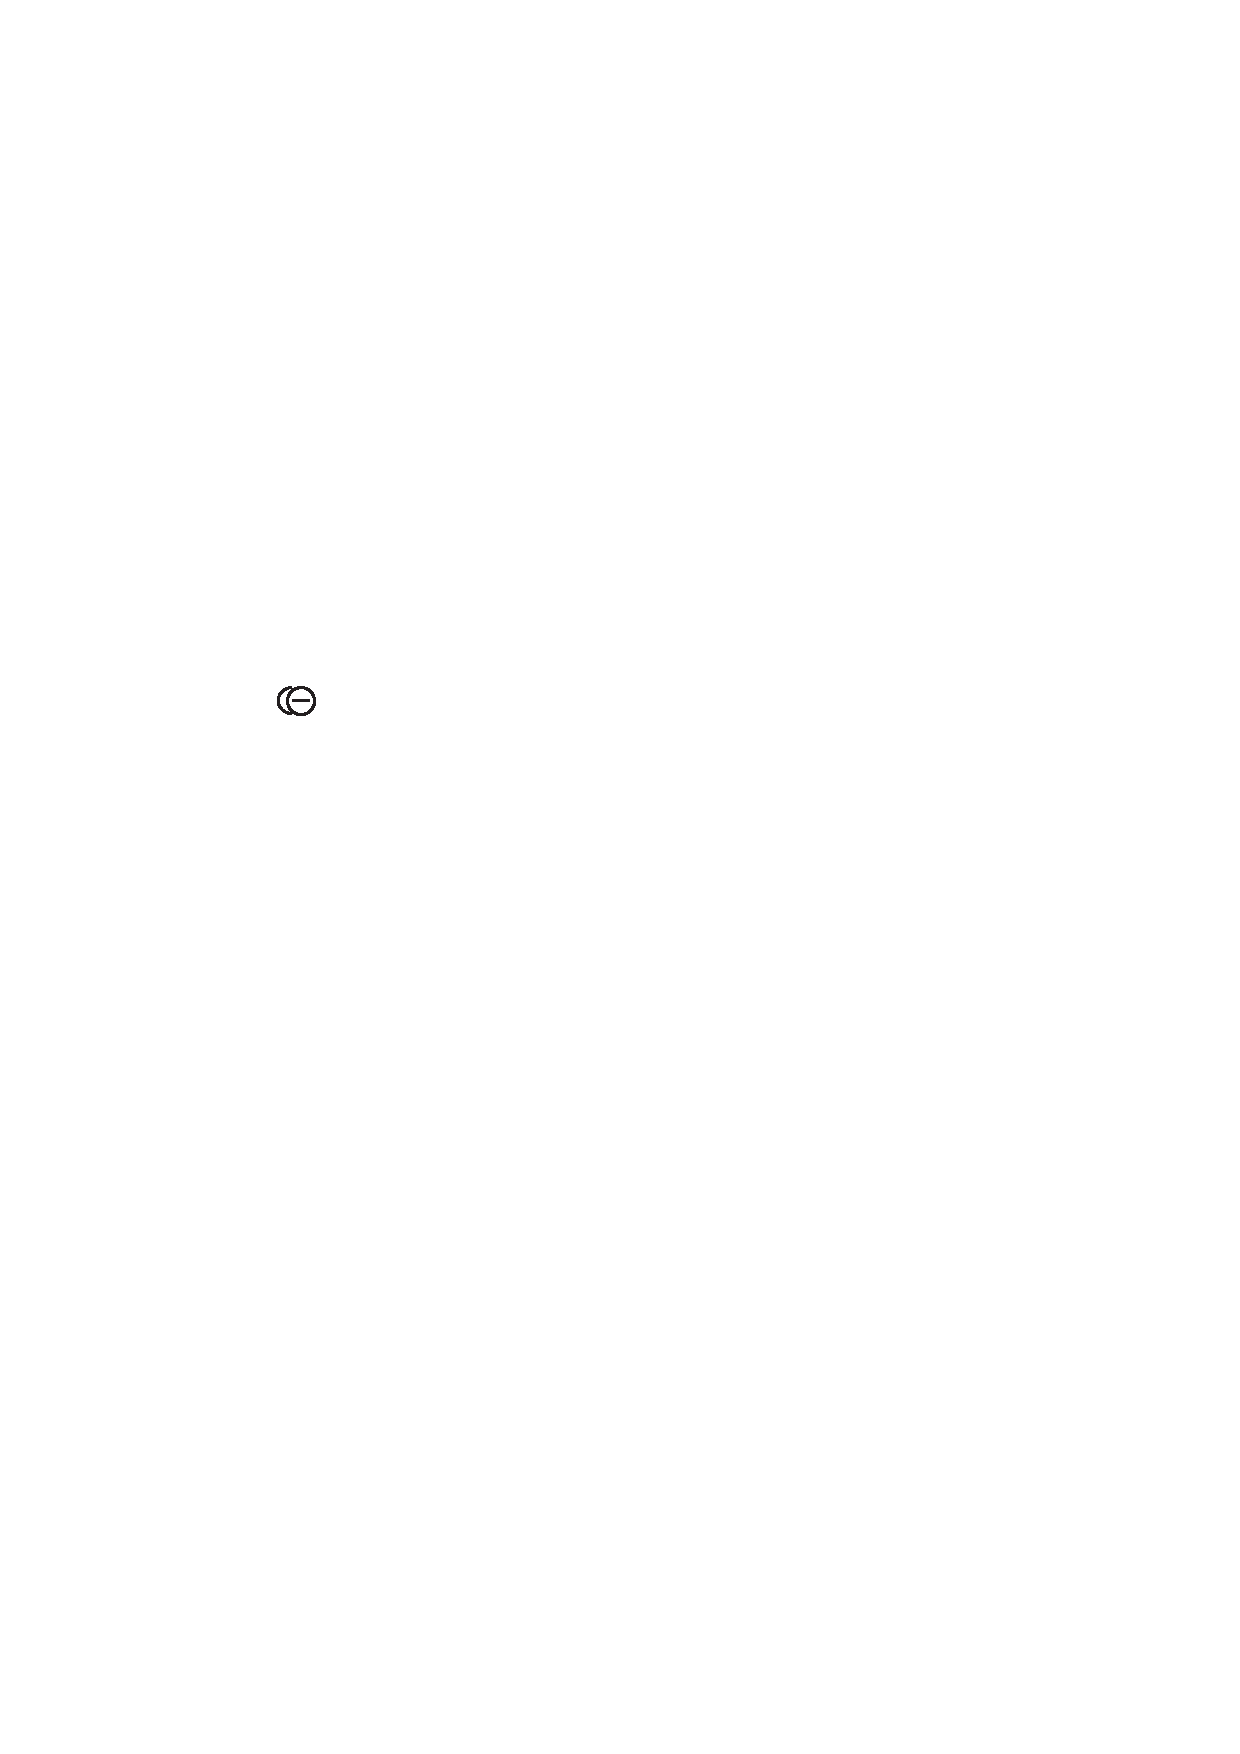
\includegraphics[width=1.75\@tempdima,height=1.5\@tempdimb]{images/hccms.pdf}
}
\DeclareRobustCommand\phccms{%
	\settoheight{\@tempdimb}{$b$}% 
	$\raisebox{-0.25\@tempdimb}[0pt][8pt]{\hccms}\!$
}

% half-circle circle plus
\newcommand*\hccps{%
   	\settowidth{\@tempdima}{$m$}% 
   	\settoheight{\@tempdimb}{$b$}% 
	\protect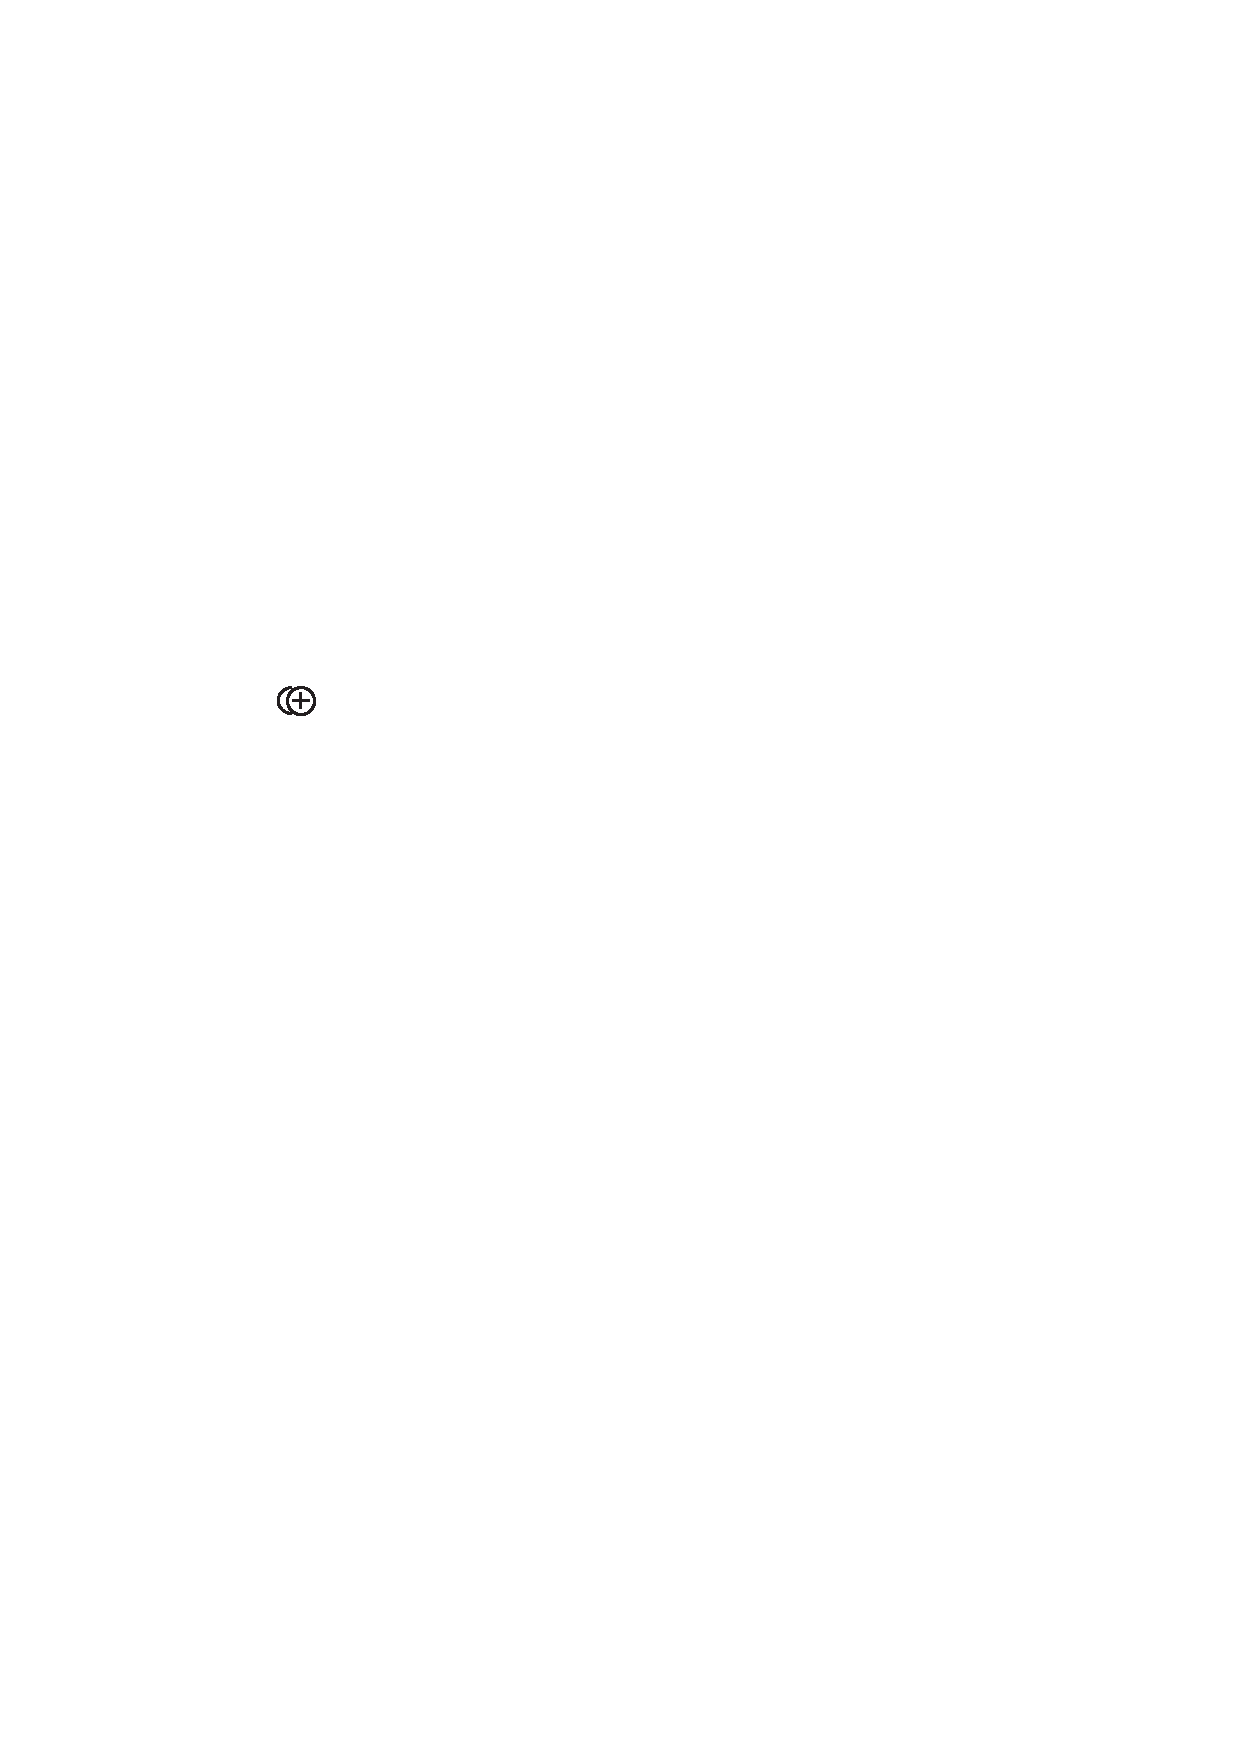
\includegraphics[width=1.75\@tempdima,height=1.5\@tempdimb]{images/hccps.pdf}
}
\DeclareRobustCommand\phccps{%
	\settoheight{\@tempdimb}{$b$}% 
	$\raisebox{-0.25\@tempdimb}[0pt][8pt]{\hccps}\!$
}




% Der Befehl \crossedcircle{x} erzeugt einen Kreis, der unten links zweimal durchgestrichen ist.

% Das Argument x erscheint innerhalb des Kreises.

% Achtung: Das funktioniert nur mit einem Argument, das aus einem einzigen Zeichen, z.B. 2 oder a, besteht.

\newcommand*\@crossedcircle{%

\settowidth{\@tempdima}{$2$}%

\settoheight{\@tempdimb}{$2$}%

\protect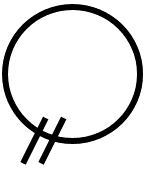
\includegraphics[width=2.4\@tempdima,height=2.2\@tempdimb]{images/circle.png}

}

\newcommand{\crossedcircle}[1]{\raisebox{-1.8mm}{\@crossedcircle}\hspace{-1.2em}#1\;\,}


\makeatother 

% K.Zeitz: Ende neue Definitionen


\def\largerthan{$\raisebox{0.8pt}{$\urcorner$} \hspace{-5.5pt}|\hspace{3pt}$} %fuer groesser als
\newcommand{\GWLypsilon}{\raisebox{2pt}{\text{\tiny{o}}}\hspace{-1pt}\upsilon}

 
% Seitenlayout
\usepackage[paperwidth=190mm, paperheight=246mm, textwidth=135mm, textheight=178mm,
  hmarginratio=2:3, tmargin=21mm, bmargin=47mm, twoside, includehead, headsep=5mm]{geometry}
\flushbottom

%Kolumnentitel: linke Druckseite zentriert Part-Titel, rechte Seite aktuelle chapter oder section
\automark[chapter]{part}
\newmarks\numbermark
\renewcommand*{\chaptermark}[1]{%
  \marks\numbermark{\chaptermarkformat}%
  \markright{#1}%
}      
\makeatletter% 
  \renewcommand*{\sectionmark}[1]{%
  \begingroup
  \@temptokena\expandafter{\sectionmarkformat}%
  \marks\numbermark{\the\@temptokena}%
  \endgroup
  \markright{#1}%
  }
\makeatother
        
\clearscrheadfoot
\ohead[\pagemark]{\pagemark}
\ihead[{\botmarks\numbermark}]{\botmarks\numbermark}
\chead[\headmark]{\headmark}   
%CH: Keine Partnummern in den automatischen Kolumnentiteln
\renewcommand*{\partmarkformat}{}
%Formatierug der Kapitelnummer im header
\renewcommand*{\chaptermarkformat}{N.\ \arabic{chapter}}
%Formatierung der Sectionnummer im header
\newcommand{\notsotiny}{\fontsize{7pt}{8pt}\selectfont}
\renewcommand*{\sectionmarkformat}{% 
  N.\ \arabic{chapter}\raisebox{-0.5ex}{\notsotiny\arabic{section}}}
\setkomafont{pagehead}{\normalfont\small}
%\setkomafont{pagehead}{\notsotiny}
\setkomafont{pagenumber}{\normalfont\normalsize}
\setheadsepline{0.4pt}
\pagestyle{scrheadings}


%erste Seiten
%erste Seite eines neuen Teils
\renewcommand*{\partpagestyle}{empty}
\renewcommand*{\partformat}{}
\setkomafont{part}{\normalfont\MakeUppercase}
%\renewcommand*{\partheadstartvskip}{\vspace*{-9.5ex}}
\renewcommand*{\partheadstartvskip}{\vspace*{-6ex}}
%CH: Part-Ueberschriften auf der neuen leeren Seite linksbuendig ausgeben
\renewcommand*{\raggedpart}{\raggedright}
 
%erste Seite eines neuen Kapitels
%Punkt immer hinter Kapitelnummer und weitere Formatspezifikationen
\renewcommand{\thechapter}{\arabic{chapter}.}
\renewcommand*{\chapterformat}{%
  \chapappifchapterprefix{\ }\thechapter\enskip}
\renewcommand*{\chapterpagestyle}{scrheadings}
\renewcommand*{\chapterheadstartvskip}{\vspace*{-5mm}}
%schnoepf2001\setkomafont{chapter}{\normalfont\normalsize\uppercase}
\setkomafont{chapter}{\normalfont\normalsize}
%\addtokomafont{chapter}{\scshape}

\renewcommand*{\chapterheadendvskip}{\vspace*{0mm}}

%erste Seite des ersten Kapitels im Part (keine Kolumnenzeile)
\newpagestyle{firstchapter}{(0pt,0pt){}{}{}(0pt,0pt)}{{}{}{}}

% section-Formatierung: Schriftgroesse, Nummerierung mit tiefgestellten Zahlen
% und weitere Formatspezifikationen
%schnoepf2001\setkomafont{section}{\normalfont\normalsize\uppercase}
\setkomafont{section}{\normalfont\normalsize}
%\addtokomafont{section}{\scshape}
\renewcommand{\thesection}{\arabic{chapter}\protect\raisebox{-0.5ex}{\notsotiny\arabic{section}}\autodot}
\renewcommand*{\othersectionlevelsformat}[1]{%
  \csname the#1\endcsname\enskip}


%Haupttext
%Zeilendurchschuss
\renewcommand{\baselinestretch}{1.1}
%Absatzueinrckung
\parindent=7.5mm
%Seitenumbruch
\frenchspacing     
%\clubpenalty=9999 % keine Schusterjungen
%\widowpenalty=9999 % keine Hurenkinder
\tolerance=1750 % Zeilenumbruch-Toleranz (ca. 500--3000)
%headerelemente
\newcommand{\link}[1]{\ref{#1}}
\renewcommand{\title}[2][]{\cite{#1}\textit{#2}}

%Zeilenzaehler
\lineation{page}
\linenummargin{outer}
\setcounter{firstlinenum}{5}
\setcounter{linenumincrement}{5}
%5 rechtsbuendig
\makeatletter
  \renewcommand{\rightlinenum}{\ifbypage@\ifnum\line@num<10\kern.5em\fi\else 
  \ifnum\line@num<10\kern1em\else\ifnum\line@num<100 \kern.5em\fi\fi\fi\kern.5em\numlabfont\the\line@num 
  \ifnum\subline@num>0:\the\subline@num\fi} 
\makeatother
%haendische Zeilenzaehler
\usepackage{marginnote}

\renewcommand{\footfudgefiddle}{71}
%Afootnotes = Marginalien written by GWL
\footnormal{A}
\setlength{\skip\Afootins}{8mm plus 3mm minus 3mm} %amount of whitespace between text and footnotes
\renewcommand{\Afootnoterule}{\noindent\rule{18mm}{0.4pt}\vspace*{3.0mm}}
\newcommand{\Afootnotefontsetup}{\normalsize}
\makeatletter
  \renewcommand{\ledsetnormalparstuff}{%
    \normal@pars
    \parindent \z@ \parfillskip \z@ \@plus 1fil \vspace{1pt}}
\makeatother
\makeatletter
\renewcommand*{\Afootfmt}[3]{%
	\normalsize
	\setstretch{1.1}
	\ledsetnormalparstuff
	\mbox{{\notenumfont\printlines#1|}\enspace
	{\select@lemmafont#1|#2}}\enskip#3\strut\par%
}
\makeatother
\count\Afootins=1200



%Kritische Apparate
%Bfootnotes = Varianten, Textgenese
\setlength{\skip\Bfootins}{5mm plus 2mm minus 2mm}
\renewcommand{\Bfootnoterule}{\rule{0mm}{0pt}\vspace*{1mm}}
\footparagraph{B}
\interparanoteglue{7.5mm plus1.9mm minus1.9mm}
\makeatletter
  \renewcommand*{\Bfootfmt}[3]{%
  \noindent
  \mbox{{\notenumfont\printlines#1|}\enspace
  {\select@lemmafont#1|#2}}\enskip#3\strut\par}
\makeatother
\count\Bfootins=1200
%
%Cfootnotes, Kommentare der Editoren
\setlength{\skip\Cfootins}{1mm plus 0mm} %KZeitz
\renewcommand{\Cfootnoterule}{\rule{\textwidth}{0.4pt}\vspace*{1mm}} 
\footparagraph{C}
\interparanoteglue{7.5mm plus 1.9mm minus 1.9mm}
\makeatletter
  \renewcommand*{\Cfootfmt}[3]{%
  \noindent
  \mbox{{\notenumfont\printlines#1|}\enspace
  {\select@lemmafont#1|#2}:}\enskip#3\strut\par}
\makeatother
\count\Cfootins=1200
%commands for bibliographical data in Cfootnotes
\newcommand{\biblio}[3]{\textsc{#1}, \textit{#2}, S. #3.}
\newcommand{\biblioplus}[5]{\textsc{#1}, \textit{#2}, S. #3, (\textit{#4}, S. #5).}
%\newcommand{\biblionote}[2]{\Cfootnote{\textsc{#1}, \textit{#2},\ }} requires \edtext, impractical
%more space for crit apparatus
\renewcommand{\footfudgefiddle}{500}
%
%Deutsch als Standardsprache der Cfootnote		2020-01-08 MS
\let\origCfootnote\Cfootnote	
\renewcommand\Cfootnote[1]%
{\origCfootnote{%
\foreignlanguage{ngerman}{%		% S. Dokumentation von reledmac unter "Xwrapcontent"
#1}%
}}


% Ausgabe einer Zeilenreferenz mit 'f', sofern sich die Fussnote auf genau zwei 
% aufeinanderfolgende Zeilen bezieht.
% K. Zeitz: Zusätzliche Ergänzung: Möglichkeit, die Zeilenreferenz in der Fußnote mit Hilfe des unten
% definierten Befehls \killnumber ganz zu unterdrücken.
\makeatletter
\def\printlines#1|#2|#3|#4|#5|#6|#7|{%					
	\begingroup
		\setprintlines{#1}{#2}{#3}{#4}{#5}{#6}%
			\ifnum #1=#4
				\ifnum #2<#5
					\newcount\endlinenumber
					\endlinenumber = #5
					\advance\endlinenumber by -1
					\ifnum #2<\endlinenumber 
						#2\endashchar#5\else #2f\fullstop
					\fi       
				\fi 
				\ifnum#2=-1 % K. Zeitz: Neu
					\symplinenum  \hspace*{-1.4em} % K. Zeitz: Neu 
				\else % K. Zeitz: Neu
					\ifnum #2=#5 #2 \fi
				\fi % K. Zeitz: Neu
			\fi
			\ifnum #1<#4							
			\ifl@d@pnum 
				#2\endashchar S\fullstop\ #4\fullstop
			\fi
			#5
		\fi
	\endgroup%
}
\makeatother

% K.Zeitz: Unterdrückung der Referenz auf die Zeilennummer in Fußnoten.
% Dazu den nachfolgend definierten Befehl \killnumber wie folgt einfügen:
%		\edtext{...}{\lemma{...}\killnumber\Afootnote{...}}
% Analog für \Bfootnote und \Cfootnote
\newcommand{\killnumber}{\linenum{|-1|||-1||}} 
 
% Eingrenzung von Textphänomenen im B-Apparat durch \bars{}		2020-01-08 MS
\newcommand*{\leftbar}{\textbar}			 % orientierte Befehle leftbar, rightbar für XML-Converter
\newcommand*{\rightbar}{\textbar}

\newcommand*{\bars}[1]{\leftbar#1\rightbar}
 
 
%Ueberschriften, Inhaltsverzeichnis, Indizes
%titlepages set by hand / publisher
%Inhaltsverzeichnis
%Name des Inhaltsverzeichnisses      
\addto\captionslatin{%
\def\contentsname{}}
%\maxtocdepth{section}
%\maxtocdepth{part}


% Ein durch \edlabel{LH-Nummer_n} … \edlabel{LH-Nummer_n+1} bestimmter Referenzbereich lässt sich mit dem Befehl \refpassage{LH-Nummer_n}{LH-Nummer_n+1} innerhalb von footnotes als Querverweis (Seite.Zeile-Seite.Zeile) anführen. H.S.%

\newcommand{\refpassage}[2]{%
 \xpageref{#1}\fullstop\xlineref{#1}%
 \ifnum\xpageref{#1}=\xpageref{#2}
  \ifnum\xlineref{#1}=\xlineref{#2}
  \else
   \endashchar\xlineref{#2}%
  \fi
 \else
  \endashchar\xpageref{#2}\fullstop\xlineref{#2}%
 \fi
}

\hyphenation{%			% Korrekte Worttrennung in einzelnen Fällen
aequ
be-trach-ten
be-trach-tet
Be-trach-tung
Be-trach-tun-gen
Be-trach-tungs-wei-se
Be-trach-tungs-wei-sen
Blatt-rand
Ent-ste-hung
Ent-ste-hungs-zeit
fehlt
ge-druckt
ge-druck-te
ge-druck-tem
ge-druck-ten
ge-druck-ter
ge-druck-tes
gestr
klein-ge-druckt
klein-ge-druck-te
klein-ge-druck-tem
klein-ge-druck-ten
klein-ge-druck-ter
klein-ge-druck-tes
ins-ge-samt
pa-ra-lo-gis-mi
pa-ra-lo-gis-mis
pa-ra-lo-gis-mo
pa-ra-lo-gis-mo-rum
pa-ra-lo-gis-mos
pa-ra-lo-gis-mum
pa-ra-lo-gis-mus
post-ea
pot-e-ram
pot-e-ras
pot-e-rat
pot-e-ra-mus
pot-e-ra-tis
pot-e-rant
pot-e-rim
pot-e-ris
pot-e-rit
pot-e-ri-mus
pot-e-ri-tis
pot-e-rint
pot-e-ro
pot-es
pot-est
pot-e-stis
prae-sum-tio
prae-sum-ti-o-ne
prae-sum-ti-o-nem
prae-sum-ti-o-nes
prae-sum-ti-o-ni
prae-sum-ti-o-nis
prae-sum-ti-o-ni-bus
prae-sum-ti-o-num
quem-ad-mo-dum
qui-bus-ve
streicht
sub-qua-dru-pla
sub-qua-dru-plae
sub-qua-dru-plam
sub-qua-dru-pla-rum
sub-qua-dru-plas
sub-qua-dru-plis
vor-aus
vor-aus-sicht-lich
}

%%Textausrichtung bei fester Spaltenbreite %H.S.
%\usepackage{tabularx}
%\newcolumntype{L}[1]{>{\raggedright\arraybackslash}p{#1}} % linksbündig mit Breitenangabe
%\newcolumntype{C}[1]{>{\centering\arraybackslash}p{#1}} % zentriert mit Breitenangabe
%\newcolumntype{R}[1]{>{\raggedleft\arraybackslash}p{#1}} % rechtsbündig mit Breitenangabe
%
%


%Aufnahme der Chapter- und Sectiontitel ins Inhaltsverzeichnis unterdruecken
\newcommand*\OrigChapter[2][]{}
\let\OrigChapter\chapter
\renewcommand*{\chapter}[2][]{%
  \settocdepth{part}\OrigChapter[#1]{#2}%
  \settocdepth{section}%
  }
\newcommand*\OrigSection[2][]{}
  \let\OrigSection\section
\renewcommand*{\section}[2][]{%
  \settocdepth{part}\OrigSection[#1]{#2} %
  \settocdepth{section}%
  }

%Aufnahme der parts ins Inhaltsverzeichnis verhindern
%\newcommand*\OrigPart[2][]{}
 % \let\OrigPart\apart
%\renewcommand*{\apart}[2][]{%
 % \settocdepth{apart}\OrigPart[#1]{#2} %
 % \settocdepth{section}%
  %}
%\makeatletter
%\let\settocdepth\relax
%\newcommand{\settocdepth}[-1]{%
  %\addtocontents{toc}{\protect\setcounter{tocdepth}{#1}}}
%\makeatother
%Format des Inhaltsverzeichnisses
\tocloftpagestyle{empty}
%Kopfzeile
\makeatletter
  \renewcommand{\cftmarktoc}{%
%  \@mkboth{\scshape Inhaltsssverzeichnis}{\scshape Inhaltsverzeichnis}}
  \@mkboth{\scriptsize\uppercase{Inhaltsverzeichnis}}{\scriptsize\uppercase{Inhaltsverzeichnis}}}
  \renewcommand*{\l@part}{\@dottedtocline{-1}{0mm}{0mm}}
 % \renewcommand*{\l@chapter}{\@dottedtocline{0}{2mm}{6mm}}
  \renewcommand*{\l@chapter}{\@dottedtocline{0}{2mm}{6mm}}
 %   \setlength{\cftsecnumwidth}{35mm}
  \renewcommand*{\l@section}{\@dottedtocline{1}{8mm}{7mm}}
  \renewcommand{\@pnumwidth}{9mm}
\renewcommand{\@tocrmarg}{9.5mm}
  \renewcommand{\@dotsep}{4.5}
\makeatother



%Bibliografie
%Keine Ueberschrift fuer die Bibliografie
\addto\captionslatin{\def\bibname{\ \vspace{1.6ex}}}

% Werke in der Bibliographie werden mit '1., 2.' durchnummeriert
%\cite-Befehl gibt nichts aus
\makeatletter
  \renewcommand{\@biblabel}[1]{#1.}
  \renewcommand*{\@cite}[2]{{#1\if@tempswa , #2\fi}}
\makeatother
        
%\cite-Befehl gibt nichts aus
\makeatletter
  \def\@citex[#1]#2{\leavevmode
  \let\@citea\@empty
  \@cite{\@for\@citeb:=#2\do
  {\@citea\def\@citea{,\penalty\@m\ }%
  \edef\@citeb{\expandafter\@firstofone\@citeb\@empty}%
  \if@filesw\immediate\write\@auxout{\string\citation{\@citeb}}\fi
  }}{#1}}
\makeatother

%Folgende Zeilen werden auskommentiert, wenn eine vorläufige Bibliografie als Bearbeitungshilfe kompiliert werden soll:
\usepackage{nohyperref}
\usepackage[pageref,verbose]{backref}
\renewcommand*{\backref}[1]{}
\renewcommand*{\backrefalt}[4]{%
    \ifcase #1 (Not cited.)%
    \or        {\it S. ~#2}%
    \else     {\it S. ~#2}%
    \fi}
\renewcommand*{\backreftwosep}{\backrefsep}
\renewcommand*{\backreflastsep}{\backrefsep}

       
%Indices
\makeindex{Namensregister}
\makeindex{Sachverzeichnis}
\makeindex{Ortsregister}
%Index zweispaltig, mit 'Praeambel'
\makeatletter

 % \renewcommand{\see}[2]{{\em s.\/a.\/} #1}
   \renewcommand{\see}[2]{\newline{\em s.\/a.\/} #1}
  \renewcommand\printindex[2]{
  \clearpage{\pagestyle{empty}\cleardoublepage}
  \setchapterpreamble{\index@preamble}
  \addchap*{\hfill #2\hfill}
  \thispagestyle{empty}
  \clearscrheadings
  \chead{\sc{#2}}
  \ohead[\pagemark]{\pagemark}
  \begin{multicols}{2}\setlength{\columnseprule}{0.4pt}
  \footnotesize\raggedright
  \@input{#1.ind}
  \end{multicols}}
  \renewcommand*\@idxitem{\par\hangindent 11\p@}
 % \renewcommand*\subitem{\@idxitem \hspace*{11\p@}}
  \renewcommand*\subitem{\@idxitem \par\hangindent 22\p@ \hspace*{11\p@}}
  %\renewcommand*\@idxsubitem{\@idxsubitem \hspace*{11\p@}}
\makeatother
\newcommand\efrac[2]{\genfrac{}{}{0pt}{}{#1}{#2}} %KZeitz \efrac produziert einen Bruch ohne Bruchstrich


% Reduzierung der Sperrung von \testso von 0,25 auf 0,1
\makeatletter
\sodef\textso{}{.1em}{.65em\@plus.08em\@minus.06em}{.55em\@plus.275em\@minus.183em}
\makeatother



% Für dynamische Referenzierung der Stücknummern (N.) mittels /ref und Zitation der Nummer ohne darauf folgenden Punkt
\makeatletter
 \def\@nodotref\csname thechapter\endcsname{\arabic{chapter}}% ?? entfernt
 \renewcommand{\p@chapter}{\@nodotref}
\makeatother

\makeatletter
 \def\@nodotsubref\csname thesection\endcsname{\arabic{chapter}\textsubscript{\arabic{section}}}%	% ?? entfernt
 \renewcommand{\p@section}{\@nodotsubref}
\makeatother




%neuer Vorspann
\begin{document}



%Titelseite
        \begin{titlepage}
        \begin{center}
        \pagenumbering{Roman}
        {\huge GOTTFRIED WILHELM}\\
        \vspace*{7.5mm}
        {\Huge LEIBNIZ}\\
        \vspace*{10.5mm}
        {\Large SAEMTLICHE\\
        SCHRIFTEN UND BRIEFE}\\
        \vspace*{13mm}
        {\large HERAUSGEGEBEN\\
        VON DER}\\
        \vspace*{5.5mm}
        {\Large BERLIN-BRANDENBURGISCHEN\\
        AKADEMIE DER WISSENSCHAFTEN}\\
        {\large UND DER}\\
        {\Large AKADEMIE DER WISSENSCHAFTEN\\
        IN GOETTINGEN\\
        \vspace*{15mm}
        ACHTE REIHE}\\
        {\large NATURWISSENSCHAFTLICHE, TECHNISCHE UND MEDIZINISCHE SCHRIFTEN}\\
        \vspace*{4.5mm}
        {\Large DRITTER BAND}\\
        \vspace{3mm}
         {\Large Mechanik 1}\\
         \vspace{2mm}
        {\Large Akustik, Elastizität, Festigkeit, Stoß}\\
	\vspace{2mm}
	{\Large(1671\ \textendash\ 1705)}
       % {\Large\textit{Korrekturvorlage}}\\
        %\vspace*{3mm}
      %  \large{Umfang und Bearbeitungszustand entsprechen nicht dem fertigen Band.}\\ %KZeitz
        \end{center}
        \end{titlepage}
%Titelseite_Ende




\pagenumbering{Roman}
%\beginnumbering

\newpage
\newpage


\setcounter{page}{4}
\clearpage{\pagestyle{empty}\cleardoublepage}
%CH \part und \addpart* geaendert, damit Ueberschrift keine Nummer und nicht ins Inhaltsverzeichnis
\addpart[\large\uppercase{Inhaltsverzeichnis}]{\large\protect\textso{INHALTSVERZEICHNIS}} 


\clearpage{\pagestyle{empty}\cleardoublepage}
   \tableofcontents


\clearpage{\pagestyle{empty}\cleardoublepage}
\addtocontents{toc}{\vspace{5mm}}
\addpart[\large\uppercase{Vorwort}]{\large\protect\textso{VORWORT}}
\clearpage{\pagestyle{empty}\cleardoublepage}
\markleft{\scriptsize\uppercase{Vorwort}}
   \selectlanguage{german}
\thispagestyle{empty}
{\vrule height 0mm depth 30mm width 0mm}
\vspace*{2em}
\par\noindent 
Die Reihe VIII der Leibniz-Edition ist ein durch das Akademienprogramm gefördertes Langzeitvorhaben der Berlin-Brandenburgischen Akademie der Wissenschaften. Die Reihe VIII wird an der für sie gegründeten Editionsstelle Leibniz-Edition Berlin seit 2001 bearbeitet und  ist auf 12 Bände geplant. Neben den bereits erschienenen ersten beiden Bänden mit Schriften aus der Pariser Zeit (1672\textendash1676) werden in dem hier nun vorliegenden dritten Band wie in den noch folgenden Bänden alle übrigen Schriften, die der Nachlass überliefert oder Leibniz noch selbst veröffentlicht hat, geordnet nach Teilbereichen \textendash\ Naturwissenschaften (Bde 3 bis 8), Medizin (Bde 9, 10), Technik (Bde 11, 12)\ \textendash\  ediert, wobei die Mechanik voraussichtlich fünf Bände der naturwissenschaftlichen Schriften umfassen wird. Grundlage dieser Reihenplanung war eine 2013/2014 durchgeführte Nachkatalogisierung, die darin bestand, die Handschriftenbestände des Leibniz-Archivs, die für eine Aufnahme in Reihe VIII vorgesehen waren, vollständig zu sichten.
\\ \indent
Wir danken dem Bundesministerium für Bildung und Forschung sowie dem Regierenden Bürgermeister von Berlin, Senatskanzlei für Wissenschaft und Forschung, für die Finanzierung des Vorhabens. Arbeitsgrundlage der Berliner Editionsstelle sind die Digitalisate der in Reihe VIII zu edierenden Handschriften. Sie sind dank der umfassenden Finanzierung seitens der Deutschen Forschungsgemeinschaft in hochauflösender Qualität angefertigt worden und werden freundlicherweise von der Gottfried Wilhelm Leibniz Bibliothek Hannover (Niedersächsische Landesbibliothek) zur Verfügung gestellt. Dank der großzügigen Finanzierung sowohl durch die Alfried Krupp von Bohlen und Halbach-Stiftung als auch durch die Stiftung der Versicherungsgruppe Hannover sind die Digitalisate online zugänglich (http://ritter.bbaw.de). 
\\ \indent
Der Gottfried Wilhelm Leibniz Bibliothek Hannover danken wir für ihre Unterstützung, insbesondere dem Leiter der Abteilung Handschriften, Matthias Wehry, sowie Anja Fleck, die uns mit Reproduktionen und Durchlichtscans aus dem Leibniz-Archiv umfangreich versorgte.
Seitens der Leibniz-Forschungsstelle Hannover haben wir vielfach Unterstützung erfahren: Nora Gädeke, Charlotte Wahl und Siegmund Probst verdanken wir zahlreiche wertvolle Hinweise auf Handschriften, Schreiberhände, auf Literatur, die Leibniz benutzt haben könnte, sowie zu Fragen der Datierung.
Sehr dankbar sind wir den Editionsstellen in Münster und Potsdam, die uns dabei halfen, Wasserzeichen in Textträgern von Schriften, die im vorliegenden Band ediert sind, zu bestimmen, um sie näher datieren zu können. Stephan Meier-Oeser überließ der Arbeitsstelle eine Kopie der Münsteraner Wasserzeichendatenbank und unterwies uns in deren Benutzung. Stephan Waldhoff unterstützte uns in der Benutzung der Potsdamer Wasserzeichensammlung, identifizierte eigens Wasserzeichen sowie Schreiberhände und half überdies bei der Klärung von Datierungsfragen.
\\ \indent
Ein besonderer Dank geht an Laurynas Adomaitis, der so großzügig seine Forschungserbnisse mit uns teilte: Auf seinen Beobachtungen und der von ihm vorgeschlagenen Lösung (\glqq Flip theory\grqq) beruht weitestgehend die Textfolge der Scheda secundo-secunda (N.~\ref{dcc_02-2}), wie sie in vorliegendem Band als Unterstück des Komplexes \textit{De corporum concursu} (N.~\ref{dcc_00}) konstituiert worden ist. Wir danken Valérie Debuiche für Hinweise, die sie uns bezüglich der im ersten Band erschienen Stücken zur Perspektive zukommen ließ. 
Zu großem Dank sind wir Walter Bühler verpflichtet, der uns zur frühneuzeitlichen Literatur sowie zur Geschichte der Musiktheorie und physikalischen Akustik viele wichtige Hinweise gab und uns großzügig weit mehr an Informationen zu den hier edierten Stücken zur Akustik lieferte, insbesondere zu den Jungius-Auszügen (N.~\ref{38541}), als wir aus Rücksicht auf die Richtlinien der Edition in den Erläuterungen aufnehmen konnten.\\ \indent
Unserer studentischen Mitarbeiterin Pauline Just sind wir sehr dankbar: Sie erstellte für die Stücke des vorliegenden Bandes eine Datierungsmappe, in der die datierungsrelevanten Informationen gesammelt wurden, identifizierte und dokumentierte Wasserzeichen für diesen wie den nächsten Band und trug in vielerlei Hinsicht zum Bearbeitungsfortschritt des Vorhabens bei.  
%Gebündelt, weiter gewonnen und dokumentiert wurden Informationen über Wasserzeichen und Datierungsgründe durch unsere studentische Mitarbeiterin, Pauline Just, die für die Stücke des vorliegenden Bandes eine Datierungsmappe erstellte und in vielerlei Hinsicht an dem Bearbeitungsfortschritt des Vorhabens teil hatte, wofür wir sehr dankbar sind. 
Wir danken Gunthild Peters (geb. Storeck), die im Rahmen eines Werkvertrages Nachzeichnungen von Diagrammen anfertigte und Vorarbeiten zur Kollation von N.~\ref{ddrs_06} lieferte. 
Christoph Sander danken wir, dass er die Möglichkeiten seines Werkvertrags intensiv nutzte, um die von Leibniz zitierte Literatur zu bibliographieren und weitere Anspielungen aufzulösen und mit Stellennachweisen zu belegen.
\\ \indent
Wie schon beim zweiten Band meisterte Katharina Zeitz in unermüdlichem Einsatz auch die setzerischen Herausforderungen für den allergrößten Teil des vorliegenden Bandes. Ihr ist es wieder zu verdanken, dass zahlreiche Probleme des Layouts in \LaTeX\ gelöst werden konnten. 
Wir danken Serena Pirrotta und Christoph Schirmer vom De Gruyter Verlag für die gute Zusammenarbeit.
%%%%%%%%%%%%%%%
\par
\vspace{1em}
Berlin, im Dezember 2020\hspace{65mm}Harald Siebert
%
%



\clearpage{\pagestyle{empty}\cleardoublepage}
\addtocontents{toc}{\vspace{5mm}}
\addpart[\large\uppercase{Einleitung}]{\large\protect\textso{EINLEITUNG}}
\clearpage{\pagestyle{empty}\cleardoublepage}
\markleft{\scriptsize\uppercase{Einleitung}}
\markright{\scriptsize\uppercase{Einleitung}}
    %\thispagestyle{empty}
\selectlanguage{german}
%{\vrule height 0mm depth 30mm width 0mm}
%\newpage
%\noindent
\thispagestyle{empty}
{\vrule height 0mm depth 30mm width 0mm}
%\par
%\noindent
\vspace*{2em}
\par\noindent 
% 1. Band und Arbeitsstelle
% 2. Band und Reihenplanung -- 
% 3. Band und Stükcke --- Stücke des Bandes
%
%
%\par\vspace{6.0ex}
%\noindent
%\noindent\uppercase{Themen des Bandes}
%\par
%\vspace{1.0ex}
%\noindent

%%%%%%%%%%%%%%%%%%%%%%%%%%%%%%%%%%%%%%%%%%%%%%%%%%%
%Anfang: Band und Arbeitsstelle. Band 3 in der 
%\par\vspace{6.0ex}
%\noindent
\noindent\uppercase{Der dritte Band und die \textit{Leibniz Edition Berlin}}
\par
\vspace{1.0ex}
\noindent
\par\noindent
Schon wenige Jahre nach Gründung der Berliner Editionsstelle (2001) wurde für die Reihe VIII als Teilprojekt der Leibniz-Edition eine erste Laufzeit im Akademienprogramm bewilligt. Sie sah einen Abschluss des dritten Bandes bis zum Jahre 2020 vor und knüpfte daran die Möglichkeit einer Verlängerung des Vorhabens über diese Zeit hinaus. 
Der nun vorliegende dritte Band vereint erstmals Schriften, die Leibniz nach Paris verfasst hat. 
Das hierfür zu edierende Material war ungleich weniger erschlossen und hinsichtlich des größeren Zeitraums weit schwieriger zu datieren sowie angesichts von Leibnizens eigener Entwicklung um vieles anspruchsvoller als alles, was an Inhalten und deren Behandlung die Bände davor zu bieten hatten. Allen Herausforderungen zum Trotz erfüllt die Editionsstelle mit vorliegendem Band das Ziel, das für die erste Laufzeit bis 2020 gesetzt war, und kann im Anschluss daran nach der mittlerweile bewilligten Verlängerung des Vorhabens die weiteren Bände der Reihe bearbeiten.  
%\\ \indent
%Aber nicht alle Stücke, die ursprünglich für diesen Band vorgesehen und im PDF der digitalen Vorausedition vom 30. Oktober 2020 schon zu sehen waren, haben es schlussendlich in die Fassung von \textit{LSB}~VIII,\,3 geschafft, wie sie bis Jahresende 2020 finalisiert und dem Verlag zum Druck übergeben werden konnte.  
%Ende: Band und Arbeitsstelle
%%%%%%%%%%%%%%%%%%%%%%%%%%%%%%%%%%%%%%%%%%%%%%%%%%%
%
\par\noindent
%
%%%%%%%%%%%%%%%%%%%%%%%%%%%%%%%%%%%%%%%%%%%%%%%%%%%
%Anfang: Band und Reihenplanung. Band 3 in der Reihen- und Bändeplanung
\par\noindent 
%Rückreise
%Datumsangabe
\par\vspace{6.0ex}
\noindent
\noindent\uppercase{Der dritte Band in der Reihenplanung}
\par
\vspace{1.0ex}
\noindent
Leibnizens Abschied aus Paris liefert eine Zäsur für die Reihenplanung, an der die chronologische Ordnung von einer inhaltlichen abgelöst wird. Die bereits erschienenen Bände~1 und 2 der Reihe enthalten diejenigen Schriften, von denen als sicher gelten durfte, dass Leibniz sie während seines Aufenthalts in Paris (1672\textendash1676) oder davor abgefasst hatte. 
%Datierung als Problem, datierte undatierte
Die weiteren Bände der Reihe sind für die Schriften bestimmt, die in der Zeit nach Paris entstanden sind oder entstanden sein könnten. 
Für ihre Planung ist das Prinzip einer chronologischen Anordnung nicht haltbar, weil sie ganz überwiegend undatiert überliefert sind und für die zu erschließende Datierung der viel größere Zeitraum von Ende 1676 bis zu Leibnizens Tod in Frage kommt. 
%Anders als die beiden ersten Bände der Reihe folgen alle weiteren nicht einer chronologischen Ordnung über die Bände hinweg.
%Dieses Prinzip der Reihenplanung ist für die nach Paris entstandenen Schriften nicht mehr haltbar, weil sie ganz überwiegend undatiert überliefert sind und für die dafür zu erschließende Datierung der viel größere Zeitraum von Ende 1676 bis zu Leibnizens Tod in Frage kommt. 
Datierungen zu erschließen, ist ein Ergebnis der Forschung, die Hand in Hand mit der Aufnahme und Edition der Stücke erfolgt und nicht getrennt davon oder im Vorfeld erbracht werden kann, ohne den auf Bände kalkulierten Bearbeitungsfortschritt und Veröffentlichungsplan des Vorhabens aufzugeben. 
Daher folgt die Reihenplanung für die Bände drei bis zwölf dem Prinzip der Modularisierung, d.h. einer Edition des Materials nach Teilbereichen (naturwissenschaftliche, medizinische, technische Schriften) und Themen. Das größte Modul bildet dabei die Mechanik, die allein fünf Teile bzw. Bände der naturwissenschaftlichen Schriften umfassen wird und deren erster Teil mit vorliegendem Band ediert wird. Eine chronologische Ordnung der Schriften gilt hier wie in allen weiteren Bänden der Reihe nur noch innerhalb eines Bandes in den Rubriken und Unterrubriken, die darin für die verschiedenen Themen gebildet werden. Zeiträume, die im Titel der Bände in Klammern mit angeführt werden, liefern für die Bändeplanung kein Kriterium, sondern vermerken lediglich die Spanne der für die Stücke des jeweiligen Bandes erschlossenen Datierungen. 
%%% möglich auf für Abschnitt 3
%Für den vorliegenden Band erstreckt sich diese Spanne der erschlossenen Datierungen von 1671 bis 1705 und reicht damit noch bis in die Pariser Zeit und davor zurück. Dies erklärt sich daraus, dass bei einigen Stücken ein so früher Zeitraum nicht auszuschließen ist, sich ihre Entstehung aber auch nicht sicher darauf eingrenzen lässt (N.~\ref{38535}, N.~\ref{58290},N.~\ref{41165}, N.~\ref{60273}, N.~\ref{60060}, N.~\ref{RK60070}, N.~\ref{RK60127}). Zwei weitere Stücke, bei denen dies möglich ist und deren Abfassung noch in Paris oder davor als sicher gelten darf, erscheinen als Nachträge (N.~\ref{RK39624}, N.~\ref{RK55793}); sie bleiben für die im Bandtitel angeführte Datierungsspanne unberücksichtigt. 
%%%%? Abschnitt 3
%%%%%%%%
%hier weiter
\\ \indent
Grundlage dieser modularisierten Reihenplanung bilden diejenigen Handschriftenbestände, die bei Gründung der Editionsstelle für eine Aufnahme in Reihe VIII ausgewählt worden waren und deren genauere Überprüfung in den Jahren 2013/2014 durchgeführt wurde. Für diese sogenannte Nachkatalogisierung stand nur ein Zeitraum von zwölf Monaten zur Verfügung, in dem neben einer geringen Zahl an Drucken mehr als 9.300 Handschriftenseiten zu sichten waren, die der Arbeitsstelle seit ihrer Gründung in Form hochauflösender Scans zur Verfügung standen. Dabei kamen allein 688 Stücke zu Tage, die im Arbeitskatalog der Leibniz-Edition (\glqq Ritter-Katalog\grqq) bis dahin unbekannt waren und schließlich eine Anpassung der Reihenplanung von acht auf zwölf Bände nach sich zogen. 
Allerdings erlaubte die Nachkatalogisierung es nicht, die Handschriften inhaltlich weiter zu erschließen, als es zu Zwecken der Reihenplanung erforderlich war, die darauf abzielte, die Stücke nach den Teilbereichen der Reihe und darin nach Themen zu ordnen. Für eine tiefergehende Erfassung war die Zeit im Verhältnis zum Umfang des zu sichtenden Materials schlicht zu kurz. 
Allein daher darf fest damit gerechnet werden, dass sich mit fortschreitender Bearbeitung der Reihe die Erkenntnisse über den Nachlass erweitern. Der Inhalt einzelner Stücke erschließt sich zunehmend, wenn Handschriften im Zuge der Bandbearbeitung aufgenommen werden. Dabei wird es nicht ausbleiben, mitunter erst dann erkennen zu können, dass Stücke thematisch ganz oder teilweise  zu Rubriken gehören, die bereits in einem früheren Band bearbeitet worden sind. 
Mit diesem unvermeidlichen Umstand, dass die Erforschung des Nachlasses auf dem Fortschritt der Edition beruht und davon nicht zu trennen ist, wird die Reihe VIII pragmatisch umgehen: Bleibt die Zahl der nachträglich einer bereits bearbeiteten Rubrik zuzuordnenden Stücke gering, werden diese als Nachträge zu einem früheren Band ediert, ist deren Zahl größer, erfährt eine bereits einmal bearbeitete Rubrik eine Fortsetzung in einem späteren Band. 
\\ \indent
Zur Rubrik Stoß, die aufgrund der Laufzeitvorgabe, die für diesen dritten Band und die Editionsstelle verpflichtend war, nicht mehr alle vorbereiteten Stücke aufnehmen konnte, wird es auf jeden Fall eine Fortsetzung im zweiten Teil der Mechanik (Bd VIII,\,4) geben.
%Sollten Stücke, die für den vierten Band vorgesehen sind, nach genauerer Kenntnis doch Stoßphänomene behandeln, werden sie ihren Platz in der aus Band drei fortgesetzten Rubrik Stoß des vierten Bandes bzw. zweiten Teils der Mechanik finden. 
Dass Erkenntnisse über das zu edierende und überwiegend unveröffentlichte Material nur sukzessive zu erlangen sind, liegt in der Natur der Sache: Ein riesiger Nachlass, der erst durch die Edition erschlossen wird. 
Kompensieren wird man diese vom Bearbeitungsfortschritt abhängige und nach Bänden getrennte Präsentation der Editions- und Forschungsergebnisse im Nachhinein einmal, wenn die Metadaten dazu digital erfasst werden, so dass sich die Stücke dann beliebig nach thematischen, chronologischen und anderen Zusammenhängen anordnen und in Beziehung setzen lassen.
%schwierigkeiten der datierung; Nachkatalogisierung, inhaltliche erschließung
%hier weiter
%Ende: Band und Reihenplanung
%%%%%%%%%%%%%%%%%%%%%%%%%%%%%%%%%%%%%%%%%%%%%%%%%%%
\par\noindent 
%Rückreise
%Datumsangabe
\par\vspace{6.5ex}
\noindent
\noindent\uppercase{Die Stücke im dritten Band}
\par
\vspace{1.0ex}
\noindent
%
%%%%%%%%%%%%%%%%%%%%%%%%%%%%%%%%%%%%%%%%%%%%%%%%%%%
%Anfang: Band und Stücke --- Stücke des Bandes
\noindent Der vorliegende dritte Band der naturwissenschaftlichen, medizinischen und technischen Schriften vereint 79 Stücke aus den Gebieten Akustik, Elastizität, Festigkeit und Stoß und liefert damit den ersten Teil der voraussichtlich fünf Bände umfassenden Schriften zur Mechanik. Zwölf der im Band nummerierten Stücke (N.~\ref{41152_0}, N.~\ref{cnds_0}, N.~\ref{ddrs_00}, N.~\ref{visel_0}, N.~\ref{58256_0}, N.~\ref{adva_0}, N.~\ref{rie}, N.~\ref{RK57267-2+60343}, N.~\ref{ratio_cel}, N.~\ref{dcc_00}, N.~\ref{comp_non_fidendum}, N.~\ref{Parent_intro}) gliedern sich insgesamt in 51 Unterstücke, so dass \textit{LSB}~VIII,\,3 mit 118 Einzelstücken vorliegt, die zusammen 421 Nachzeichnungen von Diagrammen und Abbildungen enthalten, von denen drei zusätzlich in Reproduktion der handschriftlichen Vorlage (Faksimile) wiedergegeben werden (N.~\ref{41152_4}, N.~\ref{38540}, N.~\ref{ddrs_06}). 
\\ \indent 
Unter den Schriften des Bandes bilden diejenigen zu den Gebieten Akustik, Elastizität und Festigkeit eine zusammenhängende und chronologisch geordnete Rubrik mit 33 Stücken (N.~\ref{38535} bis N.~\ref{60029} bestehend aus 55 Einzelstücken). Der Grund hierfür ist, dass eine strenge Trennung zwischen diesen Gebieten auf Grundlage der edierten Schriften kaum möglich ist; unscharf getrennt lassen sich aus dieser gemeinsamen Rubrik 20 Einzelstücke eher der Akustik (%
N.~\ref{38535},
N.~\ref{58290},
N.~\ref{41152_1},
N.~\ref{41152_2},
N.~\ref{41152_3},
N.~\ref{41152_4},
N.~\ref{41152_5},
N.~\ref{41152_6},
N.~\ref{41153},
N.~\ref{41156},
N.~\ref{38540},
N.~\ref{cnds_1},
N.~\ref{cnds_2},
N.~\ref{cnds_3},
N.~\ref{cnds_4},
N.~\ref{cnds_5},
N.~\ref{38541},
N.~\ref{58233},
N.~\ref{RK60353},
N.~\ref{RK60301}%
),
23 Einzelstücke der Elastizität (%
N.~\ref{41165},
N.~\ref{60273},
N.~\ref{60241},
N.~\ref{60338},
N.~\ref{41157},
N.~\ref{ddrs_03},
N.~\ref{ddrs_07},
N.~\ref{60649},
N.~\ref{60651},
N.~\ref{38538},
N.~\ref{41178},
N.~\ref{41160},
N.~\ref{60334},
N.~\ref{60071},
N.~\ref{55749},
N.~\ref{visel_1},
N.~\ref{visel_2},
N.~\ref{58256_1},
N.~\ref{58256_2},
N.~\ref{58242},
N.~\ref{adva_1},
N.~\ref{adva_2},
N.~\ref{60029}%
),
und zwölf Einzelstücke der Festigkeit (%
N.~\ref{ddrs_01},
N.~\ref{ddrs_02},
N.~\ref{ddrs_04},
N.~\ref{ddrs_05},
N.~\ref{ddrs_06},
N.~\ref{ddrs_08},
N.~\ref{ddrs_09},
N.~\ref{ddrs_10},
N.~\ref{60239},
N.~\ref{60650},
N.~\ref{41174},
N.~\ref{60653}%
) zuordnen; die Rubrik Stoß umfasst mit zwei Unterrubriken (II.A. Notizen, Konzepte, Aufzeichnungen; II.B. Auszüge, Rezensionen) insgesamt 44 Stücke (N.~\ref{60060} bis N.~\ref{RK61042} bestehend aus 61 Einzelstücken); als Nachträge zu den beiden ersten Bänden der Reihe erscheinen zwei Stücke (N.~\ref{RK39624}, N.~\ref{RK55793}).
\\ \indent
Von diesen 118 Einzelstücken des vorliegenden Bandes sind 29 eigenhändig von Leibniz datiert (%
N.~\ref{41152_1},
N.~\ref{41152_2},
N.~\ref{41152_3},
N.~\ref{41152_4},
N.~\ref{41152_5},
N.~\ref{41152_6},
%N.~\ref{ddrs_05}, nicht eigh. !
N.~\ref{55749},
N.~\ref{visel_1},
N.~\ref{visel_2},
N.~\ref{57266_1},
N.~\ref{57267_1},
N.~\ref{57268},
N.~\ref{57269},
N.~\ref{57270},
N.~\ref{57271},
N.~\ref{57279},
N.~\ref{dcc_01},
N.~\ref{dcc_02-1},
N.~\ref{dcc_02-2},
N.~\ref{dcc_03},
N.~\ref{dcc_04},
N.~\ref{dcc_05},
N.~\ref{dcc_06-1},
N.~\ref{dcc_06-2},
N.~\ref{dcc_07},
N.~\ref{dcc_08},
N.~\ref{dcc_09},
N.~\ref{dcc_10},
N.~\ref{41206});
bei den dreien als Druck überlieferten Stücken liefert das Veröffentlichungsdatum einen sicheren Anhaltspunkt für die Datierung (N.~\ref{ddrs_06}, N.~\ref{ddrs_10}, N.~\ref{RK61042}). Bei den übrigen 86 Einzelstücken musste die Datierung erschlossen werden (und wird neben dem Titel in eckigen Klammern angegeben). Die hierfür im Kopf der Stücke angeführten Datierungsgründe fallen je nach Schwierigkeit unterschiedlich umfangreich aus (was wiederum durch Fragezeichen in den erschlossenen Datierungen angezeigt wird). Um untere und obere Grenzen (\textit{termini post} bzw. \textit{ante quem}) der zeitlichen Entstehung zu bestimmen, werden Argumente und Indizien zusammengetragen, die sich einem immer nur begrenzten Kenntnisstand verdanken und nicht vollständig sein müssen. Oft ist es daher kaum auszuschließen, dass ein so datiertes Stück tatsächlich früher oder später entstanden sein könnte, auch wenn identifizierte Wasserzeichen in vielen Fällen geholfen haben, den Zeitraum näher einzugrenzen. Die Spannen dieser erschlossenen Datierungen reichen von maximal 174 Monaten (N.~\ref{58290}) bis zu einem Monat und betragen für alle Stücke, deren Datierung erschlossen werden musste, im Durchschnitt 27,4 Monate. Eine größere Genauigkeit als diese rund zweieinviertel Jahre wäre natürlich wünschenswert, aber die Entstehung der undatierten Stücke wird damit auf durchschnittlich weniger als sieben Prozent des Gesamtzeitraums eingegrenzt, aus dem die im Band vereinten Schriften insgesamt stammen.
%Kurioserweise haben wir ausgerechnet im Zuge der Bearbeitung der zwei umfangreichsten, datierten Blattsammlungen, ??, Zweifel bekommen, ob die von Leibniz stammende Datumsangabe die tatsächliche Genese dokumentiert und nicht eher Ausweis einer bewussten ...ist
%Datierungsspannen
Die im Titel des Bandes ausgewiesene Datierungsspanne ist etwas kürzer, reicht von 1671 bis 1705 und erstreckt sich damit bis in die Pariser Zeit und davor, die Gegenstand der ersten beiden Bände der Reihe war. Dies erklärt sich daraus, dass bei sieben Stücken des vorliegenden Bandes ein so früher Zeitraum nicht auszuschließen ist, sich deren Entstehung aber auch nicht sicher darauf eingrenzen lässt (N.~\ref{38535}, N.~\ref{58290}, N.~\ref{41165}, N.~\ref{60273}, N.~\ref{60060}, N.~\ref{RK60070}, N.~\ref{RK60127}). Zwei weitere Stücke, bei denen diese Eingrenzung möglich ist und deren Abfassung noch in Paris oder davor als sicher gelten darf, erscheinen als Nachträge (N.~\ref{RK39624}, N.~\ref{RK55793}); sie bleiben für die im Bandtitel angeführte Datierungsspanne unberücksichtigt. 
\\ \indent
Dass Leibniz Frankreich verlässt und nach Deutschland zurückkehrt, schlägt sich auch sprachlich nieder. Zwar ist nur ein einziges Stück auf Deutsch verfasst \textendash\ eine Notiz zur Festigkeitslehre (N.~\ref{55749}) \textendash, aber die Verwendung des Französischen geht, soweit sich an den hier edierten Schriften ablesen lässt, deutlich zurück.
Von den 115 Einzelstücken (ohne Nachträge und ohne N.~\ref{60653}, das nur aus Zeichnungen besteht) sind fünf teilweise oder ganz auf Französisch geschrieben (%
N.~\ref{41160} tlw.,
N.~\ref{57267_2},
N.~\ref{52278} tlw.,
N.~\ref{RK42448},
N.~\ref{RK55822}). Bei vieren handelt es sich um Auszüge aus französischsprachigen Veröffentlichungen, aus denen Leibniz den französischen Text zitierend oder paraphrasierend übernimmt und in derselben Sprache kommentiert (im Fall von N.~\ref{41160} und N.~\ref{57267_2} auf Lateinisch). Im Vergleich zu diesem sehr geringen Anteil (von rund vier Prozent) war im zweiten Band der Reihe noch ein Drittel der Stücke auf Französisch verfasst. 
Wenn sich Leibniz nach Paris mit den Themen auseinandersetzt, die Gegenstand des vorliegenden Bandes sind, denkt er, soweit sich dies aus seinem Schreiben folgern lässt, fast ausschließlich auf Lateinisch.
\\ \indent
Unter den im Band vorkommenden Textarten bzw. Textsorten sind Konzepte am häufigsten anzutreffen: Konzept ist eine weit gefasste Bezeichnung für Stücke unterschiedlicher Länge, in denen nicht einfach Unfertiges zu sehen ist, aber auch nicht unbedingt Entwürfe für geplante oder mögliche Veröffentlichungen oder Weitergaben, sondern in denen Leibniz Erkenntnisse zusammenführt, in Beziehung setzt, überprüft, Gedanken entwickelt, Untersuchungen durchführt oder Ideen nachgeht. Ingesamt 55 Einzelstücke im Band sind Konzepte (%
N.~\ref{60273},
N.~\ref{41153},
N.~\ref{cnds_1},
N.~\ref{cnds_2},
%N.~\ref{cnds_3}, nicht Konzept, sondern Reinschrift
N.~\ref{ddrs_01},
N.~\ref{ddrs_02},
N.~\ref{ddrs_03},
N.~\ref{ddrs_05},
%N.~\ref{ddrs_06}, nicht Konzept, sondern Druck
N.~\ref{ddrs_07},
N.~\ref{38538},
N.~\ref{visel_2},
N.~\ref{RK60353},
N.~\ref{RK60301},
N.~\ref{60060},
N.~\ref{57266_1},
N.~\ref{57267_1},
N.~\ref{57266_2},
N.~\ref{57266_3},
N.~\ref{57268},
N.~\ref{57273},
N.~\ref{60344_1},
N.~\ref{57274},
N.~\ref{60344_2},
N.~\ref{57269},
N.~\ref{57270},
N.~\ref{57271},
N.~\ref{60345},
N.~\ref{57277},
N.~\ref{57276},
N.~\ref{57275},
N.~\ref{57272},
N.~\ref{52278},
N.~\ref{57279},
N.~\ref{dcc_01} bis N.~\ref{dcc_10},
N.~\ref{41204},
N.~\ref{41206},
N.~\ref{60632},
N.~\ref{60318},
N.~\ref{60320},
N.~\ref{41201},
N.~\ref{RK60323},
N.~\ref{RK60038},
N.~\ref{RK58221},
N.~\ref{60276}%
).
\\ \indent
Aufzeichnungen kommen im Band am zweithäufigsten vor. Leibniz sammelt und dokumentiert in diesen Schriften, was ihm an eigenen und fremden Gedanken, Erfahrungen, Beobachtungen, Berichten bemerkenswert oder wichtig erscheint. Zu dieser Textart zählen insgesamt 31 Einzelstücke (%
N.~\ref{38535},
N.~\ref{58290},
N.~\ref{60338},
N.~\ref{41157},
N.~\ref{41152_1},
N.~\ref{41152_2},
N.~\ref{41152_3},
N.~\ref{41152_4},
N.~\ref{41152_5},
N.~\ref{41152_6},
N.~\ref{41156},
N.~\ref{ddrs_04},
N.~\ref{ddrs_08},
N.~\ref{ddrs_09},
N.~\ref{60239},
N.~\ref{60649},
N.~\ref{60651},
N.~\ref{41178},
N.~\ref{60334},
N.~\ref{60071},
N.~\ref{visel_1},
N.~\ref{58256_1},
N.~\ref{58256_2},
N.~\ref{58242},
N.~\ref{60029},
N.~\ref{RK60282},
N.~\ref{RK60278},
N.~\ref{39566},
N.~\ref{RK41205},
N.~\ref{41169},
N.~\ref{41167}%
). 
Im zweiten Band der Reihe war die Verteilung umgekehrt: Dort überwogen die Aufzeichnungen mit 42 Einzelstücken gegenüber den Konzepten mit 31 Einzelstücken.
Gleichhäufig kommen im dritten Band Notizen und Auszüge vor. Während Notizen sich vor allem dadurch von Aufzeichnungen unterscheiden, dass sie kürzer sind, spontan wirken und fragmentarisch sein können, gehen Auszüge auf eine intensive inhaltliche Auseinandersetzung mit einem fremden Text zurück und bestehen aus Paraphrasen und Zitaten, teils begleitet von Leibnizens eigenen Kommentaren. Bei zwölf Einzelstücken handelt es sich um Notizen (%
N.~\ref{41165},
N.~\ref{60241},
N.~\ref{38540},
N.~\ref{58233},
N.~\ref{60650},
N.~\ref{41174},
N.~\ref{55749},
N.~\ref{adva_1},
N.~\ref{RK60070},
N.~\ref{RK60127},
N.~\ref{RK41176},
N.~\ref{RK60069}%
), bei zwölf weiteren um Auszüge (%
N.~\ref{58948},
N.~\ref{cnds_4},
N.~\ref{41160},
N.~\ref{57267_2},
N.~\ref{57267_2},
N.~\ref{cnds_5},
N.~\ref{38541},
N.~\ref{RK58217},
N.~\ref{58226},
N.~\ref{RK42448},
N.~\ref{RK55822},
N.~\ref{RK55793}%
). Drucke (N.~\ref{ddrs_06}, N.~\ref{ddrs_10}, N.~\ref{RK61042}) und  Reinschriften (N.~\ref{cnds_3}, N.~\ref{adva_2}, N.~\ref{60343}) sind jeweils nur durch drei Einzelstücke vertreten. Zwei Stücke bestehen ausschließlich aus Zeichnungen ohne Text (N.~\ref{60653}, N.~\ref{RK39624}). 
\\ \indent
Über den gesamten Band hinweg halten sich Konzepte (55) einerseits und Aufzeichnungen, Notizen und Auszüge (55) andererseits die Waage. 
Man mag versucht sein, eine Haltung daran abzulesen, die gleichermaßen ausgewogen ist: Leibniz, der sich einerseits mit den Erkenntnissen seiner Zeit auseinandersetzte und sich Wissen aneignete (Aufzeichnungen, Notizen, Auszüge) und der davon ausgehend weiter forschte und zu eigenen Erkenntnissen kam (Konzepte).
%Konzepte sind die im Band am häufigsten vorkommende Textsorte (mit 57 Einzelstücken), gefolgt von den Aufzeichnungen (31 Einzelstücke), Notizen (12 Einzelstücke), Auszügen (12 Einzelstücke), Reinschriften (zwei Einzelstücke), Drucken (zwei Einzelstücke) und Zeichnungen (zwei Einzelstücken). 
Die beiden Rubriken des Bandes haben sehr unterschiedlich Anteil an dieser Verteilung von Textarten. Während bei den Stücken zur Akustik, Elastizität und Festigkeit die Aufzeichnungen (25), Notizen (8) und Auszüge (4) gegenüber den Konzepten (13) überwiegen, handelt es sich bei den Stücken zum Stoß mehrheitlich um Konzepte (42), neben wenigen Notizen (4), Aufzeichnungen (6) und Auszügen (7). Die Dominanz der Konzepte beim Stoß mag dafür sprechen, dass Leibniz mehr selbständig Wege geht, Dinge durchdenkt und ausprobiert, eigene Lösungen anstrebt. Nicht zu vergessen ist dabei aber, dass Leibniz eigene Ergebnisse nur zur Festigkeit veröffentlichte (N.~\ref{ddrs_06}), während er zum Stoß lediglich eine Rezension publizierte (N.~\ref{RK61042}).
\\ \indent
Deutlich ausgewogener zwischen den beiden Rubriken des Bandes vergibt Leibniz seinen Schriften einen Titel, der bei 24 Einzelstücken zum Stoß und bei 28 Einzelstücken zur Akustik, Elastizität und Festigkeit von ihm selbst stammt. %
Sehr selten versieht Leibniz seine Schriften mit einem Datum, wichtig scheint ihm dies aber deutlich mehr bei seinen Schriften zum Stoß gewesen zu sein, von denen 20 Einzelstücke eigenhändig datiert sind, während dies nur auf neun Schriften zur Akustik, Elastizität und Festigkeit zutrifft. Zu diesen datierten Stoß-Stücken zählen auch die zwölf Unterstücke von \textit{De corporum concursu} (N.~\ref{dcc_00}). Aber auch unter den eigenhändig datierten Stücken zur Akustik und Elastizität findet sich eine ähnlich akribisch durchgezählte Abfolge von Blättern, die \textit{Tentaminum de chordarum tensione schedae} (N.~\ref{41152_0}), im Umfang von immerhin sechs Unterstücken.
%25 x Titel von L bei Stoß
%28 x Titel von L bei AEF
%Konzepte sind nicht einfach Entwürfe von Schriften, die zur Veröffentlichung... unschaft
%
%Konzepte 57 (15 AEF, 42 Stoß)
%Aufzeichnung 31 Einzelstücke (25 AEF, 6 Stoß)
%Notizen 12 (8 AEF, 4 Stoß)
%Auszüge (mit und ohne Bemerkungen) 12 Einzelstücke (1 Nachtrag, 7 Stoß, 4 AEF) 
%Drucke 2 Einzelstücke (AEF und Stoß)
%Reinschrift 2 (AEF, Stoß)
%Zeichnung 2 (Nachtrag, AEF/Festigkeit)
%
\\ \indent
Nur drei Stücke dieses Bandes sind von Leibniz selbst veröffentlicht worden: Ein Aufsatz zur Festigkeitslehre, der 1684 in den \textit{Acta eruditorum} erschien (N.~\ref{ddrs_06}), Corrigenda dazu, die fast zehn Jahre später in derselben Zeitschrift gedruckt wurden (N.~\ref{ddrs_10}), sowie eine Rezension, die 1701 ebenda erschien (N.~\ref{RK61042}). Posthum sind nicht nur dieser Aufsatz aus den \textit{Acta eruditorum} (N.~\ref{ddrs_06}), sondern weitere 23 Einzelstücke des Bandes veröffentlicht worden, davon sechs aus der Rubrik Akustik, Elastizität, Festigkeit bei \textsc{Gerland\,1906} (%
%hier die N.%
N.~\ref{38540},
N.~\ref{cnds_1},
N.~\ref{cnds_2},
N.~\ref{cnds_3},
N.~\ref{38538},
N.~\ref{55749}%
) und 17 aus der Rubrik Stoß bei \textsc{Fichant 1994} (%
%hier die N.%
N.~\ref{57267_3},
N.~\ref{57269},
N.~\ref{57270},
N.~\ref{52278},
N.~\ref{57279},
N.~\ref{dcc_01} bis N.~\ref{dcc_10}%
), darunter die zwölf Unterstücke von \textit{De corporum concursu} (N.\,\ref{dcc_00}). Es handelt sich hier um vollständige Wiedergaben der Handschriften bezogen auf den gültigen Text (während die gestrichenen Teile unberücksichtigt bleiben). Zumindest teilweise ist der nicht gestrichene Text von zwölf weiteren Stücken zum Stoß bei \textsc{Fichant\,1994} erschienen (%
N.~\ref{57266_1},
N.~\ref{57267_1},
N.~\ref{57266_2},
N.~\ref{57267_2},
N.~\ref{57268},
N.~\ref{57273},
N.~\ref{57274},
N.~\ref{57271},
N.~\ref{57277},
N.~\ref{57276},
N.~\ref{57275},
N.~\ref{57272}%
). Somit liefert der Band zu zwei Dritteln Stücke (80 Einzelstücke), die bislang unveröffentlicht waren und macht diese Schriften aus dem Nachlass erstmals einer interessierten Leserschaft zugänglich und in historisch-kritisch edierter Form für die Forschung nutzbar.
%erstmals in edierter Form einer interessierten Leserschaft zugänglich und für die Forschung nutzbar. 
%67,79% = 2/3 des Bandes

%Textsorten
%Sprache
%421 Zeichnungen, d.h. daneben drei Reproduktionen der jeweiligen Zeichnung aus der Handschrift (Faksimile)
%selbst einen Titel vergeben, schien ihm wichtig genug und genug auf den Punkt gebracht
\par
\par
%Für den vorliegenden Band erstreckt sich die Spanne der erschlossenen Datierungen von 1671 bis 1705 und reicht damit noch bis in die Pariser Zeit und davor zurück. Dies erklärt sich daraus, dass bei einigen Stücken ein so früher Zeitraum nicht auszuschließen ist, sich ihre Entstehung aber auch nicht sicher darauf eingrenzen lässt (N.~\ref{38535}, N.~\ref{58290},N.~\ref{41165}, N.~\ref{60273}, N.~\ref{60060}, N.~\ref{RK60070}, N.~\ref{RK60127}). Zwei weitere Stücke, bei denen dies möglich ist und deren Abfassung noch in Paris oder davor als sicher gelten darf, erscheinen als Nachträge (N.~\ref{RK39624}, N.~\ref{RK55793}); sie bleiben für die im Bandtitel angeführte Datierungsspanne unberücksichtigt. 
\par
%
%Problem der Datierung; Teil der Forschung, inhaltliche Erschließung; Stoß auch im nächsten Band
%Ende: Band und Stücke --- Stücke des Bandes
%%%%%%%%%%%%%%%%%%%%%%%%%%%%%%%%%%%%%%%%%%%%%%%%%%%
\vspace*{3em}
\hspace{104mm}Harald Siebert
%
%
%



\clearpage{\pagestyle{empty}\cleardoublepage}
\addtocontents{toc}{\vspace{5mm}}
\addpart[\large\uppercase{Zur Text- und Variantengestaltung}]{\large\protect\textso{ZUR TEXT- UND VARIANTENGESTALTUNG}}
\clearpage{\pagestyle{empty}\cleardoublepage}
\markleft{\scriptsize\uppercase{Zur Text- und Variantengestaltung}}
\markright{\scriptsize\uppercase{Zur Text- und Variantengestaltung}}
    \selectlanguage{ngerman}
\thispagestyle{empty}
{\vrule height 0mm depth 30mm width 0mm}
%\vspace*{2em}
\par\noindent 
\uppercase{Textgestaltung}\par\vspace{1.0ex}
\noindent Bei der Textgestaltung werden die Grundsätze befolgt, die in den Vorworten zu den Bänden I,~5 und VI,~6 als für alle Reihen verbindlich festgelegt wurden. Dabei gilt insbesondere:\par
1. Jedes unbetitelte Stück erhält eine Überschrift in der Sprache des Stückes. Eigene Überschriften von Leibniz werden übernommen, jedoch hinsichtlich der Groß- und Kleinschreibung sowie der Akzentuierungen den anderen Überschriften angepasst. Das Leibniz'sche Original wird unmittelbar vor dem Text wiederholt.\par
2. Die Groß- und Kleinschreibung lateinischer Texte wird gemäß den Editionen der Klassiker normalisiert. Insbesondere werden i und j sowie u und v entsprechend vereinheitlicht. Vollständige Sätze werden mit einem Punkt abgeschlossen. Jeder Satzanfang wird groß geschrieben. Akzente fallen weg.\par
3. In französischen Texten wird das Schriftbild beibehalten, jedoch werden Akzente dort ergänzt, wo Missverständnisse entstehen können. Fehlt bei Leibniz offensichtlich ein Apostroph, so ergänzen wir es. Wenn ein \glqq que\grqq\ als Kürzel auftritt, wird es im modernen Sinne aufgelöst. Sprachliche Versehen werden verbessert, wenn Leibniz die richtige Form zur fraglichen Zeit kennt und verwendet (Beispiel: \glqq certaines corps\grqq\ statt \glqq certains corps\grqq\ bei Leibniz wird verbessert). Sie werden beibehalten, wenn Leibniz die falsche Form vorsätzlich, etwa auf Grund einer Änderung, niederschreibt (Beispiel: contante), seine Kenntnis der richtigen Form also nicht sicher belegt ist.\par
4. Die Leibniz'sche Interpunktion wird bewahrt. Hinzugefügte Zeichen werden, abgesehen von den unter Punkt 2 und 3 genannten Fällen sowie bei offensichtlichen Flüchtigkeiten, in eckige Klammern gesetzt.\par
\par\vspace{5.0ex}
%\clearpage
\noindent\uppercase{Variantengestaltung}\par\vspace{1.0ex}
\noindent
Die Variantengestaltung erfolgt gemäß den Regeln der anderen Reihen. Eine Variante ist durch Zeilenangabe sowie vorderen und hinteren Anschluss eindeutig mit dem Haupttext verknüpft.
Streichungen und Ergänzungen werden zwischen senkrechte Striche gesetzt;
Ergänzungen können auch durch bloße Angabe des hinzugefügten Textes dargestellt werden.
Bei Ersetzungen kennzeichnen vorangestellte Ziffern \textit{(1)}, \textit{(2)}, \textit{(3)} ... und Buchstaben \textit{(a)}, \textit{(b)}, \textit{(c)} ..., \textit{(aa)}, \textit{(bb)}, \textit{(cc)} ... die Stufen der Gedankenentwicklung. Jede nachfolgende Stufe hebt die vorhergehende auf. Nachgestellte Siglen (in diesem Band meist \textit{L}) bezeichnen den Textzeugen, welchem die Variante entnommen ist. Um bei tief gestuften Varianten die Übersicht zu wahren, werden die Bezeichnungen zu Fünfergruppen zusammengefasst und wie folgt wiedergegeben: \textit{(aaaaa-a)} ... \textit{(bbbbb-b)} ... \textit{(aaaaa-aa)} ... \textit{(bbbbb-bb)} usw. Treten innerhalb von Varianten Ergänzungen und Streichungen auf, die ihrerseits wieder Varianten enthalten, so werden solche Streichungen und Ergänzungen als eigenständige Textteile behandelt. Die Variantenzählung beginnt in diesen Fällen neu.\par
In den Varianten werden Wortlaut, Zeichensetzung und Rechnungen grundsätzlich nicht berichtigt, auch nicht bei offensichtlichen Fehlern. Abbrechende Wörter werden nicht vervollständigt. Die letzte Korrekturstufe kann aus Platzgründen abgekürzt wiedergegeben werden. Die Auslassungen werden durch Punkte in eckigen Klammern kenntlich gemacht.\par\vspace{2.0ex}
%\clearpage
\noindent Beispieltext zur Variantengestaltung nach VIII,~1 N.~21\textsubscript{2}\par\vspace{1.0ex}
\noindent{\scriptsize21}\hspace{5mm}polito, quam rugoso tapete decurrat. Sed quam precaria quantisque difficulta-\newline %
{\scriptsize22}\hspace{5mm}tibus obsita sit haec Hypothesis quam aliena similitudine confirmata dudum a\newline
{\scriptsize23}\hspace{5mm}multis observatum est.\par\vspace{0.5cm}
\noindent \footnotesize 21\textendash 23\enskip decurrat. \textit{(1)}~Sed \textit{(a)}~quam obscura \textit{(b)}~quam obnoxia difficultatibus \textit{(c)}~quis concedat \textit{(aa)}~omne rar \textit{(bb)}~quantum unum quodque corpus est, rarius tanto esse villo. \textit{(2)}~Sed \textit{(a)}~quantis difficultati \textit{(b)}~quam [...] Hypothesis \textbar\ quam aliena similitudine \textit{(1)}~adhibita \textit{(2)}~confirmata; dudum \textit{erg.}\ \textbar\ a multis \textit{(aa)}~expositum est \textit{(aaa)}~vero \textit{(bbb)}~et ausim dicere vix \textit{(bb)}~observatum est. \textit{L}\par
\vspace{1.0ex}	
\noindent 21\textendash 23\enskip decurrat.\par\noindent
\hspace{7mm}\textit{(1)}\ Sed\par\noindent
\hspace{14mm}\textit{(a)}\ quam obscura\par\noindent
\hspace{14mm}\textit{(b)}\ quam obnoxia difficultatibus\par\noindent
\hspace{14mm}\textit{(c)}\ quis concedat\par\noindent
\hspace{21mm}\textit{(aa)}\ omne rar\par\noindent
\hspace{21mm}\textit{(bb)}\ quantum unum quodque corpus est, rarius tanto esse villo.\par\noindent
\hspace{7mm}\textit{(2)}\ Sed\par\noindent
\hspace{14mm}\textit{(a)}\ quantis difficultati\par\noindent
\hspace{14mm}\textit{(b)}\ quam \lbrack...\rbrack\ Hypothesis \textbar\ quam aliena similitudine \textit{(1)} adhibita\par\noindent
\hspace{8.25cm}\textit{(2)}\ confirmata; dudum \textit{erg.} \textbar\ a
multis\par\noindent
\hspace{21mm}\textit{(aa)}\ expositum est\par\noindent
\hspace{29mm}\textit{(aaa)} vero\par\noindent
\hspace{29mm}\textit{(bbb)} et ausim dicere vix\par\noindent
\hspace{21mm}\textit{(bb)} observatum est. \textit{L}
\par
%\vspace{5.0ex}
\newpage%%%
\normalsize
%%%%%%%%%%%Anfang:  Kollationen %%%%%%%%%%%%%%
\noindent\uppercase{Kollationen}\par\vspace{1.0ex}
\noindent
Ist ein Stück durch mehr als einen Textzeugen überliefert (\textit{L}, \textit{l}, \textit{Lil}, \textit{E}, \textit{LiE}), erfolgt eine Kollation (in diesem Band N.~\ref{cnds_3}, N.~\ref{ddrs_06}, N.~\ref{adva_2}): Einer dieser Zeugen wird als Grundlage für den Haupttext des edierten Stückes herangezogen und als \glqq Unsere Druckvorlage\grqq\ in der  \glqqÜberlieferung\grqq\ ausgewiesen. Für alle Stellen, an denen die Zeugen mit der Druckvorlage und untereinander übereinstimmen, also keine Abweichungen im gültigen Text oder der Textgenese aufweisen, bleibt der Apparat stumm. Weichen die Zeugen hinsichtlich des gültigen Texts oder dessen Genese von der Druckvorlage oder voneinander ab, werden ihre Varianten im textkritischen Apparat angegeben, und zwar mit jeweils eigenem vorderem Anschlusswort und mit der Sigle des zitierten Zeugen (oder mit den Siglen der Zeugen, falls mehrere dieselbe Variante aufweisen). Eine mit diesen Varianten einhergehende Textgenese wird gemäß der oben beschriebenen Variantengestaltung dokumentiert. Der textkritische Apparat kann darüber hinaus bei Kollationen je nach Vorkommen folgende Phänomene vermerken (teils mit eigenen Formulierungen):
\par
\vspace{6pt}
\noindent\textemdash\ Zeugen überliefern den im Apparat angeführten (ggf. durch \lbrack...\rbrack\ gekürzten) Text der Druckvorlage nicht (\textit{fehlt}), z.\,B.:\par %Bsp. aus 14.6
{\footnotesize%
4\textendash S.~239.8\hspace{5mm}Scientia Mechanica \lbrack...\rbrack\ unice desideratur. \textit{fehlt~L\textsuperscript{3}}
}%%%
\par
\vspace{6pt}
\noindent\textemdash\ Der im Apparat angeführte Text eines Zeugen ist als gestrichen bzw. ungültig zu werten (\textit{versehentlich erhalten}), z.\,B.:\par%\vspace{2pt} %Bsp. aus 12.3
{\footnotesize%
11\hspace{5mm}monuimus. \lbrack2v\textsuperscript{o}\rbrack\
\textit{(1)}~Sed
\textit{(2)}~Hic
\textbar~ergo \textit{erg.}~%
\textbar\ distinctius
\textbar~cognosci \textit{versehentlich erhalten}~\textbar\ }%%%
\par\vspace{-3pt}
{\footnotesize explicari meretur
\textbar~editum \textit{erg.}~% ~L\textsuperscript{1}, fehlt~l
\textbar\ admirandae%
~\textit{L\textsuperscript{1}}
}%%%
\par
\vspace{6pt}
\noindent\textemdash\ Gestrichener Text eines Zeugen ist als nicht gestrichen bzw. gültig zu werten (\textit{versehentlich gestr.}).
\par
\noindent\textemdash\ Zeugen haben eine von der Druckvorlage oder voneinander abweichende Zeichensetzung, die der Apparat nach dem Anschlusswort durch ein zusätzliches Leerzeichen besonders kenntlich macht, z.\,B.:\par %Bsp. aus 14.6
{\footnotesize%
4\hspace{5mm}partes~,~\textit{L\textsuperscript{1}}\quad
partes\,~\textit{L\textsuperscript{2}}\quad
partes~,~\textit{E\textsuperscript{1}}
}%%%
\par
\vspace{6pt}
\noindent\textemdash\ Zeugen heben, abweichend von der Druckvorlage oder voneinander, Text hervor oder nicht, z.\,B.:\par %Bsp. aus 14.6
{\footnotesize%
4\hspace{5mm}in \hspace{0,5mm} fig.~1%
~\textit{L\textsuperscript{1}}\quad
\hspace{0,5mm}\textso{in} \textso{fig.}~\textso{1}%
~\textit{L\textsuperscript{2}}%
}%%%
\par 
\vspace{3.0ex}
%%%%%%%%%%%Ende:  Kollationen %%%%%%%%%%%%%%
%
%\clearpage
\newpage
\noindent\uppercase{Rechnungen und Notation}\par\vspace{1.0ex}
\noindent Die Leibniz'sche mathematische Notation wird durch Kursivierung verein\-heitlicht. Nebenrechnungen werden wie Marginalien behandelt und direkt unter den Text gesetzt. Leibniz benutzt die zu seiner Zeit übliche Überwärtsdivision mit ihren charakteristischen Streichungen und rechnet gelegentlich \glqq fortlaufend\grqq\ weiter, d.h. er verwendet bei Gleichungsketten Zwischenergebnisse ohne Neuansatz (vgl. VIII,~1 N.~36).\par
%\vspace{-0.2mm}
\begin{center}
$\begin{array}{lllr}             
\hspace{5.5pt}\cancel{3}2&&&\\
\hspace{5.5pt}\cancel{7}\cancel{8}&&&\\
\cancel{2}\cancel{3}\cancel{6}2&&\hspace{11pt}2644&\\
\cancel{7}\cancel{2}\cancel{2}\cancel{5}&f&\hspace{16.5pt}147&\\
\cancel{4}\cancel{9}\cancel{9}\cancel{9}&&\overline{\hspace{5.5pt}18508}&\\
\hspace{5.5pt}\cancel{4}\cancel{4}&&10576&\\
  &&2644&\\
  &&\overline{388668}&
 \end{array}$  
\end{center}
Zu den Besonderheiten der Rechentechnik gehört weiterhin, dass Leibniz zur Vermeidung von Fallunterscheidungen Doppelvorzeichen verwendet, die paarweise oder auch mehrfach zusammengesetzt sein können. Darüber hinaus benutzt er neben den auch heute üblichen runden Klammern ein- bzw. zweiseitige Halbklammern, die im Text durch Kommata bzw. $\llcorner$  und $\lrcorner$ wiedergegeben werden (vgl. VIII,~1 N.~54).\par
%  \def\leibdashvv{\diatop[$\vspace{10pt}-$|$|$]}
%                     \def\leibdashv{\diatop[$\leibdashvv$|$\hspace{-5.15pt}\dashv$]}
%                    \def\leibvdash{\protect\raisebox{10.5pt}{\protect\scalebox{1}[-1]{$\leibdashv$}}}      
                    \begin{center}
$\protect\begin{array}{rl}\displaystyle \leibdashv \hspace{5pt} x \hspace{5pt} \leibvdash \hspace{5pt} \displaystyle\protect\frac{\beta^2}{2} &\protect\sqcap\hspace{5pt} \protect\sqrt{ \protect\llcorner \displaystyle\protect\frac{1}{4} - 2 \protect\lrcorner \beta^2,, + \protect\llcorner 4 - \displaystyle\protect\frac{1}{2}a \protect\lrcorner \displaystyle\protect\frac{a^3\beta}{n^2},, + \protect\llcorner8 - \displaystyle\protect\frac{1}{8}\protect\lrcorner \protect\frac{a^6}{n^4}}\vspace{0.1cm}\\ \displaystyle\protect\frac{4a^3}{n^2}&\protect\end{array}$
\end{center}
Aus Gründen der Vereinfachung von Gleichungen und Termen markiert Leibniz einzelne Rechenschritte durch Streichungen oder abgerundete Umrahmungen, und er bezeichnet in mehrzeiligen Schemata mehrfach auftretende Formelbestandteile durch Punktierung (vgl. VIII,~1 N.~54).
\begin{center}
   $\begin{array}{r}\displaystyle z^4- 8ax\hspace{3pt}z^2\\+4a\beta ..\\\rule[0cm]{0cm}{20pt}
                               \end{array}
                               \Bigg\{\begin{array}{ll}\displaystyle+64a^2x^2&\sqcap\\\displaystyle-64a^2\beta x&\\\displaystyle \frac{+16a^2\beta^2}{4}&\end{array}
                     \begin{array}{ll}\displaystyle+8a^2x^2&\\\displaystyle-8a^2\beta x&\\\displaystyle \ovalbox{$+4a^2\beta^2\hspace{-35pt}\raisebox{-13pt}{$-4a^2\beta^2$}$}&\end{array}$
\end{center}
\newpage
\par
%\par\vspace{5.0ex}
\noindent\uppercase{Besonderheiten bei Figuren und Zeichnungen}\par\vspace{1.0ex}
\noindent
Figuren und Zeichnungen wurden von Leibniz in der Regel in Tinte aus\-geführt. Nicht ungewöhnlich sind auch Zeichnungen, die teilweise als Blind\-zeichnungen überliefert sind. Seltener treten Bleistiftzeichnungen auf. Die Blind\-zeichnungen werden von den übrigen durch Aufhellung unterschieden. Sie erscheinen daher im Druckbild grau.\par
Sämtliche Figuren und Zeichnungen werden für den Fall, dass Leibniz sie nicht bezeichnet hat, stückbezogen durchnummeriert. Die vom Editor hinzugefügten Bezeichnungen werden in eckige Klammern gesetzt und kursiviert.\par
Die Notation innerhalb von Zeichnungen wird mit der des Schriftbefunds abgeglichen und kursiv wiedergegeben. Dabei werden Groß- und Kleinschreibung harmonisiert. Fehlende oder inkorrekte Notationen innerhalb von Zeichnungen werden in eckigen Klammern hinzugefügt bzw.\ geändert und in den Erläuterungen kommentiert.\par
%%Die Figuren und Zeichnungen aus den Marginalienexemplaren wurden dem Original folgend nachgezeichnet. Dadurch kann es zu Abweichungen in der Strich\-stärke sowie hinsichtlich der Kursivierung der Bezeichnungen kommen. In diesen Exemplaren hat Leibniz häufig Elemente von Zeichnungen durch Zusätze versehen. Für den Fall, dass es sich dabei um Bezeichnungen handelt, werden diese Zusätze durch runde kursivierte Klammern kenntlich gemacht.
%%%\clearpage
Beispiel einer Zeichnung mit Blindzeichnung und nachträglich vom Editor hinzugefügten Elementen aus VIII,~1 N.~13\textsubscript{4}: 
\begin{center}
  \includegraphics[trim = 0mm 0mm 0mm -15mm, clip,width=0.65\textwidth]{images/38_21v.pdf}
\end{center}
%%\newpage
%%Beispiel einer Zeichnung aus I. Barrows \textit{Lectiones opticae}, in die Leibniz nachträglich Bezeichnungen eingefügt hat VIII,~1 N.~26:
%%\begin{center}
%%    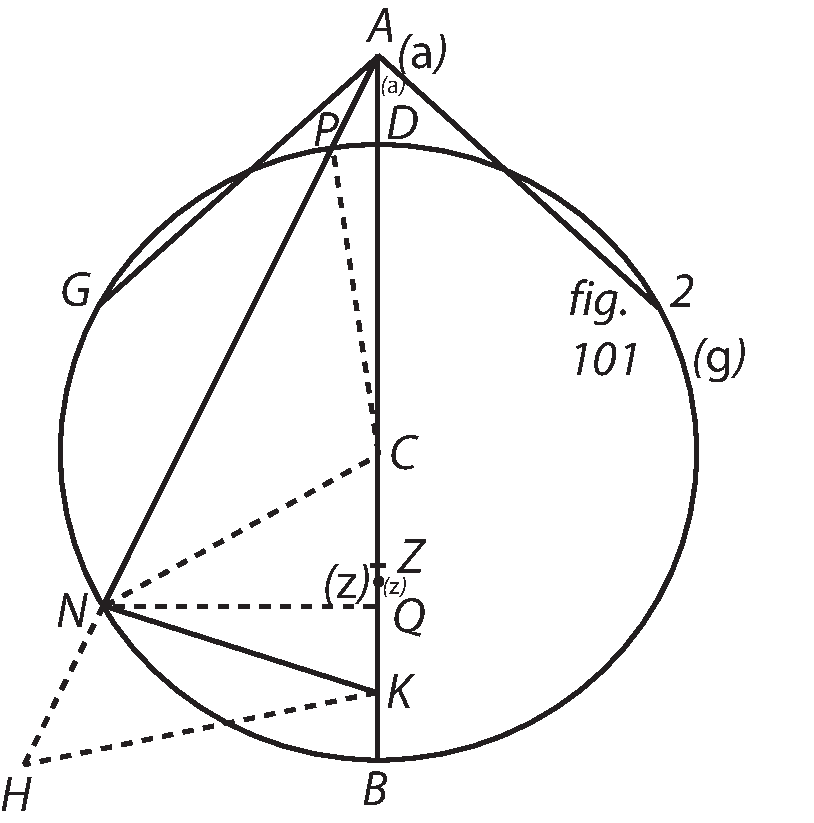
\includegraphics[trim = 0mm 0mm 0mm -5mm, clip,width=0.4\textwidth]{images/T8_Barrow-2.pdf}
%%\end{center}
\clearpage
    \clearpage{\pagestyle{empty}\cleardoublepage}




\pagenumbering{arabic}
\beginnumbering






%%%%     AEF (ex AKUSTIK)     %%%%%%%%%%%%%%%%%%%%%%%%%%%%%%%%

\clearpage{\pagestyle{empty}\cleardoublepage}	
\addtocontents{toc}{\vspace{5mm}}
\addpart[\large\uppercase{I. Akustik, Elastizit\"{a}t, Festigkeit}]{\large\protect\textso{I. Akustik, Elastizit\"{a}t, Festigkeit}}
\clearpage{\pagestyle{empty}\cleardoublepage}




\renewcommand{\chapterpagestyle}{firstchapter}
\renewcommand*{\chapterheadstartvskip}{\vspace*{15.5ex}}


\markleft{\scriptsize\uppercase{I. Akustik Elastizit\"{a}t Festigkeit}}


% N.~1. ((??A01; RK 38535)) De sono // AEF (Akustik)
\chapter[\scriptsize\uppercase{De sono}]{\uppercase{De sono}
\newline\lbrack zweite Hälfte 1671\,(?) \textendash\ vor Dezember 1680\rbrack}
\addcontentsline{toc}{chapter}{\thechapter\enskip De sono \enskip\lbrack zweite Hälfte 1671\,(?) \textendash\ vor Dezember 1680\rbrack}
\label{38535}
\vspace{8mm}
	%   ####
%
%   Band VIII, 3 N.~??A01
%   Signatur/Tex-Datei: LH_37_01_016
%   RK-Nr. 38535
%   Überschrift: De sono
%   Datierung: [zweite Hälfte 1671 (?) -- vor Dezember 1680]
%   WZ: (keins)
%.  SZ: (keins)
%.  Bilddateien (PDF): LH_37_01_016_d1; LH_37_01_016_d2 (insgesamt zwei)
%
%
\begin{ledgroupsized}[r]{120mm}
\footnotesize
\pstart
\noindent\textbf{Überlieferung:}
\pend
\end{ledgroupsized}
\begin{ledgroupsized}[r]{114mm}
\footnotesize
\pstart \parindent -6mm
\makebox[6mm][l]{\textit{L}}%
Aufzeichnung: LH XXXVII 1 Bl. 16.
Ein Blatt 4\textsuperscript{o}.
Zwei rechtspaltig beschriebene Seiten.
% Kein Wasserzeichen.
\pend
\end{ledgroupsized}
%
\vspace*{5mm}
\begin{ledgroup}
\footnotesize
\pstart
\noindent%
\textbf{Datierungsgründe:}
Das vorliegende Stück N.~1 lässt sich als Entwurf einer umfassenden Unter\-su\-chung über akustische Grundphänomene betrachten wie die Entstehung des Schalls aus vibrierenden Körpern, dessen Ausbreitung im Medium der Luft und dessen Aufnahme in das Gehörorgan.
Im Text wird zunächst das Phänomen der Schwingung am Beispiel einer gespannten Saite erörtert (S.~\refpassage{LH_37_01_016r_abschnitt_1-1}{LH_37_01_016r_abschnitt_1-2}) und anschließend eine Untersuchung des mechanischen Verhaltens elastischer Fluida und Saiten skizziert, bei der haupt\-säch\-lich der Isochronismus der Schwingungen erörtert werden soll (S.~\refpassage{LH_37_01_016r_abschnitt_2-1}{LH_37_01_016r_abschnitt_2-2}).
Hieran knüpft ferner eine Erläuterung der Ausbreitung und Aufnahme des Schalls an (S.~\refpassage{LH_37_01_016r_abschnitt_3-1}{LH_37_01_016r_abschnitt_3-2}),
die zum Teil das Erklärungsmodell vorwegnimmt, das in Leibnizens Briefen an G.\,C. Schelhammer und E.~Mariotte vom Februar/März 1681 bis Januar 1682 (\textit{LSB} III,~3 N.~182;\cite{01194} 269\cite{01193}; 311\cite{01195}) sowie in den hiervon herrührenden Stücken N.~12\textsubscript{1}, 12\textsubscript{2} und 12\textsubscript{3} dargelegt wird.
Auch das am Textende erwähnte Phänomen der gleich\-för\-mi\-gen Geschwindigkeit der Schallausbreitung (S.~\refpassage{LH_37_01_016r_abschnitt_4-1}{LH_37_01_016r_abschnitt_4-2}) wird in den Stücken N.~12\textsubscript{1}, 12\textsubscript{2} und 12\textsubscript{3} ausführlich erörtert.
Ebenso kann man die im Dezember 1680 verfassten \textit{Tentaminum de chordarum tensione schedae} (N.~8) gleichsam als Wie\-der\-auf\-nahme der in N.~1 vorgezeichneten Untersuchung zum Schwingen gespannter Saiten % und zu dessen Isochronis\-mus 
ansehen.
Demgemäß ist N.~1 höchstwahrscheinlich % vor N.~??A10, ??A11 und ??A13, d.h. 
vor Dezember 1680 entstanden.
\pend
\pstart
Der Terminus post quem der Datierung erweist sich aber als unklar.
In der \textit{Hypothesis physica nova} (Mainz 1671, §~32; \textit{LSB} VI,~2 N.~40, S.~236.27\textendash30\cite{00256}) führt Leibniz den Schall unmittelbar auf die Bewegung des Äthers zurück und erklärt die Schallausbreitung anhand des antiken Wellenmodells.
Der Erklärungs\-ansatz in N.~1 \textendash\ ebenso wie in den späteren Stücken N.~12\textsubscript{1}, 12\textsubscript{2} und 12\textsubscript{3} \textendash\ bemüht indessen weder den Äther noch das Wellenmodell mehr.
Die in N.~1 formulierte Analogie zwischen der Schwingung elastischer Saiten und dem Fall schwerer Körper (S.~\refpassage{LH_37_01_016r_turbatio-1}{LH_37_01_016r_turbatio-2}) sowie die dort vorgeschlagene Erklärung des Isochronismus (S.~\refpassage{LH_37_01_016r_isochr-1}{LH_37_01_016v_isochr-2}) erinnern aber an ähnliche Ausführungen in der vermut\-lich in der zweiten Hälfte 1671 entstandenen \textit{Summa hypotheseos physicae novae} (§~29\textendash30; \textit{LSB} VI,~2 N.~48\textsubscript{3}, S.~354.22\textendash355.6\cite{01276}; siehe zudem \textit{Hypothesis physica nova}, §~23; ebd. % \textit{LSB} VI,~2 
N.~40, S.~231.26\textendash31\cite{00256}).
Auch die zuweilen ungenaue Verwendung der Begrifflichkeit (etwa bei den missverständlichen Formulierungen % des Sachverhaltes 
auf S.~\refpassage{LH_37_01_016v_utcunque-1}{LH_37_01_016v_utcunque-2} und S.~\refpassage{LH_37_01_016v_Schallgeschwindigkeit-1}{LH_37_01_016v_Schallgeschwindigkeit-2}) lässt sich als Zeichen einer eher früheren Entstehung des Textes betrachten.
Der oben erwähnte inhaltliche Zusammenhang mit dem in N.~12\textsubscript{1}, 12\textsubscript{2} und 12\textsubscript{3} dargelegten Erklärungsmodell deutet hingegen auf eine spätere Entwicklungsstufe hin.
% , auf die auch Galileis Überlegungen über akustische Phänomene in den \cite{00050}\textit{Discorsi} (Leiden 1638, S.~95\textendash107; \cite{00048}\textit{GO} VIII, S.~138.19\textendash150.14) Einfluss genommen haben dürften.
% Mit Galileis Werk hat sich Leibniz vermutlich zwischen September 1672 und März 1673 befasst (vgl. \textit{LSB} VI,~3 N.~11\cite{00260} sowie VIII,~2 N.19\cite{01249}\cite{01250} bis N.~22\cite{01251}\cite{01252}).
Wann genau Leibniz zu dem in N.~1 (S.~\refpassage{LH_37_01_016r_abschnitt_3-1}{LH_37_01_016r_abschnitt_3-2}) skizzierten Erklärungsansatz erstmals gelangt ist, lässt sich aber nach heutigem Kenntnisstand nicht bestimmen.
\pend
\pstart
Ferner ist nicht auszuschließen, dass N.~1 zu den nicht weiter ermittelten \textit{veteres ... schedas meas de modo, quo fit sonus ac propagatur}, zählt, auf die Leibniz in seinem Brief an Schelhammer vom 6. (16.) Dezember 1680 anspielt (\cite{01275}\textit{LSB} III,~3 N.~139, S.~305.3\textendash4; ähnliche Erwähnungen in Leibnizens Briefen an Schelhammer von Februar/März 1681 und an Mariotte von der zweiten Hälfte August 1681: vgl. ebd. \cite{01194}N.~182, S.~355.11\textendash12; N.~269, \cite{01193}S.~479.7\textendash8). 
% Der Brief an Schelhammer von Februar/März 1681 erweckt jedoch den Verdacht, dass Leibniz das Bestehen umfangreicher älterer Aufzeichungen über die Akustik nur vorgibt (ebd. N.~182, S.~355.11\textendash12).
\pend
\end{ledgroup}
%
 \vspace*{8mm}
%\newpage
%
%
\count\Bfootins=1200
\count\Afootins=1200
\count\Cfootins=1200
%
%
\pstart%
\normalsize%
\noindent%
\lbrack16~r\textsuperscript{o}\rbrack
\pend%
% \vspace*{-0.5em}%
% Überschrift
\pstart%
\centering%
De sono\protect\index{Sachverzeichnis}{sonus}
\pend%
\vspace*{0.5em}%
%
\pstart%
\noindent%
Sit\edlabel{LH_37_01_016r_abschnitt_1-1} recta\protect\index{Sachverzeichnis}{recta rigida}
%
\edtext{rigida}{%
\lemma{rigida}\Bfootnote{%
\textit{erg.~L}}}
%
$AB$ composita ex aliis rectis rigidis \textit{A1.} \textit{12.} \textit{23.} \textit{34.} \textit{4B}
%
\edtext{connexis per arcus elasticos,\protect\index{Sachverzeichnis}{arcus elasticus}
exempli\protect\index{Sachverzeichnis}{exemplum}}{%
\lemma{connexis}\Bfootnote{%
\textit{(1)}~per elateria,\protect\index{Sachverzeichnis}{elaterium}
\textit{(a)}~sive
\textit{(b)}~seu arcus si placet, exempli
\textit{(2)}~per arcus elasticos, exempli~\textit{L}}}
%
gratia \textit{34} et \textit{4B}
\edtext{connectantur per}{%
\lemma{connectantur}\Bfootnote{%
\textit{(1)}~ab
\textit{(2)}~per~\textit{L}}}
duos arcus per omnia similes in eodem plano\protect\index{Sachverzeichnis}{planum paginae}
\edtext{hujus paginae}{%
\lemma{hujus}\Bfootnote{%
\hspace{-0,5mm}paginae \textit{erg.~L}}}
positos, unum $lmn$, alterum $pqr.$
Hinc patet in eodem plano hujus
\edtext{paginae\protect\index{Sachverzeichnis}{planum paginae} non}{%
\lemma{paginae}\Bfootnote{%
% \hspace*{-0,5mm}
\textbar~scilicet \textit{gestr.}~%
\textbar\ non%
~\textit{L}}}
posse rectam istam rigidam\protect\index{Sachverzeichnis}{recta rigida} extremis $A.$ $B$ immotis in medio alicubi
\edtext{apprehensam huc}{%
\lemma{apprehensam}\Bfootnote{%
\hspace{-0,5mm}\textbar~stylo $CD$ \textit{gestr.}~%
\textbar\ huc~%
\textit{L}}}
illucve adduci
quin arcus\protect\index{Sachverzeichnis}{arcus elasticus}
ille qui tunc est a parte concava intendatur sive magis quam antea incurvetur.
Itaque si dimittatur linea illa inflexa\protect\index{Sachverzeichnis}{linea inflexa}
restituet sese, non tamen manebit in statu recto\protect\index{Sachverzeichnis}{status rectus}
sed ob impetum conceptum\protect\index{Sachverzeichnis}{impetus conceptus} in alteram partem more chordarum pulsatarum\protect\index{Sachverzeichnis}{chorda pulsata} vibrantiumque\protect\index{Sachverzeichnis}{chorda vibrans} excurret.
Quarum et naturam\protect\index{Sachverzeichnis}{natura} ex his investigare propositum est.%
\edlabel{LH_37_01_016r_abschnitt_1-2}
\pend%
%
% \newpage%
%
%\vspace*{1.5em}%
%
\pstart%
Examinandum\edlabel{LH_37_01_016r_abschnitt_2-1}%  !!!!!!!!!!!!!!!! ACTHUNG GETRIXT:
\edtext{}{\lemma{\hspace*{1,6mm}\lbrack\textit{Fig.~1}\rbrack}\killnumber\Cfootnote{Ein gestrichener Entwurf zum Diagramm wird nicht wiedergegeben.}}
%
autem primo est Elastrum simplex,\protect\index{Sachverzeichnis}{elastrum simplex}
ut aer compressus,\protect\index{Sachverzeichnis}{aer compressus}
videndumque an ille eodem sese tempore restituat\protect\index{Sachverzeichnis}{tempus restitutionis}
utcunque sit compressus, plus vel minus.
\edlabel{LH_37_01_016r_turbatio-1}Et fortasse generaliter verum est
\edtext{eandem potentiam utcunque turbatam\protect\index{Sachverzeichnis}{potentia turbata}}{%
\lemma{eandem}\Bfootnote{%
\textit{(1)}~vim turbata\protect\index{Sachverzeichnis}{vis turbata}
\textit{(2)}~potentiam utcunque turbatam~\textit{L}}}
sese eodem tempore restituere,\protect\index{Sachverzeichnis}{tempus restitutionis}
sive plus sive minus turbata sit,
et omnia gravia,\protect\index{Sachverzeichnis}{grave}
nisi quid aliud intercurrat\lbrack,\rbrack\
eodem tempore ad centrum terrae\protect\index{Sachverzeichnis}{centrum terrae}
\edtext{perventura.
Itaque tempora restitutionum\protect\index{Sachverzeichnis}{tempus restitutionis}
ut potentias\protect\index{Sachverzeichnis}{potentia turbata} esse.}{%
\lemma{perventura.}\Bfootnote{%
\textit{(1)}~Itaque
\textit{(2)}~Itaque tempora ut potentias esse
\textit{(3)}~Itaque tempora \lbrack...\rbrack\ potentias esse.~\textit{L}}}
\makebox[1.0\textwidth][s]{Hoc tam generale principium\protect\index{Sachverzeichnis}{principium generale} meretur demonstrari.%
\edlabel{LH_37_01_016r_turbatio-2}
Si tamen Elaterium pondere\protect\index{Sachverzeichnis}{pondus onerans} one-}
\pend
\vspace*{1.5em}%
%
  \centerline{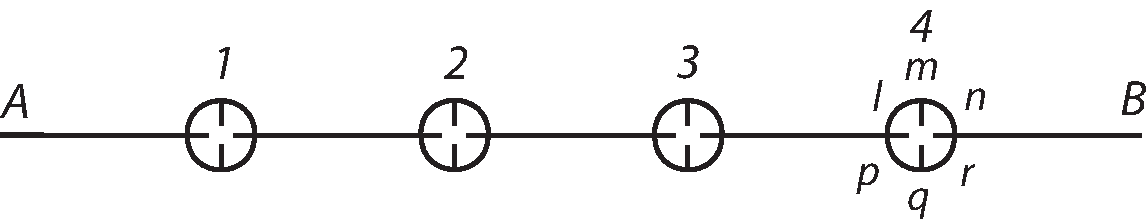
\includegraphics[width=0.64\textwidth]{gesamttex/edit_VIII,3/images/LH_37_01_016_d1.pdf}}%\\
  \vspace*{-0.5em}
  \centerline{\lbrack\textit{Fig.~1}\rbrack}
\newpage
\pstart
\noindent
retur\lbrack,\rbrack\
non eodem tempore restituetur\protect\index{Sachverzeichnis}{tempus restitutionis}
valde compressum ac parum compressum,\protect\index{Sachverzeichnis}{elaterium compressum}
nam extraneum aliquid praeterea agendum est magis in uno quam in altero.
Hinc jam aeris resistentia\protect\index{Sachverzeichnis}{resistentia aeris}
et ipsum pondus chordae\protect\index{Sachverzeichnis}{pondus chordae}
efficient ut non sit perfectus isochronismus.\protect\index{Sachverzeichnis}{isochronismus restitutionis}
\pend%
%\newpage
%
\count\Bfootins=1200
\count\Afootins=1200
\count\Cfootins=1200
\pstart%
Celeritas\edlabel{LH_37_01_016r_isochr-1}\protect\index{Sachverzeichnis}{celeritas restitutionis}
determinatur tum a nisu\protect\index{Sachverzeichnis}{nisus restitutionis}
seu potentia agente,\protect\index{Sachverzeichnis}{potentia agens}
tum a resistentia rei movendae.\protect\index{Sachverzeichnis}{resistentia rei movendae}
Sed si ab hac abstrahamus animum;\protect\index{Sachverzeichnis}{animus}
patet celeritates\protect\index{Sachverzeichnis}{celeritas restitutionis}
esse temporibus\protect\index{Sachverzeichnis}{tempus restitutionis}
reciproce proportionales,
ergo tempora reciproce proportionalia nisibus;
nisus autem sunt in composita ratione potentiarum
et turbationum,\protect\index{Sachverzeichnis}{turbatio}
et nisus\protect\index{Sachverzeichnis}{nisus restitutionis}
ejusdem potentiae\protect\index{Sachverzeichnis}{potentia agens}
in ratione turbationum.
Ergo tempora\protect\index{Sachverzeichnis}{tempus restitutionis}
in reciproca ratione turbationum,
sed cum turbationes\protect\index{Sachverzeichnis}{turbatio}
quovis momento\protect\index{Sachverzeichnis}{momentum temporis}
\edtext{immutentur, et}{%
\lemma{immutentur,}\Bfootnote{%
\textit{(1)}~imo
\textit{(2)}~et~\textit{L}}}
eo minor sit nisus\protect\index{Sachverzeichnis}{nisus restitutionis}
sequens quo praecedens major fuit,
hinc progressio per curvam exprimenda\protect\index{Sachverzeichnis}{progressio per curvam exprimenda}
erit,
\edtext{et
%
\lbrack16~v\textsuperscript{o}\rbrack\ %%%% Bl. 16v.
%
res}{%
\lemma{et}\Bfootnote{%
\hspace{-0,5mm}\lbrack16~v\textsuperscript{o}\rbrack\
\textbar~et \textit{streicht Hrsg.}~%
\textbar\ res~%
\textit{L}}}
eo redibit, ut ostendatur,
eandem temporum\protect\index{Sachverzeichnis}{tempus restitutionis} summam esse.
Moles gravium\protect\index{Sachverzeichnis}{moles gravium} nihil obstabit,
quominus eodem tempore ad centrum terrae\protect\index{Sachverzeichnis}{centrum terrae} perveniant,
quia ipsa eorum moles est causa turbationis.%
\edlabel{LH_37_01_016v_isochr-2}\protect\index{Sachverzeichnis}{causa turbationis}
%
Videndum an dimidia chorda\protect\index{Sachverzeichnis}{chorda dimidia}
iisdem servatis duplo celerius vibret.
Et sic videtur.
Nam si tantundem tendatur quantum integra,
erit duplo magis tensa\protect\index{Sachverzeichnis}{chorda tensa}
seu vim\protect\index{Sachverzeichnis}{vis tendens}
\edtext{passa\lbrack,\rbrack\
\edtext{}{%
{\xxref{LH_37_01_016v_utcunque-1}{LH_37_01_016v_utcunque-2}}%
{\lemma{utcunque \lbrack...\rbrack\ modo}\Cfootnote{%
Leibniz meint hier wohl nicht mehr die Spannkraft, sondern die Aus\-len\-kung der Saite (\textit{pulsatio}).%
% Beides lässt sich im Lateinischen als \textit{tensio} bezeichnen.
}}}%
\edlabel{LH_37_01_016v_utcunque-1}%
utcunque autem tendatur semper}{%
\lemma{passa}\Bfootnote{%
\textit{(1)}~. Ergo
\textit{(2)}~semper
\textit{(3)}~utcunque autem tendatur semper~\textit{L}}}
vibrat eodem modo.\edlabel{LH_37_01_016v_utcunque-2}
%
Videretur ergo corpus Elasticum\protect\index{Sachverzeichnis}{corpus elasticum}
omne quanto est minus,
\edtext{eo vibrare celerius.}{%
\lemma{eo}\Bfootnote{%
\textit{(1)}~fortius vibrare
\textit{(2)}~vibrare celerius.~\textit{L}}}
Etiam aerem ordinarium\protect\index{Sachverzeichnis}{aer ordinarius}
unius pedis cubici\protect\index{Sachverzeichnis}{pes cubicus}
fortius vibrare quam aerem duorum pedum cubicorum.
Quod rursus mirabile est.\edlabel{LH_37_01_016r_abschnitt_2-2}
\pend%
%
\pstart%
Sonus\edlabel{LH_37_01_016r_abschnitt_3-1}\protect\index{Sachverzeichnis}{sonus}
igitur pendet a partibus\protect\index{Sachverzeichnis}{pars aeris}
in quas aer vibratione\protect\index{Sachverzeichnis}{vibratio aeris}
quasi dissilit,
et quae et ipsae vibrant et vicinas excitant,
nam quo minores illae, hoc sonus
\edtext{acutior.\protect\index{Sachverzeichnis}{sonus acutus}
Modus quo}{%
\lemma{acutior.}\Bfootnote{%
\textit{(1)}~Cum ab vi
\textit{(2)}~Modus quo~\textit{L}}}
aer dissilit\lbrack,\rbrack\
hic esse videtur:
chorda\protect\index{Sachverzeichnis}{chorda vibrans}
\edtext{vibrans circumjacentem aerem\protect\index{Sachverzeichnis}{aer circumjacens}
impellendo comprimit, is\protect\index{Sachverzeichnis}{aer compressus}}{%
\lemma{vibrans}\Bfootnote{%
\textit{(1)}~imprimit aer
\textit{(2)}~circumjacentem aerem 
\textit{(a)}~premit et comprimit
\textit{(b)}~impellendo comprimit, 
\textit{(aa)}~itaque
\textit{(bb)}~is~\textit{L}}}
proprio nisu\protect\index{Sachverzeichnis}{nisus restitutionis}
se restituit et vibrat,
variae autem ob ejus liquiditatem\protect\index{Sachverzeichnis}{liquiditas}
in eo fiunt vibrationes,\protect\index{Sachverzeichnis}{vibratio aeris}
partium scilicet aliarum majorum aliarum minorum,
\edtext{sed partes mediae\protect\index{Sachverzeichnis}{pars aeris}}{%
\lemma{sed}\Bfootnote{%
\textit{(1)}~eae
\textit{(2)}~partes mediae%
~\textit{L}}}
quarum magnitudo talis est,
ut simul vibrent cum chorda,\protect\index{Sachverzeichnis}{chorda vibrans}
eae in vibratione perserverant,
reliquarum vibrationes destruuntur;\protect\index{Sachverzeichnis}{pars aeris}
et hae similiter vibrationem\protect\index{Sachverzeichnis}{vibratio aeris}
suam propagant in alias vicinas,\protect\index{Sachverzeichnis}{propagatio vibrationis}
et ita porro, usque ad aurem.\protect\index{Sachverzeichnis}{auris}
In aure
\edtext{autem potest fieri,
ut vel 
\edtext{}{%
{\xxref{LH_37_01_016v_tymp-1}{LH_37_01_016v_tymp-2}}%
{\lemma{tympanum \lbrack...\rbrack\ allapsi}\Cfootnote{%
Siehe zu dieser Auffassung der Funktion des Trommelfells etwa
H.~\textsc{Fabri}, \textit{Physica}, tract.~III, lib.~II, prop.~52 (Bd.~II, Lyon 1670, S.~152b\textendash153a)\cite{00044}.
Eine ähnliche Überlegung findet sich auch in \cite{00087}J.~\textsc{Rohault}, \textit{Traité de physique}, partie I, chap.~26, §~48 (2. Ausgabe, Paris 1672, Bd.~I, S.~290).}}}%
\edlabel{LH_37_01_016v_tymp-1}tympanum\protect\index{Sachverzeichnis}{tympanum} ipsum}{%
\lemma{autem}\Bfootnote{%
\textit{(1)}~possunt in ipso tympan
\textit{(2)}~potest fieri, ut vel tympanum ipsum~\textit{L}}}
varie intendamus pro ratione soni allapsi,%
\edlabel{LH_37_01_016v_tymp-2}\protect\index{Sachverzeichnis}{sonus allapsus}
%
vel ut tympanum\protect\index{Sachverzeichnis}{tympanum}
ex diversae tensionis\protect\index{Sachverzeichnis}{tensio} constet partibus,
quarum aliae ab hoc, aliae ab alio sono\protect\index{Sachverzeichnis}{sonus allapsus}
\edtext{pulsentur ut}{%
\lemma{pulsentur}\Bfootnote{%
\textit{(1)}~. Et hoc modo
\textit{(2)}~ut~\textit{L}}}
chordae chordis unisonis\protect\index{Sachverzeichnis}{chorda unisona}
pulsatis\protect\index{Sachverzeichnis}{chorda pulsata}
consonant\protect\index{Sachverzeichnis}{chorda consonans}
etsi non nisi ab aere pulsentur.\edlabel{LH_37_01_016r_abschnitt_3-2}
\pend%
%\newpage%
\pstart%
Videndum\edlabel{LH_37_01_016r_abschnitt_4-1} an verum sit, et ex
\edtext{his demonstrari queat,}{%
\lemma{his}\Bfootnote{%
\textit{(1)}~demonstretur
\textit{(2)}~demonstrari queat,~\textit{L}}}
quod omnis sonus\protect\index{Sachverzeichnis}{sonus} feratur\edlabel{LH_37_01_016v_Schallgeschwindigkeit-1}
\edtext{uniformi velocitate,%
\protect\index{Sachverzeichnis}{velocitas uniformis}\protect\index{Sachverzeichnis}{velocitas soni}
seu ut celeritas\protect\index{Sachverzeichnis}{celeritas soni}
sit in ratione distantiarum,\protect\index{Sachverzeichnis}{distantia}\edlabel{LH_37_01_016v_Schallgeschwindigkeit-2}}{%
\lemma{uniformi \lbrack...\rbrack\ distantiarum}\Cfootnote{%
Leibniz äußert sich hier widersprüchlich.
Siehe für eine angemessene Darstellung der gleichförmigen Geschwindigkeit der Schallausbreitung vielmehr
G.\,W. \textsc{Leibniz}, Brief an G.\,C. Schelhammer vom Februar/März 1681 (\textit{LSB} III,~3 N.~182, S.~359.14\textendash360.1)
sowie hier unten, N.~12\textsubscript{1}, S.~\refpassage{LH_37_01_019r_gleichscnell-1}{LH_37_01_019r_gleichscnell-2}.}}
et hoc verum puto,
prorsus ac si elateria\protect\index{Sachverzeichnis}{elaterium} similia in
\edtext{longam seriem disposita\protect\index{Sachverzeichnis}{series elateriorum}
sese ordine\protect\index{Sachverzeichnis}{ordo} liberent}{%
\lemma{longam}\Bfootnote{%
\textit{(1)}~distantiam se
\textit{(2)}~seriem disposita
\textit{(a)}~se mutuo liberent
\textit{(b)}~sese ordine liberent%
~\textit{L}}}
%
\lbrack\textit{danach gestrichen und abbrechend:}\rbrack\
\footnotesize{%
vel pulsent.
Si
\edtext{chordae\protect\index{Sachverzeichnis}{chorda parallela} parallelae}{%
\lemma{chordae}\Bfootnote{%
\textit{(1)}~vi
\textit{(2)}~parallelae%
~\textit{L}}}
%
eodem modo tensae\protect\index{Sachverzeichnis}{chorda tensa} sint numero quotcunque,
et una pulsata\protect\index{Sachverzeichnis}{chorda pulsata} aliam
\edtext{pulset; aliae consonant;}{%
\lemma{pulset;}\Bfootnote{%
\textit{(1)}~$\langle$nec$\rangle$
\textit{(2)}~pulsando
\textit{(a)}~aliquid
\textit{(b)}~aliquid
\textit{(3)}~manifestum est
\textit{(4)}~aliae consonant;%
~\textit{L}}}}%
%
% \lbrack\textit{Text bricht ab.}\rbrack%
\edlabel{LH_37_01_016r_abschnitt_4-2}
\normalsize%
\pend%
%
% \newpage%
\vspace*{3.0em}%
%
\pstart%
\setline{1}
  \centerline{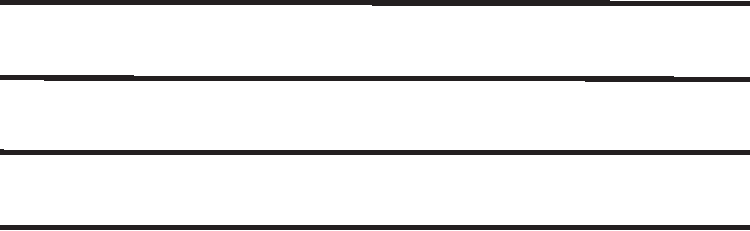
\includegraphics[width=0.35\textwidth]{gesamttex/edit_VIII,3/images/LH_37_01_016_d2.pdf}}%\\
  \vspace*{0.5em}
  \centerline{\lbrack\textit{Fig. 2}\rbrack}%
\edtext{}{\lemma{\hspace*{1,6mm}\lbrack\textit{Fig.~2}\rbrack}\killnumber\Cfootnote{Ungestrichene Zeichnung zu den gestrichenen Zeilen am Ende des Textes.
Sie ähnelt den Diagrammen \lbrack\textit{Fig.~1}\rbrack\ in N.~12\textsubscript{1}, S.~\pageref{LH_37_01_018v_Fig.1}, und \lbrack\textit{Fig.~2}\rbrack\ in N.~12\textsubscript{3}, % S.~\pageref{LH_37_01_001-002_d2}, und ??X\textsubscript{4}, 
S.~\pageref{LH_37_01_005r_Fig.2}.}}%
\pend%
\count\Bfootins=1200
\count\Afootins=1200
\count\Cfootins=1200
%
% ENDE DES STÜCKES auf Bl. 16v.


\renewcommand*{\chapterpagestyle}{scrheadings}
\renewcommand*{\chapterheadstartvskip}{\vspace*{-5mm}}


% N.~2. ((??A25; RK 58290)) Tuba stentorea vel acustica [früher: Ad tubam stentoream vel acusticam] // AEF (Akustik)
\chapter[\scriptsize\uppercase{Tuba stentorea vel acustica}]{\uppercase{Tuba stentorea vel acustica}
\newline\lbrack1672 \textendash\ erste Hälfte 1685\,(?)\rbrack}
\addcontentsline{toc}{chapter}{\thechapter\enskip Tuba stentorea vel acustica \enskip\lbrack1672 \textendash\ erste Hälfte 1685\,(?)\rbrack}
\label{58290}
\vspace{8mm}
	%
%
%   Band VIII, 3 N.~??A25
%   Signatur/Tex-Datei: LH_35_13_03_203
%   RK-Nr. 58290
%   Überschrift: Tuba stentorea vel acustica [früher: Ad tubam stentoream vel acusticam]
%   Datierung: [1672 -- erste Hälfte 1685 (?)]
%   WZ: (keins)
%   SZ: (keins)
%   Bilddateien LH_35_13_03_203_d (insgesamt: eine)
%
%
\begin{ledgroupsized}[r]{120mm}
\footnotesize
%
\count\Bfootins=400
\count\Afootins=1200
\count\Cfootins=1200
\pstart
\noindent\textbf{Überlieferung:}
\pend
\end{ledgroupsized}
\begin{ledgroupsized}[r]{114mm}
\footnotesize
\pstart \parindent -6mm
\makebox[6mm][l]{\textit{L}}%
Aufzeichnung: LH~XXXV~13,~3 Bl.~203.
Ein Blatt~4\textsuperscript{o}.
Eineinhalb Seiten.
% Kein Was\-ser\-zei\-chen.
\pend
\end{ledgroupsized}
%
\vspace*{5mm}
\begin{ledgroup}
\footnotesize
\pstart
\noindent\textbf{Datierungsgründe:}
Das von S.~Morland\protect\index{Namensregister}{\textso{Morland} (Moreland), Samuel 1625\textendash1695} entwickelte Sprachrohr erwähnt Leibniz bereits in einer Notiz aus dem Jahre 1671 (\textit{LSB} VIII,~1 N.~58\cite{01277}).
Später hat er auch Morlands Abhandlung % über das Sprachrohr S.~\textsc{Morland}, 
\textit{Tuba stentoro-phonica} % an instrument of excellent use, as well at sea, as at land; invented and variously experimented in the year 1670, 
(London 1672\cite{00149}) gelesen,
wie Streichungen in seinem Handexemplar bezeugen (\textit{LSB} VIII,~1 N.~62\cite{01278}; vgl. Hannover, GWLB, Signatur N\textendash A 7073).
Auf die \textit{tuba stentorea} bezieht sich Leibniz auch in N.~12\textsubscript{3}, Textschicht \textit{Lil} (S.~\refpassage{LH_37_01_008v_tubastentorea-1}{LH_37_01_008v_tubastentorea-2}) % , sowie in N.~??X\textsubscript{7} (S.~\refpassage{LH_37_01_025v_tubastentorea-1}{LH_37_01_025v_tubastentorea-2}),
und zwar % beidemal 
in einem Kontext, der die Gestalt des Sprachrohrs in den Vordergrund stellt.
N.~12\textsubscript{3}, Textschicht \textit{Lil} % , und N.~??X\textsubscript{7} lassen 
lässt sich auf die Zeitspanne zwischen der zweiten Hälfte 1684 und der ersten Hälfte 1685 datieren.
Das vorliegende Stück N.~2 ist mit der Frage befasst, wie das Profil des Sprachrohrs im Hinblick auf eine handwerkliche Ausführung geometrisch zu gestalten ist.
Daher ist wahrscheinlich, dass N.~2 nach der Veröffentlichung von Morlands Abhandlung (1672), aber noch vor N.~12\textsubscript{3}, Textschicht \textit{Lil} % , und N.~??X\textsubscript{7} 
verfasst wurde.
Eine spätere Entstehungszeit ist jedoch nicht auszuschließen.
% Kein Wasserzeichen.\\
% Probsts Datierung: ab 1676 ?\\
\pend
\end{ledgroup}
%
\vspace*{8mm}
\pstart\noindent
\normalsize
%
\lbrack203~r\textsuperscript{o}\rbrack\ \edtext{Ad Tubam}{%
\lemma{Ad}\Bfootnote{%
\textit{(1)}~Tubicam
\textit{(2)}~Tubam%
~\textit{L}}}
%
stentoream\protect\index{Sachverzeichnis}{tuba stentorea} vel acusticam\protect\index{Sachverzeichnis}{tuba acustica}
%\edtext{\textit{ABEFI}}{%
%\lemma{\textit{ABEFI}}\Bfootnote{%
%\textit{erg.~L}}}
\edtext{\textit{ABEFI}}{%
{\lemma{\textit{ABEFI}}\Bfootnote{%
\textit{erg.~L}}}%
{\lemma{\textit{ABEFI}}\Cfootnote{%
Siehe das Diagramm \lbrack\textit{Fig.~1}\rbrack\ auf S.~\pageref{LH_35_13_03_203r_Fig.1}.}}}
formandam ab
\edtext{artifice,\protect\index{Sachverzeichnis}{artifex}
ut scilicet sectionem Tubae\protect\index{Sachverzeichnis}{sectio tubae}
in plano datam superficie cava\protect\index{Sachverzeichnis}{superficies cava} exhibeat,
considerari potest curvam\protect\index{Sachverzeichnis}{curva} \lbrack\textit{AB}\rbrack\ vel \textit{IF,}
cujus revolutione\protect\index{Sachverzeichnis}{revolutio curvae}}{%
\lemma{artifice}\Bfootnote{%
\textit{(1)}~, considerandum et,
\textit{(2)}~, ut scilicet \lbrack...\rbrack\ considerari potest
\textit{(a)}~curvae
\textit{(aa)}~cujus revolu
\textit{(bb)}~\textit{ABC,}
\textit{(b)}~curvam \textbar~\textit{AC} \textit{ändert Hrsg.}~\textbar\ vel \textit{IF,} cujus revolutione%
~\textit{L}}}
%
circa axem\protect\index{Sachverzeichnis}{axis} \textit{LM} superficies
\edtext{describitur,
ut constantem}{%
\lemma{describitur,}\Bfootnote{%
\hspace{-0,5mm}\textbar~considerari posse \textit{streicht Hrsg.}~\textbar\
ut constantem%
\textit{~L}}}
%
ex rectis \textit{BC}, \textit{CD} etc.
\edtext{vel \textit{FG}, \textit{GH} etc.}{%
\lemma{vel}\Bfootnote{% \hspace*{-0,5mm}
\textit{FG}, \textit{GH}, etc.
\textit{erg.~L}}}
%
quae productae occurrant Axi,\protect\index{Sachverzeichnis}{axis}
nempe \textit{BC}
\edtext{in \textit{N}, vel \textit{CD} in \lbrack\textit{P}\rbrack,}{%
\lemma{in}\Bfootnote{%
\hspace{-0,5mm}\textit{N},
\textit{(1)}~et \textit{P}
\textit{(2)}~vel \textit{CD} in \textbar~\textit{B} \textit{ändert Hrsg.}~\textbar~,%
~\textit{L}}}
%
et ita porro.
Itaque \textit{BC}
\edtext{est portio truncata superficiei}{%
\lemma{est}\Bfootnote{%
\textit{(1)}~superficies
\textit{(2)}~portio truncata superficiei%
~\textit{L}}}
%
coni \textit{NCB},\protect\index{Sachverzeichnis}{conus}
et \textit{DC} coni
\edlabel{LH_35_13_03_203r_iduds-1}\textit{PDC}.%
\edtext{}{%
{\xxref{LH_35_13_03_203r_iduds-1}{LH_35_13_03_203r_iduds-2}}%
{\lemma{\textit{PDC}.}\Bfootnote{%
\textit{(1)}~Jam superficies conica
\textit{(2)}~Res ergo \lbrack...\rbrack\ superficies conica
\textit{(a)}~, quod fiet
\textit{(b)}~. Hoc ut fiat%
~\textit{L}}}}
%
\pend
%
\pstart
Res ergo huc redit ut plana lamina\protect\index{Sachverzeichnis}{lamina plana} exhibeatur,
ex qua formari possit superficies\protect\index{Sachverzeichnis}{superficies conica} conica.
Hoc ut fiat\edlabel{LH_35_13_03_203r_iduds-2}
demonstrativa ratione\protect\index{Sachverzeichnis}{ratio demonstrativa}
\edtext{consideravi\lbrack:\rbrack\
ut cylindrica superficies\protect\index{Sachverzeichnis}{superficies cylindrica}}{%
\lemma{consideravi}\Bfootnote{%
\textit{(1)}~sup
\textit{(2)}~conicam super
\textit{(3)}~ut cylindrica superficies%
~\textit{L}}}
%
plano applicari potest volvendo eam super plano,
et ita exhibendo planum superficiei congruens;\protect\index{Sachverzeichnis}{planum superficiei congruens}
\makebox[1.0\textwidth][s]{ita similiter conicam\protect\index{Sachverzeichnis}{superficies conica} quoque posse volvendo successive applicari plano
et ita exprimere}
\pend
\newpage
 \centerline{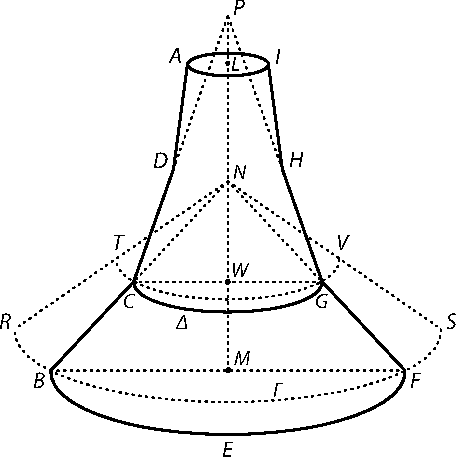
\includegraphics[width=0.51\textwidth]{gesamttex/edit_VIII,3/images/LH_35_13_03_203_d.pdf}}%
 \vspace{0.5em}
  \centerline{\lbrack\textit{Fig.~1}\rbrack}%
  \vspace{1.5em}
\pstart
\noindent 
%%%%    !!!!    !!!!    ACHTUNG GETRIXT    !!!!    !!!!
\label{LH_35_13_03_203r_Fig.1}\edtext{}{\lemma{\hspace*{1,6mm}\lbrack\textit{Fig.~1}\rbrack}\killnumber\Cfootnote{
Ein auf Bl.~203~r\textsuperscript{o} befindlicher, gestrichener Entwurf zum Diagramm wird nicht wiedergegeben.}}in plano magnitudinis suae vestigium,\protect\index{Sachverzeichnis}{vestigium magnitudinis}
prorsus ut circumferentia rotae\protect\index{Sachverzeichnis}{circumferentia rotae} plano
\edtext{applicatur.
Utrobique enim sive conus\protect\index{Sachverzeichnis}{conus}
sive cylinder\protect\index{Sachverzeichnis}{cylinder} volvatur,
superficies ejus tangit planum in recta.
Et sane si pro curva\protect\index{Sachverzeichnis}{curva}
figura adhibeatur polyhedrica curvae appropinquans,\protect\index{Sachverzeichnis}{figura polyhedrica curvae appropinquans}
tunc utique superficies polyhedra\protect\index{Sachverzeichnis}{superficies polyhedra}
magnitudinem\protect\index{Sachverzeichnis}{magnitudo superficiei} suam exprimeret in plano.
Id vero tantum hic in\-ter\-est inter conum\protect\index{Sachverzeichnis}{conus} et cylindrum;\protect\index{Sachverzeichnis}{cylinder}
quod}{%
\lemma{applicatur.}\Bfootnote{%
\textit{(1)}~Sed hoc interest inter coni et cylindri volutionem in plano quod
\textit{(2)}~Utrobique enim
\textit{(a)}~recta
\textit{(b)}~superficies planum
\textit{(aa)}~recta
\textit{(bb)}~tangit in recta
\textit{(c)}~sive conus \lbrack...\rbrack\ in recta % sive cylinder volvatur superficies ejus tangit planum
\textit{(aa)}~, et
\textit{(bb)}~. Et
\textbar~sane \textit{erg.}~%
\textbar\ si pro curva figura
\textbar~adhibeatur \textit{erg.}~%
\textbar\ polyhedrica
\textit{(aaa)}~pro
\textit{(bbb)}~\textbar~curvae \textit{erg.}~\textbar\ appropinquans,
\textit{(aaaa)}~adhibetur
\textit{(bbbb)}~tunc utique superficies
\textit{(aaaaa)}~polyhedrica
\textit{(bbbbb)}~polyhedra
\textit{(aaaaa-a)}~in plano
\textit{(bbbbb-b)}~de figu
\textit{(ccccc-c)}~su
\textit{(ddddd-d)}~magnitudinem suam \lbrack...\rbrack\ vero tantum % exprimeret in plano. Id
\textbar~hic \textit{erg.}~%
\textbar\ interest
\textit{(aaaaa-aa)}~,
\textit{(bbbbb-bb)}~inter conum et cylindrum; quod%
~\textit{L}}}
% % % %    < < < < 
in volutione cylindri\protect\index{Sachverzeichnis}{volutio cylindri}
rectae planum tangentes\protect\index{Sachverzeichnis}{recta tangens} sibi parallelae sunt,
in volutione vero coni\protect\index{Sachverzeichnis}{volutio coni} concurrunt
in apice\protect\index{Sachverzeichnis}{apex coni} coni. 
\pend
%
\pstart
Hoc posito sequitur\lbrack:\rbrack\
si ex puncto \textit{N}, tanquam apice\protect\index{Sachverzeichnis}{apex coni}
\edtext{coni, radio\protect\index{Sachverzeichnis}{radius circuli} \textit{NB} describatur}{%
\lemma{coni,}\Bfootnote{%
\textit{(1)}~describatur 
\textit{(2)}~radio \textit{NB} describatur%
~\textit{L}}}
%
\edtext{arcus\protect\index{Sachverzeichnis}{arcus circuli}
\lbrack\textit{RB\pgrk{G}FS}\rbrack\
vel \textit{RBS}}{%
\lemma{arcus}\Bfootnote{%
\textit{(1)}~\textit{BRF}
\textit{(2)}~\textbar~\textit{RBE\pgrk{G}FS} \textit{ändert Hrsg.}~\textbar\ vel
\textit{(a)}~\textit{RPF}
\textit{(b)}~\textit{RBS}%
~\textit{L}}}
%
aequalis circumferentiae\protect\index{Sachverzeichnis}{circumferentia circuli} circuli \textit{BEF}
\edtext{circa diametrum \textit{BF};}{%
\lemma{circa}\Bfootnote{%
\hspace{-0,5mm}diametrum \textit{BF}
\textit{erg.~L}}}
%
et similiter si radio \textit{NC} describatur arcus \textit{TCV}
aequalis curcumferentiae circuli circa diametrum\protect\index{Sachverzeichnis}{diameter circuli} \textit{CG},
fore portionem\protect\index{Sachverzeichnis}{portio annularis} annularem \textit{TRBSVCT}
aequalem superficiei\protect\index{Sachverzeichnis}{superficies conica}
\edtext{conicae truncatae
\lbrack\textit{CBEFG\pgrk{D}C},\rbrack}{%
\lemma{conicae}\Bfootnote{%
\textit{(1)}~\textit{CBEFG\pgrk{D}C}
\textit{(2)}~truncatae \textbar~\textit{GBEFG\pgrk{D}E}, \textit{ändert Hrsg.}~\textbar%
~\textit{L}}}
%
cujus superior basis est circumferentia circa \textit{CG},
inferior circumferentia\protect\index{Sachverzeichnis}{circumferentia circuli} circa \textit{BF}.
Patet
\edtext{autem puncta \textit{R}, \textit{T}, \textit{N} vel}{%
\lemma{autem}\Bfootnote{%
\textit{(1)}~\textit{R}, \textit{N}, \textit{T}
\textit{(2)}~\textit{RTN}
\textit{(3)}~puncta \textit{R}, \textit{T}, \textit{N} vel%
~\textit{L}}}
%
\textit{S}, \textit{V}, \textit{N} cadere in eandem
\edtext{rectam.
Quaeritur}{%
\lemma{rectam.}\Bfootnote{%
\textit{(1)}~Si
\textit{(2)}~Ut
\textit{(3)}~Quaeritur%
~\textit{L}}}
%
ergo tantum apertura\protect\index{Sachverzeichnis}{apertura coni}
seu angulus\protect\index{Sachverzeichnis}{angulus} \textit{RNS},
seu a dato circulo
(\phantom)\hspace*{-1.2mm}%
centro\protect\index{Sachverzeichnis}{centrum circuli} \textit{N} radio\protect\index{Sachverzeichnis}{radius circuli} \textit{NB} descripto%
\phantom(\hspace*{-1.2mm})
abscindere
\edtext{\textit{RBFS}}{%
\lemma{\textit{RBFS}}\Bfootnote{%
\textit{erg.~L}}}
%
arcum\protect\index{Sachverzeichnis}{arcus circuli} datae magnitudinis
seu aequalem circumferentiae\protect\index{Sachverzeichnis}{circumferentia circuli} datae
circa diametrum\protect\index{Sachverzeichnis}{diameter circuli} datam
\edlabel{LH_35_13_03_203r_ieuvg-3}\textit{BF}.
\edtext{}{%
{\xxref{LH_35_13_03_203r_ieuvg-3}{LH_35_13_03_203r_ieuvg-4}}%
{\lemma{\textit{BF}}\Bfootnote{%
\textit{(1)}~id est
\textit{(2)}~\textbar~. Hoc ita fiet, cum detur circumferentia integra per \textit{R}, \textit{B}, \textit{F}, \textit{S}, itemque arcus magnitudo seu circumf. per \textit{B}, \textit{E}, \textit{F}, dabitur et circumferentiarum ratio ea sc. quae diametrorum, ea sc. quae est anguli \textit{RNS} ad gradus 360. Ergo fiet ut recta \textit{NR} ad rectam \textit{BF}, ita 360 ad numerum graduum anguli \textit{NRS}.
\textit{streicht Hrsg.}~\textbar\
\lbrack203~v\textsuperscript{o}\rbrack\
\textit{(3)}~. Hoc ita fiet, cum detur
\textbar\ magnitudine \textit{erg. u. gestr.}~\textbar\ circumferentia integra per \textit{R}, \textit{B}, \textit{F}, \textit{S},
\textit{(a)}~tendens
\textit{(b)}~itemque magnitudo \lbrack...\rbrack\ diametrum \textit{BF}
\textit{(aa)}~\textbar~. Dabitur \textit{streicht Hrsg.}~\textbar\
\textit{(bb)}~, dabitur et ratio harum
\textit{(aaa)}~quantitatum
\textit{(bbb)}~circumferentiarum, eadem \lbrack...\rbrack\ graduum anguli % %%%%
\textit{(aaaa)}~\textit{NBF}
\textit{(bbbb)}~\textit{BNF},
\textit{(cccc)}~\textit{RNS}, ergo
\textit{(aaaaa)}~\textbar~ut \textit{streicht Hrsg.}~\textbar\
\textit{(aaaaa-a)}~diam
\textit{(bbbbb-b)}~\textit{NB} ad \textit{MB}
\textit{(bbbbb)}~ut \textit{NB} \lbrack...\rbrack\ 360 ad % ad \textit{MB} ita erit
\textit{(aaaaa-a)}~gradus \textbar~anguli \textit{streicht Hrsg.}~\textbar\ \textit{BNF}, qui
\textit{(bbbbb-b)}~numerum graduum \lbrack...\rbrack\ numerus desiderabatur. % anguli \textit{RNS}, qui
\textit{(aaaaa-aa)}~Eodem
\textit{(bbbbb-bb)}~Unde etiam
\textit{(ccccc-cc)}~Et eodem modo erit
\textit{(aaaaa-aaa)}~\textit{NT} ad \textit{TV} \textbar~(\phantom)\hspace*{-1.2mm}dimidiam \textit{CW}\phantom(\hspace*{-1.2mm}) \textit{erg.}~\textbar\ ut 360 ad numerum
\textit{(bbbbb-bbb)}~\textit{NC} ad \textit{CW}
\textit{(ccccc-ccc)}~\textit{NC} ad \textit{CW} (\phantom)\hspace*{-1.2mm}dimidiam \textbar~\textit{CV} \textit{ändert Hrsg.}~\textbar\ \phantom(\hspace*{-1.2mm}) ut
\textit{(aaaaa-aaaa)}~360 num
\textit{(bbbbb-bbbb)}~360 ad \lbrack...\rbrack\ anguli \textit{TNV} % numerum graduum
\textit{(aaaaa-aaaaa)}~. Sunt enim ob
\textit{(bbbbb-bbbbb)}~vel \textit{RNS}. \lbrack...\rbrack\ \textit{NB} ad \textit{BM}.% % ob triangula \textit{NWC}, \textit{NMB} similia est \textit{NC} ad \textit{CW}, ut
~\textit{L}}}}%
%
% \pend
%
% \pstart
%
\lbrack203~v\textsuperscript{o}\rbrack\ % Bl. 203v
%
% \pend
%
% \pstart
Hoc ita fiet,
cum detur circumferentia integra
per \textit{R}, \textit{B}, \textit{F}, \textit{S},
itemque magnitudo arcus \textit{B\pgrk{G}F},
aequalis circumferentiae integrae per \textit{B}, \textit{E}, \textit{F},
seu circa diametrum \textit{BF},
dabitur et ratio harum circumferentiarum,\protect\index{Sachverzeichnis}{circumferentia circuli}
eadem quae radiorum \textit{NB}, \textit{MB};
sed circumferentia integra per \textit{R}, \textit{B}, \textit{F}, \textit{S}
est ad partem suam,
arcum\protect\index{Sachverzeichnis}{arcus circuli} scilicet \textit{B\pgrk{G}F},
ut 360 gradus\protect\index{Sachverzeichnis}{gradus anguli} sunt ad numerum graduum anguli \textit{RNS},
ergo ut \textit{NB} ad \textit{MB}
ita erit 360 ad numerum graduum anguli \textit{RNS},
qui numerus desiderabatur.\protect\index{Sachverzeichnis}{numerus desideratus}
Et eodem modo erit \textit{NC} ad \textit{CW}
(\phantom)\hspace*{-1.2mm}%
dimidiam \lbrack\textit{CG}\rbrack%
\phantom(\hspace*{-1.2mm})
ut 360 ad numerum graduum anguli\protect\index{Sachverzeichnis}{gradus anguli} \textit{TNV} vel \textit{RNS}.
Nam ob triangula \textit{NWC}, \textit{NMB} similia,\protect\index{Sachverzeichnis}{triangulum simile}
est \textit{NC} ad \textit{CW},
ut \textit{NB} ad \textit{BM}.%
\edlabel{LH_35_13_03_203r_ieuvg-4}
%
Habito igitur angulo\protect\index{Sachverzeichnis}{angulus} \textit{BNF}, et
\edtext{radiis\protect\index{Sachverzeichnis}{radius circuli} \textit{NC}, \textit{NB},
\lbrack habetur et\rbrack}{%
\lemma{radiis}\Bfootnote{%
\textit{(1)}~\textit{BF}
\textit{(2)}~\textit{BN}, \textit{BT},
\textit{(3)}~\textit{NT}, \textit{NB}, habetur
\textit{(4)}~\textit{NC}, \textit{NB},
\textbar~habetur et \textit{erg. Hrsg.}~\textbar%
~\textit{L}}}
%
\edtext{descriptio portionis\protect\index{Sachverzeichnis}{portio annularis} annularis}{%
\lemma{descriptio}\Bfootnote{%
\textit{(1)}~figurae
\textit{(2)}~portionis annularis%
~\textit{L}}}
%
quaesitae.\protect\index{Sachverzeichnis}{descriptio quaesita}
\pend
\count\Bfootins=1000
\count\Afootins=1200
\count\Cfootins=1200
%
%
% ENDE DES STÜCKS AUF Bl. 203v
%
%
% \edtext{Hoc ita fiet,
% cum detur circumferentia integra per \textit{R}, \textit{B}, \textit{F}, \textit{S},
% itemque arcus magnitudo seu circumf. per \textit{B}, \textit{E}, \textit{F},
% dabitur et circumferentiarum ratio\lbrack,\rbrack\
% ea sc. quae diametrorum,
% ea sc. quae est anguli \textit{RNS} ad gradus 360.
% Ergo fiet\lbrack:\rbrack\ ut recta \textit{NR} ad rectam \textit{BF},
% ita 360 ad numerum graduum anguli \textit{NRS}.}{%
% \lemma{Hoc \lbrack...\rbrack\ \textit{NRS}}\Cfootnote{%
% Diese Textpassage hat Leibniz unmittelbar nach dem Umbruch von Bl.~203~r\textsuperscript{o} auf Bl.~203~v\textsuperscript{o} wiederholt und verändert.
% Siehe die folgenden Zeilen bis zum Textende.}}
%
%
	
	
	
% N.~3. ((??A31; RK 41165)) Zu John Mayow, Tractatus de sal-nitro et spiritu nitro-aereo // AEF (Elastizität)
\chapter[\scriptsize\uppercase{Zu J. Mayow, Tractatus de sal-nitro}]{\uppercase{Zu John Mayow, Tractatus de sal-nitro et spiritu nitro-aereo}
\newline \lbrack nach Mitte September 1674 \textendash\ frühe 1680er Jahre\,(?)\rbrack}
\addcontentsline{toc}{chapter}{\thechapter\enskip Zu John Mayow, Tractatus de sal-nitro et spiritu nitro-aereo%
\enskip\lbrack Mitte September 1674 \textendash\ frühe 1680er Jahre\,(?)\rbrack}
\label{41165}
\vspace{8mm}
	%   % !TEX root = ../../VIII,3_Rahmen-TeX_8-1.tex
%
%
%   Band VIII, 3 N.~??A31
%   Signatur/Tex-Datei: LH_35_09_16_015
%   RK-Nr. 41165
%   Überschrift: [Zu John Mayow, Tractatus de sal-nitro et spiritu nitro-aereo]
%   Modul: Mechanik / Elastizität
%   Datierung: [nach Mitte September 1674]
%   WZ: Keins
%   SZ: Keins
%   Bilddateien (PDF): LH_35_09_16_015_d (insgesamt: eins)
%
%
\selectlanguage{ngerman}%
\frenchspacing%
%
\begin{ledgroupsized}[r]{120mm}%
\footnotesize%
\pstart%
\noindent\textbf{Überlieferung:}%
\pend%
\end{ledgroupsized}%
\begin{ledgroupsized}[r]{114mm}%
\footnotesize%
\pstart%
\parindent -6mm%
\makebox[6mm][l]{\textit{L}}%
Notiz zu \textsc{J. Mayow}, \textit{Tractatus de sal-nitro et spiritu nitro-aereo}, in: \textsc{Ders.}, \textit{Tractatus quinque medico-physici}, Oxford 1674:\cite{01997}
LH~XXXV~9,~16 Bl.~15.
Ein Zettel (7 x 2,5 cm).
Eineinhalb Seiten;
Textfolge: Bl.~15~v\textsuperscript{o}, 15~r\textsuperscript{o}.%
\pend%
\end{ledgroupsized}%
%
\vspace{5mm}%
\begin{ledgroup}%
\footnotesize%
\pstart%
\noindent\textbf{Datierungsgründe:}
In seinem Brief an G.\,C. Schelhammer\protect\index{Namensregister}{\textso{Schelhammer} (Schelhammerus), Günther Christoph 1649\textendash1716} von Mitte September 1674 vermerkte Leibniz, er warte gerade auf ein englisches Buch \textit{de respiratione foetus in utero} (\textit{LSB} III,~5 N.~I, S.~3.19\textendash4.1\cite{01293}).
Damit war die gleichnamige Abhandlung gemeint,\cite{01296} die J.~Mayow\protect\index{Namensregister}{\textso{Mayow}, John 1643\textendash1679} 1674 in seinen \textit{Tractatus quinque medico-physici} veröffentlicht hatte und Leibniz vermutlich aus einer Besprechung in den \textit{Philosophical Trans\-ac\-ti\-ons} (20. Juli 1674, S.~101\textendash113\cite{01295}) kannte.
Zum Sammelband gehörte auch Mayows \textit{Tractatus de sal-nitro et spiritu nitro-aereo}\cite{01997}, an den die vorliegende Notiz N.~3 anknüpft.
Unter der Annahme, dass Leibniz das erwartete Buch auch empfing, kann er ab Mitte September 1674 diese Abhandlung gelesen und N.~3 verfasst haben.
\pend%
\pstart
Auf Mayows Sammelband wurde Leibniz ferner von F.~Schrader\protect\index{Namensregister}{\textso{Schrader}, Friedrich 1657\textendash1704} in einem Brief vom 28. November (8. Dezember) 1681 aufmerksam gemacht (vgl. \textit{LSB} III,~3 N.~299, S.~522.5\textendash9; 523.16\textendash18\cite{01294}).
Dies könnte ihn erneut dazu veranlasst haben, sich mit Mayows \textit{Tractatus de sal-nitro et spiritu nitro-aereo} zu beschäftigen.
Es ist ohnehin wahrscheinlich, dass N.~3 auf die frühen Achtziger Jahre zurückgeht, als Leibniz sich intensiv mit der Theorie der Elastizität und Festigkeit befasste, wie zahlreiche Texte im vorliegenden Band bezeugen. 
\pend%
\end{ledgroup}%
%
\selectlanguage{latin}%
\frenchspacing%
%
%
%\newpage%
 \vspace{8mm}
%\pstart 
%\noindent
%\pend
\count\Bfootins=1200
\count\Afootins=1200
\count\Cfootins=1200
%\pstart
%\centering
%\pend
%\count\Bfootins=1000
%\count\Cfootins=1000
%
\pstart%
% \vspace*{0.5em}% PR: nur provisorisch
\noindent
%
\lbrack15~v\textsuperscript{o}\rbrack\ %	%	Blatt 15v
%
\edtext{}{%
{\xxref{LH35_09_16_015v_1}{LH35_09_16_015v_2}}%
{\lemma{Corpus \lbrack...\rbrack\ flexiles}\Cfootnote{%
Siehe J.~\textsc{Mayow}, \cite{01997}\textit{Tractatus de sal-nitro et spiritu nitro-aereo}, S.~73\textendash77; in: \textsc{Ders.}, \textit{Tractatus quinque medico-physici}, Oxford 1674.}}}%
Corpus\edlabel{LH35_09_16_015v_1}
rigidum variis modis flectitur,\protect\index{Sachverzeichnis}{corpus rigidum}\protect\index{Sachverzeichnis}{corpus flexum}
ut vel superficies convexa maneat aeque longa,
concava mutetur;\protect\index{Sachverzeichnis}{superficies convexa}\protect\index{Sachverzeichnis}{superficies concava}
vel ut contra;\protect\index{Sachverzeichnis}{flexio corporis}
vel ut ambae maneant aeque longae ut ante
(\protect\vphantom)%
curvedine\protect\index{Sachverzeichnis}{curvedo} tantum
\edtext{\lbrack mutata\rbrack}{%
\lemma{mutata\protect\vphantom()}\Bfootnote{%
\textit{L~ändert Hrsg.}}}
%
et incluso\lbrack\protect\vphantom()\rbrack,
%
vel ut ambae mutentur. % Dieser Fall nicht bei Mayow, p. 73 sqq.
Mayow\protect\index{Namensregister}{\textso{Mayow}, John 1643\textendash1679}
\textit{de Nitro} c.~6.%
%	%	%	%	ACTHUNG GETRIXT: Folgende Cfootnote bezieht sich auf die Abbildung Fig.1
\edtext{}{\lemma{\lbrack\textit{Fig.~1}\rbrack}\killnumber\Cfootnote{%
Siehe a.a.O., die Abbildung \textit{Fig.~8} auf der Tafel \textit{Tab.~1} am Bandende.}}
%
\pend
 \vspace{1.5em}%
  \centerline{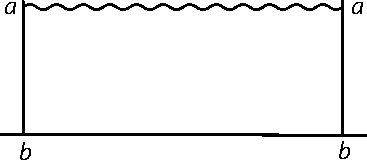
\includegraphics[width=0.35\textwidth]{gesamttex/edit_VIII,3/images/LH_35_09_16_015_d.pdf}}%
  \vspace*{0.0em}%
  \centerline{\lbrack\textit{Fig.~1}\rbrack}% \hspace*{16mm}
  \label{LH_35_09_16_015v_Fig.1}%
\newpage
%
%
\pstart%
\noindent
\textit{a} \edtext{\lbrack chorda\protect\index{Sachverzeichnis}{chorda tensa}\rbrack}{%
\lemma{corda}\Bfootnote{\textit{L~ändert Hrsg.}}}
\quad%
\textit{b} baculus\protect\index{Sachverzeichnis}{baculus}
\quad%
\textit{ab} baculi
\quad
Chorda vel firmiter utrinque alligata, vel ab una parte soluta\lbrack,\rbrack\
baculi flexiles.\edlabel{LH35_09_16_015v_2}
[15~r\textsuperscript{o}]
\pend%
%
%
\pstart%
Multa notanda habet Mayow\protect\index{Namensregister}{\textso{Mayow}, John 1643\textendash1679}
de varietate Elasticorum solidorum\protect\index{Sachverzeichnis}{solidum elasticum} inter tendendum.%
\protect\index{Sachverzeichnis}{tensio corporis}
\pend%
\count\Bfootins=1200
\count\Afootins=1200
\count\Cfootins=1200
%
% PR: Ende des Stückes auf Blatt 15r



% N.~4. ((??A37; RK 60273)) De motu // AEF (Elastizität, Festigkeit)
\chapter[\scriptsize\uppercase{De motu}]{\uppercase{De motu}
\newline \lbrack Ende 1674 \textendash\ Ende 1677\,(?)\rbrack}
\addcontentsline{toc}{chapter}{\thechapter\enskip De motu \enskip\lbrack Ende 1674 \textendash\  Ende 1677\,(?)\rbrack}
\label{60273}
\vspace{8mm}
	%   % !TEX root = ../../VIII,3_Rahmen-TeX_8-1.tex
%
%
%   Band VIII, 3 N.~??A37
%   Signatur/Tex-Datei: LH_37_05_001
%   RK-Nr. 60273
%   Überschrift: De motu
%   Modul: Mechanik / Elastizität
%   Datierung: [Ende 1674 bis Ende 1677 (?)]
%   WZ: (keins)
%   SZ: (keins)
%   Bilddateien (PDF): LH_37_05_001_d1; LH_37_05_001_d2; LH_37_05_001_d3; LH_37_05_001_d4; LH_37_05_001_d5; LH_37_05_001_d6 (insgesamt: sechs)
%
%
\selectlanguage{ngerman}%
\frenchspacing%
%
\begin{ledgroupsized}[r]{120mm}
\footnotesize
\pstart
\noindent\textbf{Überlieferung:}
\pend
\end{ledgroupsized}
\begin{ledgroupsized}[r]{114mm}
\footnotesize
\pstart
\parindent -6mm
\makebox[6mm][l]{\textit{L}}%
Konzept: LH~XXXVII~5 Bl.~1.
Ein Blatt 2\textsuperscript{o};
rechter Rand von Bl.~1~r\textsuperscript{o} beschnitten mit geringfügigem Textverlust;
Papiererhaltungsmaßnahmen.
Eineinhalb Seiten;
untere Hälfte von Bl.~1~v\textsuperscript{o} leer.
Am rechten Rand von Bl.~1~v\textsuperscript{o} Reste eines Diagramms (mit den ausgewiesenen Punkten \textit{R}, \textit{Q} und \textit{T}), welches offenbar auf einem ursprünglich verbundenen, nicht weiter bekannten Blatt vorlag.
\pend
\end{ledgroupsized}
%
%
\vspace{5mm}
\begin{ledgroup}
\footnotesize 
\pstart
\noindent\textbf{Datierungsgründe:}
Im vorliegenden Entwurf N.~4 % \textit{De motu} 
nimmt Leibniz eine stoßtheoretische Beobachtung zum Anlass, Überlegungen über die Festigkeit und das elastische Verhalten der Körper anzustellen.
Gleich zu Beginn erwähnt er die 1669 veröffentlichten Aufsätze von J.~Wallis, C. Wren und C. Huygens über die Gesetze des zentralen Stoßes, wobei er betont, dass diese Gesetze nicht von der \glqq absoluten Natur der Bewegung\grqq\ ableitbar seien (S.~\refpassage{LH_37_05_001r_regulaemotus_bgsf-1}{LH_37_05_001r_regulaemotus_bgsf-2}).%
\protect\index{Namensregister}{\textso{Huygens} (Hugenius, Ugenius, Hugens, Huguens), Christiaan 1629\textendash1695}%
\protect\index{Namensregister}{\textso{Wallis} (Wallisius), John 1616\textendash1703}%
\protect\index{Namensregister}{\textso{Wren} (Wrennus), Christopher 1632\textendash1723}
Diese Erwähnung ist Grund für die Annahme, dass N.~4 noch in den Siebziger Jahren entstand, als Leibniz an der methodologischen Unterscheidung zwischen \glqq abstrakter\grqq\ und \glqq konkreter\grqq\ Betrachtung der Bewegung, wie er sie 1671 in den beiden \textit{Theoriae motus} getroffen hatte, noch festhielt.
Eine Bemerkung im Schlussteil von N.~4 (\textit{Casus ut duo corpora dura in vacuo concurrant, est inanis atque alienus a natura rerum}, S.~\refpassage{LH_37_05_001v_casusinanis_rltn-1}{LH_37_05_001v_casusinanis_rltn-2}) zeigt jedoch, dass Leibniz von der genannten methodologischen Unterscheidung bereits Abstand zu nehmen begonnen hatte.
Demnach dürfte N.~4 nicht vor den späteren Pariser\protect\index{Ortsregister}{Paris} Jahren entstanden sein.
Diese Schlussfolgerung wird dadurch bekräftigt, dass die stoßtheoretische Beobachtung, an die N.~4 eingangs anknüpft (S.~\refpassage{LH_37_05_001r_Anfang_jhdagiacuz-1}{LH_37_05_001r_Anfang_jhdagiacuz-2}), stark einem Beispiel ähnelt, das Leibniz in seinen auf die letzten Monate 1674 datierbaren Auszügen aus E.~Mariottes Abhandlung \textit{De la percussion}\cite{00311} (1673) 
anführt und erörtert (\textit{LSB} VIII,~2 N.~50, S.~441.16\textendash442.9).\cite{01292}%
\protect\index{Namensregister}{\textso{Mariotte}, Edme, Seigneur de Chazeuil ca. 1620\textendash1684}
Ende 1674 dürfte somit als Terminus post quem der Datierung von N.~4 gelten.
\pend%
\pstart%
% (2) N.~??A37 beruft sich auf \textit{illud principium, Conatum naturae semper irresistibilem esse}. Entspricht dies etwa der \textit{Regle generale de la nature: La même quantité d'effort pour un meême mouuement, demeure toujours} (\textit{LSB} VIII,~2 N.~34\textsubscript{1}, S.~290.17\textendash18) ??
Ausschlaggebend für die Bestimmung eines Terminus ante quem könnte die im Text verwendete Begrifflichkeit sein.
Bei der Erörterung eines auf das Diagramm \lbrack\textit{Fig.~2}\rbrack\ bezogenen Beispiels (S.~\refpassage{LH_37_05_001r_nopeusvoimana_msdhg-1}{LH_37_05_001r_nopeusvoimana_msdhg-2}) setzt Leibniz die Geschwindigkeit (\textit{celeritas}) eines stoßenden Körpers noch seiner Kraft (\textit{vis}) gleich.
Rührt diese Wortwahl nicht von bloßer Ungenauigkeit her, so ist sie als Zeichen dafür zu deuten, dass der Entwurf N.~4 vor Januar 1678 entstanden sein muss.
\pend 
\end{ledgroup}
\selectlanguage{latin}%
\frenchspacing%
%
%
\count\Bfootins=1200
\count\Afootins=1200
\count\Cfootins=1200
%\newpage%
 \vspace{8mm}
\pstart%
\normalsize%
\noindent%
\lbrack1~r\textsuperscript{o}\rbrack\
\pend%
\vspace{-0.5em}
%
\pstart%
\centering%
De Motu
\pend%
\vspace{0.5em}
%
\pstart%
\noindent%
\edtext{Certum\edlabel{LH_37_05_001r_Anfang_jhdagiacuz-1} est
%
\edtext{pilam\protect\index{Sachverzeichnis}{pila propulsa} \textit{A}}{%
\lemma{pilam \textit{A}}\Cfootnote{%
Siehe das Diagramm \lbrack\textit{Fig.~1}\rbrack\ auf S.~\pageref{LH_37_05_001r_Fig.1}.}}
%
in
%
\edtext{aliam}{%
\lemma{aliam}\Bfootnote{%
\textit{erg.~L}}}
%
aequalem et similem \textit{B} tarde propulsam,
continuare motum\protect\index{Sachverzeichnis}{motus pilae}
eamque secum abripere,
at si celeriter impingat,\protect\index{Sachverzeichnis}{pila impacta}
%
\edtext{tunc propellere \textit{B},}{%
\lemma{tunc}\Bfootnote{%
\textit{(1)}~propulsa \textit{B},
\textit{(2)}~propellere \textit{B},%
~\textit{L}}}
%
et in ejus loco quiete consistere.%
\edlabel{LH_37_05_001r_Anfang_jhdagiacuz-2}%
}{\lemma{Certum \lbrack...\rbrack\ consistere}\Cfootnote{%
Ein ähnliches Beispiel erörtert Leibniz in einer Bemerkung zu seinen Auszügen aus E.~\textsc{Mariotte}, \textit{Traité de la percussion}, Paris 1674\cite{00311} (\textit{LSB} VIII,~2 N.~50, S.~441.16\textendash442.9).\cite{01292}}}
%
Hinc colligitur\lbrack:\rbrack\
%
\edlabel{LH_37_05_001r_regulaemotus_bgsf-1}%
\edtext{regulas motuum\protect\index{Sachverzeichnis}{regula motus}
quae a doctissim\textlangle is\textrangle\ viris\protect\index{Sachverzeichnis}{vir doctus}%
\protect\index{Namensregister}{\textso{Wallis} (Wallisius), John 1616-1703}%
\protect\index{Namensregister}{\textso{Wren} (Wrennus), Christopher 1632-1723}%
\protect\index{Namensregister}{\textso{Huygens} (Hugenius, Ugenius, Hugens, Huguens), Christiaan 1629-1695}
in Gallicis Anglicisque diariis%
\protect\index{Sachverzeichnis}{diarius Gallicus}\protect\index{Sachverzeichnis}{diarius Anglicus}
sunt publicatae}{%
\lemma{regulas \lbrack...\rbrack\ publicatae}\Cfootnote{%
Siehe
\textsc{J.~Wallis}, \cite{01065}\glqq A summary account \lbrack...\rbrack\ of the general laws of motion\grqq, \textit{PT} III (1668), S.~864\textendash866; %
\textsc{C.~Wren}, \cite{01066}\glqq Theory concerning the same subject\grqq, \textit{PT} III (1668), S.~867\,f.; %
\textsc{C.~Huygens}, \cite{00529}\glqq Règles du mouvement dans la rencontre des corps\grqq, \textit{JS}, 18. März 1669, S.~22\textendash24 %
(\cite{00113}\textit{HO} VI, S.~383\textendash386); %
\textsc{Ders.}, \cite{01067}\glqq A summary account of the laws of motion\grqq, \textit{PT} IV (1669), S.~925\textendash928 %
(\cite{00113}\textit{HO} VI, S. 429\textendash433).}}
%
ex particularibus quibusdam
%
\edtext{causis\protect\index{Sachverzeichnis}{causa particularis}
et subjecti\protect\index{Sachverzeichnis}{conditio subjecti} conditio\textlangle nibus\textrangle\
oriri}{%
\lemma{causis}\Bfootnote{%
\textit{(1)}~oriri
\textit{(2)}~et subjecti conditio\textlangle nibus\textrangle\ oriri%
~\textit{L}}}%
\lbrack,\rbrack\
%
non ex absoluta motus natura,\protect\index{Sachverzeichnis}{natura motus absoluta}
neque enim alioquin motus celer\protect\index{Sachverzeichnis}{motus celer}
a parvo\protect\index{Sachverzeichnis}{motus parvus} differret.%
\edlabel{LH_37_05_001r_regulaemotus_bgsf-2}
\pend%
\count\Bfootins=1000
\count\Afootins=1200
\count\Cfootins=1000
%
\pstart%
Suspicor autem rationem esse,
quod ictui celeri\protect\index{Sachverzeichnis}{ictus celeris}
%
\edtext{cedit corporum}{\lemma{cedit}\Bfootnote{%
\textit{(1)}~corporis
\textit{(2)}~corporum%
~\textit{L}}}
%
firmitas\protect\index{Sachverzeichnis}{firmitas corporis}
et perinde habentur
ac si mollia essent,\protect\index{Sachverzeichnis}{corpus molle}
ipsa vero postea se restituunt,\protect\index{Sachverzeichnis}{corpus se restituens}
unde si tanta sit celeritas,\protect\index{Sachverzeichnis}{celeritas ictus}
ut flexio\protect\index{Sachverzeichnis}{flexio corporis}
atque transformatio\protect\index{Sachverzeichnis}{transformatio corporis} contingat
ante omnem corporum promotionem,\protect\index{Sachverzeichnis}{promotio corporis}
perfecte locum habebunt regulae\protect\index{Sachverzeichnis}{regula motus}
a clarissimis viris\protect\index{Sachverzeichnis}{vir clarus} allatae.
\pend%
\pstart%
Idem experimento\protect\index{Sachverzeichnis}{experimentum circuli ferrei}
circuli ferrei\protect\index{Sachverzeichnis}{circulus ferreus} confirmatur,
qui fortiter percussus prius inflectitur quam totus cedat,
contrarium evenit, si debiliter impellatur.
\pend%
%
\pstart%
Explicandum\edlabel{LH_37_05_001r_nopeusvoimana_msdhg-1} tamen\setline{11} superest,
cur potius cedat hoc casu pars quam totum,
quod tali similitudine\protect\index{Sachverzeichnis}{similitudo} explicabo:
sit vas \textit{B}
%
\edtext{suspensum\protect\index{Sachverzeichnis}{vas suspensum}}{%
\lemma{suspensum}\Bfootnote{%
\textit{erg.~L}}}
%
plenum\protect\index{Sachverzeichnis}{vas plenum materia cedente}
materia cedente\protect\index{Sachverzeichnis}{materia cedens}
ut pice\protect\index{Sachverzeichnis}{pix} \textit{C},
in quam ingredi
%
\edtext{possit a latere corpus \textit{A}; si}{%
\lemma{possit}\Bfootnote{%
\hspace{-0,5mm}\textbar~a latere \textit{erg.}~%
\textbar\ corpus \textit{A};
\textbar~ajo \textit{gestr.}~%
\textbar\ si%
~\textit{L}}}
%
major sit celeritas\protect\index{Sachverzeichnis}{celeritas corporis ingredientis}
quam resistentia picis,\protect\index{Sachverzeichnis}{resistentia picis}
cedet pix\protect\index{Sachverzeichnis}{pix} potius
%
\edtext{quam ut vas\protect\index{Sachverzeichnis}{vas suspensum}}{%
\lemma{quam}\Bfootnote{%
\textit{(1)}~vas
\textit{(2)}~ut vas%
~\textit{L}}}
%
moveatur,
imo vas impetum\protect\index{Sachverzeichnis}{impetus} ne sensurum esset quidem,
si sensu\protect\index{Sachverzeichnis}{sensus} praeditum esset.
Si vero major esset resistentia picis,\protect\index{Sachverzeichnis}{resistentia picis}
quam vis corporis\protect\index{Sachverzeichnis}{vis corporis} \textit{A},
vas\protect\index{Sachverzeichnis}{vas suspensum} totum cederet.%
\edlabel{LH_37_05_001r_nopeusvoimana_msdhg-2}
\pend%
%\vspace{1em}
\pstart%
Alia\edlabel{LH_37_05_001r_deduabustabulis_hgx-1} utor similitudine,\protect\index{Sachverzeichnis}{similitudo}
sint duae
%
\edtext{tabulae planae\protect\index{Sachverzeichnis}{tabula plana}
compositae,\protect\index{Sachverzeichnis}{tabulae compositae}}{%
\lemma{tabulae}\Bfootnote{%
\textit{(1)}~congruentes
\textit{(2)}~planae compositae,%
~\textit{L}}}
%
ne facile
%
\edtext{\lbrack quidem\rbrack}{%
\lemma{quidem}\Bfootnote{\textit{erg. Hrsg.}}}
%
separari
%
\edtext{possint, inferior}{%
\lemma{possint,}\Bfootnote{%
\textit{(1)}~stentque erectae, ita
\textit{(2)}~inferior%
~\textit{L}}}
%
\textit{CD} superior
%
\edtext{\textit{AB}, globulus}{%
\lemma{\textit{AB},}\Bfootnote{%
\textit{(1)}~globus
\textit{(2)}~globulus%
~\textit{L}}}
%
\textit{E} sursum tendens impingat in supe-
\pend
\setline{1}
\pstart \vspace{1em} %\noindent
\hspace{5mm}
\begin{minipage}[t]{0.33\textwidth}
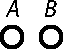
\includegraphics[width=0.2\textwidth]{gesamttex/edit_VIII,3/images/LH_37_05_001_d1.pdf}
\end{minipage}
%\hspace{4,3mm}
\begin{minipage}[t]{0.33\textwidth}
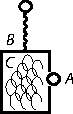
\includegraphics[width=0.39\textwidth]{gesamttex/edit_VIII,3/images/LH_37_05_001_d2.pdf}
\end{minipage}
%\hspace{4,3mm}
\begin{minipage}[t]{0.33\textwidth}
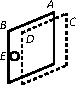
\includegraphics[width=0.5\textwidth]{gesamttex/edit_VIII,3/images/LH_37_05_001_d3.pdf}
\end{minipage}
\newline
\\
%\vspace{2em}
\hspace*{11mm} [\textit{Fig. 1}]\label{LH_37_05_001r_Fig.1}\hspace{34mm} [\textit{Fig. 2}] \label{LH_37_05_001r_Fig.2}\hspace{36mm} [\textit{Fig. 3}] \label{LH_37_05_001r_Fig.3}
\pend
%\vspace{1em}
%\newpage
%
%%
%%  \newpage% 
%  \vspace{2.5em}%	% Diagramm Fig.~1
%  \centerline{\hspace*{-85mm}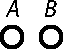
\includegraphics[width=0.072\textwidth]{gesamttex/edit_VIII,3/images/LH_37_05_001_d1.pdf}}%
%  \vspace{0.5em}
%  \centerline{\hspace*{-85mm}\lbrack\textit{Fig.~1}\rbrack}%
%  \label{LH_37_05_001r_Fig.1}%
%%  \vspace{1.5em}%
%%  \newpage%
%%
%%  \newpage% 
%  \vspace{-5.0em}%	% Diagramm Fig.~2
%  \centerline{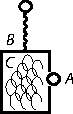
\includegraphics[width=0.13\textwidth]{gesamttex/edit_VIII,3/images/LH_37_05_001_d2.pdf}}%
%  \vspace{0.5em}
%  \centerline{\lbrack\textit{Fig.~2}\rbrack}%
%  \label{LH_37_05_001r_Fig.2}%
%%  \vspace{1.5em}%
%%  \newpage%
%%
%%  \newpage% 
%  \vspace{-9.5em}%	% Diagramm Fig.~3
%  \centerline{\hspace*{85mm}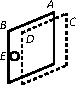
\includegraphics[width=0.18\textwidth]{gesamttex/edit_VIII,3/images/LH_37_05_001_d3.pdf}}%
%  \vspace{0.5em}
%  \centerline{\hspace*{85mm}\lbrack\textit{Fig.~3}\rbrack}%
%  \label{LH_37_05_001r_Fig.3}%
%%  \vspace{1.5em}%
 % \newpage%
%
%
\newpage
\pstart
\noindent
riorem, ajo si minor sit vis globi,\protect\index{Sachverzeichnis}{vis globi}
quam planorum connexio,\protect\index{Sachverzeichnis}{connexio planorum}
sublaturum esse tabulam utramque,%
\protect\index{Sachverzeichnis}{tabula plana}\protect\index{Sachverzeichnis}{tabulae compositae}
sin major
futurum esse,
ut inferiore ne sentiente quidem ictum\protect\index{Sachverzeichnis}{ictus globi}
superior sola tollatur.
\pend%
\count\Bfootins=1200
\count\Afootins=1200
\count\Cfootins=1200
%
\pstart%
Idem experimento\protect\index{Sachverzeichnis}{experimentum baculi vitris superpositi}
constat cum
%
\edtext{\edlabel{LH_37_05_001r_baculusvitroimpositus-1}baculus\protect\index{Sachverzeichnis}{baculus vitris superpositus}
super duobus vitris\protect\index{Sachverzeichnis}{vitrum} frangitur,}{%
\lemma{baculus \lbrack...\rbrack\ frangitur}\Cfootnote{%
Ähnliches Beispiel in N.~12\textsubscript{1}, S.~\refpassage{LH_37_01_018v_baculusvitroimpositus-1}{LH_37_01_018v_baculusvitroimpositus-2}.
Siehe zudem H.~\textsc{Fabri}, \textit{Physica}, tract.~II, lib.~V, prop.~46 (Bd.~I, Lyon 1669, S.~581b).\cite{00044}
Leibniz hat diese Stelle exzerpiert (\textit{LSB} VIII,~2 N.~55, S.~515.25\textendash27).\cite{01234}}}
%
nam si satis fortis sit ictus\protect\index{Sachverzeichnis}{ictus fortis}
baculus rumpetur,\protect\index{Sachverzeichnis}{baculus ruptus}
vitra\protect\index{Sachverzeichnis}{vitrum} non sentient
%
\edtext{ictum.\edlabel{LH_37_05_001r_baculusvitroimpositus-2}\protect\index{Sachverzeichnis}{ictus rumpens}
Ratio est,}{%
\lemma{ictum.}\Bfootnote{%
\textit{(1)}~Et ratio est,
\textit{(2)}~Ratio est,%
~\textit{L}}}
%
quia tabula inferior non impellitur,
nisi quando superior moveri non potest,
quin ipsa moveatur,
nunc vero superior omnino moveri potest,
ipsa non mota.%
\protect\index{Sachverzeichnis}{tabula plana}\protect\index{Sachverzeichnis}{tabulae compositae}
Ita si funis\protect\index{Sachverzeichnis}{funis tensus} tensus sit
secari poterit celeri ictu,\protect\index{Sachverzeichnis}{ictus celeris}
%
% \edtext{}{%
% \lemma{ita}\Bfootnote{%
% \textit{(1)}~ut
% \textit{(2)}~ut%
% ~\textit{L}}}
%
ita ut ea
quibus ab utraque vel alterutra parte annexus est
non evertantur.\edlabel{LH_37_05_001r_deduabustabulis_hgx-2}
\pend 
%
\pstart
Ut autem rem omnem ad experimentum pure mechanicum reducamus,%
\protect\index{Sachverzeichnis}{experimentum mechanicum}
sic agemus.
%
\edtext{}{%
{\xxref{LH_37_05_001r_baculusABD-1}{LH_37_05_001r_baculusABD-2}}%
{\lemma{Sit baculus \textit{ABD}}\Cfootnote{%
Siehe das Diagramm \lbrack\textit{Fig.~4}\rbrack.}}}%
%
\edlabel{LH_37_05_001r_baculusABD-1}%
Sit baculus\protect\index{Sachverzeichnis}{baculus mobilis}
%
\edtext{\textit{ABD}\edlabel{LH_37_05_001r_baculusABD-2}
mobilis circa \textit{A}, et pars ejus}{%
\lemma{\textit{ABD}}\Bfootnote{%
\textit{(1)}~cujus
\textit{(2)}~mobilis circa \textit{A}, et pars ejus%
~\textit{L}}}
%
\textit{BD} mobilis circa \textit{B}
si \textit{AB} immota maneat.
Ponamus autem non posse moveri \textit{BD} circa \textit{B}
quin elevet pondus \textit{E},%
\protect\index{Sachverzeichnis}{pondus elevandum}
neque \textit{AD} circa \textit{A}
quin elevet pondus \textit{F}.
Sit autem pondus
%
\edtext{\lbrack\textit{E}\rbrack}{%
\lemma{\textit{B}}\Bfootnote{%
\textit{L~ändert Hrsg.}}}
%
longe majus quam pondus \textit{F}.
Jam aliud pondus \textit{C} applicetur in \textit{D}.%
\protect\index{Sachverzeichnis}{pondus elevandum}
Hoc si tale sit
ut majorem
(\protect\vphantom)%
habita distantiae a centro%
\protect\index{Sachverzeichnis}{distantia a centro}
ratione%
\protect\vphantom()
vim\protect\index{Sachverzeichnis}{vis ponderis} habeat
quam pondus \textit{F},\protect\index{Sachverzeichnis}{pondus elevandum}
minorem vero quam \textit{E},
totus baculus\protect\index{Sachverzeichnis}{baculus mobilis} movebitur circa \textit{A}. Quod
%
\edtext{si majorem vim\protect\index{Sachverzeichnis}{vis ponderis}
habeat quam \textit{F} et majorem}{%
\lemma{si}\Bfootnote{%
\hspace{-0,5mm}majorem
\textbar~tantum \textit{gestr.}~\textbar\ vim habeat quam \textit{F}
\textit{(1)}~pariter
\textit{(2)}~et majorem%
~\textit{L}}}
%
etiam quam \textit{E}
tunc baculus movebitur\protect\index{Sachverzeichnis}{baculus mobilis}
\pend
%  \newpage% 
  \vspace{1.0em}%	% Diagramm Fig.~4
  \centerline{\hspace*{-86mm}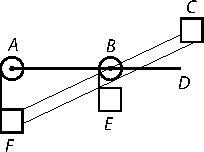
\includegraphics[width=0.29\textwidth]{gesamttex/edit_VIII,3/images/LH_37_05_001_d4.pdf}}%
  \vspace{0.0em}
  \centerline{\hspace*{-86mm}\lbrack\textit{Fig.~4}\rbrack}%
  \label{LH_37_05_001r_Fig.4}%
%  \vspace{1.5em}%
%  \newpage%
%
%  \newpage% 
  \vspace{-9.5em}%	% Diagramm Fig.~5
  \centerline{\hspace*{78,0mm}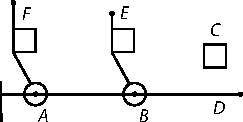
\includegraphics[width=0.35\textwidth]{gesamttex/edit_VIII,3/images/LH_37_05_001_d5.pdf}}%
  \vspace{1.0em}
  \centerline{\hspace*{78,0mm}\lbrack\textit{Fig.~5}\rbrack}%
  \label{LH_37_05_001r_Fig.5}%
%  \vspace{1.5em}%
%  \newpage%
%
%  \newpage% 
  \vspace{1.5em}%	% Diagramm Fig.~6
  \centerline{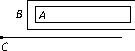
\includegraphics[width=0.30\textwidth]{gesamttex/edit_VIII,3/images/LH_37_05_001_d6.pdf}}% \hspace*{-85mm}
  \vspace{0.0em}
  \centerline{\lbrack\textit{Fig.~6}\rbrack}% \hspace*{-85mm}
  \label{LH_37_05_001r_Fig.6}%
  %\vspace{1.5em}%
  \newpage%
%
%
\pstart
\noindent  tantum circa
%
\edtext{\lbrack\textit{B}\rbrack,}{\lemma{%
\textit{E}}\Bfootnote{%
\textit{L~ändert Hrsg.}}}
%
immoto manente \textit{AB}.
Si vero tam uni quam alteri sit aequalis,
sequitur tamen solum fore motum\protect\index{Sachverzeichnis}{motus baculi}
\edlabel{LH_37_05_001r_demotu_kjdfgvk-1}circa \textit{B}.
%
\edtext{}{%
{\xxref{LH_37_05_001r_demotu_kjdfgvk-1}{LH_37_05_001r_demotu_kjdfgvk-2}}%
{\lemma{circa \textit{B}.}\Bfootnote{%
\textit{(1)}~Ex his positis sequitur etiam quid de funis rupti
\textit{(2)}~Sed quid \lbrack...\rbrack\ parte \textit{B} trahas,
\textbar~et esse quasi utrobique trahatur, \textit{erg.}~%
\textbar\ itaque cedetur \lbrack...\rbrack\ cessurum esse.
\textit{(a)}~Et hoc experiri
\textit{(b)}~Ex his \lbrack...\rbrack\ rumpi debeant,%
~\textit{L}}}}%
\pend%
% \newpage%
%
\pstart%
Sed quid si tractio\protect\index{Sachverzeichnis}{tractio}
sit in linea recta
ut si sit \textit{A} super \textit{B},
et \textit{B} ipsum super \textit{C} immobili,
et connectantur \textit{A} et \textit{B},
item \textit{B} et \textit{C} ope Elaterii;%
\protect\index{Sachverzeichnis}{elaterium connectens}
quaeritur si trahas quid futurum sit,
videtur nihil interesse
utrum a parte \textit{A} an a parte \textit{B} trahas,
et esse quasi utrobique trahatur,
itaque cedetur utrobique si aequales sunt.
Sin inaequales
videtur tantum inferius cessurum esse.
\pend
\pstart%
Ex his definiri posse videtur,
% \edlabel{LH_37_05_001r_demotu4}
quo loco fila%
\protect\index{Sachverzeichnis}{filum}\protect\index{Sachverzeichnis}{ruptura fili}
rumpi debeant,%
\edlabel{LH_37_05_001r_demotu_kjdfgvk-2}
nempe in debiliore,
itaque non miror
si cum rem experirer
variis locis fila sunt rupta,%
\protect\index{Sachverzeichnis}{filum}\protect\index{Sachverzeichnis}{ruptura fili}
sed redit difficultas,\protect\index{Sachverzeichnis}{difficultas}
quia hoc posito idem
%
\edtext{\lbrack ut\rbrack}{%
\lemma{et}\Bfootnote{%
\textit{L~ändert Hrsg.}}}
%
\edtext{supra}{%
\lemma{supra}\Cfootnote{%
S.~\refpassage{LH_37_05_001r_deduabustabulis_hgx-1}{LH_37_05_001r_deduabustabulis_hgx-2}.}}
%
de duobus tabulis%
\protect\index{Sachverzeichnis}{tabula plana}\protect\index{Sachverzeichnis}{tabulae compositae}
esset dicendum.
Si rem filis\protect\index{Sachverzeichnis}{filum} experiare,
omnibus paribus ruptura\protect\index{Sachverzeichnis}{ruptura fili}
fiet circa nodum\protect\index{Sachverzeichnis}{nodus} infimum
ex quo pondus pendet,\protect\index{Sachverzeichnis}{pondus pendens}
vel si duo sint fila,\protect\index{Sachverzeichnis}{filum}
et inferius fortius,
ruptura\protect\index{Sachverzeichnis}{ruptura fili} fiet in eorum confinio.
Si
%
\edtext{tamen locus aliquis}{%
\lemma{tamen}\Bfootnote{%
\textit{(1)}~unum
\textit{(2)}~locus
\textit{(a)}~aliquid
\textit{(b)}~aliquis%
~\textit{L}}}
%
sit valde debilis,
ibi fit ruptura,\protect\index{Sachverzeichnis}{ruptura fili}
salvo
%
superiore principio,\protect\index{Sachverzeichnis}{principium}
% \edtext{}{%
% \lemma{superiore principio}\Cfootnote{% ?????}}
%
quod superatur
%
\lbrack1~v\textsuperscript{o}\rbrack\ % % % %  Blatt 1v
%
proximum quando superari potest.
Hic enim etsi proximum
%
\edtext{fortius}{%
\lemma{fortius}\Bfootnote{%
\textit{erg.~L}}}
%
quoque superari possit,
superatur
%
\edtext{tamen debilius}{%
\lemma{tamen}\Bfootnote{%
\textit{(1)}~remotius
\textit{(2)}~remot
\textit{(3)}~debilius%
~\textit{L}}}
%
licet remotius.
Quia proximum hoc initio non potest superari,
%
% \edtext{}{%
% \lemma{initio}\Bfootnote{%
% \textit{(1)}~insuperabil
% \textit{(2)}~non potest superari,%
% ~\textit{L}}}
%
nec nisi
%
\edtext{paulatim fila\protect\index{Sachverzeichnis}{filum}}{%
\lemma{paulatim}\Bfootnote{%
\textit{(1)}~in fili
\textit{(2)}~fila%
~\textit{L}}}
%
fiunt capacia rupturae.\protect\index{Sachverzeichnis}{ruptura fili}
Hinc cum debilius prius fiat superabile,
ibi quoque prius fit ruptura.\protect\index{Sachverzeichnis}{ruptura fili}
Sed cum omnia sunt paria\lbrack,\rbrack\
ruptura\protect\index{Sachverzeichnis}{ruptura fili} fit in loco propiore. 
\pend%
%
\pstart%
Experimenta ergo\protect\index{Sachverzeichnis}{experimentum nulli exceptioni subjacens}
quae nulli exceptioni subjacent,
et rem clare ostendunt
sunt mechanica\protect\index{Sachverzeichnis}{experimentum mechanicum}
ponderibus\protect\index{Sachverzeichnis}{pondus adhibitum}
sive Elateriis connectentibus\protect\index{Sachverzeichnis}{elaterium connectens} adhibitis.
Quae si favent sententiae\protect\index{Sachverzeichnis}{sententia} meae,
%
% \edtext{}{%
% \lemma{sententiae meae}\Cfootnote{TILGEN ???}}
%
hinc singulari constat exemplo,\protect\index{Sachverzeichnis}{exemplum singulare}
quantum intersit inter motum absolutum,\protect\index{Sachverzeichnis}{motus absolutus}
et respectivum.\protect\index{Sachverzeichnis}{motus respectivus}
\pend%
% \newpage%
%
\pstart%
Idem ut confirmetur,
hoc utamur experimento\lbrack:\rbrack\
in globum unum pendulum\protect\index{Sachverzeichnis}{globus pendulus}
%
\edtext{quiescentem}{%
\lemma{quiescentem}\Bfootnote{%
\textit{erg.~L}}}
%
alius argillaceus\protect\index{Sachverzeichnis}{globus argillaceus} demittatur aequalis,
si motus respectivus\protect\index{Sachverzeichnis}{motus respectivus}
hic nihil differt ab absoluto,\protect\index{Sachverzeichnis}{motus absolutus}
idem erit eventus\protect\index{Sachverzeichnis}{eventus}
qui ambis in se invicem incurrentibus,
nimirum quiescent ambo simul.
\pend%
%
\pstart%
Casus\protect\index{Sachverzeichnis}{casus inanis}%
\edlabel{LH_37_05_001v_casusinanis_rltn-1}
ut duo corpora dura\protect\index{Sachverzeichnis}{corpus durum}
in vacuo\protect\index{Sachverzeichnis}{vacuum} concurrant,%
\protect\index{Sachverzeichnis}{concursus in vacuo}
est inanis,
%
\edtext{atque alienus a natura rerum.%
\protect\index{Sachverzeichnis}{casus alienus a natura rerum}}{%
\lemma{atque}\Bfootnote{%
\textit{(1)}~impossibilis
\textit{(2)}~alienus a natura rerum.%
~\textit{L}}}
%
Nam semper in omni incursu\protect\index{Sachverzeichnis}{incursus}
cessio\protect\index{Sachverzeichnis}{cessio} est
et restitutio\protect\index{Sachverzeichnis}{restitutio}
etsi ea saepe a nobis non sentiantur,
cum spongiosa corpora\protect\index{Sachverzeichnis}{corpus spongiosum} sunt,
et motus per partes dispergitur.%
\protect\index{Sachverzeichnis}{motus per partes dispersus}
Quoties vero non dispergitur,
sed integer\protect\index{Sachverzeichnis}{motus integer} apparet
%
\edtext{motus\lbrack,\rbrack\
apparet praeclarum illud principium,%
\protect\index{Sachverzeichnis}{principium naturae}}{%
\lemma{motus}\Bfootnote{%
\textit{(1)}~verissima est
\textit{(2)}~apparet praeclarum illud
\textit{(a)}~naturae p
\textit{(b)}~Metaph
\textit{(c)}~principium,%
~\textit{L}}}
%
Conatum naturae\protect\index{Sachverzeichnis}{conatus naturae}\protect\index{Sachverzeichnis}{natura}
semper irresistibilem esse.%
\protect\index{Sachverzeichnis}{conatus irresistibilis}
Semper centrum gravitatis mobilium%
\protect\index{Sachverzeichnis}{centrum gravitatis mobilis}
in eadem recta procedet.%
\edlabel{LH_37_05_001v_casusinanis_rltn-2}
\pend%
%
\pstart%
\edtext{Quoties major}{%
\lemma{Quoties}\Bfootnote{%
\hspace{-0,5mm}\textbar~deinde \textit{streicht}~%
\textbar\ major%
~\textit{L}}}
%
est firmitas corporis\protect\index{Sachverzeichnis}{firmitas corporis}
quam ictus,\protect\index{Sachverzeichnis}{ictus}
totum propellitur.
Si quis totam rerum machinam\protect\index{Sachverzeichnis}{machina rerum} tamen intueretur,
videret corpus hoc\protect\index{Sachverzeichnis}{corpus cedens}
quod cedit totum\lbrack,\rbrack\
considerandum ut alterjus partem
in quo et restitutio est,\protect\index{Sachverzeichnis}{restitutio insensibilis}
sed quae in nostro hoc corpore non est sensibilis,
cum per tot alia distribuatur.\protect\index{Sachverzeichnis}{restitutio distributa}
\pend%
\count\Bfootins=1200
\count\Afootins=1200
\count\Cfootins=1200
%
%
% % % %  ENDE des Stücks auf Blatt 1v
%



% N.~5. ((??A36; RK 60241)) Utrum in animalibus omnia possint fieri beneficio elateriorum mechanicorum // AEF (Elastizität)
\chapter[\scriptsize\uppercase{Utrum in animalibus}]{\uppercase{Utrum in animalibus omnia possint fieri beneficio elateriorum mechanicorum}
\newline \lbrack1677 \textendash\  Januar 1680\,(?)\rbrack}
\addcontentsline{toc}{chapter}{\thechapter\enskip Utrum in animalibus omnia possint fieri beneficio elateriorum mechanicorum \enskip\lbrack1677 \textendash\  Januar 1680\,(?)\rbrack}
\label{60241}
\vspace{8mm}
	%   % !TEX root = ../../VIII,3_Rahmen-TeX_8-1.tex
%
%
%   Band VIII, 3 N.~??A36
%   Signatur/Tex-Datei: LH_37_04_080
%   RK-Nr. 60241
%   Überschrift: [Utrum in animalibus omnia possint fieri beneficio elateriorum mechanicorum]
%   Modul: Mechanik / Elastizität
%   Datierung: [1677 bis Januar 1680 (?)]
%   WZ: (keins)
%   SZ: (keins)
%   Bilddateien (PDF): (keins)
%
%
\selectlanguage{ngerman}%
\frenchspacing%
\begin{ledgroupsized}[r]{120mm}
\footnotesize
\pstart
\noindent\textbf{Überlieferung:}
\pend
\end{ledgroupsized}
\begin{ledgroupsized}[r]{114mm}
\footnotesize
\pstart \parindent -6mm
\makebox[6mm][l]{\textit{L}}%
Notiz:
LH~XXXVII~4 Bl.~80.
Ein Zettel (8,5 x 4 cm).
Eine Seite auf Bl.~80~r\textsuperscript{o}.
Auf Bl.~80~v\textsuperscript{o} eine Rechnung von Leibnizens Hand aus unbekanntem Zusammenhang und ohne erkennbare Verbindung mit dem Text auf der Vorderseite:
\newline%
%
% \makebox[6mm][l]{}
1 \qquad 2 \qquad 3 \qquad 4 \quad 5 \quad 6 \quad 7 \quad 8 \quad 9 \quad 10\phantom{$\dfrac{1}{1}$}
\newline%
%
% \makebox[6mm][l]{}
$\dfrac{\overline{2.3 + 2.(6)}-\overline{4+(6)+2+(6)+(7)}}{3+(6)-4+(6)}$ seu $\dfrac{3+(6)-3+(6)+(7)}{0-1}$
\pend
\end{ledgroupsized}
%
%\normalsize
\vspace{5mm}%
\begin{ledgroup}%
\footnotesize%
\pstart%
\noindent%
\textbf{Datierungsgründe:}
Die vorliegende Notiz N.~5 besteht vorwiegend aus einem kurzen, aber sorgfältigen Zitat aus den \glqq Sechsten Einwänden\grqq\ gegen Descartes'%
\protect\index{Namensregister}{\textso{Descartes} (Cartesius, des Cartes), René 1596\textendash1650}
\textit{Meditationes de prima philosophia}\cite{01999} (Paris 1641), welches sich auf die vom französischen Philosophen vertretene Auffassung der Lebewesen als mechanische Automaten bezieht. %
Obwohl Leibniz bereits 1671 in Mainz\protect\index{Ortsregister}{Mainz} die zweite Ausgabe von Descartes' \textit{Opera philosophica}\cite{01300} (Amsterdam 1650) erworben hatte (vgl. \textit{LSB} VI,~3 N.~15, S.~213.13\textendash18\cite{01302}), widmete er sich anscheinend erst in den frühen Hannoveraner\protect\index{Ortsregister}{Hannover} Jahren einer gründlichen Lektüre der \textit{Meditationes}\cite{01999}, als er sich mit Themen der kartesischen Metaphysik und Naturphilosophie kritisch auseinandersetzte.
Seine Anstreichungen und Randbemerkungen zu den \textit{Meditationes}\cite{01999} in seinem Handexemplar von Descartes' \textit{Opera philosophica}\cite{01300} entstanden wahrscheinlich zwischen 1677 und 1687 (\textit{LSB} VI,~4 N.~335, S.~1699\textendash1703\cite{01301}), während seine kommentierten Auszüge aus Descartes' Werken, die zum Teil auch die \textit{Meditationes}\cite{01999} betreffen, auf die Zeitspanne vom Sommer 1678 bis zum Winter 1680/81 zu datieren sind (\textit{LSB} VI,~4 N.~341, S.~1785\textendash1788\cite{01303}).
Auch in Aufzeichnungen und Entwürfen, die insgesamt aus den Jahren 1678 bis 1684/85 stammen und auf Thesen der kartesischen Metaphysik (vornehmlich den ontologischen Gottesbeweis und die voluntaristische Gottesauffassung) eingehen, verdichten sich Bezüge und Anspielungen auf die \textit{Meditationes}\cite{01999} (vgl. etwa \textit{LSB} VI,~4 N.~110\cite{01304}; N.~264\cite{01305}; N.~272\cite{01308}; N.~283\cite{01306}; N.~288;\cite{01317} N.~289\cite{01307}; die zu demselben Zusammenhang gehörige Notiz N.~287\cite{01318} befasst sich ausgesprochen mit Descartes' mechanistischer Auffassung der Tiere).
Ebenso in Briefen aus den späten Siebziger Jahren \textendash\ unter anderen an H.~Fabri, A.~Eckhard, die Pfalzgräfin Elisabeth und N.~Malebranche \textendash\ knüpft Leibniz mehrfach an Themen und Texte aus Descartes' \textit{Meditationes}\cite{01999} an, zumeist in Verbindung mit den soeben genannten metaphysischen Thesen (siehe etwa \textit{LSB} II,~1 \lbrack2006\rbrack\ N.~133, S.~462\textendash466;\cite{01309} N.~138;\cite{01310} N.~219;\cite{01311} N.~143;\cite{01312} N.~148;\cite{01313} N.~187b;\cite{01314} N.~207, S.~721\textendash723\cite{01315}).
Besonders erwähnenswert ist in dieser Hinsicht der Brief an C.~Philipp vom Ende Januar 1680,%
\protect\index{Namensregister}{\textso{Philipp} (Philippi), Christian 1639\textendash1682}
in dem Leibniz bei seiner Zurückweisung von Descartes' voluntaristischer Gottesauffassung ausführlich und zum Teil wörtlich aus den \glqq Sechsten Erwiderungen\grqq\ zitiert (siehe \textit{LSB} II,~1 \lbrack2006\rbrack\ N.~222, S.~787.24\textendash788.23\cite{01316}). % vgl. R.~\textsc{Descartes}, \textit{Meditationes}, responsiones VI, §~6 u.~8; 
Spätestens zu diesem Zeitpunkt dürfte er Gelegenheit gehabt haben, die Passage aus den \glqq Sechsten Einwänden\grqq\ zu lesen, von der die Notiz N.~5 unmittelbar herrührt.
Diese sollte demnach zwischen 1677 und Ende Januar 1680 verfasst worden sein.
Eine spätere Datierung (bis etwa 1687) ist jedoch nicht auszuschließen.%
\protect\index{Namensregister}{\textso{Descartes} (Cartesius, des Cartes), René 1596\textendash1650}
\pend
\end{ledgroup}
\selectlanguage{latin}%
\frenchspacing%
%
% \vspace{8mm}
\newpage%
%
\count\Bfootins=1200
\count\Afootins=1200
\count\Cfootins=1200
%
%
\pstart
% \vspace*{0.5em}% PR: nur provisorisch
\noindent
\lbrack80~r\textsuperscript{o}\rbrack%
\textso{ Elaterii }\protect\index{Sachverzeichnis}{elaterium}%
vox pro eo
quod Germanis\protect\index{Sachverzeichnis}{Germani} vocatur Feder,\protect\index{Sachverzeichnis}{Feder}
Italis\protect\index{Sachverzeichnis}{Itali} Molla,\protect\index{Sachverzeichnis}{molla}
Gallis\protect\index{Sachverzeichnis}{Galli} ressort,\protect\index{Sachverzeichnis}{ressort}
%
\edtext{}{%
{\xxref{LH37_04_080r_1}{LH37_04_080r_2}}%
{\lemma{extat \lbrack...\rbrack\ \textit{Mechanicorum}}\Cfootnote{%
Siehe \textsc{R.~Descartes}, \textit{Meditationes de prima philosophia}, Objectiones sextae, Paris 1641, S.~555\cite{01999}
(\textit{DO}~VII, S.~414.18\textendash19).\cite{00120}
\selectlanguage{german}{Die \glqq Sechsten Einwände\grqq\ wurden anonym % von unter\-schied\-li\-chen Autoren 
verfasst, von M.~Mersenne\protect\index{Namensregister}{\textso{Mersenne} (Mersennus), Marin 1588\textendash1648} gesammelt und an Descartes\protect\index{Namensregister}{\textso{Descartes} (Cartesius, des Cartes), René 1596\textendash1650} weitergeleitet.}}}}%
%
\edlabel{LH37_04_080r_1}extat apud autorem sextarum
in Cartesii\protect\index{Namensregister}{\textso{Descartes} (Cartesius, des Cartes), René 1596\textendash1650}
\textit{Meditationes} objectionum sub finem scrupuli\protect\index{Sachverzeichnis}{scrupulus} tertii,
utrum scilicet in animalibus\protect\index{Sachverzeichnis}{animal}
\textit{omnia possint fieri beneficio Elateriorum Mechanicorum.}\edlabel{LH37_04_080r_2}%
\protect\index{Sachverzeichnis}{elaterium mechanicum}
% [Meditationes, Ausgabe 1685, S. 150, anonym (gesammelt von Mersenne)]
%
\pend
% Ende des Stückes



% N.~6. ((??A44; RK 60338)) Corpora impulsa agunt a se ipsis [ex: Defendi potest] // AEF (Elastizität)
\chapter[\scriptsize\uppercase{Corpora impulsa agunt a se ipsis}]{\uppercase{Corpora impulsa agunt a se ipsis}
\newline \lbrack März 1677\,(?) \textendash\  Januar 1678\rbrack}
\addcontentsline{toc}{chapter}{\thechapter\enskip Corpora impulsa agunt a se ipsis \enskip\lbrack März 1677\,(?) \textendash\  Januar 1678\rbrack}
\label{60338}
\vspace{8mm}
	%   % !TEX root = ../../VIII,3_Rahmen-TeX_8-1.tex
%
%
%   Band VIII, 3 N.~??A44
%   Signatur/Tex-Datei: LH_37_05_123
%   RK-Nr. 60338
%   \ref{60338}
%   Überschrift: Corpora impulsa agunt a se ipsis [ex: Defendi potest]
%   Modul: Mechanik / AEF (Elastizität)
%   Datierung: (?) Frühjar 1677 bis Anfang 1678
%   WZ: (keins)
%   SZ: (keins)
%   Bilddateien (PDF): (keine)
%
%
\selectlanguage{ngerman}%
\frenchspacing%
%
\begin{ledgroupsized}[r]{120mm}%
\footnotesize%
\pstart%
\noindent\textbf{Überlieferung:}%
\pend%
\end{ledgroupsized}%
\begin{ledgroupsized}[r]{114mm}%
\footnotesize%
\pstart%
\parindent -6mm%
\makebox[6mm][l]{\textit{L}}%
Aufzeichnung:
LH XXXVII~5 Bl.~123.
Ein Blatt 4\textsuperscript{o}, schräg beschnitten (etwa 16,5 x 18 cm);
Papiererhaltungsmaßnahmen.
Eineinhalb Seiten.
Auf Bl.~123~r\textsuperscript{o} in der oberen linken Ecke, vermutlich von fremder Hand vermerkt: \textit{ad 41}.
\pend%
\end{ledgroupsized}%
%
\vspace*{5mm}%
\begin{ledgroup}%
\footnotesize%
\pstart%
\noindent%
\textbf{Datierungsgründe:}
In der vorliegenden Aufzeichnung N.~\ref{60338} %??A44 
hält Leibniz fest, dass die Veränderung des kinetischen Zustands eines gestoßenen Körpers ursächlich auf die innere elastische Kraft dieses Körpers selbst zurückgehe und nur scheinbar vom stoßenden Körper herrühre, welcher demnach als bloße Gelegenheitsursache der Veränderung zu betrachten sei.
Hieraus zieht Leibniz schließlich die Folgerung, dass in jedem Körper ursprünglich eine unendliche Kraft (\textit{vis}) und somit eine unendliche \textit{quantitas motus} vorliegen müsse (S.~\refpassage{LH_37_05_123v_iqciqmdfm-1}{LH_37_05_123v_iqciqmdfm-2}).
Diese Gleichsetzung von (kinetischer) Kraft und Bewegungsquantum lässt sich als Zeichen dafür deuten, dass die Aufzeichnung N.~\ref{60338} %??A44 
noch vor der eigenhändig auf Januar 1678 datierten \textit{Scheda VIII de corporum concursu} (N.~\ref{dcc_08}) entstand.
Denn dort verkündet Leibniz zum ersten Mal die Entdeckung
\textendash\ Geburtsstunde seiner \textit{réforme de la dynamique} (\textsc{Fichant} 1994\cite{01056})~\textendash,
dass die \textit{vis} eines sich bewegenden Körpers dem Produkt der Masse und des Quadrats der Geschwindigkeit $mv^2$ entspreche und daher grundsätzlich anders als dessen Bewegungsquantum \textit{mv} sei (N.~\ref{dcc_08}, S.~\refpassage{LH_37_05_086r_reformatio_idzg-1}{LH_37_05_086r_reformatio_idzg-2}).
\pend%
%
\pstart%
Die in der vorliegenden Aufzeichnung geäußerte kausaltheoretische These vertritt Leibniz freilich auch in späteren Texten: etwa in den auf Sommer 1678 bis Winter 1680/81~(?) datierbaren \textit{Definitiones cogitationesque metaphysicae} (\textit{LSB} VI,~4 N.~267, S.~1401.1\textendash5\cite{01339}) sowie noch in der Stoßlehre der \textit{Dynamica} (pars II, sectio III, prop.~6\cite{01354}), wo selbst das in N.~\ref{60338} angeführte Gleichnis des vom Ufer zurückgestoßenen Schiffes wieder vorkommt (\textit{LMG} VI, S.~409;\cite{01043} vgl. N.~\ref{60338}, S.~\refpassage{LH_37_05_123r_navisexripa-1}{LH_37_05_123r_navisexripa-2}).
An keiner dieser Parallelstellen aber wird die innere elastische Kraft der Körper als Bewegungsgröße beschrieben.
Eine Entstehung von N.~\ref{60338} nach Januar 1678 erweist sich somit als unwahrscheinlich, sie kann jedoch nicht ausgeschlossen werden.
\pend%
\pstart%
Der Terminus post quem der Datierung ist ebenfalls mit Unsicherheit behaftet.
Mit den Fragen der Stoßlehre, die der Aufzeichnung N.~\ref{60338} %??A44 
zugrundeliegen, hatte sich Leibniz bekanntlich seit dem Sommer 1669 befasst.
Die Art, wie elastischer und plastischer Stoß in N.~\ref{60338} %??A44 
beschrieben und unterschieden werden (S.~\refpassage{LH_37_05_123r_ostensumst_hjjd-1}{LH_37_05_123r_ostensumst_hjjd-2}; \refpassage{LH_37_05_123v_plastischerstoss-1}{LH_37_05_123v_plastischerstoss-2}), setzt aber die Bekanntschaft mit J.~Wallis'%
\protect\index{Namensregister}{\textso{Wallis} (Wallisius), John 1616\textendash1703}
und E.~Mariottes%
\protect\index{Namensregister}{\textso{Mariotte}, Edme, Seigneur de Chazeuil ca. 1620\textendash1684}
späteren Überlegungen über den Stoß voraus, mit denen sich Leibniz besonders zwischen den letzten Monaten 1674 und dem Sommer 1675 auseinandergesetzt hatte (vgl. \textit{LSB} VIII,~2 N.~8,\cite{01343} S.~89\textendash93; N.~50\cite{01292}).
Die Aufzeichnung N.~\ref{60338} %??A44 
entstand daher höchstwahrscheinlich nachher. 
Die im Text vertretene kausaltheoretische Ansicht dürfte aber vornehmlich an die seit März 1677 entwickelten Untersuchungen zum Stoßgesetz anknüpfen, bei denen Leibniz das Phänomen des elastischen Stoßes in ähnlicher Weise wie Wallis und Mariotte erörtert
(vgl. die Erläuterung zu S.~\refpassage{LH_37_05_123r_ostensumst_hjjd-1}{LH_37_05_123r_ostensumst_hjjd-2}).
Hieraus ergibt sich die vorgeschlagene Datierung.
Eine frühere Entstehungszeit der Aufzeichnung N.~\ref{60338} %??A44 
(jedenfalls nach 1674) ist dennoch nicht auszuschließen.
\pend%
%
\pstart%
Bemerkenswert ist schließlich, dass in der eigenhändig auf Januar 1678 datierten \textit{Scheda VI-II de corporum concursu} stoßtheoretische Überlegungen ebenfalls eine Digression über die kausale Selbständigkeit mechanisch interagierender Körper veranlassen (N.~\ref{dcc_06-2}, %??S01\textsubscript{8}
S.~\refpassage{LH_35_09_23_018v_occasionalismus_jyr-1}{LH_35_09_23_018v_occasionalismus_jyr-2}).
Anders als in N.~\ref{60338} %??A44 der Aufzeichnung 
aber vertritt Leibniz dort eine okkasionalistische Betrachtungsweise, die den Status einer echten Wirkursache nicht den einzelnen Körpern bzw. deren ursprünglicher elastischer Kraft zuweist, sondern nur Gott.
\pend%
\end{ledgroup}%
%
\selectlanguage{latin}%
\frenchspacing%
%
%
\newpage%
\count\Bfootins=1100
\count\Afootins=1200
\count\Cfootins=1100
%\vspace*{8mm}%
\pstart%
\normalsize%
\noindent%
%
\lbrack123~r\textsuperscript{o}\rbrack\ %    %    %    %    Blatt 123r
%
Defendi potest corpus non impelli%
\protect\index{Sachverzeichnis}{corpus impulsum immediate ab alio}%
\protect\index{Sachverzeichnis}{impulsus immediatus}
%
\edtext{immediate}{%
\lemma{immediate}\Bfootnote{%%
\textit{erg.~L}}}
%
ab alio corpore,%
\protect\index{Sachverzeichnis}{corpus impellens}
sed occasione alterius a se%
\protect\index{Sachverzeichnis}{occasio agendi}%
\protect\index{Sachverzeichnis}{corpus impulsum occasione alterius}
%
\edtext{ipso neque}{%
\lemma{ipso}\Bfootnote{%%
\textit{(1)}~. Si enim
\textit{(2)}~neque \textit{L}}}
%
adeo nisi propria vi cieri.%
\protect\index{Sachverzeichnis}{vis corporis propria}
Nam
%
\edlabel{LH_37_05_123r_ostensumst_hjjd-1}%
ostensum est%
\edtext{}{%
{\xxref{LH_37_05_123r_ostensumst_hjjd-1}{LH_37_05_123r_ostensumst_hjjd-2}}%
{\lemma{ostensum \lbrack...\rbrack\ recedere}\Cfootnote{%
Leibniz erörtert in dieser Weise den elastischen Stoß etwa in dem eigenhändig auf März 1677 datierten Entwurf N.~\ref{RK57266-1} % \textit{Elastrum est causa imperfectionis in corporum concursu}
und verweist dabei (S.~\refpassage{LH_37_05_161v_mariottewallis-1}{LH_37_05_161v_mariottewallis-2}) auf \textit{Mariotti ac Wallisii rationem explicandi};%
\protect\index{Namensregister}{\textso{Wallis} (Wallisius), John 1616-1703}%
\protect\index{Namensregister}{\textso{Mariotte}, Edme, Seigneur de Chazeuil ca. 1620-1684}
siehe hierzu
\textsc{J.~Wallis}, \cite{00301}\textit{Mechanica}, pars~III, cap.~XI u.~XIII (London 1670\textendash1671, Bd.~II, S.~660\textendash682 u.~686\textendash707; \cite{01008}\textit{WO}~I, S.~1002\textendash1015 u.~1018\textendash1031)
sowie
\textsc{E.~Mariotte}, \cite{00311}\textit{De la percussion}, partie I, prop.~XIII u.~XIX (Paris 1673, S.~68\textendash72 u.~115\textendash119).
Ähnlich fasst Leibniz den elastischen Stoß auch später in dem eigenhändig auf Januar und Februar 1678 datierten Textkomplex \textit{De corporum concursu} (N.~\ref{dcc_05} u.~\ref{dcc_06-1}) auf.%
}}}
%
corpora concursu%
\protect\index{Sachverzeichnis}{concursus corporum}
%
\edtext{comprimi,%
\protect\index{Sachverzeichnis}{corpus compressum}
prius quam propelli,%
\protect\index{Sachverzeichnis}{corpus propulsum}
et restituente sese Elasmate%
\protect\index{Sachverzeichnis}{elasma se restituens}
a se invicem proprio nisu%
\protect\index{Sachverzeichnis}{nisus corporis recedentis}
recedere,%
\protect\index{Sachverzeichnis}{corpus proprio nisu recedens}%
\edlabel{LH_37_05_123r_ostensumst_hjjd-2}
\edlabel{LH_37_05_123r_navisexripa-1}%
quemadmodum nos ex navi%
\protect\index{Sachverzeichnis}{navis}
conto%
\protect\index{Sachverzeichnis}{contus}
ripam%
\protect\index{Sachverzeichnis}{ripa}
aut fundum%
\protect\index{Sachverzeichnis}{fundus}
impellendo
una cum navi%
\protect\index{Sachverzeichnis}{navis}
inde recedimus.%
\edlabel{LH_37_05_123r_navisexripa-2}
Haec}{%
\lemma{comprimi,}\Bfootnote{%
\textit{(1)}~nec prius propell
\textit{(2)}~prius quam propelli,
\textit{(a)}~et antequam
\textit{(b)}~et restituente % sese Elasmate 
\lbrack...\rbrack\ a se
\textit{(aa)}~mutuo \textlangle vi\textrangle\
\textit{(bb)}~invicem proprio nisu recedere
\textit{(aaa)}~%
\textbar~mutuo \textit{erg.}~%
\textbar\ conari,
\textit{(bbb)}~, quemadmodum
\textbar~%
\textit{(1)}~is qui
\textit{(2)}~ex navi
\textit{(3)}~ex
\textit{(4)}~si quis
\textit{(5)}~nos ex navi \textit{erg.}~%
\textbar\ conto
\textit{(aaaa)}~aut
\textit{(bbbb)}~ripam aut fundum impellendo
\textit{(aaaaa)}~ex navi nos
\textit{(bbbbb)}~una cum navi inde recedimus
\textbar~atque abspellimur \textit{gestr.}~%
\textbar~. Haec%
~\textit{L}}}
%
partim experimentis,%
\protect\index{Sachverzeichnis}{experimentum}
partim etiam firmis%
\protect\index{Sachverzeichnis}{ratio firma}
%
\edtext{rationibus ostendi possunt,
quoniam nihil impetum momento accipit%
\protect\index{Sachverzeichnis}{impetus acceptus momento}
sed per gradus%
\protect\index{Sachverzeichnis}{impetus acceptus per gradus}
intermedios%
\protect\index{Sachverzeichnis}{gradus intermedius}
a quiete,%
\protect\index{Sachverzeichnis}{quies}
quod}{%
\lemma{rationibus}\Bfootnote{%
\textit{(1)}~ostendimus
\textit{(2)}~ostendi possunt quoniam
\textit{(a)}~ostensum est
\textit{(b)}~certum demonstr
\textit{(3)}~nihil impetum momento 
\textit{(a)}~accipere
\textit{(b)}~accipit sed % per gradus intermedios 
\lbrack...\rbrack\ a quiete
\textit{(aa)}~omnes transire
\textit{(bb)}~, quod%
~\textit{L}}}
%
fit restitutione Elastri%
\protect\index{Sachverzeichnis}{elastrum se restituens}%
\protect\index{Sachverzeichnis}{restitutio elastri}%
\lbrack;\rbrack\
%
\edtext{a solo igitur Elastro%
\protect\index{Sachverzeichnis}{elastrum}
oritur motuum translatio%
\protect\index{Sachverzeichnis}{translatio motus}
atque communicatio:%
\protect\index{Sachverzeichnis}{communicatio motus}%
}{\lemma{a}\Bfootnote{%
\hspace{-0,5mm}solo \lbrack...\rbrack\ atque communicatio
\textit{erg.~L}}}
%
porro impellens,%
\protect\index{Sachverzeichnis}{corpus impellens}
quod Elastrum intendit%
\protect\index{Sachverzeichnis}{elastrum intensum}%
\lbrack,\rbrack\
non vim ipsi tribuit,%
\protect\index{Sachverzeichnis}{vis tributa}
%
\edtext{sed determinat%
\protect\index{Sachverzeichnis}{vis determinata}
praestita occasione agendi.%
\protect\index{Sachverzeichnis}{occasio agendi}%
}{%
\lemma{sed}\Bfootnote{%
\textit{(1)}~occasionem praestat
\textit{(2)}~determinat praestita occasione agendi.%
~\textit{L}}}
%
Intus enim perfluit velocissima materia,%
\protect\index{Sachverzeichnis}{materia intus perfluens}%
\protect\index{Sachverzeichnis}{materia velocissima}
quae nihil insoliti inveniens,
neque sentitur,%
\protect\index{Sachverzeichnis}{materia insensibilis}
sed obstaculo objecto%
\protect\index{Sachverzeichnis}{obstaculum objectum}
ostendit quid possit;
quemadmodum flumina si coerceantur.%
\protect\index{Sachverzeichnis}{flumen coercitum}
Vis igitur qua corpus cietur%
\protect\index{Sachverzeichnis}{vis ciens}
intra ipsum est.%
\protect\index{Sachverzeichnis}{vis intra corpum}
\pend%
%
\pstart%
At, inquies, saltem partes in compressione%
\protect\index{Sachverzeichnis}{compressio partium}
impelluntur et aliunde vim accipiunt.%
\protect\index{Sachverzeichnis}{vis accepta aliunde}
%
\edtext{Respondeo,
quod de toto diximus
etiam de parte dicendum esse,}{%
\lemma{Respondeo,}\Bfootnote{%
\textit{(1)}~partes ips
\textit{(2)}~quod de % toto diximus etiam de parte
\lbrack...\rbrack\ dicendum esse,%
~\textit{L}}}
%
ut vicissim illae
non nisi suis prius partibus compressis%
\protect\index{Sachverzeichnis}{pars corporis compressa}
ac sese restituentibus%
\protect\index{Sachverzeichnis}{pars corporis se restituens}
impellantur.%
\protect\index{Sachverzeichnis}{pars corporis impulsa}
Quae quidem in omnibus partium partibus continuata%
\protect\index{Sachverzeichnis}{partes partium}
utcunque subdivisione vera sunt,%
\protect\index{Sachverzeichnis}{subdivisio partium}
et nihil movetur,
quin praecedat
%
infinitorum aliorum
%\edtext{\lbrack infinitarum aliarum\rbrack}{%
%\lemma{infinitorum aliorum}\Bfootnote{%
%\textit{L~ändert Hrsg.}}}
%
motus%
\protect\index{Sachverzeichnis}{motus infinitorum aliorum}
per respondentis temporis partes%
\protect\index{Sachverzeichnis}{pars temporis}%
\lbrack,\rbrack\
etiam proportione exiguas distributas.
Habent enim omnia quendam flexilitatis gradum,%
\protect\index{Sachverzeichnis}{flexilitas}%
\protect\index{Sachverzeichnis}{gradus flexilitatis}
nihilque infinitae rigiditatis est,%
\protect\index{Sachverzeichnis}{rigiditas infinita}
hinc semper prius movetur pars,%
\protect\index{Sachverzeichnis}{pars mota prius quam totum}
quam
\edlabel{LH_37_05_123r_12301}%
totum.%
\edtext{}{%
{\xxref{LH_37_05_123r_12301}{LH_37_05_123r_12302}}%
{\lemma{totum.}\Bfootnote{%
\textit{(1)}~Caeterum
\textit{(2)}~Dici
\textit{(a)}~porro
\textit{(b)}~etiam potest%
~\textit{L}}}}
\pend%
%\newpage%
%
\pstart%
Dici etiam potest%
\edlabel{LH_37_05_123r_12302}
non tantum corpus omne moveri a se ipso,%
\protect\index{Sachverzeichnis}{corpus motum a se ipso}
vel eo quod in
%
\edtext{ipso est,}{%
\lemma{ipso}\Bfootnote{\hspace{-0,5mm}%
\textbar~conclusum \textit{gestr.}~%
\textbar\ est%
~\textit{L}}}
%
sed etiam ex ipsius statu praecedenti%
\protect\index{Sachverzeichnis}{status corporis praecedens}
consequi praesentem motum,%
\protect\index{Sachverzeichnis}{motus consequens ex statu praecedenti}%
\protect\index{Sachverzeichnis}{motus praesens}
ita ut agat sponte,%
\protect\index{Sachverzeichnis}{corpus agens sponte}
ac nihil absolute loquendo in
%
\edtext{natura sit}{%
\lemma{natura}\Bfootnote{%
\textit{(1)}~esse
\textit{(2)}~sit%
~\textit{L}}}
%
violentum.%
\protect\index{Sachverzeichnis}{natura}%
\protect\index{Sachverzeichnis}{violentum}
Nam etsi videatur compressio%
\protect\index{Sachverzeichnis}{compressio ab externo}
saltem ab externo fieri,
\edtext{attamen cum}{\lemma{attamen}\Bfootnote{%
\textit{(1)}~re vera
\textit{(2)}~comm
\textit{(3)}~cum%
~\textit{L}}}
%
omnis compressio motum partium%
\protect\index{Sachverzeichnis}{motus partium in compresssione}
%
\edtext{contineat,
omnis autem res moveatur}{\lemma{contineat,}\Bfootnote{%
\textit{(1)}~motus autem sit fact
\textit{(2)}~omnis autem res moveatur%
~\textit{L}}}
%
a se ipsa,%
\protect\index{Sachverzeichnis}{res mota a se ipsa}
%
\edtext{ut ostensum est,}{%
\lemma{ut ostensum est}\Cfootnote{%
Soeben in der vorliegenden Aufzeichnung N.~\ref{60338}.%??A44
}}
%
nec compressio ab externo
%
\edtext{\lbrack fieri\rbrack}{%
\lemma{facta}\Bfootnote{%
\textit{L~ändert Hrsg.}}}
%
poterit,%
\protect\index{Sachverzeichnis}{compressio ab externo}
nihil aliud
%
\edtext{ergo est}{\lemma{ergo}\Bfootnote{%
\textit{(1)}~fuerit
\textit{(2)}~est%
~\textit{L}}}
%
corpus externum,%
\protect\index{Sachverzeichnis}{corpus externum}
quam ut sit comitans atque connexum,%
\protect\index{Sachverzeichnis}{corpus comitans}%
\protect\index{Sachverzeichnis}{corpus connexum}
quod nobis
rerum interiora ignorantibus%
\protect\index{Sachverzeichnis}{interiora rerum}
causa videtur.%
\protect\index{Sachverzeichnis}{causa apparens}
%
\edtext{Interim notio}{%
\lemma{interim}\Bfootnote{%
\textit{(1)}~si
\textit{(2)}~certa not
\textit{(3)}~sit
\textit{(4)}~notio%
~\textit{L}}}
%
causae%
\protect\index{Sachverzeichnis}{notio causae}
assignari poterit%
\lbrack,\rbrack\
qua adhibita recte
%
\edtext{dicetur motum corporis}{%
\lemma{dicetur}\Bfootnote{%
\textit{(1)}~corporis
\textit{(2)}~motum corporis%
~\textit{L}}}
%
unius esse causam motus%
\protect\index{Sachverzeichnis}{causa motus mediata}
corporis alterius,
etsi non sit causa immediata.%
\protect\index{Sachverzeichnis}{causa motus immediata}
%
\lbrack123~v\textsuperscript{o}\rbrack%    %    %    %    Blatt 123v
%
\pend%
%
\pstart%
\edtext{Quando%
\edlabel{LH_37_05_123v_plastischerstoss-1}
corpus unum incurrit in aliud quiescens%
\protect\index{Sachverzeichnis}{corpus incurrens in quiescens}%
}{%
\lemma{Quando}\Bfootnote{%
\textit{(1)}~duo corpora concurrunt
\textit{(2)}~corpus unum % incurrit in 
\lbrack...\rbrack\ aliud quiescens%
~\textit{L}}}
%
et post ictum simul%
\protect\index{Sachverzeichnis}{ictus consumtus}
%
\edtext{procedunt dubites an}{%
\lemma{procedunt}\Bfootnote{%
\textit{(1)}~non videtur
\textit{(2)}~dubites an%
~\textit{L}}}
%
commode defendi possit
%
\edtext{corpus quod quieverat%
\protect\index{Sachverzeichnis}{corpus quiescens}
impulsum esse a se ipso.%
\protect\index{Sachverzeichnis}{corpus impulsum a se ipso}%
}{%
\lemma{corpus}\Bfootnote{%
\textit{(1)}~impelli a se ipso
\textit{(2)}~quod quieverat %
impulsum esse a 
\lbrack...\rbrack\ se ipso.%
~\textit{L}}}
%
Nam ictus%
\protect\index{Sachverzeichnis}{ictus consumtus}
omnis in partibus mollibus%
\protect\index{Sachverzeichnis}{pars mollis}
consumtus est.%
\edlabel{LH_37_05_123v_plastischerstoss-2}
Verum cum certum videatur
nullum corpus momento motum notabilem accipere,%
\protect\index{Sachverzeichnis}{motus acceptus}
cogitandum,
quomodo res explicari possit.
\pend
%
\pstart
Videtur%
\edlabel{LH_37_05_123v_iqciqmdfm-1}
omne corpus jam tum
in se eam omnem vim habere%
\protect\index{Sachverzeichnis}{vis in corpore}
quam unquam acquirere potest%
\lbrack,\rbrack\
adeoque infinitam,%
\protect\index{Sachverzeichnis}{vis infinita}
sunt enim infinitorum corporum motus%
\protect\index{Sachverzeichnis}{motus infinitorum corporum}
magnae celeritatis%
\protect\index{Sachverzeichnis}{celeritas magna}%
\protect\index{Sachverzeichnis}{motus magnae celeritatis}
in eo inclusi,%
\protect\index{Sachverzeichnis}{motus in corpore inclusus}
ita ut in quolibet corpore insit quantitas motus%
\protect\index{Sachverzeichnis}{quantitas motus in corpore insita}
data finita major.%
\protect\index{Sachverzeichnis}{quantitas motus major finita}%
\edlabel{LH_37_05_123v_iqciqmdfm-2}
%
Corpus omne videtur
non nisi a seipso impelli,%
\protect\index{Sachverzeichnis}{corpus impulsum a se ipso}
sive motu suo,%
\protect\index{Sachverzeichnis}{corpus impulsum a motu suo}
sive elaterio%
\protect\index{Sachverzeichnis}{elaterium impellens}
quod a motu intestino proficiscitur.%
\protect\index{Sachverzeichnis}{elaterium a motu intestino profectum}
Verum inquies\lbrack,\rbrack\
cum corpus in quiescens incurrit,%
\protect\index{Sachverzeichnis}{corpus incurrens in quiescens}
prius ejus partes impellit ac comprimit%
\protect\index{Sachverzeichnis}{pars corporis impulsa}%
\protect\index{Sachverzeichnis}{pars corporis compressa}
quam ullum elastrum existere possit;
respondeo
in omni corpore
quod totum quiescit%
\protect\index{Sachverzeichnis}{corpus quiescens}
partes esse in celerrimo motu,%
\protect\index{Sachverzeichnis}{motus partium celerrimus}
eoque magis
quo est firmius,
et corpus incurrens%
\protect\index{Sachverzeichnis}{corpus incurrens}
atque impellens%
\protect\index{Sachverzeichnis}{corpus impellens}
in
%
\edtext{hunc motum partium extimarum%
\protect\index{Sachverzeichnis}{motus partium extimarum}%
}{%
\lemma{hunc}\Bfootnote{%
\textit{(1)}~intestinum
\textit{(2)}~motum partium extimarum \textit{L}}}
%
incidere,
atque hinc
%
reflectere%
\protect\index{Sachverzeichnis}{pars corporis reflexa}
%\edtext{\lbrack???reflecti\rbrack}{%
%\lemma{reflectere}\Bfootnote{%
%\textit{L~ändert Hrsg.}}}
%
illas partes. 
\pend
%
%
%
%    %    %    %   Ende des Textes auf Blatt 123v



% N.~7. ((??A14; RK 41157)) De tensione et restitutione // AEF (Elastizität)
\chapter[\scriptsize\uppercase{De tensione et restitutione}]{\uppercase{De tensione et restitutione}
\newline\lbrack Frühjahr 1679 \textendash\  Winter 1680/1681\,(?)\rbrack}
\addcontentsline{toc}{chapter}{\thechapter\enskip De tensione et restitutione \enskip\lbrack Frühjahr 1679 \textendash\  Winter 1680/1681\,(?)\rbrack}
\label{41157}
\vspace{8mm}
	%   % !TEX root = ../../VIII,3_Rahmen-TeX_8-1.tex
%   ####
%
%   Band VIII, 3 N.~??A14 // Akustik, Elastizität, Festigkeit
%   Signatur/Tex-Datei: LH_35_09_15_001,022
%   RK-Nr. 41157
%   Überschrift: [De tensione et restitutione]
%   Datierung: [Sommer 1678 bis Winter 1680/1681 (?)]
%   WZ: LEd-Wz 803002 = RK-WZ: 138 (Achtblättrige Rosette auf CS)
%.  SZ: \leibvdash (insgesamt eins)
%.  Bilddateien (PDF): LH_35_09_15_001,022_d1; LH_35_09_15_001,022_d2; LH_35_09_15_001,022_d3; LH_35_09_15_001,022_d4; LH_35_09_15_001,022_d5; LH_35_09_15_001,022_d6 (insgesamt: sechs)
%
%
\selectlanguage{ngerman}%
\frenchspacing%
%
\begin{ledgroupsized}[r]{120mm}
\footnotesize
\pstart
\noindent
\textbf{Überlieferung:}
\pend
\end{ledgroupsized}
\begin{ledgroupsized}[r]{114mm}
\footnotesize
\pstart \parindent -6mm
\makebox[6mm][l]{\textit{L}}%
Aufzeichnung: LH~XXXV~9,~15 Bl.~1, 22.
Zwei Blatt~4\textsuperscript{o},
die ursprünglich einen \mbox{Bogen} bildeten;
zusammenhängende Hälften eines Wasserzeichens auf Bl.~1 und Bl.~22.
Vier Seiten, zumeist einspaltig beschrieben;
Textfolge gemäß Blattzählung;
gesamter Text (Diagramme, Rechnungen und Randbemerkungen mit eingeschlossen) gestrichen.
% Auf der rechten Spalte von Bl.~22~v\textsuperscript{o} finden sich,
% ebenfalls gestrichen, Rechnungen und Diagramme,
% die keinen unmittelbaren Zusammenhang mit dem Text aufweisen.
Bl.~1 und Bl.~22 waren ursprünglich mit LH~XXXV~11,~14 Bl.~18,
einem der Textträger von \textit{LSB} VI,~4 N.~267,\cite{01339} verbunden.
\pend
\end{ledgroupsized}
%
%
\vspace{5mm}
\begin{ledgroup}
\footnotesize
\pstart
\noindent
\textbf{Datierungsgründe:}\label{LH_35_09_15_001,022_Datierung}
In der vorliegenden Aufzeichnung N.~7 erörtert Leibniz im Rahmen seiner Elastizitätslehre vornehmlich den Begriff der Spannung (\textit{tensio}) als Ursache elastischer Wiederherstellung (\textit{restitutio}).
Als ausschlaggebend für die Datierung erweist sich der Überlieferungszusammenhang mit dem Text \textit{Definitiones cogitationesque metaphysicae} (\textit{LSB} VI,~4 N.~267\cite{01339}),
mit dem die Aufzeichnung N.~7 ursprünglich einen einheitlichen Folio-Bogen bildete; vom Duktus her könnte N.~7 sogar als Ableger der umfangreicheren \textit{Definitiones cogitationesque metaphysicae} entstanden sein.
Das für die frühe Hannoveraner Zeit gewöhnliche Wasserzeichen im Träger von N.~7 ist im Nachlass für den Zeitraum vom Sommer 1678 bis zum Winter 1680/1681 belegt.
Aus inhaltlichen Gründen kann man aber ausschließen, dass die \textit{Definitiones cogitationesque metaphysicae} vor dem Frühjahr 1679 entstanden (vgl. VI,~4, S.~1393.18\textendash21).
Eine Entstehungszeit zwischen Frühjahr 1679 und Winter 1680/1681 ist somit grundsätzlich auch für N.~7 anzunehmen.
\pend%
\pstart%
Es gilt allerdings zu bemerken, dass der Aufzeichnung N.~7 offenbar eine kritische Auseinandersetzung mit H.~\textsc{Fabri}, \textit{Physica}, tract.~I, lib. II: \textit{De compresso et tenso} (Bd.~I, Lyon 1669, S.~42\,ff.) zugrunde liegt.
Mit dieser in einer Randbemerkung (S.~\pageref{LH_35_09_15_022r_rndbmrkng_czjt}) ausdrücklich erwähnten Quelle hängen weitere, thematisch verwandte und in diesem Band edierte Texte zusammen, die auf Dezember 1680 oder Anfang 1681 datierbar sind: etwa N.~8 (\textit{Tentaminum de chordarum tensione schedae}), N.~9 (\textit{Motuum restitutionis regula}) und N.~10 (\textit{De chordarum tensione}).
Dieser Zusammenhang lässt die Vermutung zu, dass die Entstehungszeit der Aufzeichnung N.~7 (sowie der \textit{Definitiones cogitationesque metaphysicae}\cite{01339}) ebenfalls auf den Winter 1680/1681 eingeschränkt werden kann.
\pend
\end{ledgroup}
%
%
%
\selectlanguage{latin}%
\frenchspacing%
%
%
\vspace{8mm}
\count\Bfootins=1100
\count\Afootins=1100
\count\Cfootins=1100
\pstart%
\footnotesize%
\noindent%
%
{\normalsize{\lbrack1~r\textsuperscript{o}\rbrack}}% % Blatt 1r
%
\textso{ Compressio }\protect\index{Sachverzeichnis}{compressio}%
nihil aliud est quam expressio\protect\index{Sachverzeichnis}{expressio materiae}
\edtext{materiae tenuioris,\protect\index{Sachverzeichnis}{materia tenuis}}{%
\lemma{materiae}\Bfootnote{%
\textit{(1)}~subtilioris,\protect\index{Sachverzeichnis}{materia subtilis}
\textit{(2)}~tenuioris,%
~\textit{L}}}
quae cum motu quodam suo\protect\index{Sachverzeichnis}{motus materiae}
denuo poros\protect\index{Sachverzeichnis}{porus} subeat,
remque compressam\protect\index{Sachverzeichnis}{res compressa}
iterum\textso{ dilatet,}
hinc oritur\textso{ restitutio.}\protect\index{Sachverzeichnis}{restitutio}
Exemplum\protect\index{Sachverzeichnis}{exemplum} habemus in
\edtext{massa compacta\protect\index{Sachverzeichnis}{massa compacta} ex}{%
\lemma{massa}\Bfootnote{%
\hspace{-0,5mm}compacta ex \textit{erg.~L}}}
charta aliqua bibula,\protect\index{Sachverzeichnis}{charta bibula} vel simili corpore,
cui si humorem\protect\index{Sachverzeichnis}{humor} expresseris,
\edtext{ipsumque corpus siccari curaveris,}{%
\lemma{ipsumque}\Bfootnote{%
\textit{(1)}~siccari \textbar~curaveris \textit{streicht Hrsg.}~\textbar\
\textit{(2)}~corpus siccari curaveris,%
~\textit{L}}}
si
\edtext{denuo aquam\protect\index{Sachverzeichnis}{aqua}}{%
\lemma{denuo}\Bfootnote{%
\textit{(1)}~aquae
\textit{(2)}~aquam%
~\textit{L}}}
immittas,
videbis
\edtext{\lbrack id\rbrack}{%
\lemma{id}\Bfootnote{\textit{erg. Hrsg.}}}
iterum inflari.
Quod si in media aqua manu comprimas,
videbis mox sponte\lbrack,\rbrack\
id est aquae subingredientis nisu\lbrack,\rbrack\protect\index{Sachverzeichnis}{nisus aquae subingredientis}
iterum inflari.
\pend%
%
\pstart%
\footnotesize%
Omnia corpora compressionis et restitutionis capacia sunt,%
\protect\index{Sachverzeichnis}{corpus capax compressionis}%
\protect\index{Sachverzeichnis}{corpus capax restitutionis}
alioqui leges motus\protect\index{Sachverzeichnis}{lex motus}
(\protect\vphantom)%
\edtext{quas ex metaphysicis principiis\protect\index{Sachverzeichnis}{principium metaphysicum}
demonstravimus}{%
\lemma{quas \lbrack...\rbrack\ demonstravimus}\Cfootnote{%
Wohl Anspielung auf das Konzept \textit{Principia mechanica ex metaphysicis dependere} (\textit{LSB} VI,~4 N.~362\cite{01338}), das auf Sommer 1678 bis Winter 1680/81\,(?) datiert ist.}}%
\protect\vphantom()
in natura\protect\index{Sachverzeichnis}{natura} servari non possent.
\pend%
%
\pstart%
\footnotesize%
\textso{Compressio }\protect\index{Sachverzeichnis}{compressio}%
est redactio\protect\index{Sachverzeichnis}{redactio materiae}
ejusdem materiae sensibilis\protect\index{Sachverzeichnis}{materia sensiblilis}
in minus spatium,%
\textso{ Distensio }\protect\index{Sachverzeichnis}{distensio}%
\edtext{vel\textso{ diductio }\protect\index{Sachverzeichnis}{diductio}}{%
\lemma{vel}\Bfootnote{%
\hspace{-0,5mm}\textso{diductio} \textit{erg.~L}}}%
ad \edtext{majus.
Utramque communi nomine\protect\index{Sachverzeichnis}{nomen commune}%
\textso{ Tensionem }\protect\index{Sachverzeichnis}{tensio}vocabo.
Nam arcus tensus\protect\index{Sachverzeichnis}{arcus tensus}
partim compressus,\protect\index{Sachverzeichnis}{arcus compressus}
partim diductus\protect\index{Sachverzeichnis}{arcus diductus} est,
illud a concavo, hoc a convexo.
\newline%
\indent%
Omnis tensio\protect\index{Sachverzeichnis}{tensio}}{%
\lemma{majus.}\Bfootnote{%
\hspace{-0,5mm}\textbar~%
\textit{(1)}~Uterque
\textit{(2)}~Utramque communi \lbrack...\rbrack\ a convexo. \textit{erg.}~%
\textbar\ Omnis 
\textit{(1)}~compressio et
\textit{(2)}~tensio%
~\textit{L}}}
cum restituendi conatu\protect\index{Sachverzeichnis}{conatus restituendi} conjuncta est.
Est observatio\protect\index{Sachverzeichnis}{observatio}
potius quam theorema.\protect\index{Sachverzeichnis}{theorema}
Unde colligitur\lbrack:\rbrack\
quandocunque sola materia insensibilis\protect\index{Sachverzeichnis}{materia insensibilis}
\edtext{exprimitur\protect\index{Sachverzeichnis}{expressio materiae}
ut in compressione\protect\index{Sachverzeichnis}{compressio}
vel sugitur\protect\index{Sachverzeichnis}{suctio materiae}
ut in diductione,\protect\index{Sachverzeichnis}{diductio}
eam redire conari ad statum priorem.\protect\index{Sachverzeichnis}{status prior}}{%
\lemma{exprimitur}\Bfootnote{%
\textit{(1)}~fieri te
\textit{(2)}~ut in \lbrack...\rbrack\ ut in 
\textit{(a)}~tensione
\textit{(b)}~diductione, eam \lbrack...\rbrack\ statum priorem.%
~\textit{L}}}
Adeoque omnem materiam insensibilem\protect\index{Sachverzeichnis}{materia insensibilis}
in motu esse.\protect\index{Sachverzeichnis}{motus materiae}
\pend%
%
\pstart%
\footnotesize%
Motus restitutionis\protect\index{Sachverzeichnis}{motus restitutionis}
est acceleratus,\protect\index{Sachverzeichnis}{motus acceleratus}
nam praeter conceptum jam
\edtext{impetum\protect\index{Sachverzeichnis}{impetus conceptus} ex}{%
\lemma{impetum}\Bfootnote{%
\textit{(1)}~in
\textit{(2)}~ex%
~\textit{L}}}
jam facta restitutione,\protect\index{Sachverzeichnis}{restitutio}
novus\protect\index{Sachverzeichnis}{impetus novus} durante adhuc motu
imprimitur,\protect\index{Sachverzeichnis}{impetus impressus}
durat enim status violentus,\protect\index{Sachverzeichnis}{status violentus}
adeoque conatus\protect\index{Sachverzeichnis}{conatus restitutionis}
\edtext{restitutionis.
%
{\normalsize{\lbrack1~v\textsuperscript{o}\rbrack}} % Blatt 1v
%
\newline%
\indent%
Quod chorda\protect\index{Sachverzeichnis}{chorda}
sagittam\protect\index{Sachverzeichnis}{sagitta}
non ante projicit quam ubi}{%
\lemma{restitutionis.}\Bfootnote{%
\textit{(1)}~Corpus quod acceleratur aliud quod ante se propellit
\lbrack1~v\textsuperscript{o}\rbrack\
\textit{(2)}~Quod chorda sagittam non ante
\textit{(a)}~ejaculari potest, quam ubi
\textit{(b)}~projicit quam ubi%
~\textit{L}}}
ipsa progredi non potest;
hujus rei causa\protect\index{Sachverzeichnis}{causa}
non est sola acceleratio,\protect\index{Sachverzeichnis}{acceleratio}
neque etiam quod sagitta non est
\edtext{notabiliter levior quam chorda,}{%
\lemma{notabiliter}\Bfootnote{%
\textit{(1)}~chorda
\textit{(2)}~levior quam chorda,%
~\textit{L}}}
sed quod chorda\protect\index{Sachverzeichnis}{chorda}
sagittam\protect\index{Sachverzeichnis}{sagitta} inde a quiete\protect\index{Sachverzeichnis}{quies} secum duxit.
Ita enim corpus magnum\protect\index{Sachverzeichnis}{corpus magnum} non potest
\edtext{se}{%
\lemma{se}\Bfootnote{\textit{erg.~L}}}
celerius impellere minus,
quia nulla fit\protect\index{Sachverzeichnis}{percussio}
percussio.\edlabel{LH_35_09_15_001v_pervir-1}%
\edtext{}{\lemma{\textit{Am Satzende, zwischenzeilig:}}\Afootnote{%
{\footnotesize{In hoc lapsus.}}\protect\index{Sachverzeichnis}{lapsus}
\textit{Hierauf folgt ein Zuweisungszeichen, das sich nicht zuordnen lässt.}}}
\edtext{}{%
{\xxref{LH_35_09_15_001v_pervir-1}{LH_35_09_15_001v_pervir-2}}%
{\lemma{percussio.}\Bfootnote{%
\textit{(1)}~Tantus est conatus resti
\textit{(2)}~Vis quae tetendit aut compressit,
\textit{(a)}~$\langle$vis$\rangle$
\textit{(b)}~spatium
\textit{(c)}~et vis restituendi\protect\index{Sachverzeichnis}{vis restituendi}
\textit{(3)}~Vires tendentes
\textit{(a)}~aut comprimentes,\protect\index{Sachverzeichnis}{vis comprimens} itemque conatus restituendi
\textit{(b)}~, vel quod \lbrack...\rbrack\ conatus restituendi,%
~\textit{L}}}}
\pend%
  \vspace*{1,0em}%
%
%
  \centerline{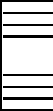
\includegraphics[width=0.070\textwidth]{gesamttex/edit_VIII,3/images/LH_35_09_15_001,022_d1.pdf}}%
  \vspace*{0.5em}
  \centerline{\lbrack\textit{Fig.~1}\rbrack}%
%
%
  \newpage%  Rein vorläufig !!!!
%  \vspace*{1.0em}%
\pstart%
\footnotesize%
Vires tendentes,%
\protect\index{Sachverzeichnis}{vis tendens} % \lbrack,\rbrack\
vel quod idem est conatus restituendi,%
\protect\index{Sachverzeichnis}{conatus restituendi}\edlabel{LH_35_09_15_001v_pervir-2} % \lbrack,\rbrack\
sunt inter se ut rationes spatiorum praeternaturalium\protect\index{Sachverzeichnis}{spatium praeternaturale}
\edtext{naturalibus accedentium}{%
\lemma{naturalibus}\Bfootnote{%
\hspace{-0,5mm}accedentium
\textit{erg.~L}}}
ad spatia naturalia.\protect\index{Sachverzeichnis}{spatium naturale}
Sint
\edtext{vires tendentes\protect\index{Sachverzeichnis}{vis tendens}}{%
\lemma{vires}\Bfootnote{%
\textit{(1)}~turbantes\protect\index{Sachverzeichnis}{vis turbans}
\textit{(2)}~tendentes%
~\textit{L}}}
\textit{T.} \textit{t.}
Restituentes\protect\index{Sachverzeichnis}{vis restituens} \textit{R.} \textit{r.}
Spatia praeternaturalia\protect\index{Sachverzeichnis}{spatium praeternaturale} \textit{P.} \textit{p.}
Naturalia\protect\index{Sachverzeichnis}{spatium naturale} \textit{N.} \textit{n.}
Erit \textit{T} ad \textit{t},
vel quod idem est \textit{R} ad \textit{r},
ut % \protect\rule[0pt]{0mm}{12pt}
$\displaystyle\frac{P}{N}$ ad
\edtext{$\displaystyle\frac{N}{n}.$
Nam tanta est vis quanta turbatio,\protect\index{Sachverzeichnis}{turbatio}
vel si mavis quanta % 
materiae tenuis\protect\index{Sachverzeichnis}{materia tenuis}
rediturientis\protect\index{Sachverzeichnis}{materia redituriens}
expressio\protect\index{Sachverzeichnis}{expressio materiae}
vel insuctio.\protect\index{Sachverzeichnis}{insuctio materiae}}{% \protect\rule[0pt]{0mm}{8pt}
\lemma{$\displaystyle\frac{N}{n}.$}\Bfootnote{%
\textit{(1)}~Si fingamus corpus quod jam intus est non posse comprimi,\protect\index{Sachverzeichnis}{corpus incomprimibile} res manifesta. Jam etsi comprimi posset\protect\index{Sachverzeichnis}{corpus comprimibile}
\textit{(a)}~tantu
\textit{(b)}~non ideo vis major minorve requiretur
\textit{(aa)}~ad
\textit{(bb)}~tantum enim materiae tenuis quae ex uno exprimenda fuisset, expressa fuisset ex duobus.
\textit{(2)}~Nam
\textit{(3)}~Breve 
\textit{(4)}~Brevius:
\textit{(5)}~N
\textit{(6)}~Nam tanta \lbrack...\rbrack\ vel insuctio.%
~\textit{L}}}
%
\edtext{Idem alibi rigorosius demonstravi.}{%
\lemma{Idem \lbrack...\rbrack\ demonstravi}\Cfootnote{%
Vermutlich Anspielung auf G.\,W. \textsc{Leibniz}, \textit{Hypothesis physica nova}, Mainz 1671, § 27 (\textit{LSB}
VI,~2 N.~40, S.~234\,f.).\cite{00256}}}
\pend%
%  \newpage
  \vspace{2.0em}%
%
%
  \centerline{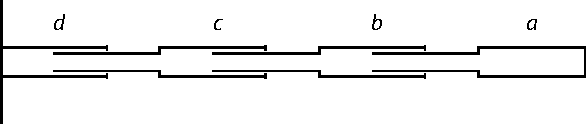
\includegraphics[width=0.56\textwidth]{gesamttex/edit_VIII,3/images/LH_35_09_15_001,022_d2.pdf}}%
  \vspace{-0.5em}
  \centerline{\lbrack\textit{Fig.~2}\rbrack}%
  \label{LH_35_09_15_001v_fig.2}
%
%
  \vspace{2.0em}%
\pstart%
\footnotesize%
Corporis\edlabel{LH_35_09_15_001v_gleichSpann_irls-1} uniformis tensi%
\protect\index{Sachverzeichnis}{corpus uniforme}\protect\index{Sachverzeichnis}{corpus tensum}
quaelibet pars aequaliter tensa est,\protect\index{Sachverzeichnis}{pars aequaliter tensa}
si nulla gravitatis\protect\index{Sachverzeichnis}{gravitas} partium ratio habeatur.
Sit
%
\edtext{embolus\protect\index{Sachverzeichnis}{embolus} corporis \textit{a}}{%
\lemma{embolus corporis \textit{a}}\Cfootnote{%
Siehe das Diagramm \lbrack\textit{Fig.~2}\rbrack.}}
%
in capacitate corporis\protect\index{Sachverzeichnis}{capacitas corporis} \textit{b},
embolus\protect\index{Sachverzeichnis}{embolus} corporis \textit{b}
in capacitate ipsius \textit{c},
%
{\normalsize{\lbrack22~r\textsuperscript{o}\rbrack}} % Blatt 22r
%
et corporis \textit{c} in capacitate\protect\index{Sachverzeichnis}{capacitas corporis} ipsius \textit{d}
eodem ubique modo,
nec educi ullus eorum possit sine
\edtext{vi;\protect\index{Sachverzeichnis}{vis tendens}
ob tensionem\protect\index{Sachverzeichnis}{tensio} scilicet}{%
\lemma{vi;}\Bfootnote{%
\textit{(1)}~si quis jam
\textit{(2)}~ob tensionem scilicet%
~\textit{L}}}
quae inde sequitur.
\edtext{Ponamus educi corpus \textit{a}.}{%
\lemma{Ponamus}\Bfootnote{%
\textit{(1)}~adduci
\textit{(2)}~educi
\textbar~primum \textit{streicht}~%
\textbar\ corpus \textit{a}.%
~\textit{L}}}
Cumque eodem omnia modo connexa sint,
nec unum sine altero moveri possit
nisi supposita jam aliqua tensione,\protect\index{Sachverzeichnis}{tensio}
nec ratio sit cur ullum prae altero moveatur,
tenduntur onmia aequaliter.
\edtext{A gravitate\protect\index{Sachverzeichnis}{gravitas} autem
seu mole corporis\protect\index{Sachverzeichnis}{moles corporis}
abstrahendus est animus,\protect\index{Sachverzeichnis}{animus}
alioqui enim facilius movebitur minus quam majus.
Unde causa rupturae\protect\index{Sachverzeichnis}{causa rupturae}
in loco uno potius quam alio duci potest,
etiam in diducendo homogeneo.%
\edlabel{LH_35_09_15_001v_gleichSpann_irls-2}%
\protect\index{Sachverzeichnis}{corpus diducendum}}{%
\lemma{A}\Bfootnote{%
\hspace{-0,5mm}gravitate \lbrack...\rbrack\ facilius movebitur
\textit{(1)}~majus
\textit{(2)}~minus quam \lbrack...\rbrack\ etiam in
\textbar~in \textit{streicht Hrsg.}~%
\textbar\ diducendo homogeneo.
\textit{erg.~L}}}
\pend%
%  \newpage% Rein vorläufig !!!!
  \vspace{2.4em}%
%
%
  \centerline{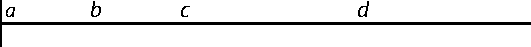
\includegraphics[width=0.54\textwidth]{gesamttex/edit_VIII,3/images/LH_35_09_15_001,022_d3.pdf}}%
  \vspace{0.5em}
  \centerline{\lbrack\textit{Fig.~3}\rbrack}%
    \label{LH_35_09_15_001v_fig.3}
%
%
  \newpage% Rein vorläufig !!!!
%  \vspace*{1.0em}%
\pstart%
\footnotesize%
Hinc
\edtext{}{%
{\xxref{LH_35_09_15_022r_klnbchst-1}{LH_35_09_15_022r_klnbchst-2}}%
{\lemma{\textit{AB} \lbrack...\rbrack\ \textit{AC}}\Cfootnote{%
Gemeint sind Strecken der Saite \textit{ABC} nach dem Diagramm \lbrack\textit{Fig.~3}\rbrack\ auf S.~\pageref{LH_35_09_15_001v_fig.3},
wo sie aber durch Kleinbuchstaben bezeichnet werden.}}}%
\edtext{sit \textit{AB}\edlabel{LH_35_09_15_022r_klnbchst-1} aequ.}{%
\lemma{sit}\Bfootnote{%
\textit{(1)}~\textit{ab} aeq
\textit{(2)}~\textit{AB} aequ.%
~\textit{L}}}
\textit{BC}, et \textit{CD} aequ. \textit{AC}.\edlabel{LH_35_09_15_022r_klnbchst-2}
Si
\edtext{chorda\protect\index{Sachverzeichnis}{chorda tensa} \textit{ABC} tendatur,
manente}{%
\lemma{chorda}\Bfootnote{%
\textit{(1)}~\textit{abc}
\textit{(2)}~\textit{ABC}
\textit{(a)}~ten
\textit{(b)}~diducatur, ma
\textit{(c)}~tendatur, manente%
~\textit{L}}}
puncto \textit{A}
\edtext{immobili,\protect\index{Sachverzeichnis}{punctum immobile}
et punctum \textit{C} perveniat}{%
\lemma{immobili,}\Bfootnote{%
\hspace{-0,5mm}et
\textit{(1)}~\textit{b} perven
\textit{(2)}~\textit{C}
\textit{(3)}~punctum \textit{C} perveniat%
~\textit{L}}}
in \textit{D},
tunc punctum \textit{B} perveniet in
\edtext{\lbrack\textit{C}\rbrack.}{%
\lemma{\textit{D}}\Bfootnote{%
\textit{L~ändert Hrsg.}}}
Ita enim
\edtext{partes \textit{AB} et \textit{BC}}{%
\lemma{partes}\Bfootnote{%
\textit{(1)}~\textit{ab}
\textit{(2)}~\textit{AB} et
\textit{(a)}~\textit{CD}
\textit{(b)}~\textit{BC}%
~\textit{L}}}
erunt aequaliter tensae\protect\index{Sachverzeichnis}{pars aequaliter tensa}\lbrack,\rbrack\
\edtext{quia pars \textit{AB} occupat locum \textit{AC},}{%
\lemma{quia}\Bfootnote{%
\hspace{-0,5mm}\textbar~pars \textit{erg.}~%
\textbar\ \textit{AB} occupat
\textbar~locum \textit{erg.}~%
\textbar\ \textit{AC},
\textit{L}}}
et pars
\edtext{ei aequalis}{%
\lemma{ei}\Bfootnote{%
\hspace{-0,5mm}aequalis
\textit{erg.~L}}}
\textit{BC} locum \textit{CD} priori loco aequalem.
\pend%
% \newpage%
%
\pstart%
\footnotesize%
\edtext{Hinc sequitur spatia\protect\index{Sachverzeichnis}{spatium percursum}
quae inter tensionem\protect\index{Sachverzeichnis}{tensio chordae}
puncta chordae\protect\index{Sachverzeichnis}{punctum chordae} percurrunt
esse distantiis a puncto immobili\protect\index{Sachverzeichnis}{punctum immobile} proportionalia.
Et quia etiam omnia simul restituuntur,
et durante restitutione\protect\index{Sachverzeichnis}{restitutio chordae}
\edtext{semper eundem gradum tensionis\protect\index{Sachverzeichnis}{gradus tensionis} retinent}{%
\lemma{semper}\Bfootnote{%
\textit{(1)}~eodem modo tensa
\textit{(2)}~eundem gradum tensionis retinent%
~\textit{L}}}
usque ad plenam restitutionem,\protect\index{Sachverzeichnis}{restitutio plena}
hinc eadem esse
\edtext{debet ratio celeritatum\protect\index{Sachverzeichnis}{ratio celeritatum}
in restitutione\protect\index{Sachverzeichnis}{restitutio chordae} quae}{%
\lemma{debet}\Bfootnote{%
\textit{(1)}~celeritas in restitutione quae
\textit{(2)}~ratio celeritatum in restitutione quae%
~\textit{L}}}
est in tensione\protect\index{Sachverzeichnis}{tensio chordae}%
\protect\label{LH_35_09_15_022r_rndbmrkng_czjt}%
%%%%
%%%%    ANFANG DER MARGINALIE
}{\lemma{\textit{Auf der rechten Spalte:}}\Afootnote{%
{\footnotesize%
Imo in eo erratum,\protect\index{Sachverzeichnis}{erratum}
nam sive alterutrum extremum sit immobile,
sive utrinque trahatur,
idem est,\protect\index{Sachverzeichnis}{extremum chordae}
tantum enim duo extrema a se invicem discedunt,
chorda\protect\index{Sachverzeichnis}{chorda tensa} enim
vi tensionis\protect\index{Sachverzeichnis}{vis tensionis}
suae\protect\index{Sachverzeichnis}{tensio chordae}
unum continuum\protect\index{Sachverzeichnis}{unum continuum} est,
adeoque%
\textsuperscript{[a]}
potius mediorum punctorum tardior erit motus%
\protect\index{Sachverzeichnis}{motus puncti medii}\lbrack,\rbrack\
in quo et%
\textsuperscript{[b]}
erratum est ab Honorato Fabry.\protect\index{Namensregister}{\textso{Fabri}, Honoré 1607\textendash1688}%
\textsuperscript{[c]}
Re recte expensa%
\textsuperscript{[d]}
eo redit quaestio\protect\index{Sachverzeichnis}{quaestio} an corpus faclius moveatur quam tendatur%
\textsuperscript{[e]}
sive an facilius moveatur majus quam tendatur minus.
Puto totum corpus simul recipere conatum\protect\index{Sachverzeichnis}{conatus} primo momento,
quia ab initio nulla%
\textsuperscript{[f]}
fit tensio,\protect\index{Sachverzeichnis}{tensio corporis}
sed initio statim est continui motus.\protect\index{Sachverzeichnis}{motus continui}%
\newline%
\newline%
% \\%
%%%%
\textsuperscript{[a]}~%
adeoque
\textit{(1)}~in medio
\textit{(2)}~potius mediorum punctorum%
~\textit{L}
\quad
%%%%
\textsuperscript{[b]}~%
et
\textit{erg.~L}
\quad
%%%%
\textsuperscript{[c]}~%
erratum \lbrack...\rbrack\ Fabry:
Siehe H.\,\textsc{Fabri}, \textit{Physica}, tract. I, lib. II, prop. LXI (Bd.~I, Lyon 1669, S.~63).\cite{00044}
Leibniz hat die Stelle sowohl in seinem Handexemplar angestrichen wie auch exzerpiert; vgl. \textit{LSB} VI,~2 N.~39\textsubscript{3}, S.~212.14\textendash15;\cite{01234} VIII,~2 N.~55, S.~471.7\textendash9.\cite{01120}
\quad
%%%%
\textsuperscript{[d]}~%
expensa
\textit{(1)}~ab
\textit{(2)}~eo%
~\textit{L}
\quad
%%%%
\textsuperscript{[e]}~%
tendatur
\textit{(1)}~. Sed jam tamen video hoc loco necessario
\textit{(2)}~sive an \lbrack...\rbrack\ tendatur minus.
\textit{(a)}~Si totum corpus simul recipit conat
\textit{(b)}~Et
\textit{(c)}~Puto totum \lbrack...\rbrack\ recipere conatum%
~\textit{L}
\quad
%%%%
\textsuperscript{[f]}~%
nulla
\textit{(1)}~est
\textit{(2)}~fit%
~\textit{L}}}}%
%%%%    ENDE DER MARGINALIE
%%%%
\edtext{.%
\newline%
\indent%
Cum corpus sibi relinquitur,}{%
\lemma{tensione.}\Bfootnote{%
\textit{(1)}~Durante motu restitutionis spontaneo\protect\index{Sachverzeichnis}{motus restitutionis}
\textit{(2)}~Cum corpus sibi relinquitur,%
~\textit{L}}}
causa restituens\protect\index{Sachverzeichnis}{causa restituens}
omnibus partibus aequalem vim
\edtext{imprimit,\protect\index{Sachverzeichnis}{vis impressa}
quare tota vis impressa}{%
\lemma{imprimit,}\Bfootnote{%
\textit{(1)}~itaque quo minus est corpus
\textit{(2)}~quare tota vis impressa%
~\textit{L}}}
aequaliter distribuitur in omnes partes.\protect\index{Sachverzeichnis}{vis aequaliter distributa}
Hinc quo pauciores partes\lbrack,\rbrack\
hoc in singulis major impetus.\protect\index{Sachverzeichnis}{impetus restitutionis}
Sint ergo mille corpora ex tubis\protect\index{Sachverzeichnis}{tubum}
%
{\normalsize{\lbrack22~v\textsuperscript{o}\rbrack}} % Blatt 22v
%
embolisque\protect\index{Sachverzeichnis}{embolus} composita ut in
\edtext{figura\protect\index{Sachverzeichnis}{figura} superiore}{%
\lemma{figura superiore}\Cfootnote{%
Das Diagramm \lbrack\textit{Fig.~2}\rbrack\ auf S.~\pageref{LH_35_09_15_001v_fig.2}.}}%
\lbrack,\rbrack\
\edtext{diducantur ad longitudinem\protect\index{Sachverzeichnis}{longitudo corporis diducti} duplam,}{%
\lemma{diducantur}\Bfootnote{%
\hspace{-0,5mm}ad
\textit{(1)}~spatium
\textit{(a)}~decuplo majus
\textit{(b)}~duplo majus
\textit{(2)}~longitudinem
\textit{(a)}~duplo majorem
\textit{(b)}~duplam,%
~\textit{L}}}
sint alia bis mille,
quae diducantur etiam ad longitudinem duplam suae prioris.
Cum corpora ubique sint aequalia,
et diductio\protect\index{Sachverzeichnis}{diductio}
\edtext{etiam,
sed corpora diducenda\protect\index{Sachverzeichnis}{corpus diducendum} sint duplo plura,
patet,}{%
\lemma{etiam,}\Bfootnote{%
\textit{(1)}~patet
\textit{(2)}~sed corpora \lbrack...\rbrack\ plura, patet,%
~\textit{L}}}
duplo majori vi\protect\index{Sachverzeichnis}{vis deductionis} opus esse in posteriore
\edtext{casu.
Idem est in compressione.\protect\index{Sachverzeichnis}{compressio}
Itaque si corpora eadem ratione tensa sint,\protect\index{Sachverzeichnis}{corpus tensum}
id est ut spatium sit in eadem ratione multiplicatum vel submultiplicatum,
vires tendentes\protect\index{Sachverzeichnis}{vis tendens} erunt}{%
\lemma{casu.}\Bfootnote{%
\textit{(1)}~Itaque vires erunt
\textit{(2)}~Id enim
\textit{(3)}~Idem est in compressione
\textit{(4)}~Idem est \lbrack...\rbrack\ sit in eadem
\textit{(a)}~ratione auctum vel diminutum,
\textit{(b)}~\textbar~ratione \textit{erg.}~\textbar\ multiplicatum vel \lbrack...\rbrack\ tendentes erunt%
~\textit{L}}}
ut corpora ejusdem materiae.%
\protect\index{Sachverzeichnis}{magnitudo corporis}\protect\index{Sachverzeichnis}{materia corporis}
Idemque etiam ex eo
\edtext{demonstratur, si}{%
\lemma{demonstratur,}\Bfootnote{%
\textit{(1)}~quod
\textit{(2)}~si%
~\textit{L}}}
\edtext{chorda\protect\index{Sachverzeichnis}{chorda tensa}
unius librae\protect\index{Sachverzeichnis}{libra}}{%
\lemma{chorda}\Bfootnote{%
\textit{(1)}~unius pedis\protect\index{Sachverzeichnis}{pes}
\textit{(2)}~unius librae%
~\textit{L}}}
pondere\protect\index{Sachverzeichnis}{pondus tendens} tensa teneatur,
discindaturque in duas partes,
quaelibet pars selibrae\protect\index{Sachverzeichnis}{selibra}
pondere\protect\index{Sachverzeichnis}{pondus tendens} tensa tenebitur.
\pend%
%
\pstart%
\footnotesize%
Itaque\textso{ vires tendentes sunt in composita ratione tensionum et corporum }%
\edtext{\textso{tensorum.}%
\protect\index{Sachverzeichnis}{vis tendens}%
\protect\index{Sachverzeichnis}{tensio corporis}%
\protect\index{Sachverzeichnis}{corpus tensum}
%
\newline%
\indent%
Tensiones\protect\index{Sachverzeichnis}{tensio}%
\edlabel{LH_35_09_15_022v_Beweis_sgtk-1}
sunt ut vires\protect\index{Sachverzeichnis}{vis tendens}
idem corpus tendentes.
%
\newline%
\indent%
Corpus}{%
\lemma{\textso{tensorum.}}\Bfootnote{%
\textit{(1)}~Ejusdem corporis
\textit{(2)}~Tensiones, seu ejusdem corporis vires tendentes sunt ut spatiorum differentiae, seu ut spatia acquista vel perdita.
\textit{(3)}~Tensiones sunt \lbrack...\rbrack\ corpus tendentes.
\textbar~Uti compressiones ita et
\textit{(1)}~tensiones videntur continue f
\textit{(2)}~diductiones, adeoque tensiones in universum\protect\index{Sachverzeichnis}{universum} continue fiunt difficiliores. \textit{streicht}~%
\textbar\ Corpus%
~\textit{L}}}
aliquod ut
\edtext{aer certa potentia,\protect\index{Sachverzeichnis}{potentia} ex.\,g.
certo pondere incumbentis atmosphaerae\protect\index{Sachverzeichnis}{pondus atmosphaerae incumbentis}}{%
\lemma{aer}\Bfootnote{%
\textit{(1)}~certo pondere incumbentis
\textit{(2)}~certa potentia, \lbrack...\rbrack\ pondere incumbentis
\textit{(a)}~aeris
\textit{(b)}~atmosphaerae%
~\textit{L}}}
in datum spatium\protect\index{Sachverzeichnis}{spatium datum}
compressus est,\protect\index{Sachverzeichnis}{aer compressus}
duplicato pondere in dimidium,
triplicato in tertiam partem comprimetur.
Similiter aer elastro suo,\protect\index{Sachverzeichnis}{elastrum aeris}
quod ponderi incumbenti\protect\index{Sachverzeichnis}{pondus atmosphaerae incumbentis}
aequale\lbrack,\rbrack\
in praesenti statu\protect\index{Sachverzeichnis}{status praesens} se tuetur,
ergo duplicata vi,\protect\index{Sachverzeichnis}{vis elastri}
id est addita tanta, quanta ipsius est\lbrack,\rbrack\
duplum spatium
\edtext{occupabit.
Itaque}{%
\lemma{occupabit}\Bfootnote{%
\textit{(1)}~, tripla
\textit{(2)}~. Itaque%
~\textit{L}}}%
\textso{ Tensiones }\protect\index{Sachverzeichnis}{tensio}%
sunt ut rationes spatiorum accessoriorum\protect\index{Sachverzeichnis}{spatium accessorium}
ad naturales,\protect\index{Sachverzeichnis}{spatium naturale}
directae in diductione,
reciprocae in compressione.
Quanta vi\protect\index{Sachverzeichnis}{vis comprimens}\protect\index{Sachverzeichnis}{vis diducens}
corpus jam
\edtext{tum diductum\protect\index{Sachverzeichnis}{corpus diductum}
vel compressum\protect\index{Sachverzeichnis}{corpus compressum}}{%
\lemma{tum}\Bfootnote{%
\textit{(1)}~naturali te
\textit{(2)}~tensum
\textit{(3)}~diductum
\textit{(4)}~\textbar~diductum \textit{erg.}~\textbar\ vel compressum%
~\textit{L}}}
tenetur,
\edtext{tanta vi opus est ut ad duplum vel}{%
\lemma{tanta}\Bfootnote{%
\hspace{-0,5mm}vi
\textit{(1)}~$\langle$\textendash$\rangle$
\textit{(2)}~multipl
\textit{(3)}~opus est
\textit{(a)}~ad duplum ipsi
\textit{(aa)}~ut
\textit{(bb)}~vel
\textit{(b)}~ut ad duplum vel%
~\textit{L}}}
dimidium spatium redigatur\lbrack,\rbrack\
unde aestimari potest
quanta sit vis tensionis naturalis\protect\index{Sachverzeichnis}{vis tensionis}
in unoquoque corpore,
quod theorema maximi momenti est.\protect\index{Sachverzeichnis}{theorema maximi momenti}
Idem verum et de Tensione
%
\edtext{\lbrack artificiali,\rbrack}{%
\lemma{artificiali,}\Bfootnote{%
\textit{erg. Hrsg.}}}
%
sed tunc computandae naturalis\protect\index{Sachverzeichnis}{tensio naturalis}
et artificialis simul,\protect\index{Sachverzeichnis}{tensio artificialis}
iis enim tensum tenetur.%
\edlabel{LH_35_09_15_022v_Beweis_sgtk-2}
\pend%
\newpage%           Rein vorläufig !!!!
 %\vspace{1.0em}
%
\pstart%
\noindent%
\normalsize%
\lbrack\textit{Auf der rechten Spalte% von Bl.~22~v\textsuperscript{o}\!
:}\rbrack%
%
\pend%
\vspace*{1.0em}
%
\pstart%
\noindent%
\footnotesize%
$\displaystyle d \frac{x}{y} \sqcap \frac{d\overline{x} - dy}{yy}$
\quad\quad%
$\displaystyle \frac{ddy - ddx}{d\overline{x}^2} \sqcap \frac{y}{d\overline{x}}$
%
\newline%
$\displaystyle x \,\sqcap\, a + by + cyy + dy^3 + ey^4$
% \edtext{
etc.
\protect\rule[0pt]{0mm}{12pt}%
%
\newline%
$\displaystyle d\overline{x} \,\sqcap\, 0 + b\,d\overline{y} + 2cy\,d\overline{y} + 3dy^2\,d\overline{y}$ etc.
\protect\rule[0pt]{0mm}{16pt}%
%
\newline%
$\displaystyle y \,\sqcap\, a + bx + cxx + dx^3$
\protect\rule[0pt]{0mm}{16pt}%
%
\newline%
$\displaystyle e\,dy \,\sqcap\, 0 + eb + 2ecx + 3edxx + 4efx^3
\edtext{+ 5egx^4$
\protect\rule[0pt]{0mm}{16pt}%
%
\newline%
$\displaystyle \frac{ax}{1} + \frac{bxx}{2} + \frac{cx^3}{3} + \frac{dx^4}{4}$%
}{%
\lemma{\hspace{-0,5mm}$\displaystyle+\ 5egx^4$}\Bfootnote{%
\textit{(1)}~$\int\!\!\overline{y}\ \sqcap$\ 
\textit{(2)}~$\displaystyle \frac{ax}{1} + \frac{bxx}{2} + \frac{cx^3}{3}$
\textit{(a)}~etc.
\textit{(b)}~$\displaystyle+\,\frac{dx^4}{4}$%
~\textit{L}}}
% }{%
% \lemma{etc.}\Bfootnote{%
% \textit{(1)}~$\displaystyle d\overline{x} \,\sqcap\, 0 + b\,d\overline{y} + 2cy\,d\overline{y} + 3dy^2\,d\overline{y}$ etc.
% \textit{(2)}~$\displaystyle y \,\sqcap\, a + bx + cxx + dx^3$
% \textit{(3)}~$\displaystyle edy \,\sqcap\, 0 + eb + 2ecx + 3edxx + 4efx^3 + 5egx^4$
% \textit{(4)}~$\int\!\!\overline{y}\ \sqcap$
% \textit{(5)}~$\displaystyle \frac{ax}{1} + \frac{bxx}{2} + \frac{cx^3}{3}$
% \textit{(a)}~etc.
% \textit{(b)}~$\displaystyle+\ \frac{dx^4}{4}$%
% ~\textit{L}}}%
\protect\rule[0pt]{0mm}{16pt}%
%
\newline%
$\displaystyle b \,\sqcap\, 0$
\quad%
$\displaystyle c \,\sqcap \frac{a}{1 \cdot 2\, e}$
\quad
$\displaystyle d \,\sqcap\, 0$
\quad
$\displaystyle f \,\sqcap \frac{c}{3 \cdot 4\, e} \sqcap \frac{a}{1 \cdot 2 \cdot 3 \cdot 4\, e}$
\protect\rule[0pt]{0mm}{16pt}%
%
\newline%
Ergo $\displaystyle y \,\sqcap\, 1 + \frac{xx}{1 \cdot 2} + \frac{x^4}{1 \cdot 2 \cdot 3 \cdot 4}$ etc.
\protect\rule[0pt]{0mm}{16pt}%
\pend%
%
%
%% \newpage% Rein vorläufig !!!!
%  \vspace*{-5.0em}%
%  \centerline{\hspace*{75mm}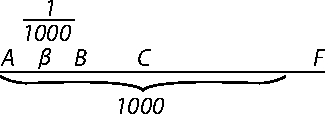
\includegraphics[width=0.24\textwidth]{gesamttex/edit_VIII,3/images/LH_35_09_15_001,022_d4.pdf}}%
%  \vspace*{0.5em}
%  \centerline{\hspace*{75mm}\lbrack\textit{Fig.~4}\rbrack}%
%  \vspace*{-0.5em}%
%
\pstart%
\footnotesize%
\noindent%
$BC \sqcap d\overline{s}$ \quad $AF \sqcap e$
% \protect\rule[0pt]{0mm}{20pt}%
\pend%
%
\pstart%
\vspace*{2.0em}%
\noindent%
\footnotesize%
$\displaystyle \frac{BC}{\frac{1}{1000}} \sqcap \frac{1999}{1000}$
\protect\rule[0pt]{0mm}{16pt}%
%
\newline%
$\displaystyle{BC \,\sqcap \frac{1999}{1000,000}} \,\sqcap\, d\overline{s}$
\protect\rule[0pt]{0mm}{16pt}
%
\newline%
$\displaystyle{AC \,\sqcap \frac{2999}{1000,000}} \,\sqcap s$
\protect\rule[0pt]{0mm}{16pt}%
%
\pend%
% \newpage%
%
% \newpage% Rein vorläufig !!!!
  \vspace*{-7.5em}%
  \centerline{\hspace*{45mm}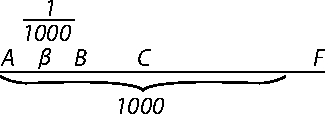
\includegraphics[width=0.24\textwidth]{gesamttex/edit_VIII,3/images/LH_35_09_15_001,022_d4.pdf}}%
  \vspace*{0.5em}
  \centerline{\hspace*{45mm}\lbrack\textit{Fig.~4}\rbrack}%
  \vspace*{-0.5em}%
  %
%  \vspace*{-6.0em}%
%  \centerline{\hspace*{45mm}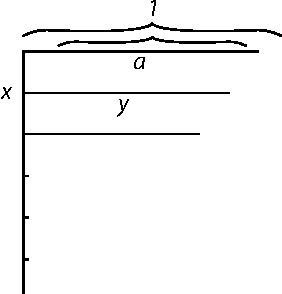
\includegraphics[width=0.22\textwidth]{gesamttex/edit_VIII,3/images/LH_35_09_15_001,022_d5.pdf}}%
%  \vspace*{-0.5em}
%  \centerline{\hspace*{45mm}\lbrack\textit{Fig.~5}\rbrack}%
%%  \newpage% Rein vorläufig !!!!
  \vspace*{4.5em}%
%
\pstart%
\footnotesize%
\noindent%
\edtext{$\beta \sqcap d\overline{x}$
\quad\quad%
$\displaystyle \frac{d\overline{s}}{\beta \sqcap d\overline{x}}$
}{%
\lemma{$\beta \sqcap d\overline{x}$}\Bfootnote{%
\textit{(1)}~$\displaystyle \frac{d\overline{s}}{\beta}$
\textit{(2)}~$\displaystyle \frac{d\overline{s}}{\beta \sqcap d\overline{x}}$%
~\textit{L}}}
aequ. $\frac{\textstyle{\!\int\!}\displaystyle{\overline{y \overline{x}}}}{\displaystyle{a}}$
\protect\rule[0pt]{0mm}{16pt}%
%
\newline%
$\displaystyle\frac{y}{a} \sqcap
\edtext{\frac{e - s}{e}$% 
\protect\rule[0pt]{0mm}{16pt}%
%
\newline%
Ergo}{%
\lemma{$\displaystyle \frac{e - s}{e}$}\Bfootnote{%
\textit{(1)}~$\displaystyle d\overline{z d\overline{z}} \,\sqcap$
\textit{(2)}~Ergo%
~\textit{L}}}
$\displaystyle d\overline{y} \sqcap
\edtext{-\frac{a}{e}d\overline{s}$%
\protect\rule[0pt]{0mm}{16pt}%
%
\newline%
Ergo}{%
\lemma{$\displaystyle-\frac{a}{e}d\overline{s}$}\Bfootnote{%
\textit{(1)}~$\displaystyle \frac{\cancel{z}\,d\overline{dz} + d}{\cancel{z}z}$
\textit{(2)}~Ergo%
~\textit{L}}}
$\displaystyle - \frac{e}{\cancel{a}} \frac{d\overline{y}}{dx} \sqcap \frac{\textstyle{\!\int\!}\displaystyle{\overline{y\,dx}}}{\cancel{a}}$
\edtext{et sit $y \sqcap zz$ fiet%
\protect\rule[0pt]{0mm}{16pt}}{%
\lemma{et}\Bfootnote{%
\textit{(1)}~$\displaystyle \frac{- b\,d\overline{d}y}{y} \sqcap d\overline{x}^2$
\textit{(2)}~$\displaystyle + \frac{d\overline{z} \,\efrac{\efrac{}{\leibvdash}}{}\, 2z\,dz}{z^4 - b zz}$ %
\textit{(3)}~sit $y \sqcap zz$ fiet $d\overline{dy}$
\textit{(4)}~sit $y \sqcap zz$ fiet %
~\textit{L}}}
{\normalsize{\lbrack\textit{\textit{Text bricht ab.}}\rbrack}}%
% $\pleibvdash$
%
\pend%
%
%
  \newpage% Rein vorläufig !!!!
  \pstart \vspace{1em} %\noindent
\begin{minipage}[t]{0.5\textwidth}
\hspace{11mm}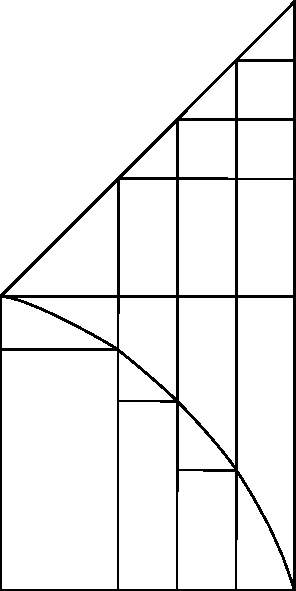
\includegraphics[width=0.37\textwidth]{gesamttex/edit_VIII,3/images/LH_35_09_15_001,022_d6.pdf}
\end{minipage}
\hspace{5mm}
\begin{minipage}[t]{0.5\textwidth}
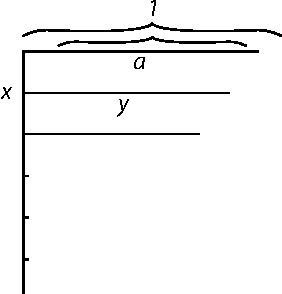
\includegraphics[width=0.5\textwidth]{gesamttex/edit_VIII,3/images/LH_35_09_15_001,022_d5.pdf}
\end{minipage}
%\vspace{3.5em}
\pend
\vspace{0.5em}
\pstart
 \hspace{16.5mm} [\textit{Fig.~5}]\hspace{55mm} [\textit{Fig.~6}]
\pend
\vspace{2em}

%  % \vspace*{0.0em}%
%  \centerline{\hspace{-45mm}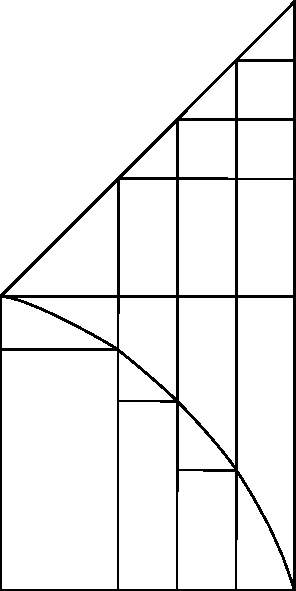
\includegraphics[width=0.16\textwidth]{gesamttex/edit_VIII,3/images/LH_35_09_15_001,022_d6.pdf}}%
%  \vspace{0.5em}
%  \centerline{\hspace{-45mm}\lbrack\textit{Fig.~5}\rbrack}%
%%  \newpage% Rein vorläufig !!!!
%%  \vspace*{1,0em}%
%  %
%  \vspace*{-10.0em}%
%  \centerline{\hspace{45mm}\hspace*{45mm}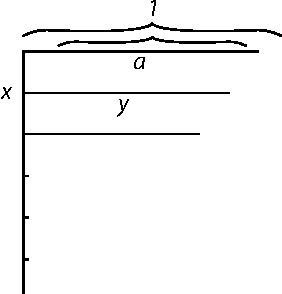
\includegraphics[width=0.22\textwidth]{gesamttex/edit_VIII,3/images/LH_35_09_15_001,022_d5.pdf}}%
%  \vspace*{-0.5em}
%  \centerline{\hspace{45mm}\hspace*{45mm}\lbrack\textit{Fig.~6}\rbrack}%
%%  \newpage% Rein vorläufig !!!!
%  \vspace*{4.0em}%
%%
%
\pstart%
\noindent%
\normalsize%
\lbrack\textit{Nebenrechnungen:}\rbrack\setline{1}%
\pend%
%
\vspace*{1.0em}%
\pstart%
\noindent%
\footnotesize%
\edtext{$1000000\\
\underline{\phantom{j00}2999}}{%
\lemma{1000000}\Bfootnote{%
\textit{(1)}~99997
\textit{(2)}~2999%
~\textit{L}}}\\
\setline{1}\phantom{0}997001$
\pend%
%
\vspace*{1.0em}%
\pstart%
\noindent%
\footnotesize%
$\phantom{000000}\underline{\phantom{g}999}\\
\phantom{000000}1000$\\
% \pend%
%
% \vspace*{1.0em}%
% \pstart%
% \noindent%
% \footnotesize%
\setline{1}$\underline{997001\phantom{gg}}\phantom{0}1\cdot2\\
\phantom{g}1000000$
\pend
\count\Bfootins=1200
\count\Afootins=1200
\count\Cfootins=1200%
%
% ENDE DES STÜCKES auf Blatt 22v 



% N.~8.0 [4.0]. ((??A10; RK 41152)) Tentaminum de chordarum tensione schedae // AEF (Akustik, Elasizität)
\chapter[\scriptsize\uppercase{De chordarum tensione schedae}]{\uppercase{Tentaminum de chordarum tensione schedae}
\newline Dezember 1680} % 10. Dezember 1680
\addcontentsline{toc}{chapter}{\thechapter\enskip Tentaminum de chordarum tensione schedae Dezember 1680 % 10. Dezember 1680
}
\label{41152_0}
\vspace{8mm}
	%
%
%   Band VIII, 3 N.~??A10 (??A10.1 bis ??A10.6)
%   Signatur/Tex-Datei: LH_35_09_15_006-017_intro
%   Einleitung zu RK-Nr. 41152 [Teile 1–6]
%   Überschrift: Tentaminum de chordarum tensione schedae
%   Datierung: [Dezember 1681]
%   WZ: ()
%   SZ: ()
%   Bilddateien (PDF): ()
%
%
\footnotesize 
\pstart
\noindent                
Das vorliegende Gesamtstück besteht aus den Einzeltexten N.~8\textsubscript{1} bis 8\textsubscript{6}.
Auf ihren inhaltlichen und chronologischen Zusammenhang weist bereits ihre Überschrift hin:
Sämtliche Texte sind \textit{Tentaminum de chordarum tensione schedae} benannt und von eins bis sechs nummeriert,
wobei jede \textit{scheda} einen Bogen umfasst.
Die Textträger sind zudem von Leibniz selbst auf den 10. (20.) Dezember 1680 datiert;
nur auf dem Bogen von N.~8\textsubscript{4} hat er \glqq Dezember 1680\grqq\ als Datum vermerkt.
Als Gesamtdatierung von N.~8 wird demgemäß Dezember 1680 angegeben.
\pend%
\pstart%
Die sechs \textit{Schedae}, in denen Leibniz mechanische Gesetze der Schwingungen gespannter elastischer Saiten zu bestimmen sucht,
weisen enge Beziehungen zu weiteren Stücken der vorliegenden Rubrik auf, insbesondere N.~8 und  N.~10. 
Berührungspunkte bestehen zudem mit Theoremen aus
\cite{00044}H.~\textsc{Fabri}, \textit{Physica},
tract. I, lib. II: \textit{De com\-pres\-so et tenso} (Bd.~I, Lyon 1669) % , S.~42\textendash189 
und tract. III, lib. II: \textit{De sonis} (Bd.~II, Lyon 1670). % , S.~131\textendash293
Bemerkenswert ist in dieser Hinsicht die Anknüpfung an Fabris Abhandlung % tract.~III, lib.~II, prop.~223 und 224 (Bd.~II, S.~215b; 216a; 216b) 
in
N.~8\textsubscript{1}, S.~\refpassage{LH_35_09_15_007v_erzt-1}{LH_35_09_15_007v_erzt-2};
N.~8\textsubscript{2}, S.~\refpassage{LH_35_09_15_009v_crassitiessuperflua-1}{LH_35_09_15_009v_crassitiessuperflua-2};
N~8\textsubscript{4}, S.~\refpassage{LH_35_09_15_012v_crassitiessuperflua-1}{LH_35_09_15_012v_crassitiessuperflua-2};
N.~8\textsubscript{6}, S.~\refpassage{LH_35_09_15_016r_crassitiessuperflua-1}{LH_35_09_15_016r_crassitiessuperflua-2}. 
\pend
\newpage % vorläufig
\normalsize


% N.~8.1 [4.1]. ((??A10.1; RK 41152)) Tentaminum de chordarum tensione scheda prima // AEF (Akustik, Elastizität)
\vspace{12mm}
\section[\scriptsize\uppercase{De chordarum tensione scheda prima}]{\uppercase{Tentaminum de chordarum tensione scheda prima}%
\newline 10.\,(20.)~Dezember 1680
}
\addcontentsline{toc}{section}{\thesection\enskip Tentaminum de chordarum tensione scheda prima % 10. (20.) Dezember 1680 
}
\label{41152_1}
\vspace{4mm}
	%   ##
%
%   Band VIII, 3 N.~??A10.1
%   Signatur/Tex-Datei: LH_35_09_15_006-007
%   RK-Nr. 41152 [Teil 1]
%   Überschrift: Tentaminum de chordarum tensione scheda prima
%   Datierung: 1680.12.10
%   WZ: (keins)
%.  SZ: (keins)
%.  Bilddateien (PDF): LH_35_09_15_006-007_d1; LH_35_09_15_006-007_d2; LH_35_09_15_006-007_d3 (insgesamt drei) 
%
%
\begin{ledgroupsized}[r]{120mm}
\footnotesize
\pstart
\noindent\textbf{Überlieferung:}
\pend
\end{ledgroupsized}
\begin{ledgroupsized}[r]{114mm}
\footnotesize
\pstart \parindent -6mm
\makebox[6mm][l]{\textit{L}}%
Aufzeichnung: LH~XXXV~9,~15~Bl.~6\textendash7.
Ein Bogen 4\textsuperscript{o}.
Vier einspaltig beschriebene Seiten.
Im Kopf von Bl.~6~r\textsuperscript{o} gestrichene Zeile von Leibnizens Hand:
\edlabel{LH_35_09_15_006r_Ueberlieferung-1}\textit{Si com\-pres\-sio\protect\index{Sachverzeichnis}{compressio}
fit per extru\-sionem\protect\index{Sachverzeichnis}{extrusio}
subtilis materiae\protect\index{Sachverzeichnis}{materia subtilis}
est expressio}.\protect\index{Sachverzeichnis}{expressio}\edlabel{LH_35_09_15_006r_Ueberlieferung-2}
% Kein Wasserzeichen.
\pend
\end{ledgroupsized}
%
%
\vspace{4mm}% !!!! Vorläufig geändert !!!!
%
%
\count\Bfootins=1000
\count\Afootins=1000
\count\Cfootins=1000
%
%
\pstart%
\normalsize%
\noindent%
%
% % % %    ACHTUNG GETRIXT: Folgende Cfootnote bezieht sich auf die Überlieferung
\edtext{}{%
{\xxref{LH_35_09_15_006r_Ueberlieferung-1}{LH_35_09_15_006r_Ueberlieferung-2}}% compressio
{\lemma{\textit{Si} \lbrack...\rbrack\ \textit{expressio}}\Cfootnote{%
Vgl. \cite{00044}H.~\textsc{Fabri}, \textit{Physica}, tract. I, lib. II, prop. 18 (Bd. I, Lyon 1669, S.~53b\textendash54a).}}}%
%
%
\lbrack6~r\textsuperscript{o}\rbrack % Blatt 6r
%
\pend%
% \vspace*{-0.5em}%
% Überschrift
\pstart%
\centering%
\edtext{Tentaminum de Chordarum tensione%
\protect\index{Sachverzeichnis}{tentamen}%
\protect\index{Sachverzeichnis}{tensio chordae}}{%
\lemma{Tentaminum}\Bfootnote{%
\hspace{-0,5mm}de Chordarum tensione
\textit{erg.~L}}}
%
Scheda\protect\index{Sachverzeichnis}{scheda}
\edtext{prima.
10 Xb. 1680}{% \edlabel{LH_35_09_15_006r_titel-1}
\lemma{prima}\Bfootnote{%
\textit{(1)}~in q
\textit{(2)}~. 10 Xb. 1680%
~\textit{L}}}%
\pend%
\vspace{0.5em}%
%
\pstart%
\centering%
De chordis
\edlabel{LH_35_09_15_006r_Anfang-1}tensis\protect\index{Sachverzeichnis}{chorda tensa}
\edtext{}{{\xxref{LH_35_09_15_006r_Anfang-1}{LH_35_09_15_006r_Anfang-2}}%
{\lemma{tensis}\Bfootnote{%
\textit{(1)}~\textso{Chordae tensae quaelibet pars aeque tensa est,} id est a toto separata ac sibi relicta sese contraheret in ea ratione in qua se contrahit tota. Nam Aeque tensa sunt
\textit{(2)}~Ut intelligatur \lbrack...\rbrack\ autem chordae
\textit{(a)}~aequales et similes
\textit{(b)}~aeque
\textit{(aa)}~longe
\textit{(bb)}~longae et crassae eiusdemque materiae
\textit{(aaa)}~aeque tensae sunt,
\textit{(bbb)}~sunt aeque tensae, si
\textit{(aaaa)}~eodem modo pulsatae se eodem
\textit{(aaaaa)}~modo
\textit{(bbbbb)}~tempore restituant
\textit{(bbbb)}~simul eodem \lbrack...\rbrack\ simul restituant.
\textit{(aaaaa)}~Item si
\textit{(bbbbb)}~Hinc chordae alicujus
\textit{(aaaaa-a)}~duae
\textit{(bbbbb-b)}~plures partes \lbrack...\rbrack\ simul restituuntur
\textit{(aaaaa-aa)}~eaedemque partes etiam materiae ejusdem sunt longitudinisque et crassitiei.
\textit{(bbbbb-bb)}~. Suppono autem \lbrack...\rbrack\ et crassitiei.
\textit{(aaaaa-aaa)}~Sed quid
\textit{(bbbbb-bbb)}~Si ead
\textit{(ccccc-ccc)}~Sed ejusdem chordae partes inaequales an aeque sint tensae quaeri potest.
\textit{(aaaaa-aaaa)}~Hoc judicari
\textit{(bbbbb-bbbb)}~Quod ut dignoscatur
\textit{(ddddd-ddd)}~\textbar~Unde sequitur \lbrack...\rbrack\ auget tensionem. \textit{erg.}~\textbar\ Sed ut \lbrack...\rbrack\ ejus causa.%
~\textit{L}}}}%
\pend%
% \vspace*{0.5em}%
%
\pstart%
\noindent%
Ut intelligatur % \edlabel{LH_35_09_15_006r_titel-2}
distincte quid sit\textso{ tensio,}\protect\index{Sachverzeichnis}{tensio}
inquirendum est quae aeque aut magis minusque tensa dicantur.
Duae autem chordae aeque longae et crassae
eiusdemque\protect\index{Sachverzeichnis}{materia chordae} materiae sunt aeque tensae,
si simul eodem modo pulsatae\protect\index{Sachverzeichnis}{chorda pulsata}
se simul restituant.\protect\index{Sachverzeichnis}{restitutio chordae}
Hinc chordae alicujus plures partes aequales aeque sunt tensae,\protect\index{Sachverzeichnis}{chorda tensa}
nam tota simul restituitur,
itaque et partes illae simul restituuntur.\protect\index{Sachverzeichnis}{restitutio chordae}
Suppono autem partes illas esse similes
seu materiae\protect\index{Sachverzeichnis}{materia chordae} ejusdem
et crassitiei.\protect\index{Sachverzeichnis}{crassities chordae}
Unde sequitur et partes ejusdem chordae inaequales esse aeque tensas.
Nam si tres aequales, $AB.$ $BC.$ $CD$ aeque sunt tensae,
etiam duae inaequales, $AC$ et $CD$ aeque tensae erunt.
Multitudo enim aeque tensorum non auget tensionem.\protect\index{Sachverzeichnis}{tensio chordae}
Sed ut chordas longitudine\protect\index{Sachverzeichnis}{longitudo chordae}
et crassitie\protect\index{Sachverzeichnis}{crassities chordae} diversas conferamus,
alia est opus nota\protect\index{Sachverzeichnis}{nota} tensionis
sumta ab ejus causa.\protect\index{Sachverzeichnis}{causa tensionis}%
\edlabel{LH_35_09_15_006r_Anfang-2}
%
Est autem chordae\protect\index{Sachverzeichnis}{tensio chordae}
\edtext{tensio, productio chordae\protect\index{Sachverzeichnis}{productio chordae} violenta}{%
\lemma{tensio}\Bfootnote{%
\hspace{-0,5mm}%
\textbar~%
\textit{(1)}~sumta ex modo quo producitur
\textit{(2)}~(\phantom)\hspace*{-1.2mm}si consideretur modus quo tensio
\textit{(a)}~producitur\phantom(\hspace*{-1.2mm})
\textit{(b)}~fit\phantom(\hspace*{-1.2mm})
\textit{erg.~u. gestr.}~%
\textbar\ productio
\textit{(1)}~ejus velut
\textit{(2)}~chordae violenta%
~\textit{L}}}
in longitudinem\protect\index{Sachverzeichnis}{longitudo chordae} solito
\edtext{majorem.
Unde necesse est eam fieri tenuiorem,
seu minoris esse crassitiei,\protect\index{Sachverzeichnis}{crassities chordae}
posito quod}{%
\lemma{majorem.}\Bfootnote{%
\textit{(1)}~Ponitur autem post tensionem chordam ubique esse aeque
\textit{(2)}~Unde necesse \lbrack...\rbrack\ fieri tenuiorem,
\textit{(a)}~posito quod
\textit{(b)}~seu minoris \lbrack...\rbrack\ posito quod%
~\textit{L}}}
non intus cava magis quam ante reddatur,
quod certe ad sensum\protect\index{Sachverzeichnis}{sensus} notari non
\edtext{potest.
Unde sequitur}{%
\lemma{potest.}\Bfootnote{%
\textit{(1)}~Itaque patet q
\textit{(2)}~Unde sequitur%
~\textit{L}}}
eas quae ex aeque
\edtext{crassis aeque tenues}{%
\lemma{crassis}\Bfootnote{aeque % \hspace*{-0,5mm}
\textit{(1)}~tenuia
\textit{(2)}~tenues%
~\textit{L}}}
sunt redditae,
vel quae eadem proportione in longitudine\protect\index{Sachverzeichnis}{longitudo chordae}
%
\lbrack6~v\textsuperscript{o}\rbrack\ % Blatt 6v
%
\edlabel{LH_35_09_15_006v_absatz-1}%
\edtext{}{{\xxref{LH_35_09_15_006v_absatz-1}{LH_35_09_15_006v_absatz-2}}%
\lemma{crevere}\Bfootnote{%
\textit{(1)}~eas esse aeque tensas
\textit{(2)}~vel
\textit{(a)}~quae sese
\textit{(b)}~quae dimissae \lbrack...\rbrack\ contrahunt; eas
\textbar~inquam \textit{erg.}~%
\textbar\ esse aeque tensas
\textit{(aa)}~. Quod
\textit{(bb)}~tametsi
\textit{(aaa)}~longitudinis
\textit{(bbb)}~longitudinum rationes \lbrack...\rbrack\ partes chordae
\textbar~similes \textit{erg.}~%
\textbar\ inter tendendum non solum
\textit{(aaaa)}~manere similes, adeoque et
\textit{(bbbb)}~%
\textbar~manere \textit{erg. Hrsg.}~%
\textbar\ aeque tensas, \lbrack...\rbrack\ Nam si%
~\textit{L}}}%
crevere vel quae dimissae sese in eadem ratione contrahunt;
eas inquam esse aeque tensas\lbrack,\rbrack\
tametsi longitudinum\protect\index{Sachverzeichnis}{longitudo chordae}
rationes sint duplicatae crassitierum.\protect\index{Sachverzeichnis}{crassities chordae}%
% % % % %   G E T R I X T : Diese Cfootnote hängt eigentlich an das Diagramm Fig.1
\edtext{}{\lemma{\hspace*{1,6mm}\lbrack\textit{Fig.~1}\rbrack}\killnumber%
\Cfootnote{% Das Segment 
$EF$ ist in der Hs. um ein gleiches Segment $FH$ fortgesetzt, das gestrichen wurde. Das Segment $EF$ hieß ursprünglich $DF.$}}
\pend%
%
%
  \vspace{1.5em}%
  \centerline{\includegraphics[width=0.44\textwidth]{gesamttex/edit_VIII,3/images/LH_35_09_15_006-007_d1.pdf}}%
  \vspace{0.5em}%
  \centerline{\lbrack\textit{Fig.~1}\rbrack}%
%  \newpage% !!!! Rein vorläufig !!!!
  \vspace{1.0em}%
%
%
\count\Bfootins=800
\count\Afootins=1000
\count\Cfootins=800
\pstart%
Hinc jam ostenditur partes chordae similes inter tendendum
non solum \lbrack manere\rbrack\ aeque tensas, sed et similes.
Nam si%
\edlabel{LH_35_09_15_006v_absatz-2}
jam duae partes ejusdem chordae
\edtext{$AC$}{%
\lemma{$AC$}\Bfootnote{\textit{erg.~L}}}
essent diversae tensionis,\protect\index{Sachverzeichnis}{tensio chordae}
\edtext{ut $AB.$ $BC$\lbrack,\rbrack\
et $AB$ magis tensa\protect\index{Sachverzeichnis}{chorda tensa} quam $BC,$
essentque $AB$ et $BC$ aequales\lbrack,\rbrack}{%
\lemma{ut}\Bfootnote{%
\hspace{-0,5mm}$AB.$ $BC$
\textit{(1)}~et essent aequales, utique
\textit{(a)}~mi
\textit{(b)}~facilius una
\textbar~$\langle$ost$\rangle$ \textit{streicht Hrsg.}~\textbar\
\textit{(c)}~ea quae fortior esset
\textit{(2)}~et $AB$ magis \lbrack...\rbrack\ $BC$ aequales%
~\textit{L}}}
patet chordam $AB$
majore vi\protect\index{Sachverzeichnis}{vis restitutionis}
ad restitutionem niti
\edtext{quam chorda $BC$ resistere possit,
omnibus enim aequalibus}{%
\lemma{quam}\Bfootnote{%
\textit{(1)}~chordam 
\textit{(2)}~chorda
\textit{(a)}~$A$
\textit{(b)}~$BC$
\textit{(aa)}~omnibus enim aequalibus
\textit{(bb)}~resistere possit, omnibus enim aequalibus%
~\textit{L}}}
sola tensio\protect\index{Sachverzeichnis}{tensio chordae} diversa est,
adeoque et vis,\protect\index{Sachverzeichnis}{vis restitutionis}
itaque $AB$ se restituet,
donec $AB$ et $BC$ fiant aeque tensae,
quod cum dudum fieri potuerit,
utique jam tum factum est,
adeoque jam tum sunt aeque tensae.\protect\index{Sachverzeichnis}{chorda tensa}
Et si autem, loco $AB$ et $BC$ aequalium,
sumamus inaequales $AB$ et $BD,$
tamen in ipsa $BD$ sumi poterit ipsi $AB$ aequalis $BC.$
Imo potius quo major est
\edtext{chorda $BD$ \lbrack eo\rbrack\ minus
restitutionem\protect\index{Sachverzeichnis}{restitutio chordae} ipsius $AB$}{%
\lemma{chorda}\Bfootnote{%
\textit{(1)}~eo facilius $A$
\textit{(2)}~$BD$
\textit{(a)}~restitutione
\textit{(b)}~\textbar~eo \textit{erg. Hrsg.}~\textbar\ minus restitutionem ipsius $AB$%
~\textit{L}}}
impediet.
Itaque durante actu tendendi,\protect\index{Sachverzeichnis}{actus tendendi}
vel actu restitutionis,\protect\index{Sachverzeichnis}{actus restitutionis}
vel denique statu tensionis\protect\index{Sachverzeichnis}{status tensionis}
inter utrumque medio, semper
\edtext{chorda eadem erit}{%
\lemma{chorda}\Bfootnote{%
\textit{(1)}~erit
\textit{(2)}~eadem erit%
~\textit{L}}}
ubique aeque tensa.\protect\index{Sachverzeichnis}{chorda tensa}
Modo scilicet homogenea ubique ponatur.\protect\index{Sachverzeichnis}{chorda homogenea}
\edtext{Aeque tensae autem similes manent similes.}{%
\lemma{Aeque}\Bfootnote{% \hspace*{-0,5mm}
tensae \lbrack...\rbrack\ manent similes.
\textit{erg.~L}}}
\edtext{Si ponatur}{%
\lemma{Si}\Bfootnote{%
\textit{(1)}~duae
\textit{(2)}~ponatur%
~\textit{L}}}
chordam $ABCD$
\edtext{pondere\protect\index{Sachverzeichnis}{pondus sustentans} aliquo
in ea tensione\protect\index{Sachverzeichnis}{tensio chordae} sustentari,
et nunc eam}{%
\lemma{pondere}\Bfootnote{%
\hspace{-0,5mm}aliquo \lbrack...\rbrack\ nunc eam \textit{erg.~L}}}
secari in
\edtext{partes plures $AB.$ $BC.$ $CD$ easque aequales\lbrack,\rbrack}{%
\lemma{partes}\Bfootnote{%
\textit{(1)}~duas
\textit{(2)}~plures $AB.$ $BC.$ 
\textit{(a)}~etc.
\textit{(b)}~$CD$ easque aequales%
~\textit{L}}}
patet tantundem ponderis requiri
ad unam in tensione\protect\index{Sachverzeichnis}{tensio chordae}
sustendandam quantum ad alteram,
et tantum ad omnes
\edtext{simul quantum ad singulas omnes.}{%
\lemma{simul}\Bfootnote{% \hspace*{-0,5mm}
quantum ad
\textit{(1)}~singulam.
\textit{(2)}~singulas omnes.%
~\textit{L}}}
Ergo si pondus totam tensam\protect\index{Sachverzeichnis}{chorda tensa} sustentans
per numerum partium aequalium dividatur,
habebitur pondus unam sustentans,
\edtext{adeoque pondus partem
%
\lbrack7~r\textsuperscript{o}\rbrack\ % Blatt 7r
%
chordae in tensione eadem}{%
\lemma{adeoque}\Bfootnote{%
\textit{(1)}~ponderis partes \lbrack7~r\textsuperscript{o}\rbrack\ ejusdem
\textit{(2)}~pondus partem \lbrack...\rbrack\ tensione eadem% % \lbrack7~r\textsuperscript{o}\rbrack\ chordae in
~\textit{L}}}
sustentans,
erit ad pondus\protect\index{Sachverzeichnis}{pondus sustentans}
totam sustentans in eadem tensione,\protect\index{Sachverzeichnis}{tensio chordae}
ut pars chordae ad
\edtext{totam.
Cum vero nihil referat an duae chordae sint\lbrack,\rbrack\
$AB$ et $AD$\lbrack,\rbrack\
quae sunt ut pars et totum,
an vero plane diversae, $EF$ et $AD$\lbrack,\rbrack\
modo caetera eodem redeant\lbrack,\rbrack\
id est modo $EF$ non differat ab $AB$
nec crassitie\protect\index{Sachverzeichnis}{crassities chordae} nec tensione,
patet $EF$ eodem pondere in tensione sustentari
quo $AB$ separata in presenti tensione\protect\index{Sachverzeichnis}{tensio chordae} sustentaretur.
Adeoque sequitur}{%
\lemma{totam.}\Bfootnote{%
\textit{(1)}~Hinc porro
\textit{(2)}~Hinc cum nihil referat an duae chordae
\textit{(a)}~sint
\textit{(aa)}~ut
\textit{(bb)}~vel
\textit{(b)}~fuerint ut pars et totum, an vero plane diversae, modo caetera eodem redeant. Hinc inquam~%
\textit{(3)}~Cum vero \lbrack...\rbrack\ Adeoque sequitur%
~\textit{L}}}%
\textso{ duas}%
\edlabel{LH_35_09_15_007r_vrws1-1}%
\textso{ diversas chordas }$EF.$ $AD$\textso{ }%
\edtext{\textso{ejusdem materiae}\protect\index{Sachverzeichnis}{materia chordae}%
\textso{ crassitiei}\protect\index{Sachverzeichnis}{crassities chordae}}{%
\lemma{\textso{ejusdem}}\Bfootnote{%
\textit{(1)}~crassitiei
\textit{(2)}~\textso{materiae crassitiei}%
~\textit{L}}}%
\textso{ et tensionis}\protect\index{Sachverzeichnis}{tensio cordae}%
\textso{ sustentari ponderibus}\protect\index{Sachverzeichnis}{pondus sustentans}%
\textso{ quae sint in ratione }%
\edtext{\textso{longitudinum.}\protect\index{Sachverzeichnis}{longitudo chordae}
\edlabel{LH_35_09_15_007r_vrws1-2}
Sequitur etiam\textso{ duas}}{%
\lemma{\textso{longitudinum}}\Bfootnote{%
\textit{(1)}~sive \textso{duas}
\textit{(2)}~.~Sequitur etiam
\textit{(3)}~.~Sequitur etiam \textso{duas}%
~\textit{L}}}%
\textso{ chordas inaequales
quae ante tensionem}\protect\index{Sachverzeichnis}{tensio chordae}%
\textso{ sola longitudine}\protect\index{Sachverzeichnis}{longitudo chordae}%
\textso{ differebant,
eodem modo tendi posse ponderibus}\protect\index{Sachverzeichnis}{pondus tendens}%
\textso{ quae sint inter se in }%
% % % %      H I E R   B E G I N N T   D I E   G R O S S E   E R S E T Z U N G
\edtext{\textso{longitudinum}%
\textso{ primarum}\protect\index{Sachverzeichnis}{longitudo chordae prima}%
\textso{ ratione }%
quia primae longitudines\protect\index{Sachverzeichnis}{longitudo chordae prima}
sunt acquisitis\protect\index{Sachverzeichnis}{longitudo chordae acquisita} proportionales.
Nam similes si aeque tendantur\lbrack,\rbrack\
in eadem ratione longitudinem augent.
Sunt autem vires tendentes\protect\index{Sachverzeichnis}{vis tendens} ut longitudines tensorum,
seu ut longitudines acquisitae\protect\index{Sachverzeichnis}{longitudo chordae acquisita}
per praecedentem, % \edtext{}{%
% \lemma{per praecedentem}\Cfootnote{%
% ???? Mihin se suhtautuu ????}}
omnibus scilicet similibus positis.
Ergo et ut longitudines primae.\protect\index{Sachverzeichnis}{longitudo chordae prima}%
}{%
\lemma{\textso{longitudinum}}\Bfootnote{%
\hspace{-0,5mm}\textbar~\textso{primarum} \textit{erg.}~%
\textbar\ \textso{vel acquisitarum} \textit{erg.~u. gestr.}~%
\textbar\ \textso{ratione}
% Stufe (1)
\textit{(1)}~. Nempe $AB$
\textit{(a)}~et $AC$ ejusdem lo
\textit{(b)}~vel ($EF$)
\textit{(c)}~(vel $EF$) et $AC$ ejusdem sunt tensionis
\textit{(aa)}~tensionis\protect\index{Sachverzeichnis}{tensio chordae}
\textit{(bb)}~materiae,\protect\index{Sachverzeichnis}{materia chordae}
\textit{(cc)}~crassitieique\protect\index{Sachverzeichnis}{crassities chordae}
\textit{(aaa)}~(\phantom)\hspace*{-1.2mm}
\textit{(bbb)}~; quae scilicet crassities eadem est, sive
\textit{(aaaa)}~plures sint eo
\textit{(bbbb)}~unius
\textit{(cccc)}~sint partes unius chordae 
\textit{(aaaaa)}~unus
\textit{(bbbbb)}~tensae, aut ut pars et totum, sive etiam diversae ante tensionem,
\textit{(aaaaa-a)}~per
\textit{(bbbbb-b)}~modo sint per omnia similes,
adeoque et post tensionem,
quia tensio crassitiem eadem proportione mutat,
adeoque in aeque crassis eandem relinquit.
Hinc $AB$ (vel $EF$)
\textit{(aaaaa-aa)}~est 
\textit{(aaaaa-aaa)}~$AC$
\textit{(bbbbb-bbb)}~in ea
\textit{(bbbbb-bb)}~et $AC$ in praesenti tensione ponderibus sustentabitur,
quae sint inter se ut $AB$ (vel $EF$) ad $AC.$\protect\index{Sachverzeichnis}{pondus sustentans}
% Stufe (2)
\textit{(2)}~quia primae \lbrack...\rbrack\ in eadem
\textit{(a)}~tensione
\textit{(b)}~ratione longitudinem
\lbrack...\rbrack\ longitudines primae.%
% \lbrack7~v\textsuperscript{o}\rbrack\
~\textit{L}}}
% % %      H I E R   E N D E T   D I E   G R O S S E   E R S E T Z U N G
\pend%
\count\Bfootins=1000
\count\Afootins=1000
\count\Cfootins=1000
% \newpage%
%\vspace*{0.5em}%
%
\pstart%
\noindent%
\lbrack\textit{Nachfolgend kleingedruckter Text in L gestrichen:}\rbrack\
\pend%
\vspace*{0.5em}%
\footnotesize%
\pstart%
\indent%
\edtext{%
Chorda eadem tensa diverso modo pulsata\protect\index{Sachverzeichnis}{chorda pulsata}
semper eodem tempore restituitur.\protect\index{Sachverzeichnis}{restitutio chordae}
Cum enim semper durante restitutione chorda eodem modo tensa maneat.
Hinc in magis pulsata omnia similia erunt ut in minus pulsata,
majorque celeritas\protect\index{Sachverzeichnis}{celeritas restitutionis}
\edtext{majore spatio}{%
\lemma{majore}\Bfootnote{%
\textit{(1)}~tempore
\textit{(2)}~spatio%
~\textit{L}}}
compensabitur,\protect\index{Sachverzeichnis}{spatium restitutionis}
itaque semper erit idem tempus.\protect\index{Sachverzeichnis}{tempus restitutionis}%
}{\lemma{\textit{Am Rand,}}\Afootnote{%
\hspace*{-0,6mm}\textit{gestr. und abbrechend:}
\footnotesize{%
Hoc supponit impetus\protect\index{Sachverzeichnis}{impetus restitutionis}
semper esse ut tensiones.\protect\index{Sachverzeichnis}{tensio chordae}
Hinc\vspace{-1.0em}
}}}
\newline%
\indent%
Si duae sint
\edtext{chordae similes aeque}{%
\lemma{chordae}\Bfootnote{%
\textit{(1)}~aeque
\textit{(2)}~similes aeque%
~\textit{L}}}
tensae, et ambae pulsentur, utique adhuc magis tendentur.
Pulsatio\protect\index{Sachverzeichnis}{pulsatio} enim tensi tensio est.
Itaque duae chordae similes aeque tensae eodem modo pulsabuntur viribus
quae sint ut earum longitudines.
Restituuntur autem ut mox dicemus,
temporibus quae sunt reciproce ut longitudines,
ergo duae
\edtext{chordae aeque tensae restituuntur ex tensione ad statum priorem temporibus
quae sunt reciproce ut vires tendentes.\protect\index{Sachverzeichnis}{vis tendens}}{%
\lemma{chordae}\Bfootnote{%
\textit{(1)}~aeque tensae
\textit{(a)}~resti
\textit{(b)}~similes restituuntur temporibus
\textit{(2)}~aeque tensae restituuntur
\textit{(a)}~temporibus quae sunt reciproce ut vires tendentes
\textit{(b)}~ex tensione \lbrack...\rbrack\ vires tendentes.%
~\textit{L}}}
Quod de longitudinibus primis\protect\index{Sachverzeichnis}{longitudo chordae prima}
dicitur,
verum est et de novis,\protect\index{Sachverzeichnis}{longitudo chordae nova}
nam similes aeque tensae in eadem ratione longitudinum
\edtext{\lbrack augentur\rbrack.}{\lemma{augent}\Bfootnote{\textit{L~ändert Hrsg.}}}
%
\lbrack7~v\textsuperscript{o}\rbrack % Blatt 7v
%
\pend%
\vspace*{0.5em}%
% \newpage
%
\normalsize%
\pstart%
\textso{Duae}%
\edlabel{LH_35_09_15_007v_vrws2-1}\edlabel{LH_35_09_15_007v_freqzulaeng-1}%
\textso{ chordae similes aeque tensae }\protect\index{Sachverzeichnis}{chorda tensa}%
\edtext{\textso{habent tempora restitutionum}\protect\index{Sachverzeichnis}{tempus restitutionis}}{%
\lemma{\textso{habent}}\Bfootnote{%
\textit{(1)}~restitutio\protect\index{Sachverzeichnis}{restitutio chordae}
\textit{(2)}~\textso{tempora restitutionum}%
~\textit{L}}}%
\textso{ in reciproca ratione }%
% \edtext{}{%
% \lemma{\textso{in reciproca ratione}\,}\Cfootnote{%
% Die Aussage, dass die Dauer einer Schwingung in umgekehrtem Ver\-hält\-nis zur Länge gleich gespannter Saiten steht,
% entspringt der Ausführung im vorausgehenden gestrichenen Text, widerspricht aber der unmittelbar folgenden Überlegung.}}%
\edtext{\textso{chordarum.}%
\edlabel{LH_35_09_15_007v_freqzulaeng-2}
Nam dimidiae chordae\protect\index{Sachverzeichnis}{chorda dimidia}
vis tendens,\protect\index{Sachverzeichnis}{vis tendens}
adeoque et restituens\protect\index{Sachverzeichnis}{vis restituens} dimidia est\lbrack,\rbrack\
effectus autem semidimidius,\protect\index{Sachverzeichnis}{effectus semidimidius}
nam non tantum dimidiam materiam\protect\index{Sachverzeichnis}{materia chordae} ea vis movet,
sed et per dimidium spatium.\protect\index{Sachverzeichnis}{spatium restitutionis}
Ergo omnibus computatis in dimidia chorda\protect\index{Sachverzeichnis}{chorda dimidia}
simili aeque tensa\protect\index{Sachverzeichnis}{chorda tensa}
erit dimidia difficultas\protect\index{Sachverzeichnis}{difficultas restitutionis}%
\lbrack,\rbrack\ adeoque
(\phantom)\hspace*{-1.2mm}%
cum nihil in caeteris mutari possit%
\phantom(\hspace*{-1.2mm})
dimidium tempus.\protect\index{Sachverzeichnis}{tempus restitutionis}%
}{%
\lemma{\textso{chordarum.}}\Bfootnote{%
\textit{(1)}~Nam cum dimidia sit vis tendens chordam minorem,
Ergo et vis restituens\protect\index{Sachverzeichnis}{vis restituens} dimidia erit,
ergo effectus dimidius\protect\index{Sachverzeichnis}{effectus dimidius} esse debet,
qui cum caetera sit aequalis,%
\lbrack\textit{!}\rbrack\
solo tempore differre pot\-est.
\textit{(2)}~Nam dimidiae \lbrack...\rbrack\ effectus autem
\textit{(a)}~bis
\textit{(b)}~semidimidius, nam \lbrack...\rbrack\ Ergo omnibus
\textit{(aa)}~vis
\textit{(bb)}~computatis
\textit{(aaa)}~difficultas
\textit{(bbb)}~in dimidia \lbrack...\rbrack\ aeque tensa % chorda simili
\textit{(aaaa)}~vis dimidia est
\textit{(bbbb)}~erit dimidia \lbrack...\rbrack\ dimidium tempus.%
~\textit{L}}}
%
\edtext{Est tamen non omnino exacta haec ratiocinatio.\protect\index{Sachverzeichnis}{ratiocinatio}
Ergo eam assumemus velut circiter veram
donec melius demonstraverimus.%
\edlabel{LH_35_09_15_007v_vrws2-2}}{%
\lemma{Est}\Bfootnote{% \hspace*{-0,5mm}
tamen \lbrack...\rbrack\ melius demonstraverimus.
\textit{erg.~L}}}%
\pend%
%
\pstart%
\textso{Si duae sint chordae ejusdem
longitudinis}\protect\index{Sachverzeichnis}{longitudo chordae}%
\textso{ et tensionis}\protect\index{Sachverzeichnis}{tensio chordae}%
\textso{ erunt pondera tendentia}\protect\index{Sachverzeichnis}{pondus tendens}%
\textso{ in duplicata ratione crassitierum}\protect\index{Sachverzeichnis}{crassities chordae}%
\textso{ }quia
\edtext{et cylindri\protect\index{Sachverzeichnis}{cylinder} sunt}{%
\lemma{et}\Bfootnote{% quia \hspace*{-0,5mm}
\textit{(1)}~mate
\textit{(2)}~materia
\textit{(3)}~moles\protect\index{Sachverzeichnis}{moles} su
\textit{(4)}~arc
\textit{(5)}~cylindri sunt%
~\textit{L}}}
in duplicata ratione diametrorum.\protect\index{Sachverzeichnis}{diameter}
Sunt autem vires
(\phantom)\hspace*{-1.2mm}%
eadem existente tensione%
\phantom(\hspace*{-1.2mm})
\edtext{ut quantitates}{%
\lemma{ut}\Bfootnote{%
\textit{(1)}~quantitas
\textit{(2)}~quantitates%
~\textit{L}}}
tendendae.\protect\index{Sachverzeichnis}{vis tendens}
\edtext{Nam et filum crassum\protect\index{Sachverzeichnis}{filum crassum} perinde est
ac compositum ex pluribus tenuibus.\protect\index{Sachverzeichnis}{filum tenue}}{%
\lemma{Nam}\Bfootnote{%
\hspace{-0,5mm}et \lbrack...\rbrack\ pluribus tenuibus.
\textit{erg.~L}}}
Itaque\textso{ duae chordae aequales }%
sed crassitie\protect\index{Sachverzeichnis}{crassities chordae} diversae%
\textso{ eandem tensionem}\protect\index{Sachverzeichnis}{tensio chordae}%
\edtext{\textso{ accipere debent}}{%
\lemma{\textso{accipere}}\Bfootnote{%
\textit{(1)}~aut
\textit{(2)}~(\phantom)\hspace*{-1.2mm}non
\textit{(3)}~non possunt
\textit{(4)}~\textso{debent}%
~\textit{L}}}%
\textso{ ponderibus}\protect\index{Sachverzeichnis}{pondus tendens}%
\textso{ quae sint in duplicata ratione crassitierum.}\protect\index{Sachverzeichnis}{crassities chordae}
Eadem enim vi\protect\index{Sachverzeichnis}{vis tendens} tensionem recipiunt,
qua
\edtext{\lbrack retinentur\rbrack.}{%
\lemma{retinent}\Bfootnote{\textit{L~ändert Hrsg.}}}
%
\edtext{Suppono enim et chordam secundum longitudinem
animo\protect\index{Sachverzeichnis}{animus}
sectam\protect\index{Sachverzeichnis}{chorda secta}
in partes aeque tensas intelligi debere.}{%
\lemma{Suppono}\Bfootnote{%
\hspace{-0,5mm}enim \lbrack...\rbrack\ animo sectam 
% et chordam secundum longitudinem \textbar~animo \textit{erg.}~\textbar\ sectam
\textbar~sectam \textit{streicht Hrsg.}~%
\textbar\ in partes \lbrack...\rbrack\ intelligi debere. % aeque tensas 
\textit{erg.~L}}}
\pend%
\count\Bfootins=900
\count\Afootins=800
\count\Cfootins=900
%
\pstart%
\textso{Hinc}%
\edlabel{LH_35_09_15_007v_schd3.1-1}
\textso{chordarum ejusdem tensionis,}\protect\index{Sachverzeichnis}{tensio chordae}%
\textso{ sed diversae longitudinis}\protect\index{Sachverzeichnis}{longitudo chordae}%
\textso{ et crassitiei}\protect\index{Sachverzeichnis}{crassities chordae}%
\textso{ pondera}\protect\index{Sachverzeichnis}{pondus tendens}%
\textso{ sunt in composita ratione
ex simplici longitudinum}\protect\index{Sachverzeichnis}{longitudo chordae}%
\textso{ et duplicata crassitierum.}\protect\index{Sachverzeichnis}{crassities chordae}%
\edlabel{LH_35_09_15_007v_schd3.1-2}%
\pend%
\vspace{0.5em}
%
\pstart%
\noindent%
\lbrack\textit{Nachfolgend kleingedruckter Text in L gestrichen% und durch den darauf folgenden Abschnitt (S.~\refpassage{LH_35_09_15_007v_erzt-1}{LH_35_09_15_007v_erzt-2}) ersetzt
:}\rbrack\
\pend%
\vspace{0.5em}%
\footnotesize%
\pstart%
Si
\edtext{chorda aliqua $AB$ tendatur in $AD,$
et sit $AD$ quadrupla $AB,$}{%
\lemma{chorda}\Bfootnote{%
\textit{(1)}~eadem
\textit{(2)}~aliqua \textbar~$AB$ \textit{erg.}~\textbar\ tendatur
\textit{(a)}~$\langle$\textendash\,\textendash$\rangle$
\textit{(b)}~in $AD,$
\textit{(aa)}~$\langle$\textendash\ in$\rangle$ $AD$
\textit{(bb)}~et
\textit{(cc)}~et sit $AD$ quadrupla $AB,$~\textit{L}}}
erit crassities ipsius $AD$ dimidia crassitiei ipsius $AB,$
seu crassities erunt in ratione longitudinum reciproca duplicata.%
\pend%
%
%
%  \newpage%
  \vspace{1.5em}%
  \centerline{\includegraphics[width=0.28\textwidth]{gesamttex/edit_VIII,3/images/LH_35_09_15_006-007_d3.pdf}}%
  \vspace{0.7em}%
  \centerline{\normalsize{\lbrack\textit{Fig.~2, gestr.}\rbrack}}%
  \vspace{1.0em}%
%  \newpage%
%
%
\pstart%
\footnotesize
% \pend%
% \vspace*{0.5m}%
%
% \pstart%
% \noindent%
% \lbrack\textit{Nachfolgend kleingedruckter Text wurde von Leibniz gestrichen:}\rbrack\
% \newline%
% \indent%
% \footnotesize%
Hinc jam magna oritur quaestio,\protect\index{Sachverzeichnis}{quaestio}
an tensio\protect\index{Sachverzeichnis}{tensio chordae}
sit quadruplicata, an vero duplicata,
sive an pondus tendens\protect\index{Sachverzeichnis}{pondus tendens}
\edtext{longitudine\protect\index{Sachverzeichnis}{longitudo chordae}
aucta an vero crassitie\protect\index{Sachverzeichnis}{crassities chordae}}{%
\lemma{longitudine}\Bfootnote{%
\textit{(1)}~acta
\textit{(2)}~auct
\textit{(3)}~aucta
\textit{(a)}~vero cr
\textit{(b)}~an vero crassitie%
~\textit{L}}}
minuta sit aestimandum.
\pend%
% \newpage%
%
\pstart%
\indent%
\footnotesize%
Si omnia sint eadem, utique tensiones\protect\index{Sachverzeichnis}{tensio chordae}
sunt ut pondera sustentantia.\protect\index{Sachverzeichnis}{pondus sustentans}
Jam si duae chordae sint ejusdem
crassitiei\protect\index{Sachverzeichnis}{crassities chordae}
et longitudinis,\protect\index{Sachverzeichnis}{longitudo chordae}
tensiones\protect\index{Sachverzeichnis}{tensio chordae}
erunt ut pondera appensa.\protect\index{Sachverzeichnis}{pondus appensum}
Quaeritur jam an chordae ejusdem
crassitiei\protect\index{Sachverzeichnis}{crassities chordae}
et longitudinis,\protect\index{Sachverzeichnis}{longitudo chordae}
(\phantom)\hspace*{-1.2mm}%
intellige et ejusdem materiae\protect\index{Sachverzeichnis}{materia chordae}%
\phantom(\hspace*{-1.2mm})
possint esse diversae tensionis,\protect\index{Sachverzeichnis}{tensio chordae}
et videntur esse
\edtext{posse.
\newline%
\indent%
Si duae chordae sint ejusdem crassitiei,\protect\index{Sachverzeichnis}{crassities chordae}
an erunt tensiones\protect\index{Sachverzeichnis}{tensio chordae}
seu vires tendentes\protect\index{Sachverzeichnis}{vis tendens}
ut longitudines?\protect\index{Sachverzeichnis}{longitudo chordae}}{%
\lemma{posse.}\Bfootnote{%
\textit{(1)}~Hoc posito reductae
\textit{(a)}~non erunt simil
\textit{(b)}~seu restitutae non erunt similes. Si fuerint
\textbar~reductae \textit{erg.}~%
\textbar\ longitudine eaedem crassitie diversae,
(\phantom)\hspace*{-1.2mm}%
sintque tensiones
\textit{(aa)}~in ratione
\textit{(bb)}~ut longitudinum rationes%
\phantom(\hspace*{-1.2mm})
possunt esse
\textit{(aaa)}~diversae tensi
\textit{(bbb)}~eaedem longitudine et crassitie.
Nam tensiones sunt ut longitudines
\textit{(2)}~Si duae
\textit{(a)}~sint
\textit{(b)}~chordae sint \lbrack...\rbrack\ ut longitudines?%
~\textit{L}}}
Non potest responderi
nisi sciatur quales fuerunt crassities\protect\index{Sachverzeichnis}{crassities chordae}
ante tensionem.\protect\index{Sachverzeichnis}{tensio chordae}
\pend%
% \newpage%
%
\pstart%
\indent%
\footnotesize%
Si pondera\protect\index{Sachverzeichnis}{pondus tendens}
essent ut longitudinum\protect\index{Sachverzeichnis}{longitudo chordae} rationes,
et \edtext{soni\protect\index{Sachverzeichnis}{sonus}
seu tempora restitutionum,\protect\index{Sachverzeichnis}{tempus restitutionis}
ut}{%
\lemma{soni}\Bfootnote{%
\textit{(1)}~ut
\textit{(2)}~seu tempora restitutionum, ut%
~\textit{L}}}
rationes tenuitatum,\protect\index{Sachverzeichnis}{tenuitas}
explicata haberetur ratio,
cur chorda quadruplo ponderi\protect\index{Sachverzeichnis}{pondus tendens quadruplum}
ad octavam\protect\index{Sachverzeichnis}{octava} perducatur
seu tonum\protect\index{Sachverzeichnis}{tonus} duplo acutiorem.
\pend%
% \newpage%
%
\pstart%
\indent%
% \footnotesize%
Quid si
\edtext{dicamus tensionem\protect\index{Sachverzeichnis}{tensio chordae}}{%
\lemma{dicamus}\Bfootnote{%
\textit{(1)}~sonum
\textit{(2)}~tensionem%
~\textit{L}}}
consistere in ipsarum quantitate mutationis\protect\index{Sachverzeichnis}{quantitas mutationis}
seu transitus\protect\index{Sachverzeichnis}{transitus}
a crassitie\protect\index{Sachverzeichnis}{crassities chordae}
ad longitudinem,\protect\index{Sachverzeichnis}{longitudo chordae}
crassities unius pollicis\protect\index{Sachverzeichnis}{pollex}
\edtext{longitudine pedis\protect\index{Sachverzeichnis}{pes}}{%
\lemma{longitudine}\Bfootnote{%
\hspace{-0,5mm}pedis \textit{erg.~L}}}
transit exempli causa
\edtext{in crassitiem pollicum duorum longitudine quatuor pedum.}{%
\lemma{in}\Bfootnote{%
\textit{(1)}~dimidiam
\textit{(2)}~crassitiem
\textit{(a)}~quatuor
\textit{(b)}~pollicum duorum longitudine quatuor pedum.%
~\textit{L}}}
Aestimanda est et quantitas materiae motae\protect\index{Sachverzeichnis}{quantitas materiae motae}
et quantitas ipsius motus.\protect\index{Sachverzeichnis}{quantitas motus}
Patet autem materiam\protect\index{Sachverzeichnis}{materia chordae}
motam esse ut
longitudinem acquisitam\protect\index{Sachverzeichnis}{longitudo chordae acquisita}%
\lbrack,\rbrack\
\edtext{at motus punctorum\protect\index{Sachverzeichnis}{motus puncti} esse}{%
\lemma{at}\Bfootnote{%
\textit{(1)}~quantitatem motus esse
\textit{(2)}~motus punctorum esse%
~\textit{L}}}
ut distantias;
ergo quantitates motus\protect\index{Sachverzeichnis}{quantitas motus}
\edtext{erunt in}{%
\lemma{erunt}\Bfootnote{%
\textit{(1)}~ut
\textit{(2)}~in%
~\textit{L}}}
duplicata longitudinum ratione.
\pend%
% \newpage%
%
\pstart%
\indent%
% \footnotesize%
Considerandum quodlibet punctum moveri duplici motu\lbrack:\rbrack\
uno in longitudine,\protect\index{Sachverzeichnis}{longitudo chordae}
altero in crassitie.\protect\index{Sachverzeichnis}{crassities chordae}%
%
\pend%
%\vspace*{0.5em}
% \newpage%
%%%%%%%%%%%%%%%%%%%%%%%%%%%%
\normalsize%
\pstart%
\edtext{}{%
{\xxref{LH_35_09_15_007v_erzt-1}{LH_35_09_15_007v_erzt-2}}%
{\lemma{Si chordae \lbrack...\rbrack\ junctae}\Cfootnote{%
Siehe \cite{00044}H.~\textsc{Fabri}, \textit{Physica}, tract.~III, lib.~II, prop.~223; 224 (Bd.~II, Lyon 1670, S.~215b; 216a; 216b).}}}%
\edtext{Si%
\edlabel{LH_35_09_15_007v_erzt-1}
chordae}{%
\lemma{Si}\Bfootnote{%
\textit{(1)}~pondera
\textit{(2)}~chordae%
~\textit{L}}}
sint ejusdem
longitudinis\protect\index{Sachverzeichnis}{longitudo chordae}
et tensionis\protect\index{Sachverzeichnis}{tensio chordae}
diversaeque crassitiei\protect\index{Sachverzeichnis}{crassities chordae}%
\lbrack,\rbrack\
isochronae\protect\index{Sachverzeichnis}{chorda isochrona} sunt,
idem est enim ac
si plures chordae per omnia similes essent in unam junctae.%
\edlabel{LH_35_09_15_007v_erzt-2}%
% !!!!!!!!!!!!!!!!!!!!!!!!!!!!!!!!!!!!!!!!!!!!!!!!!!!!!
\edtext{}{% % % % Achtung! Hier getrixt! Diese Cfootnote hängt an folgende Abbildung
\lemma{\hspace*{1,6mm}\lbrack\textit{Fig.~3}\rbrack}\killnumber\Cfootnote{%
Auf Bl.~7~v\textsuperscript{o} finden sich gestrichene, hier nicht abgebildete Entwürfe dieses Diagramms,
dessen Bezug zum Text ohnehin nicht unmittelbar ersichtlich ist.
Vielmehr könnte das Diagramm mit Überlegungen am Ende von N.~9 (S.~\refpassage{LH_35_09_15_005r_zwspalte-1}{LH_35_09_15_005r_zwspalte-1}\,ff.) verbunden sein.}}
% !!!!!!!!!!!!!!!!!!!!!!!!!!!!!!!!!!!!!!!!!!!!!!!!!!!!!
\pend%
% \newpage%
%
% \pstart%
% \phantom{XXXX}%
% \pend%
%
%
%  \newpage%    !!!! Rein vorläufig !!!!
  \vspace{2.0em}%
  \centerline{\includegraphics[width=0.30\textwidth]{gesamttex/edit_VIII,3/images/LH_35_09_15_006-007_d2.pdf}}%
  \vspace{0.5em}%
  \centerline{\lbrack\textit{Fig.~3}\rbrack}%
%  \vspace*{1.5em}%
%  \newpage%    !!!! Rein vorläufig !!!!
%
%

%%%%%%%%%%%%%%%%%%%%%%%%%%%%
 \newpage% % % %    R e i n   v o r l ä u f i g    ! ! ! !
%
% ENDE DES STÜCKES auf Blatt 7v
\count\Bfootins=1000
\count\Afootins=1200
\count\Cfootins=1200


% N.~8.2 [4.2]. ((??A10.2; RK 41152)) Tentaminum de chordarum tensione scheda secunda // AEF (Akustik, Elastizität)
\vspace{12mm}
\section[\scriptsize\uppercase{De chordarum tensione scheda secunda}]{\uppercase{Tentaminum de chordarum tensione scheda secunda
}%
\newline 10.\,(20.)~Dezember 1680
}
\addcontentsline{toc}{section}{\thesection\enskip Tentaminum de chordarum tensione scheda secunda % 10. (20.) Dezember 1680 
}
\label{41152_2}
\vspace{2.8mm}
	%   ##
%
%   Band VIII, 3 N.~??A10.2
%   Signatur/Tex-Datei: LH_35_09_15_008-009
%   RK-Nr. 41152 [Teil 2]
%   Überschrift: Tentaminum de chordarum tensione scheda secunda
%   Datierung: 1680.12.10
%   WZ: 8-blättrige Rosette auf Zahl 80 (RK-WZ: 138)
%.  SZ: (keins)
%.  Bilddateien (PDF): LH_35_09_15_008-009_d1; LH_35_09_15_008-009_d2; LH_35_09_15_008-009_d3; LH_35_09_15_008-009_d4 (insgesamt vier)
%
%
\begin{ledgroupsized}[r]{120mm}
\footnotesize
\pstart
\noindent\textbf{Überlieferung:}
\pend
\end{ledgroupsized}
\begin{ledgroupsized}[r]{114mm}
\footnotesize
\pstart \parindent -6mm
\makebox[6mm][l]{\textit{L}}%
Aufzeichnung: LH~XXXV~9,~15 Bl.~8\textendash9.
Ein Bogen 4\textsuperscript{o};
ein Wasserzeichen im Falz.
Vier einspaltig beschriebene Seiten. 
\pend
\end{ledgroupsized}
%
%
\vspace{3.8mm}% !!!!! Vorläufig geändert !!!!!
%
%
\count\Bfootins=800
\count\Afootins=1000
\count\Cfootins=800
%
%
\pstart%
\normalsize%
\noindent%
%
\lbrack8~r\textsuperscript{o}\rbrack% Blatt 8r
%
\pend%
% Überschrift
\pstart%
\centering%
Tentaminum\protect\index{Sachverzeichnis}{tentamen} de chordarum tensione\protect\index{Sachverzeichnis}{tensio chordae}
\edtext{scheda\protect\index{Sachverzeichnis}{scheda} secunda 10 Xb.}{%
\lemma{scheda}\Bfootnote{%
\textit{(1)}~prim
\textit{(2)}~secunda
\textbar~10 \textit{erg.}~%
\textbar\ Xb.%
~\textit{L}}}
\edlabel{LH_35_09_15_008r_Anfg-1}%
1680
\edtext{}{{\xxref{LH_35_09_15_008r_Anfg-1}{LH_35_09_15_008r_Anfg-2}}{%
\lemma{1680}\Bfootnote{%
\textit{(1)}~I\textsuperscript{ma}
\textit{(2)}~De Tensione Chordarum, has propositiones\protect\index{Sachverzeichnis}{propositio}
\textit{(3)}~Invenimus hactenus
\textit{(4)}~\textso{Duae}
\textit{(5)}~\textso{Duarum chordarum}%
~\textit{L}}}}
\pend%
\vspace{0.4em}%
%
\pstart%
\noindent%
\edtext{\textso{Duarum}\edlabel{LH_37_09_15_012v_udzfgouzdfg-1}%
\textso{ chordarum}\edlabel{LH_35_09_15_008r_Anfg-2}%
}{\lemma{\textso{Duarum chordarum}\,}\Cfootnote{%
Siehe \lbrack\textit{Fig.~1}\rbrack\ auf S.~\pageref{LH_35_09_15_008r_Fig.1}.}}%
\textso{ similium et }%
\edtext{\textso{aequalium }$AB.$ $CD$\textso{ tensiones sunt ut pondera }%
\protect\index{Sachverzeichnis}{tensio chordae}\protect\index{Sachverzeichnis}{pondus tendens}}{%
\lemma{\textso{aequalium}}\Bfootnote{%
\hspace{-0,5mm}\textbar~$AB.$ $CD$ \textit{erg.}~\textbar\
\textit{(1)}~ponde
\textit{(2)}~\textso{tensiones sunt ut pondera}%
~\textit{L}}}%
% % % %         G R Ö S S E   E R S E T Z U N G   M I T   Z E I C H N U N G
\edtext{}{{%
\xxref{LH_35_09_15_008_Abbld-1}{LH_35_09_15_008_Abbld-2}%
\lemma{\textso{tendentia}}\Bfootnote{%
$E.$ $F.$
% Ersetzte Stufe
\textit{(1)}~Nam
\textit{(a)}~etsi tensionem aequalem
\textit{(b)}~sive eadem
\textit{(c)}~eo
\textit{(d)}~et tempora restitutionum\protect\index{Sachverzeichnis}{tempus restitutionis}
\textit{(e)}~\textso{iisdem positis}
\textit{(aa)}~restitutiones erunt
\textit{(bb)}~\textso{tempora restitutionum erunt ut tensiones seu pondera reciproce,}
cum enim omnia sint eadem
\textit{(aaa)}~erit
\textit{(bbb)}~erunt celeritates\protect\index{Sachverzeichnis}{celeritas restitutionis} continue receptae primis impetibus pro
\textit{(ccc)}~omnia
\textit{(aaaa)}~s
\textit{(bbbb)}~erunt similia excepto tempore adeoque videndum an
\textit{(f)}~\textso{iisdem positis eodem modo erunt et tempora}
\textit{(aa)}~\textso{et restitutiones}\protect\index{Sachverzeichnis}{restitutio chordae}
\textit{(bb)}~\textso{restitutionum reciproce.}
\textit{(g)}~iisdem positis eodem modo erunt et tempora restitutionum reciproce.
Hinc si se contrahant hae chordae $AB$ et $CD$ quaeritur
\textit{(aa)}~an
\textit{(bb)}~quae sit post restitutionem ratio longitudinum.
Haec quaestio cum sit capitalis postea definietur.
% Gültige (ersetzende) Stufe
\textit{(2)}~Nam si
\textit{(a)}~nulla
\textit{(b)}~materiae ratio eadem sunt pondera
\textit{(aa)}~ut i
\textit{(bb)}~seu vires tendentes \lbrack...\rbrack\ Tensio scilicet
\textit{(aaa)}~est impetus restituti
\textit{(bbb)}~seu tensionis quantitas \lbrack...\rbrack\ qui cuilibet particulae
\textit{(aaaa)}~$\langle$\textendash$\rangle$, adeoque
\textit{(bbbb)}~applicatur. Hinc \lbrack...\rbrack\ \textso{ratione composita}
\textit{(aaaaa)}~materiae et tensionis
\textit{(bbbbb)}~\textso{corporum et} \lbrack...\rbrack\ sequentibus. Nempe%
~\textit{L}}}}%
\edlabel{LH_35_09_15_008_Abbld-1}%
\textso{tendentia }$E.$ $F.$\textso{ }%
Nam si materiae\protect\index{Sachverzeichnis}{materia chordae} ratio eadem\lbrack,\rbrack\
sunt pondera\protect\index{Sachverzeichnis}{pondus tendens}
seu vires tendentes\protect\index{Sachverzeichnis}{vis tendens}
ut impetus restituentes,\protect\index{Sachverzeichnis}{impetus restituens}
quia vis tota ex ductu impetus in materiam componitur.
Tensio\protect\index{Sachverzeichnis}{tensio chordae} scilicet seu tensionis quantitas
est impetus restitutionis\protect\index{Sachverzeichnis}{impetus restitutionis}
qui cuilibet particulae\protect\index{Sachverzeichnis}{particula chordae} applicatur. 
Hinc sequitur quod
\textso{vires}\protect\index{Sachverzeichnis}{vis tendens}%
\textso{ sunt in ratione composita corporum et tensionum,}\protect\index{Sachverzeichnis}{tensio chordae}
ut patebit
\edtext{ex sequentibus.}{%
\lemma{ex sequentibus}\Cfootnote{%
Siehe S.~\refpassage{LH_35_09_15_008r_reggenpond-1}{LH_35_09_15_008r_reggenpond-2}.}}%
\pend%
%
%
\pstart%
Nempe%
\edlabel{LH_35_09_15_008_Abbld-2}
sit\protect\index{Sachverzeichnis}{chorda tensa}
\edtext{jam $GH$ similis ipsi $AB$ et aeque tensa,}{%
\lemma{jam}\Bfootnote{%
\hspace{-0,5mm}$GH$
\textit{(1)}~aeque tensae
\textit{(2)}~similis ipsi $AB$ et aeque tensa,%
~\textit{L}}}
sed inaequalis,
quae tenditur pondere $K,$\protect\index{Sachverzeichnis}{pondus tendens}
patet
\edtext{ex praecedentibus}{%
\lemma{ex praecedentibus}\Cfootnote{Siehe N.~8\textsubscript{1}, S.~\refpassage{LH_35_09_15_007r_vrws1-1}{LH_35_09_15_007r_vrws1-2}.}}
%
pondus $K$ fore ad pondus $E,$\protect\index{Sachverzeichnis}{pondus tendens}
ut $GH$ ad $AB$
\edtext{vel $CD,$ et $E$ est ad $F$
ut tensio\protect\index{Sachverzeichnis}{tensio chordae}
ipsius $AB$ vel ipsius $GH$ ad tensionem ipsius $CD.$}{%
\lemma{vel}\Bfootnote{%
\hspace{-0,5mm}$CD,$
\textit{(1)}~seu
\textit{(2)}~et $E$ est ad
\textit{(3)}~seu ut $GH$ ad $CD$ et
\textit{(4)}~et $E$ est \lbrack...\rbrack\ ipsius $CD.$%
~\textit{L}}} Ergo pondus $K$ est ad
\edtext{pondus $F,$\protect\index{Sachverzeichnis}{pondus tendens} in ratione composita ex}{%
\lemma{pondus}\Bfootnote{%
\hspace{-0,5mm}$F,$
\textit{(1)}~ut
\textit{(2)}~in ratione composita ex%
~\textit{L}}}
$GH$ ad $CD$ et tensione ipsius $GH$ ad tensionem ispius $CD.$\protect\index{Sachverzeichnis}{tensio chordae}
\pend
\newpage
\count\Bfootins=1100
\count\Afootins=1000
\count\Cfootins=1100
%
%
%
 % \vspace{1.5em}%
%
  \centerline{\includegraphics[width=0.68\textwidth]{gesamttex/edit_VIII,3/images/LH_35_09_15_008-009_d1.pdf}}%
  \vspace{0.5em}
  \centerline{\lbrack\textit{Fig.~1}\rbrack}%
  \label{LH_35_09_15_008r_Fig.1}%
%
  \vspace{1.5em}%
%  \newpage%
%
%
%\pstart
%\hspace{-8mm}dus $K$ est ad
%\edtext{pondus $F,$\protect\index{Sachverzeichnis}{pondus tendens} in ratione composita ex}{%
%\lemma{pondus}\Bfootnote{%
%\hspace{-0,5mm}$F,$
%\textit{(1)}~ut
%\textit{(2)}~in ratione composita ex%
%~\textit{L}}}
%$GH$ ad $CD$ et tensione ipsius $GH$ ad tensionem ispius $CD.$\protect\index{Sachverzeichnis}{tensio chordae}
%\pend
\pstart%
Ergo%
% !!!!! ACHTUNG GETRIXT !!!!! Nachfolgende C-footnote sollte eigentlich an Fig.~1 hängen!
\edtext{}{\lemma{\hspace*{1,6mm}\lbrack\textit{Fig.~1}\rbrack}\killnumber%
\Cfootnote{Zum Diagramm gehört auch die gestr. Zeichnung einer ähnlichen fünften Saite $LM,$
an der ein Gewicht $N$ hängt.}}%
\textso{ duae chordae similes diversarum}%
\protect\index{Sachverzeichnis}{chorda tensa}%
\protect\index{Sachverzeichnis}{tensio chordae}%
\protect\index{Sachverzeichnis}{pondus sustentans}%
\edtext{\textso{ tensionum ponderibus sustentantur,
quae sunt}}{%
\lemma{\textso{tensionum}}\Bfootnote{%
\textit{(1)}~sunt % \textso{}
\textit{(2)}~\textso{ponderibus sustentantur, quae sunt}%
~\textit{L}}}%
\textso{ in composita ratione longitudinum et}%
\edtext{\textso{ tensionum.}%
\protect\index{Sachverzeichnis}{longitudo chordae}\protect\index{Sachverzeichnis}{tensio chordae}
\newline%
%
\indent%
Sit alia chorda\protect\index{Sachverzeichnis}{chorda tensa}}{%
\lemma{\textso{tensionum.}}\Bfootnote{% \hspace*{-0,5mm} \textso{}
\textit{(1)}~Et duae chordae similes et aequales ponderibus sustentantur qu\protect\index{Sachverzeichnis}{pondus sustentans}
\textit{(2)}~Sit alia chorda%
~\textit{L}}}
tenuior \textit{PQ}
tensa pondere \textit{R}\protect\index{Sachverzeichnis}{pondus tendens}
aequalis longitudine\protect\index{Sachverzeichnis}{longitudo chordae} ipsis \textit{CD}
\edtext{et \textit{AB}
et aequalis}{%
\lemma{et}\Bfootnote{%
\hspace{-0,5mm}$AB$
\textit{(1)}~cum sint
\textit{(2)}~et aequalis%
~\textit{L}}}
tensione\protect\index{Sachverzeichnis}{tensio chordae} ipsi \textit{AB},
erit \textit{R} ad \textit{E} ut quadratum crassitiei ipsius \textit{PQ}\protect\index{Sachverzeichnis}{crassities chordae}
ad quadratum crassitiei ipsius \textit{AB},\protect\index{Sachverzeichnis}{crassities chordae}
est autem \textit{E} ad \textit{F} ut tensio ipius \textit{AB} seu ipsius \textit{PQ} ad tensionem ipsius \textit{CD}.%
\protect\index{Sachverzeichnis}{tensio chordae}
Ergo \textit{R} est ad \textit{F} in ratione composita
\edtext{ex ratione quadrati}{%
\lemma{ex}\Bfootnote{%
\textit{(1)}~rationibus quadratorum
\textit{(2)}~ratione quadrati%
~\textit{L}}}
a \edtext{crassitie\protect\index{Sachverzeichnis}{crassities chordae}
\textit{PQ} ad quadratum}{%
\lemma{crassitie}\Bfootnote{%
\hspace{-0,5mm}$PQ$ ad
\textit{(1)}~rati
\textit{(2)}~quadratum%
~\textit{L}}}
a crassitie\protect\index{Sachverzeichnis}{crassities chordae}
\edtext{\textit{CD} et tensionis}{%
\lemma{$CD$}\Bfootnote{%
\hspace{-0,5mm}et
\textit{(1)}~longit
\textit{(2)}~tensionis%
~\textit{L}}}
ipsius \textit{PQ} ad tensionem\protect\index{Sachverzeichnis}{tensio chordae}
\edtext{ipsius \textit{CD}.
Seu\textso{ chordarum ejusdem longitudinis}\protect\index{Sachverzeichnis}{longitudo chordae}%
\textso{ pondera sustentantia}\protect\index{Sachverzeichnis}{pondus sustentans}%
\textso{ }sunt%
\textso{ in duplicata ratione crassitierum}\protect\index{Sachverzeichnis}{crassities chordae}%
\textso{ et simplici tensionum.}\protect\index{Sachverzeichnis}{tensio chordae}}{%
\lemma{ipsius}\Bfootnote{% \hspace*{-0,5mm}
$CD$.
\textit{(1)}~Seu si chordae aequales sint diversarum crassitierum et tensionum
\textit{(2)}~Seu \textso{chordarum} \lbrack...\rbrack\ \textso{simplici tensionum.}%
~\textit{L}}}
%
\lbrack8~v\textsuperscript{o}\rbrack % Blatt 8v
%
\pend%
\newpage
  \centerline{\includegraphics[width=0.52\textwidth]{gesamttex/edit_VIII,3/images/LH_35_09_15_008-009_d2.pdf}}%
  \vspace{0.3em}
  \centerline{\lbrack\textit{Fig.~2}\rbrack}%
  \label{LH_35_09_15_008r_Fig.2}%
  \vspace{1.5em}%%
  \count\Bfootins=1000
\count\Afootins=1000
\count\Cfootins=1000
\pstart%
Hinc%
\edlabel{LH_35_09_15_008v_vrws-1-1}
denique patet generalis regula ponderum,\protect\index{Sachverzeichnis}{regula ponderum}
nempe%
\textso{ Pondera chordas tendentia}\protect\index{Sachverzeichnis}{pondus tendens}%
\textso{ sunt in rationibus compositis ex simplici longitudinum,}\protect\index{Sachverzeichnis}{longitudo chordae}%
\textso{ simplici tensionum,}\protect\index{Sachverzeichnis}{tensio chordae}%
\textso{ et duplicata }%
\edtext{\textso{crassitierum.}\protect\index{Sachverzeichnis}{crassities chordae}%
\edlabel{LH_35_09_15_008v_vrws-1-2}
Si materia\protect\index{Sachverzeichnis}{materia chordae} una alia solidior sit%
\lbrack,\rbrack\
perinde est ac si una alia crassior esset.
Hinc%
\edlabel{LH_35_09_15_008r_reggenpond-1}
generaliter colligi potest:%
\textso{ Vires}\protect\index{Sachverzeichnis}{vis tendens}%
\textso{ esse in ratione corporum et tensionum.}%
\edlabel{LH_35_09_15_008r_reggenpond-2}\protect\index{Sachverzeichnis}{tensio chordae}
\newline%
%
\indent%
Si%
\edlabel{LH_35_09_15_008v_kndsz-1}%
\edtext{}{{\xxref{LH_35_09_15_008v_kndsz-1}{LH_35_09_15_008v_kndsz-2}}{%
\lemma{Si \lbrack...\rbrack\ dimidia}%
\Cfootnote{Die Textänderungen führen zu einem Konditionalgefüge,
dem der Haupt\-satz fehlt.}}}
\edtext{chorda $AB$\protect\index{Sachverzeichnis}{chorda tensa}}{%
\lemma{Si chorda $AB$}\Cfootnote{%
Siehe \lbrack\textit{Fig.~2}\rbrack.}}
magis}{%
\lemma{\textso{crassitierum.}}\Bfootnote{%
\hspace{-0,5mm}\textbar~Si materia \lbrack...\rbrack\ \textso{et tensionum.} \textit{erg.}~\textbar\
\textit{(1)}~Hinc ut
\textit{(2)}~Si chorda
\textit{(a)}~ad dupl
\textit{(b)}~$AB$ magis
\textit{L}}}
tendatur\lbrack,\rbrack\
\edtext{nempe ex longitudine $AB$ in longitudinem\protect\index{Sachverzeichnis}{longitudo chordae}}{%
\lemma{nempe}\Bfootnote{%
\textit{(1)}~in longitudinem
\textit{(2)}~ex longitudine $AB$ in longitudinem%
~\textit{L}}}
\edtext{majorem $LM$
quae sit ad $AB$ in ratione duplicata crassitierum,\protect\index{Sachverzeichnis}{crassities chordae}
seu exempli gratia quadrupla ipsius $AB,$
si crassities\protect\index{Sachverzeichnis}{crassities chordae}
tensione\protect\index{Sachverzeichnis}{tensio cordae} facta sit dimidia.%
\edlabel{LH_35_09_15_008v_kndsz-2}%
}{%
\lemma{majorem}\Bfootnote{%
\textit{(1)}~$CD$
\textit{(2)}~$LM$
\textit{(a)}~quae sit quadrupla ipsius $AB,$ erit crassities subdupla.
\textit{(b)}~quae sit ad $AB$ in \lbrack...\rbrack\ sit dimidia.%
~\textit{L}}}
Ergo cum ratio longitudinis\protect\index{Sachverzeichnis}{longitudo chordae}
sit ita semper reciproca
% ******
\edtext{rationis duplicatae crassitierum,\protect\index{Sachverzeichnis}{crassities chordae}
et generaliter
% \edtext{}{\lemma{generaliter}\Bfootnote{\textit{erg.~L}}}
ratio ponderum\protect\index{Sachverzeichnis}{pondus tendens}
\lbrack sit\rbrack\
in rationibus compositis ex simplici longitudinum,\protect\index{Sachverzeichnis}{longitudo chordae}
simplici tensionum\protect\index{Sachverzeichnis}{tensio chordae} et duplicata
% \edtext{}{\lemma{tensionum et}\Bfootnote{%
% \textit{(1)}~duplici
% \textit{(2)}~duplicata~\textit{L}}}
crassitierum,\protect\index{Sachverzeichnis}{crassities chordae}%
\textso{ }%
\edtext{\textso{per praecedentem\lbrack,\rbrack\ }%
}{\lemma{\textso{per praecedentem}\,}\Cfootnote{%
Siehe S.~\refpassage{LH_35_09_15_008v_vrws-1-1}{LH_35_09_15_008v_vrws-1-2}.}}%
% \textso{ }%
manifestum est hoc loco rationes duas\lbrack,\rbrack\
simplicem longitudinum\protect\index{Sachverzeichnis}{longitudo chordae}
(\phantom)\hspace*{-1.2mm}%
quae est reciproca duplicatae crassitierum hoc loco%
\phantom(\hspace*{-1.2mm})
et ipsam duplicatarum
% \edtext{}{\lemma{ipsam}\Bfootnote{%
% \textit{(1)}~duplicatam
% \textit{(2)}~duplicatarum~\textit{L}}}
crassitierum\protect\index{Sachverzeichnis}{crassities chordae}%
\lbrack,\rbrack\
sese invicem destruere,
nam rationes directae et reciprocae invicem compositae se destruunt,
faciuntque rationes aequalitatis.
Ergo restat sola ratio tensionum\protect\index{Sachverzeichnis}{tensio chordae}
destructis longitudinibus\protect\index{Sachverzeichnis}{longitudo chordae}
et crassitiebus\protect\index{Sachverzeichnis}{crassities chordae}%
\lbrack,\rbrack\
% ******
adeoque erunt pondera\protect\index{Sachverzeichnis}{pondus tendens}
ut tensiones.\protect\index{Sachverzeichnis}{tensio chordae}}{%
\lemma{rationis}\Bfootnote{% \hspace*{-0,5mm}
\textbar~duplicatae \textit{erg.}~%
\textbar\ crassitierum,
\textit{(1)}~sese
\textit{(a)}~restituent
\textit{(b)}~destruent
\textit{(2)}~et
\textbar~generaliter \textit{erg.}~%
\textbar\ ratio ponderum
\textbar~sint \textit{ändert Hrsg.}~%
\textbar\ in rationibus \lbrack...\rbrack\ tensionum et
\textit{(a)}~duplici
\textit{(b)}~duplicata
crassitierum, \textso{per} \lbrack...\rbrack\ loco\phantom(\hspace*{-1.2mm}) et ipsam
\textit{(aa)}~duplicatam
\textit{(bb)}~duplicatarum crassitierum sese \lbrack...\rbrack\
pondera ut tensiones.%
~\textit{L}}}
Cumque semper in ejusdem chordae\protect\index{Sachverzeichnis}{tensio chordae}
\edtext{tensione diversos ejus status\protect\index{Sachverzeichnis}{status tensionis} comparando sint}{%
\lemma{tensione}\Bfootnote{%
\textit{(1)}~sint
\textit{(2)}~diversos ejus status comparando sint%
~\textit{L}}}
longitudines\protect\index{Sachverzeichnis}{longitudo chordae}
in reciproca crassitierum\protect\index{Sachverzeichnis}{crassities chordae}
% \edtext{\lbrack ratione\rbrack}{%
% \lemma{ratione}\Bfootnote{\textit{erg. Hrsg.}}}
duplicata\lbrack,\rbrack\ semper
\edtext{se destruent}{%
\lemma{se}\Bfootnote{%
\textit{(1)}~restituent
\textit{(2)}~destruent%
~\textit{L}}}
hae duae rationes,
\edtext{adeoque:}{%
\lemma{adeoque:}\Bfootnote{%
\textit{(1)}~In
\textit{(2)}~\textso{Pondera}%
~\textit{L}}}%
\textso{ Pondera }\edtext{\textso{chordam tendentia}\protect\index{Sachverzeichnis}{pondus tendens}%
\textso{ sunt ut tensiones.}\protect\index{Sachverzeichnis}{tensio chordae}}{%
\lemma{\textso{chordam}}\Bfootnote{%
\textit{(1)}~\textso{tensio}
\textit{(2)}~\textso{tendentia sunt ut tensiones.}%
~\textit{L}}}
% > > > >
% ? ? ? ?
\pend%
%  \newpage%
%%
%%
%  %\vspace*{0.0em}%
%  \centerline{\includegraphics[width=0.52\textwidth]{gesamttex/edit_VIII,3/images/LH_35_09_15_008-009_d2.pdf}}%
%  \vspace{0.3em}
%  \centerline{\lbrack\textit{Fig.~2}\rbrack}%
%  \label{LH_35_09_15_008r_Fig.2}%
%  \vspace{1.0em}%%
%%  \newpage
%%
%
\pstart%
Porro\edlabel{LH_35_09_15_008v_siluaekg-1}
Tensiones ejusdem chordae\protect\index{Sachverzeichnis}{tensio chordae} sunt inter se
\edtext{ut mutationes,\protect\index{Sachverzeichnis}{mutatio chordae}
mutationes autem vel secundum crassities,\protect\index{Sachverzeichnis}{crassities chordae}
vel secundum longitudines\protect\index{Sachverzeichnis}{longitudo chordae} sumi possunt,}{%
\lemma{ut}\Bfootnote{%
\hspace{-0,5mm}mutationes,
\textit{(1)}~sunt autem
\textit{(2)}~mutationes autem \lbrack...\rbrack\ sumi possunt,%
~\textit{L}}}
sed utroque modo res
\edtext{eadem redit,}{%
\lemma{eadem}\Bfootnote{%
\hspace{-0,5mm}\textbar~enim \textit{streicht Hrsg.}~\textbar\ redit,
\textit{L}}}
%
altera enim alteram continet.
Si secundum crassities\protect\index{Sachverzeichnis}{crassities chordae} sumantur,
sumendae erunt bases\protect\index{Sachverzeichnis}{basis chordae}
crassitierum, non diametri,\protect\index{Sachverzeichnis}{diameter chordae}
\edtext{itaque mutationes\protect\index{Sachverzeichnis}{mutatio chordae} sunt}{%
\lemma{itaque}\Bfootnote{%
\textit{(1)}~mutationes sunt
\textit{(2)}~mutationes sunt%
~\textit{L}}}
ut longitudines,\protect\index{Sachverzeichnis}{longitudo chordae}
vel \edtext{etiam ut tenuitatum\protect\index{Sachverzeichnis}{tenuitas chordae}
(\phantom)\hspace*{-1.2mm}%
seu reciprocarum crassitierum\protect\index{Sachverzeichnis}{crassities chordae}%
\phantom(\hspace*{-1.2mm})}{%
\lemma{etiam}\Bfootnote{% \hspace*{-0,5mm}
ut
\textit{(1)}~crassiti
\textit{(2)}~tenuitatum (\phantom)\hspace*{-1.2mm}seu reciprocarum crassitierum\phantom(\hspace*{-1.2mm})%
~\textit{L}}}
bases.\protect\index{Sachverzeichnis}{basis chordae}%
\textso{ Si jam ponatur chordam semel tensam}\protect\index{Sachverzeichnis}{chorda tensa}%
\textso{ non ideo reddi tensu difficiliorem, neque }%
\edtext{\textso{faciliorem }%
%
\lbrack9~r\textsuperscript{o}\rbrack\ % Blatt 9r
%
seu ejusdem chordae tensae\protect\index{Sachverzeichnis}{chorda tensa}
diversos status\protect\index{Sachverzeichnis}{status tensionis}
inter se invicem differre
solis tenuitatum\protect\index{Sachverzeichnis}{tenuitas chordae}
basibus\protect\index{Sachverzeichnis}{basis chordae}
ac longitudinibus,\protect\index{Sachverzeichnis}{longitudo chordae}}{%
\lemma{\textso{faciliorem}}\Bfootnote{%
\textit{(1)}~seu
\textit{(a)}~chordas tensas
\textit{(b)}~chordam tensam
\textit{(c)}~solummo
\textit{(d)}~\textbar~eandem \textit{streicht Hrsg.}~\textbar\
\lbrack9~r\textsuperscript{o}\rbrack\
\textit{(2)}~seu ejusdem \lbrack...\rbrack\ differre solis
\textit{(a)}~basium
\textit{(b)}~tenuitatum basibus ac longitudinibus,%
~\textit{L}}}
\edtext{quae duae res
(\phantom)\hspace*{-1.2mm}%
tenuitates\protect\index{Sachverzeichnis}{tenuitas chordae}
secundum bases\protect\index{Sachverzeichnis}{basis chordae}
sumptae et longitudines\protect\index{Sachverzeichnis}{longitudo chordae}%
\phantom(\hspace*{-1.2mm})
se}{%
\lemma{quae}\Bfootnote{%
\textit{(1)}~se
\textit{(2)}~res
\textit{(3)}~duae res \lbrack...\rbrack\ longitudines\phantom(\hspace*{-1.2mm}) se%
~\textit{L}}}
invicem compensant;
sequitur Tensiones\protect\index{Sachverzeichnis}{tensio chordae} seu
\edtext{impetus restituentes\protect\index{Sachverzeichnis}{impetus restituens}
qui chordae incumbunt,}{%
\lemma{impetus}\Bfootnote{%
\textit{(1)}~qui chordae incumbunt
\textit{(2)}~restituentes qui chordae incumbunt,%
~\textit{L}}}
fore ut longitudines,\protect\index{Sachverzeichnis}{longitudo chordae}
seu fore ut tenuitatum\protect\index{Sachverzeichnis}{tenuitas chordae}
bases,\protect\index{Sachverzeichnis}{basis chordae}
et necesse est causam restituentem\protect\index{Sachverzeichnis}{causa restituens}\lbrack,\rbrack\
quaecumque ea
\edtext{sit\lbrack,\rbrack\
proportione}{%
\lemma{sit}\Bfootnote{%
\textit{(1)}~secundum
\textit{(2)}~proportione%
~\textit{L}}}
longitudinum\protect\index{Sachverzeichnis}{longitudo chordae} agere.%
\edlabel{LH_35_09_15_009r_siluaekg-2}
An autem \protect\index{Sachverzeichnis}{hypothesis}haec%
\textso{ Hypothesis }%
consentiat phaenomenis,\protect\index{Sachverzeichnis}{phaenomenon}
\edtext{ex consequentiis\protect\index{Sachverzeichnis}{consequens} videbimus.}{%
\lemma{ex consequentiis videbimus}\Cfootnote{%
Siehe N.~8\textsubscript{3}.}}
\pend%
%\newpage%
%
\pstart%
Hinc%
\edlabel{LH_35_09_15_009r_tensutlong-1}
manifestum etiam est:%
\textso{ Pondera eandem chordam tendentia}\protect\index{Sachverzeichnis}{pondus tendens}%
\textso{ esse ut longitidines,}\protect\index{Sachverzeichnis}{longitudo chordae}%
\edlabel{LH_35_09_15_009r_tensutlong-2}
seu%
\textso{ ut tenuitatum}\protect\index{Sachverzeichnis}{tenuitas chordae}%
\textso{ bases }%
seu reciproce ut bases\protect\index{Sachverzeichnis}{basis chordae}
crassitierum.\protect\index{Sachverzeichnis}{crassities chordae}%
\edlabel{LH_37_09_15_012v_udzfgouzdfg-2}
\pend%
%
\pstart%
Nunc%
\edlabel{LH_35_09_15_009r_vrwsltzt-1}
etiam\textso{ Tempora restitutionum}\protect\index{Sachverzeichnis}{tempus restitutionis}%
\textso{ consideremus.}
Assumsimus
\edtext{autem velut primum principium}{%
\lemma{autem}\Bfootnote{%
\textit{(1)}~jam
\textit{(2)}~velut primum principium%
~\textit{L}}}
\edtext{supra}{%
\lemma{supra}\Cfootnote{N.~8\textsubscript{1}, S.~\refpassage{LH_35_09_15_007v_vrws2-1}{LH_35_09_15_007v_vrws2-2}.}}%
\textso{ duas chordas similes aequales et }%
\edtext{\textso{aeque tensas,}\protect\index{Sachverzeichnis}{chorda tensa}%
\textso{ vel}}{%
\lemma{\textso{aeque}}\Bfootnote{%
\hspace*{-1,1mm}\textso{ tensas,}
\textit{(1)}~seu
\textit{(2)}~vel%
~\textit{L}}}%
\textso{ iisdem positis eodem pondere tensas,}\protect\index{Sachverzeichnis}{pondus tendens}%
\textso{ restitui eodem tempore.}\protect\index{Sachverzeichnis}{tempus restitutionis}
Nihil enim
\edtext{aliud hoc est quam}{%
\lemma{aliud}\Bfootnote{%
\textit{(1)}~es
\textit{(2)}~quam
\textit{(3)}~hoc est quam%
~\textit{L}}}
exemplum axiomatis\protect\index{Sachverzeichnis}{axioma} generalis,
quod si nullum sit discrimen in antecedentibus,\protect\index{Sachverzeichnis}{discrimen in antecedentibus}
nullum etiam futurum sit discrimen in
\edtext{consequentibus.\protect\index{Sachverzeichnis}{discrimen in consequentibus}%
\edlabel{LH_35_09_15_009r_vrwsltzt-2}%
\newline%
\indent%
\textso{Ejusdem chordae}\protect\index{Sachverzeichnis}{chorda tensa}}{%
\lemma{consequentibus.}\Bfootnote{%
\textit{(1)}~Si duae sint chordae
\textit{(2)}~\textso{Ejusdem chordae}%
~\textit{L}}}%
\textso{ partes simul }%
\edtext{\textso{restituuntur }\protect\index{Sachverzeichnis}{restitutio chordae}cum tota,
quamdiu ei cohaerent,}{%
\lemma{\textso{restituuntur}}\Bfootnote{%
\textit{(1)}~cum tota,
\textit{(2)}~cum tota, quamdiu ei cohaerent,%
~\textit{L}}}
quia chordae quaelibet pars semper aeque tensa est.\protect\index{Sachverzeichnis}{chorda tensa}
\pend%
%
%
%  \newpage%  !!!!! Rein vorläufig !!!!!
  \vspace{2.0em}%
  \centerline{\includegraphics[width=0.42\textwidth]{gesamttex/edit_VIII,3/images/LH_35_09_15_008-009_d3.pdf}}%\\
  \vspace{0.5em}
  \centerline{\lbrack\textit{Fig.~3, gestr.}\rbrack}%
%  \newpage
  \vspace{1.5em}%
%
%
\pstart%
\noindent%
\lbrack\textit{Nachfolgend kleingedruckter Text in L gestrichen:}\rbrack\
\pend%
\vspace{0.5em}%
%
\footnotesize%
\pstart%
Si chorda tensa $ABC$\protect\index{Sachverzeichnis}{chorda tensa}
et utrinque in $A$ et $B$ firmiter annexa
eodem momento\protect\index{Sachverzeichnis}{momentum temporis}
secetur in tribus punctis $A.$ $B.$ $C$
manifestum est eodem tempore chordam $AB$ reductum iri\protect\index{Sachverzeichnis}{reductio chordae} in
\edtext{$DE,$ et $BC$ in $FG,$}{%
\lemma{$DE,$}\Bfootnote{%
\hspace{-0,5mm}et
\textit{(1)}~$FG$
\textit{(2)}~$BC$ in $FG,$%
~\textit{L}}}
et fore $AD$ aequ. $BE$ aequ. $BF$ aequ. $GC,$
et fore $DE$ ad $AB,$ ut $FG$ ad $BC.$
Si vero chorda tota in extremitatum secetur vel dimittatur
reducetur\protect\index{Sachverzeichnis}{reductio chordae} in $HI,$ eruntque,
\edtext{$AH$ aequ. $CI.$}{%
\lemma{$AH$}\Bfootnote{%
\hspace{-0,5mm}aequ. $CI.$
\textit{erg.~L}}}
$AC : HI \squaredots AB : DE \squaredots BC : FG.$
Hinc apparet \normalsize{\lbrack\textit{Text bricht ab.}\rbrack\ }
%
\lbrack9~v\textsuperscript{o}\rbrack\ % Blatt 9v
%
%
\pend%
\vspace{0.5em}
%
\normalsize%
\pstart%
\textso{Duarum}\edlabel{LH_35_09_15_009v_utlong-1}\edlabel{LH35_09_15_009v_quominoreocitius-1}\edlabel{LH35_09_15_009v_freqzulaeng-1}%
\textso{ chordarum similium et aeque tensarum,}\protect\index{Sachverzeichnis}{chorda tensa}%
\textso{ sed inaequalium minor celerius restituitur.}\protect\index{Sachverzeichnis}{restitutio chordae}\edlabel{LH35_09_15_009v_freqzulaeng-2}
\edtext{Nam omnium minima\protect\index{Sachverzeichnis}{portio chordae omnium minima}
seu infinite parva chordae tensae portio\protect\index{Sachverzeichnis}{portio chordae infinite parva}
restitueretur momento.%
\protect\index{Sachverzeichnis}{restitutio chordae}\protect\index{Sachverzeichnis}{momentum temporis}
Causa est,\protect\index{Sachverzeichnis}{causa}
quia et per spatium\protect\index{Sachverzeichnis}{spatium restitutionis} infinite parvum decurrit.\edlabel{LH35_09_15_009v_quominoreocitius-2}}{%
\lemma{Nam \lbrack...\rbrack\ decurrit}\Cfootnote{%
Gleiche Beweisführung in N.~9, S.~\refpassage{LH_35_09_15_005r_quominoreocitius-1}{LH_35_09_15_005r_quominoreocitius-2}.}}
\pend%
  \vspace{3.0em}%
  \centerline{\includegraphics[width=0.48\textwidth]{gesamttex/edit_VIII,3/images/LH_35_09_15_008-009_d4.pdf}}%
  \vspace{0.5em}%
  \centerline{\lbrack\textit{Fig.~4}\rbrack}%
%\newpage%
%
\count\Bfootins=1000
\count\Afootins=1000
\count\Cfootins=1000
\pstart%
\textso{Chordarum}%
\textso{ similium aeque tensarum}\protect\index{Sachverzeichnis}{chorda tensa}%
\textso{ restitutiones}\protect\index{Sachverzeichnis}{restitutio chordae}%
\textso{ sunt ut }%
\edtext{\textso{longitudines.}\protect\index{Sachverzeichnis}{longitudo chordae}
Secetur utraque in partes infinite parvas\protect\index{Sachverzeichnis}{pars chordae infinite parva}
numero infinitas, aequales,
ipsae hae particulae ponantur rigidae.\protect\index{Sachverzeichnis}{particula chordae rigida}
Erunt impetus tendentes\protect\index{Sachverzeichnis}{impetus tendens}
tot quot particulae.\protect\index{Sachverzeichnis}{particula chordae}
Erunt et impetus\protect\index{Sachverzeichnis}{impetus tendens}
aequales, et omnia alia eadem,
\lbrack sed\rbrack\
tantum percurrendum majus spatium\protect\index{Sachverzeichnis}{spatium restitutionis}
cuilibet puncto, nempe in ratione chordarum.
Ergo tempora\protect\index{Sachverzeichnis}{tempus restitutionis} ut chordae.
Clarior res erit,
si pro una longiore sumas unum minutum secundum temporis,
pro altera breviore dimidium.
Sed haec
\edtext{alias}{\lemma{alias}\Cfootnote{%
Es ist nicht ersichtlich, worauf Leibniz anspielt.
%% Möglicherweise in N.~??A10\textsubscript{5}, S.~\refpassage{LH_35_09_15_015v_recprtens-1}{LH_35_09_15_015v_recprtens-2}.???
%% Siehe FN auf S. 39: Die dortigen Hinweise könnten auch hier gelten.
}}
exactius demonstranda.
Interim assumamus saltem hanc propositionem\protect\index{Sachverzeichnis}{propositio}
ut circiter veram.
Nam et
\edtext{supra}{\lemma{supra}\Cfootnote{%
N.~8\textsubscript{1}, S.~\refpassage{LH_35_09_15_007v_vrws2-1}{LH_35_09_15_007v_vrws2-2}.}}
eam partialiter\lbrack,\rbrack\
argumento\protect\index{Sachverzeichnis}{argumentum} tamen eodem redeunte\lbrack,\rbrack\
confirmavimus,
et assumturos nos diximus.%
\edlabel{LH_35_09_15_009v_utlong-2}%
}{%
\lemma{\textso{longitudines.}}\Bfootnote{%
\textit{(1)}~Quid si
\textit{(2)}~Dividatur utraque
\textit{(3)}~Dividantur
\textit{(a)}~singul 
\textit{(b)}~in partes
\textit{(aa)}~par
\textit{(bb)}~infinite parvas aequales
\textit{(4)}~Aequisecentur singulae in numerum
\textit{(5)}~Secetur et hae et illae in
\textit{(a)}~partes infinite parvas
\textit{(b)}~infinitibus
\textit{(c)}~infinitas numero aequales,
sitque pars una unius ad unam alterius ut tota ad totam,
patet partes majoris et minoris eodem impetu percuti,
intelliguntur enim singulae hae partes rigidae nec tendibiles,
ideoque tot erunt impetus tendentes, quot particulae tales. Et
\textit{(aa)}~impetuum numerus erit
\textit{(bb)}~impetus numeri erunt ut magnitu
% Stufe 6 = gültiger Text
\textit{(6)}~Secetur utraque \lbrack...\rbrack\ infinitas, aequales,
\textit{(a)}~erunt
\textit{(b)}~ipsae hae particulae \lbrack...\rbrack\ tot quot particulae.
\textit{(aa)}~Ergo impetus
\textit{(bb)}~Erunt et impetus aequales,
\textit{(aaa)}~ergo
\textit{(bbb)}~sed tantum percurrend
\textit{(ccc)}~et
\textit{(ddd)}~et omnia alia eadem,
\textbar~sed \textit{erg. Hrsg.}~%
\textbar\ tantum percurrendum
\lbrack...\rbrack\ tempora ut chordae.
\textit{(aaaa)}~Clarjus
\textit{(bbbb)}~Clarior res erit, si pro una
\textbar~longiore \textit{erg.}~%
\textbar\ sumas
\textit{(aaaaa)}~unam horam, pro
\textit{(bbbbb)}~unum
\textbar~minutum \textit{erg.}~%
\textbar\ secundum
\textbar~temporis \textit{erg.}~%
\textbar~, pro altera
\textit{(aaaaa-a)}~alterum
\textit{(bbbbb-b)}~breviore dimidium
\textit{(aaaaa-aa)}~, ejus
\textit{(bbbbb-bb)}~. Sed haec
\textit{(aaaaa-aaa)}~omnia non sunt satis exacte demonstrata.
Assumamus saltem hanc propositionem
\textbar~interim \textit{erg.}~%
\textbar\ ut circiter veram.
\textit{(bbbbb-bbb)}~alias exactius demonstranda.
\lbrack...\rbrack\
ut circiter veram.
\textit{(aaaaa-aaaa)}~Quemadmodum
\textit{(bbbbb-bbbb)}~Nam et supra \lbrack...\rbrack\ nos diximus.%
~\textit{L}}}
\pend%
%
\pstart%
\edtext{\textso{Chordarum}\edlabel{LH_35_09_15_009v_crassitiessuperflua-1}%
\textso{ aeque longarum et aeque tensarum,}\protect\index{Sachverzeichnis}{chorda tensa}%
\textso{ sed diversae }%
\edtext{\textso{crassitiei}\protect\index{Sachverzeichnis}{crassities chordae}%
\textso{ isochronae sunt}}{%
\lemma{\textso{crassitiei\,}}\Bfootnote{%
\textit{(1)}~\textso{chordae sunt\,}
\textit{(2)}~\textso{isochronae sunt\,}%
~\textit{L}}}%
\textso{ restitutiones,}\protect\index{Sachverzeichnis}{restitutio isochrona}
perinde est enim ac si plures chordae colligatae
\edlabel{LH_35_09_15_009v-gstr-1}essent.\edlabel{LH_35_09_15_009v_crassitiessuperflua-2}%
}{\lemma{\textso{Chordarum} \lbrack...\rbrack\ essent}\Cfootnote{%
Siehe \cite{00044}H.~\textsc{Fabri}, \textit{Physica}, tract.~III, lib.~II, prop.~223; 224 (Bd.~II, Lyon 1670, S.~215b; 216a; 216b).}}%
%
\edtext{}{{\xxref{LH_35_09_15_009v-gstr-1}{LH_35_09_15_009v-gstr-2}}{%
\lemma{essent}\Bfootnote{%
\textit{(1)}~velut
\textit{(2)}~. Idque est%
~\textit{L}}}}
%
\pend%
\count\Bfootins=1200
\count\Afootins=1000
\count\Cfootins=1200
\vspace{0.5em}
\pstart%
\noindent%
\lbrack\textit{Nachfolgend kleingedruckter Text in L gestrichen:}\rbrack\
\pend%
\vspace*{0.5em}%
\footnotesize%
\pstart
Idque
\edlabel{LH_35_09_15_009v_schd3.2-1}%
est%
\edlabel{LH_35_09_15_009v-gstr-2}
sive duae chordae aeque tensae
\edtext{similes}{%
\lemma{similes}\Bfootnote{\textit{erg.~L}}}
inaequales omnino dimittantur
\edtext{ad statum naturalem,\protect\index{Sachverzeichnis}{status naturalis}}{%
\lemma{ad}\Bfootnote{%
\hspace{-0,5mm}statum naturalem \textit{erg.~L}}}
sive ad eandem tensionem novam
\edtext{pulsentur
atque inde dimissae redeant ad tensionem\protect\index{Sachverzeichnis}{tensio chordae} priorem,
restitutiones erunt ut}{%
\lemma{pulsentur}\Bfootnote{%
\hspace{-0,5mm}\textbar~atque inde \lbrack...\rbrack\ tensionem priorem, \textit{erg.}~\textbar\
\textit{(1)}~isochronae
\textit{(2)}~restitutiones
\textit{(a)}~ut
\textit{(b)}~erunt ut%
~\textit{L}}}
longitudines reciprocae.
%
Revera enim semper a tensione\protect\index{Sachverzeichnis}{tensio chordae} nova restituuntur.
Et
\edtext{si}{%
\lemma{si}\Bfootnote{\textit{erg.~L}}}
restitutio\protect\index{Sachverzeichnis}{restitutio isochrona}
\edtext{ad totam}{%
\lemma{ad}\Bfootnote{%
\textit{(1)}~totum
\textit{(2)}~totam%
~\textit{L}}}
usque naturalem\protect\index{Sachverzeichnis}{tensio naturalis}
utrobique est isochrona\lbrack,\rbrack\
etiam restitutio a secunda tensione ad primam erit isochrona.%
\protect\index{Sachverzeichnis}{restitutio isochrona}
Item si haec est isochrona a
\edtext{tensione secunda}{%
\lemma{tensione}\Bfootnote{%
\textit{(1)}~pri
\textit{(2)}~secunda%
~\textit{L}}}
ad primam,
erit et a prima ad quandam minorem,
et ita semper usque minimam.
\newline%
\indent%
\edtext{Itaque generaliter:%
\textso{ restitutiones duarum chordarum similium inaequalium
aeque tensarum}\protect\index{Sachverzeichnis}{chorda tensa}%
\textso{ sunt isochronae.}\!\protect\index{Sachverzeichnis}{restitutio isochrona}%
\textso{ Ergo et ab eadem tensione}\protect\index{Sachverzeichnis}{tensio chordae}%
\textso{ ad nullam, seu ad statum }%
\edlabel{LH_35_09_15_009v_ende-1}%
\edtext{}{{\xxref{LH_35_09_15_009v_ende-1}{LH_35_09_15_009v_ende-2}}%
\lemma{\textso{naturalem.}}\Bfootnote{%
\hspace{-0,5mm}\textbar~Reductiones et \textit{gestr.}~%
\textbar\ \textso{Restitutiones}%
~\textit{L}}}%
\textso{naturalem.}\protect\index{Sachverzeichnis}{status naturalis}%
\edlabel{LH_35_09_15_009v_schd3.2-2}%
}{\lemma{\textit{Am Rand, ebenfalls gestrichen:}%
}\Afootnote{%
\footnotesize{%
Haec propositio\protect\index{Sachverzeichnis}{propositio} certa est ex praemissis.%
\protect\index{Sachverzeichnis}{praemissa}
Sed intelligitur duas illas chordas \normalsize{\lbrack\textit{Text bricht ab.}\rbrack}}}}%
\pend%
\vspace*{0.5em}%
%
\normalsize
\pstart%
\textso{Restitutiones}%
\edlabel{LH_35_09_15_009v_ende-2}\edlabel{LH_35_09_15_009v_restprsct-1}%
\textso{ ejusdem }%
\edtext{\textso{chordae tam omnimodae quam ad eandem usque tensionem,
si tensae}\protect\index{Sachverzeichnis}{chorda tensa}%
\textso{ fuerint praesectae}}{%
\lemma{\textso{chordae}}\Bfootnote{%
\textit{(1)}~\textso{ab eadem tensione ad eandem}
\textit{(2)}~\textso{tam omnimodae} \lbrack...\rbrack\ \textso{si tensae}
\textit{(a)}~\textso{porro}
\textit{(b)}~\textso{fuerint praesectae}%
~\textit{L}}}%
\textso{ sunt isochronae.}\edlabel{LH_35_09_15_009v_restprsct-2}\protect\index{Sachverzeichnis}{restitutio isochrona}
Cum enim spatium\protect\index{Sachverzeichnis}{spatium restitutionis}
tempore\protect\index{Sachverzeichnis}{tempus restitutionis} compensetur,
hanc
\edtext{assumsimus interim,}{%
\lemma{assumsimus interim}\Cfootnote{%
Siehe N.~8\textsubscript{1}, S.~\refpassage{LH_35_09_15_007v_vrws2-1}{LH_35_09_15_007v_vrws2-2}.}}
ut circiter veram.
Quia experimentis\protect\index{Sachverzeichnis}{experimentum} comprobatur.
%
\pend%
\count\Bfootins=1200
\count\Afootins=1200
\count\Cfootins=1200
%
\newpage% % % %    R e i n   v o r l ä u f i g    ! ! ! !
%
% ENDE DES STÜCKES auf Blatt 9v


% N.~8.3 [4.3]. ((??A10.3; RK 41152)) Tentaminum de chordarum tensione scheda tertia // AEF (Akustik, Elastizität)
\vspace{12mm}
\section[\scriptsize\uppercase{De chordarum tensione scheda tertia}]{\uppercase{Tentaminum de chordarum tensione scheda tertia
}%
\newline 10.\,(20.)~Dezember 1680
}
\addcontentsline{toc}{section}{\thesection\enskip Tentaminum de chordarum tensione scheda tertia %  10. (20.) Dezember 1680 
}
\label{41152_3}
\vspace{2.8 mm}
	%   ##
%
%   Band VIII, 3 N.~??A10.3
%   Signatur/Tex-Datei: LH_35_09_15_010-011
%   RK-Nr. 41152 [Teil 3]
%   Überschrift: Tentaminum de chordarum tensione scheda tertia
%   Datierung: 1680.12.10
%   WZ: (keins)
%.  SZ: (keins)
%.  Bilddateien (PDF): LH_35_09_15_010-011_d (insgesamt eins)
%
%
\begin{ledgroupsized}[r]{120mm}
\footnotesize
\pstart
\noindent\textbf{Überlieferung:}
\pend
\end{ledgroupsized}
\begin{ledgroupsized}[r]{114mm}
\footnotesize
\pstart \parindent -6mm
\makebox[6mm][l]{\textit{L}}%
Aufzeichnung: LH XXXV 9, 15 Bl. 10\textendash11.
Ein Bogen 4\textsuperscript{o}.
Vier einspaltig beschriebene Seiten.
% Der Text von N.~??A10\textsubscript{3} wird in N.~??A10\textsubscript{4} fortgesetzt.
% Kein Wasserzeichen.
\pend
\end{ledgroupsized}
%
%
\vspace{4mm}% Vorläufig geändert 
%
%
\count\Bfootins=1000
\count\Afootins=1000
\count\Cfootins=1000
%
%
\pstart%
\normalsize%
\noindent%
%
\lbrack10~r\textsuperscript{o}\rbrack\ % Blatt 10r
%
\pend%
%
% Überschrift
\pstart%
\centering%
Tentaminum de Chordarum Tensione Scheda 3tia 10 Xb. 1680.%
\protect\index{Sachverzeichnis}{tentamen}%
\protect\index{Sachverzeichnis}{tensio chordae}%
\protect\index{Sachverzeichnis}{scheda}
\pend%
 \vspace{0.5em}%
%
%
%  \vspace{1.0em}%
%%  \newpage%  !!!!! Rein vorläufig !!!!!
%  \centerline{\includegraphics[width=0.70\textwidth]{gesamttex/edit_VIII,3/images/LH_35_09_15_010-011_d.pdf}}%\\
%  \vspace{0.5em}
%  \centerline{\lbrack\textit{Fig.~1}\rbrack}\label{LH_35_09_15_010r_fig.1}%
%%  \newpage%  !!!!! Rein vorläufig !!!!!
%  %\vspace*{1.5em}%
%%
%%
\pstart%
\noindent%
Sit chorda $QAB,$\protect\index{Sachverzeichnis}{chorda tensa}
cujus longitudo $AB,$\protect\index{Sachverzeichnis}{longitudo chordae}
crassities $AQ,$\protect\index{Sachverzeichnis}{crassities chordae}
quae pondere $E$\protect\index{Sachverzeichnis}{pondus sustentans}
\edtext{tensa sustentetur.
Aucto jam}{%
\lemma{tensa}\Bfootnote{%
\textit{(1)}~teneatur
\textit{(2)}~sustentetur.
\textit{(a)}~Sit ite
\textit{(b)}~Aucto jam%
~\textit{L}}}
pondere $E,$
ut inde fiat pondus $N,$\protect\index{Sachverzeichnis}{pondus sustentans}
extendatur ex longitudine $AB$ in longitudinem $LM,$\protect\index{Sachverzeichnis}{longitudo chordae}
et
\edtext{ex crassitie $AQ$ in crassitiem $LP,$\protect\index{Sachverzeichnis}{crassities chordae}
longitudines erunt inter se\protect\index{Sachverzeichnis}{longitudo chordae}
ut pondera,\protect\index{Sachverzeichnis}{pondus tendens}
et in reciproca ratione crassitierum\protect\index{Sachverzeichnis}{crassities chordae} duplicata,}{%
\lemma{ex}\Bfootnote{% \hspace*{-0,5mm}
\textit{(1)}~longitudine $A$
\textit{(2)}~crassitie $AQ$ in crassitiem $LP,$
\textit{(a)}~sintque
\textit{(b)}~longitudines
\textit{(aa)}~crassitiebus erunt reciproce proportionales, seu erunt
\textit{(bb)}~erunt inter \lbrack...\rbrack\ crassitierum duplicata,%
~\textit{L}}}
%seu erit:
$\displaystyle AB : \overline{LP}\,\boxed{\scriptstyle{2}} : E \,\squaredots\, LM : \overline{AQ}\,\boxed{\scriptstyle{2}} : N.$
\edtext{Ut patet
\edtext{ex superioribus.}{%
\lemma{ex superioribus}\Cfootnote{%
Siehe N.~8\textsubscript{2}, S.~\refpassage{LH_35_09_15_008v_siluaekg-1}{LH_35_09_15_009r_siluaekg-2}.}}% 
% N.~??A10\textsubscript{1}, S.~\refpassage{LH_35_09_15_007v_schd3.1-1}{LH_35_09_15_007v_schd3.1-2}; N.~??A10\textsubscript{2}, S.~\refpassage{LH_35_09_15_008v_vrws-1-1}{LH_35_09_15_008v_vrws-1-2}
}{%
\lemma{Ut}\Bfootnote{%
\hspace{-0,5mm}patet ex superioribus.
\textit{erg.~L}}}%
\edtext{}{%
\lemma{\textit{Am Rand, gestr.}}\Afootnote{%
\footnotesize{%
NB non debuisset sumi $ABS$ in extremo, sed in medio,
ut similis esset ipsi $RLP.$% 
\vspace{-1,4em}
}}}
% \pend%
%
% \pstart%
Manifestum
\edtext{est etiam ex
\edtext{superius assumtis}{\lemma{ex superius assumtis}\Cfootnote{%
Siehe N.~8\textsubscript{2}, S.~\refpassage{LH_35_09_15_009v_schd3.2-1}{LH_35_09_15_009v_schd3.2-2} (gestrichener Text).}}%
}{%
\lemma{est}\Bfootnote{%
\hspace{-0,5mm}\textbar~etiam \textit{erg.}~\textbar\ ex
\textit{(1)}~supra demonstratis
\textit{(2)}~superius assumtis%
~\textit{L}}}
%
chordam\protect\index{Sachverzeichnis}{chorda tensa}
\edtext{tensam $BAQ$}{%
\lemma{tensam}\Bfootnote{%
\textit{(1)}~$AB$
\textit{(2)}~$BAQ$%
~\textit{L}}}
et chordam tensam $MLP,$
cum sint diversi status\protect\index{Sachverzeichnis}{status chordae}
ejusdem chordae tensae\protect\index{Sachverzeichnis}{chorda tensa}
cujus status naturalis\protect\index{Sachverzeichnis}{status naturalis} sit verbi gratia $TAQ,$
ad eum reduci eodem tempore.
Sed si prius ambae pulsentur seu ulterius tendantur,
atque inde omnino dimittantur usque ad statum naturalem,\protect\index{Sachverzeichnis}{status naturalis}
cum tempora a pulsatione\protect\index{Sachverzeichnis}{pulsatio chordae}
seu a secunda tensione ad primam tensionem\protect\index{Sachverzeichnis}{tensio chordae}
non possunt esse aequalia\protect\index{Sachverzeichnis}{tempus restitutionis}
(\phantom)\hspace*{-1.2mm}%
quia
\edtext{constat esse}{%
\lemma{constat}\Bfootnote{%
\hspace{-0,5mm}esse \textit{erg.~L}}}
magisque minusque tensarum\protect\index{Sachverzeichnis}{chorda tensa}
inaequales post pulsationem\protect\index{Sachverzeichnis}{pulsatio chordae}
restitutiones\protect\index{Sachverzeichnis}{restitutio chordae}
ad primam tensionem,\protect\index{Sachverzeichnis}{tensio chordae}%
\phantom(\hspace*{-1.2mm})
\edtext{ideoque sequi videtur}{%
\lemma{ideoque}\Bfootnote{%
\textit{(1)}~necesse est
\textit{(2)}~sequi videtur%
~\textit{L}}}
chordam $MLP$\protect\index{Sachverzeichnis}{chorda pulsata} pulsatam
% \edtext{}{%
% \lemma{pulsatam}\Bfootnote{%
% \textit{(1)}~quia
% \textit{(2)}~quia%
% ~\textit{L}}}
quia a secunda tensione ad\protect\index{Sachverzeichnis}{tensio chordae}
\edtext{primam $MLP$ celerius}{%
\lemma{primam}\Bfootnote{%
\hspace{-0,5mm}\textbar~$MLP$ \textit{erg.}~%
\textbar\ celerius%
~\textit{L}}}
restituitur,
\edtext{quam $BAQ$}{%
\lemma{quam}\Bfootnote{%
\hspace{-0,5mm}$BAQ$ \textit{erg.~L}}}
a prima
\edtext{tensione\protect\index{Sachverzeichnis}{tensio chordae}}{%
\lemma{tensione}\Bfootnote{\textit{erg.~L}}}%
\lbrack,\rbrack\
%\newpage
%  \centerline{\includegraphics[width=0.66\textwidth]{gesamttex/edit_VIII,3/images/LH_35_09_15_010-011_d.pdf}}%\\
%  \vspace{-0.5em}
%  \centerline{\lbrack\textit{Fig.~1}\rbrack}\label{LH_35_09_15_010r_fig.1}%
%%  \newpage%  !!!!! Rein vorläufig !!!!!
%  \vspace{1.0em}%
 postea tardius restitui ad statum naturalem\protect\index{Sachverzeichnis}{status naturalis}\edlabel{KZeitz7}%
\edtext{}%
{{\xxref{KZeitz7}{KZeitz8}}%
{\lemma{$TAQ$}\Bfootnote{%
\textit{(1)}~. Sed \textbar~jam \textit{erg.}~\textbar\ video in quo error
\textit{(2)}~. Quod non capio quomodo sit possibile. Sed error. Nempe non
\textit{(a)}~possunt distingui
\textit{(b)}~potest distingui
\textit{(c)}~vera est inaequalitas tunc cum di
\textit{(3)}~, contra hypothesin. \lbrack...\rbrack\ distincta esse
\textit{(a)}~a 
\textit{(aa)}~secund
\textit{(bb)}~pri
\textit{(b)}~a restitutione \lbrack...\rbrack\ ut sit
\textit{(aa)}~inaequalitas
\textit{(bb)}~inaequalitas in illis,%
~\textit{L}}}}%
$TAQ,$ contra hypothesin.\protect\index{Sachverzeichnis}{hypothesis}
Sed error\protect\index{Sachverzeichnis}{error} subest in
\pend
\newpage
  \centerline{\includegraphics[width=0.66\textwidth]{gesamttex/edit_VIII,3/images/LH_35_09_15_010-011_d.pdf}}%\\
  \vspace{-0.5em}
  \centerline{\lbrack\textit{Fig.~1}\rbrack}\label{LH_35_09_15_010r_fig.1}%
  \vspace{1.5em}%
 \count\Bfootins=1100
\count\Afootins=1000
\count\Cfootins=1100
\pstart
\noindent tali ratiocinatione.\protect\index{Sachverzeichnis}{ratiocinatio}
Nam Restitutio\protect\index{Sachverzeichnis}{restitutio chordae}
a secunda tensione ad primam\protect\index{Sachverzeichnis}{tensio chordae}
debet distincta esse a restitutione\protect\index{Sachverzeichnis}{restitutio chordae}
a prima ad naturalem,\protect\index{Sachverzeichnis}{tensio naturalis}
ut sit inaequalitas in illis,\edlabel{KZeitz8}
seu
\edtext{sub finem pulsationis\protect\index{Sachverzeichnis}{pulsatio chordae}}{%
\lemma{sub}\Bfootnote{%
\textit{(1)}~initium
\textit{(a)}~dimi
\textit{(b)}~dimissionis
\textit{(2)}~finem pulsationis%
~\textit{L}}}
non debet esse omnimoda
\edtext{dimissio,\protect\index{Sachverzeichnis}{dimissio chordae omnimoda}
ut locum habeat hypothesis\protect\index{Sachverzeichnis}{hypothesis} praesens
seu ut inaequales sint restitutiones a prima tensione ad secundam.
Atque ita sublata est haec difficultas.\protect\index{Sachverzeichnis}{difficultas}}{%
\lemma{dimissio,}\Bfootnote{%
\textit{(1)}~ut inaequalis sit restitutio a
\textit{(2)}~ut locum habeat hypothesis praesens
\textit{(a)}~et
\textit{(b)}~seu ut \lbrack...\rbrack\ restitutiones a
\textit{(aa)}~prima
\textit{(bb)}~secu
\textit{(cc)}~prima tensione ad secundam.
\textit{(aaa)}~Alioqui enim aequales sunt restitutiones.
\textit{(bbb)}~Atque ita \lbrack...\rbrack\ haec difficultas.%
~\textit{L}}}
\edtext{Chorda enim pulsata\protect\index{Sachverzeichnis}{chorda pulsata}
seu adducta a prima tensione ad novam,\protect\index{Sachverzeichnis}{tensio chordae}
atque dimissa\protect\index{Sachverzeichnis}{chorda dimissa}
non est omnimoda dimissio,\protect\index{Sachverzeichnis}{dimissio chordae omnimoda}
sed superest prior tensio.\protect\index{Sachverzeichnis}{tensio chordae}}{%
\lemma{Chorda}\Bfootnote{%
\hspace{-0,5mm}enim pulsata
\textbar~seu adducta \textit{erg.}~%
\textbar\ a prima \lbrack...\rbrack\ prior tensio.
\textit{erg.~L}}}
\pend%
\vspace{0.5em}
%
\pstart%
\noindent%
\lbrack\textit{Nachfolgend kleingedruckter Text in L gestrichen:}\rbrack\
\pend%
\vspace{0.5em}
%
\footnotesize%
\pstart%
Sit chorda $BAS$ similis chordae $MLP,$\protect\index{Sachverzeichnis}{chorda tensa}
id est ejusdem materiae\protect\index{Sachverzeichnis}{materia chordae}
et crassitiei\protect\index{Sachverzeichnis}{crassities chordae}\lbrack,\rbrack\
et sumatur in chorda $MLP$
\edtext{ipsa $RLP,$}{%
\lemma{ipsa}\Bfootnote{%
\textit{(1)}~$ARP$
\textit{(2)}~$RLP,$%
~\textit{L}}}
aequalis et similis ipsi $BAS,$
differentia erit in solis
\edtext{tensionibus.\protect\index{Sachverzeichnis}{tensio chordae}
\edtext{Ex supradictis}{%
\lemma{Ex supradictis}\Cfootnote{%
Siehe N.~8\textsubscript{2}, S.~\refpassage{LH_35_09_15_009v_utlong-1}{LH_35_09_15_009v_utlong-2}.}}
\lbrack manifestum est\rbrack}{%
\lemma{tensionibus.}\Bfootnote{%
\textit{(1)}~Manifestum est
\textit{(2)}~Ex supradictis
\textbar~manifestum est \textit{erg. Hrsg.}~\textbar%
~\textit{L}}}
%
tempus restitutionis\protect\index{Sachverzeichnis}{tempus restitutionis} ipsius $RLP$
esse ad tempus restitutionis\protect\index{Sachverzeichnis}{tempus restitutionis} ipsius $MLP,$
\edtext{ut $RL$ ad $ML.$}{%
\lemma{ut}\Bfootnote{%
\textit{(1)}~$ER$ ad
\textit{(2)}~$RL$ ad $ML.$%
~\textit{L}}}
%
\edtext{Intelligo restitutiones praesectarum\protect\index{Sachverzeichnis}{restitutio chordae}
a tensione 2da ad primam.\protect\index{Sachverzeichnis}{tensio chordae}}{%
{\lemma{Intelligo}\Bfootnote{%
\hspace{-0,5mm}restitutiones praesectarum
\textit{(1)}~ad pri
\textit{(2)}~a tensione 2da ad primam
\textbar~praesectarum \textit{gestr.}~%
\textbar~. \textit{erg.~L}}}
{\lemma{Intelligo \lbrack...\rbrack\ primam}\Cfootnote{%
Siehe N.~8\textsubscript{2}, S.~\refpassage{LH_35_09_15_009v_restprsct-1}{LH_35_09_15_009v_restprsct-2}.}}}
\newline%
\count\Bfootins=1000
\count\Afootins=1000
\count\Cfootins=1000
\indent%
Si%
\edlabel{LH_35_09_15_010v_scd3.6-1}
jam duarum chordarum aequalium et similium
\edtext{restitutiones\protect\index{Sachverzeichnis}{restitutio chordae} sint}{%
\lemma{restitutiones}\Bfootnote{%
\textit{(1)}~sint
\textit{(2)}~ad primam tensionem sint
\textit{(3)}~sint%
~\textit{L}}}
ut tensiones\protect\index{Sachverzeichnis}{tensio chordae}
seu ut pondera\protect\index{Sachverzeichnis}{pondus appensum}
appensa\lbrack,\rbrack\ erit
% \edtext{}{%
% \lemma{appensa}\Bfootnote{%
% \textit{(1)}~et rit
% \textit{(2)}~erit%
% ~\textit{L}}}
\edtext{tempus\protect\index{Sachverzeichnis}{tempus restitutionis} seu}{%
\lemma{tempus}\Bfootnote{%
\hspace{-0,5mm}seu \textit{erg.~L}}}
restitutio
\edtext{chordae\protect\index{Sachverzeichnis}{restitutio chordae} $BAS$ seu
(\phantom)\hspace*{-1.2mm}%
quia crassities\protect\index{Sachverzeichnis}{crassities chordae}
non variat tempus\protect\index{Sachverzeichnis}{tempus restitutionis}%
\phantom(\hspace*{-1.2mm})
chordae $BAQ$}{%  a $BAQ$
\lemma{chordae}\Bfootnote{%
\textit{(1)}~$BAS$
\textit{(2)}~$BAQ$
\textit{(3)}~$BAS$ seu \lbrack...\rbrack\ chordae $BAQ$%
~\textit{L}}}
%
ad restitutionem\protect\index{Sachverzeichnis}{restitutio chordae}
\edtext{chordae $RPL,$ reciproce ut tensio\protect\index{Sachverzeichnis}{tensio chordae}
ipsius $BAQ$ ad tensionem ipsius $RLP$ seu $MLP$\protect\index{Sachverzeichnis}{tensio chordae}\lbrack;\rbrack\
seu Rest. $BAQ$ : Rest. $RLP\ \squaredots $ Tens. $MLP$ : Tens. $BAQ\, \squaredots\, N : E\, \squaredots\, ML : BA \, \squaredots\, ML : RL.\ $
Rest. $RLP$~: Rest. $MLP\, \squaredots\, RL : ML.\ $
Ergo Rest. $BAQ$ aequ. Rest. $MLP$.\protect\index{Sachverzeichnis}{restitutio chordae}
Quod est absurdum.}{%
\lemma{chordae}\Bfootnote{%
\hspace{-0,5mm}$RPL,$
\textit{(1)}~ut
\textit{(a)}~pondus
\textit{(b)}~pondus $N$ ad
\textit{(aa)}~pondus
\textit{(bb)}~ponderis $N$ partem quae sit ad ipsam ut $RL$ ad $ML$
\textit{(aaa)}~seu Rest. $RLP$ : Rest.
\textit{(bbb)}~seu Rest. $BAQ$ : Rest. $RLP\ \squaredots$ ut $\displaystyle\frac{LR}{ML}N.$
\textit{(aaaa)}~Et Rest. $RLP$ : Rest. $MLP\ \squaredots$
\textit{(bbbb)}~Jam aliunde Rest. $RLP$ : Rest. $MRL$
\textit{(2)}~reciproce ut tensio \lbrack...\rbrack\ Quod est absurdum.%
~\textit{L}}}
%
\lbrack10~v\textsuperscript{o}\rbrack% Blatt 10v
%
\pend%
\count\Bfootins=1000
\count\Afootins=1000
\count\Cfootins=1000
%
% \footnotesize
\pstart%
Haec sane ratiocinatio\protect\index{Sachverzeichnis}{ratiocinatio}
\edtext{mirifice turbare videtur,}{%
\lemma{mirifice}\Bfootnote{%
\textit{(1)}~turbat,
\textit{(2)}~turbare videtur,%
~\textit{L}}}
cum enim certum sit chordas $ABQ$ et $MLP$\protect\index{Sachverzeichnis}{chorda tensa}
restitui diversis temporibus,\protect\index{Sachverzeichnis}{tempus restitutionis}
nempe magis tensam $MLP$ celerius\lbrack,\rbrack\
\edtext{adeoque absurda sit conclusio;\protect\index{Sachverzeichnis}{conclusio absurda}}{%
\lemma{adeoque}\Bfootnote{%
\hspace{-0,5mm}absurda sit conclusio \textit{erg.~L}}}
necesse est vel aliquid praecedentium esse falsum,
vel id quod hic unicum assumsimus
\edtext{in praesenti ratiocinatione,\protect\index{Sachverzeichnis}{ratiocinatio}}{%
\lemma{in}\Bfootnote{%
\hspace{-0,5mm}praesenti ratiocinatione \textit{erg.~L}}}
duarum chordarum sola tensione\protect\index{Sachverzeichnis}{tensio chordae}
differentium restitutiones\protect\index{Sachverzeichnis}{restitutio chordae}
seu restituendi tempora\protect\index{Sachverzeichnis}{tempus restituendi}
esse ut
\edtext{tensiones reciproce,\protect\index{Sachverzeichnis}{tensio chordae}
seu restituendi celeritates\protect\index{Sachverzeichnis}{celeritas restituendi}}{%
\lemma{tensiones}\Bfootnote{%
\textit{(1)}~celer
\textit{(2)}~reciproce, seu restituendi celeritates%
~\textit{L}}}
esse ut
\edtext{tensiones.\protect\index{Sachverzeichnis}{tensio chordae}
Itaque positis praecedentibus concludere possumus hoc esse falsum.%
\edlabel{LH_35_09_15_010v_scd3.6-2}
Imo ut lucremur aliquam veritatem positivam\protect\index{Sachverzeichnis}{veritas positiva}
investigemus quid oriatur ratione restitutionum\protect\index{Sachverzeichnis}{restitutio chordae}
inter chordas aequales et similes inaequaliter tensas\protect\index{Sachverzeichnis}{chorda tensa}
assumta utcunque.
\newline%
\indent%
\textso{Ejusdem chordae}}{%
\lemma{tensiones.}\Bfootnote{%
\textit{(1)}~Imo hoc concludere possumus:
\textbar~positis praecedentibus, \textit{erg.}~\textbar\
\textit{(a)}~duarum chordarum diversarum
\textit{(b)}~diversarum chordarum
\textit{(c)}~quod \textso{duarum diversarum}
\textit{(2)}~Itaque
\textit{(a)}~conlud
\textit{(b)}~positis praecedentibus \lbrack...\rbrack\ investigemus quid
\textit{(aa)}~ass
\textit{(bb)}~oriatur
\textit{(aaa)}~assumta
\textit{(bbb)}~ratione restitutionum inter chordas
\textit{(aaaa)}~aeque tensas
\textit{(bbbb)}~aequales et \lbrack...\rbrack\ \textso{Ejusdem chordae}%
~\textit{L}}}%
\textso{ tensionum }\protect\index{Sachverzeichnis}{tensio chordae}%
\edtext{\textso{restitutiones sunt inter}}{%
\lemma{\textso{restitutiones}}\Bfootnote{%
\textit{(1)}~\textso{inter}
\textit{(2)}~\textso{sunt inter}%
~\textit{L}}}%
\textso{ se ut restitutiones duarum chordarum\protect\index{Sachverzeichnis}{restitutio chordae}}%
\textso{ aequalium et similium
easdem diversas tensiones habentium.}
Quae propositio\protect\index{Sachverzeichnis}{propositio} si falsa est,
\edtext{necesse est aliquam}{%
\lemma{necesse}\Bfootnote{%
\hspace{-0,5mm}est
\textit{(1)}~aliquod
\textit{(2)}~aliquam%
~\textit{L}}}
ex superioribus nostris hypothesibus\protect\index{Sachverzeichnis}{hypothesis}
\edtext{assumtis esse falsam.
Iis autem positis}{%
\lemma{assumtis}\Bfootnote{%
\textit{(1)}~corrigendam esse.
\textit{(a)}~Nulla
\textit{(aa)}~sane
\textit{(bb)}~sane
\textit{(b)}~Quod chordae inaequa
\textit{(c)}~Quaenam autem sit corrigenda
\textit{(aa)}~corrigem
\textit{(bb)}~inquiremus, ubi sciemus an aliqua corrigenda sit
\textit{(2)}~esse falsam. Iis autem positis%
~\textit{L}}}
ipsa est demonstrata.
Demonstratio\protect\index{Sachverzeichnis}{demonstratio} autem talis erit
praecedenti nonnhil mutata:%
%
\pend%
\vspace{0.5em}%
%\newpage%
%
\normalsize%
\pstart%
Chordarum\protect\index{Sachverzeichnis}{chorda tensa}
\edtext{similium et aequalium, sed inaequaliter tensarum
$RLP$ et $BAS$\textso{ restitutiones }\protect\index{Sachverzeichnis}{restitutio chordae}%
seu restitutionum tempora\protect\index{Sachverzeichnis}{tempus restitutionis}
sunto inter se illius ut $p,$ huius ut $s.$}{%
\lemma{similium}\Bfootnote{%
\textit{(1)}~aequaliter tensarum, seu 
\textit{(2)}~et aequalium, \lbrack...\rbrack\ $RLP$ et % sed inaequaliter tensarum 
\textit{(a)}~$BAQ$
\textit{(b)}~$BAS$
\textit{(aa)}~esse ut $p$ ad $q.$
\textit{(bb)}~\textso{restitutiones}
\textit{(aaa)}~sunto inter se ut $q$ ad
\textit{(bbb)}~seu restitutionum \lbrack...\rbrack\ inter se % tempora sunto 
\textit{(aaaa)}~illa in
\textit{(bbbb)}~illius ut $p,$
\textit{(aaaaa)}~in hac
\textit{(bbbbb)}~huius ut
\textit{(aaaaa-a)}~$q$
\textit{(bbbbb-b)}~$s.$%
~\textit{L}}}
\pend%
%\newpage%
%
\pstart%
Hinc ratiocinatio\protect\index{Sachverzeichnis}{ratiocinatio}
\edtext{prodibit: % \edlabel{LH_35_09_15_010v_umbuchsdcfg-1}
% \newline%
%
% \indent%
Restit.\protect\index{Sachverzeichnis}{restitutio chordae}%
\edlabel{LH_35_09_15_010v_rtcmpst-1}
$BAS$\edlabel{LH_35_09_15_010v_umbuchsdcfg-1}}{%
\lemma{prodibit:}\Bfootnote{%
\hspace{-0,5mm}Restit.
\textit{(1)}~$BAQ$
\textit{(2)}~$BAS$%
~\textit{L}}}
: Restit. $RLP \,\squaredots\
\edtext{s : p\,$
(\phantom)\hspace*{-1.2mm}%
ex hypothesi\protect\index{Sachverzeichnis}{hypothesis}%
\phantom(\hspace*{-1.2mm}).
% \newline%
% \indent%
Jam Restit. $BAQ$ aequ. Restit. $BAS,$}{%
\lemma{$s : p$}\Bfootnote{%
\textit{(1)}~Jam Restit. $BAQ$ aequ. Restit. $BAS$
\textit{(2)}~(\phantom)\hspace*{-1.2mm}ex hypothesi\phantom(\hspace*{-1.2mm}). \lbrack...\rbrack\ Restit. $BAS,$%
~\textit{L}}}
quia crassities\protect\index{Sachverzeichnis}{crassities chordae}
non variat tempus restitutionis;\protect\index{Sachverzeichnis}{tempus restitutionis}
% \newline%
% \indent%
Ergo \makebox[1.0\textwidth][s]{Restit. $BAQ :$ Restit. $RLP \,\squaredots\ s : p.$%
\protect\index{Sachverzeichnis}{restitutio chordae}
% \newline%
% \indent%
Jam Restit. $RLP :$ Restit.\protect\index{Sachverzeichnis}{restitutio chordae}
\edlabel{KZeitz9}%
\edtext{}%
{{\xxref{KZeitz9}{KZeitz10}}%
{\lemma{$MLP \ \squaredots$}\Bfootnote{%
\textit{(1)}~$ML : RL$
\textit{(2)}~$RL : ML$
\textit{(a)}~Ergo Restit.
\textit{(b)}~vel 
\textit{(aa)}~$\squaredots\ PL : \langle K\rangle B.$
\textit{(bb)}~$\squaredots\ AB : ML.$ Ergo Restit.%
~\textit{L}}}}%
$MLP$ $\squaredots\,$ $RL$ : $ML$ vel $\squaredots\,$}
\pend
\newpage
\pstart
\noindent $AB : ML.$
% \newline%
% \indent%
Ergo \mbox{Restit.}\edlabel{KZeitz10}
\!$BAQ :$ Restit. \!$MLP\, \squaredots\
\edtext{s : p. \smallfrown AB : ML,$
\,seu\textso{ }%
\edlabel{LH_35_09_15_010v_slbsthinw-1}%
\textso{chordae ejusdem }%
\mbox{\protect\textso{diversimodae}}%
\textso{ tensae restitutiones}%
\protect\index{Sachverzeichnis}{chorda tensa}%
\protect\index{Sachverzeichnis}{restitutio chordae}%
\textso{ sunt inter se in composita ratione restitutionum
quas [duae chordae] haberent si solis tensionibus istis differrent,
et longitudinum seu ponderum seu ipsarum tensionum.}%
\edlabel{LH_35_09_15_010v_slbsthinw-2}%
\protect\index{Sachverzeichnis}{longitudo chordae}%
\protect\index{Sachverzeichnis}{pondus tendens}%
\protect\index{Sachverzeichnis}{tensio chordae}%
}{%
\lemma{$s : p. \smallfrown$}\Bfootnote{%
\textit{(1)}~$ML : AB,$
\textit{(2)}~$AB : ML,$
\textit{(a)}~quia
\textit{(b)}~. Cumque duae quaelibet chordae tensae
\textit{(c)}~vel
\textit{(d)}~seu
\textit{(aa)}~chordarum aequalium similiter tensarum
\textit{(bb)}~\textso{chordae ejusdem} \lbrack...\rbrack\ \textso{composita ratione}
\textit{(aaa)}~ex directa
\textit{(aaaa)}~cho
\textit{(bbbb)}~restit$\langle$utarum$\rangle$ chordarum
\textit{(aaaaa)}~$\langle$suis$\rangle$
\textit{(bbbbb)}~solis tensionibus
\textit{(aaaaa-a)}~$\langle$iis$\rangle$
\textit{(bbbbb-b)}~istis differentium, et reciproca
\textit{(bbb)}~\textso{restitutionum quas} \textbar~\textso{duae chordae} \textit{erg. Hrsg.}~\textbar\ \textso{haberent si} \lbrack...\rbrack\ \textso{ipsarum tensionum.}%
~\textit{L}}}%
\edlabel{LH_35_09_15_010v_rtcmpst-2}
\pend%
%
\count\Bfootins=900
\count\Afootins=900
\count\Cfootins=1000
\pstart%
Hinc si $s$ \!:\! $p$ $\!\squaredots\!$ $ML$ \!:\! $AB$
seu si duae chordae\protect\index{Sachverzeichnis}{chorda tensa}
sola tensione differentes
habent restitutiones\protect\index{Sachverzeichnis}{restitutio chordae}
% \edtext{\lbrack reciprocas\rbrack}{%
% \lemma{
reciproce
% }\Bfootnote{\textit{L~ändert Hrsg.}}}
ut tensiones\protect\index{Sachverzeichnis}{tensio chordae}%
\lbrack,\rbrack\
hinc duae rationes $ML$ \!:\! $AB$ et
\edtext{$AB$ \!:\! $ML$ compositae}{%
\lemma{$AB$ \!:\! $ML$}\Bfootnote{%
\textbar~inter se \textit{gestr.}~%
\textbar\ compositae%
~\textit{L}}}
se destruent,
adeoque fiet Rest.\! $BAQ$ aequ. Rest.\! $MLP.$
Quod et
\edtext{verum est
si de omnimoda restitutione ejusdem}{%
\lemma{verum \lbrack...\rbrack\ ejusdem}\Cfootnote{%
\hspace{-0.6mm}Am\hspace{-0.2mm} Rand\hspace{-0.2mm} von\hspace{-0.2mm} Bl.~11~r\textsuperscript{o}\hspace{-0.2mm} verfasst.\hspace{-6mm}}}
chordae\protect\index{Sachverzeichnis}{restitutio omnimoda}
a diversis tensionibus sermo sit.
Adeoque posito isochronismo omnimodarum restitutionum,%
\protect\index{Sachverzeichnis}{isochronismus restitutionis}
sequitur $s$ \!:\! $p$ $\squaredots$ $ML$ \!:\! $AB.$
Seu\textso{ duarum chordarum sola tensione differentium
restitutiones omnimodas esse reciproce ut tensiones.}%
\protect\index{Sachverzeichnis}{chorda tensa}%
\protect\index{Sachverzeichnis}{tensio chordae}%
\protect\index{Sachverzeichnis}{restitutio omnimoda}
Et quoniam aliunde hoc verum
\edtext{demonstrabimus infra,}{%
\lemma{\hspace{-0.6mm}demonstrabimus infra}\Cfootnote{%
\hspace{-0.6mm}N.~8\textsubscript{5},\hspace{-0.2mm} S.~\refpassage{LH_35_09_15_015v_recprtens-1}{LH_35_09_15_015v_recprtens-2}.}} % \refpassage{LH_35_09_15_011r_colligimus-1}{LH_35_09_15_011r_colligimus-2}
hinc ex ipso vicissim
\edtext{infra demonstrabimus}{%
\lemma{infra demonstrabimus}\Cfootnote{%
N.~8\textsubscript{5}, S.~\refpassage{LH_35_09_15_015v_isochron-1}{LH_35_09_15_015v_isochron-2}.\hspace{-3.2mm}}} % \refpassage{LH_35_09_15_011v_isochron-1}{LH_35_09_15_011v_isochron-2}
isochronismum.\protect\index{Sachverzeichnis}{isochronismus restitutionis}
Sed\edlabel{LH_35_09_15_010v_isochrabsurd-1} si sermo\protect\index{Sachverzeichnis}{sermo}
sit de vibrationibus\protect\index{Sachverzeichnis}{vibratio chordae}
seu restitutionibus\protect\index{Sachverzeichnis}{restitutio chordae}
ad tensionem priorem,\protect\index{Sachverzeichnis}{tensio chordae}
absurdum
\edtext{est vibrationem $BAQ$ et vibr. $MLP$ esse aequales,
chordae}{%
\lemma{est}\Bfootnote{%
\textit{(1)}~si p
\textit{(2)}~ess
\textit{(3)}~vibrationem $BAQ$ \lbrack...\rbrack\ esse aequales, % et vibr. $MLP$
\textit{(a)}~chordarum
\textit{(b)}~chordae%
~\textit{L}}}
enim ejusdem diversimode tensae\protect\index{Sachverzeichnis}{chorda tensa} vibrationes
sunt tempore\protect\index{Sachverzeichnis}{tempus vibrationis} inaequales.
Adeoque
\edtext{\lbrack chordarum\rbrack}{\lemma{chordarum}\Bfootnote{\textit{erg. Hrsg.}}}
sola tensione differentium vibrationes\protect\index{Sachverzeichnis}{vibratio chordae}
non possunt esse
% \edtext{\lbrack reciproce\rbrack}{%
% \lemma{reciproce}\Bfootnote{\textit{erg. Hrsg.}}}
ut tensiones,\protect\index{Sachverzeichnis}{tensio chordae}
de quo pluribus
\edtext{infra\edlabel{LH_35_09_15_010v_isochrabsurd-2}%
\edtext{.}{\lemma{infra}\Cfootnote{% 
S.~\refpassage{LH_35_09_15_011v_utsubduplrt-1}{LH_35_09_15_011v_utsubduplrt-2} (gestr. Text) und
N.~8\textsubscript{4}, S.~\refpassage{LH_35_09_15_012v_nonuttensio-1}{LH_35_09_15_012v_nonuttensio-2}.}}
%
\lbrack11~r\textsuperscript{o}\rbrack\ % Blatt 11r
%
\newline%
% \newpage%
%
\indent%
Porro cum}{%
\lemma{infra.}\Bfootnote{%
\hspace{-0,5mm}\lbrack11~r\textsuperscript{o}\rbrack\ 
\textit{(1)}~Cum
\textit{(2)}~Porro cum%
~\textit{L}}}
duae quaelibet chordae
ejusdem materiae\protect\index{Sachverzeichnis}{materia chordae} possint considerari
ut \mbox{ipsae} chordae $AB$ et $LM$
(\phantom)\hspace*{-1.2mm}%
nihil enim refert
an sint ejusdem chordae diversimode tensae
status diversi,\protect\index{Sachverzeichnis}{status chordae}
quia quaelibet chordae\protect\index{Sachverzeichnis}{chorda tensa} possunt ita
\edtext{considerari\lbrack,\rbrack\
nam crassities\protect\index{Sachverzeichnis}{crassities chordae}
nihil ad rem pertinent%
\phantom(\hspace*{-1.2mm})
hinc}{%
\lemma{considerari}\Bfootnote{%
\hspace{-0,5mm}\textbar~%
\textit{(1)}~et 
\textit{(2)}~nam crassities \lbrack...\rbrack\ rem pertinent \textit{erg.}~\textbar\
\textit{(1)}~Et
\textit{(2)}~Duae autem quaelibet chordae ejusdem materiae et crassitiei continuata tensione
\textit{(a)}~venient
\textit{(b)}~tensae considerari possunt ut ejusdem chordae tensae diversi status.
\textit{erg.~u. gestr.}~\textbar\
\phantom(\hspace*{-1.2mm}) hinc~%
\textit{L}}}%
\textso{ }%
\edtext{%%%% Anfang der Marginalie
\textso{si sint duae chordae }%
\protect\index{Sachverzeichnis}{chorda tensa}\protect\index{Sachverzeichnis}{chorda pulsata}%
\edtext{\textso{tensae }$AB,\, LM$\textso{ pulsenturque}}{%
\lemma{\textso{tensae}}\Bfootnote{%
\textit{(1)}~pulsenturque
\textit{(2)}~$AB,\, LM$ \textso{pulsenturque}%
~\textit{L}}}%
\textso{ ad tensionem novam, }\protect\index{Sachverzeichnis}{tensio chordae}%
\edtext{\textso{erunt tempora restitutionum\protect\index{Sachverzeichnis}{tempus restitutionis}}}{%
\lemma{\textso{erunt}}\Bfootnote{%
\textit{(1)}~\textso{res} 
\textit{(2)}~\textso{tempora restitutionum}%
~\textit{L}}}%
\textso{ a tensione nova ad priorem }%
\edtext{\textso{inter se in ratione composita
ex ratione restitutionum\protect\index{Sachverzeichnis}{restitutio chordae}}}{%
\lemma{\textso{inter}}\Bfootnote{%
\textit{(1)}~\textso{se in directa}
\textit{(2)}~\textso{se in}
\textit{(a)}~\textso{compo}
\textit{(b)}~\textso{ratione composita ex ratione}
\textit{(aa)}~\textso{restitutionis}
\textit{(bb)}~\textso{restitutionum}%
~\textit{L}}}%
\textso{ duarum chordarum similium aequaliumque
iisdem tensionibus quas duae datae habent praeditarum; }\protect\index{Sachverzeichnis}{tensio chordae}%
\edtext{\textso{et ratione}}{%
\lemma{\textso{et}}\Bfootnote{%
\hspace{-0,5mm}\textbar~\textso{in reciproca} \textit{gestr.}~\textbar\ \textso{ratione}%
~\textit{L}}}%
\textso{ ipsarum longitudinum }$AB,\, LM$\protect\index{Sachverzeichnis}{longitudo chordae}%
\textso{ quas chordae datae habent,}%
}{\lemma{\textit{Am Rand:}}\Afootnote{% , in eckigen Klammern
\lbrack Haec\textsuperscript{\lbrack a\rbrack} propositio accuratius examinanda.\rbrack\textsuperscript{\lbrack b\rbrack}%
\newline%
\vspace{-1.5mm}
\newline%
\footnotesize%
\textsuperscript{\lbrack a\rbrack}\lbrack Haec\,: Eckige Klammer von Leibniz.
\quad
\textsuperscript{\lbrack b\rbrack}examinanda.\rbrack\,: Eckige Klammer von Leibniz.\vspace{-1.5em}}}
%%%% Ende der Marginalie
\,seu\textso{ duarum }%
\edtext{\textso{chordarum tensarum}\protect\index{Sachverzeichnis}{chorda tensa}}{%
\lemma{\textso{chordarum}}\Bfootnote{%
\textit{(1)}~\textso{tensionum}
\textit{(2)}~\textso{tensarum}%
~\textit{L}}}%
\textso{ ejusdem materiae vibrationes sunt inter }%
\protect\index{Sachverzeichnis}{materia chordae}%
\edtext{\textso{se in composita ratione longitudinum quas habent,
et vibrationum quas haberent si sola tensione differrent.}%
\protect\index{Sachverzeichnis}{longitudo chordae}\protect\index{Sachverzeichnis}{tensio chordae}
Vibrationes\protect\index{Sachverzeichnis}{vibratio chordae}
intelligo tempora vibrationum\protect\index{Sachverzeichnis}{tempus vibrationis}
sive restitutionum\protect\index{Sachverzeichnis}{restitutio chordae}
a pulsatione\protect\index{Sachverzeichnis}{pulsatio chordae}
ad tensionem priorem.\protect\index{Sachverzeichnis}{tensio chordae}
Idem est verum tam de restitutionibus omnimodis\protect\index{Sachverzeichnis}{restitutio omnimoda}
quam \lbrack de\rbrack\ vibrationibus.\protect\index{Sachverzeichnis}{vibratio chordae}}{%
\lemma{\textso{se}}\Bfootnote{%
\textit{(1)}~in
\textit{(2)}~ut
\textit{(3)}~\textso{in composita ratione}
\textit{(a)}~ex vibr
\textit{(b)}~\textso{ex directa vibrationum quas haberent si sola tensione differrent, et reciproca longitudinum}
\textit{(c)}~\textso{longitudinum}
\textbar~\textso{quas habent} \textit{erg.}~%
\textbar~, \textso{et vibrationum} \lbrack...\rbrack\ tempora vibrationum
\textbar~sive restitutionum \lbrack...\rbrack\ tensionem priorem. \textit{erg.}~%
\textbar\ Idem est \lbrack...\rbrack\ omnimodis quam
\textbar~de \textit{erg. Hrsg.}~%
\textbar\ vibrationibus.%
~\textit{L}}}%
\pend%
% \newpage%   !!!!!    REIN VORLÄUFIG    !!!!!
% 
\pstart%
Colligimus\edlabel{LH_35_09_15_011r_colligimus-1}
\edtext{etiam:\textso{ chordas duas solis tensionibus seu ponderibus sustentantibus}%
\protect\index{Sachverzeichnis}{chorda tensa}%
\protect\index{Sachverzeichnis}{tensio chordae}%
\protect\index{Sachverzeichnis}{pondus sustentans}}{%
\lemma{etiam}\Bfootnote{%
\textit{(1)}~hinc
\textit{(2)}~: \textso{chordas}
\textit{(a)}~\textso{te}
\textit{(b)}~\textso{duas}
\textit{(aa)}~\textso{sola tensione}
\textit{(bb)}~\textso{solis tensionibus seu ponderibus sustentantibus}%
~\textit{L}}}%
\textso{ differentes easdem }%
\edtext{\textso{habere vibrationum rationes}\protect\index{Sachverzeichnis}{vibratio chordae}}{%
\lemma{\textso{habere}}\Bfootnote{%
\textit{(1)}~\textso{vibrationes}
\textit{(2)}~\textso{vibrationum rationes}%
~\textit{L}}}%
\textso{ quas aliae duae chordae iisdem }%
\edtext{\textso{solis}}{%
\lemma{\textso{solis}}\Bfootnote{\textit{erg.~L}}}%
\textso{ tensionibus differentes.}\protect\index{Sachverzeichnis}{tensio chordae}
\pend%
\vspace{0.4em}%
%\newpage% !!!! Rein vorläufig!!!
%
\pstart%
\noindent%
\lbrack\textit{Nachfolgend kleingedruckter Text in L gestrichen:}\rbrack
\pend%
\vspace{0.4em}%
%
\footnotesize%
\pstart%
Ut enim in praecedenti ratione
si $p$ expressit rationem vibrationum\protect\index{Sachverzeichnis}{vibratio chordae}
duarum chordarum sola tensione\protect\index{Sachverzeichnis}{tensio chordae}
\edtext{differentium\lbrack,\rbrack\
assumta $BAS$ sectione ipsius $BAQ$ minoris,
ut esset $BAS$ similis et aequalis ipsi \lbrack$RLP$\rbrack,
ita potuissemus}{%
\lemma{differentium}\Bfootnote{%
\textit{(1)}~ita pos
\textit{(2)}~quia
\textit{(3)}~assumta $BAS$ sectione ipsius $BAQ$
\textbar~minoris \textit{erg.}~%
\textbar~, ut esset \lbrack...\rbrack\ aequalis ipsi % $BAS$ similis et 
\textbar~$RLT$ \textit{ändert Hrsg.}~%
\textbar~, ita potuissemus%
~\textit{L}}}
circumdare ipsi majori $ML$ aliam\protect\index{Sachverzeichnis}{chorda tensa}
\edtext{chordam crassiorem $MLW$ ipsi $BAQ$ similem, cujus}{%
\lemma{chordam}\Bfootnote{%
\textit{(1)}~,
\textit{(2)}~crassiorem
\textbar~$MLW$ ipsi $BAQ$ similem, \textit{erg.}~%
\textbar\ cujus~%
~\textit{L}}}
ipsa esset sectio atque
\edtext{ita eadem esset ratiocinatio\protect\index{Sachverzeichnis}{ratiocinatio}
quae ante\lbrack,\rbrack}{%
\lemma{ita}\Bfootnote{%
\textit{(1)}~chorda
\textit{(2)}~eadem esset ratiocinatio
\textit{(a)}~et
\textit{(b)}~et
\textit{(c)}~tun
\textit{(d)}~quae ante%
~\textit{L}}}
ipsis $s.$ $p$ significantibus
non amplius vibrationes\protect\index{Sachverzeichnis}{vibratio chordae}
seu restitutiones\protect\index{Sachverzeichnis}{restitutio chordae}
chordarum pulsatarum\protect\index{Sachverzeichnis}{chorda pulsata}
tensione sola differentium $BAS,$ $RLP$
sed tensiones chordarum $BAQ,$ $RLW.$\protect\index{Sachverzeichnis}{tensio chordae}%
%
\pend%
\vspace{0.5em}
%
\normalsize%
\pstart%
Producatur
\edtext{enim}{%
\lemma{enim}\Bfootnote{\textit{erg.~L}}}
chorda $BAS$ usque in $H,$\protect\index{Sachverzeichnis}{chorda tensa}
ut sit $HBA$ aequ.
\edtext{$MRL,$ et chordae}{%
\lemma{$MRL,$}\Bfootnote{%
\textit{(1)}~eritque
\textit{(2)}~et chordae%
~\textit{L}}}
$HAS,$ $MLP$ sola tensione\protect\index{Sachverzeichnis}{tensio chordae}
\edtext{\lbrack differant\rbrack,}{%
\lemma{different}\Bfootnote{\textit{L~ändert Hrsg.}}}
\edtext{ajo earum}{%
\lemma{ajo}\Bfootnote{%
\textit{(1)}~eorum
\textit{(2)}~earum%
~\textit{L}}}
vibrationes esse inter se\protect\index{Sachverzeichnis}{vibratio chordae}
ut sunt vibrationes chordarum $BAS,$ $RLP$ inter se.
\, Nam vibr. $BAS$ : vibr. $HAS$ $\squaredots$
\edtext{$HA$ : $BA.$
\, Jam}{%
\lemma{$HA$}\Bfootnote{%
\hspace{-0,5mm}: $BA$
\textit{(1)}~seu
\textit{(2)}~. Jam%
~\textit{L}}}
$HA$ : $BA$ $\squaredots$ $ML$ : $RL,$
et $ML$ : $RL$ $\squaredots$ vibr. $RLP$ : vibr. $LMP.$
\, Ergo vibr. $BAS$ : vibr. $HAS$~$\squaredots$ vibr. $RLP$ : vibr. $LMP,$
et permutando, vibr. $BAS$ : vibr.
\edtext{$RLP$ $\squaredots$ vibr. $HAS$~: vibr. $MLP.$%
\protect\index{Sachverzeichnis}{vibratio chordae}}{%
\lemma{$RLP$}\Bfootnote{% \hspace*{-0,5mm}
$\squaredots$ vibr.
\textit{(1)}~$BAS$
\textit{(2)}~$HAS$~:
\textit{(a)}~\textbar~vib. \textit{erg.}~%
\textbar\ $MLP$
\textit{(b)}~vibr. $MLP.$%
~\textit{L}}} \
\edtext{Q.E.D.\edlabel{LH_35_09_15_011r_colligimus-2}
\newline%
\indent%
Haec omnia vera sunt}{%
\lemma{Q.E.D.}\Bfootnote{%
\textit{(1)}~Hoc unum ergo superest
\textit{(2)}~Haec omnia vera sunt%
~\textit{L}}}
sive de omnimodis dimissionibus\protect\index{Sachverzeichnis}{dimissio chordae omnimoda}
sive de vibrationibus chorda\-rum\protect\index{Sachverzeichnis}{vibratio chordae}
tensarum\protect\index{Sachverzeichnis}{chorda tensa}
pulsatarum\protect\index{Sachverzeichnis}{chorda pulsata}
iterumque ad priorem tensionem\protect\index{Sachverzeichnis}{tensio chordae}
\edtext{\lbrack dimissarum\protect\index{Sachverzeichnis}{chorda dimissa}\rbrack}{%
\lemma{dimissionem}\Bfootnote{\textit{L~ändert Hrsg.}}}
loquamur.
%
\lbrack11~v\textsuperscript{o}\rbrack\ % Blatt 11v
%
\pend%
%
\count\Bfootins=1000
\count\Afootins=1000
\count\Cfootins=1000
\pstart%
\textso{Omnes}%
\edlabel{LH_35_09_15_011v_isochron-1}%
\textso{ chordae ejusdem materiae si omnino dimittantur }%
\protect\index{Sachverzeichnis}{chorda tensa}%
\protect\index{Sachverzeichnis}{materia chordae}%
\edtext{\textso{sintque post restitutiones longitudine aequales,}%
\protect\index{Sachverzeichnis}{restitutio chordae}%
\protect\index{Sachverzeichnis}{longitudo chordae}%
}{%
\lemma{\textso{sintque}}\Bfootnote{%
\hspace{-1,5mm}\textso{ post restitutiones longitudine aequales} \textit{erg.~L}}}%
\textso{ restituentur eodem }%
\edlabel{LH_35_09_15_011v_umbruch-1}\textso{tempore.}\protect\index{Sachverzeichnis}{tempus restitutionis}
\edtext{}{%
{\xxref{LH_35_09_15_011v_umbruch-1}{LH_35_09_15_011v_umbruch-2}}%
{\lemma{\textso{tempore.}}\Bfootnote{%
\textit{(1)}~Nam cum crassities nihil ad rem faciat, duae differentis crassitudinis reducantur ad duas
\textit{(a)}~easdem
\textit{(b)}~crassitudinis
\textit{(c)}~, quarum crassities sint inter se invicem
\textit{(aa)}~ut longitud
\textit{(bb)}~in
\textit{(aaa)}~su
\textit{(bbb)}~duplicata reciproca longitudinum. Ergo tensiones erunt ut longitudines.
\textit{(2)}~Nam dimittantur \textbar~tunc \textit{erg.}~\textbar\ restituentur vel \lbrack...\rbrack\ modo differunt
\textit{(a)}~adeoque sunt \textbar~ut \textit{streicht Hrsg.}~\textbar\ ejusdem
\textit{(b)}~nisi tensiones sunt,
\textit{(c)}~ni
\textit{(d)}~et
\textit{(aa)}~sunt
\textit{(bb)}~earum tensarum \lbrack...\rbrack\ ad tempus.
\textit{(aaa)}~Praevideri autem potest an longitu
\textit{(bbb)}~Praevideri autem potest an
\textbar~longitudinem \textit{ändert Hrsg.}~%
\textbar\ aequales
\textbar~post reductionem \textit{erg.}~%
\textbar\ futurae sint,%
~\textit{L}}}}%
%
Nam dimittantur\lbrack,\rbrack\
tunc restituentur vel ad crassitiem\protect\index{Sachverzeichnis}{crassities chordae}
eandem vel ad diversam;
si ad eandem,\protect\index{Sachverzeichnis}{crassities chordae}
utique nullo modo differunt
et earum tensarum\protect\index{Sachverzeichnis}{chorda tensa}
status\protect\index{Sachverzeichnis}{status chordae}
sunt ut ejusdem chordae tensiones\protect\index{Sachverzeichnis}{tensio chordae} diversae.
Si ad crassitiem\protect\index{Sachverzeichnis}{crassities chordae} diversam,
sumatur pars utrobique;
et vis\protect\index{Sachverzeichnis}{vis restitutionis} eadem redibit,
quia crassities\protect\index{Sachverzeichnis}{crassities chordae}
nil facit ad tempus.\protect\index{Sachverzeichnis}{tempus restitutionis}%
\edlabel{LH_35_09_15_011v_isochron-2}%
\pend%
% \newpage%
%
\count\Bfootins=900
\count\Afootins=900
\count\Cfootins=900
\pstart%
Praevideri autem potest
an \lbrack longitudine\protect\index{Sachverzeichnis}{longitudo chordae}\rbrack\ aequales
post reductionem\protect\index{Sachverzeichnis}{reductio chordae}
% \edtext{}{%
% \lemma{}\Bfootnote{%
% \hspace*{-0,5mm} }}
futurae sint,%
\edlabel{LH_35_09_15_011v_umbruch-2}
%
si scilicet pondera tendentia\protect\index{Sachverzeichnis}{pondus tendens}
sint in ratione composita crassitierum\protect\index{Sachverzeichnis}{crassities} duplicatarum et
\edtext{longitudinum.\protect\index{Sachverzeichnis}{longitudo chordae}
Generaliter}{%
\lemma{longitudinum.}\Bfootnote{%
\hspace{-0,5mm}%
\textbar~Si pondera duarum chordarum tensarum sunt ut longitudines,
\textit{(1)}~resti
\textit{(2)}~omnino restitutae ad statum naturalem ne quidem crassitie differunt; et erunt velut diversi status tensionis ejusdem chordae.
\textit{gestr.}~\textbar\
\textit{(1)}~Cra
\textit{(2)}~\textbar~Si crassities \textit{streicht Hrsg.}~\textbar\ sint aequales
\textit{(3)}~Si
\textit{(4)}~Cumque generaliter
\textit{(5)}~Generaliter%
~\textit{L}}}%
\textso{ duarum chordarum tensarum pondera tendentia sunt in composita ratione }%
\protect\index{Sachverzeichnis}{chorda tensa}%
\protect\index{Sachverzeichnis}{pondus tendens}%
\edtext{\textso{ex ratione simplici longitudinum naturalium, et simplici longitudinum acquisitarum,%
\protect\index{Sachverzeichnis}{longitudo chordae naturalis}%
\protect\index{Sachverzeichnis}{longitudo chordae acquisita}%
}}{%
\lemma{\textso{ex}}\Bfootnote{%
\textit{(1)}~\textso{rationum}
\textit{(2)}~\textso{ratione}
\textit{(a)}~\textso{directa longitudinum}
\textit{(b)}~\textso{simplici longitudinum naturalium,}
\textit{(aa)}~\textso{et longitudinum acquisitarum, et}
\textit{(bb)}~\textso{et}
\textit{(aaa)}~\textso{duplicata}
\textit{(bbb)}~\textso{simplici longitudinum}
\textit{(aaaa)}~\textso{naturalium,}
\textit{(bbbb)}~\textso{acquisitarum,}%
~\textit{L}}}%
\textso{ et duplicata crassitierum.}
Sed hoc obiter posset accuratissime definiri ex praecedentibus,
diligentiusque discutiendum est. 
%
\edtext{Notandum quod duae quaelibet chordae
ejusdem materiae\protect\index{Sachverzeichnis}{materia chordae}
et crassitiei\protect\index{Sachverzeichnis}{crassities chordae}
tensae\lbrack,\rbrack\
ad eundem statum\protect\index{Sachverzeichnis}{status chordae}
perveniunt et quaelibet
earum habet aliquem sui statum
per omnia similem cuilibet statui\protect\index{Sachverzeichnis}{status chordae} alterius,
continuata scilicet tensione\lbrack,\rbrack\
sumtis scilicet tensionibus\protect\index{Sachverzeichnis}{tensio chordae}
quae sint longitudinibus earum naturalibus\protect\index{Sachverzeichnis}{longitudo chordae naturalis}
reciprocae.
Hoc etiam accuratius discutiendum.}{%
\lemma{Notandum}\Bfootnote{%
\hspace{-0,5mm}quod \lbrack...\rbrack\ chordae ejusdem
\textit{(1)}~crassit
\textit{(2)}~materiae et \lbrack...\rbrack\ statum perveniunt
\textit{(a)}~et considerari possunt
\textit{(b)}~et quaelibet \lbrack...\rbrack\ longitudinibus earum
\textit{(aa)}~ante
\textit{(bb)}~naturalibus reciprocae. \lbrack...\rbrack\ accuratius discutiendum.
\textit{erg.~L}}}
\pend%
%\newpage
\pstart%
Illud nobis superest definiendum\lbrack:\rbrack\
quomodo duarum chordarum\protect\index{Sachverzeichnis}{chorda tensa}
solis tensionibus differentium\protect\index{Sachverzeichnis}{tensio chordae}
vibrationes sint inter se.\protect\index{Sachverzeichnis}{vibratio chordae}
\pend%
% \newpage%
\vspace{0.5em}%
%
\pstart%
\noindent
\lbrack\textit{Nachfolgend kleingedruckter Text in L gestrichen:}\rbrack\
\pend%
%\newpage%
\vspace{0.5em}%
%
\footnotesize%
\pstart%
\noindent%
\edtext{Nam\edlabel{LH_35_09_15_011v_utsubduplrt-1}
si tempora vibrationum\protect\index{Sachverzeichnis}{tempus vibrationis}
essent tensionibus reciproca,\protect\index{Sachverzeichnis}{tensio chordae}
forent chordae unius}{%
\lemma{Nam}\Bfootnote{%
\hspace{-0,5mm}si
\textit{(1)}~te
\textit{(2)}~vibrationes
\textit{(3)}~tempora vibrationum
\textit{(a)}~sunt tensionibus reciprocae
\textit{(b)}~essent tensionibus reciproca,
\textit{(aa)}~erunt
\textit{(bb)}~forent
\textit{(aaa)}~duae
\textit{(bbb)}~duarum
\textit{(ccc)}~chordae
\textit{(ddd)}~chordae unius%
~\textit{L}}}
magis minusque tensae\protect\index{Sachverzeichnis}{chorda tensa}
vibrationes\protect\index{Sachverzeichnis}{vibratio chordae}
isochronae,\protect\index{Sachverzeichnis}{vibratio isochrona}
\edtext{ut supra ostendimus,}{{%
\lemma{ut}\Bfootnote{%
\hspace{-0,5mm}supra ostendimus, \textit{erg.~L}}}%
{\lemma{ut supra ostendimus}\Cfootnote{%
S.~\refpassage{LH_35_09_15_010v_scd3.6-1}{LH_35_09_15_010v_scd3.6-2} (gestrichener Text) bzw. S.~\refpassage{LH_35_09_15_010v_isochrabsurd-1}{LH_35_09_15_010v_isochrabsurd-2}.}}}
quod est absurdum;
\edtext{si sint chordarum\protect\index{Sachverzeichnis}{chorda tensa}
sola tensione differentium tensiones\protect\index{Sachverzeichnis}{tensio chordae}
in duplicata vibrationum\protect\index{Sachverzeichnis}{vibratio chordae}
tunc fient: 
$\displaystyle s : p \,\squaredots\, \sqrt{\protect\vphantom{\protect\mathstrut AB}}\!AB : \sqrt{\protect\vphantom{\protect\mathstrut ML}}\!ML,$}{%
\lemma{si}\Bfootnote{%
\hspace{-0,5mm}sint
\textit{(1)}~in
\textit{(a)}~duplicata ratio
\textit{(b)}~subduplicata
\textit{(c)}~reciproca
\textit{(aa)}~tens
\textit{(bb)}~tensionis
\textit{(2)}~in duplicata vibrationum
\textit{(aa)}~fient $s : p\ \squaredots\ $
\textit{(bb)}~fient
\textit{(3)}~diversae
\textit{(4)}~chordae diversimodae tensae vibrationes quae sunt: $s : pa \smallfrown ML : AB$
\textit{(5)}~chordarum sola \lbrack...\rbrack\
$\displaystyle s : p \,\squaredots\, \sqrt{\protect\vphantom{\protect\mathstrut AB}}\!AB : \sqrt{\protect\vphantom{\protect\mathstrut ML}}\!ML,\,$%
~\textit{L}}}
quem ipsius $s : p$ valorem\protect\index{Sachverzeichnis}{valor}
\edtext{substituendo in $\displaystyle s : p \smallfrown ML : AB,$ fiet:}{%
\lemma{substituendo}\Bfootnote{%
\textit{(1)}~, fiet:
\textit{(2)}~in $\displaystyle s : p \smallfrown ML : AB,$ fiet:%
~\textit{L}}}
$\displaystyle \sqrt{\protect\vphantom{\protect\mathstrut ML}}\!ML : \sqrt{\protect\vphantom{\protect\mathstrut AB}}\!AB,$
\edtext{id est tempus vibrationis\protect\index{Sachverzeichnis}{tempus vibrationis}}{%
\lemma{id}\Bfootnote{%
\hspace{-0,5mm}est
\textit{(1)}~vibratio
\textit{(2)}~tempus vibrationis%
~\textit{L}}}
chordae $AB$\protect\index{Sachverzeichnis}{chorda tensa}
est \edtext{ad tempus vibrationis\protect\index{Sachverzeichnis}{tempus vibrationis}}{%
\lemma{ad}\Bfootnote{%
\textit{(1)}~vibra
\textit{(2)}~tempus vibrationis%
~\textit{L}}}
chordae $LM,$\protect\index{Sachverzeichnis}{chorda tensa}
ut $\displaystyle\sqrt{\protect\vphantom{\protect\mathstrut ML}}\!ML$
ad $\displaystyle\sqrt{\protect\vphantom{\protect\mathstrut AB}}\!AB,$
seu ut 2 ad 1.
Itaque superest
\edtext{\lbrack ut\rbrack}{%
\lemma{ut}\Bfootnote{%
\textit{erg. Hrsg.}}}
%
videamus an verum sit
duarum chordarum\protect\index{Sachverzeichnis}{chorda tensa}
sola tensione\protect\index{Sachverzeichnis}{tensio chordae}
\edtext{differentium tempora vibrandi\protect\index{Sachverzeichnis}{tempus vibrandi}}{%
\lemma{differentium}\Bfootnote{%
\textit{(1)}~vibr
\textit{(2)}~tempora vibrandi%
~\textit{L}}}
esse in subduplicata tensionum.\protect\index{Sachverzeichnis}{tensio chordae}%
\edlabel{LH_35_09_15_011v_utsubduplrt-2}%
%
\pend%
\count\Bfootins=1200
\count\Afootins=1200
\count\Cfootins=1200
\normalsize%
\newpage% % % % Rein provisorisch !!!!
%
% ENDE DES STÜCKES auf S. 11v.


% N.~8.4 [4.4]. ((??A10.4; RK 41152)) Tentaminum de chordarum tensione scheda quarta // AEF (Akustik, Elastizität)
\vspace{12mm}
\section[\scriptsize\uppercase{De chordarum tensione scheda quarta}]{\uppercase{Tentaminum de chordarum tensione scheda quarta}%
\newline Dezember 1680
}
\addcontentsline{toc}{section}{\thesection\enskip Tentaminum de chordarum tensione scheda quarta % Dezember 1680 
}
\label{41152_4}
\vspace{4mm}
	%   ##
%
%   Band VIII, 3 N.~??A10.4
%   Signatur/Tex-Datei: LH_35_09_15_012-013
%   RK-Nr. 41152 [Teil 4]
%   Überschrift: Tentaminum de chordarum tensione scheda quarta
%   Datierung: 1680.12.00
%   WZ: (keins)
%.  SZ: (keins)
%.  Bilddateien (PDF): LH_35_09_15_012-013_d1; LH_35_09_15_012-013_d2; LH_35_09_15_012-013_d3a; LH_35_09_15_012-013_d3b (insgesamt vier)
%
%
\begin{ledgroupsized}[r]{120mm}
\footnotesize
\pstart
\noindent\textbf{Überlieferung:}
\pend
\end{ledgroupsized}
\begin{ledgroupsized}[r]{114mm}
\footnotesize
\pstart \parindent -6mm
\makebox[6mm][l]{\textit{L}}%
Aufzeichnung: LH XXXV 9, 15 Bl. 12\textendash13.
Ein Bogen 4\textsuperscript{o}.
Vier meist einspaltig beschriebene Seiten.
N.~8\textsubscript{4} setzt den Text von N.~8\textsubscript{3} fort.
% Der Text von N.~??A10\textsubscript{4} wird in N.~??A10\textsubscript{5} fortgesetzt.
% Zahlreiche Streichungen, Ergänzungen und Ersetzungen.
Am oberen Rand von Bl.~13~v\textsuperscript{o} gestrichenes Satzfragment von Leibnizens Hand:
\textit{Sunt enim ut celeritates}.
Die Textträger von N.~8\textsubscript{4} und N.~8\textsubscript{6} bildeten ursprünglich einen Folio-Bogen.
% Kein Wasserzeichen.
\pend
\end{ledgroupsized}
%
%
\vspace{4mm}% Vorläufig verkleinert
\pstart%
\count\Bfootins=1200
\count\Afootins=1200
\count\Cfootins=1200
\normalsize%
\noindent%
%
\lbrack12~r\textsuperscript{o}\rbrack% Blatt 12r
%
\pend%
% \vspace*{0.5em}
% Überschrift
\pstart%
\centering%
Tentaminum\protect\index{Sachverzeichnis}{tentamen}
de chordarum Tensione\protect\index{Sachverzeichnis}{tensio chordae}\\
Scheda\protect\index{Sachverzeichnis}{scheda} 4\textsuperscript{ta}
Xb. \edlabel{LH_35_09_15_012r_anfang-1}1680
\edtext{}{{%
\xxref{LH_35_09_15_012r_anfang-1}{LH_35_09_15_012r_anfang-2}}{%
\lemma{1680}\Bfootnote{%
\textit{(1)}~Superest igitur ut definiamus, quaenam
\textit{(a)}~sint te
\textit{(b)}~sit ratio
\textit{(aa)}~vibra
\textit{(bb)}~temporum quibus duae chordae similes et aequales, sed diverso modo tensae vibrant. Sane si
\textit{(2)}~Chordae\protect\index{Sachverzeichnis}{chorda tensa}
\textit{(a)}~po
\textit{(b)}~cum
\textit{(3)}~Cum motus chordarum%
~\textit{L}}}}
\pend%
\vspace{0.5em}%
%
\pstart%
\noindent%
Cum\edlabel{LH_35_09_15_012r_utsubduplrt-3}
motus chordarum\protect\index{Sachverzeichnis}{motus chordae}%
\edlabel{LH_35_09_15_012r_anfang-2}
se restituentium sit acceleratus,\protect\index{Sachverzeichnis}{motus acceleratus}
si ponerentur incrementa\protect\index{Sachverzeichnis}{incrementum motus}
quovis momento temporis\protect\index{Sachverzeichnis}{momentum temporis} esse eadem,
ut in gravibus\protect\index{Sachverzeichnis}{grave descendens}
\edtext{descendentibus,
videndum quid sit futurum.%
\edlabel{LH_35_09_15_012r_utsubduplrt-4}}{%
\lemma{descendentibus,}\Bfootnote{%
\textit{(1)}~manifeste forent tempora in ratione tensionum subduplicata, quod sic ostendo.
\textit{(2)}~videndum quid sit futurum.%
~\textit{L}}}%
\pend
% \newpage%
% \vspace{1.5em}%
%
%
\pstart%
Sint duae chordae
\edtext{$AB$ et $LR$}{%
\lemma{$AB$}\Bfootnote{%
\hspace{-0,5mm}et
\textit{(1)}~$CD$
\textit{(2)}~$LR$%
~\textit{L}}}
aequales et similes et hoc uno differentes
quod una magis tensa est quam altera\protect\index{Sachverzeichnis}{chorda tensa}
et pulsentur ambae eodem modo,
ita
\edtext{ut $AB$ pulsata\protect\index{Sachverzeichnis}{chorda pulsata}}{%
\lemma{ut}\Bfootnote{%
\hspace{-0,5mm}$AB$
\textit{(1)}~tensa
\textit{(2)}~pulsata%
~\textit{L}}}
adducatur in
\edtext{$AEB$ et $LR$}{%
\lemma{$AEB$}\Bfootnote{%
\hspace{-0,5mm}et
\textit{(1)}~$CD$
\textit{(2)}~$LR$%
~\textit{L}}}
pulsata\protect\index{Sachverzeichnis}{chorda pulsata} in
\edtext{\lbrack$LFR$\rbrack.}{%
\lemma{$CFD$}\Bfootnote{\textit{L~ändert Hrsg.}}}
Cumque $AEB$ congruat
\edtext{ipsi $LFR$}{%
\lemma{ipsi}\Bfootnote{%
\textit{(1)}~$CFD$
\textit{(2)}~$LFR$%
~\textit{L}}}
omniaque conveniant praeter tempus,\protect\index{Sachverzeichnis}{tempus restitutionis}
necesse est enim magis tensam celerius restitui;
hinc
\edtext{ponatur tempus quo chorda minus tensa\protect\index{Sachverzeichnis}{chorda tensa}}{%
\lemma{ponatur}\Bfootnote{%
\textit{(1)}~chordae
\textit{(2)}~tempus quo chorda
\textit{(a)}~magis tensa s
\textit{(b)}~minus tensa%
~\textit{L}}}
\hspace{0.1mm}$AB$\hspace{0.2mm} restituitur\hspace{0.1mm} esse\hspace{0.2mm}
\edtext{ut $HK$}{%
\lemma{ut $HK$}\Cfootnote{%
Siehe das Diagramm \lbrack\textit{Fig.~2}\rbrack\ auf S.~\pageref{LH_35_09_15_012r_Fig.2}.}}
%
eique\hspace{0.2mm} applicari\hspace{0.1mm} spatia\protect\index{Sachverzeichnis}{spatium percursum}\hspace{0.2mm}
quolibet\hspace{0.05mm} temporis
% !!!!! Getrixt: Folgende Cfootnote hängt eigentlich an das Diagramm Fig. 1. !!!!!
\edtext{}{%
\lemma{\hspace*{1,6mm}\lbrack\textit{Fig.~1}\rbrack}\killnumber%
\Cfootnote{Die Saite $LR$ hieß ursprünglich $CD.$}}
%
\pend%
%
%
 \vspace{1em}%
 \centerline{\includegraphics[width=0.77\textwidth]{gesamttex/edit_VIII,3/images/LH_35_09_15_012-013_d1.pdf}}%
 \vspace{0.5em}
 \centerline{\lbrack\textit{Fig.~1}\rbrack}%
\newpage
\count\Bfootins=1000
\count\Afootins=900
\count\Cfootins=1000
\pstart 
\noindent
\makebox[1.0\textwidth][s]{momento\protect\index{Sachverzeichnis}{momentum temporis} percursa,
patet crescentes uniformiter celeritates
\edtext{acquisitas\protect\index{Sachverzeichnis}{celeritas acquisita}}{%
\lemma{acquisitas}\Bfootnote{\textit{erg.~L}}}
ex hypotesi,\protect\index{Sachverzeichnis}{hypothesis}}
\newline
\makebox[1.0\textwidth][s]{\edtext{vel}{%
\lemma{vel}\Bfootnote{\textit{erg.~L}}} spatia ab aliquo
\edtext{puncto (ut $E$) quovis temporis momento\protect\index{Sachverzeichnis}{momentum temporis}
successive}{%
\lemma{puncto}\Bfootnote{%
\textit{(1)}~ut $E$
\textit{(2)}~(ut $E$) \lbrack...\rbrack\ momento successive% quovis temporis
~\textit{L}}}
percursa\protect\index{Sachverzeichnis}{spatium percursum}
cres-}
\newline cere ut rectas applicatas triangulo $HKG,$\protect\index{Sachverzeichnis}{triangulum}
\edtext{posito $KG$ respondere ultimo percurso spatio,}{%
\lemma{posito}\Bfootnote{%
\hspace{-0,5mm}$KG$
\textit{(1)}~esse \textbar~ut \textit{erg.}~\textbar\ ultimum percursum spatium,
\textit{(2)}~respondere ultimo percurso spatio,%
~\textit{L}}}
\makebox[1.0\textwidth][s]{vel ultimae celeritati acquisitae\lbrack,\rbrack\protect\index{Sachverzeichnis}{celeritas acquisita}
\edtext{et area trianguli $HKG$ respondebit toto spatio.}{%
\lemma{et}\Bfootnote{%
\hspace{-0,5mm}area \lbrack...\rbrack\ toto spatio \textit{erg.~L}}}
Sit}
\newline
\makebox[1.0\textwidth][s]{jam aliud triangulum $HXY$\protect\index{Sachverzeichnis}{triangulum}
\edtext{pro chorda magis tensa $LR,$\protect\index{Sachverzeichnis}{chorda tensa}}{%
\lemma{pro}\Bfootnote{%
\hspace{-0,5mm}chorda
\textit{(1)}~\textbar~tensa, \textit{streicht Hrsg.}~\textbar\
\textit{(2)}~magis tensa $LR,$%
~\textit{L}}}
sitque
\edtext{\lbrack$HX$\rbrack}{%
\lemma{$VX$}\Bfootnote{%
\textit{L~ändert Hrsg.}}}
%
tempus quo}
\newline
\edtext{chorda $LR$ pulsata\protect\index{Sachverzeichnis}{chorda pulsata}
redit\lbrack,\rbrack\
$XY$ ultima celeritas quaesita\protect\index{Sachverzeichnis}{celeritas quaesita}}{%
\lemma{chorda}\Bfootnote{%
\hspace{-0,5mm}$LR$
\textit{(1)}~restituitur
\textit{(2)}~pulsata redit
\textit{(a)}~jamque sint impetus impressi semper dupli
\textit{(b)}~$XY$ ultima celeritas quaesita%
~\textit{L}}}
seu ultimum spatium percursum,\protect\index{Sachverzeichnis}{spatium percursum}
triangulum $HXY$ totum spatium,
cumque sit spatium utrobique
\edtext{idem, necesse est}{%
\lemma{idem,}\Bfootnote{%
\textit{(1)}~seu cum
\textit{(2)}~necesse est%
~\textit{L}}}
triangula\protect\index{Sachverzeichnis}{triangulum} $HXY$ et $HKG$
% <<<<<<<<<<<<<<<<<<<<<<<<<<
\edtext{esse aequalia.
Ergo $\displaystyle HK\!:\!HX \squaredots XY\!:\!KG.$
Jam ipsa $HG$ secet ipsam $XY$ in $V.$
Patet $XV$ esse celeritatem
quam chorda tardior $AB$ quaesivit,
eo tempore $HX$ quo chorda
\lbrack celerior\rbrack\
$LR$ absolvit suam restitutionem.\protect\index{Sachverzeichnis}{restitutio chordae}
Jam celeritates iisdem temporibus quaesitae\protect\index{Sachverzeichnis}{celeritas quaesita}
a diversis chordis sola tensione differentibus,\protect\index{Sachverzeichnis}{tensio chordae}
sunt
\lbrack ut\rbrack\
ipsae tensiones\protect\index{Sachverzeichnis}{tensio chordae}
seu pondera chordis appensa.\protect\index{Sachverzeichnis}{pondus appensum}
Ergo $XV\!:\!XY \,\squaredots$ tens. $AB$ : tens. $LR.$
Jam et $\displaystyle HX\!:\!HK \squaredots XV\!:\!KG$~%
et per sup. $\displaystyle\squaredots\, KG\!:\!XY.$
Ergo $KG$ media proport. inter~$XV,$~$XY.$
%%%%%%%%%%%%%%%%%%%%%%%%%%%%%%%%%%%%%
%Jam $XV$ quad. : 
%\protect\rule[-8mm]{0mm}{12mm}$KG\ \hspace{-6,9mm}\displaystyle\efrac{\phantom{\frac{}{\displaystyle\int}}}{\overbrace{XV, XY}} \hspace{-6,9mm}$ quad.~
%$\squaredots$ $HX$~quad. : $HK$~quad.
%Ergo $XV\!: XY\!\squaredots HX$ quad.~:~$HK$ quad.
%%%%%%%%%%%%%%%%%%%
Jam $XV$ quad. : 
$KG\;\hspace{-6,9mm}$ 
\protect\raisebox{-6mm}{$\displaystyle\overbrace{XV, XY}$}$\hspace{-6,9mm}$ quad. 
$\squaredots$ $HX$~quad. : $HK$~quad.
Ergo $XV\!: XY\!\squaredots HX$ quad.~:~$HK$ quad.
%%%%%%%%%%%%%%%%%%%%%%%%%%%%%%%%%%%%%%%%%%%
Seu\edlabel{LH_35_09_15_012r_utsubduplrt-1}
pondera\protect\index{Sachverzeichnis}{pondus tendens}
vel tensiones\protect\index{Sachverzeichnis}{tensio chordae}
in duplicata ratione vibrationum\protect\index{Sachverzeichnis}{vibratio chordae}
reciproce.}{%
\lemma{esse}\Bfootnote{%
% Ungültige Stufen
\textit{(1)}~aequalia, est autem $XY$ duplum ipsius $KG,$ quia
\textit{(2)}~\textbar~ad $KG$ \textit{streicht Hrsg.}~%
\textbar\ ut tensio nempe impetus ultimus acquisitus unus
\textbar~ad \textit{erg.}~%
\textbar\ alterum, ut impetus primi seu ut tensiones ob incrementa proportionalia.
\textit{(a)}~Ergo
\textit{(aa)}~cum
\textit{(bb)}~necesse est
\textit{(b)}~Et ut
\textit{(c)}~Ergo sequeretur tempora restitutionum esse ut tensiones reciproce. 
% Gültige Stufe
\textit{(3)}~aequalia. Ergo $\displaystyle HK : HX \squaredots\, XY : KG.$
\textit{(a)}~Jam quo tempore, nempe $HX$
\textit{(b)}~Jam ipsa $HG$ \lbrack...\rbrack\ quam chorda
\textit{(aa)}~quaesivit
\textit{(bb)}~tardior $AB$ \lbrack...\rbrack\ $HX$ quo % quaesivit, eo tempore 
\textit{(aaa)}~$XY$
\textit{(bbb)}~chorda
\textbar~celior \textit{ändert Hrsg.}~%
\textbar\ $LR$ absolvit
\textit{(aaaa)}~suum
\textit{(bbbb)}~suam restitutionem. \lbrack...\rbrack\ differentibus, sunt
\textbar~ut \textit{erg. Hrsg.}~%
\textbar\ ipsae tensiones \lbrack...\rbrack\ Ergo $KG$ media
\textit{(aaaaa)}~inter
\textit{(bbbbb)}~proport. inter $XV,$ $XY.$
\textit{(aaaaa-a)}~Ergo
\textit{(bbbbb-b)}~Jam $XV$ quad. \lbrack...\rbrack\ Ergo $XV : XY \squaredots\, HX$ quad. : $HK$ quad.
\textit{(aaaaa-aa)}~\textbar~Seu \textit{streicht Hrsg.}~\textbar\
\textit{(bbbbb-bb)}~Seu pondera
\textit{(ccccc-cc)}~Seu pondera \lbrack...\rbrack\ vibrationum reciproce.%
~\textit{L}}}
% >>>>>>>>>>>>>>>>>>>>>>>>>>
Seu duarum chordarum aequalium et similium sed diversis ponderibus\protect\index{Sachverzeichnis}{pondus tendens}
\edtext{tensarum\protect\index{Sachverzeichnis}{chorda tensa}
tempora vibrationum\protect\index{Sachverzeichnis}{tempus vibrationis}
esse in subduplicata ratione ponderum\protect\index{Sachverzeichnis}{pondus tendens}
reciproce.%
\edlabel{LH_35_09_15_012r_utsubduplrt-2}}{%
\lemma{tensarum}\Bfootnote{%
\textit{(1)}~habere
\textit{(2)}~tempora
\textit{(a)}~restitutionum
\textit{(b)}~vibrationum
\textit{(aa)}~ut pondera
\textit{(bb)}~esse in \lbrack...\rbrack\ ponderum reciproce.%
~\textit{L}}}
Nam quid de puncto $E$ vel $F$ dicitur,
de aliquo quocunque dici potest.\edlabel{LH_35_09_15_012r_utsubduplrt-5}
\pend%
\newpage%
%
%
 %\vspace{-0.5em}%
 \centerline{\includegraphics[width=0.38\textwidth]{gesamttex/edit_VIII,3/images/LH_35_09_15_012-013_d2.pdf}}%\\
 \vspace{0.5em}%
 \centerline{\lbrack\textit{Fig.~2}\rbrack}%
 \label{LH_35_09_15_012r_Fig.2}%
 \vspace{1.0em}%
%
%
\pstart%
%
%  !!!!! Getrixt: Folgende Cfootnote hängt eigentlich an das Diagramm Fig. 2. !!!!!
\edtext{}{%
\lemma{\hspace*{1,6mm}\lbrack\textit{Fig.~2}\rbrack}\killnumber%
\Cfootnote{Ein in \textit{L} befindlicher, gestrichener Erstentwurf des Diagramms wird hier \mbox{nicht} wiedergegeben.}}%
%
His\edlabel{LH_35_09_15_012r_utsubduplrt_utrc}
jam positis\lbrack,\rbrack\
circa duos ejusdem chordae diversis gradibus tensae
\edtext{status%
\protect\index{Sachverzeichnis}{chorda tensa}%
\protect\index{Sachverzeichnis}{gradus tensionis}%
\protect\index{Sachverzeichnis}{status chordae}
et}{\lemma{status~\textbar~,}\Bfootnote{\textit{streicht Hrsg.}~%
\textbar\ et%
~\textit{L}}}
%
in singulis vibrationes\protect\index{Sachverzeichnis}{vibratio chordae} ita
\edtext{ratiocinabimur.
\edlabel{LH_35_09_15_012r_dskjghrui-1}Sit}{%
\lemma{ratiocinabimur.}\Bfootnote{%
\textit{(1)}~Sint
\textit{(2)}~Sit%
~\textit{L}}}
\edtext{}{%
{\xxref{LH_35_09_15_012r_dskjghrui-1}{LH_35_09_15_012r_dskjghrui-2}}%
{\lemma{Sit \lbrack...\rbrack\ $PLM$}\Cfootnote{%
Siehe das Diagramm \lbrack\textit{Fig.~1}\rbrack\ in N.~8\textsubscript{3}, S.~\pageref{LH_35_09_15_010r_fig.1}.}}}%
chorda tensa $BAQ,$\protect\index{Sachverzeichnis}{chorda tensa}
eadem tendatur ulterius in $PLM.$\edlabel{LH_35_09_15_012r_dskjghrui-2}
Longitudo\protect\index{Sachverzeichnis}{longitudo chordae}
prius erat $BA,$ nunc est $ML.$
Unde
\edtext{erit: $BA$ : $LM$}{%
\lemma{erit:}\Bfootnote{%
\textit{(1)}~$AQ : LP$
\textit{(2)}~$BA : LM$%
~\textit{L}}}%
$\displaystyle\ \squaredots\ LP$ quadr. :
\edtext{$AQ$ quadr.
In ipsa $ML$ sumatur}{%
\lemma{$AQ$}\Bfootnote{%
\hspace{-0,5mm}quadr.
\textit{(1)}~Sumatur
\textit{(2)}~In ipsa $ML$
\textit{(3)}~In ipsa $ML$ sumatur%
~\textit{L}}}
%
$LR$ aequ. $BA$
et in chorda $BAQ$ assumatur cylinder $BAS$\protect\index{Sachverzeichnis}{cylinder}
per omnia aequalis et similis chordae $RLP.$
\edtext{Habemus duas chordas $BAS$ et $RLP$}{%
\lemma{Habemus}\Bfootnote{%
\hspace{-0,5mm}duas chordas $BAS$ et $RLP$ \textit{gestr.~u. wieder gültig gemacht~L}}}
sola tensione differentes.\protect\index{Sachverzeichnis}{tensio chordae}
Tempus quo\protect\index{Sachverzeichnis}{tempus restitutionis}
\edtext{chorda $BAS$ per se pulsata\protect\index{Sachverzeichnis}{chorda pulsata}}{%
\lemma{chorda}\Bfootnote{%
\textit{(1)}~$AB$
\textit{(2)}~$BAS$
\textit{(a)}~per se
\textit{(b)}~pulsa
\textit{(c)}~per se pulsata%
~\textit{L}}}
restituitur\lbrack,\rbrack\
sit $s,$ et
\edtext{tempus\protect\index{Sachverzeichnis}{tempus restitutionis}
quo altera $RLP$ restitueretur
per se pulsata\protect\index{Sachverzeichnis}{chorda pulsata}}{%
\lemma{tempus}\Bfootnote{%
\textit{(1)}~quo altera $RLP$
\textit{(a)}~restitueretur
\textit{(b)}~per se pulsata restitutitur seu
\textit{(aa)}~qua
\textit{(bb)}~vibratur
\textit{(2)}~quo altera \lbrack...\rbrack\ se pulsata%
~\textit{L}}}\lbrack,\rbrack\
sit $p.$
Ratiocinatio\protect\index{Sachverzeichnis}{ratiocinatio}
igitur talis prodibit;
modo notetur me
% \edtext{}{%
% \lemma{notetur}\Bfootnote{%
% \textit{(1)}~me
% \textit{(2)}~me%
% ~\textit{L}}}
hic tempus vibrandi\protect\index{Sachverzeichnis}{tempus vibrandi}
vocare vibrationem.\protect\index{Sachverzeichnis}{vibratio chordae}
%
\lbrack12~v\textsuperscript{o}\rbrack\ % Blatt 12v
%
Vibratio $BAS$ \!:\! vibratio $RLP$ $\squaredots\,$ $s$ \!:\! $p$
\edtext{ex hypothesi.\protect\index{Sachverzeichnis}{hypothesis}}{%
\lemma{ex}\Bfootnote{%
\hspace{-0,5mm}hypothesi
\textit{erg.~L}}}
Jam vibratio $BAS$ aequ. vibr. $BAQ,$
quia
\edtext{\edlabel{LH_35_09_15_012v_crassitiessuperflua-1}crassities non variat tempus vibrandi;\edlabel{LH_35_09_15_012v_crassitiessuperflua-2}\protect\index{Sachverzeichnis}{tempus vibrandi}}{%
\lemma{crassities \lbrack...\rbrack\ vibrandi}\Cfootnote{%
% Siehe N.~??A10\textsubscript{2}, S.~\refpassage{LH_35_09_15_009v_crassitiessuperflua-1}{LH_35_09_15_009v_crassitiessuperflua-2}.
Siehe \cite{00044}H.~\textsc{Fabri}, \textit{Physica}, tract.~III, lib.~II, prop.~223; 224 (Bd.~II, Lyon 1670, S.~215b; 216a; 216b).}}
%
\edtext{ergo vibr. $BAQ$}{%
\lemma{ergo}\Bfootnote{%
\textit{(1)}~$BAQ$
\textit{(2)}~vibr. $BAQ$%
~\textit{L}}}
: vibr. $RLP$ $\squaredots\,$ $s$ : $p.$
\pend%
%
\pstart%
Porro\protect\index{Sachverzeichnis}{vibratio chordae}
vibr. \!$RLP$ \!: vibr. \!$MLP$ $\squaredots\,$ $RL$ \!:\! $ML,$
quia tempora\protect\index{Sachverzeichnis}{tempus vibrationis}
quibus vibrantur vel restituuntur duae chordae similes
aeque tensae\protect\index{Sachverzeichnis}{chorda tensa}
sola longitudine differentes
sunt ut longitudines\protect\index{Sachverzeichnis}{longitudo chordae}\lbrack,\rbrack\
nempe brevior breviori tempore restituitur\protect\index{Sachverzeichnis}{tempus restitutionis}
in ea ratione in qua brevior est,
de quo
\edtext{supra.}{%
\lemma{supra}\Cfootnote{%
N.~8\textsubscript{2}, S.~\refpassage{LH_35_09_15_009v_utlong-1}{LH_35_09_15_009v_utlong-2};
N.~8\textsubscript{1}, S.~\refpassage{LH_35_09_15_007v_vrws2-1}{LH_35_09_15_007v_vrws2-2}.}}%
\pend%
%
\pstart%
Ergo
\edtext{componendo erit vibr.\protect\index{Sachverzeichnis}{vibratio chordae}}{%
\lemma{componendo}\Bfootnote{%
\textit{(1)}~vibr.
\textit{(2)}~erit vibr.%
~\textit{L}}}%
$\,BAQ : \text{vibr.}\, MLP\, \squaredots\ s : p. \smallfrown (RL : ML\ \text{vel})\ AB : ML.$
Igitur%
\protect\index{Sachverzeichnis}{chorda tensa}%
\textso{ chordae }%
\edtext{\textso{alicuius}}{%
\lemma{\textso{alicuius}}\Bfootnote{\textit{erg.~L}}}%
\textso{ diversimode tensae vibrationes }%
\protect\index{Sachverzeichnis}{vibratio chordae}%
\edtext{\textso{seu vibrandi tempora}}{%
\lemma{\textso{seu}}\Bfootnote{%
\hspace{-1,1mm}\textso{ vibrandi tempora} \textit{erg.~L}}}%
\protect\index{Sachverzeichnis}{tempus vibrandi}%
\textso{ sunt inter se in composita ratione ex ratione tensionum seu ponderum seu longitudinum }%
\protect\index{Sachverzeichnis}{tensio chordae}%
\protect\index{Sachverzeichnis}{pondus tendens}%
\protect\index{Sachverzeichnis}{longitudo chordae}%
(\phantom)\hspace*{-1.2mm}%
haec enim
\edtext{coincidunt hoc casu
ut
\edtext{supra}{%
\lemma{supra}\Cfootnote{%
N.~8\textsubscript{2}, S. \refpassage{LH_37_09_15_012v_udzfgouzdfg-1}{LH_37_09_15_012v_udzfgouzdfg-2}.}}
ostensum est}{%
\lemma{coincidunt}\Bfootnote{%
\textit{(1)}~ut supra
\textit{(2)}~hoc casu ut supra ostensum 
\textit{(a)}~est
\textit{(b)}~est%
~\textit{L}}}%
\phantom(\hspace*{-1.2mm})%
\textso{ et ratione temporum quibus duae aliae }%
\edtext{\textso{chordae his tensionibus praeditae, iisque solis}}{%
\lemma{\textso{chordae}}\Bfootnote{%
\textit{(1)}~iisd
\textit{(2)}~sola te
\textit{(3)}~iis
\textit{(4)}~\textso{his tensionibus praeditae, iisque solis}%
~\textit{L}}}%
\textso{ differentes, vibrarentur.}%
\protect\index{Sachverzeichnis}{tempus vibrationis}%
\protect\index{Sachverzeichnis}{tensio chordae}%
\protect\index{Sachverzeichnis}{vibratio chordae}
\edtext{Quod etiam eodem modo
\edtext{supra}{%
\lemma{supra}\Cfootnote{%
N.~8\textsubscript{3}, S.~\refpassage{LH_35_09_15_010v_rtcmpst-1}{LH_35_09_15_010v_rtcmpst-2}.}}
jam probaveramus,
et nunc repetere visum est.}{%
\lemma{Quod}\Bfootnote{%
\hspace{-0,5mm}etiam \lbrack...\rbrack\ supra jam
\textit{(1)}~potueramus et ja
\textit{(2)}~probaveramus, et \lbrack...\rbrack\ visum est.
\textit{erg.~L}}}
\pend%
%
\pstart%
Si\edlabel{LH_35_09_15_012v_nonuttensio-1}
\edtext{ergo harum}{%
\lemma{ergo}\Bfootnote{%
\hspace{-0,5mm}\textbar~ut supra pagina praecedente tentavimus \textit{gestr.}~%
\textbar\ harum%
~\textit{L}}}
chordarum vibrationes\protect\index{Sachverzeichnis}{vibratio chordae}
essent reciproce ut tensiones,\protect\index{Sachverzeichnis}{tensio chordae}
seu si $s$ \!:\! $p$
\!$\squaredots$\!
$ML$ \!:\! $AB,$
fiet vibr. \!$BAQ$ \!:\! vibr. \!$MLP$ \!$\squaredots$\! $ML$ \!:\! $AB.$ \!$\smallfrown$\! $AB$ \!:\! $ML.$
Ergo fiet vibr. \!$BAQ$ aequ. \mbox{vibr.} \!$MLP.$
Quod est
\edtext{absurdum,
eadem enim chorda magis tensa\protect\index{Sachverzeichnis}{chorda tensa}
utique vibrationes\protect\index{Sachverzeichnis}{vibratio chordae} habet celeriores.
Itaque}{%
\lemma{absurdum,}\Bfootnote{%
\textit{(1)}~itaque
\textit{(2)}~eadem enim \lbrack...\rbrack\ celeriores. Itaque
\textit{L}}}%
\textso{ absurdum est, duarum chordarum sola tensione differentium tempora vibrandi esse ut tensiones }%
\protect\index{Sachverzeichnis}{tempus vibrandi}\protect\index{Sachverzeichnis}{tensio chordae}%
\edtext{\textso{reciproce.}%
\edlabel{LH_35_09_15_012v_nonuttensio-2}
\newline%
%
\indent%
% ANFANG DER MARGINALIE
\edtext{}{%
{\xxref{LH_35_09_15_012v_marg-1}{LH_35_09_15_012v_marg-2}%
}{\lemma{\textit{Am Rand:}}\Afootnote{%
$\displaystyle\sqrt{\protect\vphantom{\protect\mathstrut\frac{ML}{AB}}}\!\frac{ML}{AB}$%
\textsuperscript{[a]}
aequ.
$\displaystyle\frac{s}{p}\smallfrown\frac{AB}{ML}.$
Ergo
$\displaystyle\frac{s}{p}$
aequ.
$\displaystyle\sqrt{\protect\vphantom{\protect\mathstrut\frac{ML^3}{AB^3}}}\!\frac{ML^3}{AB^3}.$
\\%
\\%
\\%
\footnotesize{%
\textsuperscript{[a]}
\textit{(1)}~$\displaystyle\sqrt{\protect\vphantom{\protect\mathstrut\frac{AB}{ML}}}\!\frac{AB}{ML}\, \smallfrown$ 
\textit{(2)}~$\displaystyle\sqrt{\protect\vphantom{\protect\mathstrut\frac{ML}{AB}}}\!\frac{ML}{AB}$
}}}}% \ %
Hinc%
\edlabel{LH_35_09_15_012v_marg-1}\edlabel{LH_35_09_15_013r_widerlegung-1}
patet%
\protect\index{Sachverzeichnis}{tensio chordae}%
\protect\index{Sachverzeichnis}{tempus vibrandi}%
\textso{ si duarum chordarum sola tensione differentium tempora vibrandi
essent in subduplicata ratione reciproca tensionum }}{%
\lemma{\textso{reciproce.}}\Bfootnote{%
\textit{(1)}~Si essent
\textit{(2)}~Hinc patet \textso{si}
\textit{(a)}~\textso{essent}
\textit{(b)}~\textso{duarum chordarum} \lbrack...\rbrack\ \textso{vibrandi essent}
\textit{(aa)}~,~ut
\textit{(bb)}~\textso{in subduplicata ratione reciproca tensionum}%
~\textit{L}}}%
\edtext{seu si sint pondera\protect\index{Sachverzeichnis}{pondus tendens}
vel tensiones\protect\index{Sachverzeichnis}{tensio chordae}
in duplicata ratione reciproca vibrationum\protect\index{Sachverzeichnis}{vibratio chordae}
ut \edtext{paulo ante}{\lemma{paulo ante}\Cfootnote{%
S.~\refpassage{LH_35_09_15_012r_utsubduplrt-1}{LH_35_09_15_012r_utsubduplrt-2}.% \hspace*{10mm}
}}
\edtext{ex hypothesi fictitia\protect\index{Sachverzeichnis}{hypothesis fictitia}}{%
\lemma{ex hypothesi fictitia}\Cfootnote{%
Siehe S.~\refpassage{LH_35_09_15_012r_utsubduplrt-3}{LH_35_09_15_012r_utsubduplrt-4}.}}
incrementi uniformis\protect\index{Sachverzeichnis}{incrementum motus uniforme} tentavimus}{%
\lemma{seu}\Bfootnote{%
\hspace{-0,5mm}si \lbrack...\rbrack\ ratione reciproca
\textit{(1)}~tensionum
\textit{(2)}~vibrationum ut
\textit{(a)}~pagi
\textit{(b)}~paulo ante \lbrack...\rbrack\ uniformis tentavimus
\textit{erg.~L}}}
(\phantom)\hspace*{-1.2mm}%
seu si $s$\,:\,$p$\,%
$\squaredots$\,%
$\displaystyle\sqrt{\protect\vphantom{\protect\mathstrut ML}}\!ML$\,:\,%
$\displaystyle\sqrt{\protect\vphantom{\protect\mathstrut AB}}\!AB$%
\phantom(\hspace*{-1.2mm})\textso{ }%
\edtext{\textso{tunc }%
ut \edtext{pagina praecedenti\protect\index{Sachverzeichnis}{pagina praecedens}}{%
\lemma{pagina praecedenti}\Cfootnote{%
Siehe S.~\refpassage{LH_35_09_15_012r_utsubduplrt-1}{LH_35_09_15_012r_utsubduplrt-2}.}} % LH_35_09_15_012r_utsubduplrt-1 LH_35_09_15_012r_utsubduplrt-2 
tentavimus,%
\protect\index{Sachverzeichnis}{chorda tensa}%
\protect\index{Sachverzeichnis}{tempus vibrandi}%
\textso{ ejusdem chordae diversimode tensae tempora vibrandi fore in subduplicata}}{%
\lemma{\textso{tunc}}\Bfootnote{%
\textit{(1)}~\textso{fore}
\textit{(2)}~\textbar~ut pagina praecedenti tentavimus, \textit{erg.}~%
\textbar\ \textso{ejusdem chordae} \lbrack...\rbrack\ \textso{fore in}
\textit{(a)}~\textso{dupli}
\textit{(b)}~\textso{subduplicata}%
~\textit{L}}}%
\textso{ ratione % }%
% \edtext{\lbrack reciproca\rbrack}{\lemma{reciproca}\Bfootnote{\textit{erg. Hrsg.}}}%
% \textso{
tensionum.}\protect\index{Sachverzeichnis}{tensio chordae}%
\edlabel{LH_35_09_15_012v_marg-2}
% ENDE DER MARGINALIE 
% \newline%
%
% \indent%
Nam
\edtext{si in ratione composita $s$ \!:\! $p.$ \!$\smallfrown$\! $AB$ \!:\! $ML$ pro}{%
\lemma{si}\Bfootnote{%
\textit{(1)}~pro
\textit{(2)}~in ratione composita $s$ \!:\! $p.$ \!$\smallfrown$\! $AB$ \!:\! $ML$
\textit{(a)}~pro
\textit{(b)}~pro%
~\textit{L}}}
$s$ \!:\! $p$ substituas
$\displaystyle\sqrt{\protect\vphantom{\protect\mathstrut ML}}\!ML$ \!:\!
$\displaystyle\sqrt{\protect\vphantom{\protect\mathstrut AB}}\!AB,$
fiet
$\displaystyle\sqrt{\protect\vphantom{\protect\mathstrut ML}}\!ML$ \!:\!
$\displaystyle\sqrt{\protect\vphantom{\protect\mathstrut AB}}\!AB.$ \!$\smallfrown$\!
$AB$ \!:\! $ML,$
quod est
\!$\squaredots$\!
$\displaystyle\sqrt{\protect\vphantom{\protect\mathstrut AB}}\!AB$ \!:\!
$\displaystyle\sqrt{\protect\vphantom{\protect\mathstrut ML}}\!ML.$
Ergo vibr. $BAQ$ \!:\! vibr. $MLP$
\!$\squaredots$\!
$\displaystyle\sqrt{\protect\vphantom{\protect\mathstrut AB}}\!AB$ \!:\!
$\displaystyle\sqrt{\protect\vphantom{\protect\mathstrut ML}}\!ML.$
Seu si
\edtext{chorda $BAQ$ tensa\protect\index{Sachverzeichnis}{chorda tensa} pondere $E,$
alio pondere quadruplo\protect\index{Sachverzeichnis}{pondus tendens quadruplum} $N$ extendatur
in quadruplae longitudinis\protect\index{Sachverzeichnis}{longitudo chordae} chordam $MLP,$
ita ut $LM$ sit quadrupla $AB,$}{%
\lemma{chorda}\Bfootnote{%
\textit{(1)}~$LM$ sit quad
\textit{(2)}~$BAQ$ tensa \lbrack...\rbrack\ sit quadrupla $AB,$%
~\textit{L}}}
erit
$\displaystyle\sqrt{\protect\vphantom{\protect\mathstrut AB}}\!AB$ \!:\!
$\displaystyle\sqrt{\protect\vphantom{\protect\mathstrut ML}}\!ML$
\!$\squaredots$\! 1 \!:\! 2,
adeoque chorda $AB$ minus tensa
\edtext{tempore minori ut 1 absolveret}{%
\lemma{tempore}\Bfootnote{%
\textit{(1)}~dimidio absolveret
\textit{(2)}~minori ut 1 absolveret%
~\textit{L}}}
vibrationem,
quam magis tensa\protect\index{Sachverzeichnis}{chorda tensa}
quae tempore ut 2.\protect\index{Sachverzeichnis}{tempus vibrationis}
%
\lbrack13~r\textsuperscript{o}\rbrack\ % Blatt 13r
%
Quod est absurdum,
itaque%
\textso{ absurdum est duarum chordarum sola tensione differentium }%
\protect\index{Sachverzeichnis}{chorda tensa}%
tempora vibrandi\protect\index{Sachverzeichnis}{tempus vibrandi}
esse in ratione subduplicata reciproca tensionum.\protect\index{Sachverzeichnis}{tensio chordae}
\edtext{Quod mirum non est,
quia id tentaminis\protect\index{Sachverzeichnis}{tentamen} solum causa
\edtext{secunda retro pagina}{%
\lemma{secunda \lbrack...\rbrack\ pagina}\Cfootnote{%
S.~\refpassage{LH_35_09_15_012r_utsubduplrt-1}{LH_35_09_15_012r_utsubduplrt-2}.}}
\edtext{ex falsa hypothesi\protect\index{Sachverzeichnis}{hypothesis falsa}}{%
\lemma{ex falsa hypothesi}\Cfootnote{%
Siehe S.~\refpassage{LH_35_09_15_012r_utsubduplrt-3}{LH_35_09_15_012r_utsubduplrt-4}.}}
aequalis accelerationis\protect\index{Sachverzeichnis}{acceleratio aequalis} duximus.%
\edlabel{LH_35_09_15_013r_widerlegung-2}
% Unde patet quam male ratiocinati sint
% \edtext{Beaunius%
% \protect\index{Namensregister}{\textso{Beaune} (Beaunius), Florimond de 1601\textendash1652}
% apud Mersennum%
% \protect\index{Namensregister}{\textso{Mersenne} (Mersennus), Marin 1588\textendash1648}
% in \textit{Phaenomenis Ballisticis}
% prop.~37}{%
% \lemma{Beaunius \lbrack...\rbrack\ prop.~37}\Cfootnote{%
% \cite{01227}M.~\textsc{Mersenne}, \textit{Ballistica% et acontismologia
% }, prop.~36, Paris 1644, S.~132.
% Der Verweis auf prop.~37 ist irrtümlich.}}
% et cum Beaunio%
% \protect\index{Namensregister}{\textso{Beaune} (Beaunius), Florimond de 1601\textendash1652}
% Cartesius%
% \protect\index{Namensregister}{\textso{Descartes} (Cartesius, des Cartes), Ren\'{e} 1596\textendash1650}
% in Epistola 84 Tomi III.\protect\index{Sachverzeichnis}{epistola}
% \edtext{Supponit enim Cartesius%
% \protect\index{Namensregister}{\textso{Descartes} (Cartesius, des Cartes), Ren\'{e} 1596\textendash1650}
% nullum errorem notabilem\protect\index{Sachverzeichnis}{error notabilis} proditurum
% si incrementa\protect\index{Sachverzeichnis}{incrementum velocitatis} ponantur semper proposita.}{%
% \lemma{Supponit \lbrack...\rbrack\ proposita}\Cfootnote{%
% \cite{01226}R.~\textsc{Descartes}, Brief an M.~Mersenne vom 30. April 1639
% (\cite{00209}\textit{DL}~III, Nr.~84, S.~483f.; \cite{00120}\textit{DO}~II, Nr.~160, S.~534\textendash536).}}
% Neque responsum est ab iis ad quaestionem\protect\index{Sachverzeichnis}{quaestio}
% a Mersenno propositam, sed ad aliam.
% \edtext{Quaerebat enim Mersennus%
% \protect\index{Namensregister}{\textso{Mersenne} (Mersennus), Marin 1588\textendash1648}
% cur eadem chorda\protect\index{Sachverzeichnis}{chorda tensa}
% quadruplo pondere\protect\index{Sachverzeichnis}{pondus tendens quadruplum}
% ad octavam\protect\index{Sachverzeichnis}{octava} usque tendenda sit.}{%
% \lemma{Quaerebat \lbrack...\rbrack\ sit}\Cfootnote{%
% Vgl. \cite{01227}\textsc{Mersenne}, \textit{Ballistica}, prop.~36, S.~128.%
% prop.~36 lautet:
% \textit{Causam investigare ob quam vires nervum tendentes sint in ratione velocitatum, quibus movetur, duplicata.}
% Vgl. \cite{01227}\textsc{Mersenne}, \textit{Ballistica}, S.~128.
% }}
% Aliud autem est eandem chordam ad octavam perduci,
% aliud est duas diversas chordas
% sola tensione\protect\index{Sachverzeichnis}{tensio chordae} differentes,
% octava\protect\index{Sachverzeichnis}{octava} distare\lbrack,\rbrack\
% quia eadem chorda diversimode tensa\protect\index{Sachverzeichnis}{chorda tensa}
% a se ipsa non tantum \lbrack\textit{Text bricht ab.}\rbrack%
}{%
\lemma{Quod}\Bfootnote{
\hspace{-0,5mm}mirum \lbrack...\rbrack\ solum causa
\textit{(1)}~penultim
\textit{(2)}~secunda retro \lbrack...\rbrack\ accelerationis duximus.
% \textit{(a)}~A
% \textit{(b)}~Unde
% \textit{(aa)}~quam
% \textit{(bb)}~patet quam \lbrack...\rbrack\ apud Mersennum
% \textit{(aaa)}~in C
% \textit{(bbb)}~in Phaenomenis \lbrack...\rbrack\ Beaunio Cartesius
% \textit{(aaaa)}~prop.
% \textit{(bbbb)}~in
% \textit{(aaaaa)}~Epistolis Tomi III lettre
% \textit{(bbbbb)}~Epistola 84 \lbrack...\rbrack\ nullum errorem
% \textit{(aaaaa-a)}~deprehendi si po
% \textit{(bbbbb-b)}~notabilem proditurum \lbrack...\rbrack\ differentes, octava
% \textit{(aaaaa-aa)}~differre
% \textit{(bbbbb-bb)}~distare quia \lbrack...\rbrack\ non tantum
\textit{erg.~L}}}%
%    %    %    %    %
\edtext{}{\lemma{\textit{Am Rand,}}\Afootnote{%
\hspace{-0,5mm}\textit{durch ein gestr. Einfügungszeichen eingeleitet:}
\protect\rule[-0.8mm]{0mm}{0mm}Unde%
\textsuperscript{[a]} %%%%
patet quam male ratiocinati \protect\rule[-0.8mm]{0mm}{0mm}sint
Beaunius\protect\index{Namensregister}{\textso{Beaune} (Beaunius), Florimond de 1601\textendash1652}%
\textsuperscript{[b]} %%%%
apud Mersennum\protect\index{Namensregister}{\textso{Mersenne} (Mersennus), Marin 1588\textendash1648}%
\textsuperscript{[c]} %%%%
in \textit{Phaenomenis Ballisticis} prop.~37
et cum Beaunio\protect\index{Namensregister}{\textso{Beaune} (Beaunius), Florimond de 1601\textendash1652}
\protect\rule[-0.8mm]{0mm}{0mm}Cartesius\protect\index{Namensregister}{\textso{Descartes} (Cartesius, des Cartes), Ren\'{e} 1596\textendash1650}%
\textsuperscript{[d]} %%%%
in Epistola 84 Tomi III.\protect\index{Sachverzeichnis}{epistola}
Supponit%
\textsuperscript{[e]} %%%%
enim Cartesius\protect\index{Namensregister}{\textso{Descartes} (Cartesius, des Cartes), Ren\'{e} 1596\textendash1650}
nullum errorem%
\textsuperscript{[f]} %%%%
\protect\rule[-0.8mm]{0mm}{0mm}notabilem\protect\index{Sachverzeichnis}{error notabilis} proditurum
si incrementa\protect\index{Sachverzeichnis}{incrementum velocitatis} ponantur semper proposita.
Neque responsum \protect\rule[-1.7mm]{0mm}{0mm}est ab iis ad quaestionem\protect\index{Sachverzeichnis}{quaestio}
a Mersenno propositam, sed ad aliam.
Quaerebat%
\textsuperscript{[g]} %%%%
enim \protect\rule[-1.8mm]{0mm}{0mm}Mersennus\protect\index{Namensregister}{\textso{Mersenne} (Mersennus), Marin 1588\textendash1648}
cur eadem chorda\protect\index{Sachverzeichnis}{chorda tensa}
quadruplo pondere\protect\index{Sachverzeichnis}{pondus tendens quadruplum}
ad octavam\protect\index{Sachverzeichnis}{octava} usque tendenda sit.
%
Aliud \protect\rule[-0.8mm]{0mm}{0mm}autem est eandem chordam ad octavam perduci,
aliud est duas diversas chordas
sola tensione\protect\index{Sachverzeichnis}{tensio chordae} \protect\rule[-1.2mm]{0mm}{0mm}differentes,
octava\protect\index{Sachverzeichnis}{octava}%
\textsuperscript{[h]} %%%%
distare\lbrack,\rbrack\
quia eadem chorda diversimode tensa\protect\index{Sachverzeichnis}{chorda tensa}
a se ipsa non tantum \lbrack\textit{Text bricht ab.}\rbrack%
\\%
\\%
% \\%
\footnotesize{%
%%%%
\textsuperscript{[a]}~%
Unde
\textit{(1)}~quam
\textit{(2)}~patet quam%
~\textit{L}
\quad
%%%%
\textsuperscript{[b]}~%
Beaunius \lbrack...\rbrack\ prop.~37: \cite{01227}M.~\textsc{Mersenne}, \textit{Ballistica}, prop.~36 (Paris 1644, S.~132). Der Verweis auf prop.~37 ist irrtümlich.
\quad
%%%%
\textsuperscript{[c]}~%
Mersennum
\textit{(1)}~in C
\textit{(2)}~in Phaenomenis Ballisticis%
~\textit{L}
\quad
%%%%
\textsuperscript{[d]}~%
Cartesius
\textit{(1)}~prop.
\textit{(2)}~in
\textit{(a)}~Epistolis Tomi III lettre
\textit{(b)}~Epistola 84 Tomi III.%
~\textit{L}
\quad
%%%%
\textsuperscript{[e]}~%
Supponit \lbrack...\rbrack\ proposita: \cite{01226}R.~\textsc{Descartes}, Brief an M.~Mersenne vom 30. April 1639 (\cite{00209}\textit{DL}~III, Nr.~84, S.~483f.; \cite{00120}\textit{DO}~II, Nr.~160, S.~534\textendash536).
\quad
%%%%
\textsuperscript{[f]}~%
errorem
\textit{(1)}~deprehendi si po
\textit{(2)}~notabilem proditurum si incrementa ponantur%
~\textit{L}
\quad
%%%%
\textsuperscript{[g]}~%
Quaerebat \lbrack...\rbrack\ tendenda sit: Vgl. \cite{01227}\textsc{Mersenne}, \textit{Ballistica}, prop.~36 (S.~128).
\quad
%%%%
\textsuperscript{[h]}~%
octava
\textit{(1)}~differre
\textit{(2)}~distare%
~\textit{L}
%%%%
}
}}
\pend%
\newpage
%
\pstart%
Si verum est
\edtext{quod ajunt}{%
\lemma{quod ajunt}\Cfootnote{%
Es ist nicht ersichtlich, auf wen Leibniz hier anspielt.
% ??? Mersenne? Galilei? Fabri?
}}
experientia\protect\index{Sachverzeichnis}{experientia}
\edtext{comprobari;%
\textso{ chordae diversimode tensae}%
\protect\index{Sachverzeichnis}{chorda diversimode tensa}%
\textso{ tempora vibrandi}%
\protect\index{Sachverzeichnis}{tempus vibrandi}%
\textso{ esse in ratione reciproca duplicata tensionum}%
\protect\index{Sachverzeichnis}{tensio chordae}%
\textso{ }%
seu%
\textso{ longitudinum}\protect\index{Sachverzeichnis}{longitudo chordae}%
\textso{ seu ponderum,}\protect\index{Sachverzeichnis}{pondus tendens}
idque%
\textso{ }%
\edtext{\textso{circiter,}}{%
\lemma{\textso{circiter}}\Cfootnote{%
Doppelt unterstrichen.}}%
\textso{ }%
seu chordam $BAQ$}{%
\lemma{comprobari;}\Bfootnote{%
\textit{(1)}~duarum chor
\textit{(2)}~tensionum ejusdem
\textit{(3)}~\textso{chordae diversimode tensae}
\textit{(a)}~vibrationes
\textit{(b)}~\textso{tempora vibrandi} \lbrack...\rbrack\ \textso{duplicata tensionum}
\textit{(aa)}~, circiter,
\textit{(bb)}~seu chordam $BA$ circiter, 
\textit{(cc)}~seu \textso{longitudinem} \lbrack...\rbrack\ seu chordam $BAQ$%
~\textit{L}}}
longitudine\protect\index{Sachverzeichnis}{longitudo chordae} subquadruplam
ejusdem chordae magis tensae\protect\index{Sachverzeichnis}{chorda tensa} $MLP$ duplo
\edtext{tempore\protect\index{Sachverzeichnis}{tempus vibrationis}
vibrationem\protect\index{Sachverzeichnis}{vibratio chordae}}{%
\lemma{tempore}\Bfootnote{%
\textit{(1)}~restitu
\textit{(2)}~vibrationem%
~\textit{L}}}
absolvere,
seu sonum edere duplo graviorem;\protect\index{Sachverzeichnis}{sonus gravis}
sequitur:%
\textso{ duarum chordarum sola tensione differentium tempora}%
\protect\index{Sachverzeichnis}{tempus vibrationis}%
\textso{ esse in ratione triplicata subduplicata reciproca tensionum,}\protect\index{Sachverzeichnis}{tensio chordae}
\!\! etiam%
\textso{ }%
\edtext{\textso{circiter,}}{%
\lemma{\textso{circiter}}\Cfootnote{%
Doppelt unterstrichen.\hspace{-2mm}}}
quod ita ostendo:
vibr.\protect\index{Sachverzeichnis}{vibratio chordae}\,$BAQ$ : vibr.\,$MLP$
$\squaredots\,$
$\displaystyle\sqrt{ML} : \sqrt{AB}$
per suppositionem experimenti\protect\index{Sachverzeichnis}{experimentum}
\edtext{supra}{%
\lemma{supra}\Cfootnote{%
S.~\refpassage{LH_35_09_15_012v_marg-1}{LH_35_09_15_012v_marg-2};
\refpassage{LH_35_09_15_012r_utsubduplrt-1}{LH_35_09_15_012r_utsubduplrt-2}.}}
dictam.\,
At vibr.\,$BAQ$ : vibr.\,$MLP$\protect\index{Sachverzeichnis}{vibratio chordae}
$\squaredots$
$s$ : $p.$ $\smallfrown$ $AB$ : $ML.$
Ergo $s$ : $p.$ $\smallfrown$ $AB$ : $ML$
$\squaredots$
$\sqrt{ML : AB}.$
Ergo $s$ : $p$
$\squaredots$
$ML$ : $AB.$ $\smallfrown$
$\sqrt{ML : AB}.$
Seu $s$ : $p$
$\squaredots$
$\sqrt{ML^3}$ :
\edtext{$\sqrt{AB^3}.$
Seu $ss$}{%
\lemma{$\sqrt{AB^3}.$}\Bfootnote{%
\hspace{-0,5mm}Seu
\textit{(1)}~$s^2$
\textit{(2)}~$ss$%
~\textit{L}}}
: $pp$ $\squaredots$ $ML^3$ : $AB^3.$
Seu\textso{ quadrata temporum quibus }%
\protect\index{Sachverzeichnis}{tempus restitutionis}%
\edtext{\textso{chordae sola tensione differentes}}{%
\lemma{\textso{chordae}}\Bfootnote{%
\textit{(1)}~\textso{tensae}
\textit{(2)}~\textso{sola tensione differentes}%
~\textit{L}}}%
\textso{ restituuntur,
erunt in ratione }%
\edtext{\textso{[reciproca]}}{%
\lemma{ \textso{reciproca}}\Bfootnote{ \textit{erg. Hrsg.}}}%
\textso{ tensionum}%
\protect\index{Sachverzeichnis}{tensio chordae}%
\textso{ }%
\edtext{(\phantom)\hspace*{-0,6mm}%
\textso{seu hoc loco ponderum sustentantium}%
\protect\index{Sachverzeichnis}{pondus sustentans}%
\phantom(\hspace*{-0,6mm})}{%
\lemma{(\phantom)\hspace*{-0,6mm}\textso{seu}\,}\Bfootnote{%
\textit{(1)}~\textso{ponderum sustentantium hoc loco}\phantom(\hspace{-0,6mm})\,
\textit{(2)}~\textso{hoc loco ponderum sustentantium}\phantom(\hspace{-0,6mm})\,%
~\textit{L}}}%
\textso{ triplicata }%
etiam%
\textso{ }%
\edtext{\textso{circiter.}}{%
\lemma{\textso{circiter}}\Cfootnote{%
Doppelt unterstrichen.}}
Sed
\edtext{quia experimentis\protect\index{Sachverzeichnis}{experimentum}}{%
\lemma{quia}\Bfootnote{%
\textit{(1)}~experimentum
\textit{(2)}~experimentis%
~\textit{L}}}
inveniri non pot\-est exacta
\edtext{proportio;\protect\index{Sachverzeichnis}{proportio exacta}
hinc}{%
\lemma{proportio;}\Bfootnote{%
\textit{(1)}~tunc
\textit{(2)}~hinc%
~\textit{L}}}
qualis ea sit
\edtext{postea%
\edtext{}{\lemma{postea}\Cfootnote{%
Siehe N.~8\textsubscript{6}.}} % \refpassage{}{}
subtiliori quam}{%
\lemma{postea}\Bfootnote{%
\textit{(1)}~accuratiori qua
\textit{(2)}~subtiliori quam%
~\textit{L}}}
in hoc
\edtext{tentamine\protect\index{Sachverzeichnis}{tentamen}
adhibere opus duximus,}{%
\lemma{tentamine}\Bfootnote{%
\textit{(1)}~adhibuimus,
\textit{(2)}~adhibere opus duximus,%
~\textit{L}}}
ratiocinandi genere erit definiendum.
\pend%
% \newpage% Rein vorläufig !!!!!
%
\pstart%
\edtext{Nunc de omnimodis restitutionibus%
\protect\index{Sachverzeichnis}{restitutio omnimoda}\protect\index{Sachverzeichnis}{restitutio chordae}
quaedam accuratius constituamus,
antequam pergamus ad vibrationes.\protect\index{Sachverzeichnis}{vibratio chordae}}{%
\lemma{Nunc}\Bfootnote{%
\hspace{-0,5mm}de omnimodis
\textit{(1)}~ratiocina
\textit{(2)}~restitutionibus quaedam \lbrack...\rbrack\ ad vibrationes.
~\textit{erg.~L}}}
\edlabel{LH_35_09_15_013r-sintheor-1}%
Nimirum a me
\edtext{inventum est}{%
\lemma{inventum est}\Cfootnote{%
Siehe N.~9, S.~\refpassage{LH_35_09_15_002v_restomn-1}{LH_35_09_15_002v_restomn-2}; \refpassage{LH_35_09_15_004r_restomn-3}{LH_35_09_15_004r_restomn-4}.}}
temporibus\protect\index{Sachverzeichnis}{tempus restitutionis}
\edtext{restitutionum}{%
\lemma{restitutionum}\Bfootnote{%
\textit{erg.~L}}}
existentibus instar angulorum\protect\index{Sachverzeichnis}{angulus}
\edtext{celeritates conceptas\protect\index{Sachverzeichnis}{celeritas concepta}}{%
\lemma{celeritates}\Bfootnote{%
\hspace{-0,5mm}conceptas
\textit{erg.~L}}}
\edtext{\lbrack seu\rbrack}{%
\lemma{seu}\Bfootnote{\textit{erg. Hrsg.}}}
spatia singulis momentis\protect\index{Sachverzeichnis}{momentum temporis}
percursa,\protect\index{Sachverzeichnis}{spatium percursum}
esse ut sinus.\protect\index{Sachverzeichnis}{sinus}%
\edlabel{LH_35_09_15_013r-sintheor-3}
Ergo describatur linea sinuum,\protect\index{Sachverzeichnis}{linea sinuum}
jam
\edtext{apud autores}{%
\lemma{apud autores}\Cfootnote{%
In einer 1673 verfassten Studie,
in der Leibniz auf fremde Untersuchungen über die trigonometrischen Kurven Bezug nimmt,
erwähnt er als Autoren,
% die sich mit der Zykloiden befasst hatten%
\textit{qui de cycloeide scripsere},
ausdrücklich: E.~Torricelli, B.~Pascal, H.~Fabri, A.~de Lalouvère und insbesondere J.~Wallis.
Siehe \textit{LSB}, VII,~4 N.~39\textsubscript{1}, S.~620.30\textendash621.2\cite{01228}.}}
celebris,
et hujus ope solvi poterit Problema\protect\index{Sachverzeichnis}{problema}
\edtext{de restitutionibus duarum chordarum\protect\index{Sachverzeichnis}{restitutio chordae}
sola tensione\protect\index{Sachverzeichnis}{tensio chordae} differentium.}{%
\lemma{de}\Bfootnote{%
\hspace{-0,5mm}restitutionibus \lbrack...\rbrack\ tensione differentium
\textit{erg.~L}}}
%
\lbrack13~v\textsuperscript{o}\rbrack\ % Blatt 13v
%
\pend%
%\newpage
\pstart%
\edtext{Centro $\beta,$}{%
\lemma{Centro $\beta$}\Cfootnote{%
Siehe \lbrack\textit{Fig.~3a}\rbrack\ auf S.~\pageref{LH_35_09_15_013v_Fig.3}.}}
%
\edtext{radio $\alpha\beta$ vel $\gamma\beta,$}{%
\lemma{radio}\Bfootnote{%
\hspace{-0,5mm}$\alpha\beta$ vel $\gamma\beta,$
\textit{erg.~L}}}
sit quadrans circuli $\alpha\beta\gamma\xi\alpha.$\protect\index{Sachverzeichnis}{quadrans circuli}
Sumatur in eo arcus\protect\index{Sachverzeichnis}{arcus circuli} $\alpha\xi$
cujus sinus $\delta\xi,$\protect\index{Sachverzeichnis}{sinus}
et
\edtext{ei aequalis $\alpha\pi$ in tangente verticis $\alpha\upsilon$}{%
\lemma{ei}\Bfootnote{%
\hspace{-0,5mm}aequalis
\textit{(1)}~et parallela $\alpha\xi,$ ita ut
\textit{(2)}~$\alpha\pi$ in tangente verticis $\alpha\upsilon$%
~\textit{L}}}
sumta\lbrack,\rbrack\
ipsi applicetur $\pi\xi\mu$ aequalis
arcui $\alpha\xi,$
idemque fiat ubique
donec ipsi maximo sinui $\alpha\upsilon$ applicetur $\upsilon\theta$
aequalis arcui
\edtext{quadrantis,\protect\index{Sachverzeichnis}{quadrans circuli}
nempe ipsi $\alpha\xi\gamma.$}{%
\lemma{quadrantis,}\Bfootnote{%
\textit{(1)}~nempe
\textit{(2)}~$\alpha\xi\gamma$
\textit{(3)}~nempe ipsi $\alpha\xi\gamma.$%
~\textit{L}}}
Erit ipsa $\alpha\mu\theta$ linea sinuum\protect\index{Sachverzeichnis}{linea sinuum}
arcubus applicatorum,
nam si ex $\mu$ demittas
\edtext{applicatam $\phi\mu$}{%
\lemma{applicatam}\Bfootnote{%
\textit{(1)}~$\mu\lambda$
\textit{(2)}~$\phi\mu$%
~\textit{L}}}
in $\alpha\beta,$
tunc posito
\edtext{abscissas $\alpha\phi$}{%
\lemma{abscissas}\Bfootnote{%
\textit{(1)}~$\alpha\beta$
\textit{(2)}~$\alpha\phi$%
~\textit{L}}}
esse arcus,\protect\index{Sachverzeichnis}{arcus circuli}
\edtext{applicatae $\phi\mu$}{%
\lemma{applicatae}\Bfootnote{%
\textit{(1)}~$\lambda\mu$
\textit{(2)}~$\phi\mu$%
~\textit{L}}}
erunt sinus.\protect\index{Sachverzeichnis}{sinus}
\edlabel{LH_35_09_15_013v-sintheor-4}%
Erunt ergo in nostro casu,
per
\edtext{alibi}{%
\lemma{alibi}\Cfootnote{%
N.~9, S.~\refpassage{LH_35_09_15_002v_restomn-1}{LH_35_09_15_002v_restomn-2}
und \refpassage{LH_35_09_15_004r_restomn-3}{LH_35_09_15_004r_restomn-4}.}}
\edtext{demonstrata,
arcus\protect\index{Sachverzeichnis}{arcus circuli} $\alpha\phi$
ut tempora\protect\index{Sachverzeichnis}{tempus restitutionis}
et sinus $\phi\mu$ ut \lbrack celeritates\rbrack\ acquisitae%
\protect\index{Sachverzeichnis}{celeritas acquisita}}{%
\lemma{demonstrata,}\Bfootnote{%
\textit{(1)}~ipsae $\alpha\lambda$ ut tempus,
\textit{(2)}~arcus
\textit{(a)}~$\alpha\lambda$
\textit{(b)}~$\alpha\phi$ ut tempora et sinus
\textit{(aa)}~$\lambda\mu$
\textit{(bb)}~$\phi\mu$ ut
\textbar~celeritas \textit{ändert Hrsg.}~%
\textbar\ acquisitae%
~\textit{L}}}
%
seu spatiorum\protect\index{Sachverzeichnis}{spatium percursum}
quae percurruntur incrementa.\protect\index{Sachverzeichnis}{incrementum spatii}%
\edlabel{LH_35_09_15_013v-sintheor-2}
Prorsus ut
\edtext{supra}{%
\lemma{supra}\Cfootnote{%
Siehe das Diagramm \lbrack\textit{Fig.~2}\rbrack\ auf S.~\pageref{LH_35_09_15_012r_Fig.2}.}}
in triangulo\protect\index{Sachverzeichnis}{triangulum} ratiocinabamur,
fingendo celeritates acquisitas\protect\index{Sachverzeichnis}{celeritas acquisita}
esse temporibus\protect\index{Sachverzeichnis}{tempus restitutionis} proportionales,
\edtext{itaque $\phi\mu$ etc. usque ad $\epsilon\theta$
existentibus ut spatiorum incrementa,\protect\index{Sachverzeichnis}{incrementum spatii}
erunt $\alpha\phi\mu\alpha$}{%
\lemma{itaque}\Bfootnote{%
\textit{(1)}~$\lambda\mu,$ $\epsilon\theta$
\textit{(2)}~$\phi\mu$ etc. usque ad $\epsilon\theta$ existentibus
\textit{(a)}~spatiorum incrementis
\textit{(b)}~ut spatiorum incrementa, erunt
\textit{(aa)}~$\alpha\lambda\mu\alpha$
\textit{(bb)}~$\alpha\phi\mu\alpha$%
~\textit{L}}}
et $\alpha\epsilon\theta\alpha$
ut ipsa spatia.\protect\index{Sachverzeichnis}{spatium percursum}
\pend%
% \newpage% Vorläufig !!!!!!!
%
\pstart%
Jam in $\alpha\beta$
\edtext{sumatur alia, $\nu\alpha$ ut}{% \lbrack linea sinuum\rbrack
\lemma{sumatur}\Bfootnote{%
\textit{(1)}~$\alpha\lambda$
\textit{(2)}~alia
\textit{(a)}~linea sinuum\protect\index{Sachverzeichnis}{linea sinuum}
\textit{(b)}~, $\nu\alpha$ ut% \textbar~linea sinuum \textit{erg. Hrsg.}~\textbar\
~\textit{L}}}
$\alpha\phi,$
et radiis $\alpha\phi,$ $\phi\psi$ describatur quadrans $\alpha\phi\psi\alpha$%
\protect\index{Sachverzeichnis}{quadrans circuli}
cujus figura sinuum sit $\alpha\lambda z\varOmega\alpha$\protect\index{Sachverzeichnis}{figura sinuum}
eritque $\alpha\lambda$ aequalis
\edtext{quadrantis}{%
\lemma{quadrantis}\Bfootnote{\textit{erg.~L}}}
arcui $\alpha\psi,$
adeoque $\alpha\lambda$ ad $\alpha\epsilon$
\edtext{(\phantom)\hspace*{-1.2mm}%
seu quadrantis\protect\index{Sachverzeichnis}{quadrans circuli} arcum}{%
\lemma{(\phantom)\hspace*{-1.2mm}seu}\Bfootnote{%
\textit{(1)}~arcum 
\textit{(2)}~quadrantis arcum%
~\textit{L}}}
$\alpha\xi\gamma$%
\phantom(\hspace*{-1.2mm})
ut radii, seu ut $\alpha\phi$
\edtext{ad $\alpha\beta,$ at}{%
\lemma{ad $\alpha\beta,$}\Bfootnote{%
\textit{(1)}~et
\textit{(2)}~at%
~\textit{L}}}
$\lambda z$ erit
(\phantom)\hspace*{-1.2mm}%
aequ. $\phi\psi$ seu%
\phantom(\hspace*{-1.2mm})
aequalis $\alpha\phi.$
Est autem figura sinuum $\alpha\lambda z\omega\alpha$
aequalis quadrato radii $\alpha\phi.$
Et figura sinuum $\alpha\epsilon\theta\mu\alpha$
aequalis quadrato radii $\alpha\beta.$
Ergo figurae sinuum sunt in
\edtext{duplicata radiorum.}{%
\lemma{duplicata}\Bfootnote{%
\textit{(1)}~quadra-
\textit{(2)}~radiorum.%
~\textit{L}}}
\pend%
%
\pstart%
Jam loco figurae sinuum\protect\index{Sachverzeichnis}{figura sinuum}
\edtext{minoris}{%
\lemma{minoris}\Bfootnote{\textit{erg.~L}}}
sumamus aliam
\edtext{figuram applicatas habentem proportionales}{%
\lemma{figuram}\Bfootnote{%
\textit{(1)}~ei pro
\textit{(2)}~applicatas habentem proportionales%
~\textit{L}}}
$\alpha\lambda\varOmega\rho\alpha,$
ita ut sit
$\displaystyle \lambda z : \lambda\varOmega \,\squaredots\, \phi\omega : \phi\rho,$
sitque figura
\edtext{sinuum minor producta}{%
\lemma{sinuum}\Bfootnote{%
\hspace{-0,5mm}minor producta
\textit{erg.~L}}}
$\alpha\lambda\varOmega\rho\alpha$
aequalis figurae sinuum majori
$\alpha\epsilon\theta\mu\alpha,$
\edtext{ideo}{%
\lemma{ideo}\Bfootnote{\textit{erg.~L}}}
debet esse $\lambda\varOmega$ ad $\lambda z$
ut figura sinu\-um major ad minorem\protect\index{Sachverzeichnis}{figura sinuum}
seu in duplicata radiorum,
\edtext{et $\lambda\varOmega$ secabit lineam sinuum\protect\index{Sachverzeichnis}{linea sinuum}
$\alpha\mu\theta$ in $\varPi$:}{%
\lemma{et}\Bfootnote{%
\hspace{-0,5mm}$\lambda\varOmega$ secabit \lbrack...\rbrack\ $\alpha\mu\theta$ in $\varPi$
\textit{erg.~L}}}
Hinc
\edtext{si $\alpha\lambda$}{%
\lemma{si}\Bfootnote{%
\textit{(1)}~$\langle\alpha\phi\rangle$
\textit{(2)}~$\alpha\lambda$%
~\textit{L}}}
sit tempus\protect\index{Sachverzeichnis}{tempus restitutionis}
quo celerior
\edtext{chorda restituitur,
et $\alpha\phi$ et $\alpha\lambda$ ut partes temporis,%
\protect\index{Sachverzeichnis}{tempus restitutionis}
erunt $\phi\rho$ et $\lambda\varOmega$}{%
\lemma{chorda}\Bfootnote{%
\textit{(1)}~restit
\textit{(2)}~vibratur
\textit{(3)}~restituitur,
\textit{(a)}~$\phi$ et
\textit{(b)}~et $\alpha\phi$
\textit{(c)}~et $\alpha\phi,$ $\alpha\lambda$ ut
\textit{(d)}~et $\alpha\phi$ et $\alpha\lambda$ ut
\textit{(aa)}~pars
\textit{(bb)}~partes temporis,
\textit{(aaa)}~erit
\textit{(bbb)}~erunt $\phi\rho$ et~%
\textit{(aaaa)}~aliae
\textit{(bbbb)}~$\lambda\omega$
\textit{(cccc)}~$\lambda\varOmega$%
~\textit{L}}}
ut celeritates acquisitae\protect\index{Sachverzeichnis}{celeritas acquisita} seu
\edtext{spatiorum decursorum\protect\index{Sachverzeichnis}{spatium decursum}
incrementa\protect\index{Sachverzeichnis}{incrementum spatii}}{%
\lemma{spatiorum}\Bfootnote{%
\textit{(1)}~incremen
\textit{(2)}~decurso
\textit{(3)}~quae
\textit{(4)}~decursorum incrementa%
~\textit{L}}}
(\phantom)\hspace*{-1.2mm}%
quia temporibus\protect\index{Sachverzeichnis}{tempus restitutionis} existentibus ut
\edtext{arcus\protect\index{Sachverzeichnis}{arcus circuli}
$\alpha\phi$
(\phantom)\hspace*{-1.2mm}%
vel $\alpha\nu$%
\phantom(\hspace*{-1.2mm}),
$\alpha\lambda$
(\phantom)\hspace*{-1.2mm}%
vel $\alpha\psi$%
\phantom(\hspace*{-1.2mm}),}{%
\lemma{arcus}\Bfootnote{%
\textit{(1)}~$\alpha\phi,$ $\alpha\lambda$
\textit{(2)}~$\alpha\phi$
(\phantom)\hspace*{-1.2mm}%
vel $\alpha\nu$%
\phantom(\hspace*{-1.2mm}),
$\alpha\lambda$
(\phantom)\hspace*{-1.2mm}%
vel $\alpha\psi$%
\phantom(\hspace*{-1.2mm}),%
~\textit{L}}}
% \edtext{\lbrack celeritates acquisitae seu spatiorum incrementa\rbrack}{%
% \lemma{celeritates}\Bfootnote{%
% \hspace*{-0,5mm}acquisitae seu spatiorum incrementa
% \textit{erg. Hrsg.}}}
\edtext{sunt ut sinus\protect\index{Sachverzeichnis}{sinus}
$\phi\omega,$ $\lambda z$%
\phantom(\hspace*{-1.2mm}).}{%
\lemma{sunt \lbrack...\rbrack\ $\phi\omega,$ $\lambda z$}\Cfootnote{%
Als Subjekt sind \textit{celeritates acquisitae seu spatiorum incrementa} zu verstehen.}}
%
Ergo tota area figurae $\alpha\lambda\varOmega\rho\alpha$%
\protect\index{Sachverzeichnis}{figura sinuum}
erit ut
\edtext{spatium, et ut}{%
\lemma{spatium,}\Bfootnote{%
\textit{(1)}~utque
\textit{(2)}~et ut%
~\textit{L}}}
spatia\protect\index{Sachverzeichnis}{spatium decursum}
quae inaequalibus temporibus\protect\index{Sachverzeichnis}{tempus restitutionis}
decurruntur a chordis\protect\index{Sachverzeichnis}{chorda tensa}
aequalia
\edtext{sunt}{%
\lemma{sunt}\Bfootnote{\textit{erg.~L}}}%
\lbrack,\rbrack\
ita et $\alpha\lambda\varOmega\rho\alpha$
\edtext{erit}{%
\lemma{erit}\Bfootnote{\textit{erg.~L}}}
aequ.
\edtext{$\alpha\epsilon\theta\mu\alpha.$}{%
\lemma{$\alpha\epsilon\theta\mu\alpha.$}\Bfootnote{%
\hspace{-0,5mm}\textbar~Ipsae autem $\lambda\mu,$ $\lambda\omega$ inter se erunt
ut impetus\protect\index{Sachverzeichnis}{impetus restitutionis}
seu tensiones\protect\index{Sachverzeichnis}{tensio chordae} \textit{gestr.}~\textbar%
~\textit{L}}}%
\edtext{}{%
\lemma{\hspace*{1,6mm}\lbrack\textit{Fig.~3a}\rbrack\ auf S.~\pageref{LH_35_09_15_013v_Fig.3}}\killnumber\Cfootnote{%
Die Wiedergabe des Diagramms folgt möglichst getreu der Beschreibung in N.~8\textsubscript{4} und 8\textsubscript{5}.
Die Stellung des Punktes \hebr{t} entspricht jedoch nicht den Anweisungen
auf S.~\refpassage{LH_35_09_15_015r_phitav-1}{LH_35_09_15_015r_phitav-2},
da sich die Kosinus\-kurve \hebr{'}\hebr{t}\hebr{l}$\epsilon$ sonst nicht angemessen zeichnen ließe. 
Leibniz hat das Diagramm indessen frei und nicht maßgetreu gezeichnet
(vgl. die Abbildung \lbrack\textit{Fig.~3b}\rbrack\ auf S.~\pageref{LH_35_09_15_013v_Fig.3_fs}).
Ein erster Entwurf zum Diagramm (vgl. \lbrack\textit{Fig.~3b}\rbrack) ist in \lbrack\textit{Fig.~3a}\rbrack\ nicht berücksichtigt.}}
\pend%
%
\count\Bfootins=1200
\count\Afootins=1200
\count\Cfootins=1200
%
  \newpage%  Rein vorläufig!
%  \vspace*{0.5em}%
  \centerline{\includegraphics[width=0.66\textwidth]{gesamttex/edit_VIII,3/images/LH_35_09_15_012-013_d3a.pdf}}%
  \vspace{0.01em}%
  \centerline{\lbrack\textit{Fig.~3a}\rbrack}%
  \label{LH_35_09_15_013v_Fig.3}%
  \newpage% Rein vorläufig!
%
%
 % \vspace{0.5em}%
%  \newpage%  Rein vorläufig!
  \centerline{\includegraphics[width=0.835\textwidth]{gesamttex/edit_VIII,3/images/LH_35_09_15_012-013_d3b.pdf}}%\\
  \vspace{0.5em}
  \centerline{\lbrack\textit{Fig.~3b}\rbrack}%
  \label{LH_35_09_15_013v_Fig.3_fs}
%
%
% ENDE DES STÜCKES auf Blatt 13v
%
\newpage% REIN VORLÄUFIG !!!!!!
%


% N.~8.5 [4.5]. ((??A10.5; RK 41152)) Tentaminum de chordarum tensione scheda quinta // AEF (Akustik, Elastizität)
\vspace{12mm}
\section[\scriptsize\uppercase{De chordarum tensione scheda quinta}]{\uppercase{Tentaminum de chordarum tensione scheda quinta}%
\newline 10.\,(20.)~Dezember 1680
}
\addcontentsline{toc}{section}{\thesection\enskip Tentaminum de chordarum tensione scheda quinta % 10. (20.) Dezember 1680 
}
\label{41152_5}
\vspace{4mm}
	%   ##
%
%   Band VIII, 3 N.~??A10.5
%   Signatur/Tex-Datei: LH_35_09_15_014-015
%   RK-Nr. 41152 [Teil 5]
%   Überschrift: Tentaminum de chordarum tensione scheda quinta
%   Datierung: 1680.12.10
%   WZ: (keins)
%.  SZ: (keins)
%.  Bilddateien (PDF): (keine)
%
%
\count\Bfootins=1000
\count\Afootins=1000
\count\Cfootins=1000
\begin{ledgroupsized}[r]{120mm}
\footnotesize
\pstart
\noindent\textbf{Überlieferung:}
\pend
\end{ledgroupsized}
\begin{ledgroupsized}[r]{114mm}
\footnotesize
\pstart \parindent -6mm
\makebox[6mm][l]{\textit{L}}%
Aufzeichnung: LH XXXV~9,~15 Bl.~14\textendash15.
Ein Bogen 4\textsuperscript{o}.
Vier einspaltig beschriebene Seiten.
% Zahlreiche Streichungen, Ergänzungen und Ersetzungen.
N.~8\textsubscript{5} setzt den Text von 8\textsubscript{4} fort.
% Kein Wasserzeichen.
\pend
\end{ledgroupsized}
%
%
\vspace*{8mm}
\pstart%
\normalsize%
\noindent%
%
\lbrack14~r\textsuperscript{o}\rbrack\ % Blatt 14r
%
\pend%
% Überschrift
\pstart%
\centering%
Tentaminum\protect\index{Sachverzeichnis}{tentamen}
de Chordarum Tensione\protect\index{Sachverzeichnis}{tensio chordae}
scheda\protect\index{Sachverzeichnis}{scheda} 5\textsuperscript{ta} 10 Xb. 1680
\pend%
\vspace{0.5em}%
%
\pstart%
\noindent%
Ex
\edtext{schemate\protect\index{Sachverzeichnis}{schema} praecedenti}{%
\lemma{schemate praecedenti}\Cfootnote{%
Siehe N.~8\textsubscript{4},
S.~\pageref{LH_35_09_15_013v_Fig.3},
% das Diagramm 
\lbrack\textit{Fig.~3a}\rbrack.}}
patet comparatio duarum chordarum
sola tensione\protect\index{Sachverzeichnis}{tensio chordae} differentium
\edtext{ratione temporum\protect\index{Sachverzeichnis}{tempus restitutionis}}{%
\lemma{ratione}\Bfootnote{%
\textit{(1)}~temporis
\textit{(2)}~temporum%
~\textit{L}}}
quibus differunt,
spatiorum quae percurrunt\protect\index{Sachverzeichnis}{spatium percursum}
\edtext{et celeritatum quas}{%
\lemma{et}\Bfootnote{%
\textit{(1)}~impetuum quos
\textit{(2)}~celeritatum quas%
~\textit{L}}}
acquirunt\protect\index{Sachverzeichnis}{celeritas acquisita}
quovis temporis momento;\protect\index{Sachverzeichnis}{momentum temporis}
sed illud superest
ut jam investigemus data temporum ratione,
quae sit ratio tensionum vel contra.
\edtext{}{%
{\xxref{LH_35_09_15_014r_gleicheransatz-1}{LH_35_09_15_014r_gleicheransatz-2}}%
{\lemma{Tensiones \lbrack...\rbrack\ complementi}\Cfootnote{%
Ähnlicher Ansatz wie in N.~9, S.~\refpassage{LH_35_09_15_002r_gleicheransatz-1}{LH_35_09_15_002r_gleicheransatz-2}.}}}%
\edlabel{LH_35_09_15_014r_gleicheransatz-1}%
Tensiones\protect\index{Sachverzeichnis}{tensio chordae}
autem variant impetus\protect\index{Sachverzeichnis}{impetus impressus}
singulis momentis impressos;
sunt autem impetus novi,\protect\index{Sachverzeichnis}{impetus novus}
qui singulis momentis\protect\index{Sachverzeichnis}{momentum temporis} accedunt,
ut sinus
\edtext{complementi.\protect\index{Sachverzeichnis}{sinus complementi}%
\edlabel{LH_35_09_15_014r_gleicheransatz-2}
Nempe momentis ut $\phi,$
tempora insumta\protect\index{Sachverzeichnis}{tempus insumtum}
sunt proportionalia ipsis arcubus\protect\index{Sachverzeichnis}{arcus circuli}
ut $\alpha\phi,$}{%
\lemma{complementi.}\Bfootnote{%
\textit{(1)}~Nempe momentis $\phi,$
\textit{(a)}~spatia
\textit{(b)}~tempus insumtum utrobique est $\alpha\phi,$ imp
\textit{(2)}~Nempe momentis ut $\phi,$
\textit{(a)}~et
\textit{(b)}~tempora insumta
\textit{(aa)}~sunt
\textit{(bb)}~respondent
\textit{(cc)}~sunt proportionalia ipsis arcubus ut $\alpha\phi,$%
~\textit{L}}}
spatia percursa\protect\index{Sachverzeichnis}{spatium percursum}
ipsis figuris sinuum\protect\index{Sachverzeichnis}{figura sinuum}
$\alpha\phi\mu\alpha$ et
\edtext{$\alpha\phi\rho\alpha.$
Habentur autem harum figurarum quadraturae,\protect\index{Sachverzeichnis}{quadratura}
est enim rectang. $\upsilon\alpha\delta$\protect\index{Sachverzeichnis}{rectangulum}
aequ. figurae sin. $\alpha\phi\mu\alpha$\protect\index{Sachverzeichnis}{figura sinuum} et
(\phantom)\hspace*{-1.2mm}%
posito $\alpha\phi\psi y$ quadrato\protect\index{Sachverzeichnis}{quadratum}%
\phantom(\hspace*{-1.2mm})
erit $y\alpha w$ aequ. $\alpha\phi\omega\alpha,$
unde et datur $\alpha\phi\rho\alpha.$}{%
\lemma{$\alpha\phi\rho\alpha.$}\Bfootnote{%
\textit{(1)}~Sunt autem
\textit{(2)}~Habentur autem harum figurarum quadraturae,
\textit{(a)}~sunt enim
\textit{(b)}~est enim rectang. $\upsilon\alpha\delta$ aequ. 
\textit{(aa)}~figuris
\textit{(bb)}~figurae sin. $\alpha\phi\mu\alpha$ \lbrack...\rbrack\ quadrato\phantom(\hspace*{-1.2mm}) erit
\textit{(aaa)}~rectang. $y\alpha$
\textit{(bbb)}~$y\alpha w$ aequ. $\alpha\phi\omega\alpha,$ unde et datur $\alpha\phi\rho\alpha.$%
~\textit{L}}}
Spatiorum\protect\index{Sachverzeichnis}{incrementum spatii}
\edtext{autem}{%
\lemma{autem}\Bfootnote{\textit{erg.~L}}}
incrementa seu spatia quovis momento\protect\index{Sachverzeichnis}{momentum temporis}
\edtext{percursa\protect\index{Sachverzeichnis}{spatium percursum}
\lbrack sunt proportionalia\rbrack\
sinubus\protect\index{Sachverzeichnis}{sinus}
vel quasi sinubus $\phi\mu$\protect\index{Sachverzeichnis}{quasi-sinus}}{%
\lemma{percursa}\Bfootnote{%
\hspace{-0,5mm}\textbar~sunt proportionalia \textit{erg. Hrsg.}~\textbar\ sinubus
\textit{(1)}~$\phi\omega$
\textit{(2)}~\textbar~vel quasi sinubus \textit{erg.}~\textbar\ $\phi\mu$%
% (\phantom)\hspace*{-1.2mm}vel $\delta\xi$\phantom(\hspace*{-1.2mm})%
~\textit{L}}}
%
(\phantom)\hspace*{-1.2mm}%
vel $\delta\xi$%
\phantom(\hspace*{-1.2mm})
et $\phi\rho$
(:~\phantom)\hspace*{-1.2mm}%
loco $\phi\omega$ vel $w\nu$
\edtext{ob productionem figurae\lbrack,\rbrack\
sunt enim $\phi\rho$ ut $\phi\omega$
seu ut sinus,\protect\index{Sachverzeichnis}{sinus}
unde ipsas $\phi\rho$ appello quasi sinus%
\phantom(\hspace*{-1.2mm}~:).
Eadem spatiorum incrementa\protect\index{Sachverzeichnis}{incrementum spatii} sunt}{%
\lemma{ob}\Bfootnote{%
\textit{(1)}~multiplicationem
\textit{(2)}~productionem figurae
\textit{(a)}~\phantom(\hspace*{-1.2mm})
\textit{(b)}~est
\textit{(c)}~sunt enim \lbrack...\rbrack\ sinus, unde
\textit{(aa)}~$\phi\rho$ appello
\textit{(bb)}~ipsas $\phi\rho$ appello quasi sinus\phantom(\hspace*{-1.2mm}~:).
\textit{(aaa)}~Impe
\textit{(bbb)}~Eadem
\textit{(aaaa)}~sunt
\textit{(bbb)}~spatiorum incrementa sunt%
~\textit{L}}}
etiam
\edtext{proportionalia celeritatibus quovis}{%
\lemma{proportionalia}\Bfootnote{%
\textit{(1)}~incrementis
\textit{(2)}~spatiorum
\textit{(3)}~celeritatum
\textit{(4)}~celeritatibus
\textit{(a)}~quo
\textit{(b)}~quovis%
~\textit{L}}}
momento acquisitis.\protect\index{Sachverzeichnis}{celeritas acquisita}
\edtext{Itaque momentis\protect\index{Sachverzeichnis}{momentum temporis} $\phi$ aut $\lambda,$}{%
\lemma{Itaque}\Bfootnote{%
\hspace*{-0,5mm}\textbar~Itaque \textit{streicht Hrsg.}~\textbar\
\textit{(1)}~tempor
\textit{(2)}~momentis $\phi$
\textit{(a)}~et
\textit{(b)}~aut $\lambda,$%
~\textit{L}}}
celeritates quaesitae\protect\index{Sachverzeichnis}{celeritas quaesita}
a chorda tardiore\protect\index{Sachverzeichnis}{chorda tardior}
\edtext{erunt $\phi\mu$ aut $\lambda\varPi,$}{%
\lemma{erunt}\Bfootnote{%
\hspace*{-0,5mm}$\phi\mu$
\textit{(1)}~vel
\textit{(2)}~aut $\lambda\varPi,$%
~\textit{L}}}
quaesitae a celeriore\protect\index{Sachverzeichnis}{chorda celerior}
seu magis tensa\protect\index{Sachverzeichnis}{chorda tensa} erunt $\phi\rho$ aut $\lambda\varOmega.$
Impetus ergo novi\protect\index{Sachverzeichnis}{impetus novus}
acquisiti\protect\index{Sachverzeichnis}{impetus acquisitus}
quovis momento\protect\index{Sachverzeichnis}{momentum temporis}%
\lbrack,\rbrack\
\edtext{seu incrementa}{%
\lemma{seu}\Bfootnote{%
\textit{(1)}~differen
\textit{(2)}~incrementa%
~\textit{L}}}
celeritatum,\protect\index{Sachverzeichnis}{incrementum celeritatis}
erunt in chorda\protect\index{Sachverzeichnis}{chorda tardior}
\edtext{tardiore ut differentiolae\protect\index{Sachverzeichnis}{differentiola}}{%
\lemma{tardiore}\Bfootnote{%
\hspace*{-0,5mm}ut
\textit{(1)}~differentiae
\textit{(2)}~differentiolae%
~\textit{L}}}
ipsarum $\phi\mu$
\edtext{seu sinuum\protect\index{Sachverzeichnis}{sinus}}{%
\lemma{seu}\Bfootnote{%
\hspace*{-0,5mm}sinuum \textit{erg.~L}}}%
\lbrack,\rbrack\
et in celeriore\protect\index{Sachverzeichnis}{chorda celerior}
ut differentiolae\protect\index{Sachverzeichnis}{differentiola} ipsarum $\phi\rho$
\edtext{seu quasi sinuum.\protect\index{Sachverzeichnis}{quasi-sinus}}{%
\lemma{seu}\Bfootnote{%
\hspace*{-0,5mm}quasi sinuum
\textit{erg.~L}}}
Scimus
\edtext{autem differentias sinuum
si arcus sint aequales\lbrack,\rbrack\
seu sinuum $\phi\mu$\protect\index{Sachverzeichnis}{sinus}
(\phantom)\hspace*{-1.2mm}%
seu $\delta\xi$%
\phantom(\hspace*{-1.2mm})
arcubus $\alpha\phi$\protect\index{Sachverzeichnis}{arcus circuli}
(\phantom)\hspace*{-1.2mm}%
vel $\alpha\xi$%
\phantom(\hspace*{-1.2mm})
applicatorum\lbrack,\rbrack\
esse ut sinus complementi $\beta\delta.$\protect\index{Sachverzeichnis}{sinus complementi}
Eodem modo}{%
\lemma{autem}\Bfootnote{%
\textit{(1)}~esse ut sinus
\textit{(a)}~versus
\textit{(b)}~complementi
\textit{(2)}~differentias sinuum, [...] aequales
\textit{(a)}~esse ut sinus complementi
\textit{(b)}~seu sinuum
\textit{(aa)}~$\phi\omega$
\textit{(bb)}~$\phi\mu$
(\phantom)\hspace*{-1.2mm}seu $\delta\xi$\phantom(\hspace*{-1.2mm}) arcubus
\textbar~$\alpha\phi$ (\phantom)\hspace*{-1.2mm}vel $\alpha\xi$\phantom(\hspace*{-1.2mm}) \textit{erg.}~%
\textbar\ applicatorum esse ut sinus complementi
\textit{(aaa)}~$\beta\delta.$
\textit{(bbb)}~$\beta\gamma.$
\textit{(ccc)}~$\beta\delta.$
\textit{(aaaa)}~Ergo qua
\textit{(bbbb)}~Eodem modo%
~\textit{L}}}
differentiae sinuum ut $\phi\omega$\protect\index{Sachverzeichnis}{sinus}
(\phantom)\hspace*{-1.2mm}%
seu $w\nu$%
\phantom(\hspace*{-1.2mm})
arcubus $\alpha\phi$\protect\index{Sachverzeichnis}{arcus circuli}
(\phantom)\hspace*{-1.2mm}%
seu $\alpha\nu$%
\phantom(\hspace*{-1.2mm})
applicatorum erunt ut sinus
\edtext{complementi $\phi w.$\protect\index{Sachverzeichnis}{sinus complementi}
Cumque quasi sinus $\phi\rho$ sint ad}{%
\lemma{complementi}\Bfootnote{% \hspace*{-0,5mm}
$\phi w.$
\textit{(1)}~Et qua
\textit{(2)}~Cumque quasi sinus
\textit{(a)}~$\phi\rho$ sint ad
\textit{(b)}~$\phi\rho$ sint ad%
~\textit{L}}}
sinus $\phi\omega$
in ratione $\lambda\varOmega$ ad $\lambda z,$
etiam
\edtext{differentiae quasi sinuum\protect\index{Sachverzeichnis}{quasi-sinus} erunt}{%
\lemma{differentiae}\Bfootnote{%
\textit{(1)}~erunt
\textit{(2)}~quasi sinuum erunt%
~\textit{L}}}
\edtext{ad
%
\lbrack14~v\textsuperscript{o}\rbrack\ % Blatt 14v
%
differentias sinuum\protect\index{Sachverzeichnis}{sinus}
(\phantom)\hspace*{-1.2mm}%
quibus sinus complementi\protect\index{Sachverzeichnis}{sinus complementi}
$\phi w$ respondent%
\lbrack\phantom(\hspace*{-1.2mm})\rbrack, ut}{%
\lemma{ad}\Bfootnote{%
\hspace*{-0,5mm}\lbrack14~v\textsuperscript{o}\rbrack\
\textit{(1)}~differentiis sinuum respondentes
\textit{(2)}~differentias si\-nu\-um
\textit{(a)}~ut
\textit{(b)}~(\phantom)\hspace*{-1.2mm}quibus sinus complementi
\textbar~$\phi w$ \textit{erg.}~\textbar\ respondent, ut%
~\textit{L}}}
$\lambda\varOmega$ ad $\lambda z.$
Itaque
\edtext{sumatur
$\displaystyle \phi\text{\hebr{g}} : \phi w \,\squaredots\, \lambda\varOmega : \lambda z,$
erunt quasi sinus complementi\protect\index{Sachverzeichnis}{quasi-sinus complementi} $\phi\text{\hebr{g}}$
ut incrementa quasi sinuum,\protect\index{Sachverzeichnis}{quasi-sinus}
vel ut incrementa celeritatum,\protect\index{Sachverzeichnis}{incrementum celeritatis}
seu ut impetus novi.\protect\index{Sachverzeichnis}{impetus novus}}{%
\lemma{sumatur}\Bfootnote{%
\textit{(1)}~$\displaystyle \alpha\text{\hebr{g}} : \alpha\delta$
\textit{(2)}~$\displaystyle \phi\text{\hebr{g}} : \phi w \,\squaredots\, \lambda\varOmega : \lambda z,$
\textit{(a)}~et similiter $\displaystyle \alpha\text{\hebr{l}} : \alpha\phi \,\squaredots\, \lambda\varOmega : \lambda z$
\textit{(b)}~erunt
\textit{(aa)}~$\alpha\text{\hebr{g}},$ $\alpha\lambda,$ et intermedii,~%
\textbar\ ut quasi sinuum $\phi\rho,$ \textit{streicht Hrsg.}~%
\textbar\ $\lambda\varOmega$ et intermediorum, incrementa, seu ut incrementa celeritatum vel impetus novi.
\textit{(bb)}~quasi sinus complementi
\textit{(cc)}~quasi sinus \lbrack...\rbrack\ sinuum, vel
\textbar~ut incrementa \textit{erg.}~%
\textbar\ celeritatum, seu ut impetus novi.%
~\textit{L}}}
Et ut est $\beta\delta$ ad $\phi\text{\hebr{g}}$\,
\edtext{ita erit impetus novus\protect\index{Sachverzeichnis}{impetus novus}}{%
\lemma{ita}\Bfootnote{%
\textit{(1)}~erunt
\textit{(2)}~erit impetus
\textit{(a)}~novi
\textit{(b)}~novus%
~\textit{L}}}
chordae
\edtext{tardiori\protect\index{Sachverzeichnis}{chorda tardior}
in momento $\phi$\protect\index{Sachverzeichnis}{momentum temporis}
impressus,\protect\index{Sachverzeichnis}{impetus impressus}
ad impetum novum\protect\index{Sachverzeichnis}{impetus novus}}{%
\lemma{tardiori}\Bfootnote{%
\textit{(1)}~absoluto tempore ut $\alpha\phi$ quaesitus, ad impetum novum
\textit{(2)}~in momento \lbrack...\rbrack\ impetum novum%
~\textit{L}}}
chordae celeriori\protect\index{Sachverzeichnis}{chorda celerior}
eodem momento $\phi$\protect\index{Sachverzeichnis}{momentum temporis}
impressum.\protect\index{Sachverzeichnis}{impetus impressus}
\pend%
% \newpage%
\vspace{0.5em}%
%
\pstart%
\noindent%
\lbrack\textit{Nachfolgend kleingedruckter Text in L gestrichen:}\rbrack\
\pend%
\vspace{0.5em}%
%
\footnotesize%
\pstart%
\noindent%
Quoniam autem impetus\protect\index{Sachverzeichnis}{impetus impressus}
qui chordae\protect\index{Sachverzeichnis}{chorda tensa}
\edtext{imprimitur in progressu motus\protect\index{Sachverzeichnis}{progressus motus}
momento $\phi,$\protect\index{Sachverzeichnis}{momentum temporis}
est ad impetum}{%
\lemma{imprimitur}\Bfootnote{%
\textit{(1)}~initi
\textit{(2)}~in progressu motus
\textit{(a)}~est ad impetum
\textit{(b)}~tempore
\textit{(c)}~momento $\phi,$ est ad impetum%
~\textit{L}}}
impressum\protect\index{Sachverzeichnis}{impetus impressus} ab initio
\edtext{seu tensionem,\protect\index{Sachverzeichnis}{tensio chordae}}{%
\lemma{seu}\Bfootnote{%
\hspace*{-0,5mm}tensionem,
\textit{erg.~L}}}
ut spatium totum percurrendum est ad spatium percurrendum residuum.%
\protect\index{Sachverzeichnis}{spatium percurrendum}
Manifestum
\edtext{est diversis chordis\protect\index{Sachverzeichnis}{chorda tensa} inter se allatis
rationes impetuum $\phi\delta : \phi\text{\hebr{g}}$
aliquo momento ut $\phi$\protect\index{Sachverzeichnis}{momentum temporis}
impressorum\protect\index{Sachverzeichnis}{impetus impressus} componi}{%
\lemma{est}\Bfootnote{%
\textit{(1)}~componi ratio
\textit{(2)}~diversis chordis \lbrack...\rbrack\ rationes impetuum
\textit{(a)}~aliq
\textit{(b)}~$\phi\delta : \phi\text{\hebr{g}}$ aliquo \lbrack...\rbrack\ impressorum componi%
~\textit{L}}}
tum ex rationibus spatiorum percurrendorum\protect\index{Sachverzeichnis}{spatium percurrendum}
\edtext{$\mu\phi\epsilon\theta\mu:$
$\rho\phi\lambda\varOmega,$
tum ex rationibus tensionum,\protect\index{Sachverzeichnis}{tensio chordae}}{%
\lemma{$\mu\phi\epsilon\theta\mu:$}\Bfootnote{%
\textit{(1)}~tum ex rationibus tensionum $\squaredots$\,
\textit{(2)}~$\rho\phi\lambda\varOmega,$ tum ex rationibus tensionum,%
~\textit{L}}}
hinc fiet:
tens. min. : tens. maj.
$\squaredots$ $\displaystyle \beta\delta : \phi\text{\hebr{g}}. \smallfrown \rho\phi\lambda\varOmega : \mu\phi\epsilon\theta\mu.$
\newline
\indent%
Est autem
$\displaystyle \beta\delta : \phi\text{\hebr{g}} \,\squaredots\, \beta\delta : \phi\omega. \smallfrown
\hspace*{-10,5mm}%
\efrac{}{\efrac{\displaystyle\underbrace{\displaystyle\lambda z : \lambda\varOmega}}{\displaystyle\alpha\phi\ \mbox{quadr.} : \alpha\beta\ \mbox{quadr.}}}$
\hspace*{-10,5mm}%
et $\mu\phi\epsilon\theta\mu$ aequ. rectang. $\text{\hebr{g}}\beta\delta$ aequ. $\alpha\beta$ in
\edtext{$\beta\delta$ et $\rho\phi\lambda\varOmega$ aequ.}{%
\lemma{$\beta\delta$}\Bfootnote{%
\hspace*{-0,5mm}et
\textit{(1)}~$\rho\phi\lambda\omega$ aequ.
\textit{(2)}~$\rho\phi\lambda\varOmega$ aequ.%
~\textit{L}}}
$\psi\phi\text{\hebr{g}}$ seu aequ. $\alpha\phi$ in $\phi\text{\hebr{g}}.$
\rule[0pt]{0mm}{10pt}%
Ergo omnibus analogiis\protect\index{Sachverzeichnis}{analogia}
in aequationem\protect\index{Sachverzeichnis}{aequatio} collectis,
fiet:%
\pend%
\vspace{0.5em}
%
\pstart%
\centering%
$\displaystyle\frac{\mbox{tens. min.}}{\mbox{tens. maj.}}$
aequ.
$\displaystyle\frac{\underset{\displaystyle{,}}{\smash[b]{\ovalbox{$\displaystyle\beta\delta$}}}}{\underset{\displaystyle{,\!,}}{\smash[b]{\ovalbox{$\displaystyle\phi\text{\hebr{g}}$}}}\,\big(\mbox{\footnotesize{aequ.}} \frac{\displaystyle\alpha\beta\ \mbox{\footnotesize{quadr.}}}{\displaystyle\alpha\phi\ \mbox{\footnotesize{quadr.}}}\phi w\big)}
% $\displaystyle\frac{\large\textcircled{$\scriptstyle\beta\delta$}}{\large\textcircled{$\scriptstyle\phi\text{\hebr{g}}$} \big(\mbox{\footnotesize{aequ.}} \frac{\displaystyle\alpha\beta\ \mbox{\footnotesize{quadr.}}}{\displaystyle\alpha\phi\ \mbox{\footnotesize{quadr.}}}\phi w\big)}
\smallfrown
\frac{\alpha\phi \smallfrown \underset{\displaystyle{,\!,}}{\smash[b]{\ovalbox{$\displaystyle\phi\text{\hebr{g}}$}}}}{
\vphantom{\frac{\displaystyle\alpha\beta\ \mbox{\footnotesize{qd}}}{\displaystyle\alpha\phi\ \mbox{\footnotesize{qd}}}{\beta\delta}}
\underset{\displaystyle{,}}{\smash[b]{\ovalbox{$\displaystyle\beta\delta$}}} \smallfrown \alpha\beta}.\ $%
\protect\index{Sachverzeichnis}{tensio chordae}
%
\normalsize{\lbrack15~r\textsuperscript{o}\rbrack\ }% Blatt 15r
%
\pend%
\vspace{1.0em}
%
\normalsize%
\pstart%
Haec ut clarius appareant
describamus lineas sinuum\protect\index{Sachverzeichnis}{linea sinuum complementi}
\edtext{complementi et}{%
\lemma{complementi}\Bfootnote{%
\textit{(1)}~aut
\textit{(2)}~et%
~\textit{L}}}
quasi sinu\-um complementi,\protect\index{Sachverzeichnis}{quasi-sinus}
arcubus\protect\index{Sachverzeichnis}{arcus circuli}
seu temporibus\protect\index{Sachverzeichnis}{tempus restitutionis}
\edtext{applicatorum.
Nempe quadrantis $\alpha\beta\gamma\alpha$\protect\index{Sachverzeichnis}{quadrans circuli}
figura sinu\-um complementi\protect\index{Sachverzeichnis}{figura sinuum complementi}}{%
\lemma{applicatorum.}\Bfootnote{%
\textit{(1)}~Linea
\textit{(2)}~Nempe quadrantis $\alpha\beta\gamma\alpha$
\textit{(a)}~linea
\textit{(b)}~sinuum com
\textit{(c)}~figura sinuum complementi%
~\textit{L}}}
erit $\text{\hebr{'}}\alpha\epsilon\text{\hebr{t}}\text{\hebr{'}}$
cui producta $\rho\phi$ occurret
\edtext{in \hebr{t},
eritque $\phi\text{\hebr{t}}$ ad $\alpha\text{\hebr{'}}$
ut sinus complementi $\beta\delta$\protect\index{Sachverzeichnis}{sinus complementi}
arcus\protect\index{Sachverzeichnis}{arcus circuli} $\alpha\phi$ vel $\alpha\xi$
ad sinum\protect\index{Sachverzeichnis}{sinus} totum $\beta\alpha.$}{%
\lemma{in}\Bfootnote{% \hspace*{-0,5mm}
\hebr{t},
\textit{(1)}~sit
\textit{(2)}~eritque $\phi\text{\hebr{t}}$
\textit{(a)}~aequ. sinui complementi $\beta\delta$ arcus $\alpha\phi$ vel $\alpha\xi.$
\textit{(aa)}~Sed linea quasi sinuum complementi esto
\textit{(bb)}~Sed linea
\textit{(b)}~ad
\textit{(c)}~ad
\textit{(aa)}~$\alpha$
\textit{(bb)}~$\beta\alpha$
\textit{(cc)}~$\beta\text{\hebr{'}}$
\textit{(dd)}~$\alpha\text{\hebr{'}}$ ut sinus \lbrack...\rbrack\ sinum totum
\textit{(aaa)}~$\beta\alpha.$
\textit{(bbb)}~$\beta\alpha.$%
~\textit{L}}}
Imo fieri\edlabel{LH_35_09_15_015r_phitav-1}
\edtext{poterit $\phi\text{\hebr{t}}$ aequ. $\beta\delta$
et $\alpha\text{\hebr{'}}$ aequ. $\beta\alpha.$%
\edlabel{LH_35_09_15_015r_phitav-2}
Sed quadrantis\protect\index{Sachverzeichnis}{quadrans circuli} $\alpha\phi\psi\alpha$
figura quasi-sinuum}{%
\lemma{poterit}\Bfootnote{%
\hspace*{-0,5mm}$\phi\text{\hebr{t}}$
\textbar~aequ. $\beta\text{\hebr{'}}$ et \textit{gestr.}~\textbar\ aequ. $\beta\delta$ et
\textit{(1)}~$\beta\alpha$ aequ. $\beta$
\textit{(2)}~$\alpha\text{\hebr{'}}$ aequ. $\beta\alpha.$
\textit{(a)}~Linea vero
\textit{(aa)}~sinu
\textit{(bb)}~quasi sin
\textit{(b)}~Sed quadrantis $\alpha\phi\psi\alpha$ figura quasi-sinuum%
~\textit{L}}}
\edtext{complementi\protect\index{Sachverzeichnis}{quasi-sinuum complementi} sit}{%
\lemma{complementi}\Bfootnote{%
\textit{(1)}~erit
\textit{(2)}~sit%
~\textit{L}}}
$\text{\hebr{S}}\alpha\lambda\text{\hebr{b}}\text{\hebr{S}}$
sitque $\phi\text{\hebr{b}}$ ad $\alpha\text{\hebr{S}}$ ut $\phi w$
(\phantom)\hspace*{-1.2mm}%
sinus complementi\protect\index{Sachverzeichnis}{sinus complementi}
arcus\protect\index{Sachverzeichnis}{arcus circuli} $\alpha\phi$%
\phantom(\hspace*{-1.2mm})
ad $\phi\alpha$ sinum ejus quadrantis totum.
Debet autem esse $\alpha\text{\hebr{S}}$
\edtext{ad $\alpha\phi$
(\phantom)\hspace*{-1.2mm}%
vel $\phi\alpha$%
\phantom(\hspace*{-1.2mm})
seu quasi sinus complementi\protect\index{Sachverzeichnis}{quasi-sinus complementi}
debent esse ad veros sinus complementi\protect\index{Sachverzeichnis}{sinus complementi}
tales,
ut quemadmodum rectangulum\protect\index{Sachverzeichnis}{rectangulum} $\alpha\beta\gamma$
(\phantom)\hspace*{-1.2mm}%
seu quadr.\protect\index{Sachverzeichnis}{quadratum} $\alpha\beta$%
\phantom(\hspace*{-1.2mm})
aequatur figurae sinuum complementi\protect\index{Sachverzeichnis}{figura sinuum complementi}
(\phantom)\hspace*{-1.2mm}%
nam}{%
\lemma{ad}\Bfootnote{%
\hspace*{-0,5mm}$\alpha\phi$
\textit{(1)}~ita ut
\textit{(2)}~(\phantom)\hspace*{-1.2mm}vel $\phi\alpha$\phantom(\hspace*{-1.2mm})
\textit{(a)}~it
\textit{(b)}~seu quasi \lbrack...\rbrack\ complementi tales,
\textit{(aa)}~ut fiat figura sinuum complementi
\textit{(bb)}~ut quemadmodum rectangulum
\textbar~$\alpha\beta\gamma$ (\phantom)\hspace*{-1.2mm}seu quadr. $\alpha\beta$\phantom(\hspace*{-1.2mm}) \textit{erg.}~%
\textbar\ $\alpha\beta\gamma$ \textit{streicht Hrsg.}~%
\textbar\ aequatur figurae sinuum complementi (\phantom)\hspace*{-1.2mm}%
\textit{(aaa)}~cum
\textit{(bbb)}~nam%
~\textit{L}}}
figura sinuum\protect\index{Sachverzeichnis}{figura sinuum}
et sinuum complementi\protect\index{Sachverzeichnis}{figura sinuum complementi}
reapse non
\edtext{differunt,
est}{%
\lemma{differunt,}\Bfootnote{%
\textit{(1)}~sunt
\textit{(2)}~est%
~\textit{L}}}
enim altera alterius inversa\protect\index{Sachverzeichnis}{figura inversa}%
\phantom(\hspace*{-1.2mm})
ita rectang.
(\phantom)\hspace*{-1.2mm}%
non quidem $\alpha\phi\omega$
sed ejus multiplicatum in ratione $\lambda\varOmega$ ad $\lambda z$ vel
\edtext{\lbrack$\phi\rho$ ad\rbrack}{%
\lemma{$\phi\rho$}\Bfootnote{%
\hspace*{-0,5mm}ad
\textit{erg. Hrsg.}}}
$\phi\omega$%
\phantom(\hspace*{-1.2mm})
nempe $\alpha\phi$ in $\lambda\varOmega$
sit aequal. figurae quasi sinuum complementi\protect\index{Sachverzeichnis}{quasi-sinus complementi}
$\text{\hebr{S}}\alpha\lambda\text{\hebr{b}}\text{\hebr{S}}.$
Cumque futurum esset rectang.\protect\index{Sachverzeichnis}{rectangulum} $\alpha\phi\omega$ aequ.
figurae sinuum complementi\protect\index{Sachverzeichnis}{figura sinuum complementi} verorum
quadrantis $\alpha\phi\psi\alpha$
sitque $\alpha\phi\omega$ ad $\alpha\phi$ in $\lambda\varOmega$
ut $\phi\omega$ ad 
\edtext{\lbrack$\phi\rho$\rbrack}{%
\lemma{$\lambda\varOmega$}\Bfootnote{\textit{L~ändert Hrsg.}}}
seu ut $\lambda z$ ad $\lambda\varOmega.$
Hinc et debent applicatae quasi figurae sinuum\protect\index{Sachverzeichnis}{quasi-sinus}
esse ad applicatas figurae sinuum\protect\index{Sachverzeichnis}{figura sinuum} verorum
ejusdem quadrantis,\protect\index{Sachverzeichnis}{quadrans circuli}
seu $\alpha\text{\hebr{S}}$
\edtext{ad $\phi\alpha$
(\phantom)\hspace*{-1.2mm}%
vel $\text{\hebr{b}}\phi$}{%
\lemma{ad}\Bfootnote{% \hspace*{-0,5mm}
$\phi\alpha$
\textbar~vel \textit{streicht Hrsg.}~\textbar\
(\phantom)\hspace*{-1.2mm}vel $\text{\hebr{b}}\phi$%
~\textit{L}}}
ad $\phi w$%
\phantom(\hspace*{-1.2mm})
ut $\lambda\varOmega$ ad $\lambda z.$
Jam $\lambda\varOmega$ ad $\lambda z$ ut
quadr.\,$\alpha\beta$ ad quadr.\,$\alpha\phi.$
Ergo $\alpha\text{\hebr{S}}$ \lbrack:\rbrack\ $\phi\alpha$
$\squaredots$
$\alpha\beta$\,quadr. \lbrack:\rbrack\ $\phi\alpha$\,quadr.
\edtext{Ergo $\alpha\beta$ vel $\alpha\text{\hebr{'}}$ med. prop. inter}{%
\lemma{Ergo}\Bfootnote{%
\hspace{-0,5mm}$\alpha\beta$
\textit{(1)}~med. prop. inter
\textit{(2)}~vel $\alpha\text{\hebr{'}}$ med. prop. inter%
~\textit{L}}}
$\alpha\phi$ et $\alpha\text{\hebr{S}}.$
%
\lbrack15~v\textsuperscript{o}\rbrack\ % Blatt 15v
%
Adeoque ut $\alpha\phi$ ad $\alpha\beta$ seu ut
\edtext{tempus\protect\index{Sachverzeichnis}{tempus restitutionis} minus
nempe restitutio\protect\index{Sachverzeichnis}{restitutio chordae}
chordae magis tensae\protect\index{Sachverzeichnis}{chorda tensa}
ad tempus\protect\index{Sachverzeichnis}{tempus restitutionis} majus
seu restitutionem\protect\index{Sachverzeichnis}{restitutio chordae}
chordae minus tensae,\protect\index{Sachverzeichnis}{chorda tensa}
\lbrack ita\rbrack\ $\alpha\text{\hebr{'}}$ ad $\alpha\text{\hebr{S}}$
seu tensio minor ad majorem.\protect\index{Sachverzeichnis}{tensio chordae}}{%
\lemma{tempus}\Bfootnote{%
\textit{(1)}~minus
\textit{(2)}~minus nempe
\textit{(a)}~vibratio
\textit{(b)}~restitutio chordae \lbrack...\rbrack\ majus seu
\textit{(aa)}~vibrationem
\textit{(bb)}~restitutionem chordae minus tensae,
\textbar~ut \textit{ändert Hrsg.}~%
\textbar\ $\alpha\text{\hebr{'}}$ ad $\alpha\text{\hebr{S}}$ seu
\textbar~ut \textit{streicht Hrsg.}~%
\textbar\ tensio
\textbar~chordae \textit{gestr.}~%
\textbar\ minor ad majorem.%
~\textit{L}}}
%
\edtext{Quia applicatae harum figurarum}{%
\lemma{Quia}\Bfootnote{%
\textit{(1)}~sinus
\textit{(2)}~applicatae harum figurarum%
~\textit{L}}}
(\phantom)\hspace*{-1.2mm}%
$\text{\hebr{'}}\alpha\epsilon\text{\hebr{t}}\text{\hebr{'}}$
et
$\text{\hebr{S}}\alpha\lambda\text{\hebr{b}}\text{\hebr{S}}$%
\phantom(\hspace*{-1.2mm})
repraesentant impetus novos,\protect\index{Sachverzeichnis}{impetus novus}
et primae applicatae
$\alpha\text{\hebr{'}}$ ad $\alpha\text{\hebr{S}}$
repraesentant primos impetus,\protect\index{Sachverzeichnis}{impetus primus}
seu ipsas tensiones,\protect\index{Sachverzeichnis}{tensio chordae}
\edlabel{LH_35_09_15_015v_recprtens-1}%
Ergo demonstratum est%
\textso{ tempora }%
\protect\index{Sachverzeichnis}{restitutio chordae}%
\protect\index{Sachverzeichnis}{tempus restitutionis}%
\protect\index{Sachverzeichnis}{restitutio omnimoda}%
\protect\index{Sachverzeichnis}{tensio chordae}%
\protect\index{Sachverzeichnis}{chorda tensa}%
\edtext{\textso{restitutionum omnimodarum in chordis sola tensione differentibus esse reciproce ut}}{%
\lemma{\textso{restitutionum}}\Bfootnote{%
\textit{(1)}~esse reciproce ut
\textit{(2)}~\textso{omnimodarum in} \lbrack...\rbrack\ \textso{reciproce ut}%
~\textit{L}}}%
\textso{ tensiones. }%
\edlabel{LH_35_09_15_015v_recprtens-2}%
\pend%
% \newpage% !!!! Rein vorläufig !!!!
%
\pstart%
Nullo modo autem hic sermo\protect\index{Sachverzeichnis}{sermo}
est de vibrationibus,\protect\index{Sachverzeichnis}{vibratio chordae}
sed de restitutionibus.\protect\index{Sachverzeichnis}{restitutio chordae}
Nam
\edtext{in vibrationibus\protect\index{Sachverzeichnis}{vibratio chordae}
multa sunt discrimina\protect\index{Sachverzeichnis}{discrimen} notanda.}{%
\lemma{in}\Bfootnote{%
\hspace*{-0,5mm}vibrationibus
\textit{(1)}~vis restitu
\textit{(2)}~vires restituentes\protect\index{Sachverzeichnis}{vis restituens} post secundam tensionem, longe aliae sunt quam vires primo tendentes\protect\index{Sachverzeichnis}{vis tendens}
\textit{(3)}~multa sunt discrimina notanda.%
~\textit{L}}}
\pend%
%
\pstart%
Hinc%
\edlabel{LH_35_09_15_015v_isochron-1}
demonstratur%
\protect\index{Sachverzeichnis}{restitutio chordae}%
\protect\index{Sachverzeichnis}{restitutio omnimoda}%
\protect\index{Sachverzeichnis}{restitutio isochrona}
porro%
\textso{ Restitutiones ejusdem chordae }%
\edtext{\textso{omnimodas}}{%
\lemma{\textso{omnimodas}}\Bfootnote{\textit{erg.~L}}}%
\textso{ esse isochronas.}
Quod theorema\protect\index{Sachverzeichnis}{theorema} nemo hactenus accurate
\edtext{ostendit.
Hoc autem ita conficiemus:}{%
\lemma{ostendit.}\Bfootnote{%
\textit{(1)}~Jam
\textit{(2)}~Nam
\textit{(3)}~Hoc autem
\textit{(a)}~ita
\textit{(b)}~ita conficiemus:%
~\textit{L}}}
supra demonstratum
\edtext{est
\edtext{(\phantom)\hspace*{-1.2mm}%
schedae\protect\index{Sachverzeichnis}{scheda} tertiae 10 Xb. paginae 2dae%
\phantom(\hspace*{-1.2mm})}{%
\lemma{(\phantom)\hspace*{-1.2mm}schedae \lbrack...\rbrack\ 2dae\phantom(\hspace*{-1.2mm})}\Cfootnote{%
N.~8\textsubscript{3}, S.~\refpassage{LH_35_09_15_010v_slbsthinw-1}{LH_35_09_15_010v_slbsthinw-2}.}}
chordae alicujus diversimode tensae\protect\index{Sachverzeichnis}{chorda diversimode tensa}
restitutiones\protect\index{Sachverzeichnis}{restitutio chordae}}{%
\lemma{est}\Bfootnote{%
\textit{(1)}~chordae alicujus diversimode tensa restitutiones sed
\textit{(2)}~(\phantom)\hspace*{-1.2mm}schedae tertiae \lbrack...\rbrack\ tensae restitutiones%
~\textit{L}}}
esse inter se ex composita restitutionum\protect\index{Sachverzeichnis}{restitutio chordae}
quas haberent si his solis tensionibus differrent,
\edtext{et tensionum.\protect\index{Sachverzeichnis}{tensio chordae}
At si solis tensionibus}{%
\lemma{et}\Bfootnote{%
\textit{(1)}~longitudinum. At hoc loco si solis te
\textit{(2)}~tensionum. At si solis tensionibus%
~\textit{L}}}
\edtext{differrent, essent}{%
\lemma{differrent,}\Bfootnote{%
\textit{(1)}~haberent
\textit{(2)}~essent%
~\textit{L}}}
restitutiones reciproce ut longitudines.\protect\index{Sachverzeichnis}{longitudo chordae}
Ergo Restitutiones\protect\index{Sachverzeichnis}{restitutio chordae}
ejusdem chordae diversimode tensae\protect\index{Sachverzeichnis}{chorda diversimode tensa}
sunt inter
\edtext{se in}{%
\lemma{se}\Bfootnote{%
\textit{(1)}~et
\textit{(2)}~in%
~\textit{L}}}
ratione composita ex tensionum\protect\index{Sachverzeichnis}{tensio chordae}
rationibus directa et reciproca.
Id est sunt aequales inter se.
Q.E.D.\edlabel{LH_35_09_15_015v_isochron-2}
\pend%
%
\pstart%
Ex his patet
\edtext{etiam restitutionum}{%
\lemma{etiam}\Bfootnote{%
\hspace{-0,5mm}\textbar~chordarum \textit{gestr.}~\textbar\ restitutionum%
~\textit{L}}}
isochronismum,\protect\index{Sachverzeichnis}{isochronismus restitutionis}
et sectionem\protect\index{Sachverzeichnis}{sectio monochordi}
\edtext{monochordi pro restitutionibus omnimodis\protect\index{Sachverzeichnis}{restitutio omnimoda}
esse per se invicem}{%
\lemma{monochordi}\Bfootnote{%
\hspace{-0,5mm}\textbar~pro restitutionibus omnimodis \textit{erg.}~\textbar\
\textit{(1)}~ex se invicem
\textit{(2)}~esse
\textit{(a)}~aequales inter
\textit{(b)}~per se invicem%
~\textit{L}}}
\edtext{demonstrabiles.}{%
\lemma{demonstrabiles}\Cfootnote{%
Einen solchen Beweis versucht Leibniz vornehmlich in späteren Entwürfen aus den Jahren 1690\textendash1695 zu erbringen;
vgl. N.~\ref{RK60353} %??A46 
und
N.~\ref{RK60301}, %??A45 
bes. S.~\refpassage{LH_37_05_046r_Isochronismusbeweis-1}{LH_37_05_046r_Isochronismusbeweis-2}.%
}}
\pend%
\newpage
\count\Bfootins=1200
\count\Afootins=1200
\count\Cfootins=1200% Rein vorläufig
 %
% ENDE DES STÜCKES auf Blatt 15 v


% N.~8.6 [4.6]. ((??A10.6; RK 41152)) Tentaminum de chordarum tensione scheda sexta // AEF (Akustik, Elastizität)
\vspace{12mm}
\section[\scriptsize\uppercase{De chordarum tensione scheda sexta}]{\uppercase{Tentaminum de chordarum tensione scheda sexta}%
\newline 10.\,(20.)~Dezember 1680
}
\addcontentsline{toc}{section}{\thesection\enskip Tentaminum de chordarum tensione scheda sexta % 10. (20.) Dezember 1680 
}
\label{41152_6}
\vspace{4mm}
	%   ##
%
%   Band VIII, 3 N.~??A10.6
%   Signatur/Tex-Datei: LH_35_09_15_016-017
%   RK-Nr. 41152 [Teil 6]
%   Überschrift: Tentaminum de chordarum tensione scheda sexta
%   Datierung: 1680.12.10
%   WZ: 8-blättrige Rosette auf Zahl 80 (RK-WZ: 138)
%.  SZ: groesser.png; kleiner.png (insgesamt zwei)
%.  Bilddateien (PDF): LH_35_09_15_016-017_d1; LH_35_09_15_016-017_d2; LH_35_09_15_016-017_d3 (insgesamt drei)
%
%
\begin{ledgroupsized}[r]{120mm}
\footnotesize
\pstart
\noindent\textbf{Überlieferung:}
\pend
\end{ledgroupsized}
\begin{ledgroupsized}[r]{114mm}
\footnotesize
\pstart \parindent -6mm
\makebox[6mm][l]{\textit{L}}%
Aufzeichnung: LH~XXXV~9,~15 Bl.~16\textendash17.
Ein Bogen 4\textsuperscript{o};
ein Wasserzeichen im Falz. % Achtblättrige Rosette auf Zahl 80 (RK-WZ: 138) . 
Vier einspaltig beschriebene Seiten.
% Zahlreiche Streichungen, Ergänzungen und Ersetzungen.
Die Textträger von N.~8\textsubscript{6} und N.~8\textsubscript{4} bildeten ursprünglich einen Folio-Bogen.
\pend
\end{ledgroupsized}
%
%
\vspace*{4mm}
\pstart%
\normalsize%
\noindent%
%
\lbrack16~r\textsuperscript{o}\rbrack\ % Blatt 16 r
%
\pend%
% Überschrift
\pstart%
\count\Bfootins=1500
\count\Afootins=1500
\count\Cfootins=1500
\centering%
Tentaminum\protect\index{Sachverzeichnis}{tentamen}
de chordarum tensione\protect\index{Sachverzeichnis}{tensio chordae}\\
Scheda\protect\index{Sachverzeichnis}{scheda} VI. 10 Xb. 1680
\pend%
\vspace{0.5em}%
%
\pstart%
\noindent%
Re recte expensa video me hactenus
de solis Restitutionibus omnimodis,\protect\index{Sachverzeichnis}{restitutio omnimoda}
\edtext{seu a tensione ad statum naturalem,\protect\index{Sachverzeichnis}{status naturalis}}{%
\lemma{seu}\Bfootnote{%
\hspace{-0,5mm}a tensione ad statum naturalem,
\textit{erg.~L}}}
non vero de vibrationibus
\edtext{tensorum}{%
\lemma{tensorum}\Bfootnote{\textit{erg.~L}}}
pulsatorum,
seu de restitutionibus a secunda
\edtext{tensione ad}{%
\lemma{tensione}\Bfootnote{%
\hspace{-0,5mm}\textbar~usque \mbox{\textit{gestr.}}~\textbar\ ad~%
\textit{L}}}
primam, aliquod momenti\protect\index{Sachverzeichnis}{momentum} cujusdam demonstrasse.
% \newline%
%
% \indent%
Nunc de istis cogitabo.
\pend%
%
\pstart%
\edtext{}{%
{\xxref{LH_35_09_15_016r_crassitiessuperflua-1}{LH_35_09_15_016r_crassitiessuperflua-2}}%
{\lemma{\hspace{-0.1mm}\textso{duae}\hspace{-0.4mm} \lbrack...\rbrack\ junctae}\Cfootnote{%
\hspace{-0.1mm}Siehe \cite{00044}H. \hspace{-0.1mm}\textsc{Fabri}, \hspace{-0.1mm}\textit{Physica}, \hspace{-0.1mm}tract. \hspace{-0.1mm}III, \hspace{-0.1mm}lib. \hspace{-0.1mm}II, \hspace{-0.1mm}prop. \hspace{-0.1mm}223; \hspace{-0.1mm}224
\hspace{-0.1mm}(Bd. \hspace{-0.1mm}II, Lyon\hspace{-0.1mm} 1670, S.~215b;\hspace{-0.1mm} 216a;\hspace{-0.1mm} 216b).}}}%
\edtext{Primum
\edtext{(1)}{%
\lemma{(1)}\Bfootnote{\textit{erg.~L}}}%
\protect\index{Sachverzeichnis}{chorda tensa}%
\protect\index{Sachverzeichnis}{vibratio chordae}%
\protect\index{Sachverzeichnis}{crassities chordae}%
\protect\index{Sachverzeichnis}{tempus vibrationis}%
\edlabel{LH_35_09_15_016r_crassitiessuperflua-1}%
\!\textso{ duae chordae sola crassitie differentes,
eodem tempore suas vibrationes absolvent,}
quia perinde est ac si plures chor\-dae essent junctae.%
\edlabel{LH_35_09_15_016r_crassitiessuperflua-2}}{%
\lemma{\textit{Am Rand:}}\Afootnote{%
abstrahendo a resistentia aeris%
\protect\index{Sachverzeichnis}{resistentia aeris}\vspace{-0.0em}}}
\pend%
%
\pstart%
\edtext{(2)}{%
\lemma{(2)}\Bfootnote{\textit{erg.~L}}}%
\protect\index{Sachverzeichnis}{chorda tensa}%
\protect\index{Sachverzeichnis}{longitudo chordae}%
\protect\index{Sachverzeichnis}{tempus vibrationis}%
\edlabel{LH35_09_15_016r_freqzulaeng-1}\textso{ Duae\! chordae\! aeque\! }%
\edtext{\textso{tensae\! longitudine\!}}{%
\lemma{\textso{tensae}}\Bfootnote{% \hspace*{-0,5mm}
\textbar~\textso{sola} \textit{gestr.}~\textbar\ \textso{longitudine}~%
\textit{L}}}%
\textso{ differentes\! habent tempora vibrationum in ratione longitudinum.}\edlabel{LH35_09_15_016r_freqzulaeng-2} % \,\,\,%
Hoc eodem modo demonstratur
in vibrationibus\protect\index{Sachverzeichnis}{vibratio chordae}
atque in restitutionibus.\protect\index{Sachverzeichnis}{restitutio chordae}
Hoc posset etiam assumi
velut hypothesis
comprobata experimento.\protect\index{Sachverzeichnis}{hypothesis comprobata experimento}
%
Est enim fundamentum\protect\index{Sachverzeichnis}{fundamentum} sectionis
\edtext{Monochordi.\protect\index{Sachverzeichnis}{sectio monochordi}
\newline%
%
\indent%
(3)\edlabel{LH_35_09_15_016r_propositio3-1}%
\protect\index{Sachverzeichnis}{chorda tensa}%
\textso{ Chordae ejusdem}}{%
\lemma{Monochordi.}\Bfootnote{%
\textit{(1)}~Duae chordae
\textit{(2)}~\textbar~(3) \textit{erg.}~\textbar\ \textso{Chordae ejusdem}%
~\textit{L}}}%
\textso{ eodem semper modo tensae }%
(\phantom)\hspace*{-1.2mm}%
adeoque et chordarum non nisi
crassitie\protect\index{Sachverzeichnis}{crassities chordae} differentium%
\phantom(\hspace*{-1.2mm})%
\textso{ vibrationes magnae pariter et}
%\pend
%\newpage
%\pstart
%\noindent 
\textso{parvae sunt isochronae.}%
\protect\index{Sachverzeichnis}{vibratio isochrona}
Hoc etiam
experimento\protect\index{Sachverzeichnis}{experimentum} comprobatur,
esset tamen
%%%%%%%%%%%%%%
\edlabel{KZeitz115}\edtext{}{{\xxref{KZeitz115}{KZeitz116}}%
{%
\lemma{demonstrandum.}\Bfootnote{%
\textit{(1)}~Chordae magis tensae, ceteris paribus vibr
\textit{(2)}~\textbar~(4) \textit{erg.}~\textbar\ \textso{Chordae}
\textit{(a)}~\textso{magis}
\textit{(b)}~\textso{ejusdem magis tensae vibrationes}%
~\textit{L}}}}%
demonstrandum.\edlabel{LH_35_09_15_016r_propositio3-2}
\pend
\newpage
\pstart
(4)%
\protect\index{Sachverzeichnis}{chorda tensa}%
\protect\index{Sachverzeichnis}{vibratio chordae}%
\textls{ Chordae ejusdem magis tensae vibrationes\edlabel{KZeitz116} sunt celeriores.}
Hoc etiam
constat experimento,\protect\index{Sachverzeichnis}{experimentum}
sed et ratione.\protect\index{Sachverzeichnis}{ratio}
\pend%
\count\Bfootins=1000
\count\Afootins=1000
\count\Cfootins=1000
%
\pstart%
\edtext{(5)}{%
\lemma{(5)}\Bfootnote{%
\textit{erg.~L}}}%
\protect\index{Sachverzeichnis}{chorda tensa}%
\protect\index{Sachverzeichnis}{tensio chordae}%
\protect\index{Sachverzeichnis}{crassities chordae}%
\textls{ Si duae sint chordae sola tensione et forte crassitie differentes,
magis tensa vibrationes habet celeriores.}%
\protect\index{Sachverzeichnis}{vibratio chordae}
Hoc etiam
experimento\protect\index{Sachverzeichnis}{experimentum}
et ratione\protect\index{Sachverzeichnis}{ratio} manifestum
\edtext{est.
\newline%
%
\indent%
(6)\edlabel{LH_35_09_15_016r_iisdemquaeantea-1} 
Si chorda $A$ a chorda $B$ minus tensa\protect\index{Sachverzeichnis}{chorda tensa}
sola tensione\protect\index{Sachverzeichnis}{tensio chordae}
(\phantom)\hspace*{-1.2mm}%
et crassitie\protect\index{Sachverzeichnis}{crassities chordae} forsan%
\phantom(\hspace*{-1.2mm})
differat,
et ab eadem chorda $B$ aeque tensa
postmodum longitudine\protect\index{Sachverzeichnis}{longitudo chordae} solum
(\phantom)\hspace*{-1.2mm}%
et forte crassitie\protect\index{Sachverzeichnis}{crassities chordae}%
\phantom(\hspace*{-1.2mm})
differat,\edlabel{LH_35_09_15_016r_iisdemquaeantea-2}}{%
\lemma{est.}\Bfootnote{%
\textit{(1)}~Sint tres ch
\textit{(2)}~Chorda $A$ a chorda $B$ solae tensionis differens,
\textit{(3)}~\textbar~(6) \textit{erg.}~%
\textbar\ Si chorda $A$ a chorda $B$
\textbar~minus tensa \textit{erg.}~%
\textbar\ sola tensione
\textbar~(\phantom)\hspace*{-1.2mm}et crassitie forsan\phantom(\hspace*{-1.2mm}) \textit{erg.}~%
\textbar\ differat, et \lbrack...\rbrack\ forte crassitie\phantom(\hspace*{-1.2mm})
\textit{(a)}~differens,
\textit{(b)}~differat,%
~\textit{L}}}
tunc chorda $B$ magis tensa celerius vibrabit quam ipsa $B$
\edtext{minus tensa,%
\textso{ per~4;}
tardius vero quam ipsa $A,$
quia ipsa $A$ est brevior et aeque tensa,\protect\index{Sachverzeichnis}{chorda tensa}%
\textso{ per 2. }}{%
\lemma{minus}\Bfootnote{%
\hspace{-0,5mm}tensa,
\textit{(1)}~tardius tamen
\textit{(2)}~per precedentem;
\textit{(3)}~\textso{per 4;} \lbrack...\rbrack\ \textso{per 2.}%
~\textit{L}}}%
\!Seu%
\textso{ chorda magis tensa mediae est celeritatis inter seipsam minus tensam,
et aliam ipsi minus tensae longitudine,
et magis tensae tensione }%
\protect\index{Sachverzeichnis}{chorda tensa}%
\protect\index{Sachverzeichnis}{celeritas vibrationis}%
\protect\index{Sachverzeichnis}{longitudo chordae}%
\protect\index{Sachverzeichnis}{tensio chordae}%
% Sich über den Seitenumbruch erstreckende Variante : Beginn
\edtext{\textso{aequalem.}
%
\lbrack16~v\textsuperscript{o}\rbrack\ % Blatt 16 v
%
\newline%
%
\indent%
(7)
Hinc cum vibrandi tempora\protect\index{Sachverzeichnis}{tempus vibrandi}
chordae permanentis et mutabilis%
\protect\index{Sachverzeichnis}{chorda permanens}%
\protect\index{Sachverzeichnis}{chorda mutabilis}
aeque cum ipsa tensae,
seu magis quam ante tensae\protect\index{Sachverzeichnis}{chorda tensa}%
\lbrack,\rbrack\ sint
\edtext{ut longitudines,\protect\index{Sachverzeichnis}{longitudo chordae}}{%
\lemma{\textit{Am Rand, auf} ut longitudines \textit{bezogen:}}%
\Afootnote{potius ut longitudinum excessus super naturalem%
\protect\index{Sachverzeichnis}{longitudo chordae naturalis}}}
et%
\!\textso{ }%
\edtext{\textso{longitudines ejusdem chordae diversimode tensae sint ut tensiones,%
\protect\index{Sachverzeichnis}{tensio chordae}}}{%
\lemma{\textso{longitudines} \lbrack...\rbrack\ \textso{tensiones}}%
\Cfootnote{Doppelt unterstrichen.}}%
}{%
\lemma{\textso{aequalem.}}\Bfootnote{%
\textit{(1)}~Hinc cum
\textit{(a)}~chorda
\textit{(aa)}~tertia sit ad minus t
\textit{(bb)}~altera sit
\textit{(cc)}~permanens
\textit{(aaa)}~sit
\textit{(bbb)}~sit ad minus tensam
\textit{(b)}~vibrandi tempora chordae permanentis
\textit{(aa)}~et minus
\textit{(bb)}~et magis tensae sint in ratione longitudinum, 
\textit{(2)}~Hinc chord
\lbrack16~v\textsuperscript{o}\rbrack\
\textit{(3)}~Hinc cum \lbrack...\rbrack\ ipsa tensae
\textit{(a)}~sint
\textit{(b)}~,~seu magis \lbrack...\rbrack\ ut longitudines,
\textit{(aa)}~seu ut
\textit{(aaa)}~magis
\textit{(bbb)}~chordae mutabilis tensiones,
\textit{(bb)}~et \textso{longitudines}
\textit{(aaa)}~duarum chordarum aeque tensarum
\textit{(bbb)}~\textso{ejusdem chordae} \lbrack...\rbrack\ \textso{ut tensiones,}%
~\textit{L}}}
% Sich über den Seitenumbruch erstreckende Variante : Ende
et in nostro Casu
\edtext{Chorda permanens\protect\index{Sachverzeichnis}{chorda permanens}}{%
\lemma{Chorda}\Bfootnote{%
\textit{(1)}~minus tensa
\textit{(2)}~permanens%
~\textit{L}}}
longitudini minori\protect\index{Sachverzeichnis}{longitudo chordae}
\edtext{chordae mutabilis\protect\index{Sachverzeichnis}{chorda mutabilis}}{%
\lemma{chordae}\Bfootnote{%
\textit{(1)}~minoris
\textit{(2)}~mutabilis%
~\textit{L}}}
\edtext{aequalis sit,}{%
\lemma{aequalis}\Bfootnote{%
\textit{(1)}~est,
\textit{(2)}~sit,%
~\textit{L}}}
sequitur,
iisdem quae
\edtext{antea}{%
\lemma{antea}\Cfootnote{%
S.~\refpassage{LH_35_09_15_016r_iisdemquaeantea-1}{LH_35_09_15_016r_iisdemquaeantea-2}.}}
positis\lbrack,\rbrack%
\textso{ chordae }%
\edtext{\textso{permanentis et chordae mutabilis
magis quam antea tensae
tempora vibrandi esse}}{%
\lemma{\textso{permanentis}}\Bfootnote{%
\textit{(1)}~tempora vibrandi
\textit{(2)}~\textso{et chordae aeque tensae}
\textit{(3)}~\textso{et chordae} \lbrack...\rbrack\ \textso{antea tensae}
\textit{(a)}~vibrationes esse
\textit{(b)}~\textso{tempora vibrandi esse}%
~\textit{L}}}%
\textso{ ut chordae mutabilis }%
\protect\index{Sachverzeichnis}{chorda tensa}%
\protect\index{Sachverzeichnis}{tempus vibrandi}%
\protect\index{Sachverzeichnis}{chorda permanens}%
\edtext{\textso{tensiones.}\protect\index{Sachverzeichnis}{tensio chordae}
Sit chorda mutabilis $ABC,$\protect\index{Sachverzeichnis}{chorda mutabilis}}{% 
\lemma{\textso{tensiones.}}\Bfootnote{%
\textit{(1)}~Optimum erit adhibere figuras,\protect\index{Sachverzeichnis}{figura}
\textit{(2)}~Sit
\textit{(a)}~linea
\textit{(b)}~chorda
\textit{(aa)}~$AB$
\textit{(bb)}~mutabilis $ABC,$%
~\textit{L}}}
minus tensa $AB,$ magis tensa $ABC,$
et sit chorda $DE$\protect\index{Sachverzeichnis}{chorda tensa}
longitudine\protect\index{Sachverzeichnis}{longitudo chordae} aequa\-lis ipsi $AB,$
tensione\protect\index{Sachverzeichnis}{tensio chordae} aequalis ipsi $ABC.$
Erit tempus\edlabel{LH_35_09_15_016v_kjgrsejoi-1} vibrandi\protect\index{Sachverzeichnis}{tempus vibrandi} chordae $DE$
ad tempus vibrandi\protect\index{Sachverzeichnis}{tempus vibrandi} chordae $AC,$
ut\protect\index{Sachverzeichnis}{recta}
\edtext{recta $DE$ ad rectam $ABC,$\textso{ per 2,} seu}{%
\lemma{recta}\Bfootnote{%
\hspace{-0,5mm}$DE$ \textbar~vel $AB$ \textit{gestr.}~\textbar\ ad rectam $ABC,$
\textit{(1)}~vel
\textit{(2)}~\textso{per 2,} seu%
~\textit{L}}}
(\phantom)\hspace*{-1.2mm}%
quia ex hypothesi\protect\index{Sachverzeichnis}{hypothesis} $DE$ aequ. $AB$%
\phantom(\hspace*{-1.2mm})
%%%% distilletur-huomaus reunassa / alus
\edtext{}{%
{\xxref{LH_35_09_15_016v_distmarg-1}{LH_35_09_15_016v_distmarg-2}%
{\lemma{\textit{Am Rand nebst Hervorhebungszeichen:}}\Afootnote{%
\Denarius\vspace{3mm}}}}}%
ut\edlabel{LH_35_09_15_016v_distmarg-1}
recta $AB$ ad
\edtext{rectam $AC.$\edlabel{LH_35_09_15_016v_kjgrsejoi-2}\protect\index{Sachverzeichnis}{recta}
Sunt}{%
\lemma{rectam}\Bfootnote{%
\hspace{-0,5mm}$AC.$
\textit{(1)}~Sunt
\textit{(2)}~Est
\textit{(3)}~Sunt%
~\textit{L}}}
\edtext{autem $AB$ et $AC$}{%
\lemma{autem}\Bfootnote{%
\hspace{-0,5mm}$AB$
\textit{(1)}~ad
\textit{(2)}~et $AC$%
~\textit{L}}}
ut chordae mutabilis\protect\index{Sachverzeichnis}{chorda mutabilis}
\edtext{$ABC$}{%
\lemma{$ABC$}\Bfootnote{\textit{erg.~L}}}
tensiones,\protect\index{Sachverzeichnis}{tensio chordae}
per ea quae
\edtext{superius}{%
\lemma{superius}\Cfootnote{%
Siehe N.~8\textsubscript{2}, S.~\refpassage{LH_35_09_15_009r_tensutlong-1}{LH_35_09_15_009r_tensutlong-2}.}}
sunt
\edtext{demonstrata.\edlabel{LH_35_09_15_016v_distmarg-2}
%%%% distilletur-huomaus reunassa / loppu
Ergo chordae permanentis $DE$\protect\index{Sachverzeichnis}{chorda permanens}
et mutabilis aeque cum ipsa tensae\protect\index{Sachverzeichnis}{chorda tensa}
tempora vibrandi\protect\index{Sachverzeichnis}{tempus vibrandi} sunt inter se,}{%
\lemma{demonstrata.}\Bfootnote{%
\textit{(1)}~Ergo su
\textit{(2)}~Ergo
\textit{(a)}~chorda permanens $DE$
\textit{(aa)}~est ad
\textit{(bb)}~habet tempus vibrandi quod est
\textit{(b)}~chordae permanentis \lbrack...\rbrack\ ipsa tensae
\textbar~tempora vibrandi \textit{erg.}~\textbar\ sunt inter se,%
~\textit{L}}}
ut tensio mutabilis aeque cum ipsa longae,
ad tensionem mutabilis aeque cum ipsa tensae,\protect\index{Sachverzeichnis}{chorda mutabilis}
seu ut mutabilis tensiones.\protect\index{Sachverzeichnis}{tensio chordae}
\pend%
%
%
  \vspace{1.5em}
  \centerline{\includegraphics[width=0.48\textwidth]{gesamttex/edit_VIII,3/images/LH_35_09_15_016-017_d1.pdf}}%\\
  \vspace{0.5em}%
  \centerline{\lbrack\textit{Fig.~1}\rbrack}%
  \vspace{1.4em}%
%  \newpage% Rein vorläufig !!!!
%
%
\pstart%
(8)
\edtext{Hinc cum $AB$ exprimat tempus
vibrandi\protect\index{Sachverzeichnis}{tempus vibrandi}
chordae $DE,$}{%
\lemma{Hinc}\Bfootnote{%
\textit{(1)}~si
\textit{(2)}~chorda mutabilis
\textit{(3)}~cum $AB$ exprimat tempus vibrandi
\textit{(a)}~chordae
\textit{(b)}~chordae
\textit{(aa)}~unitat
\textit{(bb)}~$DE,$%
~\textit{L}}}
et $AC$ tempus vibrandi chordae $AC,$
et vero chorda $AB$ tardius ad hoc vibretur quam $AC$%
\textso{ per 4,}
ergo producta $AC$ aliquousque in $\beta,$
ipsa $AB$ exprimet vibrationem chordae $AB$.\protect\index{Sachverzeichnis}{vibratio chordae}
Hinc%
\textso{ chordae diversimodae tensae }%
\protect\index{Sachverzeichnis}{chorda diversimode tensa}%
\edtext{(\phantom)\hspace{-0.5mm}$AB.$ $AC$\phantom(\hspace{-0.5mm})}{%
\lemma{(\phantom)\hspace{-1.2mm}$AB.$}\Bfootnote{%
\hspace{-1mm}$AC$\phantom(\hspace{-1.2mm}) \textit{erg.~L}}}%
\hspace{0.3mm}\textso{ tempus vibrandi in minore tensione }
%-}
%\pend
%\newpage
%\pstart
%\noindent
%\textso{sione }%
\protect\index{Sachverzeichnis}{tensio chordae}%
($AB$)%
\textso{ est ad tempus }%
\protect\index{Sachverzeichnis}{tempus vibrandi}%
\protect\index{Sachverzeichnis}{chorda mutabilis}%
\protect\index{Sachverzeichnis}{tensio chordae}%
\protect\index{Sachverzeichnis}{longitudo chordae}%
\edtext{\textso{vibrandi chordae $DE$ tensione mutabilem magis tensam $AC\!$,
longitudine minus tensam $AB$ aequantis }}{%
\lemma{\textso{vibrandi}}\Bfootnote{%
\textit{(1)}~in majore tensione, $AC$
\textit{(2)}~\textso{chorda}
\textit{(3)}~\textso{chorda $DE$ tensione}
\textbar~\textso{mutabilem} \textit{erg.}~\textbar\ \textso{magis}
\textit{(a)}~\textso{tensae}
\textit{(b)}~\textso{tensam $AC,$} \lbrack...\rbrack\ \textso{$AB$ aequantis}%
~\textit{L}}}%
(\phantom)\hspace*{-1.2mm}%
seu $A\beta$ est ad $AB$%
\phantom(\hspace*{-1.2mm})%
\textso{ in ratione majore quam reciproca }%
\edtext{\textso{tensionum}%
\protect\index{Sachverzeichnis}{tensio chordae}%
\textso{ seu reciproca longitudinum,}%
\protect\index{Sachverzeichnis}{longitudo chordae}
(\phantom)\hspace*{-1.2mm}%
seu in majore ratione}{%
\lemma{\textso{tensionum}}\Bfootnote{%
\textit{(1)}~(\phantom)\hspace*{-1.2mm}seu in majore ratione
\textit{(2)}~\textso{seu reciproca} \lbrack...\rbrack\ majore ratione%
~\textit{L}}}
quam $AC$ ad $AB,$%
\lbrack\phantom(\hspace*{-1.2mm})\rbrack\
\edtext{seu%
\textso{ duae chordae sola tensione }%
\protect\index{Sachverzeichnis}{tensio chordae}%
(\phantom)\hspace*{-1.2mm}%
et forte crassitie%
\protect\index{Sachverzeichnis}{crassities chordae}%
\phantom(\hspace*{-1.2mm})%
\textso{ }%
\edtext{\textso{differentes }$AB.$ $DE$\textso{ habent tempora vibrandi in ratione}%
\protect\index{Sachverzeichnis}{tempus vibrandi}}{%
\lemma{\textso{differentes}}\Bfootnote{%
\textit{(1)}~habent tem
\textit{(2)}~$AB.$ $DE$ \textso{habent tempora vibrandi}
\textit{(a)}~in ratione
\textit{(b)}~\textso{in ratione}
~\textit{L}}}%
\textso{ }%
(\phantom)\hspace*{-1.2mm}%
$A\beta$ ad $AB$%
\phantom(\hspace*{-1.2mm})%
\textso{ majore quam }%
(\phantom)\hspace*{-1.2mm}%
$AC$ ad $AB$%
\phantom(\hspace*{-1.2mm})%
\textso{ reciproca tensionum }%
\edtext{(\phantom)\hspace*{-1.2mm}%
nempe linea $AC$ repraesentans tensionem ipsius chordae $DE,$
et linea $AB$ vel $DE$ tensionem ipsius chordae $AB$%
\protect\index{Sachverzeichnis}{tensio chordae}%
\phantom(\hspace*{-1.2mm})
seu}{%
\lemma{(\phantom)\hspace*{-1.2mm}nempe}\Bfootnote{%
\hspace{-0,6mm}\textbar~linea \textit{erg.}~%
\textbar\ $AC$ repraesentans tensionem ipsius
\textbar~chordae \textit{erg.}~%
\textbar\ $DE,$ et
\textbar~linea \textit{erg.}~%
\textbar\ $AB$
\textbar~vel $DE$ \textit{erg.}~%
\textbar\ tensionem ipsius
\textbar~chordae \textit{erg.}~%
\textbar\ $AB$\phantom(\hspace*{-1.2mm}) seu~%
\textit{L}}}%
\textso{ habent celeritates vibrandi in ratione majore quam tensionum.}%
\protect\index{Sachverzeichnis}{celeritas vibrandi}%
\protect\index{Sachverzeichnis}{tensio chordae}%
}{\lemma{\textit{Am Rand}}\Afootnote{\textit{\hspace*{-0,4mm}Hervorhebungszeichen}}}
%
\lbrack17~r\textsuperscript{o}\rbrack\ % Blatt 17 r
%
\pend%
\count\Bfootins=1000
\count\Afootins=1200
\count\Cfootins=1000
%\newpage
\pstart%
\edlabel{KZeitz97}\edtext{}%
{{\xxref{KZeitz97}{KZeitz98}}%
{\lemma{\textit{Am Rand:}}\Afootnote{%
Pro vero habeo,%
\textsuperscript{[a]} %
unam chordam diversimode tensam\protect\index{Sachverzeichnis}{chorda diversimode tensa}
habere%
\textsuperscript{[b]} %
vibrationes\protect\index{Sachverzeichnis}{vibratio chordae}
seu tonos\protect\index{Sachverzeichnis}{tonus}
in ratione tensionum,\protect\index{Sachverzeichnis}{tensio chordae}
sive virium tendentium;\protect\index{Sachverzeichnis}{vis tendens}
sed tunc \protect\rule[-1.8mm]{0mm}{0mm}supponendum est%
\textsuperscript{[c]} %
eam habere longitudinem\protect\index{Sachverzeichnis}{longitudo chordae quaesita}
tensione nova\protect\index{Sachverzeichnis}{tensio nova} quaesitam.
Nam si priorem longitudinem retinet,\protect\index{Sachverzeichnis}{longitudo chordae prior}
non sunt \lbrack unius\rbrack%
\textsuperscript{[d]} %
\protect\rule[-1.6mm]{0mm}{0mm}chordae diversi status,\protect\index{Sachverzeichnis}{status chordae}
sed duae chordae aeque longae sola tensione differentes.
\protect\rule[-1.2mm]{0mm}{0mm}Et hoc fit cum chorda $AB$ tendatur pondere $D.$\protect\index{Sachverzeichnis}{pondus tendens}
Nam duplo pondere appenso\protect\index{Sachverzeichnis}{pondus appensum} quam ante\lbrack,\rbrack\
$AB$ prior \protect\rule[-1.6mm]{0mm}{0mm}et $AB$ posterior sunt duae chordae
sola tensione differentes,\protect\index{Sachverzeichnis}{tensio chordae}
unde mirum non est celeritates\protect\index{Sachverzeichnis}{celeritas vibrandi}
\protect\rule[-1.6mm]{0mm}{0mm}esse in duplicata ratione\textsuperscript{[e]} tensionum,
seu duplicatis ponderibus tonum esse quadruplo acutiorem.%
\protect\index{Sachverzeichnis}{tonus acutus}%
\vspace{1.0em}%
%%\\%
\\%
\centerline{\protect\includegraphics[width=0.28\textwidth]{gesamttex/edit_VIII,3/images/LH_35_09_15_016-017_d2.pdf}}%
\\
\centerline{\lbrack\textit{Fig.~2}\rbrack}%
\\%
\\%
\footnotesize{%
%%%%
\textsuperscript{[a]}~%
habeo,
\textit{(1)}~duas
\textit{(2)}~unam%
~\textit{L}
\quad
%%%%
\textsuperscript{[b]}~%
habere
\textit{(1)}~tensionem
\textit{(2)}~vibrationes seu tonos%
~\textit{L}
\quad
%%%%
\textsuperscript{[c]}~%
est
\textit{(1)}~quoque retinere eam
\textit{(2)}~eam habere%
~\textit{L}%
\quad
%%%%
\textsuperscript{[d]}~%
duae
\textit{L ändert Hrsg.}
%
\quad
%%%%
\textsuperscript{[e]}~%
duplicata ratione:
Es gilt um\-ge\-kehrt, dass die Frequenz sich wie die Quadratwurzel der Spannkraft verhält, weshalb das vierfache Gewicht nötig ist, um eine Saite mit doppelter Frequenz schwingen zu lassen.
Siehe etwa \cite{01227}M.~\textsc{Mersenne}, \textit{Ballistica}, prop.~36 (Paris 1644, S.~128\textendash132) sowie Leibnizens Randbemerkung in N.~8\textsubscript{4}, S.~\refpassage{LH_35_09_15_013r_widerlegung-2}{LH_35_09_15_013r_widerlegung-2}.%\vspace{-1.5em}%
}%
}}}%
% Ende der Marginalie
(9)
Hinc%
\protect\index{Sachverzeichnis}{tensio chordae}%
\textso{ si duae chordae sola tensione differentes }%
\edtext{$AB.$ $DE$\textso{ haberent}}{%
\lemma{$AB.$}\Bfootnote{%
\hspace{-0,5mm}$DE$
\textit{(1)}~\textso{habuerint}
\textit{(2)}~\textso{haberent}%
~\textit{L}}}%
\protect\index{Sachverzeichnis}{celeritas vibrandi}%
\textso{ celeritates in ratione majore vel minore quam duplicata tensionum,}
(\phantom)\hspace*{-1.2mm}%
%\protect\rule[-4mm]{0mm}{6mm}%
seu si $A\beta$ \!:\! $AB$
$\!\displaystyle\kleiner\!$
vel
$\!\displaystyle\groesser\!$ $\displaystyle\squaredots$
$CA\!$ quadr. \!:\!
\edtext{$BA\!$ quadr.% 
\phantom(\hspace*{-1.2mm})%
\textso{ tunc}}{%
\lemma{$BA$}\Bfootnote{%
\hspace{-0,5mm}quadr.
\textbar~seu si $\beta A$ \!:\! $CA$ $\!\displaystyle\efrac{\ggroesser}{\kkleiner}\!$ $CA$ \!:\! $BA$
\textit{erg.~u. gestr.}~%
\textbar~\phantom(\hspace*{-1.2mm}) \textso{tunc}%
~\textit{L}}}%
\textso{ ejudsem chordae} \makebox[1.0\textwidth][s]{\textso{diversi status }%
\protect\index{Sachverzeichnis}{status chordae}%
\edtext{(\phantom)\hspace*{-1.2mm}$AB.$ $AC$\phantom(\hspace*{-1.2mm})\textso{ habebunt}}{%
\lemma{(\phantom)\hspace*{-1.2mm}$AB.$}\Bfootnote{%
\hspace*{-0,5mm}$AC$\phantom(\hspace*{-1.2mm})
\textit{(1)}~\textso{haberent}
\textit{(2)}~\textso{habebunt}%
~\textit{L}}}%
\textso{ celeritates }%
\protect\index{Sachverzeichnis}{celeritas vibrandi}%
\edtext{\textso{etiam in ratione majore}}{%
\lemma{\textso{etiam}}\Bfootnote{%
\textit{(1)}~majore
\textit{(2)}~\textso{in ratione majore}%
~\textit{L}}}}%
%\protect\rule[0pt]{0mm}{14pt}%
%\textso{ vel}
\pend
\newpage
\pstart
\noindent \textso{vel minore }%
\edtext{\textso{quam simplici tensionum }%
\protect\index{Sachverzeichnis}{tensio chordae}%
et contra
(\phantom)\hspace*{-1.2mm}seu erunt $\beta A$}{%
\lemma{\textso{quam}}\Bfootnote{%
\textit{(1)}~\textso{tensionum}
\textit{(2)}~\textso{simplici tensionum}
\textit{(a)}~(\phantom)\hspace*{-1.2mm}seu erunt $\beta$
\textit{(b)}~et contra (\phantom)\hspace*{-1.2mm}seu erunt $\beta A$%
~\textit{L}}}
\!:\! $CA$ $\displaystyle\groesser\!$ \!vel\! $\displaystyle\kleiner\!$ $CA$ \!:\! $BA.$
%\protect\rule[0pt]{0mm}{21pt}%
Quia % $\underset{\displaystyle\ggroesser}{\kkleiner}$
\edtext{si $\beta A$ \!:\! $BA$}{%
\lemma{si}\Bfootnote{%
\textit{(1)}~$\beta\alpha$ qu
\textit{(2)}~$\beta\alpha$
\textit{(3)}~$\beta A$~:
\textit{(a)}~$AB$
\textit{(b)}~$BA$%
~\textit{L}}}
$\!\displaystyle\efrac{\ggroesser}{\kkleiner}\!$ $CA\!$ quadr. \!:\! $BA\!$ quadr.
Ergo
% \protect\rule[0pt]{0mm}{0pt}%
$\beta A$ \!:\! $CA$ $\!\displaystyle\efrac{\ggroesser}{\kkleiner}\!$ $CA$ \!:\! $BA.$%
\phantom(\hspace*{-1.2mm})\edlabel{KZeitz98}%%
\pend%
%
\count\Bfootins=1000
\count\Afootins=1000
\count\Cfootins=1000
%\newpage
\pstart%
(10) Et%
\protect\index{Sachverzeichnis}{tensio chordae}%
\textso{ si duae chordae sola tensione differentes habent celeritates in ratione duplicata }%
\protect\index{Sachverzeichnis}{celeritas vibrandi}%
\protect\index{Sachverzeichnis}{status chordae}%
\edtext{\textso{tensionum, tunc ejusdem chordae diversi status habebunt celeritates in ratione}}{%
\lemma{\textso{tensionum,}}\Bfootnote{%
\textit{(1)}~erunt
\textit{(2)}~\textso{tunc ejusdem} \lbrack...\rbrack\ \textso{status habebunt}
\textit{(a)}~chordas in ratione
\textit{(b)}~\textso{celeritates in ratione}%
~\textit{L}}}%
\textso{ ipsarum }%
\edtext{\textso{tensionum.}\protect\index{Sachverzeichnis}{tensio chordae}
Et contra, patet ex praecedenti.
\newline%
\indent%
Et si\protect\rule[0pt]{0mm}{14pt}
$\beta A$ \!:\! $CA$ $\displaystyle\groesser\!$ $CA$ \!quadr. \!\lbrack:\rbrack\! $BA$ \!quadr.
erit $\beta A$ \!:\! $BA$ $\displaystyle\groesser\!$ $CA$ \!cub. \!:\! $BA$~\!cub.~%
Et contra. Seu%
\textso{ si duae chordae}}{%
\lemma{\textso{tensionum.}}\Bfootnote{%
\textit{(1)}~Et si duae chordae
\textit{(2)}~Et contra, \lbrack...\rbrack\ : $BA$ cub.
\textbar~Et contra. \textit{erg.}~%
\textbar\ Seu \textso{si duae chordae}%
~\textit{L}}}%
\textso{ sola tensione differentes habent celeritates in ratione triplicata tensionum,
tunc ejusdem chordae diversi status habebunt celeritates in ratione duplicata tensionum.
Et contra.}%
\protect\index{Sachverzeichnis}{tensio chordae}%
\protect\index{Sachverzeichnis}{celeritas vibrandi}%
\protect\index{Sachverzeichnis}{status chordae}
\!Idem de majori et minori ratione.
Et
\edtext{generaliter% \lbrack:\rbrack%
\textso{ Ejusdem chordae}}{%
\lemma{generaliter}\Bfootnote{%
\textit{(1)}~duae cho
\textit{(2)}~\textso{Ejusdem chordae}%
~\textit{L}}}%
\protect\index{Sachverzeichnis}{chorda diversimode tensa}%
\textso{ diversimode tensae }%
\edtext{\textso{celeritates vibrandi}%
\protect\index{Sachverzeichnis}{celeritas vibrandi}}{%
\lemma{\textso{celeritates}}\Bfootnote{%
\textit{(1)}~restituendi
\textit{(2)}~\textso{vibrandi}%
~\textit{L}}}%
\textso{ sunt inter se in ratione composita ex directa celeritatum chordarum sola }%
\edtext{\textso{illa}}{%
\lemma{\textso{illa}}\Bfootnote{\textit{erg.~L}}}%
\textso{ tensione differentium, et reciproca tensionum.}%
\protect\index{Sachverzeichnis}{tensio chordae}
Vel si de temporibus
\edtext{loquamur,%
\textso{ Ejusdem chordae diversimode tensae}%
\protect\index{Sachverzeichnis}{chorda diversimode tensa}}{%
\lemma{loquamur,}\Bfootnote{%
\textit{(1)}~duae chordae sola tensione
\textit{(2)}~\textso{Ejusdem chordae diversimode tensae}%
~\textit{L}}}%
\textso{ tempora }\protect\index{Sachverzeichnis}{tempus vibrandi}%
\edtext{\textso{vibrandi }%
(\phantom)\hspace*{-1.2mm}%
$AC$ \!:\! $A\beta$ ratio temporum magis tensae ad minus tensam%
\phantom(\hspace*{-1.2mm})%
\textso{ sunt}}{%
\lemma{\textso{vibrandi}}\Bfootnote{%
\hspace{-0,5mm}\textbar~%
\textit{(1)}~(\phantom)\hspace*{-1.2mm}$A\beta$
\textit{(2)}~(\phantom)\hspace*{-1.2mm}$AC$ \!:\! $A\beta$
\textit{(a)}~\phantom(\hspace*{-1.2mm})
\textit{(b)}~ratio temporum \lbrack...\rbrack\ minus tensam\phantom(\hspace*{-1.2mm})
\textit{erg.}~\textbar\ \textso{sunt}%
~\textit{L}}}%
\textso{ inter se in ratione }%
\edtext{\textso{composita tensionum }%
(\phantom)\hspace*{-1.2mm}%
$AC$ \!:\! $AB$ majoris ad minorem%
\phantom(\hspace*{-1.2mm})%
\textso{ et temporum}\protect\index{Sachverzeichnis}{tempus vibrandi}}{%
\lemma{\textso{composita}}\Bfootnote{%
\textit{(1)}~\textso{temporum}
\textit{(2)}~\textso{tensionum}
\textbar~%
\textit{(1)}~(\phantom)\hspace*{-1.2mm}$AB$ \!:\! $AC$\phantom(\hspace*{-1.2mm})
\textit{(2)}~(\phantom)\hspace*{-1.2mm}$AC$ \!:\! $AB$
\textit{(a)}~\phantom(\hspace*{-1.2mm})
\textit{(b)}~majoris ad minorem\phantom(\hspace*{-1.2mm})
\textit{erg.}~\textbar\ \textso{et temporum}%
~\textit{L}}}%
\textso{ quae insumant chordae solis illis tensionibus }%
\protect\index{Sachverzeichnis}{tensio chordae}%
\edtext{\textso{differentes }%
(\phantom)\hspace*{-1.2mm}%
$AB$ \!:\! $A\beta$ majoris tensae ad minus tensam%
\phantom(\hspace*{-1.2mm}).\protect\index{Sachverzeichnis}{chorda tensa}
\newline%
%
\indent%
Nam $AC$ \!:\! $A\beta$ $\squaredots$ $AC$ \!:\! $AB.$ \!$\smallfrown$\! $AB$ \!:\! $A\beta.$%
\textso{ Dari possunt duae chordae}}{%
\lemma{\textso{differentes}}\Bfootnote{% \hspace*{-0,5mm}
\textbar~(\phantom)\hspace*{-1.2mm}$AB$ \!:\! $A\beta$
\textit{(1)}~\phantom(\hspace*{-1.2mm})~(\phantom)\hspace*{-1.2mm}
\textit{(2)}~majoris tensae ad minus tensam\phantom(\hspace*{-1.2mm})
\textit{erg.}~\textbar~.
\textit{(1)}~Datur chorda
\textit{(2)}~Dari
\textit{(3)}~Dantur
\textit{(4)}~\textbar~Nam
\textit{(1)}~$A\beta$ \!:\! $AC$ $\squaredots$ $A$
\textit{(2)}~$AC$ \!:\! $A\beta$ $\squaredots$ $AC$ \!:\! $AB.$ \!$\smallfrown$\! $AB$ \!:\! $A\beta.$
\textit{erg.}~\textbar\ \textso{Dari possunt duae chordae}%
~\textit{L}}}%
\textso{ inaequalis tensionis,
quae tamen aequales habeant }%
\edtext{\textso{vibrationes.}\protect\index{Sachverzeichnis}{vibratio chordae}
Hoc ita demonstratur,~\textendash}{%
\lemma{\textso{vibrationes.}}\Bfootnote{%
\textit{(1)}~Nam
\textit{(2)}~Hoc ita demonstratur,~\textendash%
~\textit{L}}}
sit \protect\index{Sachverzeichnis}{chorda tensa}%
chorda tensa $AC$ cujus pars $AB,$
sitque
\edtext{alia chorda $DE$ a chorda $AB$ sola}{%
\lemma{alia}\Bfootnote{%
\hspace{-0,5mm}chorda
\textit{(1)}~$DE$ quae sit talis tensionis
\textit{(2)}~$DE$ a
\textit{(a)}~sola
\textit{(b)}~chorda $AB$ sola%
~\textit{L}}}
tensione\protect\index{Sachverzeichnis}{tensio chordae}
\edtext{differens, talisque tensionis, ut}{%
\lemma{differens,}\Bfootnote{%
\textit{(1)}~ita ut,
\textit{(2)}~talisque tensionis, ut%
~\textit{L}}}
tempus\protect\index{Sachverzeichnis}{tempus vibrandi}
\edtext{quo vibratur}{%
\lemma{quo}\Bfootnote{%
\textit{(1)}~restituitur
\textit{(2)}~vibratur%
~\textit{L}}}
chorda $AB$
sit ad tempus
quo vibratur chorda $DE,$
in ratione $AB$ ad $AC.$
Id enim possibile est,
data enim chorda potest alia chorda
\edtext{dari sola differens tensione,}{%
\lemma{dari}\Bfootnote{%
\textit{(1)}~similis
\textit{(2)}~sola differens tensione,%
~\textit{L}}}
quae sit in ratione vibrationum data,
quaecunque denique sit ratio vibrationum
ex data ratione
\edtext{tensionum.\protect\index{Sachverzeichnis}{tensio chordae}
Jam}{%
\lemma{tensionum.}\Bfootnote{%
\textit{(1)}~Quod
\textit{(2)}~Jam%
~\textit{L}}}
chordae $AC$ vibratio est etiam ad chordae $AB$ vibrationem\protect\index{Sachverzeichnis}{vibratio chordae}
in ratione $AB$ ad $AC.$
% [[Ergo chordae $AC$ et $DE$ sunt isochronae, sunt tamen]]
%
\lbrack17~v\textsuperscript{o}\rbrack\ % Blatt 17v
%
Ergo chordae $AC$ et $DE$ sunt isochronae,\protect\index{Sachverzeichnis}{chorda isochrona}
sunt tamen inaequaliter tensae,
quia $AC$ et $AB$ sunt aequaliter tensae,
et $DE$ et $AB$ sunt inaequaliter tensae.\protect\index{Sachverzeichnis}{chorda tensa}
\pend%
%
\pstart%
Hinc demonstratur haec
\edtext{propositio:\protect\index{Sachverzeichnis}{propositio}%
\protect\index{Sachverzeichnis}{longitudo chordae}%
\protect\index{Sachverzeichnis}{tensio chordae}%
\textso{ si duae chordae differant longitudine et tensione, et,
si solis tensionibus differrent,
vibrationum tempora longitudinibus praesentibus }%
\protect\index{Sachverzeichnis}{tempus vibrationis}%
\protect\index{Sachverzeichnis}{longitudo chordae}%
\textso{proportionalia habitura essent,}}{%
\lemma{propositio:}\Bfootnote{%
\textit{(1)}~Si duae chordae
\textit{(a)}~habeant tensi
\textit{(b)}~habeant
\textit{(aa)}~vibrationes longitudinibus
\textit{(bb)}~reciprocas
\textit{(c)}~habeant tensiones
\textit{(aa)}~quae
\textit{(aaa)}~si
\textit{(bbb)}~sol
\textit{(bb)}~quibus si solis differrent vibra
\textit{(2)}~\textso{si duae} \lbrack...\rbrack\ \textso{longitudine et}
\textit{(a)}~\textso{vibratione, et}
\textit{(b)}~\textso{tensione, et,} \lbrack...\rbrack\ \textso{tempora longitudinibus}
\textit{(aa)}~proportionalia
\textit{(bb)}~qu
\textit{(cc)}~\textso{praesentibus proportionalia}
\textit{(aaa)}~haberent
\textit{(bbb)}~\textso{habitura essent,}%
~\textit{L}}}%
\textso{ }%
\edtext{\textso{\lbrack tunc\rbrack}}{%
\lemma{\textso{nunc}}\Bfootnote{\textit{L~ändert Hrsg.}}}%
\textso{ isochronae erunt.}%
\protect\index{Sachverzeichnis}{chorda isochrona}
\!\edtext{Nimirum positis quae diximus,
erit tempus chordae $DE$}{%
\lemma{Nimirum}\Bfootnote{%
\textit{(1)}~tempus
\textit{(2)}~chord
\textit{(3)}~positis quae diximus, erit tempus
\textit{(a)}~chor
\textit{(b)}~chordae $DE$%
~\textit{L}}}
ad tempus chordae $AC,$
\protect\index{Sachverzeichnis}{tempus vibrationis}
ut $AB$ ad $AC,$
\edtext{ut ostensimus,}{%
\lemma{ut ostensimus}\Cfootnote{%
Siehe S.~\refpassage{LH_35_09_15_016v_kjgrsejoi-1}{LH_35_09_15_016v_kjgrsejoi-2}.}}
ergo ut $DE$ ad $AC$
quia $AB$ aeqe. $DE$ ex hypothesi.\protect\index{Sachverzeichnis}{hypothesis}
\pend%
%
\pstart%
Nunc superest ut in ipsam progressionem\protect\index{Sachverzeichnis}{progressio motus} % [[motus]]
motus vibratorii\protect\index{Sachverzeichnis}{motus vibratorius} accuratius inquiramus; % [[scia]]
discamusque quae sit ratio vibrationum\protect\index{Sachverzeichnis}{vibratio chordae}
in eadem chorda diversimode tensa,\protect\index{Sachverzeichnis}{chorda diversimode tensa}
\edtext{ubi eadem quantitas materiae,\protect\index{Sachverzeichnis}{quantitas materiae}
longitudo\protect\index{Sachverzeichnis}{longitudo chordae} tamen diversa}{%
\lemma{ubi}\Bfootnote{%
\hspace{-0,5mm}eadem \lbrack...\rbrack\ tamen diversa
\textit{erg.~L}}}%
\lbrack,\rbrack\
vel quae sit ratio vibrationum\protect\index{Sachverzeichnis}{vibratio chordae}
in duabus chordis sola tensione differentibus,
ubi ne longitudo quidem alia;
\edtext{vel si}{%
\lemma{vel}\Bfootnote{%
\textit{(1)}~quae
\textit{(2)}~si%
~\textit{L}}}
duae chordae sumantur inaequalis
tensionis\protect\index{Sachverzeichnis}{tensio chordae}
et longitudinis,\protect\index{Sachverzeichnis}{longitudo chordae}
attamen isochronae.\protect\index{Sachverzeichnis}{chorda isochrona}
Sed satis videtur considerare chordam eandem diversimode tensam,%
\protect\index{Sachverzeichnis}{chorda diversimode tensa}
nam jam tum hac consideratione\protect\index{Sachverzeichnis}{consideratio} adhi-
\pend
 \vspace{1.5em}%
%  \newpage
  \centerline{\includegraphics[width=0.38\textwidth]{gesamttex/edit_VIII,3/images/LH_35_09_15_016-017_d3.pdf}}%
  \vspace{0.5em}
  \centerline{\lbrack\textit{Fig.~3}\rbrack}%
\pstart
\noindent 
bita deprehendimus discrimen inter vibrationes et
\edtext{restitutiones;\protect\index{Sachverzeichnis}{discrimen restitutionis et vibrationis}
quod scilicet}{%
\lemma{restitutiones;}\Bfootnote{%
\textit{(1)}~\textbar~nam \textit{streicht Hrsg.}~\textbar\
\textit{(2)}~quod scilicet%
~\textit{L}}}
duae chordae sola tensione differentes
habent restitutionum celeritates\protect\index{Sachverzeichnis}{celeritas restitutionis}
in ratione tensionum,\protect\index{Sachverzeichnis}{tensio chordae}
sed vibrationum celeritates\protect\index{Sachverzeichnis}{celeritas vibrationis}
in ratione majore quam tensionum.
\pend%
% \vspace{1.5em}%
%%  \newpage
%  \centerline{\includegraphics[width=0.38\textwidth]{gesamttex/edit_VIII,3/images/LH_35_09_15_016-017_d3.pdf}}%
%  \vspace{0.5em}
%  \centerline{\lbrack\textit{Fig.~3}\rbrack}%
%%\newpage
%%
% \vspace{1.5em}
\pstart%
Considerandum praeterea
\edtext{quod in vibrationibus%
\protect\index{Sachverzeichnis}{vibratio chordae} spatia}{%
\lemma{quod}\Bfootnote{%
\hspace{-0,5mm}in
\textit{(1)}~spatiis
\textit{(2)}~vibrationibus spatia%
~\textit{L}}}
quae percurruntur\protect\index{Sachverzeichnis}{spatia percursa}
sunt diversa a longitudinibus\protect\index{Sachverzeichnis}{longitudo chordae}
seu tensionum\protect\index{Sachverzeichnis}{tensio chordae} excessibus,
quod non ita est in restitutione.\protect\index{Sachverzeichnis}{restitutio chordae}
Exempli causa sit chorda tensa $AB$\protect\index{Sachverzeichnis}{chorda tensa}
\edtext{quae adducatur}{%
\lemma{quae}\Bfootnote{%
\textit{(1)}~tendatur
\textit{(2)}~adducatur%
~\textit{L}}}
a pulsante usque in $D$
ita ut $ADB$ sit triangulum aequilaterum,%
\protect\index{Sachverzeichnis}{triangulum aequilaterum}
patet chordam\protect\index{Sachverzeichnis}{chorda pulsata}
duplo longiorem factam,
quia $AD$ \!+\! $DB$ aequ. $2AB.$
Sed si chorda longior $ABC$ pulsetur usque in $E,$%
\protect\index{Sachverzeichnis}{chorda pulsata}
ita ut $DE$ sit parallela $AC,$
non ideo $AEC$
\edtext{erit dupla $AC$ sed}{%
\lemma{erit}\Bfootnote{%
\hspace{-0,5mm}\textbar~dupla \textit{erg.}~\textbar\ $AC$ sed%
~\textit{L}}}
multo minor dupla.
Et tamen punctum $E$
\edtext{inter vibrandum non majus spatium percurret%
\protect\index{Sachverzeichnis}{spatium percursum}
quam punctum $D,$}{%
\lemma{inter}\Bfootnote{%
\textit{(1)}~restituendum eadem celeritate feretur quam punctum $D$
\textit{(2)}~vibrandum
\textit{(3)}~vibrandum non
\textit{(a)}~magis
\textit{(b)}~majus spatium percurret quam punctum $D,$%
~\textit{L}}}
quia distantia punctorum $D$ et $E$ a recta % [[$ADC$]] 
$ABC$ eadem est.
Illud tamen notandum,
caetera puncta paulo aliter moveri,
itaque sumtis partibus infinite parvis,%
\protect\index{Sachverzeichnis}{pars chordae infinite parva}
videndum quas lineas describant.
\pend%
%
\pstart%
\edtext{Eadem\edlabel{LH_35_09_15_017v_Schluss_rfas-1} methodo\protect\index{Sachverzeichnis}{methodus} etiam prius
% \edtext{}{%\lemma{prius}\Cfootnote{%???? MISSÄ ????}}
isochronismum vibrationum\protect\index{Sachverzeichnis}{isochronismus vibrationis}
ejusdem chordae,\protect\index{Sachverzeichnis}{chorda tensa}
et rationem sectionis monochordi\protect\index{Sachverzeichnis}{sectio monochordi}
accurate demonstrare operae pretium erit.\edlabel{LH_35_09_15_017v_Schluss_rfas-2}}{%
\lemma{Eadem \lbrack...\rbrack\ erit}\Cfootnote{%
Möglicherweise hätte bereits die Aufzeichnung N.~\ref{41156} % ??A13 
einen solchen Beweis liefern sollen.
Dieser findet sich aber vielmehr in den späteren Entwürfen N.~\ref{RK60301} und N.~\ref{RK60353} (1690\textendash1695).}}
% \\
\pend%
\count\Bfootins=1200
\count\Afootins=1200
\count\Cfootins=1200
%
% ENDE DES STÜCKES auf Blatt 17v



% N.~9 [5]. ((??A11; RK 41153)) Motuum restitutionis regula // AEF (Akustik, Elastizität)
\chapter[\scriptsize\uppercase{Motuum restitutionis regula}]{\uppercase{Motuum restitutionis regula}
\newline\lbrack Dezember 1680\rbrack}
\addcontentsline{toc}{chapter}{\thechapter\enskip Motuum restitutionis regula \enskip\lbrack Dezember 1680\rbrack}
\label{41153}
\vspace{8mm}
	%   ####
%
%   Band VIII, 3 N.~??A11
%   Signatur/Tex-Datei: LH_35_09_15_002-005
%   RK-Nr. 41153
%   Überschrift: Motuum restitutionis regula
%   Datierung: [Dezember 1680]
%   WZ: 8-blättrige Rosette auf Zahl CS (Bl. 3-4) (RK-WZ: 138)
%   SZ: (keins)
%   Bilddateien (PDF): LH_35_09_15_002-005_d1; LH_35_09_15_002-005_d2a; LH_35_09_15_002-005_d2b; LH_35_09_15_002-005_d3; LH_35_09_15_002-005_d4; LH_35_09_15_002-005_d5; LH_35_09_15_002-005_d6; (insgesamt 7)
%
%
\begin{ledgroupsized}[r]{120mm}
\footnotesize
\pstart
\noindent\textbf{Überlieferung:}
\pend
\end{ledgroupsized}
\begin{ledgroupsized}[r]{114mm}
\footnotesize
\pstart \parindent -6mm
\makebox[6mm][l]{\textit{L}}%
Konzept: LH~XXXV~9,~15 Bl.~2\textendash5.
Zwei Bogen 4\textsuperscript{o} (Bl.~2,~5 und Bl.~3\textendash4);
ein Wasserzeichen im Falz von Bl.~3\textendash4. % Achtblättrige Rosette auf CS
Acht teilweise einspaltig beschriebene Seiten.
% Zahlreiche Streichungen, Ergänzungen und Ersetzungen.
Textfolge gemäß Blattzählung, aber nicht durch Kustoden oder weitere Hinweise von Leibniz festgelegt.
 % : Bl.~2, 5, 3 und 4.
% Auf Bl.~4~r\textsuperscript{o} Leibnizens eigenhändiger Vermerk:
% \textit{In hac pagina non est error.}
\pend
\end{ledgroupsized}
%
\vspace*{5mm}
\begin{ledgroup}
\footnotesize
\pstart
\noindent%
\textbf{Datierungsgründe:}
Der vorliegende Text N.~9 hängt inhaltlich mit den \textit{Tentaminum de chordarum tensione schedae} (N.~8) zusammen, die Leibniz auf Dezember 1680 datiert hat.
Die Über\-ein\-stim\-mung besteht insbesondere darin, dass in N.~8\textsubscript{4} und 8\textsubscript{5} der \textit{motus restitutionis} einer gespannten Saite mit\-hilfe derselben trigonometrischen Funktionen erfasst wird wie in N.~9.
Dies\-be\-züg\-lich finden sich in N.~8\textsubscript{4} (S.~\refpassage{LH_35_09_15_013r-sintheor-1}{LH_35_09_15_013r-sintheor-3}; \refpassage{LH_35_09_15_013v-sintheor-4}{LH_35_09_15_013v-sintheor-2}) auch Anspielungen, die aller Wahr\-schein\-lich\-keit nach auf N.~9 hindeuten.
Folglich muss N.~9 vorgelegen haben, als N.~8\textsubscript{4} und 8\textsubscript{5} verfasst wurden.
Das in einem Textträger von N.~9 anzutreffende Wasserzeichen, welches in den Textträgern von N.~8 ebenfalls vorkommt, ist im Leibniz-Nachlass für die frühen Hannoveraner Jahre (ab 1678) mehrfach belegt.
Der starke inhalt\-li\-che Zusammenhang % , welcher etwa auf S.~\refpassage{}{}?? und \refpassage{}{}?? besonders deutlich wird, 
ist jedoch Grund für die Vermutung, dass N.~9 etwa zur gleichen Zeit wie N.~8 entstanden ist, d.h. im Dezember 1680.
Leibniz dürfte sich \textendash\ etwas ungenau \textendash\ auf N.~9 beziehen, als er am 6. (16.) Dezember 1680 an Schelhammer schreibt, \textit{vibrationum leges ... ex intima Geometria} ergründet zu haben (\textit{LSB} III,~3 N.~139, S.~305.5\cite{01275}).
% Die Datierung von N.~??A10 wird demgemäß auch für N.~??A11 angenommen.
% Wiederum deutet N.~??A11 an einer Stelle (S.~\refpassage{}{}??) aller Wahr\-schein\-lich\-keit nach auf N.~??A10\textsubscript{??} hin.
% Diese verschränkten Verweise sind Grund zur Vermutung, dass N.~??A11 etwa zur gleichen Zeit wie N.~??A10 entstanden ist.
% Die Vermutung wird dadurch bekräftigt, dass auf Bl.~3\textendash4 das gleiche Wasserzeichen anzutreffen ist wie in den Textträgern von N.~??A10.
% Demgemäß wird die Datierung von N.~??A10 auch für N.~??A11 angenommen.
% ??? Freilich ist N.~??A11 später entstanden als die auf den Sommer 1676 zurückgehende Endfassung
% der (nie veröffentlichten) Abhandlung \cite{01229}\textit{De quadratura arithmetica circuli},
% wie eine Anspielung im Text zeigt (siehe unten,
% S.~\refpassage{LH_35_09_15_002r-tetragonismus-1}{LH_35_09_15_002r-tetragonismus-2}). ???

\pend
\end{ledgroup}
\count\Bfootins=1000
\count\Afootins=1000
\count\Cfootins=1000
%
\vspace*{4mm}
\pstart%
\normalsize%
\noindent%
%
\lbrack2~r\textsuperscript{o}\rbrack% Blatt 2r
%
\edlabel{LH_35_09_15_002r_titel-1}
\edtext{}{%
{\xxref{LH_35_09_15_002r_titel-1}{LH_35_09_15_002r_titel-2}}%
{\lemma{\lbrack2~r\textsuperscript{o}\rbrack}\Bfootnote{%
\textit{(1)}~De M
\textit{(2)}~Motuum%
~\textit{L}}}}
\pend%
% \vspace*{-0.5em}%
% Überschrift
\pstart%
\centering%
Motuum\edlabel{LH_35_09_15_002r_titel-2}
restitutionis\protect\index{Sachverzeichnis}{motus restitutionis}
regulam\protect\index{Sachverzeichnis}{regula} % \\
ita investigare conatus sum
\pend%
\vspace{0.5em}%
%
\pstart%
\noindent%
Sit
%\edtext{spatium\protect\index{Sachverzeichnis}{spatium restitutionis}
%$AB$ a quo}{%
%\lemma{spatium}\Bfootnote{%
%\textit{(1)}~in q
%\textit{(2)}~$AB$
%\textit{(a)}~in quod
%\textit{(b)}~a quo%
%~\textit{L}}}
\edtext{spatium\protect\index{Sachverzeichnis}{spatium restitutionis}
\edtext{$AB$}{%
\lemma{spatium $AB$}\Cfootnote{%
Vgl. das Diagramm \lbrack\textit{Fig.~1}\rbrack\ auf S.~\pageref{LH_35_09_15_002r_fig.1}.}}
a quo}{%
\lemma{spatium}\Bfootnote{%
\textit{(1)}~in q
\textit{(2)}~$AB$
\textit{(a)}~in quod
\textit{(b)}~a quo%
~\textit{L}}}
corpus vi diductum se restituere\protect\index{Sachverzeichnis}{corpus se restituens}
\edtext{debet
ut si chordae\protect\index{Sachverzeichnis}{chorda tensa}
$RB$ punctum $B$ adductum sit usque in $A,$
erit spatium $BA$ praeternaturale.\protect\index{Sachverzeichnis}{spatium praeternaturale}
Impetus\protect\index{Sachverzeichnis}{impetus restitutionis}}{%
\lemma{debet}\Bfootnote{%
\textit{(1)}~Impetus
\textit{(2)}~ut si chordae $RB$
\textit{(a)}~diducta
\textit{(b)}~punctum
\textit{(aa)}~$A$
\textit{(bb)}~$B$ adductum \lbrack...\rbrack\ praeternaturale. Impetus%
~\textit{L}}}
autem restitutionis sit ut $CF,$
eoque impetu $A$
\edtext{percurrere vel absolvere intelligatur}{%
\lemma{percurrere}\Bfootnote{%
\textit{(1)}~intelligatur
\textit{(2)}~vel absolvere intelligatur%
~\textit{L}}}
partem spatii infinite parvam\protect\index{Sachverzeichnis}{pars spatii infinite parva}
\edtext{$AG,$ tempore}{%
\lemma{$AG,$}\Bfootnote{%
% \hspace*{-0,5mm}
\textbar~quam vocemus $\beta$ \textit{gestr.}~%
\textbar\ tempore%
~\textit{L}}}
infinite parvo $CD,$\protect\index{Sachverzeichnis}{tempus infinite parvum}
quod vocemus $d\overline{t}.$
Secundo jam momento\protect\index{Sachverzeichnis}{momentum temporis}
seu tempusculo $DE,$\protect\index{Sachverzeichnis}{tempusculum}
quod priori ponamus aequale adeoque etiam $d\overline{t},$
impetus\protect\index{Sachverzeichnis}{impetus restitutionis}
qui imprimetur corpori restituendo\protect\index{Sachverzeichnis}{corpus restituendum}
erit minor quam ante,
quia pars restitutionis\protect\index{Sachverzeichnis}{restitutio}
praecedenti tempusculo\protect\index{Sachverzeichnis}{tempusculum} jam facta est,
et eo minor est conatus restitutionis,\protect\index{Sachverzeichnis}{conatus restitutionis}
quo minor superest tensio.\protect\index{Sachverzeichnis}{tensio}
Sunt autem
\edtext{tensiones ejusdem chordae\protect\index{Sachverzeichnis}{tensio chordae}
diductae ut spatia}{%
\lemma{tensiones}\Bfootnote{%
\textit{(1)}~ut spatium
\textit{(2)}~ejusdem chordae diductae ut spatia%
~\textit{L}}}
praeternaturalia,\protect\index{Sachverzeichnis}{spatium praeternaturale}
quod totum fuit $AB.$
Nunc restat tantum $GB.$
Ergo impetus secundus\protect\index{Sachverzeichnis}{impetus restitutionis}
$DH$ est ad priorem $CF,$
ut $BG$ est
\pend
\newpage
%\rule[0pt]{0mm}{14pt}%
%\protect\rule[-4mm]{0mm}{10mm}
  \centerline{\includegraphics[width=0.64\textwidth]{gesamttex/edit_VIII,3/images/LH_35_09_15_002-005_d1.pdf}}%\\
  \vspace{0.5em}
  \centerline{\lbrack\textit{Fig.~1}\rbrack}%
  \label{LH_35_09_15_002r_fig.1}%
%
 \vspace{1.5em}%
% \newpage%    ! ! ! ! !    REIN VORLÄUFIG    ! ! ! ! !
\pstart
\noindent ad $BA.$
Sit $AB$ aeq. $a,$
et $CF$ aequ. $b,$
et $DH$ aequ.
% \edtext{
$\scriptstyle{\textit{1}}\displaystyle{y},$
et \edtext{$AG$ aequ. $\scriptstyle{\textit{1}}\displaystyle{d\overline{s}}.$}{%
\lemma{$AG$}\Bfootnote{%
\hspace{-0,5mm}aequ.
\textit{(1)}~$\scriptstyle{\textit{1}}\displaystyle{d\overline{s}}$
\textit{(2)}~$\beta$
\textit{(3)}~$\scriptstyle{\textit{1}}\displaystyle{d\overline{s}}.$%
~\textit{L}}} %
% }{\lemma{$\scriptstyle{\textit{1}}\displaystyle{y}$ \lbrack...\rbrack\ $\scriptstyle{\textit{1}}\displaystyle{d\overline{s}}$}\Cfootnote{Bei dergleichen Ausdrücken sind die Ziffern vor den Variablen als Indizes zu deuten.}}
Ergo $\scriptstyle{\textit{1}}\displaystyle{y}$ \!:\! $b$
\edtext{\lbrack$\squaredots$\rbrack}{\lemma{:}\Bfootnote{\textit{L~ändert Hrsg.}}}
\edtext{$\displaystyle{a - }\scriptstyle{\textit{1}}\displaystyle{d\overline{s}}$ \!:\! $a.$
Sed celeritas\protect\index{Sachverzeichnis}{celeritas restitutionis}}{%
\lemma{$\displaystyle{a - }\scriptstyle{\textit{1}}\displaystyle{d\overline{s}}$ \!:\! $a.$}\Bfootnote{%
\textit{(1)}~Rursus
\textit{(2)}~Sed
\textit{(a)}~impetus
\textit{(b)}~celeritas%
~\textit{L}}}
qua corpus ipsum secundo hoc momento\protect\index{Sachverzeichnis}{momentum temporis}
se restituit\protect\index{Sachverzeichnis}{corpus se restituens}
componitur ex impetu priore servato et novo impresso.\protect\index{Sachverzeichnis}{impetus restitutionis}
Ergo et
\edtext{$GI$}{%
\lemma{$GI$}\Cfootnote{%
Der Punkt $I$ hieß ursprünglich $H$
sowohl im Text als auch im Diagramm \lbrack\textit{Fig.~1}\rbrack.
% Leibniz hat den Punkt nachträglich umbenannt. % ,
% wohl um die Zweideutigkeit mit dem weiteren Punkt $H$ im Diagramm zu vermeiden.
}}
spatiolum secundo tempusculo $DE$ percursum erit ad $AG$ spatiolum primo percursum,
ut $CF \!+\! DH$ est ad $CF.$
Seu sit $GI$
\edtext{aequ. $\scriptstyle{\textit{2}}\displaystyle{d\overline{s}}$ fiet}{%
\lemma{aequ.}\Bfootnote{%
\hspace{-0,5mm}$\scriptstyle{\textit{2}}\displaystyle{d\overline{s}}$
\textit{(1)}~et
\textit{(2)}~fiet%
~\textit{L}}}
$\scriptstyle{\textit{2}}\displaystyle{d\overline{s}}$ : $\scriptstyle{\textit{1}}\displaystyle{d\overline{s}}$
$\squaredots$ $b + \scriptstyle{\textit{1}}\displaystyle{y}$ : $b.$
Jam tertius impetus $EL$\protect\index{Sachverzeichnis}{impetus restitutionis}
\edtext{seu $\scriptstyle{\textit{2}}\displaystyle{y}$}{%
\lemma{seu}\Bfootnote{%
%\hspace*{-0,5mm}
$\scriptstyle{\textit{2}}\displaystyle{y}$
\textit{erg.~L}}}
tertio tempusculo $EM$\protect\index{Sachverzeichnis}{tempusculum}
impressus erit ad primum $CF,$
ut $BI$ ad \edtext{$BA.$
Jam $\displaystyle\lbrack AI\rbrack\ \sqcap\ \scriptstyle{\textit{1}}\displaystyle{d\overline{s}} + \scriptstyle{\textit{2}}\displaystyle{d\overline{s}}$
aequ. $\lbrack s\rbrack.$
Ergo $\scriptstyle{\textit{2}}\displaystyle{y}$~:~$b$~$\squaredots\,$ $a \!-\! s$~:~$a$}{%
\lemma{$BA.$}\Bfootnote{%
\textit{(1)}~Ergo fiet $\scriptstyle{\textit{2}}\displaystyle{y}$ : $b$ $\squaredots\,$ $a$
\textit{(2)}~Jam
\textit{(a)}~$BH$
\textit{(b)}~\textbar~$BI$ \textit{ändert Hrsg.}~\textbar\ $\displaystyle\sqcap\ \scriptstyle{\textit{1}}\displaystyle{d\overline{s}}\ + \scriptstyle{\textit{2}}\displaystyle{d\overline{s}}$ aequ.
\textbar~$\scriptstyle{\textit{2}}\displaystyle{s}$ \textit{ändert Hrsg.}~%
\textbar~. Ergo $\scriptstyle{\textit{2}}\displaystyle{y}$~: $b$ $\squaredots\,$ $a - s$ : $a$%
~\textit{L}}}
\edtext{seu generaliter: $y$ : $b.$}{%
\lemma{seu}\Bfootnote{%
\hspace{-0,5mm}generaliter: $y$~: $b$
\textit{erg.~L}}}
Hinc colligitur generaliter fore $GI$
seu $d\overline{s}$ incrementum spatii\protect\index{Sachverzeichnis}{incrementum spatii}
seu spatiolum,\protect\index{Sachverzeichnis}{spatiolum}
ad primum spatiolum certum
\edtext{$AG$ ut spatium}{%
\lemma{$AG$}\Bfootnote{%
%certum \hspace*{-0,5mm}
\textit{(1)}~quod
\textit{(2)}~ut
\textit{(a)}~spatium
\textit{(b)}~spatium%
~\textit{L}}}
\edtext{\lbrack$FCELHF$\rbrack}{%
\lemma{$FCEHLF$}\Bfootnote{\textit{L~ändert Hrsg.}}}
ad rectam\protect\index{Sachverzeichnis}{recta}
$\edtext{CF$.
Est autem}{%
\lemma{$CF$.}\Bfootnote{%
% rectam \hspace*{-0,5mm}$CF$.
\textit{(1)}~Item esse $y$ ad $b$ ut $a - s$ ad $a.$
\textit{(2)}~Unde
\textit{(3)}~Est autem%
~\textit{L}}}
spatium\protect\index{Sachverzeichnis}{spatium restitutionis}
\edtext{\lbrack$FCELHF$\rbrack}{%
\lemma{$FCEHLF$}\Bfootnote{\textit{L~ändert Hrsg.}}}
aequ. $\!\int\!\!\overline{y\,d\overline{t}}$
posito $CD$ aequ. $DE$ aequ. $EM$
\edtext{aequ. $\displaystyle d\overline{t}.$
Faciamus $AG$ aequ. $CD$ aequ. $\displaystyle d\overline{t},$
nam in arbitrio\protect\index{Sachverzeichnis}{arbitrium} est; fiet:}{%
\lemma{aequ.}\Bfootnote{%
\hspace{-0,5mm}$\displaystyle d\overline{t}.$
\textit{(1)}~Ergo fiet:
\textit{(2)}~Faciamus $AG$ \lbrack...\rbrack\ est; fiet:%
~\textit{L}}}
\protect\rule[-3,5mm]{0mm}{10mm}$\displaystyle\frac{\!\int\!\!\overline{y\,d\overline{t}}}{b}$ aequ. $\displaystyle\frac{d\overline{s}}{d\overline{t}}.$
% \pend%
%
%   %   %   %   %   %    Blatt 2r, Spalte b    %   %   %   %   %   %
%
% \pstart%
% \noindent%
\newline% \indent%
%\rule[-7mm]{0mm}{0mm}%
Jungendo jam duas aequationes:\protect\index{Sachverzeichnis}{aequatio}
$y$ \!:\! $b$ $\squaredots$ $a \!\!-\!\! s$ \!:\! $a$
et
$\!\int\!\!\overline{y\,d\overline{t}}$ \!:\! $b$ $\squaredots$ $d\overline{s}$ \!:\! $d\overline{t}$
\newline% \indent%
%\rule[0pt]{0mm}{18pt}%
sive \protect\rule[-4mm]{0mm}{10mm}
$s$ \mbox{aequ.} $\displaystyle a - \frac{ya}{b}$
et
$d\overline{s}$ aequ. $\displaystyle\frac{d\overline{t}\!\int\!\!\overline{y\,d\overline{t}}}{b}.$
\newline% \indent%
%\rule[0pt]{0mm}{10pt}%
Ex priore fit:\protect\rule[-5,5mm]{0mm}{9mm}
$d\overline{s}$ aequ. $\displaystyle-\,\frac{a}{b}d\overline{y}.$
Quos duos valores\protect\index{Sachverzeichnis}{valor} aequando fiet:
$-\,a\,d\overline{y}$ aequ.
\edtext{$d\overline{t}\!\int\!\!\overline{y\,d\overline{t}}.$
\newline% \indent%
%\protect\rule[-4mm]{0mm}{10mm}%
Vel omissa $d\overline{t}$ fiet:
$-\,a\,d\overline{y}$ aequ. $\!\int\!\!\overline{y}.$
\newline% \indent%
%\protect\rule[0pt]{0mm}{14pt}%
\protect\rule[-2mm]{0mm}{9mm}Sit jam:}{%
\lemma{$d\overline{t}\!\int\!\!\overline{y\,d\overline{t}}$.}\Bfootnote{%
\textit{(1)}~Scribatur:
\textit{(2)}~Vel omissa \lbrack...\rbrack\ Sit jam:%
~\textit{L}}}
% \newline% \indent%
% \rule[0pt]{0mm}{14pt}%
\hspace*{3,5mm}$y$ \hspace*{5,6mm}aequ.\hspace*{4,0mm}%
$c + \theta t + et^2 + ft^3 + gt^4 + ht^5$ etc.
\newline% \indent%
\hspace*{13,5mm}
%\rule[0pt]{0mm}{12pt}%
\protect\rule[-3mm]{0mm}{8mm}
$-\,a\,d\overline{y}$ \hspace*{2,0mm}aequ.\hspace*{2,30mm}%
$-\, 0 - a\theta - 2aet - 3aft^2 - 4agt^3 - 5aht^4$ etc.
\newline% \indent%
\vspace{-2mm}\hspace*{15,6mm}
%\rule[0pt]{0mm}{16pt}%
$\int\!\!\overline{y}$ \hspace*{5,0mm}aequ.\hspace*{3,7mm}\protect\rule[-6mm]{0mm}{10mm}%
%\protect\rule[-4mm]{0mm}{10mm}
$\displaystyle ct + \frac{\theta t^2}{2} + \frac{et^3}{3} + \frac{ft^4}{4} + \frac{gt^5}{5} + \frac{ht^6}{6}$ etc.
\newline\noindent%
% \rule[0pt]{0mm}{14pt}%
\protect\rule[-4mm]{0mm}{7mm}Jam aequando $-\,a\,d\overline{y}$ et $\!\int\!\!\overline{y}$
\edtext{fiet:
\newline% \indent%
%\protect\rule[0pt]{0mm}{14pt}% !!!! vorübergehend ausgezeichnet !!!!
$\theta$ aequ. 0}{%
\lemma{fiet:}\Bfootnote{%
\textit{(1)}~$c$ aequ. 0
\textit{(2)}~$\theta$ aequ. 0%
~\textit{L}}}%
\quad\ \
%\protect\rule[-5mm]{0mm}{10mm}
$e$ aequ. $\displaystyle-\,\frac{c}{1\cdot2a}$%
\quad\ \
$f$ aequ. 0%
\quad\ \
$g$ aequ. $\displaystyle-\,\frac{e}{3\cdot4a}$
seu
$g$ aequ. $\displaystyle+\,\frac{c}{1\cdot2\cdot3\cdot4aa}$
\newline% \indent%
%\rule[0pt]{0mm}{16pt}%
\protect\rule[-5mm]{0mm}{10mm}\edtext{$h$ aequ. 0%
\quad\ \
$k$ aequ.}{%
\lemma{$h$}\Bfootnote{%
\hspace{-0,5mm}aequ. 0
\textit{(1)}~$k$ aequ.
\textit{(2)}~$k$ aequ.%
~\textit{L}}}
$\displaystyle-\,\frac{g}{5\cdot6a}$
seu
$k$ aequ. $\displaystyle-\,\frac{c}{1\cdot2\cdot3\cdot4\cdot5\cdot6a^3}.$
\pend% \indent%
\pstart
\noindent
Ponamus $c$ aequ. $a$ et $a$ aequ. 1.
Nihil enim refert, et habebimus:
\newline% \indent%
%\rule[0pt]{0mm}{18pt}%
\protect\rule[-5mm]{0mm}{10mm}$y$ aequ. $\displaystyle 1 - \frac{t^2}{1\cdot2} + \frac{t^4}{1\cdot2\cdot3\cdot4} - \frac{t^6}{1\cdot2\cdot3\cdot4\cdot5\cdot6}$ etc.
% \newline% \indent%
% \rule[0pt]{0mm}{18pt}%
\pend%
%
\pstart%
\noindent%
Unde sequitur $FHL$ esse lineam sinuum complementi%
\protect\index{Sachverzeichnis}{linea sinuum complementi}
per\edlabel{LH_35_09_15_002r-tetragonismus-1}
\edtext{demonstrata in meo opere tetragonistico%
\protect\index{Sachverzeichnis}{opus tetragonisticum}%
}{\lemma{demonstrata \lbrack...\rbrack\ tetragonistico}\Cfootnote{%
Offenbar Anspielung auf \cite{01229}G.\,W. \textsc{Leibniz}, \textit{De quadratura arithmetica circuli ellipseos et hyperbolae}, prop. 14; prop. 48, cor.~1 (\textit{LSB} VII,~6 N.~51, S.~553.14\textendash554.4; 656.1\textendash5).
Die zwischen Juni und September 1676 entstandene Endfassung dieser Abhandlung hat Leibniz nie veröffentlicht.}}%
\edtext{}{%
{\xxref{LH_35_09_15_002r_gleicheransatz-1}{LH_35_09_15_002r_gleicheransatz-2}}%
{\lemma{nam posito \lbrack...\rbrack\ complementi}\Cfootnote{%
Ähnlicher Ansatz wie in N.~8\textsubscript{5}, S.~\refpassage{LH_35_09_15_014r_gleicheransatz-1}{LH_35_09_15_014r_gleicheransatz-2}.}}}\edlabel{LH_35_09_15_002r-tetragonismus-2}%
\edtext{,
\edlabel{LH_35_09_15_002r_gleicheransatz-1}nam posito $t$ seu \lbrack$CE$\rbrack\
seu tempora restitutionis\protect\index{Sachverzeichnis}{tempus restitutionis}
jam decursa esse ut arcus,\protect\index{Sachverzeichnis}{arcus circuli}
tunc impetus\protect\index{Sachverzeichnis}{impetus restitutionis} novi impressi $FL$
seu tensiones residuae\protect\index{Sachverzeichnis}{tensio residua} erunt ut sinus}{%
\lemma{tetragonistico,}\Bfootnote{%
\textit{(1)}~posito $t$ esse arcus, erunt $y$ sinus
\textit{(2)}~nam posito $t$ seu
\textbar~$CF$ \textit{ändert Hrsg.}~%
\textbar\ seu tempora % $t$ seu $CF$
\textbar~restitutionis jam decursa \textit{erg.}~%
\textbar\ esse ut \lbrack...\rbrack\ ut sinus%
~\textit{L}}}
\edtext{complementi.\protect\index{Sachverzeichnis}{sinus complementi}
\edlabel{LH_35_09_15_002r_gleicheransatz-2}%
%\edtext{}{%
%{\xxref{LH_35_09_15_002r_gleicheransatz-1}{LH_35_09_15_002r_gleicheransatz-2}}%
%{\lemma{nam posito \lbrack...\rbrack\ complementi}\Cfootnote{%
%Ähnlicher Ansatz wie in N.~8\textsubscript{5}, S.~\refpassage{LH_35_09_15_014r_gleicheransatz-1}{LH_35_09_15_014r_gleicheransatz-2}.}}}
%
\lbrack2~v\textsuperscript{o}\rbrack\ % Blatt 2v
%
Nempe\edlabel{LH_35_09_15_002v_restomn-1}
sit chorda $RB$\protect\index{Sachverzeichnis}{chorda tensa}
quae puncto $R$ immobili manente altero $B$ protensa est usque in $A.$
Et spatium praeternaturale\protect\index{Sachverzeichnis}{spatium praeternaturale}
tensionis\protect\index{Sachverzeichnis}{tensio chordae} erit $AB.$
Jam chorda dimissa\protect\index{Sachverzeichnis}{chorda dimissa}
se denuo restituat.
Tunc plena quidem restitutio\protect\index{Sachverzeichnis}{restitutio plena} facta erit
quando punctum mobile $A$\protect\index{Sachverzeichnis}{punctum mobile}
redibit ad locum suum naturalem $B.$\protect\index{Sachverzeichnis}{locus naturalis}
Eaque restitutio plena\protect\index{Sachverzeichnis}{restitutio plena}
intelligatur fieri in tempore\protect\index{Sachverzeichnis}{tempus restitutionis}
quod repraesentetur per $APN$ arcum\protect\index{Sachverzeichnis}{arcus circuli}
quadrantis $BAPN$\protect\index{Sachverzeichnis}{quadrans circuli}
cujus radius $AB$ vel $BN.$\protect\index{Sachverzeichnis}{radius}
Ajo si medio tempore
seu durante adhuc restitutione\protect\index{Sachverzeichnis}{restitutio chordae}
in spatio praeternaturali $AB$\protect\index{Sachverzeichnis}{spatium praeternaturale}
punctum assumatur ut $Q$
atque inde educatur ad circumferentiam\protect\index{Sachverzeichnis}{circumferentia}
sinus $QP.$\protect\index{Sachverzeichnis}{sinus}
Tunc tempus\protect\index{Sachverzeichnis}{tempus restitutionis}
quo chordae extremum mobile ex $A$ se restituit usque in $Q$
fore}{%
\lemma{complementi.}\Bfootnote{%
\textit{(1)}~Nempe sit $AQB$ spatium praeternaturale in quod protensa est chorda,
sit quadrans circuli $BAPN$ radio $AB$ vel $BN.$
Tempus quo chordae uno extremo immobili diductae extremum $A$ pervenit ad $Q$ erit
\lbrack2~v\textsuperscript{o}\rbrack\
\textit{(2)}~Nempe sit
\textit{(a)}~$AQB$ spatium
\textit{(b)}~chorda $RB$ \lbrack...\rbrack\ in $A.$
\textit{(aa)}~Erit
\textit{(bb)}~Et spatium \lbrack...\rbrack\ denuo restituat.
\textit{(aaa)}~Et quidem
\textit{(bbb)}~Tunc plena \lbrack...\rbrack\ Eaque restitutio
\textbar~plena \textit{erg.}~%
\textbar\ intelligatur fieri in tempore
\textit{(aaaa)}~$APQ$
\textit{(bbbb)}~quod repraesentetur \lbrack...\rbrack\ educatur ad
\textit{(aaaaa)}~quadrantem
\textit{(bbbbb)}~\textbar~ad \textit{streicht Hrsg.}~%
\textbar\ circumferentiam sinus \lbrack...\rbrack\ chordae extremum
\textbar~mobile \textit{erg.}~%
\textbar\ ex $A$ \lbrack...\rbrack\ $Q$ fore% restituit usque
~\textit{L}}}
ad tempus restitutionis plenae\protect\index{Sachverzeichnis}{restitutio plena}
usque in $B$
ut arcus $AP$\protect\index{Sachverzeichnis}{arcus circuli}
est ad arcum quadrantis integrum\protect\index{Sachverzeichnis}{quadrans circuli}
\edtext{$APN,$ sive si spatia\protect\index{Sachverzeichnis}{spatium restitutionis}
restitutione absoluta}{%
\lemma{$APN,$}\Bfootnote{%
\textit{(1)}~seu spatia restitutione absoluta
\textit{(2)}~sive si spatia restitutione absoluta%
~\textit{L}}}
$AQ,$ $AB$
\edtext{sint ut sinus versi,\protect\index{Sachverzeichnis}{sinus versus}}{%
\lemma{sint}\Bfootnote{%
% \hspace*{-0,5mm}
ut
\textit{(1)}~sagittae\protect\index{Sachverzeichnis}{sagitta}
\textit{(2)}~sinus versi,%
~\textit{L}}}
tempora restitutionum\protect\index{Sachverzeichnis}{tempus restitutionis}
%\edtext{erunt ut anguli\protect\index{Sachverzeichnis}{angulus} $ABP,$ $ABN.$}{%
%\lemma{erunt}\Bfootnote{% \hspace*{-0,5mm}
%ut
%\textit{(1)}~arcus
%\textit{(2)}~anguli
%\textbar~$ABP,$ $ABN.$ \textit{erg.}~\textbar%
%~\textit{L}}}
\edtext{erunt ut anguli\protect\index{Sachverzeichnis}{angulus} \textit{ABP}, \textit{ABN}.}{%
\lemma{erunt}\Bfootnote{%
\hspace{-0,5mm}ut
\textit{(1)}~arcus
\textit{(2)}~anguli
\textbar~\textit{ABP}, \textit{ABN} \textit{erg.}~\textbar~.%
~\textit{L}}}
Sive si tempora restitutionum\protect\index{Sachverzeichnis}{tempus restitutionis}
sint ut anguli,\protect\index{Sachverzeichnis}{angulus}
spatia praeternaturalia\protect\index{Sachverzeichnis}{spatium praeternaturale} restantia,
seu tensiones residuae\protect\index{Sachverzeichnis}{tensio residua}\protect\index{Sachverzeichnis}{tensio chordae}
erunt ut sinus complementi.%
\edlabel{LH_35_09_15_002v_restomn-2}\protect\index{Sachverzeichnis}{sinus complementi}
\pend%
%
\pstart%
Atque ita arcanam hanc progressionem\protect\index{Sachverzeichnis}{progressio arcana}
sane investigatu difficillimam
e latebris\protect\index{Sachverzeichnis}{latebra} eruimus.
Difficillimam dico,
quia quaerenda est Methodo Tangentium inversa,%
\protect\index{Sachverzeichnis}{methodus tangentium inversa}
quae non est in potestate.
Nec facile puto Geometricum problema
proponi posse\protect\index{Sachverzeichnis}{problema geometricum}
quod sit isto difficilius
si communes methodos spectemus:\protect\index{Sachverzeichnis}{methodus communis}
%
\lbrack3~r\textsuperscript{o}\rbrack\ % Blatt 3r ???? Ist das die richtige Textfolge ????
%
% }%
\pend%
% \vspace*{1.0em}
%
\pstart%
Nunc\edlabel{LH_35_09_15_003r_aequdiut-1}
si eadem chorda\protect\index{Sachverzeichnis}{chorda tensa}
diversas accipiat tensiones\protect\index{Sachverzeichnis}{tensio chordae}
ultra eam quam jam habet,
videndum est
quibus temporibus restituat sese\protect\index{Sachverzeichnis}{tempus restitutionis}
ad tensionem priorem.\protect\index{Sachverzeichnis}{tensio chordae}
Seu quae sit ratio
\edtext{temporum\protect\index{Sachverzeichnis}{tempus restitutionis}
quibus fit plena restitutio\protect\index{Sachverzeichnis}{restitutio plena}
inde ab initio;
data ratione}{%
\lemma{temporum}\Bfootnote{%
\textit{(1)}~data ratione
\textit{(2)}~quibus fit \lbrack...\rbrack\ data ratione%
~\textit{L}}}
tensionum quas chorda accepit.\protect\index{Sachverzeichnis}{tensio chordae}
\pend%
%
%%
%%  \newpage%
%  \vspace{1.5em}%
%  \centerline{\includegraphics[width=0.53\textwidth]{gesamttex/edit_VIII,3/images/LH_35_09_15_002-005_d2a.pdf}}%
%  \vspace{0.35em}
%  \centerline{\lbrack\textit{Fig.~2a, gestr.}\rbrack}% \footnotesize
%%  \newpage%
%  \vspace{1.5em}%
%%
%%
%%  \newpage%
%%  \vspace*{0.25em}%
%  \centerline{\includegraphics[width=0.56\textwidth]{gesamttex/edit_VIII,3/images/LH_35_09_15_002-005_d2b.pdf}}%
%  \vspace{-0.5em}
%  \centerline{\lbrack\textit{Fig.~2b}\rbrack}%
%%  \vspace*{2.0em}%%
%  \newpage%
%%
\pstart%
Exempli\protect\index{Sachverzeichnis}{exemplum}
% !!!!!!!!!! Achtung! Getrixt: Folgende Cfootnote bezieht sich eigentlich auf die Abbildung Fig.~2. !!!!!!!!!!
% \edtext{}{\lemma{\hspace*{1,6mm}\lbrack\textit{Fig.~2}\rbrack}\killnumber%
% \Cfootnote{Im Diagramm waren ursprünglich auch die Punkte $T,$ $(T)$ und $W$ ausgezeichnet, die nach\-träglich gestrichen wurden.}}
%\edtext{gratia esto chorda\protect\index{Sachverzeichnis}{chorda tensa}
%cujus situs\protect\index{Sachverzeichnis}{situs chordae}
%si sibi relinquatur sit $RB,$}{%
%\lemma{gratia}\Bfootnote{%
%\textit{(1)}~sit
%\textit{(2)}~esto chorda
%\textit{(a)}~$RB$
%\textit{(b)}~si
%\textit{(c)}~cujus situs \lbrack...\rbrack\ relinquatur sit
%\textbar~chorda \textit{streicht}~%
%\textbar\ $RB,$%
%~\textit{L}}}
\edtext{gratia esto chorda\protect\index{Sachverzeichnis}{chorda tensa}
cujus situs\protect\index{Sachverzeichnis}{situs chordae}
si sibi relinquatur sit \textit{RB},}{%
\lemma{gratia}\Bfootnote{%
\textit{(1)}~sit
\textit{(2)}~esto chorda
\textit{(a)}~\textit{RB}
\textit{(b)}~si
\textit{(c)}~cujus situs \lbrack...\rbrack\ relinquatur sit
\textit{(aa)}~chorda
\textit{(b)}~\textit{RB},%
~\textit{L}}}
punctoque $R$ existente immobili,\protect\index{Sachverzeichnis}{punctum immobile}
punctum $B$ adducatur in $(A)$
atque inde dimittatur,
ut sponte sua redeat in $BR$
restituaturque tempore $A(V).$\protect\index{Sachverzeichnis}{tempus restitutionis}
Quaeritur quo tempore fuisset restituta,
si adducutum fuisset punctum $B$ usque in $A.$
Id est data ratione tensionum $(A)B,\, AB$\protect\index{Sachverzeichnis}{tensio chordae}
quaeritur ratio temporum integrae restitutionis $(A)V,\, AV.$%
\protect\index{Sachverzeichnis}{restitutio integra}
De integris restitutionibus loquor,\protect\index{Sachverzeichnis}{restitutio integra} non
\pend
\count\Bfootins=1100
\count\Afootins=1100
\count\Cfootins=1100
\newpage
  \centerline{\includegraphics[width=0.53\textwidth]{gesamttex/edit_VIII,3/images/LH_35_09_15_002-005_d2a.pdf}}%
  \vspace{0.35em}
  \centerline{\lbrack\textit{Fig.~2a, gestr.}\rbrack}% \footnotesize
%  \newpage%
  \vspace{2.0em}%
%
%
%  \newpage%
%  \vspace*{0.25em}%
  \centerline{\includegraphics[width=0.56\textwidth]{gesamttex/edit_VIII,3/images/LH_35_09_15_002-005_d2b.pdf}}%
  \vspace{-0.5em}
  \centerline{\lbrack\textit{Fig.~2b}\rbrack}%
  \vspace{2.0em}%%
\pstart
\noindent
\edtext{de parte temporis\protect\index{Sachverzeichnis}{tempus restitutionis}
quo chorda ex $AR$ jam reversa in $(A)R$ porro inde ad $BR$ redit}{%
\lemma{de}\Bfootnote{%
\textit{(1)}~tempore quo
\textit{(2)}~parte temporis quo
\textit{(a)}~$T$
\textit{(b)}~ex $TB$
\textit{(c)}~chorda ex $AR$
\textit{(aa)}~redit in
\textit{(bb)}~jam reversa \lbrack...\rbrack\ $BR$ redit%
~\textit{L}}}%
\lbrack,\rbrack\
quia tunc jam impetum\protect\index{Sachverzeichnis}{impetus restitutionis} concepit.
Sed queastio\protect\index{Sachverzeichnis}{quaestio} est\lbrack:\rbrack\
si restitutio\protect\index{Sachverzeichnis}{restitutio chordae}
\edtext{incipiat \lbrack ab\rbrack\ $A$}{%
\lemma{incipiat}\Bfootnote{%
\hspace{-0,5mm}\textbar~a \textit{ändert Hrsg.}~\textbar\
\textit{(1)}~$T$
\textit{(2)}~$A$
~\textit{L}}}
itemque ab $(A),$
quae sit temporum ratio.\protect\index{Sachverzeichnis}{tempus restitutionis}
\pend%
%
\pstart%
Redeamus ad
\edtext{figuram\protect\index{Sachverzeichnis}{figura} priorem,}{%
\lemma{figuram priorem}%
\Cfootnote{Das Diagramm \lbrack\textit{Fig.~1}\rbrack\ auf S.~\pageref{LH_35_09_15_002r_fig.1}.}}
ibique eadem manente $RB$
fingamus spatium $(A)B$\protect\index{Sachverzeichnis}{spatium restitutionis}
\edtext{esse dimidium ejus quod}{%
\lemma{esse}\Bfootnote{%
\textit{(1)}~duplo majus
\textbar~quam \textit{streicht Hrsg.}~\textbar\
\textit{(2)}~dimidium ejus quod%
~\textit{L}}}
illic expressum est
\edtext{$AB,$}{%
\lemma{$AB$}\Bfootnote{\textit{erg.~L}}}
erit et
\edtext{$C(F)$
% \edtext{}{%
% \lemma{erit}\Bfootnote{%
% \hspace*{-0,5mm}\textbar~%
% et \textit{streicht Hrsg.}~%
% \textbar\ $C(F)$%
% ~\textit{L}}}
\lbrack dimidius\rbrack.
Tempusculum\protect\index{Sachverzeichnis}{tempusculum}
autem idem sumatur quod ante, nempe $CD.$
Patet impetum\protect\index{Sachverzeichnis}{impetus restitutionis}
$C(F)$ dimidium ipsius $CF$}{%
\lemma{$C(F)$}\Bfootnote{%
% \hspace*{-0,5mm}
\textbar~duplo major \textit{ändert Hrsg.}~%
\textbar~.
\textit{(1)}~Cumque impetus du
\textit{(2)}~Tempusculum autem \lbrack...\rbrack\ Patet impetum
\textbar~$C(F)$ \textit{erg.}~\textbar\
\textit{(a)}~duplo majorem
\textbar~quam \textit{erg.}~\textbar\ $CF$ et
\textit{(b)}~dimidium ipsius $CF$% \textbar~et \textit{gestr.}~\textbar\ eodem%
~\textit{L}}}
eodem tempusculo\protect\index{Sachverzeichnis}{tempusculum}
\edtext{$CD$ decurrere spatium\protect\index{Sachverzeichnis}{spatium restitutionis}
ipsius $AG$ dimidium, nempe \lbrack$(A)(G)$\rbrack.
Ergo et habebitur $D(H)$ dimidia ipsius $DH.$}{%
\lemma{$CD$}\Bfootnote{%
\textit{(1)}~duplum
\textit{(2)}~decurrere spatium ipsius $AG$
\textit{(a)}~duplum
\textit{(b)}~dimidium
\textit{(aa)}~. Ergo et
\textit{(aaa)}~pun
\textit{(bbb)}~$DH$ habebitur ipsius dupla
\textit{(bb)}~,~nempe
\textbar~$A(G)$ \textit{ändert Hrsg.}~%
\textbar~. Ergo et \lbrack...\rbrack\ ipsius $DH.$%
~\textit{L}}}
Nam $D(H)$ est ad $C(F)$ ut $B(G)$ ad
\edtext{$B(A)$ seu $D(H)$ aequ. $\displaystyle\frac{B(G) \cdot C(F)}{B(A)}.$}{%
\lemma{$B(A)$}\Bfootnote{%
\textit{(1)}~et $B(G)$ ad $B(A)$ ut $BG$ ad $BA.$
\textbar~Sunt autem \textit{streicht Hrsg.}~%
\textbar\ $CF$
\textit{(2)}~seu $D(H)$ aequ. $\displaystyle\frac{B(G) \cdot C(F)}{B(A)}.$%
~\textit{L}}}
Jam $DH$ aequ.\protect\rule[-4mm]{0mm}{10mm} $\displaystyle\frac{BG \cdot CF}{BA}.$
Sunt autem
\edtext{\lbrack$\overline{BG \cdot CF \!:\! BA}$ \!:\! $\overline{B(G) \cdot C(F) \!:\! B(A)}$ $\squaredots$ 2 \!:\! 1\rbrack.}{%
\lemma{$BG$ \!:\! }\Bfootnote{% \hspace*{-0,5mm}
$CF$ \!:\! $BA$ $\squaredots$ $B(G)$ \!:\! $C(F)$ \!:\! $B(A)$ $\squaredots$ 2 \!$\cdot$\! 1
\textit{L~ändert Hrsg.}}}
Ergo et $DH$ \!:\! $D(H)$ \!$\squaredots$ 2 \!:\! 1.
Seu $D(H)$ dimidia ipsius $DH.$
\edtext{Similiter punctum}{%
\lemma{Similiter}\Bfootnote{%
\textit{(1)}~cum sit
\textit{(2)}~punctum%
~\textit{L}}}
se restituens\protect\index{Sachverzeichnis}{punctum se restituens}
ex secundo pervenit ex $(G)$ in $(I)$
eritque $(G)(I)$ dimidia ipsius $GI,$
\edtext{quia ut $GI$ est}{%
\lemma{quia}\Bfootnote{%
\textit{(1)}~est
\textit{(2)}~ut $GI$ est%
~\textit{L}}}
ad $AG$ ut summa ex $CF + DH$ est ad $CF,$
ita $(G)(I)$ erit
\edtext{\lbrack ad\rbrack}{\lemma{ad}\Bfootnote{\textit{erg. Hrsg.}}}
$(A)(G)$ ut summa ex $C(F) + D(H)$ est ad $C(F).$
%
\lbrack3~v\textsuperscript{o}\rbrack\ % Blatt 3v
%
Itaque semper eodem
\edtext{tempore dimidium}{%
\lemma{tempore}\Bfootnote{%
\textit{(1)}~duplum
\textit{(2)}~dimidium%
~\textit{L}}}
spatii absolvetur;
cumque integrum spatium $(A)B$ prioris $AB$ dimidium sit;
etiam integrum spatium\protect\index{Sachverzeichnis}{spatium restitutionis}
absolvetur eodem tempore,\protect\index{Sachverzeichnis}{tempus restitutionis}
idemque est in qualibet ratione.
Itaque duae
\edtext{ejusdem corporis}{%
\lemma{ejusdem}\Bfootnote{%
\textit{(1)}~chordae
\textit{(2)}~corporis%
~\textit{L}}}
tensi\protect\index{Sachverzeichnis}{restitutio corporis tensi}
restitutiones integrae\protect\index{Sachverzeichnis}{restitutio integra}
sunt aequidiuturnae.\protect\index{Sachverzeichnis}{restitutio aequidiuturna}
Q.E.D.\edlabel{LH_35_09_15_003v_aequdiut-2}
\pend%
%\newpage%    REIN VORLÄUFIG    !!!!
%
\pstart%
Idem enim est
quaecunque sit figura corporis tensi,\protect\index{Sachverzeichnis}{figura corporis tensi}
et licet chorda\protect\index{Sachverzeichnis}{chorda tensa}
duobus extremis punctis \textit{B}, \textit{R} immotis\protect\index{Sachverzeichnis}{punctum immotum}
medio\protect\index{Sachverzeichnis}{punctum medium}
\edtext{aliquo tendatur usque in $X$ vel}{%
\lemma{aliquo}\Bfootnote{%
\textit{(1)}~ut $X$
\textit{(2)}~tendatur
\textit{(a)}~vel
\textit{(b)}~usque in $X$ vel%
~\textit{L}}}
usque in $(X).$
Semper enim aequidiuturna erit
\edtext{restitutio.\protect\index{Sachverzeichnis}{restitutio aequidiuturna}
Eodem enim modo}{%
\lemma{restitutio.}\Bfootnote{%
\textit{(1)}~Neque enim hic de motu punctorum
\textit{(2)}~Eodem enim modo%
~\textit{L}}}
quae diducta erunt,
in sese subintrant,
aut quae compressa erunt, dilatantur,
quam si in eadem recta\protect\index{Sachverzeichnis}{recta} sita essent.
Cum
\edtext{figura\protect\index{Sachverzeichnis}{figura corporis}
restitutioni\protect\index{Sachverzeichnis}{restitutio corporis tensi}}{%
\lemma{figura}\Bfootnote{%
\textit{(1)}~nullo motu r
\textit{(2)}~restitutioni%
~\textit{L}}}
non obstet
uti tensioni\protect\index{Sachverzeichnis}{tensio corporis} non obstitit:
imo contra\lbrack,\rbrack\ restitutionem juvet.
\pend%
%
\pstart%
\textso{Pulsatio }\protect\index{Sachverzeichnis}{pulsatio}%
est tensi\protect\index{Sachverzeichnis}{corpus tensum}
ulterior tensio\protect\index{Sachverzeichnis}{tensio ulterior}
ac subsecuta
\edtext{dimissio a tensione nova\protect\index{Sachverzeichnis}{tensio nova}
ad priorem.\protect\index{Sachverzeichnis}{tensio prior}
Et restitutio illa\protect\index{Sachverzeichnis}{restitutio chordae}
in chordis\protect\index{Sachverzeichnis}{chorda tensa}
a secunda tensione\protect\index{Sachverzeichnis}{tensio secunda}
ad priorem\protect\index{Sachverzeichnis}{tensio prior}
potest dici vibratio.\protect\index{Sachverzeichnis}{vibratio chordae}
De vibrationibus autem
an ea locum habeant,
\edtext{quae de omnimodis restitutionibus\protect\index{Sachverzeichnis}{restitutio omnimoda}
diximus,}{%
\lemma{quae \lbrack...\rbrack\ diximus}\Cfootnote{%
S.~\refpassage{LH_35_09_15_002v_restomn-1}{LH_35_09_15_002v_restomn-2}.}}
\edtext{suo loco examinabuntur}{%
\lemma{suo loco examinabuntur}\Cfootnote{%
Den Schwingungen (\textit{vibrationes}) gespannter Saiten widmet sich Leibniz vornehmlich in N.~\ref{41152_6} %??A10\textsubscript{6}
und N.~\ref{41156}. %??A13.
Ein Beweis ihres Isochronismus findet sich dort aber nicht, sondern in den späteren Entwürfen N.~\ref{RK60301} und N.~\ref{RK60353} (1690\textendash1695).}}%
\lbrack:\rbrack\
in primis an verus sit isochronismus vibrationum;%
\protect\index{Sachverzeichnis}{isochronismus vibrationis}
nec referat, Chorda}{%
\lemma{dimissio}\Bfootnote{%
\textit{(1)}~.~Chorda
\textit{(a)}~autem
\textit{(b)}~\textbar~igitur pulsata restituit \textit{streicht Hrsg.}~%
\textbar\ sese eodem tempore nec refert
\textit{(2)}~a tensione nova ad priorem.
\textit{(a)}~An autem in
\textit{(b)}~Et restitutio \lbrack...\rbrack\ in primis
\textit{(aa)}~si
\textit{(bb)}~an verus \lbrack...\rbrack\ referat, Chorda~%
~\textit{L}}}
fortiter an leniter pulsetur.
Sed quoniam ob impetum conceptum%
\protect\index{Sachverzeichnis}{impetus restitutionis}\protect\index{Sachverzeichnis}{impetus conceptus}
in contrariam ipsa partem
\edtext{chorda}{%
\lemma{chorda}\Bfootnote{\textit{erg.~L}}}
fertur,
hinc sequitur vibrationes\protect\index{Sachverzeichnis}{vibratio chordae}
eo majores
\edtext{crebrioresque}{%
\lemma{crebrioresque}\Cfootnote{%
Wenn Leibniz hier die Annah\-me des Isochronismus der Schwingungen trifft, dann wäre \textit{celerioresque} zu erwarten.}}
%
quo fortior est pulsatio.\protect\index{Sachverzeichnis}{pulsatio chordae}
\edtext{Et satis vibratio\protect\index{Sachverzeichnis}{vibratio elastri}
fieri potest et in omnimoda restitutione,\protect\index{Sachverzeichnis}{restitutio omnimoda}
non quidem chordarum,
attamen Elastrorum aliorum,\protect\index{Sachverzeichnis}{elastrum cochleatum subtile}
exempli causa cochleati subtilis Horologiarii.\protect\index{Sachverzeichnis}{horologiarius}}{%
\lemma{Et}\Bfootnote{%
\hspace{-0,5mm}satis \lbrack...\rbrack\ subtilis Horologiarii.
\textit{erg.~L}}}
\pend%
\count\Bfootins=1000
\count\Afootins=1000
\count\Cfootins=1000
%
\pstart%
Cum autem summa omnium $y$
\edtext{\lbrack sit\rbrack}{%
\lemma{sint}\Bfootnote{\textit{L~ändert Hrsg.}}}
instar sinuum,
%\protect\rule[-6mm]{0mm}{10mm}
\protect\index{Sachverzeichnis}{sinus}
% \rule[0pt]{0mm}{10pt}
nam $\!\int\!\!\overline{y}$ aequ. $\displaystyle \frac{t}{1} - \frac{t^3}{1\cdot2\cdot3} + \frac{t^5}{1\cdot2\cdot3\cdot4\cdot5}$ etc.
id est aequalis 
\protect\rule[-4,5mm]{0mm}{9mm}
sinui recto\protect\index{Sachverzeichnis}{sinus rectus}\lbrack,\rbrack\
posito $t$ esse arcum.\protect\index{Sachverzeichnis}{arcus circuli}
Hinc impetus concepti%
\protect\index{Sachverzeichnis}{impetus conceptus}\protect\index{Sachverzeichnis}{impetus restitutionis}
a chorda se restituente\protect\index{Sachverzeichnis}{chorda se restituens}%
%\rule[0pt]{0mm}{10pt}
sunt ut sinus,\protect\index{Sachverzeichnis}{sinus}
si tempora restitutione percursa\protect\index{Sachverzeichnis}{tempus restitutionis}
sint ut arcus\protect\index{Sachverzeichnis}{arcus circuli}
seu ut anguli.\protect\index{Sachverzeichnis}{angulus}
\edtext{Hinc descripto
quadrante circuli\protect\index{Sachverzeichnis}{quadrans circuli} $BAPN,$%
\edtext{}{%
\lemma{quadrante circuli $BAPN$}\Cfootnote{%
Siehe % das Diagramm 
\lbrack\textit{Fig.~1}\rbrack\ auf S.~\pageref{LH_35_09_15_002r_fig.1}.}}
radio $BA,$\protect\index{Sachverzeichnis}{radius}
arcu $APN,$\protect\index{Sachverzeichnis}{arcus circuli}
spatio\protect\index{Sachverzeichnis}{spatium restitutionis}
quod chorda ex $AR$ in $BR$ se restituens\protect\index{Sachverzeichnis}{chorda se restituens}
jam deseruit existente
sagitta\protect\index{Sachverzeichnis}{sagitta}
%\edtext{}{%\lemma{sagitta}\Bfootnote{\textit{erg.~L}}}
$AQ,$}{%
\lemma{Hinc}\Bfootnote{%
\textit{(1)}~spatia percursa restitutione
\textit{(2)}~descripto quadrante \lbrack...\rbrack\ quod chorda
\textit{(a)}~$BR$
\textit{(b)}~ex $AR$ \lbrack...\rbrack\ deseruit existente
\textbar~sagitta \textit{erg.}~%
\textbar\ $AQ,$%
~\textit{L}}}
impetus acceleratione\protect\index{Sachverzeichnis}{acceleratio}
conceptus\protect\index{Sachverzeichnis}{impetus conceptus}
erit sinus\protect\index{Sachverzeichnis}{sinus}
$QP.$\edlabel{LH_35_09_15_003v_uberbrck-1}
\edtext{}{%
{\xxref{LH_35_09_15_003v_uberbrck-1}{LH_35_09_15_004r_uberbrck-2}}%
{\lemma{$QP.$}\Bfootnote{%
\hspace{-0,5mm}\lbrack4~r\textsuperscript{o}\rbrack\
\textit{(1)}~Unde
\textit{(2)}~Theorema pulcherrimum.\protect\index{Sachverzeichnis}{theorema pulchrum} Sit
\textit{(3)}~Caeterum ut \lbrack...\rbrack\ pauca conferamus,%
~\textit{L}}}}%
%
\lbrack4~r\textsuperscript{o}\rbrack\ % Blatt 4r
%
\pend%
%%
%%
% % \newpage%
% % \vspace{0.0em}%
%%
%  \centerline{\includegraphics[width=0.6\textwidth]{gesamttex/edit_VIII,3/images/LH_35_09_15_002-005_d3.pdf}}%
%  \vspace{0.6em}
%  \centerline{\lbrack\textit{Fig.~3}\rbrack}%
%%
%%  \newpage%
%  \vspace{1.7em}%
%%
%%
\pstart%
% \newline%
% \indent%
\edtext{}{\lemma{\textit{Am oberen Blattrand:}}%
\Afootnote{In hac pagina non est error.\vspace{-4mm}%
}}
Caeterum\edlabel{LH_35_09_15_004r_restomn-3}
ut omnia
\edtext{supra}{%
\lemma{supra}\Cfootnote{%
S.~\refpassage{LH_35_09_15_002v_restomn-1}{LH_35_09_15_002v_restomn-2}.}}
inventa de omnimodis restitutionibus\protect\index{Sachverzeichnis}{restitutio omnimoda}
in pauca conferamus,\edlabel{LH_35_09_15_004r_uberbrck-2}
chorda $RB$ firmiter alligata\protect\index{Sachverzeichnis}{chorda tensa}
\edtext{in $R$ ultra naturalem longitudinem $RB$\protect\index{Sachverzeichnis}{longitudo chordae naturalis}
vi\protect\index{Sachverzeichnis}{vis extendens} extendatur\lbrack,\rbrack\
nimirum extremitate libera $B$ adducta usque in $A.$}{%
\lemma{in}\Bfootnote{%
\hspace{-0,5mm}$R$
\textit{(1)}~.~Ita
\textit{(2)}~ex situ naturali $RB$ longitudine
\textit{(3)}~ultra naturalem longitudinem $RB$
\textit{(a)}~vi adducatur in
\textit{(b)}~vi extendatur
\textit{(aa)}~puncto libero
\textit{(bb)}~nimirum extremitate \lbrack...\rbrack\ in $A.$%
~\textit{L}}}
Quo facto iterum dimittatur,\protect\index{Sachverzeichnis}{chorda dimissa}
ut sponte se restituat ex $AR$ in $BR.$
Jam in recta $AB$\protect\index{Sachverzeichnis}{recta}
sumatur punctum aliquod $Q.$
Et
\edtext{puncto $B$}{%
\lemma{puncto}\Bfootnote{%
\textit{(1)}~$BN$
\textit{(2)}~$B$%
~\textit{L}}}
applicetur ad angulos rectos\protect\index{Sachverzeichnis}{angulus rectus}
ipsa $BN$ aequalis ipsi $AB,$
ipsi
\edtext{autem $Q$ applicetur}{%
\lemma{autem}\Bfootnote{%
\hspace{-0,5mm}$Q$
\textbar~etiam ad angulos rectos \textit{gestr.}~%
\textbar\ applicetur%
~\textit{L}}}
recta 
\pend
\vspace{2.0em}%
%
  \centerline{\includegraphics[width=0.65\textwidth]{gesamttex/edit_VIII,3/images/LH_35_09_15_002-005_d3.pdf}}%
  \vspace{0.6em}
  \centerline{\lbrack\textit{Fig.~3}\rbrack}%
\newpage%
%
\pstart
\noindent
$QP$ parallela ipsi $BN,$
quaeque sit ad $BN,$
uti impetus\protect\index{Sachverzeichnis}{impetus restitutionis}
\edtext{acceleratione\protect\index{Sachverzeichnis}{acceleratio}
restitutionis imperfectae ex}{%
\lemma{acceleratione}\Bfootnote{%
\textit{(1)}~restitutionisque
\textit{(2)}~restitutionis
\textit{(a)}~ex
\textit{(b)}~imperfectae ex%
~\textit{L}}}
$AR$
\edtext{usque}{%
\lemma{usque}\Bfootnote{\textit{erg.~L}}}
in $QR$ conceptus,\protect\index{Sachverzeichnis}{impetus conceptus}
est ad impetum\protect\index{Sachverzeichnis}{impetus restitutionis} integra
\edtext{restitutione\protect\index{Sachverzeichnis}{restitutio integra}
ex tota longitudine violenta $AR$\protect\index{Sachverzeichnis}{longitudo chordae violenta}
ad naturalem $BR$\protect\index{Sachverzeichnis}{longitudo chordae naturalis}}{%
\lemma{restitutione}\Bfootnote{%
\textit{(1)}~ex $AR$ in $BR$
\textit{(2)}~ex tota \lbrack...\rbrack\ naturalem $BR$%
~\textit{L}}}
conceptum.\protect\index{Sachverzeichnis}{impetus conceptus}
\pend%
%
%
\pstart%
Idemque%
\edtext{}{\lemma{\normalsize\textit{Am Rand, gestrichen:}}\Afootnote{%
{\footnotesize%
NB videndum an subsit error calculi,\protect\index{Sachverzeichnis}{error calculi}
nempe loco sinuum rectorum,\protect\index{Sachverzeichnis}{sinus rectus}
dicendum rectangula sub sinubus rectis\protect\index{Sachverzeichnis}{sinus rectus}
et arcubus\protect\index{Sachverzeichnis}{arcus circuli}
quae sunt summae sinuum complementi\protect\index{Sachverzeichnis}{sinus complementi}
arcubus\protect\index{Sachverzeichnis}{arcus circuli} applicatorum}
{\normalsize\lbrack\textit{Text bricht ab.}\rbrack}%
\vspace{0.9em}%
\\%
% \protect\rule[0mm]{-5mm}{0mm}% 
\centerline{\protect\includegraphics[width=0.295\textwidth]{gesamttex/edit_VIII,3/images/LH_35_09_15_002-005_d4.pdf}}%
\\%
\\
\normalsize{%
% \protect\rule[-2mm]{25mm}{-0mm}%
\centerline{\normalsize\lbrack\textit{Fig.~4, gestr.}\rbrack}\vspace{-4mm}%
}%
}}
in alio puncto quocunque ipsius rectae $AB$\protect\index{Sachverzeichnis}{recta}
factum intelligatur,
ut scilicet puncto $\scriptstyle{\textit{1}}\displaystyle{Q}$
\edtext{applicetur ordinata}{%
\lemma{applicetur}\Bfootnote{%
\textit{(1)}~recta
\textit{(2)}~ordinata%
~\textit{L}}}
$\scriptstyle{\textit{1}}\displaystyle{Q}\scriptstyle{\textit{1}}\displaystyle{P}$
et puncto $\scriptstyle{\textit{2}}\displaystyle{Q}$ ordinata $\scriptstyle{\textit{2}}\displaystyle{Q}\scriptstyle{\textit{2}}\displaystyle{P},$
ajo curvam per omnia puncta $P$ transeuntem fore arcum circuli,\protect\index{Sachverzeichnis}{arcus circuli}
nempe $APN$ erit arcus
\edtext{quadrantis.\protect\index{Sachverzeichnis}{quadrans circuli}
Nota etiam summas sinuum versorum\protect\index{Sachverzeichnis}{sinus versus}
arcubus applicatorum
esse ut segmenta arcu\protect\index{Sachverzeichnis}{arcus circuli}
et chorda\protect\index{Sachverzeichnis}{chorda circuli} contenta.
Hoc}{%
\lemma{quadrantis.}\Bfootnote{%
\textit{(1)}~Itaque hoc
\textit{(2)}~Nota etiam summas si\-nu\-um
\textit{(a)}~rectorum
\textit{(b)}~versorum arcubus \lbrack...\rbrack\ ut segmenta
\textit{(aa)}~sub
\textit{(bb)}~arcu et
\textit{(aaa)}~chorda
\textit{(bbb)}~chorda contenta. Hoc%
~\textit{L}}}
amplius ajo\lbrack:\rbrack\
si spatia restitutione percursa\protect\index{Sachverzeichnis}{spatium restitutionis}
$AQ$ sint ut sinus versi,\protect\index{Sachverzeichnis}{sinus versus}
impetus huius restitutionis\protect\index{Sachverzeichnis}{impetus restitutionis}
%\edtext{}{%
% \lemma{impetus}\Bfootnote{%
% \textit{(1)}~??conc
% \textit{(2)}~huius restitutionis%
% ~\textit{L}}}
acceleratione\protect\index{Sachverzeichnis}{acceleratio}
in locis $Q$
\edtext{concepti\protect\index{Sachverzeichnis}{impetus conceptus}
seu celeritates\protect\index{Sachverzeichnis}{celeritas restitutionis}
vel spatia percursa\protect\index{Sachverzeichnis}{spatium percursum}
cujuslibet momenti,\protect\index{Sachverzeichnis}{momentum temporis}
erunt ut sinus recti.\protect\index{Sachverzeichnis}{sinus rectus}
Unde cum aggregata spatiorum singulis
momentis\protect\index{Sachverzeichnis}{momentum temporis}
percursorum seu spatia percursa\protect\index{Sachverzeichnis}{spatium percursum}
sint ut sinus recti,\protect\index{Sachverzeichnis}{sinus rectus}
patet summas sinuum rectorum ad arcum\protect\index{Sachverzeichnis}{arcus circuli}
esse ut sinus versos.\protect\index{Sachverzeichnis}{sinus versus}
Quod et
\edtext{aliunde}{%
\lemma{aliunde}\Cfootnote{%
Anspielung nicht aufgelöst.}}
constat.}{%
\lemma{concepti}\Bfootnote{%
\textit{(1)}~\textbar~erunt ut sinus recti $QP.$ \textit{streicht Hrsg.}~\textbar\
\textit{(2)}~seu celeritates \lbrack...\rbrack\ aggregata spatiorum~%
\textit{(a)}~\textbar~sint \textit{streicht Hrsg.}~\textbar\ hoc loco
\textit{(b)}~singulis momentis percursorum seu
\textit{(aa)}~\textbar~$\langle$\textendash$\rangle$ \textit{erg.}~\textbar\ aggregata
\textit{(bb)}~spatia percursa \lbrack...\rbrack\ aliunde constat.%
~\textit{L}}}
Tensiones residuae\protect\index{Sachverzeichnis}{tensio residua}\protect\index{Sachverzeichnis}{tensio chordae}
\edtext{(\phantom)\hspace*{-1.2mm}%
vel pondera\protect\index{Sachverzeichnis}{pondus tendens}
quibus ex $BR$ in $QR$ adduci posset%
\phantom(\hspace*{-1.2mm})}{%
\lemma{(\phantom)\hspace*{-1.2mm}vel}\Bfootnote{%
\hspace{-0,5mm}pondera \lbrack...\rbrack\ adduci posset\phantom(\hspace*{-1.2mm})
\textit{erg.~L}}}
erunt ut sinus complementi $QB.$\protect\index{Sachverzeichnis}{sinus complementi}
Denique ipsa tempora restitutione insumta\protect\index{Sachverzeichnis}{tempus restitutionis}
\edtext{erunt ut anguli,\protect\index{Sachverzeichnis}{angulus}}{%
\lemma{erunt}\Bfootnote{% \hspace*{-0,5mm}
ut
\textit{(1)}~Arcus
\textit{(2)}~anguli,%
~\textit{L}}}
seu ut arcus $AP.$\protect\index{Sachverzeichnis}{arcus circuli}
Idem est in restitutione
% \edtext{\lbrack corporis\rbrack}{%
% \lemma{corporis}\Bfootnote{\textit{L~ändert Hrsg.}}}
tensi\protect\index{Sachverzeichnis}{restitutio corporis tensi}
sive compressi sive diducti cujuscunque\lbrack,\rbrack\
modo spatium\protect\index{Sachverzeichnis}{spatium restitutionis}
vi additum corpori vel ademtum in-
\pend
\newpage
\pstart
\noindent star rectae $AB$ consideretur.%
\edlabel{LH_35_09_15_004r_restomn-4}
Unde etiam aestimari potest
%
\lbrack4~v\textsuperscript{o}\rbrack\ % Blatt 4v
%
quantum virium\protect\index{Sachverzeichnis}{vis ponderis}
perdat pondus\protect\index{Sachverzeichnis}{pondus tendens}
quod in chordam illabitur,
eamque lapsu suo tendit,
tantum
\edtext{scilicet \lbrack quantum\rbrack\ chorda}{%
\lemma{scilicet}\Bfootnote{%
\hspace{-0,5mm}\textbar~quandum \textit{ändert Hrsg.}~\textbar\
\textit{(1)}~fit
\textit{(2)}~chorda%
~\textit{L}}}
ipsa se restituens\protect\index{Sachverzeichnis}{chorda se restituens}
toto restitutionis impetu\protect\index{Sachverzeichnis}{impetus restitutionis}
acquirit.  
Item judicari potest quo
%\pend
%%\newpage
%  \centerline{\includegraphics[width=0.42\textwidth]{gesamttex/edit_VIII,3/images/LH_35_09_15_002-005_d5.pdf}}%\\
%  \vspace{0.5em}
%  \centerline{\lbrack\textit{Fig.~5}\rbrack}%
%  \label{LH_35_09_15_004v_fig.5}%
%%
%% \newpage%
% \vspace{1.0em}%
%%
%%
%\pstart
%\noindent
impetu
\edtext{dati ponderis\protect\index{Sachverzeichnis}{impetus ponderis}}{%
\lemma{dati}\Bfootnote{% \hspace*{-0,5mm}
ponderis \textit{erg.~L}}}
sagittam\protect\index{Sachverzeichnis}{sagitta}
\edtext{arcus tensus\protect\index{Sachverzeichnis}{arcus tensus}
excutere possit
sive post restitutionem integram\protect\index{Sachverzeichnis}{restitutio integra}
sive durante restitutione\protect\index{Sachverzeichnis}{restitutio arcus}
eam excutiat.}{%
\lemma{arcus}\Bfootnote{%
\textit{(1)}~excutere possit,
\textit{(a)}~modo cognoscatur
\textit{(b)}~modo constet quanta vi sit opus ad arcum tendendum. Vis enim qua arcus tenditur
\textit{(aa)}~aliquoti
\textit{(bb)}~quantumcunque
\textit{(2)}~tensus excutere possit
\textit{(a)}~modo
\textit{(aa)}~constet experimento\protect\index{Sachverzeichnis}{experimentum}
\textit{(bb)}~unum in eo experimentum sit captum unius tensionis sagittaeque exemplo.
Si enim tensiones seu vires tendentes\protect\index{Sachverzeichnis}{vis tendens} sint ut $B\scriptstyle{\textit{1}}\displaystyle{Q},$ $B\scriptstyle{\textit{2}}\displaystyle{Q}$
impetus concepti erunt
\textit{(b)}~sive eam semper secum ducat,
\textit{(c)}~sive
\textit{(aa)}~ante
\textit{(bb)}~post restitutionem \lbrack...\rbrack\ eam excutiat.%
~\textit{L}}}
Quodsi diversae sint tensiones\protect\index{Sachverzeichnis}{tensio arcus}
\edtext{tunc}{%
\lemma{tunc}\Bfootnote{\textit{erg.~L}}}
impetus concepti\protect\index{Sachverzeichnis}{impetus conceptus}
adeoque sagittae impressi\protect\index{Sachverzeichnis}{impetus impressus}
erunt ut tensiones.\protect\index{Sachverzeichnis}{tensio arcus}
Quod ex iis patet
\edtext{quae attulimus
ut probaremus,
restitutiones esse aequidiuturnas.\protect\index{Sachverzeichnis}{restitutio aequidiuturna}
}{\lemma{quae \lbrack...\rbrack\ aequidiuturnas}\Cfootnote{%
Siehe S.~\refpassage{LH_35_09_15_003r_aequdiut-1}{LH_35_09_15_003v_aequdiut-2}.}}
\pend%
%
\pstart%
Caeterum hae ratiocinationes\protect\index{Sachverzeichnis}{ratiocinatio}
hactenus processere
abstrahendo animum\protect\index{Sachverzeichnis}{animus}
a pondere\protect\index{Sachverzeichnis}{pondus corporis tensi}
seu mole\protect\index{Sachverzeichnis}{moles corporis tensi}
\edtext{corporis quod}{%
\lemma{corporis}\Bfootnote{%
\textit{(1)}~quo
\textit{(2)}~quod%
~\textit{L}}}
tenditur ac restituitur partiumque ejus.
Sed
\edtext{jam manifestum est porro}{%
\lemma{jam}\Bfootnote{%
\textit{(1)}~video
\textit{(2)}~manifestum est porro%
~\textit{L}}}
nisi illa consideratio\protect\index{Sachverzeichnis}{consideratio} accedat,
non posse demonstrari
cur ex duabus chordis aeque tensis\protect\index{Sachverzeichnis}{chorda tensa}
minor citius restituatur.
Quod ita ostendo.
\pend%
\pstart%
Sit chorda tensa $ABC$
et alia chorda $DE$
aequalis ipsius $ABC$ parti $AB$
et eodem modo tensa\protect\index{Sachverzeichnis}{chorda tensa}
ut $ABC,$
ergo et eodem modo ut $AB.$
Vel quod idem est\lbrack,\rbrack\
assumi posset ipsa $AB$ monochordi sola sectione\protect\index{Sachverzeichnis}{sectio monochordi}
posito sustentaculo\protect\index{Sachverzeichnis}{sustentaculum}
divisore\protect\index{Sachverzeichnis}{divisor} in $B.$
Si abstrahimus animum\protect\index{Sachverzeichnis}{animus}
a pondere ipsius chordae,\protect\index{Sachverzeichnis}{pondus chordae}
\edtext{patet $AB$ tensam\protect\index{Sachverzeichnis}{chorda tensa}
in $B$ loco $F,$ eodem modo}{%
\lemma{patet}\Bfootnote{%
\hspace{-0,5mm}$AB$
\textit{(1)}~eodem mo
\textit{(2)}~tensam in [...] eodem modo%
~\textit{L}}}
restitui ex $AB$ in $AF$ uti $DE$ in $DG,$
posita $DG$ aequ. $AF.$
Nam eadem causa\protect\index{Sachverzeichnis}{causa restitutionis}
seu vis restituens,\protect\index{Sachverzeichnis}{vis restituens}
quia eadem tensio\protect\index{Sachverzeichnis}{tensio chordae}
utrobique,
\edtext{et dimidia}{%
\lemma{et}\Bfootnote{%
\textbar~et \textit{gestr.}~\textbar\ dimidia%
~\textit{L}}}
vis restituens\protect\index{Sachverzeichnis}{vis restituens}
ipsi $ABC$ incumbens agit in $AB.$
Nam  et dimidio pondere\protect\index{Sachverzeichnis}{pondus tendens}
tensa tenetur.\protect\index{Sachverzeichnis}{chorda tensa}
Jam quod $ABC$ se restituens ipsam $BC$ secum trahit.
Hoc nihil ad rem pertinet,
si a pondere\protect\index{Sachverzeichnis}{pondus chordae}
animum\protect\index{Sachverzeichnis}{animus} abstrahamus,
et consideremus ut corpora molis expertia.%
\protect\index{Sachverzeichnis}{corpus molis expers}
Sed si molem\protect\index{Sachverzeichnis}{moles chordae} consideremus,
necesse est $AB$ tardius restitui in $AF$
quam
\pend
\vspace{2.0em}
  \centerline{\includegraphics[width=0.43\textwidth]{gesamttex/edit_VIII,3/images/LH_35_09_15_002-005_d5.pdf}}%\\
  \vspace{0.6em}
  \centerline{\lbrack\textit{Fig.~5}\rbrack}%
  \label{LH_35_09_15_004v_fig.5}%
%
\newpage%
\pstart
\noindent  $DE$ in $DG,$
quia $DE$ liberum est,
at $AB$ secum trahit et $BC.$
Sed operis pretium erit discrimen paulo accuratius examinare.
Nimirum:
% \lbrack\textit{Text bricht ab.}??\rbrack\
%
\lbrack5~r\textsuperscript{o}\rbrack\ % Blatt 5r ???? Ist das die richtige Textfolge ????
%
\pend%
% \newpage%
%
\count\Bfootins=1200
\count\Afootins=1200
\count\Cfootins=1200
\pstart%
Redeamus ad
\edtext{superiores figuras.\protect\index{Sachverzeichnis}{figura}}{%
\lemma{superiores figuras}\Cfootnote{%
Vornehmlich das Diagramm \lbrack\textit{Fig.~1}\rbrack\ auf S.~\pageref{LH_35_09_15_002r_fig.1},
von dem %das Diagramm  \lbrack\textit{Fig.~6}\rbrack\ auf S.~\pageref{LH_35_09_15_005r_fig} herrührt.
alle übrigen Diagramme außer \lbrack\textit{Fig.~5}\rbrack\ auf S.~\pageref{LH_35_09_15_004v_fig.5} herrühren.}}
Punctum $A$ se restituens versus $B$
movetur motu restitutionis\protect\index{Sachverzeichnis}{motus restitutionis} proprio
quo subintrat in sequens $G,$
sed idem movetur motu singulorum sequentium intra $A$ et $B.$
Hinc si ponamus unumquodque punctum durante restitutione\protect\index{Sachverzeichnis}{restitutio chordae}
aequali celeritate\protect\index{Sachverzeichnis}{celeritas restitutionis}
sequens subintrare\lbrack,\rbrack\
trahentur remotiora a $B$ a propioribus\lbrack,\rbrack\
adeoque celeritas ipsius $A$ ad celeritatem ipsius $Q$%
\protect\index{Sachverzeichnis}{celeritas restitutionis}
erit ut $AS$ ad $QT,$
posito duci rectam \textit{STB} et esse $AS$ parallelam $QT.$%
\protect\index{Sachverzeichnis}{recta parallela}
Verum hinc sequitur vim restituentis%
\protect\index{Sachverzeichnis}{vis restituentis} refringi,
quia majorem celeritatem\protect\index{Sachverzeichnis}{celeritas restitutionis}
\edtext{producere alias deberet,}{%
\lemma{producere}\Bfootnote{%
\textit{(1)}~debet
\textit{(2)}~alias deberet,%
~\textit{L}}}
adeoque majorem etiam praestare effectum\protect\index{Sachverzeichnis}{effectus}
quam in potestate\protect\index{Sachverzeichnis}{potestas} habet.
\edtext{Et\edlabel{LH_35_09_15_005r_quominoreocitius-1} vero necesse est
\edtext{minores quo chordas\protect\index{Sachverzeichnis}{chorda tensa}
\lbrack eo\rbrack\ citius restitui,}{%
\lemma{minores}\Bfootnote{%
\textit{(1)}~citus restitui
\textit{(2)}~quo chordas
\textbar~eo \textit{erg. Hrsg.}~%
\textbar\ citius restitui,%
~\textit{L}}}
quod jam sic demonstro.}{%
\lemma{\textit{Am Rand:}}\Afootnote{NB\vspace{1em}}}
\edtext{Chorda secetur in chordas innumeras infinite parvas,%
\protect\index{Sachverzeichnis}{chorda infinite parva}
necesse est singula restitui intra momentum,\protect\index{Sachverzeichnis}{momentum temporis}
adeoque infinita celeritate.\protect\index{Sachverzeichnis}{celeritas infinita}}{%
\lemma{\textit{Am Rand:}}\Afootnote{NB\vspace{-3mm}}}
Itaque necesse est chordam\protect\index{Sachverzeichnis}{chorda tensa}
quo brevior est
eo citius restitui.\edlabel{LH_35_09_15_005r_quominoreocitius-2}%
\edtext{}{%
{\xxref{LH_35_09_15_005r_quominoreocitius-1}{LH_35_09_15_005r_quominoreocitius-2}}%
{\lemma{Et vero \lbrack...\rbrack\ restitui}\Cfootnote{%
Gleiche Beweisführung in N.~8\textsubscript{2}, S.~\refpassage{LH35_09_15_009v_quominoreocitius-1}{LH35_09_15_009v_quominoreocitius-2}.}}}
%
Causa\protect\index{Sachverzeichnis}{causa} autem
cur et chorda determinatae longitudinis\protect\index{Sachverzeichnis}{longitudo chordae}
intra momentum non restituatur
nulla alia est,
quam quia non sufficeret punctum aliquod
momento\protect\index{Sachverzeichnis}{momentum temporis} subintrare aliud
\edtext{vicinum, seu}{%
\lemma{vicinum,}\Bfootnote{%
\textit{(1)}~hoc un
\textit{(2)}~seu%
~\textit{L}}}
quodlibet punctum in se ipsum subire,
sed etiam opus est motu\protect\index{Sachverzeichnis}{motus puncti}
\edtext{aliquo punctorum, ut}{%
\lemma{aliquo}\Bfootnote{%
\textit{(1)}~,~ut
\textit{(2)}~punctorum, ut%
~\textit{L}}}
scilicet sibi
\edtext{appropinquant.
Vel potius concipiendo tubulos\protect\index{Sachverzeichnis}{tubulus}
et embolos\protect\index{Sachverzeichnis}{embolus}
patet puncta celeriter admodum moveri debere
non tantum ut sibi subintrent vicinis,
sed et ut cum vicinis ferantur.}{%
\lemma{appropinquant}\Bfootnote{%
\textit{(1)}~,~quod tubis embolisque manifestum est
\textit{(2)}~,~alioqui contracta
\textit{(3)}~.~Vel potius \lbrack...\rbrack\ moveri debere
\textit{(a)}~ut
\textit{(b)}~non tantum \lbrack...\rbrack\ vicinis ferantur.%
~\textit{L}}}
\pend%
%
%
% \newpage%
%\vspace{3em}%
%%
%%
%  \centerline{\includegraphics[width=0.42\textwidth]{gesamttex/edit_VIII,3/images/LH_35_09_15_002-005_d6.pdf}}%\\
%  \vspace{0.5em}
%  \centerline{\lbrack\textit{Fig.~6}\rbrack}%
%  \label{LH_35_09_15_005r_fig}
%
%\newpage%
% \vspace*{1.5em}%
%
%
\pstart%
Nascitur\edlabel{LH_35_09_15_005r_zwspalte-1}
% \edtext{}{\xxref{LH_35_09_15_005r_zwspalte-1}{LH_35_09_15_005r_zwspalte-2}%
% {\lemma{Nascitur \lbrack...\rbrack\ dari}\Cfootnote{%
% Auf der rechten Spalte von Bl.~5~r\textsuperscript{o} verfasst.}}}%
autem quaestio\protect\index{Sachverzeichnis}{quaestio}
quomodo vis\protect\index{Sachverzeichnis}{vis tendentis}
\edtext{illa tendentis ita refringatur:}{%
\lemma{illa}\Bfootnote{%
\textit{(1)}~refringentis
\textit{(2)}~tendentis ita refringatur:%
~\textit{L}}}
sane tendens in omnes Embolo-tubulos%
\protect\index{Sachverzeichnis}{embolo-tubulus} simul agit,
ut vicina subintrent,
vi tota agente\protect\index{Sachverzeichnis}{vis agens}
in eos aequaliter distributa,
sed tubuli\protect\index{Sachverzeichnis}{tubulus}
qui caeteros trahunt
eo movebuntur tardius
seu tota illa linea movebitur tardius.
Itaque unumquodque punctum movebitur celeritate%
\protect\index{Sachverzeichnis}{celeritas}
tum sua tum \makebox[1.0\textwidth][s]{omnium sequentium,
omnia autem sequentia movebuntur celeritate semper decrescente}
\pend
\newpage
  \centerline{\includegraphics[width=0.46\textwidth]{gesamttex/edit_VIII,3/images/LH_35_09_15_002-005_d6.pdf}}%\\
  \vspace{0.5em}
  \centerline{\lbrack\textit{Fig.~6}\rbrack}%
  \label{LH_35_09_15_005r_fig}

%\newpage%
\vspace{1.5em}%
\pstart
\noindent in ratione distantiarum ab $A.$
Sed hoc ipsum rursus mutabitur quovis momento.%
\protect\index{Sachverzeichnis}{momentum temporis}
Unde
\edtext{calculus mirificus\protect\index{Sachverzeichnis}{calculus mirificus}
oriri videtur.
Sed re recta patebit tolli difficultatem facilemque exitum dari:%
\edlabel{LH_35_09_15_005r_zwspalte-2}
%
\lbrack5~v\textsuperscript{o}\rbrack\ % Blatt 5v 
%
Nam}{%
\lemma{calculus}\Bfootnote{%
\textit{(1)}~orietur
\textit{(2)}~mirificus
\textit{(a)}~quem ita tentabimus:
\textit{(b)}~oriri videtur. \lbrack...\rbrack\ exitum dari:
\lbrack5~v\textsuperscript{o}\rbrack\
\textit{(aa)}~Punctum tempusculo $CD$ tendit in $G,$ eodem tempore
\textit{(aaa)}~tempusculum
\textit{(bbb)}~punctum $Q$ tendet in $R,$ quaeritur primum relatio inter
\textit{(aaaa)}~$Q$ et
\textit{(bbbb)}~$AG$ et $QK.$
\textit{(bb)}~Nam%
~\textit{L}}}
pro certo ponendum est,
durante restitutione\protect\index{Sachverzeichnis}{restitutio chordae}
semper chordam manere aeque tensam\protect\index{Sachverzeichnis}{chorda tensa}
ubique.
Si qua enim pars minus restituta
\edtext{sit, seu magis tensa quam caeterae, in eam}{%
\lemma{sit,}\Bfootnote{%
\textit{(1)}~in ea
\textit{(2)}~seu magis \lbrack...\rbrack\ in eam%
~\textit{L}}}
potius
\edtext{tota vis restituens%
\protect\index{Sachverzeichnis}{vis restituens}}{%
\lemma{tota}\Bfootnote{%
\textit{(1)}~tensionis
\textit{(2)}~vis restituens%
~\textit{L}}}
incumbet,
quippe in minus resistentem.
Unde sequitur nullo modo
\edtext{tardius restitui}{%
\lemma{tardius}\Bfootnote{%
\textit{(1)}~moveri posse
\textit{(2)}~restitui%
~\textit{L}}}
punctum $Q$ ipsi $B$ propius,
quam restituitur punctum $A,$
etsi tardius moveatur. 
Est enim motus\protect\index{Sachverzeichnis}{motus restitutionis}
\edtext{reciprocus trahendo,}{%
\lemma{reciprocus}\Bfootnote{%
\textit{(1)}~quantitati
\textit{(2)}~trahendo,%
~\textit{L}}}
itaque servatur
\edtext{aequalitas.\protect\index{Sachverzeichnis}{aequalitas}
Nam punctum $Q$ trahat}{%
\lemma{aequalitas.}\Bfootnote{%
\textit{(1)}~$Q$ trahit
\textit{(2)}~Nam punctum $Q$ trahat%
~\textit{L}}}
secum totam $AQ,$
et punctum $\varOmega$ totam $A\varOmega,$
celeritas ipsius $Q$ debet et esse ad celeritatem ipsius $\varOmega$
reciproce ut $AQ$ ad
\edtext{$A\varOmega.$
Hoc quidem}{%
\lemma{$A\varOmega.$}\Bfootnote{%
% \hspace*{-0,5mm}
\textit{(1)}~Verum hoc in nostro ca
\textit{(2)}~Hoc quidem%
~\textit{L}}}
videretur probabile, sed non est,
quia non tam punctum $Q$ vel $\varOmega$ praecedentia puncta trahere intelligetur,
quam potius ipsa vis restituens\protect\index{Sachverzeichnis}{vis restituens}
ea impellere, remota quidem celerius,
ut eodem tempore\protect\index{Sachverzeichnis}{tempus restitutionis}
omnia in loca debita restituantur.
Hinc nulla oritur turbatio\protect\index{Sachverzeichnis}{turbatio}
nec inaequalitas\protect\index{Sachverzeichnis}{inaequalitas}
ex illa tractionis communicatione%
\protect\index{Sachverzeichnis}{communicatio tractionis} de puncto in punctum,
sed aequabili semper ratione vis impellens%
\protect\index{Sachverzeichnis}{vis impellens} distribuitur,
ut fortius ea agat,
quae alioqui justo tardius restituerentur.
Itaque sola habenda est
ratio calculi\protect\index{Sachverzeichnis}{ratio calculi} superioris
perinde ac si chorda\protect\index{Sachverzeichnis}{chorda tensa}
pondere\protect\index{Sachverzeichnis}{pondus tendens} careret.
Verum pondus chordae\protect\index{Sachverzeichnis}{pondus chordae}
etsi in ipsa chorda ejusque vibrationibus\protect\index{Sachverzeichnis}{vibratio chordae}
\edtext{ac partibus nullam}{%
\lemma{\textit{Über} ac partibus nullam \textit{zwischenzeilig:}}%
\Afootnote{videndum de quadratis celeritatum%
\protect\index{Sachverzeichnis}{quadratum celeritatis}\vspace{-4mm}}}
diversitatem\protect\index{Sachverzeichnis}{diversitas} efficiat,
efficit tamen diversis chordis inter se comparatis.
Necesse est vim\protect\index{Sachverzeichnis}{vis restituens}
quae duplo plus materiae\protect\index{Sachverzeichnis}{materia chordae} agit,
efficere celeritatem\protect\index{Sachverzeichnis}{celeritas restitutionis} subduplam.
\edtext{Adeoque tensorum}{%
\lemma{Adeoque}\Bfootnote{%
\textit{(1)}~chordas
\textit{(2)}~tensorum%
~\textit{L}}}
sese restituentium celeritates\protect\index{Sachverzeichnis}{celeritas restitutionis}
esse in reciproca ratione corporum.\protect\index{Sachverzeichnis}{corpus se restituens}
\pend%
%
%\newpage
\pstart%
Atque ita tandem accuratissime absolvimus hanc sane pucherrimam
\edtext{contemplationem.\protect\index{Sachverzeichnis}{contemplatio}
Itaque quaecunque de tensione residua,\protect\index{Sachverzeichnis}{tensio residua}
de spatiis percursis,\protect\index{Sachverzeichnis}{spatium percursum}
de impetu superveniente,\protect\index{Sachverzeichnis}{impetus superveniens}
de toto impetu collecto,\protect\index{Sachverzeichnis}{impetus collectus}
denique de tempore\protect\index{Sachverzeichnis}{tempus restitutionis}
diximus;
ea vera sunt,
tantum manet hoc,
ut comparando duas chordas\protect\index{Sachverzeichnis}{chorda tensa}
ejusdem tensionis\protect\index{Sachverzeichnis}{tensio chordae}
diversaeque magnitudinis\protect\index{Sachverzeichnis}{magnitudo chordae}
sint tempora\protect\index{Sachverzeichnis}{tempus restitutionis}
% \edtext{}{%
% \lemma{reciproce}\Cfootnote{%
% Die Zeit steht offenbar nicht in Umgekehrten Verhältnis zur Länge, wie die Ausführung in den folgenden Zeilen unmittelbar zeigt.}}
reciproce ut chordae.\protect\index{Sachverzeichnis}{chorda tensa}}{%
\lemma{contemplationem.}\Bfootnote{%
\textit{(1)}~Sane cum vis chordae
\textbar~tensae \textit{erg.}~%
\textbar\ sit composita ex ejus corpore et celeritate
\textit{(2)}~Hinc colligitur, si duae chordae tensae
\textit{(3)}~Itaque quaecunque de
\textit{(a)}~impetu
\textit{(b)}~\textbar~de \textit{streicht Hrsg.}~\textbar\ tensione residua, \lbrack...\rbrack\ vera sunt,
\textit{(aa)}~dandum
\textit{(bb)}~tantum manet \lbrack...\rbrack\ ut chordae.%
~\textit{L}}}
\pend%
% \newpage%    !!!!    REIN VORLÄUFIG    !!!!
%
\pstart%
Porro quia
\edtext{chorda dimidia\protect\index{Sachverzeichnis}{chorda dimidia}
aeque tensa\protect\index{Sachverzeichnis}{chorda tensa}
dimidio tempore\protect\index{Sachverzeichnis}{tempus restitutionis} se}{%
\lemma{chorda}\Bfootnote{%
\textit{(1)}~ten
\textit{(2)}~aeque tensa dimidia
\textit{(3)}~dimidia aeque tensa
\textit{(a)}~tempore
\textit{(b)}~duplo tempore
\textit{(c)}~spatium
\textit{(d)}~se
\textit{(e)}~dimidio tempore se%
~\textit{L}}}
\edtext{restituit,
et chordam dimidiam\protect\index{Sachverzeichnis}{chorda dimidia}
aeque tensam\protect\index{Sachverzeichnis}{chorda tensa}
se eodem tempore restituere\protect\index{Sachverzeichnis}{tempus restitutionis}
esset effectus dimidius,\protect\index{Sachverzeichnis}{effectus dimidius}
Ergo}{%
\lemma{restituit,}\Bfootnote{%
\textit{(1)}~Ergo aeque tensam
\textit{(2)}~chordam
\textit{(3)}~et chordam \lbrack...\rbrack\ esset effectus
\textbar~effectus \textit{streicht Hrsg.}~%
\textbar\ dimidius, Ergo%
~\textit{L}}}
chordam dimidiam\protect\index{Sachverzeichnis}{chorda dimidia}
dimidio tempore\protect\index{Sachverzeichnis}{tempus restitutionis}
se restituere est effectus aequalis.\protect\index{Sachverzeichnis}{effectus aequalis}
Et eandem chordam\protect\index{Sachverzeichnis}{chorda dimidia}
dimidio tempore\protect\index{Sachverzeichnis}{tempus restitutionis}
se restituere est effectus
\edtext{duplus.\protect\index{Sachverzeichnis}{effectus duplus}
Duplam}{%
\lemma{duplus.}\Bfootnote{%
\textit{(1)}~Dimidiam
\textit{(2)}~Duplam%
~\textit{L}}}
autem chordam\protect\index{Sachverzeichnis}{chorda dupla}
dimidio tempore\protect\index{Sachverzeichnis}{tempus restitutionis}
se restituere
seu duplo tensiorem\protect\index{Sachverzeichnis}{chorda duplo tensior} esse
est effectus quadruplus.\protect\index{Sachverzeichnis}{effectus quadruplus}
Hinc si una chorda et duplo longior,\protect\index{Sachverzeichnis}{chorda dupla}
et duplo tensior\protect\index{Sachverzeichnis}{chorda duplo tensior} sit,
quadruplo pondere\protect\index{Sachverzeichnis}{pondus sustinens quadruplum} sustinenda est.
\pend%
\vspace{0.5em}%
%
\pstart%
\noindent%
\lbrack\textit{Nachfolgend kleingedruckter Text in L gestrichen:}\rbrack\
\pend%
\vspace{0.5em}%
%
\footnotesize%
\pstart%
\noindent%
Sed hoc intelligendum puto,
si ab initio duplo longior\protect\index{Sachverzeichnis}{chorda dupla}
jam fuerit.
Nam eandem chordam duplo tensiorem\protect\index{Sachverzeichnis}{chorda duplo tensior}
quadruplo pondere\protect\index{Sachverzeichnis}{pondus tendens quadruplum}
fieri debere
nondum hinc patet.
% \edtext{}{%
% \lemma{fieri}\Bfootnote{%
% \textit{(1)}~nondu
% \textit{(2)}~debere nondum hinc patet.%
% ~\textit{L}}}
% \newline%
% \indent%
Nimirum duarum chordarum\protect\index{Sachverzeichnis}{chorda tensa}
ejusdem tensionis\protect\index{Sachverzeichnis}{tensio chordae}
et diversae longitudinis,\protect\index{Sachverzeichnis}{longitudo chordae}
pondera\protect\index{Sachverzeichnis}{pondus tendens}
sunt ut longitudines,\protect\index{Sachverzeichnis}{longitudo chordae}
patet.
Si chorda tensa\protect\index{Sachverzeichnis}{chorda tensa} sit,
dimidia ejus portio\protect\index{Sachverzeichnis}{chorda dimidia}
in ea tensione\protect\index{Sachverzeichnis}{tensio chordae}
dimidio pondere\protect\index{Sachverzeichnis}{pondus tendens}
conservabitur. Duarum chordarum ejusdem longitudinis\protect\index{Sachverzeichnis}{longitudo chordae}
pondera\protect\index{Sachverzeichnis}{pondus tendens}
sunt ut tensiones.\protect\index{Sachverzeichnis}{tensio chordae}
\edtext{Ergo pondera\protect\index{Sachverzeichnis}{pondus tendens}}{%
\lemma{Ergo}\Bfootnote{%
\textit{(1)}~eadem
\textit{(2)}~chordae
\textit{(3)}~pondus
\textit{(4)}~chordae
\textit{(5)}~pondera%
~\textit{L}}}
sunt in composita ratione chordarum
longitudinis\protect\index{Sachverzeichnis}{longitudo chordae}
et tensionis,\protect\index{Sachverzeichnis}{tensio chordae}
\edtext{ut chorda}{%
\lemma{ut}\Bfootnote{%
\textit{(1)}~si
\textit{(2)}~chorda%
~\textit{L}}}
ad
\edtext{duplam tensionem\protect\index{Sachverzeichnis}{tensio dupla}}{%
\lemma{duplam}\Bfootnote{%
\textit{(1)}~longitudine
\textit{(2)}~tensionem%
~\textit{L}}}
quadruplo pondere\protect\index{Sachverzeichnis}{pondus tendens quadruplum}
educenda est.
Nam ponatur 
%ad
%\edtext{duplam educta tensionem\protect\index{Sachverzeichnis}{tensio dupla}
%pondere $a.$\protect\index{Sachverzeichnis}{pondus tendens}
%Ergo dimidium}{%
%\lemma{duplam}\Bfootnote{%
%\textit{(1)}~longitudinem
%\textit{(2)}~educta tensionem
%\textit{(a)}~.~Ergo dimi
%\textit{(b)}~pondere $a.$ Ergo dimidium%
%~\textit{L}}}
\edtext{ad duplam educta tensionem\protect\index{Sachverzeichnis}{tensio dupla}
pondere $a.$\protect\index{Sachverzeichnis}{pondus tendens}
Ergo dimidium}{%
\lemma{ad}\Bfootnote{%
\hspace{-0,5mm}duplam
\textit{(1)}~longitudinem
\textit{(2)}~educta tensionem
\textit{(a)}~.~Ergo dimi
\textit{(b)}~pondere $a.$ Ergo dimidium%
~\textit{L}}}
ejus\protect\index{Sachverzeichnis}{chorda dimidia}
ad eandem pondere\protect\rule[-3mm]{0mm}{7mm} $\displaystyle\frac{a}{2}.$
%At dimidium
%\edtext{ejus est}{%
%\lemma{ejus}\Bfootnote{%
%\hspace{-0,5mm}\textbar~ad eandem \textit{streicht Hrsg.}~%
%\textbar\ est%
%~\textit{L}}}
%ad eandem 
\edtext{At dimidium ejus est ad eandem}{%
\lemma{At}\Bfootnote{%
\hspace{-0,5mm}dimidium ejus
\textit{(1)}~\textbar~ad eandem \textit{streicht Hrsg.}~\textbar\ 
\textit{(2)}~est ad eandem%
~\textit{L}}}
chordam dimidio minus
\edtext{tensam duplo tensior,%
\protect\index{Sachverzeichnis}{chorda duplo tensior}}{%
\lemma{tensam}\Bfootnote{%
\textit{(1)}~$\langle$ut ad$\rangle$
\textit{(2)}~duplo tensior,%
~\textit{L}}}
ergo duplarum virium.\protect\index{Sachverzeichnis}{vis tendens}
Ergo haec $\displaystyle\frac{a}{4}$ pondere tensa est.\protect\index{Sachverzeichnis}{pondus tendens}
Subest difficultas.\protect\index{Sachverzeichnis}{difficultas}
%
\pend%
\count\Bfootins=1200
\count\Afootins=1200
\count\Cfootins=1200
\normalsize%
%
%
% ENDE DES STÜCKES auf Blatt 5v 
%



% N.~10 [6]. ((??A13; RK 41156)) De chordarum tensione (ex: vibrationibus) // AEF (Akustik, Elastizität)
\chapter[\scriptsize\uppercase{De chordarum tensione}]{\uppercase{De chordarum tensione}
\newline\lbrack Ende Dezember 1680\,/\,Anfang 1681\,(?); Ende Juli 1682 \textendash\  April 1683\,(?)\rbrack}
\addcontentsline{toc}{chapter}{\thechapter\enskip De chordarum tensione \enskip\lbrack Ende Dezember 1680\,/\,Anfang 1681\,(?); Ende Juli 1682 \textendash\ April 1683\,(?)\rbrack}
\label{41156}
\vspace{8mm}
	%   ####
%
%   Band VIII, 3 N.~??A13
%   Signatur/Tex-Datei: LH_35_09_15_021
%   RK-Nr. 41156
%   Überschrift: [De chordarum tensione (ex: De chordarum vibrationibus)]
%   Datierung: [Ende Dezember 1680 oder Anfang 1681; (?) Sommer 1682 bis ??März/April 1683]
%   WZ: 8-blättrige Rosette über CS (RK-WZ: 138)
%.  SZ: (keins)
%.  Bilddateien (PDF): LH_35_09_15_021_d1; LH_35_09_15_021_d2; LH_35_09_15_021_d3; LH_35_09_15_021_d4; LH_35_09_15_021_d5 (insgesamt fünf)
%
%
\begin{ledgroupsized}[r]{120mm}
\footnotesize
\pstart
\noindent
\textbf{Überlieferung:}
\pend
\end{ledgroupsized}
\begin{ledgroupsized}[r]{114mm}
\footnotesize
\pstart \parindent -6mm
\makebox[6mm][l]{\textit{L}}%
Aufzeichnung: LH~XXXV~9,~15 Bl.~21.
Ein Blatt~4\textsuperscript{o};
Fragment eines Wasserzeichens.
Anderthalb Seiten, tlw. einspaltig beschrieben.
% Zahlreiche Streichungen, Ergänzungen und Ersetzungen.
Am Ende von Bl.~21~r\textsuperscript{o} weist ein Kustos auf den Anfang von Bl.~21~v\textsuperscript{o} hin.
Die Schlussbemerkung
(S.~\refpassage{LH_35_09_15_021v_schluss-1}{LH_35_09_15_021v_schluss-2})
ist wohl % von Leibniz 
nachträglich hinzugefügt worden.
\pend
\end{ledgroupsized}
%
%
\vspace{5mm}
\begin{ledgroup}
\footnotesize
\pstart
\noindent
\textbf{Datierungsgründe:}
Das vorliegende Stück N.~10, das auf für Leibnizens erste Hannoveraner Zeit mehr\-fach belegtem Papier verfasst ist, weist einen engen inhaltlichen Zusammenhang mit N.~8 \textit{Tentaminum de chordarum tensione schedae} (Dezember 1680) auf.
Dies zeigt sich auch daran, dass in N.~10 % \textendash\ 
ebenso wie in N.~8 % \textendash\ 
das Verhältnis zwischen der Dicke einer % gespannten 
Saite und der Frequenz ihrer Schwingung noch der Vorlage entspricht, die Leibniz in H.~Fabris\protect\index{Namensregister}{\textso{Fabri}, Honoré 1607\textendash1688} \cite{00044}\textit{Physica} vorfand
(vgl. N.~10, S.~\refpassage{LH_35_09_15_021r_crassitiessuperflua-1}{LH_35_09_15_021r_crassitiessuperflua-2} mit 
N.~8\textsubscript{2}, S.~\refpassage{LH_35_09_15_009v_crassitiessuperflua-1}{LH_35_09_15_009v_crassitiessuperflua-2}; 
N.~8\textsubscript{4}, S.~\refpassage{LH_35_09_15_012v_crassitiessuperflua-1}{LH_35_09_15_012v_crassitiessuperflua-2}; 
N.~8\textsubscript{6}, S.~\refpassage{LH_35_09_15_016r_crassitiessuperflua-1}{LH_35_09_15_016r_crassitiessuperflua-2}).
Dem Ansatz nach knüpft N.~10 vornehmlich an N.~8\textsubscript{6} an:
Möglicherweise hätte N.~10 die (nicht weiter ermittelten) Untersuchungen über den Isochronismus der Schwingungen umfassen sollen, die u.a. am Ende von N.~8\textsubscript{6} (S.~\refpassage{LH_35_09_15_017v_Schluss_rfas-1}{LH_35_09_15_017v_Schluss_rfas-2}) angekündigt werden.
Demnach dürfte N.~10 etwa zur gleichen Zeit wie N.~8\textsubscript{6} (10./20. Dezember 1680) oder etwas später entstanden sein.
\pend%
\pstart%
Die\edlabel{LH_35_09_15_021v_schlussbemerkung-1} am Ende von N.~10 mit anderer Tinte verfasste Bemerkung (S.~\refpassage{LH_35_09_15_021v_schluss-1}{LH_35_09_15_021v_schluss-2}) muss jedoch nach\-träglich hinzugefügt worden sein.
Leibniz spielt dort offenbar auf die Überlegungen zur Bruchfestigkeit der Balken 
an, die er ab Ende Juli/Anfang August 1682 im Austausch mit E.~Mariotte\protect\index{Namensregister}{\textso{Mariotte}, Edme, Seigneur de Chazeuil ca. 1620\textendash1684} entwickelte und
in dem zwischen Ende Januar 1683 und Ende Juni 1684 entstandenen Textkomplex N.~14 niederschrieb (siehe die editorische Vorbemerkung hierzu, S.~\pageref{AE_1684_319-325_intro_jecg}\,ff.).
Dort unterscheidet er zwei Betrachtungsweisen bzw. \glqq Hypothesen\grqq\ über den Bruch eines Balkens:
Die eine, die er Galilei\protect\index{Namensregister}{\textso{Galilei} (Galilaeus, Galileus), Galileo 1564\textendash1642} zuschreibt, geht von der Annahme eines vollkommen starren, auf einmal durchbrechenden Balkens aus (vgl. tatsächlich G.\,\textsc{Galilei}, \textit{Discorsi}, Leiden 1638, S.~114\,f.\cite{00050}; \textit{GO} VIII, S.~156\,f.\cite{00048});
die andere \glqq Hypothese\grqq, von Mariotte und Leibniz selbst vertreten, setzt hingegen einen bis zum Bruch stetig biegsamen Balken voraus (siehe etwa N.~14\textsubscript{6}, S.~\refpassage{LH_35_09_15_021v_duaehypotheseis-1}{LH_35_09_15_021v_duaehypotheseis-2}; \refpassage{LH_35_09_15_021v_duaehypotheseis-3}{LH_35_09_15_021v_duaehypotheseis-4}; dieselbe Unterscheidung liegt aber bereits N.~14\textsubscript{1} zugrunde).
Aus diesen verschiedenen Grundannahmen folgen verschiedene Berechnungen des Bruchwiderstands eines Balkens (siehe die editorische Vorbemerkung zu N.~14, S.~\refpassage{AE_1684_319-325_intro_LeibizAnMariotte-1}{AE_1684_319-325_intro_LeibizAnMariotte-2}).
Nur nach Leibnizens \glqq Hypothese\grqq\ gilt aber, dass der Balken entlang der Bruchlinie einen Widerstand leistet, der in einem quadratischen Verhältnis zum Abstand vom Bruchzentrum steht (N.~14\textsubscript{6}, S.~\refpassage{LH_35_09_15_021v_Verweis_Quadrat-1}{LH_35_09_15_021v_Verweis_Quadrat-2});
nach der Galilei zugeschriebenen \glqq Hypothese\grqq\ soll dieses Verhältnis vielmehr linear sein (ebd., S.~\refpassage{LH_35_09_15_021v_HypothGalilei-1}{LH_35_09_15_021v_HypothGalilei-2}).
Somit ist nicht unmittelbar ersichtlich, worauf Leibniz genau anspielt, wenn er in der Schlussbemerkung von N.~10 festhält: \textit{diversas licet proportiones tamen rem reducere demum ad duplicatam, ut in resistentia solidorum expertus sum, sive Galilei\protect\index{Namensregister}{\textso{Galilei} (Galilaeus, Galileus), Galileo 1564\textendash1642} hypothesi sive mea uterer} (S.~\refpassage{LH_35_09_15_021v_schluss-1}{LH_35_09_15_021v_schluss-2}).
Trotzdem ist nicht zu bestreiten, dass diese Beobachtung auf die Auseinandersetzung mit der Festigkeit der Balken im Rahmen des Textkomplexes N.~14 anspielt.
Daher kann die Schlussbemerkung nur nach Ende Juli/Anfang August 1682 verfasst worden sein.
Da Leibniz aber ab März/April 1683 aufhört, Galileis \glqq Hypothese\grqq\ als gleichberechtigte Betrachtungsweise zu behandeln (siehe die editorische Vorbemerkung zu N.~14, S.~\refpassage{AE_1684_319-325_intro_Brief456_pwyu-1}{AE_1684_319-325_intro_Brief456_pwyu-2}), so dürfte die Schlussbemerkung noch davor entstanden sein.%
\edlabel{LH_35_09_15_021v_schlussbemerkung-2}
\pend
\end{ledgroup}
%
%
 \newpage%
%\vspace{8mm}%
\pstart%
\normalsize%
\noindent%
%
\lbrack21~r\textsuperscript{o}\rbrack\ % Blatt 21 r
%
\pend%
%
%  \newpage
  \vspace{1.0em}%
  \centerline{\hspace*{-4mm}\includegraphics[width=0.40\textwidth]{gesamttex/edit_VIII,3/images/LH_35_09_15_021_d1.pdf}}%
  \vspace{0.5em}%
  \centerline{\lbrack\textit{Fig.~1}\rbrack}%
  \vspace{1.5em}%
%
\pstart%
\noindent%
(1)\edlabel{LH_35_09_15_021r_propositio1-1}
Unius chordae\protect\index{Sachverzeichnis}{chorda tensa}
(\phantom)\hspace*{-1.2mm}%
eandem longitudinem\protect\index{Sachverzeichnis}{longitudo chordae}
et tensionem\protect\index{Sachverzeichnis}{tensio chordae} servantis%
\phantom(\hspace*{-1.2mm})
vibrationes\protect\index{Sachverzeichnis}{vibratio chordae}
majores minoresque sunt aequediuturnae.%
\edlabel{LH_35_09_15_021r_propositio1-2}\protect\index{Sachverzeichnis}{vibratio aequidiuturna}
\pend%
%
%  \newpage
  \vspace{1.5em}%
  \centerline{\hspace*{-4,6mm}\includegraphics[width=0.40\textwidth]{gesamttex/edit_VIII,3/images/LH_35_09_15_021_d2.pdf}}%
  \vspace{0.5em}%
  \centerline{\lbrack\textit{Fig.~2}\rbrack}%
  \vspace{1.5em}%
%   \newpage
%
\pstart%
\noindent%
(2)
\edlabel{LH_35_09_15_021r_crassitiessuperflua-1}%
Duae chordae ejusdem materiae\protect\index{Sachverzeichnis}{materia chordae}
uniformis\protect\index{Sachverzeichnis}{materia uniformis}
\edtext{quae sunt}{%
\lemma{quae}\Bfootnote{%
\hspace{-0,5mm}sunt
\textit{erg.~L}}}
aeque tensae\protect\index{Sachverzeichnis}{chorda tensa}
\edtext{et}{%
\lemma{et}\Bfootnote{\textit{erg.~L}}}
aeque longae,
\edtext{sed inaequaliter crassae}{%
\lemma{sed inaequaliter crassae}\Cfootnote{%
Siehe \cite{00044}H.~\textsc{Fabri}, \textit{Physica}, tract.~III, lib.~II, prop.~223; 224
(Bd.~II, Lyon 1670, S.~215b; 216a; 216b).}}%
\lbrack,\rbrack\
%
nihilominus habent tempora vibrationum\protect\index{Sachverzeichnis}{tempus vibrationis}
aequalia\lbrack,\rbrack
\edlabel{LH_35_09_15_021r_crassitiessuperflua-2}
\edtext{nisi aeris resistentia\protect\index{Sachverzeichnis}{resistentia aeris} obstet.
Forte tamen non obstat.}{%
\lemma{nisi}\Bfootnote{%
\hspace{-0,5mm}aeris \lbrack...\rbrack\ non obstat
\textit{erg.~L}}}
\pend%
%
%  \newpage
  \vspace{1.5em}%
  \centerline{\includegraphics[width=0.40\textwidth]{gesamttex/edit_VIII,3/images/LH_35_09_15_021_d3.pdf}}%
  \vspace{0.5em}
  \centerline{\lbrack\textit{Fig.~3}\rbrack}%
  %
   \vspace{1.5em}
  \pstart%
\noindent%
(3) Duae chorde aeque tensae,\protect\index{Sachverzeichnis}{chorda tensa}
sed longitudine inaequales
habent tempora vibrationum\protect\index{Sachverzeichnis}{tempus vibrationis}
in ratione longitudinum.\edlabel{LH_35_09_15_021r_Abs3-1}%
\protect\index{Sachverzeichnis}{longitudo chordae}%
\edtext{}{{\xxref{LH_35_09_15_021r_Abs3-1}{LH_35_09_15_021r_Abs3-2}}{%
\lemma{longitudinum.}\Bfootnote{%
\hspace{-0,5mm}\textbar~(4) \textit{gestr.}~%
\textbar\ Unius%
~\textit{L}}}}
\pend%
%\vspace{0.5em}
\newpage
  \centerline{\includegraphics[width=0.62\textwidth]{gesamttex/edit_VIII,3/images/LH_35_09_15_021_d4.pdf}}%
  \vspace{0.5em}
  \centerline{\lbrack\textit{Fig.~4}\rbrack}%
%  \edtext{}{\lemma{\lbrack\textit{Fig.~4}\rbrack}\killnumber\Cfootnote{**************************}}
  \vspace{1.5em}%
%
\count\Bfootins=1200
\count\Afootins=1200
\count\Cfootins=1200
%
 \pstart%
\noindent%
Unius\edlabel{LH_35_09_15_021r_Abs3-2}
ejusdemque chordae\protect\index{Sachverzeichnis}{chorda tensa}
\edtext{tensiones\protect\index{Sachverzeichnis}{tensio chordae} seu vires
quibus in unaquaque tensione sustentari potest,\protect\index{Sachverzeichnis}{vis tendens}
sunt ut quantitates excessuum\protect\index{Sachverzeichnis}{quantitas excessus}}{%
\lemma{tensiones}\Bfootnote{%
\textit{(1)}~sunt inter se
\textit{(2)}~seu vires quibus in
\textit{(a)}~ea tensione
\textit{(b)}~unaquaque tensione \lbrack...\rbrack\ sunt ut
\textit{(aa)}~longitudines. $\langle$Ad hanc jam positionem$\rangle$
\textit{(bb)}~quantitates excessuum%
~\textit{L}}}
super statum\protect\index{Sachverzeichnis}{status chordae}
\edtext{naturalem.\protect\index{Sachverzeichnis}{status naturalis}
Quae ut aestimentur considerandum est chordam}{%
\lemma{naturalem.}\Bfootnote{%
\textit{(1)}~Nam
\textit{(2)}~Quae ut aestimentur
\textit{(a)}~consideranda
\textit{(b)}~considerandum est
\textit{(aa)}~chorda
\textit{(bb)}~chordam%
~\textit{L}}}
eo magis tensam\protect\index{Sachverzeichnis}{chorda tensa} esse
quo fit tenuior,
\edtext{seu spatium\protect\index{Sachverzeichnis}{spatium chordae} occupat angustius,}{%
\lemma{seu}\Bfootnote{%
\textit{(1)}~minus
\textit{(2)}~spatium occupat angustius,%
~\textit{L}}}
quo autem spatium occupat angustius,
eo necesse est ut longior sit.
Sit chorda cujus status\protect\index{Sachverzeichnis}{status chordae}
naturalis\protect\index{Sachverzeichnis}{status naturalis} \textit{ABC},
violenti\protect\index{Sachverzeichnis}{status violentus}
duo \textit{DEF} et \textit{GHL},
sitque basis\protect\index{Sachverzeichnis}{basis chordae}
seu circulus\protect\index{Sachverzeichnis}{circulus} \textit{DF},
dimidius baseos seu circuli \textit{AC},
\edtext{erit \textit{DE} dupla}{%
\lemma{erit}\Bfootnote{%
\textit{(1)}~\textit{GH} dim
\textit{(2)}~\textit{DE}
\textit{(a)}~dimidia
\textit{(b)}~dupla%
~\textit{L}}}
\edtext{ipsius}{%
\lemma{ipsius}\Bfootnote{\textit{erg.~L}}}
\textit{AB}.
Si vero basis\protect\index{Sachverzeichnis}{basis chordae}
seu circulus \textit{GL} sit quarta pars
circuli\protect\index{Sachverzeichnis}{circulus} \textit{AC},
erit longitudo\protect\index{Sachverzeichnis}{longitudo chordae}
\textit{GH} quadrupla ipsius
\edtext{\textit{AB}.
Certum est}{%
\lemma{\textit{AB}.}\Bfootnote{%
\textit{(1)}~Ajo vires
\textit{(2)}~Sit \textit{DM} aequ. \textit{AB}, et \textit{GN} etiam aequ. \textit{AB}.
Dico tensiones\protect\index{Sachverzeichnis}{tensio chordae}
seu vires tendentes\protect\index{Sachverzeichnis}{vis tendens}
chordam \textit{AB}, in chordam \textit{DE}
\textit{(a)}~vel
\textit{(b)}~et \textit{GH} esse inter se ut \textit{ME} ad \textit{NH}.
Quod sic ostendo.
\textit{(3)}~Certum est%
~\textit{L}}}
vim ad tendendum necessariam\protect\index{Sachverzeichnis}{vis ad tendendum necessaria}
sumendam esse a quantitate effectus.\protect\index{Sachverzeichnis}{quantitas effectus}
Effectus autem totus\protect\index{Sachverzeichnis}{effectus totus}
aestimari potest a chordae tenuitate,\protect\index{Sachverzeichnis}{tenuitas chordae}
nam eo tensior est chorda\protect\index{Sachverzeichnis}{chorda tensa}
quo est tenuior.
Tenuitatem\protect\index{Sachverzeichnis}{tenuitas chordae}
autem aestimo non a diametro,\protect\index{Sachverzeichnis}{diameter chordae}
sed a tota area baseos,\protect\index{Sachverzeichnis}{basis chordae}
\edtext{seu angustia spatii\protect\index{Sachverzeichnis}{angustia spatii} quod occupatur.}{%
\lemma{seu}\Bfootnote{%
\textit{(1)}~spatio quod occupatur
\textit{(2)}~angustia spatii quod occupatur.%
~\textit{L}}}
\count\Bfootins=900
\count\Afootins=1000
\count\Cfootins=900
Est ergo status\protect\index{Sachverzeichnis}{status chordae}
violentus\protect\index{Sachverzeichnis}{status violentus}
excessus tenuitatis,\protect\index{Sachverzeichnis}{excessus tenuitatis}
id est diminutio
\edtext{baseos,\protect\index{Sachverzeichnis}{basis chordae}
seu erit pondus\protect\index{Sachverzeichnis}{pondus tendens}
\textit{P} ad pondus\protect\index{Sachverzeichnis}{pondus tendens} \textit{Q}
ut $\text{circ.}\, AC - \text{circ.}\, DF$ ad $\text{circ.}\, AC - \text{circ.}\, GL.$
Sive:}{%
\lemma{baseos,}\Bfootnote{%
\textit{(1)}~differentia autem inter basin \textit{FD} et \textit{AC} est ad differentiam
\textit{(2)}~jam \textit{AC} :
\textit{(3)}~\textit{DF} et \textit{AC}
\textit{(4)}~seu erit
\textit{(a)}~vis
\textit{(b)}~pondus \textit{P} \lbrack...\rbrack\ circ. \textit{GL}.
\textit{(aa)}~Jam
\textit{(bb)}~Sive:%
~\textit{L}}}
\edtext{$P : Q \,\overset{\wideparen{1}}{\squaredots}\, \astrosun AC - \astrosun DF :
\edtext{\astrosun AC - \astrosun\, GL.$
Jam
$\astrosun AC : \astrosun DF \,\protect\overset{\wideparen{2}}{\squaredots}\, DE : AB.$}{%
\lemma{$\astrosun AC - \astrosun\!\ GL.$}\Bfootnote{%
\textit{(1)}~Jam
\textit{(2)}~Sive $P : Q \ \squaredots$
\textit{(3)}~Jam $\astrosun AC : \astrosun DF \,\protect\overset{\wideparen{2}}{\squaredots}\, DE : AB.$%
~\textit{L}}}
Et
$\astrosun AC : \astrosun GL \,\overset{\wideparen{3}}{\squaredots}\, GH : AB.$
Ergo
$\astrosun DF\protect\rule[-3mm]{0mm}{9mm} \,\overset{\wideparen{4}}{\text{aequ}}.\, \displaystyle\frac{\astrosun AC \cdot AB}{DE}$
et
$\astrosun\, GL \,\overset{\wideparen{5}}{\text{aequ}}.\, \displaystyle\frac{\astrosun AC \cdot AB}{GH}.$
Quos valores\protect\index{Sachverzeichnis}{valor}
$\scriptstyle{4}$, $\scriptstyle{5}$
substituendo in proport. $\scriptstyle{1}$,
fiet:
$\displaystyle P : Q \,\squaredots\,
\astrosun AC - \frac{\astrosun AC \cdot AB}{DE} : \astrosun AC - \frac{\astrosun AC \cdot AB}{GH}$
seu
$\displaystyle \squaredots\, \frac{DE - AB}{DE} :
\edtext{\frac{GH -AB}{GH}.$
Ergo}{%
\lemma{$\displaystyle\frac{GH -AB}{GH}.$}\Bfootnote{%
\textit{(1)}~Seu
\textit{(2)}~Ergo%
~\textit{L}}}%
\protect\rule[-2mm]{0mm}{7mm} $P : Q \,\squaredots\, GH \cdot DE - AB \cdot GH : GH \cdot DE - AB \cdot DE.$%
}{\lemma{$P : Q$ \lbrack...\rbrack\ $AB \cdot DE$\,}\Cfootnote{%
In den Proportionen hat Leibniz bei auftretenden Differenzen die an sich nötigen Klammern vernachlässigt.}}
\pend%
%
\count\Bfootins=900
\count\Afootins=1000
\count\Cfootins=900
\pstart%
Cum tamen contrarius oriturus fuisset calculus\protect\index{Sachverzeichnis}{calculus contrarius}
si non a tenuitate\protect\index{Sachverzeichnis}{tenuitas chordae} incepissemus
indeque ad longitudinem\protect\index{Sachverzeichnis}{longitudo chordae} fuissemus ratiocinati,
sed incepissemus a longitudine\protect\index{Sachverzeichnis}{longitudo chordae}
ratiocinantes inde ad tenuitatem,\protect\index{Sachverzeichnis}{tenuitas chordae}
itaque non est probus hic calculus,\protect\index{Sachverzeichnis}{calculus probus}
sed assumendus ejusmodi
qui utrobique succedat eodem modo,
sive longitudine\protect\index{Sachverzeichnis}{longitudo chordae} sola,
sive tenuitate\protect\index{Sachverzeichnis}{tenuitas chordae} sola rem aestimes.
\pend%
%
\pstart%
Effectus ergo quantitas\protect\index{Sachverzeichnis}{quantitas effectus}
aestimanda a quantitate
\edtext{transmutationis.\protect\index{Sachverzeichnis}{quantitas transmutationis}
Ea vero aestimabitur}{%
\lemma{transmutationis.}\Bfootnote{%
\textit{(1)}~Ea erit
\textit{(2)}~Ea vero aestimabitur%
~\textit{L}}}
ratione ipsius \textit{DE} ad \textit{AB} sive \textit{GH} ad \textit{AB}.
Quo posito
\edtext{erunt vires\protect\index{Sachverzeichnis}{vis tendens}
inter se ut longitudines,\protect\index{Sachverzeichnis}{longitudo chordae}}{%
\lemma{erunt}\Bfootnote{%
\textit{(1)}~inter se ut longitudines
\textit{(2)}~vires inter se ut longitudines,%
~\textit{L}}}
vel ut tenuitates\protect\index{Sachverzeichnis}{tenuitas chordae}
sive reciproce ut bases;\protect\index{Sachverzeichnis}{basis chordae}
sive reciproce ut quadrata diametrorum.\protect\index{Sachverzeichnis}{diameter chordae}
Nimirum non tam spectandum quantum longitudini\protect\index{Sachverzeichnis}{longitudo chordae}
adjectum vel tenuitati\protect\index{Sachverzeichnis}{tenuitas chordae} ademtum;
sed quae sit ratio producti ad prius.%
\pend%
% \newpage%  ! ! ! ! ! Rein vorläufig ! ! ! ! !
%
  \pstart%
 Sane considerandum an chorda jam
\edtext{tensa\protect\index{Sachverzeichnis}{chorda tensa} difficilius}{%
\lemma{tensa}\Bfootnote{%
\hspace{-0,5mm}\textbar~non \textit{gestr.}~%
\textbar\ difficilius%
~\textit{L}}}
tendatur ut
\edtext{ante.
Quod si dicamus
% // unius ejusdemque chordae
%
\lbrack21~v\textsuperscript{o}\rbrack\ % Blatt 21 v
%
unius ejusdemque chordae\protect\index{Sachverzeichnis}{chorda tensa}
vires tendentes\protect\index{Sachverzeichnis}{vis tendens}
seu tensiones\protect\index{Sachverzeichnis}{tensio chordae}
esse ut longitudines,\protect\index{Sachverzeichnis}{longitudo chordae}}{%
\lemma{ante.}\Bfootnote{%
\textit{(1)}~Sed si hoc non est, concludo:
% \textit{(a)}~
(4) Unius ejusdemque chordae tensiones seu vires tendentes esse ut longitudines
\textit{(2)}~Quod si  \lbrack...\rbrack\ ut longitudines,%
~\textit{L}}}
tunc etiam oriri videtur absurdum.\protect\index{Sachverzeichnis}{absurdum}
Nam in statu\protect\index{Sachverzeichnis}{status chordae}
naturali,\protect\index{Sachverzeichnis}{status naturalis}
seu in quo chorda\protect\index{Sachverzeichnis}{chorda tensa} sponte sua manet,
nulla est tensio,\protect\index{Sachverzeichnis}{tensio chordae}
neque vis tendens,\protect\index{Sachverzeichnis}{vis tendens}
et tamen est aliqua longitudo.\protect\index{Sachverzeichnis}{longitudo chordae}
An ergo erunt vires\protect\index{Sachverzeichnis}{vis tendens}
ut logarithmi\protect\index{Sachverzeichnis}{logarithmus} rationum
\edtext{longitudinis\protect\index{Sachverzeichnis}{longitudo chordae}
unius ad alteram\lbrack:\rbrack\
cum nulla longitudo\protect\index{Sachverzeichnis}{longitudo chordae}
una alteri aequalis est,}{%
\lemma{longitudinis}\Bfootnote{%
\textit{(1)}~violentae\protect\index{Sachverzeichnis}{longitudo chordae violenta}
\textbar~ad naturalem\protect\index{Sachverzeichnis}{longitudo chordae naturalis}
\textit{streicht Hrsg.}~\textbar\
\textit{(2)}~unius ad alteram
\textit{(a)}~tunc enim non
\textit{(b)}~cum nulla
\textit{(aa)}~est
\textit{(bb)}~longitudo una alteri aequalis est,%
~\textit{L}}}
seu cum eadem relicta,
\edtext{logarithmus\protect\index{Sachverzeichnis}{logarithmus}
(\phantom)\hspace*{-1.2mm}%
pro unitate\protect\index{Sachverzeichnis}{unitas} scilicet,
seu ratione aequalitatis%
\phantom(\hspace*{-1.2mm}) erit nihil.\protect\index{Sachverzeichnis}{nihil}}{%
\lemma{logarithmus}\Bfootnote{%
\textit{(1)}~erit
\textit{(2)}~(\phantom)\hspace*{-1.2mm}unitatis scilicet
\textit{(3)}~(\phantom)\hspace*{-1.2mm}pro unitate \lbrack...\rbrack\ aequalitatis\phantom(\hspace*{-1.2mm}) erit
\textit{(a)}~unitas
\textit{(b)}~nihil.%
~\textit{L}}}
Verum nobis non licet pro arbitrio\protect\index{Sachverzeichnis}{arbitrium} nostro
\edtext{sic fingere}{%
\lemma{sic}\Bfootnote{%
\textit{(1)}~fingi
\textit{(2)}~fingere%
~\textit{L}}}
proportiones
etsi in aliquibus consentiant.
\pend%
%
%\newpage
%\count\Bfootins=1200
%\count\Afootins=1200
%\count\Cfootins=1200
%   \centerline{\hspace*{-4mm}\includegraphics[width=0.66\textwidth]{gesamttex/edit_VIII,3/images/LH_35_09_15_021_d5.pdf}}%
%  \vspace{0.5em}
%  \centerline{\lbrack\textit{Fig.~5}\rbrack}%
%  \vspace{1.5em}%
\pstart%
%\edtext{}{\lemma{%   !  !  !  !   Achtung getrixt: Folgende Afootnote sollte an [Fig. 5] hängen.  !  !  !  !
%\hspace*{1,6mm}\textit{Unter} \lbrack\textit{Fig.~5}\rbrack:}\killnumber\Afootnote{%
%Ponamus Prisma\protect\index{Sachverzeichnis}{prisma}
%constare ex meris quadratillis\protect\index{Sachverzeichnis}{quadratillum}\lbrack,\rbrack\
%horum plurima \textit{a} \textit{b} \textit{c} \textit{d} \textit{f}
%intervallis\protect\index{Sachverzeichnis}{intervallum} dissita
%educi una cum his
%quae post ea sunt per totam prismatis longitudinem\lbrack,\rbrack\
%educta autem in unum compelli.}}
Non licebit ex hac incertitudine\protect\index{Sachverzeichnis}{incertitudo} exire
donec fingamus Machinam\protect\index{Sachverzeichnis}{machina}
ex multis particulis\protect\index{Sachverzeichnis}{particula} compositam,
eamque secundum leges\protect\index{Sachverzeichnis}{lex}
hypotheseos nostrae\protect\index{Sachverzeichnis}{hypothesis nostra}
seu assumtae tensorum naturae\protect\index{Sachverzeichnis}{natura tensi} tractemus.
\pend%
\newpage
 \centerline{\hspace*{-4mm}\includegraphics[width=0.66\textwidth]{gesamttex/edit_VIII,3/images/LH_35_09_15_021_d5.pdf}}%
  \vspace{0.5em}
  \centerline{\lbrack\textit{Fig.~5}\rbrack}%
  \vspace{1.5em}
%\newpage 
 \pstart%
%
\edtext{}{%
{\xxref{LH_35_09_15_021v_schluss-1}{LH_35_09_15_021v_schluss-2}}%
{\lemma{Notandum \lbrack...\rbrack\ uterer}\Cfootnote{%
Die Schlussbemerkung ist mit einer anderen Tinte und in einem anderen Schreibduktus verfasst als der übrige Text.}}}%
Notandum\edlabel{LH_35_09_15_021v_schluss-1} est diversas licet proportiones % \lbrack,\rbrack\
tamen rem reducere demum ad duplica\-tam,\protect\index{Sachverzeichnis}{proportio duplicata}
\edtext{ut in resistentia solidorum\protect\index{Sachverzeichnis}{resistentia solidi}
expertus sum, sive
% \edtext{
Galilei\protect\index{Namensregister}{\textso{Galilei} (Galilaeus, Galileus), Galileo 1564\textendash1642}
hypothesi\protect\index{Sachverzeichnis}{hypothesis Galileiana}
sive mea\protect\index{Sachverzeichnis}{hypothesis mea}
% }{%
% \lemma{Galilei \lbrack...\rbrack\ mea}\Cfootnote{%
% Für die Über\-windung der Bruchfestigkeit eines Balkens wird Galileis \glqq Hypothese\grqq\ zufolge die Hälfte der Kraft (Gewicht) benötigt, die für die Überwindung der Zugfestigkeit desselben Balkens erforderlich ist;
% vgl. \textit{Discorsi}, Leiden 1638, S.~114f.\cite{00050} (\textit{GO} VIII, S.~156f.\cite{00048}).
% Leibnizens \glqq Hypothese\grqq\ zufolge wird für die Überwindung der Bruchfestigkeit nur ein Drittel der für die Über\-windung der Zugfestigkeit erforderlichen Kraft benötigt.
% Dieser Berechnungs\-unterschied rührt davon her, dass Leibniz \textendash\ anders als Galilei \textendash\ die Möglichkeit völlig unbiegsamer Körper ausschließt.
% Stattdessen nimmt er an, dass ein Balken sich immer zunächst biegt, wenn er quer abgerissen wird,
% und dass bei dieser Biegung die Bestandteile des Balkens einen Widerstand ent\-lang der Bruchlinie leisten,
% welcher nach dem Quadrat des Abstandes vom Bruchzentrum wächst
% (siehe etwa N.~??20, bes. S.~??163.25\textendash??165.5).}}
% \refpassage{LH_35_09_15_021v_brchfst-1}{LH_35_09_15_021v_brchfst-2}
uterer.\edlabel{LH_35_09_15_021v_schluss-2}%
}{%
\lemma{ut \lbrack...\rbrack\ uterer}\Cfootnote{%
% Die von Leibniz zu Beginn der achtziger Jahre vertretenen Ansichten über die Festigkeit von Körpern (etwa Balken) lassen sich vornehmlich den \textit{Demonstrationes novae de resistentia solidorum} entnehmen.
% Siehe N.~?? und ??19.1.
%
% Es ist nicht ersichtlich, worauf sich diese Feststellung bezieht.
% Die Unterschiede zwischen Leibniz und Galilei bei der Auffassung der Festigkeit werden besonders im ??späteren Aufsatz N.~??A19\textsubscript{1}, S.~\refpassage{LH_35_09_15_021v_brchfst-1}{LH_35_09_15_021v_brchfst-2}.
%
Siehe hierzu die Erläuterung in den Datierungsgründen (S.~\refpassage{LH_35_09_15_021v_schlussbemerkung-1}{LH_35_09_15_021v_schlussbemerkung-2}).
}}%
\edtext{}{\lemma{%   !  !  !  !   Achtung getrixt: Folgende Afootnote sollte an [Fig. 5] hängen.  !  !  !  !
\hspace*{1,6mm}\textit{Unter} \lbrack\textit{Fig.~5}\rbrack:}\killnumber\Afootnote{%
Ponamus Prisma\protect\index{Sachverzeichnis}{prisma}
constare ex meris quadratillis\protect\index{Sachverzeichnis}{quadratillum}\lbrack,\rbrack\
horum plurima \textit{a} \textit{b} \textit{c} \textit{d} \textit{f}
intervallis\protect\index{Sachverzeichnis}{intervallum} dissita
educi una cum his
quae post ea sunt per totam prismatis longitudinem\lbrack,\rbrack\
educta autem in unum compelli.\newline}}%
%
\pend%
\count\Bfootins=1200
\count\Afootins=1200
\count\Cfootins=1200
%
%
% ENDE DES STÜCKES auf Blatt 21v



% N.~11 [3]. ((??A09; RK 38540)) Chordae aequabiles aequaliter tensae habent sonos longitudinibus reciproce proportionales (ex: Si chorda musica) // AEF (Akustik)
\chapter[\scriptsize\uppercase{Chordae aequabiles aequaliter tensae}]{\uppercase{Chordae aequabiles aequaliter tensae habent sonos longitudinibus reciproce proportionales}
\newline\lbrack Ende 1680\,(?) \textendash\ 1685\,(?)\rbrack} % Ende Juni 1678 (?) \textendash\ Ende Mai 1687 (?)
\addcontentsline{toc}{chapter}{\thechapter\enskip Chordae aequabiles aequaliter tensae habent sonos longitudinibus reciproce proportionales \enskip\lbrack Ende 1680\,(?) \textendash\ 1685\,(?)\rbrack % Ende Juni 1678 (?) \textendash\ Ende Mai 1687 (?)
}
\label{38540}
\vspace{8mm}
	%   ##
%
%   Band VIII, 3 N.~??A09
%   Signatur/Tex-Datei: LH_37_01_026
%   RK-Nr. 38540
%   Überschrift: [Si chorda musica]
%   Datierung: [Dezember 1680 (?) -- 1685 (?)]
%   WZ: (keins)
%   SZ: (keins)
%   Bilddateien (PDF): LH_37_01_026_d1; LH_37_01_026_d2a; LH_37_01_026_d2b (insgesamt drei)
%
%
\begin{ledgroupsized}[r]{120mm}
\footnotesize
\pstart
\noindent\textbf{Überlieferung:}
\pend
\end{ledgroupsized}
\begin{ledgroupsized}[r]{114mm}
\footnotesize
\pstart \parindent -6mm
\makebox[6mm][l]{\textit{L}}%
Notiz: LH XXXVII 1 Bl. 26.
% (Unsere Druckvorlage.)
% Ein Blatt, 16\textsuperscript{o}.
Ein Zettel (10 x 9 cm).
% Kein Wasserzeichen.
%Text und zwei Diagramme auf der Vorderseite.
%% Bl.~26~r\textsuperscript{o};
%Spur einer mit Bleistift verfassten Rechnung möglicherweise von fremder Hand auf der Rückseite:
%% Bl.~26~v\textsuperscript{o}.
%\newline%
%%\vspace*{1mm}
%\hspace*{35mm}%
%$\displaystyle\int\! x \, \langle-\rangle \ x + 1,\ x + 2 \ = \ \frac{x, \langle-\rangle\ x + \langle-\rangle}{4}$
%\newline%
%\hspace*{35mm}%
%\hspace*{6,6mm} $=$
%\newline%
%\hspace*{35mm}%
%$\displaystyle\int\!\! x\ =\ \frac{x\textsubscript{1} \ (x\textsubscript{2}\ \langle-\rangle\ x\textsubscript{1})}{4}$
%\newline%
%\newline%
%% \phantom{$=$}
%\hspace*{40mm}%
%$\displaystyle -\ \langle-\rangle \!\!\int\!\! xx\, -\, \langle-\rangle\!\!\int\!\! x$
Text und Diagramme auf Bl.~26~r\textsuperscript{o}.
Bl.~26~v\textsuperscript{o} leer
bis auf die Spur einer mit Bleistift verfassten Rechnung möglicherweise von fremder Hand:
\newline%
\hspace*{25mm}%
$\displaystyle\int\! x \, \langle-\rangle \ x + 1,\ x + 2 \ = \ \frac{x, \langle-\rangle\ x + \langle-\rangle}{4}$
\newline%
\hspace*{25mm}%
\hspace*{6,6mm} $=$
\newline%
\hspace*{25mm}%
$\displaystyle\int\!\! x\ =\ \frac{x\textsubscript{1} \ (x\textsubscript{2}\ \langle-\rangle\ x\textsubscript{1})}{4}$
\newline%
\newline%
% \phantom{$=$}
\hspace*{30mm}%
$\displaystyle -\ \langle-\rangle \!\!\int\!\! xx\, -\, \langle-\rangle\!\!\int\!\! x$
%\newline%
%\hspace{25mm}%
%$\displaystyle\int\! x \, \langle-\rangle \ x + 1,\ x + 2 \ = \ \frac{x, \langle-\rangle\ x + \langle-\rangle}{4}$
%\newline%
%\hspace{25mm}%
%\hspace{6,6mm} $=$
%\newline%
%\hspace{25mm}%
%$\displaystyle\int\!\! x\ =\ \frac{x\textsubscript{1} \ (x\textsubscript{2}\ \langle-\rangle\ x\textsubscript{1})}{4}$
%\newline%
%\newline%
%% \phantom{$=$}
%\hspace{30mm}%
%$\displaystyle -\ \langle-\rangle \!\!\int\!\! xx\, -\, \langle-\rangle\!\!\int\!\! x$
\pend
\end{ledgroupsized}
%
\begin{ledgroupsized}[r]{114mm}
\footnotesize%
\vspace{2mm}
\pstart%
\parindent -6mm
\makebox[6mm][l]{\textit{E}}%
\textsc{Gerland} 1906, S.~35.\cite{00197}
\pend%
\end{ledgroupsized}
%
\vspace{5mm}
\begin{ledgroup}
\footnotesize
\pstart
\noindent%
\textbf{Datierungsgründe:}
%Ausgangspunkt der Notiz N.~??A09 ist die Feststellung, dass gleich\-ar\-ti\-ge Saiten beim Schwingen Klänge erzeugen, deren Tonhöhe bei gleichbleibender Spannung jeweils in umgekehrtem Verhältnis zur Länge der Saiten steht.
%Diese Feststellung ist in Leibnizens Texten über die Akustik mehrmals anzutreffen, etwa in
%% N.~??A10\textsubscript{1}, S.~\refpassage{LH_35_09_15_007v_freqzulaeng-1}{LH_35_09_15_007v_freqzulaeng-2};
%N.~??A10\textsubscript{2}, S.~\refpassage{LH35_09_15_009v_freqzulaeng-1}{LH35_09_15_009v_freqzulaeng-2};
%N.~??A10\textsubscript{6}, S.~\refpassage{LH35_09_15_016r_freqzulaeng-1}{LH35_09_15_016r_freqzulaeng-2};
%N.~??X\textsubscript{2}, S.~\refpassage{LH_37_01_021r_freqzulaeng-1}{LH_37_01_021r_freqzulaeng-2};
%N.~??X\textsubscript{3}, S.~??\refpassage{LH_37_01_006v_sa1}{LH_37_01_006v_sectiomonochordi_schluss};
%N.~??A08, S.~\refpassage{LH_37_01_027r_hypoth-1}{LH_37_01_027r_hypoth-2}.
%Die Entstehungszeit dieser Texte erstreckt sich insgesamt vom Dezember 1680 bis zum Jahre 1685.
%Diese Zeitspanne wird \textendash\ mangels weiterer Anhaltspunkte \textendash\ im Ganzen als Datierung von N.~??A09 übernommen.
%Eine frühere oder spätere Entstehung des Textes ist jedoch nicht auszuschließen.
%% , wird ausführlich auch in einem der Auszüge aus \cite{01266}J.~\textsc{Jungius}, \textit{Harmonica} \lbrack hrsg. von J.~Vagetius, Hamburg 1678\rbrack\ geäußert: Vgl. N.~??A08, S.~\refpassage{LH_37_01_027r_hypoth-1}{LH_37_01_027r_hypoth-2}.
%% Dieser Berührungspunkt lässt die Vermutung zu, dass N.~??A09 zu etwa der gleichen Zeit wie N.~??A08 verfasst wurde, d.h. zwischen Ende Juni 1678 und Ende Mai 1687.
%% Eine frühere oder spätere Datierung ist jedoch ebenfalls möglich.
%% ??Anhaltspunkte??\\
%% (1) Inhaltlicher Zusammenhang mit Stücken über Akustik (besser spezifizieren).\\
%% (2) Datierung im Ritter-Katalog: Komplex Math. Schrr. 1684. (aber waum?)\\
%% (3) Die Thematik von N.~??A09 wird in N.~??A08 angedeutet
%% (siehe oben, S.~\refpassage{LH_37_01_027_hypoth-1}{LH_37_01_027_hypoth-2}).\\
Ausgangspunkt der Notiz N.~11 ist die Feststellung, dass gleich\-ar\-ti\-ge Saiten beim Schwingen Klänge erzeugen, deren Frequenz bei gleichbleibender Spannung jeweils in umgekehrtem Ver\-hältnis zur Länge der Saiten steht.
\edlabel{LH_37_01_026_belegstellen-1}%
Diese Feststellung ist in Leibnizens Texten über die Akustik mehrmals anzutreffen, etwa in
% N.~??A10\textsubscript{1}, S.~\refpassage{LH_35_09_15_007v_freqzulaeng-1}{LH_35_09_15_007v_freqzulaeng-2};
N.~8\textsubscript{2}, S.~\refpassage{LH35_09_15_009v_freqzulaeng-1}{LH35_09_15_009v_freqzulaeng-2};
N.~8\textsubscript{6}, S.~\refpassage{LH35_09_15_016r_freqzulaeng-1}{LH35_09_15_016r_freqzulaeng-2};
N.~12\textsubscript{2}, S.~\refpassage{LH_37_01_021r_freqzulaeng-1}{LH_37_01_021r_freqzulaeng-2};
N.~12\textsubscript{3}, S.~\refpassage{LH_37_01_006v_sa1}{LH_37_01_006v_sectiomonochordi_schluss};
N.~13, S.~\refpassage{LH_37_01_027r_hypoth-1}{LH_37_01_027r_hypoth-2}.%
\edlabel{LH_37_01_026_belegstellen-2}
Die Entstehungszeit dieser Texte erstreckt sich ins\-ge\-samt vom Dezember 1680 bis zum Jahre 1685.
Diese Zeitspanne wird \textendash\ mangels weiterer Anhaltspunkte \textendash\ im Ganzen als Datierung von N.~11 übernommen.
Eine frühere oder spätere Entstehung des Textes ist jedoch nicht auszuschließen.

\pend
\end{ledgroup}
% \newpage%
%
\vspace{8mm}
\pstart%
\normalsize%
\noindent%
%
\lbrack26~r\textsuperscript{o}\rbrack\ % Blatt 26r
%
\pend%
%
%
%  \newpage% REIN VORLÄUFIG !!!
  \vspace{1.0em}%
  \centerline{\includegraphics[width=0.55\textwidth]{gesamttex/edit_VIII,3/images/LH_37_01_026_d1.pdf}}%\\
  \vspace{0.5em}
  \centerline{\lbrack\textit{Fig.~1}\rbrack}%
 % \vspace*{1.0em}%
  \newpage% REIN VORLÄUFIG !!!
%
%
\pstart%
\noindent%
Si chorda musica\protect\index{Sachverzeichnis}{chorda musica} $AD$ varie dividatur in punctis $X,$ $(X),$
\edtext{etc.}{%
\lemma{etc.}\Bfootnote{\textit{erg.~L}}}
sonos\protect\index{Sachverzeichnis}{sonus} edet proportionales rectis $XY,$
\edtext{\lbrack$(X)(Y),$\rbrack}{%
\lemma{$(X)Y$}\Bfootnote{\textit{L~ändert Hrsg.}}}
posito $AXD$ esse Asymptoton Hyperbolae $Y(Y),$\protect\index{Sachverzeichnis}{hyperbola}
et $AX$ abscissas, et $XY$ ordinatas.
\edtext{Nam chordae aequabiles aequaliter tensae,\protect\index{Sachverzeichnis}{chorda tensa}
habent}{%
\lemma{Nam}\Bfootnote{%
\textit{(1)}~chorda aequabilis aequaliter tensa, habet
\textit{(2)}~chordae aequabiles aequaliter tensae, habent%
~\textit{L}}}
%
sonos longitudinibus\protect\index{Sachverzeichnis}{longitudo chordae} reciproce proportionales.
Hinc dicimus reciprocos arithmeticorum\protect\index{Sachverzeichnis}{progressio arithmetica}
esse progressionis harmonicae,\protect\index{Sachverzeichnis}{progressio harmonica}
ubi ea est proprietas,
ut \edtext{differentiae trium sint ut extrema.}{%
\lemma{differentiae}\Bfootnote{%
\textit{(1)}~sint
\textit{(2)}~trium sint ut
\textit{(a)}~extrema$\langle$\textsuperscript{rum}$\rangle$.
\textit{(b)}~extrema.%
~\textit{L}}}
\pend%
%
%
\vspace*{2.0em}%
\pstart%
\noindent%
\lbrack\textit{Auf Bl.~26~r\textsuperscript{o}, ohne erkennbaren Zusammenhang mit dem Text:}\rbrack%
\pend%
%
%
%  \newpage% REIN VORLÄUFIG !!!
  \vspace*{2.5em}% REIN VORLÄUFIG !!!
  \centerline{\hspace*{-65mm}\includegraphics[width=0.20\textwidth]{gesamttex/edit_VIII,3/images/LH_37_01_026_d2a.pdf}}%\\
  \vspace*{0.5em}
  \centerline{\hspace*{-65mm}\lbrack\textit{Fig.~2a}\rbrack}%
\vspace*{-10.0em}%
  \centerline{\hspace*{65mm}\includegraphics[width=0.30\textwidth]{gesamttex/edit_VIII,3/images/LH_37_01_026_d2b.pdf}}%\\
  \vspace*{0.5em}
  \centerline{\hspace*{65mm}\lbrack\textit{Fig.~2b}\rbrack}%
%  \vspace*{1.0em}%
%  \newpage%
%
%
%%
%  ENDE DES STÜCKES auf Bl. 26r
%%



% N.~12.0 [7.0]. ((??A04/X)) [Cogitationes novae de sono] // AEF (Akustik)
\chapter[\scriptsize\uppercase{Cogitationes novae de sono}]{\uppercase{Cogitationes novae de sono}
\newline\lbrack zweite Hälfte August 1681 \textendash\ erste Hälfte 1685\rbrack}
\addcontentsline{toc}{chapter}{\thechapter\enskip Cogitationes novae de sono \enskip\lbrack zweite Hälfte August 1681 \textendash\ erste Hälfte 1685\rbrack}
\label{cnds_0}
\vspace{8mm}
	%
%
%   Band VIII, 3 N.~??X (N.~??X.1 bis ??X.5)
%   Signatur/Tex-Datei: CogitationesDeSono_intro
%   Einleitung zu RK-Nr. 38526 + 38527 + 38528 + 38533 + 38536 + 38537 + 38539
%   Überschrift: [Cogitationes de sono]
%   Datierung: [zweite Hälfte August 1681 – erste Hälfte 1685]
%   WZ: ()
%.  SZ: ()
%.  Bilddateien (PDF): ()
%
%
\footnotesize%
\pstart%
\noindent%
\label{cogitationesnovae-intro}%
Bei den folgenden Stücken N.~12\textsubscript{1} bis 12\textsubscript{5} handelt es sich um Texte, die sowohl ihrem Inhalt wie ihrer Entstehung nach eng miteinander zusammenhängen.
Obwohl sie von Leibniz nicht datiert wurden, lässt sich ihre Reihenfolge und Entstehungszeit anhand des Briefwechsels genau bestimmen. 
\pend\pstart%
Der Helmstedter Medizinprofessor G.\,C. Schelhammer\protect\index{Namensregister}{\textso{Schelhammer} (Schelhammerus), Günther Christoph 1649\textendash1716} kündigte in seinem Brief an Leibniz vom 8. (18.) November 1680 eine \textit{auditus explicationem plane novam} an (\cite{01279}\textit{LSB} III,~3 N.~124, S.~286.17\textendash18), womit er offenbar seine (erst 1684 erschienene) Abhandlung \cite{01204}\textit{De auditu} meinte.
In seiner Antwort vom 6. (16.) Dezember 1680 erwähnte Leibniz angebliche ältere Aufzeichnungen \textit{de modo, quo fit sonus ac propagatur} (nicht ermittelt; siehe aber die Datierungsbegründung von N.~1), % cujus vera naturam naturam nemo hacetnus distincte explicuit 
und behauptete zudem, die Gesetze der Schwingungen \textit{ex intima Geometria} ergründet zu haben (\cite{01275}\textit{LSB} III,~3 N.~139, S.~305.3\textendash5), womit er wohl auf N.~9 anspielte.
In seiner Entgegnung vom 31. Dezember 1680 (10. Januar 1681) äußerte Schelhammer den Wunsch, mehr von Leibnizens Überlegungen zu erfahren (\cite{01280}\textit{LSB} III,~3 N.~153, S.~318.19\textendash21).
Die Antwort an Schelhammer von Februar/März 1681 überliefert Leibnizens erste (erhaltene) ausführliche Darstellung, wie der Schall aus vibrierenden elastischen Körpern entstehe, sich in die Luft als elastisches Fluidum ausbreite und ins Ohr aufgenommen werde (\cite{01194}\textit{LSB} III,~3 N.~182, S.~355\textendash361).
Die Texte N.~12\textsubscript{1}, 12\textsubscript{2} und 12\textsubscript{3} knüpfen sämtlich an diese Darstellung an. % unmittelbar
Schelhammer drückte in seiner weiteren Entgegnung vom 13. (23.) April 1681 Zustimmung und Tadel aus:
Unter anderem hielt er fest, dass selbst ein unelastischer Körper wie etwa ein Kissen, geschlagen, % (\textit{culcitra}) 
einen Klang erzeuge (\cite{01200}\textit{LSB} III,~3 N.~206, S.~395.13\textendash396.5).
Leibniz erhielt Schelhammers Brief erst am 4. (14.) August 1681 und erwiderte auf den % dort formulierten 
Einwand in einer Randbemerkung (ebd., S. 396.12\textendash14).
Dieselbe Erwiderung findet sich dann in N.~12\textsubscript{1}, 12\textsubscript{2} und 12\textsubscript{3} (S.~\refpassage{LH_37_01_018r_Schelh-1}{LH_37_01_018r_Schelh-2}; \refpassage{LH_37_01_020r_culcitra-1}{LH_37_01_020r_culcitra-2}; % \refpassage{LH_37_01_001r_culcitra-1}{LH_37_01_001r_culcitra-2}; 
\refpassage{LH_37_01_004r_culcitra-1}{LH_37_01_004r_culcitra-2}) wieder.
Die zweite Hälfte August 1681 ist daher als Terminus post quem der Gesamtdatierung von N.~12 anzusehen.
\pend
\pstart%
Schon im März/April 1681 hatte E.~Mariotte\protect\index{Namensregister}{\textso{Mariotte}, Edme, Seigneur de Chazeuil ca. 1620\textendash1684} an Leibniz von seinem Vortrag \textit{sur l’usage des organes de l’ouye} an der Pariser Akademie\protect\index{Sachverzeichnis}{Académie Royale des Sciences} geschrieben (\cite{01209}\textit{LSB} III,~3 N.~193, S.~375.1\textendash14).
Die von Mariotte mitgeteilten Einzelheiten über die Anatomie des Ohres ergänzten nun die Darstellung akustischer Phänomene, die Leibniz kurz davor % (im Februar/März) 
an Schelhammer\protect\index{Namensregister}{\textso{Schelhammer} (Schelhammerus), Günther Christoph 1649\textendash1716} gesendet hatte.
Am 8. August 1681 berich\-te\-te Mariotte ferner über einen vom Arzt J.-G. Duverney\protect\index{Namensregister}{\textso{Duverney} (Duvernejus, Duvernaeus), Joseph-Guichard 1648\textendash1730} an der Pariser Akademie gehaltenen Vortrag zur Anatomie des Ohres (\cite{01210}\textit{LSB} III,~3 N.~262, S.~464.7-18), woraus Duverneys Abhandlung \textit{De l'organe de l'ouie} (1683) entstehen sollte.\cite{01202}
In der zweiten Hälfte August 1681 fasste Leibniz für Mariotte seine Ansichten über Entstehung, Übertragung und Aufnahme des Schalls zusammen, wobei er auch auf Schelhammers \glqq Kissen\grqq-Einwand einging (\cite{01193}\textit{LSB} III,~3 N.~269, bes. S.~479.16\textendash20).
Mariotte teilte Leibniz am 29. November 1681 seinen Beifall mit (\cite{01222}\textit{LSB} III,~3 N.~297, S.~518.14-519.1).
\pend
\pstart%
Vor dem Jahresende verfasste Leibniz noch eine ausführliche Antwort auf Schelhammers Brief vom 13. (23.) April, in der er auf sämtliche Einwände des Helmstedter Professors einging (\cite{01195}\textit{LSB} III,~3 N.~311, \textit{L\textsuperscript{1}}). Der Tod von Schelhammers Schwiegervater H.~Conring\protect\index{Namensregister}{\textso{Conring}, Hermann 1606\textendash1681} am 22. % 12. (22.) 
Dezember 1681 veranlasste Leibniz jedoch dazu, diese erste Fassung seiner Antwort durch eine zweite, kürzere und weniger detaillierte (ebd., \textit{L\textsuperscript{2}}) zu ersetzen, die am 13. (23.) Januar 1682 auch versendet wurde. 
\pend
\pstart%
Auf die von Leibniz 1681 verfassten Briefe an Schelhammer\protect\index{Namensregister}{\textso{Schelhammer} (Schelhammerus), Günther Christoph 1649\textendash1716} und Mariotte\protect\index{Namensregister}{\textso{Mariotte}, Edme, Seigneur de Chazeuil ca. 1620\textendash1684} bezieht sich das Konzept N.~12\textsubscript{1} in seiner Überschrift ausdrücklich: \textit{De soni generatione, propagatione et expressione in organo, Mechanice explicatis; excerpta ex Epistolis G.G.L. ad viros quosdam clarissimos, qui in Germania Galliaque idem argumentum versant}.
Gemeint sind damit zweifelsohne die Briefe an Schelhammer von Februar/März (\textit{LSB} III,~3 N.~182) und an Mariotte von der zweiten Hälfte August (ebd. N.~269).
Dabei
\pend
\newpage
\pstart
\noindent könnte N.~12\textsubscript{1} älter sein als die erste Fassung des Briefes an Schelhammer vom Januar 1682 (\textit{LSB} III,~3 N.~311, \textit{L\textsuperscript{1}}), in der Leibniz den Ausdruck \textit{sonus clappans} als Bezeich\-nung für einen zu hohen, stumpfen Klang ver\-wendet (ebd. N.~311, \textit{L\textsuperscript{1}}, S.~547.22\textendash25); ähnlich äußert er sich im späteren Text N.~12\textsubscript{3} (%
% S.~\refpassage{LH_37_01_002v_clappans-1}{LH_37_01_002v_clappans-2}) und N.~??X\textsubscript{4} (
S.~\refpassage{LH_37_01_006v_clappans-1}{LH_37_01_006v_clappans-2}), nicht aber in N.~12\textsubscript{1} oder 12\textsubscript{2}.
Daher dürfte N.~12\textsubscript{1} zwischen der zweiten Hälfte August und dem Jahresende 1681 als Überarbeitung der in den erwähnten Briefen dargestellten Inhalte entstanden sein.
Da das Phänomen des \textit{sonus atonus} aber bereits im Brief an Mariotte\protect\index{Namensregister}{\textso{Mariotte}, Edme, Seigneur de Chazeuil ca. 1620\textendash1684} aus der zweiten Hälfte August 1681 geschildert wird (jedoch ohne die Bezeichnung \textit{sonus clappans}: \textit{LSB} \cite{01193}III,~3 N.~269, S.~480.2\textendash6), ist nicht auszuschließen, dass N.~12\textsubscript{1} doch nach Leibnizens Brief an Schelhammer N.~311 verfasst wurde, d.h. im Laufe des Jahres 1682, jedenfalls aber vor dem Konzept N.~12\textsubscript{3},~\textit{L\textsuperscript{1}}. 
\pend\pstart%
Das titellose Konzept N.~12\textsubscript{2}, dem editorisch die Überschrift \textit{Explicatio mechanica soni} zugewiesen wird, ist wohl im selben Zeitraum wie N.~12\textsubscript{1}, aber der Reihe nach als zweites entstanden.
Denn obschon N.~12\textsubscript{2} im Anfangsteil einen stichwortartigen Charakter aufweist und insgesamt weniger aus\-führlich als N.~12\textsubscript{1} ist, % erweist sich das titellose Konzept als vollständiger, wenn man N.~??X\textsubscript{1} und N.~??X\textsubscript{2} mit N.~??X\textsubscript{3} vergleicht.
wird in N.~12\textsubscript{2} eine größere Anzahl an Einzelheiten berücksichtigt, die später in N.~12\textsubscript{3} Eingang finden;
unberührt bleibt in N.~12\textsubscript{2} allerdings (wie in N.~12\textsubscript{1}) das dritte und letzte in N.~12\textsubscript{3} behandelte Thema, nämlich die Aufnahme des Schalls ins innere Ohr.
Ferner sind in N.~12\textsubscript{2} Quellen erwähnt, die in N.~12\textsubscript{3} besprochen werden, in N.~12\textsubscript{1} hingegen unbenannt bleiben: etwa Otto von Guerickes \protect\index{Namensregister}{\textso{Guericke} (Gerickius, Gerick.), Otto von 1602\textendash1686} \textit{Experimenta nova} (Amsterdam 1672).\cite{00055}
Somit ist N.~12\textsubscript{2} wahrscheinlich erst nach N.~12\textsubscript{1} entstanden und kann \textendash\ 
nebst N.~12\textsubscript{1} \textendash\ 
als unvollständiger Entwurf zu N.~12\textsubscript{3} betrachtet werden. 
\pend
\pstart%
Das\edlabel{explicatiosoni_difuvg-1} Konzept N.~12\textsubscript{3},~\textit{L\textsuperscript{1}} nimmt in der Überschrift \textit{Explicatio Soni et auditus ex epistola ad amicum hyeme superiori scripta} offenbar auf Leibnizens Brief an Schelhammer vom 13. (23.) Januar 1682 Bezug.
Die Angabe \textit{hyeme superiori} legt nahe, dass das Konzept % N.~??X\textsubscript{3},~\textit{L\textsuperscript{1}} 
frühestens im Frühjahr 1682 und spätestens im Winter 1682/1683 angefertigt wurde, jedenfalls bevor es vom Sekretär J.\,D. Brands\-hagen\protect\index{Namensregister}{\textso{Brandshagen} (Brondhaguen), Jobst Dietrich 1659\textendash nach 1716} abgeschrieben wurde.
In seinem Brief vom 28. April 1682 an C.~Pfautz,\protect\index{Namensregister}{\textso{Pfautz} (Pfauzius), Christoph 1645\textendash1711} Mitherausgeber der \textit{Acta eruditorum}, bezieht sich Leibniz wohl auf das Konzept N.~12\textsubscript{3},~\textit{L\textsuperscript{1}}, als er mit Blick auf eine mögliche Veröffentlichung berichtet, bei sich eine \textit{dissertatiuncula} zu haben, die gut zwei Bogen umfasse und zum ersten Mal die Entstehung des Schalls \textit{plane mechanice} erkläre (\cite{01281}\textit{LSB} III,~3 N.~345, S.~596.20\textendash597.2).
Daher ist anzunehmen, dass Ende April 1682 das Konzept N.~12\textsubscript{3},~\textit{L\textsuperscript{1}} gerade entstanden oder in Entstehung war.\edlabel{explicatiosoni_difuvg-2}
\pend
\pstart%
Brandshagens Reinschrift N.~12\textsubscript{3},~\textit{l}, die auf dem Konzept \textit{L\textsuperscript{1}} beruht, hat Leibniz mit der neuen Überschrift \textit{Cogitationes novae, quomodo formetur sonus, et per aerem propagetur, atque in organo auditus exprimatur} versehen und vornehmlich im Schlussteil überarbeitet (Textschicht \textit{Lil}).
Da sich Brandshagen\protect\index{Namensregister}{\textso{Brandshagen} (Brondhaguen), Jobst Dietrich 1659\textendash nach 1716} aber vom Spätherbst 1681 bis zum September 1683 in Kopenhagen aufhielt, % (siehe den in \textit{LSB} III,~3 und III,~4 edierten Briefwechsel zwischen beiden),
wurde die Reinschrift N.~12\textsubscript{3},~\textit{l} frühestens im Herbst 1683 und spätestens vor ihrer Überarbeitung durch Leibniz abgefasst, % d.h. vor Mitte Juni 1684.
welche nicht vor Mitte Juni 1684 begonnen haben dürfte (siehe unten).
Dies wird ferner von einem der in den Textträgern von N.~12\textsubscript{3},~\textit{l} vorliegenden Wasserzeichen bestätigt, das im Leibniz-Nachlass nach heutigem Wissensstand nur für die Jahre 1683 und 1684 belegt ist.
\pend
\pstart%
Um\edlabel{MariottesTod_dafjh-1}
die überarbeitete Fassung der Reinschrift N.~12\textsubscript{3},~\textit{l} (Textschicht \textit{Lil}) zu datieren, erweist sich einerseits als ausschlaggebend, dass Leibniz in der neuen Schlusspassage (S.~\refpassage{LH_37_01_008v_MT-1}{LH_37_01_008v_MT-2}) Mariottes\protect\index{Namensregister}{\textso{Mariotte}, Edme, Seigneur de Chazeuil ca. 1620\textendash1684} Tod (12.~Mai 1684) erwähnt.
Hiervon hat er vermutlich erst nach Mitte Juni 1684 durch die an ihn gerichteten Briefe von C.~Brosseau\protect\index{Namensregister}{\textso{Brosseau}, Christophe 1630\textendash1717} und N.~Douceur\protect\index{Namensregister}{\textso{Douceur}, Noel} erfahren (\textit{LSB} \cite{01245}I,~4 N.~381, S.~468.4; \cite{01246}III,~4 N.~56, S.~119.2);
er selbst weist auf Mariottes Tod erstmals in seinen Briefen an J.-B. Du Hamel\protect\index{Namensregister}{\textso{Du Hamel}, Jean-Baptiste 1624\textendash1706} und Brosseau vom 11. (21.) Juli 1684 hin (\textit{LSB} \cite{01282}III,~4 N.~62, S.~130.12; \cite{01283}I,~4 N.~390, S.~475.4\textendash6).
Demnach dürfte die Überarbeitung von N.~12\textsubscript{3},~\textit{l} (Textschicht \textit{Lil}) 
nicht vor der zweiten Hälfte Juni 1684 begonnen haben.%
\edlabel{MariottesTod_dafjh-2}
Andererseits kann sie aber nicht vor der Anfertigung des Teilkonzeptes N.~12\textsubscript{3},~\textit{L\textsuperscript{2}} abgeschlossen worden sein, das weder vor März 1685 noch viel später als Mitte April desselben Jahres entstanden sein dürfte (siehe unten).
\pend
\newpage
\pstart
Diese Feststellung ermöglicht ferner die Datierung der Stücke N.~12\textsubscript{4} und N.~12\textsubscript{5}, d.h. der Aus\-züge aus Schelhammers\protect\index{Namensregister}{\textso{Schelhammer} (Schelhammerus), Günther Christoph 1649\textendash1716} Abhand\-lung \textit{De auditu}\cite{01204} und Duverneys\protect\index{Namensregister}{\textso{Duverney} (Duvernejus, Duvernaeus), Joseph-Guichard 1648\textendash1730} \textit{Tractatus de organo auditus}.\cite{01203}
Leibniz hat diese Auszüge bei seiner Überarbeitung der Reinschrift N.~12\textsubscript{3},~\textit{l} (Textschicht \textit{Lil}) mit einbezogen.
Hierüber gilt es Folgendes zu bemerken:
\pend
\pstart%
Bei den in N.~12\textsubscript{4} edierten Auszügen aus Schelhammers \textit{De auditu}\cite{01204} (Leiden 1684) geht es vor\-wie\-gend um die von G.~Fracastoro\protect\index{Namensregister}{\textso{Fracastoro} (Fracastorius), Girolamo 1478\textendash1553} in \textit{De sympathia}\cite{01215} (Venedig 1546) abgegebene Erklärung der Schall\-aus\-brei\-tung sowie um den in Helmstedt durchgeführten Versuch zum \glqq Paradoxon\grqq\ der gleich\-förmigen Schall\-ge\-schwin\-dig\-keit.
Leibniz schreibt am 6. (16.) Mai 1684 an F.~Schrader,\protect\index{Namensregister}{\textso{Schrader}, Friedrich 1657\textendash1704} Schelhammers Buch \glqq gesehen\grqq\ zu haben, und geht auf eben beide Themen, die Gegenstand der Auszüge sind, ein (\textit{LSB} III,~4 N.~55,\cite{01224} S.~116.5\textendash16; 117.5\textendash17).
Leibniz verweist auf Schel\-hammers Buch ferner in der überarbeiteten Fassung der Reinschrift N.~12\textsubscript{3},~\textit{l} (Textschicht \textit{Lil}) und nimmt dort auf die in N.~12\textsubscript{4} exzerpierten Stellen erneut Bezug (S.~\refpassage{LH_37_01_007v_w1}{LH_37_01_007v_w2}; \refpassage{LH_37_01_007v_y1}{LH_37_01_007v_y2}).
Im überarbeiteten Schlussteil der Reinschrift % N.~??X\textsubscript{3},~\textit{l} (Textschicht \textit{Lil}) 
erwähnt er das Erscheinen von Schelhammers Buch ausdrücklich, jedoch nicht als unmittelbar vorausgegangenes Ereignis (S.~\refpassage{LH_37_01_008v_novissime-1}{LH_37_01_008v_novissime-2}).
Aus diesen Eckdaten lässt sich schließen, dass N.~12\textsubscript{4} % die Auszüge aus Schelhammers\protect\index{Namensregister}{\textso{Schelhammer} (Schelhammerus), Günther Christoph 1649\textendash1716} Abhandlung 
wahrscheinlich kurz vor dem Brief an Schrader, d.h. im Frühjahr 1684, verfasst wurde, jedenfalls nicht nach der Überarbeitung der Reinschrift N.~12\textsubscript{3},~\textit{l}% (Textschicht \textit{Lil})
, d.h. spätestens in der ersten Hälfte 1685. % , entstanden sind.
\pend
\pstart%
Die in N.~12\textsubscript{5} edierten Auszüge sind der lateinischen Übersetzung von Duverneys\protect\index{Namensregister}{\textso{Duverney} (Duvernejus, Duvernaeus), Joseph-Guichard 1648\textendash1730} Abhandlung über das Gehörorgan (\cite{01203}\textit{Tractatus de organo auditus}, Nürnberg 1684) entnommen.
Von diesen Auszügen rührte zunächst das Teilkonzept N.~12\textsubscript{3},~\textit{L\textsuperscript{2}} her, das Leibniz dann als Vorlage für die Überarbeitung eines umfangreichen Textabschnitts im Schlussteil der Reinschrift N.~12\textsubscript{3},~\textit{l} verwendet hat (S.~\refpassage{LH_37_01_008v_g-1}{LH_37_01_008v_g-2}, Textschicht \textit{Lil}).
Er selbst räumt im neuen Schlussteil % der Reinschrift N.~??X\textsubscript{3},~\textit{l} 
ein, viel von Duverneys Ausführungen profitiert zu haben (S.~\refpassage{LH_37_01_008v_profeci-1}{LH_37_01_008v_profeci-2},~\textit{Lil}).
Die Auszüge aus Duverneys Buch müssen folglich zu dem Zeit\-punkt vorgelegen haben, als Leibniz das Teilkonzept N.~12\textsubscript{3},~\textit{L\textsuperscript{2}} verfasst hat, d.h. frühestens im März 1685 und nicht viel später als Mitte April desselben Jahres (siehe unten).
Dem 1684 veröffentlichten Katalog der Leipziger und Frankfurter Buchmessen entnimmt man ferner, dass die lateinische Fassung von Duverneys Abhandlung über das Gehörorgan zwar bereits (bei ungenauer Angabe des Titels) auf der Ostermesse angekündigt, erst aber auf der Michaelismesse aufgestellt wurde (vgl. \textit{Catalogus universalis}, Osterheft, S.~E3~r\textsuperscript{o}; Herbstheft, S.~A4~v\textsuperscript{o}).\cite{01244}
Daher ist auszuschließen, dass sie vor dem Osterfest (30. März bzw. 2. April) 1684 erschienen war.
Die Aus\-züge aus Duverneys Buch sind demnach zwischen April 1684 und Mitte April 1685 zu datieren.
Da Leibniz ferner im überarbeiteten Schluss\-teil der Reinschrift N.~12\textsubscript{3},~\textit{l} % (Textschicht \textit{Lil})
auf Duverneys Abhandlung als \textit{novissime} erschienen anspielt (S.~\refpassage{LH_37_01_008v_novissime-1}{LH_37_01_008v_novissime-2},~\textit{Lil}), ist zwischen dem Entstehen von N.~12\textsubscript{5} und der Überarbeitung der Reinschrift N.~12\textsubscript{3},~\textit{l} kein weiterer Zeitabstand anzunehmen.
\pend
\pstart%
Die Datierung des Teilkonzeptes N.~12\textsubscript{3},~\textit{L\textsuperscript{2}}, welches auf den Auszügen N.~12\textsubscript{5} beruht und als unmittelbare Vorlage eines umfangreichen Abschnitts des überarbeiteten Schlussteils der Reinschrift N.~12\textsubscript{3},~\textit{l} (S.~\refpassage{LH_37_01_008v_g-1}{LH_37_01_008v_g-2}, Textschicht \textit{Lil}) gedient hat, lässt sich unter Berücksichtigung folgender Umstände bestimmen.
Das Teilkonzept ist auf einem Umschlag überliefert, der die Anschrift von J.\,F. Leibnizens Hand trägt.\protect\index{Namensregister}{\textso{Leibniz} (Leibnütz), Johann Friedrich 1632\textendash1696}
Den dazugehörigen Brief an G.\,W. Leibniz dürfte sein Halbbruder zwischen dem 28. Februar (10. März) und dem 8. (18.) April 1685 gesendet haben (\textit{LSB} I,~4 N.~573;\cite{01319} 574;\cite{01320} 577\cite{01321}).
Auf demselben Umschlag liegen neben dem Teilkonzept N.~12\textsubscript{3},~\textit{L\textsuperscript{2}} auch Hilfsrechnungen von G.\,W. Leibnizens Hand vor, welche in unmittelbarem Zusammenhang mit einem Brief stehen, den G.\,W. Leibniz am 14. (24.) April 1685 an den Rechtsanwalt Q.\,F.\,S. Rivinus\protect\index{Namensregister}{\textso{Rivinus}, Quintus Septimius Florens 1651\textendash1713} 
gesendet hat (\textit{LSB} I,~4 N.~581\cite{01322}).
Hieraus lässt sich schließen, dass das Teilkonzept N.~12\textsubscript{3},~\textit{L\textsuperscript{2}} höchstwahrscheinlich weder vor März 1685 noch viel später als Mitte April desselben Jahres verfasst wurde.
Auch die gesamte Überarbeitung der Reinschrift N.~12\textsubscript{3},~\textit{l} % (Textschicht \textit{Lil}) 
kann folglich nicht vor dieser Zeitspanne abgeschlossen worden sein.
\pend
\newpage
\pstart
Das Gesamtstück N.~12 ist demzufolge in einer Zeitspanne entstanden, die sich von der zweiten Augusthälfte 1681 bis zur ersten Hälfte 1685 erstreckt.
Aus welchem Grund die \textit{dissertatiuncula} N.~12\textsubscript{3} % , \textit{L\textsuperscript{1}} bzw. \textit{l} 
nach der in der zweiten Hälfte 1684 oder der ersten Hälfte 1685 durchgeführten Überarbeitung nicht zur beabsichtigten Veröffentlichung % in den \textit{Acta eruditorum} 
gelangte, ist nicht bekannt.
Aufgrund der in N.~12 behandelten Thematik wird dem Gesamtstück die redaktionelle Überschrift \textit{Cogitationes novae de sono} zugewiesen.
\pend
\newpage % vorläufig
\normalsize%


% N.~12.1 [7.1]. ((??A03/X.1; RK 38536)) De soni generatione propagatione et expressione in organo, mechanice explicatis // AEF (Akustik)
\vspace{12mm}
\section[\scriptsize\uppercase{De soni generatione, propagatione et expressione}]{\uppercase{De soni generatione, propagatione et expressione in organo, mechanice explicatis} %
\newline\lbrack zweite Hälfte August 1681 \textendash\ 1682\rbrack}
\addcontentsline{toc}{section}{\thesection\enskip De soni generatione, propagatione et expressione in organo, mechanice explicatis % \lbrack zweite Hälfte August 1681 \textendash\ 1682\rbrack
}
\label{cnds_1}
\vspace{4mm}
	%   ####
%
%   Band VIII, 3 N.~??A03 / ??X.1
%   Signatur/Tex-Datei: LH_37_01_018-019
%   RK-Nr. 38536
%   Überschrift: De soni generatione, propagatione et expressione in organo, Mechanice explicatis; excerpta ex epistolis G.G.L. ad viros quosdam clarissimos, qui in Germania Galliaque idem argumentum versant
%   Datierung: [zweite Hälfte August 1681 – 1682]
%   WZ: (keins)
%   SZ: (keins)
%   Bilddateien (PDF): LH_37_01_018-019_d1; LH_37_01_018-019_d2; LH_37_01_018-019_d3a; LH_37_01_018-019_d3b (insgesamt vier)
%
%
\begin{ledgroupsized}[r]{120mm}
\footnotesize
\pstart
\noindent\textbf{Überlieferung:}
\pend
\end{ledgroupsized}
\begin{ledgroupsized}[r]{114mm}
\footnotesize
\pstart \parindent -6mm
\makebox[6mm][l]{\textit{L}}%
Konzept: LH XXXVII~1 Bl.~18\textendash19.
Ein Bogen 2\textsuperscript{o}.
Vier jeweils zum Falz hin einspaltig beschriebene Seiten.
% (Unsere Druckvorlage.)
% Kein lesbares Wasserzeichen.
\pend
\end{ledgroupsized}
%
\begin{ledgroupsized}[r]{114mm}
\footnotesize%
\pstart%
\parindent -6mm
\makebox[6mm][l]{\textit{E}}%
\textsc{Gerland} 1906, S.~11\textendash15.\cite{00197}
\pend%
\end{ledgroupsized}
%
%
\vspace*{8mm}
%
%
\count\Bfootins=900
\count\Afootins=900
\count\Cfootins=900
%
%
\pstart%
\normalsize%
\noindent%
\lbrack18~r\textsuperscript{o}\rbrack\ %%%% Blatt 18r 
\pend%
% Überschrift
\pstart%
\centering%
De soni generatione\protect\index{Sachverzeichnis}{generatio soni} propagatione\protect\index{Sachverzeichnis}{propagatio soni} et expressione\protect\index{Sachverzeichnis}{expressio soni} in organo,\protect\index{Sachverzeichnis}{organon auditus}\\
Mechanice explicatis;
excerpta\protect\index{Sachverzeichnis}{excerptum} ex
\edtext{Epistolis\protect\index{Sachverzeichnis}{epistola}}{%
\lemma{Epistolis}\Cfootnote{%
G.\,W. \textsc{Leibniz}, Brief an G.\,C. Schelhammer von Februar/März 1681 (\textit{LSB} III,~3 N.~182);\cite{01194}
\textsc{Ders.}, Brief an E.~Mariotte von der 2. Augusthälfte 1681 (\textit{LSB} III,~3 N.~269);\cite{01193}
\textsc{Ders.}, Brief an G.\,C. Schelhammer vom 13. (23.) Januar 1682 (\textit{LSB} III,~3 N.~311).\cite{01195}}}
% Siehe hierzu H. \textsc{Breger}, \glqq Elastizität als Strukturprinzip der Materie bei Leibniz\grqq, \textit{Studia Leibnitiana. Sonderhefte}, Nr.~13, Stuttgart 1984, S.~118, Anm. 32f.\cite{01198}
G.G.L.\protect\index{Namensregister}{\textso{Leibniz} (Leibnitz, G.G.L.), Gottfried Wilhelm 1646-1716}
ad viros\protect\index{Sachverzeichnis}{vir} quosdam clarissimos,\\
qui \edtext{in Germania\protect\index{Ortsregister}{Deutschland (Germania, Duitsland)} Galliaque\protect\index{Ortsregister}{Frankreich (Gallia, Francia)}}{%
\lemma{in}\Bfootnote{%
\textit{(1)}~Gallia et
\textit{(2)}~Germania Galliaque%
~\textit{L}}}
idem argumentum\protect\index{Sachverzeichnis}{argumentum} versant.
\pend%
\vspace{0.5em}%
%
%
\pstart%
\noindent%
Quae
\edtext{hactenus extant}{%
\lemma{hactenus}\Bfootnote{%
\textit{(1)}~habentur
\textit{(2)}~extant%
~\textit{L}}}
de hoc argumento\protect\index{Sachverzeichnis}{argumentum} nondum satisfaciunt.
\edtext{Vetustissima est
explicatio\protect\index{Sachverzeichnis}{explicatio} per
\edtext{circulos lapillo\protect\index{Sachverzeichnis}{lapillus projectus}
in aquam\protect\index{Sachverzeichnis}{aqua} projecto}{%
\lemma{circulos}\Bfootnote{%
\textit{(1)}~in aquam
\textit{(2)}~lapillo in aquam projecto%
~\textit{L}}}
nascentes;}{%
\lemma{Vetustissima \lbrack...\rbrack\ nascentes}\Cfootnote{%
Die Erklärung geht auf die Stoiker \protect\index{Namensregister}{\textso{Chrysipp} (Chrysippos) von Tarsus, um 205 v. Chr.}(Chrysipp) zurück;
siehe \textsc{Diogenes Laertios}, \textit{Vitae} VII~158;\cite{01235}
\textsc{Ps.-Plutarch}, \textit{Placita} IV~19, n.~4\cite{01199} (\textit{SVF} II, n.~ 872; 425).\cite{01284}
Zu ihrer Verbreitung trug % en u.a. \textsc{Vitruv}, \textit{De architectura} V~3, 6\textendash7\cite\{01225} und 
\textsc{Boethius}, \textit{De institutione musicae} I~14,\cite{01287} bei.}}
%
\edtext{quidam aerem\protect\index{Sachverzeichnis}{aer} ad instar pulveris\protect\index{Sachverzeichnis}{pulvis}
et sagittularum\protect\index{Sachverzeichnis}{sagittula} excuti arbitrantur,}{%
\lemma{quidam \lbrack...\rbrack\ arbitrantur}\Cfootnote{%
Gemeint sind Atomisten wie Demokrit und Epikur;
siehe \cite{01073}P.~\textsc{Gassendi}, \textit{Physica}, sectio~I, lib.~VI, cap.~10 (\textit{GOO}~I, S.~414b\textendash417b\cite{01029}) % ; 416b; 
nach % \textsc{Diogenes Laertios}, \textit{De vitis} VII~10;\cite{01235}
\textsc{Ps.-Plutarch}, \textit{Placita} IV 19, 2\textendash3.\cite{01199}
Die Annahme pfeilförmiger Luftteilchen als Schallvehikel geht bes. auf \cite{00044}H.~\textsc{Fabri}, \textit{Physica}, tract.~III, lib.~II, prop.~52 (Bd.~II, Lyon 1670, S.~145a) zurück.}}
aut
\edtext{originem soni\protect\index{Sachverzeichnis}{origo soni}
explicant ebullitione quadam aeris\protect\index{Sachverzeichnis}{ebullitio aeris}
tremulo sonori corporis\protect\index{Sachverzeichnis}{corpus sonorum}
motu\protect\index{Sachverzeichnis}{motus tremulus} in innumeras partes divisi,
%
\edtext{quemadmodum aquam\protect\index{Sachverzeichnis}{aqua}}{%
\lemma{quemadmodum}\Bfootnote{%
\textit{(1)}~aerem
\textit{(2)}~aquam%
~\textit{L}}}
in vase\protect\index{Sachverzeichnis}{vas} turbari videmus,
in quo baculus\protect\index{Sachverzeichnis}{baculus} ultro citroque celerrime agitatur.}{%
\lemma{originem \lbrack...\rbrack\ agitatur}\Cfootnote{%
Siehe etwa \cite{00087}J.~\textsc{Rohault}, \textit{Traité de physique}, partie I, chap.~26, §~25\textendash26 (2. Aufl.,
 Paris 1672, Bd.~I, S.~278\,f.).}}
% 1. Ausgabe, Paris 1671, S.~252f. %  
%
\edtext{Sed hae}{%
\lemma{Sed}\Bfootnote{% \hspace*{-0,5mm}
\textbar~omnes \textit{gestr.}~%
\textbar\ hae~%
\textit{L}}}
explicationes\protect\index{Sachverzeichnis}{explicatio}
rei intima\protect\index{Sachverzeichnis}{intimum rei} non tangunt,
nec aditum ad
\edtext{phaenomena primaria\protect\index{Sachverzeichnis}{phaenomenon primarium}}{%
\lemma{phaenomena}\Bfootnote{%
\textit{(1)}~singularia
\textit{(2)}~primaria%
~\textit{L}}}
distincte explicanda praebent,
nec ostendere possunt,
quomodo ipse tonus\protect\index{Sachverzeichnis}{tonus}
seu soni\protect\index{Sachverzeichnis}{gradus soni}
\edtext{gradus tam accurate propagetur;%
\protect\index{Sachverzeichnis}{propagatio toni}\protect\index{Sachverzeichnis}{propagatio soni}}{%
\lemma{gradus}\Bfootnote{%
\textit{(1)}~propagetur
\textit{(2)}~tam accurate propagetur;%
~\textit{L}}}
nec adhibent Elastrum aeris,\protect\index{Sachverzeichnis}{elastrum aeris}
sine quo aptum propagando sono\protect\index{Sachverzeichnis}{sonus propagandus}
vehiculum\protect\index{Sachverzeichnis}{vehiculum} non esset.
Circuli
\pend
\newpage
\pstart
\noindent illi in aqua\protect\index{Sachverzeichnis}{circulus aqueus} nihil aliud sunt quam
\edtext{fluctus in aquae superficie\protect\index{Sachverzeichnis}{superficies aquae}
sed orbiculares,\protect\index{Sachverzeichnis}{fluctus orbicularis}}{%
\lemma{fluctus}\Bfootnote{%
\textit{(1)}~orbiculares seu cumuli
\textit{(a)}~aquae
\textit{(b)}~, in circulum surgentes, fluctus autem
\textit{(2)}~in
\textit{(a)}~ipsa
\textit{(b)}~aquae superficie sed orbiculares,%
~\textit{L}}}
et ut alias ita hic quoque
\edtext{fluctus unus dilabendo producit}{%
\lemma{fluctus}\Bfootnote{%
\hspace{-0,5mm}\textbar~dilabendo
\textit{(1)}~$\langle$ut cumuli$\rangle$
\textit{(2)}~ut solent cumuli
\textit{erg.~u. gestr.}~%
\textbar\ unus
\textbar~dilabendo
\textit{erg.}~%
\textbar\ producit%
~\textit{L}}}
alium, altior humiliorem, et hic iterum humiliorem, donec
\edtext{novissimi prope evanescant.}{%
\lemma{novissimi}\Bfootnote{%
\textit{(1)}~fiant
\textit{(2)}~prope evanescant.%
~\textit{L}}}
Orbicularis ergo
\edtext{producit}{\lemma{producit}\Bfootnote{\textit{erg.~L}}}
orbicularem,\protect\index{Sachverzeichnis}{fluctus orbicularis}
qui quo propior centro\protect\index{Sachverzeichnis}{centrum}
\edtext{sive origini\protect\index{Sachverzeichnis}{origo}}{%
\lemma{sive}\Bfootnote{%
\hspace{-0,5mm}origini \textit{erg.~L}}}
eo angustior sed altior,
quo remotior eo
\edtext{depressior, sed amplior.}{%
\lemma{depressior,}\Bfootnote{%
% \hspace*{-0,5mm}
sed
\textit{(1)}~circulum concentricum necessario facit majorem
\textit{(2)}~amplior.%
~\textit{L}}}
Quae nihil cum sono\protect\index{Sachverzeichnis}{sonus} commune habent,
et fluctus\protect\index{Sachverzeichnis}{fluctus aquae}
\edtext{aquae rectius vento\protect\index{Sachverzeichnis}{ventus} in aere\protect\index{Sachverzeichnis}{aer}}{%
\lemma{aquae}\Bfootnote{%
\textit{(1)}~vento aeris rectius
\textit{(2)}~rectius vento in aere%
~\textit{L}}}
quam sono\protect\index{Sachverzeichnis}{sonus} comparantur.
\pend%
%
\count\Bfootins=900
\count\Afootins=900
\count\Cfootins=900
\pstart%
Explicationis\protect\index{Sachverzeichnis}{explicatio} meae
summa\protect\index{Sachverzeichnis}{summa} haec
\edtext{est: Omnia}{%
\lemma{est:}\Bfootnote{%
\textit{(1)}~Primo
\textit{(2)}~Omnia~%
\textit{L}}}
quae sonant\protect\index{Sachverzeichnis}{sonans} tremere,
quae tremunt\protect\index{Sachverzeichnis}{tremens} ea aeri\protect\index{Sachverzeichnis}{aer}
corporibusque tensis\protect\index{Sachverzeichnis}{corpus tensum}
sed maxime
\edtext{homotonis\protect\index{Sachverzeichnis}{corpus homotonum} % ,
novas trepidationes communicare corporis sonori\protect\index{Sachverzeichnis}{corpus sonorum}
trepidationibus isochronas,\protect\index{Sachverzeichnis}{trepidatio isochrona}}{%
\lemma{homotonis}\Bfootnote{% ,
\textit{(1)}~ejusdem durationis trepidationes
\textit{(2)}~novas trepidationes communicare
\textit{(a)}~prioribus isochronas
\textit{(b)}~corporis sonori trepidationibus isochronas,~%
\textit{L}}}
aures\protect\index{Sachverzeichnis}{auris} nostras
eo naturae artificio\protect\index{Sachverzeichnis}{artificium naturae} conditas esse,
ut sint omnibus corporibus quorum sonos\protect\index{Sachverzeichnis}{perceptio soni} percipimus homotonae.
\edtext{Itaque considero}{%
\lemma{Itaque}\Bfootnote{%
\textit{(1)}~tremor
\textit{(2)}~considero~%
\textit{L}}}
objectum sonans\protect\index{Sachverzeichnis}{objectum sonans}
instar chordae pulsatae,\protect\index{Sachverzeichnis}{chorda pulsata}
organon vero auditus\protect\index{Sachverzeichnis}{organon auditus}
instar chordae homotonae\protect\index{Sachverzeichnis}{chorda homotona} sine
\edtext{contactu\protect\index{Sachverzeichnis}{contactus}
ad prioris pulsationem\protect\index{Sachverzeichnis}{pulsatio chordae}
resonantis.\protect\index{Sachverzeichnis}{chorda resonans}}{%
\lemma{contactu}\Bfootnote{%
\hspace{-0,5mm}\textbar~(\phantom)\hspace*{-1.2mm}alio quam intermedii aeris%
\phantom(\hspace*{-1.2mm}) \textit{gestr.}~\textbar\
\textit{(1)}~resonantis
\textit{(2)}~ad prioris pulsationem resonantis.%
~\textit{L}}}
\pend%
%
%
\pstart%
\edtext{}{%
{\xxref{LH_37_01_018r_plerique-1}{LH_37_01_018r_plerique-2}}%
{\lemma{Quod \lbrack...\rbrack\ consentiunt}\Cfootnote{%
Siehe bes. \cite{00044}\textsc{Fabri}, \textit{Physica}, tract. III, lib. II, prop.~52 (Bd.~II, S.~147a);
auch \cite{00301}J.~\textsc{Wallis}, \textit{Mechanica}, pars III, cap.~13, prop.~1, schol. (London 1670\textendash1671, S.~691\,f.).
Dass der Schall aus vibrierenden Körpern entstehe, betonen ferner
\cite{00087}\textsc{Rohault}, \textit{Traité de physique}, partie I, chap.~26, §~14\,ff. (S.~275\,ff.);
\cite{00124}C.\,F.\,M. \textsc{Dechales}, \textit{Cursus}, tract. XXII, prop.~40 (Lyon 1674, Bd.~III, S.~41a\textendash b).}}}%
%
Quod\edlabel{LH_37_01_018r_plerique-1}
omne sonans\protect\index{Sachverzeichnis}{sonans}
\edtext{tremat instar chordae pulsatae\protect\index{Sachverzeichnis}{chorda pulsata}
et proinde Elasticum\protect\index{Sachverzeichnis}{elasticum} sit,
plerique hodie consentiunt,\edlabel{LH_37_01_018r_plerique-2}
quia tamen}{%
\lemma{tremat}\Bfootnote{%
\textit{(1)}~, consentiunt hodie plerique, quia tam
\textit{(2)}~, et proinde Elasticum sit, plerique hodie consentiunt, quia tamen
\textit{(3)}~instar chordae \lbrack...\rbrack\ quia tamen~%
\textit{L}}}
%
\edtext{vir\protect\index{Sachverzeichnis}{vir}\edlabel{LH_37_01_018r_Schelh-1}
quidam doctus scrupulum\protect\index{Sachverzeichnis}{scrupulus} injecit
\edtext{de corpore molli,\protect\index{Sachverzeichnis}{corpus molle}
ut est culcitra\protect\index{Sachverzeichnis}{culcitra}}{%
\lemma{de}\Bfootnote{%
\textit{(1)}~culcitra aut corpore aliquo 
\textit{(a)}~molli
\textit{(b)}~fluido\protect\index{Sachverzeichnis}{corpus fluidum}
\textit{(2)}~corpore molli, ut est culcitra~%
\textit{L}}}
quae icta sonum\protect\index{Sachverzeichnis}{sonus}
edit, cum mollis tamen videatur,%
\edlabel{LH_37_01_018r_Schelh-2}}{%
\lemma{vir \lbrack...\rbrack\ videatur}\Cfootnote{%
Siehe den Ein\-wand in G.\,C. \textsc{Schelhammer}, Brief an G.\,W. Leibniz vom 13. (23.) April 1681 (\textit{LSB} III,~3 N.~206, S.~395.13\textendash396.5\cite{01200}).
Leibniz erwiderte hierauf zunächst in Rand\-bemer\-kun\-gen zu diesem Brief (ebd. S.~396, Anm. 11 u. 12)\cite{01200}
sowie in seiner Antwort vom 13. (23.) Januar 1682 (\textit{LSB} III,~3 N.~311, S.~545.10\textendash20; 550.8\textendash10).
Anspielungen auf Schelhammers Einwand finden sich zudem in diesem Band,
N.~12\textsubscript{2} (S.~\refpassage{LH_37_01_020r_culcitra-1}{LH_37_01_020r_culcitra-2})
%, N.~??X\textsubscript{3}, L1 (S.~\refpassage{LH_37_01_001r_culcitra-1}{LH_37_01_001r_culcitra-2})
und N.~12\textsubscript{3} (S.~\refpassage{LH_37_01_004r_culcitra-1}{LH_37_01_004r_culcitra-2}).}}
sciendum est ictum\protect\index{Sachverzeichnis}{ictus}
esse posse tam fortem
ut culcitra\protect\index{Sachverzeichnis}{culcitra} rumpatur,
omne autem quod rumpitur,
\edtext{antea tenditur,}{%
\lemma{antea}\Bfootnote{%
% \hspace*{-0,5mm}
\textbar~nonnihil \mbox{\textit{gestr.}}~%
\textbar\ tenditur,%
~\textit{L}}}
ita-
\pend
\newpage
\pstart
\noindent que
\edtext{ictus\protect\index{Sachverzeichnis}{ictus}
qui chordam non rumpit, sed tamen tendit,}{%
\lemma{ictus}\Bfootnote{%
\textit{(1)}~tam moderatus qui
\textit{(2)}~ita temperatus
\textit{(3)}~qui chordam \lbrack...\rbrack\ tamen tendit,~%
\textit{L}}}
facit sonum,\protect\index{Sachverzeichnis}{sonus}
filamentis\protect\index{Sachverzeichnis}{filamentum} tensis sese restituentibus atque
\edtext{vibrantibus,
imo nihil est tam molle aut fluidum,
quod non certum habeat duritiei\protect\index{Sachverzeichnis}{gradus duritiei}
atque firmitatis\protect\index{Sachverzeichnis}{gradus firmitatis} gradum,
ut ex ipsa aqua\protect\index{Sachverzeichnis}{aqua repercutiens}
corpora impacta repercutiente intelligi potest.
Porro%
\textso{ Tonus }\protect\index{Sachverzeichnis}{tonus}%
seu gradus soni\protect\index{Sachverzeichnis}{gradus soni} ex eo oritur
quod chordae tensae\protect\index{Sachverzeichnis}{chorda tensa}
vibrationes\protect\index{Sachverzeichnis}{vibratio chordae}
posteriores sunt aequidiuturnae\protect\index{Sachverzeichnis}{vibratio aequidiuturna} prioribus,
licet posteriores debiliores sint,
ubi chorda\protect\index{Sachverzeichnis}{chorda vibrans} minus excurrit.}{%
\lemma{vibranti-}\Bfootnote{%
bus
\textit{(1)}~. In chordae autem vib
\textit{(2)}~. \textso{Tonus} soni ex eo oritur quod chordae tensae vibrationes
\textit{(3)}~, ipsa quo
\textit{(4)}~, imo nihil \lbrack...\rbrack\ certum habeat
\textit{(a)}~densitatis\protect\index{Sachverzeichnis}{densitas}
\textit{(b)}~duritiei atque \lbrack...\rbrack\ vibrationes posteriores
\textit{(aa)}~, ubi minus excurrit chorda, sunt prioribus
\textit{(aaa)}~isochronae\protect\index{Sachverzeichnis}{vibratio isochrona}
\textit{(bbb)}~aequidiuturnae
\textit{(bb)}~sunt
\textbar~aequidiuturnae \textit{erg.}~\textbar\
prioribus, licet \lbrack...\rbrack\ minus excurrit.%
~\textit{L}}}
\edtext{Unde chorda eundem tonum\protect\index{Sachverzeichnis}{tonus} edit
sive fortiter, sive debiliter pulsetur.\protect\index{Sachverzeichnis}{chorda pulsata}
Sonus\protect\index{Sachverzeichnis}{sonus} itaque immediate repetendus est
non ab ictu\protect\index{Sachverzeichnis}{ictus}
qui infligitur corpori sonoro,\protect\index{Sachverzeichnis}{corpus sonorum}
sed a restitutione corporis sonori\protect\index{Sachverzeichnis}{restitutio corporis sonori}
post ictum cessantem\lbrack,\rbrack\
quae semper aequidiuturna\protect\index{Sachverzeichnis}{restitutio aequidiuturna} est
eodem manente gradu tensionis\protect\index{Sachverzeichnis}{gradus tensionis}
et corporis magnitudine,\protect\index{Sachverzeichnis}{magnitudo corporis sonoris}
ex quorum compositione fit\textso{ tonus.}\protect\index{Sachverzeichnis}{tonus}}{%
\lemma{Unde}\Bfootnote{% \hspace*{-0,5mm}
chorda \lbrack...\rbrack\ debiliter pulsetur.
\textit{(1)}~Est
\textit{(2)}~Sonus itaque
\textit{(a)}~non petendus est
\textit{(b)}~immediate repetendus \lbrack...\rbrack\ corpori sonoro,
\textit{(aa)}~is enim diu
\textit{(bb)}~sed a restitutione \lbrack...\rbrack\ quae semper
\textit{(aaa)}~aequalis est et
\textit{(bbb)}~aequidiuturna est \lbrack...\rbrack\ fit \textso{tonus}.
\textit{erg.~L}}}%
\textso{ }%
\edlabel{KZeitz11}%
Quam
\edtext{propositionem\protect\index{Sachverzeichnis}{propositio}
alibi demonstravi,}{%
\lemma{propositionem}\Bfootnote{%
\textit{(1)}~accurate demonstratam dedi
\textit{(2)}~alibi demonstravi,~%
\textit{L}}}
quemadmodum et multa alia nova circa rem Elasticam\edlabel{KZeitz12}%
\edtext{}%
{{\xxref{KZeitz11}{KZeitz12}}%
{\lemma{Quam \lbrack...\rbrack\ Elasticam}\Cfootnote{%
Möglicherweise Anspielung auf Entwürfe über die Schwingungen der Saiten aus Dezember 1680/Anfang 1681.
Ein allgemeines Theorem über den Isochronismus der Schwingungen wird nämlich in  N.~8\textsubscript{6} %??A10\textsubscript{6} 
(S.~\refpassage{LH_35_09_15_016r_propositio3-1}{LH_35_09_15_016r_propositio3-2}) und N.~10 %??A13 
(S.~\refpassage{LH_35_09_15_021r_propositio1-1}{LH_35_09_15_021r_propositio1-2}) formuliert, jedoch ungenau und ohne Beweis.
Dass die \textit{restitutio omnimoda} einer gespannten Saite isochron sei, wird aber in  N.~8\textsubscript{5} %??A10\textsubscript{5} 
(S.~\refpassage{LH_35_09_15_015v_isochron-1}{LH_35_09_15_015v_isochron-2})
und N.~9 %??A11 
(S.~\refpassage{LH_35_09_15_003r_aequdiut-1}{LH_35_09_15_003v_aequdiut-2}) geometrisch nachgewiesen.
}}}%
\edtext{.\protect\index{Sachverzeichnis}{res elastica}
Quo autem breviores aut diuturniores sunt}{%
\lemma{Elasticam.}\Bfootnote{%
\textit{(1)}~Itaque
\textit{(2)}~Quo 
\textbar~autem \textit{erg.}~%
\textbar\ breviores 
\textbar~aut
\textit{(1)}~longiores
\textit{(2)}~diuturniores
\textit{erg.}~\textbar\ sunt
~\textit{L}}}
%
itiones et reditiones\protect\index{Sachverzeichnis}{itio et reditio}
eo acutior\protect\index{Sachverzeichnis}{sonus acutus} vel gravior\protect\index{Sachverzeichnis}{sonus gravis} est sonus;
unde
\edtext{patet aliam esse soni divisionem\protect\index{Sachverzeichnis}{divisio soni}}{%
\lemma{patet}\Bfootnote{%
\textit{(1)}~differentia
\textit{(2)}~aliud esse sonum distinguere
\textit{(3)}~aliam esse soni divisionem~%
\textit{L}}}
in acutum\protect\index{Sachverzeichnis}{sonus acutus} et gravem,\protect\index{Sachverzeichnis}{sonus acutus}
quam in \makebox[1.0\textwidth][s]{debilem\protect\index{Sachverzeichnis}{sonus debilis} et%
%%%%%
\edtext{}%
{{\xxref{KZeitz13}{KZeitz14}}%
{%
\lemma{vehementem}\Bfootnote{%
\textit{(1)}~. Consonantiae quoque oriuntur a
\textit{(2)}~. Hinc et
\textit{(3)}~. Ex
\textit{(4)}~quoniam illa a tono corporis
\textit{(a)}~haec a
\textit{(b)}~sonori, haec \lbrack...\rbrack\ Ex vibrationum
\textbar~porro \textit{erg.}~\textbar\
periodis et \lbrack...\rbrack\ oriuntur: Nam
\textit{(aa)}~in octava duae chordae ita ut oportet ten
\textit{(bb)}~si duae \lbrack...\rbrack\ sint, ut % chordae ita tensae
\textbar~vibrantes \textit{erg.}~%
\textbar\ alternis ictibus consentiant seu secundus
\textit{(aaa)}~ictus
\textit{(bbb)}~quisque
\textit{(aaaa)}~tensioris
\textit{(bbbb)}~chordae tensioris
\textit{(aaaaa)}~seu
\textit{(bbbbb)}~sive celerius
\textit{(aaaaa-a)}~vibrantis
\textit{(bbbbb-b)}~vibrationem absolventis ictus coincidat cuilibet 
\textit{(aaaaa-aa)}~laxioris seu tardioris
\textit{(bbbbb-bb)}~ictui laxioris \lbrack...\rbrack\ octava est % seu tardioris
\textit{(aaaaa-aaa)}~si sexto quoque ictu est quinta; si duodecimo
\textbar~quoque \textit{gestr.}~%
\textbar\ est quarta,\protect\index{Sachverzeichnis}{quarta} si vigesimo est
\textit{(bbbbb-bbb)}~si tertius
\textit{(aaaaa-aaaa)}~unius consentiat secun
\textit{(bbbbb-bbbb)}~tensioris
\textit{(aaaaa-aaaaa)}~conveniat
\textit{(bbbbb-bbbbb)}~conci
\textit{(ccccc-ccccc)}~incidat in
\textit{(aaaaa-aaaaa-a)}~quartum
\textit{(bbbbb-bbbbb-b)}~secundum laxioris, est quinta; etc.~%
\textit{L}}}}
\edlabel{KZeitz13}vehementem\protect\index{Sachverzeichnis}{sonus vehemens}%
\lbrack:\rbrack\
quoniam illa a tono corporis sonori,\protect\index{Sachverzeichnis}{tonus corporis sonori}
haec a vi ictus\protect\index{Sachverzeichnis}{vis ictus} petenda}
\pend
\newpage
\pstart
\noindent est.
\edtext{\edlabel{LH_37_01_018r_koinzidenztheorie-1}%
Ex vibrationum porro periodis\protect\index{Sachverzeichnis}{periodus vibrationis}%
\lbrack,\rbrack\
et concentus duarum chordarum\protect\index{Sachverzeichnis}{concentus chordarum}
seu consonantiae\protect\index{Sachverzeichnis}{consonantia}
et dissonantiae\protect\index{Sachverzeichnis}{dissonantia} oriuntur:
Nam si duae chordae ita tensae\protect\index{Sachverzeichnis}{chorda tensa} sint,
ut vibrantes\protect\index{Sachverzeichnis}{chorda vibrans}
alternis ictibus\protect\index{Sachverzeichnis}{ictus alternus} consentiant
seu secundus quisque chordae tensioris\protect\index{Sachverzeichnis}{chorda tensa}
sive celerius vibrationem absolventis\protect\index{Sachverzeichnis}{chorda vibrans}
ictus\protect\index{Sachverzeichnis}{ictus chordae}
coincidat cuilibet ictui laxioris\protect\index{Sachverzeichnis}{chorda laxa} seu tardioris,
octava\protect\index{Sachverzeichnis}{octava}
est; si tertius\protect\index{Sachverzeichnis}{ictus chordae}
tensioris\protect\index{Sachverzeichnis}{chorda tensa} incidat
in secundum laxioris,\protect\index{Sachverzeichnis}{chorda laxa}
est quinta;\protect\index{Sachverzeichnis}{quinta} etc.\edlabel{LH_37_01_018r_koinzidenztheorie-2}%
}{\lemma{Ex vibrationum \lbrack...\rbrack\ etc.}\Cfootnote{%
Hier stellt Leibniz den Kern der Koinzidenztheorie dar,
wie er ihn etwa aus G.~\textsc{Galilei}, \textit{Discorsi}, Leiden 1638, S.~103\textendash107\cite{00050}
(\textit{GO} VIII, S.~146.20\textendash150.14\cite{00048}) kannte.
Siehe N.~12\textsubscript{3}, S.~\refpassage{LH_37_01_007v-koinzidenztheorie-1}{LH_37_01_007v-koinzidenztheorie-2}
nebst dem Diagramm \lbrack\textit{Fig.~3b}\rbrack\ auf S.~\pageref{LH_37_01_007v_f-3}.}}%
\edlabel{KZeitz14}
\pend%
%
\count\Bfootins=900
\count\Afootins=1000
\count\Cfootins=1000
%
%
\pstart%
Ad concipiendam nunc melius propagationem\protect\index{Sachverzeichnis}{propagatio soni}
\edtext{soni fingamus\;\textso{(fig.~1)}\protect\index{Sachverzeichnis}{figura}}{%
\lemma{soni}\Bfootnote{%
\textit{(1)}~fingamus
\textit{(2)}~fingamus \textso{(fig.~1)}~%
\textit{L}}}\;%
chordas plures homotonas\protect\index{Sachverzeichnis}{chorda homotona}
\edtext{$a,$ $b,$ $c,$ $d,$ $e$ etc.
sibi parallelas\protect\index{Sachverzeichnis}{chorda parallela}
in eodem plano\protect\index{Sachverzeichnis}{planum}
(\phantom)\hspace*{-1.2mm}%
in quo vibratio earum\protect\index{Sachverzeichnis}{vibratio chordae} fit%
\phantom(\hspace*{-1.2mm})
disponi, easque sibi tam vicinas esse,}{%
\lemma{$a,$}\Bfootnote{% \hspace*{-0,5mm}
$b,$ $c,$
\textit{(1)}~$d$ esse
\textit{(2)}~$d,$ $e$ etc. sibi parallelas
\textit{(a)}~vicinasque
\textit{(b)}~in eodem \lbrack...\rbrack\ vicinas esse,~%
\textit{L}}}
ut chorda $a$ vibratione\protect\index{Sachverzeichnis}{vibratio chordae} sua
feriat chordam $b,$ et haec porro chordam $c;$\protect\index{Sachverzeichnis}{chorda vibrans}
\edtext{etc.
\lbrack18~v\textsuperscript{o}\rbrack\ %%%% Blatt 18v
Cum}{%
\lemma{etc.}\Bfootnote{% \hspace*{-0,5mm}
\lbrack18~v\textsuperscript{o}\rbrack\
\textit{(1)}~Manifestum est
\textit{(a)}~sonum $\langle$\textendash$\rangle$
\textit{(b)}~tonum
\textit{(2)}~Cum~%
\textit{L}}}
ergo sint
\edtext{homotonae,\protect\index{Sachverzeichnis}{chorda homotona} quaelibet}{%
\lemma{homotonae,}\Bfootnote{%
\textit{(1)}~chorda
\textit{(2)}~quaelibet~%
\textit{L}}}
eundem edet tonum\protect\index{Sachverzeichnis}{tonus chordae} quem prima, et ita
\edtext{propagabitur aliquousque tonus%
\protect\index{Sachverzeichnis}{propagatio toni}\protect\index{Sachverzeichnis}{propagatio soni}
seu soni gradus;\protect\index{Sachverzeichnis}{gradus soni}
verum cum posteriores chordae}{%
\lemma{propagabitur}\Bfootnote{%
\textit{(1)}~tonus eousque donec chordae
\textit{(2)}~aliquousque tonus \lbrack...\rbrack\ posteriores chordae%
~\textit{L}}}
debilius pulsentur,\protect\index{Sachverzeichnis}{chorda pulsata}
ideo excursiones\protect\index{Sachverzeichnis}{excursio chordae}
inter vibrandum ratione loci fient
minores,
etsi eadem maneat periodus\protect\index{Sachverzeichnis}{periodus vibrationis}
respectu temporis.\protect\index{Sachverzeichnis}{tempus vibrationis}
Hinc
\edtext{tandem alicujus chordae ut $d$ excursio\protect\index{Sachverzeichnis}{excursio chordae} fiet}{%
\lemma{tandem}\Bfootnote{%
\textit{(1)}~fieri poterunt
\textit{(2)}~alicujus chordae ut $d$ excursio fiet~%
\textit{L}}}
tam parva,
ut sequentem $e$ non attingat,
ubi cessabit propagatio.\protect\index{Sachverzeichnis}{propagatio vibrationis}
Haec ad aerem\protect\index{Sachverzeichnis}{aer} nunc transferemus,
qui cum sit fluidum Elasticum\protect\index{Sachverzeichnis}{fluidum elasticum}
seu tensionis capax,\protect\index{Sachverzeichnis}{fluidum tensionis capax}
\edtext{imo jam tensionem certam habens\protect\index{Sachverzeichnis}{tensio aeris}
a pressione\protect\index{Sachverzeichnis}{pressio aeris}
aeris incumbentis,\protect\index{Sachverzeichnis}{aer incumbens}}{%
\lemma{imo}\Bfootnote{%
% \hspace*{-0,5mm}
jam \lbrack...\rbrack\ aeris incumbentis,
\textit{erg.~L}}}
partes ejus $a,$ $b,$ $c$
\edtext{(\phantom)\hspace*{-1.2mm}%
in\textso{ fig.~2.}\protect\index{Sachverzeichnis}{figura}%
\phantom(\hspace*{-1.2mm})}{%
\lemma{(\phantom)\hspace*{-1.2mm}in}\Bfootnote{%
% \hspace*{-1mm}
\textso{fig.~2.}\phantom(\hspace*{-1.2mm})
\textit{erg.~L}}}
possunt considerari ut totidem chordae tensae,\protect\index{Sachverzeichnis}{chorda tensa}
et \edtext{quia continuae}{%
\lemma{quia}\Bfootnote{%
\hspace{-0,5mm}\textbar~non ut chordae illae \textit{gestr.}~%
\textbar\ continuae%
~\textit{L}}}
sunt inter se,\protect\index{Sachverzeichnis}{partes aeris continuae}
hinc non potest vibratio unius\protect\index{Sachverzeichnis}{vibratio partis aeris}
tam exiguae esse excursionis\protect\index{Sachverzeichnis}{excursio vibrationis}
quin proxima portio\protect\index{Sachverzeichnis}{portio aeris} ab ea attingatur,
et vibratio propagetur.\protect\index{Sachverzeichnis}{propagatio vibrationis}
\pend
%%%%%                                   FIG. 1
\vspace{1.5em}%
  \centerline{\includegraphics[width=0.33\textwidth]{gesamttex/edit_VIII,3/images/LH_37_01_018-019_d1.pdf}}%
  \vspace{0.8em}
  \centerline{\lbrack\textit{Fig.~1}\rbrack}%
  \label{LH_37_01_018v_Fig.1}%
  \protect\index{Sachverzeichnis}{figura}
%  \newpage%  Rein vorläufig.
\newpage
%\count\Bfootins=1200
%\count\Afootins=1200
%\count\Cfootins=1200
%
%                                   FIG. 2
%\vspace{0.5em}
  \centerline{\includegraphics[width=0.39\textwidth]{gesamttex/edit_VIII,3/images/LH_37_01_018-019_d2.pdf}}%
  \vspace{1.0em}
  \centerline{\lbrack\textit{Fig.~2}\rbrack}%
  \label{LH_37_01_018v_Fig.2}%
  \protect\index{Sachverzeichnis}{figura}
  \vspace{1.5em}
 %%
%\pstart
%\noindent
%
%\pend
%
%%%%%%                                   FIG. 3a
%% \newpage%
%\vspace{5em}%
%  \centerline{\hspace{-80mm}\includegraphics[width=0.39\textwidth]{gesamttex/edit_VIII,3/images/LH_37_01_018-019_d3a.pdf}}%\\
%  \vspace{2.0em}
%  \centerline{\hspace{-85mm}\lbrack\textit{Fig.~3a, gestr.}\rbrack}%
%  \label{LH_37_01_018v_Fig.3}%
%  \protect\index{Sachverzeichnis}{figura}
%%
%%
%%%%%%                                   FIG. 3b
%% \newpage%
%\vspace{-19.0em}%
%  \centerline{\hspace*{75mm}\includegraphics[width=0.47\textwidth]{gesamttex/edit_VIII,3/images/LH_37_01_018-019_d3b.pdf}}%
%  \vspace{-1.5em}
%  \centerline{\hspace{95mm}\lbrack\textit{Fig.~3b}\rbrack}%
%  \label{LH_37_01_018v_Fig.4}%
%  \protect\index{Sachverzeichnis}{figura}
%%
%%
%%\newpage%
% \vspace*{1.5em}%
%
%
\count\Bfootins=900
\count\Afootins=1000
\count\Cfootins=900
\pstart%
Sed explicandum est distinctius
quomodo una aliqua aeris portio
tremorem\protect\index{Sachverzeichnis}{tremor portionis aeris}
a corpore sonoro\protect\index{Sachverzeichnis}{corpus sonorum} accipiat.
Sit chorda $LM$
tensa\protect\index{Sachverzeichnis}{chorda tensa}%
\lbrack,\rbrack\
% \lbrack in\rbrack\
\edtext{fig.~3,\protect\index{Sachverzeichnis}{figura}}{%
\lemma{fig.~3,}\Bfootnote{%
\textit{erg.~L}}}
%
annexumque ei corpus $AB$\protect\index{Sachverzeichnis}{corpus annexum}
vibrante chorda\protect\index{Sachverzeichnis}{chorda vibrans} \makebox[1.0\textwidth][s]{aerem
\edtext{feriens (\phantom)\hspace*{-1.2mm}quo corpore}{%
\lemma{feriens}\Bfootnote{%
\textit{(1)}~(\phantom)\hspace*{-1.2mm}pro quo
\textit{(2)}~(\phantom)\hspace*{-1.2mm}sub quo
\textit{(3)}~(\phantom)\hspace*{-1.2mm}quo corpore~%
\textit{L}}}
designatae intelligi possunt ipsae partes chordae,
secundum}
crassitiem\protect\index{Sachverzeichnis}{crassities chordae}
quae hic non nisi in $AB$ nunc
\edtext{consideratur\phantom(\hspace*{-1.2mm}). Cum ergo}{%
\lemma{consideratur\phantom(\hspace*{-1.2mm}).}\Bfootnote{%
\textit{(1)}~Si ergo ictus quo aer percutitur sit celer,
\textit{(2)}~Cum ergo~%
\textit{L}}}
chorda
\edtext{vibrans\protect\index{Sachverzeichnis}{chorda vibrans} ex $LAM$}{%
\lemma{vibrans}\Bfootnote{%
\hspace{-0,5mm}ex
\textit{(1)}~$LM$
\textit{(2)}~$LAM$~%
\textit{L}}}
%
procurrit in \textit{L(A)M},
tunc corpus annexum\protect\index{Sachverzeichnis}{corpus annexum} ex $AB$ procurrit in \textit{(A)(B)},
aeremque in loco \textit{B(B)}
\edtext{positum expellit\protect\index{Sachverzeichnis}{aer expulsus}
et percutit,\protect\index{Sachverzeichnis}{aer percussus}
et cum eo tempore quo corpus vibrans\protect\index{Sachverzeichnis}{corpus vibrans}
occupat locum \textit{B(B)} deserat locum \textit{A(A)},}{%
\lemma{positum}\Bfootnote{%
\hspace{-0,5mm}\textbar~expellit et \textit{erg.}~%
\textbar\ percutit,
\textit{(1)}~similiter regressu suo ex \textit{((B))} in
\textit{(2)}~is
\textit{(3)}~et cum deserat
\textit{(4)}~et pellere conatur ex loco \textit{B(B)} in locum \textit{(B)C}
\textit{(5)}~et cum eo
\textit{(a)}~mom
\textit{(b)}~tempore quo \lbrack...\rbrack\ deserat locum \textit{A(A)}~%
\textit{L}}}
%
hinc fit ut quemadmodum ictu\protect\index{Sachverzeichnis}{ictus} comprimitur aer
\edtext{anterior $BC$, ita}{%
\lemma{anterior}\Bfootnote{%
\hspace{-0,5mm}\textbar~$BC$ \textit{erg.}~\textbar~,
\textbar~quia tam subito abscedere non potest, \textit{gestr.}~%
\textbar\ ita~\textit{L}}}
vicissim dilatetur aer posterior $AF$
ad locum desertum\protect\index{Sachverzeichnis}{locus desertus}
implendum.\protect\index{Sachverzeichnis}{locus implendus}
Etsi enim omnis compressio\protect\index{Sachverzeichnis}{compressio aeris}
et dilatatio\protect\index{Sachverzeichnis}{dilatatio aeris} evitari posset,
si aer circulum suum\protect\index{Sachverzeichnis}{circulus aeris}
statim prout oportet absolveret,
ut dum aer expellitur\protect\index{Sachverzeichnis}{aer expulsus}
ex \textit{B(B)} praecise aequalis subeat in \textit{A(A)},
tamen elastica\protect\index{Sachverzeichnis}{elasticum}
 hoc habent, ut
\edtext{fortiter}{\lemma{fortiter}\Bfootnote{\textit{erg.~L}}}
percussa prius flectantur
\edtext{quam cedant seu cedant per partes potius quam tota, quod}{%
\lemma{quam}\Bfootnote{%
\hspace{-0,5mm}cedant \textbar~%
\textit{(1)}~(\phantom)\hspace*{-1.2mm}seu cedant per partes\phantom(\hspace*{-1.2mm})
\textit{(2)}~seu cedant \lbrack...\rbrack\ quam tota
\textit{erg.}~%
\textbar~, quod~%
\textit{L}}}
multis experimentis\protect\index{Sachverzeichnis}{experimentum} doceri potest.
Unde notatum est
\edtext{ictu
\edtext{globi sclopetarii\protect\index{Sachverzeichnis}{ictus globi sclopetarii}}{%
\lemma{globi}\Bfootnote{%
\textit{(1)}~pyrii
\textit{(2)}~sclopetarii~%
\textit{L}}}
portam\protect\index{Sachverzeichnis}{porta} perforari potius quam
claudi%
}{\lemma{ictu \lbrack...\rbrack\ claudi}\Cfootnote{%
Quelle nicht ermittelt.}}\edtext{, et \edlabel{LH_37_01_018v_baculusvitroimpositus-1}%
\edtext{baculum\protect\index{Sachverzeichnis}{baculus} vitro impositum
ictu forti alterius baculi frangi posse vitro\protect\index{Sachverzeichnis}{vitrum} salvo.%
\edlabel{LH_37_01_018v_baculusvitroimpositus-2}%
}{\lemma{baculum \lbrack...\rbrack\ salvo}\Cfootnote{%
Ähnliches Beispiel in N.~4, S.~\refpassage{LH_37_05_001r_baculusvitroimpositus-1}{LH_37_05_001r_baculusvitroimpositus-2}.
Wohl Anspielung auf \textsc{Fabri}, \textit{Physica}, tract.~II, lib.~V, prop.~46 (Bd. I, Lyon 1669, S.~581b).\cite{00044}
Leibniz hat diese Stelle exzerpiert (\textit{LSB} VIII,~2 N.~55, S.~515.25\textendash27).\cite{01234}}}%
}{%
\lemma{claudi,}\Bfootnote{%
\textit{(1)}~et annulum ferreum\protect\index{Sachverzeichnis}{annulus ferreus} suspensum ex filo,\protect\index{Sachverzeichnis}{filum}
\textit{(2)}~et frangi
\textbar~ictu alterius baculi \textit{erg.}~%
\textbar\ posse baculum super vitro non fracto vitro
\textit{(3)}~et baculum
\textbar~vitro impositum \textit{erg.}~%
\textbar\ ictu forti \lbrack...\rbrack\ vitro salvo.%
~\textit{L}}}
Hinc cum tam subito perfici circulus\protect\index{Sachverzeichnis}{circulus aeris}
\edtext{ille aeris non}{%
\lemma{ille}\Bfootnote{%
\textit{(1)}~non
\textit{(2)}~aeris non~%
\textit{L}}}
possit,
necesse est aerem anteriorem $BC$ comprimi,
posteriorem $AF$ dilatari.
Aer autem \makebox[1.0\textwidth][s]{tensus,\protect\index{Sachverzeichnis}{aer tensus}
hoc est compressus\protect\index{Sachverzeichnis}{aer compressus} vel
\edtext{dilatatus\protect\index{Sachverzeichnis}{aer dilatatus} (\phantom)\hspace*{-1.2mm}generaliter}{%
\lemma{dilatatus (\phantom)\hspace*{-1.2mm}}\Bfootnote{%
\textit{(1)}~generalis
\textit{(2)}~generaliter~%
\textit{L}}}
enim\textso{ Tensionis }\protect\index{Sachverzeichnis}{tensio}vocem accipio\phantom(\hspace*{-1.2mm}),}
\pend
\newpage
%%%%%%%%%%%%%%%%%%%%%
 \vspace{-1em}
 %\vspace{3.0em} 
 \noindent
\begin{minipage}[t]{0.5\textwidth}
\includegraphics[width=0.8\textwidth]{gesamttex/edit_VIII,3/images/LH_37_01_018-019_d3a.pdf}
\vspace{1em}
\end{minipage}
\hspace{3,3mm}
\begin{minipage}[t]{0.5\textwidth}
\includegraphics[width=0.9\textwidth]{gesamttex/edit_VIII,3/images/LH_37_01_018-019_d3b.pdf}
\end{minipage}
\vspace{1.0em}
\hspace{14mm} \lbrack\textit{Fig.~3a, gestr.}\rbrack
\hspace{60mm} [\textit{Fig. 3b}]
\vspace{0.5em}
%%%%%%%%%%%%%%%%%%%%%%%%%
\pstart
\noindent 
%
%\edtext{, et
%\edtext{baculum\protect\index{Sachverzeichnis}{baculus} vitro impositum
%ictu forti alterius baculi frangi posse vitro\protect\index{Sachverzeichnis}{vitrum} salvo.%
%}{\lemma{baculum \lbrack...\rbrack\ salvo}\Cfootnote{%
%Wohl Anspielung auf \textsc{Fabri}, \textit{Physica}, tract.~II, lib.~V, prop.~46 (Bd.~II, S.~581b).\cite{00044}
%Leibniz hat diese Stelle exzerpiert (\textit{LSB} VIII,~2 N.~55, S.~515.25\textendash27).\cite{01234}}}%
%}{%
%\lemma{claudi,}\Bfootnote{%
%\textit{(1)}~et annulum ferreum\protect\index{Sachverzeichnis}{annulus ferreus} suspensum ex filo,\protect\index{Sachverzeichnis}{filum}
%\textit{(2)}~et frangi
%\textbar~ictu alterius baculi \textit{erg.}~%
%\textbar\ posse baculum super vitro non fracto vitro
%\textit{(3)}~et baculum
%\textbar~vitro impositum \textit{erg.}~%
%\textbar\ ictu forti \lbrack...\rbrack\ vitro salvo.%
%~\textit{L}}}
sese \setline{1}vi sua elastica\protect\index{Sachverzeichnis}{vis elastica}
(\phantom)\hspace*{-1.2mm}%
cujus causam\protect\index{Sachverzeichnis}{causa restitutionis} nunc non attingo%
\phantom(\hspace*{-1.2mm})
restituit et more tensorum aliorum\protect\index{Sachverzeichnis}{tensum}
vibrationes\protect\index{Sachverzeichnis}{vibratio aeris}
\edtext{plurimas}{\lemma{plurimas}\Bfootnote{\textit{erg.~L}}}
peragit primae aequidiuturnas,\protect\index{Sachverzeichnis}{vibratio aequidiuturna}
si nihil
\edtext{impediat.
Sed hic nascitur difficultas\protect\index{Sachverzeichnis}{difficultas}%
\lbrack:\rbrack\ nam cum chorda}{%
\lemma{impediat.}\Bfootnote{%
\textit{(1)}~Sed
\textit{(2)}~Sed hic nascitur difficultas
\textit{(a)}~quae
\textit{(b)}~cujus solu
\textit{(c)}~nam cum
\textbar~vero \textit{gestr.}~\textbar\ chorda~\textit{L}}}
%
interim ipsa novas peragat vibrationes,\protect\index{Sachverzeichnis}{vibratio chordae}
fieri potest
ut vibrationes chordae\protect\index{Sachverzeichnis}{vibratio chordae}
\edtext{sequentes}{\lemma{sequentes}\Bfootnote{\textit{erg.~L}}}
non
\edtext{consentiant duratione\protect\index{Sachverzeichnis}{duratio vibrationis}
vibrationibus aeris\protect\index{Sachverzeichnis}{vibratio aeris} $BC$
ex prima chordae vibratione\protect\index{Sachverzeichnis}{vibratio aeris} natis,
cum enim aer}{%
\lemma{consentiant}\Bfootnote{%
\hspace{-0,5mm}\textbar~duratione \textit{erg.}~%
\textbar\ vibrationibus
\textit{(1)}~partis
\textit{(2)}~aeris $BC$ \textbar~ex prima chordae vibratione natis \textit{erg.}~\textbar~,
\textit{(a)}~nam ea
\textit{(b)}~quia
\textit{(c)}~quantum
\textit{(d)}~cum \textbar~enim \textit{erg.}~\textbar\ aer%
~\textit{L}}}
%
jam habeat suum determinatum tensionis gradum,\protect\index{Sachverzeichnis}{gradus tensionis}
non videtur se semper accommodare
\edtext{posse}{\lemma{posse}\Bfootnote{\textit{erg.~L}}}
chordae vibrationibus.\protect\index{Sachverzeichnis}{vibratio chordae}
\edtext{Itaque secunda chordae vibratio\protect\index{Sachverzeichnis}{vibratio chordae}
novum iterum aeri imprimens ictum\protect\index{Sachverzeichnis}{ictus novus}
novasque vibrationes,\protect\index{Sachverzeichnis}{vibratio nova} pugnabit}{%
\lemma{Itaque}\Bfootnote{%
\textit{(1)}~nascetur pugna
\textit{(a)}~inge
\textit{(b)}~magna
\textit{(2)}~secunda
\textit{(a)}~aeris im
\textit{(b)}~impressio
\textit{(c)}~chordae vibratio
\textit{(aa)}~novus
\textit{(bb)}~novum iterum \lbrack...\rbrack\ vibrationes, pugnabit~%
\textit{L}}}
cum \makebox[1.0\textwidth][s]{prioribus ei prius impressis,\protect\index{Sachverzeichnis}{ictus impressus}
unde sequetur non propagatio vibrationum\protect\index{Sachverzeichnis}{propagatio vibrationis}
chordae vibratio-} nibus\protect\index{Sachverzeichnis}{vibratio chordae} respondentium,
sed confusio.\protect\index{Sachverzeichnis}{confusio}
Verum\edlabel{LH_37_01_018v-019r_aequpars-1}
sciendum est, etsi aer habeat determinatam suam tensionem\protect\index{Sachverzeichnis}{tensio aeris}
(\phantom)\hspace*{-1.2mm}a pondere scilicet aeris\protect\index{Sachverzeichnis}{pondus aeris}
\edtext{incumbentis\protect\index{Sachverzeichnis}{aer incumbens}
et propria consistentia\protect\index{Sachverzeichnis}{consistentia aeris}\phantom(\hspace*{-1.2mm})}{%
\lemma{incumbentis}\Bfootnote{%
\textit{(1)}~\phantom(\hspace*{-1.2mm})
\textit{(2)}~et propria consistentia\phantom(\hspace*{-1.2mm})~%
\textit{L}}}
tamen ad \makebox[1.0\textwidth][s]{determinatam durationem vibrationis\protect\index{Sachverzeichnis}{duratio vibrationis}
considerandam esse non
\edtext{tantum tensionem}{%
\lemma{tantum}\Bfootnote{%
\textit{(1)}~longitudinem\protect\index{Sachverzeichnis}{longitudo corporis tensi}
\textit{(2)}~tensionem~%
\textit{L}}}
corpo-} ris,\protect\index{Sachverzeichnis}{tensio corporis}
sed et magnitudinem,\protect\index{Sachverzeichnis}{magnitudo corporis tensi}
nam constat, ex sectione
\edtext{monochordi,\protect\index{Sachverzeichnis}{sectio monochordi} chordae ejusdem}{%
\lemma{monochordi,}\Bfootnote{%
\textit{(1)}~chordam eandem
\textit{(2)}~chordae ejusdem~%
\textit{L}}}
partes\protect\index{Sachverzeichnis}{pars chordae}
\pend
\newpage
\pstart
\noindent  minores acutius sonare.
\edtext{Itaque si ponamus aeris portionem\protect\index{Sachverzeichnis}{portio aeris}}{%
\lemma{Itaque}\Bfootnote{%
\textit{(1)}~licet
\textit{(2)}~cum ipsa naturae necessitas
\textit{(3)}~variis inter se pugnant cum a
\textit{(4)}~si ponamus
\textit{(a)}~portionis
\textit{(b)}~aeris portionem~%
\textit{L}}}
$BE$ citius vibraturam esse quam chorda,\protect\index{Sachverzeichnis}{chorda vibrans}
\edtext{portionem}{\lemma{portionem}\Bfootnote{\textit{erg.~L}}}
$BD$ tardius et mediam $BC$ aequaliter,
itaque post aliquot reciprocationes\protect\index{Sachverzeichnis}{reciprocatio}
et pugnas,\protect\index{Sachverzeichnis}{pugna}
ipsa naturae necessitate\protect\index{Sachverzeichnis}{necessitas naturae}
res
\edtext{redibit eo, ut illae}{%
\lemma{redibit}\Bfootnote{%
\textit{(1)}~ad illas
\textit{(2)}~eo, ut illae~%
\textit{L}}}
solum vibrationes\protect\index{Sachverzeichnis}{vibratio portionis aeris}
conserventur\protect\index{Sachverzeichnis}{conservatio vibrationis}
\edtext{seu satis magnae maneant,}{%
\lemma{seu}\Bfootnote{%
\hspace{-0,5mm}satis magnae maneant
\textit{erg.~L}}}
quae
\edtext{inter se et cum praedominante\protect\index{Sachverzeichnis}{vibratio praedominans}
et toties repetita illa originaria\protect\index{Sachverzeichnis}{vibratio originaria}
vibratione
ipsius chordae\protect\index{Sachverzeichnis}{vibratio chordae}
consentiunt,\protect\index{Sachverzeichnis}{vibratio consentiens}
nempe vibrationes partium $BC$\protect\index{Sachverzeichnis}{vibratio partis aeris}
et huic aequalium % \lbrack,\rbrack\
destructis caeterarum vibrationibus.\protect\index{Sachverzeichnis}{vibratio destructa}
Unde mirabile sequitur corollarium\protect\index{Sachverzeichnis}{corollarium mirabile},
nempe aerem praecise dividi\protect\index{Sachverzeichnis}{aer divisus}}{%
\lemma{inter}\Bfootnote{%
\hspace{-0,5mm}se
\textit{(1)}~consentiunt caeteris destructis et ita mutuo
\textit{(2)}~et cum praedominante
\textit{(a)}~et diu
\textit{(b)}~et toties repetita \lbrack...\rbrack\ chordae consentiunt,
\textit{(aa)}~caeteris destructis
\textit{(bb)}~nempe vibrationes \lbrack...\rbrack\ huic aequalium
\textit{(aaa)}~caeterarum vibrationibus (quoad sensum) destructis
\textit{(bbb)}~destructis caeterarum vibrationibus.
\textit{(aaaa)}~Et eadem causa est
\textit{(aaaaa)}~, cur duae chordae homotonae
\textit{(bbbbb)}~jamque distincte apparet, cur una chorda homotona\protect\index{Sachverzeichnis}{chorda homotona}
\textit{(aaaaa-a)}~trem
\textit{(bbbbb-b)}~alteri pulsatae consonet et etiam sine attactu, nam omnes quidem chordae vicinae mediante aere una vibrata etiam pulsantur sed
\textit{(bbbb)}~Et ita aer praecise dividitur
\textit{(cccc)}~Unde mirabile \lbrack...\rbrack\ praecise dividi~%
\textit{L}}}
in partes vibrantes\protect\index{Sachverzeichnis}{pars aeris vibrans}
magnitudinis\protect\index{Sachverzeichnis}{magnitudo partis aeris}
\edtext{determinatae quae inter se sunt aequales,
quousque aer eundem habet tensionis gradum,%
\protect\index{Sachverzeichnis}{gradus tensionis}\protect\index{Sachverzeichnis}{tensio aeris}
tales sunt $a,$ $b,$ $c$ in fig.~2\protect\index{Sachverzeichnis}{figura}}{%
\lemma{determinatae}\Bfootnote{%
\textit{(1)}~$a,$ $b,$ $c,$ fig.
\textit{(2)}~nempe $a,$ $b,$
\textit{(3)}~quae inter \lbrack...\rbrack\ in fig.~2~%
\textit{L}}}
%
\lbrack19~r\textsuperscript{o}\rbrack\ %%%% Blatt 19r
%
quarum prima $a$ respondeat ipsi $BC$ in
\edtext{fig.~3.\protect\index{Sachverzeichnis}{figura}
Quemadmodum}{%
\lemma{fig.~3.}\Bfootnote{%
\textit{(1)}~Una
\textit{(2)}~Quemadmodum~%
\textit{L}}}
jam portio\protect\index{Sachverzeichnis}{portio aeris} $a$ vel $BC$
vibratione chordae\protect\index{Sachverzeichnis}{vibratio chordae}
\edtext{pulsatur,\protect\index{Sachverzeichnis}{aer pulsatus}
et ad vibrandum incitatur,\protect\index{Sachverzeichnis}{aer vibrans}
ita portio aeris $a$ pulsat portionem $b$}{%
\lemma{pulsatur,}\Bfootnote{%
\textit{(1)}~ita
\textit{(2)}~et ad vibrandum incitatur, ita
\textit{(a)}~portio $b$ pulsatur a portione $a,$ et $a$ pulsat
\textit{(b)}~portio aeris $a$ pulsat portionem $b$~%
\textit{L}}}
et $b$
\edtext{portionem\protect\index{Sachverzeichnis}{portio aeris} $c$ et ita porro.
Atque ita sonus propagatur%
\protect\index{Sachverzeichnis}{propagatio soni}\protect\index{Sachverzeichnis}{sonus}
per aerem
eodem semper manente tono%
\protect\index{Sachverzeichnis}{tonus}\protect\index{Sachverzeichnis}{propagatio toni}
seu isochronismo vibrationum,\protect\index{Sachverzeichnis}{isochronismus vibrationis}}{%
\lemma{portionem}\Bfootnote{%
\hspace{-0,5mm}$c$
\textit{(1)}~etc. idque eodem semper manente isochronismo, seu vibrationum
\textit{(a)}~peri
\textit{(b)}~duratione.\protect\index{Sachverzeichnis}{duratio vibrationis} Et ita tonus propagatur per aerem, e
\textit{(2)}~et ita porro. Atque ita
\textit{(a)}~tonus
\textit{(b)}~sonus propagatur \lbrack...\rbrack\ isochronismo vibrationum,%
~\textit{L}}}
licet tandem
%\edtext{vis tot aeris partibus in solo
%\edtext{sphaerae activitatis\protect\index{Sachverzeichnis}{sphaera activitatis}
%ut vocant, ambitu communicata,\protect\index{Sachverzeichnis}{vis communicata}}{%
%\lemma{sphaerae \lbrack...\rbrack\ ambitu}\Cfootnote{%
%% Der Begriff eines begrenzten Wirksamkeitsbereichs der Kräfte % (\textit{ambitus sphaerae activitatis})
%% ist wohl Guericke entnommen,
%% der in seiner Lehre der kosmischen Wirkkräfte % (\textit{virtutes mundanae}) 
%% oft hiervon Gebrauch macht.
%Siehe zum begrenzten Wirksamkeitsbereich des Schalls bes.
%\textsc{O.\,v.\,Guericke}, \textit{Experimenta nova}, lib.~IV, cap.~10 (Amsterdam 1672, S.~139a).\cite{00055}
%Leibniz hat dieses Kapitel exzerpiert
%(\textit{LSB} VIII,~1 N.~36, S.~251).\cite{01197}}}%
%}{%
%\lemma{vis}\Bfootnote{%
%\textit{(1)}~tot p
%\textit{(2)}~to
%\textit{(3)}~par
%\textit{(4)}~tot aeris partibus
%\textbar~in solo \lbrack...\rbrack\ vocant, ambitu~%
%\textbar\ communicata,%
%~\textit{L}}}
\edtext{vis tot aeris partibus in solo
\edtext{sphaerae activitatis\protect\index{Sachverzeichnis}{sphaera activitatis}
ut vocant, ambitu communicata,\protect\index{Sachverzeichnis}{vis communicata}}{%
\lemma{sphaerae \lbrack...\rbrack\ ambitu}\Cfootnote{%
% Der Begriff eines begrenzten Wirksamkeitsbereichs der Kräfte % (\textit{ambitus sphaerae activitatis})
% ist wohl Guericke entnommen,
% der in seiner Lehre der kosmischen Wirkkräfte % (\textit{virtutes mundanae}) 
% oft hiervon Gebrauch macht.
Siehe zum begrenzten Wirksamkeitsbereich des Schalls bes.
\textsc{O.\,v.\,Guericke}, \textit{Experimenta nova}, lib.~IV, cap.~10 (Amsterdam 1672, S.~139a).\cite{00055}
Leibniz hat dieses Kapitel exzerpiert
(\textit{LSB} VIII,~1 N.~36, S.~251).\cite{01197}}}%
}{%
\lemma{vis}\Bfootnote{%
\textit{(1)}~tot p
\textit{(2)}~to
\textit{(3)}~par
\textit{(4)}~tot aeris partibus
\textbar~in solo \lbrack...\rbrack\ vocant, ambitu \textit{erg.}~%
\textbar\ communicata,%
~\textit{L}}}
%
tam exigua fiat,
ut vibrationum excursiones\protect\index{Sachverzeichnis}{excursio vibrationis} minores fiant,
quam ad sensorium\protect\index{Sachverzeichnis}{sensorium} nostrum excitandum
\edtext{requiritur sonusque proinde languescat.\protect\index{Sachverzeichnis}{sonus languens}}{%
\lemma{requiritur}\Bfootnote{%
\textit{(1)}~; patet etiam cur chorda sive fortiter sive leniter pulsata,\protect\index{Sachverzeichnis}{chorda pulsata} eundem sonum reddat.
Languescit autem sonus, quia vis illa pulsandi\protect\index{Sachverzeichnis}{vis pulsandi} tot corporum millibus
\textit{(2)}~atque ita sonus
\textit{(3)}~sonusque proinde languescat.~%
\textit{L}}}
Atque ita distincte satis exposuisse videor
arcanum \makebox[1.0\textwidth][s]{illud naturae artificium\protect\index{Sachverzeichnis}{artificium naturae}
\edtext{quo sine ulla perturbatione\protect\index{Sachverzeichnis}{perturbatio}
non sonus\protect\index{Sachverzeichnis}{sonus} tantum,}{%
\lemma{quo}\Bfootnote{%
\textit{(1)}~sonus
\textit{(2)}~sine ulla \lbrack...\rbrack\ sonus tantum,~%
\textit{L}}}
sed et ipsa toni}
\pend
\newpage
\pstart
\noindent
\edtext{species\protect\index{Sachverzeichnis}{species toni}
in tam dissita spatia propagatur.\protect\index{Sachverzeichnis}{propagatio toni}%
\edlabel{LH_37_01_018v-019r_aequpars-2}}{%
\lemma{species}\Bfootnote{%
\textit{(1)}~propagatur
\textit{(2)}~in tam dissita spatia propagatur.~%
\textit{L}}}
Nec mirum est quod
\edtext{tot}{\lemma{tot}\Bfootnote{\textit{erg.~L}}}
diversi soni\protect\index{Sachverzeichnis}{sonus}
per idem foramen\protect\index{Sachverzeichnis}{foramen}
sine confusione\protect\index{Sachverzeichnis}{confusio} transire possunt,
quia idem corpus
variis motibus inter se compositis\protect\index{Sachverzeichnis}{motus compositus}
moveri potest,
\edtext{fluidaque\protect\index{Sachverzeichnis}{fluidum} innumerabilibus modis}{%
\lemma{fluidaque}\Bfootnote{%
\textit{(1)}~innumeris modis
\textit{(2)}~innumerabilibus modis~%
\textit{L}}}
dividuntur in partes,
quae singulae diversis motibus sese quam facillima ratione accomodant.
Scimus enim partem
\edtext{aliquam corporis habere}{%
\lemma{aliquam}\Bfootnote{%
\textit{(1)}~habere
\textit{(2)}~corporis habere~%
\textit{L}}}
posse vibrationem\protect\index{Sachverzeichnis}{vibratio partis}\protect\index{Sachverzeichnis}{vibratio corporis}
a vibratione totius\protect\index{Sachverzeichnis}{vibratio totius} diversam,
\edtext{quod etiam chordarum experimentis\protect\index{Sachverzeichnis}{experimentum chordarum}
demonstrare possem}{%
\lemma{quod \lbrack...\rbrack\ possem}\Cfootnote{%
Vermutlich Anspielung auf
\cite{01285}J.~\textsc{Wallis}, \glqq Letter concerning a new Musical Dis\-co\-very\grqq, \textit{PT} XII, Nr.~134 (1677), S.~839\textendash842.
Andeutungen auf das Phänomen der Obertöne fanden sich \mbox{auch} in
\cite{01286}R.~\textsc{Des\-cartes}, Brief an M.~Mersenne vom 22.~Juli 1633 (\cite{00209}\textit{DL} II, S.~348\,f.;
\cite{00120}\textit{DO} I, S.~267.7\textendash268.6).}}%
\lbrack;\rbrack\
%
imo aer diversas recipere potest divisiones\protect\index{Sachverzeichnis}{divisio aeris} simul,
ut unius soni exprimendi\protect\index{Sachverzeichnis}{sonus exprimendus} causa
vibret partibus\protect\index{Sachverzeichnis}{pars aeris vibrans}
$NP,$ $PQ,$ \edtext{$QR$ (fig.~2)\protect\index{Sachverzeichnis}{figura} et alterius}{%
\lemma{$QR$}\Bfootnote{%
\textit{(1)}~et
\textit{(2)}~(fig.~2) et
\textit{(a)}~alio
\textit{(b)}~alterius~%
\textit{L}}}
soni\protect\index{Sachverzeichnis}{sonus exprimendus} causa
partibus\protect\index{Sachverzeichnis}{pars aeris vibrans}
$NS,$
\edtext{$SR.$
Divisionem\protect\index{Sachverzeichnis}{divisio aeris} enim
in partes\protect\index{Sachverzeichnis}{pars aeris} hic non}{%
\lemma{$SR.$}\Bfootnote{%
\textit{(1)}~Divisiones
\textit{(2)}~Divisionem enim
\textit{(a)}~hic non
\textit{(b)}~in partes hic non~%
\textit{L}}}
%
avulsionem,\protect\index{Sachverzeichnis}{avulsio}
sed diversam flexionem\protect\index{Sachverzeichnis}{flexio aeris}
diversarum ejusdem continui partium,\protect\index{Sachverzeichnis}{pars continui}
ad plicarum\protect\index{Sachverzeichnis}{plica} instar,
salva cohaesione,\protect\index{Sachverzeichnis}{cohaesio aeris} intelligo.
\pend%
% \newpage%
%
\pstart%
Quemadmodum autem signum\protect\index{Sachverzeichnis}{signum}
rationis probe redditae\protect\index{Sachverzeichnis}{ratio reddita} est,
si inde solutiones multarum difficultatum\protect\index{Sachverzeichnis}{solutio difficultatis}
sua velut sponte nascuntur,
ita operis pretium erit
\edtext{annotare, quomodo hinc}{%
\lemma{annotare,}\Bfootnote{%
\textit{(1)}~quo
\textit{(2)}~ex
\textit{(3)}~nostra
\textit{(4)}~ista explicatione\protect\index{Sachverzeichnis}{explicatio}
\textit{(5)}~quomodo hinc~%
\textit{L}}}
deducatur
\edtext{phaenomenon ab Academia
\edtext{Medicaea\protect\index{Sachverzeichnis}{Accademia del Cimento}
praeclare comprobatum,\protect\index{Sachverzeichnis}{phaenomenon comprobatum}}{%
\lemma{Medicaea}\Bfootnote{%
\textit{(1)}~praeclare observatum
\textit{(2)}~viris\protect\index{Sachverzeichnis}{vir}
\textit{(3)}~praeclare comprobatum,~%
\textit{L}}}%
}{\lemma{phaenomenon \lbrack...\rbrack\ comprobatum}\Cfootnote{%
Über die von Mitgliedern der Accademia del Cimento durch\-ge\-führ\-ten Versuche
zur Schallgeschwindigkeit berichtet
\textsc{L.~Magalotti}, \textit{Saggi}, Florenz 1666, S.~242\,f.\cite{00143}}} %  di naturali esperienze
nempe \edlabel{LH_37_01_019r_gleichscnell-1}%
motum soni\protect\index{Sachverzeichnis}{motus soni} esse uniformem\protect\index{Sachverzeichnis}{motus uniformis}
seu tempora propagationis\protect\index{Sachverzeichnis}{tempus propagationis} esse spatiis proportionalia,
ac si sonus minutulo\protect\index{Sachverzeichnis}{minutulum}
\edtext{\lbrack miliare\rbrack\protect\index{Sachverzeichnis}{miliare}}{\lemma{miliari}\Bfootnote{\textit{L~ändert Hrsg.}}}
percurrat,
duplo eodem minutulo\protect\index{Sachverzeichnis}{minutulum}
duo miliaria\protect\index{Sachverzeichnis}{miliare} esse
\edtext{}{{\xxref{KZeitz119}{KZeitz120}}%
{%
\lemma{percursurum}\Bfootnote{%
\textit{(1)}~, cum enim eadem semper maneant tempora vibrationum
\textit{(2)}~. Cum enim in fig.~2
\textit{(a)}~$a$ et
\textit{(b)}~pars $a$ aequalis s
\textit{(c)}~pars $a$ eodem tempore vibrationem absolvat quo pars $b,$
\textit{(aa)}~et haec quo pars
\textit{(aaa)}~$d$
\textit{(bbb)}~$c,$ et sit
\textit{(bb)}~et haec quo pars $c,$ et partes vibrantes sint inter se aequales
\textit{(3)}~. Nimirum in \lbrack...\rbrack\ partes vibrantes
\textbar~sint \textit{ändert Hrsg.}~%
\textbar\ inter se aequales%
~\textit{L}}}}
\edlabel{KZeitz119}percursurum.\edlabel{LH_37_01_019r_gleichscnell-2}
Nimirum in fig.~2\protect\index{Sachverzeichnis}{figura}
pars $a$ eodem tempore vibrationem absolvit
quo pars $b,$
et haec quo \makebox[1.0\textwidth][s]{pars $c,$
et partes vibrantes\protect\index{Sachverzeichnis}{pars aeris vibrans}
\lbrack sunt\rbrack\ inter se aequales,\edlabel{KZeitz120}
$a$ aequalis ipsi $b$ et ipsi $c$
\edtext{}{{\xxref{KZeitz117}{KZeitz118}}%
{%
\lemma{etc.}\Bfootnote{%
\textit{(1)}~manifestum est,
\textit{(2)}~manifestum est eodem tempore pervenire sonum ab
\textit{(a)}~$a$ in
\textit{(b)}~$a$ in $b$ quo ex $b$ in $c$
\textit{(c)}~ex $N$ in
\textit{(3)}~nullu
\textit{(4)}~manifestum est non in
\textit{(a)}~s
\textit{(b)}~tempore nec in spatio
\textit{(5)}~quia aequalitas \lbrack...\rbrack\ necessaria est
\textit{(a)}~. Ideo manifestum est
\textit{(b)}~. Hinc cum vibrationes sint aeque diuturnae, erunt etiam
\textit{(c)}~. Hinc
\textit{(aa)}~cum vibratio chordae
\textit{(bb)}~si ponamus post certum numerum vibrationum debitarum chordae partis $a,$ effici ut
\textbar~(\phantom)\hspace*{-1.2mm}destructis contrariis\phantom(\hspace*{-1.2mm}) \textit{erg.}~%
\textbar\ eandem vibrationum periodum accipiat pars $b,$ utque similiter post eundem numerum vibrationum debitarum partis $b$
\textit{(aaa)}~eundem r
\textit{(bbb)}~eandem period
\textit{(d)}~ut supra ostendimus.~%
\textit{L}}}}%
\edlabel{KZeitz117}etc. quia}
\pend
\newpage
\pstart
\noindent aequalitas partium aeris
ad aequalitatem temporis vibrationum\protect\index{Sachverzeichnis}{tempus vibrationis}
necessaria est ut
\edtext{supra}{%
\lemma{supra}\Cfootnote{%
S.~\refpassage{LH_37_01_018v-019r_aequpars-1}{LH_37_01_018v-019r_aequpars-2}.}}
ostendimus.\edlabel{KZeitz118}
Jam
\edtext{pars $a$ vibratione sua pulsat}{%
\lemma{pars}\Bfootnote{%
\hspace{-0,5mm}$a$
\textbar~una \textit{gestr.}~%
\textbar\ vibratione sua
\textit{(1)}~ferit
\textit{(2)}~pulsat~%
~\textit{L}}}
%
partem $b,$ et
\edtext{haec rursus}{%
\lemma{haec}\Bfootnote{%
\hspace{-0,5mm}\textbar~una \textit{gestr.}~%
\textbar\ rursus~%
\textit{L}}}
sua
\edtext{partem $c.$\protect\index{Sachverzeichnis}{pars aeris vibrans}
Est autem vibratio partis $a$\protect\index{Sachverzeichnis}{vibratio partis aeris}
isochrona\protect\index{Sachverzeichnis}{vibratio isochrona}
vibrationi partis $b,$
ergo pulsatio partis $b,$\protect\index{Sachverzeichnis}{pulsatio partis aeris}
isochrona\protect\index{Sachverzeichnis}{pulsatio isochrona} pulsationi partis $c.$
Est enim vibratio partis unius,\protect\index{Sachverzeichnis}{vibratio partis aeris}
pulsatio partis sequentis.\protect\index{Sachverzeichnis}{pulsatio partis aeris}
Ergo propagatio soni\protect\index{Sachverzeichnis}{propagatio soni}
ab $a$ ad $b$ isochrona\protect\index{Sachverzeichnis}{propagatio isochrona}
propagationi a $b$ ad $c,$\protect\index{Sachverzeichnis}{propagatio soni}
uti spatium $ab$ aequale spatio $bc.$\protect\index{Sachverzeichnis}{spatium propagationis}
Atque ita porro,
erunt enim tempora propagationum\protect\index{Sachverzeichnis}{tempus propagationis}
ut numeri pulsationum,\protect\index{Sachverzeichnis}{pulsatio partis aeris}
seu ut numeri partium aequalium spatii,\protect\index{Sachverzeichnis}{spatium propagationis}
id est ut distantiae;\protect\index{Sachverzeichnis}{distantia}}{%
\lemma{partem}\Bfootnote{%
% \hspace*{-0,5mm}
$c$
\textit{(1)}~suntque puls
\textit{(2)}~. Sunt ergo pulsationes seu propagationes
\textbar~a parte in partem vicinam \textit{erg.}~%
\textbar\ ipsis vibrationibus aequidiuturnae,
\textit{(a)}~et numerus ergo
\textit{(b)}~et qua parte
\textit{(c)}~sunt ergo tempora propagationum, ut numeri aequalium portionum in quas aer divisus est,\protect\index{Sachverzeichnis}{aer divisus} id est ut distantiae.
\textit{(3)}~. Ergo
\textit{(4)}~. Ergo pulsatio pa
\textit{(5)}~. Est autem vibratio partis $a$
\textit{(a)}~aeq
\textit{(b)}~isochrona
\textbar~vibrationi \textit{erg.}~%
\textbar\ partis $b,$ \lbrack...\rbrack\ partis $c.$
\textbar~Est enim \lbrack...\rbrack\ partis sequentis. \textit{erg.}~%
\textbar\ Ergo propagatio
\textbar~soni \textit{erg.}~%
\textbar\ ab $a$ ad $b$ \lbrack...\rbrack\ a $b$ ad $c,$
\textit{(aa)}~sunt ergo tempora propagationum ut numeri pulsationum id est
\textit{(bb)}~uti
\textit{(aaa)}~pars
\textit{(bbb)}~spatium $ab$ \lbrack...\rbrack\ ut distantiae;~%
\textit{L}}}
tempora\protect\index{Sachverzeichnis}{tempus propagationis} ergo
spatiis\protect\index{Sachverzeichnis}{spatium propagationis} proportionalia,
seu sonus in aere aeque tenso\protect\index{Sachverzeichnis}{aer tensus}
aequabiliter incedet\protect\index{Sachverzeichnis}{incessus soni}\lbrack,\rbrack\
\edtext{et sonus perutilis}{%
\lemma{et}\Bfootnote{%
\hspace{-0,5mm}sonus
\textit{(1)}~utilis
\textit{(2)}~perutilis~%
\textit{L}}}
erit ad
\edtext{metiendas majores distantias.\protect\index{Sachverzeichnis}{distantia metienda}
Si}{%
\lemma{metiendas}\Bfootnote{%
\hspace{-0,5mm}\textbar~majores \textit{erg.}%
\textbar\ distantias
\textit{(1)}~in primis ut cum
\textit{(2)}~. Si~%
\textit{L}}}
%
tormento\protect\index{Sachverzeichnis}{tormentum} exploso
unus pendulo horologio\protect\index{Sachverzeichnis}{horologium pendulum}
accurate notet momentum\protect\index{Sachverzeichnis}{momentum temporis}
explosionis\protect\index{Sachverzeichnis}{explosio}%
\lbrack,\rbrack\
alter
\edtext{in loco remoto}{%
\lemma{in}\Bfootnote{%
\hspace{-0,5mm}loco remoto \textit{erg.~L}}}
momentum\protect\index{Sachverzeichnis}{momentum temporis}
percepti ictus\protect\index{Sachverzeichnis}{ictus perceptus}
eodem modo,
notari poterit tempus
quod intercedit inter fulgur\protect\index{Sachverzeichnis}{fulgur}
et tonitru,\protect\index{Sachverzeichnis}{tonitrus}
ex quo de distantia poterit judicari, licet non ita exacte,
quia altioris aeris minor tensio\protect\index{Sachverzeichnis}{tensio aeris}
\edlabel{LH_37_01_019r-019v_umbruch-1}est.
\edtext{}{%
{\xxref{LH_37_01_019r-019v_umbruch-1}{LH_37_01_019r-019v_umbruch-2}}%
{\lemma{est.}\Bfootnote{%
\hspace{-0,5mm}\lbrack19~v\textsuperscript{o}\rbrack\
\textit{(1)}~Hinc
\textit{(a)}~jam
\textit{(b)}~etiam distincte explicari potest
\textit{(2)}~Intellecto jam \lbrack...\rbrack\ explicandum est,~%
\textit{L}}}}%
%
\lbrack19~v\textsuperscript{o}\rbrack\ %%%% Blatt 19v
\pend%
% \newpage%
%
\pstart%
Intellecto jam modo
quo propagatur sonus per aerem,\protect\index{Sachverzeichnis}{propagatio soni}
explicandum est,\edlabel{LH_37_01_019r-019v_umbruch-2}
quomodo mediante aere,\protect\index{Sachverzeichnis}{aer}
a sonoro corpore\protect\index{Sachverzeichnis}{corpus sonorum} imprimatur corpori
\edtext{alteri homotono\protect\index{Sachverzeichnis}{corpus homotonum}
veluti chordae,\protect\index{Sachverzeichnis}{chorda homotona}
vel organo auditus,\protect\index{Sachverzeichnis}{organon auditus}
explicanda est ergo prius \edlabel{LH_37_01_019v_ratiosympathiae-1}ratio
sympathiae\protect\index{Sachverzeichnis}{sympathia} illius inter duas chordas aeque tensas,\protect\index{Sachverzeichnis}{chorda tensa}
quae}{%
\lemma{alteri}\Bfootnote{%
\textit{(1)}~aeque tenso
\textit{(2)}~homotono
\textit{(a)}~ut organo
\textit{(aa)}~nost
\textit{(bb)}~auditus, vel etiam
\textit{(aaa)}~cho
\textit{(bbb)}~alte
\textit{(b)}~veluti chordae, vel organo auditus,
\textit{(aa)}~quod intelligetur facilius explicata
\textit{(bb)}~explicanda est ergo
\textbar~prius \textit{erg.}~%
\textbar\ ratio sympathiae illius
\textit{(aaa)}~, qua
\textit{(bbb)}~inter duas \lbrack...\rbrack\ tensas, quae%
~\textit{L}}}%
\edtext{}{%
{\xxref{LH_37_01_019v_ratiosympathiae-1}{LH_37_01_019v_ratiosympathiae-2}}%
{\lemma{ratio \lbrack...\rbrack\ facessit}\Cfootnote{%
In N.~12\textsubscript{3}, S.~\refpassage{LH_37_01_003r_moredescartes-1}{LH_37_01_003r_moredescartes-2} verweist Leibniz diesbezüglich auf \textsc{H.~More}, Brief an R.~Descartes vom 23. Juli 1649 (\textit{DL} I, Nr.~70, S.~382; \textit{DO} V, Nr.~564, S.~389).\cite{01213}
More bezieht sich dort auf R.~\textsc{Descartes}, \textit{Principia philosophiae}, pars IV, §~187 (Amsterdam 1644, S.~296\,f.; \textit{DO} VIII, 1, S.~314.30\textendash315.4).\cite{00035}}}}
%
multis negotium facessit.\edlabel{LH_37_01_019v_ratiosympathiae-2}
Si enim duae chordae aeque tensae\protect\index{Sachverzeichnis}{chorda tensa}
sint in eadem lyra,\protect\index{Sachverzeichnis}{lyra}
una pulsata\protect\index{Sachverzeichnis}{chorda pulsata}
nonnihil et altera resonabit.\protect\index{Sachverzeichnis}{chorda resonans}
\edtext{}{{\xxref{KZeitz121}{KZeitz122}}%
{%
\lemma{Imo}\Bfootnote{%
\textit{(1)}~et in diversis lyris
\textit{(2)}~et si \lbrack...\rbrack\ diversis, tamen % sint in lyris
\textit{(a)}~consona
\textit{(b)}~continget
\textit{(c)}~vel sonus \lbrack...\rbrack\ notabilis, continget,~%
\textit{L}}}}%
\edlabel{KZeitz121}Imo et si sint in lyris\protect\index{Sachverzeichnis}{lyra} diversis,
\makebox[1.0\textwidth][s]{tamen vel sonus aliquis,\protect\index{Sachverzeichnis}{sonus}
vel subinde tremor\protect\index{Sachverzeichnis}{tremor}
pluma\protect\index{Sachverzeichnis}{pluma adhaerens}
chordae\protect\index{Sachverzeichnis}{chorda lyrae}
adhaerente satis notabilis,}
\pend
\newpage
\pstart
\noindent continget,\edlabel{KZeitz122}
praesertim si ambae\protect\index{Sachverzeichnis}{lyra}
eidem tabulae ligneae\protect\index{Sachverzeichnis}{tabula lignea} incumbant.
\edtext{Nimirum una chorda pulsata\protect\index{Sachverzeichnis}{chorda pulsata}
vibrationes isochronas\protect\index{Sachverzeichnis}{vibratio isochrona} sufficientes
aeri vicino\protect\index{Sachverzeichnis}{aer vicinus} imprimit,
imo et ligno\protect\index{Sachverzeichnis}{lignum}
cui incumbit,
his aeris et ligni vibrationibus%
\protect\index{Sachverzeichnis}{vibratio aeris}\protect\index{Sachverzeichnis}{vibratio ligni}}{%
\lemma{Nimirum}\Bfootnote{%
\textit{(1)}~si una chorda pulsata
\textit{(2)}~una chorda pulsata
\textit{(a)}~vibrationes suas imprimit quidem omnibus reliquis chordis sive fidi
\textit{(b)}~vibrationes isochronas
\textit{(aa)}~aeri imprimit vi nota
\textit{(bb)}~sufficientes aeri vicino
\textit{(aaa)}~imprimit, is
\textit{(bbb)}~imo, et ligno imprimit, hae
\textit{(ccc)}~imprimit, imo \lbrack...\rbrack\ cui incumbit, % et ligno
\textit{(aaaa)}~hae vibratio
\textit{(bbbb)}~his aeris et ligni vibrationibus~%
\textit{L}}}
%
pulsantur vicissim chordae vicinae,\protect\index{Sachverzeichnis}{chorda vicina}
verum vibrationes chordarum\protect\index{Sachverzeichnis}{vibratio chordae}
diversimode tensarum\protect\index{Sachverzeichnis}{chorda tensa}
non consentiunt cum vibrationibus aeris\protect\index{Sachverzeichnis}{vibratio aeris}
et chordae primae;
ergo non augentur sed
\edtext{potius impediuntur,\protect\index{Sachverzeichnis}{vibratio impedita}
si qua vero}{%
\lemma{potius}\Bfootnote{%
\textit{(1)}~destr
\textit{(2)}~impediuntur,
\textit{(a)}~sed si qua
\textit{(b)}~nam si qua
\textit{(c)}~si qua vero~%
\textit{L}}}
chorda eodem modo tensa sit,\protect\index{Sachverzeichnis}{chorda tensa}
seu vibrationem\protect\index{Sachverzeichnis}{vibratio isochrona}
\edtext{exerceat isochronam vibrationibus}{%
\lemma{exerceat}\Bfootnote{%
\textit{(1)}~consentiente
\textit{(2)}~isochronam vibrationibus~%
\textit{L}}}
chordae primae,\protect\index{Sachverzeichnis}{vibratio chordae}
ipsiusque aeris\protect\index{Sachverzeichnis}{vibratio aeris}
vel ligni;\protect\index{Sachverzeichnis}{vibratio ligni}
\edtext{tunc non impeditur talis vibrationis continuatio,\protect\index{Sachverzeichnis}{continuatio vibrationis}}{%
\lemma{tunc}\Bfootnote{%
\textit{(1)}~vibratio non impeditur
\textit{(2)}~non impeditur
\textit{(a)}~ejus
\textit{(b)}~talis vibrationis continuatio,~%
\textit{L}}}
sed potius novis semper ictibus\protect\index{Sachverzeichnis}{ictus novus}
consentientibus\protect\index{Sachverzeichnis}{ictus consentiens}
impressis\protect\index{Sachverzeichnis}{ictus impressus}
\edtext{augetur,
ut si fingamus pendulo\protect\index{Sachverzeichnis}{pendulum}}{%
\lemma{augetur,}\Bfootnote{%
\textit{(1)}~uti pe
\textit{(2)}~ut si fingamus pendulo~%
\textit{L}}}
vibranti novum semper
%
\edtext{}{{\xxref{KZeitz123}{KZeitz124}}%
{%
\lemma{ictum}\Bfootnote{%
\hspace{-0,5mm}\textbar~ab alio pendulo \textit{erg.}~\textbar\ \mbox{imprimi},
\textit{(1)}~quam
\textit{(2)}~quavis
\textit{(a)}~vibrat
\textit{(b)}~oscillatione,\protect\index{Sachverzeichnis}{oscillatio} non contrarium, sed cons
\textit{(3)}~ab alio pendulo,
\textit{(4)}~non contrarium, \lbrack...\rbrack\ easdem partes, % sed in
\textbar~id \textit{erg.}~%
\textbar\ mox utique
\textit{(a)}~magnam
\textit{(b)}~magnum admodum
\textit{(aa)}~\mbox{potentiam}\protect\index{Sachverzeichnis}{potentia magna}
\textit{(bb)}~impetum acquiret,
\textbar~chorda \textit{erg. u. gestr.}~\textbar\ eodem modo
\textit{(aaa)}~post repetitas vibrationes
\textit{(aaaa)}~tant
\textit{(bbbb)}~tam validas denique vibrationes acquiret, ut percipi possint auditu.
\textit{(bbb)}~hic chorda \lbrack...\rbrack\ ab aere
\textbar~aliquandiu ob \lbrack...\rbrack\ tremorem vibrante, \textit{erg.}~% corporis sonori
\textbar\ leniter licet
\textit{(aaaa)}~semper
\textit{(bbbb)}~consentienter
\textit{(aaaaa)}~et tam
\textit{(bbbbb)}~tamen
\textit{(aaaaa-a)}~saepe pu
\textit{(bbbbb-b)}~crebro
\textit{(ccccc-c)}~et crebro pulsatur
\textit{(aaaaa-aa)}~ut
\textit{(bbbbb-bb)}~quoniam praecise cum chorda
\textit{(aaaaa-aaa)}~homo
\textit{(bbbbb-bbb)}~vibrationem suam impressam
\textit{(ccccc-ccc)}~vibratione priore absoluta
\textit{(aaaaa-aaaa)}~proprii elastri nisu
\textit{(bbbbb-bbbb)}~novam
\textit{(aaaaa-aaaaa)}~proprio nisu
\textit{(bbbbb-bbbbb)}~proprii elastri \lbrack...\rbrack\ corporis sonori
\textit{(aaaaa-aaaaa-a)}~vel a
\textit{(bbbbb-bbbbb-b)}~per aerem \lbrack...\rbrack\ ipsam agentis
\textit{(aaaaa-aaaaa-aa)}~, et vibrationem novam etiam
\textit{(bbbbb-bbbbb-bb)}~ictu solicitatur, cum periodi
\textbar~unius \textit{gestr.}~%
\textbar\ vibrationum chordae \lbrack...\rbrack\ ictum novum
\textit{(aaaaa-aaaaa-aaa)}~aeris fortior fit
\textit{(bbbbb-bbbbb-bbb)}~consentientem receptum \lbrack...\rbrack\ tremor, donec
\textit{(aaaaa-aaaaa-aaaa)}~postremo
\textit{(bbbbb-bbbbb-bbbb)}~tandem visu, \lbrack...\rbrack\ videri memini.
\textit{(aaaaa-aaaaa-aaaaa)}~Et contr
\textit{(bbbbb-bbbbb-bbbbb)}~Confirmatur%
~\textit{L}}}}%
\edlabel{KZeitz123}ictum\protect\index{Sachverzeichnis}{ictus novus}
ab alio pendulo imprimi,\protect\index{Sachverzeichnis}{ictus impressus}
non contrarium,\protect\index{Sachverzeichnis}{ictus contrarius}
sed in easdem partes,\protect\index{Sachverzeichnis}{ictus consentiens}
id mox utique magnum admodum impetum\protect\index{Sachverzeichnis}{impetus magnus}
acquiret,
eodem modo
\edtext{}{{\xxref{KZeitz125}{KZeitz126}}%
{%
\lemma{hic \lbrack...\rbrack\ memini}\Cfootnote{%
Textzeilen nachträglich von Leibniz geändert.}}}%
\edlabel{KZeitz125}hic chorda corpori sonoro\protect\index{Sachverzeichnis}{corpus sonorum}
homotona\protect\index{Sachverzeichnis}{chorda homotona}
ab aere aliquandiu ob corporis sonori tremorem\protect\index{Sachverzeichnis}{tremor corporis sonori}
vibrante,\protect\index{Sachverzeichnis}{aer vibrans}
leniter licet consentienter tamen et crebro pulsatur\lbrack:\rbrack\ %<ins-1>
quoniam praecise cum chorda\protect\index{Sachverzeichnis}{chorda pulsata}
vibratione\protect\index{Sachverzeichnis}{vibratio aeris} priore absoluta novam
proprii elastri nisu\protect\index{Sachverzeichnis}{nisus elastri} inchoat,
etiam novo corporis sonori per aerem vel aliud medium\protect\index{Sachverzeichnis}{medium}
in ipsam\protect\index{Sachverzeichnis}{chorda homotona} agentis
ictu\protect\index{Sachverzeichnis}{ictus novus}\protect\index{Sachverzeichnis}{ictus aeris} solicitatur,
cum periodi vibrationum\protect\index{Sachverzeichnis}{periodus vibrationis}
chordae\protect\index{Sachverzeichnis}{vibratio chordae}
et corporis sonori\protect\index{Sachverzeichnis}{corpus sonorum}
vel aeris\protect\index{Sachverzeichnis}{vibratio aeris} sint aequales,
ictusque consentientes.\protect\index{Sachverzeichnis}{ictus consentiens}
Unde ad quemvis ictum novum\protect\index{Sachverzeichnis}{ictus novus}
consentientem\protect\index{Sachverzeichnis}{ictus consentiens}
receptum\protect\index{Sachverzeichnis}{ictus receptus}
fortior semper fit chordae tremor,\protect\index{Sachverzeichnis}{tremor chordae}
donec tandem visu,\protect\index{Sachverzeichnis}{visus}
(adhaerente pluma)\protect\index{Sachverzeichnis}{pluma adhaerens}
vel etiam ipso
\pend
\newpage
\pstart
\noindent denique auditu\protect\index{Sachverzeichnis}{auditus}
percipi possit.
Atque ita distincte explicatum est
\edtext{phaenomenon\protect\index{Sachverzeichnis}{phaenomenon}
quod egregiis nostri quoque temporis philosophis\protect\index{Sachverzeichnis}{philosophus}
difficilius videri}{%
\lemma{phaenomenon \lbrack...\rbrack\ videri}\Cfootnote{%
Siehe die Erläuterung zu S.~\refpassage{LH_37_01_019v_ratiosympathiae-1}{LH_37_01_019v_ratiosympathiae-2}.}}
memini\edlabel{KZeitz126}.
Confirmatur\edlabel{KZeitz124}%
%%
haec explicatio\protect\index{Sachverzeichnis}{explicatio} eleganti
\edtext{experimento\protect\index{Sachverzeichnis}{experimentum}
quod extat in diario eruditorum.}{%
\lemma{experimento \lbrack...\rbrack\ eruditorum}\Cfootnote{%
Anspie\-lung auf einen im \textit{JS}, % Nr.~11, Nr.~12, 
16. und 23. März 1665 (Pariser Ausgabe: S.~148\textendash150; 161)
anonym ver\-öf\-fent\-lichten Bericht über das Phänomen der \glqq Sympathie\grqq\ unter Uhrwerken.
Der Verfasser des Berichtes ist Christiaan Huygens; vgl. \textit{HO}~V, Nr.~1335, S.~243f.\cite{01201}}}
Duo
\edtext{Pendula\protect\index{Sachverzeichnis}{pendulum} valde accurata cum}{%
\lemma{Pendula}\Bfootnote{%
\textit{(1)}~cum
\textit{(2)}~valde accurata cum~%
\textit{L}}}
ab eodem baculo\protect\index{Sachverzeichnis}{baculus} ligneo suspensa essent,
etsi diverso modo
\edtext{incitata,
tamen ob insensibiles partium ligni tremores\protect\index{Sachverzeichnis}{tremor ligni}
per quos ipsa ictus sibi mutuo communicabant,\protect\index{Sachverzeichnis}{ictus communicatus}
paulatim intra semihorae\protect\index{Sachverzeichnis}{semihora} spatium
ad concordiam\protect\index{Sachverzeichnis}{concordia vibrationum} redibant,
cum tamen a baculo\protect\index{Sachverzeichnis}{baculus} illo ligneo
communicationem\protect\index{Sachverzeichnis}{communicatio ictus} faciente
separata diversitatem retinerent.%
}{%
\lemma{incitata}\Bfootnote{%
\textit{(1)}~essent,
\textit{(2)}~et a baculo ligneo separata
\textbar~ictibus \textit{streicht \mbox{Hrsg.}}~%
\textbar\ non consentirent\protect\index{Sachverzeichnis}{ictus consentiens}
\textit{(3)}~, tamen
\textit{(a)}~ob insensibiles
\textit{(b)}~\textbar~ob \textit{erg.}~\textbar\ insensibiles partium ligni tremores
\textit{(aa)}~paulatim ad concordia
\textit{(bb)}~quibus ictus eorum sibi
\textit{(cc)}~per quos \lbrack...\rbrack\ communicabant, paulatim
\textit{(aaa)}~ad co
\textit{(bbb)}~intra semihorae \lbrack...\rbrack\ redibant, cum
\textit{(aaaa)}~alias
\textit{(bbbb)}~tamen a \lbrack...\rbrack\ faciente separata
\textit{(aaaaa)}~diversas vibrationes exercerent
\textit{(bbbbb)}~diversitatem retinerent.~%
\textit{L}}}
%
Unde intelligi potest
\edtext{quomodo in hujusmodi conflictibus corporum vibrationes\protect\index{Sachverzeichnis}{vibratio corporis}}{%
\lemma{quomodo}\Bfootnote{%
\textit{(1)}~res
\textit{(2)}~in hujusmodi conflictibus corporum vibrationes~%
\textit{L}}}
ad concordiam\protect\index{Sachverzeichnis}{concordia vibrationum} reducantur,
et debiliores si non possint
\edtext{consentire\protect\index{Sachverzeichnis}{vibratio consentiens}}{%
\lemma{consentire}\Bfootnote{\textit{erg.~L}}}
destruantur;\protect\index{Sachverzeichnis}{vibratio destructa}
item quomodo ipsum lignum tremore\protect\index{Sachverzeichnis}{tremor ligni} %<ins-1>
\edtext{suo in partibus homotonis\protect\index{Sachverzeichnis}{pars homotona} servato
vibrationes\protect\index{Sachverzeichnis}{propagatio vibrationis} propaget\lbrack:\rbrack\
nam in qualibet parte innumerae magnitudinum\protect\index{Sachverzeichnis}{varietas magnitudinis}
tensionumque\protect\index{Sachverzeichnis}{varietas tensionis} varietates sunt,
unde multae semper particulae assignari poterunt
corpori sonoro\protect\index{Sachverzeichnis}{corpus sonorum}
homotonae.\protect\index{Sachverzeichnis}{pars homotona}
In aere\protect\index{Sachverzeichnis}{aer} autem hoc longe subtilius exactiusque fit,
licet non tam valide quam cum per lignum\protect\index{Sachverzeichnis}{lignum}
aliudve corpus aptum sonus propagatur.\protect\index{Sachverzeichnis}{propagatio soni} %</ins-1>
Unde}{%
\lemma{suo}\Bfootnote{%
% erste Stufe, ungültig
\textit{(1)}~vibrationes propaget, quanto
\textit{(a)}~facilius aer, qui tamen non tanta vi
\textit{(b)}~subito aer,
\textit{(aa)}~licet non tam notabiliter attamen
\textit{(aaa)}~velocius
\textit{(aaaa)}~qu
\textit{(bbbb)}~et
\textit{(bbb)}~magis celeriter
\textit{(bb)}~licet
\textit{(c)}~subtilius et
\textbar~in partibus \textit{streicht Hrsg.}
\textbar~tantum \textit{gestr.}~\textbar\ subtilioribus corporum hoc praestare possit.
\textit{(d)}~subtilius
\textit{(e)}~promtius celeriusque aer
\textit{(aa)}~licet
\textit{(bb)}~licet non tam valide quam lignum. Unde etiam intelligi potest cur
% zweite Stufe, gültig
\textit{(2)}~in partibus \lbrack...\rbrack\ vibrationes propaget % homotonis servato
\textbar~(\phantom)\hspace*{-1.2mm} \textit{gestr.}~\textbar\ nam in qualibet
\textit{(a)}~particula
\textit{(b)}~parte innumerae
\textit{(aa)}~sunt
\textit{(bb)}~magnitudinum tensionumque varietates sunt,
\textit{(aaa)}~ex quibus
\textit{(aaaa)}~aliquae deprehendentur
\textit{(bbbb)}~multae erunt corpori sonoro homotonae
\textbar~\phantom(\hspace*{-1.2mm}) \textit{gestr.}~\textbar\
\textit{(bbb)}~unde multae \lbrack...\rbrack\ hoc longe
\textit{(aaaa)}~promtius subtiliusque et in longiorem distantiam fit
\textit{(bbbb)}~subtilius exactiusque \lbrack...\rbrack\ valide quam
\textit{(aaaaa)}~in ligno
\textit{(bbbbb)}~cum per \lbrack...\rbrack\ corpus aptum % lignum aliudve
\textit{(aaaaa-a)}~communicatio fit
\textit{(bbbbb-b)}~sonus propagatur. Unde~%
\textit{L}}}
accedente ligni communicatione\protect\index{Sachverzeichnis}{communicatio vibrationis}
chordae
\edtext{homotonae\protect\index{Sachverzeichnis}{chorda homotona} distinctius suam}{%
\lemma{homotonae}\Bfootnote{%
\textit{(1)}~facilius sua
\textit{(2)}~distinctius suam~%
\textit{L}}}
resonantiam\protect\index{Sachverzeichnis}{resonantia chordarum} edunt,
quam si tantum aere\protect\index{Sachverzeichnis}{aer}
\edtext{conjungerentur.
%
\newline%
\indent%
Unum jam}{%
\lemma{conjungerentur.}\Bfootnote{%
\textit{(1)}~Sed u
\textit{(2)}~Unum jam~%
\textit{L}}}
explicandum superest
\lbrack \textit{Text bricht ab.}\rbrack\
\pend%%
% ENDE DES STÜCKES auf Blatt 19v
%
\newpage%   REIN VORLÄUFIG   !  !  !  !
\count\Bfootins=1200
\count\Afootins=1200
\count\Cfootins=1200


% N.~12.2 [7.2]. ((??A02/X.2; RK 38537)) [Explicatio mechanica soni (ex: Omne quod sonat tremit)] // AEF (Akustik)
\vspace{12mm}
\section[\scriptsize\uppercase{Explicatio mechanica soni}]{\uppercase{Explicatio mechanica soni} %
\newline\lbrack zweite Hälfte August 1681 \textendash\ 1682\rbrack}
\addcontentsline{toc}{section}{\thesection\enskip Explicatio mechanica soni % \lbrack zweite Hälfte August 1681 \textendash\ 1682\rbrack
}
\label{cnds_2}
\vspace{4mm}
	%   ####
%
%   Band VIII, 3 N.??A02 / ??X.2
%   Signatur/Tex-Datei: LH_37_01_020-021
%   RK-Nr. 38537 
%   Überschrift: [Omne quod sonat tremit]
%   Datierung: [zweite Hälfte August 1681 – 1682]
%   WZ: Blatt 20: RK-Wz 138 (insgesamt eins)
%.  SZ: (keins)
%.  Bilddateien (PDF): LH_37_01_020-021_d (insgesamt eine)
%
%
\begin{ledgroupsized}[r]{120mm}
\footnotesize%
\pstart%
\noindent%
\textbf{Überlieferung:}
\pend%
\end{ledgroupsized}
\begin{ledgroupsized}[r]{114mm}
\footnotesize%
\pstart%
\parindent -6mm
\makebox[6mm][l]{\textit{L}}%
Konzept: LH XXXVII 1 Bl. 20\textendash21.
Ein Bogen 2\textsuperscript{o};
ein Wasserzeichen auf Bl. 20.
Vier jeweils zum Falz hin einspaltig beschriebene Seiten.
% (Unsere Druckvorlage.)
\pend%
\end{ledgroupsized}
%
\begin{ledgroupsized}[r]{114mm}
\footnotesize%
\pstart%
\parindent -6mm
\makebox[6mm][l]{\textit{E}}%
\textsc{Gerland} 1906, S.~27\textendash31.\cite{00197}
\pend%
\end{ledgroupsized}
%
%
\vspace*{8mm}
%
%
\count\Bfootins=1000
\count\Afootins=1000
\count\Cfootins=1000
%
%
\pstart%
\normalsize%
\noindent%
%%%
\lbrack20~r\textsuperscript{o}\rbrack\ %%% Blatt 20r
%%%
Omne quod sonat tremit.
\pend%
%
\pstart%
Quicquid
\edtext{tremit aeri\protect\index{Sachverzeichnis}{aer} et corporibus}{%
\lemma{tremit}\Bfootnote{%
\textit{(1)}~corpori
\textit{(2)}~aeri et corporibus%
~\textit{L}}}
tensis\protect\index{Sachverzeichnis}{corpus tensum} sed maxime homotonis\protect\index{Sachverzeichnis}{corpus homotonum}
eandem trepidationem\protect\index{Sachverzeichnis}{trepidatio} communicat.
\pend%
%
\pstart%
%
Aures\protect\index{Sachverzeichnis}{auris} eo naturae artificio\protect\index{Sachverzeichnis}{artificium naturae} sunt conditae,
ut sint omnibus corporibus\protect\index{Sachverzeichnis}{corpus sonorum}
\edtext{\lbrack quorum\rbrack}{\lemma{quarum}\Bfootnote{\textit{L~ändert Hrsg.}}}
sonos\protect\index{Sachverzeichnis}{perceptio soni} percipimus homotonae.
\pend%
%
\pstart%
%
Auris corporum sonos\protect\index{Sachverzeichnis}{sonus} exprimit et imitatur.
\pend%
%
\pstart%
%
Objectum
\edtext{sonans\protect\index{Sachverzeichnis}{objectum sonans} est
instar chordae pulsatae,\protect\index{Sachverzeichnis}{chorda pulsata}
organon vero auditus\protect\index{Sachverzeichnis}{organon auditus} est instar chordae homotonae\protect\index{Sachverzeichnis}{chorda homotona}
sine tactu\protect\index{Sachverzeichnis}{tactus} resonantis.\protect\index{Sachverzeichnis}{chorda resonans}}{%
\lemma{sonans}\Bfootnote{% \hspace*{-0,5mm}
est instar chordae
\textit{(1)}~homotonae sine tactu resonantis
\textit{(2)}~pulsatae, organon \lbrack...\rbrack\ tactu resonantis.%
~\textit{L}}}
\pend%
%
\pstart%
%
\edtext{Tremere quid\lbrack:\rbrack\
itiones et reditiones\protect\index{Sachverzeichnis}{itio et reditio}
in chordis}{%
\lemma{Tremere}\Bfootnote{%
\textit{(1)}~quid est tensionem
\textit{(2)}~quid
\textit{(a)}~ch
\textit{(b)}~itiones et reditiones in chordis%
~\textit{L}}}
valde tensis\protect\index{Sachverzeichnis}{chorda tensa} fiunt ut in laxis,\protect\index{Sachverzeichnis}{chorda laxa}
\edtext{etsi non aeque oculis\protect\index{Sachverzeichnis}{oculus}
percipiantur.\protect\index{Sachverzeichnis}{perceptio ocularis}}{%
\lemma{etsi}\Bfootnote{%
\textit{(1)}~sint invisibiles
\textit{(2)}~non aeque oculis percipiantur.%
~\textit{L}}}
\pend%
%
\pstart%
%
\edtext{Quicquid tremit tensum est.}{%
\lemma{Quicquid}\Bfootnote{%
\hspace*{-0,5mm}tremit tensum est.\protect\index{Sachverzeichnis}{tensum}
\textit{erg.~L}}}
\pend%
%
\pstart%
%
Nullum corpus tam molle\protect\index{Sachverzeichnis}{corpus molle} est,
\edtext{quin celeri nimis}{%
\lemma{quin}\Bfootnote{%
\textit{(1)}~satis
\textit{(2)}~satis
\textit{(3)}~celeri nimis%
~\textit{L}}}
divisioni\protect\index{Sachverzeichnis}{divisio celeris} resistat.
 \pend%
%
\pstart%
%
\edtext{Quicquid\edlabel{LH_37_01_020r_culcitra-1}
divisioni resistit, id antequam rumpatur tenditur,
ut fila culcitrae.\protect\index{Sachverzeichnis}{filum}\protect\index{Sachverzeichnis}{culcitra}
\edlabel{LH_37_01_020r_culcitra-2}}{%
\lemma{Quicquid \lbrack...\rbrack\ culcitrae}\Cfootnote{%
Siehe den Ein\-wand in G.\,C. \textsc{Schelhammer}, Brief an G.\,W. Leibniz vom 13. (23.) April 1681 (\textit{LSB} III,~3 N.~206, S.~395.13\textendash396.5\cite{01200}).
Leibniz erwiderte hierauf zunächst in Rand\-bemer\-kun\-gen zu diesem Brief (ebd. S.~396, Anm. 11 u. 12)\cite{01200}
sowie in seiner Antwort vom 13. (23.) Januar 1682 (\textit{LSB} III,~3 N.~311, S.~545.10\textendash20; 550.8\textendash10).
Anspielungen auf Schelhammers Einwand finden sich zudem in
N.~12\textsubscript{1} (S.~\refpassage{LH_37_01_018r_Schelh-1}{LH_37_01_018r_Schelh-2})
% , N.~??X\textsubscript{3}, L1 (S.~\refpassage{LH_37_01_001r_culcitra-1}{LH_37_01_001r_culcitra-2})
und N.~12\textsubscript{3} (S.~\refpassage{LH_37_01_004r_culcitra-1}{LH_37_01_004r_culcitra-2}).}}
\pend%
%
\pstart%
%
Corporum repercussio\protect\index{Sachverzeichnis}{repercussio} omnis est
a restitutione tensorum\protect\index{Sachverzeichnis}{restitutio tensi}
et flexorum.\protect\index{Sachverzeichnis}{restitutio flexi}
Itaque quicquid repercutit tensum est.\protect\index{Sachverzeichnis}{tensum}
\pend%
%
\pstart%
%
Visibile hoc in pila\protect\index{Sachverzeichnis}{pila inflata}
\edtext{\lbrack inflata\rbrack,}{%
\lemma{inflato}\Bfootnote{\textit{erg.~L, ändert Hrsg.}}}
in pectine,\protect\index{Sachverzeichnis}{pecten} vel simili labente.
\pend%
%
\pstart%
%
Nihil tam durum quin nonnihil flectatur.\protect\index{Sachverzeichnis}{durum}
\pend%
\newpage
\pstart%
%
Nihil tam magnum quin nonnihil tremat.
\pend%
%
\pstart%
%
Ratio cur flexa\protect\index{Sachverzeichnis}{flexum}
et restituta\protect\index{Sachverzeichnis}{restitutum}
sponte iterum flectantur.
\pend%
%
\pstart%
%
Omne
\edtext{corpus cui}{%
\lemma{corpus}\Bfootnote{%
\textit{(1)}~quod
\textit{(2)}~cui%
~\textit{L}}}
continue novus impetus\protect\index{Sachverzeichnis}{impetus novus} imprimitur\lbrack,\rbrack\
novissime impetum habet ex omnibus collectum.\protect\index{Sachverzeichnis}{impetus collectus}
\pend%
%
\pstart%
%
Quicquid magnum impetum collegit,\protect\index{Sachverzeichnis}{impetus collectus}
id trans locum ubi alias quieturum esset feretur.%
\edtext{}{\lemma{\textit{\hspace{2mm}Am Rand:}}\Afootnote{Aqua\protect\index{Sachverzeichnis}{sonus aquae} et aer\protect\index{Sachverzeichnis}{sonus aeris} sonum edunt sola suarum partium collisione,\protect\index{Sachverzeichnis}{collisio partium} experimentum.\vspace{1em}\protect\index{Sachverzeichnis}{experimentum}}}%
\pend%
%
\pstart%
%
Non potest
\edtext{dici an et quando}{%
\lemma{dici}\Bfootnote{%
\textit{(1)}~quando
\textit{(2)}~an et quando%
~\textit{L}}}
cesset trepidatio\protect\index{Sachverzeichnis}{trepidatio}
tensi\protect\index{Sachverzeichnis}{tensum} semel
\edtext{pulsati.%
\edtext{}{\lemma{\textit{\hspace{2mm}Am Rand:}}\Afootnote{*\vspace{1em}}}%
%
\newline\indent%
%
Aer\protect\index{Sachverzeichnis}{aer}}{%
\lemma{pulsati.}\Bfootnote{%
\textit{(1)}~Aeris definitio
\textit{(2)}~Aer%
~\textit{L}}}
est fluidum elasticum.\protect\index{Sachverzeichnis}{fluidum elasticum}
\pend%
%
\pstart%
%
Et spiritus vini\protect\index{Sachverzeichnis}{spiritus vini}
esse videtur fluidum\protect\index{Sachverzeichnis}{fluidum elasticum}
aeri valde cognatum.
\pend%
%
\pstart%
%
Aqua\protect\index{Sachverzeichnis}{aqua} non est corpus satis elasticum,\protect\index{Sachverzeichnis}{corpus elasticum}
\edtext{(\phantom)\hspace*{-1.2mm}tractatus\protect\index{Sachverzeichnis}{tractatus}}{%
\lemma{tractatus}\Cfootnote{% \lbrack...\rbrack\ \textit{compressione}
\textsc{R.~Magiotti}, \textit{Renitenza certissima dell'acqua alla compressione}, Rom 1648.\cite{01196}}} % Möglicherweise zitiert nach \cite{}H.~\textsc{Fabri}, \textit{Physica}, tract. ??, lib. ??, prop. ?? 
\textit{della renitenza dell'acqua alla compressione}\lbrack\phantom(\hspace*{-1.2mm})\rbrack.%
\pend%
%
\pstart%
%
Circulus qui in aqua fit\protect\index{Sachverzeichnis}{circulus aqueus}
injecto lapillo,\protect\index{Sachverzeichnis}{lapillus injectus}
nihil est aliud quam fluctus orbicularis.\protect\index{Sachverzeichnis}{fluctus orbicularis}
\pend%
%
\pstart%
%
Ut ex uno fluctu nascitur alius
\edtext{parallelus}{\lemma{parallelus}\Bfootnote{\textit{erg.~L}}}
sed humilior,
ita ex fluctu orbiculari nascitur alius orbicularis remotior,
ac proinde major priore; sed
\edtext{humilior.\protect\index{Sachverzeichnis}{fluctus orbicularis}
%
\newline\indent%
%
Fluctus aquae\protect\index{Sachverzeichnis}{fluctus aquae} potius conferendi sunt}{%
\lemma{humilior.}\Bfootnote{%
\textit{(1)}~Fluctuum aquae propagatio,\protect\index{Sachverzeichnis}{propagatio fluctuum}
\textit{(a)}~nihil commune h
\textit{(b)}~tantum differt
\textit{(c)}~potius conferenda est
\textit{(2)}~Fluctus aquae potius conferendi sunt%
~\textit{L}}}
vento\protect\index{Sachverzeichnis}{ventus} in aere quam sono.\protect\index{Sachverzeichnis}{sonus}
\pend%
%
\pstart%
%
Sonus non oritur\protect\index{Sachverzeichnis}{origo soni}
ex percussione\protect\index{Sachverzeichnis}{percussio}
corporis sonantis\protect\index{Sachverzeichnis}{corpus sonans} immediate,
sed ex restitutione\protect\index{Sachverzeichnis}{restitutio percussi}
\edtext{percussi.
\newline\indent%
%
\edtext{}{\lemma{\textit{Am Rand:}}\Afootnote{*\vspace{-4mm}}}%
Ad sonum}{%
\lemma{percussi}\Bfootnote{%
\hspace*{-0,5mm}\textbar~eaque non una sed pluribus repetitis \textit{gestr.}~%
\textbar~. Ad sonum%
~\textit{L}}}
sensibilem\protect\index{Sachverzeichnis}{sonus sensibilis} efficiendum
opus est multis trepidationibus repetitis\protect\index{Sachverzeichnis}{trepidatio repetita}%
\textso{ ut ad videndum aliquod punctum sensibile,}\protect\index{Sachverzeichnis}{punctum sensibile}%
\textso{ multis est opus radiis.}\protect\index{Sachverzeichnis}{radius}%
\textso{ Ita ad videndum apicem montis,}\protect\index{Sachverzeichnis}{apex montis}%
\textso{ qui instar puncti videtur.}
%%%
\lbrack20~v\textsuperscript{o}\rbrack%%% Blatt 20v
\pend
\pstart
Si aer\protect\index{Sachverzeichnis}{aer percussus} subito
\edtext{percutiatur, pars ejus\protect\index{Sachverzeichnis}{pars aeris}
quae est ante rem \lbrack percutientem\rbrack\ comprimitur,\protect\index{Sachverzeichnis}{aer compressus}}{%
\lemma{percutiatur,}\Bfootnote{%
\textit{(1)}~ante
\textit{(2)}~\textbar~is qui \textit{streicht Hrsg.}~\textbar\
\textit{(3)}~pars ejus quae est ante rem
\textbar~percussam \textit{ändert Hrsg.}
\textbar~percussam \textit{streicht Hrsg.}~%
\textbar\ comprimitur,%
~\textit{L}}}
%
\makebox[1.0\textwidth][s]{pars quae post eam est rarescit.\protect\index{Sachverzeichnis}{aer rarefactus}
\edtext{Sit corpus $AB$}{%
\lemma{Sit}\Bfootnote{%
\textit{(1)}~aer
\textit{(2)}~corpus $AB$%
~\textit{L}}}
\edtext{\lbrack quod\rbrack}{%
\lemma{quo}\Bfootnote{\textit{L~ändert Hrsg.}}}
%
magna celeritate\protect\index{Sachverzeichnis}{celeritas percussionis} transfertur in}
%%%
\pend%
%
  \newpage% PR: Rein vorläufig !!!!
 % \vspace*{-0.5em}
  \centerline{\includegraphics[width=0.42\textwidth]{gesamttex/edit_VIII,3/images/LH_37_01_020-021_d.pdf}}%\\
  \vspace{0.5em}
  \centerline{\lbrack\textit{Fig.~1}\rbrack}%
  \label{LH_37_01_020-021_fig.1}%
  \vspace{2.0em}
%  \newpage% PR: Rein vorläufig !!!!
%
\pstart%
%
\noindent \edtext{}{\lemma{\hspace*{1,6mm}\lbrack\textit{Fig.~1}\rbrack}\killnumber\Cfootnote{%
In einer ersten, verworfenen und daher nicht wiedergegebenen Fassung des Diagramms verläuft die Saite $LM$ schräg durch den Körper $AB$ hindurch.}}%
% ACHTUNG !!! D diese C-footnote hängt nicht mit dem Text, sondern mit der Abbildung [Fig.~1] zusammen !!!
\textit{(A)(B)}, et percutiet
\edtext{aerem\protect\index{Sachverzeichnis}{aer percussus} $L$ anteriorem}{%
\lemma{aerem}\Bfootnote{%
\hspace*{-0,5mm}\textbar~$L$ \textit{erg.}~%
\textbar\ anteriorem%
~\textit{L}}}
\edtext{\lbrack$BC$\rbrack,}{\lemma{$BE$}\Bfootnote{\textit{L~ändert Hrsg.}}}
eumque expellet\protect\index{Sachverzeichnis}{aer expulsus} ex loco \textit{B(B)}.
Et quoniam aer tanta celeritate\protect\index{Sachverzeichnis}{celeritas aeris}
circulum\protect\index{Sachverzeichnis}{circulus aeris} commode peragere non potest,
ut statim tantundem
\edtext{aeris, eundem quam ante densitatis gradum\protect\index{Sachverzeichnis}{gradus densitatis}}{%
\lemma{aeris,}\Bfootnote{%
\textit{(1)}~eandem quam ante rarita
\textit{(2)}~eundem quam ante
\textit{(a)}~compressionis
\textit{(b)}~densitatis gradum%
~\textit{L}}}
habentis expellatur
\edtext{ex \lbrack$BC$\rbrack, et vicissim
% \edlabel{LH37,01_20v_ref-01}%
% \edtext{}{{\xxref{LH37,01_20v_ref-01}{LH37,01_20v_ref-02}}\lemma{succedat in}\Bfootnote{%
% \textbar~succedat in \textit{streicht Hrsg.}~\textbar\ locum~\textit{L}}}%
succedat in}{%
\lemma{ex}\Bfootnote{% \hspace*{-0,5mm}
\textbar~\textit{(B)E} \textit{ändert Hrsg.}~\textbar\ 
\textit{(1)}~\textbar~succedat in \textit{streicht Hrsg.}~\textbar\ 
\textit{(2)}~et vicissim succedat in%
~\textit{L}}}
% \edlabel{LH37,01_20v_ref-02}
locum ipsius $FA$ succedentis in locum\protect\index{Sachverzeichnis}{locus relictus} a corpore relictum $AB,$
quia corpora elastica\protect\index{Sachverzeichnis}{corpus elasticum} malunt tendi
\edtext{nonnihil}{\lemma{nonnihil}\Bfootnote{\textit{erg.~L}}}
quam celeriter moveri;
hinc necesse
\edtext{est aere \textit{B(B)} expulso\protect\index{Sachverzeichnis}{aer expulsus}
a corpore $AB$ et in locum ipsius
\lbrack \textit{(B)C}\rbrack\
non satis statim recedentis subeunte,}{%
\lemma{est}\Bfootnote{%
\textit{(1)}~aerem \textit{B(B)} subeun
\textit{(2)}~aere \textit{B(B)} \lbrack...\rbrack\ locum ipsius
\textbar~\textit{(B)E} \textit{ändert Hrsg.}~%
\textbar\ non satis statim recedentis subeunte,%
~\textit{L}}}
aerem in loco
\edtext{\lbrack\textit{(B)C}\rbrack}{%
\lemma{\textit{(B)(E)}}\Bfootnote{\textit{L~ändert Hrsg.}}}
% \edtext{loco \lbrack\textit{(B)C}\rbrack\ existentem}{%
% \lemma{loco}\Bfootnote{%
% \hspace*{-0,5mm}\textbar~\textit{(B)(E)} \textit{ändert Hrsg.}~%
% \textbar\ existentem~%
% \textit{L}}}
existentem nonnihil comprimi\protect\index{Sachverzeichnis}{aer compressus} et in loco $FA$ existentem,
quia etiam locum
\edtext{\lbrack\textit{A(A)}\rbrack}{%
\lemma{$AC$}\Bfootnote{\textit{L~ändert Hrsg.}}}
a corpore
\edtext{$AB$ desertum\protect\index{Sachverzeichnis}{locus desertus}}{%
\lemma{$AB$}\Bfootnote{%
\textit{(1)}~repletu
\textit{(2)}~desertum%
~\textit{L}}}
implere debet,
\edtext{novo aere\protect\index{Sachverzeichnis}{aer novus} sufficiente}{%
\lemma{novo}\Bfootnote{%
\textit{(1)}~corpore su
\textit{(2)}~aere sufficiente%
~\textit{L}}}
non statim succedente dilatari.\protect\index{Sachverzeichnis}{aer dilatatus}%
\pend%
%
%
\newpage
\pstart%
Si in medio aere ordinario\protect\index{Sachverzeichnis}{aer ordinarius}
\edtext{sit locus\protect\index{Sachverzeichnis}{locus repletus} repletus}{%
\lemma{sit}\Bfootnote{%
\textit{(1)}~pars
\textit{(2)}~locus
\textbar~repletus \textit{erg.}~\textbar%
~\textit{L}}}
%
aere justo dilatatiori,\protect\index{Sachverzeichnis}{aer dilatatus}
aer circumstans\protect\index{Sachverzeichnis}{aer circumstans}
magno impetu\protect\index{Sachverzeichnis}{impetus aeris} in eum irruens
jam tum aliquem efficiet sonum.\protect\index{Sachverzeichnis}{sonus}
\edtext{Experimentum\protect\index{Sachverzeichnis}{experimentum} est in Machinis Gerickianis;\protect\index{Sachverzeichnis}{machina Gerickiana}
nam si duo hemisphaeria\protect\index{Sachverzeichnis}{hemisphaerium Gerickianum}
ex quibus exhaustus est aer,\protect\index{Sachverzeichnis}{aer exhaustus} divellantur,
aer circumstans\protect\index{Sachverzeichnis}{aer circumstans} ad locum replendum\protect\index{Sachverzeichnis}{locus replendus} confluens
sonum edit instar sclopeti.\protect\index{Sachverzeichnis}{sonus sclopeti}}{%
\lemma{Experimentum \lbrack...\rbrack\ sclopeti}\Cfootnote{%
Siehe \textsc{O.\,v.\,Guericke}, \textit{Experimenta nova}, lib. III, cap. 25 (Amsterdam 1672, S.~106\,f.)\cite{00055}
Die von Leibniz erwähnten \textit{Machinae Gerickianae} sind Instrumente zur Vakuum\-erzeugung,
die Guericke entwickelt und im dritten Buch seiner \textit{Experimenta nova} beschrieben hatte.
Leibniz hat hieraus Auszüge verfasst (\textit{LSB} VIII,~1 N.~36).\cite{01197}}}
\pend%
%
% \newpage% REIN VORLÄUFIG
\pstart%
\edtext{Idem proportione continget in loco}{%
\lemma{Idem}\Bfootnote{%
\textit{(1)}~continget et in nostro
\textit{(2)}~proportione continget in loco%
~\textit{L}}}
$FA.$
Etsi enim exigua
\edtext{sit aeris in eo dilatatio,\protect\index{Sachverzeichnis}{dilatatio aeris}}{%
\lemma{sit}\Bfootnote{%
\textit{(1)}~differentia ejus
\textit{(2)}~aeris in eo dilatatio,%
~\textit{L}}}
et exiguus etiam ipse
\edtext{locus,
(\phantom)\hspace*{-1.2mm}%
tantus scilicet \lbrack quanto\rbrack\ chorda tremens\protect\index{Sachverzeichnis}{chorda tremens}
major apparet se quiescente%
\phantom(\hspace*{-1.2mm})}{%
\lemma{locus,}\Bfootnote{%
\textit{(1)}~invisibilis scilicet
\textit{(2)}~(\phantom)\hspace*{-1.2mm}tantus scilicet \textbar~quando \textit{ändert Hrsg.}~\textbar\ chorda tremens major apparet
\textit{(a)}~dimidio sui quiescentis
\textit{(b)}~se quiescente\phantom(\hspace*{-1.2mm})%
~\textit{L}}}
orietur tamen si non sonus\protect\index{Sachverzeichnis}{origo soni}
certe soni rudimentum,\protect\index{Sachverzeichnis}{rudimentum soni}
id est, quod percipi possit multis repetitionibus.%
\protect\index{Sachverzeichnis}{repetitio soni}\protect\index{Sachverzeichnis}{perceptio soni}
\pend%
%
\pstart%
Ex \edtext{aere ambiente,\protect\index{Sachverzeichnis}{aer ambiens} dum}{%
\lemma{aere}\Bfootnote{%
\textit{(1)}~iterum confluente
\textit{(2)}~ambiente,
\textit{(a)}~novum
\textit{(b)}~dum%
~\textit{L}}}
scilicet locus $FA$
\edtext{aeris dilatati\protect\index{Sachverzeichnis}{aer dilatatus}}{%
\lemma{aeris}\Bfootnote{% \hspace*{-0,5mm}
dilatati \textit{erg.~L}}}
iterum
\edtext{impletur, in locum $FA$ cum impetu\protect\index{Sachverzeichnis}{impetus aeris} ex $GF$ confluente,}{%
\lemma{impletur,}\Bfootnote{%
\textit{(1)}~et locus $BC$ depletur, cum impetu confluente,
\textit{(2)}~in locum \lbrack...\rbrack\ $GF$ confluente,%
~\textit{L}}}
\edtext{et ex aere compresso\protect\index{Sachverzeichnis}{aer compressus} incluso in loco \textit{(B)C}
dum is depletur et in vicinum aerem\protect\index{Sachverzeichnis}{aer vicinus} $CD$ erumpit,}{%
\lemma{et}\Bfootnote{%
\hspace*{-0,5mm}ex aere
\textit{(1)}~incluso dum
\textit{(2)}~compresso incluso \lbrack...\rbrack\ $CD$ erumpit,
\textit{erg.~L}}}
nova oritur percussio,\protect\index{Sachverzeichnis}{percussio aeris}
novaque iterum compressio\protect\index{Sachverzeichnis}{compressio aeris} et dilatatio.\protect\index{Sachverzeichnis}{dilatatio aeris}
\pend%
%
\pstart%
Dum aer vicinus\protect\index{Sachverzeichnis}{aer vicinus}
\edtext{$GF$}{\lemma{$GF$}\Bfootnote{\textit{erg.~L}}}
irruit in locum\protect\index{Sachverzeichnis}{locus replendus}
\edtext{replendum $FA,$ ipse}{%
\lemma{replendum}\Bfootnote{%
\hspace*{-0,5mm}\textbar~%
\textit{(1)}~aut excipit aerem deplendum ex loco deplendo $BC$
\textit{(2)}~$FA$
\textit{erg.}~%
\textbar~, ipse%
~\textit{L}}}
quoque nonnihil
\edtext{dilatatur,\protect\index{Sachverzeichnis}{aer dilatatus} ubi cohaeret aeri $GH$; a quo}{%
\lemma{dilatatur,}\Bfootnote{%
\textit{(1)}~nam subito divellitur ab eo cui
\textbar~remotiori \textit{erg.}~%
\textbar\ antea cohaerebat, vel etiam sub
\textit{(2)}~nam
\textit{(3)}~ubi cohaeret aeri $GH$;
\textit{(a)}~a quo
\textit{(b)}~a quo%
~\textit{L}}}
satis celeriter sine dilatatione aliqua divelli non potest.
Et quemadmodum dilatatio\protect\index{Sachverzeichnis}{dilatatio aeris} ex $FA$ propagatur in $GF,$
ita ex $GF$ propagatur in $HG.$
\pend%
% \newpage% % % %   REIN VORLÄUFIG   ! ! ! ! 
%
\pstart%
Similiter compressio\protect\index{Sachverzeichnis}{compressio aeris} propagatur,
dum enim locus
\edtext{\textit{(B)C} nonnihil}{%
\lemma{\textit{(B)C}}\Bfootnote{%
\hspace*{-0,5mm}\textbar~in quo \textit{erg.~L, streicht Hrsg.}~%
\textbar\ nonnihil%
~\textit{L}}}
compressus\protect\index{Sachverzeichnis}{locus compressus} subito depletur in locum $CD,$
necesse est $CD$ nonnihil comprimi;
similiterque ex $CD$ compressio\protect\index{Sachverzeichnis}{compressio aeris} porro in sequentem adhuc remotiorem propagatur.
\pend%
\pstart%
Omnem autem compressionem\protect\index{Sachverzeichnis}{compressio aeris} sequitur mox
\edtext{restitutio dilatans,\protect\index{Sachverzeichnis}{restitutio dilatans}}{%
\lemma{restitutio}\Bfootnote{%
\textit{(1)}~dil
\textit{(2)}~iterum
\textit{(3)}~dilatans,%
~\textit{L}}}
et dilatationem\protect\index{Sachverzeichnis}{dilatatio aeris} restitutio iterum comprimens;\protect\index{Sachverzeichnis}{restitutio comprimens}
ita aer jam ipse per se aliquamdiu in vibrationes\protect\index{Sachverzeichnis}{vibratio aeris} peraget,
etsi corpus sonans\protect\index{Sachverzeichnis}{corpus sonans} non vibraret.
Sed non erit satis sensibilis illa vibratio,\protect\index{Sachverzeichnis}{vibratio sensibilis}
quia ex una tantum percussione\protect\index{Sachverzeichnis}{percussio aeris} orta est corporis $AB$ semel tantum translati in \textit{(A)(B)}.
%%%
\lbrack21~r\textsuperscript{o}\rbrack%%% Blatt 21r
%%%
\pend%
%
\newpage% REIN VORLÄUFIG
\pstart%
Si corpus\protect\index{Sachverzeichnis}{corpus tremens}
\edtext{tremens vel ejus pars}{%
\lemma{tremens}\Bfootnote{%
\hspace*{-0,5mm}vel ejus pars
\textit{erg.~L}}}
$AB$ translatum in \textit{(A)(B)} redeat in $AB,$
et iterum
\edtext{\lbrack in\rbrack}{\lemma{in}\Bfootnote{\textit{erg. Hrsg.}}}
\textit{(A)(B)} aliquoties reciprocatis itionibus et reditionibus,\protect\index{Sachverzeichnis}{itio et reditio}
\edtext{toties aer denuo percutietur,\protect\index{Sachverzeichnis}{aer percussus}
et novum impetum\protect\index{Sachverzeichnis}{impetus aeris} acquiret,}{%
\lemma{toties}\Bfootnote{%
\textit{(1)}~, novum impetum imprimet aer
\textit{(2)}~aer denuo \lbrack...\rbrack\ impetum acquiret,%
~\textit{L}}}
qui denique tam fortis fiet, ut possit percipi.\protect\index{Sachverzeichnis}{perceptio soni}
\pend%
% \newpage%     REIN VORLÄUFIG
%
\pstart%
\edtext{Praeterea si vibrationes\protect\index{Sachverzeichnis}{vibratio aeris}}{%
\lemma{Praeterea}\Bfootnote{%
\textit{(1)}~cum vibrationes
\textit{(2)}~si vibrationes%
~\textit{L}}}
aeris a dilatatione\protect\index{Sachverzeichnis}{dilatatio aeris}
ad compressionem\protect\index{Sachverzeichnis}{compressio aeris} reciproce transeuntis
\edtext{non sint synchronae\protect\index{Sachverzeichnis}{vibratio synchrona}}{%
\lemma{non}\Bfootnote{%
\textit{(1)}~consentia
\textit{(2)}~sint
\textit{(a)}~unisonae
\textit{(b)}~synchronae%
~\textit{L}}}
reciprocationibus\protect\index{Sachverzeichnis}{reciprocatio corporis trementis}
corporis\protect\index{Sachverzeichnis}{corpus tremens} trementis\lbrack,\rbrack\
tunc novae supervenientes\protect\index{Sachverzeichnis}{percussio superveniens}
\edtext{percussiones aerique impressae impetus}{%
\lemma{percussiones}\Bfootnote{%
\textit{(1)}~impetus
\textit{(2)}~aerique impressae impetus%
~\textit{L}}}
reciprocandi\protect\index{Sachverzeichnis}{impetus reciprocandi}
quos aer ex priore adhuc percussione\protect\index{Sachverzeichnis}{percussio prior} residuos habet
turbabunt; nam
\edtext{aliquando}{\lemma{aliquando}\Bfootnote{\textit{erg.~L}}}
dilatandi\protect\index{Sachverzeichnis}{impetus dilatandi}
\edtext{sese}{\lemma{sese}\Bfootnote{\textit{erg.~L}}}
impetum imprement aeri dum ipse
\edtext{jam}{\lemma{jam}\Bfootnote{\textit{erg.~L}}}
tendit ad compressionem;\protect\index{Sachverzeichnis}{compressio aeris} aut contra.
Videndum igitur qua arte efficiat natura,\protect\index{Sachverzeichnis}{ars naturae}
ut perturbatio\protect\index{Sachverzeichnis}{perturbatio} ista
\edtext{evitetur.%
\newline\indent%
%
Si duo corpora\protect\index{Sachverzeichnis}{corpus tensum} inaequalia sint}{%
\lemma{evitetur.}\Bfootnote{%
\textit{(1)}~Omne corpus
\textit{(2)}~Si duo corpora
\textit{(a)}~sint
\textit{(b)}~inaequalia sint%
~\textit{L}}}
ejusdem \protect\index{Sachverzeichnis}{tensio}tensionis\lbrack,\rbrack\
percussum\protect\index{Sachverzeichnis}{corpus percussum}
%
\edtext{eo celeriores habet reciprocationes,\protect\index{Sachverzeichnis}{reciprocatio corporis percussi}
quo est minus.
\edlabel{LH_37_01_021r_uwdci-1}%
Hujus propositionis\protect\index{Sachverzeichnis}{propositio} veram rationem}{%
\lemma{eo}\Bfootnote{%
\textit{(1)}~celerius restituitur
\textit{(2)}~celeriores habet \lbrack...\rbrack\ est minus. % reciprocationes, quo
\textit{(a)}~Hanc
\textit{(b)}~Hujus propositionis
\textit{(aa)}~veras rationes
\textit{(bb)}~veram rationem%
~\textit{L}}}
%
aliquando reddam.\edlabel{LH_37_01_021r_uwdci-2}%
\edtext{}{%
{\xxref{LH_37_01_021r_uwdci-1}{LH_37_01_021r_uwdci-2}}%
{\lemma{Hujus \lbrack...\rbrack\ reddam}\Cfootnote{%
Dieses Gesetz hatte Leibniz (mit Bezug auf Saiten) bereits im Dezember 1680 dargelegt und begründet;
siehe N.~\ref{41152_2}, %??A10,
S.~\refpassage{LH_35_09_15_009v_utlong-1}{LH_35_09_15_009v_utlong-2};
N.~\ref{41153}, %??A11,
S.~\refpassage{LH_35_09_15_005r_quominoreocitius-1}{LH_35_09_15_005r_quominoreocitius-2}.%
}}}
%
Nunc satis est eam assumere velut comprobatam experimento.\protect\index{Sachverzeichnis}{experimentum}
Nam
\edtext{constat ex sectione monochordi\protect\index{Sachverzeichnis}{sectio monochordi}
\edlabel{LH_37_01_021r_freqzulaeng-1}chordam\protect\index{Sachverzeichnis}{chorda tensa} quo est minor,
eo sonum reddere acutiorem\protect\index{Sachverzeichnis}{sonus acutus} manente eadem
\edtext{tensione;\edlabel{LH_37_01_021r_freqzulaeng-2}\protect\index{Sachverzeichnis}{tensio chordae} idem}{%
\lemma{tensione;}\Bfootnote{%
\textit{(1)}~item
\textit{(2)}~idem%
~\textit{L}}}
de corporibus quoque alterius figurae\protect\index{Sachverzeichnis}{figura corporis} constat.}{%
\lemma{constat \lbrack...\rbrack\ constat}\Cfootnote{%
Siehe etwa \cite{01205}\textsc{Mersenne}, \textit{Harmonie universelle}, livre III des mouvemens, prop. 5 [6]; 8 [9] (Bd.~I, S.~A, 169; 174\,f.); livre III des instrumens, prop. 7\textendash9 (Bd.~II, S.~D, 123\textendash128).}}
\pend%
%
\count\Bfootins=1000
\count\Afootins=1000
\count\Cfootins=1000
\pstart%
Consideremus jam quanta esse debeat
portio aeris\protect\index{Sachverzeichnis}{portio aeris} $AF,$ $FG,$ item \textit{(B)C}, aut
\edtext{$CD,$ et utique apparet hoc esse satis}{%
\lemma{$CD,$}\Bfootnote{%
\textit{(1)}~satis
\textit{(2)}~et utique apparet hoc esse satis%
~\textit{L}}}
indeterminatum; et primis ictibus,\protect\index{Sachverzeichnis}{ictus primus}
\edtext{ut portiones aeris\protect\index{Sachverzeichnis}{portio aeris} majores minoresve}{%
\lemma{ut}\Bfootnote{%
\textit{(1)}~modo haec modo illae p
\textit{(2)}~portiones aeris majores minoresve%
~\textit{L}}}
eligantur, ex variis pendere posse casibus,\protect\index{Sachverzeichnis}{casus}
prout ipsum corpus $AB$ non tantum majus minusve est,
sed et plures habet cavernas,\protect\index{Sachverzeichnis}{caverna} quibus
\edtext{aer ipsum ingreditur,\protect\index{Sachverzeichnis}{aer ingressus}}{%
\lemma{aer}\Bfootnote{%
\textit{(1)}~inclusus\protect\index{Sachverzeichnis}{aer inclusus}
\textit{(2)}~ipsum
\textit{(a)}~aer
\textit{(b)}~ingreditur,%
~\textit{L}}}
eo enim velut totidem filis\protect\index{Sachverzeichnis}{filum}
aerem ambientem\protect\index{Sachverzeichnis}{aer ambiens} fortius
%
\edtext{}{{\xxref{KZeitz131}{KZeitz132}}%
{%
\lemma{trahet;}\Bfootnote{%
\textit{(1)}~quaeque
\textit{(2)}~ut taceam
\textit{(a)}~de u
\textit{(b)}~diversa corpora heterogenea%
~\textit{L}}}}
\edlabel{KZeitz131}trahet;
ut taceam diversa corpora \makebox[1.0\textwidth][s]{heterogenea\protect\index{Sachverzeichnis}{corpus heterogeneum}\edlabel{KZeitz132}
%
quae in
\edtext{aere in diversis portionibus\protect\index{Sachverzeichnis}{portio aeris} diversimode reperiuntur.}{%
\lemma{aere}\Bfootnote{%
\textit{(1)}~reperiuntur
\textit{(2)}~in diversis portionibus diversimode reperiuntur.%
~\textit{L}}}
Verum haec}
\pend
\newpage
\pstart
\noindent de primis ictibus\protect\index{Sachverzeichnis}{ictus primus} intelligenda
\edtext{sunt, at corpore sonoro\protect\index{Sachverzeichnis}{corpus sonorum}
suas reciprocationes\protect\index{Sachverzeichnis}{reciprocatio corporis sonori} continuante paulatim}{%
\lemma{sunt,}\Bfootnote{%
\textit{(1)}~verum
\textit{(2)}~at
\textit{(a)}~paulatim
\textit{(b)}~corpore sonoro \lbrack...\rbrack\ continuante paulatim%
~\textit{L}}}
aer ita se componit,
ut fiat unisonus\protect\index{Sachverzeichnis}{aer unisonus}
corpori sonoro,\protect\index{Sachverzeichnis}{corpus sonorum}
ut nempe vibrationum aeris\protect\index{Sachverzeichnis}{vibratio aeris}
et corporis sonori\protect\index{Sachverzeichnis}{vibratio corporis sonori}
sibi obstantium perturbatio\protect\index{Sachverzeichnis}{perturbatio}
minuatur;
atque ita tum cum ex repetitis percussionibus\protect\index{Sachverzeichnis}{percussio repetita}
acceptus ab aere impetus\protect\index{Sachverzeichnis}{impetus acceptus}
satis redditus est validus ut percipi possit,\protect\index{Sachverzeichnis}{perceptio soni}
jam aer etiam ad unisonum\protect\index{Sachverzeichnis}{unisonus} devenit;
\edtext{id est in portiones\protect\index{Sachverzeichnis}{portio aeris} discerptus est
$AF,$ $FG,$ $GH$ etc. \textit{(B)C}, $CD$ etc. tantae magnitudinis,\protect\index{Sachverzeichnis}{magnitudo portionis aeris}
quantae in data aeris tensione\protect\index{Sachverzeichnis}{tensio aeris} faciant,
ut vibrationes portionum aeris\protect\index{Sachverzeichnis}{vibratio portionis aeris}}{%
\lemma{id}\Bfootnote{%
\hspace{-0,5mm}est
\textit{(1)}~tanta ejus portio vib
\textit{(2)}~in portiones \lbrack...\rbrack\ ut vibrationes
\textit{(a)}~aeris
\textit{(b)}~portionum aeris%
~\textit{L}}}
cum vibrationibus sonori\protect\index{Sachverzeichnis}{vibratio corporis sonori}
sint aeque diuturnae.\protect\index{Sachverzeichnis}{vibratio aequidiuturna}
\pend%
%
\count\Bfootins=1000
\count\Afootins=1000
\count\Cfootins=1000
\pstart%
Nam
\edtext{aer suum habet determinatum Elastrum\protect\index{Sachverzeichnis}{elastrum aeris}
sive tensionem\protect\index{Sachverzeichnis}{tensio aeris}}{%
\lemma{aer}\Bfootnote{%
\textit{(1)}~suam habet determinatam tensi
\textit{(2)}~suum habet \lbrack...\rbrack\ sive tensionem%
~\textit{L}}}
(\phantom)\hspace*{-1.2mm}%
utor autem hic tensionis\protect\index{Sachverzeichnis}{tensio}
voce generaliter pro compressione\protect\index{Sachverzeichnis}{compressio}
vel dilatatione,\protect\index{Sachverzeichnis}{dilatatio}
vel etiam flexione\protect\index{Sachverzeichnis}{flexio}
quae fit sine utroque, aut cum utroque simul,
ut in arcu tenso\protect\index{Sachverzeichnis}{arcus tensus}%
\phantom(\hspace*{-1.2mm})
%%%
\lbrack21~v\textsuperscript{o}\rbrack\ %%% Blatt 21v
%%%
quae oritur ex pondere aeris\protect\index{Sachverzeichnis}{pondus aeris} superstantis.
Itaque eligitur
\edtext{magnitudo partium,\protect\index{Sachverzeichnis}{magnitudo partis aeris} quae cum}{%
\lemma{magnitudo}\Bfootnote{%
\textit{(1)}~quae cum
\textit{(2)}~partium, quae cum%
~\textit{L}}}
data
\edtext{tensione,\protect\index{Sachverzeichnis}{tensio aeris} diuturnitatis desideratae}{%
\lemma{tensione,}\Bfootnote{%
\textit{(1)}~datae
\textit{(2)}~diuturnitatis desideratae%
~\textit{L}}}
(\phantom)\hspace*{-1.2mm}%
quae scilicet sonori est%
\phantom(\hspace*{-1.2mm})
exhibeat vibrationem.\protect\index{Sachverzeichnis}{vibratio partis aeris}
\pend%
%
\pstart%
Itaque in locis altioribus\protect\index{Sachverzeichnis}{locus altus} ut
\edtext{montibus,\protect\index{Sachverzeichnis}{mons} majoribus opus est}{%
\lemma{montibus,}\Bfootnote{%
\textit{(1)}~major eligetur
\textit{(2)}~majoribus opus est%
~\textit{L}}}
partibus aeris,\protect\index{Sachverzeichnis}{pars aeris}
quae causa esse potest cur sonus illic sit debilior.\protect\index{Sachverzeichnis}{sonus debilis}
Nam in majoribus portionibus\protect\index{Sachverzeichnis}{portio aeris} non tam exacte res succedit
ut in minoribus, ob varia impedimenta;\protect\index{Sachverzeichnis}{impedimentum}
\edtext{et cum aer}{%
\lemma{et}\Bfootnote{%
\textit{(1)}~aer cu
\textit{(2)}~cum aer%
~\textit{L}}}
ibi sit valde\protect\index{Sachverzeichnis}{aer rarus}
\edtext{rarus respectu puri}{%
\lemma{rarus}\Bfootnote{%
\textit{(1)}~quatenus pur
\textit{(2)}~respectu puri%
~\textit{L}}}
aeris,\protect\index{Sachverzeichnis}{aer purus} est tamen non ideo minus heterogeneis partibus\protect\index{Sachverzeichnis}{pars aeris heterogenea}
\edtext{plenus; quae}{%
\lemma{plenus;}\Bfootnote{%
\textit{(1)}~itaque
\textit{(2)}~quae%
~\textit{L}}}
servire poterunt ad
\edtext{explicandam causam\protect\index{Sachverzeichnis}{causa}
cur sclopeti sonus\protect\index{Sachverzeichnis}{sonus sclopeti} solito exilior fuerit in
Carpathii\protect\index{Ortsregister}{Karpaten (Mons Carpathius)}
cujusdam montis apice,\protect\index{Sachverzeichnis}{apex montis}
\edtext{quod Frolichius\protect\index{Namensregister}{\textso{Fr{\"o}lich} (Frolichius, Frölichius), David 1595\textendash1648}
sibi evenisse narrat.}{%
\lemma{quod \lbrack...\rbrack\ narrat}\Cfootnote{%
\textsc{D.\,Frölich}, \textit{Cynosura peregrinantium}, Ulm 1643, S.~268\textendash288.\cite{00047} % Bibliotheca sive 
Auch \textsc{Guericke}, \textit{Experimenta nova}, lib. V, cap. 8 (S.~162) berichtet über Frölichs Erzählung.\cite{00055}
Leibniz hat Guerickes Referat exzerpiert (\textit{LSB} VIII,~1 N.~36, S.~266.5\textendash7.\cite{01197})}}%
}{\lemma{explicandam}\Bfootnote{%
\textit{(1)}~narrationem quam habet
\textit{(2)}~causam
\textit{(a)}~eorum
\textit{(b)}~ejus quod Frolichius\protect\index{Namensregister}{\textso{Fr{\"o}lich} (Frolichius, Frölichius), David 1595\textendash1648}
in Carpathii\protect\index{Ortsregister}{Karpaten (Mons Carpathius)} cujusdam montis apice sibi evenisse narrat
\textit{(c)}~cur sclopeti \lbrack...\rbrack\ evenisse narrat.%
~\textit{L}}}
% \pend%
%\newpage% 
%
% \pstart%
Etiam
\edtext{in vacuo Gerickiano\protect\index{Sachverzeichnis}{vacuum Gerickianum} sonus\protect\index{Sachverzeichnis}{sonus in vacuo}}{%
\lemma{in}\Bfootnote{%
\textit{(1)}~vacuo sonus
\textit{(2)}~vacuo Gerickiano sonus%
~\textit{L}}}
admodum debilitatur, ipso
\edtext{Gerickio\protect\index{Namensregister}{\textso{Guericke} (Gerickius, Gerick.), Otto von 1602-1686} narrante.}{%
\lemma{Gerickio narrante}\Cfootnote{%
% \textsc{Guericke}, 
\textit{Experimenta nova}, lib.~III, cap.~15 (S.~91\,f.).\cite{00055}}}
\pend%
 \newpage% 
%
\count\Bfootins=1000
\count\Afootins=1000
\count\Cfootins=1000
\pstart%
Ex his etiam ratio reddi potest Phaenomeni memorabilis,\protect\index{Sachverzeichnis}{phaenomenon memorabile}
quod  occasione narrationis\protect\index{Sachverzeichnis}{narratio}
\edtext{Gassendi\protect\index{Namensregister}{\textso{Gassendi} (Gassendus), Pierre 1592\textendash1655}}{%
\lemma{Gassendi}\Cfootnote{% occasione narrationis 
\cite{01073}\textit{Physica}, sectio I, lib. VI, cap. 10 (\textit{GOO}~I, S.~417b\textendash418a).\cite{01029}}} % \textsc{P.~Gassendi}, 
deprehendere
\edtext{Academici Florentini,\protect\index{Sachverzeichnis}{Accademia del Cimento}}{\lemma{Academici Florentini}\Cfootnote{%
Über die von Mitgliedern der Accademia del Cimento durch\-ge\-führ\-ten Versuche zur Schall\-ge\-schwin\-dig\-keit berichtet
\textsc{L.~Magalotti}, \textit{Saggi}, Florenz 1666, S.~242\,f.\cite{00143}}} %  di naturali esperienze
nempe soni celeritatem\protect\index{Sachverzeichnis}{celeritas soni} esse
\edtext{uniformem\protect\index{Sachverzeichnis}{celeritas uniformis}
ratione loci sive
\edtext{distantiis\protect\index{Sachverzeichnis}{distantia} proportionalem;}{%
\lemma{distantiis proportionalem}\Cfootnote{%
Wie das nachfolgende Beispiel unmittelbar klarstellt, meint Leibniz mit seiner missverständlichen Formulierung nicht,
dass die Schallgeschwindigkeit sich im Verhältnis zum Abstand von der Schall\-quelle ändere.}}}{%
\lemma{uniformem}\Bfootnote{%
\textit{(1)}~,~sive
\textit{(2)}~\textbar~, \textit{streicht Hrsg.}~\textbar\ ratione loci sive distantiis proportionalem;%
~\textit{L}}}
%
ita ut si certo
\edtext{tempusculo\protect\index{Sachverzeichnis}{tempusculum} mille passus\protect\index{Sachverzeichnis}{passus}}{%
\lemma{tempusculo}\Bfootnote{%
\textit{(1)}~millia
\textit{(2)}~mille passus%
~\textit{L}}}
percurrat\lbrack,\rbrack\
duobus, tribus,,,ve similibus tempusculis\protect\index{Sachverzeichnis}{tempusculum}
percursurus sit duo, tria, etc. passuum\protect\index{Sachverzeichnis}{passus} millia.
Hoc ita
\edtext{demonstratur:
\newline%
%
\indent%
Ut vibrationibus corporis $AB$\protect\index{Sachverzeichnis}{corpus vibrans}
aequidiuturnae\protect\index{Sachverzeichnis}{vibratio aequidiuturna} sunt
vibrationes aeris\protect\index{Sachverzeichnis}{vibratio aeris} $AF,$}{%
\lemma{demonstratur:}\Bfootnote{%
\textit{(1)}~Ut vibrationes aeris $AF$ sunt aequidiuturnae
\textit{(2)}~Ut vibrationibus \lbrack...\rbrack\ aeris $AF,$%
~\textit{L}}}
ita his aequidiuturnae sunt vibrationes\protect\index{Sachverzeichnis}{vibratio aequidiuturna}
aeris\protect\index{Sachverzeichnis}{vibratio aeris} $FG,$ et ita porro.
Eadem enim causa est isochronismi,\protect\index{Sachverzeichnis}{causa isochronismi}
ut perturbationes\protect\index{Sachverzeichnis}{perturbatio}
\edtext{evitentur. Unde}{%
\lemma{evitentur.}\Bfootnote{%
\textit{(1)}~Ergo
\textit{(2)}~Unde%
~\textit{L}}}
tandem propagatur vibratio isochrona,\protect\index{Sachverzeichnis}{vibratio isochrona}
ad chordam unisonam\protect\index{Sachverzeichnis}{chorda unisona}
\edtext{datae, vel locum Echus,\protect\index{Sachverzeichnis}{echo}
vel denique organon auditus.\protect\index{Sachverzeichnis}{organon auditus}}{%
\lemma{datae,}\Bfootnote{% \hspace*{-0,5mm}
vel
\textit{(1)}~organon auditus, vel
\textit{(2)}~locum Echus, \lbrack...\rbrack\ organon auditus.%
~\textit{L}}}
\pend%
%
\pstart%
Sed percussiones\protect\index{Sachverzeichnis}{percussio} tam sunt celeres quam sunt
\edtext{vibrationes, id est,}{%
\lemma{vibrationes,}\Bfootnote{%
\textit{(1)}~itaque
\textit{(2)}~id est,%
~\textit{L}}}
corpus\protect\index{Sachverzeichnis}{corpus vibrans} vel aer\protect\index{Sachverzeichnis}{aer vibrans}
tam celeriter percutit quam celeriter vibrat.
\edtext{Sequens autem corpus tam celeriter accipit vibrationes quam celeriter praecedens ipsum percutit.}{%
\lemma{Sequens}\Bfootnote{%
\hspace*{-0,5mm}autem \lbrack...\rbrack\ ipsum percutit.
\textit{erg.~L}}}
\edtext{Itaque eadem celeritate\protect\index{Sachverzeichnis}{celeritas vibrationis}}{%
\lemma{Itaque}\Bfootnote{%
\textit{(1)}~tam celeriter
\textit{(2)}~eadem celeritate%
~\textit{L}}}
accipit aer $AF$ vibrationem\protect\index{Sachverzeichnis}{vibratio aeris}
(\phantom)\hspace*{-1.2mm}a corpore
\edtext{$AB$\phantom(\hspace*{-1.2mm}) qua accipit}{%
\lemma{$AB$\phantom(\hspace*{-1.2mm})}\Bfootnote{%
\textit{(1)}~quam celeriter
\textit{(2)}~qua
\textit{(a)}~ex
\textit{(b)}~accipit%
~\textit{L}}}
aer $FG$
(\phantom)\hspace*{-1.2mm}%
ab aere $AF$%
\phantom(\hspace*{-1.2mm})
et aer $GH$ (\phantom)\hspace*{-1.2mm}ab
\edtext{aere $FG$\phantom(\hspace*{-1.2mm}). Est}{%
\lemma{aere}\Bfootnote{%
\hspace*{-0,5mm}$FG$\phantom(\hspace*{-1.2mm})
\textbar~et ita porro, ac proinde propagatio soni\protect\index{Sachverzeichnis}{propagatio soni} est distantiae proportionalis \textit{gestr.}%
~\textbar~. Est~%
\textit{L}}}
autem portio\protect\index{Sachverzeichnis}{portio aeris} $AF$ circiter aequalis portioni $FG,$ et ita porro.
Aer\protect\index{Sachverzeichnis}{aer} enim apud nos
% \edtext{}{\lemma{nos}\Bfootnote{\textit{erg.~L}}}
in eodem fere ubique tensionis\protect\index{Sachverzeichnis}{tensio} statu est,
itaque tempora propagationum\protect\index{Sachverzeichnis}{tempus propagationis}
\edtext{erunt ut numeri portionum}{%
\lemma{erunt}\Bfootnote{%
\textit{(1)}~ut portiones
\textit{(2)}~ut numeri portionum%
~\textit{L}}}
in quas aer divisus est,\protect\index{Sachverzeichnis}{portio aeris}
id est ut distantiae.\protect\index{Sachverzeichnis}{distantia}
Erit tamen aliquod licet
\edtext{forte}{\lemma{forte}\Bfootnote{\textit{erg.~L}}}
non ita sensibile discrimen\protect\index{Sachverzeichnis}{discrimen sensibile}
\edtext{progressionis}{\lemma{progressionis}\Bfootnote{\textit{erg.~L}}}
ratione magnitudinis partium,\protect\index{Sachverzeichnis}{magnitudo partis aeris}
quando sonus\protect\index{Sachverzeichnis}{sonus} tendit
a loco superiore\protect\index{Sachverzeichnis}{locus superior} in inferiorem,\protect\index{Sachverzeichnis}{locus inferior}
vel a calido\protect\index{Sachverzeichnis}{locus calidus} in frigidum.\protect\index{Sachverzeichnis}{locus frigidus}
\pend%
\count\Bfootins=1200
\count\Afootins=1200
\count\Cfootins=1200
%
% ENDE DES STÜCKES auf Blatt 21v
%
\newpage% % % %   REIN VORLÄUFIG   ! ! ! ! 
%


% N.~12.3 [7.3]. ((??A04/X.3; RK 38526, 38527, 38528)) Cogitationes novae quomodo formetur sonus = ex ??A04.1/X.3 + ex ??A04.2/X.4 + ??A04.3/X.7 // AEF (Akustik)
\vspace{12mm}
\section[\scriptsize\uppercase{Cogitationes novae quomodo formetur sonus}]{\uppercase{Cogitationes novae quomodo formetur sonus et per aerem propagetur atque in organo auditus exprimatur}% ((ex ??A04.1/X.3 + ex ??A04.2/X.4 + ??A04.3/X.7))
\newline\lbrack Frühjahr 1682 \textendash\ erste Hälfte 1685\rbrack}
\addcontentsline{toc}{section}{\thesection\enskip Cogitationes novae quomodo formetur sonus et per aerem propagetur atque in organo auditus exprimatur % \lbrack Frühjahr 1682 \textendash\ erste Hälfte 1685\rbrack 
}
\label{cnds_3}
\vspace{4mm}
	%   ####
%
%   Band VIII, 3 N.~??A04/X.3 (ex: N.~??A04.1 / ??X.3 + ??A04.2 / ??X.4 + ??A04.3 / ??X.7) 
%
%   Signatur/Tex-Datei: LH_37_01_001-002,003-008,025
%                       L1:           LH_37_01_001-002
%                       L2:           LH_37_01_025
%                       l (mit Lil):  LH_37_01_003-008
%
%   RK-Nr. 38526 + 38527 + 38528 
%          L1:           RK 38526
%          L2:           RK 38527
%          l (mit Lil):  RK 38528
%
%   Überschrift: [Cogitationes novae quomodo formetur, et per aerem propagetur, atque in organo auditus exprimatur]
%                L1:           Explicatio soni et auditus ex epistola ad amicum hyeme superiori scripta, cum nonnullis additamentis
%                L2:           [Teilkonzept]
%                l (mit Lil):  Cogitationes novae quomodo formetur, et per aerem propagetur, atque in organo auditus exprimatur
%
%   Datierung: [Frühjahr 1682 -- erste Hälfte 1685]
%              L1:   [Frühjahr 1682 -- erste Hälfte 1685]
%              L2:   [zweite Hälfte Juni 1684 -- erste Hälfte 1685]
%              l:    [Herbst 1683 -- erste Hälfte 1685]
%.             Lil:  [zweite Hälfte Juni 1684 -- erste Hälfte 1685]
%
%   WZ:
%      Bl. 1: RK-Wz 138 
%      Bl. 2: (keins)
%      Bl. 3-4: RK-Wz 273
%      Bl. 5-6: RK-Wz 273
%      Bl. 7-8: RK-Wz 358
%      Bl. 25: (keins)
%      (insgesamt drei Typen und vier Wz)
%
%   SZ: (keins)
%
%   Bilddateien (PDF): 
%      L1:           LH_37_01_001-002,003-008,025_d1a; LH_37_01_001-002,003-008,025_d4a; LH_37_01_001-002,003-008,025_d4b (insgesamt drei)
%      l (mit Lil):  LH_37_01_001-002,003-008,025_d1b; LH_37_01_001-002,003-008,025_d2; LH_37_01_001-002,003-008,025_d3a; LH_37_01_001-002,003-008,025_d4d (insgesamt vier)
%      L2:           LH_37_01_001-002,003-008,025_d3b; LH_37_01_001-002,003-008,025_d4c (insgesamt zwei)
% 
%
%
% % % % % %     Ü B E R L I E F E R U N G     % % % % % %
%
\begin{ledgroupsized}[r]{120mm}
\footnotesize
\pstart
\noindent\textbf{Überlieferung:}
\pend
\end{ledgroupsized}
%
%%%%    L1
\begin{ledgroupsized}[r]{114mm}
\footnotesize
\pstart \parindent -6mm
\makebox[6mm][l]{\textit{L\textsuperscript{1}}}%
Konzept: LH XXXVII 1 Bl.~1\textendash2.
Ein Bogen 2\textsuperscript{o};
ein Wasserzeichen auf Bl.~1;
geringfügiger Textverlust am unteren Rand von Bl.~2.
Vier voll beschriebene und stark bearbeitete Seiten.
Das Konzept % \textit{L\textsuperscript{1}}
\textendash\ mit Ausnahme der Schlusspassage (S.~\refpassage{LH_37_01_002v_Schluss-1}{LH_37_01_002v_Schluss-2}) \textendash\
hat als Vorlage für die Abfassung der Reinschrift \textit{l} gedient.
%
\pend
\end{ledgroupsized}
%
%%%%    L2
\begin{ledgroupsized}[r]{114mm}
\footnotesize
\pstart \parindent -6mm
\makebox[6mm][l]{\textit{L\textsuperscript{2}}}%
Konzept: LH XXXVII 1 Bl. 25.
\edlabel{LH_37_01_003-008_Ueberlieferung_Briefumschlag-1}Briefumschlag,\edlabel{LH_37_01_003-008_Ueberlieferung_Briefumschlag-2} als Schreibblatt wiederverwendet.
% Kein Wasserzeichen.
Zwei stark bearbeitete Seiten.
Das inhalt\-lich von N.~12\textsubscript{5} (Auszüge aus \cite{01203}\textsc{\mbox{J.-G.} Duverney}, \textit{Tractatus de organo auditus}, Nürnberg 1684) herrührende Kon\-zept % \textit{L\textsuperscript{2}} 
hat als Vorlage für die Überarbeitung einer Textpassage im Schlussteil der Reinschrift \textit{l} (S.~\refpassage{LH_37_01_008v_g-1}{LH_37_01_008v_g-2}, \textit{Lil}) gedient; %  Text\-schicht
\textit{L\textsuperscript{2}} beginnt somit abrupt und 
knüpft unmittelbar an den Text von \textit{l} (S.~\refpassage{LH_37_01_008v_ankn-1}{LH_37_01_008v_ankn-2}) an.
Die im Konzept vorliegenden Diagramme \lbrack\textit{Fig.~3b}\rbrack\ und \lbrack\textit{Fig.~4c}\rbrack\ hängen nicht mit dem Text, sondern mit den Diagrammen \lbrack\textit{Fig.~3a}\rbrack\ und \lbrack\textit{Fig.~4d}\rbrack\ der Reinschrift \textit{l} (\textit{Lil}) zusammen. % Textschicht 
Auf Bl.~25~v\textsuperscript{o} finden sich Briefsiegelreste sowie die Anschrift %
(Hand von J.\,F. Leibniz) %
\textit{A Monsieur Monsieur Leibniz Conseiller de la Cour de S}\lbrack\textit{on}\rbrack\ \textit{A}\lbrack\textit{ltesse}\rbrack\ \textit{S}\lbrack\textit{érénissime}\rbrack\ \textit{a Hanover Franco biß Braunschweig} %
nebst Rechnungen von G.\,W. Leibniz (S.~\refpassage{LH_37_01_025v_rechungen_righw-1}{LH_37_01_025v_rechungen_righw-2}), die mit \textit{LSB} I,~4 N.~581\cite{01322} zusammenhängen.
%
\pend
\end{ledgroupsized}
%
%%%%    l (mit Lil)
\begin{ledgroupsized}[r]{114mm}
\footnotesize
\pstart \parindent -6mm
\makebox[6mm][l]{\textit{l}}%
Unvollständige Reinschrift des Konzepts \textit{L\textsuperscript{1}}\! (Hand von J.\,D. Brandshagen) mit Ver\-bes\-se\-run\-gen und Zeich\-nun\-gen von Leibniz (\textit{Lil}):
LH~XXXVII 1 Bl. 3\textendash8 (unsere Druck\-vor\-lage). % , 25.
Drei Bogen 2\textsuperscript{o} (Bl. 3\textendash4, 5\textendash6, 7\textendash8);
unterschiedliche Wasserzeichen in allen Textträgern: Papier sämtlich aus dem Harz;
geringfügiger Textverlust am unteren Rand von Bl.~8.
Zwölf Seiten, zumeist einspaltig beschrieben.
Textfolge gemäß Blattzählung, durch Kus\-toden festgelegt.
% Geringfügige Textverluste am unteren Rand von Bl.~8.
% Sämtliche Zeich\-nun\-gen von Leibnizens Hand (\textit{Lil}). % Textschicht 
Eine am Rand von Bl.~8~v\textsuperscript{o} verfasste Textpassage
(S.~\refpassage{LH_37_01_008v_g-1}{LH_37_01_008v_g-2}, \textit{Lil}) % Textschicht
ist Leibnizens Abschrift des Teilkonzepts \textit{L\textsuperscript{2}}.
Am Kopf von Bl.~3~r\textsuperscript{o} spätere Notiz von fremder Hand:
\textit{\mbox{Hasce} cogitationes ad\textso{ G.C. Schelhammerum }misisse videtur Leibnitius;
\protect\index{Namensregister}{\textso{Schelhammer} (Schelhammerus), Günther Christoph 1649\textendash1716}%
\protect\index{Namensregister}{\textso{Leibniz} (Leibnitz), Gottfried Wilhelm 1646\textendash1716}%
nam in \edlabel{LH_37_01_003-008_Ueberlieferung_1-1}epistola ad illum scripta Hanoverae d}\lbrack\textit{ie}\rbrack\ \textit{13 Januar}\lbrack\textit{ii}\rbrack\ \textit{1682\edlabel{LH_37_01_003-008_Ueberlieferung_1-2} % 
(\phantom)\hspace{-1.2mm}%
in \edlabel{LH_37_01_003-008_Ueberlieferung_2-1}Kortholti\protect\index{Namensregister}{\textso{Kortholt} (Kortholtus), Christian 1709\textendash1751} collect}\lbrack\textit{ione}\rbrack\ \textit{\edlabel{LH_37_01_003-008_Ueberlieferung_2-2} % 
et apud \edlabel{LH_37_01_003-008_Ueberlieferung_3-1}Dutens\protect\index{Namensregister}{\textso{Dutens}, Louis 1730-1812} Opp. Leibn. T.~II. P.~II. p.~167. ep.~IV.\edlabel{LH_37_01_003-008_Ueberlieferung_3-2}% 
\phantom(\hspace{-1.2mm})
haec in pr}\lbrack\textit{incipio}\rbrack\ \textit{leguntur:\textso{
Literas tuas, quibus meditationes de soni origine et propagatione meas accepisse testabaris, casu aliquo tam tarde acceperam,} etc.}
% (Unsere Druckvorlage.)
\pend
\end{ledgroupsized}%
%
%%%%    E
\begin{ledgroupsized}[r]{114mm}
\footnotesize%
\pstart%
\parindent -6mm
\makebox[6mm][l]{\textit{E}}%
\textsc{Gerland} 1906, S. 16\textendash27 (nach \textit{l}).\cite{00197}
\pend%
\end{ledgroupsized}
%%
%%
%%\vspace{1.0em}
%\begin{ledgroupsized}[r]{120mm}
%\footnotesize%
%\pstart%
%\noindent%
%% Aufgrund des teilweise stark abweichenden Textbestandes wird auf eine Kollationierung der Zeugen (\textit{L\textsuperscript{1}}, \textit{l} mit \textit{Lil} und \textit{L\textsuperscript{2}}) verzichtet.
%% Die einzelnen Zeugen werden demgemäß nacheinander ediert.
%\pend
%\end{ledgroupsized}
%%
%%
%\vspace{4mm}
%%
%%
\count\Bfootins=900
\count\Afootins=900
\count\Cfootins=900
%
%
% % % % % %     A N M E R K U N G E N   Z U R   Ü B E R L I E F E R U N G     % % % % % %
%
\pstart%
\normalsize%
\noindent%
\phantom{xxxx}%
%
\edtext{}{%
{\xxref{LH_37_01_003-008_Ueberlieferung_Briefumschlag-1}{LH_37_01_003-008_Ueberlieferung_Briefumschlag-2}}%
{\lemma{Briefumschlag}%
\Cfootnote{%
Vermutlich einem der Briefe zugehörig, die J.\,F. Leibniz zwischen dem 28. Februar (10.~März) und dem 8. (18.) April 1685 an G.\,W. Leibniz sendete (\textit{LSB} I,~4 N.~573;\cite{01319} N.~574\cite{01320}; N.~577\cite{01321}).}}}%
\edtext{}{%
{\xxref{LH_37_01_003-008_Ueberlieferung_1-1}{LH_37_01_003-008_Ueberlieferung_1-2}}%
{\lemma{\textit{epistola} \lbrack...\rbrack\ \textit{1682}}%
\Cfootnote{%
\textsc{G.\,W.\,Leibniz}, Brief an G.\,C. Schelhammer vom 13. (23.) Januar 1682 (\textit{LSB} III,~3 N.~311, S.~549.19\,f.\cite{01195}).}}}%
%
\edtext{}{%
{\xxref{LH_37_01_003-008_Ueberlieferung_2-1}{LH_37_01_003-008_Ueberlieferung_2-2}}%
{\lemma{\textit{Kortholti collect}\lbrack\textit{ione}\rbrack}%
\Cfootnote{%
\textsc{G.\,W.\,Leibniz}, \textit{Epistolae ad diversos}, hrsg. von \textsc{C.\,Kortholt}, Bd.~I, Leipzig 1734, S.~177.\cite{01212}}}}%
%
\edtext{}{%
{\xxref{LH_37_01_003-008_Ueberlieferung_3-1}{LH_37_01_003-008_Ueberlieferung_3-2}}%
{\lemma{\textit{Dutens} \lbrack...\rbrack\ \textit{ep. IV}}%
\Cfootnote{%
\textit{LOD} II, Teil 2, S.~167\cite{00150}}}}
%
\pend%
% 
\newpage%
%
%\count\Bfootins=1200
%\count\Afootins=1200
%\count\Cfootins=1200
\pstart%
\noindent%
%
\edlabel{LH_37_01_003r_01_a}\lbrack3~r\textsuperscript{o}\rbrack\ %%%% Blatt 3r

%
\pend%
\vspace{-0.5em}%
% ܜberschrift
\pstart%
\centering%
\edtext{}{{\xxref{LH_37_01_003r_01_a}{LH_37_01_003r_01_b}}%
\lemma{\hspace{-1,5mm}}% \lbrack3~r\textsuperscript{o}\rbrack 
\Bfootnote{\lbrack1~r\textsuperscript{o}\rbrack\
Explicatio\protect\index{Sachverzeichnis}{explicatio} Soni
et auditus\protect\index{Sachverzeichnis}{auditus} \lbrack/\rbrack\
Ex Epistola\protect\index{Sachverzeichnis}{epistola}
ad amicum\protect\index{Sachverzeichnis}{amicus}
hyeme\protect\index{Sachverzeichnis}{hiems} superiori scripta, \lbrack/\rbrack\
cum nonnullis additamentis%
~\textit{L\textsuperscript{1}, fehlt~l}%
\hspace{0.5mm}
\lbrack3~r\textsuperscript{o}\rbrack\ G.~G.~L. \lbrack...\rbrack\ formetur sonus,
\textit{(1)}~et usque ad organon auditus propagetur.
\textit{(2)}~et per \lbrack...\rbrack\ in organo % aerem propagetur, atque 
\textit{(a)}~exprimatur
\textit{(b)}~auditus exprimatur.
\textit{erg.~Lil}}}%
G.~G.~L.\protect\index{Namensregister}{\textso{Leibniz} (Leibnitz), Gottfried Wilhelm 1646\textendash1716} % \\
Cogitationes\protect\index{Sachverzeichnis}{cogitatio} novae,\\
quomodo formetur sonus,\protect\index{Sachverzeichnis}{sonus}\protect\index{Sachverzeichnis}{formatio soni}
et per aerem\protect\index{Sachverzeichnis}{aer} propagetur,\protect\index{Sachverzeichnis}{propagatio soni}\\
atque in organo auditus\protect\index{Sachverzeichnis}{organon auditus} exprimatur.\protect\index{Sachverzeichnis}{expressio soni}%
\edlabel{LH_37_01_003r_01_b}%
\pend%
\vspace{0.5em}%
%
\pstart%
\noindent%
Saepe mecum cogitavi
quonam arcano artificio natura\protect\index{Sachverzeichnis}{artificium naturae} id
\edtext{assequatur
ut multiplex soni varietas\protect\index{Sachverzeichnis}{varietas soni}
et quod potissimum est
ipse ejus gradus\protect\index{Sachverzeichnis}{gradus soni}}{%
\lemma{assequatur~,}\Bfootnote{\hspace{-0.5mm}%
\textit{(1)}~ut non sonus tantum
\textit{(a)}~qu
\textit{(b)}~sed ejus varietates, ipse
\textit{(2)}~ut percussio
\textit{(3)}~ut
\textit{(a)}~sonus
\textit{(b)}~multiplex soni varietas, \lbrack...\rbrack\ est ipse soni
 gradus,% et quod potissimum est ipse
~\textit{L\textsuperscript{1}}%
\hspace{0.5mm}
assequatur ut \lbrack...\rbrack\ est ipse % multiplex
\textit{(1)}~soni~\textit{l}
\textit{(2)}~ejus~\textit{Lil}
gradus~\textit{l}}}
%
\edtext{quem tonum\protect\index{Sachverzeichnis}{tonus}}{%
\lemma{quem \lbrack...\rbrack\ vocant}\Cfootnote{%
Siehe etwa
\cite{00050}G.~\textsc{Galilei}, \textit{Discorsi}, Leiden 1638, S.~99\textendash104 (\cite{00048}\textit{GO} VIII, S.~142\textendash147);
\cite{01205}M.~\textsc{Mersenne}, \textit{Harmonie universelle}, Paris 1636\textendash1637, Bd.~I, % \lbrack Abschnitt A\rbrack, % livre~I, 
S.~A~23; A~50\,f.; % livre~III, S.~
A~169\textendash172; % A~176\textendash178; A~180; A~226.
u.ö.}}
\edtext{aliqui}{%
\lemma{aliqui}\Bfootnote{%
\textit{fehlt~\textit{L\textsuperscript{1}}, erg.~Lil}}}
vocant\lbrack,\rbrack\
per \makebox[1.0\textwidth][s]{medium
\edtext{aerem\protect\index{Sachverzeichnis}{aer medius}}{%
\lemma{aerem}\Bfootnote{\hspace{-0.5mm}%
\textit{fehlt~\textit{L\textsuperscript{1}}, erg.~Lil}}}
propagetur, et in organo\protect\index{Sachverzeichnis}{organon auditus} exprimatur.
Et venit in mentem\protect\index{Sachverzeichnis}{mens} corpus sono-} rum\protect\index{Sachverzeichnis}{corpus sonorum}
comparari posse cum chorda
\edtext{pulsata,\protect\index{Sachverzeichnis}{chorda pulsata}
organon vero auditus\protect\index{Sachverzeichnis}{organon auditus}}{%
\lemma{pulsata,}\Bfootnote{\hspace{-0.5mm}%
\textit{(1)}~organon vero auditus
\textit{(2)}~partes vero aeris
\textit{(3)}~organon vero auditus%
~\textit{L\textsuperscript{1}}}}
%
cum chorda
\edtext{alia}{%
\lemma{alia}\Bfootnote{\hspace{-0.5mm}%
\textit{erg.~L\textsuperscript{1}}}}
%
priori unisona\protect\index{Sachverzeichnis}{chorda unisona}
quae etiam non tacta
\edtext{prioris pulsatae vibrationem\protect\index{Sachverzeichnis}{vibratio chordae}
exprimit,\protect\index{Sachverzeichnis}{expressio soni}
adeo ut aliquando et sonum imitetur.\protect\index{Sachverzeichnis}{imitatio soni}}{%
\lemma{prioris}\Bfootnote{\hspace{-0.5mm}%
\textbar~pulsatae \textit{erg.}~\textbar\
\textit{(1)}~sonum
\textit{(a)}~reddit
\textit{(b)}~exprimit
\textit{(2)}~vibrationem
\textit{(a)}~imitatur
\textit{(b)}~exprimit, adeo \lbrack...\rbrack\ sonum imitetur.%
~\textit{L\textsuperscript{1}}%
\hspace{0.5mm}
prioris pulsatae vibrationem \textbar~exprimit, \textit{erg.~Lil}~%
\textbar\ adeo ut \lbrack...\rbrack\ sonum imitetur.~% aliquando et
\textit{l}}}
%
%
Verum explicandum erat,
tum quae sit causa hujus sympathiae\protect\index{Sachverzeichnis}{causa sympathiae} unisonorum\protect\index{Sachverzeichnis}{sympathia unisonorum}%
\edlabel{KZeitz15}\edtext{}{{\xxref{KZeitz15}{KZeitz16}}%
{%
\lemma{(\phantom)\hspace{-1.2mm}quam}\Bfootnote{%
\hspace{-0.5mm}vir \lbrack...\rbrack\ respondit, difficillimam
\textit{(1)}~explicata
\textit{(2)}~habet
\textit{(3)}~ait
\textit{(4)}~habet, \textit{nec ullam sympathiam} %\textit{}
\textit{(a)}~sibi videri ait magis rationes mechanicas fugere\phantom(\hspace{-1.2mm})
\textit{(b)}~\textit{magis rationes} \lbrack...\rbrack\ visam ait\phantom(\hspace{-1.2mm})%
~\textit{fehlt~\textit{L\textsuperscript{1}}, erg.~Lil}}}}
\edlabel{LH_37_01_003r_moredescartes-1}(\phantom)\hspace{-1.2mm}\edtext{quam vir cl. Henricus Morus\protect\index{Namensregister}{\textso{More} (Morus), Henry 1614\textendash1687}
in Epistola\protect\index{Sachverzeichnis}{epistola} ad Cartesium\protect\index{Namensregister}{\textso{Descartes} (Cartesius, des Cartes), Ren\'{e} 1596-1650} explicationem\protect\index{Sachverzeichnis}{explicatio} ejus flagitans,
sed cui Cartesius\protect\index{Namensregister}{\textso{Descartes} (Cartesius, des Cartes), Ren\'{e} 1596-1650} morte praeventus non respondit,
difficillimam habet, \textit{nec ullam sympathiam\protect\index{Sachverzeichnis}{sympathia unisonorum} magis rationes mechanicas\protect\index{Sachverzeichnis}{ratio mechanica} fugere} sibi visam ait\phantom(\hspace{-1.2mm})\edlabel{LH_37_01_003r_moredescartes-2}}{%
\lemma{quam \lbrack...\rbrack\ ait}\Cfootnote{%
\textsc{H.~More}, Brief an R.~Descartes vom 23. Juli 1649 (\textit{DL}~I, Nr.~70, S.~382; \textit{DO}~V, Nr.~564, S.~389).\cite{01213}
More bezieht sich dort auf R.~\textsc{Descartes}, \textit{Principia philosophiae}, pars IV, §~187 (Amsterdam 1644, S.~296\,f.; \textit{DO} VIII, 1, S.~314.30\textendash315.4).\cite{00035}}}
\edlabel{KZeitz16}%
tum vero
\edtext{ostendendum est,}{%
\lemma{ostendendum}\Bfootnote{%
%\hspace{-0.5mm}
est
\textit{fehlt~\textit{L\textsuperscript{1}}, erg.~Lil}}}
quia una chorda
\edtext{non potest}{%
\lemma{non}\Bfootnote{\hspace{-0.5mm}%
\textit{(1)}~nisi
\textit{(2)}~potest%
~\textit{L\textsuperscript{1}}}}
%
omnibus aliis unisona\protect\index{Sachverzeichnis}{chorda unisona} esse,
quomodo effecerit natura,\protect\index{Sachverzeichnis}{natura}
ut idem organon auditus\protect\index{Sachverzeichnis}{organon auditus} possit
\edtext{esse tot rebus diversissimos tonos\protect\index{Sachverzeichnis}{tonus}
edentibus homotonum.\protect\index{Sachverzeichnis}{organon homotonum}}{%
\lemma{esse}\Bfootnote{\hspace{-0.5mm}%
\textit{(1)}~omnibus chordis cujus\-cun\-que magnitudinis\protect\index{Sachverzeichnis}{magnitudo chordae} aut tensionis,\protect\index{Sachverzeichnis}{tensio chordae} omnibus
\textit{(2)}~tot rebus diversissimos tonos edentibus
\textit{(a)}~unisonum
\textit{(b)}~homotonum.%
~\textit{L\textsuperscript{1}}}}%
%
\edtext{}{{\xxref{KZeitz133}{KZeitz134}}%
{%
\lemma{Utriusque}\Bfootnote{\hspace{-0.5mm}%
\textit{(1)}~modum satis distincte mihi assecutus videor
\textit{(2)}~modum, atque \lbrack...\rbrack\ naturae inventum % adeo subtilissimum
\textit{(a)}~pers
\textit{(b)}~satis distincte mihi assecutus videor.%
~\textit{L\textsuperscript{1}}%
\hspace{0.5mm}
Utriusque modum \lbrack...\rbrack\ assecutus videor.% atque
~\textit{l}}}}
\edlabel{KZeitz133}Utriusque modum atque adeo subtilissimum naturae inventum\protect\index{Sachverzeichnis}{inventum naturae} satis distincte mihi asse-
\pend
\newpage
\pstart
\noindent cutus videor.\edlabel{KZeitz134}
%
Itaque
\edtext{}{%
{\xxref{LH_37_01_003r_deprehendi_kefjvb-1}{LH_37_01_003r_deprehendi_kefjvb-2}}%
{\lemma{deprehendi}\Cfootnote{%
Siehe G.\,W. \textsc{Leibniz}, % Briefe 
Brief an \cite{01194}G.\,C. Schelhammer vom Februar/März 1681
% und an \cite{01193}E.~Mariotte von der 2. Hälfte August 1681
(\textit{LSB} III,~3 N.~182, % ; N.~269
S.~355.14\textendash356.8).}}}%
\edtext{\edlabel{LH_37_01_003r_deprehendi_kefjvb-1}deprehendi,\edlabel{LH_37_01_003r_deprehendi_kefjvb-2}
quamvis}{%
\lemma{deprehendi,}\Bfootnote{\hspace{-0.5mm}%
licet%
~\textit{L\textsuperscript{1}}%
\hspace{0.5mm}
deprehendi,
\textit{(1)}~licet~\textit{l}
\textit{(2)}~quamvis%
~\textit{Lil}}}
in sono distingui
\edtext{possint, origo,\protect\index{Sachverzeichnis}{origo soni} propagatio\protect\index{Sachverzeichnis}{propagatio soni} et expressio\protect\index{Sachverzeichnis}{expressio soni} in organo,\protect\index{Sachverzeichnis}{organon auditus}}{%
\lemma{possint}\Bfootnote{%
\hspace{-0.5mm}origo, propagatio, et
\textit{(1)}~in organo expressio
\textit{(2)}~expressio in organo;%
~\textit{L\textsuperscript{1}}%
\hspace{0.5mm}
possint~, origo, \lbrack...\rbrack\ in organo,% propagatio et expressio
~\textit{l}}}
%
tamen haec tria fieri eodem fere
\edtext{modo, scilicet per Tensi}{%
\lemma{modo,}\Bfootnote{\hspace{-0.5mm}%
per tensi~\textit{L\textsuperscript{1}}%
\hspace{0.5mm}
modo
\textit{(1)}~per tensi~\textit{l}
\textit{(2)}~, scilicet per Tensi%
~\textit{Lil}}}
%
cujusdam corporis% \protect\index{Sachverzeichnis}{corpus tensum}
%%%%%%
\edtext{}
{{\xxref{KZeitz17}{KZeitz18}}%
{%
\lemma{tremorem~.}\Bfootnote{\hspace{-0.5mm}%
\textbar~%
Nec aliis speciebus propagatis \lbrack...\rbrack\ advocant philosophi. % opus esse quas in Schola
\textit{(1)}~Circuli enim quor
\textit{(2)}~Circulos vero qui
\textit{(a)}~lapillo injecto
\textit{(b)}~in superficie \lbrack...\rbrack\ nascuntur, quos vulgo huc accommodant, nihil distincti % aquae lapillo injecto
\textit{(aa)}~exhibent
\textit{(bb)}~exhibere et longe hinc %
\textit{(aaa)}~absunt.
\textit{(bbb)}~abesse. %
\textit{(aaaa)}~Nihil
\textit{(bbbb)}~Quid aliud % enim sunt quam fluctus orbiculares locum
\lbrack...\rbrack\ lapilli circumdantes; ubi quemadmodum % et in aliis
\lbrack...\rbrack\ fluctibus fit, humilior et % remotior nascitur ex majori
\lbrack...\rbrack\ et propiori; unde cum circulus remotior necessario major circuitu sit patet cur circuli illi 
\textit{(aaaaa)}~crescant usque ad
\textit{(bbbbb)}~crescant amplitudine, donec evanescant humilitate. Sed \lbrack...\rbrack\ Elastrum aliaque % quid haec ad sonum, tonum, isochronismos,
\textit{(aaaaa-a)}~hujus
\textit{(bbbbb-b)}~huc pertinentia distincte explicanda faciant, non apparet praesertim % distincte explicanda faciant, 
\lbrack...\rbrack\  partium aquae, % cum fluctus sint affectiones magnarum
\textit{(aaaaa-aa)}~sonus
\textit{(bbbbb-bb)}~soni exiguarum \lbrack...\rbrack\ insensibilium aeris; % atque adeo
\textit{(aaaaa-aaa)}~et deni
\textit{(bbbbb-bbb)}~ac proinde \lbrack...\rbrack\ sono conferantur. % fluctus cum vento melius quam
\textit{erg.}~%
\textbar\
\textit{(1)}~Exprimo
\textit{(2)}~Exponam%
~\textit{L\textsuperscript{1}}%
\hspace{0.5mm}
tremorem
\textit{(1)}~. Nec~\textit{l}
\textit{(2)}~, nec~\textit{Lil}
aliis \textso{speciebus} \lbrack...\rbrack\ injecto nascuntur, %~\textit{l}
\textbar~(\phantom)\hspace{-1.2mm} \textit{erg.~Lil}~%
\textbar\ quos vulgo huc accommodant %~\textit{l}
\textbar~\phantom(\hspace{-1.2mm}) \textit{erg.~Lil}~%
\textbar\ nihil distincti \lbrack...\rbrack\ lapilli circumdantes
\textit{(a)}~. Ubi,~\textit{l}
\textit{(b)}~, ubi (\phantom)\hspace{-1.2mm}~\textit{Lil}
quemadmodum et \lbrack...\rbrack\ fluctibus fit % in aliis
\textit{(aa)}~,~\textit{l}
\textit{(bb)}~\phantom(\hspace{-1.2mm})~\textit{Lil}
humilior et \lbrack...\rbrack\ cum circulus %~\textit{l}
\textbar~loco \textit{erg.~Lil}~%
\textbar\ remotior %~\textit{l}
\textbar~loco \textit{erg. u. gestr.~Lil}~%
\textbar\ necessario major \lbrack...\rbrack\ distincte explicanda %~\textit{l}
\textbar~faciant, \textit{erg.~Lil}~%
\textbar\ non apparet: \lbrack...\rbrack\ conferantur. Exponam%
~\textit{l}}}}
tremorem,\edlabel{KZeitz17}\protect\index{Sachverzeichnis}{tremor corporis tensi} nec
aliis\textso{ speciebus propagatis}\protect\index{Sachverzeichnis}{species propagata}\textso{ }opus esse
\edtext{quas in schola\protect\index{Sachverzeichnis}{schola} advocant Philosophi:\protect\index{Sachverzeichnis}{philosophus}}{%
\lemma{quas \lbrack...\rbrack\ Philosophi}\Cfootnote{%
Scholastische Aristoteliker nahmen ab dem 13. Jh. gewöhnlich \glqq intentionale Formen\grqq\ (\textit{species}) an,
deren Vervielfältigung im Medium (meist in der Luft) erklären sollte,
wie Gegen\-stän\-de die Sinnesorgane affizieren und Wahrnehmungsakte hervorrufen.
Vgl. etwa % \cite{01288}F.~\textsc{Suárez}, \textit{In De anima}, ?????.
% G.~\textsc{Fracastoro}, \textit{De sympathia}, cap.~4 (Venedig 1546, S.~3~r\textsuperscript{o}\textendash v\textsuperscript{o};\cite{01215} \textit{Opera} I, Lyon 1591, S.~9\,f.\cite{01216}).
% Leibniz selbst verweist auf diese Stelle bei seiner Überarbeitung von \textit{l} (S.~\refpassage{LH_37_01_007v_w1}{LH_37_01_007v_w2}); siehe zudem N.~??X\textsubscript{3}, S.~\refpassage{LH_37_01_014_a1}{LH_37_01_014_a2}.
J.~\textsc{Zabarella}, \textit{De rebus naturalibus}, Frankfurt a.M. 1617, S.~841C\textendash842D.\cite{01288}}}%
\edtext{}{{\xxref{LH_37_01_003r_quosvulgo-1}{LH_37_01_003r_quosvulgo-2}}%
{\lemma{quos \lbrack...\rbrack\ accommodant}\Cfootnote{%
Siehe etwa \textsc{Mersenne}, \textit{Harmonie universelle}, livre~I des mouvements, prop.~2; 5; 12 (Bd. I, S.~A~4\,f.; A~9; A~20);\cite{01205} 
P.~\textsc{Gassendi}, \textit{Physica}, sectio~I, lib.~VI, cap.~10\cite{01073} (\textit{GOO} I, S.~418a).\cite{01029} 
Die Analogie geht auf die Stoiker \protect\index{Namensregister}{\textso{Chrysipp} (Chrysippos) von Tarsus, um 205 v. Chr.}(Chrysipp) zurück; 
vgl. \textsc{Diogenes Laertios}, \textit{Vitae} VII~158;\cite{01235} 
\textsc{Ps.-Plutarch}, \textit{Placita} IV~19, n.~4\cite{01199} (\textit{SVF} II, n.~872; 425).\cite{01284}}}}
%
\edlabel{LH_37_01_003r_caqs1}%
Circulos\protect\index{Sachverzeichnis}{circulus aqueus} vero
qui in superficie aquae\protect\index{Sachverzeichnis}{superficies aquae}
lapillo injecto\protect\index{Sachverzeichnis}{lapillus injectus}
nascuntur,
(\phantom)\hspace{-1.2mm}%
\edlabel{LH_37_01_003r_quosvulgo-1}quos vulgo huc accommodant\edlabel{LH_37_01_003r_quosvulgo-2}%
\phantom(\hspace{-1.2mm})
nihil distincti exhibere, et longe hinc abesse,
quid aliud enim sunt quam fluctus orbiculares\protect\index{Sachverzeichnis}{fluctus orbicularis} locum
lapilli circumdantes, ubi
(\phantom)\hspace{-1.2mm}%
quemadmodum et in aliis fluctibus
fit\phantom(\hspace{-1.2mm})
humilior et remotior nascitur ex majori et propiori,
unde cum circulus loco remotior,
necessario major circuitu sit,
patet cur circuli illi crescant amplitudine
donec evanescant humilitate;\protect\index{Sachverzeichnis}{circulus aqueus}
sed quid haec ad sonum,\protect\index{Sachverzeichnis}{sonus}
tonum,\protect\index{Sachverzeichnis}{tonus}
isochronismos,\protect\index{Sachverzeichnis}{isochronismus}
Elastrum\protect\index{Sachverzeichnis}{elastrum}
aliaque huc pertinentia distincte explicanda faciant,
non apparet:
praesertim cum fluctus sint affectiones magnarum partium aquae,\protect\index{Sachverzeichnis}{affectio aquae}
soni exiguarum atque adeo insensibilium aeris,\protect\index{Sachverzeichnis}{affectio aeris}
ac proinde fluctus\protect\index{Sachverzeichnis}{fluctus aquae}
cum vento\protect\index{Sachverzeichnis}{ventus} melius quam sono\protect\index{Sachverzeichnis}{sonus} conferantur.%
\edlabel{LH_37_01_003r_caqs2}
Exponam\edlabel{KZeitz18}
%
igitur
\edtext{ego}{\lemma{ego}\Bfootnote{\hspace{-0.5mm}%
\textit{erg.~L\textsuperscript{1}}}}%
%
\textso{ primum }%
\edtext{omnia quae sonant\protect\index{Sachverzeichnis}{sonans}}{%
\lemma{omnia}\Bfootnote{\hspace{-0.5mm}%
\textit{(1)}~percussa
\textit{(2)}~quae sonant%
~\textit{L\textsuperscript{1}}}}
%
\edtext{Tremere,\protect\index{Sachverzeichnis}{tremens}}{%
\lemma{Tremere~;~\textit{L\textsuperscript{1}}}\Bfootnote{%
Tremere~,~\textit{l}}}% \mbox{}
%
\textso{ deinde }quae tremunt
%
\lbrack3~v\textsuperscript{o}\rbrack\ %%%% Blatt 3v
%
aeri\protect\index{Sachverzeichnis}{aer}
corporibusque tensis,\protect\index{Sachverzeichnis}{corpus tensum}
sed
\pend
\newpage
\pstart
\noindent maxime unisonis\protect\index{Sachverzeichnis}{corpus unisonum}
seu
\edtext{ejusdem toni capacibus easdem
reciprocationum tremularum\protect\index{Sachverzeichnis}{reciprocatio tremula}}{%
\lemma{ejusdem}\Bfootnote{% \hspace{-0.5mm}%
soni capacibus
\textit{(1)}~eandem reciprocationem
\textit{(2)}~easdem reciprocationum \textbar~tremularum \textit{erg.}~\textbar%
~\textit{L\textsuperscript{1}}%
\hspace{0.5mm}
ejusdem toni \lbrack...\rbrack\ reciprocationum tremularum% capacibus easdem 
~\textit{l}}}
%
periodos\protect\index{Sachverzeichnis}{periodus reciprocationis} communicare,%
\textso{ denique }aures\protect\index{Sachverzeichnis}{auris} nostras eo naturae artificio\protect\index{Sachverzeichnis}{artificium naturae} conditas esse,
ut sint omnibus
\edtext{corporibus,}{%
\lemma{corporibus~\textit{L\textsuperscript{1}}}\Bfootnote{%
corporibus~,~\textit{l}}}
%
quorum sonos
\edlabel{LH_37_01_003v_cztcvu-1}percipimus\protect\index{Sachverzeichnis}{perceptio soni} homotonae.%
\edtext{}{%
{\xxref{LH_37_01_003v_cztcvu-1}{LH_37_01_003v_cztcvu-2}}%
{\lemma{percipimus}\Bfootnote{\hspace{-0.5mm}%
\textit{(1)}~unisonae
\textit{(2)}~homotonae. Origo \textbar~igitur \textit{gestr.}~%
\textbar\ soni%
~\textit{L\textsuperscript{1}}%
\hspace{0.5mm}
percipimus homotonae.
\textso{Origo soni}%
~\textit{l}}}}%
\pend%
%
\pstart%
\textso{Origo soni }\protect\index{Sachverzeichnis}{origo soni}\edlabel{LH_37_01_003v_cztcvu-2}%
petenda est a corporis sonori\protect\index{Sachverzeichnis}{tremor corporis sonori} ab aliquo percussi\textso{ }%
\edtext{\textso{tremore}\protect\index{Sachverzeichnis}{tremor corporis percussi}\textso{ }%
qualem notamus itionis et reditionis,\protect\index{Sachverzeichnis}{itio et reditio}
flexionis\protect\index{Sachverzeichnis}{flexio}}{%
\lemma{\textso{tremore~;}}\Bfootnote{% \hspace{-0.5mm}% 
qualem videmus itionis, et reditionis,
\textit{(1)}~flexionibus
\textit{(2)}~flexionis%
~\textit{L\textsuperscript{1}}%
\hspace{0.5mm}
\textso{tremore} qualem
\textit{(1)}~videmus~\textit{l}
\textit{(2)}~notamus~\textit{Lil}
itionis et reditionis, flexionis%
~\textit{l}}}
%
et rectitudinis,\protect\index{Sachverzeichnis}{rectitudo}
\edtext{figurae\protect\index{Sachverzeichnis}{figura} et}{%
\lemma{figurae}\Bfootnote{% \hspace{-0.5mm}
\textbar~,~\textit{gestr.}~%
\textbar\ et~\textit{L\textsuperscript{1}}}}
%
voluminis,\protect\index{Sachverzeichnis}{volumen}
mutati ac restituti,
\edtext{reciprocationem, saepe repetitam,\protect\index{Sachverzeichnis}{reciprocatio repetita} in chordis,}{%
\lemma{reciprocationem}\Bfootnote{\hspace{-0.5mm}%
saepe repetitam in chordis~\textit{L\textsuperscript{1}}
reciprocationem~, saepe repetitam, in chordis,%
~\textit{l}}}
%
tensis\protect\index{Sachverzeichnis}{chorda tensa} quidem nonnihil,
sed satis tamen longis
\edtext{laxisque,\protect\index{Sachverzeichnis}{chorda laxa} ubi motus}{%
\lemma{laxisque}\Bfootnote{\hspace{-0.5mm}%
ubi
\textit{(1)}~reciprocationes
\textit{(2)}~motus%
~\textit{L\textsuperscript{1}}%
\hspace{0.5mm}
laxisque~, ubi motus%
~\textit{l}}}
%
ipsis oculis\protect\index{Sachverzeichnis}{oculus} patent.
Nec dubitandum est quin idem fiat in chorda breviore et magis tensa,\protect\index{Sachverzeichnis}{chorda tensa}
etsi non aeque sit
\edtext{visibile.
Constat tamen oculo,\protect\index{Sachverzeichnis}{oculus} chordam pulsatam,\protect\index{Sachverzeichnis}{chorda pulsata}}{%
\lemma{visibile.}\Bfootnote{\hspace{-0.5mm}%
\textit{(1)}~Apparet
\textit{(2)}~Constat tamen
\textbar~oculo \textit{erg.}~%
\textbar\ chordam pulsatam%
~\textit{L\textsuperscript{1}}%
\hspace{0.5mm}
visibile. Constat \lbrack...\rbrack\ chordam pulsatam,% tamen oculo,
~\textit{l}}}
%
cujus vibrationes\protect\index{Sachverzeichnis}{vibratio chordae} videri satis non
\edtext{possunt,
durante sono\protect\index{Sachverzeichnis}{sonus} apparere solito majorem,
nam}{%
\lemma{possunt,}\Bfootnote{%
\hspace{-0.5mm}\textbar~tamen \textit{gestr.}~%
\textbar\ durante sono apparere
\textbar~solito \textit{erg.}~%
\textbar\ majorem,
\textit{(1)}~quia
\textit{(2)}~nam%
~\textit{L\textsuperscript{1}}}}
%
omne spatium
quod
\edtext{celerrimis reciprocationibus\protect\index{Sachverzeichnis}{spatium reciprocationis}}{%
\lemma{celerrimis}\Bfootnote{\hspace{-0.5mm}%
\textit{(1)}~vibrationibus
\textit{(2)}~reciprocationibus%
~\textit{L\textsuperscript{1}}}}
%
successive
%
\edtext{}{%
{\xxref{LH_37_01_003v_obtinet_hdaf-1}{LH_37_01_003v_hinc_hdaf-2}}%
{\lemma{obtinet,}\Bfootnote{% \hspace{-0.5mm}%
\textit{(1)}~implere videtur
\textit{(2)}~\textbar~illud \textit{erg.}~%
\textbar\ quia successio ob velocitatem notari nequit, implere videtur,
\textit{(a)}~uti
\textit{(b)}~quemadmodum
\textit{(aa)}~in ten
\textit{(bb)}~rotato
\textit{(cc)}~rotatus \textbar~celeriter \textit{erg.}~\textbar\ in tenebris baculus in
\textbar~cujus \textit{erg.}~%
\textbar\ extremo est carbo ignitus, circulum ignitum quasi
\textit{(aaa)}~simul
\textit{(bbb)}~partes habentem simul existentes optica deceptione exhibet.
\textit{(aaaa)}~Hinc
\textit{(bbbb)}~Ex his
\textit{(cccc)}~Posito jam \lbrack...\rbrack\ hinc causa
\textit{(aaaaa)}~est
\textit{(bbbbb)}~patet%
~\textit{L\textsuperscript{1}}%
\hspace{0.5mm}
obtinet,
\textit{(1)}~illud
\textbar~quia \textit{erg.~Lil}~\textbar\ successio ob velocitatem notari nequit, implere videtur,~\textit{l}
\textit{(2)}~hoc implere \lbrack...\rbrack\ notari nequit,~\textit{Lil}
quemadmodum rotatus
\textbar~celeriter \textit{erg. Hrsg. \mbox{nach} \textit{L\textsuperscript{1}}}~%
\textbar\ in tenebris \lbrack...\rbrack\ est carbo % baculus in cujus extremo 
\textit{(a)}~ignitus,~\textit{l}
\textit{(b)}~accensus,~\textit{Lil}
circulum ignitum \lbrack...\rbrack\ causa patet%
% quasi partes habentem simul existentes, optica deceptione exibet. Posito jam sonum esse a tremore qui a percussi restitutione oritur hinc
~\textit{l}}}}%
%
\edlabel{LH_37_01_003v_obtinet_hdaf-1}obtinet,
hoc implere videtur,
quia successio\protect\index{Sachverzeichnis}{successio}
ob velocitatem\protect\index{Sachverzeichnis}{velocitas reciprocationis} notari nequit,\edlabel{LH_37_01_003v_obtinet_hdaf-2}
\edtext{quemadmodum rotatus
\lbrack celeriter\rbrack\
in tenebris\protect\index{Sachverzeichnis}{tenebra}
baculus\protect\index{Sachverzeichnis}{baculus rotatus}
in cujus extremo est carbo accensus,\protect\index{Sachverzeichnis}{carbo accensus}
circulum ignitum\protect\index{Sachverzeichnis}{circulus ignitus}
quasi partes habentem simul existentes,
optica deceptione\protect\index{Sachverzeichnis}{deceptio optica} exibet.}{%
\lemma{quemadmodum \lbrack...\rbrack\ exibet}\Cfootnote{%
Vgl. \cite{01073}\textsc{Gassendi}, \textit{Physica}, sectio I, l. II, cap.~3 (\cite{01029}\textit{GOO} I, S.~194b).}}
\pend%
%\newpage%
%
\count\Bfootins=800
\count\Afootins=800
\count\Cfootins=800
\pstart%
Posito\edlabel{LH_37_01_003v_carb1}
jam sonum\protect\index{Sachverzeichnis}{sonus} esse a tremore\protect\index{Sachverzeichnis}{tremor}
qui a percussi restitutione\protect\index{Sachverzeichnis}{restitutio percussi} oritur\lbrack,\rbrack\
hinc causa\protect\index{Sachverzeichnis}{causa} patet\edlabel{LH_37_01_003v_hinc_hdaf-2}
%
cur campanae
\edtext{sonantes, vitra,\protect\index{Sachverzeichnis}{vitrum}
fictilia vasa,\protect\index{Sachverzeichnis}{vas fictile}}{%
\lemma{sonantes,}\Bfootnote{\hspace{-0.5mm}%
\textit{(1)}~fictilia vasa, \textbar~vitra \textit{erg.}~\textbar\
\textit{(2)}~vitra, fictilia vasa,%
~\textit{L\textsuperscript{1}}}}
%
aliaque id
\edtext{genus,}{%
\lemma{genus~\textit{L\textsuperscript{1}}}\Bfootnote{%
genus~,~\textit{l}}}
%
mollis
\edtext{inprimis}{%
\lemma{inprimis}\Bfootnote{\hspace{-0.5mm}\textit{erg.~L\textsuperscript{1}}}}
%
corporis\protect\index{Sachverzeichnis}{corpus molle} contactu\protect\index{Sachverzeichnis}{contactus}
\edtext{velut obmutescant,
aut certe inconditum aliquid sonant,\protect\index{Sachverzeichnis}{sonus inconditus}
nam}{%
\lemma{velut}\Bfootnote{\hspace{-0.5mm}%
\textit{(1)}~obsurdescant
\textit{(2)}~obmutescant
\textbar~aut certe inconditum aliquid sonent \textit{erg.}~\textbar~, nam%
~\textit{L\textsuperscript{1}}%
\hspace{0.5mm}
velut obmutescant, \lbrack...\rbrack\ sonant, nam% % aut certe inconditum aliquid
~\textit{l}}}
%
mollia percussio-
\pend
\newpage
\pstart
\noindent nem acceptam\protect\index{Sachverzeichnis}{percussio accepta} non
\edtext{repercutiendo aut se restituendo reddunt
sed absorbent,
quemadmodum nec lapillus\protect\index{Sachverzeichnis}{lapillus illapsus}
molli et laxo corpori\protect\index{Sachverzeichnis}{corpus molle} illapsus
resiliet,
vibrationes quoque corporis duri percussi\protect\index{Sachverzeichnis}{vibratio corporis percussi}
cum apprehenditur \lbrack a molli\rbrack\
utique impediuntur ne libere exerceri queant.
\edlabel{LH_37_01_003v_carb_jhdfvgol-1}His consideratis,
causa\protect\index{Sachverzeichnis}{causa} reperiri poterit}{%
\lemma{repercutiendo}\Bfootnote{\hspace{-0.5mm}%
\textbar~aut se restituendo \textit{erg.}~%
\textbar\ reddunt
\textit{(1)}~. Sed
\textit{(2)}~, sed absorbent,
\textit{(a)}~ut patet
\textit{(b)}~neque enim
\textit{(c)}~quemadmodum nec \lbrack...\rbrack\ illapsus resiliet;
\textit{(aa)}~praeterea
\textit{(bb)}~et vibrationes corporis percussi cum apprehenditur
\textbar~a molli \textit{erg.}~%
\textbar\ utique impediuntur
\textbar~ne libere exerceri queant \textit{erg.}~\textbar~.
\textit{(aaa)}~Hanc \textbar~quoque \textit{erg.}~\textbar\ causam esse puto
\textit{(bbb)}~His consideratis causa reperiri poterit%
~\textit{L\textsuperscript{1}}%
\hspace{0.5mm}
repercutiendo aut \lbrack...\rbrack\ illapsus resiliet,
% se restituendo reddunt sed absorbent, quemadmodum nec lapillus molli et laxo corpori
\textbar~et \textit{gestr.~Lil}~%
\textbar\ vibrationes
\textbar~quoque \textit{erg.~Lil}~%
\textbar\ corporis
\textbar~duri \textit{erg.~Lil}~%
\textbar\ percussi cum apprehenditur
\textbar~a molli \textit{gestr.~l, erg. Hrsg. nach~L\textsuperscript{1}}~%
\textbar\ utique impediuntur \lbrack...\rbrack\ reperiri poterit% ne libere exerceri queant. His consideratis, causa
~\textit{l}}}%
%
\textso{ cur carbones tinniant }\protect\index{Sachverzeichnis}{carbo tinnians}%
\edtext{instar fragminum\protect\index{Sachverzeichnis}{fragmen}
ex metallis,\protect\index{Sachverzeichnis}{metallum}}{%
\lemma{instar}\Bfootnote{\hspace{-0.5mm}%
\textit{(1)}~metallicorum corpo
\textit{(2)}~fragminum ex metallis,%
~\textit{L\textsuperscript{1}}}}
%
lignum\protect\index{Sachverzeichnis}{lignum}
\edtext{vero}{% \hspace{-0.5mm}
\lemma{vero}\Bfootnote{\textit{fehlt~\textit{L\textsuperscript{1}}, erg.~Lil}}}
%
non tinniat,
sed surdum magis sonum\protect\index{Sachverzeichnis}{sonus surdus}
\edtext{edat,}{%
\lemma{edat~\textit{L\textsuperscript{1}}}\Bfootnote{%
edat~,~\textit{l}}}
%
quoniam aquositas\protect\index{Sachverzeichnis}{aquositas}
quae in ligno\protect\index{Sachverzeichnis}{lignum} est,
partibus durioribus mixta,
considerari potest instar stuppae\protect\index{Sachverzeichnis}{stuppa}
quae campanis\protect\index{Sachverzeichnis}{campana sonans} circumponeretur,
\edtext{aut quae testudinis fidibus\protect\index{Sachverzeichnis}{fides testudinis} circumvolveretur
\lbrack tremorem enim chordarum\protect\index{Sachverzeichnis}{tremor chordae} impediret nec acciperet\rbrack.}{%
\lemma{aut}\Bfootnote{\hspace{-0.5mm}%
quae \lbrack...\rbrack\ nec acciperet
\textit{erg.~L\textsuperscript{1}}%
\hspace{0.5mm}
aut quae testudinis fidibus circumvolveretur
\textbar~tremorem enim \lbrack...\rbrack\ nec acciperet \textit{erg. Hrsg. nach~\textit{L\textsuperscript{1}}}~% chordarum impediret 
\textbar~.~\textit{l}}}
%
Sed cum lignum\protect\index{Sachverzeichnis}{lignum} in
carbones\protect\index{Sachverzeichnis}{carbo ligneus}
%
\lbrack4~r\textsuperscript{o}\rbrack\ %%%% Blatt 4r
%
\edtext{redigitur\lbrack,\rbrack}{%
\lemma{redigitur~,~\textit{L\textsuperscript{1}}}\Bfootnote{%
redigitur~\textit{l}}}
%
satis quidem uritur quantum opus ad aquosas partes\protect\index{Sachverzeichnis}{pars ligni aquosa}
\edtext{expellendas,
quia vero id fit in occluso loco,}{%
\lemma{expellendas,}\Bfootnote{\hspace{-0.5mm}%
\textit{(1)}~sed cum
\textit{(2)}~cum vero
\textit{(a)}~clausis
\textit{(b)}~id fiat
\textit{(3)}~quia vero \lbrack...\rbrack\ occluso loco,%
~\textit{L\textsuperscript{1}}}}
%
calor\protect\index{Sachverzeichnis}{calor} non satis est validus
ad humorem
\edtext{magis fixum aut viscosum\protect\index{Sachverzeichnis}{humor viscosus}}{%
\lemma{magis}\Bfootnote{\hspace{-0.5mm}%
\textit{(1)}~viscosum
\textit{(2)}~fixum aut viscosum%
~\textit{L\textsuperscript{1}}}}
%
aut si ita vocare libet,
\edtext{sulphureum,\protect\index{Sachverzeichnis}{humor sulphureus}}{%
\lemma{sulphureum}\Bfootnote{\hspace{-0.5mm}%
~\textit{L\textsuperscript{1}}%
\hspace{0.5mm}
sulphureum~,~\textit{l}}}
%
eliciendum,
quo nempe partes solidiores
\edtext{connectuntur, itaque}{%
\lemma{connectuntur~.}\Bfootnote{\hspace{-0.5mm}%
Itaque~\textit{L\textsuperscript{1}}%
\hspace{0.5mm}
connectuntur~, itaque~\textit{l}}}
%
perinde est ac si igne\protect\index{Sachverzeichnis}{ignis} immisso
\edtext{stuppa\protect\index{Sachverzeichnis}{stuppa} circa campanas conflagraret,
ipsis campanis\protect\index{Sachverzeichnis}{campana sonans}
igne\protect\index{Sachverzeichnis}{ignis} mediocri non laesis,
inde impedimento molli\protect\index{Sachverzeichnis}{impedimentum molle}
quod in ligno\protect\index{Sachverzeichnis}{lignum} fuerat ustione sublato,
corpus carbonis\protect\index{Sachverzeichnis}{carbo tinnians} fit tinnulum;
licet fatendum sit,
in carbone\protect\index{Sachverzeichnis}{carbo} non parum etiam viscositatis\protect\index{Sachverzeichnis}{viscositas} perdi
cum aquositate,\protect\index{Sachverzeichnis}{aquositas}
unde fit fragilis.
Addantur quae infra de sono Atono\protect\index{Sachverzeichnis}{sonus atonus} notabimus.%
\edlabel{LH_37_01_004r_carb2}\edlabel{LH_37_01_004r_carb_jhdfvgol-2}%
}{%
\lemma{stuppa}\Bfootnote{\hspace{-0.5mm}%
\textit{(1)}~quae campanas cir
\textit{(2)}~circa campanas conflagraret, campanis igne
\textbar~tam \textit{gestr.}~%
\textbar\ mediocri non laesis
\textit{(a)}~.
\textit{(b)}~unde impedimento molli
\textbar~quod in ligno fuerat ustione \textit{erg.}~%
\textbar\ sublato corpus
\textbar~carbonis \textit{erg.}~%
\textbar\ fit tinnulum licet
\textit{(aa)}~autem carbo sit fragilis
\textit{(bb)}~fatendum sit \lbrack...\rbrack\ fit fragilis.%
~\textit{L\textsuperscript{1}}%
\hspace{0.5mm}
stuppa circa campanas conflagraret,
\textbar~ipsis \textit{erg. Lil}~%
\textbar\ campanis igne \lbrack...\rbrack\ fit fragilis.
\textbar~Addantur quae \lbrack...\rbrack\ Atono notabimus. \textit{erg. Lil}~\textbar%
~\textit{l}}}%
\edtext{}{\lemma{infra}\Cfootnote{%
S.~\refpassage{LH_37_01_006v_sa1}{LH_37_01_007r_sa2}.}}
%
\pend%
\newpage%
\count\Bfootins=900
\count\Afootins=900
\count\Cfootins=900
\pstart%
\edtext{Objiciat\edlabel{LH_37_01_004r_culcitra-1} nobis}{%
\lemma{Objiciat}\Bfootnote{\hspace{-0.5mm}%
\textit{(1)}~forte aliquis
\textit{(2)}~nobis aliquis forte
\textit{(a)}~hujus originis
\textit{(b)}~soni originem a tremore repetentibus%
~\textit{L\textsuperscript{1}}%
\hspace{0.5mm}
Objiciat nobis \lbrack...\rbrack\ tremore repetentibus,% aliquis forte, soni originem a
~\textit{l}}}
\edtext{aliquis}{%
\lemma{aliquis}\Cfootnote{%
\cite{01200}G.\,C. \textsc{Schelhammer}, Brief an G.\,W. Leibniz vom 13. (23.) April 1681 (\textit{LSB} III,~3 N.~206, S.~395.13\textendash396.5).
Anspielungen auf Schelhammers Einwand sind ebenfalls in
N.~12\textsubscript{1} (S.~\refpassage{LH_37_01_018r_Schelh-1}{LH_37_01_018r_Schelh-2}) und
N.~12\textsubscript{2} (S.~\refpassage{LH_37_01_020r_culcitra-1}{LH_37_01_020r_culcitra-2})
% und \textit{L\textsuperscript{1}} (S.~\refpassage{LH_37_01_001r_culcitra-1}{LH_37_01_001r_culcitra-2})
anzutreffen.}}
forte, soni originem\protect\index{Sachverzeichnis}{origo soni} a tremore\protect\index{Sachverzeichnis}{tremor} repetentibus,
%
etiam mollia\protect\index{Sachverzeichnis}{corpus molle}
\edtext{satis fortiter percussa validum sonum\protect\index{Sachverzeichnis}{sonus validus}}{%
\lemma{satis}\Bfootnote{\hspace{-0.5mm}%
\textit{(1)}~valide percussa validum sonum
\textit{(2)}~fortiter percussa validum sonum%
~\textit{L\textsuperscript{1}}}}
%
edere,
\edtext{et}{%
\lemma{et}\Bfootnote{\hspace{-0.5mm}\textit{erg.~L\textsuperscript{1}}}}
%
mollia\protect\index{Sachverzeichnis}{corpus molle} tamen non videri tensa,\protect\index{Sachverzeichnis}{corpus tensum}
quicquid autem tremit\protect\index{Sachverzeichnis}{tremens} tensum esse
\edtext{debere.\edlabel{LH_37_01_004r_culcitra-2}}{%
\lemma{debere.}\Bfootnote{\hspace{-0.5mm}%
\textit{(1)}~Respondendum
\textit{(2)}~Deinde \textbar~objiciat \textit{erg.}~\textbar%
~\textit{L\textsuperscript{1}}}}
%
Deinde
\edtext{objiciat}{%
\lemma{objiciat}\Cfootnote{%
\cite{01200}\textsc{Schelhammer}, Brief vom 13. (23.) April 1681 (\textit{LSB} III,~3 N.~206, S.~396.2\textendash4).
Siehe zudem eine von Leibniz dort verfasste Randbemerkung (S.~396.15\textendash19).}}
%
quaedam tam dura\protect\index{Sachverzeichnis}{corpus durum}
tam solida,\protect\index{Sachverzeichnis}{corpus solidum}
tam magna
\edtext{esse\protect\index{Sachverzeichnis}{corpus magnum}
ut cum sonant,}{%
\lemma{esse~,}\Bfootnote{\hspace{-0.5mm}%
ut \textbar~cum sonant \textit{erg.}~\textbar%
~\textit{L\textsuperscript{1}}%
\hspace{0.5mm}
esse ut cum sonant,%
~\textit{l}}}
%
tremor\protect\index{Sachverzeichnis}{tremor} ipsis apte ascribi non posse videatur.
%
Verum
\edtext{ut posteriori primum occurram}{%
\lemma{ut}\Bfootnote{% 
\hspace{-0.5mm}posteriori primum occurram
\textit{erg.~L\textsuperscript{1}}}}
%
jam ab
\edtext{aliis plurimis}{%
\lemma{aliis}\Bfootnote{\hspace{-0.5mm}%
egregiis viris\protect\index{Sachverzeichnis}{vir}%
~\textit{L\textsuperscript{1}}%
\hspace{0.5mm}
aliis
\textit{(1)}~egregiis viris~\textit{l}
\textit{(2)}~plurimis%
~\textit{Lil}}}
%
agnitum\edlabel{KZeitz19}%
\edtext{}
{{\xxref{KZeitz19}{KZeitz20}}%
{%
\lemma{agnitum \lbrack...\rbrack\ tremere}\Cfootnote{%
Siehe etwa \cite{00087}J.~\textsc{Rohault}, \textit{Traité de physique}, partie I, chap.~26, §~8 (2. Ausgabe, Paris 1672, Bd.~I, S.~272).%
% Siehe etwa \textsc{M. Mersenne}, \textit{Harmonie universelle}, Paris 1636, \textit{Livre prémier de la nature et des propriétéz du son}, Prop.~14, S.~24f.\cite{01205}
% \textsc{O. v. Guericke}, \textit{Experimenta nova}, lib. IV, cap.~10 (Amsterdam 1672, S.~138).\cite{00055} Leibniz hat dieses Kapitel der \textit{Experimenta nova} exzerpiert; siehe \textit{LSB} VIII,~1, N.~ 36, S.~251.\cite{01197}
}}}
\edtext{est,
etiam corpora magna\protect\index{Sachverzeichnis}{corpus magnum} et solida\protect\index{Sachverzeichnis}{corpus solidum}
ab ictu\protect\index{Sachverzeichnis}{ictus} tremere;}{%
\lemma{est}\Bfootnote{% \hspace{-0.5mm}
etiam
\textit{(1)}~res max
\textit{(2)}~corpora magna et solida
\textit{(a)}~percussa
\textit{(b)}~ab ictu tremere,%
~\textit{L\textsuperscript{1}}
\hspace{0.5mm}
est~, etiam \lbrack...\rbrack\ ictu tremere;% corpora magna et solida ab
~\textit{l}}}%
\edlabel{KZeitz20}\edlabel{KZeitz21}\edtext{}{{\xxref{KZeitz21}{KZeitz22}}%
{%
\lemma{ipsa \lbrack...\rbrack\ nuntiat}\Cfootnote{%
Mögliche kombinierte Anspielung auf \cite{01205}\textsc{Mersenne}, \textit{Harmonie universelle}, livre I des mouvements, prop.~14 (Bd.~I, S.~A~25), % Paris 1636, 
und \cite{00124}C.\,F.\,M. \textsc{Dechales}, \textit{Cursus}, tract. XXII, prop.~3 (Lyon 1674, Bd.~III, S.~5b).\cite{00124}}}}
ipsa terra\protect\index{Sachverzeichnis}{terra} equorum\protect\index{Sachverzeichnis}{equus}
satis adhuc distantium
\edtext{ungulis\protect\index{Sachverzeichnis}{ungula} percussa}{%
\lemma{ungulis}\Bfootnote{%
\hspace{-0.5mm}\lbrack1~v\textsuperscript{o}\rbrack\
% \textit{(1)}~percussa
% \textit{(2)}~
percussa%
~\textit{L\textsuperscript{1}}}}
%
applicatae propius auri\protect\index{Sachverzeichnis}{auris} adventum nondum adhuc visibilem nuntiat.\edlabel{KZeitz22}
\edtext{Sola voce\protect\index{Sachverzeichnis}{vox} in Alpibus\protect\index{Ortsregister}{Alpen}
ingentes nivium cumulos\protect\index{Sachverzeichnis}{cumulus nivis} commoveri atque corruere \edlabel{LH_37_01_004r_constatacutiore-1}constat.}{%
\lemma{Sola \lbrack...\rbrack\ constat}\Cfootnote{%
Wohl nach \textsc{D.\,G. Mor\-hof}, \textit{De scypho vitreo}, 2.~Aus\-ga\-be, Kiel 1682, S.~121.\cite{01207}}}% cap.~7
\edtext{}{%
{\xxref{LH_37_01_004r_constatacutiore-1}{LH_37_01_004r_constatacutiore-2}}%
{\lemma{constat.}\Bfootnote{\hspace{-0.5mm}%
\textit{(1)}~Sono
\textit{(a)}~unisono
\textit{(b)}~duplo acutiore
\textit{(2)}~Vitrum
\textit{(a)}~sono duplo acutiore
\textit{(b)}~cum
\textit{(c)}~quod
\textit{(aa)}~proprium
\textit{(bb)}~proprio sono tremit, \textbar~duplo \textit{gestr.}~\textbar\ acutiore%
~\textit{L\textsuperscript{1}}}}}
%
\edtext{}{{\xxref{LH_37_01_004r_VitrumMorhof-1}{LH_37_01_004r_VitrumMorhof-2}}%
\lemma{Vitrum \lbrack...\rbrack\ illustravit}\Cfootnote{%
a.a.O., S.~16\,f.\cite{01207}%
% \textsc{D.\,G. Mor\-hof}, \textit{De scypho vitreo}, cap.~1 (2.~Aus\-ga\-be, Kiel 1682, S.~16\,f.\cite{01207}).
}}%
\edlabel{LH_37_01_004r_VitrumMorhof-1}%
Vitrum quod proprio sono tremit,\protect\index{Sachverzeichnis}{vitrum tremens}
acutiore\protect\index{Sachverzeichnis}{sonus acutus}\edlabel{LH_37_01_004r_constatacutiore-2}
satis forti et continuato
\edtext{etiam}{%
\lemma{etiam}\Bfootnote{\hspace{-0.5mm}%
\textit{erg.~L\textsuperscript{1}}}}
%
rumpi
\edlabel{LH_37_01_003v_a1}vulgato jam
\edtext{experimento\protect\index{Sachverzeichnis}{experimentum} scimus}{%
\lemma{experimento}\Bfootnote{\hspace{-0.5mm}%
\textit{(1)}~constat
\textit{(2)}~scimus,%
~\textit{L\textsuperscript{1}}%
\hspace{0.5mm}
experimento scimus%
~\textit{l}}}
%
quod doctissimus%
\edlabel{KZeitz23}\edtext{}{{\xxref{KZeitz23}{KZeitz24}}%
{%
\lemma{Morhofius}\Bfootnote{%
\hspace{-0.5mm}\textbar~noster \textit{gestr.}~\textbar\ primus descripsit. Magnis%
~\textit{L\textsuperscript{1}}%
\hspace{0.5mm}
Morhofius primus descripsit \textbar~%
\textit{(1)}~de quo plura infra
\textit{(2)}~et erudite \lbrack...\rbrack\ plura infra%
~\textit{erg.~Lil}~%
\textbar~. Magnis~%
\textit{l}}}}
Morhofius\protect\index{Namensregister}{\textso{Morhof} (Morhofius), Daniel Georg 1639\textendash1691} primus
descripsit et erudite illustravit,\edlabel{LH_37_01_004r_VitrumMorhof-2}\edlabel{LH_37_01_003v_a2}
de cujus causa ac modo plura
\edtext{infra.}{%
\lemma{infra}\Cfootnote{%
S.~\refpassage{LH_37_01_008r_rv1}{LH_37_01_008r_rv2}}}
\edlabel{KZeitz24}%%
\edtext{}{%
{\xxref{LH_37_01_004r_muriscrispari-1}{LH_37_01_004r_muriscrispari-2}}%
{\lemma{Magnis \lbrack...\rbrack\ crispari}\Cfootnote{%
Siehe H.~\textsc{Fabri}, \textit{Physica}, tract.~III, lib.~II, prop.~73 (Bd.~II, Lyon 1670, S.~159b).\cite{00044}}}}%
Magnis\edlabel{LH_37_01_004r_muriscrispari-1}
%
muris\protect\index{Sachverzeichnis}{murus} aut
\edtext{rupibus\protect\index{Sachverzeichnis}{rupes}
si vas aqua plenum\protect\index{Sachverzeichnis}{vas aqua plenum}}{%
\lemma{rupibus}\Bfootnote{\hspace{-0.5mm}%
\textit{(1)}~vitrum aqua plenum
\textit{(2)}~si vas aqua plenum%
~\textit{L\textsuperscript{1}}}}
%
imponas,
\edtext{superficiem aquae\protect\index{Sachverzeichnis}{superficies aquae} ictus\protect\index{Sachverzeichnis}{ictus} in murum\protect\index{Sachverzeichnis}{murus} loco satis remoto impactus, faciet crispari.\edlabel{LH_37_01_004r_muriscrispari-2}
%
Et qui sciunt}{%
\lemma{superficiem}\Bfootnote{\hspace{-0.5mm}%
\textit{(1)}~ejus
\textit{(2)}~aquae
\textit{(a)}~ictu muro impacto crispari videbis
\textit{(b)}~ictus in \lbrack...\rbrack\ impactus faciet crispari.
\textit{(aa)}~Denique sci
\textit{(bb)}~Et qui sciunt%
~\textit{L\textsuperscript{1}}%
\hspace{0.5mm}
superficiem aquae \lbrack...\rbrack\ qui sciunt%
~\textit{l}}}
%
nullum corpus tam \makebox[1.0\textwidth][s]{solidum\protect\index{Sachverzeichnis}{corpus solidum} nostri comparatione esse
quin habeat
\edtext{in se}{%
\lemma{in}\Bfootnote{%
\hspace{-0.5mm}se
\textit{fehlt~\textit{L\textsuperscript{1}}, erg.~Lil}}}
%
aliquem flexilitatis\protect\index{Sachverzeichnis}{gradus flexilitatis}
\edtext{gradum,}{%
\lemma{gradum~;~\textit{L\textsuperscript{1}}}\Bfootnote{%
gradum~,~\textit{l}}}
%
et nullum}
\pend
\newpage
\pstart
\noindent impetum tam exiguum\protect\index{Sachverzeichnis}{impetus exiguus} esse,
quin propagetur
\edtext{in infinitum,\protect\index{Sachverzeichnis}{propagatio in infinitum}
et maximum a minimo\protect\index{Sachverzeichnis}{maximum et minimum} aliquid pati,
haec non mirantur.}{%
\lemma{in}\Bfootnote{\hspace{-0.5mm}%
\textbar~in \textit{versehentlich erhalten}~%
\textbar\ infinitum,
\textit{(1)}~talia
\textit{(a)}~minus mira
\textit{(b)}~non mirantur
\textit{(2)}~et maximum
\textit{(a)}~patiens al
\textit{(b)}~a minimo aliquid pati \textbar~posse \textit{gestr.}~\textbar~, haec non mirantur.%
~\textit{L\textsuperscript{1}}}}
% \pend%
%%%%%%%%%%%%%%     VORLÄUFIG
% \pstart%
Praeterea certum
\edlabel{KZeitz25}\edtext{}{{\xxref{KZeitz25}{KZeitz26}}%
{%
\lemma{est}\Bfootnote{%
\hspace{-0.5mm}%
\textbar~et demonstrabile~\textit{erg.}~%
\textbar\ corporum
\textit{(1)}~repercussionem\protect\index{Sachverzeichnis}{repercussio}
\textit{(2)}~reflexiones%
~\textit{L\textsuperscript{1}}%
\hspace{0.5mm}
est et demonstrabile
\textbar~(\phantom)\hspace{-1.2mm}licet hoc Cartesio in
\textit{(1)}~Epistolis
\textit{(2)}~Epistola ad \lbrack...\rbrack\ habitum fuerit\phantom(\hspace{-1.2mm}) \textit{erg.~Lil}~% Mersennum pro falso
\textbar\ corporum reflexiones%
~\textit{l}}}}%
est et demonstrabile
(\phantom)\hspace{-1.2mm}licet hoc
\edtext{Cartesio\protect\index{Namensregister}{\textso{Descartes} (Cartesius, des Cartes), René 1596\textendash1650}
in Epistola\protect\index{Sachverzeichnis}{epistola}
ad Mersennum\protect\index{Namensregister}{\textso{Mersenne}, Marin 1588\textendash1648}%
}{\lemma{Cartesio \lbrack...\rbrack\ Mersennum}\Cfootnote{%
\textsc{R.\,Des\-car\-tes}, Brief an M.\,Mersenne vom 18. März 1641 (\textit{DL} III, Nr.~109, S.~598\,f.; \textit{DO} III, Nr.~233, S.~338\,f.).\cite{01214}}}
pro falso habitum fuerit\phantom(\hspace{-1.2mm})
corporum reflexiones\protect\index{Sachverzeichnis}{reflexio corporis}\edlabel{KZeitz26}
%
non aliam habere causam,\protect\index{Sachverzeichnis}{causa reflexionis}
quam
\edtext{quod collisa corpora 
ob ictum\protect\index{Sachverzeichnis}{ictus}
nonnihil cedunt\lbrack,\rbrack\
mox vero se restituentia\protect\index{Sachverzeichnis}{corpus se restituens} sese mutuo
si possint
iterum rejiciunt atque dissiliunt,
ut oculis\protect\index{Sachverzeichnis}{oculus} ipsis manifestum est,
si pilae inflatae\protect\index{Sachverzeichnis}{pila inflata}
%
\lbrack4~v\textsuperscript{o}\rbrack\ %%%% Blatt 4v
%
lapillus\protect\index{Sachverzeichnis}{lapillus incidens}
incidat; de quo}{%
\lemma{quod}\Bfootnote{% \hspace{-0.5mm}%
percussum corpus\protect\index{Sachverzeichnis}{corpus percussum}
\textit{(1)}~se nih
\textit{(2)}~nonnihil \textbar~ictu \textit{gestr.}~\textbar\ cedit, sed mox sese
\textbar~restituens, corpus \textit{erg.}~%
\textbar\ impactum\protect\index{Sachverzeichnis}{corpus impactum} iterum rejicit, ut
\textit{(a)}~in pila inflata
\textit{(b)}~oculis ipsis \lbrack...\rbrack\ incidat. De quo%
~\textit{L\textsuperscript{1}}%
\hspace{0.5mm}
quod
\textit{(1)}~percussum corpus~\textit{l} 
\textit{(2)}~percussa
\textit{(3)}~collisa corpora
\textbar~ob ictum \textit{erg.}~%
\textbar~\textit{Lil}
nonnihil
\textit{(a)}~cedit sed~\textit{l}
\textit{(b)}~cedunt~\textit{Lil} mox
\textit{(aa)}~sese~\textit{l}
\textit{(bb)}~vero se~\textit{Lil}
\textit{(aaa)}~restituens corpus impactum~\textit{l}
\textit{(bbb)}~restituentia sese mutuo si possint~\textit{Lil} iterum
\textit{(aaaa)}~rejicit~\textit{l}
\textit{(bbbb)}~rejiciunt atque dissiliunt,~\textit{Lil} ut oculis
\lbrack...\rbrack\ incidat; de quo%
~\textit{l}}}
%
jam olim in
\edtext{\textit{Hypothesi}\protect\index{Sachverzeichnis}{hypothesis}}{%
\lemma{\textit{Hypothesi} nostra}\Cfootnote{%
\textsc{G.\,W. Leibniz}, \textit{Hypothesis physica nova}, Mainz 1671, §~22 (\textit{LSB} VI,~2 N.~40, S.~230\,f.).\cite{00256}}}
\edtext{nostra. Haec}{%
\lemma{nostra.}\Bfootnote{\hspace{-0.5mm}%
\textit{(1)}~Atque
\textit{(2)}~Haec%
~\textit{L\textsuperscript{1}}}}
%
de
\edtext{solidissimis\protect\index{Sachverzeichnis}{corpus solidum}
quorum quo major est durities,\protect\index{Sachverzeichnis}{durities}
eo celerior restitutio\protect\index{Sachverzeichnis}{restitutio corporis}
acutiorque sonus.\protect\index{Sachverzeichnis}{sonus acutus}}{%
\lemma{solidissimis}\Bfootnote{% 
\hspace{-0.5mm}\textbar~quorum quo \lbrack...\rbrack\ celerior restitutio,
\textit{(1)}~validiorque cum sono
\textit{(2)}~acutiorque sonus
\textit{erg.}~\textbar~.%
~\textit{L\textsuperscript{1}}%
\hspace{0.5mm}
solidissimis quorum \lbrack...\rbrack\ celerior restitutio
\textit{(1)}~cum % \textit{gestr.~Lil}%
\textit{(2)}~acutiorque sonus.%
~\textit{l}}}
%
\edlabel{KZeitz27}\edtext{}{{\xxref{KZeitz27}{KZeitz28}}%
{%
\lemma{Quod \lbrack...\rbrack\ tendi}\Cfootnote{%
Siehe Schelhammers ersten Einwand (S.~\refpassage{LH_37_01_004r_culcitra-1}{LH_37_01_004r_culcitra-2}).
Dieselbe Erwiderung findet sich bereits in Leibnizens Randbemerkungen zu Schel\-hammers Brief vom 13. (23.) April 1681 (\textit{LSB} III,~3 N.~206, S.~396, Anm. 11 u. 12);\cite{01200}
siehe zudem Leib\-ni\-zens Antwort an Schelhammer vom 13. (23.) Januar 1682 (ebd. N.~311, S.~545.10\textendash20; 550.8\textendash10).}}}%
Quod vero mollia\protect\index{Sachverzeichnis}{corpus molle} attinet,
sciendum est nihil tam
\edtext{molle esse}{%
\lemma{molle}\Bfootnote{\hspace{-0.5mm}%
\textit{(1)}~ejus
\textit{(2)}~esse%
~\textit{L\textsuperscript{1}}}}
%
quin aliquo sit opus nisu ad partes ejus
\edtext{divellendas.\protect\index{Sachverzeichnis}{nisus divellendi}
Quicquid autem rumpitur,
id antequam rumpatur tenditur,
potest ergo ictus ita esse temperatus,\protect\index{Sachverzeichnis}{ictus temperatus}
ut tendat quidem sed non rumpat;
ita cum culcitra\protect\index{Sachverzeichnis}{culcitra} baculo\protect\index{Sachverzeichnis}{baculus} percussa sonat,}{%
\lemma{divellendas}\Bfootnote{% \hspace{-0.5mm}%
\textit{(1)}~. Ut si culcitram percutiendo
\textit{(2)}~,
\textit{(a)}~aute
\textit{(b)}~fue
\textit{(c)}~quicquid autem \lbrack...\rbrack\ antequam rumpatur
\textit{(aa)}~tendi prius
\textit{(bb)}~tenditur \textbar~prius \textit{gestr.}~\textbar~, potest ergo ictus
\textit{(aaa)}~tam
\textit{(bbb)}~ita esse
\textit{(aaaa)}~moderatus
\textit{(bbbb)}~temperatus, ut \lbrack...\rbrack\ non rumpat. Ita cum \lbrack...\rbrack\ percussa sonat,% culcitra baculo
~\textit{L\textsuperscript{1}}%
\hspace{0.5mm}
divellendas~. Quicquid \lbrack...\rbrack\ percussa sonat,%
~\textit{l}}}
%
dubium nullum est fila\protect\index{Sachverzeichnis}{filum tensum} ejus ictu ipso\protect\index{Sachverzeichnis}{ictus temperatus} nonnihil tendi.\edlabel{KZeitz28}
%
Ita ipsa aqua\protect\index{Sachverzeichnis}{aqua repercutiens} sonum\protect\index{Sachverzeichnis}{sonus}
\edtext{edit}{%
\lemma{edit~;~\textit{L\textsuperscript{1}}}\Bfootnote{%
edit~\textit{l}}}%
\lbrack,\rbrack\
%
quid ni?
cum tanta
\edtext{sit ejus soliditas\protect\index{Sachverzeichnis}{soliditas aquae}
ut corpora sufficiente celeritate,\protect\index{Sachverzeichnis}{celeritas}
obliquitate\protect\index{Sachverzeichnis}{obliquitas}%
, latitudine,\protect\index{Sachverzeichnis}{latitudo}
impacta,\protect\index{Sachverzeichnis}{corpus impactum}}{%
\lemma{sit}\Bfootnote{%
\hspace{-0.5mm}ejus
\textit{(1)}~celeritas
\textit{(2)}~soliditas, ut 
\textbar~corpora \textit{erg.}~%
\textbar\ sufficienti celeritate, obliquitate, latitudine impacta%
~\textit{L\textsuperscript{1}}%
\hspace{0.5mm}
sit ejus \lbrack...\rbrack\ celeritate, obliquitate
\textbar~, latitudine, \textit{erg.~Lil}~%
\textbar\ impacta,%
~\textit{l}}}
%
etiam repercutere possit.
Imo quo celerior est
\edtext{ictus dividentis,\protect\index{Sachverzeichnis}{ictus dividentis}
hoc major}{%
\lemma{ictus}\Bfootnote{\hspace{-0.5mm}%
\textit{(1)}~hoc corpora
\textit{(2)}~dividentis, hoc major%
~\textit{L\textsuperscript{1}}}}
%
est dividendi resistentia,\protect\index{Sachverzeichnis}{resistentia dividendi}
et licet vincatur,
tamen divisio non sine magna partium
\pend
\newpage
\pstart
\noindent concussione\protect\index{Sachverzeichnis}{concussio partium}
\edtext{ac}{%
\lemma{ac}\Bfootnote{\textit{erg.~L\textsuperscript{1} u.~Lil}}}
%
tremore\protect\index{Sachverzeichnis}{tremor}
%
\edtext{}{%
{\xxref{LH_37_01_004v_tubulumehaustum-1}{LH_37_01_004v_tubulumehaustum-2}}%
{\lemma{Si \lbrack...\rbrack\ sonum}\Cfootnote{% tubulum
Siehe \textsc{O.\,v.\,Guericke}, \textit{Experimenta nova}, lib. III, cap.~7 (Amsterdam 1672, S.~79b\textendash80a)\cite{00055}
sowie Leibnizens Auszüge hieraus (\textit{LSB} VIII,~1, N.~36, S.~247.18\textendash248.1\cite{01197}).}}}%
\edtext{fit.\edlabel{LH_37_01_004v_tubulumehaustum-1} Si tubulum aere exhaustum\protect\index{Sachverzeichnis}{tubulus aere exhaustus} et}{%
\lemma{fit.}\Bfootnote{\hspace{-0.5mm}%
\textit{(1)}~Aer
\textit{(2)}~Si tubulum aere exhaustum
\textit{(a)}~ut
\textit{(b)}~et%
~\textit{L\textsuperscript{1}}}}
%
sigillatum
in quo aliquid aquae inest fortiter
\edlabel{KZeitz29}\edtext{}{{\xxref{KZeitz29}{KZeitz30}}%
{%
\lemma{moveas,}\Bfootnote{\hspace{-0.5mm}%
\textit{(1)}~aqua
\textit{(2)}~aquae partes subito
\textit{(a)}~divisa
\textit{(b)}~divulsae iterumque
\textit{(aa)}~concurrens
\textit{(bb)}~concurrentes magnum
\textit{(aaa)}~edit
\textit{(bbb)}~edunt sonum. De aere 
\textbar~aeri concurrente \textit{erg.}~%
\textbar\ dicam postea.
\textit{(aaaa)}~Cum
\textit{(aaaaa)}~enim
\textit{(bbbbb)}~igitur
\textit{(bbbb)}~Porro cum omnia percussa
\textit{(aaaaa)}~tendantur utique trement
\textit{(aaaaa-a)}~. Nam scie
\textit{(bbbbb-b)}~et quidem
\textit{(ccccc-c)}~. Quia
\textit{(bbbbb)}~sint tensa, \lbrack...\rbrack\ et exorbitatio aliquoties reciprocatae omne
\textit{(aaaaa-a)}~autem
\textit{(bbbbb-b)}~enim tensum \lbrack...\rbrack\  aliquoties, quia% si pulsetur tremit
~\textit{L\textsuperscript{1}}%
\hspace{0.5mm}
moveas, aquae partes
\textit{(1)}~subito divulsae \textbar~et \textit{erg.~Lil}~\textbar\ iterum concurrentes~\textit{l}
\textit{(2)}~subita divulsione et collisione~\textit{Lil} magnum edunt sonum. De aere
\textit{(a)}~aeri currente~\textit{l}
\textit{(b)}~aeri concurrente~\textit{Lil} dicam postea
\textit{(aa)}~porro~\textit{l}
\textit{(bb)}~. Porro~\textit{Lil} cum omnia
\textbar~percussa \textit{erg.~Lil}~%
\textbar\ sint tensa, \lbrack...\rbrack\ aliquoties quia%
~\textit{l}}}}%
moveas,
aquae\protect\index{Sachverzeichnis}{partes aquae concurrentes}
partes subita divulsione\protect\index{Sachverzeichnis}{divulsio} et collisione\protect\index{Sachverzeichnis}{collisio partium}
magnum edunt sonum.\protect\index{Sachverzeichnis}{sonus}\edlabel{LH_37_01_004v_tubulumehaustum-2}
De aere aeri concurrente\protect\index{Sachverzeichnis}{aer aeri concurrens} dicam
\edtext{postea.}{%
\lemma{postea}\Cfootnote{S.~\refpassage{LH_37_01_005v_aerconcurrens_jksdfsfdfo-1}{LH_37_01_006v_aerconcurrens_jksdfsfdfo-2}.%
% \refpassage{LH_37_01_006r_aerconcurrens-1}{LH_37_01_006r_aerconcurrens-2}
% \pageref{LH_37_01_005v_aac}\,ff
}}
Porro cum omnia percussa\protect\index{Sachverzeichnis}{percussa} sint tensa,\protect\index{Sachverzeichnis}{tensum}
hinc sequitur tremor,\protect\index{Sachverzeichnis}{tremor}
seu restitutio\protect\index{Sachverzeichnis}{restitutio reciprocata}
et exorbitatio,\protect\index{Sachverzeichnis}{exhorbitatio reciprocata} aliquoties reciprocatae;
omne enim tensum,\protect\index{Sachverzeichnis}{tensum}
si pulsetur tremit aliquoties
quia\edlabel{KZeitz30}
%
quae semel impetum\protect\index{Sachverzeichnis}{impetus conceptus}
\edtext{concepere}{%
\lemma{concepere~,~\textit{L\textsuperscript{1}}}\Bfootnote{%
concepere~\textit{l}}}
%
etsi sese restituant in statum\protect\index{Sachverzeichnis}{status} ad quem
\edtext{tendunt,
tamen non confestim in eo quiescere possunt,
sed ultra tendunt et paulatim demum ad quietem\protect\index{Sachverzeichnis}{quies} propius accedunt,
etsi fortasse eam nunquam omnino assequantur
et vibrationes in infinitum\protect\index{Sachverzeichnis}{continuatio in infinitum} continuent%
\lbrack,\rbrack\
quae tamen}{%
\lemma{tendunt}\Bfootnote{\hspace{-0.5mm}% 
tamen
\textit{(1)}~quia
\textit{(2)}~non
\textit{(a)}~statim
\textit{(b)}~$\langle$\textendash$\rangle$
\textit{(c)}~con\-ti\-nuo qu
\textit{(d)}~confestim in eo
\textit{(aa)}~quiescunt
\textit{(bb)}~quiescere possunt, sed ultra tendunt,
\textit{(aaa)}~paulatimque
\textit{(bbb)}~iterumque exorbitant ac denuo restituta %
paulatim demum % ad quietem propius accedunt, etsi fortasse eam nunquam 
\lbrack...\rbrack\ omnino assequantur, et vibrationes in infinitum continuent, 
\textit{(aaaa)}~quae tamen
\textit{(bbbb)}~quanquam
\textit{(cccc)}~quae tamen%
~\textit{L\textsuperscript{1}}%
\hspace{0.5mm}
tendunt~, tamen \lbrack...\rbrack\ ultra tendunt % non confestim in eo quiescere possunt, sed
\textbar~et \textit{erg.~Lil}~%
\textbar\ paulatim demum \lbrack...\rbrack\ quae tamen%
~\textit{l}}}
%
insensibiles\protect\index{Sachverzeichnis}{vibratio insensibilis} redduntur
aliisque supervenientibus\protect\index{Sachverzeichnis}{vibratio superveniens}
%%%%
\edlabel{LH_37_01_001v_er_collatio-1}confunduntur.%
\edtext{}{%
{\xxref{LH_37_01_001v_er_collatio-1}{LH_37_01_001v_er_collatio-2}}%
{\lemma{confunduntur.}\Bfootnote{\hspace{-0.5mm}%
\textit{(1)}~Quae
\textit{(2)}~Haec%
~\textit{L\textsuperscript{1}}}}}

\pend%
% \vspace*{0.5em}%
% \newpage%
% \newline%
%%%%%%%%%% ERINOMAINEN RATKAISU: 
\pstart%
% \noindent%R
% \lbrack\textit{Nachfolgender Textabschnitt (bis zu S.~\refpassage{LH_37_01_001v_ergnz_nghkdhmg-2}{LH_37_01_001v_ergnz_nghkdhmg-2}) wurde in \textit{L\textsuperscript{1}}\! nachträglich am Rand von Bl.~1~v\textsuperscript{o}\! verfasst:}\rbrack\
% \newline%
%%%%%%%%%%
\edtext{}{{\xxref{LH_37_01_001v_ergnz_nghkdhmg-1}{LH_37_01_001v_ergnz_nghkdhmg-2}}%
\lemma{Haec omnia \lbrack...\rbrack\ publicatum est}\Cfootnote{%
In \textit{L\textsuperscript{1}}\! nachträglich am Rand von Bl.~1v\textsuperscript{o}\! verfasst.}}%
Haec\edlabel{LH_37_01_001v_er_collatio-2}\edlabel{LH_37_01_001v_ergnz_nghkdhmg-1}
%%%%
omnia ex chordarum
\edtext{vibrationibus\protect\index{Sachverzeichnis}{vibratio chordae}}{%
\lemma{vibrationibus~,~\textit{L\textsuperscript{1}}}\Bfootnote{%
vibrationibus~\textit{l}}}
%
et funependulorum
\edtext{oscillationibus,\protect\index{Sachverzeichnis}{oscillatio funependuli}}{%
\lemma{oscillationibus~\textit{L\textsuperscript{1}}}\Bfootnote{%
oscillationibus~,%
~\textit{l}}}
%
aliisque exemplis patent,
videnturque et
\edtext{ad}{%
\lemma{ad}\Bfootnote{\hspace{-0.5mm}%
\textit{erg.~L\textsuperscript{1}}}}
%
memoriam\protect\index{Sachverzeichnis}{memoria} seu conservationem specierum impressarum\protect\index{Sachverzeichnis}{species impressa} explicandam conferre posse.
Notandum\edlabel{LH_37_01_004v_cons1}
\edtext{}{{\xxref{KZeitz135}{KZeitz136}}%
{%
\lemma{quoque}\Bfootnote{\hspace{-0.5mm}%
quo corpora sunt purius et uniformius elastica etiam in partibus minoribus,
\textbar~minusque heterogeneorum et
\textit{(1)}~maxime
\textit{(2)}~inprimis mollium admixtum habent,
\textit{erg.}~\textbar%
~\textit{L\textsuperscript{1}}%
\hspace{0.5mm}
quoque corpora
\textbar~quo \textit{erg.~Lil}~%
\textbar\ sunt purius et 
\textbar~in partibus quoque minoribus \textit{erg.~Lil}~%
\textbar\ uniformius elastica 
\textit{(1)}~\textbar~,~(\phantom)\hspace{-1.0mm} \textit{erg.~Lil}~%
\textbar\ etiam in partibus
\textit{(a)}~minoribusque~\textit{l}
\textit{(b)}~minoribus\phantom(\hspace{-1.0mm})
\textit{(2)}~minusque~\textit{Lil} heterogeneorum, inprimis mollium, admixtum habent,%
~\textit{l}}}}
\edlabel{KZeitz135}quoque corpora quo sunt purius et in parti- \makebox[1.0\textwidth][s]{bus quoque minoribus uniformius elastica\protect\index{Sachverzeichnis}{corpus elasticum} minusque heterogeneorum,\protect\index{Sachverzeichnis}{corpus heterogeneum} inprimis mollium,\protect\index{Sachverzeichnis}{corpus molle}}
\pend
\newpage
\pstart
\noindent admixtum habent,\edlabel{KZeitz136}
%
hoc ad sonum esse
\edtext{aptiora:}{%
\lemma{aptiora~,}\Bfootnote{\hspace{-0.5mm}%
\textit{L\textsuperscript{1}}%
\hspace{0.5mm}
aptiora~:%
~\textit{l}}}\protect\index{Sachverzeichnis}{aptitudo ad sonum}
%
nam alioqui
\edtext{magnam impetus portionem\protect\index{Sachverzeichnis}{portio impetus}
in partium suarum insensilium\protect\index{Sachverzeichnis}{pars corporis insensilis}
motus internos\protect\index{Sachverzeichnis}{motus internus} dispersam
absumunt nec
impingenti\protect\index{Sachverzeichnis}{corpus impingens} vel aeri\protect\index{Sachverzeichnis}{aer impingens} totam simul
%
\lbrack5~r\textsuperscript{o}\rbrack\ %%%% Blatt 5r
%
una totius restitutione\protect\index{Sachverzeichnis}{restitutio impetus} reddunt.
Caeterum si
quis causam Elastri\protect\index{Sachverzeichnis}{causa elastri}
seu restitutionis\protect\index{Sachverzeichnis}{causa restitutionis} hujusmodi
in rebus tensis\protect\index{Sachverzeichnis}{res tensa} quaerat,
is sciat nullam aliam esse}{%
\lemma{magnam}\Bfootnote{\hspace{-0.5mm}%
\textit{(1)}~ictus partem
\textit{(2)}~impetus
\textit{(a)}~partem
\textit{(b)}~portionem
\textit{(aa)}~in absumptionem
\textit{(bb)}~absumunt
\textit{(cc)}~in partium suarum insensilium motus
\textit{(aaa)}~, nec impingenti vel aeri sed
\textit{(bbb)}~internos
\textit{(aaaa)}~, nec
\textit{(bbbb)}~dispersam absumunt, \lbrack...\rbrack\ vel aeri % nec impingenti
\textbar~totam simul una totius restitutione \textit{erg.}~%
\textbar\ reddunt.
\textit{(aaaaa)}~Causa
\textit{(bbbbb)}~Si quis \textbar~vero \textit{erg.}~\textbar\ causam
\textit{(ccccc)}~Caeterum si quis causam Elastri
\textit{(aaaaa-a)}~in rebus
\textit{(bbbbb-b)}~seu restitutionis hujusmodi in rebus
\textbar~tensis \textit{erg.}~%
\textbar\ quaerat,
\textbar~is \textit{erg.}~%
\textbar\ sciat
\textit{(aaaaa-aa)}~nullum
\textit{(bbbbb-bb)}~nullam aliam esse,%
~\textit{L\textsuperscript{1}}%%%%%%%%%%%%%
\hspace{0.5mm}
magnam
\textit{(1)}~ictus
\textit{(2)}~impetus portionem \lbrack...\rbrack\ dispersam absumunt
\textit{(a)}~. Caeterum si quis % \textit{gestr.}~%
\textit{(b)}~nec impingenti \lbrack...\rbrack\ si quis
\textit{(aa)}~causa Elastri~\textit{l}
\textit{(bb)}~causam Elastri~\textit{Lil} seu restitutionis \lbrack...\rbrack\ aliam esse%
~\textit{l}}}
%
quam
\edtext{quod subita}{%
\lemma{quod}\Bfootnote{\hspace{-0.5mm}%
subita%
~\textit{L\textsuperscript{1}}%
\hspace{0.5mm}
quod
\textit{(1)}~debita~\textit{l}
\textit{(2)}~subita%
~\textit{Lil}}}
%
mutatio\protect\index{Sachverzeichnis}{mutatio subita}
\edtext{quae percussione\protect\index{Sachverzeichnis}{percussio} fit}{%
\lemma{quae}\Bfootnote{%
\hspace{-0.5mm}percussione fit
\textit{erg.~L\textsuperscript{1}}}}
%
praesentem
\edtext{rerum}{%
\lemma{rerum}\Bfootnote{\hspace{-0.5mm}%
\textit{erg.~L\textsuperscript{1}}}}
%
statum\protect\index{Sachverzeichnis}{status praesens}
ac fluidorum invisibilium\protect\index{Sachverzeichnis}{fluidum invisibile} motum
\edtext{turbat
ut vias
quas in corporibus crassioribus\protect\index{Sachverzeichnis}{corpus crassum} vix sibi paulatim magno temporis tractu fecerant\lbrack,\rbrack\
flexu corporis\protect\index{Sachverzeichnis}{flexus corporis} facto non aeque faciles sed impeditas inveniant,}{%
\lemma{turbat~;}\Bfootnote{\hspace{-0.5mm}%
\textit{(1)}~unde conatus fluidorum
\textit{(2)}~ut
\textit{(a)}~viam
\textit{(b)}~aeque atque ante viam
\textit{(3)}~ut viam ante quam
\textit{(4)}~ut vias quas
\textbar~in corporibus crassioribus \textit{erg.}~%
\textbar\ vix sibi \lbrack...\rbrack\ tractu fecerant,
\textbar~flexu corporis facto \textit{erg.}~%
\textbar\ non aeque
\textit{(a)}~facilem
\textit{(b)}~faciles sed
\textit{(aa)}~impeditam
\textit{(bb)}~impeditas inveniant,%
~\textit{L\textsuperscript{1}}%
\hspace{0.5mm}
turbat ut vias \lbrack...\rbrack\ impeditas inveniant,%
~\textit{l}}}
%
unde obstacula
\edtext{removere,}{%
\lemma{removere~\textit{L\textsuperscript{1}}}\Bfootnote{%
removere~,~\textit{l}}}\protect\index{Sachverzeichnis}{remotio obstaculi}
%
cunctaque eo nisu\protect\index{Sachverzeichnis}{nisus restitutionis} restituere
in priorem statum\protect\index{Sachverzeichnis}{status prior}
\edtext{nituntur,}{%
\lemma{nituntur}\Bfootnote{\hspace{-0.5mm}%
\textit{L\textsuperscript{1}}%
\hspace{0.5mm}
nituntur~,%
~\textit{l}}}
%
quali
\edtext{aqua\protect\index{Sachverzeichnis}{aqua} in aggeres\protect\index{Sachverzeichnis}{agger}}{%
\lemma{aqua}\Bfootnote{%
\hspace{-0.5mm}\textbar~in \textit{erg.}~%
\textbar\ aggeres%
~\textit{L\textsuperscript{1}}}}
%
objectos
\edtext{agit: ubi vero}{%
\lemma{agit~.}\Bfootnote{\hspace{-0.5mm}%
\textit{(1)}~Sed ubi
\textit{(2)}~Ubi vero%
~\textit{L\textsuperscript{1}}%
\hspace{0.5mm}
agit~%
\textbar~:~\textit{erg.~Lil}~%
\textbar\ ubi vero%
~\textit{l}}}
%
pori\protect\index{Sachverzeichnis}{porus} satis ampli sunt
pro subtilitate fluidi\protect\index{Sachverzeichnis}{subtilitas fluidi}
\edtext{permeantis\protect\index{Sachverzeichnis}{fluidum permeans} aut paulatim tales redduntur}{%
\lemma{permeantis}\Bfootnote{% \hspace{-0.5mm}%
\textbar~aut paulatim tales redduntur, \textit{erg.}~\textbar%
~\textit{L\textsuperscript{1}}
\hspace{0.5mm}
permeantis \textbar~modus quo sonus in aere propagetur \textit{gestr.}~%
\textbar\ aut paulatim tales redduntur%
~\textit{l}}}%
\lbrack,\rbrack\
%
elastrum\protect\index{Sachverzeichnis}{elastrum} cessat.
Sed haec
\edtext{alias}{%
\lemma{alias}\Cfootnote{Etwa N.~14\textsubscript{3} (\textit{Explicatio mechanica elastri}).}}
\edtext{distinctius.
Ex his autem omnibus intelligi potest percussionem\protect\index{Sachverzeichnis}{percussio corporis sonori}
esse causam soni remotam\protect\index{Sachverzeichnis}{causa soni remota} tantum,}{%
\lemma{distinctius.}\Bfootnote{\hspace{-0.5mm}%
\textit{(1)}~Itaque non sufficit percussio \textbar~sonantis \textit{erg.}~\textbar~,
\textit{(a)}~sed
\textit{(b)}~quae est causa soni tantum remota,
\textit{(aa)}~sed
\textit{(bb)}~alioqui
\textit{(2)}~Ex his \textbar~autem omnibus \textit{erg.}~\textbar\ intelligi potest \lbrack...\rbrack\ remotam tantum,%
~\textit{L\textsuperscript{1}}}}
%
propinquam\protect\index{Sachverzeichnis}{causa soni propinqua} vero esse
percussi restitutionem
\edtext{tremulam,\protect\index{Sachverzeichnis}{restitutio percussi tremula}
haec enim}{%
\lemma{tremulam~:}\Bfootnote{\hspace{-0.5mm}%
\textit{(1)}~quae
\textit{(2)}~haec enim%
~\textit{L\textsuperscript{1}}%
\hspace{0.5mm}
tremulam~, haec enim%
~\textit{l}}}
%
semper aequidiuturna\protect\index{Sachverzeichnis}{restitutio aequidiuturna} est,
\edtext{adeoque aeque acuta, aut aeque gravis,
quamdiu corpus aeque tensum\protect\index{Sachverzeichnis}{corpus tensum} manet,}{%
\lemma{adeoque}\Bfootnote{\hspace{-0.5mm}%
\textit{(1)}~sive
\textit{(2)}~aeque acuta aut aeque gravis \lbrack...\rbrack\ tensum manet; % quamdiu corpus aeque
\textit{erg.~L\textsuperscript{1}}%
\hspace{0.5mm}
adeoque aeque acuta
\textbar~,~\textit{erg.~Lil}~\textbar\
\textit{(1)}~ac~\textit{l}
\textit{(2)}~aut~\textit{Lil}
aeque gravis, \lbrack...\rbrack\ tensum manet,%
~\textit{l}}}
%
sive fortis sive debilis
\edtext{sit percussio;\protect\index{Sachverzeichnis}{percussio corporis sonori}}{%
\lemma{sit}\Bfootnote{\hspace{-0.5mm}%
\textit{(1)}~ictus
\textit{(2)}~percussio,%
~\textit{L\textsuperscript{1}}%
\hspace{0.5mm}
sit percussio;%
~\textit{l}}}
%
quod nisi esset,
nullus
\edtext{in sono\protect\index{Sachverzeichnis}{sonus}}{%
\lemma{in}\Bfootnote{%
\hspace{-0.5mm}sono
\textit{erg.~L\textsuperscript{1}}}}
%
esset tonus,\protect\index{Sachverzeichnis}{tonus}
nec explicari posset,
quo-
\pend
\newpage
\pstart
\noindent modo chorda
\edtext{eadem,}{%
\lemma{eadem~\textit{L\textsuperscript{1}}}\Bfootnote{%
eadem~,~\textit{l}}}
%
sive fortius sive debilius pulsata,\protect\index{Sachverzeichnis}{chorda pulsata}
eundem tamen%
\edlabel{KZeitz31}\edtext{}{{\xxref{KZeitz31}{KZeitz32}}%
{%
\lemma{tonum}\Bfootnote{%
\textit{(1)}~edat
\textit{(2)}~ederet
\textit{(a)}~, sed
\textit{(aa)}~adhiben
\textit{(bb)}~potius adhibenda est corporis
\textit{(aaa)}~sese resti
\textit{(bbb)}~percussi restitutio seu tremor;
\textit{(aaaa)}~et
\textit{(bbbb)}~unde mota vibratio seu tremor
\textit{(b)}~. Nam
\textit{(aa)}~corpora tensa
\textit{(bb)}~Elastica sive \lbrack...\rbrack\ celeritate restituuntur,
\textit{(aaa)}~quo ego principio olim ad 
\textit{(aaaa)}~Horologii
\textit{(bbbb)}~Chronometri novi inventionem etiam usus sum, posito eodem tensionis gradu. Sed
\textit{(aaaaa)}~tamen
\textit{(bbbbb)}~divulsa
\textit{(ccccc)}~etsi diversa sit, tamen aequidiuturna restitutio est, quod alibi demonstrabo accuratius quam talia solent; neque enim hactenus ea in re satisfactum
\textit{(bbb)}~quod alibi demonstrabitur
\textit{(aaaa)}~accuratius
\textit{(bbbb)}~accurate, multaeque \lbrack...\rbrack\ Geometria proferentur. Neque enim \lbrack...\rbrack\ reddita est. Hinc % 
\textbar~autem \textit{erg.}~%
\textbar\ usus Elastri duplex ad \lbrack...\rbrack\ magnae et parvae aequidiuturnae, alter
\textbar~tamen \textit{gestr.}~%
\textbar\ adhuc absolutior, \lbrack...\rbrack\ semper gradum % si ad eundem
\textit{(aaaaa)}~resti
\textit{(bbbbb)}~tensionis restituatur unum dum
\textbar~adhuc \textit{erg.}~%
\textbar\ vibrat alterum, quod
\textbar~Chronometrum \textit{erg.}~%
\textbar\ a me aliquando adhibitum 
\textit{(aaaaa-a)}~est
\textit{(bbbbb-b)}~et publicatum est.%
~\textit{L\textsuperscript{1}}%%%%%%
\hspace{0.5mm}
tonum ederet. \lbrack...\rbrack\ singulares hujus % Nam
\textit{(1)}~modus~\textit{l}
\textit{(2)}~motus~\textit{Lil} proprietates ex \lbrack...\rbrack\ Hinc autem % reddita est.%
\textbar~nascitur \textit{erg. Lil}~%
\textbar\ usus elastri \lbrack...\rbrack\ et parvae 
\textbar~sunt \textit{erg.~Lil}~%
\textbar\ aequidiuturnae
\textit{(a)}~:~\textit{l}
\textit{(b)}~;~\textit{Lil}
alter adhuc \lbrack...\rbrack\ restituatur unum 
\textbar~Elastrum \textit{erg. Lil}~%
\textbar\ dum adhuc \lbrack...\rbrack\ publicatum est.%
~\textit{l}}}}
tonum\protect\index{Sachverzeichnis}{tonus} ederet.
Nam Elastica\protect\index{Sachverzeichnis}{elasticum} sive celeriter sive tarde pressa et tensa,
aequali tamen celeritate\protect\index{Sachverzeichnis}{celeritas restitutionis} restituuntur\lbrack,\rbrack\
quod
\edtext{alibi}{%
\lemma{alibi}\Cfootnote{Theoreme über den Iso\-chro\-nis\-mus der Schwingungen gespannter Saiten finden sich bereits in Entwürfen aus Dezember 1680/Anfang 1681, jedoch ungenau formuliert und ohne Beweise;
vgl. N.~\ref{41152_6} %??A10\textsubscript{6} 
(S.~\refpassage{LH_35_09_15_016r_propositio3-1}{LH_35_09_15_016r_propositio3-2}) 
und N.~\ref{41156} %??A13 
(S.~\refpassage{LH_35_09_15_021r_propositio1-1}{LH_35_09_15_021r_propositio1-2}).
Dass die \textit{restitutio omnimoda} einer gespannten Saite isochron sei, war aber in den Texten N.~\ref{41152_5} %??A10\textsubscript{5} 
(S.~\refpassage{LH_35_09_15_015v_isochron-1}{LH_35_09_15_015v_isochron-2})
und N.~\ref{41153} %??A11 
(S.~\refpassage{LH_35_09_15_003r_aequdiut-1}{LH_35_09_15_003v_aequdiut-2})
geometrisch nachgewiesen worden.
Den Iso\-chro\-nis\-mus der Schwingungen versuchte Leibniz wieder in Entwürfen aus den Jahren 1690\textendash1695 zu beweisen;
vgl. N.~\ref{RK60353} %??A46 
und
N.~\ref{RK60301}, %??A45 
bes. S.~\refpassage{LH_37_05_046r_Isochronismusbeweis-1}{LH_37_05_046r_Isochronismusbeweis-2}.%
}}
demonstrabitur accurate,
multaeque singulares hujus motus proprietates
ex intima Geometria\protect\index{Sachverzeichnis}{geometria intima} proferentur%
\edlabel{LH_37_01_005r_cons2}\lbrack,\rbrack\
neque enim hactenus causa\protect\index{Sachverzeichnis}{causa elasticitatis} satis reddita est.
Hinc autem
nascitur
% \edtext{}{%\lemma{nascitur}\Bfootnote{\textit{erg.~Lil}}}
usus elastri\protect\index{Sachverzeichnis}{usus elastri} duplex ad Chronometrum,\protect\index{Sachverzeichnis}{chronometron}
unus ad instar pendulorum,\protect\index{Sachverzeichnis}{pendulum}
quia vibrationes magnae et
parvae sunt aequidiuturnae;\protect\index{Sachverzeichnis}{vibratio aequidiuturna}
% \edtext{}{%
% \lemma{parvae}\Bfootnote{%
% \hspace{-0.5mm}\textbar~sunt \textit{erg.~Lil}~%
% \textbar\ aequidiuturnae
% \textit{(1)}~:~\textit{l}
% textit{(2)}~;%
% ~\textit{Lil}}}
alter adhuc absolutior
si ad eundem semper gradum tensionis\protect\index{Sachverzeichnis}{gradus tensionis} restituatur unum
% \edtext{
\edlabel{LH_37_01_005r_ergElastrum_vfrv-1}Elastrum,\protect\index{Sachverzeichnis}{elastrum}\edlabel{LH_37_01_005r_ergElastrum_vfrv-2}
% }{%
% \lemma{Elastrum}\Bfootnote{\textit{erg.~Lil}}}
dum adhuc vibrat alterum,
\edtext{quod Chronometrum\protect\index{Sachverzeichnis}{chronometron} a me aliquando adhibitum et publicatum
est.\edlabel{LH_37_01_001v_ergnz_nghkdhmg-2}}{%
\lemma{quod \lbrack...\rbrack\ est}\Cfootnote{%
Siehe \textsc{G.\,W. Leibniz},
\glqq Extrait d'une lettre touchant le principe de justesse des horloges portatives\grqq, %  de son invention
\textit{JS}, 25. März 1675, % (Nr.~8),
Pariser Aus\-gabe: S.~93\textendash96 % ; Amsterdamer Ausgabe: S.~96\textendash101
(\textit{LSB} III,~1 N.~45, Fassung~f, S.~192\textendash201).\cite{01208}}}%
\edlabel{KZeitz32}%%
% \lbrack\textit{Hier endet der in \textit{L\textsuperscript{1}} nachträglich am Rand von Bl.~1v\textsuperscript{o}\! verfasste Textabschnitt.}\rbrack\
\pend%
% \newpage%
% \vspace*{0.5em}%
%
\pstart%
Sequitur%
\edtext{\textso{ quomodo }%
\textso{Sonantia}\protect\index{Sachverzeichnis}{sonans}\protect\index{Sachverzeichnis}{tensum}%
}{\lemma{\textso{quomodo}}\Bfootnote{% \hspace{-0.5mm}%
\hspace{-0.5mm}\textbar~corpora \textit{gestr.}~\textbar\ \textso{Sonantia}~\textit{L\textsuperscript{1}}}}%
%
\textso{ tremorem}\protect\index{Sachverzeichnis}{tremor}\textso{ aliis tensis}\protect\index{Sachverzeichnis}{tensum}\textso{ sed maxime unisonis}\protect\index{Sachverzeichnis}{corpus unisonum}\textso{ communicent,}
hoc autem
\edtext{satis}{%
\lemma{satis}\Bfootnote{\hspace{-0.5mm}%
\textit{erg.~L\textsuperscript{1}}}}
%
apte non fieret,
nisi natura\protect\index{Sachverzeichnis}{natura} excogitasset fluidum aliquod,
sed tensum\protect\index{Sachverzeichnis}{fluidum tensum} tamen sive Elasticum\protect\index{Sachverzeichnis}{fluidum elasticum}
quale est
\edtext{aer\protect\index{Sachverzeichnis}{aer}%
\lbrack;\rbrack\ nam}{%
\lemma{aer~.}\Bfootnote{\hspace{-0.5mm}%
Nam~\textit{L\textsuperscript{1}}%
\hspace{0.5mm}
aer nam~\textit{l}}}
%
\edtext{experimento Gerikii\protect\index{Namensregister}{\textso{Guericke} (Gerickius, Gerick.), Otto von 1602\textendash1686}\protect\index{Sachverzeichnis}{experimentum Gerickianum}}{%
\lemma{experimento Gerikii}\Cfootnote{%
Siehe \textsc{Guericke}, \textit{Experimenta nova}, l.~III, cap.~15 (S.~91\,f.\cite{00055}) % Amsterdam 1672, 
sowie Leibnizens Aus\-züge hieraus (\textit{LSB} VIII,~1 N.~36, S.~256\,f.).\cite{01197}}}
habe-
\pend
\newpage
\pstart
\noindent mus tinnitum\protect\index{Sachverzeichnis}{tinnitus}
non aeque produci
\edtext{in loco ab aere communi\protect\index{Sachverzeichnis}{aer communis} vacuo\protect\index{Sachverzeichnis}{locus vacuus};
considerandum tamen praeterea est,
dum latera vasis exhausti\protect\index{Sachverzeichnis}{vas exhaustum} intus ictum excipiunt,
eum eo ipso ad aerem externum\protect\index{Sachverzeichnis}{aer externus}}{%
\lemma{in}\Bfootnote{\hspace{-0.5mm}%
\textit{(1)}~vacuo ab aere communi
\textit{(a)}~loco
\textit{(b)}~loco,
\textit{(2)}~loco ab aere communi vacuo;
\textit{(a)}~cum
\textit{(b)}~considerandum tamen
\textit{(aa)}~est,
\textit{(bb)}~praeterea est et latera vasis \textbar~percussa \textit{gestr.}~\textbar\ ad
\textit{(aaa)}~extranea
\textit{(bbb)}~extraneum aerem jam sonum satis
\textit{(cc)}~praeterea est dum
\textit{(aaa)}~\textbar~intus \textit{erg.}~\textbar\ latera vasis exhausti
\textit{(bbb)}~latera vasis \lbrack...\rbrack\ aerem externum%
~\textit{L\textsuperscript{1}}%
\hspace{0.5mm}
in loco \lbrack...\rbrack\ ad aerem
\textit{(1)}~extremum~\textit{l}
\textit{(2)}~externum%
~\textit{Lil}}}
%
propagari;\protect\index{Sachverzeichnis}{ictus propagatus}
deinde aerem nunquam perfecte exhauriri sed tantum
\edtext{dilatari,\protect\index{Sachverzeichnis}{aer dilatatus}
aquae\protect\index{Sachverzeichnis}{aqua} quoque}{%
\lemma{dilatari~;}\Bfootnote{\hspace{-0.5mm}%
aquae
\textit{(1)}~autem
\textit{(2)}~quoque%
~\textit{L\textsuperscript{1}}%
\hspace{0.5mm}
dilatari~, aquae quoque%
~\textit{l}}}
%
et aliis fluidis multum aeris inesse:
\edtext{denique et aquam\protect\index{Sachverzeichnis}{aqua} ipsam
%
\lbrack5~v\textsuperscript{o}\rbrack\ %%%% Blatt 5v
%
et omnia fluida,% \protect\index{Sachverzeichnis}{fluidum elasticum}
}{%
\lemma{denique}\Bfootnote{\hspace{-0.5mm}%
et
\textit{(1)}~alia
\textit{(2)}~aquam ipsam et omnia fluida,%
~\textit{L\textsuperscript{1}}}}
%
aliquo elastri gradu\protect\index{Sachverzeichnis}{gradus elastri} aerem imitari,
et%
\edlabel{KZeitz33}\edtext{}{{\xxref{KZeitz33}{KZeitz34}}%
{%
\lemma{esse \lbrack...\rbrack\ est}\Cfootnote{%
Wohl Anspielung auf \textsc{C.~Huygens},
\glqq Extrait d'une lettre touchant les phenomenes de l'Eau purgée d'air\grqq,
\textit{JS}, 25. Juli 1672 (Pariser Ausgabe: S.~133\textendash140; \textit{HO} VII, S.~201\textendash206)\cite{00062}.
Huygens' Bericht hat Leibniz zu Überlegungen über den Äther % Existenz und Eigenschaften des Äthers 
veranlasst;
vgl. etwa \textit{LSB} VIII,~1 N.~39.\cite{01069}}}}
esse aliquod fluidum aere communi\protect\index{Sachverzeichnis}{aer communis}
subtilius\protect\index{Sachverzeichnis}{fluidum subtile} et
\edtext{penetrantius\protect\index{Sachverzeichnis}{fluidum penetrans}}{%
\lemma{penetrantius~,}\Bfootnote{\hspace{-0.5mm}%
\textit{L\textsuperscript{1}}%
\hspace{0.5mm}
penetrantius%
~\textit{l}}}
experimentis\protect\index{Sachverzeichnis}{experimentum} evictum est.\edlabel{KZeitz34}
%
Itaque quae de aere dicemus\lbrack,\rbrack\
de aliis aliqua pro-
%%%%    A C H T U N G   G E T R I X T :
%%%%    Folgende Cfootnote hängt an die Abbildung Fig.~1
\edtext{}{\lemma{\hspace{1,6mm}\lbrack\textit{Fig.~1a}\rbrack}\killnumber\Cfootnote{%
Die schräge Saite $LM$ wird bei der Beschreibung weder in \textit{L\textsuperscript{1}} noch in \textit{l} bzw. \textit{Lil} berücksichtigt.
Sie geht ver\-mut\-lich auf das Diagramm \lbrack\textit{Fig.~1}\rbrack\ in N.~12\textsubscript{2}, S.~\pageref{LH_37_01_020-021_fig.1} zurück.}}
\pend
\vspace{1.0em}
%\newpage
%%%%%%%%%%%%%%%%%%%%%%%%%%%%%%%%%%%%%%%%%%%%%%%%
\pstart \noindent
\begin{minipage}[t]{0.5\textwidth}
\includegraphics[width=0.89\textwidth]{gesamttex/edit_VIII,3/images/LH_37_01_001-002,003-008,025_d1a.pdf}
\end{minipage}
\hspace{11.5mm}
\begin{minipage}[t]{0.5\textwidth}
\includegraphics[width=0.79\textwidth]{gesamttex/edit_VIII,3/images/LH_37_01_001-002,003-008,025_d1b.pdf}
\end{minipage}
\\
\vspace{0.4em}
\newline \setline{4}
\hspace*{11mm} [\textit{Fig.~1a; L\textsuperscript{1}\! (Bl.~2~r\textsuperscript{o}\!)}\label{LH_37_01_002r_a1}]\hspace*{41mm} [\textit{Fig.~1b; Lil (Bl.~5~v\textsuperscript{o}\!)}\label{LH_37_01_005v_a1}]
\pend
\newpage
%%%%%%%%%%%%%%%%%%%%%%%%%%%%%%%%%%%%%%%%%%%%%%%%%%%%
%%\vspace*{1.5em}%
%  \centerline{\hspace*{-70mm}\includegraphics[width=0.46\textwidth]{gesamttex/edit_VIII,3/images/LH_37_01_001-002,003-008,025_d1a.pdf}}%\\
%  \vspace*{0.5em}% \vspace*{-1.5em}
%  \centerline{\hspace*{-70mm}\lbrack\textit{Fig.~1a; L\textsuperscript{1}\! (Bl.~2~r\textsuperscript{o}\!)}\rbrack}\label{LH_37_01_002r_a1}% \hspace*{-25mm}
%%  \vspace*{1.2em}%
%%  \newpage
%%
%%
%%
%%
%  \vspace*{-19.0em}%
%  \centerline{\hspace*{65mm}\includegraphics[width=0.42\textwidth]{gesamttex/edit_VIII,3/images/LH_37_01_001-002,003-008,025_d1b.pdf}}%\\
%  \vspace*{0.5em}% \vspace*{-1.5em}
%  \centerline{\hspace*{65mm}\lbrack\textit{Fig.~1b; Lil (Bl.~5~v\textsuperscript{o}\!)}\rbrack}\label{LH_37_01_005v_a1}% \hspace*{95mm}
%%  \vspace*{1.5em}%
%\newpage
%
%%
\count\Bfootins=1000
\count\Afootins=1200
\count\Cfootins=1200
\pstart
\noindent
portione  intelligentur. Modus quo sonus\protect\index{Sachverzeichnis}{propagatio soni} in aere\protect\index{Sachverzeichnis}{aer}
\edtext{propagetur nunquam}{%
\lemma{propagetur}\Bfootnote{% \hspace{-0.5mm}%
\lbrack2~r\textsuperscript{o}\rbrack\ nunquam% %%%% Blatt 2r
~\textit{L\textsuperscript{1}}}}
%
quod sciam satis explicatus est.
Circulos
\edtext{aqueis\protect\index{Sachverzeichnis}{circulus aqueus} similes,}{%
\lemma{aqueis}\Bfootnote{%
\hspace{-0.5mm}similes,
\textit{fehlt~\textit{L\textsuperscript{1}}, erg.~Lil}}}
%
\edtext{supra}{%
\lemma{supra}%
\Cfootnote{S.~\refpassage{LH_37_01_003r_caqs1}{LH_37_01_003r_caqs2}.}}
%
rejecimus,
nec putandum est opus
\edtext{esse}{%
\lemma{esse~,~\textit{L\textsuperscript{1}}}\Bfootnote{%
esse~\textit{l}}}
%
ut
\edtext{quasi sagittulae quaedam aereae\protect\index{Sachverzeichnis}{sagittula aerea}
a sonante\protect\index{Sachverzeichnis}{sonans} spargantur,}{%
\lemma{quasi \lbrack...\rbrack\ spargantur}\Cfootnote{%
Siehe \cite{00044}\textsc{Fabri}, \textit{Physica}, tract.~III, lib.~II, prop.~52 (Bd.~II, S.~145a).}}
%
\edtext{itaque utile erit aliquam figuram\protect\index{Sachverzeichnis}{figura} adhibere}{%
\lemma{itaque}\Bfootnote{%
\textit{(1)}~opus est aliqua figura
\textit{(2)}~utile erit aliquam figuram adhibere%
~\textit{L\textsuperscript{1}}}}
%
ad faciliorem rei novae intellectum.\protect\index{Sachverzeichnis}{intellectus}%
\pend
\pstart%
Sit\label{LH_37_01_005v_aac}\edlabel{LH_37_01_005v_aerconcurrens_jksdfsfdfo-1}
chorda $LAM$\protect\index{Sachverzeichnis}{chorda tensa}
\edtext{tensa per se,
inque duobus extremis fixis $LM$ firmata}{%
\lemma{tensa}\Bfootnote{\hspace{-0.5mm}%
\textbar~per se, \lbrack...\rbrack\ $LM$ firmata \textit{erg.}~\textbar~,%
~\textit{L\textsuperscript{1}}%
\hspace{0.5mm}
tensa per \lbrack...\rbrack\ $LM$ firmata% se,
~\textit{l}}}%
\lbrack,\rbrack\
%
ea in medio puncto $A$ apprehensa pulsetur,\protect\index{Sachverzeichnis}{chorda pulsata}
\edtext{seu ex linea}{%
\lemma{seu}\Bfootnote{\hspace{-0.5mm}%
a linea%
~\textit{L\textsuperscript{1}}%
\hspace{0.5mm}
seu
\textbar~ex \textit{erg.~Lil}~%
\textbar\ linea
~\textit{l}}}
%
recta $LM$ producatur in arcum\protect\index{Sachverzeichnis}{arcus}
\edtext{\textit{L(A)M}, et ultra; inde}{%
\lemma{\textit{L(A)M}}\Bfootnote{\hspace{-0.5mm}%
\textbar~et ultra \textit{erg.}~%
\textbar\ inde%
~\textit{L\textsuperscript{1}}%
\hspace{0.5mm}
\textit{L(A)M}~, et ultra; inde%
~\textit{l}}}
%
dimissa\protect\index{Sachverzeichnis}{chorda dimissa} sibi relinquatur,
ut redire ad priorem statum,\protect\index{Sachverzeichnis}{status prior}
quin et in contrariam partem versus $F$ deinde
\edtext{evagari}{%
\lemma{evagari~,~\textit{L\textsuperscript{1}}}\Bfootnote{%
evagari%
~\textit{l}}}
%
atque aliquamdiu
\edtext{motum}{%
\lemma{motum}\Bfootnote{\hspace{-0.5mm}%
\textit{erg.~L\textsuperscript{1}}}}
%
reciprocare possit.\protect\index{Sachverzeichnis}{motus reciprocationis}
Cum igitur
durante hac
\edtext{reciprocatione\protect\index{Sachverzeichnis}{reciprocatio chordae}}{%
\lemma{reciprocatione~,~\textit{L\textsuperscript{1}}}\Bfootnote{%
reciprocatione~\textit{l}}}
%
sonoque\protect\index{Sachverzeichnis}{ortus soni} inde
\edtext{orto,}{%
\lemma{orto~\textit{L\textsuperscript{1}}}\Bfootnote{%
orto~,~\textit{l}}}
%
rursus excurrit ab $A$
\edtext{in \textit{(A)},
tum ponamus facilioris ratiocinationis\protect\index{Sachverzeichnis}{ratiocinatio} causa
in puncto $A$ alligatum vel affixum chordae esse corpus $AB$\protect\index{Sachverzeichnis}{corpus affixum}
(\phantom)\hspace{-1.2mm}:~%
quale corpus ipsa chordae materia\protect\index{Sachverzeichnis}{materia chordae}
ad punctum $A$ ab uno latere chordae existens intelligi potest~:%
\phantom(\hspace{-1.2mm})%
}{%
\lemma{in}\Bfootnote{\hspace{-0.5mm}%
\textit{(A)},
\textit{(1)}~intelligamus in
\textit{(a)}~$A$ affix
\textit{(b)}~puncto $A$
\textit{(2)}~tum ponamus facilitatis causa
\textit{(a)}~in $A$ alligatum
\textit{(b)}~in puncto $A$ % alligatum vel affixum chordae esse 
\lbrack...\rbrack\ corpus $AB$
\textit{(aa)}~(\phantom)\hspace{-1.2mm}chordae partem si placet repraesentari\phantom(\hspace{-1.2mm})
\textit{(bb)}~(\phantom)\hspace{-1.2mm}quale corpus
\textit{(aaa)}~est
\textit{(bbb)}~ipsa chordae \lbrack...\rbrack\ punctum $A$ ab
\textit{(aaaa)}~una parte
\textit{(bbbb)}~uno latere \lbrack...\rbrack\ intelligi potest\phantom(\hspace{-1.2mm}),%
~\textit{L\textsuperscript{1}}%
\hspace{0.5mm}
in \textit{(A)}, tum ponamus
\textit{(1)}~facilitatis~\textit{l}
\textit{(2)}~facilioris ratiocinationis~\textit{Lil}
causa in % \lbrack...\rbrack\ corpus $AB$ (\phantom)\hspace*{-1.2mm}:~quale 
\lbrack...\rbrack\ ad punctum
\textit{(a)}~ab~\textit{l}
\textit{(b)}~$A$ ab~\textit{Lil}
uno latere \lbrack...\rbrack\ intelligi potest~:% chordae existens
\phantom(\hspace{-1.2mm})%
~\textit{l}}}
%
quod per vibrationem\protect\index{Sachverzeichnis}{vibratio chordae} ex
\edtext{loco $AB,$ transferatur in locum \textit{(A)(B)},
itaque aerem\protect\index{Sachverzeichnis}{aer expulsus} expellet ex loco \textit{B(B)}
quem corpus $AB$ nunc nove ingreditur,
et contra aerem alium faciet succedere
in locum \textit{A(A)} quem deserit.\protect\index{Sachverzeichnis}{locus aere desertus}
Sed cum vibratio\protect\index{Sachverzeichnis}{vibratio celerrima} sit celerrima
nec satis celeriter circulus aeris\protect\index{Sachverzeichnis}{circulus aeris} absolvi,
aerque ex \textit{B(B)} expulsus\protect\index{Sachverzeichnis}{aer expulsus} in spatio circumfuso aequaliter distribui possit;%
}{%
\lemma{loco}\Bfootnote{\hspace{-0.5mm}%
$AB,$
\textit{(1)}~transfertur
\textit{(2)}~transferatur in locum \textit{(A)(B)}
\textit{(a)}~cumque vibratio sit celerrima aer
\textit{(b)}~itaque aerem expellet ex loco \textit{B(B)}
\textit{(aa)}~quod
\textit{(bb)}~quem
\textit{(aaa)}~nunc in
\textit{(bbb)}~corpus $AB$ nunc
\textit{(aaaa)}~ingreditur, ex
\textit{(bbbb)}~nove ingreditur, \lbrack...\rbrack\ absolvi, aerque
\textit{(aaaaa)}~qui
\textit{(bbbbb)}~praecise sese aequaliter
\textit{(ccccc)}~ex \textit{B(B)} expulsus
\textit{(aaaaa-a)}~se aequaliter distribuere, et in
\textit{(bbbbb-b)}~in spatio circumfuso aequaliter
\textit{(aaaaa-aa)}~distribuere
\textit{(bbbbb-bb)}~distribui possit,%
~\textit{L\textsuperscript{1}}%
\hspace{0.5mm}
\mbox{loco} $AB,$ transferatur \lbrack...\rbrack\ distribui possit;%
~\textit{l}}}
%
hinc fit ut aer \textit{(B)C},
\edtext{}{{\xxref{KZeitz137}{KZeitz138}}%
{%
\lemma{anterior}\Bfootnote{\hspace{-0.5mm}%
\textit{(1)}~sit impetu isto
\textit{(2)}~corpore moto \lbrack...\rbrack\ nonnihil comprimatur,% per istum impetum
~\textit{L\textsuperscript{1}}%
\hspace{0.5mm}
anterior corpore
\textit{(1)}~motus,~\textit{l}
\textit{(2)}~moto,~\textit{Lil}
per istum impetum nonnihil comprimatur,%
~\textit{l}}}}%
\edlabel{KZeitz137}anterior\protect\index{Sachverzeichnis}{aer compressus} corpore moto,
per istum impetum\protect\index{Sachverzeichnis}{impetus corporis moti} nonnihil compri- \makebox[1.0\textwidth][s]{matur,\edlabel{KZeitz138}
%
seu plus aeris\protect\index{Sachverzeichnis}{aer expulsus} expulsi accipiat quam alius remotior $CD.$
Et
\edtext{contra,}{%
\lemma{contra~\textit{L\textsuperscript{1}}}\Bfootnote{%
contra~,~\textit{l}}}
\edlabel{LH_37_01_005v_kfkskjll-1}%
\edtext{cum}{%
\lemma{cum}\Bfootnote{\hspace{-0.5mm}%
\textit{erg.~L\textsuperscript{1}}}}
%
aeri $AF$}
\pend
\newpage
\pstart
\noindent qui posterior est
\edtext{corpore moto,}{%
\lemma{corpore}\Bfootnote{% \hspace{-0.5mm}%
\textit{(1)}~, cui
\textit{(2)}~moto,%
~\textit{L\textsuperscript{1}}}}
%
non
\edtext{tantum novi aeris\protect\index{Sachverzeichnis}{aer novus}
statim subministratur
quantum opus esset}{%
\lemma{tantum}\Bfootnote{\hspace{-0.5mm}%
\textit{(1)}~ipsi
\textit{(2)}~novi aeris statim 
\textit{(a)}~subministretur
\textit{(b)}~subministratur quantum 
\textit{(aa)}~ipse
\textit{(bb)}~opus
\textit{(aaa)}~est
\textit{(bbb)}~esset%
~\textit{L\textsuperscript{1}}%
\hspace{0.5mm}
tantum novi
\textit{(1)}~aliis~\textit{l}
\textit{(2)}~aeris~\textit{Lil}
statim subministratur quantum opus esset%
~\textit{l}}}
%
ad locum vacuum\protect\index{Sachverzeichnis}{locus vacuus} \textit{A(A)}
a corpore
\edtext{desertum,\protect\index{Sachverzeichnis}{locus a corpore desertus}}{%
\lemma{desertum~\textit{L\textsuperscript{1}}}\Bfootnote{%
desertum~,~\textit{l}}}
%
sine
\edtext{rarefactione\protect\index{Sachverzeichnis}{rarefactio}
implendum,\protect\index{Sachverzeichnis}{locus implendus}}{%
\lemma{rarefactione}\Bfootnote{\hspace{-0.5mm}%
\textbar~sui \textit{gestr.}~\textbar\ implendum,~\textit{L\textsuperscript{1}}}}
%
ideo ipse aer $AF$ nonnihil dilatatur,
eoque magis quo ipsi $A$ est propior\lbrack;\rbrack\
\edtext{itaque necesse est}{%
\lemma{itaque}\Bfootnote{\hspace{-0.5mm}%
\textit{(1)}~videmus quando
\textit{(2)}~necesse est%
~\textit{L\textsuperscript{1}}}}
%
aerem sonanti propinquum\protect\index{Sachverzeichnis}{aer sonanti propinquus}
comprimi\protect\index{Sachverzeichnis}{aer compressus} ac dilatari,\protect\index{Sachverzeichnis}{aer dilatatus}
sive
(\phantom)\hspace{-1.2mm}quia Tensionis\protect\index{Sachverzeichnis}{tensio} nomine
omnem corporis Elastici\protect\index{Sachverzeichnis}{corpus elasticum}
a naturali statu\protect\index{Sachverzeichnis}{status naturalis} dimotionem
\edtext{intelligo\phantom(\hspace{-1.2mm})
praeter solitum\textso{ tendi.}}{%
\lemma{intelligo\phantom(\hspace{-1.2mm})}\Bfootnote{\hspace{-0.5mm}%
\textit{(1)}~\textso{tendi}
\textit{(2)}~praeter solitum \textso{tendi.}%
~\textit{L\textsuperscript{1}}}}%
\edlabel{LH_37_01_005v_kfkskjll-2}
%
\edlabel{LH_37_01_005v_jgfxqmhrwt}%
Habet autem aer\protect\index{Sachverzeichnis}{aer tensus}\protect\index{Sachverzeichnis}{elastrum aeris}
suum jam Elastrum
\edtext{naturale\protect\index{Sachverzeichnis}{elastrum naturale}
determinatumque compressionis gradum,\protect\index{Sachverzeichnis}{gradus compressionis}
quem partim a sua natura\protect\index{Sachverzeichnis}{natura aeris}
partim ab incumbentis aeris pondere\protect\index{Sachverzeichnis}{pondus aeris} accepit;}{%
\lemma{naturale}\Bfootnote{\hspace{-0.5mm}%
\textit{(1)}~quem a
\textit{(2)}~determinatumque compressionis gradum, quem
\textit{(a)}~a pondere
\textit{(b)}~partim a \lbrack...\rbrack\ pondere accepit,%
~\textit{L\textsuperscript{1}}%
\hspace{0.5mm}
naturale determinatumque \lbrack...\rbrack\ pondere accepit;%
~\textit{l}}}
%
et
\edtext{omne elasticum\protect\index{Sachverzeichnis}{corpus elasticum}}{%
\lemma{omne}\Bfootnote{% \hspace{-0.5mm}%
Elasticum%
~\textit{L\textsuperscript{1}}%
\hspace{0.5mm}
omne elasticum%
~\textit{l}}}
%
sive tensum\protect\index{Sachverzeichnis}{corpus tensum}
\edtext{corpus,}{%
\lemma{corpus~\textit{L\textsuperscript{1}}}\Bfootnote{%
corpus~,~\textit{l}}}
%
cum majorem solito tensionem\protect\index{Sachverzeichnis}{tensio corporis elastici}
\edtext{accipit}{%
\lemma{accipit~,~\textit{L\textsuperscript{1}}}\Bfootnote{%
accipit~\textit{l}}}
%
sive cum
\edtext{pulsatur, tremit;}{%
\lemma{pulsatur}\Bfootnote{% \hspace{-0.5mm}%
tremit,%
~\textit{L\textsuperscript{1}}%
\hspace{0.5mm}
pulsatur~, tremit;%
~\textit{l}}}
%
aeris ergo portio\protect\index{Sachverzeichnis}{portio aeris} chordae
\edtext{propinqua, ipsamet}{%
\lemma{propinqua}\Bfootnote{\hspace{-0.5mm}%
\textbar~ipsamet \textit{erg.}~\textbar%
~\textit{L\textsuperscript{1}}%
\hspace{0.5mm}
propinqua~, ipsamet%
~\textit{l}}}
%
instar chordae\protect\index{Sachverzeichnis}{chorda tremens}
\edtext{alicujus}{%
\lemma{alicujus~,~\textit{L\textsuperscript{1}}}\Bfootnote{%
alicujus~\textit{l}}}
%
\edtext{tremit.
Et hunc
%
\lbrack6~r\textsuperscript{o}\rbrack\ %%%% Blatt 6r
%
tremorem\protect\index{Sachverzeichnis}{tremor aeris} continuaret aliquandiu}{%
\lemma{tremit.}\Bfootnote{\hspace{-0.5mm}%
\textit{(1)}~Cui accedit q
\textit{(2)}~Et hoc faceret
\textit{(3)}~Et hunc tremorem continuaret aliquandiu%
~\textit{L\textsuperscript{1}}}}
%
etsi non alius aer ipsi esset
\edtext{vicinus.\protect\index{Sachverzeichnis}{aer vicinus}
Veruntamen adhuc praeterea}{%
\lemma{vicinus.}\Bfootnote{\hspace{-0.5mm}%
\textit{(1)}~Sed tamen
\textit{(2)}~Veruntamen adhuc praeterea%
~\textit{L\textsuperscript{1}}}}
%
accedit nova causa\protect\index{Sachverzeichnis}{causa tremoris}
ab aere quoque
\edtext{vicino\protect\index{Sachverzeichnis}{aer vicinus}%
\lbrack,\rbrack\
quae continuationem auget.\protect\index{Sachverzeichnis}{continuatio tremoris}}{%
\lemma{vicino}\Bfootnote{\hspace{-0.5mm}%
\textbar~, quae continuationem auget \textit{erg.}~%
\textbar~.%
~\textit{L\textsuperscript{1}}%
\hspace{0.5mm}
vicino quae continuationem auget.%
~\textit{l}}}
%
Nam ut
\edtext{aer \textit{(B)C}}{%
\lemma{aer}\Bfootnote{\hspace{-0.5mm}%
\textit{(1)}~$BC$
\textit{(2)}~\textit{(B)C}%
~\textit{L\textsuperscript{1}}}}
%
justo compressior\protect\index{Sachverzeichnis}{aer compressus}
sese exonerare
\edtext{conatur in ambientem\lbrack,\rbrack\
ita contra}{%
\lemma{conatur}\Bfootnote{\hspace{-0.5mm}%
in
\textit{(1)}~vicinum,
\textit{(2)}~ambientem, ita contra
\textit{(a)}~vicinus
\textit{(b)}~ambiens%
~\textit{L\textsuperscript{1}}}}
%
ambiens aer\protect\index{Sachverzeichnis}{aer ambiens} magna vi\protect\index{Sachverzeichnis}{vis magna} irruit in locum aeris \textit{F(A)}
\edtext{}{{\xxref{KZeitz139}{KZeitz140}}%
{%
\lemma{justo}\Bfootnote{\hspace{-0.5mm}%
dilatatioris.
\textit{(1)}~Unde
\textit{(2)}~Sed aer
\textbar~partim \textit{gestr.}~%
\textbar\ se exonerans, \lbrack...\rbrack\ exonerat, et contra aer irruens justo largius irruit, % sese justo amplius  
\textit{(a)}~unde
\textit{(b)}~uti pendulum
\textit{(aa)}~post descensum justo longius
\textit{(bb)}~descendendo exorbitat justoque longius movetur,
\textit{(aaa)}~iterumque
\textit{(bbb)}~atque iterum ascendit. Unde%
~\textit{L\textsuperscript{1}}%
\hspace{0.5mm}
justo
\textit{(1)}~dilatioris. Sed aer~\textit{l}
\textit{(2)}~dilatatioris: sed aer~\textit{Lil}
se exonerans, \lbrack...\rbrack\ movetur atque
\textbar~iterumque \textit{ändert Hrsg. nach L\textsuperscript{1}}
\textbar\ ascendit; unde%
~\textit{l}}}}%
\edlabel{KZeitz139}justo dilatatioris:\protect\index{Sachverzeichnis}{aer dilatatus} sed aer
se exonerans, sese justo \makebox[1.0\textwidth][s]{amplius exonerat;
et contra, aer irruens,\protect\index{Sachverzeichnis}{aer irruens} justo largius irruit;
uti pendulum\protect\index{Sachverzeichnis}{pendulum} descenden-}
\pend
\newpage
\pstart
\noindent do exorbitat,
justoque longius movetur atque \lbrack iterum\rbrack\ ascendit;
unde\edlabel{KZeitz140}
%%%%
%%%%
\edlabel{KZeitz35}\edtext{}{{\xxref{KZeitz35}{KZeitz36}}%
{%
\lemma{vibratio}\Bfootnote{\hspace{-0.5mm}%
\textbar~%
\textit{(1)}~aliquandiu
\textit{(2)}~satis diu
\textit{erg.}~\textbar\
continuata.
\textit{(1)}~Sciendum est \textbar~quoque \textit{erg.}~\textbar\ portionem aeris ut $AF$ dum vibrationes suas exercet,
\textit{(a)}~divelli ab alia
\textit{(b)}~quodammodo \textbar~recedentem \textit{erg.}~\textbar\ distrahi ab alia parte aeris vicini $FG$
\textit{(aa)}~et rursus
\textit{(bb)}~eamque
\textit{(aaa)}~tendere
\textit{(bbb)}~dilatare et diducere, et contra rursus \textbar~eam comprimere \textit{erg.}~\textbar\ accedentem
\textit{(aaaa)}~neque enim
\textit{(bbbb)}~unde in loco intercepto nova rursus dilatatio
\textit{(aaaaa)}~et \textbar~postea \textit{erg.}~\textbar\ compressio reciprocata, seu vibratio
\textit{(bbbbb)}~, \textbar~quam sequitur nimia restitutio \textit{erg.}~\textbar\ seu compressio et ex his reciprocatis vibratio.
\textit{(2)}~Aer jam vibrans \textbar~\textit{(B)C} \textit{erg.}~\textbar~, vicinum quoque \textbar~sibi \textit{erg.}~\textbar\ aerem
\textit{(a)}~commovet
\textit{(b)}~sed a corpore sonante longius remotum, % corpore sonante
\textbar~in \textit{versehentlich erhalten}~%
\textbar\ commovet ad vibrandum; \lbrack...\rbrack\ etiam cum
\textit{(aa)}~reversus
\textit{(bb)}~justo amplius \lbrack...\rbrack\ sese contrahens
\textit{(aaa)}~ab eo distrahitur
\textit{(bbb)}~ab altero
\lbrack...\rbrack\ \textit{(A)(B)} vacuefactum replere conatur,
\lbrack...\rbrack\ a vicino $GH$ unde
\lbrack...\rbrack\ seu compressio et utriusque
\lbrack...\rbrack\ quomodo aer
\textbar~\textit{(B)C} vel $AF$ \textit{erg.}~%
\textbar\ tam dilatans \lbrack...\rbrack\ in vicinum,
\textit{(aaaa)}~quam
\textit{(bbbb)}~postquam a corpore vibrante
\textit{(aaaaa)}~compressus est, quam distrahens
\textit{(bbbbb)}~propulsus aut
\lbrack...\rbrack\ compressus est; quam contrahens
\lbrack...\rbrack\ a vicino, postquam a corpore vibrante attractus,
\lbrack...\rbrack\ dilatatus est, vicinum ut \textit{(B)C} ipsum $CD$ et $AF$ ipsum $FG$
\textit{(aaaaa-a)}~pulset
\textit{(bbbbb-b)}~comprimat vel diducat adeoque pulset sive tendat et
\lbrack...\rbrack\ vibrandum commoveat.%
~\textit{L\textsuperscript{1}}%
\hspace{0.5mm}
%%%%
vibratio
\textit{(1)}~satis diu continuata.~\textit{l}
\textit{(2)}~nascitur aliquandiu duratura.~\textit{Lil}
Aer jam \lbrack...\rbrack\ aerem, sed
\textit{(a)}~in~\textit{l}
\textit{(b)}~a~\textit{Lil}
corpore sonante \lbrack...\rbrack\ aer \textit{(B)C} vel $AF$
\textit{(aa)}~dilatans~\textit{l}
\textit{(bb)}~tam dilatans~\textit{Lil}
sese seu exonerans in vicinum
\textit{(aaa)}~,~\textit{l}
\textit{(bbb)}~(\phantom)\hspace{-1.2mm}:~\textit{Lil}
postquam a \lbrack...\rbrack\ compressus est
\textit{(aaaa)}~;~\textit{l}
\textit{(bbbb)}~:\phantom(\hspace{-1.2mm})~\textit{Lil}
quam contrahens % sese seu distrahens
\lbrack...\rbrack\ a vicino 
\textbar~(\phantom)\hspace{-1.2mm}: \textit{erg.~Lil}~%
\textbar\ postquam a % corpore vibrante
\lbrack...\rbrack\ dilatatus est
\textbar~:\phantom(\hspace{-1.2mm}) \textit{erg.~Lil}~%
\textbar\ vicinum % \textit{l}
\textbar~(\phantom)\hspace{-1.2mm}: \textit{erg.~Lil}~%
\textbar\ ut % \textit{l}
\textbar~aer \textit{erg.~Lil}~%
\textbar\ \textit{(B)C} ipsum $CD$ et % \textit{l}
\textbar~aer \textit{erg.~Lil}~%
\textbar\ $AF$ ipsum $FG$ % \textit{l}
\textbar~:\phantom(\hspace{-1.2mm}) \textit{erg.~Lil}~%
\textbar\ comprimat vel % diducat, adeoque pulset vel
\lbrack...\rbrack\  tendat et
\textbar~ad \textit{erg.~Lil}~%
\textbar\ similiter vibrandum commoveat.%
~\textit{l}}}}
vibratio\protect\index{Sachverzeichnis}{vibratio aeris} nascitur aliquandiu duratura.
Aer jam vibrans\protect\index{Sachverzeichnis}{aer vibrans} \textit{(B)C} vicinum quoque sibi aerem,\protect\index{Sachverzeichnis}{aer vicinus}
sed a corpore sonante\protect\index{Sachverzeichnis}{corpus sonans} longius remotum,
commovet ad vibrandum,
non tantum cum in ipsum irruit\protect\index{Sachverzeichnis}{aer irruens} et exonerare se conatur,
sed etiam cum justo amplius dilatatus\protect\index{Sachverzeichnis}{aer dilatatus} iterum redit ad se
et sese contrahens\protect\index{Sachverzeichnis}{aer contractus} ab altero distrahitur.\protect\index{Sachverzeichnis}{aer distractus}
Quod et de aere $AF$ dicendum est,
qui dum locum \textit{A(A)} corporis $AB$ transitu in \textit{(A)(B)} vacuefactum,\protect\index{Sachverzeichnis}{locus vacuefactus}
replere conatur,
ut \edtext{supra}{\lemma{supra}\Cfootnote{S.~\refpassage{LH_37_01_005v_kfkskjll-1}{LH_37_01_005v_kfkskjll-2}.}}
diximus\lbrack,\rbrack\
et versus \textit{A(A)} tendit,
quodammodo distrahitur a vicino $GH,$\protect\index{Sachverzeichnis}{aer distractus}
unde aer interceptus\protect\index{Sachverzeichnis}{aer interceptus} $FG$
tenditur\protect\index{Sachverzeichnis}{aer tensus} ac dilatatur\lbrack;\rbrack\
quam dilatationem\protect\index{Sachverzeichnis}{dilatatio aeris}
sequitur restitutio\protect\index{Sachverzeichnis}{restitutio aeris} nimia
seu compressio,\protect\index{Sachverzeichnis}{compressio aeris}
et utriusque reciprocatio\protect\index{Sachverzeichnis}{reciprocatio aeris}
seu vibratio.\protect\index{Sachverzeichnis}{vibratio aeris}
Habemus ergo quomodo aer \textit{(B)C} vel $AF$ tam dilatans sese
seu exonerans in vicinum\protect\index{Sachverzeichnis}{aer vicinus}
(\phantom)\hspace{-1.2mm}:~%
postquam a corpore vibrante\protect\index{Sachverzeichnis}{corpus vibrans} propulsus
aut propriae restitutionis nisu\protect\index{Sachverzeichnis}{nisus restitutionis}
nimium compressus\protect\index{Sachverzeichnis}{aer compressus} est~%
:\phantom(\hspace{-1.2mm})
quam contrahens\protect\index{Sachverzeichnis}{aer contractus} sese
seu distrahens\protect\index{Sachverzeichnis}{aer distractus} a vicino\protect\index{Sachverzeichnis}{aer vicinus}
(\phantom)\hspace{-1.2mm}:~%
postquam a corpore vibrante\protect\index{Sachverzeichnis}{corpus vibrans}
attractus\protect\index{Sachverzeichnis}{aer attractus}
aut propriae restitutionis nisu\protect\index{Sachverzeichnis}{nisus restitutionis}
nimium dilatatus\protect\index{Sachverzeichnis}{aer dilatatus} est~%
:\phantom(\hspace{-1.2mm})
vicinum
(\phantom)\hspace{-1.2mm}:~%
ut aer \textit{(B)C} ipsum $CD$ et aer $AF$ ipsum $FG$~%
:\phantom(\hspace{-1.2mm})
comprimat vel diducat,\protect\index{Sachverzeichnis}{aer diductus}
adeoque pulset\protect\index{Sachverzeichnis}{aer pulsatus}
vel tendat\protect\index{Sachverzeichnis}{aer tensus}
et ad similiter vibrandum\protect\index{Sachverzeichnis}{aer vibrans} commoveat.\edlabel{KZeitz36}
%%%%
%%%%
Atque ita \makebox[1.0\textwidth][s]{propagatur et vibratio\protect\index{Sachverzeichnis}{vibratio aeris} ab aere $AF$ ad vicinum $FG,$
et ab hoc similiter ad vicinum\protect\index{Sachverzeichnis}{aer vicinus}
\edtext{}{{\xxref{KZeitz141}{KZeitz142}}%
{%
\lemma{$GH$}\Bfootnote{\hspace{-0.5mm}%
\textbar~et ita porro: \textit{erg.}~\textbar%
~\textit{L\textsuperscript{1}}%
\hspace{0.5mm}
$GH$
et ita porro;%
~\textit{l}}}}%
\edlabel{KZeitz141}$GH$}
\pend
\newpage
\pstart
\noindent  et ita porro;\edlabel{KZeitz142}
%
perinde ac si imaginaremur plures chordas
\edtext{$LM,$ $NO,$ $PQ$}{%
\lemma{$LM,$ $NO,$ $PQ$}\Cfootnote{%
Siehe \lbrack\textit{Fig.~2}\rbrack.}}
sibi vicinas\protect\index{Sachverzeichnis}{chorda vicina}
\edtext{esse; unamque}{%
\lemma{esse}\Bfootnote{\hspace{-0.5mm}%
unam~\textit{L\textsuperscript{1}}%
\hspace{0.5mm}
esse~;
\textit{(1)}~unam~\textit{l}
\textit{(2)}~unamque%
~\textit{Lil}}}
%
$LM$ pulsatam\protect\index{Sachverzeichnis}{chorda pulsata}
vibrare\protect\index{Sachverzeichnis}{chorda vibrans} usque ad sequentem $NO,$
\edtext{quae hoc modo etiam pulsata\protect\index{Sachverzeichnis}{chorda pulsata}
pulset}{%
\lemma{quae}\Bfootnote{\hspace{-0.5mm}%
\textit{(1)}~iterum
\textit{(2)}~hoc modo etiam pulsata
\textit{(a)}~est
\textit{(b)}~, pulsat%
~\textit{L\textsuperscript{1}}%
\hspace{0.5mm}
quae hoc \lbrack...\rbrack\ pulsata pulset% modo etiam
~\textit{l}}}
%
rursus sequentem $PQ$ atque ita porro,
quousque continuantur chordae,
donec paulatim
\edtext{in postremis chordis}{%
\lemma{in}\Bfootnote{\hspace{-0.5mm}%
postremis chordis
\textit{erg.~L\textsuperscript{1}}}}
%
frangatur pulsandi impetus\protect\index{Sachverzeichnis}{impetus pulsandi}
excursionesque\protect\index{Sachverzeichnis}{excursio chordae}
\edtext{minuantur}{%
\lemma{minuantur~,~\textit{L\textsuperscript{1}}}\Bfootnote{%
minuantur~\textit{l}}}%
\lbrack,\rbrack\
%
ut chorda licet
\edtext{vibrata\protect\index{Sachverzeichnis}{chorda vibrans} sequentem non amplius attingat;
quod licet in aere\protect\index{Sachverzeichnis}{aer vibrans} non fiat}{%
\lemma{vibrata}\Bfootnote{\hspace{-0.5mm}%
\textit{(1)}~aliam insu
\textit{(2)}~sequentem non amplius attingat, quod
\textit{(a)}~tamen in aere non fiet
\textit{(b)}~licet in aere non fiat,%
~\textit{L\textsuperscript{1}}%
\hspace{0.5mm}
vibrata sequentem \lbrack...\rbrack\ non fiat% non amplius attingat; quod licet in aere
~\textit{l}}}
%
quia continuum est
\edtext{corpus,\protect\index{Sachverzeichnis}{corpus continuum}}{%
\lemma{corpus~\textit{L\textsuperscript{1}}}\Bfootnote{%
corpus~,%
~\textit{l}}}
%
vibrationes tamen
\edlabel{LH_37_01_006r_rsksaf-1}postremae\protect\index{Sachverzeichnis}{vibratio postrema}
imperceptibiles\protect\index{Sachverzeichnis}{vibratio imperceptibilis} fient
exiguosque nimis habebunt \protect\index{Sachverzeichnis}{excursus vibrationis}excursus\lbrack,\rbrack\
ac proinde cum idem fere tempus\protect\index{Sachverzeichnis}{tempus vibrationis}
semper etiam parvo excursu insumant,
motum habebunt tardissimum.\protect\index{Sachverzeichnis}{motus vibrationis}%
%
\edtext{}{%
{\xxref{LH_37_01_006r_rsksaf-1}{LH_37_01_006r_rsksaf-2}}%
{\lemma{postremae}\Bfootnote{\hspace{-0.5mm}%
\textit{(1)}~insensibiles fient\protect\index{Sachverzeichnis}{vibratio insensibilis}
\textit{(2)}~imperceptibiles fient
\textit{(a)}~. Haec jam
\textit{(b)}~exiguosque nimis habebunt excursus, \lbrack...\rbrack\ cum idem \textbar~fere \textit{erg.}~\textbar\ tempus semper parvo quoque excursu \lbrack...\rbrack\ pulsante illustrantur% aerem
~\textit{L\textsuperscript{1}}%
\hspace{0.5mm}
postremae imperceptibiles \lbrack...\rbrack\ tempus semper
\textit{(1)}~parvo quoque~\textit{l}
\textit{(2)}~etiam parvo~\textit{Lil}
excursu insumant, \lbrack...\rbrack\ aerem pulsante
\textbar~quae si promta sit aerem modo explicato pulsabit \textit{fehlt L\textsuperscript{1}, gestr.}~\textbar\ illustrantur%
~\textit{l}}}}
\pend
\pstart
Haec\edlabel{LH_37_01_006r_aerconcurrens-1} autem
quae
\edtext{diximus}{\lemma{diximus}\Cfootnote{% Siehe 
S.~\pageref{LH_37_01_005v_aac}\,ff.}}
de aere aerem\protect\index{Sachverzeichnis}{aer aerem pulsans}
pulsante illustrantur\edlabel{LH_37_01_006r_rsksaf-2}
non parum
\edtext{experimento\protect\index{Sachverzeichnis}{experimentum Gerickianum} vacui ab aere ordinario\protect\index{Sachverzeichnis}{aer ordinarius} loci.\protect\index{Sachverzeichnis}{locus vacuus}}{%
{\lemma{experimento}\Bfootnote{\hspace{-0.5mm}%
\textit{(1)}~Gerickiano
\textit{(2)}~vacuo
\textit{(3)}~vacui ab aere ordinario loci.%
~\textit{L\textsuperscript{1}}}}%
{\lemma{experimento \lbrack...\rbrack\ loci}\Cfootnote{%
Siehe \textsc{% O.~von
Guericke}, \textit{Experimenta nova}, l.~III, cap.~23\textendash25 % Amsterdam 1672, 
(S.~104\textendash107)\cite{00055}
sowie Leibnizens Auzüge hieraus (\textit{LSB} VIII,~1 N.~36, S.~258).\cite{01197}}}}
Nam
\edtext{quemadmodum}{%
\lemma{quemadmodum}\Bfootnote{\hspace{-0.5mm}%
\textit{fehlt~L\textsuperscript{1}, erg.~Lil}}}
 %
si duo hemisphaeria exhausta\protect\index{Sachverzeichnis}{hemisphaerium exhaustum} subito
\edtext{distrahantur}{%
\lemma{distrahantur~,~\textit{L\textsuperscript{1}}}\Bfootnote{%
distrahantur%
~\textit{l}}}
%
aerque
\edtext{ab omni parte}{%
\lemma{ab}\Bfootnote{\hspace{-0.5mm}%
\textit{(1)}~utraque
\textit{(2)}~omni parte
\textit{erg.~L\textsuperscript{1}}}}
%
magna vi\protect\index{Sachverzeichnis}{vis magna}
irruat,\protect\index{Sachverzeichnis}{aer irruens}
duo aeres concurrentes\protect\index{Sachverzeichnis}{aer aeri concurrens}
ingen-
% % % %    ACHTUNG GETRIXT: Die folgende Cfootnote hängt mit Fig. 2 zusammen.
\edtext{}{\lemma{\lbrack\textit{Fig.~2}\rbrack}\killnumber\Cfootnote{In \textit{L\textsuperscript{1}}\! (Bl.~2~r\textsuperscript{o}\!) liegt zudem ein gestr. Entwurf dieses Diagramms vor.}}%
\pend%
%
%
%  \newpage
  \vspace{2.0em}%
  \centerline{\includegraphics[width=0.37\textwidth]{gesamttex/edit_VIII,3/images/LH_37_01_001-002,003-008,025_d2.pdf}}%\\
  \vspace{1.5em}
  \centerline{\lbrack\textit{Fig.~2; L\textsuperscript{1}\! (Bl.~2~r\textsuperscript{o}\!) u. Lil (Bl.~6~r\textsuperscript{o}\!)}\rbrack}%
  \label{LH_37_01_005r_Fig.2}%
 % \vspace*{2.0em}%
\newpage
%
%
\pstart%
\noindent
tem instar sclopeti\protect\index{Sachverzeichnis}{sclopetum}
\edtext{fragorem\protect\index{Sachverzeichnis}{fragor} edent, seu}{%
\lemma{fragorem}\Bfootnote{\hspace{-0.5mm}%
edunt
\textit{(1)}~;
\textit{(2)}~seu%
~\textit{L\textsuperscript{1}}%
\hspace{0.5mm}
fragorem edent, seu%
~\textit{l}}}
%
in partibus suis vicinisque
\edtext{tremorem\protect\index{Sachverzeichnis}{tremor aeris}
efficient; ita}{%
\lemma{tremorem}\Bfootnote{\hspace{-0.5mm}%
efficiunt. Ita%
~\textit{L\textsuperscript{1}}%
\hspace{0.5mm}
tremorem efficient
\textit{(1)}~.~Ita~\textit{l}
\textit{(2)}~;~ita%
~\textit{Lil}}}
%
hic quoque cum\lbrack,\rbrack\
\edtext{dilatato\protect\index{Sachverzeichnis}{aer dilatatus} partim,
partim compresso\protect\index{Sachverzeichnis}{aer compressus}
aere per sonori corporis\protect\index{Sachverzeichnis}{corpus sonorum}
vibrationem,\protect\index{Sachverzeichnis}{vibratio corporis}
%
\lbrack6~v\textsuperscript{o}\rbrack\ %%%% Blatt 6v
%
etiam oriatur aliquid vacui\protect\index{Sachverzeichnis}{locus vacuus}
id est loci aere valde exhausti,\protect\index{Sachverzeichnis}{locus aere exhaustus}
hinc etiam ex collisione\protect\index{Sachverzeichnis}{collisio aeris}
aeris irruentis\protect\index{Sachverzeichnis}{aer irruens}
in locum vacuum,\protect\index{Sachverzeichnis}{locus vacuus}
seu sese exonerantis ex compresso,\protect\index{Sachverzeichnis}{aer compressus}}{%
\lemma{dilatato}\Bfootnote{\hspace{-0.5mm}%
partim,
\textit{(1)}~partim
\textit{(2)}~aere
\textit{(3)}~partim compresso
\textit{(a)}~sonori ali
\textit{(b)}~aere \textbar~per \textit{erg.}~\textbar\ sonori corporis vibrationem, aliquis
\textit{(aa)}~sit
\textit{(bb)}~sit tum compressi aeris tum etiam vacui id est aeris exhausti gradus exiguus
\textit{(aaa)}~tamen aliquis
\textit{(bbb)}~licet, aliquis tamen
\textit{(aaaa)}~sit
\textit{(bbbb)}~hinc etiam
\textbar~ex collisione % aeris irruentis in locum vacuum, seu sese exonerantis 
\lbrack...\rbrack\ ex compresso \textit{erg.}~\textbar%
~\textit{L\textsuperscript{1}}%
\hspace{0.5mm}
dilatato partim,
\textbar~partim \textit{erg.~Lil}~%
\textbar\ compresso aere \lbrack...\rbrack\ corporis vibrationem, % per sonori
\textit{(1)}~aliquis sit tum \lbrack6~v\textsuperscript{o}\rbrack\ compressi aeris tum etiam~\textit{l}
\textit{(2)}~aliqui % \lbrack6~v\textsuperscript{o}\rbrack\ 
\textit{(3)}~etiam oriatur aliquid~\textit{Lil}
vacui id est
\textit{(a)}~aere\lbrack\textit{!}\rbrack\
 exhausti, gradus\protect\index{Sachverzeichnis}{gradus vacui} exiguus licet aliquis tamen~\textit{l}
\textit{(b)}~loci aere valde exhausti,~\textit{Lil}
hinc etiam \lbrack...\rbrack\
% ex collisione aeris
% \textit{(aa)}~irruentis~\textit{l}
% \textit{(bb)}~irruentis~\textit{Lil}
% in locum vacuum, seu sese exonerantis 
ex compresso,%
~\textit{l}}}
%
rudimentum aliquod
% \edtext{}{\lemma{rudimentum}\Bfootnote{%
% \textit{(1)}~aliquod~\textit{l}
% \textit{(2)}~aliquod~\textit{Lil}}}
soni\protect\index{Sachverzeichnis}{rudimentum soni}
seu
\edtext{tremorem\protect\index{Sachverzeichnis}{tremor aeris} et hujus aeris}{%
\lemma{tremorem}\Bfootnote{\hspace{-0.5mm}%
\textit{(1)}~aer
\textit{(2)}~et hujus aeris%
~\textit{L\textsuperscript{1}}}}
%
et
\edtext{vicini,\protect\index{Sachverzeichnis}{aer vicinus}}{%
\lemma{vicini~\textit{L\textsuperscript{1}}}\Bfootnote{%
vicini~,%
~\textit{l}}}
%
consequi necesse est.\edlabel{LH_37_01_006r_aerconcurrens-2}\edlabel{LH_37_01_006v_aerconcurrens_jksdfsfdfo-2}%
%
\edlabel{KZeitz37}\edtext{}{{\xxref{KZeitz37}{KZeitz38}}%
{%
\lemma{Hactenus}\Bfootnote{%
porro \lbrack...\rbrack\ corporis sonori
\textit{(1)}~itionem
\textit{(2)}~$AB$ itionem \lbrack...\rbrack\ promta sit aerem modo explicato pulsabit.
\textit{erg.~L\textsuperscript{1}}%
\hspace{0.5mm}
Hactenus porro \lbrack...\rbrack\ explicato pulsabit.%
~\textit{l}}}}
Hactenus porro unam tantum
\edtext{corporis sonori\protect\index{Sachverzeichnis}{corpus sonorum} $AB$}{%
\lemma{corporis sonori $AB$}\Cfootnote{%
Siehe \lbrack\textit{Fig.~1b}\rbrack\ auf S.~\pageref{LH_37_01_005v_a1}.}}
%
itionem spectavimus ab $AB$ in \textit{(A)(B)},
quae si promta sit,
aerem\protect\index{Sachverzeichnis}{aer pulsatus} modo explicato pulsabit.\edlabel{KZeitz38}
%
Atque aer quidem semel
\edtext{in motu reciproco\protect\index{Sachverzeichnis}{motus reciprocus aeris}}{%
\lemma{in}\Bfootnote{\hspace{-0.5mm}%
\textit{(1)}~vibratione
\textit{(2)}~motu reciproco%
~\textit{L\textsuperscript{1}}}}
%
positus aliquandiu vibrationes\protect\index{Sachverzeichnis}{vibratio aeris} continuaret
\edtext{ut ostendimus,}{%
{\lemma{ut}\Bfootnote{\hspace{-0.5mm}%
ostendimus
\textit{erg.~L\textsuperscript{1}}}}%
{\lemma{ut ostendimus}\Cfootnote{% Siehe 
S.~\refpassage{LH_37_01_005v_jgfxqmhrwt}{LH_37_01_005v_jgfxqmhrwt}\,ff.}}}
%
etsi chordam tensam\protect\index{Sachverzeichnis}{chorda tensa} statim post primam vibrationem requiescere
\edtext{fingeremus;}{%
\lemma{fingeremus~,~\textit{L\textsuperscript{1}}}\Bfootnote{%
fingeremus~;%
~\textit{l}}}
%
tametsi hinc nullus
\edtext{fortasse}{%
\lemma{fortasse}\Bfootnote{\hspace{-0.5mm}%
\textit{erg.~L\textsuperscript{1}}}}
%
oriturus esset sonus,\protect\index{Sachverzeichnis}{ortus soni}
\edlabel{LH_37_01_006v_auditusutvisus-1}quemadmodum pauciores justo radii\protect\index{Sachverzeichnis}{radius}
non faciunt visum.\edlabel{LH_37_01_006v_auditusutvisus-2}\protect\index{Sachverzeichnis}{visus}
Verum nunc considerandum est corpus $AB$
cum excurrit in \textit{(A)(B)},
rursus regredi in locum $AB,$
imo transgredi in alteram partem versus $F,$
idque facere
\edtext{aliquoties; semper}{%
\lemma{aliquoties~.}\Bfootnote{\hspace{-0.5mm}%
Semper%
~\textit{L\textsuperscript{1}}%
\hspace{0.5mm}
aliquoties~; semper%
~\textit{l}}}
%
ergo novos vibrandi conatus\protect\index{Sachverzeichnis}{conatus vibrandi}
aeri ambienti\protect\index{Sachverzeichnis}{aer ambiens}
\edtext{imprimet.\protect\index{Sachverzeichnis}{conatus impressus}
Sed}{%
\lemma{imprimet.}\Bfootnote{\hspace{-0.5mm}%
\textit{(1)}~Verum
\textit{(2)}~Sed%
~\textit{L\textsuperscript{1}}}}
%
cum aer ille retineat adhuc vibrationes\protect\index{Sachverzeichnis}{vibratio aeris} a
\edtext{praecedentibus ejusdem chordae impressionibus\protect\index{Sachverzeichnis}{impressio chordae}
acceptas,\protect\index{Sachverzeichnis}{vibratio accepta}}{%
\lemma{praecedentibus}\Bfootnote{\hspace{-0.5mm}%
ejusdem chordae impressionibus acceptas,%
~\textit{L\textsuperscript{1}}%
\hspace{0.5mm}
praecedentibus
\textbar~et \textit{gestr.~Lil}~%
\textbar\ ejusdem chordae impressionibus
\textit{(1)}~\textlangle acce\textrangle ptas,~\textit{l}
\textit{(2)}~acceptas,%
~\textit{Lil}}}
%
hinc sequetur aliqua
\edtext{perturbatio:\protect\index{Sachverzeichnis}{perturbatio motus}
continget enim saepe ut vibrationes inter se non consentiant,}{%
\lemma{perturbatio~;}\Bfootnote{\hspace{-0.5mm}%
\textit{(1)}~fieri enim poterit ut aer
\textit{(2)}~fiet enim
\textit{(3)}~continget enim
\textbar~saepe \textit{erg.}~%
\textbar\ ut vibrationes
\textbar~inter se \textit{erg.}~%
\textbar\ non consentiant,%
~\textit{L\textsuperscript{1}}%
\hspace{0.5mm}
perturbatio~: continget \lbrack...\rbrack\ non consentiant,% enim saepe ut vibrationes inter se
~\textit{l}}}
%
dum enim nova chordae impressio\protect\index{Sachverzeichnis}{impressio chordae}
aerem forte solicitabit ad compressionem,\protect\index{Sachverzeichnis}{compressio aeris}
ipse ex prioris vibrationis reliquiis\protect\index{Sachverzeichnis}{reliquiae vibrationis}
\makebox[1.0\textwidth][s]{tendet ad
\edtext{dilatationem\protect\index{Sachverzeichnis}{dilatatio aeris} % \lbrack,\rbrack\
vel contra.
Sed}{%
\lemma{dilatationem}\Bfootnote{\hspace{-0.5mm}%
\textbar~,~vel contra \textit{erg.}~\textbar~. Sed%
~\textit{L\textsuperscript{1}}%
\hspace{0.5mm}
dilatationem vel contra. Sed%
~\textit{l}}}
%
haec cum magnam factura sint motuum
\edtext{}{{\xxref{KZeitz143}{KZeitz144}}%
{%
\lemma{perturbationem~,~\textit{L\textsuperscript{1}}}\Bfootnote{%
perturbationem%
~\textit{l}}}}%
\edlabel{KZeitz143}pertur-}
\pend
\newpage
\pstart
\noindent bationem\protect\index{Sachverzeichnis}{perturbatio motus}\edlabel{KZeitz144}
%
et chorda\protect\index{Sachverzeichnis}{chorda vibrans}
\edtext{fortior praesenti vibratione
reliquiis prioris vibrationis\protect\index{Sachverzeichnis}{reliquiae vibrationis}
praevaleat,\protect\index{Sachverzeichnis}{vibratio praevalens}
sintque chordae vibrationes semper aequabiles\protect\index{Sachverzeichnis}{vibratio aequabilis}
et aequidiuturnae\protect\index{Sachverzeichnis}{vibratio aequidiuturna}%
}{%
\lemma{fortior}\Bfootnote{\hspace{-0.5mm}%
\textbar~praesenti vibratione reliquiis prioris \textit{erg.}~%
\textbar\ praevaleat,
\textbar~sintque ejus vibrationes semper aequabiles et aequidiuturnae \textit{erg.}~\textbar% semper aequabiles
~\textit{L\textsuperscript{1}}%
\hspace{0.5mm}
fortior praesenti vibratione reliquiis prioris 
\textbar~vibrationis \textit{erg.~Lil}~%
\textbar\ praevaleat, sintque
\textit{(1)}~ejus~\textit{l}
\textit{(2)}~chordae%
~\textit{Lil}
vibrationes semper aequabiles et aequidiuturnae%
~\textit{l}}}%
\lbrack,\rbrack\
%
hinc aer se paulatim ita chordae
\edtext{accommodat}{%
\lemma{accommodat~,~\textit{L\textsuperscript{1}}}\Bfootnote{%
accommodat%
~\textit{l}}}
%
ut
\edtext{mox}{%
\lemma{mox}\Bfootnote{\hspace{-0.5mm}%
\textit{erg.~L\textsuperscript{1}}}}
%
vibrationes aeris\protect\index{Sachverzeichnis}{vibratio aeris}
vibrationibus chordae\protect\index{Sachverzeichnis}{vibratio chordae}
\edtext{consentiant,\protect\index{Sachverzeichnis}{vibratio consentiens}
et}{%
\lemma{consentiant~;}\Bfootnote{\hspace{-0.5mm}%
\textit{(1)}~aut
\textit{(2)}~et%
~\textit{L\textsuperscript{1}}%
\hspace{0.5mm}
consentiant~, et%
~\textit{l}}}
%
nisi hoc fieret non propagaretur sonus\protect\index{Sachverzeichnis}{propagatio soni}
sed
\edtext{mox ob perturbationem\protect\index{Sachverzeichnis}{perturbatio motus}
destrueretur.\protect\index{Sachverzeichnis}{sonus destructus}
%
Verum}{%
\lemma{mox}\Bfootnote{\hspace{-0.5mm}%
\textbar~ob perturbationem \textit{erg.}~%
\textbar\ destrueretur,
\textit{(1)}~sed
\textit{(2)}~verum%
~\textit{L\textsuperscript{1}}%
\hspace{0.5mm}
mox ob perturbationem destrueretur. Verum%
~\textit{l}}}
%
ista
\edtext{continuatione\protect\index{Sachverzeichnis}{continuatio vibrationis} atque}{%
\lemma{continuatione}\Bfootnote{\hspace{-0.5mm}%
et%
~\textit{L\textsuperscript{1}}%
\hspace{0.5mm}
continuatione
\textit{(1)}~et~\textit{l}
\textit{(2)}~atque%
~\textit{Lil}}}
%
consensu\protect\index{Sachverzeichnis}{consensus vibrationum} et communicatur
\edtext{longius}{%
\lemma{longius~,~\textit{L\textsuperscript{1}}}\Bfootnote{%
longius%
~\textit{l}}}
%
et repetitione\protect\index{Sachverzeichnis}{repetitio vibrationis} ipsa fortior
\edtext{fit,}{%
\lemma{fit,}\Bfootnote{\textit{fehlt~L\textsuperscript{1}}}}
%
ac denique sensibilis\protect\index{Sachverzeichnis}{sonus sensibilis} redditur.%
\pend%
% \newpage% 
%
%
\pstart%
Sed\edlabel{LH_37_01_006v_diversadivulsio-1} quaeret aliquis
quomodo evitetur
% \edtext{}{%\lemma{quomodo}\Bfootnote{%
% \textit{(1)}~evitetur~\textit{l}
% \textit{(2)}~evitetur%
% ~\textit{Lil}}}
perturbatio\protect\index{Sachverzeichnis}{perturbatio motus} ista soni propagationem\protect\index{Sachverzeichnis}{propagatio soni}
\edtext{impeditura, neque\edlabel{LH_37_01_002r_txtvrlst-1}}{%
\lemma{impeditura~;}\Bfootnote{\hspace{-0.5mm}%
neque%
~\textit{L\textsuperscript{1}}%
\hspace{0.5mm}
impeditura
\textbar~, \textit{erg.~Lil}~%
\textbar\ neque%
~\textit{l}}}
%
enim
\edtext{in aere}{%
\lemma{$\langle$in}\Bfootnote{\hspace{-0.5mm}%
a$\rangle$ere%
~\textit{L\textsuperscript{1}}}}
%
intelligi potest
\edtext{prudentia\protect\index{Sachverzeichnis}{prudentia aeris}
aliqua qua se chordae vibranti\protect\index{Sachverzeichnis}{chorda vibrans} accommodet,}{%
\lemma{prude$\langle$ntia}\Bfootnote{\hspace{-0.5mm}%
aliq$\rangle$ua
qua se chordae accommodet;%
~\textit{L\textsuperscript{1}}%
\hspace{0.5mm}
prudentia aliqua
\textit{(1)}~quae $\langle$divide$\rangle$~\textit{l}
\textit{(2)}~qua se chordae vibranti~\textit{Lil}
accommodet,%
~\textit{l}}}
%
cum determinatum sit ejus
\edtext{elastrum\protect\index{Sachverzeichnis}{elastrum aeris}
ac proinde et determinata}{%
\lemma{$\langle$elastrum}\Bfootnote{\hspace{-0.5mm}%
ac pr$\rangle$oinde e$\langle$t determ$\rangle$inata%
~\textit{L\textsuperscript{1}}}}
%
vibrationum
\edtext{periodus,\protect\index{Sachverzeichnis}{periodus vibrationis}
celeritas}{%
\lemma{periodus,}\Bfootnote{\hspace{-0.5mm}%
\textit{(1)}~cujus
\textit{(2)}~celeritas%
~\textit{L\textsuperscript{1}}}}
%
enim vibrationis\protect\index{Sachverzeichnis}{celeritas vibrationis}
\edtext{non a quantitate\edlabel{LH_37_01_002r_txtvrlst-2}}{%
\lemma{$\langle$non}\Bfootnote{\hspace{-0.5mm}%
a quantitat$\rangle$e%
~\textit{L\textsuperscript{1}}}}
%
pulsationis,\protect\index{Sachverzeichnis}{quantitas pulsationis}
sed constitutione\protect\index{Sachverzeichnis}{constitutio pulsati} pul-
\makebox[1.0\textwidth][s]{sati
\edtext{pendet}{%
\lemma{pendet~,~\textit{L\textsuperscript{1}}}\Bfootnote{%
pendet%
~\textit{l}}}%
\lbrack,\rbrack\
%
ut
\edtext{supra}{%
\lemma{supra}\Cfootnote{%
S.~\refpassage{LH_37_01_004v_cons1}{LH_37_01_005r_cons2}.}}
\edtext{monuimus.
Hic ergo distinctius explicari meretur admirandae}{%
\lemma{monuimus.}\Bfootnote{\hspace{-0.5mm}% 
\lbrack2~v\textsuperscript{o}\rbrack\
\textit{(1)}~Sed
\textit{(2)}~Hic
\textbar~ergo \textit{erg.}~%
\textbar\ distinctius
\textbar~cognosci \textit{versehentlich erhalten}~%
\textbar\ explicari meretur
\textbar~editum \textit{erg.}~% ~L\textsuperscript{1}, fehlt~l
\textbar\ admirandae%
~\textit{L\textsuperscript{1}}%
\hspace{0.5mm}
monuimus. Hic
\textbar~ergo \textit{erg.~Lil}~%
\textbar\ distinctius explicari meretur
 admirandae%
~\textit{l}}}}
%
creatoris sapientiae\protect\index{Sachverzeichnis}{sapientia creatoris}
specimen\protect\index{Sachverzeichnis}{specimen}
\edtext{quo consensus\protect\index{Sachverzeichnis}{consensus vibrationum}
sive isochronismus\protect\index{Sachverzeichnis}{isochronismus vibrationum}
vibrationum chordae\protect\index{Sachverzeichnis}{vibratio chordae}
vel corporis \hspace{0.2mm}sonantis\protect\index{Sachverzeichnis}{vibratio corporis sonantis} \hspace{0.2mm}et
\hspace{0.2mm}aeris\protect\index{Sachverzeichnis}{vibratio aeris} \hspace{0.2mm}obtinetur.
\edlabel{LH_37_01_006v_sa1}Constat}{%
\lemma{quo}\Bfootnote{\hspace{-0.5mm}%
\textit{(1)}~perturbatio\protect\index{Sachverzeichnis}{perturbatio motus} evitatur, consensusque obt
\textit{(2)}~consensus sive isochronismus vibrationum
\textit{(a)}~aeris
\textit{(b)}~chordae et aeris obtinetur.
\textit{(aa)}~Sciendum enim est
\textit{(bb)}~Constat%
~\textit{L\textsuperscript{1}}%
\hspace{0.5mm}
quo consensus \lbrack...\rbrack\ vibrationum chordae % sive isochronismus
\textbar~vel corporis sonantis et \textit{erg.~Lil}~%
\textbar\ aeris
\textit{(1)}~obtuetur constat~\textit{l}
\textit{(2)}~obtinetur. Constat%
~\textit{Lil}}}
%
\edtext{}{%
{\xxref{LH_37_01_006v_sa1}{LH_37_01_006v_sectiomonochordi_schluss}}%
{\lemma{Constat \lbrack...\rbrack\ celerius}\Cfootnote{%
Siehe etwa \cite{01205}\textsc{Mersenne}, \textit{Harmonie universelle}, livre III des mouvemens, prop. 5 [6]; 8 [9] (Bd.~I, S.~A, 169; 174\,f.); livre III des instrumens, prop. 7\textendash9 (Bd.~II, S.~D, 123\textendash128).
}}}%
%
\hspace{0.3mm}ex \hspace{0.2mm}sectione \hspace{0.2mm}Monochordi\protect\index{Sachverzeichnis}{sectio monochordi}
\edlabel{KZeitz39}\edtext{}{{\xxref{KZeitz39}{KZeitz40}}{%
\lemma{(\phantom)\hspace{-1.2mm}cujus}\Bfootnote{\hspace{-0.5mm}%
ratio
\textit{(1)}~alias
\textit{(2)}~vera alias redditur\phantom(\hspace{-1.2mm})%
~\textit{erg.~L\textsuperscript{1}}%
\hspace{0.5mm}
(\phantom)\hspace{-1.2mm}cujus ratio vera alias
\textit{(1)}~redditur\phantom(\hspace{-1.2mm})~\textit{l}
\textit{(2)}~reddetur\phantom(\hspace{-1.2mm})%
~\textit{Lil}}}}%
\hspace{0.3mm}(\phantom)\hspace{-1.2mm}cujus \hspace{0.3mm}ratio \hspace{0.3mm}vera
\pend
\newpage
\pstart
\noindent
\edtext{alias}{%
\lemma{alias}\Cfootnote{%
Dass die Frequenz einer schwingenden Saite bei gleicher Spannung in umgekehrtem Verhältnis zu ihrer Länge steht,
hatte Leibniz seit Dezember 1680 mehrfach festgestellt
(siehe die Liste der Belegstellen in den Datierungsgründen der Notiz N.~11, S.~\refpassage{LH_37_01_026_belegstellen-1}{LH_37_01_026_belegstellen-2}.).
Es ist kein Beweis dieses Gesetzes durch ihn nach 1685 bekannt.}}
reddetur\phantom(\hspace{-1.2mm})\edlabel{KZeitz40}
%
idem corpus
\edtext{sonorum\protect\index{Sachverzeichnis}{corpus sonorum}}{%
\lemma{sonorum~,~\textit{L\textsuperscript{1}}}\Bfootnote{%
sonorum%
~\textit{l}}}
%
quo est
\edtext{minus,}{%
\lemma{minus~\textit{L\textsuperscript{1}}}\Bfootnote{%
minus~,%
~\textit{l}}}
%
eadem manente tensione,\protect\index{Sachverzeichnis}{tensio corporis sonori}
eo sonare
\edtext{acutius, id}{%
\lemma{acutius~,}\Bfootnote{\hspace{-0.5mm}%
id%
~\textit{L\textsuperscript{1}}%
\hspace{0.5mm}
acutius
\textbar~, \textit{erg.~Lil}~%
\textbar\ id%
~\textit{l}}}
 est vibrationes\protect\index{Sachverzeichnis}{vibratio corporis sonori} absolvere
\edtext{celerius;\edlabel{LH_37_01_006v_sectiomonochordi_schluss}}{%
\lemma{celerius~:~\textit{L\textsuperscript{1}}}\Bfootnote{%
celerius~;%
~\textit{l}}}
%%%%
\edlabel{KZeitz41}\edtext{}{{\xxref{KZeitz41}{KZeitz42}}%
{%
\lemma{qua}\Bfootnote{\hspace{-0.5mm}%
occasione \lbrack...\rbrack\ nimis acutum, qui % degenerat in sonum 
\lbrack...\rbrack\ quendam atonum, quem
\lbrack...\rbrack\ non distinguitur
\textit{(1)}~cujus natura
\textit{(2)}~unde soni hujus atoni natura illustratur.
\textit{(a)}~Unde
\textit{(b)}~Hinc corpora
\textit{(aa)}~partium valde heterogenearum
\textit{(bb)}~valde heterogenea ubi
\textit{(aaa)}~exiguus nimis fit tonus aequabilis,
\textit{(bbb)}~ad exiguas \lbrack...\rbrack\ quendam inconditum
\textit{(aaaa)}~editum
\textit{(bbbb)}~edunt; quae vero partes habent \lbrack...\rbrack\ sulphure fortasse quodam tenaci aequabiliter diffuso aut alioqui
\textbar~corpora
\textit{gestr.}~\textbar\
homogenea et pressa sonant cum tono,
\lbrack...\rbrack\ ex Alabastro rupe exciso.
Addi possunt \lbrack...\rbrack\ tinnitu carbonum diximus, % quae supra de
sed haec obiter.
~\textit{erg.~L\textsuperscript{1}}%
\hspace{0.5mm} %%%%%%%%%%%%%%%%%%%%
qua occasione \lbrack...\rbrack\ unde \textso{soni}
\textbar~quoque \textit{erg.~Lil}~%
\textbar\ hujus \textso{atoni} \lbrack7~r\textsuperscript{o}\rbrack\ natura illustratur.
\textbar~%
\textit{(1)}~Et
\textit{(2)}~Certe sonus
\textit{(a)}~durorum
\textit{(b)}~corporum percussorum sed
\textit{(aa)}~molli
\textit{(bb)}~apprehensorum similiter \lbrack...\rbrack\ \textso{sonus Atonus.}
\textit{erg.~Lil}~%
\textbar~. Hinc
\textbar~et \textit{erg.~Lil}~%
\textbar\ corpora valde heterogenea
\textit{(1)}~ubi~\textit{l}
\textit{(2)}~in quibus scilicet~\textit{Lil}
ad exiguas \lbrack...\rbrack\ magis unitas 
\textbar~et a \textit{erg.~Lil}~%
\textbar\ sulphure fortasse quodam
\textbar~sive glutine \textit{erg.~Lil}~%
\textbar\ tenaci aequabiliter diffuso
\textit{(a)}~aut~\textit{l}
\textit{(b)}~connexas, aut quae~\textit{Lil}
alioqui homogenea
\textit{(aa)}~et pressa sonant ingens tabula excisa.~\textit{l}
\textit{(bb)}~sunt, sonant cum tono, ut
\textit{(aaa)}~aeris
\textit{(bbb)}~aes, vitrum, \lbrack...\rbrack\ rupe excisa.~\textit{Lil}
Addi possunt \lbrack...\rbrack\ tinnitu carbonum
\textbar~et sono ligni \textit{erg.~Lil}~%
\textbar\ diximus
\textit{(aaaa)}~adhuc~\textit{l}
\textit{(bbbb)}~, sed haec~\textit{Lil}
obiter.%
~\textit{l}}}}%
qua occasione notavi
\edtext{\edlabel{LH_37_01_006v_clappans-1}cum chorda fit nimis brevis\protect\index{Sachverzeichnis}{chorda nimis brevis}
sonum quoque fieri nimis acutum\protect\index{Sachverzeichnis}{sonus nimis acutus}%
\lbrack,\rbrack\
qui degenerat in sonum quendam atonum\protect\index{Sachverzeichnis}{sonus atonus}
quem clappantem\protect\index{Sachverzeichnis}{sonus clappans} dicere possis,
ubi scilicet tonus\protect\index{Sachverzeichnis}{tonus} non distinguitur;\edlabel{LH_37_01_006v_clappans-2}}{%
\lemma{cum \lbrack...\rbrack\ distinguitur}\Cfootnote{%
Siehe \cite{01195}\textsc{Leibniz}, Brief an Schelhammer vom 13. (23.) Januar 1682
(\textit{LSB} III, 3 N.~11, S.~547.23\textendash24).}}
%
unde\textso{ soni }quoque hujus\textso{ atoni }%
%
\lbrack7~r\textsuperscript{o}\rbrack\ %%%% Blatt 7r
%
natura\protect\index{Sachverzeichnis}{natura} illustratur.
%
Certe sonus corporum percussorum\protect\index{Sachverzeichnis}{corpus percussum} sed apprehensorum
similiter fit atonus,\protect\index{Sachverzeichnis}{sonus atonus}
quia impeditis vibrationibus totius,\protect\index{Sachverzeichnis}{vibratio totius}
impetus conceptus\protect\index{Sachverzeichnis}{impetus conceptus}
qui perire non potest,
consumit sese in vibrationes exiguarum partium adeoque nimis brevium\lbrack,\rbrack\
quae vibrationes sunt nimis celeres,
quam ut distingui possint\lbrack:\rbrack\
unde\textso{ sonus Atonus.}
\protect\index{Sachverzeichnis}{sonus atonus}%
Hinc et corpora valde heterogenea\protect\index{Sachverzeichnis}{corpus heterogeneum}\lbrack,\rbrack\
in quibus scilicet ad exiguas nimis partes vibratio\protect\index{Sachverzeichnis}{vibratio corporis sonori} reducta est,
sonum quendam inconditum\protect\index{Sachverzeichnis}{sonus inconditus} edunt\lbrack;\rbrack\
quae vero partes habent magis unitas
et a sulphure\protect\index{Sachverzeichnis}{sulphur} fortasse quodam
sive glutine\protect\index{Sachverzeichnis}{gluten} tenaci aequabiliter diffuso connexas,
aut quae alioqui homogenea\protect\index{Sachverzeichnis}{corpus homogeneum} sunt,
sonant cum tono,\protect\index{Sachverzeichnis}{tonus}
ut aes,\protect\index{Sachverzeichnis}{aes} vitrum,\protect\index{Sachverzeichnis}{vitrum}
ingens tabula ex alabastro\protect\index{Sachverzeichnis}{alabaster} rupe excisa.
Addi possunt quae
\edtext{supra}{%
\lemma{supra}\Cfootnote{%
S.~\refpassage{LH_37_01_003v_carb_jhdfvgol-1}{LH_37_01_004r_carb_jhdfvgol-2}.}}
de tinnitu\protect\index{Sachverzeichnis}{tinnitus} carbonum\protect\index{Sachverzeichnis}{carbo tinnians}
et sono ligni\protect\index{Sachverzeichnis}{lignum}
diximus, sed haec obiter.\edlabel{LH_37_01_007r_sa2}\edlabel{KZeitz42}
%%%%
\edlabel{LH_37_01_007r_pauloante_duifzvl-1}%
Jam \makebox[1.0\textwidth][s]{vero redeundo ad
\edtext{figuram\protect\index{Sachverzeichnis}{figura}}{%
\lemma{figuram}\Cfootnote{%
Siehe \lbrack\textit{Fig.~1b}\rbrack\ auf S.~\pageref{LH_37_01_005v_a1}.}}
\edtext{nostram}{%
\lemma{nostram~,~\textit{L\textsuperscript{1}}}\Bfootnote{%
nostram%
~\textit{l}}}
%
consideremus nihil adhuc a nobis allatum esse,
quo}
\pend
\newpage
\pstart
\noindent determinetur,
quantae debeant esse portiones
\edtext{aeris\protect\index{Sachverzeichnis}{portio aeris}}{%
\lemma{aeris}\Bfootnote{\hspace{-0.5mm}%
\textit{erg.~L\textsuperscript{1}}}}
%
$AF,$ $FG,$ $GH$ item \textit{(B)C}, $CD$ in
\edtext{quas,
velut in totidem elastra,\protect\index{Sachverzeichnis}{elastrum}
aerem}{%
\lemma{quas}\Bfootnote{% \hspace{-0.5mm}%
\textit{(1)}~aer velut totidem chordas
\textit{(2)}~velut in totidem elastra aerem%
~\textit{L\textsuperscript{1}}%
\hspace{0.5mm}
quas
\textbar~,~\textit{erg.~Lil}~%
\textbar\ velut % ~\textit{l}
\textbar~in \textit{erg.~Lil}~%
\textbar\ totidem elastra, aerem%
~\textit{l}}}
%
chordae\protect\index{Sachverzeichnis}{chorda sonans}
\edtext{sonantis}{%
\lemma{sonantis}\Bfootnote{\hspace{-0.5mm}%
\textit{erg.~L\textsuperscript{1}}}}
%
vibratione\protect\index{Sachverzeichnis}{vibratio chordae} divelli diximus.
Et quidem initio magnitudo portionum hujusmodi\protect\index{Sachverzeichnis}{magnitudo portionis aeris}
a quibusdam casibus\protect\index{Sachverzeichnis}{casus varians}
ac circumstantiis\protect\index{Sachverzeichnis}{circumstantia varians} valde variantibus pendere
\edtext{potest,
non tantum prout}{%
\lemma{potest}\Bfootnote{\hspace{-0.5mm}%
\textit{(1)}~. Non
\textit{(2)}~; non tantum
\textbar~enim \textit{gestr.}~%
\textbar\ prout%
~\textit{L\textsuperscript{1}}%
\hspace{0.5mm}
potest
\textbar~, \textit{erg.~Lil}~%
\textbar\ non tantum prout%
~\textit{l}}}
%
corpus $AB$ majus minusve est,
sed et prout multas habet
\edtext{cavernas\protect\index{Sachverzeichnis}{caverna}}{%
\lemma{cavernas~,~\textit{L\textsuperscript{1}}}\Bfootnote{%
cavernas%
~\textit{l}}}
%
in quas
\edtext{aer\protect\index{Sachverzeichnis}{aer ambiens} penetrat}{%
\lemma{aer}\Bfootnote{\hspace{-0.5mm}%
\textbar~ambiens \mbox{\textit{gestr.}}~%
\textbar\ penetrat,%
~\textit{L\textsuperscript{1}}%
\hspace{0.5mm}
aer penetrat%
~\textit{l}}}%
\lbrack,\rbrack\
%
quibus velut totidem
\edtext{filis\protect\index{Sachverzeichnis}{filum}
corpus\protect\index{Sachverzeichnis}{corpus vibrans}
aerem ambientem\protect\index{Sachverzeichnis}{aer ambiens} magis trahit}{%
\lemma{filis}\Bfootnote{%
\textit{(1)}~am\-bien\-tem magis trahit
\textit{(2)}~corpus aerem ambientem magis trahit%
~\textit{L\textsuperscript{1}}}}
%
\edtext{(\phantom)\hspace{-1.2mm}quanquam omnis tractionis
ultimam causam\protect\index{Sachverzeichnis}{causa tractionis}
esse pulsionem\protect\index{Sachverzeichnis}{pulsio}
non negem\lbrack,\rbrack\
est enim et in aere tenacitas\protect\index{Sachverzeichnis}{tenacitas aeris}
quaedam et adhaesio;\protect\index{Sachverzeichnis}{adhaesio aeris}%
\phantom(\hspace{-1.2mm})%
}{%
\lemma{(\phantom)\hspace{-1.2mm}quanquam}\Bfootnote{\hspace{-0.5mm}%
omnis \lbrack...\rbrack\ pulsionem non ignorem\lbrack\phantom(\hspace{-1.2mm})\rbrack:
\textit{erg.~L\textsuperscript{1}}%
\hspace{0.5mm}
(\phantom)\hspace*{-1.2mm}quanquam omnis
% \textit{(1)}~fractionis~\textit{l}
% \textit{(2)}~tractionis~\textit{Lil} ultimam causam 
\lbrack...\rbrack\ pulsionem non
 negem % esse pulsionem
\textbar~est enim \lbrack...\rbrack\ et adhaesio; \textit{erg.~Lil}~%
\textbar~\phantom(\hspace{-1.2mm})%
~\textit{l}}}
% \edtext{}{\lemma{negem}\Cfootnote{Im Konzept \textit{L\textsuperscript{1}} (S.~\refpassage{LH_37_01_002v_z1}{LH_37_01_002v_z2}) liest man \textit{ignorem}.}}%
accedit
%%%%%%%
\edtext{quod corpora heterogenea\protect\index{Sachverzeichnis}{corpus heterogeneum}
in diversis aeris portionibus\protect\index{Sachverzeichnis}{portio aeris} diversimode reperiuntur\lbrack,\rbrack\
ergo pro magnitudine\protect\index{Sachverzeichnis}{magnitudo portionis aeris}
aeris puri\protect\index{Sachverzeichnis}{aer purus}
existentis in
partibus $AF,$ $FG$}{%
\lemma{quod}\Bfootnote{\hspace{-0.5mm}%
\textit{(1)}~diversa
\textit{(2)}~corpora heterogenea in
\textit{(a)}~aere reperiuntur
\textit{(b)}~diversis aeris portionibus diversimode reperiuntur.
\textit{(aa)}~Itaque varie
\textit{(bb)}~Ergo pro magnitudine
\textit{(aaa)}~partium $AF,$ $FG$ aeris puri
\textit{(bbb)}~aeris puri in partibus $AF,$ $FG,$%
~\textit{L\textsuperscript{1}}%
\hspace{0.5mm}
quod corpora % heterogenea in diversis
% \textit{(1)}~aliis~\textit{l}
% \textit{(2)}~aeris~\textit{Lil} portionibus diversimode 
\lbrack...\rbrack\ aeris puri
\textbar~existentis in \textit{erg.~Lil}~%
\textbar\ partibus $AF,$ $FG$%
~\textit{l}}}
%
\edtext{}{%
{\xxref{LH_37_01_002v_ersterUebergang-1}{LH_37_01_002v_ersterUebergang-2}}%
{\lemma{vibrationes}\Bfootnote{\hspace{-0.5mm}%
\textit{(1)}~tardiores erunt et inter se diversas
\textit{(2)}~diversarum portionum \lbrack...\rbrack\ chorda inaequales.
\textit{(a)}~Verum
\textit{(b)}~Verum inde orietur perturbatio
\textit{(aa)}~et conflictus
\textit{(bb)}~et impeditis ipso conflictu \lbrack1~r\textsuperscript{o}\rbrack\ atque destructis
\lbrack...\rbrack\ coercitis vibrationibus%
~\textit{L\textsuperscript{1}}}}}%
\edlabel{LH_37_01_002v_ersterUebergang-1}%
vibrationes diversarum portionum\protect\index{Sachverzeichnis}{vibratio portionis aeris}
erunt inter se et cum chorda\protect\index{Sachverzeichnis}{chorda vibrans} inaequales.
Verum inde oritur perturbatio\protect\index{Sachverzeichnis}{perturbatio motus}\lbrack,\rbrack\
et impeditis ipso conflictu\protect\index{Sachverzeichnis}{conflictus vibrationum}
% \pend%
% \vspace*{0.5em}%
%
% \pstart%
% \noindent%
% \lbrack\textit{Nachfolgender Textabschnitt (bis zu S.~\refpassage{LH_37_01_001r_obererrand-dsre-2}{LH_37_01_001r_obererrand-dsre-2}) wurde im Konzept \textit{L\textsuperscript{1}}\! nächträglich am Rand von Bl.~1\,r\textsuperscript{o}\! \mbox{verfasst:}}\rbrack\
\edtext{}{%
{\xxref{LH_37_01_001r_obererrand-dsre-1}{LH_37_01_001r_obererrand-dsre-2}}%
{\lemma{atque destructis \lbrack...\rbrack\ igitur modo}\Cfootnote{%
In \textit{L\textsuperscript{1}}\! nachträglich am Rand von Bl.~1\,r\textsuperscript{o}\! verfasst.}}}%
\edlabel{LH_37_01_001r_obererrand-dsre-1}atque destructis vel in exiguum atque insensibile redactis et coercitis
vibrationibus\protect\index{Sachverzeichnis}{vibratio insensibilis}\protect\index{Sachverzeichnis}{vibratio destructa}%
\edlabel{LH_37_01_002v_ersterUebergang-2}
%
\edtext{tum}{%
\lemma{tum}\Bfootnote{\hspace{-0.5mm}%
\textit{erg.~L\textsuperscript{1}}}}
%
partium justo
\edtext{}{{\xxref{KZeitz147}{KZeitz148}}%
{%
\lemma{majorum~,}\Bfootnote{\hspace{-0.5mm}%
aut saltem
\textit{(1)}~excessus
\textit{(2)}~partis eorum\lbrack\textit{!}\rbrack\ excedentis; tum
\textbar~et \textit{erg.}~\textbar\ vibrationibus minorum justo propriis
\textit{(a)}~cum vibr
\textit{(b)}~extinctis
\textit{(c)}~dum ipsae justae magnitudinis partes coalescunt
\textit{(d)}~tantummodo partium justae magnitudinis vibrationes
\textit{(aa)}~ponuntu
\textit{(bb)}~servabuntur, et \lbrack...\rbrack\ justae magnitudinis
\textit{(aaa)}~abibunt et coalescent ut motus earum quantum licebit servetur
\textit{(bbb)}~dessilient majores, coalescent minores, ipsa \lbrack...\rbrack\ servare quaerentis.
\textit{(aaaa)}~Et $\langle$dare$\rangle$
\textit{(bbbb)}~Praesertim%
~\textit{L\textsuperscript{1}}%
\hspace{0.5mm}
majorum
\textbar~(\phantom)\hspace{-1.2mm}~\textit{erg.~Lil}~%
\textbar\ aut saltem partis
\textbar~eorum \textit{ändert Hrsg.}~%
\textbar\ excedentis
\textbar~\phantom(\hspace{-1.2mm}) \textit{erg.~Lil}~%
\textbar\ tum
\textit{(1)}~vibrationibus~\textit{l}
\textit{(2)}~justo~\textit{Lil} minorum
\textit{(a)}~justo propriis tantummodo~\textit{l}
\textit{(b)}~quarum illae
\textit{(aa)}~sunt
\textit{(bb)}~justo tardius, \lbrack...\rbrack\ celerius vibrant, % hae justo
\textit{(aaa)}~denique
\textit{(bbb)}~solae denique~\textit{Lil} partium justae % magnitudinis vibrationes servabuntur,
\lbrack...\rbrack\ justae magnitudinis
\textbar~abibunt, nempe \textit{erg.~Lil}~%
\textbar\ dissilient majores, % coalescent minores; ipsa
\lbrack...\rbrack\ quaerentis. Praesertim
~\textit{l}}}}
\edlabel{KZeitz147}majorum
(\phantom)\hspace{-1.2mm}aut saltem partis \lbrack earum\rbrack\ excedentis\phantom(\hspace{-1.2mm})
tum justo minorum
quarum illae justo tardius,
hae justo celerius vibrant,\protect\index{Sachverzeichnis}{vibratio partis aeris}
solae denique partium justae magnitudinis \makebox[1.0\textwidth][s]{vibrationes servabuntur,
et ceterae quoque in partes justae magnitudinis\protect\index{Sachverzeichnis}{magnitudo partis aeris} abibunt,
nem-}
\pend
\newpage
\pstart
\noindent pe dissilient majores,
coalescent minores;
ipsa necessitate naturae\protect\index{Sachverzeichnis}{necessitas naturae} motum earum quoad licet servare quaerentis.
Praesertim\edlabel{KZeitz148}
%
cum idem corpus
\edtext{liquidum\protect\index{Sachverzeichnis}{corpus liquidum} continuum\protect\index{Sachverzeichnis}{corpus continuum}
varias simul}{%
\lemma{liquidum}\Bfootnote{\hspace{-0.5mm}%
\textbar~continuum \textit{erg.}~\textbar~%
\textit{(1)}~simul
\textit{(2)}~varias simul%
~\textit{L\textsuperscript{1}}}}
%
vibrationes habere
\edtext{possit:}{%
\lemma{possit~\textit{L\textsuperscript{1}}}\Bfootnote{%
possit~:%
~\textit{l}}}
%
unam propriam
\edtext{adaequatam,\protect\index{Sachverzeichnis}{vibratio adaequata}}{%
\lemma{adaequatam,}\Bfootnote{\hspace{-0.5mm}%
\textit{erg.~L\textsuperscript{1}}}}
%
alias communes\protect\index{Sachverzeichnis}{vibratio communis}
cum
\edtext{aliis corporibus majoribus
quorum pars esse intelligi}{%
\lemma{aliis}\Bfootnote{\hspace{-0.5mm}%
majoribus
\textit{(1)}~cujus
\textit{(2)}~quarum pars intelligi%
~\textit{L\textsuperscript{1}}%
\hspace{0.5mm}
aliis
\textbar~corporibus \textit{erg.~Lil}~%
\textbar\ majoribus
\textit{(1)}~quarum~\textit{l}
\textit{(2)}~quorum~\textit{Lil} pars
\textbar~esse \textit{erg.~Lil}~%
\textbar\ intelligi%
~\textit{l}}}
%
potest,
alias denique suarum partium ipsi toti inadaequatas,
quae variae imo infinitae esse possunt pro variis velut
\edtext{plicis\protect\index{Sachverzeichnis}{plica}}{%
\lemma{plicis~,~\textit{L\textsuperscript{1}}}\Bfootnote{%
plicis%
~\textit{l}}}
%
quae pro variis externorum impulsibus\protect\index{Sachverzeichnis}{impulsus} in eo factae intelligi
\edtext{possunt,
itaque ad hoc}{%
\lemma{possunt~;}\Bfootnote{\hspace{-0.5mm}%
itaque
\textit{(1)}~ex his
\textit{(2)}~ad hoc%
~\textit{L\textsuperscript{1}}%
\hspace{0.5mm}
possunt~,
itaque ad hoc%
~\textit{l}}}
%
ut justae vibrationes\protect\index{Sachverzeichnis}{vibratio justa}
\edtext{praevaleant
justaeque magnitudinis partes intelligantur,
non opus est novis divisionibus\protect\index{Sachverzeichnis}{divisio aeris}
sive plicis\protect\index{Sachverzeichnis}{plica}
(\phantom)\hspace{-1.2mm}%
tametsi et ipsae fiant subinde%
\phantom(\hspace{-1.2mm})
sed sufficit ex his vibrationibus
quae}{%
\lemma{praevaleant~,}\Bfootnote{\hspace{-0.5mm}%
\textit{(1)}~sufficit
\textit{(2)}~justaeque magnitudinis \lbrack...\rbrack\ sive plicis
\textit{(a)}~tametsi et ipsae fiant
\textit{(b)}~tametsi et ipsae fiant subinde, sed sufficit ex his quae%
~\textit{L\textsuperscript{1}}%
\hspace{0.5mm}
praevaleant justaeque
\lbrack...\rbrack\ sive plicis
\textbar~(\phantom)\hspace{-1.2mm}~\textit{erg.~Lil}~%
\textbar\ tametsi et ipsae fiant subinde
\textbar~\phantom(\hspace{-1.2mm})~\textit{erg.~Lil}~%
\textbar\ exprimit \textit{gestr.}~%
\textbar\ sed sufficit ex his
\textbar~vibrationibus \textit{erg.~Lil}~%
\textbar\ quae%
~\textit{l}}}
%
jam factae sunt % \lbrack,\rbrack\
eas quae aptae sunt,
et quibus perturbatio\protect\index{Sachverzeichnis}{perturbatio motus}
\edlabel{KZeitz43}\edtext{}{{\xxref{KZeitz43}{KZeitz44}}%
{%
\lemma{evitatur,}\Bfootnote{\hspace{-0.5mm}%
vibrationes magis irrefractas servare\lbrack\textit{!}\rbrack\ caeterarum vibrationibus magis
\textit{(1)}~destructis
\textit{(2)}~coercitis quae
\textit{(a)}~magis
\textit{(b)}~amplius illustrabuntur,
\textit{(aa)}~ex his quae mox
\textit{(bb)}~ex mox dicendis
\textit{(cc)}~ex afferendo mox%
~\textit{L\textsuperscript{1}}%
\hspace{0.5mm}
evitatur,
\textit{(1)}~vibrationes~\textit{l}
\textit{(2)}~irrefractas servari, caeteris~\textit{Lil}
magis coercitis \lbrack...\rbrack\ afferendo mox%
~\textit{l}}}}%
evitatur,
irrefractas\protect\index{Sachverzeichnis}{vibratio irrefracta}
\edlabel{LH_37_01_007r_servari-1}servari,\edlabel{LH_37_01_007r_servari-2}
caeteris magis coercitis\protect\index{Sachverzeichnis}{vibratio coercita}\lbrack;\rbrack\
quae amplius illustrabuntur ex afferendo
\edtext{mox}{% experimento \lbrack...\rbrack\ partes
\lemma{mox}\Cfootnote{%
S.~\refpassage{LH_37_01_007v_moxexperimentum-1}{LH_37_01_008r_moxexperimentum-2}}}\edlabel{KZeitz44}
%
experimento\protect\index{Sachverzeichnis}{experimentum chordarum}
de diversis ejusdem chordae vibrationibus\protect\index{Sachverzeichnis}{vibratio chordae}
secundum diversas suas partes.
%
\edtext{}{%
{\xxref{LH_37_01_001r/002v_uebergang_dfiu-1}{LH_37_01_001r/002v_uebergang_dfiu-1}}%
{\lemma{modo}\Bfootnote{\hspace{-0.5mm}% Hoc igitur 
\textbar~paulatim aer ita se componet \textit{versehentlich erhalten}~%
\textbar\ \lbrack2~v\textsuperscript{o}\rbrack\ paulatim
\textit{(1)}~redibi
\textit{(2)}~aer ita se componet%
~\textit{L\textsuperscript{1}}}}}%
\edlabel{LH_37_01_001r/002v_uebergang_dfiu-1}%
Hoc igitur modo\edlabel{LH_37_01_001r_obererrand-dsre-2}
% \lbrack\textit{Hier endet der in L\textsuperscript{1} nächträglich % am Rand von Bl. 1~r\textsuperscript{o} 
% verfasste Textabschnitt.}\rbrack\
% \pend%
% \vspace*{0.5em}
%
% \pstart%
% \noindent%
%
% {\lemma{conflictu \lbrack...\rbrack\ componet}\Cfootnote{Textabschnitt in \textit{L\textsuperscript{1}} auf Bl.~1~r\textsuperscript{o} verfasst.}}%
% {%
% \lemma{????}\Bfootnote{\hspace{-0.5mm}%
% \lbrack...\rbrack\ coercitis vibrationibus
% \textbar~tum \textit{erg.}~\textbar\ partium justo majorum, aut saltem
% \textit{(aaa)}~excessus
% \textit{(bbb)}~partis eorum\lbrack\textit{!}\rbrack\ excedentis; tum
% \textbar~et \textit{erg.}~\textbar\ vibrationibus minorum justo propriis
% \textit{(aaaa)}~cum vibr
% \textit{(bbbb)}~extinctis
% \textit{(cccc)}~dum ipsae
% \textit{(aaaaa)}~jus
% \textit{(bbbbb)}~justae magnitudinis partes coalescunt
% \textit{(dddd)}~tantummodo partium justae magnitudinis vibrationes
% \textit{(aaaaa)}~ponuntu
% \textit{(bbbbb)}~servabuntur, et \lbrack...\rbrack\ justae magnitudinis
% \textit{(aaaaa-a)}~abibunt et coalescent ut motus earum quantum licebit servetur
% \textit{(bbbbb-b)}~dessilient majores, coalescent minores, ipsa \lbrack...\rbrack\ servare quaerentis.
% \textit{(aaaaa-aa)}~Et $\langle$dare$\rangle$
% \textit{(bbbbb-bb)}~Praesertim cum idem corpus liquidum
% \textbar~continuum \textit{erg.}~\textbar\
% \textit{(aaaaa-aaa)}~simul
% \textit{(bbbbb-bbb)}~varias simul vibrationes habere possit unam propriam
% \textbar~adaequatam, \textit{erg.}~\textbar\ alias communes cum aliis majoribus
% \textit{(aaaaa-aaaa)}~cujus
% \textit{(bbbbb-bbbb)}~quarum pars intelligi potest,
% \lbrack...\rbrack\ variis velut plicis, quae pro
% \lbrack...\rbrack\ factae intelligi possunt; itaque
% \textit{(aaaaa-aaaaa)}~ex his
% \textit{(bbbbb-bbbbb)}~ad hoc \lbrack...\rbrack\ vibrationes praevaleant, % ut justae
% \textit{(aaaaa-aaaaa-a)}~sufficit
% \textit{(bbbbb-bbbbb-b)}~justaeque magnitudinis \lbrack...\rbrack\ sive plicis
% \textit{(aaaaa-aaaaa-aa)}~tametsi et ipsae fiant
% \textit{(bbbbb-bbbbb-bb)}~tametsi et ipsae fiant subinde, sed sufficit ex his quae % jam \lbrack...\rbrack\ evitatur,
% \lbrack...\rbrack\ vibrationes magis irrefractas
% \textbar~servare % \textit{ändert Hrsg. nach \textit{l}, S.~\refpassage{LH_37_01_007r_servari-1}{LH_37_01_007r_servari-2}}
% ~\textbar~, caeterarum vibrationibus magis
% \textit{(aaaaa-aaaaa-aaa)}~destructis
% \textit{(bbbbb-bbbbb-bbb)}~coercitis quae
% \textit{(aaaaa-aaaaa-aaaa)}~magis
% \textit{(bbbbb-bbbbb-bbbb)}~amplius illustrabuntur,
% \textit{(aaaaa-aaaaa-aaaaa)}~ex his quae mox
% \textit{(bbbbb-bbbbb-bbbbb)}~ex mox dicendis
% \textit{(ccccc-ccccc-ccccc)}~ex afferendo \lbrack...\rbrack\ igitur modo
% \textbar~paulatim aer ita se componet \textit{streicht Hrsg.}~\textbar\ paulatim
% \textit{(aaaaa-aaaaa-aaaaa-a)}~redibi
% \textit{(bbbbb-bbbbb-bbbbb-b)}~aer ita se componet%
% ~\textit{L\textsuperscript{1}}%
% \hspace{0.5mm}
%%%%%%%%%%%%%%%
% vibrationes diversarum \lbrack...\rbrack\ partium justo majorum
% \textbar~(\phantom)\hspace*{-1.2mm}~\textit{erg.~Lil}~%
% \textbar\ aut saltem partis
% \textbar~eorum \textit{ändert Hrsg.}~%
% \textbar\ excedentis
% \textbar~\phantom(\hspace*{-1.2mm}) \textit{erg.~Lil}~%
% \textbar\ tum
% \textit{(1)}~vibrationibus~\textit{l}
% \textit{(2)}~justo~\textit{Lil} minorum
% \textit{(a)}~justo propriis tantummodo~\textit{l}
% \textit{(b)}~quarum illae
% \textit{(aa)}~sunt
% \textit{(bb)}~justo tardius, \lbrack...\rbrack\ celerius vibrant, % hae justo
% \textit{(aaa)}~denique
% \textit{(bbb)}~solae denique~\textit{Lil} partium justae magnitudinis
% \textbar~abibunt, nempe \textit{erg.~Lil}~%
% \textbar\ dissilient majores, \lbrack...\rbrack\ cum aliis % communes 
% \textbar~corporibus \textit{erg.~Lil}~%
% \textbar\ majoribus
% \textit{(aaaa)}~quarum~\textit{l}
% \textit{(bbbb)}~quorum~\textit{Lil}
% pars
% \textbar~esse \textit{erg.~Lil}~%
% \textbar\ intelligi potest, \lbrack...\rbrack\ sive plicis % divisionibus 
% \textbar~(\phantom)\hspace*{-1.2mm}~\textit{erg.~Lil}~%
% \textbar\ tametsi et ipsae fiant subinde
% \textbar~\phantom(\hspace*{-1.2mm})~\textit{erg.~Lil}~%
% \textbar\ exprimit \textit{gestr.~Lil}~%
% \textbar\ sed sufficit ex his
% \textbar~vibrationibus \textit{erg.~Lil}~%
% quae jam \lbrack...\rbrack\ perturbatio evitatur,
% \textit{(aaaaa)}~vibrationes~\textit{l}
% \textit{(bbbbb)}~irrefractas servari, caeteris~\textit{Lil}
% magis coercitis \lbrack...\rbrack\ ita se componet%
% ~\textit{l}}}
%%%%%%%%%%%%%
paulatim aer\protect\index{Sachverzeichnis}{aer vibrans} ita se componet%
\edlabel{LH_37_01_001r/002v_uebergang_dfiu-2}
ut evitetur haec perturbatio,\protect\index{Sachverzeichnis}{perturbatio motus}
et in partes
\edtext{sese mox accommodabit}{%
\lemma{sese}\Bfootnote{\hspace{-0.5mm}%
\textit{(1)}~accommodabit tandem
\textit{(2)}~mox accommodabit%
~\textit{L\textsuperscript{1}}}}
%
\edtext{tantae magnitudinis\protect\index{Sachverzeichnis}{magnitudo partis aeris}}{%
\lemma{tantae}\Bfootnote{\hspace{-0.5mm}%
magnitudinis%
~\textit{L\textsuperscript{1}}%
\hspace{0.5mm}
tantae
\textit{(1)}~multitudinis~\textit{l}
\textit{(2)}~magnitudinis%
~\textit{Lil}}}
%
quanta cum data aeris tensione\protect\index{Sachverzeichnis}{tensio aeris}
naturali\protect\index{Sachverzeichnis}{tensio naturalis}
datum exhibeat
\edtext{tonum\protect\index{Sachverzeichnis}{tonus}}{%
\lemma{tonum~,~\textit{L\textsuperscript{1}}}\Bfootnote{%
tonum%
~\textit{l}}}
%
seu
\edtext{desideratam}{%
\lemma{desideratam}\Bfootnote{\hspace{-0.5mm}%
\textit{erg.~L\textsuperscript{1}}}}
%
vibrandi
\edtext{periodum\protect\index{Sachverzeichnis}{periodus vibrandi}\lbrack,\rbrack\
ut scilicet vibrationes chordae\protect\index{Sachverzeichnis}{vibratio chordae}}{%
\lemma{periodum}\Bfootnote{\hspace{-0.5mm}%
\textit{(1)}~tanti
\textit{(2)}~, quo vibrationes et chordae%
~\textit{L\textsuperscript{1}}%
\hspace{0.5mm}
periodum
\textit{(1)}~quo~\textit{l}
\textit{(2)}~ut scilicet~\textit{Lil} vibrationes
\textbar~et \textit{gestr.~Lil}~%
\textbar\ chordae%
~\textit{l}}}
%
et partium aeris\protect\index{Sachverzeichnis}{vibratio partis aeris}
\edtext{fiant Isochronae\protect\index{Sachverzeichnis}{vibratio isochrona}
ictusque habeant consentientes.\protect\index{Sachverzeichnis}{ictus consentiens}}{%
\lemma{fiant}\Bfootnote{\hspace{-0.5mm}%
isochronae
\textbar~ictusque habeant consentientes \textit{erg.}~\textbar~.%
~\textit{L\textsuperscript{1}}%
\hspace{0.5mm}
fiant Isochronae
\textit{(1)}~inclusus~\textit{l}
\textit{(2)}~ictusque~\textit{Lil}
habeant consentientes.%
~\textit{l}}}
%
Itaque etsi aer
\edtext{apud nos}{%
\lemma{apud}\Bfootnote{\hspace{-0.5mm}%
nos
\textit{erg.~L\textsuperscript{1}}}}
%
instar chordae
\edtext{tensae\protect\index{Sachverzeichnis}{chorda tensa}}{%
\lemma{tensae}\Bfootnote{\hspace{-0.5mm}%
\textit{\mbox{fehlt}~L\textsuperscript{1}, erg.~Lil}}}
%
suam habeat
%
\lbrack7~v\textsuperscript{o}\rbrack\ %%%% Blatt 7v
%
\edtext{certam naturalemque tensionem,%
\protect\index{Sachverzeichnis}{tensio aeris}\protect\index{Sachverzeichnis}{tensio naturalis}
a pondere aeris\protect\index{Sachverzeichnis}{pondus aeris}
incumbentis\protect\index{Sachverzeichnis}{aer incumbens}
quo comprimitur natam, tamen}{%
\lemma{certam}\Bfootnote{\hspace{-0.5mm}%
\textbar~naturalemque \textit{erg.}~%
\textbar\ tensionem,
\textbar~a pondere \lbrack...\rbrack\ comprimitur natam \textit{erg.}~%
\textbar\ tamen%
~\textit{L\textsuperscript{1}}%
\hspace{0.5mm}
certam naturalemque \lbrack...\rbrack\ 
comprimitur natam
\textbar~, \textit{erg.~Lil}~\textbar\ 
tamen~\textit{l}}}
%
datum quemlibet tonum\protect\index{Sachverzeichnis}{tonus} accipere potest,
prout portio\protect\index{Sachverzeichnis}{portio aeris} assu-
\pend
\newpage
\pstart
\noindent mitur major et minor,
\edlabel{KZeitz45}\edtext{}{{\xxref{KZeitz45}{KZeitz46}}%
{%
\lemma{quemadmodum \lbrack...\rbrack\ ducitur}\Cfootnote{%
Anspielung auf die Verwendung des Monochordes zur Intervallmessung.}}}% 
quemadmodum et chorda acutius graviusque
\edtext{sonat\protect\index{Sachverzeichnis}{chorda sonans}}{%
\lemma{sonat~,~\textit{L\textsuperscript{1}}}\Bfootnote{%
sonat%
~\textit{l}}}
%
prout
\edtext{major minorve fit,
dum}{%
\lemma{major}\Bfootnote{\hspace{-0.5mm}%
minorve fit dum
\textit{erg.~L\textsuperscript{1}}%
\hspace{0.5mm}
major minorve fit
\textbar~, dum \textit{erg.~Lil}~\textbar%
~\textit{l}}}
%
ponticulus\protect\index{Sachverzeichnis}{ponticulus} huc illucve ducitur.\edlabel{KZeitz46}
%
Atque ita fecit natura\protect\index{Sachverzeichnis}{natura}
ut
\edtext{quemlibet aer\protect\index{Sachverzeichnis}{aer medius}
soni gradum\protect\index{Sachverzeichnis}{gradus soni}}{%
\lemma{quemlibet}\Bfootnote{\hspace{-0.5mm}%
\textit{(1)}~corporum tonum
\textit{(2)}~aer soni gradum%
~\textit{L\textsuperscript{1}}}}
%
accipere ac propagare
\edtext{posset, quod}{%
\lemma{posset~.}\Bfootnote{\hspace{-0.5mm}%
Quod%
~\textit{L\textsuperscript{1}}%
\hspace{0.5mm}
posset~, quod%
~\textit{l}}}
%
quomodo fieret,
hactenus quod sciam
\edtext{explicatum non}{%
\lemma{explicatum}\Bfootnote{\hspace{-0.5mm}%
\textbar~satis \textit{gestr.}~%
\textbar\ non%
~\textit{L\textsuperscript{1}}}}
%
habebatur.\edlabel{LH_37_01_007v_pauloante_duifzvl-2}\edlabel{LH_37_01_007v_diversadivulsio-2}
\pend%
%
%
\pstart
Hinc etiam explicari
\edtext{potest}{%
\lemma{potest~,~\textit{L\textsuperscript{1}}}\Bfootnote{%
potest%
~\textit{l}}}
%
quod
\edtext{Academici Florentini\protect\index{Sachverzeichnis}{Accademia del Cimento}}{%
\lemma{Academici Florentini}\Cfootnote{%
Über die Versuche der Accademia del Cimento zur Schallgeschwindigkeit berichtet \textsc{L.~Magalotti}, \textit{Saggi}, Florenz 1666, S.~242\,f.\cite{00143}}} %  di naturali esperienze, S.~241\textendash245, bes. 
\edtext{cum Gassendo\protect\index{Namensregister}{\textso{Gassendi} (Gassendus), Pierre 1592\textendash1655}}{{%
\lemma{cum}\Bfootnote{\hspace{-0.5mm}%
\hspace{-0.5mm}Gassendo \textit{fehlt~L\textsuperscript{1}, erg.~Lil}}}{%
\lemma{cum Gassendo}\Cfootnote{%
Siehe % \textsc{P.~Gassendi}, 
\textit{Physica}, sectio I, lib.~VI, cap.~10 (\textit{GOO}~I, S.~417b\textendash418a).\cite{01073}\cite{01029}}}}
egregie
%
\edtext{}{%
{\xxref{LH_37_01_007v_vhmpot-1}{LH_37_01_007v_vhmpot-2}}%
{\lemma{observarunt~,}\Bfootnote{\hspace{-0.5mm}%
\textit{(1)}~celeritatem
\textit{(2)}~velocitatem soni
\textbar~propagati \textit{erg.}~%
\textbar\ esse uniformem
\textbar~seu \textit{erg.}~%
\textbar\ spatiis percursis proportionalem, seu,%
~\textit{L\textsuperscript{1}}%
\hspace{0.5mm}
observarunt velocitatem \lbrack...\rbrack\ proportionalem seu%
~\textit{l}}}}%
\edlabel{LH_37_01_007v_vhmpot-1}observarunt\lbrack,\rbrack\
velocitatem soni\protect\index{Sachverzeichnis}{velocitas soni} propagati esse uniformem\protect\index{Sachverzeichnis}{velocitas uniformis}
\edtext{seu spatiis percursis\protect\index{Sachverzeichnis}{spatium percursum} proportionalem}{%
\lemma{seu \lbrack...\rbrack\ proportionalem}\Cfootnote{%
Wie Leibniz selbst im Folgenden klarstellt, meint er mit dieser Formulierung \mbox{nicht},
dass die Schallgeschwindigkeit sich im Verhältnis zum Abstand von der Schall\-quelle ändere.}}
%
seu\edlabel{LH_37_01_007v_vhmpot-2}
si sonus\protect\index{Sachverzeichnis}{sonus propagatus}
\edtext{uno subscrupulo temporis\protect\index{Sachverzeichnis}{subscrupulum temporis}}{%
\lemma{uno}\Bfootnote{\hspace{-0.5mm}%
\textit{(1)}~scrupulo te
\textit{(2)}~subscrupulo temporis%
~\textit{L\textsuperscript{1}}}}
%
mille passus\protect\index{Sachverzeichnis}{passus}
\edtext{conficiat}{%
\lemma{conficiat~,~\textit{L\textsuperscript{1}}}\Bfootnote{%
conficiat%
~\textit{l}}}%
\lbrack,\rbrack\
%
duobus (tribus) etc. subscrupulis\protect\index{Sachverzeichnis}{subscrupulum temporis}
duo (tria) etc. passuum\protect\index{Sachverzeichnis}{passus} millia conficere circiter
\edlabel{KZeitz47}\edtext{}{{\xxref{KZeitz47}{KZeitz48}}%
{%
\lemma{solere}\Bfootnote{\hspace{-0.5mm}%
\textbar~et quod paradoxum videri posset, % sonum 
\lbrack...\rbrack\ sit debilior \textit{erg.}~%
\textbar~.~Nam
\textit{(1)}~ut
\textit{(2)}~vibrationes 
\textbar~sive debiles sive fortes
\textit{erg.}~%
\textbar\ sunt isochronae,%
~\textit{L\textsuperscript{1}}%
\hspace{0.5mm}
solere
\textit{(1)}~et~\textit{l}
\textit{(2)}~atque ideo,~\textit{Lil}
quod paradoxum \lbrack...\rbrack\ sit debilior
\textbar~quemadmodum et \lbrack...\rbrack\ Helmaestadii observarunt \textit{erg.~Lil}~%
\textbar~. Nam vibrationes \lbrack...\rbrack\ sunt isochronae;%
~\textit{l}}}}%
solere atque ideo,
quod paradoxum\protect\index{Sachverzeichnis}{paradoxon} videri possit\lbrack,\rbrack\
sonum aeque velocem\protect\index{Sachverzeichnis}{sonus aeque velox} esse
in fine itineris ac in initio\protect\index{Sachverzeichnis}{iter soni}
licet factus sit debilior\protect\index{Sachverzeichnis}{sonus debilis}\lbrack,\rbrack\
\edlabel{LH_37_01_007v_y1}%
\edlabel{KZeitz51}\edtext{}{{\xxref{KZeitz51}{KZeitz52}}%
{%
\lemma{quemadmodum \lbrack...\rbrack\ observarunt}\Cfootnote{%
Über den Helm\-stedter Versuch berichtet G.\,C. \textsc{Schelhammer}, \textit{De auditu}, Leiden 1684, S.~126\textendash128.\cite{01204}
Leibniz hat das Referat exzerpiert (N.~12\textsubscript{4}, S.~\refpassage{LH_37_01_014v_z1}{LH_37_01_014v_z2}).}}}%
quemadmodum et viri clarissimi Heigelius\protect\index{Namensregister}{\textso{Heigel} (Heigelius), Paul 1640\textendash1690}
et Schelhammerus,\protect\index{Namensregister}{\textso{Schelhammer} (Schelhammerus), Günther Christoph 1649\textendash1716}
\edtext{me hunc monente,}{%
\lemma{me hunc monente}\Cfootnote{%
Wohl Anspielung auf \textsc{Leibniz}, Brief an Schelhammer vom Februar/März 1681 (\textit{LSB} III,~3 N.~182, S.~359.14\textendash360.1\cite{01194}).}}
Helmaestadii\protect\index{Ortsregister}{Helmstedt (Helmaestadium)} observarunt.%
\edlabel{LH_37_01_007v_y2}\edlabel{KZeitz52}
Nam vibrationes sive debiles sive fortes, sunt isochronae;\protect\index{Sachverzeichnis}{vibratio isochrona}\edlabel{KZeitz48}
%
et \makebox[1.0\textwidth][s]{vibrationes
\edtext{unius particulae aeris,\protect\index{Sachverzeichnis}{vibratio partis aeris}}{%
\lemma{unius}\Bfootnote{\hspace{-0.5mm}% 
particulae aeris
\textit{erg.~L\textsuperscript{1}}%
\hspace{0.5mm}
unius particulae aeris,%
~\textit{l}}}
%
sunt simul
\edtext{}{{\xxref{KZeitz149}{KZeitz150}}%
{%
\lemma{percussiones}\Bfootnote{\hspace{-0.5mm}%
\textit{(1)}~sequentium
\textit{(2)}~sequentis aeris
\textit{(a)}~portionum
\textit{(b)}~portionis
\textit{(aa)}~, ergo
\textit{(bb)}~et percussiones sunt isochronae, ergo
\textit{(cc)}~et
\textit{(3)}~particulae sequentis percussio autem haec
\textit{(a)}~est
\textit{(b)}~et soni propagatio
\textbar~idem \textit{erg.}~%
\textbar\ sunt; ergo \lbrack...\rbrack\ et proinde
\textit{(aa)}~ad
\textit{(bb)}~si
\textit{(aaa)}~unum tempusc
\textit{(bbb)}~uno tempusculo
\textbar~aer \textit{erg.}~\textbar%
~\textit{L\textsuperscript{1}}%
\hspace{0.5mm}
percussiones particulae % sequentis; percussio autem haec, et soni propagatio,
\lbrack...\rbrack\ tempusculo aer%
~\textit{l}}}}%
\edlabel{KZeitz149}percussiones particulae sequentis;\protect\index{Sachverzeichnis}{percussio partis aeris}
percussio}
\pend
\newpage
\pstart
\noindent autem haec, et soni propagatio,\protect\index{Sachverzeichnis}{propagatio soni} idem sunt;
ergo et soni propagationes sunt isochronae,\protect\index{Sachverzeichnis}{propagatio isochrona}
et proinde si uno tempusculo\protect\index{Sachverzeichnis}{tempusculum}
aer\protect\index{Sachverzeichnis}{aer vibrans}\edlabel{KZeitz150}%
\edtext{}{\lemma{\textit{In L\textsuperscript{1}\! am Rand, gestr.:}}\Afootnote{\footnotesize{aer\vspace{1em}}}}
%
$AF$ accipiat vibrationem,\protect\index{Sachverzeichnis}{vibratio aeris}
\edtext{proximo aequali tempusculo\protect\index{Sachverzeichnis}{tempusculum} accipiet}{%
\lemma{proximo}\Bfootnote{\hspace{-0.5mm}%
\textit{(1)}~accipiet
\textit{(2)}~aequali
\textit{(a)}~aeri
\textit{(b)}~tempusculo accipiet%
~\textit{L\textsuperscript{1}}}}
%
eam
\edtext{proximus}{%
\lemma{proximus}\Bfootnote{\hspace{-0.5mm}%
\textit{erg.~L\textsuperscript{1}}}}
%
aer\protect\index{Sachverzeichnis}{aer proximus} $FG,$
et tertio tempusculo aer $GH,$
ergo insumentur tot tempuscula\protect\index{Sachverzeichnis}{tempusculum}
\edlabel{KZeitz49}\edtext{}{{\xxref{KZeitz49}{KZeitz50}}%
{%
\lemma{quot}\Bfootnote{\hspace{-0.5mm}% 
aeris portiunculae,
\textit{(1)}~sunt autem aeris po
\textit{(2)}~posito autem \lbrack...\rbrack\ se magnitudine % aeris portiunculas esse inter
\textbar~seu spatio \textit{erg.}~%
\textbar\ circiter aequales,%
~\textit{L\textsuperscript{1}}%
\hspace{0.5mm}
quot aeris
\textit{(1)}~partiunculae~\textit{l}
\textit{(2)}~portiunculae~\textit{Lil}
posito autem aeris
\textit{(a)}~partiunculas~\textit{l}
\textit{(b)}~portiunculas~\textit{Lil}
esse inter
\textbar~se \textit{erg.~Lil}~%
\textbar\ magnitudine
\textit{(aa)}~et~\textit{l}
\textit{(bb)}~sive~\textit{Lil}
spatio circiter aequales%
~\textit{l}}}}%
quot aeris portiunculae,\protect\index{Sachverzeichnis}{portio aeris}
posito autem aeris portiunculas esse inter se magnitudine\protect\index{Sachverzeichnis}{magnitudo portionis aeris}
sive
\edtext{spatio}{\lemma{\textit{In L\textsuperscript{1}\! am Rand, gestr.:}}\Afootnote{\footnotesize{seu spatio}}}
circiter aequales\edlabel{KZeitz50}
%
(\phantom)\hspace{-1.2mm}quoniam aer ipse
aequalis fere tensionis\protect\index{Sachverzeichnis}{tensio aeris}
apud nos est
et ideo
\edtext{ad easdem vibrationum periodos,\protect\index{Sachverzeichnis}{periodus vibrationis}}{%
\lemma{ad}\Bfootnote{\hspace{-0.5mm}% 
\textit{(1)}~isochronum sonum et
\textit{(2)}~easdem
\textit{(a)}~vibrationes
\textit{(b)}~vibrationum periodos,%
~\textit{L\textsuperscript{1}}}}
%
eadem magnitudo\protect\index{Sachverzeichnis}{magnitudo portionis aeris} requiritur\phantom(\hspace{-1.2mm})
sequitur spatia\protect\index{Sachverzeichnis}{spatium propagationis}
\edtext{quoque cum portionibus aeris\protect\index{Sachverzeichnis}{portio aeris} aequaliter crescere
ac proinde spatia temporibus\protect\index{Sachverzeichnis}{tempus propagationis}
propagationum soni\protect\index{Sachverzeichnis}{propagatio soni} proportionalia esse.%
}{%
\lemma{quoque}\Bfootnote{\hspace{-0.5mm}%
\textit{(1)}~esse
\textit{(2)}~cum portionibus aeris aequaliter crescere,
\lbrack...\rbrack\ proportionalia esse.%
~\textit{L\textsuperscript{1}}%
\hspace{0.5mm}
quoque cum \lbrack...\rbrack\ proportionalia esse.%
~\textit{l}}}
%
Fallere tamen hoc
\edtext{debet nonnihil cum}{%
\lemma{debet}\Bfootnote{\hspace{-0.5mm}%
\textbar~nonnihil \textit{erg.}~%
\textbar~, cum%
~\textit{L\textsuperscript{1}}%
\hspace{0.5mm}
debet nonnihil cum%
~\textit{l}}}
%
sonus ascendit multum aut
\edtext{descendit,}{%
\lemma{descendit~\textit{L\textsuperscript{1}}}\Bfootnote{%
descendit~,%
~\textit{l}}}
%
vel inter loca calore\protect\index{Sachverzeichnis}{calor} et
\edtext{frigore,\protect\index{Sachverzeichnis}{frigus} aut etiam}{%
\lemma{frigore,}\Bfootnote{\hspace{-0.5mm}%
\textit{(1)}~vel
\textit{(2)}~aut etiam%
~\textit{L\textsuperscript{1}}%
\hspace{0.5mm}
frigore, \textbar~%
\textit{(1)}~vel
\textit{(2)}~aut \textit{erg.~Lil}~%
\textbar\ etiam%
~\textit{l}}}
heterogeneis in aere\protect\index{Sachverzeichnis}{corpora heterogenea in aere} contentis valde diversa, commeat.
%%%%%%%%%%%%%
\edtext{}{\lemma{\hspace{1,6mm}\lbrack\textit{Fig.~3a}\rbrack\ und \lbrack\textit{Fig.~3b}\rbrack}\killnumber\Cfootnote{%
Ein weiterer gestrichener Entwurf (\textit{Lil}) findet sich auf Bl.~7~v\textsuperscript{o}.
Diese Diagramme sind vor dem Hintergrund der Koinzidenztheorie zu deuten; vgl. S.~\refpassage{LH_37_01_007v-koinzidenztheorie-1}{LH_37_01_007v-koinzidenztheorie-2}; N.~12\textsubscript{1}, S.~\refpassage{LH_37_01_018r_koinzidenztheorie-1}{LH_37_01_018r_koinzidenztheorie-2}.}}%
% NB: Getrixt! Diese Cfootnote hängt eigentlich mit den Diagrammen Fig.~3a und Fig.~3a zusammen!%
% NB: Getrixt! Diese Cfootnote hängt eigentlich mit dem Diagramm Fig.~3 zusammen!
%%%%%%%%%%%%%
\pend%
\vspace{1.5em}
%%%%%%%%%%%%%%%%%%%%%%%%%%%%%%%%%%%%%%%%%%%%%%%%
\pstart  \noindent
\begin{minipage}[t]{0.5\textwidth}
\includegraphics[width=0.7\textwidth]{gesamttex/edit_VIII,3/images/LH_37_01_001-002,003-008,025_d3a.pdf}
\end{minipage}
\hspace*{4mm}
\begin{minipage}[t]{0.5\textwidth}
\includegraphics[width=0.91\textwidth]{gesamttex/edit_VIII,3/images/LH_37_01_001-002,003-008,025_d3b.pdf}
\end{minipage}
%\vspace{0.5em}
\newline
\noindent
\\
\hspace*{0.5mm} [\textit{Fig.~3a, gestr.; Lil (Bl.~7~v\textsuperscript{o}\!)}\label{LH_37_01_007v_f-3}]\hspace*{42mm} [\textit{Fig.~3b; L\textsuperscript{2}\! (Bl.~25~v\textsuperscript{o}\!)}]
%\vspace{1em}
\pend
%%%%%%%%%%%%%%%%%%%%%%%%%%%%%%%%%%%%%%%%%%%%%%%%%%
%
%  \vspace*{4.0em}%
%  \centerline{\hspace*{-70mm}\includegraphics[width=0.34\textwidth]{gesamttex/edit_VIII,3/images/LH_37_01_001-002,003-008,025_d3a.pdf}}%\\
%  \vspace*{0.0em}
%  \centerline{\hspace*{-70mm}\lbrack\textit{Fig.~3a, gestr.; Lil (Bl.~7~v\textsuperscript{o}\!)}\rbrack}%
%  \label{LH_37_01_007v_f-3}%
%   \vspace*{1.5em}%
%  \newpage
%
%
%  \newpage
%  \pstart
%  \phantom{x}%
%%  \pend
%  \vspace*{-10.0em}% Rein provisorisch!
%  \centerline{\hspace*{60mm}\includegraphics[width=0.42\textwidth]{gesamttex/edit_VIII,3/images/LH_37_01_001-002,003-008,025_d3b.pdf}}%\\
%  \vspace*{0.5em}
%  \centerline{\hspace*{60mm}\lbrack\textit{Fig.~3b; L\textsuperscript{2}\! (Bl.~25~v\textsuperscript{o}\!)}\rbrack}
%%  \vspace*{1.5em}%
  \newpage
  \count\Bfootins=900
\count\Afootins=900
\count\Cfootins=900
\pstart%
His\edlabel{LH_37_01_007v_ratiosuperius}\edlabel{LH_37_01_007v_pauloante_svdeatf-1}
ita
\edtext{positis vibratio aeris\protect\index{Sachverzeichnis}{vibratio aeris}
perveniens ad portionem aeris\protect\index{Sachverzeichnis}{portio aeris}
aliud}{%
\lemma{positis}\Bfootnote{\hspace{-0.5mm}%
\textit{(1)}~aer incidens in aliud
\textit{(2)}~vibratio aeris perveniens ad portionem \textbar~aeris \textit{erg.}~\textbar\ aliud%
~\textit{L\textsuperscript{1}}}}
%
corpus tensum\protect\index{Sachverzeichnis}{corpus tensum} attingentem,
exempli causa chordam novam\protect\index{Sachverzeichnis}{chorda nova}
\edtext{a prima chorda sonante\protect\index{Sachverzeichnis}{chorda sonans} non nimis remotam,
infligit illi ictum\protect\index{Sachverzeichnis}{ictus chordae} aliquem\lbrack,\rbrack\
unde vibrationes;
sed si illae non consentiant}{%
\lemma{a}\Bfootnote{\hspace{-0.5mm}%
\textit{(1)}~sonoro corpore distantem
\textit{(2)}~prima chorda \lbrack...\rbrack\ nimis remotam,
\textit{(a)}~imprimit illi quoque vibra
\textit{(b)}~infligit illi ictum aliquem
\textit{(aa)}~et inde
\textit{(bb)}~unde
\textit{(aaa)}~tremor. Sed i
\textit{(bbb)}~vibrationes, sed si illae
\textbar\ non \textit{erg.}~\textbar\ consentiant%
~\textit{L\textsuperscript{1}}%
\hspace{0.5mm}
a prima \lbrack...\rbrack\ non consentiant%
~\textit{l}}}
%
vibrationibus aeris\protect\index{Sachverzeichnis}{vibratio aeris}
aut chordae\protect\index{Sachverzeichnis}{vibratio chordae}
\edtext{prioris}{%
\lemma{prioris~,~\textit{L\textsuperscript{1}}}\Bfootnote{%
prioris~\textit{l}}}
%
tunc nova
\edtext{chorda\protect\index{Sachverzeichnis}{chorda nova}
vibrationem in se tota satis sensibilem\protect\index{Sachverzeichnis}{vibratio sensibilis} non accipit,}{%
\lemma{chorda}\Bfootnote{\hspace{-0.5mm}% 
\textit{(1)}~mox conquiescit
\textit{(2)}~vibrationem in \lbrack...\rbrack\ non accipit;%
~\textit{L\textsuperscript{1}}%
\hspace{0.5mm}
chorda vibrationem \lbrack...\rbrack\ non accipit,%
~\textit{l}}}
%
novae enim vibrationes\protect\index{Sachverzeichnis}{vibratio nova}
\edtext{\lbrack in ea\rbrack}{%
\lemma{in}\Bfootnote{\hspace{-0.5mm}%
ea \textit{erg.~L\textsuperscript{1}, fehlt~l, erg.~Hrsg.}}}
%
nascentes
\edtext{mox contrariis aeris vibrationibus\protect\index{Sachverzeichnis}{vibratio aeris} % \lbrack a\rbrack\ 
a quibus ortae sunt, rursus suffocantur,
sed}{%
\lemma{mox}\Bfootnote{\hspace{-0.5mm}%
\textit{(1)}~in
\textit{(2)}~a contrariis aeris vibrationibus
\textit{(a)}~iterum
\textit{(b)}~a quibus
\textit{(aa)}~natae
\textit{(bb)}~ortae sunt, rursus suffocantur. Sed%
~\textit{L\textsuperscript{1}}%
\hspace{0.5mm}
mox contrariis aeris \lbrack...\rbrack\ rursus suffocantur, sed%
~\textit{l}}}
%
si chorda nova priori sit unisona,\protect\index{Sachverzeichnis}{chorda unisona}
seu vibrationes habeat isochronas\protect\index{Sachverzeichnis}{vibratio isochrona}
\edtext{\lbrack tunc eae\rbrack}{%
\lemma{tunc}\Bfootnote{\hspace{-0.5mm}%
\textbar~eae \textit{erg.}~\textbar%
~\textit{L\textsuperscript{1}, fehlt~l, erg. Hrsg.}}}
%
sequentibus aeris vibrationibus\protect\index{Sachverzeichnis}{vibratio aeris}
a chorda\protect\index{Sachverzeichnis}{chorda vibrans} priore venientibus\lbrack,\rbrack\
non tantum non destruuntur sed
\edtext{et}{%
\lemma{et}\Bfootnote{\hspace{-0.5mm}%
\textit{erg.~L\textsuperscript{1}}}}
%
potius augentur,\protect\index{Sachverzeichnis}{vibratio aucta}
novis semper
\edtext{ictibus\protect\index{Sachverzeichnis}{ictus novus}
inter se conspirantibus\protect\index{Sachverzeichnis}{ictus conspirans}
sive eodem tendentibus,\protect\index{Sachverzeichnis}{ictus tendens} inflictis;}{%
\lemma{ictibus}\Bfootnote{\hspace{-0.5mm}%
\textit{(1)}~inflictibus\lbrack\textit{!}\rbrack\
\textit{(2)}~inter se \lbrack...\rbrack\ tendentibus, inflictis;%
~\textit{L\textsuperscript{1}}}}
%
unde tandem sensibilis satis vibratio\protect\index{Sachverzeichnis}{vibratio sensibilis}
imo sonus\protect\index{Sachverzeichnis}{sonus sensibilis}
chordae novae\protect\index{Sachverzeichnis}{chorda nova}
priori unisonae\protect\index{Sachverzeichnis}{chorda unisona}
\edlabel{KZeitz53}\edtext{}{{\xxref{KZeitz53}{KZeitz54}}%
{%
\lemma{nasci}\Bfootnote{\hspace{-0.5mm}%
\textit{(1)}~potest
\textit{(2)}~solet \textbar~ut pila \lbrack...\rbrack\ celeritatem acquirit \textit{erg.}~%
\textbar~. Ubi tamen duo notanda sunt,
\textbar~primum \textit{erg.}~%
\textbar\ etiam%
~\textit{L\textsuperscript{1}}%
\hspace{0.5mm}
nasci solet, ut \lbrack...\rbrack\ celeritatem acquirit.
\textit{(1)}~Ubi tamen \textso{duo} notanda sunt, \textso{primum}~\textit{l}
\textit{(2)}~Et tale \lbrack...\rbrack\ Cl. Schel\-hammerus.
\textit{(a)}~Ita tamen notandum
\textit{(b)}~Tria tamen \lbrack...\rbrack\ duplicis octavae
\textit{(aa)}~et
\textit{(bb)}~,
\textit{(cc)}~et quintae \textbar~et $\langle$quartae$\rangle$ \textit{gestr.}~\textbar~,
\textit{(aaa)}~quia
\textit{(bbb)}~in quibus \lbrack...\rbrack\ aut tertii
\textit{(aaaa)}~aut sexti aut duodecimi % \textit{gestr.}~%
\textit{(bbbb)}~quique ictus conveniunt. \textso{Secundo,}~\textit{Lil}
etiam%
~\textit{l}}}}%
nasci solet,
ut pila in planitie decurrens\protect\index{Sachverzeichnis}{pila decurrens}
repetitis ictibus\protect\index{Sachverzeichnis}{ictus repetitus} eorum
quos currendo praeterit magnam satis celeritatem\protect\index{Sachverzeichnis}{celeritas acquisita} acquirit.
%
\edlabel{LH_37_01_007v_w1}Et tale quid,
licet ob non satis cognitam potentiae Elasticae\protect\index{Sachverzeichnis}{potentia elastica} naturam,\protect\index{Sachverzeichnis}{natura}
\edtext{obscure et per nebulam vidit olim Fracastorius,\protect\index{Namensregister}{\textso{Fracastoro} (Fracastorius), Girolamo 1478\textendash1553}}{%
\lemma{obscure \lbrack...\rbrack\ Fracastorius}\Cfootnote{%
Siehe \textsc{G.~Fracastoro}, \textit{De sympathia}, cap.~4 % et antipathia, 
(Venedig 1546, S.~3~r\textsuperscript{o}/v\textsuperscript{o};
\textit{Opera}~I, Lyon 1591, S.~9\,f.).\cite{01215}}}
cujus locum mihi
\edtext{indicavit}{%
\lemma{indicavit}\Cfootnote{%
Siehe \textsc{% G.~C. 
Schelhammer}, Brief an Leibniz vom 13. (23.) April 1681 (\textit{LSB} III,~3 N.~206, S.~398.3\textendash5).\cite{01200}}}
et postea eleganti atque erudito
\edtext{libro de organo auditus inseruit}{%
\lemma{libro \lbrack...\rbrack\ inseruit}\Cfootnote{%
Siehe \textsc{% G.~C. 
Schelhammer}, \textit{De auditu}, % Leiden 1684, 
S.~125\,f.\cite{01204}
Leibniz hat die Passage exzerpiert (N.~12\textsubscript{4}, S.~\refpassage{LH_37_01_014_a1}{LH_37_01_014_a2}).}}
Cl. Schelhammerus.\protect\index{Namensregister}{\textso{Schelhammer} (Schelhammerus), Günther Christoph 1649\textendash1716}%
\edlabel{LH_37_01_007v_w2}
Tria tamen adhuc notanda.%
\textso{ Primo }%
\edlabel{LH_37_01_007v-koinzidenztheorie-1}%
\edtext{quod de unisono\protect\index{Sachverzeichnis}{unisonus} diximus
aliquo modo porrigi ad intervalla $\langle$co$\rangle$ncinniora,\protect\index{Sachverzeichnis}{intervallum concinnum}
ut octavae,\protect\index{Sachverzeichnis}{octava}
duplicis octavae\protect\index{Sachverzeichnis}{octava duplex}
et quintae,\protect\index{Sachverzeichnis}{quinta}
in quibus non quidem omnes
tamen $\langle$a$\rangle$lterni aut tertii quique ictus\protect\index{Sachverzeichnis}{ictus alternus} conveniunt.%
\edlabel{LH_37_01_007v-koinzidenztheorie-2}%
}{%
\lemma{quod \lbrack...\rbrack\ conveniunt}\Cfootnote{%
Den hier ausgeführten Grundgedanken der Koinzidenztheorie kannte Leibniz etwa aus
\textsc{Galilei}, \textit{Discorsi}, S.~103\textendash107\cite{00050}
(\textit{GO} VIII, S.~146.20\textendash150.14).\cite{00048}}}%
\textso{ Secundo,}\edlabel{LH_37_01_007v_moxexperimentum-1} etiam\edlabel{KZeitz54}
%
chordam non unisonam ex toto,\protect\index{Sachverzeichnis}{chorda unisona pro parte}
tamen intelligi posse uni-
\pend
\newpage
\pstart
\noindent sonam pro
\edtext{parte;}{%
\lemma{parte~,~\textit{L\textsuperscript{1}}}\Bfootnote{%
parte~;~\textit{l}}}
%
\edtext{unde}{%
\lemma{unde}\Bfootnote{\hspace{-0.5mm}%
\textit{(1)}~notatum est
\textit{(2)}~observatum audio a viris
\textit{(a)}~diligentibus
\textit{(b)}~ingeniosis%
~\textit{L\textsuperscript{1}}}}
\edtext{observatum audio a viris\protect\index{Sachverzeichnis}{vir} ingeniosis}{%
\lemma{observatum \lbrack...\rbrack\ ingeniosis}\Cfootnote{%
Vermutlich Anspielung auf
\cite{01285}J.~\textsc{Wallis}, \glqq Letter concerning a new Musical Dis\-co\-very\grqq, \textit{PT} XII, Nr.~134 (1677), S.~839\textendash842.
Andeutungen auf das Phänomen der Obertöne finden sich auch in
\cite{01286}R.~\textsc{Des\-cartes}, Brief an M.~Mersenne vom 22.~Juli 1633 (\cite{00209}\textit{DL} II, S.~348\,f.;
\cite{00120}\textit{DO} I, S.~267.7\textendash268.6).}}%
\edlabel{KZeitz55}\edtext{}{{\xxref{KZeitz55}{KZeitz56}}%
{%
\lemma{chordam $TZ$ \lbrack...\rbrack\ ipsi $RS$}\Cfootnote{%
Siehe \lbrack\textit{Fig.~4d}\rbrack, S.~\pageref{LH_37_01_008r_f-4}.
In \textit{L\textsuperscript{1}} beziehen sich die gestrichenen Varianten auf das ebenso gestrichene Diagramm \lbrack\textit{Fig.~4a}\rbrack, S.~\pageref{LH_37_01_002v_a1.1}.}}}
chordam%
\edtext{ $TZ$ duplo}{%
\lemma{chordam}\Bfootnote{\hspace{-0.5mm}%
\textit{(1)}~$CE$
\textit{(2)}~$TZ$%
~\textit{L\textsuperscript{1}}}}
%
\lbrack8~r\textsuperscript{o}\rbrack\ %%%% Blatt 8r
%
longiorem
\edtext{altera $RS$ sed}{%
\lemma{altera}\Bfootnote{\hspace{-0.5mm}%
\hspace{-0.5mm}\textbar~%
\textit{(1)}~$AB$
\textit{(2)}~$RS$
\textit{erg.}~\textbar\ sed%
~\textit{L\textsuperscript{1}}}}
%
alias aeque
tensam\protect\index{Sachverzeichnis}{chorda aeque tensa}
\edtext{crassamque,\protect\index{Sachverzeichnis}{chorda aeque crassa}
non totam quidem attamen duabus suis medietatibus
$TV,$ $VZ$ singulatim,
priori $RS$ nonnihil
(\phantom)\hspace{-1.2mm}%
quod pennulis\protect\index{Sachverzeichnis}{pennula adhaerens} in locis \textit{X},\,\textit{X} adhaerentibus apparuit
\lbrack praesertim si chorda\protect\index{Sachverzeichnis}{chorda pulsata} $RS$
plectro\protect\index{Sachverzeichnis}{plectrum} moderate pulsetur\rbrack%
\phantom(\hspace{-1.2mm})
contremuisse,}{%
\lemma{crassamque}\Bfootnote{\hspace{-0.5mm}%
\textit{(1)}~in duas partes fuisse divisam ut
\textit{(2)}~non totam quidem attamen duabus \textbar~suis \textit{erg.}~\textbar\ medietatibus
\textit{(a)}~$CD$ \textbar~et \textit{erg.}~\textbar\ $DE$
\textit{(b)}~$TV,$ $VZ$ \textbar~singulatim \textit{erg.}~%
\textbar\ priori
\textit{(aa)}~$AB$
\textit{(bb)}~$RS$ nonnihil (\phantom)\hspace*{-1.2mm}quod
\textit{(aaa)}~plumae adhaerentes\protect\index{Sachverzeichnis}{pluma}
\textit{(bbb)}~plumis adhaerentibus \textbar~in $P,$\,$P$ \textit{erg.}~\textbar\ appa\-ruit
\textit{(ccc)}~pennulis in \lbrack...\rbrack\ adhaerentibus apparuit
\textbar~praesertim si chorda $AB$ plectro moderate pulsetur \textit{erg.}~%
\textbar~\phantom(\hspace{-1.2mm}) contremuisse,%
~\textit{L\textsuperscript{1}}%
\hspace{0.5mm}
crassamque~, non % totam quidem attamen duabus suis 
\lbrack...\rbrack\ medietatibus $TV,$ $VZ$
\textbar~et \textit{gestr.~Lil}~%
\textbar\ singulatim, priori $RS$
\lbrack...\rbrack\ adhaerentibus apparuit
\textbar~praesertim si chorda % \textbar~
$AB$ % \textit{ändert Hrsg.}~% \textbar\ 
plectro moderate pulsetur \textit{erg. Hrsg. nach~L\textsuperscript{1}, ändert Hrsg.}~%
\textbar~\phantom(\hspace{-1.2mm})
contremuisse,%
~\textit{l}}}
%
nam revera
\edtext{singulae partes $TV,$ $VZ$ ipsi $RS$}{%
\lemma{singulae}\Bfootnote{\hspace{-0.5mm}%
\textit{(1)}~partes
\textit{(2)}~partes
\textit{(a)}~$CD,$ $DE$
\textit{(b)}~$TV,$ $VZ$ ipsi
\textit{(aa)}~$AB$
\textit{(bb)}~$RS$%
~\textit{L\textsuperscript{1}}}}\edlabel{KZeitz56}
%
sunt
\edtext{unisonae,\protect\index{Sachverzeichnis}{pars unisona}}{%
\lemma{unisonae~;~\textit{L\textsuperscript{1}}}\Bfootnote{%
unisonae~,%
~\textit{l}}}
%
et putem determinari quoque posse,
quid in aliis chordarum duarum proportionibus sit futurum\lbrack;\rbrack\
\edlabel{KZeitz57}\edtext{}{{\xxref{KZeitz57}{KZeitz58}}%
{%
\lemma{quae \lbrack...\rbrack\ servetur}\Cfootnote{%
In \textit{L\textsuperscript{1}} auf Bl.~1~r\textsuperscript{o} verfasst.}}}%
quae res
\edtext{iterum nostram}{%
\lemma{iterum}\Bfootnote{\hspace{-0.5mm}%
\textit{(1)}~nostrum
\textit{(2)}~nostram%
~\textit{L\textsuperscript{1}}}}
%
explicationem\protect\index{Sachverzeichnis}{explicatio} egregie illustrat,
nam ut hic in chorda\protect\index{Sachverzeichnis}{chorda pulsata} percipimus,
ita in aere\protect\index{Sachverzeichnis}{pars aeris}
\edtext{colligimus,}{%
\lemma{collegimus~\textit{L\textsuperscript{1}}}\Bfootnote{%
colligimus~,%
~\textit{l}}}
%
\edtext{partes sponte naturae\protect\index{Sachverzeichnis}{sponte naturae} assignari}{%
\lemma{partes}\Bfootnote{\hspace{-0.5mm}%
\textit{(1)}~assignari
\textit{(2)}~sponte naturae assignari%
~\textit{L\textsuperscript{1}}}}
%
\edtext{tales,}{%
\lemma{tales~\textit{L\textsuperscript{1}}}\Bfootnote{%
tales~,%
~\textit{l}}}
%
ut vibrationum isochronismus\protect\index{Sachverzeichnis}{isochronismus vibrationis} servetur.%
\edlabel{LH_37_01_008r_moxexperimentum-2}\edlabel{LH_37_01_008r_pauloante_svdeatf-2}\edlabel{KZeitz58}
% % Textabschnitt
% \pend%
% \newpage%
% \vspace*{0.5em}%
%
% \pstart%
% \noindent%
%
% % % % <ins-1> <<<<<<<<<<<<<<<<<<<<<<<<<<<<<<<<<<<<<<<<<<<<<<<<<<<<<<<<<<<<<<<<<<<<<<<<<<<<<<<<<<<<<<<<<<
% \lbrack\textit{Nachfolgender, im Konzept L\textsuperscript{1}\! fehlender Textabschnitt (bis zu S.~\refpassage{LH_37_01_008r_a1}{LH_37_01_008r_a2}) wurde in der Reinschrift l am Rand von Bl.~8~r\textsuperscript{o}\! ergänzt (Lil):}\rbrack\
% \pend%
%
% \pstart%
% \noindent%
\edtext{}{%
{\xxref{LH_37_01_008r_a11}{LH_37_01_008r_a2}}%
{\lemma{Quibus consentiunt \lbrack...\rbrack\ in \textlangle\textit{V.}\textrangle}\Bfootnote{%
\textit{fehlt~L\textsuperscript{1}, erg.~Lil}}}%
{\lemma{Quibus \lbrack...\rbrack\ in \textlangle\textit{V}\textrangle}\Cfootnote{% consentiunt
Der in \textit{L\textsuperscript{1}} fehlende Textabschnitt ist in \textit{l} am Rand von Bl.~8~r\textsuperscript{o}\! ergänzt (\textit{Lil}).}}}%
\edlabel{LH_37_01_008r_a11}Quibus consentiunt egregie,
\edtext{quae habet Chalesius\protect\index{Namensregister}{\textso{Dechales} (Chalesius), Claude François Milliet 1621\textendash1678} in \textit{Musica},}{%
\lemma{quae \lbrack...\rbrack\ \textit{Musica}}\Cfootnote{% 
Siehe \textsc{Dechales}, \textit{Cursus}, tract. XXII, prop.~16 (Bd.~III, S.~24a\textendash b).\cite{00124}}} %  C.\,F.\,M., seu mundus mathematicus, Lyon 1674, 
ad explicandos \edtext{Tubae\protect\index{Sachverzeichnis}{saltus tubae} et fistularum\protect\index{Sachverzeichnis}{saltus fistulae} saltus
a Mersenno\protect\index{Namensregister}{\textso{Mersenne}, Marin 1588\textendash1648} propositos}{%
\lemma{Tubae \lbrack...\rbrack\ propositos}\Cfootnote{%
Siehe \textsc{Mersenne}, \textit{Harmonie universelle}, livre V des instrumens, prop. 12 (Bd.~II, S.~D~249\textendash251).\cite{01205}}}%
\lbrack:\rbrack\
dum enim vehementius inspiratur \edtext{\lbrack tubae\rbrack,}{%
\lemma{tuba,\protect\index{Sachverzeichnis}{tuba}}\Bfootnote{%
\textit{Lil~ändert Hrsg.}}}
cogitur aer ad celeriorem motum,\protect\index{Sachverzeichnis}{motus aeris}
cumque in tota tuba vibratio\protect\index{Sachverzeichnis}{vibratio tubae}
sit per modum unius chordae,
chorda autem tantae longitudinis\protect\index{Sachverzeichnis}{longitudo chordae}
tantum motum\protect\index{Sachverzeichnis}{motus chordae} facile praestare non possit,
dividitur tota haec quasi chorda per medium et bifariam,\protect\index{Sachverzeichnis}{chorda divisa}
ut ita dividatur in partes consonas\protect\index{Sachverzeichnis}{pars consona}
(\phantom)\hspace{-1.2mm}%
ne vibrationes\protect\index{Sachverzeichnis}{vibratio chordae} se mutuo perturbent%
\phantom(\hspace{-1.2mm}).
\edtext{}{{\xxref{KZeitz151}{KZeitz152}}%
{%
\lemma{\textit{Atque} \lbrack...\rbrack\ \textit{octavam}}\Cfootnote{%
\textsc{Dechales}, \textit{Cursus}, tract. XXII, prop.~16 %  seu mundus mathematicus, Lyon 1674, 
(Bd.~III, S.~25a).\cite{00124}
% Das Referat ist etwas ungenau;
Vgl. \textsc{Galilei}, \textit{Discorsi}, S.~98\textendash102 (\textit{GO}~VIII, S.~141\textendash145).\cite{00050}\cite{00048}}}}% Leiden 1638,}
\edlabel{KZeitz151}\textit{Atque hoc se} quoque
\textit{expertum refert Galilaeus,\protect\index{Namensregister}{\textso{Galilei} (Galilaeus, Galileus), Galileo 1564\textendash1642}
cum enim laminam aeream\protect\index{Sachverzeichnis}{lamina aerea}
aut ferream\protect\index{Sachverzeichnis}{lamina ferrea} aliquando ita tereret,
ut ejus etiam vibrationes\protect\index{Sachverzeichnis}{vibratio laminae} \makebox[1.0\textwidth][s]{animadverteret,
quotiescunque motus ejus erat concitatior,
non tota lamina per modum}}
\pend\newpage
\pstart
\noindent
\textit{unius vibrabatur,
sed dividebatur vibratio\protect\index{Sachverzeichnis}{vibratio laminae} in duas,
et tonus\protect\index{Sachverzeichnis}{tonus} ascendebat per octavam.\protect\index{Sachverzeichnis}{octava}
Ita dum scyphi aqua pleni\protect\index{Sachverzeichnis}{scyphus aqua plenus}
labra digito\protect\index{Sachverzeichnis}{digitus} teruntur
si vehementior sit motus ascendit sonus\protect\index{Sachverzeichnis}{ascensus soni} ad octavam\protect\index{Sachverzeichnis}{octava}}\edlabel{KZeitz152}%
\edtext{.
\edlabel{LH_37_01_008r_rv1}%
Hinc}{%
\lemma{\textit{octavam.}}\Bfootnote{%
\textit{(1)}~Haec
\textit{(a)}~Ca
\textit{(b)}~Chalesius\protect\index{Namensregister}{\textso{Dechales} (Chalesius), Claude François Milliet 1621\textendash1678}
\textit{(2)}~Hinc%
~\textit{Lil}}}
etiam ut obiter dicam, veram, ni fallor,
\edtext{rationem\protect\index{Sachverzeichnis}{ratio} inveni,}{%
\lemma{rationem inveni}\Cfootnote{%
Siehe aber bereits \cite{01285}\textsc{Wallis}, \glqq Letter concerning a new Musical Discovery\grqq, S.~842.}}%
%
\textso{ cur is }%
\edtext{\textso{qui vitrum}\protect\index{Sachverzeichnis}{vitrum}\textso{ soni}}{%
\lemma{\textso{qui}}\Bfootnote{%
\textit{(1)}~\textso{soni}
\textit{(2)}~\textso{vitrum soni}%
~\textit{Lil}}}%
\textso{ vehementia}\protect\index{Sachverzeichnis}{vehementia soni}%
\textso{ rumpere conatur }%
\edtext{\textso{ascendat ad octavam}\protect\index{Sachverzeichnis}{octava}\protect\index{Sachverzeichnis}{ascensus soni}}{%
\lemma{\textso{ascendat ad octavam}}\Cfootnote{%
Siehe \cite{01207}\textsc{Morhof}, \textit{De scypho vitreo}, S.~16\,f.}}% cap.~1 
%
\textso{ }ejus soni
quem in vitro pulsatione\protect\index{Sachverzeichnis}{pulsatio} explorato
\edtext{comperit\lbrack,\rbrack\
nam ita et vibrationes\protect\index{Sachverzeichnis}{vibratio vitri} fient tanto velociores,
et cum totum vitrum,\protect\index{Sachverzeichnis}{vitrum}
nec consentienter vibretur,\protect\index{Sachverzeichnis}{vibratio consentiens}
nec tam vehementem agitationem\protect\index{Sachverzeichnis}{agitatio} facile recipiat,
potius dividetur bifariam, nam quaelibet pars}{%
\lemma{comperit}\Bfootnote{%
\textit{(1)}~cum enim
\textit{(2)}~nam ita et vibrationes
\textit{(a)}~fiunt
\textit{(b)}~fient tanto \lbrack...\rbrack\ totum vitrum,
\textit{(aa)}~licet sono quem is edit consonum, tam vehementem agitationem non
\textit{(bb)}~nec consentienter \lbrack...\rbrack\ recipiat, potius
\textit{(aaa)}~dividitur
\textit{(bbb)}~dividetur bifariam,
\textit{(aaaa)}~ut quaelibet pars si
\textit{(bbbb)}~nam quaelibet pars%
~\textit{Lil}}}
%
facilius agitatur, et
(\phantom)\hspace{-1.2mm}%
cum dimidium ad octavam\protect\index{Sachverzeichnis}{octava}
ascendat\protect\index{Sachverzeichnis}{ascensus soni} respectu totius%
\phantom(\hspace{-1.2mm})
eo ipso cum eo qui sonum edit, perfecte consonat, non minus quam una pars alteri;
vibrationesque\protect\index{Sachverzeichnis}{vibratio vitri} non sese mutuo confundunt,
sed juvant, atque magis magisque intendunt.
Cum vero sonus et valde sit vehemens,\protect\index{Sachverzeichnis}{sonus vehemens}
et satis diu\protect\index{Sachverzeichnis}{sonus continuatus}
\edtext{continuatus,
(\phantom)\hspace{-1.2mm}%
quae duo ad rumpenda sono vitra\protect\index{Sachverzeichnis}{vitrum} requiruntur%
\phantom(\hspace{-1.2mm})
continuatis semper novis impulsibus,\protect\index{Sachverzeichnis}{impulsus continuatus}
motum continuo acceleratum\protect\index{Sachverzeichnis}{motus acceleratus}}{%
\lemma{continuatus,}\Bfootnote{%
\textit{(1)}~continuatis semper novis impulsibus motum continue acceleratum
\textit{(2)}~(\phantom)\hspace{-1.2mm}quae duo \lbrack...\rbrack\ continuo acceleratum%
~\textit{Lil}}}
tantumque denique impetum\protect\index{Sachverzeichnis}{impetus conceptus}
concipiunt partes duae vitri\protect\index{Sachverzeichnis}{vitrum} separatim
(\phantom)\hspace{-1.2mm}%
licet consentienter%
\phantom(\hspace{-1.2mm})
vibrantes,
\edtext{ut tandem}{%
\lemma{ut}\Bfootnote{%
\textit{(1)}~denique
\textit{(2)}~tandem%
~\textit{Lil}}}
vis\protect\index{Sachverzeichnis}{vis vibrandi}
\edtext{vibrandi et conatus excurrendi,\protect\index{Sachverzeichnis}{conatus excurrendi}
major fiat vitri firmitate;\protect\index{Sachverzeichnis}{firmitas vitri}}{%
\lemma{vibrandi}\Bfootnote{%
\textit{(1)}~major fiat vitri fi
\textit{(2)}~et conatus \lbrack...\rbrack\ vitri firmitate;%
~\textit{Lil}}}
quo facto ruptura\protect\index{Sachverzeichnis}{ruptura vitri}
\edtext{sequetur.
Si enim vitrum\protect\index{Sachverzeichnis}{vitrum} concipiamus
per modum lineae seu chordae\protect\index{Sachverzeichnis}{chorda vibrans} $TZ,$}{%
\lemma{sequetur.}\Bfootnote{%
\textit{(1)}~Si enim vitrum concipiamus per modum lineae $TZ$
\textit{(2)}~Si enim \lbrack...\rbrack\ chordae $TZ,$%
~\textit{Lil}}}
divisum in duas partes $TV,$
\edtext{\lbrack $VZ$\rbrack ,}{%
\lemma{$XZ$}\Bfootnote{\textit{Lil~ändert Hrsg.}}}
separatim vibrantes,\protect\index{Sachverzeichnis}{pars vibrans}
in $TPV,$ $VQZ$ eodem tempore;\protect\index{Sachverzeichnis}{tempus vibrationis}
et rursus eodem tempore transferendas in $TNV,$
\edtext{$VOZ$\lbrack,\rbrack\ patet}{%
\lemma{$VOZ$}\Bfootnote{%
\textbar~ubi \textit{gestr.}~\textbar\ patet%
~\textit{Lil}}}
punctum $V$ quod eas connectit,
atque earum libertatem\protect\index{Sachverzeichnis}{libertas} coercet,
magnam vim\protect\index{Sachverzeichnis}{vis magna} sentire debere
inter tot flexuum commutationes,\protect\index{Sachverzeichnis}{commutatio flexus}
et conceptos a reliquis partibus longius excurrere conantibus
\edtext{impetus\protect\index{Sachverzeichnis}{impetus conceptus} quibus}{%
\lemma{impetus}\Bfootnote{%
\textit{(1)}~talibus
\textit{(2)}~quibus%
~\textit{Lil}}}
ipsum, solum immotum manens, resistit.
Unde firmitas\protect\index{Sachverzeichnis}{firmitas vitri} ejus,
\edtext{vi vibrationum\protect\index{Sachverzeichnis}{vis vibrationis} atque celerrimorum excursuum nimis}{%
\lemma{vi}\Bfootnote{%
\textit{(1)}~nimis
\textit{(2)}~vibrationum atque celerrimorum excursuum nimis%
~\textit{Lil}}}
aucta et distrahente,\protect\index{Sachverzeichnis}{vis distrahens} tandem
\edlabel{KZeitz59}\edtext{}{{\xxref{KZeitz59}{KZeitz60}}%
{%
\lemma{superabitur}\Bfootnote{%
\textit{(1)}~quemadmodum et baculus saepe in diversa flexus, tandem in medio ita ruet
\textit{(2)}~. Idem
\textit{(3)}~. Idem est
\textit{(4)}~. Idem est \lbrack...\rbrack\ ita $\langle$ut$\rangle$
\textit{(a)}~$TZ$
\textit{(b)}~$TVZ$ translatum \lbrack...\rbrack\ modo flexi\phantom(\hspace{-1.2mm})%
~\textit{Lil}}}}%
superabitur.
Idem est si utrum non ex statu $TPVQZ$\protect\index{Sachverzeichnis}{status} in statum  \makebox[1.0\textwidth][s]{$TNVOZ,$
sed ex statu $TPVOZ$ in statum $TNVQZ$\protect\index{Sachverzeichnis}{status} transferatur.
Sed multo adhuc magis}
\pend
\newpage
\pstart
\noindent locum habebit
si \edlabel{LH_37_01_008r_b1}%
\edtext{}{\xxref{LH_37_01_008r_b1}{LH_37_01_008r_b2}{%
\lemma{pun$\langle$cta$\rangle$ \lbrack...\rbrack\ in $\langle V.\rangle$}\Cfootnote{%
Die in \textit{l} befindlichen Textverluste sind unter Berücksichtigung von \textit{E}, S.~25 ergänzt.}}}%
pun$\langle$cta$\rangle$ % \edtext{}{\lemma{pun$\langle$cta$\rangle$}\Cfootnote{Nach \textit{E}, S.~25 ergänzt.}}
$T,$ $Z$ a connexione duarum partium vitri\protect\index{Sachverzeichnis}{vitrum} maxime remota,
non immota sed libere vibrantia, ut revera sunt, concipiamus,
ita $\langle$ut$\rangle$ % \edtext{}{\lemma{$\langle$ut$\rangle$}\Cfootnote{Nach \textit{E}, S.~25 ergänzt.}}
%
$TVZ$ translatum in $WVY$ redeat in \textit{3V4},
ita enim facile
(\phantom)\hspace{-1.2mm}%
ad baculi\protect\index{Sachverzeichnis}{baculus flexus} instar hoc modo flexi%
\phantom(\hspace{-1.2mm})\edlabel{KZeitz60}
frangetur vitrum\protect\index{Sachverzeichnis}{vitrum fractum}
\edlabel{LH_37_01_008r_sfkjlerzl-1}in
%************+
$\langle V.\rangle$\edlabel{LH_37_01_008r_b2}% \edtext{}{\lemma{$\langle V.\rangle$}\Cfootnote{Nach \textit{E}, S.~25 ergänzt.}}%
\edtext{}{%
{\xxref{LH_37_01_008r_sfkjlerzl-1}{LH_37_01_008r_sfkjlerzl-2}}%
{\lemma{in}\Bfootnote{\hspace{-0.5mm}%
$\langle V.\rangle$~\textit{fehlt}
Alterum
\textit{L\textsuperscript{1}}%
\hspace{0.5mm}
in $\langle V.\rangle$~\textit{Lil}
\textit{(1)}~\textso{Alterum}~\textit{l}
\textit{(2)}~\textso{Tertium}%
~\textit{Lil}}}}%
\edlabel{LH_37_01_008r_a1}\edlabel{LH_37_01_008r_a2}\edlabel{LH_37_01_008r_rv2}
% \lbrack\textit{Hier endet der in l am Rand von Bl.~8~r\textsuperscript{o} ergänzte Textabschnitt (Lil).}\rbrack
% % % % </ins-1> <<<<<<<<<<<<<<<<<<<<<<<<<<<<<<<<<<<<<<<<<<<<<<<<<<<<<<<<<<<<<<<<<<<<<<<<<<<<<<<<<<<<<<<<<<
%
% \pend%
% \newpage%
% \vspace*{0.5em}%
%
% \pstart%
% \noindent%
%
\textso{Tertium}\edlabel{LH_37_01_008r_sfkjlerzl-2}%
\textso{ }quod hic
\edtext{notandum videbatur,
hoc erat quod chorda chordam unisonam\protect\index{Sachverzeichnis}{chorda unisona}
melius imitatur si in eadem sint tabula,\protect\index{Sachverzeichnis}{tabula lignea}
lignum\protect\index{Sachverzeichnis}{lignum} enim
velut corpus solidius\protect\index{Sachverzeichnis}{corpus solidum}}{%
\lemma{notandum~,}\Bfootnote{\hspace{-0.5mm}%
hoc erat, quod
\textit{(1)}~duae chordae unisonae
\textit{(2)}~chorda chordam unisonam
\textit{(a)}~facilius
\textit{(b)}~clarius
\textit{(c)}~expressius imitatur,
\textit{(aa)}~si interventu ligni quam aeris vel alterius corporis solidioris
\textit{(bb)}~si in % eadem sint tabula, lignum 
\lbrack...\rbrack\ enim, velut corpus solidius,%
~\textit{L\textsuperscript{1}}%
\hspace{0.5mm}
notandum
\textbar~videbatur \textit{erg.~Lil}~%
\textbar~, hoc erat \lbrack...\rbrack\
 chordam unisonam
\textbar~melius \textit{erg.~Lil}~%
\textbar\ imitatur si \lbrack...\rbrack\ corpus solidius%
~\textit{l}}}
%
sonum\protect\index{Sachverzeichnis}{sonus propagatus} fortius
\edtext{propagat, et hanc}{%
{\lemma{propagat~.}\Bfootnote{\hspace{-0.5mm}%
Et hanc%
~\textit{L\textsuperscript{1}}%
\hspace{0.5mm}
propagat~,
\protect\index{Sachverzeichnis}{effectus}\protect\index{Sachverzeichnis}{tuba stentorea}%
\textbar~quod utile est ad explicandum effectum \textso{tubae stentoreae} de quo alias \textit{erg.~u. gestr.~Lil}~%
\textbar\ et hanc%
~\textit{l}}}%
{\lemma{propagat, et hanc}\Cfootnote{{%
Siehe über die im gestr. Text erwähnte \textit{tuba stentorea} die Auf\-zeich\-nung N.~2.}}}}
%
in rem notari potest
\edtext{}{{\xxref{LH_37_01_008r_c1}{LH_37_01_008r_c2}}{%
\lemma{experimentum \lbrack...\rbrack\ amota}\Cfootnote{%
Anspie\-lung auf einen im \textit{JS}, 16. u. 23. März 1665 (Pariser
 Ausgabe: S.~148\textendash150; 161)
anonym ver\-öf\-fent\-lichten Bericht über das Phänomen der \glqq Sympathie\grqq\ unter Uhrwerken,
dessen Verfasser eigentlich Christiaan Huygens ist; vgl. \textit{HO}~V, Nr.~1335, S.~243\,f.\cite{01201}}}}%
\edtext{\edlabel{LH_37_01_008r_c1}experimentum\protect\index{Sachverzeichnis}{experimentum horologiorum} in diario}{%
\lemma{experimentum}\Bfootnote{\hspace{-0.5mm}%
in diario%
~\textit{L\textsuperscript{1}}%
\hspace{0.5mm}
experimentum
\textbar~in \textit{erg.~Lil}~%
\textbar\ diario%
~\textit{l}}}
%
eruditorum Gallico aliquando
\edtext{relatum}{%
\lemma{relatum~,~\textit{L\textsuperscript{1}}}\Bfootnote{%
relatum%
~\textit{l}}}
%
de duobus horologiis\protect\index{Sachverzeichnis}{horologium}
\edtext{ab eodem ligneo sustentaculo\protect\index{Sachverzeichnis}{sustentaculum} suspensis\lbrack,\rbrack}{%
\lemma{ab}\Bfootnote{\hspace{-0.5mm}%
\textit{(1)}~eadem
\textit{(2)}~eodem
\textit{(a)}~ligno suspensis
\textit{(b)}~ligneo sustentaculo suspensis,%
~\textit{L\textsuperscript{1}}%
\hspace{0.5mm}
ab eodem ligneo sustentaculo suspensis%
~\textit{l}}}
%
quorum vibrationes\protect\index{Sachverzeichnis}{vibratio horologii}
perfecte
\edtext{congruebant\protect\index{Sachverzeichnis}{vibratio congruens} aut}{%
\lemma{congruebant}\Bfootnote{\hspace{-0.5mm}%
\textit{(1)}~vel
\textit{(2)}~aut%
~\textit{L\textsuperscript{1}}}}
%
ex composito turbatae ad concordiam\protect\index{Sachverzeichnis}{concordia vibrationum}
\edtext{redibant\lbrack;\rbrack\
quod}{%
\lemma{redibant~;}\Bfootnote{\hspace{-0.5mm}%
\textit{(1)}~donec c
\textit{(2)}~quod%
~\textit{L\textsuperscript{1}}%
\hspace{0.5mm}
redibant quod%
~\textit{l}}}
%
sola aeris connexio\protect\index{Sachverzeichnis}{connexio aeris}
non
\edtext{effecisset\lbrack,\rbrack\
cessavit enim consensus,\protect\index{Sachverzeichnis}{consensus vibrationum}
ubi a communi sustentaculo\protect\index{Sachverzeichnis}{sustentaculum}
sunt amota:\edlabel{LH_37_01_008r_c2}
patet}{%
\lemma{effecisset~.}\Bfootnote{\hspace{-0.5mm}% 
Patet%
~\textit{L\textsuperscript{1}}%
\hspace{0.5mm}
effecisset
\textbar~cessavit enim \lbrack...\rbrack\ sunt amota: \textit{erg.~Lil}~%
\textbar\ patet%
~\textit{l}}}
%
autem ex his
quomodo chorda\protect\index{Sachverzeichnis}{chorda unisona pro parte} quaelibet
ipsumque adeo
\edtext{lignum\protect\index{Sachverzeichnis}{lignum}}{%
\lemma{lignum~,~\textit{L\textsuperscript{1}}}\Bfootnote{%
lignum%
~\textit{l}}}
%
pro diversis suis partibus cuilibet alteri corpori unisonum intelligi
\edtext{possit,
unum tamen corpus alio aptius et aptissime omnium aer\protect\index{Sachverzeichnis}{aer unisonus}
et organon auditus\protect\index{Sachverzeichnis}{organon auditus}
in hoc a natura\protect\index{Sachverzeichnis}{natura} destinata.}{%
\lemma{possit~.}\Bfootnote{\hspace{-0.5mm}%
\textbar~Unum tamen alio aptius, et \lbrack...\rbrack\ natura destinata. \textit{erg.}~\textbar%
~\textit{L\textsuperscript{1}}%
\hspace{0.5mm}
possit~, unum tamen
\textbar~corpus \textit{erg.~Lil}~%
\textbar\ alio aptius \lbrack...\rbrack\ natura destinata.%
~\textit{l}}}
%
\pend
\pstart
His\edlabel{LH_37_01_008r_modiexprimendi} jam explicatis facilius
\edtext{intelligetur quomodo organon}{%
\lemma{intelligetur~,}\Bfootnote{\hspace{-0.5mm}%
quomodo Organon%
~\textit{L\textsuperscript{1}}%
\hspace{0.5mm}
intelligetur quomodo organon%
~\textit{l}}}
%
auditus\protect\index{Sachverzeichnis}{organon auditus} sit cuilibet
corpori sonoro\protect\index{Sachverzeichnis}{corpus sonorum}
% \edtext{}{%
% \lemma{corpori}\Bfootnote{%
% \textit{(1)}~sonato~\textit{l}
% \textit{(2)}~sonoro%
% ~\textit{Lil}}}
\edtext{unisonum.
Et sane possumus enumerare omnes modos possibiles quibus id consequi licet.}{%
\lemma{unisonum}\Bfootnote{\hspace{-0.5mm}%
\textit{(1)}~potest
\textit{(2)}~. Enumeramus ergo
\textit{(3)}~. Et sane \lbrack...\rbrack\ omnes modos % possumus primum enumerare
\textbar~possibiles \textit{erg.}~%
\textbar\ quibus id
\textit{(a)}~fieri possit
\textit{(b)}~consequi licet.%
~\textit{L\textsuperscript{1}}}}
%
Est autem unum corpus diversis aliis (inter se non unisonis)\protect\index{Sachverzeichnis}{corpus unisonum} unisonum
vel
\pend%
%
%
%%
\newpage
 \centerline{\includegraphics[width=0.55\textwidth]{gesamttex/edit_VIII,3/images/LH_37_01_001-002,003-008,025_d4a.pdf}}%\\
  \vspace{1.5em}
  \centerline{\lbrack\textit{Fig.~4a, gestr.; L\textsuperscript{1}\! (Bl.~2~v\textsuperscript{o}\!)}\rbrack}\label{LH_37_01_002v_a1.1}% 

 \vspace{4em}
  \centerline{\includegraphics[width=0.7\textwidth]{gesamttex/edit_VIII,3/images/LH_37_01_001-002,003-008,025_d4b.pdf}}%\\
  \vspace{1.5em}
  \centerline{\lbrack\textit{Fig.~4b; L\textsuperscript{1}\! (Bl.~2~v\textsuperscript{o}\!)}\rbrack}\label{LH_37_01_002v_a1}% 

  \vspace{4em}% Rein provisorisch!
  \centerline{\includegraphics[width=0.57\textwidth]{gesamttex/edit_VIII,3/images/LH_37_01_001-002,003-008,025_d4c.pdf}}%
  \vspace{1.5em}
  \centerline{\lbrack\textit{Fig.~4c; L\textsuperscript{2}\! (Bl.~25~r\textsuperscript{o}\!)}\rbrack}%
%  \vspace*{1.0em}%
%  \newpage
%
%
%  \newpage
  \vspace{4em}%
  \centerline{\includegraphics[width=0.58\textwidth]{gesamttex/edit_VIII,3/images/LH_37_01_001-002,003-008,025_d4d.pdf}}%\\
  \vspace{1.5em}
  \centerline{\lbrack\textit{Fig.~4d; Lil (Bl.~8~r\textsuperscript{o}\!)}\rbrack}\label{LH_37_01_008r_f-4}%
%  \vspace*{2.0em}%
  \newpage
%
%%
\count\Bfootins=900
\count\Afootins=900
\count\Cfootins=900
\pstart%
\noindent actu\protect\index{Sachverzeichnis}{actus} vel
\edtext{potentia,\protect\index{Sachverzeichnis}{potentia}
actu\protect\index{Sachverzeichnis}{actus} secundum diversas suas partes}{%
\lemma{potentia~;}\Bfootnote{\hspace{-0.5mm}% 
actu
\textit{(1)}~si constet partibus
\textit{(2)}~secundum diversas
\textit{(a)}~partes
\textit{(b)}~suas partes%
~\textit{L\textsuperscript{1}}%
\hspace{0.5mm}
potentia~, actu \lbrack...\rbrack\ suas partes%
~\textit{l}}}
%
easque rursus vel discretas\protect\index{Sachverzeichnis}{pars discreta}
vel continuas.\protect\index{Sachverzeichnis}{pars continua}
%
Discretae\protect\index{Sachverzeichnis}{pars discreta} sunt in
\edtext{lyra,\protect\index{Sachverzeichnis}{lyra}}{%
\lemma{lyra~\textit{L\textsuperscript{1}}}\Bfootnote{%
lyra~,~\textit{l}}}
%
quae potest 
\edtext{diversis aliis chordis}{%
\lemma{diversis}\Bfootnote{\hspace{0.5mm}%
\textbar~alterius \textit{erg.}~%
\textbar\ chordis%
~\textit{L\textsuperscript{1}}%
\hspace{0.5mm}
diversis
\textbar~aliis \textit{erg.~Lil}~%
\textbar\ chordis%
~\textit{l}}}
%
esse consona,
secundum diversas suas
\edtext{chordas.\protect\index{Sachverzeichnis}{chorda lyrae}
%
Aliquando continuae sunt partes;\protect\index{Sachverzeichnis}{pars continua}}{%
\lemma{chordas}\Bfootnote{\hspace{-0.5mm}%
\textbar~quae in illa sunt tensae \textit{gestr.}~\textbar~.
\textit{(1)}~Continuas,
\textit{(2)}~Aliquando continuae sunt partes,%
~\textit{L\textsuperscript{1}}%
\hspace{0.5mm}
chordas~. Aliquando continuae sunt partes;%
~\textit{l}}}
%
ita
\edtext{paulo ante}{\lemma{paulo ante}\Cfootnote{%
S.~\refpassage{LH_37_01_007v_pauloante_svdeatf-1}{LH_37_01_008r_pauloante_svdeatf-2}%
% S.~\refpassage{LH_37_01_007r_pauloante_duifzvl-1}{LH_37_01_007v_pauloante_duifzvl-2}
.}}
\edtext{ostendimus aerem,
imo et chordam proxime propositam
sponte quadam in partes\protect\index{Sachverzeichnis}{pars aeris}\protect\index{Sachverzeichnis}{pars chordae}}{%
\lemma{aerem}\Bfootnote{\hspace{-0.5mm}%
\textit{(1)}~sese in
\textit{(2)}~in partes
\textit{(3)}~, imo et chordam
\textit{(a)}~sese in partes
\textit{(b)}~novissime
\textit{(c)}~proxime propositam \lbrack...\rbrack\ in partes%
~\textit{L\textsuperscript{1}}}}
%
abire magnitudinis tantae,
ut cum data
\edtext{tensione sua\protect\index{Sachverzeichnis}{tensio chordae}\protect\index{Sachverzeichnis}{tensio aeris}
fiant dato corpori}{%
\lemma{tensione}\Bfootnote{\hspace{-0.5mm}%
\textit{(1)}~fiant alteri
\textit{(2)}~sua fiant dato corpori%
~\textit{L\textsuperscript{1}}}}
%
unisonae,\protect\index{Sachverzeichnis}{pars unisona}
\edtext{ita in \edlabel{LH_37_01_002v_gestrVarntn_wghfe-1}chorda $TZ$}{%
\lemma{ita}\Bfootnote{\hspace{-0.5mm}%
\textbar~in \textit{erg.}~%
\textbar\ chorda
\textit{(1)}~$CE$
\textit{(2)}~$TZ$%
~\textit{L\textsuperscript{1}}}}%
\edtext{}{%
{\xxref{LH_37_01_002v_gestrVarntn_wghfe-1}{LH_37_01_002v_gestrVarntn_wghfe-2}}%
{\lemma{chorda $TZ$ \lbrack...\rbrack\ $RS$ unisonae}\Cfootnote{%
In \textit{L\textsuperscript{1}} beziehen sich die gestrichenen Varianten auf das ebenfalls gestrichene Diagramm \lbrack\textit{Fig.~4a}\rbrack, S.~\pageref{LH_37_01_002v_a1.1}.}}}
%
ipso
\edtext{\lbrack consonandi\rbrack}{%
\lemma{consonandi~\textit{L\textsuperscript{1}}}\Bfootnote{% \hspace{-0.5mm}%
% \hspace{0.5mm}
sonandi \textit{l~ändert Hrsg. nach~L\textsuperscript{1}}}}
%
opere\protect\index{Sachverzeichnis}{opus consonandi}
partes
\edtext{assignantur $TV,$ $VZ,$
singulae,
ipsi $RS$ unisonae.%
\edlabel{LH_37_01_002v_gestrVarntn_wghfe-2}%
\protect\index{Sachverzeichnis}{pars unisona}}{%
\lemma{assignantur}\Bfootnote{\hspace{-0.5mm}%
\textit{(1)}~$CD,$ $DE$
\textit{(2)}~$TV,$ $VZ$
singulae ipsi
\textit{(a)}~$AB$
\textit{(b)}~$RS$ unisonae.%
~\textit{L\textsuperscript{1}}%
\hspace{0.5mm}
assignantur
\textit{(1)}~$TV.$ $VZ$~\textit{l}
\textit{(2)}~$TV,$ $VZ,$~\textit{Lil}
singulae, ipsi $RS$ unisonae.%
~\textit{l}}}
%
\edtext{Potentia denique consonum\protect\index{Sachverzeichnis}{potentia consonum}
intelligi potest unum aliis diversis,}{%
\lemma{Potentia}\Bfootnote{\hspace{-0.5mm}%
\textbar~denique \textit{erg.}~%
\textbar\ consonum
\textit{(1)}~fieri
\textit{(2)}~intelligi potest
\textit{(a)}~corpo
\textit{(b)}~unum aliis diversis,%
~\textit{L\textsuperscript{1}}}}
%
si scilicet prout opus est plus minusve tendatur
\edtext{aut laxetur.}{%
\lemma{aut}\Bfootnote{\hspace{-0.5mm}%
\hspace{-0.5mm}laxetur
\textit{erg.~L\textsuperscript{1}}}}
%
% % % %      HAKEMISTON PÄIVITYS TÄHÄN ASTI (12. huhtikuuta 2019)
%
Naturam autem cujus inimitabilis est sagacitas,\protect\index{Sachverzeichnis}{sagacitas naturae}
\edtext{arbitror omnes}{%
\lemma{arbitror~,}\Bfootnote{\hspace{-0.5mm}%
\textit{(1)}~omnia
\textit{(2)}~omnes%
~\textit{L\textsuperscript{1}}%
\hspace{0.5mm}
arbitror omnes%
~\textit{l}}}
%
modos possibiles in organo auditus\protect\index{Sachverzeichnis}{organon auditus}
\edlabel{KZeitz61}\edtext{}{{\xxref{KZeitz61}{KZeitz62}}%
{%
\lemma{conjunxisse.}\Bfootnote{\hspace{-0.5mm}%
\textit{(1)}~Primum enim cavitates
\textit{(a)}~aere
\textit{(b)}~multiplices aere implentur,
\textit{(aa)}~deinde
\textit{(bb)}~qui vibrationes externas non accipit tantum, sed et praesertim in angusto diutius.
\textit{(2)}~Nam et cavitates aere implevit, et membranam tetendit, quam tympanum vocant, et trans tympanum
\textit{(a)}~in cochlea
\textit{(b)}~in osse petroso, in primis ubi \textbar~et \textit{erg.}~%
\textbar\ cochlea est, variae magnitudinis ossicula conjunxit,
\textit{(aa)}~alia aliis
\textit{(bb)}~tonis exprimendis apta
\textit{(cc)}~majora
\textit{(dd)}~minora
\textit{(aaa)}~acutioribus
\textit{(bbb)}~celerioribus seu acutioribus, majora gravioribus tonis
\textit{(aaaa)}~exprimendis
\textit{(bbbb)}~seu vibrationibus exprimendis apta. Cum igitur \lbrack...\rbrack\ in cavitatem
\textbar~auris \textit{erg.}~%
\textbar~, primum ab aere
\textit{(aaaaa)}~incluso\protect\index{Sachverzeichnis}{aer inclusus}
\textit{(bbbbb)}~immisso exprimitur modo dicto;%
~\textit{L\textsuperscript{1}}%
\hspace{0.5mm}
con\-junxisse. Nam % et cavitates aere implevit et 
\lbrack...\rbrack\ membranam tetendit; quam
\textit{(1)}~tympanum~\textit{l}
\textit{(2)}~tympani~\textit{Lil}
vocant, et trans tympanum
\textbar~(\phantom)\hspace{-1.2mm} \textit{erg. Lil}~%
\textbar\ in
\textit{(a)}~osse petroso imprimis, ubi cochlea est,~\textit{l}
\textit{(b)}~ossis petrosi labyrintho\phantom(\hspace{-1.2mm})~\textit{Lil}
variae magnitudinis
\textit{(aa)}~oscula~\textit{l}
\textit{(bb)}~ossula
\textit{(cc)}~partes~\textit{Lil}
conjunxit;
\textit{(aaa)}~majora~\textit{l}
\textit{(bbb)}~minora
\textit{(ccc)}~minores~\textit{Lil}
celerioribus seu acutioribus,
\textit{(aaaa)}~majora~\textit{l}
\textit{(bbbb)}~majores~\textit{Lil}
gravioribus sonis seu vibrationibus exprimendis
\textit{(aaaaa)}~apta.~\textit{l}
\textit{(bbbbb)}~aptas.~\textit{Lil}
Cum igitur \lbrack...\rbrack\ in cavitatem % sonus incidit 
\textit{(aaaaa-a)}~aeris,~\textit{l}
\textit{(bbbbb-b)}~auris,~\textit{Lil}
primum ab aere
\textbar~immisso \textit{erg. Hrsg. nach~L\textsuperscript{1}}~%
\textbar\ exprimitur modo dicto,% 
~\textit{l}}}}%
conjunxisse.
\edtext{Nam et cavitates\protect\index{Sachverzeichnis}{cavitas auris}}{%
\lemma{Nam et cavitates}\Cfootnote{%
Die hier beginnende Darlegung der Anatomie des Ohres geht zum Teil auf Mariottes Aus\-füh\-run\-gen
in Briefen an Leibniz vom Jahr 1681 zurück % vom März/April 1681, vom 8. August 1681 und vom 29. November 1681
(\textit{LSB} III,~3 N.~193,\cite{01209} S.~375; N.~262,\cite{01210} S.~464; N.~297, S.~518\,f.\cite{01222}).
In dem von Leibniz neu verfassten Schlussteil (S.~\refpassage{LH_37_01_008v_g-1}{LH_37_01_008v_g-2}) wird die Beschreibung unter Berücksichtigung von N.~12\textsubscript{5} (Auszüge aus Duverneys Abhandlung über das Gehörorgan) erweitert.}}
aere\protect\index{Sachverzeichnis}{aer immissus} implevit
et membranam\protect\index{Sachverzeichnis}{membrana tympani} tetendit\lbrack,\rbrack\
quam tympani vocant,
et trans tympanum
(\phantom)\hspace{-1.2mm}%
in ossis petrosi labyrintho\protect\index{Sachverzeichnis}{labyrinthus ossis petrosi}%
\phantom(\hspace{-1.2mm})
variae magnitudi-
\pend
\newpage
\pstart
\noindent nis partes conjunxit\lbrack:\rbrack\
minores celerioribus seu acutioribus,\protect\index{Sachverzeichnis}{sonus acutus}
majores gravioribus sonis\protect\index{Sachverzeichnis}{sonus gravis}
seu vibrationibus\protect\index{Sachverzeichnis}{vibratio}
exprimendis aptas.
Cum igitur sonus\protect\index{Sachverzeichnis}{sonus} incidit in
cavitatem auris,\protect\index{Sachverzeichnis}{cavitas auris}
primum ab aere\protect\index{Sachverzeichnis}{aer} \lbrack immisso\rbrack\ exprimitur modo dicto,\edlabel{KZeitz62}
%
\edtext{}{%
{\xxref{LH_37_01_008r_eirgohpiogabnp-1}{LH_37_01_008v_eirgohpiogabnp-2}}%
{\lemma{deinde \lbrack...\rbrack\ exigit}\Cfootnote{%
Siehe zu dieser Auffassung der Funktion des Trommelfells etwa
\textsc{Fabri}, \textit{Physica}, tract.~III, lib.~II, prop.~52 (Bd.~II, S.~152b\textendash153a)\cite{00044}.
Eine ähnliche Betrachtung findet sich auch in
\cite{00087}\textsc{Rohault}, \textit{Traité de physique}, partie I, chap.~26, §~48 (Bd.~I, S.~290).}}}%
\edlabel{LH_37_01_008r_eirgohpiogabnp-1}%
deinde
\edtext{tympanum\protect\index{Sachverzeichnis}{tympanum} pulsatum tenditur
%
\lbrack8~v\textsuperscript{o}\rbrack\ %%%% Blatt 8v
%
ut oportet,
et accommodat sese}{%
\lemma{tympanum}\Bfootnote{\hspace{-0.5mm}%
\textit{(1)}~aliaeque membranulae ita
\textit{(a)}~se
\textit{(b)}~tenduntur
\textit{(2)}~pulsatum
\textbar~tenditur ut oportet et \textit{erg.}~%
\textbar\ accommodat sese%
~\textit{L\textsuperscript{1}}%
\hspace{0.5mm}
tympanum pulsatum tenditur \lbrack8~v\textsuperscript{o}\rbrack\ ut oportet, %
\textbar~et accommodat \textit{erg.~Lil}~%
\textbar\ sese%
~\textit{l}}}
%
ut ejus vibrationes fiant vibrationibus aeris impingentis
\edtext{isochronae,\protect\index{Sachverzeichnis}{vibratio isochrona}
eo}{%
\lemma{isochronae,}\Bfootnote{\hspace{-0.5mm}% 
\textbar~quod fit \textit{gestr.}~\textbar\ eo%
~\textit{L\textsuperscript{1}}}}
%
naturae
\edtext{consilio\protect\index{Sachverzeichnis}{consilium naturae}}{%
\lemma{consilio~,~\textit{L\textsuperscript{1}}}\Bfootnote{%
consilio~\textit{l}}}
%
quo et humores\protect\index{Sachverzeichnis}{humor oculi}
\edtext{et partes\protect\index{Sachverzeichnis}{pars oculi} oculi}{%
\lemma{et}\Bfootnote{\hspace{-0.5mm}%
partes \textit{erg.~L\textsuperscript{1}}}}
%
\edtext{foramenque pupillae\protect\index{Sachverzeichnis}{foramen pupillae}}{%
\lemma{foramenque}\Bfootnote{\hspace{-0.5mm}%
pupillae \textit{fehlt~L\textsuperscript{1}, erg.~Lil}}}
%
a musculis\protect\index{Sachverzeichnis}{musculus} ita formari
\edtext{possunt}{%
\lemma{possunt~,~\textit{L\textsuperscript{1}}}\Bfootnote{%
possunt~\textit{l}}}
%
prout objectorum distantia\protect\index{Sachverzeichnis}{distantia objecti} aut lux\protect\index{Sachverzeichnis}{lux} exigit.\edlabel{LH_37_01_008v_eirgohpiogabnp-2}
\edlabel{LH_37_01_008v_ankn-3}%
Propagatur simul eadem
\edtext{vibratio\protect\index{Sachverzeichnis}{vibratio}
tum in aerem\protect\index{Sachverzeichnis}{aer inclusus}
trans\edlabel{LH_37_01_002v_txtvrlst-1} membranam tympani,\protect\index{Sachverzeichnis}{membrana tympani}
tum in ossicula\protect\index{Sachverzeichnis}{ossicula auris}
\edlabel{LH_37_01_008v_ankn-1}multiplicia\edlabel{LH_37_01_008v_ankn-2}}{%
\lemma{vibratio}\Bfootnote{\hspace{-0.5mm}%
in aerem trans $\langle$tympanum$\rangle$ % \textendash
\textit{(1)}~in
\textit{(2)}~ad ossa multiplicia%
~\textit{L\textsuperscript{1}}%
\hspace{0.5mm}
vibratio
\textit{(1)}~in aere trans tympanum in ossa~\textit{l}
\textit{(2)}~tum in \lbrack...\rbrack\ in ossicula~\textit{Lil}
multiplicia%
~\textit{l}}}
%
\pend%
% \newpage%
\vspace{0.5em}
\pstart%
\noindent%
\lbrack\textit{Nachfolgend kleingedruckten Textabschnitt, mit dem die Reinschrift \textit{l} endet, hat Leibniz zunächst über\-ar\-bei\-tet, dann gestrichen und durch neue Fassungen (S.~\refpassage{LH_37_01_008v_ersteSchlussersetzung_rfvp-1}{LH_37_01_008v_ersteSchlussersetzung_rfvp-2}; \refpassage{LH_37_01_008v_g-1}{LH_37_01_008v_g-2}) ersetzt (Lil):}\rbrack\
\pend%
\vspace{0.5em}
\footnotesize%
\pstart%
\noindent%
%<t-1>
\edtext{\edlabel{LH_37_01_008v_gestrSchluss_fuwi-1}ubi omnes particulae}{%
\lemma{$\langle$ub$\rangle$i}\Bfootnote{\hspace{-0.5mm}%
\textit{(1)}~omnia illa ossicula\protect\index{Sachverzeichnis}{ossicula auris}
\textit{(2)}~omnes illae particulae%
~\textit{L\textsuperscript{1}}%
\hspace{0.5mm}
ubi omnes particulae%
~\textit{l}}}
%
quae debitae sunt magnitudinis
\edtext{(\phantom)\hspace{-1.2mm}%
coeunt enim quasi ex amplo in arctum
instar tubarum\protect\index{Sachverzeichnis}{tuba}
atque ita varios gradus exhibent%
\phantom(\hspace{-1.2mm})}{%
\lemma{(\phantom)\hspace{-1.2mm}coeunt}\Bfootnote{\hspace{-0.5mm}%
enim quasi
\textit{(1)}~in arctum
\textit{(2)}~ex amplo in arctum atque ita varios gradus exhibent\phantom(\hspace{-1.2mm})
\textit{erg.~L\textsuperscript{1}}%
\hspace{0.5mm}
(\phantom)\hspace{-1.2mm}coeunt enim % quasi ex amplo 
\lbrack...\rbrack\ in arctum
\textbar~instar tubarum \textit{erg. Lil}~%
\textbar\ atque ita varios gradus exhibent\phantom(\hspace{-1.2mm})%
~\textit{l}}}
%
easdem accipiunt
\edtext{vibrationes\protect\index{Sachverzeichnis}{vibratio ossiculorum auris}
quae tum mutuo suas}{%
\lemma{vibra$\langle$tiones}\Bfootnote{\hspace{-0.5mm}%
quae tum aeris incl$\rangle$usi%
~\textit{L\textsuperscript{1}}%
\hspace{0.5mm}
vibrationes quae tum
\textit{(1)}~aeris inclusi\protect\index{Sachverzeichnis}{vibratio aeris inclusi}~\textit{l}
\textit{(2)}~mutuo suas%
~\textit{Lil}}}
%
vibrationes juvant et conservant\protect\index{Sachverzeichnis}{conservatio vibrationis}
tum etiam fortasse ita propagant\protect\index{Sachverzeichnis}{propagatio vibrationis}
\edtext{sonumque\protect\index{Sachverzeichnis}{sonus} quodammodo reflectunt,\protect\index{Sachverzeichnis}{reflexio soni}%
}{%
\lemma{$\langle$sonumque}\Bfootnote{\hspace{-0.5mm}%
quodammodo reflectunt$\rangle$%
~\textit{L\textsuperscript{1}}}}
%
et in
\edtext{unum dirigunt,
ut}{%
\lemma{unum}\Bfootnote{\hspace{-0.5mm}%
\textit{(1)}~cogunt
\textit{(2)}~dirigunt, $\langle$ut$\rangle$%
~\textit{L\textsuperscript{1}}}}
%
omnium
\edtext{conspirante nisu\protect\index{Sachverzeichnis}{nisus conspirans}}{%
\lemma{conspi$\langle$rante}\Bfootnote{\hspace{-0.5mm}%
n$\rangle$isu%
~\textit{L\textsuperscript{1}}}}%
\edlabel{LH_37_01_002v_txtvrlst-2}
%
ultimum
\edtext{sensorium\protect\index{Sachverzeichnis}{sensorium ultimum}
(\phantom)\hspace{-1.1mm}%
sive}{%
\lemma{sensorium}\Bfootnote{\hspace{-0.5mm}%
sive~\textit{L\textsuperscript{1}}%
\hspace{0.5mm}
sensorium
\textbar~(\phantom)\hspace{-1.1mm} \textit{erg.~Lil}~%
\textbar\ sive~\textit{l}}}
%
id sit nervus
\edtext{acusticus\protect\index{Sachverzeichnis}{nervus acusticus} sive alius}{%
\lemma{acusticus}\Bfootnote{\hspace{-0.5mm}%
sive \textbar~potius \textit{gestr.}~\textbar\ alius%
~\textit{L\textsuperscript{1}}}}
%
quidam
\edtext{plexus\protect\index{Sachverzeichnis}{plexus}%
\phantom(\hspace{-1.1mm})
iisdem}{%
\lemma{plexus}\Bfootnote{\hspace{-0.5mm}%
\textbar~aut membrana\protect\index{Sachverzeichnis}{membrana}
\textit{gestr.}~\textbar\ iisdem%
~\textit{L\textsuperscript{1}}%
\hspace{0.5mm}
plexus
\textbar~\phantom(\hspace{-1.1mm}) \textit{erg.~Lil}~%
\textbar\ iisdem%
~\textit{l}}}
%
vibrationibus\protect\index{Sachverzeichnis}{vibratio} satis
\edtext{notabiliter}{%
\lemma{notabiliter}\Bfootnote{\hspace{-0.5mm}%
\textit{fehlt~L\textsuperscript{1}, erg.~Lil}}}
afficiatur,\protect\index{Sachverzeichnis}{affectio sensorii}
atque ita denique impressio\protect\index{Sachverzeichnis}{impressio soni} eadem
ad cerebrum\protect\index{Sachverzeichnis}{cerebrum} ipsum traducatur.%
\edlabel{LH_37_01_008v_gestrSchluss_fuwi-2}%
\pend%
% \newpage%
\vspace{0.5em}
%
%
\normalsize%
\pstart%
\noindent%
\lbrack\textit{Nachfolgend kleingedruckter Textabschnitt, den Leibniz quer am Rand von Bl.~2~v\textsuperscript{o}\! als ursprünglichen Schluss des Konzeptes L\textsuperscript{1}\! verfasst hatte, wurde nicht in die Reinschrift \textit{l} abgeschrieben:}\rbrack\
\pend%
\vspace{0.5em}
\footnotesize%
\pstart%
\noindent%
Quicquid\edlabel{LH_37_01_002v_Schluss-1}
enim moliamur\lbrack,\rbrack\
huc tandem veniendum est,
ut tum omnes vibrationes partium organi\protect\index{Sachverzeichnis}{vibratio organi auditus}
sono\protect\index{Sachverzeichnis}{sonus} \makebox[1.0\textwidth][s]{percussarum fiant
\edtext{quoad licet}{%
\lemma{quoad}\Bfootnote{\hspace{-0.5mm}%
licet
\textit{erg.~L\textsuperscript{1}}}}
%
isochronae\protect\index{Sachverzeichnis}{vibratio isochrona}
vibrationibus rei sonantis,\protect\index{Sachverzeichnis}{vibratio rei sonantis}
tum, ut omnes denique vibrationes}
\pend
\newpage
\footnotesize%
\pstart%
\noindent% illae
quantum satis est
ad ultimum illud in quo sensus fit % \lbrack,\rbrack\
quem
\edtext{communem\protect\index{Sachverzeichnis}{sensus communis} vocant}{%
\lemma{communem vocant}\Cfootnote{%
Siehe etwa \textsc{Aristoteles}, \textit{De anima} III 1, 425a27.\cite{01217}}}%
\lbrack,\rbrack\
convergant
\edtext{et vim\protect\index{Sachverzeichnis}{vis vibrationis}
propagent,\protect\index{Sachverzeichnis}{propagatio vibrationis}}{%
\lemma{et}\Bfootnote{\hspace{-0.5mm}%
\textit{(1)}~propagentur
\textit{(2)}~vim propagent,%
~\textit{L\textsuperscript{1}}}}
%
quod solidumne\protect\index{Sachverzeichnis}{solidum}
an fluidum\protect\index{Sachverzeichnis}{fluidum} sit nondum hic
\edlabel{KZeitz63}\edtext{}{{\xxref{KZeitz63}{KZeitz64}}%
{%
\lemma{definiemus.}\Bfootnote{\hspace{-0.5mm}%
\textit{(1)}~Ex his meditationibus excerpta
\textit{(2)}~Harum meditationum compendium
\textit{(a)}~intellexi
\textit{(b)}~cum observationibus quoque nuperis
\textit{(aa)}~Lutetiae Parisiorum\protect\index{Ortsregister}{Paris} sumtis, ratio
\textit{(bb)}~ibi sumtis ac superstructis sententiis
\textit{(cc)}~quas praeclaros
\textbar~quos\-dam \textit{erg.}~\textbar\ Academiae illae \lbrack...\rbrack\ publicare accepi
\textit{(aaa)}~quemadmodum a Cl. Mariotto,%
\protect\index{Namensregister}{\textso{Mariotte}, Edme, Seigneur de Chazeuil ca. 1620\textendash1684} cujus pariter et
\textit{(aaaa)}~Duvernaei
\textit{(aaaaa)}~$\langle$\textendash\,ac\,\textendash$\rangle$
\textit{(bbbbb)}~cogitata
\textit{(aaaaa-a)}~in
\textit{(bbbbb-b)}~cum
\textit{(bbbb)}~diligentissimi Duvernaei\protect\index{Namensregister}{\textso{Duverney} (Duvernejus, Duvernaeus), Joseph-Guichard 1648\textendash1730} egregia
\textit{(cccc)}~accurata Duvernaei descriptione auris \textbar~primum \textit{erg.}~\textbar\ habebamus,
\textit{(bbb)}~egregie consentire intellexi.%
~\textit{L\textsuperscript{1}}}}}%
definiemus.
\edtext{Harum meditationum\protect\index{Sachverzeichnis}{meditatio}}{%
\lemma{Harum meditationum}\Cfootnote{%
Als Leibniz am 28. April 1682 an C.~Pfautz mitteilte,
\textit{quaedam Meditationes} über die Akustik in den \textit{AE} veröffentlichen zu wollen
(\cite{01281}\textit{LSB} III,~3 N.~345, S.~596.20\textendash597.1),
bezog er sich wohl auf \textit{L\textsuperscript{1}}.
Leibniz hat den Aufsatz nie veröffentlicht.}}
\edtext{compendium\protect\index{Sachverzeichnis}{compendium}}{%
\lemma{compendium}\Cfootnote{%
In \textit{L\textsuperscript{1}} findet sich an dieser Stelle ein Einfügungszeichen, das sich nicht zuordnen lässt.}}
cum observationibus\protect\index{Sachverzeichnis}{observatio} quoque nuperis
quas
\edtext{praeclaros quosdam Academiae illae Regiae%
\protect\index{Sachverzeichnis}{Académie Royale des Sciences}
viros\protect\index{Sachverzeichnis}{vir} publicare accepi}{%
\lemma{praeclaros \lbrack...\rbrack\ accepi}\Cfootnote{%
Vermutlich Anspielung auf Vorträge über die Anatomie und Physiologie des Gehörorganes,
die Mariotte und Duverney 1681 vor der Pariser Akademie der Wissenschaften hielten.
Siehe E.~\textsc{Mariotte}, Briefe an G.\,W. Leibniz vom März/April und vom 8. August 1681
(\textit{LSB} III,~3 N.~193, S.~375\cite{01209}; N.~262, S.~464\cite{01210}).
Ein Kurzbericht über Duverneys Forschungsergebnisse wurde auch in \textit{JS}, 23. Juni 1681 (% Nr.~17, 
Pariser Ausgabe: S.~214\textendash216\cite{01211}) veröffentlicht.}}%
\lbrack,\rbrack\
\edtext{egregie consentire intellexi.\edlabel{LH_37_01_002v_Schluss-2}%
}{\lemma{egregie consentire intellexi}\Cfootnote{% consentire
Siehe E.~\textsc{Mariotte}, Brief an G.\,W. Leibniz vom 29. November 1681 (\textit{LSB} III,~3 N.~297, S.518\,f.\cite{01222}).
Dort hebt Mariotte die Übereinstimmung von Leibnizens Ansichten über die Akustik mit seinen eigenen hervor.}}\edlabel{KZeitz64}%
%%
\pend%
\vspace{0.5em}%
% \newpage%
%
\normalsize%
\pstart%
\noindent%
\lbrack\textit{Nachfolgend kleingedruckten Textabschnitt hat Leibniz am Rand von Bl.~8~v\textsuperscript{o}\!
als erste Ersetzung für den gestrichenen Schlussteil der Reinschrift \textit{l} (S.~\refpassage{LH_37_01_008v_gestrSchluss_fuwi-1}{LH_37_01_008v_gestrSchluss_fuwi-2})
verfasst und dann gestrichen (\textit{Lil}):}\rbrack\ 
\pend%
\vspace{0.5em}%
\footnotesize%
\pstart%
\noindent%
%<t-2>
\footnotesize%
nempe\edlabel{LH_37_01_008v_ersteSchlussersetzung_rfvp-1}
\edtext{a membrana tympani\protect\index{Sachverzeichnis}{membrana tympani}}{%
\lemma{a}\Bfootnote{\hspace{-0.5mm}%
\textit{(1)}~tympano
\textit{(2)}~membrana tympani%
~\textit{Lil}}}
%
in malleum\protect\index{Sachverzeichnis}{malleus} annexum\lbrack,\rbrack\
ab hoc in incudem,\protect\index{Sachverzeichnis}{incus} inde in stapedem\protect\index{Sachverzeichnis}{stapes}
qui foramen ovale\protect\index{Sachverzeichnis}{foramen ovale} in os petrosum\protect\index{Sachverzeichnis}{os petrosum} tendens
base sua exacte claudit ope membranae\protect\index{Sachverzeichnis}{membrana foraminis ovalis} annatae,
et tum interioribus partibus ossis petrosi,\protect\index{Sachverzeichnis}{os petrosum}
huic foramini\protect\index{Sachverzeichnis}{foramen ovale} propinquis,
nempe
\edtext{canalibus in semicirculum flexis,\protect\index{Sachverzeichnis}{canales semicirculares}}{%
\lemma{canalibus}\Bfootnote{\hspace{-0.5mm}%
\textit{(1)}~semicirculum flexis
\textit{(2)}~in semicirculum flexis,%
~\textit{Lil}}}
%
tum aeri iis incluso\protect\index{Sachverzeichnis}{aer inclusus}
\edtext{\lbrack communicatur\rbrack.}{%
\lemma{communicat}\Bfootnote{\textit{Lil~ändert Hrsg.}}}
%
Et rursus ab aere trans membranam tympani\protect\index{Sachverzeichnis}{membrana tympani} ad membranae
\edtext{hujus\protect\index{Sachverzeichnis}{membrana tympani}}{%
\lemma{hujus}\Bfootnote{\hspace{-0.5mm}%
\textit{erg.~Lil}}}
%
imitationem\protect\index{Sachverzeichnis}{imitatio} vibrante,
vibratio\protect\index{Sachverzeichnis}{vibratio} propagatur tum in dicta ossicula,\protect\index{Sachverzeichnis}{ossicula auris}
tum praeterea in membranam\protect\index{Sachverzeichnis}{membrana foraminis rotundi}
(\phantom)\hspace{-1.2mm}membranae tympani\protect\index{Sachverzeichnis}{membrana tympani}
\edtext{similem\phantom(\hspace{-1.2mm})
foramini rotundo\protect\index{Sachverzeichnis}{foramen rotundum} in osse petroso\protect\index{Sachverzeichnis}{os petrosum} obtensam,
per quam}{%
\lemma{similem\phantom(\hspace{-1.2mm})}\Bfootnote{\hspace{-0.5mm}%
\textit{(1)}~foraminis rotundi, qua et
\textit{(2)}~foramini rotundo \lbrack...\rbrack\ per quam%
~\textit{Lil}}}
%
aer trans hanc membranam\protect\index{Sachverzeichnis}{membrana foraminis rotundi} in ossis petrosi cavitate
\edtext{seu cochlea\protect\index{Sachverzeichnis}{cochlea}
(\phantom)\hspace{-1.2mm}parte labyrinthi\protect\index{Sachverzeichnis}{labyrinthus ossis petrosi}\phantom(\hspace{-1.2mm})}{%
\lemma{seu}\Bfootnote{\hspace{-0.5mm}%
\textit{(1)}~labyrintho
\textit{(2)}~cochlea (\phantom)\hspace{-1.2mm}parte labyrinthi\phantom(\hspace{-1.2mm})%
~\textit{Lil}}}
%
inclusus\protect\index{Sachverzeichnis}{aer inclusus}
pariter ac ipse cochleae canalis\protect\index{Sachverzeichnis}{canalis cochleae} ad vibrandum incitatur.
Et vero lamina quaedam spiralis cochleam\protect\index{Sachverzeichnis}{lamina cochleae}
in duas quasi scalas\protect\index{Sachverzeichnis}{scalae cochleatae} duplicis ascensus inter se non communicantes dividit,
quarum una est super alteram,
\edtext{et superior communicat}{%
\lemma{et}\Bfootnote{\hspace{-0.5mm}%
\textit{(1)}~superior quidem commu
\textit{(2)}~superior communicat%
~\textit{Lil}}}
%
cum aere intra canales semicirculares\protect\index{Sachverzeichnis}{canales semicirculares} ossis petrosi\protect\index{Sachverzeichnis}{os petrosum}\edlabel{LH_37_01_008v_ersteSchlussersetzung_rfvp-2}
\normalsize{\lbrack\textit{Text bricht ab.}\rbrack}
\pend%
\newpage%
%\vspace{0.5em}%
%
%
\normalsize%
\pstart%
\noindent%
\lbrack\textit{Nachfolgenden, das Konzept L\textsuperscript{2}\! (Bl.~25) mit Verbesserungen wiedergebenden Textabschnitt (bis~zu S.~\refpassage{LH_37_01_008v_h-1}{LH_37_01_008v_h-2})
hat Leibniz am Rand von Bl.~8~v\textsuperscript{o}\!
als zweite, gültige Ersetzung für den gestri\-chenen Schlussteil der Reinschrift \textit{l} (S.~\refpassage{LH_37_01_008v_gestrSchluss_fuwi-1}{LH_37_01_008v_gestrSchluss_fuwi-2}) abgefasst (\textit{Lil}):}\rbrack\ 
\pend%
\vspace{0.5em}%
\pstart%
\noindent%
%<t-3>
trans\edlabel{LH_37_01_008v_g-1} eandem
\edtext{membranam}{%
\lemma{membranam}\Bfootnote{\hspace{-0.5mm}%
\textit{fehlt~L\textsuperscript{2}, erg.~Lil}}}
%
in tympano posita,\protect\index{Sachverzeichnis}{membrana tympani}
%%
\edtext{membranae ipsi\protect\index{Sachverzeichnis}{membrana tympani} connexa;
malleum,\protect\index{Sachverzeichnis}{malleus} incudem\protect\index{Sachverzeichnis}{incus} et stapedem.\protect\index{Sachverzeichnis}{stapes}
Inde denique pervenit vibratio\protect\index{Sachverzeichnis}{vibratio}
in labyrinthum in osse petroso excavatum,\protect\index{Sachverzeichnis}{labyrinthus ossis petrosi}
idque tum per tremores\protect\index{Sachverzeichnis}{tremor} ipsius ossis petrosi,\protect\index{Sachverzeichnis}{os petrosum}
tum per\textso{ foramina }in osse petroso.
Ipsum os petrosum\protect\index{Sachverzeichnis}{os petrosum} tremit
ad imitationem\protect\index{Sachverzeichnis}{imitatio} membranae tympani,\protect\index{Sachverzeichnis}{membrana tympani}
tum ob vibrationes aeris\protect\index{Sachverzeichnis}{vibratio aeris} inter ipsum et membranam hanc positi
a membranae\protect\index{Sachverzeichnis}{membrana tympani} pulsatione\protect\index{Sachverzeichnis}{pulsatio}
per aerem externum\protect\index{Sachverzeichnis}{aer externus} facta, incitati;
tum ob tremores\protect\index{Sachverzeichnis}{tremor} ossiculorum dictorum\protect\index{Sachverzeichnis}{ossicula auris}
inter membranam\protect\index{Sachverzeichnis}{membrana tympani} et os petrosum\protect\index{Sachverzeichnis}{os petrosum}
interjectorum, nam
malleus\protect\index{Sachverzeichnis}{malleus} membranae tympani,\protect\index{Sachverzeichnis}{membrana tympani}
stapes\protect\index{Sachverzeichnis}{stapes} ossi petroso\protect\index{Sachverzeichnis}{os petrosum} connectitur,
incus\protect\index{Sachverzeichnis}{incus} eos jungit, unde communicatio.%
\textso{ Foramina }in osse petroso qua tympanum\protect\index{Sachverzeichnis}{tympanum} respicit
sunt ovale\protect\index{Sachverzeichnis}{foramen ovale} et rotundum.\protect\index{Sachverzeichnis}{foramen rotundum}
Ovale\protect\index{Sachverzeichnis}{foramen ovale} clauditur a stapede\protect\index{Sachverzeichnis}{stapes}
cujus basis membrana adnata\protect\index{Sachverzeichnis}{membrana foraminis ovalis} jungitur orae foraminis.
Rotundum clauditur propria membrana\protect\index{Sachverzeichnis}{membrana foraminis rotundi}}{%
\lemma{membranae}\Bfootnote{\hspace{-0.5mm}%
tympani
\textit{(1)}~connexa
\textit{(2)}~connexa,
\textbar~malleum incudem et stapedem \textit{erg.}~%
\textbar\ inde denique
\textit{(a)}~propagatio\protect\index{Sachverzeichnis}{propagatio soni}
\textit{(b)}~pervenit vibratio in
\textit{(aa)}~aerem inclusum ossi petroso,\protect\index{Sachverzeichnis}{aer inclusus}
\textit{(bb)}~laminas\protect\index{Sachverzeichnis}{lamina cochleae}
\textit{(cc)}~canales et\protect\index{Sachverzeichnis}{canales semicirculares}
\textit{(aaa)}~laminas
\textit{(bbb)}~Cochleam labyrinthi in osse petroso excavati quod fit per duo foramina
\textit{(dd)}~\textbar~in \textit{versehentlich erhalten}~%
\textbar\ labyrinthum in osse petroso excavatum
\textit{(aaa)}~aeremque ei inclusum, quem Anatomici veteres\protect\index{Sachverzeichnis}{anatomici veteres} vocabant implantatum\protect\index{Sachverzeichnis}{aer implantatus}
\textit{(bbb)}~, idque
\textit{(aaaa)}~per duo foramina, unum rotundum\protect\index{Sachverzeichnis}{foramen rotundum} membrana\protect\index{Sachverzeichnis}{membrana foraminis rotundi} clausum quam
\textit{(aaaaa)}~inter
\textit{(bbbbb)}~inter tympani membranam\protect\index{Sachverzeichnis}{membrana tympani} et os petrosum
\textit{(ccccc)}~inter
\textit{(ddddd)}~positus\lbrack\textit{!}\rbrack\
\textit{(bbbb)}~tum per
\textit{(aaaaa)}~vibrationem
\textit{(bbbbb)}~vibrationes
\textit{(ccccc)}~tremorem ipsius ossis petrosi
\textit{(aaaaa-a)}~ab aere inter ipsum et membranam tympani intercepto, tum
\textit{(bbbbb-b)}~qui et ab aere inter ipsum et membranam tympani intercepto, et per
\textit{(aaaaa-aa)}~stapedem ipsi
\textit{(bbbbb-bb)}~malleum membranis tym\protect\index{Sachverzeichnis}{membrana tympani}
\textit{(ccccc-c)}~\textbar~superficiei \textit{erg.}~%
\textbar\ tum
\textbar~maxime \textit{erg.}~%
\textbar\ per foramina % in osse petroso. Ipsum os 
\lbrack...\rbrack\ petrosum tremit
\textbar~ad imitationem tympani \textit{erg.}~%
\textbar\ tum ob vibrationes % aeris inter ipsum 
\lbrack...\rbrack\ et membranam tympani positi, tum ob tremores ossiculorum interceptorum, nam malleus
% membranae tympani, stapes ossi 
\lbrack...\rbrack\ petroso connectitur incus eos iungit. Foramina in osse petroso
\textit{(aaaaa-aa)}~sunt
\textit{(bbbbb-bb)}~qua tympanum respicit, % sunt ovale et 
\lbrack...\rbrack\ rotundum. Ovale
\textit{(aaaaa-aaa)}~et
\textit{(bbbbb-bbb)}~clauditur a stapede
\textit{(aaaaa-aaaa)}~ope membranae adnatae rotun
\textit{(bbbbb-bbbb)}~cujus basis % membrana adnata jungitur
\lbrack...\rbrack\ orae foraminis.
\textit{(aaaaa-aaaaa)}~Foramen
\textit{(bbbbb-bbbbb)}~Rotundum clauditur propria membrana,%
~\textit{L\textsuperscript{2}}%
\hspace{0.5mm}
membranae ipsi \lbrack...\rbrack\ petrosum interjectorum,
\textit{(1)}~cum
\textit{(2)}~nam malleus
\lbrack...\rbrack\ propria membrana%
~\textit{Lil}}}
%%
quae membranae tympani\protect\index{Sachverzeichnis}{membrana tympani} similis est.
Labyrinthus intra os petrosum\protect\index{Sachverzeichnis}{labyrinthus ossis petrosi} undique conclusus
%%%%
\edtext{}{{\xxref{KZeitz153}{KZeitz154}}%
{%
\lemma{constat}\Bfootnote{% \hspace{-0.5mm}%
\textit{(1)}~vestibulo et cochlea
\textit{(2)}~potissimum \textbar~tribus \textit{erg.}~\textbar\ canalibus in % semicirculum inflexis, 
\lbrack...\rbrack\ et cochlea.
\textit{(a)}~Cochlea autem dividitur a
\textit{(b)}~Cochleae autem \lbrack...\rbrack\ spiraliter circumeunte
\textit{(aa)}~et in summo coarctata dividitur
\textit{(bb)}~atque
\textit{(aaa)}~basi sua
\textit{(bbb)}~interiore
\textit{(aaaa)}~parte sui
\textit{(bbbb)}~sua acie ad axem cochleae annata, exteriore \textbar~vero \textit{erg.}~\textbar\ per membranam
\textit{(aaaaa)}~ossi pe
\textit{(bbbbb)}~parieti canalis
\textit{(aaaaa-a)}~cui
\textit{(bbbbb-b)}~in quo excavata cochlea est, adhaerente\phantom(\hspace{-1.2mm}) dividitur%
~\textit{L\textsuperscript{2}}%
\hspace{0.5mm}
constat potissimum \lbrack...\rbrack\ lamina quadam (\phantom)\hspace{-1.2mm}~%
\textbar~extensa et \textit{gestr.}~\textbar\ axem cochleae \lbrack...\rbrack\ in quo
\textbar~excavatus \textit{ändert Hrsg. nach~L\textsuperscript{2}}~%
\textbar\ est, adhaerente\phantom(\hspace{-1.2mm}) dividitur%
~\textit{Lil}}}}%
\edlabel{KZeitz153}constat potissimum tribus \makebox[1.0\textwidth][s]{canalibus in semicirculum inflexis,\protect\index{Sachverzeichnis}{canales semicirculares} et cochlea.
Cochleae autem canalis\protect\index{Sachverzeichnis}{canalis cochleae}
a lamina\protect\index{Sachverzeichnis}{lamina cochleae} quadam}
\pend
\newpage
\pstart
\noindent
(\phantom)\hspace{-1.2mm}%
axem cochleae spiraliter circumeunte atque interiore sua acie,
ut ita dicam, ad axem cochleae annata,
exteriore vero per membranam quandam parieti canalis,\protect\index{Sachverzeichnis}{canalis cochleae}
in quo
\lbrack excavata cochlea\rbrack\
est, adhaerente\phantom(\hspace{-1.2mm})
dividitur\edlabel{KZeitz154}
%%%%
in duas quasi
\edtext{scalas\protect\index{Sachverzeichnis}{scalae cochleatae} (\phantom)\hspace{-1.2mm}seu duplicem ascensum\phantom(\hspace{-1.2mm}) quarum}{%
\lemma{scalas}\Bfootnote{\hspace{-0.5mm}%
(\phantom)\hspace{-1.2mm}seu duplicem ascensum,\phantom(\hspace{-1.2mm}) quarum%
~\textit{L\textsuperscript{2}}%
\hspace{0.5mm}
scalas
\textit{(1)}~quarum
\textit{(2)}~(\phantom)\hspace{-1.2mm}seu duplicem ascensum\phantom(\hspace{-1.2mm}) quarum%
~\textit{Lil}}}
%
una cum altera non communicat
etsi una super alia
\edtext{sit,}{%
\lemma{sit~\textit{L\textsuperscript{2}}}\Bfootnote{%
sit~,~\textit{Lil}}}
%
solaque lamina\protect\index{Sachverzeichnis}{lamina cochleae} dividantur.
Horum ascensuum superior communicat cum aere canalium
\edtext{semicircularium,\protect\index{Sachverzeichnis}{canales semicirculares}
qui vibrationem\protect\index{Sachverzeichnis}{vibratio}
\lbrack recepere\rbrack,
tum ab ipso tremore\protect\index{Sachverzeichnis}{tremor} ossis petrosi,
tum a stapede\protect\index{Sachverzeichnis}{stapes} per foramen ovale.\protect\index{Sachverzeichnis}{foramen ovale}
At inferioris ascensus sive meatus\protect\index{Sachverzeichnis}{meatus cochleae} aer,\protect\index{Sachverzeichnis}{aer inclusus} cum}{%
\lemma{semicircularium}\Bfootnote{\hspace{-0.5mm}%
\textit{(1)}~; inferior cum
\textit{(2)}~qui vibrationem recepere
\textit{(a)}~tum a superficie
\textit{(b)}~tum ab ipsa superficie ossis petrosi, \lbrack...\rbrack\ foramen ovale; inferioris ascensus aer, cum%
~\textit{L\textsuperscript{2}}%
\hspace{0.5mm}
semicircularium, qui vibrationem
\textbar~accessere \textit{ändert Hrsg. nach~L\textsuperscript{2}}~%
\textbar~, tum ab ipso \lbrack...\rbrack\ meatus aer, cum%
~\textit{Lil}}}
%
nullo alio immediate
\edtext{communicat,
vibrationem vero accepit
% \edtext{\lbrack accipit\rbrack}{%
% \lemma{accepit}\Bfootnote{%
% \textit{Lil~ändert Hrsg. nach \textit{L\textsuperscript{2}}, S.~\refpassage{LH_37_01_025r_accip-1}{LH_37_01_025r_accip-2}}}}
tum a dicto tremore\protect\index{Sachverzeichnis}{tremor}}{%
\lemma{communicat,}\Bfootnote{\hspace{-0.5mm}%
et vibrationem
\textit{(1)}~accepit
\textit{(2)}~accipit
\textit{(a)}~tum eti
\textit{(b)}~cum
\textit{(c)}~tum a dicta superficie%
~\textit{L\textsuperscript{2}}%
\hspace{0.5mm}
communicat, vibrationem \lbrack...\rbrack\ dicto tremore% vero accepit tum a
~\textit{Lil}}}
%
ossis petrosi,\protect\index{Sachverzeichnis}{os petrosum}
tum a membrana foraminis rotundi,\protect\index{Sachverzeichnis}{membrana foraminis rotundi}
quam aeris\protect\index{Sachverzeichnis}{aer inclusus} intra tympanum et os petrosum
\edtext{positi}{%
\lemma{positi}\Bfootnote{\hspace{-0.5mm}%
\textit{fehlt~L\textsuperscript{2}, erg.~Lil}}}
%
vibratio,\protect\index{Sachverzeichnis}{vibratio aeris}
ad imitationem\protect\index{Sachverzeichnis}{imitatio} membranae tympani\protect\index{Sachverzeichnis}{membrana tympani}
in tremorem\protect\index{Sachverzeichnis}{tremor} concitavit.
Lamina\protect\index{Sachverzeichnis}{lamina cochleae} autem
\edtext{cochleae}{%
\lemma{cochleae}\Bfootnote{\hspace{-0.5mm}%
\textit{fehlt~L\textsuperscript{2}}}}
%
inter hos duos
\edtext{ascensus seu meatus intercepta,}{%
\lemma{ascensus}\Bfootnote{\hspace{-0.5mm}%
\textbar~seu meatus \textit{erg.}~%
\textbar\ intercepta%
~\textit{L\textsuperscript{2}}%
\hspace{0.5mm}
ascensus seu meatus intercepta,%
~\textit{Lil}}}
%
tum a superioris tum ab
\edtext{inferioris meatus\protect\index{Sachverzeichnis}{meatus cochleae} aere}{%
\lemma{inferioris}\Bfootnote{\hspace{-0.5mm}%
aeris vibrationibus%
~\textit{L\textsuperscript{2}}%
\hspace{0.5mm}
inferioris meatus aere%
~\textit{Lil}}}
%
\edtext{pulsatur.
Unde patet quoque
cur dentibus\protect\index{Sachverzeichnis}{dens} manubrium barbiti\protect\index{Sachverzeichnis}{manubrium barbiti} apprehendentes
sonum percipiamus,\protect\index{Sachverzeichnis}{perceptio soni}
etiam auribus\protect\index{Sachverzeichnis}{auris} obturatis,
quod per mandibulae\protect\index{Sachverzeichnis}{mandibula} et temporum\protect\index{Sachverzeichnis}{tempus} ossa
tremor\protect\index{Sachverzeichnis}{tremor} ossiculis supradictis\protect\index{Sachverzeichnis}{ossicula auris}
et ita per stapedem\protect\index{Sachverzeichnis}{stapes} ossi petroso communicatur.
Caeterum cum canales semicirculares,\protect\index{Sachverzeichnis}{canales semicirculares}
tum}{%
\lemma{pulsatur.}\Bfootnote{\hspace{-0.5mm}%
\textit{(1)}~Caeterum et canales et
\textit{(2)}~Unde patet \lbrack...\rbrack\ sonum percipiamus, quod
\textbar~per \textit{versehentlich gestr.}~%
\textbar\ os mandibulae et temporum ossa \lbrack...\rbrack\ communicatur. Caeterum tum canales semicirculares tum%
~\textit{L\textsuperscript{2}}%
\hspace{0.5mm}
pulsatur. Unde \lbrack...\rbrack\ semicirculares, tum%
~\textit{Lil}}}
%
cochleae
\edtext{meatus\protect\index{Sachverzeichnis}{meatus cochleae} et lamina,\protect\index{Sachverzeichnis}{lamina cochleae}}{%
\lemma{meatus}\Bfootnote{\hspace{-0.5mm}%
cum lamina%
~\textit{L\textsuperscript{2}}%
\hspace{0.5mm}
meatus et lamina,%
~\textit{Lil}}}
%
coeunt
\edtext{ex amplo}{%
\lemma{ex}\Bfootnote{%\hspace*{-0.5mm}%
amplo~\textit{fehlt~L\textsuperscript{2}}}}
in arctum instar tubarum,\protect\index{Sachverzeichnis}{tuba}
\edtext{unde partes sive gyri minores facilius exprimunt sonos acutiores,\protect\index{Sachverzeichnis}{sonus acutus}
ampliores vero gyri exprimunt sonos graviores,\protect\index{Sachverzeichnis}{sonus gravis}}{%
\lemma{unde}\Bfootnote{\hspace{-0.5mm}%
\textit{(1)}~partium
\textit{(2)}~partes arctiores
\textit{(a)}~ad acutiores
\textit{(b)}~facilius exprimunt sonos acutiores; ampliores vero
\textit{(aa)}~sonos
\textit{(bb)}~exprimunt sonos graviores,%
~\textit{L\textsuperscript{2}}%
\hspace{0.5mm}
unde partes \lbrack...\rbrack\ sonos graviores,%
~\textit{Lil}}}
%
atque ita
\edtext{organon\protect\index{Sachverzeichnis}{organon auditus}
diversis corporibus sonoris\protect\index{Sachverzeichnis}{corpus sonorum}}{%
\lemma{organon}\Bfootnote{% \hspace{-0.5mm}%
diversis
\textit{(1)}~sonis
\textit{(2)}~corporibus sonoris%
~\textit{L\textsuperscript{2}}}}
%
unisonum fit,
accedentibus diver-
\pend
\newpage
\pstart
\noindent sis
\edtext{pro re nata}{%
\lemma{pro}\Bfootnote{\hspace{-0.5mm}%
re nata \textit{fehlt~L\textsuperscript{2}}}}
%
accommodatis tensionibus\protect\index{Sachverzeichnis}{tensio}
\edlabel{KZeitz65}\edtext{}{{\xxref{KZeitz65}{KZeitz66}}%
{%e
\lemma{membranarum}\Bfootnote{\hspace{-0.5mm}%
\textit{(1)}~,
\textit{(2)}~(\phantom)\hspace{-1.2mm}tympani,
\textit{(a)}~ossis
\textit{(b)}~foraminis rotundi, ovalis, laminae,
\textit{(aa)}~etc.,
\textit{(bb)}~etc.~\phantom(\hspace{-1.2mm}) diversaque
\textit{(aaa)}~aeris
\textit{(bbb)}~supraque
\textit{(ccc)}~supra explicata divulsione particularum aeris acustici % 
\textit{(aaaa)}~in labyrintho
\textit{(bbbb)}~\textbar~(\phantom)\hspace{-1.2mm} \textit{versehentlich erhalten}~%
\textbar\ non tantum in externo
\textbar~, \textit{versehentlich erhalten}~%
\textbar\ meatu auditorio
\textit{(aaaaa)}~, et spatio trans tympanum
\textit{(bbbbb)}~citra tympanum et spatio trans tympanum % 
\textbar~(\phantom)\hspace{-1.2mm} \textit{versehentlich \mbox{gestr.}}~%
\textbar\ qui ambo cum aere
\textbar~alio \textit{gestr.}~%
\textbar\ libere communicant)
\textit{(aaaaa-a)}~positi
\textit{(bbbbb-b)}~, sed et labyrintho inclusi,%
~\textit{L\textsuperscript{2}}%
\hspace{0.5mm}
membranarum
\textit{(1)}~(\phantom)\hspace{-1.2mm}tympani,
\textit{(2)}~(\phantom)\hspace{-1.2mm}tympano,
\textit{(a)}~foraminis
\textit{(b)}~foramini
\textit{(aa)}~rotundi
\textit{(bb)}~rotundo et
\textit{(aaa)}~ovalis,
\textit{(bbb)}~ovali, laminae \lbrack...\rbrack\ labyrintho inclusi,%
~\textit{Lil}}}}%
membranarum
(\phantom)\hspace{-1.2mm}tympano,\protect\index{Sachverzeichnis}{membrana tympani}
foramini rotundo\protect\index{Sachverzeichnis}{membrana foraminis rotundi}
et ovali,\protect\index{Sachverzeichnis}{membrana foraminis ovalis}
laminae\protect\index{Sachverzeichnis}{lamina cochleae} annexarum,\phantom(\hspace{-1.2mm})
diversaque
(\phantom)\hspace{-1.2mm}\edtext{supra}{%
\lemma{supra}\Cfootnote{%
S.~\refpassage{LH_37_01_006v_diversadivulsio-1}{LH_37_01_007v_diversadivulsio-2}.}}
explicata\phantom(\hspace{-1.2mm})
divulsione\protect\index{Sachverzeichnis}{divulsio} particularum aeris acustici\protect\index{Sachverzeichnis}{aer acusticus}
non tantum in externo meatu auditorio citra tympanum,\protect\index{Sachverzeichnis}{tympanum}
et spatio trans tympani membranam,\protect\index{Sachverzeichnis}{membrana tympani} contenti,
(\phantom)\hspace{-1.2mm}qui ambo cum aere libero\protect\index{Sachverzeichnis}{aer liber} communicant\phantom(\hspace{-1.2mm})
sed et labyrintho\protect\index{Sachverzeichnis}{labyrinthus ossis petrosi} inclusi,\edlabel{KZeitz66}
%
\edtext{quem veteres vocabant implantatum,\protect\index{Sachverzeichnis}{aer implantatus}}{%
{\lemma{quem}\Bfootnote{\hspace{-0.5mm}%
veteres vocabant implantatum%
~\textit{fehlt~\textit{L\textsuperscript{2}}}}}%
\lemma{quem \lbrack...\rbrack\ implantatum}\Cfootnote{%
%Nach \textsc{Duverney}, \textit{L'organe de l'ouie}, S.~43;\cite{01202} \textit{De organo auditus}, S.~10.\cite{01203}
%Leibniz hat die Stelle exzerpiert; vgl. N.~??X\textsubscript{5}, S.~\refpassage{LH_37_01_024v_aerimplantatus_iuuwv-1}{LH_37_01_024v_aerimplantatus_iuuwv-2}.
%% Siehe etwa \textsc{Aristoteles}, \textit{De anima} II~8, 420a4.\cite{01217}
Nach \textsc{J.-G. Duverney}, \textit{Traité de l'organe de l'ouie}, Paris 1683, S.~43\cite{01202}
(lateinische Übersetzung: \textit{Tractatus de organo auditus}, Nürnberg 1684, S.~10\cite{01203}).
Leibniz hat diese Stelle exzerpiert; vgl. N.~12\textsubscript{5}, S.~\refpassage{LH_37_01_024v_aerimplantatus_iuuwv-1}{LH_37_01_024v_aerimplantatus_iuuwv-2}.
}}
%
qui cum externo\protect\index{Sachverzeichnis}{aer externus} non nisi insensibiliter communicare potest.
Omnes autem particulae et
\edtext{aeris et organi\protect\index{Sachverzeichnis}{organon auditus}}{%
\lemma{aeris}\Bfootnote{\hspace{-0.5mm}%
et
\textit{(1)}~ossis petrosi
\textit{(2)}~labyrinthi\protect\index{Sachverzeichnis}{labyrinthus ossis petrosi}
\textit{(3)}~organi,%
~\textit{L\textsuperscript{2}}%
\hspace{0.5mm}
aeris et organi%
~\textit{Lil}}}
%
quae debitae sunt
\edtext{magnitudinis,
atque}{%
\lemma{magnitudinis}\Bfootnote{\hspace{-0.5mm}%
\lbrack25~v\textsuperscript{o}\rbrack\ atque%
~\textit{L\textsuperscript{2}}%
\hspace{0.5mm}
magnitudinis, atque%
~\textit{Lil}}}
%
inter se et
\edlabel{KZeitz67}\edtext{}{{\xxref{KZeitz67}{KZeitz68}}%
{%
\lemma{sonoro}\Bfootnote{\hspace{-0.5mm}%
\textbar~corpori \textit{erg.}~\textbar\
\textit{(1)}~homotonae
\textit{(2)}~unisonae sive
\textit{(a)}~inter expr
\textit{(b)}~in
\textit{(c)}~in ipso
\textit{(d)}~jam praeexistentes sive explicata supra ratione % 
\textbar~in \textit{erg.}~%
\textbar\ ipso exprimendi soni opere%
~\textit{L\textsuperscript{2}}%
\hspace{0.5mm}
sonoro corpori \lbrack...\rbrack\ soni opere%
~\textit{Lil}}}}%
sonoro corpori\protect\index{Sachverzeichnis}{corpus sonorum} unisonae,
sive jam praeexistentes, sive
(\phantom)\hspace{-1.2mm}explicata
\edtext{superius}{%
\lemma{superius}\Cfootnote{%
S.~\refpassage{LH_37_01_007v_ratiosuperius}{LH_37_01_007v_ratiosuperius}\,ff.}}
ratione\protect\index{Sachverzeichnis}{ratio}\phantom(\hspace{-1.2mm})
in ipso exprimendi soni\protect\index{Sachverzeichnis}{sonus exprimendus} opere\edlabel{KZeitz68}
%
commoditatis causa
\edtext{factae atque}{%
\lemma{factae}\Bfootnote{\hspace{-0.5mm}%
atque~\textit{fehlt~L\textsuperscript{2}}}}
%
a natura assignatae,
easdem accipiunt
\edtext{vibrationes,\protect\index{Sachverzeichnis}{vibratio} easque}{%
\lemma{vibrationes}\Bfootnote{\hspace{-0.5mm}%
\textit{(1)}~et
\textit{(2)}~easque%
~\textit{L\textsuperscript{2}}%
\hspace{0.5mm}
vibrationes~, easque%
~\textit{Lil}}}
%
mutuo
\edtext{juvant,}{%
\lemma{juvant~\textit{L\textsuperscript{2}}}\Bfootnote{%
juvant~,~\textit{Lil}}}
%
et
\edtext{propagant.
\edlabel{LH_37_01_008v_tubastentorea-1}Acceditque}{%
\lemma{propagant.}\Bfootnote{\hspace{-0.5mm}%
\textit{(1)}~Accedunt
\textit{(2)}~Accedetque%
~\textit{L\textsuperscript{2}}%
\hspace{0.5mm}
propagant. Acceditque%
~\textit{Lil}}}
%
officium\protect\index{Sachverzeichnis}{officium} cavitatum
\edtext{organi%
\protect\index{Sachverzeichnis}{cavitas auris}\protect\index{Sachverzeichnis}{organon auditus}
quibus fit quasi Echo multiplex,\protect\index{Sachverzeichnis}{echo multiplex}
sonusque\protect\index{Sachverzeichnis}{sonus} velut}{%
\lemma{organi~,}\Bfootnote{\hspace{-0.5mm}%
quibus
\textit{(1)}~sonus ut
\textit{(2)}~fit quasi Echo
\textit{(a)}~multiplexque
\textit{(b)}~multiplex sonusque quasi%
~\textit{L\textsuperscript{2}}%
\hspace{0.5mm}
organi quibus \lbrack...\rbrack\ sonusque velut%
~\textit{Lil}}}
%
stentoreae tubae\protect\index{Sachverzeichnis}{tuba stentorea} reflexionibus\protect\index{Sachverzeichnis}{reflexio} \edtext{multiplicatur,}{%
\lemma{multiplicatur~\textit{L\textsuperscript{2}}}\Bfootnote{%
multiplicatur~,~\textit{Lil}}}
%
et fortior redditur.\edlabel{LH_37_01_008v_tubastentorea-2}
%
\edtext{}{%
{\xxref{LH37_01_008v_nervusacusticus_urfbo-1}{LH37_01_008v_nervusacusticus_urfbo-2}}%
{\lemma{Quod \lbrack...\rbrack\ membranas}\Cfootnote{%
%Siehe \textsc{Duverney}, \textit{L'organe de l'ouie}, S.~44\,f.; 96\,f.;\cite{01202} \textit{De organo auditus}, S.~11; 23.\cite{01203}
%Leibniz hat diese Stellen exzerpiert; vgl. N.~??X\textsubscript{5}, S.~\refpassage{LH_37_01_024v_nervusacusticus_egdtr-1} {LH_37_01_024v_nervusacusticus_egdtr-2}; \refpassage{LH_37_01_024v_nervusacusticus_egdtr-3} {LH_37_01_024v_nervusacusticus_egdtr-4}.
Siehe \textsc{Duverney}, \textit{L'organe de l'ouie}, S.~44\,f.; 96\,f.\cite{01202} (\textit{De organo auditus}, S.~11; 23\cite{01203}).
Leibniz hat diese Stellen exzerpiert; vgl. N.~12\textsubscript{5}, S.~\refpassage{LH_37_01_024v_nervusacusticus_egdtr-1} {LH_37_01_024v_nervusacusticus_egdtr-2}; \refpassage{LH_37_01_024v_nervusacusticus_egdtr-3} {LH_37_01_024v_nervusacusticus_egdtr-4}.
}}}%
\edlabel{LH37_01_008v_nervusacusticus_urfbo-1}%
Quod ad ultimum sensorium\protect\index{Sachverzeichnis}{sensorium}
\edtext{attinet,
observatum est duas}{%
\lemma{attinet,}\Bfootnote{\hspace{-0.5mm}%
sciendum est
\textit{(1)}~duplicem
\textit{(2)}~duas%
~\textit{L\textsuperscript{2}}%
\hspace{0.5mm}
attinet, observatum est duas%
~\textit{Lil}}}
%
esse
\edtext{partes nervi}{%
\lemma{partes}\Bfootnote{\hspace{-0.5mm}%
Nervi%
~\textit{L\textsuperscript{2}}%
\hspace{0.5mm}
partes nervi%
~\textit{Lil}}}
%
\hspace{-0.2mm}auditorii\protect\index{Sachverzeichnis}{nervus auditorius}%
\lbrack:\rbrack\
\hspace{-0.2mm}unam
\edtext{}{{\xxref{KZeitz155}{KZeitz156}}%
{%
\lemma{duram~,}\Bfootnote{\hspace{-0.5mm}%
\textit{(1)}~quae magis ad motum musculorum\protect\index{Sachverzeichnis}{musculus} destinata videtur, alteram mollem, ad usum sentiendi magis comparatam. Nam initio ambo rami paralleli incedunt.
\textit{(2)}~alteram molliorem, et ad \lbrack...\rbrack\ videtur comparatam,%
~\textit{L\textsuperscript{2}}%
\hspace{0.5mm}
duram alteram
\textit{(1)}~mollem
\textit{(2)}~molliorem et ad \lbrack...\rbrack\ videtur comparatam,%
~\textit{Lil}}}}%
\hspace{-0.2mm}\edlabel{KZeitz155}duram\lbrack,\rbrack\
\hspace{-0.2mm}alteram \hspace{-0.2mm}molliorem
\hspace{-0.2mm}et \hspace{-0.2mm}ad
\pend
\newpage
\pstart
\noindent usum sentiendi magis, ut videtur\lbrack,\rbrack\ comparatam,\edlabel{KZeitz156}
%
quae consumitur in
\edtext{partes Labyrinthi\protect\index{Sachverzeichnis}{labyrinthus ossis petrosi}
(\phantom)\hspace{-1.2mm}immediati auditus organi\protect\index{Sachverzeichnis}{organon auditus}\phantom(\hspace{-1.2mm})%
}{%
\lemma{partes}\Bfootnote{\hspace{-0.5mm}%
labyrinthi (\phantom)\hspace{-1.2mm}qui
\textit{(1)}~proximum
\textit{(2)}~proprium est auditus organon
\textit{(3)}~est
\textit{(4)}~immediatum auditus organon est\phantom(\hspace{-1.2mm})%
~\textit{L\textsuperscript{2}}%
\hspace{0.5mm}
partes Labyrinthi (\phantom)\hspace{-1.2mm}immediati auditus organi\protect\index{Sachverzeichnis}{organon auditus}\phantom(\hspace{-1.2mm})%
~\textit{Lil}}}
%
interiores, laminam scilicet cochleae,\protect\index{Sachverzeichnis}{lamina cochleae}
et canales
\edtext{semicirculares,\protect\index{Sachverzeichnis}{canales semicirculares}
et amborum membranas.\edlabel{LH37_01_008v_nervusacusticus_urfbo-2}
Unde}{%
\lemma{semicirculares~.}\Bfootnote{\hspace{-0.5mm}%
Unde%
~\textit{L\textsuperscript{2}}%
\hspace{0.5mm}
semicirculares~, et amborum membranas. Unde%
~\textit{Lil}}}
%
suspicari licet,
comparando sensum visus\protect\index{Sachverzeichnis}{visus} cum sensu auditus\protect\index{Sachverzeichnis}{auditus}
ut jam
\edtext{aliquoties}{%
\lemma{aliquoties}\Cfootnote{%
Siehe S.~\refpassage{LH_37_01_006v_auditusutvisus-1}{LH_37_01_006v_auditusutvisus-2}.}}
\edtext{feci,
partem duram}{%
\lemma{feci,}\Bfootnote{\hspace{-0.5mm}%
partem
\textit{(1)}~mollem
\textit{(2)}~duram%
~\textit{L\textsuperscript{2}}}}
%
respondere nervo
\edtext{optico,\protect\index{Sachverzeichnis}{nervus opticus}
at partem molliorem ejusque propagines}{%
\lemma{optico}\Bfootnote{\hspace{-0.5mm}%
\textbar~et retinae \textit{gestr.}~%
\textbar\ partem vero molliorem
\textbar~ejusque propagines \textit{erg.}~\textbar%
~\textit{L\textsuperscript{2}}%
\hspace{0.5mm}
optico~, at \lbrack...\rbrack\ ejusque propagines% partem molliorem
~\textit{Lil}}}
%
magis respondere choroeidi tunicae\protect\index{Sachverzeichnis}{tunica choroeides}%
\lbrack,\rbrack\
propagini piae matris,\protect\index{Sachverzeichnis}{pia mater}
\edlabel{KZeitz69}\edtext{}{{\xxref{KZeitz69}{KZeitz70}}%
{%
\lemma{quam \lbrack...\rbrack\ Mariottus}\Cfootnote{%
Siehe \textsc{E.~Mariotte}, \textit{Nouvelle découverte touchant la veue}, Paris 1668, S.~3\textendash6 (\textit{MO}~II, S.~496\textendash498)\cite{01219}\cite{01218}
und vor allem \textsc{Ders.}, \textit{Seconde lettre à  M. Pequet pour montrer que la Choroide est le principal organe de veüe}, Paris 1671 (\textit{MO}~II, S.~507\textendash516).\cite{01220}\cite{01218}
Man beachte zudem die anonyme Rezension (von J.~Bohn)
zu den \glqq Lettres escrites sur le sujet d'une nouvelle decouverte touchant la Veüe, faite par M.~Mariotte\grqq\ % (Paris 1682)
in \textit{AE}~II (1683), S.~67\textendash73\cite{01221}.}}}%
quam%
\edtext{ %
(\phantom)\hspace{-1.2mm}prae retina\protect\index{Sachverzeichnis}{retina}
et nervo optico,\protect\index{Sachverzeichnis}{nervus opticus}\phantom(\hspace{-1.2mm})
visus organon\protect\index{Sachverzeichnis}{organon visus} ultimum dicendam}{%
\lemma{quam}\Bfootnote{\hspace{-0.5mm}%
\textit{(1)}~potius quam retiformem et quam nervum opticum
\textit{(2)}~(\phantom)\hspace{-1.2mm}prae retiformi et nervo optico % \lbrack\phantom(\hspace*{-1.2mm})\rbrack\
\textit{(a)}~opticum
\textit{(b)}~visus organon dicendam%
~\textit{L\textsuperscript{2}}%
\hspace{0.5mm}
quam (\phantom)\hspace{-1.2mm}prae
\textit{(1)}~retiform
\textit{(2)}~retina et \lbrack...\rbrack\ visus organon % nervo optico,
\textit{(a)}~dicendam
\textit{(b)}~ultimum dicendam%
~\textit{Lil}}}
%%
satis mea sententia ostendit
\edtext{}{{\xxref{LH_37_01_008v_d-1}{LH_37_01_008v_d-2}}{%
\lemma{Mariottus.}\Bfootnote{\hspace{-0.5mm}%
\textit{(1)}~Et vero
\textit{(2)}~Caeterum%
~\textit{Lil}}}}%
\edlabel{LH_37_01_008v_d-1}Mariottus\protect\index{Namensregister}{\textso{Mariotte}, Edme, Seigneur de Chazeuil ca. 1620\textendash1684}%
\edlabel{LH_37_01_008v_h-1}.\edlabel{LH_37_01_008v_h-2}%
\edlabel{LH_37_01_008v_g-2}\edlabel{KZeitz70}
%
\pend%
\vspace{0.5em}%
%
%
\pstart%
\noindent%
\lbrack\textit{Nachfolgenden Textabschnitt (bis zum Ende von N.~12\textsubscript{3}) hat Leibniz im unteren Teil von Bl.~8~v\textsuperscript{o}\! als neuen Schluss der Reinschrift \textit{l} verfasst (\textit{Lil}):}\rbrack\ %%%% SANASTO TÄHÄN ASTI LISÄTTY
\pend%
\vspace{0.5em}%
\pstart%
\noindent%
% <ins-1>
Caeterum\edlabel{LH_37_01_008v_d-2}\edlabel{LH_37_01_008v_novissime-1}
de partibus organi auditus\protect\index{Sachverzeichnis}{organon auditus} earumque usu duo nuper
egregii libri prodiere clarissimorum virorum\lbrack,\rbrack\
\edtext{primum}{%
\lemma{primum}\Bfootnote{\hspace{-0.5mm}%
\textit{erg.~Lil}}}
%
\edtext{Schelhammeri\protect\index{Namensregister}{\textso{Schelhammer} (Schelhammerus), Günther Christoph 1649\textendash1716}}{%
\lemma{Schelhammeri}\Cfootnote{%
\cite{01204}\textsc{Schel\-ham\-mer}, 
\textit{De auditu}% , Leiden 1684
. Leibniz hat die Abhandlung exzerpiert; siehe N.~12\textsubscript{4}.}}
professoris Medici
\edtext{Helmaestadiensis\lbrack,\rbrack\ deinde}{%
\lemma{Helmaestadiensis}\Bfootnote{\hspace{-0.5mm}%
\textit{(1)}~et
\textit{(2)}~deinde%
~\textit{Lil}}}
%
novissime
\edtext{Duverneji\protect\index{Namensregister}{\textso{Duverney} (Duvernejus, Duvernaeus), Joseph-Guichard 1648\textendash1730}}{%
\lemma{Duverneji}\Cfootnote{%
%\textsc{J.-G. Duverney}, \textit{Traité de l'organe de l'ouie}, Paris 1683.\cite{01202}
%Leibniz hat die lateinische Über\-setzung der Abhandlung exzerpiert:
%\textit{Tractatus de organo auditus}, Nürnberg 1684;\cite{01203}
%siehe N.~12\textsubscript{5}.
\textsc{Duverney}, \textit{De l'organe de l'ouie}.\cite{01202}
Leibniz hat die lateinische Über\-setzung (\textit{Tractatus de organo auditus}\cite{01203}) exzerpiert;
siehe N.~12\textsubscript{5}.}}
Anatomici Regii Parisini,\edlabel{LH_37_01_008v_novissime-2}
quorum hic quibusdam Mariotti,\protect\index{Namensregister}{\textso{Mariotte}, Edme, Seigneur de Chazeuil ca. 1620\textendash1684}
(\phantom)\hspace{-1.2mm}viri certe in his studiis egregii, et magna naturalis scientiae jactura \edlabel{LH_37_01_008v_MT-1}nuper
%%%%%%%%%%%%%%%%%%%%%%%%%%%%%%%%%%%%%%%%%%%%%%%%%%%%%%%%%%%%%%%%%%%%%%%%%%%%
%%diese beiden Fußnoten zersprengen das ganze Layout von 12.3. vorläufige Lösung, reiner Text ohne Fußnoten:
extincti,\phantom(\hspace{-1.2mm})\edlabel{LH_37_01_008v_MT-2}  ille%
\edlabel{KZeitz71}\edtext{}{{\xxref{KZeitz71}{KZeitz72}}%
{%
\lemma{extincti,\phantom(\hspace{-1.2mm})}\Bfootnote{\hspace{-0.5mm}%
\textit{(1)}~hic
\textit{(2)}~ille%
~\textit{Lil}}}}%
%extincti \edlabel{LH_37_01_008v_MT-2}%
\edtext{}{\lemma{extincti}\Cfootnote{Mariotte war am 12. Mai 1684 gestorben.
Hiervon erfuhr Leibniz wahrscheinlich erst durch die am 12. Juni 1684 verfassten Briefe von C.~Brosseau und N.~Douceur (\textit{LSB} I,~4 N.~381, S.~468\cite{01245}; III,~4 N.~56, S.~119).\cite{01246}}}%
%ille
\edlabel{KZeitz72}
%%%%%%%%%%%%%%%%%%%%%%%%%%%%%%%%%%%%%%%%%%%%%%%%%%%%%%%%%%%%%%%%%%%%%%%%%%%%%%%%
\makebox[1.0\textwidth][s]{meis nonnullis sententiis, uti
\edtext{sese}{%
\lemma{sese}\Bfootnote{\hspace{-0.5mm}%
\textit{erg.~Lil}}}
%
pro sua humanitate \edtext{profitetur.}{\lemma{profitetur}\Cfootnote{%
\cite{01204}\textsc{Schelhammer}, \textit{De auditu}, S.~125;
siehe N.~12\textsubscript{4}, S.~\refpassage{LH_37_01_014r_Leibnizerwaehnt-1}{LH_37_01_014r_Leibnizerwaehnt-2}.}}
Mirus autem inter}
\pend
\newpage
\pstart
\noindent
Mariotti\protect\index{Namensregister}{\textso{Mariotte}, Edme, Seigneur de Chazeuil ca. 1620\textendash1684} measque sententias
\edtext{quoad summa capita}{%
\lemma{quoad}\Bfootnote{\hspace{-0.5mm}%
summa capita \textit{erg.~Lil}}}
%
in hoc argumento fuit consensus,
quod ipse mihi indicavit
\edtext{Epistola explicationi meae sibi transmissae reposita.}{%
\lemma{Epistola \lbrack...\rbrack\ reposita}\Cfootnote{%
Siehe \textsc{Mariotte}, Brief an Leibniz vom 29. November 1681 (\textit{LSB} III,~3 N.~297, S.~518).\cite{01222}
Hiermit beantwortete Mariotte Leibnizens Brief von der 2. Hälfte August 1681,
der eine Darstellung der Entstehung, Übertragung und Aufnahme des Schalls ent\-hielt
(\textit{LSB} III,~3 N.~269, S.~478\textendash482\cite{01193}).}}
\edtext{Et\edlabel{LH_37_01_008v_profeci-1} his vero congruenter
Duvernejus\protect\index{Namensregister}{\textso{Duverney} (Duvernejus, Duvernaeus), Joseph-Guichard 1648\textendash1730}}{%
\lemma{Et}\Bfootnote{\hspace{-0.5mm}%
his
\textit{(1)}~consentienter
\textit{(a)}~du
\textit{(b)}~D
\textit{(2)}~jam
\textit{(3)}~vero congruenter Duvernejus%
~\textit{Lil}}}
%
\edlabel{KZeitz73}\edtext{}{{\xxref{KZeitz73}{KZeitz74}}%
{\lemma{generaliora \lbrack...\rbrack\ applicat}\Cfootnote{%
Zu Beginn des Abschnitts über die Funk\-tionen der Teile des Gehörorgans erklärt \textsc{Duverney}
(\textit{L'organe de l'ouie}, S.~68;\cite{01202}
\textit{De organo auditus}, S.~17\cite{01203}),
zu einem großen Teil verdanke er Mariotte das, was er im Folgenden vortragen werde.}}}%
generaliora haec cogitata ad partes organi
\edtext{auditorii\protect\index{Sachverzeichnis}{organon auditorium}}{%
\lemma{auditorii}\Bfootnote{\hspace{-0.5mm}%
\textit{erg.~Lil}}}
%
applicat,\edlabel{KZeitz74}
\edtext{ex quo plurimum profeci,\edlabel{LH_37_01_008v_profeci-2} atque ita confirmatus sum}{%
\lemma{ex}\Bfootnote{\hspace{-0.5mm}%
quo \lbrack...\rbrack\ confirmatus sum \textit{erg.~Lil}}}
%
ut jam noster explicandi
\edtext{modus,\protect\index{Sachverzeichnis}{modus explicandi} rationibus,\protect\index{Sachverzeichnis}{ratio} atque observationibus\protect\index{Sachverzeichnis}{observatio}}{%
\lemma{modus,}\Bfootnote{\hspace{-0.5mm}%
\textbar~a priori \textit{gestr.}~%
\textbar\ rationibus,
\textit{(1)}~a posteriori
\textit{(2)}~atque observationibus%
~\textit{Lil}}}
%
in solido collocatus et recipiendus
\edtext{}{{\xxref{LH_37_01_008v_e-1}{LH_37_01_008v_e-2}}{%
\lemma{Duvernejus \lbrack...\rbrack\ meminit}\Cfootnote{%
% Siehe \textsc{Duverney},
\textit{L'organe de l'ouie}, Avertissement, S.~aii~r\textsuperscript{o};\cite{01202}
\textit{De organo auditus}, Praefatio, S.~a2~r\textsuperscript{o}.\cite{01203}}}}%
\edtext{videatur.
\edlabel{LH_37_01_008v_e-1}Idem Duvernejus\protect\index{Namensregister}{\textso{Duverney} (Duvernejus, Duvernaeus), Joseph-Guichard 1648\textendash1730}
cogitationum\protect\index{Sachverzeichnis}{cogitatio} Clarissimi}{%
\lemma{videatur.}\Bfootnote{\hspace{-0.5mm}%
\textit{(1)}~Praeclara
\textit{(2)}~Idem Duvernejus
\textit{(a)}~Clarissimi
\textit{(b)}~cogitationum Clarissimi%
~\textit{Lil}}}
\edlabel{LH_37_01_008v_f-1}%
\edtext{}{{\xxref{LH_37_01_008v_f-1}{LH_37_01_008v_f-2}}{%
\lemma{cogitationum \lbrack...\rbrack\ Perralti}\Cfootnote{%
% Siehe 
\textsc{C.~Perrault}, \textit{Du bruit}, Paris 1680 (\textit{Essais de physique}, Bd.~II).\cite{01223}\cite{01016}}}}%
%
% \edtext{}{%
% \lemma{}\Bfootnote{\hspace{-0.5mm}%
%
% ~\textit{Lil}}}
%
Perralti\protect\index{Namensregister}{\textso{Perrault} (Perraltus), Claude 1613\textendash1688}%
\edlabel{LH_37_01_008v_f-2}
ad hoc argumentum pertinentium meminit,%
\edlabel{LH_37_01_008v_e-2}
quas non vidi,
egregias
tamen esse apud me cui perspectum est viri ingenium,
dubitatio nulla est.
\pend%
%
% ENDE DES STÜCKES auf Blatt 8v
%
%
% \newpage% Vorläufig
\vspace{1.0em}%
\pstart%
\noindent%
%
\lbrack\textit{Rechnungen auf Bl.~25~v\textsuperscript{o}, die nicht mit L\textsuperscript{2} zusammenhängen:}\rbrack%
\edtext{}{\lemma{\lbrack\textit{Rechnungen auf Bl.~25~v\textsuperscript{o}}\rbrack}\Cfootnote{%
Die Hilfsrechnungen dienten Leibniz, wie man seinem Brief vom 14. (24.) April 1685 an den Prokurator Q.\,S.\,F. Rivinus entnimmt, zur Abschätzung der Summe, die er der Leipziger Familie Freiesleben für die langjährige Aufbewahrung der Bibliothek seines verstorbenen Vaters schuldete (\textit{LSB} I,~4 N.~581, S.~690.29\textendash31).\cite{01322} Hiermit nahm Leibniz zu dem Vertragsentwurf Stellung, den Rivinus ihm am 8. (18.) April 1685 gesendet hatte (ebd. N.~578; 579).\cite{01323}\cite{01324}}}%
\pend%
\vspace{0.5em}
\pstart%
\noindent%
2 6 2\edlabel{LH_37_01_025v_rechungen_righw-1}\\
% \\
\hspace*{13mm}4 9 6\\
\hspace*{13mm}\underline{2 6 2}\\
%\hspace*{12,5mm}--------\\
\hspace*{13mm}2 3 4
\pend%
\vspace{3.0em}
%\newpage%
%
\pstart%
\noindent%
\hspace*{21,25mm} 3 0 0\\
\\
8 --- 7 --- 3 0 0
\pend%
 \newpage
%%\vspace{3.0em}
\pstart%
\noindent%
\hspace*{14,9mm} \cancel{5} \cancel{2} [\cancel{4}]%
\edtext{}{\lemma{\cancel{4}}\Bfootnote{\textit{erg. Hrsg.}}}\\
\hspace*{12mm} \cancel{2} \cancel{1} \cancel{0} \cancel{0} \hspace*{2mm} $f$ \hspace*{1mm} 2 6 2 $\frac{1}{2}$\\
\hspace*{14,9mm} \cancel{8} \cancel{8} \cancel{8}\\
% \\
2 6 2
\pend%
%\newpage
\vspace{2.0em}
\pstart%
\noindent%
\cancel{2} \cancel{6} \cancel{4}\\
\cancel{3} \cancel{0} \cancel{0} \hspace*{2mm} $f$ \hspace*{1mm} 3 7 $\frac{1}{2}$\\
\hspace*{1,8mm} \cancel{8} \cancel{8}\\  
\\
\hspace*{19,5mm} 7\\
\hspace*{12,5mm} -----------\\
\hspace*{13,5mm} 2 5 9\\
\hspace*{19,5mm} 3 $\frac{1}{2}$\\
\hspace*{12,5mm} -----------\\
\hspace*{13,5mm} 2 6 2 $\frac{1}{2}$
\pend%
% \newpage%
\vspace{3.0em}
\pstart%
\noindent%
\lbrack\textit{Gegenläufig:}\rbrack
\pend%
\vspace{1.0em}\pstart%
\noindent%
2 1\\
\underline{~ ~\hspace{-0.4mm}3}\\
%-----\\
\hspace*{1,8mm} 3. \hspace*{4mm}  2 7.\edlabel{LH_37_01_025v_rechungen_righw-2}
\pend%% ENDE DES STÜCKES auf Blatt 25v.
\count\Bfootins=1200
\count\Afootins=1200
\count\Cfootins=1200
\newpage%


% N.~12.4 [7.4]. ((??A05/X.3; RK 38533)) Auszüge aus G. C. Schelhammer, De auditu = ex ??A05/X.4 // AEF (Akustik)
\vspace{12mm}
\section[\scriptsize\uppercase{Aus G. C. Schelhammer, De auditu}]{\uppercase{Aus Günther Christoph Schelhammer, De auditu}%
\newline\lbrack Frühjahr 1684 \textendash\ erste Hälfte 1685\rbrack}
\addcontentsline{toc}{section}{\thesection\enskip Aus Günther Christoph Schelhammer, De auditu % \lbrack Frühjahr 1684 \textendash\ erste Hälfte 1685\rbrack
}
\label{cnds_4}
\vspace{4mm}
	%   ##
%
%   Band VIII, 3 N.~?? X.3 (ex: N.~??A05 / ??X.5 / ??X.4)
%   Signatur/Tex-Datei: LH_37_01_014
%   RK-Nr. 38533 
%   Überschrift: Aus Günther Christoph Schelhammer, De auditu
%   Datierung: [Frühjahr 1684 -- erste Hälfte 1685]
%   WZ: Bl. 14: RK-Wz 304 (insgesamt eins, fragmentarisch)
%   SZ: (keins)
%   Bilddateien (PDF): (keine)
%
%
\begin{ledgroupsized}[r]{120mm}
\footnotesize
\pstart
\noindent\textbf{Überlieferung:}
\pend
\end{ledgroupsized}
\begin{ledgroupsized}[r]{114mm}
\footnotesize
\pstart \parindent -6mm
\makebox[6mm][l]{\textit{L}}%
Auszüge aus \cite{01204}\textsc{G.\,C. Schelhammer}, \textit{De auditu}, Leiden 1684, S.~124\textendash129:
LH~XXXVII~1 Bl.~14.
Ein Blatt 4\textsuperscript{o};
Fragment eines Wasserzeichens.
Zwei voll beschriebene Seiten.
Leibniz verweist in N.~12\textsubscript{3} (S.~\refpassage{LH_37_01_007v_y1}{LH_37_01_007v_y2}; \refpassage{LH_37_01_007v_w1}{LH_37_01_007v_w2}; \refpassage{LH_37_01_008v_novissime-1}{LH_37_01_008v_novissime-2}) auf Schelhammers Abhandlung und nimmt insbesondere auf die in N.~12\textsubscript{4} exzerpierten Stellen Bezug.
\pend
\end{ledgroupsized}
%
%
\vspace*{4mm}%
\count\Bfootins=1100
\count\Afootins=1000
\count\Cfootins=1000
\pstart%
\normalsize%
\noindent%
%
\lbrack14~r\textsuperscript{o}\rbrack\ % Blatt 14r
%
\pend%
%
% Überschrift
%
\pstart%
\centering%
Guntherus Christophorus Schelhammerus%
\protect\index{Namensregister}{\textso{Schelhammer} (Schelhammerus), Günther Christoph 1649\textendash1716} \textit{de auditu},\\
edito Lugd. Batavorum 1684 8\textsuperscript{o}.\cite{01204}\protect\index{Sachverzeichnis}{auditus}
\pend%
\vspace{0.5em}% 
%
\pstart%
\noindent%
\edtext{Is
\edtext{axiomate\protect\index{Sachverzeichnis}{axioma} 13}{%
\lemma{axiomate 13\,}\Cfootnote{%
\glqq Sonus\protect\index{Sachverzeichnis}{sonus} quousque permeat,
omnem ambientem\protect\index{Sachverzeichnis}{aer ambiens} aerem occupat.\grqq\
\cite{01204}\textsc{G.\,C. Schelhammer}, \textit{De auditu}, Leiden 1684, S.~124.
Der exzerpierte Abschnitt folgt unmittelbar der Formulierung des Axioms.}}
pag. 124}{%
\lemma{Is}\Bfootnote{%
\textit{(1)}~pag. 124
\textit{(2)}~axiomate 13 pag. 124%
~\textit{L}}}
ita habet\lbrack:\rbrack%
\pend%
% \vspace*{1.0em}%%
\pstart%
% \noindent%
\edtext{\textit{%
Problema:\protect\index{Sachverzeichnis}{problema}
quomodo sonus per aerem propagetur explicare.\protect\index{Sachverzeichnis}{propagatio soni}}
% \pend%
%
% \pstart%
\textit{%
Ex praemissis hactenus colligere licet,
dum corpora duo vel actu\protect\index{Sachverzeichnis}{actus} vel potentia\protect\index{Sachverzeichnis}{potentia}
dura\protect\index{Sachverzeichnis}{corpus durum} ac solida\protect\index{Sachverzeichnis}{corpus solidum} colliduntur,
quae productio est soni,\protect\index{Sachverzeichnis}{productio soni}
tunc aerem ex necessitate commoveri}
et \textit{%
concuti, ob eam rationem qua fluida\protect\index{Sachverzeichnis}{fluidum} omnia id pati ostensum est,
\edtext{Axiomate 4.}{%
\lemma{Axiomate 4\,}\Cfootnote{%
\glqq Corpus fluidum\protect\index{Sachverzeichnis}{corpus fluidum} compressum
solidi trementis\protect\index{Sachverzeichnis}{corpus tremens} rationem\protect\index{Sachverzeichnis}{ratio} habet.\grqq\
\cite{01204}a.a.O.% \textsc{Schelhammer}, \textit{De auditu}, Leiden 1684
, S.~110.}}
Cum vero aer\protect\index{Sachverzeichnis}{aer} sit corpus fluidum compressum\protect\index{Sachverzeichnis}{corpus compressum}
indeque elastro\protect\index{Sachverzeichnis}{elastrum} praeditum, ac in tremorem\protect\index{Sachverzeichnis}{tremor} agi aptum,
patet non alio modo id fieri,
quam quia impressam\protect\index{Sachverzeichnis}{species impressa} semel speciem soni\protect\index{Sachverzeichnis}{species soni}
una particula\protect\index{Sachverzeichnis}{particula aeris} in aliam decurrente totoque aere contremente
per se ipsum idem propaget,
ut solida corpora idem facere,
\edtext{axiomate\protect\index{Sachverzeichnis}{axioma} 3.}{%
\lemma{axiomate 3\,}\Cfootnote{%
\glqq Corpus solidum\protect\index{Sachverzeichnis}{corpus solidum} in tremorem\protect\index{Sachverzeichnis}{tremor} agi aptum,
sonum impressum\protect\index{Sachverzeichnis}{sonus impressus} per se ipsum totum transmittit.\grqq\
\cite{01204}a.a.O.% \textsc{Schelhammer}, \textit{De auditu}, Leiden 1684
, S.~110.}}
docuimus.
Non secus enim}}{%
\lemma{\textit{Problema} \lbrack...\rbrack\ \textit{enim}}\Cfootnote{%
\cite{01204}a.a.O.% \textsc{Schelhammer}, \textit{De auditu}, Leiden 1684
, S.~124.}}
\edtext{}{{\xxref{KZeitz157}{KZeitz158}}%
{
\lemma{\textit{ac videmus} \lbrack...\rbrack\ \textit{addensatum}}\Cfootnote{%
\cite{01204}a.a.O.% \textsc{Schelhammer}, \textit{De auditu}, Leiden 1684
, S.~125. Zitat mit Auslassung.}}}%
\edlabel{KZeitz157}\textit{%
ac videmus chordam\protect\index{Sachverzeichnis}{chorda} commoveri
ac reciprocis ictibus\protect\index{Sachverzeichnis}{ictus} huc illuc decurrere}%
\lbrack,\rbrack\
\textit{%
aer quoque commoveri totus videtur,
hinc una aeris particula\protect\index{Sachverzeichnis}{particula aeris} alteri
impressam speciem\protect\index{Sachverzeichnis}{species impressa} perpetuo communicat,
donec ob reactionem particularum vis\protect\index{Sachverzeichnis}{vis} tandem ac motus omnis elanguescat,
et sonus propagari desinat.\protect\index{Sachverzeichnis}{propagatio soni}
\edlabel{LH_37_01_014r_Leibnizerwaehnt-1}%
Hoc autem inventum non mihi soli deberi fateor
sed magna ex parte viro ingeniosissimo ac varia doctrina atque eruditione instructissimo\textso{ J. Leibnizio}%
\protect\index{Namensregister}{\textso{Leibniz} (Leibnitius), Gottfried Wilhelm 1646\textendash1716}\textso{ }%
Seren. Ducis Luneb. et Brunsv. Hannoverani\protect\index{Namensregister}{\textso{Braunschweig-L{\"u}neburg}, Ernst August von, Herzog und Kurfürst von Hannover, 1680\textendash1698}
hoc tempore} \makebox[1.0\textwidth][s]{\textit{Consiliario
qui pro suo in nos affectu Lutetiae Parisiorum\protect\index{Ortsregister}{Paris} dudum nato}%
\lbrack,\rbrack\
\edtext{}{{\xxref{KZeitz159}{KZeitz160}}%
{%
\lemma{\textit{cum audiret} \lbrack...\rbrack\ \textit{esse}}\Cfootnote{%
Siehe G.\,C. \textsc{Schelhammer}, Briefe an G.\,W. Leibniz vom 8. (18.) November und vom 31. Dezember 1680 (10. Januar 1681; \textit{LSB} III,~3 N.~124;\cite{01279} 153\cite{01280}).}}}%
\edlabel{KZeitz159}\textit{cum audiret de}}
\pend
\newpage
\pstart
\noindent
\textit{auditu mihi dissertationem sub manibus esse,}\edlabel{KZeitz160}
%
\edtext{\textit{per literas mecum communicare non dubitavit,
et de corporum tremore\protect\index{Sachverzeichnis}{tremor} quaedam egregia monere.}}{%
\lemma{\textit{per literas} \lbrack...\rbrack\ \textit{monere}}\Cfootnote{%
Siehe G.\,W. \textsc{Leibniz}, Briefe an G.\,C. Schelhammer, 6. (16.) Dezember 1680; Februar/März 1681; 13. (23.) Januar 1682 (\textit{LSB} III,~3 N.~139;\cite{01275} 182;\cite{01194} 311\cite{01195}).}}\edlabel{LH_37_01_014r_Leibnizerwaehnt-2}
%
\textit{Subolfactum id autem jam olim fuit eruditis quibusdam et emunctae naris viris,
quamvis non ita distinctim, sed per transennam, quod dicitur}%
\lbrack,\rbrack\
\textit{rem perceperint.
Prae caeteris vero summo Philosopho Medico atque poetae Hieronymo Fracastorio,%
\protect\index{Namensregister}{\textso{Fracastoro} (Fracastorius), Girolamo 1478\textendash1553}
qui elegantissimis verbis id exposuit Lib. de sympathia et antipathia cap.~4.}
\edtext{}{\xxref{LH_37_01_014_a1}{LH_37_01_014_a2}{%
\lemma{\textit{Species} \lbrack...\rbrack\ \textit{densantibus}}\Cfootnote{%
Wörtlich zitiert nach G.\,\textsc{Fracastoro}, \textit{De sympathia}, cap.~4 % et antipathia rerum
(Venedig 1546, S.~3~r\textsuperscript{o}/v\textsuperscript{o};
\textit{Opera}~I, Lyon 1591, S.~9\,f.).\cite{01215}\cite{01216}}}}%
\edlabel{LH_37_01_014_a1}%
\textit{Species soni,\protect\index{Sachverzeichnis}{species soni} inquit,
si movere sensum\protect\index{Sachverzeichnis}{sensus} debet,
medium poscit continenter densum,\protect\index{Sachverzeichnis}{medium densum}
non per admistionem terrae\protect\index{Sachverzeichnis}{terra} sed vi addensatum,}\edlabel{KZeitz158}
\edtext{%
\textit{quod in aere\protect\index{Sachverzeichnis}{aer} accidit facto ictu.\protect\index{Sachverzeichnis}{ictus}
Inde enim facta prius distractione\protect\index{Sachverzeichnis}{distractio} et rarefactione\protect\index{Sachverzeichnis}{rarefactio}}%
\lbrack,\rbrack\
\textit{tum subita fit addensatio partis post partem more undarum,\protect\index{Sachverzeichnis}{unda}
unde circulationes conflantur.
Quod non aliud est,
quam successiva quaedam aeris addensatio\protect\index{Sachverzeichnis}{addensatio aeris}
in orbem\protect\index{Sachverzeichnis}{orbis} facta
per quam delata species\protect\index{Sachverzeichnis}{species propagata}}\,
%
\lbrack14~v\textsuperscript{o}\rbrack\ % Blatt 14v
%
\textit{a primo profecta sensum\protect\index{Sachverzeichnis}{sensus} dimovere potest.
Fit autem successiva illa addensatio in aere\protect\index{Sachverzeichnis}{addensatio aeris}}%
\lbrack,\rbrack\
\textit{prioribus quidem partibus subito ac vi\protect\index{Sachverzeichnis}{vis} densatis}%
\lbrack,\rbrack\
\textit{subito etiam}
se % \edtext{}{%
% \lemma{se}\Cfootnote{%
% In der Vorlage: \textit{sese}.}}
\textit{rarefacientibus ac alias successive densantibus.}%
\edlabel{LH_37_01_014_a2}%
% }{%
% \lemma{\textit{quod in} \lbrack...\rbrack\ \textit{densantibus}}\Cfootnote{%
% \cite{01204}\textsc{Schelhammer}, \textit{De auditu}% , Leiden 1684
% , S.~126.}}
\newline% \pend%
%
\indent% \pstart%
% \edtext{%
\textit{%
\protect\index{Sachverzeichnis}{paradoxon}\textso{Paradoxon.
Sonus per aerem propagatus a principio ad finem undique fertur pari velocitate sed viribus remittit. }%
\protect\index{Sachverzeichnis}{propagatio soni}\protect\index{Sachverzeichnis}{velocitas}\protect\index{Sachverzeichnis}{vis}%
\edlabel{LH_37_01_014v_z1}%
Nullus dubito hoc assertum tam a vero absonum plerisque videri, ut vix fidem habeant.
Cum actione\protect\index{Sachverzeichnis}{actio} et reactione\protect\index{Sachverzeichnis}{reactio}}
\edtext{partium}{%
\lemma{partium}\Cfootnote{%
\textit{particularum} in der Vorlage.}}
\textit{%
aeris\protect\index{Sachverzeichnis}{particula aeris} trementium,\protect\index{Sachverzeichnis}{aer tremens}
videatur omnis earum vis\protect\index{Sachverzeichnis}{vis} frangi debere
nec tantum imminui sonus,\protect\index{Sachverzeichnis}{sonus} sed tardius etiam}}{%
\lemma{\textit{quod in} \lbrack...\rbrack\ \textit{tardius etiam}}\Cfootnote{%
\cite{01204}\textsc{Schelhammer}, \textit{De auditu}, S.~126. Zitat mit Auslassung.}} % Leiden 1684, 
\edtext{}{{\xxref{KZeitz161}{KZeitz162}}%
{\lemma{\textit{ferri} \lbrack...\rbrack\ \textit{proportione}}\Cfootnote{%
\cite{01204}a.a.O.% \textsc{Schelhammer}, \textit{De auditu}, Leiden 1684
, S.~127. Zitat mit Auslassung.}}}%%
\edlabel{KZeitz161}\textit{%
ferri debere.
Et vero nos ipsi etiam in eo fuimus errore,
antequam a
\edtext{Mathematico consummatissimo et rerum naturalium apprime curioso,}{%
\lemma{Mathematico}\Bfootnote{%
\textit{(1)}~curiosissimo
\textit{(2)}~\textit{consummatissimo et} \lbrack...\rbrack\ \textit{apprime curioso,}% rerum naturalium
~\textit{L}}}
Paulo Heigelio\protect\index{Namensregister}{\textso{Heigel} (Heigelius), Paul 1640\textendash1690}
Collega Honoratissimo
dubium ea de re nobis moveretur.
Tunc enim experientia\protect\index{Sachverzeichnis}{experientia} consuluimus,
et eodem praesente comperti sumus
post mille passus\protect\index{Sachverzeichnis}{passus}
eadem celeritate\protect\index{Sachverzeichnis}{celeritas} procedere ulterius sonus,\protect\index{Sachverzeichnis}{sonus}
atque fecerat in ipso principio.
Experimentum\protect\index{Sachverzeichnis}{experimentum} tale fuit:
stationem\protect\index{Sachverzeichnis}{statio} eligimus in loco
\edtext{paulo eminentiore,}{%
\lemma{paulo}\Bfootnote{%
\hspace{-0,5mm}\textbar~paulo
\textit{streicht Hrsg. nach Vorlage}~%
\textbar\ \textit{eminentiore}~\textit{L}}}
ibique collocata bombarda\protect\index{Sachverzeichnis}{bombarda} majore
et relictis sociis\protect\index{Sachverzeichnis}{socius} explodendae bombardae
mensuravimus ab illo loco perticas 10.\protect\index{Sachverzeichnis}{pertica}
Hic pedem fiximus, et perpendiculo brevissimo,\protect\index{Sachverzeichnis}{perpendiculum}
ut citissime ac saepius posset recurrere}%
\lbrack,\rbrack\
\textit{instructi}\lbrack,\rbrack\
\textit{signum\protect\index{Sachverzeichnis}{signum} dedimus minore sclopeto,\protect\index{Sachverzeichnis}{sclopetum}
% [...]
et ut primum ignem\protect\index{Sachverzeichnis}{ignis} vidimus deflagrantem,
laxato perpendiculo computavimus seorsim quilibet
quot vicibus reciprocam decursionem perpendiculum\protect\index{Sachverzeichnis}{perpendiculum} absolveret
antequam} \makebox[1.0\textwidth][s]{\textit{ad aures\protect\index{Sachverzeichnis}{auris} allaberetur sonus.\protect\index{Sachverzeichnis}{sonus}
Hoc diligenter notato
rursus 10 perticis\protect\index{Sachverzeichnis}{pertica} emensis
signum dedi-}}
\pend
\newpage
\pstart
\noindent
\textit{mus et ut ante instituimus computationem,\protect\index{Sachverzeichnis}{computatio}
idque aliquoties fecimus,
donec internoscere signum,\protect\index{Sachverzeichnis}{signum}
vel ipsum etiam ignem\protect\index{Sachverzeichnis}{ignis} non amplius}
potuimus % \edtext{}{
% \lemma{potuimus}\Cfootnote{%
% In der Vorlage: \textit{potuerimus}.}}
\textit{idque constanter deprehendimus,
\edtext{non Geometrica sed Arithmetica proportione%
\protect\index{Sachverzeichnis}{proportio geometrica}\protect\index{Sachverzeichnis}{proportio arithmetica}
}{%
\lemma{non}\Bfootnote{%
\textit{(1)}~Arithmetica
\textit{(2)}~\textit{Geometrica sed Arithmetica}
\textit{(a)}~ratione
\textit{(b)}~\textit{proportione}%
~\textit{L}}}%
}\edlabel{KZeitz162}
\edtext{%
\textit{%
crescere numerum reciprocationis}\protect\index{Sachverzeichnis}{reciprocatio}
\edtext{penduli.\protect\index{Sachverzeichnis}{pendulum}}{%
\lemma{penduli}\Cfootnote{%
\textit{perpendiculi} in der Vorlage.}}
\textit{%
Interim sonus\protect\index{Sachverzeichnis}{sonus} ita imminuebatur,
ut percipi}
vix
\textit{%
tandem posset.\edlabel{LH_37_01_014v_z2}
% [...]
Ego vero inexpectato eventu turbatus}%
\lbrack,\rbrack\
\textit{%
de causa\protect\index{Sachverzeichnis}{causa} rei tam mirae cogitare sedulo cepi.
Et parum abfuit}
\edtext{\textit{quin}
subtilibus}{%
\lemma{\textit{quin}}\Bfootnote{%
\textit{(1)}~\textit{subtilius}
\textit{(2)}~subtilibus%
~\textit{L}}}
\textit{%
aere\protect\index{Sachverzeichnis}{aer} elementum\protect\index{Sachverzeichnis}{elementum}\protect\index{Sachverzeichnis}{aether}
% [interstitiis ejus ac]
poris\protect\index{Sachverzeichnis}{porus}}
ejus
\textit{%
haerere 
% [cum Cartesio]
crederem}.
% \edtext{\lbrack \textit{et per illud sonum statuerem propagari.}\protect\index{Sachverzeichnis}{propagatio soni}\rbrack}{\lemma{\textit{et per} \lbrack...\rbrack\ \textit{statuerem propagari.}}\Bfootnote{\textit{erg. Hrsg. nach Vorlage}}}
Sed quod
\textit{%
haec sententia perquam improbabilis semper mihi plurimis de causis antea visa}
esset % \edtext{}{
% \lemma{esset}\Cfootnote{%
% In der Vorlage: \textit{fuerit}.}}
\textit{%
% [nondum pedibus in eam ut irem, potui hoc unum persuaderi, sed altius expendere eadem induxi animum. Itaque]
ad stagnum\protect\index{Sachverzeichnis}{stagnum} spatiosum non admodum profundum me contuli,
ibique statutis signis\protect\index{Sachverzeichnis}{signum} eadem distantia ab invicem dissidentibus}%
\lbrack,\rbrack\
\textit{baculis et lapillis injectis,\protect\index{Sachverzeichnis}{lapillus injectus}
coepi ut antea momenta temporis\protect\index{Sachverzeichnis}{momentum temporis}
% [quo gyri ad extrema decurrunt,]
solicite connumerare.}
% [ibi vero nova observato se menti atque oculis obtulit.]
Et
\textit{%
vidi manifesto circulos\protect\index{Sachverzeichnis}{circulus aqueus} istos initio velocius}%
\lbrack,\rbrack\
\textit{%
remissius postremo loco decurrere per superficiem,
verum
\edtext{nihilominus}{%
\lemma{nihilominus}\Bfootnote{\textit{erg.~L}}}
non esse diversum tempus,\protect\index{Sachverzeichnis}{tempus}
quo ab uno spatio notato ad alterum devenirent illorum extremi.
Hoc autem fieri ideo quod
qui primus excitatur,
non}
ideo
\textit{%
primus permanet,
sed ubi parum processit,}}{%
\lemma{\textit{crescere} \lbrack...\rbrack\ \textit{processit}}\Cfootnote{%
\cite{01204}a.a.O.% \textsc{Schelhammer}, \textit{De auditu}, Leiden 1684
, S.~128. Zitat mit Auslassungen.}}
\edtext{%
\textit{%
alios atque alios justo spatio excitat}%
\lbrack,\rbrack\
\textit{%
hi rursus alios qui}
\edtext{\lbrack\textit{omnes}\rbrack}{\lemma{rursus}\Bfootnote{\textit{L~ändert Hrsg. nach Vorlage}}}
\textit{%
illum qui primo loco factus erat, praecurrunt longe.
Sicque hujus tarditatem\protect\index{Sachverzeichnis}{tarditas}
sua frequentia\protect\index{Sachverzeichnis}{frequentia} et multiplicatione pensatum eunt.
Ut pateat pati hic aquam\protect\index{Sachverzeichnis}{aqua} trementem
a reactione\protect\index{Sachverzeichnis}{reactio} proxime adstantis
et tamen eodem modo quo aer\protect\index{Sachverzeichnis}{aer}
aequali temporis\protect\index{Sachverzeichnis}{tempus} spatio
hos circulos\protect\index{Sachverzeichnis}{circulus aqueus} ad finem decurrere.%
% [..]
}}{%
\lemma{\textit{alios} \lbrack...\rbrack\ \textit{decurrere}}\Cfootnote{%
\cite{01204}a.a.O.% \textsc{Schelhammer}, \textit{De auditu}, Leiden 1684
, S.~129.}}%
\pend%
\count\Bfootins=1200
\count\Afootins=1200
\count\Cfootins=1200
%
%
% ENDE DES STÜCKES auf Blatt 14v
%
\newpage%


% N.~12.5 [7.5]. ((??A06/X.5; RK 38539)) Auszüge aus J.-G. Duverney, Tractatus de organo auditus = ex ??A06/X.5 // AEF (Akustik)
\vspace{12mm}
\section[\scriptsize\uppercase{Aus und zu J.-G. Duverney, De organo auditus}]{\uppercase{Aus und zu Joseph-Guichard Duverney, Tractatus de organo auditus}%
\newline\lbrack April 1684 \textendash\ erste Hälfte 1685\rbrack}
\addcontentsline{toc}{section}{\thesection\enskip Aus und zu Joseph-Guichard Duverney, Tractatus de organo auditus % \lbrack April 1684 \textendash\ erste Hälfte 1685\rbrack
}
\label{cnds_5}
\vspace{4mm}
	%   ##
%
%   Band VIII, 3 N.~??X.4 (ex: N.~??A06 / ??X.6 / ??X.5)
%   Signatur/Tex-Datei: LH_37_01_024
%   RK-Nr. 38539
%   Überschrift: Aus und zu Joseph-Guichard Duvernay, Tractatus de organo auditus
%   Datierung: [April 1684 -- erste Hälfte 1685]
%   WZ: Bl. 24: RK-Wz 358 (insgesamt eins, fragmentarisch)
%.  SZ: (keins)
%.  Bilddateien (PDF): (keine)
%
%
\begin{ledgroupsized}[r]{120mm}
\footnotesize
\pstart
\noindent\textbf{Überlieferung:}
\pend
\end{ledgroupsized}
\begin{ledgroupsized}[r]{114mm}
\footnotesize
\pstart \parindent -6mm
\makebox[6mm][l]{\textit{L}}%
Auszüge mit Bemerkungen aus
\cite{01203}\textsc{J.-G. Duverney}, \textit{Tractatus de organo auditus, continens structuram, usum et morbos omnium auris partium, e Gallico Latine versus}, Nürnberg 1684:
LH XXXVII~1 Bl.~24.
Ein senkrecht halbiertes Blatt 2\textsuperscript{o}; % (11~x~33~cm).
Fragment eines Wasserzeichens:
Papier aus dem Harz;
geringfügiger Textverlust am oberen und unteren Rand.
Zwei voll beschriebene Seiten, % 
die inhaltlich mit einem Textabschnitt im Schlussteil von N.~12\textsubscript{3}
(S.~\refpassage{LH_37_01_008v_g-1}{LH_37_01_008v_g-2}, Textschicht \textit{Lil}) sowie mit dem ihm zugrundeliegenden Konzept N.~12\textsubscript{3}, \textit{L\textsuperscript{2}} zusammenhängen.
\pend
\end{ledgroupsized}
%
%
\vspace*{4mm}
\pstart%
\normalsize%
\noindent%
\lbrack24~r\textsuperscript{o}\rbrack\
\pend%
% Überschrift
\pstart%
\centering%
\edtext{% ((Titelblatt))
\textso{De organo auditus}}{%
\lemma{\textso{De organo auditus\,}}%
\Cfootnote{\cite{01203}\textsc{J.-G. Duverney}, \textit{Tractatus de organo auditus}, Nürnberg 1684:
lateinische Übersetzung von \textsc{Ders.},
\cite{01202}\textit{Traité de l'organe de l'ouie%, contenant la structure, les usages et les maladies de toutes les parties de l'oreille
}, Paris 1683.}}
\pend%
\vspace*{0.5em}%
% \newpage
%
\count\Bfootins=1000
\count\Afootins=1000
\count\Cfootins=1000
\pstart%
\noindent%
\edtext{% ((S.~1))
Pars Organi
\edtext{Auditus\protect\index{Sachverzeichnis}{organon auditus} aperta vel caeca.\textso{ Aperta }}{%
\lemma{Auditus}\Bfootnote{%
\textit{(1)}~interna vel externa. 
\textit{(a)}~Interna
\textit{(b)}~Externa
\textit{(2)}~aperta vel caeca. \textso{Aperta}%
~\textit{L}}}%
est quae sine sectione\protect\index{Sachverzeichnis}{sectio} videri potest, estque duplex\lbrack:\rbrack
\textso{ Auris }\protect\index{Sachverzeichnis}{auris}%
\edtext{ipsa
(\phantom)\hspace*{-1.2mm}%
quae eminet extra caput%
\phantom(\hspace*{-1.2mm})
et\textso{ meatus auditorius.}\protect\index{Sachverzeichnis}{meatus auditorius}}{%
\lemma{ipsa}%
\Bfootnote{%
\textit{(1)}~et meatus auditorius. Seu Auris
\textit{(2)}~(\phantom)\hspace*{-1.2mm}quae eminet \lbrack...\rbrack\ \textso{meatus auditorius.}%
~\textit{L}}}%
\protect\index{Sachverzeichnis}{auris}\textso{ Auris }constat cartilagine,\protect\index{Sachverzeichnis}{cartilago}
quam tegit involucrum nervosum,
quam vestit pellis tenuis et subtilis.
\edtext{Figura}{%
\lemma{Figura}%
\Cfootnote{Siehe a.a.O., Anhang: Tabula I, Fig. I.}}
est quod cartilago\protect\index{Sachverzeichnis}{cartilago} habet%
\edtext{\textso{ plicas }\protect\index{Sachverzeichnis}{plica}%
et\textso{ concham }\protect\index{Sachverzeichnis}{concha}in quam plicae desinunt,}{%
\lemma{\textso{plicas}}%
\Bfootnote{%
\textit{(1)}~quae desinunt in {concham}
\textit{(2)}~et \textso{concham} \lbrack...\rbrack\ plicae desinunt,% in quam
~\textit{L}}}
habet quoque duos musculos,\protect\index{Sachverzeichnis}{musculus}
arterias\protect\index{Sachverzeichnis}{arteria}\lbrack,\rbrack\
venas\protect\index{Sachverzeichnis}{vena}\lbrack,\rbrack\ nervos.\protect\index{Sachverzeichnis}{nervus}}{%
\lemma{Pars \lbrack...\rbrack\ nervos}%
\Cfootnote{\cite{01203}\textsc{Duverney}, \textit{Tractatus de organo auditus}, S.~1.}}%
\pend%
%
%
\pstart%
\edtext{% ((S.~2)) mit Auslassungen §
\textso{Meatus Auditorius }\protect\index{Sachverzeichnis}{meatus auditorius}habet
vestibulum\protect\index{Sachverzeichnis}{vestibulum} seu introitum Concham,
fundum habet tympanum;\protect\index{Sachverzeichnis}{tympanum}
\edtext{inter haec partes duas}{%
\lemma{inter}\Bfootnote{%
\textit{(1)}~duos
\textit{(2)}~haec partes duas%
~\textit{L}}}%
\lbrack,\rbrack\
cartilagineam et osseam.%
\textit{\textso{ Cartilaginea }ex coarctatione conchae\protect\index{Sachverzeichnis}{concha} formatur;}
interrupta est
\edtext{\textit{quasi per incisuras}}{%
\lemma{\textit{quasi}}\Bfootnote{%
\hspace{-0,5mm}\textit{per incisuras}
\textit{erg.~L}}}
pluribus
\edtext{locis \textit{quae non}}{%
\lemma{locis}\Bfootnote{%
\textit{(1)}~nec
\textit{(2)}~\textit{quae non}%
~\textit{L}}}
\textit{cohaerent nisi per pellem
quae partem interiorem meatus\protect\index{Sachverzeichnis}{meatus auditorius} tegit.}}{%
\lemma{\textso{Meatus} \lbrack...\rbrack\ \textit{tegit}}%
\Cfootnote{\cite{01203}a.a.O., S.~2. Zitate mit Auslassungen.}}
\edtext{%
% ((S.~2-3)) mit Auslassungen §
Pellis\protect\index{Sachverzeichnis}{pellis} est continuatio superior,
\textit{sparsa est infinitis}
\edtext{\textit{glandulis\protect\index{Sachverzeichnis}{glandula}}\lbrack,\rbrack\
\textit{quaevis tubulum}\protect\index{Sachverzeichnis}{tubulus}}{%
\lemma{\textit{glandulis}}\Bfootnote{%
\textit{(1)}~quae t
\textit{(2)}~\textit{quaevis tubulum}%
~\textit{L}}}
\textit{habet in cavitate meatus\protect\index{Sachverzeichnis}{meatus auditorius} apertum}
unde prodit cerumen.\protect\index{Sachverzeichnis}{cerumen}
Pars cartilaginea et ossea connectuntur
partim \textit{protuberantiis inaequalibus ad ostium canalis ossei},
\edtext{versus faciem;}{%
\lemma{versus}\Bfootnote{%
\textit{(1)}~facies;
\textit{(2)}~faciem;%
~\textit{L}}}
partim validissimo
\edtext{ligamento
(\phantom)\hspace*{-1.2mm}qua}{%
\lemma{ligamento}\Bfootnote{%
\textit{(1)}~versus
\textit{(2)}~(\phantom)\hspace*{-1.2mm}qua%
~\textit{L}}}
occiput\protect\index{Sachverzeichnis}{occiput} spectant\phantom(\hspace*{-1.2mm})
\textit{quod ossi temporis est annexum.}% }{%
% \lemma{Pellis \lbrack...\rbrack\ \textit{annexum}}%
% \Cfootnote{\cite{01203}a.a.O., S.~2f. Zitat mit Auslassungen.}}
% \edtext{%
% ((S.~3)) OHNE Auslassungen §
\textso{ Ossea pars }meatus \textit{quasi annexa videtur ossi temporum.}
Meatus\protect\index{Sachverzeichnis}{meatus auditorius} totus initio quidem ascendit,
versus mediam vero partem flectitur et redescendit usque ad tympanum.\protect\index{Sachverzeichnis}{tympanum}}{%
\lemma{Pellis % \textso{Ossea} 
\lbrack...\rbrack\ tympanum}%
\Cfootnote{\cite{01203}a.a.O., S.~2f. Zitate mit Auslassungen.}}
\pend%
%
%
\pstart%
\edtext{% ((3)) mit Auslassungen §
\textit{Pars externa} seu aperta,
\textit{%
\edtext{ab interna}{%
\lemma{ab}\Bfootnote{%
\textit{(1)}~externa
\textit{(2)}~\textit{interna}%
~\textit{L}}}}
seu tecta \textit{separatur per\textso{ membranam tympani }\protect\index{Sachverzeichnis}{membrana tympani}}%
quae est in fundo meatus.\protect\index{Sachverzeichnis}{meatus auditorius}
Haec \textit{membrana prope rotunda, sicca, tenuis}\lbrack,\rbrack\ \textit{firma}\lbrack,\rbrack\
\textit{pellucida, infixa striae quae in extrema meatus}
\edtext{\lbrack\textit{ossei}\rbrack}{%
\lemma{ossi}\Bfootnote{%
\textit{L~ändert Hrsg. nach Vorlage}}}
{circumferentia excavata est.}
Extensa est membrana,\protect\index{Sachverzeichnis}{membrana tympani} introrsum tamen gibba\lbrack,\rbrack\
\textit{quippe a manubrio mallei\protect\index{Sachverzeichnis}{manubrium mallei} eo protracta.}}{%
\lemma{\textit{Pars} \lbrack...\rbrack\ \textit{protracta}}%
\Cfootnote{\cite{01203}a.a.O., S.~3. Zitat mit Auslassungen.}}
\pend%
%
%
\pstart%
\edtext{% ((3-4))
\textso{Interna }pars Organi\protect\index{Sachverzeichnis}{organon auditus} sequitur,
huius initium est\textso{ Tympanum,}\protect\index{Sachverzeichnis}{tympanum}
cavitas\protect\index{Sachverzeichnis}{cavitas auris} scil. post membranam,
introrsum clauditur membrana,\protect\index{Sachverzeichnis}{membrana tympani}
\textit{%
\edtext{retrorsum ossis petrosi\protect\index{Sachverzeichnis}{os petrosum} superficie}{%
\lemma{retrorsum}%
\Bfootnote{%
\textit{(1)}~osse petroso
\textit{(2)}~\textit{ossis petrosi superficie}:%
~\textit{L}}}%
}:
\textit{ab utroque
\edtext{latere meatibus}{%
\lemma{latere}\Bfootnote{%
\textit{(1)}~duobus
\textit{(2)}~\textit{meatibus}%
~\textit{L}}}
clauditur quorum anterior}%
\lbrack,\rbrack\
\textit{qui et\textso{ aquaeductus }\protect\index{Sachverzeichnis}{aquaeductus}dicitur}%
\lbrack,\rbrack\
\textit{in palato\protect\index{Sachverzeichnis}{palatum} ostium habet,
alter qui e regione est,
et in superiore cavitatis\protect\index{Sachverzeichnis}{cavitas auris} parte}%
\lbrack,\rbrack\
\textit{in inflexis apophyseos mastoeidis\protect\index{Sachverzeichnis}{apophysis mastoeides} sinubus.
In summo tympani\textso{ loculus }est,
in quo capita ossiculorum,\protect\index{Sachverzeichnis}{ossicula auris}
de quibus postea dicemus}\lbrack,\rbrack\
\textit{conduntur.\textso{ %
Cavitas }tympani\protect\index{Sachverzeichnis}{tympanum} admodum inaequalis est, scabra,
et inducta membrana},\protect\index{Sachverzeichnis}{membrana tympani}
in qua filamenta\protect\index{Sachverzeichnis}{filamentum} vasorum.\protect\index{Sachverzeichnis}{vas}
\textit{In\textso{ corpore }tympani}\protect\index{Sachverzeichnis}{tympanum} sunt
\textit{duo\textso{ meatus,}\protect\index{Sachverzeichnis}{fenestra rotunda}
duae\textso{ fenestrae,}\protect\index{Sachverzeichnis}{fenestra ovalis}
quatuor\textso{ ossicula,}\protect\index{Sachverzeichnis}{ossicula auris}
tres\protect\index{Sachverzeichnis}{musculus}\textso{ musculi;
ramus nervi.}\protect\index{Sachverzeichnis}{nervus}}}{%
\lemma{\hspace{0.2mm}\textso{Interna}\hspace{0.2mm} \lbrack...\rbrack\ \hspace{0.2mm}\textit{\textso{nervi}}\hspace{0.2mm}}%
\Cfootnote{\hspace{0.2mm}\cite{01203}a.a.O.,\hspace{0.2mm} S.~3f.\hspace{0.2mm} Zitate mit Auslassungen.\hspace{0.2mm}}}
\pend%
%%%%%%%%%%%%%%%
%
% \newpage
\count\Bfootins=1100
\count\Afootins=1000
\count\Cfootins=1100
\pstart%
\edtext{% ((4))
\textso{Aquaeductus }\protect\index{Sachverzeichnis}{aquaeductus}ita inseritur,
\edtext{ut \lbrack \protect\index{Sachverzeichnis}{aer}aerem\rbrack\
\textit{qui per nares\protect\index{Sachverzeichnis}{naris} in os intrat}
in transitu excipiat.}{%
\lemma{ut}\Bfootnote{%
\textit{(1)}~excipiens
\textit{(2)}~\textbar~aer \textit{streicht Hrsg.}~\textbar\
\textit{(3)}~\textbar~aererem \textit{ändert Hrsg.}~\textbar\
\textit{qui per} \lbrack...\rbrack\ transitu excipiat.%
~\textit{L}}}%
}{\lemma{\hspace{0.2mm}\textso{Aquaeductus} \hspace{0.2mm} \lbrack...\rbrack\ \hspace{0.2mm} excipiat}%
\Cfootnote{\cite{01203}\hspace{0.2mm}a.a.O., \hspace{0.2mm}S.~4.}}%
%%%%%%%%%%%
\textso{ }%
\edtext{% ((5))
\textso{Fenestrae}\protect\index{Sachverzeichnis}{fenestra ovalis}\protect\index{Sachverzeichnis}{fenestra rotunda}%
\edtext{\textso{ }%
vel foramina\protect\index{Sachverzeichnis}{foramen ovale}\protect\index{Sachverzeichnis}{foramen rotundum}
\textit{sunt}}{%
\lemma{\textso{Fenestrae}}\Bfootnote{%
\textit{(1)}~\textit{sunt}
\textit{(2)}~vel foramina \textit{sunt}%
~\textit{L}}}
\textit{in superficie ossis petrosi,\protect\index{Sachverzeichnis}{os petrosum}
os petrosum} iis \textit{pervium habet lineae\protect\index{Sachverzeichnis}{linea} crassitiem}
(\phantom)\hspace*{-1.2mm}%
$\nicefrac{1}{12}$ pollicis\protect\index{Sachverzeichnis}{pollex}%
\phantom(\hspace*{-1.2mm}).%
\textso{ Ovalis }fenestra\protect\index{Sachverzeichnis}{fenestra ovalis} paulo altior est,
fundus ejus \textit{in oram quasi foliatam\protect\index{Sachverzeichnis}{ora foliata} retorquetur,
cui basis ossiculi
quod stapes\protect\index{Sachverzeichnis}{stapes} dicitur
innititur.
Fenestra\textso{ rotunda }}\protect\index{Sachverzeichnis}{fenestra rotunda}%
(\phantom)\hspace*{-1.2mm}%
quae tamen revera etiam ovalis%
\phantom(\hspace*{-1.2mm})
\textit{incisam in medio meatu striam habet,
in quam\textso{ membrana }\protect\index{Sachverzeichnis}{membrana foraminis rotundi}tenuis, sicca, pellucida,
pene membranam tympani\protect\index{Sachverzeichnis}{membrana tympani} referens}\lbrack,\rbrack\
\textit{infixa est.}
Sequuntur%
\textso{ }\protect\index{Sachverzeichnis}{ossicula auris}%
\edtext{\textso{ossicula. Mallei\protect\index{Sachverzeichnis}{malleus}}}{%
\lemma{\textso{ossicula.}}%
\Bfootnote{%
\textit{(1)}~\textso{Malleus,} ejus
\textit{(2)}~\textso{Mallei}%
~\textit{L}}}%
\textso{ }%
caput seu pars crassior
\edtext{nidulatur \lbrack in\rbrack\ loculo}{%
\lemma{nidulatur}\Bfootnote{%
\hspace{-0,5mm}\textbar~seu \textit{ändert Hrsg. nach Vorlage}~%
\textbar\ loculo%
~\textit{L}}}
supradicto in summo tympani;\protect\index{Sachverzeichnis}{tympanum}
\textit{pars lateralis et paulo posterior capitis huius duas habet protuberantias et cavitatem,
ut articulatione jungi possit ossiculo\protect\index{Sachverzeichnis}{ossicula auris} alteri,
quod incus\protect\index{Sachverzeichnis}{incus} dicitur,
pars gracilior in longitudinem magis protensa} seu
\textit{manubrium\protect\index{Sachverzeichnis}{manubrium mallei} duabus apophysibus augetur
quarum major exterius sita, membranae tympani\protect\index{Sachverzeichnis}{membrana tympani}
\edtext{agglutinatur, altera}{%
\lemma{agglutinatur,}\Bfootnote{%
\textit{(1)}~minor
\textit{(2)}~\textit{altera}%
~\textit{L}}}
ad latus sita versus aquaeductum\protect\index{Sachverzeichnis}{aquaeductus} est gracilior
et musculi\protect\index{Sachverzeichnis}{musculus} alterius tendinem\protect\index{Sachverzeichnis}{tendo} recipit.
Manubrium\protect\index{Sachverzeichnis}{manubrium mallei} applicatur
et agglutinatur ad membranam tympani,\protect\index{Sachverzeichnis}{membrana tympani}
sed ubi extrema sui parte planius fit, firmius annectitur.}}{%
\lemma{\textso{Fenestrae} \lbrack...\rbrack\ \textit{annectitur}}%
\Cfootnote{\cite{01203}a.a.O., S.~5. Zitate mit Auslassungen.}}%
%
\edtext{% ((6)) mit Auslassungen §
\textso{ Incus }\protect\index{Sachverzeichnis}{incus}habet partem solidam et duo crura.
\textit{Solida anterius duas habet cavitates et unam protuberantiam,
ut duabus protuberantiis et cavitati uni capitis mallei\protect\index{Sachverzeichnis}{malleus} respondeat,
et ei jungitur illa articulationis specie,
\edtext{quae ginglymus}{%
\lemma{quae}\Bfootnote{%
\textit{(1)}~gynglymus
\textit{(2)}~\textit{ginglymus}%
~\textit{L}}}
et opificibus cardo dicitur.}
Haec pars solida pene tota in loculo proprie dicto superioris tympani\protect\index{Sachverzeichnis}{tympanum} partis absconditur.
Duo quasi crura sive rami seu apophyses sunt,
\textit{brevior ad ostium meatus situs est} et 
\textit{in apophysim mastoeidem\protect\index{Sachverzeichnis}{apophysis mastoeides} tendit,
alter longior perpendiculariter in tympanum descendit
intusque ad partem tympani membranae\protect\index{Sachverzeichnis}{membrana tympani} oppositam recurvata,
rostellum efformat,
quod cum stapede jungitur per quartum ossiculum.\protect\index{Sachverzeichnis}{ossicula auris}%
\textso{ Stapes }\protect\index{Sachverzeichnis}{stapes}%
\edtext{exacte refert stapedem}{%
\lemma{exacte}\Bfootnote{%
\textit{(1)}~stape
\textit{(2)}~\textit{refert}
\textit{(a)}~illam partem st
\textit{(b)}~\textit{stapedem}%
~\textit{L}}}}
equitis,
\textit{duo habens crura imposita basi planis et ovalis figurae,
superius autem nodulum habet seu caput illi stapedis parti respondens
cui lorum innectitur.
\edtext{Situs stapedis}{%
\lemma{Situs}\Bfootnote{%
\textit{(1)}~capitis
\textit{(2)}~\textit{stapedis}%
~\textit{L}}}
talis est ut si directe caput aspiciatur,
basis quasi tota eo tegatur.}
\textit{Pars tota interior crurum et basis stapedis\protect\index{Sachverzeichnis}{stapes} declivis et excavata est,
ossiculum\protect\index{Sachverzeichnis}{ossicula auris} hoc in cavitatem suam pene horizontaliter positum est.
Duo crura et basis quasi septum efficiunt,
cujus imae parti agglutinata} quadam \textit{membrana\protect\index{Sachverzeichnis}{membrana foraminis ovalis}
tenuis et vasculis sparsa.
Basis stapedis in fenestram ovalem\protect\index{Sachverzeichnis}{fenestra ovalis} infixa
quam exacte claudit orae foliatae}\protect\index{Sachverzeichnis}{ora foliata} ejus \textit{supradictae
membrana innata\protect\index{Sachverzeichnis}{membrana foraminis ovalis} adhaerens firmiter.}%
\textso{ Quartum ossiculum }\protect\index{Sachverzeichnis}{ossicula auris}est exiguum, \textit{convexum} 
\edtext{\lbrack\textit{ea parte}\rbrack}{%
\lemma{\textit{ea}}\Bfootnote{%
\hspace{-0,5mm}\textit{parte}
\textit{erg. Hrsg. nach Vorlage}%
~\textit{L}}}
\textit{qua caput stapedis\protect\index{Sachverzeichnis}{stapes}}
\edtext{(\phantom)\hspace*{-1.2mm}%
nonnihil concavum%
\phantom(\hspace*{-1.2mm})}{%
\lemma{(\phantom)\hspace*{-1.2mm}nonnihil}\Bfootnote{%
\textit{(1)}~in spatium
\textit{(2)}~concavum\phantom(\hspace*{-1.2mm})%
~\textit{L}}}
\textit{respicit}\lbrack,\rbrack\
\textit{concavum qua jungitur rostro incudis.\protect\index{Sachverzeichnis}{incus}
Ossicula\protect\index{Sachverzeichnis}{ossicula auris} haec} non habent periostium,\protect\index{Sachverzeichnis}{periostium}
nec \textit{ad articulationes eorum cartilago\protect\index{Sachverzeichnis}{cartilago} adnata est,
sed ligamentis solum ex eorundem extremitatibus prodeuntibus fortiter constringuuntur.}}{%
\lemma{% \textso{} 
Incus \lbrack...\rbrack\ \textit{constringuuntur}}%
\Cfootnote{\cite{01203}a.a.O., S.~6. Zitate m. Auslassungen.\hspace{-2mm}}}
%
\edtext{% ((6-7)) mit Auslassungen §
\textit{Malleus\protect\index{Sachverzeichnis}{malleus} et incus\protect\index{Sachverzeichnis}{incus} solidissima,
tantum quibusdam vasculis} nutritioni\protect\index{Sachverzeichnis}{nutritio} necessariis \textit{pervia,
contra stapes\protect\index{Sachverzeichnis}{stapes} ex substantia\protect\index{Sachverzeichnis}{substantia} levissima et porosa.
Ex\textso{ tribus musculis }\protect\index{Sachverzeichnis}{musculus}duo pertinent ad malleum};
primus \textit{in apophysin % apo\pgrk{f}ysin 
gracilem mallei\protect\index{Sachverzeichnis}{apophysis mallei} inseritur},
secundus \textit{situs est in dimidio canali osseo in os petrosum\protect\index{Sachverzeichnis}{os petrosum} excavato},
et tendine\protect\index{Sachverzeichnis}{tendo} suo super partem ossis petrosi
\textit{velut super trochleam\protect\index{Sachverzeichnis}{trochlea}
transiens in posticam manubrii\protect\index{Sachverzeichnis}{manubrium mallei} partem
\edtext{paulo infra}{%
\lemma{paulo}\Bfootnote{%
\textit{(1)}~supra
\textit{(2)}~\textit{infra}%
~\textit{L}}}
eum locum ubi musculus\protect\index{Sachverzeichnis}{musculus}}
\edtext{\lbrack\textit{externus}\rbrack}{%
\lemma{internus}%
\Bfootnote{\textit{L~ändert Hrsg nach Vorlage.}}}
\textit{inseritur, intrat,
ut manubrium\protect\index{Sachverzeichnis}{manubrium mallei}
versus os petrosum\protect\index{Sachverzeichnis}{os petrosum} attrahere possit.}
Involucro nervoso quasi vagina dimidio canali firmiter annectitur.
\textit{Musculus stapedis\protect\index{Sachverzeichnis}{stapes} inclusus in tubum osseum,
qui in os petrosum\protect\index{Sachverzeichnis}{os petrosum} pene in imo tympani excavatus est.
Venter grandis et carnosus subito in tendinem\protect\index{Sachverzeichnis}{tendo} exilem definit,
qui capiti stapedis\protect\index{Sachverzeichnis}{stapes} inseritur.}%
\textso{ Ramus nervi }\protect\index{Sachverzeichnis}{nervus}est ramus quinti paris.}{%
\lemma{\textit{Malleus} \lbrack...\rbrack\ paris}%
\Cfootnote{\cite{01203}a.a.O., S.~6f. Zitate m. Auslassungen.}}%
\pend
\count\Bfootins=1200
\count\Afootins=1000
\count\Cfootins=1200%
%
%
\pstart%
\edtext{% ((8)) mit Auslassungen
\textit{Duae fenestrae\protect\index{Sachverzeichnis}{fenestra ovalis}\protect\index{Sachverzeichnis}{fenestra rotunda} spectant}%
\textso{\textit{ cavitatem} auris}\protect\index{Sachverzeichnis}{cavitas auris}\textso{ internam }%
\textit{elaboratam in osse petroso,\protect\index{Sachverzeichnis}{os petrosum}
quae dicitur}\textso{ \textit{Labyrinthus},}
\protect\index{Sachverzeichnis}{labyrinthus ossis petrosi}qui constat vestibulo,\protect\index{Sachverzeichnis}{vestibulum}
\textit{tribus canalibus\protect\index{Sachverzeichnis}{canales semicirculares}
\edtext{rotundis in semicirculum}{%
\lemma{rotundis}\Bfootnote{%
\hspace{-0,5mm}\textbar~qui sunt ad latus vesti \textit{erg.~u. gestr.}~%
\textbar\ \textit{in semicirculum}%
~\textit{L}}}
inflexis}, et cochlea.\protect\index{Sachverzeichnis}{cochlea}
\edtext{Canales\protect\index{Sachverzeichnis}{canales semicirculares}
sunt in latere vestibuli versus occiput,\protect\index{Sachverzeichnis}{occiput}
cochlea in oppositum versus faciem.}{%
\lemma{Canales}\Bfootnote{% \hspace{-0,5mm}
sunt \lbrack...\rbrack\ versus faciem. \textit{erg.~L}}}%
\textso{ }\!%
\textit{\textso{Vestibulum}\protect\index{Sachverzeichnis}{vestibulum}%
\textso{ }%
est cavitas pene rotunda
in osse petroso\protect\index{Sachverzeichnis}{os petrosum}}\lbrack,\rbrack\
diametri lin.\protect\index{Sachverzeichnis}{linea} $1\nicefrac{1}{2}$\lbrack,\rbrack\
\textit{situm pene fenestram ovalem\protect\index{Sachverzeichnis}{fenestra ovalis}},
(\phantom)\hspace*{-1.2mm}%
\textit{per quam e tympano\protect\index{Sachverzeichnis}{tympanum} in}
\edtext{\lbrack\textit{vestibulum}\rbrack}{%
\lemma{vestigium}%
\Bfootnote{\textit{L~ändert Hrsg. nach Vorlage}}}
\textit{via patet}%
\phantom(\hspace*{-1.2mm})
\textit{vestitum membrana\protect\index{Sachverzeichnis}{membrana foraminis ovalis} multis vasculis plena.}
Novem in eo ostia, nempe foramen ovale,\protect\index{Sachverzeichnis}{foramen ovale}
\textit{reliqua in cavitate vestibuli,\protect\index{Sachverzeichnis}{vestibulum}
primum in superiorem cochleae\protect\index{Sachverzeichnis}{cochlea}
\edtext{spiram, quinque}{%
\lemma{spiram,}\Bfootnote{%
\textit{(1)}~reliqua
\textit{(2)}~quinque%
~\textit{L}}}
in tres canales semicirculares\protect\index{Sachverzeichnis}{canales semicirculares}}
\edtext{\lbrack\textit{ducunt}\rbrack,}{%
\lemma{\textit{ducunt}}\Bfootnote{%
\textit{erg. Hrsg. nach Vorlage}}}
\textit{duo transitum} dant \textit{gemino ramo portionis mollis nervi auditorii.\protect\index{Sachverzeichnis}{nervus auditorius}}
Ex\textso{ canalibus semicircularibus }%
\edtext{(\phantom)\hspace*{-1.2mm}%
qui sunt ad latus vestibuli\protect\index{Sachverzeichnis}{vestibulum} versus occiput\protect\index{Sachverzeichnis}{occiput}%
\phantom(\hspace*{-1.2mm})}{%
\lemma{(\phantom)\hspace*{-1.2mm}qui}\Bfootnote{%
\hspace{-0,5mm}sunt \lbrack...\rbrack\ versus occiput\phantom(\hspace*{-1.2mm})
\textit{erg.~L}}}
\textit{primum}
\edtext{vocabo \textit{superiorem,}}{%
\lemma{vocabo}\Bfootnote{%
\textit{(1)}~inferior
\textit{(2)}~\textit{superiorem,}%
~\textit{L}}}
\textit{quod laquear vestibuli arcuatum circumdet,
secundum inferiorem, quod imas eiusdem partes cingat,
tertium} medium, quod \textit{longius prodit et inter} eosdem \textit{situs est.}%
\textit{\textso{ Superior }e vestibulo tendit} primum \textit{retrorsum,
mox} paulum \textit{incurvatus antrorsum ad medium
usque posticae ossis petrosi\protect\index{Sachverzeichnis}{os petrosum} partis,
et ubi paulo plus quam dimidium circulum confecit, inferiori} jungitur.%
\textit{\textso{ Inferior }ab ima vestibuli parte prodit,
et confectus itidem paulo}
\edtext{\lbrack\textit{majori}\rbrack}{%
\lemma{major}%
\Bfootnote{\textit{L~ändert Hrsg. nach Vorlage}}}
\textit{quam dimidii circuli}%
\lbrack,\rbrack\
\textit{spatio superiori jungitur.
Juncti in unum plane coalescunt qui oblique protenditur
donec in medio vestibulo\protect\index{Sachverzeichnis}{vestibulum} ostium conficiat.}
Medius \textit{duas habet portas separatas nec plus quam semicirculum itinere suo describit.
Canales\protect\index{Sachverzeichnis}{canales semicirculares} hi aliquando rotundi, aliquando ovales interius,
versus ostia autem in tubae formam expanduntur.}}{%
\lemma{\textit{Duae} \lbrack...\rbrack\ \textit{expanduntur}}%
\Cfootnote{\cite{01203}a.a.O., S.~8. Zitate mit Auslassungen.}}
%
\edtext{% /((8-9)) OHNE Auslassungen
Isti tres canales\protect\index{Sachverzeichnis}{canales semicirculares} in vestibulo pro sex ostiis habent quinque,
quia unum duobus commune\lbrack:\rbrack\
%
\lbrack24~v\textsuperscript{o}\rbrack\ % Blatt 24v
%
duo ostia patent in summa, duo in ima,
\edtext{\lbrack unum\rbrack}{%
\lemma{duo}%
\Bfootnote{\textit{L~ändert Hrsg. nach Vorlage}}}
in media vestibuli\protect\index{Sachverzeichnis}{vestibulum} par$\langle$te$\rangle$,
primum et supremum porta est canalis superioris,
secundum
\edtext{altera porta}{%
\lemma{altera}\Bfootnote{%
\hspace{-0,5mm}porta \textit{erg.~L}}}
medii\lbrack,\rbrack\
\textit{duae istae portae prope vestibulum solo osse tenuissimo dividuntur
quod plane evanescit in ipso vestibuli introitu.
Ex duobus ostiis in imo vestibuli infimum canalis inferioris, alterum altera medii porta est.
Ostium in medio vestibuli\protect\index{Sachverzeichnis}{vestibulum} omnium maximum,
superiori et inferiori canali\protect\index{Sachverzeichnis}{canales semicirculares} est commune.}}{%
\lemma{Isti \lbrack...\rbrack\ \textit{commune}}%
\Cfootnote{\cite{01203}a.a.O., S.~8f.}}%
%
\edtext{% ((9)) mit Auslassungen §
\textso{ Cochlea }\protect\index{Sachverzeichnis}{cochlea}est tertia pars labyrinthi,\protect\index{Sachverzeichnis}{labyrinthus ossis petrosi}
\textit{ad\textso{ latus vestibuli tribus canalibus semicircularibus oppositum,}%
\protect\index{Sachverzeichnis}{vestibulum}\protect\index{Sachverzeichnis}{canales semicirculares}
versus faciem}.
Constat duabus partibus,
\textit{canali semiovali spirali et lamina\protect\index{Sachverzeichnis}{lamina cochleae}
quae in spiram ascendentem convolvitur,
canalemque sua via sequitur et in duas partes dividit}
\lbrack(\phantom)\hspace*{-1.2mm}\rbrack%
lamina scilicet ista sua spira canalem facit spiralem%
\phantom(\hspace*{-1.2mm}).
\textit{Canalis}\protect\index{Sachverzeichnis}{canalis cochleae}
facit \textit{duos circulos et dimidium circa centrum}
(+\phantom)\hspace*{-1.2mm}~%
seu potius axem~%
\phantom(\hspace*{-1.2mm}+)
\textit{minorque fit et
\edtext{angustior quanto}{%
\lemma{angustior}\Bfootnote{%
\textit{(1)}~(+\phantom)\hspace*{-1.2mm}~circulus
\textit{(2)}~\textit{quanto}%
~\textit{L}}}
magis elevatur}
extremitatesque centro
(+\phantom)\hspace*{-1.2mm}~%
axi~%
\phantom(\hspace*{-1.2mm}+)
appropinquant, ubi tam tenues fiunt quam ipsa lamina;}{%
\lemma{\textso{Cochlea} \lbrack...\rbrack\ lamina}%
\Cfootnote{\cite{01203}a.a.O., S.~9. Zitate mit Auslassungen.}}%
%
\edtext{% ((9-10)) mit Auslassungen §
\textso{ lamina }basi sua adhaeret axi, extremo superficiei
(+\phantom)\hspace*{-1.2mm}~%
seu continaculo~%
\phantom(\hspace*{-1.2mm}+)
spirae, ubi annectitur ossi petroso\protect\index{Sachverzeichnis}{os petrosum}
\textit{membrana tenui multo graciliori
quam} est \textit{lamina.\protect\index{Sachverzeichnis}{lamina cochleae}
Membrana haec evoluta totam canalis\protect\index{Sachverzeichnis}{canalis cochleae}}
\edtext{\textit{superficiem} \lbrack\textit{vestit.}\rbrack\
\textit{Lamina}\protect\index{Sachverzeichnis}{lamina cochleae}}{%
\lemma{\textit{superficiem}}\Bfootnote{%
\hspace{-0,5mm}\textbar~(\phantom)\hspace*{-1.2mm}versus os petrosum\phantom(\hspace*{-1.2mm})
\textit{vestit.} \textit{gestr.}~\textbar\
\textit{vestit.} \textit{erg.~Hrsg. nach Vorlage}~\textbar\
\textit{Lamina}%
~\textit{L}}}
\textit{est dura, friabilis,
prope basin perinde ut ipsa basis multis foraminibus pervia,
altera extremitas tenuissima, firma, intensa.}
Lamina\protect\index{Sachverzeichnis}{lamina cochleae}
ergo \textit{duos}
% \edtext{ergo \textit{duos}}{%
% \lemma{ergo}\Bfootnote{%
% \textit{(1)}~du\textlangle\textendash\textrangle\
% \textit{(2)}~\textit{duos}%
% ~\textit{L}}}
\textit{quasi ascensus scalae cochleatae\protect\index{Sachverzeichnis}{scalae cochleatae}}
facit non communicantes,
\textit{duo saltem ostia habent separata,
quorum alterum viam praebet e vestibulo\protect\index{Sachverzeichnis}{vestibulum} in scalam superiorem,
alterum quod est\textso{ ipsissima fenestra }rotunda,\protect\index{Sachverzeichnis}{fenestra rotunda}
e tympano\protect\index{Sachverzeichnis}{tympanum} immediate
in scalam inferiorem\protect\index{Sachverzeichnis}{scalae cochleatae}
deducit.}}{%
\lemma{\textso{lamina} \lbrack...\rbrack\ \textit{deducit}}%
\Cfootnote{\cite{01203}a.a.O., S.~9f. Zitate mit Auslassungen.}}
%
\edtext{% ((10)) mit Auslassungen §
\textit{Ostium est in inferiori parte ossis petrosi,\protect\index{Sachverzeichnis}{os petrosum}
infra illud per quod nervus auditorius\protect\index{Sachverzeichnis}{nervus auditorius} transit,
quod pervium est arteriae\protect\index{Sachverzeichnis}{arteria} et venae\protect\index{Sachverzeichnis}{vena}
quae rami sunt carotidis\protect\index{Sachverzeichnis}{carotides arteria}
et jugularis\protect\index{Sachverzeichnis}{jugulares vena} internae,
et hoc ipsum ostium initium est canalis}
(\phantom)\hspace*{-1.2mm}%
potius
% \edtext{\lbrack potius\rbrack}{%
% \lemma{protius}\Bfootnote{\textit{L~ändert Hrsg.}}}
vasis\protect\index{Sachverzeichnis}{vas}%
\phantom(\hspace*{-1.2mm})
\textit{qui postquam in longitudinem lineae\protect\index{Sachverzeichnis}{linea} $1\nicefrac{1}{2}$ procurrit
in inferiori cochleae\protect\index{Sachverzeichnis}{cochlea} meatu patet
prope fenestram rotundam.\protect\index{Sachverzeichnis}{fenestra rotunda}
Vasa haec ubi eo pervenere in complures ramusculos sparguntur,
qui in laminam spiralem\protect\index{Sachverzeichnis}{lamina cochleae} et membranam
quae interiora canalis spiralis\protect\index{Sachverzeichnis}{canalis cochleae} vestit distribuuntur.
Arteria\protect\index{Sachverzeichnis}{arteria} illa quae in cochleam\protect\index{Sachverzeichnis}{cochlea} intrat
ramum notabilem communicat vestibulo,
qui} rursus ibi in duos ramusculos dividitur
quorum unus \textit{per portam vestibuli duobus canalibus communem intrat,
alter per portam canalis medii superiorem\protect\index{Sachverzeichnis}{canales semicirculares} intrat
et per alteram ejusdem portam in vestibulum\protect\index{Sachverzeichnis}{vestibulum} revertitur.
Ramusculorum horum in multis vestibuli interioris locis fit anastomosis.\protect\index{Sachverzeichnis}{anastomosis}
Venae\protect\index{Sachverzeichnis}{vena} pari modo distribuuntur.
Cum duae\textso{ fenestrae }\protect\index{Sachverzeichnis}{fenestra ovalis}\protect\index{Sachverzeichnis}{fenestra rotunda}%
quae in cavitate labyrinthi\protect\index{Sachverzeichnis}{labyrinthus ossis petrosi} patent}
arctissime \textit{sint\textso{ clausae,} altera basi stapedis\protect\index{Sachverzeichnis}{stapes}
altera membrana,\protect\index{Sachverzeichnis}{membrana foraminis ovalis}
patet aerem} inclusum\protect\index{Sachverzeichnis}{aer inclusus}
\textit{cum aere tympani,\protect\index{Sachverzeichnis}{aer tympani}}
adeoque cum aere externo\protect\index{Sachverzeichnis}{aer externus} non communicare.
\edlabel{LH_37_01_024v_aerimplantatus_iuuwv-1}Hinc
\edtext{\textit{Anatomici}\protect\index{Sachverzeichnis}{anatomicus}}{%
\lemma{\textit{Anatomici}}\Cfootnote{% Quelle nicht
%Nicht nachgewiesen.???
%Vgl. aber \textsc{Aristoteles}, \textit{De anima} II~8, 420a4\cite{01217} (\protect{\pgrk{sumfu`hs >a'hr}}).
Siehe etwa C.~\textsc{Bauhin}, \textit{Theatrum anatomicum}, l.~III, cap.~61 (Frankfurt a.M. 1605, S.~848\textendash854).\cite{01123}
Der Begriff \textit{aer implantatus} geht vermutlich auf \textsc{Aristoteles}, \textit{De anima} II~8 (420a4\textendash15)\cite{01217} zurück.
}}%
\textit{\textso{ aerem implantatum }\protect\index{Sachverzeichnis}{aer implantatus}%
dixere.}\edlabel{LH_37_01_024v_aerimplantatus_iuuwv-2}}{%
\lemma{\textit{Ostium} \lbrack...\rbrack\ dixere}%
\Cfootnote{\cite{01203}a.a.O., S.~10. Zitate mit Auslassungen.}}%
%
\edtext{% ((10-11)) OHNE Auslassungen §
\textit{\textso{ Meatus per quem nervus auditorius }%
\protect\index{Sachverzeichnis}{meatus}\protect\index{Sachverzeichnis}{nervus auditorius}%
%\edtext{transit amplus admodum est,}{%
%\lemma{transit}\Bfootnote{%
%\hspace{-0,5mm}\textbar~est \textit{streicht Hrsg. \mbox{nach} Vorlage}~\textbar\
%\textit{amplus admodum est,}%
%~\textit{L}}}
\edtext{transit amplus admodum est,}{%
\lemma{transit}\Bfootnote{%
\textit{(1)}~\textbar~est \textit{streicht Hrsg. nach Vorlage}~\textbar\
\textit{(2)}~\textit{amplus admodum est,}%
~\textit{L}}}
excavatus in mediam partem posticam ossis petrosi,\protect\index{Sachverzeichnis}{os petrosum}
qua cerebrum\protect\index{Sachverzeichnis}{cerebrum} respicit,
et oblique retrorsum in duarum circiter linearum\protect\index{Sachverzeichnis}{linea} longitudinem prodiens
saccum quasi efformat,
cujus fundus partim basis est cochleae\protect\index{Sachverzeichnis}{cochlea}
partim portio laquearis vestibuli, in imo istius sacci ossiculum\protect\index{Sachverzeichnis}{ossicula auris} est
quod basin cochleae\protect\index{Sachverzeichnis}{cochlea} a foramine separat
per quod portio dura nervi auditorii\protect\index{Sachverzeichnis}{nervus auditorius} transit.}}{%
\lemma{\textit{\textso{Meatus}} \lbrack...\rbrack\ \textit{transit}}%
\Cfootnote{\cite{01203}\textsc{Duverney}, \textit{Tractatus de organo auditus}, S.~10f.}}
%
\edtext{% ((11)) mit Auslassungen §
}{{\xxref{LH_37_01_024v_S.11-1}{LH_37_01_024v_S.11-2}%
}{\lemma{Nervus \lbrack...\rbrack\ sequitur}% Acusticus ... eam
\Cfootnote{\cite{01203}a.a.O., S.~11. Zitate mit Auslassungen.}}}%
\edlabel{LH_37_01_024v_S.11-1}%
Nervus Acusticus\protect\index{Sachverzeichnis}{nervus acusticus}
oritur a \textit{posteriori parte protuberantiae} annularis,
\textit{lineae\protect\index{Sachverzeichnis}{linea} spatio
a lobulo parvo cerebelli.\protect\index{Sachverzeichnis}{lobus parvus cerebelli}}
\edlabel{LH_37_01_024v_nervusacusticus_egdtr-1}Pars nervi\protect\index{Sachverzeichnis}{nervus}
\edtext{superior et major}{%
\lemma{superior}\Bfootnote{%
\textit{(1)}~et exterior
\textit{(2)}~et major%
~\textit{L}}}
\edtext{mollis, inferior}{%
\lemma{mollis,}\Bfootnote{%
\textit{(1)}~interior
\textit{(2)}~inferior%
~\textit{L}}}
et minor dura.
Mollior est portio mollis
\textit{quam omnes nervi medullae oblongatae\protect\index{Sachverzeichnis}{medulla oblongata}
exceptis olfactoriis.\protect\index{Sachverzeichnis}{nervus olfactorius}
Portio dura prodit extra cranium,}\protect\index{Sachverzeichnis}{cranium}
mollis \textit{desinit in organo auditus.\protect\index{Sachverzeichnis}{organon auditus}
Duo hi rami}
(\phantom)\hspace*{-1.2mm}%
mollis et durus%
\phantom(\hspace*{-1.2mm})
\textit{paralleli incedunt ad foramen usque ossis petrosi\protect\index{Sachverzeichnis}{os petrosum}}
ubi \textit{portio dura supra alteram ascendit.}
Pars mollis uno ramo maxime notabili in cochleam,\protect\index{Sachverzeichnis}{cochlea}
duobus aliis in vestibulum\protect\index{Sachverzeichnis}{vestibulum} tendit,
ex his duobus notabilior in quemlibet
ex canalibus semicircularibus\protect\index{Sachverzeichnis}{canales semicirculares} filamentum mittit,
\textit{quod arteriae\protect\index{Sachverzeichnis}{arteria} ibi distributae}
\edtext{\textit{jungitur et} eam}{%
\lemma{\textit{jungitur}}\Bfootnote{%
\hspace{-0,5mm}\textit{et}
\textbar~et \textit{streicht Hrsg.}~%
\textbar\ eam~%
\textit{L}}}
\edtext{sequitur.\edlabel{LH_37_01_024v_nervusacusticus_egdtr-2} % Seitenende
\edlabel{LH_37_01_024v_S.11-2}%
%
\edtext{% ((12)) mit Auslassungen §
}{{\xxref{LH_37_01_024v_S.12-1}{LH_37_01_024v_S.12-2}%
}{\lemma{Durior \lbrack...\rbrack\ \textit{jungitur}}%
\Cfootnote{\cite{01203}a.a.O., S.~12. Zitate mit Auslassungen.}}}%
\edlabel{LH_37_01_024v_S.12-1}%
Durior ramus}{%
\lemma{sequitur.}\Bfootnote{%
\textit{(1)}~Durus ner
\textit{(2)}~Durior ramus%
~\textit{L}}}
in osse petroso\protect\index{Sachverzeichnis}{os petrosum} excavato procedens
\textit{denique per foramen exit inter apophyses
mastoeiden\protect\index{Sachverzeichnis}{apophysis mastoeides} et styloeiden,\protect\index{Sachverzeichnis}{apophysis styloeides}}
antequam tamen e foramine exeat
alium recipit ex\textso{ quinto pari.}
E foramine egressus ramum emittit versus partes auris\protect\index{Sachverzeichnis}{auris} externas,
et alios ramos versus partes alias.
Nervus\protect\index{Sachverzeichnis}{nervus} a quinto
\edtext{\lbrack pari\rbrack}{%
\lemma{pari}%
\Bfootnote{\textit{erg. Hrsg. nach Vorlage}}}
prope musculos\protect\index{Sachverzeichnis}{musculus} mallei\protect\index{Sachverzeichnis}{malleus}
superque membranam tympani\protect\index{Sachverzeichnis}{membrana tympani} provectus
e tympano\protect\index{Sachverzeichnis}{tympanum}\lbrack,\rbrack\
in os petrosum\protect\index{Sachverzeichnis}{os petrosum} immissus
\textit{ubi trunco portionis durae jungitur.}%
\edlabel{LH_37_01_024v_S.12-2}
%
\edtext{% ((12-13)) OHNE Auslassungen §
Hoc filum
\edtext{nervi\protect\index{Sachverzeichnis}{nervus}}{%
\lemma{nervi}%
\Bfootnote{\textit{erg.~L}}}
\edtext{Anatomici\protect\index{Sachverzeichnis}{anatomicus}
quasi chordam\protect\index{Sachverzeichnis}{chorda}
membranae tympani\protect\index{Sachverzeichnis}{membrana tympani}
credidere,}{%
\lemma{Anatomici \lbrack...\rbrack\ credidere}\Cfootnote{%
Siehe hierüber \textsc{Bauhin}, \textit{Theatrum anatomicum}, l.~III, cap.~51 (S.~826).\cite{01123}}}
sed nervus\protect\index{Sachverzeichnis}{nervus} est,
nec alium habent musculi\protect\index{Sachverzeichnis}{musculus} ossiculorum.\protect\index{Sachverzeichnis}{ossicula auris}}{%
\lemma{Hoc filum \lbrack...\rbrack\ ossiculorum}%
\Cfootnote{\cite{01203}a.a.O., S.~12f.}}
%
\edtext{% ((13)) mit Auslassungen §
Secundum quoque par vertebrale ramum dat auri,
qui \textit{spargitur in posteriora auris}
\edtext{\lbrack\textit{et}\rbrack}{%
\lemma{\textit{et}}\Bfootnote{%
\textit{erg. Hrsg. nach Vorlage}%
~\textit{L}}}
\textit{auriculam}
et meatum\protect\index{Sachverzeichnis}{meatus} cartilagineum.}{%
\lemma{Secundum \lbrack...\rbrack\ cartilagineum}% quoque
\Cfootnote{\cite{01203}\textsc{Duverney}, \textit{Tractatus de organo auditus}, S.~13. Zitat mit Auslassun\-gen.}}%
\pend%
%\newpage
\vspace{1.0em}%
%
%
\pstart%
\noindent\centering%
Breviter \edtext{de usu\protect\index{Sachverzeichnis}{usus} ad audiendum.%
}{\lemma{de usu ad audiendum}\Cfootnote{%
Der zweite Teil von Duverneys Abhandlung handelt vom \glqq Gebrauch der Teile des Organs des Gehörs\grqq. % \textit{usus partium organi auditus}.
Siehe \cite{01203}a.a.O., S.~17.}}
\pend%
% \vspace*{0.5em}%
%
%
\pstart%
\noindent%
\edtext{% ((17)) OHNE Auslassungen §
Externa pars auris\protect\index{Sachverzeichnis}{auris} facit
officium\protect\index{Sachverzeichnis}{officium} corniculi\protect\index{Sachverzeichnis}{corniculum}
quo utuntur surdi.\protect\index{Sachverzeichnis}{surdus}}{%
\lemma{Externa \lbrack...\rbrack\ surdi}%
\Cfootnote{\cite{01203}a.a.O., S.~17.}}
\edtext{% ((19-20)) OHNE Auslassungen §
Tympani membrana\protect\index{Sachverzeichnis}{membrana tympani} non est absolute necessaria,
nam \textit{surdi\protect\index{Sachverzeichnis}{surdus} nonnulli tenentes}
\edtext{\lbrack \textit{dentibus}\rbrack}{%
\lemma{auribus\protect\index{Sachverzeichnis}{auris}}\Bfootnote{\textit{L~ändert Hrsg. nach Vorlage}}}
%
\textit{manubrium instrumenti}\protect\index{Sachverzeichnis}{manubrium instrumenti}
audiunt,
si tamen perforetur tympanum\protect\index{Sachverzeichnis}{tympanum}
auditus\protect\index{Sachverzeichnis}{auditus} in animali\protect\index{Sachverzeichnis}{animal} aliquandiu quidem conservabitur,
tandem tamen peribit
(+\phantom)\hspace*{-1.2mm}~%
cur ita?%
~\phantom(\hspace*{-1.2mm}+).
\textit{Intenditur et remittitur per musculos\protect\index{Sachverzeichnis}{musculus} mallei\protect\index{Sachverzeichnis}{malleus}}
ad diversos sonos\protect\index{Sachverzeichnis}{sonus} corporum sonantium,\protect\index{Sachverzeichnis}{corpus sonans}
quomodo autem id fiat difficile intelligere.}{%
\lemma{Tympani \lbrack...\rbrack\ intelligere.}%
\Cfootnote{\cite{01203}a.a.O., S.~19f. Zitat mit Auslassungen.% Falsch! Nur wegen Bündigkeit!
}}
%
\edtext{% ((20)) OHNE Auslassungen §
Membrana haec cum sit sicca tenuis pellucida
valde est huic usui\protect\index{Sachverzeichnis}{usus} apta.
Trans membranam\protect\index{Sachverzeichnis}{membrana tympani}
aer in tympano\protect\index{Sachverzeichnis}{aer tympani}
motus a membrana contribuet aliquod sed non erit
\edtext{par \lbrack movendis\rbrack\ partibus labyrinthi,\protect\index{Sachverzeichnis}{labyrinthus ossis petrosi}}{%
\lemma{par}\Bfootnote{%
\hspace{-0,5mm}\textbar~movendo \textit{ändert Hrsg.}~\textbar\
\textit{(1)}~ossi petroso
\textit{(2)}~partibus labyrinthi,%
~\textit{L}}}
potius credendum tremores\protect\index{Sachverzeichnis}{tremor} membranae\protect\index{Sachverzeichnis}{membrana tympani}
communicari malleo,\protect\index{Sachverzeichnis}{malleus}
a malleo incudi,\protect\index{Sachverzeichnis}{incus} ab hoc stapedi,\protect\index{Sachverzeichnis}{stapes}
\textit{cuius tandem tremor os petrosum\protect\index{Sachverzeichnis}{os petrosum} commovet},
ut chordae barbiti\protect\index{Sachverzeichnis}{chorda barbiti} debent esse in eadem mensa.\protect\index{Sachverzeichnis}{mensa}%
}{\lemma{Membrana \lbrack...\rbrack\ mensa}%
\Cfootnote{\cite{01203}a.a.O., S.~20.}}
%
\edtext{% ((21)) mit Auslassungen §
Nam ossicula\protect\index{Sachverzeichnis}{ossicula auris} sicca et dura%
\lbrack,\rbrack\
tenuia, ideoque facile mobilia,
\textit{manubrium mallei\protect\index{Sachverzeichnis}{manubrium mallei} tota sua longitudine,
membranae tympani\protect\index{Sachverzeichnis}{membrana tympani} agglutinatum},
junguntur ossicula\protect\index{Sachverzeichnis}{ossicula auris} sine cartilagine,\protect\index{Sachverzeichnis}{cartilago}
unde
\edtext{facilior communicatio}{%
\lemma{facilior}\Bfootnote{%
\textit{(1)}~transitus
\textit{(2)}~communicatio%
~\textit{L}}}
vibrationis;\protect\index{Sachverzeichnis}{communicatio vibrationis}
videtur musculus\protect\index{Sachverzeichnis}{musculus} stapedis\protect\index{Sachverzeichnis}{stapes}
\textit{extrorsum paulum trahere basin stapedis immediate applicatam fenestrae ovali\protect\index{Sachverzeichnis}{fenestra ovalis}}
et \textit{intendere} hoc modo \textit{membranam\protect\index{Sachverzeichnis}{membrana foraminis ovalis} illam parvam
quae superiorem basis hujus partem vestit}
(\phantom)\hspace*{-1.2mm}+~%
quae orae foliatae\protect\index{Sachverzeichnis}{ora foliata} jungitur%
~+\phantom(\hspace*{-1.2mm})
et reddere eam magis aptam
\textit{ad
\edtext{recipiendos membranae tympani\protect\index{Sachverzeichnis}{membrana tympani}}{%
\lemma{recipiendos}\Bfootnote{%
\textit{(1)}~tympani
\textit{(2)}~\textit{membranae tympani}%
~\textit{L}}}
tremores\protect\index{Sachverzeichnis}{tremor}}
ut communicet labyrintho.\protect\index{Sachverzeichnis}{labyrinthus ossis petrosi}
\textit{Dici} etiam \textit{potest trahendo stapedem\protect\index{Sachverzeichnis}{stapes} alioqui satis flexibilem,
tendere} eum et reddere firmiorem \textit{ad melius} exprimendos
\textit{mallei\protect\index{Sachverzeichnis}{malleus} et incudis\protect\index{Sachverzeichnis}{incus} tremores\protect\index{Sachverzeichnis}{tremor}.}
Aer\protect\index{Sachverzeichnis}{aer tympani} per duos meatus\protect\index{Sachverzeichnis}{meatus} laterales
ex tympano\protect\index{Sachverzeichnis}{tympanum} exire potest,
ut cedat membranae\protect\index{Sachverzeichnis}{membrana tympani} vibratione\protect\index{Sachverzeichnis}{vibratio tympani} extrorsum pulsae.
Tubus\protect\index{Sachverzeichnis}{tubus} ad palatum\protect\index{Sachverzeichnis}{palatum}\lbrack,\rbrack\
novum cum opus aerem\protect\index{Sachverzeichnis}{aer}
suppeditat ex naribus.\protect\index{Sachverzeichnis}{naris}%
}{\lemma{Nam \lbrack...\rbrack\ naribus}%
\Cfootnote{\cite{01203}a.a.O., S.~21. Zitate m. Aus\-las\-sun\-gen.}}
%
\edtext{% ((22)) mit Auslassungen §
Surdi\protect\index{Sachverzeichnis}{surdus} non audient
nisi manubrium\protect\index{Sachverzeichnis}{manubrium instrumenti} dentibus\protect\index{Sachverzeichnis}{dens} applicent,
unde \textit{tremor\protect\index{Sachverzeichnis}{tremor} communicatur
ossi mandibulae,\protect\index{Sachverzeichnis}{mandibula}
ossibus temporum\protect\index{Sachverzeichnis}{tempora} et ossiculis\protect\index{Sachverzeichnis}{ossicula auris}},
imo qui non surdi
\textit{melius sonum instrumenti\protect\index{Sachverzeichnis}{sonus instrumenti}
percipiunt dentibus\protect\index{Sachverzeichnis}{dens}},
licet aures\protect\index{Sachverzeichnis}{auris} obturent.
Membrana foraminis\protect\index{Sachverzeichnis}{membrana foraminis rotundi}
\edtext{rotundi\lbrack,\rbrack\ similis}{%
\lemma{rotundi}\Bfootnote{%
\textit{(1)}~recipit
\textit{(2)}~similis%
~\textit{L}}}
ei quae in tympano\protect\index{Sachverzeichnis}{membrana tympani} est\lbrack,\rbrack\
etiam tremores\protect\index{Sachverzeichnis}{tremor} aeris tympani\protect\index{Sachverzeichnis}{aer tympani}
communicabit aeri
\edtext{}{%
{\xxref{LH_37_01_024v_lamina_asiejbnof-1}{LH_37_01_024v_lamina_asiejbnof-2}}%
{\lemma{implantato}\Bfootnote{%
\textit{(1)}~lamina
\textit{(a)}~in lab
\textit{(b)}~\textbar~qui organo \textit{\mbox{streicht} Hrsg.}~\textbar\
\textit{(2)}~seu labyrintho \lbrack...\rbrack\ cochleam lamina% in quo est. Quoad
~\textit{L}}}}%
\edlabel{LH_37_01_024v_lamina_asiejbnof-1}implantato\protect\index{Sachverzeichnis}{aer implantatus}
seu labyrintho\protect\index{Sachverzeichnis}{labyrinthus ossis petrosi} in quo est.%
}{\lemma{Surdi \lbrack...\rbrack\ est}%
\Cfootnote{\cite{01203}a.a.O., S.~22. Zitate m. Auslassungen.\hspace{-1mm}}}
%
\edtext{% ((23-24)) mit Aauslassungen §
Quoad cochleam\protect\index{Sachverzeichnis}{cochlea}
lamina\edlabel{LH_37_01_024v_lamina_asiejbnof-2} spiralis\protect\index{Sachverzeichnis}{lamina cochleae} dura, sicca, tenuis, ergo tremula,
\textit{non jacet in canali semiovali,\protect\index{Sachverzeichnis}{canales semicirculares}
sed tensa est mediante pellicula subtili} qua \textit{superficiei canalis adhaeret}.
Dividit cochleam in duas quasi scalas cochleatas,\protect\index{Sachverzeichnis}{scalae cochleatae}
inter se non communicantes.
Fenestra rotunda\protect\index{Sachverzeichnis}{fenestra rotunda} prospicit in inferiorem,
cujus nulla communicatio nec cum superiore, nec cum vestibulo,
sed ab aere
\edtext{tympani \lbrack recipit\rbrack\ vibrationes\protect\index{Sachverzeichnis}{vibratio aeris}}{%
\lemma{tympani}\Bfootnote{%
\hspace{-0,5mm}\textbar~recepit \textit{ändert Hrsg.}~%
\textbar\ vibrationes%
~\textit{L}}}
per foraminis rotundi membranam,\protect\index{Sachverzeichnis}{membrana foraminis rotundi}
at aer\protect\index{Sachverzeichnis}{aer}
\edtext{superioris scalae\protect\index{Sachverzeichnis}{scalae cochleatae}}{%
\lemma{superioris}\Bfootnote{%
\textit{(1)}~canalis
\textit{(2)}~scalae%
~\textit{L}}}
recipit tremores\protect\index{Sachverzeichnis}{tremor} ab aere vestibuli.\protect\index{Sachverzeichnis}{vestibulum}
Lamina\protect\index{Sachverzeichnis}{lamina cochleae} pulsatur inter utrumque.
Cum lamina\protect\index{Sachverzeichnis}{lamina cochleae} faciat circulos $2\,\nicefrac{1}{2},$
eo pluribus partibus tremores\protect\index{Sachverzeichnis}{tremor}
\edtext{recipit. Initio amplior est}{%
\lemma{recipit}\Bfootnote{%
\textit{(1)}~ubi arctior est
\textit{(2)}~. Initio
\textit{(a)}~arctior
\textit{(b)}~amplior est%
~\textit{L}}}%
\lbrack,\rbrack\
in fine arctior,
ut scilicet partes aliae tremere possint aliis immotis%
}{\lemma{Quoad \lbrack...\rbrack\ immotis}%
\Cfootnote{\cite{01203}a.a.O., S.~23f. Zitat m. Auslassungen.}}
(\phantom)\hspace*{-1.2mm}+~%
ut in \edtext{anisocyclis\protect\index{Sachverzeichnis}{anisocyclus} Vitruvii.}{%
\lemma{anisocyclis Vitruvii}\Cfootnote{%
Siehe \textsc{Vitruv}, \textit{De architectura} X~1,~3.\cite{01225}}}~%
\lbrack+\phantom(\hspace*{-1.2mm})\rbrack\
%
\edtext{% ((23)) mit Auslassungen §
\edlabel{LH_37_01_024v_nervusacusticus_egdtr-3}%
\textit{Ramus notabilis portionis mollis nervi auditorii\protect\index{Sachverzeichnis}{nervus auditorius}
ubi ad basin cochleae\protect\index{Sachverzeichnis}{cochlea} pervenit}
pluribus filamentis\protect\index{Sachverzeichnis}{filamentum}
\edtext{basin perforat,}{%
\lemma{basin}\Bfootnote{%
\textit{(1)}~perforans,
\textit{(2)}~perforat,%
~\textit{L}}}
\edtext{\lbrack \textit{quae}\rbrack}{%
\lemma{qui}\Bfootnote{\textit{L~ändert Hrsg. nach Vorlage}}}
\textit{in gyris laminae\protect\index{Sachverzeichnis}{lamina cochleae} absorbentur}.%
\edlabel{LH_37_01_024v_nervusacusticus_egdtr-4}%
}{\lemma{\textit{Ramus} \lbrack...\rbrack\ \textit{absorbentur}}%
\Cfootnote{\cite{01203}\textsc{Duverney}, \textit{Tractatus de organo auditus}, S.~23. Zitat mit Auslassungen.}}%
%
\edtext{% ((24)) mit Auslassungen §
}{{\xxref{LH_37_01_024v_S.24-1}{LH_37_01_024v_S.24-2}}{%
\lemma{In avibus \lbrack...\rbrack\ \textit{vestiunt}}%
\Cfootnote{\cite{01203}a.a.O., S.~24. Zitate mit Auslassungen.}}}
\edlabel{LH_37_01_024v_S.24-1}%
In avibus\protect\index{Sachverzeichnis}{avis} et piscibus\protect\index{Sachverzeichnis}{piscis}
abest cochlea,\protect\index{Sachverzeichnis}{cochlea}
et praeter tres meatus\protect\index{Sachverzeichnis}{meatus} semicirculares quartum habent rectum\lbrack,\rbrack\
\textit{altera extremitate clausum, altera vero cum caeteris in cavitatem patentem
quae praestat vicem vestibuli.\protect\index{Sachverzeichnis}{vestibulum}}
\textit{Duo rami portionis mollis} nervi\protect\index{Sachverzeichnis}{nervus}
ibi \textit{in filamenta\protect\index{Sachverzeichnis}{filamentum} et membranas\protect\index{Sachverzeichnis}{membrana} extenduntur}
\edtext{\lbrack\textit{quae}\rbrack}{%
\lemma{qui}\Bfootnote{%
\textit{L~ändert Hrsg. nach Vorlage}}}
\textit{canales\protect\index{Sachverzeichnis}{canales semicirculares} intus}
\edtext{\textit{vestiunt.}%
\edlabel{LH_37_01_024v_S.24-2}
%
\edtext{% ((25)) mit Auslassungen §
}{{\xxref{LH_37_01_024v_S.25-1}{LH_37_01_024v_S.25-2}}{%
\lemma{Canalium \lbrack...\rbrack\ mobilis}%
\Cfootnote{\cite{01203}a.a.O., S.~25. Zitat mit Auslassungen.}}}%
\edlabel{LH_37_01_024v_S.25-1}%
Canalium\protect\index{Sachverzeichnis}{canales semicirculares}}{%
\lemma{\textit{vestiunt.}}\Bfootnote{%
\textit{(1)}~Canales
\textit{(2)}~Canalium%
~\textit{L}}}
horum \textit{quivis figuram habet duarum tubarum\protect\index{Sachverzeichnis}{tuba}
quarum utraque orificio angustiori in alteram infixa},
et tremunt partes modo ampliores modo arctiores.
Materia\protect\index{Sachverzeichnis}{materia}
\edtext{\lbrack ossis\rbrack}{%
\lemma{ossi}\Bfootnote{%
\textit{L~ändert Hrsg.}}}
petrosi\protect\index{Sachverzeichnis}{os petrosum} circa canales est spongiosa,
adeoque facile mobilis.%
\edlabel{LH_37_01_024v_S.25-2}
%
\edtext{% ((26)) mit Auslassungen §
\textit{Per communicationem\protect\index{Sachverzeichnis}{communicatio} portionis durae
nervi auditorii\protect\index{Sachverzeichnis}{nervus auditorius} cum ramis 5ti paris
qui in partes} voci\protect\index{Sachverzeichnis}{vox} destinatas \textit{sparguntur}\lbrack,\rbrack\
\textit{explicatur auditus\protect\index{Sachverzeichnis}{auditus} et vocis\protect\index{Sachverzeichnis}{vox}} connexio,
et cur auditus\protect\index{Sachverzeichnis}{auditus} ad $\langle$vocem$\rangle$ imitand$\langle$am$\rangle$ provocet.%
}{\lemma{\textit{Per} \lbrack...\rbrack\ provocet}%
\Cfootnote{\cite{01203}a.a.O., S.~26. Zitat mit Auslassungen.}}
\pend%
\count\Bfootins=1200
\count\Afootins=1200
\count\Cfootins=1200
%
% ENDE DES STÜCKES auf Blatt 24v
%
%
\newpage%
%



% N.~13 [11]. ((??A08; RK 38541)) Aus und zu Joachim Jungius, Harmonica [[ex De sonorum intervallis]] // AEF (Akustik)
\chapter[\scriptsize\uppercase{Aus und zu J. Jungius, Harmonica}]{\uppercase{Aus und zu Joachim Jungius, Harmonica} 
\newline\lbrack1683\,(?) \textendash\ 1685\,(?)\rbrack} % Ende Juni 1678 \textendash\ Ende Mai 1687
\addcontentsline{toc}{chapter}{\thechapter\enskip Aus und zu Joachim Jungius, Harmonica \enskip\lbrack1683\,(?) \textendash\ 1685\,(?)\rbrack % Ende Juni 1678 \textendash\ Ende Mai 1687
}
\label{38541}
\vspace{8mm}
	%   ##
%
%   Band VIII, 3 N.~??A08
%   Signatur/Tex-Datei: LH_37_01_027
%   RK-Nr. 38541
%   Überschrift: [Aus und zu Joachim Jungius, Harmonica] [[ex: De sonorum intervallis]]
%   Datierung: [1683--1685 (ex: Ende Juni 1678--Ende Mai 1687)]
%   WZ: Bl. 27: RK-Wz 1555
%   SZ: (keins)
%   Bilddateien (PDF): (keine)
%
%
\begin{ledgroupsized}[r]{120mm}
\footnotesize
\pstart
\noindent\textbf{Überlieferung:}
\pend
\end{ledgroupsized}
\begin{ledgroupsized}[r]{114mm}
\footnotesize
\pstart \parindent -6mm
\makebox[6mm][l]{\textit{L}}%
Auszüge mit Bemerkungen aus
\cite{01266}J.~\textsc{Jungius}, \textit{Harmonica}
\lbrack Hamburg 1678\rbrack:
LH~XXXVII~1 Bl.~27.
Ein Blatt~2\textsuperscript{o};
ein Wasserzeichen;
geringfügiger Textverlust an den Rändern: Papiererhaltungsmaßnahmen.
Eine voll beschriebene 
Seite auf Bl.~27~r\textsuperscript{o}
und drei Zeilen auf Bl.~27~v\textsuperscript{o};
der Rest ist leer.
\pend
\end{ledgroupsized}
% NICHT BEI GERLAND 1906
%
\vspace*{5mm}
\begin{ledgroup}
\footnotesize
\pstart
\noindent\footnotesize%
\textbf{Datierungsgründe:}
Jungius'\protect\index{Namensregister}{\textso{Jungius}, Joachim 1587\textendash1657} \cite{01266}\textit{Harmonica}, eine musiktheoretische Abhandlung, erschien posthum 1678 in Hamburg\protect\index{Ortsregister}{Hamburg}, von J.~Vagetius\protect\index{Namensregister}{\textso{Vagetius}, Johannes 1633\textendash1691} herausgegeben.
Ein Jahr später wurde sie,
samt Jungius' \cite{01268}\textit{Isagoge phytoscopica},
der ebendort veröffentlichten Ausgabe von Jungius' \cite{01267}\textit{Praecipuae opiniones physicae ... ex recensione et distinctione Martinii Fogelii}\protect\index{Namensregister}{\textso{Fogel} (Vogelius, Vogel), Martin 1634\textendash1675} beigebunden.
H.~Siver\protect\index{Namensregister}{\textso{Siver} (Siverus), Heinrich 1626\textendash1691} übersandte Leibniz mit seinem Brief vom 6. (16.) Juni 1678 ein Exemplar der frisch gedruckten \textit{Harmonica} und kündigte ihm zugleich die bevorstehende Veröffentlichung der \textit{Isagoge phytoscopica} an (\cite{01269}\textit{LSB} II,~1 \lbrack2006\rbrack\ N.~179,
 S.~626.17\textendash18; 628.14\textendash15).
Bei Sivers Sendung handelt es sich vermutlich um das Exemplar Nm–A 418 der GWLB Hannover, welches etliche Marginalien von Leibnizens Hand enthält, die zuweilen die vorliegenden Auszüge N.~13 betreffen.
\pend
\pstart
Leibniz berichtete Mitte Juli 1678 dem Herausgeber des \textit{Journal des Sçavans}, J.\,P. de La Roque,\protect\index{Namensregister}{\textso{La Roque} (Larroque), Jean Paul de, gest. 1691} über diese Veröffentlichungen (\cite{01270}\textit{LSB} III,~2 N.~186, S.~473).
Im folgenden Heft der Zeitschrift erschien eine davon herrührende anonyme Ankündigung:
\textit{Harmonica et Phytoscopica, scripta posthuma Ioachimi Iungii Hamburg. 1678. Ce Iungius estoit sans contredit un des plus grands Mathematiciens et Philosophes de son temps et un des plus habiles hommes que l’Allemagne ayt jamais eu. Il y a pourtant esté peu connu pendant sa vie, et beaucoup moins ailleurs, parce qu’il n’a jamais voulu rien publier de son vivant, ne pouvant pas se contenter soy-même sur ses propres Ouvrages. Quand nous aurons receu ce livre de Hambourg, où il doit estre publié, nous ferons part de ce qu’il contient} (\cite{01271}\textit{JS}, 22. August 1678, Pariser Ausgabe: S.~342). % ; Amsterdamer Ausgabe: S.~364
Seine Mitteilung an La Roque\protect\index{Namensregister}{\textso{La Roque} (Larroque), Jean Paul de, gest. 1691} sowie deren
(angeblich untreue) 
Wiedergabe im \textit{Journal des Sçavans} erwähnt Leibniz in einer späteren Aufzeichnung über die 1681 veröffentlichte zweite Ausgabe von Jungius' \textit{Logica Hamburgensis} (\cite{01272}\textit{LSB} VI,~4 N.~233, S.~1121.1\textendash7).
Aus diesen Umständen lässt sich schließen, dass Leibniz die Auszüge N.~13 bereits ab Ende Juni 1678 verfasst haben könnte.
\pend
\pstart
In einem Brief an Vagetius\protect\index{Namensregister}{\textso{Vagetius}, Johannes 1633\textendash1691} von Ende Mai 1687, in dem erneut von der Veröffentlichung des Jun\-gius-Nach\-las\-ses\protect\index{Namensregister}{\textso{Jungius}, Joachim 1587\textendash1657} die Rede ist, nimmt Leibniz ausdrücklich auf die \textit{Harmonica} Bezug und zeigt hierbei, die Abhandlung eigenständig zu kennen (\cite{01273}\textit{LSB} II,~2 N.~47, S.~210.17\textendash20).
Spätestens zu diesem Zeitpunkt müssten also Leibnizens kommentierte Auszüge aus Jungius' \textit{Harmonica} vorgelegen haben.
\pend
\pstart
Es gilt dennoch zu bemerken, dass das im Textträger von N.~13 anzutreffende Wasserzeichen im Leibniz-Nachlass nach heutigem Kenntnisstand lediglich für die Jahre 1683\textendash1685 belegt ist.
Diese Zeit\-spanne ist demnach als die am meisten wahrscheinliche Datierung von N.~13 zu betrachten, wobei eine frühere oder spätere Datierung zwischen Ende Juni 1678 und Ende Mai 1687 nicht auszuschließen ist.
Auszuschließen ist hingegen aufgrund des Wasserzeichens eine aus inhaltlichen Gründen in Frage kommende Datierung der Auszüge auf die Zeit von Leibnizens Briefwechsel mit C.~Henfling\protect\index{Namensregister}{\textso{Henfling}, Conrad 1648\textendash1716} über Fragen der Musiklehre (1705\textendash1711), wenngleich sich Leibniz dort explizit auf Jungius' \textit{Harmonica} bezieht.
Handschriften, die inhaltlich im Zusammenhang mit N.~13 stehen, sind im Konvolut LBr 390 enthalten, welches u.a. den Briefwechsel mit Henfling überliefert.
\pend
\end{ledgroup}
\newpage%
%
% \vspace*{8mm}
%
%
\count\Bfootins=1000
\count\Afootins=1000
\count\Cfootins=1000
%
%
\pstart%
\normalsize%
\noindent%
%
\lbrack27~r\textsuperscript{o}\rbrack\ % Blatt 27r
%
\edtext{\textit{\textso{Phthongus \protect\index{Sachverzeichnis}{phthongus}}(\phantom)\hspace*{-1.2mm}%
uniformis sonus\protect\index{Sachverzeichnis}{sonus uniformis}%
\phantom(\hspace*{-1.2mm})
est,
cujus initium
\edtext{fini unisonum}{%
\lemma{fini}\Bfootnote{%
\hspace{-0,5mm}\textbar~\textit{est} \textit{gestr.}~%
\textbar\ \textit{unisonum},\protect\index{Sachverzeichnis}{unisonus}%
~\textit{L}}},}}{%
\lemma{\textit{\textso{Phthongus}} \lbrack...\rbrack\ \textit{unisonum}}\Cfootnote{%
\cite{01266}J.\,\textsc{Jungius}, \textit{Harmonica} \lbrack hrsg.\,v.\,J.\,\textsc{Vagetius}, Hamburg 1678\rbrack, n.\,1.
Der unpaginierte Druck ist in der Regel gebunden an: \cite{01267}\textsc{Ders.}, \textit{Praecipuae opiniones physicae ... ex recensione et distinctione M. Fogelii} \lbrack hrsg.\,v.\,J.\,\textsc{Vagetius}\rbrack, Hamburg 1679.}}
%
\protect\index{Sachverzeichnis}{diphthongus}alias\textso{ Diphthongus.}
\edtext{Per\textso{ sonum }intelligimus Uniformem.\protect\index{Sachverzeichnis}{sonus uniformis}}{%
\lemma{Per \lbrack...\rbrack\ Uniformem}\Cfootnote{%
\cite{01266}\textsc{Jungius}, \textit{Harmonica}, n.~3.}}
%
\pend%
%
\pstart%
\edtext{\textit{\textso{Intervallum,}\protect\index{Sachverzeichnis}{intervallum} \pgrk{diásthma}
est sonorum duorum differentia\protect\index{Sachverzeichnis}{differentia sonorum}}
(+\phantom)\hspace*{-1.2mm}~%
ratio\protect\index{Sachverzeichnis}{ratio sonorum} potius
seu logarithmorum\protect\index{Sachverzeichnis}{differentia logarithmorum} differentia~%
\phantom(\hspace*{-1.2mm}\lbrack+\rbrack)
\textit{secundum acumen\protect\index{Sachverzeichnis}{acumen} et gravitatem},\protect\index{Sachverzeichnis}{gravitas}}{%
\lemma{\textit{\textso{Intervallum}} \lbrack...\rbrack\ \textit{gravitatem}}\Cfootnote{%
\cite{01266}a.a.O., n.~3. Zitat mit Auslassungen.% \hspace*{10mm}
}}
%
ut octava\protect\index{Sachverzeichnis}{octava}\lbrack,\rbrack\ quinta.\protect\index{Sachverzeichnis}{quinta}
\pend%
%
\pstart%
\edtext{\textso{Soni consoni }\protect\index{Sachverzeichnis}{sonus consonus}%
(\phantom)\hspace*{-1.2mm}%
\textso{dissoni}\protect\index{Sachverzeichnis}{sonus dissonus}%
\phantom(\hspace*{-1.2mm})
auditui\protect\index{Sachverzeichnis}{auditus} grati,\protect\index{Sachverzeichnis}{sonus gratus}
(\phantom)\hspace*{-1.2mm}%
ingrati\protect\index{Sachverzeichnis}{sonus ingratus}%
\phantom(\hspace*{-1.2mm}),
seu quorum intervalla\textso{ concinna }\protect\index{Sachverzeichnis}{intervallum concinne}%
(\phantom)\hspace*{-1.2mm}%
\textso{inconcinna}\protect\index{Sachverzeichnis}{intervallum inconcinne}%
\phantom(\hspace*{-1.2mm}).}{%
\lemma{\textso{Soni} \lbrack...\rbrack\ (\phantom)\hspace*{-1.2mm}\textso{inconcinna}\phantom(\hspace*{-1.2mm})}\Cfootnote{%
\cite{01266}a.a.O., n.~8\,f. u. 5\,f.% \hspace*{10mm}
}}
%
\pend%
%
\pstart%
%
\edtext{\textit{\textso{Experientia:}%
\protect\index{Sachverzeichnis}{experientia}
\edlabel{LH_37_01_027r_hypoth-1}duorum corporum materia\protect\index{Sachverzeichnis}{materia} convenientium}
\edtext{\lbrack\textit{et}\rbrack}{%
\lemma{\textit{et}}\Bfootnote{%
\textit{erg. Hrsg. nach Vorlage}}}
\textit{crassitie\protect\index{Sachverzeichnis}{crassities} aequalium}\lbrack,\rbrack\
\textit{gravius sonat id quod longius est caeteris paribus.
Ut in tibiis\protect\index{Sachverzeichnis}{tibia}
quo longius ab\textso{ Hyph\-ol\-mio }\protect\index{Sachverzeichnis}{hypholmium}%
seu\textso{ lingula }\protect\index{Sachverzeichnis}{cingulum}distat foramen
per quod aer sonorus\protect\index{Sachverzeichnis}{aer sonorus} exit;
in chordis\protect\index{Sachverzeichnis}{chorda}
quo longius corpora chordam terminantia distant.}}{%
\lemma{\textit{\textso{Experientia}} \lbrack...\rbrack\ \textit{distant}}\Cfootnote{%
\cite{01266}a.a.O., n.~12\textendash14. Zitat mit Auslassungen.% \hspace*{28mm}
}}
%
\pend%
%
\pstart%
\edtext{\textit{\textso{Hypothesis:}\protect\index{Sachverzeichnis}{hypothesis}
quae proportio longitudinis sonantium praesertim chordarum,%
\protect\index{Sachverzeichnis}{chorda sonans}\protect\index{Sachverzeichnis}{longitudo chordae}
ea est sonorum.}\edlabel{LH_37_01_027r_hypoth-2}\protect\index{Sachverzeichnis}{proportio sonorum}%
}{%
\lemma{\textit{\textso{Hypothesis}} \lbrack...\rbrack\ \textit{sonorum}}\Cfootnote{%
\cite{01266}a.a.O., n.~15. Zitat mit Aus\-las\-sung. Gemeint ist hierbei eine umgekehrte Proportionalität, wie die unmittelbar 
vor\-aus\-ge\-hen\-de \glqq Erfahrung\grqq\ deutlich macht.%
% An der \glqq Hypothese\grqq\ eines umgekehrten Verhältnisses zwischen der Länge des schwingenden Körpers und der Höhe des er\-zeug\-ten Tones knüpft auch N.~??A09 an.
}}
%
\pend%
%
\pstart%
\edtext{\textit{\textso{Monochordum }\protect\index{Sachverzeichnis}{monochordum}est instrumentum\protect\index{Sachverzeichnis}{instrumentum}
in quo sonorum proportio\protect\index{Sachverzeichnis}{proportio sonorum}
vel una chorda vel pluribus unisonis\protect\index{Sachverzeichnis}{chorda unisona} exploratur.%
\textso{ Magadium }\protect\index{Sachverzeichnis}{magadium}%
seu\textso{ suppositorium }\protect\index{Sachverzeichnis}{suppositorium}%
est corpus chordam terminans estque fixum vel mobile.}}{%
\lemma{\textit{\textso{Monochordum}} \lbrack...\rbrack\ \textit{mobile}}\Cfootnote{%
% \cite{01266}\textsc{Jungius}, \textit{Harmonica}, n.~16\,f. 
a.a.O., n.~16\,f. Zitat mit Auslassungen.}}
%
\pend%
%
\pstart%
\edtext{\textso{Octava }\protect\index{Sachverzeichnis}{octava}%
$1 : 2$
\quad
\textso{ Quinta }\protect\index{Sachverzeichnis}{quinta}%
$2 : 3$
\quad
\textso{ Quarta }\protect\index{Sachverzeichnis}{quarta}%
$3 : 4$
\quad
\textso{ Tertia major }\protect\index{Sachverzeichnis}{tertia major}%
$4 : 5$
\quad
\textso{ Tertia minor }\protect\index{Sachverzeichnis}{tertia minor}%
\edlabel{LH_37_01_027r_sodfvh-1}$5 : 6$}{%
\lemma{\textso{Octava} \lbrack...\rbrack\ $5 : 6$\,}\Cfootnote{%
\cite{01266}a.a.O., n.~18\textendash22.}}%
\edtext{}{%
{\xxref{LH_37_01_027r_sodfvh-1}{LH_37_01_027r_sodfvh-2}}%
{\lemma{$5 : 6$}\Bfootnote{%
\textit{(1)}~(+\phantom)\hspace*{-1.2mm}~Ex harum consonantiarum\protect\index{Sachverzeichnis}{consonantia} intervallis
\textit{(2)}~Intervalla%
~\textit{L}}}}
%
\pend%
%
\pstart%
Intervalla\edlabel{LH_37_01_027r_sodfvh-2}%
%
\textso{ componi }dicuntur,\protect\index{Sachverzeichnis}{compositio intervallorum}
cum rationes eorum componuntur,\protect\index{Sachverzeichnis}{ratio intervallorum}
(+\phantom)\hspace*{-1.2mm}~%
sive cum logarithmi sibi adduntur~\protect\index{Sachverzeichnis}{additio logarithmorum}%
\phantom(\hspace*{-1.2mm}+)%
\textso{ auferri }a sese
cum rationes auferuntur
(+\phantom)\hspace*{-1.2mm}~%
hoc est cum quaeritur
Ratio rationis,
seu cum logarithmus subtrahitur a logarithmo~\protect\index{Sachverzeichnis}{subtractio logarithmorum}%
\phantom(\hspace*{-1.2mm}+)
et differentiae intervallorum\protect\index{Sachverzeichnis}{differentia intervallorum}
dicuntur esse eorum
\edtext{intervalla.\protect\index{Sachverzeichnis}{intervallum intervallorum}
\edtext{Ita intervallum octavae\protect\index{Sachverzeichnis}{octava} et quintae\protect\index{Sachverzeichnis}{quinta}
est quarta.\protect\index{Sachverzeichnis}{quarta}}{%
\lemma{Ita \lbrack...\rbrack\ quarta}\Cfootnote{%
\cite{01266}a.a.O., n.~27.}} %%%
\edtext{Intervallum quintae\protect\index{Sachverzeichnis}{quinta} et quartae\protect\index{Sachverzeichnis}{quarta}
est\textso{ Tonus major,}\protect\index{Sachverzeichnis}{tonus major} $2 : 3\, \squaredots\, 3 : 4$ est $8 : 9.$}{%
\lemma{Intervallum \lbrack...\rbrack\ $8 : 9$\,}\Cfootnote{%
\cite{01266}a.a.O., n.~30.\hspace{-2mm}}} %%%%%%%%%%%%%%%%%%
\edtext{Quartae\protect\index{Sachverzeichnis}{quarta} et tertiae minoris\protect\index{Sachverzeichnis}{tertia minor}
est\textso{ Tonus minor,}\protect\index{Sachverzeichnis}{tonus minor} $3 : 4\, \squaredots\, 5 : 6$ est $9 : 10.$}{%
\lemma{Quartae \lbrack...\rbrack\ $9 : 10$\,}\Cfootnote{%
\cite{01266}a.a.O., n.~31.\hspace{-2mm}}} %%%%
\edtext{Quartae\protect\index{Sachverzeichnis}{quarta} et tertiae majoris\protect\index{Sachverzeichnis}{tertia major}
est\textso{ semitonium naturale }\protect\index{Sachverzeichnis}{semitonium naturale}$15 : 16$}{%
\lemma{Quartae \lbrack...\rbrack\ $15 : 16$\,}\Cfootnote{%
\cite{01266}a.a.O., n.~32.}} %%%%
(+\phantom)\hspace*{-1.2mm}~%
tertiae majoris\protect\index{Sachverzeichnis}{tertia major} et minoris\protect\index{Sachverzeichnis}{tertia minor}
intervallum est apotome minor\protect\index{Sachverzeichnis}{apotome minor} $24 : 25$~%
\lbrack\phantom(\hspace*{-1.2mm}+).\rbrack}{%
\lemma{intervalla.}\Bfootnote{%
\textit{(1)}~Ita intervallum octavae et quintae est quarta
\textit{(2)}~Interv. oct. et quint. est quarta, intervallum oct. et quart. est quinta, quint. et 3t. maj. est 3tia minor,
\textit{(3)}~Ita intervallum \lbrack...\rbrack\ est quarta
\textit{(a)}~, quintae et
\textbar~tertiae majoris est $\langle$tertia$\rangle$ \textit{erg.}~%
\textbar\ mi$\langle$nor$\rangle$
\textit{(b)}~et
\textit{(c)}~. Intervallum quintae \lbrack...\rbrack\ minor $24 : 25$%
~\textit{L}}}
Hinc componendo vicissim,\protect\index{Sachverzeichnis}{compositio intervallorum}
et semitonium\protect\index{Sachverzeichnis}{semitonium} ac tonos\protect\index{Sachverzeichnis}{tonus}
sumendo tanquam elementa,\protect\index{Sachverzeichnis}{elementum}
%
\edtext{}{%
{\xxref{LH_37_01_027r_dsuhcp-1}{LH_37_01_027r_dsuhcp-2}}%
{\lemma{Tertia \lbrack...\rbrack\ majore}\Cfootnote{%
\cite{01266}a.a.O., n.~34.}}}%
\edlabel{LH_37_01_027r_dsuhcp-1}Tertia minor\protect\index{Sachverzeichnis}{tertia minor} est%
\textso{ sesquitonus naturalis,}\protect\index{Sachverzeichnis}{sesquitonus naturalis}
seu
\edtext{componitur ex semitonio\protect\index{Sachverzeichnis}{semitonium}
et tono majore;\protect\index{Sachverzeichnis}{tonus major}\edlabel{LH_37_01_027r_dsuhcp-2}}{%
\lemma{componitur}\Bfootnote{%
\hspace{-0,5mm}ex
\textit{(1)}~majore tono et
\textit{(2)}~semitonio et tono majore;%
~\textit{L}}}
%
\edtext{Tertia major\protect\index{Sachverzeichnis}{tertia major}
est\textso{ ditonus naturalis }\protect\index{Sachverzeichnis}{ditonus naturalis}%
seu componitur ex tono minore\protect\index{Sachverzeichnis}{tonus minor}
et majore;\protect\index{Sachverzeichnis}{tonus major}}{%
\lemma{Tertia \lbrack...\rbrack\ majore}\Cfootnote{%
\cite{01266}a.a.O., n.~33.}}
%
\edtext{quarta\protect\index{Sachverzeichnis}{quarta}
ex semitonio\protect\index{Sachverzeichnis}{semitonium} et ditono;\protect\index{Sachverzeichnis}{ditonus}}{{%
\lemma{quarta}\Bfootnote{%
\hspace{-0,5mm}ex
\textit{(1)}~ditono
\textit{(2)}~semitonio
\textit{(3)}~semitonio et ditono;%
~\textit{L}}%
}{%
\lemma{quarta \lbrack...\rbrack\ ditono}\Cfootnote{%
\cite{01266}a.a.O., n.~35.}}}
%
\edtext{quinta\protect\index{Sachverzeichnis}{quinta}
ex sesquitono\protect\index{Sachverzeichnis}{sesquitonus} et ditono;\protect\index{Sachverzeichnis}{ditonus}}{%
\lemma{quinta \lbrack...\rbrack\ ditono}\Cfootnote{%
\cite{01266}a.a.O., n.~37.}}
%
\edtext{Octava\protect\index{Sachverzeichnis}{octava} ex quarta\protect\index{Sachverzeichnis}{quarta} et
quinta\protect\index{Sachverzeichnis}{quinta}}{%
\lemma{Octava \lbrack...\rbrack\ quinta}\Cfootnote{%
\cite{01266}a.a.O., n.~40.}}%
\edtext{. Vel aliter enuntiando: ex}{%
\lemma{quinta.}\Bfootnote{%
\textit{(1)}~Seu ex
\textit{(2)}~Vel aliter enuntiando: ex%
~\textit{L}}}
%
semitonio\protect\index{Sachverzeichnis}{semitonium} et tono majore\protect\index{Sachverzeichnis}{tonus major}
sesquitonus\protect\index{Sachverzeichnis}{sesquitonus} seu tertia minor;\protect\index{Sachverzeichnis}{tertia minor}
ex tono minore\protect\index{Sachverzeichnis}{tonus minor} et majore,\protect\index{Sachverzeichnis}{tonus major}
ditonus\protect\index{Sachverzeichnis}{ditonus} seu tertia major;\protect\index{Sachverzeichnis}{tertia major}
\edtext{ex semitonio,\protect\index{Sachverzeichnis}{semitonium} tono minore\protect\index{Sachverzeichnis}{tonus minor}
et tono majore,\protect\index{Sachverzeichnis}{tonus major} quarta;\protect\index{Sachverzeichnis}{quarta}}{%
\lemma{ex semitonio \lbrack...\rbrack\ quarta}\Cfootnote{%
\cite{01266}a.a.O., n.~36.}}
%
\edtext{ex semitonio,\protect\index{Sachverzeichnis}{semitonium} tono minore,\protect\index{Sachverzeichnis}{tonus minor}
duobus majoribus,\protect\index{Sachverzeichnis}{tonus major} quinta;\protect\index{Sachverzeichnis}{quinta}}{%
\lemma{ex semitonio \lbrack...\rbrack\ quinta}\Cfootnote{%
\cite{01266}a.a.O., n.~38.}}
%
ex duobus semitoniis,\protect\index{Sachverzeichnis}{semitonium} duobus tonis minoribus,\protect\index{Sachverzeichnis}{tonus minor}
et tribus tonis majoribus\protect\index{Sachverzeichnis}{tonus major} Octava.\protect\index{Sachverzeichnis}{octava}
\pend%
%
\pstart%
Dixi semitonium naturale,\protect\index{Sachverzeichnis}{semitonium naturale}
(\phantom)\hspace*{-1.2mm}%
ac proinde sesquitonus naturalis,\protect\index{Sachverzeichnis}{sesquitonus naturalis}
ditonus naturalis\protect\index{Sachverzeichnis}{ditonus naturalis}%
\phantom(\hspace*{-1.2mm})
quia licet revera semitonium\protect\index{Sachverzeichnis}{semitonium} non sit dimidius
\edtext{tonus,\protect\index{Sachverzeichnis}{tonus dimidius}
(\phantom)\hspace*{-1.2mm}%
qui deberet esse intervallum sonorum,\protect\index{Sachverzeichnis}{intervallum sonorum}
quorum ratio\protect\index{Sachverzeichnis}{ratio sonorum}}{%
\lemma{tonus,}\Bfootnote{%
\textit{(1)}~(\phantom)\hspace*{-1.2mm} 
\textit{(a)}~tonus
\textit{(b)}~ratio
\textit{(2)}~(\phantom)\hspace*{-1.2mm}qui deberet \lbrack...\rbrack\ quorum ratio%
~\textit{L}}}
esset subduplicata seu dimidii logarithmi,\protect\index{Sachverzeichnis}{logarithmus}
rationis sonorum\protect\index{Sachverzeichnis}{ratio sonorum}
quorum intervallum\protect\index{Sachverzeichnis}{intervallum sonorum}
est tonus\protect\index{Sachverzeichnis}{tonus}%
\phantom(\hspace*{-1.2mm})
tamen cum
\edtext{\lbrack sumatur\rbrack}{%
\lemma{sumatur}\Bfootnote{%
\textit{erg. \mbox{Hrsg.}}}}
pro eo concinnitatis\protect\index{Sachverzeichnis}{concinnitas}
causa,
et quia natura\protect\index{Sachverzeichnis}{natura} in ipsum
\edtext{canendo ferimur,}{%
\lemma{canendo}\Bfootnote{%
\textit{(1)}~feritur\lbrack\textit{!}\rbrack\,
\textit{(2)}~ferimur,%
~\textit{L}}}
pro dimidio tono\protect\index{Sachverzeichnis}{tonus dimidius} substituitur.
\edtext{Quidam%
\edtext{ sesquiditonum\protect\index{Sachverzeichnis}{sesquiditonus}
vocant semiditonum,\protect\index{Sachverzeichnis}{semiditonus}%
}{\lemma{Quidam \lbrack...\rbrack\ semiditonum}\Cfootnote{%
Die Bezeichnung \textit{sesquiditonus} kommt in einer Liste der Intervallen bei M.~\textsc{Mersenne}, \textit{Harmonicorum libri XII}, liber III de instrumentis harmonicis, prop.~22 (Paris 1648, S.~131) vor.\cite{01336}
}}
sed non apte.}{%
\lemma{Quidam}\Bfootnote{%
\hspace{-0,5mm}sesquiditonum \lbrack...\rbrack\ non apte.%
~\textit{erg.~L}}}
\pend%
%
%\newpage
\pstart%
(+\phantom)\hspace*{-1.2mm}~%
Patet et plura adhuc intervalla\protect\index{Sachverzeichnis}{intervallum} vacua manere,
ita nondum componitur semitonium\protect\index{Sachverzeichnis}{semitonium} cum tono minore,\protect\index{Sachverzeichnis}{tonus minor}
fit
\edtext{enim $27 : 32$
quod est paulo inconcinnius.\protect\index{Sachverzeichnis}{intervallum inconcinne}}{%
\lemma{enim}\Bfootnote{%
\textit{(1)}~$24 : 25$
\textit{(2)}~$27 : 32$ quod est paulo inconcinnius
\textbar~est Apotome m \textit{erg. u. gestr.}~%
\textbar~.%
~\textit{L}}}~%
% \edtext{ }{\lemma{\textit{Über} est paulo inconcinnius\textit{, gestrichen und abbrechend:}%
% }\Afootnote{\footnotesize{%
% est Apotome\protect\index{Sachverzeichnis}{apotome} m % \textsuperscript{\lbrack a\rbrack}%
% \newline%
% \newline%
% \textsuperscript{\lbrack a\rbrack} est Apotome m: Möglicherweise Anspielung auf S.~\refpassage{}{}.%
% }}}%
% % % % ANFANG DER GROSSEN STREICHUNG
\edtext{\phantom(\hspace*{-1.2mm}+)%
\textso{ }%
\edtext{\textso{Sexta major }\protect\index{Sachverzeichnis}{sexta major}%
(\phantom)\hspace*{-1.2mm}%
intervallum\protect\index{Sachverzeichnis}{intervallum}
octavae\protect\index{Sachverzeichnis}{octava} et tertiae minoris\protect\index{Sachverzeichnis}{tertia minor}%
\phantom(\hspace*{-1.2mm})
$3 : 5.$}{%
\lemma{\textso{Sexta} \lbrack...\rbrack\ $3 : 5$\,}\Cfootnote{%
\cite{01266}\textsc{Jungius}, \textit{Harmonica},
 n.~107 und n.~110.}}%%%%
\textso{ }%
\edtext{\textso{Sexta minor }\protect\index{Sachverzeichnis}{sexta minor}%
(\phantom)\hspace*{-1.2mm}%
intervallum\protect\index{Sachverzeichnis}{intervallum}
octavae\protect\index{Sachverzeichnis}{octava} et tertiae majoris\protect\index{Sachverzeichnis}{tertia major}%
\phantom(\hspace*{-1.2mm})
$5 : 8.$}{%
\lemma{\textso{Sexta} \lbrack...\rbrack\ $5 : 8$\,}\Cfootnote{%
\cite{01266}a.a.O., n.~106 und n.~109.\hspace{10mm}}} %%%%
\edtext{Ambae consonae.\protect\index{Sachverzeichnis}{intervallum consonum}}{%
\lemma{Ambae consonae}\Cfootnote{%
\cite{01266}a.a.O., n.~108.}} %%%%
Quarta\protect\index{Sachverzeichnis}{quarta} et 3tia minor\protect\index{Sachverzeichnis}{tertia minor}
additae faciunt sextam minorem.\protect\index{Sachverzeichnis}{sexta minor}}{%
\lemma{\phantom(\hspace*{-1.2mm}+)}\Bfootnote{% inconcinnius.~
% gestrichene Variante:
\textit{(1)}~(+\phantom)\hspace*{-1.2mm}~%
\textso{Nomina,} octavae, quintae etc. forte ex ordine\protect\index{Sachverzeichnis}{ordo intervallorum}
apud veteres,\protect\index{Sachverzeichnis}{veteres}
de quo inquirendum:
an sic \textso{octava} $1 : 2,$
\textlbrackdbl\,\textso{septima} quid? quaerendum.\,\textrbrackdbl\
(\phantom)\hspace*{-1.2mm}\textso{Sexta} major $3 : 5,$ minor $5 : 8$\phantom(\hspace*{-1.2mm})
\textso{quinta} $2 : 3,$ \textso{quarta} $3 : 4,$
\textso{tertia} major $4 : 5,$ minor $5 : 6,$
\textlbrackdbl\,\textso{secunda}\protect\index{Sachverzeichnis}{secunda} quid? quaerendum an
$6 : 7$ secunda major,\protect\index{Sachverzeichnis}{secunda major}
$7 : 8$ minor.\protect\index{Sachverzeichnis}{secunda minor}\,\textrbrackdbl\
\textso{Prima} sive Tonus major $8 : 9,$ minor $9 : 10.$\,\phantom(\hspace*{-1.2mm}+)\,\,
% gültige Variante:
\textit{(2)}~\textso{Sexta major} \lbrack...\rbrack\ sextam minorem.%
~\textit{L}}}
% % % % ENDE DER GROSSEN STREICHUNG
\pend%
%
\count\Bfootins=900
\count\Afootins=900
\count\Cfootins=900
\pstart%
\edtext{\textit{\textso{Hypothesis.}\protect\index{Sachverzeichnis}{hypothesis}
Toni\protect\index{Sachverzeichnis}{tonus} eodem
\edtext{durare intervallo\protect\index{Sachverzeichnis}{intervallum} judicantur,}{%
\lemma{durare}\Bfootnote{%
\textit{(1)}~dicuntur
\textit{(2)}~\textit{intervallo judicantur,}%
~\textit{L}}}
quorum eadem est proportio.}\protect\index{Sachverzeichnis}{proportio intervallorum}}{%
\lemma{\textit{\textso{Hypothesis}} \lbrack...\rbrack\ \textit{proportio}}\Cfootnote{%
\cite{01266}a.a.O., n.~58. Zitat mit Auslassung.}}
\pend%
%
\pstart%
\edtext{Si soni unius intervalli sint graviores sonis alterius intervalli\protect\index{Sachverzeichnis}{intervallum} respondentibus,
% \edtext{}{%
% \lemma{soni}\Bfootnote{%
% \textit{(1)}~responde
% \textit{(2)}~unius intervalli \lbrack...\rbrack\ intervalli respondentibus,%
% ~\textit{L}}}
\edtext{acutiorem\protect\index{Sachverzeichnis}{sonus acutus}
(\phantom)\hspace*{-1.2mm}%
\lbrack graviorem\protect\index{Sachverzeichnis}{sonus gravis}\rbrack%
\phantom(\hspace*{-1.2mm})
unius cum acutiore\protect\index{Sachverzeichnis}{sonus acutus}
(\phantom)\hspace*{-1.2mm}%
graviore\protect\index{Sachverzeichnis}{sonus gravis}%
\phantom(\hspace*{-1.2mm})}{%
\lemma{acutiorem}\Bfootnote{%
\textit{(1)}~cum ac
\textit{(2)}~(\phantom)\hspace*{-1.2mm}graviorem\phantom(\hspace*{-1.2mm})
\textit{(3)}~unius cum acutiore
\textit{(4)}~(\phantom)\hspace*{-1.2mm}gratiores\phantom(\hspace*{-1.2mm})
\textit{(5)}~(\phantom)\hspace*{-1.2mm}~%
\textbar~gratiorem \textit{ändert Hrsg.}~%
\textbar~\phantom(\hspace*{-1.2mm}) unius cum acutiore (\phantom)\hspace*{-1.2mm}graviore\phantom(\hspace*{-1.2mm})%
~\textit{L}}}
alterius comparando,
intervallum illud dicitur intervallo hoc\textso{ inferius.}\protect\index{Sachverzeichnis}{intervallum inferius}}{%
\lemma{Si soni \lbrack...\rbrack\ \textso{inferius}}\Cfootnote{%
\cite{01266}a.a.O., n.~59.}}
%
\pend%
%
\pstart%
\edtext{\textit{\textso{Intervallum ex }\edtext{\textso{intervallis componi }\protect\index{Sachverzeichnis}{compositio intervallorum}dicitur,}{%
\lemma{\textso{intervallis}}\Bfootnote{%
\textit{(1)}~\textso{componitur},
\textit{(2)}~\textit{\textso{componi} dicitur,}%
~\textit{L}}}
si idem sonus
\edtext{sit acutior\protect\index{Sachverzeichnis}{sonus acutus}}{%
\lemma{sit}\Bfootnote{%
\textit{(1)}~gravior
\textit{(2)}~\textit{acutior}%
~\textit{L}}}
inferioris\protect\index{Sachverzeichnis}{intervallum inferius}
et gravior\protect\index{Sachverzeichnis}{sonus gravis} superioris}
intervalli\protect\index{Sachverzeichnis}{intervallum superius}}{%
\lemma{\textit{\textso{Intervallum}} \lbrack...\rbrack\ intervalli}\Cfootnote{%
\cite{01266}a.a.O., n.~60.}}
%
(+\phantom)\hspace*{-1.2mm}~%
imo et aliter,
ut si Tonum majorem\protect\index{Sachverzeichnis}{tonus major} et semitonium\protect\index{Sachverzeichnis}{semitonium} componas,
quod facit sesquitonum.\protect\index{Sachverzeichnis}{sesquitonus}~%
\phantom(\hspace*{-1.2mm}+)
\pend%
%
\pstart%
\edtext{\textit{\textso{Hypothesis.}\protect\index{Sachverzeichnis}{hypothesis}
Intervalla superparticularis proportionis\protect\index{Sachverzeichnis}{proportio superparticularis}
magis habentur concinna\protect\index{Sachverzeichnis}{intervallum concinne}
quam superpartientis,\protect\index{Sachverzeichnis}{proportio superpartiens}
sunt enim consonis intervallis\protect\index{Sachverzeichnis}{intervallum consonum} magis cognata}}{%
\lemma{\textit{\textso{Hypothesis}} \lbrack...\rbrack\ \textit{cognata}}\Cfootnote{%
\cite{01266}a.a.O., n.~70\,f. Zitat mit Auslassungen.}}
%
\edtext{(+\phantom)\hspace*{-1.2mm}~%
seu citius pervenitur ad mensuram communem\protect\index{Sachverzeichnis}{mensura communis intervallorum}%
~\phantom(\hspace*{-1.2mm}+).}{%
\lemma{(+\protect\vphantom)~seu \lbrack...\rbrack\ communem~\protect\vphantom(+)}\Cfootnote{%
Offenbar Anspielung auf die Koinzidenztheorie.
Vgl. N.~12\textsubscript{1}, S.~\refpassage{LH_37_01_018r_koinzidenztheorie-1}{LH_37_01_018r_koinzidenztheorie-2};
N.~12\textsubscript{3}, S.~\refpassage{LH_37_01_007v-koinzidenztheorie-1}{LH_37_01_007v-koinzidenztheorie-2}.}}
%(+\phantom)\hspace*{-1.2mm}~%
%seu citius pervenitur ad mensuram communem\protect\index{Sachverzeichnis}{mensura communis intervallorum}%
%~\phantom(\hspace*{-1.2mm}+).
\pend%
%\newpage% % % % Rein vorläufig !!!!
%
\pstart%
%Quoniam%
%\edlabel{LH_37_01_027_auf/ab-1}%
%\edtext{}{{\xxref{LH_37_01_027_auf/ab-1}{LH_37_01_027_auf/ab-2}}%
%\lemma{Quoniam \lbrack...\rbrack\ excedunt}\Cfootnote{%
%Die hier angegebenen Verhältnisse unter Intervallen gelten nur dann,
%wenn die betreffenden Intervalle \glqq absteigend\grqq\ dargestellt werden,
%d.h. mit Hilfe unechter Brüche,
%bei denen der Zählerwert größer ist als der Nennerwert.
%Stellt man die Intervalle umgekehrt \glqq aufsteigend\grqq\ dar,
%d.h. mit Hilfe echter Brüche,
%so gelten vielmehr die umgekehrten Verhältnisse.}}
Quoniam%
\edlabel{LH_37_01_027_auf/ab-1}%
\edtext{}{{\xxref{LH_37_01_027_auf/ab-1}{LH_37_01_027_auf/ab-2}}%
\lemma{Quoniam \lbrack...\rbrack\ contra}\Cfootnote{%
Mithilfe arithmetischer Brüche können Intervalle in zwei entgegengesetzten Arten dargestellt werden:
entweder (nach der herkömmlich-pythagoreischen, auf Saitenlängen beruhenden Methode) \textit{aufsteigend},
d.h. mithilfe echter Brüche, bei denen der Zähler kleiner als der Nenner ist;
oder umgekehrt (nach der in der Frühneuzeit entstandenen, auf Frequenzen beruhenden Methode) \textit{absteigend},
d.h. mithilfe unechter Brüche.
% , bei denen der Zähler größer als der Nenner ist.
In dieser Passage sowie auch später im Text wechselt Leibniz unvermittelt von einer Darstellungsweise zur anderen.}}
%
\edtext{\textit{intervallum\protect\index{Sachverzeichnis}{intervallum compositum} ex
\edtext{duobus semitoniis naturalibus \protect\index{Sachverzeichnis}{semitonium naturale} compositum}{%
\lemma{duobus}\Bfootnote{%
\textit{(1)}~tonis
\textit{(2)}~\textit{semitoniis}
\textbar~\textit{naturalibus} \textit{erg.}~%
\textbar\ \textit{compositum}%
~\textit{L}}}
majus est tono majore},}{%
\lemma{\textit{intervallum} \lbrack...\rbrack\ \textit{majore}}\Cfootnote{%
\cite{01266}\textsc{Jungius}, \textit{Harmonica},
n.~72.}}\protect\index{Sachverzeichnis}{tonus major}
%
\edtext{(\phantom)\hspace*{-1.2mm}%
ideoque et minore\protect\index{Sachverzeichnis}{tonus minor}%
\phantom(\hspace*{-1.2mm}),}{%
\lemma{(\phantom)\hspace*{-1.2mm}ideoque et minore\protect\index{Sachverzeichnis}{tonus minor}\phantom(\hspace*{-1.2mm})}\Cfootnote{%
\cite{01266}a.a.O., n.~73.}}
%
hinc
\edtext{\textit{excessus\protect\index{Sachverzeichnis}{excessus} toni\protect\index{Sachverzeichnis}{tonus} super}
\edtext{\textit{semitonium}\protect\index{Sachverzeichnis}{semitonium} \lbrack\textit{naturale}\rbrack\ dicitur}{%
\lemma{\textit{semitonium}}\Bfootnote{%
\hspace{-0,5mm}\textbar~(\phantom)\hspace*{-1.2mm}%
qui idem est cum intervallo tertiae majoris\protect\index{Sachverzeichnis}{tertia major}
et minoris\protect\index{Sachverzeichnis}{tertia minor}%
\phantom(\hspace*{-1.2mm}) \textit{erg.~u. gestr.}~%
\textbar\ \textit{naturale} \textit{erg. Hrsg. nach Vorlage}~%
\textbar\ dicitur%
~\textit{L}}}%
\textso{ \textit{Apotome},}}{%
\lemma{\textit{excessus} \lbrack...\rbrack\ \textit{\textso{Apotome}}\,}\Cfootnote{%
\cite{01266}a.a.O., n.~76.}}
%
quae\protect\index{Sachverzeichnis}{apotome} utique minor est semitonio naturali.\protect\index{Sachverzeichnis}{semitonium naturale}
Unde et
\edtext{hoc dicitur\textso{ semitonium majus,}}{%
\lemma{hoc \lbrack...\rbrack\ \textso{majus}\,}\Cfootnote{%
\cite{01266}a.a.O., n.~75.}}\protect\index{Sachverzeichnis}{semitonium majus}
%
at
\edtext{Apotome dicitur\textso{ semitonium minus.}}{%
\lemma{Apotome \lbrack...\rbrack\ \textso{minus}\,}\Cfootnote{%
\cite{01266}a.a.O., n.~79.}}\protect\index{Sachverzeichnis}{semitonium minus}
%
\edtext{Est
\edtext{autem\textso{ Apotome major }\protect\index{Sachverzeichnis}{apotome major}%
excessus\protect\index{Sachverzeichnis}{excessus}}{%
\lemma{autem}\Bfootnote{%
\hspace{-0,5mm}\textso{Apotome}
\textit{(1)}~vel \textso{major} excessus toni ma
\textit{(2)}~\textso{major}
\textit{(a)}~vel
\textit{(b)}~vel \textso{minor}
\textit{(c)}~excessus~%
~\textit{L}}}
\edtext{Toni majoris,\protect\index{Sachverzeichnis}{tonus major}}{%
\lemma{Toni}\Bfootnote{%
\textit{(1)}~majoris
\textit{(2)}~minoris
\textit{(3)}~majoris,%
~\textit{L}}}
supra semitonium naturale;\protect\index{Sachverzeichnis}{semitonium naturale}%
\textso{ Apotome minor }\protect\index{Sachverzeichnis}{apotome minor}vero est excessus\protect\index{Sachverzeichnis}{excessus}
\edtext{Toni minoris\protect\index{Sachverzeichnis}{tonus minor}
super semitonium,\protect\index{Sachverzeichnis}{semitonium}
quae idem est cum intervallo\protect\index{Sachverzeichnis}{intervallum}
tertiae majoris\protect\index{Sachverzeichnis}{tertia major} et minoris.\protect\index{Sachverzeichnis}{tertia minor}%
}{%
\lemma{Toni}\Bfootnote{%
\textit{(1)}~majoris
\textit{(2)}~minoris
\textbar~super semitonium \lbrack...\rbrack\ et minoris \textit{erg.}~%
\textbar~.%
~\textit{L}}}%
}{%
\lemma{Est \lbrack...\rbrack\ minoris}\Cfootnote{%
\cite{01266}a.a.O., n.~77\,f.}}
%
\edtext{Apotome Minor\protect\index{Sachverzeichnis}{apotome minor} est $24 : 25.$
Major\protect\index{Sachverzeichnis}{apotome major} est $128 : 135,$
unde Minor est concinnior.\protect\index{Sachverzeichnis}{intervallum concinne}}{%
\lemma{Apotome \lbrack...\rbrack\ concinnior}\Cfootnote{%
\cite{01266}a.a.O., n.~81\textendash83.\hspace{15mm}}}
%
\edtext{(+\phantom)\hspace*{-1.2mm}~%
Deberet ergo semitonium naturale\protect\index{Sachverzeichnis}{semitonium naturale} dici\textso{ maximum,}
Apotome major,\protect\index{Sachverzeichnis}{apotome major}\textso{ medium,}
minor,\protect\index{Sachverzeichnis}{apotome minor}\textso{ minimum.}\,%
\phantom(\hspace*{-1.2mm}+)}{%
\lemma{(+\phantom)\hspace*{-1.2mm}~Deberet}\Bfootnote{%
\hspace{-0,5mm}ergo \lbrack...\rbrack\ minor, \textso{minimum.}\,\phantom(\hspace*{-1.2mm}+)
\textit{erg.~L}}}%
\edtext{}{\lemma{\textit{Am Rand, umkreist:}}%
\Afootnote{Nonnullis Apotome\protect\index{Sachverzeichnis}{apotome}
dicitur semitonium\textso{ chromaticum,}\protect\index{Sachverzeichnis}{semitonium chromaticum}
quibusve Mutum.\protect\index{Sachverzeichnis}{semitonium mutum}
Vid. infra.\textsuperscript{\lbrack a\rbrack}\vspace{-0.2em}\\%
\newline%
\footnotesize{
\textsuperscript{\lbrack a\rbrack} infra: S.~\refpassage{LH_37_01_027_chromat-1}{LH_37_01_027_chromat-2}.\vspace{-1.8em}%
}}}
\pend%
\count\Bfootins=1100
\count\Afootins=1100
\count\Cfootins=1100
%
\pstart%
% \lbrack(\phantom)\hspace*{-1.2mm}\rbrack
Notandum quod ex calculo\protect\index{Sachverzeichnis}{calculus} facile
demonstrari
%
\edtext{}{%
{\xxref{LH_37_01_027_cuwidz-1}{LH_37_01_027_cuwidz-2}}%
{\lemma{\textit{sex} \lbrack...\rbrack\ \textit{excedere}}\Cfootnote{%
\cite{01266}a.a.O., n.~84.}}}%
\edtext{potero \edlabel{LH_37_01_027_cuwidz-1}\textit{sex}}{%
\lemma{potero}\Bfootnote{%
\hspace{-0,5mm}\textbar~\phantom(\hspace*{-1.0mm}) \textit{streicht Hrsg.}~%
\textbar\ \textit{sex}%
~\textit{L}}}
\textit{tonos majores\protect\index{Sachverzeichnis}{tonus major} octavam\protect\index{Sachverzeichnis}{octava} excedere},\edlabel{LH_37_01_027_cuwidz-2}
%
\edtext{\textit{tres ditonos naturales\protect\index{Sachverzeichnis}{ditonus naturalis} octavam non} attingere,}{%
\lemma{\textit{tres} \lbrack...\rbrack\ attingere}\Cfootnote{%
\cite{01266}a.a.O., n.~87.}}
%
\edtext{multo minus ergo sex toni minores\protect\index{Sachverzeichnis}{tonus minor}
\edtext{octavam\protect\index{Sachverzeichnis}{octava} explebunt.}{%
\lemma{octavam}\Bfootnote{%
\hspace{-0,5mm}\textbar~non \textit{gestr.}~%
\textbar\ explebunt.%
~\textit{L}}}%
}{\lemma{multo \lbrack...\rbrack\ explebunt}\Cfootnote{%
\cite{01266}a.a.O., n.~85.}}
%
\edtext{\textit{Tria semitonia naturalia}\protect\index{Sachverzeichnis}{semitonium naturale}
\edtext{seu majora\protect\index{Sachverzeichnis}{semitonium majus}}{%
\lemma{seu}\Bfootnote{%
\hspace{-0,5mm}majora \textit{erg.~L}}}
\textit{sesquitonum\protect\index{Sachverzeichnis}{sesquitonus} excedunt}.%
%
}{\lemma{\textit{Tria} \lbrack...\rbrack\ \textit{excedunt}}\Cfootnote{%
\cite{01266}a.a.O., n.~88.}}
%
(+\phantom)\hspace*{-1.2mm}~%
Tres
\edtext{\lbrack Apotomae\rbrack}{%
\lemma{Apotome}\Bfootnote{\textit{L~ändert Hrsg.}}}
minores\protect\index{Sachverzeichnis}{apotome minor} sesquitonum\protect\index{Sachverzeichnis}{sesquitonus} non
\edtext{explent,
$25^3 : 24^3$ aeq. $15625 : 13824$}{%
\lemma{explent}\Bfootnote{%
\textit{(1)}~$24^3 : 25^3$ aeq. $13824 : 15625$
\textit{(2)}~$25^3 : 24^3$ aeq. $15625 : 13824$%
~\textit{L}}}
quod est $\displaystyle1\frac{1}{7 + \frac{1217}{1861}}$
\protect\rule[-5mm]{0mm}{10mm}adeoque minus 
\edtext{quam $6 : 5$ seu $\displaystyle1\frac{1}{5}.$}{%
\lemma{quam}\Bfootnote{%
\textit{(1)}~$6 : 5$ seu
\textit{(2)}~$6 : 5$
\textit{(3)}~$6 : 5$ seu $1 + \displaystyle1\frac{1}{5}$
\textit{(4)}~$6 : 5$ seu $\displaystyle1\frac{1}{5}.$%
~\textit{L}}}
Possunt et addi
\edtext{inter se apotome major\protect\index{Sachverzeichnis}{apotome major}\lbrack,\rbrack\
minor\protect\index{Sachverzeichnis}{apotome minor} \lbrack et\rbrack\ semitonium naturale;\protect\index{Sachverzeichnis}{semitonium naturale}
item duae \lbrack apotomae\rbrack\ majores\protect\index{Sachverzeichnis}{apotome major}
cum semitonio,\protect\index{Sachverzeichnis}{semitonium naturale} vel duae}{%
\lemma{inter se}\Bfootnote{%
\textit{(1)}~duae apotomae et unum
\textit{(2)}~apotome major minor
\textbar~et \textit{erg. Hrsg.}~%
\textbar\ semitonium naturale;
\textit{(a)}~et quidem duae apotomae vel similes
\textit{(b)}~item duae
\textbar~apotome \textit{ändert Hrsg.}~%
\textbar\ majores cum semitonio, vel duae%
~\textit{L}}}
%
apotomae minores\protect\index{Sachverzeichnis}{apotome minor}
cum semitonio,\protect\index{Sachverzeichnis}{semitonium naturale}
vel duae apotomae minores\protect\index{Sachverzeichnis}{apotome minor}
et una major,\protect\index{Sachverzeichnis}{apotome major}
vel contra.%
\edlabel{LH_37_01_027_auf/ab-2}
Sed haec calculo\protect\index{Sachverzeichnis}{calculus} persequi nunc non vacat.
Adhibitis logarithmis,\protect\index{Sachverzeichnis}{logarithmus}
vel \edlabel{LH_37_01_027r_linealogarithmicedivisa_litx-1}%
\edtext{linea logarithmice divisa\protect\index{Sachverzeichnis}{linea logarithmice divisa}%
\edlabel{LH_37_01_027r_linealogarithmicedivisa_litx-2}}{%
\lemma{linea logarithmice divisa}\Cfootnote{%
Damit ist wohl dasselbe wie die \textit{linea musica} gemeint,
von der unten die Rede ist
(S.~\refpassage{LH_37_01_027r_linealogarithmicedivisa_kjrx-1}{LH_37_01_027r_linealogarithmicedivisa_kjrx-2};
\refpassage{LH_37_01_027r_linealogarithmicedivisa_awgr-1}{LH_37_01_027r_linealogarithmicedivisa_awgr-2}).}}
minor erit labor.~%
\phantom(\hspace*{-1.2mm}+)
\pend%
% \newpage% % % % % Rein vorläufig !!!!
%
\pstart%
(+\phantom)\hspace*{-1.2mm}~%
Notandum ex consonantiarum primariarum\protect\index{Sachverzeichnis}{consonantia primaria}
intervallis,\protect\index{Sachverzeichnis}{intervallum} quomodo caetera
\edtext{deriventur:
primo intervalla\protect\index{Sachverzeichnis}{intervallum}
inter proximas:\protect\index{Sachverzeichnis}{consonantia proxima}
inter oct.\protect\index{Sachverzeichnis}{octava} et quint.\protect\index{Sachverzeichnis}{quinta}
est quarta,\protect\index{Sachverzeichnis}{quarta}}{%
\lemma{deriventur:}\Bfootnote{%
\textit{(1)}~octava 
\textit{(2)}~intervallum oct. et quint. est 
\textit{(3)}~primus
\textit{(4)}~primo intervalla inter proximas: 
\textit{(a)}~oct. et quint.
\textit{(b)}~inter oct. et quint. est quarta,%
~\textit{L}}}
inter quint.\protect\index{Sachverzeichnis}{quinta} et quart.\protect\index{Sachverzeichnis}{quarta}
est tonus major,\protect\index{Sachverzeichnis}{tonus major}
inter quart.\protect\index{Sachverzeichnis}{quarta} et tert. maj.\protect\index{Sachverzeichnis}{tertia major} est
\edtext{semiton.\protect\index{Sachverzeichnis}{semitonium}%
\textso{ inter tert. maj. et 3t. minorem intervallum est Apotome minor. NB.}%
\protect\index{Sachverzeichnis}{tertia major}%
\protect\index{Sachverzeichnis}{tertia minor}%
\protect\index{Sachverzeichnis}{apotome minor}
Deinde intervalla\protect\index{Sachverzeichnis}{intervallum}
per unum saltum:\protect\index{Sachverzeichnis}{saltus}}{%
\lemma{semiton.}\Bfootnote{%
\textit{(1)}~Per saltum
\textit{(2)}~\textso{inter tert.} \lbrack...\rbrack\ intervalla per
\textbar~unum \textit{erg.}~%
\textbar\ saltum:%
~\textit{L}}}
inter oct.\protect\index{Sachverzeichnis}{octava} et quartam\protect\index{Sachverzeichnis}{quarta}
est quinta,\protect\index{Sachverzeichnis}{quinta}
inter quint.\protect\index{Sachverzeichnis}{quinta} et tert. maj.\protect\index{Sachverzeichnis}{tertia major}
est tertia minor,\protect\index{Sachverzeichnis}{tertia minor}
inter quart.\protect\index{Sachverzeichnis}{quarta} et 3t. minor.\protect\index{Sachverzeichnis}{tertia minor}
est tonus minor.\protect\index{Sachverzeichnis}{tonus minor}
At intervalla per duplicem saltum\protect\index{Sachverzeichnis}{saltus duplex} erunt
inter oct.\protect\index{Sachverzeichnis}{octava} et tert. maj.\protect\index{Sachverzeichnis}{tertia major} est
\edtext{sexta minor;\protect\index{Sachverzeichnis}{sexta minor}}{%
\lemma{sexta}\Bfootnote{%
\textit{(1)}~major;
\textit{(2)}~minor;%
~\textit{L}}}
inter
\edtext{quint.\protect\index{Sachverzeichnis}{quinta} et 3t.}{%
\lemma{quint.}\Bfootnote{%
\hspace{-0,5mm}et
\textit{(1)}~4t.
\textit{(2)}~3t.%
~\textit{L}}}
min.\protect\index{Sachverzeichnis}{tertia minor} est
\edtext{tertia major.\protect\index{Sachverzeichnis}{tertia major}
Denique intervallum\protect\index{Sachverzeichnis}{intervallum}}{%
\lemma{tertia}\Bfootnote{%
\hspace{-0,5mm}major
\textit{(1)}~, inter.
\textit{(2)}~. Interva
\textit{(3)}~. Denique intervallum%
~\textit{L}}}
per triplicem saltum\protect\index{Sachverzeichnis}{saltus triplex}
est non nisi unicum inter oct.\protect\index{Sachverzeichnis}{octava}
et tert. minorem,\protect\index{Sachverzeichnis}{tertia minor}
quod est
\edtext{sexta major.\protect\index{Sachverzeichnis}{sexta major}}{%
\lemma{sexta}\Bfootnote{%
\textit{(1)}~minor.
\textit{(2)}~major.%
~\textit{L}}}
Atque ita ex quatuor consonantiis primariis\protect\index{Sachverzeichnis}{consonantia primaria} invicem subtractis,
secundum omnes combinationes possibiles,\protect\index{Sachverzeichnis}{combinatio possibilis}
nihil aliud quam sextam majorem,\protect\index{Sachverzeichnis}{sexta major}
sextam minorem,\protect\index{Sachverzeichnis}{sexta minor}
tonum majorem,\protect\index{Sachverzeichnis}{tonus major}
tonum minorem,\protect\index{Sachverzeichnis}{tonus minor}
semitonium naturale,\protect\index{Sachverzeichnis}{semitonium naturale}
et apotomen minorem\protect\index{Sachverzeichnis}{apotome minor} habemus.
Quae omnia intervalla satis concinna\protect\index{Sachverzeichnis}{intervallum concinne}
\edtext{sunt.~%
\phantom(\hspace*{-1.2mm}+)
\newline%
\indent%
\edtext{\textso{Comma }\protect\index{Sachverzeichnis}{comma}%
est intervallum\protect\index{Sachverzeichnis}{intervallum}
inter Tonum majorem\protect\index{Sachverzeichnis}{tonus major}
et minorem,\protect\index{Sachverzeichnis}{tonus minor}}{%
\lemma{\hspace{-1mm}\textso{Comma} \lbrack...\rbrack\ minorem}\Cfootnote{%
\cite{01266}\textsc{Jungius}, \textit{Harmonica}, n.~117.\hspace{-3mm}}}%
}{%
\lemma{sunt.~\phantom(\hspace*{-1.2mm}+)}\Bfootnote{%
\textit{(1)}~\textit{Comma} denique \textit{est intervallum quo tonus major excedit}
\textit{(2)}~\textso{Comma} est \lbrack...\rbrack\ majorem et minorem,%
~\textit{L}}}
$80 : 81.$
\pend%
\count\Bfootins=1000
\count\Afootins=1000
\count\Cfootins=1000
%
\pstart%
\edtext{\textit{\textso{Experientia.}\protect\index{Sachverzeichnis}{experientia}
Comma\protect\index{Sachverzeichnis}{comma}
est intervallum sensile.}\protect\index{Sachverzeichnis}{intervallum sensile}}{%
\lemma{\hspace{-1mm}\textit{\textso{Experientia}} \lbrack...\rbrack\ \textit{sensile}}\Cfootnote{%
\cite{01266}a.a.O., n.~132. Zitat mit Auslassung.}}
%
\edtext{\textit{Utraque Sexta\protect\index{Sachverzeichnis}{sexta major}\protect\index{Sachverzeichnis}{sexta minor} est
\edtext{intervallum}{%
\lemma{intervallum}\Bfootnote{\textit{erg.~L}}}
consonum.}\protect\index{Sachverzeichnis}{intervallum consonum}}{%
\lemma{\textit{Utraque} \lbrack...\rbrack\ \textit{consonum}}\Cfootnote{%
\cite{01266}a.a.O., n.~108.}}%
%
\textso{ }%
\edtext{\textit{\textso{Quartula}}\textso{ }\protect\index{Sachverzeichnis}{quartula}%
est \textit{quarta pars commatis},}{%
\lemma{\textit{\textso{Quartula}} \lbrack...\rbrack\ \textit{commatis}}\Cfootnote{%
\cite{01266}a.a.O., n.~118.}}
seu ratio in qua consistit est subquadruplicata rationis\protect\index{Sachverzeichnis}{ratio subquadruplicata}
in qua consistit comma.\protect\index{Sachverzeichnis}{comma}
\pend%
%
\pstart%
\edtext{\textso{Tonus medius }\protect\index{Sachverzeichnis}{tonus medius}%
est qui tantum distat a majore\protect\index{Sachverzeichnis}{tonus major}
quantum a minore,\protect\index{Sachverzeichnis}{tonus minor}
(\phantom)\hspace*{-1.2mm}%
nempe ab utroque duobus quartulis,\protect\index{Sachverzeichnis}{quartula}%
\phantom(\hspace*{-1.2mm})}{%
\lemma{\textso{Tonus} \lbrack...\rbrack\ quartulis}\Cfootnote{%
\cite{01266}a.a.O., n.~119\textendash121.}}
%
adeoque est dimidius ditonus.\protect\index{Sachverzeichnis}{ditonus dimidius}
\edtext{(+\phantom)\hspace*{-1.2mm}~%
Posset dici Tonus reformatus.\protect\index{Sachverzeichnis}{tonus reformatus}~%
\phantom(\hspace*{-1.2mm}+)}{%
\lemma{(+\phantom)\hspace*{-1.2mm}~Posset}\Bfootnote{%
\hspace{-0,5mm}dici Tonus reformatus.~\phantom(\hspace*{-1.2mm}+)
\textit{erg.~L}}}%
\pend%
%
\count\Bfootins=1100
\count\Afootins=1100
\count\Cfootins=1100
\pstart%
\edtext{\textit{\textso{Semitonium reformatum }\protect\index{Sachverzeichnis}{semitonium reformatum}%
componitur ex semitonio naturali\protect\index{Sachverzeichnis}{semitonium naturale}
et quartula.}\protect\index{Sachverzeichnis}{quartula}}{%
\lemma{\textit{\textso{Semitonium}} \lbrack...\rbrack\ \textit{quartula}}\Cfootnote{%
\cite{01266}a.a.O., n.~122. Zitat mit Auslassungen.}}
%
\edtext{(+\phantom)\hspace*{-1.2mm}~%
Cur non potius est \lbrack semitonium medium\rbrack.~\protect\index{Sachverzeichnis}{semitonium medium}%
\phantom(\hspace*{-1.2mm}+)}{%
\lemma{(+\phantom)\hspace*{-1.2mm}~Cur}\Bfootnote{%
\hspace{-0,5mm}non potius est
\textbar~semitonius medius \textit{ändert Hrsg.}~%
\textbar~.~\phantom(\hspace*{-1.2mm}+)
\textit{erg.~L}}}%
%
\textso{ }\edlabel{LH_37_01_027r_veulbvq-1}%
\textit{\textso{Apotome reformata}}\textso{ }\protect\index{Sachverzeichnis}{apotome reformata}%
seu \textit{semitonium chromaticum}\protect\index{Sachverzeichnis}{semitonium chromaticum reformatum}
\edtext{\textit{reformatum} est
\lbrack \textit{intervallum}\rbrack\
\textit{quod cum semitonio reformato\protect\index{Sachverzeichnis}{semitonium reformatum} componit}}{%
\lemma{\textit{reformatum}}\Bfootnote{%
\textit{(1)}~componitur ex
\textit{(2)}~est
\textbar~\textit{intervallum} \textit{erg. Hrsg. nach Vorlage}~%
\textbar\ \textit{quod cum semitonio reformato componit}%
~\textit{L}}}
\textit{tonum}%
%
\edtext{}{%
{\xxref{LH_37_01_027r_veulbvq-1}{LH_37_01_027r_veulbvq-2}}%
{\lemma{\textit{\textso{Apotome}} \lbrack...\rbrack\ \textit{Medium.}}\Cfootnote{%
\cite{01266}a.a.O., n.~123\,f. Zitat mit Auslassungen.}}}
\edtext{\textit{Medium.\edlabel{LH_37_01_027r_veulbvq-2}}\protect\index{Sachverzeichnis}{tonus medius}
%
\edtext{}{%
{\xxref{LH_37_01_027r_xzjop-1}{LH_37_01_027r_xzjop-2}}%
{\lemma{Sesquitonus \lbrack...\rbrack\ reformato}\Cfootnote{%
\cite{01266}a.a.O., n.~125.\hspace*{4mm}}}}% \hspace*{4mm}
%
\edlabel{LH_37_01_027r_xzjop-1}Sesquitonus\protect\index{Sachverzeichnis}{sesquitonus reformatus}}{%
\lemma{\textit{Medium.}}\Bfootnote{%
\hspace{-0,5mm}\textbar~Ditonus legitimus dicitur qui aequatur duobus tonis mediis. \textit{gestr.}~%
\textbar\ Sesquitonus%
~\textit{L}}}
reformatus fit ex tono medio\protect\index{Sachverzeichnis}{tonus medius}
(\phantom)\hspace*{-1.2mm}%
seu reformato\protect\index{Sachverzeichnis}{tonus reformatus}%
\phantom(\hspace*{-1.2mm})
et semitonio reformato.\edlabel{LH_37_01_027r_xzjop-2}%
\protect\index{Sachverzeichnis}{semitonium reformatum}%
%
\textso{ }\edtext{\textso{Quarta reformata }\protect\index{Sachverzeichnis}{quarta reformata}%
fit ex ditono\protect\index{Sachverzeichnis}{ditonus}
et semitonio reformato;\protect\index{Sachverzeichnis}{semitonium reformatum}}{%
\lemma{\textso{Quarta} \lbrack...\rbrack\ reformato}\Cfootnote{%
\cite{01266}a.a.O., n.~126.}}% \hspace*{4mm}
%
\textso{ }\edtext{\textit{\textso{quinta reformata }\protect\index{Sachverzeichnis}{quinta reformata}%
ex tribus
\edtext{tonis mediis\protect\index{Sachverzeichnis}{tonus medius}
et semitonio reformato\protect\index{Sachverzeichnis}{semitonium reformatum}}{%
\lemma{tonis}\Bfootnote{%
\textit{(1)}~majoribus et mediis
\textit{(2)}~\textit{mediis et semitonio reformato}%
~\textit{L}}}}}{%
\lemma{\textit{\textso{quinta}} \lbrack...\rbrack\ \textit{reformato}}\Cfootnote{%
\cite{01266}a.a.O., n.~127. Zitat mit Aus\-lassungen.}}
%
\edtext{vel ex ditono\protect\index{Sachverzeichnis}{ditonus}
et semitonio reform.\protect\index{Sachverzeichnis}{semitonium reformatum}}{%
\lemma{vel}\Bfootnote{%
\hspace{-0,5mm}ex ditono et semitonio reform.
\textit{erg.~L}}}
%
Ex his sesquitonus reformatus\protect\index{Sachverzeichnis}{sesquitonus reformatus}
quartula\protect\index{Sachverzeichnis}{quartula} deficit
a sesquitono legitimo\protect\index{Sachverzeichnis}{sesquitonus legitimus}
(+\phantom)\hspace*{-1.2mm}~%
calculare hinc licebit quis ille;
an ipsa tertia minor?\protect\index{Sachverzeichnis}{tertia minor}%
~\phantom(\hspace*{-1.2mm}\lbrack+\rbrack)
%
\edtext{\textit{Quarta reformata\protect\index{Sachverzeichnis}{quarta reformata}
legitimam\protect\index{Sachverzeichnis}{quarta legitima}
superat quartula};\protect\index{Sachverzeichnis}{quinta}}{%
\lemma{\textit{Quarta} \lbrack...\rbrack\ \textit{quartula}}\Cfootnote{%
\cite{01266}a.a.O., n.~137. Zitat mit Auslassung.}}
%
\edtext{}{%
{\xxref{LH_37_01_027_vcurlw-1}{LH_37_01_027_vcurlw-2}}%
{\lemma{\textit{quinta} \lbrack...\rbrack\ \textit{quartula}}\Cfootnote{%
\cite{01266}a.a.O., n.~138. Zitat mit Auslassung.}}}%
\edtext{\edlabel{LH_37_01_027_vcurlw-1}\textit{quinta reformata\protect\index{Sachverzeichnis}{quinta reformata}
a legitima}\protect\index{Sachverzeichnis}{quinta legitima}}{%
\lemma{\textit{quinta}}\Bfootnote{%
\textit{(1)}~legitima
\textit{(2)}~\textit{reformata a legitima}%
~\textit{L}}}
\textit{deficit quartula.}\edlabel{LH_37_01_027_vcurlw-2}\protect\index{Sachverzeichnis}{quartula}
%
\edtext{\textit{Octava\protect\index{Sachverzeichnis}{octava}
ex quarta\protect\index{Sachverzeichnis}{quarta reformata}
et quinta reformatis\protect\index{Sachverzeichnis}{quinta reformata}
aequatur octavae legitimae}\protect\index{Sachverzeichnis}{octava legitima}}{%
\lemma{\textit{Octava} \lbrack...\rbrack\ \textit{legitimae}}\Cfootnote{%
\cite{01266}a.a.O., n.~139. Zitat mit Auslassung.}}
%
(+\phantom)\hspace*{-1.2mm}~%
\edtext{seu octava}{\lemma{}\Afootnote{\textit{Über der Zeile, zwischen} seu \textit{und} octava: NB\vspace{-1.8em}}}
reformata\protect\index{Sachverzeichnis}{octava reformata}
et legitima\protect\index{Sachverzeichnis}{octava legitima}
seu communis\protect\index{Sachverzeichnis}{octava communis} sunt una eademque.%
~\phantom(\hspace*{-1.2mm}+)
%
\edtext{\textit{Sexta major\protect\index{Sachverzeichnis}{sexta major}
cum sesquitono reformato\protect\index{Sachverzeichnis}{sesquitonus reformatus}
octavam\protect\index{Sachverzeichnis}{octava} componens abundat quartula.}\protect\index{Sachverzeichnis}{quartula}}{%
\lemma{\textit{Sexta} \lbrack...\rbrack\ \textit{quartula}}\Cfootnote{%
\cite{01266}a.a.O., n.~140.}}
%
(+\phantom)\hspace*{-1.2mm}~%
\edlabel{LH_37_01_027r_linealogarithmicedivisa_kjrx-1}%
Alios usus
\edtext{reformatarum\protect\index{Sachverzeichnis}{intervallum reformatum}
notavi in schedula de}{%
\lemma{reformatarum}\Bfootnote{%
\textit{(1)}~de
\textit{(2)}~notavi in schedula de%
~\textit{L}}}%
\edtext{ linea Musica.\protect\index{Sachverzeichnis}{linea musica}}{%
\lemma{de linea Musica}\Cfootnote{%
Keine \textit{schedula} mit dieser Überschrift ist ermittelt worden.
Allerdings dürfte es sich hierbei sowie bei der \textit{linea logarithmice divisa}
(S.~\refpassage{LH_37_01_027r_linealogarithmicedivisa_litx-1}{LH_37_01_027r_linealogarithmicedivisa_litx-2})
um eine systematische Darstellung der Strukturintervalle,
wie sie im Kern in LBr~390 Bl.~81~r\textsuperscript{o} anzutreffen ist.}}%
\edlabel{LH_37_01_027r_linealogarithmicedivisa_kjrx-2}%
~\phantom(\hspace*{-1.2mm}+)
%
\pend%
%\newpage%
%
\pstart%
\edtext{}{%
{\xxref{LH_37_01_027_oebchz-1}{LH_37_01_027_oebchz-2}}%
{\lemma{\textso{Limma} \lbrack...\rbrack\ \textit{semitonium minus}}\Cfootnote{%
\cite{01266}\textsc{Jungius}, \textit{Harmonica}, n.~113\textendash115. Zitate mit Auslassungen.%\hspace*{25mm}
}}}%
\edtext{\textso{Limma }\edlabel{LH_37_01_027_oebchz-1}\protect\index{Sachverzeichnis}{limma}%
\textit{(\phantom)\hspace*{-1.2mm}%
quasi residuum\protect\index{Sachverzeichnis}{residuum}%
\phantom(\hspace*{-1.2mm})
est}}{%
\lemma{\textso{Limma}}\Bfootnote{%
\textit{(1)}~est
\textit{(2)}~\textit{(\phantom)\hspace*{-1.2mm}quasi residuum\phantom(\hspace*{-1.2mm}) est}%
~\textit{L}}}
\edtext{\textit{excessus\protect\index{Sachverzeichnis}{excessus}
Quartae\protect\index{Sachverzeichnis}{quarta} super duos}}{%
\lemma{\textit{excessus}}\Bfootnote{%
\textit{(1)}~Quartulae inter duos
\textit{(2)}~\textit{Quartae super duos}%
~\textit{L}}}
\textit{tonos majores},\protect\index{Sachverzeichnis}{tonus major}
estque
\edtext{\lbrack$243 : 256.$\rbrack}{%
\lemma{$243 : 246$}\Bfootnote{\textit{L~ändert Hrsg. nach Vorlage}}}
%\edtext{}{\lemma{$243 : 246$}\Cfootnote{Das (aufsteigende) pythagoreische Limma ist $\displaystyle\frac{243}{256},$ d.h. $\displaystyle\frac{3^5}{2^8}.$}}
\edtext{\textit{Olim habitum est pro semitonio naturali\protect\index{Sachverzeichnis}{semitonium naturale}
et dictum est semitonium minus.}\edlabel{LH_37_01_027_oebchz-2}\protect\index{Sachverzeichnis}{semitonium minus}}{%
\lemma{\textit{Olim} \lbrack...\rbrack\ \textit{minus}}\Cfootnote{%
In der pythagoreischen Skala. Siehe a.a.O, n.~158\textendash163 (\textit{scala diatonica vetus}).}}
%
(+\phantom)\hspace*{-1.2mm}~%
Cadit inter Apotomen majorem\protect\index{Sachverzeichnis}{apotome major}
et minorem.\protect\index{Sachverzeichnis}{apotome minor}~%
\phantom(\hspace*{-1.2mm}\lbrack+\rbrack)
\pend%
% \newpage% % % % Rein vorläufig !!!!
%
\pstart%
\edtext{\textso{Tritonus }\protect\index{Sachverzeichnis}{tritonus}%
intervallum\protect\index{Sachverzeichnis}{intervallum}
quod tres continet
\edtext{tonos,\protect\index{Sachverzeichnis}{tonus}%
\textso{ major }\protect\index{Sachverzeichnis}{tritonus major}%
majores,\protect\index{Sachverzeichnis}{tonus major}%
\textso{ minor }\protect\index{Sachverzeichnis}{tritonus minor}%
minores.\protect\index{Sachverzeichnis}{tonus minor}}{%
\lemma{tonos,}\Bfootnote{%
\textit{(1)}~\textso{majus}
\textit{(2)}~\textso{major} majores
\textit{(a)}~\textso{minus}
\textit{(b)}~\textso{minor} minores.%
~\textit{L}}}%
}{%
\lemma{\textso{Tritonus} \lbrack...\rbrack\ minores}\Cfootnote{%
\cite{01266}a.a.O.,
 n.~93\textendash95.}}
\pend%
%
\pstart%
\edtext{Semitonium naturale\protect\index{Sachverzeichnis}{semitonium naturale}
interdum ponitur pro tono,\protect\index{Sachverzeichnis}{tonus}
eoque casu dicitur%
\textso{ semitonium extraordinarium }\protect\index{Sachverzeichnis}{semitonium extraordinarium}%
vel etiam fictum,\protect\index{Sachverzeichnis}{semitonium fictum}}{%
\lemma{Semitonium \lbrack...\rbrack\ fictum}\Cfootnote{%
\cite{01266}a.a.O., n.~89\,f.% Siehe ?????? ?????? ?????? ??????.
}}
%
ita\edtext{\textit{%
\textso{ quinta vulgaris imperfecta }\protect\index{Sachverzeichnis}{quinta vulgaris imperfecta}%
sive deficiens\protect\index{Sachverzeichnis}{quinta vulgaris deficiens}
constat duobus tonis\protect\index{Sachverzeichnis}{tonus} et duobus semitoniis,\protect\index{Sachverzeichnis}{semitonium}}
cum tamen vera quinta\protect\index{Sachverzeichnis}{quinta vera}
componatur ex ditono,\protect\index{Sachverzeichnis}{ditonus}
tono majore\protect\index{Sachverzeichnis}{tonus major}
et semitonio.\protect\index{Sachverzeichnis}{semitonium}}{%
\lemma{\textit{\textso{quinta}} \lbrack...\rbrack\ semitonio}\Cfootnote{%
\cite{01266} a.a.O., n.~96\,f. Zitat mit Auslassungen.%\hspace*{25mm}
}}
%
Hinc
\edtext{\textit{semitonium} istud
\textit{extraordinarium\protect\index{Sachverzeichnis}{semitonium extraordinarium}
parit necessario\textso{ }%
\edlabel{LH_37_01_027_chromat-1}%
\textso{Apotomen }}\protect\index{Sachverzeichnis}{apotome}%
(\phantom)\hspace*{-1.2mm}%
\edtext{seu intervallum\protect\index{Sachverzeichnis}{intervallum}}{%
\lemma{seu}\Bfootnote{%
\textit{(1)}~differt
\textit{(2)}~intervallum%
~\textit{L}}}
semitonii\protect\index{Sachverzeichnis}{semitonium} et toni\protect\index{Sachverzeichnis}{tonus}%
\phantom(\hspace*{-1.2mm})
\edtext{\textit{quae aliis\textso{ chromaticum }\protect\index{Sachverzeichnis}{semitonium chromaticum}%
aliis\textso{ mutum semitonium }\protect\index{Sachverzeichnis}{semitonium mutum}dicitur.%
\edlabel{LH_37_01_027_chromat-2}}}{%
\lemma{\textit{quae} \lbrack...\rbrack\ \textit{dicitur}}\Cfootnote{%
Quelle nicht nachgewiesen.}}%
}{\lemma{\textit{semitonium} \lbrack...\rbrack\ \textit{dicitur}}\Cfootnote{%
\cite{01266}a.a.O., n.~98\textendash100.}}
%
\edtext{\textit{Semitonium extraordinarium\protect\index{Sachverzeichnis}{semitonium extraordinarium}
prodest Tritono\protect\index{Sachverzeichnis}{tritonus}
mutando in legitimam quartam}\protect\index{Sachverzeichnis}{quarta legitima}
(+\phantom)\hspace*{-1.2mm}~%
si scilicet opinor in tritono\protect\index{Sachverzeichnis}{tritonus}
pro tono\protect\index{Sachverzeichnis}{tonus} substituas semitonium\protect\index{Sachverzeichnis}{semitonium}~%
\phantom(\hspace*{-1.2mm}\lbrack+\rbrack)
\textit{et vulgari deficienti quintae\protect\index{Sachverzeichnis}{quinta vulgaris deficiens}
in legitimam\protect\index{Sachverzeichnis}{quarta legitima} restituendae}}{%
\lemma{\textit{Semitonium} \lbrack...\rbrack\ \textit{restituendae}}\Cfootnote{%
\cite{01266}\textsc{Jungius}, \textit{Harmonica}, n.~101\,f.}}
%
(+\phantom)\hspace*{-1.2mm}~%
non satis apparet~%
\phantom(\hspace*{-1.2mm}+).%
\edtext{}{\lemma{\textit{Am Rand:}}\Afootnote{\Denarius\vspace{-1.8em}}}
\pend%
\count\Bfootins=1100
\count\Afootins=1100
\count\Cfootins=1100
%
\pstart%
\edtext{}{{\xxref{LH_37_01_027_auf/ab-3}{LH_37_01_027_auf/ab-4}}%
\lemma{\textit{Octo} \lbrack...\rbrack\ \textit{excedunt}}\Cfootnote{%
\cite{01266}a.a.O., n.~216\textendash218. Zitat mit Auslassung.
Auch hier gelten die angegebenen Verhältnisse nur insofern,
als die betreffenden Intervalle \textit{absteigend} dargestellt werden.
Siehe hierüber die Erläuterung zu S.~\refpassage{LH_37_01_027_auf/ab-1}{LH_37_01_027_auf/ab-2}.}}%
\edlabel{LH_37_01_027_auf/ab-3}%
\textit{Octo
commata\protect\index{Sachverzeichnis}{comma}
tonum minorem\protect\index{Sachverzeichnis}{tonus minor} non explent,
novem commata\protect\index{Sachverzeichnis}{comma}
minorem\protect\index{Sachverzeichnis}{tonus minor} excedunt,
majorem\protect\index{Sachverzeichnis}{tonus major} non complent,
decem commata\protect\index{Sachverzeichnis}{comma}
tonum majorem}\protect\index{Sachverzeichnis}{tonus major}
\edtext{\textit{excedunt.}%
\edlabel{LH_37_01_027_auf/ab-4}
\edtext{(+\phantom)\hspace*{-1.2mm}~%
Semicomma\protect\index{Sachverzeichnis}{semicomma}}{%
\lemma{(+\phantom)\hspace*{-1.2mm}~Semicomma}\Cfootnote{%
Die Klammer bleibt im Text offen.}}
erit $\displaystyle 9 : 4\sqrt{5}.$}{%
\lemma{\textit{excedunt}}\Bfootnote{%
\textit{(1)}~. (+\phantom)\hspace*{-1.2mm}~Etiam Comma\protect\index{Sachverzeichnis}{comma} posset sumi pro minima mensura,%
\protect\index{Sachverzeichnis}{mensura minima intervallorum} faciendo Tonum 9
\textit{(2)}~et
\textit{(3)}~. $\displaystyle9 : 8\, \squaredots\, 10 : 9$ est $81 : 80.$
\textit{(a)}~Ut inveniatur quot num
\textit{(b)}~$\displaystyle\overline{81 : 80}^{v}$ aeq. $9 : 8.$
$\displaystyle\overline{81 : 80}^{\omega}$ aeq. $10 : 9.$
fiet: $\displaystyle\sqrt[v]{9 : 8}$ aeq. $\displaystyle\sqrt[\omega]{10 : 9}$
\textit{(4)}~. (+\phantom)\hspace*{-1.2mm}~Semicomma erit $\displaystyle 9 : 4\sqrt{5}.$%
~\textit{L}}}
Habet ergo connexionem cum sectione divina\protect\index{Sachverzeichnis}{sectio divina} dicta,
extremae et mediae rationis.
Nam si $a + b : a\, \squaredots\,a : b,$
fit $aa$ aeq. $ab + bb$ seu $\displaystyle aa + \frac{1}{4}aa$ aeq.
\edtext{$Q.$}{\lemma{$Q$}\Cfootnote{%
Hier wird ein q-artiges Zeichen verwendet,
das folgenden Ausdruck ersetzt:
$\displaystyle b^2 + ab + \frac{1}{4}a^2$ bzw. $\displaystyle(b + \frac{1}{2}a)^2.$}}
Ergo
\edtext{erit $\displaystyle\frac{1}{2}a\sqrt{5}$ aeq. $\displaystyle b + \frac{1}{2}a,$}{%
\lemma{erit}\Bfootnote{%
\textit{(1)}~$a$ aeq. $\displaystyle b + \frac{1}{2}$
\textit{(2)}~$\displaystyle\frac{1}{2}a\sqrt{5}$ aeq. $\displaystyle b + \frac{1}{2}a,$%
~\textit{L}}}
seu $\displaystyle\frac{1}{2}a\overline{\sqrt{5} - 1}$ aeq. $b,$
seu $\displaystyle a : b\, \squaredots\,2 : \overline{\sqrt{5} - 1},$
seu $\displaystyle\overline{\sqrt{5} + 1} : 2\, \squaredots\,\overline{a + b} : a.$
Si $9 : 8,$ et $\displaystyle 2 : \sqrt{5}$ in se ducantur,
fit semicomma.\protect\index{Sachverzeichnis}{semicomma}
Jam $\displaystyle 2 : \sqrt{5}$ est ut $\displaystyle a : b + \frac{1}{2}a.$
\edtext{Itaque si recta secetur}{%
\lemma{Itaque}\Bfootnote{%
\hspace{-0,5mm}si
\textit{(1)}~tonus major comparetur
\textit{(2)}~recta secetur%
~\textit{L}}}
extrema et media ratione,
atque inde auferatur dimidium segmenti majoris
(\phantom)\hspace*{-1.2mm}%
nempe $\displaystyle\frac{1}{2}a,$ ut restet $\displaystyle\frac{1}{2}a + b$%
\phantom(\hspace*{-1.2mm})
residuique\protect\index{Sachverzeichnis}{residuum} ratio ad segmentum medii
auferatur a ratione in qua consistit tonus
\edtext{major\protect\index{Sachverzeichnis}{tonus major}}{%
\lemma{major}\Bfootnote{\textit{erg.~L}}}
$\displaystyle 9 : 8 \squaredots \sqrt{5} : 2,$
habebitur semicomma\protect\index{Sachverzeichnis}{semicomma}
$\displaystyle 9 : 4\sqrt{5}.$
Quod si liceat assumere semicomma
 pro minima
\edtext{mensura,\protect\index{Sachverzeichnis}{mensura minima intervallorum} fient}{%
\lemma{mensura,}\Bfootnote{%
\textit{(1)}~fiet
\textit{(2)}~fient%
~\textit{L}}}
19 semicommata\protect\index{Sachverzeichnis}{semicomma} aequalia
\edtext{tono quasi medio,\protect\index{Sachverzeichnis}{tonus quasi medius}
$\displaystyle 9 \frac{1}{2}$ quasi semitonio;\protect\index{Sachverzeichnis}{quasi semitonium}}{%
\lemma{tono}\Bfootnote{%
\textit{(1)}~majori
\textit{(2)}~minori
\textit{(3)}~\textbar~quasi \textit{erg.}~\textbar\ medio, $\displaystyle 9 \frac{1}{2}$
\textit{(a)}~semitonio
\textit{(b)}~quasi semitonio;%
~\textit{L}}}
ex quibus caetera componentur.\protect\index{Sachverzeichnis}{compositio intervallorum}
Quartula\protect\index{Sachverzeichnis}{quartula}
\edtext{erit $\displaystyle 2 \sqrt[4]{5} : 3.$
Tonus medius\protect\index{Sachverzeichnis}{tonus medius}
est dimidius ditonus,\protect\index{Sachverzeichnis}{ditonus dimidius}}{%
\lemma{erit}\Bfootnote{%
\textit{(1)}~$\displaystyle 3 : 2\sqrt[4]{5}$
\textit{(2)}~$\displaystyle 2\sqrt[4]{5} : 3.$
\textit{(a)}~Cum
\textit{(b)}~Tonus medius
\textit{(aa)}~vel semiditonus
\textit{(bb)}~est dimidius ditonus,%
~\textit{L}}}
sive $\displaystyle 2 : \sqrt[2]{5}.$
Semitonium rigorosum\protect\index{Sachverzeichnis}{semitonium rigorosum} foret
\edtext{$\displaystyle\sqrt[2]{2} : \sqrt[4]{5},$}{%
\lemma{$\displaystyle\sqrt[2]{2} : \sqrt[4]{5}$}\Cfootnote{%
Vom aufsteigenden Mittelton $\displaystyle\frac{2}{\sqrt{5}}$ ausgehend,
ist der richtige Wert $\displaystyle\frac{\sqrt[4]{5}}{\sqrt{2}}.$}}
dimidius scilicet tonus medius.\protect\index{Sachverzeichnis}{tonus medius dimidius}
Semitonium reformatum\protect\index{Sachverzeichnis}{semitonium reformatum}
est $\displaystyle\overline{15 : 16}\,.\,\overline{2\sqrt[4]{5}} : 3$
seu $\displaystyle 5\sqrt[4]{5} : 8.$
Apotome reformata\protect\index{Sachverzeichnis}{apotome reformata}
est $\displaystyle 16 : 5\sqrt[2]{5}\sqrt[4]{5}.$
Unde patet has reformationes\protect\index{Sachverzeichnis}{reformatio} satis esse perplexas.
\pend%
\newpage% % % % Rein vorläufig !!!!
%
\pstart%
Si logarithmis\protect\index{Sachverzeichnis}{logarithmus} utamur,
\edtext{logarithmus 1 seu unisoni\protect\index{Sachverzeichnis}{unisonus} est 0.}{%
\lemma{logarithmus}\Bfootnote{%
\textit{(1)}~1 est 0,
\textit{(2)}~1 seu unisoni est 0.%
~\textit{L}}}
Octavae\protect\index{Sachverzeichnis}{octava} est 0.30103.
\edtext{Sextae ma:\protect\index{Sachverzeichnis}{sexta major} 0.22185.
Sext. min.\protect\index{Sachverzeichnis}{sexta minor} 0.20412.}{%
\lemma{Sextae}\Bfootnote{%
\hspace{-0,5mm}ma: 0.22185. Sext. min. 0.20412.
\textit{erg.~L}}}
Quintae\protect\index{Sachverzeichnis}{quinta} est 0.17609.
Quartae,\protect\index{Sachverzeichnis}{quarta} 0.12494.
Tertiae majoris\protect\index{Sachverzeichnis}{tertia major}
\edtext{seu ditoni\protect\index{Sachverzeichnis}{ditonus}}{%
\lemma{seu}\Bfootnote{%
\hspace{-0,5mm}ditoni \textit{erg.~L}}}
0.09691.
Tertiae minoris\protect\index{Sachverzeichnis}{tertia minor}
\edtext{seu sesquitoni\protect\index{Sachverzeichnis}{sesquitonus}}{%
\lemma{seu}\Bfootnote{%
\hspace{-0,5mm}sesquitoni \textit{erg.~L}}}
\edtext{0.07924%
\edtext{.}{\lemma{0.07924}\Cfootnote{%
Der richtige Wert ist $\log 6 - \log 5 = 0.07918.$}}
Toni majoris\protect\index{Sachverzeichnis}{tonus major}}{%
\lemma{0.07924.}\Bfootnote{%
\textit{(1)}~Sextae majoris
\textit{(2)}~Toni majoris%
~\textit{L}}}
0.05115.
Toni minoris\protect\index{Sachverzeichnis}{tonus minor}
\edtext{0.04575.}{\lemma{0.04575}\Cfootnote{%
Der richtige Wert ist $\log 10 - \log 9 = 0.04576.$}}
Semitonii naturalis\protect\index{Sachverzeichnis}{semitonium naturale} 0.02803.
\edtext{Commatis:\protect\index{Sachverzeichnis}{comma} 0.00539%
\edtext{.}{\lemma{0.00539}\Cfootnote{%
Der richtige Wert ist $\log 81 - \log 80 = 0.00540.$}}}{%
\lemma{Commatis:}\Bfootnote{%
\textit{(1)}~0.00540.
\textit{(2)}~0.00539.%
~\textit{L}}}
\edtext{Semicommatis\protect\index{Sachverzeichnis}{semicomma} 0.00269%
\edtext{.}{\lemma{0.00269}\Cfootnote{%
Der richtige Wert ist $\displaystyle\frac{\log 81 - \log 80}{2} = 0.00270.$}}}{%
\lemma{Semicommatis}\Bfootnote{%
\textit{(1)}~0.00270.
\textit{(2)}~0.00269.%
~\textit{L}}}
\edtext{Quartulae\protect\index{Sachverzeichnis}{quartula} 0.00134%
\edtext{.}{\lemma{0.00134}\Cfootnote{%
Der richtige Wert ist $\displaystyle\frac{\log 81 - \log 80}{4} = 0.00135.$}}
Toni medii\protect\index{Sachverzeichnis}{tonus medius}}{%
\lemma{Quartulae}\Bfootnote{%
\textit{(1)}~0.00154.
\textit{(2)}~0.00135.
\textit{(3)}~0.00134.
\textit{(a)}~Semitonii reform
\textit{(b)}~Toni medii%
~\textit{L}}}
0.04845.
Semitonii rigorosi\protect\index{Sachverzeichnis}{semitonium rigorosum} 0.02422.
Semitonii\protect\index{Sachverzeichnis}{semitonium reformatum} 0.02937. 
Apotomae reformatae\protect\index{Sachverzeichnis}{apotome reformata} 0.01908.
Sesquitoni\protect\index{Sachverzeichnis}{sesquitonus reformatus}
\edtext{\lbrack seu\rbrack}{%
\lemma{seu}\Bfootnote{%
\textit{erg. Hrsg.}}}
\edtext{3. minor.\protect\index{Sachverzeichnis}{tertia minor reformata}}{%
\lemma{3.}\Bfootnote{%
\hspace{-0,5mm}minor.
\textit{erg.~L}}}
reformati
\edtext{0.07582.}{%
\lemma{0.07582}\Cfootnote{%
Der richtige Wert ist $0.04845 + 0.02937 = 0.07782.$}}
Quartae reformatae\protect\index{Sachverzeichnis}{quarta reformata} 0.12628.
Quintae reformatae\protect\index{Sachverzeichnis}{quinta reformata}
\edtext{0.17472.
Videamus an quarta\protect\index{Sachverzeichnis}{quarta reformata}
et quinta\protect\index{Sachverzeichnis}{quinta reformata}}{%
\lemma{0.17472.}\Bfootnote{%
\textit{(1)}~quarta et qu
\textit{(2)}~Videamus an quarta et quinta%
~\textit{L}}}
reformatae a legitimis\protect\index{Sachverzeichnis}{quarta legitima}\protect\index{Sachverzeichnis}{quinta legitima} distent
\edtext{quartula,\protect\index{Sachverzeichnis}{quartula}
quae fuit proba calculi:\protect\index{Sachverzeichnis}{proba calculi}}{%
\lemma{quartula,}\Bfootnote{%
\textit{(1)}~ quae fuit proba calculi:
\textit{(2)}~ut supra asserebatur:
\textit{(3)}~quae fuit proba calculi:%
~\textit{L}}}
$0.17609 -
\edtext{0.17472$ aeq. $0.00137.\,$
$0.12628 - 0.12494$ aeq. \lbrack$0.00134.$\rbrack\
Verum}{%
\lemma{0.17472}\Bfootnote{%
\hspace{-0,5mm}aeq.
\textit{(1)}~$0.0137$
\textit{(2)}~$0.00137.$
\textit{(a)}~$0.12494 - 0.12628$ aeq. 66
\textit{(b)}~$0.12628 - 0.12494$ aeq.
\textbar~$-\,0.00134.$ \textit{ändert Hrsg.}~%
\textbar\ Verum%
~\textit{L}}}
est ergo.
Apotome major\protect\index{Sachverzeichnis}{apotome major} 0.02312.
Minor\protect\index{Sachverzeichnis}{apotome minor} 0.01772.
Limma,\protect\index{Sachverzeichnis}{limma} 0.02264
(\lbrack+\rbrack\phantom)\hspace*{-1.2mm}~%
Limma\protect\index{Sachverzeichnis}{limma} circiter
dimidius tonus minor\protect\index{Sachverzeichnis}{tonus minor dimidius}%
~\phantom(\hspace*{-1.2mm}+)
%
\lbrack27~v\textsuperscript{o}\rbrack\ % Blatt 27v
%
\pend%
%\newpage
%
\pstart%
\edtext{Hinc\edlabel{LH_37_01_027r_linealogarithmicedivisa_awgr-1}
possumus lineam Musicam\protect\index{Sachverzeichnis}{linea musica} parare,
metientem intervalla
\edtext{sonorum,\protect\index{Sachverzeichnis}{intervallum sonorum} dissimulatis}{%
\lemma{sonorum,}\Bfootnote{%
\textit{(1)}~ubi
\textit{(2)}~dissimulatis%
~\textit{L}}}
logarithmis\protect\index{Sachverzeichnis}{logarithmus} divisam,
cujus ope facile omnis generis systemata\protect\index{Sachverzeichnis}{systema} componentur.
Ea minimum dividenda erit in
\edtext{partes 3010.\edlabel{LH_37_01_027r_linealogarithmicedivisa_awgr-2}}{%
\lemma{partes}\Bfootnote{%
\textit{(1)}~310
\textit{(2)}~3010.%
~\textit{L}}}%
}{\lemma{Hinc \lbrack...\rbrack\ 3010}\Cfootnote{%
Siehe über die \textit{linea musica} als Methode zur Darstellung der Strukturintervalle die Erläuterung zu S.~\refpassage{LH_37_01_027r_linealogarithmicedivisa_kjrx-1}{LH_37_01_027r_linealogarithmicedivisa_kjrx-2} sowie LBr~390, Bl.~81~r\textsuperscript{o}.}}
\pend%
\vspace{1.0em}% % % % % Rein vorläufig !!!!
 \newpage% % % % % Rein vorläufig !!!!
%
\pstart%
\noindent%
\lbrack\textit{Am unteren rechten Rand von Bl.~27~r\textsuperscript{o}:}\rbrack\ 
%\newline%
\pend%
\vspace*{1.0em}%
\pstart%
\noindent%
%
\hspace*{6mm}$\phantom{\log{1}}15$ \quad 1.17609 \\ 
\hspace*{6mm}$\phantom{\log{1}}16$ \quad 1.20412 \\
% \hspace*{6mm}$\phantom{\log{1}16}$ \quad \\
\protect\index{Sachverzeichnis}{logarithmus}\hspace*{6mm}$\hspace*{3,5mm}\log{1}$ \quad 0.00000 \\ 
\hspace*{6mm}$\phantom{\log{10}}2$ \quad 0.30103 \\ 
\hspace*{6mm}$\phantom{\log{10}}3$ \quad 0.47712 \\ 
\hspace*{6mm}$\phantom{\log{10}}4$ \quad 0.60206 \\ 
\hspace*{6mm}$\phantom{\log{10}}5$ \quad 0.69897 \\ 
\hspace*{6mm}$\phantom{\log{10}}6$ \quad 0.77815 \\ 
\hspace*{6mm}$\phantom{\log{10}}7$ \quad 0.84509 \\ 
\hspace*{6mm}$\phantom{\log{10}}8$ \quad 0.90309 \\ 
\hspace*{6mm}$\phantom{\log{10}}9$ \quad 0.95424 \\ 
\hspace*{6mm}$\phantom{\log{1}}10$ \quad 1.00000 \\ 
\hspace*{6mm}$\phantom{\log{1}}11$ \quad 1.04139 \\ 
\hspace*{6mm}$\phantom{\log{1}}12$ \quad 1.07918 \\ 
\hspace*{6mm}$\phantom{\log{1}}80$ \quad 1.90309 \\ 
\hspace*{6mm}$\phantom{\log{1}}81$ \quad %
%\hspace*{-0,90mm}
\edtext{1.90948}{%
\lemma{1.90948}\Cfootnote{%
Der richtige Wert für $\log 81$ ist 1.90849.}}
%
\pend
\count\Bfootins=1200
\count\Afootins=1200
\count\Cfootins=1200
%
% ENDE DES STÜCKES auf Blatt 27v



% N.~14.0. ((??Y/A19)) [Demonstrationes de resistentia solidorum] // AEF (Festigkeit, Elastizität)
\chapter[\scriptsize\uppercase{Demonstrationes de resistentia solidorum}]{\uppercase{Demonstrationes de resistentia solidorum}
\newline\lbrack Ende Januar 1683 \textendash\  erste Hälfte Juli 1684; erste Hälfte 1693\rbrack}
\addcontentsline{toc}{chapter}{\thechapter\enskip Demonstrationes de resistentia solidorum \enskip\lbrack Ende Januar 1683 \textendash\  erste Hälfte Juli 1684; erste Hälfte 1693\rbrack}
\label{ddrs_00}
\vspace{8mm}
	%   % !TEX root = ../../VIII,3_Rahmen-TeX_8-1.tex
%
%
%   Band VIII, 3 N.~??19
%   Signatur/Tex-Datei: AE_1684_319-325_intro
%   RK-Nr. 60202 + 49434; 61051
%   Überschrift: [Demonstrationes novae de resistentia solidorum]
%   Datierung: [März/April 1683 bis Juli 1684; 1693]
%   WZ: (–)
%.  SZ: (—)
%.  Bilddateien (PDF): (–) 
%
%
\selectlanguage{ngerman}%
\frenchspacing%
%
\footnotesize%
\pstart%
\noindent%
\label{AE_1684_319-325_intro_jecg}%
\edlabel{AE_1684_319-325_intro_MariotteKritik-1}%
In seinem Brief an Leibniz vom 28. April 1678 kündigte E.~Mariotte\protect\index{Namensregister}{\textso{Mariotte}, Edme, Seigneur de Chazeuil ca. 1620-1684} an, das Verhältnis von Bruchfestigkeit und Zugfestigkeit der Balken, wie Galilei\protect\index{Namensregister}{\textso{Galilei} (Galilaeus, Galileus), Galileo 1564\textendash1642} es % in der zweiten Unterredung der \textit{Discorsi} 
bestimmt habe, entspreche nicht den Ergebnissen empirischer Messungen:
Im Vergleich zur Bruchfestigkeit sei die Zugfestigkeit zweimal so groß wie vom italienischen Naturforscher behauptet.
Grund für Galileis Fehleinschätzung sei, so Mariotte, die unhaltbare Annahme gewesen, dass ein Balken sich wie ein vollkommen starrer Körper verhalte, der beim Zug sowie beim Bruch auf einmal reiße, wohingegen er sich in beiden Fällen zunächst dehnen bzw. biegen müsse (\textit{LSB} III,~2 N.~163, S.~405.11\textendash406.8\cite{01232}; vgl. G.~\textsc{Galilei}, \cite{00050}\textit{Discorsi}, Leiden 1638, S.~114\,f.;\cite{00050} \textit{GO} VIII, S.~156\,f.\cite{00048}).
In seiner Ausführung lieferte Mariotte allerdings ein missverständliches numerisches Beispiel, welches vielmehr Galileis Einschätzung wiedergab, dass die Zugfestigkeit eines Balkens sich zur Bruchfestigkeit so verhalte wie die Länge zur \textit{Hälfte} der Dicke.
\pend%
\pstart%
Obgleich Leibniz nichts auf Mariottes Mitteilung erwidert zu haben scheint (seine Antwort ist aber verschollen), dürfte er in den folgenden Monaten eigene Überlegungen zu dieser Thematik angestellt haben.
Das kann man seiner Aufzeichnung LH XXXV~9,~5 Bl.~2 entnehmen, die sich mit Galileis Ansichten über die Festigkeit der Balken befasst und anhand ihres Trägers auf den Sommer 1678 datierbar ist.
(Es ist nicht zwingend, diese Aufzeichnung als unmittelbares Konzept des Briefes an Mariotte von Ende Juli/Anfang August 1682 anzusehen, wie die Editoren von \textit{LSB} III,~3 N.~380\cite{01263} vorschlagen.)
Mit dieser Thematik hatte sich Leibniz zudem bereits in Paris auseinandergesetzt (siehe \textit{LSB} VIII,~2 N.~19\cite{01249}\cite{01250}\cite{01251}\cite{01252} bis N.~26\cite{01253}\cite{01254}\cite{01255}\cite{01256} und VI,~3 N.~11\cite{00260}), weshalb Mariottes kritische Bemerkungen ihn nicht unvorbereitet trafen.
\pend%
\pstart%
Mariotte wiederholte seine Kritik an Galilei in einem weiteren Schreiben an Leibniz vom 20. Juli 1682.
Dort hielt er ausdrücklich fest, dass bei Balken die Zugfestigkeit sich so zur Bruchfestigkeit verhalte wie die Länge zu einem \textit{Viertel} der Dicke (\textit{LSB} III,~3 N.~376, S.~670.14\textendash20\cite{01233}).
In seiner Antwort von Ende Juli/Anfang August 1682 räumte Leibniz freilich ein, weder Mariottes Argument richtig verstanden zu haben noch derzeit (infolge laufender Bauarbeiten in der Hannoveraner\protect\index{Ortsregister}{Hannover} Hofbibliothek) imstande zu sein, ein Exemplar der \textit{Discorsi} zu Rate zu ziehen; unter der Annahme undehnbarer bzw. unbiegsamer Balken, wie Mariotte sie Galilei zuschreibe, lasse sich jedoch feststellen, dass Zugfestigkeit und Bruchfestigkeit sich so zueinander verhielten wie die Länge und die \textit{Hälfte} der Dicke.
Leibniz bemerkte überdies, diese \textit{hypothèse de la rupture uniforme} treffe wohl auf den Fall zu, dass zwei harte und glatte, aneinander haftende Platten voneinander abgetrennt werden sollten; ob sich aus Mariottes \textit{hypothèse des fibres extensibles} ein anderes Verhältnis zwischen Zugfestigkeit und Bruchfestigkeit ergebe, habe er noch nicht zu prüfen vermocht (\textit{LSB} III,~3 N.~380, S.~678.25\textendash680.9; vgl. zudem S.~681.6\textendash20)\cite{01263}.
\pend%
\pstart%
Diese von Verständigungsschwierigkeiten behaftete Kontroverse setzte sich im weiteren Briefwechsel der beiden Gelehrten fort.
Am 31. August 1682 erwiderte Mariotte, Leibnizens Überlegung bestätige doch nicht Galileis Ansicht, sondern seine eigene, dass die Balken sich wie dehnbare Körper verhielten (\textit{LSB} III,~3 N.~394, S.~705.11\textendash19\cite{01340}).
Leibniz antwortete Mitte September aus dem Harz mit der Sendung einer \textit{Demonstratio regulae meae de resistentia solidorum ex Hypothesi rupturae uniformis}, welche zeigen sollte, dass Zugfestigkeit und Bruchfestigkeit eines prismatischen Balkens sich zueinander so verhielten wie die Länge und die Höhe des Schwerpunktes (\textit{LSB} III,~3 N.~400, bes. S.~713.20\textendash24).\cite{01264}
Dieses allgemeine Theorem bestätigte offenbar Galileis Ansicht.
Mariottes Entgegnung am 25. Januar 1683 lag eine kleine Abhandlung bei: seine \textit{Dissertation sur la resistance des solides pour faire voir que Galilée n'a pas bien expliqué la resistance des solides fichés perpendiculairement dans un mur quand on les tire de travers}.
Dort bekräftigte er die These, dass Zugfestigkeit und Bruchfestigkeit eines Balkens sich zueinander wie
\pend
%%%%künstlicher Seitenumbruch mitten im AbsatzKZEITZ
\newpage
\pstart\noindent die Länge zu einem \textit{Viertel} der Dicke verhielten.
Ferner ging Mariotte in seiner Abhandlung auf das seiner Berechnung zugrundeliegende physikalische Modell der Festigkeit und auf dessen Grundannahmen ein: etwa, dass die Dehnung elastischer Körper in direktem Verhältnis zur angewandten Spannkraft stehe (\textit{LSB} III,~3 N.~437, bes. S.~772.18 und 774.15\textendash17).\edlabel{AE_1684_319-325_intro_MariotteKritik-2}%
\pend%
\pstart%
Mariottes%
\edlabel{AE_1684_319-325_intro_LeibizAnMariotte-1}
\textit{Dissertation} dürfte Leibniz dazu veranlasst haben, eine eigene umfassende Untersuchung zum Verhältnis von Zugfestigkeit und Bruchfestigkeit anzustellen, deren Ergebnisse sich schließlich sowohl von denen Galileis\protect\index{Namensregister}{\textso{Galilei} (Galilaeus, Galileus), Galileo 1564\textendash1642} wie auch von denjenigen Mariottes\protect\index{Namensregister}{\textso{Mariotte}, Edme, Seigneur de Chazeuil ca. 1620-1684} unterscheiden sollten.
Zwischen Ende Januar, % oder Anfang Februar, 
als er Mariottes Brief frühestens empfang, und Ende April 1683, als er seine Antwort an Mariotte spätestens anfertigte, verfasste er einige Entwürfe, die wichtige Beiträge zu seiner Festigkeits- und Elastizitätslehre darstellen.
\pend%
\pstart%
Als erster entstand wahrscheinlich der Entwurf N.~14\textsubscript{1}, der in seiner französischen Überschrift \textit{De la resistence des solides} noch Spuren einer Auseinandersetzung mit Mariottes \textit{Dissertation} aufweisen dürfte (der Text ist sonst lateinisch verfasst).
Leibniz trägt dort beiden aus der Kontroverse mit Mariotte hervorgegangenen \glqq Hypothesen\grqq\ Rechnung:
\textit{vel enim corpus trabis solidae consideramus tanquam rigidum, vel tanquam tensile} (N.14\textsubscript{1}, S.~\refpassage{LH_37_03_073r_zweiHypothesen_ldifug-1}{LH_37_03_073r_zweiHypothesen_ldifug-2}).
Im Hinblick auf die erste Hypothese bestätigt er zunächst das Ergebnis, das er bereits Mitte September 1682 an Mariotte mitgeteilt hatte:
Im Fall eines starren Balkens verhielten sich Zugfestigkeit und Bruchfestigkeit zueinander wie die Länge zur Höhe des Schwerpunktes (N.~14\textsubscript{1}, S.~\refpassage{LH_37_03_073r-v_ergebnisse_vubhed-1}{LH_37_03_073r-v_ergebnisse_vubhed-2}).
Zum Nachweis bezieht er sich auf das Modell der aneinander haftenden harten Platten, über das er bereits Ende Juli/Anfang August 1682 an Mariotte geschrieben hatte (N.~14\textsubscript{1}, S.~\refpassage{LH_37_03_073r_zweiplatten_ndybf-1}{LH_37_03_073r_zweiplatten_ndybf-2}).
Im zweiten Teil des Entwurfes % (N.~??Y\textsubscript{1}, S.~\refpassage{LH_37_03_074r_zweiterTeil_lbhuno-1}{LH_37_03_074r_zweiterTeil_lbhuno-2}) 
geht Leibniz auf die alternative \glqq Hypothese\grqq\ eines biegsamen Balkens ein und kommt zu dem Ergebnis, dass in diesem Fall die Zugfestigkeit sich zur Bruchfestigkeit so verhalte wie die Länge zu einem \textit{Drittel} der Dicke (d.h., bei einem Balken mit gleicher Höhe wie Länge sei die Bruchfestigkeit ein Drittel der Zugfestigkeit; N.~14\textsubscript{1}, S.~\refpassage{LH_37_03_074r-v_EinDrittel_bvxycjw-1}{LH_37_03_074r-v_EinDrittel_bvxycjw-2}).
Schließlich untersucht Leibniz unter Berücksichtigung beider \glqq Hypothesen\grqq\ die von Galilei aufgeworfene und von Mariotte vernachlässigte Frage nach der Gestalt eines einseitig gestützten Balkens, der in jedem Punkt seiner Länge den gleichen Bruchwiderstand aufweist.
Aus dieser besonderen Untersuchung, der sich Leibniz bereits in Paris gewidmet hatte (\textit{LSB} VIII,~2 N.~22\cite{01252}), ergibt sich vorerst, dass im Fall eines starren Balkens die gesuchte Gestalt (Längsschnitt), wie von Galilei behauptet, ein parabolisches Dreieck sei, im Fall eines biegsamen Balkens hingegen ein gewöhnliches rechtwinkliges Dreieck (N.~14\textsubscript{1}, S.~\refpassage{LH_37_03_073v_TrabsParabolica_hegte-1}{LH_37_03_073v_TrabsParabolica_hegte-2}; S.~\refpassage{LH_37_03_074v_TrabsTriangularis_tucbv-1}{LH_37_03_074v_TrabsTriangularis_tucbv-2}; siehe G.~\textsc{Galilei}, \cite{00050}\textit{Discorsi}, S.~138\textendash141;\cite{00050} \textit{GO} VIII, S.~178\textendash181\cite{00048}).
\pend%
\pstart%
Offenbar\edlabel{LH_37_03_073r_ExcerptaMeliora_luzgw-1} zur gleichen Zeit verfasste Leibniz wohl auch den Entwurf N.~14\textsubscript{2} \textit{De firmitate corporum}, welcher wohl einer ausführlichen und systematischen Darstellung der in N.~14\textsubscript{1} entwurfartig ausgeführten Untersuchung dienen sollte.
Der neue Entwurf behandelt allerdings nur die erste \glqq Hypothese\grqq\ \textendash\ die Annahme eines unbiegsamen Balkens \textendash\ und bricht abrupt beim Übergang zur zweiten ab, \textit{qua ponimus corpus antequam frangatur aut rumpatur flecti aut tendi} (N.~14\textsubscript{2},
S.~\refpassage{LH_35_09_16_001v_zweiteHypothese_mrhze-1}{LH_35_09_16_001v_zweiteHypothese_mrhze-2}).
Dass N.~14\textsubscript{2} von N.~14\textsubscript{1} abhängt, ist vornehmlich an der Beantwortung der bereits erwähnten Frage nach der Gestalt des gleichmäßig widerstandsfähigen Balkens erkennbar:
In N.~14\textsubscript{2} (S.~\refpassage{LH_35_09_16_001r_GleichesErgebnis-lziu-1}{LH_35_09_16_001r_GleichesErgebnis-lziu-2} und gestr. Variante zu S.~\refpassage{LH_35_09_16_001r_firmioremsed-1}{LH_35_09_16_001v_firmioremsed-2}) wird unmittelbar die Lösung vorgeschlagen, die im früheren Entwurf erst nach etlichen gescheiterten Versuchen mit unterschiedlichen Ansätzen ermittelt worden ist (vgl. N.~14\textsubscript{1}, S.~\refpassage{LH_37_03_073v_TrabsParabolica_hegte-1}{LH_37_03_073v_TrabsParabolica_hegte-2}; \refpassage{LH_37_03_074v_TrabsTriangularis_tucbv-1}{LH_37_03_074v_TrabsTriangularis_tucbv-2}).
Dass Leibniz jedoch, zumindest streckenweise, an beiden Texten parallel gearbeitet hat, zeigt ein Querverweis, bei dem N.~14\textsubscript{1} (S.~\refpassage{LH_37_03_073v_gekreuzterQuerverweis_rhcg-1}{LH_37_03_073v_gekreuzterQuerverweis_rhcg-2}) anscheinend auf N.~14\textsubscript{2} (S.~\refpassage{LH_37_03_069v_ratioquadratorum-1}{LH_37_03_069v_ratioquadratorum-2}) Bezug nimmt. (Leibniz könnte dort aber auch auf einen nicht überlieferten oder unbekannten älteren Text verweisen.)
Für eine gleichzeitige Entstehung beider Entwürfe spricht auch, dass sämtliche Träger von N.~14\textsubscript{1} und N.~14\textsubscript{2} das gleiche Wasserzeichen einer Papiermühle aus dem Harz\protect\index{Ortsregister}{Harz} aufweisen.%
\edlabel{LH_37_03_073r_ExcerptaMeliora_luzgw-2}
\pend%
\newpage% % !!!!!!!!!!!!!!!!!!!!!!!!!!!!!!!!!!!!!!!!!!!!!!!!!!!!!!!!!!!!!!!!!!!!!!!!!
\pstart%
Im Anschluss an N.~14\textsubscript{2} wurde aller Wahrscheinlichkeit nach der Entwurf N.~14\textsubscript{3} \textit{Explicatio mechanica elastri} verfasst,
welcher dem abbrechenden und gestrichenen Schlussteil von N.~14\textsubscript{2} auf ein und demselben Träger unmittelbar folgt.
In dieser weiteren reichhaltigen Abhandlung skizziert Leibniz im Zusammenhang mit seiner Untersuchung über die Festigkeit und mit seinen früheren naturphilosophischen Überlegungen ein physikalisches Modell, das eine Erklärung des elastischen Verhaltens der Körper ermöglichen soll. 
\pend%
% 
\pstart%
In\edlabel{LH_35_14_02_039r2_Datierung-1}
die Entstehungszeit von N.~14\textsubscript{1} und N.~14\textsubscript{2} ist noch die skizzenhafte und titellose Aufzeichnung N.~14\textsubscript{4} zu verorten, der editorisch die Überschrift \textit{Solidum ubique aequiresistens} zugewiesen wird.
Dort behandelt Leibniz erneut die von Galilei stammende Frage nach der Gestalt des gleichmäßig widerstandsfähigen Balkens, diesmal aber vereinzelt und ohne Rücksicht auf die Unterscheidung der genannten zwei \glqq Hypothesen\grqq.
Galileis Ansicht, dass die gesuchte Gestalt ein parabolisches Dreieck sei, wird in der Aufzeichnung bestätigt, indem nach analytischer Methode die Gleichung bestimmt wird, aus der sich für jeden Punkt der Balkenlänge ein konstantes Verhältnis zwischen Bruchwiderstand und Bruchkraft (Moment des ungestützten Balkenteils) ergibt.
Als Ausdruck der Bruchkraft wird in N.~14\textsubscript{4} (S.~\refpassage{LH_35_14_02_039r_integralfaktor-1}{LH_35_14_02_039r_integralfaktor-2}), ebenso wie in N.~14\textsubscript{1} (S.~\refpassage{LH_37_03_073v_integralfaktor_ewj-1}{LH_37_03_073v_integralfaktor_ewj-2}) und N.~14\textsubscript{2} (S.~\refpassage{LH_35_09_16_001r_integralfaktor_fdhv-1}{LH_35_09_16_001r_integralfaktor_fdhv-2}), jeweils der gleiche Faktor % $\displaystyle\!\!\int\!\!\overline{xy\,d\overline{x}}$ 
$\displaystyle\!\!\int\!\!\!xy\,dx$ angegeben, was wohl als Zeichen für eine gemeinsame Entstehung zu betrachten ist.
Die skizzenhaften Diagramme \lbrack\textit{Fig.~4}\rbrack\ bis \lbrack\textit{Fig.~7}\rbrack\ am Ende von N.~14\textsubscript{4} lassen sich ferner als Entwürfe zu ähnlichen Diagrammen in N.~14\textsubscript{1} und vornehmlich N.~14\textsubscript{2} deuten (siehe die Erläuterungen auf S.~\pageref{LH_35_14_02_039r2_Fig.6}). % für die genauen Angaben
Die Aufzeichnung N.~14\textsubscript{4} entstand jedoch nicht vor den Entwürfen N.~14\textsubscript{1} und 14\textsubscript{2}, sondern in der Mitte zwischen beiden, wie dies vornehmlich an einer besonderen Entwicklung der Untersuchung deutlich wird:
Während in \textit{De la resistence des solides} der gleichmäßig widerstandsfähige Balken noch, wie bei Galilei, als \textit{konvexes} parabolisches Dreieck dargestellt wird (vgl. N.~14\textsubscript{1}, S.~\pageref{LH_37_03_073v_Fig.5}, \lbrack\textit{Fig.~5}\rbrack), zeigt er sich in \textit{De firmitate corporum} als \textit{konkaves} parabolisches Dreieck (vgl. N.~14\textsubscript{2}, S.~\pageref{LH_35_09_16_001r_Fig.13}, \lbrack\textit{Fig.~13}\rbrack), d.h. mit derselben Gestalt, die er noch im späteren Aufsatz N.~14\textsubscript{6},~\textit{E\textsuperscript{1}} (S.~\pageref{LH_37_03_072v+AE_1684_323_Fig.5e}, \lbrack\textit{Fig.~5e}\rbrack) behalten wird.
Die \glqq Umwandlung\grqq\ von der einen zu der anderen Gestalt vollzog sich aber anscheinend zu der Zeit, als Leibniz die Aufzeichnung N.~14\textsubscript{4} verfasste, wie die Entwicklung des Diagramms \lbrack\textit{Fig.~1}\rbrack\ dort zeigt (siehe die Erläuterung hierzu, S.~\pageref{LH_35_14_02_039r2_Fig.1}).
Schließlich gilt es zu bemerken, dass Leibniz wieder Zugang zu einem Exemplar von Galileis \textit{Discorsi} gehabt haben muss, als er N.~14\textsubscript{4} verfasste, wie die auf demselben Träger überlieferte Notiz N.~15 belegt.\edlabel{LH_35_14_02_039r2_Datierung-2}\edlabel{AE_1684_319-325_intro_LeibizAnMariotte-2}%.%.%.%.%.%.%.
\pend%
\pstart%
Die Ergebnisse \edlabel{AE_1684_319-325_intro_Brief456_pwyu-1}seiner umfangreichen Untersuchung zur Festigkeit der Balken teilte Leibniz an Mariotte zwischen März und April 1683 in einem wahrscheinlich aus Zellerfeld\protect\index{Ortsregister}{Zellerfeld} abgesendeten Brief mit (\textit{LSB} III,~3 N.~456\cite{01262}).
Vom Sommer 1682 bis zum Sommer 1684 hielt sich Leibniz nämlich zumeist im Harzgebiet\protect\index{Ortsregister}{Harz} auf, vorwiegend in Osterode,\protect\index{Ortsregister}{Osterode} Clausthal\protect\index{Ortsregister}{Clausthal} oder Zellerfeld\protect\index{Ortsregister}{Zellerfeld} (vgl. \textit{Chronik}, S.~68\textendash73\cite{01236}).
In seinem Schreiben an Mariotte berichtet er an erster Stelle über seine Berechnung des Verhältnisses zwischen Zugfestigkeit und Bruchfestigkeit: Im Fall eines biegsamen Balkens gleiche dieses Verhältnis dem der Länge zu einem \textit{Drittel} der Dicke (\textit{LSB} III,~3 N.~456, S.~794.2\textendash795.7\cite{01262}).
Anders als in den Entwürfen N.~14\textsubscript{1} und 14\textsubscript{2} widmet Leibniz jetzt der \glqq Hypothese\grqq\ des unbiegsamen Balkens keine Aufmerksamkeit mehr.
Dies kann als Zeichen dafür gedeutet werden, dass das Schreiben an Mariotte nach N.~14\textsubscript{1} und 14\textsubscript{2} entstand, da auch in der späteren Abhandlung N.~14\textsubscript{6} die beiden \glqq Hypothesen\grqq\ nicht mehr als gleichwertig behandelt werden und nur Leibnizens (und Mariottes) Grundannahme in den Mittelpunkt rückt.
Als Bestätigung kommt hinzu, dass im Brief an Mariotte die Frage nach der Gestalt des gleichmäßig widerstandsfähigen \textit{biegsamen} Balkens ausführlich besprochen und genauso wie in N.~14\textsubscript{1} beantwortet wird, während Galileis Fragestellung nur am Rande Erwähnung findet (\textit{LSB} III,~3 N.~456, S.~796.9\textendash32\cite{01262}; vgl. N.~14\textsubscript{1}, S.~\refpassage{LH_37_03_074v_TrabsTriangularis_tucbv-1}{LH_37_03_074v_TrabsTriangularis_tucbv-2}).
Mit dem Entwurf N.~14\textsubscript{3} % \textit{Explicatio mechanica elastri} 
weist das Schreiben an Mariotte eine möglicherweise \makebox[1.0\textwidth][s]{engere Verwandtschaft auf, die als Beleg für eine gemeinsame Entstehungszeit gedeutet werden könnte:}
\pend%
%%%%%%%%%%%zur Stabilisierung künstlicher Seitenumbruch mitten im Absatz KZeitz
\newpage
\pstart\noindent
Die am Ende von N.~14\textsubscript{3} (S.~\refpassage{LH_35_09_16_020v_kolbenmodell-1}{LH_35_09_16_020v_kolbenmodell-2}) anzutreffende Ausführung über das Verhältnis zwischen Dehnung eines elastischen Körpers und angewandter Spannkraft wiederholt sich in nahezu gleicher Form im Brief von März/April 1683 (\textit{LSB} III,~3 N.~456, S.~795.21\textendash796.3).%
\edlabel{AE_1684_319-325_intro_Brief456_pwyu-2}
% \textbf{??? erzwungener Seitenumbruch (sonst Instabilität) ???}
\pend%
%% \newpage%
%%
\pstart%
Eine noch engere Verbindung mit diesem Brief % an Mariotte 
weist die sonst von N.~14\textsubscript{2} unmittelbar abhängige Aufzeichnung N.~14\textsubscript{5} \textit{De duabus tabulis planis divellendis} auf,
in der Leibniz gesondert auf das schon erwähnte Modell der aneinander haftenden harten Platten eingeht und ein Gedankenexperiment zur Messung der für die Abtrennung der Platten notwendigen Kraft entwirft.
Die Aufzeichnung N.~14\textsubscript{5} ist nämlich auf ein und demselben Träger verfasst wie das Teilkonzept \textit{L\textsuperscript{1}} des Briefes an Mariotte (vgl. \textit{LSB} III,~3 N.~456, S.~793.16\textendash20),
weshalb es anzunehmen ist, dass auch N.~14\textsubscript{5} zwischen März und April 1683 abgefasst wurde.
Ihre unmittelbare Abhängigkeit von \textit{De firmitate corporum} ist indes daran zu erkennen, dass der Anfangsteil von N.~14\textsubscript{5} (S.~\refpassage{LH037_03_118r_wiedergabe-1}{LH037_03_118r_wiedergabe-2}) die Abschrift einer Passage von N.~14\textsubscript{2} (S.~\refpassage{LH_37_03_069r_duaetabulae-1}{LH_37_03_069r_duaetabulae-2}) darstellt.%
\pend%
% \newpage% %
\pstart%
Entweder\edlabel{DNDRS_Ueberarbeitung_scjvtx-1} noch zu der Zeit, als der Brief an Mariotte angefertigt wurde, oder erst in den folgenden Monaten begann Leibniz offenbar, an einer Veröffentlichung seiner Untersuchung über die Festigkeit der Balken zu arbeiten.
Daraus ist zunächst das Konzept N.~14\textsubscript{6},~\textit{L\textsuperscript{1}} entstanden, das die Überschrift \textit{De resistentia solidorum} trägt.
Diesen Text, der die Hintergründe der Untersuchung \textendash\ vornehmlich die Auseinandersetzung mit Galilei und Mariotte % sowie mit weiterer zeitgenössischer Literatur 
\textendash\ erörterte, hat Leibniz zunächst aufgegeben und zu einem späteren Zeitpunkt überarbeitet.
In seiner ursprünglichen Fassung wies er noch enge Verwandtschaft mit dem Brief an Mariotte von März/April 1683 und mit den zugehörigen Vorarbeiten N.~14\textsubscript{1}, 14\textsubscript{2} und 14\textsubscript{4} auf.
Dies zeigt sich insbesondere in der Beantwortung der Frage nach der Gestalt des gleichmäßig widerstandsfähigen Balkens:
Ebenso wie in dem Brief und den früheren Entwürfen hält Leibniz im Konzept N.~14\textsubscript{6},~\textit{L\textsuperscript{1}} noch fest, dass unter Annahme eines starren Balkens die gesuchte Gestalt ein parabolisches Dreieck sei, ein gewöhnliches rechtwinkliges Dreieck hingegen unter Annahme eines biegsamen Balkens (vgl. den textkritischen Apparat zu S.~\refpassage{LH_37_03_071v+AE_1684_320_Uebrgng-1}{LH_37_03_071v+AE_1684_320_Uebrgng-2} und \refpassage{LH_37_03_071v+AE_1684_321_GaliQuod-1}{LH_37_03_071v+AE_1684_321_GaliQuod-2}).
Die ursprüngliche Fassung des Teilkonzepts N.~14\textsubscript{6},~\textit{L\textsuperscript{1}} wurde demnach frühestens im März/April 1683 angefertigt und lag spätestens zu der Zeit vor, als das weitere Teilkonzept N.~14\textsubscript{6},~\textit{L\textsuperscript{2}}, das auf \textit{L\textsuperscript{1}} beruht, verfasst wurde (siehe unten).
\pend%
%\newpage% % !!!!!!!!!!!!!!!!!!!!!!!!!!!!!!!!!!!!!!!!!!!!!!!!!!!!!!!!!!!!!!!!!!!!!!!!!
\pstart%
Von der Entstehungszeit des Konzepts N.~14\textsubscript{6},~\textit{L\textsuperscript{1}} hängt diejenige des Entwurfes N.~14\textsubscript{7} ab, welcher ursprünglich den Text von \textit{L\textsuperscript{1}} auf ein und demselben Träger unmittelbar fortsetzte.
Der neue Text war allerdings abweichenden Themen gewidmet: im ersten Teil dem Nachweis, dass die Dehnung eines gespannten elastischen Körpers (etwa einer Luftmasse in einem verschlossenen Behälter) und die Größe der angewandten Spannkraft in direktem Verhältnis zueinander stünden (N.~14\textsubscript{7}, S.~\refpassage{LH_35_09_16_002_Beweis-1}{LH_35_09_16_002_Beweis-2}); im übrigen Teil dem Entwurf eines physikalischen Modells zur Erklärung der Festigkeit und Elastizität der Körper (ebd., S.~\refpassage{LH_35_09_16_002v_Festigkeitsmodell_redg-1}{LH_35_09_16_002v_Festigkeitsmodell_redg-2}).
Aufgrund dieser thematischen Abwandlung muss sich Leibniz \textendash\ wohl spätestens bei seiner Überarbeitung der Konzepte N.~14\textsubscript{6},~\textit{L\textsuperscript{1}} und \textit{L\textsuperscript{2}} (siehe unten) \textendash\ dafür entschieden haben, den Text N.~14\textsubscript{7} von N.~14\textsubscript{6},~\textit{L\textsuperscript{1}} abzulösen und mit einer selbständigen Überschrift zu versehen, die in ihrer Kurzfassung lautet: \textit{Demonstratio quod extensiones elasticorum sint viribus tendentibus proportionales}.
\pend%
% \newpage%
\pstart%
Zugleich verfolgte Leibniz weiterhin das Projekt, seine Untersuchung über die Festigkeit der Balken zu veröffentlichen.
Aus Teilen von N.~14\textsubscript{6},~\textit{L\textsuperscript{1}} (S.~\refpassage{LH_37_03_071v_Anfang-1}{LH_37_03_071v_Anfang-2}) entstand somit das weitere Konzept N.~14\textsubscript{6},~\textit{L\textsuperscript{2}}, dem Leibniz die neue Überschrift zuwies: \textit{Demonstrationes novae de resistentia solidorum}.
Obwohl \textit{L\textsuperscript{2}} deutlich umfangreicher und vollständiger ist als \textit{L\textsuperscript{1}}, erweisen sich beide Konzepte in ihrer jeweiligen ursprünglichen Fassung als inhaltlich homogen.
Dies lässt sich erneut an der Ausführung über die Gestalt des gleichmäßig widerstandsfähigen prismatischen Balkens feststellen:
In N.~14\textsubscript{6},~\textit{L\textsuperscript{2}} beteuert
Leibniz noch einmal, dass im Fall eines biegsamen Balkens der gesuchte Längsschnitt ein rechtwinkliges Dreieck darstelle (S.~\refpassage{LH_37_03_072v_L2-trabstriangularis}{LH_37_03_072v_erstzng-2}).
Demgemäß dürfte sich die Entstehungszeit des Konzepts \textit{L\textsuperscript{2}} nicht wesentlich von der des Konzepts \textit{L\textsuperscript{1}} unterscheiden.
Gewiss lagen beide vor, als Leibniz sie vor dem Sommer 1684 überarbeitete.
\pend%
% \newpage%
%
\pstart%
Bei diesem weiteren Schritt ging es wesentlich wieder um die Frage nach der Gestalt des gleichmäßig widerstandsfähigen Balkens.
Zu diesem Zeitpunkt hatte Leibniz offenbar die bislang vertretene These verworfen, dass im Fall eines biegsamen Balkens die gleichmäßig widerstandsfähige Gestalt ein gewöhnliches rechtwinkliges Dreieck sei, und strich die entsprechenden Passagen % in seinem Konzept des Briefes an Mariotte von März/April 1683 (\textit{LSB} III,~3 N.~465~\textit{L\textsuperscript{2}}, S.~796.9\textendash32) sowie 
in den Konzepten N.~14\textsubscript{6},~\textit{L\textsuperscript{1}} und~\textit{L\textsuperscript{2}} (S.~\refpassage{LH_37_03_071v+AE_1684_321_GaliQuod-1}{LH_37_03_071v+AE_1684_321_GaliQuod-2}; \refpassage{LH_37_03_072v_erstzng-1}{LH_37_03_072v_erstzng-2}).
Den aus \textit{L\textsuperscript{2}} getilgten Textabschnitt ersetzte er durch eine neu bearbeitete Passage aus~\textit{L\textsuperscript{1}}, in der die (von Galilei\protect\index{Namensregister}{\textso{Galilei} (Galilaeus, Galileus), Galileo 1564\textendash1642} stammende) These übernommen wird, dass der Längsschnitt des gleichmäßig widerstandsfähigen Balkens ein parabolisches Dreieck sei, wobei jetzt darunter ein \textit{konkaves} gemeint ist (S.~\refpassage{AE_1684_323-324_erstzng-1}{AE_1684_323-324_erstzng-2}; vgl. den Variantenapparat zu S.~\refpassage{LH_37_03_071v+AE_1684_320_Uebrgng-1}{LH_37_03_071v+AE_1684_320_Uebrgng-2}).
Bei der Überarbeitung der Konzepte \textit{L\textsuperscript{1}} und \textit{L\textsuperscript{2}} gab Leibniz somit \textendash\ hinsichtlich der Frage nach der Gestalt der \textit{trabs ubique aequiresistens} \textendash\ die Unterscheidung zwischen starrem und biegsamem Balken auf und verallgemeinerte in dieser Weise die Ansicht, die er früher nur für den Fall des starren Balkens als zutreffend erachtet hatte.
Schließlich fügte er aber eine neue Erkenntnis hinzu: Ein gleichmäßig widerstandsfähiger Balken, der neben seinem Eigengewicht eine gleichmäßig verteilte zusätzliche Last tragen soll, könne doch wohl ein gewöhnliches rechtwinkliges Dreieck als Längsschnitt haben (S.~\refpassage{LH_35_09_16_002r_trabstriangularis_ftve-1}{LH_35_09_16_002r_trabstriangularis_ftve-2}).
\pend%
\pstart%
Ausschlaggebend für diese Entwicklung könnte vorwiegend die Aufzeichnung N.~14\textsubscript{8} \textit{De figura trabis ubique aequaliter resistentis} gewesen sein.
Dieser Text ähnelt zum Teil noch der Aufzeichnung N.~14\textsubscript{4}, geht zum Teil aber auch deutlich über diese hinaus.
In N.~14\textsubscript{8} wird nämlich, nach gleicher analytischer Methode wie in N.~14\textsubscript{4}, eine Gleichung gesucht, die für jeden Punkt der Balkenlänge ein konstantes Verhältnis von Bruchwiderstand und Bruchkraft darstellt; und auch hier wird wie in N.~14\textsubscript{4} von der Unterscheidung zwischen starrem und biegsamem Balken abgesehen.
Auch N.~14\textsubscript{8} kommt somit zum Ergebnis% gleichen allgemeinen Ergebnis wie N.~??Y\textsubscript{4}: Als gleichmäßig widerstandsfähig erweise sich 
, dass ein Balken mit einem (konkaven) parabolischen Dreieck als Längsschnitt sich im Allgemeinen als gleichmäßig widerstandsfähig erweise (S.~\refpassage{LH_35_09_14_001-002_ersteUntersuchung-1}{LH_35_09_14_001-002_ersteUntersuchung-2}).
Damit spiegelt N.~14\textsubscript{8} die neue Entwicklung wider, die sich bei der Überarbeitung von N.~14\textsubscript{6},~\textit{L\textsuperscript{1}} und~\textit{L\textsuperscript{2}} abzeichnet.
Von N.~14\textsubscript{4} hebt sich die Aufzeichung N.~14\textsubscript{8} % \textit{De figura trabis ubique aequaliter resistentis} 
aber insofern ab, als sie \textendash\ vermutlich zum ersten Mal \textendash\ auch den weiteren, in N.~14\textsubscript{4} noch nicht berücksichtigten Fall untersucht, dass der Balken zusätzlich eine gleichmäßige Last zu tragen hat.
Auch in dieser Hinsicht ähnelt N.~14\textsubscript{8} auffällig den überarbeiteten Fassungen von N.~14\textsubscript{6},~\textit{L\textsuperscript{1}} und~\textit{L\textsuperscript{2}}.
Anders als in beiden überarbeiteten Konzepten führt die Untersuchung in N.~14\textsubscript{8} jedoch zum Ergebnis, dass der Längsschnitt des gleichmäßig widerstandsfähigen Balkens auch im Fall einer zusätzlichen Belastung ein (nach innen gewölbtes) parabolisches Dreieck sei (ebd., S.~\refpassage{LH_35_09_14_001-002_zweiteUntersuchung-1}{LH_35_09_14_001-002_zweiteUntersuchung-2}).
Daher ist anzunehmen, dass die Aufzeichnung N.~14\textsubscript{8} nach der Abfassung von N.~14\textsubscript{4} und vor der \textendash\ möglicherweise auch durch N.~14\textsubscript{8} selbst veranlassten \textendash\ Überarbeitung der Teilkonzepte N.~14\textsubscript{6},~\textit{L\textsuperscript{1}} und~\textit{L\textsuperscript{2}} verfasst wurde.
Bei der Überarbeitung von~\textit{L\textsuperscript{1}} und~\textit{L\textsuperscript{2}} gab Leibniz das Ergebnis über die \textit{trabs onerata}, zu dem er in N.~14\textsubscript{8} gekommen war, offenbar auf und ersetzte es mit der neuen Ansicht, die in beiden Konzepten und schließlich auch in der gedruckten Fassung \textit{E\textsuperscript{1}} vertreten wird.
Fest steht jedenfalls, dass N.~14\textsubscript{8} vor der Aufzeichnung N.~14\textsubscript{9} (siehe unten) angefertigt wurde, da diese letztere an einer Stelle (S.~\refpassage{LH_35_09_14_003r_summasummarum_rglj-1}{LH_35_09_14_003r_summasummarum_rglj-2}) wohl auf N.~14\textsubscript{8} anspielt.
% Aller Wahrscheinlichkeit nach ist \textit{De figura tebis ubique aequaliter resistentis} daher zwischen März/April 1683 und dem Frühsommer 1684 entstanden.
Gegen eine spätere Entstehungszeit der Aufzeichnung N.~14\textsubscript{8} spricht auch, dass das in deren Träger vorliegende, von einer Papiermühle aus Osterode\protect\index{Ortsregister}{Osterode} stammende Wasserzeichen im Leibniz-Nachlass lediglich für die Jahre 1683 bis 1686 (am häufigsten aber 1683/1684) belegt ist.
\pend%
\pstart%
Auch die Aufzeichnung N.~14\textsubscript{9} \textit{Invenire conoeides solidum aequalis ubique resistentiae} lässt sich \makebox[1.0\textwidth][s]{ihrem Ursprung nach auf den Text N.~14\textsubscript{4} zurückführen.
N.~14\textsubscript{9} knüpft nämlich an eine gestrichene}
Passage in N.~14\textsubscript{4} an, in der die Frage nach der Gestalt eines einseitig gestützten, gleichmäßig widerstandsfähigen Rotationskörpers gestellt wird (S.~\refpassage{LH_35_14_02_039r2_Rotationskoerper_kdfgh-1}{LH_35_14_02_039r2_Rotationskoerper_kdfgh-2}).
Diese Frage wird in N.~14\textsubscript{9} wieder aufgenommen und mit der Feststellung beantwortet, dass ein (nach innen gewölbtes) Paraboloid die erwünschte Eigenschaft aufweist.
% Daher ist anzunehmen, dass N.~??Y\textsubscript{9} nach N.~??Y\textsubscript{4} enstand.
Der Terminus post quem ergibt sich jedoch vielmehr aus der soeben erwähnten Abhängigkeit, die N.~14\textsubscript{9} gegenüber N.~14\textsubscript{8} aufweist.
Ausschlaggebend für die Bestimmung des Terminus ante quem ist indes, dass von N.~14\textsubscript{9} das Teilkonzept N.~14\textsubscript{6},~\textit{L\textsuperscript{3}} herrührt, welches seinerseits als Vorlage für die Anfertigung der \textit{Additio} diente, die den Erstdruck N.~14\textsubscript{6},~\textit{E\textsuperscript{1}} abschließt (S.~\refpassage{AE_1684_325_additio-1}{AE_1684_325_additio-2}).
Demzufolge müssen die Aufzeichnung 
N.~14\textsubscript{9} und das von ihr abhängige Teilkonzept \textit{L\textsuperscript{3}} vorgelegen haben, als Leibniz vor dem Sommer 1684 darum Sorge trug, dass eine Druckvorlage für N.~14\textsubscript{6},~\textit{E\textsuperscript{1}} angefertigt wurde.
\pend%
%%%% >>>>
%%%%
\pstart%
Anhand der überarbeiteten bzw. neu angefertigten Konzepte N.~14\textsubscript{6},~\textit{L\textsuperscript{1}},~\textit{L\textsuperscript{2}} und~\textit{L\textsuperscript{3}} wurde noch vor dem Sommer 1684 zumindest eine Reinschrift abgefasst, die als Vorlage für den Erstdruck N.~14\textsubscript{6},~\textit{E\textsuperscript{1}} diente.
Da keine solche Reinschrift nach heutigem Wissensstand überliefert ist, ist nicht zu ermitteln, ob (nur) Leibniz an deren Fertigstellung beteiligt war oder (auch) ein Schreiber.
Dass es aber (mindestens) eine solche Reinschrift gegeben haben muss, lässt sich daraus schließen, dass keines der drei Konzepte den gesamten Text von \textit{E\textsuperscript{1}}~überliefert:
\textit{L\textsuperscript{1}}~umfasst, wie bereits oben bemerkt, nur einige Teile davon;
\textit{L\textsuperscript{2}}~fehlen insbesondere die Ersatzpassage zum gleichmäßig widerstandsfähigen Balken % \textit{Est enim} \lbrack...\rbrack\ \textit{dare possum} 
(S.~\refpassage{AE_1684_323-324_erstzng-1}{AE_1684_323-324_erstzng-2}), die samt einigen Diagrammen nur in \textit{L\textsuperscript{1}}~überliefert ist;
beiden Teilkonzepten \textit{L\textsuperscript{1}}~und \textit{L\textsuperscript{2}}~fehlen das sonst nur in \textit{E\textsuperscript{1}}~überlieferte Diagramm \lbrack\textit{Fig.~3c}\rbrack\ (S.~\pageref{AE_1684_321_Fig_3c}) sowie die abschließende \textit{Additio} (S.~\refpassage{AE_1684_325_additio-1}{AE_1684_325_additio-2}) samt zugehörigem Diagramm, die beide nur im Teilkonzept \textit{L\textsuperscript{3}}~überliefert sind (siehe die Darstellung der Zeugen N.~14\textsubscript{6},~\textit{L\textsuperscript{1}} bis~~\textit{L\textsuperscript{3}}, S.~\refpassage{dnr_AE_1684_319-325_Ueberlieferung_csjhfj-1}{dnr_AE_1684_319-325_Ueberlieferung_csjhfj-2}).
Auch Textvarianten, die lediglich in \textit{E\textsuperscript{1}}~überliefert sind, zeigen, dass es zwischen den Teilkonzepten \textit{L\textsuperscript{1}},~\textit{L\textsuperscript{2}} und \textit{L\textsuperscript{3}}~einerseits und \textit{E\textsuperscript{1}}~andererseits noch (mindestens) eine weitere Textschicht gegeben haben muss.
\pend%.%.%.%.%.%.%.
\pstart%
Offenbar vor Anfang Juli 1684 wurde an die Herausgeber der \textit{Acta eruditorum}\cite{01023} in Leipzig die (nicht überlieferte) Reinschrift übersendet, auf deren Grundlage im Heft vom Juli 1684 der Druck N.~14\textsubscript{6},~\textit{E\textsuperscript{1}} mit der Überschrift \textit{Demonstrationes novae de resistentia solidorium} veröffentlicht wurde.
% Falls Leibniz in seinem Schreiben vom Februar 1684 an den Mitherausgeber C.~Pfautz\protect\index{Namensregister}{\textso{Pfautz} (Pfauzius), Christoph 1645\textendash1711} auf N.~??Y\textsubscript{6} anspielt (\textit{LSB} III,~4 N. 48,\cite{01341} S.~108.15), dann war die Druckvorlage zu jenem Zeitpunkt noch nicht nach Leipzig verschickt worden; die Sendung wird aber als baldig angekündigt.
O.~Mencke,\protect\index{Namensregister}{\textso{Mencke} (Menken, Menkenius, Menque), Otto 1644\textendash1707} Hauptherausgeber der Zeitschrift, stellt die Veröffentlichung % hingegen 
als erfolgt in seinem Brief an Leibniz vom 16. (26.) Juli 1684 dar (\cite{01258}\textit{LSB} I,~4 N.~391, S.~475.31\textendash32); 
frühere ausdrückliche Hinweise auf \textit{E\textsuperscript{1}} sind im Briefwechsel mit Mencke oder mit dem weiteren Herausgeber C.~Pfautz nicht auffindig zu machen.%
\protect\index{Namensregister}{\textso{Mencke} (Menken, Menkenius, Menque), Otto 1644\textendash1707}% 
\protect\index{Namensregister}{\textso{Pfautz} (Pfauzius), Christoph 1645\textendash1711}
Dass Mariottes\protect\index{Namensregister}{\textso{Mariotte}, Edme, Seigneur de Chazeuil ca. 1620-1684} Tod (12. Mai 1684) in der Gesamtüberlieferung von N.~14 unerwähnt bleibt, ist nicht datierungsrelevant, da Leibniz wohl erst Mitte Juni 1684, als~\textit{E\textsuperscript{1}} % der Aufsatz 
ohnehin im Druck gewesen sein muss, davon erfuhr (siehe die editorische Vorbemerkung zu N.~12, S.~\refpassage{MariottesTod_dafjh-1}{MariottesTod_dafjh-2}).%
\edlabel{DNDRS_Ueberarbeitung_scjvtx-2}
\pend%
\pstart%
Der Gesamtkomplex der ihrem Inhalt und ihrer Entstehung nach eng miteinander verbundenen Texte N.~14\textsubscript{1} bis 14\textsubscript{9} entstand somit in einer Zeitspanne, die sich von Ende Januar 1683 bis zur ersten Hälfte Juli 1684 erstreckte.
Die Texte N.~14\textsubscript{1} bis 14\textsubscript{5} entstanden bis einschließlich März/April 1683, N.~14\textsubscript{6} bis 14\textsubscript{9} zwischen März/April 1683 und dem Frühsommer 1684.
Diesem Textkomplex würde man allerdings unvollständig Rechnung tragen, wenn folgender späterer Nachtrag unberücksichtigt bliebe.%
% \textbf{??? erzwungener Seitenumbruch (sonst Instabilität) ???}
\pend%
% \newpage%
%%%
\pstart%
In den \cite{01247}\title{Indices generales auctorum et rerum primi Actorum eruditorum quae Lipsiae publicantur decennii} (Leipzig 1693, Bd.~I, S.~*Qq2~r\textsuperscript{o}) finden sich drei Berichtigungen zu N.~14\textsubscript{6} \textit{Demonstrationes novae de resistentia solidorum} samt einer anonymen Anmerkung, die ebenfalls auf N.~14\textsubscript{6} (insbesondere % S.~\refpassage{AE_1684_319-325_a1}{AE_1684_319-325_a2} sowie 
S.~\refpassage{AE_1684_319-325_a3}{AE_1684_319-325_a4}) Bezug nimmt.
Da das Vorwort zu den \textit{Indices generales} auf Juni 1693 datiert ist, lässt sich die Entstehungszeit der Einträge wohl auf die erste Hälfte desselben Jahres eingrenzen.
Trotz fehlender handschriftlicher Zeugen ist anzunehmen, dass sowohl die drei Berichtigungen als auch die Anmerkung auf Leibniz selbst zurückgehen, weshalb sie sämtlich als N.~14\textsubscript{10} ediert werden.
\pend%
%\newpage
\pstart%
Bereits Mencke\protect\index{Namensregister}{\textso{Mencke} (Menken, Menkenius, Menque), Otto 1644\textendash1707} hatte in dem oben erwähnten Brief vom Juli 1684 auf mögliche Fehler in der Druckfassung von N.~14\textsubscript{6} % der \textit{Demonstrationes novae} 
hingewiesen und Leibniz aufgefordert, eventuelle Verbesserungswünsche mitzuteilen (\textit{LSB} I,~4 N.~391, S.~475.32\textendash476.3).\cite{01258}
In einem verworfenen Konzept seines wohl in der ersten Oktoberhälfte 1684 verfassten Briefes für die Herausgeber der \textit{Acta eruditorum} trug Leibniz dann tatsächlich Korrigenda zu N.~14\textsubscript{6}, \textit{E\textsuperscript{1}} % den \textit{Demonstrationes novae} 
zusammen, welche sämtliche in N.~14\textsubscript{10} aufgelisteten Fälle umfassten (\cite{01257}\textit{LSB} III,~4 N.~72, S.~181.26\textendash33; zwei dieser Verbesserungen hatten bereits die Herausgeber der Zeitschrift vorweggenommen, vgl. \textit{AE}, September 1684, S.~438; eine zusätzliche Verbesserung wird in N.~14\textsubscript{10} nicht berücksichtigt).
Wann und wie Leibniz seine Liste an die Herausgeber der \textit{Acta eruditorum} zukommen ließ, ist nicht bekannt.
Seine in \cite{01257}\textit{LSB} III,~4 N.~72 aufgelisteten Verbesserungswünsche zeigen aber, dass die in N.~14\textsubscript{10} edierten Berichtigungen Leibnizens Absicht durchaus entsprechen.
(Es gilt auch zu bemerken, dass die dort ausgewiesenen Druckfehler \textit{nicht in allen} erhaltenen Heften der \textit{Acta eruditorum} vom Juli 1684 anzutreffen sind.)
\pend%
\pstart%
Auch\edlabel{DNRS_intro_abstandnahme-1} für die in den \textit{Indices generales} veröffentlichte anonyme Anmerkung zu den \textit{Demonstrationes novae de resistentia solidorum}
(N.~14\textsubscript{10}, S.~\refpassage{AE_1693_Indices_Qq2r_annotandum-1}{AE_1693_Indices_Qq2r_annotandum-2}) lassen sich Belege ausfindig machen, die Leibnizens Urheberschaft nachweisen.
Jacob Bernoulli\protect\index{Namensregister}{\textso{Bernoulli}, Jacob 1655\textendash1705} hatte in seinem Brief an Leibniz vom 15. (25.) Dezember 1687 die in N.~14\textsubscript{6}, \textit{E\textsuperscript{1}} % den \textit{Demonstrationes novae} 
zugrundegelegte Hypothese angezweifelt, dass die Dehnung eines biegsamen Balkens sich proportional zur angewandten Spannkraft verhalte;
zudem hatte er empirische Messwerte angeführt, die der Annahme einer direkten Proportionalität zuwiderliefen (\cite{01259}\textit{LSB} III,~4 N.~200, S.~366.1\textendash20). 
In seiner Erwiderung vom 24. September (4. Oktober) 1690 beteuert Leibniz, dass der in N.~14\textsubscript{6}, \textit{E\textsuperscript{1}} % den \textit{Demonstrationes novae} 
angeführte Beweis über die Gestalt des gleichmäßig widerstandsfähigen Balkens seine Richtigkeit unabhängig von der angezweifelten Proportionalitätshypothese behalte
(\cite{01260}\textit{LSB} III,~4 N.~279, S.~574.14\textendash575.18).
Dies ist auch der Inhalt der in N.~14\textsubscript{10} edierten % den \textit{Indices generales} veröffentlichten 
anonymen Anmerkung.
Dieselbe Ansicht äußert Leibniz ferner, als er in seinem Brief vom 26. Oktober (5. November) 1690 an R.\,C. von Bodenhausen\protect\index{Namensregister}{\textso{Bodenhausen} (Bodenus, Bodenausen) Rudolf Christian, Freiherr v. 1698} über Bernoullis Kritik berichtet;\protect\index{Namensregister}{\textso{Bernoulli}, Jacob 1655\textendash1705}
dort stellt er erneut fest, dass, wenngleich man daran zweifeln könne, \textit{ob die tensiones chordarum oder fibrarum seyen ut vires tendentes, (welche Hypothesis nicht allerdings gewiss)} \lbrack...\rbrack\ \textit{meine demonstrationes de figuris aequiresistentibus doch wahr bleiben} (\cite{01261}\textit{LSB} III,~4 N.~285, S.~628.1\textendash6).%
\edlabel{DNRS_intro_abstandnahme-2}
\pend%
\pstart%
Diese spätere Entwicklung lässt die Vermutung zu, dass die nachträglich hinzugefügte, selbstkritische Randbemerkung zum Entwurf N.~14\textsubscript{7}, S.~\refpassage{LH_35_09_16_002_erstzng-1}{LH_35_09_16_002_erstzng-2}, erst nach dem Austausch mit Bernoulli im Oktober 1690 ergänzt wurde.
\pend%
% 
% 
% \newpage%      Rein vorläufig !!!!!
\normalsize
%
\selectlanguage{latin}%
\frenchspacing%
%
%
% ENDE DER EINLEITUNG 
\newpage


% N.~14.1. ((??Y.1/A22; RK 60203)) De la resistence des solides // AEF (Festigkeit) 
\vspace{12mm}
\section[\scriptsize\uppercase{De la resistence des solides}]{\uppercase{De la resistence des solides} %
\newline\lbrack Ende Januar \textendash\  März\,/\,April 1683\rbrack} % ????
\addcontentsline{toc}{section}{\thesection\enskip De la resistence des solides % Ende Januar \textendash\  März/April 1683
}
\label{ddrs_01}
\vspace{4mm}
	%   % !TEX root = ../../VIII,3_Rahmen-TeX_8-1.tex
%
%
%   Band VIII, 3 N.~??A22/??Y\textsubscript{1}
%   Signatur/Tex-Datei: LH_37_03_073-074
%   RK-Nr. 60203
%   Überschrift: De la resistence des solides
%   Datierung: [Ende Januar bis März/April 1683]
%   WZ: 803001 = RK-WZ 134 = Krone auf Ring mit Ross, Gegenmarke AB (eins)
%.  SZ: PlusMinus und MinusPlus (insgesamt: drei Vorkommnisse)
%.  Bilddateien (PDF): LH_37_03_073-074_d01; LH_37_03_073-074_d02; LH_37_03_073-074_d03; LH_37_03_073-074_d04; LH_37_03_073-074_d05; LH_37_03_073-074_d06; LH_37_03_073-074_d07; LH_37_03_073-074_d08; LH_37_03_073-074_d09; LH_37_03_073-074_d10; LH_37_03_073-074_d11; LH_37_03_073-074_d012 (insgesamt: zwölf)
%
%
\selectlanguage{ngerman}%
\frenchspacing%
%
\begin{ledgroupsized}[r]{120mm}
\footnotesize
\pstart
\noindent\textbf{Überlieferung:}
\pend
\end{ledgroupsized}
\begin{ledgroupsized}[r]{114mm}
\footnotesize
\pstart \parindent -6mm
\makebox[6mm][l]{\textit{L}}%
Konzept: LH XXXVII 3 Bl.~73\textendash74.
Ein Bogen 2\textsuperscript{o}.
Ein Wasserzeichen auf Bl.~73 mit Gegen\-marke auf Bl. 74:
Papier aus dem Harz.
Vier stark bearbeitete Seiten.
Abriss am unteren Rand von Bl.~73 mit geringfügigem Textverlust.
\pend
\end{ledgroupsized}
%
% \vspace*{5mm}
% \begin{ledgroup}
% \footnotesize
% \pstart
% \noindent\textbf{Datierungsgründe}:
% Terminus post quem (vermutlich): Empfang von Mariottes Brief an Leibniz vom 25 Januar 1683, dem Mariotte seine \textit{Dissertation sur la resistance des solides pour faire voir que Galilée n’a pas bien expliqué la resistance des solides fichés perpendiculairement dans un mur quand on les tire de travers} beigelegt hatte (\textit{LSB} III,~3 N.~437\cite{01231}).\\
%Terminus ante quem (vermutlich): Leibnizens Brief an Mariotte von März/April 1683 (\textit{LSB} III,~3 N.~456\cite{01262}), in dem Ergebnisse dargestellt werden, wie sie in N.~??A22/Y.1 errungen werden: an erster Stelle die Korrektur von Mariottes Bestimmung des Verhältnisses zwischen Bruch- und Zugfestigkeit.\\
% WZ auf Bl. 73: 803001 = RK-WZ 134 = Krone auf Ring mit Ross, Gegenmarke AB (wohl aus dem Harz).\\
% \pend
% \end{ledgroup}
%
\selectlanguage{latin}%
\frenchspacing%
%
%
\vspace{8mm}
%
%
\count\Bfootins=1200
\count\Afootins=1200
\count\Cfootins=1200
%
%
\pstart%
\normalsize%
\noindent%
%
\lbrack73~r\textsuperscript{o}\rbrack% Blatt 73r
%%    %%    %%    %%    A C H T U N G   G E T R I X T    !!    !!    !!    !!
\edtext{}{%
{\xxref{LH_37_03_073r_Ueberschrift-1}{LH_37_03_073r_Ueberschrift-2}}
{%
\lemma{\textit{Neben der Überschrift:}}\Afootnote{%
Excerpta jam sunt ex his meliora et distinctius scripta.\textsuperscript{\lbrack a\rbrack}\\%
\protect\index{Sachverzeichnis}{excerptum}%
\newline%
\footnotesize{\textsuperscript{\lbrack a\rbrack} Excerpta \lbrack...\rbrack\ scripta:
Gemeint ist vermutlich der Entwurf N.~14\textsubscript{2} \textit{De firmitate corporum}, welcher von N.~14\textsubscript{1} herrührt.
Siehe hierzu oben, S.~\refpassage{LH_37_03_073r_ExcerptaMeliora_luzgw-1}{LH_37_03_073r_ExcerptaMeliora_luzgw-2}.\vspace{-2.0em}}}}}
%
\pend%
%
%
% Überschrift
\pstart%
\centering%
De\edlabel{LH_37_03_073r_Ueberschrift-1} la Resistence des solides\edlabel{LH_37_03_073r_Ueberschrift-2}%
\protect\index{Sachverzeichnis}{resistence des solides}
\pend%
\vspace{0.5em}%
%
% \newpage%
\pstart%
\noindent%
Sit
\edtext{in
\edtext{fig.~1}{\lemma{fig.~1}\Cfootnote{%
Das Diagramm \lbrack\textit{Fig.~1}\rbrack\ auf S.~\pageref{LH_37_03_073r_Fig.1}.}}%
}{%
\lemma{in}\Bfootnote{%
\hspace{-0,5mm}fig.~1 \textit{erg.~L}}}%
\protect\index{Sachverzeichnis}{figura}
%
\edtext{trabs\protect\index{Sachverzeichnis}{trabs infixa}
muro\protect\index{Sachverzeichnis}{murus} verticali horizontaliter infixa,
cujus sectio \textit{ABC}.\protect\index{Sachverzeichnis}{sectio trabis}}{%
\lemma{trabs}\Bfootnote{%
\textit{(1)}~\textit{ABC} \textit{(2)}~muro verticali
\textit{(a)}~\textit{AB}
\textit{(b)}~horizontaliter infixa, cujus sectio \textit{ABC}.%
~\textit{L}}}
%
Abstrahamus animum\protect\index{Sachverzeichnis}{animus}
a pondere ipsius trabis,\protect\index{Sachverzeichnis}{pondus trabis}
et sub extremitatem \textit{C} appendamus
\edtext{pondus \textit{D}.\protect\index{Sachverzeichnis}{pondus appensum}
Quaeritur,}{%
\lemma{pondus}\Bfootnote{%
\textbar~novum \textit{gestr.}~%
\textbar\ \textit{D}. Quaeritur,%
~\textit{L}}}
%
quae sit\textso{ ratio ponderis \textit{D} }%
quod trabem in communi sectione cum muro \textit{AB} rumpere
\edtext{potest, nisu\protect\index{Sachverzeichnis}{nisus ponderis}
qui sit ipsi muro}{%
\lemma{potest,}\Bfootnote{%
\textit{(1)}~ad
\textit{(2)}~nisu
\textit{(a)}~ad mu
\textit{(b)}~qui sit ipsi muro%
~\textit{L}}}
%
parallelus;\protect\index{Sachverzeichnis}{nisus rumpendi parallelus}
\edtext{ad\textso{ pondus}}{%
\lemma{ad}\Bfootnote{%
\hspace{-0,5mm}\textbar~ad \textit{streicht Hrsg.}~\textbar\ \textso{pondus}~\textit{L}}}%
%
\textso{ \textit{E} }%
\protect\index{Sachverzeichnis}{pondus evellens}%
quod trabem directe ex muro evelleret\lbrack,\rbrack\
nisu
\edtext{scilicet}{%
\lemma{scilicet}\Bfootnote{%
\textit{erg.~L}}}
%
qui sit ad murum \edlabel{LH_37_03_073r1}perpendicularis.%
\protect\index{Sachverzeichnis}{nisus evellendi perpendicularis}%
\protect\index{Sachverzeichnis}{murus}%
\protect\index{Sachverzeichnis}{trabs infixa}%
%
\edtext{}{{\xxref{LH_37_03_073r1}{LH_37_03_073r2}}\lemma{perpendicularis.}\Bfootnote{%
\textit{(1)}~Manifestum est resistentiam
\textit{(2)}~Ad hanc rem%
~\textit{L}}}
\pend%
%
\pstart%
Ad hanc rem\edlabel{LH_37_03_073r2}
explicandam cum sit partim physica\protect\index{Sachverzeichnis}{res physica}
partim Mathematica\protect\index{Sachverzeichnis}{res mathematica}
opus est hypothesibus quibusdam,\protect\index{Sachverzeichnis}{hypothesis duplex}
% \edtext{}{%
% \lemma{explicandam}\Bfootnote{%
% \textit{(1)}~Hypothe
% \textit{(2)}~cum sit \lbrack...\rbrack\ est hypothesibus% partim physica partim Mathematica opus
% ~\textit{L}}}
%
ut reducatur quaestio ad terminos Matheseos purae.\protect\index{Sachverzeichnis}{mathesis pura}
\edlabel{LH_37_03_073r_zweiHypothesen_ldifug-1}%
Et quidem duplex fieri potest hypothesis,\protect\index{Sachverzeichnis}{hypothesis duplex}
vel enim corpus trabis solidae consideramus tanquam
\edtext{rigidum,\protect\index{Sachverzeichnis}{corpus trabis rigidum}\protect\index{Sachverzeichnis}{corpus trabis tensile}
vel tanquam tensile.\edlabel{LH_37_03_073r_zweiHypothesen_ldifug-2}}{%
\lemma{rigidum,}\Bfootnote{%
\textit{(1)}~ita ut uno eodemque momento
\textit{(2)}~vel tanquam tensile.%
~\textit{L}}}
\pend%
%
%
% \vspace*{1.0em}%
% \centerline{\includegraphics[width=0.28\textwidth]{gesamttex/edit_VIII,3/images/LH_37_03_073-074_d02.pdf}}%\\
% \vspace*{0.0em}
% \centerline{\lbrack\textit{Fig.~2}\rbrack}\label{LH_37_03_073r_Fig.2}%
% \vspace*{1.5em}%
%
%
%\newpage
\pstart%
Consideramus\edlabel{LH_37_03_073r_zweiplatten_ndybf-1}
primo ut rigidum,\protect\index{Sachverzeichnis}{corpus trabis rigidum}
quemadmodum si
\edtext{tabula plana\protect\index{Sachverzeichnis}{tabula plana}
solidissima\protect\index{Sachverzeichnis}{tabula solida}
et poli\-tissima\protect\index{Sachverzeichnis}{tabula polita} \textit{AB}
(\protect\vphantom)\,%
\textso{in }%
\edtext{\textso{fig.~2}}{\lemma{\textso{fig.~2}}\Cfootnote{%
Das Diagramm \lbrack\textit{Fig.~2}\rbrack\ auf. S.~\pageref{LH_37_03_073r_Fig.2}.}}%
\,\protect\vphantom()\protect\index{Sachverzeichnis}{figura}
applicata esset muro plano etiam perpolito \textit{FG},\protect\index{Sachverzeichnis}{murus perpolitus}}{%
\lemma{tabula}\Bfootnote{%
\textit{(1)}~Marmorea aut metallica perpolita muro simi
\textit{(2)}~plana solidissima et politissima
\textit{(a)}~\textit{FG}
\textit{(b)}~\textit{AB} \textso{(in fig.~2)} % (\protect\vphantom) \protect\vphantom()
\textit{(aa)}~affixa esset muro etiam
\textit{(bb)}~applicata esset
\textit{(aaa)}~muro
\textit{(bbb)}~muro
\textit{(ccc)}~muro plano etiam perpolito \textit{FG},%
~\textit{L}}}
%
\edtext{separanda atque}{%
\lemma{separanda}\Bfootnote{%
\hspace{-0,5mm}atque \textit{erg.~L}}}
\pend
\count\Bfootins=1100
\count\Afootins=1100
\count\Cfootins=1100
\newpage
%
%
\centerline{\includegraphics[width=0.58\textwidth]{gesamttex/edit_VIII,3/images/LH_37_03_073-074_d01.pdf}}%\\
\vspace{0.2em}
\centerline{\lbrack\textit{Fig.~1}\rbrack}%
\label{LH_37_03_073r_Fig.1}%
 \vspace{0.9em}
\pstart
\noindent
abrumpenda\protect\index{Sachverzeichnis}{trabs abrumpenda}
opere ponderis \textit{D}\protect\index{Sachverzeichnis}{pondus abrumpens}
applicati ad vectem \textit{AC}:\protect\index{Sachverzeichnis}{vectis}
ubi manifestum est, si vel minimum
\edtext{a muro\protect\index{Sachverzeichnis}{murus perpolitus}}{%
\lemma{a}\Bfootnote{% 
\hspace{-0,5mm}muro \textit{erg.~L}}}
%
\edtext{removeatur \textit{B},
posita rigiditate tabulae,\protect\index{Sachverzeichnis}{rigiditas tabulae}
aerem admitti,\protect\index{Sachverzeichnis}{aer admissus}}{%
\lemma{removeatur \textit{B},}\Bfootnote{%
\textit{(1)}~eti
\textit{(2)}~aditum aeri fi
\textit{(3)}~in fig.
\textit{(4)}~posita rigiditate tabulae,
\textit{(a)}~etiam
\textit{(b)}~aerem admitti,%
~\textit{L}}}
%
et tabulam posse
\edtext{\lbrack separari;\rbrack}{%
\lemma{separi,}\Bfootnote{%
\textit{L~ändert Hrsg.}}}
%
quod si solida\protect\index{Sachverzeichnis}{corpus solidum}
\edtext{quaedam a}{%
\lemma{quaedam}\Bfootnote{%
\textit{(1)}~ex
\textit{(2)}~a%
~\textit{L}}}
%
Tabulis exiguis\protect\index{Sachverzeichnis}{tabula exigua}
ita sibi invicem applicatis\protect\index{Sachverzeichnis}{tabulae sibi applicatae}
composita intelligamus,
eadem locum habebit % \edlabel{LH_37_03_073r3}
ratiocinatio.\edlabel{LH_37_03_073r_zweiplatten_ndybf-2}\protect\index{Sachverzeichnis}{ratiocinatio}%
% \edtext{}{{\xxref{LH_37_03_073r3}{LH_37_03_073r4}}%
% {\lemma{ratiocinatio.}\Bfootnote{%
% \textit{(1)}~Patet autem
% \textit{(2)}~Patet autem 
% redeundo ad fig.~1 aerem elevationi Tabulae magis resistere in \textit{B}, quam in loco aliquo inter \textit{A} et \textit{B} medio ut \textit{H}, et quidem in ratione \textit{BA} ad \textit{HA}. Continuetur \textit{CA} in \textit{L}, et sit \textit{AL} aequ. \textit{AB}, et
% \textit{(a)}~\textit{AH} ae
% \textit{(b)}~\textit{AM} aequ. \textit{AH} et ita porro in caeteris punctis. Sit \textit{M} centrum gravitatis ipsius \textit{AL} ex quo libere suspendatur \textit{NP} aequalis et similis ipsi \textit{AL} vel \textit{AB}. Continuetur porro \textit{AL} usque in \textit{Q} ut sit \textit{AQ} aequalis ipsi \textit{AC}.
% \textit{(aa)}~Sitque pondus
% \textit{(bb)}~Unde patet si pondus \textit{D} est in ae
% \textit{(cc)}~Unde
% \textit{(aaa)}~eadem
% \textit{(bbb)}~suspendatur \textit{RS} etiam aequalis et similis ipsi \textit{NP} \textbar~vel \textit{AB} \textit{erg.}~\textbar~.
% \textit{(aaaa)}~Patet \textit{CD}
% \textit{(bbbb)}~Sitque \textit{RS} tanti ponderis, quantum est pondus ipsius \textit{E}, erit in aequilibrio cum \textit{E} suspenso ex \textit{C}, at \textit{NP} erit in aequilibrio cum \textit{D} suspenso ex \textit{C}; ergo erit \textit{D} ad \textit{E}, ut \textit{AM} ad \textit{AQ} seu ut \textit{AH} ad \textit{AC}.
% \textit{(3)}~Ut res distinctius%
% ~\textit{L}}}%
% {\lemma{ratiocinatio \lbrack...\rbrack\ distinctius}\Cfootnote{%
% Im gestrichenen Text bezieht sich die Variante \textit{(2)} auf das teilweise gestrichene Diagramm \lbrack\textit{Fig.~1}\rbrack\ auf S.~\pageref{LH_37_03_073r_Fig.1}.}}}
%
\pend%
\vspace{0.5em}%
%
\pstart%
\noindent%
\lbrack\textit{Nachfolgend kleingedruckter Text in L gestrichen:}\rbrack\
\pend%
%
\pstart%
\footnotesize%
Patet\edlabel{LH_37_03_073r_coeiuwvon-1} autem redeundo ad
fig.~1 % \edtext{}{\lemma{fig.~1}\Cfootnote{%
% Das teilweise gestrichene Diagramm \lbrack\textit{Fig.~1}\rbrack\ auf S.~\pageref{LH_37_03_073r_Fig.1}.}}
%
aerem elevationi Tabulae magis resistere in \textit{B},
quam in loco aliquo inter \textit{A} et \textit{B} medio ut \textit{H},
et quidem in ratione \textit{BA} ad \textit{HA}. Continuetur \textit{CA} in \textit{L}, et sit \textit{AL} aequ. \textit{AB}, et
% \textit{(a)}~\textit{AH} ae \textit{(b)}~
\textit{AM} aequ. \textit{AH} et ita porro in caeteris punctis.
Sit \textit{M} centrum gravitatis ipsius \textit{AL}
ex quo libere suspendatur \textit{NP} aequalis et similis ipsi \textit{AL} vel \textit{AB}.
Continuetur porro \textit{AL} usque in \textit{Q}
ut sit \textit{AQ} aequalis ipsi
\edtext{\textit{AC}.
Unde suspendatur \textit{RS} etiam aequalis et similis ipsi \textit{NP}, vel \textit{AB},
sitque \textit{RS} tanti ponderis,
quantum est pondus ipsius \textit{E},
erit in aequilibrio}{%
\lemma{\textit{AC}.}\Bfootnote{%
\textit{(1)}~Sitque pondus
\textit{(2)}~Unde patet, si pondus \textit{D} est in ae
\textit{(3)}~Unde
\textit{(a)}~eadem
\textit{(b)}~suspendatur \textit{RS} \lbrack...\rbrack\ ipsi \textit{NP}, % etiam aequalis et similis
\textbar~vel \textit{AB}, \textit{erg.}~\textbar\
\textit{(aa)}~patet \textit{CD}
\textit{(bb)}~sitque \textit{RS} \lbrack...\rbrack\ in aequilibrio% % tanti ponderis, quantum est pondus ipsius \textit{E}, erit
~\textit{L}}}
%
cum \textit{E} suspenso ex \textit{C},
at \textit{NP} erit in aequilibrio cum \textit{D} suspenso ex \textit{C};
ergo erit \textit{D} ad \textit{E},
ut \textit{AM} ad \textit{AQ} seu ut \textit{AH} ad \textit{AC}.\edlabel{LH_37_03_073r_coeiuwvon-2}%
%
%%    %%    %%    %%    A C H T U N G   G E T R I X T    !!    !!    !!    !!
\edtext{}{%
\lemma{\hspace{1,6mm}\lbrack\textit{Fig.~1}\rbrack}\killnumber\Cfootnote{Der Teil des Diagramms links der Linie \textit{GF} ist gestrichen und auf den gestrichenen Text (Z.~6\textendash12) bezogen.}}%
\pend%
\vspace{0.8em}
\centerline{\includegraphics[width=0.22\textwidth]{gesamttex/edit_VIII,3/images/LH_37_03_073-074_d02.pdf}}%\\
\vspace{0.2em}
\centerline{\lbrack\textit{Fig.~2}\rbrack}%
 \label{LH_37_03_073r_Fig.2}%
%%
%%
%\vspace*{2.5em}
%\centerline{\includegraphics[width=0.60\textwidth]{gesamttex/edit_VIII,3/images/LH_37_03_073-074_d01.pdf}}%\\
%\vspace*{1.0em}
%\centerline{\lbrack\textit{Fig.~1}\rbrack}%
%\label{LH_37_03_073r_Fig.1}%
%% \vspace*{1.5em}
%
%
  \newpage
  \centerline{\includegraphics[width=0.48\textwidth]{gesamttex/edit_VIII,3/images/LH_37_03_073-074_d03.pdf}}%\\
  \vspace{0.4em}
  \centerline{\lbrack\textit{Fig.~3}%
  \rbrack\label{LH_37_03_073r_Fig.3}}%
%  \newpage
  \vspace{1.2em}%
%
%
\pstart%
Ut\edlabel{LH_37_03_073r-v_ergebnisse_vubhed-1}
res distinctius appareat,
generaliusque
\edtext{enuntietur
considerabimus totum tabulae planum,\protect\index{Sachverzeichnis}{tabula avellenda}}{%
\lemma{enuntietur}\Bfootnote{%
\textit{(1)}~trabem solidam considerabimus
\textit{(2)}~consideramus
\textit{(3)}~considerabimus totum tabulae planum,%
~\textit{L}}}
%
quod in 
%fig.~3\protect\index{Sachverzeichnis}{figura} %%diese Zeile eingefügt wegen Löschung der CfootnoteKZEITZ
\edtext{fig.~3\protect\index{Sachverzeichnis}{figura}}{%
\lemma{fig.~3}\Cfootnote{%
Das Diagramm \lbrack\textit{Fig.~3}\rbrack.}}
%%%auskommentiert da Text direkt unter der abbildung stehtKZEITZ
sit \textit{ABV},
\edtext{avellendum a muro\protect\index{Sachverzeichnis}{murus} \textit{FG}
ope vectis \textit{CX}\protect\index{Sachverzeichnis}{vectis}}{%
\lemma{avellendum}\Bfootnote{%
\textit{(1)}~vect
\textit{(2)}~\textbar~avellendum \textit{streicht Hrsg.}~\textbar\ a muro \textit{FG} ope vectis
\textit{(a)}~\textit{CAV}
\textit{(b)}~\textit{CX}%
~\textit{L}}}
%
cui appensum est pondus \textit{D}.\protect\index{Sachverzeichnis}{pondus appensum}
In plano \textit{CAV} continuato ponatur figura \textit{ALV} aequalis et similis ipsi \textit{ABV}
eaque \edtext{figura\protect\index{Sachverzeichnis}{figura aequalis et similis}
sit basis corporis cylindroidis\protect\index{Sachverzeichnis}{corpus cylindroides}
cujus quaelibet sectio horizontalis sit ipsi \textit{ALV} aequalis et similis,
sitque is cylinder\protect\index{Sachverzeichnis}{cylinder}
ejus materiae\protect\index{Sachverzeichnis}{materia} et altitudinis sive crassitiei,}{%
\lemma{figura}\Bfootnote{%
\hspace{-0,5mm}sit
\textit{(1)}~tantae
\textit{(2)}~talis materiae et crassitiei, ita ut instar portionis cylindricae sit
\textit{(3)}~basis
\textit{(a)}~cylindrica ejus materiae et crassitiei
\textit{(b)}~corporis cylindroidis
\textit{(aa)}~quod
\textit{(bb)}~cujus quaelibet \lbrack...\rbrack\ sive crassitiei,%
% sectio horizontalis sit ipsi \textit{ALV} aequalis et similis, sitque is cylinder ejus materiae et altitudinis
~\textit{L}}}
%
ut sit in aequilibrio\protect\index{Sachverzeichnis}{aequilibrium} cum corpore \textit{D},
quod tabulam \textit{ABV}\protect\index{Sachverzeichnis}{tabula avellenda}
a muro\protect\index{Sachverzeichnis}{murus} avellere posse ponamus,
hujus corporis centrum gravitatis sit \textit{M},
ex quo si libere suspendatur corpus \textit{3}%
\protect\index{Sachverzeichnis}{corpus libere suspensum}
ipsi \textit{ALV} cylin\-dri\-co\protect\index{Sachverzeichnis}{corpus cylindricum}
aequale et simile,
id eodem modo erit
\edtext{in}{%
\lemma{in}\Bfootnote{%
\textit{erg.~L}}}
%
aequilibrio\protect\index{Sachverzeichnis}{aequilibrium}
cum pondere \textit{D} suspenso ex \textit{C},\protect\index{Sachverzeichnis}{pondus suspensum}
adeoque erit
\edtext{ad pondus \textit{D}, ut \textit{CX} ad \textit{MX}.}{%
\lemma{ad}\Bfootnote{%
\hspace{-0,5mm}pondus \textit{D},
\textit{(1)}~ut reciproce
\textit{(2)}~ut \textit{CX} ad \textit{MX}.%
~\textit{L}}}
%
Est
\edtext{autem pondus \textit{3} absolute sumtum libereque}{%
\lemma{autem}\Bfootnote{% 
\hspace{-0,5mm}pondus
\textit{(1)}~libere
\textit{(2)}~\textit{3} absolute sumtum libereque%
~\textit{L}}}
%
elevandum ad pondus \textit{D} etiam libere elevandum,
ut resistentia\protect\index{Sachverzeichnis}{resistentia tabulae}
\edtext{Tabulae directe}{%
\lemma{Tabulae}\Bfootnote{%
\textit{(1)}~perpendiculariter
\textit{(2)}~directe%
~\textit{L}}}
%
\pend
\newpage
\pstart
\noindent
avellendae ad
\edtext{avellendam circulariter\protect\index{Sachverzeichnis}{tabula avellenda}
per modum vectis.\protect\index{Sachverzeichnis}{vectis}
Ergo haec erit ad illam}{%
\lemma{avellendam}\Bfootnote{%
\textit{(1)}~parallele
\textit{(2)}~circulariter
\textit{(a)}~per modum ve
\textit{(b)}~per modum vectis.
Ergo \textit{(aa)}~illa
\textit{(bb)}~haec erit ad
\textit{(aaa)}~hanc
\textit{(bbb)}~illam%
~\textit{L}}}
%
ut \textit{XH} distantia centri gravitatis\protect\index{Sachverzeichnis}{distantia centri gravitatis}
tabulae\protect\index{Sachverzeichnis}{centrum gravitatis tabulae}
a basi \edtext{ejus,
seu horizontali infima \textit{AV}, ad}{%
\lemma{ejus,}\Bfootnote{%
\textit{(1)}~\textit{AV}, ad
\textit{(2)}~seu
\textit{(a)}~minima
\textit{(b)}~horizontali infima \textit{AV}, ad%
~\textit{L}}}
%
\textit{XC} distantiam ponderis.\protect\index{Sachverzeichnis}{distantia ponderis}
% \pend%
%
\lbrack73~v\textsuperscript{o}\rbrack\ % Blatt 73v 
%
%
% \pstart%
Hinc
\edtext{solas lineas\protect\index{Sachverzeichnis}{linea avellenda} considerando}{%
\lemma{solas}\Bfootnote{%
\hspace{-0,5mm}lineas considerando \textit{erg.~L}}}%
\lbrack:\rbrack\
%
si sit linea \textit{AB},
\edtext{fig.~1,\protect\index{Sachverzeichnis}{figura}}{\lemma{fig.~1}\Cfootnote{%
Das Diagramm \lbrack\textit{Fig.~4}\rbrack.}}
%
cujus centrum gravitatis \textit{H},
avellenda a muro \textit{FG},\protect\index{Sachverzeichnis}{murus}
erit pondus \textit{E}\protect\index{Sachverzeichnis}{pondus avellens}
\edtext{avellens directe}{%
\lemma{avellens}\Bfootnote{%
\textit{(1)}~parallele
\textit{(2)}~circulariter
\textit{(3)}~directe%
~\textit{L}}}
%
ad pondus \textit{D}\protect\index{Sachverzeichnis}{pondus evellens}
\edtext{evellens circulariter}{%
\lemma{evellens}\Bfootnote{%
\textit{(1)}~perpendiculariter
\textit{(2)}~circulariter%
~\textit{L}}}
%
ope vectis \textit{CA},
\edtext{ut \textit{AH}
(\protect\vphantom)%
altitudo centri gravitatis%
\protect\vphantom()
ad vectem\protect\index{Sachverzeichnis}{vectis}
\lbrack \textit{CA}\rbrack.\edlabel{LH_37_03_073r-v_ergebnisse_vubhed-2}}{%
{\lemma{ut}\Bfootnote{%
\textit{(1)}~vectis
\textit{(2)}~\textit{AH} (\protect\vphantom)altitudo centri gravitatis
\textit{(a)}~seu
\textit{(b)}~\protect\vphantom() ad vectem
\textbar~\textit{CH} \textit{ändert Hrsg.}~\textbar%
~\textit{L}}}%
{\lemma{ut \textit{AH} \lbrack...\rbrack\ vectem \lbrack\textit{CA}\rbrack}\Cfootnote{%
Wie in den Zeilen davor festgestellt, gilt vielmehr die Proportion \textit{E} : \textit{D} = \textit{CA} : \textit{AH}.}}}
%
%
\pend%
%
%
%
\pstart%
Consideremus\edlabel{LH_37_03_073v_TrabsParabolica_hegte-1} jam
\edtext{non pondus vecti}{%
\lemma{non}\Bfootnote{%
\hspace{-0,5mm}pondus
\textit{(1)}~toti
\textit{(2)}~vecti%
~\textit{L}}}
%
appensum,\protect\index{Sachverzeichnis}{pondus vecti appensum}
sed pondus totius
\edtext{vectis,\protect\index{Sachverzeichnis}{pondus vectis} seu}{%
\lemma{vectis,}\Bfootnote{%
\textit{(1)}~et
\textit{(2)}~seu%
~\textit{L}}}
%
Trabis,\protect\index{Sachverzeichnis}{pondus trabis}
et ut ea res cum aliquo fructu fiat,
quaeramus figuram trabis\protect\index{Sachverzeichnis}{figura trabis}
ubique aequaliter resistentis.\protect\index{Sachverzeichnis}{trabs aequiresistens}
\edtext{Fig.~4\protect\index{Sachverzeichnis}{figura}}{%
\lemma{fig.~4}\Cfootnote{%
Das Diagramm \lbrack\textit{Fig.~5}\rbrack.}}
%
quaeritur sectio Trabis\protect\index{Sachverzeichnis}{sectio trabis}
prismaticae,\protect\index{Sachverzeichnis}{trabs prismatica}
quae sit \textit{CABDC}
\edtext{figurae}{%
\lemma{figurae}\Bfootnote{%
\textit{erg.~L}}}
%
talis,\protect\index{Sachverzeichnis}{figura trabis}
ut resistentia\protect\index{Sachverzeichnis}{resistentia trabis}
\edtext{ultima in}{%
\lemma{ultima}\Bfootnote{% 
\hspace{-0,5mm}in \textit{erg.~L}}}
%
\textit{AB} sit ad pondus totum\protect\index{Sachverzeichnis}{pondus trabis}
\edtext{\textit{CABDC}, quemadmodum}{%
\lemma{\textit{CABDC},}\Bfootnote{%
\textit{(1)}~ut
\textit{(2)}~quemadmodum%
~\textit{L}}}
%
\edtext{resistentia quaecunque in \textit{DE}
ad pondus\protect\index{Sachverzeichnis}{pondus trabis}
\lbrack quod\rbrack\ ea resistentia\protect\index{Sachverzeichnis}{resistentia trabis}
ferre debet \textit{CEDC}.}{%
\lemma{resistentia}\Bfootnote{%
\textit{(1)}~\textit{CEDC} est
\textit{(2)}~quaecunque in \textit{DE} ad pondus
\textbar~quam \textit{ändert Hrsg.}~%
\textbar\ ea resistentia ferre debet \textit{CEDC}.%
~\textit{L}}}
%
Sit \textit{CE}, \textit{x} et \textit{DE}, \textit{y} et \textit{CA} sit \textit{a}, et \textit{AB}
\edlabel{LH_37_03_073v1}sit \textit{b}.%
%
\edtext{}{%
{\xxref{LH_37_03_073v1}{LH_37_03_073v2}}%
{\lemma{sit}\Bfootnote{% 
\hspace{-0,5mm}\textit{b}.
\textit{(1)}~Utique momentum ipsius \textit{CEDC} ex \textit{EC} est $\displaystyle\!\!\int\!\! y\cdot$
\textit{(2)}~Sic investigabitur
\textit{(3)}~Sit \textit{CK} \textit{z}, et \textit{HK} sit \textit{v}, fiet
\textit{(a)}~$d\overline{v}$
\textit{(b)}~$\displaystyle\!\!\int\!\!\overline{d\overline{z}\,v,\langle\overline{z+v}\rangle}$ ut sit
\textit{(aa)}~$\displaystyle\!\!\int\!\! d\overline{x}$
\textit{(bb)}~$y\,-$
\textit{(4)}~Sit \textit{CK}, \textit{z} et \textit{HK} sit \textit{v},
\textit{(a)}~fiet
\textit{(b)}~et momentum \lbrack...\rbrack\ ex \textit{DE} % ipsius \textit{HK}
\textit{(aa)}~erit: $y\,d\overline{z}$ in $x-z$ ejusque su
\textit{(bb)}~erit \textit{HK} \lbrack...\rbrack\ erit: % in \textit{EK}, seu \textit{vdz} in $x-z.$ Cujus summa 
$\displaystyle\!\!\int\!\!\overline{v \cdot \overline{x-z} \cdot d\overline{z}}.$%
~\textit{L}}}}%
%%    ! ! ! !    A C H T U N G   G E T R I X T    ! ! ! ! 
\edtext{}{\lemma{\lbrack\textit{Fig.~4}\rbrack}\killnumber\Cfootnote{Das Diagramm hieß ursprünglich \textit{fig.~4} und wurde  in \textit{fig.~1} umbenannt.}}
%%
%
%
\pend%
% \vspace*{0.5em}%
% \newpage%
%
%\vspace{2.0em}%
%\centerline{\hspace*{-75mm}\includegraphics[width=0.24\textwidth]{gesamttex/edit_VIII,3/images/LH_37_03_073-074_d04.pdf}}%
%\vspace{0.5em}
%\centerline{\hspace*{-75mm}\lbrack\textit{Fig.~4}\rbrack}%
%\label{LH_37_03_073v_Fig.4}%
%%
%\vspace*{-9.5em}%
%\centerline{\hspace*{65mm}\includegraphics[width=0.34\textwidth]{gesamttex/edit_VIII,3/images/LH_37_03_073-074_d05.pdf}}%
%\vspace*{-1.0em}
%\centerline{\hspace*{65mm}\lbrack\textit{Fig.~5}\rbrack}%
%\label{LH_37_03_073v_Fig.5}%
% \vspace*{2.0em}
 \vspace{2.0em} 
\pstart
\hspace{3mm}
\begin{minipage}[t]{0.5\textwidth}
\includegraphics[width=0.46\textwidth]{gesamttex/edit_VIII,3/images/LH_37_03_073-074_d04.pdf}
\end{minipage}
%\hspace{1mm}
\begin{minipage}[t]{0.5\textwidth}
\includegraphics[width=0.67\textwidth]{gesamttex/edit_VIII,3/images/LH_37_03_073-074_d05.pdf}
\end{minipage}
\\
\\\label{LH_37_03_073v_Fig.4}\label{LH_37_03_073v_Fig.5}
\vspace{-0.3em}
\hspace*{19mm} [\textit{Fig.~4}]\hspace*{64mm} [\textit{Fig.~5}]%
\pend
\newpage%
\count\Bfootins=900
\count\Afootins=900
\count\Cfootins=900
\pstart%
\noindent%
\lbrack\textit{Nachfolgend kleingedruckter Text in L gestrichen}:\rbrack\
\pend%
\vspace{0.5em}
%
\pstart%
\noindent%
\footnotesize%
Sit \textit{CK}, \textit{z} et \textit{HK} sit \textit{v},
et momentum ipsius \textit{HK} ex \textit{DE}
erit \textit{HK} in \textit{EK}, seu $v\,d\overline{z}$ in $\overline{x-z}.$%
\protect\index{Sachverzeichnis}{momentum trabis}
Cujus summa\protect\index{Sachverzeichnis}{summa} erit:\protect\rule[-2.5mm]{0mm}{8mm}
$\displaystyle\!\!\int\!\!\overline{v \cdot \overline{x-z} \cdot d\overline{z}}.$%
\edlabel{LH_37_03_073v2}
%
\edtext{Cujus ratio\protect\index{Sachverzeichnis}{ratio ponderis ad resistentiam}
ad resistentiam \textit{ED}\protect\index{Sachverzeichnis}{resistentia trabis}
debet esse constans;\protect\index{Sachverzeichnis}{ratio constans}
\edlabel{LH_37_03_073v_ratioquadratorum_tzoiu-1}ea autem
\edtext{resistentia cum sit in ratione quadratorum \textit{ED}}{%
\lemma{resistentia}\Bfootnote{%
\textit{(1)}~\textit{E}
\textit{(2)}~sit:
\textit{(3)}~cum sit in ratione quadratorum \textit{ED}%
~\textit{L}}}
%
\edlabel{LH_37_03_073v_gekreuzterQuerverweis_rhcg-1}%
ut patet
\edtext{ex supra dictis,%
\edlabel{LH_37_03_073v_gekreuzterQuerverweis_rhcg-2}}{%
\lemma{ex supra dictis}\Cfootnote{%
Siehe vielmehr N.~14\textsubscript{2}, S~\refpassage{LH_37_03_069v_ratioquadratorum-1}{LH_37_03_069v_ratioquadratorum-2}.
Trifft dieser Nachweis zu, so ist der Entwurf N.~14\textsubscript{2} zur gleichen Zeit wie N.~14\textsubscript{1} entstanden und wurde parallel bearbeitet.}}%
\edlabel{LH_37_03_073v_ratioquadratorum_tzoiu-2}
%
ideo faciemus rationem illam talem,
ut sit
$\displaystyle\!\!\int\!\!\overline{v \cdot \overline{x-z} \cdot d\overline{z}}$ aequ. \textit{yyc}
et habebimus:
$v\cdot x-z\cdot dz$ aequ.\protect\rule[-3mm]{0mm}{7mm}
\edtext{$2y\,dy\,c.$
Sed $\displaystyle y\,d\overline{x}$ in}{%
\lemma{$2y\,dy\,c.$}\Bfootnote{%
\textit{(1)}~Seu $x-z\cdot dz$ aequ. \textit{dvc}. cumque sit \textit{dx} aequ. \textit{dz}. fiet $xdx-zdz$ aequ. \textit{cdv}.
\textit{(2)}~Sed
\textit{(a)}~\textit{cc}
\textit{(b)}~$\displaystyle\!\!\int\!\!$
\textit{(c)}~$\displaystyle y\,d\overline{x}$ in %
~\textit{L}}}%
}{%
\lemma{\textit{Am Rand:}}%
\Afootnote{NB. NB. voicy un calcul estrange,
et considerable\protect\index{Sachverzeichnis}{calcul considerable}
quoyqu' il soit effacé\\
\vspace{-0.32em}%
}}
%
\normalsize%
\lbrack\textit{Text bricht ab.}\rbrack%
\pend%
%
\pstart%
\footnotesize%
\textit{CK}, \textit{z}. et \textit{HK}, \textit{v}.
fiet:
$\displaystyle\!\!\int\!\!\overline{v\,d\overline{x}\,\text{in}\,\overline{x-z}}$ aequ. \textit{cyy}
seu
$2cy\,d\overline{y}$ aequ. $v\,d\overline{x}$ in $\overline{x-z}.$
\edtext{%
Quod cum de quovis casu\protect\index{Sachverzeichnis}{casus} sit verum,
erit et verum cum \textit{v} et \textit{z} sunt quantitates determinatae,
\edtext{quod supponere possumus,
quia desunt earum differentiae.
Nam pro differentia ipsius \textit{z} adhibuimus differentiam ipsius \textit{x}
quam posuimus esse constantem,}{% 
\lemma{quod}\Bfootnote{%
\hspace{-0,5mm}supponere \lbrack...\rbrack\ esse constantem,
\textit{erg.~L}}}
ac proinde, fiet:
$2cy\,d\overline{y}$ aequ. $l\,d\overline{x}$ in $\overline{x-m},$
posito relationem\protect\index{Sachverzeichnis}{relatio}
inter \textit{l} et \textit{m} eandem esse
quae est inter \textit{x} et \textit{y}.
Quo facto\protect\rule[-1.5mm]{0mm}{6mm}
\edtext{fiet: \textit{cyy}}{%
\lemma{fiet:}\Bfootnote{%
\textit{(1)}~$2cy\,d$
\textit{(2)}~\textit{cyy}%
~\textit{L}}}
%
aequ. $\displaystyle\frac{1}{2}lxx-lmx$
et posito nos posse alicubi in hac curva\protect\index{Sachverzeichnis}{curva}
sumere \textit{l} et \textit{m} aequales, ordinatam et abscissam,
fiet:%
\protect\rule[0mm]{0pt}{2mm}
\textit{cyy} aequ. $\displaystyle\frac{1}{2}lxx-llx.$
}{%
\lemma{\textit{Am Rand:}}%
\Afootnote{subtilissime\\
\vspace{-0.44em}%
}}%
Ergo et cum \textit{a} sit aliqua ex ipsis \textit{x} et \textit{b} aliqua ex ipsis \textit{y},
fiet:
\textit{cbb} aequ. $\displaystyle\frac{1}{2}laa-lla.$ 
Cumque datae sint \textit{a} et \textit{b}
hinc dabitur etiam relatio\protect\index{Sachverzeichnis}{relatio} inter \textit{c} et \textit{l}.
Datur autem \textit{c} si data sit quantitas resistentiae,
seu ratio ponderis ad\protect\index{Sachverzeichnis}{ratio ponderis ad resistentiam}
\edtext{resistentiam v.g.}{%
\lemma{resistentiam}\Bfootnote{%
\textit{(1)}~posito
\textit{(2)}~v.g.%
~\textit{L}}}
%
potest esse dupla,
si pondus\protect\index{Sachverzeichnis}{pondus trabis} duplicandum sit,
ut vincatur;
itaque data quantitate resistentiae\protect\index{Sachverzeichnis}{resistentia trabis} ubique aequalis,
\makebox[1.0\textwidth][s]{dataque longitudine\protect\index{Sachverzeichnis}{longitudo trabis}
et altitudine trabis\protect\index{Sachverzeichnis}{altitudo trabis}
datur et ipsa \textit{l} quae
\edlabel{KZeitz75}\edtext{}{{\xxref{KZeitz75}{KZeitz76}}%
{%
\lemma{sit}\Bfootnote{%
\textit{(1)}~latus rectum curvae, seu
\textit{(2)}~parameter \textbar~aliqua \textit{ändert Hrsg.}~\textbar\ curvae
\textit{(a)}~, ejus sc
\textit{(b)}~quae
\textit{(c)}~naturae, ut ibi
\textit{(aa)}~latus rec
\textit{(bb)}~ordinata%
~\textit{L}}}}%
sit parameter\protect\index{Sachverzeichnis}{parameter}
\lbrack alicujus\rbrack\
curvae naturae,\protect\index{Sachverzeichnis}{natura curvae}
ut}
\pend%%%%%%%%%%%%%%%%künstlicher Seitenumbruch mitten im Absatz KZEITZ
\newpage
\count\Bfootins=1100
\count\Afootins=1100
\count\Cfootins=1100
\pstart
\noindent
\footnotesize ibi ordinata\edlabel{KZeitz76} %
%
et abscissa sint aequales.%
\edtext{}{%
\lemma{\textit{Am Rand, gestrichen:}}%
\Afootnote{{\footnotesize%
Sit \textit{x}
aequ $z^l$\textsuperscript{[a]} etc.[,] $d\overline{x}$
aequ. $l\cdot z^{l-1}$[,]\textsuperscript{[b]} $d\overline{x}^2$
aequ. $ll\cdot z^{2l-2}$[,]\textsuperscript{[c]} $\displaystyle\!\!\int\!\!d\overline{x}^2$
aequ. $\displaystyle\frac{ll}{2l+2}z^{2l-1}$\\
\newline
%
%
\textsuperscript{[a]}\,%
aequ. $z^l$ \textit{(1)}~$+\, z^m$ \textit{(2)}~etc.~\textit{L}%
\quad\quad\quad%
%
\textsuperscript{[b]}\,%
aequ. $l\cdot z^{l-1}$ \textit{(1)}~$+\, mz^{m-1}$ \textit{(2)}~$d\overline{x}^2$~\textit{L}%
\quad\quad\quad%
%
\textsuperscript{[c]}\,%
aequ. $ll\cdot z^{2l-2}$
\textit{(1)}~$+\, 2lm\, z^{l+m-2}+mmz^{2m-2}$ \textit{(2)}~$\displaystyle\!\!\int\!\!d\overline{x}^2$ aequ. \textit{(3)}~$\displaystyle\!\!\int\!\!d\overline{x}^2$ aequ.~\textit{L}\vspace{-4mm}}}}
%
Sit
\edtext{\textit{AB} seu \textit{b}, $1,$}{%
\lemma{\textit{AB}}\Bfootnote{%
\hspace{-0,5mm}\textbar~seu \textit{erg.}~\textbar\ \textit{b}, $1,$%
~\textit{L}}}
%
et \textit{AC} seu \textit{a} sit 3, et \textit{c} sit 2,
fiet:
2 aequ. $\displaystyle\frac{9}{2}l-3ll$
%\pend%%%%%%%%%%%%%%%%künstlicher Seitenumbruch mitten im Absatz KZEITZ
%\newpage
%\count\Bfootins=1100
%\count\Afootins=1100
%\count\Cfootins=1100
%\pstart
%\noindent
%\footnotesize
seu 4 aequ. $9l-6ll.$
Unde habetur \textit{l}.
Unde etiam deprehendi potest
an suppositiones\protect\index{Sachverzeichnis}{suppositio} sint possibiles,
quando scilicet aequatio nostra est possibilis.\protect\index{Sachverzeichnis}{aequatio possibilis}
Memorabilissima est haec Methodus,\protect\index{Sachverzeichnis}{methodus memorabilis}
quia nondum memini tale exemplum\protect\index{Sachverzeichnis}{exemplum} mihi occurrisse.
Exitum\protect\index{Sachverzeichnis}{exitus} etiam non reperiret,
nisi posuimus $d\overline{x}$ constantem.
Curva\protect\index{Sachverzeichnis}{curva} ergo est parabola.\protect\index{Sachverzeichnis}{parabola}
Sumamus $c.\ b.\ a$ tales ut \textit{l} fiat rationalis,%
\rule[0mm]{0pt}{5mm}
nimirum
$ll-\displaystyle\frac{1}{2}la+\displaystyle\frac{aa}{16}$ aequ. $\displaystyle\frac{aa}{16}-\displaystyle\frac{cbb}{a}$
seu
$\pleibdashv l\ \pleibvdash\displaystyle\!\frac{1}{4}a$ aequ.
\edtext{$\displaystyle\frac{1}{a}\sqrt{a^4-16cabb}$}{%
\lemma{$\displaystyle\frac{1}{a}\sqrt{a^4-16cabb}$}\Cfootnote{%
Der richtige Term ist $\displaystyle\frac{1}{4a}\sqrt{a^4-16ab^2c}.$
Der Fehler wirkt sich auf die folgende Ableitung aus.}}
%
seu
\textit{l} aequ. $\pleibdashv\displaystyle\frac{1}{a}\sqrt{a^4-16acbb}+\displaystyle\frac{1}{4}a.$
%
\pend%
\vspace{0.5em}%
% \newpage%
%
\pstart%
Momentum\protect\index{Sachverzeichnis}{momentum trabis}%
\edlabel{LH_37_03_073v_calculus-1}%
\edlabel{LH_37_03_073v_integralfaktor_ewj-1}
ipsius \textit{CEDC} ex \textit{CL} est
$\displaystyle\!\!\int\!\!\overline{yx\,d\overline{x}}.$%
\edlabel{LH_37_03_073v_integralfaktor_ewj-2}
Quod, si a cylindro\protect\index{Sachverzeichnis}{cylinder} cujus basis \mbox{\textit{CEDC}}, altitudo \textit{CE},
\rule[0mm]{0pt}{5mm}%
detrahatur, seu ab
$\displaystyle x\!\!\int\!\!\overline{y\,d\overline{x}},$
habebitur momentum ex \textit{DE},\protect\index{Sachverzeichnis}{momentum trabis}
quod erit:
$\displaystyle x\!\!\int\!\!\overline{y\,d\overline{x}\ }$%
\edtext{$\displaystyle -\!\!\int\!\!\overline{yx\,d\overline{x}}$ \lbrack et\rbrack\ debet esse aequal.}{%
\lemma{$\displaystyle -\!\!\int\!\!\overline{yx\,d\overline{x}}$}\Bfootnote{%
\hspace{-0,5mm}\textbar~et \textit{erg. Hrsg.}~\textbar\
\textit{(1)}~aequ.
\textit{(2)}~debet esse aequal.%
~\textit{L}}}
%
\textit{cyy}.
\rule[0mm]{0pt}{5mm}%
Unde fiet:
$\displaystyle \ovalbox{$\displaystyle xy\,d\overline{x}$}\, + \!\!\int\!\!\overline{y\, d\overline{x}}\,d\overline{x}\;\ovalbox{$\displaystyle \!-\ yx\,d\overline{x}$}$
\mbox{aequ.}
$2cy\,d\overline{y}$
seu
$\displaystyle \!\!\int\!\!\overline{y\,d\overline{x}}\,d\overline{x}$
\edlabel{LH_37_03_073v7}aequ. $2cy\,d\overline{y}.$%
\edtext{}{{\xxref{LH_37_03_073v7}{LH_37_03_073v8}}%
\lemma{aequ.}\Bfootnote{%
\hspace{-0,5mm}$2cy\,d\overline{y}.$
\textit{(1)}~seu $\displaystyle y\,d\overline{x}d\overline{x}\, + \!\!\int\!\!\overline{y\,d\overline{x}}\ \overline{d\overline{d\overline{x}}}$ aequ. $2c\,d\overline{y}d\overline{y}+2cy\,d\overline{d\overline{y}}.$ $d\overline{x}$ vocemus \textit{z} et $d\overline{y}$ vocemus \textit{v}, fiet:  \textit{zz} aequ. $\displaystyle\frac{2cvv}{\int\!\!v}+2d\overline{v}$ faciendo $d\overline{d\overline{x}}$ aequ. $0$ fiet: $d\overline{x}^2$ aequ. $2c\,d\overline{y}^2 + 2c\,d\overline{d\overline{y}}$ 
\textit{(2)}~Ponatur \textit{y} aequ. $nx^{\protect\underline{h}}$
\textit{(a)}~\textbar~fiet: \textit{streicht Hrsg.}~\textbar\ $\displaystyle\!\!\int\!\!x^hdx$
\textit{(b)}~erit $d\overline{y}$ aequ. $nhx^{\protect\underline{h-1}}d\overline{x}$
\textit{(aa)}~et fiet
\textit{(bb)}~et $\displaystyle\!\!\int\!\!y\,d\overline{x}$
\textit{(aaa)}~erit
\textit{(bbb)}~seu
\textbar~erit \textit{erg. u. gestr.}~%
\textbar\ $\displaystyle\!\!\int\!\!nx^{\protect\underline{h}}d\overline{x}$ erit:%
~\textit{L}}}
%
\rule[0mm]{0pt}{5mm}%
Ponatur \textit{y} aequ. $nx^{\underline{h}}$
erit
$d\overline{y}$ aequ. $nhx^{\underline{h-1}}d\overline{x}$
et
$\displaystyle\!\!\int\!\!\overline{y\,d\overline{x}}$
seu
$\displaystyle\!\!\int\!\!\overline{nx^{\underline{h}}d\overline{x}}$
erit:\edlabel{LH_37_03_073v8}
\rule[0mm]{0pt}{5mm}%
$\displaystyle\frac{n}{h}x^{\underline{h+1}}.$
Ergo pro aequatione differentiali:\protect\index{Sachverzeichnis}{aequatio differentialis}
$\displaystyle\!\!\int\!\!\overline{y\,d\overline{x}}\,d\overline{x}$ aequ. $2cydy$
fiet: \rule[0mm]{0pt}{5mm}%
$\displaystyle\frac{n}{h}x^{h+1}d\overline{x}$ aequ. $2cnx^{\underline{h}}\cdot nh\cdot x^{\underline{h-1}}d\overline{x}$
seu
$\displaystyle\frac{1}{h}x^{\underline{h+1}}$ aequ. $2cnhx^{\underline{2h-1}},$
et debet esse:
$x^{\underline{h+1}}$ aequ. $x^{\underline{2h-1}}$ seu $h+1$ aequ. $2h-1.$
Fiet \textit{h} aequ. 2.
\protect\rule[-2mm]{0mm}{6mm}Habemus ergo \textit{y} aequ. $nx^2.$
Est autem
\pend
\newpage
\pstart
\noindent $\displaystyle\frac{1}{h}$ aequ. $2cnh,$
seu
\edtext{$\displaystyle\langle\frac{1}{h}\rangle$ aequ. $\displaystyle\frac{2cn}{h}$}{%
\lemma{$\displaystyle\langle\frac{1}{h}\rangle$ aequ. $\displaystyle\frac{2cn}{h}$}\Cfootnote{%
Die richtige Gleichung ist $\displaystyle\frac{1}{h^2}=2cn.$
Der Fehler wirkt sich auf die folgenden Ableitungen aus.}}
%
seu \textit{n} aequ. $\displaystyle\frac{1}{2c}.$
Ergo
\edtext{\textlangle eri\textrangle t $2cy$}{%
\lemma{\textlangle eri\textrangle t}\Bfootnote{%
\textit{(1)}~\textit{y} aequ.
\textit{(2)}~$2cy$%
~\textit{L}}}
%
aequ. $x^2$
quae \textlangle est\textrangle\ curva quaesita,\protect\index{Sachverzeichnis}{curva quaesita}
\rule[0mm]{0pt}{5mm}%
nempe
\edlabel{LH_37_03_073v_Umbruch-1}%
parabola.\protect\index{Sachverzeichnis}{parabola}%
\edlabel{LH_37_03_073v_calculus-2}%
\edlabel{LH_37_03_073v_TrabsParabolica_hegte-2}%
%
\edtext{}{{\xxref{LH_37_03_073v_Umbruch-1}{LH_37_03_074r_Umbruch-2}}%
\lemma{parabola.}\Bfootnote{%
\textit{(1)}~Potentiam\protect\index{Sachverzeichnis}{potentia} tamen fortasse pluribus aliis curvis satisface
\lbrack74~r\textsuperscript{o}\rbrack\
\textit{(2)}~Veniamus nunc ad
~\textit{L}}}
%
\lbrack74~r\textsuperscript{o}\rbrack\ %  Blatt 74r%
%
\pend%
\vspace{1.0em}%
%\newpage%
%
\pstart%
\noindent%
\lbrack\textit{Nachfolgend kleingedruckter Text in L gestrichen}:\rbrack\
\pend%
\vspace{0.5em}%
%
\pstart%
\footnotesize%
Veniamus nunc ad\edlabel{LH_37_03_074r_Umbruch-2}
alteram Hypothesin\protect\index{Sachverzeichnis}{hypothesis altera}
qua supponitur solidum esse tensile.%
\protect\index{Sachverzeichnis}{solidum tensile}\protect\index{Sachverzeichnis}{corpus trabis tensile}
Ponamus
\edtext{fig.~5\protect\index{Sachverzeichnis}{figura}}{%
{\lemma{fig.~5}\Bfootnote{%
\textit{erg.~L}}}%
{\lemma{fig.~5}\Cfootnote{%
Das Diagramm \lbrack\textit{Fig.~6}\rbrack.}}}
%
lineam \textit{AB} funiculis\protect\index{Sachverzeichnis}{funiculus}
annexam parieti\protect\index{Sachverzeichnis}{paries} \textit{FG},
eosque funes esse aequaliter fortes et tensos,\protect\index{Sachverzeichnis}{funis tensus}
ut determinata vi eadem unusquisque eorum rumpi possit.\protect\index{Sachverzeichnis}{vis rumpens}
\edtext{Patet tensionem funis\protect\index{Sachverzeichnis}{tensio funis}}{%
\lemma{Patet}\Bfootnote{%
\textit{(1)}~funem
\textit{(2)}~tensionem funis%
~\textit{L}}}
%
\textit{B} esse ad tensionem funis \textit{H},
in ratione \textit{AB} ad \textit{AH}.
\edtext{Et funem \textit{B} rumpi}{%
\lemma{Et}\Bfootnote{%
\textit{(1)}~rumpi
\textit{(2)}~corpus \textit{AB} abrumpi
\textit{(3)}~funem \textit{B} rumpi%
~\textit{L}}}
%
ubi ad summam tensionem\protect\index{Sachverzeichnis}{tensio funis}
quam ferre potest pervenerit,
rupto autem fune \textit{B},\protect\index{Sachverzeichnis}{funis tensus}
continuanteque nisu ponderis \textit{D},\protect\index{Sachverzeichnis}{nisus ponderis}
statim mox et inferior rumpetur \textit{K},
et rupto \textit{K} statim proximus \textit{H},
et ita porro, et
\edtext{proinde totum}{%
\lemma{proinde}\Bfootnote{%
\textit{(1)}~totus
\textit{(2)}~totum%
~\textit{L}}}
%
abrumpetur.\protect\index{Sachverzeichnis}{ruptura funis}
Quod si lineam \textit{AHKB} ponamus esse rectam,
aestimari potest vis ad rumpendum necessaria.\protect\index{Sachverzeichnis}{vis ad rumpendum necessaria}
Nam ubi tensio ipsius \textit{B}\protect\index{Sachverzeichnis}{tensio funis}
erit maxima quam ferre potest,\protect\index{Sachverzeichnis}{tensio maxima}
rumpetur,\protect\index{Sachverzeichnis}{ruptura funis}
erit
\edtext{autem talis,
ubi}{%
\lemma{autem}\Bfootnote{%
\textit{(1)}~, ubi
\textit{(2)}~talis, ubi%
~\textit{L}}}
%
vis tendens\protect\index{Sachverzeichnis}{vis tendens} erit aequalis aggregato omnium
\edtext{tensionum.\protect\index{Sachverzeichnis}{aggregatum tensionum}
Sit Tensio maxima\protect\index{Sachverzeichnis}{tensio maxima}}{%
\lemma{tensionum}\Bfootnote{%
\textit{(1)}~, id est dimidio
\textit{(2)}~. Sit Tensio maxima%
~\textit{L}}}
%
quam ferre aliquis locus, ut \textit{B}, potest, \textit{t},
ducta in
\edtext{\lbrack\textit{AB}\rbrack}{%
\lemma{\textit{AQ}}\Bfootnote{%
\textit{L~ändert \mbox{Hrsg.}}}}
%
seu \textit{a},
erit \textit{at} vis quae perpendiculariter rumpere potest,\protect\index{Sachverzeichnis}{vis rumpendi}
seu vis in singulis punctis ducta in longitudinem seu aggregatum omnium punctorum\lbrack,\rbrack\
sed vis quae rumpere potest parallele aequatur
\edtext{tensionibus quae sunt ut}{%
\lemma{tensionibus}\Bfootnote{%
\textit{(1)}~ipsius
\textit{(2)}~quae sunt ut%
~\textit{L}}}
%
rectae \textit{B}. \textit{K}. \textit{H} etc.
Quarum summa est dimidium summae\protect\index{Sachverzeichnis}{summa tensionum}
\edlabel{LH_37_03_074r_Umbruch-3}prioris.%
%
\edtext{}{%
{\xxref{LH_37_03_074r_Umbruch-3}{LH_37_03_074r_Umbruch-4}}
{\lemma{prioris.}\Bfootnote{%
\textit{(1)}~Video
\textit{(2)}~Veniamus nunc ad%
~\textit{L}}}}
\pend%
%
%
%  \newpage
  \vspace{1.5em}%
  \centerline{\includegraphics[width=0.24\textwidth]{gesamttex/edit_VIII,3/images/LH_37_03_073-074_d06.pdf}}% \hspace{-70mm}
  \vspace{0.5em}
  \centerline{\lbrack\textit{Fig.~6, gestr.}\rbrack}\label{LH_37_03_074r_Fig.6}%
  \vspace{1.5em}
%
%
\newpage
  \centerline{\includegraphics[width=0.33\textwidth]{gesamttex/edit_VIII,3/images/LH_37_03_073-074_d07.pdf}}%
  \vspace{0.5em}
  \centerline{\lbrack\textit{Fig.~7}\rbrack}\label{LH_37_03_074r_Fig.7}%
  \vspace{1.5em}
\pstart%
Veniamus\edlabel{LH_37_03_074r_zweiterTeil_lbhuno-1}
nunc ad\edlabel{LH_37_03_074r_Umbruch-4}
alteram Hypothesin,\protect\index{Sachverzeichnis}{hypothesis altera}
qua solidum consideratur ut tensile.%
\protect\index{Sachverzeichnis}{solidum tensile}\protect\index{Sachverzeichnis}{corpus trabis tensile}
\edtext{Sit \edtext{paries\protect\index{Sachverzeichnis}{paries} \textit{FG}, }{%
\lemma{paries \textit{FG}}\Cfootnote{Siehe \lbrack\textit{Fig.~7}\rbrack.}}}{%
\lemma{Sit}\Bfootnote{%
\textit{(1)}~murus
\textit{(2)}~paries%
~\textit{L}}}%
%
ex quo prodeat sustentaculum \textit{H},\protect\index{Sachverzeichnis}{sustentaculum}
in
\edtext{quo infixa rotula \textit{A},\protect\index{Sachverzeichnis}{rotula}
sic tamen ut circa suum axem\protect\index{Sachverzeichnis}{axis} moveri possit}{%
\lemma{quo}\Bfootnote{%
\textit{(1)}~mobiliter
\textit{(2)}~infixa rotula \lbrack...\rbrack\ moveri possit%
~\textit{L}}}
%
et cum ea infixus rotulae\protect\index{Sachverzeichnis}{rotula}
angulus rectus \textit{BAC}.\protect\index{Sachverzeichnis}{angulus rectus mobilis}
Ponamus \textit{AB} et \textit{AC} esse aequales,
et latus \textit{AB} esse
\edtext{erectum verticaliter seu}{%
\lemma{erectum}\Bfootnote{%
\textit{(1)}~seu
\textit{(2)}~verticaliter seu%
~\textit{L}}}
%
parieti\protect\index{Sachverzeichnis}{paries} parallelum,
eique alligatum chordis aequalibus et
\edtext{similibus}{%
\lemma{similibus,}\Bfootnote{%
\textit{erg.~L}}}
%
aequaliter\protect\index{Sachverzeichnis}{chorda tensa}
\edtext{tensis horizonti parallelis \textit{IK},}{%
\lemma{tensis}\Bfootnote{%
\textit{(1)}~quotcunque \textit{IK}, paral
\textit{(2)}~horizonti parallelis \textit{IK},%
~\textit{L}}}
%
\textit{LM}, \textit{NO}, \textit{BQ} aliisque quotcunque
\edtext{intermediis,
tensae autem sunt hae chordae,\protect\index{Sachverzeichnis}{chorda tensa}}{%
\lemma{intermediis,}\Bfootnote{%
\textit{(1)}~et in \textit{C} alligatum sit pondus \textit{D} quod chordas nisu suo tendit
\textit{(2)}~tensae autem sunt hae chordae,%
~\textit{L}}}
%
quia obstaculum\protect\index{Sachverzeichnis}{obstaculum} \textit{rI} prohibet
quominus \textit{AB} possit ad murum\protect\index{Sachverzeichnis}{murus} accedere.
Ponamus
\edtext{jam \lbrack datum\rbrack\ esse pondus~\textit{E}\protect\index{Sachverzeichnis}{pondus avellens}
quod \textit{AB} avellere possit a pariete\protect\index{Sachverzeichnis}{paries}
directe\protect\index{Sachverzeichnis}{pondus directe tendens}
seu directione \textit{st} perpendiculari ad murum,\protect\index{Sachverzeichnis}{murus}
quaeritur pondus \textit{D}\protect\index{Sachverzeichnis}{pondus circulariter tendens}
quod conatu circulari\protect\index{Sachverzeichnis}{conatus circularis} ex centro \textit{A},
vecte \textit{AC}\protect\index{Sachverzeichnis}{vectis} avellere possit idem corpus \textit{AB}.
Quod ut aestimetur\lbrack,\rbrack\
tensio chordarum\protect\index{Sachverzeichnis}{tensio chordae} consideranda est.
Sint in\protect\index{Sachverzeichnis}{figura}
\edtext{fig.~6}{\lemma{fig.~6}\Cfootnote{Das Diagramm \lbrack\textit{Fig.~8}\rbrack\ auf S.~\pageref{LH_37_03_074r_Fig.8}.}}%
}{% 
\lemma{jam}\Bfootnote{%
\hspace{-0,5mm}\textbar~datam \textit{ändert Hrsg.}~\textbar\ esse
\textit{(1)}~vim
\textit{(a)}~quae pondus nimirum
\textit{(b)}~quae
\textit{(2)}~pondus qu
\textit{(3)}~pondus \textit{E}
\textit{(a)}~quod
\textit{(b)}~quod \textit{AB} \textbar~avellere possit \textit{erg.}~\textbar\ a
\textit{(aa)}~muro
\textit{(bb)}~pariete directe
\textit{(aaa)}~nisuque ad
\textit{(bbb)}~seu directione
\textit{(aaaa)}~pe
\textit{(bbbb)}~per
\textit{(cccc)}~\textit{st}
\textit{(dddd)}~\textbar~\textit{st} \textit{erg.}~\textbar\ perpendiculari ad murum,
\textit{(aaaaa)}~\textit{st}
\textit{(bbbbb)}~seu pondus
\textit{(ccccc)}~quaeritur pondus \textit{D} quod
\textit{(aaaaa-a)}~nisu ad murum parallelo
\textit{(bbbbb-b)}~conatu circulari \lbrack...\rbrack\ vecte \textit{AC} % ex centro \textit{A},
\textit{(aaaaa-aa)}~ipsam
\textit{(bbbbb-bb)}~avellere possit idem corpus \textit{AB}.
\textit{(aaaaa-aaa)}~Quod ut aestimetur considerandum est primo
\textit{(bbbbb-bbb)}~Quod ut \lbrack...\rbrack\ fig.~6.%
~\textit{L}}}
%
\pend
\newpage
 \pstart  \noindent
\begin{minipage}[t]{0.33\textwidth}
\includegraphics[width=0.74\textwidth]{gesamttex/edit_VIII,3/images/LH_37_03_073-074_d08.pdf}
\end{minipage}
%\hspace*{13,3mm}
\begin{minipage}[t]{0.33\textwidth}
\includegraphics[width=0.92\textwidth]{gesamttex/edit_VIII,3/images/LH_37_03_073-074_d09.pdf}
\end{minipage}
\hspace{11mm}
\begin{minipage}[t]{0.33\textwidth}
\includegraphics[width=0.69\textwidth]{gesamttex/edit_VIII,3/images/LH_37_03_073-074_d10.pdf}
\end{minipage}
\\
\\
\hspace*{10mm} [\textit{Fig.~8}]\label{LH_37_03_074r_Fig.8}\hspace*{39mm} [\textit{Fig.~9}]\label{LH_37_03_074r_Fig.9}\hspace*{35mm} [\textit{Fig.~10}]\label{LH_37_03_074r_Fig.10}
\pend
\vspace{2.5em}
\count\Bfootins=1000
\count\Afootins=1000
\count\Cfootins=1000
\pstart
\noindent duae \setline{1}chordae \textit{ae} et \textit{cf}\protect\index{Sachverzeichnis}{chorda tensa}
% \edtext{}{%
% \lemma{chordae}\Bfootnote{%
% \textit{(1)}~simil
% \textit{(2)}~\textit{ae} et \textit{cf}%
% ~\textit{L}}}
%
per omnia similes et
\edtext{aequales si sibi relinquantur.
Quarum una appenso pondere\protect\index{Sachverzeichnis}{pondus appensum}}{%
\lemma{aequales}\Bfootnote{%
\textit{(1)}~quarum una appenso pondere
\textit{(2)}~si sibi \lbrack...\rbrack\ appenso pondere%
~\textit{L}}}
%
\textit{b} extensa sit\protect\index{Sachverzeichnis}{chorda extensa}
\edtext{ex \textit{ae}}{%
\lemma{ex}\Bfootnote{%
\hspace{-0,5mm}\textit{ae}
\textit{erg.~L}}}
%
in \textit{ab}, altera appenso pondere \textit{d} extensa\protect\index{Sachverzeichnis}{chorda extensa}
\edtext{ex \textit{cf}}{%
\lemma{ex}\Bfootnote{%
\hspace{-0,5mm}\textit{cf}
\textit{erg.~L}}} \hspace{0.2mm}usque\hspace{0.2mm} in \textit{cd}.
%%
%%
%\newpage
%%  \vspace*{0.0em}%
%%  \centerline{\hspace{-70mm}\includegraphics[width=0.25\textwidth]{gesamttex/edit_VIII,3/images/LH_37_03_073-074_d06.pdf}}%
%%  \vspace*{0.5em}
%%  \centerline{\hspace{-70mm}\lbrack\textit{Fig.~6, zu gestrichenem Text}\rbrack}\label{LH_37_03_074r_Fig.6}%
%%\vspace*{0.0em}%
%  \centerline{\hspace{-80mm}\includegraphics[width=0.36\textwidth]{gesamttex/edit_VIII,3/images/LH_37_03_073-074_d07.pdf}}%
%  \vspace{-1.5em}
%  \centerline{\hspace{-74mm}\lbrack\textit{Fig.~7}\rbrack}\label{LH_37_03_074r_Fig.7}%
%%  \edtext{}{\lemma{\lbrack\textit{Fig.~7}\rbrack}\killnumber\Cfootnote{**************************}}
%%
%  \vspace{-17.0em}%
%  \centerline{\hspace{30mm}\includegraphics[width=0.26\textwidth]{gesamttex/edit_VIII,3/images/LH_37_03_073-074_d08.pdf}}%
%  \vspace{-0.5em}
%  \centerline{\hspace{7mm}\lbrack\textit{Fig.~8}\rbrack}\label{LH_37_03_074r_Fig.8}%  
%%  \edtext{}{\lemma{\lbrack\textit{Fig.~8}\rbrack}\killnumber\Cfootnote{**************************}}
%%  \newpage
%%
%  \vspace{11.0em}%
%  \centerline{\hspace{-1mm}\includegraphics[width=0.34\textwidth]{gesamttex/edit_VIII,3/images/LH_37_03_073-074_d09.pdf}}%
%  \vspace{-1.0em}
%  \centerline{\hspace{-4mm}\lbrack\textit{Fig.~9}\rbrack}\label{LH_37_03_074r_Fig.9}%  
%%  \edtext{}{\lemma{\lbrack\textit{Fig.~9}\rbrack}\killnumber\Cfootnote{**************************}}
%%
%  \vspace*{-22.0em}%
%  \centerline{\hspace{90mm}\includegraphics[width=0.24\textwidth]{gesamttex/edit_VIII,3/images/LH_37_03_073-074_d10.pdf}}%
%  \vspace*{-1.5em}
%  \centerline{\hspace{90mm}\lbrack\textit{Fig.~10}\rbrack}\label{LH_37_03_074r_Fig.10}%
%%  \edtext{}{\lemma{\lbrack\textit{Fig.~10}\rbrack}\killnumber\Cfootnote{**************************}}
%  \vspace*{10.0em}%
  %%%%%%%%%%%%%%%%%%%%%%%%%%%%%%%%%%%%%%%%%%%%%%%%%%%%%%%%%%%%%%%%%%
% \newpage%
  %%%%%%%%%%%%%%%%%%%%%%%%%%%%%%%%%%%%%%%%%%%%%%%%%%%%%%%%%%%%%%%%%%%%%
Erunt vires\protect\index{Sachverzeichnis}{vis tendens}
seu pondera\protect\index{Sachverzeichnis}{pondus tendens}
\edtext{tendentia \textit{b} et \textit{d}, ut \textit{eb}, \textit{fd}}{%
\lemma{tendentia}\Bfootnote{%
\textit{(1)}~ut \textit{eb}
\textit{(2)}~ut
\textit{(3)}~\textit{b} et \textit{d}, ut \textit{eb}, \textit{fd}%
~\textit{L}}}
%
longitudines\protect\index{Sachverzeichnis}{longitudo chordae}
seu tensiones,\protect\index{Sachverzeichnis}{tensio chordae}
\edtext{quod tanquam principium\protect\index{Sachverzeichnis}{principium} suppono.}{%
\lemma{quod \lbrack...\rbrack\ suppono}\Cfootnote{%
Eine ähnliche Annahme hatte E.~\textsc{Mariotte} in der \textit{Dissertation sur la resistance des solides} getroffen, die er am 25. Januar 1683 an Leibniz gesendet hatte (\textit{LSB} III,~3 N.~437, S.~772.18\textendash773.3).
Einen Beweis dieser Annahme wollte Leibniz im späteren Entwurf N.~14\textsubscript{7}, S.~\refpassage{LH_35_09_16_002_Beweis-1}{LH_35_09_16_002_Beweis-2} vorlegen.}}
%
Suppono secundo in
\edtext{fig.~7,\protect\index{Sachverzeichnis}{figura}}{%
\lemma{fig.~7}\Cfootnote{%
Das Diagramm \lbrack\textit{Fig.~9}\rbrack.}}
%
si \textit{AB} et \textit{AI} sint aequales, eodem modo tendi chordam \textit{QB}\protect\index{Sachverzeichnis}{chorda tensa}
nisu\protect\index{Sachverzeichnis}{nisus ponderis}
\edtext{ponderis \textit{E} suspensi ex \textit{I}\protect\index{Sachverzeichnis}{pondus suspensum} ac}{%
\lemma{ponderis}\Bfootnote{%
\textit{(1)}~\textit{D}
\textit{(2)}~\textit{E}
\textbar~suspensi ex \textit{I} \textit{erg.}~%
\textbar\ ac%
~\textit{L}}}
%
si pondus ad chordam\protect\index{Sachverzeichnis}{chorda tensa} directe
(\protect\vphantom)%
ut in
\edtext{fig.~6\protect\index{Sachverzeichnis}{figura}
factum erat\protect\vphantom()
applicatum}{%
\lemma{fig.~6}\Bfootnote{%
\textit{(1)}~applicatu
\textit{(2)}~factum erat\protect\vphantom() applicatum%
~\textit{L}}}
%
esset.
Itaque si \textit{AC} ponatur longior quam \textit{AB},
erit pondus\protect\index{Sachverzeichnis}{pondus tendens}
\edtext{\textit{D}}{%
\lemma{\textit{D}}\Bfootnote{%
\textit{erg.~L}}}
%
tendens chordam \textit{QB},\protect\index{Sachverzeichnis}{chorda tensa}
\edtext{ad pondus \textit{E} directe applicatum}{%
\lemma{ad}\Bfootnote{%
\textit{(1)}~chordam directe appli
\textit{(2)}~pondus \textit{E} directe applicatum%
~\textit{L}}}
%
chordam eandem\protect\index{Sachverzeichnis}{chorda tensa}
eodem modo
\edlabel{LH_37_03_074r1}tendens,\protect\index{Sachverzeichnis}{pondus tendens}%
\edtext{}{%
{\xxref{LH_37_03_074r1}{LH_37_03_074r2}}%
\lemma{tendens,}\Bfootnote{%
\textit{(1)}~ut
\textit{(2)}~in reciproca \lbrack...\rbrack\ ut \textit{AB} 
\textit{(a)}~ad
\textit{(b)}~vel \textit{AI} ad \textit{AC}.
\textit{(aa)}~\textbar~Si vero \textit{streicht Hrsg.}~\textbar\
\textit{(bb)}~Habemus%
~\textit{L}}}
%
in reciproca ratione longitudinum,\protect\index{Sachverzeichnis}{ratio reciproca}\protect\index{Sachverzeichnis}{ratio longitudinum}
seu, ut \textit{AB} vel \textit{AI} ad \textit{AC}.
\pend
\pstart%
Habemus\edlabel{LH_37_03_074r2}%
\edlabel{LH_37_03_074r-v_EinDrittel_bvxycjw-1}
ergo propositiones tres:\protect\index{Sachverzeichnis}{propositio}%
\textso{ primam }%
\edtext{pondera directe tendentia\protect\index{Sachverzeichnis}{pondus tendens}
esse ut tensionis longitudines,\protect\index{Sachverzeichnis}{longitudo tensionis}
in \edtext{fig.~6\protect\index{Sachverzeichnis}{figura}}{%
\lemma{fig.~6}\Cfootnote{Das Diagramm \lbrack\textit{Fig.~8}\rbrack.}}
\textit{d} ad \textit{b} ut \textit{fd} ad \textit{eb},}{%
\lemma{pondera}\Bfootnote{%
\textit{(1)}~esse ut tension
\textit{(2)}~directe tendentia esse ut
\textit{(a)}~tensiones
\textit{(b)}~tensionis longitudines,
\textit{(aa)}~seu
\textit{(bb)}~in fig.~6 \textit{d} ad \textit{b} ut
\textit{(aaa)}~a
\textit{(bbb)}~\textit{cd} ad \textit{ab}
\textit{(ccc)}~\textit{fd} ad \textit{eb}%
~\textit{L}}}%
%
\textso{ secundam }%
\edtext{in \protect\index{Sachverzeichnis}{figura}fig.~7%
}{%
\lemma{in}\Bfootnote{%
\hspace{-0,5mm}fig.~7
\textit{erg.~L}}}
%
pondus circulariter
\pend
\newpage
\pstart
\noindent tendens,\protect\index{Sachverzeichnis}{pondus circulariter tendens}
\edtext{\textit{E},}{%
\lemma{\textit{E},}\Bfootnote{%
\textit{erg.~L}}}
%
aequari ponderi directe
\edtext{tendenti\protect\index{Sachverzeichnis}{pondus directe tendens}
si aequales sint \textit{AB} et \textit{AI}
nempe distantia nodi\protect\index{Sachverzeichnis}{nodus} \textit{B} a centro \textit{A},
et distantia ponderis\protect\index{Sachverzeichnis}{distantia ponderis}
\textit{I} vel \textit{E}, a centro \textit{A},}{%
\lemma{tendenti}\Bfootnote{%
\textit{(1)}~si
\textit{(a)}~chorda
\textit{(b)}~distantia
\textit{(aa)}~chordae
\textit{(bb)}~nodi \textbar~\textit{B} \textit{erg.}~\textbar\ chordae tendendae \textit{QB}, et
\textit{(aaa)}~ponder
\textit{(bbb)}~suspensionis
\textit{(ccc)}~p
\textit{(ddd)}~loci
\textit{(eee)}~ponderis \textit{E},
\textit{(fff)}~\textit{I} loci
\textit{(ggg)}~puncti \textit{I} nempe loci susp
\textit{(2)}~si aequales \lbrack...\rbrack\ \textit{AI} nempe % sint \textit{AB} et
\textit{(a)}~distantia
\textit{(b)}~distantia nodi
\textbar~\textit{B} \textit{erg.}~%
\textbar\ a centro \textit{A}, et distantia
\textit{(aa)}~suspensi
\textit{(bb)}~ponderis
\textit{(aaa)}~a centro \textit{A}
\textit{(bbb)}~\textit{I} vel \textit{E}, a centro \textit{A},%
~\textit{L}}}%
%
\textso{ tertiam }%
(\protect\vphantom)%
quae secundam\protect\index{Sachverzeichnis}{propositio}
\edtext{comprehendit:\lbrack\protect\vphantom()\rbrack\
pondus circulariter tendens\protect\index{Sachverzeichnis}{pondus circulariter tendens}}{%
\lemma{comprehendit:}\Bfootnote{%
\textit{(1)}~distantiam ponderis circulariter tendentis
\textit{(2)}~pondus circulariter tendens%
~\textit{L}}}
%
esse ad pondus similiter tendens\protect\index{Sachverzeichnis}{pondus directe tendens}
\edtext{}{{\xxref{KZeitz163}{KZeitz164}}%
{%
\lemma{directe}\Bfootnote{%
\textit{(1)}~in reciproca ratione
\textit{(2)}~ratione distantiarum
\textit{(3)}~ut distantia nodi
\textbar~a distantia \textit{ändert Hrsg.}~%
\textbar\ ponderis.%
~\textit{L}}}}
\edlabel{KZeitz163}directe\lbrack,\rbrack
 ut distantia nodi\protect\index{Sachverzeichnis}{nodus}
\lbrack ad distantiam\rbrack\ ponderis.\protect\index{Sachverzeichnis}{distantia ponderis}\edlabel{KZeitz164}
%
\protect\index{Sachverzeichnis}{propositio}%
Jam\textso{ quartam }adjicio\lbrack:\rbrack\
in \edtext{fig.~8,\protect\index{Sachverzeichnis}{figura}}{%
\lemma{fig.~8}\Cfootnote{%
Das Diagramm \lbrack\textit{Fig.~10}\rbrack\ auf S.~\pageref{LH_37_03_074r_Fig.10}.}}
\edtext{si initia tensionum incidant in rectam \textit{AMQ}}{%
\lemma{si}\Bfootnote{%
\textit{(1)}~\textit{A} incidat
\textit{(2)}~centrum incidat in ipsam parietem
\textit{(3)}~initia tensionum \lbrack...\rbrack\ rectam \textit{AMQ}%
~\textit{L}}}
%
et extrema in rectam \textit{ALB},
erunt tensiones
%
\edtext{\lbrack ut distantiae\rbrack}{%
\lemma{in distantia}\Bfootnote{%
\textit{L~ändert Hrsg.}}}
%
a centro
seu tensio \textit{QB} ad tensionem \textit{ML},
ut \textit{AB} ad \textit{AL}.%
\protect\index{Sachverzeichnis}{tensio chordae}
Sunt enim \textit{QB} et \textit{ML} parallelae.
%
[74~v\textsuperscript{o}] % Blatt 74v
%
% \pend%
%
%
%  \vspace*{1.0em}
%  \centerline{\hspace*{-60mm}\includegraphics[width=0.34\textwidth]{gesamttex/edit_VIII,3/images/LH_37_03_073-074_d11.pdf}}%\\
%  \vspace*{-2.0em}
%  \centerline{\hspace*{-85mm}\lbrack\textit{Fig.~11}\rbrack}%
%  \label{LH_37_03_074v_d11}%
%  \edtext{}{\lemma{\lbrack\textit{Fig.~11}\rbrack}\killnumber\Cfootnote{**************************}}
%  \vspace*{2.0em}%
%
%
%  \vspace*{-19.0em}
%  \centerline{\hspace*{70mm}\includegraphics[width=0.23\textwidth]{gesamttex/edit_VIII,3/images/LH_37_03_073-074_d12.pdf}}%\\
%  \vspace*{-0.50em}
%  \centerline{\hspace*{70mm}\lbrack\textit{Fig.~12}\rbrack}%
%  \label{LH_37_03_074v_d12}%
%  \edtext{}{\lemma{\lbrack\textit{Fig.~12}\rbrack}\killnumber\Cfootnote{**************************}}
%  \vspace*{12.5em}%
%
%
% \pstart%
\edtext{Ponamus
\edtext{ergo rectam\protect\index{Sachverzeichnis}{recta rigida} rigidam}{%
\lemma{ergo}\Bfootnote{%
\textit{(1)}~nunc corpus r
\textit{(2)}~rectam rigidam%
~\textit{L}}}
%
\textit{AB} esse applicatam immobili \textit{FG}\protect\index{Sachverzeichnis}{immobile} in \textit{AQ}
annexamque funibus\protect\index{Sachverzeichnis}{funis tensus}
seu chordis,\protect\index{Sachverzeichnis}{chorda tensa}}{%
\lemma{Ponamus \lbrack...\rbrack\ chordis}\Cfootnote{%
Siehe das Diagramm \lbrack\textit{Fig.~11}\rbrack\ auf S.~\pageref{LH_37_03_074v_d11}.}}
%
quae non sint tensae,
sed in statu suo naturali\protect\index{Sachverzeichnis}{status naturalis}
quando \textit{AB} applicatur ipsi \textit{AQ};
sed quando nisu ponderis \textit{D}\protect\index{Sachverzeichnis}{nisus ponderis}
\edtext{recta}{%
\lemma{recta}\Bfootnote{%
\textit{erg.~L}}}
%
ab \textit{AQ} dimovetur ad situm \textit{AB},
\edtext{tunc}{%
\lemma{tunc}\Bfootnote{%
\textit{erg.~L}}}
%
tendi chordas\protect\index{Sachverzeichnis}{chorda tensa}
ex \textit{Q} in \textit{B}, ex \textit{O} in \textit{N}, ex \textit{M} in \textit{L}, ex \textit{K}
\edtext{in \textit{I}.
Pondus\protect\index{Sachverzeichnis}{pondus tendens} autem \textit{D} dividamus in partes
quae aequivaleant singulae singulis tensionibus,\protect\index{Sachverzeichnis}{tensio chordae}
nempe \textit{126}}{%
\lemma{in}\Bfootnote{%
\hspace{-0,5mm}\textit{I}.
\textit{(1)}~Eritque tensio \textit{QB} ad tensionem \textit{ML} ut \textit{AB} ad \textit{AL}. Jam et si tensiones
\textit{(2)}~Eruntque tensiones \textit{QB}. \textit{ON}. \textit{ML}. \textit{KI} ut rectae
\textit{(3)}~Pondus autem \lbrack...\rbrack\ in partes
\textbar~aequales \textit{gestr.}~%
\textbar\ quae aequivaleant \lbrack...\rbrack\ tensionibus, nempe
\textit{(a)}~\textit{426}
\textit{(b)}~\textit{126}%
~\textit{L}}}
%
ipsi tensioni \textit{QB},
ita ut solum pondus \textit{126}
sustinere possit chordam \textit{QB}\protect\index{Sachverzeichnis}{chorda tensa} in ea tensione,
similiter pondus \textit{237} aequivaleat tensioni
%
\edtext{\textit{ON}, et pondus \textit{348} tensioni \textit{ML},
et pondus\protect\index{Sachverzeichnis}{pondus tendens}
\lbrack\textit{459}\rbrack\
tensioni\protect\index{Sachverzeichnis}{tensio chordae}
\lbrack\textit{KI}\rbrack\
et}{%
\lemma{\textit{ON},}\Bfootnote{%
\textit{(1)}~\textit{348}
\textit{(2)}~et pondus \lbrack...\rbrack\ et pondus % \textit{348} tensioni \textit{ML},
\textbar~\textit{KI} \textit{ändert Hrsg.}~%
\textbar\ tensioni
\textbar~\textit{459} \textit{ändert Hrsg.}~%
\textbar\ et%
~\textit{L}}}
%
ita porro.
Quaeritur\lbrack,\rbrack\
posito \textit{12345} cadere in
\edtext{rectam, et \textit{26. 37. 48. 59}}{%
\lemma{rectam,}\Bfootnote{%
\hspace{-0,5mm}et
\textit{(1)}~pondera particularia
\textit{(2)}~\textbar\ et \textit{streicht Hrsg.}~\textbar\ \textit{26. 37. 48. 59}%
~\textit{L}}}
%
esse parallelas,
\edtext{distantiasque earum \textit{12} et \textit{23} et \textit{34} et \textit{45} esse aequales}{%
\lemma{distantiasque}\Bfootnote{%
\hspace{-0,5mm}earum \lbrack...\rbrack\ esse aequales % \textit{12} et \textit{23} et \textit{34} et \textit{45}
\textit{erg.~L}}}\lbrack,\rbrack\
%
quaenam futura sit \makebox[1.0\textwidth][s]{curva\protect\index{Sachverzeichnis}{curva}
in quam incident omnia puncta \textit{9876},
seu
\edtext{quae sit ratio\protect\index{Sachverzeichnis}{ratio ponderum} ponderum}{%
\lemma{quae}\Bfootnote{%
\hspace{-0,5mm}sit
\textit{(1)}~ea
\textit{(2)}~ord
\textit{(3)}~pon
\textit{(4)}~ratio ponderum%
~\textit{L}}}
%
tensionibus in} hoc situ aequivalentium.\protect\index{Sachverzeichnis}{pondus tendens}
Et quidem Tensio \textit{QB}
\edtext{est}{%
\lemma{est}\Bfootnote{\textit{erg.~L}}}
%
ad tensionem \textit{ON} ut \textit{AB} ad \textit{AN}.
\edtext{}{{\xxref{KZeitz165}{KZeitz166}}%
{%
\lemma{Sed}\Bfootnote{%
\textit{(1)}~licet ten
\textit{(2)}~etsi tensiones%
~\textit{L}}}}%
\edlabel{KZeitz165}Sed \makebox[1.0\textwidth][s]{etsi tensiones\protect\index{Sachverzeichnis}{tensio chordae}\edlabel{KZeitz166}
%
\textit{QB} et \textit{ON} ponerentur aequales,
tamen quia \textit{ON} centro \textit{A} propior, quam}
\pend
\newpage
\pstart
\noindent \textit{QB},
eo facilius pondere ex \textit{C} suspenso\protect\index{Sachverzeichnis}{pondus suspensum}
\edtext{vincetur, in ratione propinquitatis ad centrum,}{%
\lemma{vincetur,}\Bfootnote{%
\textit{(1)}~et posito \textit{AC} aequalem esse ipsi \textit{AB}, pondus
\textit{(2)}~id est si ponatur \textit{AC} aequalis ipsi \textit{AB} pondus quod sustinere tensionem
\textit{(3)}~in ratione propinquitatis ad centrum,%
~\textit{L}}}
%
ergo
\edtext{resistentia\protect\index{Sachverzeichnis}{resistentia chordae} chordae \textit{ON}}{%
\lemma{resistentia}\Bfootnote{%
\textit{(1)}~tensionis \textit{ON}
\textit{(2)}~chordae \textit{ON}%
~\textit{L}}}
%
ad resistentiam chordae \textit{QB},\protect\index{Sachverzeichnis}{resistentia chordae}
est in composita
\edtext{ratione\protect\index{Sachverzeichnis}{ratio composita} ex rationibus
tensionum \textit{ON}, et \textit{QB},\protect\index{Sachverzeichnis}{ratio tensionum}}{%
\lemma{ratione}\Bfootnote{%
\hspace{-0,5mm}\textbar~ex rationibus \textit{erg.}~%
\textbar\ tensionum
\textit{(1)}~et \textit{QB}
\textit{(2)}~\textit{ON}, et \textit{QB},%
~\textit{L}}}
%
et rationibus\protect\index{Sachverzeichnis}{ratio distantiarum} distantiarum \textit{AN}, \textit{AB}.
\edtext{Sed tensiones\protect\index{Sachverzeichnis}{tensio chordae}
sunt etiam in ratione}{%
\lemma{Sed}\Bfootnote{%
\textit{(1)}~rationes
\textit{(2)}~tensionem
\textit{(3)}~tensiones sunt etiam in ratione%
~\textit{L}}}
%
distantiarum,\protect\index{Sachverzeichnis}{ratio distantiarum}
ergo resistentia chordae \textit{ON} ad resistentiam chordae \textit{QB}\protect\index{Sachverzeichnis}{resistentia chordae}
erit in duplicata ratione\protect\index{Sachverzeichnis}{ratio duplicata} \textit{AN} ad \textit{AB} seu
\edtext{in ratione quadrati}{%
\lemma{in}\Bfootnote{%
\hspace{-0,5mm}ratione
\textit{(1)}~quadratorum
\textit{(2)}~quadrati%
~\textit{L}}}
%
\textit{AN} ad quadratum
\edtext{\textit{AB}.
%
Ergo et in figura ipsius \textit{D} erunt ordinatae \textit{26}, \textit{37}
inter se ut quadrata abscissarum \textit{P2}, \textit{P3},
adeoque figura\protect\index{Sachverzeichnis}{figura}}{%
\lemma{\textit{AB}.}\Bfootnote{%
\textit{(1)}~Si
\textit{(2)}~Ergo erit et \textit{26} ad \textit{37} in ratione quadratorum abscissae
\textit{(a)}~et
\textit{(b)}~et in figura
\textit{(3)}~Ergo et \lbrack...\rbrack\ adeoque figura% in figura ipsius \textit{D} erunt ordinatae \textit{26}, \textit{37} inter se ut quadrata abscissarum $\textit{P2}, \textit{P3},
~\textit{L}}}
%
ipsius \textit{D} erit trilineum\protect\index{Sachverzeichnis}{trilineum parabolicum} parabolicum concavum,
quod cum sit tertia pars rectanguli circumscripti\protect\index{Sachverzeichnis}{rectangulum circumscriptum}
\textit{1PQ} vim\protect\index{Sachverzeichnis}{vis rumpens}
\edtext{quae directe}{%
\lemma{quae}\Bfootnote{%
\textit{(1)}~totum
\textit{(2)}~directe%
~\textit{L}}}
%
rumperet repraesentantis,
sequitur pondus circulariter rumpens\protect\index{Sachverzeichnis}{pondus circulariter rumpens}
esse tertiam partem ponderis directe rumpentis,\protect\index{Sachverzeichnis}{pondus directe rumpens}
si ex distantia \textit{AC} suspendatur quae sit
\edtext{aequalis longitudini ipsius \textit{AB}.%
\edlabel{LH_37_03_074r-v_EinDrittel_bvxycjw-2}}{%
\lemma{aequalis}\Bfootnote{%
\textit{(1)}~longitudinis
\textit{(2)}~longitudini ipsius
\textit{(a)}~abrumpendi a
\textit{(b)}~abrum
\textit{(c)}~\textit{AB}.%
~\textit{L}}}
%
\pend%
%
\pstart%
Et\edlabel{LH_37_03_074v_TrabsTriangularis_tucbv-1} proinde
cum summae parabolarum quadraticarum\protect\index{Sachverzeichnis}{parabola quadratica} sint ut cubi,
hinc resumendo
\edtext{Calculum\protect\index{Sachverzeichnis}{calculus}}{%
\lemma{Calculum}\Cfootnote{%
Siehe S.~\refpassage{LH_37_03_073v_calculus-1}{LH_37_03_073v_calculus-2}.}}
%
\edtext{figurae 4\protect\index{Sachverzeichnis}{figura}}{\lemma{figurae 4}\Cfootnote{%
Das Diagramm \lbrack\textit{Fig.~5}\rbrack\ auf S.~\pageref{LH_37_03_073v_Fig.5}.}}
%
atque huc accommodando,
fiet:
$\displaystyle x\!\!\int\!\!\overline{y\,d\overline{x}}\, - \!\!\int\!\!\overline{yx\,d\overline{x}}$
aequ.\rule[0mm]{0pt}{5,0mm}
$\displaystyle\frac{c}{a}y^3$
et proinde
$\displaystyle \ovalbox{$xy\,d\overline{x}$}+d\overline{x}\!\!\int\!\!\overline{y\,d\overline{x}}-\ovalbox{$xy\,d\overline{x}$}$
aequ.\rule[0mm]{0pt}{5,0mm}
%
\edtext{$\displaystyle\frac{3c}{a}yy\,d\overline{y}$
seu
$\displaystyle\!\!\int\!\!\overline{d\overline{x}\!\!\int\!\!\overline{y\,d\overline{x}}}$
aequ. $y^3.$
Sit \textit{x} aequ. $n\cdot y^h$ et fiet $d\overline{x}$
aequ. $nh\cdot y^{h-1}d\overline{y}$ et $y\,d\overline{x}$
erit $nh\cdot y^hd\overline{y}$}{%
\lemma{$\displaystyle\frac{3c}{a}yy\,d\overline{y}$}\Bfootnote{%
\textit{(1)}~faciamus \textit{y} aequ. $n\cdot x^h$ fiet: \textit{yy} aequ. $nn\cdot x^{2h}$ et $d\overline{y}$ aequ.
\textit{(2)}~seu $\displaystyle\!\!\int\!\!\overline{d\overline{x}\!\!\int\!\!\overline{y\,d\overline{x}}}$
\lbrack...\rbrack\
aequ. $n\cdot y^h$
\textit{(a)}~fiet $d\overline{x}$
\textit{(b)}~et fiet $d\overline{x}$
\lbrack...\rbrack\
erit $nh\cdot y^hd\overline{y}$%
~\textit{L}}}
%
et
$\displaystyle\!\!\int\!\!\overline{y\,d\overline{x}}$
erit\rule[0mm]{0pt}{5,0mm}
$\displaystyle\frac{nh}{h+1}\cdot y^{h+1}$
et
$\displaystyle d\overline{x}\!\!\int\!\!\overline{y\,d\overline{x}}$
erit:% \rule[0mm]{0pt}{6,0mm}
$\displaystyle\frac{nh}{h+1}y^{h+1}\cdot nh\cdot y^{h-1}d\overline{y}.$
Ergo $\displaystyle d\overline{x}\!\!\int\!\!\overline{y\,d\overline{x}}$
erit:\rule[0mm]{0pt}{5,0mm}
$\displaystyle\frac{nnhh}{h+1}y^{2h}d\overline{y}.$
Et
$\displaystyle\!\!\int\!\!\overline{d\overline{x}\!\!\int\!\!\overline{y\,d\overline{x}}}$
erit
% \edtext{}{% überflüssige Variante !!!!
% \lemma{$\displaystyle\frac{nnhh}{h+1}y^{2h}dy.$}\Bfootnote{%
% \textit{(1)}~et $\displaystyle\!\!\int\!\!\overline{d\overline{x}\!\!\int\!\!\overline{y\,d\overline{x}}}$ erit
% \textit{(2)}~et $\displaystyle\!\!\int\!\!\overline{d\overline{x}\!\!\int\!\!\overline{y\,d\overline{x}}}$ erit%
% ~\textit{L}}}
%
% \rule[0mm]{0pt}{5,0mm}%
$\displaystyle\frac{nnhh}{h+1}\!\!\int\!\!\overline{y^{2h}\,d\overline{y}}$
seu % \rule[0mm]{0pt}{6,0mm}
$\displaystyle\frac{nnhh}{\overline{h+1} \cdot \overline{2h+1}}y^{2h+1}$%
\protect\rule[0mm]{0pt}{6mm}aequ.
\edtext{$\displaystyle\frac{c}{a}y^3.$
Quae aequatio debet}{%
\lemma{$\displaystyle\frac{c}{a}y^3.$}\Bfootnote{%
\textit{(1)}~Et fa
\textit{(2)}~Quae aequatio debet%
~\textit{L}}}
%
esse identica,
% \rule[0mm]{0pt}{5,5mm}
itaque erit
$2h+1$ aequ. $3,$ seu \textit{h} aequ. $1.$
Porro
$\displaystyle\frac{nnhh}{\overline{h+1} \cdot \overline{2h+1}}$
aequ. % \rule[0mm]{0pt}{5,5mm}
$\displaystyle\frac{c}{a}.$
Ergo fiet \textit{ann} aequ. $6c$
\edlabel{KZeitz77}\edtext{}{{\xxref{KZeitz77}{KZeitz78}}%
{%
\lemma{et}\Bfootnote{%
\textit{(1)}~fiet 
\textit{(2)}~: \textit{n} aequ. $\displaystyle\sqrt{\protect\vphantom{\protect\mathstrut{\frac{6c}{a}}}}\frac{6c}{a},$ eritque%
~\textit{L}}}}%
et:
\pend
\newpage%%%%%künstlicher Seitenumbruch mitten im Absatz KZEITZ
\pstart
\noindent \textit{n} aequ. $\displaystyle\sqrt{\protect\vphantom{\protect\mathstrut{\frac{6c}{a}}}}\frac{6c}{a},$
eritque\edlabel{KZeitz78}
%
\textit{x} aequ. $\displaystyle\sqrt{\protect\vphantom{\protect\mathstrut{\frac{6c}{a}}}}\frac{6c}{a}.$
Unde patet % \rule[0mm]{0pt}{5,5mm}
lineam quaesitam\protect\index{Sachverzeichnis}{linea quaesita} fore rectam,
seu\rule[0mm]{0pt}{5,0mm}
\edtext{Triangulum rectangulum\protect\index{Sachverzeichnis}{triangulum rectangulum}
\edtext{\textit{BAC}}{%
\lemma{\textit{BAC}}\Bfootnote{ %
\textit{erg.~L}}}
%
muro\protect\index{Sachverzeichnis}{murus}
\edtext{\textit{FG}}{%
\lemma{\textit{FG}}\Bfootnote{%
\textit{erg.~L}}}
%
infixum,}{\lemma{Triangulum \lbrack...\rbrack\ infixum}\Cfootnote{%
Siehe \lbrack\textit{Fig.~12}\rbrack.}}
%
atque inde projectum,\rule[0mm]{0pt}{5,0mm}
ubique aequaliter resistere,\protect\index{Sachverzeichnis}{trabs aequiresistens}
nec proinde pondere suo frangi.%
\edlabel{LH_37_03_074v_TrabsTriangularis_tucbv-2}%
\edlabel{LH_37_03_074r_zweiterTeil_lbhuno-2}%
%
\pend
\pstart \vspace{2em} \setline{1}\noindent
\begin{minipage}[t]{0.5\textwidth}
\hspace{10mm}
\includegraphics[width=0.64\textwidth]{gesamttex/edit_VIII,3/images/LH_37_03_073-074_d11.pdf}
\end{minipage}
\hspace{23mm}
\begin{minipage}[t]{0.5\textwidth}
\includegraphics[width=0.47\textwidth]{gesamttex/edit_VIII,3/images/LH_37_03_073-074_d12.pdf}
\end{minipage}
\\
\\
\vspace{1.5em}
\hspace{23mm} [\textit{Fig.~11}] \label{LH_37_03_074v_d11}\hspace{60mm} [\textit{Fig.~12}] \label{LH_37_03_074v_d12}
%\vspace{1em}
\pend

%
%
%
%
%\vspace{1em}
%  \centerline{\includegraphics[width=0.32\textwidth]{gesamttex/edit_VIII,3/images/LH_37_03_073-074_d11.pdf}}%\\
%  \vspace{0.5em}
%  \centerline{\lbrack\textit{Fig.~11}\rbrack}%
%  \label{LH_37_03_074v_d11}%
%%  \edtext{}{\lemma{\lbrack\textit{Fig.~11}\rbrack}\killnumber\Cfootnote{**************************}}
%%  \vspace*{2.0em}%
%\pstart
 \count\Bfootins=1200
\count\Afootins=1200
\count\Cfootins=1200
%\vspace{1em}
%\pend
%  \centerline{\includegraphics[width=0.22\textwidth]{gesamttex/edit_VIII,3/images/LH_37_03_073-074_d12.pdf}}%\\
%  \vspace{0.50em}
%  \centerline{\lbrack\textit{Fig.~12}\rbrack}%
%  \label{LH_37_03_074v_d12}
% %
%%  \edtext{}{\lemma{\lbrack\textit{Fig.~12}\rbrack}\killnumber\Cfootnote{**************************}}
%  \vspace*{0.0em}%
%
%
%
% ENDE DES STÜCKS AUF BLATT 74v
%
%
% \newpage%
%
%
\newpage


% N.~14.2. ((??Y.2/A21.1; RK 60201-41158)) De firmitate corporum // AEF (Festigkeit) 
\vspace{12mm}
\section[\scriptsize\uppercase{De firmitate corporum}]{\uppercase{De firmitate corporum}%
\newline\lbrack Ende Januar \textendash\  März\,/\,April 1683\rbrack}
\addcontentsline{toc}{section}{\thesection\enskip De firmitate corporum % Ende Januar \textendash\  März/April 1683
}
\label{ddrs_02}
\vspace{4mm}
	%   % !TEX root = ../../VIII,3_Rahmen-TeX_8-1.tex
%
%   Band VIII, 3 N.~??A21.1/Y.2
%   Signatur/Tex-Datei: LH_37_03_069-070,LH_35_09_16_001
%   RK-Nr. 60201
%   Überschrift: De firmitate corporum
%   Datierung: [Ende Januar bis März/April 1683]
%   WZ: RK-WZ 134 = Krone auf eingekreistem Ross mit Gegenmarke AB (zweimal)
%.  SZ: (keins)
%.  Bilddateien (PDF): LH_37_03_069-070_d01; LH_37_03_069-070_d02; LH_37_03_069-070_d03; LH_37_03_069-070_d04; LH_37_03_069-070_d05; LH_37_03_069-070_d06; LH_37_03_069-070_d07; LH_37_03_069-070_d08; LH_37_03_069-070_d09; LH_37_03_069-070_d10; LH_37_03_069-070_d11; LH_37_03_069-070_d12a; LH_37_03_069-070_d12b; LH_37_03_069-070_d12c; LH_35_09_16_001_d13 (insgesamt: fünfzehn)
%
%
\selectlanguage{ngerman}%
\frenchspacing%
%
\begin{ledgroupsized}[r]{120mm}
\footnotesize
\pstart
\noindent\textbf{Überlieferung:}
\pend
\end{ledgroupsized}
\begin{ledgroupsized}[r]{114mm}
\footnotesize
\pstart \parindent -6mm
\makebox[6mm][l]{\textit{L}}%
Konzept: LH~XXXV~9,~16 Bl.~1,~20 und LH~XXXVII~3 Bl.~69\textendash70.
Zwei Bogen 2\textsuperscript{o};
% gleiche Wasserzeichen und Gegenmarken auf beiden Bogen.
gleiches Wasserzeichen auf Bl.~1 und 70 mit Gegenmarke auf Bl.~20 und 69:
Papier aus dem Harz;
Textverlust am unteren Rand von Bl.~70~v\textsuperscript{o}.
Fünf Seiten und vier Zeilen;
Textfolge (nicht von Leibniz festgelegt):
% Bl.~69, 70 und 1;
Bl.~69~r\textsuperscript{o}, 69~v\textsuperscript{o}, 70~r\textsuperscript{o}, 70~v\textsuperscript{o}, 1~r\textsuperscript{o} und 1~v\textsuperscript{o};
Text von Bl.~70~v\textsuperscript{o} (mittig) an gestrichen; % durchgängig 
% LH~XXXV~9,~16 
auf Bl.~1~v\textsuperscript{o} bis Bl.~20~v\textsuperscript{o} ist N.~14\textsubscript{3} überliefert.
Der Abschnitt \textit{Experientia notum} \lbrack...\rbrack\ \textit{aere libero} (S.~\refpassage{LH_37_03_069r_duaetabulae-1}{LH_37_03_069r_duaetabulae-2}) ist in N.~14\textsubscript{5} %, S.~\refpassage{LH037_03_118r_wiedergabe-1}{LH037_03_118r_wiedergabe-2} 
wiedergegeben.
\pend
\end{ledgroupsized}
%
%
\selectlanguage{latin}%
\frenchspacing%
%
%
\vspace{8mm}
%
%
\count\Bfootins=1000
\count\Afootins=1100
\count\Cfootins=1100
%
% 
\pstart%
\normalsize%
\noindent%
%
\lbrack69~r\textsuperscript{o}\rbrack\ % Bl. 69r
%
\pend%
%\vspace{-0.5em}%
%
% Überschrift
\pstart%
\centering%
\edtext{De firmitate corporum\protect\index{Sachverzeichnis}{firmitas corporis}}{%
\lemma{De}\Bfootnote{%
\textit{(1)}~resistentia\protect\index{Sachverzeichnis}{resistentia solidi}
\textit{(a)}~solidorum
\textit{(b)}~corporum\protect\index{Sachverzeichnis}{resistentia corporis}
\textit{(2)}~corporum fir
\textit{(3)}~firmitate corporum%
~\textit{L}}}
\pend%
\vspace{0.5em}%
%
\pstart%
\noindent%
Partes solidorum\protect\index{Sachverzeichnis}{partes solidorum} duobus
\edtext{modis\protect\index{Sachverzeichnis}{modus connexionis}
connexae\protect\index{Sachverzeichnis}{partes connexae}
inter se intelliguntur.
Vi enim adhibita\protect\index{Sachverzeichnis}{vis adhibita}}{%
\lemma{modis}\Bfootnote{%
\textit{(1)}~connceti inter se intelligi possunt.
\textit{(2)}~connexae inter se intelliguntur.
\textit{(a)}~Vis enim connectens\protect\index{Sachverzeichnis}{vis connectens}
\textit{(b)}~Vi enim adhibita%
~\textit{L}}}
%
vel a se
\edtext{invicem}{%
\lemma{invicem}\Bfootnote{%
\textit{erg.~L}}}
%
possunt nonnihil recedere,
salva earum
\edtext{cohaesione,\protect\index{Sachverzeichnis}{cohaesio partium}
ut cum filum\protect\index{Sachverzeichnis}{filum tensum} tendimus aut}{%
\lemma{cohaesione,}\Bfootnote{%
\textit{(1)}~vel ut
\textit{(2)}~ut cum filum tendimus aut%
~\textit{L}}}
%
cum baculum flectimus;\protect\index{Sachverzeichnis}{baculus flexus}
\edtext{vel non possunt a se invicem tantillum recedere, quin statim abrumpantur,
ut fit cum duae tabulae politae\protect\index{Sachverzeichnis}{tabula polita}
sibi applicatae divelluntur\lbrack,\rbrack\
si fingamus aerem subintrare\protect\index{Sachverzeichnis}{aer subintrans} ubi tantillum a se recesserint.}{%
\lemma{vel}\Bfootnote{%
\textit{(1)}~si quam minimum a se invicem recedant
\textit{(2)}~non
\textit{(a)}~sunt
\textit{(b)}~possunt a se
\textit{(aa)}~vel
\textit{(bb)}~invicem tantillum recedere, quin statim
\textit{(aaa)}~frangantur,
\textit{(aaaa)}~ut glacies et vitrum,\protect\index{Sachverzeichnis}{glacies}\protect\index{Sachverzeichnis}{vitrum}
\textit{(aaaaa)}~saltem ad sensu\lbrack\textit{!}\rbrack\
\textit{(bbbbb)}~quae saltem
\textit{(ccccc)}~quae tamen et ipsa aliquid f
\textit{(bbbb)}~quod sensus de glacie aut vitro crassiusculis testari videtur, licet
\textit{(bbb)}~abrumpantur, ut fit
\textit{(aaaa)}~si
\textit{(bbbb)}~cum duae \lbrack...\rbrack\ sibi applicatae % tabulae politae
\textit{(aaaaa)}~divellantur
\textit{(bbbbb)}~divelluntur
\textit{(aaaaa-a)}~.
\textit{(bbbbb-b)}~si
\textit{(aaaaa-aa)}~ponamus
\textit{(bbbbb-bb)}~fingamus aerem \lbrack...\rbrack\ se recesserint.% subintrare ubi tantillum a
~\textit{L}}}
%
De posteriori autem connexionis modo,\protect\index{Sachverzeichnis}{modus connexionis}
cum sit simplicior, prius dicemus.
\edtext{}{{\xxref{LH_37_03_069r_duaetabulae-1}{LH_37_03_069r_duaetabulae-2}}%
{\lemma{Experientia \lbrack...\rbrack\ libero}\Cfootnote{%
In N.~14\textsubscript{5}, S.~\refpassage{LH037_03_118r_wiedergabe-1}{LH037_03_118r_wiedergabe-2} wiedergegeben.}}}%
%
\edtext{Experientia\edlabel{LH_37_03_069r_duaetabulae-1}%
\protect\index{Sachverzeichnis}{experientia}
notum}{%
\lemma{Experientia notum}\Cfootnote{% 
Siehe etwa G.~\textsc{Galilei}, \textit{Discorsi}, Leiden 1638, S.~12\cite{00050} (\textit{GO} VIII, S.~59.13\textendash23);\cite{00048}
P.~\textsc{Gassendi}, \textit{Physica}, sectio~I, lib.~II, cap.~IV\cite{01073} (\textit{GOO} I, S.~202a).\cite{01029}}}
%
est duas
\edtext{Tabulas planas\protect\index{Sachverzeichnis}{tabula plana}}{%
\lemma{Tabulas planas}\Cfootnote{%
Siehe \lbrack\textit{Fig.~1}\rbrack\ auf S.~\pageref{LH_37_03_069r_Fig.1}.}}
%
\textit{AB} et \textit{CD}
firmas,\protect\index{Sachverzeichnis}{tabula firma} ac bene
\edtext{politas,\protect\index{Sachverzeichnis}{tabula polita}
politisque superficiebus\protect\index{Sachverzeichnis}{superficies tabulae}
sibi applicatas\protect\index{Sachverzeichnis}{tabulae sibi applicatae}}{%
\lemma{politas,}\Bfootnote{%
\textit{(1)}~ita sibi a
\textit{(2)}~ac politis
\textit{(3)}~politisque superficiebus sibi applicatas%
~\textit{L}}}
%
difficulter a se invicem avelli,
quanquam manente earum applicatione facile una super alia incedere possit.
Cau- \makebox[1.0\textwidth][s]{sa\protect\index{Sachverzeichnis}{causa adhaesionis} esse potest vel a
\edtext{pondere\protect\index{Sachverzeichnis}{pondus tabulae} aut}{%
\lemma{pondere}\Bfootnote{%
\textit{(1)}~et
\textit{(2)}~aut%
~\textit{L}}}
%
elastro aeris\protect\index{Sachverzeichnis}{elastrum aeris}
alteriusve corporis liquidi aut solidi in eas}
\pend
\newpage
\pstart
\noindent tabulas nitentis;
vel etiam aliquando a sola
\edtext{plenitudine loci\protect\index{Sachverzeichnis}{plenitudo loci}
ambientis\protect\index{Sachverzeichnis}{locus ambiens}}{%
\lemma{plenitudine}\Bfootnote{%
\textit{(1)}~rerum li
\textit{(2)}~loci ambientis%
~\textit{L}}}
%
probe clausi.\protect\index{Sachverzeichnis}{locus clausus}
% \edtext{}{%
% {\xxref{LH_37_03_069r_invase-1}{LH_37_03_069r_invase-2}}%
% {\lemma{%
% Ut si \lbrack...\rbrack\ obturato}\Cfootnote{%
% Siehe \lbrack\textit{Fig.~1}\rbrack\ auf S.~\pageref{LH_37_03_069r_Fig.1}.}}}%
%
\edlabel{LH_37_03_069r_invase-1}Ut
\edtext{si in vase\protect\index{Sachverzeichnis}{vas obturatum} firmissimo perfecte obturato,\edlabel{LH_37_03_069r_invase-2}
et aqua ita pleno,\protect\index{Sachverzeichnis}{vas aqua plenum}}{%
\lemma{si}\Bfootnote{%
\textit{(1)}~in vase aqua pleno perfectissime clauso, vi 
\textit{(2)}~in vase firmissimo perfecte
\textit{(a)}~clauso, et
\textit{(b)}~obturato, et aqua ita pleno,%
~\textit{L}}}
%
ut nec unica eius gutta\protect\index{Sachverzeichnis}{gutta}
\edtext{amplius immitti}{%
\lemma{amplius}\Bfootnote{%
\hspace{-0,5mm}\textbar~ulla \textit{gestr.}~%
\textbar\ immitti%
~\textit{L}}}
%
possit,
hae duae
\edtext{Tabulae}{%
\lemma{Tabulae}\Bfootnote{%
\textit{erg.~L}}}
%
sibi applicatae\protect\index{Sachverzeichnis}{tabulae sibi applicatae} sint,
tunc posito nihil nisi aquam intus esse,
et aquam esse compressionis\protect\index{Sachverzeichnis}{compressio aquae} incapacem,
et
\edtext{tabularum planitiem\protect\index{Sachverzeichnis}{planities tabulae} esse exactam,
firmitatemque tabularum\protect\index{Sachverzeichnis}{firmitas tabulae}
pariter et vasis\protect\index{Sachverzeichnis}{firmitas vasis}}{%
\lemma{tabularum}\Bfootnote{%
\textit{(1)}~vasisque
\textit{(2)}~planitiem esse \lbrack...\rbrack\ et vasis% % exactam, firmitatemque tabularum pariter
~\textit{L}}}
%
\edtext{insuperabilem; nulla}{%
\lemma{insuperabilem;}\Bfootnote{% 
\hspace{-0,5mm}\textbar~tunc \textit{erg. u. gestr.}~%
\textbar\ nulla%
~\textit{L}}}
%
vi tabulae poterunt
\edtext{divelli:\protect\index{Sachverzeichnis}{vis divellendi}
interstitium\protect\index{Sachverzeichnis}{interstitium} enim quantulumcunque
uno momento\protect\index{Sachverzeichnis}{momentum temporis}
a fluido irruente\protect\index{Sachverzeichnis}{fluidum irruens} impleri impossibile est.}{%
\lemma{divelli}\Bfootnote{%
\textit{(1)}~.
\textit{(2)}~: interstitium enim \lbrack...\rbrack\ uno momento % quantulumcunque
\textit{(a)}~ab aqua
\textit{(b)}~a fluido \lbrack...\rbrack\ impossibile est.% % irruente impleri
~\textit{L}}}
%
Nunc autem cum omnia nonnihil cedant,
poterunt divelli aliqua sane vi,\protect\index{Sachverzeichnis}{vis divellendi}
\edtext{sed necessario longe majore,}{%
\lemma{sed}\Bfootnote{%
\textit{(1)}~longe majore,
\textit{(2)}~necessario longe majore,%
~\textit{L}}}
%
quam in aere\protect\index{Sachverzeichnis}{aer liber}
\edtext{libero.%
\edlabel{LH_37_03_069r_duaetabulae-2}
Nos autem}{%
\lemma{libero.}\Bfootnote{%
\textit{(1)}~Sed nos
\textit{(2)}~Nos autem%
~\textit{L}}}
%
hoc loco de causa\protect\index{Sachverzeichnis}{causa adhaesionis}
\edtext{non}{%
\lemma{non}\Bfootnote{%
\textit{erg.~L}}}
%
solliciti,
effectus\protect\index{Sachverzeichnis}{effectus} tantum considerabimus,
et consequentias,\protect\index{Sachverzeichnis}{consequentia}
\edtext{si solidorum Corporum\protect\index{Sachverzeichnis}{corpus solidum}
partes\protect\index{Sachverzeichnis}{partes solidorum} hoc modo}{%
\lemma{si}\Bfootnote{%
\textit{(1)}~solida hoc m
\textit{(2)}~solidorum Corporum partes hoc modo%
~\textit{L}}}
%
compactae\protect\index{Sachverzeichnis}{modus connexionis} intelligantur.%
%%    %%    %%    %%        A C H T U N G   G E T R I X T       !!    !!    !!    !!
\edtext{}{\lemma{\hspace*{1,6mm}\lbrack\textit{Fig.~1}\rbrack}\killnumber\Cfootnote{%
Das Diagramm ist in \textit{L} von einem gestrichenen, hier nicht wiedergegebenen Entwurf begleitet.}}
%
\pend%
%
%
%
%
 \pstart%
Ponamus\edlabel{LH_37_03_069r_rupturadirecta-1} autem
\edtext{vim}{%
\lemma{vim}\Bfootnote{%
\textit{erg.~L}}}
%
divellentem\protect\index{Sachverzeichnis}{vis divellens}
\edtext{niti in recta perpendiculari\protect\index{Sachverzeichnis}{nisus perpendicularis}}{%
\lemma{niti}\Bfootnote{%
\textit{(1)}~perpendiculariter
\textit{(2)}~in \textbar~linea \textit{gestr.}~\textbar\ recta perpendiculari%
~\textit{L}}}
%
\edtext{ad superficies}{%
\lemma{ad}\Bfootnote{%
\textit{(1)}~superficiem
\textit{(2)}~superficies%
~\textit{L}}}
%
divellendas,\protect\index{Sachverzeichnis}{superficies divellenda}
\edtext{ut in rectis
\edtext{\textit{eg} vel \textit{fh},}{%
\lemma{\textit{eg}}\Bfootnote{%
\textit{(1)}~\textit{fh},
\textit{(2)}~vel \textit{fh},%
~\textit{L}}}%
}{\lemma{ut \lbrack...\rbrack\ \textit{fh}}\Cfootnote{%
Siehe \lbrack\textit{Fig.~2}\rbrack\ auf S.~\pageref{LH_37_03_069r_Fig.2}.}}
%
et vim divellendi\protect\index{Sachverzeichnis}{vis divellendi}
applicatam esse ad puncta \textit{e} vel \textit{f},\hspace{0.3mm}
centra\protect\index{Sachverzeichnis}{centrum gravitatis tabulae}
\edtext{\hspace{0.3mm}gravitatis\hspace{0.3mm} superficiei\hspace{0.3mm}}{%
\lemma{gravitatis}\Bfootnote{%
\textit{(1)}~superficierum
\textit{(2)}~superficiei%
~\textit{L}}}
%
communis\hspace{0.3mm} tabularum\hspace{0.3mm} divellendarum,\protect\index{Sachverzeichnis}{tabula divellenda}
\edtext{\hspace{0.3mm}tunc}{%
\lemma{tunc}\Bfootnote{%
\textit{erg.~L}}}
%
manifestum\hspace{0.3mm} est\lbrack:\rbrack\ 
\edtext{\hspace{0.3mm}si\hspace{0.3mm} tabulae\hspace{0.3mm} sint\hspace{0.3mm} rigidae\hspace{0.3mm}\protect\index{Sachverzeichnis}{tabula rigida}}{% \lbrack,\rbrack
\lemma{si}\Bfootnote{%
\hspace{-0,5mm}tabulae sint rigidae
\textit{erg.~L}}}
%
nullum\hspace{0.3mm} locum\hspace{0.3mm} prae\hspace{0.2mm} alio\hspace{0.2mm} laborare,\hspace{0.2mm} sed\hspace{0.2mm} divulsionem\protect\index{Sachverzeichnis}{divulsio tabulae}\hspace{0.2mm} in\hspace{0.2mm} omnibus\hspace{0.2mm} aeque
\pend
%%%%%%%%%%%%%%%%%%%%%%%Abbildung 1%%%%%%%%%%%%%%%%%%%%%%%%%%%%%%%%%%%%%%%%%%%%%%%
 \vspace{1.2em}%
  \centerline{\includegraphics[width=0.33\textwidth]{gesamttex/edit_VIII,3/images/LH_37_03_069-070_d01.pdf}}% 
  \vspace{0.5em}
  \centerline{\lbrack\textit{Fig.~1}\rbrack}\label{LH_37_03_069r_Fig.1}%
\newpage
%%%%%%%%%%%%%%%%%%%%%%%%Abbildung 2 und 3 %%%%%%%%%%%%%%%%%%%%%%%%%%%%%%%%%%%%%%%%%%%%%%%
\pstart
\hspace{5mm}\begin{minipage}[t]{0.5\textwidth}
\includegraphics[width=0.57\textwidth]{gesamttex/edit_VIII,3/images/LH_37_03_069-070_d02.pdf}
\end{minipage}
\hspace{0mm}
\begin{minipage}[t]{0.5\textwidth}
\includegraphics[width=0.55\textwidth]{gesamttex/edit_VIII,3/images/LH_37_03_069-070_d03.pdf}
\end{minipage}
\\
\\
%\vspace*{1em}
\hspace*{24  mm} [\textit{Fig.~2}] \label{LH_37_03_069r_Fig.2}\hspace{57mm} [\textit{Fig.~3}] \label{LH_37_03_069r_Fig.3}
\pend
\vspace{1.5em}
\pstart
\noindent inchoari;\setline{1} manifestum
\edtext{est quoque vim\protect\index{Sachverzeichnis}{vis avulsura}
quae avulsura sit}{%
\lemma{est}\Bfootnote{%
\hspace{-0,5mm}\textbar~quoque \textit{erg.}~\textbar\
\textit{(1)}~vires
\textit{(2)}~vim
\textit{(a)}~quae divulsura sit
\textit{(b)}~quae avulsura sit%
~\textit{L}}}
%
tabulam \textit{f} a tabula \textit{CD},
fore ad vim quae avulsura sit \textit{e} ab
\edtext{eadem \textit{CD},}{%
\lemma{eadem}\Bfootnote{%
\textit{(1)}~\textit{ED},
\textit{(2)}~\textit{CD},%
~\textit{L}}}
%
ut
\edtext{tabulae \textit{f} superficies communis\protect\index{Sachverzeichnis}{superficies communis}}{%
\lemma{tabulae \textit{f}}\Bfootnote{%
\textit{(1)}~superficiem communem
\textit{(2)}~superficies communis%
~\textit{L}}}\protect\index{Sachverzeichnis}{superficies divellenda}
%
cum tabula \textit{CD},
\edtext{est}{%
\lemma{est}\Bfootnote{%
\textit{erg.~L}}}
%
ad superficiem communem\protect\index{Sachverzeichnis}{superficies communis}
tabulae \textit{e} cum\protect\index{Sachverzeichnis}{superficies tabulae}
\edtext{eadem \textit{CD}, seu}{%
\lemma{eadem}\Bfootnote{%
\hspace{-0,5mm}\textbar~\textit{CD}, \textit{erg.}~\textbar\ seu%
~\textit{L}}}
%
vires\protect\index{Sachverzeichnis}{vis directe divellens}
\edtext{directe per centrum}{%
\lemma{directe}\Bfootnote{%
\textit{(1)}~ex centro
\textit{(2)}~per centrum%
~\textit{L}}}
%
divellentes esse inter se ut superficies\protect\index{Sachverzeichnis}{superficies divellenda} communes.\edlabel{LH_37_03_069r_rupturadirecta-2}
\pend%
%
%%
%  \vspace*{3.0em}%
%  \centerline{\hspace*{-70mm}\includegraphics[width=0.28\textwidth]{gesamttex/edit_VIII,3/images/LH_37_03_069-070_d02.pdf}}%
%  \vspace*{-1.0em}
%  \centerline{\hspace*{-70mm}\lbrack\textit{Fig.~2}\rbrack}%
%  \label{LH_37_03_069r_Fig.2}%
%%
%%  \newpage
%  \vspace*{-11.0em}%
%  \centerline{\hspace*{65mm}\includegraphics[width=0.29\textwidth]{gesamttex/edit_VIII,3/images/LH_37_03_069-070_d03.pdf}}% 
%  \vspace*{-1.0em}
%  \centerline{\hspace*{75mm}\lbrack\textit{Fig.~3}\rbrack}%
%  \label{LH_37_03_069r_Fig.3}%
%  \vspace*{1.5em}%
%
%
\pstart%
% % % %    ACHTUNG GETRIXT    ! ! ! ! 
% \edtext{}{\lemma{\hspace{1,6mm}\lbrack\textit{Fig.~3}\rbrack}\killnumber\Cfootnote{Das Diagramm ist perspektivisch nicht korrekt.}}
Est vero alius divellendi nisus
quem vocabo circularem,\protect\index{Sachverzeichnis}{nisus divellendi circularis}
\edtext{ut si ponatur Tabula plana \textit{CD}\protect\index{Sachverzeichnis}{tabula plana}}{%
\lemma{ut \lbrack...\rbrack\ \textit{CD}}\Cfootnote{%
Siehe \lbrack\textit{Fig.~3}\rbrack.}}
%
verticaliter erecta,
eique\protect\index{Sachverzeichnis}{tabulae sibi applicatae}
\edtext{applicata sit recta \textit{GHL}}{%
\lemma{applicata}\Bfootnote{%
\textit{(1)}~linea
\textit{(a)}~nem 
\textit{(b)}~\textbar~recta \textit{erg.}~\textbar\ \textit{g}\textlangle\textit{hl}\textrangle\
\textit{(2)}~sit recta \textit{GHL}%
~\textit{L}}}
%
horizonti parallela,
cujus latitudinem hoc loco non considerabimus,
ex cujus medio demittatur perpendicularis
\edtext{\lbrack\textit{HA}\rbrack}{%
\lemma{\textit{hA}}\Bfootnote{%
\textit{L~ändert Hrsg.}}}
%
et ex \textit{A} educatur ad tabulam \textit{CD} normalis \textit{AM},
sitque angulus rectus\protect\index{Sachverzeichnis}{angulus rectus mobilis}
\textit{HAM} mobilis circa centrum \textit{A},
una cum linea \textit{GL}
\edtext{affixa in \textit{H},
a nisu ponderis \textit{N}\protect\index{Sachverzeichnis}{nisus ponderis}
appensi\protect\index{Sachverzeichnis}{pondus appensum} in \textit{M},
tunc\textso{ nisum }%
quo vis\protect\index{Sachverzeichnis}{vis avellendi}}{%
\lemma{affixa}\Bfootnote{% 
\hspace{-0,5mm}\textbar~in \textit{H}, \textit{erg.}~\textbar\
\textit{(1)}~tunc is nisus quo po
\textit{(2)}~a nisu \lbrack...\rbrack\ quo vis%
~\textit{L}}}
%
lineam \textit{GL} a tabula \textit{CD} avellere
\edtext{conatur voco}{%
\lemma{conatur}\Bfootnote{%
\textit{(1)}~vocabo
\textit{(2)}~voco%
~\textit{L}}}%
%
\textso{ circularem,}
\protect\index{Sachverzeichnis}{nisus avellendi circularis}\protect\index{Sachverzeichnis}{vectis}%
vel etiam\textso{ per vectem,}
\edtext{praecedentibus}{%
\lemma{praecedentibus}\Cfootnote{%
Vgl. S.~\refpassage{LH_37_03_069r_rupturadirecta-1}{LH_37_03_069r_rupturadirecta-2}.}}
%
\edtext{vero explicatum}{%
\lemma{vero}\Bfootnote{%
\textit{(1)}~applicatam
\textit{(2)}~explicatum%
~\textit{L}}}
%
voco\textso{ }%
\edtext{}{{\xxref{KZeitz167}{KZeitz168}}%
{%
\lemma{\textso{directum}}\Bfootnote{%
\textit{(1)}~. Quods
\textit{(2)}~. Ubi primum noto: Nisum circularem
\textit{(a)}~pond
\textit{(b)}~si \textit{AM} et \textit{AH} sint aeq
\textit{(3)}~qualem
\textit{(a)}~exercet
\textit{(b)}~exerceret 
\textit{(c)}~pondus \textit{P}
\textit{(aa)}~, ut autem
\textit{(bb)}~exerceret, si vi ejus %
\textbar~linea \textit{erg.}~\textbar\ \textit{GL} avellenda \lbrack...\rbrack\ \textit{AM}, ita
\textit{(aaa)}~vim resisten
\textit{(bbb)}~vinculum quod
\textit{(aaaa)}~\textit{GL}
\textit{(bbbb)}~lineam \textit{GL}
\textit{(aaaaa)}~annectit
\textit{(bbbbb)}~Tabulae annectit, \lbrack...\rbrack\ nisum circularem%
~\textit{L}}}}%
\edlabel{KZeitz167}\textso{directum}\textso{ }%
\protect\index{Sachverzeichnis}{nisus divellendi directus}qualem pondus \textit{P} exerceret,\protect\index{Sachverzeichnis}{pondus appensum}
si vi ejus linea \textit{GL} avellenda esset.\protect\index{Sachverzeichnis}{vis avellendi}
Ubi primum noto\lbrack:\rbrack\
ut pondus \textit{N}\protect\index{Sachverzeichnis}{pondus appensum}
nititur agere per vectem \textit{AM},\protect\index{Sachverzeichnis}{vectis}
\makebox[1.0\textwidth][s]{ita vinculum\protect\index{Sachverzeichnis}{vinculum}
quod lineam \textit{GL} Tabulae\protect\index{Sachverzeichnis}{tabula rigida} annectit,
vicissim resistere per vectem contrarium}
\pend
\newpage
\pstart
\noindent \textit{AH}.\protect\index{Sachverzeichnis}{vectis contrarius}
Et proinde si vectis\protect\index{Sachverzeichnis}{vectis}
et vectis contrarius\protect\index{Sachverzeichnis}{vectis contrarius} sint aequales\lbrack,\rbrack\
nisum circularem\protect\index{Sachverzeichnis}{nisus divellendi circularis}\edlabel{KZeitz168}
%
aequipollere directo,\protect\index{Sachverzeichnis}{nisus divellendi directus}
\edtext{sive pondera\protect\index{Sachverzeichnis}{pondus appensum}}{%
\lemma{sive}\Bfootnote{%
\textit{(1)}~pond
\textit{(2)}~posito
\textit{(3)}~pondus
\textit{(4)}~pondera%
~\textit{L}}}
%
\textit{P} et \textit{N} aequalia idem omnino esse effectura.
Atque
\edtext{hinc habita comparatione\protect\index{Sachverzeichnis}{comparatio nisuum} unius nisus circularis cum directo,%
\protect\index{Sachverzeichnis}{nisus divellendi directus}\protect\index{Sachverzeichnis}{nisus divellendi circularis}
habetur}{%
\lemma{hinc}\Bfootnote{%
\textit{(1)}~facile
\textit{(2)}~habetur
\textit{(3)}~comparatio nisus circul
\textit{(4)}~habita comparatione \lbrack...\rbrack\ directo, habetur% % unius nisus circularis cum
~\textit{L}}}
omnium;
\edtext{nam omnes}{%
\lemma{nam}\Bfootnote{%
\textit{(1)}~caeteri
\textit{(2)}~omnes%
~\textit{L}}}
%
nisus circulares\protect\index{Sachverzeichnis}{nisus divellendi circularis} comparari possunt inter se.
Sunt enim vires\protect\index{Sachverzeichnis}{pondus nitens circulariter}
\edtext{ponderum circulariter nitentium idemque efficientium in reciproca}{%
\lemma{ponderum}\Bfootnote{%
\textit{(1)}~in recipro
\textit{(2)}~circulariter nitentium \lbrack...\rbrack\ in reciproca% % idemque efficientium
~\textit{L}}}
%
vectium\protect\index{Sachverzeichnis}{ratio vectium} ratione,
ut si pondus \textit{R} aeque avellere possit\protect\index{Sachverzeichnis}{pondus avellens}
ac pondus \textit{N},
erit ad ipsum ut \textit{AM} ad \textit{AQ}.
Et proinde erit pondus \textit{R} ad pondus \textit{P}\protect\index{Sachverzeichnis}{pondus avellens}
(\protect\vphantom)%
id est \textit{N}%
\protect\vphantom()
ut \textit{AH}
(\protect\vphantom)%
id est \textit{AM}%
\protect\vphantom()
ad \textit{AQ},
seu pondus circulariter nitens\protect\index{Sachverzeichnis}{pondus nitens circulariter}
est ad
\edtext{\lbrack directe\rbrack}{%
\lemma{directum}\Bfootnote{%
\textit{L~ändert Hrsg.}}}
%
aequipollens,\protect\index{Sachverzeichnis}{pondus nitens directe}
ut
\edtext{vectis resistentiae ad vectem nis\textlangle us.\textrangle}{%
\lemma{vectis}\Bfootnote{%
\textit{(1)}~nisus
\textit{(2)}~resistentiae ad vectem nis\textlangle us.\textrangle%
~\textit{L}}}
%
%
\lbrack69~v\textsuperscript{o}\rbrack\ % Blatt 69v
%
%
\pend%
%
%
\pstart%
Hactenus omnia puncta evellenda aequaliter laboravere % \lbrack,\rbrack\
quoniam
\edtext{vim avellentem\protect\index{Sachverzeichnis}{vis avellens}}{%
\lemma{vim}\Bfootnote{%
\textit{(1)}~appellentem
\textit{(2)}~avellentem%
~\textit{L}}}
%
centro gravitatis omnium applicuimus aequabili erga omnia ratione.
Nunc conjungamus plura puncta inaequaliter resistentia,\protect\index{Sachverzeichnis}{punctum inaequaliter resistens}
non quidem per se,\protect\index{Sachverzeichnis}{per se} sed per accidens\protect\index{Sachverzeichnis}{per accidens}\lbrack,\rbrack\
quia vectis resistentiae\protect\index{Sachverzeichnis}{resistentia vectis} est inaequalis.
Sit ergo \edtext{linea \textit{AE} verticalis}{%
\lemma{linea \textit{AE} verticalis}\Cfootnote{%
Siehe \lbrack\textit{Fig.~4}\rbrack\ auf S.~\pageref{LH_37_03_069v_Fig.4}.}}
%
quae a tabula\protect\index{Sachverzeichnis}{tabula verticalis} \textit{KL}
(\protect\vphantom)%
etiam verticali%
\protect\vphantom()
circulari
% \edtext{}{%
% \lemma{\textit{KL}}\Bfootnote{%
% \textit{(1)}~circula
% \textit{(2)}~(\protect\vphantom)etiam verticali\protect\vphantom()
% circulari%
% ~\textit{L}}}
%
\edtext{nisu\protect\index{Sachverzeichnis}{nisus divellendi circularis} sit avellenda,
pondere aliquo appenso ad vectem \textit{AI};\protect\index{Sachverzeichnis}{pondus vecti appensum}
quod angulum rectum \textit{EAI} moveat\protect\index{Sachverzeichnis}{angulus rectus mobilis}
circa centrum \textit{A}.\protect\index{Sachverzeichnis}{centrum gravitatis tabulae}}{%
\lemma{nisu}\Bfootnote{%
\textit{(1)}~circa centrum scilicet \textit{A},
\textit{(2)}~sit avellenda, pondere \textbar~aliquo \textit{erg.}~\textbar\ appenso ad vectem \textit{AI}
\textit{(a)}~agenteque
\textit{(b)}~\textbar~et \textit{erg.}~\textbar\ circa centrum \textit{A} \textbar~movente \textit{erg.}~\textbar\
\textit{(c)}~; quod angulum \lbrack...\rbrack\ centrum \textit{A}.% % rectum \textit{EAI} moveat circa
~\textit{L}}}
%
Ponamus pondus \textit{M}
\edtext{ope chordae\protect\index{Sachverzeichnis}{chorda} \textit{CQM}}{%
\lemma{ope}\Bfootnote{%
\hspace{-0,5mm}chordae \textit{CQM}
\textit{erg.~L}}}
%
posse lineam \textit{AE} directo nisu
\edtext{a tabula\protect\index{Sachverzeichnis}{tabula verticalis}}{%
\lemma{a}\Bfootnote{%
\hspace{-0,5mm}tabula
\textit{erg.~L}}}
%
avellere\protect\index{Sachverzeichnis}{nisus divellendi directus}
\edtext{vel potius cum ejus resistentia\protect\index{Sachverzeichnis}{resistentia tabulae}
ita esse in aequilibrio\protect\index{Sachverzeichnis}{aequilibrium}
ut praecise avellere possit si vel minimum ponderis ipsi \textit{M} accedat.}{%
\lemma{vel}\Bfootnote{%
\textit{(1)}~ut rectius
\textit{(2)}~ut
\textit{(3)}~potius cum \lbrack...\rbrack\ vel minimum % ejus ejus resistentia ita esse in aequilibrio ut praecise avellere possit si
\textbar~ponderis \textit{erg.}~\textbar\ ipsi
\textbar~\textit{M} \textit{erg.}~\textbar\ accedat
\textit{erg.~L}}}
%
Sumamus jam
\edtext{rectam}{%
\lemma{rectam}\Bfootnote{%
\textit{erg.~L}}}
%
\textit{AI} aequalem ipsi \textit{AE},
et pondus\protect\index{Sachverzeichnis}{pondus divellens}
\edtext{\textit{M}}{%
\lemma{\textit{M}}\Bfootnote{%
\textit{erg.~L}}}
%
seu vim divellentem,\protect\index{Sachverzeichnis}{vis divellens}
\edtext{nempe}{%
\lemma{nempe}\Bfootnote{%
\textit{erg.~L}}}
%
resistentiae\protect\index{Sachverzeichnis}{resistentia tabulae} aequalem\lbrack,\rbrack\
\edtext{distribuamus aequaliter per}{%
\lemma{distribuamus}\Bfootnote{%
\textit{(1)}~per
\textit{(2)}~aequaliter per%
~\textit{L}}}
%
vectem \textit{AI},
ut resistentia distributa\protect\index{Sachverzeichnis}{resistentia distributa} est
per vectem\protect\index{Sachverzeichnis}{vectis contrarius}
\edtext{contrarium \textit{AE},
nempe vectis \textit{AI} sit cylinder\protect\index{Sachverzeichnis}{cylinder} ejus longitudinis
quae est rectae \textit{AE},
ejus vero crassitiei, ut aequiponderet ipsi ponderi \textit{M},\protect\index{Sachverzeichnis}{pondus appensum}
scilicet}{%
\lemma{contrarium}\Bfootnote{%
\hspace{-0,5mm}\textit{AE},
\textit{(1)}~manifestum est, si 
\textit{(a)}~vectis \textit{M} aequipo
\textit{(b)}~vectis \textit{AI} aequiponderet ipsi \textit{M}, fore etiam
\textit{(2)}~nempe vectis \textit{AI} sit
\textit{(a)}~ejus
\textit{(b)}~cylinder ejus \lbrack...\rbrack\ est rectae % longitudinis quae
\textit{(aa)}~\textit{AD}
\textit{(bb)}~\textit{AE}, ejus \lbrack...\rbrack\ ponderi \textit{M}, % vero crassitiei, ut aequiponderet ipsi
\textit{(aaa)}~nem
\textit{(bbb)}~scilicet%
~\textit{L}}}
%
ut quemadmodum vis\protect\index{Sachverzeichnis}{vis agendi}
\edtext{agendi ipsi resistentiae}{%
\lemma{agendi}\Bfootnote{%
\hspace{-0,5mm}\textbar~ipsi \textit{erg.}~\textbar\ resistentiae%
~\textit{L}}}%
\protect\index{Sachverzeichnis}{resistentia vectis}\protect\index{Sachverzeichnis}{resistentia tabulae}
%
aequalis est,
\edtext{ita}{%
\lemma{ita}\Bfootnote{%
\textit{erg.~L}}}
%
etiam
\edtext{utraque}{%
\lemma{utraque}\Bfootnote{%
\textit{erg.~L}}}
%
simili plane ratione
\edtext{distribuatur\protect\index{Sachverzeichnis}{resistentia distributa} et}{%
\lemma{distribuatur}\Bfootnote{%
\hspace{-0,5mm}et
\textit{erg.~L}}}
%
applicetur,
\makebox[1.0\textwidth][s]{quo facto manebit aequilibrium,\protect\index{Sachverzeichnis}{aequilibrium}
seu vectis \textit{AI}
(\protect\vphantom)%
pondere aequalis ipsi \textit{M},
positione autem}
\pend
\newpage
\pstart
\noindent
\edtext{et applicatione}{%
\lemma{et}\Bfootnote{% 
\hspace{-0,5mm}applicatione
\textit{erg.~L}}}
%
similis vecti contrario\protect\index{Sachverzeichnis}{vectis contrarius}
\edtext{\textit{AE}%
\protect\vphantom()
suo pondere\protect\index{Sachverzeichnis}{pondus vectis}
in aequilibrio\protect\index{Sachverzeichnis}{aequilibrium}}{%
\lemma{\textit{AE}\protect\vphantom()}\Bfootnote{%
\textit{(1)}~in aequilibrio
\textit{(2)}~suo pondere in aequilibrio%
~\textit{L}}}
%
erit, cum resistentia lineae avellendae\protect\index{Sachverzeichnis}{linea avellenda} \textit{AE}.
Vectis autem iste
\edtext{\textit{AI} in tali situ,
suo pondere\protect\index{Sachverzeichnis}{pondus vectis} tantundem efficit,}{%
\lemma{\textit{AI}}\Bfootnote{%
\textit{(1)}~tantundem ef
\textit{(2)}~in tali \lbrack...\rbrack\ tantundem efficit,% % situ, suo pondere
~\textit{L}}}
%
ac si ipse,
vel pondus ei
\edtext{aequale \textit{M}, libere}{%
\lemma{aequale}\Bfootnote{%
\textit{(1)}~libere
\textit{(2)}~\textit{M}, libere%
~\textit{L}}}
%
suspensum esset\protect\index{Sachverzeichnis}{pondus libere suspensum}
ex centro gravitatis ipsius \textit{AI},\protect\index{Sachverzeichnis}{centrum gravitatis vectis}
% \edtext{
nempe
\edtext{ex}{%
\lemma{ex}\Bfootnote{%
\textit{erg.~L}}}
%
\textit{G},
\edtext{quemadmodum ita inde suspendimus\protect\index{Sachverzeichnis}{pondus vecti suspensum}%
\,\textit{(M)},}{%
\lemma{quemadmodum}\Bfootnote{%
\hspace{-0,5mm}ita inde suspendimus\,\textit{(M)},
\textit{erg.~L}}}
%
posito
% }{\lemma{nempe}\Bfootnote{%
% \hspace{-0,5mm}\textbar~ex \textit{erg.}~%
% \textbar\ \textit{G},
% \textbar~quemadmodum ita inde suspendimus (\protect\vphantom)\textit{M}\protect\vphantom(), \textit{erg.}~%
% \textbar\ posito~%
% \textit{L}}}
%
\textit{AG} aequalem esse ipsi \textit{AC}, seu \textit{AI} ipsi \textit{AE}.
Unde sequitur
\edtext{pondus \textit{P} suspensum\protect\index{Sachverzeichnis}{pondus libere suspensum}}{%
\lemma{pondus}\Bfootnote{% 
\hspace{-0,5mm}\textbar~quodcunque \textit{gestr.}~\textbar\ \textit{P} suspensum%
~\textit{L}}}
%
ex vecte \textit{AN}\protect\index{Sachverzeichnis}{pondus vecti suspensum}
\edtext{quocunque\lbrack,\rbrack\
si resistentiae\protect\index{Sachverzeichnis}{resistentia tabulae} par esse debet,
fore ad pondus \textit{M},\protect\index{Sachverzeichnis}{pondus directe agens}
quod directe agendo cum resistentia\protect\index{Sachverzeichnis}{resistentia tabulae}}{%
\lemma{quocunque}\Bfootnote{%
\textit{(1)}~debere esse ad p
\textit{(2)}~si resistentiae par esse
\textit{(a)}~debet
\textit{(b)}~deb
\textit{(c)}~debet, fore ad
\textit{(aa)}~pondus directe
\textit{(bb)}~p\textlangle on\textrangle\
\textit{(cc)}~\textit{M} augendo ipsi
\textit{(dd)}~pondus \textit{M}, quod directe agendo
\textit{(aaa)}~cum re
\textit{(bbb)}~cum resistentia%
~\textit{L}}}
%
in aequilibrio\protect\index{Sachverzeichnis}{aequilibrium}
\edtext{est,
in ratione reciproca vectium\protect\index{Sachverzeichnis}{ratio vectium}\protect\index{Sachverzeichnis}{ratio reciproca}
seu distantiam suspensionis, \textit{AN},\protect\index{Sachverzeichnis}{distantia suspensionis}
et}{%
\lemma{est,}\Bfootnote{%
\textit{(1)}~ut
\textit{(2)}~in ratione reciproca
\textit{(a)}~suspensionum
\textit{(b)}~vectium
\textit{(aa)}~\textit{AN} et
\textit{(bb)}~seu distantiam suspensionis, \textit{AN}, et%
~\textit{L}}}
%
\textit{AG},
seu \textit{P} ad \textit{M} ut \textit{AC} ad \textit{AN}.
% \pend%
%
% \pstart%
Idem erit
\edtext{si pro linea \textit{AE}\protect\index{Sachverzeichnis}{linea avellenda}}{%
\lemma{si}\Bfootnote{%
\textit{(1)}~\textit{AE}
\textit{(2)}~pro linea \textit{AE}%
~\textit{L}}}
%
sumatur rectangulum \textit{BD},\protect\index{Sachverzeichnis}{rectangulum}
% \edtext{}{%
% \lemma{rectangulum}\Bfootnote{%
% \textit{(1)}~rectangulum
% \textit{(2)}~ \textit{BD},%
% ~\textit{L}}}
%
cujus centrum\protect\index{Sachverzeichnis}{centrum gravitatis tabulae}
sit\edlabel{LH_37_03_069v_AbstzHinc-1} \textit{C}.
\edlabel{LH_37_03_069v_ratioquadratorum-1}Patet etiam\lbrack,\rbrack\
cum vectes ponderosi\protect\index{Sachverzeichnis}{vectis ponderosus} \textit{AG} et \textit{AI}
vim\protect\index{Sachverzeichnis}{vis vectis} in tali situ exerceant
ut eorum quadrata,
etiam resistentias rectarum \textit{AC} et \textit{AE}\protect\index{Sachverzeichnis}{resistentia vectis}
ut earum quadrata esse.\edlabel{LH_37_03_069v_ratioquadratorum-2}%
\edtext{}{%
{\xxref{LH_37_03_069v_AbstzHinc-1}{LH_37_03_069v_AbstzHinc-2}}
{\lemma{sit}\Bfootnote{%
\hspace{-0,5mm}\textit{C}.
\textit{(1)}~Sed \textlangle sic paterat ad\textrangle\ % sic poterant ad ??
\textit{(2)}~Illud quoque consideranti manifestum erit resistentias vectis in \textit{AC}, \textit{AE} fore inter se ut earum quadrata.
Nam ita quoque est vis vectis
\textit{(a)}~ponder\textlangle i\textrangle\
\textit{(b)}~ponderosi \textit{AG} ad vim vectis ponderosi \textit{AI}
\textit{(3)}~Patet etiam cum
\textit{(a)}~vis
\textit{(b)}~vectes ponderosi \lbrack...\rbrack\ tali situ % \textit{AG} et \textit{AI}, vim in
\textit{(aa)}~habeant
\textit{(bb)}~exerceant ut \lbrack...\rbrack\ resistentias rectarum % eorum quadrata, etiam
\textit{(aaa)}~\textit{AC}
\textit{(bbb)}~\textit{AC} et \textit{AE} \lbrack...\rbrack\ Hinc vero% % ut earum quadrata esse.
~\textit{L}}}}
%
\pend%
\vspace{2em} 
\pstart 
\begin{minipage}[t]{0.5\textwidth}
\noindent \hspace{0mm}
\includegraphics[width=0.69\textwidth]{gesamttex/edit_VIII,3/images/LH_37_03_069-070_d04.pdf}
\end{minipage}
\hspace{0mm}
\begin{minipage}[t]{0.5\textwidth}
\includegraphics[width=0.74\textwidth]{gesamttex/edit_VIII,3/images/LH_37_03_069-070_d05.pdf}
\end{minipage}
\\
\\
\hspace*{25mm} [\textit{Fig.~4}]\label{LH_37_03_069v_Fig.4}\hspace*{59mm} [\textit{Fig.~5}] \label{LH_37_03_069v_Fig.5}
\pend
\newpage
%%
%  \vspace*{2.5em}%
%  \centerline{\hspace*{-75mm}\includegraphics[width=0.35\textwidth]{gesamttex/edit_VIII,3/images/LH_37_03_069-070_d04.pdf}}% 
%  \vspace*{0.0em}
%  \centerline{\hspace*{-75mm}\lbrack\textit{Fig.~4}\rbrack}%
%  \label{LH_37_03_069v_Fig.4}%
%%  \vspace*{2.0em}%
%%  \newpage
%%
%%
%  \vspace*{-16.9em}%
%  \centerline{\hspace*{75mm}\includegraphics[width=0.38\textwidth]{gesamttex/edit_VIII,3/images/LH_37_03_069-070_d05.pdf}}%
%  \vspace*{0.0em}
%  \centerline{\hspace*{75mm}\lbrack\textit{Fig.~5}\rbrack}%
%  \label{LH_37_03_069v_Fig.5}%
%%  \edtext{}{\lemma{\lbrack\textit{Fig.~5}\rbrack}\killnumber\Cfootnote{**************************}}
%  \newpage
%%  \vspace*{2.0em}%  
%
\count\Bfootins=900
\count\Afootins=1000
\count\Cfootins=1000
\pstart%
Hinc vero\edlabel{LH_37_03_069v_AbstzHinc-2}
%
aperit se nobis theorema generalissimum,\protect\index{Sachverzeichnis}{theorema generalissimum}
quod eodem plane modo demonstrabitur:
\edtext{Sit Tabula % 
\edtext{plana\protect\index{Sachverzeichnis}{tabula plana}}{%
\lemma{plana}\Bfootnote{%
\textit{erg.~L}}}
%
\textit{BED}}{%
\lemma{Sit \lbrack...\rbrack\ \textit{BED}}\Cfootnote{%
Siehe \lbrack\textit{Fig.~5}\rbrack\ auf S.~\pageref{LH_37_03_069v_Fig.5}.}}%
\edtext{
quaecunque centrum gravitatis habens \textit{C},\protect\index{Sachverzeichnis}{centrum gravitatis tabulae}
avellenda a Tabula \textit{KL}\protect\index{Sachverzeichnis}{tabula avellenda}}{%
\lemma{\textit{BED}}\Bfootnote{%
\textit{(1)}~avellenda a Tabula \textit{KL}.
\textit{(2)}~\textbar~quaecunque \textit{erg.}~\textbar\ centrum gravitatis \lbrack...\rbrack\ Tabula \textit{KL}% % habens \textit{C}, avellenda a
~\textit{L}}}
%
vi ponderis\protect\index{Sachverzeichnis}{vis ponderis} \textit{M} fune \textit{CQM}\protect\index{Sachverzeichnis}{funis}
\edtext{trahentis,\protect\index{Sachverzeichnis}{pondus trahens}
eaque}{%
\lemma{trahentis,}\Bfootnote{%
\textit{(1)}~quae
\textit{(2)}~eaque%
~\textit{L}}}
%
vis cum
\edtext{resistentia\protect\index{Sachverzeichnis}{resistentia tabulae}
seu adhaesione\protect\index{Sachverzeichnis}{adhaesio tabulae} Tabulae}{%
\lemma{resistentia}\Bfootnote{%
\textit{(1)}~Tabulae
\textit{(2)}~seu adhaesione Tabulae%
~\textit{L}}}
%
ita sit in aequilibrio,\protect\index{Sachverzeichnis}{aequilibrium}
ut quam minimo
\edtext{adiecto eam vincat.
Hoc pondus \textit{M}\protect\index{Sachverzeichnis}{pondus trahens}}{%
\lemma{adiecto}\Bfootnote{%
\textit{(1)}~vincat pondus \textit{M}.
\textit{(2)}~eam vincat. Hoc pondus \textit{M}%
\textit{L}}}
%
transformetur in
\edtext{corpus cylindricum\protect\index{Sachverzeichnis}{corpus cylindricum}
cujus sectio horizontalis quaecunque,
veluti basis \textit{BID}
sit prorsus aequalis et similis superficiei\protect\index{Sachverzeichnis}{superficies tabulae}
qua Tabula \lbrack\textit{BED}\rbrack\ ad Tabulam \textit{KL} applicatur,\protect\index{Sachverzeichnis}{tabulae sibi applicatae}
sitque figura \textit{BID}\protect\index{Sachverzeichnis}{figura similiter posita}
similiter posita in plano horizontali
ut \textit{BED} est in plano verticali,
respectu sectionis planorum communis \textit{BAD},}{%
\lemma{corpus}\Bfootnote{\hspace{-0,5mm}%
\textbar~cylindricum \textit{erg.}~\textbar\
\textit{(1)}~\textit{BID} aequale et simile 
\textit{(a)}~et
\textit{(b)}~tabulae \textit{BED},
\textit{(aa)}~et
\textit{(bb)}~similiterque
\textit{(aaa)}~applicatum
\textit{(bbb)}~positum in plano horizontali, ut tabula \textit{BED} est in plano verticali,
\textit{(2)}~cujus sectio horizontalis quaecunque, % \textbar~
\textit{(a)}~ut media
\textit{(b)}~veluti basis \lbrack...\rbrack\ qua Tabula % \textit{erg.}~\textbar\ \textit{BID} sit prorsus aequalis et similis superficiei 
\textbar~\textit{BEG} \textit{ändert Hrsg.}~%
\textbar\ ad Tabulam \textit{KL} applicatur, sitque
\textit{(aa)}~superficies plana
\textit{(bb)}~figura \textit{BID} \lbrack...\rbrack\ communis \textit{BAD},% % similiter posita in plano horizontali ut \textit{BED} est in plano verticali, respectu sectionis planorum
~\textit{L}}}
%
ac proinde
\edtext{erit pondus \textit{BID}}{%
\lemma{erit}\Bfootnote{%
\hspace{-0,5mm}pondus \textit{BID}
\textit{erg.~L}}}
%
eodem prorsus modo agens,\protect\index{Sachverzeichnis}{pondus agens}
tam quoad totum quam quoad partes,
ut tabula\protect\index{Sachverzeichnis}{tabula avellenda}
\edtext{\textit{BED}}{%
\lemma{\textit{BED}}\Bfootnote{%
\textit{erg.~L}}}
%
tam quoad totum quam quoad partes resistit.
Itaque necessario adhuc sunt in aequilibrio\protect\index{Sachverzeichnis}{aequilibrium}
pondus \textit{BID}\protect\index{Sachverzeichnis}{pondus agens}
(\protect\vphantom)%
aequale ponderi \textit{M}%
\protect\vphantom()
et tabula\protect\index{Sachverzeichnis}{tabula avellenda}
\edtext{\lbrack\textit{BED}\rbrack}{%
\lemma{\textit{BEG}}\Bfootnote{%
\textit{L~ändert Hrsg.}}}
%
adhaesione\protect\index{Sachverzeichnis}{adhaesio tabulae}
sua resistens,\protect\index{Sachverzeichnis}{resistentia tabulae}
\edtext{quia aequalium
(\protect\vphantom)%
resistentiae \lbrack\textit{BED}\rbrack\ et ponderis \textit{M}%
\protect\vphantom()
distributio\protect\index{Sachverzeichnis}{distributio resistentiae}\protect\index{Sachverzeichnis}{distributio ponderis}
atque applicatio per omnia aequalis et similis
(\protect\vphantom)%
cum scilicet pondus \textit{M} per figuram \textit{BID}
ipsi \lbrack\textit{BED}\rbrack\ aequalem\lbrack,\rbrack\
similem\protect\index{Sachverzeichnis}{figura similis}
et similiter positam\protect\index{Sachverzeichnis}{figura similiter posita} distibuitur%
\protect\vphantom()
nullam diversitatem inducere potest.}{%
\lemma{quia}\Bfootnote{%
\hspace{-0,5mm}aequalium
\textbar~(\protect\vphantom)resistentiae
\textbar~\textit{BEG} \textit{ändert Hrsg.}~%
\textbar\ et ponderis \textit{M}\protect\vphantom() \textit{erg.}~%
\textbar\ distributio atque \lbrack...\rbrack\ et similis % applicatio per omnia aequalis
\textbar~(\protect\vphantom)cum scilicet \lbrack...\rbrack\ \textit{BID} ipsi % pondus \textit{M} per figuram
\textbar~\textit{BEG} \textit{ändert Hrsg.}~%
\textbar\ aequalem similem \lbrack...\rbrack\ positam distibuitur\protect\vphantom() \textit{erg.}~% et similiter
\textbar\ nullam diversitatem inducere potest
\textit{erg.~L}}}
%
\edtext{Cumque corpus \textit{BID} per modum vectis agens
(\protect\vphantom)%
uti tabula\protect\index{Sachverzeichnis}{tabula avellenda} \lbrack\textit{BED}\rbrack\
per vectem contrarium\protect\index{Sachverzeichnis}{vectis contrarius}
plane aequalem et similem resistit\protect\index{Sachverzeichnis}{resistentia tabulae}%
\protect\vphantom()
perinde agat,}{%
\lemma{Cumque}\Bfootnote{%
\textit{(1)}~idem sit
\textit{(2)}~corpus \textit{BID} \lbrack...\rbrack\ agens (\protect\vphantom)uti % per modum vectis 
\textit{(a)}~corpus
\textit{(b)}~tabula
\textbar~\textit{BEG} \textit{ändert Hrsg.}~%
\textbar\ per vectem contrarium plane
\textbar~aequalem et \textit{erg.}~%
\textbar\ similem resistit\protect\vphantom() perinde agat,%
~\textit{L}}}
%
ac si ipsum corpus
\edtext{}{{\xxref{KZeitz169}{KZeitz170}}%
{%
\lemma{\textit{BID}}\Bfootnote{%
\textit{(1)}~ex \textit{G}
\textit{(2)}~vel ei \lbrack...\rbrack\ suo \textit{G} % aequale pondus (\protect\vphantom)\textit{M}\protect\vphantom() ex centro gravitatis
\textit{(a)}~(\protect\vphantom)posito \textit{AG} et \textit{AC} esse aequales
\textit{(b)}~sit
\textit{(c)}~libere esset suspensum
\textit{(aa)}~. Hinc si datum sit aliud pondus \textit{P} quodcunque
\textit{(bb)}~\textbar~quemadmodum ex staticis notum est, \textit{erg.}~%
\textbar\ et pondus \textit{P} quodcunque suspensum
\textit{(aaa)}~ex
\textit{(bbb)}~ut
\textit{(ccc)}~ab \textit{N}
\textit{(ddd)}~ab extremitate
\textit{(aaaa)}~ve
\textit{(bbbb)}~brachii
\textit{(cccc)}~vectis vel brachii \textit{AN}
\textit{(aaaaa)}~sit ad
\textit{(bbbbb)}~ut idem possit quod pondus \textit{M} suspensum ex \textit{G}
\textit{(eee)}~a
\textit{(fff)}~a puncto \lbrack...\rbrack\ producta\protect\vphantom() sumto % aliquo \textit{N} in ipsa \textit{AI} (\protect\vphantom)si opus
\textit{(aaaa)}~ut a
\textit{(bbbb)}~quod aeq
\textit{(cccc)}~ut idem \lbrack...\rbrack\ est ad \textit{AN},% % possit quod pondus (\protect\vphantom)\textit{M}\protect\vphantom() debeat esse ad pondus (\protect\vphantom)\textit{M}\protect\vphantom() vel \textit{M}, ut \textit{AG} vel \textit{AC}
~\textit{L}}}}%
\edlabel{KZeitz169}\textit{BID}
vel ei aequale pondus\,\textit{(M)}
ex centro gravitatis
suo \textit{G}
libere esset suspensum\protect\index{Sachverzeichnis}{pondus libere suspensum}
quemadmodum
\edtext{ex staticis\protect\index{Sachverzeichnis}{statica}}{\lemma{%
ex staticis}\Cfootnote{%
Siehe etwa J.~\textsc{Wallis}, \textit{Mecanica}, pars II, cap. IV, prop. XVI (London 1670-1671, Bd.~I, S.~132\textendash134;\cite{00301}
\textit{WO}~I, S.~658\textendash660).\cite{01008}%
}}
%
notum est,
et pondus \textit{P} \makebox[1.0\textwidth][s]{quodcunque suspensum a puncto aliquo \textit{N} in ipsa \textit{AI}
(\protect\vphantom)%
si opus producta%
\protect\vphantom()
sumto ut idem}
\pend
\newpage
\pstart
\noindent possit quod pondus\,\textit{(M)}, % \lbrack,\rbrack\
debeat esse ad pondus\,\textit{(M)}
vel \textit{M},
ut \textit{AG} vel \textit{AC} est ad \textit{AN},\edlabel{KZeitz170}
%
itaque erit \textit{P} ad \textit{M},
ut \textit{AC} ad \textit{AN};
\edlabel{LH_37_03_069r_theorema-1}sive pondus\protect\index{Sachverzeichnis}{pondus circulariter agens}
quod nisu circulari\protect\index{Sachverzeichnis}{nisus divellendi circularis}
seu per modum vectis
\edtext{agens}{%
\lemma{agens}\Bfootnote{%
\textit{erg.~L}}}
%
tabulae avellendae\protect\index{Sachverzeichnis}{tabula avellenda} praecise par sit,
erit ad aliud pondus\protect\index{Sachverzeichnis}{pondus directe agens}
eidem directo nisu\protect\index{Sachverzeichnis}{nisus divellendi directus} avellendae praecise par,
\edtext{ut altitudo centri gravitatis\protect\index{Sachverzeichnis}{altitudo centri gravitatis}
tabulae,\protect\index{Sachverzeichnis}{centrum gravitatis tabulae}
ad longitudinem\protect\index{Sachverzeichnis}{longitudo vectis}
vectis.\edlabel{LH_37_03_069r_theorema-2}}{%
\lemma{ut}\Bfootnote{%
\textit{(1)}~distantia centri gravitatis tabulae a basi
\textit{(a)}~ad ejus
\textit{(b)}~ad longitudinem vectis
\textit{(2)}~altitudo centri \lbrack...\rbrack\ longitudinem vectis.% gravitatis tabulae, ad
~\textit{L}}}
%
Atque ita compendio theorematis universalis\protect\index{Sachverzeichnis}{theorema universale} assequimur,
re ad terminos communis geometriae\protect\index{Sachverzeichnis}{geometria communis} reducta,
quod alias per multas propositiones\protect\index{Sachverzeichnis}{propositio} frustra deducitur.
%
%
\lbrack70~r\textsuperscript{o}\rbrack\ % Blatt 70r
%
%  %  %  %     A C H T U N G   G E T R I X T     !  !  !  !
\edtext{}{\lemma{\hspace{1.8mm}\lbrack\textit{Fig.~6}\rbrack\ bis \lbrack\textit{Fig.~8}\rbrack}\killnumber\Cfootnote{%
Die Diagramme sind in \textit{L} von gestr., nicht wiedergegebenen Entwürfen begleitet.}}
%
\pend%
%
%
%  \newpage
  \vspace{1.5em}%
  \centerline{\includegraphics[width=0.74\textwidth]{gesamttex/edit_VIII,3/images/LH_37_03_069-070_d06.pdf}}% \hspace*{-70mm}
  \vspace{0.35em}
  \centerline{\lbrack\textit{Fig.~6}\rbrack}% \hspace*{-70mm}
  \label{LH_37_03_070r_Fig.6}%
\vspace{1.5em}%
%\newpage
\pstart 
\begin{minipage}[t]{0.5\textwidth}
\hspace{3mm}
\includegraphics[width=0.49\textwidth]{gesamttex/edit_VIII,3/images/LH_37_03_069-070_d07.pdf}
\end{minipage}
\hspace{5mm}
\begin{minipage}[t]{0.5\textwidth}
\includegraphics[width=0.53\textwidth]{gesamttex/edit_VIII,3/images/LH_37_03_069-070_d08.pdf}
\end{minipage}
\\
\\
%\vspace{-0.6em}
\hspace*{22mm} [\textit{Fig.~7}] \label{LH_37_03_070r_d07}\hspace*{58mm} [\textit{Fig.~8}]\label{LH_37_03_070r_Fig.8}
\pend
\count\Bfootins=900
\count\Afootins=1000
\count\Cfootins=1000
%\vspace{2em}
\newpage
%  \vspace*{-1.0em}%
%  \centerline{\hspace*{-90mm}\includegraphics[width=0.23\textwidth]{gesamttex/edit_VIII,3/images/LH_37_03_069-070_d07.pdf}}% 
%  \vspace*{-0.5em}
%  \centerline{\hspace*{-82mm}\lbrack\textit{Fig.~7}\rbrack}%
%  \label{LH_37_03_070r_d07}%
%%  \vspace*{2.0em}%
%%  \newpage
%%
%%
%  \vspace*{-11.0em}%
%  \centerline{\hspace*{85mm}\includegraphics[width=0.23\textwidth]{gesamttex/edit_VIII,3/images/LH_37_03_069-070_d08.pdf}}% 
%  \vspace*{0.5em}
%  \centerline{\hspace*{85mm}\lbrack\textit{Fig.~8}\rbrack}%
%  \label{LH_37_03_070r_Fig.8}%
%  \newpage
%  \vspace*{2.0em}%
%
%    >>>>>>>>>>>>>>>    S E I T E N U M B R U C H    <<<<<<<<<<<<<<<
%
%  \newpage
\pstart 
\begin{minipage}[t]{0.5\textwidth}
\hspace{4mm}\includegraphics[width=0.47\textwidth]{gesamttex/edit_VIII,3/images/LH_37_03_069-070_d09.pdf}
\end{minipage}
\hspace{7mm}
\begin{minipage}[t]{0.5\textwidth}
\includegraphics[width=0.5\textwidth]{gesamttex/edit_VIII,3/images/LH_37_03_069-070_d10.pdf}
\end{minipage}
\\
\\
\hspace*{22mm} [\textit{Fig.~9}] \label{LH_37_03_070r_Fig.9}\hspace*{58mm} [\textit{Fig.~10}]\label{LH_37_03_070r_Fig.10}
\pend
\vspace{1.5em}

%  \vspace*{0.0em}%
%  \centerline{\hspace*{-60mm}\includegraphics[width=0.21\textwidth]{gesamttex/edit_VIII,3/images/LH_37_03_069-070_d09.pdf}}% 
%  \vspace*{0.5em}
%  \centerline{\hspace*{-60mm}\lbrack\textit{Fig.~9}\rbrack}%
%  \label{LH_37_03_070r_Fig.9}%
%%  \vspace*{2.0em}%
%%  \newpage
%%
%%
%%  \newpage
%  \vspace*{-14.0em}%
%  \centerline{\hspace*{60mm}\includegraphics[width=0.23\textwidth]{gesamttex/edit_VIII,3/images/LH_37_03_069-070_d10.pdf}}% 
%  \vspace*{-0.0em}
%  \centerline{\hspace*{62mm}\lbrack\textit{Fig.~10}\rbrack}%
%  \label{LH_37_03_070r_Fig.10}%
%  \vspace*{4.0em}%
%%  \newpage
%%
%
\pstart%
Si vero\setline{1}% 
%%    %%    %%    %%      A C H T U N G   G E T R I X T      !!    !!    !!    !!
\edtext{}{\lemma{\hspace{1,6mm}\lbrack\textit{Fig.~10}\rbrack}\killnumber\Cfootnote{%
Das Diagramm ist in \textit{L} von einem gestrichenen, nicht wiedergegebenen Entwurf begleitet,
der das Diagramm \lbrack\textit{Fig.~7}\rbrack\ auf S.~\pageref{LH_37_03_070r_d07} wiederholt.}}
%
\edtext{non pondus\protect\index{Sachverzeichnis}{pondus libere appensum}}{%
\lemma{non}\Bfootnote{%
\hspace{-0,5mm}\textbar~tam  \textit{gestr.}~\textbar\ pondus%
~\textit{L}}}
%
\edtext{libere appensum}{%
\lemma{libere}\Bfootnote{%
\textit{(1)}~affixum
\textit{(2)}~appensum%
~\textit{L}}}
%
vecti,
sed pondus ipsius trabis\protect\index{Sachverzeichnis}{pondus trabis}
sive vectis\protect\index{Sachverzeichnis}{pondus vectis} consideremus,
hinc etiam facilis solutio\protect\index{Sachverzeichnis}{solutio} est.
\edtext{Si
\edtext{enim parieti\protect\index{Sachverzeichnis}{paries} \textit{KL}
adhaereat trabs \textit{EAI} quomodocunque figurata,\protect\index{Sachverzeichnis}{trabs figurata}}{%
\lemma{enim}\Bfootnote{%
\textit{(1)}~in muro \textit{KL}
\textit{(2)}~in
\textit{(3)}~parieti \textit{KL}
\textit{(a)}~infixa sit trabs \textit{EAI} quomodocunque
\textit{(aa)}~figurata
\textit{(bb)}~firmata
\textit{(b)}~appensa sit
\textit{(c)}~adhaereat trabs \textit{EAI} quomodocunque
\textit{(aa)}~firmata
\textit{(bb)}~figurata,%
~\textit{L}}}%
}{\lemma{Si enim \lbrack...\rbrack\ figurata}\Cfootnote{%
Siehe \lbrack\textit{Fig.~6}\rbrack\ auf S.~\pageref{LH_37_03_070r_Fig.6}.}}
%
cujus superficies\protect\index{Sachverzeichnis}{superficies trabis}\protect\index{Sachverzeichnis}{superficies communis}
\textit{EA} qua
\edtext{parieti\protect\index{Sachverzeichnis}{paries} adhaeret,}{%
\lemma{parieti}\Bfootnote{%
\textit{(1)}~applicetu
\textit{(2)}~adhaeret,%
~\textit{L}}}
\edtext{sit etiam qualiscunque,}{%
\lemma{sit}\Bfootnote{%
\textit{(1)}~quaecunque
\textit{(2)}~etiam qualiscunque,%
~\textit{L}}}
modo in avulsione trabis\protect\index{Sachverzeichnis}{avulsio trabis} tota simul avellatur,
neque flexionis\protect\index{Sachverzeichnis}{flexio trabis}
vel tensionis\protect\index{Sachverzeichnis}{tensio trabis} sit capax,
sed ut rigidissima\protect\index{Sachverzeichnis}{trabs rigidissima} consideretur;
tunc aestimatio\protect\index{Sachverzeichnis}{aestimatio} ita
\edtext{inibitur, chorda \textit{GR} verticalis\protect\index{Sachverzeichnis}{chorda verticalis}
transeat per centrum gravitatis trabis\protect\index{Sachverzeichnis}{centrum gravitatis trabis}}{%
\lemma{inibitur,}\Bfootnote{%
\textit{(1)}~pondus quod eam directo nisu avellere possit sit \textit{M},
\textit{(2)}~centrum gravitatis
\textit{(3)}~transeat
\textit{(a)}~\textit{GR} verticalis
\textit{(b)}~re
\textit{(c)}~recta \textit{GR} verticalis
\textit{(4)}~chorda \textit{GR} \lbrack...\rbrack\ gravitatis trabis% % verticalis transeat per centrum
~\textit{L}}}
%
et trabs ipsa vel pondus ei aequale \textit{R}\protect\index{Sachverzeichnis}{pondus trabi aequale}
suspensum\protect\index{Sachverzeichnis}{pondus suspensum} intelligatur
\edtext{ex vecte\protect\index{Sachverzeichnis}{vectis} vel brachio\protect\index{Sachverzeichnis}{brachium} \textit{AG}}{%
\lemma{ex}\Bfootnote{%
\textit{(1)}~\textit{AG}
\textit{(2)}~vecte
\textit{(a)}~et
\textit{(b)}~vel brachio \textit{AG}%
~\textit{L}}}
%
horizonti\protect\index{Sachverzeichnis}{horizon}
\edtext{\lbrack parallelo\rbrack,}{%
\lemma{parallela}\Bfootnote{%
\textit{L~ändert Hrsg.}}}
%
utique tantundem aget quantum trabs ipsa \makebox[1.0\textwidth][s]{in situ \textit{EAI},
ut autem \textit{M} et \textit{R} pondera tantundem efficiant,
debet esse \textit{R} ad \textit{M}, ut
\edtext{}{{\xxref{KZeitz171}{KZeitz172}}%
{%
\lemma{\textit{AC}}\Bfootnote{%
\textit{(1)}~ad \textit{A}
\textit{(2)}~(\protect\vphantom)posito \textit{C} \lbrack...\rbrack\ figurae \textit{AE}\protect\vphantom() % esse centrum gravitatis
\textit{(a)}~ad \textit{A}
\textit{(aa)}~ut
\textit{(bb)}~ut est \textit{AC}
\textit{(b)}~ad \textit{AG}, per praecedentem.
~\textit{L}}}}%
\edlabel{KZeitz171}\textit{AC}}
\pend
\newpage
\pstart
\noindent
(\protect\vphantom)%
posito \textit{C} esse centrum gravitatis figurae \textit{AE}%
\protect\vphantom()
ad \textit{AG},
\edtext{per praecedentem.}{%
\lemma{per praecedentem}\Cfootnote{%
Siehe S.~\refpassage{LH_37_03_069r_theorema-1}{LH_37_03_069r_theorema-2}.}}\edlabel{KZeitz172}%
%
\edtext{Ergo si pondus trabis\protect\index{Sachverzeichnis}{pondus trabis}
projectae ex pariete\protect\index{Sachverzeichnis}{trabs projecta}
sit ad pondus quod trabi directae avellendae\protect\index{Sachverzeichnis}{trabs directe avellenda}
praecise par est,\protect\index{Sachverzeichnis}{pondus trabi aequale}
ut altitudo centri superficiei adhaerentis\protect\index{Sachverzeichnis}{altitudo centri gravitatis}
ad distantiam centri\protect\index{Sachverzeichnis}{distantia centri gravitatis}
trabis\protect\index{Sachverzeichnis}{centrum gravitatis trabis} a pariete,
erit pondus trabis\protect\index{Sachverzeichnis}{pondus trabis}
praecise par avulsioni.\protect\index{Sachverzeichnis}{avulsio trabis}}{%
\lemma{Ergo}\Bfootnote{%
\textit{(1)}~pondus trabis \textbar~projectae \textit{erg.}~\textbar\ erit ad pondus eam directe
\textit{(2)}~vi
\textit{(3)}~si pondus \lbrack...\rbrack\ ex pariete % trabis projectae 
\textit{(a)}~sit ad a
\textit{(b)}~sit ad pondus \textbar~quod \textit{erg.}~\textbar\ trabi
\textit{(aa)}~p
\textit{(bb)}~directae avellendae praecise par \textbar~est \textit{erg.}~\textbar~, ut
\textit{(aaa)}~cen
\textit{(bbb)}~centr
\textit{(ccc)}~altitudo centri
\textit{(aaaa)}~superficiei
\textit{(aaaaa)}~communis
\textit{(bbbbb)}~cum trabe parieti communis
\textit{(bbbb)}~quod in superficie quam trabs
\textit{(cccc)}~superficiei adhaerentis \lbrack...\rbrack\ praecise par % ad distantiam centri trabis a pariete, erit pondus trabis
\textit{(aaaaa)}~sibi a
\textit{(bbbbb)}~avulsioni.%
~\textit{L}}}
%
\pend%
%
%
\pstart%
Et hactenus quidem consideravimus parietem verticalem,\protect\index{Sachverzeichnis}{paries verticalis}
et superficiem ipsi parieti applicatam, etiam verticalem,
et rupturam\protect\index{Sachverzeichnis}{ruptura trabis} fieri in
superficie communi\protect\index{Sachverzeichnis}{superficies communis}
tabulae\protect\index{Sachverzeichnis}{superficies tabulae} et trabis.\protect\index{Sachverzeichnis}{superficies trabis}
Verum ista omnia mutari possunt,
nam exempli causa facile patet
\edtext{Trabis \textit{TV}}{%
{\lemma{Trabis}\Bfootnote{%
\textit{(1)}~\textit{NP}
\textit{(2)}~\textit{TV}%
~\textit{L}}}%
{\lemma{Trabis \textit{TV}}\Cfootnote{%
Siehe \lbrack\textit{Fig.~6}\rbrack\ auf S.~\pageref{LH_37_03_070r_Fig.6}.}}}
%
locum aliquem \textit{S} posse esse tam debilem,
ut potius pondere partis \textit{SV} in \textit{S},
quam pondere totius \textit{TV}\protect\index{Sachverzeichnis}{pondus trabis}
in \textit{T} frangatur.
% \edtext{}{%
% \lemma{in}\Bfootnote{%
% \hspace{-0,5mm}\textit{T}
% \textit{(1)}~abrump
% \textit{(2)}~ frangatur.%
% ~\textit{L}}}
%
Item
\edtext{Trabem \textit{5.4}}{%
\lemma{Trabem \textit{5.4}}\Cfootnote{%
ebd.% auf S.~\pageref{LH_37_03_070r_Fig.6}.??
}}
%
posse esse ita flexam\protect\index{Sachverzeichnis}{trabs flexa}
vel obliquatam,\protect\index{Sachverzeichnis}{trabs obliquata}
ut sectio\protect\index{Sachverzeichnis}{sectio trabis} obliqua \textit{1.2}
\edtext{sit multo minor}{%
\lemma{sit}\Bfootnote{%
\textit{(1)}~minor
\textit{(2)}~multo minor%
~\textit{L}}}
%
sectione verticali \textit{5.1} vel \textit{2.3},
et quidem tanto minor quantum satis est,
ut potius in
\edtext{\textit{1.2} quam \textit{5.1} vel}{%
\lemma{\textit{1.2}}\Bfootnote{%
\textit{(1)}~vel
\textit{(2)}~quam \textit{5.1} vel%
~\textit{L}}}
%
\textit{2.3},
\edtext{et eodem modo potius in \textit{6.8} quam \textit{6.7},}{%
\lemma{et}\Bfootnote{%
\hspace{-0,5mm}eodem \lbrack...\rbrack\ quam \textit{6.7}, % modo potius in \textit{6.8}
\textit{erg.~L}}}
%
trabs frangatur.
Quoniam autem non sola
\edtext{parvitatis ipsius \textit{1.2},\protect\index{Sachverzeichnis}{sectio trabis}
sed}{%
\lemma{parvitatis}\Bfootnote{%
\textit{(1)}~sed
\textit{(2)}~ipsius
\textit{(a)}~\textit{2.1}
\textit{(b)}~\textit{1.2}
\textit{(3)}~ipsius \textit{1.2}, sed
%
~\textit{L}}}
%
et obliquitatis ratio\protect\index{Sachverzeichnis}{ratio obliquitatis} habenda est,
quo enim major fit obliquitas,\protect\index{Sachverzeichnis}{obliquitas trabis}
eo magis accedit nisus ad verticalem\protect\index{Sachverzeichnis}{nisus verticalis}
seu directum,\protect\index{Sachverzeichnis}{nisus directus}
et proinde eo minor est vis ponderis,\protect\index{Sachverzeichnis}{vis ponderis}
\edtext{cessante vel diminuta vectis}{%
\lemma{cessante}\Bfootnote{%
\textit{(1)}~vectis
\textit{(2)}~vel diminuta vectis%
~\textit{L}}}
%
ratione;\protect\index{Sachverzeichnis}{ratio vectis}
eligendum erit medium
\edtext{aliquod
in quo facillima est avulsio\protect\index{Sachverzeichnis}{avulsio}
quae haberi potest, tum nisus,\protect\index{Sachverzeichnis}{ratio nisus}
tum resistentiae\protect\index{Sachverzeichnis}{resistentia trabis}
ratione.\protect\index{Sachverzeichnis}{ratio resistentiae}}{%
\lemma{aliquod}\Bfootnote{%
\textit{(1)}~, ita determinandum ut resistentia in \textit{6.8} sit omnium minima.
\textit{(2)}~in quo \lbrack...\rbrack\ resistentiae ratione.% % facillima est avulsio quae haberi potest, tum nisus, tum
~\textit{L}}}
%
Et quidem ratione\protect\index{Sachverzeichnis}{ratio longitudinis}
longitudinis\protect\index{Sachverzeichnis}{longitudo trabis}
vel parvitatis
\edtext{erunt}{%
\lemma{erunt}\Bfootnote{%
\textit{erg.~L}}}
%
\edtext{resistentiae\protect\index{Sachverzeichnis}{resistentia trabis}
ut quadrata rectarum secantium \textit{6.8} et \textit{6.7},
solae enim rectae secantes\protect\index{Sachverzeichnis}{recta secans} considerandae erunt
si crassities trabis\protect\index{Sachverzeichnis}{crassities trabis} sit ubique aequalis,
ac proinde nihil mutet,
solumque planum unum seu sectionem verticalem quamcunque \textit{4.6.7} considerare sufficiat.}{%
\lemma{resistentiae}\Bfootnote{%
\textit{(1)}~ut sunt
\textit{(2)}~ut quadrata
\textit{(a)}~sectionum
\textit{(b)}~(\protect\vphantom)si ponamus trabem esse ubique
\textit{(c)}~rectarum secantium
\textit{(aa)}~, si ponamus t
\textit{(bb)}~, quae solae consi
\textit{(cc)}~, ut
\textit{(dd)}~\textit{6.8} et \lbrack...\rbrack\ erunt si % \textit{6.7}, solae enim rectae secantes considerandae
\textit{(aaa)}~trabs ponatur esse
\textit{(aaaa)}~parallelepipedum
\textit{(bbbb)}~ubique aeque crassa, ita, ut sectio
\textit{(aaaaa)}~ubiq
\textit{(bbbbb)}~verticalis quaecunque sit aequalis \textit{4.6.7}.
\textit{(bbb)}~crassities trabis \lbrack...\rbrack\ considerare sufficiat.% % sit ubique aequalis, ac proinde nihil mutet, solumque planum unum seu sectionem verticalem quamcunque \textit{4.6.7}
~\textit{L}}}
%
Ratione\protect\index{Sachverzeichnis}{ratio obliquitatis} vero obliquitatis\protect\index{Sachverzeichnis}{obliquitas trabis}
\edtext{nisus\protect\index{Sachverzeichnis}{nisus avellendi} quoque diminui patet,}{%
\lemma{nisus}\Bfootnote{%
\textit{(1)}~erunt
\textit{(2)}~quoque diminui patet,%
~\textit{L}}}
%
\edtext{nam si}{%
\lemma{nam}\Bfootnote{%
\textit{(1)}~ad
\textit{(2)}~si%
~\textit{L}}}
%
\edtext{ex vecte obliquo\protect\index{Sachverzeichnis}{vectis obliquus} \textit{12.9}}{%
\lemma{ex \lbrack...\rbrack\ \textit{12.9}}\Cfootnote{%
Siehe \lbrack\textit{Fig.~8}\rbrack\ auf S.~\pageref{LH_37_03_070r_Fig.8}.}}
%
suspendatur pondus\protect\index{Sachverzeichnis}{pondus suspensum} \textit{9},
distantia \makebox[1.0\textwidth][s]{a fulcro\protect\index{Sachverzeichnis}{fulcrum vectis} sumenda est
\edtext{in normali}{%
\lemma{in}\Bfootnote{%
\textit{(1)}~perpendiculari
\textit{(2)}~normali%
~\textit{L}}}
%
\textit{11.9},
ita ut si pondera \textit{10} et \textit{9},
item rectae normales}
\pend
\newpage
\pstart
\noindent
\edtext{\lbrack\textit{12.10}\rbrack}{%
\lemma{\textit{11.10}}\Bfootnote{%
\textit{L~ändert Hrsg.}}}
%
et \textit{11.9} sint aequales\lbrack,\rbrack\
futurum sit aequilibrium.\protect\index{Sachverzeichnis}{aequilibrium}
Unde
\edtext{si a pariete obliqua\protect\index{Sachverzeichnis}{paries obliqua}
tabula \textit{6.8} esset
\edtext{avellenda\protect\index{Sachverzeichnis}{tabula avellenda}
pondere \textit{14} appenso\protect\index{Sachverzeichnis}{pondus appensum}
ad vectem obliquum\protect\index{Sachverzeichnis}{vectis obliquus}}{%
\lemma{avellenda}\Bfootnote{%
\textit{(1)}~vecte obliquo
\textit{(2)}~pondere \textit{14} \lbrack...\rbrack\ vectem obliquum% appenso ad 
~\textit{L}}}
\textit{8.13},%
}{\lemma{si a \lbrack...\rbrack\ \textit{8.13}}\Cfootnote{% pariete 
Siehe \lbrack\textit{Fig.~9}\rbrack\ auf S.~\pageref{LH_37_03_070r_Fig.9}.}}
%
nulla quidem habebitur ratio obliquitatis ipsius
parietis\protect\index{Sachverzeichnis}{obliquitas parietis}
aut tabulae,\protect\index{Sachverzeichnis}{obliquitas tabulae}
sed tantum vectis,\protect\index{Sachverzeichnis}{obliquitas vectis}
id est considerabitur non \textit{8.13} longitudo vectis,\protect\index{Sachverzeichnis}{longitudo vectis}
sed sinus\protect\index{Sachverzeichnis}{sinus anguli}
\edtext{anguli \textit{8.13.14} seu longitudo rectae normalis}{%
\lemma{anguli}\Bfootnote{%
\textit{(1)}~\textit{8.13.14} seu
\textit{(2)}~\textit{8.13.14} seu
\textit{(a)}~normal
\textit{(b)}~longitudo \textbar~rectae \textit{erg.}~\textbar\ normalis%
~\textit{L}}}
%
\textit{8.15}.
\edlabel{LH_37_03_070r_zuFig.7-1}Si
\edtext{ergo \textit{13} sit}{%
\lemma{ergo}\Bfootnote{%
\hspace{-0,5mm}\textit{13}
\textit{(1)}~ponatur esse
\textit{(2)}~sit%
~\textit{L}}}
centrum gravitatis\protect\index{Sachverzeichnis}{centrum gravitatis trabis}
\edtext{ipsius portionis trabis \textit{25.26.4},\edlabel{LH_37_03_070r_zuFig.7-2}%
\edtext{}{%
{\xxref{LH_37_03_070r_zuFig.7-1}{LH_37_03_070r_zuFig.7-2}}%
{\lemma{Si ergo \lbrack...\rbrack\ \textit{25.26.4}}\Cfootnote{%
Siehe \lbrack\textit{Fig.~7}\rbrack\ auf S.~\pageref{LH_37_03_070r_d07}.}}}
%
nempe quae pondere\protect\index{Sachverzeichnis}{pondus trabis} suo \lbrack avellitur\rbrack\ % 
(\protect\vphantom)%
nam etsi avellatur portio\protect\index{Sachverzeichnis}{portio trabis} \textit{6.8.4},
tamen triangulum\protect\index{Sachverzeichnis}{triangulum} \textit{6.8.25} potius retinet,
ideo compensandum aequali deprimente \textit{8.25.26},
ac proinde sola agit portio\protect\index{Sachverzeichnis}{portio trabis}
\edtext{\lbrack\textit{25.26.4}\rbrack}{%
\lemma{\lbrack\textit{25.26.4}\rbrack}\Cfootnote{%
Die ursprüngliche Angabe \textit{25.20.4} bezieht sich offenbar auf \lbrack\textit{Fig.~10}\rbrack, S.~\pageref{LH_37_03_070r_Fig.10}.
% nicht auf \lbrack\textit{Fig.~7}\rbrack, S.~\pageref{LH_37_03_070r_d07}, sondern einmalig 
Der Bezugswechsel ist unbegründet.}}%
\protect\vphantom()}{%
\lemma{ipsius}\Bfootnote{%
\textit{(1)}~Trabis
\textit{(2)}~portionis trabis
\textit{(a)}~,
\textit{(b)}~(\protect\vphantom)nempe quae avelli ponitur\protect\vphantom()
\textit{(aa)}~\textit{6.7.4}
\textit{(bb)}~\textit{6.8.4}
\textit{(c)}~\textit{25.26.4}, nempe quae pondere suo
\textbar~avellit \textit{ändert Hrsg.}~%
\textbar\ (\protect\vphantom)nam etsi avellatur
\textbar~portio \textit{erg.}~%
\textbar\ \textit{6.8.4}, tamen \lbrack...\rbrack\ ac proinde
\textit{(aa)}~solum
\textit{(bb)}~sola agit
\textit{(aaa)}~trapezium
\textit{(bbb)}~portio
\textit{(aaaa)}~\textit{25.26.4}
\textit{(bbbb)}~\textbar~\textit{25.20.4} \textit{ändert Hrsg.}~\textbar\ \protect\vphantom()%
~\textit{L}}} % \lbrack,\rbrack\
%
perinde erit ac si pondus \textit{14},
aequale huic portioni,\protect\index{Sachverzeichnis}{portio trabis}
ex vecte \textit{8.13} ponatur
\edtext{suspensum,\protect\index{Sachverzeichnis}{pondus suspensum}
cujus vis\protect\index{Sachverzeichnis}{vis ponderis}
aestimatur facto\protect\index{Sachverzeichnis}{factum}}{%
\lemma{suspensum}\Bfootnote{%
\textit{(1)}~. Quod pondus aestimandum est 
\textit{(2)}~, cujus vis aestimatur
\textit{(a)}~rectangu
\textit{(a)}~facto%
~\textit{L}}}
%
ex pondere \textit{14}
\edtext{(\protect\vphantom)seu \textit{25.26.4}\protect\vphantom()
in vectem \textit{8.15},}{%
\lemma{(\protect\vphantom)seu}\Bfootnote{%
\textit{(1)}~\textit{6.8.4}
\textit{(2)}~\textit{25.26.4}\protect\vphantom() in
\textit{(a)}~\textit{8.15}
\textit{(b)}~vectem \textit{8.15},%
~\textit{L}}}
%
seu solido\protect\index{Sachverzeichnis}{solidum} ex
\edtext{plano \textit{25.26.4}}{%
\lemma{plano}\Bfootnote{%
\textit{(1)}~\textit{6.8.4}
\textit{(2)}~\textit{25.26.4}%
~\textit{L}}}
%
in altitudinem
\edtext{\textit{8.15}.
Ad hoc solidum applicetur resistentia,\protect\index{Sachverzeichnis}{resistentia trabis}}{%
\lemma{\textit{8.15}.}\Bfootnote{%
\textit{(1)}~Resis
\textit{(2)}~Ad quam
\textit{(3)}~Ad hoc solidum applicetur resistentia,%
~\textit{L}}}
%
quae est ut quadratum ipsius \textit{6.8}.
Et
\edtext{quaeratur quomodo}{%
\lemma{quaeratur}\Bfootnote{%
\textit{(1)}~quo casu
\textit{(2)}~quomodo%
~\textit{L}}}
%
duci debeat \textit{6.8}
\edtext{ita, ut factum\protect\index{Sachverzeichnis}{factum} ex
%
\lbrack70~v\textsuperscript{o}\rbrack\ % Bl. 70v
%
plano \textit{25.26.4} in}{%
\lemma{ita,}\Bfootnote{%
\hspace{-0,5mm}ut
\textit{(1)}~area ipsius
\textit{(a)}~\textit{6}\textlangle\textit{18}\textrangle\
\textit{(b)}~\textit{6.8.13} in
\textit{(2)}~factum ex
\textit{(a)}~planit \lbrack70~v\textsuperscript{o}\rbrack\
\textit{(b)}~\textit{6.8.13}
\textit{(c)}~plano \textit{25.26.4} in%
~\textit{L}}}
%
rectam \textit{8.15},
divisum per quadratum ipsius
\edtext{\textit{6.8},
exhibeat quotientem}{%
\lemma{\textit{6.8},}\Bfootnote{%
\textit{(1)}~quotientem
\textit{(2)}~exhibeat quotientem%
~\textit{L}}}
%
omnium maximum;\protect\index{Sachverzeichnis}{quotiens omnium maximus}
ita enim fiet
ut trabs\protect\index{Sachverzeichnis}{ruptura trabis}
\edtext{rumpatur secundum sectionem \textit{6.8},\protect\index{Sachverzeichnis}{sectio trabis}
etiam quando secundum alias sectiones vis\protect\index{Sachverzeichnis}{vis rumpendi} non satis magna,
resistentiave\protect\index{Sachverzeichnis}{resistentia trabis} nimis magna est,
ut secundum illas ne rumpi quidem possit.}{%
\lemma{rumpatur}\Bfootnote{%
\hspace{-0,5mm}secundum
\textit{(1)}~\textit{6.8}, etsi
\textit{(2)}~sectionem \textit{6.8}
\textit{(a)}~.
\textit{(b)}~, etiam quando \lbrack...\rbrack\ ut secundum
\textit{(aa)}~alias sectiones
\textit{(bb)}~illas ne rumpi quidem possit.%
~\textit{L}}}
%
Res ergo reducta est ad problema\protect\index{Sachverzeichnis}{problema}
ejus partis Geometriae\protect\index{Sachverzeichnis}{geometria}
quae agit de maximis et\protect\index{Sachverzeichnis}{maximum et minimum}
\edtext{minimis,
cujus solutio\protect\index{Sachverzeichnis}{solutio} semper}{%
\lemma{minimis,}\Bfootnote{%
\textit{(1)}~quod sem
\textit{(2)}~cujus solutio semper%
~\textit{L}}}
%
in potestate\protect\index{Sachverzeichnis}{potestas} est
\edtext{Analytici.\protect\index{Sachverzeichnis}{analyticus}
\edtext{Si pondus praeterea Trabi\protect\index{Sachverzeichnis}{trabs avellenda}
appensum\protect\index{Sachverzeichnis}{pondus appensum} erit,}{%
\lemma{Si pondus \lbrack...\rbrack\ erit}\Cfootnote{%
Siehe \lbrack\textit{Fig.~11}\rbrack\ auf S.~\pageref{LH_37_03_070v_Fig.11}.}}
centrum gravitatis\protect\index{Sachverzeichnis}{centrum gravitatis trabis}
totius compositi ex portione \textit{25.26.4}\protect\index{Sachverzeichnis}{portio trabis}
et pondere ei portioni appenso\protect\index{Sachverzeichnis}{pondus appensum}
loco centri \textit{13} adhibebimus.
Ex quibus casus speciales\protect\index{Sachverzeichnis}{casus specialis}
facili calculo\protect\index{Sachverzeichnis}{calculus facilis} determinantur.}{%
\lemma{Analytici.}\Bfootnote{%
\textit{(1)}~Si pondus \textbar~aliquod praeterea \textit{erg.}~\textbar\ trabi appensum erit, quaerendum est centrum
\textit{(2)}~Si pondus \lbrack...\rbrack\ portioni appenso % praeterea Trabi appensum erit, centrum gravitatis totius compositi ex portione \textit{25.26.4} et pondere ei
\textit{(a)}~.
\textit{(b)}~loco centri \lbrack...\rbrack\ calculo determinantur.% % \textit{13} adhibebimus. Ex quibus casus speciales facili
~\textit{L}}}\setline{1}
%
\pend
\newpage
\pstart 
\begin{minipage}[t]{0.5\textwidth}
\hspace{9mm}\includegraphics[width=0.5\textwidth]{gesamttex/edit_VIII,3/images/LH_37_03_069-070_d11.pdf}
\end{minipage}
\hspace{15mm}
\begin{minipage}[t]{0.5\textwidth}
\includegraphics[width=0.4\textwidth]{gesamttex/edit_VIII,3/images/LH_37_03_069-070_d12a.pdf}
\end{minipage}
\\
\\
\hspace*{27mm} [\textit{Fig.~11}] \label{LH_37_03_070v_Fig.11}\hspace*{48mm} [\textit{Fig.~12a, gestr.}]\label{LH_37_03_070v_Fig.12a}
\pend
\vspace{1.5em}
  \pstart 
\begin{minipage}[t]{0.5\textwidth}
\includegraphics[width=0.8\textwidth]{gesamttex/edit_VIII,3/images/LH_37_03_069-070_d12b.pdf}
\end{minipage}
\hspace{0mm}
\begin{minipage}[t]{0.5\textwidth}
\includegraphics[width=0.8\textwidth]{gesamttex/edit_VIII,3/images/LH_37_03_069-070_d12c.pdf}
\end{minipage}
\\
\\
\hspace*{24mm} [\textit{Fig.~12b, gestr.}]  \label{LH_37_03_070v_Fig.12b}\hspace*{40mm} [\textit{Fig.~12c, gestr.}]\label{LH_37_03_070v_Fig.12c}
\pend
\vspace{1.5em}
\pstart%
\noindent%
\setline{1}\lbrack\textit{Nachfolgend kleingedruckter Text in L gestrichen:}\rbrack\
\pend%
\vspace{0.5em}%
% \newpage%
%
\pstart%
\noindent%
\footnotesize
\edtext{Constructionem\protect\index{Sachverzeichnis}{constructio}}{%
\lemma{Constructionem}\Cfootnote{%
Siehe \lbrack\textit{Fig.~12a}\rbrack\ sowie \lbrack\textit{Fig.~12b}\rbrack.}}
%
placet absolvere uno casu, simpliciore,\protect\index{Sachverzeichnis}{casus specialis}
si \textit{6.7.4} sit parallelogrammum rhomboeides\protect\index{Sachverzeichnis}{parallelogrammum rhomboeides}
\edtext{\textit{6.7.17.16},
quaeritur}{%
\lemma{\textit{6.7.17.16},}\Bfootnote{%
\textbar~cujus centrum \textit{13} \textit{gestr.}~\textbar\ quaeritur%
~\textit{L}}}
%
sectio\protect\index{Sachverzeichnis}{sectio trabis}
qualem postulavimus, \textit{6.8}.
Ex puncto \textit{8} ducatur
\edtext{\lbrack\textit{8.18}\rbrack}{%
\lemma{\textit{6.18}}\Bfootnote{%
\textit{erg.~L, ändert Hrsg.}}}
%
normalis ad \textit{6.7}.
Sit ipsius \textit{6.8.17.16} centrum gravitatis \textit{13},\protect\index{Sachverzeichnis}{centrum gravitatis trabis}
ex \edtext{quo ducatur \textit{13.19} normalis}{%
\lemma{quo}\Bfootnote{%
\textit{(1)}~dimittatur normalis
\textit{(2)}~ducatur \textit{13.19} normalis%
~\textit{L}}}
%
ad \textit{6.7},
et \textit{13.15} perpendicularis ad \textit{18.8} productam. 
Sit \textit{6.20} ex \textit{6} normalis ad \textit{7.17}.
Erit
\edtext{\lbrack\textit{6.20}\rbrack}{%
\lemma{\textit{19.20}}\Bfootnote{%
\textit{L~ändert Hrsg.}}}
%
in \textit{7.17} area parallelogrammi \textit{6.7.17.16},\protect\index{Sachverzeichnis}{parallelogrammum rhomboeides}
\pend
%  \centerline{\includegraphics[width=0.27\textwidth]{gesamttex/edit_VIII,3/images/LH_37_03_069-070_d11.pdf}}% 
% % \vspace{0.2em}
%  \centerline{\lbrack\textit{Fig.~11}\rbrack}%
%  \label{LH_37_03_070v_Fig.11}%
%  \vspace{1.5em} 
% \newpage
  %\vspace{1.5em}
\newpage
%  \centerline{\includegraphics[width=0.4\textwidth]{gesamttex/edit_VIII,3/images/LH_37_03_069-070_d12c.pdf}}% \hspace*{73mm}
%  \vspace{1.0em}
%  \centerline{\lbrack\textit{Fig.~12c, gestr.}\rbrack}%
%  \label{LH_37_03_070v_Fig.12c}%
%  \vspace{1.5em}
\pstart
\noindent
\footnotesize
unde si subtrahatur area trianguli \textit{6.7.8},\protect\index{Sachverzeichnis}{triangulum}
restabit area trapezii \textit{6.8.17.16}.\protect\index{Sachverzeichnis}{trapezium}
Centrum gravitatis \textit{13}
\edtext{ejusdem trapezii\protect\index{Sachverzeichnis}{trapezium} habebitur}{%
\lemma{ejusdem}\Bfootnote{%
\textit{(1)}~areae ha
\textit{(2)}~trapezii habebitur%
~\textit{L}}}
%
quia habetur tam
\edtext{\textit{21},}{%
\lemma{\textit{21},}\Bfootnote{%
\textit{erg.~L}}}
centrum gravitatis Rhomboidis \textit{6.7.17.16},
quam etiam
(\protect\vphantom)%
ex hypothesi\protect\index{Sachverzeichnis}{hypothesis} datae rectae \textit{6.8}%
\protect\vphantom()
centrum gravitatis\protect\index{Sachverzeichnis}{centrum gravitatis trabis} Trianguli
\edtext{\textit{6.7.8},
quod sit \textit{25},}{%
\lemma{\textit{6.7.8},}\Bfootnote{%
\textit{(1)}~quod si
\textit{(2)}~quod sit \textit{25},%
~\textit{L}}}
%
ergo momenta\protect\index{Sachverzeichnis}{momentum trabis} quoque
tam rhomboeidis\protect\index{Sachverzeichnis}{parallelogrammum rhomboeides}
quam hujus Trianguli,\protect\index{Sachverzeichnis}{triangulum}
assumto quocunque axe aequilibrii;\protect\index{Sachverzeichnis}{axis aequilibrii}
si ergo momentum trianguli \textit{6.7.8} detrahatur a momento rhomboeidis
\edtext{\textit{6.7.17.16}, restabit}{%
\lemma{\textit{6.7.17.16},}\Bfootnote{%
\textit{(1)}~habebit
\textit{(2)}~restabit%
~\textit{L}}}
%
momentum trapezii \textit{6.8.17.16},\protect\index{Sachverzeichnis}{momentum trabis}
eoque diviso per aream ejusdem trapezii suprahabitam,\protect\index{Sachverzeichnis}{trapezium}
habetur distantia centri\protect\index{Sachverzeichnis}{distantia centri gravitatis}
\edtext{ejus \textit{13} ab axe aequilibrii:
et duo axes}{%
\lemma{ejus}\Bfootnote{%
\hspace{-0,5mm}\textit{13}
\textit{(1)}~a c
\textit{(2)}~ab axe aequilibrii:
\textit{(a)}~et duabus autem axibus
\textit{(b)}~et duo axes%
~\textit{L}}}
%
aequilibrii\protect\index{Sachverzeichnis}{axis aequilibrii}
(\protect\vphantom)%
non paralleli%
\protect\vphantom()
sufficiunt ad determinandum centrum gravitatis \textit{13},\protect\index{Sachverzeichnis}{centrum gravitatis trabis}
atque ita habentur omnia quae ad solutionem\protect\index{Sachverzeichnis}{solutio} paulo ante requisivimus.
Haec calculo\protect\index{Sachverzeichnis}{calculus} ita exequemur: sunto
\pend
\vspace{2em}%
%
% TABELLE: Anfang
%
\pstart%
\noindent%
\footnotesize%
Rectae datae \hspace*{9,75mm}\textit{6.20} \quad\textit{7.17} \quad\textit{6.24} \quad\textit{21.24} \quad\textit{17.27} \quad\textit{7.27} \quad\textit{6.7}\\
appellandae literis \quad\textit{a}\hspace*{8,2mm}\textit{b}\hspace*{8,3mm}\textit{c}\hspace*{8,26mm}\textit{e}\hspace*{10,37mm}\textit{f}\hspace*{9,9mm}\textit{g}\hspace*{8,2mm}\textit{h}\\
Rectae assumtae \hspace*{4,95mm}\textit{6.18} \quad\textit{18.8}
\quad Quaesitae \hspace*{3,5mm}\textit{6.19} \quad\textit{19.13} \quad\textit{6.26} \quad\textit{26.25}\\
\hspace*{27,85mm}\textit{x}\hspace*{8,2mm}\textit{y}\hspace*{25,5mm}\textit{l}\hspace*{9,0mm}\textit{m}\hspace*{8,6mm}\textit{n}\hspace*{8,2mm}\textit{p}% \\
\pend%
\vspace{2em}%
% \newpage%
%
% TABELLE: Ende
%%
%\newpage%
% \vspace*{2.0em}%
% \newpage
%%%%%%%%%%ABBILDUNGEN 11 bis 12c%%%%%%%%%%%%%%%%%%%%%%%%%%%%%%%%%%%%%%%%%%%%%%%%%%
%
 %\newpage
%%
%%
%  \vspace{-13.0em}%
%  \centerline{\hspace*{90mm}\includegraphics[width=0.25\textwidth]{gesamttex/edit_VIII,3/images/LH_37_03_069-070_d12a.pdf}}% 
%  \vspace*{0.0em}
%  \centerline{\hspace*{95mm}\lbrack\textit{Fig.~12a, gestr.}\rbrack}%
%  \label{LH_37_03_070v_Fig.12a}%
%%
%%
%  \vspace{-1.0em}%
%  \centerline{\hspace*{-35mm}\includegraphics[width=0.52\textwidth]{gesamttex/edit_VIII,3/images/LH_37_03_069-070_d12b.pdf}}% 
%  \vspace*{-1.0em}
%  \centerline{\hspace*{6mm}\lbrack\textit{Fig.~12b, gestr.}\rbrack}% 
%  \label{LH_37_03_070v_Fig.12b}%
%  \newpage%
%%
%
%  \newpage%
%
%
\count\Bfootins=1200
\count\Afootins=1200
\count\Cfootins=1200
\pstart%
\noindent%
\footnotesize% 
Area Rhomboeidis est
\edtext{\textit{ab}.
Area}{%
\lemma{\textit{ab}.}\Bfootnote{\hspace{-0,5mm}%
\textbar~Eadem est \textit{fh}. Ergo \textit{fh} $\protect\overset{(1)}{\text{aequ.}\protect\vphantom{t}}$ \textit{ab}. \textit{gestr.}~\textbar\ Area%
~\textit{L}}}
%
Trianguli\protect\index{Sachverzeichnis}{triangulum}
\textit{6.7.8} est $\displaystyle\frac{1}{2}hy.$
Momentum\protect\index{Sachverzeichnis}{momentum trabis}
Rhomboeidis\protect\index{Sachverzeichnis}{parallelogrammum rhomboeides}
ex Axe aequilibrii \textit{6.7} est \textit{abe},
ex axe aequilibrii \textit{6.23} est \textit{abc}.\protect\index{Sachverzeichnis}{axis aequilibrii}
Momentum Trianguli ex axe \textit{6.7} est $\displaystyle\frac{1}{2}hyp,$
ex axe \textit{6.23} est $\displaystyle\frac{1}{2}hyn.$
Area Trapezii \textit{6.8.17.16} est $\displaystyle ab - \frac{1}{2}hy.$
Momentum Trapezii ex axe \textit{6.7} est
\edtext{$\displaystyle abe - \frac{1}{2}hyp.$
Hinc habetur Aequ. 1:\protect\index{Sachverzeichnis}{aequatio}
$\displaystyle m\ \overset{(1)}{\text{aequ.}\protect\vphantom{t}}\ \overline{abe - \frac{1}{2}hyp} \smile \overline{ab - \frac{1}{2}hy}.$}{%
\lemma{$\displaystyle abe - \frac{1}{2}hyp.$}\Bfootnote{%
\textit{(1)}~Ergo $\displaystyle m\ \protect\overset{(1)}{\text{aequal.}}\ abe - \frac{1}{2} xyp$ divid. per $\displaystyle ab - \frac{1}{2}xy$ quae 
\textit{(2)}~Hinc habetur Aequ. 1: $\displaystyle m\ \protect\overset{(1)}{\text{aequ.}\protect\vphantom{t}}\ \overline{abe - \frac{1}{2}hyp} \smile \overline{ab - \frac{1}{2}hy}.$%
~\textit{L}}}%
\rule[0pt]{0mm}{16pt}
%
Similiter momentum\protect\index{Sachverzeichnis}{momentum trabis}
Trapezii ex axe \textit{6.23} est $\displaystyle abc - \frac{1}{2}hyn.$
Hinc aequatio 2,
\edtext{nempe}{%
\lemma{nempe}\Bfootnote{%
\textit{erg.~L}}}%
\rule[0pt]{0mm}{16pt}
%
$\displaystyle\edtext{\lbrack \textit{m}\rbrack}{\lemma{\textit{n}}\Bfootnote{%
\textit{L~ändert Hrsg.}}}%
\ \overset{(2)}{\text{aequ.}\vphantom{t}}\ \overline{abc - \frac{1}{2}hyn} \smile \edtext{\overline{ab - \frac{1}{2}hy}.$
Jam \textit{8.15}}{%
\lemma{$\displaystyle\overline{ab - \frac{1}{2}hy}$}\Bfootnote{%
\textit{(1)}~seu \textit{abc}
\textit{(2)}~. Jam \textit{8.15}%
~\textit{L}}}
%
est $\displaystyle m -y.$
Ergo nisus\protect\index{Sachverzeichnis}{nisus divellendi}
Trapezii\protect\index{Sachverzeichnis}{trapezium}
quo frangere conatur
\makebox[1.0\textwidth][s]{\edtext{\textit{6.8}
seu area ejus in \textit{8.15} est}{%
\lemma{\textit{6.8}}\Bfootnote{%
\textit{(1)}~est
\textit{(2)}~seu area ejus in \textit{8.15} est%
~\textit{L}}}%
\rule[0pt]{0mm}{12pt}
%
$\displaystyle ab - \frac{1}{2}hy \frown m - y,$
seu (\protect\vphantom)%
per aequ.~1%
\protect\vphantom()
$\displaystyle abe - \frac{1}{2}hyp - aby + \frac{1}{2}hyy.$
%
Is est dividendus per}
\pend
\newpage
\pstart
\footnotesize
\noindent quadratum ipsius \textit{6.8},
id
\edtext{est per $\displaystyle hh + yy.$}{%
\lemma{est}\Bfootnote{%
\hspace{-0,5mm}per
\textit{(1)}~$\displaystyle xx$
\textit{(2)}~$\displaystyle hh + yy.$%
~\textit{L}}}
%
Itaque quotiens aestimationis\protect\index{Sachverzeichnis}{quotiens aestimationis}
\edtext{erit:%
\edtext{}{\lemma{\textit{Am Rand, gestrichen:}}\Afootnote{\footnotesize%
$\displaystyle\frac{x}{b}\ .\ \frac{x}{y} - \frac{x + d\overline{x}}{y + d\overline{y}}$\\}}
%
\edtext{$\displaystyle\overline{ab\ \overline{e-y} + hy\ \overline{y - p}}  \smile \overline{hh + yy}.$}{%
\lemma{$\displaystyle\overline{ab\ \overline{e-y} + hy\ \overline{y - p}}  \smile \overline{hh + yy}.$}\Cfootnote{%
Der Quotient heißt eigentlich: $\displaystyle\frac{ab(e-y) + \displaystyle\frac{1}{2}hy(y-p)}{h^2 + y^2}.$
Der Fehler wirkt sich auf die folgenden Ableitungen aus.}}%
}{%
\lemma{erit:}\Bfootnote{%
\textit{(1)}~$\displaystyle abe - \frac{1}{2}$
\textit{(2)}~$\displaystyle\overline{ab\ \overline{e-y} + hy \overline{y - p}}  \smile$
\textit{(a)}~$\displaystyle xx$
\textit{(b)}~$\displaystyle  \overline{hh + yy}.$%
~\textit{L}}}%
\rule[0pt]{0mm}{12pt}
%
Est autem \textit{p} seu \textit{26.25} seu \textit{18.28}
pars tertia ipsius \textit{18.8} seu \textit{y}
ex natura centri gravitatis trianguli,\protect\index{Sachverzeichnis}{centrum gravitatis trianguli}
ergo erit:%
\rule[0pt]{0mm}{15pt}
%
\textit{p} aequal. $\displaystyle\frac{1}{3}y.$
Et quotiens aestimationis\protect\index{Sachverzeichnis}{quotiens aestimationis} erit
$\displaystyle\overline{abe - aby + \frac{2}{3}hyy} \smile \edtext{\overline{hh + yy}.$
Aequamus maximo \textit{z},
compendi causa $\displaystyle abe - aby + \frac{2}{3}hyy$ vocetur \textit{t},
et $\displaystyle hh + yy$ vocetur \textit{v},
fiet}{%
\lemma{$\overline{hh + yy}.$}\Bfootnote{%
\textit{(1)}~Unde secundum calculum de Maximis et minimis fiet: $\displaystyle 3ab\ \text{aequ.}\ 2hy$
\textit{(2)}~Aequamus maximo \textit{z},
\textit{(a)}~fiet
\textit{(b)}~compendi causa \lbrack...\rbrack\ \textit{v}, fiet%
~\textit{L}}}
%
$\displaystyle t \smile v\ \text{aequ.}\ z.$
Ergo secundum mea calculandi compendia\protect\index{Sachverzeichnis}{compendium calculi}%
\rule[0pt]{0mm}{13pt}
$\displaystyle \overline{-\,v\,d\overline{t} + t\,d\overline{v}} \smile vv\ \text{aequ.}\ d\overline{z},$
et faciendo $\displaystyle d\overline{z}\ \text{aequ.}\ 0,$
fiet: $\displaystyle v\,dt\
\edtext{\text{aequ.}\ t\,d\overline{v}.$
Est autem}{%
\lemma{\text{aequ.}}\Bfootnote{%
\hspace{-0,5mm}$t\,d\overline{v}.$
\textit{(1)}~Seu fiet
\textit{(2)}~Est autem%
~\textit{L}}}%
%%%%
\edtext{}{\lemma{\textit{Am Rand, gestrichen:}}\Afootnote{\footnotesize{%
Sit $\displaystyle t \smile v\ \text{aequ.}\ z,$
fiet $\displaystyle d\overline{t}\,v\ \text{aequ.}\ d\overline{v}\,t$
posito $\displaystyle d\overline{z}\ \text{aequ.}\ 0.$
Ergo $\displaystyle -\ 10 hl\ \text{aequ.}\ 6 - 2lh + 2lly, 2y$
seu $\displaystyle\frac{6lh - 5h}{6ll + 12}\ \text{aequ.}\ y.$}\vspace{-0.5em}}}
%%%%
\rule[0pt]{0mm}{18pt}%
$\displaystyle d\overline{t}\, \text{aequ.}\, -\, ab\, + \frac{4}{3}hy,$
et
$\displaystyle d\overline{v}\ \text{aequ.}\ 2y,$
eritque
\edlabel{LH_37_03_070v_glchng-1}tandem:%
\edtext{}{%
{\xxref{LH_37_03_070v_glchng-1}{LH_37_03_070v_glchng-2}}
{\lemma{tandem:}\Bfootnote{%
\textit{(1)}~$\displaystyle \overline{hh + yy} \smile -\,\overline{ab + \frac{4}{3}hy}$
\textit{(2)}~$\displaystyle-\,hhab\ \protect\ovalbox{\!$-\,abyy$} + \frac{4}{3}h^3y\ \protect\ovalbox{\!$+\,\displaystyle\frac{4hy^3}{3}$\!}$%
~\textit{L}}}}%
$\displaystyle-\,hhab\ \ovalbox{\!$-\,abyy$}\ + \frac{4}{3}h^3y\ \ovalbox{\!$+\,\displaystyle\frac{4hy^3}{3}$\!}\edlabel{LH_37_03_070v_glchng-2}%
\ \,\text{aequ.}\
\edtext{2abey\ \protect\ovalbox{\!$-\,abyy$}}{%
\lemma{$\displaystyle 2abey\ \protect\ovalbox{\!$-\,abyy$}$\,}\Cfootnote{Der getilgte Term heißt eigentlich $-2aby^2$ und darf somit nicht restlos getilgt werden. Der Fehler wirkt sich auf die folgenden Ableitungen aus.}}%
\ + \ovalbox{\!$\displaystyle\frac{4}{3}hy^3$\!}\,.$%
\rule[0pt]{0mm}{16pt}
%
Ergo $\displaystyle y\ \text{aequ.}\ \frac{hhab}{\displaystyle\frac{4}{3}h^3 - 2abe}.$
Est autem $\displaystyle ab\ \text{aequ.}\ h\!f\!,$
fiet:
$\displaystyle y\ \text{aequ.}\ \frac{h^3f}{\displaystyle\frac{4}{3}h^3 - 2h\!f\!e},$
seu
$\displaystyle\frac{hh\!f}{\displaystyle\frac{4}{3}hh - 2f\!e}.$
Seu $\displaystyle y : f\ \squaredots\ hh : \frac{4}{3}hh - 2f\!e.$
Est autem \textit{e} seu
\edtext{\lbrack\textit{21.24}\rbrack}{%
\lemma{\textit{21.19}}\Bfootnote{%
\textit{L~ändert Hrsg.}}}
%
dimidia ipsius \textit{17.27} seu \textit{f},
et\rule[0pt]{0mm}{9pt}
\edtext{fiet: $\displaystyle y : f\ \squaredots\ hh : 4hh - 3f\!f\!.$}{%
\lemma{fiet: $\displaystyle y : f\ \squaredots\ hh : 4hh - 3f\!f$}\Cfootnote{%
Die Ableitung ist nicht korrekt. Das letzte Glied der Proportion sollte $\displaystyle\frac{4h^2 - 3f^2}{3}$ heißen.}}
\pend%
% \vspace*{0.5em}
%
\pstart%
\footnotesize%
Area Rhomb.
\textit{fh}, $\bigtriangledown$\textsuperscript{li} $\!\displaystyle\frac{1}{2}hy,$
ejus triplum $\displaystyle3hy \smile 2.$
\rule[0pt]{0mm}{12pt}%
Ergo
\edtext{Trapezium}{%
\lemma{Trapezium}\Cfootnote{%
Siehe \lbrack\textit{Fig.~12c}\rbrack\  auf S.~\pageref{LH_37_03_070v_Fig.12c}.
Gemeint ist das Trapez \textit{25.26.17.16.}}}
%
est $\displaystyle f\!h - 3hy \smile 2.$
\textlangle Mom.\textrangle\ Rhomb. \makebox[1.0\textwidth][s]{ex \textit{6.7} est $\displaystyle f\!hh \smile 2.$
\edtext{Jam \textit{18.8} est \textit{y}.}{%
\lemma{Jam}\Bfootnote{%
\textit{(1)}~\textlangle\textendash\ restat\textrangle\
\textit{(2)}~\textit{18.8} est \textit{y}.%
~\textit{L}}}
%
Et \textit{27.24} est $\displaystyle y \smile 3.$
Et\rule[0pt]{0mm}{12pt}
\edtext{\textit{27.19} est \textit{y}.
\textlangle Et\textrangle\ \textit{24.}\textlangle\textit{19}\textrangle\ est $\displaystyle2y \smile 3.$
\lbrack Et\rbrack}{%
\lemma{\textit{27.19}}\Bfootnote{% 
\hspace{-0,5mm}est \textit{y}.
\textit{(1)}~Et \textlangle\textendash\textrangle\textit{.28}
\textit{(2)}~Est \textit{28.14} bis
\textit{(3)}~\textlangle Et\textrangle\ \textit{24.}\textlangle\textit{19}\textrangle\ est $\displaystyle2y \smile 3.$
\textbar~Est \textit{ändert Hrsg.}~\textbar%
~\textit{L}}}}
\pend
%%%%%%%%%%%%%Künstlicher Seitenumbruch mitten im Absatz KZEITZ%%%%%%%%%%%%%%%%%%%%%%%%%%%%%
\newpage
%%%%
%  \newpage%
%
%
%%%%
%%%%
\pstart
\noindent
\footnotesize
%
\textit{24.28} est $\displaystyle2y \smile 9.$
Ergo \textlangle\textit{27}\textrangle\textit{.28} est $\displaystyle5y \smile 9,$
distantia centri triplicis trianguli ab axe.
Ergo momentum 3plicis trianguli est:
$\displaystyle3hy \smile 2 \frown 5y \smile 9,$
seu $\displaystyle5hyy \smile 6.$
Subtrahatur a \textlangle mo\textrangle mento rhomboidis.
\edtext{Restabit \textlangle mom.\textrangle\ trapezii $\displaystyle3f\!hh - 5hyy, \smile 6,$}{%
\lemma{Restabit}\Bfootnote{%
\textit{(1)}~$\displaystyle 3f\!hh - 5hyy$
\textit{(2)}~\textlangle mom.\textrangle\ trapezii $\displaystyle3f\!hh - 5hyy, \smile 6,$%
~\textit{L}}}
%
seu vis qua nititur \textlangle divida\textrangle tur per quadrat. \textit{6.8} seu per $\displaystyle xx + yy,$
et sit $\displaystyle y : f\ \text{aeq.}\ h - x : g$
fiet $\displaystyle yg\ \text{aequ.}\ f\!h - f\!x$
et $\displaystyle \langle\text{\textit{x}}\rangle\ \text{aequ.}\ f\!h - gy \smile f$
et $\displaystyle xx\ \text{aequ.}\ f\!f\!hh - 2f\!hgy + ggyy, \smile f\!f\!.$
%
\edtext{\textlangle\textendash\ ex \textendash\textrangle\ erit:
$\displaystyle f\!f\!hh - 2f\!ghy +ggyy + f\!f\!yy, \smile f\!f\!,$
seu \textlangle\textendash\ \textendash\textrangle\ \textit{lf} fiet: $\displaystyle hh - 2lhy + llyy + yy.$
Et aestimatio \textlangle\textendash\ \textendash\textrangle\
\edlabel{LH_37_03_070v_LH_35_09_16_001r_Umbruch-1}$\displaystyle hh - 2lhy + llyy + yy.$}{%
\lemma{\textlangle\textendash\ ex \textendash\textrangle\ \lbrack...\rbrack\ $\displaystyle hh - 2lhy + llyy + yy$}\Cfootnote{%
Auch aufgrund des Textverlustes erweisen sich die letzten Ableitungen als nicht nachvollziehbar.}}%
\protect\index{Sachverzeichnis}{vis rumpendi}%
\protect\index{Sachverzeichnis}{distantia centri gravitatis}%
\protect\index{Sachverzeichnis}{triangulum triplex}%
\protect\index{Sachverzeichnis}{axis aequilibrii}%
\protect\index{Sachverzeichnis}{momentum trabis}%
\protect\index{Sachverzeichnis}{trapezium}%
\protect\index{Sachverzeichnis}{parallelogrammum rhomboeides}
%
{\normalsize{\lbrack1~r\textsuperscript{o}\rbrack}}%
%
\edtext{}{%
{\xxref{LH_37_03_070v_LH_35_09_16_001r_Umbruch-1}{LH_37_03_070v_LH_35_09_16_001r_Umbruch-2}}%
{\lemma{$\displaystyle hh - 2lhy + llyy + yy.$}\Bfootnote{%
\hspace{-0,5mm}\lbrack1~r\textsuperscript{o}\rbrack\
\textit{(1)}~Sed quia subinde fit ut Trabs satis quidem firmata sit, ubi parieti jungitur,
\textit{(a)}~sed
\textit{(b)}~debilis autem alio loco
\textit{(2)}~Utile autem erit \textbar~praeterea \textit{erg.}~\textbar\ considerare, ut \lbrack...\rbrack\ esse, ut 
\textit{(a)}~aeque crassam
\textit{(b)}~aequali crassitie procurrat,
\textit{(aa)}~ut
\textit{(bb)}~velut \textit{AB}.%
~\textit{L}}}}
\pend%
  \vspace{2.0em}
%%%%
  \centerline{\includegraphics[width=0.27\textwidth]{gesamttex/edit_VIII,3/images/LH_35_09_16_001_d13.pdf}}% \hspace*{73mm}
  \vspace{0.5em}
  \centerline{\lbrack\textit{Fig.~13, gestr.}\rbrack}% \hspace*{30mm}\hspace*{7mm}
  \label{LH_35_09_16_001r_Fig.13}%
  \vspace{1.5em}
\count\Bfootins=1100
\count\Afootins=1100
\count\Cfootins=1100
\pstart%
\footnotesize%
Utile\edlabel{LH_35_09_16_001v_Ende-1} autem erit
%
\edtext{praeterea}{\lemma{praeterea}\Cfootnote{%
Der Text auf Bl.~1~r\textsuperscript{o} ist offenbar die Fortsetzung eines weiteren Textes.}}
%
considerare,
ut trabs\protect\index{Sachverzeichnis}{trabs projecta} vel corpus projectum\protect\index{Sachverzeichnis}{corpus projectum}
ex muro\protect\index{Sachverzeichnis}{murus} vel pariete\protect\index{Sachverzeichnis}{paries}
sufficientem habeat firmitatem,\protect\index{Sachverzeichnis}{firmitas corporis}
non semper necesse esse,
ut aequali crassitie\protect\index{Sachverzeichnis}{crassities trabis} procurrat, velut \textit{AB},%
\edlabel{LH_37_03_070v_LH_35_09_16_001r_Umbruch-2}
%
sed posse inter procurrendum attenuari ut \textit{EAICE};
quia majus fit pondus trabis\protect\index{Sachverzeichnis}{pondus trabis}
majorque vectis ratio,\protect\index{Sachverzeichnis}{ratio vectis}
quo propius acceditur ad parietem,\protect\index{Sachverzeichnis}{paries}
ideo trabs\protect\index{Sachverzeichnis}{trabs laborans} magis laborat versus \textit{AE}, quam circa \textit{C}.
Quaeritur
\edtext{ergo}{%
\lemma{ergo}\Bfootnote{%
\textit{erg.~L}}}
%
hic si de proprio pondere\protect\index{Sachverzeichnis}{pondus trabis} trabis \textit{EAICE} sustinendo
sermo\protect\index{Sachverzeichnis}{sermo} sit,
qualis futura sit linea
%
\edtext{\textit{ECI},
(\protect\vphantom)%
\textit{AI} existente recta horizontali,%
\protect\vphantom()
ut}{%
\lemma{\textit{ECI},}\Bfootnote{%
\textit{(1)}~ut
\textit{(2)}~(\protect\vphantom)\textit{AI} existente recta horizontali,\protect\vphantom() ut%
~\textit{L}}}
%
nullam superfluam crassitiem trabs\protect\index{Sachverzeichnis}{crassities trabis}
\edtext{habeat et nihilominus ubique aequaliter resistat;}{%
\lemma{habeat}\Bfootnote{%
\textit{(1)}~. Hoc praestabitur, si trabs sit aequaliter ubique resistens\protect\index{Sachverzeichnis}{trabs aequiresistens}
\textit{(2)}~et nihilominus ubique aequaliter resistat;%
~\textit{L}}}
%
adeoque ea
\edtext{sit ratio}{%
\lemma{sit}\Bfootnote{%
\textit{(1)}~resistentia
\textit{(2)}~ratio%
~\textit{L}}}
%
momenti\protect\index{Sachverzeichnis}{momentum trabis} ipsius portionis \textit{CDIC}
ex centro\protect\index{Sachverzeichnis}{centrum librationis} librationis \textit{D}
ad suam resistentiam\protect\index{Sachverzeichnis}{resistentia trabis} in \textit{CD}, 
\makebox[1.0\textwidth][s]{quae est totius \textit{EAICE} ex centro\protect\index{Sachverzeichnis}{centrum librationis} librationis \textit{A},
ad suam resistentiam in \textit{EA}.
\edlabel{LH_35_09_16_001r_ratioquadratorum_earjzt-1}%
Sunt autem resistentiae\protect\index{Sachverzeichnis}{resistentia trabis} rec-}
\pend
\newpage
\pstart
\footnotesize
\noindent tarum \textit{EA}, \textit{CD}
ut earum
%
\edtext{quadrata, ut
\edtext{aliunde}{%
\lemma{aliunde}\Cfootnote{%
Siehe S.~\refpassage{LH_37_03_069v_ratioquadratorum-1}{LH_37_03_069v_ratioquadratorum-2}.
Dieser Querverweis zeigt, dass der Text auf Bl.~1~r\textsuperscript{o} den Text auf LH XXXVII~3 Bl.~69\textendash70 fortsetzt.
Vgl. auch die gestrichene Variante zum Textabschnitt \textit{quadrata, ut aliunde constat}.}}
constat.}{%
\lemma{quadrata,}\Bfootnote{%
\textit{(1)}~ut supra ostendimus
\textit{(2)}~ut aliunde constat.%
~\textit{L}}}%
\edlabel{LH_35_09_16_001r_ratioquadratorum_earjzt-2}
%
Quaeritur ergo curva\protect\index{Sachverzeichnis}{curva quaesita}
in qua momenta\protect\index{Sachverzeichnis}{momentum trabis} portionum abscissarum
ex ordinatis ad quadrata ordinatarum,
habeant rationem constantem\protect\index{Sachverzeichnis}{ratio constans} semper
\edtext{eandem,
\lbrack seu\rbrack\
Momentum portionis \textit{CDIC} ad quadratum \textit{CD}
ut mom. totius \textit{EAICE} ad quadr. \textit{EA},
vel permutando;
Mom. ipsius \textit{CDIC} ad mom. ipsius \textit{EAICE}
ut quadr. \textit{CD} ad quadr. \textit{EA}.}{%
\lemma{eandem,}\Bfootnote{%
\textit{(1)}~seu quod idem est, invertendo; in qua momenta portionum abscindentium sint proportionalia ordinatis abscindentibus
\textit{(2)}~\textbar~seu \textit{erg. Hrsg.}~\textbar\ Momentum portionis \textit{CDIC} ad
\textit{(a)}~momen
\textit{(b)}~quadratum \textit{CD} \lbrack...\rbrack\ permutando; Mom.
\textit{(aa)}~\textit{CDIC} ad
\textit{(bb)}~ipsius \textit{CDIC} \lbrack...\rbrack\ quadr. \textit{EA}.%
~\textit{L}}}
%
Sive quaeritur curva,\protect\index{Sachverzeichnis}{curva quaesita}
in qua momenta\protect\index{Sachverzeichnis}{momentum trabis}
\edtext{portionum sint}{%
\lemma{portionum}\Bfootnote{%
\hspace{-0,5mm}\textbar~abscissarum \textit{gestr.}~%
\textbar\ sint%
~\textit{L}}}
%
proportionalia quadratis basium.
Hanc curvam\protect\index{Sachverzeichnis}{curva quaesita}
esse parabolam\protect\index{Sachverzeichnis}{parabola} non
\edtext{difficulter sciri potuit,}{%
\lemma{difficulter}\Bfootnote{%
\textit{(1)}~scire poterat Galilaeus,
\textit{(2)}~sciri potuit,%
~\textit{L}}}
%
quia proprietates\protect\index{Sachverzeichnis}{parabola}
\edtext{parabolae satis notae sunt.}{%
\lemma{parabolae}\Bfootnote{%
\textit{(1)}~memoria tenebat,
\textit{(2)}~satis notae sunt.%
~\textit{L}}}
%
Verum haec methodus\protect\index{Sachverzeichnis}{methodus inveniendi}
\edtext{inveniendi, quae}{%
\lemma{inveniendi,}\Bfootnote{%
\textit{(1)}~cum
\textit{(2)}~quae%
~\textit{L}}}
%
memoria\protect\index{Sachverzeichnis}{memoria}
theorematum\protect\index{Sachverzeichnis}{theorema cognitum} jam cognitorum nititur,
non analytica,\protect\index{Sachverzeichnis}{methodus analytica}
sed synthetica,\protect\index{Sachverzeichnis}{methodus synthetica}
sive combinatoria\protect\index{Sachverzeichnis}{methodus combinatoria} est;
nec semper succurrit;
Analysi\protect\index{Sachverzeichnis}{analysis} autem
\edtext{certa incidere in parabolam\protect\index{Sachverzeichnis}{parabola} non jam praeco\-gnitam res}{%
\lemma{certa}\Bfootnote{%
\textit{(1)}~independenter a cognitis jam in
\textit{(2)}~invenire curvam, etsi quis
\textit{(a)}~nusquam par
\textit{(b)}~parabolam nullo modo consideret
\textit{(3)}~incidere in \lbrack...\rbrack\ jam praeco\-gnitam
\textit{(a)}~cum
\textit{(b)}~res%
~\textit{L}}}
%
paulo majoris artificii\protect\index{Sachverzeichnis}{artificium} est,
neque enim praestari potest per Algebram,\protect\index{Sachverzeichnis}{algebra}
\edtext{sed per aequationes\protect\index{Sachverzeichnis}{aequatio transcendens} transcendentes.
Idque calculo}{%
\lemma{sed}\Bfootnote{%
\hspace{-0,5mm}per
\textit{(1)}~calculum transcendentem\protect\index{Sachverzeichnis}{calculus transcendens}
\textit{(a)}~secu
\textit{(b)}~cujus regulas
\textit{(c)}~quem secundum
\textit{(2)}~aequationes transcendentes. Idque calculo%
~\textit{L}}}
%
a me primum introducto ita brevissime fiet:
\textit{ID} sit \textit{x} et \textit{CD} sit \textit{y}.
Momentum\protect\index{Sachverzeichnis}{momentum trabis}%
\edlabel{LH_35_09_16_001r_GleichesErgebnis-lziu-1}%
\edlabel{LH_35_09_16_001r_integralfaktor_fdhv-1}
ipsius \textit{CDIC}
%
\edtext{ex vertice \textit{IB} est}{%
\lemma{ex}\Bfootnote{%
\textit{(1)}~\textit{CD} est
\textit{(2)}~vertice \textit{IB} est%
~\textit{L}}}
%
$\displaystyle\!\!\int\!\!\overline{xy\,d\overline{x},}$%
\edlabel{LH_35_09_16_001r_integralfaktor_fdhv-2}
quod si auferatur a
%
\edtext{\lbrack solido\rbrack}{%
\lemma{solido}\Bfootnote{%
\textit{erg. Hrsg.}}}
%
cylindrico\protect\index{Sachverzeichnis}{corpus cylindricum} baseos \textit{CDIC} altitudinis \textit{ID},
seu a
$x\displaystyle\!\!\int\!\!\overline{y\,d\overline{x}}$
habebitur Momentum\protect\index{Sachverzeichnis}{momentum trabis} ipsius \textit{CDIC} ex \edlabel{LH_35_09_16_001r_vezgh-1}basi \textit{CD},
quod debet semper esse proportionale quadrato ipsius \textit{y},
adeoque assumendo \textit{a} constantem,
erit
$x\displaystyle\!\!\int\!\!\overline{y\,d\overline{x}}\, -\!\!\int\!\!\overline{xy\,d\overline{x}}\stackrel{(1)}{\text{aequ.}} ayy$%
\edlabel{LH_35_09_16_001r_vezgh-2}%
\edtext{}{{\xxref{LH_35_09_16_001r_vezgh-1}{LH_35_09_16_001r_vezgh-2}}\lemma{\textit{CD},}\Bfootnote{%
\textit{(1)}~quod proinde erit $\displaystyle - \!\!\int\overline{xy\,d\overline{x}}\ +\ x\!\!\int\!\!\overline{y\,d\overline{x}},$
\textit{(2)}~quod debet \lbrack...\rbrack\ constantem, erit
\textit{(a)}~aequale \textit{ayy}
\textit{(b)}~$x\displaystyle\!\!\int\!\!\overline{y\,d\overline{x}} - \!\!\int\!\!\overline{xy\,d\overline{x}}\stackrel{(1)}{\text{aequ.}}ayy$%
~\textit{L}}}
%
cujus aequatio differentialis\protect\index{Sachverzeichnis}{aequatio differentialis}
\edtext{erit:
$\displaystyle +\ xy\,d\overline{x}\,+ \!\!\int\!\!\overline{y\,d\overline{x}}\,d\overline{x} - xy\,d\overline{x}\stackrel{(2)}{\text{aequ.}}2ay\,d\overline{y}$
et}{%
\lemma{erit:}\Bfootnote{%
\textit{(1)}~$xy\,d\overline{x} - d\overline{x}\displaystyle\!\!\int\!\!\overline{y\,d\overline{x}} - xy\,d\overline{x}$ aequ. $2ay\,d\overline{y}$ seu $\displaystyle-\ d\overline{x}\!\!\int\!\!\overline{y\,d\overline{x}}$
\textit{(2)}~$\displaystyle d\overline{x}\!\!\int\!\!\overline{y\,d\overline{x}}$
\textit{(3)}~$\displaystyle +\ xy\,d\overline{x}\ +\!\!\int\!\!\overline{y\,d\overline{x}}\,d\overline{x} - xy\,d\overline{x}\stackrel{(2)}{\text{aequ.}} 2ay\,d\overline{y}$
\textit{(a)}~est
\textit{(b)}~et%
~\textit{L}}}
%
destructis destruendis $\displaystyle\!\!\int\!\!\overline{y\,d\overline{x}}\,d\overline{x} \stackrel{(3)}{\text{aequ.}} 2ay\,d\overline{y}.$%
\edlabel{LH_35_09_16_001r_GleichesErgebnis-lziu-2}
\rule[0pt]{0mm}{4pt}
%
\edtext{}{{\xxref{KZeitz173}{KZeitz174}}%
{%
\lemma{Jam}\Bfootnote{%
\hspace{-0,5mm}omnes aequationes
\textit{(1)}~transcendentales\protect\index{Sachverzeichnis}{aequatio transcendentalis}
\textit{(2)}~differentiales simplices solvi possunt per
\textit{(a)}~curvas simpl
\textit{(b)}~figuras simplices
\textit{(c)}~curvas quarum \lbrack...\rbrack\ simplices. Itaque % aequationes communes sint etiam
\textit{erg.~L}}}}%
\edlabel{KZeitz173}Jam omnes aequationes\protect\index{Sachverzeichnis}{aequatio differentialis} differentiales simplices
solvi possunt per curvas\protect\index{Sachverzeichnis}{aequatio curvae}
quarum aequationes communes\protect\index{Sachverzeichnis}{aequatio communis}
sint etiam \makebox[1.0\textwidth][s]{simplices.\protect\index{Sachverzeichnis}{aequatio simplex}
Itaque\edlabel{KZeitz174}
%
fiat
$x\stackrel{(4)}{\text{aequ.}}b\!\cdot\!y^{\frac{h}{\cdot}}$
erit
$d\overline{x}\stackrel{(5)}{\text{aequ.}} hb \cdot y^{\frac{h-1}{\cdot}}\!\!\cdot d\overline{y}$
et $y\,d\overline{x}$ erit
$\stackrel{(6)}{\text{aequ.}}$
% \edtext{aequ.}{%
% \lemma{aequ.}\Bfootnote{%
% \textit{erg.~L}}}
%
$hb\!\cdot\! y^{\frac{h}{\cdot}}\!\!\cdot d\overline{y}$
et
$\displaystyle\!\!\int\!\!\overline{y\,d\overline{x}}$
erit}
\pend
\newpage
\pstart
\noindent\footnotesize
$\stackrel{(7)}{\text{aequ.}}\displaystyle\frac{hb}{h+1}y^{\frac{h+1}{\cdot}}$
%
et%
\rule[0pt]{0mm}{10pt}
$\displaystyle\!\!\int\!\!\overline{y\,d\overline{x}}\,d\overline{x}$
erit
\edlabel{LH_35_09_16_001r_oipe-1}$\stackrel{(8)}{\text{aequ.}}\displaystyle\frac{hhbb}{h+1}y^{\frac{2h}{\cdot}}\!\!\cdot d\overline{y}.$%
\rule[0pt]{0mm}{10pt}%
\edlabel{LH_35_09_16_001r_oipe-2}%
\edtext{}{{\xxref{LH_35_09_16_001r_oipe-1}{LH_35_09_16_001r_oipe-2}}%
\lemma{$\stackrel{(8)}{\text{aequ.}}$}\Bfootnote{%
\textit{(1)}~\textit{hhbb}
\textit{(2)}~$\displaystyle\frac{hbb}{h+1}y^{\frac{2h+1}{\cdot}}$
\textit{(a)}~per 7 et 5
\textit{(b)}~et \textbar~per \textit{erg.}~\textbar\ aequ. 7 et 5
\textit{(3)}~$\displaystyle\frac{hhbb}{h+1}y^{\frac{2h}{\cdot}}\!\!\cdot d\overline{y}.$%
~\textit{L}}}
% \pend%
%
% \pstart%
% \footnotesize%
Ergo per aequ. 3 et 8 fiet:
\edtext{$\displaystyle\frac{hbb}{h+1}y^{\frac{2h}{\cdot}}\!\!\cdot d\overline{y}%
}{\lemma{$\displaystyle\frac{hbb}{h+1}y^{\frac{2h}{\cdot}}\!\!\cdot d\overline{y}$}\Cfootnote{%
Der Term heißt eigentlich: $\displaystyle\frac{h^2b^2}{h+1}y^{2h}y'.$
Der Fehler wirkt sich auf sämtliche folgenden Ableitungen aus.}}
\stackrel{(9)}{\text{aequ.}} 2ay\,d\overline{y}$
seu
$\displaystyle\frac{hbb}{h+1}y^{\frac{2h}{\cdot}}\stackrel{(10)}{\text{aequ.}} 2a \cdot y^{\frac{1}{\cdot}}\!.$
\edtext{Quae debent coincidere.}{%
\lemma{Quae}\Bfootnote{%
\hspace{-0,5mm}debent coincidere.
\textit{erg.~L}}}%
\rule[0pt]{0mm}{13pt}
Seu aequatio debet esse identica.
Ergo potest dividi in duas:
nempe
$2h$ aequ. $1$
seu
$h\stackrel{(11)}{\text{aequ.}}\displaystyle\frac{1}{2},$
et % \rule[0pt]{0mm}{10pt}
%
$\displaystyle\frac{hbb}{h+1}\stackrel{(12)}{\text{aequ.}}2a$
seu
$hbb \stackrel{(13)}{\text{aequ.}}2ha+2a,$
vel per 13 et 11,
$bb\stackrel{(14)}{\text{aequ.}}4a.$
Invenimus ergo tam \textit{h} quam \textit{b},
quarum valores\protect\index{Sachverzeichnis}{valor} in aequatione assumtitia 4 inserendo,
fiet $x \stackrel{(15)}{\text{aequ.}}2
\displaystyle\sqrt{\protect\vphantom{\protect\mathstrut{a}}}a \cdot y^{\frac{1}{2}},$
seu%
\rule[0pt]{0mm}{14pt}
$xx\stackrel{(16)}{\text{aequ.}}4ay,$
% \edtext{}{\lemma{$bb\protect\stackrel{(14)}{\text{aequ.}}4a$ \lbrack...\rbrack\ $xx\protect\stackrel{(16)}{\text{aequ.}}4ay$}\Cfootnote{%
% Die richtigen Gleichungen wären: % $\displaystyle b^2 = \frac{3}{4}a$ und $\displaystyle x^2 = \frac{3}{4}ay.$}}
%
quae est
\edtext{aequatio ad parabolam,\protect\index{Sachverzeichnis}{aequatio ad parabolam}
adeoque \textit{IAECI} est Trilineum\protect\index{Sachverzeichnis}{trilineum parabolicum} parabolicum concavum
ad parabolam\protect\index{Sachverzeichnis}{parabola conica} Conicam,
cujus vertex \textit{I}}{%
\lemma{aequatio}\Bfootnote{%
\textit{(1)}~ad parabolam cujus
\textit{(2)}~ad parabolam, \lbrack...\rbrack\ parabolicum concavum % adeoque \textit{IAECI} est Trilineum
\textit{(a)}~cujus vertex \textit{I} 
\textit{(b)}~ad parabolam \lbrack...\rbrack\ vertex \textit{I}% % Conicam, cujus
~\textit{L}}}
%
axis
\edtext{\textit{IB}.
Cumque Trilineum\protect\index{Sachverzeichnis}{trilineum parabolicum} hoc sit}{%
\lemma{\textit{IB}.}\Bfootnote{%
\textit{(1)}~Quae cum sit 
\textit{(2)}~Cumque Trilineum hoc sit%
~\textit{L}}}
%
tertia pars rectanguli\protect\index{Sachverzeichnis}{rectangulum circumscriptum} circumscripti \textit{AB}
sequitur trabem\protect\index{Sachverzeichnis}{trabs aequiresistens} duabus tertiis ponderis partibus carere
\edtext{posse,
atque}{%
\lemma{posse,}\Bfootnote{%
\hspace{-0,5mm}\textbar~salva firmitate, imo aucta \textit{gestr.}~%
\textbar\ atque%
~\textit{L}}}
%
inde fieri triplo
\edlabel{LH_35_09_16_001r_firmioremsed-1}firmiorem.%
\edtext{}{%
{\xxref{LH_35_09_16_001r_firmioremsed-1}{LH_35_09_16_001v_firmioremsed-2}}%
{\lemma{firmiorem.}\Bfootnote{%
\textit{(1)}~Revera tamen cum corpora tenacitatem quandam habeant,\protect\index{Sachverzeichnis}{tenacitas corporis}
\textit{(a)}~nec nisi
\textit{(b)}~in praxi non
\textit{(aa)}~parabolam
\textit{(bb)}~figuram parabolicam sed triangulum adhiberi debere, et nec triplo sed duplo tantum firmiorem reddi trabem \lbrack1~v\textsuperscript{o}\rbrack\
\textit{(2)}~Sed quia%
~\textit{L}}}}
%
{\normalsize{\lbrack1~v\textsuperscript{o}\rbrack}}%
%
\pend%
\pstart%
\footnotesize%
Sed quia\edlabel{LH_35_09_16_001v_firmioremsed-2}
hypothesis ista,\protect\index{Sachverzeichnis}{hypothesis rupturae uniformis}
quae
\edtext{corpus plane rigidum\protect\index{Sachverzeichnis}{corpus rigidum}
nec antequam frangatur,}{%
\lemma{corpus}\Bfootnote{%
\textit{(1)}~non
\textit{(2)}~plane rigidum nec antequam frangatur,%
~\textit{L}}}
flexile\protect\index{Sachverzeichnis}{corpus flexibile}
\edtext{supponit,
raro in}{%
\lemma{supponit,}\Bfootnote{%
\textit{(1)}~in
\textit{(2)}~raro in%
~\textit{L}}}
%
praxi\protect\index{Sachverzeichnis}{praxis} locum habere potest,
satius\edlabel{LH_35_09_16_001v_zweiteHypothese_mrhze-1}
erit ad alteram Hypothesin accedere%
\protect\index{Sachverzeichnis}{hypothesis altera}\protect\index{Sachverzeichnis}{hypothesis rupturae flexibilis}
qua ponimus corpus antequam
\edtext{frangatur aut rumpatur flecti aut tendi.}{%
\lemma{frangatur}\Bfootnote{%
\textit{(1)}~flecti et tendi, quod non
\textit{(2)}~aut rumpatur flecti aut tendi.%
~\textit{L}}}%
\edlabel{LH_35_09_16_001v_Ende-2}%
\edlabel{LH_35_09_16_001v_zweiteHypothese_mrhze-2}%
%
\pend%
\normalsize%
\vspace{1.0em}%
\pstart%
\noindent%
\lbrack\textit{Hieran schließt sich der Entwurf N.~14\textsubscript{3} an.}\rbrack%
\pend
\count\Bfootins=1200
\count\Afootins=1200
\count\Cfootins=1200
%
%
% ENDE DES STÜCKES auf Blatt 1v
%
%
% \newpage%
%
%
\newpage


% N.~14.3. ((??Y.3/A23; RK 41158)) Explicatio mechanica elastri // AEF (Elastizität, Festigkeit) 
\vspace{12mm}
\section[\scriptsize\uppercase{Explicatio mechanica elastri}]{\uppercase{Explicatio mechanica elastri}% 
\newline\lbrack Ende Januar \textendash\  März\,/\,April 1683\rbrack}
\addcontentsline{toc}{section}{\thesection\enskip Explicatio mechanica elastri % Ende Januar \textendash\  März/April 1683
}
\label{ddrs_03}
\vspace{4mm}
	%   % !TEX root = ../../VIII,3_Rahmen-TeX_8-1.tex
%
%
%   Band VIII, 3 N.~??A23/Y.3
%   Signatur/Tex-Datei: LH_35_09_16_001,020
%   RK-Nr. 41158
%   Überschrift: Explicatio mechanica elastri
%   Datierung: [Ende Januar bis März/April 1683]
%   WZ: RK-WZ 134 = Krone auf eingekreistem Ross mit Gegenmarke AB (eins)
%   SZ: (keins)
%   Bilddateien (PDF): LH_35_09_16_001,020_d1; LH_35_09_16_001,020_d2; LH_35_09_16_001,020_d3; LH_35_09_16_001,020_d4; LH_35_09_16_001,020_d5 (insgesamt: fünf)
%
%
\selectlanguage{ngerman}%
\frenchspacing%
%
\begin{ledgroupsized}[r]{120mm}
\footnotesize
\pstart
\noindent\textbf{Überlieferung:}
\pend
\end{ledgroupsized}
\begin{ledgroupsized}[r]{114mm}
\footnotesize
\pstart \parindent -6mm
\makebox[6mm][l]{\textit{L}}%
Konzept: LH~XXXV~9,~16 Bl.~1,~20.
Ein Bogen~2\textsuperscript{o};
ein Wasserzeichen auf Bl.~1 mit Gegenmarke auf Bl.~20:
Papier aus dem Harz;
% Abreibung am unteren Rand von Bl.~20 mit 
Textverlust auf Bl.~20~v\textsuperscript{o}.
Drei Seiten auf Bl.~1~v\textsuperscript{o}, 20~r\textsuperscript{o} und 20~v\textsuperscript{o};
die Überschrift befindet sich auf~Bl.~1~r\textsuperscript{o}.
Bl.~1~r\textsuperscript{o} und die ersten vier Zeilen von Bl.~1~v\textsuperscript{o} überliefern den letzten Abschnitt von N.~14\textsubscript{2} (S.~\refpassage{LH_35_09_16_001v_Ende-1}{LH_35_09_16_001v_Ende-2}),
dem N.~14\textsubscript{3} ursprünglich angeschlossen war.
\pend
\end{ledgroupsized}
%
%
% \vspace*{5mm}
% \begin{ledgroup}
% \footnotesize%
% \pstart%
% \noindent%
% \textbf{Datierungsgründe:}
% Der vorliegende Text N.~??Y\textsubscript{3} ist als Fortsetzung von N.~??A21\textsubscript{1} entstanden.
% Die Datierung von N.~??Y\textsubscript{2} wird daher übernommen.
% \pend
% \end{ledgroup}
%
\selectlanguage{latin}%
\frenchspacing%
%
%
\count\Bfootins=1100
\count\Afootins=1100
\count\Cfootins=1100
\vspace{8mm}
\pstart%
\normalsize%
\noindent%
%
\lbrack1~r\textsuperscript{o}\rbrack\
%
\pend%
\vspace{-0.5em}%
% Überschrift
\pstart%
\centering%
Explicatio Mechanica\protect\index{Sachverzeichnis}{explicatio mechanica}
Elastri\protect\index{Sachverzeichnis}{elastrum}\\
seu causa\protect\index{Sachverzeichnis}{causa restitutionis}
cur corpora\protect\index{Sachverzeichnis}{corpus tensum}
per vim\protect\index{Sachverzeichnis}{vis tendens} tensa sponte restitui videantur%
\edtext{}{%
\lemma{\textit{Am Rand:}}\Afootnote{Verte\vspace{-5mm}}}
\pend%
\vspace{0.5em}%
%
\pstart%
\noindent%
%
\lbrack1~v\textsuperscript{o}\rbrack\ % Blatt 1v
%
\edtext{Tensionis\protect\index{Sachverzeichnis}{tensio} nomine}{%
\lemma{Tensionis}\Bfootnote{%
\hspace{-0,5mm}\textbar~autem \textit{gestr.}~\textbar\ nomine%
~\textit{L}}}
%
intelligo vim quae corpori
\edtext{fit mutata figura\protect\index{Sachverzeichnis}{figura corporis}
vel volumine,\protect\index{Sachverzeichnis}{volumen corporis}}{%
\lemma{fit}\Bfootnote{%
\textit{(1)}~mutata figura aut volumine,
\textit{(2)}~mutato
\textit{(3)}~mutata \textbar~figura vel \textit{erg.}~\textbar\ volumine,%
~\textit{L}}}
%
sive diducatur
\edtext{ut chorda,\protect\index{Sachverzeichnis}{chorda diducta}}{%
\lemma{ut}\Bfootnote{%
\hspace{-0,5mm}chorda
\textit{erg.~L}}}
%
sive comprimatur ut aer,\protect\index{Sachverzeichnis}{aer compressus}
sive partim diducatur partim comprimatur,
ut baculus flexus\protect\index{Sachverzeichnis}{baculus flexus}
\edtext{cujus convexa diducuntur,}{%
\lemma{cujus}\Bfootnote{%
\textit{(1)}~exteriora di
\textit{(2)}~convexa diducuntur,%
~\textit{L}}}
%
concava comprimuntur\lbrack,\rbrack\
\edtext{modo scilicet corpus dimissum se restituat.}{%
\lemma{modo}\Bfootnote{%
\hspace{-0,5mm}scilicet \lbrack...\rbrack\ se restituat
\textit{erg.~L}}}
%
Tensio\protect\index{Sachverzeichnis}{tensio} autem ista
non tantum in corporibus\protect\index{Sachverzeichnis}{corpus tensum} illis locum habet,
ubi sensu\protect\index{Sachverzeichnis}{sensus} manifesta est,
sed in omnibus
quae sonum\protect\index{Sachverzeichnis}{sonus} edunt,
%
\edtext{sonum enim omnem a corporis\protect\index{Sachverzeichnis}{corpus percussum} percussi tensione quadam,
et secuto tremore\protect\index{Sachverzeichnis}{tremor} nasci constat.}{%
\lemma{sonum \lbrack...\rbrack\ constat}\Cfootnote{%
Siehe zu dieser Grundthese von Leibnizens Akustik die Texte N.~12\textsubscript{1} bis 12\textsubscript{3} in diesem Band.}}
%
Vitrum\protect\index{Sachverzeichnis}{vitrum flexile} ipsum flexile
\edtext{esse visu\protect\index{Sachverzeichnis}{visus} patet in}{%
\lemma{esse}\Bfootnote{%
\hspace{-0,5mm}\textbar~visu \textit{erg.}~%
\textbar\ patet
\textit{(1)}~ex
\textit{(2)}~in%
~\textit{L}}}
%
tenuibus illis filamentis\protect\index{Sachverzeichnis}{filamentum vitri}
quae ex vitro duci possunt.
Ut
\edtext{taceam experimenta\protect\index{Sachverzeichnis}{experimentum}}{%
\lemma{taceam}\Bfootnote{%
\textit{(1)}~exemplum
\textit{(2)}~experimentum
\textit{(3)}~experimenta%
~\textit{L}}}
\edtext{vitri\protect\index{Sachverzeichnis}{vitrum frigore contractum}
\edtext{frigore contracti,}{%
\lemma{frigore contracti}\Cfootnote{%
Wohl Anspielung auf einen Versuch der Accademia del Cimento \glqq circa un effetto del caldo e del freddo\grqq.
Siehe \cite{00143}L.~\textsc{Magalotti}, \textit{Saggi di naturali esperien\-ze}, Florenz 1666, S.~186.}}
% Zu diesem bei der Accademia del Cimento durchgeführten Versuch über die Dehnung und Zusammenziehung eines Gefäßes aus Kristall finden sich in \textit{LSB} VIII,~1 N.~37\cite{01100} keine Auszüge von Leibniz. Siehe jedoch seine Bemerkung (ebd. S.~283.7\textendash8\cite{01100}) zu einem ähnlichen Versuch der Florentiner Akademie.
item\protect\index{Sachverzeichnis}{vitrum sono ruptum}
\edtext{sono rupti.}{%
\lemma{sono rupti}\Cfootnote{%
Siehe % N.~??A4\textsubscript{1}, S.~\refpassage{LH_37_01_001v_VitrumMorhof-1}{LH_37_01_001v_VitrumMorhof-2} und 
N.~12\textsubscript{3}, S.~\refpassage{LH_37_01_004r_VitrumMorhof-1}{LH_37_01_004r_VitrumMorhof-2}; \refpassage{LH_37_01_008r_rv1}{LH_37_01_008r_rv2}.
Dort verweist Leibniz auf \textsc{D.\,G. Morhof}, \textit{De scypho vitreo}, 2.~Ausgabe, Kiel 1682, S.~16\,f.\cite{01207}}}}{%
\lemma{vitri}\Bfootnote{%
\textit{(1)}~soni rupti,
\textit{(2)}~item
\textit{(3)}~frigore contracti, \textbar\ item \textit{erg.} \textbar\ sono rupti.%
~\textit{L}}}
Illud solum interest,
quod dura corpora\protect\index{Sachverzeichnis}{corpus durum}
parum admodum flectuntur\protect\index{Sachverzeichnis}{corpus flexum}
et percussa,\protect\index{Sachverzeichnis}{corpus percussum}
sese velocissime restituunt;\protect\index{Sachverzeichnis}{corpus se restituens}
quemadmodum et videmus \makebox[1.0\textwidth][s]{facere chordas breves et tamen valde tensas.\protect\index{Sachverzeichnis}{chorda tensa}
Durum igitur corpus\protect\index{Sachverzeichnis}{corpus durum}
ad Usum Mechanicum\protect\index{Sachverzeichnis}{usus mechanicus}}
\pend
\newpage
\pstart
\noindent optime explicabimus,
si concipiamus tanquam constans ex
%
\edtext{fibris\protect\index{Sachverzeichnis}{fibra tensa}
sive chordis\protect\index{Sachverzeichnis}{chorda tensa} brevibus
iisque valde tensis,}{%
\lemma{fibris}\Bfootnote{\textit{(1)}~exiguis valde
\textit{(2)}~sive chordis \lbrack...\rbrack\ valde tensis% brevibus iisque 
~\textit{L}}}
%
quae si etiam tenues praeterea sint
%
\edtext{aut rariores,}{%
\lemma{aut}\Bfootnote{%
\hspace{-0,5mm}rariores \textit{erg.~L}}}
%
fragile erit;
sin crassae
%
\edtext{aut crebrae,}{%
\lemma{aut}\Bfootnote{%
\hspace{-0,5mm}crebrae \textit{erg.~L}}}
%
firmum.
Quin imo nullum arbitror in rerum natura dari
corpus\protect\index{Sachverzeichnis}{corpus perfecte durum} perfecte durum seu
\edtext{\pgrk{>'atomon,\protect\index{Sachverzeichnis}{atomus}}
quale supposuere
\edtext{quidam veteres;\protect\index{Sachverzeichnis}{veteres}}{%
\lemma{quidam veteres}\Cfootnote{%
Die Annahme vollkommen harter Atome wird von \cite{01199}\textsc{Pseudo-Plutarch}, \textit{Placita} I~3 % philosophorum Diels, Doxographi, S.~286a
besonders Epikur zugeschrieben.
Siehe hierzu \cite{01073}P.~\textsc{Gassendi}, \textit{Physica}, sectio~I, lib.~III, cap.~V (\cite{01029}\textit{GOO}~I, S.~256b\textendash257a).}}
sed nec}{%
\lemma{\pgrk{>'atomon},}\Bfootnote{%
\textit{(1)}~multo minus
\textit{(2)}~sed
\textit{(3)}~quale
\textit{(a)}~supposuit Epicuri\lbrack\textit{!}\rbrack,\protect\index{Namensregister}{\textso{Epikur} (Epicurus), um 342/1\textendash um 271/0 v.Chr.} multo minus
\textit{(b)}~supposuere quidam veteres; sed nec%
~\textit{L}}}
%
ullum esse perfecte fluidum,\protect\index{Sachverzeichnis}{corpus perfecte fluidum}
qualis est
\edtext{materia\protect\index{Sachverzeichnis}{materia subtilis} subtilis quorundam recentiorum;}{%
\lemma{materia \lbrack...\rbrack\ recentiorum}\Cfootnote{%
Siehe etwa \cite{00035}R.~\textsc{Descartes}, \textit{Principia philosophiae}, pars~II, §~66; pars~III, §~49\textendash52 (Amsterdam 1644, S.~63\textendash65, 93\textendash95; \textit{DO} VIII, 1, S.~71\textendash73; 104\,f.).}}
%
sed omnia aliquem habere gradum\protect\index{Sachverzeichnis}{gradus tenacitatis} tenacitatis,
ut non
\edtext{sine vi\protect\index{Sachverzeichnis}{vis diducens}
particulae vicinae a se invicem diduci possint,}{%
\lemma{sine}\Bfootnote{%
\hspace{-0,5mm}vi
\textit{(1)}~a se invicem
\textit{(2)}~particulae vicinae a se invicem
\textit{(a)}~removeri possint
\textit{(b)}~diduci possint,%
~\textit{L}}}
%
et eadem vi\protect\index{Sachverzeichnis}{vis cohaesionis}
\edtext{si possint}{%
\lemma{si}\Bfootnote{%
\hspace{-0,5mm}possint
\textit{erg.~L}}}
%
rursus
\edtext{conjungantur,
ea autem vis\protect\index{Sachverzeichnis}{vis cohaesionis}}{%
\lemma{conjungantur,}\Bfootnote{%
\textit{(1)}~quod
\textit{(2)}~ea autem vis%
~\textit{L}}}
%
ab
\edtext{ambientis corporis\protect\index{Sachverzeichnis}{motus corporis ambientis}
adhuc fluidioris motu\protect\index{Sachverzeichnis}{motus fluidi} petenda}{%
\lemma{ambientis}\Bfootnote{%
\textit{(1)}~fluidi mo
\textit{(2)}~subtilioris motu petendum
\textit{(3)}~corporis adhuc fluidioris motu
\textit{(a)}~petendum
\textit{(b)}~petenda%
~\textit{L}}}
%
est,
qui ea disjunctione\protect\index{Sachverzeichnis}{disjunctio} perturbatur:
\edtext{quemadmodum inde oriri dubium non est,
quod videmus fieri in duabus bullis aquae,\protect\index{Sachverzeichnis}{bulla aquae}
vel duobus orbiculis\protect\index{Sachverzeichnis}{orbiculus olei}}{%
\lemma{quemadmodum}\Bfootnote{%
\textit{(1)}~ab eo fieri
\textit{(2)}~inde oriri \lbrack...\rbrack\ in duabus
\textit{(a)}~guttis vel
\textit{(aa)}~orbicu
\textit{(bb)}~du
\textit{(b)}~bullis
\textit{(aa)}~vel
\textit{(bb)}~aquae, vel duobus orbiculis%
~\textit{L}}}
%
olei in aqua natantibus, qui
ubi se contigerint
subito in unum
\edtext{coeunt.
Item quod videmus}{%
\lemma{coeunt}\Bfootnote{%
\textit{(1)}~; quae vis eti
\textit{(2)}~. Etsi autem ea vis exigua videatur
\textit{(3)}~. Item quod videmus%
~\textit{L}}}
%
eosdem orbiculos pin-%
%  %  %  %  A C H T U N G   G E T R I X T   !  !  !  !
\edtext{}{\lemma{\hspace{1,6mm}\textit{Am Rand, auf} \lbrack\textit{Fig.~1}\rbrack\ \textit{bezogen:}}\killnumber\Afootnote{%
Man kondte 3 tropfen\protect\index{Sachverzeichnis}{tropf} oel\protect\index{Sachverzeichnis}{oel} wehlen
die auffm waßer schwimmen,
davon \textit{a} mit einem stylo\protect\index{Sachverzeichnis}{stylus} gezogen wird.\vspace{-5mm}}}%
%
%  %  %  %  A C H T U N G   G E T R I X T   !  !  !  !
\edtext{}{\lemma{\hspace{1,6mm}\lbrack\textit{Fig.~1}\rbrack}\killnumber\Cfootnote{% \hspace{1,6mm}
Der Tropfen \textit{b} im Diagramm hieß ursprünglich \textit{a}. Dies erklärt die falsche Benennung in der auf das Diagramm bezogenen Randbemerkung.}}%
%
\pend%
% \newpage%
%
%
\vspace{2em}
  \centerline{\includegraphics[width=0.36\textwidth]{gesamttex/edit_VIII,3/images/LH_35_09_16_001,020_d1.pdf}}%
  \vspace{0.0em}
  \centerline{\lbrack\textit{Fig.~1}\rbrack}%
  \label{LH_35_09_16_020r_Fig.1}%
% \vspace*{1.0em}
%künstlicher Seitenumbruch miitten im Absatz KZEITZ%%%%%%%%%%%%%%%%%%%%%%%%%%%%%%%%%%%%%%%
\newpage
\count\Bfootins=900
\count\Afootins=1000
\count\Cfootins=1000
\pstart
\noindent
guedinis\protect\index{Sachverzeichnis}{orbiculus pinguedinis}
si stylo aliquo diducantur atque oblongi reddantur,
mox dimissos se restituere
et ad rotunditatem\protect\index{Sachverzeichnis}{rotunditas}
\edtext{redire.
Cujus restitutionis causa\protect\index{Sachverzeichnis}{causa restitutionis}}{%
\lemma{redire.}\Bfootnote{%
\textit{(1)}~Quia primi
\textit{(2)}~Cujus restitutionis causa%
~\textit{L}}}
%
est,
quod circulus\protect\index{Sachverzeichnis}{circulus} est omnium figurarum\protect\index{Sachverzeichnis}{figura isoperimetra}
\edtext{isoperimetrarum \lbrack capacissima\rbrack,
sive in minimo\protect\index{Sachverzeichnis}{ambitus corporis} \lbrack ambitu\rbrack\
plurimum materiae\protect\index{Sachverzeichnis}{materia inclusa} includens,
ac proinde materiam comprehensam\protect\index{Sachverzeichnis}{materia comprehensa}
quam minimum corporis ambientis ictibus\protect\index{Sachverzeichnis}{ictus corporis ambientis} exponens.}{%
\lemma{isoperimetrarum}\Bfootnote{%
\hspace{-0,5mm}\textbar~capacissimus \textit{ändert Hrsg.}~\textbar~,
\textit{(1)}~et proinde
\textit{(2)}~sive in minimo
\textbar~ambitum \textit{ändert Hrsg.}~%
\textbar\ plurimum materiae \lbrack...\rbrack\ proinde materiam % includens, ac 
\textit{(a)}~quam minimam in medio corporis heterogenei
\textit{(b)}~ita
\textit{(c)}~comprehensam quam \lbrack...\rbrack\ ictibus exponens % minimum corporis ambientis 
\textit{(aa)}~, quoniam hoc modo minimum
\textit{(aaa)}~spat
\textit{(bbb)}~s
\textit{(ccc)}~circumferentiae occupans
\textit{(bb)}~.% Habemus%
~\textit{L}}}
%
Habemus
\edtext{}{{\xxref{LH_35_09_16_001v_hd8uz-1}{LH_35_09_16_001v_hd8uz-2}}%
\lemma{ergo}\Bfootnote{%
\textit{(1)}~originem veram vis el
\textit{(2)}~explicationem % pure Mechanicam
\textit{(3)}~explicationes pure
\textit{(a)}~Mechanicam
\textit{(b)}~Mechanicas
\textit{(aa)}~vis Elasticae
\textit{(bb)}~hujusmodi restitutionis,
\lbrack...\rbrack\ qualitatis physicae % ut minime opus sit potentiam aliquam mediam 
\textit{(aaa)}~titulo introducere
\textit{(bbb)}~occultae titulo
\lbrack...\rbrack\ surdo atque % introducere quae modo quodam
\textbar~\protect{\pgrk{>a>r<r'hzw|}} \textit{ändert Hrsg.}~\textbar\ corpora
\textit{(aaaa)}~restituat
\textit{(bbbb)}~tensa
\textit{(cccc)}~restituat; neque opus est ad \textbar~omnem \textit{erg.}~\textbar\ vim Elasticam, ut corporum volumen
\textit{(aaaaa)}~, sed
\textit{(bbbbb)}~solidum, sed
\textbar~aliquando \textit{erg.}~\textbar\ tantum ut
\lbrack...\rbrack\ potest nisi % ambitus seu superficies mutetur. Nam corpus per naturam majus minusque spatium vel volumen occupare nullo modo 
\textit{(aaaaa-a)}~parte adm
\textit{(bbbbb-b)}~extraneo admisso vel emisso. At 
\textit{(aaaaa-aa)}~majorem
\textit{(bbbbb-bb)}~majore minoreque superficie
\textit{(ccccc-cc)}~majori minorique superficiei
\lbrack...\rbrack\ ad vim % utique potest includi volumen idem, quod 
\textit{(aaaaa-aaa)}~Elasticam
\textit{(bbbbb-bbb)}~sufficit
\textit{(ccccc-ccc)}~restitutionis in quibusdam casibus sufficit.%
~\textit{L}}}%
%
\edlabel{LH_35_09_16_001v_hd8uz-1}ergo explicationes pure Mechanicas\protect\index{Sachverzeichnis}{explicatio mechanica}
hujusmodi restitutionis,\protect\index{Sachverzeichnis}{restitutio corporis}
ut minime opus sit
\edtext{potentiam\protect\index{Sachverzeichnis}{potentia media} aliquam mediam}{%
\lemma{potentiam aliquam mediam}\Cfootnote{%
Siehe etwa \cite{00044}H.~\textsc{Fabri}, \textit{Physica}, tract.~I, lib.~II, prop.~LII (Bd.~I, Lyon 1669, S.~60b).}}
%
qualitatis\protect\index{Sachverzeichnis}{qualitas physica occulta} physicae occultae titulo introducere
quae modo quodam surdo\protect\index{Sachverzeichnis}{modus surdus} atque
\lbrack\pgrk{>a>r<r'htw|}\protect\index{Sachverzeichnis}{arrhetos@\pgrk{'>a>r<rhtos}}\rbrack\
corpora restituat;
neque opus est ad omnem vim\protect\index{Sachverzeichnis}{vis elastica} Elasticam,
ut corporum volumen solidum,\protect\index{Sachverzeichnis}{volumen solidum}
sed aliquando tantum ut ambitus\protect\index{Sachverzeichnis}{ambitus corporis}
seu superficies\protect\index{Sachverzeichnis}{superficies corporis} mutetur.
Nam corpus per naturam\protect\index{Sachverzeichnis}{natura corporis}
majus minusque spatium\protect\index{Sachverzeichnis}{spatium corporis}
vel volumen\protect\index{Sachverzeichnis}{volumen corporis} occupare nullo modo potest
nisi extraneo admisso vel emisso.
At majori minorique superficiei\protect\index{Sachverzeichnis}{superficies corporis}
utique potest includi volumen idem,\protect\index{Sachverzeichnis}{volumen corporis}
quod ad vim restitutionis\protect\index{Sachverzeichnis}{vis restitutionis}
in quibusdam casibus\protect\index{Sachverzeichnis}{casus}
sufficit.\edlabel{LH_35_09_16_001v_hd8uz-2}
%
Possumus enim intelligere
\edtext{corpora quaedam se restituentia\protect\index{Sachverzeichnis}{corpus se restituens}}{%
\lemma{corpora}\Bfootnote{%
\textit{(1)}~Elastica\protect\index{Sachverzeichnis}{corpus elasticum}
\textit{(2)}~quaedam se restituentia%
~\textit{L}}}
%
ex innumeris partibus exiguis fluidis\protect\index{Sachverzeichnis}{pars corporis fluida}
\edtext{constare,
instar guttarum\protect\index{Sachverzeichnis}{gutta oblonga}
atque bullarum,\protect\index{Sachverzeichnis}{bulla oblonga}
quae vi diducentis\protect\index{Sachverzeichnis}{vis diducens} aut comprimentis\protect\index{Sachverzeichnis}{vis comprimens}
fiunt oblongae;}{%
\lemma{constare,}\Bfootnote{%
\textit{(1)}~quae
\textit{(2)}~instar guttarum \lbrack...\rbrack\ quae vi % atque bullarum,
\textit{(a)}~trahentis aut
\textit{(b)}~diducentis aut comprimentis fiunt
\textit{(aa)}~obliquae
\textit{(bb)}~oblongae;%
~\textit{L}}}
%
at dimissae redeunt ad figuram orbicularem.\protect\index{Sachverzeichnis}{figura orbicularis}
%
%%  %  %  %  A C H T U N G   G E T R I X T   !  !  !  !
%\edtext{}{\lemma{\hspace{1,6mm}\textit{Am Rand, auf} \lbrack\textit{Fig.~1}\rbrack\ \textit{bezogen:}}\killnumber\Afootnote{%
%Man kondte 3 tropfen\protect\index{Sachverzeichnis}{tropf} oel\protect\index{Sachverzeichnis}{oel} wehlen
%die auffm waßer schwimmen,
%davon \textit{a} mit einem stylo\protect\index{Sachverzeichnis}{stylus} gezogen wird.}}%
%%
%%  %  %  %  A C H T U N G   G E T R I X T   !  !  !  !
%\edtext{}{\lemma{\lbrack\textit{Fig.~1}\rbrack}\killnumber\Cfootnote{% \hspace{1,6mm}
%Der Tropfen \textit{b} im Diagramm hieß ursprünglich \textit{a}. Dies erklärt die falsche Benennung in der auf das Diagramm bezogenen Randbemerkung.}}%
%%
\pend%
%% \newpage%
%%
%%
%\vspace*{2.0em}
%  \centerline{\includegraphics[width=0.36\textwidth]{gesamttex/edit_VIII,3/images/LH_35_09_16_001,020_d1.pdf}}%
%  \vspace*{0.0em}
%  \centerline{\lbrack\textit{Fig.~1}\rbrack}%
%  \label{LH_35_09_16_020r_Fig.1}%
%% \vspace*{1.0em}
\pstart%
Cohaeret\edlabel{LH_35_09_16_001v_tabpol-1}
%
%  %  %  %  A C H T U N G   G E T R I X T   !  !  !  !
% \edtext{}{\lemma{\hspace{1,6mm}\textit{Am Rand, auf} \lbrack\textit{Fig.~1}\rbrack\ \textit{bezogen:}}\killnumber\Afootnote{%
% man kondte 3 tropfen\protect\index{Sachverzeichnis}{tropf} oel\protect\index{Sachverzeichnis}{oel} wehlen
% die auffm waßer schwimmen
% davon \textit{a} mit einem stylo\protect\index{Sachverzeichnis}{stylus} gezogen wird.}}
%
autem una gutta\protect\index{Sachverzeichnis}{gutta olei} alteri,
ex eo principio\protect\index{Sachverzeichnis}{principium}
\edtext{quo Tabulae\protect\index{Sachverzeichnis}{tabulae politae} duae}{%
\lemma{quo}\Bfootnote{%
\textit{(1)}~Tabula una
\textit{(2)}~Tabulae duae%
~\textit{L}}}
%
politae in loco clauso\protect\index{Sachverzeichnis}{locus clausus}
pleno;\protect\index{Sachverzeichnis}{locus plenus}
de
\edtext{quo
\edtext{alias}{%
\lemma{alias}\Cfootnote{% Siehe 
N.~14\textsubscript{2}, S.~\refpassage{LH_37_03_069r_duaetabulae-1}{LH_37_03_069r_duaetabulae-2}
und N.~14\textsubscript{5}, S.~\refpassage{LH037_03_118r_wiedergabe-1}{LH037_03_118r_wiedergabe-2}.}}
diximus.
Quilibet autem}{%
\lemma{quo}\Bfootnote{\hspace{-0,5mm}%
\textit{(1)}~supra
\textit{(2)}~alias diximus.
\textit{(a)}~Totus autem
\textit{(b)}~Quilibet autem%
~\textit{L}}}
%
locus mundi\protect\index{Sachverzeichnis}{mundus} haberi potest
pro clauso\protect\index{Sachverzeichnis}{locus clausus} et pleno,\protect\index{Sachverzeichnis}{locus plenus}
et duae guttae\protect\index{Sachverzeichnis}{gutta olei} se semper contingent non quidem in puncto,
sed in aliquo tractu,
\makebox[1.0\textwidth][s]{ubi perfecte satis applicatae\protect\index{Sachverzeichnis}{guttae sibi applicatae} sibi possunt 
%
\edtext{intelligi.\edlabel{LH_35_09_16_001v_tabpol-2}
\edtext{Ponamus ergo versus \textit{a} trahi guttam \textit{b}.%
}{\lemma{Ponamus \lbrack...\rbrack\ guttam \textit{b}}\Cfootnote{%
Siehe das Diagramm \lbrack\textit{Fig.~1}\rbrack\ auf S.~\pageref{LH_35_09_16_020r_Fig.1}.}}}{%
\lemma{intelligi.}\Bfootnote{%
\textit{(1)}~Ponamus er
\textit{(2)}~Ponamus ergo
\textit{(a)}~guttam \textit{a} trahi
\textit{(b)}~versus \textit{a} trahi guttam \textit{b}.%
~\textit{L}}}}
%
\pend
\newpage
\pstart
\noindent
Ea cum osculetur guttam \textit{c}
quantulocunque velut labio,\protect\index{Sachverzeichnis}{labium}
ab ea non statim divelletur,
\edtext{sed eam}{%
\lemma{sed}\Bfootnote{%
\textit{(1)}~gutta
\textit{(2)}~eam%
~\textit{L}}}
%
secum trahere conabitur,
et haec vicissim guttam\protect\index{Sachverzeichnis}{gutta olei} \textit{d}
quam
%
\edtext{ponamus parieti\protect\index{Sachverzeichnis}{paries} immobili~\textit{e} adhaerere osculo\protect\index{Sachverzeichnis}{osculum} aliquo,
is}{%
\lemma{ponamus}\Bfootnote{%
\textit{(1)}~mobili
\textit{(2)}~parieti immobili~\textit{e} adhaerere
\textbar~osculo aliquo, \textit{erg.}~\textbar\
\textit{(a)}~qui
\textit{(b)}~is%
~\textit{L}}}
%
ergo cum sequi non possit,
retineatque guttam \textit{d},
\edtext{ideo guttae\protect\index{Sachverzeichnis}{gutta olei}}{%
\lemma{ideo}\Bfootnote{% 
\hspace{-0,5mm}guttae
\textit{erg.~L}}}
%
omnes antequam a se invicem divellantur,
oblongae\protect\index{Sachverzeichnis}{gutta oblonga} fient,
idque tamdiu donec
\edtext{vis\protect\index{Sachverzeichnis}{vis divellens}
materiae ambientis\protect\index{Sachverzeichnis}{materia ambiens}
(\protect\vphantom)quae}{%
\lemma{vis}\Bfootnote{%
\textit{(1)}~quae
\textit{(2)}~materiae ambientis (\protect\vphantom)quae%
~\textit{L}}}
%
dilatationi\protect\index{Sachverzeichnis}{dilatatio guttae} earum resistit,
et, ob crescentem continue dilatationem,\protect\index{Sachverzeichnis}{dilatatio guttae}
seu superficiem quam occupant,\protect\index{Sachverzeichnis}{superficies guttae}
etiam continue crescit\protect\vphantom()
\edtext{major fiat quam vis\protect\index{Sachverzeichnis}{vis cohaesionis}}{%
\lemma{major}\Bfootnote{%
\textit{(1)}~vis
\textit{(2)}~fiat quam vis%
~\textit{L}}}
%
qua
\edtext{earum labia\protect\index{Sachverzeichnis}{labium} cohaerent,}{%
\lemma{earum}\Bfootnote{%
\textit{(1)}~oscula co
\textit{(2)}~labia cohaerent,%
~\textit{L}}}
%
quae semper eadem permanet,
aut certe non major, sed potius
\edtext{osculis\protect\index{Sachverzeichnis}{osculum} diductis,}{%
\lemma{osculis}\Bfootnote{%
\hspace{-0,5mm}diductis,
\textit{erg.~L}}}
%
minor fit.
Tunc ergo guttae\protect\index{Sachverzeichnis}{gutta olei} a se invicem divelluntur.
\edtext{Unde manifestum est ad explicandam corporum firmitatem\protect\index{Sachverzeichnis}{firmitas corporis}}{%
\lemma{Unde}\Bfootnote{%
\textit{(1)}~intelligi
\textit{(2)}~manifestum est ad explicandam
\textit{(a)}~rerum fi
\textit{(b)}~corporum firmitatem%
~\textit{L}}}
%
atque cohaesionem\protect\index{Sachverzeichnis}{cohaesio corporis}
non esse opus atomis,\protect\index{Sachverzeichnis}{atomus}
figurisque eorum hamatis\protect\index{Sachverzeichnis}{figura hamata}
atque uncinatis,\protect\index{Sachverzeichnis}{figura uncinata}
imo nec opus
\edtext{esse semper particulis ramosis\protect\index{Sachverzeichnis}{particula ramosa} 
atque filamentis implexis,\protect\index{Sachverzeichnis}{filamentum implexum}
cum}{%
\lemma{esse}\Bfootnote{%
\textit{(1)}~ramosis
\textit{(2)}~semper particulis ramosis atque
\textit{(a)}~intectis
\textit{(b)}~\textbar\ filamentis \textit{erg.} \textbar\ implexis,
\textit{(aa)}~sed
\textit{(bb)}~cum%
~\textit{L}}}
%
rursus quaeri
\edtext{possit unde}{%
\lemma{possit}\Bfootnote{%
\textit{(1)}~cur
\textit{(2)}~unde%
~\textit{L}}}
%
unci\protect\index{Sachverzeichnis}{uncus} illi atomorum\protect\index{Sachverzeichnis}{atomus}
%
\lbrack20~r\textsuperscript{o}\rbrack\ % Blatt 20r
%
suam firmitatem,\protect\index{Sachverzeichnis}{firmitas atomi}
ramique\protect\index{Sachverzeichnis}{ramus}
aut filamenta\protect\index{Sachverzeichnis}{filamentum implexum} suam habeant
\edtext{tenacitatem;\protect\index{Sachverzeichnis}{tenacitas}
videmus enim firmitatem\protect\index{Sachverzeichnis}{firmitas corporis}
ultima analysi\protect\index{Sachverzeichnis}{analysis ultima}
revocari posse ad simplicissimum}{%
\lemma{tenacitatem;}\Bfootnote{%
\textit{(1)}~sed
\textit{(a)}~simplicis
\textit{(b)}~ultima firmitatis analysi
\textit{(2)}~sed
\textit{(3)}~videmus
\textbar~enim \textit{erg.}~%
\textbar\ firmitatem ultima \lbrack...\rbrack\ ad simplicissimum%
~\textit{L}}}
%
naturae artificium,\protect\index{Sachverzeichnis}{artificium naturae}
\edtext{guttas,\protect\index{Sachverzeichnis}{gutta olei}
aut si cavae\protect\index{Sachverzeichnis}{gutta cava} sint,
bullas\protect\index{Sachverzeichnis}{bulla} sibi invicem apponentis,}{%
\lemma{guttas,}\Bfootnote{%
\textit{(1)}~quae si
\textit{(2)}~aut si cavae sint,
\textit{(a)}~bullas
\textit{(b)}~bullas sibi invicem
\textit{(aa)}~ad eo
\textit{(bb)}~annectentis
\textit{(cc)}~apponentis,%
~\textit{L}}}
%
ex quibus
\edtext{in longum ordinatis paulatim}{%
\lemma{quibus}\Bfootnote{%
\hspace{-0,5mm}\textbar~in longum ordinatis \textit{erg.}~\textbar\
\textit{(1)}~sibi
\textit{(2)}~paulatim%
~\textit{L}}}
%
filamenta\protect\index{Sachverzeichnis}{filamentum implexum}
\edtext{ducuntur,
et ex his fibrae\protect\index{Sachverzeichnis}{fibra} texuntur.}{%
\lemma{ducuntur,}\Bfootnote{%
\textit{(1)}~aut fibrae texuntur.
\textit{(2)}~et ex his fibrae texuntur.%
~\textit{L}}}
%
\edtext{%
Guttas autem ipsas connectit et format ipsa
\lbrack earum\rbrack\
heterogeneitas ab ambiente\protect\index{Sachverzeichnis}{heterogeneitas ab ambiente}
seu materiae ex qua conflantur
a materia in qua conflantur diversitas\protect\index{Sachverzeichnis}{diversitas materiae}
secundum crassitiem\protect\index{Sachverzeichnis}{crassities materiae}
et subtilitatem.\protect\index{Sachverzeichnis}{subtilitas materiae}}{%
\lemma{Guttas}\Bfootnote{%
\hspace{-0,5mm}autem \lbrack...\rbrack\ format ipsa % ipsas connectit et
\textbar~eorum \textit{ändert Hrsg.}~%
\textbar\ heterogeneitas
\textit{(1)}~seu diversitas materiae
\textit{(2)}~ab ambiente seu
\textit{(a)}~diversitas
\textit{(b)}~materiae ex \lbrack...\rbrack\ a materia % qua conflantur
\textit{(aa)}~unde
\textit{(bb)}~in qua \lbrack...\rbrack\ et subtilitatem. % conflantur diversitas secundum crassitiem 
\textit{erg.~L}}}
%
Quodsi cavae sint guttae,\protect\index{Sachverzeichnis}{gutta cava}
id est si sint
\edtext{bullae,\protect\index{Sachverzeichnis}{bulla oblonga}
etiam materia\protect\index{Sachverzeichnis}{materia inclusa} 
inclusa oblongitati}{%
\lemma{bullae,}\Bfootnote{%
\hspace{-0,5mm}\textbar~etiam \textit{erg.}~%
\textbar\ materia inclusa
\textbar~etiam \textit{gestr.}~%
\textbar\ oblongitati%
~\textit{L}}}
%
bullarum\protect\index{Sachverzeichnis}{bulla oblonga} renititur,
quoniam
\edtext{ita libere}{%
\lemma{ita}\Bfootnote{%
\hspace{-0,5mm}\textbar~compressa \textit{gestr.}~\textbar\ libere%
~\textit{L}}}
%
satis
\edtext{atque aequabiliter}{%
\lemma{atque}\Bfootnote{%
\hspace{-0,5mm}aequabiliter
\textit{erg.~L}}}
%
moveri intus non potest,
atque
\edtext{}{{\xxref{KZeitz175}{KZeitz176}}%
{%
\lemma{proinde}\Bfootnote{%
\textit{(1)}~renisus ille
\textit{(2)}~resistent
\textit{(3)}~resistentia illa
\textit{(a)}~tam ab exter
\textit{(b)}~tam a materia
\textit{(aa)}~sive
\textit{(bb)}~exteriorem convexam,
\textit{(aaa)}~sive
\textit{(bbb)}~quam interiorem concavam superficiem ambiente%
~\textit{L}}}}%
\edlabel{KZeitz175}proinde resistentia\protect\index{Sachverzeichnis}{resistentia a materia} illa
tam a materia exteriorem convexam,
quam \makebox[1.0\textwidth][s]{interiorem concavam superficiem ambiente\protect\index{Sachverzeichnis}{materia ambiens}\edlabel{KZeitz176}
%
peti potest.
Fieri etiam potest ut guttulae\protect\index{Sachverzeichnis}{gutta tensa}}
\pend
\newpage
\pstart
\noindent
\edtext{illae jam tensae atque
in situ \lbrack oblongo\rbrack\ deprehensae,}{%
\lemma{illae}\Bfootnote{%
\textit{(1)}~tensae
\textit{(2)}~jam tensae atque in
\textbar~illo \textit{gestr.}~%
\textbar\ situ
\textbar~obliquo \textit{ändert Hrsg.}~%
\textbar\ deprehensae,%
~\textit{L}}}
%
congelentur atque
\edtext{obrigescant,
cum scilicet motus partium\protect\index{Sachverzeichnis}{motus partium}
ex quibus ipsae guttae\protect\index{Sachverzeichnis}{gutta tensa} conflatae sunt,
fit lentior;}{%
\lemma{obrigescant,}\Bfootnote{%
\textit{(1)}~aut etiam ut
\textit{(a)}~cesset
\textit{(b)}~fluidum ambiens
\textit{(2)}~sive quod motus
\textit{(3)}~cum scilicet \lbrack...\rbrack\ fit lentior;%
~\textit{L}}}
%
vel etiam fieri
\edtext{potest
ut tensioni\protect\index{Sachverzeichnis}{tensio} tali assuescant,
quemadmodum videmus multa Elastra\protect\index{Sachverzeichnis}{elastrum tensum} diu tensa}{%
\lemma{potest}\Bfootnote{%
\textit{(1)}~tensi
\textit{(2)}~ut
\textit{(a)}~aliquandiu in situ tensionis m
\textit{(b)}~ten
\textit{(c)}~tensioni tali \lbrack...\rbrack\ diu tensa% % assuescant, quemadmodum videmus multa Elastra
~\textit{L}}}
%
vim\protect\index{Sachverzeichnis}{vis elastica} Elasticam amittere,
quoniam fluidum ambiens\protect\index{Sachverzeichnis}{fluidum ambiens}
paulatim se quoque novis meatibus,\protect\index{Sachverzeichnis}{meatus}
et novos meatus sibi accommodat.
Hoc facto imposterum situs\protect\index{Sachverzeichnis}{situs oblongus}
\edtext{ille oblongus}{%
\lemma{ille}\Bfootnote{%
\textit{(1)}~obliqu
\textit{(2)}~oblongus%
~\textit{L}}}
%
guttarum\protect\index{Sachverzeichnis}{gutta oblonga}
vel bullarum\protect\index{Sachverzeichnis}{bulla oblonga}
habendus erit pro naturali\protect\index{Sachverzeichnis}{situs naturalis}
et si ab eo dimoveantur longiusque extendantur,
ac magis
\edtext{fiant % \edlabel{e020r1} \edlabel{e020r2} {\xxref{e020r1}{e020r2}}
\lbrack oblongae\rbrack,
et si ad rotunditatem\protect\index{Sachverzeichnis}{rotunditas} revocentur
id quoque tensio\protect\index{Sachverzeichnis}{tensio} erit.}{%
\lemma{fiant}\Bfootnote{%
\hspace{-0,5mm}\textbar~obliquae, \textit{ändert Hrsg.}~\textbar\
\textit{(1)}~id tensio erit
\textit{(2)}~vel ad remo
\textit{(3)}~et si \lbrack...\rbrack\ id quoque % ad rotunditatem revocentur,
\textit{(a)}~erit
\textit{(b)}~tensio erit.%
~\textit{L}}}
\pend%
\vspace{1.0em}%
% \newpage%
%
\pstart%
\noindent%
\lbrack\textit{Nachfolgend kleingedruckter Text in L gestrichen:}\rbrack\
\pend%
%
\pstart%
\footnotesize
\noindent%
Si jam ponamus guttam aliquam,
ut olei,\protect\index{Sachverzeichnis}{gutta olei}
in corpore heterogeneo,\protect\index{Sachverzeichnis}{corpus heterogeneum}
ut aqua,\protect\index{Sachverzeichnis}{aqua}
positam turbare in ratione superficiei,\protect\index{Sachverzeichnis}{superficies guttae}
adeoque vim qua gutta olei ${\scriptstyle\textit{1}}a$ tensa est\protect\index{Sachverzeichnis}{gutta tensa}
usque in ${\scriptstyle\textit{2}}a,$
esse ad vim qua tensa est\protect\index{Sachverzeichnis}{vis tendens}
usque
\edtext{in ${\scriptstyle\textit{3}}a$ ut}{%
\lemma{in}\Bfootnote{%
\hspace{-0,5mm}${\scriptstyle\textit{3}}a$
\textit{(1)}~esse
\textit{(2)}~ut%
~\textit{L}}}
%
superficies guttae ${\scriptstyle\textit{2}}a$
ad superficiem
\edtext{guttae ${\scriptstyle\textit{3}}a;$
sitque}{%
\lemma{guttae}\Bfootnote{%
\hspace{-0,5mm}${\scriptstyle\textit{3}}a;$
\textit{(1)}~sintque
\textit{(2)}~sitque%
~\textit{L}}}
%
porro superficies guttae\protect\index{Sachverzeichnis}{superficies guttae}
{\normalsize{\lbrack\textit{Text bricht ab.}\rbrack}}
\pend%
% \newpage%
%
%
\vspace{1em}
  \centerline{\includegraphics[width=0.18\textwidth]{gesamttex/edit_VIII,3/images/LH_35_09_16_001,020_d2.pdf}}%
  \vspace{0.5em}
  \centerline{\lbrack\textit{Fig.~2, gestr.}\rbrack}% \footnotesize{}
  \label{LH_35_09_16_020r_Fig.2}%
 \vspace{1.5em}
%\newpage%
%
%
\pstart%
Aliis multis modis explicari potest vis Elastica,\protect\index{Sachverzeichnis}{vis elastica}
sed omnium principium\protect\index{Sachverzeichnis}{principium} commune est,
\edtext{motus\protect\index{Sachverzeichnis}{motus partium} partium fluidi\protect\index{Sachverzeichnis}{fluidum ambiens}}{%
\lemma{motus}\Bfootnote{%
\textit{(1)}~fluidi
\textit{(2)}~partium fluidi%
~\textit{L}}}
%
varius\protect\index{Sachverzeichnis}{motus varius} et concitatus,\protect\index{Sachverzeichnis}{motus concitatus}
illi similis,
qui in meditullio aquae\protect\index{Sachverzeichnis}{aqua fervens} igni supposito\protect\index{Sachverzeichnis}{ignis suppositus} ferventis
\edtext{aut baculo\protect\index{Sachverzeichnis}{baculus} fortiter agitatae\protect\index{Sachverzeichnis}{aqua agitata}
oculis\protect\index{Sachverzeichnis}{oculus} ipsis notari potest,
si qua corpuscula\protect\index{Sachverzeichnis}{corpusculum} levia per aquam transparentem visibilia
in ea sursum deorsum innumerabilibus modis ferri concipiantur.
Si enim}{%
\lemma{aut}\Bfootnote{%
\textit{(1)}~fortiter agitat
\textit{(2)}~baculo fortiter agitatae
\textbar~oculis ipsis \textit{erg.}~%
\textbar\ notari potest,
\textit{(a)}~is enim
\textit{(b)}~si qua \lbrack...\rbrack\ sursum deorsum % corpuscula levia per aquam transparentem visibilia in ea
\textit{(aa) }ferri, atque
\textit{(bb)}~innumerabilibus modis ferri
\textit{(aaa)}~conspiciantur
\textit{(bbb)}~concipiantur. Si enim%
~\textit{L}}}
%
corpus\protect\index{Sachverzeichnis}{corpus crassum} aliquod in tali fluido reperiatur,
quod sit
\edtext{crassius ipso}{%
\lemma{crassius}\Bfootnote{%
\textit{(1)}~quam
\textit{(2)}~ipso%
~\textit{L}}}
%
\makebox[1.0\textwidth][s]{fluido,\protect\index{Sachverzeichnis}{fluidum ambiens}
\edtext{neque in partes\protect\index{Sachverzeichnis}{pars corporis}
tam minutas sese dividi patiatur,}{%
\lemma{neque}\Bfootnote{%
\textit{(1)}~easdem divisiones
\textit{(2)}~in
\textit{(a)}~partes 
\textit{(b)}~partes tam \lbrack...\rbrack\ dividi patiatur,%
~\textit{L}}}
%
in quas ipsum fluidum disper-}
\pend
\newpage
\pstart
\noindent gitur,
\edtext{id partes fluidi}{%
\lemma{id}\Bfootnote{%
\textit{(1)}~necessario fl
\textit{(2)}~motui ipsius
\textit{(3)}~partes fluidi%
~\textit{L}}}
%
sese minores et in se incurrentes, repellit,
neque se ab illis statim in diversa
\edtext{detrahi comminuique patitur;}{%
\lemma{detrahi}\Bfootnote{%
\textit{(1)}~patitur
\textit{(2)}~comminuique patitur;%
~\textit{L}}}
%
ac proinde necessario motum fluidi\protect\index{Sachverzeichnis}{motus fluidi} turbat,
\edtext{unde sequitur,}{%
\lemma{unde}\Bfootnote{%
\textit{(1)}~necesse est
\textit{(2)}~sequitur,%
~\textit{L}}}
%
ut vel plane a fluido\protect\index{Sachverzeichnis}{fluidum ambiens} expellatur,
vel ab eo comprimatur in minimum spatium,\protect\index{Sachverzeichnis}{spatium minimum}
aut certe minimam superficiem\protect\index{Sachverzeichnis}{superficies minima}
cujus capax est,
ut quam minimum
\edlabel{LH_35_09_16_020r_wdar-3}turbet.
Et quia fluidum ambiens\protect\index{Sachverzeichnis}{fluidum ambiens}
corporis interspersi\protect\index{Sachverzeichnis}{corpus interspersum}
partes\protect\index{Sachverzeichnis}{pars corporis} dissipare conatur,
multo magis discretas jam aut flexiles a se invicem dimovebit\lbrack,\rbrack\
ut sint rarae nantes in gurgite\protect\index{Sachverzeichnis}{gurges} vasto
magnosque inter se
pro liberiore \lbrack ipsarummet\rbrack\ gyratione\protect\index{Sachverzeichnis}{gyratio}
et fluidi intercurrentis motu,\protect\index{Sachverzeichnis}{motus fluidi}
meatus\protect\index{Sachverzeichnis}{meatus fluidi} relinquant,
in quo consistit corporum rarefactio\protect\index{Sachverzeichnis}{rarefactio}
sive dilatatio,\protect\index{Sachverzeichnis}{dilatatio}
et vicissim condensatio\protect\index{Sachverzeichnis}{condensatio}
sive compressio,\protect\index{Sachverzeichnis}{compressio}
et causa\protect\index{Sachverzeichnis}{causa dilatationis}\protect\index{Sachverzeichnis}{causa compressionis}
cur majus minusque spatium
(\protect\vphantom)%
in speciem\protect\index{Sachverzeichnis}{species} saltem%
\protect\vphantom()
occupare affectent.
Quanquam non omnes quod occupant impleant.
Atque hinc habetur origo mechanica\protect\index{Sachverzeichnis}{origo mechanica}
% PERLE: \protect\index{Sachverzeichnis}{mechanica fluidi}
fluidi alicujus\protect\index{Sachverzeichnis}{fluidum elasticum}
\edlabel{LH_35_09_16_020r_wdar-4}Elastici,%
\edtext{}{%
{\xxref{LH_35_09_16_020r_wdar-3}{LH_35_09_16_020r_wdar-4}}%
\lemma{turbet.}\Bfootnote{%
\textit{(1)}~Ex his possumus ex
\textit{(2)}~Nulla tamen facile simplicior occurret ratio, quam per guttulas illas sive bullulas, paulo ante adhibitas. Atque hinc
\textit{(3)}~Et quia
\textit{(a)}~dissipantur part
\textit{(b)}~corporis
\textit{(c)}~fluidum ambiens \lbrack...\rbrack\ discretas jam % corporis interspersi partes dissipare conatur, multo magis 
\textit{(aa)}~dissipabit et disperget, ut sint
\textit{(bb)}~aut flexiles
\textit{(aaa)}~\textlangle usque\textrangle\
\textit{(bbb)}~a se \lbrack...\rbrack\ gurgite vasto % invicem dimovebit ut sint rarae nantes in
\textit{(aaaa)}~in quo uti spongia dilatatur in aqua,
\textit{(bbbb)}~in quo
\textit{(cccc)}~magnosque inter se pro liberiore
\textbar\textbar~ipsorummet \textit{ändert Hrsg.}~\textbar\ gyratione et \textit{erg.}~\textbar\ fluidi
\textit{(aaaaa)}~dissi
\textit{(bbbbb)}~dist
\textit{(ccccc)}~intercurrentis motu,
\textit{(aaaaa-a)}~ipsiusque
\textit{(bbbbb-b)}~ipsorumque heterogenei interspersi corpusculorum gyratione
\textit{(ccccc-c)}~meatus relinquant, \lbrack...\rbrack\ Atque hinc
% in quo consistit corporum rarefactio sive dilatatio, et vicissim condensatio sive compressio, et causa cur majus minusque spatium (in speciem saltem) occupare affectent. Quanquam non omnes quod occupant impleant.
\textit{(aaaaa-aa)}~facile explicari
\textit{(aaaaa-aaa)}~operat
\textit{(bbbbb-bbb)}~poterit
\textit{(bbbbb-bb)}~habetur origo \textbar\ mechanica \textit{erg.} \textbar\ fluidi
\textit{(aaaaa-aaa)}~cuj
\textit{(bbbbb-bbb)}~alicujus Elastici,%
~\textit{L}}}
%
quale est
\edtext{aer.\protect\index{Sachverzeichnis}{aer}
Sane 
\edlabel{LH_35_09_16_020r_Boyle_fijbg-1}viri\protect\index{Sachverzeichnis}{vir}%
\edtext{}{%
{\xxref{LH_35_09_16_020r_Boyle_fijbg-1}{LH_35_09_16_020r_Boyle_fijbg-2}}%
{\lemma{viri \lbrack...\rbrack\ lanae}\Cfootnote{%
Siehe etwa \cite{00016}R.~\textsc{Boyle}, \textit{Nova experimenta physico-mechanica}, Oxford 1661, S.~16;
\cite{00081}B.~\textsc{Pascal}, \textit{Traitez de l’équilibre des liqueurs}, Paris 1663, S.~48\,f. (\cite{00234}\textit{PO}~III, S.~197).%
% ??? Borelli, \textit{De vi percussionis} (nach Morhof 1682) ??? 
% ??? PO III, 197, Anm. 1: Nous avons retrouvé cette comparaison avec la laine à la fois dans la correspondance de Descartes, dès 1631 (vide supra, t. II, p. 46, n. 4), et dans celle de Torricelli, 1644 (vide supra, t. II, p. 157, n. 1).
}}}
quidam docti aeri\protect\index{Sachverzeichnis}{partes aeris flexiles}}{%
\lemma{aer.}\Bfootnote{%
\textit{(1)}~Nam
\textit{(2)}~Sane viri
\textbar~quidam \textit{erg.}~%
\textbar\ docti
\textit{(a)}~qui
\textit{(b)}~aeri% tribuunt
~\textit{L}}}
%
tribuunt partes flexiles ad instar ramorum\protect\index{Sachverzeichnis}{ramus}
aut floccorum\protect\index{Sachverzeichnis}{floccus} lanae,\protect\index{Sachverzeichnis}{lana}%
\edlabel{LH_35_09_16_020r_Boyle_fijbg-2}
\edtext{aut plumarum\protect\index{Sachverzeichnis}{pluma}
avium\protect\index{Sachverzeichnis}{avis Norwegica} Norwegicarum,
incolis Edder-dunen\protect\index{Sachverzeichnis}{Edder-dune}}{%
\lemma{aut}\Bfootnote{%
\hspace{-0,5mm}plumarum \lbrack...\rbrack\ incolis Edder-dunen % avium Norwegicarum, 
\textit{erg.~L}}}
%
quae
\edtext{pressae cedunt,
et liberatae se}{%
\lemma{pressae}\Bfootnote{%
\textit{(1)}~sese
\textit{(2)}~cedunt, et liberatae se%
~\textit{L}}}
%
restituunt,
\edtext{usque adeo ut
quantum in lecto\protect\index{Sachverzeichnis}{lectus} sufficiat
homini\protect\index{Sachverzeichnis}{homo} probe tegendo
intra manum\protect\index{Sachverzeichnis}{manus} comprimi possit.
Sed hi}{%
\lemma{usque}\Bfootnote{%
\hspace{-0,5mm}adeo ut quantum
\textit{(1)}~homini
\textit{(2)}~in lecto \lbrack...\rbrack\ Sed hi % sufficiat homini probe tegendo intra manum comprimi possit. 
\textit{erg.~L}}}
%
dicere porro debent,
unde ramusculi\protect\index{Sachverzeichnis}{ramusculus} illi,
\edtext{aut ipsi pili\protect\index{Sachverzeichnis}{pilus}}{%
\lemma{aut}\Bfootnote{%
\textit{(1)}~illa filamenta\protect\index{Sachverzeichnis}{filamentum}
\textit{(2)}~ipsae lanae
\textit{(3)}~ipsi pili%
~\textit{L}}}
%
suam habeant vim restitutricem;\protect\index{Sachverzeichnis}{vis restitutrix}
quanquam
\edtext{ergo nunc quidem discutere non liceat,}{%
\lemma{ergo}\Bfootnote{%
\textit{(1)}~negare
\textit{(2)}~non velim dispu
\textit{(3)}~nunc quidem discutere non
\textit{(a)}~vacet
\textit{(b)}~liceat,%
~\textit{L}}}
%
an non revera aer\protect\index{Sachverzeichnis}{aer}
ex hujusmodi floccis\protect\index{Sachverzeichnis}{floccus}
\edtext{componatur;
quia tamen}{%
\lemma{componatur;}\Bfootnote{%
\textit{(1)}~nolo tamen
\textit{(2)}~quia tamen%
~\textit{L}}}
%
non \makebox[1.0\textwidth][s]{tam de aere,\protect\index{Sachverzeichnis}{aer}
\edtext{quam in genere}{%
\lemma{quam}\Bfootnote{%
\textit{(1)}~de
\textit{(2)}~non
\textit{(3)}~in genere%
~\textit{L}}}
%
de fluido\protect\index{Sachverzeichnis}{fluidum elasticum} quodam per se elastico,
\edtext{sive aliud}{%
\lemma{sive}\Bfootnote{%
\textit{(1)}~alio
\textit{(2)}~aliud%
~\textit{L}}}
%
elasticum\protect\index{Sachverzeichnis}{elasticum} non}
\pend
\newpage
\pstart
\noindent
supponente,
mechanice
%%%%
\edtext{}{%
{\xxref{LH_35_09_16_020r_jklklm-1}{LH_35_09_16_020r_jklklm-2}}%
{\lemma{explicando}\Bfootnote{%
\textit{(1)}~quaero,
\textit{(2)}~dicam
\textit{(3)}~di
\textit{(4)}~agitur,
\textit{(a)}~dici poterit,
\textit{(b)}~concipiamus
\textit{(aa)}~Aerem compositum
\textit{(bb)}~tale fluidum velut compositum ex
\textit{(aaa)}~tribus
\textit{(bbb)}~duobus fluidis
\textit{(aaaa)}~uno quod sit instar
\textit{(bbbb)}~uno vim faci
\textit{(cccc)}~quemadmodum si concipiamus sanguinem, aut alium liquorem ex aqua
\textit{(aaaaa)}~ex
\textit{(bbbbb)}~et guttulis pinguibus undique per eam
\textit{(aaaaa-a)}~disse
\textit{(bbbbb-b)}~in meditullio pariter et extremitate disseminatis, constantem, eundemque
\textit{(aaaaa-aa)}~igniculis immixtis o
\textit{(bbbbb-bb)}~calo
\textit{(ccccc-cc)}~effluviis igneis penetrantibus
\textit{(ddddd-dd)}~calore
\textit{(aaaaa-aaa)}~aliaque
\textit{(bbbbb-bbb)}~aliave causa agitatum. Et quidem intelligamus guttulas illas
\textit{(aaaaa-aaaa)}~arctissime consti
\textit{(bbbbb-bbbb)}~pingues arctissime constipatas compressasque ab externa causa vel aliarum guttularum incumbentium pondere
(\protect\vphantom)gravitatis enim causam mechanicam jam
\textit{(aaaaa-aaaaa)}~dudum
\textit{(bbbbb-bbbbb)}~tum reddidimus\protect\vphantom() ita ut
\textit{(aaaaa-aaaaa-a)}~loco rotunditatis in oblon
\textit{(bbbbb-bbbbb-b)}~pro guttis rotundis oblonga filamenta repraesentent,
\textit{(aaaaa-aaaaa-aa)}~manifestum est, remittente,
\textit{(bbbbb-bbbbb-bb)}~expulso
\textit{(c)}~primum Elastri \textbar\ talis \textit{erg.} \textbar\ principium explicandum
\textit{(aa)}~fuit:
\textit{(bb)}~fuit.%
~\textit{L}}}%
{\lemma{explicando \lbrack...\rbrack\ fuit}\Cfootnote{%
In der gestr. Unterstufe \textit{(bbbbb-bbbb)} der Variante \textit{(4)} wird auf die Erklärung der Schwerkraft in \cite{00256}G.\,W. \textsc{Leibniz}, \textit{Hypothesis physica nova}, §~16\,ff. (\textit{LSB} VI,~2 N.~40, S.~227\,ff.) angespielt.}}}%
\edlabel{LH_35_09_16_020r_jklklm-1}%
explicando agitur,\protect\index{Sachverzeichnis}{explicatio mechanica}
primum Elastri\protect\index{Sachverzeichnis}{elastrum} talis
principium\protect\index{Sachverzeichnis}{principium elastri} explicandum
fuit.\edlabel{LH_35_09_16_020r_jklklm-2}
%%%%
%
\lbrack20~v\textsuperscript{o}\rbrack\ % Blatt 20v
%
\pend%
% \newpage%
%
%
%\vspace*{1.0em}
%  \centerline{\includegraphics[width=0.26\textwidth]{gesamttex/edit_VIII,3/images/LH_35_09_16_001,020_d3.pdf}}%
%  \vspace*{0.0em}
%  \centerline{\lbrack\textit{Fig.~3}\rbrack}%
%  \label{LH_35_09_16_020v_Fig.3}%
%\vspace*{1.0em}
%
%
\pstart%
Habito semel corpore\protect\index{Sachverzeichnis}{corpus fluidum}\protect\index{Sachverzeichnis}{corpus elasticum}
fluido\protect\index{Sachverzeichnis}{fluidum elasticum} Elastico
facilius explicabitur natura\protect\index{Sachverzeichnis}{natura corporis}
\edtext{corporum sensibilium Elasticorum,\protect\index{Sachverzeichnis}{corpus sensibile elasticum}}{%
\lemma{corporum}\Bfootnote{%
\textit{(1)}~Elasticorum
\textit{(2)}~sensibilium Elasticorum,%
~\textit{L}}}
%
ut chordarum tensarum,\protect\index{Sachverzeichnis}{chorda tensa}
%
\edtext{arcuumve.\protect\index{Sachverzeichnis}{arcus tensus}
Duas 
\edtext{Tabulas\protect\index{Sachverzeichnis}{tabulae sibi applicatae} \textit{a} et \textit{b}}{%
\lemma{Tabulas \textit{a} et \textit{b}}\Cfootnote{%
Siehe das Diagramm \lbrack\textit{Fig.~3}\rbrack.}}
assumamus}{%
\lemma{arcuumve.}\Bfootnote{%
\textit{(1)}~Ponamus
\textit{(2)}~Duas Tabulas \textit{a} et \textit{b} assumamus%
~\textit{L}}}
%
non
\edtext{ut supra}{%
\lemma{ut supra}\Cfootnote{%
S.~\refpassage{LH_35_09_16_001v_tabpol-1}{LH_35_09_16_001v_tabpol-2}.}}
%
politas sibique perfecte applicatas
sed utcunque asperas\protect\index{Sachverzeichnis}{tabula aspera}
\edtext{intervallumque\protect\index{Sachverzeichnis}{intervallum} \textit{ab}}{%
\lemma{intervallumque}\Bfootnote{%
\textit{(1)}~\textit{a} et \textit{b}
\textit{(2)}~\textit{ab}%
~\textit{L}}}
%
relinquentes,
sed arctius quam ut fluido illi Elastico\protect\index{Sachverzeichnis}{fluidum elasticum}
quale est aer\protect\index{Sachverzeichnis}{aer} per ipsum pateat
\edtext{aditus\lbrack:\rbrack\ licet}{%
\lemma{aditus}\Bfootnote{%
\textit{(1)}~ut circu
\textit{(2)}~licet%
~\textit{L}}}\protect\index{Sachverzeichnis}{aditus aeris}
%
enim
\edtext{is valde subtilis sit,}{%
\lemma{is}\Bfootnote{%
\textit{(1)}~sit
\textit{(2)}~valde subtilis sit,%
~\textit{L}}}
%
quia tamen nihil est tam subtile,
quin alterius comparatione possit dici crassum,
utique dabuntur angustiae\protect\index{Sachverzeichnis}{angustia}
in quas penetrare non possit,
quoniam
\edtext{scilicet non}{%
\lemma{scilicet}\Bfootnote{%
\hspace{-0,5mm}\textbar~aer \textit{gestr.}~\textbar\ non%
~\textit{L}}}
%
in quamlibet subtilitatem\protect\index{Sachverzeichnis}{subtilitas aeris}
se dividi patitur.
\edtext{Itaque pondere\protect\index{Sachverzeichnis}{pondus aeris} suo
aut Elastica vi,\protect\index{Sachverzeichnis}{vis aeris elastica}
vel ambobus, aer}{%
\lemma{Itaque}\Bfootnote{%
\textit{(1)}~aer
\textit{(2)}~vel
\textit{(3)}~pondere suo
\textit{(a)}~atque
\textit{(b)}~aut Elastica \lbrack...\rbrack\ ambobus, aer% vi, vel 
~\textit{L}}}
%
resistet duas Tabulas\protect\index{Sachverzeichnis}{tabulae sibi applicatae}
magis adhuc a se invicem amovere conanti.
Et si vis amoventis\protect\index{Sachverzeichnis}{vis amoventis} praevaleat\lbrack,\rbrack\
ponamus tabula \textit{a} manente immota,
tabulam \textit{b} \makebox[1.0\textwidth][s]{dimoveri ab ea usque in \textit{c},
sed intervallum\protect\index{Sachverzeichnis}{intervallum} \textit{ac} adhuc
\edtext{esse minus}{%
\lemma{esse}\Bfootnote{%
\textit{(1)}~crassius
\textit{(2)}~minus%
~\textit{L}}}
%
quam ut aer\protect\index{Sachverzeichnis}{aer diductioni resistens} per ipsum}
\pend
\vspace{2.5em}
%%%%%%%%%%%%Künstlicher Seitenumbruch mitten im Absatz%KZEITZ%%%%%%%%%%%%%%%%%%%%%%%%%%%%%%%
  \centerline{\includegraphics[width=0.26\textwidth]{gesamttex/edit_VIII,3/images/LH_35_09_16_001,020_d3.pdf}}%
  \vspace*{0.0em}
  \centerline{\lbrack\textit{Fig.~3}\rbrack}%
  \label{LH_35_09_16_020v_Fig.3}%
\newpage
\pstart
\noindent possit
\edtext{intrare;
itaque adhuc}{%
\lemma{intrare;}\Bfootnote{%
\textit{(1)}~adhuc
\textit{(2)}~itaque adhuc%
~\textit{L}\hspace{-2mm}}}
%
resistet
\edtext{Tabulas\protect\index{Sachverzeichnis}{tabulae sibi applicatae} diducere}{%
\lemma{Tabulas}\Bfootnote{%
\textit{(1)}~comprimere
\textit{(2)}~diducere%
~\textit{L}\hspace{-2mm}}}
%
volenti, imo
\edtext{dimittente eo qui diduxit}{%
\lemma{dimittente}\Bfootnote{%
\hspace{-0,5mm}eo qui diduxit
\textit{erg.~L}}}
%
(si possit)
tabulam \textit{b} rursus repellet ex \textit{c} in locum \textit{b}.
Et magis resistet porro diducere volenti ex \textit{c} versus \textit{d},
quam restitit
\edtext{diducenti ex \textit{b} versus \textit{c}}{%
\lemma{diducenti}\Bfootnote{%
\hspace{-0,5mm}ex
\textit{(1)}~\textit{c} versus \textit{d}
\textit{(2)}~\textit{b} versus \textit{c}%
~\textit{L}}}%
\lbrack:\rbrack\
%
ob eam plane causam,\protect\index{Sachverzeichnis}{causa resistentiae}
quae facit
ut in \edtext{exantlando\protect\index{Sachverzeichnis}{aer exantlandus}
\edtext{aere ex recipiente}{%
\lemma{aere}\Bfootnote{%
\hspace{-0,5mm}ex
\textit{(1)}~vase
\textit{(2)}~recipiente%
~\textit{L}}}
Magdeburgico\protect\index{Sachverzeichnis}{recipiens Magdeburgicus}
sub finem majorem resistentiam\protect\index{Sachverzeichnis}{resistentia} sentimus,}{%
\lemma{exantlando \lbrack...\rbrack\ sentimus}\Cfootnote{%
Siehe \cite{00055}O.~\textsc{von Guericke}, \textit{Experimenta nova}, lib.~III, cap.~3, Amsterdam 1672, S.~75.
Mit \textit{recipiens Magdeburgicus} meint Leibniz ein luftentleertes Gefäß wie die von Guericke bei seinen Versuchen verwendeten.}}
%
quia
\edtext{scilicet aeris inclusi\protect\index{Sachverzeichnis}{aer inclusus}
in vase,\protect\index{Sachverzeichnis}{vas}}{%
\lemma{scilicet}\Bfootnote{%
\textit{(1)}~vis
\textit{(2)}~aeris inclusi
\textit{(a)}~ela
\textit{(b)}~in vase,%
~\textit{L}}}
%
hoc loco inter
\edtext{tabulas\protect\index{Sachverzeichnis}{tabulae sibi applicatae}}{%
\lemma{tabulas}\Bfootnote{%
\textit{erg.~L}}}
%
\textit{a} et \textit{b} initio intercepti,\protect\index{Sachverzeichnis}{aer interceptus}
et ob angustias elabi non
\edtext{potentis, atque}{%
\lemma{potentis,}\Bfootnote{%
\textit{(1)}~et perinde
\textit{(2)}~atque%
~\textit{L}}}
%
incluso\protect\index{Sachverzeichnis}{aer inclusus} aequiparandi,
Elastrum\protect\index{Sachverzeichnis}{elastrum aeris} diminuitur;
itaque tamdiu crescet resistentia
donec ad extremum,
tabula \textit{b} usque ad \textit{d} seducta,
intervallum\protect\index{Sachverzeichnis}{intervallum} \textit{ad} satis amplum fiat,
ut aeri\protect\index{Sachverzeichnis}{aer externus}
\edtext{externo}{%
\lemma{externo}\Bfootnote{%
\textit{erg.~L}}}
%
pateat aditus,\protect\index{Sachverzeichnis}{aditus aeris}
quo facto divellentur Tabulae.\protect\index{Sachverzeichnis}{tabula divulsa}
\pend%
%
%
%  \newpage%
  \vspace{2.0em}
  \centerline{\includegraphics[width=0.28\textwidth]{gesamttex/edit_VIII,3/images/LH_35_09_16_001,020_d4.pdf}}%
  \vspace{0.3em}
  \centerline{\lbrack\textit{Fig.~4}\rbrack}%
  \label{LH_35_09_16_020v_Fig.4}%
\vspace{1.5em}%
 \pstart%
% \begin{wrapfigure}{l}{0.3\textwidth}
% \includegraphics[width=0.3\textwidth]{images/lh0350916_020v-d2.pdf}\\
% \rule[0pt]{15mm}{0pt}[\textit{Fig. 4}]
% \end{wrapfigure}
Unde jam manifestissime haberi potest origo corporis,\protect\index{Sachverzeichnis}{origo corporis tensis}
quod chordae tensae effectum\protect\index{Sachverzeichnis}{effectus chordae tensae} praestet.
Fingamus enim tantum chordam\protect\index{Sachverzeichnis}{chorda tensa}
constare ex partibus \textit{l}. \textit{m}. \textit{n}. \textit{p} utcunque irregularibus
\edtext{et asperis,}{%
\lemma{et}\Bfootnote{%
\hspace{-0,5mm}asperis,
\textit{erg.~L}}}
%
\edtext{sibique solummodo}{%
\lemma{sibique}\Bfootnote{%
\textit{(1)}~simpliciter
\textit{(2)}~solummodo%
~\textit{L}}}
%
appositis,
sine ullis hamis\protect\index{Sachverzeichnis}{hama}
ullaque implicatione;\protect\index{Sachverzeichnis}{implicatio}
modo intervallum\protect\index{Sachverzeichnis}{intervallum} sit tam exiguum
ut aeri per ipsum nullus pateat aditus,\protect\index{Sachverzeichnis}{aditus aeris}
tunc perinde erit,
ac si arctissime sibi essent implexae,\protect\index{Sachverzeichnis}{partes implexae}
aut perfecte applicatae\protect\index{Sachverzeichnis}{partes sibi applicatae}
instar tabularum politarum;\protect\index{Sachverzeichnis}{tabula polita}
ac proinde non sine vi\protect\index{Sachverzeichnis}{vis diducens} diduci poterunt,
resistentia\protect\index{Sachverzeichnis}{resistentia chordae} semper diducendo crescente,
donec ubi intervallum\protect\index{Sachverzeichnis}{intervallum} justo magis factum erit alicubi,
sequatur solutio\protect\index{Sachverzeichnis}{solutio}
sive ruptura.\protect\index{Sachverzeichnis}{ruptura chordae}
\edlabel{LH_35_09_16_020v_PresseModell_gscd-1}%
Itaque ob ambiens\protect\index{Sachverzeichnis}{fluidum ambiens}
fluidum\protect\index{Sachverzeichnis}{fluidum elasticum} elasticum fit
ut partes discretae\protect\index{Sachverzeichnis}{pars discreta} contiguis,\protect\index{Sachverzeichnis}{pars contigua}
imo quodammodo \makebox[1.0\textwidth][s]{continuis\protect\index{Sachverzeichnis}{partes continuae}
implexisque\protect\index{Sachverzeichnis}{partes implexae} aequiparentur
\edtext{et vicinia\protect\index{Sachverzeichnis}{vicinia partium}
pro glutine\protect\index{Sachverzeichnis}{gluten} erit.%
\edlabel{LH_35_09_16_020v_PresseModell_gscd-2}}{% %%%% Perle 2: \protect\index{Sachverzeichnis}{glutio}
\lemma{et}\Bfootnote{%
\hspace{-0,5mm}vicinia pro glutine erit
\textit{erg.~L}}}
%
Nec refert, % \edtext{
quod
%
\edtext{}{{\xxref{KZeitz177}{KZeitz178}}%
{%
\lemma{quod}\Bfootnote{%
\textit{(1)}~experimenta
\textit{(2)}~chordarum et arcuum%
~\textit{L}}}}%
\edlabel{KZeitz177}chorda-}
\pend
\newpage
\pstart
\noindent rum et arcuum\edlabel{KZeitz178}
%
tensio,\protect\index{Sachverzeichnis}{tensio chordae}\protect\index{Sachverzeichnis}{tensio arcus}
etiam in Recipiente Magdeburgico\protect\index{Sachverzeichnis}{recipiens Magdeburgicus} exhausto,
eadem vi\protect\index{Sachverzeichnis}{vis tendens} indigeat,
% }{% \lemma{chordarum \lbrack...\rbrack\ indigeat}\Cfootnote{%??? Siehe a.a.O., S.~???.}}
%
ac proinde aeri non posse ascribi videatur;
\edtext{nam intelligendum est subtiliorem quandam}{%
\lemma{nam}\Bfootnote{%
\textit{(1)}~intelligenda
\textit{(2)}~intelligendum est
\textit{(a)}~subtilior quaedam
\textit{(b)}~subtiliorem quandam%
~\textit{L}}}
%
aeris\protect\index{Sachverzeichnis}{aer subtilis}
portionem\protect\index{Sachverzeichnis}{portio aeris}
gravitatis\protect\index{Sachverzeichnis}{gravitas aeris}
et elastri\protect\index{Sachverzeichnis}{elastrum aeris} non
%%%%
\edtext{expertem in recipiente\protect\index{Sachverzeichnis}{recipiens exhaustus}
superesse\lbrack;\rbrack\
quam nullo modo exhauriri posse,
sed per intervalla viam invenire,
experimentis\protect\index{Sachverzeichnis}{experimentum} constat
quae
%
\edtext{peculiari annotatione\protect\index{Sachverzeichnis}{annotatio}}{%
\lemma{peculiari annotatione}\Cfootnote{%
Möglicherweise Anspielung auf \textit{LSB} VIII,~1 N.~48.\cite{00267}
Dort hatte sich Leibniz im Frühjahr 1673 mit den Versuchen über das Vakuum auseinandergesetzt, über die C.~\textsc{Huygens} in \textit{JS}, 25. Juli 1672 (Pariser Ausgabe, S.~133\textendash140; \textit{HO}~ VII, S.~201\textendash206).}}
%
explicuimus.
Huic itaque et chordarum elastrum\protect\index{Sachverzeichnis}{elastrum chordae} tribuendum est.}{%
\lemma{expertem}\Bfootnote{\hspace{-0,5mm}%
\textbar~in recipiente \textit{erg.}~%
\textbar\ superesse
\textit{(1)}~quae
\textit{(2)}~quam nullo modo exhauriri
\textit{(a)}~potest,
\textit{(b)}~posset,
\textit{(c)}~posse, sed per
\textit{(aa)}~ipsos poros
\textit{(bb)}~intervalla viam invenire experimentis
\textit{(aaa)}~compertum est
\textit{(bbb)}~constat
\textbar~quae peculiari annotatione explicuimus. \textit{erg.}~%
\textbar\ Huic itaque \textbar~et \textit{erg.}~%
\textbar\ chordarum
\textit{(aaaa)}~tensio tribuenda
\textit{(bbbb)}~elastrum tribuendum est.%
~\textit{L}}}
%
\pend%
%
%
%
%
\pstart%
Quibus\edlabel{LH_35_09_16_020v_kolbenmodell-1} positis eadem
\edtext{evenient in tensione\protect\index{Sachverzeichnis}{tensio chordae} chordae,
quae}{%
\lemma{evenient}\Bfootnote{%
\hspace{-0,5mm}in
\textit{(1)}~chorda tensa, quae
\textit{(2)}~tensione chordae, quae%
~\textit{L}}}
%
in eductione emboli\protect\index{Sachverzeichnis}{eductio emboli}
\edtext{ex aliquo siphone\protect\index{Sachverzeichnis}{sipho}}{%
\lemma{ex}\Bfootnote{%
\textit{(1)}~vacuo
\textit{(2)}~recipiente Magdeburgico\protect\index{Sachverzeichnis}{recipiens Magdeburgicus}
\textit{(3)}~aliquo siphone%
~\textit{L}}}
%
quem proinde sub calculum\protect\index{Sachverzeichnis}{calculus} revocare suffecerit.
\edtext{Sit sipho\protect\index{Sachverzeichnis}{sipho} \textit{a},}{%
\lemma{Sit sipho\protect\index{Sachverzeichnis}{sipho} \textit{a}}\Cfootnote{%
Siehe das Diagramm \lbrack\textit{Fig.~5}\rbrack.}}
%
ex
\edtext{quo educatur}{%
\lemma{quo}\Bfootnote{%
\hspace{-0,5mm}%
\textit{(1)}~eductus
\textit{(2)}~educatur%
~\textit{L}}}
%
embolus\protect\index{Sachverzeichnis}{embolus}
\edtext{\textit{b} usque ad intervallum\protect\index{Sachverzeichnis}{intervallum} \textit{(a)(b)}}{%
\lemma{\textit{b}}\Bfootnote{%
\hspace{-0,5mm}usque ad
\textit{(1)}~intervallu
\textit{(2)}~\textit{(b)}
\textit{(3)}~intervallum \textit{(a)(b)}%
~\textit{L}}}
%
et postea adhuc amplius
usque ad intervallum\protect\index{Sachverzeichnis}{intervallum} \textit{((a))((b))},
\edtext{constat ejusdem aeris \textit{ab}
duo diversa Elastra\protect\index{Sachverzeichnis}{elastrum aeris}
in locis \textit{(a)(b)}}{%
\lemma{constat}\Bfootnote{%
\textit{(1)}~Elastrum aeris
\textit{(a)}~inclusi
\textit{(b)}~in loco
\textit{(c)}~esse in
\textit{(2)}~ejusdem
\textit{(a)}~ess
\textit{(b)}~portionis
\textit{(c)}~aeris \textit{ab} \lbrack...\rbrack\ in locis % duo diversa Elastra
\textit{(aa)}~\textit{(a)(b)}
\textit{(bb)}~\textit{(a)(b)}%
~\textit{L}}}
%
et \textit{((a))((b))} esse
\edtext{inter se}{%
\lemma{inter}\Bfootnote{%
\hspace{-0,5mm}se
\textit{erg.~L}}}
%
in reciproca ratione spatiorum quae occupat,
seu Elastrum aeris \textit{ab} in loco \makebox[1.0\textwidth][s]{\textit{((a))((b))} esse
ad Elastrum ejusdem aeris in loco \textit{(a)(b)}
ut spatium
\edtext{\lbrack\textit{(a)(b)}\rbrack}{%
\lemma{\textit{ab}}\Bfootnote{%
\textit{L~ändert Hrsg.}}}
%
ad spatium}
\pend
\vspace{2.2em}
  \centerline{\includegraphics[width=0.40\textwidth]{gesamttex/edit_VIII,3/images/LH_35_09_16_001,020_d5.pdf}}%
  \vspace{0.5em}
  \centerline{\lbrack\textit{Fig.~5}\rbrack}%
  \label{LH_35_09_16_020v_Fig.5}%
\newpage
\pstart
\noindent
 \textit{((a))((b))},
\edtext{at quanto minus est Elastrum aeris inclusi,\protect\index{Sachverzeichnis}{elastrum aeris}
tanto major est potentia\protect\index{Sachverzeichnis}{potentia aeris}}{%
\lemma{at}\Bfootnote{%
\textit{(1)}~quantum decessit % Elastrum aeris inclusi, tantum accessit potentiae
\textit{(2)}~quanto minus \lbrack...\rbrack\ aeris inclusi, % est Elastrum
\textit{(a)}~tantum accessit potentiae
\textit{(b)}~tanto major est potentia%
~\textit{L}}}
%
aeris externi\protect\index{Sachverzeichnis}{aer externus}
Embolum\protect\index{Sachverzeichnis}{embolus intrusus} intrudere conantis
in siphonem,\protect\index{Sachverzeichnis}{sipho}
quia illa
\edtext{antea,}{%
\lemma{antea}\Bfootnote{%
\textit{erg.~L}}}
%
solo
\edtext{\lbrack elastro\protect\index{Sachverzeichnis}{elastrum aeris}\rbrack}{%
\lemma{elastri}\Bfootnote{%
\textit{L~ändert Hrsg.}}}
%
inclusi aeris,\protect\index{Sachverzeichnis}{aer inclusus} tanquam aequilibrio\protect\index{Sachverzeichnis}{aequilibrium} retinebatur,
itaque potentia aeris externi
\edtext{\lbrack embolum in\rbrack}{%
\lemma{embolum}\Bfootnote{%
\hspace{-0,5mm}in
\textit{erg. Hrsg.}}}
%
siphonem intrudere conantis,
erit proportionalis
\edtext{eductioni\protect\index{Sachverzeichnis}{eductio emboli} emboli seu}{%
\lemma{eductioni}\Bfootnote{%
\hspace{-0,5mm}emboli seu
\textit{erg.~L}}}
%
spatio\protect\index{Sachverzeichnis}{spatium desertum}
quod embolus\protect\index{Sachverzeichnis}{embolus} deseruit,
seu
\edtext{id est,}{%
\lemma{id}\Bfootnote{%
\hspace{-0,5mm}est
\textit{erg.~L}}}
%
quod aer inclusus\protect\index{Sachverzeichnis}{aer inclusus}
praeter solitum occupavit,\protect\index{Sachverzeichnis}{spatium occupatum}
sive erit proportionalis dilatationi.\protect\index{Sachverzeichnis}{dilatatio aeris}
Unde sequitur chordae ejusdem tensiones,\protect\index{Sachverzeichnis}{tensio chordae}
sive
\textlangle longitudinum\protect\index{Sachverzeichnis}{longitudo chordae solita} solitarum\textrangle\
accessiones esse ponderibus tendentibus\protect\index{Sachverzeichnis}{pondus tendens} proportionales.
\textlangle Quod est\textrangle\ theorema fundamentale;\protect\index{Sachverzeichnis}{theorema fundamentale}
sed hoc
\edtext{peculiari schediasmate\protect\index{Sachverzeichnis}{schediasma}}{%
\lemma{peculiari schediasmate}\Cfootnote{%
Möglicherweise Anspielung auf den Entwurf LH XXXVII~3 Bl.~125\textendash127.% RK 60212
}}
%
diligenti\textlangle us propositum est demonstratum\textrangle que.\edlabel{LH_35_09_16_020v_kolbenmodell-2}
\pend%
%
  \count\Bfootins=1200
\count\Afootins=1200
\count\Cfootins=1200
% \vspace*{1.5em}
% \newpage%
%
%
% ENDE DES STÜCKES auf Blatt 20v
%
%
% \newpage%
%
%
\newpage


% N.~14.4. ((??Y.4/A40; RK 58234)) Solidum ubique aequiresistens // AEF (Festigkeit) 
\vspace{12mm}
\section[\scriptsize\uppercase{Solidum ubique aequiresistens}]{\uppercase{Solidum ubique aequiresistens}%
\newline\lbrack Ende Januar \textendash\  März\,/\,April 1683\rbrack}
\addcontentsline{toc}{section}{\thesection\enskip Solidum ubique aequiresistens % Ende Januar \textendash\  März/April 1683
}
\label{ddrs_04}
\vspace{4mm}
	%   % !TEX root = ../../VIII,3_Rahmen-TeX_8-1.tex
%
%
%   Band VIII, 3 N.~??A40/Y.4
%   Signatur/Tex-Datei: LH_35_14_02_039r2
%   RK-Nr. 58234
%   Überschrift: Solidum ubique aequiresistens
%   Modul: Mechanik / Festigkeit
%   Datierung: [Ende Januar bis März/April 1683]
%   WZ: (keins)
%   SZ: (keins)
%   Bilddateien (PDF): LH_35_14_02_039r2_d1; LH_35_14_02_039r2_d2; LH_35_14_02_039r2_d3; LH_35_14_02_039r2_d4; LH_35_14_02_039r2_d5; LH_35_14_02_039r2_d6; LH_35_14_02_039r2_d7; LH_35_14_02_039r2_d8 (insgesamt: acht)
%
%
\selectlanguage{ngerman}%
\frenchspacing%
\begin{ledgroupsized}[r]{120mm}%
\footnotesize%
\pstart%
\noindent%
\textbf{Überlieferung:}%
\pend%
%
\end{ledgroupsized}%
\begin{ledgroupsized}[r]{114mm}%
\footnotesize%
\pstart%
\parindent -6mm%
\makebox[6mm][l]{\textit{L}}%
Aufzeichnung: LH~XXXV~14,~2 Bl.~39.
Ein Blatt 2\textsuperscript{o}.
Eine Seite auf Bl.~39~r\textsuperscript{o};
Bl.~39~v\textsuperscript{o} ist leer.
Bl.~39~r\textsuperscript{o} überliefert zudem N.~15. 
\pend%
\end{ledgroupsized}%
%
%
\selectlanguage{latin}%
\frenchspacing%
%
%
\vspace{8mm}
\pstart%
\noindent%
\normalsize%
%
%
\lbrack39~r\textsuperscript{o}\rbrack~Ut solidum aequaliter ubique resistat,%
\protect\index{Sachverzeichnis}{solidum ubique aequiresistens}
debet esse eadem ubique ratio momenti frangere tentantis ad%
\protect\index{Sachverzeichnis}{momentum frangere tentans}
%
\edtext{resistentiam.\protect\index{Sachverzeichnis}{resistentia solidi}
Resistentia est ut \edtext{quadratum \textit{EC},}{%
\lemma{quadratum \textit{EC}}\Cfootnote{%
Siehe das Diagramm \lbrack\textit{Fig.~1}\rbrack\ auf S.~\pageref{LH_35_14_02_039r2_Fig.1}.%
}}
pondus est area \lbrack\textit{FEC}\rbrack\ ducta}{%
\lemma{resistentiam.}\Bfootnote{%
\textit{(1)}~Sit \textit{FE}, \textit{x} \textit{CE}, \textit{y}.
\textit{(2)}~Resistentia est ut
\textit{(a)}~\textit{yy}
\textit{(b)}~quadratum \textit{EC},
\textit{(aa)}~pondus est $\displaystyle\!\int\!\!\overline{ydx}$ ductum
\textit{(bb)}~pondus est area
\textbar~\textit{FEG} \textit{ändert Hrsg.}~%
\textbar\ ducta%
~\textit{L}}}
%
in \textit{EG} distantiam centri gravitatis%
\protect\index{Sachverzeichnis}{centrum gravitatis}
%
\edtext{ab \textit{E},
vel quod}{%
\lemma{ab}\Bfootnote{%
\hspace{-0,5mm}\textit{E},
\textit{(1)}~quae habetur autem
\textit{(2)}~haec distantia
\textit{(3)}~vel quod%
~\textit{L}}}
%
idem est,
momentum ipsius \textit{FEC} ex \textit{EC} basi,
quod momentum est summa
%
\edtext{quadratorum ut \textit{HL}.\, \textit{FE}}{%
\lemma{quadratorum}\Bfootnote{%
\textit{(1)}~ipsius
\textit{(2)}~ut \textit{HL}.
\textit{(a)}~Sed \textit{F}
\textit{(b)}~\textit{EF}
\textit{(c)}~\textit{FE}%
~\textit{L}}}
%
ultima vocetur \textit{e},
et alia quaevis ut \textit{FM}
%
\edtext{vocetur \textit{x}, et \textit{ML}, \textit{y}.
Fiet $HL^2=\overline{e-x}^2$
et momentum\protect\index{Sachverzeichnis}{momentum frangere tentans}
erit \protect\rule[-4mm]{0mm}{10mm}ut $\displaystyle\!\int\!\!\overline{\overline{e-x}^2d\overline{y}}$}{%
\lemma{vocetur}\Bfootnote{%
\hspace{-0,5mm}\textit{x},
\textit{(1)}~fiet $\displaystyle\!\int\!\!\overline{\overline{e-x}^2}d\overline{y}$ ut
\textit{(2)}~et \textit{ML}, \lbrack...\rbrack\ ut $\displaystyle\!\int\!\!\overline{\overline{e-x}^2d\overline{y}}$%
~\textit{L}}}
%
quod debet esse ut \textit{yy}.
Ergo $\overline{e-x}^2dy$ ut \textit{ydy}
seu $\overline{e-x}^2=y.$
Est autem
%
\edtext{et $e=x.$
Sed hinc}{%
\lemma{et $e=x.$}\Bfootnote{%
\textit{(1)}~\textbar~Ergo fit \textit{streicht Hrsg.}~\textbar\
\textit{(a)}~$yy-2yx+xx=ay$
\textit{(b)}~\textit{yy}
\textit{(2)}~Sed hinc%
~\textit{L}}}
%
video non licere hic substituere differentialem\protect\index{Sachverzeichnis}{differentialis}
pro aequatione\protect\index{Sachverzeichnis}{aequatio summatrix}
%
\edtext{summatrice.
Item \protect\rule[-4mm]{0mm}{10mm}aliter:
$\displaystyle\!\int\!\!\overline{y\;\overline{e-x}\;dx}$ ut \textit{yy}.
Sed eodem res redit,}{%
\lemma{summatrice.}\Bfootnote{%
\textit{(1)}~Ergo aequaliter indagemus momentum quod etiam serviet, ad aequationes summatrices intractabiles ubi generalem ingreditur specialis removendas. Sed video nos in idem recidere
\textit{(2)}~\textbar~Item aliter: \textit{erg.}~%
\textbar\ $\displaystyle\!\int\!\!\overline{y\overline{e-x}dx}$ ut \textit{yy}
\textit{(a)}~ubi poste
\textit{(b)}~.~Sed eodem res redit,%
~\textit{L}}}
%
nam inventa demum summa\protect\index{Sachverzeichnis}{summa} pro \textit{e} substituere
%
% \edtext{\lbrack non\rbrack}{%
% \lemma{non}\Bfootnote{\textit{erg. Hrsg.}}}
%
licet \textit{y}.
% \pend%
%
% \pstart%
Sit ergo $y=a+bx+cxx+dx^3+hx^4$ etc.
Fiet
%
\pend%
% \newpage%
\vspace{0.3em}%
\pstart%
\noindent%
$yy\ \,=%
\begin{array}[t]{lllllllll}%
aa
& +\,2abx & +\,2acx^2 & +\,2adx^3 & +\,2ahx^4 & +2\,afx^5 & +\,2agx^6 & +\,2alx^7 & +\,2amx^8 \\
& & +\,bb & +\,2bc & +\,2bd & +\,2bh & +\,2bf & +\,2bg & +\,2bh \\
& & & & +\,cc & +\,2cd & +\,2ch & +\,2cf & +\,2cg \\
& & & & & & +\,d^2 & +\,2dh & +\,2df \\
& & & & & & & & +\,hh
\end{array}$%
\pend%
\vspace{-0.25em}
\pstart%
\noindent%
et\ \,$y \cdot \overline{e-x}\ \,=%
\begin{array}[t]{rrrrr}%
ea
& +\,ebx & +\,ecxx & +\,edx^3 & +\,ehx^4 \\
& -\,ax & -\,bxx & -\,cx^3 & -\,dx^4
\end{array}$%
\pend%
\newpage
%%%%%%%%% ACHTUNG GETRIXT: Folgende Cfootnote gehört zum Diagramm Fig.1
%%
   \centerline{\includegraphics[width=0.5\textwidth]{gesamttex/edit_VIII,3/images/LH_35_14_02_039r2_d1.pdf}}%
  \vspace{0.5em}
  \centerline{\lbrack\textit{Fig.~1}\rbrack}%
  \label{LH_35_14_02_039r2_Fig.1}%
  \vspace{1.5em}%
%%  \newpage%

% \vspace{0.5em}%
\pstart%
\noindent
\edtext{}{%
\lemma{\hspace{1,6mm}\lbrack\textit{Fig.~1}\rbrack}%
\killnumber\Cfootnote{%
In einer ersten, nicht wiedergegebenen Fassung des Diagramms verlief die Parabel \textit{ACLF} spie\-gelverkehrt, d.h. ähnlich wie beim Diagramm \lbrack\textit{Fig.~5}\rbrack\ in N.~14\textsubscript{1}, S.~\pageref{LH_37_03_073v_Fig.5}.}}%
et
\protect\rule[-4mm]{0mm}{10mm}$\displaystyle\!\int\!\!\overline{y\;\overline{e-x}\;dx}\ \,=%
\begin{array}[t]{lllll}%
eax
& +\,\displaystyle\frac{1}{2}ebx^2 & +\,\displaystyle\frac{1}{3}ecx^3 & +\,\displaystyle\frac{1}{4}edx^4 & +\,\displaystyle\frac{1}{5}ehx^5. \\
\rule[0mm]{0mm}{6mm}%
& -\,\displaystyle\frac{1}{2}a\cdot\cdot & -\,\displaystyle\frac{1}{3}b\cdot\cdot & -\,\displaystyle\frac{1}{4}c\cdot\cdot \protect\rule[-4mm]{0mm}{10mm}& -\,\displaystyle\frac{1}{5}d\cdot\cdot
\end{array}$%
%
\pend%
\pstart%
\noindent%
Et jam pro \rule[-3mm]{0pt}{6mm}\textit{e} substituendo \textit{x},
fiet:
$\displaystyle\frac{1}{2}axx+\displaystyle\frac{1}{6}bx^3+\displaystyle\frac{1}{12}cx^4+\displaystyle\frac{1}{20}dx^5+\displaystyle\frac{1}{30}hx^6$
quae est ut \textit{yy}.
%
Ergo $a=0,$ ob \textit{aa} cui nil respondet.
Ergo et $\displaystyle\frac{1}{2}axx=0,$
et $2acx^2=0,$
et $bbxx=0.$
Ergo et $\displaystyle\frac{1}{6}bx^3=0,$
quod et esse \rule[-3mm]{0pt}{6mm}debet quia $2a\;\overline{d+bc}\;x^3=0.$
Fit ergo $ccx^4$
\edlabel{LH_35_14_02_039r2_f039r1}ut
$\displaystyle\frac{1}{12}cx^4.$%
\edtext{}{%
{\xxref{LH_35_14_02_039r2_f039r1}{LH_35_14_02_039r2_f039r2}}%
{\lemma{ut $\displaystyle\frac{1}{12}cx^4.$}\Bfootnote{%
\textit{(1)}~Quod verum est. Caeterum hinc videntur infinitae aliae curvae haberi posse idem praest
\textit{(2)}~Et locus ad parabolam.%
~\textit{L}}}}
%
Et locus ad \edlabel{LH_35_14_02_039r2_f039r2}parabolam.\protect\index{Sachverzeichnis}{parabola}
\pend%
%
\pstart%
Si caeteras omnes literas\protect\index{Sachverzeichnis}{litera} ponamus $=0,$
videamus tamen an et alio modo solvi problema possit,
faciendo verbi gratia omnes literas $=0$ praeter \textit{c} et \textit{d}.
Et fiet $ccx^4+2cdx^5+ddx^6$
ut \rule[-3mm]{0pt}{6mm}
$\displaystyle\frac{1}{12}cx^4+\displaystyle\frac{1}{20}dx^5+\displaystyle\frac{1}{30}hx^6,$
seu multiplicando posteriorem
formulam\protect\index{Sachverzeichnis}{formula}
per $12c$
fiet $ccx^4+2cdx^5+ddx^6$
ut \rule[-3mm]{0pt}{6mm}$ccx^4+\displaystyle\frac{12cd}{20}%
\edtext{\lbrack x^5\rbrack}{\lemma{$x^5$}\Bfootnote{\textit{erg. Hrsg.}}}%
+\displaystyle\frac{12ch}{30}x^6$ etc.
quod fieri non potest.
Et vero resolvamus aeq. generaliter,
fiet \rule[-3mm]{0pt}{6mm}$ccx^4 + \displaystyle\frac{12cd}{20}x^5 + \displaystyle\frac{12}{30}chx^6 + \displaystyle\frac{12cf}{42}x^7 + \displaystyle\frac{12cg}{56}x^8$
etc.
\makebox[1.0\textwidth][s]{$=%
\begin{array}[t]{llll}%
c^2x^4 + 2cdx^5 & +\, 2chx^6 & +\, 2cfx^7 & +\, 2cgx^8 \\
& +\, dd & +\, 2dh & +\, 2df \\
& & & +\, hh
\end{array}$
etc.
et fit $d=0.$
Ergo et $h=0.$
Ergo et}
\pend
\newpage
\pstart
\noindent $g=0.$
Et ita credo porro in infinitum.\protect\index{Sachverzeichnis}{infinitum}
Nec alius casus\protect\index{Sachverzeichnis}{casus} datur.
Sit ergo
%
\edtext{\textit{FE}, \textit{x}, et \textit{EC}, \textit{y}.}{%
\lemma{\textit{FE}, \textit{x}, et \textit{EC}, \textit{y}}\Cfootnote{%
Siehe \lbrack\textit{Fig~1}\rbrack\ auf S.~\pageref{LH_35_14_02_039r2_Fig.1}.}}
%
Et $y = xx : r.$
Videamus an res
%
\edtext{succedat. \textit{yy} est}{%
\lemma{succedat.}\Bfootnote{%
\textit{(1)}~Constat \textit{yy} esse
\textit{(2)}~\textit{yy} est%
~\textit{L}}}
%
ut $x^4,$
area parabolae\protect\index{Sachverzeichnis}{parabola} est
\rule[-0mm]{0pt}{6mm}%
$\displaystyle\frac{1}{3}yx$
seu ut $x^3.$
At \textit{EG} est ut \textit{x}
seu certa pars ipsius \textit{x}.
%
Nam%
\edlabel{LH_35_14_02_039r_integralfaktor-1}
%
\edtext{$\displaystyle\!\!\int\!\!\overline{xydx}$ momentum%
\protect\index{Sachverzeichnis}{momentum ex vertice}
ex vertice\protect\index{Sachverzeichnis}{vertex}%
\edlabel{LH_35_14_02_039r_integralfaktor-2}
est
ut $\displaystyle\!\!\int\!\!\overline{x^3dx}$ seu ut $\displaystyle\frac{1}{4}x^4,$
quod divisum}{%
\lemma{$\displaystyle\!\int\!\!\overline{xydx}$}\Bfootnote{%
\textit{(1)}~est ut
\textit{(2)}~momentum ex
\textit{(a)}~axe
\textit{(b)}~vertice est ut $\displaystyle\!\int\!\!\overline{x^3dx}$
\textit{(aa)}~seu ut $x^4,$ quod div
\textit{(bb)}~seu ut $\displaystyle\frac{1}{4}x^4,$
\textit{(aaa)}~quae
\textit{(bbb)}~quod divisum%
~\textit{L}}}
%
per aream
\rule[-3mm]{0pt}{6mm}%
$\displaystyle\frac{1}{3}x^3$
dat $\displaystyle\frac{3}{4}x=FG,$
ergo $EG=\displaystyle\frac{1}{4}x.$
%
Ergo
%
\edtext{Area ut $x^3,$ ducta in}{%
\lemma{Area}\Bfootnote{%
\textit{(1)}~ducta in
\textit{(2)}~ut $x^3,$ ducta in%
~\textit{L}}}
%
\textit{EG}, quae est ut \textit{x},
erit ut $x^4$ seu ut \textit{yy}.
\pend%
%
\pstart%
%
\edtext{Galilaeus%
\protect\index{Namensregister}{\textso{Galilei} (Galilaeus, Galileus), Galileo 1564\textendash1642}
alio sensu corpus aequaliter resistens accipit,%
\protect\index{Sachverzeichnis}{corpus aequaliter resistens}
ut
%
\edtext{scilicet trabs\protect\index{Sachverzeichnis}{trabs ubique aequiresistens}
corpori% \lbrack corpore\rbrack\
}{%
\lemma{scilicet}\Bfootnote{%
\textit{(1)}~corpori
\textit{(2)}~trabs corpori%
% \textbar~corpori \textit{ändert Hrsg.}~%
% \textbar\ in extremitate appenso%
~\textit{L}}}
%
in extremitate appenso\protect\index{Sachverzeichnis}{corpus appensum}
ubique aequaliter resistat,
abstrahendo ab ipsius pondere proprio.%
\protect\index{Sachverzeichnis}{pondus proprium}}{%
\lemma{Galilaeus \lbrack...\rbrack\ proprio}\Cfootnote{%
Zur Gestalt des gleichmäßig widerstandsfähigen Balkens siehe G.\,\textsc{Galilei}, \textit{Discorsi}, Leiden 1638, S.~137–141\cite{00050} (\textit{GO} VIII, S.~177–181).\cite{00048}
Für die Annahme, dass vom Eigengewicht des Balkens zu abstrahieren sei,
siehe ebd., S.~115\cite{00050} (\textit{GO} VIII, S.~157.13\textendash20).\cite{00048}
Leibniz hatte sich mit Galileis Fragestellung bereits in Paris auseinandergesetzt;
vgl. \textit{LSB} VIII,~2 N.~22.\cite{01252}}}
%
Et hoc problema\protect\index{Sachverzeichnis}{problema} longe est facilius.
Non est enim opus dimensione\protect\index{Sachverzeichnis}{dimensio figurae}
et centro gr. ipsius figurae.\protect\index{Sachverzeichnis}{centrum gravitatis figurae}
%
\edtext{\lbrack Debent\rbrack}{%
\lemma{Debet}\Bfootnote{%
\textit{L~ändert Hrsg.}}}
%
scilicet
%
\edtext{esse \textit{AC} ipsis $BC^2$ proportionales
seu \textit{x} ut $y^2.$}{%
\lemma{esse}\Bfootnote{%
\textit{(1)}~\textit{AB} ad $BC^2$ in eadem ratione seu \textlangle ut\textrangle\
\textit{(2)}~\textit{AC} ipsis \lbrack...\rbrack\ ut $y^2.$% $BC^2$ proportionales seu \textit{x}
~\textit{L}}}
%
Ergo figura\protect\index{Sachverzeichnis}{figura}
est parabola\protect\index{Sachverzeichnis}{parabola}
quod est facillimum.%
\pend%
%%
%%
%%  \newpage% 
% \vspace{2.0em}%	% Diagramm Fig~2
%  \centerline{\hspace*{-55mm}\includegraphics[width=0.23\textwidth]{gesamttex/edit_VIII,3/images/LH_35_14_02_039r2_d2.pdf}}%
%  \vspace{-0.5em}
%  \centerline{\hspace*{-60mm}\lbrack\textit{Fig.~2}\rbrack}%
%  \label{LH_35_14_02_039r2_Fig.2}%
%%  \vspace{1.5em}%
%%  \newpage%
%%
%%  \newpage% 
% \vspace{-7.5em}%	% Diagramm Fig.~3
%  \centerline{\hspace*{55mm}\includegraphics[width=0.16\textwidth]{gesamttex/edit_VIII,3/images/LH_35_14_02_039r2_d3.pdf}}%
%  \vspace*{0.5em}
%  \centerline{\hspace*{55mm}\lbrack\textit{Fig.~3, gestr.}\rbrack}%
%  \label{LH_35_14_02_039r2_Fig.3}%
%  \vspace{2.5em}%
%%  \newpage%
%%
%
\vspace{1em}
\pstart%
\noindent%
\lbrack\textit{Nachfolgend kleingedruckter Text in L gestrichen:}\rbrack\
\pend%
\vspace{0.5em}
\pstart%
\footnotesize%
Ponamus\edlabel{LH_35_14_02_039r2_Rotationskoerper_kdfgh-1}
quaeri corpus rotatione
genitum\protect\index{Sachverzeichnis}{corpus rotatione genitum}
conforme\protect\index{Sachverzeichnis}{corpus conforme}
quod ubique aequaliter resistat%
\protect\index{Sachverzeichnis}{corpus ubique aequiresistens}%
\lbrack;\rbrack\
resistentia\protect\index{Sachverzeichnis}{resistentia corporis}
cujusque circuli est ut circulus\lbrack,\rbrack\
%
\edtext{si sc. \textit{LM} ductus}{%
\lemma{si}\Bfootnote{%
\hspace{-0,5mm}sc.
\textit{(1)}~ductus
\textit{(2)}~\textit{LM} ductus%
~\textit{L}}}
%
in \textit{LN} distantiam centri gravitatis a basi,%
\protect\index{Sachverzeichnis}{distantia centri gravitatis}
id est ut cubi \edlabel{LH_35_14_02_039r2_f039r3}diametrorum.%
\edlabel{LH_35_14_02_039r2_Rotationskoerper_kdfgh-2}%
\edtext{}{%
{\xxref{LH_35_14_02_039r2_f039r3}{LH_35_14_02_039r2_f039r4}}%
{\lemma{diametrorum.}\Bfootnote{%
\textit{(1)}~Ergo debet \textit{AN}
\textit{(2)}~Sed quid si%
~\textit{L}}}}
\pend
%%%%%%%%%%%%%%%%%%%%%%%%Abbildungen 2 und 3%%%%%%%%%%%%%%%%%%%%%%%%%%%%%%%%%%%%%%
\vspace{-0.2em} 
\pstart\setline{1}
\begin{minipage}[t]{0.5\textwidth}
\hspace{10mm}
\includegraphics[width=0.47\textwidth]{gesamttex/edit_VIII,3/images/LH_35_14_02_039r2_d2.pdf}
\end{minipage}
\hspace{15mm}
\begin{minipage}[t]{0.5\textwidth}
\includegraphics[width=0.37\textwidth]{gesamttex/edit_VIII,3/images/LH_35_14_02_039r2_d3.pdf}
\end{minipage}
\\
\\
\hspace*{26mm} [\textit{Fig.~2}] \label{LH_35_14_02_039r2_Fig.2}\hspace*{52mm} [\textit{Fig.~3, gestr.}]\label{LH_35_14_02_039r2_Fig.3}%
\pend
\newpage%
%
\pstart%
Sed quid si\edlabel{LH_35_14_02_039r2_f039r4}
\lbrack\textit{Text bricht ab.}\rbrack%
\pend%
% \newpage%
%
% % % % % %     A C T H U N G   G E T R I X T     % % % % % %
%
%    Die folgende Cfootnote hängt mit den Abbildungen Fig.4 bis Fig.8 zusammen !!!!
%
% % % % % %     A C T H U N G   G E T R I X T     % % % % % %
%
\pstart%
\edtext{}{%
\lemma{\hspace{1,6mm}\lbrack\textit{Fig.~4}\rbrack\ und \lbrack\textit{Fig.~5}\rbrack}\killnumber\Cfootnote{%
Wahrscheinlich Entwürfe zu den Diagrammen
\lbrack\textit{Fig.~7}\rbrack\ und
\lbrack\textit{Fig.~10}\rbrack\ bis \lbrack\textit{Fig.~12}\rbrack\
in N.~14\textsubscript{2},
S.~\pageref{LH_37_03_070r_d07}f. % ,
% \pageref{LH_37_03_070r_Fig.10},
u.~\pageref{LH_37_03_070v_Fig.11}f. % und
% \pageref{LH_37_03_070v_Fig.12c}.
}}%
\edtext{}{%
\lemma{\hspace{1,6mm}\lbrack\textit{Fig.~6}\rbrack\ und \lbrack\textit{Fig.~7}\rbrack}\killnumber\Cfootnote{%
Wahrscheinlich Entwürfe zum Diagramm
\lbrack\textit{Fig.~3}\rbrack\
in N.~14\textsubscript{1},
S.~\pageref{LH_37_03_073r_Fig.3}.}}%
\pend%
%Abbildungen 4 bis 6 %%%%%%%%%%%%%%%%%%%%%%%%%%%%%%%%%%%%%%%%%%%%%%%%%%%%%%%%%%%%%%%%%%
\pstart\noindent
\hspace{-7mm}\begin{minipage}[t][6.2cm][c]{0.25\textwidth}
\includegraphics[width=1.7\textwidth]{gesamttex/edit_VIII,3/images/LH_35_14_02_039r2_d4.pdf}
\end{minipage}
\hspace{17mm}
\begin{minipage}[t][6.2cm][c]{0.25\textwidth}
\includegraphics[width=0.8\textwidth]{gesamttex/edit_VIII,3/images/LH_35_14_02_039r2_d5.pdf}
\end{minipage}
\hspace{8mm}
\begin{minipage}[t][6.2cm][c]{0.5\textwidth}
\includegraphics[width=0.66\textwidth]{gesamttex/edit_VIII,3/images/LH_35_14_02_039r2_d6.pdf}
\end{minipage}
\\
\\
\hspace*{3mm} [\textit{Fig. 4}]\label{LH_35_14_02_039r2_Fig.4}\hspace*{34mm} [\textit{Fig. 5}] \label{LH_35_14_02_039r2_Fig.5}\hspace*{36mm} [\textit{Fig. 6}]\label{LH_35_14_02_039r2_Fig.6}
\vspace{1em}
\pend
%%%%%%%%%%%%%%%%%%%%%%%%%%%%%%%%%%%%%%%%%%%%%%%%%%%%%%%%%%%%%%%%%%%%%%%%%%%
%%  \newpage% 
% \vspace*{1.5em}%	% Diagramm Fig.~4
%  \centerline{\hspace*{-45mm}\includegraphics[width=0.42\textwidth]{gesamttex/edit_VIII,3/images/LH_35_14_02_039r2_d4.pdf}}%
%  \vspace*{0.5em}
%  \centerline{\hspace*{-65mm}\lbrack\textit{Fig.~4}\rbrack}%
%  \label{LH_35_14_02_039r2_Fig.4}%
%%  \vspace{2em}%
%%  \newpage%
%%
%%  \newpage% 
% \vspace{-9.5em}%	% Diagramm Fig.~5
%  \centerline{\hspace*{45mm}\includegraphics[width=0.20\textwidth]{gesamttex/edit_VIII,3/images/LH_35_14_02_039r2_d5.pdf}}% 
%  \vspace*{1.0em}
%  \centerline{\hspace*{40mm}\lbrack\textit{Fig.~5}\rbrack}% 
%  \label{LH_35_14_02_039r2_Fig.5}%
%%  \vspace{2em}%
%%  \newpage%
%%
%%  \newpage% 
% \vspace{1.5em}%	% Diagramm Fig.~6
%  \centerline{\hspace*{-85mm}\includegraphics[width=0.34\textwidth]{gesamttex/edit_VIII,3/images/LH_35_14_02_039r2_d6.pdf}}%
%  \vspace*{-8.0em}
%  \centerline{\hspace*{-90mm}\lbrack\textit{Fig.~6}\rbrack}%
%  \label{LH_35_14_02_039r2_Fig.6}%
%%  \vspace{2em}%
%%  \newpage%
%
%  \newpage% 
%%%%%%%%%%%%%%%%%%%%%%%%%%%Abbildungen 7 und 8 %%%%%%%%%%%%%%%%%%%%%%%%%%%%%%%%%%%
\vspace{1.5em} 
\pstart \setline{1}
\hspace{12mm}\begin{minipage}[t]{0.5\textwidth}
\includegraphics[width=0.46\textwidth]{gesamttex/edit_VIII,3/images/LH_35_14_02_039r2_d8.pdf}
\end{minipage}
\hspace{1mm}
\begin{minipage}[t]{0.5\textwidth}
\includegraphics[width=0.47\textwidth]{gesamttex/edit_VIII,3/images/LH_35_14_02_039r2_d7.pdf}
\end{minipage}
\\
\\
\hspace*{26mm} [\textit{Fig.~7}]\label{LH_35_14_02_039r2_Fig.7}\hspace*{58mm} [\textit{Fig.~8}]\label{LH_35_14_02_039r2_Fig.8}
\pend
%%%%%%%%%%%%%%%%%%%%%%%%%%%%%%%%%%%%%%%%%%%%%%%%%%%%%%%%%%%%%%%%%%%%%%%%%%
%\vspace{1em}
%
% \vspace{-10.0em}%	% Diagramm Fig.~7
%  \centerline{\hspace*{100mm}\includegraphics[width=0.16\textwidth]{gesamttex/edit_VIII,3/images/LH_35_14_02_039r2_d8.pdf}}%
%  \vspace*{0.5em}
%  \centerline{\hspace*{95mm}\lbrack\textit{Fig.~7}\rbrack}%
%  \label{LH_35_14_02_039r2_Fig.7}%
%%  \vspace{2em}%
%%  \newpage%
%%
%%  \newpage% 
% \vspace{2.0em}%	% Diagramm Fig.~8
%  \centerline{\hspace*{40mm}\includegraphics[width=0.32\textwidth]{gesamttex/edit_VIII,3/images/LH_35_14_02_039r2_d7.pdf}}%
%  \vspace*{0.5em}
%  \centerline{\hspace*{40mm}\lbrack\textit{Fig.~8}\rbrack}%
%  \label{LH_35_14_02_039r2_Fig.8}%
%%  \vspace{2em}%
%%  \newpage%
%
%
% % % %  Ende dest Textes auf Bl. 39r
%
%
% \newpage%
\count\Bfootins=1200
\count\Afootins=1200
\count\Cfootins=1200
%
%
\newpage


% N.~14.5. ((??Y.5/A21.2; RK 60207)) De duabus tabulis planis divellendis // AEF (Festigkeit) 
\vspace{12mm}
\section[\scriptsize\uppercase{De duabus tabulis planis divellendis}]{\uppercase{De duabus tabulis planis divellendis}%
\newline\lbrack März\,/\,April 1683\rbrack}
\addcontentsline{toc}{section}{\thesection\enskip De duabus tabulis planis divellendis % März/April 1683
}
\label{ddrs_05}
\vspace{4mm}
	%   % !TEX root = ../../VIII,3_Rahmen-TeX_8-1.tex
%
%
%   Band VIII, 3 N.~??A21.2/Y.5
%   Signatur/Tex-Datei: LH_37_03_118r
%   RK-Nr. 60207
%   Überschrift: De duabus tabulis planis divellendis
%   Datierung: [März/April 1683]
%   WZ: (keins)
%.  SZ: (keins)
%.  Bilddateien (PDF): LH037_03_118r_d (insgesamt: eine)
%
%
\selectlanguage{ngerman}%
\frenchspacing%
%
\begin{ledgroupsized}[r]{120mm}
\footnotesize
\pstart
\noindent\textbf{Überlieferung:}
\pend
\end{ledgroupsized}
\begin{ledgroupsized}[r]{114mm}
\footnotesize
\pstart \parindent -6mm
\makebox[6mm][l]{\textit{L}}%
Konzept: LH~XXXVII~3 Bl.~118.
Ein Blatt~8\textsuperscript{o}.
Eine Seite auf Bl.~118~r\textsuperscript{o};
Bl.~118~v\textsuperscript{o} 
überliefert das Konzept \textit{L\textsuperscript{1}} von \textit{LSB} III, 3 N.~456\cite{01262} (Brief an E.~Mariotte von März/April 1683).
Am unteren Rand von Bl.~118~r\textsuperscript{o} gestrichenes gegenläufiges Satzfragment von Leibnizens Hand:
\textit{cette fois vous n'en aures pas jugé l'usage necessaire}
(möglicherweise mit dem Briefkonzept auf der Rückseite zusammenhängend).
Der Textabschnitt \textit{Experientia notum} \lbrack...\rbrack\ \textit{aere libero} (S.~\refpassage{LH037_03_118r_wiedergabe-1}{LH037_03_118r_wiedergabe-2}) ist von N.~14\textsubscript{2} (S.~\refpassage{LH_37_03_069r_duaetabulae-1}{LH_37_03_069r_duaetabulae-2}) abgeschrieben.
% Kein Wasserzeichen.
\pend
\end{ledgroupsized}
%
%
\selectlanguage{latin}%
\frenchspacing%
%
%
\count\Bfootins=1100
\count\Afootins=1100
\count\Cfootins=1100
\vspace{8mm}
\pstart%
\normalsize%
\noindent%
%
\lbrack118~r\textsuperscript{o}\rbrack\ % Blatt 118r
%
\pend%
% Überschrift
\pstart%
\centering%
De duabus tabulis planis in loco clauso aqua pleno divellendis
\pend%
\vspace*{0.5em}%
%
\pstart%
\noindent%
\edtext{}{{\xxref{LH037_03_118r_wiedergabe-1}{LH037_03_118r_wiedergabe-2}}%
{\lemma{Experientia \lbrack...\rbrack\ libero}\Cfootnote{%
Vgl. den nahezu gleichlautenden Abschnitt in N.~14\textsubscript{2}, S~\refpassage{LH_37_03_069r_duaetabulae-1}{LH_37_03_069r_duaetabulae-2}.}}}%
\edtext{Experientia\protect\index{Sachverzeichnis}{experientia}\edlabel{LH037_03_118r_wiedergabe-1} notum}{%
\lemma{Experientia notum}\Cfootnote{%
Siehe etwa G.~\textsc{Galilei}, \textit{Discorsi}, Leiden 1638, S.~12\cite{00050} (\textit{GO} VIII, S.~59.13\textendash23);\cite{00048}
P.~\textsc{Gassendi}, \textit{Physica}, sectio~I, lib.~II, cap.~IV\cite{01073} (\textit{GOO} I, S.~202a).\cite{01029}}}
%
est duas Tabulas planas\protect\index{Sachverzeichnis}{tabula plana}
firmas\protect\index{Sachverzeichnis}{tabula firma}
ac bene politas,\protect\index{Sachverzeichnis}{tabula polita}
politisque superficiebus sibi applicatas\protect\index{Sachverzeichnis}{tabulae sibi applicatae}%
\lbrack,\rbrack\
difficulter a se invicem avelli,
quanquam manente earum applicatione facile una super alia incedere possit.
Causa\protect\index{Sachverzeichnis}{causa adhaesionis} esse potest
non tantum a pondere\protect\index{Sachverzeichnis}{pondus aeris} aut elastro\protect\index{Sachverzeichnis}{elastrum aeris} aeris
alteriusve corporis liquidi\protect\index{Sachverzeichnis}{corpus liquidum}
aut solidi\protect\index{Sachverzeichnis}{corpus solidum}
in eas tabulas nitentis,
sed etiam aliquando a sola plenitudine loci\protect\index{Sachverzeichnis}{plenitudo loci}
ambientis probe clausi.\protect\index{Sachverzeichnis}{locus ambiens}\protect\index{Sachverzeichnis}{locus clausus}
Ut si in vase firmissimo perfecte obturato,\protect\index{Sachverzeichnis}{vas obturatum}
et aqua ita pleno,\protect\index{Sachverzeichnis}{vas aqua plenum}
ut nec unica ejus gutta\protect\index{Sachverzeichnis}{gutta} amplius immitti possit,
hae duae tabulae sibi applicatae sint,\protect\index{Sachverzeichnis}{tabulae sibi applicatae}
tunc posito nihil nisi aquam\protect\index{Sachverzeichnis}{aqua} intus esse,
et aquam esse compressionis\protect\index{Sachverzeichnis}{compressio aquae} incapacem,
et tabularum planitiem\protect\index{Sachverzeichnis}{planities tabulae} esse exactam,
\edtext{firmitatemque tabularum\protect\index{Sachverzeichnis}{firmitas tabulae}
pariter et vasis\protect\index{Sachverzeichnis}{firmitas vasis}
insuperabilem\protect\index{Sachverzeichnis}{firmitas insuperabilis}}{%
\lemma{firmitatemque}\Bfootnote{%
\textit{(1)}~insuperabilem
\textit{(2)}~tabularum pariter et vasis insuperabilem%
~\textit{L}}}\lbrack,\rbrack\
%
nulla vi tabulae poterunt divelli,\protect\index{Sachverzeichnis}{vis divellendi}
interstitium\protect\index{Sachverzeichnis}{interstitium}
enim uno momento\protect\index{Sachverzeichnis}{momentum temporis}
a fluido irruente\protect\index{Sachverzeichnis}{fluidum irrumpens} impleri,
impossibile est.
Nunc autem cum
\edtext{omnia nonnihil cedant,
poterunt divelli aliqua sane}{%
\lemma{omnia}\Bfootnote{%
\textit{(1)}~sane
\textit{(2)}~nonnihil cedant, \lbrack...\rbrack\ aliqua sane% poterunt divelli
~\textit{L}}}
%
vi,\protect\index{Sachverzeichnis}{vis divellendi}
sed necessario longe majore quam in aere libero.\protect\index{Sachverzeichnis}{aer liber}\edlabel{LH037_03_118r_wiedergabe-2}
%
Cujus experimentum\protect\index{Sachverzeichnis}{experimentum} capi operae pretium erit,
idque fieri poterit hoc modo:
Sit campana\protect\index{Sachverzeichnis}{campana} \textit{ABC},
in qua suspensa Tabula \textit{D},\protect\index{Sachverzeichnis}{tabula suspensa}
et huic applicata inferius Tabula \textit{E},\protect\index{Sachverzeichnis}{tabulae sibi applicatae}
ex qua suspensum pondus \textit{F}\protect\index{Sachverzeichnis}{pondus suspensum} ma-
\makebox[1.0\textwidth][s]{ximum\lbrack,\rbrack\
quod tamen sustineatur initio
ne agere possit.
Sit vas aqua\protect\index{Sachverzeichnis}{vas aqua plenum}
\edtext{}{{\xxref{KZeitz179}{KZeitz180}}%
{%
\lemma{plenum}\Bfootnote{%
\textit{(1)}~\textit{GH} in
\textit{(a)}~eo collocetur
\textit{(b)}~ejus fundo collocetur campana seu hemisphaerium \textit{ABC},\protect\index{Sachverzeichnis}{hemisphaerium} sic ut fundo exacte respondeat,
\textit{(2)}~fundus
\textit{(3)}~\textit{GGH}
\textit{(4)}~\textit{GG}, quod \lbrack...\rbrack\ campana, ita
\textit{(a)}~ut e
\textit{(b)}~\textbar~ut \textit{erg. Hrsg.}~\textbar\ extremus ejus \lbrack...\rbrack\ fundo respondeat,% % margo exacte 
~\textit{L}}}}%
\edlabel{KZeitz179}plenum \textit{GG},
quod}
\pend
\newpage
\pstart
\noindent habeat duplicem fundum,\protect\index{Sachverzeichnis}{fundus duplex}
unum \textit{HKL}, alterum \textit{M},
et in superiore sit foramen \textit{K}.\protect\index{Sachverzeichnis}{foramen}
In fundo superiore collocetur campana,
ita \lbrack ut\rbrack\ extremus ejus margo\protect\index{Sachverzeichnis}{margo}
exacte fundo\protect\index{Sachverzeichnis}{fundus duplex} respondeat,\edlabel{KZeitz180}
%
aer autem campanae exibit per foramen \textit{B}, apertum,
quod aere expulso\protect\index{Sachverzeichnis}{aer expulsus} exacte claudatur\lbrack,\rbrack\
pondus \textit{F} a fundo \textit{H} sustineatur,
ne libere
\edtext{pendeat;
sed mox promoveatur}{%
\lemma{pendeat;}\Bfootnote{%
\textit{(1)}~promoveaturque
\textit{(2)}~sed mox promoveatur%
~\textit{L}}}
%
\edtext{campana\protect\index{Sachverzeichnis}{campana} super fundo\protect\index{Sachverzeichnis}{fundus duplex} \textit{HL},
donec pondus\protect\index{Sachverzeichnis}{pondus suspensum} \textit{F}}{%
\lemma{campana}\Bfootnote{%
\textit{(1)}~donec pondus
\textit{(2)}~super fundo \textit{HL}, donec pondus \textit{F}% 
~\textit{L}}}
%
perveniens ad foramen \textit{K}\lbrack,\rbrack\
% \edtext{\lbrack et\rbrack}{\lemma{et}\Bfootnote{\textit{erg. Hrsg.}}}
per ipsum decidens % \lbrack,\rbrack\
libere agere incipiat
secumque tabulam \textit{E} traens a superiori \textit{D},\protect\index{Sachverzeichnis}{tabula suspensa}
eam avellere conetur.
Ita vis necessaria\protect\index{Sachverzeichnis}{vis ad avellendum necessaria} explorari poterit.
Debet et separatio \textit{LH} esse exacta,\protect\index{Sachverzeichnis}{separatio}
ne ulla sit communicatio\protect\index{Sachverzeichnis}{communicatio}
nisi per foramen \textit{K}.
Sufficeret et tubus\protect\index{Sachverzeichnis}{tubus} \textit{N}
foramini\protect\index{Sachverzeichnis}{foramen} \textit{K} respondens,
ita tota contignatione\protect\index{Sachverzeichnis}{contignatio} inferiori non esset opus.
\pend%
%
% \newpage
\vspace{2.5em}%
\centerline{\includegraphics[width=0.69\textwidth]{gesamttex/edit_VIII,3/images/LH_37_03_118r_d.pdf}}%\\
\vspace{0.5em}
\centerline{\lbrack\textit{Fig.~1}\rbrack}%
%
% \newpage%
\count\Bfootins=1200
\count\Afootins=1200
\count\Cfootins=1200
%
% ENDE DES STÜCKES auf Blatt 118r
\newpage


% N.~14.6. ((??Y.6/A19.1; RK 41159: tlw.?? L1; RK 60202: L2; 41151: L3; RK 49434: E1: Ravier Nr.~89)) Demonstrationes novae de resistentia solidorum // AEF (Festigkeit)
\vspace{12mm}
\section[\scriptsize\uppercase{Demonstrationes novae de resistentia solidorum}]{\uppercase{Demonstrationes novae de resistentia solidorum} %
\newline\lbrack März\,/\,April 1683 \textendash\  Ende Juni 1684\rbrack}
\addcontentsline{toc}{section}{\thesection\enskip Demonstrationes novae de resistentia solidorum % März/April 1683 \textendash\  Ende Juni 1684
}
\label{ddrs_06}
\vspace{4mm}
	%   % !TEX root = ../../VIII,3_Rahmen-TeX_8-1.tex
%
%
%   Band VIII, 3 N.~??A19.1/Y.6
%   Signatur/Tex-Datei: dnr_AE_1684_319-325
%   RK-Nr. 41159 (tlw.?? = L1); 60202 (= L2); 41151 (= L3); 49434 (= E1 = Ravier, Nr.~89)
%   Überschrift: Demonstrationes novae de resistentia solidorum autore G.G.L.
%   Datierung: März/April 1683 bis Anfang Juli 1684
%   WZ: LEd8-WZ 803007 = RK-WZ: 288 (RK 41159 + RK 60202)
%   WZ: LEd8-WZ 803009 = RK-WZ: 358 (RK 41151)
%   SZ: (keins)
%   Bilddateien (PDF):
%     L1:
%            dnr-1a_LH_35_09_16_002-003_d1a
%            dnr-2a_LH_35_09_16_002-003_d2a
%            dnr-5a_LH_35_09_16_002-003_d5a
%            dnr-6a_LH_35_09_16_002-003_d6a
%            dnr-6b_LH_35_09_16_002-003_d6b
%     L2:
%            dnr-3a_LH_37_03_071-072_d3a
%            dnr-3b_LH_37_03_071-072_d3b
%            dnr-4a_LH_37_03_071-072_d4a
%            dnr-4b_LH_37_03_071-072_d4b
%            dnr-5b_LH_37_03_071-072_d5b
%            dnr-5c_LH_37_03_071-072_d5c
%            dnr-5d_LH_37_03_071-072_d5d
%            dnr-7b_LH_37_03_071-072_d7b
%     L2+E1:
%            dnr-4c_LH_37_03_071-072+AE_1684_319-325_d4c
%            dnr-5e_LH_37_03_071-072+AE_1684_319-325_d5e
%            dnr-7a_LH_37_03_071-072+AE_1684_319-325_d7a
%     L3:
%            dnr-8a_LH_35_09_14_003r_d8a
%     E1:
%            dnr-1b_AE_1684_319-325_d1b
%            dnr-2b_AE_1684_319-325_d2b
%            dnr-3c_AE_1684_319-325_d3c
%            dnr-6c_AE_1684_319-325_d6c
%            dnr-7c_AE_1684_319-325_d7c
%            dnr-8b_AE_1684_319-325_d8b
%     (insgesamt dreiundzwanzig)
%
%   NB: Text kollationiert aus L1 (RK 41159 tlw.??), L2 (RK 60202), L3 (RK 41151) und E1 (RK 49434)
%
%
\selectlanguage{ngerman}%
\frenchspacing%
%
\begin{ledgroupsized}[r]{120mm}
\footnotesize
\pstart
\noindent\textbf{Überlieferung:}
\pend
\end{ledgroupsized}
%
%    L1
\begin{ledgroupsized}[r]{114mm}
\footnotesize
\pstart \parindent -6mm
\makebox[6mm][l]{\textit{L\textsuperscript{1}}}%
\edlabel{dnr_AE_1684_319-325_Ueberlieferung_csjhfj-1}%
Konzept: LH~XXXV~9,~16 Bl.~2\textendash3.
Ein Bogen~2\textsuperscript{o};
ein Wasserzeichen auf Bl.~3 mit Gegenmarke auf Bl.~2: Papier aus dem Harz.
Eine stark bearbeitete Seite auf Bl.~2~r\textsuperscript{o} und zwölf Zeilen auf Bl.~2~v\textsuperscript{o},
sämtlicher Text gestrichen;
Bl.~2~v\textsuperscript{o} und 3~r\textsuperscript{o} überliefern zudem das Stück N.~14\textsubscript{7},
das ursprünglich \textit{L\textsuperscript{1}} fortsetzte;
Bl.~3~v\textsuperscript{o} ist leer.
Bl.~2~r\textsuperscript{o} weist am Kopf ein gestrichenes Sonnenzeichen $\astrosun$ auf.
% Das Teilkonzept 
\textit{L\textsuperscript{1}} überliefert zwei Textabschnitte von \textit{E\textsuperscript{1}}: % N.~??Y\textsubscript{6}:
(I)~den Anfangsteil, S.~\refpassage{LH_37_03_071v_Anfang-1}{LH_37_03_071v_Anfang-2}, samt den Diagrammen \lbrack\textit{Fig.~1a}\rbrack\ und \lbrack\textit{Fig.~2a}\rbrack;
(II)~die durch Mondsichelzeichen $(\rightmoon)$ markierte Passage \textit{Est enim} \lbrack...\rbrack\ \textit{dare possum}, S.~\refpassage{AE_1684_323-324_erstzng-1}{AE_1684_323-324_erstzng-2}, samt den Diagrammen \lbrack\textit{Fig.~5a}\rbrack, \lbrack\textit{Fig.~6a}\rbrack\ und \lbrack\textit{Fig.~6b}\rbrack.
Abschnitt~(I) diente unmittelbar als Vorlage für \textit{L\textsuperscript{2}} mit Ausnahme der in \textit{L\textsuperscript{2}} nicht überlieferten Diagramme \lbrack\textit{Fig.~1a}\rbrack\ und \lbrack\textit{Fig.~2a}\rbrack.
Abschnitt~(II) diente unmittelbar oder mittelbar zur Abfertigung der nicht aufgefundenen Druckvorlage von \textit{E\textsuperscript{1}}.%
\edlabel{dnr_AE_1684_319-325_Ueberlieferung_csjhfj-3}%
\pend
\end{ledgroupsized}
%
%    L2
\begin{ledgroupsized}[r]{114mm}
\footnotesize
\pstart \parindent -6mm
\makebox[6mm][l]{\textit{L\textsuperscript{2}}}%
Konzept: LH~XXXVII~3 Bl.~71\textendash72.
Ein Bogen~2\textsuperscript{o};
ein Wasserzeichen auf Bl.~71 mit Gegenmarke auf Bl.~72: Papier aus dem Harz;
geringfügiger Textverlust am unteren Rand von Bl.~72~v\textsuperscript{o}.
Drei Seiten auf Bl.~71~v\textsuperscript{o}, 72~r\textsuperscript{o}\! und 72~v\textsuperscript{o};
Bl.~71~r\textsuperscript{o}\! ist leer, Bl.~72 stark bearbeitet.
% Das Teilkonzept 
\textit{L\textsuperscript{2}} überliefert den Text von \textit{E\textsuperscript{1}} % N.~??Y\textsubscript{6} 
mit folgenden Ausnahmen:
(I)~Anstelle der Passage \textit{Est enim} \lbrack...\rbrack\ \textit{dare possum}, S.~\refpassage{AE_1684_323-324_erstzng-1}{AE_1684_323-324_erstzng-2}, und der zugehörigen Diagramme % n\lbrack\textit{Fig.~5a}\rbrack, \lbrack\textit{Fig.~6a}\rbrack\ und \lbrack\textit{Fig.~6b}\rbrack\ 
verweist \textit{L\textsuperscript{2}} % eine Randbemerkung 
(Bl.~72~v\textsuperscript{o}, S.~\pageref{LH_37_03_072r-SonneMonde}) mit Hilfe eines Sonnenzeichens $\astrosun$ auf \textit{L\textsuperscript{1}}.
(II)~Die abschließende \textit{Additio}, S.~\refpassage{AE_1684_325_additio-1}{AE_1684_325_additio-2}, und das Diagramm \lbrack\textit{Fig.~8b}\rbrack\ fehlen in \textit{L\textsuperscript{2}} gänzlich.
(III)~Von den in \textit{E\textsuperscript{1}} gedruckten Diagrammen \lbrack\textit{Fig.~3c}\rbrack\ und \lbrack\textit{Fig.~7c}\rbrack\ überliefert \textit{L\textsuperscript{2}} die abweichenden Fassungen \lbrack\textit{Fig.~3b}\rbrack\ und \lbrack\textit{Fig.~7b}\rbrack.
% Die ersten beiden Absätze in \textit{L\textsuperscript{2}} (S.~\refpassage{LH_37_03_071v_Anfang-1}{LH_37_03_071v_Anfang-2}) sind eine verbesserte Abschrift des Teilkonzepts \textit{L\textsuperscript{1}} ohne die nur in \textit{L\textsuperscript{1}} überlieferten Diagramme \lbrack\textit{Fig.~1a}\rbrack\ und \lbrack\textit{Fig.~2a}\rbrack.
Im Übrigen diente % das Teilkonzept 
\textit{L\textsuperscript{2}} unmittelbar oder mittelbar zur Abfertigung der nicht aufgefundenen Druckvorlage von \textit{E\textsuperscript{1}}.
\pend
\end{ledgroupsized}
%
%    L3
\begin{ledgroupsized}[r]{114mm}
\footnotesize
\pstart \parindent -6mm
\makebox[6mm][l]{\textit{L\textsuperscript{3}}}%
Konzept: LH~XXXV~9,~14 Bl.~3.
Ein halbes Blatt 4\textsuperscript{o}; % ,
% am unteren Rand unregelmäßig beschnitten;
Fragment eines Wasserzeichens: Papier aus dem Harz.
Sieben Zeilen auf Bl.~3~v\textsuperscript{o}\! und ein Diagramm auf Bl.~3~r\textsuperscript{o};
Bl.~3~r\textsuperscript{o}\! überliefert zudem das Stück N.~14\textsubscript{9}, % die ebenfalls auf das Diagramm \lbrack\textit{Fig.~8}\rbrack\ Bezug nimmt.
von dem 
% Das Teilkonzept 
\textit{L\textsuperscript{3}} eine Zusammenfassung ist.
\textit{L\textsuperscript{3}} überliefert den Schlussteil von \textit{E\textsuperscript{1}}, % den Text N.~??Y\textsubscript{6} 
nämlich die \textit{Additio}, S.~\refpassage{AE_1684_325_additio-1}{AE_1684_325_additio-2}, samt dem Diagramm \lbrack\textit{Fig.~8a}\rbrack.
% Das Teilkonzept 
\textit{L\textsuperscript{3}} diente unmittelbar oder mittelbar zur Abfertigung der nicht aufgefundenen Druckvorlage von \textit{E\textsuperscript{1}}.%
\edlabel{dnr_AE_1684_319-325_Ueberlieferung_csjhfj-2}%
\pend
\end{ledgroupsized}
%
%    E1
\begin{ledgroupsized}[r]{114mm}
\footnotesize
\pstart
\parindent -6mm
\makebox[6mm][l]{\textit{E\textsuperscript{1}}}%
Druck: % der (nicht gefundenen) Abfertigung:
% \cite{01041}\textit{Acta eruditorum},
\cite{01041}\textit{AE},
Juli 1684, S.~319\textendash325;
Abbildungen (Tab.~IX) zwischen S.~318 und S.~319
(unsere Druckvorlage).
Nachdruck: \textsc{Lamarra/Palaia} 2005, Bd. I, S.~59\textendash66.\cite{01289}
% Der Erstdruck 
\textit{E\textsuperscript{1}} beruht auf einer nicht aufgefundenen Druckvorlage, die unmittelbar oder mittelbar von \textit{L\textsuperscript{1}}, \textit{L\textsuperscript{2}} und \textit{L\textsuperscript{3}} abstammte.
% Das Diagramm \lbrack\textit{Fig.~5e}\rbrack\ ist nach heutigem Wissensstand lediglich in \textit{E\textsuperscript{1}} überliefert.
Als einziger Zeuge überliefert \textit{E\textsuperscript{1}} den Text N.~14\textsubscript{6} in seiner Gesamtheit.
Von \textit{E\textsuperscript{1}} gibt es verschiedene, typographisch leicht abweichende Druckfassungen.
%
\pend%
\end{ledgroupsized}
%
%    E2
\begin{ledgroupsized}[r]{114mm}
\footnotesize 
\pstart \parindent -6mm
\makebox[6mm][l]{\textit{E\textsuperscript{2}}}%
Druck (nach \textit{E\textsuperscript{1}}): \textit{LOD} III, S.~161\textendash166\cite{00150}; Abbildungen am Ende des Bandes, Tab.~V, Fig. 21\textendash28.\cite{00150}
\pend
\end{ledgroupsized}
%
%    E3
\begin{ledgroupsized}[r]{114mm}
\footnotesize 
\pstart \parindent -6mm
\makebox[6mm][l]{\textit{E\textsuperscript{3}}}%
Druck (nach \textit{E\textsuperscript{1}}): \textit{LMG} VI,
% G.\,W. \textsc{Leibniz}, \title{Mathematische Schriften}, hrsg. von C.\,I. \textsc{Gerhardt}, Bd.~VI, Halle 1860, 
S.~106\textendash112; Abbildungen auf dem ersten Faltblatt am Ende des Bandes, Fig.~1\textendash8.\cite{01043}
\pend
\end{ledgroupsized}
%
%    E4
\begin{ledgroupsized}[r]{114mm}
\footnotesize 
\pstart
\parindent -6mm
\makebox[6mm][l]{\textit{E\textsuperscript{4}}}%
Druck (nach \textit{E\textsuperscript{1}}): \textsc{Jacob Bernoulli}, \title{Der Briefwechsel}, hrsg. von D.~\textsc{Speiser} und A.~\textsc{Weil}, Basel 1993, S.~51\textendash57; Abbildungen im Text.\cite{01044}
\pend
\end{ledgroupsized}
%
% \begin{ledgroupsized}[r]{114mm}
% \footnotesize 
% \pstart
% \parindent -6mm
% \makebox[6mm][l]{\textit{N}}%
% \textsc{Lamarra/Palaia} 2005, S.~59\textendash66.\cite{01289}
% \pend
% \end{ledgroupsized}
%
%    U
\begin{ledgroupsized}[r]{114mm}
\footnotesize 
\pstart
\parindent -6mm
\makebox[6mm][l]{\textit{Ü}}%
(ins Französische): G.\,W. \textsc{Leibniz}, \textit{Oeuvre concernant la physique}, hrsg. von P.~\textsc{Peyroux}, Paris 1985, S.~15\textendash20; Abbildungen im Text.\cite{01248}
\pend
\end{ledgroupsized}
%
%
\selectlanguage{latin}%
\frenchspacing%
%
%
\count\Bfootins=900
\count\Afootins=900
\count\Cfootins=900
%
%
%
\newpage%
\pstart%
\normalsize%
\noindent%
\lbrack S.~319\rbrack\edlabel{AE_1684_319_Ueberschrift-1}  % S.~319 
\pend%
\vspace{-0.5em}
%
%
% Überschrift
\pstart%
\centering%
\edtext{}{%
{\xxref{AE_1684_319_Ueberschrift-1}{AE_1684_319_Ueberschrift-2}}%
{\lemma{\lbrack2~r\textsuperscript{o}\rbrack}\Bfootnote{%
\hspace{-0,5mm}De Resistentia solidorum%
~\textit{L\textsuperscript{1}}
\hspace{0,5mm}%
\lbrack71~v\textsuperscript{o}\rbrack\ Demonstrationes
\textit{(1)}~de
\textit{(2)}~novae
\textit{(3)}~novae de Resistentia Solidorum%
~\textit{L\textsuperscript{2}}
\hspace{0,5mm}%
\lbrack S.~319\rbrack\ DEMONSTRATIONES NOVAE \lbrack...\rbrack\ \hspace{-0,3mm}\textso{autore} \!\!G.G.L.\hspace{-0,5mm}%
~\textit{E\textsuperscript{1}, fehlt~L\textsuperscript{3}}}}}%
DEMONSTRATIONES\protect\index{Sachverzeichnis}{demonstratio}
NOVAE DE RESISTENTIA\\%
\textso{Solidorum,}\protect\index{Sachverzeichnis}{resistentia solidi}%
\textso{ autore G.G.L.}\protect\index{Namensregister}{\textso{Leibniz} (Leibnitz, Leibnitius, G.G.L.), Gottfried Wilhelm 1646\textendash1716}%
\edlabel{AE_1684_319_Ueberschrift-2}%
%
\pend%
\vspace{0.5em}%
%
%
\pstart%
\noindent%
\edtext{}{%
{\xxref{DNDRS_L3fehlt_ukzck-1}{DNDRS_L3fehlt_ukzck-2}}%
{\lemma{Scientia}\Bfootnote{%
\hspace*{0,5mm}Mechanica \lbrack...\rbrack\ unice desideratur.
\textit{fehlt~L\textsuperscript{3}}}}}%
Scientia%
\edlabel{LH_37_03_071v_Anfang-1}%
\edlabel{DNDRS_L3fehlt_ukzck-1}
Mechanica\protect\index{Sachverzeichnis}{scientia mechanica}
duas videtur habere
%<
\edtext{partes,}{%
\lemma{partes~,~\textit{L\textsuperscript{1}}}\Bfootnote{%
\hspace{0,5mm}partes\,~\textit{L\textsuperscript{2}}
\hspace{0,5mm}partes~,~\textit{E\textsuperscript{1}}}}
%>
unam de potentia
% \edtext{}{\lemma{\textit{E\textsuperscript{1}}}\Afootnote{%
% \hspace{-1,0mm}\textit{am Rand:}
% TAB. IX}}
agendi\protect\index{Sachverzeichnis}{potentia agendi}
seu movendi,\protect\index{Sachverzeichnis}{potentia movendi}
alteram de potentia patiendi\protect\index{Sachverzeichnis}{potentia patiendi}
seu
%%<<
\edtext{resistendi,\protect\index{Sachverzeichnis}{potentia resistendi}
sive de corporum firmitate.\protect\index{Sachverzeichnis}{firmitas corporis}
Harum}{%
\lemma{resistendi~,}\Bfootnote{%
\hspace{-0,5mm}quarum~
\textit{L\textsuperscript{1}}
\hspace{0,5mm}resistendi\, sive \lbrack...\rbrack\ firmitate. Harum%
~\textit{L\textsuperscript{2}}
\hspace{0,5mm}resistendi~, sive \lbrack...\rbrack\ firmitate. Harum~\textit{E\textsuperscript{1}}}}
%%>>
posterior a paucis admodum tractata
%<
\edtext{est.
Archimedes,\protect\index{Namensregister}{\textso{Archimedes}, 287\textendash212 v. Chr.}}{%
\lemma{est~.}\Bfootnote{%
\hspace{-0,5mm}Archimedes~\textit{L\textsuperscript{1}}
\hspace{0,5mm}est~, Archimedes~\textit{L\textsuperscript{2}}
\hspace{0,5mm}est~. Archimedes,~\textit{E\textsuperscript{1}}}}
%>
qui prope solus
%%<<
\edtext{veterum\protect\index{Sachverzeichnis}{veteres}
Geometram\protect\index{Sachverzeichnis}{geometra}}{%
\lemma{veterum~,}\Bfootnote{%
\hspace{-0,5mm}quantum nobis constat, Geometram%
~\textit{L\textsuperscript{1}}
\hspace{0,5mm}veterum\, Geometram%
~\textit{L\textsuperscript{2}}}}
%%>>
in Mechanicis\protect\index{Sachverzeichnis}{mechanica} egit,
hanc partem non
%%%<<<
\edtext{attigit.
Inde ab Archimede\protect\index{Namensregister}{\textso{Archimedes}, 287\textendash212 v. Chr.}
nihil fere actum est in Geometria Mechanica\protect\index{Sachverzeichnis}{geometria mechanica} usque ad
Galilaeum,\protect\index{Namensregister}{\textso{Galilei} (Galilaeus, Galileus), Galileo 1564\textendash1642}
qui exacto judicio\protect\index{Sachverzeichnis}{judicium}}{%
\lemma{attigit}\Bfootnote{\hspace{-0,5mm}%
\textit{(1)}~. Ab
\textit{(2)}~; inde ab Archimede
\textit{(a)}~ad nostra usque tempora
\textit{(b)}~nihil fere \lbrack...\rbrack\ ad Galilaeum,
\textit{(aa)}~nam Tartalea et Cardanus%
\protect\index{Namensregister}{\textso{Tartaglia} (Tartalea), Niccolò 1499 o. 1500\textendash1557}%
\protect\index{Namensregister}{\textso{Cardano} (Cardanus), Girolamo (Geronimo) 1501\textendash1576}
\textit{(bb)}~qui exacto iudicio,%
~\textit{L\textsuperscript{1}}
\hspace{0,5mm}attigit~. Inde \lbrack...\rbrack\ exacto judicio%
~\textit{L\textsuperscript{2}}}}
%%%>>>
magnaque interioris Geometriae\protect\index{Sachverzeichnis}{geometria interior}
notitia\protect\index{Sachverzeichnis}{notitia} instructus,
pomoeria scientiae\protect\index{Sachverzeichnis}{pomoerium scientiae}
protulit
% ||||
\edtext{}{%
{\xxref{LH_37_03_071-072+AE_1684_319-325_pomoeriaGalilaeus-1}{LH_37_03_071-072+AE_1684_319-325_pomoeriaGalilaeus-2}}%
{\lemma{Solidorum \lbrack...\rbrack\ revocare}\Cfootnote{%
Das Programm der zweiten Unterredung in
G.\,\textsc{Galilei}, \textit{Discorsi}, Leiden 1638, S.~108ff.\cite{00050}
(\textit{GO} VIII, S.~151ff.\cite{00048}).}}}%
%<<
\edtext{primus,
idemque \edlabel{LH_37_03_071-072+AE_1684_319-325_pomoeriaGalilaeus-1}%
Solidorum resistentiam\protect\index{Sachverzeichnis}{resistentia solidi}}{%
\lemma{primus~,}\Bfootnote{%
\hspace{-0,5mm}idemque resistentiam solidorum%
~\textit{L\textsuperscript{1}}
\hspace{0,5mm}primus\, idemque Solidorum resistentiam%
~\textit{L\textsuperscript{2}}
\hspace{0,5mm}primus~, idemque Solidorum resistentiam%
~\textit{E\textsuperscript{1}}}}
%%>>
ad Geometriae leges\protect\index{Sachverzeichnis}{lex geometriae}
revocare\edlabel{LH_37_03_071-072+AE_1684_319-325_pomoeriaGalilaeus-2}
% ||||
%%<<
\edtext{coepit. Et}{%
\lemma{coepit~.}\Bfootnote{%
\hspace{-0,5mm}Et%
~\textit{L\textsuperscript{1}}
\hspace{0,5mm}coepit~, et%
~\textit{L\textsuperscript{2}}
\hspace{0,5mm}coepit~. Et%
~\textit{E\textsuperscript{1}}}}
%%>>
%%<<
\edtext{quanquam neque hic, neque circa
\edtext{motum projectorum\protect\index{Sachverzeichnis}{motus projectorum}}{%
\lemma{motum projectorum}\Cfootnote{%
Die Thematik wird von Galilei in der vierten Unterredung der \textit{Discorsi} behandelt: % in \textsc{Galilei}, \textit{Discorsi}, 
a.a.O, S.~236ff.\cite{00050} (\textit{GO} VIII, S.~268ff.\cite{00048}).}}
%
rem}{%
\lemma{quanquam}\Bfootnote{%
\hspace{-0,5mm}neque
\textit{(1)}~circa projectiones corporum
\textit{(2)}~hic, neque circa motum projectorum
\textit{(a)}~\textbar~circa \textit{versehentlich erhalten}~\textbar\
\textit{(b)}~rem%
~\textit{L\textsuperscript{1}}}}
%%>>
acu tetigerit,
usus hypothesibus\protect\index{Sachverzeichnis}{hypothesis} non
%%<<
\edtext{satis certis,
ex fundamentis\protect\index{Sachverzeichnis}{fundamentum} tamen positis}{%
\lemma{satis}\Bfootnote{%
\hspace{-0,5mm}exactis; ex positis tamen fundamentis%
~\textit{L\textsuperscript{1}}
\hspace{0,5mm}satis exactis, ex fundamentis tamen positis%
~\textit{L\textsuperscript{2}}
\hspace{0,5mm}satis certis, \lbrack...\rbrack\ tamen positis%
~\textit{E\textsuperscript{1}}}}
%%>>
recte ratiocinatus est.
Sic ergo ille sentit de resistentia
%<
\edtext{trabium,\protect\index{Sachverzeichnis}{resistentia trabis}}{%
\lemma{trabium~\textit{L\textsuperscript{1}}}\Bfootnote{%
trabium~,~\textit{L\textsuperscript{2}}}}
%>
quae muris\protect\index{Sachverzeichnis}{murus}%
\pend
\newpage
\pstart
\noindent
%%%%%%<<<<
vel parietibus\protect\index{Sachverzeichnis}{paries} \edtext{infiguntur.\,
%
\lbrack S.~320\rbrack\, % S.~320 
%
\textso{In}
% <
\edtext{\textso{figuris}\protect\index{Sachverzeichnis}{figura} \textso{1} \textso{et} \textso{2}}{%
\lemma{\textso{figuris} \textso{1} \textso{et} \textso{2}}\Cfootnote{%
Siehe die Diagramme \lbrack\textit{Fig.~1b}\rbrack\ und \lbrack\textit{Fig.~2b}\rbrack\ auf S.~\pageref{AE_1684_319-325_Fig.2+3}.
Die Teilkonzepte \textit{L\textsuperscript{1}} und \textit{L\textsuperscript{2}} beziehen sich auf die Diagramme \lbrack\textit{Fig.~1a}\rbrack\ und \lbrack\textit{Fig.~2a}\rbrack, ebd.}}%
% >
\,
Trabs \textit{ABC} normaliter infixa\protect\index{Sachverzeichnis}{trabs infixa}
sit muro\protect\index{Sachverzeichnis}{murus}
vel sustentaculo\protect\index{Sachverzeichnis}{sustentaculum trabis} \textit{DE}.
Sit \textit{AC} aequalis ipsi \textit{AB},
et in \textso{fig.~1} sit in \textit{C} appensum pondus\protect\index{Sachverzeichnis}{pondus appensum} \textit{F},
quod trabem horizontalem\protect\index{Sachverzeichnis}{trabs horizontalis} praecise avellere
possit a muro erecto;\protect\index{Sachverzeichnis}{murus}
et in fig.~2 pondus\protect\index{Sachverzeichnis}{pondus appensum} \textit{G},
quod trabem verticaliter avellere praecise possit
a sustentaculo horizontali\protect\index{Sachverzeichnis}{sustentaculum horizontale}
(\protect\vphantom)\,%
quorum prius vocabo\textso{ transverse abrumpere,} posterius\textso{ directe evellere}%
\,\protect\vphantom()
erit}{%
\lemma{infiguntur.}\Bfootnote{\hspace{-0,5mm}%
\textit{(1)}~Sit Trabs \textit{ABC} in \textso{fig.~1} perpendiculariter infixa muro
\textbar~verticali \textit{erg.}~\textbar\ \textit{DE} quam pondus \textit{F} suspensum ex dicta \textit{AC}
(\protect\vphantom)aequali cum \textit{AB}\protect\vphantom()
avellere possit ab \textit{AB}. Et sit in fig.~2
\textit{(2)}~Sit trabs horizontalis cujus sectio quaelibet verticalis\protect\index{Sachverzeichnis}{sectio trabis}
\textit{(3)}~In figuris~1 et~2, Trabs \textit{ABC} normaliter infixa
\textbar~sit \textit{erg.}~\textbar\ muro vel sustentaculo \textit{DE},
sit \textit{AC} aequalis ipsi \textit{BC}\lbrack\textit{!}\rbrack, et in \textso{fig.~1} sit in \textit{C} appensum pondus \textit{F}
\textit{(a)}~trabem horizontalem avellere potens
\textit{(b)}~quod trabem horizontalem praecise
\textit{(aa)}~\textbar~abrumpere \textit{versehentlich erhalten}~\textbar\
\textit{(bb)}~avellere possit a muro erecto et in fig.~2 pondus \textit{G}
\textit{(aaa)}~trabem
\textit{(bbb)}~quod trabem \lbrack...\rbrack\ sustentaculo horizontali; erit% verticaliter avellere praecise possit a
~\textit{L\textsuperscript{1}}
%
\hspace{0,5mm}infiguntur. In figuris~1 et~2 Trabs 
\lbrack...\rbrack\ sustentaculo \textit{DE}, sit \textit{AC} aequalis ipsi \textit{BC}\lbrack\textit{!}\rbrack, et in fig.~1 sit in \textit{C}
\lbrack...\rbrack\ avellere possit
\textit{(1)}~a sustentaculo horizontali
\textit{(2)}~a muro erecto; et in \textso{fig.}~\textso{2} pondus \textit{G} quod \lbrack...\rbrack\ prius vocabo
\textit{(a)}~abrumpere, posterius
\textit{(b)}~transverse abrumpere posterius directe evellere\protect\vphantom() erit
~\textit{L\textsuperscript{2}}
%
\hspace{0,5mm}infiguntur.
\lbrack S.~320\rbrack\ \textso{In} \lbrack...\rbrack\ \textso{evellere}\protect\vphantom() erit%
~\textit{E\textsuperscript{1}}}}
%%%%%%>>>>
%<
\edtext{secundum Galilaeum\protect\index{Namensregister}{\textso{Galilei} (Galilaeus, Galileus), Galileo 1564-1642}}{\lemma{secundum Galilaeum}\Cfootnote{%
Siehe \textit{Discorsi}, S.~114f.\cite{00050} (\textit{GO} VIII, S.~156f.\cite{00048}).}}
%>
pondus \textit{F} dimidium ponderis \textit{G},
% \edtext{}{%
% \lemma{ponderis}\Bfootnote{\hspace{-0,5mm}%
% \textit{G}~.~\textit{L\textsuperscript{2}}
% \hspace{0,5mm}ponderis
% \textit{G}~,~\textit{L\textsuperscript{1}\! u.\! E\textsuperscript{1}}}}
%%%%<<<<
\edtext{posito solidum esse perfecte rigidum\protect\index{Sachverzeichnis}{solidum perfecte rigidum}
seu nullius flexionis\protect\index{Sachverzeichnis}{flexio} capax,
et pondus ipsius\protect\index{Sachverzeichnis}{pondus trabis} trabis negligi,
vel in pondus appensum\protect\index{Sachverzeichnis}{pondus appensum} jam computari.
Nam}{%
\lemma{posito}\Bfootnote{\hspace{-0,5mm}%
\textit{(1)}~enim
\textit{(2)}~solidum esse \lbrack...\rbrack\ nullius flexionis
\textit{(a)}~capax, pondus \textit{F} eodem momento\protect\index{Sachverzeichnis}{momentum ponderis} avellet punctum \textit{B} et punctum
\textbar~quodcunque \textit{erg.}~\textbar\ inter \textit{A} et \textit{B} assumptum
\textit{(aa)}~ut dicitu
\textit{(bb)}~\textit{H}
\textit{(cc)}~ut \textit{H}.
\textit{(b)}~capax, et pondus ipsius trabis negligi. Nam%
~\textit{L\textsuperscript{1}}
%
\hspace{0,5mm}posito solidum esse perfecte rigidum
% \textbar~seu \textit{fehlt}~%\textbar\ 
nullius flexionis \lbrack...\rbrack\ trabis negligi % capax, et pondus ipsius 
\textbar~vel in \lbrack...\rbrack\ jam computari \textit{erg}~\textbar~. Nam% pondus appensum
~\textit{L\textsuperscript{2}}
%
\hspace{0,5mm}posito solidum \lbrack...\rbrack\ computari. Nam%
~\textit{E\textsuperscript{1}}}}
%%%%>>>>
quia \textit{AB} et
%%%%<<<<
\edtext{\textit{AC} aequales,
ideo pondus \textit{F} \textso{in} \textso{fig.}~\!\textso{1}
eandem inveniet resistentiam\protect\index{Sachverzeichnis}{resistentia trabis}
in puncto \textit{B},
ac si perpendiculariter traheret,
ut in \textso{fig.}~\textso{2.}
\edlabel{LH_35_09_15_021v_HypothGalilei-1}Resistentia}{%
\lemma{\textit{AC}}\Bfootnote{%
\hspace{-0,5mm}aequales,
\textit{(1)}~pondera \textit{F} et \textit{G}
\textit{(2)}~pondus \textit{F} eodem modo
\textit{(a)}~agent
\textit{(b)}~aget in resistentiam
\textit{(aa)}~\textit{B} ac
\textit{(bb)}~puncti \textit{B} ac si
\textit{(aaa)}~appensum esset
\textit{(bbb)}~perpendiculariter traheret ut in fig.~2, resistentia%
~\textit{L\textsuperscript{1}}
%
\hspace{0,5mm}\textit{AC} \textbar~aequales \textit{erg.}~%
\textbar~, ideo pondus \textit{F}
\textit{(1)}~eodem modo aget
\textit{(2)}~eandem in
\textit{(3)}~in \textso{fig.}~\textso{1} eandem inveniet resistentiam
\textit{(a)}~puncti \textit{B}
\textit{(b)}~in
\textit{(aa)}~\textit{B} ac
\textit{(bb)}~puncto \textit{B} ac si perpendiculariter traheret, \textso{ut} \textso{in} \textso{fig.}~\textso{2.} resistentia%
~\textit{L\textsuperscript{2}}
%
\hspace{0,5mm}\textit{AC} aequales \lbrack...\rbrack\ \textso{fig.}~\textso{2.} Resistentia%
~\textit{E\textsuperscript{1}}}}
%%%%>>>>
ergo
%%<<
\edtext{puncti \textit{B} in utraque figura repraesentetur per \textit{BK}, itaque resistentia}{%
\lemma{puncti}\Bfootnote{%
\hspace{-0,5mm}\textit{B} tam in fig.~1 quam 2
\textit{(1)}~erit
\textit{(2)}~repraesentetur per \textit{BK},
\textit{(a)}~resi
\textit{(b)}~at
\textit{(c)}~resistentia%
~\textit{L\textsuperscript{1}}
%
\hspace{0,5mm}puncti \textit{B} \lbrack...\rbrack\ per \textit{BK}, % in utraque figura repraesentetur
\textit{(1)}~resistenti
\textit{(2)}~itaque resistentia%
~\textit{L\textsuperscript{2}}%
%
% \hspace{0,5mm}puncti \textit{B} \lbrack...\rbrack\ itaque resistentia% ~\textit{E\textsuperscript{1}}
}}
%%>>
puncti
%<
\edtext{\textit{H} \textso{in} \textso{fig.}~\textso{2}}{%
\lemma{\textit{H}}\Bfootnote{%
\hspace{-0,5mm}in figura 2%
~\textit{L\textsuperscript{1}}
\hspace{0,5mm}\textit{H} \textso{in} \textso{fig.}~\textso{2}%
~\textit{L\textsuperscript{2}}}}%
%>
\textso{ }repraesentabitur per
%<
\edtext{\textit{HL},}{%
\lemma{\textit{HL}\, \textit{L\textsuperscript{1}\! u.\! L\textsuperscript{2}}}\Bfootnote{%
\hspace{0,5mm}\textit{HL}~,~\textit{E\textsuperscript{1}}}}
%>
aequalem ipsi
%<
\edtext{\textit{BK};}{%
\lemma{\textit{BK}\, \textit{L\textsuperscript{1}\! u.\! L\textsuperscript{2}}}\Bfootnote{%
\hspace{0,5mm}\textit{BK}~;~\textit{E\textsuperscript{1}}}}
%>
quia
%<
\edtext{in\textso{ fig.}~\textso{2}}{%
\lemma{in fig.~2~\textit{L\textsuperscript{1}\! u.\! L\textsuperscript{2}}}\Bfootnote{%
\hspace{0,5mm}in \textso{fig.}~\textso{2}~\textit{E\textsuperscript{1}}}}%
%>
\textso{ }omnium punctorum \makebox[1.0\textwidth][s]{resistentia
%<
\edtext{eadem.
At}{%
\lemma{eadem~,}\Bfootnote{%
\hspace{-0,5mm}at%
~\textit{L\textsuperscript{1}}%
\hspace{0,5mm} eadem. At%
~\textit{L\textsuperscript{2}}}}
%>
resistentia ejusdem puncti \textit{H} in\textso{ }%
%<
\edtext{\textso{fig.}~\textso{1}}{%
\lemma{fig.~1~\textit{L\textsuperscript{1}\! u.\! L\textsuperscript{2}}}\Bfootnote{%
\hspace{0,5mm}\textso{fig.}\!~\textso{1}~\textit{E\textsuperscript{1}}}}%
%
\textso{ }repraesentabitur per \textit{HM}}
\pend
\newpage
\pstart
\noindent
%<
\edtext{ordinatim}{%
\lemma{ordinatim}\Bfootnote{%
\textit{fehlt~L\textsuperscript{1}, erg.~L\textsuperscript{2}}}}
%>
applicatam trianguli
%<
\edtext{\textit{ABK},}{%
\lemma{\textit{ABK} \textit{L\textsuperscript{1}\! u.\! L\textsuperscript{2}}}\Bfootnote{%
\hspace{0,5mm}\textit{ABK}~,~\textit{E\textsuperscript{1}}}}
%>
quia est ad resistentiam\protect\index{Sachverzeichnis}{resistentia trabis}
%<
\edtext{ipsius \textit{B},}{%
\lemma{ipsius \textit{B}\, \textit{L\textsuperscript{1}\! u.\! L\textsuperscript{2}}}\Bfootnote{%
\hspace{0,5mm}ipsius \textit{B}~,~\textit{E\textsuperscript{1}}}}
%>
ut \textit{AH} ad
%%%<<<
\edtext{\textit{AB}, ex natura vectis.\protect\index{Sachverzeichnis}{vectis}\protect\index{Sachverzeichnis}{natura vectis}
Idemque,}{%
\lemma{\textit{AB}~.}\Bfootnote{%
\hspace{-0,5mm}Idemque%
~\textit{L\textsuperscript{1}}
\hspace{0,5mm}\textit{AB}\, ex natura vectis, idemque,%
~\textit{L\textsuperscript{2}}
\hspace{0,5mm}\textit{AB}~, ex natura vectis. Idemque,
~\textit{E\textsuperscript{1}}}}
%%%>>>
quod in puncto \textit{H} fecimus,
%<
\edtext{faciendo in puncto alio}{%
\lemma{faciendo}\Bfootnote{%
\hspace{-0,5mm}in alio puncto%
~\textit{L\textsuperscript{1}}
\hspace{0,5mm}faciendo in puncto alio%
~\textit{L\textsuperscript{2}}}}
%>
inter \textit{A} et \textit{B} quocunque,
%%<<
\edtext{complebitur pro repraesentanda}{%
\lemma{complebitur}\Bfootnote{\hspace{-0,5mm}%
\textit{(1)}~pro
\textit{(2)}~pro repraesentanda%
~\textit{L\textsuperscript{1}}}}
%%>>
resistentia in
%<
\edtext{\textso{fig.} \textso{2}}{%
\lemma{fig. 2 \textit{L\textsuperscript{1}}}\Bfootnote{%
\hspace{0,5mm}\textso{fig.}~\textso{2}%
~\textit{L\textsuperscript{2}}}}%
%>
\textso{ }quadratum\protect\index{Sachverzeichnis}{quadratum}
%<
\edtext{\textit{BC},}{%
\lemma{\textit{BC}~, \textit{L\textsuperscript{1}}}\Bfootnote{% \hspace{0,5mm}
\textit{BC}\, \textit{L\textsuperscript{2}}
\hspace{0,5mm}\textit{BC}~, \textit{E\textsuperscript{1}}}}
%>
et pro resistentia\protect\index{Sachverzeichnis}{resistentia trabis}\textso{ }%
%
\edtext{\textso{in} \textso{fig.}~\textso{1}}{%
\lemma{in}\Bfootnote{%
\hspace{-0,5mm}fig.~1%
~\textit{L\textsuperscript{1}}
\hspace{0,5mm}\textso{in} \textso{fig.}~\textso{1}%
~\textit{L\textsuperscript{2}}}}%
%>
\textso{ }triangulum\protect\index{Sachverzeichnis}{triangulum}
%%% <<<< Bfootnote zum Übergang
\edtext{}{%
{\xxref{LH_37_03_071v+AE_1684_320_Uebrgng-1}{LH_37_03_071v+AE_1684_320_Uebrgng-2}}%
{\lemma{\textit{ABK},}\Bfootnote{%
\hspace{-0,5mm}quadrati illius dimidium, ergo
\textit{(1)}~\textbar~et \textit{versehentlich erhalten}~\textbar\ resistentiae huic illius
\textit{(2)}~et pondus \textit{F} huic resistentiae par ponderis \textit{G} illi paris dimidium erit. Hinc multa concludit theoremata elegantia;
\textit{(a)}~inter alia hoc
\textit{(b)}~ex quibus illud eminet, quod trabs \textit{ABC} in fig.~3 secta secundum parabolam et e muro erecto \textit{DE} projecta
\textbar~sive procurrens \textit{erg.}~%
\textbar\ horizontaliter, ubique aequaliter resistit
\textbar~ponderi ipsius trabis \textit{erg.}~%
\textbar~; seu nulla est ratio cur potius frangatur in \textit{FG} quam \textit{BA}. $(\rightmoon)$ 
\lbrack\textit{Hier folgt der Textabschnitt} Est enim ... dare possum \textit{(S.~\refpassage{AE_1684_323-324_erstzng-1}{AE_1684_323-324_erstzng-2}).}\rbrack\
$(\rightmoon)$ Has aliasque%
~\textit{L\textsuperscript{1}}
%
\hspace{0,5mm}\textit{ABK}\, quadrati illius dimidium,
ergo et pondus \textit{F} si ponatur huic resistentiae
\textbar~transversae \textit{gestr.}~%
\textbar\ \textso{fig.} \textso{1} \textit{erg.}~%
\textbar\ praecise par
\textit{(1)}~\textbar~ita \textit{erg.}~%
\textbar\ ut quantulocunque \lbrack...\rbrack\ eam vincat;
\textit{(2)}~ita ut \lbrack...\rbrack\ eam vincat; etiam ponderis \textit{G}~illi resistentiae
\textbar~\textso{fig.}~\textso{2} \textit{erg.}~%
\textbar\ praecise paris dimidium erit. Seu
\textit{(a)}~vis
\textit{(b)}~potentia
\textit{(aa)}~abrumpendi transverse erit secundum Galilaeum
\textit{(aaa)}~p
\textit{(bbb)}~dimidia
\textit{(bb)}~quae
\textit{(cc)}~abrumpendi transverse erit dimidia potentiae
\textit{(aaa)}~abrump
\textit{(bbb)}~evellendi directe.
\textit{(aaaa)}~Ex quo \textbar~jam \textit{gestr.}~\textbar\ fundamento multa Galilaeus
\textit{(bbbb)}~Ex quo fundamento
\textit{(aaaaa)}~multae conclusiones
\textit{(bbbbb)}~multa deduci possunt
\textit{(cccc)}~Unde jam
\textbar~quo admisso \textit{gestr.}~%
\textbar\ multae
\textit{(aaaaa)}~jam
\textit{(bbbbb)}~conclusiones practicae deduci possunt.
\textit{(aaaaa-a)}~Sed
\textit{(bbbbb-b)}~Has
\textit{(aaaaa-aa)}~aliamque
\textit{(bbbbb-bb)}~\textbar~autem \textit{erg.}~\textbar\ aliasque%
~\textit{L\textsuperscript{2}}
%
\hspace{0,5mm}\textit{ABK}~, illius
\lbrack...\rbrack\ autem aliqasque%
~\textit{E\textsuperscript{1}}}}%
%
{\lemma{\textit{ABK} \lbrack...\rbrack\ Has}\Cfootnote{%
Die in der Variante\,\textit{(2)} von \textit{L\textsuperscript{1}} erwähnte \textit{fig.~3} ist das Diagramm \lbrack\textit{Fig.~5a}\rbrack\ auf S.~\pageref{LH_35_09_16_002r_Fig.5a}.
In der Variante spielt Leibniz auf \textsc{Galilei}, \textit{Discorsi}, S.~137–141\cite{00050} (\textit{GO} VIII, S.~177–181)\cite{00048} an.}}}%
%%% >>>>
\edlabel{LH_37_03_071v+AE_1684_320_Uebrgng-1}%
\textit{ABK}, illius quadrati\protect\index{Sachverzeichnis}{quadratum} dimidium.%
\edlabel{LH_35_09_15_021v_HypothGalilei-2}
Itaque pondus\protect\index{Sachverzeichnis}{pondus appensum}
\textit{F} si ponatur huic
resistentiae\protect\index{Sachverzeichnis}{resistentia trabis} in fig.~1 praecise par,
ita ut quantulocunque pondere adjecto\protect\index{Sachverzeichnis}{pondus adjectum} eam vincat,
etiam ponderis \textit{G}\protect\index{Sachverzeichnis}{pondus appensum}
(\protect\vphantom)%
illi resistentiae\protect\index{Sachverzeichnis}{resistentia trabis}
in fig.~2\protect\index{Sachverzeichnis}{figura} praecise paris%
\protect\vphantom() dimidium erit.
%
Seu potentia abrumpendi transverse\protect\index{Sachverzeichnis}{potentia abrumpendi} erit dimidia
(\protect\vphantom)\,%
\textso{ostendemus }%
\edtext{\textso{mox}}{\lemma{\textso{mox}}\Cfootnote{S.~\refpassage{LH_37_03_071v+AE_1684_321_mox_ourihb-1}{LH_37_03_071v+AE_1684_321_mox_ourihb-2}.}}%
\textso{ revera non esse dimidiam, sed tertiam partem}\,%
\protect\vphantom()
potentiae evellendi directe.\protect\index{Sachverzeichnis}{potentia evellendi}
Unde jam multae conclusiones practicae\protect\index{Sachverzeichnis}{conclusio practica} deduci possunt.%
\pend
\count\Bfootins=900
\count\Afootins=1100
\count\Cfootins=900%
%\vspace{0.5em}%
%
%
% \pstart%
% \noindent%
% \lbrack\textit{An dieser Stelle ist in L\textsuperscript{1}\! der Textabschnitt} Est enim ... dare possum \textit{(S.~\refpassage{AE_1684_323-324_erstzng-1}{AE_1684_323-324_erstzng-2}) anzutreffen.}\rbrack\
% \pend%
% \vspace{0.5em}%
%
%
%
  \newpage% 
  \vspace{1em} 
\pstart 
\begin{minipage}[t]{0.5\textwidth}
\hspace{8mm}\includegraphics[width=0.47\textwidth]{gesamttex/edit_VIII,3/images/dnr-1a_LH_35_09_16_002-003_d1a.pdf}
\end{minipage}
\hspace{5mm}
\begin{minipage}[t]{0.5\textwidth}
\includegraphics[width=0.52\textwidth]{gesamttex/edit_VIII,3/images/dnr-2a_LH_35_09_16_002-003_d2a.pdf}
\end{minipage}
\\
\\
\hspace*{8mm} [\textit{Fig.~1a, gestr.; L\textsuperscript{1}\! (Bl.~2~r\textsuperscript{o}\!)}]\hspace*{24mm} [\textit{Fig.~2a, gestr.; L\textsuperscript{1}\! (Bl.~2~r\textsuperscript{o}\!)}]\label{LH_35_09_16_002r_Fig_1+2}
\pend
\vspace{1.5em}
\pstart 
\hspace{6mm}\begin{minipage}[t]{0.5\textwidth}
\includegraphics[width=0.54\textwidth]{gesamttex/edit_VIII,3/images/dnr-1b_AE_1684_319-325_d1b.pdf}
\end{minipage}
\hspace{-2mm}
\begin{minipage}[t]{0.5\textwidth}
\includegraphics[width=0.58\textwidth]{gesamttex/edit_VIII,3/images/dnr-2b_AE_1684_319-325_d2b.pdf}
\end{minipage}
\\
\\
\hspace*{20mm} [\textit{Fig.~1b; E\textsuperscript{1}}]\hspace*{51mm} [\textit{Fig.~2b; E\textsuperscript{1}}] \label{AE_1684_319-325_Fig.2+3}
\pend
\vspace{2.0em}%	% Diagramm Fig.~1a
%  \centerline{\hspace*{-75mm}\includegraphics[width=0.22\textwidth]{gesamttex/edit_VIII,3/images/dnr-1a_LH_35_09_16_002-003_d1a.pdf}}%
%  \vspace*{0.5em}
%  \centerline{\hspace*{-65mm}\lbrack\textit{Fig.~1a, gestr.; L\textsuperscript{1}\! (Bl.~2~r\textsuperscript{o}\!)}\rbrack}
%%  \label{}%
%%  \vspace{2.5em}%
%%
%%  \newpage% 
%  \vspace{-9.25em}%	% Diagramm Fig.~2a
%  \centerline{\hspace*{75mm}\includegraphics[width=0.24\textwidth]{gesamttex/edit_VIII,3/images/dnr-2a_LH_35_09_16_002-003_d2a.pdf}}%
%  \vspace*{0.5em}
%  \centerline{\hspace*{75mm}\lbrack\textit{Fig.~2a, gestr.; L\textsuperscript{1}\! (Bl.~2~r\textsuperscript{o}\!)}\rbrack}%
%  \label{LH_35_09_16_002r_Fig_1+2}%
%%  \vspace{2.5em}%
%%  \newpage%
%%
%%
%%  \newpage% 
%  \vspace{2.0em}%	% Diagramm Fig.~1b
%  \centerline{\hspace*{-75mm}\includegraphics[width=0.28\textwidth]{gesamttex/edit_VIII,3/images/dnr-1b_AE_1684_319-325_d1b.pdf}}%
%  \vspace*{0.5em}
%  \centerline{\hspace*{-65mm}\lbrack\textit{Fig.~1b; E\textsuperscript{1}}\rbrack}%
%%  \label{}%
%%  \vspace{2.0em}%
%%  \newpage%
%%
%%  \newpage% 
%  \vspace{-11.0em}%	% Diagramm Fig.~2b
%  \centerline{\hspace*{75mm}\includegraphics[width=0.30\textwidth]{gesamttex/edit_VIII,3/images/dnr-2b_AE_1684_319-325_d2b.pdf}}%
%  \vspace*{0.5em}
%  \centerline{\hspace*{75mm}\lbrack\textit{Fig.~2b; E\textsuperscript{1}}\rbrack}%
%  \label{AE_1684_319-325_Fig.2+3}%
%  \vspace{2.5em}%
%%  \newpage%
%
%
%%%%    ACHTUNG GETRIXT: folgende Cfootnote bezieht sich eigentlich auf die Abbildungen Fig.~1 und Fig.~2
\pstart% REIN VORLÄUFIG !!!
\edtext{}{\lemma{\hspace{1,6mm}\lbrack\textit{Fig.~1a}\rbrack\ bis \lbrack\textit{Fig.~2b}\rbrack\,}\killnumber\Cfootnote{%
Kein entsprechendes Diagramm ist in \textit{L\textsuperscript{2}} überliefert.}}%
%\pend%
%
% \newpage%
% \vspace*{1.5em}%
%
% \pstart%
% <<<<<<
%
% <
\setline{1}\edtext{}{{\xxref{KZeitz185}{KZeitz186}}%
{%
\lemma{Has \lbrack...\rbrack\ fuit}\Cfootnote{%
Siehe F.\,\textsc{Blondel}, \textit{Epistola ad P.\,W.}, Paris 1661\cite{00337}
(abgedruckt in \textsc{Ders.}, \textit{Résolution des quatre principaux problèmes d'architecture}, Paris 1673, S.~61\textendash69\cite{01230}).}}}%
\edlabel{KZeitz185}Has autem aliasque%
\edlabel{LH_37_03_071v+AE_1684_320_Uebrgng-2}
% \edtext{}{%
% \lemma{Has}\Bfootnote{%autem
% \hspace{-0,5mm}aliasque%
% ~\textit{L\textsuperscript{1}}
% \hspace{0,5mm}Has
% \textit{(1)}~aliamque
% \textit{(2)}~\textbar~autem \textit{erg.}~\textbar\ aliasque%
% ~\textit{L\textsuperscript{2}}}}
% >
id genus
% <
\edtext{Galilaei\protect\index{Namensregister}{\textso{Galilei} (Galilaeus, Galileus), Galileo 1564\textendash1642}
sententias\protect\index{Sachverzeichnis}{sententia}}{%
\lemma{Galilaei}\Bfootnote{%
\hspace{-0,5mm}conclusiones%
~\textit{L\textsuperscript{1}}
\hspace{0,5mm}Galilaei sententias%
~\textit{L\textsuperscript{2}}}}
% >
% <<<
\edtext{Paulus Wurzius,\protect\index{Namensregister}{\textso{W{\"u}rz} (Wurtz, Wurzius), Paul, Baron v. 1612\textendash1676}
%
summis militiae honoribus\protect\index{Sachverzeichnis}{honor militiae}\protect\index{Sachverzeichnis}{militia}
rebusque gestis\protect\index{Sachverzeichnis}{res gestae} non ita pridem clarus,
idemque}{%
\lemma{Paulus}\Bfootnote{%
\textit{(1)}~Wurzius
\textit{(2)}~Würzius
\textit{(a)}~non
\textit{(aa)}~idem
\textit{(bb)}~sum
\textit{(cc)}~ita pridem
\textit{(b)}~summis militiae muneribus rebusque gestis
\textbar~non ita pridem \textit{erg.}~%
\textbar\ clarus, idemque%
~\textit{L\textsuperscript{1}}
%
\hspace{0,5mm}Paulus Würzius
\lbrack...\rbrack\ clarus, idemque
~\textit{L\textsuperscript{2}}
%
\hspace{0,5mm}Paulus Wurzius,
\lbrack...\rbrack\ clarus, idemque%
~\textit{E\textsuperscript{1}}}}
% >>>
horum studiorum\protect\index{Sachverzeichnis}{studium} valde
% <
\edtext{intelligens,}{%
\lemma{intelligens\, \textit{L\textsuperscript{1}\! u.\! L\textsuperscript{2}}}\Bfootnote{%
\hspace{0,5mm}intelligens~,~\textit{E\textsuperscript{1}}}}
% >
experimentis\protect\index{Sachverzeichnis}{experimentum} compluribus sumtis examinare
% <
\edtext{olim}{%
\lemma{olim}\Bfootnote{%
\textit{erg.~L\textsuperscript{1}}}}
% >
aggressus est,
% <
\edtext{successu\protect\index{Sachverzeichnis}{successus}
quibusdam}{%
\lemma{successu}\Bfootnote{%
\hspace{-0,5mm}\textbar~tamen \textit{gestr.}~%
\textbar\ quibusdam%
~\textit{L\textsuperscript{1}}}}
% >
conclusionibus\protect\index{Sachverzeichnis}{conclusio}
parum
\edtext{respondente:}{%
\lemma{respondente~,~\textit{L\textsuperscript{1}}}\Bfootnote{%
respondente\,~\textit{L\textsuperscript{2}}
\hspace{1,0mm}respondente~:~\textit{E\textsuperscript{1}}}}
%
quemadmodum
% <<<
\edtext{}{{\xxref{KZeitz183}{KZeitz184}}%
{%
\lemma{habeo}\Bfootnote{%
\textit{(1)}~ab Exim
\textit{(2)}~a
\textit{(a)}~B
\textit{(b)}~Cl. Blondello in his
\textit{(aa)}~rebus
\textit{(bb)}~aliisque studiis eximio Delphini nuper%
~\textit{L\textsuperscript{1}}
%
\hspace{0,5mm}
habeo a Cl. \lbrack...\rbrack\ studiis eximio, % Blondello 
\textit{(1)}~Delphini nuper
\textit{(2)}~Serenissimi Delphini nuper%
~\textit{L\textsuperscript{2}}
%
\hspace{0,5mm}habeo a
\textbar~CL. \textit{ändert Hrsg. nach L\textsuperscript{1}\! u.\! L\textsuperscript{2}}~%
\textbar\ Blondello \lbrack...\rbrack\ Delphini nuper%
~\textit{E\textsuperscript{1}}}}}%
\edlabel{KZeitz183}habeo a \lbrack Cl.\rbrack\ Blondello\protect\index{Namensregister}{\textso{Blondel}, François 1618\textendash1686}
in his  aliisque
\pend
\newpage
\pstart
\noindent studiis\protect\index{Sachverzeichnis}{studium} eximio,
Serenissimi
\edtext{Delphini%
\protect\index{Namensregister}{\textso{Ludwig} (Grand Dauphin, Delphinus), Thronfolger v. Frankreich 1661\textendash1711}}{%
\lemma{Delphini}\Cfootnote{%
Louis de France (1661\textendash1711), Ludwigs XIV. ältester Sohn und Frankreichs damaliger Thron\-folger.}} %
nuper\edlabel{KZeitz184}
% >>>
in Mathematicis\protect\index{Sachverzeichnis}{mathematica}
% <
\edtext{Magistro,\protect\index{Sachverzeichnis}{magister}}{%
\lemma{Magistro~,~\textit{L\textsuperscript{1}}}\Bfootnote{% \hspace{0,5mm}
Magistro~\textit{L\textsuperscript{2}}
\hspace{1,0mm}Magistro~,~\textit{E\textsuperscript{1}}}}
% >
et Academiae\protect\index{Sachverzeichnis}{Académie Royale d'Architecture}
% ||||
\edlabel{LH_37_03_071v+AE_1684_320_Wurzius-1}Architectonicae directore,
qui idem argumentum\protect\index{Sachverzeichnis}{argumentum} excoluit,
et Wurzio\protect\index{Namensregister}{\textso{W{\"u}rz} (Wurtz, Wurzius), Paul, Baron v. 1612\textendash1676}
familiaris fuit;\edlabel{KZeitz186}
% >>>>>>
sed\edlabel{LH_37_03_071v+AE_1684_320_Wurzius-2}
\edtext{}{%
{\xxref{LH_37_03_071v+AE_1684_320_Wurzius-1}{LH_37_03_071v+AE_1684_320_Wurzius-2}}%
{\lemma{Architectonicae}\Bfootnote{\hspace{-0,5mm}%
\textbar~Parisinae \textit{gestr.}~\textbar\ directore
\textbar~qui
\textit{(1)}~in eodem argumento
\textit{(2)}~idem argumentum excoluit et Wurzio familiaris
\textbar~olim \textit{gestr.}~%
\textbar\ fuit \textit{erg.}~%
\textbar~. Sed%
~\textit{L\textsuperscript{1}}
%
\hspace{0,5mm}Architectonicae Directore,
\lbrack...\rbrack\ fuit. Sed%
~\textit{L\textsuperscript{2}}
%
\hspace{0,5mm}Architectonicae directore,
\lbrack...\rbrack\ fuit; sed~%
\textit{E\textsuperscript{1}}}}}%
% ||||
et Cl.
% <<<<<<
\edtext{Mariottus\protect\index{Namensregister}{\textso{Mariotte}, Edme, Seigneur de Chazeuil ca. 1620\textendash1684}
ex Academia
% <<
\edtext{Regia,\protect\index{Sachverzeichnis}{Academia regia (Académie Royale des Sciences)}
de rebus opticis\protect\index{Sachverzeichnis}{res optica}
et mechanicis\protect\index{Sachverzeichnis}{res mechanica}
praeclare meritus,}{%
\lemma{Regia}\Bfootnote{%
\textbar~de rebus \lbrack...\rbrack\ praeclare meritus \textit{erg.}~\textbar%
~\textit{L\textsuperscript{1}}
%
\hspace{0,5mm}Regia\, de rebus Opticis et Mechanicis praeclare meritus%
~\textit{L\textsuperscript{2}}
%
\hspace{0,5mm}Regia~, de \lbrack... \rbrack\ praeclare meritus,%
~\textit{E\textsuperscript{1}}}}
% >>
experimentis\protect\index{Sachverzeichnis}{experimentum} factis
% <<<
\edtext{comperit,
pondus\protect\index{Sachverzeichnis}{pondus appensum} \textit{F} multo minus,
quam voluit Galilaeus,%
\protect\index{Namensregister}{\textso{Galilei} (Galilaeus, Galileus), Galileo 1564\textendash1642}
ad abrumpendam trabem\protect\index{Sachverzeichnis}{trabs abrumpenda} sufficere.}{%
\lemma{comperit}\Bfootnote{%
pondus \textit{F} in fig.~1 multo minus
\textit{(1)}~esse
\textit{(2)}~quam voluit Galilaeus ad abrumpendam trabem sufficere.%
~\textit{L\textsuperscript{1}}
%
\hspace{0,5mm}comperit\, pondus \textit{F} in fig.~1 multo minus quam voluit Galilaeus ad abrumpendam trabem sufficere.%
~\textit{L\textsuperscript{2}}
%
\hspace{0,5mm}comperit~, pondus \lbrack...\rbrack\ trabem sufficere.%
~\textit{E\textsuperscript{1}}}}
% >>>
Cujus causa\protect\index{Sachverzeichnis}{causa} nulla alia esse
%
\lbrack S.~321\rbrack\ % S.321
%
potest,
quam
% <
\edtext{quod \edlabel{LH_35_09_15_021v_duaehypotheseis-1}is}{%
\lemma{quod}\Bfootnote{%
\hspace{-0,5mm}Galilaeus%
~\textit{L\textsuperscript{1}}
\hspace{0,5mm}quod is%
~\textit{L\textsuperscript{2}}}}
% >
trabem consideravit ut perfecte rigidam,\protect\index{Sachverzeichnis}{trabs perfecte rigida}
quae uno momento\protect\index{Sachverzeichnis}{momentum temporis} tota abrumpatur,
ubi resistentia ejus\protect\index{Sachverzeichnis}{resistentia trabis}
% <
\edtext{superata est,
cum}{%
\lemma{superata est~.}\Bfootnote{%
\hspace{-0,5mm}Cum%
~\textit{L\textsuperscript{1}}
\hspace{0,5mm}superata est~, cum%
~\textit{L\textsuperscript{2}}}}
% >
tamen omnia
% <
\edtext{corpora,\protect\index{Sachverzeichnis}{corpus solidum}}{%
\lemma{corpora\, \textit{L\textsuperscript{1}\! u.\! L\textsuperscript{2}}}\Bfootnote{%
\hspace{0,5mm}corpora~,~\textit{E\textsuperscript{1}}}}
% >
quae nobis tractare
% <<<
\edtext{datum est,
nonnihil cedant,
antequam divelli possint.%
\edlabel{LH_35_09_15_021v_duaehypotheseis-2}}{%
\lemma{datum}\Bfootnote{%
\hspace{-0,5mm}est antequam frangantur aut rumpantur, prius flectantur aut extendantur. \lbrack2~v\textsuperscript{o}\rbrack%%%% Blatt 2v
~\textit{L\textsuperscript{1}}
\hspace{0,5mm}datum est nonnihil cedant antequam divelli possint.%
~\textit{L\textsuperscript{2}}
\hspace{0,5mm}datum est, \lbrack...\rbrack\ divelli possint.%
~\textit{E\textsuperscript{1}}}}
% >>>
Unde Cl. Mariottus\protect\index{Namensregister}{\textso{Mariotte}, Edme, Seigneur de Chazeuil ca. 1620\textendash1684}
\edtext{hoc observans}{%
\lemma{hoc}\Bfootnote{%
\hspace{-0,5mm}observans
\textit{fehlt~L\textsuperscript{1}\! u.\! L\textsuperscript{2}}}}
%
ingenioso
% <
\edtext{calculo\protect\index{Sachverzeichnis}{calculus ingeniosus} collegit,}{%
\lemma{calculo}\Bfootnote{%
\hspace{-0,5mm}conjecit;%
~\textit{L\textsuperscript{1}}
\hspace{0,5mm}calculo collegit,%
~\textit{L\textsuperscript{2}}}}
% >
% <<
\edtext{pondus\protect\index{Sachverzeichnis}{pondus appensum} \textit{F} esse}{%
\lemma{pondus}\Bfootnote{%
\hspace{-0,5mm}\textit{F} in \textso{fig.}~\textso{1} debere esse%
~\textit{L\textsuperscript{1}}
\hspace{0,5mm}pondus \textit{F}
\textbar~in \textso{fig.}~\textso{1} debere \textit{gestr.}~%
\textbar\ esse%
~\textit{L\textsuperscript{2}}% \hspace{0,5mm}
% esse%
% ~\textit{E\textsuperscript{1}}
}}
% >>
circiter quartam partem%
% ||||
\edtext{}{%
{\xxref{LH_37_03_071v+AE_1684_321_pndssed-1}{LH_37_03_071v+AE_1684_321_pndssed-2}}%
{\lemma{ponderis}\Bfootnote{%
\hspace{-0,5mm}\textit{G} in \textso{fig.}~\textso{2.} Quae cum mihi occasionem dedissent%
~\textit{L\textsuperscript{1}}
%
\hspace{0,5mm}ponderis \textit{G}
\textbar~in \textso{fig.}~\textso{2} \textit{gestr.}~%
\textbar~. Sed cum inde mihi data esset occasio%
~\textit{L\textsuperscript{2}}
%
\hspace{0,5mm}ponderis \textit{G}
\lbrack...\rbrack\ esset occasio%
~\textit{E\textsuperscript{1}}}}}
%
\edlabel{LH_37_03_071v+AE_1684_321_pndssed-1}%
ponderis \textit{G}.\protect\index{Sachverzeichnis}{pondus appensum}%
}{%
\lemma{Mariottus \lbrack...\rbrack\ ponderis \textit{G}}\Cfootnote{%
Mariotte hatte seine Kritik an Galileis Berechnung des Verhältnisses zwischen Bruch- und Zugfestigkeit mehrmals an Leibniz mitgeteilt,
etwa in seinen Briefen vom 28. April 1678 und 20. Juli 1682 sowie in seiner % Siehe \textsc{Mariotte}, 
\textit{Dissertation sur la résistance des solides}, Beilage zum Brief vom 25. Ja\-nu\-ar 1683;
vgl. \textit{LSB} \cite{01232}III,~2 N.~163, S.~455f.; \cite{01233}III,~3 N.~376, S.~670f.; \cite{01233}III,~3 N.~437, S.~772\textendash776\cite{01231}
(letzterer Text entspricht mit Anpassungen \textit{MO} II, S.~461\textendash465\cite{01218}).
Siehe oben, S.~\refpassage{AE_1684_319-325_intro_MariotteKritik-1}{AE_1684_319-325_intro_MariotteKritik-2}.}}
% >>>>>>
Sed %
%%%%%%%%%%%%%%%%%%%%%%%%%%%%%%%%%%%%%%%%%%%%%%%%%%%%%%%%%%%%%%%%%%%%%%%%%%%%%%%%
% HS: Großschreibung, weil Satzanfang; Punkt vorhanden, daher triviale Änderung stillschweigend.
% <<<<<
%\edtext{cum inde data mihi esset occasio%
%\protect\index{Sachverzeichnis}{occasio}%
%\edlabel{LH_37_03_071v+AE_1684_321_pndssed-2}
%% ||||
%rem considerandi profundius,
%et
%% <
%\edtext{ad}{%
%\lemma{ad}\Bfootnote{%
%\textit{erg.~L\textsuperscript{1}}}}
%% >
%leges Geometrarum\protect\index{Sachverzeichnis}{lex geometrarum} exigendi,
%veras tandem\protect\index{Sachverzeichnis}{proportio vera} proportiones
%%>
%\edtext{erui,}{%
%\lemma{erui~,~\textit{L\textsuperscript{1}}}\Bfootnote{%
%\hspace{0,5mm}erui\,~\textit{L\textsuperscript{2}}
%\hspace{0,5mm}erui~,~\textit{E\textsuperscript{1}}}}%
%% >
%}{%
%\lemma{cum \lbrack...\rbrack\ erui}\Cfootnote{%
%Anspielung auf die umfangreiche Untersuchung über die Festigkeit der Balken, die Leibniz ab Ende Juli/Anfang August 1682 in Anlehnung an den Briefwechsel mit Mariotte durchgeführt hat.
%Hieraus sind ab Ende Januar 1683 die Texte N.~??Y\textsubscript{1} bis ??Y\textsubscript{9} entstanden.
%Siehe für weitere Details oben, S.~\refpassage{AE_1684_319-325_intro_LeibizAnMariotte-1}{AE_1684_319-325_intro_LeibizAnMariotte-1}\,ff.}} %{AE_1684_319-325_intro_LeibizAnMariotte-2}
%% >>>>>%%%%%%%%%%%%%%%%%%%%%%%%%%%%%%%%%%%%%%%%%%%%%%%%%%%%%%%%%%%%%%%%%%%%%%%%%%%%%%%%%%%%%%%%%%%%%%%%%%%%%%%%%%%%%%%%%%%%%%%%%%%%%%%%%%%%%%%%%%%%%%%%%%%%%%%%%%%%
\edlabel{KZeitz1}%
\edtext{}%
{{\xxref{KZeitz1}{KZeitz2}}%
{%
\lemma{cum \lbrack...\rbrack\ erui}\Cfootnote{%
Anspielung auf die umfangreiche Untersuchung über die Festigkeit der Balken, die Leibniz ab Ende Juli/Anfang August 1682 in Anlehnung an den Briefwechsel mit Mariotte durchgeführt hat.
Hieraus sind ab Ende Januar 1683 die Texte N.~14\textsubscript{1} bis 14\textsubscript{9} entstanden.
Siehe für weitere Details oben, S.~\refpassage{AE_1684_319-325_intro_LeibizAnMariotte-1}{AE_1684_319-325_intro_LeibizAnMariotte-1}\,ff.}}}%
cum inde data mihi esset occasio%
\protect\index{Sachverzeichnis}{occasio}%
\edlabel{LH_37_03_071v+AE_1684_321_pndssed-2}
% ||||
rem considerandi profundius,
et
% <
\edtext{ad}{%
\lemma{ad}\Bfootnote{%
\textit{erg.~L\textsuperscript{1}}}}
% >
leges Geometrarum\protect\index{Sachverzeichnis}{lex geometrarum} exigendi,
veras \makebox[1.0\textwidth][s]{tandem\protect\index{Sachverzeichnis}{proportio vera} proportiones
%>
\edtext{erui,}{%
\lemma{erui~,~\textit{L\textsuperscript{1}}}\Bfootnote{%
\hspace{0,5mm}erui\,~\textit{L\textsuperscript{2}}
\hspace{0,5mm}erui~,~\textit{E\textsuperscript{1}}}}%
% >
\edlabel{KZeitz2} %
%%%%%%%%%%%%%%%%%%%%%%%%%%%%%%%%%%%%%%%%%%%%%%%%%%%%%%%%%%%%%%%%%%%%%%%%%%%%%%%%%%%%%%%%%%%%%%%%%%%%%%%%%%%%%%%%%%%%%%%%%%%%%%%%%%%%%%%%%%%%%%%%%%%%%%%%%%%%%%%%%%
demonstravique inter alia
% <
\edtext{pondus\protect\index{Sachverzeichnis}{pondus appensum} \textit{F} fore}{%
\lemma{pondus}\Bfootnote{%
\hspace{-0,5mm} \textit{F} \textbar~exacte \textit{gestr.}~\textbar\ fore%
~\textit{L\textsuperscript{1}}}}
% >
tertiam partem}
%%%%%%%%%%%%%%%%%%dieser künstliche Seitenumbruch ist notwendig, das sonst das gesamte Stück 13 instabil wird%%%%%%%%%%%%%%%%%%%%
\pend
\newpage
\count\Bfootins=900
\count\Afootins=1000
\count\Cfootins=1000%
\pstart
\noindent
\edlabel{LH_37_03_071v+AE_1684_321_GaliQuod-1}%
% <<<<<<
%
\edtext{}%
{{\xxref{LH_37_03_071v+AE_1684_321_GaliQuod-1}{LH_37_03_071v+AE_1684_321_GaliQuod-2}}%
{\lemma{ponderis \textit{G}~,}\Bfootnote{\hspace{-0,5mm}%
\textit{(1)}~et quod palmarium est in hoc argumento,
\textbar~inveni \textit{erg.}~%
\textbar\ loco trabis parabolicae
\textbar~\textit{BACFB} \textit{erg.}~%
\textbar\ in \textso{fig.~3} quam Galilaeus
\textit{(a)}~aequaliter resistere voluit
\textit{(b)}~attulit,
\textit{(aa)}~\textit{BF}
\textit{(bb)}~revera
\textit{(cc)}~trabem
\textit{(dd)}~revera trabem secari debere secundum lineam rectam
\textbar~\textit{BC} \textit{erg.}~%
\textbar\ sive trabem triangularem \textit{BAC} aequaliter ubique ponderi suo resistere
\textbar~et, si prope murum non frangatur nuspiam fractum iri, in quantamcunque demum longitudinem procurrat \textit{erg.}~%
\textbar~, et proinde si a trabe parallelepipeda \textit{AD} dimidium resecetur, eam hoc situ duplo quam antea firmiorem fore.
Nititur autem haec ratiocinatio\protect\index{Sachverzeichnis}{ratiocinatio} mea Hypothesi\protect\index{Sachverzeichnis}{hypothesis} sequenti:
\textit{(2)}~et proinde \lbrack...\rbrack\ minorem esse, quam visum est Galilaeo.%
% \lbrack\textit{Hieran schließt sich % in L\textsuperscript{1} (Bl.~2~v\textsuperscript{o}\!) der Text N.~??Y\textsubscript{7} an.}\rbrack\
~\textit{L\textsuperscript{1}}
%
\hspace{0,5mm}ponderis \textit{G}~, et proinde
\lbrack...\rbrack\ minorem esse quam voluit Galilaeus.
Quod ita ostendemus. % \hspace{-0,5mm}\textbar~Quod ita ostendemus. \textit{fehlt~E\textsuperscript{1}}~\textbar\, 
\lbrack72~r\textsuperscript{o}\rbrack\ Quod%
~\textit{L\textsuperscript{2}}
%
\hspace{0,5mm}ponderis \textit{G} \lbrack...\rbrack\ Galilaeus.
Quod%
~\textit{E\textsuperscript{1}}}}}%
%
\edtext{ponderis\protect\index{Sachverzeichnis}{pondus appensum} \textit{G}
% \lbrack,\rbrack\
et proinde firmitatem corporum\protect\index{Sachverzeichnis}{firmitas corporis}
rupturae resistentium\protect\index{Sachverzeichnis}{corpus rupturae resistens}
in sesquialtera proportione minorem esse,
quam voluit Galilaeus.\edlabel{LH_37_03_071v_Anfang-2}%
\protect\index{Namensregister}{\textso{Galilei} (Galilaeus, Galileus), Galileo 1564\textendash1642}}{%
\lemma{ponderis \textit{G} \lbrack...\rbrack\ Galilaeus}\Cfootnote{%
Die in der Variante \textit{(1)} von \textit{L\textsuperscript{1}} erwähnte \textit{fig.~3} ist das Diagramm \lbrack\textit{Fig.~5a}\rbrack\ auf S.~\pageref{LH_35_09_16_002r_Fig.5a}.}}%
\edtext{}{\lemma{Galilaeus}\Cfootnote{Hieran schließt sich in \textit{L\textsuperscript{1}} (Bl.~2~v\textsuperscript{o}\!) der Entwurf N.~14\textsubscript{7} an.}}
\pend%
% \vspace{0.5em}%
%
% \pstart%
% \noindent%
% \lbrack\textit{Hieran schließt sich in L\textsuperscript{1} (Bl.~2~v\textsuperscript{o}\!) der Text N.~??Y\textsubscript{7} an.}\rbrack\
% ACHTUNG GETRIXT:
% \edtext{}{%
% \lemma{\hspace{1,6mm}\lbrack\textit{Fig.~3a}\rbrack\ bis \lbrack\textit{Fig.~3c}\rbrack}\killnumber\Cfootnote{%
% Kein entsprechendes Diagramm ist in \textit{L\textsuperscript{1}} überliefert.
% \lbrack\textit{Fig.~3c}\rbrack\ ist lediglich in \textit{E\textsuperscript{1}} überliefert.}}
% \pend%
% \vspace{0.5em}%
%
%
%  \newpage%
%  \vspace*{2.0em}%	% Diagramm Fig.~3a
%  \centerline{\includegraphics[width=0.16\textwidth]{gesamttex/edit_VIII,3/images/dnr-3a_LH_37_03_071-072_d3a.pdf}}% \hspace*{-100mm}
%  \vspace*{0.5em}
%  \centerline{\lbrack\textit{Fig.~3a, gestr.; L\textsuperscript{2}\! (Bl.~72~r\textsuperscript{o}\!)}\rbrack}% \hspace*{-100mm}
%  \label{}
%  \newpage%
%  \vspace*{2.5em}%
%
%
%  \newpage% 
% \vspace*{0.0em}%	% Diagramm Fig.~3b
%  \centerline{\hspace*{-65mm}\includegraphics[width=0.24\textwidth]{gesamttex/edit_VIII,3/images/dnr-3b_LH_37_03_071-072_d3b.pdf}}%
%  \vspace*{1.0em}
%  \centerline{\hspace*{-65mm}\lbrack\textit{Fig.~3b; L\textsuperscript{2}\! (Bl.~72~r\textsuperscript{o}\!)}\rbrack}%
% %  \label{}%
%  \vspace{-1.25em}%
%  \newpage%
%
%
%  \newpage% 
% \vspace{-16.0em}%	% Diagramm Fig.~3c
%  \centerline{\hspace*{65mm}\includegraphics[width=0.30\textwidth]{gesamttex/edit_VIII,3/images/dnr-3c_AE_1684_319-325_d3c.pdf}}%
%  \vspace*{1.0em}
%  \centerline{\hspace*{65mm}\lbrack\textit{Fig.~3c; E\textsuperscript{1}}\rbrack}%
%  \label{AE_1684_321_Fig_3c}%
%  \vspace{2.0em}%
%  \newpage%
% ACHTUNG GETRIXT:
%\pstart%
%\phantom{X}%
%\edtext{}{%
%\lemma{\hspace{1,6mm}\lbrack\textit{Fig.~3a}\rbrack\ bis \lbrack\textit{Fig.~3c}\rbrack}\killnumber\Cfootnote{%
%Kein entsprechendes Diagramm ist in \textit{L\textsuperscript{1}} überliefert.
%\lbrack\textit{Fig.~3c}\rbrack\ ist lediglich in \textit{E\textsuperscript{1}} überliefert.}}
%\pend%
%\newpage
%
\pstart%
\edtext{}{%
{\xxref{LH_37_03_071-072+AE_1684_319-325_L1omissa_rjsuv-1}{LH_37_03_071-072+AE_1684_319-325_L1omissa_rjsuv-2}}%
{\lemma{Quod}\Bfootnote{%
\hspace{-0,5mm}ut \lbrack...\rbrack\ esse Parabolicam.
\textit{fehlt~L\textsuperscript{1}}}}}%
Quod ut %
\edlabel{LH_37_03_071v+AE_1684_321_GaliQuod-2}%
\edlabel{LH_37_03_071v+AE_1684_321_mox_ourihb-1}%
\edlabel{LH_35_09_15_021v_duaehypotheseis-3}%
\edlabel{LH_37_03_071-072+AE_1684_319-325_L1omissa_rjsuv-1}
\edtext{intelligatur,}{%
\lemma{intelligatur~\textit{L\textsuperscript{2}}}\Bfootnote{%
\hspace{0,5mm}intelligatur~,~\textit{E\textsuperscript{1}}}}
% >
ante omnia
% <<
\edtext{sciendum est,
corpora duo cohaerentia\protect\index{Sachverzeichnis}{corpora cohaerentia}
non statim uno momento\protect\index{Sachverzeichnis}{momentum temporis} a se invicem tota divelli;%
\edlabel{LH_35_09_15_021v_duaehypotheseis-4}
quod judicari potest}{%
\lemma{sciendum}\Bfootnote{%
\hspace{-0,5mm}\textbar~est \textit{erg.}~%
\textbar\ corpora duo
\textbar~cohaerentia \textit{erg.}~%
\textbar\ non statim a se invicem uno momento tota divelli,
\textit{(1)}~patet
\textit{(2)}~intelligi potest
\textit{(3)}~quod
\textit{(a)}~intelligi potest
\textit{(b)}~judicari potest%
~\textit{L\textsuperscript{2}}
\hspace{0,5mm}sciendum est, \lbrack...\rbrack\ judicari potest%
~\textit{E\textsuperscript{1}}}}
% >>
exemplo\protect\index{Sachverzeichnis}{exemplum}
% <
\edtext{baculi\protect\index{Sachverzeichnis}{baculus flexus}}{%
\lemma{baculi~,~\textit{L\textsuperscript{2}}}\Bfootnote{%
\hspace{0,5mm}baculi~\textit{E\textsuperscript{1}}}}
% >
qui flectitur antequam frangatur,
et exemplo\protect\index{Sachverzeichnis}{exemplum} chordae\protect\index{Sachverzeichnis}{chorda extensa}
quae
% <
\edtext{extenditur,}{%
\lemma{extenditur~\textit{L\textsuperscript{2}}}\Bfootnote{%
\hspace{0,5mm}extenditur~,~\textit{E\textsuperscript{1}}}}
% >
antequam
% <
\edtext{rumpatur;}{%
\lemma{rumpatur~,~\textit{L\textsuperscript{2}}}\Bfootnote{%
\hspace{0,5mm}rumpatur~;~\textit{E\textsuperscript{1}}}}
% >
et ipsa flexio baculi\protect\index{Sachverzeichnis}{flexio baculi}
est quaedam extensio in convexa ejus superficie.\protect\index{Sachverzeichnis}{extensio superficiei}
% <<<<
\edtext{Nihilque tam rigidum
% <
\edtext{esse,}{%
\lemma{esse~\textit{L\textsuperscript{2}}}\Bfootnote{%
\hspace{0,5mm}esse~,~\textit{E\textsuperscript{1}}}}
% >
quin levi etiam impulsu\protect\index{Sachverzeichnis}{impulsus levis} flectatur nonnihil,
ex natura soni\protect\index{Sachverzeichnis}{natura soni}\protect\index{Sachverzeichnis}{sonus} sequitur,
qui tremor\protect\index{Sachverzeichnis}{tremor} est
% <
\edtext{quidam,}{%
\lemma{quidam~\textit{L\textsuperscript{2}}}\Bfootnote{%
\hspace{0,5mm}quidam~,~\textit{E\textsuperscript{1}}}}
% >
sive flexio\protect\index{Sachverzeichnis}{flexio reciprocata}
% <<
\edtext{reciprocata partium corporis sonantis,\protect\index{Sachverzeichnis}{corpus sonans}}{%
\lemma{reciprocata}\Bfootnote{%
\textit{(1)}~corporis sonantis
\textit{(2)}~partium corporis sonantis%
~\textit{L\textsuperscript{2}}
\hspace{0,5mm}reciprocata partium corporis sonantis,%
~\textit{E\textsuperscript{1}}}}%
% >>
}{\lemma{Nihilque \lbrack...\rbrack\ sonantis}\Cfootnote{%
Siehe die Ausführungen über die Entstehung und Übertragung des Schalls in N.~12\textsubscript{1} bis N.~12\textsubscript{3}.}}
% >>>>
% <<<<
\edtext{%
%
licet\edtext{ eo promtior atque insensibilior sit restitutio\protect\index{Sachverzeichnis}{restitutio insensibilis}
acutiorque sonus,\protect\index{Sachverzeichnis}{sonus acutus}
quo partes tremulae\protect\index{Sachverzeichnis}{pars tremula}
sunt breviores et magis tensae,\protect\index{Sachverzeichnis}{pars tensa}
corpusque\protect\index{Sachverzeichnis}{corpus sonans} durius constituunt.}{%
\lemma{licet}\Bfootnote{%
\hspace{-0,5mm}eo promtior
\textbar~atque insensibilior \textit{erg.}~\textbar\
sit restitutio acutiorque sonus, quo
\textit{(1)}~corpus est
\textit{(2)}~partes tremulae sunt
\textit{(a)}~rigidiores et
\textit{(b)}~breviores et \lbrack...\rbrack\ durius constituunt.
\textit{erg.~L\textsuperscript{2}}}}%
}{\lemma{licet \lbrack...\rbrack\ constituunt}\Cfootnote{%
Siehe hierüber N.~12\textsubscript{3}, S.~\refpassage{LH_37_01_006v_sa1}{LH_37_01_006v_clappans-2}.}}
% >>>>
Vitrum ipsum flexile\protect\index{Sachverzeichnis}{vitrum flexile}
% <
\edtext{esse probant filamenta\protect\index{Sachverzeichnis}{filamentum vitri} ejus longa et tenuia;}{%
\lemma{esse}\Bfootnote{%
\textit{(1)}~ostendunt tenuia
\textit{(2)}~probant ejus filamenta
\textit{(a)}~dur
\textit{(b)}~longa et tenuia;%
~\textit{L\textsuperscript{2}}
\hspace{0,5mm}esse probant \lbrack...\rbrack\ et tenuia;% filamenta ejus longa
~\textit{E\textsuperscript{1}}}}
% >
%
\makebox[1.0\textwidth][s]{\edtext{}{{\xxref{KZeitz187}{KZeitz188}}%
{%
\lemma{quomodo \lbrack...\rbrack\ ostendunt}\Cfootnote{%
Siehe \cite{00143}L.~\textsc{Magalotti}, \textit{Saggi di naturali esperien\-ze}, Florenz 1666, S.~186: \glqq Terza esperienza circa un effetto del caldo e del freddo\grqq.
Zu diesem % bei der Accademia del Cimento durchgeführten 
Versuch über die Dehnung und Zusammenziehung eines Gefäßes aus Kristall finden sich in \textit{LSB} VIII,~1 N.~37\cite{01100} keine Auszüge von Leibniz. Siehe jedoch seine Bemerkung (ebd. S.~283.7\textendash8\cite{01100}) zu einem ähnlichen Versuch der Accademia del Cimento.}}}%
\edlabel{KZeitz187}quomodo
\edtext{vitrum satis crassum\protect\index{Sachverzeichnis}{vitrum frigore contractum}}{%
\lemma{vitrum}\Bfootnote{%
\hspace{-0,5mm}satis crassum
\textit{erg.~L\textsuperscript{2}}}}
%
frigore\protect\index{Sachverzeichnis}{frigus}
% <
\edtext{contrahatur,}{%
\lemma{contrahatur~\textit{L\textsuperscript{2}}}\Bfootnote{%
\hspace{0,5mm}contrahatur~,~\textit{E\textsuperscript{1}}}}
% >
experimenta Florentina\protect\index{Sachverzeichnis}{experimentum Florentinum} ostendunt.\edlabel{KZeitz188}}
\pend
\newpage
\pstart
\noindent 
%
Partes quidem plantarum\protect\index{Sachverzeichnis}{pars plantae}
et animalium\protect\index{Sachverzeichnis}{pars animalis}
quodammodo textiles\protect\index{Sachverzeichnis}{pars textilis}
% <
\edtext{esse,}{%
\lemma{esse~\textit{L\textsuperscript{2}}}\Bfootnote{%
\hspace{0,5mm}esse~,~\textit{E\textsuperscript{1}}}}
% >
et ex filamentis\protect\index{Sachverzeichnis}{filamentum} varie implicatis
% <
\edtext{constare,}{%
\lemma{constare~\textit{L\textsuperscript{2}}}\Bfootnote{%
\hspace{0,5mm}constare~,~\textit{E\textsuperscript{1}}}}
% >
sensu\protect\index{Sachverzeichnis}{sensus}
\edtext{ipso docemur.}{%
\lemma{ipso}\Bfootnote{%
\textit{(1)}~constat.
\textit{(2)}~docemur.%
~\textit{L\textsuperscript{2}}}}
%
Mineralia\protect\index{Sachverzeichnis}{mineralis} quoque et metalla\protect\index{Sachverzeichnis}{metallum}
cum fluida
% <
\edtext{essent,}{%
\lemma{essent~\textit{L\textsuperscript{2}}}\Bfootnote{%
\hspace{0,5mm}essent~,~\textit{E\textsuperscript{1}}}}
% >
postea congelata
\count\Bfootins=1100
\count\Afootins=1100
\count\Cfootins=1100
% <<
\edtext{sunt,
et eadem nunc quoque habere tenacitatem\protect\index{Sachverzeichnis}{tenacitas}
et in fila\protect\index{Sachverzeichnis}{filum} duci,
malleoque\protect\index{Sachverzeichnis}{malleus} extendi,
atque in fusione\protect\index{Sachverzeichnis}{fusio} adhaerescere patet.}{%
\lemma{sunt~;}\Bfootnote{\hspace{-0,5mm}%
\textit{(1)}~fluida autem habere tenacitatem et
\textit{(a)}~in
\textit{(b)}~quodammodo in fila duci, ignit
\textit{(2)}~et eadem \textbar~nunc quoque \textit{erg.}~%
\textbar\ cum igne valido fluunt,
\textit{(3)}~et eadem \lbrack...\rbrack\ fila duci % nunc quoque habere tenacitatem et in
\textit{(a)}~patet, cum valido igne fluunt.
\textit{(b)}~malleoque extendi et in fusione
\textit{(aa)}~tenacitatem
\textit{(bb)}~adhaerescere patet.%
~\textit{L\textsuperscript{2}}
\hspace{0,5mm}sunt~, et \lbrack...\rbrack\ adhaerescere patet.%
~\textit{E\textsuperscript{1}}}}
% >>
Consideremus ergo
\edtext{velut fibras\protect\index{Sachverzeichnis}{fibra} quasdam
quae partes corporum connectant, et}{%
\lemma{velut}\Bfootnote{%
\textit{(1)}~chordas
\textit{(2)}~fibras
\textit{(3)}~fibras quasdam
\textit{(a)}~connectentes,
\textit{(b)}~$\langle$\textendash\ quae$\rangle$ partes corporis % ??compositas
\textit{(c)}~quae partes corporum connectant,
\textbar~eo in loco ubi fieri debet ruptura, \textit{gestr.}~%
\textbar\ et%
~\textit{L\textsuperscript{2}}}}
%
\edtext{intelligamus trabem\protect\index{Sachverzeichnis}{trabs alligata}}{%
{\lemma{intelligamus}\Bfootnote{\hspace{-0,5mm}%
\textbar~ergo \textit{gestr.}~%
\textbar~\textso{in fig.}~\textso{1} % \textit{fehlt~E\textsuperscript{1}}~\textbar\ %
trabem~\textit{L\textsuperscript{2}}
\hspace{0,5mm}intelligamus trabem~\textit{E\textsuperscript{1}}}}%
{\lemma{intelligamus trabem}\Cfootnote{%
Die in \textit{L\textsuperscript{2}} erwähnte \textit{fig.~1} ist offenbar das Diagramm \lbrack\textit{Fig.~3b}\rbrack\ auf S.~\pageref{AE_1684_321_Fig_3b}.}}}
%
\edtext{\textit{BC} parieti\protect\index{Sachverzeichnis}{paries}
vel sustentaculo\protect\index{Sachverzeichnis}{sustentaculum trabis} \textit{DE}}{%
\lemma{\textit{BC}}\Bfootnote{%
\textit{(1)}~muro \textit{DE} a
\textit{(2)}~parieti vel sustentaculo \textit{DE}%
~\textit{L\textsuperscript{2}}}}
%
\edtext{plurimis fibrarum plexibus\protect\index{Sachverzeichnis}{plexus fibrae}}{%
\lemma{plurimis}\Bfootnote{%
\textit{(1)}~nodis\protect\index{Sachverzeichnis}{nodus}
\textit{(2)}~nodis \textbar~seu \textit{erg.}~\textbar\ 
\textit{(3)}~fibrarum plexibus%
~\textit{L\textsuperscript{2}}}}
%
alligari in punctis \textit{A}, \textit{H}, \textit{B}, et aliis intermediis innumeris.
Appenso jam
\edtext{pondere\protect\index{Sachverzeichnis}{pondus appensum} \textit{F},}{%
\lemma{pondere}\Bfootnote{\hspace{-0,5mm}%
\textit{F}~\textit{L\textsuperscript{2}}
\hspace{0,5mm}pondere \textit{F},~\textit{E\textsuperscript{1}}}}
%
movebitur nonnihil trabs circa fulcrum\protect\index{Sachverzeichnis}{fulcrum} \textit{A},
\edtext{in\textso{ }\protect\index{Sachverzeichnis}{figura}%
\edtext{\textso{fig.}~\textso{3,}%
}{\lemma{\textso{fig.}~\textso{3}}\Cfootnote{%
Das Diagramm \lbrack\textit{\textit{Fig.~3c}}\rbrack\ auf S.~\pageref{AE_1684_321_Fig_3c}.}}%
}{%
\lemma{in}\Bfootnote{%
\hspace{-0,5mm}\textso{fig.}~\textso{3,}
\textit{fehlt~L\textsuperscript{2}}}}
%
et punctum
\edtext{trabis \textit{B}
a pariete\protect\index{Sachverzeichnis}{paries} discedens\protect\index{Sachverzeichnis}{trabs discedens}
a puncto parietis \textit{{\scriptsize1}B},
veniet ad punctum a pariete\protect\index{Sachverzeichnis}{paries} distans \textit{{\scriptsize2}B},}{%
\lemma{trabis \textit{B}}\Bfootnote{\hspace{-0,5mm}%
\textit{(1)}~ex loco parietis \textit{{\scriptsize1}B} descendet
\textit{(a)}~in
\textit{(b)}~ad \textit{{\scriptsize2}B},
\textit{(2)}~a pariete \lbrack...\rbrack\ distans \textit{{\scriptsize2}B},%
~\textit{L\textsuperscript{2}}}}
%
\edtext{secumque trahens fibram\protect\index{Sachverzeichnis}{fibra tensa}
qua parieti\protect\index{Sachverzeichnis}{paries} annectitur,
eam tendet instar chordae,\protect\index{Sachverzeichnis}{chorda tensa}
sive ultra naturalem suum statum\protect\index{Sachverzeichnis}{status naturalis} extendet
in lineam \textit{{\scriptsize 1}B{\scriptsize 2}B}:
eodemque}{%
\lemma{secumque}\Bfootnote{\hspace{-0,5mm}%
\textit{(1)}~extendet chordam in \textit{{\scriptsize 1}B{\scriptsize 2}B}
\textit{(2)}~trahens fibram qua
\textit{(a)}~parieti
\textit{(b)}~in \textit{B} pari
\textit{(c)}~parieti annectitur,
\textit{(aa)}~et
\textit{(bb)}~eam tendet, sive ultra \lbrack...\rbrack\ statum extendet % naturalem suum
\textit{(aaa)}~ex \textit{{\scriptsize 1}B}
\textit{(bbb)}~in lineam \textit{{\scriptsize 1}B{\scriptsize 2}B}. Eodemque%
~\textit{L\textsuperscript{2}}
\hspace{0,5mm}secumque trahens \lbrack...\rbrack\ \textit{{\scriptsize 1}B{\scriptsize 2}B}: eodemque%
~\textit{E\textsuperscript{1}}}}
%
modo
\edtext{punctum \textit{H} fibram\protect\index{Sachverzeichnis}{fibra tensa} suam}{%
\lemma{punctum \textit{H}}\Bfootnote{%
\hspace{-0,5mm}\textbar~translatum ex \textit{{\scriptsize 1}H} \textit{gestr.}~\textbar\
\textit{(1)}~chordam
\textit{(2)}~fibram suam%
~\textit{L\textsuperscript{2}}}}
%
tendet in
\edtext{\textit{{\scriptsize 1}H{\scriptsize 2}H},
quae lineae licet revera sint insensibiles,\protect\index{Sachverzeichnis}{linea insensibilis}
tamen docendi causa visibilter exhibentur,}{%
\lemma{\textit{{\scriptsize 1}H{\scriptsize 2}H}~:}\Bfootnote{\hspace{-0,5mm}%
\textbar~quae lineae \lbrack...\rbrack\ causa visibilter
\textit{(1)}~repraesentantur
\textit{(2)}~exhibentur
\textit{erg.}~\textbar%
~\textit{L\textsuperscript{2}}
\hspace{0,5mm}\textit{{\scriptsize 1}H{\scriptsize 2}H}~, quae \lbrack...\rbrack\ visibilter exhibentur,%
~\textit{E\textsuperscript{1}}}}
%
%
\lbrack S.~322\rbrack\ % S.~322
%
et
\edtext{quidem
\edtext{\edlabel{AE_1684_322,1_corrige-1}\lbrack fibra\rbrack\edlabel{AE_1684_322,1_corrige-2}%
\protect\index{Sachverzeichnis}{fibra tensa}}{%
\lemma{\lbrack fibra\rbrack}\Cfootnote{%
Siehe die Liste der Korrigenda in N.~14\textsubscript{10}, S.~\refpassage{AE_1684_322,1_corrige-3}{AE_1684_322,1_corrige-4}.
Diese Verbesserung ist auch in \textit{LSB} III,~4 N.~72, S.~181.26\textendash27\cite{01257} als erwünscht vermerkt.%
% hatte Leibniz zunächst in einem verworfenen Konzept seines wohl in der ersten Oktoberhälfte 1684 verfassten Briefes für die \textit{Acta eruditorum} vermerkt; vgl. 
}}}{%
\lemma{quidem}\Bfootnote{\hspace{-0,5mm}%
\textit{(1)}~chorda
\textit{(2)}~fibra%
~\textit{L\textsuperscript{2}}
\hspace{0,5mm}quidem
\textbar~fibris \textit{ändert Hrsg. nach L\textsuperscript{2} u. N.~14\textsubscript{10},
S.~\refpassage{AE_1684_322,1_corrige-3}{AE_1684_322,1_corrige-4}}~\textbar%
~\textit{E\textsuperscript{1}}}}
%
\textit{{\scriptsize 1}H{\scriptsize 2}H}
\edtext{minus resistet trahenti,
quam fibra\protect\index{Sachverzeichnis}{fibra tensa}}{%
\lemma{minus}\Bfootnote{\hspace{-0,5mm}%
\textit{(1)}~\textbar~trahenti \textit{erg.}~%
\textbar\ resistet quam
\textit{(2)}~resistet trahenti quam
\textit{(a)}~chorda
\textit{(b)}~fibra%
~\textit{L\textsuperscript{2}}
\hspace{0,5mm}minus resistet trahenti, quam fibra%
~\textit{E\textsuperscript{1}}}}
%
\textit{{\scriptsize 1}B{\scriptsize 2}B},
\edtext{idque}{%
\lemma{idque}\Bfootnote{%
\textit{erg.~L\textsuperscript{2}}}}
%
in duplicata ratione distantiae ab \textit{A},
\edtext{seu ex duplici capite a distantia sum\-to.}{%
\lemma{seu}\Bfootnote{%
\hspace{-0,5mm}ex \lbrack...\rbrack\ distantia sum\-to
\textit{erg.~L\textsuperscript{2}}}}
%
Nam\textso{ }%
\edtext{}{{\xxref{KZeitz189}{KZeitz190}}%
{%
\lemma{\textso{primo}}\Bfootnote{\hspace{-0,5mm}%
\textit{(1)}~etsi chordae \textit{{\scriptsize 1}B{\scriptsize 2}B}, et \textit{{\scriptsize 1}H{\scriptsize 2}H} eodem modo essent tendendae pondere appenso in \textit{C}, tamen pondere
\textit{(2)}~pondus
\textit{(a)}~\textit{C} q
\textit{(b)}~in \textit{C} quo opus esset ad tendendam
\textit{(aa)}~chordam
\textit{(bb)}~fibram \textit{{\scriptsize 1}H{\scriptsize 2}H} tantundem quantum
\textit{(aaa)}~chordam
\textit{(bbb)}~fibram \textit{{\scriptsize 1}B{\scriptsize 2}B},%
~\textit{L\textsuperscript{2}}
\hspace{0,5mm}\textso{primo} pondus \lbrack...\rbrack\ fibram \textit{{\scriptsize 1}B{\scriptsize 2}B},%
~\textit{E\textsuperscript{1}}}}}%
\edlabel{KZeitz189}\textso{primo }pondus\protect\index{Sachverzeichnis}{pondus appensum} in \textit{C},
quo opus esset ad tendendam fibram\protect\index{Sachverzeichnis}{fibra tensa} \textit{{\scriptsize 1}H{\scriptsize 2}H} tantundem, quan-
\pend
\newpage
\pstart
\noindent quantum fibram\protect\index{Sachverzeichnis}{fibra tensa} \textit{{\scriptsize 1}B{\scriptsize 2}B},\edlabel{KZeitz190}
%
foret minus pondere\protect\index{Sachverzeichnis}{pondus tendens} requisito ad
\edtext{tendendam fibram\protect\index{Sachverzeichnis}{fibra tensa}}{%
\lemma{tendendam}\Bfootnote{%
\textit{(1)}~chordam
\textit{(2)}~fibram%
~\textit{L\textsuperscript{2}}}}
%
\textit{{\scriptsize 1}B{\scriptsize 2}B},
in ratione \textit{AH}
\edtext{ad \textit{AB}: verbi gratia}{%
\lemma{ad}\Bfootnote{\hspace{-0,5mm}%
\textit{AB}~,
\textit{(1)}~seu
\textit{(2)}~verbi gratia%
~\textit{L\textsuperscript{2}}
\hspace{0,5mm}ad \textit{AB}~: verbi gratia%
~\textit{E\textsuperscript{1}}}}
%
si \textit{AH} sit tertia pars
% <<<
\edtext{ipsius \textit{AB},
tunc et pondus\protect\index{Sachverzeichnis}{pondus appensum} in \textit{C},
quod solam fibram\protect\index{Sachverzeichnis}{fibra tensa} \textit{{\scriptsize 1}H{\scriptsize 2}H}
ita extendere potest,
ut fiat aequalis ipsi \textit{{\scriptsize 1}B{\scriptsize 2}B},
erit tertia pars ponderis tendentis\protect\index{Sachverzeichnis}{pondus tendens}
solam fibram\protect\index{Sachverzeichnis}{fibra tensa} \textit{{\scriptsize 1}B{\scriptsize 2}B}.}{%
\lemma{ipsius}\Bfootnote{%
\hspace{-0,5mm}\textit{AB},
\textit{(1)}~opus erit tantum tertia ponderis parte,
\textit{(a)}~ad
\textit{(b)}~in \textit{C}, ad efficiendum, ut chorda \textit{{\scriptsize 1}H{\scriptsize 2}H}
\textbar~sola \textit{erg.}~%
\textbar\ extendatur, quantum chorda
\textit{(2)}~etiam
\textit{(3)}~tunc et pondus in \textit{C} quod solam
\textit{(a)}~chordam
\textit{(b)}~fibram \textit{{\scriptsize 1}H{\scriptsize 2}H}
\textit{(aa)}~extendere potest tantundem qua
\textit{(bb)}~ita extendere potest
\textit{(aaa)}~ut \textit{{\scriptsize 1}H{\scriptsize 2}H} sit
\textit{(bbb)}~ut
\textit{(ccc)}~ut fiat aequalis ipsi
\textbar~chordae \textit{erg. u. gestr.}~%
\textbar\ \textit{{\scriptsize 1}B{\scriptsize 2}B}, erit \lbrack...\rbrack\ tendentis solam
\textit{(aaaa)}~chordam
\textit{(bbbb)}~fibram \textit{{\scriptsize 1}B{\scriptsize 2}B}.%
~\textit{L\textsuperscript{2}}
\hspace{0,5mm}ipsius \textit{AB}, \lbrack...\rbrack\ fibram \textit{{\scriptsize 1}B{\scriptsize 2}B}.%
~\textit{E\textsuperscript{1}}}}
% >>>
Verum
% <<
\edtext{nunc\textso{ secundo }cum ambae simul tenduntur
a pondere appenso\protect\index{Sachverzeichnis}{pondus appensum} in \textit{C},
utique fibra\protect\index{Sachverzeichnis}{fibra tensa} \textit{{\scriptsize 1}H{\scriptsize 2}H}}{%
\lemma{nunc}\Bfootnote{\hspace{-0,5mm}%
\textbar~\textso{secundo} cum ambae simul tenduntur \textit{erg.}~\textbar\
% ~a pondere \lbrack...\rbrack\ \textit{C}, utique \textit{fehlt}~\textbar\
\textit{(1)}~chorda
\textit{(2)}~fibra \textit{{\scriptsize 1}H{\scriptsize 2}H}%
~\textit{L\textsuperscript{2}}\hspace{0,5mm}
nunc \textso{secundo} \lbrack...\rbrack\ fibra \textit{{\scriptsize 1}H{\scriptsize 2}H}%
~\textit{E\textsuperscript{1}}}}
% >>
non est tantum tensa
% <
\edtext{quantum fibra\protect\index{Sachverzeichnis}{fibra tensa}}{%
\lemma{quantum}\Bfootnote{\hspace{-0,5mm}%
\textit{(1)}~chorda
\textit{(2)}~fibra%
~\textit{L\textsuperscript{2}}}}
% >
% <<
\edtext{\textit{{\scriptsize 1}B{\scriptsize 2}B},
sed multo minus, idque rursus in ratione}{%
\lemma{\textit{{\scriptsize 1}B{\scriptsize 2}B},}\Bfootnote{%
\textit{(1)}~sed est tantum ten
\textit{(2)}~sed minus tensa,
\textit{(a)}~in ratione
\textit{(b)}~idque rursus in ratione%
~\textit{L\textsuperscript{2}}
\hspace{0,5mm}\textit{{\scriptsize 1}B{\scriptsize 2}B}, sed \lbrack...\rbrack\ in ratione%
~\textit{E\textsuperscript{1}}}}
% >>
\textit{AH} ad \textit{AB},
nam si \textit{AH} sit tertia pars ipsius \textit{AB},
erit \textit{{\scriptsize 1}H{\scriptsize 2}H} tertia pars ipsius \textit{{\scriptsize 1}B{\scriptsize 2}B}.
Itaque
%%%% HIERZU ANMERKUNG IN DEN INDICES
\edlabel{AE_1684_319-325_a1}%
\edtext{(\protect\vphantom)%
\edtext{ex hypothesi\protect\index{Sachverzeichnis}{hypothesis}
alibi confirmata,
quod extensiones\protect\index{Sachverzeichnis}{extensio}
sint viribus tendentibus\protect\index{Sachverzeichnis}{vis tendens} proportionales}{%
\lemma{ex hypothesi \lbrack...\rbrack\ proportionales}\Cfootnote{Anspielung auf den Text N.~14\textsubscript{7}, der ursprünglich das Teilkonzept N.~14\textsubscript{6},~\textit{L\textsuperscript{1}} fortsetzte und von Leibniz in \textit{Demonstratio quod extensiones Elasticorum sint viribus tendentibus proportionales} umbenannt wurde.}}%
\protect\vphantom()}{%
\lemma{(\protect\vphantom)ex}\Bfootnote{%
\hspace{-0,5mm}hypothesi alibi
\textbar~demonstrata et experimentis\protect\index{Sachverzeichnis}{experimentum} \textit{gestr.}~%
\textbar\ confirmata, quod \lbrack...\rbrack\ tendentibus proportionales\protect\vphantom()
\textit{erg.~L\textsuperscript{2}}}}%
\edlabel{AE_1684_319-325_a2}
%%%% HIERZU ANMERKUNG IN DEN INDICES
ad eam\protect\index{Sachverzeichnis}{fibra tensa} ita tendendam tertia
% <<
\edtext{tantum ponderis\protect\index{Sachverzeichnis}{pondus tendens} parte}{%
\lemma{tantum}\Bfootnote{\hspace{-0,5mm}%
parte \textbar~ponderis \textit{erg.}~\textbar%
~\textit{L\textsuperscript{2}}
\hspace{0,5mm}tantum ponderis parte%
~\textit{E\textsuperscript{1}}}}
% >>
opus erit,
% <<<
\edtext{qua ad eam,
tantundem quantum \textit{{\scriptsize 1}B{\scriptsize 2}B},
tendendam opus fuisset;
id est}{%
\lemma{qua}\Bfootnote{\hspace{-0,5mm}%
\textit{(1)}~opus erat ad tendendam ad
\textit{(2)}~ad \textit{{\scriptsize 1}H{\scriptsize 2}H} tantundem tendendam
\textbar~quantum \textit{{\scriptsize 1}B{\scriptsize 2}B} \textit{erg.}~%
\textbar\ opus fuisset,
\textit{(a)}~haec autem erat
\textit{(b)}~id est%
~\textit{L\textsuperscript{2}}
\hspace{0,5mm}qua ad \lbrack...\rbrack\ id est%
~\textit{E\textsuperscript{1}}}}
% >>>
tertia parte tertiae
% <<
\edtext{partis ponderis\protect\index{Sachverzeichnis}{pondus tendens}
ipsam\protect\index{Sachverzeichnis}{fibra tensa}
\textit{{\scriptsize 1}B{\scriptsize 2}B} tendentis}{%
\lemma{partis}\Bfootnote{\hspace{-0,5mm}%
ipsius ponderis
\textbar~ipsam \textit{erg.}~%
\textbar\ \textit{{\scriptsize 1}B{\scriptsize 2}B} tendentis,%
~\textit{L\textsuperscript{2}}
\hspace{0,5mm}partis ponderis ipsam \textit{{\scriptsize 1}B{\scriptsize 2}B} tendentis%
~\textit{E\textsuperscript{1}}}}
% >>
seu parte ejus
% <<<
\edtext{nona.
Itaque \edlabel{LH_35_09_15_021v_Verweis_Quadrat-1}generaliter in hac simultanea tensione\protect\index{Sachverzeichnis}{tensio simultanea}
omnium fibrarum\protect\index{Sachverzeichnis}{tensio fibrae}\protect\index{Sachverzeichnis}{fibra tensa}
ad quaevis puncta existentium,
resistentiae\protect\index{Sachverzeichnis}{resistentia trabis} in quolibet puncto
erunt in duplicata ratione distantiarum a fulcro\protect\index{Sachverzeichnis}{fulcrum} imo,
seu centro\protect\index{Sachverzeichnis}{centrum librationis}
\hspace{0.1mm}vel \hspace{0.1mm}axe\protect\index{Sachverzeichnis}{axis librationis} \hspace{0.1mm}librationis,
\hspace{0.2mm}sumtarum;
\hspace{0.2mm}id \hspace{0.2mm}est}{%
\lemma{nona~,}\Bfootnote{%
\hspace{-0,5mm}itaque
\textit{(1)}~resist
\textit{(2)}~generaliter in \lbrack...\rbrack\ tensione omnium % hac simultanea
\textit{(a)}~chordarum omnium punctorum
\textit{(aa)}~ut \textit{B} et
\textit{(bb)}~\textit{H} et \textit{B},
\textit{(b)}~fibrarum ad
\textit{(aa)}~omnia
\textit{(bb)}~quaevis puncta existentium,
\textit{(aaa)}~resistentia in \textit{H} erit ad resistentiam in \textit{B},
\textit{(bbb)}~resistentiae
\textit{(aaaa)}~erunt
\textit{(bbbb)}~in quolibet \lbrack...\rbrack\ duplicata ratione % puncto erunt in
\textit{(aaaaa)}~ipsius distantiae \textit{AH} ad distantiam
\textit{(bbbbb)}~distantiarum sumtarum a fulcro imo,
\textit{(aaaaa-a)}~seu resistentia in
\textit{(bbbbb-b)}~seu centro vel axe librationis;
\textit{(aaaaa-aa)}~sive
\textit{(bbbbb-bb)}~id est%
~\textit{L\textsuperscript{2}}
\hspace{0,5mm}nona~. Itaque \lbrack...\rbrack\ id est%
~\textit{E\textsuperscript{1}}}}
% >>>
\hspace{0.2mm}restitentia \hspace{0.2mm}in \hspace{0.2mm}\textit{H} \hspace{0.2mm}erit
\hspace{0.25mm}ad \hspace{0.35mm}resistentiam \hspace{0.35mm}in \hspace{0.35mm}\textit{B},%
\protect\index{Sachverzeichnis}{resistentia trabis}
\pend
\newpage
\pstart
\noindent
%
\edtext{ut quadratum ipsius}{%
\lemma{ut}\Bfootnote{%
\hspace{-0,5mm}quadratum \textbar~ipsius \textit{fehlt}~\textbar%
~\textit{L\textsuperscript{2}}}}
%
\textit{AH}
\edtext{ad quadratum\protect\index{Sachverzeichnis}{quadratum} ipsius}{%
\lemma{ad}\Bfootnote{%
\hspace{-0,5mm}quadratum \textbar~ipsius \textit{fehlt}~\textbar%
~\textit{L\textsuperscript{2}}}}
% <<<
\edtext{\textit{AB}.%
\edlabel{LH_37_03_072r+AE_1684_322-1}\edlabel{LH_35_09_15_021v_Verweis_Quadrat-2}
Itaque si jam pondus\protect\index{Sachverzeichnis}{pondus tendens} \textit{F}
\protect\index{Sachverzeichnis}{figura}in
% <
\edtext{\textso{fig.}~\textso{3}}{%
\lemma{\textso{fig.}~\textso{3}}\Cfootnote{%
Das Diagramm \lbrack\textit{Fig.~3c}\rbrack\ auf S.~\pageref{AE_1684_321_Fig_3c}.}}
% >
sit corpus parabolicum \textit{NRSQN},\protect\index{Sachverzeichnis}{corpus parabolicum}
libere suspensum ex \textit{C},
in quo altitudo \textit{NR} sit aequalis basi \textit{RS}
(\protect\vphantom)%
uti \textit{AB} aequalis est ipsi \textit{AC}%
\protect\vphantom()%
}{%
\lemma{\textit{AB}.}\Bfootnote{\hspace{-0,5mm}%
\textit{(1)}~Et si loco
\textit{(2)}~Itaque
\textit{(a)}~si loco ponderis \textit{F}
\textit{(aa)}~appendamus in \textit{C} pondus
\textit{(bb)}~libere suspendamus ex \textit{C} pondus
\textit{(b)}~si jam pondus \textit{F}
\textit{(aa)}~transformetur in
\textit{(bb)}~sit corpus parabolicum \textit{NRSQN}
\textit{(aaa)}~ita ut \textit{NR} sit aequalis ipsi \textbar~altitudini \textit{erg.}~\textbar\ \textit{RS} uti \textit{AB} aequalis est ipsi \textit{AC}
\textit{(bbb)}~basis \textit{RS}
\textit{(ccc)}~libere suspensum ex \textit{C} \lbrack...\rbrack\ basi \textit{RS}, % in quo altitudo \textit{NR} sit aequalis
\textit{(aaaa)}~uti \textit{CA}
\textit{(bbbb)}~(\protect\vphantom)uti \textit{AB} \lbrack...\rbrack\ ipsi \textit{AC}\protect\vphantom()% aequalis est
~\textit{L\textsuperscript{2}}
\hspace{0,5mm}\textit{AB}. Itaque \lbrack...\rbrack\ ipsi \textit{AC}\protect\vphantom()%
~\textit{E\textsuperscript{1}}}}
% >>>
%
\edtext{et sint ordinatim applicatae quadratis\protect\index{Sachverzeichnis}{quadratum}
altitudinum proportionales, seu \textit{PQ} ad \textit{RS},}{%
\lemma{et}\Bfootnote{\hspace{-0,5mm}%
\textit{(1)}~sit ordinata \textit{pq} a
\textit{(2)}~sint ordinatim applicatae
\textit{(a)}~\textit{pq}
\textit{(b)}~\textit{PQ} in
\textit{(c)}~quadratis altitudinum \lbrack...\rbrack\ ad \textit{RS},%
~\textit{L\textsuperscript{2}}}}
% <<
\edtext{ut quadratum \textit{NP} ad quadratum\protect\index{Sachverzeichnis}{quadratum} \textit{NR}:}{%
\lemma{ut}\Bfootnote{\hspace{-0,5mm}% 
\textbar~quadratum \textit{erg.}~%
\textbar\ \textit{NP} ad
\textbar~quadratum \textit{erg.}~\textbar\
\textit{(1)}~\textit{RS}
\textit{(2)}~\textit{NR}%
~\textit{L\textsuperscript{2}}
\hspace{0,5mm}ut quadratum \lbrack...\rbrack\ quadratum \textit{NR}:%
~\textit{E\textsuperscript{1}}}}
% >>
tunc posito
% <
\edtext{basin}{%
\lemma{basin}\Bfootnote{\textit{erg.~L\textsuperscript{2}}}}
% >
\textit{RS}
% <<
\edtext{repraesentare resistentiam\protect\index{Sachverzeichnis}{resistentia trabis} in \textit{B},}{%
\lemma{repraesentare resistentiam}\Bfootnote{%
\hspace{-0,5mm}\textbar~chordae \textit{gestr.}~%
\textbar\ in \textit{B},%
~\textit{L\textsuperscript{2}}}}
% >>
ordinata \textit{PQ} 
% <<<
\edtext{repraesentabit resistentiam\protect\index{Sachverzeichnis}{resistentia trabis} in \textit{H};
si scilicet altitudines \textit{NP}, \textit{NR},
sint altitudinibus respondentibus \textit{AH}, \textit{AB}, proportionales;
totum vero trilineum parabolicum\protect\index{Sachverzeichnis}{trilineum parabolicum} concavum \textit{NRSQN}
repraesentabit resistentiam totius lineae \textit{AB};
si scilicet trabs\protect\index{Sachverzeichnis}{trabs depressa} \textit{ABC} transversim
seu per modum vectis\protect\index{Sachverzeichnis}{vectis}
a pondere appenso\protect\index{Sachverzeichnis}{pondus appensum} \textit{F} deprimatur.%
\edlabel{LH_37_03_072r+AE_1684_322-2}
At quadratum\protect\index{Sachverzeichnis}{quadratum circumscriptum} \mbox{\textit{RNTS}} huic}{%
\lemma{repraesentabit resistentiam}\Bfootnote{\hspace{-0,5mm}%
\textit{(1)}~ut \textit{H}, si \textit{AH} et \textit{NP} sint aequales
\textit{(2)}~%
\textbar\ in \textit{H} \textit{erg.}~%
\textbar\ si scilicet altitudines \textit{NP}, \textit{NR} sint \lbrack...\rbrack\ \textit{AH}, \textit{AB} proportionales; % altitudinibus respondentibus
\textit{(a)}~et
\textit{(b)}~totum vero
\textit{(aa)}~trilineum \textit{N}
\textit{(bb)}~trilineum parabolicum
\textbar~concavum \textit{NRSQN} \textit{erg.}~\textbar\
\textit{(aaa)}~resistentiam
\textit{(bbb)}~repraesentabit resistentiam totius lineae \textit{AB}
\textit{(aaaa)}~transversim seu secundum latitudinem pondere depre
\textit{(bbbb)}~si % \textbar~scilicet \textit{fehlt}~\textbar\ 
trabs \textit{ABC} transversim
\textit{(aaaaa)}~per
\textit{(bbbbb)}~seu per modum vectis
\textit{(aaaaa-a)}~depri
\textit{(bbbbb-b)}~a pondere \textbar~appenso \textit{F} \textit{erg.}~\textbar\ deprimatur at
\textit{(aaaaa-aa)}~rectangulum
\textit{(bbbbb-bb)}~quadratum huic% \textbar~\textit{RNTS} \textit{fehlt}~\textbar\
~\textit{L\textsuperscript{2}}
\hspace{0,5mm}repraesentabit resistentiam in % \textit{H}; 
\lbrack...\rbrack\ \mbox{\textit{RNTS}} huic%
~\textit{E\textsuperscript{1}}}}
% >>>
trilineo parabolico\protect\index{Sachverzeichnis}{trilineum parabolicum}
\edtext{circumscriptum, repraesentaret}{%
\lemma{circumscriptum}\Bfootnote{\hspace{-0,5mm}%
\textit{(1)}~repraesentabit
\textit{(2)}~repraesentaret%
~\textit{L\textsuperscript{2}}
\hspace{0,5mm}circumscriptum~, repraesentaret%
~\textit{E\textsuperscript{1}}}}
%
resistentiam ejusdem lineae \textit{AB}
\edtext{directam,\protect\index{Sachverzeichnis}{resistentia trabis directa}}{%
\lemma{directam}\Bfootnote{%
\textit{erg.~L\textsuperscript{2}}}}
%
si
\edtext{scilicet}{%
\lemma{scilicet}\Bfootnote{%
\textit{erg.~L\textsuperscript{2}}}}
%
trabs\protect\index{Sachverzeichnis}{trabs evellenda}
directe ex
\edtext{pariete\protect\index{Sachverzeichnis}{paries} esset}{%
\lemma{pariete}\Bfootnote{\hspace{-0,5mm}%
\textit{(1)}~erit
\textit{(2)}~esset%
~\textit{L\textsuperscript{2}}}}
%
evellenda,
ut in\textso{ }%
% <<
\edtext{\textso{fig.}%
\edtext{~\textso{2.}%
}{\lemma{\textso{fig.}~\textso{2}}\Cfootnote{%
Das Diagramm \lbrack\textit{Fig.~2b}\rbrack\ auf S.~\pageref{AE_1684_319-325_Fig.2+3}.}}
Nam quia \textit{AB} et \textit{AC} aequales,
resistentia puncti \textit{B} transversa\protect\index{Sachverzeichnis}{resistentia trabis transversa}
eadem erit quae directa,\protect\index{Sachverzeichnis}{resistentia trabis directa}
nempe}{%
\lemma{\textso{fig.}~\textso{2}}\Bfootnote{\hspace{-0,5mm}%
\textit{(1)}~ibi enim puncta omnia aequaliter resistent, et ut resi
\textit{(2)}~nam
\textit{(a)}~si 
\textit{(b)}~quia \textit{AB} \lbrack...\rbrack\ puncti \textit{B} % et \textit{AC} aequales, resistentia
\textbar~transversa \textit{erg.}~%
\textbar\ eadem erit 
\textbar~quae directa, \textit{erg.}~%
\textbar\ nempe%
~\textit{L\textsuperscript{2}}
\hspace{0,5mm}\textso{fig.}~\textso{2}.~Nam \lbrack...\rbrack\ directa, nempe%
~\textit{E\textsuperscript{1}}}}
% >>
repraesentata per
% <<
\edtext{}{{\xxref{KZeitz191}{KZeitz192}}%
{%
\lemma{\textit{RS}~,}\Bfootnote{%
% \textbar~in \textso{fig.}~\textso{3:} \textit{fehlt}~\textbar\ 
\hspace{-0,5mm}et si
\textit{(1)}~recta
\textit{(2)}~directe evellatur
\textit{(a)}~\textlangle\textendash\textrangle si % ??eadem??
\textit{(b)}~trabs \textbar~ut in fig.~2 \textit{erg.}~\textbar%
~\textit{L\textsuperscript{2}}
\hspace{0,5mm}\textit{RS} in \lbrack...\rbrack\ in fig.~2\protect\vphantom()%
~\textit{E\textsuperscript{1}}}}}%
\edlabel{KZeitz191}\textit{RS} in\textso{ }% \edtext{
\textso{fig.}~\textso{3:} %
% }{\lemma{\textso{fig.}~\textso{3}}\Cfootnote{%
% Das Diagramm \lbrack\textit{Fig.~3c}\rbrack\ auf S.~\pageref{AE_1684_321_Fig_3c}.}}
jam si directe evellatur
\makebox[1.0\textwidth][s]{trabs\protect\index{Sachverzeichnis}{trabs evellenda}
(\protect\vphantom)%
ut in fig.~2\protect\index{Sachverzeichnis}{figura}%
\protect\vphantom()\edlabel{KZeitz192} resistentia omnium punctorum eadem est,
\edtext{}{{\xxref{KZeitz193}{KZeitz194}}%
{%
\lemma{ergo}\Bfootnote{%
\hspace{-0,5mm}puncti \textit{H} resistentia
\textbar~directa erit \textit{erg.}~
\textbar\ \textit{PV},
\textit{(1)}~si \textit{P} respondeat ipsi \textit{H},
\textit{(2)}~aequalis ipsi \textit{RS},%
~\textit{L\textsuperscript{2}}
\hspace{0,5mm}ergo resistentia \lbrack...\rbrack\ ipsi \textit{RS}:%
~\textit{E\textsuperscript{1}}}}}%
\edlabel{KZeitz193}ergo resistentia\protect\index{Sachverzeichnis}{resistentia trabis directa}
%
\lbrack S.~323\rbrack} % S.~323
% >>
\pend
\newpage
\pstart
\noindent
% <<
directa puncti \textit{H} erit \textit{PV},
aequalis ipsi \textit{RS}:\edlabel{KZeitz194}
% >>
et
% <<<<
\edtext{ita procedendo in reliquis complebitur quadratum\protect\index{Sachverzeichnis}{quadratum} \textit{RT},
quod cum sit triplum trilinei parabolici\protect\index{Sachverzeichnis}{trilineum parabolicum} concavi inscripti,
nempe \textit{NRSQN},
ideoque erit et rectae alicujus lineae
(\protect\vphantom)%
ut \textit{AB}%
\protect\vphantom()
resistentia directa\protect\index{Sachverzeichnis}{resistentia trabis directa}
resistentiae transversae\protect\index{Sachverzeichnis}{resistentia trabis transversa} tripla.
Quod demonstrandum erat.}{%
\lemma{ita}\Bfootnote{%
\textit{(1)}~complebitur quadratum
\textit{(2)}~procedendo in % reliquis complebitur 
\lbrack...\rbrack\ quadratum \textit{RT}.
\textit{(a)}~Unde pondus quod trabem evellere potest directe, erit
\textit{(aa)}~ad pondus
\textit{(bb)}~triplum ponderis quod eam
\textit{(aaa)}~evellere
\textit{(bbb)}~evellere
\textit{(ccc)}~abrumpere potest per modum vectis, ut quadratum \textit{RT} ad trilineum parabolicum concavum inscriptum \textit{NRSQN}, id est
\textit{(aaaa)}~ut 3 ad 1
\textit{(bbbb)}~(\protect\vphantom)ex nota parabolae quadratura\protect\vphantom() ut 3 ad 1
\textit{(b)}~Quod cum % sit triplum trilinei 
\lbrack...\rbrack\ parabolici concavi
% \textbar~inscripti, nempe \textit{fehlt}~\textbar\
\textit{NRSQN} ideoque erit et
\textit{(aa)}~resistentia \textbar~lineae \textit{erg.}~\textbar\ directa
\textit{(bb)}~lineae alicuius
\textit{(cc)}~rectae alicuius lineae resistentia directa resistentiae
\textit{(aaa)}~directae
\textit{(bbb)}~transversae tripla. Quod demonstrandum erat. \lbrack72~v\textsuperscript{o}\rbrack%
~\textit{L\textsuperscript{2}}\hspace{0,5mm}
ita procedendo \lbrack...\rbrack\ demonstrandum erat.%
~\textit{E\textsuperscript{1}}}}%
\edlabel{LH_37_03_071v+AE_1684_321_mox_ourihb-2}
% >>>>
\pend%
\count\Bfootins=900
\count\Afootins=1100
\count\Cfootins=1100
\pstart%
Hinc porro quantacunque sit longitudo trabis,%
\protect\index{Sachverzeichnis}{longitudo trabis}
aut ponderis appensi\protect\index{Sachverzeichnis}{pondus appensum}
distantia a pariete\protect\index{Sachverzeichnis}{paries}
% <<
\edtext{(\protect\vphantom)%
quam hactenus sumsimus altitudini trabis\protect\index{Sachverzeichnis}{altitudo trabis} aequalem,%
\protect\vphantom()}{%
\lemma{(\protect\vphantom)quam}\Bfootnote{%
\hspace{-0,5mm}hactenus sumseramus tantum altitudini trabis aequalem\protect\vphantom()
\textit{erg.~L\textsuperscript{2}}
\hspace{0,5mm}(\protect\vphantom)quam hactenus \lbrack...\rbrack\ trabis aequalem,\protect\vphantom()%
~\textit{E\textsuperscript{1}}}}
% >>
facile determinari poterit pondus ad abrumpendam trabem
% <
\edtext{sufficiens:\protect\index{Sachverzeichnis}{pondus abrumpens}}{%
\lemma{sufficiens~,~\textit{L\textsuperscript{2}}}\Bfootnote{%
\hspace{0,5mm}sufficiens~:~\textit{E\textsuperscript{1}}}}
% >
\hspace{-0.1mm}ut \hspace{-0.1mm}si \hspace{-0.1mm}pondus \hspace{-0.1mm}\textit{G}\hspace{-0.1mm}trabem \hspace{-0.1mm}directe \hspace{-0.1mm}evellere\protect\index{Sachverzeichnis}{pondus evellens}
% <<
\edtext{\hspace{-0.1mm}possit \hspace{-0.1mm}in \,% \textso{ }%
\edtext{\textso{fig.}~\textso{4,}}{%
\lemma{\textso{fig.}~\textso{4}\,}\Cfootnote{%
Das Diagramm \lbrack\textit{Fig.~4c}\rbrack\ auf S.~\pageref{LH_37_03_072v+AE_1684_323_Fig.4c}.}}
erit quidem pondus \textit{F} tertia pars ipsius \textit{G}
(\protect\vphantom)%
modo sit\hspace{0.3mm} \textit{AC} aequalis \textit{AB};%
\protect\vphantom()
si}{%
\lemma{possit}\Bfootnote{\hspace{-0,5mm}%
\textit{(1)}~sufficiet quidem ejus tertia pars \textit{F} app
\textit{(2)}~in \textso{fig.}~\textso{4,} erit \textbar~quidem \textit{erg.}~%
\textbar\ pondus \textit{F} tertia pars ipsius \textit{G}
\textbar~modo sit \textit{AC} aequalis \textit{AB} \textit{erg.}~\textbar~. Si%
~\textit{L\textsuperscript{2}}
\hspace{0,5mm}possit in \lbrack...\rbrack\ \textit{AB};\protect\vphantom() si%
~\textit{E\textsuperscript{1}}}} vero%
\pend
\vspace{-1.4em}
%
%
% % % % ACHTUNG GETRIXT:
\pstart%
\setline{1}\phantom{Cfootnote zu Fig.~3:}%
%
\edtext{}{%
\lemma{\hspace{1,6mm}\lbrack\textit{Fig.~3a}\rbrack\ bis \lbrack\textit{Fig.~3c}\rbrack}\killnumber\Cfootnote{%
Kein entsprechendes Diagramm in \textit{L\textsuperscript{1}} überliefert.
% \lbrack\textit{Fig.~3c}\rbrack\ % ist nach heutigem Wissensstand lediglich 
% nur in \textit{E\textsuperscript{1}} überliefert.
}}%
%
% \edtext{}{\lemma{%
% \hspace{1,6mm}\lbrack\textit{Fig.~4c}\rbrack}\killnumber\Cfootnote{%
% Zu diesem Diagramm liegt in \textit{L\textsuperscript{2}} ein gestrichener, hier nicht wiedergegebener Entwurf vor.
% Kein entsprechendes Diagramm ist in \textit{L\textsuperscript{1}} überliefert.}}%
%
\noindent
\hspace{-3mm}\begin{minipage}[t][5.5cm][c]{0.33\textwidth}
\includegraphics[width=0.51\textwidth]{gesamttex/edit_VIII,3/images/dnr-3a_LH_37_03_071-072_d3a.pdf}
\end{minipage}
\hspace{-1mm}
\begin{minipage}[t][5.8cm][b]{0.33\textwidth}
\includegraphics[width=0.69\textwidth]{gesamttex/edit_VIII,3/images/dnr-3b_LH_37_03_071-072_d3b.pdf}
\end{minipage}
\hspace{3mm}
\begin{minipage}[t][5.8cm][b]{0.33\textwidth}
\includegraphics[width=0.69\textwidth]{gesamttex/edit_VIII,3/images/dnr-3c_AE_1684_319-325_d3c.pdf}
\end{minipage}\vspace{1.5em}
\pend\vspace{0.7em}
\pstart
\noindent\setline{1}
\hspace*{2mm} \lbrack\textit{Fig.~3a, gestr.;}\hspace*{19mm} [\textit{Fig.~3b; L\textsuperscript{2}\! (Bl.~72~r\textsuperscript{o}\!)}]\label{AE_1684_321_Fig_3b}\hspace*{19mm} [\textit{Fig.~3c; E\textsuperscript{1}}]\label{AE_1684_321_Fig_3c}
\\
\hspace*{5mm} \textit{L\textsuperscript{2}\,(Bl.~72~r\textsuperscript{o}\!)}\rbrack
\pend
\vspace{-2mm}
\newpage
\count\Bfootins=1100
\count\Afootins=1100
\count\Cfootins=1100
%%
%%
%%
%%  \newpage%
%  \vspace*{-1.0em}%     % Diagramm Fig.~3a
%  \centerline{\includegraphics[width=0.16\textwidth]{gesamttex/edit_VIII,3/images/dnr-3a_LH_37_03_071-072_d3a.pdf}}% \hspace*{-100mm}
%  \vspace*{0.5em}
%  \centerline{\lbrack\textit{Fig.~3a, gestr.;}}% \hspace*{-100mm}
%  \centerline{\textit{L\textsuperscript{2}\,(Bl.~72~r\textsuperscript{o}\!)}\rbrack}
%%  \label{}
%%  \newpage%
%%  \vspace*{2.5em}%
%%
%%
%%  \newpage% 
% \vspace{-8.0em}%     % Diagramm Fig.~3b
%  \centerline{\hspace*{-105mm}\includegraphics[width=0.24\textwidth]{gesamttex/edit_VIII,3/images/dnr-3b_LH_37_03_071-072_d3b.pdf}}%
%  \vspace*{1.0em}
%  \centerline{\hspace*{-105mm}\lbrack\textit{Fig.~3b; L\textsuperscript{2}\! (Bl.~72~r\textsuperscript{o}\!)}\rbrack}%
%  \label{AE_1684_321_Fig_3b}%
%  \vspace{-1.25em}%
%%  \newpage%
%%
%%
%%  \newpage% 
% \vspace{-16.75em}%     % Diagramm Fig.~3c
%  \centerline{\hspace*{105mm}\includegraphics[width=0.24\textwidth]{gesamttex/edit_VIII,3/images/dnr-3c_AE_1684_319-325_d3c.pdf}}%
%  \vspace*{1.0em}
%  \centerline{\hspace*{105mm}\lbrack\textit{Fig.~3c; E\textsuperscript{1}}\rbrack}%
%  \label{AE_1684_321_Fig_3c}%
%%  \vspace{2.0em}%
%  \newpage%
%
%
%Abbildung 4a 4b 4c %%%%%%%%%%%%%%%%%%%%%%%%%%%%%%%%%%%%%%%%
\pstart
\begin{minipage}[t]{0.5\textwidth}
\hspace{9mm}\includegraphics[width=0.45\textwidth]{gesamttex/edit_VIII,3/images/dnr-4a_LH_37_03_071-072_d4a.pdf}
\end{minipage}
\hspace{16mm}
\begin{minipage}[t]{0.5\textwidth}
\includegraphics[width=0.32\textwidth]{gesamttex/edit_VIII,3/images/dnr-4b_LH_37_03_071-072_d4b.pdf}
\end{minipage}
\\
\\
\hspace*{8mm} [\textit{Fig.~4a, gestr.; L\textsuperscript{2}\,(Bl.~72~v\textsuperscript{o}\!)}]\label{LH_37_03_072v+AE_1684_323_Fig.4a}\hspace*{24mm} [\textit{Fig.~4b, gestr.; L\textsuperscript{2}\,(Bl.~72~v\textsuperscript{o}\!)}] \label{LH_37_03_072v+AE_1684_323_Fig.4b}%
\phantom{Cfootnote zu Fig.~4:}%
\edtext{}{\lemma{%
\hspace{1,6mm}\lbrack\textit{Fig.~4a}\rbrack\ bis \lbrack\textit{Fig.~4c}\rbrack}%
\killnumber\Cfootnote{%
Kein entsprechendes Diagramm in \textit{L\textsuperscript{1}} überliefert.}}% 
\pend
  \centerline{\includegraphics[width=0.48\textwidth]{gesamttex/edit_VIII,3/images/dnr-4c_LH_37_03_071-072+AE_1684_319-325_d4c.pdf}}%\\
  \vspace{0.77em}
  \centerline{\lbrack\textit{Fig.~4c; L\textsuperscript{2} (Bl.~72~v\textsuperscript{o}\!) u. E\textsuperscript{1}}\rbrack}%
  \label{LH_37_03_072v+AE_1684_323_Fig.4c}
\vspace{1.3em}
\count\Bfootins=900
\count\Afootins=900
\count\Cfootins=900
\pstart
\noindent\setline{1}%
pondus\protect\index{Sachverzeichnis}{pondus appensum} \textit{I} appendatur ex \textit{K},
sitque \textit{AK} quadrupla ipsius
\edtext{\textit{AB} vel}{%
\lemma{\textit{AB}}\Bfootnote{%
\hspace{-0,5mm}vel
\textit{erg.~L\textsuperscript{2}}}}
%
\textit{AC},
erit pondus \textit{I} quarta pars ipsius
%
\edtext{\textit{F},}{%
\lemma{\textit{F}~\textit{L\textsuperscript{2}}}\Bfootnote{%
\hspace{0,5mm}\textit{F}~,~\textit{E\textsuperscript{1}}}}
%
et duodecima ipsius \textit{G}.
Generaliter
% <<
\edtext{ergo pondus trabem parallelepipedam\protect\index{Sachverzeichnis}{trabs parallelepipeda}
directe evellens,\protect\index{Sachverzeichnis}{pondus evellens}
erit ad pondus abrumpens transverse\protect\index{Sachverzeichnis}{pondus abrumpens}
seu per modum vectis,\protect\index{Sachverzeichnis}{vectis}
ut longitudo vectis est ad tertiam partem crassitiei trabis.%
\protect\index{Sachverzeichnis}{crassities trabis}}{%
\lemma{ergo}\Bfootnote{\hspace{-0,5mm}%
\textit{(1)}~erit pondus \textit{I} ad pondus \textit{G} in composita ratione ex 3 ad 1 et \textit{AK} ad \textit{AB} seu
\textit{(2)}~pondus
\textit{(a)}~recta
\textit{(b)}~trabem
\textit{(aa)}~directe
\textit{(bb)}~parallelepipedam directe evellens ad pondus abrumpens
\textbar~transverse seu \textit{erg.}~%
\textbar\ per modum vectis erit ut
\textit{(aaa)}~tripla
\textit{(bbb)}~longitudo vectis
\textit{(aaaa)}~ad
\textit{(bbbb)}~est ad tertiam partem crassitiei trabis.%
~\textit{L\textsuperscript{2}}
\hspace{0,5mm}ergo pondus \lbrack...\rbrack\ crassitiei trabis.%
~\textit{E\textsuperscript{1}}}}
% >>
Consideravimus autem hactenus ipsam trabem ut pondere
% <
\edtext{carentem,\protect\index{Sachverzeichnis}{trabs pondere carens}
quod si}{%
\lemma{carentem~;}\Bfootnote{%
\hspace{-0,5mm}quodsi%
~\textit{L\textsuperscript{2}}
\hspace{0,5mm}carentem~, quod si%
~\textit{E\textsuperscript{1}}}}
%
pondus ipsius trabis\protect\index{Sachverzeichnis}{pondus trabis}
in rationes venire debeat,
perinde erit ac si pondus \textit{I} trabi aequale suspensum esset ex
% <
\edtext{\textit{K},}{%
\lemma{\textit{K}~\textit{L\textsuperscript{2}}}\Bfootnote{%
\hspace{0,5mm}\textit{K}~,~\textit{E\textsuperscript{1}}}}
% >
centro gravitatis ipsius trabis.\protect\index{Sachverzeichnis}{centrum gravitatis trabis}
%%
    %%  HIERZU DIE ANMERKUNG VON 1693  !!!!!!
%%
\edlabel{AE_1684_319-325_a3}%
Fieri etiam poterit,
ut trabs\protect\index{Sachverzeichnis}{trabs suo pondere fracta}
pondere suo\protect\index{Sachverzeichnis}{pondus trabis}
frangatur in loco
% <<<
\edtext{aliquo, ut \textit{G} in \,% \textso{ }%
\edtext{\textso{figura}~\textso{5,}}{%
\lemma{\textso{figura}~\textso{5}\,}\Cfootnote{%
Das Diagramm \lbrack\textit{Fig.~5e}\rbrack\ auf S.~\pageref{LH_37_03_072v+AE_1684_323_Fig.5e}.
Ursprünglich bezog sich \textit{L\textsuperscript{2}} jedoch auf das Diagramm \lbrack\textit{Fig.~5b}\rbrack\ ebd.}}}{%
\lemma{aliquo~,}\Bfootnote{\hspace{-0,5mm}%
\textit{(1)}~medio ut 2. 3.
\textit{(2)}~ut \textit{G} in \textso{fig.}~\textso{5}%
~\textit{L\textsuperscript{2}}
\hspace{0,5mm}aliquo~, ut \textit{G} in \textso{figura}~\textso{5,}%
~\textit{E\textsuperscript{1}}}}
% >>>
% <
\edtext{inter\protect\index{Sachverzeichnis}{figura} parietem\protect\index{Sachverzeichnis}{paries} \textit{AB}}{%
\lemma{inter}\Bfootnote{%
\hspace{-0,5mm}murum\protect\index{Sachverzeichnis}{murus}
\textit{(1)}~\textit{AB}
\textit{(2)}~\textit{AB}%
~\textit{L\textsuperscript{2}}
\hspace{0,5mm}inter parietem \textit{AB}%
~\textit{E\textsuperscript{1}}}}
% >
et
\edtext{extremitatem trabis \textit{C},}{%
\lemma{extremitatem}\Bfootnote{%
\textit{(1)}~\textit{X}
\textit{(2)}~trabis \textit{C},%
~\textit{L\textsuperscript{2}}}}
%
quando scilicet gravitatio\protect\index{Sachverzeichnis}{gravitatio trabis}%
\edlabel{KZeitz79}\edtext{}{{\xxref{KZeitz79}{KZeitz80}}%
{%
\lemma{portionis}\Bfootnote{\hspace{-0,5mm}%
\textit{(1)}~\textit{2.3.X} ad resisten
\textit{(2)}~\textit{FGCF} libratae ex
\textit{(a)}~centro $\langle$\textit{F}$\rangle$
\textit{(b)}~puncto quietis \textit{G} majorem habet rationem ad
\textit{(aa)}~resistentiam in
\textit{(bb)}~gravitationem totius \textit{BAX},
\textit{(aaa)}~quam resistentia ex centro \textit{A},
\textit{(bbb)}~quam resistentia in
\textit{(aaaa)}~\textit{2.}
\textit{(bbbb)}~\textit{3.2}
\textit{(cccc)}~\textit{FG}
\textit{(cc)}~resistentiam in % \textit{FG}, quam gravitatio totius trabis \textit{BAC} ex 
\lbrack...\rbrack\ puncto quietis \textit{A}, ad resistentiam in \textit{AB}.%
~\textit{L\textsuperscript{2}}
\hspace{0,5mm}portionis \textit{FGCF}, \lbrack...\rbrack\ \textit{BAC} ex puncto quietis
\textbar~\textit{AD} \textit{ändert Hrsg. nach~L\textsuperscript{2}\! u.\! E\textsuperscript{3}}~%
\textbar~, ad resistentiam in \textit{AB}.%
~\textit{E\textsuperscript{1}}}}}
portionis \makebox[1.0\textwidth][s]{\textit{FGCF}, libratae ex puncto quietis \textit{G},\protect\index{Sachverzeichnis}{punctum quietis}
majorem habet rationem ad resistentiam\protect\index{Sachverzeichnis}{resistentia trabis} in \textit{FG},}
\pend
  \newpage
%% % % % ACHTUNG GETRIXT:
%\pstart%
%\phantom{Cfootnote zu Fig.~4:}%
%%
%% \edtext{}{%
%% \lemma{\hspace{1,6mm}\lbrack\textit{Fig.~3a}\rbrack\ bis \lbrack\textit{Fig.~3c}\rbrack}\killnumber\Cfootnote{%
%% Kein entsprechendes Diagramm ist in \textit{L\textsuperscript{1}} überliefert.
%% \lbrack\textit{Fig.~3c}\rbrack\ ist lediglich in \textit{E\textsuperscript{1}} überliefert.}}%
%%
%\edtext{}{\lemma{%
%\hspace{1,6mm}\lbrack\textit{Fig.~4a}\rbrack\ bis \lbrack\textit{Fig.~4c}\rbrack}%
%\killnumber\Cfootnote{%
%Kein entsprechendes Diagramm in \textit{L\textsuperscript{1}} überliefert.
%% Zu \lbrack\textit{Fig.~4c}\rbrack\ liegt in \textit{L\textsuperscript{2}} ein gestr., nicht wiedergegebener Entwurf vor.
%}}%
%\pend%
%%
%%
%%  \newpage% 
%  \vspace{-0.5em}%     % Diagramm Fig.~4a
%  \centerline{\hspace*{-50mm}\includegraphics[width=0.20\textwidth]{gesamttex/edit_VIII,3/images/dnr-4a_LH_37_03_071-072_d4a.pdf}}%
%  \vspace*{1.0em}
%  \centerline{\hspace*{-55mm}\lbrack\textit{Fig.~4a, gestr.; L\textsuperscript{2}\,(Bl.~72~v\textsuperscript{o}\!)}\rbrack}%
%  \label{LH_37_03_072v+AE_1684_323_Fig.4a}%
%%  \vspace{2.0em}%
%%  \newpage%
%%
%%
%%  \newpage% 
%  \vspace{-7.25em}%     % Diagramm Fig.~4b
%  \centerline{\hspace*{55mm}\includegraphics[width=0.14\textwidth]{gesamttex/edit_VIII,3/images/dnr-4b_LH_37_03_071-072_d4b.pdf}}%
%  \vspace*{1.0em}
%  \centerline{\hspace*{60mm}\lbrack\textit{Fig.~4b, gestr.; L\textsuperscript{2}\,(Bl.~72~v\textsuperscript{o}\!)}\rbrack}%
%  \label{LH_37_03_072v+AE_1684_323_Fig.4b}%
%%  \vspace{2em}%
%%  \newpage%
%%
%%
%%  \newpage
%  \vspace{2.0em}%     % Diagramm Fig.~4c
%  \centerline{\includegraphics[width=0.48\textwidth]{gesamttex/edit_VIII,3/images/dnr-4c_LH_37_03_071-072+AE_1684_319-325_d4c.pdf}}%\\
%  \vspace*{0.5em}
%  \centerline{\lbrack\textit{Fig.~4c; L\textsuperscript{2} (Bl.~72~v\textsuperscript{o}\!) u. E\textsuperscript{1}}\rbrack}%
%  \label{LH_37_03_072v+AE_1684_323_Fig.4c}
%%  \vspace*{1.0em}
%  \newpage
%%
%%%%%%%%%%%%%%%%%%%%%%%%%%%%%%%%Abbildungen 5a 5b 5c 5d 5e%%%%%%%%%%%%%%%%%%%%%%%%%%
\pstart 
\hspace{8mm}\begin{minipage}[t]{0.5\textwidth}
\includegraphics[width=0.49\textwidth]{gesamttex/edit_VIII,3/images/dnr-5a_LH_35_09_16_002-003_d5a.pdf}
\end{minipage}
\hspace{-16mm}
\begin{minipage}[t]{0.5\textwidth}
\includegraphics[width=0.9\textwidth]{gesamttex/edit_VIII,3/images/dnr-5b_LH_37_03_071-072_d5b.pdf}
\end{minipage}
\\
\\
\hspace*{9mm} [\textit{Fig.~5a, gestr.; L\textsuperscript{1}\,(Bl.~1~r\textsuperscript{o}\!)}] \label{LH_35_09_16_002r_Fig.5a}\hspace*{20mm} [\textit{Fig.~5b, gestr.; L\textsuperscript{2}\,(Bl.~72~v\textsuperscript{o}\!)}] \label{LH_37_03_072v_Fig.5b}
\pend
\vspace{1em}
\pstart 
\hspace{11mm}\begin{minipage}[t]{0.5\textwidth}
\includegraphics[width=0.41\textwidth]{gesamttex/edit_VIII,3/images/dnr-5c_LH_37_03_071-072_d5c.pdf}
\end{minipage}
\hspace{0mm}
\begin{minipage}[t]{0.5\textwidth}
\includegraphics[width=0.41\textwidth]{gesamttex/edit_VIII,3/images/dnr-5d_LH_37_03_071-072_d5d.pdf}
\end{minipage}
\\
\\
\hspace*{9mm} [\textit{Fig.~5c, gestr.; L\textsuperscript{2}\,(Bl.~72~v\textsuperscript{o}\!)}] \label{LH_37_03_072v_Fig.5c}\hspace*{19mm} [\textit{Fig.~5d, gestr.; L\textsuperscript{2}\,(Bl.~72~v\textsuperscript{o}\!)}]\label{LH_37_03_072v_Fig.5d}
\pend
\vspace{1em}
 \centerline{\includegraphics[width=0.39\textwidth]{gesamttex/edit_VIII,3/images/dnr-5e_LH_37_03_071-072+AE_1684_319-325_d5e.pdf}}%\\
%  \vspace*{0.5em}
\setline{1}\centerline{\lbrack\textit{Fig.~5e; L\textsuperscript{2}\,(Bl.~72~v\textsuperscript{o}\!) u. E\textsuperscript{1}}\rbrack}%
  \label{LH_37_03_072v+AE_1684_323_Fig.5e}%
%  \vspace*{3.0em}
%  \newpage%
%
%
\vspace{-4mm}
\pstart%
\phantom{Cfootnote zu den Diagrammen Fig. 5a bis Fig. 5e}%
%
\edtext{}{\lemma{\hspace{1,6mm}\lbrack\textit{Fig.~5a}\rbrack}%
\killnumber\Cfootnote{%
Hierauf war ursprünglich die Passage \textit{Est enim} \lbrack...\rbrack\ \textit{dare possum} (S.~\refpassage{AE_1684_323-324_erstzng-1}{AE_1684_323-324_erstzng-2}) in \textit{L\textsuperscript{1}} % \,(Bl.~2~r\textsuperscript{o}) 
bezogen. Der Buchstabe \textit{D} bezeichnete anfangs den Eckpunkt über \textit{C}.}}%
%
\edtext{}{\lemma{\hspace{1,6mm}\lbrack\textit{Fig.~5b}\rbrack}%
\killnumber\Cfootnote{%
Hierauf war \textit{L\textsuperscript{2}} ur\-sprünglich bezogen, etwa in der gestr. Passage S.~\refpassage{LH_37_03_072v_erstzng-1}{LH_37_03_072v_erstzng-2}.}}%
%
\edtext{}{\lemma{\hspace{1,6mm}\lbrack\textit{Fig.~5c}\rbrack\ und \lbrack\textit{Fig.~5d}\rbrack}%
\killnumber\Cfootnote{%
Entwürfe zu \lbrack\textit{Fig.~5e}\rbrack.}}%
%
\edtext{}{\lemma{\hspace{1,6mm}\lbrack\textit{Fig.~5e}\rbrack}%
\killnumber\Cfootnote{%
Hierauf nehmen die überarbeitete Passage \textit{Est enim} \lbrack...\rbrack\ \textit{dare possum} (S.~\refpassage{AE_1684_323-324_erstzng-1}{AE_1684_323-324_erstzng-2}) in \textit{L\textsuperscript{1}} sowie die überarbeitete Fassung von \textit{L\textsuperscript{2}} Bezug.}}%
\pend%
%\newpage
%%
%%
%%  \newpage% 
% \vspace*{0.0em}%     % Diagramm Fig.~5a
%  \centerline{\hspace*{-85mm}\includegraphics[width=0.24\textwidth]{gesamttex/edit_VIII,3/images/dnr-5a_LH_35_09_16_002-003_d5a.pdf}}%
%  \vspace*{1.0em}
%  \centerline{\hspace*{-85mm}\lbrack\textit{Fig.~5a, gestr.; L\textsuperscript{1}\,(Bl.~1~r\textsuperscript{o}\!)}\rbrack}%
%  \label{LH_35_09_16_002r_Fig.5a}%
%%  \vspace{2.0em}%
%%  \newpage%
%%
%%
%%  \newpage
%  \vspace{-8.25em}%     % Diagramm Fig.~5b
%  \centerline{\hspace*{75mm}\includegraphics[width=0.44\textwidth]{gesamttex/edit_VIII,3/images/dnr-5b_LH_37_03_071-072_d5b.pdf}}%
%  \vspace*{0.5em}
%  \centerline{\hspace*{75mm}\lbrack\textit{Fig.~5b, gestr.; L\textsuperscript{2}\,(Bl.~72~v\textsuperscript{o}\!)}\rbrack}%
%  \label{LH_37_03_072v_Fig.5b}
%%  \vspace*{2.5em}
%%  \newpage
%%
%%
%%  \newpage% 
% \vspace{3.25em}%     % Diagramm Fig.~5c
%  \centerline{\hspace*{-75mm}\includegraphics[width=0.20\textwidth]{gesamttex/edit_VIII,3/images/dnr-5c_LH_37_03_071-072_d5c.pdf}}%
%  \vspace*{1.0em}
%  \centerline{\hspace*{-75mm}\lbrack\textit{Fig.~5c, gestr.; L\textsuperscript{2}\,(Bl.~72~v\textsuperscript{o}\!)}\rbrack}%
%  \label{LH_37_03_072v_Fig.5c}%
%%  \vspace{2em}%
%%  \newpage%
%%
%%
%%  \newpage%
% \vspace{-7.25em}%     % Diagramm Fig.~5d
%  \centerline{\hspace*{75mm}\includegraphics[width=0.20\textwidth]{gesamttex/edit_VIII,3/images/dnr-5d_LH_37_03_071-072_d5d.pdf}}%
%  \vspace*{1.0em}
%  \centerline{\hspace*{75mm}\lbrack\textit{Fig.~5d, gestr.; L\textsuperscript{2}\,(Bl.~72~v\textsuperscript{o}\!)}\rbrack}%
%  \label{LH_37_03_072v_Fig.5d}%
%%  \vspace{2em}%
%%  \newpage%
%%
%%
%  \vspace{3.25em}%     % Diagramm Fig.~5e
%  \centerline{\includegraphics[width=0.40\textwidth]{gesamttex/edit_VIII,3/images/dnr-5e_LH_37_03_071-072+AE_1684_319-325_d5e.pdf}}%\\
%%  \vspace*{0.5em}
%  \centerline{\lbrack\textit{Fig.~5e; L\textsuperscript{2}\,(Bl.~72~v\textsuperscript{o}\!) u. E\textsuperscript{1}}\rbrack}%
%  \label{LH_37_03_072v+AE_1684_323_Fig.5e}
%%  \vspace*{3.0em}
%%  \newpage%
%%
%%
%\pstart%
%\phantom{Cfootnote zu den Diagrammen Fig. 5a bis Fig. 5e}%
%%
%\edtext{}{\lemma{\hspace{1,6mm}\lbrack\textit{Fig.~5a}\rbrack}%
%\killnumber\Cfootnote{%
%Hierauf war ursprünglich die Passage \textit{Est enim} \lbrack...\rbrack\ \textit{dare possum} (S.~\refpassage{AE_1684_323-324_erstzng-1}{AE_1684_323-324_erstzng-2}) in \textit{L\textsuperscript{1}} % \,(Bl.~2~r\textsuperscript{o}) 
%bezogen. Der Buchstabe \textit{D} bezeichnete anfangs den Eckpunkt über \textit{C}.}}%
%%
%\edtext{}{\lemma{\hspace{1,6mm}\lbrack\textit{Fig.~5b}\rbrack}%
%\killnumber\Cfootnote{%
%Hierauf war \textit{L\textsuperscript{2}} ursprünglich bezogen, etwa in der gestr. Passage S.~\refpassage{LH_37_03_072v_erstzng-1}{LH_37_03_072v_erstzng-2}.}}%
%%
%\edtext{}{\lemma{\hspace{1,6mm}\lbrack\textit{Fig.~5c}\rbrack\ und \lbrack\textit{Fig.~5d}\rbrack}%
%\killnumber\Cfootnote{%
%Entwürfe zu \lbrack\textit{Fig.~5e}\rbrack.}}%
%%
%\edtext{}{\lemma{\hspace{1,6mm}\lbrack\textit{Fig.~5e}\rbrack}%
%\killnumber\Cfootnote{%
%Hierauf nehmen die überarbeitete Passage \textit{Est enim} \lbrack...\rbrack\ \textit{dare possum} (S.~\refpassage{AE_1684_323-324_erstzng-1}{AE_1684_323-324_erstzng-2}) in \textit{L\textsuperscript{1}} sowie die überarbeitete Fassung von \textit{L\textsuperscript{2}} Bezug.}}
%\pend%
%\newpage%
%%
%%
%%
%%
\count\Bfootins=900
\count\Afootins=900
\count\Cfootins=900
\pstart
\noindent\setline{1}%
% >>
quam gravitatio totius trabis \textit{BAC}\protect\index{Sachverzeichnis}{gravitatio trabis}
ex puncto quietis \lbrack\textit{A}\rbrack,\protect\index{Sachverzeichnis}{punctum quietis}
ad resistentiam\protect\index{Sachverzeichnis}{resistentia trabis} in \textit{AB}.\edlabel{KZeitz80}
% >>>
% <<<
\edtext{Quaeritur\edlabel{LH_37_03_072v_L2-trabstriangularis} autem,
qualis esse debeat
% <
\edtext{linea \textit{BFC},}{%
\lemma{linea}\Bfootnote{\hspace{-0,5mm}%
\textit{(1)}~\textit{B}
\textit{(2)}~\textit{2X},
\textit{(3)}~\textit{BFC},%
~\textit{L\textsuperscript{2}}}}
% >
ut resistentiae\protect\index{Sachverzeichnis}{resistentia trabis} sint
% <
\edtext{gravitationibus respondentibus proportionales,\protect\index{Sachverzeichnis}{gravitatio trabis}
et trabs ubique aequaliter resistat:\protect\index{Sachverzeichnis}{trabs aequiresistens}}{%
\lemma{gravitationibus}\Bfootnote{\hspace{-0,5mm}%
\textbar~respondentibus \textit{erg.}~%
\textbar\ proportionales
\textbar~et trabs ubique aequaliter resistat \textit{erg.}~\textbar%
~\textit{L\textsuperscript{2}}
\hspace{0,5mm}gravitationibus respondentibus \lbrack...\rbrack\ aequaliter resistat:%
~\textit{E\textsuperscript{1}}}}%
% >
}{\lemma{Quaeritur \lbrack...\rbrack\ resistat}\Cfootnote{%
Diese Frage war zunächst von Galilei\protect\index{Namensregister}{\textso{Galilei} (Galilaeus, Galileus), Galileo 1564\textendash1642}
% mit ähnlichen Ergebnissen wie in \textit{E\textsuperscript{1}}, 
behandelt worden;
vgl. \textit{Discorsi}, S.~137\textendash141\cite{00050} (\textit{GO} VIII,\cite{00048} S.~177\textendash181). % S.~177.29\textendash181.15 184.15 \textsc{}, 
Leibniz hatte sich damit in Paris befasst; siehe \textit{LSB} VIII,~2 N.~22.\cite{01252}
Siehe zudem N.~14\textsubscript{4} und 14\textsubscript{8} in diesem Band.}}
% >>>
hanc ergo %
%
\pend%
\newpage% % % % %    REIN VORLÄUFIG 
%\vspace*{0.5em}%
%%
%%
    %%%%    %%%%    HIER BEGINNT DER ABWEICHENDE TEXT    %%%%    %%%%
%%
%%
\pstart%
\noindent%
\lbrack%
\textit{Nachfolgend kleingedruckter Text in L\textsuperscript{2}\,(Bl.~72~v\textsuperscript{o}\!) gestrichen%
% und in \textit{E\textsuperscript{1}} durch den % von L\textsuperscript{1} stammenden 
% Text\-abschnitt} Est enim ... dare possum \textit{(S.~\refpassage{AE_1684_323-324_erstzng-1}{AE_1684_323-324_erstzng-2}) ersetzt
:}\rbrack%
\pend%
\footnotesize%
\vspace{0.5em}%
% \newpage%
%
\pstart%
\noindent%
\footnotesize%
comperi\edlabel{LH_37_03_072v_erstzng-1}%
\edtext{}{%
{\xxref{LH_37_03_072v_erstzng-1}{LH_37_03_072v_erstzng-2}}%
{\lemma{comperi \lbrack...\rbrack\ desiderabatur}\Cfootnote{%
Die gestr. Passage gehört zur ältesten Fassung von \textit{L\textsuperscript{2}}
(siehe zur Entstehung von N.~14\textsubscript{6} die editorische Vorbemerkung, S.~\refpassage{DNDRS_Ueberarbeitung_scjvtx-1}{DNDRS_Ueberarbeitung_scjvtx-2}).
Einen ähnlichen Gedanken wie hier hat Leibniz im Konzept \textit{L\textsuperscript{2}} seines Briefes an Mariotte von März/April 1683 geäußert und dann ebenfalls getilgt; vgl. \cite{01262}\textit{LSB} III,~4 N.~456, S.~796.9\textendash32.}}}
% \edtext{}{%
% {\xxref{LH_37_03_072v_erstzng-1}{LH_37_03_072v_erstzng-2}}%
% {\lemma{comperi}\Bfootnote{%
% \hspace{-0,5mm}esse \lbrack...\rbrack\ Quod desiderabatur.
% \textit{fehlt~E\textsuperscript{1}}}}
%
esse rectam,
seu trabem\protect\index{Sachverzeichnis}{trabs prismatica}
\edtext{debere esse prisma triangulare.\protect\index{Sachverzeichnis}{prisma triangulare}}{%
\lemma{debere}\Bfootnote{%
\hspace{-0,5mm}esse
\textit{(1)}~triangularem
\textit{(2)}~prisma triangulare.%
~\textit{L\textsuperscript{2}}}}
%
\edtext{Cujus sectio\protect\index{Sachverzeichnis}{sectio trabis} quaelibet
perpendicularis ad horizontem\protect\index{Sachverzeichnis}{horizon} et murum\protect\index{Sachverzeichnis}{murus}
sit
\edtext{triangulum\protect\index{Sachverzeichnis}{triangulum} \textit{ABX}}{%
\lemma{triangulum \textit{ABX}}\Cfootnote{%
Siehe das Diagramm \lbrack\textit{Fig.~5b}\rbrack\ auf S.~\pageref{LH_37_03_072v_Fig.5b}.}}
habens basin}{%
\lemma{Cujus}\Bfootnote{%
\textit{(1)}~trianguli
\textit{(a)}~bas
\textit{(b)}~\textit{A}
\textit{(2)}~sectio sit triangulum
\textit{(3)}~sectio verticalis
\textit{(4)}~sectio
\textbar~quaelibet \textit{erg.}~%
\textbar\ perpendicularis ad \lbrack...\rbrack\ habens basin%
~\textit{L\textsuperscript{2}}}}
%
in muro,\protect\index{Sachverzeichnis}{murus}
apicem in extremitate trabis;
eamque trabem ita formatam,\protect\index{Sachverzeichnis}{trabs aequiresistens}
\edtext{ajo}{%
\lemma{ajo}\Bfootnote{\textit{erg.~L\textsuperscript{2}}}}
%
ubique aequaliter ponderi suo\protect\index{Sachverzeichnis}{pondus trabis}
\edtext{resistere.
Quod ut ostendam,}{%
\lemma{resistere.}\Bfootnote{%
\textit{(1)}~Quod
\textit{(a)}~\textit{2.3} sit a
\textit{(b)}~\textit{BA} sit a
\textit{(2)}~Quod ut ostendam,%
~\textit{L\textsuperscript{2}}}}
%
sit \textit{3.6} pars tertia ipsius \textit{3.X}
et \textit{A.7} pars tertia ipsius \textit{AX},
erit \textit{3.6} distantia centri gravitatis\protect\index{Sachverzeichnis}{centrum gravitatis trabis}
trianguli\protect\index{Sachverzeichnis}{triangulum} \textit{2.3.X} a recta \textit{2.3},
et \textit{A.7} distantia centri gravitatis
trianguli \textit{BAX} a recta
\edtext{\textit{BA}.
Est autem gravitatio\protect\index{Sachverzeichnis}{gravitatio trabis}}{%
\lemma{\textit{BA}}\Bfootnote{%
\textit{(1)}~eritque gravitatio
\textit{(2)}~. Est autem gravitatio%
~\textit{L\textsuperscript{2}}}}
%
seu momentum\protect\index{Sachverzeichnis}{momentum trabis}
\edtext{figurae\protect\index{Sachverzeichnis}{figura} ut}{%
\lemma{figurae}\Bfootnote{%
\textit{(1)}~idem quod
\textit{(2)}~ut%
~\textit{L\textsuperscript{2}}}}
%
factum ex ductu areae in distantiam centri gravitatis;\protect\index{Sachverzeichnis}{centrum gravitatis trabis}
ergo momenta
% <
\edtext{triangulorum praedicta,}{%
\lemma{triangulorum}\Bfootnote{%
\hspace{-0,5mm}\textbar~prae \textit{erg.}
\textbar\ dicta,%
~\textit{L\textsuperscript{2}}}}
% >
erunt in composita ratione triangulorum ipsorum et distantiarum,
sunt autem triangula\protect\index{Sachverzeichnis}{triangulum}
\edtext{\textit{2.3.X} et}{%
\lemma{\textit{2.3.X}}\Bfootnote{%
\textit{(1)}~ad
\textit{(2)}~et%
~\textit{L\textsuperscript{2}}}}
%
\textit{BAX},
ut quadrata\protect\index{Sachverzeichnis}{quadratum}
\edtext{rectarum \textit{2.3} et \textit{BA}\lbrack,\rbrack\ et}{%
\lemma{rectarum}\Bfootnote{%
\textit{(1)}~\textit{BA} et
\textit{(2)}~\textit{2.3} et \textit{BA} et%
~\textit{L\textsuperscript{2}}}}
%
distantiae
\edtext{\textit{3.6} et}{%
\lemma{\textit{3.6}}\Bfootnote{%
\textit{(1)}~ad
\textit{(2)}~et%
~\textit{L\textsuperscript{2}}}}
%
\textit{A.7}
\edtext{sunt ut rectae \textit{3.X} et \textit{AX}}{%
\lemma{sunt}\Bfootnote{% \hspace{-0,5mm}
ut
\textit{(1)}~triplae earum
\textit{(2)}~rectae
\textit{(a)}~\textit{AX} et
\textit{(b)}~\textit{3.X} et \textit{AX}
%
~\textit{L\textsuperscript{2}}}}
%
\edtext{seu ut \textit{2.3} et \textit{BA}.
Ergo}{%
\lemma{seu}\Bfootnote{% \hspace{-0,5mm}
ut
\textit{(1)}~\textit{2.3} ad \textit{BA}; ergo
\textit{(2)}~\textit{2.3} et \textit{BA}. Ergo%
~\textit{L\textsuperscript{2}}}}
%
composita ratio
\edtext{triangulorum
(\protect\vphantom)%
quae sunt in duplicata%
\protect\vphantom()
et distantiarum
(\protect\vphantom)%
quae sunt in simplici ratione rectarum \textit{2.3} et \textit{BA}%
\protect\vphantom()}{%
\lemma{triangulorum}\Bfootnote{%
\textit{(1)}~et distantiarum, seu quadratorum \textit{2.3} et \textit{BA}, ipsarumque rectarum \textit{2.3} et \textit{BA},
\textit{(2)}~(\protect\vphantom)quae sunt in duplicata
\textit{(a)}~ratione,
\textit{(b)}~\protect\vphantom() et distantiarum \lbrack...\rbrack\ \textit{2.3} et \textit{BA}\protect\vphantom()% 
% (\protect\vphantom)quae sunt in simplici ratione rectarum
~\textit{L\textsuperscript{2}}}}
%
erit triplicata rectarum \textit{2.3} et \textit{BA},
seu momentum trianguli
\edtext{\lbrack\textit{2.3.X}\rbrack}{%
\lemma{\textit{2BX}}\Bfootnote{\textit{L\textsuperscript{2}~ändert Hrsg.}}}
ex \textit{3} gravitantis,
erit ad momentum trianguli \textit{BAX} ex \textit{A} gravitantis,
ut\protect\index{Sachverzeichnis}{cubus}
% <<
\edtext{cubus ipsius \textit{2.3}
ad cubum ipsius \textit{BA.}}{%
\lemma{cubus}\Bfootnote{\hspace{-0,5mm}%
\textit{(1)}~\textit{2.3}
\textit{(2)}~ipsius \textit{2.3} ad cubum ipsius
\textit{(a)}~\textit{AB.}
\textit{(b)}~\textit{BA.}%
~\textit{L\textsuperscript{2}}}}
% >>
\pend%
\count\Bfootins=1000
\count\Afootins=1000
\count\Cfootins=1000
\pstart%
% \footnotesize%
Sed resistentiae\protect\index{Sachverzeichnis}{resistentia trabis} in \textit{2.3} et \textit{BA} sunt inter se
\edtext{ut trilinea}{%
\lemma{ut}\Bfootnote{%
\textit{(1)}~spatia
\textit{(2)}~trilinea%
~\textit{L\textsuperscript{2}}}}
%
parabolica\protect\index{Sachverzeichnis}{trilineum parabolicum} concava \textit{2.3.4.2} et \textit{BACB}
basin et altitudinem aequalem habentia
\edtext{per antedicta}{%
{\lemma{per}\Bfootnote{%
\hspace{-0,5mm}antedicta
\textit{erg.~L\textsuperscript{2}}}%
{\lemma{per antedicta}\Cfootnote{%
Siehe S.~\refpassage{LH_37_03_072r+AE_1684_322-1}{LH_37_03_072r+AE_1684_322-2}.}}}}%
\lbrack,\rbrack\
%
quae
% <<
\edtext{sunt etiam inter se
ut cubi\protect\index{Sachverzeichnis}{cubus}
altitudinum \textit{2.3} et \textit{BA}}{%
\lemma{sunt}\Bfootnote{%
\textit{(1)}~ut cu
\textit{(2)}~etiam inter \lbrack...\rbrack\ cubi altitudinum % se ut
\textit{(a)}~, seu ut cubi
\textit{(b)}~\textit{2.3} et \textit{BA}%
~\textit{L\textsuperscript{2}}}}%
\lbrack,\rbrack\
% >>
ergo momenta\protect\index{Sachverzeichnis}{momentum trabis}
sunt resistentiis\protect\index{Sachverzeichnis}{resistentia trabis}
\edtext{proportionalia.
Itaque cum momentum prius sit ad posterius ut resistentia prior ad posteriorem,
erit et momentum prius ad resistentiam priorem,
ut momentum\protect\index{Sachverzeichnis}{momentum trabis} posterius
ad resistentiam\protect\index{Sachverzeichnis}{resistentia trabis} posteriorem,
ac proinde aequalis ubique trabis firmitas erit.\protect\index{Sachverzeichnis}{firmitas trabis}
Quod desiderabatur.\edlabel{LH_37_03_072v_erstzng-2}}{%
\lemma{proportionalia}\Bfootnote{%
\textit{(1)}~, quod desiderabatur
\textit{(2)}~. Itaque
\textit{(a)}~erit
\textit{(b)}~cum momentum
\textit{(aa)}~unu
\textit{(bb)}~prius
\textbar~sit \textit{erg.}~%
\textbar\ ad posterius \lbrack...\rbrack\ ac proinde
\textit{(aaa)}~aequaliter ubique resistetur
\textit{(bbb)}~aequalis ubique trabis firmitas erit.
\textit{(aaaa)}~Et si
\textit{(bbbb)}~Quod desiderabatur.%
~\textit{L\textsuperscript{2}}}}%
%
\pend%
\normalsize
\newpage
\pstart%
\noindent%
invenietur%
\edlabel{AE_1684_323-324_erstzng-1}%
\edlabel{LH_37_03_071-072+AE_1684_319-325_L1omissa_rjsuv-2}
esse Parabolicam.\protect\index{Sachverzeichnis}{linea parabolica}%
\edlabel{LH_37_03_071-072+AE_1684_319-325_invenieturparabolicam}%
\edtext{}{{%
{\xxref{AE_1684_323-324_erstzng-1}{LH_37_03_071-072+AE_1684_319-325_invenieturparabolicam}}
{\lemma{invenietur}\Bfootnote{\hspace{-0,5mm}%
\textit{(1)}~secundum nostram proportionem adhuc manere Parabolicam ut in \textso{fig.}~\textso{3.} Nam
\textit{(a)}~res fa
\textit{(b)}~sumendo \textit{AG} aequ. \textit{AB}, et \textit{GH} aequal. \textit{GF} 
\textit{(aa)}~patet
\textit{(aaa)}~resistentiam in \textit{GF} fore ad resistentiam in \textit{AB} ut trili
% \textit{(aaaa)}~\textit{GF}
% \textit{(bbbb)}~\textit{2.3} sit
% \textit{(cccc)}~\textit{BA} sit
\textit{(bbb)}~resistentias
\textit{(bb)}~patet resistentias in \textit{GF} et in \textit{AB} fore inter se ut
\textit{(aaa)}~trili
\textit{(bbb)}~linea parabolica concava \textit{FGHF}, \textit{ABGA} seu ut
\textit{(aaaa)}~rectangula circumscripta\protect\index{Sachverzeichnis}{rectangulum circumscriptum}
\textit{(bbbb)}~eorum tripla nempe rectangula circumscripta quae sunt 
\textit{(aaaaa)}~quadrata
\textit{(bbbbb)}~nihil aliud quam quadrata rectarum \textit{GF}, \textit{AB}. Ergo resistentiae sunt ut
\textit{(aaaaa-a)}~quadrata
\textit{(bbbbb-b)}~haec quadrata, prorsus ut supra.
\textit{(2)}~esse Parabolicam.%
~\textit{L\textsuperscript{2}}
% \hspace{0,5mm}invenietur esse Parabolicam.% Est enim \lbrack...\rbrack\ dare possum.% ~\textit{E\textsuperscript{1}}
}}}%
{{\lemma{invenietur esse Parabolicam}\Cfootnote{%
Ersetzt in \textit{L\textsuperscript{2}} die dort gestrichene Passage \textit{comperi esse} \lbrack...\rbrack\ \textit{Quod desiderabatur} (S.~\refpassage{LH_37_03_072v_erstzng-1}{LH_37_03_072v_erstzng-2}).
Beide Textvarianten\,\textit{(1)} und\,\textit{(2)} gehören somit zur bearbeiteten Fassung von \textit{L\textsuperscript{2}}
(siehe zur Entstehung von N.~14\textsubscript{6} die editorische Vorbemerkung, S.~\refpassage{DNDRS_Ueberarbeitung_scjvtx-1}{DNDRS_Ueberarbeitung_scjvtx-2}).
Die in der Variante\,\textit{(1)} % von \textit{L\textsuperscript{2}} 
erwähnte \textit{fig.~3} ist das Diagramm \lbrack\textit{Fig.~5e}\rbrack\ auf S.~\pageref{LH_37_03_072v+AE_1684_323_Fig.5e}.
Der Verweis \textit{ut supra} bezieht sich auf S.~\refpassage{LH_37_03_072r+AE_1684_322-1}{LH_37_03_072r+AE_1684_322-2}}}}}%
%
% % % %   HIER BEGINNT DIE MARGINALIE MIT VERWEIS AUF SONNE & MONDE
\label{LH_37_03_072r-SonneMonde}%
\edtext{}{\lemma{\textit{In L\textsuperscript{2} am Rand von Bl.~72~v\textsuperscript{o}\!,}}\Afootnote{%
\hspace{-0,5mm}\textit{mit einem auf} Parabolicam \textit{bezogenen Einfügungszeichen:}
Inseratur hic quicquid ascriptum ad pag. $\Sun$\textsuperscript{\lbrack a\rbrack} de ($\rightmoon$) usque ad ($\rightmoon$).%
\newline%
\newline%
\footnotesize{%
\textsuperscript{\lbrack a\rbrack} pag. $\Sun$\,:
Der Abschnitt \textit{Est enim} \lbrack...\rbrack\ \textit{dare possum}
(S.~\refpassage{AE_1684_323-324_erstzng-1}{AE_1684_323-324_erstzng-2})
ist nicht in \textit{L\textsuperscript{2}} überliefert,
\mbox{wohl} aber \textendash\ mit Ausnahme der letzten Zeile \textendash\
in \textit{L\textsuperscript{1}} (Bl.~2~r\textsuperscript{o}\!), % N.~??Y\textsubscript{7}, S.~\refpassage{LH_35_09_16_002_Mond-1}{LH_35_09_16_002_Mond-2}% \refpassage{AE_1684_323-324_erstzng-3}{AE_1684_323-324_erstzng-4} 
wo er tatsächlich von zwei Mondsichelzeichen ($\rightmoon$) eingeschlossen ist;
dort % (am Kopf von Bl.~2~r\textsuperscript{o}\!) 
ist am Blattkopf auch ein Sonnenzeichen $\astrosun$ vermerkt.
Der ganze Abschnitt ist, wie \textit{L\textsuperscript{1}} insgesamt, gestrichen.%
}}}%
% % % %   HIER ENDET DIE MARGINALIE MIT VERWEIS AUF SONNE & MONDE
\edtext{}{%
{\xxref{AE_1684_323-324_erstzng-1}{AE_1684_323-324_erstzng-2}}%
{\lemma{Est}\Bfootnote{%
\hspace{-0,5mm}enim \lbrack...\rbrack\ dare possum.
\textit{fehlt~L\textsuperscript{2}}}}}%
%
\edlabel{dnrs_AE_1684_323-324_estenim_jrh-1}%
Est enim resistentia\protect\index{Sachverzeichnis}{resistentia trabis}
\edtext{in \textit{FG}}{%
\lemma{in \textit{FG}}\Cfootnote{%
Siehe % das Diagramm 
\lbrack\textit{Fig.~5e}\rbrack\ auf S.~\pageref{LH_37_03_072v+AE_1684_323_Fig.5e}.}}
%
ad resistentiam in \textit{BA}\protect\index{Sachverzeichnis}{trilineum parabolicum}
% <<<
\edtext{ut trilineum parabolicum concavum \textit{FGHF} ad aliud \textit{BAEB},
si basis trilinei sit altitudini ejusdem aequalis,
(\protect\vphantom)%
ut patet
\edtext{ex praecedentibus:}{%
\lemma{ex praecedentibus}\Cfootnote{%
Siehe S.~\refpassage{LH_37_03_072r+AE_1684_322-1}{LH_37_03_072r+AE_1684_322-2}.}}%
\protect\vphantom() seu}{%
\lemma{ut}\Bfootnote{\hspace{-0,5mm}%
\textit{(1)}~triangulum cujus altitudo et basis
\textbar~aequalis est ipsi \textit{erg.}~\textbar\ \textit{FG} ad triangulum simile cujus altitudo et basis
\textit{(a)}~\textit{BA}, quae
\textit{(b)}~aequalis ipsi \textit{BA} ergo
\textit{(2)}~trilineum parabolicum concavum \textit{FGHF} ad
\textit{(a)}~aliud trilineum
\textit{(b)}~aliud \textit{BAEB}, \lbrack...\rbrack\ aequalis, ut patet ex praecedentibus seu% ejusdem
~\textit{L\textsuperscript{1}}
\hspace{0,5mm}ut trilineum \lbrack...\rbrack\ praecedentibus:\protect\vphantom() seu%
~\textit{E\textsuperscript{1}}}}
% >>>
ut quadratum \textit{FG} ad quadratum\protect\index{Sachverzeichnis}{quadratum}
% <<
\edtext{\textit{BA} (\protect\vphantom)%
quia trilineum tale\protect\index{Sachverzeichnis}{trilineum parabolicum}
est tertia pars quadrati circumscripti.\protect\index{Sachverzeichnis}{quadratum circumscriptum}%
\protect\vphantom()\edlabel{AE_1684_319-325_a4}
% \edtext{}{\lemma{}\Afootnote{\textit{Hierzu Kommentar von Leibniz in Marginalie zu S. \refpassage{AE_1684_319-325_a3}{AE_1684_319-325_a4}}}}
Sed}{%
\lemma{\textit{BA}}\Bfootnote{\hspace{-0,5mm}%
\textbar~quia trilineum \lbrack...\rbrack\ quadrati circumscripti; \textit{erg.}~%
\textbar\ sed%
\textit{~L\textsuperscript{1}}
\hspace{0,5mm}\textit{BA} (\protect\vphantom)quia
\lbrack...\rbrack\ circumscripti.\protect\vphantom() Sed%
~\textit{E\textsuperscript{1}}}}
% >>
momentum\protect\index{Sachverzeichnis}{momentum trabis}
% <
\edtext{seu gravitatio\protect\index{Sachverzeichnis}{gravitatio trabis}}{%
\lemma{seu}\Bfootnote{%
\hspace{-0,5mm}gravitatio
\textit{erg.~L\textsuperscript{1}}}}
% >
% <<
\edtext{portionis \textit{FGCF} cujuscunque ex \textit{G} libratae,}{%
\lemma{portionis}\Bfootnote{\hspace{-0,5mm}%
\textit{(1)}~\textit{CF}
\textit{(2)}~\textit{FGCF} cujuscunque ex
\textit{(a)}~\textit{F}
\textit{(b)}~\textit{G}
\textit{(aa)}~librata
\textit{(bb)}~libratae%
~\textit{L\textsuperscript{1}}
\hspace{0,5mm}portionis \textit{FGCF} \lbrack...\rbrack\ \textit{G} libratae,% cujuscunque ex
~\textit{E\textsuperscript{1}}}}
% >>
est ad momentum totius trabis
% <<
\edtext{\textit{BACB} ex \textit{A} libratae,%
\protect\index{Sachverzeichnis}{momentum trabis}\protect\index{Sachverzeichnis}{gravitatio trabis}}{%
\lemma{\textit{BACB}}\Bfootnote{%
\hspace{-0,5mm}ex
\textit{(1)}~\textit{B}
\textit{(2)}~\textit{A} libratae%
~\textit{L\textsuperscript{1}}
\hspace{0,5mm}\textit{BACB} ex \textit{A} libratae,
~\textit{E\textsuperscript{1}}}}
% >>
% <
\edtext{etiam}{%
\lemma{etiam}\Bfootnote{%
\textit{erg.~L\textsuperscript{1}}}}
% <
ut quadratum \textit{FG} ad quadratum
% <
\edtext{\textit{BA},\protect\index{Sachverzeichnis}{quadratum}}{%
\lemma{\textit{BA}~\textit{L\textsuperscript{1}}}\Bfootnote{%
\hspace{0,5mm}\textit{BA}~,~\textit{E\textsuperscript{1}}}}
% >
quemadmodum ex natura parabo-\protect\index{Sachverzeichnis}{natura parabolae}\protect\index{Sachverzeichnis}{parabola}%
\pend
\newpage
\pstart
\noindent 
lae
% <<<<
\edlabel{KZeitz81}\edtext{}{{\xxref{KZeitz81}{KZeitz82}}%
{%
{\lemma{facile}\Bfootnote{%
\hspace{-0,5mm}demonstrari
\textit{(1)}~\textbar~potest \textit{versehentlich erhalten}~\textbar\
\textit{(2)}~potest \lbrack nam portiones \lbrack...\rbrack\ sunt ut
\textit{(a)}~quadrata
\textit{(b)}~cubi a \textit{CG}, \textit{CA}, porro \textit{G3} et % \textit{G\footnotesize3}
\lbrack...\rbrack\ \textit{CABC} a
\textbar~punctis quietis seu \textit{erg.}~%
\textbar\ centris librationis \textit{G} et \textit{A} et momenta
\lbrack...\rbrack\ ratione portionum
\textit{(aa)}~seu
\textit{(bb)}~sive cuborum \lbrack...\rbrack\ et distantiarum, % a \textit{CG} et \textit{CA},
\textit{(aaa)}~seu ipsarum
\textit{(bbb)}~quae sunt ut ipsae \textit{CG} et \textit{CA}, ergo in
\lbrack...\rbrack\ et \textit{BA}\rbrack; ergo%
~\textit{L\textsuperscript{1}}
\hspace{0,5mm}facile demonstratur
\lbrack...\rbrack\ et \textit{BA}.\protect\vphantom() Ergo%
~\textit{E\textsuperscript{1}}}}%
{\lemma{facile \lbrack...\rbrack\ Ergo}\Cfootnote{%
Die im Text der Variante\,\textit{(2)} von \textit{L\textsuperscript{1}} vorkommenden eckigen Klammern stammen von Leibniz.}}}}%
facile demonstratur
(\protect\vphantom)% % HS: Klammer schließt spät, aber schließt
nam portiones \textit{CGFC} et \textit{CABC} sunt ut cubi a \textit{CG}, \textit{CA}.\protect\index{Sachverzeichnis}{cubus}
Porro \textit{G3} et \textit{A2} sunto quartae partes ipsarum  
 \textit{CG} et \textit{CA},
eruntque distantiae centrorum gravitatis\protect\index{Sachverzeichnis}{centrum gravitatis trabis}
portionum \textit{CGFC} et \textit{CABC} a punctis quietis\protect\index{Sachverzeichnis}{punctum quietis}
seu centris librationis\protect\index{Sachverzeichnis}{centrum librationis}
%
\lbrack S.~324\rbrack\ % S.~324
%
\textit{G} et \textit{A},
et momenta dictarum portionum sunt ut facta ex portionibus in distantias,
seu in composita ratione portionum sive cuborum a \textit{CG} et \textit{CA},\protect\index{Sachverzeichnis}{cubus}
et distantiarum,
quae sunt ut ipsae \textit{CG} et \textit{CA}:
ergo in ratione quadrato-quadratorum\protect\index{Sachverzeichnis}{quadrato-quadratum} a \textit{CG}, \textit{CA},
id est in ratione quadratorum ab \textit{FG} et \textit{BA}.\protect\index{Sachverzeichnis}{quadratum}%
\protect\vphantom()
% Klammer öffnet weiter oben
Ergo\edlabel{KZeitz82}
% >>>>
resistentiae\protect\index{Sachverzeichnis}{resistentia trabis}
sunt momentis\protect\index{Sachverzeichnis}{momentum trabis}
seu viribus\protect\index{Sachverzeichnis}{vis tendens}
% <<<
\edtext{proportionales,
seu ubique eadem momenti cujusque\protect\index{Sachverzeichnis}{momentum trabis}
ad suam resistentiam\protect\index{Sachverzeichnis}{resistentia trabis} proportio,
atque adeo aequabilis erit firmitas,\protect\index{Sachverzeichnis}{firmitas trabis}
qua trabs ponderi proprio\protect\index{Sachverzeichnis}{pondus trabis}
ubique resistit:\protect\index{Sachverzeichnis}{trabs aequiresistens}}{%
\lemma{proportionales~;}\Bfootnote{\hspace{-0,5mm}%
\textit{(1)}~et
\textit{(2)}~seu ubique \lbrack...\rbrack\ resistentiam proportio,
\textit{(a)}~\textbar~aequabilis adeo firmitas erit \textit{versehentlich erhalten}~\textbar\
\textit{(b)}~atque adeo aequabilis erit firmitas qua \lbrack...\rbrack\ ubique resistit%
~\textit{L\textsuperscript{1}}
\hspace{0,5mm}proportionales, seu \lbrack...\rbrack\ ubique resistit:%
~\textit{E\textsuperscript{1}}}}
% >>>
% <
\edtext{et}{%
\lemma{et}\Bfootnote{%
\textit{fehlt~L\textsuperscript{1}}}}
% >
proinde in quantamcunque longitudinem\protect\index{Sachverzeichnis}{longitudo trabis}
%\pend
%\newpage
%\pstart
%\noindent 
procurrat trabs ita
% <<
\edtext{figurata,\protect\index{Sachverzeichnis}{trabs figurata}
si prope murum\protect\index{Sachverzeichnis}{murus}
pondere suo\protect\index{Sachverzeichnis}{pondus trabis}}{%
\lemma{figurata,}\Bfootnote{\hspace{-0,5mm}%
\textit{(1)}~si in muro
\textit{(2)}~si prope murum (\protect\vphantom)in \textit{AB}\protect\vphantom()
\textit{(a)}~seu mo
\textit{(b)}~pondere suo%
~\textit{L\textsuperscript{1}}
\hspace{0,5mm}figurata, si
\lbrack...\rbrack\ pondere suo%
~\textit{E\textsuperscript{1}}}}
% >>
non frangatur,
nec alibi
% <<
\edtext{frangetur.
Praeterea cum trabs Prismatica\protect\index{Sachverzeichnis}{trabs prismatica}
parabolica\protect\index{Sachverzeichnis}{trabs parabolica} \textit{CABC}
sit tertia tantum pars plenae\protect\index{Sachverzeichnis}{trabs prismatica plena} \textit{CDBA},}{%
\lemma{frangetur}\Bfootnote{\hspace{-0,5mm}%
\textit{(1)}~, et cum sit tertia tantum pars
\textit{(2)}~. Praeterea cum parabolica \textit{CABC} sit
\lbrack...\rbrack\ plenae \textit{CDBA},%
~\textit{L\textsuperscript{1}}
\hspace{0,5mm}frangetur. Praeterea \lbrack...\rbrack\ plenae \textit{CDBA},%
~\textit{E\textsuperscript{1}}}}
% >>
hinc tertia ponderis\protect\index{Sachverzeichnis}{pondus trabis} parte
% <
\edtext{detracta}{%
\lemma{detracta~,~\textit{L\textsuperscript{1}}}\Bfootnote{%
\hspace{0,5mm}detracta~\textit{\textit{E\textsuperscript{1}}}}}
% >
et
% <
\edtext{distantia}{%
\lemma{distantia}\Bfootnote{%
\textit{erg.~L\textsuperscript{1}}}}
% >
centri gravitatis\protect\index{Sachverzeichnis}{centrum gravitatis trabis}
ab \textit{AG}
% <
\edtext{ad ejus dimidiam \textit{A2}}{% \textit{A\footnotesize2}
\lemma{ad}\Bfootnote{\hspace{-0,5mm}%
\textit{(1)}~\textit{A2} % \textit{A\footnotesize2}
\textit{(2)}~ejus dimidiam 
\textit{(a)}~\textit{Ay}
\textit{(b)}~\textit{A2}% \textit{A\footnotesize2}
~\textit{erg.~L\textsuperscript{1}}}}
% >
retracta,
trabs parabolica\protect\index{Sachverzeichnis}{trabs parabolica}
sextuplo plena\protect\index{Sachverzeichnis}{trabs primsatica plena} firmior
% <
\edtext{erit.
\edlabel{LH_35_09_16_002r_trabstriangularis_ftve-1}%
Sed si neglecto}{%
\lemma{erit.}\Bfootnote{\hspace{-0,5mm}%
\textit{(1)}~Eadem locum
\textit{(2)}~Sed
\textit{(a)}~habeat,
\textit{(b)}~si neglecto%
~\textit{L\textsuperscript{1}}}}
% >
pondere trabis\protect\index{Sachverzeichnis}{pondus trabis}
intelligatur vis aquae\protect\index{Sachverzeichnis}{vis aquae}\protect\index{Sachverzeichnis}{aqua}
aut venti,\protect\index{Sachverzeichnis}{vis venti}\protect\index{Sachverzeichnis}{ventus}
aut alia quaedam aequaliter distributa\protect\index{Sachverzeichnis}{vis aequaliter distributa}
per totam trabis
% <<
\edtext{longitudinem,\protect\index{Sachverzeichnis}{longitudo trabis}
ut \protect\index{Sachverzeichnis}{figura}si\textso{ in }%
\edtext{\textso{fig.}~\textso{6}}{%
\lemma{\textso{fig.}~\textso{6}}\Cfootnote{%
Siehe das Diagramm \lbrack\textit{Fig.~6c}\rbrack\ auf S.~\pageref{AE_1684_324_Fig.6}.}}%
\textso{ }tignum\protect\index{Sachverzeichnis}{tignum triangulare} \textit{ABD}
ex muro\protect\index{Sachverzeichnis}{murus} procurrens,
onus terrae ingestae\protect\index{Sachverzeichnis}{onus terrae}\protect\index{Sachverzeichnis}{terra}
vel frumenti\protect\index{Sachverzeichnis}{frumentum}
alteriusve materiae\protect\index{Sachverzeichnis}{materia}\protect\index{Sachverzeichnis}{onus materiae}
ferre debeat,}{%
\lemma{longitudinem,}\Bfootnote{\hspace{-0,5mm}%
\textit{(1)}~et in plano
\textit{(2)}~ibi
\textit{(3)}~vel
\textit{(4)}~de
\textit{(5)}~onus ferendum ess
\textit{(6)}~ut si onus ferendum sit
\textit{(7)}~ut si in fig.~6 tignum \textit{ABD} ex muro
\textit{(a)}~projectum,
\textit{(b)}~procurrens, onus terrae ingestae
\textbar~vel frumenti \textit{erg.}~%
\textbar\ alteriusve materiae ferre debeat,%
~\textit{L\textsuperscript{1}}
\hspace{0,5mm}longitudinem, ut
\lbrack...\rbrack\ ferre debeat,%
~\textit{E\textsuperscript{1}}}}
% >>
poterit esse triangulare,\protect\index{Sachverzeichnis}{tignum triangulare}
\makebox[1.0\textwidth][s]{lineaque \textit{AD} recta,
% <
\edtext{et tignum ubique}{%
\lemma{et}\Bfootnote{\hspace{-0,5mm}%
\textit{(1)}~\textlangle\textendash\textrangle\ minus
\textit{(2)}~idem
\textit{(3)}~tignum ubique%
~\textit{L\textsuperscript{1}}}}
% >
aequaliter resistet\protect\index{Sachverzeichnis}{tignum aequiresistens}
ponderi imposito,\protect\index{Sachverzeichnis}{pondus impositum}
ut si in muro\protect\index{Sachverzeichnis}{murus}} 
\pend
\newpage
\pstart
\noindent non frangatur,
nec alibi frangi possit:
nam \edlabel{AE_1684_323-324_mechanicaeleges_evdr-1}ex notis mechanicae%
\edtext{}{%
{\xxref{AE_1684_323-324_mechanicaeleges_evdr-1}{AE_1684_323-324_mechanicaeleges_evdr-2}}%
{\lemma{ex \lbrack...\rbrack\ legibus}\Cfootnote{%
Vgl. etwa \textsc{Galilei}, \textit{Discorsi}, % giornata II, prop. III 
S.~117f.\cite{00050}
(\textit{GO} VIII, S.~158.33\textendash159.34).\cite{00048}%
}}}
% <<
\edtext{legibus,%
\protect\index{Sachverzeichnis}{lex mechanicae}%
\edlabel{AE_1684_323-324_mechanicaeleges_evdr-2}
momentum ponderis\protect\index{Sachverzeichnis}{momentum ponderis} incumbentis}{%
\lemma{legibus,}\Bfootnote{\hspace{-0,5mm}%
\textit{(1)}~pondus incumbens
\textit{(2)}~momentum ponderis incumbentis%
~\textit{L\textsuperscript{1}}}}
% >>
ipsi \textit{GD},
% <<
\edtext{est ad momentum ponderis\protect\index{Sachverzeichnis}{momentum ponderis} incumbentis ipsi \textit{BD},}{%
\lemma{est}\Bfootnote{%
\hspace{-0,5mm}ad
\textit{(1)}~pondus incumbens ipsi
\textit{(2)}~momentum ponderis incumbentis ipsi \textit{BD},%
~\textit{L\textsuperscript{1}}}}
% >>
ut quadratum \textit{GD} ad quadratum \textit{BD},\protect\index{Sachverzeichnis}{quadratum}
% <<
\edtext{seu ut quadratum \textit{GF} ad quadratum \textit{BA};}{%
\lemma{seu}\Bfootnote{%
\hspace{-0,5mm}ut quadratum
\textit{(1)}~\textit{FG} ad
\textit{(2)}~\textit{GF} ad quadr. \textit{BA}%
~\textit{L\textsuperscript{1}}
\hspace{0,5mm}seu ut \lbrack...\rbrack\ quadratum \textit{BA};%
~\textit{E\textsuperscript{1}}}}
% >>
id est ut resistentia\protect\index{Sachverzeichnis}{resistentia trabis} in \textit{GF}
ad resistentiam\protect\index{Sachverzeichnis}{resistentia trabis} in
% <
\edtext{\textit{BA}:%
\edlabel{LH_35_09_16_002r_trabstriangularis_ftve-2}}{%
\lemma{\textit{BA}~.~\textit{L\textsuperscript{1}}}\Bfootnote{%
\hspace{0,5mm}\textit{BA}~:~\textit{E\textsuperscript{1}}}}
% >
% <<<
\edtext{quod si partim pondus impositum,\protect\index{Sachverzeichnis}{pondus impositum}
partim
\edtext{figura trabis\protect\index{Sachverzeichnis}{figura trabis}}{%
\lemma{figura trabis}\Cfootnote{%
Stattdessen ist laut \textit{LSB} III,~4 N.~72, S.~181.27\textendash28\cite{01257} \textit{pondus trabis} zu lesen.
Keine entsprechende Verbesserung ist in den 1693 veröffentlichten Korrigenda anzutreffen;
vgl. N.~14\textsubscript{10}, S.~\refpassage{AE_1693_Indices_Qq2r_corr-1}{AE_1693_Indices_Qq2r_corr-2}.}}
consideretur,
nihilominus figuram aequaliter resistentem dare possum.}{%
\lemma{quod}\Bfootnote{%
\hspace{-0,5mm}si \lbrack...\rbrack\ dare possum.
\textit{fehlt~L\textsuperscript{1}}}}%
\edlabel{AE_1684_323-324_erstzng-2}%
% % % %    ACHTUNG GETRIXT: Diese Cfootnote bezieht sich auf Fig.~6
\edtext{}{\lemma{\hspace{1,6mm}\lbrack\textit{Fig.~6a}\rbrack\ bis \lbrack\textit{Fig.~6c}\rbrack}
\killnumber\Cfootnote{%
Kein entsprechendes Diagramm ist in \textit{L\textsuperscript{2}} überliefert.}}%
%
\pend
\vspace{2.5em}
\pstart 
\begin{minipage}[t]{0.5\textwidth}
\hspace{8mm}\includegraphics[width=0.52\textwidth]{gesamttex/edit_VIII,3/images/dnr-6a_LH_35_09_16_002-003_d6a.pdf}
\end{minipage}
\hspace{9mm}
\begin{minipage}[t]{0.5\textwidth}
\includegraphics[width=0.51\textwidth]{gesamttex/edit_VIII,3/images/dnr-6b_LH_35_09_16_002-003_d6b.pdf}
\end{minipage}
\\
\\
\hspace*{9mm} [\textit{Fig.~6a, gestr.; L\textsuperscript{1}\,(Bl.~2~r\textsuperscript{o}\!)}]\hspace*{24mm} [\textit{Fig.~6b, gestr.; L\textsuperscript{1}\,(Bl.~2~r\textsuperscript{o}\!)}]
\pend
\vspace{1em}
\vspace{1.0em}%    % Diagramm Fig.~6c
  \centerline{\includegraphics[width=0.32\textwidth]{gesamttex/edit_VIII,3/images/dnr-6c_AE_1684_319-325_d6c.pdf}}%\\
  \vspace*{0.05em}
  \centerline{\lbrack\textit{Fig.~6c; E\textsuperscript{1}}\rbrack}%
  \label{AE_1684_324_Fig.6} 
%%%%%%%%%%%%%%%%%%%%%%%%%%%%%%%%%%%%%%%%%%%%%%%%%%%%%%%%%%%%%%%%%%%%%%%%%%%%
\vspace{1.5em} 
\count\Bfootins=900
\count\Afootins=1000
\count\Cfootins=1000
\newpage%
%%%%%%%%%%%%%%%%%%%%%%%%%%%%%%%%ABBIldungen 6a 6b 6c%%%%%%%%%%%%%%%%%%%%%%%%%%%%%%%%%
%
%
%  \vspace*{2.0em}%    % Diagramm Fig.~6a
%  \centerline{\hspace*{-90mm}\includegraphics[width=0.24\textwidth]{gesamttex/edit_VIII,3/images/dnr-6a_LH_35_09_16_002-003_d6a.pdf}}%
%  \vspace*{0.5em}
%  \centerline{\hspace*{-90mm}\lbrack\textit{Fig.~6a, gestr.; L\textsuperscript{1}\,(Bl.~2~r\textsuperscript{o}\!)}\rbrack}%
%%  \label{}%
%%  \vspace{2em}%
%%  \newpage%
%%
%%
%%  \newpage% 
%  \vspace{-9.25em}%    % Diagramm Fig.~6b
%  \centerline{\hspace*{90mm}\includegraphics[width=0.24\textwidth]{gesamttex/edit_VIII,3/images/dnr-6b_LH_35_09_16_002-003_d6b.pdf}}%
%  \vspace*{0.5em}
%  \centerline{\hspace*{90mm}\lbrack\textit{Fig.~6b, gestr.; L\textsuperscript{1}\,(Bl.~2~r\textsuperscript{o}\!)}\rbrack}%
%%  \label{}%
%%  \vspace{2em}%
%%  \newpage%
%%
%%
%%  \newpage
%  \vspace{1.0em}%    % Diagramm Fig.~6c
%  \centerline{\includegraphics[width=0.32\textwidth]{gesamttex/edit_VIII,3/images/dnr-6c_AE_1684_319-325_d6c.pdf}}%\\
%  \vspace*{0.05em}
%  \centerline{\lbrack\textit{Fig.~6c; E\textsuperscript{1}}\rbrack}%
%  \label{AE_1684_324_Fig.6}
%%  \vspace*{0.0em}%
 %
% \pstart%
% % % % %    ACHTUNG GETRIXT: Diese Cfootnote bezieht sich eigentlich auf Fig.~6    ! ! ! ! 
% \edtext{}{%
% \lemma{\hspace{1,6mm}\lbrack\textit{Fig.~6a}\rbrack\ bis \lbrack\textit{Fig.~6c}\rbrack}\killnumber\Cfootnote{%
% Kein entsprechendes Diagramm ist in \textit{L\textsuperscript{2}} überliefert.}} %
% \pend%
%
%
  %\newpage%
  \centerline{%
  \includegraphics[width=0.42\textwidth]{gesamttex/edit_VIII,3/images/dnr-7a_LH_37_03_071-072+AE_1684_319-325_d7a.pdf}}%
  %\vspace{0.5em}
  \centerline{
  \lbrack\textit{Fig.~7a}\rbrack}%
  \label{AE_1684_324_Fig.7}%
 % \newpage
 \vspace{2.5em}
     \pstart% REIN VORLÄUFIG !!!
     \begin{minipage}[t]{0.5\textwidth}
  \hspace*{-6mm}
   \includegraphics[width=0.82\textwidth]{gesamttex/edit_VIII,3/images/dnr-7b_LH_37_03_071-072_d7b.pdf}\\
  \newline
   \vspace*{1.0em}
   \hspace*{0mm}[\textit{Fig.~7b; nach L\textsuperscript{2}\,(Bl.~72~v\textsuperscript{o})}]
   \end{minipage}
   \begin{minipage}[t]{0.5\textwidth}
  \hspace*{0mm}
 \includegraphics[width=0.83\textwidth]{gesamttex/edit_VIII,3/images/dnr-7c_AE_1684_319-325_d7c.pdf}\\
  \newline
   \vspace*{1.0em}
 \hspace*{15mm}[\textit{Fig.~7c; nach~E\textsuperscript{1}}]
  \end{minipage}
%
\edtext{}{\lemma{\hspace{1,6mm}\lbrack\textit{Fig.~7a}\rbrack}\killnumber\Cfootnote{%
Das Diagramm entspricht den Angaben auf S.~\refpassage{LH_37_03_072v+AE_1684_324-325_Fig.7-1}{LH_37_03_072v+AE_1684_324-325_Fig.7-2}.}}%
\edtext{}{\lemma{\hspace{1,6mm}\lbrack\textit{Fig.~7b}\rbrack\ und \lbrack\textit{Fig.~7c}\rbrack}\killnumber\Cfootnote{%
Beide Diagramme sind perspektivisch mangelhaft.
Die Zeichnung ist in \textit{L\textsuperscript{1}} nicht überliefert, wohl aber nahezu identisch im Brief an Mariotte vom März/April 1683 (\cite{01262}\textit{LSB} III,~3 N.~456, S.~797).}}%
 \pend%
% \vspace*{1.5em}%
\newpage
\pstart%
\edtext{}{%
{\xxref{LH_37_03_072v+AE_1684_324-325_ultimapars-1}{LH_37_03_072v+AE_1684_324-325_ultimapars-2}}%
\lemma{Hactenus}\Bfootnote{
\hspace{-0,5mm} autem
\lbrack...\rbrack\ unice desideratur.%
~\textit{fehlt~L\textsuperscript{1}}}}%
Hactenus\edlabel{LH_37_03_072v+AE_1684_324-325_ultimapars-1}
%%%%    GETRIXT MIT DER AUF FIG. 7 BEZOGENEN CFOOTNOTE
% \edtext{}{\lemma{\hspace{1,6mm}\lbrack\textit{Fig.~7b}\rbrack}\killnumber\Cfootnote{%
% Das Diagramm entspricht nicht der Beschreibung im Text (siehe unten, S.~\refpassage{LH_37_03_072v+AE_1684_324-325_Fig.7-1}{LH_37_03_072v+AE_1684_324-325_Fig.7-2}).}}
%%%%
% <<
\edtext{autem consideravimus tantum trabem,\protect\index{Sachverzeichnis}{trabs}
cujus superficies,\protect\index{Sachverzeichnis}{superficies trabis}
qua muro\protect\index{Sachverzeichnis}{murus}
vel sustentaculo\protect\index{Sachverzeichnis}{sustentaculum trabis} adhaeret,
ubique aeque alta est,
unde suffecit assumere rectam \textit{BA}, sed}{%
\lemma{autem}\Bfootnote{\hspace{-0,5mm}%
\textit{(1)}~solam lineam
\textit{(2)}~consideravimus tantum trabem cujus
\textit{(a)}~sectio communis cum muro est parallelogrammum
\textit{(b)}~superficies qua muro adhaeret
\textit{(c)}~alt
\textit{(d)}~superficies
\textit{(aa)}~qua muro adhaeret
\textit{(bb)}~qua muro vel sustentaculo adhaeret
\textit{(aaa)}~\textit{BA}
\textit{(bbb)}~, ubique aeque alta est, unde \textbar~hactenus \textit{gestr.}~\textbar\ suffecit assumere
\textit{(aaaa)}~lineam
\textit{(bbbb)}~rectam \textit{BA}. Sed%
~\textit{L\textsuperscript{2}}
\hspace{0,5mm}autem consideravimus \lbrack...\rbrack\ \textit{BA}, sed%
~\textit{E\textsuperscript{1}}}}
% >>
\makebox[1.0\textwidth][s]{quia superficies communis trabi\protect\index{Sachverzeichnis}{superficies trabis} et
% <
\edtext{parieti,\protect\index{Sachverzeichnis}{paries}}{%
\lemma{parieti~\textit{L\textsuperscript{2}}}\Bfootnote{%
\hspace{0,5mm}parieti~,~\textit{E\textsuperscript{1}}}}
% >
varia esse potest, demus regulam generalem\protect\index{Sachverzeichnis}{regula generalis geometrice determinanda}}
% >>>
\pend
 \pstart
\noindent
pro resistentia\protect\index{Sachverzeichnis}{resistentia trabis}
% <<
\edtext{ejus Geometrice determinanda,
cujus speciales casus\protect\index{Sachverzeichnis}{casus specialis} si cui pertractare vacabit,}{%
\lemma{ejus}\Bfootnote{\hspace{-0,5mm}%
\textit{(1)}~repraesent
\textit{(2)}~geometrice repraesentanda;
\textit{(a)}~qui si cujus vacabit speciales casus pertractare
\textit{(b)}~cujus speciales \lbrack...\rbrack\ pertractare vacabit% casus si cui
~\textit{L\textsuperscript{2}}
\hspace{0,5mm}ejus Geometrice \lbrack...\rbrack\ pertractare vacabit,%
~\textit{E\textsuperscript{1}}}}
% >>
is multa perelegantia theoremata\protect\index{Sachverzeichnis}{theorema perelegans} deprehendet.
In genere
% <
\edtext{autem,}{%
\lemma{autem~\textit{L\textsuperscript{2}}}\Bfootnote{%
\hspace{0,5mm}autem~,~\textit{E\textsuperscript{1}}}}
% >
sit \edlabel{LH_37_03_072v+AE_1684_324-325_Fig.7-1}trabs\protect\index{Sachverzeichnis}{trabs}
\textit{ABHC},\textso{ }%
\edtext{\textso{fig.}~\textso{7,}}{%
{\lemma{\textso{fig.}~\textso{7,}}\Bfootnote{%
\textit{erg.~L\textsuperscript{2}}}}%
{\lemma{\textso{fig.}~\textso{7}}\Cfootnote{%
Das Diagramm \lbrack\textit{Fig.~7a}\rbrack\ auf S.~\pageref{AE_1684_324_Fig.7}.}}}
% 
cujus sectio\protect\index{Sachverzeichnis}{sectio trabis}
\edtext{ad sustentaculum\protect\index{Sachverzeichnis}{sustentaculum trabis} \textit{DE}}{%
\lemma{ad}\Bfootnote{\hspace{-0,5mm}%
\textit{(1)}~murum\protect\index{Sachverzeichnis}{murus}
\textit{(2)}~sustentaculum \textit{DE}%
~\textit{L\textsuperscript{2}}}}
%
sit planum \textit{ABH} figurae cujuscunque.\protect\index{Sachverzeichnis}{figura}
Demittatur illud in horizontem,\protect\index{Sachverzeichnis}{horizon}
seu in plano horizontis\protect\index{Sachverzeichnis}{planum horizontis}
describatur aliud ei
% <
\edtext{aequale,}{%
\lemma{aequale~\textit{L\textsuperscript{2}}}\Bfootnote{%
\hspace{0,5mm}aequale~,~\textit{E\textsuperscript{1}}}}
% >
% <
\edtext{simile,}{%
\lemma{simile~\textit{L\textsuperscript{2}}}\Bfootnote{%
\hspace{0,5mm}simile~,~\textit{E\textsuperscript{1}}}}
% >
et similiter positum \textit{AGH}.
% <
\edtext{Ex puncto \textit{G}}{%
\lemma{Ex}\Bfootnote{% \hspace{-0,5mm}%
\textit{(1)}~\textit{A}
\textit{(2)}~puncto \textit{G}%
~\textit{L\textsuperscript{2}}}}
% >
ab \textit{AH}
% <
\edtext{horizontalium infima}{%
\lemma{horizontalium}\Bfootnote{%
\hspace{-0,5mm}infima
\textit{erg.~L\textsuperscript{2}}}}
% >
maxime remoto
(\protect\vphantom)%
quod respondet puncto \textit{B}%
\protect\vphantom()
ducatur ad \textit{AH} perpendicularis
% <<
\edtext{\textit{GF}
(\protect\vphantom)%
ipsi \textit{BF} aequalis%
\protect\vphantom()}{%
\lemma{\textit{GF}}\Bfootnote{\hspace{-0,5mm}%
\textit{(1)}~(\protect\vphantom)aequalis ipsi \textit{BF}\protect\vphantom()
\textit{(2)}~(\protect\vphantom)ipsi \textit{BF} aequalis\protect\vphantom()%
~\textit{L\textsuperscript{2}}}}
% >>
et fiat corpus cylindricum,
cujus basis aut sectio
%
\lbrack S.~325\rbrack\ % S.~325
%
quaecunque parallela horizonti sit similis et aequalis ipsi \textit{AGH},
altitudo autem perpendicularis sit \textit{GI}, aequalis
% <<
\edtext{\textit{FG} vel \textit{BF};
quod corpus liceat appellare cylindrum.\protect\index{Sachverzeichnis}{corpus cylindricum}}{%
\lemma{\textit{FG}}\Bfootnote{%
\hspace{-0,5mm}\textbar~vel \textit{BF} \textit{erg.}~%
% \textbar~; quod corpus liceat appellare cylindrum \textit{fehlt}~%
\textbar~.%
~\textit{L\textsuperscript{2}}
\hspace{0,5mm}\textit{FG} vel \lbrack...\rbrack\ appellare cylindrum.%
~\textit{E\textsuperscript{1}}}}
% >>
Per \textit{I} ducatur tangens indefinita \textit{KIL}\protect\index{Sachverzeichnis}{tangens indefinita}
parallela ipsi \textit{AH}.
Tandem
% <
\edtext{planum transeat}{%
\lemma{planum}\Bfootnote{% \hspace{-0,5mm}%
\textit{(1)}~quod transit
\textit{(2)}~transeat%
~\textit{L\textsuperscript{2}}}}
% >
per \textit{AH} et
% <
\edtext{\textit{KL},}{%
\lemma{\textit{KL}~\textit{L\textsuperscript{2}}}\Bfootnote{%
\hspace{0,5mm}\textit{KL}~,~\textit{E\textsuperscript{1}}}}
% >
quod ad horizontem\protect\index{Sachverzeichnis}{horizon}
faciet angulum
% <
\edtext{semirectum}{%
\lemma{semirectum~,~\textit{L\textsuperscript{2}}}\Bfootnote{%
\hspace{0,5mm}semirectum~\textit{E\textsuperscript{1}}}}
% >
et corpus cylindricum\protect\index{Sachverzeichnis}{corpus cylindricum} secabit in duas partes,
quarum illa in quam cadit
% <
\edtext{\textit{GI}, quae}{%
\lemma{\textit{GI}}\Bfootnote{% \hspace{-0,5mm}
seu quae%
~\textit{L\textsuperscript{2}}
\hspace{0,5mm}\textit{GI}~, quae%
~\textit{E\textsuperscript{1}}}}
% >
in figura est supra planum secans,\protect\index{Sachverzeichnis}{planum secans}
a Geometris\protect\index{Sachverzeichnis}{geometra} dicitur\textso{ }%
% <
\edtext{\textso{Ungula.}\protect\index{Sachverzeichnis}{ungula}}{%
\lemma{Ungula.~\textit{L\textsuperscript{2}}}\Bfootnote{%
\hspace{0,5mm}\textso{Ungula.}~\textit{E\textsuperscript{2}}}}%
\edlabel{LH_37_03_072v+AE_1684_324-325_Fig.7-2}
% >
Dico
% <<
\edtext{hanc Ungulam\protect\index{Sachverzeichnis}{ungula}
a cylindro\protect\index{Sachverzeichnis}{cylinder} resectam
facientem officium}{%
\lemma{hanc}\Bfootnote{%
\hspace{-0,5mm}$\langle$...$\rangle$ $\langle$facien$\rangle$tem $\langle$off$\rangle$icium%
~\textit{L\textsuperscript{2}}% \hspace{1,0mm}
% Ungulam a \lbrack...\rbrack\ facientem officium%
% ~\textit{E\textsuperscript{1}}
}}
% >>
vectis,\protect\index{Sachverzeichnis}{vectis}
cujus fulcrum\protect\index{Sachverzeichnis}{fulcrum vectis} sit in \textit{AH},
aequare vel repraesentare resistentiam trabis\protect\index{Sachverzeichnis}{resistentia trabis} \textit{ABHC}
% <<
\edtext{transversim in \textit{AHB} rumpendae,\protect\index{Sachverzeichnis}{trabs rumpenda}}{%
\lemma{transversim}\Bfootnote{%
\hspace{-0,5mm}\textbar~%
\textit{(1)}~ad murum
\textit{(2)}~in
\textit{(a)}~\textit{ABH}
\textit{(b)}~\textit{AHB} \textit{erg.}~%
\textbar\ rumpendae%
~\textit{L\textsuperscript{2}}
\hspace{0,5mm}transversim in \textit{AHB} rumpendae,%
~\textit{E\textsuperscript{1}}}}
% >>
si pondus\protect\index{Sachverzeichnis}{pondus evellens}
ipsius cylindri\protect\index{Sachverzeichnis}{cylinder} ad
% <
\edtext{eandem directe}{%
\lemma{eandem}\Bfootnote{%
\textit{(1)}~recta
\textit{(2)}~directe%
~\textit{L\textsuperscript{2}}}}
% >
ex muro\protect\index{Sachverzeichnis}{murus}
evellendam\protect\index{Sachverzeichnis}{trabs evellenda} sufficit.
Sed ne opus sit ungulam\protect\index{Sachverzeichnis}{ungula} considerari ad \makebox[1.0\textwidth][s]{modum vectis,\protect\index{Sachverzeichnis}{vectis}
et ut
% <
\edtext{pondus resistentiam\protect\index{Sachverzeichnis}{resistentia trabis}}{%
\lemma{pondus}\Bfootnote{%
\textit{(1)}~vim
\textit{(2)}~resistentiam%
~\textit{L\textsuperscript{2}}}}
% >
repraesentans absolute habeamus,
suspendatur}
\pend
\newpage
\pstart
\noindent  
ungula\protect\index{Sachverzeichnis}{ungula} ex
% <<
\edtext{}{{\xxref{KZeitz195}{KZeitz196}}%
{%
\lemma{puncto}\Bfootnote{%
\hspace{-0,5mm}\textit{M}
\textit{(1)}~respondente ejus centro gravitatis \textbar~et \textit{GH} \textit{erg.}~\textbar\
\textit{(2)}~seu ex \textit{FM}; distantia centri gravitatis ungulae a pariete%
~\textit{L\textsuperscript{2}}
\hspace{0,5mm}puncto \textit{M}, \lbrack...\rbrack\ a pariete;%
~\textit{E\textsuperscript{1}}}}}%
\edlabel{KZeitz195}puncto \textit{M},
seu ex \textit{FM} distantia centri gravitatis%
\protect\index{Sachverzeichnis}{centrum gravitatis ungulae}
ungulae\protect\index{Sachverzeichnis}{ungula}
a pariete;%
\protect\index{Sachverzeichnis}{paries}\edlabel{KZeitz196}
% >>
et ita
\edtext{exacte resistentiam transversalem\protect\index{Sachverzeichnis}{resistentia transversalis} aequabit,}{%
\lemma{exacte}\Bfootnote{%
\textit{(1)}~repraesentabit
\textit{(2)}~resistentiam transversalem aequabit,%
~\textit{L\textsuperscript{2}}}}
%
\edtext{si cylinder\protect\index{Sachverzeichnis}{cylinder}}{%
\lemma{si}\Bfootnote{%
\textlangle cylind\textrangle er%
~\textit{L\textsuperscript{2}}}}
%
totus
% <
\edtext{aequat direc\-tam.}{%
\lemma{aequat}\Bfootnote{\hspace{-0,5mm}%
\textit{(1)}~rectam
\textit{(2)}~\textlangle...\textrangle%
~\textit{L\textsuperscript{2}}
\hspace{0,5mm}aequat directam.%
~\textit{E\textsuperscript{1}}}}
% >
Itaque
% <
\edtext{cum quaeretur
an, et ubi solidum\protect\index{Sachverzeichnis}{solidum}}{%
\lemma{cum}\Bfootnote{\hspace{-0,5mm}%
\textit{(1)}~quaeritur
\textit{(2)}~quaeretur
\textit{(a)}~ubi trabs
\textit{(b)}~an et ubi solidum%
~\textit{L\textsuperscript{2}}
\hspace{0,5mm}cum quaeretur \lbrack...\rbrack\ ubi solidum%
~\textit{E\textsuperscript{1}}}}
% >
aliquod frangi debeat,
Geometrae\protect\index{Sachverzeichnis}{geometra} non
erit difficilis
% <
\edtext{aestimatio\protect\index{Sachverzeichnis}{aestimatio Geometrae};}{%
\lemma{aestimatio~,~\textit{L\textsuperscript{2}}}\Bfootnote{%
\hspace{0,5mm}aestimatio~;~\textit{E\textsuperscript{1}}}}
% >
id
% <<
\edtext{enim aut non aut ibi potissimum}{%
\lemma{enim}\Bfootnote{%
\hspace{-0,5mm}\textbar~aut non, aut potissimum \textit{erg.}~%
\textbar\ ibi%
~\textit{L\textsuperscript{2}}
\hspace{0,5mm}enim aut \lbrack...\rbrack\ ibi potissimum%
~\textit{E\textsuperscript{1}}}}
% >>
fiet,
% <<<
\edtext{ubi momentum ungulae,\protect\index{Sachverzeichnis}{momentum ungulae}
seu factum ex
\edtext{ungula\protect\index{Sachverzeichnis}{ungula}
ducta in distantiam sui centri \lbrack gravitatis\rbrack\protect\index{Sachverzeichnis}{centrum gravitatis ungulae}
a plano verticali
in quo est axis\protect\index{Sachverzeichnis}{axis librationis}
\edlabel{AE_1684_325,19_corrige-1}librationis\edlabel{AE_1684_325,19_corrige-2}\lbrack,\rbrack\
omnium minimam habebit rationem\protect\index{Sachverzeichnis}{ratio minima}}{%
\lemma{ungula \lbrack...\rbrack\ rationem}\Cfootnote{%
Laut \textit{LSB} III,~4 N.~72, S.~181.28\textendash32\cite{01257} soll der Satzteil folgendermaßen heißen:
\textit{ungula ducta in distantiam sui centri gravitatis a plano verticali
in quo est axis librationis, omnium minimum}\lbrack\textit{!}\rbrack\ \textit{habebit rationem}.
Nur teilweise ähnliche Verbesserungen sind in den 1693 veröffentlichten Korrigenda anzutreffen;
vgl. N.~14\textsubscript{10}, S.~\refpassage{AE_1684_325,19_corrige-3}{AE_1684_325,19_corrige-4}.}}
ad potentiam\protect\index{Sachverzeichnis}{potentia} ibi abrumpere tentantem:
ut}{%
\lemma{ubi}\Bfootnote{\hspace{-0,5mm}%
\textit{(1)}~factum ex ungula in
\textit{(2)}~momentum ungulae seu factum ex ungula
\textit{(a)}~in dista
\textit{(b)}~ducta in
\textit{(aa)}~\textit{FM}
\textit{(bb)}~distantiam sui centri gravitatis
\textit{(aaa)}~\textit{M}
\textit{(bbb)}~a recta 
\textit{(ccc)}~a plano \textit{AH}
\textit{(ddd)}~ab axe librationis
\textit{(eee)}~a plano in quo est axis librationis
\textit{(aaaa)}~\textit{AH}
\textit{(bbbb)}~erit omnium minimum.
\textit{(cccc)}~ratio
\textit{(aaaaa)}~resistentiae ad potentiam, seu
\textit{(bbbbb)}~potentiae ad resistentiam
\textit{(dddd)}~omnium minimam habet rationem ad \lbrack...\rbrack\ tentantem. Ut% potentiam ibi abrumpere
~\textit{L\textsuperscript{2}}
\hspace{0,5mm}ubi momentum \lbrack...\rbrack\ sui centri
\textbar~gravitatis, \textit{ändert Hrsg.}~%
\textbar\ a plano \lbrack...\rbrack\ tentantem: ut%
~\textit{E\textsuperscript{1}}}}
% >>>
proinde his paucis consideratis
tota haec materia\protect\index{Sachverzeichnis}{materia}
redacta sit ad puram Geometriam,\protect\index{Sachverzeichnis}{geometria pura}
quod in physicis\protect\index{Sachverzeichnis}{physica}
et mechanicis\protect\index{Sachverzeichnis}{mechanica} unice desideratur.%
\edlabel{LH_37_03_072v+AE_1684_324-325_ultimapars-2}%
\edlabel{DNDRS_L3fehlt_ukzck-2}
\pend%
\pstart%
\vspace{1.0em}
\noindent%
\lbrack\textit{Nachfolgender Textabschnitt ist lediglich in L\textsuperscript{3} und E\textsuperscript{1} überliefert:}\rbrack\
\pend%
\vspace{0.5em}%
%
\pstart%
\noindent%
\edtext{Additio:\protect\index{Sachverzeichnis}{additio}\edlabel{AE_1684_325_additio-1}
si quis
\edlabel{AE_1684_325,22_corrige-1}conoeides\protect\index{Sachverzeichnis}{conoeides}\edlabel{AE_1684_325,22_corrige-2}
%
\edtext{aliquod}{%
\lemma{aliquod}\Bfootnote{%
\textit{fehlt~L\textsuperscript{3}}}}
%
\edtext{quaerat,}{%
\lemma{quaerat~\textit{L\textsuperscript{3}}}\Bfootnote{%
\hspace{0,5mm}quaerat~,~\textit{E\textsuperscript{1}}}}
%
\edtext{aequalis resistentiae\protect\index{Sachverzeichnis}{resistentia trabis}}{%
\lemma{aequalis}\Bfootnote{%
\hspace{-0,5mm}ubique resistentiae;%
~\textit{L\textsuperscript{3}}
\hspace{0,5mm}
aequalis resistentiae%
~\textit{E\textsuperscript{1}}}}%
%
\lbrack,\rbrack\
huic satisfaciet Tuba parabolica.\protect\index{Sachverzeichnis}{tuba parabolica}
Sit in\textso{ }%
%
\edtext{\textso{fig.}~\textso{8,}}{%
{\lemma{\textso{fig.}~\textso{8,}}\Bfootnote{%
\textit{fehlt~L\textsuperscript{3}}}}%
{\lemma{\textso{fig.}~\textso{8}}\Cfootnote{%
Das Diagramm \lbrack\textit{Fig.~8b}\rbrack\ auf S.~\pageref{AE_1684_325_Fig.8b}.}}}
%
parabolica linea
%
\edtext{\textit{AEC}\protect\index{Sachverzeichnis}{linea parabolica}}{%
\lemma{\textit{AEC}~,~\textit{L\textsuperscript{3}}}\Bfootnote{%
\hspace{0,5mm}\textit{AEC}~\textit{E\textsuperscript{1}}}}
%
cujus vertex \textit{A},
tangens verticis \textit{AB},
circa quam tanquam
%
\edtext{axem,\protect\index{Sachverzeichnis}{axis}}{%
\lemma{axem~\textit{L\textsuperscript{3}}}\Bfootnote{%
\hspace{0,5mm}axem~,~\textit{E\textsuperscript{1}}}}
%
rotetur linea
%
\edtext{parabolica,\protect\index{Sachverzeichnis}{linea parabolica}}{%
\lemma{parabolica~;~\textit{L\textsuperscript{3}}}\Bfootnote{%
\hspace{0,5mm}parabolica~,~\textit{E\textsuperscript{1}}}}
%
et fiet
%
\edtext{Tuba \textit{AECGDFA}.\protect\index{Sachverzeichnis}{tuba parabolica}
Sumta}{%
\lemma{Tuba}\Bfootnote{\hspace{-0,5mm}%
\textbar~parabolica \textit{gestr.}~%
\textbar\ \textit{AECGDFA}.
\textit{(1)}~Sint
\textit{(2)}~Sumta%
~\textit{L\textsuperscript{3}}}}
%
jam adhuc
%
\edtext{alia Tubae portione}{%
\lemma{alia}\Bfootnote{%
\hspace{-0,5mm}portione Tubae%
~\textit{L\textsuperscript{3}}
\hspace{0,5mm}alia Tubae portione%
~\textit{E\textsuperscript{1}}}}
%
\textit{AEHFA},
cum resistentiae
%
\edtext{basium}{%
\lemma{basium~,~\textit{L\textsuperscript{3}}}\Bfootnote{%
\hspace{0,5mm}basium~\textit{E\textsuperscript{1}}}}
%
seu circulorum \textit{CGD},
%
\edtext{\textit{EHF}}{%
\lemma{\textit{EHF}~,~\textit{L\textsuperscript{3}}}\Bfootnote{%
\hspace{0,5mm}\textit{EHF}~\textit{E\textsuperscript{1}}}}
%
sint ut\protect\index{Sachverzeichnis}{cubus}
%
\edtext{Cubi}{%
\lemma{cubi~\textit{L\textsuperscript{3}}}\Bfootnote{%
\hspace{0,5mm}Cubi~\textit{E\textsuperscript{1}}}}
%
diametrorum \textit{CD},
%
\edtext{\textit{EF};}{%
\lemma{\textit{EF}~,~\textit{L\textsuperscript{3}}}\Bfootnote{%
\hspace{0,5mm}\textit{EF}~;~\textit{E\textsuperscript{1}}}}
%
\edtext{reperietur,}{%
\lemma{reperietur~\textit{L\textsuperscript{3}}}\Bfootnote{%
\hspace{0,5mm}reperietur~; \textit{E\textsuperscript{1}}}}
%
momenta ipsarum portionum \textit{AECGDFA} et \textit{AEHFA}\protect\index{Sachverzeichnis}{momentum tubae parabolicae}
ex natura parabolae\protect\index{Sachverzeichnis}{natura parabolae}\protect\index{Sachverzeichnis}{parabola}
esse etiam ut cubos \textit{CD}, \textit{EF}.\protect\index{Sachverzeichnis}{cubus}%
\edlabel{AE_1684_325_additio-2}}{%
\lemma{Additio:}\Bfootnote{%
\hspace{-0,5mm}si quis \lbrack...\rbrack\ cubos \textit{CD}, \textit{EF}.
\textit{fehlt~L\textsuperscript{1}\!\! u.\! L\textsuperscript{2}}}}
\pend%
\newpage
\pstart 
\begin{minipage}[t]{0.5\textwidth}
\includegraphics[width=0.74\textwidth]{gesamttex/edit_VIII,3/images/dnr-8a_LH_35_09_14_003r_d8a.pdf}
\end{minipage}
\hspace{1mm}
\begin{minipage}[t]{0.5\textwidth}
\includegraphics[width=0.7\textwidth]{gesamttex/edit_VIII,3/images/dnr-8b_AE_1684_319-325_d8b.pdf}
\end{minipage}
\\
\\
\hspace*{18mm} [\textit{Fig.~8a; L\textsuperscript{3}\,(Bl.~3~r\textsuperscript{o}\!)}] \label{LH_35_09_14_003r_bis_Fig.8a}\hspace*{42mm} [\textit{Fig.~8b; E\textsuperscript{1}}] \label{AE_1684_325_Fig.8b}
\pend
%\vspace{1em}
%
%
%%  \newpage
%  \vspace*{2.0em}%  REIN VORLÄUFIG
%%
%  \centerline{\hspace*{-70mm}\includegraphics[width=0.34\textwidth]{gesamttex/edit_VIII,3/images/dnr-8a_LH_35_09_14_003r_d8a.pdf}}%\\
%  \vspace*{0.0em}
%  \centerline{\hspace*{-65mm}\lbrack\textit{Fig.~8a; L\textsuperscript{3}\,(Bl.~3~r\textsuperscript{o}\!)}\rbrack}%
%  \label{LH_35_09_14_003r_bis_Fig.8a}
%%
%  \vspace*{-11.0em}%  REIN VORLÄUFIG
%%
%  \centerline{\hspace*{75mm}\includegraphics[width=0.32\textwidth]{gesamttex/edit_VIII,3/images/dnr-8b_AE_1684_319-325_d8b.pdf}}%\\
%  \vspace*{0.0em}
%  \centerline{\hspace*{75mm}\lbrack\textit{Fig.~8b; E\textsuperscript{1}}\rbrack}%
%  \label{AE_1684_325_Fig.8b}
%%
%
  %  %  %     ACHTUNG GETRIXT: Folgende Cfootnote bezieht sich auf Fig. 8
\pstart%
\phantom{Cfootnote zu Fig. 8}%
\edtext{}{%
\lemma{\hspace{1,6mm}\lbrack\textit{Fig.~8a}\rbrack\ und \lbrack\textit{Fig.~8b}\rbrack}%
\killnumber\Cfootnote{%
Kein entsprechendes Diagramm ist in \textit{L\textsuperscript{1}} oder \textit{L\textsuperscript{2}} überliefert.%
% \textit{Additio} (S.~\refpassage{AE_1684_325_additio-1}{AE_1684_325_additio-2})
}}
\pend
\count\Bfootins=1200
\count\Afootins=1200
\count\Cfootins=1200%
%  %  %  %
%
%
%
% ENDE DES STÜCKES auf Blatt 72v und S. 325
%
%
% \newpage%  Rein vorläufig !!!!
%
\newpage


% N.~14.7. ((??Y.7/A20; RK 41159)) Demonstratio nova quod extensiones elasticorum sint viribus tendentibus proportionales // AEF (Elastizität)
\vspace{12mm}
\section[\scriptsize\uppercase{Extensiones elasticorum viribus tendentibus proportionales}]{\uppercase{Demonstratio quod extensiones elasticorum sint viribus tendentibus proportionales}%
\newline\lbrack März\,/\,April 1683 \textendash\  erste Hälfte 1684\rbrack}
\addcontentsline{toc}{section}{\thesection\enskip Demonstratio quod extensiones elasticorum sint viribus tendentibus proportionales % März/April 1683 \textendash\  erste Hälfte 1684\
}
\label{ddrs_07}
\vspace{4mm}
	%   % !TEX root = ../../VIII,3_Rahmen-TeX_8-1.tex
%
%
%   Band VIII, 3 N.~??A20/Y.7
%   Signatur/Tex-Datei: LH_35_09_16_002-003
%   RK-Nr. 41159
%   Überschrift: Extensiones elasticorum sunt viribus tendentibus proportionales
%   Datierung: [März/April 1683 bis erste Hälfte 1684]
%   WZ: 803007 = RK-WZ: 288 (Wz auf Bl. 3; Gegnmarke auf Bl. 2)
%.  SZ: (keins)
%.  Bilddateien (PDF): LH_35_09_16_002-003_d1; LH_35_09_16_002-003_d2; LH_35_09_16_002-003_d3; LH_35_09_16_002-003_d4; LH_35_09_16_002-003_d5; LH_35_09_16_002-003_d6a; LH_35_09_16_002-003_d6b; LH_35_09_16_002-003_d7a; LH_35_09_16_002-003_d7b; LH_35_09_16_002-003_d7c; LH_35_09_16_002-003_d7d (insgesamt: elf)
%
%
\selectlanguage{ngerman}%
\frenchspacing%
%
\begin{ledgroupsized}[r]{120mm}%
\footnotesize%
\pstart%
\noindent%
\textbf{Überlieferung:}%
\pend%
\end{ledgroupsized}%
\begin{ledgroupsized}[r]{114mm}%
\footnotesize%
\pstart%
\parindent -6mm%
\makebox[6mm][l]{\textit{L}}%
Konzept: LH~XXXV~9,~16 Bl.~2\textendash3.
Ein Bogen~2\textsuperscript{o};
ein Wasserzeichen auf Bl.~3 mit Gegenmarke auf Bl.~2:
Papier aus dem Harz.
Zwei stark bearbeitete Seiten auf Bl.~2~v\textsuperscript{o}\! und Bl.~3~r\textsuperscript{o};
Bl.~3~v\textsuperscript{o} ist leer;
Bl.~2~r\textsuperscript{o} und die ersten zwölf Zeilen auf Bl.~2~v\textsuperscript{o} überliefern das Konzept N.~14\textsubscript{6},~\textit{L\textsuperscript{1}},
das von N.~14\textsubscript{7} ursprünglich fortgesetzt wurde.
Die Nummerierung der Diagramme \lbrack\textit{Fig.~1}\rbrack\ bis \lbrack\textit{Fig.~6a}\rbrack\ in N.~14\textsubscript{7} zählte ursprünglich drei in N.~14\textsubscript{6},~\textit{L\textsuperscript{1}} überlieferte Diagramme mit % , nämlich \lbrack\textit{Fig.~1a}\rbrack, \lbrack\textit{Fig.~2a}\rbrack\ und \lbrack\textit{Fig.~5a}\rbrack\ 
(siehe zu N.~14\textsubscript{6}, \textit{L\textsuperscript{1}}, S.~\refpassage{dnr_AE_1684_319-325_Ueberlieferung_csjhfj-1}{dnr_AE_1684_319-325_Ueberlieferung_csjhfj-3}).
Am Kopf von Bl.~2~r\textsuperscript{o}\! Vermerk von Leibnizens Hand:
\textit{Demonstratio quod extensiones Elasticorum sint viribus tendentibus proportionales} \lbrack/\rbrack\ \textit{Verte}
\pend%
\end{ledgroupsized}%
%
%
%
\selectlanguage{latin}%
\frenchspacing%
%
%
\count\Bfootins=1000
\count\Afootins=1100
\count\Cfootins=1100
%
%
% \newpage%
\vspace{8mm}%
\pstart%
\normalsize%
\noindent%
%
\lbrack2~v\textsuperscript{o}\rbrack%%%% Blatt 2v
%
\edtext{}{%
{\xxref{LH_35_09_16_002v_Ueberschrift-1}{LH_35_09_16_002v_Ueberschrift-2}}%
{\lemma{\textso{Demonstratio} \lbrack...\rbrack\ \textso{commeantis}\,}\Cfootnote{%
Die Überschrift wurde als neuer Anfang von N.~14\textsubscript{7} am Rand von Bl.~2~v\textsuperscript{o} ergänzt, nachdem das Teilkonzept N.~14\textsubscript{6},~\textit{L\textsuperscript{1}} auf Bl.~2~r\textsuperscript{o} und in der ersten Zeilen von Bl.~2~v\textsuperscript{o} gestrichen worden war.%
% ersetzt den gestrichenen Textabschnitt \textit{Scientia Mechanica} \lbrack...\rbrack\ \textit{est Galilaeo}
% (S.~\refpassage{LH_35_10_16_002_Anfang-1}{LH_35_10_16_002_Anfang-2}).
}}}%
%
\textso{ Demonstratio}\edlabel{LH_35_09_16_002v_Ueberschrift-1}%
\protect\index{Sachverzeichnis}{demonstratio}\textso{ nova,
quod chordarum,}\protect\index{Sachverzeichnis}{chorda elastica}%
\textso{ aliorumque corporum }%
\edtext{\textso{solido\-rum}\protect\index{Sachverzeichnis}{corpus solidum}}{%
\lemma{\textso{solidorum}}\Bfootnote{\textit{erg.~L}}}%
%
\textso{ Elasticorum}\protect\index{Sachverzeichnis}{corpus elasticum}%
\textso{ extensiones}\protect\index{Sachverzeichnis}{extensio elastici}%
\textso{ sint viribus tendentibus}\protect\index{Sachverzeichnis}{vis tendens}%
\textso{ proportionales,}\protect\index{Sachverzeichnis}{extensio proportionalis}%
\textso{ ex hypothesi fluidi }%
\protect\index{Sachverzeichnis}{hypothesis fluidi elastici}\protect\index{Sachverzeichnis}{fluidum elasticum}%
\edtext{\textso{Elastici in eorum poris existentis,}}{%
\lemma{\textso{Elastici}}\Bfootnote{%
\textit{(1)}~\textso{permeantis}
\textit{(2)}~\textso{in eorum poris existentis,}%
~\textit{L}}}\protect\index{Sachverzeichnis}{porus}%
%
\textso{ non tamen satis libere per eos commeantis}\edlabel{LH_35_09_16_002v_Ueberschrift-2}
\pend%
\vspace*{1.0em}%
%
\pstart%
\noindent%
Sit\edlabel{LH_35_09_16_002_Beweis-1} in\protect\index{Sachverzeichnis}{figura}
\edtext{fig.~1}{%
{\lemma{fig.}\Bfootnote{%
\textit{(1)}~4
\textit{(2)}~1%
~\textit{L}}}%
{\lemma{fig.~1}\Cfootnote{%
Das Diagramm \lbrack\textit{Fig.~1}\rbrack\ auf 
S.~\pageref{LH_35_09_16_002v_Fig.1}.}}}
%
chorda \textit{AB} nullo modo tensa,\protect\index{Sachverzeichnis}{chorda tensa}
sed in statu naturali constituta,\protect\index{Sachverzeichnis}{status naturalis}
quae appenso pondere\protect\index{Sachverzeichnis}{pondus appensum}
\edtext{\lbrack\textit{E}\rbrack}{%
\lemma{\textit{E}}\Bfootnote{\textit{erg. Hrsg.}}}
%
extendatur a \textit{B} usque ad \textit{C},
appenso autem pondere\protect\index{Sachverzeichnis}{pondus appensum}
\edtext{\lbrack\textit{F}\rbrack}{\lemma{\textit{D}}\Bfootnote{\textit{L~ändert Hrsg.}}}
%
extendatur a \textit{B} usque
\edtext{ad \textit{D},\textso{ ajo pondera tendentia fore}%
\protect\index{Sachverzeichnis}{pondus tendens}}{%
\lemma{ad}\Bfootnote{%
\hspace{-0,5mm}\textit{D},
\textit{(1)}~\textso{erunt}
\textit{(2)}~\textso{ajo pondera tendentia fore}%
~\textit{L}}}%
%
\textso{ extensionibus proportionalia,}\protect\index{Sachverzeichnis}{extensio chordae}
seu \textit{E} ad \textit{F} ut \textit{BC} ad \textit{BD}.
\edtext{Quae
\edtext{quidem propositio\protect\index{Sachverzeichnis}{propositio}}{%
\lemma{quidem}\Bfootnote{%
\textit{(1)}~Hypothesis
\textit{(2)}~propositio%
~\textit{L}}}
%
demonstrari potest adhibito aere\protect\index{Sachverzeichnis}{aer ordinarius}
vel alio fluido Elastico\protect\index{Sachverzeichnis}{fluidum elasticum}}{%
\lemma{Quae \lbrack...\rbrack\ Elastico}\Cfootnote{%
Siehe hierzu die Aufzeichnung LH~XXXVII~3 Bl.~125\textendash127
(sie soll in \textit{LSB} VIII veröffentlicht werden).}}
%
\edtext{quod tanquam homogeneum\protect\index{Sachverzeichnis}{fluidum homogeneum} concipitur,}{%
\lemma{quod}\Bfootnote{%
\hspace{-0,5mm}tanquam homogeneum concipitur
\textit{erg.~L}}}
%
si quidem chordarum\protect\index{Sachverzeichnis}{elastrum chordae}
vel aliorum corporum crassiorum\protect\index{Sachverzeichnis}{elastrum corporis}
Elastrum ab eo
\edtext{oriri ponatur.}{%
\lemma{oriri}\Bfootnote{%
\textit{(1)}~concipiatur.
\textit{(2)}~ponatur.%
~\textit{L}}}
%
Sit\edlabel{LH_35_09_16_002v_asseruimus-1} enim Tubus\protect\index{Sachverzeichnis}{tubus} \textit{AB}
apertus in \textit{A} clausus \makebox[1.0\textwidth][s]{in \textit{B},\textso{ }%
\edtext{\textso{figura}\textso{~2,}\protect\index{Sachverzeichnis}{figura}}{%
{\lemma{\textso{figura}}\Bfootnote{%
\textit{(1)}~\textso{5,}
\textit{(2)}~\textso{2,}%
~\textit{L}}}
{\lemma{\textso{figura~2}\,}%
\Cfootnote{Das Diagramm \lbrack\textit{Fig.~2}\rbrack\ auf 
S.~\pageref{LH_35_09_16_002v_Fig.2}.}}}%
\textso{ }pars \textit{BC} plena aere\protect\index{Sachverzeichnis}{aer ordinarius}
\edtext{ordinario.
Embolus\protect\index{Sachverzeichnis}{embolus}}{%
\lemma{ordinario}\Bfootnote{%
\hspace{-0,5mm}\textbar~seu in statu naturali \textit{gestr.}~%
\textbar~. Embolus%
~\textit{L}}}
%
\textit{LM} extrahendo promoveatur}
\pend
\newpage
\pstart
\noindent a \textit{C} usque
ad \textit{E}.
Dico vim necessariam extractioni priori%
\protect\index{Sachverzeichnis}{vis necessaria extractioni}\protect\index{Sachverzeichnis}{extractio}
fore ad vim necessariam extractioni posteriori%
\protect\index{Sachverzeichnis}{vis necessaria extractioni}\protect\index{Sachverzeichnis}{extractio}
ut
\textit{CD}
\edlabel{KZeitz89}\edtext{}{{\xxref{KZeitz89}{KZeitz90}}%
{%
\lemma{ad}\Bfootnote{%
\hspace{-0,5mm}\textit{CE}.
\textit{(1)}~Nam aer externus qui Elastro aut pondere suo, aut potius utroque Embolum introrsum in tubum pellere conatur, impeditur vi Elastica aeris inclusi.%
\protect\index{Sachverzeichnis}{elastrum aeris}\protect\index{Sachverzeichnis}{pondus aeris}
Constat autem (etiam experimentis)\protect\index{Sachverzeichnis}{experimentum}
\textit{(a)}~vim Elasticam aeris\protect\index{Sachverzeichnis}{vis aeris}
\textit{(b)}~eam
\textit{(c)}~vim elasticam\protect\index{Sachverzeichnis}{vis elastica}
\textit{(d)}~vim aeris inclusi diminui proportione aucti spatii quod ipsi conceditur ultra spatium ordinarium;
quicquid autem decedit de vi Elastica aeris inclusi dandum est potentiae extrahenti,\protect\index{Sachverzeichnis}{potentia extrahens}
quae scilicet inter extrahendum sustinere debet embolum contra vim aeris externi.
Scio quidem quae de pondere et Elastro aeris a
Torricellio,\protect\index{Namensregister}{\textso{Torricelli} (Torricellius), Evangelista 1608\textendash1647}
Pascalio,\protect\index{Namensregister}{\textso{Pascal} (Pascalius), Blaise 1623\textendash1662}
Gerickio\protect\index{Namensregister}{\textso{Guericke} (Gerickius, Gerick.), Otto von 1602\textendash1686}
et Boylio\protect\index{Namensregister}{\textso{Boyle} (Boylius, Boyl), Robert 1627\textendash1691}
asserta sunt quibusdam nondum adhuc probari, sed a me tamen habentur pro demonstratis, et brevitatis causa nunc supponuntur
\textbar~praesertim cum revera eodem res redeat sive
\textit{(1)}~dicas
\textit{(2)}~Elastrum statuas quo se aer dilatare conetur,\protect\index{Sachverzeichnis}{dilatatio aeris}
sive funiculum quod se conetur contrahere,\protect\index{Sachverzeichnis}{funiculum}
cum revera neutrum conatum per se, sed potius ab Aetheris motu habeat;\protect\index{Sachverzeichnis}{motus aetheris}
nec referat an dicas aeris inclusi funiculum suspensum sustinere Mercurium,\protect\index{Sachverzeichnis}{mercurius}
dum aeris externi
\textit{(a)}~cylinder\protect\index{Sachverzeichnis}{cylinder aeris}
\textit{(b)}~pondus sustinetur ab aeris externi superioris funicolo;
an potius dicas aeris externi pondus sustinere Mercurium \textit{erg.}~\textbar~.
\textit{(2)}~Nam aer \lbrack...\rbrack\ occupat spatium
\textbar~proportione \textit{erg.}~%
\textbar\ majus externo, \lbrack...\rbrack\ sint effectis % cumque causae
\textit{(a)}~uniformis
\textit{(b)}~homogeneis proportionales,
\textit{(aa)}~causaque
\textit{(bb)}~effectusque sit difformitas
\textbar~seu differentia consistentiae inter aerem internum et externum \textit{erg. u. gestr.}~%
\textbar\ ab aucto \lbrack...\rbrack\ proportionales. Motum % spatio aeris inclusi, utique vires spatium augentes seu embolum extrahentes, erunt extractionibus
\textit{(aaa)}~autem
\textit{(bbb)}~enim aetheris \lbrack...\rbrack\ sumtis constat.%
% difformitate illa turbari; atque inde vim elasticam seu conatum uniformitatis oriri alias dictum est. Idem experimentis hydrargyro in aere
~\textit{L}}}}%
ad \textit{CE}.
% % % %  ZWEI MARGINALIEN: Anfang des Bezugsbereichs
\edtext{}{{\xxref{KZeitz89}{KZeitz90}}%
{%
% Hier ist der Körper der zweifachen Marginalie = Afootnote
\lemma{\textit{Am Rand:}}\Afootnote{%
Demonstrandum hoc accuratius.
\textit{Nachträglich hinzugefügt:}
Aer ordinarius\protect\index{Sachverzeichnis}{aer ordinarius}
in \protect\rule[-2mm]{0mm}{7mm}vacuo\protect\index{Sachverzeichnis}{vacuum} positus
sustinebit $\mercury$ = \textit{a}\protect\index{Sachverzeichnis}{mercurius} % //??Mercur//
talis scilicet aer qualis est in \textit{BC},
ut Aer\protect\index{Sachverzeichnis}{aer dilatatus} % //in ??// 
dilatatus in \textit{BD} sustinet $\displaystyle\frac{1}{2}a,$
in \textit{BE} $\displaystyle\frac{1}{3}a$ $\mercury\text{\textsuperscript{ii}}$ etc.
Ergo ad \protect\rule[-2mm]{0mm}{7mm}trahendum \textit{M} in \textit{D} opus est pondere $\displaystyle\frac{1}{2}a,$\protect\index{Sachverzeichnis}{pondus extrahens}
ad trahendum in \textit{E} opus est pondere $\displaystyle\frac{2}{3}a.$
Et generaliter si \textit{EB}~:~\textit{EC} sit \textit{x},
erit vis \protect\rule[-2mm]{0mm}{6mm}aeris inclusi elastica residua: 4~:~\textit{x}.%
\protect\index{Sachverzeichnis}{vis elastica}\protect\index{Sachverzeichnis}{aer inclusus}%
\protect\index{Sachverzeichnis}{vis aeris}\protect\index{Sachverzeichnis}{vis residua}
Pondus autem quo ad \textit{E} usque  \protect\rule[-2mm]{0mm}{7mm}extrahendus embolus,\protect\index{Sachverzeichnis}{embolus}\protect\index{Sachverzeichnis}{pondus extrahens}
erit $\displaystyle\frac{x-1}{x}a.$
Itaque in talibus Elasticis\protect\index{Sachverzeichnis}{elasticum}
non sunt extensiones,\protect\index{Sachverzeichnis}{extensio non proportionalis}
ut vires tendentes.\vspace{-8mm}\protect\index{Sachverzeichnis}{vis tendens}}}}%
Nam\edlabel{LH_35_09_16_002_erstzng-1} aer esternus\protect\index{Sachverzeichnis}{aer externus}
et tubo inclusus sunt in aequilibrio,\protect\index{Sachverzeichnis}{aequilibrium}
seque continent in statu uniformitatis,%
\protect\index{Sachverzeichnis}{status uniformitatis}\protect\index{Sachverzeichnis}{uniformitas}
vis autem Elastica\protect\index{Sachverzeichnis}{vis elastica}
nascitur ex difformitate,\protect\index{Sachverzeichnis}{difformitas}
dum verbi gratia aer internus\protect\index{Sachverzeichnis}{aer internus}
occupat spatium\protect\index{Sachverzeichnis}{spatium aeris}
proportione majus externo,\protect\index{Sachverzeichnis}{aer externus}
cumque causae sint effectis homogeneis proportionales,%
\protect\index{Sachverzeichnis}{causa proportionalis}\protect\index{Sachverzeichnis}{effectus homogeneus}
effectusque sit difformitas\protect\index{Sachverzeichnis}{difformitas effectus}
ab aucto spatio aeris inclusi,\protect\index{Sachverzeichnis}{aer inclusus}
utique vires\protect\index{Sachverzeichnis}{vis extrahens}
spatium augentes\protect\index{Sachverzeichnis}{spatium aeris}
seu embolum\protect\index{Sachverzeichnis}{embolus}
extrahentes,\protect\index{Sachverzeichnis}{vis extrahens}
erunt extractionibus\protect\index{Sachverzeichnis}{extractio} \makebox[1.0\textwidth][s]{proportionales.\edlabel{LH_35_09_16_002v_asseruimus-2}
%
\edlabel{KZeitz91}\edtext{}{{\xxref{KZeitz91}{KZeitz92}}%
{%
\lemma{Motum \lbrack...\rbrack\ est}\Cfootnote{%
Siehe etwa \cite{00256}G.\,W. \textsc{Leibniz}, \textit{Hypothesis physica nova}, Mainz 1671, §~27 (\textit{LSB} VI,~2 N.~40, S.~234f.).}}}%
Motum enim aetheris\protect\index{Sachverzeichnis}{motus aetheris}\protect\index{Sachverzeichnis}{aether}
difformitate\protect\index{Sachverzeichnis}{difformitas} illa turbari;
atque inde vim elasticam\protect\index{Sachverzeichnis}{vis elastica}}
\pend
\newpage
\pstart\noindent
\begin{minipage}[t]{0.5\textwidth}
\includegraphics[width=0.66\textwidth]{gesamttex/edit_VIII,3/images/LH_35_09_16_002-003_d1.pdf}
\end{minipage}
\hspace{-2mm}
\begin{minipage}[t]{0.5\textwidth}
\includegraphics[width=0.97\textwidth]{gesamttex/edit_VIII,3/images/LH_35_09_16_002-003_d2.pdf}
\end{minipage}
\\
\\
\hspace*{15mm} [\textit{Fig.~1}] \label{LH_35_09_16_002v_Fig.1}\hspace*{69mm} [\textit{Fig.~2}]\label{LH_35_09_16_002v_Fig.2}%
\pend
  \vspace{2.0em}%
\pstart
\noindent
\edtext{}{\lemma{\hspace{1,1mm}
\lbrack\textit{Fig.~1}\rbrack}\killnumber\Cfootnote{%
Das Diagramm hieß ursprünglich \textit{fig.~4}.}}%
\edtext{}{\lemma{%\hspace{1,6mm}
\lbrack\textit{Fig.~2}\rbrack}\killnumber\Cfootnote{%
Das Diagramm hieß ursprünglich \textit{fig.~5}.}}%
\setline{1}seu conatum uniformitatis\protect\index{Sachverzeichnis}{conatus uniformitatis}
oriri alias dictum est.\edlabel{KZeitz92}
%
\edtext{Idem experimentis hydrargyro in aere sumtis constat.%
\edlabel{LH_35_09_16_002_erstzng-2}\edlabel{LH_35_09_16_002_Beweis-2}}{%
\lemma{Idem \lbrack...\rbrack\ constat}\Cfootnote{%
Wie die Variante \textit{(1)} zum Textabschnitt \textit{Nam aer} \lbrack...\rbrack\ \textit{sumtis constat}
(\refpassage{LH_35_09_16_002_erstzng-1}{LH_35_09_16_002_erstzng-2}) zeigt,
meint Leibniz insbesondere die Experimente von
E.~Torricelli, % \cite{00107}
B.~Pascal, % \cite{00081} + \cite{00234}
O.~von Guericke % \cite{00055}
und R.~Boyle. % \cite{00015}
Siehe \textit{LSB} VIII,~1 N.~39, S.~306.\cite{01069}
In der Variante\,\textit{(1)} erwähnt Leibniz zudem die alternative, auf der \glqq Funiculus-Hypothese\grqq\ beruhende Erklärung,
die auf F.~\textsc{Linus}, \textit{Tractatus de corporum inseparabilitate}, London 1661,\cite{00072} zurückgeht.%
\protect\index{Sachverzeichnis}{funiculum}\protect\index{Namensregister}{\textso{Line} (Linus), Francis 1595-1675}
Siehe \textit{LSB} VIII,~1 N.~40, S.~326.9\textendash18.\cite{01265}}}%
\edlabel{KZeitz90}%%
% % % %  ZWEI MARGINALIEN: Ende
% % % % % %       A C H T U N G   G E T R I X T       ! ! ! ! ! 
% % % % % %
\pend%
%%  \newpage%					Diagramm Fig.~1
%  \vspace*{3.5em}%
%  \centerline{\hspace*{-85mm}\includegraphics[width=0.32\textwidth]{gesamttex/edit_VIII,3/images/LH_35_09_16_002-003_d1.pdf}}%\\
%  \vspace*{0.0em}
%  \centerline{\hspace*{-85mm}\lbrack\textit{Fig.~1}\rbrack}%
%  \label{LH_35_09_16_002v_Fig.1}%
%%
%%  \newpage%					Diagramm Fig.~2
%  \vspace*{-12.5em}%
%  \centerline{\hspace*{65mm}\includegraphics[width=0.46\textwidth]{gesamttex/edit_VIII,3/images/LH_35_09_16_002-003_d2.pdf}}%\\
%  \vspace*{1.0em}
%  \centerline{\hspace*{65mm}\lbrack\textit{Fig.~2}\rbrack}%
%  \label{LH_35_09_16_002v_Fig.2}%
%
%%  \newpage%					Diagramm Fig.~3
  %\newpage%
%
\count\Bfootins=900
\count\Afootins=1000
\count\Cfootins=1000
\pstart%
Sed 
\edlabel{LH_35_09_16_002v_Festigkeitsmodell_redg-1}
forte dubitabit aliquis % \edtext{}{\lemma{dubitabit aliquis}\Cfootnote{???? Etwa Anspielung ????}} %
quomodo chordarum aliorumque corporum
\edtext{solidorum}{%
\lemma{solidorum}\Bfootnote{\textit{erg.~L}}}
%
tensio\protect\index{Sachverzeichnis}{tensio chordae}\protect\index{Sachverzeichnis}{tensio corporis solidi}\protect\index{Sachverzeichnis}{corpus solidum}
derivari possit ab Elastro alicuius corporis fluidi,%
\protect\index{Sachverzeichnis}{elastrum corporis fluidi}\protect\index{Sachverzeichnis}{corpus fluidum}
\edtext{nam\textso{ primo }}{%
\lemma{nam}\Bfootnote{%
\textit{(1)}~praeterquam quod
\textit{(2)}~\textso{primo}%
~\textit{L}}}%
%
\edtext{Horologia
\edtext{portatilia\protect\index{Sachverzeichnis}{horologium portatile}
laminis chalybeis\protect\index{Sachverzeichnis}{lamina chalybea}}{%
\lemma{portatilia}\Bfootnote{%
\textit{(1)}~Elastris
\textit{(2)}~laminis chalybeis%
~\textit{L}}}
instructa non minus procedunt in aere dilatato\protect\index{Sachverzeichnis}{aer dilatatus}
sive in vacuo Magdeburgico,\protect\index{Sachverzeichnis}{vacuum Magdeburgicum}
quam in aere communi;\protect\index{Sachverzeichnis}{aer communis}}{%
\lemma{Horologia \lbrack...\rbrack\ communi}\Cfootnote{%
Vgl. O.~v. \textsc{Guericke}, \textit{Experimenta nova}, l.~III, cap. 15, Amsterdam 1672, S.~91f.\cite{00055} Zu diesem Versuch \textit{De sono in vacuo} hat Leibniz einen Auszug verfasst: \textit{LSB} VIII,~1 N.~36, S.~256f.\cite{01197}}}%
%
\textso{ }%
\edtext{\textso{secundo}}{%
\lemma{\textso{secundo}}\Bfootnote{\textit{erg.~L}}}%
%
\textso{ }non videtur probabile
tubos\protect\index{Sachverzeichnis}{tubus} atque embolos\protect\index{Sachverzeichnis}{embolus}
\edtext{exacte tubis respondentes,}{%
\lemma{exacte}\Bfootnote{%
\hspace{-0,5mm}tubis respondentes,
\textit{erg.~L}}}
%
ubique in chordis\protect\index{Sachverzeichnis}{chorda elastica}
aut laminis Elasticis\protect\index{Sachverzeichnis}{lamina elastica}
fingere.
Sed sciendum
\edlabel{KZeitz83}\edtext{}{{\xxref{KZeitz83}{KZeitz84}}%
{%
\lemma{est}\Bfootnote{%
\textit{(1)}~ex vacuo Magdeburgico ita di
\textit{(2)}~quoad \textso{primum,} \lbrack...\rbrack\ vacuum dicunt % ex Recipiente quem‚
\textit{(a)}~superesse
\textit{(b)}~exhauriri solummodo aerem crassiorem, superesse%
~\textit{L}}}}%
\makebox[1.0\textwidth][s]{est quoad\textso{ primum,}
ex Recipiente quem vacuum dicunt\protect\index{Sachverzeichnis}{recipiens vacuum}
exhauriri solummodo
aerem}
\pend
\newpage
  \centerline{\includegraphics[width=0.81\textwidth]{gesamttex/edit_VIII,3/images/LH_35_09_16_002-003_d3.pdf}}%\\
  \vspace{0.5em}
  \centerline{\lbrack\textit{Fig.~3}\rbrack}%
  \label{LH_35_09_16_002v_Fig.3}%
%
 \vspace{1.5em}%
\pstart
\noindent\edtext{}{\lemma{\hspace{1,1mm}
\lbrack\textit{Fig.~3}\rbrack}\killnumber\Cfootnote{%
Das Diagramm hieß ursprünglich \textit{fig.~6}.}}%
crassiorem,\protect\index{Sachverzeichnis}{aer crassior}
superesse\edlabel{KZeitz84}
%
vero alium
\edtext{subtiliorem,\protect\index{Sachverzeichnis}{aer subtilior}
qui}{%
\lemma{subtiliorem,}\Bfootnote{\hspace{-0,5mm}% 
\textbar~etiam Elasticum \textit{erg. u. gestr.}~\textbar\ qui%
~\textit{L}}}
%
\edtext{per intervalla corporum majora transire potest,\protect\index{Sachverzeichnis}{intervalla corporum}
licet excludatur}{%
\lemma{per}\Bfootnote{%
\textit{(1)}~poros
\textit{(2)}~intervalla corporum
\textit{(a)}~transire potest, majores
\textit{(b)}~majora transire potest,
\textit{(aa)}~excludatur tamen
\textit{(bb)}~licet excludatur%
~\textit{L}}}
%
a
\edtext{minoribus;
unde ille}{%
\lemma{minoribus;}\Bfootnote{%
\textit{(1)}~et proinde
\textit{(2)}~unde ille%
~\textit{L}}}
%
in partibus insensibilibus\protect\index{Sachverzeichnis}{pars insensibilis}
chordarum et laminarum idem praestat%
\protect\index{Sachverzeichnis}{chorda elastica}\protect\index{Sachverzeichnis}{lamina elastica}
quod aer communis\protect\index{Sachverzeichnis}{aer communis} in corporibus
\edtext{crassis.\protect\index{Sachverzeichnis}{corpus crassum}
Hoc}{%
\lemma{crassis.}\Bfootnote{%
\textit{(1)}~Haec
\textit{(2)}~Hoc%
~\textit{L}}}
%
\edtext{admisso dicemus ad\textso{ secundam }objectionem\protect\index{Sachverzeichnis}{objectio}\lbrack:\rbrack\
etsi nulli sint tubi atque emboli illis exacte respondentes,\protect\index{Sachverzeichnis}{tubus}\protect\index{Sachverzeichnis}{embolus}
esse tamen aliquid illis vicarium,
quo natura\protect\index{Sachverzeichnis}{natura} idem
quod tubis accurato embolo clausis praestat,\protect\index{Sachverzeichnis}{tubus}\protect\index{Sachverzeichnis}{embolus}
simplicissimo sane artificio\protect\index{Sachverzeichnis}{artificium naturae}
quod quia magni momenti est
ad intellligendam corporum structuram,\protect\index{Sachverzeichnis}{structura corporis}
distinctius aperiemus.
Ponatur filamentum\protect\index{Sachverzeichnis}{filamentum}}{%
\lemma{admisso}\Bfootnote{%
\textit{(1)}~aperiamus aliquid magni momenti ad intelligendam corporum structuram interiorem.%
\protect\index{Sachverzeichnis}{structura corporis} Nimirum
\textit{(2)}~dicemus ad \lbrack...\rbrack\ atque emboli
\textbar~illis \textit{erg.}~%
\textbar\ exacte respondentes, \lbrack...\rbrack\ sane artificio
\textbar~quod quia \lbrack...\rbrack\ distinctius aperiemus \textit{erg.}~%
\textbar~.
\textit{(a)}~Ponamus filum\protect\index{Sachverzeichnis}{filum}
\textit{(b)}~Ponatur filamentum%
~\textit{L}}}
%
aliquod \textit{AB} in\protect\index{Sachverzeichnis}{figura}
\edtext{fig\edtext{.~3}{%
\lemma{fig.~3}\Cfootnote{%
Das Diagramm \lbrack\textit{Fig.~3}\rbrack.}}
constare}{%
\lemma{fig.}\Bfootnote{%
\textit{(1)}~6
\textit{(2)}~3
\textit{(a)}~componi
\textit{(b)}~constare%
~\textit{L}}}
%
ex partibus irregularibus sibi in longum appositis quibuscunque,
sive contiguis, sive etiam aliquando tantum vicinis;%
\protect\index{Sachverzeichnis}{pars contigua}\protect\index{Sachverzeichnis}{pars vicina}
et
\edtext{intelligamus}{%
\lemma{intelligamus}\Bfootnote{\textit{erg.~L}}}
%
per intervalla\protect\index{Sachverzeichnis}{intervallum}
horum ruderum\protect\index{Sachverzeichnis}{rudera} sive
\edtext{fragminum\protect\index{Sachverzeichnis}{fragmen}
aliquod fluidum elasticum\protect\index{Sachverzeichnis}{fluidum elasticum}}{%
\lemma{fragminum}\Bfootnote{%
\textit{(1)}~aerem illum subtilem\protect\index{Sachverzeichnis}{aer subtilis}
\textit{(2)}~aliquod
\textit{(a)}~in
\textit{(b)}~fluidum elasticum%
~\textit{L}}}
%
diffundi.
Quoniam
\edtext{ergo}{%
\lemma{ergo}\Bfootnote{\textit{erg.~L}}}
%
corpora sunt valde irregularia,\protect\index{Sachverzeichnis}{corpus irregulare}
et nihilominus valde sibi admota,
hinc serratili
\edtext{sinuosave}{%
\lemma{sinuosave}\Bfootnote{\textit{erg.~L}}}
%
forma,\protect\index{Sachverzeichnis}{forma serratilis}\protect\index{Sachverzeichnis}{forma sinuosa}
modo sibi
\edtext{accedent, aut sese plane attingent,
modo a se}{%
\lemma{accedent,}\Bfootnote{%
\textit{(1)}~ modo a se
\textit{(2)}~aut sese \lbrack...\rbrack\ a se%
~\textit{L}}}
%
invicem recedent,
atque ita intra hos sinus\protect\index{Sachverzeichnis}{sinus} multiplices
plurimum fluidi\protect\index{Sachverzeichnis}{fluidum elasticum} comprehendent.
Si
\edtext{jam ponantur}{%
\lemma{jam}\Bfootnote{%
\textit{(1)}~ponatur
\textit{(2)}~ponantur%
~\textit{L}}}
%
fluidi\protect\index{Sachverzeichnis}{fluidum elasticum} hujus partes,
comparatione nostri aeris\protect\index{Sachverzeichnis}{aer communis} subtiles,
at comparatione angustiarum\protect\index{Sachverzeichnis}{angustia}
quas rudera\protect\index{Sachverzeichnis}{rudera}
(\protect\vphantom)%
ut \textit{C} et \textit{D}%
\protect\vphantom()
inter se relinquunt satis adhuc crassae,
vel saltem ad divisionem tam subtilem parum aptae
(\protect\vphantom)%
quemadmodum videmus certe
\edtext{aerem communem\protect\index{Sachverzeichnis}{aer communis} licet}{%
\lemma{aerem}\Bfootnote{%
\textit{(1)}~ipsu
\textit{(2)}~licet
\textit{(3)}~communem licet%
~\textit{L}}}
%
aqua\protect\index{Sachverzeichnis}{aqua} subtilior videatur,
tamen quia se non libenter
\pend
\newpage
\pstart
\noindent 
distrahi patitur,
aliquando per corpora non penetrare,
quae aqua\protect\index{Sachverzeichnis}{aqua} facile pervadit%
\protect\vphantom()
hinc etsi angustiae\protect\index{Sachverzeichnis}{angustia}
%
\lbrack3~r\textsuperscript{o}\rbrack\ %%%% Blatt 3r
%
illae sint apertae,
tamen respectu fluidi\protect\index{Sachverzeichnis}{fluidum elasticum}
\edtext{elastici}{%
\lemma{elastici}\Bfootnote{\textit{erg.~L}}}
%
\edtext{inclusi ac circumfusi,
cui exitum\protect\index{Sachverzeichnis}{exitus fluidi} et}{%
\lemma{inclusi}\Bfootnote{%
\textit{(1)}~cui exitum et
\textit{(2)}~at
\textit{(3)}~ac circumfusi
\textbar~de quo agitur \textit{erg. u. gestr.}~%
\textbar~, cui exitum et%
~\textit{L}}}
%
introitum\protect\index{Sachverzeichnis}{introitus fluidi} negant,
poterunt pro clausis haberi.
Et ideo
\edtext{si filamentum\protect\index{Sachverzeichnis}{filamentum} ab uno}{%
\lemma{si}\Bfootnote{%
\textit{(1)}~quis
\textit{(2)}~filamentum ab uno%
~\textit{L}}}
%
appehendatur in \textit{A},
et trahatur versus \textit{A},
\edtext{et simul}{%
\lemma{et}\Bfootnote{%
\hspace{-0,5mm}simul
\textit{erg.~L}}}
%
ab altero appehendatur in \textit{B}
et trahatur versus \textit{B},
tunc fragmenta\protect\index{Sachverzeichnis}{fragmentum}
ex quibus componitur,
cohaerebunt vicinum vicino,
instar duarum tabularum % \edtext{
\edtext{\lbrack marmorearum\rbrack\protect\index{Sachverzeichnis}{tabula marmorea}}{%
\lemma{marmoream}\Bfootnote{%
\textit{L~ändert Hrsg.}}}
%
politissimarum,\protect\index{Sachverzeichnis}{tabula polita} % }{%\lemma{instar \lbrack...\rbrack\ politissimarum}\Cfootnote{% Anspielung an Galilei, Discorsi ...}}
%
non obstante irregularitate superficierum\protect\index{Sachverzeichnis}{irregularitas superficiei}
quibus sibi admoventur.
Exempli
\edtext{gratia fragmenta\protect\index{Sachverzeichnis}{fragmentum}
\textit{C} et \textit{D}}{%
\lemma{gratia}\Bfootnote{%
\textit{(1)}~fragmenta \textit{C} et
\textit{(2)}~fragmenta \textit{C} et \textit{D}%
~\textit{L}}}
%
admoventur sibi superficiebus \textit{1.2} et
\edtext{\textit{3.4.5}, quae licet}{%
\lemma{\textit{3.4.5},}\Bfootnote{%
\textit{(1)}~ubi licet
\textit{(2)}~quae licet%
~\textit{L}}}
%
inter se non congruant,
tamen modo fluidum % hierauf folgt abgebrochenes Wort
\edtext{elasticum\protect\index{Sachverzeichnis}{fluidum elasticum} internum et externum}{%
\lemma{elasticum}\Bfootnote{%
\textit{(1)}~de quo
\textit{(2)}~intus \textlangle ab\textrangle\
\textit{(3)}~internum et externum%
~\textit{L}}}
%
per angustias\protect\index{Sachverzeichnis}{angustia} inter \textit{1} et \textit{3} vel \textit{2} et \textit{5} penetrare non possit,
perinde erit ac si superficies exacte congruerent. 
Similiter si\protect\index{Sachverzeichnis}{promontorium}
\edtext{promontorium \textit{6} in}{%
\lemma{promontorium}\Bfootnote{%
\hspace{-0,5mm}\textbar~ipsius \textit{gestr.}~%
\textbar\ \textit{6} in%
~\textit{L}}}
%
\edtext{sinum\protect\index{Sachverzeichnis}{sinus} \textit{7} ita}{%
\lemma{sinum}\Bfootnote{\hspace{-0,5mm}% 
\textbar~ipsius \textit{gestr.}~%
\textbar\ \textit{7} ita%
~\textit{L}}}
%
procurrat ut
\edtext{parum intervalli\protect\index{Sachverzeichnis}{intervallum}}{%
\lemma{parum}\Bfootnote{%
\textit{(1)}~spatii
\textit{(2)}~intervalli%
~\textit{L}}}
%
relinquat,
utique fluidum\protect\index{Sachverzeichnis}{fluidum elasticum} per \textit{8} irrumpens,
facile excludetur spatio
% \edtext{}{\lemma{excludetur}\Bfootnote{\textit{(1)}~spatio \textit{(2)}~spatio~\textit{L}}}
\textit{6.7.9}\lbrack;\rbrack\
\edtext{et promontorium \textit{10} sinum \textit{11} licet sibi exacte non respondentem,%
\protect\index{Sachverzeichnis}{promontorium}\protect\index{Sachverzeichnis}{sinus}
non minus claudet, ob eandem rationem
ac embolus\protect\index{Sachverzeichnis}{embolus} tubum\protect\index{Sachverzeichnis}{tubus} solet,}{%
\lemma{et}\Bfootnote{%
\textit{(1)}~sinus
\textit{(2)}~promontorium \textit{10} sinum \textit{11}
\textit{(a)}~eodem modo non minus claudet, ac embolus tubum solet, licet sibi
\textit{(b)}~licet
\textit{(c)}~licet sibi \lbrack...\rbrack\ tubum solet,%
~\textit{L}}}
%
et ita difficulter sese ex eo extrahi patietur.
Causa autem generationis\protect\index{Sachverzeichnis}{causa generationis}
talium filamentorum\protect\index{Sachverzeichnis}{filamentum} ex
\edtext{hujusmodi}{%
\lemma{hujusmodi}\Bfootnote{\textit{erg.~L}}}
%
ruderibus\protect\index{Sachverzeichnis}{rudera}
sive fragminibus\protect\index{Sachverzeichnis}{fragmen} constantium
multiplex\protect\index{Sachverzeichnis}{causa multiplex} esse
\edtext{potest, hanc}{%
\lemma{potest,}\Bfootnote{%
\textit{(1)}~illam
\textit{(2)}~hanc%
~\textit{L}}}
%
tamen valde frequentem
\edlabel{KZeitz93}\edtext{}{{\xxref{KZeitz93}{KZeitz94}}%
{%
\lemma{arbitror,}\Bfootnote{%
\textit{(1)}~\textbar~ut \textit{streicht Hrsg.}~%
\textbar\ materia ob calorem motumque fluida paulatim congeletur, atque ita in
\textit{(a)}~\textlangle rivum\textrangle\
\textit{(b)}~lineam d
\textit{(2)}~ut linea aliqua
\textit{(a)}~fluida
\textit{(b)}~duc
\textit{(c)}~ducta ex \lbrack...\rbrack\ congeletur, et
\textit{(aa)}~in
\textit{(bb)}~ita in \lbrack...\rbrack\ quae tamen % multa fragmina dissiliat,
\textit{(aaa)}~nihilominus
\textit{(bbb)}~non obstante irregularitate arcte
\textit{(aaaa)}~sese
\textit{(bbbb)}~satis sese contingent
\textit{(aaaaa)}~. His ita intellectis perinde erit,
\textit{(bbbbb)}~. Cum
\textit{(ccccc)}~cum paulo \lbrack...\rbrack\ in \textit{10.11.}%
~\textit{L}}}}%
arbitror,
ut linea aliqua ducta ex materia adhuc ob motum caloremque fluida,%
\protect\index{Sachverzeichnis}{materia fluida}\protect\index{Sachverzeichnis}{calor materiae}\protect\index{Sachverzeichnis}{motus materiae}
mox congeletur,\protect\index{Sachverzeichnis}{materia congelata}
et ita in multa fragmina\protect\index{Sachverzeichnis}{fragmen} dissiliat,
quae tamen non obstante irregularitate\protect\index{Sachverzeichnis}{irregularitas superficiei}
arcte satis sese \makebox[1.0\textwidth][s]{contingent\lbrack,\rbrack\
cum paulo ante cohaerserint,
et a congelatione\protect\index{Sachverzeichnis}{congelatio} tantum
rimas\protect\index{Sachverzeichnis}{rima} acceperint,}\edtext{}{\lemma{\hspace{1,6mm}\lbrack\textit{Fig.~4}\rbrack}\killnumber\Cfootnote{% \hspace{1,6mm}
Das Diagramm hieß ursprünglich \textit{fig.~7}.}}%%
\pend
 \vspace{1.5em}
 \centerline{\includegraphics[width=0.40\textwidth]{gesamttex/edit_VIII,3/images/LH_35_09_16_002-003_d4.pdf}}%
  \vspace{0.4em}
  \centerline{\lbrack\textit{Fig.~4}\rbrack}%
  \label{LH_35_09_16_003r_Fig.4}%
 \newpage
\pstart
\noindent ut in \textit{10.11.}\edlabel{KZeitz94}
%
Fila\protect\index{Sachverzeichnis}{filum} autem
quae
nobis visibilia\protect\index{Sachverzeichnis}{filum visibile}
\edtext{sunt ex}{%
\lemma{sunt}\Bfootnote{%
\hspace{-0,5mm}\textbar~forte \mbox{\textit{gestr.}}~\textbar\ ex%
~\textit{L}}}
%
multis millibus filamentorum\protect\index{Sachverzeichnis}{filamentum}
qualia depinximus constare credibile est,
ut videmus certe fila araneae\protect\index{Sachverzeichnis}{filum araneae}\protect\index{Sachverzeichnis}{aranea}
aut bombycis\protect\index{Sachverzeichnis}{filum bombycis}\protect\index{Sachverzeichnis}{bombyx}
semper adhuc in alia dividi posse,
et folia talci\protect\index{Sachverzeichnis}{folium talci}\protect\index{Sachverzeichnis}{talcum}
in alia folia posse resolvi donec visum\protect\index{Sachverzeichnis}{visus}
\edtext{fugiant.
Unde non est mirum tantam esse corporum quorundam tenacitatem.\protect\index{Sachverzeichnis}{tenacitas}
Nam insertionibus illis continuis\protect\index{Sachverzeichnis}{insertio continua}
prominentiae\protect\index{Sachverzeichnis}{prominentia} corporis unius in sinum\protect\index{Sachverzeichnis}{sinus} alterius,
cujus prominentia\protect\index{Sachverzeichnis}{prominentia} rursus in sinum\protect\index{Sachverzeichnis}{sinus} tertii intrat,
atque ita porro;
idem praestatur quod in\protect\index{Sachverzeichnis}{figura}
\edtext{fig.~4}{%
\lemma{fig.~4}\Cfootnote{%
Das Diagramm \lbrack\textit{Fig.~4}\rbrack\ auf S.~\pageref{LH_35_09_16_003r_Fig.4}.}}
si emboli\protect\index{Sachverzeichnis}{embolus} in tubos\protect\index{Sachverzeichnis}{tubus} inserantur,
et embolis\protect\index{Sachverzeichnis}{embolus} novi rursus tubi\protect\index{Sachverzeichnis}{tubus} adhaereant.
Item contactu\protect\index{Sachverzeichnis}{contactus partium} viciniaque\protect\index{Sachverzeichnis}{vicinia partium} 
partium in\protect\index{Sachverzeichnis}{figura}
\edtext{fig.~3}{%
\lemma{fig.~3}\Cfootnote{%
Das Dia\-gramm \lbrack\textit{Fig.~3}\rbrack\ auf 
S.~\pageref{LH_35_09_16_002v_Fig.3}.}}
idem praestatur quod}{%
\lemma{fugiant.}\Bfootnote{%
\textit{(1)}~Haec ergo fragmina idem praestabunt, quod plures tubi posito
\textit{(2)}~Unde non \lbrack...\rbrack\ quorundam tenacitatem. % est mirum tantam esse corporum
\textit{(a)}~Quoni
\textit{(b)}~Idem enim 
\textit{(c)}~Nam insertionibus illis
\textit{(aa)}~sinu
\textit{(bb)}~prominentiarum in sinus praestatur, quod
\textit{(cc)}~continuis prominentiae \lbrack...\rbrack\ quod in fig.
\textit{(aaa)}~7
\textit{(bbb)}~4
\textit{(aaaa)}~tubis
\textit{(bbbb)}~embolis in tubos insertis, in
\textit{(aaaaa)}~qui
\textit{(bbbbb)}~quibus emb
\textit{(cccc)}~si emboli \lbrack...\rbrack\ tubi adhaereant
\textit{(aaaaa)}~, vel in fig.~8
\textit{(bbbbb)}~. Item contactu
\textit{(aaaaa-a)}~et vicinia
\textit{(bbbbb-b)}~viciniaque
\textit{(aaaaa-aa)}~horum corporum
\textit{(bbbbb-bb)}~co
\textit{(ccccc-cc)}~fragmentor
\textit{(ddddd-dd)}~partium in fig.
\textit{(aaaaa-aaa)}~6
\textit{(bbbbb-bbb)}~3 idem praestatur,
\textit{(aaaaa-aaaa)}~quod
\textit{(bbbbb-bbbb)}~quod%
~\textit{L}}}
%
pluribus tabulis politis\protect\index{Sachverzeichnis}{tabula polita}
sibi immistis ut in\protect\index{Sachverzeichnis}{figura}
\edtext{fig.~5.}{%
{\lemma{fig.}\Bfootnote{%
\textit{(1)}~8.
\textit{(2)}~5.%
~\textit{L}}}%
{\lemma{fig.~5}\Cfootnote{%
Das Diagramm \lbrack\textit{Fig.~5}\rbrack.}}}
Et sciendum\edlabel{LH_35_09_16_003r_tabulae-1}
\edtext{}{%
{\xxref{LH_35_09_16_003r_tabulae-1}{LH_35_09_16_003r_tabulae-2}}%
{\lemma{sciendum \lbrack...\rbrack\ divelli}\Cfootnote{%
Siehe N.~14\textsubscript{2}, S.~\refpassage{LH_37_03_069r_duaetabulae-1}{LH_37_03_069r_duaetabulae-2},
und N.~14\textsubscript{5}.}}}% % VERWEIS AUF "De firmitate corporum" UND "De duabus tabulis"  !  !  !  !  !
%
\edtext{est tabulas}{%
\lemma{est}\Bfootnote{\textbar~duas \textit{gestr.}~\textbar\ tabulas%
~\textit{L}}}
%
marmoreas\protect\index{Sachverzeichnis}{tabula marmorea}
\edtext{politas,\protect\index{Sachverzeichnis}{tabula polita}
licet eas tanquam perfecte}{%
\lemma{politas,}\Bfootnote{%
\textit{(1)}~quas velut perfecte
\textit{(2)}~licet eas tanquam perfecte%
~\textit{L}}}
%
rigidas\protect\index{Sachverzeichnis}{tabula perfecte rigida} concipiamus,
non tamen primo separationis momento\protect\index{Sachverzeichnis}{momentum separationis} a se invicem
\edtext{divelli.\edlabel{LH_35_09_16_003r_tabulae-2}
Nam in\protect\index{Sachverzeichnis}{figura}
\edtext{fig.~6}{%
\lemma{fig.~6}\Cfootnote{%
Das Diagramm \lbrack\textit{Fig.~6a}\rbrack\ auf S.~\pageref{LH_35_09_16_003r_Fig.6}.}}
sint}{%
\lemma{divelli.}\Bfootnote{%
\textit{(1)}~Sit enim in fig.~9
\textit{(2)}~Nam in fig.
\textit{(a)}~9
\textit{(b)}~6 sint%
~\textit{L}}}
%
tres tabulae marmoreae\protect\index{Sachverzeichnis}{tabula marmorea} politae\protect\index{Sachverzeichnis}{tabula polita} sibi
\edtext{applicatae,\protect\index{Sachverzeichnis}{tabulae sibi applicatae} \textit{1.2.3},
quarum}{%
\lemma{applicatae,}\Bfootnote{%
\textit{(1)}~qua
\textit{(2)}~\textit{1.2.3}, quarum%
~\textit{L}}}
%
\edtext{suprema \textit{1} sit}{%
\lemma{suprema}\Bfootnote{%
\textit{(1)}~si
\textit{(2)}~\textit{1} sit%
~\textit{L}}}
fixa in loco superiore,
media \textit{2} ei subsit,
%
et huic tertia \textit{3},
cui appensum pondus.\protect\index{Sachverzeichnis}{pondus appensum}
\edtext{Hoc pondus\protect\index{Sachverzeichnis}{pondus appensum}
tabulas primo tam parum a se invicem removebit,}{%
\lemma{Hoc}\Bfootnote{%
\hspace{-0,5mm}\textbar~pondus \textit{erg.}~%
\textbar\ tabulas
\textit{(1)}~\textlangle undiq\textrangle\
\textit{(2)}~non 
\textit{(3)}~potest
\textit{(4)}~primo tam \lbrack...\rbrack\ se invicem % parum a
\textit{(a)}~removere
\textit{(b)}~removebit,%
~\textit{L}}}
%
ut aeri circumfuso\protect\index{Sachverzeichnis}{aer circumfusus} nondum pateat
\edtext{introitus\protect\index{Sachverzeichnis}{introitus aeris}\lbrack,\rbrack\
itaque}{%
\lemma{introitus}\Bfootnote{%
\textit{(1)}~et
\textit{(2)}~itaque%
~\textit{L}}}
%
non ante sequetur divulsio\protect\index{Sachverzeichnis}{divulsio}
quam ubi intercapedo\protect\index{Sachverzeichnis}{intercapedo} sufficiens erit aeri transmittendo.
Idem ergo dicendum est\edtext{}{\lemma{\hspace{1,6mm}\lbrack\textit{Fig.~5}\rbrack}\killnumber\Cfootnote{% 
Das Diagramm hieß ursprünglich \textit{fig.~8}.}}%
\pend
 \vspace{1.5em}
 \centerline{\includegraphics[width=0.42\textwidth]{gesamttex/edit_VIII,3/images/LH_35_09_16_002-003_d5.pdf}}% 
  \vspace*{0.5em}
  \centerline{\lbrack\textit{Fig.~5}\rbrack}% 
  \label{LH_35_09_16_003r_Fig.5}%
  \newpage
  \pstart 
\begin{minipage}[t][1.9cm][b]{0.5\textwidth}
\hspace{-2mm}\includegraphics[width=0.82\textwidth]{gesamttex/edit_VIII,3/images/LH_35_09_16_002-003_d6a.pdf}
\end{minipage}
\hspace{12mm}
\begin{minipage}[t][2cm][t]{0.5\textwidth}
\includegraphics[width=0.47\textwidth]{gesamttex/edit_VIII,3/images/LH_35_09_16_002-003_d6b.pdf}
\end{minipage}
\\
\\
\hspace*{25.5mm} [\textit{Fig.~6a}]\hspace*{52mm} [\textit{Fig.~6b, gestr.}] \label{LH_35_09_16_003r_Fig.6}
\pend
\vspace{2.0em}
%  \vspace*{0.0em}%					Diagramm Fig.~6a
%  \centerline{\hspace*{-64mm}\includegraphics[width=0.42\textwidth]{gesamttex/edit_VIII,3/images/LH_35_09_16_002-003_d6a.pdf}}%
%  \vspace*{0.5em}
%  \centerline{\hspace*{-64mm}\lbrack\textit{Fig.~6a}\rbrack}%
%  \label{LH_35_09_16_003r_Fig.6}%
%%  \vspace*{1.5em}%
%%
%  \vspace*{-8.0em}%					Diagramm Fig.~6b
%  \centerline{\hspace*{70mm}\includegraphics[width=0.22\textwidth]{gesamttex/edit_VIII,3/images/LH_35_09_16_002-003_d6b.pdf}}% \hspace*{42mm}
%  \vspace*{0.75em}
%  \centerline{\hspace*{70mm}\lbrack\textit{Fig.~6b, gestr.}\rbrack}% \hspace*{42mm}
%  \vspace*{4.0em}%
%
 \pstart
\noindent%
% % % % % %       A C H T U N G   G E T R I X T       ! ! ! ! ! 
%
\edtext{}{\lemma{\hspace{1,6mm}\lbrack\textit{Fig.~6a}\rbrack}\killnumber\Cfootnote{% 
Das Diagramm hieß ursprünglich \textit{fig.~9}.}}%
\setline{1}in\protect\index{Sachverzeichnis}{figura}
\edlabel{KZeitz85}\edtext{}{{\xxref{KZeitz85}{KZeitz86}}%
{%
\lemma{fig.}\Bfootnote{%
\textit{(1)}~6,
\textit{(2)}~3,%
~\textit{L}}}}%
fig.~3,\edlabel{KZeitz86}
%
et proinde filamenta\protect\index{Sachverzeichnis}{filamentum} tamdiu extendentur
donec
\edtext{tandem separatio partium\protect\index{Sachverzeichnis}{separatio partium}
ex quibus constant sufficiens fiat}{%
\lemma{tandem}\Bfootnote{%
\textit{(1)}~superet
\textit{(2)}~separatio partium \lbrack...\rbrack\ sufficiens fiat%
~\textit{L}}}
%
\edtext{ad fluidum illud}{%
\lemma{ad}\Bfootnote{%
\textit{(1)}~aerem
\textit{(2)}~fluidum illlud%
~\textit{L}}}
%
elasticum,\protect\index{Sachverzeichnis}{fluidum elasticum}
quod aere communi\protect\index{Sachverzeichnis}{aer communis} subtilius
\edtext{esse\lbrack,\rbrack\ crassitiem tamen suam habere duximus}{%
\lemma{esse}\Bfootnote{%
\hspace{-0,5mm}crassitiem \lbrack...\rbrack\ habere duximus % tamen suam
\textit{erg.~L}}}\lbrack,\rbrack\
%
transmittendum;
itaque eaedem leges\protect\index{Sachverzeichnis}{lex}
quae in aere communi,\protect\index{Sachverzeichnis}{aer communis}
\edtext{hic}{%
\lemma{hic}\Bfootnote{%
\textit{erg.~L}}}
%
locum habebunt.
% % % % % %       A C H T U N G   G E T R I X T       ! ! ! ! ! 
% \edtext{}{\lemma{\lbrack\textit{Fig.~4}\rbrack}\killnumber\Cfootnote{%
% Das Diagramm hieß ursprünglich \textit{fig.~7}.}}%
% \edtext{}{\lemma{\hspace{1,6mm}\lbrack\textit{Fig.~5}\rbrack}\killnumber\Cfootnote{%
% Das Diagramm hieß ursprünglich \textit{fig.~8}.}}%
%
\pend%
 %					Diagramm Fig.~5
  %
%% \newpage%
%%
%%
\pstart%
%
Etsi autem Tubus\protect\index{Sachverzeichnis}{tubus} unus in
\edtext{fig.~4}{%
{\lemma{fig.}\Bfootnote{%
\textit{(1)}~7
\textit{(2)}~4%
~\textit{L}}}%
{\lemma{fig.~4}\Cfootnote{%
Das Diagramm \lbrack\textit{Fig.~4}\rbrack\ auf 
S.~\pageref{LH_35_09_16_003r_Fig.4}.}}}
%
alio
\edtext{sit amplior,}{%
\lemma{sit}\Bfootnote{%
\textit{(1)}~latior
\textit{(2)}~amplior,%
~\textit{L}}}
%
vel in\protect\index{Sachverzeichnis}{figura}
\edtext{fig.~3}{%
{\lemma{fig.}\Bfootnote{%
\textit{(1)}~6
\textit{(2)}~3%
~\textit{L}}}%
{\lemma{fig.~3}\Cfootnote{%
Das Diagramm \lbrack\textit{Fig.~3}\rbrack\ auf 
S.~\pageref{LH_35_09_16_002v_Fig.3}.%
}}}
%
unum planum contactus\protect\index{Sachverzeichnis}{planum contactus}
ut \textit{1.2} alio ut \textit{12.13}
\edtext{majus,
tamen cum \textit{A} et \textit{B} in diversa trahuntur,
simul omnes partes distrahentur,}{%
\lemma{majus,}\Bfootnote{\hspace{-0,5mm}% 
\textbar~(\protect\vphantom)%
neque enim sinuositas\protect\index{Sachverzeichnis}{sinuositas} sua consideranda est,
sed planum ad lineam distrationis \textit{AB} perpendiculare%
\protect\vphantom() \textit{gestr.}~%
\textbar\ tamen
\textit{(1)}~distrahendo
\textit{(2)}~cum \textit{A} et \textit{B} in diversa
\textit{(a)}~dis
\textit{(b)}~trahuntur, simul omnes partes
\textbar~vel tubi \textit{gestr.}~%
\textbar\ distrahentur,%
~\textit{L}}}
%
omnesve emboli\protect\index{Sachverzeichnis}{embolus}
\edtext{extrahentur uniformi quaedam difformitate,\protect\index{Sachverzeichnis}{difformitas uniformis}
nam ubique ita moderanda est extractio illa simultanea\protect\index{Sachverzeichnis}{extractio simultanea}
ut spatia aeris inclusi\protect\index{Sachverzeichnis}{aer inclusus} proportionaliter augeantur,
seu ut uno in duplum spatium\protect\index{Sachverzeichnis}{spatium aeris} dilatato,
etiam alter fiat duplo rarior\lbrack;\rbrack\
et proinde ruptura\protect\index{Sachverzeichnis}{ruptura} continget
caeteris paribus in loco maxime sinuoso,\protect\index{Sachverzeichnis}{locus maxime sinuosus}
ubi maxima est distractio,\protect\index{Sachverzeichnis}{distractio maxima} ibi enim}{%
\lemma{extrahentur}\Bfootnote{%
\textit{(1)}~magis tamen illi quorum tubi sunt angustiores % //((magi)) 
\textit{(2)}~uniformi quaedam difformitate,
\textbar~%
\textit{(1)}~extractione angustiam compensantem
\textit{(2)}~nam ubique \lbrack...\rbrack\ simultanea ut
\textit{(a)}~si unus aer unius
\textit{(b)}~spatia aeris \lbrack...\rbrack\ duplo rarior
\textit{erg.}~\textbar\ et proinde ruptura continget
\textit{(a)}~in tubo vel breviore vel angustiore, aut
\textit{(b)}~in contactu illo, ubi
\textit{(c)}~caeteris paribus \lbrack...\rbrack\ ibi enim%
~\textit{L}}}
%
primum sufficiens\protect\index{Sachverzeichnis}{aditus sufficiens}
\edtext{fluido externo\protect\index{Sachverzeichnis}{fluidum externum} aditus datur.}{%
\lemma{fluido}\Bfootnote{%
\textit{(1)}~via datur
\textit{(2)}~externo aditus datur.%
~\textit{L}}}
%
Licet autem plures tubi conjuncti\protect\index{Sachverzeichnis}{tubus conjunctus}
\edtext{intelligantur,
ut in fig.~4,% 
% \edtext{}{%\lemma{fig.~4}\Cfootnote{% Das Diagramm \lbrack\textit{Fig.~4}\rbrack\ auf S.~\pageref{LH_35_09_16_003r_Fig.4}.}}%
}{%
\lemma{intelligantur,}\Bfootnote{%
\textit{(1)}~ut in
\textit{(2)}~ut in fig.
\textit{(a)}~7,
\textit{(b)}~4,%
~\textit{L}}}
%
iique capacitate\protect\index{Sachverzeichnis}{capacitas tubi} inaequales,
tamen in singulis verum
\pend
\newpage
\pstart
\noindent
\edlabel{KZeitz95}\edtext{}{{\xxref{KZeitz95}{KZeitz96}}%
{%
\lemma{erit,}\Bfootnote{%
\textit{(1)}~\textbar~embolorum \textit{erg.}~\textbar\ extractiones, seu totius filamenti
\textit{(a)}~ex iis compositi
\textit{(b)}~ex his tubis vel partibus sinuosis compositi
\textit{(2)}~per
\textit{(a)}~ostens
\textit{(b)}~ostensa ad fig.
\textit{(aa)}~\textlangle5\textrangle\
\textit{(bb)}~2
\textit{(aaa)}~extensiones
\textit{(bbb)}~(\protect\vphantom)ac proinde et in toto
\textit{(aaaa)}~ex iis
\textit{(bbbb)}~filamento ex iis composito\protect\vphantom(),
\textit{(aaaaa)}~extensiones, seu
\textit{(bbbbb)}~quod asserimus, \lbrack...\rbrack\ vel distractiones
\textit{(aaaaa-a)}~partium vicinarum
\textit{(bbbbb-b)}~vicinitatum,%
~\textit{L}}}}%
erit,
per ostensa ad\protect\index{Sachverzeichnis}{figura}
\edtext{fig.~2}{%
\lemma{fig.~2}\Cfootnote{%
Das Diagramm \lbrack\textit{Fig.~2}\rbrack\ auf 
S.~\pageref{LH_35_09_16_002v_Fig.2}.}}
(\protect\vphantom)%
ac proinde et in toto filamento\protect\index{Sachverzeichnis}{filamentum} ex iis composito%
\protect\vphantom(),
\edtext{quod asseruimus,}{%
\lemma{quod asseruimus}\Cfootnote{%
Vgl. S.~\refpassage{LH_35_09_16_002v_asseruimus-1}{LH_35_09_16_002v_asseruimus-2}.}}
nempe extractiones embolorum\protect\index{Sachverzeichnis}{extractio emboli}
seu prominentiarum\protect\index{Sachverzeichnis}{prominentia}
ex tubis\protect\index{Sachverzeichnis}{tubus} vel sinubus,\protect\index{Sachverzeichnis}{sinus}
vel distractiones\protect\index{Sachverzeichnis}{distractio} vicinitatum,\protect\index{Sachverzeichnis}{vicinitas}
adeoque totius filamenti extensiones,\protect\index{Sachverzeichnis}{extensio filamenti}\edlabel{KZeitz96}
%
fore
\edtext{viribus extendentibus\protect\index{Sachverzeichnis}{vis tendens}
proportionales,\protect\index{Sachverzeichnis}{extensio proportionalis}}{%
\lemma{viribus}\Bfootnote{%
\textit{(1)}~proportionales
\textit{(2)}~extendentibus proportionales,%
~\textit{L}}}
%
quia si proportionalibus proportionalia addantur,
tota proportionalia sunt.
\pend%
%\newpage
\pstart
Quod ut appareat distinctus,
sint in\protect\index{Sachverzeichnis}{figura}
\edtext{fig.~7}{%
\lemma{fig.~7}\Cfootnote{%
Das Diagramm \lbrack\textit{Fig.~7d}\rbrack\ auf S.~\pageref{LH_35_09_16_003r_Fig.7}.}}
%
tria corpuscula\protect\index{Sachverzeichnis}{corpusculum distractum}
hoc ordine\protect\index{Sachverzeichnis}{ordo} sibi apposita:
\textit{ab}\edtext{\lbrack\textit{m}\rbrack,}{%
\lemma{\textit{m}}\Bfootnote{%
\textit{erg. Hrsg.}}}
%
\textit{cd}\edtext{\lbrack\textit{n}\rbrack,}{%
\lemma{\textit{n}}\Bfootnote{%
\textit{erg. Hrsg.}}}
%
\textit{efg}
et prope sibi admota in situ primo,
at in situ\protect\index{Sachverzeichnis}{situs}
\edtext{secundo per appensum pondus \textit{K}\protect\index{Sachverzeichnis}{pondus appensum}
distracta,\protect\index{Sachverzeichnis}{corpusculum distractum} ita quidem,}{%
\lemma{secundo}\Bfootnote{%
\textit{(1)}~ita
\textit{(2)}~per appensum pondus \textit{K}
\textit{(a)}~ita
\textit{(b)}~distracta, ita quidem,%
~\textit{L}}}
%
ut aer comprehensus\protect\index{Sachverzeichnis}{aer comprehensus} antea in spatio
\textit{\footnotesize{1}\normalsize{b}\footnotesize{1}\normalsize{c}\footnotesize{1}\normalsize{m}}
nunc occupet spatium duplum
\textit{\footnotesize{2}\normalsize{b}\footnotesize{2}\normalsize{c}\footnotesize{2}\normalsize{m}},
itaque similiter spatium\protect\index{Sachverzeichnis}{spatium aeris}
\textit{\footnotesize{2}\normalsize{d}\footnotesize{2}\normalsize{e}\footnotesize{2}\normalsize{h}\footnotesize{2}\normalsize{g}\footnotesize{2}\normalsize{n}}
debet esse duplum spatii
\textit{\footnotesize{1}\normalsize{d}\footnotesize{1}\normalsize{e}\footnotesize{1}\normalsize{h}\footnotesize{1}\normalsize{g}\footnotesize{1}\normalsize{n}},
\edtext{seu rectangulum\protect\index{Sachverzeichnis}{rectangulum}}{%
\lemma{seu}\Bfootnote{%
\textit{(1)}~parallelogrammum\protect\index{Sachverzeichnis}{parallelogrammum}
\textit{(2)}~rectangulum%
~\textit{L}}}
%
quod
\edtext{accessit\lbrack,\rbrack\ nempe
\textit{\footnotesize{2}\normalsize{d}\footnotesize{2}\normalsize{e}\footnotesize{2}\normalsize{g}\footnotesize{2}\normalsize{n}}}{%
\lemma{accessit}\Bfootnote{%
\textit{(1)}~spatio ut \textit{\footnotesize{2}\normalsize{d}\footnotesize{2}\normalsize{e}}
\textit{(2)}~nempe \textit{\footnotesize{2}\normalsize{d}\footnotesize{2}\normalsize{e}\footnotesize{2}\normalsize{g}\footnotesize{2}\normalsize{n}}%
~\textit{L}}}\lbrack,\rbrack\
%
ipsi
\textit{\footnotesize{1}\normalsize{d}\footnotesize{1}\normalsize{e}\footnotesize{1}\normalsize{h}\footnotesize{1}\normalsize{g}\footnotesize{1}\normalsize{n}}
aequale.
Hinc si in tertio situ\protect\index{Sachverzeichnis}{situs} pondus appendatur \textit{L},
duplum ponderis \textit{K},\protect\index{Sachverzeichnis}{pondus appensum}
adhuc semel tantundem spatii\protect\index{Sachverzeichnis}{spatium aeris}
\edtext{accedet, aerisque dilatatio\protect\index{Sachverzeichnis}{dilatatio aeris} duplicabitur,}{%
\lemma{accedet,}\Bfootnote{%
\textit{(1)}~nempe quantum spatium aeris
\textit{(2)}~aerisque dilatatio duplicabitur,%
~\textit{L}}}
%
eritque spatium % //\footnotesize{3}\normalsize{b}\footnotesize{3}\normalsize{c}\footnotesize{??}\normalsize{??}}//
\textit{\footnotesize{3}\normalsize{b}\footnotesize{3}\normalsize{c}\footnotesize{3}\normalsize{m}}
triplum ipsius
\textit{\footnotesize{1}\normalsize{b}\footnotesize{1}\normalsize{c}\footnotesize{1}\normalsize{m}},
et
\textit{\footnotesize{3}\normalsize{d}\footnotesize{3}\normalsize{e}\footnotesize{3}\normalsize{h}\footnotesize{3}\normalsize{g}\footnotesize{3}\normalsize{n}}
triplum ipsius
\textit{\footnotesize{1}\normalsize{d}\footnotesize{1}\normalsize{e}\footnotesize{1}\normalsize{h}\footnotesize{1}\normalsize{g}\footnotesize{1}\normalsize{n}},
et ut in secundo situ
\edtext{ad spatium\protect\index{Sachverzeichnis}{spatium aeris}
\textit{\footnotesize{2}\normalsize{e}\footnotesize{2}\normalsize{h}\footnotesize{2}\normalsize{g}}
accessit aequale ipsi}{%
\lemma{ad}\Bfootnote{%
\textit{(1)}~\textit{\footnotesize{2}\normalsize{e}\footnotesize{2}\normalsize{f}\footnotesize{2}\normalsize{h}\footnotesize{2}\normalsize{g}}
\textit{(2)}~spatium \textit{\footnotesize{2}\normalsize{e}\footnotesize{2}\normalsize{h}\footnotesize{2}\normalsize{g}}
\textit{(a)}~aequale ipsi
\textit{(b)}~accessit aequale ipsi%
~\textit{L}}}
%
rectangulum\protect\index{Sachverzeichnis}{rectangulum}
\textit{\footnotesize{2}\normalsize{d}\footnotesize{2}\normalsize{e}\footnotesize{2}\normalsize{g}\footnotesize{2}\normalsize{n}},
ita in situ\protect\index{Sachverzeichnis}{situs} tertio rursus accedit tale rectangulum,
nam rectangulum\protect\index{Sachverzeichnis}{rectangulum}
\textit{\footnotesize{3}\normalsize{d}\footnotesize{3}\normalsize{e}\footnotesize{3}\normalsize{g}\footnotesize{3}\normalsize{n}}
est ipsius
\textit{\footnotesize{2}\normalsize{d}\footnotesize{2}\normalsize{e}\footnotesize{2}\normalsize{g}\footnotesize{2}\normalsize{n}}
duplum.
Unde
\edtext{patet sinuositatis\protect\index{Sachverzeichnis}{sinuositas}
ipsius spatii\protect\index{Sachverzeichnis}{spatium aeris} \textit{ehg} non haberi rationem,
sed tantum rectangulorum\protect\index{Sachverzeichnis}{rectangulum} ei aequalium,}{%
\lemma{patet}\Bfootnote{%
\textit{(1)}~non sinuositatem
\textit{(2)}~sinuositatis ipsius spatii \textit{ehg} non
\textit{(a)}~habere
\textit{(b)}~haberi rationem, sed tantum
\textit{(aa)}~rectanguli
\textit{(bb)}~rectangulorum ei
\textit{(aaa)}~aequalis,
\textit{(bbb)}~aequalium,%
~\textit{L}}}
%
sive horum
\edtext{altitudinum, nempe}{%
\lemma{altitudinum,}\Bfootnote{%
\textit{(1)}~nam
\textit{(2)}~nempe%
~\textit{L}}}
%
bases \textit{dn}, \textit{eg} semper manent,
altitudines variantur\lbrack:\rbrack\
\edtext{nam posterior}{%
\lemma{nam}\Bfootnote{%
\textit{(1)}~accessio secunda
\textit{(2)}~posterior%
~\textit{L}}}
%
\textit{\footnotesize{3}\normalsize{d}\footnotesize{3}\normalsize{e}}
est
\edtext{dupla ipsius
\textit{\footnotesize{2}\normalsize{d}\footnotesize{2}\normalsize{e}},}{%
\lemma{dupla}\Bfootnote{%
\textit{(1)}~accessionis prioris
\textit{(2)}~ipsius \textit{\footnotesize{2}\normalsize{d}\footnotesize{2}\normalsize{e}},%
~\textit{L}}}
%
et
\textit{\footnotesize{3}\normalsize{b}\footnotesize{3}\normalsize{c}}
tripla ipsius
\textit{\footnotesize{1}\normalsize{b}\footnotesize{1}\normalsize{c}}\lbrack;\rbrack\
et omnes computando
\edtext{altitudines, ut est}{%
\lemma{altitudines,}\Bfootnote{%
\textit{(1)}~erit
\textit{(2)}~ut est%
~\textit{L}}}
%
pondus \textit{K} ad pondus \textit{L},
ita est extensio facta a pondere \textit{K},
seu excessus\protect\index{Sachverzeichnis}{excessus} ipsius
\textit{\footnotesize{2}\normalsize{a}\footnotesize{2}\normalsize{f}}
super
\textit{\footnotesize{1}\normalsize{a}\footnotesize{1}\normalsize{f}},
ad extensionem\protect\index{Sachverzeichnis}{extensio proportionalis}
factam a pondere \textit{L},\protect\index{Sachverzeichnis}{pondus appensum}
seu ad excessum\protect\index{Sachverzeichnis}{excessus} ipsius
\textit{\footnotesize{3}\normalsize{a}\footnotesize{3}\normalsize{f}}
super
\textit{\footnotesize{1}\normalsize{a}\footnotesize{1}\normalsize{f}}.
Quod demonstrandum erat.
% \pend%
% \newpage%
% \pstart%
Manifestum est enim
eandem ratiocinatio- \makebox[1.0\textwidth][s]{nem\protect\index{Sachverzeichnis}{ratiocinatio} manere utcunque % //continu??//
multiplicatae sint partes componentes,\protect\index{Sachverzeichnis}{pars componens}
aut continuetur extensio,\protect\index{Sachverzeichnis}{extensio filamenti}}
\pend
\newpage
\pstart
\noindent
donec
\edtext{scilicet alicubi tantum fiat intervallum\protect\index{Sachverzeichnis}{intervallum} ut}{%
\lemma{scilicet}\Bfootnote{%
\textit{(1)}~tantum fiat intervallum ut alicubi
\textit{(2)}~alicubi tantum fiat intervallum ut%
~\textit{L}}}
%
fluido externo\protect\index{Sachverzeichnis}{fluidum externum}
detur aditus,\protect\index{Sachverzeichnis}{aditus sufficiens}
ubi nimirum ruptura\protect\index{Sachverzeichnis}{ruptura} continget.
Et quod de extensionibus,\protect\index{Sachverzeichnis}{extensio proportionalis}
idem eadem ratione de compressionibus\protect\index{Sachverzeichnis}{compressio} dicendum esse.%
\edlabel{LH_35_09_16_002v_Festigkeitsmodell_redg-2}
\pend
\vspace{3em}
\pstart\noindent
\begin{minipage}[t]{0.4\textwidth}
\includegraphics[width=1\textwidth]{gesamttex/edit_VIII,3/images/LH_35_09_16_002-003_d7a.pdf}
\end{minipage}
\hspace*{4mm}
\begin{minipage}[t]{0.26\textwidth}
\includegraphics[width=0.7\textwidth]{gesamttex/edit_VIII,3/images/LH_35_09_16_002-003_d7b.pdf}
\end{minipage}
\hspace*{-6mm}
\begin{minipage}[t]{0.33\textwidth}
\includegraphics[width=1\textwidth]{gesamttex/edit_VIII,3/images/LH_35_09_16_002-003_d7c.pdf}
\end{minipage}
\\
\\
\vspace{1em}
\setline{1}\hspace*{12mm} [\textit{Fig.~7a, gestr.}]\hspace*{21mm} [\textit{Fig.~7b, gestr.}]\hspace*{16mm} [\textit{Fig.~7c, gestr.}]
\vspace{1.5em}
\pend

%  \vspace*{3.0em}%					Diagramm Fig.~7a
%  \centerline{\hspace*{-85mm}\includegraphics[width=0.36\textwidth]{gesamttex/edit_VIII,3/images/LH_35_09_16_002-003_d7a.pdf}}% \hspace*{-64mm}
%  \vspace*{0.0em}
%  \centerline{\hspace*{-85mm}\lbrack\textit{Fig.~7a, gestr.}\rbrack}% \hspace*{-64mm}
%%
%%
%  \vspace*{1.0em}%					Diagramm Fig.~7b
%  \centerline{\includegraphics[width=0.16\textwidth]{gesamttex/edit_VIII,3/images/LH_35_09_16_002-003_d7b.pdf}}% \hspace*{-95mm}
%  \vspace*{0.0em}
%  \centerline{\lbrack\textit{Fig.~7b, gestr.}\rbrack}% \hspace*{-95mm}
%%
%%
%% \newpage%
%%
%%
%  \vspace*{-13.0em}%					Diagramm Fig.~7c
%  \centerline{\hspace*{90mm}\includegraphics[width=0.30\textwidth]{gesamttex/edit_VIII,3/images/LH_35_09_16_002-003_d7c.pdf}}% 
%  \vspace*{-1.5em}
%  \centerline{\hspace*{90mm}\lbrack\textit{Fig.~7c, gestr.}\rbrack}% 
%%
%%
%% \newpage%
%%
%
  \vspace{3em}%					Diagramm Fig.~7d
  \centerline{\includegraphics[width=0.92\textwidth]{gesamttex/edit_VIII,3/images/LH_35_09_16_002-003_d7d.pdf}}% \hspace*{-64mm}
  \vspace{0.5em}
  \centerline{\lbrack\textit{Fig.~7d}\rbrack}% \hspace*{-64mm}
  \label{LH_35_09_16_003r_Fig.7}%
  \count\Bfootins=1200
\count\Afootins=1200
\count\Cfootins=1200
%
%
% ENDE DES STÜCKES auf Blatt 3r
\newpage


% N.~14.8. ((??Y.8/A39; RK 41148)) De figura trabis ubique aequaliter resistentis // AEF (Festigkeit) 
\vspace{12mm}
\section[\scriptsize\uppercase{De figura trabis ubique aequaliter resistentis}]{\uppercase{De figura trabis ubique aequaliter resistentis}%
\newline\lbrack März\,/\,April 1683 \textendash\  erste Hälfte 1684 (?)\rbrack}
\addcontentsline{toc}{section}{\thesection\enskip De figura trabis ubique aequaliter resistentis % März/April 1683 \textendash\  erste Hälfte 1684 (?)
}
\label{ddrs_08}
\vspace{4mm}
	%   % !TEX root = ../../VIII,3_Rahmen-TeX_8-1.tex
%
%
%   Band VIII, 3 N.~??A39/Y.8
%   Signatur/Tex-Datei: LH_35_09_14_001-002
%   RK-Nr. 41148
%   Überschrift: De figura trabis ubique aequaliter resistentis
%   Modul: Mechanik / Festigkeit
%   Datierung: [März/April 1683 bis erste Hälfte 1684 (?)]
%   WZ: LEd-Wz 803006 = RK-Wz 273 (Osterode, 1683-1686)
%   SZ: (keins)
%   Bilddateien (PDF): LH_35_09_14_001-002_d1; LH_35_09_14_001-002_d2 (insgesamt: zwei)
%
%
\selectlanguage{ngerman}%
\frenchspacing%
\begin{ledgroupsized}[r]{120mm}%
\footnotesize%
\pstart%
\noindent\textbf{Überlieferung:}%
\pend%
\end{ledgroupsized}%
\begin{ledgroupsized}[r]{114mm}%
\footnotesize%
\pstart%
\parindent -6mm%
\makebox[6mm][l]{\textit{L}}%
Aufzeichnung: LH~XXXV~9,~14 Bl.~1\textendash2.
Ein Bogen~4\textsuperscript{o}.
Dreieinhalb Seiten;
untere Hälfte von Bl.~2~v\textsuperscript{o}\! leer.
% Überschrift auf Bl.~1~r\textsuperscript{o} und Bl.~2~r\textsuperscript{o} nachträglich ergänzt.
Auf Bl.~1~v\textsuperscript{o}\! quer ist folgende Überschrift von Leibnizens Hand aus früherer Verwendung anzutreffen:
\textit{Überschlag der Kosten zu einer} \lbrack/\rbrack\ \textit{Neüen Horizontal WindKunst mit} \lbrack/\rbrack\ \textit{schirmenden Windfängen}
\pend
\end{ledgroupsized}
%
%
\selectlanguage{latin}%
\frenchspacing%
%
%
\vspace{6mm}
\pstart 
\noindent [1~r\textsuperscript{o}]
\pend
\count\Bfootins=1100
\count\Afootins=1100
\count\Cfootins=1100
\pstart
\centering
\edtext{De Figura Trabis ubique aequaliter resistentis.%
\protect\index{Sachverzeichnis}{trabs ubique aequiresistens}%
\protect\index{Sachverzeichnis}{figura trabis}}{%
\lemma{De}\Bfootnote{%
\hspace{-0,5mm}Figura Trabis
\textbar~ubique \textit{erg.}~%
\textbar\ aequaliter resistentis.
\textit{erg.~L}}}%
\edtext{}{\lemma{\textit{Am linken Rand:}}\Afootnote{%
$\astrosun$\newline}}%
\edtext{}{\lemma{\textit{Am oberen Rand:}}\Afootnote{%
Notanda haec methodus\protect\index{Sachverzeichnis}{methodus notanda}
item exemplum\protect\index{Sachverzeichnis}{exemplum}
problematis differentialis determinati.\vspace{-6mm}%
\protect\index{Sachverzeichnis}{problema differentiale determinatum}}}%
\pend
\count\Bfootins=1000
\count\Cfootins=1000
%
\pstart
\vspace{0.4em}% PR: nur provisorisch
\noindent
% \edtext{}{\lemma{}\Bfootnote{Notanda [...] determinati \textit{erg.~L}}}
% \pend
% \pstart
Tandem\edlabel{LH_35_09_14_001-002_ersteUntersuchung-1}
reperi solutionem problematis perdifficilis:%
\protect\index{Sachverzeichnis}{solutio problematis}%
\protect\index{Sachverzeichnis}{problema perdifficile}%
\protect\index{Sachverzeichnis}{quaestio praeparatoria}%
\textso{ quaestio prima praeparatoria }haec est:
% \pend%
% \pstart%
Quaeritur qualis debeat
%
\edtext{esse figura\protect\index{Sachverzeichnis}{figura trabis}
\edtext{Trabis \lbrack\textit{AGCBA}\rbrack}{\lemma{Trabis \lbrack\textit{AGCBA}\rbrack}\Cfootnote{%
Siehe das Diagramm \lbrack\textit{Fig.~1}\rbrack\ auf S.~\pageref{LH_35_09_14_001r_Fig.1}.}}}{%
\lemma{esse}\Bfootnote{%
\textit{(1)}~figura
\textit{(2)}~linea \textit{A}
\textit{(3)}~figura Trabis
\textbar~\textit{AGCA} \textit{ändert Hrsg.}~\textbar%
~\textit{L}}}
%
ita ut proprio\protect\index{Sachverzeichnis}{pondus trabis}
\edtext{pondere non frangatur.}{%
\lemma{pondere}\Bfootnote{%
\textit{(1)}~sustineatur
\textit{(2)}~non frangatur.%
~\textit{L}}}
%
 %[Korr mit anderer Tinte]
%
\edtext{Debet momentum trabis\protect\index{Sachverzeichnis}{momentum trabis}}{%
\lemma{Debet}\Bfootnote{%
\hspace{-0,5mm}\textbar~ergo \textit{gestr.}~%
\textbar\ momentum%
~\textit{L}}}
%
esse
%
\edtext{ubique}{%
\lemma{ubique}\Bfootnote{%
\textit{erg.~L}}}
%
resistentiae\protect\index{Sachverzeichnis}{resistentia trabis}
proportionale.\protect\index{Sachverzeichnis}{momentum resistentiae proportionale}
Est autem resistentia in \textit{FG} ad resistentiam in \textit{BA}%
\protect\index{Sachverzeichnis}{resistentia trabis}
ut quadratum \textit{FG} ad quadratum \textit{BA},
per alibi\edlabel{LH35_09_14_001r_alibiostensa_jfhe-1}
%
\edtext{}{{\xxref{LH35_09_14_001r_alibiostensa_jfhe-1}{LH35_09_14_001r_alibiostensa_jfhe-2}}%
{\lemma{alibi ostensa}\Cfootnote{% Siehe 
N.~14\textsubscript{1}, S.~\refpassage{LH_37_03_073v_ratioquadratorum_tzoiu-1}{LH_37_03_073v_ratioquadratorum_tzoiu-2};
N.~14\textsubscript{2}, S.~\refpassage{LH_37_03_069v_ratioquadratorum-1}{LH_37_03_069v_ratioquadratorum-2}; \refpassage{LH_35_09_16_001r_ratioquadratorum_earjzt-1}{LH_35_09_16_001r_ratioquadratorum_earjzt-2};
N.~14\textsubscript{6}, S.~\refpassage{dnrs_AE_1684_323-324_estenim_jrh-1}{AE_1684_319-325_a4}.}}}% 
%
\edtext{ostensa.\edlabel{LH35_09_14_001r_alibiostensa_jfhe-2}
Ergo portionis trabis \textit{CFGC}
momentum ex \textit{FG} debet esse
ad integrae trabis \textit{CBAC}
momentum ex \textit{BA},}{%
\lemma{ostensa.}\Bfootnote{%
\textit{(1)}~At
\textit{(2)}~Ergo
\textit{(a)}~momentum portionis trabis \textit{CFGC} ad mom
\textit{(b)}~portionis trabis \lbrack...\rbrack\ momentum ex \textit{BA},%
~\textit{L}}}
%
etiam ut quadrat.
\textit{FG} ad quadratum \textit{BA}, quaeritur linea 
%
\edtext{\textit{AGC}.
%
\edlabel{LH_35_09_14_001r_summasummarum_ouir-1}%
Portionis \textit{CFGC} momentum ex \textit{FG}
(\protect\vphantom)%
si \textit{CF} vocetur \textit{x} et \textit{FG} \textit{y}, positis \textit{x} aequidifferentibus%
\protect\vphantom()
erit}{%
\lemma{\textit{AGC}.}\Bfootnote{%
\textit{(1)}~Momentum trabis
\textit{(2)}~Portionis \textit{CFGC} momentum ex \textit{FG}
\textit{(a)}~habetur, si
\textit{(b)}~habetur,
\textit{(c)}~(\protect\vphantom)si \textit{CF}
\textit{(aa)}~vocamus \textit{x}
\textit{(bb)}~vocetur \textit{x} \lbrack...\rbrack\ aequidifferentibus\protect\vphantom() % et \textit{FG} \textit{y}, positis \textit{x}
\textit{(aaa)}~scribi
\textit{(bbb)}~erit%
~\textit{L}}}
%
$\!\!\displaystyle\iint\!\!\! y$ seu summa summarum ipsarum \textit{x}.%
\protect\index{Sachverzeichnis}{summa summarum}%
\edlabel{LH_35_09_14_001r_summasummarum_ouir-2}
%
Debet ergo $\!\!\displaystyle\iint\!\!\! y$ aequ. \textit{byy}.
Sit \textit{y} aequ. $x^e$
et \textit{byy}  aequ. $b \cdot x^{\uline{2e}}$
et
%
\edtext{$\!\!\displaystyle\int\!\!\! y$ aequ. $x^{\uline{e+1}} : \overline{e+1}$}{%
\lemma{$\!\!\displaystyle\int\!\!\! y$ aequ.}\Bfootnote{%
\textit{(1)}~$\dfrac{x^{\uline{e+1}}}{e+1}$
\textit{(2)}~$x^{\uline{e+1}} : \overline{e+1}$%
~\textit{L}}}
%
et
$\!\!\displaystyle\iint\!\!\! y$ aequ. $x^{\uline{e+2}} : \overline{\overline{e+1} \cdot \overline{e+2}}.$%
\rule[-2mm]{0mm}{6mm}
Ergo
$x^{\uline{e+2}} : \overline{\overline{e+1} \cdot \overline{e+2}}$
\pend
\newpage
\centerline{\includegraphics[width=0.42\textwidth]{gesamttex/edit_VIII,3/images/LH_35_09_14_001-002_d1.pdf}}%
  \vspace{0em}
  \centerline{\lbrack\textit{Fig.~1}\rbrack}%
  \label{LH_35_09_14_001r_Fig.1}%
  \vspace{1.5em}%
%  \newpage%
\count\Bfootins=1100
\count\Cfootins=1100
\pstart
\noindent  aequ. \edtext{$b \cdot x^{\uline{2e}}.$
Quae aequatio dividatur in duas,\protect\index{Sachverzeichnis}{aequatio divisa}
$x^{\uline{e+2}}$ aequ. $x^{2e},$}{%
\lemma{$b \cdot x^{\uline{2e}}.$}\Bfootnote{%
\textit{(1)}~Ergo debet fieri $x^{e+2}$ aequ $x^{2e}$
\textit{(2)}~Quae aequatio \lbrack...\rbrack\ duas, $x^{\uline{e+2}}$ aequ. $x^{2e},$%
~\textit{L}}} et
1 aequ. $b \cdot \overline{e+1} \cdot \overline{e+2},$
fiet:
$e+2$ aequ. $2e$
seu
\textit{e} aequ. 2,
\edlabel{LH_35_09_14_001_parabola_fiezv-1}%
\rule[-2mm]{0mm}{6mm}ergo fiet \textit{y}
aequ. $x^2$
seu curva\protect\index{Sachverzeichnis}{curva} \textit{AGC}
est parabola,\protect\index{Sachverzeichnis}{parabola}
cujus vertex \textit{C},
tangens verticis\protect\rule[-3mm]{0mm}{8mm} 
%
\edtext{\textit{CB},
et \textit{b} aequ $\dfrac{1}{12}$
posito latere recto unitate.%
\edlabel{LH_35_09_14_001_parabola_fiezv-2}%
\edlabel{LH_35_09_14_001-002_ersteUntersuchung-2}%
}{%
\lemma{\textit{CB},}\Bfootnote{%
\textit{(1)}~6
\textit{(2)}~et \textit{b} aequ.
\textit{(a)}~6
\textit{(b)}~$\dfrac{1}{12}$
\textit{(3)}~et \textit{b} aequ. \lbrack...\rbrack\ recto unitate.% $\dfrac{1}{12},$ posito latere
~\textit{L}}}%
%
\pend
%
%
%%  \newpage% 
%  \vspace{1.5em}%	% Diagramm Fig.~1
%  \centerline{\includegraphics[width=0.40\textwidth]{gesamttex/edit_VIII,3/images/LH_35_09_14_001-002_d1.pdf}}%
%  \vspace*{-1.0em}
%  \centerline{\lbrack\textit{Fig.~1}\rbrack}%
%  \label{LH_35_09_14_001r_Fig.1}%
%  \vspace{1.5em}%
%%  \newpage%
%
%
\pstart%
Atque\edlabel{LH_35_09_14_001-002_zweiteUntersuchung-1}
hanc quidem solutionem\protect\index{Sachverzeichnis}{solutio} facile reperi.
Sed sequitur\textso{ altera quaestio,}
non paulo difficilior.\protect\index{Sachverzeichnis}{quaestio altera}
Ponatur eadem Trabs onere gravata \textit{BD},%
\protect\index{Sachverzeichnis}{trabs onere gravata}
aequaliter per eam diffuso\lbrack;\rbrack\
quaeritur quae tunc figura trabis\protect\index{Sachverzeichnis}{figura trabis} esse debeat,
seu linea \textit{AGC},
ut 
%
\edtext{ubique}{%
\lemma{ubique}\Bfootnote{%
\textit{erg.~L}}}
%
aequaliter resistat\protect\index{Sachverzeichnis}{trabs ubique aequiresistens}
et suo oneri\protect\index{Sachverzeichnis}{onus trabis}
et ponderi imposito.\protect\index{Sachverzeichnis}{pondus impositum}
Sunt enim trabes comparatae non tantum ut se,
sed et ut alias res ferant.\protect\index{Sachverzeichnis}{trabs onere gravata}
\textit{DC} sit \textit{a}.
Ponatur materia\protect\index{Sachverzeichnis}{materia oneris}
%
\edtext{oneris
seu gravitas ejus specifica\protect\index{Sachverzeichnis}{gravitas specifica}
eadem quae trabis
(\protect\vphantom)%
nam si alia sit facilis comparatio est%
\protect\vphantom().
Tunc oneris \textit{CE} momentum%
\protect\index{Sachverzeichnis}{momentum oneris}}{%
\lemma{oneris}\Bfootnote{%
\textit{(1)}~\textbar~seu gravitas ejus specifica \textit{erg.}~%
\textbar\ eadem quae trabis\protect\index{Sachverzeichnis}{gravitas specifica trabis}
(\protect\vphantom)nam si alia sit facilis nihilominus comparatio est%
\protect\vphantom() erit mom
\textit{(2)}~seu gravitas \lbrack...\rbrack\ \textit{CE} momentum%
~\textit{L}}}
%
ex \textit{EG} est $\dfrac{1}{2}axx.$
Ergo totius trabis\protect\index{Sachverzeichnis}{momentum trabis}
et 
%
\edtext{oneris \textit{CDEGC}\protect\index{Sachverzeichnis}{momentum oneris}
momentum totum}{%
\lemma{oneris}\Bfootnote{%
\textit{(1)}~momentum simul
\textit{(2)}~\textit{CDEGC} momentum totum%
~\textit{L}}}
%
ex \textit{EG} est \protect\rule[-2mm]{0mm}{7mm}$\!\!\displaystyle\iint\!\!\! y+\dfrac{1}{2}axx$
quod debet esse proportionale resistentiae,%
\protect\index{Sachverzeichnis}{resistentia trabis}%
\rule[0mm]{0mm}{4mm}
ut \textit{yy}
quae est in sola trabe circa \textit{FG},
et erit $\!\!\displaystyle\iint\!\!\! y+\dfrac{1}{2}axx$ aequ. \textit{byy}.
%
\lbrack1~v\textsuperscript{o}\rbrack\ %%%% Blatt 1v
%
% \pend
% %
% %
% \pstart
\rule[0mm]{0mm}{5mm}%
Hanc aequationem differentialem\protect\index{Sachverzeichnis}{aequatio differentialis}
calculo\protect\index{Sachverzeichnis}{calculus} in omnem partem
\pend
\newpage
\pstart
\noindent versavi,
donec solutionem\protect\index{Sachverzeichnis}{solutio}
tali methodo\protect\index{Sachverzeichnis}{methodus} reperi
qua nunquam antea usus eram,
licet seriebus infinitis,\protect\index{Sachverzeichnis}{series infinita}
quibus ad eam perveni,
dudum essem usus.
Ponatur\edlabel{LH35_09_14_001v_1}
%
% \edtext{}{{\xxref{LH35_09_14_001v_1}{LH35_09_14_001v_2}}%
% {\lemma{Ponatur}\Bfootnote{%
% \textit{(1)}~\textit{y} aequ $l+mx+nxx+px^3+qx^4$ etc. fit $\!\!\displaystyle\iint\!\!\! y$ aeq. 
% \textit{(2)}~\textit{y} aequ. \textit{L}}}}
%
% [folgendes tabellarisch]
\pend
\vspace{0.5em}%
\pstart%
\label{KZeitz87}
%\centering%
\noindent%
\renewcommand{\arraystretch}{1.5}%
$\setlength{\arraycolsep}{2.8pt}%
\begin{array}{lrcrcrcrcrcrcrcll}%
& y & \text{aequ.} & l & + & mx & + & nxx & + & px^3 & + & qx^4 & + & rx^5 & \text{etc.} & & \\
& \raisebox{6pt}{\makebox[30pt][l]{\uline{\makebox[300pt][l]{}}}} & & & & & & & & & & & & & & & \\
\text{fiet}\qquad &\!\!\displaystyle\iint\!\!\! y & \text{aequ.}\edlabel{LH35_09_14_001v_2} & & & & & \dfrac{1}{2}lxx & + & \dfrac{1}{6}mx^3 & + & \dfrac{1}{12}nx^4 & + & \dfrac{1}{20}px^5 & \text{etc.} & & \\
&\rule[0mm]{0mm}{7mm} +\, \dfrac{1}{2}
{axx\renewcommand*{\raggedleftmarginnote}{} \reversemarginpar\marginnote{\scriptsize\hspace{47.8mm}5}}
%\raisebox{3mm}[-5mm]{5}}}
& \text{aequ.} & & & & & \dfrac{1}{2}axx & & & & & & & \text{etc.} & & \\
&\text{a\,e\,q\,u\,.} & & & & & & & & & & & & & & & \\
&byy & \text{aequ.} & ll & + & 2lmx & + &2lnxx & + & 2lpx^3 & + & 2lqx^4 & + & 2lrx^5 & \text{etc.} & &
\parbox[t][-13pt][c]{0pt}{$\left. \vphantom{\begin{array}{l} 0\\0\\0\\0\\0\\0\\0\end{array}}\right \} \astrosun$}\label{LH_35_09_14_001v_auringonmerkki} %  %  %  %  %  %  %  %  %  %  %  %  %  %  %  %  %  %  %  %  %  %  %
\\
& & & & & & + & mm\makebox[0pt][l]{\,$\cdot$\,$\cdot$}\phantom{xx} & & 2mn\makebox[0pt][l]{\,$\cdot$\,$\cdot$}\phantom{x^3} & &2mp\makebox[0pt][l]{\,$\cdot$\,$\cdot$}\phantom{x^4} & & 2mq\makebox[0pt][l]{\,$\cdot$\,$\cdot$}\phantom{x^5} & \text{etc.} &
\parbox[b][-15pt][c]{15pt}{$\left. \vphantom{\begin{array}{l} 0\\0\\0\\0\end{array}}\right \} [b]$} & %  %  %  %  %  %  %  %  %  %  %  %  %  %  %  %  %  %  %  %  %  %  %
\\
& & & & & & & & & & & nn\makebox[0pt][l]{\,$\cdot$\,$\cdot$}\phantom{x^4} & & 2np\makebox[0pt][l]{\,$\cdot$\,$\cdot$}\phantom{x^5} & \text{etc.} & & \\
&{\renewcommand*{\raggedleftmarginnote}{} \reversemarginpar\marginnote{\scriptsize\hspace{46mm}10}}
 & & & & & & & & & & & & & \text{etc.} & &
\end{array}$
\edtext{}{\lemma{\hspace{1.6mm}7--10 \hspace{1,6mm}$\displaystyle ll + 2lmx + 2lnxx$ \lbrack...\rbrack\ $2np$ etc. etc.\,}\killnumber\Cfootnote{%
Der gemeinsame Faktor \textit{b} in den letzten vier Zeilen der tabellarischen Darstellung und die entsprechende geschweifte Klammer sind vom Hrsg. ergänzt.
In der tabellarischen Darstellung auf S.~\pageref{KZeitz88} wird der Faktor \textit{b} durch einen äquivalenten Faktor \textit{c} ersetzt.}}%
% y aequ l+mx+nxx+px^3+qx^4+rx^5 etc. [darunter Abtrennungslinie]
% \int\int y aequ ——— \frac ½lxx+\frac 1/6mx^3+\frac 1/12nx^4+\frac 1/20px^5 etc.
% <aequ>
% +\frac ½axx aequ. ——— \frac ½axx 						etc.
% aequ 
% byy aequ 	ll	+<mx>{2lmx}	+{2}<n>{l}nxx	+2lpx^3	+2lqx^4+2lrx^5 etc
%					+mm..		2mn..       2mp      2mq..  etc
%							                 nn         2np      etc
%										etc
% [über die Zeilen unter dem Abtrennungsstrich rechts geschweifte Klammer mit Verweiszeichen astrosun]
%
% $\blacksquare\blacksquare$ [Faktor \textit{b} fehlt in den Z. 5$-$7 auf der r. Seite]
\pend%
 \vspace{1.0em}%
%
\pstart%
\noindent%
\setline{11}Et
%
\edtext{totam aequationem}{%
\lemma{totam}\Bfootnote{%
\textit{(1)}~quantitatem
\textit{(2)}~aequationem%
~\textit{L}}}
%
$\astrosun$ faciendo identicam,%
\protect\index{Sachverzeichnis}{aequatio identica}
ita ut indeterminata \textit{x} in ea evanescat,
fiet:
%
\edtext{\textit{l} aequ. 0, et}{%
\lemma{\textit{l} aequ. 0}\Bfootnote{\hspace{-0,5mm}%
\textit{(1)}~\textit{m} aequ
\textit{(2)}~et%
~\textit{L}}}
% 
quidem si abesset litera ${a}$\protect\index{Sachverzeichnis}{litera}
seu \protect\rule[-2mm]{0mm}{7mm}quantitas $\dfrac{1}{2}axx,$
liceret omnes literas ponere aequales nihilo,\protect\index{Sachverzeichnis}{nihilum}
servata sola litera \textit{n},
\edlabel{LH_35_09_14_001v_bSetzung-1}%
et \protect\rule[-4mm]{0mm}{8mm}fieret \textit{n} aequ. $\dfrac{1}{12b}$
et \textit{y} aequ
%
\edtext{$\dfrac{1}{12b}xx$ seu \textit{y} aequ. \textit{xx},
si \textit{b} aequ. $\dfrac{1}{12},$%
\edlabel{LH_35_09_14_001v_bSetzung-2}
et}{%
\lemma{$\dfrac{1}{12b}xx$}\Bfootnote{%
\textit{(1)}~et rediret seu
\textit{(2)}~seu \textit{y} aequ. \textit{xx}, si \textit{b} aeq. $\dfrac{1}{12}$
\textit{(3)}~seu \textit{y} aequ. \textit{xx},
\textit{(a)}~\textbar~si \textit{streicht Hrsg.}~\textbar\ \textit{b} aequ. $\dfrac{1}{12}$
\textit{(b)}~si \textit{b} aequ. $\dfrac{1}{12},$ et%
~\textit{L}}}
%
haberetur hac methodo\protect\index{Sachverzeichnis}{methodus}
%
\edtext{parabola\protect\index{Sachverzeichnis}{parabola}
quae
\edtext{supra,}{%
\lemma{supra}\Cfootnote{%
S.~\refpassage{LH_35_09_14_001_parabola_fiezv-1}{LH_35_09_14_001_parabola_fiezv-2}.}}
si}{%
\lemma{parabola}\Bfootnote{%
\textit{(1)}~, si \textit{a}
\textit{(2)}~, et
\textit{(3)}~quae supra, si%
~\textit{L}}}
%
solum pondus trabis\protect\index{Sachverzeichnis}{pondus trabis} consideraretur.
Sed quia
debet 
%
\edtext{(ob onus impositum)\protect\index{Sachverzeichnis}{onus trabi impositum}}{%
\lemma{(\protect\vphantom)ob}\Bfootnote{%
\hspace{-0,5mm}onus impositum\protect\vphantom()
\textit{erg.~L}}}
%
 \protect\rule[-2.5mm]{0mm}{8mm}conservari \textit{m},
et fieri aequ.
%\pend%%%%%%%%%%%%%%%%Künstlicher Seitenumbruch KZEITZ
%\newpage
%\pstart
%\noindent 
$\sqrt{\dfrac{1}{2}a:b},$
\makebox[1.0\textwidth][s]{hinc video eidem methodo\protect\index{Sachverzeichnis}{methodus} insistendo feliciter evenire,
ut omnes \protect\rule[-2.0mm]{0mm}{6mm}literae\protect\index{Sachverzeichnis}{litera}
possint poni}
\pend
\newpage
\pstart
\noindent aequales nihilo,\protect\index{Sachverzeichnis}{nihilum}
demtis \textit{m} et \textit{n}.
%
\edtext{Nam quaerendo \textit{n}, per gradum $x^3,$%
\protect\index{Sachverzeichnis}{gradus}}{%
\lemma{Nam}\Bfootnote{\hspace{-0,5mm}%
\textbar~ponendo \textit{m} aequ $\sqrt{\dfrac{1}{2}a},$ et \textit{gestr.}~%
\textbar\ quaerendo \textit{n},
\textbar~(\protect\vphantom)posita \textit{l} aequ. 0\protect\vphantom() \textit{gestr.}~%
\textbar\ per gradum $x^3,$%
~\textit{L}}}
%
oritur aequatio comparatitia\protect\index{Sachverzeichnis}{aequatio comparatitia}
$\dfrac{1}{6}m$ aequ. $2bmn,$
seu
\textit{n} aequ. $\dfrac{1}{12b},$ % Vorlage: $\dfrac{1}{12b}.$
 \protect\rule[-2.0mm]{0mm}{6mm}ut in gradu $x^4$\protect\index{Sachverzeichnis}{gradus}
caeteris destructis fit
$\dfrac{1}{12} n$ aequ. \textit{bnn}
seu rursus
\textit{n} aequ. $\dfrac{1}{12b}.$
Itaque faciemus
\textit{y} aequ. $x\sqrt{\dfrac{1}{2}a:b}+\dfrac{1}{12b}xx$ 
%
\edtext{seu \textit{y} aequ. $x\sqrt{6a}+xx$}{%
{\lemma{seu}\Bfootnote{%
\textit{y} aequ. $x\sqrt{6a}+xx$
\textit{erg.~L}}}%
{\lemma{seu \textit{y} aequ. $x\sqrt{6a}+xx$}\Cfootnote{%
Die Folgerung beruht auf der früheren Setzung $\displaystyle b = \frac{1}{12};$
vgl. S.~\refpassage{LH_35_09_14_001v_bSetzung-1}{LH_35_09_14_001v_bSetzung-2}.}}}
%
quae aequatio satisfaciet quaesito.%
\protect\index{Sachverzeichnis}{aequatio satisfaciens quaesito}%
\protect\index{Sachverzeichnis}{quaesitum}
Itaque curva\protect\index{Sachverzeichnis}{curva} \textit{AGC} rursus
%
\edtext{parabola\protect\index{Sachverzeichnis}{parabola} erit,
verum}{%
\lemma{parabola}\Bfootnote{%
\hspace{-0,5mm}erit,
\textit{(1)}~sed
\textit{(2)}~verum%
~\textit{L}}}
%
\textit{C} non erit curvae vertex,%
\protect\index{Sachverzeichnis}{vertex curvae}
\textit{AB} tamen ut ante ejus axi\protect\index{Sachverzeichnis}{axis curvae}
%
\edtext{parallela erit,
descriptio\protect\index{Sachverzeichnis}{descriptio curvae}}{%
\lemma{parallela}\Bfootnote{%
\hspace{-0,5mm}erit,
\textit{(1)}~determinatio
\textit{(2)}~descriptio%
~\textit{L}}}
%
autem curvae ex his non erit difficilis.%
\edlabel{LH_35_09_14_001-002_zweiteUntersuchung-2}
\pend%
%
% [Einfügung quer auf dem Blatt] 
%S
\pstart%
Video\edlabel{LH_35_09_14_001v_quer_uzvfk-1}%
\edtext{}{%
{\xxref{LH_35_09_14_001v_quer_uzvfk-1}{LH_35_09_14_001v_quer_uzvfk-2}}%
{\lemma{Video}\Bfootnote{%
\hspace{-0,5mm}etiam \lbrack...\rbrack\ % fieri posset, si
% \textbar~aliud \textit{ändert Hrsg.}~% \textbar\ adhuc curva 
ubi \textit{x}
\textbar~ingredereretur \textit{ändert Hrsg.}~%
\textbar\ irrationalem vel fractam locum haberet.
\textit{erg.~L}}}}
%
etiam ne posse quidem aliam reperiri curvam,%
\protect\index{Sachverzeichnis}{curva}\protect\index{Sachverzeichnis}{parabola}
et problema esse determinate solutum.%
\protect\index{Sachverzeichnis}{problema determinate solutum}
Nam valor\protect\index{Sachverzeichnis}{valor}
ipsius \textit{m} et \textit{n} se sponte offert,
et \textit{l} fit $0$
et ex gradu $x^4,$\protect\index{Sachverzeichnis}{gradus}
substituto ibi valore ipsius \textit{n},
fit \textit{p} etiam $0.$
Ergo et \textit{q} ob $x^5,$
et ita porro reliquae literae omnes.\protect\index{Sachverzeichnis}{litera}
\edtext{Utile est aequationes differentiales\protect\index{Sachverzeichnis}{aequatio differentialis}
mutare in summatorias,\protect\index{Sachverzeichnis}{aequatio summatoria}
ut fiant determinatae.\protect\index{Sachverzeichnis}{aequatio determinata}}{%
\lemma{\textit{Auf}}\Afootnote{%
\hspace{-0,5mm}Utile est \lbrack...\rbrack\ fiant determinatae \textit{bezogen:}
\textso{NB NB}\newline}}
% \pend
% \pstart
% NB NB
% \pend
% \pstart
Itaque \textit{y} non potest exprimi per \textit{x}
aequatione infinita,\protect\index{Sachverzeichnis}{aequatio infinita}
quod fieri posset,
si aliud % \lbrack alia\rbrack\ 
adhuc curva\protect\index{Sachverzeichnis}{curva}
ubi \textit{x}
%
\lbrack ingrederetur\rbrack\
%
\edtext{irrationalem vel fractam}{%
\lemma{irrationalem vel fractam}\Cfootnote{%
Gemeint ist \textit{aequationem}.}}
%
locum haberet.%
\edlabel{LH_35_09_14_001v_quer_uzvfk-2}
\pend
\pstart
Hic ergo rursus usus sum illo artificio inveniendi a me%
\protect\index{Sachverzeichnis}{artificium inveniendi}
%
\edtext{alias}{%
\lemma{alias}\Cfootnote{Nicht nachgewiesen.}}
%
annotato duplicis methodi.\protect\index{Sachverzeichnis}{methodus duplex}
Nempe si problema difficile\protect\index{Sachverzeichnis}{problema difficile}
aliqua methodo
quae mihi ad ipsum solvendum apta 
%
\edtext{videtur,
quaerere velim,}{%
\lemma{videtur,}\Bfootnote{%
\textit{(1)}~velim
\textit{(2)}~quaerere velim%
~\textit{L}}}
prius eadem methodo quaero
problema aliquod facile\protect\index{Sachverzeichnis}{problema facile}
notae ex alia 
%
\edtext{faciliore\protect\index{Sachverzeichnis}{methodus facilis}}{%
\lemma{faciliore}\Bfootnote{%
\textit{erg.~L}}}
%
methodo solutionis,\protect\index{Sachverzeichnis}{solutio nota}
et video quomodo ipsius solutio ex hac quoque methodo
%
\edtext{difficiliore}{%
\lemma{difficiliore}\Bfootnote{%
\textit{erg.~L}}}
%
derivetur,
ita disco modum utendi methodo hac difficiliore,%
\protect\index{Sachverzeichnis}{methodus difficilis}
et facilius ejus ope ad problema etiam difficile pervenio.%
\protect\index{Sachverzeichnis}{problema difficile}
%
\lbrack2~r\textsuperscript{o}\rbrack\ %%%% Blatt 2r
%
\pend
% \vspace{1.0em}%
\newpage%
%
\pstart%
% \centering
%
% \edtext{}{%
% \lemma{De}\Bfootnote{%
% \hspace{-0,5mm}Figura Trabis aequaliter resistentis.
% \textit{erg.~L}}}
%
\edtext{}{\lemma{\textit{Am oberen Rand,}}\Afootnote{%
\hspace{-0,5mm}\textit{nachträglich hinzugefügt:}
De Figura Trabis aequaliter resistentis.%
\protect\index{Sachverzeichnis}{trabs ubique aequiresistens}%
\protect\index{Sachverzeichnis}{figura trabis}
\mbox{Hujus} Schedae\protect\index{Sachverzeichnis}{scheda}
pagina\protect\index{Sachverzeichnis}{pagina}
prima et secunda\textsuperscript{\lbrack a\rbrack} tentavit,
et post frustraneas evagationes\protect\index{Sachverzeichnis}{evagatio frustranea} 
in annotatiuncula\protect\index{Sachverzeichnis}{annotatiuncula}
hujus paginae signo\protect\index{Sachverzeichnis}{signum}
$\astrosun$\textsuperscript{\lbrack b\rbrack} absolvit.
Inventum pagina\protect\index{Sachverzeichnis}{pagina}
tertia et quarta\textsuperscript{\lbrack c\rbrack}
est ordinatum et distincte explicatum.\vspace{0.5em}%
\newline%
{\footnotesize%
\textsuperscript{\lbrack a\rbrack}
pagina prima et secunda:
Bl.1~r\textsuperscript{o} und 1v\textsuperscript{o}
\quad
\textsuperscript{\lbrack b\rbrack}
signo $\astrosun$:
Vgl. S.~\pageref{KZeitz87}.
\quad
\textsuperscript{\lbrack c\rbrack}
pagina tertia et quarta:
Blatt 2~r\textsuperscript{o} und 2v\textsuperscript{o}.
\newline%
}}}%
% \pend%
% \vspace*{0.5em}%
%
% \pstart
% \noindent
% Hujus\edlabel{LH35_09_14_002r_1}% 
% %
% \edtext{}{{\xxref{LH35_09_14_002r_1}{LH35_09_14_002r_2}}%
% \lemma{}\Bfootnote{%
% Hujus [...] explicatum. \textit{erg.~L}}}
% Schedae pagina prima et secunda tentavit, et post frustraneas evagationes\protect\index{Sachverzeichnis}{evagatio}
% in annotatiuncula\protect\index{Sachverzeichnis}{annotatiunculum} hujus paginae signo $\astrosun$ absolvit. Inventum 
% %
% \edtext{[pagina]}{%
% \lemma{}\Bfootnote{%
% ppagina \textit{L~ändert Hrsg.}}}
% tertia et quarta
% est ordinatum
% et distincte
% explicatum.\edlabel{LH35_09_14_002r_2}
% \pend
%
% \pstart% 
% \centering%
% \noindent%
Aequatio calculi differentialis:%
\protect\index{Sachverzeichnis}{aequatio calculi differentialis}%
\protect\index{Sachverzeichnis}{calculus differentialis}
\textit{axx} aequ. $cyy-\!\!\!\displaystyle\int\!\!\overline{\!\!\!\!\displaystyle\int\!\!\overline y},$
positis \textit{x} aequidifferentibus.\protect\index{Sachverzeichnis}{aequidifferens}
% [folgendes tabellarisch]
\pend
%\newpage
\pstart
\label{KZeitz88}%
%\centering
%\small
\fontsize{9.5}{9.5pt}
\noindent
\renewcommand{\arraystretch}{1.6}
\setlength{\arraycolsep}{0.5pt}
%
$\begin{array}{lccrcrcrcrcrcrcrcrcrll}
%\edlabel{LH_35_09_14_002r_zweitetabelle_gwd-1}%
\text{Sit} & y & \text{aequ.} & l & + & mx & + & nxx & +& px^3 & + & qx^4 & + & rx^5 & + & tx^6 & + & vx^7 & + & zx^8 & &
\parbox[c][12pt][t]{30pt}{$\left. \vphantom{\begin{array}{l} 0\\0\\0\\0\\0\\0\\0\\0\end{array}}\right \} 0$}%  %  %  %  %  %  %  %  %  %  %  %  %  %  %  %  %  %  %  %  %  %  %
\\ 
\text{fiet} & cyy & \text{aequ.} & ll & + & 2lmx & + & 2lnxx & + & 2lpx^3 & + & 2lqx^4 & + & 2lrx^5 & + & 2ltx^6 & + & 2lvx^7 & + & 2lzx^8 & & \\
 & & & & & & & mm\hphantom{xx} & & 2mn\hphantom{x^3} & & 2mp\hphantom{x^4} & & 2mq\hphantom{x^5} & & 2mr\hphantom{x^6} & & 2mt\hphantom{x^7} & & 2mv\hphantom{x^8} & & \\
{\renewcommand*{\raggedleftmarginnote}{} \reversemarginpar\marginnote{\scriptsize\hspace{48.5mm}5}}%
& & & & & & & & & & & nn\hphantom{x^4} & & 2np\hphantom{x^5} & & 2nq\hphantom{x^6} & & 2nr\hphantom{x^7} & & 2nt\hphantom{x^8} &
\parbox[c][0pt][c]{20pt}{$\left. \vphantom{\begin{array}{l} 0\\0\\0\\0\\0\end{array}}\right \} c$}& \\%  %  %  %  %  %  %  %  %  %  %  %  %  %  %  %  %  %  %  %  %  %  %
 & & & & & & & & & & & & & & & pp\hphantom{x^6} & & 2pq\hphantom{x^7} & & 2pr\hphantom{x^8} & & \\
 & & & & & & & & & & & & & & & & & & & qq\hphantom{x^8} & & \\
% [über die vorigen 5 Zeilen rechts geschweifte Klammer mit nebenstehendem Faktor c]
 & -\!\!\displaystyle\iint\!\!\!y & & & & & & \dfrac{1}{2}l\phantom{xx} & & \dfrac{1}{6} m\phantom{x^3} & & \dfrac{1}{12} n\phantom{x^4} & & \dfrac{1}{20} p\phantom{x^5} & & \dfrac{1}{30}q\phantom{x^6} & & \dfrac{1}{42} r\phantom{x^7} & & \dfrac{1}{56} t\phantom{x^8} &
\left. \vphantom{\begin{array}{l} 0\end{array}}\right \} -1 & \\%  %  %  %  %  %  %  %  %  %  %  %  %  %  %  %  %  %  %  %  %  %  %
% [rechts der vorigen Zeile geschweifte Klammer mit Faktor -1]
 & \uline{-\,axx} & & & & & & -\,a\phantom{xx} & & & & & & & & & & & & & \\	
% [Summationsstrich unter –axx; rechts der Tabelle ab der fiet-Zeile geschweifte Klammer mit nebenstehender 0]
 &{\renewcommand*{\raggedleftmarginnote}{} \reversemarginpar\marginnote{\scriptsize\hspace{46mm}10}} 0
 %\raisebox{1mm}[-5mm]{10}}} 0
 & \text{aequ.} & 0 & + & 0\hphantom{x} & + & 0\hphantom{xx} & + & 0\hphantom{x^3} & + & 0\hphantom{x^4} & + & 0\hphantom{x^5} & + & 0\hphantom{x^6} & + & 0\hphantom{x^7} & + & 0\hphantom{x^8} & & 
\end{array}$%
\normalsize
%\edlabel{LH_35_09_14_002r_zweitetabelle_gwd-2}%
%
\edtext{}{%
% {\xxref{LH_35_09_14_002r_zweitetabelle_gwd-1}{LH_35_09_14_002r_zweitetabelle_gwd-2}}%
{\lemma{\hspace{1,6mm}9 \hspace{1.6mm}\textit{Am Rand:}}\killnumber\Afootnote{%
\hspace{-0,5mm}
Si abesset \textit{a},
possent omnes literae\protect\index{Sachverzeichnis}{litera}
poni aequales nihilo,\protect\index{Sachverzeichnis}{nihilum}
servata sola litera \textit{n}. 
Nunc vero quia\textsuperscript{\lbrack a\rbrack} adest \textit{a}
video rem succedere
positis omnibus literis\protect\index{Sachverzeichnis}{litera}
aequalibus 0 praeter \textit{m} et \textit{n}. 
Et ita solutum est problema.%
\protect\index{Sachverzeichnis}{problema solutum}
Videatur pagina versa\protect\index{Sachverzeichnis}{pagina}
\protect\index{Sachverzeichnis}{signum}signum $\astrosun.$\textsuperscript{\lbrack b\rbrack}\vspace{0.5em}%
\newline %
{\footnotesize%
\textsuperscript{\lbrack a\rbrack} quia \textit{(1)}~abest \textit{(2)}~adest \textit{L}
\quad
\textsuperscript{\lbrack b\rbrack}
signo $\astrosun$:
Vgl. S.~\pageref{KZeitz87}.\vspace{-3mm}}}}}%
%
\pend%
\vspace{1.0em}
\newpage%
%
\pstart%
\noindent%
% \rule[0mm]{0mm}{6mm}%
Ergo
\quad%
\textit{l} aequ. 0.
\quad%
\textit{m} aequ. $\sqrt[2]{a : c}.$
%
\quad%
\textit{n} aequ. $+\,\dfrac{1}{2 \cdot 6c}$ 
\pend%
\pstart%
\noindent%
\rule[0mm]{0mm}{6mm}%
\textit{p} aequ. $\dfrac{1}{2 \cdot 2 \cdot 6 \cdot 12\sqrt[2]{ac}} -
\edtext{\dfrac{1}{2 \cdot 2 \cdot 2 \cdot 6 \cdot 6 c \sqrt[2]{ac}}$%
}{%
\lemma{$\dfrac{1}{2 \cdot 2 \cdot 6 \cdot 12\sqrt[2]{ac}}$}\Cfootnote{%
Im Nenner fehlt ein Faktor \textit{c}.
Der Fehler setzt sich fort, weitere kommen hinzu.
Bei korrekter Rechnung verschwinden \textit{p}
und folglich auch alle Koeffizienten der höheren Potenzen der Variabel \textit{x}.
Leibniz hat den Irrtum offensichtlich bemerkt,
wie die Randbemerkung zur tabellarischen Darstellung auf S.~\pageref{KZeitz88} erkennen lässt.}}
%
seu $\dfrac {c-1}{2 \cdot 2 \cdot 2 \cdot 6 \cdot 6 c \sqrt[2]{ac}}$
\pend%
\pstart%
\noindent%
\rule[0mm]{0mm}{6mm}%
\textit{q} aequ. $\dfrac{c-1}{2 \cdot 2 \cdot 2 \cdot 6 \cdot 6 \cdot c\sqrt{ac} \cdot 20 \cdot 2\sqrt{ac}}$
% \edtext{aequ. $\dfrac{c-1}{2 \cdot 2 \cdot 2 \cdot 6 \cdot 6 \cdot c\sqrt{ac} \cdot 20 \cdot 2\sqrt{ac}}$}
% {\lemma{aequ.}\Bfootnote{\textit{(1)}~$\dfrac{1}{20 \cdot 2}p$ \textit{(2)}~$\dfrac{p \blacksquare\blacksquare}
% {20 \cdot 2\sqrt{a:c}} -$ \textit{(3)}~$\dfrac{c-1}{2 \cdot 2 \cdot 2 \cdot 6 \cdot 6 \cdot c\sqrt{ac} \cdot 20 \cdot 2\sqrt{ac}}$ \textit{ L }\ }}
$-\dfrac{c-1}{2 \cdot 2 \cdot 2 \cdot 6 \cdot 6 \cdot c\sqrt{ac} \cdot 2 \cdot 6c \cdot \sqrt{ac} \cdot \sqrt{a:c}}$ 
% [über den Fortsetzungsfehler hinaus im Nenner ein Faktor sqrt{a:c} zuviel]
seu 
\pend%
\pstart%
\noindent%
\rule[0mm]{0mm}{8mm}%
\textit{q} aequ. $\dfrac{3\sqrt{ac}-10\overline{c-1}}{2 \cdot 12^3 \cdot 20cc\sqrt{ac}}.$%
% [weitere Rechenfehler]
\rule[0mm]{0mm}{7mm}%
\pend%
% \newpage%
%
\pstart%
\rule[0mm]{0mm}{4mm}%
Ut progressionem seriei\protect\index{Sachverzeichnis}{progressio seriei}
arte aliqua compendiosa\protect\index{Sachverzeichnis}{ars compendiosa}
inveniamus,
consideremus terminos hos:\protect\index{Sachverzeichnis}{terminus}
\textit{m}. \textit{n}. \textit{p}. \textit{q}. etc.
(\protect\vphantom)%
nam \textit{l} evanescit%
\protect\vphantom()
et terminum
%
\edtext{vocemus $\omega,$ numerum}{%
\lemma{vocemus}\Bfootnote{%
\hspace{-0,5mm} $\omega,$
\textit{(1)}~uno nu
\textit{(2)}~numerum%
~\textit{L}}}
%
terminorum,
qui idem est cum numero exponentium \textit{x},%
\protect\index{Sachverzeichnis}{numerus exponentium}
vocemus \textit{H}.
Et % si ? 
uno termino\protect\index{Sachverzeichnis}{terminus}
\edlabel{LH35_09_14_002r_11}appellato
%
\edtext{}{%
{\xxref{LH35_09_14_002r_11}{LH35_09_14_002r_12}}%
{\lemma{appellato}\Bfootnote{%
\textit{(1)}~$\omega$ proxime sequentem vocemus $(1)\omega$ adhuc sequentem (2)$\omega,$ intervallo numeri terminorum 
\textbar\ computatis extremis \textit{erg.}~%
\textbar\ remotum $(H)\omega,$ intervallo numeri terminorum demto uno remotum $(\overline{H-1})\omega,$ et habebitur aequatio
\textit{(a)}~$\omega$ aequ.
\textit{(b)}~$\dfrac{1}{2c \cdot H \cdot \overline{H+1}}(2)\omega$ aequ. $\omega \cdot (H)\omega + (1)\omega(H-1)\omega+(2)\omega(H-2)\omega$
\textit{(2)}~$(1),$ proxime antecedentem \lbrack...\rbrack\ $(3)(H-2) + (4)(H-3)$%
~\textit{L}}}}%
%
$(1),$ proxime antecedentem vocemus $(2),$
adhuc priorem $(3),$
intervallo numeri terminorum computatis extremis remotum $(H),$
intervallo numeri terminorum\protect\index{Sachverzeichnis}{intervallum numeri terminorum}
dempto uno remotum $(\overline{H-1}),$
et habebitur aequatio
%
$\dfrac{1}{2c \cdot H \cdot H-1}(2)$ aequ. $(1)(H) + (2)(H-1) + (3)(H-2) + 
(4)(H-3)$\edlabel{LH35_09_14_002r_12} 
usque ad $\displaystyle\dfrac{\left(\displaystyle\frac{\overline{H+1}}{2}\right)
\left(\displaystyle\frac{\overline{H+1}}{2}\right)}{2}$
%
verbi gratia:\rule[-4mm]{0pt}{16,0mm}
%
$\dfrac{1}{2c \cdot 8 \cdot 7}t$\, aequ. $vm + tn + rp$ etc. … $\dfrac{qq}{2}.$
%
\lbrack2~v\textsuperscript{o}\rbrack\ %%%% Blatt 2v
%
\pend
\vspace{2mm}
%
%
\pstart
\edtext{Mirabile genus%
\protect\index{Sachverzeichnis}{genus seriei mirabile}}{%
\lemma{Mirabile}\Bfootnote{%
\textit{(1)}~terminus
\textit{(2)}~genus%
~\textit{L}}}
% 
seriei,\protect\index{Sachverzeichnis}{series} ubi 
%
\edtext{termini numero dimidii}{%
\lemma{termini}\Bfootnote{%
\textit{(1)}~toti 
\textit{(2)}~post n
\textit{(3)}~dimidii p
\textit{(4)}~numero dimidii%
~\textit{L}}}
%
priores ducendi in numero dimidios posteriores,
scilicet termini sunt 
\textit{l}. \textit{m}. \textit{n}. \textit{p}. \textit{q}. \textit{r}. \textit{t}. etc.
sed eventus\protect\index{Sachverzeichnis}{eventus} ostendit,
talem seriem esse impossibilem,\protect\index{Sachverzeichnis}{series impossibilis}
nec nisi duos ejus priores terminos reperiri posse.%
\protect\index{Sachverzeichnis}{terminus}
\pend
%
\newpage
%\vspace{0.5em}
%
%
\pstart
\centering
\renewcommand{\arraystretch}{1.5}
\setlength{\arraycolsep}{3pt}
$\begin{array}{rcrcl}
\!\!\displaystyle\iint\!\!\!y & \text{aequ.} & cyy & - & axx \\ 
\!\!\displaystyle\int\!\!\!y & \text{aequ.} & 2cydy & - & 2ax \\ 
 y & \text{aequ.} & 2cyddy & + & 2cd\overline{y}^2 - 2a \\ 
dy & \text{aequ.} & 2cy\overline{dddy} & + & 2cdyddy + 4cdyddy
\end{array}$
\setlength{\arraycolsep}{3pt}
$\begin{array}{lrcrcl}
& \!\!\displaystyle\int\!\!\overline{\!\!\!\!\displaystyle\int\!\!\overline{yd\overline{x}}\ d\overline{x}} & \text{aequ.} & cyy & - & axx \\
\text{seu} & \!\!\displaystyle\int\!\!\overline{yd\overline{x}}\ dx & \text{aequ.} & 2cydy & - & 2axdx \\
\text{seu} & \!\!\displaystyle\int\!\!\overline{yd\overline{x}}\ d\overline{dx} + yd\overline{x}^2 & \text{aequ.} & & & \\
& y & \text{aequ.} & \protect\framebox{\textit{e}}\ \overline{x^h + x^v} &&
\end{array}$
\pend%
\count\Bfootins=1200
\count\Afootins=1200
\count\Cfootins=1200
%
%
%  \newpage% 
  \vspace{2.5em}%	% Diagramm Fig. 2
  \centerline{\includegraphics[width=0.36\textwidth]{gesamttex/edit_VIII,3/images/LH_35_09_14_001-002_d2.pdf}}%
  \vspace*{1.0em}
  \centerline{\lbrack\textit{Fig.~2}\rbrack}%
  \label{LH_35_09_14_002v_Fig.2}%
 %  \newpage%
%
%
% Ende des Textes
\newpage


% N.~14.9. ((??Y.9/A43; RK 41150)) Conoeides solidum aequalis ubique resistentiae // AEF (Festigkeit) 
\vspace{12mm}
\section[\scriptsize\uppercase{Conoeides solidum aequalis ubique resistentiae}]{\uppercase{Invenire conoeides solidum aequalis ubique resistentiae}%
\newline\lbrack März\,/\,April 1683 \textendash\  erste Hälfte 1684\rbrack}
\addcontentsline{toc}{section}{\thesection\enskip Invenire conoeides solidum aequalis ubique resistentiae % März/April 1683 \textendash\  erste Hälfte 1684
}
\label{ddrs_09}
\vspace{4mm}
	%   % !TEX root = ../../VIII,3_Rahmen-TeX_8-1.tex
%
%
%   Band VIII, 3 N.~??A43/Y.9
%   Signatur/Tex-Datei: LH_35_09_14_003r
%   RK-Nr. 41150 (gänzlich) & 41151 (teilweise)
%   Überschrift: Invenire conoeides solidum, aequalis ubique resistentiae
%   Datierung: [März/April 1683 bis erste Hälfte 1684]
%   WZ: LEd-WZ 803009 = RK-WZ 358 (ein Fragment)
%.  SZ: (keins)
%.  Bilddateien (PDF): LH_35_09_14_003r_d1; LH_35_09_14_003r_d2; LH_35_09_14_003r_d3 (insgesamt: drei)
%
%
\selectlanguage{ngerman}%
\frenchspacing%
%
\begin{ledgroupsized}[r]{120mm}%
\footnotesize%
\pstart%
\noindent\textbf{Überlieferung:}%
\pend%
\end{ledgroupsized}%
\begin{ledgroupsized}[r]{114mm}%
\footnotesize%
\pstart%
\parindent -6mm
\makebox[6mm][l]{\textit{L}}%
Aufzeichnung:
LH~XXXV~9, 14 Bl.~3.
Ein halbes Blatt 4\textsuperscript{o},
am unteren Rand unregelmäßig beschnitten;
Fragment eines Wasserzeichens:
Papier aus dem Harz.
Eine Seite auf Bl.~3~r\textsuperscript{o};
Bl.~3~v\textsuperscript{o} überliefert das Teilkonzept N.~14\textsubscript{6},~\textit{L\textsuperscript{3}}.
Das Diagramm \lbrack\textit{Fig.~1}\rbrack\ % auf S.~\pageref{LH_35_09_14_003r_Fig.1}?? 
ist sowohl Bestandteil von N.~14\textsubscript{9} wie auch von N.~14\textsubscript{6},~\textit{L\textsuperscript{3}}.
\pend
\end{ledgroupsized}
%
% \vspace*{5mm}%
% \begin{ledgroup}%
% \footnotesize%
% \pstart%
% \noindent%
% \textbf{Datierungsgründe:}
% \pend%
% \end{ledgroup}%
%
%
\selectlanguage{latin}%
\frenchspacing%
%
%
%
\vspace*{8mm}
%
\count\Bfootins=1000
\count\Afootins=1200
\count\Cfootins=1000
%
%\count\Bfootins=1000
%\count\Cfootins=1000
%
\pstart%
\noindent%
%
\lbrack3~r\textsuperscript{o}\rbrack\ %%%% Blatt 3r
%
\pend%
\vspace{-0.5em}
%
\pstart%
\centering%
Invenire Conoeides Solidum,%
\protect\protect\index{Sachverzeichnis}{solidum conoeides}
aequalis ubique resistentiae%
\protect\index{Sachverzeichnis}{solidum ubique aequiresistens}%
\protect\index{Sachverzeichnis}{resistentia ubique aequalis}
\pend%
\vspace{0.5em}%
%
\pstart%
\noindent%
Sit Trilineum orthogonium planum \textit{ABCEA}%
\protect\index{Sachverzeichnis}{trilineum orthogonium}%
\protect\index{Sachverzeichnis}{trilineum planum}
quod rotatum circa proprium axem \textit{AB}
generet solidum conoeides \textit{AECDFA}.%
\protect\index{Sachverzeichnis}{solidum conoeides}
Hoc quaeritur tale,
%
\edtext{ut momentum\protect\index{Sachverzeichnis}{momentum solidi conoeidis}
portionis \textit{AEFA}}{%
\lemma{ut}\Bfootnote{%
\textit{(1)}~vires frangentes\protect\index{Sachverzeichnis}{vis frangens}
\textit{(2)}~momentum
\textit{(a)}~ipsius \textit{A}
\textit{(b)}~portionis \textit{AEFA}%
~\textit{L}}}
%
sit ad resistentiam suae basis \textit{EHF},\protect\index{Sachverzeichnis}{resistentia basis}
ut momentum totius \textit{ACDA}\protect\index{Sachverzeichnis}{momentum totius}
ad resistentiam suae basis \textit{CGD}.
Sunt autem resistentiae basium,\protect\index{Sachverzeichnis}{resistentia basis}
ut cubi diametrorum \textit{EF}, \textit{CD}.\protect\index{Sachverzeichnis}{cubus diametri}
Debet
%
\edtext{ergo linea}{%
\lemma{ergo}\Bfootnote{%
\textit{(1)}~figura
\textit{(2)}~linea%
~\textit{L}}}
%
\textit{AEC} esse talis,
ut
%
\edtext{momenta solidorum \textit{AEFA}, \textit{ACDA},%
\protect\index{Sachverzeichnis}{momentum solidi conoeidis}
sint ut cubi \textit{EF}, \textit{CD}, diametrorum basium.%
\protect\index{Sachverzeichnis}{cubus diametri}
\textit{CD} sit \textit{y}, \textit{AB} sit \textit{x}.}{%
\lemma{momenta}\Bfootnote{%
\textit{(1)}~frustroru
\textit{(2)}~sint ut cubi diametrorum basium
\textit{(3)}~\textit{AEF}
\textit{(4)}~solidorum \textit{AEFA}, \lbrack...\rbrack\ diametrorum basium. % \textit{ACDA}, sint ut cubi \textit{EF}, \textit{CD},
\textit{(a)}~\textit{EF} sit \textit{y}
\textit{(b)}~\textit{CD} sit \textit{y}, \textit{AB} sit \textit{x}.%
~\textit{L}}}
%
Et sit proprietas\protect\index{Sachverzeichnis}{proprietas curvae}
%
\edtext{curvae\protect\index{Sachverzeichnis}{curva} \textit{y} aequ. $x^{e}.$}{%
\lemma{curvae}\Bfootnote{%
\textit{(1)}~\textit{x}
\textit{(2)}~\textit{y} aequ. $x^{b}.$
\textit{(3)}~\textit{y} aequ. $x^{e}.$%
~\textit{L}}}
%
Et
\edtext{Elementa conoidis\protect\index{Sachverzeichnis}{elementum conoeidis}}{%
\lemma{Elementa}\Bfootnote{%
\textit{(1)}~cononoidis
\textit{(2)}~conoidis%
~\textit{L}}}
%
cum sint proportionalia ipsis \textit{yy},
erunt ut $x^{2e}.$
\edlabel{LH_35_09_14_003r_summasummarum_rglj-1}%
Quorum momenta\protect\index{Sachverzeichnis}{momentum solidi conoeidis}
ex \textit{CD} sunt summae
%
\edtext{summarum per
\edtext{alibi demonstrata,%
\edlabel{LH_35_09_14_003r_summasummarum_rglj-2}}{%
\lemma{alibi demonstrata}\Cfootnote{%
Siehe N.~14\textsubscript{8}, S.~\refpassage{LH_35_09_14_001r_summasummarum_ouir-1}{LH_35_09_14_001r_summasummarum_ouir-2}.}}
sunt autem}{%
\lemma{summarum}\Bfootnote{%
\textit{(1)}~sunt au
\textit{(2)}~per alibi demonstrata, sunt autem%
~\textit{L}}}
%
summae $\displaystyle x^{\frac{2e+1}{\cdot}}\! :\, \overline{2e +1}.$
Et summae summarum erunt:\protect\index{Sachverzeichnis}{summa summae}
$\displaystyle x^{\frac{2e+2}{\cdot}}\! :\, \overline{2e +1} \cdot \overline{2e +2}.$
Quae ut sint proportionales cubis ab \textit{y},
debent coincidere $y^3,$
seu $x^{3e},$
et $x^{2e+2}.$
Ergo aequantur $3e$
%
\edtext{et $2e+2,$
sive erit \textit{e} aequ. 2,}{%
\lemma{et}\Bfootnote{%
\hspace{-0,5mm}$2e+2,$
\textit{(1)}~sive \textit{e} et 2
\textit{(2)}~sive erit \textit{e} aequ. 2,%
~\textit{L}}}
%
et fiet \textit{y} aequ. $x^2.$
Ergo Conoeides parabolicum concavum%
\protect\index{Sachverzeichnis}{conoeides parabolicum concavum}
%
\edtext{seu Tuba parabolica\protect\index{Sachverzeichnis}{tuba parabolica}}{%
\lemma{seu}\Bfootnote{%
\hspace{-0,5mm}Tuba parabolica
\textit{erg.~L}}}
%
ubique aequaliter resistit.%
\protect\index{Sachverzeichnis}{solidum ubique aequiresistens}
Quae cum sit quinta pars cylindri circumscripti,%
\protect\index{Sachverzeichnis}{cylinder circumscriptus}
hinc
%
\edtext{modum}{%
\lemma{modum}\Bfootnote{%
\textit{erg.~L}}}
%
habemus
quo trabs\protect\index{Sachverzeichnis}{trabs ubique aequiresistens}
ad quintam ponderis\protect\index{Sachverzeichnis}{pondus trabis}
partem reduci potest,
%
\edtext{salva firmitate.\protect\index{Sachverzeichnis}{firmitas trabis}}{%
\lemma{salva}\Bfootnote{%
\textit{(1)}~resistentia
\textit{(2)}~firmitate%
~\textit{L}}}
%
\edtext{Quod Theorema pulcherrimum\protect\index{Sachverzeichnis}{theorema pulcherrimum}
a Galileo\protect\index{Namensregister}{\textso{Galilei} (Galilaeus, Galileus), Galileo 1564\textendash1642}
non fuit observatum.}{%
\lemma{Quod \lbrack...\rbrack\ observatum}\Cfootnote{%
Galilei hatte sich mit dem Längsschnitt eines prismatischen Balkens befasst, der an jedem Punkt seiner Länge den gleichen Bruchwiderstand aufweist.
Siehe G.~\textsc{Galilei}, \textit{Discorsi},
Leiden 1638, S.~137–141\cite{00050} (\textit{GO} VIII, S.~177–181).\cite{00048}}}
\pend%
%
%
  \newpage% 
%	% Diagramm Fig.~1
  \centerline{\includegraphics[width=0.36\textwidth]{gesamttex/edit_VIII,3/images/LH_35_09_14_003r_d1.pdf}}%
  \vspace*{0.5em}%
  \centerline{\lbrack\textit{Fig.~1}\rbrack}%
  \label{LH_35_09_14_003r_Fig.1}%
  \vspace{2.5em}%
%  \newpage%
%
%
% \vspace{2.0em}
\pstart%
\noindent%
% % % %    ACHTUNG GETRIXT: Folgende Cfootnote gehört zum Diagramm Fig.~1
\edtext{}{\lemma{\hspace{1,6mm}\lbrack\textit{Fig.~1}\rbrack}\killnumber\Cfootnote{%
Hierzu ist in \textit{L} ein gestrichener, hier nicht wiedergegebener Entwurf überliefert.
Das Diagramm gehört zugleich zum Teilkonzept N.~14\textsubscript{6},~\textit{L\textsuperscript{3}};
% (\textit{Demonstrationes novae de resistentia solidorum});
vgl. \lbrack\textit{Fig.~8a}\rbrack\ auf S.~\pageref{LH_35_09_14_003r_bis_Fig.8a}.}}%
%
\lbrack\textit{Unterhalb eines Trennungsstrichs:}\rbrack\
\pend%
\vspace{0.5em}
\pstart%
\noindent%
Solidum quaerere,
quod extremis apprehensum,
flectenti ubique aequaliter resistit.%
\protect\index{Sachverzeichnis}{solidum flectenti ubique aequiresistens}
\pend%
\count\Bfootins=1200
\count\Afootins=1200
\count\Cfootins=1200
%
%
\vspace{2.5em} 
\pstart 
\begin{minipage}[t]{0.5\textwidth}
\hspace{6mm}\includegraphics[width=0.67\textwidth]{gesamttex/edit_VIII,3/images/LH_35_09_14_003r_d2.pdf}
\end{minipage}
\hspace{7mm}
\begin{minipage}[t]{0.5\textwidth}
\includegraphics[width=0.66\textwidth]{gesamttex/edit_VIII,3/images/LH_35_09_14_003r_d3.pdf}
\end{minipage}
\\
\\
\hspace*{27mm} [\textit{Fig.~2a}] \label{LH_35_09_14_003r_Fig.2}\hspace*{56mm} [\textit{Fig.~2b}]\label{LH_35_09_14_003r_Fig.3}
\pend
%\vspace{1em}
%
%
%%  \newpage% 
%  \vspace{2.5em}%	% Diagramm Fig.~2a
%  \centerline{\hspace*{-60mm}\includegraphics[width=0.3\textwidth]{gesamttex/edit_VIII,3/images/LH_35_09_14_003r_d2.pdf}}%
%  \vspace*{0.5em}
%  \centerline{\hspace*{-60mm}\lbrack\textit{Fig.~2a}\rbrack}%
%  \label{LH_35_09_14_003r_Fig.2}%
%%  \vspace{1.5em}%
%%  \newpage%
%%
%%  \newpage% 
%  \vspace{-7.25em}%	% Diagramm Fig.~3
%  \centerline{\hspace*{60mm}\includegraphics[width=0.3\textwidth]{gesamttex/edit_VIII,3/images/LH_35_09_14_003r_d3.pdf}}%
%  \vspace*{0.5em}
%  \centerline{\hspace*{60mm}\lbrack\textit{Fig.~2b}\rbrack}%
%  \label{LH_35_09_14_003r_Fig.3}%
%%  \vspace{1.5em}%
%%  \newpage%
%%
%
%    %    %    %    Ende des Textes auf Blatt 3r
%
%
\newpage


% N.~14.10. ((??Y.10/A19.2; RK 61051)) Corrigenda et annotandum // AEF (Festigkeit)
\vspace{12mm}
\section[\scriptsize\uppercase{Corrigenda}]{\uppercase{Corrigenda zu den Demonstrationes novae de resistentia solidorum}%
\newline\lbrack erste Hälfte 1693\rbrack}
\addcontentsline{toc}{section}{\thesection\enskip Corrigenda zu den Demonstrationes novae de resistentia solidorum % erste Hälfte 1693
}
\label{ddrs_10}
\vspace{4mm}
	%   % !TEX root = ../../VIII,3_Rahmen-TeX_8-1.tex
%
%
%   Band VIII, 3 N.~??A19.2/Y.10
%   Signatur/Tex-Datei: AE_1693_Indices_Qq2r
%   RK-Nr. 61051
%   Überschrift: [Corrigenda et annotandum]
%   Datierung: [1693]
%   WZ: (keins)
%.  SZ: (keins)
%.  Bilddateien (PDF): (keine)
%
%
\selectlanguage{ngerman}%
\frenchspacing%
%
\begin{ledgroupsized}[r]{120mm}
\footnotesize
\pstart
\noindent
\textbf{Überlieferung:}
\pend
\end{ledgroupsized}
%
\begin{ledgroupsized}[r]{114mm}
\footnotesize%
\pstart%
\parindent -6mm
\makebox[6mm][l]{\textit{E}}%
Druck:
\cite{01247}\title{Indices generales auctorum et rerum primi Actorum eruditorum quae Lipsiae publicantur decennii},
Leipzig 1693, Bd.~I, S.~*Qq2~r\textsuperscript{o}. % \lbrack= S.~584\rbrack.
Drei anonyme Berichtigungen und eine anonyme Anmerkung, die sich auf N~14\textsubscript{6},~\textit{E\textsuperscript{1}} beziehen;
sämtliche Einträge gehen höchstwahrscheinlich auf Leibniz selbst zurück.
Das Heft der \textit{Acta eruditorum} vom Juli 1684 liegt in verschiedenen Druckfassungen vor, von denen einige nicht alle in N.~14\textsubscript{10} verbesserten Druckfehler aufweisen.
\pend%
\end{ledgroupsized}
%
\selectlanguage{latin}%
\frenchspacing%
%
%
\count\Bfootins=1000
\count\Afootins=1000
\count\Cfootins=1000
%
%
\vspace*{4mm}
\pstart%
\normalsize%
\noindent%
\lbrack S.~*Qq2~r\textsuperscript{o}\rbrack\
\pend%
% Überschrift
\pstart%
\centering%
Corrigenda\protect\index{Sachverzeichnis}{corrigendum}
in \protect\index{Sachverzeichnis}{schediasma}Schediasmatibus\textso{ Leibnitianis,}\\
quae \cite{01023}\textit{Actis Eruditorum Lipsiensibus} sunt inserta
\pend%
% \newpage%
\vspace*{0.5em}%
%\textit{}
\pstart%
\noindent%
% \lbrack...\rbrack\
Anno 84,
% \edtext{}{\lemma{Anno 84}\Cfootnote{%
% Voraus gehen \textit{Corrigenda} zu \cite{01023}\textit{AE}, Februar 1682; Oktober 1683.}}
% \pend%
% \vspace*{0.5em}%
%
% \pstart%
% \noindent%
mense Julio,\edlabel{AE_1693_Indices_Qq2r_corr-1}
\edtext{p.~322,\edlabel{AE_1684_322,1_corrige-3} lin.~1,
pro\textso{ fibris,} \protect\index{Sachverzeichnis}{fibra}ponatur\textso{ fibra,}\edlabel{AE_1684_322,1_corrige-4}}{%
\lemma{p.~322 \lbrack...\rbrack\ \textso{fibra}\,}\Cfootnote{%
Siehe N.~14\textsubscript{6}, S.~\refpassage{AE_1684_322,1_corrige-1}{AE_1684_322,1_corrige-2} (\textit{E\textsuperscript{1}}).
Hierauf beziehen sich auch Leibnizens Verbesserungen in einem ver\-worfenen Konzept seines
wohl in der ersten Oktoberhälfte 1684 verfassten Briefes für die Herausgeber der \textit{AE}; % \textit{Acta eruditorum};
vgl. \textit{LSB} III,~4 N.~72, S.~181.26\textendash27\cite{01257}.}}
%
et
\edtext{p.~325,\edlabel{AE_1684_325,19_corrige-3} lin.~19,
pro\textso{ liberationis,} \protect\index{Sachverzeichnis}{libratio}ponatur\textso{ librationis,}\edlabel{AE_1684_325,19_corrige-4}}{%
\lemma{p.~325 \lbrack...\rbrack\ \textso{librationis}\,}\Cfootnote{%
Siehe N.~14\textsubscript{6}, S.~\refpassage{AE_1684_325,19_corrige-1}{AE_1684_325,19_corrige-2} (\textit{E\textsuperscript{1}}).
% Der Text von \textit{E}\textsuperscript{1} ist dort nicht fehlerhaft.
Hierauf beziehen sich auch Berichtigungen der Herausgeber in \textit{AE}, September 1684, S.~438\cite{01023}
sowie Leibnizens Verbesserungen in \textit{LSB} III,~4 N.~72, S.~181.28\textendash32\cite{01257}.}}
%
\edtext{lin.~22, pro\textso{ conveides,}\protect\index{Sachverzeichnis}{conoeides} ponatur\textso{ Conoeides.}}{%
\lemma{lin.~22 \lbrack...\rbrack\ \textso{Conoeides}\,}\Cfootnote{%
(Es geht eigentlich um Z.~23.)
Siehe N.~14\textsubscript{6}, S.~\refpassage{AE_1684_325,22_corrige-1}{AE_1684_325,22_corrige-2} (\textit{E\textsuperscript{1}}).
% Der Text von \textit{E}\textsuperscript{1} ist dort  nicht fehlerhaft.
Hierauf beziehen sich auch Berichtigungen der Herausgeber in \textit{AE}, September 1684, S.~438\cite{01023}
sowie Leibnizens Verbesserungen in \textit{LSB} III,~4 N.~72, S.~181.32\textendash33\cite{01257}.}}%
\edlabel{AE_1693_Indices_Qq2r_corr-2}
%
\pend%
%
\pstart%
Annotandum\edlabel{AE_1693_Indices_Qq2r_annotandum-1}%
\edtext{}{%
{\xxref{AE_1693_Indices_Qq2r_annotandum-1}{AE_1693_Indices_Qq2r_annotandum-2}}%
{\lemma{Annotandum \lbrack...\rbrack\ evellente}\Cfootnote{%
Ähnlich äußert sich Leibniz in seinen Briefen
an Jacob Bernoulli vom 24. September (4. Oktober) 1690 und
an R.\,C. von Bodenhausen vom 26. Oktober (5. November) 1690;
\textit{LSB} III,~4 N.~279, S.~574.14\textendash575.18;\cite{01260}
N.~285, S.~628.1\textendash6.\cite{01261}}}}
%
est autem illic,
licet dubitaretur de
\edtext{hypothesi,\protect\index{Sachverzeichnis}{hypothesis}
quod extensiones\protect\index{Sachverzeichnis}{extensio}
sint viribus tendentibus\protect\index{Sachverzeichnis}{vis tendens} proportionales,}{%
\lemma{hypothesi \lbrack...\rbrack\ proportionales}\Cfootnote{%
Siehe N.~14\textsubscript{6},
S.~\refpassage{AE_1684_319-325_a1}{AE_1684_319-325_a2} (\textit{E\textsuperscript{1}}).}}
% sowie N.~??Y\textsubscript{7}.
%
manere tamen verum quod diximus
\edtext{fig.~5}{%
\lemma{fig.~5}\Cfootnote{%
Das Diagramm \lbrack\textit{Fig.~5e}\rbrack\ in N.~14\textsubscript{6}, S.~\pageref{LH_37_03_072v+AE_1684_323_Fig.5e} (\textit{E\textsuperscript{1}}).}}
%
\edtext{resistentiam\protect\index{Sachverzeichnis}{resistentia trabis} in \textit{FG} esse ad resistentiam in \textit{BA},
ut quadratum \textit{FG} ad quadratum \textit{BA};\protect\index{Sachverzeichnis}{quadratum}}{%
\lemma{resistentiam \lbrack...\rbrack\ quadratum \textit{BA}}\Cfootnote{%
Siehe N.~14\textsubscript{6}, S.~\refpassage{AE_1684_319-325_a3}{AE_1684_319-325_a4} (\textit{E\textsuperscript{1}}).}}
%
quia quaecunque sint figurae \textit{BAEB}, et \textit{FGHF}\protect\index{Sachverzeichnis}{figura}
(\protect\vphantom)%
quae ex dicta hypothesi\protect\index{Sachverzeichnis}{hypothesis}
trilineae parabolicae\protect\index{Sachverzeichnis}{trilinea parabolica} fiunt%
\protect\vphantom()
quia tamen sunt similes,
utique sunt ut quadrata circumscripta,\protect\index{Sachverzeichnis}{quadratum circumscriptum}
seu ab \textit{AB}, \textit{FG}.
Unde etsi mutaretur hypothesis,\protect\index{Sachverzeichnis}{hypothesis}
nihil tamen esset mutandum in dictis,
nisi circa comparationem potentiae transverse abrumpentis,\protect\index{Sachverzeichnis}{potentia abrumpens}
cum directe evellente.%
\edlabel{AE_1693_Indices_Qq2r_annotandum-2}%
\protect\index{Sachverzeichnis}{potentia evellens}
% \lbrack S.~*Qq2~v\textsuperscript{o}\rbrack\
% \pend%
% \vspace*{0.5em}%
%
% \pstart%
% \noindent%
% \edtext{\lbrack...\rbrack}{\lemma{evellente}\Cfootnote{%
% Es folgen \textit{Corrigenda} zu \cite{01023}\textit{AE}, Oktober 1684.}}
\pend%
\count\Bfootins=1200
\count\Afootins=1200
\count\Cfootins=1200
%
% ENDE DES STÜCKES
\newpage



% N.~15 [8]. ((??A24; RK 58233)) Aus Galileo Galilei, Discorsi [früher: La corda della cetra] // AEF (Akustik)
\chapter[\scriptsize\uppercase{Aus G. Galilei, Discorsi}]{\uppercase{Aus Galileo Galilei, Discorsi}
\newline\lbrack Ende Januar \textendash\  März\,/\,April 1683\rbrack}
\addcontentsline{toc}{chapter}{\thechapter\enskip Aus Galileo Galilei, Discorsi \enskip\lbrack Ende Januar \textendash\  März\,/\,April 1683\rbrack}
\label{58233}
\vspace{8mm}
	%
%
%   Band VIII, 3 N.~??A24
%   Signatur/Tex-Datei: LH_35_14_02_039r1
%   RK-Nr. 58233
%   Überschrift: Aus Galileo Galilei, Discorsi [früher: La corda della cetera]
%   Datierung: [??August 1682 – April 1683 ?? wie RK 58234]
%   WZ: (keins)
%   SZ: (keins)
%   Bilddateien (keine)
%
%
\begin{ledgroupsized}[r]{120mm}
\footnotesize
\pstart
\noindent\textbf{Überlieferung:}
\pend
\end{ledgroupsized}
\begin{ledgroupsized}[r]{114mm}
\footnotesize
\pstart \parindent -6mm
\makebox[6mm][l]{\textit{L}}%
Notiz aus \cite{00050}G.~\textsc{Galilei}, \textit{Discorsi}:
LH~XXXV~14,~2 Bl.~39.
Ein Blatt~2\textsuperscript{o}.
Drei Zeilen auf Bl.~39~r\textsuperscript{o};
dort ist ebenfalls N.~14\textsubscript{4} überliefert;
Bl.~39~v\textsuperscript{o} ist leer.
\pend
\end{ledgroupsized}
%
\vspace*{5mm}
\begin{ledgroup}
\footnotesize
\pstart\noindent
\noindent\textbf{Datierungsgründe:}
Die vorliegende Notiz ist auf demselben Blatt überliefert wie die titellose Aufzeich\-nung N.~14\textsubscript{4}, welche editorisch \textit{Solidum ubique aequiresistens} benannt und auf die Zeitspanne von Ende Januar bis März/April 1683 datiert worden ist (siehe zur Begründung die editorische Vorbemerkung zum Textkomplex N.~14, S.~\refpassage{LH_35_14_02_039r2_Datierung-1}{LH_35_14_02_039r2_Datierung-2}).
Anhand der gemeinsamen Überlieferung ist anzunehmen, dass N.~15 zur gleichen Zeit wie N.~14\textsubscript{4} entstand.
\pend%
\pstart%
Die Notiz N.~15 besteht aus zwei kurzen Zitaten über akustische Themen aus Galileis \textit{Discorsi}. 
Sie zeigt somit, dass Leibniz zu dem Zeitpunkt, als er im Rahmen seiner weiteren Untersuchung zur Festigkeit der Balken N.~14\textsubscript{4} verfasste, ein Exemplar der \textit{Discorsi} (vermutlich aus G.~\textsc{Galilei}, \textit{Opere}, Bd.~II, Bologna 1656\cite{01084}) bei sich gehabt haben muss.
Noch Ende Juli/Anfang August 1682 hatte er sich bei E.~Mariotte beklagt, ihm sei infolge laufender Baumaßnahmen in der Hannoveraner Hofbibliothek kein Exemplar der \textit{Discorsi} zugänglich (\cite{01263}\textit{LSB} III,~3 N.~380, S.~679.7\textendash10).%
\protect\index{Namensregister}{\textso{Galilei} (Galilaeus, Galileus), Galileo 1564\textendash1642}%
\protect\index{Namensregister}{\textso{Mariotte}, Edme, Seigneur de Chazeuil ca. 1620\textendash1684}%
\protect\index{Ortsregister}{Hannover}%
\pend%
\pstart%
Spätestens zu der Zeit, als N.~15 entstand, hatte Leibniz zudem das Konzept N.~12\textsubscript{3},~\textit{L\textsuperscript{1}} angefertigt (siehe die editorische Vorbemerkung zum Textkomplex N.~12, S.~\refpassage{explicatiosoni_difuvg-1}{explicatiosoni_difuvg-2}).
Dort hatte er im Rahmen seiner \textit{Explicatio soni et auditus} akustische Themen wie die, die in N.~15 berührt werden, systematisch und ausführlich behandelt.
\pend
\end{ledgroup}
%
\vspace*{8mm}
\pstart
\noindent
\normalsize
%
\lbrack39~r\textsuperscript{o}\rbrack\ % % % %  Bl. 39r
%
% \pend
%
% \pstart
% \noindent
% \centering
Galil. dial. I.
\pend
%\vspace*{0.5em}
%
\pstart
%\noindent
\edtext{La corda della Cetera\protect\index{Sachverzeichnis}{cetera}\protect\index{Sachverzeichnis}{corda della cetera}
movet et facit sonare non tantum chordam\protect\index{Sachverzeichnis}{chorda unisona} unisonam
sed et consonantem\protect\index{Sachverzeichnis}{chorda consonans}
ex octava.\protect\index{Sachverzeichnis}{octava}
Imo et ex quinta.\protect\index{Sachverzeichnis}{quinta}}{%
\lemma{La corda \lbrack...\rbrack\ ex quinta}\Cfootnote{%
\cite{00050}G.~\textsc{Galilei}, \textit{Discorsi}, Leiden 1638, S.~98\cite{00050} (\cite{00048}\textit{GO} VIII, S.~141.35\textendash142.2\cite{00048}).}}
\pend
%
\pstart
\edtext{Chorda\protect\index{Sachverzeichnis}{chorda tensa}
quadruplo pondere\protect\index{Sachverzeichnis}{pondus tendens quadruplum}
ad octavam\protect\index{Sachverzeichnis}{octava} tenditur.}{%
\lemma{Chorda \lbrack...\rbrack\ tenditur}\Cfootnote{%
\cite{00050}a.a.O., S.~100 (\cite{00048}\textit{GO} VIII, S.~143.26\textendash30).}}
\pend
%
%%%%    Ende des Stücks auf Bl. 39r



% N.~16. ((??A35; RK 60239)) Cohaesio // AEF (Festigkeit)
\chapter[\scriptsize\uppercase{Cohaesio}]{\uppercase{Cohaesio}
\newline \lbrack Ende Januar 1683 \textendash\  erste Hälfte 1684\,(?)\rbrack}
\addcontentsline{toc}{chapter}{\thechapter\enskip Cohaesio \enskip\lbrack Ende Januar 1683 \textendash\  erste Hälfte 1684\,(?)\rbrack}
\label{60239}
\vspace{8mm}
	%   % !TEX root = ../../VIII,3_Rahmen-TeX_8-1.tex
%
%
%   Band VIII, 3 N.~??A35
%   Signatur/Tex-Datei: LH_37_04_078
%   RK-Nr. 60239
%   Überschrift: Cohaesio
%   Modul: Mechanik / Festigkeit
%   Datierung: [Ende Januar 1683 bis erste Hälfte 1684 (?)]
%   WZ: (keins)
%   SZ: (keins)
%   Bilddateien (PDF): LH_37_04_078_d (insgesamt: eins)
%
%
\selectlanguage{ngerman}%
\frenchspacing%
%
\begin{ledgroupsized}[r]{120mm}
\footnotesize
\pstart
\noindent\textbf{Überlieferung:}
\pend
\end{ledgroupsized}
\begin{ledgroupsized}[r]{114mm}
\footnotesize
\pstart \parindent -6mm
\makebox[6mm][l]{\textit{L}}%
Aufzeichnung: LH~XXXVII~4 Bl.~78.
Ein Zettel (14 x 5 cm);
Tinte verblasst;
Papiererhaltungsmaßnahmen.
Zwei Seiten. 
\pend
\end{ledgroupsized}
%
%
\vspace*{5mm}
\begin{ledgroup}
\footnotesize 
\pstart
\noindent\textbf{Datierungsgründe:}
In der vorliegenden, der Frage nach dem physikalischen Zusammenhalt der Körper gewidmeten Aufzeichnung N.~16 weist Leibniz (erneut) die in Descartes' \textit{Principia} geäußerte Antwort zurück und knüpft zudem an eine von ihm selbst früher vorgeschlagene Erklärung an, die er jetzt aber ebenfalls ablehnt (S.~\refpassage{LH_37_04_078v_olim_irhv-1}{LH_37_04_078v_olim_irhv-2}).
Als Beleg für diese nunmehr überholte Betrachtungsweise lassen sich Texte aus der Pariser Zeit (Frühjahr 1672 bis Winter 1672/1673) anführen wie etwa \textit{Propositiones quae\-dam physicae} (\textit{LSB} VI,~3 N.~2\textsubscript{3}\cite{00258}) und vornehmlich \textit{De consistentia corporum} (ebd. N.~4\cite{01299}; die genauen Stellenangaben entnehme man den Erläuterungen weiter unten).
Die in diesen Texten belegte Auffassung der Kohäsion bezeichnet Leibniz in N.~16 als eine solche, die er \textit{olim} vertreten habe, d.h. \glqq einst\grqq\ bzw. \glqq vor geraumer Zeit\grqq\ (S.~\refpassage{LH_37_04_078v_olim_irhv-1}{LH_37_04_078v_olim_irhv-2}).
Dies rechtfertigt wohl die Annahme, dass N.~16 nicht vor Leibnizens Rückkehr nach Deutschland Ende 1676 entstand, vermutlich aber noch später.
\pend%
\pstart%
Eine weitere Eingrenzung der Datierung ergibt sich aus der in N.~16 angedeuteten Erklärung der Kohäsion: Der Zusammenhalt zweier Körper rühre vom Druck des umgebenden Mediums her, das im mikroskopischen Bereich, gleich einer \glqq Presse\grqq\ (\textit{praelum}), das Ineinandergreifen der Oberflächen beider Körper zur Folge habe (S.~\refpassage{LH_37_04_078r_causacohaesionis_bfjh-1}{LH_37_04_078r_causacohaesionis_bfjh-2}).
Ein solcher Erklärungsansatz entspricht den Ausführungen über den Ursprung der Kohäsion, die in Texten aus diesem Band wie N.~14\textsubscript{3} \textit{Explicatio mechnica elastri} und N.~14\textsubscript{7} \textit{Demonstratio quod extensiones elasticorum sint viribus tendentibus proportionales} anzutreffen sind (siehe insbesondere N.~14\textsubscript{3}, S.~\refpassage{LH_35_09_16_020v_PresseModell_gscd-1}{LH_35_09_16_020v_PresseModell_gscd-2}).
Diese beiden Texte, die Leibniz im Laufe seiner umfangreichen Untersuchung über die Festigkeit der Balken verfasste, lassen sich insgesamt auf die Zeitspanne zwischen Ende Januar 1683 und der ersten Hälfte 1684 datieren (siehe die editorische Vorbemerkung zum Textkomplex N.~14).
Ihre inhaltliche Verwandtschaft mit N.~16 wird hier als Zeichen für eine gemeinsame Entstehungszeit gedeutet.
Daraus ergibt sich die für die vorliegende Aufzeichnung vorgeschlagene Datierung.
Dass N.~16 vor den Entwürfen N.~14\textsubscript{3} und N.~14\textsubscript{7} verfasst wurde (jedenfalls aber nach Ende 1676), ist unwahrscheinlich, weil die in diesen Texten vertretene neue Auffassung der Kohäsion sich als Ergebnis aus der Untersuchung über die Festigkeit der Balken erweist.
Eine spätere Datierung von N.~16 hingegen ist nach heutigem Kenntnisstand nicht auszuschließen. (Eine ähnliche Ansicht wie in der vorliegenden Aufzeichnung vertritt Leibniz etwa in der \textit{Dynamica}, pars II, sectio III, prop.~20;\cite{01354} \textit{LMG} VI, S.~510\,f.\cite{01043})
\pend 
\end{ledgroup}
%
\selectlanguage{latin}%
\frenchspacing%
%
%
\newpage%
%\vspace{8mm}
\pstart
\noindent
\lbrack78~r\textsuperscript{o}\rbrack\ %%%% Blatt 78r
\pend
\vspace{-0.5em}%
\count\Bfootins=1100
\count\Afootins=1000
\count\Cfootins=1100
\pstart
\centering
{Cohaesio}\protect\index{Sachverzeichnis}{cohaesio}
\pend
% \count\Bfootins=1000
% \count\Cfootins=1000
%
\pstart
\vspace{0.5em}%
\noindent
\edtext{Dicit Cartesius\protect\index{Namensregister}{\textso{Descartes} (Cartesius, des Cartes), René 1596\textendash1650}
\edtext{in Epist.\protect\index{Sachverzeichnis}{epistola}}{%
\lemma{in}\Bfootnote{%
\hspace{-0,5mm}Epist.
\textit{erg.~L}}}
ad Morinum\protect\index{Namensregister}{\textso{Morin} (Morinus), Jean-Baptiste 1583\textendash1656}
se demonstrare posse
id omne in physicis\protect\index{Sachverzeichnis}{physica} esse falsum, 
quod non similitudine\protect\index{Sachverzeichnis}{similitudo rerum sensibilium}
aliqua a rebus sensibilibus\protect\index{Sachverzeichnis}{res sensibilis} sumta illustrari possit.}{%
\lemma{Dicit \lbrack...\rbrack\ possit}\Cfootnote{%
R.~\textsc{Descartes}, Brief an J.-B.~Morin vom 12.\ September 1638\cite{01298}
(\textit{DL} I, Nr.~62, S.~290\,f.;\cite{00209}
\textit{DO} II, Nr.~143, S.~367.21\textendash368.12).\cite{00120}}}
%
Sed qua quaeso similitudine rerum sensibilium\protect\index{Sachverzeichnis}{similitudo rerum sensibilium} illustrabit,
%
\edtext{quod asserit quietem\protect\index{Sachverzeichnis}{quies} unius corporis prope aliud esse gluten\protect\index{Sachverzeichnis}{gluten}
sufficiens quod efficiat ut sine vi separari non possint.}{%
\lemma{quod \lbrack...\rbrack\ possint}\Cfootnote{%
R.~\textsc{Descartes}, \textit{Principia}, pars~II, §~55\cite{00035}
(Amsterdam 1644, S.~62;
\textit{DO} VIII,~1, S.~71.8\textendash10).\cite{00120}}}
%
Mihi
%
\edtext{vero \edlabel{LH_37_04_078r_causacohaesionis_bfjh-1}causa prima connexionis%
\protect\index{Sachverzeichnis}{causa connexionis}\protect\index{Sachverzeichnis}{connexio}
est pressio ambientium,\protect\index{Sachverzeichnis}{pressio ambientium}}{%
\lemma{vero}\Bfootnote{%
\textit{(1)}~gluten
\textit{(2)}~causa prima connexionis est
\textit{(a)}~\textlangle rer\textrangle\
\textit{(b)}~pressio ambientium,%
~\textit{L}}}
%
quod utique sensibilibus exemplis\protect\index{Sachverzeichnis}{exemplum sensibile} illustrari potest.
Et ob hanc fit,
ut corpus quiescens\protect\index{Sachverzeichnis}{corpus quiescens} prope aliud corpus in ipsum
%
\edtext{prematur et ab ambiente\protect\index{Sachverzeichnis}{corpus ambiens} adigatur}{%
\lemma{ipsum}\Bfootnote{%
\textit{(1)}~quod adigatur et
\textit{(2)}~prematur et ab ambiente adigatur%
~\textit{L}}}
%
velut praelo,\protect\index{Sachverzeichnis}{praelum}
cumque nullum sit perfecte durum\protect\index{Sachverzeichnis}{corpus perfecte durum}
aut politum,\protect\index{Sachverzeichnis}{corpus perfecte politum}
ei nonnihil inseritur.\edlabel{LH_37_04_078r_causacohaesionis_bfjh-2}
An autem idem dicendum sit de corporibus perfecte duris et
%
\edtext{politis, dubito.}{%
\lemma{politis,}\Bfootnote{%
\textit{(1)}~nescio
\textit{(2)}~dubito.%
~\textit{L}}}
%
Haec enim nulla sunt.
Ponamus
%
\lbrack78~v\textsuperscript{o}\rbrack\ %%%% 78~v\textsuperscript{o}
%
itaque corpora perfecte dura\protect\index{Sachverzeichnis}{corpus perfecte durum}
%
\edtext{et polita\protect\index{Sachverzeichnis}{corpus perfecte politum}}{%
\lemma{et}\Bfootnote{%
\hspace{-0,5mm}polita
\textit{erg.~L}}}
%
praelo\protect\index{Sachverzeichnis}{praelum} comprimi,
an difficilius quam ante separabuntur?
%
\edtext{Quaero\edlabel{LH_37_04_078v_olim_irhv-1} etiam}{%
\lemma{Quaero}\Bfootnote{%
\textit{(1)}~et
\textit{(2)}~etiam%
~\textit{L}}}
%
si corpus moveatur ita
ut in alterius locum tendat,
simulque ipsum contingat,
%
\edtext{\lbrack an\rbrack}{%
\lemma{an}\Bfootnote{\textit{erg. \mbox{Hrsg.}}}}
%
inde sequatur
%
\edtext{cohaesio,\protect\index{Sachverzeichnis}{cohaesio}
\edtext{ita\hspace{0.1mm} olim\hspace{0.1mm} credebam,\hspace{0.1mm}}{%
\lemma{ita olim credebam}\Cfootnote{%
\selectlanguage{german}{Siehe etwa G.\,W. \textsc{Leibniz}, \textit{De consistentia corporum} (\textit{LSB} VI,~3 N.~4, bes. S.~95.25\textendash96.11\cite{01299}).
Dieser auf die Zeitspanne vom Herbst 1672 bis zum Winter 1672/1673 datierbare Entwurf hängt mit weiteren naturphilosophischen Texten aus der frühen Pariser Zeit zusammen; vgl. etwa \textsc{Ders.}, \textit{Propositiones quaedam physicae}, Dritter Entwurf, prop. 24 (ebd. N.~2\textsubscript{3}, S.~42.20\textendash47.22\cite{00258}).}}}
sed\hspace{0.1mm} jam\hspace{0.1mm} video\hspace{0.1mm}}{%
\lemma{cohaesio,}\Bfootnote{%
\textit{(1)}~sed jam video id op\textlangle or\textrangle\
\textit{(2)}~ita olim \lbrack...\rbrack\ jam video%
~\textit{L}}}\hspace{0.1mm}
%
contrarium\hspace{0.1mm} esse\hspace{0.1mm} verius. \hspace{0.1mm}\edlabel{LH_37_04_078v_olim_irhv-2}
Moveatur\hspace{0.1mm} enim \hspace{0.1mm}\textit{ab} \hspace{0.1mm}secundum
\pend
  \vspace{1.2em}%
  \centerline{\includegraphics[width=0.32\textwidth]{gesamttex/edit_VIII,3/images/LH_37_04_078_d.pdf}}%
  \vspace{0.5em}%
  \centerline{\lbrack\textit{Fig.~1}\rbrack}%
  \label{LH_37_04_078v_Fig.1}%
  \newpage
\pstart
\noindent \textit{cd}
et secum propellat \textit{e}; 
poterit tamen interea corpus \textit{e}\protect\index{Sachverzeichnis}{corpus propulsum}
incedere secundum lineam \textit{ab}
nec
%
\edtext{ideo difficilius}{%
\lemma{ideo}\Bfootnote{%
\textit{(1)}~celerius
\textit{(2)}~difficilius%
~\textit{L}}}
%
ad hunc motum incitabitur,
aut facilius ad quietem\protect\index{Sachverzeichnis}{quies} redigetur
quam si quiesceret
\textit{ba},
nisi forte ob rationem praeli,\protect\index{Sachverzeichnis}{praelum}
dum \textit{ab} in \textit{e} conatum exercens,\protect\index{Sachverzeichnis}{conatus exercitus}
nonnullas suas eminentias\protect\index{Sachverzeichnis}{eminentia}
eius cavitatibus\protect\index{Sachverzeichnis}{cavitas} altius inserit.
\pend
%\vspace*{-5mm}
%
%
 % \newpage
  \count\Bfootins=1200
\count\Afootins=1200
\count\Cfootins=1200
%  \vspace{1.5em}%
%
%
% \begin{center}
% \includegraphics[width=0.4\textwidth]{gesamttex/edit_VIII,3/images/LH037,04_078v-d.pdf}
% \newline
% [\textit{Fig. 1}]
% \end{center}
%
%
% Ende des Stücks auf S. 78v.



% N.~17 [10]. ((??A12; RK 60649)) De viribus chordas ad rupturam tendentibus [ex: De viribus chordas tendentibus] // AEF (Elastizität, Festigkeit)
\chapter[\scriptsize\uppercase{De viribus chordas ad rupturam tendentibus}]{\uppercase{De viribus chordas ad rupturam tendentibus} 
\newline\lbrack Ende Januar 1683 \textendash\ Ende 1684\rbrack}
\addcontentsline{toc}{chapter}{\thechapter\enskip De viribus chordas ad rupturam tendentibus \enskip\lbrack Ende Januar 1683 \textendash\ Ende 1684\rbrack}
\label{60649}
\vspace{8mm}
	%   ####
%
%   Band VIII, 3 N.~??A12
%   Signatur/Tex-Datei: LH_35_09_15_018-019
%   RK-Nr. 60649 (= ex 41154 A; ursprüngliche Zuschreibung korrigiert: RK 41154 und 41155 gehören nicht zusammen)
%   Überschrift: [De viribus chordas ad rupturam tendentibus (ex: De viribus chordas tendentibus)]
%   Datierung: [??August 1682 -- Sommer 1684??]
%   WZ: Gegenmarke G D (= RK-WZ: 273)
%.  SZ: (keins)
%.  Bilddateien (PDF): LH_35_09_15_018-019_d1; LH_35_09_15_018-019_d2; LH_35_09_15_018-019_d3; LH_35_09_15_018-019_d4 (insgesamt vier)
%
%
\begin{ledgroupsized}[r]{120mm}
\footnotesize
\pstart
\noindent\textbf{Überlieferung:}
\pend
\end{ledgroupsized}
\begin{ledgroupsized}[r]{114mm}
\footnotesize
\pstart \parindent -6mm
\makebox[6mm][l]{\textit{L}}%
Aufzeichnung: LH~XXXV~9,~15 Bl.~18\textendash19.
Ein Bogen~4\textsuperscript{o};
ein Wasserzeichen auf Bl.~19: Papier aus dem Harz.
Drei voll beschriebene Seiten.
Bl.~19~v\textsuperscript{o} ist leer.
% Zahlreiche Streichungen, Ergänzungen und Ersetzungen.
% Das Diagramm \lbrack\textit{Fig.~2}\rbrack\ auf Bl.~18~v\textsuperscript{o} ist zweifach ausgeführt.
\pend
\end{ledgroupsized}
%
%
\vspace{5mm}
\begin{ledgroup}
\footnotesize
\pstart
\noindent\footnotesize{%
%\textbf{Datierungsgründe:}
%Im Mittelpunkt der titellosen Aufzeichnung N.~??A12 steht das Verhältnis zwischen Ton\-hö\-he, Spannung und Dehnung elastischer Saiten, insbesondere mit Blick auf die Frage, bei welcher Spannung eine Saite reißt.
%Die Untersuchung geht u.a. von der Annahme aus, dass die Dehnung einer Saite in direk\-tem Verhältnis zur Spannung stehe \textendash\ eine Annahme, die Leibniz als \glqq bewiesen\grqq\ bezeichnet (S.~\refpassage{LH_35_09_15_018r_alias_sjhvbis-1}{LH_35_09_15_018r_alias_sjhvbis-2}; \refpassage{LH_35_09_15_019r_alibi_iocslg-1}{LH_35_09_15_019r_alibi_iocslg-2}).
%Damit spielt er höchstwahrscheinlich auf die Beweisführung an, die in % anderen Texten angeführt hat:
%den Aufzeichnungen N.~??A23, N.~??A20 und LH~XXXVII~3 Bl.~125\textendash127 sowie in einem Brief an E.~Mariotte vom März/April 1683 mit unterschiedlicher Ausführlichkeit dargelegt ist:
%An den Spannungszuständen einer Luftmasse in einem dichten Behälter lasse sich % unter Annahme der Aequipollenz von Ursache und Wirkung 
%allgemein zeigen, dass elastische Körper \textendash\ wie etwa Saiten \textendash\ sich in direktem Verhältnis zu ihren Spannkräften dehnen würden
%(siehe % N.~??A23, S.~\refpassage{LH_35_09_16_020v_kolbenmodell-1}{LH_35_09_16_020v_kolbenmodell-2}; N.~??A20, S.~\refpassage{LH_35_09_16_002_Beweis-1}{LH_35_09_16_002_Beweis-2}; LH~XXXVII~3 Bl.~125\textendash127; und den Brief an E.~Mariotte vom März/April 1683, \cite{01262}\textit{LSB} III,~3 N.~456, S.~795.21\textendash796.3
%für die einzelnen Nach\-wei\-se die Erläuterung zu S.~\refpassage{LH_35_09_15_018r_alias_sjhvbis-1}{LH_35_09_15_018r_alias_sjhvbis-2}).%
%\protect\index{Namensregister}{\textso{Mariotte}, Edme, Seigneur de Chazeuil ca. 1620\textendash1684}
%Auch die Aufzeichnung N.~??A07 knüpft eingangs (S.~\refpassage{LH_37_01_022r_grundhypothese_ihutd-1}{LH_37_01_022r_grundhypothese_ihutd-2}) an denselben \glqq Beweis\grqq\ an.
%Folglich kann N.~??A12 nicht vor den benannten, insgesamt auf die Zeitspanne zwischen ??August 1682 und der ersten Hälfte 1684?? datierbaren Texten verfasst worden sein.
%Der Terminus ante quem der Datierung entnimmt man dem im Texträger von N.??A12 vorliegenden Wasserzeichen, welches von einer Papiermühle aus dem Harz stammt und im Leibniz-Nachlass nach heutigem Kenntnisstand nur für den Zeit\-raum vom Dezember 1682 bis zum Sommer 1684 belegt ist (bei einem einzigen auf das Jahr 1686 datierten Vorkommnis der Gegenmarke ist fraglich, ob es sich um genau das gleiche Wasserzeichen handelt).
%Daraus ergibt sich die vorgeschlagene Datierung.
\textbf{Datierungsgründe:}\label{LH_35_09_15_018-019_Datierung}
Ausgangspunkt der titellosen Aufzeichnung N.~17 ist das Verhältnis zwischen Frequenz, Spannung und Dehnung schwingender Saiten oder Seile,
woraus sich dann die Frage ergibt, bei welcher Spannung eine Saite bzw. ein Seil reißt.
Die anschließende Untersuchung geht u.a. von der Annah\-me aus, dass die Dehnung einer Saite bzw. eines Seils in direktem Verhältnis zur Spannkraft stehe: eine Annahme, die Leibniz als \glqq bewiesen\grqq\ bezeichnet (S.~\refpassage{LH_35_09_15_018r_alias_sjhvbis-1}{LH_35_09_15_018r_alias_sjhvbis-2}; \refpassage{LH_35_09_15_019r_alibi_iocslg-1}{LH_35_09_15_019r_alibi_iocslg-2}).
Hierbei spielt er wahrscheinlich auf eine Beweisführung an, die im Kern bereits in der Aufzeichnung N.~7 (S.~\refpassage{LH_35_09_15_022v_Beweis_sgtk-1}{LH_35_09_15_022v_Beweis_sgtk-2}) vorliegt, mit größerer Ausführlichkeit aber in den Entwürfen N.~14\textsubscript{3}, N.~14\textsubscript{7} und LH~XXXVII~3 Bl.~125\textendash127 sowie in Leibnizens Brief an E.~Mariotte von März/April 1683 dargelegt wird:
An den Spannungszuständen einer Luftmasse in einem verschlossenen Behälter lasse sich allgemein zeigen, wie sich Spannkraft und Dehnung bei elastischen Körpern \textendash\ u.a. auch Saiten oder Seilen \textendash\ zueinander verhalten
(siehe für die Einzelnachweise die Erläuterung zu S.~\refpassage{LH_35_09_15_018r_alias_sjhvbis-1}{LH_35_09_15_018r_alias_sjhvbis-2}).%
\protect\index{Namensregister}{\textso{Mariotte}, Edme, Seigneur de Chazeuil ca. 1620\textendash1684}
Folglich dürfte N.~17 nicht vor den genannten Texten verfasst worden sein.
Die Aufzeichnung N.~7 ist auf die Zeitspanne zwischen Sommer 1678 und Winter 1680/1681 datierbar (siehe die Begründung, S.~\pageref{LH_35_09_15_001,022_Datierung});
die mit dem genannten Brief an Mariotte eng verbundenen Entwürfe N.~14\textsubscript{3} und N.~14\textsubscript{7} entstanden insgesamt zwischen Ende Januar 1683 und der ersten Hälfte 1684 (siehe die editorische Vorbemerkung zum Textkomplex N.~14, S.~\refpassage{AE_1684_319-325_intro_LeibizAnMariotte-1}{AE_1684_319-325_intro_LeibizAnMariotte-1}\,ff.);\protect\index{Namensregister}{\textso{Mariotte}, Edme, Seigneur de Chazeuil ca. 1620\textendash1684}
die Entstehungszeit des Entwurfs LH~XXXVII~3 Bl.~125\textendash127 ist noch nicht ermittelt (dieser Text wird voraussichtlich in einem künftigen Band von \textit{LSB} VIII ediert). 
Als besonders datierungsrelevant erweist sich allerdings die inhaltliche Aus\-richtung der mit grundlegenden Themen der Elastizität und Festigkeit befassten Entwürfe N.~14\textsubscript{3} und N.~14\textsubscript{7}:
Diese räumen, ihrem thematischen Ansatz gemäß, der (für N.~17 zentralen) Frage, unter welchen Bedingungen gespannte Körper reißen, eine grundlegende Bedeutung ein, weshalb N.~17 gleichsam als Ableger der Ausführungen in N.~14\textsubscript{3} und N.~14\textsubscript{7} angesehen werden kann.
Eine frühere Entstehungszeit der Aufzeichnung N.~17 ist somit unwahrscheinlich.
}%
\pend%
\pstart%
\footnotesize{
Weitere datierungsrelevante Informationen liefert das im Textträger von N.~17 vorliegende Wasserzeichen, das von einer Papiermühle aus Osterode stammt und im Leibniz-Nachlass nach heutigem Kenntnisstand lediglich für den Zeitraum 1683 bis 1684 belegt ist (bei einem einzigen auf das Jahr 1686 datierten Vorkommnis der Gegenmarke ist fraglich, ob es sich überhaupt um das gleiche Wasserzeichen handelt).%
\protect\index{Ortsregister}{Osterode}%
\protect\index{Ortsregister}{Harz}
Das identifizierte Papier bestätigt somit den Terminus post quem der Datierung von N.~17 und liefert zugleich einen glaubwürdigen Terminus ante quem.
Daraus ergibt sich, dass die vorliegende Aufzeichnung wahrscheinlich im Zeitraum von Ende Januar 1683 bis zum Ende des Jahres 1684 entstand.
% (1) Gleiches Wasserzeichen wie im Stück N.~??A04.2, Blatt 4 und Blatt 6: C D (RK-WZ: 273).\\
% (2) Inhaltlicher Zusammenhang mit N.~???    (3) ??????    (4) ??????
}%
\pend
\end{ledgroup}
\newpage
% \vspace{1.5em}%
 %  \newpage
%  \edtext{}{\lemma{\lbrack\textit{Fig.~1}\rbrack}\killnumber\Cfootnote{**************************}}
%  \newpage
  %\vspace*{1.0em}%
%%
%
%
%\vspace{4mm}
\count\Bfootins=900
\count\Afootins=900
\count\Cfootins=900
\pstart%
\normalsize%
\noindent%
%
\lbrack18~r\textsuperscript{o}\rbrack\ % % % % Blatt 18r
%
% \pend%
% Überschrift
% \pstart%
% \centering%
% ****
% \pend%
% \vspace*{1.0em}%
%
% \pstart%
% \noindent%
Tonos chordarum\protect\index{Sachverzeichnis}{tonus chordae}
esse in subduplicata ratione virium
\edtext{tendentium,\protect\index{Sachverzeichnis}{vis tendens}
\edtext{alibi}{%
\lemma{alibi}\Cfootnote{%
In N.~8\textsubscript{4} findet sich ein derartiger Beweis tatsächlich (S.~\refpassage{LH_35_09_15_012r_utsubduplrt-3}{LH_35_09_15_012r_utsubduplrt-5}); er wird aber so\-gleich widerlegt (S.~\refpassage{LH_35_09_15_013r_widerlegung-1}{LH_35_09_15_013r_widerlegung-2}).}}%
}{%
\lemma{tendentium,}\Bfootnote{%
\hspace*{-0,5mm}\textbar~seu si ita appellare placet, tensionum, \textit{gestr.}~%
\textbar\ alibi%
~\textit{L}}}
\edtext{demonstratum est.
Et rursus
\edtext{\edlabel{LH_35_09_15_018r_alias_sjhvbis-1}alias\edlabel{LH_35_09_15_018r_alias_sjhvbis-2}}{%
\lemma{alias}\Cfootnote{%
Siehe zu diesem \glqq Beweis\grqq\ die Entwürfe N.~14\textsubscript{3} (S.~\refpassage{LH_35_09_16_020v_kolbenmodell-1}{LH_35_09_16_020v_kolbenmodell-2}), N.~14\textsubscript{7} (S.~\refpassage{LH_35_09_16_002_Beweis-1}{LH_35_09_16_002_Beweis-2}) und LH~XXXVII~3 Bl.~125\textendash127 (in einem späteren Band der Reihe VIII) sowie Leibnizens Brief an E.~Mariotte vom März/April 1683 (\cite{01262}\textit{LSB} III,~3 N.~456, S.~795.21\textendash796.3).}}
demostratum est,
ejusdem chordae diversarum longitudinum\protect\index{Sachverzeichnis}{longitudo chordae}
differentias esse ut vires tendentes.}{%
\lemma{demonstratum}\Bfootnote{%
\hspace*{-0,5mm}est
\textit{(1)}~, eaedem autem sunt in ratione simplici longitudinum. Ergo longitudines
\textit{(2)}~. Et rursus \lbrack...\rbrack\ ejusdem chordae
\textit{(a)}~tensiones diversas
\textit{(b)}~diversarum longitudinum \lbrack...\rbrack\ vires tendentes.%
~\textit{L}}}
At si eadem manente tensione\protect\index{Sachverzeichnis}{tensio chordae}
diversae partes accipiantur,
erunt vires tendentes in duplicata ratione
\edtext{partium;
quia}{%
\lemma{partium}\Bfootnote{%
\textit{(1)}~. Hinc sequitur
\textit{(2)}~; quia%
~\textit{L}}}
toni earum sunt ut
\edtext{longitudines,\protect\index{Sachverzeichnis}{longitudo chordae}
vires autem}{%
\lemma{longitudines,}\Bfootnote{%
\textit{(1)}~vires au
\textit{(2)}~toni
\textit{(3)}~vires autem%
~\textit{L}}}
tendentes\protect\index{Sachverzeichnis}{vis tendens}
initio duximus esse in duplicata ratione tonorum.\protect\index{Sachverzeichnis}{tonus chordae}
\pend%
\pstart%
Chorda magis tensa\protect\index{Sachverzeichnis}{chorda tensa} facilius
\edtext{rumpitur
et quanta est vis tendens\protect\index{Sachverzeichnis}{vis tendens} chordam
tantum decedit potentiae ad rumpendum necessariae.%
\protect\index{Sachverzeichnis}{potentia ad rumpendum necessaria}
Sit pondus ad chordam non tensam rumpendam\protect\index{Sachverzeichnis}{pondus ad rumpendum necessarium}
necessarium \textit{p}.
Et sit chordae uno modo tensae vis tendens \textit{t},
sed magis adhuc tensae vis tendens sit $\theta.$\protect\index{Sachverzeichnis}{vis tendens}
Erit vis ad priore modo rumpendam\protect\index{Sachverzeichnis}{vis ad rumpendum necessaria}
necessaria}{%
\lemma{rumpitur}\Bfootnote{%
\textit{(1)}~. Magis tensa autem intelligitur in
\textit{(2)}~. Sit
\textit{(3)}~et quanta est vis tendens chordam
\textit{(a)}~tanto n
\textit{(b)}~tantum decedit \lbrack...\rbrack\ rumpendum necessariae.%
\textit{(aa)}~Si duae chordae ejusdem sint tensionis inaequalisque longitudinis,
id quod potentiae ad rumpendum necessariae decedit in
\textit{(bb)}~Sit pondus \lbrack...\rbrack\ necessarium \textit{p}
\textit{(aaa)}~erit
\textit{(bbb)}~et sit una Chordae
\textit{(aaaa)}~tend
\textit{(bbbb)}~vis tendens \textit{t}, altera $\theta,$ erit vis ad rumpendam chordam
\textit{(ccc)}~. Et sit chordae
\textit{(aaaa)}~una
\textit{(aaaaa)}~tensio \textit{t},
\textit{(bbbbb)}~vis
\textit{(bbbb)}~uno modo tensae vis tendens \textit{t},
\textit{(aaaaa)}~altero modo eadem sit $\theta$
\textit{(bbbbb)}~sed magis \lbrack...\rbrack\ sit $\theta.$
\textit{(aaaaa-a)}~Erit
\textit{(bbbbb-b)}~Erit vis ad
\textit{(aaaaa-aa)}~prioris
\textit{(bbbbb-bb)}~priorem
\textit{(ccccc-cc)}~priore modo rumpendam necessaria%
~\textit{L}}}
$p - t,$
sed ad posteriore modo tensam\protect\index{Sachverzeichnis}{chorda tensa}
rumpendam requiretur $p - \theta.$
Eritque earum differentia $\theta -
\edtext{\lbrack t\rbrack.}{\lemma{\textit{p}}\Bfootnote{\textit{L~ändert Hrsg.}}}$
Ergo differentia virium ad rumpendum\protect\index{Sachverzeichnis}{vis ad rumpendum necessaria}
necessariarum
\edtext{in eadem chorda}{%
\lemma{in}\Bfootnote{%
\hspace*{-0,5mm}eadem chorda \textit{erg.~L}}}
eadem est,
quae virium\protect\index{Sachverzeichnis}{vis tendens}
tendentium.\edlabel{LH_35_09_15_018r_piirros-1}
\edtext{}{{\xxref{LH_35_09_15_018r_piirros-1}{LH_35_09_15_018r_piirros-2}}{%
\lemma{tendentium.}\Bfootnote{%
\textit{(1)}~Hinc si chor
\textit{(2)}~Si
\textit{(a)}~tres
\textit{(b)}~plures sint chordae%
~\textit{L}}}}
\pend%
\vspace{1.5em}%
  \centerline{\includegraphics[width=0.36\textwidth]{gesamttex/edit_VIII,3/images/LH_35_09_15_018-019_d1.pdf}}%
  \vspace{0.5em}
  \centerline{\lbrack\textit{Fig.~1}\rbrack}%
      \newpage
%
\count\Bfootins=1000
\count\Afootins=1000
\count\Cfootins=1000
\pstart%
Si plures sint chordae\edlabel{LH_35_09_15_018r_piirros-2}\protect\index{Sachverzeichnis}{chorda tensa}
ejusdem
\edtext{crassitiei,\protect\index{Sachverzeichnis}{crassities chordae}
consistentiae\protect\index{Sachverzeichnis}{consistentia chordae}
et toni,\protect\index{Sachverzeichnis}{tonus chordae}}{%
\lemma{crassitiei}\Bfootnote{%
\textit{(1)}~et
\textit{(2)}~,~consistentiae et
\textit{(a)}~so
\textit{(b)}~toni%
~\textit{L}}}
longitudines\protect\index{Sachverzeichnis}{longitudo chordae}
autem sint progressionis arithmeticae,\protect\index{Sachverzeichnis}{progressio arithmetica}
ut \edtext{numeri ordine}{%
\lemma{numeri}\Bfootnote{%
% \hspace*{-0,5mm}
\textbar~in \textit{gestr.}~\textbar\ ordine%
~\textit{L}}}
naturali\protect\index{Sachverzeichnis}{ordo numerorum naturalis} sumti,
\edtext{erunt differentiae virium}{%
\lemma{erunt}\Bfootnote{%
\textit{(1)}~vires
\textit{(2)}~differentiae virium%
~\textit{L}}}
ad rumpendum necessariarum\protect\index{Sachverzeichnis}{vis ad rumpendum necessaria}
ut numeri impares.\protect\index{Sachverzeichnis}{numerus imparis}
Sit enim \textit{EF}, 1. et \textit{CD}, 2. et \textit{AB}, 3.
Erunt vires tendentes\protect\index{Sachverzeichnis}{vis tendens} ut 1. 4. 9.
Differentiae vero virium tendentium eaedem
quae ad rumpendum necessariarum,\protect\index{Sachverzeichnis}{vis ad rumpendum necessaria}
erunt 3. 5.
Si essent \textit{EF}, 3. et \textit{CD}, 4. et \textit{AB}, 5.
forent differentiae virium rumpentium\protect\index{Sachverzeichnis}{vis rumpens}
\edtext{7. 9.
\newline%
\indent%
Si\edlabel{LH_35_09_15_018r_aequtens-1}}{%
\lemma{7.~9.}\Bfootnote{%
\hspace*{-0,5mm}\textbar~Ex iis observationibus\protect\index{Sachverzeichnis}{observatio}
sequitur consideratio practica\protect\index{Sachverzeichnis}{consideratio practica}
magni momenti, nimirum laminis,\protect\index{Sachverzeichnis}{lamina}
vel tabulis\protect\index{Sachverzeichnis}{tabula} vel funibus\protect\index{Sachverzeichnis}{funis}
\textbar~ad resistendum ictui\protect\index{Sachverzeichnis}{ictus} \textit{erg.}~%
\textbar\ utendum esse longis et latis potius quam crassis,
quanto enim longior erit manente eadem, vel etiam existente minore tensione,\protect\index{Sachverzeichnis}{tensio}
eo minus facile rumpetur corpus Elasticum.\protect\index{Sachverzeichnis}{corpus elasticum}
\textit{gestr.}~\textbar\ Si%
~\textit{L}}}
duae chordae\protect\index{Sachverzeichnis}{chorda tensa}
sola longitudine differant,
vires tendentes\protect\index{Sachverzeichnis}{vis tendens}
sunt ut longitudines;\protect\index{Sachverzeichnis}{longitudo chordae}
\edtext{seu ad chordae \textit{AB} partem \textit{AG}
in hac tensione\protect\index{Sachverzeichnis}{tensio chordae}}{%
\lemma{seu}\Bfootnote{%
\textit{(1)}~chordae
\textit{(2)}~ad
\textit{(a)}~chordam \textit{AG} in praesenti
\textit{(b)}~chordae \textit{AB} partem \textit{AG} in hac
\textbar~eadem \textit{gestr.}~%
\textbar\ tensione%
~\textit{L}}}
conservandam opus est tantum pondere\protect\index{Sachverzeichnis}{pondus tendens}
quod sit ad pondus tendens chordam \textit{AB},
ut \textit{AG} ad \textit{AB}.
Perinde enim est ac si chorda divisa ponatur in partes aequales,
unaquaeque eodem pondere\protect\index{Sachverzeichnis}{pondus tendens}
in eadem tensione\protect\index{Sachverzeichnis}{tensio chordae} conservabitur,
cum discrimen sit nullum.\edlabel{LH_35_09_15_018r_aequtens-2}
Eadem autem vi opus
\edtext{est sive si}{%
\lemma{est}\Bfootnote{%
\hspace*{-0,5mm}sive
\textit{(1)}~ut
\textit{(2)}~si%
~\textit{L}}}
separatim pectentur,
sive in unum conjungantur.
Et pone unam manere,
vim autem quandam in iis pendulam eas tensas servare,
seu vim\protect\index{Sachverzeichnis}{vis tendens}
facere pati partem chordae,
ut si in \textit{G} pendeat verticillus,\protect\index{Sachverzeichnis}{verticillus}
quem ego vertam.
%
\lbrack18~v\textsuperscript{o}\rbrack\ % % % % Blatt 18v
%
Utique simul tam \edtext{partem \textit{AG},}{%
\lemma{partem}\Bfootnote{%
\textit{(1)}~\textit{AB}, 
\textit{(2)}~\textit{AG},%
~\textit{L}}}
 quam \textit{GB} tendam,
nec potest aliud cogitari quam vires
fore ut longitudines,\protect\index{Sachverzeichnis}{longitudo chordae}
certe si aequales sunt \textit{AG} et \textit{GB},
vires\protect\index{Sachverzeichnis}{vis tendens} erunt aequales.
Unde subdividendo rursus in partes
novisque adhibitis verticillis\protect\index{Sachverzeichnis}{verticillus}
manebit semper
\edtext{aequalitas. Pone enim}{%
\lemma{aequalitas.}\Bfootnote{%
\textit{(1)}~Possumus eni
\textit{(2)}~Pone enim%
~\textit{L}}}
in \textit{G} esse verticillum,\protect\index{Sachverzeichnis}{verticillus}
et \textit{AG} et \textit{GB} esse aequales\lbrack,\rbrack\
utique dimidia vis impendetur in \textit{AG},
altera dimidia in \textit{GB},
jam pone separari,
utique vis quae tetendit\protect\index{Sachverzeichnis}{vis tendens} \textit{GB},
sufficiet ad conservandam in tensione\protect\index{Sachverzeichnis}{tensio chordae} \textit{GB,}
nempe dimidia.
Chordam\protect\index{Sachverzeichnis}{chorda tensa} \textit{GB} similiter poterimus subdividere;
et ita dimidia ejus erit quarta
\edtext{\lbrack pars\rbrack}{\lemma{pars}\Bfootnote{\textit{erg. Hrsg.}}}
ipsius
 \textit{AB}.
Ergo idem erit demonstratum de quarta\lbrack,\rbrack\ de octava, etc.
\edtext{parte ipsius \textit{AB},
sed ex partibus}{%
\lemma{parte}\Bfootnote{%
\hspace*{-0,5mm}ipsius \textit{AB},
\textit{(1)}~item et de tribus
\textit{(2)}~sed ex partibus%
~\textit{L}}}
progressionis Geometricae\protect\index{Sachverzeichnis}{progressio geometrica} duplae
omnes alii numeri componuntur.
\pend%
%
%
  \vspace{3.5em}%
%  \newpage
  \centerline{\includegraphics[width=0.40\textwidth]{gesamttex/edit_VIII,3/images/LH_35_09_15_018-019_d2.pdf}}%
  \vspace{0.5em}
  \centerline{\lbrack\textit{Fig.~2}\rbrack}%
%  \edtext{}{\lemma{\lbrack\textit{Fig.~2}\rbrack}\killnumber\Cfootnote{**************************}}
%  \newpage
  \vspace{1.5em}%
%
%
\count\Bfootins=900
\count\Afootins=1000
\count\Cfootins=900
\newpage
\pstart%
Duae chordae\protect\index{Sachverzeichnis}{chorda tensa}\edlabel{LH_35_09_15_018v_aliasdemonstrata_vldj-1}
ejusdem consistentiae,\protect\index{Sachverzeichnis}{consistentia chordae}
vel quod eadem edit\lbrack,\rbrack\
ejusdem chordae homogeneae\protect\index{Sachverzeichnis}{chorda homogenea}
duae partes diversae,
eam\edlabel{LH_35_09_15_018v_tensrupt-1}
tensionem qua rumpuntur\protect\index{Sachverzeichnis}{tensio rumpens}
habent eandem, sive
\edtext{cum rumpuntur
eodem modo sunt tensae.\edlabel{LH_35_09_15_018v_tensrupt-2}\protect\index{Sachverzeichnis}{chorda tensa}
Nam ruptura\protect\index{Sachverzeichnis}{ruptura chordae}
fit cum major est tensio\protect\index{Sachverzeichnis}{tensio chordae}}{%
\lemma{cum}\Bfootnote{%
\textit{(1)}~ita tensae sunt
\textit{(2)}~rumpuntur eodem modo sunt tensae
\textit{(a)}~, vel vires quibus rumpuntur
\textit{(b)}~. Chordae autem
\textit{(c)}~. Nam
\textit{(aa)}~tensio
\textit{(bb)}~ruptura
\textit{(aaa)}~in eo
\textit{(bbb)}~fit cum major est
\textit{(aaaa)}~vis tendens
\textit{(bbbb)}~tensio%
~\textit{L}}}
quam vis qua pars parti cohaeret;\protect\index{Sachverzeichnis}{vis cohaesionis}
quam vim ubique aequalem suppono. % [[vire]]
\edlabel{LH_35_09_15_018v_lexsimilitudinis-1}Ex generali autem lege\protect\index{Sachverzeichnis}{lex generalis}
similitudinum\protect\index{Sachverzeichnis}{lex similitudinum}
manifestum est,
duas chordas homogeneas\protect\index{Sachverzeichnis}{chorda homogenea}
sola longitudine\protect\index{Sachverzeichnis}{longitudo chordae} differentes
seu per omnia similes omnia habere proportionalia,\edlabel{LH_35_09_15_018v_lexsimilitudinis-2}
ac \edtext{proinde si vires tendentes\protect\index{Sachverzeichnis}{vis tendens}
sint ut longitudines,\protect\index{Sachverzeichnis}{longitudo chordae}
fore etiam tensiones\protect\index{Sachverzeichnis}{tensio chordae} aequales;
itaque vires quoque rumpentes\protect\index{Sachverzeichnis}{vis rumpens}
erunt ut longitudines,\protect\index{Sachverzeichnis}{longitudo chordae}
quia vires rumpentes\protect\index{Sachverzeichnis}{vis rumpens}
eandem faciunt tensionem\protect\index{Sachverzeichnis}{tensio chordae}}{%
\lemma{proinde}\Bfootnote{%
\textit{(1)}~tensiones
\textit{(2)}~vir
\textit{(3)}~si vires \lbrack...\rbrack\ etiam tensiones
\textit{(a)}~vel longitud
\textit{(b)}~aequales; itaque \lbrack...\rbrack\ ut longitudines,
\textit{(aa)}~quia vires proportionales longitudinibus eandem faciunt tensionem, 
\textit{(bb)}~et vires
\textit{(cc)}~quia vires \lbrack...\rbrack\ faciunt tensionem%
~\textit{L}}}
per
\edtext{paulo ante}{%
\lemma{paulo ante}\Cfootnote{%
S.~\refpassage{LH_35_09_15_018v_tensrupt-1}{LH_35_09_15_018v_tensrupt-2}}}
dicta; et
\edtext{vires\protect\index{Sachverzeichnis}{vis tendens} eandem facientes}{%
\lemma{vires}\Bfootnote{%
\hspace*{-0,5mm}eandem
\textit{(1)}~faciunt
\textit{(2)}~facientes%
~\textit{L}}}
tensionem\protect\index{Sachverzeichnis}{tensio chordae} sunt ut longitudines,
ergo vires rumpentes\protect\index{Sachverzeichnis}{vis rumpens}
duas chordas\protect\index{Sachverzeichnis}{chorda tensa} sola longitudine differentes,
sunt ut longitudines.\protect\index{Sachverzeichnis}{longitudo chordae}\edlabel{LH_35_09_15_018v_aliasdemonstrata_vldj-2}
\pend%
%
%
  \vspace{2.0em}%
%  \newpage
  \centerline{\includegraphics[width=0.40\textwidth]{gesamttex/edit_VIII,3/images/LH_35_09_15_018-019_d3.pdf}}%
  \vspace{0.5em}
  \centerline{\lbrack\textit{Fig.~3}\rbrack}%
%  \edtext{}{\lemma{\lbrack\textit{Fig.~3}\rbrack}\killnumber\Cfootnote{**************************}}
%  \newpage
  \vspace{1.5em}%
%
%
\count\Bfootins=1000
\count\Afootins=1000
\count\Cfootins=1000
\pstart%
Idem etiam ex eo demonstrabitur distinctius:
\edtext{dictum est,}{%
\lemma{dictum est}\Cfootnote{%
S.~\refpassage{LH_35_09_15_018r_aequtens-1}{LH_35_09_15_018r_aequtens-2}.}}
partes ejusdem chordae\protect\index{Sachverzeichnis}{chorda tensa} aequaliter tensas
in tensione\protect\index{Sachverzeichnis}{tensio chordae} illa
sustentari viribus\protect\index{Sachverzeichnis}{vis tendens}
quae sint ut longitudines,\protect\index{Sachverzeichnis}{longitudo chordae}
seu \textit{AG} dimidia vi in ea
\edtext{\lbrack tensione\rbrack}{%
\lemma{vi}\Bfootnote{\textit{L~ändert Hrsg.}}}
sustentari qua \textit{AB},
ergo et
\edtext{initio si duae separatae intelligantur \textit{AG} et \textit{AB},
viribus easdem \lbrack tensiones\rbrack\ accipient,}{%
\lemma{initio}\Bfootnote{%
\textit{(1)}~chorda \textit{AB}
\textit{(2)}~si duae \lbrack...\rbrack\ \textit{AG} et \textit{AB},
\textit{(a)}~eadem
\textit{(b)}~viribus
\textit{(aa)}~tende
\textit{(bb)}~easdem \textbar~tensionem \textit{ändert Hrsg.}~\textbar\ accipient,%
~\textit{L}}}
quae sint ut chordae \textit{AG} et \textit{AB},
cum tensionem nactae sunt.
Verum duae
\edtext{chordae\protect\index{Sachverzeichnis}{chorda tensa}
ejusdem consistentiae\protect\index{Sachverzeichnis}{consistentia chordae}
in iisdem tensionibus,\protect\index{Sachverzeichnis}{tensio chordae}
habent viribus tendentibus\protect\index{Sachverzeichnis}{vis tendens}
proportionales longitudinum\protect\index{Sachverzeichnis}{longitudo chordae}}{%
\lemma{chordae}\Bfootnote{%
\textit{(1)}~$\langle$\textendash$\rangle$ et pr
\textit{(2)}~eande
\textit{(3)}~ejusdem consistentiae
\textit{(a)}~eandem tensionem
\textit{(b)}~in iisdem tensionibus, habent
\textit{(aa)}~tensiones suas
\textit{(bb)}~longitudi
\textit{(cc)}~viribus tendentibus proportionales longitudinum%
~\textit{L}}}
differentias
%
\lbrack19~r\textsuperscript{o}\rbrack\ % % % % Blatt 19r
%
seu acquisitiones longitudinum\protect\index{Sachverzeichnis}{longitudo chordae acquisita}
viribus proportionales;
ergo et longitudinibus % [[quo]]
integris quaesitis,\protect\index{Sachverzeichnis}{longitudo chordae quaesita}
ergo et longitudinibus initialibus.\protect\index{Sachverzeichnis}{longitudo chordae initialis}
Ergo vires eodem modo tendentes\protect\index{Sachverzeichnis}{vis tendens}
erunt chordarum longitudinibus ante tensionem
seu naturalibus\protect\index{Sachverzeichnis}{chordae longitudo naturalis} proportionales.
Si
\edtext{priore principio}{\lemma{priore principio}\Cfootnote{%
Siehe S.~\refpassage{LH_35_09_15_018v_lexsimilitudinis-1}{LH_35_09_15_018v_lexsimilitudinis-2}.}}
%
utamur,
sumto a similitudine omnium,\protect\index{Sachverzeichnis}{principium a similitudine omnium}
hinc poterimus demonstrare quaedam in
posteriori demonstratione\protect\index{Sachverzeichnis}{demonstratio}
assumta.
\pend%
%
\newpage
  \centerline{\includegraphics[width=0.33\textwidth]{gesamttex/edit_VIII,3/images/LH_35_09_15_018-019_d4.pdf}}%
  \vspace{0.5em}
  \centerline{\lbrack\textit{Fig.~4}\rbrack}%
  \vspace{1.5em}%
\pstart%
Ex natura similitudinis\protect\index{Sachverzeichnis}{natura similitudinis} debet \edlabel{LH_35_09_15_019r_marginalie_zdotiu-1}%
esse%
\edtext{}{%
\lemma{\textit{Nach} esse \textit{über der Zeile:}}\Afootnote{\astrosun\vspace{-4mm}}}%
\edlabel{LH_35_09_15_019r_marginalie_zdotiu-2}
 % [[\textit{AB}]]
%%
$\displaystyle\overline{CD : EF},\, : \overline{D : F} \squaredots \overline{NO : PQ},\, : \overline{O : Q}.$
Id est erunt proportionalitates\protect\index{Sachverzeichnis}{proportionalitas} saltem\lbrack,\rbrack\
seu proportionum proportiones\protect\index{Sachverzeichnis}{proportio proportionum}\lbrack,\rbrack\
inter se aequales.
Ergo siquando erunt \textit{D} ad \textit{F} ut \textit{O} ad \textit{Q},
illo casu erunt $\displaystyle CD : EF \,\squaredots\, NO : PQ,$
vel contra si esset \textit{F} dupla \textit{D}, et \textit{Q} tripla \textit{O},
fieret $\displaystyle2\, CD : EF \,\squaredots\, 3\, NO :
\edtext{PQ.$
Demonstratum est
\edtext{\edlabel{LH_35_09_15_019r_alibi_iocslg-1}alibi\edlabel{LH_35_09_15_019r_alibi_iocslg-2}}{%
\lemma{alibi}\Cfootnote{%
Siehe hierüber die Erläuterung zu S.~\refpassage{LH_35_09_15_018r_alias_sjhvbis-1}{LH_35_09_15_018r_alias_sjhvbis-2}.}}
fore}{%
\lemma{\textit{PQ.}}\Bfootnote{%
\textit{(1)}~Ponamus esse
\textit{(2)}~Demonstratum est alibi fore%
~\textit{L}}}
$\displaystyle \overline{CD - AB} : \overline{EF - AB} \,\squaredots\, D : F,$
ergo similiter
$\displaystyle\overline{NO - LM},\, : \overline{PQ - LM} \,\squaredots\, \edtext{O : Q.$
Quibus duobus valoribus\protect\index{Sachverzeichnis}{valor} tollentur
\textit{D} \!:\! \textit{F} et \textit{O} \!:\! \textit{Q},
ex priori eritque:}{%
\lemma{$O : Q.$}\Bfootnote{%
\textit{(1)}~Quae jungendo prioribus f
\textit{(2)}~Quibus duobus \lbrack...\rbrack\ priori eritque:%
~\textit{L}}}
$\displaystyle \overline{CD : EF} : \overline{\overline{CD - AB} : \overline{EF - AB}} \,\squaredots\, \overline{NO : PQ} : \overline{\overline{NO - LM} : \overline{PQ - LM}}.$
Seu
$\displaystyle \overline{CD : EF} : \overline{NO : PQ}$
rationes linearum,\protect\index{Sachverzeichnis}{linea tensa}
sunt ut
$\displaystyle \squaredots\ \overline{\overline{CD - AB} : \overline{EF - AB}} :
\overline{\overline{NO - LM} : \overline{PQ - LM}}$
% \edtext{}{\lemma{$\displaystyle \squaredots\ \overline{\overline{CD - AB} : \overline{EF - AB}} : \overline{\overline{NO - LM} : \overline{PQ - LM}}$}\Bfootnote{\textit{erg.~L}}}
rationes differentiarum cujusque
\edtext{in statu naturali.%
\protect\index{Sachverzeichnis}{status chordae}\protect\index{Sachverzeichnis}{status naturalis}}{%
\lemma{in}\Bfootnote{%
\textit{(1)}~linea
\textit{(2)}~statu naturali.%
~\textit{L}}}
\pend
%
\pstart%
Hinc siquando $\displaystyle CD : EF \,\squaredots\, NO : PQ,$
erit etiam $\displaystyle \overline{CD - AB} : \overline{EF - AB} \,\squaredots\, \overline{NO - LM} : \overline {PQ - LM}.$
Est autem $\displaystyle CD\cdot PQ$ aequ. $\displaystyle EF\cdot NO,$
fiet:
\pend
\vspace{0.21mm}
\pstart
\noindent
\ovalbox{$\displaystyle\overset{\displaystyle CD\cdot PQ}{EF\cdot NO}$}
$\displaystyle\overset{\displaystyle \!-\, CD\cdot LM - AB\cdot PQ}{\!-\, EF\cdot LM - AB\cdot NO}$
\ovalbox{$\displaystyle\overset{\displaystyle \!+\, AB\cdot LM}{\!+\, AB\cdot LM.}$}
\!$\displaystyle\overset{\displaystyle\text{aequ.}}{\phantom{XXX}}$
%%%%%%%%% NB: Die folgenden zwei Druckzeilen müssen zusammenbleiben !!!!!!!!!!!!!!
% \newline% (Zeile 1)
% $\displaystyle CD.\, PQ \,-\, CD.\, LM \,-\, AB.\, PQ \,+\, AB.\, LM$ aequ.
% \newline% (Zeile 2)
% $\displaystyle EF.\, NO \,-\, EF.\, LM \,-\, AB.\, NO \,+\, AB.\, LM.$
%%%%%%%%% NB: Die vorherigen zwei Druckzeilen müssen zusammenbleiben !!!!!!!!!!!!!!
\pend
%
\vspace{0.3mm}
\pstart%
Ergo $\displaystyle \overline{EF - CD} : AB \,\squaredots\, \overline{PQ - NO} : LM.$
% \pend
%
% \pstart%
Et quia \textit{CD} potest poni \textit{vEF},
et eodem modo \textit{NO} poni potest \textit{vPQ},
fiet:
$\displaystyle \overline{EF - vEF} : AB \,\squaredots\, \overline{PQ - vPQ} : LM,$
et divisis omnibus per $1 - v,$
fiet
$\displaystyle EF : AB \,\squaredots\, PQ : LM.$
\pend
\newpage
 %
\pstart%
Ergo si pondera tendentia\protect\index{Sachverzeichnis}{pondus tendens}
sint \edtext{proportionalia\lbrack,\rbrack\
etiam lineae tensae\protect\index{Sachverzeichnis}{linea tensa}
eandem servabuntur proportionem}{%
\lemma{proportionalia}\Bfootnote{%
\textit{(1)}~erunt
\textit{(2)}~etiam lineae \lbrack...\rbrack\ servabuntur proportionem%
~\textit{L}}}
ad primam;
et vicissim sequetur
lineis\protect\index{Sachverzeichnis}{linea tensa} proportionaliter crescentibus
pondera\protect\index{Sachverzeichnis}{pondus tendens} quoque proportionaliter crescere
\edtext{debere.
Seu si \textit{F} ad \textit{D} ut \textit{Q} ad \textit{O},
erit quoque
\textit{EF}, \textit{CD}, \textit{AB} $\displaystyle\squaredots$ \textit{PQ}, \textit{NO}, \textit{LM}.}{%
\lemma{debere.}\Bfootnote{%
\textit{(1)}~Sed
\textit{(a)}~pondu
\textit{(b)}~demonstratum est fore $CD : E$
\textit{(2)}~Seu si \lbrack...\rbrack\ erit quoque
\textit{(a)}~\textit{EF} ad \textit{AB}, ut \textit{PQ} ad \textit{LM}
\textit{(b)}~\textit{EF}, \textit{CD}, \textit{AB} $\displaystyle\squaredots$ \textit{PQ}, \textit{NO}, \textit{LM}.%
~\textit{L}}}
% \pend
%
% \pstart%
Et
\edtext{vicissim.
Sed haec}{%
\lemma{vicissim.}\Bfootnote{%
\textit{(1)}~Si sint
\textit{(2)}~Sed haec%
~\textit{L}}}
jam satis patent ex prima analogia\protect\index{Sachverzeichnis}{analogia}
\edtext{sub signo\protect\index{Sachverzeichnis}{signum} \astrosun.}{%
\lemma{sub signo \astrosun}\Cfootnote{%
Siehe die Randbemerkung zu S.~\refpassage{LH_35_09_15_019r_marginalie_zdotiu-1}{LH_35_09_15_019r_marginalie_zdotiu-2}.}}
\pend%
%
%
%
%  \newpage
 %  \edtext{}{\lemma{\lbrack\textit{Fig.~4}\rbrack}\killnumber\Cfootnote{**************************}}
%  \newpage
%  \vspace*{2.0em}%
%
%
%
% ENDE DES STÜCKES auf Blatt 19r
\count\Bfootins=1200
\count\Afootins=1200
\count\Cfootins=1200



% N.~18. ((??A15; RK 60651)) De corpore tensili rumpendo // AEF (Elastizität, Festigkeit)
\chapter[\scriptsize\uppercase{De corpore tensili rumpendo}]{\uppercase{De corpore tensili rumpendo}
\newline\lbrack Ende Januar 1683 \textendash\ Ende 1684\rbrack}
\addcontentsline{toc}{chapter}{\thechapter\enskip De corpore tensili rumpendo \enskip\lbrack Ende Januar 1683 \textendash\ Ende 1684\rbrack}
\label{60651}
\vspace{8mm}
	%   % !TEX root = ../../VIII,3_Rahmen-TeX_8-1.tex
%
%
%   Band VIII, 3 N.~??A15 // AEF
%   Signatur/Tex-Datei: LH_35_09_15_020v
%   RK-Nr. 60651 (= ex 41155; ursprüngliche Zuschreibung korrigiert: RK 41154 und 41155 gehören nicht zusammen)
%   Überschrift: [De corpore tensili rumpendo ((ex: Sit linea rigida))]
%   Datierung: [Ende Januar 1683 -- 1684]
%   WZ: LEd-WZ 803006, Gegenmarke G D (= RK-WZ: 273)
%.  SZ: (keins)
%.  Bilddateien (PDF): LH_35_09_15_020v_d1, LH_35_09_15_020v_d2, LH_35_09_15_020v_d3, LH_35_09_15_020v_d4, LH_35_09_15_020v_d5, LH_35_09_15_020v_d6a, LH_35_09_15_020v_d6b (insgesamt sieben)
%
%
\selectlanguage{ngerman}%
\frenchspacing%
%
\begin{ledgroupsized}[r]{120mm}
\footnotesize
\pstart
\noindent\textbf{Überlieferung:}
\pend
\end{ledgroupsized}
\begin{ledgroupsized}[r]{114mm}
\footnotesize
\pstart \parindent -6mm
\makebox[6mm][l]{\textit{L}}%
Aufzeichnung: LH~XXXV~9,~15 Bl.~20.
Ein Blatt~4\textsuperscript{o};
Fragment eines Wasserzeichens am Blattrand:
Papier aus dem Harz.
Eine Seite auf Bl.~20~v\textsuperscript{o};
Bl.~20~r\textsuperscript{o} überliefert N.~19.
\pend
\end{ledgroupsized}
%
%
\vspace*{5mm}
\begin{ledgroup}
\footnotesize
\pstart
\noindent%
\textbf{Datierungsgründe:}\label{LH_35_09_15_020v_Datierung}
Ausschlaggebend für die Datierung der vorliegenden titellosen Aufzeichnung N.~18 ist der inhaltliche Zusammenhang mit N.~17:
Hauptziel der Untersuchung ist in beiden Texten die Bestimmung der Spannkraft, die einen elastischen Körper wie etwa eine Saite % oder ein Seil 
zum Reißen führt.
Im Hintergrund stehen bei N.~18 sowie bei N.~17 die umfangreichen Untersuchungen über die Festigkeit, die in N.~14 versammelt sind.
An einer Stelle (S.~\refpassage{LH_35_09_15_020v_aliademonstrata_yuox-1}{LH_35_09_15_020v_aliademonstrata_yuox-2}) verweist N.~18 ferner auf ein Theorem, dessen Nachweis in N.~17 erbracht wird (S.~\refpassage{LH_35_09_15_018v_aliasdemonstrata_vldj-1}{LH_35_09_15_018v_aliasdemonstrata_vldj-2}).
Demgemäß ist anzunehmen, dass N.~18 nach N.~17 verfasst wurde.
Dass beide Texte auch ungefähr zur gleichen Zeit entstanden, kann man ihren Trägern entnehmen: In beiden liegt dasselbe, von einer Papiermühle in Osterode stammende Wasserzeichen vor, das im Nachlass nach heutigem Wissensstand lediglich für die Jahre 1683 und 1684 belegt ist.\protect\index{Ortsregister}{Osterode}\protect\index{Ortsregister}{Harz}
Daher ist anzunehmen, dass auch die Aufzeichnung N.~18 \textendash\ ebenso wie N.~17 \textendash\ im Zeitraum von Ende Januar 1683 bis Ende des Jahres 1684 verfasst wurde.
\pend
\end{ledgroup}
%
%
\selectlanguage{latin}%
\frenchspacing%
%
%
\vspace*{8mm}
\pstart%
\normalsize%
\noindent%
%
\lbrack20~v\textsuperscript{o}\rbrack\ %%%% Blatt 20v
%
Sit linea\protect\index{Sachverzeichnis}{linea rigida}
\edtext{rigida}{%
\lemma{rigida}\Bfootnote{%
\textit{erg.~L}}}
\textit{AB}
in quam libere natantem in aqua\protect\index{Sachverzeichnis}{aqua}
decidendo impingat globus \textit{C}\protect\index{Sachverzeichnis}{globus impingens}
in ipsius \textit{AB} medio.
Res utique eodem redit,
ac si linea\protect\index{Sachverzeichnis}{linea rigida}
\edtext{\lbrack\textit{AB}\rbrack}{%
\lemma{\textit{C}}\Bfootnote{%
\textit{L~ändert Hrsg.}}}
in globum\protect\index{Sachverzeichnis}{globus impingens} impingeretur,
quoad ictum\protect\index{Sachverzeichnis}{ictus globi} scilicet
seu vim ruptionis,\protect\index{Sachverzeichnis}{vis ruptionis}
et quo longior erit linea \textit{AB},\protect\index{Sachverzeichnis}{linea rigida}
eo facilius tunc rumpetur in medio,
longior enim erit vectis,\protect\index{Sachverzeichnis}{vectis}
qui eam rumpere conabitur,
cum \textit{C} consideretur velut
\edtext{sustentaculum,\protect\index{Sachverzeichnis}{sustentaculum}
ut cum baculum}{%
\lemma{sustentaculum,}\Bfootnote{%
\textit{(1)}~\textbar\ cum \textit{streicht Hrsg.}~%
\textbar\ bacul
\textit{(2)}~ut cum baculum\protect\index{Sachverzeichnis}{baculus}%
~\textit{L}}}
super genu\protect\index{Sachverzeichnis}{genu} frangimus.
\pend%
\pstart%
Hinc sequitur paradoxum,\protect\index{Sachverzeichnis}{paradoxon}
nempe quo latius est scutum\protect\index{Sachverzeichnis}{scutum} aliquod,
eo facilius ictu hastae\protect\index{Sachverzeichnis}{ictus hastae}
vel globi\protect\index{Sachverzeichnis}{globus impingens} vel alio quocunque
\edtext{perforari.\protect\index{Sachverzeichnis}{perforatio}
Opus tamen}{%
\lemma{perforari.}\Bfootnote{%
\textit{(1)}~, scilicet
\textit{(2)}~. Opus tamen%
~\textit{L}}}
ista habent quodam temperamento,\protect\index{Sachverzeichnis}{temperamentum}
nam
\edtext{magna latitudo\protect\index{Sachverzeichnis}{latitudo corporis}}{%
\lemma{magna}\Bfootnote{%
\hspace{-0,5mm}\textbar~admodum \textit{gestr.}~%
\textbar\ latitudo%
~\textit{L}}}
minuit vicissim et rigiditatem,\protect\index{Sachverzeichnis}{rigiditas}
seu reddit corpus flexibilius.\protect\index{Sachverzeichnis}{corpus flexibile} \makebox[1.0\textwidth][s]{Deinde non licet pro arbitrio\protect\index{Sachverzeichnis}{arbitrium} fingere idem
\edtext{esse utrum}{%
\lemma{esse}\Bfootnote{%
\textit{(1)}~ac si
\textit{(2)}~utrum%
~\textit{L}}}
moveatur excipiens\protect\index{Sachverzeichnis}{corpus excipiens} an incidens,\protect\index{Sachverzeichnis}{corpus incidens}}
\pend
 \vspace{1.5em}%
%
  \centerline{\includegraphics[width=0.26\textwidth]{gesamttex/edit_VIII,3/images/LH_35_09_15_020v_d1.pdf}}%
  \vspace{0.75em}
  \centerline{\lbrack\textit{Fig.~1}\rbrack}%
% \vspace*{1.0em}%
\newpage
\pstart\noindent
\hspace{12mm}\begin{minipage}[t]{0.5\textwidth}
\includegraphics[width=0.58\textwidth]{gesamttex/edit_VIII,3/images/LH_35_09_15_020v_d2.pdf}
\end{minipage}
\hspace{3mm}
\begin{minipage}[t]{0.5\textwidth}
\includegraphics[width=0.56\textwidth]{gesamttex/edit_VIII,3/images/LH_35_09_15_020v_d3.pdf}
\end{minipage}\vspace{0.5em}
\\
\\
\hspace*{23mm} [\textit{Fig.~2}]\hspace*{60mm} [\textit{Fig.~3}]
\pend
\vspace{2.5em}
\pstart
\noindent\setline{1}%
ita enim potentiam\protect\index{Sachverzeichnis}{potentia} augeremus;
sed saltem ut fingamus
\edtext{amborum celeritatem esse reciprocam}{%
\lemma{amborum}\Bfootnote{%
\textit{(1)}~concursum esse aequalium vectium seu reciprocum%
\protect\index{Sachverzeichnis}{concursus vectium aequalium}
\textit{(2)}~celeritatem esse reciprocam%
~\textit{L}}}
magnitudinibus;\protect\index{Sachverzeichnis}{magnitudo corporis}
distributa hoc modo inter ipsa celeritate.\protect\index{Sachverzeichnis}{celeritas distributa}
\pend%
% \vspace*{1.5em}%
%%
%  \centerline{\includegraphics[width=0.26\textwidth]{gesamttex/edit_VIII,3/images/LH_35_09_15_020v_d2.pdf}}%
%  \vspace*{0.75em}
%  \centerline{\lbrack\textit{Fig.~2}\rbrack}%
%%
% \vspace*{3.0em}%
%%
%  \centerline{\includegraphics[width=0.26\textwidth]{gesamttex/edit_VIII,3/images/LH_35_09_15_020v_d3.pdf}}%
%%  \vspace*{0.25em}
%  \centerline{\lbrack\textit{Fig.~3}\rbrack}%
%%
% \vspace*{1.5em}%
\pstart%
Si corpus\protect\index{Sachverzeichnis}{corpus tensile}
\edtext{sit tensile,}{%
\lemma{sit}\Bfootnote{%
\textit{(1)}~flexile
\textit{(2)}~tensile,%
~\textit{L}}}
quanto longius, hoc rumpatur difficilius.\protect\index{Sachverzeichnis}{ruptura corporis}
\edtext{Ponamus globum impingere\protect\index{Sachverzeichnis}{globus impingens} in chordam}{%
\lemma{Ponamus}\Bfootnote{%
\textit{(1)}~chordam
\textit{(2)}~globum
\textit{(a)}~incidere
\textit{(b)}~impingere in chordam%
~\textit{L}}}
tensam \textit{AB},\protect\index{Sachverzeichnis}{chorda tensa}
vires globi\protect\index{Sachverzeichnis}{vis globi impingentis}
aestimandae quadrato celeritatis\protect\index{Sachverzeichnis}{quadratum celeritatis}
ductae in globum.\protect\index{Sachverzeichnis}{celeritas globi impingentis}
Debent autem vires esse ut longitudines chordarum\protect\index{Sachverzeichnis}{longitudo chordae} per
%
\edtext{\edlabel{LH_35_09_15_020v_aliademonstrata_yuox-1}%
alias demonstrata,%
\edlabel{LH_35_09_15_020v_aliademonstrata_yuox-2}}{%
\lemma{alias demonstrata}\Cfootnote{%
Siehe N.~17, S.~\refpassage{LH_35_09_15_018v_aliasdemonstrata_vldj-1}{LH_35_09_15_018v_aliasdemonstrata_vldj-2}.}}
\edtext{ergo eodem manente globo
qui suo impactu\protect\index{Sachverzeichnis}{impactus globi}
rumpere debet chordam \textit{AB}, et \textit{LM},
erunt quadrata}{%
\lemma{ergo}\Bfootnote{%
\textit{(1)}~quadrata
\textit{(2)}~eodem manente globo qui
\textit{(a)}~sua
\textit{(b)}~suo impactu \lbrack...\rbrack\ erunt quadrata%
~\textit{L}}}
celeritatum\protect\index{Sachverzeichnis}{quadratum celeritatis}
\edtext{globi perrumpentis\protect\index{Sachverzeichnis}{globus perrumpens}}{%
\lemma{globi}\Bfootnote{%
\hspace{-0,5mm}perrumpentis
\textit{erg.~L}}}
ut longitudines chordarum.\protect\index{Sachverzeichnis}{longitudo chordae}
Altitudines\protect\index{Sachverzeichnis}{altitudo lapsus} autem
ex quibus lapsus globus,\protect\index{Sachverzeichnis}{globus lapsus}
erunt ut chordae excipientes\protect\index{Sachverzeichnis}{chorda excipiens}
seu rumpendae.\protect\index{Sachverzeichnis}{chorda rumpenda}
Quaeri potest satiusne sit
\edtext{ad resistendum}{%
\lemma{ad}\Bfootnote{%
\hspace{-0,5mm}resistendum
\textit{erg.~L}}}
ex duabus chordis \textit{AB}, \textit{DE}
facere unam duplo crassiorem,\protect\index{Sachverzeichnis}{chorda duplo crassior}
ut globus\protect\index{Sachverzeichnis}{globus impingens} simul ambas rumpere debeat,
an
\edtext{vero eas separare, ita ut}{%
\lemma{vero}\Bfootnote{%
\textit{(1)}~ut
\textit{(2)}~eas separare, ita ut%
~\textit{L}}}
una perrupta\protect\index{Sachverzeichnis}{chorda perrupta}
alteram adhuc integram inveniat perrumpendam.\protect\index{Sachverzeichnis}{chorda perrumpenda}
Ita
\edtext{quidam arbitrantur,}{%
\lemma{quidam arbitrantur}\Cfootnote{%
Anspielung nicht nachgewiesen.}}
\edtext{sed rationem ejus opinionis nullam}{%
\lemma{sed}\Bfootnote{%
\textit{(1)}~cum re
\textit{(2)}~rationem ejus
\textit{(a)}~nul
\textit{(b)}~opinionis nullam%
~\textit{L}}}
reperio.
Omnis enim vis globi\protect\index{Sachverzeichnis}{vis globi impingentis}
transferri debet utique in corpus,
seu ad ejus tensionem\protect\index{Sachverzeichnis}{tensio corporis}
ruptionemve\protect\index{Sachverzeichnis}{ruptio corporis} insumi,
itaque quamdium non est insumta
\edtext{tota, operabitur}{%
\lemma{tota,}\Bfootnote{%
\textit{(1)}~restabit
\textit{(2)}~operabitur%
~\textit{L}}}
adhuc globus,\protect\index{Sachverzeichnis}{globus impingens}
nec refert itaque
\edtext{an operetur in duas chordas simul,}{%
\lemma{an}\Bfootnote{%
\textit{(1)}~simul
\textit{(2)}~operetur in duas chordas simul,%
~\textit{L}}}
quo casu cum ambae simul \makebox[1.0\textwidth][s]{sint
\edtext{tendendae,\protect\index{Sachverzeichnis}{chorda tendenda}
eo minor erit tensio\protect\index{Sachverzeichnis}{tensio chordae}
in unaquaque}{%
\lemma{tendendae,}\Bfootnote{%
\textit{(1)}~dimidi
\textit{(2)}~eo minor
\textit{(a)}~, seu
\textit{(b)}~erit tensio
\textit{(aa)}~, nempe
\textit{(bb)}~in unaquaque%
~\textit{L}}}
(\protect\vphantom)%
puto tantum fore quartam partem}
\pend
\newpage
\pstart 
\begin{minipage}[t]{0.3\textwidth}
\hspace{11mm}\includegraphics[width=0.68\textwidth]{gesamttex/edit_VIII,3/images/LH_35_09_15_020v_d4.pdf}
\end{minipage}
\hspace{25mm}
\begin{minipage}[t]{0.7\textwidth}
\includegraphics[width=0.55\textwidth]{gesamttex/edit_VIII,3/images/LH_35_09_15_020v_d5.pdf}
\end{minipage}
\\
\\
\hspace*{21mm} [\textit{Fig.~4, gestr.}]\hspace*{45mm} [\textit{Fig.~5, gestr.}]
\pend
\vspace{2.0em}
\pstart
\noindent tensionis%
\protect\vphantom()
\setline{1}ruptura\protect\index{Sachverzeichnis}{ruptura chordae} autem
\edtext{sequetur
cum ambae simul quaelibet ad eam tensionem\protect\index{Sachverzeichnis}{tensio chordae}}{%
\lemma{sequetur}\Bfootnote{%
\textit{(1)}~cum ambae simul ad eam ten
\textit{(2)}~cum ambae \lbrack...\rbrack\ eam tensionem%
~\textit{L}}}
perveniunt,
quae singulas rumpere potest.
Et si forte inaequalis sunt resistentiae,\protect\index{Sachverzeichnis}{resistentia ad rupturam}
unaque rumpitur ante aliam,
tunc quod reliquum virium\protect\index{Sachverzeichnis}{vis globi impingentis}
impenditur in solam nondum
\edtext{ruptam.\protect\index{Sachverzeichnis}{chorda rupta}
An ergo satis est plures}{%
\lemma{ruptam.}\Bfootnote{%
\textit{(1)}~Imo globum
\textit{(2)}~An ergo satis est
\textbar~satis est \textit{streicht Hrsg.}~%
\textbar\ plures%
~\textit{L}}}
simul
\edtext{tendere?
\edtext{Ut si globus \textit{E}
impactus in \textit{b} ipsum debeat avellere ab \textit{a},
deinde impactus in \textit{d} ipsum avellere a \textit{c},
aut vero simul incidere in \textit{b} et \textit{d}, eaque simul avellere.%
}{\lemma{Ut si \lbrack...\rbrack\ avellere}\Cfootnote{%
Die Beschreibung bezieht sich auf das Diagramm \lbrack\textit{Fig.~6b}\rbrack.}}%
}{%
\lemma{tendere?}\Bfootnote{%
\textit{(1)}~Exempli gratia globus \textit{C} simul avellere conatur \textit{a} et \textit{b}
\textit{(a)}~impetu suo, seu embolos illos educere
\textit{(b)}~simul ergo educens embolum \textit{a} et \textit{b}.
\textit{(2)}~Ponamus
\textit{(3)}~Ut si globus \textit{E}
\textit{(a)}~cadens
\textit{(b)}~impactus in \textit{b} \lbrack...\rbrack\ avellere ab \textit{a},
\textit{(aa)}~et
\textit{(bb)}~deinde
\textit{(aaa)}~incidens
\textit{(bbb)}~impactus in \textit{d} ipsum avellere a \textit{c},
\textit{(aaaa)}~quaeri
\textit{(bbbb)}~quaeri 
\textit{(cccc)}~aut vero \lbrack...\rbrack\ simul avellere.%
~\textit{L}}}
Dico si unum non potest, nec aliud posse.
Intelligo autem globum\protect\index{Sachverzeichnis}{globus impingens}
non gravitate\protect\index{Sachverzeichnis}{gravitas} agere,
ita enim progressu novas acquiret vires,\protect\index{Sachverzeichnis}{vis globi impingentis}
sed
\edtext{impetu veluti horizontali.\protect\index{Sachverzeichnis}{impetus horizontalis}
In eo tamen satius}{%
\lemma{impetu}\Bfootnote{%
\textit{(1)}~ut ho
\textit{(2)}~veluti horizontali.
\textit{(a)}~Satius
\textit{(b)}~In eo tamen satius%
~\textit{L}}}
duo conjungi in unum,
quod ita saltem neutrum rumpitur,
si non rumpenda utraque,
et ita durabilius
\edtext{est scutum.\protect\index{Sachverzeichnis}{scutum}}{%
\lemma{est}\Bfootnote{%
\textit{(1)}~opus
\textit{(2)}~scutum.%
~\textit{L}}}
Illud maxime cavendum,
ut materia scuti non sit jam nimis tensa,\protect\index{Sachverzeichnis}{materia tensa}
ita
\edtext{enim rumpetur}{%
\lemma{enim}\Bfootnote{%
\hspace{-0,5mm}\textbar~facilius \textit{gestr.}~%
\textbar\ rumpetur%
~\textit{L}}}
sufficiente vi quadam,\protect\index{Sachverzeichnis}{vis ruptionis}
quae ad minus tensam rumpendam non suffecisset.
\pend%
\vspace{1.5em} 
\pstart 
\begin{minipage}[t]{0.5\textwidth}
\hspace{18mm}\includegraphics[width=0.22\textwidth]{gesamttex/edit_VIII,3/images/LH_35_09_15_020v_d6a.pdf}
\end{minipage}
\hspace{16mm}
\begin{minipage}[t]{0.5\textwidth}
\includegraphics[width=0.35\textwidth]{gesamttex/edit_VIII,3/images/LH_35_09_15_020v_d6b.pdf}
\end{minipage}
\\
\\
\hspace*{19mm} [\textit{Fig.~6a, gestr.}]\hspace*{53mm} [\textit{Fig.~6b}]\label{LH_35_09_15_020v_d6b}
\pend
%%
%  \centerline{\includegraphics[width=0.21\textwidth]{gesamttex/edit_VIII,3/images/LH_35_09_15_020v_d4.pdf}}%
%  \vspace*{0.5em}
%  \centerline{\lbrack\textit{Fig.~4, gestr.}\rbrack}%
%%
% \vspace*{5.0em}%
%%
%  \centerline{\includegraphics[width=0.40\textwidth]{gesamttex/edit_VIII,3/images/LH_35_09_15_020v_d5.pdf}}%
%  \vspace*{0.5em}
%  \centerline{\lbrack\textit{Fig.~5, gestr.}\rbrack}%
%%
% \vspace*{5.0em}%
%%
%  \centerline{\includegraphics[width=0.13\textwidth]{gesamttex/edit_VIII,3/images/LH_35_09_15_020v_d6a.pdf}}%
%  \vspace*{0.75em}
%  \centerline{\lbrack\textit{Fig.~6a, gestr.}\rbrack}%
%%
% \vspace*{5.0em}%
%%
%  \centerline{\includegraphics[width=0.19\textwidth]{gesamttex/edit_VIII,3/images/LH_35_09_15_020v_d6b.pdf}}%
%  \vspace*{0.75em}
%  \centerline{\lbrack\textit{Fig.~6b}\rbrack}\label{LH_35_09_15_020v_d6b}%
%%
%%
 \count\Bfootins=1200
\count\Afootins=1200
\count\Cfootins=1200
% ENDE DES STÜCKES auf Blatt 20v.



% N.~19. ((??A16; RK 60650)) De corporum compositorum duritie // AEF (Festigkeit, Elastizität)
\chapter[\scriptsize\uppercase{De corporum compositorum duritie}]{\uppercase{De corporum compositorum duritie}
\newline\lbrack Ende Januar 1683 \textendash\ Ende 1684\rbrack}
\addcontentsline{toc}{chapter}{\thechapter\enskip De corporum compositorum duritie \enskip\lbrack Ende Januar 1683 \textendash\ Ende 1684\rbrack}
\label{60650}
\vspace{8mm}
	%   % !TEX root = ../../VIII,3_Rahmen-TeX_8-1.tex
%
%
%   Band VIII, 3 N.~??A16 // AEF
%   Signatur/Tex-Datei: LH_35_09_15_020r
%   RK-Nr. 60650 (= ex 41154 B; ursprüngliche Zuschreibung korrigiert: RK 41154 und 41155 gehören nicht zusammen)
%   Überschrift: [De corporum compositorum duritie]
%   Datierung: [Ende Januar 1683 -- 1684 = RK 60651]
%   WZ: LEd-WZ 803006, Gegenmarke G D (= RK-WZ: 273)
%.  SZ: (keins)
%.  Bilddateien (PDF): LH_35_09_15_020r_d (insgesamt eins)
%
%
\selectlanguage{ngerman}%
\frenchspacing%
%
\begin{ledgroupsized}[r]{120mm}
\footnotesize
\pstart
\noindent\textbf{Überlieferung:}
\pend
\end{ledgroupsized}
\begin{ledgroupsized}[r]{114mm}
\footnotesize
\pstart \parindent -6mm
\makebox[6mm][l]{\textit{L}}%
Notiz: LH~XXXV~9,~15 Bl.~20.
Ein Blatt~4\textsuperscript{o};
Fragment eines Wasserzeichens am Blatt\-rand:
Papier aus dem Harz.
Eine Seite auf Bl.~20~r\textsuperscript{o};
Bl.~20~v\textsuperscript{o} überliefert N.~18.
\pend
\end{ledgroupsized}
%
%
\vspace*{5mm}
\begin{ledgroup}
\footnotesize
\pstart
\noindent%
\textbf{Datierungsgründe:}
Die vorliegende Notiz N.~19 ist auf demselben Textträger wie die Aufzeichnung N.~18 überliefert.
Diese letztere lässt sich auf den Zeitraum von Ende Januar 1683 bis Ende des Jahres 1684 datieren (siehe die entsprechende Begründung, S.~\pageref{LH_35_09_15_020v_Datierung}).
Aufgrund der gemeinsamen Überlieferung liegt es nahe, für N.~19 dieselbe Datierung vorzuschlagen.
\pend
\end{ledgroup}
%
%
\selectlanguage{latin}%
\frenchspacing%
%
%
\vspace*{8mm}
\pstart%
\normalsize%
\noindent%
%
\lbrack20~r\textsuperscript{o}\rbrack\ %%%% Blatt 20r
%
Ex cupro\protect\index{Sachverzeichnis}{cuprum} et stanno\protect\index{Sachverzeichnis}{stannum} confusis,
fit corpus durissimum,\protect\index{Sachverzeichnis}{corpus durum}
magis quam composita,\protect\index{Sachverzeichnis}{corpus compositum}
et in talibus casibus\protect\index{Sachverzeichnis}{casus} non est
\edtext{verum, non dare}{%
\lemma{verum,}\Bfootnote{%
\hspace{-0,5mm}\textbar~non \textit{erg.}~%
\textbar\ dare%
~\textit{L}}}
quid posse,
quod non habet.
% [[\textit{abbrechend??}]]
\pend%
%
\pstart%
\edtext{Ex glutine\protect\index{Sachverzeichnis}{gluten} et}{%
\lemma{Ex}\Bfootnote{%
\textit{(1)}~colla\protect\index{Sachverzeichnis}{colla} et
\textit{(2)}~glutine et%
~\textit{L}}}
charta\protect\index{Sachverzeichnis}{charta} fit etiam corpus
durius\protect\index{Sachverzeichnis}{corpus durus} longe et charta et glutine.
Gluten habet duritiem,\protect\index{Sachverzeichnis}{durities}
sed est fragile,\protect\index{Sachverzeichnis}{fragilitas}
charta habet mollitiem,\protect\index{Sachverzeichnis}{mollities}
et est tensilis:\protect\index{Sachverzeichnis}{tensilitas}
si misceantur inter se non potest glutinis unius pars ab alia abjungi,
nisi simul chartae pars una ab alia sejungatur,
ergo minor
\edtext{est distensio\protect\index{Sachverzeichnis}{distensio} tam}{%
\lemma{est}\Bfootnote{%
\textit{(1)}~tam
\textit{(2)}~distensio tam%
~\textit{L}}}
glutinis quam chartae.
\pend%
\vspace{0.5em}%
\pstart%
\noindent%
\lbrack\textit{Nachfolgend kleingedruckter Text in L gestrichen:}\rbrack%
\pend%
\footnotesize%
\vspace{0.5em}%
\pstart%
\noindent%
At notandum cum
\edtext{glutinis frustum\protect\index{Sachverzeichnis}{frustum} \textit{A} frangimus}{%
\lemma{glutinis}\Bfootnote{%
\textit{(1)}~partem fran
\textit{(2)}~frustum \textit{A} frangimus%
~\textit{L}}}
nos operari quasi per vectem\protect\index{Sachverzeichnis}{vectis}
cuius fulcrum\protect\index{Sachverzeichnis}{fulcrum} \textit{B}.
Et ita minore vi\protect\index{Sachverzeichnis}{vis frangendi} opus habere quam recta diducendo.
\pend%
%
  \vspace{1.5em}%
  \centerline{\includegraphics[width=0.12\textwidth]{gesamttex/edit_VIII,3/images/LH_35_09_15_020r_d.pdf}}%
  \vspace*{0.5em}
  \centerline{{\normalsize{\lbrack\textit{Fig.~1, gestr.}\rbrack}}}%
  \vspace{1.5em}%
%
\normalsize%
\pstart%
\noindent%
Charta autem per se ferre potest multo majorem distensionem\protect\index{Sachverzeichnis}{distensio}
quam gluten per se,
contra gluten minus cedit quam charta.
Charta non facile frangitur, gluten non facile flectitur.
Ergo compositum non facile flectitur, nec facile frangitur.
Sed quaeritur
an compositum\protect\index{Sachverzeichnis}{corpus compositum}
difficilius frangatur quam charta,\protect\index{Sachverzeichnis}{charta}
et difficilius flectatur quam gluten.\protect\index{Sachverzeichnis}{gluten}%
%
%% ! ! ! !    ACHTUNG GETRIXT: Folgende Cfootnote hängt eigentlich an Fig. 1    ! ! ! ! 
%\edtext{}{\lemma{\hspace{1,6mm}\lbrack\textit{Fig.~1}\rbrack}\killnumber\Cfootnote{%
%Siehe den textkritischen Apparat zu Z. ??12.}}
\pend%
%%
%% \newpage
% \vspace*{2.0em}%
%%
%  \centerline{\includegraphics[width=0.16\textwidth]{gesamttex/edit_VIII,3/images/LH_35_09_15_020r_d.pdf}}%
%  \vspace*{0.5em}
%  \centerline{\lbrack\textit{Fig.~1, gestr.}\rbrack}%
%%
%% \newpage
% \vspace*{1.0em}%
%
%
% ENDE DES STÜCKES auf Blatt 20r



% N.~20. ((??A41; RK 41174)) Paradoxon circa firmitatem // AEF (Festigkeit, Elastizität)
\chapter[\scriptsize\uppercase{Paradoxon circa firmitatem}]{\uppercase{Paradoxon circa firmitatem}
\newline \lbrack Ende Januar 1683 \textendash\  Mitte 1685\,(?)\rbrack}
\addcontentsline{toc}{chapter}{\thechapter\enskip Paradoxon circa firmitatem \enskip\lbrack Ende Januar 1683 \textendash\  Mitte 1685\,(?)\rbrack}
\label{41174}
\vspace{8mm}
	%   % !TEX root = ../../VIII,3_Rahmen-TeX_8-1.tex
%
%
%   Band VIII, 3 N.~??A41
%   Signatur/Tex-Datei: LH_35_09_16_008
%   RK-Nr. 41174
%   Überschrift: Paradoxon circa firmitatem
%   Modul: Mechanik / Festigkeit
%   Datierung: [Ende Januar 1683 bis Mitte 1685 (?)]
%   WZ: (keins), aber vielleicht Papier mit Karos
%   SZ: (keins)
%   Bilddateien (PDF): LH_35_09_16_008v_d (insgesamt: eine)
%
%
\selectlanguage{ngerman}%
\frenchspacing%
%
\begin{ledgroupsized}[r]{120mm}%
\footnotesize%
\pstart%
\noindent%
\textbf{Überlieferung:}%
\pend%
\end{ledgroupsized}%
\begin{ledgroupsized}[r]{114mm}%
\footnotesize%
\pstart%
\parindent -6mm%
\makebox[6mm][l]{\textit{L}}%
Notiz:
LH~XXXV~9,~16 Bl.~8.
Ein Zettel (8,5 x 5,5 cm).
Text auf Bl.~8~v\textsuperscript{o}.
Auf Bl.~8~r\textsuperscript{o} % stehen die 
finden sich nur die Zeilenanfänge eines durch Beschnitt verlorenen Textes
(das Fragment wird angesichts des Überlieferungszustandes diplomatisch wiedergegeben): % (die Streichung darin wird diplomatisch wiedergegeben, da die fragmentarische Überlieferung keine genauere Aussage über ihren Status zulässt):
% \newline
\textit{Es wu}$\langle\dots\rangle$
\lbrack/\rbrack\ \textit{ersuchs}\textlangle\dots\textrangle\
\lbrack/\rbrack\ \textit{Künste} \textlangle\dots\textrangle\
\lbrack/\rbrack\ \textit{\sout{Osterod}}\textlangle\dots\textrangle\
\lbrack/\rbrack\ \textit{noch geri}\textlangle\dots\textrangle\
\lbrack/\rbrack\ \textit{werden} \textlangle\dots\textrangle\
\pend%
\end{ledgroupsized}%
%
%
%\normalsize
\vspace*{5mm}%
\begin{ledgroup}%
\footnotesize%
\pstart%
\noindent%
\textbf{Datierungsgründe:}
Das samt der vorliegenden Notiz N.~20 überlieferte Textfragment ist wahrscheinlich auf Leibnizens Pläne bezogen, Windkünste für den Harzbergbau einzurichten.\protect\index{Ortsregister}{Harz}
Hiermit beschäftigte er sich hauptsächlich in den Jahren 1680 bis 1686 (siehe \textit{LSB} I, Supplementband Harzbergbau 1692\textendash1696, Einleitung, S.~XXIX\textendash XXXI\cite{01337}).
Die Notiz N.~20 sollte daher innerhalb dieser Zeitspanne verfasst worden sein.
Die vermutliche Entstehungszeit lässt sich jedoch weiter eingrenzen, indem man die inhaltliche Verwandtschaft beachtet, die zwischen N.~20 und anderen in diesem Band edierten Texten besteht, deren thematischer Schwerpunkt die Reißfestigkeit gespannter Saiten oder Seile ist.
An erster Stelle ist die im Zeitraum von Ende Januar 1683 bis Ende des Jahres 1684 verfasste Aufzeichnung N.~17 zu erwähnen, die hauptsächlich auf die Frage eingeht, unter welcher Spannkraft Saiten oder Seile reißen.
Auch mit der eigenhändig auf den 29.~April (9.~Mai) 1685 datierten Aufzeichnung N.~26 weist N.~20 eine starke inhaltliche Verwandtschaft auf, da N.~26 in ähnlicher Weise mit den Bedingungen befasst ist, unter denen gespannte Seile reißen.
Die Annahme liegt daher nahe, dass auch N.~20 in der Zeitspanne zwischen Ende Januar 1683 und Mitte 1685 verfasst worden sein dürfte.
Dieser Datierungsvorschlag wird ferner dadurch bestätigt, dass seit dem Spätsommer 1682 Leibniz sich ohnehin mit E.~Mariotte\protect\index{Namensregister}{\textso{Mariotte}, Edme, Seigneur de Chazeuil ca. 1620\textendash1684} über Fragen der Festigkeit und Elastizität austauschte, woraus der umfangreiche Textkomplex N.~14 entstand (siehe die editorische Vorbemerkung hierzu, S.~\pageref{AE_1684_319-325_intro_jecg}\,ff.).
Und die Beschäftigung mit Themen der Akustik, wie sie im Textkomplex N.~12 belegt ist, war Leibniz noch in der ersten Hälfte 1685 ein Grund dafür, Überlegungen über das Verhalten elastischer Körper wie Saiten anzustellen (siehe zur Entstehung von N.~12 die editorische Vorbemerkung, S.~\pageref{cogitationesnovae-intro}\,ff.).
Eine frühere (ab 1680) oder spätere Datierung der Notiz N.~20 lässt sich jedoch nicht ausschließen.
Für eine spätere Entstehungszeit kämen vor allem die Jahre 1693 bis 1696 in Frage, als Leibniz seine zweiten bergwerktechnischen Versuche im Harz unternahm.
% \pend%
% \pstart%
\pend%
\end{ledgroup}%
%
%
\selectlanguage{latin}%
\frenchspacing%
%
%\newpage%
 \vspace{8mm}
%
\count\Bfootins=1000
\count\Afootins=1000
\count\Cfootins=1000
%
%
\pstart
\noindent
\lbrack8~v\textsuperscript{o}\rbrack\
Interdum fit ut debilitemus
quod fortificare volumus,
quia interdum fortificato toto,
eo ipso
(\protect\vphantom)%
quod mirum est%
\protect\vphantom()
debilitatur pars.
Cujus paradoxi\protect\index{Sachverzeichnis}{paradoxon}
haec est ratio,\protect\index{Sachverzeichnis}{ratio paradoxi}
quod ea
quae ubique aeque firma sunt
non franguntur facile,
at si unam partem fortiorem reddideris
%
% \edtext{}{%
% \lemma{fortiorem}\Bfootnote{%
% \textit{(1)}~reddideris \textit{(2)}~reddideris~\textit{L}}}
%
facilius continget fractio.\protect\index{Sachverzeichnis}{fractio}
Ut\edlabel{LH_35_09_16_008v_gleichSpann_shqe-1}
%
\edtext{si sit filum\protect\index{Sachverzeichnis}{filum} \textit{ABC}
unco\protect\index{Sachverzeichnis}{uncus} in \textit{A} suspensum
et a pondere \textit{C} tensum,\protect\index{Sachverzeichnis}{pondus tendens}
id patet tendi ubique,
sed si portio \textit{AB}}{%
\lemma{si}\Bfootnote{%
\textit{(1)}~\textit{AB} portio fili unco in \textit{A} suspensi
\textit{(2)}~sit filum \lbrack...\rbrack\ portio \textit{AB}
~\textit{L}}}
%
sit fortior
quam ut tendi possit,
portio \textit{BC},
quae sola vim tensionis\protect\index{Sachverzeichnis}{vis tensionis} totam ferre cogitur, rumpetur.%
\edlabel{LH_35_09_16_008v_gleichSpann_shqe-2}
Unde patet tales observationes\protect\index{Sachverzeichnis}{observatio}
quae vulgo praxi\protect\index{Sachverzeichnis}{praxis} ascribuntur,
a vera theoria\protect\index{Sachverzeichnis}{theoria} pendere.
\pend%
\newpage
%
%
%  \newpage% 
  \vspace{1.5em}%	% Diagramm Fig.~1
  \centerline{\hspace*{-16mm}\includegraphics[width=0.09\textwidth]{gesamttex/edit_VIII,3/images/LH_35_09_16_008v_d.pdf}}%
  \vspace*{-5.0em}
  \centerline{\hspace*{16mm}\lbrack\textit{Fig.~1}\rbrack}%
  \label{LH_35_09_16_008v_Fig.1}%
  \count\Bfootins=1200
\count\Afootins=1200
\count\Cfootins=1200
%  \vspace{2em}%
%  \newpage%
%
%
%    %    %    %    Ende des Textes auf Bl. 8v



% N.~21 [9]. ((??A07; RK 38538)) De vibrationibus aeris tensi // AEF (Akustik, Elastizität)
\chapter[\scriptsize\uppercase{De vibrationibus aeris tensi}]{\uppercase{De vibrationibus aeris tensi}
\newline\lbrack Ende Januar 1683\,(?) \textendash\ Juli 1686\,(?)\rbrack}
\addcontentsline{toc}{chapter}{\thechapter\enskip De vibrationibus aeris tensi \enskip\lbrack Ende Januar 1683\,(?) \textendash\ Juli 1686\,(?)\rbrack}
\label{38538}
\vspace{8mm}
	%   ##
%
%   Band VIII, 3 N.~??A07
%   Signatur/Tex-Datei: LH_37_01_022-023
%   RK-Nr. 38538
%   Überschrift: De vibrationibus aeris tensi
%   Datierung: [??August 1682 -- erste Hälfte 1684??]
%   WZ: (keins)
%.  SZ: (keins)
%.  Bilddateien (PDF): LH_37_01_022-023_d1; LH_37_01_022-023_d2; LH_37_01_022-023_d3; LH_37_01_022-023_d4; LH_37_01_022-023_d5 (insgesamt fünf)
%
%
\begin{ledgroupsized}[r]{120mm}
\footnotesize
\pstart
\noindent\textbf{Überlieferung:}
\pend
\end{ledgroupsized}
\begin{ledgroupsized}[r]{114mm}
\footnotesize
\pstart \parindent -6mm
\makebox[6mm][l]{\textit{L}}%
Konzept: LH~XXXVII~1 Bl.~22\textendash23.
Ein Bogen~4\textsuperscript{o}.
Dreieinhalb voll beschriebene Seiten;
die untere Hälfte von Bl.~23~v\textsuperscript{o} ist leer.
% Keine Wasserzeichen.
\pend
\end{ledgroupsized}
%
\begin{ledgroupsized}[r]{114mm}
\footnotesize%
\pstart%
\parindent -6mm
\makebox[6mm][l]{\textit{E}}%
\textsc{Gerland} 1906, S.~31\textendash35.\cite{00197}
\pend%
\end{ledgroupsized}
%
\vspace*{5mm}
\begin{ledgroup}
\footnotesize
\pstart
\noindent
\textbf{Datierungsgründe:}
Der vorliegende Entwurf N.~21 ist dem Ansatz nach eine Untersuchung darüber, ob die Schwingungen einer Luftmasse ebenso isochron sind wie die einer gezupften Saite.
Ausschlaggebend für die Datierung ist die Ausgangshypothese der Untersuchung (siehe S.~\refpassage{LH_37_01_022r_grundhypothese_ihutd-1}{LH_37_01_022r_grundhypothese_ihutd-2} samt Diagramm \lbrack\textit{Fig.~1}\rbrack):
An den Spannungszuständen einer Luftmasse in einem verschlossenen Behälter lasse sich allgemein zeigen, dass die Dehnung eines elastischen Körpers in direktem Verhältnis zur angewandten Spannkraft stehe (wie dies etwa auch bei einer Saite oder einem Seil der Fall ist).
An diese Hypothese knüpft Leibniz auch in den Entwürfen N.~14\textsubscript{3} (S.~\refpassage{LH_35_09_16_020v_kolbenmodell-1}{LH_35_09_16_020v_kolbenmodell-2} samt \lbrack\textit{Fig.~5}\rbrack) und N.~14\textsubscript{7} (S.~\refpassage{LH_35_09_16_002_Beweis-1}{LH_35_09_16_002_Beweis-2} samt \lbrack\textit{Fig.~2}\rbrack) sowie in dem verwandten Brief an E.~Mariotte von März/April 1683 (\protect\index{Namensregister}{\textso{Mariotte}, Edme, Seigneur de Chazeuil ca. 1620\textendash1684}\cite{01262}\textit{LSB} III,~3 N.~456, S.~795.21\textendash796.3) an, am ausführlichsten wohl aber im Entwurf LH~XXXVII~3 Bl.~125\textendash127 (welcher voraussichtlich in einem künftigen Band von \textit{LSB} VIII ediert wird).
Während die Entstehungszeit von LH~XXXVII~3 Bl.~125\textendash127 noch nicht ermittelt ist, lassen sich die Entwürfe N.~14\textsubscript{3} und N.~14\textsubscript{7} insgesamt auf die Zeitspanne zwischen Ende Januar 1683 und der ersten Hälfte 1684 datieren (siehe die editorische Vorbemerkung zum Textkomplex N.~14, S.~\refpassage{AE_1684_319-325_intro_LeibizAnMariotte-1}{AE_1684_319-325_intro_LeibizAnMariotte-1}\,ff.).
Ein ähnlicher Ansatz wie in N.~21 findet sich zwar auch in früheren Texten vom Dezember 1674 (etwa \textit{LSB} VIII,~1 N.~54)
und im Wesentlichen in der Aufzeichnung N.~7 (S.~\refpassage{LH_35_09_15_022v_Beweis_sgtk-1}{LH_35_09_15_022v_Beweis_sgtk-2});
eine Entstehung vor dem Herbst 1675 ist im Fall von N.~21 aber schon aufgrund der verwendeten mathematischen Notation unmöglich,
während der in N.~21 verwendete Kraftbegriff eine Entstehung vor Anfang 1678 ausschließt.
Der ausschlaggebende Bezug auf den Isochronimsus schwingender Saiten ist vielmehr Grund für die Annahme, dass N.~21 erst nach den Texten N.~8, 9 und 10 (Dezember 1680/Anfang 1681) entstand, in denen diese Thematik ausführlich behandelt wird.
Aber insbesondere der inhaltliche Zusammenhang mit N.~14\textsubscript{3} und N.~14\textsubscript{7} lässt vermuten, dass N.~21 nicht wesentlich früher entstanden war.
Daraus ergibt sich der am meisten wahrscheinliche Terminus post quem der Datierung.
Diese Vermutung wird dadurch gestützt, dass Leibniz sich zu etwa der gleichen Zeit noch mit dem Phänomen der Schallausbreitung befasste, welches er eben auf die in N.~21 thematisierten Schwingungen der Luft als elastischen Mediums zurückführte (siehe den zwischen der zweiten Hälfte August 1681 und der ersten Hälfte 1685 entstandenen Textkomplex N.~12 und die editorische Vorbemerkung hierzu).
\pend%
\pstart%
Andererseits weist der Entwurf N.~21 auch eine bemerkenswerte inhaltliche Verwandtschaft mit Untersuchungen über die elastische Kraft der Luft aus den späten Achtziger Jahren auf: insbesondere mit N.~27\textsubscript{1} (Juli 1686) und N.~27\textsubscript{2} (27. August 1689).
Beide letztere Texte stellen gleichsam eine Fortsetzung der Ausführungen am Schluss von N.~21 (bes. S.~\refpassage{LH_37_01_023v_Schluss_girt-1}{LH_37_01_023v_Schluss_girt-2}) dar, wobei N.~27\textsubscript{2} aber ausdrücklich von N.~27\textsubscript{1} herrührt (siehe die editorische Vorbemerkung zum Textkomplex N.~27, S.~\pageref{LH_35_10_08_010-011+LH_35_10_08_015_Vorbemerkung}).
Anhand der inhaltlichen Verwandtschaft zwischen N.~21 und N.~27 und angesichts der Abhängigkeitsverhältnisse zwischen N.~27\textsubscript{1} und N.~27\textsubscript{2} erweist sich für N.~21 eine Entstehungszeit bis Juli 1686 als plausibel.
Daraus ergibt sich die für N.~21 vorgeschlagene Gesamtdatierung.
Eine etwas frühere (ab 1681?) oder spätere (bis August 1689?) Datierung ist allerdings nicht auszuschließen.

% ((??Inhaltliche Übereinstimmung mit ??A02, ??A03 und ??A04. Deshalb vorgeschlagene Datierung ist: ??Anfang 1681 bis ??zweite Hälfte 1684. Ausschlaggebend könnte die Übereinstimmung mit ??A04 sein. Dann wäre möglich, die Datierung auf ??Anfang 1682 bis ??zweite Hälfte 1684 einzugrenzen, vielleicht noch genauer. Auf eine konkrete Stelle hinweisen, an der die Übereinstimmung deutlich wird. Datierung bleibt hypothetisch/relativ. [[RK: Komplex Math. Schr. 1684]]??))\\
\pend
\end{ledgroup}
%
% \vspace*{8mm}
\newpage%
%
%
\count\Bfootins=1000
\count\Afootins=1200
\count\Cfootins=1000
%
%
\pstart%
\normalsize%
\noindent%
\lbrack22~r\textsuperscript{o}\rbrack\
\pend%
% Überschrift
\pstart%
\centering%
De Vibrationibus aeris tensi\protect\index{Sachverzeichnis}{vibratio aeris}\protect\index{Sachverzeichnis}{aer tensus}
\pend%
\vspace{0.5em}%
%
\pstart%
\noindent%
Fingamus\edlabel{LH_37_01_022r_grundhypothese_ihutd-1}
\edtext{Embolum\protect\index{Sachverzeichnis}{embolus}
exacte respondentem Tubo\protect\index{Sachverzeichnis}{tubus}
vas\protect\index{Sachverzeichnis}{vas aere plenum}
Aere communi\protect\index{Sachverzeichnis}{aer communis}
(\protect\vphantom)%
hoc est neque compresso\protect\index{Sachverzeichnis}{aer compressus}
ultra statum\protect\index{Sachverzeichnis}{status}
reliqui aeris ambientis,\protect\index{Sachverzeichnis}{aer ambiens}
neque dilatato\protect\index{Sachverzeichnis}{aer dilatatus}%
\protect\vphantom()
plenum ingredienti,
nonnihil extrahi ex tubo,\protect\index{Sachverzeichnis}{tubus}}{%
\lemma{Embolum}\Bfootnote{%
\textit{(1)}~ex
\textit{(2)}~in
\textit{(3)}~exacte respondentem % Tubo vas 
\lbrack...\rbrack\ Aere communi
\textit{(a)}~plenum
\textit{(b)}~(\protect\vphantom)hoc est \lbrack...\rbrack\ dilatato\protect\vphantom() plenum
\textit{(aa)}~nonnihil
\textit{(bb)}~ingredienti, nonnihil
\textit{(aaa)}~inde
\textit{(bbb)}~extrahi ex tubo,%
~\textit{L}}}
ut ita aer dilatetur,
deinde antequam totus
\edtext{egrediatur, a trahente subito dimitti;
manifestum est non sine vi\protect\index{Sachverzeichnis}{vis} rursus}{%
\lemma{egrediatur,}\Bfootnote{%
\textit{(1)}~et a po
\textit{(2)}~rurs
\textit{(3)}~a trahente \lbrack...\rbrack\ manifestum est
\textit{(a)}~magna vi
\textit{(b)}~non sine
\textit{(aa)}~impetu
\textit{(bb)}~vi rursus%
~\textit{L}}}
in tubum\protect\index{Sachverzeichnis}{tubus} subingredi debere,
nec tantum in priorem statum\protect\index{Sachverzeichnis}{status} redire,
sed impetu concepto\protect\index{Sachverzeichnis}{impetus conceptus} ultra provehi,
aeremque inclusum\protect\index{Sachverzeichnis}{aer inclusus} comprimere;
moxque ab eo rursus repulsum impetu concepto\protect\index{Sachverzeichnis}{impetus conceptus} contrario iterum
\edtext{ultra justam}{%
\lemma{ultra}\Bfootnote{%
\textit{(1)}~mediam
\textit{(2)}~justam%
~\textit{L}}}
mensuram exire,
et nova dilatatione\protect\index{Sachverzeichnis}{dilatatio} facta
\edtext{denuo deinde}{%
\lemma{denuo}\Bfootnote{%
\textit{(1)}~mox
\textit{(2)}~deinde%
~\textit{L}}}
intra tubum\protect\index{Sachverzeichnis}{tubus}
\edtext{compelli, easque vibrationes\protect\index{Sachverzeichnis}{vibratio} aliquoties reciprocare.}{%
\lemma{compelli,}\Bfootnote{%
\textit{(1)}~eamque
\textit{(2)}~easque
\textbar~reciprocationes\protect\index{Sachverzeichnis}{reciprocatio} sive \textit{gestr.}~%
\textbar\ vibrationes aliquoties reciprocare.%
~\textit{L}}}
Jam investigare operae pretium est,
an tempora\protect\index{Sachverzeichnis}{tempus vibrationis}
\edtext{vibrationum
\lbrack emboli\protect\index{Sachverzeichnis}{embolus}\rbrack\
magis vel minus extracti sint aequalia,}{%
\lemma{vibrationum}\Bfootnote{%
\textit{(1)}~sint ae
\textit{(2)}~majorum et minorum
\textit{(3)}~\textbar~tubi\protect\index{Sachverzeichnis}{tubus} \textit{ändert Hrsg.}~%
\textbar\ magis \lbrack...\rbrack\ sint aequalia,%
~\textit{L}}}
\edtext{quemadmodum
\edtext{sic satis}{%
\lemma{sic}\Bfootnote{% \hspace*{-0,5mm}
satis \textit{erg.~L}}}
esse experimur in chordis pulsatis.\protect\index{Sachverzeichnis}{chorda pulsata}%
}{\lemma{quemadmodum \lbrack...\rbrack\ pulsatis}\Cfootnote{%
Den Iso\-chro\-nis\-mus der Schwingungen gespannter Saiten hatte Leibniz zunächst in Aufzeichnungen aus Dezember 1680/Anfang 1681 untersucht;
vgl.
N.~\ref{41152_5}, %??A10\textsubscript{5} 
S.~\refpassage{LH_35_09_15_015v_isochron-1}{LH_35_09_15_015v_isochron-2};
N.~\ref{41152_6}, %??A10\textsubscript{6} 
S.~\refpassage{LH_35_09_15_016r_propositio3-1}{LH_35_09_15_016r_propositio3-2};
N.~\ref{41153}, % ??A11 
S.~\refpassage{LH_35_09_15_003r_aequdiut-1}{LH_35_09_15_003v_aequdiut-2};
N.~\ref{41156}, %??A13 
S.~\refpassage{LH_35_09_15_021r_propositio1-1}{LH_35_09_15_021r_propositio1-2}.
Das Phänomen behandelte er wieder in späteren Entwürfen;
vgl.
N.~\ref{58256_1}; %??A34.1
N.~\ref{58256_2} %??A34.2
(August bis November 1689);
N.~\ref{RK60353}; %??A46
N.~\ref{RK60301}, %??A45 
bes. S.~\refpassage{LH_37_05_046r_Isochronismusbeweis-1}{LH_37_05_046r_Isochronismusbeweis-2}
(Mitte 1690 bis 1695).}}
\pend%
%
%  \newpage% REIN VORLÄUFIG !!!
%  \vspace*{0.0em}%
%  \centerline{\includegraphics[width=0.42\textwidth]{gesamttex/edit_VIII,3/images/LH_37_01_022-023_d1.pdf}}%\\
%  \vspace*{1.0em}
%  \centerline{\lbrack\textit{Fig.~1}\rbrack}%
%  \edtext{}{\lemma{\lbrack\textit{Fig.~1}\rbrack}\killnumber\Cfootnote{***************************}}
%  \vspace*{1.5em}%
%
\pstart%
Concipiamus autem majoris facilitatis causa,
vas\protect\index{Sachverzeichnis}{vas} esse
\edtext{tubum}{%
\lemma{tubum}\Bfootnote{\textit{erg.~L}}}
cylindricum\protect\index{Sachverzeichnis}{tubus cylindricum}
\edtext{$AB;$}{%
\lemma{$AB$}\Bfootnote{%
~\textit{erg.~L}}}
\edtext{cujus pars}{%
\lemma{cujus}\Bfootnote{%
\hspace{-0,5mm}\textbar~media \textit{gestr.}~%
\textbar\ pars%
~\textit{L}}}
\edtext{$AE$}{%
\lemma{$AE$}\Bfootnote{\textit{erg.~L}}}
sit aere communi\protect\index{Sachverzeichnis}{aer communis} plena,
\edtext{altera pars}{%
\lemma{altera}\Bfootnote{%
\textit{(1)}~medietas
\textit{(2)}~pars%
~\textit{L}}}
\edtext{$EB$}{%
\lemma{$EB$}\Bfootnote{\textit{erg.~L}}}
embolo\protect\index{Sachverzeichnis}{embolus}
\edtext{$CD;$}{%
\lemma{$CD$}\Bfootnote{\textit{erg.~L}}}
embolum autem usque ad ostium\protect\index{Sachverzeichnis}{ostium} extrahi, non ultra,
ne pereat obturatio;\protect\index{Sachverzeichnis}{obturatio}
et jam videamus
\edtext{quid consequatur}{%
\lemma{quid}\Bfootnote{%\hspace*{-0,5mm}
\textbar~unde \textit{gestr.}~\textbar\ consequatur%
~\textit{L}}}
\edtext{si $C$ emboli extremitas transferatur}{%
\lemma{si}\Bfootnote{%
\textit{(1)}~embolus 
\textit{(a)}~ibi 
\textit{(b)}~a $C$ trans
\textit{(2)}~extremi
\textit{(3)}~$C$ emboli extremitas%
~\textit{L}}}
in $B,$
et ibi embolus\protect\index{Sachverzeichnis}{embolus} rursum
\edtext{dimittatur.
Quoniam}{%
\lemma{dimittatur.}\Bfootnote{%
\textit{(1)}~Ingredie
\textit{(2)}~Quoniam%
~\textit{L}}}
igitur effectus est aequalis suae causae,\protect\index{Sachverzeichnis}{aequipollentia causae et effectus}
embolus\protect\index{Sachverzeichnis}{embolus} rursum intromissus, non sistet in $E,$
sed introrsum progreditur usque in $F,$
donec vis compressionis,\protect\index{Sachverzeichnis}{vis compressionis}
\edtext{seu vis aeris}{%
\lemma{seu}\Bfootnote{%
\hspace{-0,5mm}vis
\textbar~elastica\protect\index{Sachverzeichnis}{vis elastica} \textit{gestr.}~%
\textbar\ aeris%
~\textit{L}}}
\edtext{compressi\protect\index{Sachverzeichnis}{aer compressus} $AFC,$}{%
\lemma{compressi}\Bfootnote{%
\textit{(1)}~$AF,$
\textit{(2)}~$AFC,$%
~\textit{L}}}
sit aequalis vi dilatationis\protect\index{Sachverzeichnis}{vis dilatationis}
seu vi aeris dilatati $ABC,$\protect\index{Sachverzeichnis}{aer dilatatus}
\edtext{\lbrack quod}{%
\lemma{\lbrack quod}%
\Cfootnote{Eckige Klammer von Leibniz.}}
\edtext{fiet
si ipsis $AB,$ $AE$ sit tertia proportionalis $AF,$%
}{%
\lemma{fiet}\Bfootnote{%
\textit{(1)}~si
\textit{(a)}~$AF$ \textbar~sit \textit{erg.}~\textbar\ te
\textit{(b)}~sit ipsis
\textit{(2)}~si ipsis % $AB,$ $AE$ sit tertia 
\lbrack...\rbrack\ proportionalis $AF,$%
~\textit{L}}} aere tantundem compresso\protect\index{Sachverzeichnis}{aer compressus} nunc,
quantum antea fuit
\edtext{dilatatus;\protect\index{Sachverzeichnis}{aer dilatatus} quos}{%
\lemma{dilatatus;}\Bfootnote{%
\textit{(1)}~quae
\textit{(2)}~quos%
~\textit{L}}}
duos status\protect\index{Sachverzeichnis}{status} inter se
aequilibrium\protect\index{Sachverzeichnis}{aequilibrium} facere,
seu aequales
\edtext{esse
\edtext{ostendemus.\rbrack}{%
\lemma{ostendemus.\rbrack}%
\Cfootnote{Eckige Klammer von Leibniz. Das Ergebnis der Untersuchung wird am Schluss (S.~\refpassage{LH_37_01_023v_Schluss_girt-1}{LH_37_01_023v_Schluss_girt-2}) zusammengefasst.}}
Extracto}{%
\lemma{esse}\Bfootnote{%
\hspace{-0,5mm}\textbar~sic \textit{gestr.}~%
\textbar\ ostendemus.\rbrack\
\textit{(1)}~Fingamus contingere sane operationem\protect\index{Sachverzeichnis}{operatio} in camera aliqua accurate clausa,\protect\index{Sachverzeichnis}{camera clausa} manifestum est
\textit{(2)}~Extracto%
~\textit{L}}}
embolo\protect\index{Sachverzeichnis}{embolus} ex $CE$ in $CB,$
columna aeris\protect\index{Sachverzeichnis}{columna aeris} aeque ampla elevata est
ad altitudinem $EB,$\protect\index{Sachverzeichnis}{altitudo lapsus}
\edtext{vel quod}{%
\lemma{vel}\Bfootnote{%
\textit{(1)}~quid
\textit{(2)}~quod%
~\textit{L}}}
idem est pondus $CD,$\protect\index{Sachverzeichnis}{pondus descendens}
quod ponamus huic columnae aequale,
fingendo tubum\protect\index{Sachverzeichnis}{tubus} esse ad horizontem
\edtext{erectum et pro columna aeris\protect\index{Sachverzeichnis}{columna aeris}
esse in vacuo;\protect\index{Sachverzeichnis}{vacuum}
porro punctum $F$}{%
\lemma{erectum}\Bfootnote{%
\textit{(1)}~; porro
\textit{(a)}~$F$
\textit{(b)}~punctum $F$
\textit{(2)}~et pro \lbrack...\rbrack\ punctum $F$%
~\textit{L}}}
tale esse debet,
\edtext{ut eo}{%
\lemma{ut}\Bfootnote{% \hspace*{-0,5mm}
\textbar~ab \textit{gestr.}~\textbar\ eo%
~\textit{L}}}
repulsum pondus $CD,$\protect\index{Sachverzeichnis}{pondus descendens}
rursus in $E$ praecise eam celeritatem\protect\index{Sachverzeichnis}{celeritas} acquirat,
quam ibi habebat,
cum introrsum
\edlabel{LH_37_01_022-023_d1_01}%
\edtext{}{{\xxref{LH_37_01_022-023_d1_01}{LH_37_01_022-023_d1_02}}{%
\lemma{pelleretur}\Bfootnote{%
\textit{(1)}~porro impulsu\protect\index{Sachverzeichnis}{impulsus}
\textit{(2)}~quomodo ut
\textit{(3)}~. Ut igitur motum omnem ponderis $C$ ingredientis
\textit{(4)}~. Ut igitur motum 
\textit{(a)}~accurate
\textit{(b)}~ponderis $C$ accurate%
~\textit{L}}}}%
pelleretur.\edlabel{LH_37_01_022r_grundhypothese_ihutd-2}
\pend
\pstart%
Ut igitur motum ponderis $C$\protect\index{Sachverzeichnis}{motus ponderis} accurate%
\edlabel{LH_37_01_022-023_d1_02}
cognoscamus\lbrack,\rbrack\
considerandum
\edtext{est gradus celeritatis\protect\index{Sachverzeichnis}{gradus celeritatis}}{%
\lemma{est}\Bfootnote{%
\textit{(1)}~impetus\protect\index{Sachverzeichnis}{impetus}
\textit{(2)}~gradus celeritatis%
~\textit{L}}}
\edtext{novos
qui ponderi $C$ cadenti\protect\index{Sachverzeichnis}{pondus cadens} imprimuntur
eo esse minores,
quo magis}{%
\lemma{novos}\Bfootnote{%
\textit{(1)}~semper esse eo minores, quo
\textit{(2)}~qui ponderi \lbrack...\rbrack\ minores, quo
\textit{(a)}~majo
\textit{(b)}~magis%
~\textit{L}}}
ingreditur embolus\protect\index{Sachverzeichnis}{embolus} in tubum,\protect\index{Sachverzeichnis}{tubus}
et resistentias aeris,\protect\index{Sachverzeichnis}{resistentia aeris}
qui semper est compressus,\protect\index{Sachverzeichnis}{aer compressus}
esse ut compressiones,\protect\index{Sachverzeichnis}{compressio} hoc est reciproce ut spatia.
\edtext{Nam aer\protect\index{Sachverzeichnis}{aer dilatatus}
cum dilatatus dicitur nostri respectu,
revera}{%
\lemma{Nam}\Bfootnote{%
\textit{(1)}~revera
\textit{(2)}~aer cum \lbrack...\rbrack\ respectu, revera%
~\textit{L}}} tantum
\pend%
%  \newpage% REIN VORLÄUFIG !!!
  \vspace{2.5em}%
  \centerline{\hspace*{-75mm}\includegraphics[width=0.44\textwidth]{gesamttex/edit_VIII,3/images/LH_37_01_022-023_d1.pdf}}%
  \vspace{1.0em}
  \centerline{\hspace*{-72mm}\lbrack\textit{Fig.~1}\rbrack}%
%  \vspace*{1.5em}%
  %
%
  \vspace*{-14.65em}%
  \centerline{\hspace*{38mm}\includegraphics[width=0.10\textwidth]{gesamttex/edit_VIII,3/images/LH_37_01_022-023_d2.pdf}}%
  \vspace*{1.0em}
  \centerline{\hspace*{38mm}\lbrack\textit{Fig.~2}\rbrack}%
%  \newpage% REIN VORLÄUFIG !!!
%
%
  \vspace*{-12.8em}%
  \centerline{\hspace*{124mm}\includegraphics[width=0.103\textwidth]{gesamttex/edit_VIII,3/images/LH_37_01_022-023_d3.pdf}}%
  \vspace*{1.0em}
  \centerline{\hspace*{116mm}\lbrack\textit{Fig.~3}\rbrack}%
  %\vspace*{1.5em}%
%  \newpage
%
%
%
% \pstart% REIN VORLÄUFIG !!!
%
%   \vspace*{2.0em}% REIN VORLÄUFIG !!!
%   \hspace*{16mm}% REIN VORLÄUFIG !!!
%   \begin{minipage}[t]{0.30\textwidth}
%  \hspace*{-5mm}
%   \includegraphics[width=0.30\textwidth]{gesamttex/edit_VIII,3/images/LH_37_01_022-023_d2.pdf}\\
%  \vspace*{2.0em}
%   \noindent\centering[\textit{Fig.~2}]
%   \end{minipage}
%
%   \hspace*{22mm}% Bitte mehr Abstand !!!
%   \begin{minipage}[t]{0.30\textwidth}
%  \hspace*{-5mm}
%   \includegraphics[width=0.30\textwidth]{gesamttex/edit_VIII,3/images/LH_37_01_022-023_d3.pdf}\\
%  \vspace*{2.0em}
%   \noindent\centering[\textit{Fig.~3}]
%   \end{minipage}
%
% \pend%
% \vspace*{2.0em}
%
%
\newpage
\pstart
\noindent
est minus compressus.\protect\index{Sachverzeichnis}{aer compressus}
Sit igitur
\edtext{$AB,$ $b,$ et}{%
\lemma{$AB,$}\Bfootnote{%
\hspace{-0,5mm}$b,$ et \textit{erg.~L}}}
\edtext{$AC$, $x$ varians}{%
\lemma{$AC$,}\Bfootnote{% \hspace*{-0,5mm}
$x$
\textit{(1)}~et
\textit{(2)}~varians%
~\textit{L}}}
%
\lbrack22~v\textsuperscript{o}\rbrack\ % Blatt 22v
%
pro vario situ\protect\index{Sachverzeichnis}{situs}
\edtext{ipsius $C;$ conatus}{%
\lemma{ipsius}\Bfootnote{%
\hspace{-0,5mm}$C;$
\textit{(1)}~impetus\protect\index{Sachverzeichnis}{impetus}
\textit{(2)}~conatus%
~\textit{L}}}
impressus\protect\index{Sachverzeichnis}{conatus impressus} a
\edtext{gravitate\protect\index{Sachverzeichnis}{gravitas} semper est proportionalis temporis elementis;\protect\index{Sachverzeichnis}{elementum temporis}
adeoque si tempus $t,$ erit
\edtext{$dt$}{%
\lemma{$dt$}\Cfootnote{%
Das Argument des Differentials ist zuweilen überstrichen ($d\overline{t},$ $d\overline{v}$),
zuweilen nicht ($dt,$ $dv$).}}
conatus gravitatis;\protect\index{Sachverzeichnis}{conatus gravitatis} %%##
seu conatus contrarius\protect\index{Sachverzeichnis}{conatus contrarius}
a compressione\protect\index{Sachverzeichnis}{compressio} impressus\protect\index{Sachverzeichnis}{conatus impressus} est reciproce ut $x,$ seu ut $1:x.$}{%
\lemma{gravitate}\Bfootnote{%
\textit{(1)}~sit $e,$
\textit{(a)}~impetus impressus a\protect\index{Sachverzeichnis}{impetus impressus}
\textit{(b)}~semper aequalis
\textit{(aa)}~, impetus im
\textit{(bb)}~aequalibus temporis elementis;
\textit{(2)}~semper est proportionalis temporis elementis;
\textit{(a)}~impetus contrarius a compressione impressus sit ut $x,$\protect\index{Sachverzeichnis}{impetus contrarius}
\textit{(aa)}~seu erit
\textit{(aaa)}~$dt:x$ %%##
\textit{(bbb)}~$a\,dt:x,$ %%##
\textit{(bb)}~seu erit ad constantem $dt,$ qui %%##
\textit{(b)}~adeoque si tempus $t,$
\textit{(aa)}~dicetur
\textit{(bb)}~erit $dt$ conatus \lbrack...\rbrack\ seu ut $1 : x.$ %%##
~\textit{L}}}
Posito igitur $AB$ esse
\edtext{$b,$ et conatum,\protect\index{Sachverzeichnis}{conatus impressus}}{%
\lemma{$b,$}\Bfootnote{%
\hspace{-0,5mm}et
\textit{(1)}~impetum primum\protect\index{Sachverzeichnis}{impetus primus}
\textit{(2)}~conatum%
~\textit{L}}}
quem gravitas\protect\index{Sachverzeichnis}{gravitas}
\edtext{imprimit}{%
\lemma{imprimit}\Bfootnote{%
\textit{erg.~L}}}%
\lbrack,\rbrack\ esse $dt,$ %%##
et diminutionem ejus\protect\index{Sachverzeichnis}{diminutio conatus} ab initio in $B$
ortam a resistentia aeris\protect\index{Sachverzeichnis}{resistentia aeris}
\edtext{inclusi\protect\index{Sachverzeichnis}{aer inclusus} esse}{%
\lemma{inclusi}\Bfootnote{%
\hspace{-0,5mm}\textbar~inclusi \textit{gestr.}~\textbar\ esse%
~\textit{L}}}
in ratione $r,$
seu esse
\edtext{$dt - r\, d\overline{t},$ utique potest
\lbrack diminutio\rbrack\protect\index{Sachverzeichnis}{diminutio conatus} seu
\lbrack resistentia\rbrack\ aeris\protect\index{Sachverzeichnis}{resistentia aeris}}{% %%##
\lemma{$dt - r\, d\overline{t},$}\Bfootnote{% %%##
\textit{(1)}~utique in
\textit{(2)}~utique
\textbar~potest \textit{erg.}~%
\textbar\ diminutionem \textit{ändert Hrsg.}~%
\textbar\ seu
\textbar~resistentiam \textit{ändert Hrsg.}~%
\textbar\ aeris%
~\textit{L}}}
inclusi\protect\index{Sachverzeichnis}{aer inclusus} in alio loco quocunque $C,$ esse ad
% \lbrack$r\, d\overline{t},$\rbrack\
\edtext{$r\, dt,$ ut $AB$ est ad $AC,$ seu ut $b$ ad $x;$}{%
\lemma{$r\, dt,$}\Bfootnote{%
\hspace{-0,5mm}ut
\textit{(1)}~$1 : b$ est
\textit{(2)}~$Ax$
\textit{(3)}~$AC$
\textit{(4)}~$AB$
\textit{(5)}~$AB$ est ad
\textit{(a)}~$AB,$
\textit{(b)}~$AC,$ seu ut
\textit{(aa)}~$x$
\textit{(bb)}~$b$ ad
\textit{(aaa)}~$xb$
\textit{(bbb)}~$x;$%
~\textit{L}}}
adeoque resistentia\protect\index{Sachverzeichnis}{resistentia aeris}
\edtext{in $C$ vel conatus a gravitate\protect\index{Sachverzeichnis}{gravitas}
impressi\protect\index{Sachverzeichnis}{conatus impressus}
diminutio\protect\index{Sachverzeichnis}{diminutio conatus} erit $d\overline{t}\, rb : x,$
et conatus\protect\index{Sachverzeichnis}{conatus impressus}}{%
\lemma{in}\Bfootnote{%
\hspace{-0,5mm}$C$
\textit{(1)}~, erit
\textit{(2)}~vel
\textit{(a)}~impetus\protect\index{Sachverzeichnis}{impetus impressus}
\textit{(b)}~conatus a gravitate impressi diminutio erit 
\textit{(aa)}~$\overline{rx : b}$
\textit{(bb)}~$d\overline{t}\, rb : x,$ et
\textit{(aaa)}~impetus
\textit{(bbb)}~conatus%
~\textit{L}}}
totus erit d$\overline{t}\ \overline{1-rb:x}$
qui est elementum velocitatis\protect\index{Sachverzeichnis}{elementum velocitatis} seu $d\overline{v}.$
Jam aliunde scimus
\edtext{esse $dx,$}{% %%##
\lemma{esse}\Bfootnote{%
\textit{(1)}~$dv$ %%##
\textit{(2)}~$dx = v\, dt$ %%## %%##
\textit{(3)}~$dx,$% %%##
~\textit{L}}}
spatii\protect\index{Sachverzeichnis}{elementum spatii}
\edtext{elementa, in ratione composita}{%
\lemma{elementa,}\Bfootnote{%
\textit{(1)}~poportionalia
\textit{(2)}~in ratione composita%
~\textit{L}}}
velocitatum,\protect\index{Sachverzeichnis}{velocitas}
et elementorum temporis\protect\index{Sachverzeichnis}{elementum temporis}
seu esse $dx$ elementum spatii\protect\index{Sachverzeichnis}{elementum spatii} in loco quocunque percursum, %%##
\edtext{ad $\upsilon$}{%
\lemma{ad $\upsilon$}\Cfootnote{%
Bei der Notation unterscheidet Leibniz zwischen griechischem Y ($\upsilon$) und lateinischem V ($v$).}}
\edtext{elementum percursum in $E$ seu in casu maximae velocitatis,
ut $v\, d\overline{t}$ ad $m$ velocitatem maximam}{%
\lemma{elementum}\Bfootnote{%
\hspace{-0,5mm}percursum
\textit{(1)}~ab initio, ut $vx\, dt$ ad %%##
\textit{(a)}~$b$ factum ex $b$ in primam
\textit{(b)}~$dv,$ seu ut $x\, d\overline{t}\ \overline{1 - rb : x}$ ad \textlangle\textendash\textrangle% $\textstyle C\!\int\!$ %%##
\textit{(aa)}~primam velocitatem
\textit{(bb)}~maximam velocitatem
\textit{(2)}~in casu maximae velocit
\textit{(3)}~in $E$ seu \lbrack...\rbrack\ velocitatem maximam%
~\textit{L}}}
% % % %    Kysy herra Knoblochilta, onko variantitn rakennettu oikeasti!
ductam
\edtext{in $\theta$ seu conatum\protect\index{Sachverzeichnis}{conatus impressus}
a gravitate\protect\index{Sachverzeichnis}{gravitas} impressum, seu \lbrack elementum\rbrack\ in casu}{%
\lemma{in}\Bfootnote{%
\hspace{-0,5mm}$\theta$
\textit{(1)}~elementum temporis
\textit{(2)}~seu
\textit{(a)}~conatu
\textit{(b)}~conatum a gravitate
\textit{(aa)}~impresso
\textit{(bb)}~impressum
\textbar~,~seu elementu \textit{erg., ändert Hrsg.}~%
\textbar\ in casu%
~\textit{L}}}
maximae velocitatis\protect\index{Sachverzeichnis}{velocitas maxima}\lbrack,\rbrack\
adeoque fit
$\displaystyle d\overline{x} : \upsilon \, \squaredots\, v\, d\overline{t} : m\theta,$
ubi $\upsilon,$ $m,$ $\theta$ sunt
\edtext{constantes;%
\edtext{}{\lemma{%
\textit{Am Rand, nachträglich hinzugefügt:}}\Afootnote{%
Literae $m,$ $\theta,$ $\upsilon$ ad complendam homogeneorum legem\protect\index{Sachverzeichnis}{lex homogeneorum} adhibitae,
in calculo\protect\index{Sachverzeichnis}{calculus} tamen sequenti dissimulari possunt.}}
habemus ergo}{%
\lemma{constantes;}\Bfootnote{%
\textit{(1)}~adeoque
\textit{(2)}~habemus ergo%
~\textit{L}}}
duas aequationes,\protect\index{Sachverzeichnis}{aequatio} valorem ipsius $dt$ exprimentes, %%##
\edtext{unam $dt = dv : \overline{1 - rb : x},$}{% %%## %%##
\lemma{unam}\Bfootnote{% %%##
\hspace{-0,5mm}$dt$
\textit{(1)}~$\overline{1 - rb : x}$
\textit{(2)}~$= dv : \overline{1 - rb : x},$% %%##
~\textit{L}}}
alteram
\edtext{$dt = d\overline{x}\, m\theta : \upsilon v,$ %%##
quos valores\protect\index{Sachverzeichnis}{valor} aequando}{%
\lemma{$dt = d\overline{x}\, m\theta : \upsilon v,$}\Bfootnote{% %%##
\textit{(1)}~quas
\textit{(2)}~quos \textbar~valores \textit{erg.}~\textbar\ aequando%
~\textit{L}}}
\protect\rule[-4mm]{0mm}{10mm}inter se, fit,
$\edtext{\displaystyle \upsilon v\, d\overline{v} = dx\, \overline{1 - rb : x}\, m\theta,$}{% %%##
\lemma{$\displaystyle \upsilon v\, d\overline{v} =$}\Bfootnote{%
\textit{(1)}~$\displaystyle d\overline{x}\, m\theta\ -$
\textit{(2)}~$\displaystyle dx\, \overline{1 - rb : x}\, m\theta,$% %%##
~\textit{L}}}
seu
$\displaystyle \frac{1}{2}\upsilon\, vv = m\theta \!\int\!\overline{\overline{1 - rb : x}\ d\overline{x}}$
quae est relatio\protect\index{Sachverzeichnis}{relatio velocitatis et spatii}
\edtext{inter velocitatem et spatium;}{%
\lemma{inter}\Bfootnote{%
\textit{(1)}~tempus et
\textit{(2)}~velocitatem et spatium;%
~\textit{L}}}
et quia
$\displaystyle v = \sqrt{\,\overline{2m\theta : \upsilon} \!\int\!\overline{\overline{1 - rb : x}\ d\overline{x}}}$
fiet utique
\edtext{$\displaystyle t = \!\int\!\overline{dx : \sqrt{\, \overline{2 \upsilon : m\theta} \!\int\!\overline{1 - \overline{rb : x}\ d\overline{x}}}},$ %%##
unde habetur relatio\protect\index{Sachverzeichnis}{relatio temporis et spatii} inter tempus et spatium
\edtext{\lbrack vel}{%
\lemma{\lbrack vel}\Cfootnote{%
Eckige Klammer von Leibniz.}}
erit\protect\rule[-4mm]{0mm}{10mm}
$\displaystyle d\overline{x}^2 :\ d\overline{t}^2 =\ \overline{2\upsilon : m\theta} \!\int\!\overline{1 - \overline{rb : x}\ d\overline{x}},$%
}{%
\lemma{$\displaystyle\!\int\!\overline{dx : \sqrt{\, \overline{2 \upsilon : m\theta} \!\int\!\overline{1 - \overline{rb : x}\ d\overline{x}}}},$}\Bfootnote{%
\textit{(1)}~vel erit
\textit{(2)}~unde habetur \lbrack...\rbrack\ \lbrack vel erit
\textit{(a)}~$\displaystyle d\overline{t}^2 :\ d\overline{x}^2$
\textit{(b)}~$\displaystyle d\overline{x}^2 :\ d\overline{t}^2 =\ \overline{2\upsilon : m\theta} \!\int\!\overline{1 - \overline{rb : x}\ d\overline{x}},$%
~\textit{L}}}
\edtext{vel erit:
$\displaystyle \frac{2\, d\overline{x}\, d\overline{dx}\, d\overline{t}^2 -\ 2\, d\overline{t}\, d\overline{dt}\, d\overline{x}^2}{d\overline{t}^4 m\theta : 2\upsilon} = \overline{1 - \overline{rb : x}}\ d\overline{x},$}{%
\lemma{vel}\Bfootnote{%
\hspace{-0,5mm}erit:
\textit{(1)}~$2x\, dx\ -$ %%##
\textit{(2)}~$2x$
\textit{(3)}~$\displaystyle \frac{2\, d\overline{x}\, d\overline{dx}\, d\overline{t}^2 -\ 2\, d\overline{t}\, d\overline{dt}\, d\overline{x}^2}{d\overline{t}^4 m\theta : 2\upsilon} = \overline{1 - \overline{rb : x}}\ d\overline{x},$%
~\textit{L}}}
ubi
\edtext{ponendo $\displaystyle d\overline{dt}~=~0$}{%
\lemma{ponendo}\Bfootnote{%
\textit{(1)}~$dx$ %%##
\textit{(2)}~$\displaystyle d\overline{dt}~=~0$%
~\textit{L}}}
fiet utique:
$d\overline{dx} : \overline{1 - \overline{rb : x}} = d\overline{t}^2\,m\theta : \upsilon$
qui calculus est memorabilis.\protect\index{Sachverzeichnis}{calculus memorabilis}
Aequatio tamen haec ultima imperfecta\protect\index{Sachverzeichnis}{aequatio imperfecta} est,
nec determinata satis, nisi
\edtext{supponendo ipsa $t$ esse aequabiliter crescentia}{%
\lemma{supponendo}\Bfootnote{%
\textit{(1)}~$dt$ esse aequabi %%##
\textit{(2)}~$t$ e
\textit{(3)}~ipsa $t$ esse aequabiliter crescentia.%
~\textit{L}}}%
\edtext{.\rbrack}{%
\lemma{crescentia.\rbrack}\Cfootnote{%
Eckige Klammer von Leibniz.}}%
\pend
% \newline%
%
%\count\Bfootins=1400
%\count\Afootins=1400
%\count\Cfootins=1400
\count\Bfootins=1000
\count\Afootins=1000
\count\Cfootins=1000
\pstart
% \indent%
Sed jam per\protect\rule[-4mm]{0mm}{10mm}
\edtext{figuram\protect\index{Sachverzeichnis}{figura}}{%
\lemma{figuram}\Cfootnote{Das Diagramm \lbrack\textit{Fig.~5}\rbrack\ auf S.~\pageref{LH_37_01_023r_fig.5}.}}
%
explicandum est,
quid sit $\displaystyle\!\int\!\overline{\overline{1 - rb : x}\ dx},$ %%##
\edtext{seu $\displaystyle \!\int\!\!\!{\atop\lefthalfcup}\!\!\frac{x - rb}{x}dx\!\!{\atop
\righthalfcup}$ %%##
quae quantitas exprimit quadrata velocitatum,\protect\index{Sachverzeichnis}{quadratum velocitatis}
seu ipsos potentiae gradus.\protect\index{Sachverzeichnis}{gradus potentiae}}{%
\lemma{seu}\Bfootnote{%
\textit{(1)}~$\displaystyle \frac{\overline{x - rb}}{\phantom{x}}$
\textit{(2)}~$\displaystyle \!\int\!\!\!{\atop\lefthalfcup}\!\!\frac{x - rb}{x}dx\!\!{\atop\righthalfcup}$ %%##
\textit{(a)}~pro $rb$ scribamus $h$ fiet $\displaystyle\frac{x - h}{x}$
\textit{(b)}~quae quantitas \lbrack...\rbrack\ potentiae gradus.%
~\textit{L}}}
Et
\edtext{considerandum praeterea alicubi ut
in $E$
%
\lbrack23~r\textsuperscript{o}\rbrack\ % Blatt 23r
%
% Marginalie 1
\edlabel{LH_37_01_023v_marg-1.1}%
\edtext{}{%
\xxref{LH_37_01_023v_marg-1.1}{LH_37_01_023v_marg-1.2}{%
\lemma{\textit{Am Rand% von Bl.~23~r\textsuperscript{o}
: }}%
\Afootnote{%
$AB,$ $h.$ \quad
$BH,$ $a.$ \quad
$AE,$ $e.$ \quad
$AC,$ $x.$ \quad
$LM,$ $ae\!:\!x.$ \quad
$h,$ unitas, seu cujus $\log\ 0.$ \quad
$x = ev.$ \quad
$KHLMK,$ $qv.$ \quad
$KHPEK,$ $qh.$ \quad
$KHLMK,$ $qh \cdot \overline{\log x} : \overline{\log e}.$ \quad
In casu quo $x$ est $AF,$ sit $KHLMK$ id est \lbrack$KHRNK$\rbrack\textsuperscript{\lbrack a\rbrack} aeq. $BR,$
seu $a \cdot \overline{h - x}.$\\%
\\%
\footnotesize{\textsuperscript{\lbrack a\rbrack} $KHRFK$ \textit{L~ändert Hrsg.}}%
}}}%
aequalem esse conatum impressum\protect\index{Sachverzeichnis}{conatus impressus}
a gravitate,\protect\index{Sachverzeichnis}{gravitas}}{%
\lemma{considerandum}\Bfootnote{%
\textit{(1)}~praeterea in $E$ esse aequalem conatum g
\textit{(2)}~praeterea alicubi \lbrack...\rbrack\ a gravitate,%
~\textit{L}}}
et resis-
\pend
\newpage
\pstart
\noindent tentiam\protect\index{Sachverzeichnis}{resistentia aeris}
aeris inclusi,\protect\index{Sachverzeichnis}{aer inclusus}
et $AE,$ vocemus $e,$
utique conatus
\edtext{gravitatis\protect\index{Sachverzeichnis}{conatus gravitatis} in puncto $E,$
qui est ut $\theta,$ temporis elementum\protect\index{Sachverzeichnis}{elementum temporis}}{%
\lemma{gravitatis}\Bfootnote{%
\textit{(1)}~qui in puncto $E$ est
\textit{(2)}~in puncto $E,$ qui est
\textbar~ut \textit{erg.}~%
\textbar\ $\theta,$
\textit{(a)}~per tempus
\textit{(b)}~temporis elementum%
~\textit{L}}}
ibi assumtum, seu
\edtext{resistentia aeris\protect\index{Sachverzeichnis}{resistentia aeris}}{%
\lemma{resistentia}\Bfootnote{%
\textit{(1)}~com
\textit{(2)}~aeris%
~\textit{L}}}
in puncto $E,$ erit ad resistentiam
\edtext{compr.\protect\index{Sachverzeichnis}{aer compressus}}{%
\lemma{compr.}\Bfootnote{\textit{erg.~L}}}
\edtext{\lbrack aeris\rbrack}{%
\lemma{aeris}\Bfootnote{%
\textit{gestr.~L, erg. Hrsg.}}}
initio seu in puncto $A,$ seu ad $\displaystyle r\,d\overline{t},$
ut $b$ seu $AB,$
est ad $AE$ seu $e.$
% Marginalie 2
\edtext{Ergo}{%
\lemma{\textit{Am Rand, mit Strich auf} Ergo \textit{zugewiesen:}}%
\Afootnote{
%$rb = e.\ $
%$AB,\ b$ vel $h.\ $
%$m$ maxima velocitas,\protect\index{Sachverzeichnis}{velocitas maxima} quae est in~$E.\, $
%Et $\upsilon$ elementum spatii\protect\index{Sachverzeichnis}{elementum spatii}\\
%\hspace*{35,0mm}$\theta$ \hspace*{18,125mm}temporis\protect\index{Sachverzeichnis}{elementum temporis}
%seu velocitatis\protect\index{Sachverzeichnis}{elementum velocitatis}
%$\displaystyle{\efrac{\big\}\ \mbox{in casu max. vel.}}{\phantom{aaaa}}}$%
$rb = e.\ $
$AB,\ b$ vel $h.\ $
$m$ maxima velocitas,\protect\index{Sachverzeichnis}{velocitas maxima} quae est in~$E.\, $
Et $\upsilon$ elementum spatii\protect\index{Sachverzeichnis}{elementum spatii}\\
\hspace*{35,00mm}$\theta$ temporis\protect\index{Sachverzeichnis}{elementum temporis}
seu velocitatis\protect\index{Sachverzeichnis}{elementum velocitatis}
$\displaystyle{\efrac{\big\}\ \mbox{in casu max. vel}.}{\phantom{aaaa}}}$%
}}
% Ende der Marginalie 2
$\displaystyle dt : r\,dt \, \squaredots\, b : e,$ %%##
seu $\displaystyle r = e : b,$
seu $\displaystyle rb = e,$
et fit:
$\displaystyle \!\int\!\overline{\overline{1 - e : x}\ d\overline{x}}\,$
seu
$\displaystyle\!\!\!\int\!\overline{\overline{\overline{x - e} : x}\ d\overline{x}}.$
Quaeramus jam ordinatas ad $AE,$\protect\index{Sachverzeichnis}{ordinata}
quae sint proportionales ipsis
$\displaystyle \overline{x - e} : x$
seu quae aequ.
$\displaystyle\overline{ax - ae} : x$
seu
$\displaystyle a - ae : x.$%
\edlabel{LH_37_01_023v_marg-1.2}%
% Ende Marginalie 1
\pend
\vspace*{0.5em}
\pstart%
\noindent%
\lbrack\textit{Nachfolgend kleingedruckter Text in L gestrichen:}\rbrack
\pend%
\vspace*{0.5em}
\footnotesize%
\pstart%
Sit
\edtext{$\displaystyle BH = a$ normalis}{%
\lemma{$\displaystyle BH = a$}\Bfootnote{%
\textit{(1)}~sit
\textit{(2)}~normalis%
~\textit{L}}}
ad $AB,$
et ducatur $HL$ parallela ad $AB$
ita ut $CL$ sit aequ. $a$ seu aequ. $BH,$
et describatur Hyperbola $MM$\protect\index{Sachverzeichnis}{hyperbola}
cujus centrum sit $B,$
et potentia\protect\index{Sachverzeichnis}{potentia} sit
rectangulum $EH,$\protect\index{Sachverzeichnis}{rectangulum}
asymptoti\protect\index{Sachverzeichnis}{asymptotos}
normales $BA,$ $BH$,
erit $\displaystyle LM = a - \frac{ae}{x}.$
Sumto \lbrack\textit{\normalsize Text bricht ab.}\rbrack\
\edtext{}{\lemma{\hspace*{1,6mm}\lbrack\textit{Fig.~4}\rbrack}\killnumber\Cfootnote{%
Nachträglich hat Leibniz die Buchstaben $A$ und $B$ im Diagramm vertauscht,
so dass deren Stellung dort mit der Beschreibung im entsprechenden (gestrichenen) Text nicht mehr übereinstimmte.}}%
\pend
\vspace{1.5em}
  \centerline{\includegraphics[width=0.45\textwidth]{gesamttex/edit_VIII,3/images/LH_37_01_022-023_d4.pdf}}%\\
  \vspace{0.5em}
  \centerline{\normalsize\lbrack\textit{Fig.~4, gestr.}\rbrack}%
 % \vspace{1.5em}% REIN VORLÄUFIG !!!
\normalsize
\count\Bfootins=1000
\count\Afootins=1200
\count\Cfootins=1200
\newpage
\pstart
\noindent
Angulo ad $AB$
\edtext{recto, ducatur}{%
\lemma{recto,}\Bfootnote{%
\textit{(1)}~ducta
\textit{(2)}~ducatur%
~\textit{L}}}
$A,$ et compleatur rectangulum\protect\index{Sachverzeichnis}{rectangulum} $GABH,$ ac
\edtext{centro $G,$ et asymptotis\protect\index{Sachverzeichnis}{asymptotos}}{%
\lemma{centro}\Bfootnote{%
\hspace{-0,5mm}$G,$
\textbar~et \textit{erg.}~%
\textbar\ asymptotis%
~\textit{L}}}
\hspace{0,1mm}$GA,$ \hspace{0,1mm}$GH,$\hspace{0,1mm}
\edtext{describatur\hspace{0,1mm} ad\hspace{0,1mm} partes\hspace{0,1mm} $B$ Hyperbola\protect\index{Sachverzeichnis}{hyperbola}}{%
\lemma{describatur}\Bfootnote{%
\hspace{-0,5mm}\textbar~%
\textit{(1)}~ad $KN$
\textit{(2)}~ad partes $B$
\textit{erg.}~%
\textbar\ Hyperbola%
~\textit{L}}}
$KMMN,$ talis,
ut ex $M$ ducta
\edtext{utcunque}{%
\lemma{utcunque}\Bfootnote{\textit{erg.~L}}}
ordinata\protect\index{Sachverzeichnis}{ordinata} normali $ML$ in $GH,$
sit rectangulum $GLM,$ semper aequale ipsi $ae$
seu rectangulo\protect\index{Sachverzeichnis}{rectangulum} $GE$ sub $GA$ sive $a,$
et $AE$ sive $e.$
(\phantom)\hspace*{-1.2mm}%
Unde si $a$ et $e$ sumantur aequales erit $E$ vertex Hyperbolae.\protect\index{Sachverzeichnis}{hyperbola}%
\phantom(\hspace*{-1.2mm})
Ex hac constructione\protect\index{Sachverzeichnis}{constructio}
\edtext{patet $LM$ esse $\displaystyle ae : x$ et $CL$ esse $a.$}{%
\lemma{patet}\Bfootnote{%
\textit{(1)}~esse $LM$ =\
\textit{(2)}~$LM$ esse $\displaystyle ae : x$ et
\textbar~et \textit{streicht Hrsg.}~%
\textbar\ $CL$ esse $a.$%
~\textit{L}}}
Ergo $CM$ est
\edtext{$\displaystyle a - ae : x,$
et potentia\protect\index{Sachverzeichnis}{potentia acquisita}
a pondere $C$ descendente\protect\index{Sachverzeichnis}{pondus descendens} acquisita}{%
\lemma{$\displaystyle a - ae : x,$}\Bfootnote{%
\textit{(1)}~et velocitas acquisita\protect\index{Sachverzeichnis}{velocitas acquisita}
\textit{(2)}~et potentia a pondere $C$ descendente
\textit{(a)}~acquisita
\textit{(b)}~acquisita%
~\textit{L}}}
in loco quovis $C,$
\edtext{erit repraesentata}{%
\lemma{erit}\Bfootnote{%
\textit{(1)}~aequalis
\textit{(2)}~repraesentata%
~\textit{L}}}
spatio Hyperbolico $KBCMK.$\protect\index{Sachverzeichnis}{spatium hyperbolicum}
Et
\edtext{summa potentia}{%
\lemma{summa}\Bfootnote{%
\textit{(1)}~velocitas\protect\index{Sachverzeichnis}{velocitas acquisita}
\textit{(2)}~potentia%
~\textit{L}}}
acquisita\protect\index{Sachverzeichnis}{potentia acquisita} in
\edtext{puncto $E,$ repraesentabitur}{%
\lemma{puncto}\Bfootnote{%
\hspace{-0,5mm}$E,$
\textit{(1)}~aequabitur
\textit{(2)}~repraesentabitur%
~\textit{L}}}
trilineo Hyperbolico $KBEK.$\protect\index{Sachverzeichnis}{trilineum hyperbolicum}
Nam Hyperbola\protect\index{Sachverzeichnis}{hyperbola} rectam $AB$ secat in $E.$
Sed % \protect\index{Sachverzeichnis}{gradus potentiae}
\edtext{gradus 
% \lbrack potentiae\rbrack\ 
post $E,$}{%
\lemma{gradus}\Bfootnote{%
\hspace{-0,5mm}\textbar~velocitatis\protect\index{Sachverzeichnis}{gradus velocitatis} \textit{gestr.}~%
% \textbar\ potentiae \textit{erg. Hrsg.}~%
\textbar\ post $E,$%
~\textit{L}}}
qui cadunt in alteram partem ipsius rectae $AB$\lbrack,\rbrack\
non sunt acquisitiones sed
\edtext{detractiones
quia quod detrahitur majus est, quam quod additur.
Ergo descendet pondus\protect\index{Sachverzeichnis}{pondus descendens}
eousque, donec ut}{%
\lemma{detractiones}\Bfootnote{%
\textit{(1)}~. Eousque
\textit{(2)}~quia quod \lbrack...\rbrack\ quam quod
\textit{(a)}~accedit
\textit{(b)}~additur. Ergo descendet pondus eousque, 
\textit{(aa)}~ut
\textit{(bb)}~donec ut%
~\textit{L}}}
in $F$
\edtext{sit $NFEN = KBEK$}{%
\lemma{sit}\Bfootnote{%
\textit{(1)}~$EFNE = KF$
\textit{(2)}~$NFEN = KBEK$%
~\textit{L}}}
seu $KBFNEK$
(\phantom)\hspace*{-1.2mm}%
id est $KBEK - NFEN$%
\phantom(\hspace*{-1.2mm})
$=$ Nihilo.\protect\index{Sachverzeichnis}{nihilum}
Quod est notandum%
\edtext{}{\lemma{\textit{Am Rand:}}\Afootnote{NB}}
ut appareat quomodo in figuris\protect\index{Sachverzeichnis}{figura}
destructio\protect\index{Sachverzeichnis}{destructio} seu nihilum\protect\index{Sachverzeichnis}{nihilum} exhibeatur.
Jam investigandum 
%est
%\edtext{punctum $F.$
%% % % % % % % % % %
%\edlabel{LH_37_01_023r_punctumF_1}%
%Est autem punctum $F$ tale\lbrack,\rbrack\
%seu recta $AF = x$ talis\lbrack,\rbrack\
%ut sit
%$\displaystyle\!\int\!\overline{a\, d\overline{x}\protect\vphantom{\overline{ae : x}\,dx}}
%\,=
%\lbrack\!\!\int\!\overline{\overline{ae : x}\,dx}\rbrack$
%% \edtext{}{%
%% \lemma{$\!\!\int\!\overline{ae : x}\, dx$}%
%% \Bfootnote{\textit{L~ändert Hrsg.}}} %%## %%##
%seu ut sit rectangulum $FH$\protect\index{Sachverzeichnis}{rectangulum}%
%~= quadrilineo\protect\index{Sachverzeichnis}{quadrilineum hyperbolicum}
%\lbrack$KHRNK$\rbrack.
%\edlabel{LH_37_01_023r_punctumF_2}%
%% % % % % % % % % %
%Constat vero}{%
%\lemma{punctum}\Bfootnote{%
%\hspace{-0,5mm}$F$
%\textit{(1)}~, constat enim
%\textit{(2)}~. Est autem \lbrack...\rbrack\ ut sit
%\textbar~$\displaystyle\!\!\int\!\overline{ae : x}\, dx$ \textit{ändert Hrsg.}~%
%\textbar\ seu ut sit rectangulum $FH$~= quadrilineo
%\textbar~$KHFMK$ \textit{ändert Hrsg.}~%
%\textbar~. Constat vero%
%~\textit{L}}}
\edtext{est punctum $F.$
% % % % % % % % % %
\edlabel{LH_37_01_023r_punctumF_1}%
Est autem punctum $F$ tale\lbrack,\rbrack\
seu recta $AF = x$ talis\lbrack,\rbrack\
ut sit
$\displaystyle\!\!\!\int\!\overline{a\, d\overline{x}\protect\vphantom{\overline{ae : x}\,dx}}
\,=
\lbrack\!\!\int\!\overline{\overline{ae : x}\,dx}\rbrack$
seu ut sit rectangulum $FH$\protect\index{Sachverzeichnis}{rectangulum}%
~= quadrilineo\protect\index{Sachverzeichnis}{quadrilineum hyperbolicum}
\lbrack$KHRNK$\rbrack.
\edlabel{LH_37_01_023r_punctumF_2}%
% % % % % % % % % %
Constat vero}{%
\lemma{est}\Bfootnote{%
\hspace{-0,5mm}punctum $F$
\textit{(1)}~, constat enim
\textit{(2)}~. Est autem \lbrack...\rbrack\ sit $\displaystyle\!\!\!\int\!\overline{a\, d\overline{x}\protect\vphantom{\overline{ae : x}\,dx}}\,=$
\textbar~$\displaystyle\!\!\int\!\overline{ae : x}\, dx$ \textit{ändert Hrsg.}~%
\textbar\ seu ut \lbrack...\rbrack\ $FH$~= quadrilineo % sit rectangulum 
\textbar~$KHFMK$ \textit{ändert Hrsg.}~%
\textbar~. Constat vero%
~\textit{L}}}
esse
\edtext{spatia}{%
\lemma{spatia}\Bfootnote{\textit{erg.~L}}}
$KHLMK$ progressionis arithmeticae,\protect\index{Sachverzeichnis}{progressio arithmetica}
si
\edtext{rectae}{%
\lemma{rectae}\Bfootnote{\textit{erg.~L}}}
$GL$ vel $AC$ sint progressionis Geometricae,\protect\index{Sachverzeichnis}{progressio geometrica}
\edtext{seu si spatia illa ut numeri, rectas has esse ut logarithmos,\protect\index{Sachverzeichnis}{logarithmus}}{%
\lemma{seu}\Bfootnote{%
\hspace{-0,5mm}si
\textit{(1)}~illi ut numeri, hos esse ut L
\textit{(2)}~spatia illa \lbrack...\rbrack\ ut logarithmos,%
~\textit{L}}}
\edtext{ergo si}{%
\lemma{ergo}\Bfootnote{%
\textit{(1)}~fiet
\textit{(2)}~si%
~\textit{L}}}
$GH$ sit $h$ vel unitas,\protect\index{Sachverzeichnis}{unitas}
cujus logarithmus\protect\index{Sachverzeichnis}{logarithmus} est 0,
sitque $AE,$ $e,$ $\displaystyle\frac{AC}{AB},$ vel
\edtext{$\displaystyle\frac{\lbrack GL\rbrack}{AB}$}{%
\lemma{$GH$}\Bfootnote{\textit{L~ändert Hrsg.}}}
\edtext{sit $\displaystyle \overline{e : h}^{\boxed{\scriptstyle{v : h}}} \!= x : h$ erunt}{%
\lemma{sit}\Bfootnote{%
\textit{(1)}~$\displaystyle ev : h = x$
\textit{(2)}~$\displaystyle \overline{e : h}^{\protect\boxed{\scriptstyle{v : h}}} \!= x : h$
\textit{(a)}~erit
\textit{(b)}~erunt%
~\textit{L}}}
spatia $KHLMK,$\protect\index{Sachverzeichnis}{spatium hyperbolicum}
ut \edtext{$v % \,\overline{AB} 
= qv % \,\overline{AB}
$\lbrack,\rbrack\
\lbrack$KHPEK$\rbrack\ erit ut $\log e,$
% \edtext{}{%
% \lemma{$\log e$}\Cfootnote{%
% Das Logarithmuszeichen ist zuweilen mit Punkt ($\log.$), zuweilen ohne Punkt ($\log$) geschrieben.
% Die Form ohne Punkt wird hier einheitlich verwendet.}}
et $KHRNK$ ut $\log x$\lbrack,\rbrack\
posito $AF,\ x,$}{%
\lemma{$v = qv$}\Bfootnote{%
% \hspace*{-0,5mm}%
% \textbar~$\overline{AB}$ \textit{erg.}~%
% \textbar\ $=\ qv$
% \textbar~$\overline{AB}$ \textit{erg.}~%
% \textbar\
\textit{(1)}~et debet esse $a$
\textit{(2)}~Et debet esse $e\ -$
\textit{(3)}~\textbar~$KHFEK$ \textit{ändert Hrsg.}~%
\textbar\ erit ut \lbrack...\rbrack\ posito $AF,\ x,$%
~\textit{L}}}
ex natura logarithmorum,\protect\index{Sachverzeichnis}{natura logarithmi}
\edtext{fiet $\displaystyle \overline{v : h} \cdot \log e = \log x.$}{%
\lemma{fiet}\Bfootnote{%
\textit{(1)}~$e : h$
\textit{(2)}~$\displaystyle \overline{v : h} \cdot \log e = \log x.$%
~\textit{L}}}
Nam $\log h$
\edtext{est $=\ 0.$ Ergo}{%
\lemma{est}\Bfootnote{%
\hspace{-0,5mm}$=\ 0.$
\textit{(1)}~Jam
\textit{(2)}~Ergo%
~\textit{L}}}
$v = h \cdot \log x : \log e$
et $KHLMK = qh \cdot \log x : \log e.$
Ergo in casu quo $x = e$
fit
\edtext{\lbrack $KHPEK\rbrack}{%
\lemma{$KLPEK$}\Bfootnote{\textit{L~ändert Hrsg.}}}
= qh$
\edtext{\lbrack quam}{%
\lemma{\lbrack quam}\Cfootnote{Eckige Klammer von Leibniz.}}
quantitatem detrahendo a rectangulo $PB$,\protect\index{Sachverzeichnis}{rectangulum}
seu ab $a \cdot \overline{h - e},$
fit $ah - ae - qh = KBEK.$
Sit jam $AF = x,$
erit
$\edtext{\lbrack EPRNE\rbrack}{%
\lemma{$EPRNP$}\Bfootnote{\textit{L~ändert Hrsg.}}}
= qh \cdot \log x : \log e - qh,$
unde auferendo $PF,$ seu $a\, \overline{e - x},$
fiet $qh \cdot \log x : \log P\, \ovalbox{$-\ qh - ae$} + ax = NFEN = KBEK = ah\, \ovalbox{$-\ ae - qh$}$
seu $qh \cdot \log x : \log e = a \cdot \overline{h - x};$
quae aequatio\protect\index{Sachverzeichnis}{aequatio} determinat punctum $x$
quod etiam inveniri potest per intersectionem rectae et lineae logarithmicae.\protect\index{Sachverzeichnis}{linea logarithmica}%
\edtext{}{% ACHTUNG GETRIXT !!!!!!!!!
\lemma{\hspace*{1,7mm}\textit{Neben} \lbrack\textit{Fig.~5}\rbrack:}\killnumber%
\Afootnote{%
\quad $BH,\ a.$
\quad $AB,\ 2e.$
\quad $BK = a : 2.$
\quad $A\scriptstyle\textit{1}\displaystyle C\ \overline{3 : 2}\, e.$
\quad $\scriptstyle\textit{1}\displaystyle C \scriptstyle\textit{1}\displaystyle L = 2a : 3.$%
%\newline%
}}%
\pend
\vspace{2.0em}%% REIN VORLÄUFIG !!!
  \centerline{\includegraphics[width=0.58\textwidth]{gesamttex/edit_VIII,3/images/LH_37_01_022-023_d5.pdf}}%
  \label{LH_37_01_023r_fig.5}%
  \vspace{0.5em}
  \centerline{\normalsize\lbrack\textit{Fig.~5}\rbrack}%
  \newpage% REIN VORLÄUFIG !!!
%\vspace{0.5em}
\pstart%
\noindent%
%
\lbrack\textit{Nachfolgend kleingedruckter Text in L gestrichen:}\rbrack
\pend%
\vspace*{0.5em}
\footnotesize%
\pstart%
\noindent%
Seu etiam sic:
$\displaystyle x^{\frac{qh}{\cdot}} \!\!=\ e^{\frac{a\, \overline{h - x}}{\cdot}}$
quod si ponamus $a = q$
\edtext{fiet:}{%
\lemma{\textit{Über dem Wort} \footnotesize{fiet} \normalsize\textit{ebenfalls gestrichen:}}%
\Afootnote{\footnotesize{Imo non fiet.}\vspace{-4mm}}}
\edtext{$\displaystyle x^h \!= \, e^{h - x},$
seu ponentes $h = 1$ fit $\displaystyle x^{\frac{1 : \overline{1 - x}}{\cdot}} \!\!= \, e$
}{%
\lemma{$\displaystyle x^h \!= \, e^{h - x},$}\Bfootnote{%
\textit{(1)}~seu $\displaystyle x^{1 : h - %\phantom{h}
}$%\hspace*{-2mm}
\textit{(2)}~seu ponentes $h = 1$ fit $\displaystyle x^{\frac{1 : \overline{1 - x}}{\cdot}} \!\!= \, e$%
~\textit{L}
}}
eritque
\edtext{$x = AF.$
Hinc si $x$ sit 1 erit}{%
\lemma{$x = AF.$}\Bfootnote{%
\textit{(1)}~Seu sit $a$
\textit{(2)}~Hinc si $x$ sit
\textit{(a)}~$\displaystyle\frac{1}{2}$ erit
\textit{(b)}~1 erit%
~\textit{L}}}
$e\ =$ infinite parvae.
Si sit $\displaystyle x = \frac{1}{2}$ fiet $\displaystyle e = \frac{1}{2}\protect\boxed{\displaystyle 2} = \frac{1}{4}.$
% % Ende footnotesize.
% \edtext{}{%
% \lemma{logarithmicae.}\Bfootnote{%
% \hspace*{-0,5mm}\textbar~Seu etiam sic:
% $\displaystyle x^{\frac{qh}{\cdot}} \!\!=\ e^{\frac{a\, \overline{h - x}}{\cdot}}$
% quod si ponamus $a = q$ fiet: ((HIER AFOONOTE))
% $\displaystyle x^h = e^{h - x},$
%%% \textit{(1)}~seu $\displaystyle x^{1 : h - \phantom{h}}$
%%% \textit{(2)}~seu ponentes $h = 1$ fit $\displaystyle x^{\frac{1 : \overline{1 - x}}{\cdot}} = e$ eritque $x = AF.$
%%% \textit{(a)}~Seu sit $a$
%%% \textit{(b)}~Hinc si $x$ sit
%%% \textit{(aa)}~$\displaystyle\frac{1}{2}$ erit
%%% \textit{(bb)}~1 erit $e\ =$ infinite parvae. Si sit $\displaystyle x = \frac{1}{2}$ fiet $\displaystyle e = \frac{1}{2}\protect\boxed{2} = \frac{1}{4}.$
% \textit{gestr.}~%
% \textbar\ Idem
% ~\textit{L}}}
\pend%%
\count\Bfootins=1200
\count\Afootins=1200
\count\Cfootins=1200
\vspace{0.5em}%
\normalsize%
\pstart%
\noindent%
Idem etiam brevius sic
\edtext{invenitur.\rbrack}{%
\lemma{invenitur.\rbrack}\Cfootnote{%
Eckige Klammer von Leibniz.}}
Inventum est
\edtext{supra}{%
\lemma{supra}%
\Cfootnote{S.~\refpassage{LH_37_01_023r_punctumF_1}{LH_37_01_023r_punctumF_2}.}}
in casu puncti $F$ quaesiti esse rectang. $FH$\protect\index{Sachverzeichnis}{rectangulum}
aequale spatio quadrilineo hyperbolico $KHRNK,$%
\protect\index{Sachverzeichnis}{spatium hyperbolicum}\protect\index{Sachverzeichnis}{quadrilineum hyperbolicum}
seu rectang. $FH$\protect\index{Sachverzeichnis}{rectangulum} est $\displaystyle a \cdot \overline{h - x}$
et quadrilin. $KHRNK$ est ad qua\-drlin.\protect\index{Sachverzeichnis}{quadrilineum hyperbolicum}
\edtext{$KHPEK,$ seu ad $qh,$ ut $\log AF$ seu}{%
\lemma{$KHPEK,$}\Bfootnote{%
\textit{(1)}~ut $\log AF$ seu
\textit{(2)}~seu ad $qh,$ ut $\log AF$ seu%
~\textit{L}}}
$\log x$ ad $\log e.$
Ergo fit $qv = a \cdot \overline{h - x} = qh \cdot \log x : \log e.$
Prorsus ut
\edtext{antea.
%
\lbrack23~v\textsuperscript{o}\rbrack\ % Blatt 23v
%
Etsi autem $a$ assumserimus pro arbitrio,\protect\index{Sachverzeichnis}{arbitrium}}{%
\lemma{antea.}\Bfootnote{%
\textit{(1)}~Jam quia \lbrack23~v\textsuperscript{o}\rbrack\ $a$ assumsimus pro arbitrio
\textit{(2)}~Etsi autem \lbrack...\rbrack\ pro arbitrio,%
~\textit{L}}}
tamen ab eo semel assumto, certo modo pendet $q.$
Et non licet facere $q = a,$
nam fieret $qh = ah,$ seu quadrilin. $KHPEK$
(\phantom)\hspace*{-1.2mm}%
quod fecimus $qh$%
\phantom(\hspace*{-1.2mm})
erit aeq. rectangulo $BG$\protect\index{Sachverzeichnis}{rectangulum}
(\phantom)\hspace*{-1.2mm}%
seu $ah$%
\phantom(\hspace*{-1.2mm}),
pars toti\lbrack;\rbrack\
quod est absurdum.
Porro aequationem Logarithmicam\protect\index{Sachverzeichnis}{aequatio logarithmica}
mutando in potentialem\protect\index{Sachverzeichnis}{aequatio potentialis}\lbrack,\rbrack\
quia habuimus $\displaystyle \log e = \log x \cdot qh : a\,\overline{a - x},$
fiet inde $\displaystyle e = x^{\,\boxed{\scriptstyle qh : \overline{a \cdot \overline{a - x}}}}\displaystyle.$
\pend%
%
%
\pstart%
\edtext{\lbrack Etsi}{%
\lemma{\lbrack Etsi}\Cfootnote{%
Eckige Klammer von Leibniz.}}
autem $q$ sit semper minor quam $a,$
videamus tamen an non mutata $a,$
mutetur ratio inter $a$ et $q,$
et an non proinde reperiri possit ratio omnium possibilium minima,\protect\index{Sachverzeichnis}{ratio minima}
ubi $q$ maxime % \edtext{}{%
% \lemma{ubi}\Bfootnote{%
% \textit{(1)}~$q$ ma
% \textit{(2)}~$q$ maxime%
% ~\textit{L}}}
vicina ipsi $a.$
Sed video nihil hinc duci,
semperque eandem manere proportionem inter $q$ et $a.$
Nam
\edtext{sit $EC,$}{%
\lemma{sit}\Bfootnote{%
\textit{(1)}~$AE$
\textit{(2)}~$EC,$
\textit{(3)}~$EC,$%
~\textit{L}}}
$y,$
\edtext{fiet $KHPEK$}{%
\lemma{fiet}\Bfootnote{%
\textit{(1)}~$KHPMK$
\textit{(2)}~$KHPEK$%
~\textit{L}}}
aeq. $\displaystyle \!\!\!\int\!\!\overline{ae : \overline{e + x},\ d\overline{x} = qh}$
et ista
\edtext{summa dividens $ah,$}{%
\lemma{summa}\Bfootnote{%
\textit{(1)}~divisa per $a$
\textit{(2)}~dividens
\textit{(a)}~$ae,$
\textit{(b)}~$ah,$%
~\textit{L}}}
dabit rationem inter $ah$ et $qh,$
seu inter $a$ et $q,$
quam faciendo omnium possibilium minimam $\mu,$\protect\index{Sachverzeichnis}{ratio minima}
fiet $\displaystyle \cancel{a}e\!\!\!\int\!\!\overline{1 : \overline{e + x}, d\overline{x}} : \cancel{a}h = \mu,$
ubi patet
\edtext{evanescere $a,$}{%
\lemma{evanescere}\Bfootnote{%
\textit{(1)}~$h$
\textit{(2)}~$a,$%
~\textit{L}}}
adeoque non posse hinc inveniri valorem\protect\index{Sachverzeichnis}{valor}
\edtext{ipsius $h.$\rbrack}{%
\lemma{ipsius $h.$\rbrack}\Cfootnote{%
Eckige Klammer von Leibniz.}}
\pend%
%
%
\pstart%
Illud\edlabel{LH_37_01_023v_Schluss_girt-1}
potius consideratione dignum videtur,
ex calculo\protect\index{Sachverzeichnis}{calculus} % \edtext{}{%
% \lemma{videtur,}\Bfootnote{%
% \textit{(1)}~ex c
% \textit{(2)}~ex calculo%
% ~\textit{L}}}
nostro duci modum aestimandi
ex quanta altitudine\protect\index{Sachverzeichnis}{altitudo lapsus} cadere debeat
\edtext{pondus\protect\index{Sachverzeichnis}{pondus cadens} datum,
ut aerem comprimat\protect\index{Sachverzeichnis}{aer compressus} intra datum}{%
\lemma{pondus}\Bfootnote{%
\hspace{-0,5mm}datum,
\textit{(1)}~ut ad da
\textit{(2)}~ut aerem comprimat intra datum%
~\textit{L}}}
spatium;
seu quousque aer\protect\index{Sachverzeichnis}{aer compressus}
datae compressionis\protect\index{Sachverzeichnis}{compressio}
\edtext{pondus\protect\index{Sachverzeichnis}{pondus cadens} datum}{%
\lemma{pondus}\Bfootnote{%
\textit{(1)}~data
\textit{(2)}~datum%
~\textit{L}}}
attollere possit,
seu quanta sit vis compressionis\protect\index{Sachverzeichnis}{vis compressionis} viva\protect\index{Sachverzeichnis}{vis viva}
\edtext{respectu dati}{%
\lemma{respectu}\Bfootnote{% \hspace*{-0,5mm}
\textbar~corporis \textit{gestr.}~%
\textbar\ dati%
~\textit{L}}}
ponderis.
Nam pondus\protect\index{Sachverzeichnis}{pondus cadens}
\edtext{quod cum}{%
\lemma{quod}\Bfootnote{%
\textit{(1)}~super
\textit{(2)}~cum%
~\textit{L}}}
aere intra $AE$ compresso\protect\index{Sachverzeichnis}{aer compressus}
in aequilibrio\protect\index{Sachverzeichnis}{aequilibrium} est,
cadens ex altitudine $BF$\protect\index{Sachverzeichnis}{altitudo lapsus} aerem
\edtext{dictum, diffusum\protect\index{Sachverzeichnis}{aer diffusus} per $AB$}{%
\lemma{dictum,}\Bfootnote{%
\hspace{-0,5mm}diffusum per $AB$
\textit{erg.~L}}}
comprimet
% intra $AF.$%
%\edlabel{LH_37_01_023v_Schluss_girt-2}
%\pend%
%\vspace*{0.5em}
%%
%\pstart%
%\noindent%
%\lbrack\textit{Nachfolgend kleingedruckter Text in L gestrichen:}\rbrack
%\pend%
%\vspace*{0.5em}
%\footnotesize%
%\pstart%
%\noindent%
%Dato igitur pondere\protect\index{Sachverzeichnis}{pondus cadens} adeoque data $AE$
%intra quam compressus aer\protect\index{Sachverzeichnis}{aer compressus}
%dati voluminis,\protect\index{Sachverzeichnis}{volumen}
%cum pondere\protect\index{Sachverzeichnis}{pondus cadens} dato in
%\edtext{aequilibrio\protect\index{Sachverzeichnis}{aequilibrium} foret,
%dataque $AF$ intra quam aer idem revera est compressus,\protect\index{Sachverzeichnis}{aer compressus}
%dabitur}{%
%\lemma{aequilibrio}\Bfootnote{%
%\textit{(1)}~est,
%\textit{(2)}~foret,
%\textit{(a)}~dabitur per
%\textit{(b)}~et data altitudine casus $BF,$ dabitur
%\textit{(c)}~dataque $AF$ \lbrack...\rbrack\ compressus, dabitur%
%~\textit{L}}}
%$AB$ ad
%\edtext{quem
%\lbrack\textit{Satz bricht ab.}\rbrack\
%Nam}{%
%\lemma{quem}\Bfootnote{%
%\textit{(1)}~Verum quando
%\textit{(2)}~Nam%
%~\textit{L}}}
%pondus aequilibratum aeri compresso\protect\index{Sachverzeichnis}{aer compressus}
%\edtext{intra $AE,$ cadere incipiens\protect\index{Sachverzeichnis}{pondus cadens}}{%
%\lemma{intra}\Bfootnote{%
%\hspace{-0,5mm}$AE,$
%\textit{(1)}~cadens
%\textit{(2)}~cadere incipiens%
%~\textit{L}}}
%in eundem aerem\protect\index{Sachverzeichnis}{aer compressus}
%\edtext{(\phantom)\hspace*{-1.2mm}%
%quadrato velocitatis\protect\index{Sachverzeichnis}{quadratum velocitatis} seu%
%\phantom(\hspace*{-1.2mm})}{%
%\lemma{(\phantom)\hspace*{-1.2mm}quadrato}\Bfootnote{%
%\hspace{-0,5mm}velocitatis seu\phantom(\hspace*{-1.2mm})
%\textit{erg.~L}}}
%potentia\protect\index{Sachverzeichnis}{potentia} quae sit ut $KBEK$
%comprimet eundem aerem\protect\index{Sachverzeichnis}{aer compressus} ex $AE$ in $AF.$
%Sed quomodo
%\edtext{inveniemus $EB$ altitudinem}{%
%\lemma{inveniemus}\Bfootnote{%
%\textbar~$AB$ seu \textit{gestr.}~%
%\textbar\ $EB$ altitudinem%
%~\textit{L}}}
%\edtext{lapsus.\protect\index{Sachverzeichnis}{altitudo lapsus}
%Data velocitate\protect\index{Sachverzeichnis}{velocitas acquisita}
%vel potentia\protect\index{Sachverzeichnis}{potentia acquisita} datur}{%
%\lemma{lapsus.}\Bfootnote{%
%\textit{(1)}~In eo est difficultas, quod
%\textit{(2)}~Data velocitate 
%\textit{(a)}~datur
%\textit{(b)}~vel potentia datur%
%~\textit{L}}}
%altitudo\protect\index{Sachverzeichnis}{altitudo lapsus} ex qua acquisita est, 
%adeoque
%\edtext{data $\displaystyle\frac{1}{2}vv,$
%datur $\displaystyle \!\int\! \overline{e - \overline{e : x}, d\overline{x}},$}{%
%\lemma{data}\Bfootnote{%
%\hspace{-0,5mm}$\displaystyle\frac{1}{2}vv,$
%\textit{(1)}~seu
%\textit{(2)}~datur
%\textit{(a)}~$\displaystyle\frac{1}{2}$
%\textit{(b)}~$\displaystyle \!\int\! \overline{e - \overline{e : x}, d\overline{x}},$%
%~\textit{L}}}
%ex qua data etiam datur $x.$
\edtext{}{%
{\xxref{LH_37_01_023v_gestrichen_kglhdubl-1}{LH_37_01_023v_gestrichen_kglhdubl-2}}%
{\lemma{intra}\Bfootnote{%
\hspace*{-0,5mm}$AF.$
\textit{(1)}~Dato igitur pondere adeoque data $AE$
intra quam compressus aer\protect\index{Sachverzeichnis}{aer compressus}
dati voluminis,\protect\index{Sachverzeichnis}{volumen}
cum pondere\protect\index{Sachverzeichnis}{pondus cadens} dato in
aequilibrio\protect\index{Sachverzeichnis}{aequilibrium}
\textit{(a)}~est,
\textit{(b)}~foret,
\textit{(aa)}~dabitur per
\textit{(bb)}~et data altitudine casus $BF,$ dabitur
\textit{(cc)}~dataque $AF$ intra quam aer idem revera est compressus, dabitur $AB$ ad quem
\textit{(2)}~Verum quando
\textit{(3)}~Nam pondus \lbrack...\rbrack\ intra $AE,$ % aequilibratum aeri compresso
\textit{(a)}~cadens
\textit{(b)}~cadere incipiens in eundem aerem
\textbar~(\phantom)\hspace*{-1.2mm}quadrato velocitatis seu\phantom(\hspace*{-1.2mm}) \textit{erg.}~%
\textbar\ potentia quae \lbrack...\rbrack\ quomodo inveniemus % sit ut $KBEK$ comprimet eundem aerem ex $AE$ in $AF.$ Sed
\textbar~$AB$ seu \textit{gestr.}~%
\textbar\ $EB$ altitudinem lapsus.
\textit{(aa)}~In eo est difficultas, quod
\textit{(bb)}~Data velocitate
\textit{(aaa)}~datur
\textit{(bbb)}~vel potentia \lbrack...\rbrack\ data $\displaystyle\frac{1}{2}vv,$ % datur altitudo ex qua acquisita est, adeoque
\textit{(aaaa)}~seu
\textit{(bbbb)}~datur
\textit{(aaaaa)}~$\displaystyle\frac{1}{2}$
\textit{(bbbbb)}~$\displaystyle \!\int\! \overline{e - \overline{e : x}, d\overline{x}},$ ex \lbrack...\rbrack\ datur $x.$% qua data etiam
~\textit{L}}}}%
\edlabel{LH_37_01_023v_gestrichen_kglhdubl-1}%
intra $AF.$%
\edlabel{LH_37_01_023v_Schluss_girt-2}
\pend%
\vspace*{0.5em}
%
\pstart%
\noindent%
\lbrack\textit{Nachfolgend kleingedruckter Text in L gestrichen:}\rbrack
\pend%
\vspace{0.5em}
\footnotesize%
\pstart%
\noindent%
Nam pondus aequilibratum aeri compresso\protect\index{Sachverzeichnis}{aer compressus}
intra $AE,$ cadere incipiens\protect\index{Sachverzeichnis}{pondus cadens}
in eundem aerem\protect\index{Sachverzeichnis}{aer compressus}
(\phantom)\hspace*{-1.2mm}%
quadrato velocitatis\protect\index{Sachverzeichnis}{quadratum velocitatis} seu%
\phantom(\hspace*{-1.2mm})
potentia\protect\index{Sachverzeichnis}{potentia} quae sit ut $KBEK$
comprimet eundem aerem\protect\index{Sachverzeichnis}{aer compressus} ex $AE$ in $AF.$
Sed quomodo inveniemus $EB$ altitudinem lapsus.\protect\index{Sachverzeichnis}{altitudo lapsus}
Data velocitate\protect\index{Sachverzeichnis}{velocitas acquisita}
vel potentia\protect\index{Sachverzeichnis}{potentia acquisita} datur
altitudo\protect\index{Sachverzeichnis}{altitudo lapsus} ex qua acquisita est,
adeoque data $\displaystyle\frac{1}{2}vv,$
datur $\displaystyle \!\int\! \overline{e - \overline{e : x}, d\overline{x}},$
ex qua data etiam datur $x.$%
\edlabel{LH_37_01_023v_gestrichen_kglhdubl-2}
Quod si pondus cadens\protect\index{Sachverzeichnis}{pondus cadens}
ex altitudine\protect\index{Sachverzeichnis}{altitudo lapsus} quadam
incipiat attingere aerem\protect\index{Sachverzeichnis}{aer compressus}
non aequilibratum sibi sed fortiorem\lbrack,\rbrack\
determinari etiam poterunt omnia Methodo\protect\index{Sachverzeichnis}{methodus} eadem.%
% % Ende Footnotesize.
\pend%
\normalsize
\count\Bfootins=1200
\count\Afootins=1200
\count\Cfootins=1200%
%
%
% ENDE DES STÜCKES auf Blatt 23v in der Mitte (Rest des Blattes leer) 



% N.~22. ((??A32; RK 41178)) De funibus inaequaliter tensis [ex: Ex laqueari seu tecto] // AEF (Elastizität)
\chapter[\scriptsize\uppercase{De funibus inaequaliter tensis}]{\uppercase{De funibus inaequaliter tensis}
\newline \lbrack nach Mitte März 1683\rbrack}
\addcontentsline{toc}{chapter}{\thechapter\enskip De funibus inaequaliter tensis \enskip\lbrack nach Mitte März 1683\rbrack}
\label{41178}
\vspace{8mm}
	%   % !TEX root = ../../VIII,3_Rahmen-TeX_8-1.tex
%
%   Band VIII, 3 N.~??A32
%   Signatur/Tex-Datei: LH_35_09_16_019
%   RK-Nr. 41178 (mit RK 41179 zusammen)
%   Überschrift: [De funibus inaequaliter tensis]
%   Modul: Mechanik / AEF
%   Datierung: [nach Mitte März 1683]
%   WZ: Keins
%   SZ: Keins
%   Bilddateien (PDF): LH_35_09_16_019_d1; LH_35_09_16_019_d2 (insgesamt: zwei)
%
%
\selectlanguage{ngerman}%
\frenchspacing%
%
\begin{ledgroupsized}[r]{120mm}
\footnotesize
\pstart
\noindent\textbf{Überlieferung:}
\pend
\end{ledgroupsized}
\begin{ledgroupsized}[r]{114mm}
\footnotesize
\pstart \parindent -6mm
\makebox[6mm][l]{\textit{L}}%
Aufzeichnung:
LH~XXXV~9,~16 Bl.~19.
Ein Blatt 8\textsuperscript{o}.
Zwei Seiten.
Bl.~19~v\textsuperscript{o} überliefert ferner, gegenläufig und überschrieben, den Anfang eines Briefkonzeptes von Leibnizens Hand,
dessen Adressat sich nicht eindeutig ermitteln lässt: % } \lbrack/\rbrack\ \textit{
\textit{WohlEdler Vester,\protect\index{Sachverzeichnis}{Vester} % \\
insonders Hochgeehrter H. % \\
Mein schreiben aus Braun% -\\
schweig\protect\index{Ortsregister}{Braunschweig} wird verhoffentlich % \\
zu recht geliefert worden % \\
seyn. Anjezo muß % \\
selbigen abermahl bemühen. % \\
Ich habe anhehr eilen müßen % \\
weilen ich verstanden, daß % \\
man kunftigen Montag % \\
alhier aufbrechen will; und % \\
ich noch zuvor ein und anders % \\
alhier zu Verrichten habe. % \\
Unter anderm} \lbrack\textit{Text bricht ab.}\rbrack\
\pend
\end{ledgroupsized}
%
\vspace{5mm}
\begin{ledgroup}
\footnotesize
\pstart
\noindent\textbf{Datierungsgründe:}
In dem Brieffragment, das auf demselben Träger wie die Aufzeichnung N.~22 mit überliefert ist, erwähnt Leibniz ein früheres \textit{Schreiben aus Braunschweig}, das er offenbar an seinen (nicht ermittelten) Adressaten gesendet hatte.
Von einem Besuch bei seinem Oheim J.~Strauch\protect\index{Namensregister}{\textso{Strauch}, Johann 1612(?)\textendash1679(?)} im März 1664 abgesehen, hielt sich Leibniz erstmals vom 10. bis zum 13. März 1683 in Braunschweig auf, als er dort Anton Ulrich von Wolfenbüttel\protect\index{Namensregister}{\textso{Anton Ulrich} v. Wolfenbüttel; Herzog v. Braunschweig-Lüneburg 1685\textendash1714} wahrscheinlich kennenlernte (\textit{Chronik}, S.~8; 70\cite{01236}).
Hieraus lässt sich der Terminus post quem der Datierung erschließen:
Da das Brieffragment schon vorgelegen hatte, als die Aufzeichnung N.~22 verfasst wurde, kann diese letztere nicht vor Mitte März 1683 entstanden sein.
\pend%
\pstart%
Ein Terminus ante quem lässt sich hingegen nach heutigem Wissensstand nicht eindeutig bestimmen.
Freilich spricht einiges dafür, die Aufzeichnung chronologisch noch in die Achtziger Jahre zu verorten (zwischen Mitte März 1683 und der Italienreise im Herbst 1687).
Zunächst beschäftigte sich Leibniz seit den frühen Achtziger Jahren intensiv mit Themen der Elastizität und insbesondere mit dem mechanischen Verhalten gespannter Saiten oder Seile, wie zahlreiche Texte in diesem Band zeigen (etwa N.~8; 9; 10).
Dies lässt sogar die Vermutung zu, dass N.~22 nicht viel später als Mitte März 1683 entstanden sein dürfte, d.h. etwa zu der Zeit, als inhaltlich verwandte Texte wie N.~14\textsubscript{3}, 14\textsubscript{7} und 17 verfasst wurden.
% ;die Vermutung wird auch dadurch bekräftigt, dass kein weiterer Aufenthalt Leibnizens in Braunschweig bis Ende August/Anfang September 1690 belegt ist (\textit{Chronik}, S.~105\cite{01236}).
Auch die im Brieffragment verwendete Anrede \textit{Vester} kommt am häufigsten \textendash\ sofern der Zustand der Überlieferung eine Einschätzung ermöglicht \textendash\ in Briefen vor, die Leibniz während der Achtiziger Jahre in amtlichen bzw. förmlichen Kontexten schrieb.
So findet sich etwa die Formel \textit{Wohl\-Edler Vester insonders Hochgeehrter Herr} (allenfalls leicht variiert) u.a. in seinen Briefen an:
F.\,W. Leidenfrost
(Ende Juli 1680, \textit{LSB} I,~3 N.~46;\cite{01325}
Mitte Januar 1682, ebd. N.~112;\cite{01326}
6.? April 1688, \textit{LSB} I,~5 N.~33);\cite{01327}%
\protect\index{Namensregister}{\textso{Leidenfrost}, Friedrich Wilhelm, nach 1648\textendash1703}
%
C.~Wichmann
(5./15. Mai 1682, \textit{LSB} I,~3 N.~135;\cite{01328}
29. September/9. Oktober 1682, ebd. N.~165);\cite{01329}%
\protect\index{Namensregister}{\textso{Wichmann}, Christoph, gest. 1690}
%
P.~Marci
(20./30.~März 1685; \textit{LSB} I,~4 N.~417);\cite{01330}%
\protect\index{Namensregister}{\textso{Marci}, Polycarp 1654\textendash1724}
%
P.\,P. Metzger
(1685?; \textit{LSB} I,~4 N.~457)\cite{01331}%
\protect\index{Namensregister}{\textso{Metzger}, Peter Paul 1639\textendash1699}
%
oder G.~Mennichen
(Ende Januar 1687; \textit{LSB} I,~4 N.~267).\cite{01332}%
\protect\index{Namensregister}{\textso{Mennichen}, Georg gest.\ nach 1687}
%
Leidenfrosts Brief an Leibniz vom 12. (22.) März 1683 (\textit{LSB} I,~3 N.~187)\cite{01333}
könnte möglicherweise sogar das erwähnte \textit{schreiben aus Braunschweig} beantwortet haben.
Eine sichere Zuordnung des Brieffragments ergibt sich aus diesen Umständen jedoch nicht.
Vielmehr ist festzustellen, dass die Formel \textit{WohlEdler Vester insonders Hochgeehrter Herr} 
sporadisch auch in späteren Briefen Leibnizens vorkommt,
etwa an P.~Marci (27. März/7. April 1691; \textit{LSB} I,~6 N.~247)\cite{01334}
oder D.~Flach (5./15.~Juni 1693; \textit{LSB} I, Supplementband Harz-Bergbau, N.~28).\cite{01335}%
\protect\index{Namensregister}{\textso{Flach}, Daniel, gest. 1694}
%
Aufgrund dieser späteren Vorkommnisse und unter Berücksichtigung der zahlreichen Aufenthalte Leibnizens in Braunschweig\protect\index{Ortsregister}{Braunschweig} und Wolfenbüttel\protect\index{Ortsregister}{Wolfenbüttel} seit 1690 ist eine Datierung der Aufzeichnung N.~22 auf die Zeit nach der Italienreise nicht auszuschließen.
\pend
\end{ledgroup}
%
\selectlanguage{latin}%
\frenchspacing%
%
%
% \vspace{8mm}
\newpage%
\pstart%
\noindent%
\normalsize%
%
%
%  \includegraphics[width=0.2\textwidth]{gesamttex/edit_VIII,3/images/LH_35_09_16_019_d1.pdf}\\
%  \lbrack\textit{Fig.~1}\rbrack\
%
%
\lbrack19~r\textsuperscript{o}\rbrack\ %%%% Blatt 19r
\edtext{}{%
\lemma{\textit{Am oberen Rand:}}\Afootnote{%
Haec subtilissima et magni momenti.
(\protect\vphantom)%
Quae sub NB~\astrosun, re discussa pro veris habenda.%
\protect\vphantom()%
\textsuperscript{\lbrack a\rbrack}\vspace{0.5em}%
\newline%
{\footnotesize%
\textsuperscript{\lbrack a\rbrack}~%
(\protect\vphantom)Quae \lbrack...\rbrack\ habenda.\protect\vphantom()\,:
Siehe die entsprechende Randbemerkung auf S.~\pageref{LH_35_09_16_019r_rndbmrkg_NBsun}.\vspace{-6mm}}}}%
%
%
Ex \edtext{laqueari\protect\index{Sachverzeichnis}{laquear}
seu tecto\protect\index{Sachverzeichnis}{tectum} \textit{ace}}{%
\lemma{laqueari \lbrack...\rbrack\ \textit{ace}}\Cfootnote{%
Siehe das Diagramm \lbrack\textit{Fig.~1}\rbrack.}}
%
pendeant tres funes\protect\index{Sachverzeichnis}{funis pendens}
aeque longi et crassi \textit{ab}, \textit{cd},
%
\edtext{\textit{ef} per quorum extremitates inferiores}{%
\lemma{\textit{ef}}\Bfootnote{%
\textit{(1)}~per
\textit{(a)}~\textlangle eo\textrangle\
\textit{(b)}~infer
\textit{(2)}~per quorum extremitates inferiores%
~\textit{L}}}
%
transeat transversus baculus\protect\index{Sachverzeichnis}{baculus transversus} \textit{bdf}
ex quo pendeat
%
\edtext{pondus\protect\index{Sachverzeichnis}{pondus pendens} \textit{p}.
His positis si pondus \textit{p} sit in medio itemque funis \textit{cd},
funes quidem \textit{ab} et \textit{ef}}{%
\lemma{pondus}\Bfootnote{%
\hspace{-0,5mm}\textit{p}.
\textit{(1)}~His
\textit{(2)}~Si pondus \textit{p},
\textit{(a)}~\textlangle et funis\textrangle\
\textit{(b)}~funes \textit{ab}
\textit{(c)}~si
\textit{(3)}~His positis \lbrack...\rbrack\ \textit{ab} et \textit{ef}%
~\textit{L}}}
%
aequaliter
%
\edtext{\lbrack ten\-den\-tur\rbrack,}{%
\lemma{tendi}\Bfootnote{%
\textit{L~ändert Hrsg.}}}
%
sed et funis \textit{cd} tantundem tendetur,\protect\index{Sachverzeichnis}{funis tensus}
nisi in quantum baculus\protect\index{Sachverzeichnis}{baculus transversus} \textit{bdf} curvabitur in medio.
Nam si rigidus ponatur,
aut non aut aequaliter ubique descendet,
ideoque et aequaliter ubique funes tendet,
quare falsum est
%
\edtext{quod ajunt}{%
\lemma{quod ajunt}\Cfootnote{%
Vgl. etwa
\protect\index{Namensregister}{\textso{Wallis} (Wallisius), John 1616\textendash1703}%
J.~\textsc{Wallis}, \textit{Mechanica}, pars~III, cap.~VI, prop.~V
(London 1671\textendash1672, Bd.~II, S.~579f.;
\textit{WO}~I, S.~946).\cite{00301}\cite{01008}
Leibniz hatte in Paris die Stelle exzerpiert:
\textit{LSB} VIII,~2 N.~8, S.~71.8\textendash15.\cite{01343}}}
%
propiorem centro gravitatis,\protect\index{Sachverzeichnis}{centrum gravitatis}
ut hoc loco funem \textit{cd},\protect\index{Sachverzeichnis}{funis tensus}
magis gravari.
Verum si pondus \textit{p}\protect\index{Sachverzeichnis}{pondus tendens}
ponatur inter \textit{b}
%
\edtext{et \textit{d} in loco \textit{{\scriptsize 2}p}
tunc funis \textit{ab}
(\protect\vphantom)%
omittamus nunc funem \textit{cd}%
\protect\vphantom()
magis \lbrack gravabitur\rbrack\ 
quam funis \textit{ef}.}{%
\lemma{et \textit{d}}\Bfootnote{%
\textit{(1)}~funes
\textit{(2)}~in loco \textit{{\scriptsize2}p} tunc
\textit{(a)}~funes
\textit{(b)}~funis \textit{ab}
\textit{(aa)}~et \textit{cd}
\textit{(bb)}~(\protect\vphantom)omittamus nunc funem \textit{cd}\protect\vphantom() magis
\textbar~gravabuntur \textit{ändert Hrsg.}~%
\textbar\ quam funis \textit{ef}.%
~\textit{L}}}
%
Nam variis modis baculus transversus\protect\index{Sachverzeichnis}{baculus transversus}
cum annexo pondere\protect\index{Sachverzeichnis}{pondus annexum} descendere potest,
uno directo, ita ut ubique descendat aequaliter,\protect\index{Sachverzeichnis}{descensus directus}
et secundum hunc modum aequaliter tenderentur funes;\protect\index{Sachverzeichnis}{funis tensus}
altero circulari, eoque rursus duplici,\protect\index{Sachverzeichnis}{descensus circularis}
uno nempe ut circa centrum \textit{b}\protect\index{Sachverzeichnis}{centrum}
moveatur baculus \textit{bdf},\protect\index{Sachverzeichnis}{baculus transversus}
altero ut idem moveatur circa centrum \textit{f}.\protect\index{Sachverzeichnis}{centrum}
Hoc autem postremo modo maxime facilis redditur descensus,\protect\index{Sachverzeichnis}{descensus circularis}
cum ita
%
\edtext{vis\protect\index{Sachverzeichnis}{vis tendens}
in funem \textit{ab} maxime impendatur\protect\index{Sachverzeichnis}{vis impendens}
quae alias impenderetur in ambos \textit{ab} et \textit{ef}.}{%
\lemma{vis}\Bfootnote{%
\textit{(1)}~tota
\textit{(2)}~in
\textit{(a)}~duos tales funes
\textit{(aa)}~impendatur
\textit{(bb)}~\textit{ab}, \textit{ef}
\textit{(b)}~funem \textit{ab} \lbrack...\rbrack\ alias impenderetur
\textit{(aa)}~in ambos \textit{ab} \textit{cd}
\textit{(bb)}~in ambos \textit{ab} et \textit{ef}.%
~\textit{L}}}
%
\hspace{0.2mm}Difficile \hspace{0.2mm}tamen \hspace{0.2mm}est \hspace{0.2mm}determinare
\hspace{0.2mm}quantum \hspace{0.2mm}quisque \hspace{0.2mm}funis \hspace{0.2mm}debeat \hspace{0.2mm}tendi.\protect\index{Sachverzeichnis}{funis tensus}
\pend
  \vspace{1.5em}%
  \centerline{\includegraphics[width=0.20\textwidth]{gesamttex/edit_VIII,3/images/LH_35_09_16_019_d1.pdf}}% \hspace*{-55mm}
  \vspace{0.5em}%
  \centerline{\lbrack\textit{Fig.~1}\rbrack}% \hspace*{-55mm}
  \label{LH_35_09_16_019r_Fig.1}%
\newpage
\pstart
\noindent
Sane summa omnium tensionum\protect\index{Sachverzeichnis}{summa tensionum} tanta esse debet
quanta erat antea cum pondus\protect\index{Sachverzeichnis}{pondus tendens} esset in medio,
eadem enim vis\protect\index{Sachverzeichnis}{vis tendens} quae
%
\edtext{ante,
eandem producet effectus quantitatem,\protect\index{Sachverzeichnis}{quantitas effectus}}{%
\lemma{ante,}\Bfootnote{%
\textit{(1)}~eundem producet effectum\protect\index{Sachverzeichnis}{effectus}
\textit{(2)}~eandem producet effectus quantitatem,%
~\textit{L}}}
%
deinde non potest dici totam vim%
\protect\index{Sachverzeichnis}{vis tendens}%
\protect\index{Sachverzeichnis}{vis impendens}%
\protect\index{Sachverzeichnis}{vis tota}
%
\edtext{impendi soli funi \textit{ab},}{%
\lemma{impendi}\Bfootnote{%
\textit{(1)}~solis duobus funibus \textit{ab} et \textit{cd}
\textit{(2)}~soli funi \textit{ab},%
~\textit{L}}}
%
nam sciendum
%
\edtext{est illum aliquantum tensum}{%
\lemma{est}\Bfootnote{%
\textit{(1)}~illos aliquantum tensos
\textit{(2)}~illum aliquantum tensum%
~\textit{L}}}
%
magis resistere quam funem \textit{ef} omnino nondum
%
\edtext{tensum,\protect\index{Sachverzeichnis}{funis tensus}
et ita hac differentia situs differentiam\protect\index{Sachverzeichnis}{differentia situs} compensari.}{%
\lemma{tensum,}\Bfootnote{%
\textit{(1)}~licet alias com
\textit{(2)}~et 
\textit{(3)}~et ita \lbrack...\rbrack\ differentiam compensari.%
~\textit{L}}}
%
Pondere\protect\index{Sachverzeichnis}{pondus tendens} ergo sito in \textit{{\scriptsize 2}p},
eousque
%
\edtext{plus tendetur funis \textit{ab}}{%
\lemma{plus}\Bfootnote{%
\textit{(1)}~tendentur funes \textit{ab}, \textit{cd}
\textit{(2)}~tendetur funis \textit{ab}%
~\textit{L}}}
%
quam funis \textit{ef}\protect\index{Sachverzeichnis}{funis tensus}
%
\edtext{donec motui ponderis directo vel etiam circa centrum \textit{b}}{%
\lemma{donec}\Bfootnote{%
\textit{(1)}~motibus
\textit{(2)}~motui ponderis
\textbar~directo vel etiam \textit{erg.}~%
\textbar\ circa centrum \textit{b}%
~\textit{L}}}
%
minus resistat funis \textit{ef}
quam motui circa centrum \textit{f} resistit funis \textit{ab}.%
\protect\index{Sachverzeichnis}{funis tensus}
Res autem accurate sic poterit determinari,\protect\index{Sachverzeichnis}{res determinata}
ut pondus \textit{p}\protect\index{Sachverzeichnis}{pondus tendens}
eo descendat, quo longissime potest
eadem manente summa tensionum.%
\protect\index{Sachverzeichnis}{tensio funis}%
\protect\index{Sachverzeichnis}{summa tensionum}%
\edtext{\label{LH_35_09_16_019r_rndbmrkg_NBsun}}{%
\lemma{\textit{Am Rand, quer:}}\Afootnote{%
NB~\astrosun\
Pondus tantundem descendit quantum ante,\protect\index{Sachverzeichnis}{pondus tendens}
summa tensionum eadem quae ante,\protect\index{Sachverzeichnis}{summa tensionum}
funium autem tensiones sunt reciproce\protect\index{Sachverzeichnis}{tensio funis}
ut distantiae a centro gravitatis.\protect\index{Sachverzeichnis}{distantia a centro gravitatis}
Ex his tribus res determinatur.\protect\index{Sachverzeichnis}{res determinata}
NB~\astrosun}}%
%
\pend%
%
%
%%
%%  \newpage
%  \vspace{-9.0em}%
%  \centerline{\hspace*{55mm}\includegraphics[width=0.15\textwidth]{gesamttex/edit_VIII,3/images/LH_35_09_16_019_d2.pdf}}%
%  \vspace{0.5em}%
%  \centerline{\hspace*{55mm}\lbrack\textit{Fig.~2}\rbrack}% \hspace*{16mm}
%  \label{LH_35_09_16_019v_Fig.2}%
%  \vspace{1.5em}%
%%
%
\pstart%
\edtext{Itaque
%
\lbrack19~v\textsuperscript{o}\rbrack\ %%%% Blatt 19v
%
si summa tensionum\protect\index{Sachverzeichnis}{summa tensionum} possibilis ponatur esse data,
et
\edtext{onus\protect\index{Sachverzeichnis}{onus} seu trabs \textit{bpf}\protect\index{Sachverzeichnis}{trabs}
descendat ad \textit{(b)(p)(f)}}{%
\lemma{onus \lbrack...\rbrack\ \textit{(b)(p)(f)}}\Cfootnote{%
Siehe das Diagramm \lbrack\textit{Fig.~2}\rbrack.}}
quaeritur,}{%
\lemma{Itaque}\Bfootnote{%
\textit{(1)}~erit \lbrack19~v\textsuperscript{o}\rbrack\
\textit{(2)}~si summa \lbrack...\rbrack\ esse data,
\textit{(a)}~quaeritur
\textit{(b)}~et onus \lbrack...\rbrack\ \textit{(b)(p)(f)} quaeritur,%
~\textit{L}}}
%
ubi debeat esse punctum \textit{(p)}
et quis angulus\protect\index{Sachverzeichnis}{angulus obliquitatis} obliquitatis rectae \textit{(b)(p)(f)};
et quidem differentiarum inter rectas \textit{ab} et \textit{a(b)},
item rectas \textit{ef} et \textit{e(f)}
summa debet aequari summae tensionum datae.\protect\index{Sachverzeichnis}{summa tensionum}
%
\edtext{(\protect\vphantom)%
Hinc sequitur summam $\textit{a(b)}+\textit{e(f)}$ aequari quantitati datae
id est summae tensionum\protect\index{Sachverzeichnis}{summa tensionum}
una cum summa funium\protect\index{Sachverzeichnis}{funis tensus}
$\textit{ab}+\textit{ef}$ ante tensionem.\protect\index{Sachverzeichnis}{tensio funis}%
\protect\vphantom()}{%
\lemma{(\protect\vphantom)Hinc}\Bfootnote{%
\hspace{-0,5mm}sequitur \lbrack...\rbrack\ ante tensionem.\protect\vphantom()
\textit{erg.~L}}}
%
Verum cum una ista conditio\protect\index{Sachverzeichnis}{conditio determinans}
ad omnia determinanda non sufficiat,
adeoque
\pend
 \vspace{1.5em}%
  \centerline{\includegraphics[width=0.16\textwidth]{gesamttex/edit_VIII,3/images/LH_35_09_16_019_d2.pdf}}% \hspace*{55mm}
  \vspace{0.5em}%
  \centerline{\lbrack\textit{Fig.~2}\rbrack}% \hspace*{55mm}
  \label{LH_35_09_16_019v_Fig.2}%
\newpage
\pstart
\noindent natura\protect\index{Sachverzeichnis}{natura} habeat libertatem eligendi,\protect\index{Sachverzeichnis}{libertas eligendi}
eliget maxime determinatum,
seu centrum gravitatis\protect\index{Sachverzeichnis}{centrum gravitatis}
descendet in linea recta,
adeoque \textit{p(p)} erit horizonti\protect\index{Sachverzeichnis}{horizon}
%
\edtext{perpendicularis,}{%
\lemma{\textit{Oberhalb} perpendicularis:}\Afootnote{%
(+\protect\vphantom)~%
forte in hoc error\protect\index{Sachverzeichnis}{error}\lbrack;\rbrack\
vide finem\textsuperscript{\lbrack a\rbrack}\!%
~+\protect\vphantom()\vspace{-0.5em}%
\newline%
\newline%
{\footnotesize%
\textsuperscript{\lbrack a\rbrack}~vide finem: S.~\refpassage{LH_35_09_16_019v_videfinem-1}{LH_35_09_16_019v_videfinem-2}.\vspace{-6mm}}}}
%
adeoque recta \textit{p(p)} \makebox[1.0\textwidth][s]{erit maxima\protect\index{Sachverzeichnis}{recta maxima}
quae esse potest.
His adjungo pondus non longius nunc esse descensurum}
\protect\index{Sachverzeichnis}{pondus pendens}\protect\index{Sachverzeichnis}{pondus tendens}
quam ante cum esset in medio,
est enim eadem vis,\protect\index{Sachverzeichnis}{vis tendens}
eademque resistentia\protect\index{Sachverzeichnis}{resistentia funis}%
\lbrack;\rbrack\
ideo non major effectus in agente\protect\index{Sachverzeichnis}{agens}%
\protect\index{Sachverzeichnis}{effectus in agente}
quemadmodum non major effectus in patiente.\protect\index{Sachverzeichnis}{patiens}%
\protect\index{Sachverzeichnis}{effectus in patiente}
Datur ergo punctum \textit{(p)}.
Quaeritur quomodo \textit{(b)(p)(f)} ducenda sit,
ut $\textit{a(b)} + \textit{e(f)}$ aequetur quantitati datae,
id quidem fiet si horizontaliter descendat trabs,\protect\index{Sachverzeichnis}{trabs}
sed videndum jam an idem fieri possit alio modo,
et quis sit ille quo discrimen inter \textit{a(b)} et \textit{e(f)} introducitur maximum.
Si ergo centro \textit{(p)} radio \textit{pb}
describatur arcus circuli\protect\index{Sachverzeichnis}{arcus circuli}
ex parte \textit{(b)},
et centro \textit{(p)} radio \textit{pf}
arcus circuli\protect\index{Sachverzeichnis}{arcus circuli}
ex parte \textit{(f)},
et ab unius circuli ad alterius circumferentiam\protect\index{Sachverzeichnis}{circumferentia circuli}
per \textit{(p)} centrum commune\protect\index{Sachverzeichnis}{centrum commune}
ducatur recta,
quaeritur quomodo illa sit
%
\edtext{ducenda \textit{(b)(p)(f)},
ut summa}{%
\lemma{ducenda}\Bfootnote{%
\textit{(1)}~, ut summa
\textit{(2)}~\textit{(b)(p)(f)}, ut summa%
~\textit{L}}}
%
$\textit{a(b)} + \textit{e(f)}$ existente data,
sit differentia earum omnium possibilium maxima.
Cum autem problema sit determinatum\protect\index{Sachverzeichnis}{problema determinatum}
ex solo dato puncto \textit{(p)}
et data recta \textit{bpf}
et data summa $\textit{a(b)} + \textit{e(f)},$
% \lbrack\textendash\rbrack\
tantum enim opus rectam \textit{bpf} circa centrum \textit{(p)} moveri
quo motu incidet
%
\edtext{in quaesita puncta,}{%
\lemma{in}\Bfootnote{%
\textit{(1)}~inf
\textit{(2)}~casus
\textit{(3)}~quaesita puncta,%
~\textit{L}}}
%
% \lbrack\textendash\rbrack\
et cum linea motus\protect\index{Sachverzeichnis}{linea motus} sit unius dimensionis,
solutiones\protect\index{Sachverzeichnis}{solutio} non possunt esse infinitae
sed casus addita conditione\protect\index{Sachverzeichnis}{conditio determinans} summae, est
%
\edtext{determinatus.\protect\index{Sachverzeichnis}{casus determinatus}
\newline%
\indent%
\edlabel{LH_35_09_16_019v_videfinem-1}%
Verum nova}{%
\lemma{determinatus.}\Bfootnote{%
\textit{(1)}~Sed addend
\textit{(2)}~Verum nova%
~\textit{L}}}
%
hic incidit consideratio\protect\index{Sachverzeichnis}{consideratio}
quod circa centrum \textit{(p)} funes
quasi vectes\protect\index{Sachverzeichnis}{vectis} collectentur.
Ergo ut sint in aequilibrio\protect\index{Sachverzeichnis}{aequilibrium}
%
\edtext{vires\protect\index{Sachverzeichnis}{vis tendens} seu tensiones\protect\index{Sachverzeichnis}{tensio} debent}{%
\lemma{vires}\Bfootnote{%
\textit{(1)}~debent
\textit{(2)}~seu tensiones debent%
~\textit{L}}}
%
esse reciproce ut distantiae a centro.\protect\index{Sachverzeichnis}{centrum}
Idem est si plures funes.\protect\index{Sachverzeichnis}{funis}
Res ergo determinata per hoc,\protect\index{Sachverzeichnis}{res determinata}
etsi priori conciliari non potest.
Non utique necesse est ut \textit{p(p)} sit perpendicularis.%
\edlabel{LH_35_09_16_019v_videfinem-2}
\edtext{Sequitur NB \astrosun\ in pag. praecedenti.}{%
\lemma{Sequitur \lbrack...\rbrack\ praecedenti}\Cfootnote{%
Siehe die Randbemerkung auf S.~\pageref{LH_35_09_16_019r_rndbmrkg_NBsun}.}}
\pend%
%
%
%  \newpage
    \count\Bfootins=1200
\count\Afootins=1200
\count\Cfootins=1200
%  \vspace{1.5em}%
%
%
%	ENDE DES STÜCKS AUF BLATT 19v.



% N.~23. ((??A30; RK 41160)) Aus und zu C.F.M. Dechales, Traitté du mouvement local et du ressort // AEF (Elastizität)
\chapter[\scriptsize\uppercase{Aus und zu Dechales, Traitté du mouvement local}]{\uppercase{Aus und zu C.\,F.\,M. Dechales, Traitté du mouvement local et du ressort}
\newline \lbrack zweite Hälfte 1683 \textendash\ erste Hälfte Januar 1686\rbrack}
\addcontentsline{toc}{chapter}{\thechapter\enskip Aus und zu C.\,F.\,M. Dechales, Traitté du mouvement local et du ressort \enskip\lbrack zweite Hälfte 1683 \textendash\ erste Hälfte Januar 1686\rbrack}
\label{41160}
\vspace{8mm}
	%   % !TEX root = ../../VIII,3_Rahmen-TeX_8-1.tex
%
%
%   Band VIII, 3 N.~??A30
%   Signatur/Tex-Datei: LH_35_09_16_004
%   RK-Nr. 41160
%   Überschrift: [Aus und zu C.F.M. Dechales, Traitté du mouvement local et du ressort]
%   Modul: Mechanik / Elastizität (AEF)
%   Datierung: [zweite Hälfte 1683 bis erste Hälfte Januar 1686]
%   WZ: Keins
%   SZ: Keins
%   Bilddateien (PDF): LH_35_09_16_004_d1; LH_35_09_16_004_d2; LH_35_09_16_004_d3; LH_35_09_16_004_d4 (insgesamt: vier)
%
%
\selectlanguage{ngerman}%
\frenchspacing%
%
\begin{ledgroupsized}[r]{120mm}
\footnotesize
\pstart
\noindent\textbf{Überlieferung:}
\pend
\end{ledgroupsized}
\begin{ledgroupsized}[r]{114mm}
\footnotesize
\pstart \parindent -6mm
\makebox[6mm][l]{\textit{L}}%
Auszüge mit Bemerkungen aus C.\,F.\,M. \textsc{Dechales}, \textit{Traitté du mouvement local et du ressort}, Lyon 1682\cite{01998}:
LH~XXXV~9,~16 Bl.~4.
Ein Blatt~2\textsuperscript{o}.
Eineinhalb Seiten.
\pend
\end{ledgroupsized}
%
\vspace*{5mm}
\begin{ledgroup}
\footnotesize 
\pstart
\noindent
\textbf{Datierungsgründe:}
In seinem Brief an Leibniz vom 5. Juni 1683 ging E.~Mariotte\protect\index{Namensregister}{\textso{Mariotte}, Edme, Seigneur de Chazeuil ca. 1620\textendash1684} u.a. auf Dechales'\protect\index{Namensregister}{\textso{Dechales} (Chalesius), Claude François Milliet 1621\textendash1678} \textit{Traitté du mouvement locale et du ressort}\cite{01998} ein, der 1682 posthum veröffentlicht worden war (siehe \textit{LSB} III,~3 N.~474, S. 830.11\textendash831.25\cite{01290}).
Er warf Dechales vor, in seiner Stoßlehre behauptet zu haben, \textit{que les corps inegaux en se separant par le ressort prennent des quantitez de mouvement en raison reciproque des poids} (ebd., S.~830.18\textendash19).
Bei seiner Kritik bezog sich Mariotte vorwiegend auf den Beispielfall eines zurückstoßenden Geschützes, mit dem Dechales seine Behauptung hatte untermauern wollen (ebd., S.~830.21\,ff.).
Hierüber schrieb Leibniz am 4. (14.) Juli 1683 an E.\,W. Tschirnhaus (\textit{LSB} III,~4 N.~2, S.~10.18\textendash20).%
\protect\index{Namensregister}{\textso{Tschirnhaus} (H.v.Tch., H.v.Tsch.), Ehrenfried Walther v. 1651\textendash1708}
Auch die Auszüge aus dem \textit{Traitté du mouvement locale et du ressort} im vorliegenden Stück N.~23 handeln größtenteils von der elastizitätstheoretischen Frage, an die Mariottes Kritik anknüpfte.
Daher ist anzunehmen, dass Leibniz erst nach dem Empfang von Mariottes Brief \textendash\ und wohl durch diesen veranlasst \textendash\ Dechales' Buch erwarb, las und exzerpierte.
% Hieraus ergibt sich der Terminus post quem der Datierung.
\newline%
\indent%
In seiner am 16. Januar 1686 an die Herausgeber der \textit{Acta eruditorum} versandten \textit{Brevis demon\-stra\-tio erroris memorabilis Cartesii} nannte Leibniz auch Dechales\protect\index{Namensregister}{\textso{Dechales} (Chalesius), Claude François Milliet 1621\textendash1678} unter den Autoren \glqq mathematisch-mechanischer Schriften\grqq, die nach Descartes'\protect\index{Namensregister}{\textso{Descartes} (Cartesius, des Cartes), Ren\'{e} 1596\textendash1650} Vorbild den Fehler begangen hätten, Bewegungskraft und Bewegungsgröße gleichzusetzen (\textit{LSB} VI,~4 N.~369,\cite{01099} S.~2030.1\textendash8).
Damit spielte Leibniz vermutlich (auch) auf den \textit{Traitté} an.
Es ist nämlich bemerkenswert, dass er in N.~23 zweimal die Gleichsetzung von Bewegungskraft und Bewegungsgröße in Dechales' Text hervorhebt
(S.~\refpassage{LH_35_09_16_004r_quantitasmotus_ldifbvl-1}{LH_35_09_16_004r_quantitasmotus_ldifbvl-1};
\refpassage{LH_35_09_16_004v_quantitasmotus_vrze-1}{LH_35_09_16_004v_quantitasmotus_vrze-2};
siehe zudem S.~\refpassage{LH_35_09_16_004v_forcedouble_oefugl-1}{LH_35_09_16_004v_forcedouble_oefugl-2}).
Trifft diese Vermutung zu, so dürfte Leibniz bereits vor Mitte Januar 1686 den \textit{Traitté} gelesen und wahrscheinlich auch exzerpiert haben.
\pend
\end{ledgroup}
%
\selectlanguage{latin}%
\frenchspacing%
%
%
\vspace{8mm}
%
 \count\Bfootins=1100
 \count\Afootins=1100
 \count\Cfootins=1100
\pstart
\noindent
[4~r\textsuperscript{o}]
Le P.
\edtext{Deschales\protect\index{Namensregister}{\textso{Dechales} (Chalesius), Claude François Milliet 1621\textendash1678}
dans son livre \textit{du Mouvement et du ressort}\protect\index{Sachverzeichnis}{ressort} veut}{%
\lemma{Deschales}\Bfootnote{%
\textit{(1)}~veut
\textit{(2)}~dans son \lbrack...\rbrack\ \textit{ressort} veut%
~\textit{L}}}
%
que
\edtext{le ressort\protect\index{Sachverzeichnis}{ressort} vienne en partie
par un mouvement d'une matiere fluide,\protect\index{Sachverzeichnis}{matière fluide}
comme quand l'acier\protect\index{Sachverzeichnis}{acier} est trempé\lbrack,\rbrack}{%
\lemma{le ressort \lbrack...\rbrack\ trempé}\Cfootnote{%
C.\,F.\,M. \textsc{Dechales,} \textit{Traitté du mouvement local et du ressort}, l.~I, prop.~11 (Lyon 1682\cite{01998}, S.~59).}}
%
\edtext{en partie par ce que les petites
parties des
\edtext{corps\lbrack,\rbrack\ par exemple de \protect\index{Sachverzeichnis}{air}l'air\lbrack,\rbrack\ ont naturellement}{%
\lemma{corps}\Bfootnote{%
\textit{(1)}~ont nat
\textit{(2)}~par exemple \lbrack...\rbrack\ ont naturellement%
~\textit{L}}}
%
une certaine figure.\protect\index{Sachverzeichnis}{figure}}{%
\lemma{en partie \lbrack...\rbrack\ figure}\Cfootnote{%
a.a.O., prop. 12 (S.~62\textendash67).}}
\pend%
\newpage%
%
\pstart%
Dans son deuxieme
%
\edtext{\lbrack livre\rbrack}{%
\lemma{libre}\Bfootnote{%
\textit{L~ändert Hrsg.}}}
%
\edtext{il dit}{%
\lemma{il}\Bfootnote{%
\textit{(1)}~soutient
\textit{(2)}~dit%
~\textit{L}}}
%
fort bien que
\edtext{\textit{la force du ressort\protect\index{Sachverzeichnis}{force du ressort}
n'est jamais plus grande que celle
qu'on a employé pour le produire,}}{%
\lemma{\textit{la force} \lbrack...\rbrack\ \textit{produire}}\Cfootnote{\cite{01998}a.a.O., l.~II, prop.~1 (S.~74).}}
%
mais se trompe dans son deuxième theoreme,\protect\index{Sachverzeichnis}{théorème}
qu'un 
\edtext{\textit{ressort\protect\index{Sachverzeichnis}{ressort} ne peut produire
une plus grande quantité de mouvement\protect\index{Sachverzeichnis}{quantité du mouvement}
que celle qu'on a employé pour le produire}}{%
\lemma{\textit{ressort} \lbrack...\rbrack\ \textit{produire}}\Cfootnote{%
\cite{01998}a.a.O., prop.~2 (S.~76).}}
%
\edlabel{LH_35_09_16_004r_quantitasmotus_ldifbvl-1}car il
\edtext{s'imagine et dit 
que \edlabel{LH35_09_16_004r_1}\textit{la quantité du mouvement\protect\index{Sachverzeichnis}{quantité du mouvement}
est la mesure} de la force\protect\index{Sachverzeichnis}{mesure de la force}}{%
\lemma{s'imagine}\Bfootnote{\hspace{-0,5mm}%
\textbar~et dit \textit{erg.}~\textbar~%
\textit{(1)}~que le ressort
\textit{(2)}~que \textit{la} \lbrack...\rbrack\ \textit{est la} % quantité du mouvement
\textit{(a)}~force
\textit{(b)}~\textit{mesure} de la force%
~\textit{L}}}
%
ou \textit{de la puissance\protect\index{Sachverzeichnis}{mesure de la puissance}
qui le produit}.\edlabel{LH35_09_16_004r_2}\edlabel{LH_35_09_16_004r_quantitasmotus_ldifbvl-2}
%
\edtext{}{%
{\xxref{LH35_09_16_004r_1}{LH35_09_16_004r_2}}%
{\lemma{\textit{la quantité} \lbrack...\rbrack\ \textit{produit}}\Cfootnote{%
\cite{01998}a.a.O. (S.~77). Zitat mit Aus\-las\-sung.}}}
\pend%
%
%
\pstart%
\edtext{}{%
{\xxref{LH35_09_16_004r_3}{LH35_09_16_004r_4}}%
{\lemma{\textit{4me} \lbrack...\rbrack\ \textit{boule}}\Cfootnote{% theoreme
\cite{01998}a.a.O., prop.~4 (S.~82\,f.).
Zitat mit Auslassungen.}}}%
%
\textit{4me}\edlabel{LH35_09_16_004r_3}
\textit{theoreme.\protect\index{Sachverzeichnis}{théorème}
Le ressort\protect\index{Sachverzeichnis}{ressort} agit plus du costé
qui luy resiste le moins.}
%
\edtext{}{%
{\xxref{LH_35_09_16_004r_ansplMariotte_vpoi-1}{LH_35_09_16_004r_ansplMariotte_vpoi-2}}%
{\lemma{\textit{Quelques} \lbrack...\rbrack\ \textit{moindres}}\Cfootnote{%
Anspielung auf E.~\textsc{Mariotte}, \textit{De la percussion}, prop.~15 (Paris 1673, S.~94\,f.).\cite{00311}
Siehe Leibnizens Auszüge hieraus; \textit{LSB} VIII,~2 N.~50, S.~428.9\textendash429.5.\cite{01292}}}}%
%
\edlabel{LH_35_09_16_004r_ansplMariotte_vpoi-1}%
\textit{Quelques uns} veuillent qu'il agisse
\textit{egalement de tous costés,}
mais que l'effect\protect\index{Sachverzeichnis}{effect} soit different
\textit{selon les dispositions des corps\protect\index{Sachverzeichnis}{disposition du corps}
sur lesquels il}
\edtext{\textit{agit.} 
\textit{C'est à dire qu'il produit une moindre vistesse\protect\index{Sachverzeichnis}{vitesse}
sur les plus grands corps, et une plus grande dans les moindres.}%
\edlabel{LH_35_09_16_004r_ansplMariotte_vpoi-2}
Il croy pourtant \textit{qu'il n'en va pas de la sorte,
et qu'on peut prouver par des experiences incontestables,\protect\index{Sachverzeichnis}{expérience incontestable}}}{%
\lemma{\textit{agit}.}\Bfootnote{%
\textit{(1)}~Il peut prouver le contraire par des experiences incontestables
\textit{(2)}~\textit{C'est à dire} [...] \textit{experiences incontestables,}~%
\textit{L}}}
%
\textit{qu'il
agit absolument avec plus de force\protect\index{Sachverzeichnis}{force du ressort} du costé qui luy resiste le moins.
Si on pose un ressort\protect\index{Sachverzeichnis}{ressort} entre deux corps inegaux,
je dis qu'il produira plus grande quantité de mouvement\protect\index{Sachverzeichnis}{quantité du mouvement}
dans le petit que dans le grand,
en sorte que si on augmente la resistence\protect\index{Sachverzeichnis}{resistence} du plus grand,
il agira davantage sur le petit,
et si la resistance du plus grand est totale,
en sorte qu'il devienne immobile}\lbrack,\rbrack\
\textit{toute la force du ressort\protect\index{Sachverzeichnis}{force du ressort} sera employée contre le petit.}
\pend%
%
\pstart%
\textit{Une corde\protect\index{Sachverzeichnis}{corde tendue} de lut\protect\index{Sachverzeichnis}{lut}
bien tendue ayant esté mise en ressort\protect\index{Sachverzeichnis}{ressort}
fait plus d'impression sur la boule\protect\index{Sachverzeichnis}{boule}
qui l'a frappée au milieu que sur les appuys qui la tiennent tendue,}
et tant \textit{plus qu'ils seront fermes et inebranslables
d'autant plus ferat-elle d'effort\protect\index{Sachverzeichnis}{effort}
contre la boule.\protect\index{Sachverzeichnis}{boule}}\edlabel{LH35_09_16_004r_4}
%
(\protect\vphantom)+~%
causa\protect\index{Sachverzeichnis}{causa} est
quod in retinacula\protect\index{Sachverzeichnis}{retinaculum} non nisi
primo suo impetu\protect\index{Sachverzeichnis}{impetus primus} agit,
in pilam\protect\index{Sachverzeichnis}{pila} accelerato\protect\index{Sachverzeichnis}{impetus acceleratus}%
~+\protect\vphantom()
%
\edtext{\textit{Un arc flechi et tendu\protect\index{Sachverzeichnis}{arc tendu}
fera plus d'effort\protect\index{Sachverzeichnis}{effort} sur la fleche\protect\index{Sachverzeichnis}{fleche}
qui luy cede, que sur la main\protect\index{Sachverzeichnis}{main} qui l'arreste par le milieu,}} 
{\lemma{\textit{Un arc} \lbrack...\rbrack\ \textit{milieu}}\Cfootnote{\cite{01998}\textsc{Dechales}, \textit{Traitté}, l.~II, prop.~4 (S.~83).}}
%
(\protect\vphantom)+~%
nec hoc ad rem
\edtext{facit, nam}{%
\lemma{facit,}\Bfootnote{%
\textit{(1)}~quia
\textit{(2)}~nam%
~\textit{L}}}
%
ut in praecedenti in sagittam\protect\index{Sachverzeichnis}{sagitta} vel missile\protect\index{Sachverzeichnis}{missile} concurrunt continuatae actiones elaterii,\protect\index{Sachverzeichnis}{actio elaterii}
non in retinaculum\protect\index{Sachverzeichnis}{retinaculum} sive manum%
~+\protect\vphantom()
%
\edtext{\textit{la poudre\protect\index{Sachverzeichnis}{poudre à canon}
renfermée dans une mine\protect\index{Sachverzeichnis}{mine}
fera l'ouverture du costé
qui luy resistera le moins,
et elle auroit fait son effort\protect\index{Sachverzeichnis}{effort} de l'autre costé
si celuycy luy eust fait plus de resistence\protect\index{Sachverzeichnis}{resistence}.}}{%
\lemma{\textit{la poudre} \lbrack...\rbrack\ \textit{resistence}}\Cfootnote{%
\cite{01998}a.a.O.}} % , S.~83.
%
(\protect\vphantom)+~%
Experimento\protect\index{Sachverzeichnis}{experimentum} opus,
sed et hic alia subest explicatio.\protect\index{Sachverzeichnis}{explicatio}
Initio fateor pulvis pyrius\protect\index{Sachverzeichnis}{pulvis pyrius}
non nisi debiliorem locum primis suis explosionibus perrumpit,\protect\index{Sachverzeichnis}{explosio}
eo autem semel perrupto utique materiae ventus\protect\index{Sachverzeichnis}{ventus materiae} in aliam magis tendit partem;
est enim venti species\protect\index{Sachverzeichnis}{species} rapidissime moti,
ut in fulmine.\protect\index{Sachverzeichnis}{fulmen}
Quia tamen ventus\protect\index{Sachverzeichnis}{ventus materiae} interdum non satis exitum reperit,
pars fluxus\protect\index{Sachverzeichnis}{fluxus} convectitur ad latera includentia%
~+\protect\vphantom()
%
\edtext{\textit{La même poudre\protect\index{Sachverzeichnis}{poudre à canon}
chasse le boulet,\protect\index{Sachverzeichnis}{boulet}
qui luy resiste le moins,
et ne fait aucun mal au canon.\protect\index{Sachverzeichnis}{canon}}}
{\lemma{\hspace{-1mm}\textit{La même} \lbrack...\rbrack\ \textit{canon}}\Cfootnote{\cite{01998}a.a.O. Zitat mit Auslassung.\hspace{-2mm}}} % , S.~83.
%
\edtext{}{%
{\xxref{LH35_09_16_004r_5}{LH35_09_16_004r_6}}%
{\lemma{\textit{Quand} \lbrack...\rbrack\ \textit{resistence}}\Cfootnote{%
\cite{01998}a.a.O. (S.~84). Zitat mit Auslassung.}}}
%
\edlabel{LH35_09_16_004r_5}\textit{Quand nous marchons}\lbrack,\rbrack\
\textit{si le sol\protect\index{Sachverzeichnis}{sol} n'est pas ferme
nous nous lassons beaucoup,
et ne pouvons pas nous imprimer une si grande quantité de mouvement,\protect\index{Sachverzeichnis}{quantité du mouvement}
que si le sol\protect\index{Sachverzeichnis}{sol} nous eust}
\edtext{[\textit{fait}]}{\lemma{faire}\Bfootnote{ \textit{L~ändert Hrsg. nach Vorlage}}}
%
\textit{\edtext{une totale}{%
\lemma{\textit{une}}\Bfootnote{%
\textit{(1)}~plus ferme
\textit{(2)}~\textit{totale}%
~\textit{L}}}
%
resistence.}\protect\index{Sachverzeichnis}{resistence}\edlabel{LH35_09_16_004r_6}
\pend%
%
%
\pstart%
Theoréme 5\textsuperscript{me},\protect\index{Sachverzeichnis}{théorème}
\edtext{\textit{le ressort agit autant d'un costé,\protect\index{Sachverzeichnis}{ressort}
qu'on luy resiste de l'autre}}%
{\lemma{\hspace{-1mm}\textit{le ressort} [...] \textit{l'autre}}\Cfootnote{\cite{01998}a.a.O., prop.~5 (S.~84).\hspace{-3mm}}}
%
(\protect\vphantom)+~%
videntur ista re recte expensa non omnino absurda,\protect\index{Sachverzeichnis}{absurdum}
v.g. aer inclusus\protect\index{Sachverzeichnis}{aer inclusus} majus spatium quaerit,
ergo separatione duorum corporum,\protect\index{Sachverzeichnis}{separatio duorum corporum}
ut cum idem impetus\protect\index{Sachverzeichnis}{impetus impressus} impressus magno corpori
exiguum in eo producat motum,\protect\index{Sachverzeichnis}{motus exiguus}
adeo et exiguam separationem,\protect\index{Sachverzeichnis}{separatio duorum corporum}
videtur impetus\protect\index{Sachverzeichnis}{impetus impressus} totus
imprimi debere corpori minori.
Nam
%
\edtext{\lbrack quantulacunque\rbrack}{\lemma{quantalcunque}\Bfootnote{%
\textit{L~ändert Hrsg.}}}
%
pars majori imprimatur,
\edtext{ea utilius}{%
\lemma{ea}\Bfootnote{%
\textit{(1)}~melius
\textit{(2)}~utilius%
~\textit{L}}}
%
fuisset conversa in minus.
Hoc fateor si corpora agerent deliberatione,\protect\index{Sachverzeichnis}{deliberatio}
sed cum impetu\protect\index{Sachverzeichnis}{impetus impressus} impresso agant
videtur esse secus,
et experimenta\protect\index{Sachverzeichnis}{experimentum} docent utrique aliquid imprimi.
Res enim concipienda est quasi emissione multarum\protect\index{Sachverzeichnis}{emissio sagittae}
\edtext{sagittarum\protect\index{Sachverzeichnis}{sagitta}.
Ventus\protect\index{Sachverzeichnis}{ventus}}{%
\lemma{sagittarum.}\Bfootnote{%
\textit{(1)}~Itaque
\textit{(2)}~Ventus%
~\textit{L}}}
%
tamen videtur eo verti
ubi minor resistentia,\protect\index{Sachverzeichnis}{resistentia}
\edtext{quia a majore}{%
\lemma{quia}\Bfootnote{%
\textit{(1)}~inde
\textit{(2)}~a majore%
~\textit{L}}}
%
plurimae sagittae\protect\index{Sachverzeichnis}{sagitta} repercutiuntur.%
~+\protect\vphantom()%
%
\pend% Kein Absatz im Text
%
%
  % \vspace{1.5em}
%
%
\pstart%
Chalesius\protect\index{Namensregister}{\textso{Dechales} (Chalesius), Claude François Milliet 1621\textendash1678}
ita rem probare conatur
\edlabel{LH35_09_16_004r_7}peringeniose%
\edtext{}{%
{\xxref{LH35_09_16_004r_7}{LH35_09_16_004r_8}}%
{\lemma{peringeniose}\Bfootnote{\hspace{-0,5mm}%
\textbar~sed non solide \textit{erg.}~\textbar~.~%
\textit{(1)}~Latus corporis
\textit{(2)}~\textit{Le ressort}%
~\textit{L}}}}
sed non solide.
%
\edtext{}{{\xxref{LH35_09_16_004r_9}{LH35_09_16_004r_10}}%
{\lemma{\hspace{-1mm}\textit{Le ressort} \lbrack...\rbrack\ \textit{vers E}}\Cfootnote{\cite{01998}a.a.O. (S.~87\,f.). Zitat mit Auslassungen.}}}%####
%
\textit{Le\edlabel{LH35_09_16_004r_9}
ressort\edlabel{LH35_09_16_004r_8}
a plus de force}\protect\index{Sachverzeichnis}{force du ressort}
en \textit{ABC}, qu'en \textit{DBE}\lbrack;\rbrack\
\textit{quand le bout C arrive en E,}
et \textit{le bout A} n'arrive \textit{qu'en F et non en D,
le ressort\protect\index{Sachverzeichnis}{ressort} auroit
plus de force sous la figure \textit{FBE}\protect\index{Sachverzeichnis}{figure}
et feroit plus d'impression\protect\index{Sachverzeichnis}{impression} même vers E,
que s'il auroit la figure DBE}\lbrack:\rbrack\
\textit{or est il que si on} auroit \textit{mis en A un plus} \makebox[1.0\textwidth][s]{\textit{grand corps,
il auroit esté transporté} seulement
\edtext{[\textit{en}]}{%
\lemma{in}\Bfootnote{\textit{%
L~ändert Hrsg. nach Vorlage}}}
%
\textit{F},
\textit{donc le ressort} a \textit{plus de force\protect\index{Sachverzeichnis}{force du ressort}}}%	%	%	%	ACHTUNG GETRIXT: Folgende Cfootnote gehört zu Fig.1
\edtext{}{%
\lemma{\hspace{1,6mm}\lbrack\textit{Fig.~1}\rbrack}\killnumber\Cfootnote{%
Vgl. a.a.O. (S.~87, Abbildung).}}%
\pend
 \vspace{1.5em}
  \centerline{\includegraphics[width=0.33\textwidth]{gesamttex/edit_VIII,3/images/LH_35_09_16_004_d1.pdf}}% \hspace*{16mm}
  \vspace{0.5em}
  \centerline{\lbrack\textit{Fig.~1}\rbrack}% \hspace*{16mm}
  \label{LH_35_09_16_004r_Fig.1}%
\newpage
\pstart
\noindent
 \textit{même vers \textit{E} que si on} auroit \textit{mis un plus petit corps} vers \textit{A}.
\textit{Supposons donc
que le corps Elastique\protect\index{Sachverzeichnis}{corps élastique}
se peut estendre deux pieds,\protect\index{Sachverzeichnis}{pied}
si ont met d'un costé et d'autre des corps egaux,
il s'étendra d'un pied\protect\index{Sachverzeichnis}{pied} de chaque costé.
Que si on met vers \textit{A} un corps double de celuy
qu'on}
\edtext{\lbrack\textit{luy}\rbrack}{%
\lemma{\textit{luy}}\Bfootnote{%
\textit{erg. Hrsg. nach Vorlage}}}
%
\textit{presente en C,
il ne s'etend que} d'\textit{un demy pied vers F,}
\edtext{\lbrack\textit{donc}\rbrack}{%
\lemma{\textit{donc}}\Bfootnote{\textit{erg. Hrsg. nach Vorlage}}}
%
\textit{il aura encor la force de pousser vers E}\lbrack;\rbrack\
\textit{que si le corps en A se trouve immobile,
il s'etendra deux pieds vers E.}\edlabel{LH35_09_16_004r_10}
\pend% Kein Absatz im Text
  \vspace{2.0em}
  \centerline{\includegraphics[width=0.54\textwidth]{gesamttex/edit_VIII,3/images/LH_35_09_16_004_d2.pdf}}% \hspace*{16mm}
  \vspace{0.5em}
  \centerline{\lbrack\textit{Fig.~2}\rbrack}% \hspace*{16mm}
  \label{LH_35_09_16_004r_Fig.2}%%
%
\vspace{1.5em}
\pstart%
(\protect\vphantom)+~%
Haec ratiocinatio\protect\index{Sachverzeichnis}{ratiocinatio} satis solida et clara non est.
Malim rem sic concipere. 
% \pend% Kein Absatz im Text
%
%
% \pstart%
\edtext{Elaterium\protect\index{Sachverzeichnis}{elaterium} \textit{AC}}{%
\lemma{Elaterium \textit{AC}}\Cfootnote{%
Siehe das Diagramm \lbrack\textit{Fig.~2}\rbrack.}}
%
quaeritur
an impellat tantum corpus \textit{M},\protect\index{Sachverzeichnis}{corpus impulsum} levius,
an utrumque tam \textit{L} et \textit{M}, et qua ratione.
Si soli \textit{M}
tunc non ita cito restituitur,\protect\index{Sachverzeichnis}{restitutio elaterii}
quam si eodem tempore utrique,\protect\index{Sachverzeichnis}{tempus restitutionis}
licet \textit{L} moveatur tardius quam \textit{M},
itaque utrique imprimitur impetus.\protect\index{Sachverzeichnis}{impetus impressus}
Sed qua proportione?
Respondeo ea qua fit
\edtext{ut elaterium}{%
\lemma{ut}\Bfootnote{%
\textit{(1)}~corpus
\textit{(2)}~elaterium%
~\textit{L}}}
%
quam citissime restituatur.\protect\index{Sachverzeichnis}{restitutio elaterii}
\edtext{Sit \textit{LM}}{%
\lemma{Sit \textit{LM}}\Cfootnote{%
Siehe das Diagramm \lbrack\textit{Fig.~4}\rbrack\ auf S.~\pageref{LH_35_09_16_004r_Fig.4}.}}
distantia prima~\textit{a},
\textit{{\scriptsize1}L{\scriptsize2}L} vocetur \textit{dl},
et \textit{{\scriptsize1}M{\scriptsize2}M} vocetur \textit{dm}, %Umgebungsangleichung für . 
et \textit{{\scriptsize1}L{\scriptsize4}L} vel similis vocetur \textit{l},
et \textit{{\scriptsize1}M{\scriptsize4}M} vel similis vocetur \textit{m}.
% \pend% Kein Absatz im Text
%
%
% \pstart%
Est autem semper ratio eadem \textit{{\scriptsize1}L{\scriptsize2}L}
ad \textit{{\scriptsize1}M{\scriptsize2}M},
quae \textit{{\scriptsize2}L{\scriptsize3}L}
ad \textit{{\scriptsize2}M{\scriptsize3}M},
ergo et semper ratio est eadem \textit{l} ad \textit{m}.
Datur et tota
\edtext{\textit{{\scriptsize4}L{\scriptsize4}M} aequ. \textit{b} aequ. $a + l + m$.}{%
\lemma{\textit{{\scriptsize4}L{\scriptsize4}M}}\Bfootnote{% 
\hspace{-0,5mm}aequ. \textit{b}~%
\textbar\ ergo \textit{gestr.}~%
\textbar\ aequ. $a + l + m$.%
~\textit{L}}}
%
Ut autem investigemus proportionem \textit{m} ad \textit{l},
temporis jam consideratione\protect\index{Sachverzeichnis}{consideratio} opus est.
\edtext{}{%
{\xxref{LH_35_09_16_004r_ adhfbic-1}{LH_35_09_16_004r_ adhfbic-2}}%
\lemma{Elaterium \lbrack....\rbrack\ in \textit{{\scriptsize2}M}}\Cfootnote{%
Siehe das Diagramm \lbrack\textit{Fig.~3}\rbrack\ auf S.~\pageref{LH_35_09_16_004r_Fig.3}.}}%
\edtext{\edlabel{LH_35_09_16_004r_ adhfbic-1}%
Elaterium\protect\index{Sachverzeichnis}{elaterium}
quo tempore\protect\index{Sachverzeichnis}{tempus restitutionis} pellit mobile\protect\index{Sachverzeichnis}{mobile}}{%
\lemma{Elaterium}\Bfootnote{%
\textit{(1)}~semper eodem tempore pellit mo
\textit{(2)}~quo tempore pellit mobile%
~\textit{L}}}
%
\textit{L} in \textit{{\scriptsize2}L},
eo pellit mobile\protect\index{Sachverzeichnis}{mobile} \textit{M} in \textit{{\scriptsize2}M}.%
\edlabel{LH_35_09_16_004r_ adhfbic-2}
\edtext{Imo dubitatur an \lbrack non\rbrack\ semper \lbrack sit\rbrack\ eadem ratio}{%
\lemma{Imo}\Bfootnote{%
\textit{(1)}~videtur non
\textit{(2)}~dubitatur an
\textbar~non \textit{erg. Hrsg.}~%
\textbar\ semper
\textbar~esse \textit{ändert Hrsg.}~%
\textbar\ eadem ratio%
~\textit{L}}}
%
etsi idem semper determinandi principium.
Haec accurate excutienda.
Area \textit{{\scriptsize1}T{\scriptsize4}T{\scriptsize4}L{\scriptsize1}T}
semper debet esse eadem,
nam repraesentat spatium\protect\index{Sachverzeichnis}{spatium extensionis}
in quod se extendit elaterium.%
\protect\index{Sachverzeichnis}{elaterium}\protect\index{Sachverzeichnis}{extensio elaterii}
\textit{TM}, \textit{ML} repraesentant spatiorum incrementa cujusque mobilis.
Suppono semper quadrata celeritatum\protect\index{Sachverzeichnis}{quadratum celeritatis} ambobus
\edtext{corporibus simul impressarum}{%
\lemma{corporibus}\Bfootnote{%
\textit{(1)}~impressarum
\textit{(2)}~simul impressarum%
~\textit{L}}}
%
esse ut spatia percursa:\protect\index{Sachverzeichnis}{spatium percursum}
Rem\edlabel{LH_35_09_16_004r_hsisgh-1}
\edtext{alias}{%
\lemma{alias}\Cfootnote{%
Anspielung nicht aufgelöst.}}
% Möglicherweise in späteren Texten aus diesem Band wie etwa N.~??A29, N.~??A28 \textit{De vi elastica ad rationes geometricas revocata} und N.~??A34 \textit{De motu elaterii se restituentis}.
% ??A18 (De restitutionis potentia) ???
investigabo.\edlabel{LH_35_09_16_004r_hsisgh-2}%
~+\protect\vphantom()
%
\pend%
%
%
 \vspace{1.2em}
  \centerline{\includegraphics[width=0.38\textwidth]{gesamttex/edit_VIII,3/images/LH_35_09_16_004_d3.pdf}}% \hspace*{16mm}
  \vspace{0.5em}
  \centerline{\lbrack\textit{Fig.~3}\rbrack}% \hspace*{16mm}
  \label{LH_35_09_16_004r_Fig.3}%
%  \vspace*{1.5em}
%
%
  \vspace{2.2em}
  \centerline{\includegraphics[width=0.56\textwidth]{gesamttex/edit_VIII,3/images/LH_35_09_16_004_d4.pdf}}% \hspace*{16mm}
  \vspace{0.5em}
  \centerline{\lbrack\textit{Fig.~4}\rbrack}% \hspace*{16mm}
  \label{LH_35_09_16_004r_Fig.4}%
  \vspace{1.5em}
%  \newpage%
%
%
 \count\Bfootins=900
 \count\Afootins=1000
 \count\Cfootins=900
\pstart%
[4~v\textsuperscript{o}]
Prop. 6.\protect\index{Sachverzeichnis}{proposition}
\edtext{\textit{Le ressort\protect\index{Sachverzeichnis}{ressort}
partage son action\protect\index{Sachverzeichnis}{action du ressort}
selon la raison reciproque} de la resistence\protect\index{Sachverzeichnis}{resistence}
\textit{des corps},}{%
\lemma{\textit{Le ressort} \lbrack...\rbrack\ \textit{corps}}\Cfootnote{%
\cite{01998}\textsc{Dechales}, \textit{Traitté}, l.~II, prop.~6 (S.~88).% Zitat mit kleiner Abweichung.
}}
%
c'est à dire
prop. 7.\protect\index{Sachverzeichnis}{proposition}
\edtext{\textit{Les quantités de mouvement\protect\index{Sachverzeichnis}{quantité du mouvement}
sont en raison reciproque de} la \textit{resistence}}{%
\lemma{\textit{Les quantités} \lbrack...\rbrack\ \textit{resistence}}\Cfootnote{%
\cite{01998}a.a.O., prop.~7 (S.~90). Zitat mit Auslassung.}}
%
c'est à dire de la pesanteur\protect\index{Sachverzeichnis}{pesanteur} des corps
%
(\protect\vphantom)+~%
ita Chalesius 
\protect\index{Namensregister}{\textso{Dechales} (Chalesius), Claude François Milliet 1621\textendash1678}
noster.
Fatetur
\edtext{alios velle quantitatem motus\protect\index{Sachverzeichnis}{quantitas motus} esse utrobique aequalem.}{%
\lemma{alios \lbrack...\rbrack\ aequalem}\Cfootnote{%
Siehe etwa \textsc{Mariotte}, \textit{De la percussion}, prop.~15 (S.~94\,f.).\cite{00311}
Siehe zudem \textit{LSB} VIII,~2 N.~50, S.~428.9\textendash429.5.\cite{01292}}}
%
\edtext{Inquisitio\protect\index{Sachverzeichnis}{inquisitio} mea rem definiet.}{%
\lemma{Inquisitio \lbrack...\rbrack\ definiet}\Cfootnote{%
Gemeint ist wohl wieder die beabsichtigte Untersuchung, auf die soeben (S.~\refpassage{LH_35_09_16_004r_hsisgh-1}{LH_35_09_16_004r_hsisgh-2}) angespielt wurde.}}
%
Puto tamen
Chalesium\protect\index{Namensregister}{\textso{Dechales} (Chalesius), Claude François Milliet 1621\textendash1678}
errare
quia ex
\edtext{principio meo generali\protect\index{Sachverzeichnis}{principium generale}}{%
\lemma{principio meo generali}\Cfootnote{%
Leibniz spielt wahrscheinlich auf seine \glqq Entdeckung\grqq\ an, dass beim direkten zentralen Stoß zweier sich gleichförmig bewegender Körper die Gesamtsumme der \glqq Kraft\grqq\ $mv^2$ erhalten bleibt.
Aus diesem \glqq allgemeinen Prinzip\grqq, das Leibniz Anfang 1678 in seinen \textit{Schedae de corporum concursu} angekündigt hat (siehe N.~\ref{dcc_08} in diesem Band, S.~\refpassage{LH_37_05_086r_reformatio_idzg-1}{LH_37_05_086r_reformatio_idzg-2}), lassen sich \textendash\ wie hier angedeutet~\textendash\ Mariottes (und Huygens') Theoreme über die Bewegung des gemeinsamen Schwerpunkts bestätigen.
Diesen Theoremen zufolge ruht der gemeinsame Schwerpunkt eben dann, wenn die zwei Körper mit derselben Bewegungsgröße \textit{mv} zusammenstoßen.}}
%
praevideo hoc modo centrum gravitatis\protect\index{Sachverzeichnis}{centrum gravitatis}
\edtext{corporum manere in quiete.%
~+\protect\vphantom()}{%
\lemma{corporum}\Bfootnote{%
\textit{(1)}~tendere semper in eandem plagam eadem celeritate
\textit{(2)}~\textbar~hoc modo \textit{streicht Hrsg.}~\textbar\ manere in quiete.~+\protect\vphantom()%
~\textit{L}}}
\pend%
%
%
\pstart%
\edtext{}{{\xxref{LH35_09_16_004v_1}{LH35_09_16_004v_2}}%
{\lemma{Selon \lbrack...\rbrack\ \textit{balle}}\Cfootnote{%
\cite{01998}\textsc{Dechales}, \textit{Traitté}, l.~II, prop.~7 (S.~91\textendash96, bes. S.~94\,f.).% Resumée mit kurzen wörtlichen Übernahmen.
}}}
%
Selon\edlabel{LH35_09_16_004v_1}
\edtext{ceux qui veuillent que l'effort\protect\index{Sachverzeichnis}{effort} soit egal de deux costés,}{%
\lemma{ceux \lbrack...\rbrack\ costés}\Cfootnote{%
Anspielung auf \textsc{Mariotte}, \textit{De la percussion}, prop.~15 (S.~98\,f.).\cite{00311}
Siehe Leibnizens Auszüge hieraus; \textit{LSB} VIII,~2 N.~50, S.~430.18\textendash431.5.}}
%
il
\edtext{faut que la vistesse\protect\index{Sachverzeichnis}{vitesse}}{%
\lemma{faut}\Bfootnote{%
\hspace{-0,5mm}que
\textit{(1)}~le mouvement
\textit{(2)}~la vistesse%
~\textit{L}}}
%
du boulet\protect\index{Sachverzeichnis}{boulet} et du canon\protect\index{Sachverzeichnis}{canon}
qui recule\protect\index{Sachverzeichnis}{recul du canon}
soyent reciproques contre 
\edtext{\lbrack leurs\rbrack}{%
\lemma{leur}\Bfootnote{%
\textit{L~ändert Hrsg.}}}
%
pesanteurs.
Mais le recul du canon\protect\index{Sachverzeichnis}{recul du canon} fait voir le contraire.
Si deux canons sont chargés de même,
\textit{le plus riche
\edtext{en metail\protect\index{Sachverzeichnis}{métal}}{%
\lemma{\textit{en}}\Bfootnote{%
\hspace{-0,5mm}\textit{metail}
\textit{erg.~L}}}}
%
poussera la balle\protect\index{Sachverzeichnis}{balle} plus loin.
\textit{Un canon\protect\index{Sachverzeichnis}{canon} qui creve}
ferait \textit{autant d'effet} sur le boulet,\protect\index{Sachverzeichnis}{boulet}
c'est à dire
\textit{tousjours la moitie de la force},\protect\index{Sachverzeichnis}{force du canon}
selon moy la resistence\protect\index{Sachverzeichnis}{resistence} plus grande
du canon\protect\index{Sachverzeichnis}{canon}
\edtext{\lbrack\textit{se reflechit}\rbrack}{%
\lemma{fait}\Bfootnote{%
\hspace{-0,5mm}reflechir
\textit{L~ändert Hrsg. nach Vorlage}}}
%
\textit{sur la balle.}\edlabel{LH35_09_16_004v_2}
\pend%
%
%
\pstart%
Il dit lib. 2. prop. 8.\edlabel{LH_35_09_16_004v_quantitasmotus_vrze-1}
\edtext{\textit{le premier principe\protect\index{Sachverzeichnis}{principe de mecanique} de Mecanique porte que la
puissance\protect\index{Sachverzeichnis}{puissance}
ou moment\protect\index{Sachverzeichnis}{moment}
est egal à la quantité de mouvement.\protect\index{Sachverzeichnis}{quantité du mouvement}\edlabel{LH_35_09_16_004v_quantitasmotus_vrze-2}}}%[S.~97]
{\lemma{\textit{le premier} [...] \textit{mouvement}}\Cfootnote{\cite{01998}\textsc{Dechales}, \textit{Traitté}, l.~II, prop.~8 (S.~97).}}
\pend%
%
%
\pstart%
Lib. 3. \protect\index{Sachverzeichnis}{proposition}prop. 24\textsuperscript{me}.\edlabel{LH_35_09_16_004v_forcedouble_oefugl-1}
\edtext{\textit{La force qui est double\protect\index{Sachverzeichnis}{force double} d'une autre
pousse\protect\index{Sachverzeichnis}{force poussante} en haut un corps à une hauteur quadruple.%
\edlabel{LH_35_09_16_004v_forcedouble_oefugl-2}}}%
{\lemma{\textit{La force} \lbrack...\rbrack\ \textit{quadruple}}\Cfootnote{%
\cite{01998}a.a.O., l.~III, prop.~24 (S.~237). Zitat mit Auslassung.}}
\pend%
%
\pstart%
\edtext{\textit{Si un corps est poussé\protect\index{Sachverzeichnis}{corps poussé}
en haut par une force\protect\index{Sachverzeichnis}{force poussant} qui surpasse la plus grande
qu'il peut acquerir en tombant,\protect\index{Sachverzeichnis}{corps tombant}
il employera plus de temps à descendre qu'à monter.}
Le P. Mersenne\protect\index{Namensregister}{\textso{Mersenne}, Marin 1588\textendash1648}
\textit{a experimenté plusieurs fois qu'une fleche\protect\index{Sachverzeichnis}{fleche}
qui employe\protect\index{Sachverzeichnis}{minute seconde}
\edtext{4 secondes}{%
\lemma{4 secondes}\Cfootnote{%
\textit{trois} nach Dechales und Mersenne.}}
%
à monter en employoit cinq à retomber.}}{%
\lemma{\textit{Si un corps} \lbrack...\rbrack\ \textit{retomber}}\Cfootnote{%
\cite{01998}a.a.O., l.~III, prop.~28 (S.~244). Zitat mit Auslassungen.
Vgl. \cite{01227}M.~\textsc{Mersenne}, \textit{Ballistica}, prop.~12 (Paris 1644, S.~30).}}
%
(\protect\vphantom)%
Le vent\protect\index{Sachverzeichnis}{vent} souffle par reprises à cause de la condensation de l'air\protect\index{Sachverzeichnis}{condensation de l'air}.%
\lbrack\protect\vphantom()\rbrack\
\pend
 \count\Bfootins=1200
 \count\Afootins=1200
 \count\Cfootins=1200
%
%	%	%	%	ENDE DES STÜCKS AUF BLATT 4v.



% N.~24. ((??A42; RK 60334)) De flexione laminae elasticae // AEF (Elastizität, Festigkeit)
\chapter[\scriptsize\uppercase{De flexione laminae elasticae}]{\uppercase{De flexione laminae elasticae}
\newline \lbrack Ende 1683\,(?) \textendash\  Mitte 1685\,(?)\rbrack}
\addcontentsline{toc}{chapter}{\thechapter\enskip De flexione laminae elasticae \enskip\lbrack Ende 1683\,(?) \textendash\  Mitte 1685\,(?)\rbrack}
\label{60334}
\vspace{8mm}
	%   % !TEX root = ../../VIII,3_Rahmen-TeX_8-1.tex
%
%
%   Band VIII, 3 N.~??A42
%   Signatur/Tex-Datei: LH_37_05_118
%   RK-Nr. 60334
%   Überschrift: [De flexione laminae elasticae]
%   Modul: Mechanik / Elastizität
%   Datierung: [Ende 1683 (?) bis Mitte 1685 (?)]
%   WZ: (keins)
%   SZ: (keins)
%   Bilddateien (PDF): LH_37_05_118_d1; LH_37_05_118_d2; LH_37_05_118_d3; LH_37_05_118_d4 (insgesamt vier)
%
%
\selectlanguage{ngerman}%
\frenchspacing%
%
\begin{ledgroupsized}[r]{120mm}%
\footnotesize%
\pstart%
\noindent\textbf{Überlieferung:}%
\pend%
\end{ledgroupsized}%
\begin{ledgroupsized}[r]{114mm}%
\footnotesize%
\pstart%
\parindent -6mm%
\makebox[6mm][l]{\textit{L}}%
Aufzeichnung:
LH~XXXVII~5 Bl.~118.
Ein Blatt 4\textsuperscript{o};
Papiererhaltungsmaßnahmen.
Eine Seite auf Bl.~118~r\textsuperscript{o}\!.
Bl.~118~v\textsuperscript{o} ist leer.
\pend%
\end{ledgroupsized}%
%
\vspace*{5mm}%
\begin{ledgroup}%
\footnotesize%
\pstart%
\noindent%
\textbf{Datierungsgründe:}
Die vorliegende Aufzeichnung N.~24 ist inhaltlich mit Untersuchungen über die Spannung der Saiten oder Seile verwandt, die in die erste Hannoveraner Zeit fallen.
Die Ausführung über die Biegung einer elastischen Platte in N.~24 beruht nämlich auf einer Verallgemeinerung der eingangs formulierten Annahme, dass eine Saite gleichmäßig gespannt werde, d.h. in jedem Punkt ihrer Länge der gleichen Spannkraft unterliege.
Auf eine ähnliche Annahme beziehen sich auch weitere Texte in diesem Band \textendash\ etwa N.~7 (S.~\refpassage{LH_35_09_15_001v_gleichSpann_irls-1}{LH_35_09_15_001v_gleichSpann_irls-2}), N.~17 (S.~\refpassage{LH_35_09_15_018r_aequtens-1}{LH_35_09_15_018r_aequtens-2}), N.~20 (S.~\refpassage{LH_35_09_16_008v_gleichSpann_shqe-1}{LH_35_09_16_008v_gleichSpann_shqe-2}) oder N.~26 (S.~\refpassage{LH_38_057r_gleichSpann_kfjg-1}{LH_38_057r_gleichSpann_kfjg-2})~\textendash, die insgesamt auf den Zeitraum vom Sommer 1678 bis Anfang Mai 1685 datierbar sind.
Innerhalb dieser Zeitspanne dürfte wohl auch die Aufzeichnung N.~24 verfasst worden sein.
Ihre Entstehungszeit lässt sich aber insofern weiter einschränken, als Leibniz in der gestrichenen Variante\,\textit{(2a)} zum Textabschnitt \textit{pondus B ... Eodem jure} (S.~\refpassage{LH_37_05_118r_variante_rouv-1}{LH_37_05_118r_variante_rouv-2}) bemerkt, er habe \glqq bereits einmal\grqq\ (\textit{jam olim}) festgestellt, wie viel Spannkraft jedem Punkt einer gespannten Saite zukomme.
Damit könnte er auf die Aufzeichnung N.~6 \textit{De tensione et restitutione} anspielen (S.~\refpassage{LH_35_09_15_001v_gleichSpann_irls-1}{LH_35_09_15_001v_gleichSpann_irls-2}), die sich auf den Zeitraum vom Frühjahr 1679 bis zum Winter 1680/1681 datieren lässt, wobei sich als besonders wahrscheinliches Entstehungsdatum der Winter 1680/1681 erweist (siehe die zugehörigen Datierungsgründe, S.~\pageref{LH_35_09_15_001,022_Datierung}). 
Wenn diese Annahme zutrifft, dann sollte N.~24 nicht vor Ende 1683 verfasst worden sein, da \textit{olim} auf einen geraumen zeitlichen Abstand hindeutet, d.h. wohl mindestens ungefähr drei Jahre.
Zwischen dem Spätsommer 1682 und der ersten Hälfte 1684 befasste sich Leibniz ohnehin besonders intensiv, im Austausch mit E.~Mariotte,\protect\index{Namensregister}{\textso{Mariotte}, Edme, Seigneur de Chazeuil ca. 1620\textendash1684} mit Fragen der Festigkeit und Elastizität (siehe den Textkomplex N.~14 sowie die editorische Vorbemerkung dazu). % S.~\refpassage{}{}
% Vornehmlich die insgesamt zwischen Ende Januar 1683 und der ersten Hälfte 1684 enstandenen Entwürfe N.~??Y\textsubscript{3} und ??Y\textsubscript{7} zeigen thematische Verwandschaft mit der Aufzeihnung N.~??A42.
Und noch in der ersten Hälfte 1685 setzte er sich mit verwandten Themen auseinander, zu denen er durch seine Untersuchung über die Akustik angeregt wurde (siehe den Textkomplex N.~12 sowie die editorische Vorbemerkung dazu).
Somit erweist es sich als plausibel, die Aufzeichnung N.~24 auf den Zeitraum von Ende 1683 bis Mitte 1685 zu datieren.
Eine frühere (nach dem Sommer 1678) oder spätere Entstehungszeit (etwa in den Neunziger Jahren) kann allerdings nicht ausgeschlossen werden. 
\pend%
\end{ledgroup}%
%
\selectlanguage{latin}%
\frenchspacing%
%
%\newpage%
%\vspace{8mm}
%
\newpage
\count\Bfootins=1100
\count\Afootins=1100
\count\Cfootins=1100
%
%\count\Bfootins=1000
%\count\Cfootins=1000
\pstart
\noindent
%
\lbrack118~r\textsuperscript{o}\rbrack\    % % % %    Blatt 118r
%
Sit chorda\protect\index{Sachverzeichnis}{chorda tendibilis}
%
\edtext{tendibilis}{%
\lemma{tendibilis}\Bfootnote{%
\textit{erg.~L}}} 
pondere carens%
\protect\index{Sachverzeichnis}{chorda pondere carens}\protect\index{Sachverzeichnis}{pondus chordae}
%
\edtext{\textit{AB},}{%
\lemma{\textit{AB}}\Bfootnote{%
\textit{erg.~L}}}
%
in summo
%
\edtext{\textit{A}}{%
\lemma{\textit{A}}\Bfootnote{%
\textit{erg.~L}}}
%
adhaerens clavo,\protect\index{Sachverzeichnis}{clavus}
infra vero habens appensum%
\protect\index{Sachverzeichnis}{pondus appensum}
%
\edtext{\edlabel{LH_37_05_118r_variante_rouv-1}pondus \textit{B}.
Hoc posito manifestum est
ubique tensionem\protect\index{Sachverzeichnis}{tensio chordae}
esse aequalem.
Eodem jure\protect\index{Sachverzeichnis}{jus}%
\edlabel{LH_37_05_118r_variante_rouv-2}}{%
{\lemma{pondus}\Bfootnote{\hspace{-0,5mm}%
\textbar~\textit{B} \textit{erg.}~\textbar~%
\textit{(1)}~, a me jam olim
\textit{(2)}~. Hoc posito
\textit{(a)}~a me jam olim definitum est quis in quovis puncto chordae sit casus tensionis\protect\index{Sachverzeichnis}{casus tensionis}
\textit{(b)}~manifestum est \lbrack...\rbrack\ esse aequalem. % ubique tensionem
\textit{(aa)}~Itaque
\textit{(bb)}~Eodem jure%
~\textit{L}}}%
{\lemma{pondus \lbrack...\rbrack\ jure}\Cfootnote{%
In der Variante \textit{(2a)} möglicherweise Anspielung auf N.~6, S.~\refpassage{LH_35_09_15_001v_gleichSpann_irls-1}{LH_35_09_15_001v_gleichSpann_irls-2}.
Der Bezugspunkt könnte aber auch
N.~16, S.~\refpassage{LH_35_09_15_018r_aequtens-1}{LH_35_09_15_018r_aequtens-2} sein.}}}
%
et si lamina Elastica flectatur%
\protect\index{Sachverzeichnis}{lamina elastica}\protect\index{Sachverzeichnis}{flexio laminae}
%
\edtext{vi\protect\index{Sachverzeichnis}{vis incurvans}}{%
\lemma{vi}\Bfootnote{%
\textit{erg.~L}}}
%
aliqua incurvante ad extremum
%
\edtext{\textit{D}}{%
\lemma{\textit{D}}\Bfootnote{%
\textit{erg.~L}}}
%
applicata,\protect\index{Sachverzeichnis}{vis applicata}
ubique aequalis erit tensio,\protect\index{Sachverzeichnis}{tensio laminae}
seu vis aequalis\protect\index{Sachverzeichnis}{vis tendens}
%
\edtext{fiet,
alioqui}{%
\lemma{fiet,}\Bfootnote{%
\textit{(1)}~cum
\textit{(2)}~alioqui%
~\textit{L}}}
%
pars non aeque tensa foret minus fortis,
adeoque tendi se a reliquis fortioribus
quibus obsistit, pateretur,
donec tensio ubique fieret aequalis.\protect\index{Sachverzeichnis}{tensio laminae}
\pend%
%
%
%  \newpage% 
%
\pstart%
Si ponamus in flexione\protect\index{Sachverzeichnis}{flexio laminae}
non augeri longitudinem laminae,\protect\index{Sachverzeichnis}{lamina elastica}
%
\edtext{tantumque fieri vim\protect\index{Sachverzeichnis}{vis tendens}}{%
\lemma{tantumque}\Bfootnote{\hspace{-0,5mm}%
\textbar~ob flexus \textit{gestr.}~%
\textbar\ fieri vim%
~\textit{L}}}
%
in angulis membrilla\protect\index{Sachverzeichnis}{membrillum} connectentibus,
%
tam intus quam extra;
videtur sequi arcum semper esse circularem.\protect\index{Sachverzeichnis}{arcus circularis}
Nam habemus polygonum%
\protect\index{Sachverzeichnis}{polygonum angulorum infinitorum}%
\protect\index{Sachverzeichnis}{polygonum laterum infinitorum}
%
\edtext{aequilaterum aequiangulum
sed angulorum vel laterum infinitorum.}{%
\lemma{aequilaterum}\Bfootnote{%
\textit{(1)}~infinitangulum,\protect\index{Sachverzeichnis}{polygonum infinitangulum}
\textit{(2)}~angulo
\textit{(3)}~aequiangulum sed \lbrack...\rbrack\ laterum infinitorum.%
~\textit{L}}}
\pend%
%
%
\pstart%
Quin etsi ponantur ipsa membrilla extendi et contrahi,
videtur tamen semper \mbox{ubique} aequale debere esse
et membrillorum incrementum,\protect\index{Sachverzeichnis}{membrillum}
et angulorum ratio.
Fortasse si lamina\protect\index{Sachverzeichnis}{lamina elastica} concipiatur ut linea,
sine latitudine et
%
\edtext{crassitie\lbrack,\rbrack%
\protect\index{Sachverzeichnis}{crassities laminae}
omnino exitum\protect\index{Sachverzeichnis}{exitus quaestionis}
non habet quaestio;\protect\index{Sachverzeichnis}{quaestio}}{%
\lemma{crassitie}\Bfootnote{%
\textit{(1)}~res
\textit{(2)}~omnino exitum non habet quaestio;%
~\textit{L}}}
%
quod si jam crassitiem habeat,%
\protect\index{Sachverzeichnis}{crassities laminae}
tunc varius est
%
\edtext{eventus pro crassitiei ratione,
et figura potius solidi\protect\index{Sachverzeichnis}{figura solidi}
nascentis\protect\index{Sachverzeichnis}{solidum nascens}
quam lineae quaerenda,}{%
\lemma{eventus}\Bfootnote{%
\textit{(1)}~pro variis
\textit{(2)}~pro crassitiei ratione,
\textit{(a)}~et pro latitudine in
\textit{(b)}~et figura \lbrack...\rbrack\ lineae quaerenda,% potius solidi nascentis quam
~\textit{L}}}
%
et alia videtur esse superficies solidi%
\protect\index{Sachverzeichnis}{superficies solidi} intus quam
%
\edtext{extra, querendaque}{%
\lemma{extra,}\Bfootnote{%
\textit{(1)}~ut et
\textit{(2)}~quaerendaque%
~\textit{L}}}
%
jam erit linea sectionem solidi%
\protect\index{Sachverzeichnis}{sectio solidi} per
%
\edtext{medium in}{%
\lemma{medium}\Bfootnote{%
\textit{(1)}~supra
\textit{(2)}~in%
~\textit{L}}}
%
concavo pariter et in \makebox[1.0\textwidth][s]{convexo terminans.
Revera tamen
cum crassities sit valde exigua\lbrack,\rbrack\
videtur solidum\protect\index{Sachverzeichnis}{solidum nascens}
pro}
\pend
%
 \vspace{1.5em}%	% Diagramm Fig.~1
  \centerline{\hspace*{-60mm}\includegraphics[width=0.14\textwidth]{gesamttex/edit_VIII,3/images/LH_37_05_118_d1.pdf}}%
  \vspace*{0.5em}
  \centerline{\hspace*{-60mm}\lbrack\textit{Fig.~1}\rbrack}%
  \label{LH_37_05_118r_Fig.1}%
%  \vspace{2em}%
%  \newpage%
%
%
%  \newpage% 
  \vspace{-10.0em}%	% Diagramm Fig.~2
  \centerline{\hspace*{60mm}\includegraphics[width=0.268\textwidth]{gesamttex/edit_VIII,3/images/LH_37_05_118_d2.pdf}}%
  \vspace*{0.5em}
  \centerline{\hspace*{60mm}\lbrack\textit{Fig.~2}\rbrack}%
  \label{LH_37_05_118r_Fig.2}%
  %\vspace{1.5em}%
%  \newpage%
%
\newpage
%
%
%  \newpage% 
%	% Diagramm Fig.~3
  \centerline{\hspace*{-60mm}\includegraphics[width=0.18\textwidth]{gesamttex/edit_VIII,3/images/LH_37_05_118_d3.pdf}}%
  \vspace*{0.5em}
  \centerline{\hspace*{-60mm}\lbrack\textit{Fig.~3}\rbrack}%
  \label{LH_37_05_118r_Fig.3}%
%  \vspace{1.5em}%
%  \newpage%
%
%
%  \newpage% 
 \vspace{-11.0em}%	% Diagramm Fig.~4
  \centerline{\hspace*{70mm}\includegraphics[width=0.25\textwidth]{gesamttex/edit_VIII,3/images/LH_37_05_118_d4.pdf}}%
  \vspace*{0.5em}
  \centerline{\hspace*{65mm}\lbrack\textit{Fig.~4}\rbrack}%
  \label{LH_37_05_118r_Fig.4}%
   \vspace{2.0em}
\pstart
\noindent linea haberi posse;
potest etiam concipi quid prodeat
si crassities\protect\index{Sachverzeichnis}{crassities laminae}
infinite parva\protect\index{Sachverzeichnis}{crassities infinite parva}
intelligatur\lbrack,\rbrack\
quo posito nondum video
quomodo circulum evitare
\edlabel{LH_37_05_118r_saltus_jfdhgv-1}possim.
\edtext{}{%
{\xxref{LH_37_05_118r_saltus_jfdhgv-1}{LH_37_05_118r_saltus_jfdhgv-2}}%
{\lemma{possim.}\Bfootnote{%
\textit{(1)}~Verum
\textit{(2)}~Atque%
~\textit{L}}}}
\pend%
%
%
\pstart%
Atque\edlabel{LH_37_05_118r_saltus_jfdhgv-2}
haec ita prima specie videntur,
sed re melius expensa video
%
\edtext{omnia membrilla}{%
\lemma{omnia}\Bfootnote{%
\textit{(1)}~puncta
\textit{(2)}~membrilla%
~\textit{L}}}
%
sequi directionem imprimentis.\protect\index{Sachverzeichnis}{directio imprimentis}
Ut si in membrillum\protect\index{Sachverzeichnis}{membrillum}
\textit{C} sit impressio\protect\index{Sachverzeichnis}{impressio} \textit{DC},
erit validissima in \textit{C},
obliqua in \textit{B},
nulla in \textit{A}.
\pend
  \count\Bfootins=1200
\count\Afootins=1200
\count\Cfootins=1200
%  \vspace{2em}%
%  \newpage%
%
%
% PR: Ende des Stückes auf Blatt 118r
%
%



% N.~25. ((??A18; RK 60071)) De restitutionis potentia // AEF (Elastizität)
\chapter[\scriptsize\uppercase{De restitutionis potentia}]{\uppercase{De restitutionis potentia}
\newline\lbrack Ende 1683\,(?) \textendash\ Oktober 1690\rbrack}
\addcontentsline{toc}{chapter}{\thechapter\enskip De restitutionis potentia \enskip\lbrack Ende 1683\,(?) \textendash\ Oktober 1690\rbrack}
\label{60071}
\vspace{8mm}
	%   % !TEX root = ../../VIII,3_Rahmen-TeX_8-1.tex
%
%
%   Band VIII, 3 N.~??A18
%   Signatur/Tex-Datei: LH_35_10_08_019
%   RK-Nr. 60071 (+ RK 41810 = Anschrift auf dem Briefumschlag)
%   Überschrift: [De restitutionis potentia]
%   Datierung: [Ende 1683 (?) bis April 1691]
%   Modul: Mechanik / AEF (Elastizität)
%   WZ: (keins)
%   SZ: (keins)
%   Bilddateien (PDF): LH_35_10_08_019_d1; LH_35_10_08_019_d2; LH_35_10_08_019_d3; LH_35_10_08_019_d4a; LH_35_10_08_019_d4b; LH_35_10_08_019_d5; LH_35_10_08_019_d6 (insgesamt sieben)
%
%
\selectlanguage{ngerman}%
\frenchspacing%
%
\begin{ledgroupsized}[r]{120mm}
\footnotesize
\pstart
\noindent\textbf{Überlieferung:}
\pend
\end{ledgroupsized}
\begin{ledgroupsized}[r]{114mm}
\footnotesize
\pstart \parindent -6mm
\makebox[6mm][l]{\textit{L}}%
Aufzeichnung: LH~XXXV~10,~8 Bl.~19.
Ein als Schreibblatt verwendeter Briefumschlag mit unregelmäßigen Rändern;
Fragment eines nicht identifizierten Wasserzeichens am Blattrand.
Zwei dicht beschriebene und stark bearbeitete Seiten.
Auf Bl.~19~v\textsuperscript{o} gegenläufig Anschrift von fremder Hand:
\textit{A Monsieur} \lbrack/\rbrack\
\textit{Monsieur Leibnitz cons}\lbrack\textit{eiller}\rbrack\ \lbrack/\rbrack\
\textit{de son Alt}\lbrack\textit{esse}\rbrack\ \textit{S}\lbrack\textit{érénissi}\rbrack\textit{me M}\lbrack\textit{onsei}\rbrack\textit{g}\lbrack\textit{neu}\rbrack\textit{r le Duc} \lbrack/\rbrack\
\textit{de Hannover e d'Osnabrük} \lbrack/\rbrack\
\textit{à Hannover};
darunter Briefsiegelrest.
% Kein Wasserzeichen.
\pend
\end{ledgroupsized}
%
%
\vspace{5mm}
\begin{ledgroup}
\footnotesize
\pstart
\noindent
\textbf{Datierungsgründe:}
In der Aufzeichnung N.~25 knüpft Leibniz offenbar an % die Betrachtungen über das mechanische Verhalten elastischer Körper in 
R.~\textsc{Hooke}, \cite{01241}\textit{Lectures de potentia restitutiva} (London 1678) an.
Insbesondere greift er eine Annahme an, mit deren Hilfe Hooke nachzuweisen sucht, dass die Schwingungen der Federn isochron verlaufen (unten, S.~\refpassage{LH_35_10_08_019r_Hooke-1}{LH_35_10_08_019r_Hooke-2}).
%Leibniz bezieht sich auf die \cite{01241}\textit{Lectures de potentia restitutiva} auch in einem Brief an C.~Huygens vom 10. (20.) April 1691,
%in dem er ebenfalls den von Hooke erbrachten Nachweis für die isochronen Schwingungen der Federn tadelt (\cite{01243}\textit{LSB} III,~5, N.~17, S.~100.6-9).
%Diese inhaltliche Übereinstimmung ist Grund für die Vermutung,
%dass N.~??A18 bereits vorgelegen hatte, als Leibniz den Brief an Huygens verfasste.
%Hieraus ergibt sich der Terminus ante quem für die Datierung von N.~??A18.
%Dass in der auf Bl.~19~v\textsuperscript{o} mit überlieferten Anschrift dem Herzog Ernst August von Hannover noch keine Kurwürde zuerkannt wird, schließt jedenfalls eine Entstehungszeit nach 1692 aus.
%\pend%
%\pstart%
Hookes Abhandlung % \textit{Lectures de potentia restitutiva} 
hatte Leibniz ursprünglich als Beilage zu T.~Haaks Brief vom 24. August (3.~September) 1679 empfangen
(vgl. \cite{01242}\textit{LSB} III,~2 N.~337, S.~819.16;
ein Exemplar der Abhandlung ist in der GWLB Hannover unter der Signatur \glqq Leibn. Marg. 105\grqq\ aufbewahrt).
Somit hätte N.~25 grundsätzlich ab dem Herbst 1679 verfasst worden sein können.
Dennoch greift Leibniz in der Aufzeichnung auf ein trigonometrisches Theorem zurück,
das er \glqq mehrere Jahre zuvor irgendwoanders\grqq\ entdeckt habe (unten, S.~\refpassage{LH_35_10_08_019v_theorema-1}{LH_35_10_08_019v_theorema-2}).
Hierbei spielt er offenbar auf die auf Dezember 1680 datierbaren Texte N.~8 und N.~9 an, in denen dasselbe Theorem in einem ähnlichen Kontext bewiesen wird.
Lagen N.~8 und N.~9 bereits \textit{complures anni} zurück, als die Aufzeichnung N.~25 verfasst wurde, so dürfte diese wenigstens etwa drei Jahre später entstanden sein, d.h. frühestens gegen Ende 1683.
%Ohnehin lässt sich feststellen, dass N.~??A18 besonders mit Texten über die Elastizitätslehre aus den späten Achtziger Jahren wie N.~??Z, ??A34 und ??A26 inhaltliche Verwandschaft aufweist.
\pend%
\pstart%
Der vorgeschlagene Terminus post quem wird dadurch bekräftigt, dass am Anfang von N.~25 das Bestehen einer direkten Proportionalität zwischen \textit{spatia tensionis} und \textit{vires ... eo usque tendentes} als Tatsache angenommen wird (S.~\refpassage{LH_35_10_08_019r_Proportionalitaet_hdfkv-1}{LH_35_10_08_019r_Proportionalitaet_hdfkv-2}).
Eine solche Proportionalität meinte Leibniz in Entwürfen wie N.~14\textsubscript{3} und vornehmlich N.~14\textsubscript{7} nachgewiesen zu haben, welche insgesamt auf den Zeitraum zwischen Ende Januar 1683 und der ersten Hälfte 1684 datierbar sind.
Dies bestätigt die Annahme, dass N.~25 frühestens gegen Ende 1683 entstand.
Ohnehin lässt sich feststellen, dass N.~25 inhaltlich besonders mit Texten zur Elastizitätslehre aus den späten Achtziger Jahren wie etwa N.~27 und  N.~29 zusammenhängt, vorwiegend aber mit N.~28, wo Hooke ebenfalls erwähnt wird.
\pend%
\pstart%
Zur Bestimmung des Terminus ante quem ist zunächst erwähnenswert, dass in der auf Bl.~19~v\textsuperscript{o} mit überlieferten Anschrift Herzog Ernst August von Hannover noch keine Kurwürde zuerkannt wird.
Dies schließt eine Entstehung von N.~25 nach 1692 aus.
Auf die \cite{01241}\textit{Lectures de potentia restitutiva} bezieht sich Leibniz aber auch in seinem Brief an C.~Huygens vom 10. (20.) April 1691, in dem er ebenfalls den von Hooke erbrachten Nachweis für die isochronen Schwingungen der Federn tadelt (\cite{01243}\textit{LSB} III,~5, N.~17, S.~100.6-9).
Diese inhaltliche Übereinstimmung mit N.~25 begründet die Vermutung,
dass die Aufzeichnung bereits vorgelegen hatte, als Leibniz den Brief an Huygens verfasste.
% Hieraus ergibt sich der Terminus ante quem für die Datierung von N.~??A18.
%\pend%
%\pstart%
Schließlich aber ist zu bemerken, dass Leibniz seit Oktober 1690 das Bestehen einer direkten Proportionalität zwischen Dehnung eines elastischen Körpers und angewandter Spannungskraft nicht mehr als nachgewiesenes, uneingeschränkt allgemeines Gesetz betrachtete (siehe die editorische Vorbemerkung zu N.~14, S.~\refpassage{DNRS_intro_abstandnahme-1}{DNRS_intro_abstandnahme-2}).
Somit ist unwahrscheinlich, dass N.~25 nach diesem Datum verfasst wurde.
Oktober 1690 lässt sich daher als Terminus ante quem der Datierung betrachten.%
\protect\index{Namensregister}{\textso{Hooke} (Hookius, Hook), Robert 1635\textendash1703}%
\protect\index{Namensregister}{\textso{Haak} (Haackius, Haakius, Hack), Theodor 1605\textendash1690}%
\protect\index{Namensregister}{\textso{Braunschweig-L{\"u}neburg}, Ernst August von, Herzog und Kurfürst von Hannover, 1680\textendash1698}%
\protect\index{Namensregister}{\textso{Huygens} (Hugenius, Ugenius, Hugens, Huguens), Christiaan 1629\textendash1695}%
\protect\index{Ortsregister}{Hannover}
\pend
\end{ledgroup}
%
\selectlanguage{latin}%
\frenchspacing%
%
%
\newpage%
% \vspace*{8mm}
%
% \count\Bfootins=1200
\count\Afootins=1100
% \count\Cfootins=1200
%
\count\Bfootins=1000
\count\Cfootins=1000
%
\pstart%
\normalsize%
\noindent%
%
\lbrack19~r\textsuperscript{o}\rbrack% Blatt 19r
%
\edtext{}{\lemma{\textit{Am oberen Blattrand:}}%
\Afootnote{Quae pagina sequente,\protect\index{Sachverzeichnis}{pagina sequens}
recta sunt.\vspace{-4mm}}}
%
Sit \textit{AB} recta\protect\index{Sachverzeichnis}{recta}
\edtext{cujus partes \textit{AS}}{%
\lemma{cujus}\Bfootnote{%
\hspace{-0,5mm}partes \textit{AS}
\textit{erg.~L}}}
repraesentant
\edlabel{LH_35_10_08_019r_Proportionalitaet_hdfkv-1}%
spatia tensionis;\protect\index{Sachverzeichnis}{spatium tensionis}
quibus proportionales in quolibet puncto spatii\protect\index{Sachverzeichnis}{punctum spatii}
ut \textit{{\scriptsize{1}}S}, \textit{{\scriptsize{2}}S},
sunt
\edtext{vires restitutionem quaerentes,\protect\index{Sachverzeichnis}{vis restitutionem quaerens}}{%
\lemma{vires}\Bfootnote{%
\textit{(1)}~tende
\textit{(2)}~restitutionem quaerentes,%
~\textit{L}}}
seu eo usque tendentes,\protect\index{Sachverzeichnis}{vis tendens}
\textit{{\scriptsize{1}}S}\textit{{\scriptsize{1}}V},
\edtext{\textit{{\scriptsize{2}}S}\textit{{\scriptsize{2}}V}.%
\edlabel{LH_35_10_08_019r_Proportionalitaet_hdfkv-2}
Ponatur
ergo Elastrum esse tensum\protect\index{Sachverzeichnis}{elastrum tensum}
ab \textit{A} usque ad \textit{B},
ita ut potentiam\protect\index{Sachverzeichnis}{potentia restitutionis} acquisiverit \textit{BC},
atque inde se restituere dimissum,\protect\index{Sachverzeichnis}{elastrum dimissum}
et secum reducere corpus aliquod,
ut sagittam arcus,\protect\index{Sachverzeichnis}{sagitta arcus}
quaeritur}{%
\lemma{\textit{{\scriptsize{2}}S}\textit{{\scriptsize{2}}V}.}\Bfootnote{%
\textit{(1)}~Quaeritur
\textit{(2)}~Ponatur ergo \lbrack...\rbrack\ arcus, quaeritur%
~\textit{L}}}
\edtext{quam ei in quolibet puncto\protect\index{Sachverzeichnis}{punctum spatii}
spatii\protect\index{Sachverzeichnis}{spatium restitutionis}
imprimat celeritatem.\protect\index{Sachverzeichnis}{celeritas restitutionis}}{%
\lemma{quam}\Bfootnote{%
\textit{(1)}~vim
\textit{(2)}~ei in \lbrack...\rbrack\ imprimat celeritatem.%
~\textit{L}}}
Fingatur in quolibet puncto\protect\index{Sachverzeichnis}{punctum spatii}
spatii\protect\index{Sachverzeichnis}{spatium restitutionis} sagittam
\edtext{(\protect\vphantom)%
quasi ibi cum vi priore retenta interquiescentem\protect\index{Sachverzeichnis}{sagitta interquiescens}%
\protect\vphantom()}{%
\lemma{(\protect\vphantom)quasi}\Bfootnote{%
\hspace{-0,5mm}ibi \lbrack...\rbrack\ retenta interquiescentem\protect\vphantom()
\textit{erg.~L}}}
\edtext{percuti\protect\index{Sachverzeichnis}{sagitta percussa}
aequali semper celeritate,\protect\index{Sachverzeichnis}{celeritas percussionis}
sed a corporibus}{%
\lemma{percuti}\Bfootnote{%
\textit{(1)}~a corpore aliquo
\textit{(2)}~aequali semper \lbrack...\rbrack\ a corporibus%
~\textit{L}}}
quae sint ut potentiae,\protect\index{Sachverzeichnis}{potentia restitutionis}
ita \edtext{ut in puncto\protect\index{Sachverzeichnis}{punctum spatii}}{%
\lemma{ut}\Bfootnote{%
\hspace{-0,5mm}in
\textit{(1)}~spatio
\textit{(2)}~puncto%
~\textit{L}}}
\textit{{\scriptsize{2}}S}
\edtext{percutiatur a corpore ut}{%
\lemma{percutiatur}\Bfootnote{%
\hspace{-0,5mm}a
\textit{(1)}~potentia ut
\textit{(2)}~corpore ut%
~\textit{L}}}
\edtext{\textit{{\scriptsize{2}}S}\textit{{\scriptsize{2}}V},
at longius progressum in}{%
\lemma{\textit{{\scriptsize{2}}S}\textit{{\scriptsize{2}}V},}\Bfootnote{%
\textit{(1)}~\textbar~in \textit{streicht Hrsg.}~\textbar\
\textit{(2)}~at longius progressum in%
~\textit{L}}}
restituendo se,
usque ad \textit{{\scriptsize{1}}S},
ibi percuti a corpore quod sit ut
\textit{{\scriptsize{1}}S}\textit{{\scriptsize{1}}V},
celeritate\protect\index{Sachverzeichnis}{celeritas percussionis} eadem quae erat
ante.\edlabel{LH_35_10_08_019r_antecorpus-1}%
\edtext{}{%
{\xxref{LH_35_10_08_019r_antecorpus-1}{LH_35_10_08_019r_antecorpus-2}}
{\lemma{ante.}\Bfootnote{%
\textit{(1)}~Celeritas repraesentetur per \textbar~\textit{DE}, \textit{streicht Hrsg.}~\textbar\
\textit{(2)}~Corpus pilam \lbrack...\rbrack\ impingens unum
\textit{(a)}~celeritate
\textit{(b)}~pondere ut 1, alterum
\textit{(aa)}~celeritate
\textit{(bb)}~pondere ut \lbrack...\rbrack\ utriusque \textit{DE}.%
~\textit{L}}}}
\pend
%%
%%  \newpage
%  \vspace{1.0em}%
%  \centerline{\hspace*{-40mm}\includegraphics[width=0.18\textwidth]{gesamttex/edit_VIII,3/images/LH_35_10_08_019_d1.pdf}}%\\
%  \vspace*{0.5em}
%  \centerline{\hspace*{-40mm}\lbrack\textit{Fig.~1}\rbrack}%
%%  \newpage
%%  \vspace*{1.0em}%
%%
%%
%%  \newpage
%  \vspace*{-8.5em}%
%  \centerline{\hspace*{60mm}\includegraphics[width=0.30\textwidth]{gesamttex/edit_VIII,3/images/LH_35_10_08_019_d2.pdf}}%\\
%  \vspace*{0.5em}
%  \centerline{\hspace*{60mm}\lbrack\textit{Fig.~2}\rbrack}%
%  \vspace*{1.5em}%
%%  \newpage%   !!!!!  REIN VORLÄUFIG  !!!!!
%
%
\pstart%
Corpus pilam\protect\index{Sachverzeichnis}{pila emittenda}
vel sagittam\protect\index{Sachverzeichnis}{sagitta emittenda}
emittendam repraesentans \textit{L}.
Corpus impingens\protect\index{Sachverzeichnis}{corpus impingens}
unum pondere ut 1,
alterum pondere ut 2.\protect\index{Sachverzeichnis}{pondus corporis impingentis}
Celeritas utriusque \textit{DE}.\protect\index{Sachverzeichnis}{celeritas corporis impingentis}%
\edlabel{LH_35_10_08_019r_antecorpus-2}
Corpus \textit{L} vero fingatur interquiescere\protect\index{Sachverzeichnis}{corpus interquiescens}
(\protect\vphantom)%
retento tamen priore impetu\protect\index{Sachverzeichnis}{impetus retentus}
seu tendentia\protect\index{Sachverzeichnis}{tendentia}%
\protect\vphantom()
eo momento\protect\index{Sachverzeichnis}{momentum temporis}
quo novam accipit\protect\index{Sachverzeichnis}{vis nova}
\makebox[1.0\textwidth][s]{\edtext{vim.\protect\index{Sachverzeichnis}{vis accepta}
Recta\protect\index{Sachverzeichnis}{recta} \textit{DE} secetur}{%
\lemma{vim.}\Bfootnote{%
\textit{(1)}~Dem
\textit{(2)}~Eo casu celeritas
\textit{(3)}~Recta \textit{DE} secetur%
~\textit{L}}}
tum in \textit{M},
ita ut sit \textit{EM} ad \textit{DM} ut 1 ad \textit{L},
tum in \textit{N} ita ut sit}
\pend%%%%%%%%%%%%%%%%%%%%%%%%%%%%%%%%%%%Abbildungen 1 und 2%%%%%%%%%%%%%%%%%%%%%%%%%%
%
\vspace{1.5em} 
\pstart 
\hspace{7mm}\begin{minipage}[t]{0.5\textwidth}
\includegraphics[width=0.42\textwidth]{gesamttex/edit_VIII,3/images/LH_35_10_08_019_d1.pdf}
\end{minipage}
\hspace{-8mm}
\begin{minipage}[t]{0.5\textwidth}
\includegraphics[width=0.63\textwidth]{gesamttex/edit_VIII,3/images/LH_35_10_08_019_d2.pdf}
\end{minipage}\setline{1}
\\
\\
\hspace*{21mm} [\textit{Fig.~1}]\hspace*{56mm} [\textit{Fig.~2}]
\pend
\newpage
\pstart
\noindent\textit{EN} ad \textit{DN} ut 2 ad \textit{L}.
Ergo ratio prior erit ad posteriorem,
ut 1 ad 2,
seu $\displaystyle\overline{EM : DM} : \overline{EN : DN} \squaredots
\edtext{1 : 2,$
seu $\displaystyle\frac{EM}{EN}$ aequ. $\displaystyle\frac{1 \cdot DM}{2 \cdot DN}.$}{%
\lemma{$1 : 2,$}\Bfootnote{%
\textit{(1)}~(\protect\vphantom)seu
$\displaystyle EM \cdot DN : EN \cdot DM \squaredots 1 : 2$%
\protect\vphantom() $\displaystyle\frac{EM}{DM}$ aequ.
$\displaystyle\frac{1}{2} \smallfrown \frac{EN}{DN}$ aequ.
$\displaystyle\frac{1 \cdot EN}{2 \cdot DN}.$
\textit{(a)}~Ergo $\displaystyle\frac{EM + MD}{DM}$ aequ. $\displaystyle\frac{1 \cdot EN + 2 \cdot DN}{2 \cdot DN}$
\textit{(b)}~Ergo $\displaystyle \overline{\overline{EM + MD} : DM}\,:$
\textit{(2)}~seu $\displaystyle\frac{EM}{EN}$ aequ. $\displaystyle\frac{1 \cdot DM}{2 \cdot DN}.$%
~\textit{L}}}
%
Jam $\displaystyle EM + MD$ aequ.
\edtext{$\displaystyle EN + ND.$
\textit{ED} vocetur \textit{c},}{%
\lemma{$\displaystyle EN + ND.$}\Bfootnote{%
\textit{(1)}~Ergo \textit{MD} aequ. $\displaystyle EM + ND -EN$ qui valor\protect\index{Sachverzeichnis}{valor} ipsi
\textit{(2)}~Ergo \textit{DM} aequ. $\displaystyle EN + ND - EN,$ quo valore substituto, habebitur $\displaystyle\frac{EM}{EN}$ aequ. $\displaystyle\frac{1 \cdot EN + 1 \cdot ND - 1 \cdot EM}{DN}$
\textit{(a)}~$\displaystyle EM - EN$ aequ.
\textit{(b)}~$\displaystyle DN - MD$
\textit{(c)}~\textit{EM}
\textit{(3)}~\textit{ED} vocetur \textit{c},%
~\textit{L}}}
%
\edtext{celeritas.\protect\index{Sachverzeichnis}{celeritas corporis impingentis}
Pondus corporis 1 vocetur 1,}{%
\lemma{celeritas.}\Bfootnote{%
\textit{(1)}~Corpus 1 vocetur 1
\textit{(2)}~Pondus corporis 1 vocetur 1,%
~\textit{L}}}
et corporis 2\protect\index{Sachverzeichnis}{pondus corporis impingentis}
\edtext{vocetur 2,
at pondus}{%
\lemma{vocetur}\Bfootnote{%
\hspace{-0,5mm}2,
\textit{(1)}~Corpus autem
\textit{(2)}~at pondus%
~\textit{L}}}
corporis \textit{L} vocetur $l.$\protect\index{Sachverzeichnis}{pondus corporis impacti}
Fiet $\displaystyle EM : c \squaredots 1 : \overline{1 + l}.$
\edtext{Ergo \textit{EM} aequ. $\displaystyle 1 \cdot c : \overline{1 + l}.$}{%
\lemma{Ergo}\Bfootnote{%
\hspace{-0,5mm}\textit{EM} aequ. $\displaystyle 1 \cdot c : \overline{1 + l}.$
\textit{erg.~L}}}
Similiter $\displaystyle EN : c \squaredots 2 : \overline{2 + l}.$
Ergo \textit{EN} aequ.
\edtext{$\displaystyle 2 \cdot c : \overline{2 + l}.$
Ergo $\displaystyle EM : EN \squaredots \overline{1 : \overline{1 + l}} : \overline{2 : \overline{2 + l}}.$
\edlabel{LH_35_10_08_019r_Hooke-1}%
Minime ergo}{%
\lemma{$\displaystyle 2 \cdot c : \overline{2 + l}.$}\Bfootnote{%
\hspace{-0,5mm}Ergo
\textit{(1)}~$\displaystyle EM : EN \squaredots \overline{1 : 2} : \overline{\overline{1 + l} : \overline{2 + l}}.$ Ergo
\textit{(2)}~$\displaystyle EM : EN \squaredots \overline{1 : \overline{1 + l}} : \overline{2 : \overline{2 + l}}.$ Minime ergo%
~\textit{L}}}
verum est
\edtext{quod vult Hookius,\protect\index{Namensregister}{\textso{Hooke} (Hookius, Hook), Robert 1635\textendash1703}
potentias in\protect\index{Sachverzeichnis}{potentia recepta a sagitta}
\edtext{quovis puncto\protect\index{Sachverzeichnis}{punctum spatii}
a sagitta receptas,}{%
\lemma{quovis}\Bfootnote{%
\textit{(1)}~momento
\textit{(2)}~puncto
\textit{(a)}~ab arcu acceptas
\textit{(b)}~a sagitta receptas,%
~\textit{L}}}
\edtext{esse potentiis arcus\protect\index{Sachverzeichnis}{potentia arcus}}{%
\lemma{esse}\Bfootnote{%
\textit{(1)}~celeritatibus
\textit{(2)}~potentiis arcus%
~\textit{L}}}
proportionales,}{%
\lemma{quod \lbrack...\rbrack\ proportionales}\Cfootnote{%
Anspielung auf \cite{01241}\textsc{R.~Hooke}, \textit{Lectures de potentia restitutiva}, London 1678, S.~16\textendash22, bes. S.~21f.
Auch in N.~28\textsubscript{2} (S.~\refpassage{LH_35_14_02_162v_Hooke_dfhs-1}{LH_35_14_02_162v_Hooke_dfhs-2}) erwähnt Leibniz kritisch Hookes Elastizitätstheorie.}}
nisi ponamus semper arcum totam suam vim\protect\index{Sachverzeichnis}{vis arcus}
sagittae impendere.\protect\index{Sachverzeichnis}{vis impensa sagittae}%
\edlabel{LH_35_10_08_019r_Hooke-2}
Atque ita revera contingit,
si pro sagitta\protect\index{Sachverzeichnis}{sagitta emittenda}
ipsum corpus ipsius arcus\protect\index{Sachverzeichnis}{corpus arcus} substituamus.
Pagina sequente\protect\index{Sachverzeichnis}{pagina sequens} res accuratius
\edtext{explicatur, quomodo}{%
\lemma{explicatur,}\Bfootnote{%
\textit{(1)}~eo
\textit{(2)}~quomodo%
~\textit{L}}}
potentiae\protect\index{Sachverzeichnis}{potentia restitutionis} sint
spatiis percursis\protect\index{Sachverzeichnis}{spatium percursum} proportionales,
et quid inde consequatur.
%
\lbrack19~v\textsuperscript{o}\rbrack% Blatt 19v
%
\pend%%%%%%%%%%%%%%%%%%%%%%%%%%%%%%%%%Abbildungen 3a bis 3c %%%%%%%%%%%%%%%%%%%%%%%%%%%%%%%%%
\vspace{2.0em} 
\pstart\noindent
\begin{minipage}[t][3.8cm][c]{0.5\textwidth}
\includegraphics[width=0.59\textwidth]{gesamttex/edit_VIII,3/images/LH_35_10_08_019_d3.pdf}
\end{minipage}
%\vspace{-4mm}
\hspace{-10mm}
\begin{minipage}[t][3.45cm][c]{0.5\textwidth}
\includegraphics[width=1.1\textwidth]{gesamttex/edit_VIII,3/images/LH_35_10_08_019_d4a.pdf}
\end{minipage}
\\
\\
\hspace*{9mm} [\textit{Fig.~3a, gestr.}]\hspace*{47mm} [\textit{Fig.~3b, gestr.}]\label{LH_35_10_08_019_Fig3b}
\pend
%
%
%%
%%  \newpage%   !!!!!  REIN VORLÄUFIG  !!!!!
%  \vspace*{2.5em}%
%  \centerline{\hspace*{-80mm}\includegraphics[width=0.24\textwidth]{gesamttex/edit_VIII,3/images/LH_35_10_08_019_d3.pdf}}%
%%  \vspace*{0.5em}
%  \centerline{\hspace*{-80mm}\lbrack\textit{Fig.~3a, gestr.}\rbrack}%
%%  \newpage
%%  \vspace*{1.0em}%
%%
%%
%%  \newpage
%  \vspace*{-10.0em}
%%  \vspace*{4.5em}%
%  \centerline{\hspace*{65mm}\includegraphics[width=0.46\textwidth]{gesamttex/edit_VIII,3/images/LH_35_10_08_019_d4a.pdf}}%
%  \vspace*{0.75em}
%  \centerline{\hspace*{60mm}\lbrack\textit{Fig.~3b, gestr.}\rbrack}%
%  \label{LH_35_10_08_019_Fig3b}
%%  \vspace*{3.0em}%
  \newpage
  \centerline{\includegraphics[width=0.68\textwidth]{gesamttex/edit_VIII,3/images/LH_35_10_08_019_d4b.pdf}}%
  \vspace{0.5em}
  \centerline{\lbrack\textit{Fig.~3c}\rbrack}%
  \label{LH_35_10_08_019_Fig3c}
  \vspace{1.5em}%
%  \newpage
%
%
\pstart%
%
\edtext{}{\lemma{\textit{Am oberen Blattrand:}}%
\Afootnote{Haec recta sunt.
\vspace{-3mm}}}
%
\edtext{Fundamenti\protect\index{Sachverzeichnis}{fundamentum} loco hoc esto:}{%
\lemma{Fundamenti}\Bfootnote{%
\hspace{-0,5mm}loco hoc esto:
\textit{erg.~L}}}
\edtext{Elastrum\protect\index{Sachverzeichnis}{Elastrum tensum}
(\protect\vphantom)%
v.\,g. chorda\protect\index{Sachverzeichnis}{chorda tensa}%
\protect\vphantom()
pondere\protect\index{Sachverzeichnis}{pondus tendens}
ut \textit{A{\scriptsize{1}}S}
tensum ab \textit{A} naturali statu\protect\index{Sachverzeichnis}{status naturalis}
in \lbrack\textit{{\scriptsize{1}}S}\rbrack,
idem}{%
\lemma{Elastrum}\Bfootnote{%
\textit{(1)}~, idem
\textit{(2)}~(\protect\vphantom)v.\,g. chorda%
\protect\vphantom() \lbrack...\rbrack\ \textit{A{\scriptsize{1}}S} tensum
\textit{(a)}~ut
\textit{(b)}~ab \textit{A} naturali statu in
\textbar~\textit{A{\scriptsize{1}}S}, \textit{ändert Hrsg.}~\textbar~,
idem%
~\textit{L}}}
pondere \textit{A{\scriptsize{2}}S}\protect\index{Sachverzeichnis}{pondus tendens}
tendetur ad \textit{{\scriptsize{2}}S}.
\edtext{Hoc supposito}{%
\lemma{Hoc}\Bfootnote{%
\hspace{-0,5mm}supposito
\textit{erg.~L}}}
ponamus hoc Elastrum usque ad \textit{B} tensum
rursus dimitti\protect\index{Sachverzeichnis}{elastrum dimissum}%
\lbrack,\rbrack\
\edtext{utique in \textit{BC} potentiam}{%
\lemma{utique}\Bfootnote{%
\textit{(1)}~pondere
\textit{(2)}~in \textit{BC} potentiam%
~\textit{L}}}%
\protect\index{Sachverzeichnis}{potentia restitutionis}%
\protect\index{Sachverzeichnis}{potentia accepta}%
\protect\index{Sachverzeichnis}{potentia inassignabilis}
inassignabilem accipens, ut \textit{BC};
in \textit{{\scriptsize{2}}S} potentiam inassignabilem accipiet
ut \textit{{\scriptsize{2}}S}\textit{{\scriptsize{2}}V},
et ita
\edtext{porro,
et aggregata acceptarum potentiarum\protect\index{Sachverzeichnis}{aggregatum potentiarum}
erunt ut spatia\protect\index{Sachverzeichnis}{spatium restitutionis}
\textit{B{\scriptsize{2}}S{\scriptsize{2}}VCB},
\textit{B{\scriptsize{1}}S{\scriptsize{1}}VCB},
etc. et tota \lbrack potentia\rbrack\ acquirenda in \textit{A} erit ut \textit{BACB}.}{%
\lemma{porro,}\Bfootnote{%
\textit{(1)}~potentiam summam accipiet in \textit{A}
\textit{(2)}~et aggregata \lbrack...\rbrack\ \textit{B{\scriptsize{1}}S{\scriptsize{1}}VCB}, etc.
\textit{(a)}~ergo
\textit{(b)}~et
\textit{(aa)}~regio
\textit{(bb)}~tota \textbar~acquientia\lbrack\textit{!}\rbrack\ \textit{ändert Hrsg.}~\textbar\ acquirenda
\textit{(aaa)}~erit
\textit{(bbb)}~in \textit{A} erit ut
\textit{(aaaa)}~\textit{BHCB}.
\textit{(bbbb)}~\textit{BACB}.%
~\textit{L}}}
Itaque potentiae acquirendae\protect\index{Sachverzeichnis}{potentia acquirenda}
adhuc in \textit{{\scriptsize{2}}S}, \textit{{\scriptsize{1}}S}, etc.
erunt ut quadrata \textit{A{\scriptsize{2}}S}, \textit{A{\scriptsize{1}}S} etc.%
\protect\index{Sachverzeichnis}{quadratum}
Si jam tota recta\protect\index{Sachverzeichnis}{recta} \textit{AB} vocetur \textit{a},
et \textit{AS} vocetur \textit{x},
erunt ipsae potentiae in \textit{S}\protect\index{Sachverzeichnis}{potentia restitutionis}
ipsis $\displaystyle aa - xx$ proportionales.
Ergo celeritates,\protect\index{Sachverzeichnis}{celeritas corporis impacti}
quas nactum erit corpus, ut sagitta,\protect\index{Sachverzeichnis}{sagitta percussa}
quod restitutione ducitur,\protect\index{Sachverzeichnis}{corpus restitutione ductum}
erunt proportionales ipsis $\displaystyle \sqrt{aa - xx}$
seu sinubus circuli \textit{SE},\protect\index{Sachverzeichnis}{sinus circuli}
\edtext{centro \textit{A},\protect\index{Sachverzeichnis}{centrum circuli}}{%
\lemma{centro}\Bfootnote{%
\textit{(1)}~\textit{B},
\textit{(2)}~\textit{A},%
~\textit{L}}}
\edtext{radio \textit{AB}\protect\index{Sachverzeichnis}{radius circuli}}{%
\lemma{radio}\Bfootnote{%
\textit{(1)}~\textit{BA}
\textit{(2)}~\textit{AB}%
~\textit{L}}}
descripti.
Si quidem ponatur ipsum Elastrum esse quasi incorporeum,%
\protect\index{Sachverzeichnis}{elastrum incorporeum}
aut corporis adeo tenuis,\protect\index{Sachverzeichnis}{corpus tenue}
\edtext{ut in}{%
\lemma{ut}\Bfootnote{%
\hspace{-0,5mm}\textbar~ea \textit{streicht Hrsg.}~\textbar\ in%
~\textit{L}}}
nullam considerationem veneat,\protect\index{Sachverzeichnis}{consideratio}
sed
%
\edtext{\lbrack totum\rbrack}{%
\lemma{tota}\Bfootnote{%
\textit{L~ändert Hrsg.}}}
%
in corpore quod ducit,\protect\index{Sachverzeichnis}{corpus restitutione ductum}
seu sagitta\protect\index{Sachverzeichnis}{sagitta emittenda}
% \lbrack,\rbrack\ 
%
\edtext{\lbrack concentratum\rbrack}{%
\lemma{concentrata}\Bfootnote{%
\textit{L~ändert Hrsg.}}}
%
intelligatur,
vel si nullum aliud corpus\protect\index{Sachverzeichnis}{corpus elastri}
quam ipsius Elastri consideretur.
% \lbrack\textit{Satz bricht ab.}\rbrack%
\pend%
\pstart%
Ubi tamen nobis aliqua sese obicere videtur difficultas.\protect\index{Sachverzeichnis}{difficultas}
Videndum enim an eadem prodeat velocitatum summa,\protect\index{Sachverzeichnis}{summa velocitatum}
si omnes velocitates\protect\index{Sachverzeichnis}{velocitas acquisita}
in quovis puncto\protect\index{Sachverzeichnis}{punctum spatii}
spatii\protect\index{Sachverzeichnis}{spatium restitutionis}
acquisitas computemus,
\edtext{nempe incrementa potentiarum\protect\index{Sachverzeichnis}{incrementum potentiae}}{%
\lemma{nempe}\Bfootnote{%
\textit{(1)}~differentia p
\textit{(2)}~incrementa potentiarum%
~\textit{L}}}
in quovis puncto\protect\index{Sachverzeichnis}{punctum spatii}
spatii\protect\index{Sachverzeichnis}{spatium restitutionis}
sunt ut rectae \textit{SV},\protect\index{Sachverzeichnis}{recta}
seu ut
\edtext{ipsae \lbrack\textit{AS}\rbrack\,}{%
\lemma{ipsae}\Bfootnote{%
\textit{(1)}~$\displaystyle a - x$
\textit{(2)}~\textbar~\textit{SV} \textit{ändert Hrsg.}~\textbar~,%
~\textit{L}}}
ergo sequeretur
secundum hanc argumentandi rationem\protect\index{Sachverzeichnis}{ratio argumentandi}
incrementa celeritatum\protect\index{Sachverzeichnis}{incrementum celeritatis}
\edtext{fore in ratione harum \textit{SV} subduplicata\protect\index{Sachverzeichnis}{ratio subduplicata}
seu ut ipsae \textit{SF}}{%
\lemma{fore}\Bfootnote{%
\textit{(1)}~ut
\textit{(a)}~$\displaystyle\sqrt{a - x}$
\textit{(b)}~ipse
\textit{(2)}~in ratione \lbrack...\rbrack\ ipsae \textit{SF}%
~\textit{L}}}
applicatae parabolae;\protect\index{Sachverzeichnis}{parabola}
adeoque celeritates\protect\index{Sachverzeichnis}{celeritas acquisita}
\edtext{acquisitas in \textit{S}, fore ut}{%
\lemma{acquisitas}\Bfootnote{%
\textit{(1)}~fore ut
\textit{(2)}~in \textit{S}, fore ut%
~\textit{L}}}
spatia parabolica\protect\index{Sachverzeichnis}{spatium parabolicum}
\edtext{\textit{CBSFC} seu ut}{%
{\lemma{\textit{Gestrichene Nebenrechnung:}}\Afootnote{{\footnotesize{%
$\displaystyle\int\hspace{-1,1mm}\sqrt[2]{\protect\vphantom{\protect\mathstrut x}}\hspace{-0,2mm}x = \!\displaystyle\int\!\!x^{1:2} =$%
\lbrack\textsuperscript{a}\rbrack\
$x^{\overline{1:2} + 1}  : \overline{1 : 2} + 1
= \displaystyle{\frac{3}{2}x\sqrt[2]{\protect\vphantom{\protect\mathstrut x}}\hspace{-0,3mm}xa}$\vspace{-0.5em}
\newline%
\newline%
\lbrack\textsuperscript{a}\rbrack\
$\displaystyle\int\!\!x^{1:2}$ =
\textit{(1)}~\textit{x}\,
\textit{(2)}~$\displaystyle\frac{1}{2}$\,
\textit{(3)}~$x^{\overline{1:2} + 1} : \overline{1 : 2} + 1 =\ $
\textit{(a)}~\textit{x}\,
\textit{(b)}~$\displaystyle\frac{3}{2}x$\,
\textit{(aa)}~\textit{x}\,
\textit{(bb)}~$\sqrt[2]{\protect\vphantom{\protect\mathstrut x}}\hspace{-0,3mm}xa$\,%
~\textit{L}\vspace{-0.5em}
\newline%
\newline%
}}}}%
{\lemma{\textit{CBSFC}}\Bfootnote{%
\textit{(1)}~. Est autem
\textit{(2)}~seu ut
\textit{(3)}~seu ut%
~\textit{L}}%
}}
$\displaystyle aa - \frac{3}{2} x\sqrt[2]{x},$
quae progressio\protect\index{Sachverzeichnis}{progressio} a priore
(\protect\vphantom)%
ut $\displaystyle\sqrt{aa - xx}$%
\lbrack\protect\vphantom()\rbrack\
penitus differt.
Celeritatum ergo additio\protect\index{Sachverzeichnis}{additio celeritatis}
non \edtext{ita simpliciter}{%
\lemma{ita}\Bfootnote{%
\hspace{-0,5mm}simpliciter
\textit{erg.~L}}}
\edtext{succedit per partes,
quia}{%
\lemma{succedit}\Bfootnote{%
\textit{(1)}~quia,
\textit{(2)}~per partes, quia%
~\textit{L}}}
ipsa in semetipsa reflectitur,
nam ob auctam celeritatem
majus spatium semper percurritur,
variaturque et additamentum potentiae,\protect\index{Sachverzeichnis}{additamentum potentiae}
seu celeritatis:\protect\index{Sachverzeichnis}{additamentum celeritatis}
Insistendum ergo illi est,
quod duximus
celeritates\protect\index{Sachverzeichnis}{celeritas acquisita}
in quovis puncto\protect\index{Sachverzeichnis}{punctum spatii}
spatii\protect\index{Sachverzeichnis}{spatium restitutionis}
a corpore\protect\index{Sachverzeichnis}{corpus restitutione ductum}
acquisitas esse
\edtext{sinubus rectis\protect\index{Sachverzeichnis}{sinus rectus} proportionales
quorum sinus
\edtext{\lbrack versi\rbrack}{%
\lemma{\lbrack versi\rbrack}\Cfootnote{%
Vgl. zur Berichtigung S.~\refpassage{LH_35_10_08_019v_sinusversi-1}{LH_35_10_08_019v_sinusversi-2}.}}
sunt spatia\protect\index{Sachverzeichnis}{spatium percursum}}{%
\lemma{sinubus}\Bfootnote{%
\hspace{-0,5mm}\textbar~rectis \textit{erg.}~%
\textbar\ proportionales
\textit{(1)}~spatio
\textit{(2)}~quorum sinus
\textit{(a)}~versi\protect\index{Sachverzeichnis}{sinus versi} sunt
\textit{(b)}~\textbar~complementi\protect\index{Sachverzeichnis}{sinus complementi} \textit{ändert Hrsg.}~%
\textbar\ sunt spatia%
~\textit{L}}}
\edtext{percursa\lbrack;\rbrack\
% % % %    ANFANG DER HOOKE-MARGINALIE    % % % % 
\edtext{}{\lemma{\textit{Am Rand:}}\Afootnote{%
Circulum\protect\index{Sachverzeichnis}{circulus} vidit et Hookius,\textsuperscript{\lbrack a\rbrack}%
\protect\index{Namensregister}{\textso{Hooke} (Hookius, Hook), Robert 1635\textendash1703}
sed de arcubus,\protect\index{Sachverzeichnis}{arcus circuli}
quod subtilius est, videre non potuit.\vspace{-0.5em}
\newline%
\newline%
{\footnotesize{%
\textsuperscript{\lbrack a\rbrack} Circulum \lbrack...\rbrack\ Hookius:
\cite{01241}\textit{Lectures de potentia restitutiva}, S.~19f.\vspace{-3mm}%
}}}}%
% % % %    ENDE DER HOOKE-MARGINALIE    % % % %
porro cum velocitates
quovis puncto \textit{S}\protect\index{Sachverzeichnis}{punctum spatii}
quaesitae\protect\index{Sachverzeichnis}{velocitas quaesita}}{%
\lemma{percursa}\Bfootnote{%
\textit{(1)}~tempus
\textit{(2)}~porro cum velocitates quovis 
\textit{(a)}~momento qu
\textit{(b)}~puncto \textit{S} quaesitae%
~\textit{L}}}
sint ut sinus \textit{SE},\protect\index{Sachverzeichnis}{sinus}
et tempora\protect\index{Sachverzeichnis}{tempus restitutionis}
sint velocitatibus reciproce proportionalia
iisdem manentibus spatiis,\protect\index{Sachverzeichnis}{spatium restitutionis}
erunt incrementa temporum\protect\index{Sachverzeichnis}{incrementum temporis}
reciproce proportionalia ipsis \textit{SF},
seu \edtext{ut \textit{SG},
seu $\displaystyle 1 : \sqrt{aa - xx}.$}{%
\lemma{ut}\Bfootnote{%
\textit{(1)}~$\displaystyle\frac{1}{\phantom{1111}}$ 
\textit{(2)}~\textit{x}~:
\textit{(3)}~\textit{SG}, seu $\displaystyle 1 : \sqrt{aa - xx}.$%
~\textit{L}}}
Ergo
\edtext{aggregata horum incrementorum,\protect\index{Sachverzeichnis}{aggregatum incrementorum}
seu tempora insumta\protect\index{Sachverzeichnis}{tempus insumtum}
seu spatia infinita\protect\index{Sachverzeichnis}{spatium infinitum}
\edtext{\lbrack\textit{nBSGn}\rbrack}{%
\lemma{\lbrack\textit{nBSGn}\rbrack}\Cfootnote{%
Vgl. das Diagramm \lbrack\textit{Fig.~3c}\rbrack\ auf S.~\pageref{LH_35_10_08_019_Fig3c}.
Die überlieferte Angabe \textit{nASGn} bezieht sich auf das gestrichene Diagramm \lbrack\textit{Fig.~3b}\rbrack, auf S.~\pageref{LH_35_10_08_019_Fig3b}.
}}
sunt proportionalia arcubus \textit{BE}\protect\index{Sachverzeichnis}{arcus circuli}
\edlabel{LH_35_10_08_019v_theorema-1}adeoque}{%
\lemma{aggregata}\Bfootnote{%
\textit{(1)}~temporum
\textit{(2)}~horum incrementorum, seu tempora insumta
\textit{(a)}~erunt rursus
\textit{(b)}~seu spatia \textbar~infinita \textit{erg.}~\textbar\ \textit{nASGn} \textit{ändert Hrsg.}~\textbar\
\textit{(aa)}~sunt rursus ipsius \textit{SE} proportionalia (\protect\vphantom)nam
\textit{(aaa)}~\textit{nASGn}
\textit{(bbb)}~\textit{SE} in \textit{AB}\protect\vphantom() adeoque
\textit{(bb)}~erunt tempora insumta percurrendo spatio \textit{BS}
\textit{(cc)}~sunt proportionalia arcubus
\textit{(aaa)}~\textit{CE}
\textit{(bbb)}~\textit{BE} adeoque%
~\textit{L}}}
habemus admirabile ita illud Theorema\protect\index{Sachverzeichnis}{theorema admirabile}
\edtext{alibi}{%
\lemma{alibi}\Cfootnote{%
Siehe N.~9,
S.~\refpassage{LH_35_09_15_002v_restomn-1}{LH_35_09_15_002v_restomn-2};
\refpassage{LH_35_09_15_004r_restomn-3}{LH_35_09_15_004r_restomn-4};
ferner N.~8\textsubscript{4}, S.~\refpassage{LH_35_09_15_013r-sintheor-1}{LH_35_09_15_013v-sintheor-2}.}}
jam a me inventum ante complures annos,\protect\index{Sachverzeichnis}{annus}
hic item
\edtext{demonstratum.\edlabel{LH_35_10_08_019v_theorema-2}
In\edlabel{LH_35_10_08_019v_sinusversi-1} casu proposito%
\protect\index{Sachverzeichnis}{casus propositus} spatiis}{%
\lemma{demonstratum.}\Bfootnote{%
\textit{(1)}~Si tempora
\textit{(2)}~In casu proposito spatiis
\textit{(3)}~In casu proposito spatiis%
~\textit{L}}}
percursis\protect\index{Sachverzeichnis}{spatium percursum}
\edtext{existentibus ut sinubus versis \textit{BS},%
\protect\index{Sachverzeichnis}{sinus versus}}{%
\lemma{existentibus}\Bfootnote{%
\hspace{-0,5mm}ut
\textit{(1)}~sagittis\protect\index{Sachverzeichnis}{sagitta circuli}
\textit{(2)}~sinubus versis \textit{BS},%
~\textit{L}}}
velocitates in
\edtext{puncto \textit{S}\protect\index{Sachverzeichnis}{punctum spatii}
quaesitas\protect\index{Sachverzeichnis}{velocitas quaesita}}{%
\lemma{puncto}\Bfootnote{%
\textit{(1)}~sagittis
\textit{(2)}~\textit{S} quaesitas%
~\textit{L}}}
fore ut sinus rectos \textit{SE},\protect\index{Sachverzeichnis}{sinus rectus}
tempora autem insumta ut arcus \textit{BE},\protect\index{Sachverzeichnis}{arcus circuli}
seu ut
\edtext{angulos.\edlabel{LH_35_10_08_019v_sinusversi-2}\protect\index{Sachverzeichnis}{angulus}
\newline%
%
\indent%
Si quis vero}{%
\lemma{angulos.}\Bfootnote{%
\textit{(1)}~Hinc spatio
\textbar~percurso \textit{erg.}~%
\textbar\ existente radio \textit{BA} toto, tempus insumtum erit ut
\textit{(a)}~quadrans\protect\index{Sachverzeichnis}{quadrans circuli}
\textit{(b)}~arcus quadrantis \textit{BEH}
\textit{(2)}~Si quis vero%
~\textit{L}}}
restitutionem tensi\protect\index{Sachverzeichnis}{restitutio tensi}
ad \textit{{\scriptsize{1}}S}
comparet cum
restitutione tensi\protect\index{Sachverzeichnis}{restitutio tensi}
ad \textit{{\scriptsize{2}}S},
utique vires quaesitae\protect\index{Sachverzeichnis}{vis quaesita}
sunt ut quadrata\protect\index{Sachverzeichnis}{quadratum}
\textit{A{\scriptsize{1}}S}, \textit{A{\scriptsize{2}}S},
velocitates vero, ut ipsae
\textit{A{\scriptsize{1}}S}, \textit{A{\scriptsize{2}}S},
idque
\edtext{cum ubique contingat,}{%
\lemma{cum}\Bfootnote{%
\textit{(1)}~ubique
\textit{(2)}~contingat quovis mo
\textit{(3)}~ubique contingat,%
~\textit{L}}}
sintque velocitates\protect\index{Sachverzeichnis}{velocitas quaesita}
ut spatia,\protect\index{Sachverzeichnis}{spatium percursum}
erunt eadem tempora.\protect\index{Sachverzeichnis}{tempus restitutionis}
Quod rigorose demostrari poterit considerando omnia utrobique esse\setline{1} similia.
\pend%
\vspace{2.5em} 
\pstart \noindent
\begin{minipage}[t]{0.5\textwidth}
\includegraphics[width=0.89\textwidth]{gesamttex/edit_VIII,3/images/LH_35_10_08_019_d5.pdf}
\end{minipage}
\hspace{3mm}
\begin{minipage}[t]{0.5\textwidth}
\includegraphics[width=0.9\textwidth]{gesamttex/edit_VIII,3/images/LH_35_10_08_019_d6.pdf}
\end{minipage}
\\
\\
\hspace*{19mm} [\textit{Fig.~4a, gestr.}]\hspace*{47mm} [\textit{Fig.~4b, gestr.}]
\pend
%%  \newpage
%  \vspace*{2.5em}%
%  \centerline{\hspace*{-75mm}\includegraphics[width=0.36\textwidth]{gesamttex/edit_VIII,3/images/LH_35_10_08_019_d5.pdf}}%\\
%  \vspace*{0.5em}
%  \centerline{\hspace*{-75mm}\lbrack\textit{Fig.~4a, gestr.}\rbrack}%
%%  \newpage
%%  \vspace*{1.0em}%
%%
%%  \newpage
%  \vspace*{-8.75em}%
%  \centerline{\hspace*{75mm}\includegraphics[width=0.36\textwidth]{gesamttex/edit_VIII,3/images/LH_35_10_08_019_d6.pdf}}%\\
%  \vspace*{0.5em}
%  \centerline{\hspace*{75mm}\lbrack\textit{Fig.~4b, gestr.}\rbrack}%
%%  \vspace*{1.5em}%
   \count\Bfootins=1200
\count\Afootins=1200
\count\Cfootins=1200
%
%
%
% ENDE DES STÜCKES auf Blatt 19v



% N.~26. ((??A38; RK 55749)) Ob lange Seile eher reißen als kurze // AEF (Elastizität, Festigkeit)
\chapter[\scriptsize\uppercase{Ob lange Seile eher reissen als kurze}]{\uppercase{Ob lange Seile eher reissen als kurze}
\newline29.~April\,(9.~Mai) 1685}
\addcontentsline{toc}{chapter}{\thechapter\enskip Ob lange Seile eher reißen als kurze \enskip 29.~April\,(9.~Mai) 1685}
\label{55749}
\vspace{8mm}
	%   % !TEX root = ../../VIII,3_Rahmen-TeX_8-1.tex
%
%
%   Band VIII, 3 N.~??A38
%   Signatur/Tex-Datei: LH_38_057
%   RK-Nr. 55749
%   Überschrift: [Ob lange Seile eher reißen als kurze?]
%   Modul: Mechanik / Elastizität
%   Datierung: 29. April (9. Mai) 1685 (eigenhändig)
%   WZ: (keins)
%   SZ: (keins)
%   Bilddateien (PDF): (keine)
%
%
\selectlanguage{ngerman}%
\frenchspacing%
%
\begin{ledgroupsized}[r]{120mm}%
\footnotesize%
\pstart%
\noindent\textbf{Überlieferung:}%
\pend%
\end{ledgroupsized}%
\begin{ledgroupsized}[r]{114mm}%
\footnotesize%
\pstart%
\parindent -6mm%
\makebox[6mm][l]{\textit{L}}%
Notiz: LH XXXVIII Bl.~57.
Ein Zettel (9,4 x 12,5~cm).
Eine Seite auf Bl.~57~r\textsuperscript{o};
Bl.~57~v\textsuperscript{o} ist leer.
\pend
\end{ledgroupsized}
\begin{ledgroupsized}[r]{114mm}%
\footnotesize%
\pstart%
\parindent -6mm%
\makebox[6mm][l]{\textit{E}}%
\textsc{Gerland} 1906, S.~175 (Nr.~94).
\pend
\end{ledgroupsized}
%
\selectlanguage{ngerman}%
\frenchspacing%
%
\vspace*{8mm}
\pstart%
\noindent%
\normalsize%
\lbrack57~r\textsuperscript{o}\rbrack\ 29 April. 1685
% \edtext{}{\lemma{\textit{Am oberen Rand, mittig:}}\Afootnote{%
% 29 April. 1685}}
\pend%
\vspace{0.5em}%
%
\pstart%
\noindent%
Es solte scheinen ein seil\protect\index{Sachverzeichnis}{seil}\lbrack,\rbrack\
welches lang\lbrack,\rbrack\
reiße mit gleichen gewicht\protect\index{Sachverzeichnis}{gewicht} nicht so leicht,
als ein anders so kurz und eben so dick und starck,
%
\edtext{dieweilen
\edlabel{LH_38_057r_gleichSpann_kfjg-1}%
die tensio\protect\index{Sachverzeichnis}{tensio}
oder spannung\protect\index{Sachverzeichnis}{spannung} in mehr}{%
\lemma{dieweilen}\Bfootnote{%
\textit{(1)}~mehr
\textit{(2)}~die tensio oder spannung in mehr%
~\textit{L}}}
%
partes vertheilet wird in einem langen seil,
und
%
\edtext{also iedes theil eines langen}{%
\lemma{also}\Bfootnote{%
\textit{(1)}~ein lange
\textit{(2)}~iedes theil eines langen%
~\textit{L}}}
%
seiles bey weiten nicht
%
\edtext{mit gleichen gewicht\protect\index{Sachverzeichnis}{gewicht}}{%
\lemma{mit}\Bfootnote{%
\hspace*{-0,5mm}gleichen gewicht
\textit{erg.~L}}}
%
so viel gespannet als iedes theil eines kurzen,
daher auch
%
\edtext{das lange}{%
\lemma{das}\Bfootnote{%
\textit{(1)}~kurz \textit{(2)}~lange%
~\textit{L}}}
%
nicht so sehr
%
\edtext{nothleidet.%
\edlabel{LH_38_057r_gleichSpann_kfjg-2}
Denn wenn man ein langes seil\protect\index{Sachverzeichnis}{seil}
einem kurzen gleich}{%
\lemma{nothleidet.}\Bfootnote{%
\textit{(1)}~Und kurz ist
\textit{(2)}~Denn wenn \lbrack...\rbrack\ kurzen gleich%
~\textit{L}}}
%
spannen will\lbrack,\rbrack\
daß es eben den thon oder laut bekommet,
muß man umb soviel mehr gewichte geben.
Dieses nun ist theoretice ganz gewiß,
und ohnfehlbar;
%
\edtext{wenn das lange}{%
\lemma{wenn}\Bfootnote{%
\textit{(1)}~ein langes
\textit{(2)}~das lange%
~\textit{L}}}
%
seil\protect\index{Sachverzeichnis}{seil} uberall gleich starck ist. 
\pend
\pstart
Alleine\lbrack,\rbrack\
wenn man sezet,
%
\edtext{daß ein}{%
\lemma{daß}\Bfootnote{%
\textit{(1)}~wie
\textit{(2)}~ein%
~\textit{L}}}
%
theil schwächer als das andere
(\protect\vphantom)%
wie denn solches in praxi\protect\index{Sachverzeichnis}{praxis} nicht zu vermeiden,%
\protect\vphantom()
so komt es auff eins hinauß,
das seil\protect\index{Sachverzeichnis}{seil} sey lang oder kurz,
wenn ein gewichte\protect\index{Sachverzeichnis}{gewicht} daran henget;
denn nicht nur das gewicht,
sondern auch die feder\protect\index{Sachverzeichnis}{feder} oder Spannung der andern theile arbeitet gegen das
%
\edtext{schwächste, dahehr}{%
\lemma{schwächste,}\Bfootnote{%
\textit{(1)}~und
\textit{(a)}~gegen
\textit{(b)}~muß also
\textit{(2)}~dahehr%
~\textit{L}}}
%
ob schon das gewicht die
%
\edtext{krafft\protect\index{Sachverzeichnis}{krafft} nicht ganz auff iedes theil wenden kan,}{%
\lemma{krafft}\Bfootnote{%
\textit{(1)}~so es auff die gespanten theile wendet, ie
\textit{(2)}~nicht ganz \lbrack...\rbrack\ wenden kan,% auff iedes theil
~\textit{L}}}
%
so macht doch der gespanten theile wiederstand per suam vim Elasticam\protect\index{Sachverzeichnis}{vis elastica},
%
\edtext{daß iedes theil}{%
\lemma{daß}\Bfootnote{%
\textit{(1)}~sie
\textit{(2)}~iedes theil%
~\textit{L}}}%
\lbrack,\rbrack\
%
in sonderheit von der gantzen krafft\protect\index{Sachverzeichnis}{krafft} gleichsam, alternative angegriffen wird, und also das schwächste überwunden wird.
\pend%
%
\pstart%
Weil nun ie länger das seil ie großer der unterschied der theile,
%
\edtext{und ie ehe ein}{%
\lemma{und}\Bfootnote{%
\hspace*{-0,5mm}ie
\textit{(1)}~mehr \textlangle die\textrangle\
\textit{(2)}~ehe ein%
~\textit{L}}}
%
aller schwächstes darunter,
so pflegen auch lange seile\protect\index{Sachverzeichnis}{seil} ehe zu reißen als kurze.
\pend%
%%
%%  Ende des Stücks auf Bl. 57r
%%



% N.~27.0. ((??Z.0)) De vi elastica ad rationes geometricas revocata // AEF (Elastizität)
\chapter[\scriptsize\uppercase{De vi elastica ad rationes geometricas}]{\uppercase{De vi elastica ad rationes geometricas revocata}
\newline Juli 1686 / 27.~August 1689}
\addcontentsline{toc}{chapter}{\thechapter\enskip De vi elastica ad rationes geometricas revocata \enskip Juli 1686\,/\,27.~August 1689}
\label{visel_0}
\vspace{8mm}
     %   % !TEX root = ../../VIII,3_Rahmen-TeX_8-1.tex
%
%
%   Band VIII, 3 N.~??Z (= N.~??Z.1 + N.~??Z.2)
%   Signatur/Tex-Datei: LH_35_10_08_010-011 + LH_35_10_08_015 
%   RK-Nr. 
%   Überschrift: 
%   Datierung: 
%   WZ: LEd8-WZ (insgesamt )
%.  SZ: ()
%.  Bilddateien (PDF): ()
%
%
\selectlanguage{ngerman}%
\frenchspacing%
%
\footnotesize%
\pstart%
\noindent%
\label{LH_35_10_08_010-011+LH_35_10_08_015_Vorbemerkung}%
Beide folgenden Entwürfe N.~27\textsubscript{1} und 27\textsubscript{2} sind von Leibniz eigenhändig datiert worden: N.~27\textsubscript{1} auf Juli 1686; N.~27\textsubscript{2} auf den 27. August 1689.
Die Datierung von N.~27\textsubscript{2} geht also auf die Zeit zurück, als Leibniz sich in Rom\protect\index{Ortsregister}{Rom} aufhielt (der Textträger selbst kann mangels eines Wasserzeichens nicht datiert werden), wohingegen N.~27\textsubscript{1} zweifelsohne in Deutschland\protect\index{Ortsregister}{Deutschland (Germania, Duitsland)} entstanden war (das Papier stammt wohl aus dem Harz).\protect\index{Ortsregister}{Harz} 
Trotz ihres zeitlichen und räumlichen Abstands weisen beide Entwürfe eine enge inhaltliche Verwandtschaft auf.
Der erste Teil von N.~27\textsubscript{2} (S.~\refpassage{LH_35_10_08_010-011_ersterTeil-1}{LH_35_10_08_010-011_ersterTeil-2}) ist eine ausführlichere und sorgfältigere Wiederaufnahme der in N.~27\textsubscript{1} durchgeführten Untersuchung, bei der die elastische Kraft einer Luftmasse, die in einem verschlossenen Behälter zunehmend komprimiert wird, zu bestimmen ist.
Im zweiten, symmetrischen Teil von N.~27\textsubscript{2}, für den es in N.~27\textsubscript{1} keine Entsprechung gibt, wird der komplementäre Fall untersucht, in dem die Kraft eines sich entladenden elastischen Körpers im Mittelpunkt steht.
Demnach lässt sich N.~27\textsubscript{2} als Weiterentwicklung und Vervollständigung von N.~27\textsubscript{1} betrachten.
Beide Texte weisen zudem inhaltliche Verwandtschaft mit dem Entwurf N.~21 \textit{De vibrationibus aeris tensi} auf: Bei allen steht im Hintergrund das Gedankenexperiment, mit dem in N.~14\textsubscript{3} (S.~\refpassage{LH_35_09_16_020v_kolbenmodell-1}{LH_35_09_16_020v_kolbenmodell-2}) und N.~14\textsubscript{7} (S.~\refpassage{LH_35_09_16_002_Beweis-1}{LH_35_09_16_002_Beweis-2}) sowie im Brief an E.~Mariotte von März/April 1683 (\textit{LSB} III,~3 N.~456, S.~795.21–796.3)\cite{01262} die Proportionalität zwischen Spannungskräften und Dehnungen elastischer Körper nachgewiesen werden soll.
\pend%
\pstart%
Auf den engen Zusammenhang der Entwürfe N.~27\textsubscript{1} und N.~27\textsubscript{2} weist Leibniz selbst in einer Randbemerkung am Kopf von N.~27\textsubscript{2} (S.~\pageref{LH_35_10_08_010r_Marg_1686}) hin: \textit{Haec accurate constituta Jul. 1686.}
Es ist auf den ersten Blick naheliegend, diesen Hinweis als eine unmittelbare Anspielung auf N.~27\textsubscript{1} zu deuten.
Allerdings könnte der Hinweis auch so gedeutet werden, dass der Text N.~27\textsubscript{2} bereits im Juli 1686 \textendash\ im Anschluss an N.~27\textsubscript{1} \textendash\ verfasst worden war und am 27. August 1687 nur überarbeitet wurde; zu dieser späteren Textschicht würden dann hauptsächlich die Randbemerkungen zu S.~\refpassage{LH_35_10_08_010r_suurihuomaus-1}{LH_35_10_08_010r_suurihuomaus-2}, S.~\refpassage{LH_35_10_08_010v_zewiteMarg-1}{LH_35_10_08_010v_zewiteMarg-2} und S.~\refpassage{LH_35_10_08_011r_dritteMarg-1}{LH_35_10_08_011r_dritteMarg-2} sowie der Schlussteil, S.~\refpassage{LH_35_10_08_011v_finisschedae_avdf-1}{LH_35_10_08_011v_finisschedae_avdf-2} gehören.
Diese zweite Deutung ist nach heutigem Wissensstand nicht auszuschließen.
Bemerkenswert ist, dass Leibniz in beiden Fällen mindestens einen der beiden Entwürfe auf seine Reise nach Italien\protect\index{Ortsregister}{Italien} mitgenommen und in Rom\protect\index{Ortsregister}{Rom} weiter bearbeitet haben muss.
Die enge Verbindung, die sowohl den Inhalt wie auch die Entstehung beider Texte umfasst, rechtfertigt jedoch in beiden Fällen die Entscheidung der Herausgeber, N.~27\textsubscript{1} und N.~27\textsubscript{2} zusammenhängend zu edieren.
\pend
%
% \newpage % vorläufig
\normalsize
\selectlanguage{latin}%
\frenchspacing%
%
\newpage%


% N.~27.1. ((??Z.1/A29; RK 60067)) De aeris resistentia elastica // AEF (Elastizität)
\vspace{12mm}
\section[\scriptsize\uppercase{De aeris resistentia elastica}]{\uppercase{De aeris resistentia elastica}%
\newline Juli 1686}
\addcontentsline{toc}{section}{\thesection\enskip De aeris resistentia elastica \enskip Juli 1686}
\label{visel_1}
\vspace{4mm}
		%   % !TEX root = ../../VIII,3_Rahmen-TeX_8-1.tex
%
%
%   Band VIII, 3 N.~??Z.1 (ex: ??A29)
%   Signatur/Tex-Datei: LH_35_10_08_015
%   RK-Nr. 60067
%   Überschrift: [De aeris resistentia elastica]
%   Modul: Mechanik / Elastizität
%   Datierung: Juli 1686
%   WZ: LEd8-Wz 803048 = RK-Wz 307 bzw. 362 (B Blume/Baum S = Gegenmarke zu Lamm in Rosette)
%   SZ: Keins
%   Bilddateien (PDF): LH_35_10_08_015_d (insgesamt: eine)
%
%
\selectlanguage{ngerman}%
\frenchspacing%
%
\begin{ledgroupsized}[r]{120mm}
\footnotesize
\pstart
\noindent\textbf{Überlieferung:}
\pend
\end{ledgroupsized}
\begin{ledgroupsized}[r]{114mm}
\footnotesize
\pstart \parindent -6mm
\makebox[6mm][l]{\textit{L}}%
Aufzeichnung: LH~XXXV~10,~8 Bl.~15.
Ein Blatt 2\textsuperscript{o};
ein Wasserzeichen: Papier möglicherweise aus dem Harz.
Eine Seite;
Bl.~15~v\textsuperscript{o} leer.
% N.~??Z.1/A29 hängt inhaltlich mit N.~??Z.2/A28 zusammen.
\pend
\end{ledgroupsized}
%
% \vspace*{5mm}
% \begin{ledgroup}
% \footnotesize
% \pstart
% \noindent\footnotesize{\textbf{Datierungsgründe:}
% Es ist nicht eindeutig, ob Leibnizens eigenhändige Datierung sich auf die Abfassung des Textes oder auf seine Randbemerkungen bezieht. ???}
% \pend
% \end{ledgroup}
%
\selectlanguage{latin}%
\frenchspacing%
%
%
\vspace{8mm}%
%
% \count\Bfootins=1200
\count\Afootins=1200
% \count\Cfootins=1200
%
\count\Bfootins=1000
\count\Cfootins=1000
%
\pstart%
\noindent%
\normalsize%
%
[15~r\textsuperscript{o}] %%%%    Blatt 15r
%
Juli 1686
\pend%
\vspace{0.5em}
%
%
%  \vspace*{1.0em}
%  \centerline{\includegraphics[width=0.30\textwidth]{gesamttex/edit_VIII,3/images/LH_35_10_08_015_d.pdf}}%\hspace*{20mm}
%  \vspace*{-1.5em}
%  \centerline{\hspace*{16mm}\lbrack\textit{Fig.~1}\rbrack}%
%  \label{LH_35_10_08_015r_Fig.1}%
%%  \vspace*{2.0em}
%  \newpage
%
%
\pstart%
\noindent%
\edtext{Embolus\protect\index{Sachverzeichnis}{embolus} \textit{EF} intruditur in vas \textit{AC},}{%
\lemma{Embolus \lbrack...\rbrack\ vas \textit{AC}}\Cfootnote{%
Siehe das Diagramm \lbrack\textit{Fig.~1}\rbrack\ auf S.~\pageref{LH_35_10_08_015r_Fig.1}.}}
%
aere\protect\index{Sachverzeichnis}{aer compressus}
%
\edtext{plenum,\protect\index{Sachverzeichnis}{vas aere plenum}
incursu corporis \textit{H}.\protect\index{Sachverzeichnis}{corpus incurrens}
Dividatur spatium \textit{CD} in partes indefinite parvas,\protect\index{Sachverzeichnis}{pars spatii infinite parva}
quales sunt \textit{{\scriptsize{1}}F{\scriptsize{2}}F}, \textit{{\scriptsize{2}}F{\scriptsize{3}}F} etc.
Et primo quidem impetu\protect\index{Sachverzeichnis}{impetus corporis incurrentis}}{%
\lemma{plenum,}\Bfootnote{%
\textit{(1)}~impetu
\textit{(2)}~incursu corporis \textit{H}
\textit{(a)}~, et primo quidem temporis articulo aliqu
\textit{(b)}~. Dividatur spatium \lbrack...\rbrack\ quidem impetu%
~\textit{L}}}
%
corpus \textit{H} incidens\protect\index{Sachverzeichnis}{corpus incidens} in \textit{{\scriptsize{1}}E{\scriptsize{1}}F}
ipsumque pellens\protect\index{Sachverzeichnis}{corpus pellens} usque ad \textit{{\scriptsize{2}}E{\scriptsize{2}}F},
perdet aliquam virium\protect\index{Sachverzeichnis}{vis pellens} suarum partem,
quam placet repraesentare per rectangulum\protect\index{Sachverzeichnis}{rectangulum} \textit{{\scriptsize{1}}G{\scriptsize{2}}F};
et secundo impetu\protect\index{Sachverzeichnis}{impetus corporis incurrentis} embolum\protect\index{Sachverzeichnis}{embolus}
pellens\protect\index{Sachverzeichnis}{corpus pellens} a \textit{{\scriptsize{2}}E{\scriptsize{2}}F} ad \textit{{\scriptsize{3}}E{\scriptsize{3}}F},
perdet aliquam partem suarum virium,\protect\index{Sachverzeichnis}{vis pellens}
quam
%
\edtext{representabimus per rectangulum\protect\index{Sachverzeichnis}{rectangulum} \textit{{\scriptsize{2}}G{\scriptsize{3}}F}.}{%
\lemma{representabimus}\Bfootnote{%
\textit{(1)}~triangulo\protect\index{Sachverzeichnis}{triangulum}
\textit{(2)}~rectan
\textit{(3)}~per rectangulum \textit{{\scriptsize{2}}G{\scriptsize{3}}F}.%
~\textit{L}}}
%
Videndum
%
\edtext{est,
quae}{%
\lemma{est,}\Bfootnote{\hspace{-0,5mm}%
\textbar~primo \textit{gestr.}~%
\textbar\ quae
~\textit{L}}}
%
sit ratio inter \textit{{\scriptsize{1}}F{\scriptsize{1}}G} et \textit{{\scriptsize{2}}F{\scriptsize{2}}G}
posito ipsas \textit{{\scriptsize{1}}F{\scriptsize{2}}F} et \textit{{\scriptsize{2}}F{\scriptsize{3}}F} esse aequales,
seu quae sit progressio ipsarum \textit{FG}.
Quod ut cognoscatur
considerandum
\edtext{est,
vim aeris\protect\index{Sachverzeichnis}{vis aeris compressi} in vaso\protect\index{Sachverzeichnis}{vas aere plenum}
qua \lbrack comprimenti\rbrack\ resistit\protect\index{Sachverzeichnis}{resistentia aeris}
aequari ponderi cylindri aerei%
\protect\index{Sachverzeichnis}{cylinder aereus}\protect\index{Sachverzeichnis}{pondus cylindri aerei}
respondentis ipsi vasi,\protect\index{Sachverzeichnis}{vas aere plenum}%
}{%
\lemma{est,}\Bfootnote{%
\textit{(1)}~primo
\textit{(a)}~impetum
\textit{(b)}~impetu aerem 
\textit{(aa)}~redi
\textit{(bb)}~in \textit{AC} comprehensum redigi in
\textit{(c)}~aerem reductum esse in spatium \textit{AC}, tanta vi, quanta est
\textit{(aa)}~cylindri ae
\textit{(bb)}~ponderis cylindro aereo aequalis
\textit{(2)}~vim aeris
\textbar~in vaso \textit{erg.}~%
\textbar\ qua
\textbar~\textlangle se\textrangle\ \textit{gestr.}~%
\textbar~comprementi \textit{ändert Hrsg.}~%
\textbar\ resistit aequari \lbrack...\rbrack\ ipsi vasi,% ponderi cylindri aerei respondentis
~\textit{L}}}
%
\edtext{ut notum est,}{%
\lemma{ut notum est}\Cfootnote{%
Gemeint sind wohl die Untersuchungen von
E.~Torricelli,\protect\index{Namensregister}{\textso{Torricelli} (Torricellius), Evangelista 1608\textendash1647}
B.~Pascal,\protect\index{Namensregister}{\textso{Pascal} (Pascalius), Blaise 1623\textendash1662}
R.~Boyle\protect\index{Namensregister}{\textso{Boyle} (Boylius, Boyl), Robert 1627\textendash1691}
und O.~von Guericke\protect\index{Namensregister}{\textso{Guericke} (Gerickius, Gerick.), Otto von 1602\textendash1686}
über den atmosphärischen Druck.
Siehe hierüber etwa \textit{LSB} VIII,~1 N.~39, S.~306.\cite{01069}
}}
%
% \edtext{\lbrack quod\rbrack}{%
% \lemma{quam}\Bfootnote{\textit{L~ändert Hrsg.}}}
%
quam repraesentemus per
%
\edtext{rectam \textit{DM}}{%
\lemma{rectam}\Bfootnote{%
\textit{(1)}~\textit{DN}
\textit{(2)}~\textit{DM}%
~\textit{L}}}
%
vel \textit{{\scriptsize{1}}F{\scriptsize{1}}G}.
Vim aeris\protect\index{Sachverzeichnis}{vis aeris compressi}
%
\edtext{vero compressi intra \textit{C{\scriptsize{2}}F} aequari alteri ponderi\protect\index{Sachverzeichnis}{pondus comprimens}}{%
\lemma{vero}\Bfootnote{%
\textit{(1)}~qua a po
\textit{(2)}~compressi intra \lbrack...\rbrack\ alteri ponderi% \textit{C{\scriptsize{2}}F} aequari
~\textit{L}}}
%
majori,
%
\edtext{cum}{%
\lemma{cum}\Bfootnote{%
\textit{erg.~L}}}
%
quo in
%
\edtext{aequilibrio\protect\index{Sachverzeichnis}{aequilibrium} teneri posset,}{%
\lemma{aequilibrio}\Bfootnote{%
\textit{(1)}~tenetur
\textit{(2)}~esse
\textit{(3)}~teneri posset,%
~\textit{L}}}
%
quod erit ad \textit{DM} in ratione \textit{CD} ad
%
\edtext{\textit{C{\scriptsize{2}}F},
et pondus
quo idem aer teneri potest compressus\protect\index{Sachverzeichnis}{aer compressus} in}{%
\lemma{\textit{C{\scriptsize{2}}F},}\Bfootnote{%
\textit{(1)}~et vim aeris compressi in
\textit{(2)}~et pondus quo
\textit{(a)}~compressus
\textit{(b)}~idem aer \lbrack...\rbrack\ compressus in% teneri potest 
~\textit{L}}}
%
\textit{C{\scriptsize{3}}F} esse ad \textit{DM}
ut \textit{CD} ad \textit{C{\scriptsize{3}}F}
et ita porro.
%
\edtext{Eaque pondera\protect\index{Sachverzeichnis}{pondus comprimens} repraesentemus per rectas \lbrack\textit{DM}\rbrack\ seu
\textit{{\scriptsize{1}}F{\scriptsize{1}}G},
\textit{{\scriptsize{2}}F{\scriptsize{2}}G},
\textit{{\scriptsize{3}}F{\scriptsize{3}}G},
ipsam \textit{LM} secantes in~\textit{N}.}{%
\lemma{Eaque}\Bfootnote{%
\hspace{-0,5mm}pondera repraesentemus per rectas
\textbar~\textit{CD} \textit{ändert Hrsg.}~%
\textbar\ seu \textit{{\scriptsize{1}}F{\scriptsize{1}}G}, \textit{{\scriptsize{2}}F{\scriptsize{2}}G}, \textit{{\scriptsize{3}}F{\scriptsize{3}}G},
\textit{(1)}~quarum differentiae sint \textit{{\scriptsize{1}}L{\scriptsize{2}}G}, \textit{{\scriptsize{2}}L{\scriptsize{3}}G} etc.
\textit{(2)}~ipsam \textit{LM} secantes in \textit{N}.
\textit{erg.~L}}}
%
\edtext{Hinc corpus}{%
\lemma{Hinc}\Bfootnote{%
\textit{(1)}~vis
\textit{(2)}~corpus%
~\textit{L}}}
%
\textit{H} ingruens\protect\index{Sachverzeichnis}{corpus ingruens}
aeremque ex \textit{CD} in \textit{C{\scriptsize{2}}F} comprimens,\protect\index{Sachverzeichnis}{corpus comprimens}
tantundem virium\protect\index{Sachverzeichnis}{vis comprimens}
%
\edtext{perdet quantum}{%
\lemma{perdet}\Bfootnote{\hspace{-0,5mm}%
\textbar~(\protect\vphantom)%
seu aeri dabit%
\protect\vphantom()
\textit{gestr.}~%
\textbar\ quantum%
~\textit{L}}}
%
perdidisset si pondus quod
%
\edtext{sit ut}{%
\lemma{sit}\Bfootnote{\hspace{-0,5mm}%
\textbar~ad pondus aeris \textit{gestr.}~%
\textbar\ ut%
~\textit{L}}}
%
\textit{{\scriptsize{2}}N{\scriptsize{2}}G}
elevasset ad altitudinem \textit{{\scriptsize{2}}F{\scriptsize{1}}F}.
Et idem corpus \textit{H} aerem\protect\index{Sachverzeichnis}{aer compressus}
%
\edtext{ex \textit{C{\scriptsize{2}}F}}{%
\lemma{ex}\Bfootnote{%
\textit{(1)}~\textit{{\scriptsize{2}}E{\scriptsize{2}}F}
\textit{(2)}~\textit{C{\scriptsize{2}}F}%
~\textit{L}}}
%
in \textit{C{\scriptsize{3}}F} comprimens,\protect\index{Sachverzeichnis}{corpus comprimens}
tantum virium perdet,\protect\index{Sachverzeichnis}{vis comprimens}
quantum perdidisset
%
\edtext{\lbrack si\rbrack}{%
\lemma{si}\Bfootnote{%
\textit{erg. Hrsg.}}}
%
pondus \textit{{\scriptsize{3}}N{\scriptsize{3}}G} elevasset ad
%
\edtext{altitudinem \textit{{\scriptsize{2}}F{\scriptsize{3}}F}.}{%
\lemma{altitudinem}\Bfootnote{%
\textit{(1)}~\textit{{\scriptsize{2}}N{\scriptsize{3}}N}
\textit{(2)}~\textit{{\scriptsize{2}}F{\scriptsize{3}}F}.%
~\textit{L}}}
%
Et ita porro.
Itaque vires\protect\index{Sachverzeichnis}{vis comprimens}
quae perduntur a corpore\protect\index{Sachverzeichnis}{corpus comprimens} \textit{H}
erunt ut ipsae \textit{NG}.
Similiter impetus\protect\index{Sachverzeichnis}{impetus aeris compressi}
%
\edtext{qui ab aere compresso,}{%
\lemma{qui}\Bfootnote{%
\textit{(1)}~a corp
\textit{(2)}~ab aere compresso,%
~\textit{L}}}
%
se restituente\protect\index{Sachverzeichnis}{aer se restituens} imprimuntur corpori \textit{H}.
\pend%
 \vspace{2.0em}
  \centerline{\includegraphics[width=0.29\textwidth]{gesamttex/edit_VIII,3/images/LH_35_10_08_015_d.pdf}}%\hspace*{20mm}
  \vspace{-1.0em}
  \centerline{\hspace{16mm}\lbrack\textit{Fig.~1}\rbrack}%
  \label{LH_35_10_08_015r_Fig.1}%
\newpage%
%
\pstart%
\noindent%
\lbrack\textit{Nachfolgend kleingedruckter Text in L gestrichen:}\rbrack\
\pend%
\vspace{0.5em}%
% \newpage%
\footnotesize%
\pstart%
\noindent%
%%
\edtext{Si ducatur \textit{{\scriptsize{2}}F{\scriptsize{3}}F}
in \lbrack triangulum\rbrack\ \textit{{\scriptsize{3}}G{\scriptsize{3}}N{\scriptsize{1}}N}\protect\index{Sachverzeichnis}{triangulum}
aequabitur potentiae quam corpus \textit{H} perdidit,\protect\index{Sachverzeichnis}{potentia corporis comprimentis}}{%
\lemma{Si}\Bfootnote{%
\textit{(1)}~ponamus jam in 
\textit{(a)}~\textlangle\textit{{\scriptsize{4}}}\textrangle\textit{F} seu
\textit{(b)}~\textit{Q} seu \textit{{\scriptsize{4}}F} cessare compressionem
\textit{(aa)}~ponderis
\textit{(bb)}~corporis \textit{H}, sequitur ipsius 
\textit{(aaa)}~pondus
\textit{(bbb)}~vim quam in \textlangle compri\textrangle\
\textit{(2)}~ducatur \textit{{\scriptsize{2}}F{\scriptsize{3}}F}
\textbar~in \textit{erg.}
\textbar~rectangulum \textit{ändert Hrsg.}~%
\textbar~\textit{(a)}~\textit{{\scriptsize{3}}N{\scriptsize{3}}}
\textit{(b)}~\textit{{\scriptsize{3}}G{\scriptsize{3}}N{\scriptsize{1}}N}
\textit{(aa)}~repraesentabit
\textit{(bb)}~aequabitur potentiae \lbrack...\rbrack\ \textit{H} perdidit,% quam corpus 
~\textit{L}}}
%%
datur autem \textit{{\scriptsize{3}}N{\scriptsize{3}}G},
ex datis \textit{DM} et \textit{C{\scriptsize{3}}F}
(\protect\vphantom)%
quia \textit{{\scriptsize{3}}F{\scriptsize{3}}G} est ad \textit{{\scriptsize{1}}F{\scriptsize{1}}G}
ut \textit{CD} ad \textit{C{\scriptsize{3}}F}%
\protect\vphantom()
ergo et datur vis corporis \textit{H};\protect\index{Sachverzeichnis}{vis corporis comprimentis}
quae divisa per ejus molem\protect\index{Sachverzeichnis}{moles corporis comprimentis}
%
\edtext{dabit quadratum celeritatis\protect\index{Sachverzeichnis}{quadratum celeritatis}}{%
\lemma{dabit}\Bfootnote{%
\textit{(1)}~vim
\textit{(2)}~quadratum celeritatis%
~\textit{L}}}
%
quam habuit corpus \textit{H}\protect\index{Sachverzeichnis}{corpus impingens}
cum impingeret in embolum.\protect\index{Sachverzeichnis}{embolus}
% \edlabel{LH_35_10_08_015r_petitAbszt-1}
\pend%
\pstart%
Itaque\protect\index{Sachverzeichnis}{cylinder aereus}\protect\index{Sachverzeichnis}{pondus cylindri aerei}
%
\edtext{\textit{DM} pondus cylindri aerei sit \textit{a},}{%
\lemma{\textit{DM}}\Bfootnote{%
\textit{(1)}~pondus sit \textit{a}
\textit{(2)}~pondus cylindri aerei sit \textit{a},%
~\textit{L}}}
%
altitudo \textit{CF} sit \textit{x},
erit $\displaystyle FG = aa : x$
et $\displaystyle NG = aa : x - a$
seu
\edtext{$\displaystyle\frac{aa - ax}{x},$
quae ducta in \textit{DF}, seu in $\displaystyle a - x$ dabit $\displaystyle\overline{a - x}^2 a : x,$
repraesentans vim\protect\index{Sachverzeichnis}{vis corporis comprimentis}
quae divisa per corpus \textit{H},\protect\index{Sachverzeichnis}{corpus comprimens}
seu per \textit{h},}{%
\lemma{$\displaystyle\frac{aa - ax}{x}$}\Bfootnote{%
\textit{(1)}~. Corpus \textit{H} sit \textit{h},
\textit{(2)}~, quae ducta \lbrack...\rbrack\ divisa per
\textit{(a)}~\textlangle\textit{h}\textrangle, corpus
\textit{(b)}~corpus \textit{H}, seu per \textit{h},%
~\textit{L}}}
%
dabit $\displaystyle\overline{a - x}^2 \cdot a : hx$
%
\edtext{potentiam a corpore \textit{h} adhuc acquirendam,%
\protect\index{Sachverzeichnis}{potentia acquirenda}}{%
\lemma{potentiam}\Bfootnote{%
\textit{(1)}~quam corpus \textit{h} dabit
\textit{(2)}~a corpore \textit{h} adhuc acquirendam,%
~\textit{L}}}
%
sit autem c \normalsize{\lbrack\textit{Text bricht ab.}}\rbrack\
\pend%
\pstart%
Itaque \textit{DM} pondus cylindri aerei%
\protect\index{Sachverzeichnis}{cylinder aereus}\protect\index{Sachverzeichnis}{pondus cylindri aerei}
%
\edtext{sit \textit{a}, \textit{DQ} sit \textit{q},}{%
\lemma{sit}\Bfootnote{%
\hspace{-0,5mm}\textit{a},
\textbar~et \textit{gestr.}~%
\textbar\ \textit{DQ} sit \textit{q},%
~\textit{L}}}
%
fiet \textit{QS}
(\protect\vphantom)%
seu \textit{{\scriptsize{4}}F{\scriptsize{4}}G}%
\protect\vphantom()
$\displaystyle = aa : q$
et \textit{RS} seu \textit{{\scriptsize{4}}N{\scriptsize{4}}G}
erit aeq.
%
\edtext{$\displaystyle aa : \overline{a - q} - a,$
seu $\displaystyle\protect\ovalbox{$\displaystyle aa -aa$} + aq : \overline{a - q}$
quae ducta in \textit{QF} seu in \textit{q} dabit $\displaystyle aqq : \overline{a - q}$
potentiam totam compressione quaesitam,%
\protect\index{Sachverzeichnis}{potentia compressione quaesita}\protect\index{Sachverzeichnis}{potentia aeris}
quae divisa per molem corporis \textit{H},\protect\index{Sachverzeichnis}{moles corporis comprimentis}
seu \textit{h} dabit $\displaystyle aqq : h\,\overline{a - q}.$}{%
\lemma{$\displaystyle aa : \overline{a - q} - a,$}\Bfootnote{%
\textit{(1)}~\textlangle et\textrangle\
\textit{(2)}~quae ducta in \textit{QF} seu in \textit{a}, dabit $\displaystyle aa - aq$
\textit{(3)}~seu $\displaystyle\protect\ovalbox{$\displaystyle aa -aa$} + aq : \overline{a - q}$ \lbrack...\rbrack\ dabit $\displaystyle aqq : \overline{a - q}$
\textit{(a)}~et divisa per \textit{H} seu \textit{h} molem corporis dabit
\textit{(b)}~potentiam totam compressione quaesitam, quae
\textit{(aa)}~ducta
\textit{(bb)}~divisa per molem corporis \textit{H}
\textit{(aaa)}~dabit
\textit{(bbb)}~, seu \textit{h} dabit $\displaystyle aqq : h \overline{a - q}.$%
~\textit{L}}}
%%
Si
%
\edtext{jam aliquod punctum \textit{F} sumatur}{%
\lemma{jam}\Bfootnote{%
\textit{(1)}~sit aliqua
\textit{(2)}~aliquod punctum \textit{F} 
\textit{(a)}~sit
\textit{(b)}~sumatur%
~\textit{L}}}
%
inter \textit{Q} et \textit{D},
et \textit{DF} dicatur \textit{x},
%
\edtext{erit \textit{CF}}{%
\lemma{erit}\Bfootnote{%
\textit{(1)}~\textit{DF}
\textit{(2)}~\textit{CF}%
~\textit{L}}}
%
$\displaystyle = a - x$ et $\displaystyle FG = aa : \overline{a - x}$
et $\displaystyle NG = aa : \overline{a - x} - a$ seu $\displaystyle ax : \overline{a - x}$
et $\displaystyle NGD = axx : \overline{a - x}$
potentia adhuc acquirenda.\protect\index{Sachverzeichnis}{potentia acquirenda}
\pend%
\normalsize%
\vspace{0.5em}%
%
%
%  \newpage%
%  \vspace*{0.0em}
%  \centerline{\includegraphics[width=0.28\textwidth]{gesamttex/edit_VIII,3/images/LH_35_10_08_015_d.pdf}}%\hspace*{20mm}
%  \vspace*{-1.5em}
%  \centerline{\hspace*{16mm}\lbrack\textit{Fig.~1}\rbrack}%
%  \label{LH_35_10_08_015r_Fig.1}%
%  \vspace*{2.0em}
%  \newpage
%
%
\pstart%
\noindent%
Si ponamus jam in \textit{Q}
seu in \textit{{\scriptsize{4}}F} cessare compressionem,\protect\index{Sachverzeichnis}{compressio aeris}
necesse
%
\edtext{est vim\protect\index{Sachverzeichnis}{vis aeris}
quam Elasticus aer\protect\index{Sachverzeichnis}{aer elasticus} acquisivit
seu corpus impingens\protect\index{Sachverzeichnis}{corpus impingens} perdidit
repraesentari Hyperbolico trilineo\protect\index{Sachverzeichnis}{trilineum hyperbolicum} \textit{MRSGM}
seu \lbrack\textit{M{\scriptsize{4}}NS{\scriptsize{4}}GM}\rbrack,
quod}{%
\lemma{est}\Bfootnote{%
\textit{(1)}~vim totam \textit{MD}
\textit{(2)}~vim quam Elasticus aer acquisivit
\textbar~seu corpus impingens perdidit \textit{erg.}~%
\textbar\ repraesentari
\textit{(a)}~toto spatio
\textit{(b)}~Hyperbolico trilineo \textit{MRSGM}
\textbar~seu
\textbar~\textit{M{\scriptsize{4}}N{\scriptsize{4}}GSM} \textit{ändert Hrsg.}~%
\textbar\ \textit{erg.}~%
\textbar~, quod%
~\textit{L}}}
%%%
divisum per \textit{h}
(\protect\vphantom)%
corpori \textit{H} respondentem quantitatem%
\protect\vphantom()
dabit potentiam\protect\index{Sachverzeichnis}{potentia corporis comprimentis}
%
\edtext{corporis \textit{H},
cujus quadratica radix\protect\index{Sachverzeichnis}{radix quadratica}}{%
\lemma{corporis \textit{H},}\Bfootnote{%
\textit{(1)}~quae ducta in
\textit{(2)}~cujus
\textit{(a)}~quadratum
\textit{(b)}~quadratica radix%
~\textit{L}}}
%
exprimet celeritatem\protect\index{Sachverzeichnis}{celeritas corporis comprimentis}
qua corpus \textit{H} initio ingruebat.\protect\index{Sachverzeichnis}{corpus ingruens}
Similiter, si
%
\edtext{pervenerit corpus\protect\index{Sachverzeichnis}{corpus comprimens} \textit{H} in}{%
\lemma{pervenerit}\Bfootnote{%
\textit{(1)}~\textlangle cor\textrangle\
\textit{(2)}~in
\textit{(3)}~corpus
\textit{(4)}~corpus \textit{H} in%
~\textit{L}}}
%
aliquem locum \textit{F},
sive in compressione,\protect\index{Sachverzeichnis}{compressio aeris} sive in
%
\edtext{restitutione,\protect\index{Sachverzeichnis}{restitutio aeris}
tunc spatium hyperbolicum\protect\index{Sachverzeichnis}{spatium hyperbolicum} \textit{GNRSG}}{%
\lemma{restitutione,}\Bfootnote{%
\textit{(1)}~rectilineum
\textit{(2)}~tunc
\textbar~spatium Hyperbolicum \textit{erg.}~%
\textbar\ \textit{GNRSG}%
~\textit{L}}}
%
repraesentabit potentiam quam habet corpus \textit{H};\protect\index{Sachverzeichnis}{potentia corporis comprimentis}
at trilineum Hyp. \textit{GNMG}\protect\index{Sachverzeichnis}{trilineum hyperbolicum}
repraesentabit amissam\protect\index{Sachverzeichnis}{potentia amissa} vel
(\protect\vphantom)%
in restitutione\protect\index{Sachverzeichnis}{restitutio aeris}%
\protect\vphantom()
recuperandam\protect\index{Sachverzeichnis}{potentia recuperanda} ab hoc
%
\edtext{corpore \textit{H}.\protect\index{Sachverzeichnis}{corpus comprimens}
Potentia\protect\index{Sachverzeichnis}{potentia corporis comprimentis}
quam habet}{%
\lemma{corpore \textit{H}}\Bfootnote{%
\textit{(1)}~quae
\textit{(2)}~. Potentia quam habet%
~\textit{L}}}
%
si dividatur per \textit{h},
et provenientis quaeratur radix quadratica,\protect\index{Sachverzeichnis}{radix quadratica}
habebitur
%
\edtext{celeritas praesens%
\protect\index{Sachverzeichnis}{celeritas praesens}\protect\index{Sachverzeichnis}{celeritas corporis comprimentis}}{%
\lemma{celeritas}\Bfootnote{%
\textit{(1)}~quaesita\protect\index{Sachverzeichnis}{celeritas quaesita}
\textit{(2)}~praesens%
~\textit{L}}}
%
corporis\protect\index{Sachverzeichnis}{corpus comprimens}
%
\edtext{\lbrack\textit{H}\rbrack.}{%
\lemma{\textit{h}}\Bfootnote{%
\textit{L~ändert Hrsg.}}}
%
Constat autem spatia Hyperbolica\protect\index{Sachverzeichnis}{spatium hyperbolicum}
ut \textit{DG},
esse ipsarum \textit{CF} logarithmos;\protect\index{Sachverzeichnis}{logarithmus}
ergo spatia \textit{QG} sunt logarithmi iidem 
demto logarithmo\protect\index{Sachverzeichnis}{logarithmus}
%
\edtext{ipsius \textit{CQ}, ergo}{%
\lemma{ipsius}\Bfootnote{%
\hspace{-0,5mm}\textit{CQ}, 
\textbar~seu \textit{streicht Hrsg.}~%
\textbar\ ergo%
~\textit{L}}}
%
potentia praesens\protect\index{Sachverzeichnis}{potentia praesens}
in \textit{F} est log.\,\textit{CQ}
(\protect\vphantom)%
constans%
\protect\vphantom()
demto
%
\edtext{log.\,\textit{CF}.
Porro si comparentur}{%
\lemma{log.\,\textit{CF}}\Bfootnote{%
\textit{(1)}~et spatia
\textit{(2)}~et celeritates
\textit{(3)}~. Porro si comparentur%
~\textit{L}}}
%
inter se potentiae quaesitae compressione%
\protect\index{Sachverzeichnis}{potentia compressione quaesita}
usque ad \textit{{\scriptsize{4}}F},
aut usque ad \textit{{\scriptsize{3}}F}, etc.,
eae utique sunt ut spatia usque ad \textit{D{\scriptsize{4}}G}, \textit{D{\scriptsize{3}}G},
seu ut logarithmi \textit{CF}.\protect\index{Sachverzeichnis}{logarithmus}
Ergo celeritates\protect\index{Sachverzeichnis}{celeritas corporis comprimentis}
%
\edtext{\lbrack quas\rbrack}{%
\lemma{quam}\Bfootnote{%
\textit{L~ändert Hrsg.}}}
%
corpus idem accipere potest illa vel hac restitutione,\protect\index{Sachverzeichnis}{restitutio aeris}
sunt ut horum logarithmorum quadraticae radices.\protect\index{Sachverzeichnis}{radix quadratica logarithmi}
\pend%
% \newpage%
%
\pstart%
At quid si tempora comparentur?%
\protect\index{Sachverzeichnis}{tempus compressionis}\protect\index{Sachverzeichnis}{tempus restitutionis}
Tempora sunt ut
$\displaystyle\!\!\int\!\!\llcorner1\!:\!\sqrt{\text{log.}\,CQ - \text{log.}\,CF}\lrcorner.$
Sit $\displaystyle CF = x,$
$\displaystyle CD = a,$
$\displaystyle DF = a - x.$
$\displaystyle\text{Log.}\,x = \!\!\int\!\!\!\frac{aa}{a-x}dx$
et potentia praesens%
\protect\index{Sachverzeichnis}{potentia praesens}\protect\index{Sachverzeichnis}{potentia corporis comprimentis}
in \textit{F} erit $\displaystyle\text{log.}\,X - \!\!\int\!\!\!\frac{aa}{a-x}dx$
\edtext{seu $\displaystyle\text{log.}\,X - \text{log.}\,x$}{%
\lemma{seu}\Bfootnote{\hspace{-0,5mm}%
$\displaystyle\text{log.}\,X - \text{log.}\,x$
\textit{erg.~L}}}
et celeritas\protect\index{Sachverzeichnis}{celeritas praesens}\protect\index{Sachverzeichnis}{celeritas corporis comprimentis}
%
\edtext{praesens erit ut
$\displaystyle\surd\llcorner\text{log.}\,X - \text{log.}\,x\lrcorner$}{%
\lemma{praesens}\Bfootnote{%
\hspace{-0,5mm}erit
\textbar~: \textit{streicht Hrsg.}~\textbar~%
\textit{(1)}~ut $\displaystyle\!\!\int\!\!\llcorner\text{log.}\,X - \!\!\int\!\!\!\frac{aa}{a-x}dx\lrcorner$
\textit{(2)}~ut $\displaystyle\surd\llcorner\text{log.}\,X - \text{log.}\,x\lrcorner$%
~\textit{L}}}
et tempus\protect\index{Sachverzeichnis}{tempus compressionis}\protect\index{Sachverzeichnis}{tempus restitutionis}
(\protect\vphantom)%
ei reciprocum%
\protect\vphantom()
erit
$\displaystyle 1\!:\!\sqrt{\llcorner\text{log.}\,X - \text{log.}\,x\lrcorner}$
et totum tempus\protect\index{Sachverzeichnis}{tempus imsumtum}
%
\edtext{insumptum erit ut
$\displaystyle\!\!\int\!\!\llcorner dx\!:\!\sqrt{\text{log.}\,CQ - \text{log.}\,x}\lrcorner$}{%
\lemma{insumputm}\Bfootnote{%
\hspace{-0,5mm}erit
\textbar~ut solidum\protect\index{Sachverzeichnis}{solidum} ex his compositum seu ut summa summarum\protect\index{Sachverzeichnis}{summa summarum} ex illis, seu ut
\textit{(1)}~momentum\protect\index{Sachverzeichnis}{momentum temporis}
\textit{(2)}~momenta temporum ex \textit{DM} seu \textit{gestr.}~%
\textbar\ ut $\displaystyle\!\!\int\!\!\llcorner dx : \sqrt{\text{log.}\,CQ - \text{log.}\,x}\lrcorner$%
~\textit{L}}}
%
seu ut
$\displaystyle\!\!\int\!\!\llcorner dx\!:\!\sqrt{\text{log.}\,CQ - \!\!\int\!\!\!\frac{aa}{a-x}dx}\lrcorner.$
Quod an semper sit aequale
%
\edtext{licet alia atque alia sumatur \textit{CQ}}{%
\lemma{licet}\Bfootnote{%
\hspace{-0,5mm}alia \lbrack...\rbrack\ sumatur \textit{CQ} % atque alia 
\textit{erg.~L}}}
%
dispiciendum est.\rule[-1,5mm]{0pt}{5,5mm}
Vera est Methodus,\protect\index{Sachverzeichnis}{methodus vera}
sed eam nunc absolvere non vacat.
Nec vero scio
an semper in tali hypothesi\protect\index{Sachverzeichnis}{hypothesis}
restitutio\protect\index{Sachverzeichnis}{restitutio aeris}\protect\index{Sachverzeichnis}{restitutio isochrona}
eodem tempore\protect\index{Sachverzeichnis}{tempus restitutionis} fieri debeat,
ut in illa Hypothesi\protect\index{Sachverzeichnis}{hypothesis} in
%
\edtext{qua linea \textit{GG}}{%
\lemma{qua}\Bfootnote{%
\textit{(1)}~tempora
\textit{(2)}~linea \textit{GG}%
~\textit{L}}}
%
est recta,
\edtext{quod contingit in alicujus corporis Elastici\protect\index{Sachverzeichnis}{corpus elasticum}
tensione communi,\protect\index{Sachverzeichnis}{tensio communis}
ut alibi ostensum est.}{%
\lemma{quod \lbrack...\rbrack\ est}\Cfootnote{%
Vermutlich Anspielung auf N.~8\textsubscript{5} (S.~\refpassage{LH_35_09_15_015v_isochron-1}{LH_35_09_15_015v_isochron-2}).
In diesem Entwurf hatte Leibniz im Dezember 1680 den Isochronismus der \textit{restitutio omnimoda} einer gespannten Saite nachzuweisen versucht.
% ??? A34 (De motu elaterii se restituentis) würde auch gut passen, kann aber nicht sein, weil Datierung August 1689 ist.
}}
%
Quod
%
\edtext{peculiari scheda\protect\index{Sachverzeichnis}{scheda}}{%
\lemma{peculiari scheda}\Cfootnote{%
Vermutlich N.~\ref{41153}, %??A11, 
\textit{Motuum restitutionis regula} (Dezember 1680).
Der Isochronismus der Schwingungen einer gespannten Saite wird dort (S.~\refpassage{LH_35_09_15_003r_aequdiut-1}{LH_35_09_15_003v_aequdiut-2}) mathematisch bewiesen.
Diesem Phänomen widmete sich Leibniz auch in späteren Entwürfen
wie N.~\ref{RK60301} %??A45 
und N.~\ref{RK60353} %??A46
(1690 bis 1695).}}
%
sum persecutus.
%
\pend%
 \count\Bfootins=1200
\count\Afootins=1200
\count\Cfootins=1200
%%
%%
%%  \newpage%
%  \vspace*{2.5em}
%  \centerline{\includegraphics[width=0.28\textwidth]{gesamttex/edit_VIII,3/images/LH_35_10_08_015_d.pdf}}%\hspace*{20mm}
%  \vspace*{-1.5em}
%  \centerline{\hspace{16mm}\lbrack\textit{Fig.~1}\rbrack}%
%  \label{LH_35_10_08_015r_Fig.1}%
%%  \vspace*{2.0em}
%%  \newpage
%%
%

%
%
%%%%    Ende des <stücks auf Blatt 15r
\newpage%


% N.~27.2. ((??Z.2/A28; RK 60064)) De vi elastica ad rationes geometricas revocata tentamen // AEF (Elastizität)
\vspace{12mm}
\section[\scriptsize\uppercase{De vi elastica ad rationes geometricas}]{\uppercase{De vi elastica ad rationes geometricas revocata tentamen}%
\newline 27.~August 1689}
\addcontentsline{toc}{section}{\thesection\enskip De vi elastica ad rationes geometricas revocata tentamen \enskip27.~August 1689}
\label{visel_2}
\vspace{4mm}
		%   % !TEX root = ../../VIII,3_Rahmen-TeX_8-1.tex
%
%
%   Band VIII, 3 N.~??Z.2 (ex: ??A28)
%   Signatur/Tex-Datei: LH_35_10_08_010-011
%   RK-Nr. 60064
%   Überschrift: De vi elastica ad rationes geometricas revocata tentamen
%   Modul: Mechanik / AEF (Elastizität)
%   Datierung: 27 August 1689 (Verweis auf Juli 1686)
%   WZ: keins
%   SZ: keins
%   Bilddateien (PDF): LH_35_10_08_010-011_d1; LH_35_10_08_010-011_d2; LH_35_10_08_010-011_d3 (insgesamt: drei)
%   e Storckio
%
%
\selectlanguage{ngerman}%
\frenchspacing%
%
\begin{ledgroupsized}[r]{120mm}
\footnotesize
\pstart
\noindent\textbf{Überlieferung:}
\pend
\end{ledgroupsized}
\begin{ledgroupsized}[r]{114mm}
\footnotesize
\pstart \parindent -6mm
\makebox[6mm][l]{\textit{L}}%
Konzept: LH~XXXV~10,~8 Bl.~10\textendash11.
Ein Bogen 2\textsuperscript{o};
Einriss im Falz mit geringfügigem Textverlust am unteren Rand von Bl.~10~r\textsuperscript{o}.
Vier Seiten.
Auf Bl.~10~r\textsuperscript{o} am linken Rand, von Leibnizens Hand: $y=a^x$ \!\lbrack/\rbrack\ $ly=xla$;
am oberen Rand, ebenfalls von Leibnizens Hand quer:
$\ 4\ \ \frac{1}{4}\ \ \lbrack/\rbrack\ \ 3\ \ \frac{1}{3}\ \ \lbrack/\rbrack\ \ 2\ \ \frac{1}{2}\ .$
% N.~??Z.2/A28 hängt inhaltlich mit N.~??Z.1/A29 zusammen.
\pend
\end{ledgroupsized}
%
% \vspace*{5mm}
% \begin{ledgroup}
% \footnotesize
% \pstart
% \noindent\textbf{Datierungsgründe:}
% Es ist nicht eindeutig, ob Leibnizens eigenhändige Datierung sich auf die Abfassung des Textes oder auf seine Randbemerkungen bezieht. ???
% \pend
% \end{ledgroup}
%
\selectlanguage{latin}%
\frenchspacing%
%
%
\vspace{7mm}%
\count\Bfootins=900
\count\Afootins=900
\count\Cfootins=900
\pstart%
\noindent%
\normalsize%
\edtext{}{%
\lemma{\textit{Unter dem Datum:}}\Afootnote{%
(\protect\vphantom)%
Haec accurate constituta Jul. 1686.%
\protect\vphantom()\textsuperscript{\lbrack a\rbrack}% \\%
\vspace{0.3em}%
\newline%
{\footnotesize%
\textsuperscript{\lbrack a\rbrack}
(\protect\vphantom)%
Haec \lbrack...\rbrack\ 1686.%
\protect\vphantom()
Siehe N.~27\textsubscript{1}.\vspace{-4mm}}}}%
%
\edtext{\lbrack10~r\textsuperscript{o}\rbrack\ %%%%    Blatt 10r
%
27 Aug. 1689%
%
}{%
\lemma{\lbrack10~r\textsuperscript{o}\rbrack}\Bfootnote{%
\textit{(1)}~26
\textit{(2)}~27%
~\textit{L}}}%
\label{LH_35_10_08_010r_Marg_1686}
\pend%
\vspace{0.4em}%
%
\pstart\noindent
\centerline{%
De vi Elastica\protect\index{Sachverzeichnis}{vis elastica}
ad rationes Geometricas\protect\index{Sachverzeichnis}{ratio geometrica}
revocata Tentamen.\protect\index{Sachverzeichnis}{tentamen}}%
\pend%
\vspace{0.4em}%
%
%
\pstart%
\noindent%
Ponamus\edlabel{LH_35_10_08_010-011_ersterTeil-1}
%
\edtext{vasi\protect\index{Sachverzeichnis}{vas aere plenum} \textit{ABCD}}{%
\lemma{vasi \textit{ABCD}}\Cfootnote{%
Siehe das Diagramm \lbrack\textit{Fig.~1}\rbrack\ auf S.~\pageref{LH_35_10_08_010r_Fig.1}.}}
%
cujus latera \textit{AB}, \textit{DC} horizonti parallela inclusum esse aerem,\protect\index{Sachverzeichnis}{aer inclusus}
\edtext{et operculo\protect\index{Sachverzeichnis}{operculum mobile}}{%
\lemma{et}\Bfootnote{%
\textit{(1)}~operculum
\textit{(2)}~operculo%
~\textit{L}}}
%
\textit{EF} vas\protect\index{Sachverzeichnis}{vas aere plenum} exacte claudi,
ita tamen ut operculum\protect\index{Sachverzeichnis}{operculum mobile} sit
\edtext{mobile faciatque}{%
\lemma{mobile}\Bfootnote{%
\textit{(1)}~, eoque
\textit{(2)}~faciatque%
~\textit{L}}}
%
officium emboli,\protect\index{Sachverzeichnis}{embolus}
atque vi externa\protect\index{Sachverzeichnis}{vis externa}
ad comprimendum aerem\protect\index{Sachverzeichnis}{aer compressus}
in vas\protect\index{Sachverzeichnis}{vas aere plenum} intrudi possit.
% \pend%
%
%
% \pstart%
Esto
\edtext{jam globus\protect\index{Sachverzeichnis}{globus incurrens} \textit{H}
determinati ponderis,\protect\index{Sachverzeichnis}{pondus corporis impingentis}
qui}{%
\lemma{jam}\Bfootnote{%
\textit{(1)}~corpus
\textit{(2)}~globus \textit{H} determinati ponderis,
\textit{(a)}~quod
\textit{(b)}~qui%%
~\textit{L}}}
%
certa velocitate\protect\index{Sachverzeichnis}{velocitas compressionis}
veniens in linea horizonti parallela \textit{{\scriptsize0}H{\scriptsize1}H}
directe incurrat in embolum,\protect\index{Sachverzeichnis}{embolus}
eumque adigat in
\edtext{vas\protect\index{Sachverzeichnis}{vas aere plenum}
ab \textit{{\scriptsize1}E{\scriptsize1}F} ad \textit{{\scriptsize2}E{\scriptsize2}F}}{%
\lemma{vas}\Bfootnote{%
\textit{(1)}~ubicunque
\textit{(2)}~ab \textit{{\scriptsize1}E{\scriptsize1}F} ad \textit{{\scriptsize2}E{\scriptsize2}F}%
~\textit{L}}}
%
atque ita aerem comprimat%
\edtext{, ex spatio \textit{{\scriptsize1}E{\scriptsize1}FCB}\protect\index{Sachverzeichnis}{spatium compressionis}
in spatium \textit{{\scriptsize2}E{\scriptsize2}FCB}.}{%
\lemma{\hspace{-1,0mm}, ex}\Bfootnote{%
\hspace{-0,5mm}spatio \lbrack...\rbrack\ spatium \textit{{\scriptsize2}E{\scriptsize2}FCB} % \textit{{\scriptsize1}E{\scriptsize1}FCB} in
\textit{erg.~L}}} 
\pend%
%
%
%\count\Bfootins=1100
%\count\Afootins=1100
%\count\Cfootins=1100
\pstart%
Certum est corpus\protect\index{Sachverzeichnis}{corpus comprimens}
tantum suae potentiae\protect\index{Sachverzeichnis}{potentia amissa} amisisse
quanta est potentia quam tribuit aeri compresso.\protect\index{Sachverzeichnis}{aer compressus}
Ponamus ergo corpus continuando impetum,\protect\index{Sachverzeichnis}{impetus corporis incurrentis}
licet paulatim debilitatum
\edtext{adigere Embolum \textit{{\scriptsize1}E{\scriptsize1}F} primum in}{%
\lemma{adigere}\Bfootnote{%
\textit{(1)}~embolum primum in
\textit{(2)}~Embolum \textit{{\scriptsize1}E{\scriptsize1}F} primum in%
~\textit{L}}}
%
\textit{{\scriptsize2}E{\scriptsize2}F} ut dixi,
deinde in \textit{{\scriptsize3}E{\scriptsize3}F},
ac denique in \textit{{\scriptsize4}E{\scriptsize4}F},
atque ibi omni vi\protect\index{Sachverzeichnis}{vis consumta} sua consumta quiescere,
nec embolum\protect\index{Sachverzeichnis}{embolus} profundius
in vas\protect\index{Sachverzeichnis}{vas aere plenum} intrudere posse.
Vis\protect\index{Sachverzeichnis}{vis aeris elastica} ergo
Elastri aeris\protect\index{Sachverzeichnis}{elastrum aeris}
\edtext{cujus spatium\protect\index{Sachverzeichnis}{spatium naturale} naturale}{%
\lemma{cujus}\Bfootnote{%
\textit{(1)}~status naturalis
\textit{(2)}~spatium naturale%
~\textit{L}}}
%
erat \textit{{\scriptsize1}E{\scriptsize1}FCB},
compressi\protect\index{Sachverzeichnis}{aer compressus}
intra spatium\protect\index{Sachverzeichnis}{spatium compressionis}
%%%%%%%%%%%%%%%%%%%%%%%%%%%%%%%%%%%%%%%%%%%%%%%%%%%%%%%%%Künstlicher Seitenumbruch mit LabelfootnoteKZEitz
\edlabel{KZeitz3}%
\makebox[1.0\textwidth][s]{\textit{{\scriptsize4}E{\scriptsize4}FCB} aequabitur potentiae corporis \textit{H}
quam habebat cum initio impingeret, in \textit{{\scriptsize0}H}}%
\edtext{}%
{{\xxref{KZeitz3}{KZeitz4}}%
{\lemma{\textit{{\scriptsize4}E{\scriptsize4}FCB}}\Bfootnote{\textit{(1)}~metietur
\textit{(2)}~mensurari etiam poteri
\textit{(3)}~aequabitur
\textit{(4)}~aequabitur potentiae corporis \textit{H}
\textit{(a)}~initio
\textit{(b)}~quam habebat cum initio impingeret,
\textbar~hoc est \textit{gestr.}~%
\textbar\ in \textit{{\scriptsize0}H} seu \textit{{\scriptsize1}H},
\textit{(aa)}~nempe
\textit{(bb)}~et mensurabitur per%
~\textit{L}}}}%
\pend
\newpage
\pstart
\noindent 
%%%%%%%%%%%%%%%%%%%%%%%%%%%%%%%%%%%%%%%%%%%%%%%%%%%%%%%%%%%%%%%%%%%%%%%%%%%%%%%%%
seu \textit{{\scriptsize1}H},
et mensurabitur per\edlabel{KZeitz4} factum ex magnitudine corporis \textit{H},\protect\index{Sachverzeichnis}{magnitudo corporis}
ducta in quadratum celeritatis,\protect\index{Sachverzeichnis}{quadratum celeritatis}
qua impingebat.\protect\index{Sachverzeichnis}{velocitas corporis impingentis}
\edtext{Et vicissim velocitas corporis\protect\index{Sachverzeichnis}{velocitas corporis impingentis}
haberi poterit per Elastrum\protect\index{Sachverzeichnis}{elastrum aeris} aeris
quod effecit.}{%
\lemma{Et}\Bfootnote{\hspace{-0,5mm}%
vicissim \lbrack...\rbrack\ per Elastrum % velocitas corporis haberi poterit
\textit{(1)}~aeris
\textit{(2)}~aeris quod effecit.
\textit{erg.~L}}}
\pend%
\pstart%
Porro potentiae ejusdem aeris\protect\index{Sachverzeichnis}{potentia aeris compressi}
plus minusve compressi sunt inter se,
in reciproca ratione spatiorum\protect\index{Sachverzeichnis}{spatium compressionis}
in quibus continentur.
Et
\edtext{quidem potentia aeris}{%
\lemma{quidem}\Bfootnote{%
\textit{(1)}~quam aer
\textit{(2)}~potentia aeris%
~\textit{L}}}
%
Elastica\protect\index{Sachverzeichnis}{potentia aeris elastica}
in statu\protect\index{Sachverzeichnis}{status naturalis} natu-
\pend
\vspace{1.5em}
  \centerline{\hspace*{10mm}\includegraphics[width=0.40\textwidth]{gesamttex/edit_VIII,3/images/LH_35_10_08_010-011_d1.pdf}}%
  \vspace{-1.5em}
  \centerline{\hspace*{10mm}\lbrack\textit{Fig.~1}\rbrack}%
  \label{LH_35_10_08_010r_Fig.1}%
  \newpage
  \count\Bfootins=1100
\count\Afootins=1100
\count\Cfootins=1100
\pstart
\noindent
rali, si cogitatione\protect\index{Sachverzeichnis}{cogitatio} auferatur
pondus aeris incumbentis,\protect\index{Sachverzeichnis}{pondus aeris}
est tanta quanta est ipsum pondus aeris incumbentis,
quod\protect\index{Sachverzeichnis}{pondus aeris}
\edtext{repraesentemus per \textit{DM} vel per \textit{{\scriptsize1}F{\scriptsize1}G};
potentiam\protect\index{Sachverzeichnis}{potentia aeris compressi}}{%
\lemma{repraesentemus}\Bfootnote{%
\textit{(1)}~per \textit{D{\scriptsize1}G}
\textit{(2)}~per \textit{DM} vel per \textit{{\scriptsize1}F{\scriptsize1}G}
\textit{(a)}~vel \textit{D}
\textit{(b)}~; potentiam%
~\textit{L}}}
%
aeris compressi in \textit{{\scriptsize2}E{\scriptsize2}FBC}
exprimamus per \textit{{\scriptsize2}F{\scriptsize2}G},
compressi in \textit{{\scriptsize3}E{\scriptsize3}FBC}
repraesentemus per \textit{{\scriptsize3}F{\scriptsize3}G}
et ita porro;
\edlabel{LH_35_10_08_010r_umgekehrtProp_casdg-1}%
ita ut semper sit
\edtext{\textit{FG} ad \textit{DM}}{%
\lemma{\textit{FG}}\Bfootnote{%
\hspace{-0,5mm}ad
\textit{(1)}~\textit{DC}
\textit{(2)}~\textit{DM}%
~\textit{L}}}
%
ut \textit{CD} ad \textit{CF}, seu
\edtext{sint ipsae \textit{FG}}{%
\lemma{sint}\Bfootnote{%
\textit{(1)}~\textit{FG}
\textit{(2) }ipsae \textit{FG}%
~\textit{L}}}
%
ipsis \textit{CF} reciproce proportionales,
verbi
\edtext{gratia \textit{{\scriptsize2}F{\scriptsize2}G} ad \textit{{\scriptsize1}F{\scriptsize1}G} ut}{%
\lemma{gratia}\Bfootnote{%
\textit{(1)}~\textit{C{\scriptsize2}F} ad \textit{{\scriptsize1}F{\scriptsize1}C} ut
\textit{(2)}~\textit{{\scriptsize2}F{\scriptsize2}G} ad \textit{{\scriptsize1}F{\scriptsize1}G} ut%
~\textit{L}}}
%
\textit{C{\scriptsize1}F} ad \textit{C{\scriptsize2}F};%
\edlabel{LH_35_10_08_010r_umgekehrtProp_casdg-2}
erit
\edtext{\lbrack ergo\rbrack}{%
\lemma{ergo}\Bfootnote{%
\textit{erg. Hrsg.}}}
%
linea \textit{GG} Hyperbola,\protect\index{Sachverzeichnis}{hyperbola}
cujus centrum \textit{C},
asymptota una \textit{CD},
altera \textit{BC} vel \textit{CL}.
\pend%
%
%
\pstart%
\edtext{}{%
{\xxref{LH_35_10_08_010r_suurihuomaus-1}{LH_35_10_08_010r_suurihuomaus-2}}%
{\lemma{\textit{Am Rand:}}\Afootnote{%
Videtur error\protect\index{Sachverzeichnis}{error} subesse,
compressiones\protect\index{Sachverzeichnis}{compressio aeris} quidem
sunt reciproce proportionales spatiis,\protect\index{Sachverzeichnis}{spatium compressionis}
adeoque et vires\protect\index{Sachverzeichnis}{vis compressionis}
quae in ea compressione tenere possunt.
Sed aliae sunt vires quae in ea compressione tenere possunt,
aliae vero sunt vires jam assumtae ad producendam % \textsuperscript{\lbrack a\rbrack}
illam compressionem,\protect\index{Sachverzeichnis}{vis comprimens}
seu quae tot\textlangle a\textrangle\ illa restitutione\protect\index{Sachverzeichnis}{restitutio aeris} possunt recuperari.\textsuperscript{\lbrack a\rbrack}
Et dubium est finiri compressionem,\protect\index{Sachverzeichnis}{compressio aeris}
quando vis globi impingentis\protect\index{Sachverzeichnis}{globus impingens}
exhausta,\protect\index{Sachverzeichnis}{vis exhausta}
videtur enim finiri,
quando illa vis ei adhuc residua in aequilibrio\protect\index{Sachverzeichnis}{aequilibrium} est
cum ipsa vi \lbrack compressioni\rbrack\textsuperscript{\lbrack b\rbrack} resistente.\protect\index{Sachverzeichnis}{vis resistens}
\newline
\hspace*{7,5mm}%
Jam videtur id rectum esse,
nam non apparet,
ubi vis ejus sit\protect\index{Sachverzeichnis}{vis corporis comprimentis}
cum utique quiescat,
nisi translata\protect\index{Sachverzeichnis}{vis translata} sit tota
in aerem comprimendum,\protect\index{Sachverzeichnis}{aer comprimendus}
posito compressionem nullam esse in ipso corpore \textit{H}\textsuperscript{\lbrack c\rbrack},
quod fingimus rigidissimum.\protect\index{Sachverzeichnis}{corpus rigidissimum}
\newline
\hspace*{7,5mm}%
NB: Videndum an non dicendum sit potius
ipsas \textit{NG} non esse ut vires totas,\protect\index{Sachverzeichnis}{vis compressionis}
sed ut crementa,
spatia vero seu summas eorum esse ut vires totas,
ita ut corpus \textit{H} impetu suo comprimens%
\protect\index{Sachverzeichnis}{corpus comprimens}\protect\index{Sachverzeichnis}{impetus corporis comprimentis}
in \textit{{\scriptsize2}H} perdat vim
ut \textit{{\scriptsize2}N{\scriptsize2}G}.
Et ita esse video ponendo infinita
quasi Elastra inaequalia,\protect\index{Sachverzeichnis}{elastrum inaequale}
in ratione compressionum,\protect\index{Sachverzeichnis}{compressio aeris}
sed tendenda per aequale spatium infinite parvum impetu illapsus.
Ergo totae vires amissae\protect\index{Sachverzeichnis}{vis amissa}
\textlangle su\textrangle nt ut spatia\protect\index{Sachverzeichnis}{spatium compressionis}
seu ut logarithmi\protect\index{Sachverzeichnis}{logarithmus}
et celeritates ut radices logarithmorum.\protect\index{Sachverzeichnis}{radix quadratica logarithmi}% \\%
\vspace{0.5em}%
\newline%
{\footnotesize %
% \textsuperscript{\lbrack a\rbrack} assumtae
% \textit{(1)}~ad pr
% \textit{(2)}~ad producendam%
% ~\textit{L}\hspace{5mm}
\textsuperscript{\lbrack a\rbrack}~%
recuperari.~%
\textit{(1)}~Nec
\textit{(2)}~Et
\textit{(a)}~falsum
\textit{(b)}~dubium%
~\textit{L}
\quad%
\textsuperscript{\lbrack b\rbrack}~%
compressionis \textit{L~ändert Hrsg.}%
\quad%
\textsuperscript{\lbrack c\rbrack}~%
\textit{H} \textit{erg.~L}\vspace{-3mm}}}}}%
%
%
Cum\edlabel{LH_35_10_08_010r_suurihuomaus-1}\edlabel{LH_35_10_08_010r_utsupra_bguzbfiv-1}
ergo potentia\protect\index{Sachverzeichnis}{potentia corporis comprimentis}
\edtext{corporis \textit{H} durante emboli\protect\index{Sachverzeichnis}{embolus} intrusione
jam amissa\protect\index{Sachverzeichnis}{potentia amissa} praecise tanta sit,}{%
\lemma{corporis \textit{H}\hspace{-0,5mm}}\Bfootnote{%
\textit{(1)}~existentis in puncto aliquo
\textit{(2)}~durante emboli intrusione
\textit{(a)}~quam amissa, praeci
\textit{(b)}~adhuc residua praecise tanta sit
\textit{(c)}~jam amissa praecise tanta sit,%
~\textit{L}}}
%
quanta est vis\protect\index{Sachverzeichnis}{vis aeris elastica}
Elastri aerei\protect\index{Sachverzeichnis}{elastrum aereum} in illo loco,
erit
%
%
\edtext{}{{\xxref{KZeitz127}{KZeitz128}}%
{%
\lemma{ergo}\Bfootnote{\hspace{-0,5mm}%
\textbar~et in \lbrack...\rbrack\ rursus exploditur, \textit{erg.}~% restitutione, qua corpus \textit{H} 
\textbar\ vis
\textit{(1)}~Emboli in
\textit{(2)}~corporis \textit{H} in%
~\textit{L}}}}
\edlabel{KZeitz127}ergo et in restitutione,\protect\index{Sachverzeichnis}{restitutio aeris}
qua corpus \textit{H} rur-
\pend
\newpage
\pstart
\noindent sus exploditur,\protect\index{Sachverzeichnis}{corpus explosum}
\edlabel{LH_35_10_08_010r_falschepropror_adfg-1}vis corporis \textit{H} in\edlabel{KZeitz128}
%
\edtext{}{%
{\xxref{LH_35_10_08_010r_falschepropror_adfg-1}{LH_35_10_08_010r_falschepropror_adfg-2}}%
{\lemma{vis corporis \lbrack...\rbrack\ ad \textit{DM}}\Cfootnote{%
In \textit{{\scriptsize{2}}H} und \textit{{\scriptsize{1}}H} kommt dem Körper \textit{H} jeweils eine Bewegungskraft zu,
die vielmehr in \textit{umgekehrtem} Verhältnis zu den Größen \textit{{\scriptsize{2}}F{\scriptsize{2}}G} und \textit{{\scriptsize{1}}F{\scriptsize{1}}G} (bzw. \textit{DM}) stehen.
Vgl. S.~\refpassage{LH_35_10_08_010r_umgekehrtProp_casdg-1}{LH_35_10_08_010r_umgekehrtProp_casdg-2}.}}}%
\textit{{\scriptsize2}H} ad vim corporis \textit{H}\protect\index{Sachverzeichnis}{vis corporis comprimentis}
in \textit{{\scriptsize1}H}, ut \textit{{\scriptsize2}F{\scriptsize2}G} ad \textit{{\scriptsize1}F{\scriptsize1}G} seu ad \textit{DM},%
\edlabel{LH_35_10_08_010r_falschepropror_adfg-2}\edlabel{LH_35_10_08_010r_utsupra_bguzbfiv-2}
si
\edtext{scilicet pondus\protect\index{Sachverzeichnis}{pondus aeris}
\lbrack aeris\rbrack\ externi\protect\index{Sachverzeichnis}{aer externus} amotum,
ac res in vacuo\protect\index{Sachverzeichnis}{vacuum} acta intelligatur,}{%
\lemma{scilicet}\Bfootnote{%
\textit{(1)}~ponas
\textit{(2)}~pondus \textbar~aeri \textit{ändert Hrsg.}~\textbar\ externi amotum, \lbrack...\rbrack\ acta intelligatur,%
~\textit{L}}}
%
obice\protect\index{Sachverzeichnis}{obex} forte opposito
ne aer\protect\index{Sachverzeichnis}{aer inclusus}
\edtext{inclusus in \textit{{\scriptsize1}E{\scriptsize1}FCB}}{%
\lemma{inclusus}\Bfootnote{%
\hspace{-0,5mm}in
\textit{(1)}~\textit{{\scriptsize1}F{\scriptsize1}G}
\textit{(2)}~\textit{{\scriptsize1}E{\scriptsize1}FCB}%
~\textit{L}}}
%
embolum\protect\index{Sachverzeichnis}{embolus} plane extrudat. 
\pend%
 \count\Bfootins=1100
\count\Afootins=1100
\count\Cfootins=1100
%
%
\pstart%
Sed in aere libero\protect\index{Sachverzeichnis}{aer liber}
\edtext{ubique}{%
\lemma{ubique}\Bfootnote{%
\textit{erg.~L}}}
%
detrahenda est vis aeris incumbentis%
\protect\index{Sachverzeichnis}{vis aeris incumbentis}\protect\index{Sachverzeichnis}{aer incumbens}
repraesentata per \textit{DM},
ducatur ergo recta \textit{ML} parallela ipsi \textit{CD},
seu normalis ad \textit{BCL}, secans ipsas \textit{FG} in punctis \textit{N}.
Et vires Elastri aerei\protect\index{Sachverzeichnis}{vis aeris elastica}\protect\index{Sachverzeichnis}{elastrum aereum}
in quolibet compressionis statu\protect\index{Sachverzeichnis}{status compressionis}
repraesentabuntur per rectas \textit{NG},
exempl. gr. in \textit{{\scriptsize1}E{\scriptsize1}F} statu naturali,\protect\index{Sachverzeichnis}{status naturalis}
potentia\protect\index{Sachverzeichnis}{potentia compressionis} haec erit nulla,
quia et nulla compressio;\protect\index{Sachverzeichnis}{compressio aeris}
in statu \textit{{\scriptsize2}E{\scriptsize2}FCB}\protect\index{Sachverzeichnis}{status compressionis}
repraesentabitur per \textit{{\scriptsize2}N{\scriptsize2}G},
seu
\edtext{erit ad vim aeris incumbentis\protect\index{Sachverzeichnis}{vis aeris incumbentis}
(\protect\vphantom)quae determinata habetur
aliunde%
% \edtext{}{%
% \lemma{aliunde}\Cfootnote{ ??}}
% PR: Das ist keine konkrete Anspielung, sondern eine allgemeine: "Man weiß aus anderen Gründen, dass die Kraft der über uns schwebenden Luft bestimmt ist. 
\protect\vphantom() ut \textit{{\scriptsize2}N{\scriptsize2}G} ad \textit{DM}.}{%
\lemma{erit}\Bfootnote{%
\textit{(1)}~ad \textit{DM},
\textit{(2)}~ad vim \lbrack...\rbrack\ ad \textit{DM}.%
~\textit{L}}}
%
Et ita \edlabel{LH_35_10_08_010-011_e010r1}porro.
% \edtext{}{%
% {\xxref{LH_35_10_08_010-011_e010r1}{LH_35_10_08_010-011_e010r2}}%
% \lemma{porro.}\Bfootnote{%
% \textit{(1)}~Vis ergo corporis
% \textit{(2)}~Vis ergo corporis%
% ~\textit{L}}}
\pend%
%
%
\pstart%
Vis\protect\index{Sachverzeichnis}{vis corporis comprimentis}
ergo corporis\edlabel{LH_35_10_08_010-011_e010r2}
\textit{H}\protect\index{Sachverzeichnis}{corpus comprimens} tota
quam initio in \textit{{\scriptsize0}H} vel \textit{{\scriptsize1}H} habuit,
repraesentabitur per ultimam \textit{{\scriptsize4}N{\scriptsize4}G},
seu erit ad vim\protect\index{Sachverzeichnis}{vis aeris elastica}
quam
\edtext{aeris Elastrum naturale\protect\index{Sachverzeichnis}{elastrum aeris naturale} apud}{%
\lemma{aeris}\Bfootnote{%
\textit{(1)}~in statu
\textit{(2)}~apu
\textit{(3)}~Elastrum naturale apud%
~\textit{L}}}
%
nos habet,
ut \textit{{\scriptsize4}N{\scriptsize4}G} ad
%
\edtext{\lbrack\textit{DM}\rbrack,}{%
\lemma{\textit{DG}}\Bfootnote{%
\textit{L~ändert Hrsg.}}}
%
quia scilicet ultima \textit{{\scriptsize4}N{\scriptsize4}G}
\edtext{exprimit vim Elasticam aeris,\protect\index{Sachverzeichnis}{vis aeris elastica}}{%
\lemma{exprimit}\Bfootnote{%
\textit{(1)}~Elastrum aeris maxi
\textit{(2)}~vim Elasticam aeris,%
~\textit{L}}}
%
quam tota vi corporis \textit{H} exhausta\protect\index{Sachverzeichnis}{vis exhausta} accepit,
quae proinde ipsi vi corporis\protect\index{Sachverzeichnis}{vis corporis comprimentis}
quam initio integram\protect\index{Sachverzeichnis}{vis integra} habuit,
aequalis est,
quia ipsam
\edtext{totam aeri}{%
\lemma{totam}\Bfootnote{%
\textit{(1) }corpori 
\textit{(2)}~aeri%
~\textit{L}}}
%
compresso\protect\index{Sachverzeichnis}{aer compressus}
communicasse\protect\index{Sachverzeichnis}{vis communicata} suppono.\edlabel{LH_35_10_08_010r_suurihuomaus-2}
%
\lbrack 10~v\textsuperscript{o}\rbrack\ %%%% Blatt 10v
%
\pend%
%
\pstart%
Hinc jam facile est definire
quam corpus \textit{H}\protect\index{Sachverzeichnis}{corpus comprimens}
in quolibet loco residuam habeat celeritatem.\protect\index{Sachverzeichnis}{celeritas residua}
\edlabel{LH_35_10_08_010v_definitiones_usivc-1}%
Sit enim velocitas ejus prima \textit{v},\protect\index{Sachverzeichnis}{velocitas corporis comprimentis}
pondus autem ejus \textit{h},\protect\index{Sachverzeichnis}{pondus corporis comprimentis}
erit vis ejus prima \textit{hvv}.\protect\index{Sachverzeichnis}{vis corporis comprimentis}
Jam ponatur et nota vis\protect\index{Sachverzeichnis}{vis aeris elastica}
Elastri naturalis\protect\index{Sachverzeichnis}{elastrum aeris naturale}
%
\edtext{\lbrack aeris\rbrack;}{\lemma{aeris}\Bfootnote{\textit{erg. Hrsg.}}}
%
quae si ad idem corpus
\edtext{\lbrack \textit{H}\rbrack}{%
\lemma{\textit{h}}\Bfootnote{\textit{L~ändert Hrsg.}}}
esset
\edtext{accommodanda,
deberet corpus \textit{H}\protect\index{Sachverzeichnis}{corpus comprimens}
habere velocitatem \textit{e},\protect\index{Sachverzeichnis}{velocitas corporis comprimentis}}{%
\lemma{accommodanda,}\Bfootnote{%
\textit{(1)}~exprime
\textit{(2)}~deberet corpus
\textit{(a)}~fig
\textit{(b)}~\textit{H} habere velocitatem
\textit{(aa)}~\textit{ee}
\textit{(bb)}~\textit{4e}
\textit{(cc)}~\textit{e},%
~\textit{L}}}
%
itaque erit ea
\edtext{vis \textit{hee}}{%
\lemma{vis}\Bfootnote{%
\textit{(1)}~$\displaystyle h\overline{4e}^2$\!
\textit{(2)}~\textit{he}
\textit{(3)}~\textit{hee}%
~\textit{L}}}
%
eritque \textit{{\scriptsize4}N{\scriptsize4}G} ad
\edtext{\textit{DM} ut \textit{hvv} ad \textit{hee} seu ut \textit{vv} ad \textit{ee}.}{%
\lemma{\textit{DM}}\Bfootnote{%
\hspace{-0,5mm}ut
\textit{(1)}~\textit{e}
\textit{(2)}~$\displaystyle h\,\overline{4e}^2$ ad \textit{hvv} seu ut
\textit{(a)}~\textit{ee} ad \textit{vv}
\textit{(b)}~$\displaystyle\overline{4e}^2$\! ad \textit{v}
\textit{(3)}~\textit{hvv} ad \textit{hee} seu ut \textit{vv} ad \textit{ee}.%
~\textit{L}}}
%
Sit \textit{DM} aequ.
\edtext{\textit{m}
et \textit{C{\scriptsize4}F} seu \textit{L{\scriptsize4}N} aequ. \textit{t}%
\edlabel{LH_35_10_08_010v_definitiones_usivc-2}
et \textit{{\scriptsize4}N{\scriptsize4}G} vocemus $\theta.$
Fiet \textit{t}}{%
\lemma{\textit{m} et}\Bfootnote{%
\textit{(1)}~\textit{CF} aequ. \textit{f}
\textit{(2)}~\textbar~et \textit{streicht Hrsg.}~%
\textbar\ \textit{C{\scriptsize4}F}
\textbar~seu \textit{L{\scriptsize4}N} \textit{erg.}~%
\textbar\ aequ.
\textit{(a)}~\textit{G}
\textit{(b)}~\textit{v}
\textit{(c)}~\textit{t}
\textit{(aa)}~(\protect\vphantom)tota enim
\textit{(aaa)}~vim
\textit{(bbb)}~vis ibi est\protect\vphantom() erit
\textit{(bb)}~et \textit{{\scriptsize4}N{\scriptsize4}G} vocemus $\theta.$ Fiet
\textit{(aaa)}~$t\theta$ ae
\textit{(bbb)}~\textit{t}%
~\textit{L}}}
%
in
%
\edtext{$\displaystyle\stackrel{\displaystyle m+\theta}{\overbrace{\lbrack{\scriptstyle\textit{4}}F{\scriptstyle\textit{4}}G\rbrack}}$}{%
\lemma{\textit{{\scriptsize4}N{\scriptsize4}G}}\Bfootnote{%
\textit{L~ändert Hrsg.}}}
%
aequ. \textit{CD}\rule[-1,5mm]{0pt}{0mm}
\edtext{in \textit{DM} seu \textit{mm} si ponamus}{%
\lemma{in \textit{DM}}\Bfootnote{%
\textit{(1)}~ponamus
\textit{(2)}~seu
\textbar~in \textit{streicht Hrsg.}~%
\textbar\ \textit{mm} si ponamus%
~\textit{L}}}
%
\textit{CD} et \textit{DM} esse aequales,
fiet:
\pend
\newpage
 \count\Bfootins=1000
\count\Afootins=1000
\count\Cfootins=1000
\pstart%
\noindent \textit{t} in $\theta +m$ aequ. \textit{mm},
seu $\theta + m$ aequ.\rule[-2mm]{0pt}{7mm}
$\displaystyle\frac{mm}{t}.$
Est autem $\theta$ ad \textit{m} ut \textit{vv} ad \textit{ee}.
Ergo rursus $\theta$ aequ. % \rule[-6mm]{0pt}{12mm}
$\displaystyle\frac{mvv}{ee}$ aequ. % \rule[-4mm]{0pt}{4mm}
$\displaystyle\frac{mm}{t}-m.$
Ergo $vv:ee$ aequ.
\edlabel{LH_35_10_08_010-011_e010v1}$\overline{m-t}:t.$%
\edtext{}{%
{\xxref{LH_35_10_08_010-011_e010v1}{LH_35_10_08_010-011_e010v2}}%
{\lemma{$\displaystyle\overline{m-t}:t.$}\Bfootnote{%
\textit{(1)}~Idem plane est
\textit{(a)}~, si
\textit{(b)}~calculus si non locum \textit{{\scriptsize4}F}, sed
\textbar~alium ut \textit{erg.}~%
\textbar\ \textit{{\scriptsize3}F} assumsissemus, erit enim
\textit{(aa)}~\textit{ee} celeritas
\textit{(bb)}~\textit{hee} vis quam corpus \textit{H} amisit seu in Elastrum\protect\index{Sachverzeichnis}{elastrum aeris} aeris transmisit, \textit{e} celeritas quam amisit. Itaque
\textit{(aaa)}~\textit{h}
\textit{(bbb)}~\textit{e}
\textit{(ccc)}~celeritas
\textit{(aaaa)}~prima cor
\textit{(bbbb)}~integra corporis \textit{H} incurrentis, est ad
\textit{(aaaaa)}~celer
\textit{(bbbbb)}~\textit{v} celeritatem integram quam idem corpus habere deberet si vim
\textit{(2)}~Itaque $m-t$ seu
\textit{(a)}~\textit{{\scriptsize4}N}
\textit{(b)}~\textit{M{\scriptsize4}F} spatium \lbrack...\rbrack\ quarum illa
\textbar~\textit{v} \textit{erg.}~%
\textbar\ est quam \lbrack...\rbrack\ corpus \textit{H}, si % habere deberet
\textit{(aa)}~vim
\textit{(bb)}~tota vis \lbrack...\rbrack\ esset translata, % Elastri naturalis aeris in ipsum
\textit{(aaa)}~ad
\textit{(bbb)}~haec est \lbrack...\rbrack\ \textit{{\scriptsize3}F}, nempe
\textit{(aaaa)}~spatium \textit{M{\scriptsize3}F} vocemus \textit{s}, quod nempe aeri ademtum est. Nam si
\textit{(bbbb)}~erit
\textbar~erit \textit{streicht Hrsg.}~\textbar~%
\textit{(aaaaa)}~\textit{s} sp
\textit{(bbbbb)}~\textit{s} seu \textit{M{\scriptsize3}F} \lbrack...\rbrack\ venisse amisit.
\textit{(aaaaa-a)}~Sunt ergo spatia percu
\textit{(bbbbb-b)}~Seu erit
\textit{(aaaaa-aa)}~$s : t$ aequ. \textit{vv}
\textit{(bbbbb-bb)}~$s : t$ aequ. \lbrack...\rbrack\ constans, erunt % $vv : cc$ seu \textit{s} aequ. $tvv : cc$ cumque \textit{tvv} sit
\textit{(aaaaa-aaa)}~spatia s
\textit{(bbbbb-bbb)}~spatia \textit{MF}
\textit{(aaaaa-aaaa)}~percursa a corpore
\textit{(bbbbb-bbbb)}~seu \textit{s} percursa \lbrack...\rbrack\ reciproca celeritatum
\textit{(aaaaa-aaaaa)}~seu
\textit{(bbbbb-bbbbb)}~. Nempe \textit{s} \lbrack...\rbrack\ ad \textit{cc}.% \textit{(s)} ut $tvv:cc$ ad $tvv:\textit{(c)(c)}$ seu ut \textit{(c)(c)}
~\textit{L}}}}
\pend%
%
%
\pstart%
Itaque\rule[-2mm]{0pt}{6mm}
\edtext{$m-t$ seu \textit{M{\scriptsize4}F}}{%
\lemma{$m-t$ seu \textit{M{\scriptsize4}F}}\Cfootnote{%
Die Buchstaben \textit{m} und \textit{t} bezeichnen jetzt nicht mehr bloße Strecken (nach den Setzungen auf S.~\refpassage{LH_35_10_08_010v_definitiones_usivc-1}{LH_35_10_08_010v_definitiones_usivc-2}),
sondern die entsprechenden Rechtecke aus den Abszissen und den Ordinaten der Hyperbel \textit{GG}.}}
%
spatium aeri\protect\index{Sachverzeichnis}{aer compressus}
compresso ademtum,\protect\index{Sachverzeichnis}{spatium ademtum}
est ad
%
\textit{t} seu \textit{CM} spatium totum,\protect\index{Sachverzeichnis}{spatium compressionis}
in duplicata ratione celeritatum \textit{v} ad \textit{e},
\edtext{quarum illa \textit{v}\protect\index{Sachverzeichnis}{celeritas corporis comprimentis} est
quam habere deberet corpus \textit{H},\protect\index{Sachverzeichnis}{corpus comprimens}
si tota vis\protect\index{Sachverzeichnis}{vis aeris elastica}
Elastri naturalis aeris\protect\index{Sachverzeichnis}{elastrum aeris naturale}
in ipsum esset translata,\protect\index{Sachverzeichnis}{vis translata}
haec est illa quam actu\protect\index{Sachverzeichnis}{actus}
ante impulsum emboli\protect\index{Sachverzeichnis}{embolus} habuit.}{%
\lemma{quarum \lbrack...\rbrack\ habuit}\Cfootnote{%
Die Bedeutung von \textit{v} und \textit{e} wird hier verwechselt.
Vgl. die Setzungen auf S.~\refpassage{LH_35_10_08_010v_definitiones_usivc-1}{LH_35_10_08_010v_definitiones_usivc-2}.}}
\pend%
%
%
\pstart%
Idem calculus\protect\index{Sachverzeichnis}{calculus} locum habet
et in alio spatii puncto ut in \textit{{\scriptsize3}F},
nempe erit \textit{s} seu \textit{M{\scriptsize3}F}
seu spatium aeri\protect\index{Sachverzeichnis}{aer compressus}
a corporis impulsu\protect\index{Sachverzeichnis}{impulsus corporis comprimentis} ademtum,
ad \textit{t} seu \textit{CM} spatium totum,\protect\index{Sachverzeichnis}{spatium compressionis}
in duplicata ratione celeritatis \textit{v},
quae qualis sit jam determinavimus,
ad celeritatem \textit{c}\protect\index{Sachverzeichnis}{celeritas corporis comprimentis}
quam corpus \textit{H}\protect\index{Sachverzeichnis}{corpus comprimens}
cum eo venisse
amisit.\protect\index{Sachverzeichnis}{celeritas amissa}
Seu erit $s : t$ aequ. $vv : cc.$
seu \textit{s} aequ. $tvv:cc$ cumque \textit{tvv} sit constans,
erunt spatia \textit{MF} seu \textit{s} percursa\protect\index{Sachverzeichnis}{spatium percursum}
a corpore \textit{H}\protect\index{Sachverzeichnis}{corpus comprimens}
dum embolum\protect\index{Sachverzeichnis}{embolus} intrudit,
seu amissa\protect\index{Sachverzeichnis}{spatium amissum}
ab aere compresso,\protect\index{Sachverzeichnis}{aer compressus}
in duplicata ratione reciproca celeritatum.
Nempe \textit{s} ad \textit{(s)} ut $tvv:cc$ ad $tvv:\textit{(c)(c)}$ seu ut \textit{(c)(c)} ad \textit{cc}.%
\edlabel{LH_35_10_08_010-011_e010v2}
\pend%
%
%
\pstart%
Hinc\edlabel{LH_35_10_08_010v_utsupra_jzfgik-1} jam facile colligitur
quam vim\protect\index{Sachverzeichnis}{vis aeris compressi}\protect\index{Sachverzeichnis}{vis aeris se restituentis}
aer compressus\protect\index{Sachverzeichnis}{aer compressus}
ac sese restituens\protect\index{Sachverzeichnis}{aer se restituens}
corpori projiciendo\protect\index{Sachverzeichnis}{corpus projiciendum}
communicet.\protect\index{Sachverzeichnis}{vis communicata}
Ponamus enim aerem compressum\protect\index{Sachverzeichnis}{aer compressus}
corpus \textit{H}\protect\index{Sachverzeichnis}{corpus comprimens}
quod vim\protect\index{Sachverzeichnis}{vis comprimendi}
%
\edtext{\lbrack comprimendi\rbrack}{\lemma{comprimendo}\Bfootnote{\textit{L~ändert Hrsg.}}}
%\pend
%\newpage
%\pstart
%\noindent%
jam
\edtext{omnem amisit\protect\index{Sachverzeichnis}{vis amissa}
iterum rejicere ac se restituere,\protect\index{Sachverzeichnis}{aer se restituens}
\edlabel{LH_35_10_08_010v_error2_dggwg-1}tum}{%
\lemma{omnem}\Bfootnote{%
\textit{(1)}~ejicere, utique
\textit{(2)}~amis
\textit{(3)}~amisit iterum \lbrack...\rbrack\ restituere, tum% rejicere ac se
~\textit{L}}}
%
\edtext{}{{\xxref{KZeitz129}{KZeitz130}}%
{%
\lemma{\textit{Am Rand:}}\Afootnote{%
\Denarius\
Hic videtur subesse Error\protect\index{Sachverzeichnis}{error}\lbrack,\rbrack\
vide finem schedae.\protect\index{Sachverzeichnis}{scheda}\textsuperscript{\lbrack a\rbrack}% \\%
\vspace{0.3em}%
\newline%
{\footnotesize%
\textsuperscript{\lbrack a\rbrack} finem schedae: S.~\refpassage{LH_35_10_08_011v_finisschedae_avdf-1}{LH_35_10_08_011v_finisschedae_avdf-2}.\vspace{-3mm}}}}}%
\edlabel{LH_35_10_08_010v_zewiteMarg-1}(\protect\vphantom)%
\edlabel{KZeitz129}si ab impedimentis\protect\index{Sachverzeichnis}{impedimentum} quibusdam
\pend
\newpage
\pstart
\noindent externis animum\protect\index{Sachverzeichnis}{animus}
\edtext{abstrahamus\protect\vphantom()
ipsi corpori \textit{H} amissas celeritates}{%
\lemma{abstrahamus\protect\vphantom()}\Bfootnote{%
\textit{(1)}~omnes ei
\textit{(2)}~suam
\textit{(3)}~suas celeritates ei
\textit{(4)}~ipsi corpori \textit{H} amissas celeritates%
~\textit{L}}}
%
eodem plane modo quo eas ab eo accepit,
iisdemque plane in locis reddet.\edlabel{LH_35_10_08_010v_zewiteMarg-2}\edlabel{KZeitz130}
\edlabel{LH_35_10_08_010v_error2_dggwg-2}
%
Quod si ergo aliud corpus sumamus,
quod
\edtext{ab aeris elastro\protect\index{Sachverzeichnis}{elastrum aeris} projicitur,}{%
\lemma{ab}\Bfootnote{%
\textit{(1)}~aere comprimitur
\textit{(2)}~aeris
\textit{(a)}~com
\textit{(b)}~elastro projicitur,%
~\textit{L}}}
%
ipsi corpori \textit{H} aequale,
res eodem redibit.
Quod si
\edtext{corpus projiciendum\protect\index{Sachverzeichnis}{corpus projiciendum}
sit corpore \textit{H}\protect\index{Sachverzeichnis}{corpus comprimens}}{%
\lemma{corpus}\Bfootnote{%
\textit{(1)}~\textit{H} sit
\textit{(2)}~projiciendum sit corpore \textit{H}%
~\textit{L}}}
%
majus vel minus,
tantum
\edtext{celeritas pro majori}{%
\lemma{celeritas}\Bfootnote{%
\textit{(1)}~pro minori
\textit{(2)}~pro majori%
~\textit{L}}}
%
corpore minor, pro minore major erit.
Sit enim celeritas\protect\index{Sachverzeichnis}{celeritas communicata}
quae ipsi \textit{H}
\edtext{in spatio}{%
\lemma{in}\Bfootnote{%
\textit{(1)}~peractos
\textit{(2)}~spatio%
~\textit{L}}}
%
\textit{s}
(\protect\vphantom)ab aere amisso\protect\vphantom()
communicatur \textit{c},
erit \textit{cc} aequ. $tvv:s.$
Est autem tota vis corpori \textit{H}\protect\index{Sachverzeichnis}{vis corporis comprimentis}
communicata\protect\index{Sachverzeichnis}{vis communicata}
quadratum\protect\index{Sachverzeichnis}{quadratum celeritatis} ipsius \textit{c} in \textit{h},
seu $tvvh:s.$
Eadem vis etiam corpori alteri
%
\lbrack11~r\textsuperscript{o}\rbrack\ %%%% Blatt 11r
%
ut \textit{p} communicatur,\protect\index{Sachverzeichnis}{vis communicata}
et celeritas\protect\index{Sachverzeichnis}{celeritas communicata}
quam corpus \textit{p} accipere debet
\edtext{quaeritur.
Esto}{%
\lemma{quaeritur}\Bfootnote{%
\textit{(1)}~erit
\textit{(2)}~. Esto%
~\textit{L}}}
%
illa \textit{K} fiet \textit{pKK} aequ. $htvv:s$ seu fiet \textit{KK} ad \textit{cc} ut \textit{h} ad \textit{p}, et \textit{KK} aequ. $htvv:ps.$
\edtext{Erunt ipsae \textit{K} in subduplicata ratione reciproca ipsorum \textit{s}.}{%
\lemma{Erunt}\Bfootnote{%
\hspace{-0,5mm}ipsae \textit{K}
\textit{(1)}~etiam reciproce
\textit{(2)}~in subduplicata ratione reciproca
\textit{(a)}~ipsarum \textit{s}
\textit{(b)}~ipsarum
\textit{(c)}~ipsorum \textit{s}.
\textit{erg.~L}}}
\pend%
%
%
\pstart%
Cumque $htvv:p$ sit quantitas constans,
erunt celeritates\protect\index{Sachverzeichnis}{celeritas restitutionis}
\edtext{corporis \textit{H} vel alterius ab}{%
\lemma{corporis}\Bfootnote{%
\textit{(1)}~ab
\textit{(2)}~\textit{H} vel alterius ab%
~\textit{L}}}
%
aere in
\edtext{vase\protect\index{Sachverzeichnis}{vas prismiforme} prismiformi \textit{ABCD}}{%
\lemma{vase}\Bfootnote{%
\textit{(1)}~\textit{ABCD} cylindriformi
\textit{(2)}~prismiformi \textit{ABCD}%
~\textit{L}}}
%
compresso\protect\index{Sachverzeichnis}{aer compressus}
ac se restituente\protect\index{Sachverzeichnis}{aer se restituens}
projecti,\protect\index{Sachverzeichnis}{corpus projectum}
in quolibet loco spatii ut \textit{F}, acquisitae,\protect\index{Sachverzeichnis}{celeritas acquisita}
in subduplicata ratione reciproca spatiorum\protect\index{Sachverzeichnis}{spatium compressionis}
aeri adhuc ademtorum\protect\index{Sachverzeichnis}{spatium ademtum}
seu adhuc ab eo recuperandorum\protect\index{Sachverzeichnis}{spatium recuperandum}
\textit{DF}.\edlabel{LH_35_10_08_010-011_e011r1}\edlabel{LH_35_10_08_011r_utsupra_jzfgik-2}%
\edtext{}{{\xxref{LH_35_10_08_010-011_e011r1}{LH_35_10_08_010-011_e011r2}}%
{\lemma{\textit{DF}.}\Bfootnote{%
\textit{(1)}~Sequitur hinc pondus comparari posse cum impetu ex acceleratione quaesito seu cum vi percussionis, tam enim pondus
\textit{(2)}~Sequitur et \lbrack...\rbrack\ percussionis, nam
\textit{(a)}~ut
\textit{(b)}~certo pondere%
~\textit{L}}}}
\pend%
%
%
\pstart%
Sequitur et hinc pondus comparari posse\protect\index{Sachverzeichnis}{pondus comprimens}
cum impetu percussionis,\protect\index{Sachverzeichnis}{impetus percussionis}
nam certo pondere\edlabel{LH_35_10_08_010-011_e011r2}
aer\protect\index{Sachverzeichnis}{aer compressus}
in aliquo determinato compressionis\protect\index{Sachverzeichnis}{gradus compressionis} gradu contineri potest,
pondus\protect\index{Sachverzeichnis}{pondus comprimens} ergo ibi potentia
aequale est impetui corporis%
\protect\index{Sachverzeichnis}{impetus percussionis}\protect\index{Sachverzeichnis}{impetus corporis comprimentis}\protect\index{Sachverzeichnis}{corpus comprimens}
quod percussione\protect\index{Sachverzeichnis}{percussio} sua
illuc usque comprimere \mbox{aerem}\protect\index{Sachverzeichnis}{aer compressus} potuisset.
Quanquam subtiliter omnia rimando et ad insensibilia respiciendo fieri possit,
ut Elastrum illud\protect\index{Sachverzeichnis}{elastrum aeris} non sit
%
\edtext{unquam \lbrack cum\rbrack\ pondere}{%
\lemma{unquam}\Bfootnote{\hspace{-0,5mm}%
\textbar~in \textit{ändert Hrsg.}~%
\textbar\ pondere%
~\textit{L}}}
%
in aequilibrio,\protect\index{Sachverzeichnis}{aequilibrium}
nec ab
%
\edtext{eo \lbrack in\rbrack\ quiete\protect\index{Sachverzeichnis}{quies}}{%
\lemma{eo}\Bfootnote{\hspace{-0,5mm}%
\textbar~in \textit{erg. Hrsg.}~%
\textbar\ quiete}}
%
teneatur,
\edtext{sed exiguo ponderis delapsu}{%
\lemma{sed}\Bfootnote{%
\textit{(1)}~ponderi
\textit{(2)}~exiguo ponderis delapsu%
~\textit{L}}}
%
comprimatur,\protect\index{Sachverzeichnis}{pondus comprimens}
ac sese restituat alternis,\protect\index{Sachverzeichnis}{elastrum se restituens}
atque
% \edtext{}{%
% \lemma{alternis,}\Bfootnote{%
% \textit{(1)}~co
% \textit{(2)}~atque%
% ~\textit{L}}}
%
ita in
\edtext{perpetua oscillatione\protect\index{Sachverzeichnis}{oscillatio perpetua} versetur,
quia}{%
\lemma{perpetua}\Bfootnote{%
\textit{(1)}~consistat
\textit{(2)}~oscillatione
\textit{(a)}~sit et
\textit{(b)}~versetur, quia%
~\textit{L}}}
%
vis gravitatis\protect\index{Sachverzeichnis}{vis gravitatis} non agit continue,
etsi ita sensu\protect\index{Sachverzeichnis}{sensus} videatur.
\pend%
%\newpage%
%%
%%
%  \vspace*{2.0em}
%  \centerline{\hspace*{-55mm}\includegraphics[width=0.42\textwidth]{gesamttex/edit_VIII,3/images/LH_35_10_08_010-011_d2.pdf}}%
%  \vspace*{0.5em}
%  \centerline{\hspace*{-55mm}\lbrack\textit{Fig.~2}\rbrack}%
%  \label{LH_35_10_08_011r_Fig.2}%
%%  \vspace*{1.5em}
%%
%  \vspace*{-8.0em}
%  \centerline{\hspace*{65mm}\includegraphics[width=0.24\textwidth]{gesamttex/edit_VIII,3/images/LH_35_10_08_010-011_d3.pdf}}%
%  \vspace*{0.0em}
%  \centerline{\hspace*{65mm}\lbrack\textit{Fig.~3}\rbrack}%
%  \label{LH_35_10_08_011r_Fig.3}%
%  \vspace*{1.0em}
%%
%%
\pstart%
A\edlabel{LH_35_10_08_010-011_ersterTeil-2}
consideratione\protect\index{Sachverzeichnis}{consideratio} compressionis\protect\index{Sachverzeichnis}{compressio aeris}
veniamus ad casum\protect\index{Sachverzeichnis}{casus} tensionis\protect\index{Sachverzeichnis}{tensio aeris}
ubi contrarium evenit,
cum enim potentia semper aestimanda sit ab effectu,\protect\index{Sachverzeichnis}{potentia ab effectu aestimanda}
patet
%
\edtext{\lbrack in compressione\rbrack}{\lemma{in}\Bfootnote{%
\hspace{-0,5mm}compressione
\textit{erg. Hrsg.}}}
%
eo majorem \makebox[1.0\textwidth][s]{esse effectum,\protect\index{Sachverzeichnis}{effectus}
quo minus est spatium\protect\index{Sachverzeichnis}{spatium compressionis}
in quod aer\protect\index{Sachverzeichnis}{aer inclusus} est inclusus;
contra in tensione,\protect\index{Sachverzeichnis}{tensio aeris}
\edtext{eo major}{%
\lemma{eo}\Bfootnote{%
\textit{(1)}~majus
\textit{(2)}~major%
~\textit{L}}}}
%
\pend
\newpage
\pstart 
\begin{minipage}[t]{0.5\textwidth}
\includegraphics[width=0.9\textwidth]{gesamttex/edit_VIII,3/images/LH_35_10_08_010-011_d2.pdf}
\end{minipage}
\hspace{15mm}
\begin{minipage}[t]{0.5\textwidth}
\includegraphics[width=0.49\textwidth]{gesamttex/edit_VIII,3/images/LH_35_10_08_010-011_d3.pdf}
\end{minipage}
\\
\\
\hspace*{31mm} [\textit{Fig.~2}]\label{LH_35_10_08_011r_Fig.2}\hspace*{57mm} [\textit{Fig.~3}] \label{LH_35_10_08_011r_Fig.3}
\pend
\vspace{1.5em}
\pstart
\noindent\setline{1}%
est potentia\protect\index{Sachverzeichnis}{potentia aeris tensi}
quo majus est spatium\protect\index{Sachverzeichnis}{spatium extensionis}
in quod corpus est vi extensum;%
\protect\index{Sachverzeichnis}{corpus vi extensum}
%
\edtext{quemadmodum alibi
\edtext{a me}{%
\lemma{a}\Bfootnote{%
\hspace{-0,5mm}me
\textit{erg.~L}}}
demonstratum est accuratius.}{%
\lemma{quemadmodum \lbrack...\rbrack\ accuratius}\Cfootnote{%
Siehe etwa in diesem Band N.~14\textsubscript{3}, S.~\refpassage{LH_35_09_16_020v_kolbenmodell-1}{LH_35_09_16_020v_kolbenmodell-2}, und N.~14\textsubscript{7}, S.~\refpassage{LH_35_09_16_002_Beweis-1}{LH_35_09_16_002_Beweis-2}.}}
%
\edtext{Sunt scilicet}{%
\lemma{Sunt}\Bfootnote{%
\textit{(1)}~ergo
\textit{(2)}~scilicet%
~\textit{L}}}
%
potentiae tendentes\protect\index{Sachverzeichnis}{potentia tendens}
ut spatia quae tensione\protect\index{Sachverzeichnis}{spatium extensionis}
\edtext{accessere.
Itaque corpus \textit{H} horizontaliter motum
atque incurrens\protect\index{Sachverzeichnis}{corpus incurrens}
in \textit{{\scriptsize1}Q} extremum chordae \textit{P{\scriptsize1}Q},\protect\index{Sachverzeichnis}{chorda tensa}
tendit\protect\index{Sachverzeichnis}{corpus tendens} ipsum}{%
\lemma{accessere}\Bfootnote{%
\textit{(1)}~, ergo celeritates quas corpus impetu suo
\textit{(a)}~tendens am
\textit{(b)}~chordam vel simile quid tendens amisit
\textit{(2)}~. Itaque corpus \textit{H}
\textit{(a)}~tendat chordam \textit{P{\scriptsize1}Q}
\textit{(b)}~horizontaliter motum \lbrack...\rbrack\ tendit ipsum%
~\textit{L}}}
%
ab \textit{{\scriptsize1}Q} in \textit{{\scriptsize2}Q},
inde in \textit{{\scriptsize3}Q},
denique in \textit{{\scriptsize4}Q},
ubi quiescat vi sua
\edtext{exhausta.\protect\index{Sachverzeichnis}{vis exhausta}
Cum ergo}{%
\lemma{exhausta.}\Bfootnote{%
\textit{(1)}~Itaque
\textit{(2)}~Cum ergo%
~\textit{L}}}
%
vires tensionis\protect\index{Sachverzeichnis}{vis tensionis}
seu vires tendentes\protect\index{Sachverzeichnis}{vis tendens}
sint ut rectae \textit{{\scriptsize1}Q{\scriptsize2}Q}, \textit{{\scriptsize1}Q{\scriptsize3}Q}, \textit{{\scriptsize1}Q{\scriptsize4}Q},
ergo vires\protect\index{Sachverzeichnis}{vis amissa}
quas corpus \textit{H} amisit\protect\index{Sachverzeichnis}{corpus tendens}
cum est in \textit{{\scriptsize2}Q}, \textit{{\scriptsize3}Q}, \textit{{\scriptsize4}Q}
sunt similiter ut \textit{{\scriptsize1}Q{\scriptsize2}Q}, \textit{{\scriptsize1}Q{\scriptsize3}Q},
\textit{{\scriptsize1}Q{\scriptsize4}Q}.
Celeritates autem quas amisit,\protect\index{Sachverzeichnis}{celeritas amissa}
sunt in subduplicata virium ratione,
\edtext{ergo celeritas\protect\index{Sachverzeichnis}{celeritas amissa}
\lbrack quam\rbrack\ corpus \textit{H} amisit\protect\index{Sachverzeichnis}{corpus tendens}
cum est in \textit{{\scriptsize2}H},
est ad celeritatem quam amisit\protect\index{Sachverzeichnis}{celeritas amissa}
cum est in \textit{{\scriptsize3}H},}{%
\lemma{ergo}\Bfootnote{%
\textit{(1)}~sunt celeritates
\textit{(2)}~celeritas
\textbar~quam \textit{erg.~Hrsg.}~%
\textbar\ corpus \textit{H}
\textit{(a)}~habet in \textit{{\scriptsize2}H} est ad celeritatem qu
\textit{(b)}~amisi
\textit{(c)}~amisit cum \lbrack...\rbrack\ est in \textit{{\scriptsize3}H},%
~\textit{L}}}
%
ut in subduplicata ratione
\textit{{\scriptsize1}Q{\scriptsize2}Q} ad \textit{{\scriptsize1}Q{\scriptsize3}Q}.
\edlabel{LH_35_10_08_011r_dritteMarg-1}%
\edtext{Hinc%
eodem modo argumentando
%
\edtext{ut supra,}{%
\lemma{ut supra}\Cfootnote{%
S.~\refpassage{LH_35_10_08_010r_utsupra_bguzbfiv-1}{LH_35_10_08_010r_utsupra_bguzbfiv-2};
\refpassage{LH_35_10_08_010v_utsupra_jzfgik-1}{LH_35_10_08_011r_utsupra_jzfgik-2}.}}%
\edlabel{LH_35_10_08_011r_dritteMarg-2}}{%
\lemma{\textit{Am Rand:}}\Afootnote{%
\Denarius\
(\protect\vphantom)%
Videtur hic ut supra\textsuperscript{\lbrack a\rbrack} subesse error.\protect\index{Sachverzeichnis}{error}
Vide finem schedae.\textsuperscript{\lbrack b\rbrack}\protect\index{Sachverzeichnis}{scheda}%
\protect\vphantom()% \\%
\vspace*{0.5em}%
\newline%
{\footnotesize%
\textsuperscript{\lbrack a\rbrack}~ut supra: S.~\refpassage{LH_35_10_08_010r_suurihuomaus-1}{LH_35_10_08_010r_suurihuomaus-2}; \refpassage{LH_35_10_08_010v_error2_dggwg-1}{LH_35_10_08_010v_error2_dggwg-2}
\quad%
\textsuperscript{\lbrack b\rbrack}~finem schedae: S.~\refpassage{LH_35_10_08_011v_finisschedae_avdf-1}{LH_35_10_08_011v_finisschedae_avdf-2}.}}}
%
si chorda\protect\index{Sachverzeichnis}{chorda dimissa} dimissa
et a \textit{{\scriptsize4}Q} ad \textit{{\scriptsize1}Q} rediens
corpus \textit{H} impellere\protect\index{Sachverzeichnis}{corpus impulsum}
%
\edtext{intelligatur,
erunt celeritates corporis \textit{H}\protect\index{Sachverzeichnis}{celeritas corporis impulsi}
adhuc acquirendae\protect\index{Sachverzeichnis}{celeritas acquirenda}
cum est in \textit{{\scriptsize3}H} vel \textit{{\scriptsize2}H},
seu}{%
\lemma{intelligatur,}\Bfootnote{%
\textit{(1)}~patet
\textit{(a)}~celeritatem
\textit{(b)}~celeritates residuas, quas
\textit{(2)}~et celeritas quam
\textit{(3)}~erunt celeritates \lbrack...\rbrack\ adhuc acquirendae
\textbar~cum est in \textit{{\scriptsize3}H} vel \textit{{\scriptsize2}H} \textit{erg.}~%
\textbar~, seu%
~\textit{L}}}
%
differentiae inter ibi quaesitas\protect\index{Sachverzeichnis}{celeritas quaesita}
et summam
\pend
\newpage
\pstart
\noindent quam habebit in \textit{{\scriptsize1}H},
in subduplicata ratione spatiorum adhuc\protect\index{Sachverzeichnis}{spatium percurrendum}
\edtext{percurrendorum \textit{{\scriptsize1}Q{\scriptsize3}Q}, \textit{{\scriptsize1}Q{\scriptsize2}Q}.}{%
\lemma{percurrendorum}\Bfootnote{%
\textit{(1)}~seu celeritas quam corpus \textit{H} acquisit\lbrack\textit{!}\rbrack\ in \textit{{\scriptsize3}H}
\textit{(2)}~\textit{{\scriptsize1}Q{\scriptsize3}Q}, \textit{{\scriptsize1}Q{\scriptsize2}Q}.%
~\textit{L}}}
%
Unde aestimari potest vis arcus tensi.%
\protect\index{Sachverzeichnis}{vis arcus}\protect\index{Sachverzeichnis}{vis aestimanda}\protect\index{Sachverzeichnis}{arcus tensus}
\pend%
% \newpage%
%
%
\pstart%
\edtext{Videamus jam}{%
\lemma{Vide-}\Bfootnote{%
amus \textit{(1)}~et
\textit{(2)}~jam%
~\textit{L}}}
%
hinc quae
\edtext{sit inter tempora et spatia relatio,%
\protect\index{Sachverzeichnis}{relatio temporis et spatii}}{%
\lemma{sit}\Bfootnote{%
\textit{(1)}~ratio
\textit{(2)}~inter tempora et spatia relatio,%
~\textit{L}}}
%
seu celeritates\protect\index{Sachverzeichnis}{celeritas restitutionis}
\edtext{adhuc deficientes}{%
\lemma{adhuc}\Bfootnote{%
\textit{(1)}~acquirendae
\textit{(2)}~deficientes%
~\textit{L}}}
%
cum corpus \textit{H}\protect\index{Sachverzeichnis}{corpus projiciendum}
est in \textit{{\scriptsize3}Q} vel \textit{{\scriptsize2}Q}
si repraesententur per rectas
\textit{{\scriptsize3}Q{\scriptsize3}R},
%
\edtext{\lbrack\textit{{\scriptsize2}Q{\scriptsize2}R}\rbrack,}{%
\lemma{\textit{{\scriptsize4}Q{\scriptsize4}R}}\Bfootnote{%
\textit{L~ändert Hrsg.}}}
%
erunt ut ordinatae parabolae\protect\index{Sachverzeichnis}{parabola}
cujus vertex \textit{{\scriptsize1}Q},
Axis \textit{{\scriptsize1}Q{\scriptsize4}Q},
basis \textit{{\scriptsize4}Q{\scriptsize4}R} axi,
si placet altitudini, aequalis,
nam is pro arbitrio\protect\index{Sachverzeichnis}{arbitrium} sumi potest.
Quod si
\edtext{ergo parabolico Trilineo\protect\index{Sachverzeichnis}{trilineum parabolicum}
\lbrack convexo\rbrack\
\textit{{\scriptsize1}Q{\scriptsize4}Q{\scriptsize4}R{\scriptsize1}Q}}{%
\lemma{ergo}\Bfootnote{\hspace{-0,5mm}%
\textbar~semi \textit{gestr.}~%
\textbar\ parabolico Trilineo
\textbar~concavo \textit{ändert Hrsg.}~%
\textbar\ \textit{{\scriptsize1}Q{\scriptsize4}Q{\scriptsize4}R{\scriptsize1}Q}%
~\textit{L}}}
%
circumscribatur
\edtext{quadratum\protect\index{Sachverzeichnis}{quadratum}
\lbrack\textit{{\scriptsize1}Q{\scriptsize4}Q{\scriptsize4}R{\scriptsize1}X}\rbrack\
et sit latus}{%
\lemma{quadratum}\Bfootnote{%
\textit{(1)}~\textit{{\scriptsize1}Q{\scriptsize4}Q{\scriptsize4}R{\scriptsize4}S}
\textit{(2)}~\textbar~\textit{{\scriptsize1}Q{\scriptsize4}Q{\scriptsize4}R{\scriptsize4}X} \textit{ändert Hrsg.}~%
\textbar\ et
\textit{(a)}~ducantur ipsae in
\textit{(b)}~sit latus%
~\textit{L}}}
%
\textit{XX} oppositum lateri \textit{QQ},
erunt ipsae \textit{RX} celeritates\protect\index{Sachverzeichnis}{celeritas restitutionis}
a corpore projiciendo\protect\index{Sachverzeichnis}{corpus projiciendum}
quaesitae.
Porro generaliter scimus
Temporibus\protect\index{Sachverzeichnis}{tempus restitutionis} existentibus \textit{t},
locis seu spatiis \textit{l},\protect\index{Sachverzeichnis}{spatium restitutionis}
celeritatibus\protect\index{Sachverzeichnis}{celeritas restitutionis}
quaesitis \textit{c},\protect\index{Sachverzeichnis}{celeritas quaesita}
fore \textit{l} aequ.
\edtext{$\displaystyle\!\!\int\!\!\overline{\frac{c}{a}dt}.$}{%
\lemma{$\displaystyle\!\!\int\!\!\overline{\frac{c}{a}dt}$}\Cfootnote{%
\textit{a} ist offenbar die Seite \textit{{\scriptsize{1}}Q{\scriptsize{1}}X} des Quadrats \textit{{\scriptsize{1}}Q{\scriptsize{4}}Q{\scriptsize{4}}R{\scriptsize{1}}X} bzw. die maximale Geschwindigkeit, die der Körper \textit{H} in \textit{{\scriptsize{1}}Q} zurückgewinnt.}}
%
Ergo \textit{dla} aequ. \textit{cdt} ergo \textit{t} aequ. $\displaystyle\!\!\int\!\!\overline{adl:c}.$
Sunt autem hoc
\edlabel{LH_35_10_08_010-011_e011v1}loco%
\edtext{}{{\xxref{LH_35_10_08_010-011_e011v1}{LH_35_10_08_010-011_e011v2}}%
{\lemma{loco}\Bfootnote{\hspace{-0,5mm}
\textit{(1)}~\textit{RX} seu \textit{c} aeq. $\sqrt{\!ac}\,a$ \lbrack11~v\textsuperscript{o}\rbrack\
\textit{(2)}~\textbar~\textit{R{\scriptsize3}X} \textit{ändert Hrsg.}~%
\textbar\ seu \textit{c} aequ. $QX - {\scriptstyle\textit{3}}Q{\scriptstyle\textit{3}}R$%
~\textit{L}}}}
%
\lbrack11~v\textsuperscript{o}\rbrack\ %%%% Blatt 11v
%
\lbrack\textit{{\scriptsize3}R{\scriptsize3}X}\rbrack\ seu \textit{c} aequ. $QX-{\scriptstyle\textit{3}}Q{\scriptstyle\textit{3}}R$\edlabel{LH_35_10_08_010-011_e011v2}
%
seu $\displaystyle QX-\sqrt{QX\cdot{\scriptstyle\textit{1}}Q{\scriptstyle\textit{3}}Q}$ seu \textit{c} aequ. $a-\sqrt{\!al}$ ergo fiet: \textit{t} aequ. $\displaystyle\!\!\int\!\!\overline{adl:\overline{a-\sqrt{\!al}}}$ cujus ineunda est
\edtext{summa: $\displaystyle a-\sqrt{\protect\vphantom{\protect\mathstrut al}}\!al$ aequ. \textit{c}}{%
\lemma{summa:}\Bfootnote{%
\textit{(1)}~Sit:
\textit{(2)}~$\displaystyle a-\sqrt{\protect\vphantom{\protect\mathstrut al}}\!al$ aequ. \textit{c}%
~\textit{L}}}
%
et $cc-2ca+aa$ aequ. \textit{al}.
Ergo \textit{adl} aequ. $2cdc-2adc$ et fiet: \textit{t} aequ. $\displaystyle\!\!\int\!\!\overline{2\xout{c}dc:\xout{c}}-\!\!\int\!\!\overline{2adc:c}$ seu fiet: \textit{t} aequ. $\displaystyle2c-2a\!\!\int\!\!\overline{dc:c}$ seu $2c-2a$ log\,\textit{c}. aequ. \textit{t}.
Erunt ergo tempora\protect\index{Sachverzeichnis}{tempora restitutionis}
proportionalia quantitatibus compositis ex differentiis
inter celeritates,\protect\index{Sachverzeichnis}{celeritas restitutionis}
et celeritatum logarithmos Hyperbolicos\protect\index{Sachverzeichnis}{logarithmus hyperbolicus}
Unitatem primariam habentes maximam celeritatem.\protect\index{Sachverzeichnis}{celeritas maxima}
Re autem ad spatia\protect\index{Sachverzeichnis}{spatium restitutionis}
seu loca sive \textit{l} revocata,
% \rule[0pt]{0mm}{10pt}
erunt
\edtext{\textit{t} aequ. $\displaystyle a-\sqrt{\protect\vphantom{\protect\mathstrut al}}\!al-2a\!\!\int\!\!\overline{-\frac{1}{2}\frac{dl}{\displaystyle\sqrt{\protect\vphantom{\protect\mathstrut al}}\!al}:a-\sqrt{\protect\vphantom{\protect\mathstrut al}}\!al}$ seu \textit{t} aequ.
$\displaystyle a-\sqrt{\protect\vphantom{\protect\mathstrut al}}\!al-a
\!\!\int\!\!\overline{dl:\overline{\sqrt{\!al}-l}}.$}{%
\lemma{\textit{t} aequ. \lbrack...\rbrack\ $a-\sqrt{\protect\vphantom{\displaystyle\protect\mathstrut al}}\displaystyle\!al-a \!\!\int\!\!\overline{dl:\overline{\sqrt{\!al}-l}}\,$}\Cfootnote{%
Die Gleichung heißt eigentlich:
$\displaystyle t = 2 (a - \sqrt{al}) + a \!\!\int\!\!\frac{dl}{a (\sqrt{al} - l)}.$%
% Der umgeformte Integrand lautet eigentlich: $\displaystyle dl:a(\sqrt{\!al}-1)$
}}
%
\edtext{Sed de signis\protect\index{Sachverzeichnis}{signum} accuratius constituendum.}{%
\lemma{Sed}\Bfootnote{%
\hspace{-0,5mm}de signis accuratius constituendum.
\textit{erg.~L}}}
\pend%
%
\newpage
\count\Bfootins=900
\count\Afootins=1200
\count\Cfootins=900
\pstart%
Hinc
\edtext{patet
variantibus spatiis \textit{l} tempora quoque \textit{t} variari,%
\protect\index{Sachverzeichnis}{tempus restitutionis}\protect\index{Sachverzeichnis}{spatium restitutionis}
adeoque ad restitutionem\protect\index{Sachverzeichnis}{restitutio corporis tensi} corporis tensi,
corporis tendentis rejectione\protect\index{Sachverzeichnis}{rejectio corporis tendentis} oneratam,
alio atque alio tempore opus fore,
prout magis minusve ab eo tensum est.}{%
\lemma{patet}\Bfootnote{%
\textit{(1)}~variantibus
\textit{(2)}~crescentibus
\textit{(3)}~variantibus spatiis
\textbar~\textit{l} \textit{erg.}~\textbar~%
\textit{(a)}~variari
\textit{(b)}~tempora quoque \textit{t}
\textit{(aa)}~crescere
\textit{(bb)}~variari,
\textit{(aaa)}~seu
\textit{(bbb)}~seu majore tempore fore
\textit{(ccc)}~adeoque
\textbar~opus \textit{streicht Hrsg.}~%
\textbar\ ad restitutionem \lbrack...\rbrack\ corporis tendentis % corporis tensi,
\textit{(aaaa)}~restituti
\textit{(bbbb)}~rejectione oneratam,
\textit{(aaaaa)}~prout id majore
\textit{(bbbbb)}~alio atque \lbrack...\rbrack\ tensum est.%
~\textit{L}}}
%
% \pend%
%
%
% \pstart%
Sed tamen
%
\edtext{alias si bene memini demonstravi}{%
\lemma{alias \lbrack...\rbrack\ demonstravi}\Cfootnote{%
Vermutlich Anspielung auf N.~8\textsubscript{5} (S.~\refpassage{LH_35_09_15_015v_isochron-1}{LH_35_09_15_015v_isochron-2}) und N.~9 (S.~\refpassage{LH_35_09_15_003r_aequdiut-1}{LH_35_09_15_003v_aequdiut-2}).
In diesen Entwürfen hatte Leibniz im Dezember 1680 den Isochronismus der \textit{restitutio omnimoda} einer schwingenden Saite geometrisch nachzuweisen versucht.
Die Fomulierung \textit{si bene memini} deutet jedenfalls auf einen bereits einige Jahre alten Beweisgang hin.
Dem Isochronismus der Schwingungen widmete sich Leibniz auch in späteren Entwürfen
wie N.~\ref{RK60301} %??A45 
und N.~\ref{RK60353} %??A46
(1690 bis 1695).
}}
%
corpus tensum\protect\index{Sachverzeichnis}{corpus tensum}
si inter restituendum%
\protect\index{Sachverzeichnis}{restitutio corporis tensi}
nullo modo oneratum intelligatur,
seu si abstrahatur animus\protect\index{Sachverzeichnis}{animus}
a pondere naturaliter ei adhaerente,%
\protect\index{Sachverzeichnis}{pondus corporis tensi}
sese eodem semper tempore restituturum.%
\protect\index{Sachverzeichnis}{restitutio isochrona}
\pend%
%
%
\pstart%
Caeterum video tamen hic magnam esse difficultatem.\protect\index{Sachverzeichnis}{difficultas}
Nam cum semper mole\protect\index{Sachverzeichnis}{moles corporis tensi}
suae materiae\protect\index{Sachverzeichnis}{materia corporis tensi} oneratum sit,
videtur perinde esse ac si eam rejicere conaretur.
Itaque perinde est ac si
\edtext{fingatur ab ejus incursu}{%
\lemma{fingatur}\Bfootnote{%
\textit{(1)}~ab ea ini
\textit{(2)}~ab ejus incursu%
~\textit{L}}}
%
fuisse tensum.
Et licet exiguum
\edtext{admodum ponatur}{%
\lemma{admodum}\Bfootnote{%
\textit{(1)}~videatur
\textit{(2)}~ponatur%
~\textit{L}}}
%
pondus,
tamen res eodem redit,
quia tanto majore celeritate fingi debet tetendisse.\protect\index{Sachverzeichnis}{celeritas corporis tensi}
Ergo tanto majorem celeritatem ei communicabit.\protect\index{Sachverzeichnis}{celeritas communicata}
\pend%
%
%
\pstart%
Itaque\edlabel{LH_35_10_08_011v_finisschedae_avdf-1} re recte considerata,
in eo a me peccatum videtur
quod supposui Elastrum se restituens\protect\index{Sachverzeichnis}{Elastrum se restituens}
vim eodem modo reddere\protect\index{Sachverzeichnis}{vis reddita}
corpori\protect\index{Sachverzeichnis}{corpus tendens}
cujus impulsu tensum fuerat,%
\protect\index{Sachverzeichnis}{impulsus corporis tendentis}\protect\index{Sachverzeichnis}{elastrum tensum}
quo eam ab eo accepit.
Ita enim
\edtext{sequetur arcum\protect\index{Sachverzeichnis}{arcus tensus}
(\protect\vphantom)%
si is illapsu sagittae\protect\index{Sachverzeichnis}{sagitta} tensus ponatur%
\protect\vphantom()
quolibet momento impulsus totam vim\protect\index{Sachverzeichnis}{vis impulsus}
quam Elastrum\protect\index{Sachverzeichnis}{Elastrum se restituens} perdidit,
accipere,}{%
\lemma{sequetur}\Bfootnote{%
\textit{(1)}~ipsum totum impetum conceptum
\textit{(2)}~arcum (\protect\vphantom)si \lbrack...\rbrack\ perdidit, accipere,%
~\textit{L}}}
%
cum tamen ipsa materia arcus\protect\index{Sachverzeichnis}{materia arcus}
etiam plurimum de impetu concepto\protect\index{Sachverzeichnis}{impetus conceptus} retineat;
eoque ipso ad celeritatem mox secuturae residuae detensionis seu restitutionis augendam
%
\edtext{contribuat.
In quo interest}{%
\lemma{contribuat.}\Bfootnote{%
\textit{(1)}~Itaque quo mi
\textit{(2)}~In quo interest%
~\textit{L}}}
%
inter sagittam\protect\index{Sachverzeichnis}{sagitta}
et onus\protect\index{Sachverzeichnis}{onus elastri} naturaliter adhaerens ipsi elastro,
seu materiam\protect\index{Sachverzeichnis}{materia chordae}
%
\edtext{chordae,\protect\index{Sachverzeichnis}{chorda arcus}
hoc onus\protect\index{Sachverzeichnis}{onus elastri} enim}{%
\lemma{chordae,}\Bfootnote{%
\textit{(1)}~ea
\textit{(2)}~hoc
\textbar~onus \textit{erg.}~%
\textbar\ enim%
~\textit{L}}}
%
impetu concepto\protect\index{Sachverzeichnis}{impetus conceptus}
\edtext{\lbrack quem\rbrack}{%
\lemma{quam}\Bfootnote{%
\textit{L~ändert Hrsg.}}}
%
elastrum perdidit,\protect\index{Sachverzeichnis}{elastrum se restituens}
restitutionem\protect\index{Sachverzeichnis}{restitutio elastri} tamen adhuc promovet.
At sagitta\protect\index{Sachverzeichnis}{sagitta} hoc non
%
\edtext{facit,
nisi arcui\protect\index{Sachverzeichnis}{arcus tensus} alligata ponatur,
et impetum acceperit majorem eundi,\protect\index{Sachverzeichnis}{impetus eundi}}{%
\lemma{facit,}\Bfootnote{%
\textit{(1)}~impetus enim ab ea conceptus, etiam si arcui alligata
\textit{(2)}~nisi arcui \lbrack...\rbrack\ et impetum
\textit{(a)}~habeat ma
\textit{(b)}~acceperit majorem eundi,%
~\textit{L}}}
%
quam ipsae
\edtext{partes arcus\protect\index{Sachverzeichnis}{arcus tensus}
vel chordae\protect\index{Sachverzeichnis}{chorda arcus}
quibus alligata}{%
\lemma{partes}\Bfootnote{%
\textit{(1)}~chordae quibus alli
\textit{(2)}~arcus vel chordae quibus alligata%
~\textit{L}}}
%
est;
nam si minorem, ut solet, potius retardat.
Absolute tamen loquendo semper tardat,
quicquid arcum\protect\index{Sachverzeichnis}{arcus tensus} onerat magis.
At materia ipsa\protect\index{Sachverzeichnis}{materia arcus}
ex qua arcus componitur
tanto minus onerat,
quanto purius elastica\protect\index{Sachverzeichnis}{materia elastica} est.\edlabel{LH_35_10_08_011v_finisschedae_avdf-2}
\pend 
\count\Bfootins=1200
\count\Afootins=1200
\count\Cfootins=1200
%
%
%%%%    Ende des <stücks auf Blatt 11v
\newpage%



% N.~28.0. ((??A34.0; RK 58256)) De motu elaterii se restituentis // AEF (Elastizität)
\chapter[\scriptsize\uppercase{De motu elaterii se restituentis}]{\uppercase{De motu elaterii se restituentis}
\newline\lbrack Anfang August \textendash\  zweite Hälfte November 1689\rbrack}
\addcontentsline{toc}{chapter}{\thechapter\enskip De motu elaterii se restituentis \enskip\lbrack Anfang August \textendash\  zweite Hälfte November 1689\rbrack}
\label{58256_0}
\vspace{8mm}
	%   % !TEX root = ../../VIII,3_Rahmen-TeX_8-1.tex
%
%
%   Band VIII, 3 N.~??A34
%   Signatur/Tex-Datei: LH_35_14_02_161-162_intro
%   RK-Nr. 58256
%   Überschrift: De motu elaterii se restituentis
%   Modul: Mechanik / EAF (Elastizität)
%   Datierung: [Anfang August bis zweite Hälfte November 1689]
%   WZ: ––––
%   SZ: ––––
%   Bilddateien (PDF): ––––
%
%
\selectlanguage{ngerman}%
\frenchspacing%
%
\footnotesize%
\pstart%
\noindent%
Beide folgenden Aufzeichnungen N.~28\textsubscript{1} und 28\textsubscript{2} sind auf demselben Träger (dem Oktavbogen LH~XXXV~14,~2 Bl.~161\textendash162) überliefert und erweisen sich auch inhaltlich als eng miteinander verbunden.
In beiden Fällen handelt es sich um die mathematische Beschreibung der verzögerten Bewegung, mit der sich ein gespannter elastischer Körper zusammenzieht; dieser Körper wird in N.~28\textsubscript{1} als eine Saite (\textit{chorda}) beschrieben.
Aufgrund der gemeinsamen Überlieferung und der thematischen Verbindung bietet sich an, N.~28\textsubscript{1} und 28\textsubscript{2} zusammenhängend zu edieren.
\pend
\pstart
Auf Bl.~162~r\textsuperscript{o} ist ein von der Aufzeichnung N.~28\textsubscript{1} überschriebenes Satzfragment überliefert, das wohl den ersten Entwurf eines Briefes darstellt, den Leibniz am 6. August 1689 aus Rom an C.~Gudenus, kurmainzischen Residenten in Wien,\protect\index{Namensregister}{\textso{Gudenus} Johann Christoph 1632\textendash1705} sendete (\textit{LSB} I,~5 N.~250;\cite{01297} auf S.~46.8\textendash10 kommt eine nahezu gleiche Formulierung wie im Satzfragment auf Bl.~162~r\textsuperscript{o}\! vor).
Der Träger der Texte N.~28\textsubscript{1} und 28\textsubscript{2} weist zudem das gleiche Wasserzeichen wie die Handschrift LBr~425 Bl.~57\textendash58 auf, welche das vollständige Konzept des Briefes an Gudenus überliefert.
Hieraus lässt sich schließen, dass die Texte N.~28\textsubscript{1} und 28\textsubscript{2} zwischen Anfang August 1689 und spätestens Leibnizens Abreise aus Rom\protect\index{Ortsregister}{Rom} \textendash\ vermutlich am 21. November desselben Jahres (\textit{Chronik}, S.~98\cite{01236}) \textendash\ entstanden sind, wahrscheinlich aber noch etwa zu der Zeit, als der Brief an Gudenus abgefasst wurde.
Dagegen ist unwahrscheinlich, dass Leibniz den Oktavbogen nach Oberitalien\protect\index{Ortsregister}{Italien} mitgenommen hätte, wenn dort die Aufzeichnungen N.~28\textsubscript{1} und 28\textsubscript{2} nicht schon gestanden hätten.
\pend
\pstart
Mit Blick auf die relative Chronologie ist anzunehmen, dass gemäß der Anordnung der zwei Texte auf ihrem gemeinsamen Träger N.~28\textsubscript{1} wohl als erster verfasst wurde. 
Schließlich gilt es zu bemerken, dass beide Aufzeichnungen eine besondere inhaltliche Verwandtschaft mit N.~25 \textit{De restitutionis potentia} aufweisen.
Auch dort steht die verzögerte Bewegung eines sich zusammenziehenden elastischen Körpers im Mittelpunkt der Betrachtung; und auch N.~25 knüpft ausdrücklich und mit Tadel auf R.~Hookes\protect\index{Namensregister}{\textso{Hooke} (Hookius, Hook), Robert 1635\textendash1703} elastizitätstheoretische Ausführungen an. 
\pend
%
\newpage % REIN VORLÄUFIG ????
\selectlanguage{latin}%
\frenchspacing%
%
\normalsize


% N.~28.1. ((??A34.1; RK 58256)) Chordae extensae restitutionis velocitas // AEF (Elastizität)
\vspace{12mm}
\section[\scriptsize\uppercase{Chordae extensae restitutionis velocitas}]{\uppercase{Chordae extensae restitutionis velocitas}}
\addcontentsline{toc}{section}{\thesection\enskip Chordae extensae restitutionis velocitas
}
\label{58256_1}
\vspace{4mm}
	%   % !TEX root = ../../VIII,3_Rahmen-TeX_8-1.tex
%
%
%   Band VIII, 3 N.~??A34.1
%   Signatur/Tex-Datei: LH_35_14_02_162r
%   RK-Nr. 58256 [Teil 2 ??]
%   Überschrift: [Chordae extensae restitutionis velocitas]
%   Modul: Mechanik / AEF (Elastizität)
%   Datierung: [Anfang August bis zweite Hälfte November 1689]
%   WZ: LEdWZ 803044 = RK-WZ 125 // 40l
%   SZ: (keins)
%   Bilddateien (PDF): LH_35_14_02_162r_d1; LH_35_14_02_162r_d2 (insgesamt: zwei)
%
%
\selectlanguage{ngerman}%
\frenchspacing%
%
\begin{ledgroupsized}[r]{120mm}
\footnotesize
\pstart
\noindent\textbf{Überlieferung:}
\pend
\end{ledgroupsized}
\begin{ledgroupsized}[r]{114mm}
\footnotesize
\pstart \parindent -6mm
\makebox[6mm][l]{\textit{L}}%
Aufzeichnung:
LH~XXXV~14, 2 Bl.~161\textendash162.
Ein Bogen 8\textsuperscript{o};
Fragment eines Wasserzeichens auf Bl.~162:
italienisches Papier.
Eine Seite auf Bl.~162~r\textsuperscript{o}\! und fünf Zeilen auf Bl.~161~v\textsuperscript{o}.
Bl.~162~v\textsuperscript{o}, 161~r\textsuperscript{o} und 161~v\textsuperscript{o}\! überliefern N.~28\textsubscript{2}.
Bl.~162~r\textsuperscript{o} überliefert ferner, quer zur Schreib\-rich\-tung und überschrieben, folgendes mit dem Briefkonzept \textit{LSB} I,~5 N.~250\cite{01297} % (bes. S.~46.8\textendash10) 
zusammenhängendes Textfragment:
\edlabel{LH_35_14_02_162r_Brieffragment_hcyg-1}%
\textit{HochEdler gestrenger, mein sonders} % \lbrack/\rbrack\
\textit{Hoch\-ge\-ehr\-ter Herr,} % \lbrack/\rbrack\
\textit{daß M.\,h.\,H. Resident sich nebenst denen} % \lbrack/\rbrack\
\textit{werthen angehörigen in guther gesundheit}%
\edlabel{LH_35_14_02_162r_Brieffragment_hcyg-2}
\lbrack\textit{Text bricht ab.}\rbrack\
\pend
\end{ledgroupsized}
%
% \vspace{5mm}
% \begin{ledgroup}
% \footnotesize
% \pstart
% \noindent\textbf{Datierungsgründe:}
% Siehe die Datierungsgründe von N.~??A34.
% \pend
% \end{ledgroup}
%
%
\selectlanguage{latin}%
\frenchspacing%
%
\vspace{8mm}
%
%
\count\Bfootins=1100
\count\Afootins=1100
\count\Cfootins=1100
%
%
\pstart\noindent
\normalsize 
\lbrack162~r\textsuperscript{o}\rbrack\
Chorda\protect\index{Sachverzeichnis}{chorda extensa} \textit{CH} extensa in \textit{CHL},
impressiones\protect\index{Sachverzeichnis}{impressio restituendi} restituendi
%
\edtext{sunt ut}{%
\lemma{sunt}\Bfootnote{\hspace{-0,5mm}%
\textbar~reciproce \textit{gestr.}~%
\textbar\ ut%
~\textit{L}}}
%
\edtext{ipsae \textit{HL}.
Examinare etiam operae}{%
\lemma{ipsae \textit{HL}.}\Bfootnote{%
\textit{(1)}~Examinare operae
\textit{(2)}~Examinare etiam operae%
~\textit{L}}}
%
pretium videtur,
quae
%
\edtext{sit cujusvis}{%
\lemma{sit}\Bfootnote{%
\textit{(1)}~quovis
\textit{(2)}~cujusvis%
~\textit{L}}}
%
puncti in \textit{CL},
se recta
%
\edtext{\lbrack restituente\rbrack}{%
\lemma{restituentis}\Bfootnote{%
\textit{L~ändert Hrsg.}}}
%
seu in se ipsam
%
\edtext{\lbrack contrahente\rbrack}{\lemma{contrahentis}\Bfootnote{\textit{L~ändert Hrsg.}}}
%
velocitas.%
\protect\index{Sachverzeichnis}{velocitas restitutionis}\protect\index{Sachverzeichnis}{velocitas contractionis}
Manifestum autem
%
\edtext{est, ipso \textit{H} conante versus \textit{C},}{%
\lemma{est,}\Bfootnote{%
\textit{(1)}~velo
\textit{(2)}~\textit{H} tendente versus
\textit{(3)}~ipso \textit{H} conante versus \textit{C},%
~\textit{L}}}
%
hinc et \textit{HL} conatum\protect\index{Sachverzeichnis}{conatus} eundem recipere
%
% \edtext{}{%
% \lemma{et \textit{HL}}\Bfootnote{%
% \textit{(1)}~conatum
% \textit{(2)}~conatum%
% ~\textit{L}}}
%
\edtext{versus \textit{C}, et praeterea \textit{L} habere}{%
\lemma{versus \textit{C},}\Bfootnote{%
\textit{(1)}~nisi quatenus
\textit{(2)}~et praeterea
\textit{(a)}~\textbar~\textit{L} \textit{erg.}~\textbar\ habere
\textit{(b)}~\textit{L} habere%
~\textit{L}}}
%
motum aliquem proprium.\protect\index{Sachverzeichnis}{motus restitutionis}
Semper recta aequaliter tensa est.
Ponamus
%
\edtext{\lbrack eam\rbrack}{%
\lemma{eam}\Bfootnote{%
\textit{erg. Hrsg.}}}
%
constare ex particulis non tendibilibus\protect\index{Sachverzeichnis}{particula firma}
sed firmis per fila\protect\index{Sachverzeichnis}{filum tendibile} tendibilia connexis,
sint partes firmae \textit{12}, \textit{34}, \textit{56},
%
\edtext{\textit{78}, fila}{%
\lemma{\textit{78},}\Bfootnote{%
\textit{(1)}~parte
\textit{(2)}~fila%
~\textit{L}}}
%
\textit{23}, \textit{45}, \textit{67}.
Jam semper fila\protect\index{Sachverzeichnis}{filum tendibile} sunt aequalia inter se, etsi diminuta,
ut in statu \textit{10}, \textit{20}, \textit{30}, \textit{40}, \textit{50}, \textit{60}, \textit{70},
%
\edtext{\textit{80}, distantia.}{%
\lemma{\textit{80},}\Bfootnote{\hspace{-0,5mm}%
\textbar~sit \textit{gestr.}~%
\textbar\ distantia.%
~\textit{L}}}
\pend%
% \newpage%
%
\pstart%
Ante omnia\lbrack,\rbrack\
fila ponatur in restitutione\protect\index{Sachverzeichnis}{restitutio chordae tensae}
prorsus subintrare in corpora solida.\protect\index{Sachverzeichnis}{corpus solidum}
Ergo summa filorum est ad summam solidorum, ut est \textit{HL}
%
\edtext{ad \textit{CL}.
Sit facta restitutio\protect\index{Sachverzeichnis}{restitutio chordae tensae}}{%
\lemma{ad \textit{CL}.}\Bfootnote{%
\textit{(1)}~Sit
\textit{(a)}~differentia
\textit{(b)}~ipsius \textit{L}
\textit{(2)}~Sit translatus
\textit{(3)}~Sit facta restitutio%
~\textit{L}}}
%
et ponatur summa filorum\protect\index{Sachverzeichnis}{filum tendibile} esse
%
\edtext{diminuta, seu divisa per $\omega,$ erit}{%
\lemma{diminuta}\Bfootnote{%
\textit{(1)}~in ratione $1 : \omega,$ erit
\textit{(2)}~, seu divisa per $\omega,$ erit%
~\textit{L}}}
%
quodlibet filum\protect\index{Sachverzeichnis}{filum tendibile} divisum \mbox{per $\omega $},
motus ipsius \textit{L} erit $HL:\omega.$\protect\index{Sachverzeichnis}{motus restitutionis}
Sed motus alterius puncti \textit{F}
%
\edtext{erit ut}{%
\lemma{erit}\Bfootnote{%
\textit{(1)}~ad
\textit{(2)}~ut%
~\textit{L}}}
%
summa
%
\edtext{filorum\protect\index{Sachverzeichnis}{filum tendibile} inter}{%
\lemma{filorum}\Bfootnote{%
\textit{(1)}~ante
\textit{(2)}~inter%
~\textit{L}}}
%
ipsum et \textit{C},
divisa per $\omega $,
est autem summa filorum in \textit{CF} ad summam filorum in \textit{CL},
ut \textit{CF} ad \textit{CL},
et summa filorum\protect\index{Sachverzeichnis}{filum tendibile} in \textit{CL} est \textit{HL},
ergo summa filorum in \textit{CF} est ad \textit{HL},
ut \textit{CF} ad \textit{CL},
seu summa filorum\protect\index{Sachverzeichnis}{filum tendibile} in \textit{CF} est $HL \cdot CF:CL.$
Quae divisa per $\omega $ dat progressum\protect\index{Sachverzeichnis}{progressus} ipsius \textit{F},
seu progressus ipsius \textit{F} est $HL \cdot CF:\overline{CL \cdot \omega}$, et
%
\edtext{\lbrack progressus\rbrack}{%
\lemma{progressius}\Bfootnote{%
\textit{L~ändert Hrsg.}}}
%
ipsius \textit{L} est $HL:\omega $.
%
Ergo motus\protect\index{Sachverzeichnis}{motus restitutionis}
% \edtext{}{%
% \lemma{}\Bfootnote{%
% Ergo \textbar\ solu \textit{erg. u. gestr.} \textbar\ motus%
% ~\textit{L}}}
puncti \textit{F} est ad motum puncti \textit{L},
ut \textit{CF}
%
\edtext{ad \textit{CL},
et aggregatum potentiae%
\protect\index{Sachverzeichnis}{aggregatum potentiae}\protect\index{Sachverzeichnis}{potentia elastica}
erit}{%
\lemma{ad}\Bfootnote{%
\hspace{-0,5mm}\textit{CL},
\textit{(1)}~porro to
\textit{(2)}~et si velocitatem ponamus esse
\textit{(3)}~et aggregatum potentiae erit %
~\textit{L}}}
%
factum ex mobili in quadratum velocitatis.%
\protect\index{Sachverzeichnis}{quadratum velocitatis}\protect\index{Sachverzeichnis}{velocitas restitutionis}
Quod ut fiat\lbrack,\rbrack\
et quia mobilia revera hic sunt firma tantum corpora,\protect\index{Sachverzeichnis}{corpus firmum}
neglectis filis\protect\index{Sachverzeichnis}{filum tendibile} ut mole carentibus
ideo applicemus tantum ad \textit{CH},
seu \textit{CH} eodem modo dividamus
%
\edtext{}{%
{\xxref{LH_35_14_02_161-162_e162r1}{LH_35_14_02_161-162_e162r2}}%
{\lemma{ut}\Bfootnote{%
\hspace{-0,5mm}\textit{CL},
\textit{(1)}~et quadrata distantiarum a \textit{C} ubique applicemus, vel quod idem est in eo
\textit{(2)}~et quadrata distantiarum a \textit{C}
\textit{(a)}~ubique applicemus quae sunt
\textit{(b)}~ubique applicemus aggregatum horum 
\textit{(aa)}~seu cubus\protect\index{Sachverzeichnis}{cubus} \textit{CH} erit potentia in \textit{L}, seu cubus
\textit{(bb)}~erit potentia \lbrack...\rbrack\ \textit{CL}, \textit{CF} etc. % in \textit{L}, sunt autem haec aggregata ut cubi
\textit{(aaa)}~ergo horum
\textit{(aaaa)}~differentia
\textit{(bbbb)}~differentiae potentia in statu \textit{L}, foret ut cubus \textit{CL}, in statu \textit{F} ut cubus \textit{CF}, si velocitates semper eodem
\textit{(bbb)}~et praeterea, ut $1 : \omega,$ $1 : (\omega^2)$ etc.
\textit{(aaaa)}~Sed potentiae unitae sunt ut tensiones\protect\index{Sachverzeichnis}{tensio} seu ut \textit{HL} et \textit{HF}, ergo hi cubi multiplicati per diversa $1 : \omega^2,$ erunt ut tensiones seu $CL^3 : \omega^2$ ad $CF^3 : (\omega^2)$ ut \textit{HL} ad \textit{HF}.
Sed hinc datur ratio velocitatum, sed fiunt ipsae $(\omega^2)$ in ratione ut $CF^3 : HF.$ Verum 
\textit{(bbbb)}~Porro differentia \lbrack...\rbrack\ quolibet tempore, % harum velocitatum impressionesve novae
\textit{(aaaaa)}~ut
\textit{(bbbbb)}~sunt ut \lbrack...\rbrack\ ut tensiones, % potentiae seu
\textit{(aaaaa-a)}~seu ut
\textit{(bbbbb-b)}~hinc res porro definire licebit.%
~\textit{L}}}}%
%
\edlabel{LH_35_14_02_161-162_e162r1}ut \textit{CL},
et quadrata distantiarum a \textit{C} ubique applicemus\lbrack,\rbrack\
aggregatum horum erit potentia\protect\index{Sachverzeichnis}{potentia elastica} in \textit{L},
sunt autem haec aggregata ut cubi \textit{CL}, \textit{CF} etc.
et praeterea, ut $1:\omega $, $1:(\omega^2)$ etc.
% \pend%
%
%
% \pstart%
Porro differentiae harum velocitatum,\protect\index{Sachverzeichnis}{velocitas restitutionis}
impressionesve\protect\index{Sachverzeichnis}{impressio restituendi} novae quolibet tempore,
sunt ut potentiae\protect\index{Sachverzeichnis}{potentia elastica} seu ut tensiones,\protect\index{Sachverzeichnis}{tensio chordae}
hinc res porro definire licebit.\edlabel{LH_35_14_02_161-162_e162r2}
\edtext{}{\lemma{\hspace{1,6mm}\textit{Auf Bl.~161~v\textsuperscript{o}\!, auf das Diagramm} \lbrack\textit{Fig.~1}\rbrack\ \textit{bezogen:}}\killnumber\Afootnote{%
Si moveatur \textit{L} velocitate ut \textit{CL}, et \textit{F}, velocitate ut \textit{CF}
facile est invenire centrum agitationis\protect\index{Sachverzeichnis}{agitatio}\protect\index{Sachverzeichnis}{centrum agitationis}
seu punctum ut \textit{F}
cujus velocitas ducta in velocitatem omnium,
aequatur ex facto singulorum in suas velocitates.
Videndum an id sit id ipsum quod si sistatur,
sistuntur omnia, si ponuntur lineis rigidis connexa.\textsuperscript{\lbrack a\rbrack}
Imo id non est centrum gravitatis\protect\index{Sachverzeichnis}{centrum gravitatis}
\textlangle cui\textrangle\ aequatur.\vspace{-0.7em}
%
\newline%
\newline%
{\footnotesize%
\textsuperscript{\lbrack a\rbrack} connexa.
\textit{(1)}~Imo
\textit{(a)}~aliud
\textit{(b)}~id
\textit{(2)}~Imo id%
~\textit{L}\vspace{-7mm}}}}\setline{1}
%
% \lbrack161~v\textsuperscript{o}\rbrack\
%
\pend%
\vspace{0.4em}
\pstart\hspace{15mm} 
\begin{minipage}[t]{0.5\textwidth}
\includegraphics[width=0.32\textwidth]{gesamttex/edit_VIII,3/images/LH_35_14_02_162r_d1.pdf}
\end{minipage}
\hspace{-5mm}
\begin{minipage}[t]{0.5\textwidth}
\includegraphics[width=0.39\textwidth]{gesamttex/edit_VIII,3/images/LH_35_14_02_162r_d2.pdf}
\end{minipage}
\\
\\
\hspace*{27mm} [\textit{Fig.~1}] \label{LH_35_14_02_162r_Fig.1}\hspace*{52mm} [\textit{Fig.~2}] \label{LH_35_14_02_162r_Fig.2}
\pend
%  \centerline{\hspace*{-50mm}\includegraphics[width=0.15\textwidth]{gesamttex/edit_VIII,3/images/LH_35_14_02_162r_d1.pdf}}%
%  \vspace{0.0em}%
%  \centerline{\hspace*{-50mm}\lbrack\textit{Fig.~1}\rbrack}%
%  \label{LH_35_14_02_162r_Fig.1}%
%%  \vspace{1.5em}%
%%
%%
%%  \newpage
%  \vspace{-12.5em}%
%  \centerline{\hspace*{50mm}\includegraphics[width=0.185\textwidth]{gesamttex/edit_VIII,3/images/LH_35_14_02_162r_d2.pdf}}%
%  \vspace{0.0em}%
%  \centerline{\hspace*{50mm}\lbrack\textit{Fig.~2}\rbrack}%
%  \label{LH_35_14_02_162r_Fig.2}%
%  \vspace{1.5em}%
\count\Bfootins=1200
\count\Afootins=1200
\count\Cfootins=1200
%
%
% \pstart%
% Si moveatur \textit{L} velocitate ut \textit{CL}, et \textit{F}, velocitate ut \textit{CF} facile est invenire centrum agitationis\protect\index{Sachverzeichnis}{agitatio} seu punctum ut \textit{F} cujus velocitas ducta in velocitatem omnium, aequatur ex facto singulorum in suas velocitates.
% Videndum an id sit id ipsum quod si sistatur, sistuntur omnia, si ponuntur lineis rigidis
% %
% \edtext{connexa.
% Imo id}{%
% \lemma{connexa.}\Bfootnote{%
% \textit{(1)}~Imo aliud id
% \textit{(2)}~Imo id%
% ~\textit{L}}}
% %
% non est centrum gravitatis\protect\index{Sachverzeichnis}{centrum gravitatis} cui aequatur.
% \pend%
\newpage%
%
%
% % % %    ENDE DES STÜCKS auf Blatt 162r


% N.~28.2. ((??A34.2; RK 58256)) De motu elaterii se restituentis // AEF (Elastizität)
\vspace{12mm}
\section[\scriptsize\uppercase{De motu elaterii se restituentis}]{\uppercase{De motu elaterii se restituentis}}
\addcontentsline{toc}{section}{\thesection\enskip De motu elaterii se restituentis
}
\label{58256_2}
\vspace{4mm}
	%   % !TEX root = ../../VIII,3_Rahmen-TeX_8-1.tex
%
%
%   Band VIII, 3 N.~??A34.2
%   Signatur/Tex-Datei: LH_35_14_02_161-162
%   RK-Nr. 58256 [Teil 1 ??]
%   Überschrift: De motu elaterii se restituentis
%   Modul: Mechanik / AEF (Elastizität)
%   Datierung: [Anfang August bis zweite Hälfte November 1689]
%   WZ: LEdWZ 803044 = RK-WZ 125 // 40l
%   SZ: \pleibvdash; \pleibdashv (insgesamt: zwei)
%   Bilddateien (PDF): LH_35_14_02_161-162_d1; LH_35_14_02_161-162_d2 (insgesamt: zwei)
%
%
\selectlanguage{ngerman}%
\frenchspacing%
%
\begin{ledgroupsized}[r]{120mm}%
\footnotesize%
\pstart%
\noindent\textbf{Überlieferung:}%
\pend%
\end{ledgroupsized}%
\begin{ledgroupsized}[r]{114mm}%
\footnotesize%
\pstart \parindent -6mm
\makebox[6mm][l]{\textit{L}}%
Aufzeichnung: LH~XXXV~14,~2 Bl.~161\textendash162.
Ein Bogen 8\textsuperscript{o};
Fragment eines Wasserzeichens auf Bl.~162:
italienisches Papier.
Drei Seiten;
Textfolge: Bl.~162~v\textsuperscript{o}, 161~r\textsuperscript{o} und 161~v\textsuperscript{o}.
Auf Bl.~161~v\textsuperscript{o}\! und 162~r\textsuperscript{o}\! ist N.~28\textsubscript{1} überliefert;
auf Bl.~162~r\textsuperscript{o} zudem ein mit dem Brief \textit{LSB} I,~5 N.~250\cite{01297} zusammenhängendes Textfragment (oben, S.~\refpassage{LH_35_14_02_162r_Brieffragment_hcyg-1}{LH_35_14_02_162r_Brieffragment_hcyg-2}).
\pend%
\end{ledgroupsized}%
%
% \vspace{5mm}%
% \begin{ledgroup}%
% \footnotesize%
% \pstart%
% \noindent\textbf{Datierungsgründe:}
% Das auf Bl.~162~r\textsuperscript{o} überlieferte, vom Text N.~??A35 überschriebene Fragment ist der Anfang eines ersten Entwurfes zum Brief, den Leibniz am 6. August 1689 aus Rom an C.~Gudenus, kurmainzischen Residenten in Wien, gesendet hat (\textit{LSB} I,~5 N.~250\cite{01297}; vgl. bes. S.~46.8\textendash10).
% Der Träger der Texte N.~??A34 und N.~??A35 weist auch das gleiche Wasserzeichen wie die Handschrift LBr~425 Bl.~57\textendash58 auf, die das vollständige Konzept des genannten Briefes überliefert.
% Entstanden sind N.~??A34 und N.~??A35 demnach wohl zwischen August 1689 und Leibnizens Abreise von Rom im November desselben, wahrscheinlich aber noch Anfang August. 
% \pend%
% \end{ledgroup}%
%
%
\selectlanguage{latin}%
\frenchspacing%
%
\vspace{8mm}%
%
%
\count\Bfootins=1100
\count\Afootins=1200
\count\Cfootins=1200
%
%
\pstart%
\noindent%
\normalsize%
%
\lbrack162~v\textsuperscript{o}\rbrack\ % Blatt 162v
\pend%
%
\pstart%
\noindent%
\centering%
De motu Elaterii se \edlabel{LH_35_14_02_161-162_e161r1}restituentis%
\protect\index{Sachverzeichnis}{elaterium}%
\protect\index{Sachverzeichnis}{elaterium se restituens}%
\protect\index{Sachverzeichnis}{motus elaterii}%
\protect\index{Sachverzeichnis}{motus restitutionis}%
\edtext{}{%
{\xxref{LH_35_14_02_161-162_e161r1}{LH_35_14_02_161-162_e161r2}}%
{\lemma{restituentis}\Bfootnote{%
\textit{(1)}~Spati
\textit{(2)}~Velocitates sunt ut spatia\protect\index{Sachverzeichnis}{velocitas restitutionis}
\textit{(a)}~. Ergo
\textit{(b)}~. Jam
\textit{(c)}~seu \textit{v} ut \textit{s}. Jam $d\overline{s}$
\textit{(aa)}~ut \textit{dv}
\textit{(bb)}~ut $d\overline{t}\,v.$ Ergo \textit{dt} ut $d\overline{s} : s.$
\textit{(aaa)}~Cumque
\textit{(bbb)}~In casu velo
\textit{(3)}~\textit{dv} sunt \lbrack...\rbrack\ ut $c^{ds} - s^{ds}.$ % ut spatia residua seu \textit{dv}
\textit{(a)}~Jam
\textit{(b)}~Ergo \textit{v} ut $cs-\displaystyle\frac{1}{2}ss.$
\textit{(aa)}~Ergo
\textit{(aaa)}~\textit{dt}
\textit{(bbb)}~\textit{t} ut
\textit{(bb)}~Ergo
\textit{(aaa)}~\textit{dt} ut
\textit{(bbb)}~\textit{dt} ut%
~\textit{L}}}}%
\pend%
%
%
%%  \newpage
%  \vspace{2.0em}%
%  \centerline{\hspace*{-50mm}\includegraphics[width=0.18\textwidth]{gesamttex/edit_VIII,3/images/LH_35_14_02_161-162_d1.pdf}}%
%  \vspace{0.0em}%
%  \centerline{\hspace*{-50mm}\lbrack\textit{Fig.~1}\rbrack}%
%  \label{LH_35_14_02_162v_Fig.1}%
%%  \vspace{1.5em}%
%%
%%
%%  \newpage
%  \vspace{-11.0em}%
%  \centerline{\hspace*{50mm}\includegraphics[width=0.21\textwidth]{gesamttex/edit_VIII,3/images/LH_35_14_02_161-162_d2.pdf}}%
%  \vspace{0.0em}%
%  \centerline{\hspace*{50mm}\lbrack\textit{Fig.~2}\rbrack}%
%  \label{LH_35_14_02_162v_Fig.2}%
%  \vspace{1.5em}%
%%  \newpage
%
%
\pstart%
\noindent%
\textit{dv} sunt ut spatia residua%
\protect\index{Sachverzeichnis}{spatium residuum}\protect\index{Sachverzeichnis}{spatium restitutionis}
seu \textit{dv} ut $c^{ds} - s^{ds}.$
Ergo \textit{v} ut $\displaystyle cs - \frac{1}{2}ss.$
Ergo\protect\rule[-2mm]{0mm}{10mm} \textit{dt} ut $\displaystyle ds : \overline{cs - \frac{1}{2}ss}.$\edlabel{LH_35_14_02_161-162_e161r2}
%
$d\overline{t}\; \overline{c - s} = dds$
seu $dds : \overline{c - s}= d\overline{t}\,ds$
seu $dt = d\overline{ds} \cdot d\overline{s} : \overline{c - s}.$
\protect\rule[-3mm]{0mm}{8mm}Aliter:\protect\index{Sachverzeichnis}{tempus restitutionis}
\textit{AT} sit tempus[,]
spatium residuum%
\protect\index{Sachverzeichnis}{spatium residuum}\protect\index{Sachverzeichnis}{spatium restitutionis}
%
\edtext{sit \textit{TR}.
Conatus impressus\protect\index{Sachverzeichnis}{conatus impressus}
novus\protect\index{Sachverzeichnis}{conatus novus}
percurrendi elementum spatii, \textit{ER},%
\protect\index{Sachverzeichnis}{elementum spatii}\protect\index{Sachverzeichnis}{spatium percurrendum}
erit \hspace{0.1mm}ut \hspace{0.1mm}\textit{TR}.
\hspace{0.1mm}Et \hspace{0.1mm}integra}{%
\lemma{sit \textit{TR}.}\Bfootnote{%
\textit{(1)}~Ponamus tempus in aequales partes esse divisum \textit{{\scriptsize{1}}T{\scriptsize{2}}T}
\textit{(2)}~Con
\textit{(3)}~Ponamus tempus
\textit{(4)}~Conatus impressus
\textbar~novus \textit{erg.}~%
\textbar\ percurrendi elementum spatii, \textit{ER},
\textit{(a)}~erit ut \textit{{\scriptsize{1}}T{\scriptsize{2}}T}
\textit{(aa)}~conatus int
\textit{(bb)}~seu si
\textit{(b)}~erit ut \textit{TR}. Et
\textbar~jam \textit{gestr.}~%
\textbar\ integra%
~\textit{L}}}
%
\hspace{0.1mm}\protect\rule[-3mm]{0mm}{8mm}velocitas\protect\index{Sachverzeichnis}{velocitas integra}\protect\index{Sachverzeichnis}{velocitas restitutionis}
\hspace{0.1mm}est \hspace{0.1mm}ut \hspace{0.1mm}$\displaystyle\!\!\int\!\!\overline{TR}\,dt.$
\hspace{0.1mm}Quae \hspace{0.1mm}est \hspace{0.1mm}ut \hspace{0.1mm}\textit{ER}.
\hspace{0.1mm}Ergo \hspace{0.1mm}fit
\edtext{\hspace{0.1mm}\textit{ER} \hspace{0.1mm}ut \hspace{0.1mm}$\displaystyle\!\!\int\!\!\!\!\!\int\!\!ER$}{%
\lemma{fit}\Bfootnote{%
\textit{(1)}~\textit{ER} ut
\textit{(2)}~\textit{ds}
\textit{(3)}~\textit{ER} ut% $\displaystyle\!\!\int\!\!\!\!\!\int\!\!ER$
~\textit{L}}}
\pend
\vspace{2.0em}
\pstart\hspace{15mm}
\begin{minipage}[t]{0.5\textwidth}
\includegraphics[width=0.37\textwidth]{gesamttex/edit_VIII,3/images/LH_35_14_02_161-162_d1.pdf}
\end{minipage}
\hspace{-5mm}\begin{minipage}[t]{0.5\textwidth}
\includegraphics[width=0.42\textwidth]{gesamttex/edit_VIII,3/images/LH_35_14_02_161-162_d2.pdf}
\end{minipage}
\\
\\
\hspace*{28mm} [\textit{Fig.~1}] \label{LH_35_14_02_162v_Fig.1}\hspace*{54mm} [\textit{Fig.~2}] \label{LH_35_14_02_162v_Fig.2}
\pend
\newpage
\pstart
\noindent
%
seu ut $\displaystyle\!\!\int\!\!TR.$
%
\edtext{Seu si sit spatium residuum $c - s,$%
\protect\index{Sachverzeichnis}{spatium residuum}\protect\index{Sachverzeichnis}{spatium restitutionis}
fiet}{%
\lemma{Seu}\Bfootnote{%
\textit{(1)}~fiet
\textit{(2)}~si sit \lbrack...\rbrack\ $c-s,$ fiet% spatium residuum
~\textit{L}}}\protect\rule[-3mm]{0mm}{8mm}
%
$ER = -\,ds,$ et fiet $-\,ds$ ut
%
\edtext{$\displaystyle\!\!\int\!\!\overline{\overline{c-s}}\,dt$ et $d\overline{ds}:\overline{c-s}$ ut $d\overline{t}.$}{%
\lemma{$\displaystyle\!\!\int\!\!\overline{\overline{c-s}}dt$}\Bfootnote{%
\textit{(1)}~seu $-\,dds$ ut $\overline{c-s}$ \textit{dt}. Ergo pro \textit{ds} ponendo
\textit{(a)}~\textit{dt}
\textit{(b)}~$\omega dt$
\textit{(aa)}~fiet
\textit{(bb)}~et \textit{dt}
\textit{(cc)}~et $\displaystyle\!\!\int\!\!\overline{\omega dt}=s$ fiet $-\,d\overline{\omega}=$
\textit{(aaa)}~$\overline{c-s}dt.$
\textit{(bbb)}~$\displaystyle c-\!\!\int\!\!\overline{\omega dt}dt$ et $-\,dd\omega =$
\textit{(2)}~et $d\overline{ds}:\overline{c-s}$ ut $d\overline{t}.$%
~\textit{L}}}
%
Quae aequatio\protect\index{Sachverzeichnis}{aequatio} a priore diversa est,
\edlabel{LH_35_14_02_162v_Hooke_dfhs-1}%
non igitur consentient
\edtext{Hookiana\protect\index{Namensregister}{\textso{Hooke} (Hookius, Hook), Robert 1635\textendash1703}}{%
\lemma{Hookiana}\Cfootnote{%
Wohl Anspielung auf R.~\textsc{Hooke}, \textit{Lectures de potentia restitutiva}, London 1678, S.~16\textendash22.\cite{01241}
Hierauf bezieht sich Leibniz kritisch auch in N.~25, S.~\refpassage{LH_35_10_08_019r_Hooke-1}{LH_35_10_08_019r_Hooke-2}.}}
%
cum meis.\edlabel{LH_35_14_02_162v_Hooke_dfhs-2}
Eadem si pro spatio%
\protect\index{Sachverzeichnis}{spatium residuum}\protect\index{Sachverzeichnis}{spatium restitutionis}
adhibeantur gradus dimensionis.\protect\index{Sachverzeichnis}{dimensio}\protect\index{Sachverzeichnis}{gradus dimensionis}
%
\lbrack161~r\textsuperscript{o}\rbrack\ % Blatt 161r
%
\pend%
%
%
\pstart%
Problema\protect\index{Sachverzeichnis}{problema trascendentium} hujusmodi
%
\edtext{Transcendentium,\protect\index{Sachverzeichnis}{trascendens}
quaeritur series\protect\index{Sachverzeichnis}{series} in qua \textit{ds}}{%
\lemma{Transcendentium,}\Bfootnote{%
\textit{(1)}~ut sint \textit{d}
\textit{(2)}~quaeritur series in qua \textit{ds}%
~\textit{L}}}
%
ut \textit{s}, vel \textit{ds} ut $1 : s^e\!.$ % \lbrack;\rbrack\
Solvi posse constat,
sed supersunt adhuc solvenda problemata
in quibus \textit{dds} ut $1 : s^e\!,$ vel aliter,
seu in quibus $d\overline{ds}\,s^e$ ut \textit{dt}.
Ponuntur autem \textit{dt}
%
\edtext{progressionis arithmeticae,\protect\index{Sachverzeichnis}{progressio arithmetica}}{%
\lemma{progressionis}\Bfootnote{%
\textit{(1)}~geometricae\protect\index{Sachverzeichnis}{progressio geometrica}
\textit{(2)}~arithmeticae,%
~\textit{L}}}
%
alioqui nec intelligeretur satis problema,\protect\index{Sachverzeichnis}{problema indeterminatum}
essetque indeterminatum.%
%%%%%%%%%%%%%%%%%%%%%%%%%
\pend%
\vspace{1mm}
\pstart%
\noindent%
%% \\
%\edtext{}{%
%{\xxref{LH_35_14_02_161r_kughauzdgf-1}{LH_35_14_02_161r_kughauzdgf-2}}%
%{\lemma{$ds\ =$}\Bfootnote{%
%\textit{(1)}~\textit{dt}, in
%\textit{(2)}~$11\; +$%
%~\textit{L}}}}%
\par\centering%
\begin{edtabularr}%
Sit $s\ =$ & $10\, t^0 + 11\, t^1\, +$ & $12\,t^2\, +$ & $13\,t^3$ etc. & \hfill \\
\hspace{-1.3mm}erit \hspace{2,0mm}\edlabel{LH_35_14_02_161r_kughauzdgf-1}$ds\ =$ & $11\; +$\edlabel{LH_35_14_02_161r_kughauzdgf-2} & $2 \cdot 12\,t\; +$ & $3 \cdot 13\,t^2$ etc. & \hfill \\
\hspace{-1.3mm}et \hspace{2,5mm}$dds\ =$ & $+$ & $1 \cdot 2\cdot 12\; +$ & $2 \cdot 3 \cdot 13\,t + 3 \cdot 4 \cdot 14\,t^2$ etc. & \hfill
%\edrowfill{1}{1}{\hspace{7mm}Sit} & $s\ =$ & $10\, t^0 + 11\, t^1\, +$ & $12\,t^2\, +$ & $13\,t^3$ etc. & \hfill \\
%\edrowfill{1}{1}{\hspace{1,1mm}erit} & \edlabel{LH_35_14_02_161r_kughauzdgf-1}$ds\ =$ & $11\; +$\edlabel{LH_35_14_02_161r_kughauzdgf-2} & $2 \cdot 12\,t\; +$ & $3 \cdot 13\,t^2$ etc. & \hfill \\
%\edrowfill{1}{1}{\hspace{1,1mm}et} & $dds\ =$ & $+$ & $1 \cdot 2\cdot 12\; +$ & $2 \cdot 3 \cdot 13\,t + 3 \cdot 4 %\cdot 14\,t^2$ etc. & \hfill
\ignorespacesafterend%
\end{edtabularr}%
\pend%
%
\pstart%
\noindent%
\setline{11}et $dd\overline{s}\cdot s - 1 = 0 = \hspace{8,05mm}-1$ \hfill%
\pend%
%
\pstart%
\noindent%
\par\centering%

\begin{edtabularl}
\hfill $1 \cdot 2 \cdot 12 \cdot 10$ & $+\;2 \cdot 3 \cdot 13 \cdot 10\,t$ & $+\;3 \cdot 4 \cdot 14 \cdot 10\,t^2 + 4 \cdot 5 \cdot 15 \cdot 10\,t^3$ \\%
\hfill & $\phantom{+\ }1 \cdot 2 \cdot 12 \cdot 11\,t$ & $\phantom{+\ }2 \cdot 3 \cdot 13 \cdot 11\,t^2 + 3 \cdot 4 \cdot 14 \cdot 11\,t^3$ \\%
\hfill & & $\phantom{+\ }1 \cdot 2 \cdot 12 \cdot 12\,t^2 + 2 \cdot 3 \cdot 13 \cdot 12\,t^3$ etc.%
\ignorespacesafterend%
\end{edtabularl}
\pend%

%
\pstart%
\noindent%
%%%%%%%%%%%%%%%%%%%%%%%%%%%%%%%%%%%%%%%%%%%%%%%%%%%
\par\centering%
\begin{edtabularl}%
ergo & \hspace{-3mm}$12=1:\overline{1\cdot 2\cdot 10}$ \hfill \\%
et & \hspace{-3mm}$13=-11:\overline{2\cdot 3}\cdot10^2$ \hfill \\%
et & \hspace{-3mm}$14=-2\cdot 3$ \hspace{2mm}
\lbrack\textit{Text bricht ab}.\rbrack\hspace{2mm}
%
\lbrack161~v\textsuperscript{o}\rbrack\ % Blatt 161v
%
\hfill%
\ignorespacesafterend%
\end{edtabularl}%
\pend%
%
\pstart%
$dds=c-s$ fiet
\pend%
% \vspace{0.2em}
%
\pstart%
\noindent%
\par\centering%
\begin{edarrayr}%
+ & 1 \cdot 2 \cdot 12 & +\ 2 \cdot 3 \cdot 13\,t & +\ 3 \cdot 4 \cdot 14\,t^2 & +\ 4 \cdot 5 \cdot 15\,t^3 \ \text{etc.} & \hspace{-3mm} \\
+ & c & -\ 11\,t & -\ 12\,t^2 & -\ 13\,t^3 \ \text{etc.} & \hspace{-3mm}  \\
- & 10 & & & & \hspace{-3mm} %
\edatright[= 0]{\}}{1.5\baselineskip}%
\ignorespacesafterend%
\end{edarrayr}%
\pend%
% \vspace{0.2em}
% %
\pstart%
% \noindent%
Si fiet
$c=10=1$ et $11=1,$
fiet $12\cdot 14\cdot 16=0,$
$13=1:\overline{2\cdot 3}$
et $15=1:\overline{2\cdot 3\cdot 4\cdot 5}$
et $17=1:\overline{2\cdot 3\cdot 4\cdot 5\cdot 6\cdot 7}$
et fiet $s-1=\displaystyle\frac{t^1}{1\cdot 2\cdot 3}+\displaystyle\frac{t^3}{1\cdot 2\cdot 3\cdot 4 \cdot 5}+\displaystyle\frac{t^5}{1\cdot 2\cdot 3\cdot 4\cdot 5\cdot 6\cdot 7}$
vel si ponamus $11=-1$
fiet $1-s=\displaystyle\frac{t}{1\cdot 2\cdot 3}$ etc.
\pend%
\vspace{0.3em}%
\newpage
%
\pstart%
Melius sumamus $-\ ds$ ut $\displaystyle\!\!\int\!\!\overline{\overline{c-s}},$
fiet $s=10\,t^0 + 11\,t^1 + 12\,\edtext{t^{[2]}$%
}{\lemma{\textsuperscript{2}}\Bfootnote{\textit{erg. Hrsg.}}}%
\pend%
\vspace{0.3em}%

\pstart%
\noindent%
\par\centering%
\begin{edarrayr}%
-\ ds = & -\ 1 \cdot 11 & -\ 2 \cdot 12\,t & -\ 3 \cdot 13\,t^2 & -\ 4 \cdot 14\,t^3 & \edlabel{LH_35_14_02_161-162_e161v1}
-\ 5 \cdot 15\,t^4 \ \text{etc.} & \hspace{-3mm} \\
& & +\ \displaystyle\frac{10}{1}t\edlabel{LH_35_14_02_161-162_e161v2} & +\ \displaystyle\frac{11}{2}t^2 & +\ \displaystyle\frac{12}{3}t^3 & +\ \displaystyle\frac{13}{4}t^4\;\text{etc.}\rule[0mm]{0pt}{6,0mm} & \hspace{-3mm} \\
-\ c = & -\ c & %\edrowfill{3}{6}{\dotfill} 
& & & & \hspace{-3mm} % 
\edatright[= 0]{\}}{1.5\baselineskip}%
\ignorespacesafterend%
\end{edarrayr}%
%\hspace{15mm}\protect\raisebox{6mm}[5.5mm][0mm]{........................................................................}\hspace{2mm}\\
\hspace{15mm}\protect\raisebox{6mm}[5.5mm][0mm]{$\ldots\ldots\ldots\ldots\ldots\ldots\ldots\ldots\ldots\ldots\ldots\ldots\ldots\ldots\ldots\ldots$\setline{1}\rule[0mm]{2mm}{0pt}}
%
\edtext{}{%
{\xxref{LH_35_14_02_161-162_e161v1}{LH_35_14_02_161-162_e161v2}}%
{\lemma{$-5 \cdot 15 t^4$ etc.}\Bfootnote{%
\textit{(1)}~$\displaystyle s+10+11t+12t^2+13t^3+14t^4+\!\!\int\!\!\overline{s}=c$
\textit{(2)}~$+\displaystyle\frac{10}{1}t$%
~\textit{L}}}}%
%
\pend%
%
%\pstart%
%\noindent%
%\par\centering%
%\begin{edarrayr}%
%-\ ds = & -\ 1 \cdot 11 & -\ 2 \cdot 12\,t & -\ 3 \cdot 13\,t^2 & -\ 4 \cdot 14\,t^3 & \edlabel{LH_35_14_02_161-162_e161v1}-\ 5 \cdot 15\,t^4 \ \text{etc.} & \hspace{-3mm} \\
%& & +\ \displaystyle\frac{10}{1}t\edlabel{LH_35_14_02_161-162_e161v2} & +\ \displaystyle\frac{11}{2}t^2 & +\ \displaystyle\frac{12}{3}t^3 & +\ \displaystyle\frac{13}{4}t^4\;\text{etc.}\rule[0mm]{0pt}{6,0mm} & \hspace{-3mm} \\
%-\ c = & -\ c & \edrowfill{3}{6}{\dotfill} & & & & \hspace{-3mm} % 
%\edatright[= 0]{\}}{1.5\baselineskip}%
%\ignorespacesafterend%
%\end{edarrayr}%
%%
%\edtext{}{%
%{\xxref{LH_35_14_02_161-162_e161v1}{LH_35_14_02_161-162_e161v2}}%
%{\lemma{$-5 \cdot 15 t^4$ etc.}\Bfootnote{%
%\textit{(1)}~$\displaystyle s+10+11t+12t^2+13t^3+14t^4+\!\!\int\!\!\overline{s}=c$
%\textit{(2)}~$+\displaystyle\frac{10}{1}t$%
%~\textit{L}}}}%
%%
%\pend%
%\newpage%
%
\pstart%
Sic sit\setline{5}
%
\edtext{\mbox{$c =\ \pleibdashv 1$} \quad
sit \mbox{$10=(\pleibdashv\!)[1]$} \quad
fiet}{%
\lemma{$c=\,\pleibdashv\,1$}\Bfootnote{%
\textit{(1)}~fiet
\textit{(2)}~sit $10=(\pleibdashv\!)$ \textbar~1 \textit{erg. Hrsg.}~\textbar\ fiet% 
~\textit{L}}}
%
\mbox{$11 =\ \pleibvdash 1$} \quad % [,]
\edlabel{LH_35_14_02_161-162_e161v3}%
\mbox{$12 = (\pleibdashv\!)\displaystyle\frac{1}{1 \cdot 2}$} \quad % [,]
\mbox{$13 = \ \pleibvdash\displaystyle\frac{1}{1 \cdot 2 \cdot 3}$}%
\edlabel{LH_35_14_02_161-162_e161v4}%
\edtext{}{%
{\xxref{LH_35_14_02_161-162_e161v3}{LH_35_14_02_161-162_e161v4}}%
{\lemma{$12=(\pleibdashv\!)\displaystyle\frac{1}{1 \cdot 2}$}\Bfootnote{%
\textit{(1)}~$13=\displaystyle\frac{1}{1 \cdot 2 \cdot 3}$
\textit{(2)}~$13=\;\pleibvdash\;\displaystyle\frac{1}{1 \cdot 2 \cdot 3}$%
~\textit{L}}}}
\quad % [,]
\mbox{$14 = (\pleibdashv\!)\displaystyle\frac{1}{1 \cdot 2 \cdot 3 \cdot 4}$} \quad % [,]
\mbox{$15 =\ \pleibvdash\displaystyle\frac{1}{1 \cdot 2 \cdot 3 \cdot 4 \cdot 5}$} \quad % [,]
\mbox{$16 = (\pleibdashv\!)\displaystyle\frac{1}{1 \cdot 2 \cdot 3 \cdot 4 \cdot 5 \cdot 6}.$} \quad % 
\rule[0mm]{0pt}{6,0mm}
%
$s \!=\! (\pleibdashv\!)\,1$
$\pleibvdash\displaystyle\frac{1}{1}t$\
$(\pleibdashv\!)\displaystyle\frac{1}{1 \cdot 2}t^2$\ \,
$\pleibvdash\displaystyle\frac{1}{1 \cdot 2 \cdot 3}t^3$\ \,
$(\pleibdashv\!)\displaystyle\frac{1}{1 \cdot 2 \cdot 3 \cdot 4}t^4$\ \,etc.
\rule[0mm]{0pt}{7,0mm}
\pend%
%
\pstart%
Ex his variatis\protect\index{Sachverzeichnis}{variatio}
quaerendum quid eligendum etc.\rule[0mm]{0pt}{7,0mm}
\pend%
\count\Bfootins=1200
\count\Afootins=1200
\count\Cfootins=1200
%
%
%%%%    ENDE DES TEXTEs auf Blatt 161v



% N.~29. ((??A26; RK 58242)) Ratio tensionis et longitudinis in chordis (ex: Sit funis F) // AEF (Elastizität, Akustik)
\chapter[\scriptsize\uppercase{Ratio tensionis et longitudinis in chordis vel funibus}]{\uppercase{Ratio tensionis et longitudinis in chordis vel funibus}
\newline \lbrack Ende Dezember 1689 \textendash\  Frühjahr 1690\,(?)\rbrack}
\addcontentsline{toc}{chapter}{\thechapter\enskip Ratio tensionis et longitudinis in chordis vel funibus \enskip\mbox{\lbrack Ende Dezember 1689 \textendash}  Frühjahr 1690\,(?)\rbrack}
\label{58242}
\vspace{8mm}
	%   % !TEX root = ../../VIII,3_Rahmen-TeX_8-1.tex
%
%
%   Band VIII, 3 N.~??A26
%   Signatur/Tex-Datei: LH_35_14_02_047
%   RK-Nr. 58242
%   Überschrift: [Ratio tensionis et longitudinis in chordis (ex: Sit funis F)]
%   Modul: Mechanik // AEF (Elastizität, Akustik)
%   Datierung: [Ende Dezember 1689 bis Frühjahr 1690 (?)]
%   WZ: 803012 = RK-WZ 409 = Kreuz auf drei Kreisen/Ringen in senkr. Reihe, darunter cBv / GBV?
%   SZ: keins
%   Bilddateien (PDF): LH_35_14_02_047_d1; LH_35_14_02_047_d2; LH_35_14_02_047_d3 (insgesamt: drei)
%   e Storckio
%
%
\selectlanguage{ngerman}%
\frenchspacing%
%
\begin{ledgroupsized}[r]{120mm}%
\footnotesize%
\pstart%
\noindent%
\textbf{Überlieferung:}%
\pend%
\end{ledgroupsized}%
\begin{ledgroupsized}[r]{114mm}%
\footnotesize%
\pstart%
\parindent -6mm%
\makebox[6mm][l]{\textit{L}}%
Aufzeichnung: LH~XXXV~14,~2 Bl.~47.
Ein Zettel (10,7 x 10,1 cm),
ursprünglich mit LH~XXXV~14,~2 Bl.~46 zusammenhängend; % RK 58241
Fragment eines Wasserzeichens: italienisches Papier.
Zwei Seiten;
Bl.~47~v\textsuperscript{o} überliefert ferner die Diagramme \lbrack\textit{Fig.~2}\rbrack\ und \lbrack\textit{Fig.~3}\rbrack\ von N.~30.
\pend%
\end{ledgroupsized}%
%
\vspace*{5mm}%
\begin{ledgroup}%
\footnotesize%
\pstart%
\noindent%
\textbf{Datierungsgründe:}\label{LH_35_14_02_047_datierung}
Der Träger der vorliegenden Aufzeichnung hing ursprünglich mit LH~XXXV~14,~2 Bl.~46 zusammen, einem Bogen, der einen Teil von N.~30 sowie einen noch in \textit{LSB} VIII zu edierenden Auszug aus Galileis \textit{Discorsi} überliefert.%
\protect\index{Namensregister}{\textso{Galilei} (Galilaeus, Galileus), Galileo 1564\textendash1642}
Auf Bl.~46 findet sich dasselbe Wasserzeichen wie auf weiterem Papier, das Leibniz während seines Aufenthalts in der italienischen Stadt Modena von Ende Dezember 1689 bis Anfang Februar 1690 (\textit{Chronik}, S.~99–101\cite{01236}) verwendete, etwa bei den ersten Fassungen des Textes N.~31 (siehe die Datierungsgründe, S.~\pageref{LH_35_10_17_005-008_intro}).%
\protect\index{Ortsregister}{Modena}\protect\index{Ortsregister}{Italien}
Wie im Fall von N.~31 könnten Gespräche mit dem dortigen Mathematiker G.\,B. Boccabadati die in N.~29 überlieferten Ausführungen über das Verhältnis zwischen Spannkraft und Dehnung einer Saite bzw. eines Seils veranlasst haben.\protect\index{Namensregister}{\textso{Boccabadati} (Boccabadatus), Giovan Battista 1635\textendash1696}
Leibniz könnte aber auch nach seiner Abreise aus Modena den Zettel abgeschnitten und N.~29 verfasst haben.
Die Verwendung des genannten Papiers im Leibniz-Nachlass ist nach heutigem Kenntnisstand nämlich insgesamt für den Zeitraum von Ende Dezember 1689 bis Januar 1691 belegt. 
Da Leibniz sich aber bereits in den Monaten zuvor wieder intensiv mit elastizitätstheoretischen Fragen befasst hatte, wie N.~28\textsubscript{1}, 28\textsubscript{2} und 27\textsubscript{2} zeigen, ist wahrscheinlich, dass auch N.~29 in einem näheren Zeitraum entstand, d.h. wohl während seines Aufenthalts in Modena oder wenig später.
Daraus ergibt sich die vorgeschlagene Datierung.
\pend%
\end{ledgroup}%
%
\selectlanguage{latin}%
\frenchspacing%
%
%
\vspace{8mm}
\pstart%
\noindent
\normalsize
[47~r\textsuperscript{o}] Sit funis\protect\index{Sachverzeichnis}{funis} $FV,$
cujus status naturalis\protect\index{Sachverzeichnis}{status naturalis}
\edtext{$F.{\scriptstyle\textit{0}}V$ violenti}{%
\lemma{$F.{\scriptstyle\textit{0}}V$}\Bfootnote{\hspace{-0,5mm}%
\textit{(1)}~tensi
\textit{(2)}~violenti%
~\textit{L}}}
%
%
$F.{\scriptstyle\textit{1}}V,$ $F.{\scriptstyle\textit{2}}V.$
\pend%
%
\pstart%
Ponamus Tensiones\protect\index{Sachverzeichnis}{tensio funis} seu vires\protect\index{Sachverzeichnis}{vis tendens}
in singulis funis punctis esse proportionales acces\-sio\-ni\-bus ${\scriptstyle 0}V{\scriptstyle 1}V$ quia quaelibet portio
\edtext{[quantulacunque]}{%
\lemma{quantalacunque}\Bfootnote{%
\textit{L ändert Hrsg.}}}
%
funis accessionem\protect\index{Sachverzeichnis}{accessio longitudinis}
recepit proportionalem accessioni totius funis.\protect\index{Sachverzeichnis}{funis}
\pend%
%
\pstart%
Pondera\protect\index{Sachverzeichnis}{pondus tendens}
chordas\protect\index{Sachverzeichnis}{chorda tensa}
tendentia sunt ut rectangula $TFV,$
seu in ratione composita longitudinum\protect\index{Sachverzeichnis}{longitudo chordae} et tensionum\protect\index{Sachverzeichnis}{tensio chordae}.
Itaque stante dicta hypothesi;\protect\index{Sachverzeichnis}{hypothesis}
pondera funes\protect\index{Sachverzeichnis}{funis} tendentia
forent in ratione composita longitudinum et longitudinis accessionum.\protect\index{Sachverzeichnis}{accessio longitudinis}
Sit funis longitudo naturalis\protect\index{Sachverzeichnis}{longitudo naturalis} $f,$
accessoria\protect\index{Sachverzeichnis}{longitudo accessoria} $v,$
fiet pondus tendens ut $\overline{f+v}\;v,$
seu ut $fv+vv,$
sed cum $v$ sit parva comparatione ipsius $f,$ hinc
\edtext{circiter pondera eandem chordam tendentia\protect\index{Sachverzeichnis}{pondus tendens}}{%
\lemma{circiter}\Bfootnote{%
\textit{(1)}~funes
\textit{(2)}~pondera eandem chordam tendentia%
~\textit{L}}}
%
erunt ut $fv,$ id est ut $v,$ id est ut
\edlabel{LH_35_14_02_047r1}tensiones.%
\edtext{}{%
{\xxref{LH_35_14_02_047r1}{LH_35_14_02_047r2}}%
{\lemma{tensiones.}\Bfootnote{%
\textit{(1)}~Si
\textit{(2)}~Ita%
~\textit{L}}}}
%
\pend%
\count\Bfootins=1100
\count\Afootins=1100
\count\Cfootins=1100
\pstart\hspace{15mm}
\begin{minipage}[t]{0.5\textwidth}
\includegraphics[width=0.27\textwidth]{gesamttex/edit_VIII,3/images/LH_35_14_02_047_d1.pdf}
\end{minipage}
\hspace{5mm}
\begin{minipage}[t]{0.5\textwidth}
\includegraphics[width=0.14\textwidth]{gesamttex/edit_VIII,3/images/LH_35_14_02_047_d2.pdf}
\end{minipage}
\\
\\
\hspace*{27mm} [\textit{Fig.~1}]\label{LH_35_14_02_047r_Fig.1}\hspace*{56mm} [\textit{Fig.~2}]\label{LH_35_14_02_047r_Fig.2}
\pend
\vspace{1.5em}
\pstart%
Ita\setline{1}\edlabel{LH_35_14_02_047r2} videtur prima fronte, sed difficultas est
%
[47~v\textsuperscript{o}] %% Blatt 47v
%
in argumento,
sciendum enim est
non tantum chordam\protect\index{Sachverzeichnis}{chorda integra} integram
sed et quamvis partem ejus,
totum pondus
\edtext{sustinere.
Potentia igitur}{%
\lemma{sustinere.}\Bfootnote{%
\textit{(1)}~Itaque factum
\textit{(2)}~Potentia igitur%
~\textit{L}}}
%
chordae\protect\index{Sachverzeichnis}{potentia chordae} aestimanda est
pondere ducto in descensum\protect\index{Sachverzeichnis}{descensus ponderis}
\edtext{seu est in ratione composita ponderis et ejus descensus,
hoc est ponderis\protect\index{Sachverzeichnis}{pondus tendens}
et tensionis\protect\index{Sachverzeichnis}{tensio chordae}.}{%
\lemma{seu}\Bfootnote{%
\hspace{-0,5mm}est
\textit{(1)}~in com
\textit{(2)}~in ratione composita
\textit{(a)}~longitudinis et tensionis seu excessus ad descensum
\textit{(b)}~ponderis
\textbar~et \textit{streicht Hrsg.}~%
\textbar\ et ejus \lbrack...\rbrack\ et tensionis.% descensus, hoc est ponderis
~\textit{L}}}
%
Itaque ratiocinatio\protect\index{Sachverzeichnis}{ratiocinatio} paginae praecedentis in eo manca est,
quod pondus\protect\index{Sachverzeichnis}{pondus tendens} consideravit
ut totam potentiam\protect\index{Sachverzeichnis}{potentia chordae},
et cuilibet parti funis\protect\index{Sachverzeichnis}{funis tensus} tensi
partem sustinendi ponderis\protect\index{Sachverzeichnis}{pondus sustinendum} assignavit.
\edtext{Porro manifestum est}{%
\lemma{Porro}\Bfootnote{%
\textit{(1)}~hinc eis
\textit{(2)}~manifestum est%
~\textit{L}}}
%
si duae sint chordae per omnia similes et aequales,
ut aequaliter tendantur
% \edtext{}{%
% \lemma{tendantur}\Bfootnote{%
% \textit{(1)}~debe \textit{(2)}~longiorem%
% ~\textit{L}}}
%
longiorem tanto magis extendi, seu pondus tanto magis descendere
\edtext{[quanto]}{%
\lemma{quando}\Bfootnote{%
~\textit{L~ändert Hrsg.}}}
%
chorda longior est.\protect\index{Sachverzeichnis}{chorda tensa}
Sunt ergo descensus ponderum ut longitudines chordarum.
Hinc sequitur porro pondera esse ut tensiones.
Nam vires sunt in ratione composita ponderum et
\edtext{\lbrack descensuum\rbrack;}{%
\lemma{descendum}\Bfootnote{%
~\textit{L~ändert Hrsg.}}}
%
eaedem vires sunt in ratione composita longitudinum et tensionum,
quia tensio applicatur longitudini ubique
seu quaelibet pars longitudinis aeque tensa est,
et vis\protect\index{Sachverzeichnis}{vis tendens} omnis in tensione eaque per funis longitudinem repetita consistit.
Jam descensus\protect\index{Sachverzeichnis}{descensus ponderis}
\edtext{ponderum}{%
\lemma{ponderum}\Bfootnote{%
\textit{erg.~L}}}
%
sunt ut longitudines chordarum.\protect\index{Sachverzeichnis}{longitudo chordae}
Ergo pondera\protect\index{Sachverzeichnis}{pondus tendens}
sunt ut tensiones.\protect\index{Sachverzeichnis}{tensio chordae}
In notis:
Vis $v,$\protect\index{Sachverzeichnis}{vis tendens}
pondus $p,$\protect\index{Sachverzeichnis}{pondus tendens}
descensus $d,$\protect\index{Sachverzeichnis}{descensus ponderis}
tensio $\theta,$\protect\index{Sachverzeichnis}{tensio chordae}
longitudo $l.$\protect\index{Sachverzeichnis}{longitudo chordae}
$v$ ut $pd.$
rursus $v$ ut $\theta l.$
Ergo $d$ ut $\theta l.$
Jam habemus $l$ ut $d.$
Ergo fit $p$ ut $\theta.$
Idque aliunde praedici posse videbam.
% \edtext{}{%
% \lemma{aliunde}\Cfootnote{????. }}
% Das ist keine Anspileung, sondern bloß eine Feststellung, dass das soeben erreichte Ergebnis auch "anderswoher" folgt, wie der unmittelbar anschließende Cum-Satz erklärt.
Cum tensio\protect\index{Sachverzeichnis}{tensio chordae} eadem
idem pondus\protect\index{Sachverzeichnis}{pondus sustinendum} sustineat
quaecunque sit longitudo chordae.
\pend%
%
\pstart%
Si jam ponamus vibrationum\protect\index{Sachverzeichnis}{celeritas vibrationis} celeritates esse tanto majores
quanto chorda ejusdem tensionis est brevior;\protect\index{Sachverzeichnis}{chorda tensa}
et rursus
\edtext{ut
eadem existente longitudine\protect\index{Sachverzeichnis}{longitudo chordae}
tonus fiat}{%
\lemma{ut}\Bfootnote{%
\textit{(1)}~vibrationes esse
\textit{(2)}~tonum esse
\textit{(3)}~eadem existente longitudine tonus fiat%
~\textit{L}}}
%
duplo acutior,\protect\index{Sachverzeichnis}{tonus duplo acutior}
\edtext{seu vibratio}{%
\lemma{seu}\Bfootnote{%
\textit{(1)}~chorda
\textit{(2)}~vibratio%
~\textit{L}}}
%
duplo celerior,\protect\index{Sachverzeichnis}{vibratio duplo celerior}
debere pondus esse quadruplum,\protect\index{Sachverzeichnis}{pondus quadruplum}
adeoque et tensionem.\protect\index{Sachverzeichnis}{tensio quadrupla}
Ideo habemus celeritatem vibrationum\protect\index{Sachverzeichnis}{celeritas vibrationis}
in ratione composita ex duplicata ponderum\protect\index{Sachverzeichnis}{pondus tendens}
seu tensionum\protect\index{Sachverzeichnis}{tensio chordae}
et reciproca simplice longitudinum,\protect\index{Sachverzeichnis}{longitudo chordae}
seu fit $c$ ut $pp:l,$
seu ut $pp:d,$
seu ut $\theta :l,$
seu ut $\theta\theta :d,$
seu ut $v\theta :ll;$
\edtext{$cl$ ut $\theta\theta.$
Verum}{%
\lemma{$cl$ ut $\theta\theta$}\Bfootnote{%
\textbar~et ut $\theta^4\cdot ll.$ Ergo: $cl$ ut $\theta^4$ \textit{gestr.}
\textbar~. Verum%
~\textit{L}}}
%
celeritas\protect\index{Sachverzeichnis}{celeritas vibrationis}
non solum tempore\protect\index{Sachverzeichnis}{tempus vibrationis} aestimanda
sed et spatio.\protect\index{Sachverzeichnis}{spatium vibrationis}
\pend%
\vspace*{1.0em}
% \newpage%
%
\pstart%
\noindent
\lbrack\textit{Auf Bl.~47v\textsuperscript{o}, quer zur Schreibrichtung und überschrieben:}\rbrack\
% % % %    ACHTUNG GETRIXT: Die folgende Cfootnote hängt eigentlich mit den Diagrammen Fig. 3 bis Fig. 5 zusammen:
\edtext{}{\lemma{\hspace{1,6mm}\lbrack\textit{Fig.~3}\rbrack}\killnumber\Cfootnote{%
Das Diagramm ist wohl ein Entwurf zu \lbrack\textit{Fig.~1}\rbrack\ auf S.~\pageref{LH_35_14_02_047r_Fig.1}.
% Hingegen weisen die Diagramme \lbrack\textit{Fig.~3}\rbrack\ und \lbrack\textit{Fig.~4}\rbrack\ keinen unmittelbaren Zusammenhang mit N.~??A26 auf. Sie hängen vielmehr mit den Zeichnungen auf LH XXXV~14,~2 Bl.~46~v\textsuperscript{o} zusammen und lagen offenbar bereits vor, als  N.~??A26 verfasst wurde.
}}
\pend%
%
%
%
%  \vspace*{2.5em}
%  \centerline{\hspace*{-65mm}\includegraphics[width=0.3\textwidth]{gesamttex/edit_VIII,3/images/LH_35_14_02_047_d3.pdf}}%
%  \vspace*{0.0em}
%  \centerline{\hspace*{-65mm}\lbrack\textit{Fig.~3}\rbrack}%
%  \label{LH_35_14_02_047v_Fig.3}%
%
%  \vspace*{-7.0em}
%  \centerline{\hspace*{65mm}\includegraphics[width=0.3\textwidth]{gesamttex/edit_VIII,3/images/LH_35_14_02_047_d4.pdf}}%
%  \vspace*{0.0em}
%  \centerline{\hspace*{65mm}\lbrack\textit{Fig.~4}\rbrack}%
%  \label{LH_35_14_02_047v_Fig.4}%
  %
  \vspace*{2.0em}%
  \centerline{\includegraphics[width=0.21\textwidth]{gesamttex/edit_VIII,3/images/LH_35_14_02_047_d3.pdf}}%
  \vspace*{1.0em}
  \centerline{\lbrack\textit{Fig.~3}\rbrack}%
  \label{LH_35_14_02_047v_Fig.3}%
  \count\Bfootins=1200
\count\Afootins=1200
\count\Cfootins=1200
%
%
% \pstart%
% % % %    ACHTUNG GETRIXT: Die folgende Cfootnote hängt eigentlich mit den Diagrammen Fig. 3 bis Fig. 5 zusammen:
% \edtext{}{\lemma{\hspace{1,6mm}\lbrack\textit{Fig.~5}\rbrack}\killnumber\Cfootnote{%
% Das Diagramm ist wohl ein Entwurf zu \lbrack\textit{Fig.~1}\rbrack\ auf S.~\pageref{LH_35_14_02_047r_Fig.1}.
% Hingegen weisen die Diagramme \lbrack\textit{Fig.~3}\rbrack\ und \lbrack\textit{Fig.~4}\rbrack\ keinen unmittelbaren Zusammenhang mit N.~??A26 auf. Sie hängen vielmehr mit den Zeichnungen auf LH XXXV~14,~2 Bl.~46~v\textsuperscript{o} zusammen und lagen offenbar bereits vor, als N.~??A26 verfasst wurde.
% }}
% \pend%
%%%%    ENDE DES STÜCKS AUF S. 47V



% N.~30. ((??A27; RK 60653)) Zeichnungen zur Bruchfestigkeit // AEF (Festigkeit)
\chapter[\scriptsize\uppercase{Zeichnungen zur Bruchfestigkeit}]{\uppercase{Zeichnungen zur Bruchfestigkeit}
\newline\lbrack Ende Dezember 1689 \textendash\  Frühjahr 1690\,(?)\rbrack}
\addcontentsline{toc}{chapter}{\thechapter\enskip Zeichnungen zur Bruchfestigkeit \enskip\lbrack Ende Dezember 1689 \textendash\  Frühjahr 1690\,(?)\rbrack}
\label{60653}
\vspace{8mm}
	%   % !TEX root = ../../VIII,3_Rahmen-TeX_8-1.tex
%
%
%   Band VIII, 3 N.~??A27
%   Signatur/Tex-Datei: LH_35_14_02_046v,047v
%   RK-Nr. 60653
%   Überschrift: [Zeichnungen zur Bruchfestigkeit]
%   Modul: Mechanik // AEF (Festigkeit)
%   Datierung: [Ende Dezember 1689 bis Frühjahr 1690 (?)]
%   WZ: 803012 = RK-WZ 409 = Kreuz auf drei Kreisen/Ringen in senkr. Reihe, darunter cBv / GBV?
%   SZ: keins
%   Bilddateien (PDF): LH_35_14_02_046v,047v_d1; LH_35_14_02_046v,047v_d2; LH_35_14_02_046v,047v_d3; LH_35_14_02_046v,047v_d4; LH_35_14_02_046v,047v_d5; LH_35_14_02_046v,047v_d6; (insgesamt: ????)
%
%
%
\selectlanguage{ngerman}%
\frenchspacing%
%
 \count\Bfootins=1200
\count\Afootins=1200
\count\Cfootins=1200
\begin{ledgroupsized}[r]{120mm}%
\footnotesize%
\pstart%
\noindent%
\textbf{Überlieferung:}%
\pend%
\end{ledgroupsized}%
\begin{ledgroupsized}[r]{114mm}%
\footnotesize%
\pstart%
\parindent -6mm%
\makebox[6mm][l]{\textit{L}}%
Zeichnungen: LH~XXXV~14,~2 Bl.~46 und LH~XXXV~14,~2 Bl.~47.
Ein unregelmäßig beschnittener und seitlich gerissener Bogen 4\textsuperscript{o}\! (Bl.~46)
und ein davon abgeschnittener Zettel (Bl.~47; 10,7 x 10,1 cm); 
% RK 58241 + RK 58242
ein Wasserzeichen auf Bl.~46 und ein Fragment hiervon auf Bl.~47:
italienisches Papier.
Zwei Seiten: % auf Bl.~46~v\textsuperscript{o} und Bl.~47~v\textsuperscript{o}
auf Bl.~46~v\textsuperscript{o} sind die Diagramme \lbrack\textit{Fig.~1}\rbrack\ und \lbrack\textit{Fig.~4}\rbrack\ bis \lbrack\textit{Fig.~9}\rbrack\ sowie zwei nicht wiedergegebene Entwürfe überliefert;
auf Bl.~47~v\textsuperscript{o} die Diagramme \lbrack\textit{Fig.~2}\rbrack\ und \lbrack\textit{Fig.~3}\rbrack.
Ferner finden sich auf Bl.~46~r\textsuperscript{o}\! Auszüge aus Galileis \textit{Discorsi} (die noch in \textit{LSB} VIII zu edieren sind)
und auf Bl.~47 das Stück N.~29.%
\protect\index{Namensregister}{\textso{Galilei} (Galilaeus, Galileus), Galileo 1564\textendash1642}
\pend%
\end{ledgroupsized}%
%
\vspace{5mm}%
\begin{ledgroup}%
\footnotesize%
\pstart%
\noindent%
\textbf{Datierungsgründe:}
Die Verwendung des Papiers, auf dem das vorliegende Stück N.~30 % nebst der Aufzeichnung N.~??A26 und Auszügen aus Galileis \textit{Discorsi} 
überliefert ist, ist im Leibniz-Nachlass nach heutigem Wissensstand lediglich für den Zeitraum zwischen Ende Dezember 1689 und spätestens Januar 1691 belegt (siehe die Datierungsgründe von N.~29, S.~\pageref{LH_35_14_02_047_datierung}).
Die zu N.~30 gehörigen Zeichnungen \lbrack\textit{Fig.~2}\rbrack\ und \lbrack\textit{Fig.~3}\rbrack\
% sind auf demselben Träger wie der Text N.~??A26 überliefert und 
wurden aber bei der Abfassung der mit überlieferten Aufzeichnung N.~29 überschrieben.
% N.~??A26 ist nach Ende Dezember 1689 verfasst worden.
Folglich muss N.~30 zwischen Ende Dezember 1689 und der Abfassung von N.~29 entstanden sein.
Daraus ergibt sich die vorgeschlagene Datierung.
\pend%
\end{ledgroup}%
%
\selectlanguage{latin}%
\frenchspacing%
%
%
\vspace{8mm}
\pstart%
\noindent
\normalsize
[46v\textsuperscript{o}]
\pend
%
%
  \vspace*{0.0em}
  \centerline{\includegraphics[width=0.36\textwidth]{gesamttex/edit_VIII,3/images/LH_35_14_02_046v,047v_d1.pdf}}%
  \vspace*{0.5em}
  \centerline{\lbrack\textit{Fig.~1}\rbrack}%
  \label{LH_35_14_02_046v,047v_Fig.1}%
  \vspace{1.5em}%
%
%
\pstart%
\noindent
\normalsize
[47~v\textsuperscript{o}]
\pend
 \vspace{0.2em}
\pstart 
\begin{minipage}[t]{0.5\textwidth}
\includegraphics[width=0.58\textwidth]{gesamttex/edit_VIII,3/images/LH_35_14_02_046v,047v_d2.pdf}
\end{minipage}
\hspace{10mm}
\begin{minipage}[t]{0.5\textwidth}
\includegraphics[width=0.58\textwidth]{gesamttex/edit_VIII,3/images/LH_35_14_02_046v,047v_d3.pdf}
\end{minipage}\vspace{-0.5em}
\\
\hspace*{21mm} [\textit{Fig.~2}] \label{LH_35_14_02_046v,047v_Fig.2}\hspace*{67mm} [\textit{Fig.~3}] \label{LH_35_14_02_046v,047v_Fig.3}
\pend
%%
%%
% 
%  \centerline{\hspace*{-60mm}\includegraphics[width=0.28\textwidth]{gesamttex/edit_VIII,3/images/LH_35_14_02_046v,047v_d2.pdf}}%
%  \vspace*{-0.5em}
%  \centerline{\hspace*{-60mm}\lbrack\textit{Fig.~2}\rbrack}%
%  \label{LH_35_14_02_046v,047v_Fig.2}%
%%  \vspace*{1.5em}%
%%
%  \vspace*{-6.5em}
%  \centerline{\hspace*{60mm}\includegraphics[width=0.28\textwidth]{gesamttex/edit_VIII,3/images/LH_35_14_02_046v,047v_d3.pdf}}%
%  \vspace*{-0.5em}
%  \centerline{\hspace*{60mm}\lbrack\textit{Fig.~3}\rbrack}%
%  \label{LH_35_14_02_046v,047v_Fig.3}%
%%  \vspace*{1.5em}%
  \newpage%
%
%
\pstart%
\noindent
\normalsize
[46v\textsuperscript{o}]
\pend
\pstart\hspace{5mm}
\begin{minipage}[b][30mm][t]{0.5\textwidth}
\includegraphics[width=0.6\textwidth]{gesamttex/edit_VIII,3/images/LH_35_14_02_046v,047v_d4.pdf}
\end{minipage}
\hspace{5mm}
\begin{minipage}[b][30mm][b]{0.5\textwidth}
\includegraphics[width=0.5\textwidth]{gesamttex/edit_VIII,3/images/LH_35_14_02_046v,047v_d5.pdf}
\end{minipage}
\pend
\vspace{11mm}
\pstart
\hspace*{21mm} [\textit{Fig.~4}] \label{LH_35_14_02_046v,047v_Fig.4}\hspace*{56mm} [\textit{Fig.~5}] \label{LH_35_14_02_046v,047v_Fig.5}
\pend
\vspace{3em}
%
%%
%%
%  \vspace*{0.0em}
%  \centerline{\hspace*{-55mm}\includegraphics[width=0.26\textwidth]{gesamttex/edit_VIII,3/images/LH_35_14_02_046v,047v_d4.pdf}}%
%  \vspace*{0.0em}
%  \centerline{\hspace*{-55mm}\lbrack\textit{Fig.~4}\rbrack}%
%  \label{LH_35_14_02_046v,047v_Fig.4}%
%%  \vspace*{2.0em}%
%%
%  \vspace*{-11.0em}
%  \centerline{\hspace*{65mm}\includegraphics[width=0.24\textwidth]{gesamttex/edit_VIII,3/images/LH_35_14_02_046v,047v_d5.pdf}}%
%  \vspace*{0.0em}
%  \centerline{\hspace*{65mm}\lbrack\textit{Fig.~5}\rbrack}%
%  \label{LH_35_14_02_046v,047v_Fig.5}%
%%  \vspace*{2.0em}%
%
\pstart\setline{1}\hspace{6mm}
\begin{minipage}[t]{0.33\textwidth}\vspace{-17mm}
\includegraphics[width=0.38\textwidth]{gesamttex/edit_VIII,3/images/LH_35_14_02_046v,047v_d6.pdf}
\end{minipage}
\hspace{2mm}
\begin{minipage}[t]{0.33\textwidth}
\includegraphics[width=0.22\textwidth]{gesamttex/edit_VIII,3/images/LH_35_14_02_046v,047v_d7.pdf}
\end{minipage}
\hspace{-9mm}
\begin{minipage}[t]{0.33\textwidth}
\includegraphics[width=0.65\textwidth]{gesamttex/edit_VIII,3/images/LH_35_14_02_046v,047v_d8.pdf}
\end{minipage}\vspace{-0.5em}
\\
\\
\hspace*{17mm} [\textit{Fig.~6}]\label{LH_35_14_02_046v,047v_Fig.6}\hspace*{31mm} [\textit{Fig.~7}]\label{LH_35_14_02_046v,047v_Fig.7}\hspace*{34mm} [\textit{Fig.~8}]\label{LH_35_14_02_046v,047v_Fig.8}
\vspace{1.5em}
\pend
%  \vspace*{10.0em}
%  \centerline{\hspace*{-85mm}\includegraphics[width=0.11\textwidth]{gesamttex/edit_VIII,3/images/LH_35_14_02_046v,047v_d6.pdf}}%
%  \vspace*{0.5em}
%  \centerline{\hspace*{-85mm}\lbrack\textit{Fig.~6}\rbrack}%
%  \label{LH_35_14_02_046v,047v_Fig.6}%
%%  \vspace*{15em}%
%%
%  \vspace*{-8.0em}
%  \centerline{\includegraphics[width=0.075\textwidth]{gesamttex/edit_VIII,3/images/LH_35_14_02_046v,047v_d7.pdf}}%\hspace*{-5mm}
%  \vspace*{0.5em}
%  \centerline{\lbrack\textit{Fig.~7}\rbrack}%\hspace*{-5mm}
%  \label{LH_35_14_02_046v,047v_Fig.7}%
%%  \vspace*{15em}%
%%
%  \vspace*{-10.0em}
%  \centerline{\hspace*{85mm}\includegraphics[width=0.23\textwidth]{gesamttex/edit_VIII,3/images/LH_35_14_02_046v,047v_d8.pdf}}%\hspace*{-5mm}
%  \vspace*{0.0em}
%  \centerline{\hspace*{85mm}\lbrack\textit{Fig.~8}\rbrack}%
%  \label{LH_35_14_02_046v,047v_Fig.8}%
%%  \vspace*{15em}%
%
\vspace{4.5em}
   \centerline{\includegraphics[width=0.41\textwidth]{gesamttex/edit_VIII,3/images/LH_35_14_02_046v,047v_d9.pdf}}%\hspace*{-5mm}
  \vspace{0.5em}
  \centerline{\lbrack\textit{Fig.~9}\rbrack}%
  \label{LH_35_14_02_046v,047v_Fig.9}%
%  \vspace*{15em}%
%
%
%%%%    ENDE DES STÜCKS AUF S. 46V



% N.~31.0. ((??A17)) Appendix de vi absoluta // AEF (Elastizität)
\chapter[\scriptsize\uppercase{Appendix de vi absoluta}]{\uppercase{Appendix de vi absoluta}
\newline \lbrack Januar \textendash\  April 1690\rbrack}
\addcontentsline{toc}{chapter}{\thechapter\enskip Appendix de vi absoluta \enskip\lbrack Januar \textendash\  April 1690\rbrack}
\label{adva_0}
\vspace{8mm}
     %   % !TEX root = ../../VIII,3_Rahmen-TeX_8-1.tex
%
%
%   Band VIII, 3 N.~??A17 (= N.~??A17.1 + N.~??A17.2)
%   Signatur/Tex-Datei: LH_35_14_02_048 + LH_35_10_17_005-008 / Boccabadati_intro
%   RK-Nr. 58423 (= N.~??A17.1) + 60140 (= N.~??A17.2, L2) + 60141 (= N.~??A17.2, L1)
%   Überschrift: [Appendix de vi absoluta]
%   Datierung: [Januar bis April 1690]
%   WZ: LEd8-WZ 803012 & LEd8-WZ 803039 (insgesamt zwei)
%.  SZ: ()
%.  Bilddateien (PDF): ()
%
%
\selectlanguage{ngerman}%
\frenchspacing%
%
\footnotesize%
\pstart%
\noindent%
Während \label{LH_35_10_17_005-008_intro}%
seiner Italienreise\protect\index{Ortsregister}{Italien}
hielt sich Leibniz von Ende Dezember 1689 bis zum 2. Februar 1690 in Modena\protect\index{Ortsregister}{Modena} auf
(\cite{01236}\textit{Chronik}, S.~99\textendash101).
Bei dieser Gelegenheit lernte er unter anderen auch den Mathematiker G.\,B. Boccabadati % (1635\textendash1696)%
\protect\index{Namensregister}{\textso{Boccabadati} (Boccabadatus), Giovan Battista 1635\textendash1696} kennen,
welcher damals an einer
(nie veröffentlichten und heute verschollenen)
Abhandlung \cite{01237}\textit{De conatu mechanico} arbeitete.
Obwohl Boccabadati nie zu einem festen Korrespondenten Leibnizens wurde,
diskutierten beide Gelehrte Anfang 1690 über Fragen der Elastizität,
wie Leibniz selbst in einem Brief an B.~Ramazzini vom 25. Februar 1690 bezeugt:
\textit{In literis ad Dn. Boccabadatum quaedam attigi de Motus Tonici aestimatione}
(\cite{01238}\textit{LSB} III,~4 N.~239, S.~467.11\textendash12;
die von Leibniz erwähnten Briefe an Boccabadati sind nicht ermittelt).
Auch in einem verschollenen Brief an C.~Marchesini%
\protect\index{Namensregister}{\textso{Marchesini}, Camillo, gest. vor 17. Juni 1706}
vom Frühjahr 1691 soll Leibniz auf einen im vorherigen Jahre erfolgten Gedankenaustausch mit Boccabadati hingewiesen haben,
bei dem es sich um die Prinzipien der Mechanik
und insbesondere um Boccabadatis Absicht,
\textit{il tutto alla tensione e alla pressione} zurückzuführen,
gehandelt habe
(siehe Brief von Ramazzini%
\protect\index{Namensregister}{\textso{Ramazzini} (Ramazzinus), Bernardino 1633\textendash1714}
an A.~Magliabechi\protect\index{Namensregister}{\textso{Magliabechi} (Magliabecchi, Magliabecki, Magliabekius, Magliabequius), Antonio 1633\textendash1714} vom 3. Mai 1691,
in \cite{01239}B.~\textsc{Ramazzini}, \textit{Epistolario}, Modena 1964, S.~98).
\newline%
\indent%
Die Annahme liegt nahe,
dass die von der Spannungskraft elastischer Körper handelnde Notiz N.~31\textsubscript{1}
im Rahmen des Gedankenaustausches mit Boccabadati entstand,
und zwar vermutlich noch zu der Zeit, als Leibniz in Modena verweilte.
Der italienische Mathematiker wird im Text nämlich gleich zu Beginn erwähnt;
zudem liegt im Texträger von N.~31 dasselbe Wasserzeichen wie in Briefen vor,
die Leibniz während seines Aufenthaltes in Modena versandte:
etwa am 31. Dezember 1689 an Magliabechi,
am 1. Januar 1690 an Herzog Franz II. von Modena%
\protect\index{Namensregister}{\textso{Modena}, Franz II., Herzog von 1662\textendash1694}
und im Januar 1690 an Marchesini (\textit{LSB} I,~5 N.~275 bis N.~277).
\newline%
\indent%
In unmittelbarem Anschluss hieran entstand höchstwahrscheinlich auch das Konzept N.~31\textsubscript{2},~\textit{L\textsuperscript{1}}.
Denn der dort überlieferte Text ist offenbar eine Entfaltung desselben Gedankens,
der zunächst in der Notiz N.~31\textsubscript{1} aufgezeichnet worden war.
Ferner ist im Textträger von N.~31\textsubscript{2},~\textit{L\textsuperscript{1}} das gleiche Wasserzeichen anzutreffen
wie im Textträger von N.~31\textsubscript{1}.
In einer gestrichenen Variante von N.~31\textsubscript{2},~\textit{L\textsuperscript{1}} wird überdies auf einen der oben erwähnten,
verschollenen Briefe an Boccabadati verwiesen
(siehe den textkritischen Apparat zu S.~\refpassage{LH_35_10_17_005r_variant-1}{LH_35_10_17_005r_variant-2}).
Eine Datierung des Konzeptes N.~31\textsubscript{2}, \textit{L\textsuperscript{1}} auf Leibnizens Aufenthalt in Modena schlägt \textendash\ mit Hinweis auf den Austausch mit Boccabadati \textendash\ auch \cite{01240}A.~\textsc{Robinet}, \textit{Iter Italicum}, Florenz 1988, S.~346\,f. und S.~458, vor.
\newline%
\indent%
Die Reinschrift N.~31\textsubscript{2}, \textit{L}\textsuperscript{2}, die auf dem Konzept N.~31\textsubscript{2},~\textit{L\textsuperscript{1}} beruht, ist auf einem Papierbogen abgefasst, dessen Wasserzeichen das Wappen der Abtei zu Thierhaupten\protect\index{Ortsregister}{Thierhaupten} (bei Augsburg) % und ihres 1677 bis 1700 regierenden Abtes Sartorius\protect\index{Namensregister}{\textso{Sartorius} Abt von Thierhaupten, Regierungszeit 1633\textendash1714}
aufweist.
Leibniz hielt sich in Augsburg\protect\index{Ortsregister}{Augsburg} und Regensburg\protect\index{Ortsregister}{Regensburg} im April 1690 auf dem Weg von Venedig\protect\index{Ortsregister}{Venedig} nach Wien\protect\index{Ortsregister}{Wien} auf (\textit{Chronik}, S.~102\,f.).\cite{01236}
Die Reinschrift N.~31\textsubscript{2},~\textit{L}\textsuperscript{2} entstand aller Wahrscheinlichkeit nach zu dieser Zeit.
\pend
%
\newpage % vorläufig
\normalsize
\selectlanguage{latin}%
\frenchspacing%
%


% N.~31.1. ((??A17.1; RK 58243)) Annotatio de vi absoluta // AEF (Elastizität)
%zuvor RK mit Zahlendreher (i.e. RK 58423) HS 2021-06-09
\vspace{12mm}
\section[\scriptsize\uppercase{Annotatio de vi absoluta}]{\uppercase{Annotatio de vi absoluta}}
\addcontentsline{toc}{section}{\thesection\enskip Annotatio de vi absoluta
}
\label{adva_1}
\vspace{4mm}
		%   % !TEX root = ../../VIII,3_Rahmen-TeX_8-1.tex
%
%
%   Band VIII, 3 N.~??A17.1
%   Signatur/Tex-Datei: LH_35_14_02_048
%   RK-Nr. 58243
%   Überschrift: [Notitia de vi absoluta]
%   Datierung: [Januar 1690]
%   WZ: LEd8-WZ 803012 = RK-WZ 42e / 409 / 767 (ein Fragment) ((gleiches WZ wie in LSB I, 5 N.~275-277))
%   SZ: (keins)
%   Bilddateien (PDF): LH_35_14_02_048_d1; LH_35_14_02_048_d2 (insgesamt zwei)
%
%
\selectlanguage{ngerman}%
\frenchspacing%
%
\begin{ledgroupsized}[r]{120mm}
\footnotesize
\pstart
\noindent\textbf{Überlieferung:}
\pend
\end{ledgroupsized}
\begin{ledgroupsized}[r]{114mm}
\footnotesize
\pstart \parindent -6mm
\makebox[6mm][l]{\textit{L}}%
Notiz: LH~XXXV~14,~2 Bl.~48.
Ein Zettel (9,3 x 9,9 cm);
Fragment eines Wasserzeichens:
italienisches Papier.
Eineinhalb Seiten.
Unlesbar gestrichener Text in der siebten und achten Zeile von Bl.~48~r\textsuperscript{o}.
\pend
\end{ledgroupsized}
%
\selectlanguage{latin}%
\frenchspacing%
%
%
\count\Bfootins=1100
\count\Afootins=1100
\count\Cfootins=1100
%
\vspace{8mm}
\pstart%
\normalsize%
\noindent%
%
\lbrack48~r\textsuperscript{o}\rbrack\ % Blatt 48r
%
\pend%
\vspace{0.5em}
%
  \centerline{\includegraphics[width=0.43\textwidth]{gesamttex/edit_VIII,3/images/LH_35_14_02_048_d1.pdf}}%
  \vspace{0.5em}
  \centerline{\lbrack\textit{Fig.~1}\rbrack}%
    \vspace{1.5em}%
 % \vspace*{1.0em}%
%  \newpage
%
\pstart%
\noindent%
Dn. Boccabadatus\protect\index{Namensregister}{\textso{Boccabadati} (Boccabadatus), Giovan Battista 1635\textendash1696}
putat, pondus \textit{A} tendens\protect\index{Sachverzeichnis}{pondus tendens}
chordam\protect\index{Sachverzeichnis}{chorda tensa} aequale esse ponderi \textit{B} vel ponderi \textit{C} aequalibus,
chordam tantundem tendentibus,
quia,
pondere \textit{A} subeunte vicem ponderis \textit{C},
ipse paries\protect\index{Sachverzeichnis}{paries} subeat vicem
\edtext{ponderis \textit{B}.\protect\index{Sachverzeichnis}{pondus tendens}
Idque ita a me demonstratur\lbrack:\rbrack}{%
\lemma{ponderis}\Bfootnote{%
\hspace{-0,5mm}\textit{B}.
\textit{(1)}~\textlangle Ego \textendash\ \textendash\ tensio, \textendash\ \textendash\ quod tubus et \textendash\ \textendash\ sent\textendash\textrangle\
\textit{(2)}~Idque ita
\textbar~a me \textit{erg.}~%
\textbar\ demonstratur%
~\textit{L}}}
rigidescat portio chordae,\protect\index{Sachverzeichnis}{chorda tensa} \textit{EF},
manifestum est nihil inde mutari tensionem\protect\index{Sachverzeichnis}{tensio chordae}
manentibus ponderibus \textit{B} et \textit{C}.\protect\index{Sachverzeichnis}{pondus tendens}
Jam \textit{EF} pro pariete\protect\index{Sachverzeichnis}{paries} haberi potest,
et nihil refert quae sit longitudo chordae.
Tantundem igitur chordam\protect\index{Sachverzeichnis}{chorda tensa}
\edtext{tendit pondus \textit{B}}{%
\lemma{tendit}\Bfootnote{%
\textit{(1)}~vis \textit{B}, e
\textit{(2)}~pondus \textit{B}%
~\textit{L}}}
solum\lbrack,\rbrack\
quantum pondera\protect\index{Sachverzeichnis}{pondus tendens} \textit{B} et \textit{C} aequalia
nitentia in contrarias partes.
Quod elegans est paradoxum.\protect\index{Sachverzeichnis}{paradoxon elegans}
Sed hinc non sequitur quod
%\edtext{
ille\protect\index{Namensregister}{\textso{Boccabadati} (Boccabadatus), Giovan Battista 1635\textendash1696}
concludit% }{%
% \lemma{ille concludit}\Cfootnote{%
% Leibniz spielt wohl auf G.\,B. Boccabadatis unveröffentlichte Abhandlung \cite{01237}\textit{De conatu mechanico} an, die in N.~??A17\textsubscript{2} (
% S.~\refpassage{LH_35_10_17_005r+007r_conmech-1}{LH_35_10_17_005r+007r_conmech-2}) genannt wird.}}%
\lbrack,\rbrack\
aequalem esse chordae tensae vim\protect\index{Sachverzeichnis}{vis chordae tensae} duplo
\edtext{\lbrack ponderi\rbrack}{\lemma{pondere}\Bfootnote{\textit{L~ändert Hrsg.}}}
%
a quo tenditur\protect\index{Sachverzeichnis}{pondus tendens}%
\lbrack;\rbrack\
nam, si pro chorda\protect\index{Sachverzeichnis}{chorda tensa}
fingamus liquidum tendibile\protect\index{Sachverzeichnis}{liquidum tendibile}
posset per diversos embolos,\protect\index{Sachverzeichnis}{embolus}
a diversis \makebox[1.0\textwidth][s]{ponderibus\protect\index{Sachverzeichnis}{pondus tendens}
%
\lbrack48~v\textsuperscript{o}\rbrack\ % Blatt 48v
%
simul
\edtext{\lbrack tendi\rbrack,}{%
\lemma{tendit}\Bfootnote{\textit{L~ändert Hrsg.}}}
nec ideo minus tendet
\edtext{unum \lbrack quam\rbrack\ plura,}{%
\lemma{unum}\Bfootnote{%
\textit{(1)}~quantum aliud
\textit{(2)}~\textbar~quantum \textit{ändert Hrsg.}~\textbar\ plura,%
~\textit{L}}}
ob eandem}
\pend
 \vspace{2.0em}%
%
  \centerline{\includegraphics[width=0.21\textwidth]{gesamttex/edit_VIII,3/images/LH_35_14_02_048_d2.pdf}}%
  \vspace{0.5em}
  \centerline{\lbrack\textit{Fig.~2}\rbrack}
\newpage
\pstart
\noindent%
 rationem. Igitur idem dicendum de compressione.\protect\index{Sachverzeichnis}{compressio}
Nec magis aer\protect\index{Sachverzeichnis}{aer compressus} in \textit{AB}
comprimetur a pondere \textit{AC}\protect\index{Sachverzeichnis}{pondus comprimens}
clauso foramine \textit{B},\protect\index{Sachverzeichnis}{foramen}
quam a ponderibus \textit{AC} et \textit{BD} simul.
Et idem est si pluribus adhibitis exitibus\protect\index{Sachverzeichnis}{exitus}
plura adhuc pondera\protect\index{Sachverzeichnis}{pondus comprimens} adhibeantur%
\lbrack;\rbrack\
tantum enim unum facit quantum infinita.
\pend%
%
%% \newpage
% \vspace{1.5em}%
%%
%  \centerline{\includegraphics[width=0.21\textwidth]{gesamttex/edit_VIII,3/images/LH_35_14_02_048_d2.pdf}}%
%  \vspace*{0.5em}
%  \centerline{\lbrack\textit{Fig.~2}\rbrack}%
  \newpage%
  \count\Bfootins=1200
\count\Afootins=1200
\count\Cfootins=1200
%
%
% ENDE DES STÜCKES auf Blatt 48v
%
% \vspace*{-1.0em}%    REIN VORLÄUFIG   !!!!
%


% N.~31.2. ((??A17.2; RK 60141, 60140)) Appendix de vi absoluta // AEF (Elastizität)
\vspace{12mm}
\section[\scriptsize\uppercase{Appendix de vi absoluta}]{\uppercase{Appendix de vi absoluta}}
\addcontentsline{toc}{section}{\thesection\enskip Appendix de vi absoluta
}
\label{adva_2}
\vspace{4mm}
		%   % !TEX root = ../../VIII,3_Rahmen-TeX_8-1.tex
%
%
%   Band VIII, 3 N.~??A19
%   Signatur/Tex-Datei: LH_35_10_17_005-008
%   RK-Nr. 60140 (= L2) + 60141 (= L1)
%   Überschrift: [Appendix de vi absoluta]
%   Datierung: [Janaur bis April 1690]
%   WZ: // RK 60140: LEd8-WZ 803039 = RK-WZ ??? (eins) // RK 60141: LEd8-WZ 803012 = RK-WZ 42e / 409 / 767 (ein Fragment)
%   SZ: (keins)
%   Bilddateien (PDF): LH_35_10_17_005-008_d1; LH_35_10_17_005-008_d2; LH_35_10_17_005-008_d3 (insgemsamt 3)
%
%   NB: Text kollationiert aus L1 (RK 60141) und L2 (RK 60140)
%
%
\selectlanguage{ngerman}%
\frenchspacing%
%
\begin{ledgroupsized}[r]{120mm}
\footnotesize
\pstart
\noindent
\textbf{Überlieferung:}
\pend
\end{ledgroupsized}
%
\begin{ledgroupsized}[r]{114mm}
\footnotesize
\pstart
\parindent -6mm
\makebox[6mm][l]{\textit{L\textsuperscript{1}}}%
Konzept:
LH~XXXV~10,~17 Bl.~7\textendash8. % RK 60141
Ein Bogen~8\textsuperscript{o};
Fragment eines Wasserzeichens auf Bl.~8:
italienisches Papier.
Vier stark bearbeitete Seiten;
Tintenwechsel ab der zweiten Zeile von Bl.~7~v\textsuperscript{o}.
Das Diagramm \lbrack\textit{Fig.~2}\rbrack\ ist in zweifacher Anfertigung (auf Bl.~7~v\textsuperscript{o} und 8~r\textsuperscript{o}) überliefert.
\pend
\end{ledgroupsized}
%
\begin{ledgroupsized}[r]{114mm}
\footnotesize
\pstart
\parindent -6mm
\makebox[6mm][l]{\textit{L\textsuperscript{2}}}%
Reinschrift von \textit{L\textsuperscript{1}} mit Verbesserungen:
LH~XXXV~10,~17 Bl.~5\textendash6 % RK 60140
(unsere Druckvorlage).
Ein Bogen~4\textsuperscript{o};
ein Wasserzeichen mittig:
Papier der Klostermühle zu Thierhaupten.
Drei Seiten;
Bl.~6~v\textsuperscript{o} ist leer.
\pend
\end{ledgroupsized}
%
\selectlanguage{latin}%
\frenchspacing%
%
%
%
\count\Bfootins=1000
\count\Afootins=1200
\count\Cfootins=1000
%
%
%
\vspace{8mm}%    GETRIXT !!!! Sollten 8mm sein !!!!
\pstart%
\normalsize%
\noindent%
%
\lbrack5~r\textsuperscript{o}\rbrack\ % Blatt 5r
%
% MARGINALIE ANFANG
\edtext{}{\lemma{\textit{L\textsuperscript{1},}}\Afootnote{%
\hspace{-1,0mm}\textit{am Rand:}
So kan es abgeschrieben werden als appendix de vi absoluta.\vspace{-4mm}}}%
% MARGINALIE ENDE
\edtext{%
Clarissimus\edlabel{LH_35_10_17_005r+007r_conmech-1}%
\edtext{ quidam Mathematicus\protect\index{Sachverzeichnis}{mathematicus}
in libro\protect\index{Sachverzeichnis}{liber} quem molitur%
\textso{ \textit{de Conatu Mechanico}, }\protect\index{Sachverzeichnis}{conatus mechanicus}}{%
\lemma{Clarissimus \lbrack...\rbrack\ \textso{\textit{Mechanico}}\,}
\Cfootnote{\textsc{G.\,B.\,Boccabadati}, \textit{De conatu mechanico}.\cite{01237}
Die Abhandlung blieb un\-veröffentlicht und gilt als verschollen.}}%
\edlabel{LH_35_10_17_005r+007r_conmech-2}%
optime asserit,
non magis tendi chordam\protect\index{Sachverzeichnis}{chorda tensa}%
}{%
\lemma{\lbrack7~r\textsuperscript{o}\rbrack}\Bfootnote{\hspace{-0,5mm}%
\textbar~Cl.\textsuperscript{mus}\!
\textit{(1)}~B\textlangle occabada\textrangle tus Mutinensium%
\protect\index{Namensregister}{\textso{Boccabadati} (Boccabadatus), Giovan Battista 1635\textendash1696}
\textit{(2)}~quidam Mathematicus \lbrack...\rbrack\ molitur \textit{de Conatu Mechanico} optime asserit \textit{erg.}~%
\textbar\ Non magis
\textit{(1)}~tenditur chorda
\textit{(2)}~tendi chordam%
~\textit{L\textsuperscript{1}}\hspace{0,5mm}
\lbrack5~r\textsuperscript{o}\rbrack\
Clarissimus quidam \lbrack...\rbrack\ tendi chordam%
~\textit{L\textsuperscript{2}}}}
%
a duobus ponderibus
\edtext{aequalibus}{%
\lemma{aequalibus}\Bfootnote{\textit{erg.~L\textsuperscript{1}}}}
%
in diversa trahentibus,\protect\index{Sachverzeichnis}{pondus trahens}
quam ab
\edtext{uno eorum solo}{%
\lemma{uno}\Bfootnote{%
\textit{(1)}~solo
\textit{(2)}~eorum solo%
~\textit{L\textsuperscript{1}}}}
% \hspace{0,5mm}
% eorum solo%
% ~\textit{L\textsuperscript{2}}
%
eandem
\edtext{chordam}{%
\lemma{chordam}\Bfootnote{\textit{fehlt~L\textsuperscript{1}}}}
%
muro\protect\index{Sachverzeichnis}{murus}
affixam\protect\index{Sachverzeichnis}{chorda affixa}
\edtext{trahente.\protect\index{Sachverzeichnis}{pondus trahens} Et}{%
\lemma{trahente.}\Bfootnote{%
\hspace{-0,5mm}%
\textbar~Quod facile demonstratu, intelligendo enim alterutrum
\textit{(1)}~eorum
\textit{(2)}~ponderum muro aggelascere, non ideo mutatur tensio.
\textit{gestr.}~\textbar\ Et%
~\textit{L\textsuperscript{1}}}}
%
sane
%
\edtext{(\protect\vphantom)%
mea sententia\protect\index{Sachverzeichnis}{sententia}%
\protect\vphantom()}{%
\lemma{mea}\Bfootnote{%
\hspace{-0,5mm}sententia
\textit{erg.~L\textsuperscript{1}}
\hspace{0,5mm}%
(\protect\vphantom)mea sententia\protect\vphantom()%
~\textit{L\textsuperscript{2}}}}
%
pondus
%
\edtext{oppositum\protect\index{Sachverzeichnis}{pondus oppositum}
vicem muri\protect\index{Sachverzeichnis}{murus} subit;}{%
\lemma{oppositum}\Bfootnote{\hspace{-0,5mm}%
\textit{(1)}~muro
\textit{(2)}~muri vicem subit,%
~\textit{L\textsuperscript{1}}
\hspace{0,5mm}oppositum
\textit{(1)}~muri
\textit{(2)}~vicem muri subit;%
~\textit{L\textsuperscript{2}}}}
%
sufficit enim tantam 
\edtext{id}{%
\lemma{id}\Bfootnote{%
\textit{erg.~L\textsuperscript{1} u.~L\textsuperscript{2}}}}
%
vim\protect\index{Sachverzeichnis}{vis ponderis} habere,
ut a pondere\protect\index{Sachverzeichnis}{pondus trahens} 
%
\edtext{priore \lbrack chorda\rbrack\ non trahi patiatur,}{%\protect\index{Sachverzeichnis}{chorda tracta}
\lemma{priore}\Bfootnote{%
\hspace{-0,5mm}chordam non trahi
\textit{(1)}~ponatur;
\textit{(2)}~patiatur;%
~\textit{L\textsuperscript{1}}
\hspace{0,5mm}priore
\textbar~chordam \textit{ändert Hrsg.}~%
\textbar\ non trahi patiatur,%
~\textit{L\textsuperscript{2}}}}
%
seu ut chorda integra\protect\index{Sachverzeichnis}{chorda integra} moveri non possit%
\edtext{, alioqui tensio\protect\index{Sachverzeichnis}{tensio chordae} eluderetur.}{%
\lemma{\hspace{-1,0mm}, alioqui}\Bfootnote{%
\hspace{-0,5mm}tensio eluderetur\,
\textit{fehlt~L\textsuperscript{1},
erg.~L\textsuperscript{2}}}}
%
Et ex
%
\edtext{pondere illo retinente,\protect\index{Sachverzeichnis}{pondus retinens}
murum\protect\index{Sachverzeichnis}{murus} facere,}{%
\lemma{pondere}\Bfootnote{%
\hspace{-0,5mm}%
\textbar~illo retinente \textit{erg.}%
~\textbar\ murum facere%
~\textit{L\textsuperscript{1}}
\hspace{0,5mm}pondere illo retinente, murum facere,%
~\textit{L\textsuperscript{2}}}}
%
nihil aliud est
\edtext{quam in ipso potentiam}{%
\lemma{quam}\Bfootnote{%
\textit{(1)}~pondus
\textit{(2)}~ejus
\textit{(3)}~in ipso potentiam%
~\textit{L\textsuperscript{1}}}}
% \hspace{0,5mm}
% in ipso potentiam%
% ~\textit{L\textsuperscript{2}}
%
resistendi\protect\index{Sachverzeichnis}{potentia resistendi} augere,
non aucta
%
\edtext{ipsius}{%
\lemma{ipsius}\Bfootnote{%
\textit{fehlt~L\textsuperscript{1},
erg.~L\textsuperscript{2}}}}
%
potentia\protect\index{Sachverzeichnis}{potentia trahendi}
%
\edtext{trahendi.
Quod}{%
\lemma{trahendi~,}\Bfootnote{%
\hspace{-0,5mm}quod%
~\textit{L\textsuperscript{1}}
\hspace{0,5mm}trahendi~. Quod%
~\textit{L\textsuperscript{2}}}}
%
\makebox[1.0\textwidth][s]{idem est
ac si pondus fieret immensum,\protect\index{Sachverzeichnis}{pondus immensum}
sed ei supponeretur
%
\edtext{sufficiens}{%
\lemma{sufficiens}\Bfootnote{\hspace{-0,5mm}%
\textit{erg.~L\textsuperscript{1}}}}
%
\edtext{sustentaculum,\protect\index{Sachverzeichnis}{sustentaculum}}{%
\lemma{sustentaculum~;~\textit{L\textsuperscript{1}}}\Bfootnote{%
\hspace{0,5mm}sustentaculum~,%
~\textit{L\textsuperscript{2}}}}
%
ut}
\pend
\count\Bfootins=900
\count\Afootins=1000
\count\Cfootins=900
\newpage
%
  \centerline{\includegraphics[width=0.38\textwidth]{gesamttex/edit_VIII,3/images/LH_35_10_17_005-008_d1.pdf}}%
  \vspace{0.5em}
  \centerline{\lbrack\textit{Fig.~1; L\textsuperscript{1}\! (Bl.~7~r\textsuperscript{o}\!) u. L\textsuperscript{2}\! (Bl.~5~r\textsuperscript{o}\!)}\rbrack}%
%
 \vspace{1.5em}%
\pstart\noindent
\edtext{infinite quidem}{%
\lemma{infinite}\Bfootnote{%
\hspace{-0,5mm}quidem
\textit{erg.~L\textsuperscript{1}}}}
%
resistere possit
%
\edtext{elevanti,\protect\index{Sachverzeichnis}{pondus elevans}
seu chordam\protect\index{Sachverzeichnis}{chorda tracta}
trahenti,\protect\index{Sachverzeichnis}{pondus trahens}
sed}{%
\lemma{elevanti,}\Bfootnote{%
\hspace{-0,5mm}\textbar~seu chordam trahenti. Sed
\textit{erg.}~\textbar%
~\textit{L\textsuperscript{1}}
\hspace{0,5mm}elevanti, seu chordam trahenti, sed%
~\textit{L\textsuperscript{2}}}}
%
descendere
\edtext{non possit.
Ita quantacunque}{%
\lemma{non}\Bfootnote{%
\hspace{-0,5mm}possit
\textit{(1)}~quantacunque autem
\textit{(2)}~.~Ita quantacunque%
~\textit{L\textsuperscript{1}}}}
% \hspace{0,5mm}
% .~Ita quantacunque%
% ~\textit{L\textsuperscript{2}}
%
\edtext{ponderis\protect\index{Sachverzeichnis}{pondus retinens}
\lbrack retinentis\rbrack\
magnitudo sit,\protect\index{Sachverzeichnis}{magnitudo ponderis}
superfluum}{%
\lemma{ponderis}\Bfootnote{%
\textit{(1)}~pote
\textit{(2)}~retinentis
\textit{(a)}~,~vel resi
\textit{(b)}~magnitudo sit,
\textbar~vel quantacunque sit resistentia contra chordae integrae tractionem \textit{gestr.}~%
\textbar\ superfluum%
~\textit{L\textsuperscript{1}}
\hspace{0,5mm}ponderis
\textbar~renitentis \textit{ändert Hrsg. nach~L\textsuperscript{1}}~%
\textbar\ magnitudo sit, superfluum%
~\textit{L\textsuperscript{2}}}}
%
est, quicquid trahentis vim\protect\index{Sachverzeichnis}{pondus trahens}\protect\index{Sachverzeichnis}{vis ponderis}
\edtext{excedit.
Tenduntur autem ipsae fibrae\protect\index{Sachverzeichnis}{fibra} muri\protect\index{Sachverzeichnis}{murus}
vel obstaculi resistentis,\protect\index{Sachverzeichnis}{obstaculum resistens}}{%
\lemma{excedit.}\Bfootnote{%
\textit{(1)}~Tenditur autem ipse murus resiste
\textit{(2)}~Tenduntur autem
\textbar~ipsae \textit{erg.}~%
\textbar\ fibrae
\textit{(a)}~seu
\textit{(b)}~muri vel obstaculi
\textit{(aa)}~\textlangle praemo\textrangle ti
\textit{(bb)}~resistentis,%
~\textit{L\textsuperscript{1}}}}
% \hspace{0,5mm}
% Tenduntur autem \lbrack...\rbrack\ obstaculi resistentis,%
% ~\textit{L\textsuperscript{2}}
%
pro vi ponderis\protect\index{Sachverzeichnis}{vis ponderis}
oppositi\protect\index{Sachverzeichnis}{pondus oppositum}
trahentis,\protect\index{Sachverzeichnis}{pondus trahens}
idque perinde
%
\edtext{est}{%
\lemma{est~,~\textit{L\textsuperscript{1}}}\Bfootnote{%
\hspace{0,5mm}est~\textit{L\textsuperscript{2}}}}
%
ac si chorda\protect\index{Sachverzeichnis}{chorda tracta} in tantundem esset
\edlabel{LH_35_10_17_005r_veriss-1}%
continuata.
\edtext{}{%
{\xxref{LH_35_10_17_005r_veriss-1}{LH_35_10_17_005r_veriss-2}}%
{\lemma{continuata.}\Bfootnote{%
\textit{(1)}~Ex Epistola mea ad Cl. Boccabadatum 
\textit{(2)}~Sed haec distinctius explicare pretium operae est, \lbrack...\rbrack\ error oboriatur. % quis inde
\textit{(a)}~Assen
\textit{(b)}~Verissimum est
\textit{(c)}~Quanquam verum sit tantundem chordam unius
\textit{(d)}~Verissimum \textbar~quidem \textit{erg.}~\textbar\ est chordam \textit{LM} muro \textit{L}
\textit{(aa)}~infixam
\textit{(bb)}~affixam tantundem tendi a pondere \textit{A} unius%
~\textit{L\textsuperscript{1}}
\hspace{0,5mm}continuata. Sed \lbrack...\rbrack\ pondere \textit{A}, unius%
~\textit{L\textsuperscript{2}}}}}%
\edtext{%
\edlabel{LH_35_10_17_005r_variant-1}%
Sed haec distinctius explicare operae pretium est,
ne quis inde error\protect\index{Sachverzeichnis}{error} oboriatur.%
\edlabel{LH_35_10_17_005r_variant-2}%
}{%
\lemma{continuata. \lbrack...\rbrack\ oboriatur}\Cfootnote{%
Der in der Variante \textit{(1)} von \textit{L\textsuperscript{1}} erwähnte Brief an Boccabadati ist nicht bekannt.
In einem Brief an B.~Ramazzini vom 25. Februar 1690 verweist Leibniz aber auf den Austausch mit Boccabadati über verwandte Themen:
\textit{In literis ad Dn. Boccabadatum quaedam attigi de Motus Tonici aestimatione}
(\cite{01238}\textit{LSB} III,~4 N.~239, S.~467.11\textendash12).}}%
% % % % %    ACHTUNG GETRIXT: FOLGENDE CFOOTNOTE HÄNGT AN FIG. 1    ! ! ! ! 
% \edtext{}{\lemma{\hspace{1,6mm}\lbrack\textit{Fig.~1}\rbrack}\killnumber\Cfootnote{%
% In \textit{L\textsuperscript{1}} auf Bl.~7~r\textsuperscript{o}.}}
\pend%
%
%
%  \newpage
 \pstart%
Verissimum quidem est chordam \textit{LM},
muro \textit{L}\protect\index{Sachverzeichnis}{murus}
affixam\protect\index{Sachverzeichnis}{chorda affixa}
tantundem tendi a pondere \textit{A},\protect\index{Sachverzeichnis}{pondus tendens}
unius%
\edlabel{LH_35_10_17_005r_veriss-2}
(\vphantom)si
placet\vphantom()
%
\edtext{librae,\protect\index{Sachverzeichnis}{libra}}{%
\lemma{librae~;~\textit{L\textsuperscript{1}}}\Bfootnote{%
\hspace{0,5mm}librae~,~\textit{L\textsuperscript{2}}}}
%
quantum chorda\protect\index{Sachverzeichnis}{chorda tensa}
\edtext{similis priori, \textit{NP}}{%
\lemma{similis}\Bfootnote{%
\hspace{-0,5mm}\textbar~priori \textit{erg.}~\textbar\
\textit{NP},%
~\textit{L\textsuperscript{1}}
\hspace{0,5mm}similis priori, \textit{NP}%
~\textit{L\textsuperscript{2}}}}
%
\edtext{tenditur a}{%
\lemma{tenditur}\Bfootnote{% 
\hspace{-0,5mm}a \textit{erg.~L\textsuperscript{1}}}}
%
duobus ponderibus\protect\index{Sachverzeichnis}{pondus tendens}
\textit{B} et \textit{C},
quorum quodlibet etiam est
%
\edtext{unius librae\protect\index{Sachverzeichnis}{libra}
\edtext{\lbrack idque}{%
\lemma{\lbrack idque\,}\Cfootnote{%
Eckige Klammer von Leibniz.}}%
}{\lemma{unius}\Bfootnote{% 
\hspace{-0,5mm}librae, idque%
~\textit{L\textsuperscript{1}}
\hspace{0,5mm}unius
\textit{(1)}~librae, idque
\textit{(2)}~librae \lbrack idque%
~\textit{L\textsuperscript{2}}}}
%
sic facile demonstratur:
ponamus pondus \textit{C}
%
\edtext{aggelascere\protect\index{Sachverzeichnis}{pondus aggelatum}
scabello\protect\index{Sachverzeichnis}{scabellum} supposito, \textit{E};
utique inde non mutatur tensio.\protect\index{Sachverzeichnis}{tensio chordae}
Jam perinde tunc erit,
ac si}{%
\lemma{aggelascere}\Bfootnote{\hspace{-0,5mm}%
\textit{(1)}~suppedaneo c
\textit{(2)}~scabello supposito \textit{E,}
\textit{(a)}~utique perinde est ac si
\textit{(b)}~utique inde \lbrack...\rbrack\ tunc erit ac si%
~\textit{L\textsuperscript{1}}
\hspace{0,5mm}aggelascere scabello \lbrack...\rbrack\ ac si%
~\textit{L\textsuperscript{2}}}}
%
\edtext{chorda \textit{BNPC}}{%
\lemma{chorda}\Bfootnote{%
\textit{(1)}~\textit{NPC}
\textit{(2)}~\textit{BNPC}%
~\textit{L\textsuperscript{1}}}}
% \hspace{0,5mm}
% \textit{BNPC}%
% ~\textit{L\textsuperscript{2}}
%
\edtext{esset uno extremo \textit{C}
affixa\protect\index{Sachverzeichnis}{chorda affixa}
muro\protect\index{Sachverzeichnis}{murus} \textit{E}.}{%
\lemma{esset}\Bfootnote{\hspace{-0,5mm}%
\textit{(1)}~muro
\textit{(2)}~uno extremo \textit{C}
\textit{(a)}~infixa
\textit{(b)}~affixa muro \textit{E}.%
~\textit{L\textsuperscript{1}}
% \hspace{0,5mm}esset uno \lbrack...\rbrack\ muro \textit{E}.%
% ~\textit{L\textsuperscript{2}}
}}
%
Unus ergo
\edtext{casus
(\protect\vphantom)%
duorum ponderum%
\protect\vphantom()
ad alterum
(\protect\vphantom)%
unius ponderis et muri\protect\index{Sachverzeichnis}{murus}%
\protect\vphantom()}{%
\lemma{casus}\Bfootnote{%
\textit{(1)}~ad alterum
\textit{(2)}~(\protect\vphantom)duorum ponderum\protect\vphantom() \lbrack...\rbrack\ et muri\protect\vphantom()%
~\textit{L\textsuperscript{1}}}}
% \hspace{0,5mm}
% (\protect\vphantom)duorum ponderum\protect\vphantom() \lbrack...\rbrack\ et muri\protect\vphantom()%
% ~\textit{L\textsuperscript{2}}
%
tanquam aequivalentem\protect\index{Sachverzeichnis}{casus aequivalens}
%
\edtext{reducitur.\rbrack}{%
{\lemma{reducitur.\rbrack\,}\Cfootnote{%
Eckige Klammer von Leibniz.\hspace{1.7mm}}}%
{\lemma{reducitur.~\textit{L\textsuperscript{1}}}\Bfootnote{%
\hspace{0,5mm}reducitur.~\rbrack~\textit{L\textsuperscript{2}}}}}
%
Sed\edlabel{LH_35_10_17_005-008_tensioindet-1} hinc
\edtext{non sequitur
(\protect\vphantom)%
meo judicio\protect\index{Sachverzeichnis}{iudicium}%
\protect\vphantom()}{%
\lemma{non}\Bfootnote{%
\textit{(1)}~puto
\textit{(2)}~sequitur (\protect\vphantom)meo judicio\protect\vphantom()%
~\textit{L\textsuperscript{1}}}}
% \hspace{0,5mm}
% sequitur (\protect\vphantom)meo judicio\protect\vphantom()%
% ~\textit{L\textsuperscript{2}}
%
\edtext{vim quam}{%
\lemma{vim}\Bfootnote{%
\hspace{-0,5mm}\lbrack7~v\textsuperscript{o}\rbrack\ quam%
~\textit{L\textsuperscript{1}}}}
%
patitur\protect\index{Sachverzeichnis}{vis tendens}
%
\edtext{chorda\protect\index{Sachverzeichnis}{chorda tensa} \textit{LMA}, vel \mbox{\textit{BNPC}}}{%
\lemma{chorda}\Bfootnote{\hspace{-0,5mm}%
\textit{(1)}~\textit{LM}
\textit{(2)}~\textit{LMA} \textbar~vel \textit{BNPC} \textit{erg.}~\textbar%
~\textit{L\textsuperscript{1}}
\hspace{0,5mm}chorda
\textit{LMA}, vel \textit{BNPC}%
~\textit{L\textsuperscript{2}}}}
%
esse duplam potentiae\protect\index{Sachverzeichnis}{potentia ponderis}
%
\edtext{ponderis \textit{A},
seu esse aequalem simul potentiae ponderum\protect\index{Sachverzeichnis}{potentia ponderis}
\textit{B} et \textit{C}.}{%
\lemma{ponderis}\Bfootnote{\hspace{-0,5mm}%
\textit{(1)}~\textit{A}
\textit{(2)}~\textit{A}
\textbar~seu esse \lbrack...\rbrack\ \textit{B} et \textit{C} \textit{erg.}~%
\textbar~.~\textit{L\textsuperscript{1}}
\hspace{0,5mm}ponderis
\textit{A} \lbrack...\rbrack\ et \textit{C}.%
~\textit{L\textsuperscript{2}}}}%
\edlabel{LH_35_10_17_005-008_tensioindet-2}
%
Sed potius esse
%
\edtext{aequalem uni soli ponderi\protect\index{Sachverzeichnis}{pondus tendens}
ut \textit{B},}{%
\lemma{aequalem}\Bfootnote{%
\hspace{-0,5mm}%
\textbar~uni soli ponderi ut
\textit{(1)}~\textit{A} aut
\textit{(2)}~\textit{B}
\textit{erg.}~\textbar%
~\textit{L\textsuperscript{1}}
\hspace{0,5mm}aequalem uni \lbrack...\rbrack\ ut \textit{B},% soli ponderi
~\textit{L\textsuperscript{2}}}}
%
cum alterutrum
%
\edtext{ponderum\protect\index{Sachverzeichnis}{pondus tendens}
ut \textit{C},
considerari possit tanquam muri\protect\index{Sachverzeichnis}{murus} vicem subiens,
ut non aliud praestet,
quam impedire motum totius chordae,\protect\index{Sachverzeichnis}{motus chordae}
quod ad tensionem\protect\index{Sachverzeichnis}{tensio} necesse est.
Quod si officia\protect\index{Sachverzeichnis}{officium}
inter duo pondera\protect\index{Sachverzeichnis}{pondus tendens}
\textit{B} et \textit{C} partiri volumus,
utrumquodque pro parte muri\protect\index{Sachverzeichnis}{murus} resistentis,
pro parte potentiae tendentis\protect\index{Sachverzeichnis}{potentia tendens}
officium\protect\index{Sachverzeichnis}{officium} faciet.
Quod ut appareat}{%
\lemma{ponderum~,}\Bfootnote{\hspace{-0,5mm}%
\textit{(1)}~muri locum habeat, nec locum habeat tensio nisi
\textit{(a)}~\textlangle motus chor\textrangle % 
\textit{(b)}~sit quod prohibeat motionem totius chordae
\textit{(2)}~\textbar~ut \textit{C} considerari possit tanquam \textit{erg.}~\textbar\ muri vicem
\textit{(a)}~subiret nec aliud praestaret
\textit{(b)}~subiens ut non aliud praestet quam
\textit{(aa)}~ut impediat
\textit{(bb)}~impedire motum totius chordae quod ad tensionem necesse est.
\textit{(aaa)}~Quod ut appareat
\textit{(bbb)}~Quod si officia
\textit{(aaaa)}~volumus
\textit{(bbbb)}~inter duo \lbrack...\rbrack\  officium faciet.
\textit{(aaaaa)}~Quatenus autem
\textit{(bbbbb)}~Quod ut appareat%
~\textit{L\textsuperscript{1}}
\hspace{0,5mm}ponderum ut \textit{C}, \lbrack...\rbrack\ Quod ut appareat%
~\textit{L\textsuperscript{2}}}}
%
clarius,
%
\lbrack5~v\textsuperscript{o}\rbrack\ % Blatt 5v.
%
ostendam\protect\index{Sachverzeichnis}{casus}
%
\edtext{casum,}{%
\lemma{casum~\textit{L\textsuperscript{1}}}\Bfootnote{%
\hspace{0,5mm}casum~,%
~\textit{L\textsuperscript{2}}}}
%
quo plura
\edtext{\lbrack duobus\rbrack}{%
\lemma{duobus}\Bfootnote{%
\textit{erg.~L\textsuperscript{1},
fehlt~L\textsuperscript{2},
erg. Hrsg. nach~L\textsuperscript{1}}}}
%
pondera aequalia simul
\edtext{eodem modo}{%
\lemma{eodem}\Bfootnote{%
\hspace{-0,5mm}modo
\textit{erg.~L\textsuperscript{1}}}}
%
eidem
%
\edtext{tendibili\protect\index{Sachverzeichnis}{tendibile}}{%
\lemma{Tendibili~\textit{L\textsuperscript{1}}}\Bfootnote{%
%
\hspace{0,5mm}tendibili%
~\textit{L\textsuperscript{2}}}}
%
\edtext{immediate}{%
\lemma{immediate}\Bfootnote{%
\textit{erg.~L\textsuperscript{1}}}}
%
appenduntur,\protect\index{Sachverzeichnis}{pondus appensum}
unde sequeretur tunc tensionem non tantum duplam,
sed
%
\edtext{triplam quadruplamve aut magis adhuc
pro arbitrio\protect\index{Sachverzeichnis}{arbitrium}
multiplam\protect\index{Sachverzeichnis}{tensio multipla} esse
ejus potentiae}{%
\lemma{triplam~,}\Bfootnote{% 
\hspace{-0,5mm}quadruplamve esse,
\textit{(1)}~imo non esse dete
\textit{(2)}~aut magis adhuc multiplam
\textbar~(pro arbitrio) \textit{erg.}~%
\textbar\ potentiae%
~\textit{L\textsuperscript{1}}
\hspace{0,5mm}triplam quadruplamve
\textit{(1)}~esse aut magis adhuc multiplam (pro arbitrio)
\textit{(2)}~aut magis \lbrack...\rbrack\ ejus potentiae%
~\textit{L\textsuperscript{2}}}}
%
%\edtext{}{%
%\lemma{}\Bfootnote{%
%\textit{fehlt~L\textsuperscript{1},
%erg.~L\textsuperscript{2}}}}
%
quam unum pondus
\edtext{exercet,\protect\index{Sachverzeichnis}{potentia ponderis}
adeoque nullius}{%
\lemma{exercet,}\Bfootnote{%
\textit{(1)}~imo
\textit{(2)}~nullam
\textit{(3)}~null
\textit{(4)}~\textbar~adeoque \textit{erg.}~\textbar\ nullius%
~\textit{L\textsuperscript{1}}}}
%
esse
\edtext{ad eam}{%
\lemma{ad}\Bfootnote{%
\hspace{-0,5mm}eam
\textit{erg.~L\textsuperscript{1}}}}
%
proportionis\protect\index{Sachverzeichnis}{proportio determinata}
%
\edtext{determinatae,}{%
\lemma{determinatae~\textit{L\textsuperscript{1}}}\Bfootnote{%
\hspace{0,5mm}determinatae~,%
~\textit{L\textsuperscript{2}}}}
%
quod absurdum\protect\index{Sachverzeichnis}{absurdum} foret.
%
\edtext{Nam qua ratione proportio dupla tensionis chordae\protect\index{Sachverzeichnis}{tensio chordae}
ad unum ex ponderibus\protect\index{Sachverzeichnis}{pondus tendens} concludi posset,
eo argumento\protect\index{Sachverzeichnis}{argumentum} et alia quaevis concludi potest,
cum multiplicatis ponderibus\protect\index{Sachverzeichnis}{pondus multiplicatum}
tensio\protect\index{Sachverzeichnis}{tensio chordae} non augeatur,
\edtext{ut jam patebit.}{\lemma{ut jam patebit}\Cfootnote{%
\hspace{1mm}Vgl.\hspace{0.2mm} S.~\refpassage{LH_35_10_17_005-008_tensioindet-3}{LH_35_10_17_005-008_tensioindet-4}.}}}{%
\lemma{Nam}\Bfootnote{%
\hspace{-0,5mm}qua \lbrack...\rbrack\ quaevis concludi potest,
\textso{cum multiplicatis ponderibus} tensio \lbrack...\rbrack\ jam patebit.
\textit{erg.~L\textsuperscript{1}}
\hspace{0,5mm}Nam qua \lbrack...\rbrack\ ponderibus concludi
\textit{(1)}~potest,
\textit{(2)}~posset, eo argumento \lbrack...\rbrack\ jam patebit.%
~\textit{L\textsuperscript{2}}}}
\pend%
%
%
\pstart%
Casus\protect\index{Sachverzeichnis}{casus}
autem plurium duobus ponderum simul
%
\edtext{appensorum\protect\index{Sachverzeichnis}{pondus appensum}
obtineri potest ope fluidi}{%
\lemma{appensorum}\Bfootnote{%
\textit{(1)}~obtinebit
\textit{(2)}~obtineri potest ope
\textit{(a)}~liquidi
\textit{(b)}~fluidi%
~\textit{L\textsuperscript{1}}}}
%
tendibilis,\protect\index{Sachverzeichnis}{fluidum tendibile}
quod etsi fortasse non detur apud nos,
fingi tamen potest.
%
\edtext{Et talem esse aerem\protect\index{Sachverzeichnis}{aer} sibi fingunt,
qui ejus \edtext{pressionem\protect\index{Sachverzeichnis}{pressio aeris}
et Elastrum\protect\index{Sachverzeichnis}{elastrum aeris} non}{%
{\lemma{pressionem}\Bfootnote{\hspace{-0,5mm}%
\textit{(1)}~in
\textit{(2)}~et elastrum
\textbar~a Torricellio\protect\index{Namensregister}{\textso{Torricelli} (Torricellius), Evangelista 1608\textendash1647} inventum \textit{gestr.}~%
\textbar\ non%
~\textit{L\textsuperscript{1}}
\hspace{0,5mm}pressionem et Elastrum non%
~\textit{L\textsuperscript{2}}}}%
{\lemma{pressionem et Elastrum}\Cfootnote{%
Im gestr. Text der Variante \textit{(2)} von \textit{L\textsuperscript{1}} Anspielung auf den experimentellen Nachweis des Luftdrucks,
von dem E.~Torricelli in seinem Brief an Ricci vom 11. Juni 1644 berichtet hatte.%
\protect\index{Namensregister}{\textso{Torricelli} (Torricellius), Evangelista 1608\textendash1647}
Vgl. C.~\textsc{Dati}, \textit{Lettera a Filaleti ... della famosissima esperienza dell'argento vivo}, Florenz 1663, S.~20\,f.;\cite{00107} E.~\textsc{Torricelli}, \textit{Opere}, Bd.~III, Faenza 1919, S.~186\textendash188.\cite{00108}}}}
%
admittentes,
putant Mercurium\protect\index{Sachverzeichnis}{mercurium}
in Tubo Torricelliano\protect\index{Sachverzeichnis}{tubus Torricellianus}
suspendi ab aere
incluso\protect\index{Sachverzeichnis}{aer inclusus}
rarefacto,\protect\index{Sachverzeichnis}{aer rarefactus}
velut a
%
\edtext{funiculo.\protect\index{Sachverzeichnis}{funiculus}
Quod}{%
\lemma{funiculo~;}\Bfootnote{%
\hspace{-0,5mm}quod%
~\textit{L\textsuperscript{1}}
\hspace{0,5mm}funiculo~. Quod%
~\textit{L\textsuperscript{2}}}}%
}{%
\lemma{Et talem \lbrack...\rbrack\  funiculo}\Cfootnote{%
Anspielung auf die von der \glqq Funiculus-Hypothese\grqq\ herrührende Erklärung pneumatischer Phänomene in F.~\textsc{Linus}, \textit{Tractatus de corporum inseparabilitate}, London 1661.\cite{00072}}}
%
quamvis falsum sit,
servit tandem haec fictio\protect\index{Sachverzeichnis}{fictio} non impossibilis
declarandae ratiocinationi\protect\index{Sachverzeichnis}{ratiocinatio} meae.
%
%
\edtext{Fingamus}{%
\lemma{Fingamus}\Cfootnote{%
Siehe \lbrack\textit{Fig.~2}\rbrack\ auf S.~\pageref{LH_35_10_17_008r_Fig2}.}}
%
ergo
%
\edtext{vas\protect\index{Sachverzeichnis}{vas fluido tendibili plenum} \textit{A},
firmum ut loco moveri nequeat,
fluido tendibili\protect\index{Sachverzeichnis}{fluidum tendibile} plenum,
accurate clausum nisi quod habet}{%
\lemma{vas}\Bfootnote{%
\hspace{-0,5mm}\textit{A},
\textbar~firmum ut loco moveri nequeat, \textit{erg.}~\textbar\
accurate clausum, fluido tendibili plenum, habens%
~\textit{L\textsuperscript{1}}
\hspace{0,5mm}vas \textit{A},
\textit{(1)}~accurate clausum, fluido tendibili plenum, habens
\textit{(2)}~firmum ut \lbrack...\rbrack\ quod habet%
~\textit{L\textsuperscript{2}}}}
%
tres vel plures exitus\protect\index{Sachverzeichnis}{exitus tubiformis}
%
\edtext{tubiformes aequales \textit{1.2}; et \textit{3.4}; et \textit{5.6}, etc.
quos accurate impleant
emboli\protect\index{Sachverzeichnis}{embolus}
\textit{7.8}; \textit{9.10}; \textit{11.12}; etc.
nempe tam tubis quam embolis ita perfecte tornatis,%
\protect\index{Sachverzeichnis}{embolus tornatus}\protect\index{Sachverzeichnis}{tubus tornatus}
ut emboli sine ullo obstaculo\protect\index{Sachverzeichnis}{obstaculum} intra tubos
salva obturatione\protect\index{Sachverzeichnis}{obturatio} moveantur.
Hi emboli trahantur\protect\index{Sachverzeichnis}{embolus tractus}
a ponderibus\protect\index{Sachverzeichnis}{pondus trahens}}{%
\lemma{tubiformes~,}\Bfootnote{%
\textit{(1)}~quo
\textit{(2)}~aequales \textit{1.2}, \textit{3.4}, \textit{5.6}
\textbar~etc. \textit{erg.}~\textbar~; quos
\textit{(a)}~exacte clau
\textit{(b)}~accurate
\textit{(aa)}~implent
\textit{(bb)}~impleant emboli \textit{7.8}, \textit{9.10}, \textit{11.12} etc.
\textit{(aaa)}~qui emboli trahantur a po
\textit{(bbb)}~et ita perfecte
\textit{(aaaa)}~respondent,
\textit{(bbbb)}~respondeant, ut
\textit{(ccc)}~% \textbar~nempe \textit{fehlt}~\textbar\ 
tam tubis \lbrack...\rbrack\ % quam embolis ita 
perfecte tornatis, ut emboli \lbrack...\rbrack\ intra tubos % sine ullo obstaculo 
\textbar~salva obturatione \textit{erg.}~%
\textbar\ moveantur. Hi \lbrack...\rbrack\ a ponderibus% emboli trahantur 
~\textit{L\textsuperscript{1}}
\hspace{0,5mm}tubiformes aequales \lbrack...\rbrack\ perfecte tornatis,
\textbar~ita \textit{streicht Hrsg. nach~L\textsuperscript{1}}~\textbar\
ut emboli \lbrack...\rbrack\ a ponderibus%
~\textit{L\textsuperscript{2}}}}
%
\textit{B}, \textit{C}, \textit{D} inter se aequalibus,
donec fluidum tendibile\protect\index{Sachverzeichnis}{fluidum tendibile}
vasi\protect\index{Sachverzeichnis}{vas} \textit{A}
%
\edtext{inclusum}{%
\lemma{inclusum~,~\textit{L\textsuperscript{1}}}\Bfootnote{%
\hspace{0,5mm}inclusum~\textit{L\textsuperscript{2}}}}
%
ad certum tensionis\protect\index{Sachverzeichnis}{tensio}
\edtext{\lbrack vel dilatationis\rbrack}{%
\lemma{vel}\Bfootnote{%
dilatationis\protect\index{Sachverzeichnis}{dilatatio}
\textit{erg.~L\textsuperscript{1},
fehlt~L\textsuperscript{2},
erg. Hrsg. nach~L\textsuperscript{1}}}}
gradum\protect\index{Sachverzeichnis}{gradus tensionis}\protect\index{Sachverzeichnis}{gradus dilatationis}
perveniat,
%
quem pondera\protect\index{Sachverzeichnis}{pondus appensum} vincere
\edtext{vel augere}{%
\lemma{vel}\Bfootnote{%
\hspace{-0,5mm}augere
\textit{erg.~L\textsuperscript{1}}}}
%
non
\edtext{possint}{%
\lemma{possint~;~\textit{L\textsuperscript{1}}}\Bfootnote{%
\hspace{0,5mm}possint%
~\textit{L\textsuperscript{2}}}}
%
atque ita suspensa
\edtext{maneant,}{
\lemma{\hspace{-0,5mm}maneant~\textit{L\textsuperscript{1}}}\Bfootnote{%
\hspace{0,5mm}maneant~,%
~\textit{L\textsuperscript{2}}}}
%
\edtext{et tam inter se,
quam cum fluidi\protect\index{Sachverzeichnis}{fluidum tendibile}%
\textso{ vi tonica }\protect\index{Sachverzeichnis}{vis tonica}%
aequilibrentur.}{%
\lemma{et}\Bfootnote{%
\hspace{-0,5mm}\textit{(1)}~in aequilibrio\protect\index{Sachverzeichnis}{aequilibrium}
\textit{(2)}~tam inter \lbrack...\rbrack\ fluidi Vi tonica % inter se, quam cum
\textbar~aequilibrentur \textit{erg.}~\textbar~.%
~\textit{L\textsuperscript{1}}
\hspace{0,5mm}et tam \lbrack...\rbrack\ \textso{tonica} aequilibrentur.%
~\textit{L\textsuperscript{2}}}}
%
Jam
\edtext{fingamus}{%
\lemma{fingamus~;~\textit{L\textsuperscript{1}}}\Bfootnote{%
\hspace{0,5mm}fingamus%
~\textit{L\textsuperscript{2}}}}
%
\edtext{omnia \lbrack haec\rbrack\ pondera}{%
\lemma{omnia}\Bfootnote{\hspace{-0,5mm}%
haec \lbrack8~r\textsuperscript{o}\rbrack\ pondera,%
~\textit{L\textsuperscript{1}}
\hspace{0,5mm}omnia
\textbar~haec \textit{erg. Hrsg. nach~L\textsuperscript{1}}~%
\textbar\ pondera%
~\textit{L\textsuperscript{2}}}}
%
(\protect\vphantom)%
ut \textit{C}, \textit{D}
\edtext{etc.}{%
\lemma{etc.}\Bfootnote{%
\textit{erg.~L\textsuperscript{1}}}}%
\protect\vphantom()
%
dem\-to uno \textit{B},
aggelascere\protect\index{Sachverzeichnis}{pondus aggelatum}
suppedaneis\protect\index{Sachverzeichnis}{suppedaneum}
seu
\edtext{sustentaculis\protect\index{Sachverzeichnis}{sustentaculum}
(\protect\vphantom)%
\textit{E}, \textit{F}, etc.%
\protect\vphantom()%
\lbrack;\rbrack}{%
\lemma{sustentaculis ,}\Bfootnote{%
\textit{E}, \textit{F},
\textbar~etc. \textit{erg.}~\textbar~;%
~\textit{L\textsuperscript{1}}
\hspace{0,5mm}sustentaculis\,
(\protect\vphantom)\textit{E}, \textit{F}, etc.\protect\vphantom()%
~\textit{L\textsuperscript{2}}}}
%
patet non ideo mutari tensionem
\edtext{fluidi,\protect\index{Sachverzeichnis}{tensio fluidi}
et perinde tunc esse,
ac si unum solum fuisset pondus \textit{B},}{%
\lemma{fluidi}\Bfootnote{%
\textit{(1)}~; et perinde omnia pondera,
\textit{(2)}~, et perinde tunc esse, ac si unum
\textit{(a)}~sit
\textit{(b)}~solum fuisset pondus \textit{B},%
~\textit{L\textsuperscript{1}}}}
%
\edtext{reliquis (\protect\vphantom)%
ut \textit{C} et \textit{D}%
\protect\vphantom()}{%
\lemma{reliquis}\Bfootnote{\hspace{-0,5mm}%
\textit{C} et \textit{D}%
~\textit{L\textsuperscript{1}}
\hspace{0,5mm}reliquis
(\protect\vphantom)ut \textit{C} et \textit{D}\protect\vphantom()%
~\textit{L\textsuperscript{2}}}} % BIS HIERHER !!!!
%
subeuntibus vicem muri.\protect\index{Sachverzeichnis}{murus}
%
\edlabel{LH_35_10_17_005-008_tensioindet-3}Itaque si
\edtext{supra}{%
\lemma{supra}\Cfootnote{S.~\refpassage{LH_35_10_17_005-008_tensioindet-1}{LH_35_10_17_005-008_tensioindet-2}.}}
%
dici jure\protect\index{Sachverzeichnis}{jus}
%
\edtext{potuisset,}{%
\lemma{potuisset~\textit{L\textsuperscript{1}}}\Bfootnote{%
\hspace{0,5mm}potuisset~,%
~\textit{L\textsuperscript{2}}}}
%
vim quam chorda\protect\index{Sachverzeichnis}{chorda tensa}
a duobus ponderibus\protect\index{Sachverzeichnis}{pondus tendens}
aequalibus tensa patitur,
aequari potentiae\protect\index{Sachverzeichnis}{potentia ponderis}
%
\edtext{amborum;
sequeretur}{%
\lemma{amborum~.}\Bfootnote{\hspace{-0,5mm}%
\textit{(1)}~Sequetur
\textit{(2)}~Sequeretur%
~\textit{L\textsuperscript{1}}
\hspace{0,5mm}amborum~; sequeretur%
~\textit{L\textsuperscript{2}}}}
%
etiam
%
\edtext{nunc,}{%
\lemma{nunc~\textit{L\textsuperscript{1}}}\Bfootnote{%
\hspace{0,5mm}nunc~,%
~\textit{L\textsuperscript{2}}}}
%
vim\protect\index{Sachverzeichnis}{vis tendens}
quam fluidum tendibile\protect\index{Sachverzeichnis}{fluidum tendibile} patitur
%
\edtext{aequari potentiae ponderum\protect\index{Sachverzeichnis}{potentia ponderis}
appensorum\protect\index{Sachverzeichnis}{pondus appensum} quotcunque 
adeoque tensionis vim\protect\index{Sachverzeichnis}{vis tensionis}
esse indefinitam.\protect\index{Sachverzeichnis}{vis indefinita}
Quod est absurdum.\protect\index{Sachverzeichnis}{absurdum}%
\edlabel{LH_35_10_17_005-008_tensioindet-4}
Erit enim
(\protect\vphantom)%
in hypothesi\protect\index{Sachverzeichnis}{hypothesis}
\edtext{figurae\protect\index{Sachverzeichnis}{figura}}{%
\lemma{figurae}\Cfootnote{%
Das Diagramm \lbrack\textit{Fig.~2}\rbrack\ auf S.~\pageref{LH_35_10_17_008r_Fig2}.}}%
\protect\vphantom()
aequalis ponderi \textit{B} triplo,
et eadem si plures fuissent exitus\protect\index{Sachverzeichnis}{exitus tubiformis}
cum suis ponderibus\protect\index{Sachverzeichnis}{pondus appensum}\lbrack,\rbrack\
aequata fuisset ponderi eidem \textit{B} pluries adhuc sumto.
Neque enim augebitur tensio,\protect\index{Sachverzeichnis}{tensio fluidi}
licet numerus exituum cum ponderibus\protect\index{Sachverzeichnis}{pondus appensum} augeatur; 
uti manifestum est nec eam minui minuto exituum\protect\index{Sachverzeichnis}{exitus tubiformis} numero.
Utique enim perinde est aggelascere pondera \textit{C} et \textit{D}\protect\index{Sachverzeichnis}{pondus aggelatum}
suppedaneis \textit{E} et \textit{F},\protect\index{Sachverzeichnis}{suppedaneum}
\lbrack ac\rbrack\ exitus\protect\index{Sachverzeichnis}{exitus tubiformis} plane obturari,
adeoque reduci omnia ad casum\protect\index{Sachverzeichnis}{casus}
ponderis unius;\protect\index{Sachverzeichnis}{pondus appensum}
ipsa firmitate materiae\protect\index{Sachverzeichnis}{firmitas materiae} vasis,
simulque vinculorum\protect\index{Sachverzeichnis}{vinculum}
vas\protect\index{Sachverzeichnis}{vas} immotum tenentium,
locum muri\protect\index{Sachverzeichnis}{murus} subeunte.}{%
\lemma{aequari}\Bfootnote{\hspace{-0,5mm}%
\textit{(1)}~ponderi
\textit{(2)}~potentiae duorum pond
\textit{(3)}~potentiae ponderum appensorum quotcunque.
Nihil enim refert quantus sit appensorum ponderum \textbar~aequalium \textit{erg.}~\textbar\ numerus,
\textbar~semperque eadem erit tensio quotcunque
\textit{(1)}~tubi vel embo
\textit{(2)}~demum tubi vel emboli, adsint \textit{erg.}~%
\textbar\ unde sequeretur
\textit{(a)}~Ten
\textit{(b)}~Vim quam fluidum patitur
\textit{(c)}~fluidi hujus tensionem non esse potentiae determinatae,
\textit{(aa)}~(\protect\vphantom)quod
\textit{(bb)}~indefinitae
\textit{(cc)}~sed indefinitae; quod est absurdum.%
~\textit{L\textsuperscript{1}}
\hspace{0,5mm}aequari potentiae ponderum appensorum quotcunque
\textbar~adeoque tensionis vim esse indefinitam \textit{erg.}~%
\textbar~. Quod est \lbrack...\rbrack\ Neque enim
\textit{(1)}~mutabitur tensio
\textit{(2)}~augebitur tensio, \lbrack...\rbrack\ suppedaneis \textit{E} et \textit{F},
\textbar~aut \textit{ändert Hrsg.}~%
\textbar\ exitus plane \lbrack...\rbrack\ ipsa firmitate
\textit{(a)}~vasis
\textit{(b)}~materiae vasis, \lbrack...\rbrack\ muri subeunte.
% \textit{fehlt~L\textsuperscript{1}}
\textit{L\textsuperscript{2}}}}
%%%
%%%
Dicendum est ergo semper tensionis\protect\index{Sachverzeichnis}{vis tensionis}%
%
\edtext{\textso{ vim }%
(\protect\vphantom)\,%
quae utique species\protect\index{Sachverzeichnis}{species}
est\textso{ vis mortuae}\,%
\protect\vphantom()\protect\index{Sachverzeichnis}{vis mortua}
esse}{%
\lemma{vim}\Bfootnote{%
\hspace{-0,5mm}esse%
~\textit{L\textsuperscript{1}}\hspace{0,5mm}
\textso{vim}
\textit{(1)}~(\protect\vphantom)quae quidem mortua est
\textit{(2)}~(\protect\vphantom)quae utique \lbrack...\rbrack\ \textso{vis mortuae}\,\protect\vphantom() esse%
~\textit{L\textsuperscript{2}}}}
%
\edtext{non nisi}{%
\lemma{non}\Bfootnote{%
\hspace{-0,5mm}nisi
\textit{erg.~L\textsuperscript{1}}}}
%
uni
\edtext{soli}{%
\lemma{soli}\Bfootnote{%
\textit{erg.~L\textsuperscript{1}}}}
%
ex potentiis tendentibus\protect\index{Sachverzeichnis}{potentia tendens}
pluribus inter se aequalibus,\protect\index{Sachverzeichnis}{potentia aequalis}
aequalem, et
%
\edtext{reliquas praestare vicem muri;\protect\index{Sachverzeichnis}{murus}
efficiendo sua aequilibratione\protect\index{Sachverzeichnis}{aequilibratio}
ut totum tendibile\protect\index{Sachverzeichnis}{tendibile} moveri non possit.}{%
\lemma{reliquas}\Bfootnote{%
\textit{(1)}~habere
\textit{(2)}~praestare locum muri
\textbar~efficiendo sua \lbrack...\rbrack\ non possit \textit{erg.}~\textbar~.%
~\textit{L\textsuperscript{1}}
\hspace{0,5mm}reliquas praestare \lbrack...\rbrack\ non possit.%
~\textit{L\textsuperscript{2}}}}
%
Idem est si pro fluido tendibili\protect\index{Sachverzeichnis}{fluidum tendibile}
comprimibile,\protect\index{Sachverzeichnis}{fluidum comprimibile}
quale revera est aer,\protect\index{Sachverzeichnis}{aer}
\edtext{adhibeamus,}{%
\lemma{adhibeamus~;%
~\textit{L\textsuperscript{1}}}\Bfootnote{%
\hspace{0,5mm}adhibeamus~,%
~\textit{L\textsuperscript{2}}}}
%
et embolos\protect\index{Sachverzeichnis}{embolus}
non extrahi a ponderibus\protect\index{Sachverzeichnis}{pondus appensum}
vel potentiis,\protect\index{Sachverzeichnis}{potentia extrahens}
sed introrsum agi ponamus.
Erit
\edtext{enim Elastri\protect\index{Sachverzeichnis}{elastrum aeris}
a compressione\protect\index{Sachverzeichnis}{compressio aeris}
orti potentia aequalis}{%
\lemma{enim}\Bfootnote{%
\textit{(1)}~compressionis potentiae aequ
\textit{(2)}~elastri a \lbrack...\rbrack\ potentia aequalis% compressione orti
~\textit{L\textsuperscript{1}}
\hspace{0,5mm}enim
Elastri \lbrack...\rbrack\ potentia aequalis%
~\textit{L\textsuperscript{2}}}}
%
uni potentiarum aequalium\protect\index{Sachverzeichnis}{potentia comprimens}
\edlabel{LH_35_10_17_007r-007v_strch-1}comprimentium.%
\edtext{}{{\xxref{LH_35_10_17_007r-007v_strch-1}{LH_35_10_17_007r-007v_strch-2}}{%
\lemma{comprimentium.}\Bfootnote{%
\textbar~Porro quoniam scimus vim qua aer embolum extrahenti resistit, ex pondere aeris ambientis oriri. Hinc
\textit{(1)}~modum
\textit{(2)}~modus se aperit 
\textit{(a)}~perfectionem quandam
\textit{(b)}~explicandi tensiones
\textit{(aa)}~chordarum
\textit{(bb)}~per comparationem cum ponderibus, et leges Elasticas revocandi ad leges staticas.
\textit{gestr.}~\textbar\
\textit{(1)}~Caeterum uti manifestum est pondera \textit{B}, \textit{C}, \textit{D}, debere esse aequalia
(\protect\vphantom)nam si unum caeteris sit minus, reliqua descendent, sine tensione, et minus ascendet, toto tendibili loco moto%
\protect\vphantom() ita cogitandum superest, quid fiat, quando tubi seu emboli sunt inaequales. Et quidem eam in rem sufficit considerari pondera duo, \textit{B}, et \textit{C},
\textit{(a)}~et \lbrack8~v\textsuperscript{o}\rbrack\
\textit{(b)}~cum suis Tubis, et pondera quidem poni aequalia
\textit{(2)}~Caeterum supposuimus hactenus tubos esse
\textbar~diametris \textit{erg.}~%
\textbar\ aequales, sed % si inaequales sint, etiam pondera \lbrack...\rbrack\ capacitatibus tuborum, (\protect\vphantom)id est 
\lbrack...\rbrack\ suis tubis%
~\textit{L\textsuperscript{1}}
% \hspace{0,5mm}comprimentium. Caeterum \lbrack...\rbrack\ suis tubis%
% ~\textit{L\textsuperscript{2}}
}}}
%
\lbrack6~r\textsuperscript{o}\rbrack%
%
% % % % % %    ACHTUNG GETRIXT: FOLGENDE CFOOTNOTE HÄNGT AN FIG. 2    ! ! ! ! 
% \edtext{}{\lemma{\hspace{1,6mm}\lbrack\textit{Fig.~2}\rbrack}\killnumber\Cfootnote{%
% In \textit{L\textsuperscript{1}} zweifach ausgeführt (Bl.~7~v\textsuperscript{o}\! und Bl.~8~r\textsuperscript{o}\!).
% In der Fassung auf Bl.~8~r\textsuperscript{o} heißt die Stütze \textit{E} irrtümlich \textit{Q}.}}
%
%
\pend%
% \newpage%
%
%
%  \vspace*{1.0em}%
%%
%  \centerline{\includegraphics[width=0.62\textwidth]{gesamttex/edit_VIII,3/images/LH_35_10_17_005-008_d2.pdf}}%
%  \vspace*{0.5em}
%  \centerline{\lbrack\textit{Fig.~2; L\textsuperscript{1}\! (Bl.~7~v\textsuperscript{o}\!; 8~r\textsuperscript{o}\!) u. L\textsuperscript{2}\! (Bl.~6~r\textsuperscript{o}\!)}\rbrack}\label{LH_35_10_17_008r_Fig2}%
%%
%  \newpage
%  \vspace*{2.0em}%
%
%
\pstart%
Caeterum supposuimus hactenus
tubos\protect\index{Sachverzeichnis}{tubus} esse
diametris\protect\index{Sachverzeichnis}{diameter tubi} aequales,
sed si inaequales \makebox[1.0\textwidth][s]{sint,
etiam pondera non erunt aequalia,
sed capacitatibus tuborum\protect\index{Sachverzeichnis}{capacitas tubi}
(\protect\vphantom)%
id est quadratis ab}
\pend
\newpage
  \centerline{\includegraphics[width=0.64\textwidth]{gesamttex/edit_VIII,3/images/LH_35_10_17_005-008_d2.pdf}}%
  \vspace{0.5em}
  \centerline{\lbrack\textit{Fig.~2; L\textsuperscript{1}\! (Bl.~7~v\textsuperscript{o}\!; 8~r\textsuperscript{o}\!) u. L\textsuperscript{2}\! (Bl.~6~r\textsuperscript{o}\!)}\rbrack}\label{LH_35_10_17_008r_Fig2}%
  \vspace{2.0em}
\pstart\noindent%
\edtext{}{\lemma{\hspace{1,6mm}\lbrack\textit{Fig.~2}\rbrack}\killnumber\Cfootnote{%
In \textit{L\textsuperscript{1}} zweifach ausgeführt. % (Bl.~7~v\textsuperscript{o}\! und Bl.~8~r\textsuperscript{o}\!).
In der Fassung auf Bl.~8~r\textsuperscript{o} heißt die Stütze \textit{E} irrtümlich \textit{Q}.}}%
eorum diametris\protect\index{Sachverzeichnis}{diameter tubi}%
\protect\vphantom()
reciproce proportionalia.
Hanc enim in rem sufficit considerari pondera duo \textit{B} et \textit{C}, cum suis tubis%
\edlabel{LH_35_10_17_007r-007v_strch-2}
%%%%%
\edtext{\textit{1.2} et \lbrack\textit{3.4},\rbrack}{%
\lemma{\textit{1.2}}\Bfootnote{\hspace{-0,5mm}% 
et \textit{2.3},%
~\textit{L\textsuperscript{1}}
\hspace{0,5mm}\textit{1.2} et
\textbar~\textit{2.3}, \textit{ändert Hrsg.}~\textbar%
~\textit{L\textsuperscript{2}}}}
%
ubi si tubi\protect\index{Sachverzeichnis}{tubus} sint
%
\edtext{inaequales diametris,\protect\index{Sachverzeichnis}{diameter tubi}
et \textit{1.2} major, ac \textit{3.4} minor\lbrack,\rbrack}{%
\lemma{inaequales}\Bfootnote{\hspace{-0,5mm}%
\textbar~diametris \textit{erg.}~%
\textbar\ et \textit{1.2} major at \textit{3.4} minor%
~\textit{L\textsuperscript{1}}\hspace{0,5mm}
inaequales diametris, \lbrack...\rbrack\ \textit{3.4} minor%
~\textit{L\textsuperscript{2}}}}
%
tunc descendente pondere\protect\index{Sachverzeichnis}{pondus descendens}
\edtext{\textit{B}}{%
\lemma{\textit{B}~,~\textit{L\textsuperscript{1}}}\Bfootnote{%
\hspace{0,5mm}%
\textit{B}~\textit{L\textsuperscript{2}}}}
%
et attrahente pondus\protect\index{Sachverzeichnis}{pondus attractum}
%
\edtext{\textit{C}}{%
\lemma{\textit{C}~,~\textit{L\textsuperscript{1}}}\Bfootnote{%
\hspace{0,5mm}%
\textit{C}~\textit{L\textsuperscript{2}}}}
%
sine fluidi dilatatione\protect\index{Sachverzeichnis}{dilatatio fluidi}
per solum ejus motum\protect\index{Sachverzeichnis}{motus fluidi}
%
\edtext{(\protect\vphantom)%
ut si fluidum\protect\index{Sachverzeichnis}{fluidum tendibile}
esset non aer\protect\index{Sachverzeichnis}{aer} sed aqua,\protect\index{Sachverzeichnis}{aqua}
fingendo attractionem,\protect\index{Sachverzeichnis}{attractio ponderis}
etsi ea revera a circumpulsione\protect\index{Sachverzeichnis}{circumpulsio} oriatur\protect\vphantom()}{%
\lemma{\hspace{-0,5mm}(\protect\vphantom)ut}\Bfootnote{%
\hspace{-0,5mm}si \lbrack...\rbrack\ sed aqua\protect\vphantom()
\textit{erg.~L\textsuperscript{1}}
\hspace{0,5mm}(\protect\vphantom)ut si \lbrack...\rbrack\ circumpulsione oriatur\protect\vphantom()%
~\textit{L\textsuperscript{2}}}}
%
pondus \textit{C} ascendit
\edtext{tanto magis}{%
\lemma{tanto}\Bfootnote{%
\textit{(1)}~minus
\textit{(2)}~magis%
~\textit{L\textsuperscript{1}}}}
%
quam \textit{B} descenderat,
quanto tubus \textit{3.4} est minus capax tubo \textit{1.2}.\protect\index{Sachverzeichnis}{tubus}
Itaque aequilibrium\protect\index{Sachverzeichnis}{aequilibrium}
\edtext{erit}{%
\lemma{erit~,~\textit{L\textsuperscript{1}}}\Bfootnote{%
\hspace{0,5mm}erit%
~\textit{L\textsuperscript{2}}}}
%
si pondera\protect\index{Sachverzeichnis}{pondus ascendens}\protect\index{Sachverzeichnis}{pondus descendens}
sint reciproce ut capacitates tuborum.\protect\index{Sachverzeichnis}{capacitas tubi}
Unde cognoscimus tensiones\protect\index{Sachverzeichnis}{tensio fluidi} non
\edtext{tantum ponderibus\protect\index{Sachverzeichnis}{pondus tendens}}{%
\lemma{tantum}\Bfootnote{\hspace{-0,5mm}%
ponderibus,%
~\textit{L\textsuperscript{1}}
\hspace{0,5mm}tantum
\textit{(1)}~ponderibus,
\textit{(2)}~ponderibus%
~\textit{L\textsuperscript{2}}}}
%
sed et ponderum in rem tendibilem\protect\index{Sachverzeichnis}{res tendibilis}
effectibus\protect\index{Sachverzeichnis}{effectus ponderis} esse
\edlabel{LH_35_10_17_006v_strch-1}aestimandas.\protect\index{Sachverzeichnis}{aestimatio tensionis}
\edtext{}{%
{\xxref{LH_35_10_17_006v_strch-1}{LH_35_10_17_006v_strch-2}}
{\lemma{aestimandas}\Bfootnote{%
\textit{(1)}~, et duos tubos inaequales quodammodo repraesentare
\textit{(a)}~duo
\textit{(b)}~unam chordam inae
\textit{(c)}~duas extremitates ejusdem chordae
\textit{(aa)}~in
\textit{(bb)}~crassitie inaequales
\textit{(2)}~. Sed quod \lbrack...\rbrack\ tubis inaequalibus % de duobus
\textbar~ejusdem vasis \textit{erg.}~%
\textbar\ diximus, non
\textit{(a)}~debet
\textit{(b)}~potest applicari \lbrack...\rbrack\ crassitiei habentem.%
~\textit{L\textsuperscript{1}}}}}
\pend%
%
%
\pstart%
Sed quod de duobus tubis\protect\index{Sachverzeichnis}{tubus}
inaequalibus ejusdem vasis\protect\index{Sachverzeichnis}{vas}
diximus, %\edtext{}{%\lemma{diximus}\Cfootnote{%??? Überflussig, weil unmittelbar davor.}}
non potest applicari ad chordam
duas extremitates\protect\index{Sachverzeichnis}{extremitas chordae}
inaequalis crassitiei\protect\index{Sachverzeichnis}{crassities chordae} habentem.%
\edlabel{LH_35_10_17_006v_strch-2}
%%
Nam utcunque se habeat chorda,\protect\index{Sachverzeichnis}{chorda tensa}
non
\edtext{potest moveri}{%
\lemma{potest}\Bfootnote{%
\hspace{-0,5mm}\textbar~chorda \textit{gestr.}~\textbar\ moveri%
~\textit{L\textsuperscript{1}}}}
sine tensione,\protect\index{Sachverzeichnis}{tensio chordae}
quin unum pondus tantum ascendat,\protect\index{Sachverzeichnis}{pondus ascendens}
%
\edtext{quantum descendit alterum;\protect\index{Sachverzeichnis}{pondus descendens}
quod secus erat in tubis inaequalibus,
ubi pondus tubi amplioris embolum\protect\index{Sachverzeichnis}{embolus tractus}
trahens\protect\index{Sachverzeichnis}{pondus trahens} minus descendit,
quam alterum ascendere necesse est.
Interim verum}{%
\lemma{quantum}\Bfootnote{\hspace{-0,5mm}%
\textbar~descendit \textit{erg.}~%
\textbar\ alterum. Interim verum%
~\textit{L\textsuperscript{1}}\hspace{0,5mm}
quantum descendit alterum
\textit{(1)}~. Interim verum
\textit{(2)}~; quod secus
\textit{(a)}~erit 
\textit{(b)}~erat in \lbrack...\rbrack\ ubi pondus % tubis inaequalibus,
\textit{(aa)}~ad totum
\textit{(bb)}~tubi amplioris \lbrack...\rbrack\ Interim verum%
~\textit{L\textsuperscript{2}}}}
%
est chordam\protect\index{Sachverzeichnis}{chorda tensa}
pluribus filis\protect\index{Sachverzeichnis}{filum}
constantem\protect\index{Sachverzeichnis}{chorda pluribus filis constans}
ab eodem pondere minus tendi,\protect\index{Sachverzeichnis}{pondus tendens}
et duplicata chorda\protect\index{Sachverzeichnis}{chorda duplicata}
fore dimidiam
%
\edtext{in singulis}{%
\lemma{in}\Bfootnote{%
partibus~\textit{L\textsuperscript{1}}\hspace{0,5mm}
in singulis~\textit{L\textsuperscript{2}}}}
%
tensionem.\protect\index{Sachverzeichnis}{tensio chordae}
%
Itaque verum est hic quoque
\edtext{pondera,\protect\index{Sachverzeichnis}{pondus tendens}
sed aeque ambo, minus descendere}{%
\lemma{pondera,}\Bfootnote{%
\textit{(1)}~sed ambo simul, minus descendere
\textit{(2)}~sed aeque ambo, minus descendere%
~\textit{L\textsuperscript{1}}}}
%
ad eandem vim\protect\index{Sachverzeichnis}{vis tonica}
%
\edtext{tonicam in chorda multiplicata,\protect\index{Sachverzeichnis}{chorda multiplicata}
efficiendam. Et}{%
\lemma{tonicam}\Bfootnote{\hspace{-0,5mm}%
\textit{(1)}~chordae
\textit{(2)}~in chorda
\textit{(a)}~crassiori
\textit{(b)}~multiplicata
\textit{(aa)}~efficienda,
\textit{(bb)}~efficiendam,
\textit{(aaa)}~adeoque
\textit{(bbb)}~et%
~\textit{L\textsuperscript{1}}\hspace{0,5mm}
tonicam in \lbrack...\rbrack\ efficiendam. Et% chorda multiplicata,
~\textit{L\textsuperscript{2}}}}
%
tensiones\protect\index{Sachverzeichnis}{tensio chordae}
in eadem chorda\protect\index{Sachverzeichnis}{chorda tensa}
%
\edtext{diversae multiplicitatis\protect\index{Sachverzeichnis}{multiplicitas chordae}
seu crassitiei\protect\index{Sachverzeichnis}{crassities chordae}}{%
\lemma{diversae}\Bfootnote{\hspace{-0,5mm}%
\textit{(1)}~crassitiei
\textit{(2)}~crassitudinis,
\textit{(3)}~multiplicitatis,%
~\textit{L\textsuperscript{1}}\hspace{0,5mm}
diversae multiplicitatis seu crassitiei%
~\textit{L\textsuperscript{2}}}}
%
esse crassitiebus\protect\index{Sachverzeichnis}{crassities filorum}
\edtext{seu numeris filorum\protect\index{Sachverzeichnis}{numerus filorum}}{%
\lemma{seu}\Bfootnote{%
\hspace{-0,5mm}numeris filorum
\textit{erg.~L\textsuperscript{1}}}}
%
reciproce
\edtext{proportionales,}{%
\lemma{proportionales~;~\textit{L\textsuperscript{1}}}\Bfootnote{%
\hspace{0,5mm}
proportionales~,~\textit{L\textsuperscript{2}}}}
%
vi\protect\index{Sachverzeichnis}{vis tonica}
\edtext{tonica
(\protect\vphantom)%
quae in ratione est composita numeri repetitionum,\protect\index{Sachverzeichnis}{repetitio}
et tensionis\protect\index{Sachverzeichnis}{tensio chordae}
in quavis chorda simplice%
\protect\vphantom()
semper}{%
\lemma{tonica}\Bfootnote{\hspace{-0,5mm}%
\textbar~in chordae partibus \textit{erg.}~%
\textbar\ ubique%
~\textit{L\textsuperscript{1}}
\hspace{0,5mm}tonica
\textit{(1)}~licet
\textit{(2)}~(\protect\vphantom)quae in ratione est composita
\textit{(a)}~filorum
\textit{(b)}~numeri repetitionum, \lbrack...\rbrack\ chorda simplice\protect\vphantom()
\textit{(aa)}~ubique
\textit{(bb)}~semper%
~\textit{L\textsuperscript{2}}}}
aequali existente,
%
et\protect\index{Sachverzeichnis}{pondus tendens}
\edtext{per alterutrum ponderum
(\protect\vphantom)%
utique aequalium%
\protect\vphantom()}{%
\lemma{per}\Bfootnote{\hspace{-0,5mm}%
\textit{(1)}~pondus
\textit{(2)}~alterutrum ponderum, utique aequalium,%
~\textit{L\textsuperscript{1}}\hspace{0,5mm}
per alterutrum ponderum (\protect\vphantom)utique aequalium\protect\vphantom()%
~\textit{L\textsuperscript{2}}}}
aestimanda.%
% % % % %    ACHTUNG GETRIXT: FOLGENDE CFOOTNOTE HÄNGT AN FIG. 3    ! ! ! ! 
% \edtext{}{\lemma{\hspace{1,6mm}\lbrack\textit{Fig.~3}\rbrack}\killnumber\Cfootnote{%
% In \textit{L\textsuperscript{1}} auf Bl.~8~v.}}
% % % % %    ACHTUNG GETRIXT: FOLGENDE CFOOTNOTE HÄNGT AN FIG. 2    ! ! ! ! 
\pend%
%  \vspace*{2.0em}%
%
%
%  \newpage
  \vspace{2.0em}%
%
  \centerline{\includegraphics[width=0.30\textwidth]{gesamttex/edit_VIII,3/images/LH_35_10_17_005-008_d3.pdf}}%
  \vspace*{1.0em}
  \centerline{\lbrack\textit{Fig.~3; L\textsuperscript{1} (Bl.~8~v\textsuperscript{o}\!) u. L\textsuperscript{2} (Bl.~6~r\textsuperscript{o}\!)}\rbrack}%
  \count\Bfootins=1200
\count\Afootins=1200
\count\Cfootins=1200
%
%  \vspace*{2.0em}%
%
% ENDE DES STÜCKES auf Blatt 6r (L2) bzw 8v (L1).




% N.~32.0. ((??A45/46)) Restitutio isochrona elastri // AEF (Elastizität) 
\chapter[\scriptsize\uppercase{Restitutio isochrona elastri}]{\uppercase{Restitutio isochrona elastri}
\newline \lbrack zweite Hälfte 1690 \textendash\ 1695\,(?)\rbrack}
\addcontentsline{toc}{chapter}{\thechapter\enskip Restitutio isochrona elastri \enskip\lbrack zweite Hälfte 1690 \textendash\ 1695\,(?)\rbrack}
\label{rie}
\vspace{8mm}
     %   % !TEX root = ../../VIII,3_Rahmen-TeX_8-1.tex
%
%
% N.~32.0. ((??A45/46)) Restitutio isochrona elastri // AEF (Elastizität) 
%
%
%
\selectlanguage{ngerman}%
\frenchspacing%
%
\footnotesize%
\pstart%
\noindent%
Beide im Folgenden edierte Konzepte \textendash\ die \textit{Restitutio isochrona elastri} N.~\ref{RK60353} und der titellose Entwurf N.~\ref{RK60301}, dem editorisch die Überschrift \textit{Demonstratio de restitutionis elasticae isochronismo} zugewiesen wird \textendash\ bilden ihrer Entstehung nach sowie in inhaltlicher Hinsicht eine geschlossene Einheit und werden aus diesem Grund zusammenhängend ediert.
Beide Texte sind hauptsächlich dem Versuch gewidmet, ein für die physikalische Klanglehre grundlegendes Phänomen mathematisch nachzuweisen: den Isochronismus der Schwingungen elastischer Körper.
%Mit den Schwingungen elastischer Körperund ihrer gleichmäßigen Dauer \textendash\ d.h. ihrer konstanten Frequenz \textendash\ 
Mit diesem Phänomen \textendash\ insbesondere mit dem Isochronismus der Schwingungen gespannter Saiten \textendash\ 
hatte sich Leibniz bereits Anfang der 1680er Jahren in seinen Untersuchungen über Akustik und Elastizität befasst, ohne hierbei einheitliche Ergebnisse zu erreichen.
Theoreme über den Isochronismus der \textit{vibratio} einer gezupften Saite, die aus einer beliebigen Auslenkung ihren anfänglichen Spannungsgrad zurückgewinnt, werden in N.~\ref{41152_6} (S.~\refpassage{LH_35_09_15_016r_propositio3-1}{LH_35_09_15_016r_propositio3-2}) und N.~\ref{41156} (S.~\refpassage{LH_35_09_15_021r_propositio1-1}{LH_35_09_15_021r_propositio1-2}) formuliert, aber mit Unklarheiten und ohne Beweise.
Dass die \textit{restitutio omnimoda} einer gespannten Saite \textendash\ d.h. ihr Rückgang von einem beliebigen Spannungsgrad zu ihrem \glqq natürlichen\grqq, spannungslosen Zustand \textendash\ isochron verlaufe, meint Leibniz in N.~\ref{41152_5} (S.~\refpassage{LH_35_09_15_015v_isochron-1}{LH_35_09_15_015v_isochron-2}) und N.~\ref{41153} (S.~\refpassage{LH_35_09_15_003r_aequdiut-1}{LH_35_09_15_003v_aequdiut-2}) mathematisch nachgewiesen zu haben.
Das Phänomen des Isochronismus der Schwingungen elastischer Körper spielt ferner eine tragende Rolle bei Leibnizens Erklärung der Entstehung, Ausbreitung und Aufnahme des Schalls in seinen zwischen August 1681 und Mitte 1685 entstandenen \textit{Cogitationes novae de sono} (N.~\ref{cnds_1} bis N.~\ref{cnds_3}).
\pend%
%
\pstart%
Als maßgeblich für die absolute Datierung der Konzepte N.~\ref{RK60353} und N.~\ref{RK60301} erweist sich ihr gemeinsames Wasserzeichen.
Dieses ist im Leibniz-Nachlass nach heutigem Wissensstand nur für den Zeitraum belegt, der sich zwischen Leibnizens Rückkehr von seiner Italienreise (um die Mitte Juni 1690) und der Mitte der 1690er Jahre erstreckt.
Ein gut datierbares Vorkommnis dieser Papiersorte ist beispielsweise die tagebuchförmige Aufzeichnung LH XLI~1 Bl.~11, die spätestens im Frühjahr 1695 angefertigt wurde (vgl. \textit{LSB} I,~11 N.~338, S.~494).\cite{01382}
Aufgrund des gemeinsamen Wasserzeichens ist anzunehmen, dass beide Entwürfe N.~\ref{RK60353} und N.~\ref{RK60301} frühestens in der zweiten Hälfte 1690 und spätestens im Laufe des Jahres 1695 entstanden sind.
Eine spätere Entstehungszeit ist jedoch nicht auszuschließen.
%Das gleiche, im Träger beider Texte vorliegende Wasserzeichen ist im Leibniz-Nachlass nach heutigem Wissensstand lediglich für die erste Hälfte der 1690er Jahre belegt.
\pend%
%%
\pstart%
Die relative Chronologie ergibt sich aus dem inhaltichen Vergleich beider Texte.
Das Konzept N.~\ref{RK60353} beginnt mit einer abstrakten Formulierung der Regel, die das kinematische Verhalten eines schwingenden Körpers beschreibt (S.~\refpassage{LH_37_05_180r_Anfang-1}{LH_37_05_180r_Anfang-2}).
Der folgende, erste Versuch einer mathematischen Darstellung der Regel erweist sich jedoch als untauglich und wird aufgegeben (S.~\refpassage{LH_37_05_180_m180r4}{LH_37_05_180_rndbmerk_1-2}).
Nach einem Neu\-anfang (S.~\refpassage{LH_37_05_180_m180r6}{LH_37_05_180_m180r6}) wird ein zweiter Versuch unternommen, der in N.~\ref{RK60353} aufgrund einer fehlerhaften mathematischen Behandlung in einer Sackgasse mündet:
Leibniz gibt zu, auf diesem Weg den Isochronismus nicht beweisen zu können (S.~\refpassage{LH_37_05_180v_nonassequi-1}{LH_37_05_180v_nonassequi-2}).
Nachträglich aber vermerkt er, anderswo \textendash\ d.h. wohl in N.~\ref{RK60301} \textendash\ sei der Beweis ordentlich gelungen (vgl. die Randbemerkungen zu S.~\refpassage{LH_37_05_180r_inaliaplagula-1}{LH_37_05_180r_inaliaplagula-2}).
Tatsächlich knüpft N.~\ref{RK60301} gleich zu Beginn an den zweiten in N.~\ref{RK60353} entwickelten rechnerischen Ansatz an, der jetzt, etwas verändert, erneut ausgeführt wird.
Nach Leibnizens Einschätzung führt dieser Weg zum erwünschten Beweis, dessen Bedeutung für die Akustik unverholen angepriesen wird (S.~\refpassage{LH_37_05_046r_Isochronismusbeweis-1}{LH_37_05_046r_Isochronismusbeweis-2}).
Das Konzept N.~\ref{RK60353} muss folglich abgeschlossen gewesen oder zumindest weitgehend angefertigt worden sein, als N.~\ref{RK60301} begonnen wurde.
%
Die zwei Konzepte dürften wohl eng nacheinander oder zum Teil gar nebeneinander verfasst worden sein.
Dafür sprechen nicht nur der inhaltliche Zusammenhang oder die Verwendung der gleichen Papiersorte, sondern auch Leibnizens mögliche Verwechselung beider Texte bei einem Rückverweis gegen Ende von N.~\ref{RK60301} (vgl. die Randbemerkung zu S.~\refpassage{LH_37_05_046r_Schlussmarg-1}{LH_37_05_046r_Schlussmarg-2} und die zugehörige dritte Erläuterung).%
%Dafür, dass die zwei Konzepte eng nacheinander oder zum Teil gar nebeneinander angefertigt wurde, spricht auch ein weiterer Umstand:
%Gegen Ende von N.~\ref{RK60301} erinnert Leibniz daran, dass die Bewegung der ganzen Saite durch die Bewegung ihres Schwerpunkts dargestellt wird, und weist zur Begründung auf \textit{paulo ante dictum} (vgl. die Randbemerkung zu S.~\refpassage{}{}???).
%Am Anfang von N.~\ref{RK60301} ist jedoch nur eine knappe Wiederholung dieses Gedankens (S.~\refpassage{}{}???) zu lesen, während eine ausfürliche Erläuterung desselben vielmehr in N.~\ref{RK60353} anzutreffen ist (S.~\refpassage{}{}???).
%Leibniz dürfte somit im Vermerk am Ende von N.~\ref{RK60301} die beiden Texte aufgrund ihrer zeitlichen Nähe miteianander verwechselt haben.%
\pend%
\normalsize%
%
\selectlanguage{latin}%
\frenchspacing%
%
%
\newpage


% N.~32.1. ((??A46; RK 60353)) Restitutio isochrona elastri // AEF (Elastizität)
\vspace{12mm}
\section[\scriptsize\uppercase{Restitutio isochrona elastri}]{\uppercase{Restitutio isochrona elastri}}
\addcontentsline{toc}{section}{\thesection\enskip Restitutio isochrona elastri
}
\label{RK60353}
\vspace{4mm}
		%   % !TEX root = ../../VIII,3_Rahmen-TeX_8-1.tex
%
%
%   Band VIII, 3 N.~??A45
%   Signatur/Tex-Datei: LH_37_05_180
%   RK-Nr. 60353
%   \ref{RK60353}
%   Überschrift: Restitutio isochrona elastri
%   Modul: AEF / Elastizität
%   Datierung: ??? 1690 bis 1695 ???
%   WZ:
%.      LEd-WZ 803042 = RK-WZ 455, 514, 7e (insgesamt: eins)
%   SZ:   (?????)
%   Bilddateien (PDF):
%      LH_37_05_180_d1  ((ex: lh037_05_180r-d1))
%      LH_37_05_180_d2  ((ex: lh037_05_180r-d2))
%      LH_37_05_180_d3  ((ex: lh03705_180v-d1))
%      LH_37_05_180_d4  ((ex: lh03705_180v-d2))
%      LH_37_05_180_d5  ((ex: lh03705_180v-d3))
%      (insgesamt: fünf)
%   Verzeichniseinträge: vollständig
%   \textls{} statt \textso{} (Ausnahme: Personenverzeichnis)
%
%
\selectlanguage{ngerman}%
\frenchspacing%
%
\begin{ledgroupsized}[r]{120mm}%
\footnotesize%
\pstart%
\noindent\textbf{Überlieferung:}%
\pend%
\end{ledgroupsized}%
\begin{ledgroupsized}[r]{114mm}%
\footnotesize%
\pstart%
\parindent -6mm%
\makebox[6mm][l]{\textit{L}}%
Konzept:
LH~XXXVII~5 Bl.~180.
Ein Blatt 2\textsuperscript{o};
ein Wasserzeichen; Papiererhaltungsmaßnahmen.
Zwei vollbeschriebene Seiten.
Die Randbemerkungen wurden zumeist nach der Anfertigung von N.~\ref{RK60301} hinzugefügt.%
\pend%
\end{ledgroupsized}%
%
%\vspace*{5mm}
%\begin{ledgroup}
%\footnotesize
%\pstart
%\noindent
%\textbf{Datierungsgründe}: Noch nicht datiert. WZ.
%\pend
%\end{ledgroup}
%
\selectlanguage{latin}%
\frenchspacing%
%
%
\vspace{8mm}%
\normalsize%
 \count\Bfootins=1100
\count\Afootins=1200
\count\Cfootins=1100
\pstart%
\noindent%
%
\lbrack180~r\textsuperscript{o}\rbrack%    %%%%    Blatt 180r
%
\hspace{27mm}%
\textls{Restitutio Isochrona Elastri,}%
\protect\index{Sachverzeichnis}{restitutio isochrona}%
\protect\index{Sachverzeichnis}{restitutio elastri}%
\protect\index{Sachverzeichnis}{elastrum}%
\protect\index{Sachverzeichnis}{isochronismus restitutionis}
%
\edlabel{LH_37_05_180_m180r1}%
etc.%
\edtext{}{%
{\xxref{LH_37_05_180_m180r1}{LH_37_05_180_m180r2}}%
{\lemma{etc.}\Bfootnote{%
\textit{(1)}~Si
\textit{(2)}~Motus ad
\textit{(a)}~scopum
\textit{(b)}~terminum%
~\textit{L}}}}%
%
\edlabel{LH_37_05_180r_inaliaplagula-1}%
\edtext{}{%
\lemma{\textit{Am oberen Rand:}}\Afootnote{%\hspace{1,6mm}\killnumber
Ubi lapsus indicat NB NB%
\protect\index{Sachverzeichnis}{lapsus}%
\textsuperscript{\lbrack a\rbrack}
in hac et sequente pagina,%
\protect\index{Sachverzeichnis}{pagina}
Rem praeclare absolvi in alia plagula.%
\protect\index{Sachverzeichnis}{plagula}%
\textsuperscript{\lbrack b\rbrack}%
{\footnotesize%
\newline\vspace{-0.5em}%
\newline%
\textsuperscript{\lbrack a\rbrack}~NB NB \lbrack...\rbrack\ pagina:
Vgl. die Randbemerkungen auf
S.~\refpassage{LH_37_05_180_rndbmerk_1-1}{LH_37_05_180_rndbmerk_1-2};
\refpassage{LH_37_05_180_rndbmerk_2-1}{LH_37_05_180_rndbmerk_2-2};
\refpassage{LH_37_05_180_rndbmerk_3-1}{LH_37_05_180_rndbmerk_3-2};
\refpassage{LH_37_05_180_rndbmerk_4-1}{LH_37_05_180_rndbmerk_4-2}.
%
\quad%
\textsuperscript{\lbrack b\rbrack}~in alia plagula:
Siehe N.~\ref{RK60301}.%, S.~\refpassage{}{}.???%
\newline%
}}}%
\edlabel{LH_37_05_180r_inaliaplagula-2}%
%
\edtext{}{%
\lemma{\textit{Über dem Titel:}}\Afootnote{%\hspace{1,6mm}\killnumber
Hic quaedam sub finem%
\textsuperscript{\lbrack a\rbrack}
notanda de relationibus generalibus in calculo.%
\protect\index{Sachverzeichnis}{relatio generalis in calculo}%
{\footnotesize%
\newline\vspace{-0.5em}%
\newline%
\textsuperscript{\lbrack a\rbrack}~sub finem:
Vgl. die Randbemerkung auf 
S.~\refpassage{LH_37_05_180_rndbmerk_5-1}{LH_37_05_180_rndbmerk_5-2}.%S.~\pageref{LH_37_05_180v_marg_srh}.%
}}}%
\pend%
\vspace{0.5em}%
%
\pstart%
\noindent%
Motus%
\edlabel{LH_37_05_180r_Anfang-1}
ad terminum%
\edlabel{LH_37_05_180_m180r2}
ea
%
\edtext{lege tendit,%
\protect\index{Sachverzeichnis}{motus ad terminum tendens}%
\protect\index{Sachverzeichnis}{lex motus ad terminum}%
}{%
\lemma{lege}\Bfootnote{%
\textit{(1)}~tendat
\textit{(2)}~si tendat
\textit{(3)}~tendit,%
~\textit{L}}}
%
ut quantum virium%
\protect\index{Sachverzeichnis}{vis recepta a mobile}
%
\edtext{mobile ad eum tendendo recepit,
de vi causae}{%
\lemma{mobile}\Bfootnote{%
\textit{(1)}~tendenda rece
\textit{(2)}~ad eum tendendo recepit,
\textit{(a)}~causa
\textit{(b)}~termin
\textit{(c)}~de vi causae%
~\textit{L}}}
%
agendi decedat,%
\protect\index{Sachverzeichnis}{vis causae agendi}
%
\edtext{solicitatioque%
\protect\index{Sachverzeichnis}{solicitatio pergendi}
ipsa pergendi hinc diminuatur,}{%
\lemma{solicitatioque}\Bfootnote{%
\hspace{-0,5mm}ipsa pergendi hinc diminuatur,
\textit{erg.~L}}}
%
si scilicet unum idemque semper sit agens,%
\protect\index{Sachverzeichnis}{agens unum idemque}
neque aliud quam hoc agat.%
\edlabel{LH_37_05_180r_Anfang-2}
Sed tale quid non fit in gravitate.%
\protect\index{Sachverzeichnis}{gravitas}
%
\edtext{Nam solicitatio gravis%
\protect\index{Sachverzeichnis}{solicitatio gravis}
ad descendendum non%
\protect\index{Sachverzeichnis}{solicitatio ad descendendum}%
}{%
\lemma{Nam}\Bfootnote{%
\textit{(1)}~non
\textit{(2)}~solicitatio gravis ad descendendum non%
~\textit{L}}}
%
ideo minuitur,
quod diu jam descendit.
Et licet toti aetheri%
\protect\index{Sachverzeichnis}{aether}
tantum virium decesserit,%
\protect\index{Sachverzeichnis}{vis aetheri decessa}
quantum gravi accessit;%
\protect\index{Sachverzeichnis}{vis gravi accessa}
sequitur hinc quidem
omnia gravia totius
%
\edtext{orbis,%
\protect\index{Sachverzeichnis}{orbis}
vel quaecunque vi aetheris urgentur,%
\protect\index{Sachverzeichnis}{vis aetheris}
tanto minus}{%
\lemma{orbis,}\Bfootnote{%
\textit{(1)}~tanto mi
\textit{(2)}~vel quaecunque \lbrack...\rbrack\ tanto minus%
~\textit{L}}}
%
urgeri,
sed non in hoc praesens grave urgendum%
\protect\index{Sachverzeichnis}{grave urgendum}
refundi hoc detrimentum.%
\protect\index{Sachverzeichnis}{detrimentum}
Neque sane eae partes aetheris%
\protect\index{Sachverzeichnis}{aether}%
\protect\index{Sachverzeichnis}{pars aetheris}
quae vim amisere%
\protect\index{Sachverzeichnis}{vis aetheris amissa}%
\lbrack,\rbrack\
grave
in quo amisere
inter descendendum comitantur,
sed aliae%
\protect\index{Sachverzeichnis}{pars aetheris}
viribus integris%
\protect\index{Sachverzeichnis}{vis integra}
in ipsum agunt.
%
\edtext{Videndum an in vi elastica%
\protect\index{Sachverzeichnis}{vis elastica}
\lbrack habeatur\rbrack\
totum quod posuimus.
Atque ita certa moderatione videtur.}{%
\lemma{Videndum}\Bfootnote{%
\hspace{-0,5mm}an in vi elastica
\textbar~habeat \textit{ändert Hrsg.}~%
\textbar\ totum quod posuimus.
\textit{(1)}~Atque ita sane videtur
\textit{(2)}~Atque ita certa moderatione videtur.
\textit{erg.~L}}}%
\pend%
% \newpage%
%
\pstart%
Si motus ad terminum%
\protect\index{Sachverzeichnis}{motus ad terminum tendens}
ea lege tendat,%
\protect\index{Sachverzeichnis}{lex motus ad terminum}
%
\edtext{ut quanto}{%
\lemma{ut}\Bfootnote{%
\textit{(1)}~quantum
\textit{(2)}~quanto%
~\textit{L}}}
%
minus ab eo abest,
tanto minus urgeatur,
videndum
quae inde consequantur.
Abesse autem,
seu distantia,%
\protect\index{Sachverzeichnis}{distantia a termino}
hic non semper sumitur in loco,
sed et in gradu diversitatis,%
\protect\index{Sachverzeichnis}{gradus diversitatis}%
\protect\index{Sachverzeichnis}{distantia sumta in gradu diversitatis}
ut in tensione.%
\protect\index{Sachverzeichnis}{gradus tensionis}%
\protect\index{Sachverzeichnis}{tensio}
Sed tunc variis rursus modis sumi potest,
et cogitandum est de mensura homogenea certa%
\protect\index{Sachverzeichnis}{mensura homogenea}%
\lbrack:\rbrack\
ut in Elastri tensione,%
\protect\index{Sachverzeichnis}{tensio elastri}%
\protect\index{Sachverzeichnis}{elastrum}
si
cum aer comprimitur,%
\protect\index{Sachverzeichnis}{aer compressus}
intelligatur vis Elastica%
\protect\index{Sachverzeichnis}{vis elastica}
esse ut densitates%
\protect\index{Sachverzeichnis}{densitas}
seu ut spatia.%
\protect\index{Sachverzeichnis}{spatium}
An dicemus vim%
\protect\index{Sachverzeichnis}{vis elastica}
%
\edtext{elasticam dependere ab exiguitate}{%
\lemma{elasticam}\Bfootnote{%
\textit{(1)}~esse proportionatam exigu
\textit{(2)}~dependere ab exiguitate%
~\textit{L}}}
%
intervallorum%
\protect\index{Sachverzeichnis}{intervallum per quod aether transit}%
\protect\index{Sachverzeichnis}{exiguitas intervallorum}%
\protect\index{Sachverzeichnis}{transitus aetheris}
per quae transit aether,%
\protect\index{Sachverzeichnis}{aether}
quod ille transire debeat
eadem qua ante celeritate%
\lbrack?\rbrack\
Sed hoc dicere non licet,
quia
cum desinitur in infinite parva intervalla,%
\protect\index{Sachverzeichnis}{intervallum infinite parvum}
fieret tunc transitus infinite velox%
\protect\index{Sachverzeichnis}{transitus infinite velox}
seu vi summa,%
\protect\index{Sachverzeichnis}{vis summa}
cum tamen revera sit
%
\edlabel{LH_37_05_180_m180r3}%
nulla.%
\protect\index{Sachverzeichnis}{vis nulla}%
%
\edtext{}{%
{\xxref{LH_37_05_180_m180r3}{LH_37_05_180_m180r4}}%
{\lemma{nulla.}\Bfootnote{\hspace{-0,5mm}%
\lbrack/\rbrack\
\textit{(1)}~Sit
\textit{(2)}~Videa
\textit{(3)}~Illud%
~\textit{L}}}}%
\pend%
\pstart%
Illud%
\edlabel{LH_37_05_180_m180r4}
%
in Elastris omnibus nobis obviis,%
\protect\index{Sachverzeichnis}{elastrum soni capax}
%
\edtext{soni%
\protect\index{Sachverzeichnis}{sonus} capacibus}{%
\lemma{soni}\Bfootnote{\hspace{-0,5mm}%
\textbar~nempe \textit{gestr.}~%
\textbar\ capacibus%
~\textit{L}}}
%
deprehendimus,
ut
%
\edtext{restitutiones sint aequiveloces,%
\protect\index{Sachverzeichnis}{restitutio aequivelox}
sive plus sive minus a quiete%
\protect\index{Sachverzeichnis}{quies}%
\protect\index{Sachverzeichnis}{recessus a quiete}%
\protect\index{Sachverzeichnis}{recessus a termino}
seu
%
\edtext{termino recesserint.}{%
\lemma{termino}\Bfootnote{%
\textit{(1)}~descenderint.
\textit{(2)}~recesserint.%
~\textit{L}}}%
}{%
\lemma{restitutiones \lbrack...\rbrack\ recesserint}\Cfootnote{%
Es ist wohl gemeint, dass die einzelnen Schwingungen einer Saite (\textit{caeteris paribus}) eine von deren Auslenkung unabhängige, konstante Dauer aufweisen.}}
%
Videndum
%
\edtext{est,
an aliquid}{%
\lemma{est,}\Bfootnote{%
\textit{(1)}~quid hinc
\textit{(2)}~an aliquid%
~\textit{L}}}
%
inde colligi de lege solicitationis%
\protect\index{Sachverzeichnis}{lex solicitationis}
possit.
Sit
%
\edtext{tempus \textit{AT},%
\protect\index{Sachverzeichnis}{tempus restitutionis}%
}{%
\lemma{tempus \textit{AT}}\Cfootnote{%
Vgl. das Diagramm \lbrack\textit{Fig.~1}\rbrack.}}
%
solicitatio impressa \makebox[1.0\textwidth][s]{\textit{TC},%
\protect\index{Sachverzeichnis}{solicitatio impressa}
quae semper minuitur
donec evanescat%
\protect\index{Sachverzeichnis}{solicitatio evanescens}
transcurso tempore \textit{AE}.%
\protect\index{Sachverzeichnis}{tempus restitutionis}
Hanc solicitationem}
\pend
  \vspace{2.5em}%	% Diagramm Fig.~1
  \centerline{\includegraphics[width=0.24\textwidth]{gesamttex/edit_VIII,3/images/LH_37_05_180_d1.pdf}}%
  \vspace{0.5em}
  \centerline{\lbrack\textit{Fig.~1}\rbrack}%
  \label{LH_37_05_180r_Fig.1}%
 % \vspace{1.5em}%
\newpage
\pstart
\noindent intelligo accedendi ad%
\protect\index{Sachverzeichnis}{solicitatio accedendi ad terminum}
%
\edtext{terminum.
Velocitas%
\protect\index{Sachverzeichnis}{velocitas accedendi ad terminum}
%
ad terminum accedendi % ,
ponatur ex solicitationibus composita,%
\protect\index{Sachverzeichnis}{solicitatio accedendi ad terminum}%
\protect\index{Sachverzeichnis}{velocitas a solicitationibus composita}%
\protect\index{Sachverzeichnis}{terminus motus}
quae sit \textit{TV};
erit
$\displaystyle TV = 
\!\int\!\! TCdAT.$%
\textls{ Accessiones }%
\protect\index{Sachverzeichnis}{accessio ad terminum}%
}{%
\lemma{terminum.}\Bfootnote{%
\textit{(1)}~Et quae sit \textit{TV}
\textit{(2)}~Et sunt \textit{TV} ipsis \textit{AVL} pro areis \textit{BAT} proportionales \textit{TU}
\textit{(3)}~Et velocitatem
\textit{(4)}~Velocitatem
\textit{(5)}~Velocitas ad % ...
\lbrack...\rbrack\ $\displaystyle TV = \!\int\!\! TCdAT.$
\textit{(a)}~Porro
\textit{(b)}~\textls{Accessiones}%
~\textit{L}}}%
%
autem ad
%
\edtext{terminum%
\protect\index{Sachverzeichnis}{terminus motus}
sunt in ratione composita
elementorum temporis%
\protect\index{Sachverzeichnis}{elementum temporis}
et velocitatum%
\protect\index{Sachverzeichnis}{elementum velocitatis}%
\lbrack,\rbrack\
et%
\textls{ accessus }%
\protect\index{Sachverzeichnis}{accessus ad terminum}%
\edtext{\textit{TM}}{%
\lemma{\textit{TM}}\Cfootnote{%
Der Punkt \textit{M} ist im Diagramm \lbrack\textit{Fig.~1}\rbrack\ auf S.~\pageref{LH_37_05_180r_Fig.1} nicht eingezeichnet.}}
sunt summae accessionum,%
\protect\index{Sachverzeichnis}{accessio ad terminum}
adeoque $\displaystyle TM = \!\int\!\! \overline{TVdt}.$%
}{%
\lemma{terminum}\Bfootnote{%
\hspace{-0,5mm}sunt
\textit{(1)}~ut
\textit{(2)}~in
\textit{(a)}~compo
\textit{(b)}~ratione composita elementorum temporis et
\textit{(aa)}~velocitatis
\textit{(bb)}~velocitatum et \textls{accessus}
\textbar~\textit{TM} \textit{erg.}~\textbar~%
\textit{(aaa)}~seu ele
\textit{(bbb)}~seu
\textit{(ccc)}~sunt summae
\textit{(aaaa)}~ascensio
\textit{(bbbb)}~accessionum,
\textit{(aaaaa)}~sunt itaque
\textit{(bbbbb)}~accessiones si
\textit{(ccccc)}~adeoque $\displaystyle TM = \!\int\!\! \overline{TVdt}.$%
~\textit{L}}}
%
%\pend%
%%
%\pstart%
Sed brevius rem literis simplicibus%
\protect\index{Sachverzeichnis}{litera simplex}
%
\edtext{trademus,
Tempus \textit{AT} sit \textit{t},%
\protect\index{Sachverzeichnis}{tempus restitutionis}%
}{%
\lemma{trademus,}\Bfootnote{%
\textit{(1)}~sit
\textit{(2)}~Tempus \textit{AT} sit \textit{t},%
~\textit{L}}}
%
Solicitatio%
\protect\index{Sachverzeichnis}{solicitatio accedendi ad terminum}
%
\edtext{\textit{TL}}{%
\lemma{\textit{TL}}\Cfootnote{%
Der Punkt \textit{L} ist im Diagramm \lbrack\textit{Fig.~1}\rbrack\ auf S.~\pageref{LH_37_05_180r_Fig.1} nicht eingezeichnet.}}
%
sit \textit{c},
%
\edtext{Velocitas \textit{TV} sit%
\protect\index{Sachverzeichnis}{velocitas accedendi ad terminum}
$v \stackrel{(1)}{=} \displaystyle \!\int\!\! \overline{c\,dt},$
Accessio erit \textit{v\,dt},%
\protect\index{Sachverzeichnis}{accessio ad terminum}%
}{%
\lemma{Velocitas}\Bfootnote{%
\textit{(1)}~seu accessio s
\textit{(2)}~sit
\textit{(3)}~\textit{TV} sit % $v n\stackrel{(1)}{=} \displaystyle \!\int\!\! \overline{c\,dt},$ Accessio 
\lbrack...\rbrack\ erit \textit{v\,dt},%
~\textit{L}}}
%
ipse Accessus%
\protect\index{Sachverzeichnis}{accessus ad terminum}
$x \stackrel{(2)}{\text{erit}} \displaystyle \!\int\!\! \overline{v\,dt}.$
Adeoque
$x \stackrel{(3)}{=} \displaystyle \!\int\!\! \overline{\!\!\int\!\! \overline{c\,dt}\,dt}.$
Hinc
$dx \stackrel{(4)}{=} \displaystyle \!\int\!\! \overline{c\,dt}\,dt.$
Sint \textit{dx} constantes,
fiet
%
$ddx \stackrel{(5)}{=} 0 \stackrel{(6)}{=}
\edtext{c\,dt + \displaystyle \!\int\!\! \overline{c\,dt}\,ddt = 0$%
}{%
\lemma{$\displaystyle c\,dt + \!\int\!\!\overline{c\,dt}\,ddt = 0$}\Cfootnote{%
Die Gleichung 6 lautet richtig $\displaystyle ddx = c\,dt \cdot dt +\!\int\!\!\overline{c\,dt}\,ddt.$
Der Fehler wirkt sich bis auf die Gleichung 8 und die daraus gezogene Schlussfolgerung aus.
Die Gleichung 7 enthält einen weiteren Fehler.%
}}
%
seu
$c\,dt + dx\,ddt \stackrel{(7)}{=} 0.$
Ergo
$\displaystyle \!\int\!\! \overline{c}\stackrel{(8)}{=} \overline{\log d\, \overline{t}}\,dx.$
%
\edtext{Hinc sequeretur
$c : dx$
esse proportionale elemento numeri,%
\protect\index{Sachverzeichnis}{elementum numeri}
seu esse infra numerum,
seu $\displaystyle\!\int\!\!c$ numero homogeneum esse.}{%
\lemma{Hinc}\Bfootnote{%
\hspace{-0,5mm}sequeretur %$c : dx$ esse proportionale elemento numeri, seu esse infra numerum, seu 
\lbrack...\rbrack\ $\displaystyle\!\int\!\!c$ numero
\textit{(1)}~pro
\textit{(2)}~homogeneum esse.
\textit{erg.~L}}}
%
An potius dicendum est
\textit{c} esse $= \, dv,$
nullo respectu habito
ad temporis elementa%
\protect\index{Sachverzeichnis}{elementum temporis}%
\lbrack?\rbrack%
%
\edlabel{LH_37_05_180_rndbmerk_1-1}%
\edtext{}{%
\lemma{%
\textit{Am Rand:}}\Afootnote{%
\textsuperscript{\lbrack a\rbrack}%
Dicendum
\textit{D(V)}\textsuperscript{\lbrack b\rbrack} esse ut \textit{XT(T)}
adeoque \textit{TV} esse ut aream \textit{KATXK}
et $\delta X$ esse ut \textit{VT(T)},
seu \textit{TX} esse ut areas \textit{BETVB}.
Falsum ergo
esse $\displaystyle v = \!\int\!\! cdt$
seu $\displaystyle v = \!\int\!\! c.$
\quad
NB NB%
\textsuperscript{\lbrack c\rbrack}
%
\newline%
\newline%
{\footnotesize%
%
\textsuperscript{\lbrack a\rbrack}~%
\textit{(1)}~Verum est
\textit{(2)}~Dicendum%
~\textit{L}%
\quad%
%
\textsuperscript{\lbrack b\rbrack}~%
\textit{D(V)}:
Vgl. das Diagramm \lbrack\textit{Fig.~2}\rbrack\ auf S.~\pageref{LH_37_05_180r_Fig.2}.% 
\quad%
%
\textsuperscript{\lbrack c\rbrack}~%
NB NB \textit{erg.~L}%
}}}%
\edlabel{LH_37_05_180_rndbmerk_1-2}
%
\pend%
%\vspace{1.0em}%
\newpage%
%
%
\pstart%
\noindent%
\lbrack\textit{Nachfolgend kleingedruckter Text in L gestrichen:}\rbrack\
%
\pend%
\vspace{0.5em}%
%
\footnotesize%
\pstart%
\noindent%
Atque ita
%
\edtext{judico.
Ergo Tempora%
\protect\index{Sachverzeichnis}{tempus restitutionis}
\edtext{\textit{AT}}{%
\lemma{\textit{AT}}\Cfootnote{%
Vgl. das Diagramm \lbrack\textit{Fig.~2}\rbrack.}}
sint \textit{t};}{%
\lemma{judico.}\Bfootnote{%
\textit{(1)}~Sint
\textit{(2)}~Ergo Tempora
\textit{(a)}~\textit{t}
\textit{(b)}~\textit{AT} sint \textit{t};%
~\textit{L}}}
%
velocitates \textit{TV} acquisitae,%
\protect\index{Sachverzeichnis}{velocitas acquisita}%
\protect\index{Sachverzeichnis}{velocitas accedendi ad terminum}
sint \textit{v};
incrementa
%
\edtext{velocitatum,%
\protect\index{Sachverzeichnis}{incrementum velocitatis}
seu \textit{D(V)},
erunt \textit{dv}.
At \textit{TX},
seu accessus,%
\protect\index{Sachverzeichnis}{accessus ad terminum}
sunt}{%
\lemma{velocitatum,}\Bfootnote{%
\hspace{-0,5mm}seu
\textbar~\textit{DV} \textit{ändert Hrsg.}~\textbar\
\textit{(1)}~fient
\textit{(2)}~erunt
\textit{(a)}~$dv = c$
\textit{(b)}~\textit{dv}.
\textit{(aa)}~At \textit{X} recessus sunt
\textit{(bb)}~At \textit{TX}, % seu accessus, 
\lbrack...\rbrack\ sunt tales,%
~\textit{L}}}
%
tales,
ut elementa $\delta X$
seu $d\overline{x}$
%
\edtext{sint in ratione}{%
\lemma{sint}\Bfootnote{%
\textit{(1)}~proportio
\textit{(2)}~in ratione%
~\textit{L}}}
%
composita velocitatum%
\protect\index{Sachverzeichnis}{velocitas acquisita}%
\protect\index{Sachverzeichnis}{velocitas accedendi ad terminum}
et elementorum temporis,%
\protect\index{Sachverzeichnis}{elementum temporis}
adeoque fiet
$dx \stackrel{(1)}{=} v\,dt : a$
ubi \textit{a} sit velocitas summa,%
\protect\index{Sachverzeichnis}{velocitas summa}
quae obtinetur
ubi ad terminum perventum est.%
\protect\index{Sachverzeichnis}{terminus motus}
Hinc tam fiet
$a\,ddx \stackrel{(2)}{=} v\,ddt+dt\,dv.$
Sint elementa temporis constantia,%
\protect\index{Sachverzeichnis}{elementum temporis}
fiet:
$ddx \stackrel{(3)}{=} dt\,dv : a.$
\pend%
%
\pstart%
Sed quomodo jam eruemus,
an diversae
\edlabel{LH_37_05_180_m180r5}%
Elongationes%
\protect\index{Sachverzeichnis}{elongatio elastri}
{\normalsize{\lbrack\textit{Text bricht ab.}\rbrack}}%
%
\edtext{}{%
{\xxref{LH_37_05_180_m180r5}{LH_37_05_180_m180r6}}%
{\lemma{Elongationes}\Bfootnote{%
\textit{(1)}~Porro
\textit{(2)}~\lbrack/\rbrack\ Rem ergo%
~\textit{L}}}}%
%
\pend%
%\vspace{0.5em}%
%
%
%  \newpage% 
  \vspace{2.5em}%	% Diagramm Fig.~2
  \centerline{\includegraphics[width=0.28\textwidth]{gesamttex/edit_VIII,3/images/LH_37_05_180_d2.pdf}}%
  \vspace*{0.5em}
  \centerline{{\normalsize\lbrack\textit{Fig.~2}\rbrack}}%
  \label{LH_37_05_180r_Fig.2}%
  \vspace{1.5em}%
%  \newpage%
%
%
\normalsize%
\count\Bfootins=1000
\count\Afootins=1200
\count\Cfootins=1000
\pstart%
%\noindent%
Rem ergo%
\edlabel{LH_37_05_180_m180r6}
%
de integro ordiamur,%
\protect\index{Sachverzeichnis}{res de integro ordita}
et pro accessibus sumamus%
\protect\index{Sachverzeichnis}{accessus ad terminum}
longinquitates a termino%
\protect\index{Sachverzeichnis}{longiquitas a termino}
seu distantias.%
\protect\index{Sachverzeichnis}{distantia a termino}
Ut res melius oculis subjiciatur:%
\protect\index{Sachverzeichnis}{oculus}
sit
%
\edtext{ergo \textit{AE} tempus%
\protect\index{Sachverzeichnis}{tempus restitutionis}%
}{%
\lemma{ergo}\Bfootnote{%
\textit{(1)}~tempus
\textit{(2)}~\textit{AE} tempus%
~\textit{L}}}
%
quo ad terminum pervenitur,%
\protect\index{Sachverzeichnis}{terminus motus}
inde a primo initio libere ad eum accedendi.
\textit{AK} sit longinquitas,%
\protect\index{Sachverzeichnis}{longiquitas a termino}
seu discessus a termino,%
\protect\index{Sachverzeichnis}{distantia a termino}%
\protect\index{Sachverzeichnis}{terminus motus}
seu
%
\edtext{ipsa maxima violentia,%
\protect\index{Sachverzeichnis}{violentia maxima}
post quam}{%
\lemma{ipsa}\Bfootnote{%
\textit{(1)}~tensio maxima, post quam
\textit{(2)}~maxima violentia, post quam%
~\textit{L}}}
%
relinquitur res sibi%
\protect\index{Sachverzeichnis}{res sibi relicta}
ut se restituere possit.%
\protect\index{Sachverzeichnis}{restitutio rei tensae}
In quovis momento temporis%
\protect\index{Sachverzeichnis}{tempus restitutionis}
%
\edtext{ut \textit{T},
sunto}{%
\lemma{ut \textit{T},}\Bfootnote{%
\textit{(1)}~erunt
\textit{(2)}~sunto%
~\textit{L}}}
%
longinquitates adhuc residuae \textit{TX},%
\protect\index{Sachverzeichnis}{longiquitas residua}
donec tandem momento ultimo%
\protect\index{Sachverzeichnis}{momentum restitutionis ultimum}
%
\edtext{\lbrack\textit{E}\rbrack}{% ,
\lemma{\textit{T}}\Bfootnote{%
\textit{L~ändert Hrsg.}}}
%
omnis longinquitas%
\protect\index{Sachverzeichnis}{longiquitas a termino}
a termino expetito%
\protect\index{Sachverzeichnis}{terminus motus}%
\protect\index{Sachverzeichnis}{terminus expetitus}
evanescat.%
\protect\index{Sachverzeichnis}{longiquitas evanescens}
Itaque illic curva \textit{KXE} occurrit axi.%
\protect\index{Sachverzeichnis}{axis}
\edlabel{LH_37_05_180_utpunctumunum-1}%
Porro id quod movetur
in re ad terminum accedente,%
\protect\index{Sachverzeichnis}{res ad terminum accedens}
consideremus ut unum punctum,%
\protect\index{Sachverzeichnis}{punctum unum}
ne scilicet ipsorum diversorum punctorum%
\protect\index{Sachverzeichnis}{conatus puncti}
%
\edtext{conatus sibi mutuo obstantes%
\protect\index{Sachverzeichnis}{conatus sibi obstantes}
calculum turbent;%
\protect\index{Sachverzeichnis}{turbatio calculi}%
\protect\index{Sachverzeichnis}{calculus turbatus}%
}{%
\lemma{conatus}\Bfootnote{%
\textit{(1)}~rem turbent
\textit{(2)}~sibi mutuo obstantes calculum turbent;%
~\textit{L}}}
%
poterit
%
\edtext{autem (opinor) sumi}{%
\lemma{autem}\Bfootnote{%
\textit{(1)}~sumi
\textit{(2)}~(opinor) sumi%
~\textit{L}}}
%
omnium revera existentium centrum gravitatis,%
\protect\index{Sachverzeichnis}{centrum gravitatis}
cujus directio%
\protect\index{Sachverzeichnis}{directio centri gravitatis}
ipsorum inter se conatibus non turbatur,%
\protect\index{Sachverzeichnis}{directio turbata}%
\protect\index{Sachverzeichnis}{conatus puncti}%
\protect\index{Sachverzeichnis}{conatus sibi obstantes}
et
%
\edtext{ideo}{%
\lemma{ideo}\Bfootnote{%
\textit{erg.~L}}}
%
pro totius directione sumi potest.%
\protect\index{Sachverzeichnis}{directio totius}
Neque aliam hic actionem esse suppono,%
\protect\index{Sachverzeichnis}{actio alia}
quam quae oritur ab ipsa solicitatione%
\protect\index{Sachverzeichnis}{actio orta a solicitatione}%
\protect\index{Sachverzeichnis}{solicitatio accedendi ad terminum}
%
\edtext{accedendi.
Praeterea puncti velocitate licebit%
\protect\index{Sachverzeichnis}{velocitas puncti}%
\lbrack,\rbrack\
opinor%
\lbrack,\rbrack\
repraesentare accessionem formalem%
\protect\index{Sachverzeichnis}{accessio formalis}
a locali diversam%
\protect\index{Sachverzeichnis}{accessio localis}
de qua hoc loco proprie agitur,
cui nescio
an semper respondeat ipsa velocitas%
\protect\index{Sachverzeichnis}{velocitas puncti realis}
alicujus puncti realis%
\protect\index{Sachverzeichnis}{punctum reale}
in ipso mobili assignabilis.%
\protect\index{Sachverzeichnis}{mobile}
Talis est accessio a
\lbrack tensione\rbrack%
\protect\index{Sachverzeichnis}{tensio}
ad statum naturalem.%
\protect\index{Sachverzeichnis}{status naturalis}%
}{%
\lemma{accedendi.}\Bfootnote{%
\textit{(1)}~Hujus puncti
\textit{(a)}~solicitatio
\textit{(b)}~velocitas intelligatur non tam localis, quam formalis, ut si mutatio fiat tensionis
\textit{(2)}~Praeterea puncti % velocitate licebit opinor repraesentare 
\lbrack...\rbrack\ accessionem formalem
\textbar~a locali diversam \textit{erg.}~%
\textbar\ de qua % hoc loco proprie 
\lbrack...\rbrack\ agitur, cui
\textit{(a)}~non
\textit{(b)}~nescio an % semper respondeat ipsa velocitas alicujus puncti realis in ipso mobili assignabilis.
\lbrack...\rbrack\ Talis est
\textit{(aa)}~mutatio
\textit{(bb)}~accensi
\textit{(cc)}~accessio a
\textbar~densitate\protect\index{Sachverzeichnis}{densitas} \textit{ändert Hrsg.}~%
\textbar\ 
ad statum naturalem.%
~\textit{L}}}
%
%%%%%%
An ergo licebit
%
\edtext{in tali quoque}{%
\lemma{in}\Bfootnote{%
\textit{(1)}~hoc quoque
\textit{(2)}~tali quoque%
~\textit{L}}}
%
aestimatione%
\protect\index{Sachverzeichnis}{aestimatio}
considerare velocitatem%
\protect\index{Sachverzeichnis}{velocitas acquisita}%
\protect\index{Sachverzeichnis}{velocitas integra}%
\protect\index{Sachverzeichnis}{velocitas accedendi ad terminum}
%
\edtext{acquisitam}{%
\lemma{acquisitam}\Bfootnote{%
\textit{erg.~L}}}
%
integram accedendi % , 
ut aggregatum solicitationum accedendi,%
\protect\index{Sachverzeichnis}{solicitatio accedendi ad terminum}%
\protect\index{Sachverzeichnis}{aggregatum solicitationis}
inde ab initio sumtarum\lbrack?\rbrack\
Ita liceret
si punctum illud reale%
\protect\index{Sachverzeichnis}{punctum reale}
seu centrum gravitatis%
\protect\index{Sachverzeichnis}{centrum gravitatis}
eadem proportione ferretur.
Hanc ergo saltem
%
\lbrack180~v\textsuperscript{o}\rbrack\    %%%%%    Blatt 180v
%
hypothesin%
\protect\index{Sachverzeichnis}{hypothesis}
sumamus.%
\edlabel{LH_37_05_180_utpunctumunum-2}
Puncti ergo
%
\edtext{hujus%
\lbrack,\rbrack\
motu%
\protect\index{Sachverzeichnis}{motus puncti}
suo per omnia accessum formalem%
\protect\index{Sachverzeichnis}{accessus formalis}
repraesentantis%
\lbrack,\rbrack\
velocitas%
\protect\index{Sachverzeichnis}{velocitas puncti}%
}{%
\lemma{hujus}\Bfootnote{%
\textit{(1)}~cujus velocitas repraesent
\textit{(2)}~motu suo % per omnia accessum formalem 
\lbrack...\rbrack\ repraesentantis velocitas%
~\textit{L}}}
%
initio quidem erit nulla,%
\protect\index{Sachverzeichnis}{velocitas nulla}
postea crescens in momento \textit{T}
erit \textit{TV},
et postremo erit maxima%
\protect\index{Sachverzeichnis}{velocitas maxima}
%
\edtext{\textit{EB}.
Unde}{%
\lemma{\textit{EB}.}\Bfootnote{%
\textit{(1)}~Ubi
\textit{(2)}~Unde%
~\textit{L}}}
%
lineam \textit{AVB} describendo,
%
erunt \textit{D(V)} velocitatum
%\edtext{}{%
%\lemma{erunt}\Bfootnote{%
%\textit{(1)}~\textit{D(V)} ve
%\textit{(2)}~\textit{D(V)} velocitatum%
%~\textit{L}}}
%
\edtext{incrementa,%
\protect\index{Sachverzeichnis}{incrementum velocitatis}
seu solicitationes;%
\protect\index{Sachverzeichnis}{solicitatio accedendi ad terminum}
sed hoc}{%
\lemma{incrementa,}\Bfootnote{%
\textit{(1)}~sed hoc
\textit{(2)}~seu solicitationes; sed hoc%
~\textit{L}}}
%
incrementum postremo evanescet in \textit{E},%
\protect\index{Sachverzeichnis}{incrementum evanenscens}
adeoque \textit{EB} erit maxima,
seu recta
%
\edtext{lineam \textit{AVB} tangens in \textit{B}}{%
\lemma{lineam}\Bfootnote{%
\textit{(1)}~in \textit{B} t
\textit{(2)}~\textit{AVB} tangens in \textit{B}%
~\textit{L}}}
%
erit axi \textit{AE} parallela.%
\protect\index{Sachverzeichnis}{axis}
Erunt
%
\edtext{autem $\delta X$ accessiones%
\protect\index{Sachverzeichnis}{accessio ad terminum}
seu incrementa accessuum%
\protect\index{Sachverzeichnis}{incrementum accessus}%
%
\protect\index{Sachverzeichnis}{accessus ad terminum}}{%
\lemma{autem}\Bfootnote{%
\textit{(1)}~in
\textit{(2)}~$\delta X$
\textit{(a)}~elementa
\textit{(b)}~accessiones seu
\textit{(aa)}~elementa
\textit{(bb)}~incrementa accessuum%
~\textit{L}}}
%
vel decrementa%
\protect\index{Sachverzeichnis}{decrementum longinquitatum}
%
\edtext{longinquitatum,%
\protect\index{Sachverzeichnis}{longiquitas a termino}
in ratione composita}{%
\lemma{longinquitatum,}\Bfootnote{%
\textit{(1)}~proportionalia
\textit{(2)}~in ratione composita%
~\textit{L}}}
%
velocitatum \textit{TV}%
\protect\index{Sachverzeichnis}{velocitas accedendi ad terminum}
et intervallorum temporis \textit{T(T)}.%
\protect\index{Sachverzeichnis}{intervallum temporis}%
\protect\index{Sachverzeichnis}{tempus restitutionis}%
\pend%
%\newpage%
%
%
\pstart%
Assumatur jam aliud intervallum%
\protect\index{Sachverzeichnis}{intervallum temporis}
seu alia
%
\edtext{tensio summa \textit{Ak},%
\protect\index{Sachverzeichnis}{tensio summa}
ubi tempus restitutionis \textit{Ar},%
\protect\index{Sachverzeichnis}{tempus restitutionis}%
}{%
{\lemma{tensio summa \textit{Ak}}\Bfootnote{%
\textit{(1)}~initialis
\textit{(2)}~summa \textit{Ak},
\textit{(a)}~sit tempus r
\textit{(b)}~ubi tempus restitutionis \textit{Ar},%
~\textit{L}}}%
{\lemma{\textit{Ak}}\Cfootnote{%
Vgl. das Diagramm \lbrack\textit{Fig.~3}\rbrack\ auf S.~\pageref{LH_37_05_180v_Fig.3}.}}%
}
%
maxima velocitas restituendo assequenda%
\protect\index{Sachverzeichnis}{velocitas restituendo assequenda}%
\protect\index{Sachverzeichnis}{velocitas maxima}
%
\edtext{$r\beta.$
Quaeritur an coincidat}{%
\lemma{$r\beta$}\Bfootnote{\hspace{-0,5mm}%
\textit{(1)}~, atque adeo coincident vi
\textit{(2)}~. Quaeritur an coincidat%
~\textit{L}}}
%
\textit{Ar} ipsi \textit{AE},
et quomodo se habeat $r\beta.$
Est
%
\edtext{autem solicitatio eadem,%
\protect\index{Sachverzeichnis}{solicitatio accedendi ad terminum}
tensione existente eadem;%
\protect\index{Sachverzeichnis}{tensio elastri}
adeoque eadem tensione deposita,%
\protect\index{Sachverzeichnis}{tensio deposita}
velocitas acquiritur eadem.%
\protect\index{Sachverzeichnis}{velocitas acquisita}%
\protect\index{Sachverzeichnis}{velocitas accedendi ad terminum}%
}{%
\lemma{autem}\Bfootnote{%
\textit{(1)}~rem
\textit{(2)}~solicitatio
\textit{(a)}~proportionalis
\textit{(b)}~et
\textit{(c)}~tensioni, adeoque eaedem erunt solicitationes quae ante fiebant
\textit{(d)}~eadem, tensione % existente eade;, adeoque eadem tensione deposita, velocitas 
\lbrack...\rbrack\ acquiritur eadem.%
~\textit{L}}}
%
Ex puncto \textit{k} ducatur parallela
%
\edtext{}{{\xxref{KZeitz113}{KZeitz114}}%
{%
\lemma{ipsi}\Bfootnote{%
\textit{(1)}~\textit{AE},
\textit{(2)}~lineae
\textbar~\textit{EX} \textit{ändert Hrsg.}~%
\textbar\ in \textit{G}.%
~\textit{L}}}}%
\edlabel{KZeitz113}ipsi
\pend
\newpage
\pstart 
\begin{minipage}[t]{0.5\textwidth}
\includegraphics[width=0.76\textwidth]{gesamttex/edit_VIII,3/images/LH_37_05_180_d3.pdf}
\end{minipage}
\hspace{15mm}
\begin{minipage}[t]{0.5\textwidth}
\includegraphics[width=0.5\textwidth]{gesamttex/edit_VIII,3/images/LH_37_05_180_d4.pdf}
\end{minipage}
\\
\\
\hspace*{25mm} [\textit{Fig.~3}]\hspace*{64mm} [\textit{Fig.~4}] \label{LH_37_05_180v_Fig.3}\label{LH_37_05_180v_Fig.4}%
\edtext{}{\lemma{\hspace{1,6mm}\lbrack\textit{Fig.~3}\rbrack\ und \lbrack\textit{Fig.~4}\rbrack}\killnumber\Cfootnote{%
Die Punkte $\theta$ und $\vartheta$ in den zwei Diagrammen entsprechen nicht einander.%
}}%
\pend
\vspace{2.5em}

%%
%%
%%  \newpage% 
%  \vspace*{-0.5em}%	% Diagramm Fig.~3
%  \centerline{\hspace{-70mm}\includegraphics[width=0.38\textwidth]{gesamttex/edit_VIII,3/images/LH_37_05_180_d3.pdf}}% 
%  \vspace*{0.0em}
%  \centerline{\hspace{-70mm}\lbrack\textit{Fig.~3}\rbrack}%
%  \label{LH_37_05_180v_Fig.3}%
%%  \vspace{1.5em}%
%%  \newpage%
%%
%%
%%  \newpage% 
%  \vspace{-15.5em}%	% Diagramm Fig.~4
%  \centerline{\hspace{80mm}\includegraphics[width=0.25\textwidth]{gesamttex/edit_VIII,3/images/LH_37_05_180_d4.pdf}}% 
%  \vspace*{0.0em}
%  \centerline{\hspace{80mm}\lbrack\textit{Fig.~4}\rbrack}%
%  \label{LH_37_05_180v_Fig.4}%
%%  \vspace{1.5em}%
%%  \newpage%
%%
%
%  \newpage% 
	% Diagramm Fig.~5
  \centerline{\includegraphics[width=0.30\textwidth]{gesamttex/edit_VIII,3/images/LH_37_05_180_d5.pdf}}%\hspace{30mm}
  \vspace{0.5em}
  \centerline{\lbrack\textit{Fig.~5}\rbrack}%\hspace{30mm}
  \label{LH_37_05_180v_Fig.5}%
    \newpage%
%
\pstart
\noindent lineae \lbrack\textit{EA}\rbrack\
in \textit{G}.%
%
Ex \textit{G} ipsi \textit{AK} ducatur parallela $G\varOmega$\edlabel{KZeitz114}
occurrens ipsi \textit{AV} in $\varOmega,$
%
\edtext{et per $\varOmega$}{%
\lemma{et}\Bfootnote{%
\textit{(1)}~ex $\varOmega$
\textit{(2)}~per $\varOmega$%
~\textit{L}}}
%
agatur parallela ipsi \textit{AE},
occurrens ipsi \textit{EB} in \textit{F}.
Patet
\textit{EF} esse velocitatem jam acquisitam%
\protect\index{Sachverzeichnis}{velocitas acquisita}
tunc
%
\edtext{\lbrack cum\rbrack}{%
\lemma{tum}\Bfootnote{%
\textit{L~ändert Hrsg.}}}
%
tensio in priore casu pervenit ad \textit{Ak},%
\protect\index{Sachverzeichnis}{tensio elastri}
adeoque
%
\edtext{velocitatem hujus quoque tensionis}{%
\lemma{velocitatem}\Bfootnote{%
\textit{(1)}~residuae
\textit{(2)}~hujus quoque tensionis%
~\textit{L}}}
%
depositione%
\protect\index{Sachverzeichnis}{depositio tensionis}
acquirendam esse%
\protect\index{Sachverzeichnis}{velocitas depositione acquirenda}
%
\edtext{\textit{FB},
quae proinde eadem est cum $r\beta$%
}{%
{\lemma{\textit{FB},}\Bfootnote{%
\textit{(1)}~quae eadem est.
\textit{(2)}~quae proinde eadem est cum
\textit{(a)}~\textit{rb}
\textit{(b)}~$r\beta$%
~\textit{L}}}%
{\lemma{\textit{FB} \lbrack...\rbrack\ $r\beta$}\Cfootnote{%
Die Aussage entspricht nicht den Verhältnissen in \lbrack\textit{Fig.~3}\rbrack.}}%
}
%
velocitate acquirenda depositione%
\protect\index{Sachverzeichnis}{velocitas depositione acquirenda}
ejusdem tensionis in%
\protect\index{Sachverzeichnis}{depositio tensionis}
%
\edtext{casu novo,}{%
\lemma{casu}\Bfootnote{%
\textit{(1)}~secundo,
\textit{(2)}~novo,%
~\textit{L}}}
%
si non alia ab initio fuisse intelligatur.
Et generaliter si sit elongatio%
\protect\index{Sachverzeichnis}{elongatio elastri}
%
\edtext{quaecunque
\edtext{$\vartheta\xi$}{%
\lemma{$\vartheta\xi$}\Cfootnote{%
Vgl. das Diagramm \lbrack\textit{Fig.~4}\rbrack\ auf S.~\pageref{LH_37_05_180v_Fig.4}.
Im Folgenden bezieht sich Leibniz aber wieder unmittelbar auf das Diagramm \lbrack\textit{Fig.~3}\rbrack, in dem die Strecke $\vartheta\xi$ nicht vorkommt und der Punkt $\theta$ anders eingezeichnet ist.%
}}
et ducantur ipsis}{%
\lemma{quaecunque}\Bfootnote{%
\textit{(1)}~$T\xi$
\textit{(2)}~$\vartheta\xi$
\textit{(a)}~vel \textit{AL} occurrens ipsi
\textit{(b)}~et ducantur ipsis%
~\textit{L}}}
%
\textit{AE}, \textit{EB} parallelae \textit{LM}, \textit{MN},
occurrentes ipsi \textit{EXK} in \textit{M},
et \textit{NP} parallela \textit{AE},
occurrens ipsi \textit{EB} in \textit{P},
erit \textit{PB} aequalis
$\langle\xi\rangle\!\!\downpropto$
celeritati depositione tensionis
%
\edtext{\lbrack\textit{Lk}\rbrack}{%
\lemma{\textit{LK}}\Bfootnote{%
\textit{L~ändert Hrsg.}}}
%
quaesitae.%
\protect\index{Sachverzeichnis}{celeritas depositione quaesita}%
\protect\index{Sachverzeichnis}{depositio tensionis}
Itaque si
%
\edtext{Tensionibus depositis%
\protect\index{Sachverzeichnis}{tensio deposita}
\edtext{\textit{KY} vel \textit{KL}%
}{%
\lemma{\textit{KY} vel \textit{KL}}\Cfootnote{%
Vgl. das Diagramm \lbrack\textit{Fig.~5}\rbrack\ auf S.~\pageref{LH_37_05_180v_Fig.5}.}}
applicentur velocitates}{%
\lemma{Tensionibus}\Bfootnote{%
\textit{(1)}~applicentur solicitatitiones et
\textit{(2)}~\textit{K}
\textit{(3)}~depositis \textit{KY} vel \textit{KL} applicentur velocitates%
~\textit{L}}}
%
deponendo quaesitae $YW = TV,$%
\protect\index{Sachverzeichnis}{velocitas deponendo quaesita}
vel
%
$L\varPsi = \edtext{SN$ et $AH = EB,$
tunc linea \textit{KW}$\aleph$$\varPsi$\textit{H} repraesentabit}{%
\lemma{\textit{SN}}\Bfootnote{%
\textit{(1)}~repraesentabit itaque linea \textit{KWT}
\textit{(2)}~et $AH = EB,$
\textit{(a)}~utique
\textit{(b)}~tunc linea \textit{KW}$\aleph$$\varPsi$\textit{H} repraesentabit%
~\textit{L}}}
%
velocitates relatas ad tensiones,%
\protect\index{Sachverzeichnis}{velocitas relata ad tensionem}
%
\edtext{et si compleatur rectang. $Ak \aleph \phi,$%
\protect\index{Sachverzeichnis}{rectangulum}%
}{%
\lemma{et}\Bfootnote{%
\textit{(1)}~si sit $\aleph\phi\aleph$
\textit{(2)}~si compleatur rectang. $Ak\aleph\phi,$%
~\textit{L}}}
%
ipsae
%
\edtext{ordinatim}{%
\lemma{ordinatim}\Bfootnote{%
\textit{erg.~L}}}
%
applicatae ad $\aleph\phi$ % ,
a linea $\aleph$$\varPsi$\textit{H}
repraesentabunt velocitates easdem
quae in secundo casu quaeruntur,
ubi maxima tensio%
\protect\index{Sachverzeichnis}{tensio maxima}
non esset % ,
nisi \textit{Ak} vel $\phi\aleph,$
nam velocitas tensionis \textit{kL}
%
\edtext{seu $\aleph R$}{%
\lemma{seu}\Bfootnote{%
\hspace{-0,5mm}$\aleph R$
\textit{erg.~L}}}
%
depositione quaesita%
\protect\index{Sachverzeichnis}{velocitas depositione acquisita}%
\protect\index{Sachverzeichnis}{depositio tensionis}
%
\edtext{foret $\varPsi R$ eadem
quae
\lbrack$\xi\!\!\downpropto$\rbrack%
}{%
\lemma{foret}\Bfootnote{%
\textit{(1)}~\textit{TW} eadem
\textit{(2)}~$\Psi R$ eadem quae
\textit{(a)}~$T\!\!\downpropto$
\textit{(b)}~\textbar~$\vartheta\!\!\downpropto$ \textit{ändert Hrsg.}~\textbar%
~\textit{L}}}
%
in casu secundo.
Sed nunc investigandum tempus%
\protect\index{Sachverzeichnis}{tempus restitutionis}
%
\edlabel{LH_37_05_180_m180v1}%
\textit{Ar}.%
%
\edtext{}{%
{\xxref{LH_37_05_180_m180v1}{LH_37_05_180_m180v2}}%
{\lemma{\textit{Ar}.}\Bfootnote{%
\textit{(1)}~\lbrack/\rbrack\ Sit \textbar\ et \textit{gestr.} \textbar\ tensio \textit{x}, tensio tota
\textit{(a)}~$K + x,$
\textit{(b)}~\textit{K}, tensio deposita
\textit{(2)}~\lbrack/\rbrack\ Sit tensio % \textit{x} residua, tensio tota \textit{K}; tensio 
\lbrack...\rbrack\ deposita $K - x$
\textit{(a)}~solicitatio
\textit{(b)}~velocitas%
~\textit{L}}}}%
%\pend%
%\newpage%
%%
%\pstart%
%%
\edtext{}{%
\lemma{\textit{Nebenrechnung:}}\Afootnote{%
$\displaystyle\frac{dx}{K + x} + \displaystyle\frac{dx}{K - x}
=
\displaystyle\frac{2Kdx}{KK - xx}$%
\newline%
}}%
\pend%
%
\pstart%
Sit tensio \textit{x} residua,%
\protect\index{Sachverzeichnis}{tensio residua}
tensio tota \textit{K},% ;%
\protect\index{Sachverzeichnis}{tensio tota}
tensio deposita $K-x,$%
\protect\index{Sachverzeichnis}{tensio deposita}
velocitas%
\edlabel{LH_37_05_180_m180v2}
%
deponendo quaesita \textit{v},%
\protect\index{Sachverzeichnis}{velocitas deponendo quaesita}
et \textit{dv} incrementum velocitatis%
\protect\index{Sachverzeichnis}{incrementum velocitatis}
%
\edtext{pendet a tensione residua \textit{x}%
\protect\index{Sachverzeichnis}{tensio residua}
seu per eam solam determinatur%
\lbrack;\rbrack\
porro \textit{dx}%
}{%
\lemma{pendet}\Bfootnote{%
\textit{(1)}~ita
\textit{(2)}~a tensione residua \textit{x}
\textit{(a)}~ita ut eadem
\textit{(b)}~seu per eam solam determinatur
\textit{(aa)}~porro tunc \textit{dx\,ddx} e
\textit{(bb)}~posito
\textit{(cc)}~porro
\textit{(aaa)}~\textit{dx}
\textit{(bbbb)}~\textit{dx}%
~\textit{L}}}
%
accessiones ad terminum,%
\protect\index{Sachverzeichnis}{accessio ad terminum}
seu decrementa%
\protect\index{Sachverzeichnis}{decrementum tensionis}
vel depositiones
%
\edtext{tensionum,%
\protect\index{Sachverzeichnis}{depositio tensionis}
sunt ut \textit{v\,dt}}{%
\lemma{tensionum,}\Bfootnote{%
\textit{(1)}~sunt ut
\textit{(a)}~\textit{t}
\textit{(b)}~\textit{x\,dt}
\textit{(2)}~sunt ut \textit{v\,dt}%
~\textit{L}}}
%
adeoque $dx\stackrel{(1)}{=}v\,dt:a,$
posito
%
\edtext{\lbrack\textit{a}\rbrack}{%
\lemma{\textit{b}}\Bfootnote{%
\textit{L~ändert Hrsg.}}}
%
esse certam quandam
%
\edtext{velocitatem \textit{h}%
\protect\index{Sachverzeichnis}{velocitas accedendi ad terminum}
seu%
}{%
\lemma{velocitatem}\Bfootnote{%
\textit{(1)}~maximam \textit{EB}
\textit{(2)}~\textit{h}
\textit{(a)}~\textit{A}
\textit{(b)}~\textit{EB}
\textit{(c)}~porro veloci
\textit{(d)}~si jam
\textit{(e)}~seu%
~\textit{L}}}
%
$t \stackrel{(2)}{=} \displaystyle h \!\!\int\!\!\overline{dx : v}.$
\pend%
%
\pstart%
In secundo casu,%
\protect\index{Sachverzeichnis}{casus}
sit tempus \textit{(t)}%
\protect\index{Sachverzeichnis}{tempus restitutionis}
\edlabel{LH_37_05_180_m180v3}%
et%
%
%
\edtext{}{%
{\xxref{LH_37_05_180_m180v3}{LH_37_05_180_m180v4}}%
{\lemma{et}\Bfootnote{%
\textit{(1)}~\textit{dx}
\textit{(2)}~et
\textit{(3)}~initia
\textit{(4)}~tensio initialis
\textit{(a)}~sit \textit{(K)}
\textit{(b)}~seu tota
\textit{(c)}~seu prima sit \textit{(K)}
\textit{(aa)}~. Et \textit{v} quidem paulo \textlangle an\textrangle\
\textit{(bb)}~, et solicitatio
\textit{(aaa)}~primum est \textit{Y}
\textit{(bbb)}~prima \textit{Y} pendet ex \textit{K},
\textit{(aaaa)}~seu est
\textit{(bbbb)}~seu $d\textit{(v)} = \textit{(\text{\~{K}})},$
\textit{(aaaaa)}~secunda est
\textit{(bbbbb)}~secunda $[2]\, d\textit{(v)},$
\textit{(aaaaa-a)}~pendet a
\textit{(bbbbb-b)}~$K - [1]\, d\textit{(x)},\ [3]\,d\textit{(v)} = \textit{(K)} - [2]\, dx$ seu est $d\textit{(v)} = \textit{(\text{\~{x}})}$
\textit{(5)}~Tensio residua % ...
\lbrack...\rbrack\ ut $dv = \textit{\text{\~{x}}}.$%
~\textit{L}}}%
{\lemma{et \lbrack...\rbrack\ $dv = \textit{\text{\~{x}}}$}\Cfootnote{%
Die eckigen Klammern in Unterstufen der gestr. Variante \textit{(4)} stammen von Leibniz.}}}
%
%
Tensio residua%
\protect\index{Sachverzeichnis}{tensio residua}
seu deponenda \textit{x}%
\protect\index{Sachverzeichnis}{tensio deponenda}
fit
$d\textit{(}v\textit{)} = \textit{(\text{\~{x}})}$
ut
$dv = \textit{\text{\~{x}}}.$%
\edlabel{LH_37_05_180_m180v4}%
%
%
\edlabel{LH_37_05_180_rndbmerk_2-1}%
\edtext{}{%
\lemma{\textit{Am Rand:}}\Afootnote{%
NB NB%
\textsuperscript{\lbrack a\rbrack}
Peccavi in eo
quod posui%
\textsuperscript{\lbrack b\rbrack}
elementare ordinario,%
\protect\index{Sachverzeichnis}{elementare ordinario proportionale}
nempe \textit{dv},
ipsi \textit{\~{x}}
proportionale\lbrack,\rbrack\
cum dicendum sit
$dv:dx=\text{\textit{\~{x}}}$
et ita alia scheda%
\textsuperscript{\lbrack c\rbrack}%
\protect\index{Sachverzeichnis}{scheda}
rem egregie absolvi.%
{\footnotesize%
\newline\vspace{-0.5em}%
\newline%
%
\textsuperscript{\lbrack a\rbrack}~NB NB
\textit{erg.~L}%
\quad%
%
\textsuperscript{\lbrack b\rbrack}~posui
\textit{(1)}~$dv=\text{\textit{\~{x}}}$
\textit{(2)}~elementare ordinario % nempe \textit{dv} ipsi 
\lbrack...\rbrack\ \text{\textit{\~{x}}} proportionale%
~\textit{L}%
\quad%
%
\textsuperscript{\lbrack c\rbrack}~alia scheda:
N.~\ref{RK60301}.%
%\newline%
}}}%
\edlabel{LH_37_05_180_rndbmerk_2-2}
%
Sed quia \textit{x} siginificat rectam,
ideo ut lex homogeneorum servetur,%
\protect\index{Sachverzeichnis}{lex homogeneorum}
quia tensio revera est solicitationi homogenea,%
\protect\index{Sachverzeichnis}{tensio solicitationi homogenea}%
\protect\index{Sachverzeichnis}{solicitatio accedendi ad terminum}
sumatur constans quaedam solicitatio,%
\protect\index{Sachverzeichnis}{solicitatio constans}
qualis
%
\edtext{est gravitatio infinite parva%
\protect\index{Sachverzeichnis}{gravitatio infinite parva}%
}{%
\lemma{est}\Bfootnote{%
\textit{(1)}~gravitatis
\textit{(2)}~gravitatio infinite parva%
~\textit{L}}}
%
$d\beta$
et fiet
$dv = d\beta\, \textit{\text{\~{x}}}.$
\edlabel{LH_37_05_180v_series infinita-1}%
Sit $dv : d\beta = 10 + 11x + 12xx + 13x^3$
%
\edtext{etc.
Porro
cum \textit{x} sit ipsi \textit{dv}
sive $d\beta$ homogenea,
erit \textit{dx} ipsi \textit{ddv} homogenea,
et si $d\beta$ constans,
erit $d\beta\, d\beta = a\,dx.$%
}{%
\lemma{etc.}\Bfootnote{%
\textit{(1)}~Sit autem $dx = d\beta : a,$ talem enim licet supponere ob homogeneitatem tensionis cum gravitate et
\textit{(a)}~incrementum
\textit{(b)}~incrementi ejus cum gravitate infinite parva
\textit{(2)}~Porro cum \textit{x} sit ipsi \textit{dv}
\textbar~sive $d\beta$ \textit{erg.}~%
\textbar\ homogenea, erit \textit{dx} ipsi \textit{ddv} homogenea,
\textit{(a)}~seu ipsi $dd\beta,$ eritque $d\beta$
\textit{(b)}~et si % $d\beta$ constans, erit 
\lbrack...\rbrack\ $d\beta\, d\beta = a\,dx.$%
~\textit{L}}}
%
Quia ergo licet scribere
$dv\,d\beta = d\beta\, d\beta\,\text{\textit{\~{x}}}$
et $dv\,d\beta = a\,dx\,\text{\textit{\~{x}}},$
seu
%
\edtext{omissa \textit{a},
quae prout opus ad legem supplenda,
fiet}{%
\lemma{omissa \textit{a},}\Bfootnote{%
\textit{(1)}~erit
\textit{(2)}~quae prout \lbrack...\rbrack\ supplenda, fiet%
~\textit{L}}}
%
$dv\,d\beta = dx\,\textit{\text{\~{x}}}.$
Sit
$dv = 10 + 11x + 12x^2,$
etc.
et fiet
%
\edtext{}{%
{\xxref{LH_37_05_180_m180v5}{LH_37_05_180_m180v6}}%
{\lemma{utique}\Bfootnote{%
\textit{(1)}~$\displaystyle v\,d\beta = f + 10x + \frac{1}{2} 11xx + \frac{1}{3} 12x^3$ etc.
\textit{(2)}~$\displaystyle v\,d\beta = \protect\begin{array}[t]{r} +\,10K\\-\phantom{10}x\protect\end{array} + \displaystyle \frac{1}{2} 11 \left\{\protect\begin{array}{l}KK\\-\,xx\protect\end{array}\right . $ etc.%
~\textit{L}}}}%
%
\edlabel{LH_37_05_180_m180v5}%
utique
$\displaystyle v\,d\beta =
\underset{\displaystyle-\ \phantom{40}x}{+\,10K}
%\hspace{-1,5mm}
%\begin{array}[t]{r} +\,10K\\
%-\phantom{10}x\end{array}
\displaystyle + \frac{1}{2}11
\left\{\hspace{-1,5mm}%
\underset{\displaystyle-\;xx}{\phantom{-j}\;KK}
%\begin{array}{l}KK\\
%-\,xx\end{array}
\right.$
etc.%
\edlabel{LH_37_05_180_m180v6}
%
ubi pro tota velocitate%
\protect\index{Sachverzeichnis}{velocitas accedendi ad terminum}
%
\edtext{habenda%
\lbrack,\rbrack\
est sumenda
$x = 0,$}{%
\lemma{habenda}\Bfootnote{%
\textit{(1)}~fiet p
\textit{(2)}~et pro
\textit{(3)}~est sumenda \textit{x}
\textit{(a)}~maxima
\textit{(b)}~$=\,0,$%
~\textit{L}}}
%
et fiet
$d\beta\, v = EB\,d\beta = 10K + \overline{1 : 2}\; 11KK + \overline{1 : 3}\; 12K^3$
%
\edlabel{LH_37_05_180_m180v7}%
etc.%
\edlabel{LH_37_05_180v_series infinita-2}%
%
\edtext{}{%
{\xxref{LH_37_05_180_m180v7}{LH_37_05_180_m180v8}}%
{\lemma{etc.}\Bfootnote{%
\textit{(1)}~Hinc cum experimento constet esse \textit{EB} integras velocitates in duplicata%
\protect\index{Sachverzeichnis}{experimentum}
\textit{(2)}~Quod si consideremus,%
~\textit{L}}}}%
%
\pend%
\newpage
%\vspace{1.0em}%
%
\pstart%
\noindent%
\lbrack\textit{Nachfolgend kleingedruckter Text in L gestrichen:}\rbrack\
\pend%
\vspace{0.5em}%
%
\footnotesize%
\pstart%
\noindent%
%
Quod si consideremus%
\edlabel{LH_37_05_180_m180v8}
in valore ipsius \textit{dv}%
\protect\index{Sachverzeichnis}{valor}
per \textit{x} et $d\beta$
seu $a\,dx : d\beta$
non posse aliquid ipsi \textit{K} homogeneum facile occurrere,
seu ipsi \textit{dv},
consequens est
%
\edtext{\lbrack ut\rbrack}{%
\lemma{ut}\Bfootnote{\textit{erg. Hrsg.}}}
%
faciamus \textit{dv} ut
%
\edtext{\textit{x\,dx},
seu \textit{v} ut \textit{xx},
et fiet}{%
\lemma{\textit{x\,dx},}\Bfootnote{%
\textit{(1)}~fiet ergo
\textit{(2)}~seu \textit{v} ut \textit{xx}, et fiet%
~\textit{L}}}
%
$\displaystyle t = -b \!\int\!\!\overline{dx : xx}$
seu $t = b : x$ % , 
(\protect\vphantom)%
quia
% reciproc
crescentibus \textit{t},
descrescunt \textit{x}%
\lbrack\protect\vphantom(),\rbrack\
seu $x = t : dv,$
$t = b : dv.$
Sed in casu
%
\edtext{ultimi \textit{dv} est constans,
cum ejusdem tensi vim patientis%
\protect\index{Sachverzeichnis}{corpus tensum vim patiens}
ultima solicitatio%
\protect\index{Sachverzeichnis}{solicitatio ultima}
semper sit eadem,
seu ultima tensio,%
\protect\index{Sachverzeichnis}{tensio ultima}%
}{%
\lemma{ultimi}\Bfootnote{%
\hspace{-0,5mm}\textit{dv}
\textit{(1)}~$=\,dt$
\textit{(2)}~est constans.
\textit{(a)}~Cum ultima
\textit{(aa)}~resid
\textit{(bb)}~solicitatio semper sit eadem, quaecunque sit prima,
\textit{(b)}~Cum ejusdem % tensi vim 
\lbrack...\rbrack\ patientis ultima
\textit{(aa)}~cons
\textit{(bb)}~solicitatio
\textit{(aaa)}~semper sit eadem seu vis
\textit{(bbb)}~semper sit % eadem, seu 
\lbrack...\rbrack\ ultima tensio,%
~\textit{L}}}
%
a quacunque demum violentia%
\protect\index{Sachverzeichnis}{violentia}
%
\edtext{redierit.
Cum ergo etiam \textit{b} sit constans
et \textit{dv} sit constans,
etiam $b : dv,$
seu \textit{t},
erit constans.
Et si%
}{%
\lemma{redierit.}\Bfootnote{%
\textit{(1)}~Hinc ergo etiam \textit{t} seu $b : dv$
\textit{(2)}~Cum ergo % etiam \textit{b} sit constans et \textit{dv} sit constans, etiam $b : dv,$ seu \textit{t}, 
\lbrack...\rbrack\ erit constans. Et
\textit{(a)}~\textlangle ne\textrangle\
\textit{(b)}~si%
~\textit{L}}}
%
quis objiciat,
etsi \textit{dv} sit ut \textit{x\,dx},
posse \textlangle tamen\textrangle\ esse \textit{v}
\textlangle non\textrangle\ ut \textit{xx},
sed ut
%
\edtext{$xx + cc;$
videndum quid respondeamus.%
}{%
\lemma{$xx + cc;$}\Bfootnote{%
\hspace{-0,5mm}
\textit{(1)}~resp. Hoc posito non simul rescunt\lbrack\textit{!}\rbrack\ \textit{v} et \textit{x}
\textit{(2)}~videndum quid respondeamus.%
~\textit{L}}}
%
%\textit{(a)}~
%\textit{(b)}~
%\textit{(aaaaa-aaaaa)}~
%\textit{(bbbbb-bbbbb)}~
%
\textlangle Ut\textrangle\ quidem sit \textit{dv} ut \textit{x\,dx},
utique patet.
Sed revera non potest esse \textit{v} ut \textit{xx},
quia \textit{x} decrescunt,
%
\edtext{\lbrack crescentibus\rbrack}{%
\lemma{rescentibus}\Bfootnote{%
\textit{L~ändert Hrsg.}}}
%
\textit{v}.
Ergo fieret \textit{v} ut $KK - xx,$
ita enim initio \textit{v} nulla,
in fine autem ut \textit{KK},
ergo
%
$\displaystyle t =
\edtext{-\,\,b \!\int\!\! \overline{dx :,\, \overline{KK - xx}}.$
Sed nihilominus obtinetur idem.%
}{%
\lemma{$\displaystyle-\,b \!\int\!\! \overline{dx :,\, \overline{KK - xx}}.$}\Bfootnote{%
\textit{(1)}~Unde \textlangle in usu\textrangle\
\textit{(2)}~Sed nihilominus obtinetur idem.%
~\textit{L}}}
%
Et quod pulcherrimum est,%
\protect\index{Sachverzeichnis}{pulcherrimum}
video tandem
quaecunque sit relatio inter \textit{dv} et \textit{x},%
\protect\index{Sachverzeichnis}{relatio}
haberi quaesitum.%
\protect\index{Sachverzeichnis}{quaesitum}
Nempe fiet
$\displaystyle t = -\,b \!\int\!\! \overline{dx \textit{\text{\~{x}}}}$,
ubi nulla alia indeterminata calculum ingreditur quam \textit{x}.%
\protect\index{Sachverzeichnis}{indeterminata calculum ingrediens}%
\protect\index{Sachverzeichnis}{calculus}
Sed \textit{x} determinatur similiter per \textit{dv}
quia $\displaystyle dv = \textit{\text{\~{x}}}$,
ita ut nulla alia indeterminata calculum ingrediatur.%
\protect\index{Sachverzeichnis}{indeterminata calculum ingrediens}%
\protect\index{Sachverzeichnis}{calculus}
Ergo \textit{t} determinatur per solam \textit{dv}
%
\edtext{sine alia indeterminata.%
\protect\index{Sachverzeichnis}{indeterminata calculum ingrediens}
In casu autem ultimi%
\protect\index{Sachverzeichnis}{casus ultimi}
non alia homogenea calculum ingreditur%
\protect\index{Sachverzeichnis}{homogenea calculum ingrediens}%
\protect\index{Sachverzeichnis}{calculus}%
}{%
\lemma{sine alia indeterminata.}\Bfootnote{%
\textit{(1)}~Imo non esse aliam homog.
\textit{(2)}~In casu % autem ultimi non alia homogenea 
\lbrack...\rbrack\ calculum ingreditur%
~\textit{L}}}
%
quam \textit{K},
quia et \textit{x} est \textit{K}.
Sed \textit{x} determinatur similiter per \textit{dv},
quia $dv = \textit{\text{\~{x}}},$
ita ut nulla alia indeterminata calculum ingrediatur.%
\protect\index{Sachverzeichnis}{indeterminata calculum ingrediens}%
\protect\index{Sachverzeichnis}{calculus}
Ergo \textit{t} necessario est $b : K.$
Sed hinc non prodit tempus idem.%
\protect\index{Sachverzeichnis}{tempus restitutionis}%
\protect\index{Sachverzeichnis}{isochronismus restitutionis}
%
\pend%
\vspace{1.0em}%
%\newpage%
%
\normalsize%
\pstart%
\noindent%
Consideramus ergo \textit{v}
ut homogeneum ipsi \textit{x},
reductis omnibus ad lineas,%
\protect\index{Sachverzeichnis}{reductio ad lineas}
quod et ostendit aeq.~2.
Jam veniamus ad
$\displaystyle t = h \!\int\!\!\overline{dx:v}.$
Hinc \textit{t} est ad \textit{h},
ut
%
\edtext{numerus quidam indeterminatus%
\protect\index{Sachverzeichnis}{numerus indeterminatus}%
}{%
\lemma{\textit{Am Rand:}}\Afootnote{%
Non datur Numerus indeterminatus%
\textsuperscript{\lbrack a\rbrack}
ordinarius%
\protect\index{Sachverzeichnis}{numerus ordinarius}
quem una solum homogenea ingrediatur,
sed datur transcendens,%
\protect\index{Sachverzeichnis}{numerus transcendens}
ut $\displaystyle\!\!\int\!\!\frac{dx}{x}.$
%
{\footnotesize%
\newline\vspace{-0.5em}%
\newline%
\textsuperscript{\lbrack a\rbrack}~indeterminatus
\textit{(1)}~qui non sit homogeneus Logarithmo%
\protect\index{Sachverzeichnis}{logarithmus}
\textit{(2)}~ordinarius quem % una solum 
\lbrack...\rbrack\ homogenea ingrediatur,%
~\textit{L}%
\newline%
%
}}}
%
(\protect\vphantom)%
$\displaystyle\!\!\int\!\! \overline{dx : v}$%
\protect\vphantom()
ad unitatem.%
\protect\index{Sachverzeichnis}{unitas}
Quia autem \textit{v} datur in casu ultimi,%
\protect\index{Sachverzeichnis}{casus ultimi}
seu \textit{EB},
ex sola \textit{K},
nec alia homogenea intervenire potest,%
\protect\index{Sachverzeichnis}{homogenea calculum ingrediens}
hinc necesse est
in casu ultimi%
\protect\index{Sachverzeichnis}{casus ultimi}
$\displaystyle\!\int\!\!\overline{dx : v}$
vel esse numerum aliquem absolutum,%
\protect\index{Sachverzeichnis}{numerus absolutus}
v.\,g.
%
\edtext{rat. diam. ad circumf.,%
\protect\index{Sachverzeichnis}{ratio diametri ad circumferentiam}%
\protect\index{Sachverzeichnis}{circumferentia}%
\protect\index{Sachverzeichnis}{diameter}%
}{%
\lemma{rat. diam. ad circumf.}\Cfootnote{%
\textit{rationem diametri ad circumferentiam}}}
%
aut tale quid;
vel esse aliquid logarithmo%
\protect\index{Sachverzeichnis}{logarithmus}
ipsius \textit{K} proportionale.
%
\edtext{%
\edlabel{LH_37_05_180_rndbmerk_3-1}%
Et quidem
si summabilis est
$\displaystyle\!\int\!\!\overline{dv : x},$
necesse est,
numerum oriri constantem,%
\protect\index{Sachverzeichnis}{numerus constans}
seu tempus esse semper idem.%
\edlabel{LH_37_05_180_rndbmerk_3-2}%%
\protect\index{Sachverzeichnis}{tempus restitutionis}%
\protect\index{Sachverzeichnis}{isochronismus restitutionis}%
}{%
\lemma{\textit{Am Rand:}}\Afootnote{%
NB NB
\newline%
}}
%
Exempli causa%
\protect\index{Sachverzeichnis}{exemplum}
sint solicitationes tensionibus proportionales%
\protect\index{Sachverzeichnis}{solicitatio tensioni proportionalis}%
\protect\index{Sachverzeichnis}{solicitatio accedendi ad terminum}%
\protect\index{Sachverzeichnis}{tensio solicitationi proportionalis}
seu \textit{dv} ut \textit{x},
sive \textit{v} ut $KK - xx : K,$
%
\edtext{et \textit{t} ut
$\displaystyle \!\int\!\! dx : v,$}{%
\lemma{et}\Bfootnote{%
\textit{(1)}~$\displaystyle t = h \!\int\!\! dx$
\textit{(2)}~\textit{t} ut $\displaystyle \!\int\!\! dx : v,$%
~\textit{L}}}
%
ut
$K \displaystyle \!\int\!\!\overline{dx : KK - xx},$
seu ut
$\displaystyle \frac{1}{2} \log \overline{K + x} + \displaystyle \frac{1}{2} \log \overline{K - x}.$
Id est
(\protect\vphantom)%
cum $x = 0$%
\protect\vphantom()
%
\edtext{ut $\log K.$
Sed si esset \textit{v}
ut $K^3 : xx,$%
}{%
\lemma{ut}\Bfootnote{%
\hspace{-0,5mm}$\log K.$
\textit{(1)}~Sed si
\textit{(a)}~\textit{v} esset ut
\textit{(b)}~$KK : KK - xx$ ut
\textit{(c)}~\textit{dv} esset ut
\textit{(aa)}~$K \surd x$ seu \textit{v} ut \textit{x}
\textit{(bb)}~$K - v$
\textit{(cc)}~$v - K$
\textit{(dd)}~$K + x$
\textit{(2)}~Sed si esset \textit{v} ut $K^3 : xx,$%
~\textit{L}}}
%
foret
$\displaystyle \!\int\!\!\overline{dx : v} =
%
\edtext{K^3\! : 3x^3\!$
et si esset}{%
\lemma{$K^3\! : 3x^3\!$}\Bfootnote{%
\textit{(1)}~et cum
\textit{(2)}~et si esset%
~\textit{L}}}
%
$x = K$
foret
$=\, 3.$
\pend%
%
\pstart%
Sed talia hic locum non habent.
%
Nempe
\edtext{$d\,\overline{YW}$
(\protect\vphantom)%
\textit{dv}%
\protect\vphantom() pendet%
}{%
\lemma{$d\overline{YW}$}\Bfootnote{%
\textit{(1)}~pendet
\textit{(2)}~(\protect\vphantom)\textit{dv}\protect\vphantom() pendet%
~\textit{L}}}
%
ab \textit{AY}.
%
\edtext{%
\edlabel{LH_37_05_180_rndbmerk_4-1}%
Hinc \textit{YW} cum crescat
decrescente \textit{AY},
non potest esse ipsi proportionale,
sed formulae ex \textit{AV} et
%
\edtext{\textit{AK},
et quidem ex formula%
\protect\index{Sachverzeichnis}{formula}
eodem modo se habente%
}{%
\lemma{\textit{AK}}\Bfootnote{%
\textit{(1)}~. Ergo et
\textit{(2)}~, et quidem
\textit{(a)}~utcunque
\textit{(b)}~ex formula
\textit{(c)}~ex formula%
~\textit{L}}}
%
ad \textit{AY} et \textit{AK},
%
ducta in $AK-AY,$%
\edlabel{LH_37_05_180_rndbmerk_4-2}%
}{%
\lemma{\textit{Am Rand:}}\Afootnote{%
NB NB%
\newline%
}}
%
id enim in talibus necessarium,
ut patet ex expressione%
\protect\index{Sachverzeichnis}{expressio per seriem infinitam}
per seriem infinitam%
\protect\index{Sachverzeichnis}{series infinita}
%
\edtext{paulo ante}{%
\lemma{paulo ante}\Cfootnote{%
S.~\refpassage{LH_37_05_180v_series infinita-1}{LH_37_05_180v_series infinita-2}.%
}}
%
\edtext{posita.
Sed talis formula}{%
\lemma{posita.}\Bfootnote{%
\textit{(1)}~Et quidem
\textit{(2)}~Sed talis
\textit{(a)}~sen
\textit{(b)}~formula%
~\textit{L}}}
%
\textit{dx}
%
\edtext{\lbrack dividendi\rbrack}{%
\lemma{dividentis}\Bfootnote{%
\textit{L~ändert Hrsg.}}}
%
vix dabitur
qu\textlangle adra\textrangle tura.%
\protect\index{Sachverzeichnis}{quadratura}
Sane si \textit{v} esset reciproca ipsi \textit{x},
foret \textit{dv} reciproce ipsi \textit{dx},
quod \pgrk{>'atopon}%
\protect\index{Sachverzeichnis}{atopon@\pgrk{>'atopon}}
cum sit tanto major.
\edlabel{LH_37_05_180v_nonassequi-1}%
Hinc tali methodo%
\protect\index{Sachverzeichnis}{methodus}
non possum isochronismum%
\protect\index{Sachverzeichnis}{isochronismus restitutionis}
%
\edlabel{LH_37_05_180v_dmnf-1}
assequi.%
\edlabel{LH_37_05_180v_nonassequi-2}%
%
\edtext{}{%
{\xxref{LH_37_05_180v_dmnf-1}{LH_37_05_180v_dmnf-2}}%
{\lemma{assequi.}\Bfootnote{%
\textit{(1)}~\lbrack/\rbrack\ Quid si fiat
\textit{(a)}~$v = Kx : ,\, K + 2K + 3K$ fiet \textit{dv}
\textit{(b) }$v = Kx ,\, K - x ,\, : K + x$ fiet $dv \,=$
\textit{(2)}~\lbrack/\rbrack\ Quaerendus est valor ipsius \textit{v}
\textit{(a)}~talis, ut compos
\textit{(b)}~, qui formetur % ... 
\lbrack...\rbrack\ habebitur et \textit{dv},%
~\textit{L}}}}%
%
\edlabel{LH_37_05_180_rndbmerk_5-1}%
\edtext{%
%\label{LH_37_05_180v_marg_srh}%
}{%
\lemma{\textit{Am Rand:}}\Afootnote{%
NB:
Haec ad doctrinam de relationibus in genere.%
\protect\index{Sachverzeichnis}{doctrina de relationibus}%
\protect\index{Sachverzeichnis}{relatio in genere}%
}}%
\edlabel{LH_37_05_180_rndbmerk_5-2}%
%
\pend%
%
\pstart%
Quaerendus est valor ipsius \textit{v},%
\protect\index{Sachverzeichnis}{valor}
qui formetur % , 
multiplicando formulam%
\protect\index{Sachverzeichnis}{formula}
ex \textit{K} et \textit{x}
eodem modo formatam per $K - x,$
ita ut $dx : v$ sit summabilis ordinarie.
Et tunc habebitur et \textit{dv},%
\edlabel{LH_37_05_180v_dmnf-2}
seu lex%
\protect\index{Sachverzeichnis}{lex de actione tensionis}
qua possit agere tensio \textit{x},%
\protect\index{Sachverzeichnis}{tensio elastri}
sive solicitatio.%
\protect\index{Sachverzeichnis}{solicitatio accedendi ad terminum}%
\pend%
 \count\Bfootins=1200
\count\Afootins=1200
\count\Cfootins=1200
%
%
%
% % % %    Ende des Textes auf Bl. 180v
\newpage


% N.~32.2. ((??A45; RK 60301)) [Demonstratio de restitutionis elasticae isochronismo] // AEF (Elastizität)
\vspace{12mm}
\section[\scriptsize\uppercase{De restitutionis elasticae isochronismo}]{\uppercase{Demonstratio de restitutionis elasticae isochronismo}}
\addcontentsline{toc}{section}{\thesection\enskip Demonstratio de restitutionis elasticae isochronismo
}
\label{RK60301}
\vspace{4mm}
		%   % !TEX root = ../../VIII,3_Rahmen-TeX_8-1.tex
%
%
%   Band VIII, 3 N.~??A45
%   Signatur/Tex-Datei: LH_37_05_045-046
%   RK-Nr. 60301
%   \ref{RK60301}
%   Überschrift: [Demonstratio de restitutionis elasticae isochronismo]
%   Modul: AEF / Elastizität
%   Datierung: ??? 1690 bis 1695 ???
%   WZ:
%.      (Bl. 45) LEd-WZ 803042 = RK-WZ 455, 514, 7e
%       (Bl. 46) LEd-WZ 803042, Gegenmarke = RK-WZ 560
%       (insgesamt: eins)
%   SZ:   (?????)
%   Bilddateien (PDF):
%      LH_37_05_045-046_d1 ((ex: lh037_05_045r-d1))
%      LH_37_05_045-046_d2 ((ex: lh037_05_045v-d1))
%      LH_37_05_045-046_d3 ((ex: lh037_05_046r-d1))
%      LH_37_05_045-046_d4 ((ex: lh037_05_046r-d2))
%      (insgesamt: vier)
%   Verzeichniseinträge: ????
%   \textls{} statt \textso{} (Ausnahme: Personenverzeichnis)
%
%
\selectlanguage{ngerman}%
\frenchspacing%
%
\begin{ledgroupsized}[r]{120mm}%
\footnotesize%
\pstart%
\noindent\textbf{Überlieferung:}%
\pend%
\end{ledgroupsized}%
\begin{ledgroupsized}[r]{114mm}%
\footnotesize%
\pstart \parindent -6mm%
\makebox[6mm][l]{\textit{L}}%
Konzept: LH~XXXVII~5 Bl.~45\textendash46.
Ein Bogen 2\textsuperscript{o};
ein Wasserzeichen auf Bl.~45 mit Gegenmarke auf Bl.~46;
Papiererhaltungsmaßnahmen.
Drei Seiten auf Bl.~45~r\textsuperscript{o} bis 46~r\textsuperscript{o};
Bl.~46~v\textsuperscript{o} ist unbeschrieben.
\pend%
\end{ledgroupsized}%
%
\selectlanguage{latin}%
\frenchspacing%
%
%
\vspace{8mm}%
 \count\Bfootins=1100
\count\Afootins=1200
\count\Cfootins=1100
\normalsize%
\pstart%
\noindent%
%
\lbrack45~r\textsuperscript{o}\rbrack\ %%%% Blatt 45r
%
\edlabel{LH_37_05_045r_antedictum-1}%
Pono Elastri se restituentis%
\protect\index{Sachverzeichnis}{elastrum se restituens}
motum%
\protect\index{Sachverzeichnis}{motus elastri}
repraesentari posse motu puncti,%
\protect\index{Sachverzeichnis}{motus puncti}
sic % ,
ut tensio quaevis%
\protect\index{Sachverzeichnis}{tensio residua}
%
\edtext{residua}{%
\lemma{residua}\Bfootnote{%
\textit{erg.~L}}}
%
\edtext{det puncto mobili%
\protect\index{Sachverzeichnis}{punctum mobile}
novam solicitationem;%
\protect\index{Sachverzeichnis}{solicitatio nova}%
}{%
\lemma{det}\Bfootnote{%
\textit{(1)}~Elastro solicitat
\textit{(2)}~puncto mobili novam solicitationem;%
~\textit{L}}}
%
et velocitas restituendo acquisita%
\protect\index{Sachverzeichnis}{velocitas restituendo acquisita} % ,
sit harum solicitationum%
\protect\index{Sachverzeichnis}{aggregatum solicitationum}
%
\edlabel{LH_37_05_045r_antedictum-2}%
\edlabel{LH_37_05_045-046_m045r1}%
aggregatum.%
\edtext{}{%
{\xxref{LH_37_05_045-046_m045r1}{LH_37_05_045-046_m045r2}}%
{\lemma{aggregatum.}\Bfootnote{%
\textit{(1)}~Sit tempus \textit{AT},
\textit{(2)}~Sit Tensio repraesentata recti
\textit{(3)}~Tempus repraesentetur
\textit{(a)}~\textit{AT}, et maximum tempus quo
\textit{(b)}~recta \textit{AT}, % quae sit pars 
\lbrack...\rbrack\ maximi temporis
\textit{(aa)}~, qua re
\textit{(bb)}~\textit{AE}, quo % restitutio Elastri 
\lbrack...\rbrack\ praesentis absolvitur%
~\textit{L}}}}%
\pend%
%
\pstart%
Tempus repraesentetur%
\protect\index{Sachverzeichnis}{tempus restitutionis}
%
\edtext{recta \textit{AT},%
}{\lemma{recta \textit{AT}}\Cfootnote{%
Siehe das Diagramm \lbrack\textit{Fig.~1}\rbrack\ auf S.~\pageref{LH_37_05_045r_d1_Fig.1}.}}
%
quae sit pars maximi temporis \textit{AE},
quo restitutio Elastri%
\protect\index{Sachverzeichnis}{restitutio elastri}%
\protect\index{Sachverzeichnis}{elastrum}
praesentis absolvitur.%
\edlabel{LH_37_05_045-046_m045r2}
%
Tensio ejus maxima,%
\protect\index{Sachverzeichnis}{tensio maxima}%
\protect\index{Sachverzeichnis}{tensio elastri}
quam habet in initio temporis%
\protect\index{Sachverzeichnis}{initium temporis}
seu in momento \textit{A},
sit \textit{AK},
tensio residua in momenta \textit{T},%
\protect\index{Sachverzeichnis}{tensio residua}
sit \textit{TX},
et in ultimo temporis momento%
\protect\index{Sachverzeichnis}{momentum temporis ultimum}
evanescet,%
\protect\index{Sachverzeichnis}{tensio evanescens}
seu erit nulla,%
\protect\index{Sachverzeichnis}{tensio nulla}
atque ita tensionis continua mutatio%
\protect\index{Sachverzeichnis}{mutatio tensionis}%
\protect\index{Sachverzeichnis}{mutatio continua}
repraesentabitur
per ordinatas lineae \textit{KXE}.
%
\edtext{Compleatur rectangulum \textit{ATXL}.%
\protect\index{Sachverzeichnis}{rectangulum}
Et poterit punctum \textit{L} concipi velut mobile%
\protect\index{Sachverzeichnis}{punctum mobile}
repraesentans motu suo accessum restitutionis ad terminum \textit{A}.%
\protect\index{Sachverzeichnis}{accessus restitutionis ad terminum}%
}{%
\lemma{Compleatur}\Bfootnote{%
\hspace{-0,5mm}rectangulum
\textit{(1)}~\textit{ATL}
\textit{(2)}~\textit{ATXL}. Et poterit punctum
\textit{(a)}~\textit{X} conci
\textit{(b)}~\textit{L} concipi velut mobile repraesentans
\textit{(aa)}~accessum resti
\textit{(bb)}~motu suo % accessum resitutionis ad 
\lbrack...\rbrack\ terminum \textit{A}.
\textit{erg.~L}}}%
%
\pend%
%
\pstart%
His positis,
in momento temporis \textit{T}%
\protect\index{Sachverzeichnis}{momentum temporis}%
\protect\index{Sachverzeichnis}{tempus restitutionis}
superest tensio%
\protect\index{Sachverzeichnis}{tensio residua}
%
\edtext{\textit{TX},
vel \textit{AL},
quae mobili%
\protect\index{Sachverzeichnis}{punctum mobile}%
}{%
\lemma{tensio}\Bfootnote{%
\hspace{-0,5mm}\textit{TX},
\textit{(1)}~quae mobili
\textit{(2)}~vel \textit{AL}, quae mobili%
~\textit{L}}}
%
imprimit solicitationem%
\protect\index{Sachverzeichnis}{solicitatio nova}
sive conatum novum \textit{D(V)},%
\protect\index{Sachverzeichnis}{conatus novus}
qui additus praecedenti
jam ejus velocitati \textit{TV}
dat velocitatem \textit{(T)(V)}.%
\protect\index{Sachverzeichnis}{velocitas restitutionis}
Producatur \textit{(T)(V)}
dum curvae \textit{EXK}
occurrat in \textit{(X)}%
\protect\index{Sachverzeichnis}{curva}
et compleatur
%
\edtext{rectangulum \textit{A(T)(X)(L)},}{%
\lemma{rectangulum}\Bfootnote{%
\textit{(1)}~\textit{A(T)X}
\textit{(2)}~\textit{A(T)(X)(L)},%
~\textit{L}}}
%
erit \textit{L(L)} accessio nova%
\protect\index{Sachverzeichnis}{accessio ad terminum}%
\protect\index{Sachverzeichnis}{accessio nova}
ad terminum%
\protect\index{Sachverzeichnis}{terminus restitutionis}
%
\edtext{restitutionis.%
\protect\index{Sachverzeichnis}{restitutio elastri}
Cogitetur autem \textit{L(L)} absolvi
tempusculo \textit{T(T)}%
\protect\index{Sachverzeichnis}{tempusculum}
uniformi velocitate \textit{TV},%
\protect\index{Sachverzeichnis}{velocitas uniformis}%
}{%
\lemma{restitutionis}\Bfootnote{%
\textit{(1)}~quae erit in ratione composita, velocitatis
\textit{(a)}~\textit{(T)(V)} et
\textit{(b)}~\textit{TV}, et
\textit{(2)}~. Cogitetur autem \textit{L(L)} absolvi
\textit{(a)}~tempore
\textit{(b)}~tempusculo \textit{T(T)} uniformi velocitate \textit{TV},%
~\textit{L}}}
%
in ipso autem momento%
\protect\index{Sachverzeichnis}{momentum temporis}
\textit{(T)} ipsi \textit{L}
%
\edtext{\lbrack mobili\rbrack%
\protect\index{Sachverzeichnis}{punctum mobile}%
\protect\index{Sachverzeichnis}{mobile}%
}{%
\lemma{mobi}\Bfootnote{%
\textit{L~ändert Hrsg.}}}
%
imprimi
%
\edtext{conatum novum%
\protect\index{Sachverzeichnis}{conatus novus}
tensionis residuae%
\protect\index{Sachverzeichnis}{tensio residua}
\textit{AL} gradui%
\protect\index{Sachverzeichnis}{gradus tensionis}
consentaneum,%
\protect\index{Sachverzeichnis}{conatus tensioni consentaneus}
infinite parvum%
\protect\index{Sachverzeichnis}{conatus infinite parvus}%
}{%
\lemma{conatum}\Bfootnote{%
\textit{(1)}~(\protect\vphantom)novum
\textit{(2)}~novum
\textbar~tensionis residuae \textit{AL} gradui consentaneum, \textit{erg.}~%
\textbar\ infinite parvum%
~\textit{L}}}
%
si velocitati comparetur,%
\protect\index{Sachverzeichnis}{velocitas restitutionis}
nempe \textit{D(V)},
ita ut proximo tempusculo \textit{(T)((T))}%
\protect\index{Sachverzeichnis}{tempusculum}
velocitate nova \textit{(T)(V)}%
\protect\index{Sachverzeichnis}{velocitas nova}%
\protect\index{Sachverzeichnis}{velocitas accessionis}
absolvat accessionem \textit{(L)((L))};%
\protect\index{Sachverzeichnis}{accessio ad terminum nova}
et in momento \textit{((T))}%
\protect\index{Sachverzeichnis}{momentum temporis}
novus conatus%
\protect\index{Sachverzeichnis}{conatus novus}
%
\edtext{accedendi \textit{(D)((V))}%
\protect\index{Sachverzeichnis}{conatus accedendi}%
}{%
\lemma{accedendi}\Bfootnote{\hspace{-0,5mm}%
\textit{(1)}~\textit{(D)V}
\textit{(2)}~\textit{(D)((V))}
\textit{erg.~L}}}
%
tensioni \textit{A(L)}%
\protect\index{Sachverzeichnis}{tensio residua}
consentaneus,%
\protect\index{Sachverzeichnis}{conatus tensioni consentaneus}
mobili \textit{L}%
\protect\index{Sachverzeichnis}{mobile}%
\protect\index{Sachverzeichnis}{punctum mobile}
imprimatur.%
\protect\index{Sachverzeichnis}{conatus impressus}
Atque ita
%
\edlabel{LH_37_05_045-046_m045r3}%
porro.%
\edtext{}{%
{\xxref{LH_37_05_045-046_m045r3}{LH_37_05_045-046_m045r4}}%
{\lemma{porro.}\Bfootnote{%
\textit{(1)}~Sit jam
\textit{(2)}~Sint
\textit{(3)}~Fingamus jam ipsas \textit{D(V)} esse tensionibus residuis proportionales, seu esse \textit{D(V)} ad \textit{(D)((V))} ut \textit{AL} ad \textit{A(L)}. Rursus esse \textit{L(L)} ad
\textit{(a)}~\textit{L(L\protect\vphantom{)}}
\textit{(b)}~\textit{(L)((L))} ut
\textit{(4)}~Ex his
\textit{(5)}~Hinc patet % ex generali natura 
\lbrack...\rbrack\ motus fore 
\textbar~accessiones \textit{erg.}~%
\textbar\ \textit{L(L)} in % ratione composita elementorum 
\lbrack...\rbrack\ temporis \textit{T(T)} 
\textit{(a)}~quibus abso
\textit{(b)}~et velocitatum \textit{TV} % quibus absolvuntur, ... \textit{(T)(V)} 
\lbrack...\rbrack\ seu ut rectang.
\textit{(aa)}~\textit{TV}
\textit{(bb)}~\textit{(T)TV}
\textit{(cc)}~\textit{VT(T)} ad rectang.
\textbar~\textit{V(T)((T))} \textit{ändert Hrsg.}~%
\textbar~. Seu
\textit{(aaa)}~elementa
\textit{(bbb)}~incrementa areae \textit{ATV} % ...
\lbrack...\rbrack\ depositis \textit{KL} proportionales.
\textit{(aaaa)}~Rursus
\textit{(bbbb)}~Jam%
~\textit{L}}}}%
%
\pend%
\pstart%
Hinc patet
ex generali natura motus%
\protect\index{Sachverzeichnis}{natura motus}
fore accessiones \textit{L(L)}%
\protect\index{Sachverzeichnis}{accessio ad terminum}
in ratione composita
elementorum temporis \textit{T(T)}%
\protect\index{Sachverzeichnis}{elementum temporis}
et velocitatum \textit{TV}%
\protect\index{Sachverzeichnis}{elementum velocitatis}
quibus absolvuntur,
%
seu fore \textit{L(L)} ad \makebox[1.0\textwidth][s]{\textit{(L)((L))}
$\stackrel{(1)}{\text{ut}}$ \textit{T(T)} in \textit{TV}
ad \textit{(T)((T))} in \textit{(T)(V)}
seu ut
%
rectang. \textit{VT(T)}
ad rectang.\protect\index{Sachverzeichnis}{rectangulum}}%
\pend
%
%
%  \newpage% 
  \vspace{1.8em}%	% Diagramm Fig.~1
  \centerline{\includegraphics[width=0.35\textwidth]{gesamttex/edit_VIII,3/images/LH_37_05_045-046_d1.pdf}}%
  \vspace{0.5em}
  \centerline{\lbrack\textit{Fig.~1}\rbrack}%
  \label{LH_37_05_045r_d1_Fig.1}%
%  \vspace{1.0em}%
  %\newpage%
%
%
\newpage
\count\Bfootins=1000
\count\Afootins=1200
\count\Cfootins=1000
\pstart
\noindent 
\lbrack\textit{(V)(T)((T))}\rbrack.
%
Seu incrementa areae \textit{ATV}%
\protect\index{Sachverzeichnis}{incrementum areae}
fore proportionalia%
\protect\index{Sachverzeichnis}{incrementum proportionale}
incrementis tensionum depositarum \textit{KL},%
\protect\index{Sachverzeichnis}{incrementum tensionis depositae}%
\protect\index{Sachverzeichnis}{tensio deposita}
seu ipsas areas \textit{ATV} fore
tensionibus depositis \textit{KL}%
\protect\index{Sachverzeichnis}{tensio deposita}
%\edlabel{LH_37_05_045-046_m045r5}%
proportionales.%
\pend%
%
%
\pstart%
Jam%
\edlabel{LH_37_05_045-046_m045r4}
%\edlabel{LH_37_05_045-046_m045r6}
sumamus aliquam legem\protect\index{Sachverzeichnis}{lex solicitationis}
%
\edtext{solicitationis.%
\protect\index{Sachverzeichnis}{solicitatio decrescens}
Et quoniam manifestum est,
solicitationem cum tensione superstite%
\protect\index{Sachverzeichnis}{tensio superstes}
decrescere%
\protect\index{Sachverzeichnis}{solicitatio decrescens}%
\protect\index{Sachverzeichnis}{tensio decrescens}
ac denique desinere%
\protect\index{Sachverzeichnis}{solicitatio desinens}%
\protect\index{Sachverzeichnis}{tensio desinens}%
\lbrack,\rbrack\
fingamus
solicitationes\protect\index{Sachverzeichnis}{solicitatio tensioni proportionalis}
esse}{%
\lemma{solicitationis}\Bfootnote{%
\textit{(1)}~, et fingamus si placet,
\textit{(a)}~tensiones esse
\textit{(b)}~solicitationes esse
\textit{(2)}~. Et quoniam manifestum est,
\textit{(a)}~decrescente
\textit{(b)}~solicitationem cum tensione
\textbar~superstite \textit{erg.}~%
\textbar\ decrescere ac % denique desinere fingamus 
\lbrack...\rbrack\ solicitationes esse%
~\textit{L}}}
%
tensionibus residuis proportionales;%
\protect\index{Sachverzeichnis}{tensio solicitationi proportionalis}%
\protect\index{Sachverzeichnis}{tensio residua}
seu esse \textit{D(V)} ad \textit{(D)((V))}
$\stackrel{(2)}{\text{ut}}$
\textit{AL} ad \textit{A(L)}.%
\pend%
% \newpage%
%
\pstart%
Ob artic.~1,%
\protect\index{Sachverzeichnis}{articulus}
$T\textit{(T)}\cdot TV:L\textit{(L)}$ $\stackrel{(3)}{\text{est}}$
quantitas constans%
\protect\index{Sachverzeichnis}{quantitas constans}
%
\edtext{velocitatem quandam repraesentans%
\protect\index{Sachverzeichnis}{quantitas velocitatem repraesentans}%
}{%
\lemma{velocitatem}\Bfootnote{%
\hspace{-0,5mm}quandam repraesentans
\textit{erg.~L}}}
%
quam vocemus \textit{b}.
Et fiet $T\textit{(T)}\cdot TV\stackrel{(4)}{=}b\cdot L\textit{(L)}.$%
\pend%
%
\pstart%
Ob
\edtext{artic.~2,%
\protect\index{Sachverzeichnis}{articulus}
$DV:AL$}{%
{\lemma{artic. 2,}\Bfootnote{\hspace{-0,5mm}%
\textbar~est \textit{streicht Hrsg.}~%
\textbar\ $DV:AL$%
~\textit{L}}}%
{\lemma{\textit{DV}}\Cfootnote{%
Gemeint ist stattdessen das Differentiaelement \textit{D(V)}, die \textit{solicitatio}.
Der Fehler wiederholt sich ausnahmslos bis zu S.~\refpassage{LH_37_05_045v_errorDV}{LH_37_05_045v_errorDV},
ohne aber das Ergebnis der Gesamtrechnung zu verfälschen,
und wird demgemäß vom Herausgeber nicht berichtigt.%
}}}
%
$\stackrel{(5)}{\text{est}}$
quantitas constans,%
\protect\index{Sachverzeichnis}{quantitas constans}
%
\edtext{sed hinc sequitur%
\lbrack,\rbrack\
quemadmodum et ex artic.~2,%
\protect\index{Sachverzeichnis}{articulus}
ut temporis%
\protect\index{Sachverzeichnis}{tempus restitutionis}
et spatii%
\protect\index{Sachverzeichnis}{spatium restitutionis}
progressus%
\protect\index{Sachverzeichnis}{progressus temporis}%
\protect\index{Sachverzeichnis}{progressus spatii}
talis assignari non possit,
qui velocitates uniformiter crescere%
\protect\index{Sachverzeichnis}{velocitas uniformiter crescens}
faciat;}{%
\lemma{sed}\Bfootnote{%
\textit{(1)}~hinc sequitur
\textit{(2)}~hinc
\textit{(a)}~sequi videtur absurdum, ut scilicet velocitatum incrementa
\textit{(b)}~sequitur quemadmodum et ex artic.~2,
\textit{(aa)}~ut scilicet velocitatum incrementa u
\textit{(bb)}~ut velocitates
\textit{(cc)}~ut temporis
\textit{(aaa)}~vel
\textit{(bbb)}~et spatii % progressus talis assignari non 
\lbrack...\rbrack\ possit, qui
\textit{(aaaa)}~et
\textit{(bbbb)}~velocitates uniformiter crescere faciat;%
~\textit{L}}}
%
nam alioqui etiam \textit{AL} foret constans,
si \textit{DV} fieret
%
\edtext{constans.%
\protect\index{Sachverzeichnis}{quantitas constans}
Sed absurdum%
\protect\index{Sachverzeichnis}{absurdum}
omnino est non posse ipsas \textit{TV},
ordinatas curvae \textit{V(V)},%
\protect\index{Sachverzeichnis}{curva}
assumi uniformiter crescentes.%
\protect\index{Sachverzeichnis}{velocitas uniformiter crescens}%
}{%
\lemma{constans.}\Bfootnote{%
\textit{(1)}~Quod probe notandum est, assumamus \textit{T(T)} $\stackrel{(6)}{\text{esse}}$ constantem; hoc enim semper possibile est,
\textit{(2)}~Sed
\textit{(a)}~hoc ipsum videtur
\textit{(b)}~absurdum omnino
\textit{(aa)}~, ut
\textit{(bb)}~est
\textit{(aaa)}~ipsarum ordinatarum
\textit{(bbb)}~ut re
\textit{(ccc)}~ut
\textit{(ddd)}~non posse % ipsas \textit{TV}, ordinatas curvae \textit{V(V)}, assumi 
\lbrack...\rbrack\ uniformiter crescentes.%
~\textit{L}}}
%
Itaque hinc colligitur
$\stackrel{(6)}{\text{impossibilem}}$
esse articulum (2)%
\protect\index{Sachverzeichnis}{articulus}
%
\edtext{absolute sumtum%
\lbrack,\rbrack%
}{%
\lemma{absolute}\Bfootnote{%
\hspace{-0,5mm}sumtum
\textit{erg.~L}}}
%
ut tensiones sint elementis velocitatum%
\protect\index{Sachverzeichnis}{tensio velocitati proportionalis}%
\protect\index{Sachverzeichnis}{elementum velocitatis}
%
\edtext{proportionales.
Imo}{%
\lemma{proportionales.}\Bfootnote{%
\textit{(1)}~Sed
\textit{(2)}~Imo%
~\textit{L}}}
%
generaliter impossibilis est hypothesis%
\protect\index{Sachverzeichnis}{hypothesis}%
\lbrack:\rbrack\
elementis rei continue crescentis aut%
\protect\index{Sachverzeichnis}{elementum rei continue crescentis}%
\protect\index{Sachverzeichnis}{res continue crescens}
%
\edtext{decrescentis,%
\protect\index{Sachverzeichnis}{elementum rei continue decrescentis}%
\protect\index{Sachverzeichnis}{res continue decrescens}
res alias continue proportionales%
\protect\index{Sachverzeichnis}{res continue proportionalis}
facere.
Ergo articuli 2 et 5 tantum habent locum,}{%
\lemma{decrescentis,}\Bfootnote{%
\textit{(1)}~rem ind
\textit{(2)}~rem
\textit{(3)}~res alias continue
\textit{(a)}~\textbar~crescentes \textit{streicht Hrsg.}~%
\textbar\ aut decrescen
\textit{(b)}~proportionales facere.
\textit{(aa)}~Ergo loco artic.
\textit{(bb)}~Ergo articuli % 2 et 5 tantum 
\lbrack...\rbrack\ habent locum,%
~\textit{L}}}
%
si dicamus
ipsas \textit{DV} esse in ratione composita%
\lbrack,\rbrack\
ipsarum \textit{AL}
%
\edtext{directa,}{%
\lemma{directa}\Bfootnote{%
\textit{erg.~L}}}
%
et aliorum
%
\edtext{quorundam}{%
\lemma{quorundam}\Bfootnote{%
\textit{erg.~L}}}
%
elementorum
%
\edtext{$d\omega$ reciproca}{%
\lemma{$d\omega$}\Bfootnote{%
\hspace{-0,5mm}reciproca
\textit{erg.~L}}}
%
quae si constantia assumantur,%
\protect\index{Sachverzeichnis}{elementum constans}
seu esse \textit{DV}
$\stackrel{(7)}{\text{ut}}$ $AL\,d\omega,$
ita tum demum
cum $d\omega$ est constans
locum
%
\edtext{\lbrack habebunt\rbrack}{%
\lemma{habebit}\Bfootnote{%
\textit{L~ändert Hrsg.}}}
%
artic.~2 et~5.%
\protect\index{Sachverzeichnis}{articulus}
Et non licuisset facere
\textit{DV}, $d\omega$ ut \textit{AL},
nam et sic elementare esset ordinario proportionale,%
\protect\index{Sachverzeichnis}{elementare ordinario proportionale}
sed $DV:d\omega,$
id enim constans%
\protect\index{Sachverzeichnis}{elementum constans}
assumi in arbitrio non est.%
\protect\index{Sachverzeichnis}{arbitrium}
Faciamus ergo
%
%\edtext{ $DV=ALd\omega :f.$}{%
%\lemma{ergo}\Bfootnote{%
%\textit{(1)}~$DV=ALd\omega :f$
%\textit{(2)}~$DV=ALd\omega :f.$%
%~\textit{L}}}
%
\lbrack45~v\textsuperscript{o}\rbrack\    %%%%    Blatt 45v
%
%\pend%
%%
%\pstart%
$DV\stackrel{(8)}{=}AL\,d\omega :f.$%
\edlabel{LH_37_05_045v_errorDV}
\pend%
%\newpage%
%
\pstart%
Nunc ut calculum absolvamus%
\protect\index{Sachverzeichnis}{calculus absolvendus}%
\lbrack:\rbrack\
\textit{AL} sit \textit{x}
%
\edtext{et \textit{L(L)} erit \textit{dx},}{%
\lemma{et}\Bfootnote{%
\hspace{-0,5mm}\textit{L(L)} erit \textit{dx}
\textit{erg.~L}}}
%
et \textit{TV} sit \textit{v}
et \textit{D(V)} erit \textit{dv},
et \textit{AT} sit \textit{t}
et \textit{T(T)} erit \textit{dt}.
%\pend%
%\newpage%
%%
%\pstart%
His positis%
\lbrack,\rbrack\
ex artic.~4
%
\edtext{fiet
\edtext{$v\,dt\stackrel{(8)}{=}b\,dx.$}{%
\lemma{$v\,dt\stackrel{(8)}{=}b\,dx$}\Cfootnote{%
Gemäß der bisherigen Nummerierung sollte das die Gleichung ((8)) sein.}}%
}{%
\lemma{fiet}\Bfootnote{%\hspace{-0,5mm}
\textit{(1)}~\textit{dt}
\textit{(2)}~$v=$
\textit{(a)}~\textit{dt}
\textit{(b)}~\textit{b}
\textit{(3)}~$v\,dt\stackrel{(8)}{=}b\,dx.$%
~\textit{L}}}
%
Et ex artic.~8
fiet
$dv\stackrel{(9)}{=}x\,d\omega:f.$
Si fingeremus esse
$dt\stackrel{((9))}{=}d\omega,$
fieret
\edlabel{LH_37_05_045v_Gleichung10-1}%
$b\,dx:v\stackrel{(10)}{=}f\,dv:x,$%
\edlabel{LH_37_05_045v_Gleichung10-2}
seu $bx\,dx \stackrel{(11)}{=}
%
\edtext{fv\,dv,$
seu
$bxx \stackrel{(12)}{=} \edtext{fhh-vv,$}{%
\lemma{$fhh-vv$}\Cfootnote{%
Zu lesen wie: $f(h^2 - v^2).$}}
quia scilicet crescentibus \textit{v}
decrescent \textit{x},
et cum \textit{x} seu \textit{AL} evanescit%
\protect\index{Sachverzeichnis}{quantitas evanescens}
seu \textit{v} est maxima,
fit}{%
\lemma{\textit{fv\,dv}}\Bfootnote{%
\textit{(1)}~\textbar~et quia \textit{streicht Hrsg.}~\textbar\
\textit{(a)}~cresc
\textit{(b)}~\textit{x} evan
\textit{(2)}~seu \textit{bxx} % $\stackrel{(12)}{=}fhh-vv,$ quia scilicet crescentibus \textit{v} decrescent \textit{x}, et cum \textit{x} seu 
\lbrack...\rbrack\ \textit{AL} evanescit
\textbar~seu \textit{v} est maxima \textit{erg.}~%
\textbar~, fit%
~\textit{L}}}
%
$0\stackrel{(13)}{=}hh-vv.$
%
\edtext{Ergo \textit{h} erit velocitas maxima.%
\protect\index{Sachverzeichnis}{velocitas maxima}}{%
\lemma{Ergo \lbrack...\rbrack\ maxima}\Cfootnote{%
Später
(S.~\refpassage{LH_37_05_045v_h=AK-1}{LH_37_05_045v_h=AK-2}; \refpassage{LH_37_05_045v_AK=tensiomaxima-1}{LH_37_05_045v_AK=tensiomaxima-2})
wird \textit{h} indessen mit \textit{AH} bzw. \textit{AK} gleichgesetzt,
d.h. mit der größten Spannkraft.%
}}
%
Hinc fiet
$v\stackrel{(14)}{=}\sqrt{hh-\displaystyle\frac{b}{f}xx}.$
Eritque
$dt\stackrel{(15)}{=}b\,dx:
%
\edtext{}{%
{\xxref{LH_37_05_045-046_m045v1}{LH_37_05_045-046_m045v2}}%
{\lemma{$\sqrt{hh-\overline{b:f}xx}$}\Bfootnote{%
\textit{(1)}~. Faciemus \textit{b} et \textit{h} et \textit{f} aequales, id enim in nostra potestate est, et fiet $dt \stackrel{(16)}{=} b\,dx:\sqrt{bb-xx},$
\textit{(a)}~\textit{b} existente
\textit{(b)}~ponendo scil.
\textit{(aa)}~$AK=AE=h$
\textit{(bb)}~\textit{AK} seu $h=AE$ seu \textit{b}. His ita positis si centro \textit{A} radio
\textit{(aaa)}~\textit{AH}
\textit{(bbb)}~\textit{AK}
\textit{(ccc)}~\textit{AK} vel \textit{EB} describatur quadrans \textit{HFK} cui
\textit{(aaaa)}~per \textit{L} ducta \textit{AK}
\textit{(bbbb)}~ex \textit{AL} normaliter educta \textit{LF} occurrat in \textit{F} multipli
\textit{(2)}~, seu $dt \stackrel{(16)}{=}$
\textit{(a)}~$b\sqrt{b:f}:$
\textit{(b)}~$\displaystyle\frac{b}{\sqrt{b:f}}\displaystyle\frac{dx}{\displaystyle\sqrt{\frac{hh}{b:f}-xx}}.$ Fiat $b \stackrel{(17)}{=} f,$
\textbar~seu $dv \stackrel{((17))}{=} x\,dt$ :
\textbar~\textit{f} \textit{ändert Hrsg.}~%
\textbar~, \textit{erg.}~%
\textbar\ id enim % cum eas pro arbitrio assumserimus, et assumere potuerimus, in potestate est, et fiet $dt \stackrel{(18)}{=} b\,dx:\sqrt{hh-xx}.$ Sit $b \stackrel{(19)}{=} 7h$ (\protect\vphantom)sumto 7 pro numero quocunque et fiet 
\lbrack...\rbrack\ $h\,dt \stackrel{(20)}{=} bh\,dx:\sqrt{hh-xx}.$
\textit{(aa)}~Centro
\textit{(bb)}~Jam centro \textit{A} radio \textit{AK} describatur
\textit{(aaa)}~circulus
\textit{(bbb)}~quadrans circularis % \textit{KFH}, et ex \textit{AL} 
\lbrack...\rbrack\ seu \textit{x}
\textit{(aaaa)}~erigatur \textit{LF}
\textit{(bbbb)}~normaliter educatur \textit{LF},%
~\textit{L}}}}%
%
\edlabel{LH_37_05_045-046_m045v1}%
\sqrt{hh-\overline{b:f}\;xx},$
seu
$dt \stackrel{(16)}{=} \displaystyle\frac{b}{\sqrt{b:f}}\displaystyle\frac{dx}{\displaystyle\sqrt{\frac{hh}{b:f}-xx}}.$
Fiat $b \stackrel{(17)}{=} f,$
seu $dv \stackrel{((17))}{=} x\,dt:[b],$ % f
id enim cum eas pro arbitrio assumserimus%
\protect\index{Sachverzeichnis}{arbitrium} % ,
et assumere potuerimus,
in potestate est,%
\protect\index{Sachverzeichnis}{potestas}
et fiet $dt \stackrel{(18)}{=} b\,dx:\sqrt{hh-xx}.$
Sit $b \stackrel{(19)}{=} 7h$
(\protect\vphantom)%
sumto 7 pro numero quocunque%
\lbrack\protect\vphantom()\rbrack\
et fiet
$h\,dt \stackrel{(20)}{=} bh\,dx:\sqrt{hh-xx}.$%
\pend%
%
%
%  \newpage% 
  \vspace{1.5em}%	% Diagramm Fig.~2
  \centerline{\includegraphics[width=0.18\textwidth]{gesamttex/edit_VIII,3/images/LH_37_05_045-046_d2.pdf}}%
  \vspace{0.5em}
  \centerline{\lbrack\textit{Fig.~2}\rbrack}%
  \label{LH_37_05_045v_Fig.2}%
 % \vspace{1.05em}%
 \newpage%
%
%
\pstart%
Jam centro \textit{A} radio \textit{AK}%
\protect\index{Sachverzeichnis}{radius}
describatur quadrans circularis \textit{KFH},%
\protect\index{Sachverzeichnis}{quadrans circularis}
et ex \textit{AL} seu \textit{x} normaliter educatur \textit{LF},%
\edlabel{LH_37_05_045-046_m045v2}
%
erit
$\displaystyle h\!\!\int\!\overline{dx:\sqrt{hh-xx}}\stackrel{(21)}{=}\text{arc.}\;KF,$
et in casu \textit{L} incidentis in \textit{A}
seu \textit{x} evanescentis,%
\protect\index{Sachverzeichnis}{quantitas evanescens}
erit
$\displaystyle h\!\!\int\!\overline{dx:\sqrt{hh-xx}} \stackrel{(22)}{=} \text{arcus}$ quadrant.%
\protect\index{Sachverzeichnis}{arcus quadrantis}
%
\edtext{\textit{KFH}.
Sed
\edtext{$\displaystyle ht \stackrel{(22)}{=} bh\!\!\int\!\overline{dx:\sqrt{hh-xx}}.$}{%
\lemma{$\displaystyle ht \stackrel{(22)}{=} bh\!\!\int\!\overline{dx:\sqrt{hh-xx}}.$}\Cfootnote{%
Gemäß der bisherigen Nummerierung sollte das die Gleichung ((22)) sein.}}
Ergo \textit{t} seu tempus \textit{AT}%
\protect\index{Sachverzeichnis}{tempus restitutionis}
est ad \textit{b} constantem assumtam,
$\displaystyle\stackrel{(23)}{\text{ut}} h\!\!\int\!\overline{dx:\sqrt{hh-xx}}$
seu arcus \textit{KF}
est ad
\edlabel{LH_37_05_045v_h=AK-1}%
\textit{h} seu radium \textit{AK}.%
\edlabel{LH_37_05_045v_h=AK-2}
Et in casu totius temporis \textit{AE},
totum tempus \textit{AE}%
\protect\index{Sachverzeichnis}{tempus restitutionis}
est ad \textit{b} constantem assumtam,
$\stackrel{(24)}{\text{ut}}$ arcus quadrantis \textit{KFH}%
\protect\index{Sachverzeichnis}{arcus quadrantis}
est ad radium \textit{AH},%
\protect\index{Sachverzeichnis}{radius}
quae ratio cum sit constans,%
\protect\index{Sachverzeichnis}{ratio constans}
etiam sequitur tempus constans esse,%
\protect\index{Sachverzeichnis}{tempus constans}%
\protect\index{Sachverzeichnis}{isochronismus restitutionis}%
}{%
\lemma{\textit{KFH}.}\Bfootnote{%
\textit{(1)}~Ergo fit $dt=t$
\textit{(2)}~Sed $\displaystyle ht \stackrel{(22)}{=} bh\!\!\int\!\overline{dx:\sqrt{hh-xx}}.$
\textit{(a)}~Ergo
\textit{(aa)}~$t=KF$
\textit{(bb)}~$t=KF$
\textit{(cc)}~$t:b$
\textit{(dd)}~tandem
\textit{(b)}~Ergo fit tandem in casu totius temporis $t:b \stackrel{(23)}{=} KFH:AK$ seu \textit{h}, id est tempus \textit{t}
\textbar~totum \textit{erg.}~%
\textbar\ est ad constantem \textit{b}, ut arcus quadrantis ad radium.
Itaque tempus
\textit{(aa)}~ipsum
\textit{(bb)}~totum ipsummet est constans. Ergo $\displaystyle t:b \stackrel{(23)}{=} h\!\!\int\!\overline{dx:\sqrt{hh-xx}},$ seu $KFH:h$ seu \textit{AK}, id est tempus \textit{t}
\textit{(c)}~Ergo \textit{t} seu % tempus \textit{AT} est ad \textit{b} constantem 
\lbrack...\rbrack\ assumtam $\stackrel{(23)}{\text{ut}}$
\textbar~ ut \textit{streicht Hrsg.}~%
\textbar\ $\displaystyle h\!\!\int\!\overline{dx:\sqrt{hh-xx}}$ seu % ... 
\lbrack...\rbrack\ tempus constans esse,%
~\textit{L}}}
%
nec referre,
quanta sit
\edlabel{LH_37_05_045v_AK=tensiomaxima-1}%
maxima tensio%
\protect\index{Sachverzeichnis}{tensio maxima}
%
\edtext{\textit{AK},%
\edlabel{LH_37_05_045v_AK=tensiomaxima-2}%
}{%
\lemma{\textit{AK}}\Bfootnote{%
\textit{erg.~L}}}
%
adeoque et
%
\edtext{solicitatio ab ea}{%
\lemma{solicitatio}\Bfootnote{\hspace{-0,5mm}%
\textbar~\textit{AK} \textit{gestr.}~%
\textbar\ ab
\textit{(1)}~eam
\textit{(2)}~ea%
~\textit{L}}}
%
dependens.%
\protect\index{Sachverzeichnis}{solicitatio a tensione dependens}%
\pend%
%
\pstart%
Hoc autem
quod finxisse visi sumus
verissimum est,
si scilicet tensionibus proportionales sunt%
\protect\index{Sachverzeichnis}{tensio solicitationi proportionalis}
%
\edtext{\lbrack solicitationes\rbrack,%
\protect\index{Sachverzeichnis}{solicitatio}%
}{%
\lemma{solitationes}\Bfootnote{%
\textit{L~ändert Hrsg.}}}
%
id intelligendum esse
aequalibus temporis elementis.%
\protect\index{Sachverzeichnis}{elementa temporis aequalia}
%
\edtext{Nam longiore tempore%
\protect\index{Sachverzeichnis}{tempus restitutionis}
eadem tensio vel parum diversa
(\protect\vphantom)%
pro quibus media sumi potest%
\protect\vphantom()%
}{%
\lemma{Nam}\Bfootnote{%
\textit{(1)}~eadem
\textit{(2)}~longiore tempore eadem tensio
\textit{(a)}~\textbar~vel \textit{streicht Hrsg.}~%
\textbar\ certe ae
\textit{(b)}~vel parum diversa
\textbar~(\protect\vphantom)pro quibus media sumi potest\protect\vphantom()
\textit{erg.~L}}}
%
diutius solicitans,%
\protect\index{Sachverzeichnis}{tensio solicitans}
majorem etiam imprimet conatum.%
\protect\index{Sachverzeichnis}{conatus tensione impressus}
Nec quicquam momento productum intelligi potest.%
\protect\index{Sachverzeichnis}{momentum temporis}%
\protect\index{Sachverzeichnis}{productum momento}%
\pend%
%
\pstart%
Sed hoc amplius videtur ostendi posse,
etiamsi non
%
\edtext{sint impressiones%
\protect\index{Sachverzeichnis}{impressio tensioni proportionalis}
aequalibus tempusculis factae,%
\protect\index{Sachverzeichnis}{tempuscula aequalia}
tensionibus proportionales,%
\protect\index{Sachverzeichnis}{tensio impressioni proportionalis}%
}{%
\lemma{sint}\Bfootnote{%
\textit{(1)}~solicit
\textit{(2)}~impressiones
\textit{(a)}~temp
\textit{(b)}~tensionibus
\textit{(c)}~aequalibus
\textit{(aa)}~tempusculis factae
\textit{(bb)}~tempusculis factae,
\textit{(aaa)}~tem
\textit{(bbb)}~tensionibus
\textit{(aaaa)}~prop
\textit{(bbbb)}~proportionales,%
~\textit{L}}}
%
sed utcunque ex ipsis et maxima tensione%
\protect\index{Sachverzeichnis}{tensio maxima}
%
\edtext{pendeant,
obtineri}{%
\lemma{pendeant,}\Bfootnote{%
\textit{(1)}~seu utcunque
\textit{(a)}~\textit{dv} definiatur
\textit{(b)}~$dv:d\omega$ definiatur ex recta
\textit{(2)}~videri
\textit{(3)}~obtineri%
~\textit{L}}}
%
isochronismum.%
\protect\index{Sachverzeichnis}{isochronismus restitutionis}
Nempe scribatur:
pro $d\omega$ ponamus \textit{dt}
per ((9)),
et pro \textit{x} in aeq.~9%
\protect\index{Sachverzeichnis}{aequatio}
ponatur recta \textit{\~x}
determinata utcunque per homogeneas \textit{x} et \textit{h},%
\protect\index{Sachverzeichnis}{quantitas homogenea}
%
\edtext{fiet $dv:dt \stackrel{(25)}{=} \tilde{x}:f.$}{%
\lemma{fiet}\Bfootnote{%
\textit{(1)}~$dv=\tilde{x}:$
\textit{(2)}~$dv:dt\stackrel{(25)}{=}\tilde{x}:f.$%
~\textit{L}}}
%
Et per 11 et 8,
fiet $v\,dv \stackrel{(26)}{=} \overline{b:f}\;\tilde{x}\,dx,$
seu
$\displaystyle \frac{1}{2}vv \stackrel{(27)}{=} \overline{b:f}\!\!\int\!\overline{\tilde{x}\,dx},$
seu posita  $b=f$ per
\pend
\newpage
\pstart
\noindent 17,
fiet
$\displaystyle \frac{1}{2}vv \stackrel{(28)}{=} \!\!\int\!\overline{\tilde{x}\,dx},$
seu
$\displaystyle v \stackrel{(29)}{=} \sqrt{2}\sqrt{\!\!\int\!\overline{\tilde{x}\,dx}}.$
Et per 8
%
%\edtext{}{%
%\lemma{per 8}\Cfootnote{%
%Gemeint ist wohl eher die Gleichung 10, S.~\refpassage{LH_37_05_045v_Gleichung10-1}{LH_37_05_045v_Gleichung10-2}.???
%}}
%
fiet
$\displaystyle dt \stackrel{(30)}{=} b\,dx : \sqrt{2\!\!\int\!\overline{\tilde{x}\,dx}}.$
Porro in
%
\edtext{casu maximi temporis,%
\protect\index{Sachverzeichnis}{casus}%
\protect\index{Sachverzeichnis}{tempus maximum}
quo \textit{x} evanescit,%
\protect\index{Sachverzeichnis}{quantitas evanescens}
debet \textit{\~x}
(\protect\vphantom)%
quippe ex solis%
}{%
\lemma{casu}\Bfootnote{%
\textit{(1)}~quo \textit{x}
\textit{(2)}~maximi temporis, quo
\textit{(a)}~\textit{h} eva
\textit{(b)}~\textit{x} evanescit,
\textit{(aa)}~potest
\textit{(bb)}~debet \textit{\~x}
\textit{(aaa)}~ex solis
\textit{(bbb)}~(\protect\vphantom{)}quippe ex solis%
~\textit{L}}}
%
\textit{x} et \textit{h} generaliter,
adeoque nunc ex sola \textit{h} determinata% ,
\lbrack\protect\vphantom()\rbrack\
necessario coincidere cum \textit{h}
multiplicata per numerum constantem%
\protect\index{Sachverzeichnis}{numerus constans}
seu determinatam rationem.%
\protect\index{Sachverzeichnis}{ratio determinata}
Ergo eodem casu
$\displaystyle \!\!\int\!\overline{\tilde{x}\,dx}$
necessario est \textit{hh}
multiplicata per numerum constantem.
%
Ergo
$\displaystyle\sqrt{\!\!\int\!\overline{\tilde{x}\,dx}}$
utique
%\edtext{}{%
%\lemma{Ergo}\Bfootnote{%
%\textit{(1)}~$\surd\int\tilde{x}dx$
%\textit{(2)}~$\int\overline{\tilde{x}dx}$
%\textit{(a)}~necessari
%\textit{(b)}~utique%
%~\textit{L}}}
%
est \textit{h} multiplicata per numerum constantem.%
\protect\index{Sachverzeichnis}{numerus constans}
Et
$\displaystyle t:b \stackrel{(31)}{=} \!\!\int\!\overline{dx:\sqrt{2\!\!\int\!\overline{\tilde{x}\,dx}}}.$
%
Ubique hoc eodem casu,
quo \textit{x} evanescit,
%
\edtext{est ratio constans,%
\protect\index{Sachverzeichnis}{ratio constans}%
}{%
\lemma{est}\Bfootnote{%
\textit{(1)}~numerus constans
\textit{(2)}~ratio constans,%
~\textit{L}}}
%
evanescente \textit{h},%
\protect\index{Sachverzeichnis}{quantitas evanescens}
cum a parte dextra aequationis 31%
\protect\index{Sachverzeichnis}{aequatio}
non nisi una homogenea,
nempe \textit{h},%
\protect\index{Sachverzeichnis}{quantitas homogenea}
occurrere possit,
quae proinde,
ubi res ad rationem redit%
\protect\index{Sachverzeichnis}{res ad rationem reddita} % ,
seu analogiam inter%
\protect\index{Sachverzeichnis}{analogia inter homogenea}
%
%\edlabel{LH_37_05_045-046_m045v3}%
\edtext{homogenea,
sed hoc loco
%
\lbrack46~r\textsuperscript{o}\rbrack\  %%%% Blatt 46r
%
ejusdem ad semet}{%
\lemma{homogenea,}\Bfootnote{%
\textit{(1)}~id est idem ad sem
\textit{(2)}~sed hoc loco \lbrack46~r\textsuperscript{o}\rbrack\ ejusdem
\textit{(a)}~sem
\textit{(b)}~ad semet%
~\textit{L}}}
%
rationem%
\protect\index{Sachverzeichnis}{ratio ejusdem ad semet}
%\edlabel{LH_37_05_045-046_m045v4}
cum numerica ratione compositam%
\lbrack,\rbrack\
necessario evanescit,
sola ratione numerica manente,
%
\edtext{adeoque tempus est%
\protect\index{Sachverzeichnis}{tempus restitutionis}%
}{%
\lemma{adeoque}\Bfootnote{%
\textit{(1)}~est
\textit{(2)}~tempus est%
~\textit{L}}}
%
constans%
\protect\index{Sachverzeichnis}{tempus constans}
seu idem%
\protect\index{Sachverzeichnis}{isochronismus restitutionis}%
\lbrack,\rbrack\
quaecunque demum sumatur \textit{h}
seu tensio elastri ejusdem.%
\protect\index{Sachverzeichnis}{tensio elastri}%
\pend%
%
\pstart%
Hoc etiam ocularius % ,
et magis
%
\edtext{ad captum%
\protect\index{Sachverzeichnis}{captus}%
}{%
\lemma{ad}\Bfootnote{\hspace{-0,5mm}%
\textbar~vulgi \textit{gestr.}~%
\textbar~captum%
~\textit{L}}}
%
ex
%
\edtext{\lbrack serie\rbrack}{%
\lemma{seriei}\Bfootnote{%
\textit{L~ändert Hrsg.}}}
%
infinita%
\protect\index{Sachverzeichnis}{series infinita}
educi potest,
%
nam generalissime
%\edtext{}{%
%\lemma{nam}\Bfootnote{%
%\textit{(1)}~ne
%\textit{(2)}~generalissime%
%~\textit{L}}}
%
$t:b\stackrel{(32)}{=}10+11\displaystyle\frac{x}{h}+12\displaystyle\frac{xx}{hh}+13\displaystyle\frac{x^3}{h^3},$%
\rule[-4mm]{0pt}{10mm}
%
\edtext{etc.
ubi 10, 11, 12 sunt numeri%
\protect\index{Sachverzeichnis}{numerus constans}
seu rationes constantes,%
\protect\index{Sachverzeichnis}{ratio constans}
neque}{%
\lemma{etc.}\Bfootnote{\hspace{-0,5mm}%
\textbar~ubi 10, % 11, 12 sunt numeri seu 
\lbrack....\rbrack\ rationes constantes,
\textbar~homogeneae
\textit{gestr.}~\textbar\
\textit{erg.}~\textbar\ neque%
~\textit{L}}}
%
possibile est % ,
ut aliter
%
\edtext{exprimatur,
cum ratio \textit{t} ad \textit{b}%
}{%
\lemma{exprimatur,}\Bfootnote{%
\textit{(1)}~cum determinetur ex ratione \textit{x} a
\textit{(2)}~cum ratio \textit{t} ad \textit{b}%
~\textit{L}}}
%
per solas \textit{x} et \textit{h} determinetur
%
\edtext{\lbrack in\rbrack}{%
\lemma{in}\Bfootnote{%
\textit{rg. Hrsg.}}}
%
aeq.~31.%
\protect\index{Sachverzeichnis}{aequatio}
Ergo non nisi per $x:h,$
nec vero adhiberi potest $h:x,$
%
\edtext{quia evanescente \textit{x},%
\protect\index{Sachverzeichnis}{quantitas evanescens}
seu in casu maximi temporis%
\protect\index{Sachverzeichnis}{tempus maximum}
foret talis terminus}{%
\lemma{quia}\Bfootnote{%
\textit{(1)}~terminus qu
\textit{(2)}~evanescente \textit{x}, seu in casu
\textit{(a)}~maximae tensionis, seu
\textit{(b)}~maximi temporis foret talis terminus%
~\textit{L}}}
%
infinitus.%
\protect\index{Sachverzeichnis}{terminus infinitus}
At vero in casu maximi temporis%
\protect\index{Sachverzeichnis}{casus}%
\protect\index{Sachverzeichnis}{tempus maximum}
seu ubi $x = 0$ evanescentibus omnibus,%
\protect\index{Sachverzeichnis}{quantitas evanescens}
$t : b$ $\stackrel{(33)}{\text{aequatur}}$
numero constanti 10.%
\protect\index{Sachverzeichnis}{numerus constans}
%
\edtext{Et exemplo%
\protect\index{Sachverzeichnis}{exemplum}
assumtae qualiscunque solicitationum legis%
\protect\index{Sachverzeichnis}{lex solicitationis}
res evinci potest.
Ut si solicitationes%
\protect\index{Sachverzeichnis}{solicitatio ut quadratum tensionis}
sint ut quadrata tensionum,%
\protect\index{Sachverzeichnis}{quadratum tensionis}%
\protect\index{Sachverzeichnis}{tensio elastri}
seu \textit{dv} ut \textit{xx\,dt},
idem comperietur.%
}{%
\lemma{Et}\Bfootnote{%
\hspace{-0,5mm}exemplo assumtae qualiscunque
\textit{(1)}~regulae
\textit{(2)}~solicitationum legis % res evinci potest. Ut si solicitationes sint ut quadrata 
\lbrack...\rbrack\ tensionum, seu
\textit{(a)}~ut
\textit{(b)}~\textit{dv} ut \textit{xx\,dt}, idem comperietur.
\textit{erg.~L}}}%
\pend%
%
\pstart%
His ita%
\edlabel{LH_37_05_046r_Isochronismusbeweis-1}
%
\edtext{tandem mirabilis naturae arcani%
\protect\index{Sachverzeichnis}{arcanum naturae}%
}{%
\lemma{tandem}\Bfootnote{%
\textit{(1)}~ho
\textit{(2)}~arcana
\textit{(3)}~mirabilis naturae arcani%
~\textit{L}}}
%
rationem reddidimus.
Sensu%
\protect\index{Sachverzeichnis}{sensus}
enim
%
\edtext{deprehenditur
aequales esse sonos%
\protect\index{Sachverzeichnis}{sonus aequalis}
adeoque et vibrationes%
\protect\index{Sachverzeichnis}{vibratio aequalis}%
\protect\index{Sachverzeichnis}{isochronismus vibrationis}
vel restitutiones,%
\protect\index{Sachverzeichnis}{restitutio aequalis}%
\protect\index{Sachverzeichnis}{isochronismus restitutionis}
sive fortiter sive mollius rem tensam pulsemus.%
\protect\index{Sachverzeichnis}{pulsatio fortis}%
\protect\index{Sachverzeichnis}{pulsatio mollis}%
\protect\index{Sachverzeichnis}{res pulsata}%
\protect\index{Sachverzeichnis}{res tensa}%
}{%
\lemma{deprehenditur}\Bfootnote{%
\textit{(1)}~tensi
\textit{(2)}~tensionum ve
\textit{(3)}~aequales esse % sonos adeoque et vibrationes vel restitutiones, sive fortiter sive mollius rem 
\lbrack...\rbrack\ tensam pulsemus.%
~\textit{L}}}
%
Itaque
%
\edtext{licet quamcunque legem%
\protect\index{Sachverzeichnis}{lex conatuum}
conatus}{%
\lemma{licet}\Bfootnote{%
\textit{(1)}~conatus
\textit{(2)}~conatus
\textit{(3)}~quamcunque legem conatus%
~\textit{L}}}
%
novi%
\protect\index{Sachverzeichnis}{conatus novus}
a solicitatione%
\protect\index{Sachverzeichnis}{solicitatio imprimens conatum novum}
impressi% ,
\protect\index{Sachverzeichnis}{conatus a solicitatione impressus}
sequantur,
%
\edtext{sufficit eos%
\lbrack,\rbrack\
iisdem temporibus%
\lbrack,\rbrack\
quantitatibus per solam tensionem
totam%
\protect\index{Sachverzeichnis}{tensio tota}
et residuam%
\protect\index{Sachverzeichnis}{tensio residua}
determinatis
(\protect\vphantom)%
cum nihil praeterea his homogeneum assumatur%
\protect\vphantom()
esse proportionales.%
\protect\index{Sachverzeichnis}{conatus tensioni proportionalis}%
}{%
\lemma{sufficit}\Bfootnote{%
\textit{(1)}~eas iisdem temporum quantitates
\textit{(2)}~eos iisdem % temporibus quantitatibus per 
\lbrack...\rbrack\ solam tensionem
\textit{(a)}~maximam
\textit{(b)}~totam et residuam
\textit{(aa)}~esse determinatas
\textit{(bb)}~determinatis
\textit{(aaa)}~esse proportionales.
\textit{(bbb)}~(\protect\vphantom)cum nihil % praeterea his homogeneum assumatur\protect\vphantom() 
\lbrack...\rbrack\ esse proportionales.%
~\textit{L}}}%
%
\pend%
%
\pstart%
Imo hinc sequitur theorema%
\protect\index{Sachverzeichnis}{theorema generalissimum}
%
\edtext{generalissimum,
ut eadem potentia
plus minusve turbata%
\protect\index{Sachverzeichnis}{potentia turbata}
quae tota ad}{%
\lemma{generalissimum,}\Bfootnote{%
\textit{(1)}~ut ejusdem
\textit{(2)}~ut ejusdem potentia tur
\textit{(3)}~omnis turbata magna vel parva
\textit{(4)}~ut eadem % potentia, plus minusve 
\lbrack...\rbrack\ turbata, quae
\textit{(a)}~ad
\textit{(b)}~tota ad%
~\textit{L}}}
%
restitutionem sui nititur,%
\protect\index{Sachverzeichnis}{potentia ad restitutionem sui nitens}
ubi primum liberata est,%
\protect\index{Sachverzeichnis}{potentia liberata}
aequali tempore restituatur.%
\protect\index{Sachverzeichnis}{potentia se restituens aequali tempore}
Atque hoc est fundamentum%
\protect\index{Sachverzeichnis}{fundamentum harmoniae}
%
\edtext{Harmoniae.%
\protect\index{Sachverzeichnis}{harmonia}
Nam mutatis tantum vocabulis,%
\protect\index{Sachverzeichnis}{vocabulum mutatum}
substitutaque hac potentia%
\protect\index{Sachverzeichnis}{potentia elastica}
pro Elastro,%
\protect\index{Sachverzeichnis}{elastrum}
eadem demonstratio prodibit.%
\edlabel{LH_37_05_046r_Isochronismusbeweis-2}%
\protect\index{Sachverzeichnis}{demonstratio}%
}{%
\lemma{Harmoniae.}\Bfootnote{%
\textit{(1)}~Eadem enim
\textit{(2)}~Nam mutatis \lbrack...\rbrack\ pro Elastro,
\textbar~eadem \textit{erg.}~%
\textbar\ demonstratio prodibit.%
~\textit{L}}}%
%
\pend%
%
\pstart%
Notandum hoc loco elegans istud,
%
\edtext{ob 9 vel}{%
\lemma{ob}\Bfootnote{%
\hspace{-0,5mm}9 vel
\textit{erg.~L}}}
%
ob ((17))
est \textit{dv}
seu \textit{D(V)}
ut \textit{XT(T)},
adeoque sunt
%
\edtext{}{%
{\xxref{LH_37_05_045-046_m046r1}{LH_37_05_045-046_m046r2}}%
{\lemma{\textit{KATXK} \lbrack...\rbrack\ \textit{BETVB}}\Cfootnote{%
Vgl. das Diagramm \lbrack\textit{Fig.~1}\rbrack\ auf S.~\pageref{LH_37_05_045r_d1_Fig.1}.%
}}}%
%
\edtext{\textit{TV} ut areae%
\protect\index{Sachverzeichnis}{area}
\edlabel{LH_37_05_045-046_m046r1}%
\textit{KATXK},%
}{%
\lemma{\textit{TV}}\Bfootnote{%
\hspace{-0,5mm}ut
\textit{(1)}~areae \textit{KATK},
\textit{(2)}~areae \textit{KATXK},%
~\textit{L}}}
%
et similiter ob 8
esse \textit{dx} seu \textit{L(L)}
ut \textit{VT(T)},
adeoque sunt \textit{TX}
ut areae%
\protect\index{Sachverzeichnis}{area}
\textit{BETVB},%
\edlabel{LH_37_05_045-046_m046r2}
quae sane pulcherrima est reciprocatio;%
\protect\index{Sachverzeichnis}{reciprocatio pulcherrima}
si scilicet
%
\edtext{ponantur solicitationes
aequalibus}{%
\lemma{ponantur}\Bfootnote{%
\textit{(1)}~Tensiones
\textit{(2)}~solicitationes
\textit{(a)}~\mbox{iisde}
\textit{(b)}~aequalibus%
~\textit{L}}}
%
tempusculis%
\protect\index{Sachverzeichnis}{tempuscula aequalia}
factae%
\protect\index{Sachverzeichnis}{solicitatio tensioni proportionalis}
ipsis tensionibus proportionales.%
\pend%
%
\pstart%
Superest tantum
ad complementum hujus doctrinae%
\protect\index{Sachverzeichnis}{doctrina}%
\protect\index{Sachverzeichnis}{complementum doctrinae}
ut investigetur
virtute ipsa%
\protect\index{Sachverzeichnis}{virtus elastri aucta}%
\protect\index{Sachverzeichnis}{virtus potentiae aucta}
%
\edtext{Elastri%
\protect\index{Sachverzeichnis}{elastrum}
vel potentiae\protect\index{Sachverzeichnis}{potentia elastica}
aucta,%
}{%
\lemma{Elastri}\Bfootnote{%
\textit{(1)}~duplicata
\textit{(2)}~au
\textit{(3)}~vel
\textit{(a)}~potentia
\textit{(b)}~potentiae aucta,%
~\textit{L}}}
%
quanto celerior fiat
%
\edtext{restitutio.%
\protect\index{Sachverzeichnis}{restitutio elastri}%
\protect\index{Sachverzeichnis}{celeritas restitutionis}
Et sane}{%
\lemma{restitutio.}\Bfootnote{%
\textit{(1)}~Quod
\textit{(2)}~Et sane%
~\textit{L}}}
%
\edtext{%
compertum
ajunt
quadrupla vi%
\protect\index{Sachverzeichnis}{vis quadrupla}
chordam eandem intendendam esse%
\protect\index{Sachverzeichnis}{chorda vi quadrupla intendenda}
ut
%
\edtext{duplo celerius}{%
{\lemma{duplo}\Bfootnote{%
\textit{(1)}~fortius
\textit{(2)}~celerius%
~\textit{L}}}}
%
vibret.%
\protect\index{Sachverzeichnis}{chorda duplo celerius vibrans}%
}{\lemma{compertum \lbrack...\rbrack\ vibret}\Cfootnote{%
Siehe etwa
G.~\textsc{Galilei}, \textit{Discorsi}, giornata I (Leiden 1638, S.~100\,f.;\cite{00050} \textit{GO} VIII, S.~143.21\textendash144.11)\cite{00048}
samt der Notiz N.~\ref{58233} in diesem Band;
M.~\textsc{Mersenne}, \textit{Harmonie universelle}, livre III des mouvemens, prop. 5 [6]; 13 [14]; livre III des instrumens, prop.~7 (Paris 1636, Bd.~I, S.~A, 169; 184\,f.; Bd.~II, S.~D, 123\textendash125);\cite{01205}
\cite{00044}H.~\textsc{Fabri}, \textit{Physica}, tract.~III, lib.~II, prop.~217 (Bd.~II, Lyon 1670, S.~211a).%
}}
%\pend%
%%
%\pstart%
Sed et investigandum est,
%
\edtext{cur%
\edtext{ chordae ejusdem partibus}{%
\lemma{cur}\Bfootnote{%
\textit{(1)}~chordis
\textit{(2)}~chordae ejusdem partibus%
~\textit{L}}}
%
existentibus ut Logarithmis%
\protect\index{Sachverzeichnis}{partes chordae ut logarithmi}%
\protect\index{Sachverzeichnis}{logarithmus}
soni sint ut numeri%
\protect\index{Sachverzeichnis}{soni ut numeri}
seu ut rationes,%
\protect\index{Sachverzeichnis}{soni ut rationes}
quae est sectio Monochordi.%
\protect\index{Sachverzeichnis}{sectio monochordi}%
\protect\index{Sachverzeichnis}{monochordum}%
}{\lemma{chordae \lbrack...\rbrack\ Monochordi}\Cfootnote{%
Vermutlich spielt Leibniz auf die Methode zur systematischen Darstellung der Strukturintervalle an, auf die er wahrscheinlich \textendash\ unter den Begriffen \textit{linea logarithmice divisa} bzw. \textit{linea musica} \textendash\ bereits in seinen Auszügen aus \textsc{Jungius}' \textit{Harmonica}\cite{01266} verweist;
vgl. N.~\ref{38541} in diesem Band, S.~\refpassage{LH_37_01_027r_linealogarithmicedivisa_litx-1}{LH_37_01_027r_linealogarithmicedivisa_litx-2}, \refpassage{LH_37_01_027r_linealogarithmicedivisa_kjrx-1}{LH_37_01_027r_linealogarithmicedivisa_kjrx-2}, \refpassage{LH_37_01_027r_linealogarithmicedivisa_awgr-1}{LH_37_01_027r_linealogarithmicedivisa_awgr-2}.
Diese Methode wird in der noch unveröffentlichten Aufzeichnung LBr~390 Bl.~81~r\textsuperscript{o} in ihren Grundzügen dargelegt.%
}}% 
\pend%
%\newpage%
%
\pstart%
\edtext{%
Experimenta%
\protect\index{Sachverzeichnis}{experimentum}
ostendunt
ad duplicem tensionem%
\protect\index{Sachverzeichnis}{tensio duplex}
%
\edtext{circiter quadruplo pondere%
\protect\index{Sachverzeichnis}{pondus quadruplum}
opus esse, ad%
}{%
\lemma{circiter}\Bfootnote{%
\textit{(1)}~quadrupla ad
\textit{(2)}~quadruplo pondere opus esse, ad%
~\textit{L}}}
%
triplicem%
\protect\index{Sachverzeichnis}{tensio triplex}
noncuplo,%
\protect\index{Sachverzeichnis}{pondus noncuplum}
sive ut chorda%
\protect\index{Sachverzeichnis}{chorda vi quadrupla indigens}
ad
%
\edtext{\lbrack octavam\rbrack%
\protect\index{Sachverzeichnis}{octava prior}%
}{%
\lemma{octava}\Bfootnote{%
\textit{L~ändert Hrsg.}}}
%
\edtext{ut vocant priorem%
\protect\index{Sachverzeichnis}{octava prior}%
}{\lemma{ut vocant priorem}\Cfootnote{%\textsc{}
\textsc{Mersenne} spricht von der \textit{octave en haut};
vgl. \textit{Harmonie universelle}, livre III des mouvemens, prop.~13 [14]; livre III des instrumens, prop.~7 (Bd.~I, S.~A, 184; 188; Bd.~II, S.~D, 124)\cite{01205}%
}}
%
accedat,
quadrupla vi%
\protect\index{Sachverzeichnis}{vis quadrupla}
indigere.%
}{%
\lemma{Experimenta \lbrack...\rbrack\ indigere}\Cfootnote{%
Möglicherweise Anspielung auf \textsc{Mersenne}, \textit{Harmonie universelle}, livre III des instrumens, prop.~7, \glqq seconde règle\grqq\ (Bd.~II, S.~D, 123).\cite{01205}
Dort wird aus der Praxis heraus festgestellt, dass durch höhere Anspannung einer Saite nur dann die höhere Oktave genau zu treffen ist, wenn das erforderliche vierfache Spanngewicht etwas angepasst wird.%
}}
%
Ejus rei ratio reddi potest,%
\protect\index{Sachverzeichnis}{ratio rei reddita}
ex qua
%
\edtext{tamen colligitur,}{%
\lemma{tamen}\Bfootnote{%
\textit{(1)}~ostendit
\textit{(2)}~colligitur,%
~\textit{L}}}
%
magis rem circiter%
\protect\index{Sachverzeichnis}{res circiter vera}
quam exacte veram esse.%
\protect\index{Sachverzeichnis}{res exacte vera}%
\pend%
\pstart%
Nempe sint duae%
\protect\index{Sachverzeichnis}{chorda tensione differens}%
\protect\index{Sachverzeichnis}{chorda longitudine aequalis}
%
\edtext{chordae \textit{AB}, \textit{LM},%
}{%
\lemma{chordae \textit{AB}, \textit{LM}}\Cfootnote{%
Siehe das Diagramm \lbrack\textit{Fig.~3}\rbrack .}}
%
\edtext{aequales longitudine,}{%
\lemma{aequales}\Bfootnote{%
\textit{(1)}~, et vim
\textit{(2)}~longitudine,%
~\textit{L}}}
%
sed hoc differentes
quod \textit{LM} duplo acutiorem sonum habet% , %
\protect\index{Sachverzeichnis}{sonus duplo acutior}
quam \textit{AB},
seu octava ab ea absit.%
\protect\index{Sachverzeichnis}{chorda distans octava}
\edlabel{LH_37_05_046r_antedixi-1}%
Ponamus chordas ita tensas aequaliter pulsari,%
\protect\index{Sachverzeichnis}{chorda tensa}%
\protect\index{Sachverzeichnis}{chorda aequaliter pulsata}
sic ut \textit{C} medium ipsius \textit{AB} perveniat in \textit{D},
et \textit{N} medium ipsius \textit{LM} in \textit{P}.%
\edlabel{LH_37_05_046r_antedixi-2}
Sintque \textit{AB} ipsi \textit{LM},
et \textit{CD} ipsi \textit{NP} aequales.
Patet idem spatium percurri ab utraque,%
\protect\index{Sachverzeichnis}{spatium percursum}
sed \textit{CD}
%
\edtext{tempore duplo \textit{AE},
at \textit{NP} simplo \textit{LQ}.
Celeritates%
}{%
\lemma{tempore}\Bfootnote{%
\textit{(1)}~dimidio \textit{N}
\textit{(2)}~dimi
\textit{(3)}~duplo \textit{AE}, at \textit{NP}
\textit{(a)}~duplo \textit{LQ}.
\textit{(b)}~simplo \textit{LQ}.
\textit{(aa)}~Porro
\textit{(bb)}~\textbar~Sit tempus \textit{streicht Hrsg.}~\textbar\
\textit{(cc)}~Celeritates%
~\textit{L}}}
%
continue crescentes,%
\protect\index{Sachverzeichnis}{celeritas continue crescens}
\makebox[1.0\textwidth][s]{quales sunt in quovis momento temporis \textit{AE},%
\protect\index{Sachverzeichnis}{momentum temporis}
ut \textit{G},
exprimemus ordinatis \textit{IK},
et quales}
\pend
%
  \vspace{1.5em}%	% Diagramm Fig.~3
  \centerline{\includegraphics[width=0.47\textwidth]{gesamttex/edit_VIII,3/images/LH_37_05_045-046_d3.pdf}}%
  \vspace{0.5em}
  \centerline{\lbrack\textit{Fig.~3}\rbrack}%
  \label{LH_37_05_046r_Fig.3}%
%  \vspace{1.5em}%
\newpage
\pstart
\noindent sunt in quovis momento temporis \textit{LQ}%
\protect\index{Sachverzeichnis}{momentum temporis}
exprimemus ordinatis \textit{ST}.
Quoniam autem spatium percursum repraesentatur
%
\edtext{area trilinea \textit{AEF}%
\protect\index{Sachverzeichnis}{area trilinea}%
}{%
\lemma{area}\Bfootnote{%
\textit{(1)}~\textit{AEF}
\textit{(2)}~trilinea \textit{AEF}%
~\textit{L}}}
%
vel \textit{LQR},
et spatium%
\protect\index{Sachverzeichnis}{spatium percursum}
utrobique idem est,
erunt aequalia trilinea \textit{AEF} et
%
\edtext{\textit{LQR}.%
\protect\index{Sachverzeichnis}{trilineum}
Quod si fingamus esse triangula,%
\protect\index{Sachverzeichnis}{triangulum}%
}{%
\lemma{\textit{LQR}.}\Bfootnote{%\hspace{-0,5mm}
\textit{(1)}~Sunt enim similia sed nec aliud inter
\textit{(2)}~Quod si fingamus esse triangula,%
~\textit{L}}}
%
quoniam lineae \textit{AHF}, \textit{LTR}
sic satis solent accedere
%
\edtext{rectis,
habetur propositum.%
\protect\index{Sachverzeichnis}{propositum}
Nempe sit \textit{AG}}{%
\lemma{rectis,}\Bfootnote{%
\textit{(1)}~cum potest
\textit{(2)}~habetur propositum.
\textit{(a)}~Nam
\textit{(b)}~Nempe sit \textit{AG}%
~\textit{L}}}
%
(\protect\vphantom)%
dimid. \textit{AE}%
\protect\vphantom()
aeq. \textit{LQ},
et ei respondens ordinata
seu celeritas \textit{GH}.%
\protect\index{Sachverzeichnis}{celeritas restitutionis}
Jam \textit{AEF} aeq.
%
\edtext{\textit{LQR}.
Ergo \textit{LQ} in \textit{QR}}{%
\lemma{\textit{LQR}}\Bfootnote{%\hspace{-0,5mm}
\textit{(1)}~, seu
\textit{(2)}~. Ergo
\textit{(a)}~\textit{LQ} in \textit{QR}
\textit{(b)}~\textit{LQ} in \textit{QR}%
~\textit{L}}}
%
aequ. bis \textit{LQ}
%
\edtext{in \textit{EF}.
Ergo \textit{QR}}{%
\lemma{in}\Bfootnote{%
\hspace{-0,5mm}\textit{EF}.
\textit{(1)}~Ergo \textit{EF}
\textit{(2)}~Ergo \textit{QR}%
~\textit{L}}}
%
aequ. bis \textit{EF}.
Sed \textit{EF} aeq. bis \textit{GH},
ergo \textit{QR} aequ. quater \textit{GH}.
\pend%
   %\newpage%
%%
%%
\pstart%
Sed si
%
\edtext{\textit{AHF} vel \textit{LTR}%
}{%
\lemma{\textit{AHF} vel \textit{LTR}}\Cfootnote{%
Siehe das Diagramm \lbrack\textit{Fig.~4}\rbrack\
auf S.~\pageref{LH_37_05_046r_Fig.4}.}}
%
alia sit a recta%
\lbrack,\rbrack\
non ita accurate res
%
\edtext{procedit.
Nam ponamus
ordinatas \textit{IK}
esse ut quadrata
ipsarum \textit{AI}.
%
%
\edtext{}{%
{\xxref{LH_37_05_046r_Schlussmarg-1}{LH_37_05_046r_Schlussmarg-2}}%
{\lemma{\textit{Am Rand:}}\Afootnote{%
Possumus \textit{a} considerare
ut paulo ante dixi,\textsuperscript{\lbrack a\rbrack}
motum puncti\textsuperscript{\lbrack b\rbrack}%
\protect\index{Sachverzeichnis}{motus puncti repraesentans motum chordae}
\textit{D} ad \textit{C} vel \textit{P} ad \textit{N},
ut repraesentantem motum totius chordae,%
\protect\index{Sachverzeichnis}{motus chordae}
transferendo in ipsum summam motuum reliquorum%
\protect\index{Sachverzeichnis}{summa motuum reliquorum}
ut paulo ante dictum,\textsuperscript{\lbrack c\rbrack}
cum sit centrum grav. reliquorum punctorum%
\protect\index{Sachverzeichnis}{centrum gravitatis chordae}
maneatque in motu.%
\newline\vspace{-0.5em}%
\newline%
{\footnotesize%
\textsuperscript{\lbrack a\rbrack}~dixi:
S.~\refpassage{LH_37_05_046r_antedixi-1}{LH_37_05_046r_antedixi-2}.
%
\quad
\textsuperscript{\lbrack b\rbrack}~puncti
\textit{(1)}~\textit{C} vel \textit{N},
\textit{(2)}~\textit{D} ad \textit{C} vel \textit{P} ad \textit{N},%
~\textit{L}
%
\quad
\textsuperscript{\lbrack c\rbrack}~dictum:
S.~\refpassage{LH_37_05_045r_antedictum-1}{LH_37_05_045r_antedictum-2}.
Vermutlich aber verweist Leibniz vielmehr auf N.~\ref{RK60353}, S.~\refpassage{LH_37_05_180_utpunctumunum-1}{LH_37_05_180_utpunctumunum-2}.%
}}}}%
%
\edlabel{LH_37_05_046r_Schlussmarg-1}%
Sit
\textit{EF} in $a = AE.\text{qu},$
et
\textit{QR} in $b = LQ.\text{quad}.$%
\edlabel{LH_37_05_046r_Schlussmarg-2}
%
$\displaystyle AEFHA = \frac{1}{3}AEF = \frac{1}{3}AE^3\! : a,$
et $\displaystyle LQRTL = \frac{1}{3}LQR = \frac{1}{3}LQ^3\! : b.$%
}{%
\lemma{procedit.}\Bfootnote{%
\textit{(1)}~Sit enim
\textit{(2)}~Nam ponamus ordinatas
\textit{(a)}~\textbar~\textit{ST} \textit{erg.}~%
\textbar\ esse ut quadrat
\textit{(b)}~\textit{IK}, esse % ut quadrata ipsarum 
\lbrack...\rbrack\ \textit{AI}. Sit
\textit{(aa)}~\textit{EF}.qu $\stackrel{(1)}{=}$
\textit{(bb)}~\textit{EF} in $a = AE.\text{qu},$ et
\textit{(aaa)}~$QR = LQ$ in
\textit{(bbb)}~\textit{QR}.qu $\stackrel{(2)}{=} LQ$ in \textit{b}
\textit{(ccc)}~\textit{QR} in $b = LQ$ quad.
\textit{(aaaa)}~$\displaystyle AEP = \frac{1}{3}EF^3\! : a.$ $\displaystyle LQR = \frac{1}{3}$
\textit{(bbbb)}~$\displaystyle AEFHA = \frac{1}{3}AEF$ % $= \displaystyle\frac{1}{3}AE^3 : a,$ et $LQRTL = \displaystyle\frac{1}{3}LQR $
\lbrack...\rbrack\ $= \displaystyle\frac{1}{3}LQ^3\! : b.$%
~\textit{L}}}
%
Jam
$AEFHA
\edtext{= 
LQRTL.$
Ergo
$AE^3\! : a = LQ^3\! : b.$%
}{%
\lemma{$=\, LQRTL$.}\Bfootnote{%\hspace{-0,5mm}
\textit{(1)}~\textbar~Ergo \textit{streicht Hrsg.}~%
\textbar\ \textit{AE}
\textit{(2)}~Ergo $AE^3\! : a = LQ^3\! : b.$%
~\textit{L}}}
%
Sed $AE = \text{bis}\;LQ.$
Ergo $8b \cdot LQ^3\,=$
%
\edtext{\lbrack$a \cdot LQ^3$\rbrack.}{%
\lemma{$a \cdot LQ^3a$}\Bfootnote{%
\textit{L~ändert Hrsg.}}}
%
Ergo
$8 = a : b$
seu
$a = 8b.$
Et
$\displaystyle\frac{1}{3}\, \text{bis}\, LQ$ in \textit{EF}
(\protect\vphantom)%
id est \textit{AEFHA}%
\protect\vphantom()
aequ.
$\displaystyle\frac{1}{3}LQ$ in \textit{QR}.
Ergo
$\text{bis}\,EF = QR.$
Sed
\textit{GH} in \textit{a}
seu \textit{GH} in 8\textit{b}
aeq. \textit{AG}.qu.
aeq. \textit{LQ}.qu.,
et \textit{QR} in $b = LQ.\text{qu.}$
Ergo
8\textit{GH} aequ. \textit{QR}
seu
\textit{QR} foret octupla \textit{GH}.%
\pend%
%
\pstart%
Idem sic ostenditur.
Bis $EF = QR.$
Ergo
bis $AE.\text{qu.} : a = LQ.\text{qu.} : b$
seu $AE = \text{bis}\;LQ.$
Ergo
bis$\cdot$quater $LQ.\text{qu.} : a = LQ.\text{qu.} : b.$
Ergo rursus
%
\edtext{\lbrack$8b = a$\rbrack.}{%
\lemma{$8a = b$}\Bfootnote{%
\textit{L~ändert Hrsg.}}}
%
Hinc si sit verum experimentum%
\protect\index{Sachverzeichnis}{experimentum}
exacte cum recta lineam ut \textit{AHF} valde convenire.%
\pend%
\newpage
 %\vspace{1.5em}%	% Diagramm Fig.~4
  \centerline{\includegraphics[width=0.44\textwidth]{gesamttex/edit_VIII,3/images/LH_37_05_045-046_d4.pdf}}%
  \vspace{0.5em}
  \centerline{\lbrack\textit{Fig.~4}\rbrack}%
  \label{LH_37_05_046r_Fig.4}%
 \count\Bfootins=1200
\count\Afootins=1200
\count\Cfootins=1200
%
%
%
%%%% Ende des Textes auf Bl. 46r
%
%
%
\newpage





% N.~33 [32]. ((??A33; RK 60029)) Hypothesis de fluido elastico materiae interfuso [ex: Quomodo agant corpora in se invicem] // AEF (Elastizität)
\chapter[\scriptsize\uppercase{Hypothesis de fluido elastico materiae interfuso}]{\uppercase{Hypothesis de fluido elastico materiae interfuso}
\newline \lbrack April 1704 \textendash\ Anfang 1705\,(?)\rbrack}
\addcontentsline{toc}{chapter}{\thechapter\enskip Hypothesis de fluido elastico materiae interfuso%
\enskip\lbrack April 1704 \textendash\ \mbox{Anfang 1705\,(?)\rbrack}}
\label{60029}
\vspace{8mm}
	%   % !TEX root = ../../VIII,3_Rahmen-TeX_8-1.tex
%
%
%   Band VIII, 3 N.~??A33
%   Signatur/Tex-Datei: LH_35_10_06_037
%   RK-Nr. 60029 (mit RK 41772 und RK 58249 zusammen)
%   Überschrift: [Hypothesis de fluido elastico materiae interfuso ((ex: Quomodo agant corpora in se invicem))]
%   Modul: Mechanik / AEF (Elastizität)
%   Datierung: [nach April 1704]
%   WZ: Keins
%   SZ: Keins
%   Bilddateien (PDF): LH_35_10_06_037_d (insgesamt: eine)
%
%
\selectlanguage{ngerman}%
\frenchspacing%
%
\begin{ledgroupsized}[r]{120mm}%
\footnotesize%
\pstart%
\noindent\textbf{Überlieferung:}%
\pend%
\end{ledgroupsized}%
\begin{ledgroupsized}[r]{114mm}%
\footnotesize%
\pstart \parindent -6mm
\makebox[6mm][l]{\textit{L}}%
Aufzeichnung:
LH~XXXV~10,~6 Bl.~37.
Ein längs halbiertes Blatt 2\textsuperscript{o} (32 x 10,5 cm).
Eine Seite auf Bl.~37~r\textsuperscript{o}\!.
Die ersten einundzwanzig Textzeilen
(bis ungefähr S.~\refpassage{LH_35_10_06_037r_blstft_udhakv}{LH_35_10_06_037r_blstft_udhakv})
wurden mit Bleistift aufgesetzt und nachträglich mit Tinte überschrieben;
da die Bleistiftfassung weitgehend verblasst ist,
lässt sich deren Übereinstimmung mit der Tintenfassung nur man\-cher\-orts feststellen.
Bl.~37~v\textsuperscript{o}\! überliefert ein Fragment eines Brief\-kon\-zep\-tes von Leibnizens Hand,
welches voraussichtlich in \textit{LSB} II,~4 ediert wird.
Der Text\-trä\-ger von N.~33 hing ursprünglich mit der Handschrift LH~XXXV~14,~2 Bl.~60 zusammen,
die ein weiteres Fragment des letztgenannten Briefkonzeptes sowie eine voraussichtlich in \textit{LSB}~VII zu edierende Aufzeichnung über den Schwerpunkt überliefert.
\pend%
\end{ledgroupsized}%
%
\vspace{8mm}%
\begin{ledgroup}%
\footnotesize%
\pstart%
\noindent\footnotesize{\textbf{Datierungsgründe:}\label{LH_35_10_06_037_datierung_rhtj}
Das auf dem Träger des Textes N.~33 mit überlieferte Brieffragment gehört zum verworfenen Konzept eines Schreibens von Leibniz an W.~Pulteney (d.J.), das die Herausgeber von \textit{LSB} II,~4 auf die Zeit nach April 1704 datieren.\protect\index{Namensregister}{\textso{Pulteney}, William 1684\textendash1764}}
Das Brieffragment lag zweifelsohne bereits vor, als N.~33 verfasst wurde.
Hieraus ergibt sich der Terminus post quem der Datierung.
Zur Ermittlung eines Terminus ante quem gilt es die nur flüchtige Bekanntschaft zwischen Leibniz und Pulteney zu berücksichtigen.
Die Anzahl der Erwähnungen von Pulteney im Leibniz-Nachlass ist entsprechend begrenzt und reicht nach heutigem Kenntnisstand nicht über den Anfang 1705 hinaus (G.\,Guidis Brief an Leibniz vom 4. Januar, \textit{LSB} I,~24 N.~152, S.~259.13\cite{01342}).%
\protect\index{Namensregister}{\textso{Guidi} Giuseppe, gest. 1720 (?)}
Somit ist wahrscheinlich, dass auch das mit überlieferte Brieffragment nicht viel später entstand.
Da es nicht ausgeschlossen ist, dass Leibniz erst später die unbeschriebene Seite des Briefkonzeptes für die Aufzeichnung N.~33 verwendete, bleibt der vorgeschlagene Terminus ante quem aber hypothetisch.
\pend%
\end{ledgroup}%
%
\selectlanguage{latin}%
\frenchspacing%
%
%
\vspace{8mm}%
%
\count\Bfootins=1200%
\count\Afootins=1200%
\count\Cfootins=1200%
%
\pstart%
\noindent%
%
\lbrack37~r\textsuperscript{o}\rbrack\    %%%%    Blatt 37r
%
Si non contactu\protect\index{Sachverzeichnis}{contactus}
sed vi interpositi\protect\index{Sachverzeichnis}{vis elastri}
Elastri\protect\index{Sachverzeichnis}{elastrum interpositum}
corpus agat in Corpus\protect\index{Sachverzeichnis}{actio corporis in corpus} %
% \lbrack,\rbrack\
efficiemus phaenomena\protect\index{Sachverzeichnis}{phaenomenon}
non supponendo corpus quiescens\protect\index{Sachverzeichnis}{corpus quiescens}
quasi occurrere ictui alterius,\protect\index{Sachverzeichnis}{ictus corporis}
\edtext{sed}{%
\lemma{sed}\Bfootnote{%
\textit{erg.~L}}}
%
erunt resistentiae\protect\index{Sachverzeichnis}{resistentia} tamen
ut moles\protect\index{Sachverzeichnis}{moles}.
Si porro 
\edtext{concipiamus materiae\protect\index{Sachverzeichnis}{materia}}{%
\lemma{concipiamus}\Bfootnote{%
\textit{(1)}~materiam
\textit{(2)}~materiae%
~\textit{L}}}
%
fluidum elasticum\protect\index{Sachverzeichnis}{fluidum elasticum} aequaliter intelligi posse interfusum\lbrack,\rbrack\
licebit Massam\protect\index{Sachverzeichnis}{massa} intelligere ut
divisam in partes aequales,
nec aliud nisi vim elasticam\protect\index{Sachverzeichnis}{vis elastica}
utrinque in aequalia aequaliter agere
nullo discrimine quiescentis aut moti\lbrack,\rbrack\
obtinebitur etiam effectus aequivalens ei\protect\index{Sachverzeichnis}{effectus aequivalens}
qui evenisset sine mutatione\protect\index{Sachverzeichnis}{effectus sine mutatione}%
\lbrack,\rbrack\
cum scilicet aequale incurrit in aequale.
Addatur jam attractio corporum\protect\index{Sachverzeichnis}{attractio corporum} rursus
ex fluidi interpositi\protect\index{Sachverzeichnis}{fluidum interpositum} impulsu,\protect\index{Sachverzeichnis}{impulsus fluidi}
quae simul efficit,
ut cohaereant corpora,\protect\index{Sachverzeichnis}{cohaesio corporis}
et totum compositum motu centri gravitatis%
\protect\index{Sachverzeichnis}{motus centri gravitatis}\protect\index{Sachverzeichnis}{centrum gravitatis}
ex legibus aequilibrii\protect\index{Sachverzeichnis}{lex aequilibrii}\protect\index{Sachverzeichnis}{aequilibrium}
seu vis mortuae\protect\index{Sachverzeichnis}{vis mortua} feratur.
In his omnibus tamen concipienda est quaedam materiae\protect\index{Sachverzeichnis}{materia}
ad motum resistentia,\protect\index{Sachverzeichnis}{resistentia materiae ad motum}
quae etiam ab initio assumta restitantiam\protect\index{Sachverzeichnis}{restitantia} daret,
adeoque vim efficeret,
perinde ac si corpora 
\edtext{aequali vi restitiva\protect\index{Sachverzeichnis}{vis restitiva} occurrerent;}{%
\lemma{aequali}\Bfootnote{%
\textit{(1)}~vi respectiva concurrerent
\textit{(2)}~\textbar~concur- \textit{streicht Hrsg.}~\textbar\
\textit{(3)}~vi restitiva occurrerent;%
~\textit{L}}}
%
interim distincte explicando causas,\protect\index{Sachverzeichnis}{causa explicanda}%
\edlabel{LH_35_10_06_037r_blstft_udhakv}
remque adeo reducendo ad mutationes insensibiles,\protect\index{Sachverzeichnis}{mutatio insensibilis}
ut evitetur mutatio per saltum,\protect\index{Sachverzeichnis}{mutatio per saltum}
via quam proposui optima distinctissimaque est\lbrack;\rbrack\
etsi enim materia nostri gradus\protect\index{Sachverzeichnis}{materia nostri gradus}
sit diversae densitatis\protect\index{Sachverzeichnis}{densitas materiae}
quoad alia fluida,
\edtext{attamen quoad}{%
\lemma{attamen}\Bfootnote{%
\textit{(1)}~quod
\textit{(2)}~quoad%
~\textit{L}}}
%
fluidum suum elasticificans\protect\index{Sachverzeichnis}{fluidum elasticificans} ubique uniformiter disgregata,
seu in partes aequales divisa concipi potest.
Cum fluida nobis tenuia,\protect\index{Sachverzeichnis}{fluidum tenue}
huic tenuissimo rursus sint crassa,\protect\index{Sachverzeichnis}{fluidum tenue}
et pertusa,
ut ipsius respectu caetera uniforme quid esse videantur\lbrack,\rbrack\
ut si tam globi\protect\index{Sachverzeichnis}{globus minimus} majores
quam minores minimis 
\edtext{aequalibus foraminibus\protect\index{Sachverzeichnis}{foramen} pertusi,}{%
\lemma{aequalibus}\Bfootnote{%
\textit{(1)}~pertusi p
\textit{(2)}~foraminibus pertusi,%
~\textit{L}}}
%
vel
\edtext{potius in globos sui generis minimos\protect\index{Sachverzeichnis}{globus minimus} aequales}{%
\lemma{potius}\Bfootnote{%
\textit{(1)}~in aequales
\textit{(2)}~in globos \lbrack...\rbrack\ minimos aequales%
~\textit{L}}}
%
divisi intelligantur.
\pend%
%
%
%  \newpage
  \vspace{1.5em}%
  \centerline{\includegraphics[width=0.26\textwidth]{gesamttex/edit_VIII,3/images/LH_35_10_06_037_d.pdf}}%
  \vspace{0.0em}%
  \centerline{\lbrack\textit{Fig.~1}\rbrack}% \hspace*{16mm}
  \label{LH_35_10_06_037r_Fig.1}%
  \vspace{1.5em}%
%
%
\pstart%
Sunt autem in Systematibus\protect\index{Sachverzeichnis}{systema} concipiendi
velut gradus.\protect\index{Sachverzeichnis}{gradus}
Sic hi globuli\protect\index{Sachverzeichnis}{globulus} minimi nostri Systematis
fortasse sint instar planetarum \protect\index{Sachverzeichnis}{planeta}
\edtext{Systematis inferioris.\protect\index{Sachverzeichnis}{systema inferius}}{%
\lemma{Systematis}\Bfootnote{%
\textit{(1)}~major
\textit{(2)}~inferioris.%
~\textit{L}}}
%
\pend
\count\Bfootins=1200%
\count\Afootins=1200%
\count\Cfootins=1200%
%
%
% Ende des Stückes auf Bl. 37 r.

%%% Ende >>>>>>>>>>
%%% PR: Bis hierher durch die neue Rubrik AEF ersetzt






%%%%%%%%%%%%%%%%%%%%%%%%%%%%%%%%%%%%%%
%%%%%%%%%%%%%%%%%%%%%%%%%%%%%%%%%%%%%%
%%%%%%%%%%%%%%%%%%%%%%%%%%%%%%%%%%%%%%
%%%%%%%%%%%%%%%%%%%%%%%%%%%%%%%%%%%%%%
%%%%%%%           S T O S S         %%%%%%%%%%%%%%%%%%%% 
%%%%%%%%%%%%%%%%%%%%%%%%%%%%%%%%%%%%%%
%%%%%%%%%%%%%%%%%%%%%%%%%%%%%%%%%%%%%%Stoß
%%%%%%%%%%%%%%%%%%%%%%%%%%%%%%%%%%%%%%
%%%%%%%%%%%%%%%%%%%%%%%%%%%%%%%%%%%%%%
%%%%%%%%%%%%%%%%%%%%%%%%%%%%%%%%%%%%%%




\clearpage{\pagestyle{empty}\cleardoublepage}	
\addtocontents{toc}{\vspace{5mm}}
\addpart[\large\uppercase{II. Stoss}]{\large\protect\textso{II. Stoss}}
\clearpage{\pagestyle{empty}\cleardoublepage}

%\renewcommand{\chapterpagestyle}{firstchapter}
%\renewcommand*{\chapterheadstartvskip}{\vspace*{15.5ex}}


\markleft{\scriptsize\uppercase{II. Stoss}}
\vspace{8mm}


\renewcommand*{\chapterpagestyle}{scrheadings}
\renewcommand*{\chapterheadstartvskip}{\vspace*{-5mm}}





\clearpage{\pagestyle{empty}\cleardoublepage}	
\addtocontents{toc}{\vspace{5mm}}
\addpart[\large\uppercase{II.A. Notizen, Konzepte, Aufzeichnungen}]{\large\protect\textso{II.A. Notizen, Konzepte, Aufzeichnungen}}
\clearpage{\pagestyle{empty}\cleardoublepage}
%
\markleft{\scriptsize\uppercase{II.A. Notizen, Konzepte, Aufzeichnungen}}
\vspace{8mm}
%
\renewcommand{\chapterpagestyle}{firstchapter}
\renewcommand*{\chapterheadstartvskip}{\vspace*{15.5ex}}


%%%%%%%%%%%%%%%%%%%%%%%%%%%%%%%%%%%%%%%
%%%%%%%%% Beginn DCCplus VOR DCC %%%%%%%%%%  
%%%%%%%%%%%%%%%%%%%%%%%%%%%%%%%%%



%RK 60060
\chapter[\scriptsize\uppercase{Quomodo concursus corporum concipi possint}]{\uppercase{Quomodo concursus corporum concipi possint}
\newline \lbrack 1671\,(?) \textendash\ September 1677\,(?)\rbrack}
\addcontentsline{toc}{chapter}{\thechapter\enskip Quomodo concursus corporum concipi possint% 
\enskip\lbrack 1671\,(?)\,\textendash\;\mbox{September 1677\,(?)\rbrack}}
\vspace{8mm}
\label{RK60060}
\label{60060}
 %   % !TEX root = ../../VIII,3_Rahmen-TeX_9.tex
%  
%   Band VIII, 3		Rubrik STOSS
%
%   Signatur/Tex-Datei:	LH_35_10_07_045
%
%   RK-Nr. 	60060
%
%   Überschrift: 	(keine)
%   
%   Unterrubrik:			Nachträge zu VIII, 2?
%
%   edlabels:			1
%
%   Diagramme: 		0
%
%
%   NB: 						(Anmerkungen)					??
%
%
%
\selectlanguage{ngerman}
\frenchspacing
%
\begin{ledgroupsized}[r]{120mm}
\footnotesize
\pstart
\noindent\textbf{Überlieferung:}
\pend
\end{ledgroupsized}
%
\begin{ledgroupsized}[r]{114mm}
\footnotesize
\pstart \parindent -6mm
\makebox[6mm][l]{\textit{L}}%
Konzept:
LH~XXXV~10, 7~Bl.~45.
Ein Zettel (ca.~3~x~5,5~cm.);
unterer Rand ausgefranst.
Zwei Seiten.
\pend
\end{ledgroupsized}
%
%
\vspace{5mm}
\begin{ledgroup}
\footnotesize
\pstart
\noindent%
\textbf{Datierungsgründe:}  %Datierung: 1671\textendash September 1677
Das Verhalten zweier sich bewegender Körper nach ihrem Zusammenstoß wird in vorliegendem Stück so beschrieben, wie es den grundlegenden Stoßregeln entspricht, die Leibniz im ersten auf 1671 (2.\,H.) datierten Entwurf seiner \textit{Summa Hypotheseos physicae novae} (\textit{LSB} VI, 2 N.~48\textsubscript1\cite{01276}) aufstellt: Gemäß dem dort formulierten dritten Fall (\textit{LSB} VI, 2 N.~48\textsubscript1, S.~338.27\,f.) bewegen sich die hier (Randbemerkung zu S.~\refpassage{35_10_07_045_1a}{35_10_07_045_1b}) beschriebenen Körper \textit{A} und \textit{B} in Richtung des ursprünglich schnelleren Körpers mit der Differenz ihrer Ausgangsgeschwindigkeiten; laut dem zweiten in der \textit{Summa} angeführten Fall (\textit{LSB} VI, 2 N. 48\textsubscript1, S. 338.17\,f.) kommen zwei Körper, die mit gleicher Geschwindigkeit zusammenstoßen, zur Ruhe, ganz wie in vorliegendem Stück zu lesen (S.~\refpassage{LH_35_10_07_045_Ruhe-1}{LH_35_10_07_045_Ruhe-2}). 
Als Terminus post quem für N.~\ref{RK60060} wird damit 1671 gewählt, das Jahr, in welchem die \textit{Hypothesis physica nova} (\textit{LSB} VI, 2 N. 40\cite{00256}) ihren Abschluss findet, von der die \textit{Summa} ihren Ausgang nimmt.
Auf die Zeit vor Paris geht auch die hier angesprochene rein mathematische Betrachtungsweise (\textit{leges pure} oder \textit{mere mathematicae}) zurück (\textit{Theoria motus abstracti}, Winter 1670/71: \textit{LSB} VI, 2 N.~41\cite{00259}), die Leibniz einer physikalischen Betrachtung der Stoßbewegung gegenüberstellt (\textit{leges systematicae}, \textit{Systema}), in der konkrete Bedingungen wie die der Elastizität zu berücksichtigen sind (\glqq Theoria motus concreti\grqq\ bzw. \textit{Hypothesis physica nova}, 1670/71: \textit{LSB} VI, 2 N. 40\cite{00256}). 
Beide Betrachtungsweisen lassen sich auch noch in seinen Auszügen \textit{Zu Descartes’ Principia philosophiae} ausmachen, die Leibniz gegen Ende seiner Pariser Zeit anfertigt (\textit{LSB} VI, 3 N.~15\cite{01302}, hier S. 215.31\textendash216.2, S. 216.13\textendash17, S. 216.26\,~f.), doch verlieren sie im Laufe der Pariser Jahre offenbar an Gegensätzlichkeit, während die Phänomene selbst mehr und mehr Leibnizens Interesse finden, woran die Auseinandersetzung mit Mariottes\protect\index{Namensregister}{\textso{Mariotte}, Edme, Seigneur de Chazeuil ca. 1620\textendash1684} \textit{Traité de la percussion}\cite{00311} (\textit{LSB} VIII, 2 N. 50\cite{01292}) ganz entscheidend Anteil gehabt haben dürfte. Nach der Pariser Zeit stellt sich für Leibniz die konkret physikalische Natur nicht mehr als Gegensatz zu einer mathematischen Beschreibung der Phänomene dar, sondern vielmehr soll Erfahrung dafür die Voraussetzung liefern.
Dieser Ansatz dürfte ihn nicht nur zu einer erneuten Auseinandersetzung mit Mariotte\protect\index{Namensregister}{\textso{Mariotte}, Edme, Seigneur de Chazeuil ca. 1620\textendash1684} sowie auch mit den Stoßgesetzen von Huygens\protect\index{Namensregister}{\textso{Huygens} (Hugenius, Ugenius, Hugens, Huguens), Christiaan 1629\textendash1695} geführt haben, die im Frühjahr 1677 erfolgt, und sich in Stücken (N.~\ref{RK60070}, N.~\ref{RK60127}, N.~\ref{RK57266-1}) niederschlägt, die davor und danach entstanden sind und gleichsam eine Brücke zwischen der Pariser Zeit und der Entstehungszeit des \textit{De corporum concursu} (N.~\ref{dcc_00}) schlagen.
Geradezu programmatisch kommt dieser Ansatz, mit dem die Gegensätzlichkeit sich auflöst, in einem wahrscheinlich für Jean Bertet\protect\index{Namensregister}{\textso{Bertet} (Berthet), Jean 1622\textendash1692} bestimmten \cite{02047}Brief von September 1677, der nicht abgegangen ist und sich nur als Fragment erhalten hat, zum Ausdruck (\textit{LSB} II, 1\ \lbrack2.\,Aufl.\rbrack, 1 N.~158a, siehe hierzu auch die Datierungsgründe in N.~\ref{RK52278}).
Darin macht Leibniz rückblickend seine Heimreise nach Deutschland zum Ausgangspunkt neuerlicher Überlegungen zu den Gesetzen der Bewegung und nimmt sich vor, diese gleichsam als erster so vollständig wie korrekt zu formulieren und empirisch zu beweisen; er müsse hierfür aber noch grundlegende Erfahrungen bzw. Experimente (\textit{experiences fondamentales}) anstellen, könne dabei aber auch auf schon gemachte oder leicht auszuführende Versuche zurückgreifen (\cite{02047}\textit{LSB} II, 1\ \lbrack2.\,Aufl.\rbrack, 1 N.~158a, hier S. 572.12\textendash16.\,22\,f.). Eine Auflistung solcher \textit{Expériences à faire sur le mouvement} hat sich in N.~\ref{RK52278} erhalten, das sich ähnlich datieren lässt wie das Brieffragment. Die rein mathematische Betrachtungsweise ist damit nicht vergessen, wie das Akustik-Stück N.~\ref{60273} zeigen kann, wo Leibniz jedoch zugleich Abstand davon nimmt (siehe die Datierungsgründe dort). Es ist aber wenig wahrscheinlich, dass sie weiterhin, wie in vorliegendem Stück, sich als Gegensatz oder getrennt zu einer physikalischen Betrachtung der Stoßphänomene darstellt. In Stücken der Jahre 1677 und später verfolgt Leibniz den im September 1677 formulierten Vorsatz, der hier als Terminus ante quem für die Datierung von N.~\ref{60060} gewählt wird.
\pend 
\end{ledgroup}
%
\selectlanguage{latin}
\frenchspacing
% \newpage%
\vspace{8mm}
\pstart%
\normalsize%
\noindent%
\lbrack45~r\textsuperscript{o}\rbrack\
%
\edlabel{35_10_07_045_1a}%
\edtext{}{% A-Footnote
{\xxref%
{35_10_07_045_1a}{35_10_07_045_1b}}%
\lemma{}%
\Afootnote{%
\textit{An den Rändern, tlw.\ quer zur Schreibrichtung}: Ex legibus mere mathematicis\protect\index{Sachverzeichnis}{leges merae mathematicae}, 
si corpus \textit{A} celeritate 3 et corpus \textit{B} celeritate 2 concurrant, pergent ambo
versu\edtext{\lbrack s\rbrack}{\lemma{}\Bfootnote{versu \textit{L \"{a}ndert Hrsg.}}}
3\textsuperscript{\lbrack a\rbrack} celeritate 1. 
Video concursum\protect\index{Sachverzeichnis}{concursus} 
aequalium fingendum aequalem\lbrack,\rbrack\ alioqui nullus esset ictus\protect\index{Sachverzeichnis}{ictus}\textsuperscript{\lbrack b\rbrack} in \textlangle concurrentibus.\textrangle
\newline
\newline
{\footnotesize \textsuperscript{\lbrack a\rbrack}\glqq 3\grqq\ bezeichnet die Bewegungsrichtung des schnelleren Körpers.\quad \textsuperscript{\lbrack b\rbrack}versu\,\textit{L} \textit{ändert Hrsg.}\quad \textsuperscript{\lbrack c\rbrack}ictus \textbar~in \textit{streicht Hrsg.} \textbar\ in~\textit{L}}}}%
%
In omni ictu\protect\index{Sachverzeichnis}{ictus} aequales sunt
%
 corporum concurrentium\protect\index{Sachverzeichnis}{corpora concurrentia} vires,\protect\index{Sachverzeichnis}{vis} et omne corpus non nisi propria sua 
%
\edtext{\lbrack vi\rbrack\protect\index{Sachverzeichnis}{vis}}{%
\lemma{}%
\Bfootnote{%
via %
\textit{L ändert Hrsg.}%
}}
%
ab alio resilit. Et omnis corporis \textit{A} a corpore \edtext{\textit{B}}{\lemma{}\Bfootnote{\textit{B} \textit{erg. L}}} 
%
impulsus\protect\index{Sachverzeichnis}{impulsus} nihil aliud est quam vis\protect\index{Sachverzeichnis}{vis corporis} corporis
%
\textit{A} ab alio \edtext{\textit{B}}{\lemma{}\Bfootnote{\textit{B} \textit{erg.~L}}} 
resilientis.%
\edlabel{35_10_07_045_1b}
%
\lbrack45~v\textsuperscript{o}\rbrack\
Possibile est fortasse concipi eundem in corporibus servari conatum\protect\index{Sachverzeichnis}{conatus} secundum 
%
leges \edtext{compositionum motus\protect\index{Sachverzeichnis}{compositio motus} pure}{\lemma{compositionum}\Bfootnote{\textit{(1)}~pure \textit{(2)}~motus pure~\textit{L}}}
%
mathematicas,\protect\index{Sachverzeichnis}{leges compositionum motus pure mathematicae}
%
sed quia nulla sunt corpora perfecte solida\protect\index{Sachverzeichnis}{corpus perfecte solidum}
%
ideo fit, ut hoc non obstante leges systematicae\protect\index{Sachverzeichnis}{leges systematicae} 
%
in mundo serventur\lbrack,\rbrack\ ut si concipiamus constare ex meris solidis globis\protect\index{Sachverzeichnis}{globus solidus} aequalibus, 
%
et fluido intercurrente\protect\index{Sachverzeichnis}{fluidum intercurrens} a quo vis \edtext{Elastica\protect\index{Sachverzeichnis}{vis elastica}, oriuntur}{\lemma{Elastica,}\Bfootnote{\textit{(1)}~oritur haec ipsa \textit{(2)}~oriuntur~\textit{L}}} 
%
hae leges motus\protect\index{Sachverzeichnis}{leges motus} quas Systema\protect\index{Sachverzeichnis}{Systema} 
%
requirit ita ut \edlabel{LH_35_10_07_045_Ruhe-1}duo corpora $=$ aequali celeritate concurrentia\protect\index{Sachverzeichnis}{corpora duo aequali celeritate concurrentia} quiescere ponantur.\edlabel{LH_35_10_07_045_Ruhe-2} \pend

\renewcommand*{\chapterpagestyle}{scrheadings}
\renewcommand*{\chapterheadstartvskip}{\vspace*{-5mm}}


% RK 60070  Experimenta domini Regnault pendulis facta // Stoß ()
\chapter[\scriptsize\uppercase{Experimenta domini Regnault}]{\uppercase{Experimenta domini Regnault pendulis facta}
\newline \lbrack Herbst 1674\,(?) \textendash\ Januar 1678\rbrack}
\addcontentsline{toc}{chapter}{\thechapter\enskip Experimenta domini Regnault pendulis facta \enskip\lbrack Herbst 1674\,(?) \textendash\ Januar 1678\rbrack}
\label{RK60070}
\vspace{8mm}
	%   % !TEX root = ../../VIII,3_Rahmen-TeX_8-1.tex
%  
%   Band VIII, 3		Rubrik STOSS
%
%   Signatur/Tex-Datei:	LH_35_10_08_018
%
%   RK-Nr. 	60070	\ref{RK60070}
%
%   Überschrift: 	[Experimenta domini Regnault pendulis facta]
%   
%   Unterrubrik:			DCC plus
%
%   Datierung:		[Herbst 1674 (?) bis Januar 1678]
%
%   edlabels:			0
%
%   Diagramme: 		0
%
%
%   NB: 						(Anmerkungen)					??
%
%
%
\selectlanguage{ngerman}
\frenchspacing
%
\begin{ledgroupsized}[r]{120mm}
\footnotesize
\pstart
\noindent\textbf{Überlieferung:}
\pend
\end{ledgroupsized}
%
\begin{ledgroupsized}[r]{114mm}
\footnotesize
\pstart \parindent -6mm
\makebox[6mm][l]{\textit{L}}%
Notiz:
LH~XXXV~10,~8 Bl.~18.
Ein Zettel (ca.~6~x~17,5~cm.);
oberer und linker Rand beschnitten.
Eine Seiten auf Bl.~18~r\textsuperscript{o}; Bl.~18~v\textsuperscript{o} leer.
\pend
\end{ledgroupsized}
%
%
\vspace{5mm}
\begin{ledgroup}
\footnotesize
\pstart
\noindent%
\textbf{Datierungsgründe:}
In der vorliegenden Notiz N.~\ref{RK60070} %??S06 
greift Leibniz, wohl erstmals in Bezug auf die Stoßlehre, Inhalte aus B.~de Monconys'%
\protect\index{Namensregister}{\textso{Monconys} (Monconisius), Balthasar de 1611\textendash1665}
\title{Journal de voyages} (3~Teile, Lyon 1666)\cite{00118} auf.
Hierbei bezieht er sich insbesondere auf F.~Regnaulds%
\protect\index{Namensregister}{\textso{Regnauld} (Regnaud; Regnaldus), Fran\c{c}ois de 1626\textendash1689}
dort veröffentlichten Brief vom 21. Dezember 1655, in dem ausführlich über Experimente zum Stoß kugelförmiger Pendel berichtet wird (ebd., Teil III: \glqq Lettres escrittes à Monsieur de Monconys\grqq, S.~52\textendash56).\cite{02021} %, separate Paginierung
In seinem Schreiben stellt Regnauld in tabellarischer Form auch empirische Messwerte dar, denen Leibnizens Aufmerksamkeit in der Notiz N.~\ref{RK60070} %??S06 
am meisten gilt.
\pend%
%
\pstart%
%Monconys'%
%\protect\index{Namensregister}{\textso{Monconys} (Monconisius), Balthasar de 1611\textendash1665}
Den \title{Journal de voyages}\cite{00118} zieht Leibniz auch in drei Pariser Texten heran, die insgesamt auf den Zeitraum zwischen den letzten Monaten 1674 und April 1675 datierbar sind:
\title{LSB} VIII,~2 N.~8;\cite{01343} N.~10;\cite{01344} N.~32.\cite{01345}
Darunter beruft sich der mit der Reibungslehre befasste und von Leibniz auf April 1675 datierte Entwurf N.~32 auf ebenden % in der Notiz N.~\ref{RK60070} %??S06 zitierten 
Brief Regnaulds%
\protect\index{Namensregister}{\textso{Regnauld} (Regnaud; Regnaldus), Fran\c{c}ois de 1626\textendash1689} (vgl. VIII,~2, S.~273.1\textendash4).\cite{01345}
Der Tenor dieser Andeutung lässt keinen Zweifel zu, dass Leibniz zu dem Zeitpunkt, als er N.~32 verfasste, den Brief gelesen hatte und Regnaulds empirische Ergebnisse als Herausforderung für die Stoßlehre ansah. % (\textit{concursuum labyrinthi quos exhibet Regnaldus apud Monconisium}). 
Die Notiz N.~\ref{RK60070} %??S06 
könnte demnach ebenfalls im Frühjahr 1675 oder noch in den letzten Monaten des vorherigen Jahres entstanden sein, als Leibniz sich möglicherweise mit Monconys' Werk (wieder) beschäftigte.
Dass er sich zu diesem Zeitpunkt bereits lange damit auskannte, ist nicht von der Hand zu weisen, da der \title{Journal de voyages}\cite{00118} seit spätestens dem Frühjahr 1671 mehrfach und zuweilen auch ausführlich im Leibniz-Nachlass Erwähnung findet (vgl. etwa
\textit{LSB} II,~1 \lbrack2006\rbrack\ N.~57, S.~168.20\textendash23;\cite{01346} % An Oldenburg, 29. IV. (9. V.) 1671
IV,~1 \lbrack1983\rbrack\ N.~15, S.~276.5\textendash14, 642.13\,f.;\cite{01347} % Justa dissertatio [Consilium Aegyptiacum, Winter 1671/1672]
VIII,~2 N.~84, S.~716.15\,f.;\cite{01348} % Chronologia. Efficere horologia accurata [2. Hälfte 1672]
N.~87, S.~722.10\,f.;\cite{01349} % Quomodo penduli motus magnete effici possit [2. Hälfte 1672]
III,~1 N.~4, S.~24.10\textendash18;\cite{01350} % Für die Royal Society, 3. (13.) II. 1673; S.~22\textendash29
VII,~4 N.~11, S.~167.4\,ff., 171.8\,ff.\cite{01353}). % De chordis in circulo. De hemisphaerii et sphaeroeidum superficiebus [Frühjahr 1673]
Eine frühere Entstehungszeit ist folglich auch bei der Aufzeichnung N.~\ref{RK60070} %??S06 
nicht auszuschließen; sie erweist sich jedoch als weniger wahrscheinlich, weil Leibnizens Augenmerk in N.~\ref{RK60070} %??S06 
Inhalten gilt, die eine größere Verwandtschaft mit den drei oben genannten Pariser Texten aufweisen:
An erster Stelle ist die Erhaltung bzw. Absorption der Bewegung beim Stoß zu nennen (vgl. S.~\refpassage{LH_35_10_08_018r_absorptio-1}{LH_35_10_08_018r_absorptio-2}).
Auch die Bemerkung im Schlussteil von N.~\ref{RK60070} %??S06 
\textendash\ Regnaulds empirische Messungen zum Stoß würden zeigen, dass eine Wirkung gegebenenfalls mehr Bewegungsgröße umfassen könne als ihre Ursache (S.~\refpassage{LH_35_10_08_018r_effectuscausa-1}{LH_35_10_08_018r_effectuscausa-2}) \textendash\ dürfte an die Überlegungen über die Äquipollenz von Ursache und Wirkung anknüpfen, die auf die späte Pariser Zeit zurückgehen (vgl.
\title{LSB} VIII,~2 N.~52;\cite{01351} % De ictuum quantitate (V. 1675)
N.~12\cite{01352}). % De arcanis motus [II-IX 1676]
Als wahrscheinlichster Terminus post quem der Datierung von N.~\ref{RK60070} %??S06 
ist demgemäß die Entstehungszeit der drei einschlägigen Pariser Texte % (\textit{LSB} VIII,~2 N.~8, N.~10 und N.~32) 
anzusehen. 
%LSB VIII,2 N. 8: letzte Monate 1674 / erste Monate 1675
%LSB VIII,2 N. 10: eigh. Dez. 1674
%LSB VIII,2 N. 32: eigh. April 1675
%daher faute de mieux: April 1675 bis Ende 1677
\pend%
%
\pstart%
Die in Regnaulds Brief angeführten experimentellen Messwerte greift Leibniz erneut und ausführlicher im Januar 1678 auf, als er in Hannover die \textit{Scheda VI-II de corporum concursu} verfasst (N.~\ref{dcc_06-2}, %??S01\textsubscript{8} 
S.~\pageref{37_04_059r_Regnauld_Anfang}\textendash\pageref{37_04_060r_Regnauld_Ende}).
Regnaulds Daten werden dort \textendash\ zum Teil mit Hilfe eines Schreibers \textendash\ zusammengefasst und tabellarisch dargestellt.
Hierbei verfolgt Leibniz wohl das Ziel, die Gleichungen über den zentralen Stoß, die er im ersten Teil von N.~\ref{dcc_06-2} %??S01\textsubscript{8} 
berechnet hat, durch einen Vergleich mit empirischen Ergebnissen aus der \glqq Literatur\grqq\ zu prüfen (siehe die editorische Vorbemerkung zu N.~\ref{dcc_00}, S.~\refpassage{dcc_intro_VI-II_fzr-1}{dcc_intro_VI-II_fzr-2}). %??S01 
Somit erweist sich Regnaulds Brief als eine zentrale Quelle für Leibnizens Stoßlehre im Textkomplex \textit{De corporum concursu}.
Es wäre demgemäß zu erwarten, dass diese so bedeutsame Verwendung von Regnaulds Daten % bei der Abfassung von N.~\ref{dcc_06-2} % %??S01\textsubscript{8}
ausdrückliche Erwähnung gefunden hätte, wenn die Notiz N.~\ref{RK60070} %??S06 
nach N.~\ref{dcc_06-2} %??S01\textsubscript{8} 
und somit nach Januar 1678 verfasst worden wäre.
Zudem hätte sich Leibniz nach Januar 1678 nicht mehr ohne weiteres darüber gewundert, dass die Bewegungsgröße nach dem Stoß gegebenenfalls zu wachsen scheine, wie dies aus dem zweiten in N.~\ref{RK60070} %??S06 
angeführten Beispiel resultiere (S.~\refpassage{LH_35_10_08_018r_MVaugmentat-1}{LH_35_10_08_018r_MVaugmentat-2}).
Denn zu der Zeit war seine Entdeckung, dass beim direkten zentralen Stoß nicht die Bewegungsgröße \textit{mv}, sondern die \glqq Kraft\grqq\ $mv^2$ erhalten bleibe, bereits vollzogen (vgl. N~\ref{dcc_08}, %??S01\textsubscript{10}
S.~\refpassage{LH_37_05_086r_reformatio_idzg-1}{LH_37_05_086r_reformatio_idzg-2}). 
Januar 1678 ist aus diesen Gründen als (spätester) Terminus ante quem der Datierung anzusehen.
Daraus ergibt sich für die Notiz N.~\ref{RK60070} %??S06 
insgesamt die vorgeschlagene Entstehungszeit.%
\pend 
\end{ledgroup}
%
%
\count\Bfootins=1000%
\count\Afootins=1200%
\count\Cfootins=1000
\selectlanguage{latin}
\frenchspacing
% \newpage%
\vspace{8mm}
\pstart%
\normalsize%
\noindent%
\lbrack18~r\textsuperscript{o}\rbrack\
%
\edlabel{LH_35_10_08_018r_Quelle-1}%
\edtext{}{%
{\xxref{LH_35_10_08_018r_Quelle-1}{LH_35_10_08_018r_Quelle-2}}%
{\lemma{Sub finem \lbrack...\rbrack\ experimentis}\Cfootnote{%
\textsc{F.~Regnauld}, Brief an B.~de Monconys vom 21.~Dezember 1655, in: \textsc{B.~de Monconys}, \title{Journal des voyages}, Teil III: \glqq Lettres escrittes à Monsieur de Monconys\grqq, Lyon 1666, S.~52\textendash56 (separate Seitenzählung).%
\cite{00118}\cite{02021}
Leibniz hat im Januar 1678 diese Quelle beim Verfassen der \textit{Scheda IX de corporum concursu} exzerpiert; siehe N.~\ref{dcc_06-2}, %??S01\textsubscript{8} 
S.~\pageref{37_04_059r_Regnauld_Anfang}\textendash\pageref{37_04_060r_Regnauld_Ende}.%
}}}%
Sub finem itinerarii Monconisiani%
\protect\index{Namensregister}{\textso{Monconys} (Monconisius), Balthasar de 1611\textendash1665}
inter Epistolas ei scriptas habetur una Domini Regnault
\protect\index{Namensregister}{\textso{Regnauld} (Regnaud; Regnaldus), Fran\c{c}ois de 1626\textendash1689}
ubi
%
\edtext{ex}{%
\lemma{ex}\Bfootnote{%
\textit{erg.~L}}}
%
pendulorum\protect\index{Sachverzeichnis}{pendulum} conflictu\protect\index{Sachverzeichnis}{conflictus pendulorum}
judicare aggressus est
de percussione\protect\index{Sachverzeichnis}{percussio}
jam anno 1655 subjectis 
%
\edtext{experimentis.\protect\index{Sachverzeichnis}{experimentum}%
\edlabel{LH_35_10_08_018r_Quelle-2}
Ex ligno duro\protect\index{Sachverzeichnis}{lignum durum} fuere}{%
\lemma{experimentis}\Bfootnote{%
\textit{(1)}~sed non addit ex qua materia fuerint
\textit{(2)}~Ex ligno duro fuere%
~\textit{L}}}
%
pilae\protect\index{Sachverzeichnis}{pila confligens} 
%
\edtext{confligentes.%
\edlabel{LH_35_10_08_018r_absorptio-1}
Magnam}
{\lemma{confligentes.}\Bfootnote{%
\textit{(1)}~Certe
\textit{(2)}~Magnam%
~\textit{L}}}
%
percussionis\protect\index{Sachverzeichnis}{percussio}
partem ab ipsis absorberi video
pilis;\protect\index{Sachverzeichnis}{pila confligens}
%
\edtext{v.\,g.}{\lemma{v.\,g.}\Cfootnote{%
Vgl. zum folgenden Beispiel:
\textsc{Regnauld}, Brief an Monconys vom 21.~Dezember 1655, S.~53;
die Wiedergabe ist nicht getreu.%
\cite{00118}\cite{02021}
Siehe zudem Leibnizens Auszug in N.~\ref{dcc_06-2}, %??S01\textsubscript{8} 
S.~\pageref{LH_37_04_059r_tabelle1in16}.%
}}
%
cum tota altitudo\protect\index{Sachverzeichnis}{altitudo}
seu semidiameter funependuli\protect\index{Sachverzeichnis}{funependulum}
divisa fuisset in 100 partes,
et pila librae\protect\index{Sachverzeichnis}{libra}
unius in pilam\protect\index{Sachverzeichnis}{pila confligens}
16 librarum\protect\index{Sachverzeichnis}{libra}
incidisset ex altitudine\protect\index{Sachverzeichnis}{altitudo}
%
\edtext{partium 4,}{%
\lemma{partium}\Bfootnote{%
\textit{(1)}~8,
\textit{(2)}~64,
\textit{(3)}~4,%
~\textit{L}}}
%
tunc ipsa quidem pila\protect\index{Sachverzeichnis}{pila accipiens} 
%
\edtext{accipiens immota mansit,
incurrens autem reflexa%
\protect\index{Sachverzeichnis}{pila incurrens}%
\protect\index{Sachverzeichnis}{pila reflexa}
tantum assurexit}{%
\lemma{accipiens}\Bfootnote{%
\textit{(1)}~nullo modo ass
textit{(2)}~immota mansit, incurrens autem assurexit%
~\textit{L}}}
%
ad altitudinem\protect\index{Sachverzeichnis}{altitudo}
unius partis.
Reliquum ergo impetus\protect\index{Sachverzeichnis}{impetus reliquus}
absorptum fuit.%
\edlabel{LH_35_10_08_018r_absorptio-2}%
\protect\index{Sachverzeichnis}{impetus absorptus}%
\pend%
%
\pstart%
Interea%
\edlabel{LH_35_10_08_018r_MVaugmentat-1}%
\edlabel{LH_35_10_08_018r_effectuscausa-1}
accurate ibi demonstratur quantitatem motus%
\protect\index{Sachverzeichnis}{quantitas motus}
aliquando majorem esse in effectu%
\protect\index{Sachverzeichnis}{effectus}
quam in causa,%
\edlabel{LH_35_10_08_018r_effectuscausa-2}%
\protect\index{Sachverzeichnis}{causa}
%
\edtext{ex.\ grat.}{%
\lemma{ex.\ grat.}\Cfootnote{%
Vgl. zum folgenden Beispiel:
\textsc{Regnauld}, Brief an Monconys vom 21.~Dezember 1655, S.~54;
die Wiedergabe ist nicht getreu.%
\cite{00118}\cite{02021}
Siehe zudem Leibnizens Auszug in N.~\ref{dcc_06-2}, %??S01\textsubscript{8} 
S.~\pageref{LH_37_04_059v_Tab(1)in(4)}.%
}}
%
Agens%
\protect\index{Sachverzeichnis}{agens}
ut 1 descendit in patiens quiescens%
\protect\index{Sachverzeichnis}{patiens quiescens}
%
\edtext{ut
\lbrack4\rbrack,
celeritate%
\protect\index{Sachverzeichnis}{celeritas}%
}{%
\lemma{ut}\Bfootnote{\hspace{-0,5mm}%
\textbar~2 \textit{ändert Hrsg.}~\textbar\
\textit{(1)}~ex altitudine
\textit{(2)}~celeritate%
~\textit{L}}}
%
ut 4,
quantitas motus\protect\index{Sachverzeichnis}{quantitas motus}
in causa\protect\index{Sachverzeichnis}{causa}
est 1 in 4 seu 4.
Post ictum incurrens%
\protect\index{Sachverzeichnis}{pila incurrens}
reflectitur celeritate ut~1,
\edtext{quantitate motus%
\protect\index{Sachverzeichnis}{quantitas motus}
ut 1,}{%
\lemma{quantitate}\Bfootnote{%
\hspace{-0,5mm}motus ut 1,
\textit{erg.~L}}}
%\lbrack,\rbrack\
%
excipiens%
\protect\index{Sachverzeichnis}{pila excipiens}
vero assurgit celeritate%
\protect\index{Sachverzeichnis}{celeritas}
$1\frac{1}{4},$
seu quantitate motus~5.%
\protect\index{Sachverzeichnis}{quantitas motus}
Ergo
%
\edtext{q.\,m.%
\edlabel{LH_35_10_08_018r_MVaugmentat-2}%
\protect\index{Sachverzeichnis}{quantitas motus}%
}{\lemma{q.\,m.}\Cfootnote{%
\textit{quantitas motus}%
}}
%
est in summa 6.%
\pend
\count\Bfootins=1200%
\count\Afootins=1200%
\count\Cfootins=1200
%
%
%
%    %    %    %    Ende des Textes auf Blatt 18r
%
%
%
\newpage%


% RK 60127  De concursu duorum corporum // Stoß ()
\chapter[\scriptsize\uppercase{De concursu duorum corporum}]{\uppercase{De concursu duorum corporum}
\newline \lbrack zweite Hälfte November 1676\rbrack}
\addcontentsline{toc}{chapter}{\thechapter\enskip De concursu duorum corporum \enskip\lbrack zweite Hälfte November 1676\rbrack}
\vspace{8mm}
\label{RK60127}
    %   % !TEX root = ../../VIII,3_Rahmen-TeX_8-1.tex
%  
%   Band VIII, 3		Rubrik STOSS
%
%   Signatur/Tex-Datei:	LH_35_10_16_007
%
%   RK-Nr. 	60127		
%
%   Überschrift: 	(keine)
%   
%   Unterrubrik:			DCC Plus
%
%   edlabels:			2
%
%   Diagramme: 		2
%
%
%   NB: 						(Anmerkungen)					??
%
%
%
\selectlanguage{ngerman}
\frenchspacing
%
\begin{ledgroupsized}[r]{120mm}
\footnotesize
\pstart
\noindent\textbf{Überlieferung:}
\pend
\end{ledgroupsized}
%
\begin{ledgroupsized}[r]{114mm}
\footnotesize
\pstart \parindent -6mm
\makebox[6mm][l]{\textit{L}}%
Notiz: LH XXXV 10, 16 Bl.~7.
Ein Zettel (\phantom)\hspace*{-1.5mm}\,9,5 x 12 cm\phantom(\hspace*{-1.2mm});
oberer Rand abgerissen, die übrigen beschnitten.
Eine halbe Seite auf Bl.~7~r\textsuperscript{o};
auf Bl.~7~ v\textsuperscript{o} Kostenaufstellung von fremder Hand:
\newline
\protect\begin{tabular}{lrr}
&89&13\\
40 penning a 5 duit per gulden&2&16\\
provisie a 2 StSt per gulden&8&19\\
Vragt en bestellen pakken&-&18\\ \cline{2-3}
&fl 102&6\\
\protect\end{tabular}
\pend
\end{ledgroupsized}
%
%
\vspace{5mm}
\begin{ledgroup}
\footnotesize
\pstart
\noindent%
\textbf{Datierungsgründe:}
Die inhaltliche Auseinandersetzung mit dem Stoß sowie die Kostenaufstellung auf Holländisch sprechen für eine frühe Entstehung des Textes wahrscheinlich noch auf Leibnizens Rückreise aus Frankreich, die vom 12. bis Ende November 1676 durch die Niederlande führte.%
\protect\index{Ortsregister}{Frankreich (Gallia, Francia)}%
\protect\index{Ortsregister}{Niederlande}
\pend 
\end{ledgroup}
%
%
\selectlanguage{latin}
\frenchspacing
% \newpage%
\count\Bfootins=1000%
\count\Afootins=1200%
\count\Cfootins=1000
\vspace{8mm}
\pstart%
\normalsize%
\noindent%
\lbrack7~r\textsuperscript{o}\rbrack\
Si in Globum majorem quiescentem%
\protect\index{Sachverzeichnis}{globus major}%
\protect\index{Sachverzeichnis}{globus quiescens}
%
\edtext{\lbrack\textit{a}\rbrack}{%
\lemma{\textit{A}}\Bfootnote{%
\textit{erg.~L, ändert Hrsg.}}}
%
ingruat
%
\edtext{directe}{%
\lemma{directe}\Bfootnote{%
\textit{erg.~L}}}
%
minor,%
\protect\index{Sachverzeichnis}{globus minor}
lex haec.%
\protect\index{Sachverzeichnis}{lex concursus}
%
Sit major 1, minor $1:n,$
fiet reflexio minoris $n-1,\, :\,,\, n+1,$%
\protect\index{Sachverzeichnis}{reflexio corporis minoris}
progressus majoris $2:\,,n+1.$%
\protect\index{Sachverzeichnis}{progressus corporis majoris}%
%%%% ACHTUNG: Mit der Cfootnote getrixt.
\edtext{}{%
\lemma{\hspace{1,6mm}\lbrack\textit{Fig.~1}\rbrack}\killnumber\Cfootnote{%
Das Diagramm zeigt vermutlich zwei mögliche Stoßrichtungen.%
}}%
\pend
%
%
\vspace{1.5em}
\centerline{\hspace{70mm}\includegraphics[width=0.18\textwidth]{gesamttex/edit_VIII,3/images/LH_35_10_16_007_d1_007r.pdf}}%
\vspace{0.5em}
\centerline{\hspace{70mm}\lbrack\textit{Fig.~1}\rbrack}%
\vspace{-9.2em}
%\newpage
%
%
%\vspace{0.5em}
\pstart
$\begin{array}{c||c|c} a & v & x \\ b & y & z \end{array}$%
\pend
\vspace{0.5em}
%
\pstart
\noindent
$a(v-x)=bz$
\quad
\edlabel{35_10_16_007_1a}%
$v+x=z$%
\edtext{}{%
{\xxref{35_10_16_007_1a}{35_10_16_007_1b}}%
{\lemma{$v+x=z$}\Bfootnote{%
\textit{(1)}~$v=z-x=bz+ax$
\textit{(2)}~$av-ax=bv+bx$%
~\textit{L}}}}%
\pend
%
\pstart
\noindent
$av-ax=bv+bx$,%
\edlabel{35_10_16_007_1b}
%
\quad
et
$x=v,\, a-b,\, :\,,\, a+b$ %
\pend
%
\pstart
\noindent
$a(2v-z)=bz,$
\quad
fit
$z=v,\, 2a :\,,\, a+b$ %
\pend
%
\pstart
\noindent
$x:z=a-b,\, :\,,\, 2a$
\pend
\newpage
%
\pstart
Si globus \textit{a}%
\protect\index{Sachverzeichnis}{globus major}
incidat directe in globum quiescentem \textit{b}%
\protect\index{Sachverzeichnis}{globus minor}%
\protect\index{Sachverzeichnis}{globus quiescens}
erit celeritas globi \textit{a} nova%
\protect\index{Sachverzeichnis}{celeritas globi nova}
ad priorem%
\protect\index{Sachverzeichnis}{celeritas globi prior}
ut $a-b$ ad
%
\edlabel{35_10_16_007_2a}%
$a+b$.
\edtext{}{%
{\xxref{35_10_16_007_2a}{35_10_16_007_2b}}%
{\lemma{$a+b.$}\Bfootnote{%
\textit{(1)}~Si corpus
\textit{(2)}~Si globus major
\textit{(a)}~\textit{A}
\textit{(b)}~\textit{a} ingruat in mino
\textit{(3)}~Si globus
\textit{(a)}~\textit{A}
\textit{(b)}~\textit{a} motus, incidat indirecte in globum \textit{b}%
~\textit{L}}}}%
%
\pend
%
\pstart
Si globus \textit{a} motus, incidat indirecte in globum \textit{b}%
\edlabel{35_10_16_007_2b}
%
quiescentem
\lbrack\textit{Text bricht ab.}\rbrack
\pend
%
\vspace{2.0em}
\centerline{\includegraphics[width=0.09\textwidth]{gesamttex/edit_VIII,3/images/LH_35_10_16_007_d2_007r.pdf}}
\vspace{0.5em}
\centerline{\lbrack\textit{Fig.~2}\rbrack}
\count\Bfootins=1200%
\count\Afootins=1200%
\count\Cfootins=1200
%\vspace{0.5em}
%
%
%
%    %    %    %    Ende des Textes auf Bl. 7r

\newpage%


%RK 60282 De legibus concursus // Stoß ()
\chapter[\scriptsize\uppercase{De legibus concursus}]{\uppercase{De legibus concursus}
\newline \lbrack Winter 1676/1677\,(?) \textendash\ Januar 1678\rbrack}
\addcontentsline{toc}{chapter}{\thechapter\enskip De legibus concursus \enskip\lbrack Winter 1676/1677\,(?) \textendash\ Januar 1678\rbrack}
\label{RK60282}
\vspace{8mm}
	%   % !TEX root = ../../VIII,3_Rahmen-TeX_8-1.tex
%  
%   Band VIII, 3		Rubrik STOSS
%
%   Signatur/Tex-Datei:	LH_37_05_024
%
%   RK-Nr. 	60282		\ref{RK60282}
%
%   Überschrift: 	De legibus concursus
%   
%   Unterrubrik:			DCC plus ?
%
%   Datierung:		Winter 1676/1677 (?) bis Januar 1678
%
%   edlabels:			0
%
%   Diagramme: 		1
%
%
%   NB: 						(Anmerkungen)					??
%
%
%
\selectlanguage{ngerman}
\frenchspacing
%
\begin{ledgroupsized}[r]{120mm}
\footnotesize
\pstart
\noindent\textbf{Überlieferung:}
\pend
\end{ledgroupsized}
%
\begin{ledgroupsized}[r]{114mm}
\footnotesize
\pstart \parindent -6mm
\makebox[6mm][l]{\textit{L}}%
Aufzeichnung:
LH~XXXVII~5 Bl.~24. 
Ein Blatt~8\textsuperscript{o},
am Rand tlw. beschnitten;
Papiererhaltungsmaßnahmen.
Zwei Seiten.
\pend
\end{ledgroupsized}
%
%
\vspace{5mm}
\begin{ledgroup}
\footnotesize
\pstart
\noindent%
\textbf{Datierungsgründe:}%
\label{LH_37_05_024_Datierung}
Gegenstand der Aufzeichnung N.~\ref{RK60282} %??S03 
\textit{De legibus concursus} \textendash\ kaum mehr als eine Notiz, die skizzenhafte Gedanken festhält \textendash\ ist die Kinematik des gemeinsamen Schwerpunkts zweier Körper, die sich in einem Fluidum aneinander bewegen und gegebenenfalls aufeinander stoßen.
Der Titel zeigt, dass die Stoßlehre Ausgangspunkt der Fragestellung ist.
Dies rückt N.~\ref{RK60282} %??S03 
inhaltlich in die Nähe weiterer in diesem Band edierter Texte, in denen Leibniz im Rahmen seiner Untersuchung über die Stoßgesetze Gedankenexperimente entwirft, um das Gesetz der gleichförmigen Bewegung des gemeinsamen Schwerpunkts nachzuweisen:
In den Entwürfen N.~\ref{RK57266-1} %?? Elastrum est causa imperfectionis, 
(S.~\refpassage{LH_37_05_162r_Gedankenexperiment-1}{LH_37_05_162r_Gedankenexperiment-2}) und N.~\ref{RK57268} %?? Specimina artis condendi theoremata
(Randbemerkung zu S.~\refpassage{37_05_144r-145v_12a}{37_05_144r-145v_12b}), welche eigenhändig auf März bzw. Mai 1677 datiert sind,
liegen klare aber knappe Andeutungen auf diese Thematik vor, wohingegen die im Januar 1678 verfasste \textit{Scheda IX de corporum concursu} eine ausführliche Beschreibung ausgeklügelter Gedankenexperimente liefert (N.~\ref{dcc_09}, %??S01\textsubscript{11}, 
S.~\refpassage{LH_37_05_088rv_cntrmgrvtts-1}{LH_37_05_088rv_cntrmgrvtts-2}).
Die inhaltliche Verwandtschaft mit diesen Texten legt nahe, auch für N.~\ref{RK60282} %??S03 
eine Entstehungszeit zwischen Frühjahr 1677 und spätestens Januar 1678 anzunehmen.
\pend%
%
\pstart%
Da Leibniz seit seiner Beschäftigung mit Huygens' Stoßlehre im Sommer 1669 das Gesetz der gleichförmigen Bewegung des Schwerpunkts kannte (vgl. \textit{LSB} VI,~2 N.~38,\cite{02025} S.~158.1\textendash8, 159.3\textendash7), ist eine auch erheblich frühere Datierung der Aufzeichnung N.~\ref{RK60282} %??S03 
% \textendash\ etwa auf die Pariser Zeit \textendash\ 
grundsätzlich möglich.
Sie erweist sich aber als unwahrscheinlich, weil Leibniz nach heutigem Wissensstand die Kinematik des gemeinsamen Schwerpunkts aufeinander stoßender Körper erstmals in den genannten Texten N.~\ref{RK57266-1} %?? Elastrum est causa imperfectionis 
und N.~\ref{RK57268} %?? Specimina artis condendi theoremata
als Frage thematisiert und vornehmlich in den \textit{Schedae de corporum concursu} behandelt (zunächst in N.~\ref{dcc_02-1} %??S01\textsubscript{2} 
bis N.~\ref{dcc_03}). %??S01\textsubscript{4} 
Allerdings fehlt in N.~\ref{RK60282} %??S03 
\textendash\ anders als % in N.~\ref{RK57266-1}?? %?? Elastrum est causa imperfectionis, 
% und 
in den übrigen genannten Texten aus dem Zeitraum von März 1677 bis Januar 1678 \textendash\ 
der grundlegende Hinweis darauf, dass mit den entworfenen Gedankenexperimenten das Gesetz der gleichförmigen Bewegung des Schwerpunks nur dann nachgewiesen werden könne, wenn zusätzlich die Unmöglichkeit eines \textit{motus perpetuus artificialis} (und somit letztlich die notwendige Äquipollenz von Ursache und Wirkung) vorausgesetzt werde.
Dieser bemerkenswerte Tatbestand könnte als Zeichen dafür gedeutet werden, dass N.~\ref{RK60282} %??S03 
eher im Vorfeld des Entwurfs N.~\ref{RK57266-1} %?? Elastrum est causa imperfectionis 
entstand, d.h. noch im Winter 1676\textendash1677.
Aus demselben Grund kommt eine Datierung der vorliegenden Aufzeichnung % \textit{De legibus concursus} 
auf die Zeit nach N.~\ref{dcc_09} %??S01\textsubscript{11}, 
nicht in Frage.
Vielmehr dürfte N.~\ref{RK60282} %??S03 
noch vor Ende 1677 entstanden sein.%
\pend%
\end{ledgroup}%
%
%
\selectlanguage{latin}%
\frenchspacing%
%\newpage%
 \vspace{8mm}%
 \count\Bfootins=1000%
\count\Afootins=1200%
\count\Cfootins=1000
\pstart%
\normalsize%
\noindent%
%
\lbrack24~r\textsuperscript{o}\rbrack\ %%%% Blatt 24r
\hspace{39mm}
De legibus concursus%
\protect\index{Sachverzeichnis}{leges concursus}%
\protect\index{Sachverzeichnis}{concursus corporum}
\pend
\vspace{0.5em}%
%\vspace{\baselineskip}
%
\pstart%
\noindent%
Demonstrandum
%
\edtext{est primum}{%
\lemma{est}\Bfootnote{%
\textit{(1)}~in prim
\textit{(2)}~primum%
~\textit{L}}}
%
accuratissime,
quod duorum corporum
sive ascendentium%
\protect\index{Sachverzeichnis}{corpus ascendens}
sive descendentium%
\protect\index{Sachverzeichnis}{corpus descendens}
%
\edtext{sive concurrant sive non,}{%
\lemma{sive}\Bfootnote{%
\textit{(1)}~ante concursum sive post concursum
\textit{(2)}~concurrant sive non,%
~\textit{L}}}
%
\edtext{semper centrum gravitatis%
\protect\index{Sachverzeichnis}{centrum gravitatis}%
}{%
\lemma{semper}\Bfootnote{%
\textit{(1)}~in eadem recta
\textit{(2)}~centrum gravitatis%
~\textit{L}}}
%
eadem celeritate ascendat vel descendat.%
\protect\index{Sachverzeichnis}{celeritas ascensus}%
\protect\index{Sachverzeichnis}{celeritas descensus}
Quoniam nimirum gravitas totius%
\protect\index{Sachverzeichnis}{gravitas totius}
semper eadem
%
\edtext{est,
posito quod non impediatur.}{%
\lemma{est,}\Bfootnote{%
\textit{(1)}~nec a quoquam impeditur.
\textit{(2)}~posito quod non impediatur.%
~\textit{L}}}
%
\edtext{Sed jam}{%
\lemma{sed}\Bfootnote{%
\textit{(1)}~quoniam
\textit{(2)}~jam%
~\textit{L}}}
%
video ob accelerationem%
\protect\index{Sachverzeichnis}{acceleratio}
%
\edtext{et retardationem%
\protect\index{Sachverzeichnis}{retardatio}%
}{%
\lemma{et}\Bfootnote{%
\hspace{-0,5mm}retardationem
\textit{erg.~L}}}
%
continue augeri vel minui,
id ergo in calculum venire debet.%
\protect\index{Sachverzeichnis}{calculus}
%
\edtext{Notandum tamen etiam cum}{%
\lemma{Notandum}\Bfootnote{%
\hspace{-0,5mm}tamen
\textit{(1)}~cum
\textit{(2)}~etiam cum%
~\textit{L}}}
%
impeditur,
tamen in eadem semper linea 
%
\edtext{ferri centrum gravitatis,%
\protect\index{Sachverzeichnis}{centrum gravitatis}%
}{%
\lemma{ferri}\Bfootnote{%
\textit{(1)}~grave
\textit{(2)}~centrum gravitatis,%
~\textit{L}}}
%
etsi non semper ad easdem partes,
cum nimirum partes diversimode.
Cum autem non 
%
\edtext{impeditur,
ut autem}{%
\lemma{impeditur}\Bfootnote{%
\textit{(1)}~quod fit in
\textit{(2)}~ut autem in%
~\textit{L}}}
%
in eadem pergat linea
necesse est
in plano horizontali%
\protect\index{Sachverzeichnis}{planum horizontale}
eadem ferri celeritate.%
\protect\index{Sachverzeichnis}{celeritas centri gravitatis}
%
\lbrack24~v\textsuperscript{o}\rbrack\ %%%% Blatt 24v
%
\pend%
\pstart%
%\noindent%
Cogitandum etiam nullam amplius fore accelerationem%
\protect\index{Sachverzeichnis}{acceleratio}
cum sufficiens est liquidi ambientis resistentia.%
\protect\index{Sachverzeichnis}{resistentia liquidi ambientis}%
\protect\index{Sachverzeichnis}{liquidum ambiens}
Itaque hoc casu necesse est,%
\protect\index{Sachverzeichnis}{casus}
eadem celeritate ascendere%
\protect\index{Sachverzeichnis}{celeritas ascensus}
%
\edtext{et descendere.%
\protect\index{Sachverzeichnis}{celeritas descensus}%
}{%
\lemma{et}\Bfootnote{%
\hspace{-0,5mm}descendere
\textit{erg.~L}}}
%
%\pend 
%%
%\pstart 
%
Ex his Mechanicis%
\protect\index{Sachverzeichnis}{mechanica}
postea physica%
\protect\index{Sachverzeichnis}{physica}
concludi possunt,
nimirum necessario corpora
%
\edtext{gravia dura%
\protect\index{Sachverzeichnis}{corpus grave}%
\protect\index{Sachverzeichnis}{corpus durum}
esse Elastica.%
\protect\index{Sachverzeichnis}{corpus elasticum}%
}{%
\lemma{gravia}\Bfootnote{%
\textit{(1)}~esse Elastica.
\textit{(2)}~dura esse Elastica.%
~\textit{L}}}
%
\pend
%
\pstart%
Hinc jam facilis transitus ad eum casum
quo inclinatio plani%
\protect\index{Sachverzeichnis}{inclinatio plani infinite parva}
est infinite parva,
eo autem casu%
\protect\index{Sachverzeichnis}{casus}
manifestum est
nihil referre utcunque mutetur liquidum%
\protect\index{Sachverzeichnis}{liquidum ambiens}%
\lbrack,\rbrack\
semper enim aeque non resistit gravitati%
\protect\index{Sachverzeichnis}{gravitas}%
\lbrack;\rbrack\
vel potius fingamus corporum%
\protect\index{Sachverzeichnis}{corpus grave}%
\protect\index{Sachverzeichnis}{corpus leve}
%
\edtext{gravium vel levium}{%
\lemma{gravium}\Bfootnote{%
\hspace{-0,5mm}vel levium
\textit{erg.~L}}}
%
unum ascendere alterum descendere\lbrack,\rbrack\
neque ullam esse accelerationem
aut certe accelerationem%
\protect\index{Sachverzeichnis}{acceleratio}
tam esse parvam
ut haberi queat pro nulla,
respectu exigui spatii
quod percurritur,
et ob inclinationem exiguam%
\protect\index{Sachverzeichnis}{inclinatio plani infinite parva}
perinde erit ac si ponamus centrum gravitatis%
\protect\index{Sachverzeichnis}{centrum gravitatis}
aeque celeriter procedere.%
\protect\index{Sachverzeichnis}{processus centri gravitatis}%
\pend%
%
\vspace{1.5em} %%%%%%%%% Diagramm 1
\centerline{%
\includegraphics[width=0.42\textwidth]{%
gesamttex/edit_VIII,3/images/LH_37_05_024_d_024v.pdf%
}}
\vspace{0.0em}
\centerline{%
\lbrack\textit{Fig.~1}\rbrack%
}
%
\count\Bfootins=1200%
\count\Afootins=1200%
\count\Cfootins=1200
%
%
%%%% Ende des textes auf Bl. 24v
%
\newpage%


%RK 60278 Aequalis processus centri gravitatis // Stoß ()
\chapter[\scriptsize\uppercase{Aequalis processus centri gravitatis}]{\uppercase{Aequalis processus centri gravitatis}
\newline \lbrack Winter 1676/1677 \textendash\ Januar 1678\rbrack}
\addcontentsline{toc}{chapter}{\thechapter\enskip Aequalis processus centri gravitatis \enskip\lbrack Winter 1676/1677 \textendash\ Januar 1678\rbrack}
\label{RK60278}
\vspace{8mm}
	%   % !TEX root = ../../VIII,3_Rahmen-TeX_8-1.tex
%  
%  
%   Band VIII, 3		Rubrik STOSS
%
%   Signatur/Tex-Datei:	LH_37_05_020
%
%   RK-Nr. 	60278			\ref{RK60278} %??S04
%
%   Überschrift: 	Aequalis processus centri gravitatis
%   
%   Unterrubrik:			DCC plus
%
%   Datierung:		Winter 1676/1677 (?) bis Januar 1678
%
%   edlabels:			0
%
%   Diagramme: 		5
%
%
%   NB: 						(Anmerkungen)					??
%
%
%
\selectlanguage{ngerman}
\frenchspacing
%
\begin{ledgroupsized}[r]{120mm}
\footnotesize
\pstart
\noindent\textbf{Überlieferung:}
\pend
\end{ledgroupsized}
%
\begin{ledgroupsized}[r]{114mm}
\footnotesize
\pstart \parindent -6mm
\makebox[6mm][l]{\textit{L}}%
Aufzeichnung:
LH~XXXVII~5 Bl.~20. 
Ein Blatt~8\textsuperscript{o};
Fragment eines Wasserzeichens in einer Blattecke;
Papiererhaltungsmaßnahmen.
Zwei Seiten.
\pend
\end{ledgroupsized}
%
%
\vspace{5mm}
\begin{ledgroup}
\footnotesize
\pstart
\noindent%
\textbf{Datierungsgründe:}
Ihrem Titel nach ist die vorliegende, skizzenhafte Aufzeichnung N.~\ref{RK60278} %??S04
einem Hauptgegenstand von Leibnizens Untersuchung über die Stoßgesetze gewidmet: der gleichförmigen Bewegung des gemeinsamen Schwerpunkts beim direkten zentralen Stoß zweier Körper.
Im Text N.~\ref{RK60278} %??S04
wird ansatzweise der Fall erörtert, dass die zwei Körper gegenläufig entlang schiefer Ebenen gleiten, die wiederum in einem Fluidum schweben und sich aufeinander bewegen.
Hiermit weist N.~\ref{RK60278} %??S04
inhaltliche Verwandtschaft mit der Aufzeichnung N.~\ref{RK60282} %??S03
auf und knüpft wie diese \textendash\ aber noch deutlicher \textendash\ an Texte an, in denen komplexe Gedankenexperimente das Gesetz der gleichförmigen Bewegung des gemeinsamen Schwerpunkts nachweisen sollten (siehe für die Details die Datierungsbegründung in N.~\ref{RK60282}, %??S03
S.~\pageref{LH_37_05_024_Datierung}).
Auch im Fall von N.~\ref{RK60278} %??S04
aber \textendash\ ebenso wie bei N.~\ref{RK60282} %??S03
\textendash\ fehlt in bemerkenswerter Weise jeder Hinweis darauf, dass das Gesetz über die Bewegung des Schwerpunkts nur dann mit den entworfenen Gedankenexperimenten nachzuweisen sei, wenn zusätzlich die Unmöglichkeit einer \glqq künstlichen immerwährenden Bewegung\grqq\ vorausgesetzt werde.
Demnach treffen auf die Aufzeichnung N.~\ref{RK60278} %??S04
grundsätzlich dieselben Betrachtungen zu, auf denen die Datierung von N.~\ref{RK60282} %??S03
beruht: Der Text könnte zum einen bereits im Winter 1676/1677 verfasst worden sein, während zum anderen
%Auch im Fall von N.~\ref{RK60278} %??S04 
%kommt folglich e
eine Entstehung nach der \textit{Scheda IX de corporum concursu} (N.~\ref{dcc_09}), %??S01\textsubscript{11} 
d.h. nach Januar 1678 nicht in Frage kommt.
Anders aber als bei N.~\ref{RK60282} %??S03
liegt im Träger von N.~\ref{RK60278} %??S04
das Fragment eines Wasserzeichens vor, das im Leibniz-Nachlass nach heutigem Wissensstand lediglich in Handschriften aus den frühen Hannoveraner Jahren anzutreffen ist.
Eine Entstehung der Aufzeichnung N.~\ref{RK60278} %??S04
vor dem Winter 1676/1677 ist folglich in diesem Fall ausgeschlossen.
Hieraus ergibt sich die vorgeschlagene Gesamtdatierung.
%
\pend%
\end{ledgroup}%
%
%
\selectlanguage{latin}%
\frenchspacing%
\count\Bfootins=1000%
\count\Afootins=1200%
\count\Cfootins=1000
\vspace{8mm}%
\pstart%
\normalsize%
\noindent%
%
\lbrack20~r\textsuperscript{o}\rbrack\ %%%% Blatt 20r
\hspace{28mm}
Aequalis processus centri gravitatis\protect\index{Sachverzeichnis}{centrum gravitatis}
\pend%
\vspace{0.5em}%
%\vspace{\baselineskip}
%
\pstart%
\noindent%
Ponantur duae pilae aequales 
%
\edtext{\textit{M}, \textit{N}}{%
\lemma{\textit{M}, \textit{N}}\Cfootnote{%
Die zugehörige fragmentarische Zeichnung ist in \textit{L} gestrichen und wird hier nicht wiedergegeben.}}
%
eadem vi una descendere in \textit{A} in plano inclinato\protect\index{Sachverzeichnis}{planum inclinatum} \textit{AC}, altera 
%
\edtext{descendere in plano inclinato \textit{BD}.
Ipsa autem plana}{%
\lemma{descendere}\Bfootnote{%
\textit{(1)}~altera descendere \textit{B}
\textit{(2)}~in plano inclinato \textit{BD}.
\textit{(a)}~Ipsum autem planum
\textit{(b)}~Ipsa autem plana%
~\textit{L}}} 
%
cogitentur in aequilibrio\protect\index{Sachverzeichnis}{aequilibrium} esse, seu unum descendere alterum ascendere, et ita quidem ut cum \lbrack\textit{Text bricht ab.}\rbrack
\pend%
\pstart%
In planis inclinatis \textit{AB}, \textit{DE},%
\protect\index{Sachverzeichnis}{planum inclinatum}
duo corpora \textit{C}, \textit{F} descendunt.%
\protect\index{Sachverzeichnis}{corpus descendens in plano inclinato}
Ipsa interim plana \makebox[1.0\textwidth][s]{eleventur,
ita ut corpora \textit{C} et \textit{F} sibi occurrant in recta horizonti parallela $C(C)(F)F.$}
\pend
\newpage
% \newpage%
%
%
\centerline{%
\includegraphics[width=0.60\textwidth]{%\hspace{-55mm}
gesamttex/edit_VIII,3/images/LH_37_05_020_d1_020r.pdf%
}} 
\vspace{0.5em}
\centerline{%\hspace{-55mm}
\lbrack\textit{Fig.~1}\rbrack%
}
% \newpage%
\vspace{2.0em}%
%
%
% \vspace*{0.0em} %%%%%%%%% Diagramm 2
\centerline{%
\includegraphics[width=0.50\textwidth]{%\hspace{75mm}
gesamttex/edit_VIII,3/images/LH_37_05_020_d2_020r.pdf%
}}
\vspace{-1.0em}
\centerline{%\hspace{75mm}
\lbrack\textit{Fig.~2}\rbrack%
}
% \newpage%
\vspace{1.5em}
%
\pstart
\noindent
Satius est efficere, ut uno plano descendente alterum ascendat, et uno globo ascendente alter descendat.
%
\lbrack20~v\textsuperscript{o}\rbrack\ %%%% Blatt 20v
%
%\pend%
%%\newpage%
%%
%\pstart%
%\noindent%
In plano 
%
\edtext{autem inclinato%
\protect\index{Sachverzeichnis}{planum inclinatum}%
}{%
\lemma{autem}\Bfootnote{\hspace{-0,5mm}%
\textbar~in \textit{streicht Hrsg.}~%
\textbar\ inclinato%
~\textit{L}}} 
%
necesse est centrum gravitatis%
\protect\index{Sachverzeichnis}{centrum gravitatis}
corporum descendere semper eadem celeritate,
quia in 
%
\edtext{toto ex duobus}{%
\lemma{toto}\Bfootnote{\hspace{-0,5mm}%
\textbar~corpore \textit{gestr.}~%
\textbar\ ex duobus%
~\textit{L}}} 
%
composito eadem est semper gravitas.
\pend%
\pstart%
Duo sint plana%
\protect\index{Sachverzeichnis}{plana parallela}
%
\edtext{parallela et aequalia \textit{CD}, \textit{EF} inclinata%
}{%
\lemma{parallela}\Bfootnote{\hspace{-0,5mm}%
\textbar~\textit{CD} \textit{erg. u. gestr.}~%
\textbar\ et aequalia
\textbar~\textit{CD}, \textit{EF} \textit{erg.}~%
\textbar\ inclinata%
~\textit{L}}}
%
ad horizontem angulo semirecto.%
\protect\index{Sachverzeichnis}{angulus semirectus}
Altitudo unius super horizontem \textit{CF},%
\protect\index{Sachverzeichnis}{horizon}%
\protect\index{Sachverzeichnis}{altitudo}
%
\edtext{nempe \textit{E{\scriptsize \textit{2}}E}, aequalis}{%
\lemma{nempe}\Bfootnote{%
\textit{(1)}~\textit{{\scriptsize 2}CC}, aequalis
\textit{(2)}~\textit{{\scriptsize 1}D{\scriptsize 2}D}, aequalis
\textit{(3)}~\textit{E{\scriptsize \textit{2}}E}, aequalis%
~\textit{L}}}
%
depressioni alterius infra eundem horizontem,%
\protect\index{Sachverzeichnis}{depressio}%
\protect\index{Sachverzeichnis}{horizon}
nempe \textit{D{\scriptsize 2}D}.
Sint \textit{C},
\textit{{\scriptsize 2}D},
\textit{{\scriptsize 2}E},
\textit{F} in eadem recta
et \textit{{\scriptsize 2}D},
\textit{{\scriptsize 2}E} sibi vicina,
ita ut
%
\edtext{duobus existentibus globis%
\protect\index{Sachverzeichnis}{globus}
\textit{A}, \textit{B},
illo descendente in \textit{CD} vi gravitatis,%
\protect\index{Sachverzeichnis}{vis gravitatis}
\lbrack hoc\rbrack\
ascendente in \textit{FE} vi levitatis%
\protect\index{Sachverzeichnis}{vis levitatis}%
\lbrack,\rbrack\
globi%
}{%
\lemma{duobus}\Bfootnote{%\hspace{-0,5mm}%
\textit{(1)}~aequalibus
\textit{(2)}~existentibus
\textit{(a)}~corporibus
\textit{(aa)}~et
\textit{(bb)}~et
\textit{(b)}~globis \textit{A}, \textit{B},
\textbar~illo \textit{erg.}~%
\textbar\ descendente in \textit{CD}
\textit{(aa)}~et
\textbar~hoc \textit{erg.}~%
\textbar\ ascendente
\textit{(bb)}~vi gravitatis,
\textit{(aaa)}~illo in
\textit{(bbb)}~\textbar~illo \textit{ändert Hrsg.}~%
\textbar\ ascendente in \textit{FE} vi levitatis; globi%
~\textit{L}}}
%
concurrant, perinde ac si in recta \textit{CF} concurrissent
(\protect\vphantom)%
semper enim
durante ascensu%
\protect\index{Sachverzeichnis}{ascensus}
et descensu%
\protect\index{Sachverzeichnis}{descensus}
in eadem recta
%
\edtext{manent%
\protect\vphantom(),
in eadem linea directionis semirecta%
\protect\index{Sachverzeichnis}{linea directionis}%
}{%
\lemma{manent\protect\vphantom()}\Bfootnote{%
\textit{(1)}~angulis
\textit{(2)}~linea dir
\textit{(3)}~in eadem linea directionis
\textit{(a)}~ang
\textit{(b)}~semirecta%
~\textit{L}}}
%
ad rectas centra conjungentes.
Patet perinde fore
ac si in rectis immotis
\makebox[1.0\textwidth][s]{\textit{{\scriptsize 2}C{\scriptsize 2}D},
\textit{{\scriptsize 2}F{\scriptsize 2}E}
concurrissent,
adeoque rursus ita descendere.
Ponamus autem rectas \textit{CD},}
\pend
\newpage
%\vspace{0.0em} %%%%%%%%% Diagramm 3
\centerline{%
\includegraphics[width=0.50\textwidth]{%
gesamttex/edit_VIII,3/images/LH_37_05_020_d3_020v.pdf%
}}
\vspace{0.5em}
\centerline{%
\lbrack\textit{Fig.~3}\rbrack%
}
\vspace{1.5em}
%%
%%
%%
\pstart
\noindent
\textit{EF} esse in oscillatione%
\protect\index{Sachverzeichnis}{oscillatio}
et\lbrack,\rbrack\
servato parallelismo\lbrack,\rbrack\
contrario motu redire%
\protect\index{Sachverzeichnis}{motus contrarius}
unde venerant,
vel etiam eodem momento
%
\edtext{sibi occurrere}{%
\lemma{sibi}\Bfootnote{%
\textit{(1)}~con
\textit{(2)}~occurrere%
~\textit{L}}}
%
quasi cornibus%
\protect\index{Sachverzeichnis}{cornu}
\textit{EH}, \textit{DG}.
Patet ipsa
ut venerant
descendere\lbrack,\rbrack\
ponendo \textit{LEF}, \textit{MDC} similes et
%
\edlabel{LH_37_05_20v_rkjh-1}%
aequales.%
\edtext{}{%
{\xxref{LH_37_05_20v_rkjh-1}{LH_37_05_20v_rkjh-2}}%
{\lemma{aequales.}\Bfootnote{\hspace{-0,5mm}%
\textit{(1)}~\textlangle Patent non\textrangle\
\textit{(2)}~Aequalia post concursum repercuti, demonstratur
\textbar~communi more \textit{gestr.}~%
\textbar\ ponendo%
~\textit{L}}}}%
%
\pend%
%
\pstart%
Aequalia post concursum repercuti,%
\protect\index{Sachverzeichnis}{repercussio corporum aequalium}%
\protect\index{Sachverzeichnis}{concursus corporum}
demonstratur ponendo%
\edlabel{LH_37_05_20v_rkjh-2}
%
differentiam utcunque parvam.%
\protect\index{Sachverzeichnis}{differentia utcunque parva}
Tunc enim necesse est
ea fere celeritate redire qua venerunt.
Hinc habentur leges concursuum in plano horizontali
%
\edtext{posito dari}{%
\lemma{posito}\Bfootnote{\hspace{-0,5mm}%
\textbar~eas \textit{streicht Hrsg.}~\textbar\ dari%
~\textit{L}}}
%
in casu concurrentium ascendentis et descendentis.
Si angulus,
elevatio%
\protect\index{Sachverzeichnis}{elevatio}
et depressio%
\protect\index{Sachverzeichnis}{depressio}
considerentur ut infinite parva
haberetur jam horizontalis non inclina\textlangle ta.\textrangle
\pend%
\count\Bfootins=1200%
\count\Afootins=1200%
\count\Cfootins=1200
%
%%%% Ende des Textes auf Bl. 20v
\newpage%




% Santi 2020
% 12-1
% 37 5 Bl. 161-162 – RK 57266_1
\chapter[\scriptsize\uppercase{Elaterium est causa imperfectionis in corporum concursu}]{\uppercase{Elaterium est causa imperfectionis in corporum concursu}
\newline März 1677}
\addcontentsline{toc}{chapter}{\thechapter\enskip Elaterium est causa imperfectionis in corporum concursu
\enskip März 1677}
\label{RK57266-1}
\label{57266_1}
\vspace{8mm}
		%   % !TEX root = ../../VIII,3_Rahmen-TeX_9-0.tex
%  
%   Signatur/Tex-Datei:	LH_37_05_161-162r
%   RK-Nr. 	57266_1			(_2 und _3 auf demselben Träger)
%   Überschrift: 	(keine)
%   Titel: 			Elaterium est causa imperfectionis in corporum concursu
%   Datierung:		März 1677, eigh.
%   WZ: 	Bl. 161, Nr. 803005
%   edlabels:			9 + 3 (Referenzierung)	
%   Diagramme: 		5					
%
%
%
\selectlanguage{ngerman}
\frenchspacing
%
\begin{ledgroupsized}[r]{120mm}
\footnotesize
\pstart
\noindent\textbf{Überlieferung:}
\pend
\end{ledgroupsized}
%
\begin{ledgroupsized}[r]{114mm}
\footnotesize
\pstart \parindent -6mm
\makebox[6mm][l]{\textit{L}}%
Konzept: LH~XXXVII~5, Bl.~161\textendash162.
Zwei~Blätter~2\textsuperscript{o}, die vermutlich ursprünglich einen Bogen bildeten;
Wasserzeichen auf Bl.~161;
Papierschaden an den Rändern mit geringfügigem Textverlust;
Papiererhaltungsmaßnahmen.
Zwei Seiten auf Bl.~161, eine Dreiviertelseite auf Bl.~162~r\textsuperscript{o};
Textfolge gemäß Blattzählung;
der untere Bereich von Bl.~162~r\textsuperscript{o} überliefert N.~\ref{57266_2}, Bl.~162~v\textsuperscript{o} überliefert N.~\ref{57266_3}.
\pend
\end{ledgroupsized}
%
\begin{ledgroupsized}[r]{114mm}
\footnotesize
\pstart
\parindent -6mm
\makebox[6mm][l]{\textit{E}}%
(tlw.) \cite{01056}\textsc{Fichant} 1994, S.~346\textendash352.
\pend%
\end{ledgroupsized}
%
%
%
\selectlanguage{latin}
\frenchspacing
% \newpage%
\vspace{8mm}
\pstart%
\normalsize%
\noindent%
\lbrack161~r\textsuperscript{o}\rbrack\
\pend
%
\count\Bfootins=1100%
\count\Afootins=1100%
\count\Cfootins=1100
\pstart
\noindent
\raggedleft
Martii 16\textlangle7\textrangle7
\pend
%
\vspace{2.0em} %%%%%%%%% Diagramm 1
\centerline{%
\includegraphics[width=0.45\textwidth]{%
gesamttex/edit_VIII,3/images/LH_37_05_161-162r_d1_161r.pdf%
}} 
\vspace{0.5em}
\centerline{%
\lbrack\textit{Fig.~1}\rbrack%
}
% \newpage%
\vspace{1.5em}
%
\pstart
\noindent
Sint duo corpora \edtext{aequalia%
\protect\index{Sachverzeichnis}{corpora aequalia}}{\lemma{}\Bfootnote{aequalia \textit{erg.}~\textit{L}}} 
%
\textit{A}, \textit{B} instructa atque armata vesicis%
\protect\index{Sachverzeichnis}{vesica} 
%
\edtext{aequ\textlangle ali\textrangle bus}{\lemma{}\Bfootnote{aequ\textlangle ali\textrangle bus \textit{erg.}~\textit{L}}} 
%
inflatis \textit{C}.\textit{D}.\ Ea concurrant
in  
\edtext{\textit{E}.\ ac}{\lemma{\textit{E}.}\Bfootnote{\textit{(1)}~impetu concursus \textit{(2)}~ac~\textit{L}}}
ponamus primo \textit{DB} quiescere, solumque \textit{AC} moveri.\pend
%
\pstart
Quaeritur incursu \textit{A} in \textit{B}, utrum 
\edtext{tantum comprimantur}
 {\lemma{tantum}\Bfootnote{\textit{(1)}~infletur \textit{(2)}~comprimantur~\textit{L}}}
vesicae,%
\protect\index{Sachverzeichnis}{vesica} an vero simul et corpus
\textit{B} nonnihil impellatur; si tantum inflatur vesica,%
\protect\index{Sachverzeichnis}{vesica} eousque donec major sit vis Elaterii%
\protect\index{Sachverzeichnis}{elaterium} aeris%
\protect\index{Sachverzeichnis}{aer}%
\protect\index{Sachverzeichnis}{vis elaterii aeris} quam ut
%[con] 
impulsu ipsius \textit{A} amplius comprimi possit, tunc vesica%
\protect\index{Sachverzeichnis}{vesica} se rursus ab altera 
\edtext{parte exonerans}
  {\lemma{parte}\Bfootnote{\textit{(1)}~detenden \textit{(2)}~de \textit{(3)}~exonerans~\textit{L}}}
in quantum impellitur, in tantum impellet ipsum \textit{B}, et cum eo simul abibit, sed initio tarde satis.
At \textit{A}, etsi  
%comm[unicatata]<unicata> 
\edtext{nonnihil communicata}{\lemma{nonnihil}\Bfootnote{\textit{(1)}~comminuat \textit{(2)}~communicata~\textit{L}}}
ipsi \textit{B} per vesicas%
\protect\index{Sachverzeichnis}{vesica} vi%
\protect\index{Sachverzeichnis}{vis} debilitatum
%[?] gestr.?
rursus assequetur, movetur
enim adhuc celerius quam \textit{B}, atque iterum comprimet  
\edtext{vesicas%
\protect\index{Sachverzeichnis}{vesica} ipsa}
  {\lemma{vesicas}\Bfootnote{\textit{(1)}~ipsas \textit{(2)}~ipsa~\textit{L}}}
separatione relaxatas, 
rursusque
novam vim%
\protect\index{Sachverzeichnis}{vis} ipsi \textit{B} communicabit, 
%[?] gestr.
idque tamdiu donec vis ipsi \textit{B} communicata, 
%[in qu] gestr. 
aequalis esse
incipiat ei quae restat ipsi \textit{A}, seu dimidia totius primae, tunc se non assequentur amplius, aequali enim 
celeritate%
\protect\index{Sachverzeichnis}{celeritas} ferentur, sed quae prioris dimidia est. Minime ergo hac arte efficiemus ut %
%
\edlabel{37_05_161-162r_3a}%
\edtext{}{% NEUER ABSATZ UND VARIANTEN – "XXX"
{\xxref%
{37_05_161-162r_3a}{37_05_161-162r_3b}}%
\lemma{uno}%
\Bfootnote{%
\textit{(1)}~quiescente alterum %
\textit{(2)}~\textit{A} quiescente moveatur \textit{B}. %
\textit{(a)}~Sed si omnis %
\textit{(b)}~Nec
\textit{L}%
}}%
uno \textit{A} quiescente moveatur tantum \textit{B}.
\pend
%
\pstart
Nec%
\edlabel{37_05_161-162r_3b}
%
proinde admittendum est,
\edtext{ut tantum}
  {\lemma{ut}\Bfootnote{\textit{(1)}~solum impellatur Elaterium  \textit{(2)}~tantum~\textit{L}}}
comprimatur vesica,%
\protect\index{Sachverzeichnis}{vesica} non vero 
\edtext{et impellatur}
  {\lemma{et}\Bfootnote{\textit{(1)}~comprimatur Elaterium  \textit{(2)}~impellatur~\textit{L}}}
corpus \textit{B}. Itaque \textit{A} impingente in \textit{B}, patet %
obstaculum\protect\index{Sachverzeichnis}{obstaculum} quod ipsi \textit{A} objicitur duobus modis tolli
uno si impellatur \textit{B}, altero si comprimantur vesicae%
\protect\index{Sachverzeichnis}{vesica} \edtext{\lbrack\textit{C}, \textit{D}\rbrack.}{%
\lemma{}%
\Bfootnote{%
\textit{ED} %
\textit{L ändert Hrsg.}%
}}
%
Et primum corpus \textit{B}, impelli potest, ea conditione
ut tantum decedat celeritati%
\protect\index{Sachverzeichnis}{celeritas} 
\edtext{ipsius \textit{A}}
  {\lemma{ipsius}\Bfootnote{\textit{(1)}~\textit{E}, \textit{(2)}~\textit{A}~\textit{L}}}
quantum ipsi datur, cum ergo posito \textit{A} et \textit{B} aequales,
conatum accipiat \textit{B} eundi%
\protect\index{Sachverzeichnis}{conatus eundi} cum \textit{A}, 
\edtext{sed celeritate}
  {\lemma{sed}\Bfootnote{\textit{(1)}~ea celeritate qu  \textit{(2)}~celeritate~\textit{L}}}
prioris dimidia, et \textit{A} etiam, ideo percussionem\protect\index{Sachverzeichnis}{percussio} seu mutationem,\protect\index{Sachverzeichnis}{percussio} in se recipiunt vesicae,%
\protect\index{Sachverzeichnis}{vesica} 
quantum enim ipsi \textit{A} detractum est, seu quantum
sensit obstaculum,%
\protect\index{Sachverzeichnis}{obstaculum} tanta est %
percussio.\protect\index{Sachverzeichnis}{percussio} 
\pend
\pstart
Percussio%
\protect\index{Sachverzeichnis}{percussio} quippe sine obstaculo%
\protect\index{Sachverzeichnis}{obstaculum} nulla est. Est
ergo 
%[per] 
 tanta quanta est diminutio virium%
\protect\index{Sachverzeichnis}{diminutio virium} ipsius \textit{A}, 
%
\edtext{seu dimidium}{%
\lemma{seu}%
\Bfootnote{%
\textit{(1)}~quanta %
\textit{(2)}~ dimidium %
\textit{L}%
}}
%
primae vis.
Ea %
percussio\protect\index{Sachverzeichnis}{percussio} recipitur in vesicis, et vesicis%
\protect\index{Sachverzeichnis}{vesica} se rursus 
%[de] 
aperientibus 
%[tum] oder [tam] 
dimidium huius dimidii 
%
\edtext{impe\lbrack nd\rbrack itur}{%
\lemma{}%
\Bfootnote{%
impellitur %
\textit{L ändert Hrsg.}%
}}
%
repellendo \textit{A}, alterum dimidium propellendo \textit{B}. Itaque \textit{A} perget $\frac{1}{4}$ta parte suae celeritatis primae, 
\textit{B} vero tribus quartis. Verum hoc et 
\edtext{experientiae%
\protect\index{Sachverzeichnis}{experientia} et rationi%
\protect\index{Sachverzeichnis}{ratio}}
  {\lemma{experientiae}\Bfootnote{et \textit{(1)}~rationis  \textit{(2)}~rationi~\textit{L}}}
contrarium. Experientiae%
\protect\index{Sachverzeichnis}{experientia}
ut notum. Rationi%
\protect\index{Sachverzeichnis}{ratio} vero, quia ita revera plus virium%
\protect\index{Sachverzeichnis}{vis} producitur, quam erat in producente, nempe
%[no] 
post ictum%
\protect\index{Sachverzeichnis}{ictus} motus ipsius \textit{A}, motus ipsius \textit{B}, qui simul aequales primo motui ipsius \textit{A}, et praeterea vis vesicis%
\protect\index{Sachverzeichnis}{vesica} 
percussione%
\protect\index{Sachverzeichnis}{percussio} communicata. Aliter ergo ratiocinandum et sic quidem. 
\pend
\pstart
Corpus \textit{A} impingens in \textit{B},
duo habet %
obstacula\protect\index{Sachverzeichnis}{obstaculum} alternativa, unum molem%
\protect\index{Sachverzeichnis}{molis} corporis \textit{B}, alterum, 
\edtext{Elaterium%
\protect\index{Sachverzeichnis}{elaterium} vesicarum,}
  {\lemma{Elaterium}\Bfootnote{\textit{(1)}~ipsius  \textit{(2)}~vesicarum,~\textit{L}}}
itaque
%[dimid] 
corpus duo habet %
obstacula,\protect\index{Sachverzeichnis}{obstaculum} unum ipsius 
%[Ela] 
vesicae, quae parum initio comprimenda est, alterum totius corporis
\textit{B} propellendi. Obstaculum vesicae parvum est,  
\edtext{corporis \textit{B} magnum,}
   {\lemma{}\Bfootnote{corporis \textbar\ \textit{B} \textit{erg.}~\textbar\ magnum,~\textit{L}}} nam si corpus 
%[p] 
\textit{B} propellendum est, amittit corpus 
\textit{A} dimidium celeritatis%
\protect\index{Sachverzeichnis}{celeritas} suae, si vero \edtext{vesica%
\protect\index{Sachverzeichnis}{vesica} parum comprimitur,}
{\lemma{}\Bfootnote{vesica \textbar\ parum \textit{erg.}~\textbar\ comprimitur~\textit{L}}} 
 tantum solummodo amittit quantum vesicae%
\protect\index{Sachverzeichnis}{vesica} parum compressae
Elaterium%
\protect\index{Sachverzeichnis}{elaterium} absumit, quod est exiguum. Patet ergo non amplius amittere debere virium%
\protect\index{Sachverzeichnis}{vis} corpus \textit{A}, quam exiguo %
obstaculo\protect\index{Sachverzeichnis}{obstaculum}
%[??] 
impendit. Quaeritur  
\edtext{tamen an illam}
  {\lemma{tamen}\Bfootnote{an \textit{(1)}~illum  \textit{(2)}~illam~\textit{L}}}
vim%
\protect\index{Sachverzeichnis}{vis} impendat soli tantum Elaterio,%
\protect\index{Sachverzeichnis}{elaterium} an vero toti 
\edtext{corpori et}
  {\lemma{corpori}\Bfootnote{\textit{(1)}~et si toti  \textit{(2)}~et~\textit{L}}}
Elaterio%
\protect\index{Sachverzeichnis}{elaterium} simul. Si soli Elaterio,%
\protect\index{Sachverzeichnis}{elaterium} tunc patet ex 
 \edtext{pluribus solum}
    {\lemma{}\Bfootnote{pluribus \ \textbar \ debilibus \textit{gestr.}\ \textbar\ solum~\textit{L}}}
cedere debilissimum; et reliqua
omnino non. Huc pertinet experimentum de pluribus Elateriis%
\protect\index{Sachverzeichnis}{elaterium} se comprimentibus,%
\protect\index{Sachverzeichnis}{experimentum de pluribus Elateriis se comprimentibus} ex quibus videndum 
 \edtext{an debile}
    {\lemma{}\Bfootnote{an \ \textbar \ unum \textit{gestr.}\ \textbar\ debile~\textit{L}}}
cedat solum. Si 
\edtext{vero et}
  {\lemma{vero}\Bfootnote{\textit{(1)}~totum \textit{(2)}~et~\textit{L}}}
corpus et %
elaterium\protect\index{Sachverzeichnis}{elaterium} exiguam illam %
vim\protect\index{Sachverzeichnis}{vis} reciperent, quaestio rursus est,
quanam proportione. Videtur 
\edtext{enim quaedam}{\lemma{}\Bfootnote{enim \ \textbar \ nova \textit{gestr.}\ \textbar\ quaedam~\textit{L}}}  
oriri replicatio,%
\protect\index{Sachverzeichnis}{replicatio} quod in quantum corpus cedit,
in tantum etiam %
elaterio\protect\index{Sachverzeichnis}{elaterium} decedit.
%[se] 
Exactissime haec discutienda, patet enim niti principiis mere
metaphysicis,%
\protect\index{Sachverzeichnis}{principium metaphysicum} et praeterea experimentis%
\protect\index{Sachverzeichnis}{experimentum} posse determinari. Sed ponendo solum 
\edtext{Elaterium vesicarum,%
\protect\index{Sachverzeichnis}{Elaterium vesicae}}
  {\lemma{Elaterium}\Bfootnote{\textit{(1)}~recipi \textit{(2)}~vesicarum,~\textit{L}}}
quippe debilius corpore%
\protect\index{Sachverzeichnis}{corpus debilius} cedere, tunc, utique in quantum compressae vesicae,%
\protect\index{Sachverzeichnis}{vesica} in tantum, rursus se
exonerabunt, et 
%[agent?] [agent?] 
agent tum in \textit{A}, tum in \textit{B}, in quantum agent in \textit{A}, ab ipso \textit{A} repellentur,
ne mutua actione%
\protect\index{Sachverzeichnis}{actio mutua} destruatur vis,%
\protect\index{Sachverzeichnis}{vis} in quantum agent in \textit{B}, ipsum \textit{B}, quippe non resistens 
\edtext{propellent. Ut}
  {\lemma{propellent.}\Bfootnote{\textit{(1)}~In quantum vis Elastica
ab \textit{A} repulsa est,  \textit{(2)}~Vis Elastica repellitur ab \textit{A} eo modo \textit{(3)}~Ut~\textit{L}}}
consideretur, quomodo vis Elastica repellitur
%[?] 
\edtext{ab \textit{A}, ponamus}
  {\lemma{ab \textit{A},}\Bfootnote{\textit{(1)}~considerandum est quid fiat, si Elaterium aliquod opponat se corpori in ipsum prementi, 
  \textbar\ tunc \textit{streicht Hrsg.}\ \textbar\
  si fortius sit corpus quam vis Elaterii, \textit{(a)}~ne \textit{(b)}~non putandum est, \textit{(aa)}~a vi prementis \textit{(bb)}~mob
\textit{(cc)}~mutuo nixu
  \textit{(2)}~ponamus~\textit{L}}}
corpus grave quod Elaterio se aperire conanti sit impositum,%
\protect\index{Sachverzeichnis}{grave impositum Elaterio se aperire conanti} est quaedam determinata in gravi%
\protect\index{Sachverzeichnis}{grave}
vis descendendi,%
\protect\index{Sachverzeichnis}{vis descendendi} item alia in Elaterio%
\protect\index{Sachverzeichnis}{elaterium} se aperiendi.%
\protect\index{Sachverzeichnis}{vis se aperiendi} Ponamus eas duas \edtext{vi\lbrack{}re\rbrack{}s%
\protect\index{Sachverzeichnis}{vis}}{%
\lemma{}%
\Bfootnote{%
vis %
\textit{L ändert Hrsg.}%
}}
 esse aequales utique neque
%
elaterium\protect\index{Sachverzeichnis}{elaterium} se aperiet, neque %
grave\protect\index{Sachverzeichnis}{grave} descendet, non tamen ideo  
\edtext{quicquam de vi%
\protect\index{Sachverzeichnis}{vis}}
  {\lemma{quicquam}\Bfootnote{de \textit{(1)}~motu perdetur \textit{(2)}~vi~\textit{L}}}
perdetur,
ea enim manebit, sed nec de
\edtext{motu%
\protect\index{Sachverzeichnis}{motus} perdetur, quia}
   {\lemma{}\Bfootnote{motu \textbar\ perdetur \textit{erg.}~\textbar\ , quia~\textit{L}}}
corpora 
\edtext{insensibilia%
\protect\index{Sachverzeichnis}{corpus insensibile}}
  {\lemma{}\Bfootnote{insensibilia \textit{erg.}~\textit{L}}}
eam vim causantia%
\protect\index{Sachverzeichnis}{corpora insensibilia vim causantia} ictibus%
\protect\index{Sachverzeichnis}{ictus} suis repellentur seu reflectentur.
Quando vero motus non est aliunde, 
% <?>
sed in ipsis corporibus\lbrack,\rbrack\ tunc ambo repelli necesse est, et quidem pro virium%
\protect\index{Sachverzeichnis}{vis} ratione variis modis. Sed omnibus examinatis res puto eo tandem redibit, ut ambo corpora procedant in eandem 
enim quam ante lineam, dimidia celeritate%
\protect\index{Sachverzeichnis}{celeritas} ut supra.
\pend
%
\vspace{2.0em} %%%%%%%%% Diagramm 2
\centerline{%
\includegraphics[width=0.33\textwidth]{%
gesamttex/edit_VIII,3/images/LH_37_05_161-162r_d2_161r.pdf%
}} 
\vspace{0.5em}
\centerline{%
\lbrack\textit{Fig.~2}\rbrack%
}
\newpage%
%\vspace{1.5em}
%
\pstart
\hspace{1mm}\hspace{-1mm}% Trick, weil \edlabel nicht zu \par-Beginn sein darf
\edlabel{37_05_161-162r_1a}%
\edtext{}{% A-Footnote – Diagramm und Rechnung
{\xxref%
{37_05_161-162r_1a}{37_05_161-162r_1b}}%
\lemma{}%
\Afootnote{\textit{Am Rand}: %
\protect\begin{center} 
\protect\includegraphics[width=0.4\textwidth]{gesamttex/edit_VIII,3/images/LH_37_05_161-162r_d3_161r.pdf}\\
\vspace{0.5em}
\protect\centerline{\lbrack\textit{Fig.~3}\rbrack\textsuperscript{\lbrack a\rbrack}}
\protect\centering 
\vspace{-1.0em}
\protect\begin{gather*}
	\protect\begin{array}{cc}
		\textit{\scriptsize{2}}a\textit{\scriptsize{1}}b. & \textit{\scriptsize{1}}a\textit{\scriptsize{2}}B\\
		\textup{celeritas}&\textup{corpus}\\
		a & A \\
		b & B
	\protect\end{array}\\
	4aB + 2B \sqcap 6
\protect\end{gather*}
\protect\end{center}
%Marginalienapparat:
{\footnotesize \textsuperscript{\lbrack a\rbrack} \lbrack\textit{Fig.~3}\rbrack: Ein gestrichener Entwurf zum Diagramm wird nicht wiedergegeben.%
}%
\newline%
}}%
Sed omissis vesicis%
\protect\index{Sachverzeichnis}{vesica} sumamus corpora Elastica dura,%
\protect\index{Sachverzeichnis}{corpus elasticum durum} cum 
\edtext{scilicet Elateria%
\protect\index{Sachverzeichnis}{elaterium}}
  {\lemma{scilicet}\Bfootnote{\textit{(1)}~non differt a corpore ipso, \textit{(2)}~Ela \textit{(3)}~Elasti \textit{(4)}~Elateria~\textit{L}}}
non differunt a corporibus. Considerandum est
ergo duobus corporibus Elasticis duris%
\protect\index{Sachverzeichnis}{corpus elasticum durum} 
\edtext{\textit{A}.\textit{B}.}
  {\lemma{}\Bfootnote{\textit{A}.\textit{B}. \textit{erg.}~\textit{L}}}
 concurrentibus, duplicem 
\edtext{vim%
\protect\index{Sachverzeichnis}{vis} exerceri,}
  {\lemma{vim}\Bfootnote{\textit{(1)}~esse in natu  \textit{(2)}~na \textit{(3)}~exerceri,~\textit{L}}}
unam in propellenda
\edtext{corpora eo}{\lemma{}\Bfootnote{corpora\ \textbar \ versus \textit{E} \textit{gestr.}\ \textbar\ eo~\textit{L}}}
modo
quo leges ferent, 
\edtext{alter\lbrack{}a\rbrack{}m}{\lemma{}\Bfootnote{alterum\textit{\ L ändert Hrsg.}}}
in ea dissipanda atque
\edtext{frangenda. \edlabel{37_05_161-162r_2a}Cumque}{\lemma{frangenda}\Bfootnote{\textit{(1)}~, is \textit{(2)}~, idem enim est vim actricem exerc \textit{(3)}~. Cumque~\textit{L}}}
%
\edtext{}{% A-Footnote – "NB"
{\xxref%
{37_05_161-162r_2a}{37_05_161-162r_2b}}%
\lemma{}%
\Afootnote{\textit{Am Rand}: NB}}%
nulla sit ratio cur %
vis actrix\protect\index{Sachverzeichnis}{vis actrix} 
exerat\edlabel{37_05_161-162r_1b}
%
se potius in motum corporum 
\edtext{particularem%
\protect\index{Sachverzeichnis}{motus particularis}}
  {\lemma{particularem}\Bfootnote{\textit{erg.}~\textit{L}}}, 
%
quam in dissipationem%
\protect\index{Sachverzeichnis}{dissipatio}
\edtext{quae esset}
  {\lemma{quae}\Bfootnote{\textit{(1)}~erit  \textit{(2)}~esset~\textit{L}}}
causa quietis,%
\protect\index{Sachverzeichnis}{quies} id est motus corporum cum tota%
\edlabel{37_05_161-162r_2b}
%
massa communis.%
\protect\index{Sachverzeichnis}{motus communis cum tota massa} 
Hinc dimidia vis impendetur in corporum 
%[f] 
rupturam.%
\protect\index{Sachverzeichnis}{ruptura} Et ideo dimidia 
\edtext{semper vis erit}
  {\lemma{semper}\Bfootnote{vis \textit{(1)}~esse  \textit{(2)}~erit~\textit{L}}}
ipsa 
%[†] 
vis percussionis.%
\protect\index{Sachverzeichnis}{vis percussionis} Ponendo 
\edtext{ergo corporum}
  {\lemma{ergo}\Bfootnote{\textit{(1)}~corpus dimidiam sentire vim  \textit{(2)}~duo corpora \textit{(3)}~corporum~\textit{L}}}
molem%
\protect\index{Sachverzeichnis}{molis} dimidiam
ictus vim%
\protect\index{Sachverzeichnis}{vis ictus} sentire, manifeste patet 
\edtext{cur impingens}
  {\lemma{cur}\Bfootnote{\textit{(1)}~unum alio celerius proceda \textit{(2)}~impingens~\textit{L}}}
quiescat, alterum vero procedat eadem
vi.%
\protect\index{Sachverzeichnis}{vis} Nempe ictus %
corpus durum\protect\index{Sachverzeichnis}{corpus durum} totum contusit, ita ut se inflectat 
\edtext{longius, quam impellens}
  {\lemma{longius,}\Bfootnote{quam \textit{(1)}~alter \textit{(2)}~impellens~\textit{L}}}
persequitur, uti
%
lamina\protect\index{Sachverzeichnis}{lamina} percussa longius se flectit, quam impellens, quod secus est in mollibus, ut 
\edtext{vesicis. Hinc}
  {\lemma{vesicis}\Bfootnote{\textit{(1)}~, in \textit{(2)}~. Hinc~\textit{L}}}
dimidia vi in 
%[cor]
\textlangle cor\textrangle poris massam%
\protect\index{Sachverzeichnis}{massa} impensa, altera dimidia restabit in corporibus et ambo pergent 
\edtext{celeritate%
\protect\index{Sachverzeichnis}{celeritas} quae}
  {\lemma{celeritate}\Bfootnote{\textit{(1)}~prioris \textit{(2)}~quae~\textit{L}}}
prioris
\textlangle est\textrangle\
quarta pars, quia id quod nunc movetur, prioris duplum, ita enim motus qui nunc in ipsis est prioris dimidius \textlangle est.\textrangle\
Cum ergo \textit{A} eat celeritate $\frac{1}{4}$ et \textit{B} celeritate $\frac{1}{4}$  %
Elaterium\protect\index{Sachverzeichnis}{elaterium} ipsorummet 
%[??] 
se repellentium vi%
\protect\index{Sachverzeichnis}{vis} $\frac{1}{2}$, aequaliter
eam dividet quia eor\textlangle um\textrangle\ vires%
\protect\index{Sachverzeichnis}{vis} sunt aequales, et ita corpus \textit{A} 
\edtext{celeritate ut $\frac{1}{4}$ repelletur,}
  {\lemma{celeritate ut $\frac{1}{4}$}\Bfootnote{\textit{(1)}~recedens \textit{(2)}~ repelletur,~\textit{L}}}
cumque simul celeritate%
\protect\index{Sachverzeichnis}{celeritas} 
\lbrack161~v\textsuperscript{o}\rbrack\
ut $\frac{1}{4}$ veniat\lbrack,\rbrack\
%
\edtext{quiescet\lbrack;\rbrack\ corpus}{%
\lemma{}%
\Bfootnote{%
quiescet \textbar\ \textit{A} \textit{erg., streicht Hrsg.}~\textbar\ corpus \textit{L}%
}}
vero \textit{B}, quod antea celeritate 
ut $\frac{1}{4}$ movebatur, nunc celeritate $\frac{1}{4}$\lbrack,\rbrack\
movebitur celeritate%
\protect\index{Sachverzeichnis}{celeritas} $\frac{1}{2}$. Verum sic quoque non obtinemus quaesitum.
\pend
\pstart
Videtur pro certo habendum ictum%
\protect\index{Sachverzeichnis}{ictus} qui 
%[ap] 
ex corporum appropinquatione oritur%
\protect\index{Sachverzeichnis}{ictus ex appropinquatione corporum} esse
eundem, quodcunque 
%[??] 
corporum moveatur aut quiescat
nec videtur referre 
egone % FI: egone 
in parietem%
\protect\index{Sachverzeichnis}{paries}
impingam magna celeritate,%
\protect\index{Sachverzeichnis}{celeritas} an paries%
\protect\index{Sachverzeichnis}{paries} in me.
\pend
\pstart
Efficit autem hic ictus,%
\protect\index{Sachverzeichnis}{ictus} ut corpora a se invicem
resilire conentur\lbrack,\rbrack\ % FI conentur,
quae %
vis resiliendi\protect\index{Sachverzeichnis}{vis resiliendi} tanta est, quanta est vis concursus.%
\protect\index{Sachverzeichnis}{vis concursus} 
\pend 
\pstart
Praeterea corpora 
ambo post concursum%
\protect\index{Sachverzeichnis}{concursus} pergunt eadem qua ante vi.%
\protect\index{Sachverzeichnis}{vis}
Vis autem e concursu orta%
\protect\index{Sachverzeichnis}{vis orta e concursu} ea a
se invicem repellit, in reciproca ratione molium%
\protect\index{Sachverzeichnis}{molis} et celeritatum%
\protect\index{Sachverzeichnis}{celeritas}
id est si aequalia sint aequali. Itaque si corpora 
\edtext{duo sint aequalia et}
{\lemma{duo}\Bfootnote{\textit{(1)}~aequaliter \textit{(2)}~aequalia, quorum unum in alterum imping \textit{(3)}~sint aequalia et~\textit{L}}}
unum impingat in
aliud quiescens, % FI: quiescens,
tunc  
\edtext{ipsum quiescens propelletur}{\lemma{ipsum}\Bfootnote{quiescens \textit{(1)}~impelletur \textit{(2)}~propelletur~\textit{L}}}
dimidia %
vi%
\protect\index{Sachverzeichnis}{vis} impellentis et dimidia vi resilitionis,%
\protect\index{Sachverzeichnis}{vis resilitionis} id est tota 
vi impellentis, at % FI: et fehlt 
impingens progredietur dimidia vi sua, regredietur, % FI: Komma fehlt
dimidia resilitionis.%
\protect\index{Sachverzeichnis}{vis resilitionis}
Et ita
impulsum ibit celeritate impellentis. Tantum in eo est difficultas, quod hoc modo videtur reapse multiplicari vis,%
\protect\index{Sachverzeichnis}{vis} tametsi in effectu 
%<††> 
\edtext{destruendo fiat,}
  {\lemma{destruendo}\Bfootnote{\textit{(1)}~effici \textit{(2)}~fiat,~\textit{L}}}
ut multiplicatio non sentiatur, % FI: sentiatur; 
\edtext{nimirum vis}
  {\lemma{nimirum}\Bfootnote{\textit{(1)}~vis a concursu \textit{(2)}~vis~\textit{L}}}
ictus%
\protect\index{Sachverzeichnis}{vis ictus} seu concursus ab appropinquatione,%
\protect\index{Sachverzeichnis}{vis concursus ab appropinquatio}%
\protect\index{Sachverzeichnis}{concursus ab appropinquatio} % FI: Komma fehlt
separata est a vi quae corpora promovet, % FI: Komma fehlt
et tamen
utraque separatim orta est ex una tantum singulis aequali. Quare si vis illa resiliendi%
\protect\index{Sachverzeichnis}{vis resiliendi} orta diverti
posset separatimque ab ipsa ferente%
\protect\index{Sachverzeichnis}{vis ferens} 
%<exce> 
exerceri,
\edtext{haberetur effectus}
  {\lemma{haberetur}\Bfootnote{\textit{(1)}~vis \textit{(2)}~effectus~\textit{L}}}
major causa.%
\protect\index{Sachverzeichnis}{effectus major causa} Verum
enim 
\edtext{vero responderi} % FI: Verum enim vero fehlt
  {\lemma{vero}\Bfootnote{\textit{(1)}~haec frustra dicendum est contingere \textit{(2)}~responderi~\textit{L}}}
potest fortasse impossibile esse ut separentur. Mihi
tamen ut verum fatear suspecta 
est haec ratiocinatio. Certum enim est vim%
\protect\index{Sachverzeichnis}{vis} augere saltem 
\edtext{aliquo tempore,}
  {\lemma{aliquo}\Bfootnote{\textit{(1)}~momento \textit{(2)}~tempore,~\textit{L}}}
quod implicare videtur. 
\pend
\pstart
Praeterea experimentis ex sono%
\protect\index{Sachverzeichnis}{sonus} sumtis%
\protect\index{Sachverzeichnis}{experimentum ex sono sumtum} dijudicandum est, utrum
tanta sit vis 
\edtext{percussionis%
\protect\index{Sachverzeichnis}{vis percussionis} cum}
  {\lemma{percussionis}\Bfootnote{\textit{(1)}~cum duo corpora ae \textit{(2)}~cum~\textit{L}}}
%<qu> 
corpus motum incurrit in aequale quiescens,
et cum duo corpora aequaliter 
%<?> 
mota sibi %
\edlabel{37_05_161-162r_4a}%
\edtext{}{{\xxref{37_05_161-162r_4a}{37_05_161-162r_4b}}%
{\lemma{occurrunt.}\Bfootnote{\textit{(1)}~Dicere autem  \textit{(2)}~Non licet \textit{(3)}~Quid~\textit{L}}}}%
occurrunt.
\pend
\newpage
\count\Bfootins=1000%
\count\Afootins=1200%
\count\Cfootins=1000
\pstart
Quid\edlabel{37_05_161-162r_4b} si dicamus totam vim quidem in percussionem%
\protect\index{Sachverzeichnis}{percussio} insumi, et ita corpora aequaliter repelli,
sed ne id fiat novam 
\edtext{liquidi circumfusi%
\protect\index{Sachverzeichnis}{liquidum circumfusum}}
  {\lemma{liquidi}\Bfootnote{\textit{(1)}~circumeuntis \textit{(2)}~circumfusi~\textit{L}}}
vim%
\protect\index{Sachverzeichnis}{vis} efficere, quae faciat
continuari
praeterea motum. Tunc rem dicemus experimentis%
\protect\index{Sachverzeichnis}{experimentum} contrariam, quia 
\edtext{corpus quod subito}{\lemma{corpus}\Bfootnote{\textit{(1)}~semel \textit{(2)}~quod subito~\textit{L}\hspace{-2mm}}}
manu in
quiete ponitur, hoc modo redingruente ictu%
\protect\index{Sachverzeichnis}{ictus} materiae circumfusae%
\protect\index{Sachverzeichnis}{materia circumfusa} 
\edtext{abriperetur. Liquidum%
\protect\index{Sachverzeichnis}{liquidum}}
  {\lemma{abriperetur}\Bfootnote{\textit{(1)}~, ut liquidum \textit{(2)}~. Liquidum~\textit{L}}}
baculo%
\protect\index{Sachverzeichnis}{baculus} agitatum corpus in eo natans in quiete collocatum, nihilominus iterum post quietem arripit. Sed secus
est, si non nisi ab ipsius natantis vi agitaretur, tunc enim 
%<liqu> 
natante in quiete posito liquidum%
\protect\index{Sachverzeichnis}{liquidum} id 
ipsum postea non abripiet.
\pend
\pstart
%Ex 
Experimento%
\protect\index{Sachverzeichnis}{experimentum} videtur definiri posse, an tantundem resonent duo corpora aequalia aequali motu 
%
\edtext{concurrentia,%
\protect\index{Sachverzeichnis}{corpora aequalia aequali motu concurrentia} ac si}{\lemma{concurrentia,}\Bfootnote{\textit{(1)}~ac concurrentia vi aequali duplo \textit{(2)}~ac si~\textit{L}}}
%
unum in alterum \edtext{quiescens}{\lemma{}\Bfootnote{quiescens \textit{erg.}~\textit{L}}}
%
duplo celeriore ictu \edlabel{37_05_161-162r_5a}%
\edtext{}{{\xxref{37_05_161-162r_5a}{37_05_161-162r_5b}}%
{\lemma{ferretur.}\Bfootnote{\textit{(1)}~Videtur dicendum totam vim quidem sentire corpora per ictum, et  \textit{(2)}~Non~\textit{L}}}}%
ferretur.
\pend
\pstart
Non\edlabel{37_05_161-162r_5b} videtur possibile ut corpora totam vim%
\protect\index{Sachverzeichnis}{vis} sentiant per ictum,%
\protect\index{Sachverzeichnis}{ictus} et ita complicentur, nam si satis essent magna, et ita vim Elaterio%
\protect\index{Sachverzeichnis}{elaterium} totam continerent, et praeterea moverentur, possemus machinari motum perpetuum,%
\protect\index{Sachverzeichnis}{motus perpetuus}
ponamus enim esse duos arcus%
\protect\index{Sachverzeichnis}{arcus} 
\edtext{magnos aequales%
\protect\index{Sachverzeichnis}{arcus duo magni aequales}}
  {\lemma{magnos}\Bfootnote{\textit{(1)}~concurrentes, quoru \textit{(2)}~concurrent \textit{(3)}~ aequales~\textit{L}}}
quorum \textit{a} incurrit in \textit{b}. Arcus%
\protect\index{Sachverzeichnis}{arcus} \textit{b}
et \textit{a} ambo incurvantur (ex hypothesi contraria) et vim ictus%
\protect\index{Sachverzeichnis}{vis ictus} excipiunt, interea et corpora progrediuntur 
ea celeritate%
\protect\index{Sachverzeichnis}{celeritas} quae esset sublato elaterio,%
\protect\index{Sachverzeichnis}{elaterium} id est dupla datae, ergo simul et corpora impulsa 
\edtext{procedunt,
dimidia primi moti celeritate}{\lemma{procedunt,}%
\Bfootnote{\textit{(1)}~(\phantom)\hspace*{-1.5mm}\,dimidia primi moti celeritate\phantom(\hspace*{-1.2mm})  \textit{(2)}~dimidia \textit{(a)}~priori \textit{(b)}~primi moti celeritate \textit{L }}} 
%
et ita in motu suo totam vim%
\protect\index{Sachverzeichnis}{vis} continent, et praeterea %
vis\protect\index{Sachverzeichnis}{vis} eadem tota erat in elateriis;%
\protect\index{Sachverzeichnis}{elaterium}
faciamus jam artificio aliquo, ut elateria%
\protect\index{Sachverzeichnis}{elaterium} se evitent nec invicem aut in corpus adversum rursus impingant, patet
nos duplicem vim%
\protect\index{Sachverzeichnis}{vis} obtinuisse,
\edtext{unde patet hanc}%
{\lemma{unde}\Bfootnote{patet \textit{(1)}~duplicem \textit{(2)}~hanc~\textit{L}}}
%
\edtext{\edlabel{LH_37_05_161v_mariottewallis-1}%
Mariotti\protect\index{Namensregister}{\textso{Mariotte}, Edme, Seigneur de Chazeuil ca. 1620\textendash1684} %
ac \protect\index{Namensregister}{\textso{Wallis} (Wallisius), John 1616\textendash1703}Wallisii rationem explicandi%
\edlabel{LH_37_05_161v_mariottewallis-2}}{%
\lemma{Mariotti \lbrack...\rbrack\ explicandi}\Cfootnote{%
Zu Wallis' und Mariottes Berechnung der Wirkung des elastischen Stoßes als Zusammensetzung der Wirkungen des vollkommen unelastischen Stoßes einerseits und der Elastizität der Körper andererseits, vgl.\ \protect\index{Namensregister}{\textso{Wallis} (Wallisius), John 1616\textendash1703}\textsc{J.~Wallis}, \cite{00301}\textit{Mechanica}, London 1670\textendash1671, Pars~III, Cap.~XI, S.~660\textendash682 (\cite{01008}\textit{WO} I, S.~1002\textendash1015) und Cap.~XIII, S.~686\textendash707 (\cite{01008}\textit{WO} I, S.~1018\textendash1031) %
sowie %
\protect\index{Namensregister}{\textso{Mariotte}, Edme, Seigneur de Chazeuil ca. 1620\textendash1684}
\textsc{E.~Mariotte}, \cite{00311}\textit{Traité de la percussion}, Paris 1673, Première partie, Prop.~XIII, S.~68\textendash72 und Prop.~XIX, S.~115\textendash119.%
}}
%
procedere non posse, quia vim%
\protect\index{Sachverzeichnis}{vis}
\edlabel{37_05_161-162r_6a}%
\edtext{}{{\xxref{37_05_161-162r_6a}{37_05_161-162r_6b}}%
{\lemma{auget.}\Bfootnote{\textit{(1)}~Vis tota \textit{cv} ictu ipso communicatur ipsi Elaterio pars ejus \textit{(a)}~vis \textit{p} \textit{(b)}~\textit{p} \textit{(c)}~restabit in ipso corpore vis \textit{p}  \textit{(2)}~Corpus \textit{(a)}~veni \textit{(b)}~im \textit{(c)}~agens \textit{a} \textit{(d)}~motum \textit{m}~\textit{L}}}}%
auget.
\pend
\pstart
\hspace{1mm}\hspace{-1mm}% Trick, weil \edlabel nicht zu \par-Beginn sein darf
\edlabel{LH_37_05_161v_setzungen-1}%		Referenzierung
Corpus motum \textit{m},%
\edlabel{37_05_161-162r_6b}
%
quiescens 
%
\edtext{\textit{q} aequalia, celeritas venientis}{\lemma{\textit{q}}\Bfootnote{%
\textbar\ aequalia \textit{erg.}\ \textbar\ %
, \textit{(1)}~vis \textit{(2)}~celeritas
\textit{(a)}~vis \textit{(b)}~im \textit{(c)}~venientis \textit{L} }}
%
\textit{c}, et 
\edtext{vis erit $mc\, \sqcap v^2$.}
  {\lemma{vis}\Bfootnote{\textit{(1)}~corporis \textit{(2)}~erit \textit{(a)}~\textit{cm} \textit{(b)}~$mc \sqcap v^2$.~\textit{L}}}
Post ictum pars ipsius vis communicabitur elaterio,%
\protect\index{Sachverzeichnis}{elaterium} quae erit $p^2$, altera pars restabit corporibus
\textit{m}.\textit{q}, ea ergo erit 
$v^2-p^2$.%
\edlabel{LH_37_05_161v_setzungen-2}%		Referenzierung
\pend
\newpage
\count\Bfootins=1100%
\count\Afootins=1100%
\count\Cfootins=1100
\pstart
Elaterium%
\protect\index{Sachverzeichnis}{elaterium} autem resilitionem%
\protect\index{Sachverzeichnis}{resilitio} faciens 
\edtext{dimidiam}{\lemma{}\Bfootnote{dimidiam \textit{erg.}~\textit{L}}}
%
partem suae vis%
\protect\index{Sachverzeichnis}{vis} communicat corpori \textit{m}, alteram dimidiam
corpori \textit{q} sed quam illi hac retroagit, quam huic, hac propellit, ergo corporis \textit{m}, celeritas qua 
\edtext{retroagitur est $\displaystyle\frac{p^2}{2m}$\lbrack,\rbrack\ celeritas}
  {\lemma{retroagitur}\Bfootnote{est \textit{(1)}~$\displaystyle\frac{v^2-p^2}{m}$ seu $\displaystyle c-\frac{p^2}{m}$  at $mc - \displaystyle\frac{v^2+p^2}{2}$ seu 
  $\displaystyle\frac{2mc-mc+p^2}{2m} \sqcap \frac{c}{2}-\frac{p^2}{2m}$ at qua procedit 
\textit{(2)}~$\displaystyle\frac{p^2}{2m}$
\textit{(a)}~ et alterum \textit{q}, procedit celeritate
\textit{(b)}~\textbar\ et qua \textit{streicht Hrsg.}~\textbar\ procedit
\textit{(c)}~celeritas~\textit{L}}}
vero qua procedit est $\displaystyle\frac{v^2-p^2}{2m}$. 
%
Corporis \textit{q} celeritas%
\protect\index{Sachverzeichnis}{celeritas} qua propellitur ab elaterio%
\protect\index{Sachverzeichnis}{elaterium} est $\displaystyle\frac{p^2}{2q}$,
et %
celeritas\protect\index{Sachverzeichnis}{celeritas} qua propellitur ab impingente est 
%<p2/> 
$\displaystyle\frac{v^2-p^2}{2m}$ 
%
(\protect\vphantom)pono autem ut dixi \textit{q} et \textit{m} 
%
\edtext{aequal\lbrack{}ia\rbrack\protect\vphantom().}{\lemma{}%
\Bfootnote{aequales \textit{\ L ändert Hrsg.}}}
%
 Addantur hae duae celeritates%
\protect\index{Sachverzeichnis}{celeritas}
ipsius 
%<q†> 
\textit{q}. fiet: $\displaystyle\frac{v^2-p^2}{2m}+\frac{p^2}{2q}$, vel $\displaystyle\frac{v^2-p^2}{2m} + \frac{p^2}{2m} \sqcap \frac{v^2}{2m}$. Ita dimidiam vim%
\protect\index{Sachverzeichnis}{vis} nactum est corpus \textit{q}. et in
priori \textit{m}, si celeritatem retroagentem, et propellentem, a se invicem detraheres, haberes celeritatem%
\protect\index{Sachverzeichnis}{celeritas} qua procedit,
$\displaystyle\frac{v^2-p^2}{2m} - \frac{p^2}{2m}$, seu 
\edtext{$\displaystyle\frac{v^2-2p^2}{[2]m}$.}{\lemma{}\Bfootnote{2 \textit{\ erg. Hrsg.}}}
Et 
\edtext{tota vis%
\protect\index{Sachverzeichnis}{vis} residua}
  {\lemma{tota}\Bfootnote{\textit{(1)}~celeritas  \textit{(2)}~ v \textit{(3)}~foret \textit{v} 
   \textit{(4)}~vis residua~\textit{L}}}
foret $\displaystyle v^2-2p^2+\frac{v^2}{2}$
ubi posito 
$\displaystyle -2p^2+\frac{v^2}{2}\sqcap$
\edtext{\textlangle0\textrangle\ seu $\displaystyle p^2\, \sqcap \frac{v^2}{4}$}%
{\lemma{\textlangle0\textrangle}\Bfootnote{seu \textit{(1)}~$\displaystyle p\, \sqcap \frac{v}{2}$ seu $\displaystyle p\, \sqcap \frac{\sqrt{mc}}{2}$ foret eadem vis quae prior, \textit{(2)}~$\displaystyle p^2\, \sqcap \frac{v^2}{4}$~\textit{L}}}
%
seu $\displaystyle p^2\, \sqcap \frac{mc}{4}$. Ergo deberet Elateriis%
\protect\index{Sachverzeichnis}{elaterium} communicari 
quarta pars totius potentiae,%
\protect\index{Sachverzeichnis}{potentia} et ictus concurrentium foret tantum quarta pars vis%
\protect\index{Sachverzeichnis}{vis} totius, cujus rei nullam video
rationem. Ergo etsi videantur addendae celeritates ipsius \textit{q}. nempe $\displaystyle\frac{p^2}{2q}$, et $\displaystyle\frac{v^2-p^2}{2m}$, ut fiat celeritas
%
\edtext{qua \textit{q} progreditur}{\lemma{}\Bfootnote{qua \textbar\ \textit{q} \textit{erg.}~\textbar\ progreditur~\textit{L}}} 
%
$\displaystyle\frac{v^2}{2}$, non tamen ideo detrahendae a seinvicem celeritates%
\protect\index{Sachverzeichnis}{celeritas} 
%
\edtext{duae, una}{\lemma{duae,}\Bfootnote{\textit{(1) }\ unam \textit{(2) }\ una \textit{L }\ }} 
%
quam corpus \textit{m} accipit per \edtext{elateri\lbrack{}i\rbrack}{%
\lemma{elaterium}%
\Bfootnote{%
\textit{L ändert Hrsg.}%
}}
resilientiam,%
\protect\index{Sachverzeichnis}{resilientia elaterii} et altera quam habet a se, ita enim %
vis\protect\index{Sachverzeichnis}{vis} aliqua periret. Sed videtur iterum %
vis\protect\index{Sachverzeichnis}{vis} illius qua invicem con\textlangle\textendash\textrangle\
duo %
elateria\protect\index{Sachverzeichnis}{elaterium} per %
resilitionem,\protect\index{Sachverzeichnis}{resilitio} quae est $p^2$\lbrack,\rbrack\ pars ipsi \textit{m} occurrens non perire, ac proinde cum destruere nihil possit de
celeritate quae est in \textit{m}, residua, nempe $\displaystyle\frac{v^2-p^2}{2m}$\lbrack,\rbrack\ tota ista vis $\displaystyle\frac{p^2}{2}$ in elaterio%
\protect\index{Sachverzeichnis}{elaterium} ipsius \textit{m} recipietur, qua iterum resiliet, altera
vis $\displaystyle\frac{p^2}{2}$ quae in \textit{q} recepta est, per resilitionis ictum,%
\protect\index{Sachverzeichnis}{ictus resilitionis} partim ipsum propellet, partim ejus %
elaterium\protect\index{Sachverzeichnis}{elaterium} flectet, et 
\edtext{ita propellet}{\lemma{ita}\Bfootnote{\textit{(1)}~elaterium  \textit{(2)}~prius
   \textit{(3)}~et \textit{(4)}~propellet \textit{L}}}
\textit{q}, $\displaystyle\frac{1}{4}p^2$, ergo celeritas ipsius \textit{q} jam erit $\displaystyle\frac{v^2}{2}+\frac{1}{4}p^2$, altera pars quae est 
$\displaystyle\frac{1}{4}p^2$ in elaterio ipsius \textit{q} recepta 
ipsum
inflectet iterum, et
\pend
\newpage
\pstart
\noindent fiet postea secunda resilitio,%
\protect\index{Sachverzeichnis}{resilitio secunda} quam %
elaterium\protect\index{Sachverzeichnis}{elaterium} ipsius \textit{m} faciet vi 
%1/<4>
$\displaystyle\frac{1}{2}p^2$, et elaterium ipsius \textit{q} vi 
$\displaystyle\frac{1}{4}\langle p^2,\rangle$
quorum 
\edtext{concursu%
\protect\index{Sachverzeichnis}{concursus} rursus}
  {\lemma{concursu}\Bfootnote{\textit{(1)}~credibile est fieri
   \textit{(2)}~rursus nova \textit{(3)}~et \textit{(4)}~rursus~\textit{L}}}
nova vis procedendi%
\protect\index{Sachverzeichnis}{vis procedendi} dabitur ipsi \textit{q}, et 
\edtext{ita ibit}
  {\lemma{ita}\Bfootnote{\textit{(1)}~hoc
   \textit{(2)}~ibit~\textit{L}}}
\textit{q}
% <celer>
vi, $\displaystyle\frac{v^2}{2}+\frac{1}{4}p^2+\dots$ et quoniam resilitiones repetentur 
\edtext{plurimae%
\protect\index{Sachverzeichnis}{resilitiones plurimae} quas}
  {\lemma{plurimae}\Bfootnote{\textit{(1)}~hinc
   \textit{(2)}~quas~\textit{L}}}
etiam 
%<?> 
sonus\protect\index{Sachverzeichnis}{sonus} 
\edtext{qui ictu}{\lemma{qui}\Bfootnote{\textbar\ ex \textit{gestr.}\ \textbar\ ictu~\textit{L}}}
fit indicat, hinc qualibet resilitione%
\protect\index{Sachverzeichnis}{resilitio} nova %
vis\protect\index{Sachverzeichnis}{vis} accedet  
\edtext{ipsi \textit{q}. Idque}
  {\lemma{ipsi \textit{q}.}\Bfootnote{\textit{(1)}~Quodsi ergo
   \textit{(2)}~Idque~\textit{L}}}
tamd\textlangle iu\textrangle\ 
%%%%%%%%%%%%%% 162r %%%%%%%%%%%%%%%%
\lbrack162~r\textsuperscript{o}\rbrack\
\edtext{donec \textit{q} progressu}
  {\lemma{donec \textit{q}}\Bfootnote{\textit{(1)}~procedat
   \textit{(2)}~procedens rec \textit{(3)}~progressu~\textit{L}}}
suo ita recedat ab ipso \textit{m}, ut non amplius elateres%
\protect\index{Sachverzeichnis}{elater} eorum se
resiliendo attingant. Si vero omnes resilitiones 
\edtext{fierent usque}
  {\lemma{fierent}\Bfootnote{\textit{(1)}~ante
   \textit{(2)}~usque~\textit{L}}}
ad quietem, seu omnimodam resilitionum%
\protect\index{Sachverzeichnis}{resilitio}
fatigationem, antequam posset elongari \textit{m} a \textit{q}.\ tunc tota %
vis\protect\index{Sachverzeichnis}{vis} denique exhausta in elateriis reperiretur
in ipso \textit{q}, et ita exacte perfecteque vis ipsius \textit{m} transferretur in \textit{q}. Nunc vero quia plurimae 
\edtext{quidem et fortissimae resilitiones%
\protect\index{Sachverzeichnis}{resilitiones plurimae}}
  {\lemma{quidem}\Bfootnote{%
\textit{(1)}~fortissime
\textit{(2)}~et fortissimae
  \textit{(a)}~resolutiones
   \textit{(b)}~resilitiones~\textit{L}}}
%
ipsius \textit{q} fiunt ante elongationem, si scilicet ictus%
\protect\index{Sachverzeichnis}{ictus} sit fortis, 
%
(ut sonus\protect\index{Sachverzeichnis}{sonus} indicat qui fit ab istis resilitionibus\protect\index{Sachverzeichnis}{resilitio};)
%
 hinc maxima pars ipsius potentiae%
\protect\index{Sachverzeichnis}{potentia} 
%<t?> 
venientis \textit{m}, transfertur
in \textit{q}, et reliquum ipsius \textit{m} 
%<resid> 
tam exiguum est, ut vix appareat quod ultra progrediatur, aut si statim
quiescit ratio est quia etiam \textit{m} paulo minor quam \textit{q}.            
\pend
\pstart
Ex his colligo tantum abesse
ut Elaterium%
\protect\index{Sachverzeichnis}{elaterium} sit vera causa resilitionis,%
\protect\index{Sachverzeichnis}{resilitio} reflexionis%
\protect\index{Sachverzeichnis}{reflexio}%
\protect\index{Sachverzeichnis}{causa vera resilitionis et reflexionis} et aliorum id genus ut contra sit causa imperfectionis,%
\protect\index{Sachverzeichnis}{causa imperfectionis}
et corpora 
\edtext{perfecte leges}
  {\lemma{perfecte}\Bfootnote{\textit{(1)}~futura \textit{(2)}~sint
   \textit{(3)}~leges~\textit{L}}}
sint observatura si Elaterio%
\protect\index{Sachverzeichnis}{elaterium} careant, et omnino dura%
\protect\index{Sachverzeichnis}{corpus omnino durum} atque inflexilia%
\protect\index{Sachverzeichnis}{corpus omnino inflexile}
sint.
\pend
\pstart
Itaque abstracte stabiliendae hae duae propositiones. Prima effectus aequipollet causae%
\protect\index{Sachverzeichnis}{causa} 
%<causae>
plenae,%
\protect\index{Sachverzeichnis}{causa plena}%
\protect\index{Sachverzeichnis}{effectus causae plenae aequipollens} 
\edtext{altera, %
vis\protect\index{Sachverzeichnis}{vis} tota%
\protect\index{Sachverzeichnis}{vis tota}}
  {\lemma{altera,}\Bfootnote{\textit{(1)}~conatus na
   \textit{(2)}~vis \textit{(a)}~naturae \textit{(b)}~tota~\textit{L}}}
irresistibilis est; 
%<p?> 
secundum priorem eadem semper
quantitas motus%
\protect\index{Sachverzeichnis}{quantitas motus} servatur, secundum posteriorem, semper corporum centrum gravitatis%
\protect\index{Sachverzeichnis}{centrum gravitatis} in eadem recta
aequaliter progreditur.%
\protect\index{Sachverzeichnis}{centrum gravitatis in eadem recta aequaliter progrediens} 
%
Porro prius patet ex sola ipsius potentiae%
\protect\index{Sachverzeichnis}{potentia} consideratione, si scilicet
supponamus, potentiam%
\protect\index{Sachverzeichnis}{potentia} quamlibet esse determinatam, nec nisi certum effectum producere posse, si nulla nova
%
vis\protect\index{Sachverzeichnis}{vis} accedat vel decedat unde et %
motus perpetuus efficax\protect\index{Sachverzeichnis}{motus perpetuus efficax} 
\edtext{tollitur, et motus}
  {\lemma{tollitur, et}\Bfootnote{\textit{(1)}~quies
   \textit{(2)}~motus~\textit{L}}}
destructio.%
\protect\index{Sachverzeichnis}{destructio motus} 
%
\edlabel{LH_37_05_162r_Gedankenexperiment-1}%
Posterius
vero de processu in linea recta%
\protect\index{Sachverzeichnis}{processus in linea recta} videtur tum ex eo rationi%
\protect\index{Sachverzeichnis}{ratio} consentaneum, quod
%<de> 
\edtext{non videretur}{%
\lemma{non}%
\Bfootnote{%
\textit{(1)}~videtur %
\textit{(2)}~videretur %
\textit{L}%
}}
alia ratione
%<††> 
%
\edlabel{37_05_161-162r_7a}%
\edtext{}{% C-Footnote – Descartes P II 44
{\xxref%
{37_05_161-162r_7a}{37_05_161-162r_7b}}%
\lemma{conciliari \lbrack...\rbrack\ necessitatem}%
\Cfootnote{%
\protect\index{Namensregister}{\textso{Descartes} (Cartesius, des Cartes), Ren\'{e} 1596\textendash1650}\textsc{R.~Descartes}, \cite{00035}\textit{Principia Philosophiae}, Pars~II, §44, Amsterdam 1644, S.~59 (\cite{00120}\textit{DO} VIII.1, S.~67).%
}}%
conciliari rectius et motuum et determinationum contrarietas%
\protect\index{Sachverzeichnis}{contrarietas motuum}\protect\index{Sachverzeichnis}{contrarietas determinationum} ne scilicet cum 
\protect\index{Namensregister}{\textso{Descartes} (Cartesius, des Cartes), Ren\'{e} 1596\textendash1650}%
Cartesio soli determinationi transcribamus immutationis
\edtext{necessitatem.\edlabel{37_05_161-162r_7b} Sed}
  {\lemma{necessitatem.}\Bfootnote{\textit{(1)}~Alia est ratio
   \textit{(2)}~Sed~\textit{L}}}
videtur
Geometric\pgrk{w}teros
esse demonstratio per potentiam.%
\protect\index{Sachverzeichnis}{potentia}%
\protect\index{Sachverzeichnis}{demonstratio per potentiam}
%
\edlabel{37_05_161-162r_8a}%
\edtext{}{% C-Footnote – Torricelli S. 99
{\xxref%
{37_05_161-162r_8a}{37_05_161-162r_8b}}%
\lemma{Nimirum \lbrack...\rbrack\ descendere}%
\Cfootnote{%
Vgl.\ \protect\index{Namensregister}{\textso{Torricelli} (Torricellius), Evangelista 1608\textendash1647}\textsc{E.~Torricelli}, \cite{00304}\textit{De motu gravium}, Liber I, in \textit{Opera Geometrica}, Florenz 1644, S.~99 (\cite{00108}\textit{TO}~II, S.~105).%
}}%
Nimirum ostendit \protect\index{Namensregister}{\textso{Torricelli} (Torricellius), Evangelista 1608\textendash1647}%
Torricellius in corporum 
\edtext{gravium%
\protect\index{Sachverzeichnis}{grave} colluctationibus%
\protect\index{Sachverzeichnis}{colluctatio}}{\lemma{gravium}\Bfootnote{\textit{(1)}~ictu
   \textit{(2)}~colluctationibus~\textit{L}}}
semper totius %
centrum gravitatis\protect\index{Sachverzeichnis}{centrum gravitatis totius} aequaliter in linea recta descendere.%
\protect\index{Sachverzeichnis}{centrum gravitatis in linea recta aequaliter descendens}%
\edlabel{37_05_161-162r_8b}
%
Jam
\edtext{videamus an non eodem modo ostendi possit  %C-Fn
\edtext{si in aqua%
\protect\index{Sachverzeichnis}{aqua}}
  {\lemma{si in}\Bfootnote{\textit{(1)}~liquido
   \textit{(2)}~aqua~\textit{L}}}
alia 
\edtext{corpora ut}
  {\lemma{corpora}\Bfootnote{\textit{(1)}~nempe
   \textit{(2)}~ut~\textit{L}}}
plumbea%
\protect\index{Sachverzeichnis}{corpus plumbeum} descendant,
alia 
%<†> 
ut 
%<l> 
lignea%
\protect\index{Sachverzeichnis}{corpus ligneum} ascendant, debere %
centrum gravitatis\protect\index{Sachverzeichnis}{centrum gravitatis} post concursum%
\protect\index{Sachverzeichnis}{concursus} adhuc descendere vel
ascendere (prout alterum fortius est) idque eadem semper celeritate\lbrack;\rbrack}{%	C-Fn.
\lemma{videamus \lbrack...\rbrack\ celeritate}%
\Cfootnote{%
Die Ankündigung wird hier nicht eingelöst. Ähnliche Gedankenexperimente werden in N.~\ref{RK60282}, N.~\ref{RK60278}, den Anmerkungen am Anfang von N.~\ref{57268} (S.~\refpassage{37_05_144r-145v_12a}{37_05_144r-145v_12b}), sowie in \textit{De corporum concursu}, \textit{Scheda nona} von Januar 1678 (N.~\ref{dcc_09}), angedeutet oder durchgeführt.%
}}
%
et alioqui 
%<iste?> 
vel aliquam virium
diminutionem%
\protect\index{Sachverzeichnis}{diminutio virium} sine reagente; vel augmentum virium%
\protect\index{Sachverzeichnis}{augmentum virium} seu motum perpetuum%
\protect\index{Sachverzeichnis}{motus perpetuus} sequi.%
\edlabel{LH_37_05_162r_Gedankenexperiment-2}
\pend
%
\vspace{1.2em} %%%%%%%%% Diagramm 4
\centerline{%
\hspace*{1.1cm}\includegraphics[width=0.5\textwidth]{%
gesamttex/edit_VIII,3/images/LH_37_05_161-162r_d4_162r.pdf%
}} 
\vspace{0.4em}
\centerline{%
\lbrack\textit{Fig.~4}\rbrack%
}
% \newpage%
\vspace{1.0em}
%
\count\Bfootins=1000%
\count\Afootins=1200%
\count\Cfootins=1000
\pstart
Pulcherrima ratione cognovi 
%<ma†> 
alias regulas omnes esse limitandas per hanc
\edtext{de servatione}
  {\lemma{de}\Bfootnote{\textit{(1)}~cavendo
   \textit{(2)}~servatione~\textit{L}}}
virium%
\protect\index{Sachverzeichnis}{vis}%
\protect\index{Sachverzeichnis}{servatio virium}%
\protect\index{Sachverzeichnis}{regula de servatione virium}
%<†> 
nec proinde 
tam 
%<rati> 
impetu mechanico quam ratione Meta\pgrk{f}ysica%
\protect\index{Sachverzeichnis}{ratio Metaphysica}
cuncta constare. Rectae \textit{DE}, \textit{FG} se secent ad angulos rectos in \textit{H}, ubi 
\edtext{sit positus %
globus\protect\index{Sachverzeichnis}{globus}}
  {\lemma{sit}\Bfootnote{\textit{(1)}~positum corp
   \textit{(2)}~positus globus~\textit{L}}}
\textit{C},
in 
\edtext{quem in}
  {\lemma{quem}\Bfootnote{\textit{(1)}~celeritati
   \textit{(2)}~in~\textit{L}}}
rectis \textit{DE}, 
\edtext{\textit{FG} celeritatibus}{\lemma{}\Bfootnote{\textit{FG}\ \textbar \ \textit{FA} \textit{gestr.}\ \textbar\ celeritatibus~\textit{L}}}
\textit{B(B)}, \textit{A(A)}
incurrant\protect\index{Sachverzeichnis}{incursus duorum globorum in unum quiescentem}
globi aequales%
\protect\index{Sachverzeichnis}{globi aequales inter se}
\edtext{ipsi \textit{C} et}{\lemma{}\Bfootnote{ipsi \textbar\ \textit{C} \textit{erg.}~\textbar\ et~\textit{L}}} 
inter se,
\edtext{\textit{B}, \textit{A}. Posito}
  {\lemma{\textit{B}, \textit{A}.}\Bfootnote{\textit{(1)}~patet
   \textit{(2)}~Posito~\textit{L}}}
quod corpus quiescens a moto 
%[?] 
impulsum totam ejus vim%
\protect\index{Sachverzeichnis}{vis} accipit, 
\edtext{ergo \textit{C} ob \textit{A} tendet}{\lemma{}\Bfootnote{ergo \ \textbar\ ergo \textit{streicht Hrsg.}  \textbar\ \textit{C}
ob \textit{A}  \textit{(1)}~perget \textit{(2)}~tendet \textit{L}}}
recta \textit{FG}, celeritate $CG\, \sqcap A(A)$
%
\edtext{et \textit{C}}
  {\lemma{et}\Bfootnote{\textit{(1)}~ob \textit{B}
   \textit{(2)}~\textit{C}~\textit{L}}}
ob  
\edtext{\textit{B} tendet recta \textit{DE},}
  {\lemma{\textit{B} tendet recta}\Bfootnote{\textit{(1)}~\textit{FG}
   \textit{(2)}~\textit{DE},~\textit{L}}}
%
celeritate\protect\index{Sachverzeichnis}{celeritas} \textit{CE}, ergo
componendo haec duo tendet recta et celeritate \textit{C(C)} at \textit{(A)} et \textit{(B)} ibi
quiescent. Ergo perdita est %
celeritas\protect\index{Sachverzeichnis}{celeritas} seu vis,%
\protect\index{Sachverzeichnis}{vis} seu pro celeritate ut 
\edtext{$GC + EC$ laterum}
  {\lemma{$GC+EC$}\Bfootnote{\textit{(1)}~habet
   \textit{(2)}~laterum~\textit{L}}}
habetur celeritas ut %
diagonalis\protect\index{Sachverzeichnis}{diagonalis} quod est absurdum. Absurdum 
esse ostendo, quia sic habetur motus perpetuus,%
\protect\index{Sachverzeichnis}{motus perpetuus} nam vicissim qua ratione hic
imminuitur vis,%
\protect\index{Sachverzeichnis}{vis} eadem ratione et augebitur. Nam ponamus venire corpus ex \textit{(C)} in \textit{C}, celeritate
ut \textit{(C)C} ibique invenire quiescentia \textit{(B)}, \textit{(A)}. Impellat ea in \textit{B}, \textit{A}, celeritate \textit{(B)B}, \textit{(A)A}. 
Aucta est ergo %
celeritas\protect\index{Sachverzeichnis}{celeritas} unde facile motus perpetuus,%
\protect\index{Sachverzeichnis}{motus perpetuus} si haec corpora impetu accepto ascendere faciamus,
aut si corpora 
\edtext{\textit{A}, \textit{B}, \textit{C}}{\lemma{}\Bfootnote{\textit{A}, \textit{B}, \textit{C} \textit{erg.}~\textit{L}}}
non in plano horizontali%
\protect\index{Sachverzeichnis}{planum horizontale} incedant, sed sint pendula.%
\protect\index{Sachverzeichnis}{pendulum} Unde ex receptis omnium
% [ha?]
hactenus principiis%
\protect\index{Sachverzeichnis}{principia omnium hactenus recepta} haberetur infallibiliter motus perpetuus\lbrack,\rbrack%
\protect\index{Sachverzeichnis}{motus perpetuus} etiam \edtext{Cartesii,%
\protect\index{Namensregister}{\textso{Descartes} (Cartesius, des Cartes), Ren\'{e} 1596\textendash1650}
quia etsi is dicat quiescens non impelli quantocunque impulsu%
\protect\index{Sachverzeichnis}{impulsus} moti,%
}{\lemma{Cartesii \lbrack...\rbrack\ moti}%
\Cfootnote{
\protect\index{Namensregister}{\textso{Descartes} (Cartesius, des Cartes), Ren\'{e} 1596\textendash1650}\textsc{R.~Descartes}, \cite{00035}\textit{Principia Philosophiae}, Pars~II, §49, Amsterdam 1644, S.~60 (\cite{00120}\textit{DO} VIII.1, S.~68).%
}}
tamen si pro quiete%
\protect\index{Sachverzeichnis}{quies} ponamus mediocrem celeritatem%
\protect\index{Sachverzeichnis}{celeritas mediocris} res eodem redibit. Et ita destruent %
\edtext{propria principia de eadem motus quantitate.%
\protect\index{Sachverzeichnis}{principium de eadem motus quantitate}}{%
\lemma{propria \lbrack...\rbrack\ quantitate}%
\Cfootnote{%
\cite{00035}a.a.O., §36, S.~53f.\ und §§40\textendash43, S.~57\textendash59 (\cite{00120}\textit{DO} VIII.1, S.~61f.\ und 65\textendash67).%
}}
\pend
\pstart
\edtext{Ait% 
\edlabel{37_05_161-162r_9a}	%			Zwecks Referenzierung
Hugenius\protect\index{Namensregister}{\textso{Huygens} (Hugenius, Ugenius, Hugens, Huguens), Christiaan 1629\textendash1695}
in \textit{Diario} Gallico anno 1669. 18 Martii:}{%
\lemma{Ait \lbrack...\rbrack\ Martii}%
\Cfootnote{%
\protect\index{Namensregister}{\textso{Huygens} (Hugenius, Ugenius, Hugens, Huguens), Christiaan 1629\textendash1695}\textsc{C.~Huygens}, \cite{00529}\glqq Regles du mouvement dans la rencontre des corps\grqq, \cite{00157}\textit{JS} (Pariser Ausgabe), 18.~März 1669, S.~22\textendash24 (\cite{00113}\textit{HO} XVI, S.~179\textendash181).% 
}}
\pend
%
\selectlanguage{french}
\frenchspacing
%
\pstart
\edtext{\textit{La quantité du mouvement}%
\protect\index{Sachverzeichnis}{quantité du mouvement} de \textit{deux corps se peut augmenter et diminuer par
leur rencontre,\protect\index{Sachverzeichnis}{rencontre} mais il y reste tousjours la même quantité vers le même costé, en soustrayant la quantité du mouvement\protect\index{Sachverzeichnis}{quantité du mouvement} contraire.}
}{%
\lemma{\textit{La quantité} \lbrack...\rbrack\ \textit{contraire}}%
\Cfootnote{%
\cite{00529}a.a.O., §5, S.~23.%
}}
\pend
%
\pstart
\edtext{\textit{La somme des produits faits de la grandeur de chaque corps dur multiplié par le quarré de sa vistesse%
\protect\index{Sachverzeichnis}{quarré de la vitesse}\protect\index{Sachverzeichnis}{produit de la grandeur par le quarré de la vitesse} est tousjours la même devant et apres} la \textit{rencontre.%
\protect\index{Sachverzeichnis}{rencontre}}%
\edlabel{37_05_161-162r_9b}%		Referenzierung
}{%
\lemma{\textit{La somme} \lbrack...\rbrack\ \textit{rencontre}}%
\Cfootnote{%
\cite{00529}a.a.O., §6, S.~23.%
}}
%
\pend
%
\selectlanguage{latin}
\frenchspacing
%
\pstart 
Haec si ita sunt, certum est motum perpetuum%
\protect\index{Sachverzeichnis}{motus perpetuus} haberi.
\pend
%
%
\vspace{2.0em} %%%%%%%%% Diagramm 5
\centerline{%
\includegraphics[width=0.2\textwidth]{%
gesamttex/edit_VIII,3/images/LH_37_05_161-162r_d5_162r.pdf%
}} 
\vspace{0.5em}
\centerline{%
\lbrack\textit{Fig.~5}\rbrack%
}
% \newpage%
\vspace{1.5em}
%
%
\pstart 
Si duo corpora aequalia%
\protect\index{Sachverzeichnis}{corpora aequalia} aequali vi%
\protect\index{Sachverzeichnis}{vis} concurrant,%
\protect\index{Sachverzeichnis}{corpora aequalia aequali vi concurrentia} ambo eadem celeritate%
\protect\index{Sachverzeichnis}{celeritas} repelluntur. Si vero major
sit celeritas unius celeritas est permutata.
\pend
\count\Bfootins=1200%
\count\Afootins=1200%
\count\Cfootins=1200




% Santi 2020
% 10 
% 37 5 Bl. 144-145v – RK 57267_1
\chapter[\scriptsize\uppercase{Ex duobus regulis concursus consequentiae}]{\uppercase{Ex duobus regulis concursus consequentiae}
\newline März 1677}
\addcontentsline{toc}{chapter}{\thechapter\enskip Ex duobus regulis concursus consequentiae \enskip März 1677}
\label{RK57267-1}
\label{57267_1}
\vspace{8mm}
		%   % !TEX root = ../../VIII,3_Rahmen-TeX_9-0.tex
%  
%   Band VIII, 3 N.~?? 	[STO??.?]			
%   Signatur/Tex-Datei:	LH_37_05_144r
%   RK-Nr. 	57267_1
%   Datierung:		März 1677 (a. St.)
%   WZ: 	Bl. 145 Mitte, Nr. 803005
%   edlabels:			3		
%   Diagramme: 		6 					
%
%
%
\selectlanguage{ngerman}
\frenchspacing
%
\begin{ledgroupsized}[r]{120mm}
\footnotesize
\pstart
\noindent\textbf{Überlieferung:}
\pend
\end{ledgroupsized}
%
\begin{ledgroupsized}[r]{114mm}
\footnotesize
\pstart \parindent -6mm
\makebox[6mm][l]{\textit{L}}%
Konzept:
LH~XXXVII~5~Bl.~144\textendash145. %ggf. (unsere Druckvorlage).
Ein Bogen~2\textsuperscript{o};
Wasserzeichen in der Mitte von Bl.~145;
Papiererhaltungsmaßnahmen;
Papierbruch an den Blatträndern mit geringfügigem Textverlust.
Eine Seite auf Bl.~144~r\textsuperscript{o}.
Auf Bl.~144~v\textsuperscript{o} und 145~r\textsuperscript{o} sowie im Randbereich von Bl.~144~r\textsuperscript{o} wird N.~\ref{57267_2} überliefert.
Die unteren zwei Drittel von Bl.~145~r\textsuperscript{o} und der obere Rand von Bl.~145~v\textsuperscript{o} überliefern N.~\ref{57267_3}.
Bl.~145~v\textsuperscript{o} und der untere linke Bereich von Bl.~144~v\textsuperscript{o} überliefern N.~\ref{57268}.
\pend
\end{ledgroupsized}
%
\begin{ledgroupsized}[r]{114mm}
\footnotesize
\pstart
\parindent -6mm
\makebox[6mm][l]{\textit{E}}%
(tlw.) \textsc{Fichant} 1994, S.~356f.\cite{01056}
\pend%
\end{ledgroupsized}
%
%
\selectlanguage{latin}
\frenchspacing
% \newpage%
\vspace{8mm}
\pstart%
\normalsize%
\noindent%
\lbrack144~r\textsuperscript{o}\rbrack\
\pend
%
\pstart
\noindent
\raggedleft
Martii 1677
\pend
\count\Bfootins=1100%
\count\Afootins=1100%
\count\Cfootins=1100
%
\pstart\noindent
\hspace{1mm}\hspace{-1mm}% Trick, weil \edlabel nicht zu \par-Beginn sein darf
%
\edlabel{37_05_144r_1a}%
\edtext{}{% ergänzung (3 Absätze)
{\xxref%
{37_05_144r_1a}{37_05_144r_1b}}%
\lemma{}%
\Bfootnote{%
Regulae \lbrack...\rbrack\ derivemus. \textit{erg.}~\textit{L}%
}}%
Regulae duae:
\pend
%
\pstart
(1) Eadem
%
\edtext{est potentia corporum\protect\index{Sachverzeichnis}{potentia}}{\lemma{est}\Bfootnote{\textit{(1)}~vis \textit{(2)}~potentia \textit{(a)}~ante et post concursum \textit{(b)}~corporum~\textit{L}}}
%
ante et post concursum\protect\index{Sachverzeichnis}{concursus}. 
\pend
%
\pstart
(2) Centrum gravitatis\protect\index{Sachverzeichnis}{centrum gravitatis} corporum aequaliter procedit%
\protect\index{Sachverzeichnis}{centrum gravitatis aequaliter procedens}
ante et post concursum.\protect\index{Sachverzeichnis}{concursus} Seu eadem est directio 
aggregati corporum\protect\index{Sachverzeichnis}{aggregatum corporum}%
\protect\index{Sachverzeichnis}{directio aggregati corporum} ante et post concursum.\protect\index{Sachverzeichnis}{concursus}
\pend
%
\pstart
Ex his reliqua derivemus.\edlabel{37_05_144r_1b}
\pend 
%
\vspace{1.5em} %%%%%%%%% Diagramm 1
\centerline{%
\includegraphics[width=0.7\textwidth]{%
gesamttex/edit_VIII,3/images/LH_37_05_144r_d1.pdf%
}} 
\vspace{0.5em}
\centerline{%
\lbrack\textit{Fig.~1}\rbrack%
}
% \newpage%
%\vspace{1.5em}
%
%
\vspace{1.5em} %%%%%%%%% Diagramm 2
\centerline{%
\includegraphics[width=0.7\textwidth]{%
gesamttex/edit_VIII,3/images/LH_37_05_144r_d2.pdf%
}} 
\vspace{0.5em}
\centerline{%
\lbrack\textit{Fig.~2}\rbrack%
}
% \newpage%
\vspace{1.2em}
%
\pstart
Sint duo corpora aequalia%
\protect\index{Sachverzeichnis}{corpora aequalia} \textit{A}, \textit{B},
concurrentia celeritatibus inaequalibus%
\protect\index{Sachverzeichnis}{celeritates inaequales} \textit{A{\scriptsize2}A}, \textit{B{\scriptsize2}B}. %
Centrum gravitatis\protect\index{Sachverzeichnis}{centrum gravitatis} eorum erit in
medio distantiae \textit{C}, nempe ita ut sint \textit{AC} et \textit{BC} aequales. Concursu%
\protect\index{Sachverzeichnis}{concursus} translatum erit in \textit{{\scriptsize2}C},
adeoque %
via centri gravitatis\protect\index{Sachverzeichnis}{via centri gravitatis} erit \textit{C{\scriptsize2}C}. Post concursum%
\protect\index{Sachverzeichnis}{concursus} intellegimus nihilominus centrum
gravitatis\protect\index{Sachverzeichnis}{centrum gravitatis} aequaliter procedere%
\protect\index{Sachverzeichnis}{centrum gravitatis aequaliter procedens} in \textit{{\scriptsize3}C}, et esse \textit{{\scriptsize2}C{\scriptsize3}C} aequ.\ \textit{C{\scriptsize2}C}. 
%
Quaeruntur loca jam 
%
\edtext{in qu\lbrack ae\rbrack\ \textit{A}}{\lemma{in}\Bfootnote{\textbar\ quibus \textit{ändert Hrsg.} \textbar\ %
\textit{(1)}~consistent \textit{(2)}~\textit{A}~\textit{L}}}
%
et \textit{B} 
%
\edtext{post concursum\protect\index{Sachverzeichnis}{concursus} eadem}{\lemma{concursum}\Bfootnote{\textit{(1)}~ea qua \textit{(2)}~eadem~\textit{L}}}
%
qua ad concursum\protect\index{Sachverzeichnis}{concursus} venere celeritate
deferentur, seu quaeruntur puncta ${\scriptstyle \textit{3}}A, {\scriptstyle \textit{3}}B$.
\pend
%
\pstart
Patet ante omnia \textit{{\scriptsize3}A{\scriptsize3}C} esse aequalem
ipsi \textit{{\scriptsize3}B{\scriptsize3}C}. 
\pend
%
\pstart
Patet quoque ${\scriptstyle \textit{2}}A{\scriptstyle \textit{3}}A + {\scriptstyle \textit{2}}B{\scriptstyle \textit{3}}B$ aequare debere $A{\scriptstyle \textit{2}}A \,+$ 
%
\edtext{\textit{B{\scriptsize2}B}, ex eo qui\lbrack a\rbrack\ eandem}{\lemma{\textit{B{\scriptsize2}B}}\Bfootnote{\textit{(1)}~. Ergo \textit{(2)}~, ex eo \textbar\ qui \textit{ändert Hrsg.} \textbar\ eandem~\textit{L}}}
%
 vim%
\protect\index{Sachverzeichnis}{vis} servatam esse necesse est, ac proinde eandem quantitatem celeritatum
in corpora ductarum,%
\protect\index{Sachverzeichnis}{quantitas celeritatis in corpus ductae} id est (quia corpora aequalia sunt) eandem longitudinem rectarum 
%
\edtext{percursarum. Addatur}{\lemma{percursarum.}\Bfootnote{\textit{(1)}~Ergo erit \textit{(2)}~Addatur~\textit{L}}}
%
utrobique \textit{{\scriptsize2}A{\scriptsize2}B}, fiet
%
$\underbrace{{\scriptstyle \textit{3}}A{\scriptstyle \textit{2}}A+{\scriptstyle \textit{2}}A{\scriptstyle \textit{2}}B+{\scriptstyle \textit{2}}B{\scriptstyle \textit{3}}B}_{\displaystyle{\scriptstyle \textit{3}}A{\scriptstyle \textit{3}}B} \ \sqcap$%
%
\edtext{$\underbrace{A{\scriptstyle \textit{2}}A + {\scriptstyle \textit{2}}A{\scriptstyle \textit{2}}B + {\scriptstyle \textit{2}}BB}_{\displaystyle AB}$. Quia}{\lemma{
$\underbrace{A{\scriptstyle \textit{2}}A + {\scriptstyle \textit{2}}A{\scriptstyle \textit{2}}B + {\scriptstyle \textit{2}}BB}_{\displaystyle AB}$
}\Bfootnote{\textit{(1)}~. Ergo cum detur punctum \textit{{\scriptsize3}C}, medium rectae \textit{(2)}~Quia~\textit{L}}}
%
ergo \textit{AB} et \textit{{\scriptsize3}A{\scriptsize3}B} aequantur, ergo et dimidiae,
%
\rule[0cm]{0mm}{10pt}%
\textit{AC}, \textit{{\scriptsize3}A{\scriptsize3}C}, \textit{BC}, \textit{{\scriptsize3}B{\scriptsize3}C} aequabuntur. Ergo si ex puncto \textit{{\scriptsize3}C}
dato velut centro, radio autem \textit{AC} describatur circulus\lbrack,\rbrack\ is rectam in qua corpora decurrunt
secabit in punctis \textit{{\scriptsize3}A}, \textit{{\scriptsize3}B}. Eaque proinde habentur. Hinc patet corpora \textit{AB} inter se
permutasse celeritatem.
\pend \pstart
\noindent
\begin{tabular}{llllllll}
Nam corpus &\hspace*{-3mm}\textit{A}& quod venerat in&\hspace*{-3mm}\textit{{\scriptsize2}A} &
celeritate &\hspace*{-3mm}\textit{A{\scriptsize2}A} &
redit in &\hspace*{-3mm}\textit{{\scriptsize3}A} \\
\dotfill&\hspace*{-3mm}\textit{B}&\dotfill &\hspace*{-2mm}\textit{{\scriptsize2}B}&\dotfill &\dotfill \hspace*{-3mm}\textit{B{\scriptsize2}B}&\dotfill &\dotfill \hspace*{-3mm}\textit{{\scriptsize3}B}
\\
&&celeritate &\hspace*{-3mm}\textit{{\scriptsize2}A{\scriptsize3}A} & aequali &\hspace*{-3mm}\textit{B{\scriptsize2}B}&&\\
&&\dotfill &\dotfill \hspace*{-3mm}\textit{{\scriptsize2}B{\scriptsize3}B}&\dotfill &\dotfill \hspace*{-3mm}\textit{A{\scriptsize2}A}.&&
\end{tabular}
\pend \pstart\noindent
Esse autem \textit{{\scriptsize2}A{\scriptsize3}A} aequ.\ \textit{B{\scriptsize2}B} et \textit{{\scriptsize2}B{\scriptsize3}B} aequ.\ \textit{A{\scriptsize2}A} sic demonstratur.\pend
%
 \pstart\noindent
$\left. \begin{array}{rrr} {\scriptstyle \textit{2}}A{\scriptstyle \textit{3}}A \ \textup{aequ.}\ \underbrace{{\scriptstyle \textit{3}}C{\scriptstyle \textit{3}}A}_{\displaystyle AC\; \sqcap\; BC} & + \underbrace{ {\scriptstyle \textit{2}}C{\scriptstyle \textit{3}}C}_{\displaystyle C{\scriptstyle \textit{2}}C} & - \underbrace{ {\scriptstyle \textit{2}}C{\scriptstyle \textit{2}}A}_{\displaystyle {\scriptstyle \textit{2}}C{\scriptstyle \textit{2}}B} \\
B{\scriptstyle \textit{2}}B \ \textup{aequ.}\ BC  &+ C{\scriptstyle \textit{2}}C & - {\scriptstyle \textit{2}}C{\scriptstyle \textit{2}}B \end{array} \ \ \right\}$ Ergo \textit{{\scriptsize2}A{\scriptsize3}A} aequ.\ \textit{B{\scriptsize2}B}, et eodem modo
erit 
%
\edtext{\lbrack\textit{{\scriptsize2}B{\scriptsize3}B}\rbrack}{\lemma{}\Bfootnote{\textit{{\scriptsize2}B{\scriptsize3}A}~\textit{L} \textit{ändert Hrsg.}}}
% 
aequ.\ \textit{A{\scriptsize2}A}.
\pend \pstart
Sint jam duo corpora inaequalia,%
\protect\index{Sachverzeichnis}{corpora inaequalia} \textit{A}, \textit{B}, eaque ponantur ferri celeritate aequali%
\protect\index{Sachverzeichnis}{celeritates aequales} usque ad
concursum,\protect\index{Sachverzeichnis}{concursus} quaeritur quid sit futurum post concursum\protect\index{Sachverzeichnis}{concursus}.
\pend
%
\vspace{2.0em} %%%%%%%%% Diagramm 3
\centerline{%
\includegraphics[width=0.7\textwidth]{%
gesamttex/edit_VIII,3/images/LH_37_05_144r_d3.pdf%
}} 
\vspace{0.5em}
\centerline{%
\lbrack\textit{Fig.~3}\rbrack%
}
\newpage%
%\vspace{1.5em}
%
%
%\vspace{2.0em} %%%%%%%%% Diagramm 4
\centerline{%
\includegraphics[width=0.7\textwidth]{%
gesamttex/edit_VIII,3/images/LH_37_05_144r_d4.pdf%
}} 
\vspace{0.5em}
\centerline{%
\lbrack\textit{Fig.~4}\rbrack%
}
% \newpage%
\vspace{2.0em}
%
%\vspace{2.0em} %%%%%%%%% Diagramm 5
\centerline{%
\includegraphics[width=0.33\textwidth]{%
gesamttex/edit_VIII,3/images/LH_37_05_144r_d5.pdf%
}}
\vspace{0.5em}
\centerline{%
\lbrack\textit{Fig.~5}\rbrack%
}
% \newpage%
\vspace{1.0em}

%
 \pstart
In ipsa \textit{AB} 
%
\edtext{suma\lbrack t\rbrack ur}{%
\lemma{}%
\Bfootnote{%
sumantur %
\textit{L ändert Hrsg.}%
}}
%
\textit{C}, centrum gravitatis\protect\index{Sachverzeichnis}{centrum gravitatis} corporum \textit{A}\lbrack,\rbrack\ \textit{B}, ita ut \textit{AC} sit ad \textit{BC}, ut \textit{B} ad \textit{A}. Eodem modo
habebitur punctum 
\textit{{\scriptsize2}C}, 
erit enim 
\textit{{\scriptsize2}A{\scriptsize2}C} 
ad 
\textit{{\scriptsize2}B{\scriptsize2}C}, 
ut 
\textit{B} ad \textit{A}, seu ut \textit{AC} ad \textit{BC}. 
Datis ergo punctis \textit{C} et 
\textit{{\scriptsize2}C}, 
datur
etiam punctum \textit{{\scriptsize3}C}, quia 
\textit{{\scriptsize2}C{\scriptsize3}C}, aequ.\ \textit{C{\scriptsize2}C}. 
%
\edtext{Porro potentia%
\protect\index{Sachverzeichnis}{potentia} corporum}{\lemma{Porro}\Bfootnote{\textit{(1)}~vis \textit{(2)}~potentia \textit{(a)}~ante \textit{(b)}~corporum~\textit{L}}}
%
ante
concursum%
\protect\index{Sachverzeichnis}{concursus} erat factum ex corporibus in celeritatem hoc loco communem,%
\protect\index{Sachverzeichnis}{factum ex corporibus in celeritatem communem}  et quia celeritas illa hoc loco
est 
\textit{A{\scriptsize2}A} 
vel
\textit{B{\scriptsize2}B} 
aequales, corpora vero repraesentari possunt, \textit{B} quidem recta \textit{AC}, et \textit{A} recta 
\textit{BC}. Ideoque 
%
\edtext{potentia \protect\index{Sachverzeichnis}{potentia} corporum}{\lemma{potentia}\Bfootnote{\textit{(1)}~haec reprae \textit{(2)}~corporum~\textit{L}}}
%
tota repraesentabitur per 
$AC + CB,\ \smallfrown \ 
A{\scriptstyle \textit{2}}A$ seu $AB \ \smallfrown \ B{\scriptstyle \textit{2}}B$. 
Ut ergo aequalis sit haec %
potentia\protect\index{Sachverzeichnis}{potentia} etiam post concursum\protect\index{Sachverzeichnis}{concursus}, ideo necesse 
est \textit{BC} in 
${\scriptstyle \textit{2}}A{\scriptstyle \textit{3}}A, + AC$ 
in 
\textit{{\scriptsize2}B{\scriptsize3}B} 
aequari ipsi 
\textit{AC} 
in 
\begin{tabular}[t]{cc}
 ${A{\scriptstyle \textit{2}}A},$ & $+\ CB$ \\
vel \textit{B{\scriptsize2}B} &
\end{tabular}
%$\underset{\displaystyle \textup{vel}\ B{\scriptstyle \textit{2}}B}{A{\scriptstyle \textit{2}}A}, + CB$ 
in
\begin{tabular}[t]{c}
\textit{A{\scriptsize2}A}. \\
vel \textit{B{\scriptsize2}B}
\end{tabular}
%$\underset{\displaystyle \textup{vel}\ B{\scriptstyle \textit{2}}B}{A{\scriptstyle \textit{2}}A}$. 
\pend
%
\pstart\noindent
${\scriptstyle \textit{2}}A{\scriptstyle \textit{3}}A \ \sqcap \ \underbrace{{\scriptstyle \textit{2}}C{\scriptstyle \textit{3}}C}_{\displaystyle C{\scriptstyle \textit{2}}C} +\, {\scriptstyle \textit{3}}C{\scriptstyle \textit{3}}A - {\scriptstyle \textit{2}}C{\scriptstyle \textit{2}}A$
et 
${\scriptstyle \textit{2}}B{\scriptstyle \textit{3}}B \ 
\sqcap\ 
{\scriptstyle \textit{2}}B{\scriptstyle \textit{2}}C %
\edtext{+ {\scriptstyle \textit{2}}C{\scriptstyle \textit{3}}C - {\scriptstyle \textit{3}}C{\scriptstyle \textit{3}}B$ si corpus \textit{B} progredi pergit. Est}{%
\lemma{$+ {\scriptstyle \textit{2}}C{\scriptstyle \textit{3}}C$}%
\Bfootnote{%
\textit{(1)}~\pleibdashv %
\textit{(2)}~$ -\; {\scriptstyle \textit{3}}C{\scriptstyle \textit{3}}B $ %
\textbar\ si corpus \textit{B} progredi \textit{(1)}~continuat \textit{(2)}~pergit \textit{erg.}~\textbar\ . Est
\textit{L}%
}}
%
\rule[0cm]{0mm}{12pt}%
$\displaystyle\frac{{\scriptstyle \textit{3}}C{\scriptstyle \textit{3}}B}{{\scriptstyle \textit{3}}C{\scriptstyle \textit{3}}A} \ \sqcap\ \displaystyle\frac{BC}{AC}$.
%
Ergo erit
%
${\scriptstyle \textit{3}}C{\scriptstyle \textit{3}}B \ \sqcap\ \displaystyle\frac{BC}{AC}\, {\scriptstyle \textit{3}}C{\scriptstyle \textit{3}}A$.
Unde in aequatione praecedenti 
\rule[0cm]{0mm}{12pt}%
explicando
%
\textit{{\scriptsize2}A{\scriptsize3}A}, \textit{{\scriptsize2}B{\scriptsize3}B}, \textit{{\scriptsize3}C{\scriptsize3}B}
fiet:
%
$C{\scriptstyle \textit{2}}C \smallfrown BC,+ {\scriptstyle \textit{3}}C{\scriptstyle \textit{3}}A \smallfrown BC,\, - 
\underbrace{{\scriptstyle \textit{2}}C{\scriptstyle \textit{2}}A \smallfrown 
BC,,\, + {\scriptstyle \textit{2}}B{\scriptstyle \textit{2}}C \smallfrown AC,}_{\displaystyle \sqcap\ 0} \,+ C{\scriptstyle \textit{2}}C \smallfrown AC,\, - \displaystyle\frac{BC}{\ovalbox{\textit{AC}}}\, {\scriptstyle \textit{3}}C{\scriptstyle \textit{3}}A \smallfrown \ovalbox{\textit{AC}} \ \sqcap \ AC \smallfrown A{\scriptstyle \textit{2}}A,\, +
%
\edtext{CB \smallfrown$ \textit{A{\scriptsize2}A}. At}{\lemma{$CB \smallfrown$ \textit{A{\scriptsize2}A}.}\Bfootnote{\textit{(1)}~Quod si jam \textit{(a)}~$\leibdashv$ \textit{(aa)}~\textit{BC} \textit{(bb)}~${\scriptstyle \textit{3}}$ \textit{(cc)}~$BC \ \sqcap$ \textit{(b)}~fiet \textit{{\scriptsize3}C} \textit{(2)}~At~\textit{L}}}
%
\rule[0cm]{0mm}{12pt}%
${\scriptstyle \textit{3}}C{\scriptstyle \textit{3}}A \smallfrown BC$ destruetur et restabit 
$C{\scriptstyle \textit{2}}C \smallfrown \underset{\displaystyle AC}{BC}\ \sqcap\ A{\scriptstyle \textit{2}}A \smallfrown \underset{\displaystyle BC}{ AC}\ \underset{\displaystyle \,\textup{vel}\, \ B{\scriptstyle \textit{2}}B}{ \,\textup{seu}\, \ A{\scriptstyle \textit{2}}A}\ \sqcap\ C{\scriptstyle \textit{2}}C$. 
\rule[0cm]{0mm}{12pt}%
Quod est absurdum, nam si $B{\scriptstyle \textit{2}}B\ \sqcap C{\scriptstyle \textit{2}}C$ erit ${\scriptstyle \textit{2}}B{\scriptstyle \textit{2}}C\ \sqcap BC$ quod est absurdum. 
%
\pend 
\pstart
Huic absurditati non licet aliter mederi, quam   
%
\edtext{faciendo ut \textit{{\scriptsize2}B} non pergat, sed regrediatur. Quod ut fiat punctum \textit{{\scriptsize3}B} sumendum in contrariam partem, ita erit}{%
\lemma{faciendo}%
\Bfootnote{%
\textit{(1)}~$ \pleibdashv\; \sqcap\; + $ seu ${\scriptstyle \textit{2}}B{\scriptstyle \textit{3}}B \sqcap {\scriptstyle \textit{2}}B{\scriptstyle \textit{2}}C + {\scriptstyle \textit{2}}C{\scriptstyle \textit{3}}C + {\scriptstyle \textit{3}}C{\scriptstyle \textit{3}}B$. Quod fiet %
\textit{(a)}~si
\textit{(b)}~si
\textit{(c)}~\textit{{\scriptsize3}B} sumendo in contrariam partem, ita ut corpus \textbar\ ex \textit{erg.}~\textbar\ \textit{{\scriptsize2}B} regredi intelligitur, %
\textit{(2)}~ut \textit{{\scriptsize2}B} \lbrack...\rbrack\ erit %
\textit{L}%
}}
%
enim
%
${\scriptstyle \textit{2}}B{\scriptstyle \textit{3}}B \ \sqcap \ {\scriptstyle \textit{3}}B{\scriptstyle \textit{3}}C \ \underbrace{
- {\scriptstyle \textit{2}}C{\scriptstyle \textit{3}}C - {\scriptstyle \textit{2}}B{\scriptstyle \textit{2}}C
}_{\displaystyle -{\scriptstyle \textit{2}}B{\scriptstyle \textit{3}}C}$.
%
\pend \vspace{1mm}\pstart
Nimirum cum necessario \textit{{\scriptsize3}C} sit inter \textit{{\scriptsize3}A} et \textit{{\scriptsize3}B} quippe eorum centrum,%
\protect\index{Sachverzeichnis}{centrum} et ob impenetrabilitatem,%
\protect\index{Sachverzeichnis}{impenetrabilitas} necessario \textit{{\scriptsize3}B} maneat ad partem dextram \textit{{\scriptsize3}A} ad sinistram, ideo alterutrum necesse est\lbrack:\rbrack\ 
vel \textit{{\scriptsize3}B} cadere inter \textit{{\scriptsize3}C}
%
\edtext{et \textit{{\scriptsize2}B}, seu corpus \textit{B} progredi ex \textit{{\scriptsize2}B} in \textit{{\scriptsize3}B}\lbrack,\rbrack}{\lemma{et \textit{{\scriptsize2}B},}\Bfootnote{\textit{(1)}~et erit \textit{(2)}~seu corpus \lbrack...\rbrack\ in \textit{{\scriptsize3}B}~\textit{L}}}
%
et tunc erit 
\textit{{\scriptsize2}B{\scriptsize3}B} 
aequ.\ 
${\scriptstyle \textit{2}}B{\scriptstyle \textit{3}}C\; - $  
%
\edtext{\textit{{\scriptsize 3}B{\scriptsize 3}C}, quod}{%
\lemma{\textit{{\scriptsize 3}B{\scriptsize 3}C},}%
\Bfootnote{%
\textit{(1)}~vel %
\textit{(2)}~quod %
\textit{L}%
}}
%
absurdum parere ostendimus. Vel necesse est 
\textit{{\scriptsize2}B} 
cadere inter 
\textit{{\scriptsize3}B} 
et 
\textit{{\scriptsize3}C}, 
et
tunc 
\textit{B} 
regredietur ex 
\textit{{\scriptsize2}B} 
in 
\textit{{\scriptsize3}B}, 
fietque
%
${\scriptstyle \textit{2}}B{\scriptstyle \textit{3}}B\ \sqcap\ {\scriptstyle \textit{3}}B{\scriptstyle \textit{3}}C - {\scriptstyle \textit{2}}B{\scriptstyle \textit{3}}C$.
%
\pend \pstart
Hinc patet \edtext{\lbrack si\rbrack}{%
\lemma{}%
\Bfootnote{%
suo %
\textit{L ändert Hrsg.}%
}}
duo corpora perfecte dura%
\protect\index{Sachverzeichnis}{corpus perfecte durum} utcunque inaequalia%
\protect\index{Sachverzeichnis}{corpora inaequalia} in eadem recta sibi occurrant 
aequivelociter, necessario repelli ambo, ac proinde etiam maximum corpus%
\protect\index{Sachverzeichnis}{corpus maximum} a minimo%
\protect\index{Sachverzeichnis}{corpus minimum} aequiveloci
repelli. Jam et aequale ab aequali repellitur, si aequivelocia sunt, itaque illud generale erit:
si duo corpora aequivelociter sibi in eadem recta occurrant, ambo
%
\edtext{repellentur, atque}{\lemma{repellentur,}\Bfootnote{\textit{(1)}~ita a \textit{(2)}~atque~\textit{L}}}
%
ita
motus corporis maximi\protect\index{Sachverzeichnis}{corpus maximum} a minimo%
\protect\index{Sachverzeichnis}{corpus minimum} occurrente aequivelociter in contrarium verti potest. Quod videtur 
paradoxum,%
\protect\index{Sachverzeichnis}{paradoxum} et ab omni ratione%
\protect\index{Sachverzeichnis}{ratio} alienum, experientiae%
\protect\index{Sachverzeichnis}{experientia} quoque contrarium, in omnibus quae apud nos sunt
corporibus. Interim calculum absolvemus:
\pend
%
\pstart
\noindent
%
${\scriptstyle \textit{2}}A{\scriptstyle \textit{3}}A\ \sqcap\ {\scriptstyle \textit{2}}A{\scriptstyle \textit{3}}C + {\scriptstyle \textit{3}}C{\scriptstyle \textit{3}}A$.
%
Ergo fiet:\pend
\pstart\noindent
%
$\begin{array}{cccccc}
{\scriptstyle \textit{2}}A{\scriptstyle \textit{3}}C \smallfrown BC,\; + %
& \underbrace{{\scriptstyle \textit{3}}C{\scriptstyle \textit{3}}A} \smallfrown BC,,\; + %
& \underbrace{{\scriptstyle \textit{3}}B{\scriptstyle \textit{3}}C} \smallfrown AC,\; - %
& {\scriptstyle \textit{2}}B{\scriptstyle \textit{3}}C \smallfrown AC\ \sqcap  %
& A{\scriptstyle \textit{2}}A%
&\smallfrown AC.\\
%	\rule{0mm}{10pt}
& {\displaystyle {\scriptstyle \textit{3}}B{\scriptstyle \textit{3}}C \smallfrown \displaystyle\frac{AC}{BC}}\;\;\;\;\;\; %
& {\displaystyle {\scriptstyle \textit{3}}C{\scriptstyle \textit{3}}A \smallfrown \displaystyle\frac{BC}{AC}}\;\;\;\; %
& & 
\textup{vel}\ B{\scriptstyle \textit{2}}B%
&\;\;BC
	\end{array}$
\pend
%
\pstart\noindent Ergo 
%
${\scriptstyle \textit{3}}A{\scriptstyle \textit{3}}C 
\sqcap 
\displaystyle\frac
{
	\underset
		{
			\displaystyle \textup{\ovalbox{vel \textit{B{\scriptsize2}B}}}
		}{
			A{\scriptstyle \textit{2}}A
		} 
\smallfrown 
\underset{\displaystyle BC}{AC}\ \
\underset{\displaystyle -{\scriptstyle \textit{2}}A{\scriptstyle \textit{3}}C \smallfrown BC}{+{\scriptstyle \textit{2}}B{\scriptstyle \textit{3}}C \smallfrown AC}}{\ovalbox{2}BC}$
%
%%%%%%%%%%%%%%%%%%%%%%%%%%
et
%%%%%%%%%%%%%%%%%%%%%%%%%%
\edtext{\textit{{\scriptsize3}B{\scriptsize3}C} %
$\sqcap\ \displaystyle\frac
		{
		\underset
			{\displaystyle 
				\textup{
					\protect\ovalbox
						{
							vel \textit{B{\scriptsize2}B}
						}
					}
				}{
					A{\scriptstyle \textit{2}}A
				} 
		\smallfrown 
		\underset{\displaystyle BC}{AC}\ \
		\overbrace{\underset
			{\displaystyle
				 -{\scriptstyle \textit{2}}A{\scriptstyle \textit{3}}C \smallfrown BC
			}{
			+{\scriptstyle \textit{2}}B{\scriptstyle \textit{3}}C \smallfrown AC
			}}%
			^{\displaystyle{+{\scriptstyle \textit{2}}C{\scriptstyle \textit{3}}C \smallfrown \underset{\displaystyle -BC}{+AC}}}
		}{
			\protect\ovalbox{2}AC
			}.$%
}% %Ende edtext
{\lemma{}\Afootnote{\textit{Bezogen auf} $\displaystyle{+{\scriptstyle \textit{2}}C{\scriptstyle \textit{3}}C \smallfrown \protect\underset{\displaystyle -BC}{+AC}}$\,:\enskip posito puncta \textit{{\scriptsize2}A}, \textit{{\scriptsize2}B}, \textit{{\scriptsize2}C} coincidere.}} 
%
\pend
\pstart\noindent
%
${\scriptstyle \textit{2}}B{\scriptstyle \textit{3}}C \sqcap {\scriptstyle \textit{2}}B{\scriptstyle \textit{2}}C + {\scriptstyle \textit{2}}C{\scriptstyle \textit{3}}C$.\rule[0cm]{0mm}{12pt}
%
%
${\scriptstyle \textit{2}}A{\scriptstyle \textit{3}}C \sqcap -{\scriptstyle \textit{2}}A{\scriptstyle \textit{2}}C + {\scriptstyle \textit{2}}C{\scriptstyle \textit{3}}C$\lbrack,\rbrack\
%
${\scriptstyle \textit{2}}B{\scriptstyle \textit{3}}C \smallfrown AC - {\scriptstyle \textit{2}}A{\scriptstyle \textit{3}}C \smallfrown BC \sqcap {\scriptstyle \textit{2}}B{\scriptstyle \textit{2}}C \smallfrown AC, +{\scriptstyle \textit{2}}C{\scriptstyle \textit{3}}C \smallfrown AC, + {\scriptstyle \textit{2}}A{\scriptstyle \textit{2}}C \smallfrown BC - {\scriptstyle \textit{2}}C{\scriptstyle \textit{3}}C \smallfrown BC\ \sqcap\ \textup{bis}\ \underbrace{{\scriptstyle \textit{2}}B{\scriptstyle \textit{2}}C \smallfrown AC}_{\displaystyle{\scriptstyle \textit{2}}A{\scriptstyle \textit{2}}C \smallfrown BC}\ +\ {\scriptstyle \textit{2}}C{\scriptstyle \textit{3}}C \smallfrown \underset{\displaystyle -BC}{+AC}$.%
\edtext{}{%
\lemma{\hspace*{1,6mm}%
\lbrack\textit{Fig.~6}\rbrack%
}\killnumber%
\Cfootnote{%
Ein Teil der Zeichnung erstreckt sich auf Bl.~145~v\textsuperscript{o}. Durch Abrieb im Bogenfalzbereich ist die Beschriftung oberhalb der Linie \textit{AB} tlw.\ nicht mehr lesbar.%
}}%
\pend 
%
%
%%%%%%%%%%%%%%%%%%%%%%%%%%%%%%%%%%%%%%%%%%%%%%%
%% Zwei weitere Einfügungen, quer, oben auf dem Blatt. Die erste beginnt mit Zeichnung  %%%%%%%%%%%%%%%%%%%%%%%%%%%%%%%%%%%
%
\vspace{2.5em} %%%%%%%%% Diagramm 6
\centerline{%
\includegraphics[width=0.4\textwidth]{%
gesamttex/edit_VIII,3/images/LH_37_05_144r_d6.pdf%
}} 
\vspace{0.5em}
\centerline{%
\lbrack\textit{Fig.~6}\rbrack%
}
% \newpage%
\vspace{1.0em}
%
%%%%%%%%%%%%%%%%%%%%%%%%%%%%%%%%
\pstart\noindent
%
%
$\begin{array}{cc}
b&a\\(A)C&(B)C.\\x&\displaystyle\frac{b}{c}x
\end{array}$
%
$\displaystyle\frac{AC}{BC} \sqcap \displaystyle\frac{b}{a} \sqcap \displaystyle\frac{{\scriptstyle \textit{2}}A{\scriptstyle \textit{2}}C}{{\scriptstyle \textit{2}}B{\scriptstyle \textit{2}}C}\, \sqcap  % doublefrac!
\edlabel{37_05_144r_2a}%
\displaystyle\doublefrac{x}{\displaystyle\frac{a}{b}x}$.%
\edtext{}{% NEUER ABSATZ UND VARIANTEN – Rechnung
{\xxref%
{37_05_144r_2a}{37_05_144r_2b}}%
\lemma{$\displaystyle\protect\doublefrac{x}{\displaystyle\frac{a}{b}x}$.}% 
\Bfootnote{%
\textit{(1)}~\textit{AC} sit \textit{x} et \textit{BC} %
\textit{(2)}~\textit{{\scriptsize3}A{\scriptsize2}C} sit \textit{x} et \textit{{\scriptsize2}B{\scriptsize2}C} %
\textit{L}%
}}%
\pend
%
\pstart \noindent
%
\textit{{\scriptsize3}A{\scriptsize2}C} sit \textit{x} et \textit{{\scriptsize2}B{\scriptsize2}C}%
\edlabel{37_05_144r_2b}
%
sit $\displaystyle\frac{a}{b}x$. Et 
sit $CD \;\sqcap\; \edtext{d \;\sqcap\; D{\scriptstyle \textit{2}}C$. Erit $\textit{D{\scriptsize 3}A}}{%
\lemma{$d \;\sqcap$}%
\Bfootnote{%
\textit{(1)}~\textit{D}(\textit{C}) %
\textit{(2)}~\textit{D{\scriptsize 2}C}. Erit  %
\textit{(a)}~\textit{D}(\textit{A})  %
\textit{(b)}~\textit{D{\scriptsize 3}A}
\textit{L}%
}}%
%
\;\sqcap \underset{\displaystyle D{\scriptstyle \textit{2}}C}{\displaystyle d} + \overset{\displaystyle{\scriptstyle \textit{3}}A{\scriptstyle \textit{2}}C}{\displaystyle x}$.  
%
Et jam $\overset{\displaystyle d}{D{\scriptstyle \textit{3}}(B)} \edtext{\smallfrown b,,+D{\scriptstyle \textit{3}}(A)a}{%
\lemma{$\smallfrown b,,+$}%
\Bfootnote{%
\textit{(1)}~\textit{D{\scriptsize 2}}(\textit{A})\textit{a} %
\textit{(2)}~\textit{D{\scriptsize 3}}(\textit{A})\textit{a}   %
~\textit{L}%
}}%
\, \sqcap \, \underset{\displaystyle g}{DBb} + \underset{\displaystyle c}{DA},a$.
%
\pend
\pstart\noindent
%
Et $D{\scriptstyle \textit{2}}(B) \sqcap\; \leibdashv\begin{array}{l}D{\scriptstyle \textit{2}}C\\d\end{array}\leibvdash\; 
%
\edlabel{37_05_144r_3a}%
\edtext{}{% NEUER ABSATZ UND VARIANTEN – Rechnung
{\xxref%
{37_05_144r_3a}{37_05_144r_3b}}%
\lemma{}%
\Bfootnote{%
$\underbrace{{\scriptstyle \textit{3}}B{\scriptstyle \textit{2}}C}_{\displaystyle \frac{a}{b}x}$. \textbar\ Vel $ 2{\scriptstyle \textit{2}}(B) \sqcap \displaystyle\frac{b}{a}x -d $ \textit{gestr.}~\textbar\ Ergo~%
\textit{L}%
}}%
\underbrace{{\scriptstyle \textit{3}}B{\scriptstyle \textit{2}}C}_{\displaystyle \frac{a}{b}x}$.
\pend
%
\pstart\noindent
Ergo%
\edlabel{37_05_144r_3b}
% 
$da+xa\;\leibdashv\; db\;\leibvdash\; ax \;\sqcap\; ac+bg$.\rule[0cm]{0mm}{12pt}%
%%
\pend
\pstart\noindent
%
Si $\leibvdash$ sit $-$ fiet $\underset{\displaystyle -c}{+d} \smallfrown a \, \sqcap\, \underset{\displaystyle -d}{+g} \smallfrown b$.
Ergo
$\displaystyle\frac{a}{b} \sqcap \displaystyle\frac{g-d}{d - c}$ seu $\displaystyle\frac{BC}{AC} \sqcap \displaystyle\frac{CB}{-A{\scriptstyle \textit{2}}C}$ si sit \textit{D} inter \textit{A} et \textit{C}.  
%
Sed si \textit{C} inter \textit{D} et \textit{A} tunc fiet $\displaystyle \frac{BC}{AC} \sqcap \displaystyle\frac{\varOmega B}{AC}$ quae absurda.\rule[0cm]{0mm}{16pt} 
%
Itaque faciemus 
$da + xa - db + xa \,\sqcap\, ac + bg$ seu\rule[0cm]{0mm}{16pt}
%
$x \,\sqcap\, \overline{b-a \smallfrown d} + \displaystyle\frac{ac+bg}{2a}$ seu $x \, \sqcap \, \displaystyle\frac{bd}{2a} + \displaystyle\frac{c-d}{2} + \displaystyle\frac{bg}{2a}$.
\pend
\count\Bfootins=1200%
\count\Afootins=1200%
\count\Cfootins=1200


% Santi 2020
% 12-2
% 37 5 Bl. 161-162 – RK 57266_2
\chapter[\scriptsize\uppercase{Propositio fundamentalis totius scientiae Mechanicae}]{\uppercase{Propositio fundamentalis totius scientiae Mechanicae} %
\newline \lbrack März \textendash\ Mai 1677\rbrack}
\addcontentsline{toc}{chapter}{\thechapter\enskip Propositio fundamentalis totius scientiae Mechanicae \enskip\lbrack März \textendash\ Mai 1677\rbrack}
\label{RK57266-2}
\label{57266_2}
\vspace{8mm}
		%   % !TEX root = ../../VIII,3_Rahmen-TeX_9-0.tex
%  
%   Signatur/Tex-Datei:	LH_37_05_162r
%   RK-Nr. 	57266_2		(_1 und _3 auf demselben Träger)
%   Titel: 			Propositio fundamentalis totius scientiae Mechanicae
%   Datierung:		März-Mai 1677 										??
%   WZ: 			keins
%   Diagramme: 		1
%   Dateien (PDF):
%   		LH_37_05_162r_d1
%
%
%
%
\selectlanguage{ngerman}
\frenchspacing
%
\begin{ledgroupsized}[r]{120mm}
\footnotesize
\pstart
\noindent\textbf{Überlieferung:}
\pend
\end{ledgroupsized}
%
\begin{ledgroupsized}[r]{114mm}
\footnotesize
\pstart \parindent -6mm
\makebox[6mm][l]{\textit{L}}%
Konzept: LH~XXXVII~5, Bl.~162.
Ein~Blatt~2\textsuperscript{o};
Papierschaden an den Rändern;
Papiererhaltungsmaßnahmen.
Eine Viertelseite auf Bl.~162~r\textsuperscript{o};
der obere Bereich von Bl.~162~r\textsuperscript{o} überliefert den Schlussteil von N.~\ref{57266_1}, Bl.~162~v\textsuperscript{o} überliefert N.~\ref{57266_3}.
Vermutlich bildete der Träger ursprünglich einen Bogen mit LH~XXXVII~5, Bl.~161.
\pend
\end{ledgroupsized}
%
\begin{ledgroupsized}[r]{114mm}
\footnotesize
\pstart
\parindent -6mm
\makebox[6mm][l]{\textit{E}}%
(tlw.) \cite{01056}\textsc{Fichant} 1994, S.~352.
\pend%
\end{ledgroupsized}
%
%
\vspace{5mm}
\begin{ledgroup}
\footnotesize
\pstart
\noindent%
\textbf{Datierungsgründe:}
Das vorliegende Stück wird unmittelbar im Anschluss an N.~\ref{57266_1} überliefert, das Leibniz eigenhändig auf März 1677 (a.\ St.)\ datiert hat, weist aber Unterschiede im Schreibduktus und in der Feder auf.
%
Die Rückseite desselben Blattes überliefert wiederum N.~\ref{57266_3}, das sich auf den Zeitraum März bis Mai 1677 (a.\ St.)\ datieren lässt. 
%
Unter der Annahme einer durchgehenden Beschreibung des Bogens, die durch die thematischen Überschneidungen der Stücke bekräftigt wird,
%
kann N.~\ref{57266_2} ebenfalls auf den Zeitraum März bis Mai 1677 (a.\ St.) datiert werden, jedoch vor N.~\ref{57266_3}.
\pend
%
\end{ledgroup}
%
%
\selectlanguage{latin}
\frenchspacing
% \newpage%
\vspace{8mm}
\pstart%
\normalsize%
\noindent%
\edtext{\lbrack162~r\textsuperscript{o}\rbrack\ Propositio}{
\lemma{\lbrack162~r\textsuperscript{o}\rbrack}%
\Bfootnote{%
\textit{(1)}~Duae propositiones fundamentales totius scientiae %
\textit{(a)}~de Motu: E 
\textit{(b)}~Mechanicae: 
(1)~ eadem semper manet potentia \textbar\ seu vis \textit{gestr.}\ \textbar\ (2) eadem semper manet %
\textit{(aa)}~directio %
\textit{(bb)}~determin  %
\textit{(cc)}~directio. %
\textit{(2)}~Propositio~\textit{L}}}
%
fundamentalis totius scientiae
%
\edtext{Mechanicae:%
\protect\index{Sachverzeichnis}{scientia Mechanicae}%
\protect\index{Sachverzeichnis}{propositio fundamentalis totius scientiae Mechanicae} Datis corporibus}
{\lemma{Mechanicae}\Bfootnote{%
\textit{(1)}~Sumto quodam corporum aggregato nihil ab extrinseco 
\textbar\ in \textit{streicht Hrsg.}~\textbar\ 
\textit{(2)}~Datis \textit{(a)}~aliquot \textit{(b)}~corporibus~\textit{L}}}
%
\edtext{quotcunque nihil ab aliis}
{\lemma{quotcunque}\Bfootnote{%
\textit{(1)}~nihi  \textit{(2)}~quae nihil ab aliis pati intelli
\textit{(3)}~ab \textit{(4)}~nihil \textit{(a)}~aliunde \textit{(b)}~aliunde \textit{(c)}~ab
\textit{(aa)}~extrinseci \textit{(bb)}~aliis~\textit{L}}}
%
extra
%
\edtext{ipsa sumtis}{\lemma{ipsa}\Bfootnote{%
\textit{(1)}~patientibus \textit{(2)}~sumtis~\textit{L}}}
%
patientibus, eadem semper manet %
potentia\protect\index{Sachverzeichnis}{potentia} et %
directio\protect\index{Sachverzeichnis}{directio} totius aggregati.%
\protect\index{Sachverzeichnis}{potentia totius aggregati}%
\protect\index{Sachverzeichnis}{directio totius aggregati}
%
\textso{Potentia}%
\protect\index{Sachverzeichnis}{potentia} est quantitas
effectus,%
\protect\index{Sachverzeichnis}{quantitas effectus} quem res aliqua producere potest. Directio%
\protect\index{Sachverzeichnis}{directio} est linea motus,%
\protect\index{Sachverzeichnis}{linea motus} vel si curva sit ejus tangens;
directio totius 
% [?]
aggregati%
\protect\index{Sachverzeichnis}{directio totius aggregati} eadem est quae directio centri gravitatis.%
\protect\index{Sachverzeichnis}{directio centri gravitatis}%
\protect\index{Sachverzeichnis}{centrum gravitatis} Nulla enim alia totius %
directio\protect\index{Sachverzeichnis}{directio} intelligi potest.
In aggregato corporum quotcunque sibi relicto%
\protect\index{Sachverzeichnis}{aggregatum corporum sibi relictum} eadem semper %
potentia et 
\edtext{directio totius}{\lemma{directio}\Bfootnote{\textit{(1)}~conservatur \textit{(2)}~totius~\textit{L}}}
aggregati%
\protect\index{Sachverzeichnis}{potentia totius aggregati}%
\protect\index{Sachverzeichnis}{directio totius aggregati} servatur. Cum enim sibi relictum esse intelligamus, nihil est quod mutet.  Servatur ergo %
potentia\protect\index{Sachverzeichnis}{potentia} et
%
directio\protect\index{Sachverzeichnis}{directio} non quidem partium,%
\protect\index{Sachverzeichnis}{directio partium}%
\protect\index{Sachverzeichnis}{potentia partium} eae enim invicem patiuntur, augentque et minuunt potentiam, et mutant 
directionem; sed totius. Est autem %
directio totius\protect\index{Sachverzeichnis}{directio totius} eadem quae directio certi alicujus puncti. Quod semper
progredi necesse est.
\pend
%
\vspace{2.0em} %%%%%%%%% Diagramm 1
\centerline{%
\includegraphics[width=0.55\textwidth]{%
gesamttex/edit_VIII,3/images/LH_37_05_162r_d1.pdf%
}} 
\vspace{0.5em}
\centerline{%
\lbrack\textit{Fig.~1}\rbrack%
}
% \newpage%
\vspace{1.5em}
%
\pstart
Sit corpus \textit{A}, ejus celeritas $a\,\sqcap\,CD$\lbrack,\rbrack\ corpus \textit{B}, ejus celeritas $b\,\sqcap\,DE$\lbrack,\rbrack\
distantia corporum $a+b \, \sqcap\ CE$, %
punctum concursus\protect\index{Sachverzeichnis}{punctum concursus} \textit{D}. Sit %
centrum gravitatis\protect\index{Sachverzeichnis}{centrum gravitatis} 
\edtext{\lbrack\textit{F}\rbrack}{\lemma{}\Bfootnote{\textit{E} \textit{\ L ändert Hrsg.}}}. 
Erit 
$CF\,\sqcap\,B$. et $FE\,\sqcap\,A$. %
\pend




% Santi 2020
% Komplex / Oberstück  Hugenius/Mariottus 
% N.~X. (RK 57267_2 + 60343 + RK 57267_3)  
\chapter[\scriptsize\uppercase{De regulis concursus apud Hugenium et Mariottum}]{\uppercase{De regulis concursus apud Hugenium et Mariottum}%
\newline \lbrack März \textendash\ Mai 1677\rbrack}
\addcontentsline{toc}{chapter}{\thechapter\enskip De regulis concursus apud Hugenium et Mariottum \enskip\lbrack März \textendash\ Mai 1677\rbrack}
\label{hugenius_mariottus}
\label{RK57267-2+60343}	
\label{RK57267-2+60343+57267-3}
\vspace{8mm}
		%   % !TEX root = ../../VIII,3_Rahmen-TeX_9-0.tex
%  
%   Vorbemerkung zu RK 	57267_1 + 60343
%
%   Datierung:		März bis Mai 1677 (a. St.?)
%
%
%
%
\selectlanguage{ngerman}
\frenchspacing
%
%\vspace{5mm}
\begin{ledgroup}
\footnotesize
\pstart
\noindent
%
Die vorliegenden drei Stücke weisen eine gemeinsame Entstehungsgeschichte auf:
%
N.~\ref{57267_2} und N.~\ref{57267_3}, in sehr kurzem zeitlichen Abstand bzw.\ unmittelbar nacheinander auf demselben Träger verfasst,
%
halten, in Form von kommentierten Auszügen, die Ergebnisse von Leibnizens erster bekannter Auseinandersetzung mit den Stoßgesetzen von 
%
\protect\index{Namensregister}{\textso{Huygens} (Hugenius, Ugenius, Hugens, Huguens), Christiaan 1629\textendash1695}Huygens und \protect\index{Namensregister}{\textso{Mariotte}, Edme, Seigneur de Chazeuil ca. 1620\textendash1684}Mariotte 
%
in der Hannoveraner Zeit fest;
%
N.~\ref{60343} ist die kurze, summarische Reinschrift eines Abschnitts der Besprechung von
%
\protect\index{Namensregister}{\textso{Huygens} (Hugenius, Ugenius, Hugens, Huguens), Christiaan 1629\textendash1695}Huygens in N.~\ref{57267_2}.
\pend
%
\pstart
N.~\ref{57267_2} enthält einen fast vollständigen Auszug aus, und eine kritische Besprechung von, Huygens' französischem Aufsatz
%
\cite{00529}\glqq Regles du mouvement dans la rencontre des corps\grqq\ (\cite{00157}\textit{JS} vom 18.~März 1669).
%
Bereits in der Mainzer Zeit, wenige Monate nach Erscheinen der lateinischen Fassung von \protect\index{Namensregister}{\textso{Huygens} (Hugenius, Ugenius, Hugens, Huguens), Christiaan 1629\textendash1695}Huygens' Aufsatz
%
(\cite{01067}\glqq A summary account of the laws of motion\grqq, \cite{00158}\textit{PT} von April 1669),
%
hatte Leibniz sich mit dessen Stoßlehre befasst, wovon das Stück 
%
\glqq De rationibus motus\grqq\ (\cite{02025}\textit{LSB} VI, 2 N.~38\textsubscript{1}) zeugt. 
%
N.~\ref{57267_3} ist \protect\index{Namensregister}{\textso{Mariotte}, Edme, Seigneur de Chazeuil ca. 1620\textendash1684}Mariottes \cite{00311}\textit{Traité de la percussion} (Paris 1673) gewidmet.
%
Leibnizens erste ausführliche Auseinandersetzung mit \protect\index{Namensregister}{\textso{Mariotte}, Edme, Seigneur de Chazeuil ca. 1620\textendash1684}Mariottes \cite{00311}Abhandlung
%
fand in der Pariser Zeit statt und schlug sich in den kommentierten Auszügen aus den letzten Monaten von 1674 nieder (\cite{01292}\textit{LSB} VIII, 2 N.~50).
\pend
%
\pstart
Zur Datierung der kommentierten Auszüge N.~\ref{57267_2} und N.~\ref{57267_3} 
%
lassen sich ihre Verhältnisse mit den anderen beiden auf diesem Bogen überlieferten, von Leibniz eigenhändig datierten Stücken heranziehen.
%
Auf dem Bogen finden vier Stücke Platz: 
%
Auf der ersten Seite (Bl.~144~r\textsuperscript{o}) befindet sich hauptsächlich N.~\ref{57267_1} von März 1677 (hinzu kommt der Schlussteil von N.~\ref{57268}); 
%
auf der zweiten und dritten Seite folgen N.~\ref{57267_2} und N.~\ref{57267_3} unmittelbar und nahtlos aufeinander; 
%
die vierte Seite (Bl.~145~v\textsuperscript{o}) überliefert den Hauptteil von N.~\ref{57268} von Mai 1677.
%
Unter Annahme einer durchgehenden Beschreibung des Bogens erscheint die Hypothese einer Entstehung der mittleren Stücke, N.~\ref{57267_2} und  N.~\ref{57267_3}, zwischen den beiden übrigen (also zwischen März und Mai 1677), zunächst plausibel. Folgende zwei Umstände bekräftigen die Hypothese.
%
\pend
%
\pstart
Erstens bezeugt die Lage einer auf Bl.~144~r\textsuperscript{o} befindlichen, dennoch zu N.~\ref{57267_2} zugehörigen
%
Berechnung eines \glqq siebten Falls\grqq\
%
(S.~\refpassage{37_05_144-145_19a}{37_05_144-145_19b}) die spätere Entstehung von N.~\ref{57267_2} relativ zu N.~\ref{57267_1}.
%
Diese Rechnung wurde auf Bl.~144~r\textsuperscript{o}, nach Abfassung des dort befindlichen Hauptteils von N.~\ref{57267_1} (März 1677),
%
am frei gebliebenen linken Seitenrand quer zur Schreibrichtung nachgetragen. 
%
Sie kann allerdings nicht N.~\ref{57267_1} zugeordnet werden; vielmehr ist sie als Bestandteil von N.~\ref{57267_2} anzusehen, 
%
da Leibniz in der zweiten Hälfte von N.~\ref{57267_2}
%
die Regel aus \protect\index{Namensregister}{\textso{Huygens} (Hugenius, Ugenius, Hugens, Huguens), Christiaan 1629\textendash1695}Huygens' \cite{00529}Aufsatz
%
algebraisch formalisiert, seine zehn Fälle auflistet und sie einzeln bewertet. Der Randtext auf Bl.~144~r\textsuperscript{o} entspricht tatsächlich 
%
\protect\index{Namensregister}{\textso{Huygens} (Hugenius, Ugenius, Hugens, Huguens), Christiaan 1629\textendash1695}Huygens' siebtem Fall.
%
Wahrscheinlich hat Leibniz diese Rechnung während der Abfassung von N.~\ref{57267_2} wegen Platzmangels auf der Rückseite, d.h.\ auf Bl.~144~r\textsuperscript{o}, niedergeschrieben.
%
Erst danach brachte er im noch unbeschriebenen Bereich am linken Rand von Bl.~144~r\textsuperscript{o}den Schlussteil von N.~\ref{57268} (Mai 1677) unter.
%
\pend
%
\pstart
Zweitens gibt die Randanmerkung am oberen linken Rand von Bl.~145~v\textsuperscript{o} 
%
(S.~\refpassage{37_05_144r-145v_8a}{37_05_144r-145v_8b}), 
%
mit der Leibniz das Stück N.~\ref{57268} auf Mai 1677 datiert, 
%
zugleich Aufschluss über die Entstehung von N.~\ref{57267_3}.
%
Dort merkt er an,
%
dass die \glqq soeben erst\grqq\ (also wohl in N.~\ref{57268}) gesicherten Erkenntnisse zum Stoß 
%
\glqq in den vorangehenden Seiten\grqq\ (d.h.\ Bl.~144~r\textsuperscript{o}\textendash145~r\textsuperscript{o}) 
%
noch nicht berücksichtigt worden waren. 
%
Dieser Umstand bestätigt, dass Leibniz N.~\ref{57268} erst nach N.~\ref{57267_3} 
%
(somit auch nach N.~\ref{57267_2} und N.~\ref{57267_1}) abgefasst hat.
\pend
%
\pstart
Demnach müssen N.~\ref{57267_2} und N.~\ref{57267_3} zwischen  N.~\ref{57267_1} und N.~\ref{57268}, also zwischen März und Mai 1677 entstanden sein. %
%
Einen weiteren Beleg von Leibnizens direkter Auseinandersetzung mit 
%
\protect\index{Namensregister}{\textso{Huygens} (Hugenius, Ugenius, Hugens, Huguens), Christiaan 1629\textendash1695}Huygens' \cite{00529}\glqq Regles\grqq\  
%
zu dieser Zeit bietet das kurze Exzerpt der §§5f.\ des Absatzes in N.~\ref{57266_1} von März 1677 
(S.~\refpassage{37_05_161-162r_9a}{37_05_161-162r_9b}).
\pend 
\newpage
\pstart
Während der Abfassung von N.~\ref{57267_2}, also ebenfalls zwischen März und Mai 1677, 
%
entstand mit hoher Wahrscheinlichkeit auch das kurze, undatierte Stück N.~\ref{60343}, 
%
das auf einem Zettel überliefert ist und editorisch mit dem Titel \glqq Schedula de decem casibus Hugenianis\grqq\ versehen wird.
%
Darin hält Leibniz die Ergebnisse seiner mathematischen Prüfung der \protect\index{Namensregister}{\textso{Huygens} (Hugenius, Ugenius, Hugens, Huguens), Christiaan 1629\textendash1695}Huygens'schen Regel summarisch fest. 
%
Zwar enthält das Stück weder eine ausdrückliche Nennung von Huygens, 
%
noch bietet es einen Kontext für die Rechnungen; 
%
dennoch kann es zweifelsfrei als weitgehend wörtliche Reinschrift 
%
dreier Passagen aus dem Mittelteil von N.~\ref{57267_2} eingeordnet werden: 
S.~\refpassage{37_05_144-145_25a}{37_05_144-145_25b}, 
S.~\refpassage{37_05_144-145_26a}{37_05_144-145_26b}
und S.~\refpassage{37_05_144-145_27a}{37_05_144-145_27b}. 
%
Dabei wird die Huygens'sche Stoßregel zunächst algebraisch ausgedrückt
%
und die Formel anschließend 
%
auf dessen zehn Fälle einzeln angewendet, was Leibniz zufolge 
%
jedes Mal zu einem falschen oder ungewissen Ergebnis führt.
%
Allerdings entspringen sämtliche Fehler weder Huygens' Regel noch ihrer an sich korrekten Formalisierung. 
%
Sie beruhen vielmehr, in N.~\ref{60343} wie bereits in N.~\ref{57267_2}, 
%
auf Leibnizens fehlerhafter Handhabung der Vorzeichen in der Vektoraddition.
%
\pend
%
\pstart
Sowohl die beträchtliche Nähe im Wortlaut als auch der Umstand, dass Leibniz 
%
seinen grundlegenden Fehler noch nicht aufgedeckt hat,
%
legen für N.~\ref{60343} 
%
eine Entstehung unmittelbar nach Abfassung der entsprechenden Passagen von N.~\ref{57267_2} nahe. 
%
Letzteres Stück deutet in einem kurz darauffolgenden Abschnitt (S.~\refpassage{37_05_144-145_29a}{37_05_144-145_29b}) 
%
eine Rehabilitierung der \protect\index{Namensregister}{\textso{Huygens} (Hugenius, Ugenius, Hugens, Huguens), Christiaan 1629\textendash1695}Huygens'schen 
%
Berechnungen in einigen Fällen an; daher ist N.~\ref{60343} womöglich noch vor diesem Abschnitt entstanden.
\pend
%
\pstart
Einen Hinweis auf die mögliche Bestimmung von N.~\ref{60343} bieten die letzten Sätze von N.~\ref{57267_2} (S.~\refpassage{37_05_144-145_28a}{37_05_144-145_28b}):
%
Dort äußert Leibniz die Absicht, \protect\index{Namensregister}{\textso{Huygens} (Hugenius, Ugenius, Hugens, Huguens), Christiaan 1629\textendash1695}Huygens 
%
auf die von ihm aufgedeckte (vermeintliche) Inkonsistenz seines Ansatzes aufmerksam zu machen.
%
Möglicherweise war die \textit{Schedula} als Vorlage für eine dahingehende Mitteilung an Huygens angedacht.
%
Allerdings war seit Huygens' Abreise aus Paris im Juli 1676 der briefliche Kontakt abgebrochen; er lebte erst mit Leibnizens Brief vom 8.\ (18.) September 1679 wieder auf (\cite{02046}\textit{LSB} III, 2 N.~346).
%
\pend
\end{ledgroup} 


% Santi 2020
% 11-A
% 37 5 Bl. 144-145r – RK 57267_2
% N. X.1.  Kommentierte Auszüge Huygens
\newpage
%\vspace{12mm}
\section[\scriptsize\uppercase{Regle de Mons.~Hugens}]{\uppercase{Regle de Mons.~Hugens}}
\addcontentsline{toc}{section}{\thesection\enskip Regle de Mons.~Hugens}
\label{RK57267-2}
\label{57267_2}
\vspace{4mm}
		%   % !TEX root = ../../VIII,3_Rahmen-TeX_9-0.tex
%  
%   Signatur/Tex-Datei:	LH_37_05_144-145
%   RK-Nr. 	57267_2
%   Überschrift: 	(keine)
%   edlabels:			29	+1 (Referenz)		
%   Diagramme: 		5
%
%   NB: 				Auf 145v+144r Stück 57268 (Specimina artis...), auf 144r 57267_1
%
%
%
\selectlanguage{ngerman}
\frenchspacing
%
\begin{ledgroupsized}[r]{120mm}
\footnotesize
\pstart
\noindent\textbf{Überlieferung:}
\pend
\end{ledgroupsized}
%
\begin{ledgroupsized}[r]{114mm}
\footnotesize
\pstart \parindent -6mm
\makebox[6mm][l]{\textit{L}}%
Auszüge mit Bemerkungen aus
\protect\index{Namensregister}{\textso{Huygens} (Hugenius, Ugenius, Hugens, Huguens), Christiaan 1629\textendash1695}\textsc{C.~Huygens}, 
\cite{00529}\glqq Regles du mouvement dans la rencontre des corps\grqq,
\cite{00157}\textit{JS}, 18.~März 1669, S.~22\textendash24:
LH~XXXVII~5~Bl.~144\textendash145. %ggf. (unsere Druckvorlage).
Ein Bogen~2\textsuperscript{o};
Wasserzeichen in der Mitte von Bl.~145;
Papiererhaltungsmaßnahmen;
Papierbruch an den Blatträndern mit Textverlust.
Eineindrittel Seiten auf Bl.~144~v\textsuperscript{o} und 145~r\textsuperscript{o} sowie einige Zeilen im Randbereich von Bl.~144~r\textsuperscript{o}.
Textfolge: Bl.~144~v\textsuperscript{o}; Rechnungen auf 144~r\textsuperscript{o}; 145~r\textsuperscript{o}.
Bl.~144~r\textsuperscript{o} überliefert N.~\ref{57267_1},
Die unteren zwei Drittel von Bl.~145~r\textsuperscript{o} und der obere Rand von Bl.~145~v\textsuperscript{o} überliefern N.~\ref{57267_3},
Bl.~145~v\textsuperscript{o} und der untere linke Bereich von Bl.~144~r\textsuperscript{o} überliefern N.~\ref{57268}.
\pend
\end{ledgroupsized}
%
\begin{ledgroupsized}[r]{114mm}
\footnotesize
\pstart
\parindent -6mm
\makebox[6mm][l]{\textit{E}}%
(tlw.) \textsc{Fichant} 1994, S.~357\textendash361\cite{01056}.
\pend%
\end{ledgroupsized}
%
%
\selectlanguage{french}
\frenchspacing
% \newpage%
\vspace{8mm}
%
\count\Bfootins=1100%
\count\Afootins=1100%
\count\Cfootins=1100
\pstart%
\normalsize%
\noindent%
\edlabel{37_05_144-145_24a}%Anfang der Besprechung von Huygens
\lbrack144~v\textsuperscript{o}\rbrack\
\pend
%
% Überschrift
\pstart
\centering
\edtext{Regle de Mons.\ Hugens\protect\index{Namensregister}{\textso{Huygens} (Hugenius, Ugenius, Hugens, Huguens), Christiaan 1629\textendash1695}}%
{\lemma{}\Bfootnote{Regle de Mons.\ Hugens \textit{erg.\ L}%
}\lemma{Regle de Mons.\ Hugens}\Cfootnote{\protect\index{Namensregister}{\textso{Huygens} (Hugenius, Ugenius, Hugens, Huguens), Christiaan 1629\textendash1695}\textsc{C.~Huygens}, \cite{00529}\glqq Regles du mouvement dans la rencontre des corps\grqq, \cite{00157}\textit{JS} (Pariser Ausgabe), 18.~März 1669, S.~22\textendash24 (\cite{00113}\textit{HO} XVI, S.~179\textendash181).%
}}.
\pend
\vspace{\baselineskip}
%
%
\pstart\noindent
\hspace{1mm}\hspace{-1mm}% Trick, weil \edlabel nicht zu \par-Beginn sein darf
\edlabel{37_05_144-145_1a}\edtext{}{% C-Footnote – Huygens-Stelle
{\xxref%
{37_05_144-145_1a}{37_05_144-145_1b}}%
\lemma{\textit{La regle} \lbrack...\rbrack\ \textit{l'autre}}%
\Cfootnote{%
\cite{00529}a.a.O., §4, S.~22.%
}}%
\textit{La regle generale pour determiner le mouvement qu'acquierent les corps durs%
\protect\index{Sachverzeichnis}{corps dur} par leur rencontre directe,%
\protect\index{Sachverzeichnis}{rencontre directe}\protect\index{Sachverzeichnis}{rencontre} est telle:}
\pend \pstart
\textit{Soyent les corps A et B desquels  A soit meu avec la vistesse AD, et que B aille à sa rencontre%
\protect\index{Sachverzeichnis}{rencontre} ou bien vers le même costé avec la vistesse BD ou que mêmes il soit en repos}\lbrack,\rbrack\ 
%
\textit{le point D en ce cas estant le même que B. Ayant trouvé dans la ligne AB le point C, centre de gravité\protect\index{Sachverzeichnis}{centre de gravité} des corps A\textup{\lbrack,\rbrack} B, il faut prendre CE egale à CD et l'on aura EA pour la vistesse du corps A après la rencontre%
\protect\index{Sachverzeichnis}{rencontre} et EB pour celle du corps B, et l'une et l'autre}\edlabel{37_05_144-145_1b} 
%
\edlabel{37_05_144-145_2a}\edtext{}{% C-Footnote – Huygens-Stelle
{\xxref%
{37_05_144-145_2a}{37_05_144-145_2b}}%
\lemma{\textit{vers} \lbrack...\rbrack\ \textit{repos}}%
\Cfootnote{%
\cite{00529}a.a.O., S.~23.%
}}%
\textit{vers le costé}
%
\edtext{\lbrack\textit{que}\rbrack}{%
\lemma{}%
\Bfootnote{%
\textit{que} %
\textit{erg.\ Hrsg.\ nach Vorlage}%
}}
\textit{montre l'ordre des points EA, EB. Que s'il arrive que le point E tombe} 
%
\edtext{\textit{en A ou}}{\lemma{\textit{en A}}\Bfootnote{\textit{(1)}~, et le point \textit{(2)}~\textit{ou}~\textit{L}}}
%
\textit{en B}\lbrack,\rbrack\ \textit{les corps A ou B seront reduits au}
%
\edlabel{37_05_144-145_3a}\textit{repos.}\edlabel{37_05_144-145_2b}
\pend
%
\pstart
Par consequent,\edlabel{37_05_144-145_3b}
\edtext{}{% B-Footnote –  Varianten und Absatz
{\xxref%
{37_05_144-145_3a}{37_05_144-145_3b}}%
\lemma{\textit{repos}.}%
\Bfootnote{%
\textit{(1)}~Par consequent, \textit{quand un} \textit{(2)}~\textbar\ \foreignlanguage{latin}{Videndum an semper: \textit{D}} \textit{streicht}\ \textit{Hrsg.}\ \textbar\ \textit{(3)}~\textit{La quantité du mouvement qu'ont deux corps se peut augmenter ou diminuer} \textit{(4)}~Par consequent,~\textit{L}%
}}%
\edlabel{37_05_144-145_4a}\edtext{}{% C-Footnote – Huygens-Stelle
{\xxref%
{37_05_144-145_4a}{37_05_144-145_4b}}%
\lemma{\textit{quand} \lbrack...\rbrack\ \textit{rencontre}}%
\Cfootnote{%
\cite{00529}a.a.O., §1, S.~22.%
}}%
\textit{quand un corps dur%
\protect\index{Sachverzeichnis}{corps dur} rencontre directement un autre corps dur,\protect\index{Sachverzeichnis}{corps dur} qui lui est egal,\protect\index{Sachverzeichnis}{corps durs égaux} et qui est en repos}\lbrack,\rbrack\  
%
\textit{il lui transporte tout son mouvement et demeure immobile après}
%
\edtext{\lbrack\textit{la}\rbrack}{%
\lemma{}%
\Bfootnote{%
sa %
\textit{L ändert Hrsg.\ nach Vorlage}%
}}
\textit{rencontre.}\edlabel{37_05_144-145_4b}%
%
\pend %
\newpage
%
%
%
%
%\vspace{2.0em} %%%%%%%%% Diagramm  1
\centerline{%
\includegraphics[width=0.75\textwidth]{%
gesamttex/edit_VIII,3/images/LH_37_05_144-145_d1_144v.pdf%
}} 
\vspace{0.5em}
%
\pstart
\centerline{%
\lbrack\textit{Fig.~1}\rbrack%
}
% \newpage%
\vspace{1.5em}
\edtext{}{% TRICK für ZEICHNUNG
\lemma{\hspace*{1,6mm}%
\lbrack\textit{Fig.~1}\rbrack%
}\killnumber%
\Cfootnote{%
Das Diagramm ist Huygens' Aufsatz entnommen (S.~23). Leibniz hat folgende Elemente ergänzt: die Nummern 1 bis 10 zur Bezeichnung der Fälle; im 2.\ Fall, die Verlängerung der Strecke rechts von \textit{B} sowie die Punkte \textit{{\scriptsize 2}A}, \textit{{\scriptsize 2}B}... \textit{{\scriptsize 3}C}; im 9.\ Fall, die Zahl \textit{2} und die Kreise unterhalb der Linie \textit{AB}.%
}}%
\pend
\newpage
\pstart
\hspace{1mm}\hspace{-1mm}% Trick, weil \edlabel nicht zu \par-Beginn sein darf
\edlabel{37_05_144-145_5a}\edtext{}{% C-Footnote – Huygens-Stelle
{\xxref%
{37_05_144-145_5a}{37_05_144-145_5b}}%
\lemma{\textit{Mais} \lbrack...\rbrack\ \textit{mouvemens}}%
\Cfootnote{%
\cite{00529}a.a.O., §2, S.~22.%
}}%
\textit{Mais si cet autre corps égal est aussi en mouvement, et qu'il soit porté dans la même ligne droite}\lbrack,\rbrack\ 
%
\textit{ils font un echange reciproque de} 
%
\edtext{\textit{leur}\lbrack\textit{s}\rbrack}{\lemma{}\Bfootnote{leur \textit{L ändert}\ \textit{Hrsg.}\ \textit{nach Vorlage}}}
%
\textit{mouvemens.\protect\index{Sachverzeichnis}{echange reciproque de mouvemens}}\edlabel{37_05_144-145_5b}
\pend %
%
\pstart
\hspace{1mm}\hspace{-1mm}% Trick, weil \edlabel nicht zu \par-Beginn sein darf
\edlabel{37_05_144-145_6a}\edtext{}{% C-Footnote – Huygens-Stelle
{\xxref%
{37_05_144-145_6a}{37_05_144-145_6b}}%
\lemma{\textit{Un corps} \lbrack...\rbrack\ \textit{mouvement}}%
\Cfootnote{%
\cite{00529}a.a.O., §3, S.~22.%
}}%
\textit{Un corps quelque petit
qu'il soit et quelque peu de vitesse qu'il ait, en rencontrant un autre plus grand qui soit en repos luy donnera quelque mouvement.}\edlabel{37_05_144-145_6b} 
\pend %
\pstart
%
\hspace{1mm}\hspace{-1mm}% Trick, weil \edlabel nicht zu \par-Beginn sein darf
\edlabel{37_05_144-145_7a}\edtext{}{% C-Footnote – Huygens-Stelle
{\xxref%
{37_05_144-145_7a}{37_05_144-145_7b}}%
\lemma{\textit{La quantité} \lbrack...\rbrack\ \textit{contraire}}%
\Cfootnote{%
\cite{00529}a.a.O., §5, S.~23.%
}}%
\textit{La} \edtext{\textit{quantité du mouvement}\protect\index{Sachverzeichnis}{quantité du mouvement}}{\lemma{\textit{quantité}}\Bfootnote{\textit{(1)}~de mou \textit{(2)}~\textit{du mouvement}~\textit{L}}}
%
\textit{qu'ont deux corps se peut augmenter et diminuer par leur rencontre,%
\protect\index{Sachverzeichnis}{rencontre}}  
%
\textit{mais il y reste tousjours la même quantité vers le même costé, en soustrayant la quantité}  
%
\textit{du mouvement\protect\index{Sachverzeichnis}{quantité du mouvement} contraire.}\edlabel{37_05_144-145_7b}
\pend %
\pstart
\hspace{1mm}\hspace{-1mm}% Trick, weil \edlabel nicht zu \par-Beginn sein darf
\edlabel{37_05_144-145_8a}\edtext{}{% C-Footnote – Huygens-Stelle
{\xxref%
{37_05_144-145_8a}{37_05_144-145_8b}}%
\lemma{\textit{La somme} \lbrack...\rbrack\  \textit{rencontre}}%
\Cfootnote{%
\cite{00529}a.a.O., §6, S.~23.%
}}%
\textit{La somme des produits faits de la grandeur de chaque corps dur%
\protect\index{Sachverzeichnis}{corps dur}}  
%
\textit{multiplié par le quarré de sa vitesse,\protect\index{Sachverzeichnis}{quarré de la vitesse}\protect\index{Sachverzeichnis}{produit de la grandeur par le quarré de la vitesse} est tousjours la même devant}  
%
\textit{et après leur rencontre.\protect\index{Sachverzeichnis}{rencontre}}\edlabel{37_05_144-145_8b}
\pend %
\pstart
\hspace{1mm}\hspace{-1mm}% Trick, weil \edlabel nicht zu \par-Beginn sein darf
\edlabel{37_05_144-145_9a}\edtext{}{% C-Footnote – Huygens-Stelle
{\xxref%
{37_05_144-145_9a}{37_05_144-145_9b}}%
\lemma{\textit{Un corps} \lbrack...\rbrack\ \textit{repos}}%
\Cfootnote{%
\cite{00529}a.a.O., §7, S.~23.%
}}%
\textit{Un corps dur qui est en repos receuvra plus de mouvement par un autre corps dur plus grand ou moindre que luy par} 
%
\edtext{\lbrack\textit{l'}\rbrack}{%
\lemma{un}%
\Bfootnote{\textit{L ändert Hrsg.\ nach Vorlage}%
}}%
\textit{interposition\protect\index{Sachverzeichnis}{corps interposé} d'un tiers de grandeur moyenne, que s'il en etoit frappé immediatement, et si}  
%
\edtext{\lbrack\textit{ce}\rbrack}{%
\lemma{}%
\Bfootnote{%
\textit{ce} %
\textit{erg.\ Hrsg.\ nach Vorlage}%
}}
\textit{corps interposé\protect\index{Sachverzeichnis}{corps interposé} est %
moyen proportionel\protect\index{Sachverzeichnis}{moyen proportionel} entre les deux 
autres il fera le plus d'impression sur celuy qui est en repos.}\edlabel{37_05_144-145_9b}
\pend \pstart
\hspace{1mm}\hspace{-1mm}% Trick, weil \edlabel nicht zu \par-Beginn sein darf
\edlabel{37_05_144-145_10a}\edtext{}{% C-Footnote – Huygens-Stelle
{\xxref%
{37_05_144-145_10a}{37_05_144-145_10b}}%
\lemma{\textit{Je} \lbrack...\rbrack\ \textit{autres}}%
\Cfootnote{%
\cite{00529}a.a.O., S.~23.%
}}%
\textit{Je considere en tout cecy des corps d'une même matiere, ou bien j'entends que leur grandeur
soit estimée par le poids%
\protect\index{Sachverzeichnis}{poids}.}
\pend  
%
\pstart
\textit{Au reste j'ay remarqué une loix admirable de la nature\protect\index{Sachverzeichnis}{loix admirable de la nature},
la quelle je puis demonstrer en ce qui est des corps spheriques,%
\protect\index{Sachverzeichnis}{corps sphérique} et qui semble estre
generale en tous les autres,}\edlabel{37_05_144-145_10b}
%
\edlabel{37_05_144-145_11a}\edtext{}{% C-Footnote – Huygens-Stelle
{\xxref%
{37_05_144-145_11a}{37_05_144-145_11b}}%
\lemma{\textit{ta}}%
\Cfootnote{%
\hspace{-2.4mm}\textit{nt} \lbrack...\rbrack\  \textit{rencontre}: \hspace{1mm}\cite{00529}a.a.O., S.~24.%
}}%
\textit{tant durs%
\protect\index{Sachverzeichnis}{corps dur} que mols,%
\protect\index{Sachverzeichnis}{corps mou} soit que la rencontre soit directe%
\protect\index{Sachverzeichnis}{rencontre directe} ou oblique:%
\protect\index{Sachverzeichnis}{rencontre oblique} c'est que le} 
%
\edtext{\textit{centre commun}}{\lemma{\textit{centre}}\Bfootnote{\textit{(1)}~de gravité \textit{(2)}~\textit{commun}~\textit{L}}}
%
\textit{de gravité\protect\index{Sachverzeichnis}{centre commun de gravité} de deux ou de trois, ou de tant qu'on voudra de corps avance tousjours}
%
\edtext{\textit{également vers}}{\lemma{\protect{\textit{également}}}\Bfootnote{\textit{(1)}~en même \textit{(2)}~\textit{vers}~\textit{L}}}
%
\textit{le même costé en ligne}  
%
\edtext{\lbrack\textit{droite}\rbrack,}{%
\lemma{}%
\Bfootnote{%
directe %
\textit{L ändert Hrsg.\ nach Vorlage}%
}}
%
\textit{devant et après leur rencontre.\protect\index{Sachverzeichnis}{rencontre}}\edlabel{37_05_144-145_11b}
\pend 
%
\selectlanguage{latin}
\frenchspacing
\pstart
\edtext{Haec habet Hugenius\protect\index{Namensregister}{\textso{Huygens} (Hugenius, Ugenius, Hugens, Huguens), Christiaan 1629\textendash1695}
%
in \textit{Diario Eruditorum} 9 Decembris 1669.}{\lemma{Haec \lbrack...\rbrack\ 1669}\Cfootnote{Es gab keine Lieferung des \cite{00157}\textit{JS} am 9.~Dezember 1669. Huygens' Aufsatz\cite{00529} erschien in der Ausgabe vom 18.~März und dessen lateinische Übersetzung\cite{01067} in den \cite{00158}\textit{PT} vom 12.~(22.)~April 1669.%
}}
%
\pend %
\pstart
Cum vero mihi semper visum sit, et etiamnum videatur potentiam,%
\protect\index{Sachverzeichnis}{potentia} seu motus absoluti quantitatem\protect\index{Sachverzeichnis}{quantitas motus absoluti} neque augeri neque minui posse, quia si augeretur, statim inde motus perpetuus Mechanicus\protect\index{Sachverzeichnis}{motus perpetuus Mechanicus} consequeretur, ideo
Decem casus Hugenianos\protect\index{Namensregister}{\textso{Huygens} (Hugenius, Ugenius, Hugens, Huguens), Christiaan 1629\textendash1695}%
\protect\index{Sachverzeichnis}{decem casus Hugeniani} ad hoc principium meum\protect\index{Sachverzeichnis}{principium meum} exigam.
\pend 
\newpage
\pstart
\hspace{1mm}\hspace{-1mm}% Trick, weil \edlabel nicht zu \par-Beginn sein darf
\edlabel{37_05_144-145_25a}%	zwecks Referenzierung
Si ponamus eandem quantitatem motus\protect\index{Sachverzeichnis}{quantitas motus} 
servari ante et post %
concursum\protect\index{Sachverzeichnis}{concursus},
erit \textit{AE} in $BC,+BE$ in \textit{AC}
%
\edtext{aequ.\ \textit{AD}}{%
\lemma{}%
\Bfootnote{%
aequ.\ \textbar\ aequ.\ \textit{streicht Hrsg.}\ \textbar\ %
\textit{AD}~\textit{L}}}
%
in $BC+BD$ in \textit{AC}.%
\edlabel{37_05_144-145_25b} %	zwecks Referenzierung
%
Nam \textit{AC} 
%
\edtext{et \textit{BC} lineae representant}{\lemma{}\Bfootnote{et \textit{BC} \textbar\ lineae \textit{erg.}\ \textbar\ \textit{(1)}~representat \textit{(2)}~representant~\textit{L}}}
%
quantitatem corporum,%
\protect\index{Sachverzeichnis}{quantitas corporis} illud corporis \textit{B} hoc corporis \textit{A}, sunt enim
brachia%
\protect\index{Sachverzeichnis}{brachium} seu distantiae a centro gravitatis\protect\index{Sachverzeichnis}{centrum gravitatis} ut corpora
%
\edtext{reciproce. Ergo \textit{AD} celeritas corporis \textit{A} in}{\lemma{reciproce.}\Bfootnote{\textit{(1)}~Sunt autem \textit{AE} \textit{(2)}~Ergo \textit{AD} \textbar\ celeritas corporis \textit{A} \textit{erg.}\ \textbar\ in~\textit{L}}}
% 
\textit{BC} seu in corpus \textit{A} est
potentia\protect\index{Sachverzeichnis}{potentia} corporis \textit{A}, ante concursum;\protect\index{Sachverzeichnis}{concursus} et \textit{BD} celeritas corporis \textit{B}, in \textit{AC} seu in corpus \textit{B}, est potentia\protect\index{Sachverzeichnis}{potentia} 
corporis \textit{B} ante concursum\protect\index{Sachverzeichnis}{concursus}. Ergo \textit{AD} in $BC, + BD$ in \textit{AC} est potentia\protect\index{Sachverzeichnis}{potentia} utriusque corporis ante concursum.\protect\index{Sachverzeichnis}{concursus} Et quia post 
concursum\protect\index{Sachverzeichnis}{concursus} pro celeritatibus \textit{AD}, \textit{BD} substituuntur \textit{AE}, \textit{BE}, hinc \textit{AE} in $BC, + BE$ in \textit{AC}, sunt 
%
\edtext{\lbrack potentiae\rbrack\protect\index{Sachverzeichnis}{potentia}}{%
\lemma{potentia}%
\Bfootnote{\textit{L ändert Hrsg.}\ %
}}
%
utriusque corporis post concursum,\protect\index{Sachverzeichnis}{concursus} quas potentias\protect\index{Sachverzeichnis}{potentia} suppono esse debere aequales.
\pend \pstart
\hspace{1mm}\hspace{-1mm}% Trick, weil \edlabel nicht zu \par-Beginn sein darf
\edlabel{37_05_144-145_26a}%	zwecks Referenzierung
Quia $AE \smallfrown BC, + BE \smallfrown AC \sqcap  AD \smallfrown BC + BD \smallfrown AC$. Ergo $ \underset{\displaystyle -AE}{+AD}, \smallfrown BC \sqcap \underset{\displaystyle -BD}{+BE} \smallfrown AC$. Seu $\displaystyle\frac{AC}{BC} \sqcap \displaystyle\frac{AD-AE}{BE-BD} \sqcap \displaystyle\frac{\textup{cor.}\ B}{\textup{cor.}\ A}$.%
\edlabel{37_05_144-145_26b} %	zwecks Referenzierung
%
Unde ex hypothesi nostra manentis potentiae,\protect\index{Sachverzeichnis}{hypothesis manentis potentiae} sequitur theorema\protect\index{Sachverzeichnis}{theorema pulchrum} mutationes 
\rule[0cm]{0mm}{10pt}%
celeritatum\protect\index{Sachverzeichnis}{mutatio celeritatis} per concursum\protect\index{Sachverzeichnis}{concursus}
%
\edtext{esse reciproce}{\lemma{esse}\Bfootnote{\textit{(1)}~\textbar\ ut \textit{streicht}\ \textit{Hrsg.}\ \textbar\ corpora \textit{(2)}~reciproce~\textit{L}}}
%
ut corpora concurrentia, quod et rationi%
\protect\index{Sachverzeichnis}{ratio} egregie consentaneum est, nam resistunt mutationi celeritatis%
\protect\index{Sachverzeichnis}{mutatio celeritatis} proportione magnitudinis. Nam cum magnitudo mutari non  
%
\edtext{possit, nihil}{\lemma{possit,}\Bfootnote{\textit{(1)}~necesse est ut \textit{(2)}~nihil~\textit{L}}}
%
aliud contribuere potest, quam ad conservationem celeritatis\protect\index{Sachverzeichnis}{conservatio celeritatis}, qua  
%
\edtext{sola ratione celeritates ergo perditae}{\lemma{sola ratione}\Bfootnote{\textit{(1)}~celeritas \textit{(2)}~celeritates ergo \textit{(a)}~conservatae \textit{(b)}~perditae~\textit{L}}}
%
sunt inter se in ratione  
%
\edtext{composita directa\protect\index{Sachverzeichnis}{ratio composita directa}}{%
\lemma{composita}%
\Bfootnote{%
\textit{(1)}~ex %
\textit{(2)}~directa %
\textit{L}%
}}
 ipsarum celeritatum, reciproca%
\protect\index{Sachverzeichnis}{ratio composita reciproca} magnitudinum. Hanc ergo aequationem
%
$\displaystyle\frac{AC}{BC} \sqcap \displaystyle\frac{DA-AE}{-DB+BE}$
%
\rule[0cm]{0mm}{16pt}%
decem Hugenii\protect\index{Namensregister}{\textso{Huygens} (Hugenius, Ugenius, Hugens, Huguens), Christiaan 1629\textendash1695} casibus\protect\index{Sachverzeichnis}{decem casus Hugeniani} applicemus:
\pend
\rule[0cm]{40mm}{0cm}%
\pstart
\hspace{1mm}\hspace{-1mm}% Trick, weil \edlabel nicht zu \par-Beginn sein darf
\edlabel{37_05_144-145_27a}%	und zwecks Referenzierung
\edtext{}{% C-Footnote – Fehler Vektoraddition
{\xxref%
{37_05_144-145_27a}{37_05_144-145_27b}}%
\lemma{1\textsuperscript{mo} \lbrack...\rbrack\ potest}%
\Cfootnote{%
Leibnizens Bewertung von Huygens' Ergebnissen als falsch oder ungewiss geht auf seine fehlerhafte Handhabung der Vorzeichen in der Vektoraddition zurück.%
}}%
1\textsuperscript{mo} casu $\displaystyle\frac{AC}{BC} \sqcap \displaystyle\frac{-DE}{-DE} \sqcap 1.$ Falsum
nam \textit{AB}, \textit{BC} inaequal.
\pend 
\rule[0cm]{40mm}{0cm}
\pstart
2\textsuperscript{do} casu 
%
$\displaystyle\frac{\edtext{\lbrack AC\rbrack}{%
\lemma{}%
\Bfootnote{%
\textit{AB} %
\textit{L ändert Hrsg.}\ %
}}
}{BC} \sqcap \displaystyle\frac{D E}{-DE}$ 
%
absurdum. Neque enim %
quantitas negativa\protect\index{Sachverzeichnis}{quantitas negativa} aequalis positivae.\protect\index{Sachverzeichnis}{quantitas positiva}
\pend
\rule[0cm]{40mm}{0cm}
 \pstart
3\textsuperscript{tio} casu 
%
$\displaystyle\frac{AC}{BC} \sqcap \displaystyle\frac{DA -AE}{DE}$ 
%
quod est dubium, id est non potest esse semper verum, ut hic \rule[0cm]{0mm}{12pt}%
dicitur.
\pend 
\newpage
\pstart
Quarto casu: 
%
\edtext{$\displaystyle\frac{AC}{BC} \sqcap \displaystyle\frac{DA-AE}{EB-BD}$ dub}{\lemma{$\displaystyle\frac{DA-AE}{EB-BD}$}\Bfootnote{\textit{(1)}~\Denarius\ \textit{(2)}~dub.~\textit{L}}}.
\pend
\rule[0cm]{40mm}{0cm}
 \pstart
5\textsuperscript{to} casu
%
\edtext{$\displaystyle\frac{AC}{BC} \sqcap \displaystyle\frac{D E}{EB-BD}$ 
dub}{\lemma{$\displaystyle\frac{D E}{EB-BD}$}\Bfootnote{\textit{(1)}~\Denarius\ \textit{(2)}~dub.~\textit{L}}}.
\pend 
\rule[0cm]{40mm}{0cm}
\pstart
6\textsuperscript{to} casu 
%
$\displaystyle\frac{AC}{BC} \sqcap \displaystyle\frac{DA}{ED \sqcap D A}$ 
%
falsum deberent enim \edtext{\lbrack\textit{AC}\rbrack,}{%
\lemma{}%
\Bfootnote{%
\textit{AB} %
\textit{L ändert Hrsg.}\ %
}}
 et \textit{BC} esse aequales. 
\pend 
\rule[0cm]{40mm}{0cm}
\pstart
7\textsuperscript{mo} casu 
%
$\displaystyle\frac{AC}{BC} \,\sqcap$
%
\edtext{\,$\displaystyle\frac{D A}{EB-BD}$ falsum, nam quia}{\lemma{ $\displaystyle\frac{D A}{EB-BD}$ }\Bfootnote{\textit{(1)}~falsum \textit{(2)}~dub. \textit{(3)}~falsum, \textit{(a)}~nam \textit{AB} \textit{(b)}~nam quia~\textit{L}}}
%
%
in hoc casu \textit{AC} aequ.\ \textit{CD} erit \textit{AC} plus quam 
\rule[0cm]{0mm}{12pt}%
duplum ipsius \edtext{\lbrack\textit{BC}\rbrack.}{%
\lemma{}%
\Bfootnote{%
\textit{CD}
\textit{L ändert Hrsg.}%
}}
 Sed \textit{DA} minor est duplo ipsius 
$EB - BD$. 
\pend 
\vspace{2mm}
\pstart
8\textsuperscript{vo} casu
%
$\displaystyle\frac{AC}{BC} \sqcap \displaystyle\frac{-D E}{-BD \sqcap -D E}$ 
%
falsum, quia \textit{AC} ac \textit{BC} non sunt aequales. 
\pend
\rule[0cm]{40mm}{0cm}
 \pstart
Nono casu
%
$\displaystyle\frac{AC}{BC} \sqcap \displaystyle\frac{DE}{EB \sqcap D E}$ 
%
falsum ob eandem rationem.
\pend
\rule[0cm]{40mm}{0cm}
 \pstart
10\textsuperscript{mo} casu
%
$\displaystyle\frac{AC}{BC} \sqcap \displaystyle\frac{DA - AE}{EB}$ 
%
falsum 
\edtext{plerumque}{%
\lemma{}%
\Bfootnote{%
plerumque %
\textit{erg.\ L}%
}}
%
nam $\displaystyle\frac{AC}{BC} \sqcap \displaystyle\frac{BC+CA-AE}{EA+AC+BC}$. 
%
Ergo 
%
$AC \smallfrown BA,, + AC \smallfrown AC,$ \rule[0cm]{0mm}{12pt}%
\ovalbox{$+AC \smallfrown BC$} $\sqcap\, BC \smallfrown BC,$ \ovalbox{$+BC\smallfrown AC$} $-BC \smallfrown AE$.
%
Ergo 
%
$AE \smallfrown AB \sqcap BC^2 - AC^2$, 
%
\rule[-2mm]{0mm}{8mm}sive erit
$AE \smallfrown AB \sqcap \underbrace{BC+AC}_{\displaystyle BA} \smallfrown BC - AC$.
%
Ergo
%
$BC - AC \sqcap AE$
%
quod tamen 
\rule[0cm]{0mm}{10pt}%
universaliter verum esse non potest.%
\edlabel{37_05_144-145_27b}%	zwecks Referenzierung
%
\pend
\vspace{0.5mm}
\pstart
\hspace{1mm}\hspace{-1mm}% Trick, weil \edlabel nicht zu \par-Beginn sein darf
%
\edlabel{37_05_144-145_19a}%
\edtext{}{% C-Footnote Kommentar Komma = Produkt
{\xxref%
{37_05_144-145_19a}{37_05_144-145_19b}}%
\lemma{Casu 7.\  \lbrack...\rbrack\  $\displaystyle\frac{BC+CD}{AC - BD}$}% LEMMA ANPASSEN
\Cfootnote{%
Leibniz verwendet hier das Komma als Multiplikationszeichen, neben dem üblicheren Zeichen $\smallfrown$\,.%
}}% KEIN LEERZEICHEN
\lbrack144~r\textsuperscript{o}\rbrack\ 
\textlangle\textendash\textrangle\ Casu 7.\
%
$\underbrace{BA}_{\displaystyle BC+CA}$ in \textit{AC}
%
seu
%
$BC,AC,,+AC^2,,$
%
debet esse $\underbrace{AD}_{\displaystyle AC+CB+BD}$ in $BC + BD$ in \textit{AC} \rule[-4mm]{0mm}{8mm}seu debet esse 
%
$AC,BC+BC^2+BD,%
\edtext{\lbrack BC\rbrack}{%
\lemma{\textit{AC}}%
\Bfootnote{%
\textit{L ändert Hrsg.}\ %
}}%
+BD,AC$.%
\pend
\vspace{-0.8mm}
\pstart
%
Ergo 
%
$\ovalbox{\textit{BC},\,\textit{AC}}, + AC^2\; \sqcap\; 
\rule[0cm]{0mm}{12pt}%
\ovalbox{\textit{AC},\,\textit{BC}},, + BC^2, + BD,BC,+ BD,AC$. 
%
\edtext{Seu $AC \smallfrown \underset{\displaystyle -BD}{+AC} \sqcap BC, \smallfrown BC + CD$.}{%
\lemma{Seu \lbrack...\rbrack\ $BC + CD$}%
\Cfootnote{%
Die rechte Seite der Gleichung heißt eigentlich $BC, \smallfrown BC + BD$. Der Fehler wirkt sich auf die folgende Umformung aus.}}
%
Ergo 
%
$\displaystyle\frac{AC}{BC} \sqcap \displaystyle\frac{BC+CD}{AC - BD}$.
\edlabel{37_05_144-145_19b}
\pend
%
%%%%%%%%%%%%%%%%%%%%%%%%%%%%%%%%%%%%%%%%%%%%%%
% Ende der Einfügung oberhalb. Textfolge überprüfen %%
%%%%%%%%%%%%%%%%%%%%%%%%%%%%%%%%%%%%%%%%%%%%%%
\newpage
\pstart
\lbrack145~r\textsuperscript{o}\rbrack\ 
%%%%%
% =1=
Hic ut obiter dicam notabile calculi exemplum%
\protect\index{Sachverzeichnis}{notabile exemplum calculi}
%
$\displaystyle\frac{x+y-z}{x+y+z}\ \sqcap\ \displaystyle\frac{y}{x}$.
%
Ergo 
%
$x^2\ovalbox{$+xy$}-zy \sqcap \ovalbox{$xy$}+y^2+zx$.
%
% =2=
%
Ergo
%
$\underbrace{x^2 - y^2}_{\displaystyle x+y \smallfrown x-y} \sqcap\ % 
%%%\edtext{\lbrack x+y\rbrack}{%	% 1. Möglichkeit: Hrsg-Eingriff
%%%\lemma{}%
%%%\Bfootnote{%
%%%$\protect\underset{\displaystyle +y}{+x}$ %
%%%\textit{L ändert Hrsg.}\ %
%%%}}
%
%%%\displaystyle\efrac{+x}{+y}	% 2. Möglichkeit: efrac (sieht aber nicht gut aus.)
\underset{\displaystyle +y}{+x} 		% 3. Möglichkeit: so lassen, wie es ist
\smallfrown z$.
%
Ergo
%
$x-y \sqcap z$.
%
\rule[0cm]{0mm}{12pt}%
Theorema ergo hoc est: si sit
%
$x + y - z$ ad $ x + y + z$ ut \textit{y} ad \textit{x}, 
%
tunc
%
% =3= %%%%%%%%
%
alterutrum necesse est, vel scilicet esse \textit{x} aequ.\ $-y$ vel 
%
$x \sqcap z+y$.
%
Ponendo autem literas
%%%%%%%%
%% =4= %%%
%%%%%%%%
omnes esse quantitates affirmativas%
\protect\index{Sachverzeichnis}{quantitas affirmativa} theorema erit: si sit $x+y-z$ ad $x+y+z$ ut \textit{y} ad \textit{x} erit \textit{x} aequ.\ $z+y$.
\pend 
%
\vspace{1.5em} %%%%%%%%% Diagramm  2
\centerline{%
\includegraphics[width=0.5\textwidth]{%
gesamttex/edit_VIII,3/images/LH_37_05_144-145_d2_145r.pdf%
}} 
\vspace{0.5em}
\centerline{%
\lbrack\textit{Fig.~2}\rbrack%
}
% \newpage%
\vspace{1.5em}
%
%
\pstart
Sit 
%
\edtext{recta \textit{ABCDE} divisa ita ut}{%
\lemma{recta}\Bfootnote{\textit{(1)}~\textit{AE} \textit{(2)}~\textit{ABCDE} divisa \textit{(a)}~in \textit{(aa)}~quatuor \textit{(bb)}~tribus punctis \textit{B}, \textit{C}, \textit{D} \textit{(b)}~ita ut~\textit{L}}}  
%
sit \textit{CD} aequ.\ \textit{DE} et \textit{AC} ad totam \textit{A}\textlangle\textit{E}\textrangle\
%
% =6=
%
ut \textit{BD} ad \textit{AB}. Erit 
%
\textit{AB} aequ.\ \textit{BE}. Sed hoc obiter.
%
\pend \pstart
%
\edtext{Si Hugenii\protect\index{Namensregister}{\textso{Huygens} (Hugenius, Ugenius, Hugens, Huguens), Christiaan 1629\textendash1695} regula%
\protect\index{Sachverzeichnis}{regula Hugenii} esset vera,  
%
\edtext{quod facta}{%
\lemma{quod}%
\Bfootnote{%
\textit{(1)}~factum %
\textit{(2)}~facta%
~\textit{L}%
}}
ex corporibus in quadrata celeritatum,%
\protect\index{Sachverzeichnis}{factum ex corpore in quadratum celeritatis} simul addita, ante et post concursum%
\protect\index{Sachverzeichnis}{concursus}
%
% =8=
%
sint aequalia,}{%
\lemma{Si \lbrack...\rbrack\  aequalia}%
\Cfootnote{%
\cite{00529}a.a.O., §6, S.~23.}}
%
\rule[0cm]{0mm}{16pt}foret 
%
$\displaystyle\frac{AC}{BC} \sqcap \displaystyle\frac{DA^2-AE^2}{EB^2 - BD^2}$
%
tantum, enim pro ipsis celeritatibus calculi superioris substituenda
%
% == 9 ==
%
\rule[0cm]{0mm}{10pt}eorum quadrata.%
\protect\index{Sachverzeichnis}{quadratum celeritatis} (\protect\vphantom)+ Hoc exemplo ut obiter dicam intelligi potest, non esse saepe opus calculis, cum jam tum praedici 
%
% ==10==
%
potest quod sit proditurum ex simplici \rule[0cm]{0mm}{16pt}aequipollentia\lbrack+\protect\vphantom()\rbrack.%
\protect\index{Sachverzeichnis}{aequipollentia} Seu 
%
$\displaystyle\frac{AC}{BC} \sqcap \displaystyle\frac{DA+AE, \smallfrown DA - AE}{EB+BD, \smallfrown EB-BD}$.
%
Ergo semper esse 
%
\edtext{deberent corpora reciproce in}{\lemma{deberent}\Bfootnote{\textit{(1)}~summae \textit{(2)}~corpora \textit{(a)}~in reciproca \textit{(b)}~reciproce in~\textit{L}}}
%
% ==11==
%
%\rule[0cm]{0mm}{10pt}
composita ratione ex summis%
\protect\index{Sachverzeichnis}{summa celeritatum priorum et posteriorum} et differentiis celeritatum priorum et posteriorum.\protect\index{Sachverzeichnis}{differentia celeritatum priorum et posteriorum} Ponamus esse
%
% == 12 ==
%
$DA+AE \sqcap DE$
%
(ad discernendum illum casum quo \textit{E} est inter \textit{E} et \textit{A}, vel \textit{D} inter \textit{A} et \textit{E}). Et ponamus eodem modo esse 
%
$EB + BD \sqcap ED$
%
% == 13 ==
%
id est si simul posita sint \textit{A} inter \textit{D} et \textit{E}, et \textit{B} quoque inter \textit{D} et \textit{E}, erit $DA + AE$ aequ.\ $EB+BD$, erit\rule[0cm]{0mm}{16pt}
%
$\displaystyle\frac{AC}{BC} \sqcap \displaystyle\frac{DA - AE}{EB - BD}$,
%
et
%
% == 14 ==
%
hoc casu regula Hugeniana\protect\index{Sachverzeichnis}{regula Hugeniana}
coincidet
\pend
\newpage
\pstart
\noindent cum nostra.\protect\index{Sachverzeichnis}{regula nostra} 
%
\edlabel{37_05_144-145_29a}%	zwecks Referenzierung
Et hoc fit casu 4\textsuperscript{to}, 7\textsuperscript{mo} et 10\textsuperscript{mo}. 
\rule[0cm]{0mm}{10pt}Ergo secundum hanc 
%
\edtext{regulam Hugenii\protect\index{Namensregister}{\textso{Huygens} (Hugenius, Ugenius, Hugens, Huguens), Christiaan 1629\textendash1695}}{\lemma{regulam}\Bfootnote{\textit{(1)}~Hugenii decisio quam affert casu \textit{(2)}~Hugenii~\textit{L}}}
%
% == 15 ==
%
solutio casuum 4, 7, 10 debet coincidere cum nostra.%
\protect\index{Sachverzeichnis}{solutio nostra}%
\edlabel{37_05_144-145_29b} %	zwecks Referenzierung
%
Et tamen supra determinavimus regulas Hugenii\protect\index{Namensregister}{\textso{Huygens} (Hugenius, Ugenius, Hugens, Huguens), Christiaan 1629\textendash1695}%
 \protect\index{Sachverzeichnis}{regulae Hugenii} fallere secundum nostram Hypothesin in casu 7, 10. Ergo regulae Hugenii\protect\index{Namensregister}{\textso{Huygens} (Hugenius, Ugenius, Hugens, Huguens), Christiaan 1629\textendash1695} \protect\index{Sachverzeichnis}{regulae Hugenii} in hoc
% 
% == 17 ==
%
quidem casu ne sibi quidem ipsis constant. 
%
\edlabel{37_05_144-145_28a}%	zwecks Referenzierung
\edtext{Quod ipsi Hugenio\protect\index{Namensregister}{\textso{Huygens} (Hugenius, Ugenius, Hugens, Huguens), Christiaan 1629\textendash1695} significare operae pretium esse videtur.}{%
\lemma{Quod \lbrack...\rbrack\ videtur}%
\Cfootnote{%
Aus dem Zeitraum Juli 1676 bis Mitte September 1679 sind keine Briefe zwischen Leibniz und Huygens bekannt.}}%
\edlabel{37_05_144-145_24b}%Ende der Besprechung von Huygens
\edlabel{37_05_144-145_28b}%	zwecks Referenzierung
%
% == 18 ==
%
\pend 
\count\Bfootins=1200%
\count\Afootins=1200%
\count\Cfootins=1200
%
		

% Santi 2020
% 13 
% 37 5 Bl. 143 – RK 60343
\newpage
%\vspace{12mm}
\section[\scriptsize\uppercase{Schedula de decem casibus Hugenianis}]{\uppercase{Schedula de decem casibus Hugenianis}} % 
\addcontentsline{toc}{section}{\thesection\enskip Schedula de decem casibus Hugenianis%
} 
\label{RK60343}
\label{60343}
\vspace{4mm}
		%   % !TEX root = ../../VIII,3_Rahmen-TeX_9-0.tex
%  
%   Band VIII, 3 N.~?? 	[STO??.?]			(Unter)rubrik			??
%   Signatur/Tex-Datei:	LH_37_05_143
%   RK-Nr. 		60343
%   Überschrift: 	(keine)
%   Datierung:		Wie 57267_2: [Mai 1677] (a. St.)
%   Textfolge: 			143r. Rückseite leer.
%   WZ: 				keins
%   edlabels:			6
%
%
%
%
\selectlanguage{ngerman}
\frenchspacing
%
\begin{ledgroupsized}[r]{120mm}
\footnotesize
\pstart
\noindent\textbf{Überlieferung:}
\pend
\end{ledgroupsized}
%
\begin{ledgroupsized}[r]{114mm}
\footnotesize
\pstart \parindent -6mm
\makebox[6mm][l]{\textit{L}}%
Reinschrift:
LH~XXXVII~5~Bl.~143. %ggf. (unsere Druckvorlage).
Ein Zettel (ca.~8,5~x~4,5~cm);
Papiererhaltungsmaßnahmen.
Eine Seite auf Bl.~143~r\textsuperscript{o}; Rückseite leer.
\pend
\end{ledgroupsized}
%
%
\selectlanguage{latin}
\frenchspacing
% \newpage%
\vspace{8mm}
\count\Bfootins=1300%
\count\Afootins=1200%
\count\Cfootins=1300
\pstart%
\normalsize%
\noindent%
%
\edlabel{37_05_143_1a}%
\edtext{}{% NEUER ABSATZ UND VARIANTEN – Anfang
{\xxref%
{37_05_143_1a}{37_05_143_1b}}%
\lemma{\lbrack143~r\textsuperscript{o}\rbrack}%
\Bfootnote{%
\textit{(1)} Si eadem servetur %
\textit{(2)} Ut eadem servaretur %
\textit{L}%
}}%
\lbrack143~r\textsuperscript{o}\rbrack\
\edlabel{37_05_143_4a}%
\edtext{}{% C-Footnote – "Reinschrift 1"
{\xxref%
{37_05_143_4a}{37_05_143_4b}}%
\lemma{Ut \lbrack...\rbrack\ in \textit{AC}}%
\Cfootnote{%
Vorlage für diese Passage ist N.~\ref{57267_2}, S.~\refpassage{37_05_144-145_25a}{37_05_144-145_25b}.%
}}%
%
Ut eadem servaretur%
\edlabel{37_05_143_1b}
%
quantitas motus\protect\index{Sachverzeichnis}{quantitas motus} deberet esse \textit{AE} in $BC +BE$ in \textit{AC}  
%
aequ.\ \textit{AD} in $BC+BD$ in \textit{AC}.%
\edlabel{37_05_143_4b}
%
%
\edlabel{37_05_143_5a}%
\edtext{}{% C-Footnote – "Reinschrift 2"
{\xxref%
{37_05_143_5a}{37_05_143_5b}}%
\lemma{Seu \lbrack...\rbrack\ $\protect\displaystyle\frac{\text{corp.}\ B}{\text{corp.}\ A}$}%
\Cfootnote{%
a.a.O., S.~\refpassage{37_05_144-145_26a}{37_05_144-145_26b}.%
}}%
%
Seu $ \underset{\displaystyle -AE}{+AD} \smallfrown BC \sqcap \underset{\displaystyle -BD}{+BE} \smallfrown AC$. 
\rule[0cm]{0mm}{12pt}Sive 
%
\pend
%
\rule[0cm]{40mm}{0cm}
\pstart
$\displaystyle\frac{AC}{BC} \sqcap \displaystyle\frac{DA-AE}{EB-BD} \sqcap \displaystyle\frac{\textup{corp.}\ B}{\textup{corp.}\ A}$.%
\edlabel{37_05_143_5b}
\pend
%
%
\pstart
\raggedleft
\begin{edtabularl}		
%
\edlabel{37_05_143_6a}%
\edtext{}{% C-Footnote – "Reinschrift 3"
{\xxref%
{37_05_143_6a}{37_05_143_6b}}%
\lemma{1\textsuperscript{mo} \lbrack...\rbrack\ falsum}%
\Cfootnote{%
a.a.O., S.~\refpassage{37_05_144-145_27a}{37_05_144-145_27b}. Leibnizens Bewertung von Huygens' Ergebnissen als falsch oder ungewiss geht, hier wie in der Vorlage, auf seine fehlerhafte Handhabung der Vorzeichen in der Vektoraddition zurück.%
}}%
%
\hfill
1\textsuperscript{mo} casu
&\edtext{$\displaystyle\frac{\lbrack AC\rbrack}{BC}$}{%
\lemma{}%
\Bfootnote{%
\textit{AB} %
\textit{L ändert Hrsg.}}}
&$\sqcap$
&$\displaystyle\frac{-DE}{-DE}$
&falsum %
\vphantom{\vrule height 20pt depth 0pt}
\hfill\hfill\hfill\hfill\hfill\hfill\\  
%
\hfill
2\textsuperscript{do} casu 
&\dots
&$\sqcap$
&$\displaystyle\frac{+DE}{-DE}$ 
&falsum %
\vphantom{\vrule height 20pt depth 0pt}
\hfill\hfill\hfill\hfill\hfill\hfill\\
%
\hfill
3\textsuperscript{tio}  
&\dots  
&$ \sqcap $
&$\displaystyle\frac{DA -AE}{DE}$ 
&\edlabel{37_05_143_3a}%	% C-Fn zu Destilletur
\edtext{}{%
{\xxref%
{37_05_143_3a}{37_05_143_3b}}%
\lemma{\Denarius}%
\Cfootnote{%
In N.~\ref{57267_2} lautet die Bewertung dieser drei Fälle: \glqq dubium\grqq.%
}}%
\Denarius%
\vphantom{\vrule height 20pt depth 0pt}
\hfill\hfill\hfill\hfill\hfill\hfill\\
%
\hfill
4\textsuperscript{to}  
&\dots  
&$\sqcap$
&$\displaystyle\frac{DA-AE}{EB-BD}$ 
&\Denarius %
\vphantom{\vrule height 20pt depth 0pt}
\hfill\hfill\hfill\hfill\hfill\hfill\\
%
\hfill
5\textsuperscript{to}
&\dots  
&$\sqcap$
&$\displaystyle\frac{D E}{EB-BD}$
&\Denarius%
\edlabel{37_05_143_3b}%
\vphantom{\vrule height 20pt depth 0pt}
\hfill\hfill\hfill\hfill\hfill\hfill\\
%
\hfill
6\protect\vphantom()
&\dots  
&$ \sqcap $
&$\displaystyle\frac{DA \phantom{\sqcap D A}}{ED \sqcap D A}$ 
&falsum %
\vphantom{\vrule height 20pt depth 0pt}
\hfill\hfill\hfill\hfill\hfill\hfill\\
%
\hfill
7\textsuperscript{mo}
&\dots  
&$\sqcap$
&\edlabel{37_05_143_2a}%
\edtext{}{% B-Footnote innerhalb der Tabelle
{\xxref%
{37_05_143_2a}{37_05_143_2b}}%
\lemma{$\displaystyle\frac{D A}{EB-BD}$}%
\Bfootnote{\textit{(1)}\ \Denarius\ %
\textit{(2)}\ falsum %
\textit{(3)}\ falsum %
\textit{L}\ }}%
$\displaystyle\frac{D A}{EB-BD}$
&falsum\edlabel{37_05_143_2b} %
\vphantom{\vrule height 20pt depth 0pt}
\hfill\hfill\hfill\hfill\hfill\hfill\\
%
\hfill
8\protect\vphantom()
&\dots  
&$\sqcap$
&$\displaystyle\frac{-DE \phantom{\sqcap -DE}}{-BD \sqcap -DE}$ 
&fals.%
\vphantom{\vrule height 20pt depth 0pt}
\hfill\hfill\hfill\hfill\hfill\hfill\\
%
\hfill
9\protect\vphantom()
&\dots  
&$\sqcap$
&$\displaystyle\frac{DE \phantom{\sqcap DE}}{EB \sqcap DE}$
&falsum. %
\vphantom{\vrule height 20pt depth 0pt}
\hfill\hfill\hfill\hfill\hfill\hfill\\
%
\hfill
10\protect\vphantom()
&\dots  
&$\sqcap$
&$\displaystyle\frac{DA - AE}{EB}$  
&falsum.%
\vphantom{\vrule height 20pt depth 0pt}
\hfill\hfill\hfill\hfill\hfill\hfill%
\edlabel{37_05_143_6b}
%
\end{edtabularl}
%
\pend
\count\Bfootins=1200%
\count\Afootins=1200%
\count\Cfootins=1200
				
		
% Santi 2020
% 11-B
% 37 5 Bl. 145r-145v – RK 57267_3
% N. X.3.  Kommentierte Auszüge Mariotte
\newpage
%\vspace{12mm}
\section[\scriptsize\uppercase{Aus und zu E.~Mariotte, Trait\'{e} de la percussion}]{\uppercase{Aus und zu E.~Mariotte, Trait\'{e} de la percussion}}
\addcontentsline{toc}{section}{\thesection\enskip Aus und zu E.~Mariotte, Trait\'{e} de la percussion} 
\label{RK57267-3}	
\label{57267_3}		
\vspace{4mm}
		%   % !TEX root = ../../VIII,3_Rahmen-TeX_9-0.tex
%  
%   Signatur/Tex-Datei:	LH_37_05_144-145
%   RK-Nr. 	57267_3		
%
%
%   edlabels:			29	+1 (Referenz)		
%   Diagramme: 		5
%
%
%
\selectlanguage{ngerman}
\frenchspacing
%
\begin{ledgroupsized}[r]{120mm}
\footnotesize
\pstart
\noindent\textbf{Überlieferung:}
\pend
\end{ledgroupsized}
%
\begin{ledgroupsized}[r]{114mm}
\footnotesize
\pstart \parindent -6mm
\makebox[6mm][l]{\textit{L}}%
Auszüge mit Bemerkungen aus
\protect\index{Namensregister}{\textso{Mariotte}, Edme, Seigneur de Chazeuil ca. 1620\textendash1684}%
\textsc{E.~Mariotte}, %
\cite{00311}\title{Traité de la percussion ou du chocq des corps}, %
Paris 1673:
LH~XXXVII~5~Bl.~144\textendash145. %ggf. (unsere Druckvorlage).
Ein Bogen~2\textsuperscript{o};
Wasserzeichen in der Mitte von Bl.~145;
Papiererhaltungsmaßnahmen;
Papierbruch an den Blatträndern mit Textverlust.
Zwei Drittel Seite auf Bl.~145~r\textsuperscript{o} sowie eine Zeile am oberen Rand von 145~v\textsuperscript{o}.
Bl.~144~r\textsuperscript{o} überliefert N.~\ref{57267_1}.
Bl.~144~v\textsuperscript{o} und das obere Drittel von Bl.~145~r\textsuperscript{o} überliefern N.~\ref{57267_2}.
Bl.~145~v\textsuperscript{o} und der untere linke Bereich von Bl.~144~r\textsuperscript{o} überliefern N.~\ref{57268}.
\pend
\end{ledgroupsized}
%
\begin{ledgroupsized}[r]{114mm}
\footnotesize
\count\Bfootins=1100%
\count\Afootins=1100%
\count\Cfootins=1100
\pstart
\parindent -6mm
\makebox[6mm][l]{\textit{E}}%
\textsc{Fichant} 1994, S.~361\textendash364\cite{01056}.
\pend%
\end{ledgroupsized}
%
%
\selectlanguage{latin}
\frenchspacing
% \newpage%
\vspace{8mm}
%
\pstart%
\normalsize%
\noindent%
\hspace{1mm}\hspace{-1mm}% Trick, weil \edlabel nicht zu \par-Beginn sein darf
\edlabel{37_05_144-145_23a}%Anfang der Besprechung von Mariotte
\edlabel{LH_37_05_145r_prop.I.3_Mario-1}%Referenzierung für PR
\lbrack145~r\textsuperscript{o}\rbrack\ Dubium videtur
%
\edtext{secundum principium experientiae\protect\index{Sachverzeichnis}{principium experientiae} a Mariotto%
\protect\index{Namensregister}{\textso{Mariotte}, Edme, Seigneur de Chazeuil ca. 1620\textendash1684} %
positum (second principe d'experience)%
\protect\index{Sachverzeichnis}{principe d'experience}}{%
\lemma{secundum \lbrack...\rbrack\ d'experience\protect\vphantom()}%
\Cfootnote{%
\protect\index{Namensregister}{\textso{Mariotte}, Edme, Seigneur de Chazeuil ca. 1620\textendash1684}%
\textsc{E.~Mariotte}, %
\cite{00311}\title{Traité de la percussion}, %de la percussion ou du Chocq des corps}, %
Paris 1673, %
Première partie, Prop.~III (Second principe d'experience),
S.~25\textendash29. 
Siehe auch Leibnizens Auszüge von 1674 aus 
\protect\index{Namensregister}{\textso{Mariotte}, Edme, Seigneur de Chazeuil ca. 1620\textendash1684}Mariottes
Werk (\textit{LSB} VIII, 2 N.~50\cite{01292}).%
}}
% 
% == 19 ==
%
quod ictus\protect\index{Sachverzeichnis}{ictus} corporum concurrentium sit idem\lbrack,\rbrack\ modo sit eadem 
%
celeritas appropinquationis\protect\index{Sachverzeichnis}{appropinquatio}\protect\index{Sachverzeichnis}{celeritas appropinquationis} nulla ratione habita propriarum 
% 
% == 20 ==
%
celeritatum.\protect\index{Sachverzeichnis}{celeritas propria}%
\edlabel{37_05_144-145_second_principe}	%zwecks Referenzierung
%
%
\edtext{Ita ut}{%
\lemma{}%
\Bfootnote{%
Ita \textbar\ ut \textit{streicht Hrsg.}~\textbar\ %
 ut %
\textit{L}}}
%
\pend
%
\vspace{1.0em} %%%%%%%%% Diagramm  1
\centerline{%
\includegraphics[width=0.42\textwidth]{%
gesamttex/edit_VIII,3/images/LH_37_05_144-145_d3_145r.pdf%
}} 
\vspace{0.5em}
\centerline{%
\lbrack\textit{Fig.~1}\rbrack%
}
% \newpage%
\vspace{0.5em}
%
\pstart\noindent
%
\edtext{\lbrack\textit{A} et \textit{B}\rbrack}{%
\lemma{}%
\Bfootnote{%
\textit{AD} et \textit{BD} %
\textit{L ändert Hrsg.}%
}}
concurrentes in \textit{D} celeritate appropinquationis,%
\protect\index{Sachverzeichnis}{celeritas appropinquationis} quae sit 
$AD + BD$\lbrack,\rbrack\
%
% == 21 ==
%
eundem sibi infligunt 
%
\edtext{ictum,\protect\index{Sachverzeichnis}{ictus} quem}{\lemma{ictum,}\Bfootnote{\textit{(1)}~quam \textit{(2)}~quem~\textit{L}}}
%
infligerent si \textit{B} quiescat  
%
\edtext{e\lbrack t\rbrack}{%
\lemma{}%
\Bfootnote{%
ex %
\textit{L ändert Hrsg.}%
}}
%
(\textit{A}) ipsi incurrat celeritate \textit{AB}, seu \textit{2AD},
%
% ==22 ==
%
seu $AD+BD$. 
%
\edtext{Sane priori}{\lemma{Sane}\Bfootnote{\textit{(1)}~si corpus \textit{(2)}~priori~\textit{L}}}
%
casu, ubi \textit{A} et \textit{B} concurrunt aequivelociter in \textit{D} vel etiam celeritate reciproca ponderibus\lbrack,\rbrack\
%
% == 23 ==
%
ictus vis%
\protect\index{Sachverzeichnis}{vis ictus} est eadem cum tota vi\protect\index{Sachverzeichnis}{vis tota} utriusque 
%
\edtext{corporis. At}{\lemma{corporis.}\Bfootnote{\textit{(1)}~Si vero \textit{(2)}~At~\textit{L}}}
% 
posteriore \edtext{casu ictus vis\protect\index{Sachverzeichnis}{vis ictus} non}{%
\lemma{}%
\Bfootnote{%
casu ictus vis \textbar\ est \textit{streicht Hrsg.}~\textbar\ %
 non~\textit{L}}}
%
est eadem 
%
cum vi
%
% == 24 ==
%
corporum, id est hoc loco solius (\textit{A}) quia si ictus\protect\index{Sachverzeichnis}{ictus} totam vim\protect\index{Sachverzeichnis}{vis tota} corporum reciperet, solus etiam ageret, ideo idem fieret 
%
% == 25 ==
%
in casu priore et posteriore, quod tamen non fit: nam praeter vim ictus\protect\index{Sachverzeichnis}{vis ictus} etiam corpus \edtext{\textit{B}}{%
\lemma{}%
\Bfootnote{%
\textit{B} %
\textit{erg.\ L}%
}}
 propellitur, non vero corpus 
%
% == 26 ==
%
(\textit{A}) vel \textit{A} ut ante repellitur. Non videtur ergo ictus\protect\index{Sachverzeichnis}{ictus} totam vim\protect\index{Sachverzeichnis}{vis tota} 
%
\makebox[1.0\textwidth][s]{\edtext{recipere ergo cum}{\lemma{recipere ergo}\Bfootnote{\textit{(1)}~non \textit{(2)}~cum~\textit{L}}}
%
%
vis\protect\index{Sachverzeichnis}{vis} corporum sit
% 
% == 27 ==
%
utrobique eadem, non erit idem ictus\protect\index{Sachverzeichnis}{ictus}  priore et poste-} 
\pend
\newpage
\pstart
\noindent riore casu, contra Hypothesin\protect\index{Sachverzeichnis}{hypothesis Mariotti} 
%
Mariotti\protect\index{Namensregister}{\textso{Mariotte}, Edme, Seigneur de Chazeuil ca. 1620\textendash1684}.%
\edlabel{LH_37_05_145r_prop.I.3_Mario-2} %Referenzierung für PR
%
\edtext{Experientiam\protect\index{Sachverzeichnis}{experientia} allegat Mariottus%
\protect\index{Namensregister}{\textso{Mariotte}, Edme, Seigneur de Chazeuil ca. 1620\textendash1684}, %
quod corpora mollia%
\protect\index{Sachverzeichnis}{corpus molle} eodem modo eadem appropinquationis quantitate%
\protect\index{Sachverzeichnis}{quantitas appropinquationis} %
comprimuntur seu complanantur (sont applatis).}{%
\lemma{Experientiam \lbrack...\rbrack\ applatis\protect\vphantom()}%
\Cfootnote{%
\protect\index{Namensregister}{\textso{Mariotte}, Edme, Seigneur de Chazeuil ca. 1620\textendash1684}%
\textsc{Mariotte}, %
\cite{00311}\title{Traité de la percussion}, % de la percussion ou du Chocq des corps}, %
Première partie, Prop.~XI (Septième principe d'experience), S.~28.%
}}
%
Videndum etiam an eundem uterque ictus\protect\index{Sachverzeichnis}{ictus} producat 
sonum.\protect\index{Sachverzeichnis}{sonus}
%
% == 30 ==
%
In Elateriis\protect\index{Sachverzeichnis}{elaterium} experientia\protect\index{Sachverzeichnis}{experientia} dabit an eodem modo utroque casu comprimantur.
%
Adhibeatur \edtext{oscillatorium spirale Elasticum\protect\index{Sachverzeichnis}{oscillatorium spirale elasticum} Hugenii\protect\index{Namensregister}{\textso{Huygens} (Hugenius, Ugenius, Hugens, Huguens), Christiaan 1629\textendash1695}.}{%
\lemma{oscillatorium \lbrack...\rbrack\ Hugenii}%
\Cfootnote{%
\protect\index{Namensregister}{\textso{Huygens} (Hugenius, Ugenius, Hugens, Huguens), Christiaan 1629\textendash1695}\textsc{C.~Huygens}, \cite{02019}\glqq Une nouvelle invention d'horloges très-justes et portatives\grqq, \cite{00157}\textit{JS} (Pariser Ausgabe), 25.~Februar 1675, S.~68\textendash70 (\cite{00113}\textit{HO} VII, S.~424f.). %
Zu Leibnizens Reaktion vgl.\ \cite{01208}\glqq Le principe de justesse des horologes portatives de son invention\grqq, \cite{00157}\textit{JS} (Pariser Ausgabe), 25. März 1675, S.~93\textendash96 (\textit{LSB} III, 1 N.~45\textsubscript{3}).%
}}
\pend \pstart
\edtext{Expertus est Mariottus\protect\index{Namensregister}{\textso{Mariotte}, Edme, Seigneur de Chazeuil ca. 1620\textendash1684} corpora mollia%
\protect\index{Sachverzeichnis}{corpus molle} concurrentia servare eandem motus  
%
\edtext{quantitatem,\protect\index{Sachverzeichnis}{quantitas motus} si celerius assequatur tarde}{\lemma{quantitatem, si}\Bfootnote{\textit{(1)}~unum \textit{(2)}~celerius assequatur \textit{(a)}~tardius \textit{(b)}~tarde~\textit{L}}}
%
praecedens seu quiescens.}{%
\lemma{Expertus \lbrack...\rbrack\ quiescens}%
\Cfootnote{%
\protect\index{Namensregister}{\textso{Mariotte}, Edme, Seigneur de Chazeuil ca. 1620\textendash1684}%
\textsc{Mariotte}, %
\cite{00311}\title{Traité de la percussion}, % de la percussion ou du Chocq des corps}, %
Première partie, Prop.~XI (Septième principe d'experience),
S.~56\textendash60, bes.\ S.~56f.%
}}
%
\edtext{Sed si sibi occurrant, tantum servatur differentia quantitatum motus\protect\index{Sachverzeichnis}{quantitas motus} quae divisa per quantitatem corporum%
\protect\index{Sachverzeichnis}{quantitas corporis} dat celeritatem totius, quemadmodum scilicet simul
procedunt.}{%
\lemma{Sed \lbrack...\rbrack\ procedunt}%
\Cfootnote{%
\cite{00311}a.a.O., %
Prop.~XII (Huitième principe d'experience),
S.~60\textendash68, bes.\ S.~60f.%
}}
 Videndum est
%
\edtext{an posita}{\lemma{an}\Bfootnote{\textit{(1)}~utroque casu \textit{(2)}~eodem modo corpora mollia \textit{(3)}~posita~\textit{L}}}
%
eadem motus 
%
\edtext{quantitate\protect\index{Sachverzeichnis}{quantitas motus} tam}{\lemma{quantitate}\Bfootnote{\textit{(1)}~vel ae \textit{(2)}~aliquando \textit{(3)}~tam~\textit{L}}}
%
in assecutione%
\protect\index{Sachverzeichnis}{assecutio} quam in occursu,%
\protect\index{Sachverzeichnis}{occursus} eorundem corporum, aliquo casu effici possit
%
% == 36 ==
%
ut eodem modo complanentur ictu\protect\index{Sachverzeichnis}{ictus} corpora, tunc enim dici non posset quod ego dico\lbrack,\rbrack\ motum perditum
%
% == 37 ==
%
recipi in materia molli.%
\protect\index{Sachverzeichnis}{materia mollis}%
\edtext{}{%
\lemma{\hspace*{1,6mm}%
\lbrack\textit{Fig.~2}\rbrack%
}\killnumber%
\Cfootnote{%
tlw.\ Übernahme der Vorlage: a.a.O, Fig.~7.%
}}% 
\pend
%
\vspace{2.0em} %%%%%%%%% Diagramm 2
\centerline{%
\includegraphics[width=0.32\textwidth]{%
gesamttex/edit_VIII,3/images/LH_37_05_144-145_d4_145r.pdf%
}} 
\vspace{0.5em}
\centerline{%
\lbrack\textit{Fig.~2}\rbrack%
}
% \newpage%
%\vspace{1.5em}
%
\newpage
\pstart
%
\edtext{}{% C-Footnote – "Regula generalis Mariotti" um eine A-Fn herum
{\xxref%
{37_05_144-145_15a}{37_05_144-145_15b}}%
\lemma{Regula \lbrack...\rbrack\  carentibus}\Cfootnote{%
\cite{00311}a.a.O., %
Prop.~XIII, S.~68\textendash72.}}
\edlabel{37_05_144-145_15a}%
\edtext{Regula generalis Mariotti%
\protect\index{Sachverzeichnis}{regula generalis Mariotti}%
\protect\index{Namensregister}{\textso{Mariotte}, Edme, Seigneur de Chazeuil ca. 1620\textendash1684}}{%
\lemma{}\Afootnote{%
\textit{Oberhalb der Zeile, mit Verweislinie auf} Mariotti:\enskip %
Ingeniose sic demonstrat:\textsuperscript{\lbrack a\rbrack} si esset celeritas et directio \textit{AC} et \textit{BC} quiescerent post concursum.\protect\index{Sachverzeichnis}{concursus} Nunc vero in \textit{A} est $AC+CD$ et in \textit{B} est $AC-CD$. Ergo illi\textsuperscript{\lbrack b\rbrack} \textit{A} additur, illi \textit{B} opposite detrahitur, id est etiam additur. Ergo post quietem utrumque eam retinet \textit{CD}, inde a \textit{D} directione \textit{CD} id est \textit{DE}.
\newline\vspace{-0.5em}\newline%Marginalienapparat:
{\footnotesize \textsuperscript{\lbrack a\rbrack} demonstrat:\ \cite{00311}a.a.O, Prop.~XIII, S.~68f.\quad %
\textsuperscript{\lbrack b\rbrack} illi \textit{(1)}~additur \textit{(2)}~\textit{A} additur, illi \textit{B} \textit{(a)}~oppositum ejus \textit{(b)}~opposite~\textit{L}\newline}}}
%
pro Corporibus Elaterio\protect\index{Sachverzeichnis}{elaterium} carentibus:%
\protect\index{Sachverzeichnis}{corpus elaterio carens}\edlabel{37_05_144-145_15b}
%
ait enim
% 
\edtext{prop.~13\lbrack:\rbrack\ \edlabel{37_05_144-145_16a}\textit{si}}{\lemma{prop.~13}\Bfootnote{\textit{(1)}~si linea \textit{AB} \textit{(2)}~\textit{si}~\textit{L}}}%
\edtext{}{% C-Footnote – "si une ligne" überkreuzt sich mit B-Fn.
{\xxref%
{37_05_144-145_16a}{37_05_144-145_16b}}%
\lemma{\textit{si} \lbrack...\rbrack\ \textit{ressort}}%
\Cfootnote{%
\cite{00311}a.a.O., S.~68 mit Auslassung.%
}}
%
\textit{une ligne comme \textit{AB} est divisée au 
point \textit{C} en raison reciproque des poids des corps \textit{A}, \textit{B}, et 
qui estant prolongée directement de part et d'autre}\lbrack,\rbrack\ 
\textit{on y prenne
un point \textit{D} en sorte qu'\textit{AD} represente 
%
\edtext{la vitesse et la direction}{\lemma{la vitesse}\Bfootnote{\textit{(1)}~du corps \textit{(2)}~\textit{et la direction}~\textit{L}}}
%
du corps \textit{A} avant le choc, et \textit{BD} celle du corps \textit{B}, l'une et l'autre
vitesse supposée} 
%
\edtext{\textit{uniforme}\lbrack,\rbrack\ \textit{et que}}{\lemma{\textit{uniforme}}\Bfootnote{\textit{(1)}~\textit{selon la} \textit{(2)}~\textit{et que}~\textit{L}}}
%
\textit{\textit{DE} soit prise egale à \textit{CD}, les deux corps s'estant joints ensemble iront
avec la vitesse et direction \textit{DE}, s'ils sont sans ressort.\protect\index{Sachverzeichnis}{ressort}}\edlabel{37_05_144-145_16b} 
%
%%Wäre schön: Verweis auf Auszüge Mariotte
%%%%%\edtext{\textbf{[Hoc non demonstrat...]}}{%
%%%%%\lemma{}%
%%%%%\Cfootnote{\textbf{Vgl. gleiche Aussage an entsprechender Stelle der Auszüge VIII,2 427.16-8.}%
%%%%%}}
Hoc non demonstrat, sed ex 
%
\edtext{experimentis\protect\index{Sachverzeichnis}{experimentum} prioribus}{\lemma{experimentis}\Bfootnote{\textit{(1)}~abstrahit. \textit{(2)}~prioribus~\textit{L}}}
%
% == 46 ==
%
animo abstrahit. \edtext{Nota ejus regula\protect\index{Sachverzeichnis}{regula Mariotti} est, si corpora concurrunt differentia,\protect\index{Sachverzeichnis}{differentia virium} si assequantur summa virium\protect\index{Sachverzeichnis}{summa virium} procedunt.}{%
\lemma{Nota \lbrack...\rbrack\ procedunt}%
\Cfootnote{\cite{00311}a.a.O., Prop.~XI, S.~56f., und XII, S.~60f.%
}}
%
 Ergo vires\protect\index{Sachverzeichnis}{vis} perditae sunt ictu\protect\index{Sachverzeichnis}{ictus} absumtae atque receptae. Unde pro certo habeo longe 
%
% == 48==
%
majorem esse ictum\protect\index{Sachverzeichnis}{ictus}, si corpora sibi occurrant, quam si se 
%
\edlabel{37_05_144-145_12a}%
\edtext{}{% NEUER ABSATZ UND VARIANTEN – "assequantur. Notat"
{\xxref%
{37_05_144-145_12a}{37_05_144-145_12b}}%
\lemma{assequantur.}\Bfootnote{\textit{(1)}~Prop.~18.\ Mari \textit{(2)}~Notat~\textit{L}}}%
assequantur.
\pend
%
\pstart
\hspace{1mm}\hspace{-1mm}% Trick, weil \edlabel nicht zu \par-Beginn sein darf
%
\edlabel{37_05_144-145_17a}%
\edtext{}{% C-Footnote – "jeu de billard" überkreuzt sich mit B-Fn.
{\xxref%
{37_05_144-145_17a}{37_05_144-145_17b}}%
\lemma{}%
\Cfootnote{%
\hspace{-2.3mm}Notat \lbrack...\rbrack\ servavit: \hspace{1mm}\cite{00311}a.a.O., %
Prop.~XVI, \textit{Avertissement},
S.~105f.%
}}%
Notat\edlabel{37_05_144-145_12b}
%
Mariottus\protect\index{Namensregister}{\textso{Mariotte}, Edme, Seigneur de Chazeuil ca. 1620\textendash1684} in ludo%
\protect\index{Sachverzeichnis}{ludus} qui appellatur jeu de 
%
\edtext{Billard\protect\index{Sachverzeichnis}{Billard}\protect\index{Sachverzeichnis}{jeu de Billard}, si}{\lemma{Billard,}\Bfootnote{\textit{(1)}~pilas duas \textit{(2)}~si~\textit{L}}}
%
% == 50 == 
%
pila\protect\index{Sachverzeichnis}{pila} in aequalem quiescentem directe incurrat, motum  
%
\edtext{quidem suum ei}{\lemma{quidem}\Bfootnote{\textit{(1)}~\textbar\ ei \textit{streicht}\ \textit{Hrsg.}~\textbar\ dare \textit{(2)}~suum~\textit{L}}}
%
dare, sed tamen
%
% == 51
%
non omnino quiescere sed nonnihil sequi, quod ideo fiat, 
%
%
\edlabel{37_05_144-145_13a}%
\edtext{}{% A-Footnote – "destilletur"
{\xxref%
{37_05_144-145_13a}{37_05_144-145_13b}}%
\lemma{}%
\Afootnote{%
\textit{Am Rand:} \Denarius\vspace{-4mm}%
}}%
quia etiam pila\protect\index{Sachverzeichnis}{pila} circa suum centrum gyratur, quem
%
\edtext{\lbrack motum\rbrack}{%
\lemma{modum}%
\Bfootnote{%
\textit{L ändert Hrsg.}%
}}
%
servavit.\edlabel{37_05_144-145_17b}
%
Sed non videtur tum
%
\edtext{explicari cur}{\lemma{explicari}\Bfootnote{\textit{(1)}~potius \textit{(2)}~cur~\textit{L}}}
%
motu circa suum centrum%
\protect\index{Sachverzeichnis}{motus circa suum centrum} sequatur potius quam retrocedat.
%
Imo videtur, quia si retrocedit in contraria gyratur.\edlabel{37_05_144-145_13b}
\pend 
\newpage
\count\Bfootins=1000%
\count\Afootins=1000%
\count\Cfootins=1000
\pstart
%
Prop.~18.\ 
%
\edtext{Mariotti:\protect\index{Namensregister}{\textso{Mariotte}, Edme, Seigneur de Chazeuil ca. 1620\textendash1684} \edlabel{37_05_144-145_18a}\textit{Soit}}{\lemma{Mariotti:}\Bfootnote{\textit{(1)}~Si pila \textit{(2)}~\textit{Soit}~\textit{L}}}%
\edtext{}{% C-Footnote – "prop. 18" überkreuzt B-Fn
{\xxref%
{37_05_144-145_18a}{37_05_144-145_18b}}%
\lemma{Prop.~18. \lbrack...\rbrack\ \textit{choc}}%
\Cfootnote{%
\cite{00311}a.a.O., Prop.~XVIII,
S.~112 mit Auslassung.%
}}
%
\textit{une boule\protect\index{Sachverzeichnis}{boule} \textit{A} triple d'une autre \textit{B} et qu'elles se choquent avec des vistesses 
egales}
%
\edtext{\lbrack\textit{et}\rbrack}{%
\lemma{}%
\Bfootnote{%
ou %
\textit{L ändert Hrsg.\ nach Vorlage}%
}}
%
\textit{uniformes, je dis que la boule\protect\index{Sachverzeichnis}{boule} \textit{A} après le choc %
demeurera en repos et que la boule\protect\index{Sachverzeichnis}{boule} \textit{B} retournera %
en arriere avec une vistesse double de celle qu'elle avoit avant le choc.}\edlabel{37_05_144-145_18b}
\pend
%
\pstart
Hoc si ita est patet
%
dimidiam potentiam%
\protect\index{Sachverzeichnis}{potentia} sine effectu%
\protect\index{Sachverzeichnis}{effectus} destrui. Nam %
potentia\protect\index{Sachverzeichnis}{potentia} erat ut 4, quae restat est ut 2. Quod non esset mirum
in mollibus.%
\protect\index{Sachverzeichnis}{corpus molle} Sed mirum est in Elasticis,%
\protect\index{Sachverzeichnis}{corpus elasticum} quia vis quae in mollibus perditur, in duris%
\protect\index{Sachverzeichnis}{corpus durum} resiliendo servatur.  
%
\edtext{Inprimis cum in casu aequalium corporum servetur.}{%
\lemma{}%
\Bfootnote{%
Inprimis \lbrack...\rbrack\  servetur. %
\textit{erg.\ L}%
}}
%
\pend 
%
%
\vspace{2.0em} %%%%%%%%% Diagramm 5
\centerline{%
\includegraphics[width=0.54\textwidth]{%
gesamttex/edit_VIII,3/images/LH_37_05_144-145_d5_145r.pdf%
}} 
\vspace{0.5em}
\centerline{%
\lbrack\textit{Fig.~3}\rbrack%
}
% \newpage%
\vspace{1.5em}
%
\pstart
%
\edtext{}{%
\lemma{\hspace*{1,6mm}%
\lbrack\textit{Fig.~3}\rbrack%
}\killnumber%
\Cfootnote{%
Vorlage ist a.a.O., Fig.~13; Leibniz hat den Punkt \textit{F} ergänzt.%
}}%
%
%
\edlabel{37_05_144-145_22a}%
\edtext{}{% B-Footnote – "Propositio Mariotti" mit Absatz und andere B-Fn
{\xxref%
{37_05_144-145_22a}{37_05_144-145_22b}}%
\lemma{Propositio \lbrack...\rbrack\ regulam}\Cfootnote{%
\cite{00311}a.a.O., %
Prop.~XIX,
S.~115\textendash119.}}%
Propositio Mariotti\protect\index{Namensregister}{\textso{Mariotte}, Edme, Seigneur de Chazeuil ca. 1620\textendash1684} 
\edtext{\lbrack XIX.\rbrack}{%
\lemma{}%
\Bfootnote{%
IX. %
\textit{L ändert Hrsg.}%
}}
%
continet regulam\edlabel{37_05_144-145_22b} praecise eandem cum Hugeniana\protect\index{Namensregister}{\textso{Huygens} (Hugenius, Ugenius, Hugens, Huguens), Christiaan 1629\textendash1695}%
\protect\index{Sachverzeichnis}{regula Hugeniana}
%
supra decem casibus%
\protect\index{Sachverzeichnis}{decem casus Hugeniani} explicata, ideoque subjacet iisdem incommodis. Tantum demonstrationem
%
habet quae huc  
%
\edlabel{37_05_144-145_21a}%
\edtext{}{% NEUER ABSATZ UND VARIANTEN – "redit: Sint"
{\xxref%
{37_05_144-145_21a}{37_05_144-145_21b}}%
\lemma{redit:}\Bfootnote{\textit{(1)}~\textbar\ Sit \textit{streicht Hrsg.}~\textbar\ %
 $\displaystyle\frac{AC}{CB}\sqcap\displaystyle\frac{B}{A}$. Eorum \textit{(2)}~Sint \textit{AB}, \textit{(3)}~Sint~\textit{L}}}%
redit:
\pend
%
\pstart
Sint%
\edlabel{37_05_144-145_21b}
%
corpora in \textit{A}, \textit{B}, centrum gravitatis\protect\index{Sachverzeichnis}{centrum gravitatis} \textit{C}, 
%
celeritates et directiones
sint \textit{AD}, \textit{BD}. Sumatur $CE \sqcap CD$. Erunt 
%
\textit{AE},  
%
\edtext{\textit{BE} celeritates}{%
\lemma{\textit{BE}}%
\Bfootnote{%
\textit{(1)}~celeritas %
\textit{(2)}~celeritates%
~\textit{L}%
}}
%
et directiones corporum \textit{A}, \textit{B}.%
%
\edlabel{37_05_144-145_20a}%
\edtext{}{% C-Footnote – Prop XIX und Figur - überkreuzt sich mit B-Fn
{\xxref%
{37_05_144-145_20a}{37_05_144-145_20b}}%
\lemma{Hoc \lbrack...\rbrack\ versus \textit{B}}%
\Cfootnote{%
\cite{00311}a.a.O., S.~115\textendash117 %
und die dazugehörige Fig.~13.%
}}
%
Hoc Mariottus\protect\index{Namensregister}{\textso{Mariotte}, Edme, Seigneur de Chazeuil ca. 1620\textendash1684} ita demonstrat:
%
si ambo corpora essent sine Elaterio%
\protect\index{Sachverzeichnis}{elaterium} post concursum%
\protect\index{Sachverzeichnis}{concursus} simul ferrentur celeritate et directione 
aequali ipsi \textit{CD} 
%
\edtext{versus \textit{B} (\protect\vphantom)seu}{%
\lemma{versus \textit{B}}%
\Bfootnote{%
\textit{(1)}~, seu %
\textit{(2)}~(\protect\vphantom)seu%
~\textit{L}%
}}
%
celeritate et directione \textit{DF} posita \textit{F} pro \textit{C} figurae 13\protect\vphantom().
%
\edtext{Sed vis\protect\index{Sachverzeichnis}{vis}}{\lemma{Sed}\Bfootnote{\textit{(1)}~ictus idem est, \textit{(2)}~vis~\textit{L}}}
%
celeritate respectiva\protect\index{Sachverzeichnis}{celeritas respectiva} quaesita,%
\protect\index{Sachverzeichnis}{vis celeritate respectiva quaesita} seu  
%
ictus\protect\index{Sachverzeichnis}{ictus} idem est qui foret si sibi occurrissent celeritate 
%
\edtext{\textit{AC}, \textit{BC}, eo autem}{%
\lemma{\textit{AC}, \textit{BC},}%
\Bfootnote{%
\textit{(1)}~\textbar\ eo casu vero corpus \textit{A} elaterio acciperet celeritatem \textit{AC} \textit{streicht Hrsg.}~\textbar\ %
\textit{(2)}~eo autem%
~\textit{L}%
}}
casu 
%
redibit \textit{A} celeritate et directione \textit{CA}, et \textit{B} celeritate et directione \textit{CB}. Ergo \textit{A} feretur nunc celeritate et directione $CA - CD$ id est
minus \textit{EC}, quae facit \textit{AE}, sunt enim \textit{CA} et \textit{CD} directiones in contrarias partes, at \textit{B} feretur celeritate et directione $CD+CB$, id est \textit{EC}
plus \textit{CB}, seu \textit{EB} scilicet 
%
%
\edlabel{37_05_144-145_14a}%
\edtext{}{% NEUER ABSATZ UND VARIANTEN – "versus B. Elegantia"
{\xxref%
{37_05_144-145_14a}{37_05_144-145_14b}}%
\lemma{versus \textit{B}.}%
\Bfootnote{%
\textit{(1)}~Exc %
\textit{(2)}~Si duo corpora co %
\textit{(3)}~Elegantia adjicit Mariottus theoremata: %
\textit{(a)}~ut si duo %
\textit{(b)}~si %
\textit{(c)}~nempe %
\textit{L}%
}}%
versus \textit{B}.\edlabel{37_05_144-145_20b}
\pend
\newpage
%
\pstart
Elegantia adjicit Mariottus\protect\index{Namensregister}{\textso{Mariotte}, Edme, Seigneur de Chazeuil ca. 1620\textendash1684} theoremata\protect\index{Sachverzeichnis}{theorema elegans}:
%
nempe%
\edlabel{37_05_144-145_14b}
%
\edtext{\edlabel{LH_37_05_145r_prop.I.20_Mario-1}% Referenzierung für PR
prop.~20 si duo % C-Fn um einige B-Fn herum
%
\edtext{corpora elastica\protect\index{Sachverzeichnis}{corpus elasticum}}{\lemma{corpora}\Bfootnote{\textit{(1)}~aequalia \textit{(2)}~elastica~\textit{L}}}
%
quomodocunque concurrant, et post  
%
\edtext{primum concursum\protect\index{Sachverzeichnis}{concursus primus} iterum}{\lemma{primum concursum}\Bfootnote{\textit{(1)}~servatur \textit{(2)}~iterum~\textit{L}}}
%
concurrant, restituentur per secundum concursum\protect\index{Sachverzeichnis}{concursus secundus} in statum qui erat ante primum concursum\protect\index{Sachverzeichnis}{concursus primus}, quantum ad
%
propriam celeritatem, quam scilicet resument.}{\lemma{prop.~20 \lbrack...\rbrack\ resument}\Cfootnote{\cite{00311}a.a.O., Prop.~XX, S.~122\textendash124.}}
%
\edtext{Hoc ait experimento\protect\index{Sachverzeichnis}{experimentum} comprobari. % C-Fn um eine B-Fn herum
Duae inquit pilae eburneae\protect\index{Sachverzeichnis}{pila eburnea} suspendantur, quarum una triplum
%
alterius ponderet, concurrant celeritatibus aequalibus demissae ex arcu graduum duodecim. Videbimus majorem ibi quiescere, et minorem repulsam 
%
assurgere ad 24 graduum arcum. Unde si rursus decidat in majorem quiescentem, ambae aequaliter repercussae resurgent
%
\edtext{ad gradum 12\textsuperscript{mum}}{\lemma{gradum}\Bfootnote{\textit{erg.}~\textit{L}}}
%
unde primum decidere.%	%Referenzierung für PR
\edlabel{LH_37_05_145r_prop.I.20_Mario-2}}{%
\lemma{Hoc \lbrack...\rbrack\ decidere}%
\Cfootnote{%
\cite{00311}a.a.O., Prop.~XX, \textit{Preuves par experience}, S.~125f.%
}}
%
Haec propositio valde videtur rationi%
\protect\index{Sachverzeichnis}{ratio} consentanea, in pen\textlangle dula\textrangle%
\protect\index{Sachverzeichnis}{pendulum} quadam seu 
\lbrack145~v\textsuperscript{o}\rbrack\ 
%
circulari actione%
\protect\index{Sachverzeichnis}{actio circularis}, qua fieri debet, ut omnia in priorem plane statum%
\protect\index{Sachverzeichnis}{status prius} redeant.%
\edlabel{37_05_144-145_23b}%Ende der Besprechung von Mariotte
%
\pend
\count\Bfootins=1200%
\count\Afootins=1200%
\count\Cfootins=1200
		


% Santi 2020
% Komplex / Oberstück "De ratione celeritatum"
% N.~X. (RK 57266_3 + 57268)  
\chapter[\scriptsize\uppercase{De ratione celeritatum ante et post concursum}]{\uppercase{De ratione celeritatum ante et post concursum}%
\newline\lbrack März \textendash\ Mai 1677\rbrack}
\addcontentsline{toc}{chapter}{\thechapter\enskip De ratione celeritatum ante et post concursum \enskip\lbrack März \textendash\ Mai 1677\rbrack}
\label{ratio_cel}
\label{RK57266_3+57268}
\label{RK57266-3+57268}
\vspace{8mm}
		%   % !TEX root = ../../VIII,3_Rahmen-TeX_9-0.tex
%  
%   Band VIII, 3 N.~?? 	Stoß
%   Gemeinsame Einleitung 
%   RK-Nr. 	57266_3 + 57268
%			
%   Titel: 			De ratione celeritatum ante et post concursum
%   Datierung:		[März bis Mai 1677]
%
%
%
\selectlanguage{ngerman}
\frenchspacing
%
%\vspace{5mm}
\begin{ledgroup}
\footnotesize
%
%
\pstart\noindent
Die Konzepte N.~\ref{57266_3} und N.~\ref{57268} hängen ihrem Inhalt wie ihrer Entstehung nach eng miteinander zusammen. 
%
Das Stück N.~\ref{57266_3} beinhaltet zwei Anläufe einer Untersuchung des Stoßes zweier Körper,
%
von denen der erste zu einem absurden Ergebnis führt und der zweite abbricht.
%
Es hat als (wahrscheinlich unmittelbare) Vorstufe für die Abfassung von  N.~\ref{57268} (eigh.\ auf Mai 1677 datiert)  gedient,
%
worin Leibniz im dritten Anlauf zu einem \glqq theorema memoria tenendum\grqq\ gelangt, das er zu diesem Zeitpunkt  für gültig erachtet.
%
Innerhalb von N.~\ref{57266_3} ist formal wie inhaltlich eine graduelle Entwicklung feststellbar: 
%
der erste Anlauf (S.~\refpassage{37_05_162v_11a}{37_05_162v_11b}) wurde nach der Niederschrift revidiert und um Elemente ergänzt,
%
die wiederum die Basis für den zweiten Anlauf (S.~\refpassage{37_05_162v_12a}{37_05_162v_12b}) bildeten.
%
Dies umfasst die Streichung oder Umarbeitung der Figuren, 
%
die Umbenennung einzelner Punkte (in den Diagrammen wie auch im Text) sowie 
%
eine formale Verschiebung in deren Bezeichnung von der Klammer- zur Indicesnotation
%
(von \textit{A}(\textit{A}) zu \textit{{\scriptsize 1}A{\scriptsize 2}A} u.ä.).
%
Einige Aspekte dieser Entwicklung reichen bis in den dritten Anlauf (N.~\ref{57268}) hinein:
%
So formuliert Leibniz innerhalb von N.~\ref{57266_3} die Annahmen immer klarer,
%
bis sie in N.~\ref{57268} unter dem Namen \glqq duae regulae\grqq\ als Prämissen für das gesamte Stück an dessen Anfang stehen;
%
die Diagramme von N.~\ref{57266_3} (\protect\vphantom)\lbrack\textit{Fig.~1}\rbrack\ und \lbrack\textit{Fig.~3}\rbrack\ 
%
im ersten Anlauf und \lbrack\textit{Fig.~4}\rbrack\ im zweiten\protect\vphantom() 
%
werden entwickelt und in die \lbrack\textit{Fig.~1}\rbrack\ und \lbrack\textit{Fig.~2}\rbrack\ N.~\ref{57268}  überführt.
%%
\pend
%
\pstart
Der festgestellte Zusammenhang zwischen den Stücken gibt Aufschluss über ihre Datierung.
%
Das Stück N.~\ref{57268} mit der Überschrift \glqq Specimina artis condendi theoremata\grqq, 
%
eine stark bearbeitete Handschrift, die neben N.~\ref{57267_1} und N.~\ref{57267_2} auf dem Bogen LH~XXXVII~5 Bl.~144\textendash145 überliefert ist, 
%
wurde von Leibniz auf Mai 1677 (a.\ St.)\ datiert (siehe die Randanmerkung auf S.~\refpassage{37_05_144r-145v_8a}{37_05_144r-145v_8b}). 
%
Das Stück N.~\ref{57266_3} mit dem editorisch zugewiesenen Titel \glqq De ratione celeritatum ante et post concursu\grqq\ 
%
wird neben N.~\ref{57266_1} und N.~\ref{57266_2} auf dem Bogen LH~XXXVII~5 Bl.~161\textendash162 überliefert. 
%
N.~\ref{57266_1}, eigenhändig auf März 1677 (a.\ St.)\ datiert, ist auf den ersten drei Seiten des Bogens überliefert (Bl.~161~r\textsuperscript{o} bis 162~r\textsuperscript{o}), N.~\ref{57266_3} auf der vierten (Bl.~162~v\textsuperscript{o}).
%
Unter Annahme einer durchgehenden Beschreibung des Bogens und damit einer Entstehung von N.~\ref{57266_3} nach N.~\ref{57266_1} und N.~\ref{57266_2} ergibt sich der Terminus post quem:  März 1677.
%
Aus dem festgestellten Zusammenhang mit dem eigh.\ auf Mai 1677 datierten N.~\ref{57268} ergibt sich insgesamt die Datierungsspanne März bis Mai 1677.
\pend
%
\pstart
In beiden Stücken nimmt  Leibniz sich eine allgemeine Analyse des geradlinigen zentralen Stoßes beliebiger 
%
Körper vor. Nach den ersten zwei Anläufen in N.~\ref{57266_3} kommt er in N.~\ref{57268} 
%
zu einem bestimmten Ergebnis, das er als \glqq conclusio pulcherrima\grqq\ und \glqq theorema memoria tenendum\grqq\ feiert (siehe S.~\refpassage{37_05_144r-145v_11a}{37_05_144r-145v_11b}):
%
Die Geschwindigkeit des ersten Körpers \textit{nach} dem Stoß verhält sich zur Geschwindigkeit des zweiten \textit{vor} dem Stoß wie die Masse des zweiten zur Masse des ersten.
%
Hiermit wäre eine allgemeine Antwort auf die Ausgangsfrage gegeben, sowie Formeln, die eine Berechnung
%
der Geschwindigkeiten beider Körper nach dem Stoß als Funktion ihrer Massen und der Geschwindigkeiten vor dem Stoß ermöglichen.
%
Bereits der erste Anlauf von N.~\ref{57266_3} lieferte einige Teilergebnisse, auf denen Leibniz in N.~\ref{57268} aufbaut:
%
einerseits den Grundsatz \glqq Mutationes celeritatum sunt ut corpora reciproce\grqq, der die Gleichung (11) 
%
verbalisiert (S.~\refpassage{37_05_162v_10a}{37_05_162v_10b}) und aus dem Satz der Erhaltung der gesamten Bewegungsgröße fließt (der späteren \glqq regula (2)\grqq\   von N.~\ref{57268});
%
andererseits das Theorem über die Addition bzw.\ Subtraktion der Geschwindigkeiten von S.~\refpassage{37_05_162v_9a}{37_05_162v_9b}.
%
Beide Teilergebnisse werden in N.~\ref{57268} übernommen:
%
Dem Grundsatz entspricht die \makebox[1.0\textwidth][s]{Passage auf S.~\refpassage{37_05_144r-145v_9a}{37_05_144r-145v_9b} (eine weitere Parallelstelle findet sich im zeitgenössischen Stück N.~\ref{57267_2});
%
das} Theorem wird auf S.~\refpassage{37_05_144r-145v_10a}{37_05_144r-145v_10b}  wieder aufgegriffen.
%
%
Das \glqq theorema memoria tenendum\grqq\ ist hingegen laut der Randanmerkung auf S.~\refpassage{37_05_144r-145v_8a}{37_05_144r-145v_8b} eine durchaus neue Errungenschaft von N.~\ref{57268}. %
%
\pend
\newpage
\pstart
Allerdings ist Leibnizens angebliches \glqq Theorem\grqq\  nicht uneingeschränkt gültig.
%
Er folgt nicht aus den \textit{duae regulae} allein, sondern es kann nur aus der zusätzlichen Annahme 
%
hergeleitet werden \textendash\ und gilt nur unter der Bedingung \textendash\ dass jeder Körper dem 
%
anderen seine ganze Bewegungsgröße abgibt, bzw.\ dass die Körper ihre Größen austauschen 
%
(\glqq permutare\grqq). Diese Behauptung macht Leibniz tatsächlich im Laufe des Beweises 
%
(S.~\refpassage{37_05_144r-145v_7a}{37_05_144r-145v_7b} und die Randanmerkung). 
%
Die Bedingung ist genau dann erfüllt, wenn die Körper gleiche Massen haben.
%
Tatsächlich erwägt Leibniz in späteren Stücken (z.B.\ N.~\ref{RK57269}, N.~\ref{RK57270} und N.~\ref{RK57271} von Juni 1677) 
%
die Aufgabe dieser Lösung der kinematischen Frage:
%
\glqq ergo haec regula falsa est, ex qua sequeretur semper permutari potentias\grqq\ (S.~\refpassage{37_05_159-160_13a}{37_05_159-160_13b} von N.~\ref{RK57271}).
%
An ihre Stelle soll eine neue Lösung treten, die im Grunde mit \protect\index{Namensregister}{\textso{Huygens} (Hugenius, Ugenius, Hugens, Huguens), Christiaan 1629\textendash1695}Huygens' Stoßregel 
%
übereinstimmt, auf dem Relativitätsprinzip fußt und dementsprechend mithilfe der Huygens'schen Schiffsanalogie hergeleitet wird.
%
In den letzten Abschnitten von \textit{De corporum concursu} (\ref{dcc_08}\textendash\ref{dcc_10}) 
%
von Januar und Februar 1678
%
wird die Erhaltung der respektiven Geschwindigkeit zum wesentlichen Bestandteil der Leibniz'schen Stoßlehre.
\pend
%
\pstart
%
Leibniz hat in N.~\ref{57268} zwei längere Anmerkungen zu den eingangs genannten \glqq duae regulae\grqq\  nachgetragen, 
%
wovon die erste große inhaltliche Nähe zu den Ausführungen in \textit{De corporum concursu}, \textit{Scheda nona} 
%
(\ref{dcc_09} von Januar 1678) aufweist. 
%
Dies lässt die Vermutung zu, dass beide Anmerkungen etwa im Vorfeld der Abfassung der \textit{Scheda nona} entstanden sein könnten \textendash\ 
% 
jedoch mit Sicherheit vor dieser, und überhaupt vor den drei letzten \textit{schedae} \textit{De corporum concursu} (\ref{dcc_08}\textendash\ref{dcc_10}).
%
Denn die Sätze über die Kinematik des Stoßes, die Leibniz in den letzteren Texten erstmals beweist,
%
widersprechen dem zentralen Ergebnis von N.~\ref{57268} (dem \glqq theorema memoria tenendum\grqq),
%
so dass sie nicht zu einer Ergänzung des Stücks um zwei Anmerkungen, 
%
als vielmehr zu einer Revision oder gar zu seiner Verwerfung hätten führen müssen.
\pend
%
\end{ledgroup}


% Santi 2020
% 12-3
% 37 5 Bl. 161-162 – RK 57266_3
\newpage
\section[\scriptsize\uppercase{De ratione celeritatum ante et post concursum}]{\uppercase{De ratione celeritatum ante et post concursum}%
\newline\lbrack März \textendash\ Mai 1677\rbrack}
\addcontentsline{toc}{section}{\thesection\enskip De ratione celeritatum ante et post concursum
\enskip\lbrack März \textendash\ Mai 1677\rbrack} 
\label{RK57266-3}
\label{57266_3}
\vspace{4mm}
		%   % !TEX root = ../../VIII,3_Rahmen-TeX_9-0.tex
%  
%   Band VIII, 3 N.~1?? 	[Stoß]
%   Signatur/Tex-Datei:	LH_37_05_162v
%   RK-Nr. 	57266_3		(_1 und _2 auf demselben Träger)
%   Titel: 			Mutationes celeritatum sint ut corpora concurrentia reciproce
%   Datierung:		März bis Mai 1677		
%   edlabels:			12	
%   Diagramme: 		5 (davon Fig. 1a/b zwei Fassungen, Fig. 2 gestr.)
%
%
%
\selectlanguage{ngerman}
\frenchspacing
%
\begin{ledgroupsized}[r]{120mm}
\footnotesize
\pstart
\noindent\textbf{Überlieferung:}
\pend
\end{ledgroupsized}
%
\begin{ledgroupsized}[r]{114mm}
\footnotesize
\pstart \parindent -6mm
\makebox[6mm][l]{\textit{L}}%
Konzept: LH~XXXVII~5, Bl.~162.
Ein~Blatt~2\textsuperscript{o};
Papierschaden an den Rändern mit geringfügigem Textverlust;
Papiererhaltungsmaßnahmen.
Eine Seite auf Bl.~162~v\textsuperscript{o};	
Bl.~162~r\textsuperscript{o} überliefert im oberen Bereich den Schlussteil von N.~\ref{57266_1} und
im unteren N.~\ref{57266_2}.
Vermutlich bildete der Träger ursprünglich einen Bogen mit LH~XXXVII~5, Bl.~161.
\pend
\end{ledgroupsized}
%
%
\selectlanguage{latin}
\frenchspacing
% \newpage%
\vspace{8mm}
\pstart%
\normalsize%
\noindent%
\edtext{%		Trick für A-Fn zu Diagramm
\edlabel{37_05_162v_11a}%
\lbrack162~v\textsuperscript{o}\rbrack %		
}{\lemma{}%
\Afootnote{\textit{Am Rand, oberhalb von \lbrack\textit{Fig.~2}\rbrack\ und \lbrack\textit{Fig.~3}\rbrack}: %
${\scriptstyle \textit{2}}P {\scriptstyle \textit{3}}P \,\sqcap P {\scriptstyle \textit{2}}P$ ob aequabilem motum centri.%
\protect\index{Sachverzeichnis}{motus aequabilis centri} Sit ${\scriptstyle \textit{2}}P {\scriptstyle \textit{3}}P \,\sqcap P$.%
\newline %
$\dfrac{{\scriptstyle \textit{3}}A {\scriptstyle \textit{3}}P}{{\scriptstyle \textit{3}}B {\scriptstyle \textit{3}}P}\,\sqcap \dfrac{\protect\ovalbox{\textit{b}}}{\protect\ovalbox{\textit{a}}}$. %
${\scriptstyle \textit{2}}A {\scriptstyle \textit{3}}A \smallfrown \protect\ovalbox{\textit{a}} + {\scriptstyle \textit{2}}B {\scriptstyle \textit{3}}B \smallfrown \protect\ovalbox{\textit{b}} \;\sqcap \langle e\rangle$ %
\lbrack\textit{Rechnung bricht ab}\rbrack%
}}
\pend%
\count\Bfootins=1100%
\count\Afootins=1100%
\count\Cfootins=1100
%
\pstart\noindent
\lbrack%
\textit{Erster Anlauf:}\rbrack 
\pend
%
\vspace{1.5em} %%%%%%%%% Diagramm 1a, erste Fassung
\centerline{%
\includegraphics[width=0.66\textwidth]{%
gesamttex/edit_VIII,3/images/LH_37_05_162v_d1a.pdf%
}} 
\vspace{0.5em}
\centerline{%
\lbrack\textit{Fig.~1a, erste Fassung}\rbrack%
}
% \newpage%
%
\vspace{1.5em} %%%%%%%%% Diagramm 1b gültig
\centerline{%
\includegraphics[width=0.66\textwidth]{%
gesamttex/edit_VIII,3/images/LH_37_05_162v_d1b.pdf%
}} 
\vspace{0.5em}
\centerline{%
\lbrack\textit{Fig.~1b, gültige Fassung}\rbrack%
}
% \newpage%
%
\vspace{1.5em} %%%%%%%%% Diagramm 2, gestr.
\centerline{%
\includegraphics[width=0.66\textwidth]{%
gesamttex/edit_VIII,3/images/LH_37_05_162v_d2.pdf%
}} 
\vspace{0.5em}
\centerline{%
\lbrack\textit{Fig.~2, gestr.}\rbrack%
}
\newpage%
%
%%%%%%%% Diagramm 3
\centerline{%
\includegraphics[width=0.66\textwidth]{%
gesamttex/edit_VIII,3/images/LH_37_05_162v_d3.pdf%
}} 
\vspace{0.5em}
\centerline{%
\lbrack\textit{Fig.~3}\rbrack%
}
% \newpage%
\vspace{1.5em}
%
\pstart 
\noindent
Corporum \textit{A}, \textit{B} distantia \edtext{prima \textit{AB}}{%
\lemma{prima}%
\Bfootnote{%
\textit{(1)}~$d\, \sqcap$ %
\textit{(2)}~\textit{AB} %
\textit{(3)}~\textit{DE} %
\textit{(4)}~\textit{AB}~
\textit{L}%
}}
%
sit \textit{d}. %
Celeritas\protect\index{Sachverzeichnis}{celeritas} qua 
%
\edtext{movetur \textit{A} seu $A{\scriptstyle \textit{2}}A$}{%
\lemma{movetur \textit{A}}%
\Bfootnote{%
\textit{(1)}~seu 
\textit{(a)}~\textit{A}(\textit{A}) %
\textit{(b)}~$A{\scriptstyle \textit{2}}A$ % %
\textit{(2)}~seu $A{\scriptstyle \textit{2}}A$~\textit{L}%
}}
%
sit \textit{c}. Celeritas qua movetur \textit{B}
%
\edtext{seu $B{\scriptstyle \textit{2}}B$}{\lemma{}\Bfootnote{seu $B{\scriptstyle \textit{2}}B$ \textit{erg.}~\textit{L}}}
\rule[0cm]{0mm}{12pt}%
\edtext{sit \textit{v}. Ergo}{\lemma{sit \textit{v}.}
  \Bfootnote{\textit{(1)}~Celeritas inquam id est rectae transcursae \textit{a} designant \textit{c}, \textit{(2)}~Ergo~\textit{L}}} 
%
$\overset%
{\displaystyle A{\scriptstyle \textit{2}}A}{% Oben
{\textso{DF}}}$
\textso{ad}
$\overset%
{\displaystyle B{\scriptstyle \textit{2}}B}{% Oben
{\textso{EG}}}$
\textso{ut \textit{c} ad \textit{v}.}
%
Centrum gravitatis%
\protect\index{Sachverzeichnis}{centrum gravitatis} corporum in primo situ \textit{A}, \textit{B} sit \textit{P}, 
%
eritque $\underset{\displaystyle b}{AP}$ ad $ \underset{\displaystyle a}{PB}$, ut \textit{b} ad \textit{a}.\
%
posito \textit{a} et \textit{b} 
\edtext{repraesentare soliditatem%
\protect\index{Sachverzeichnis}{soliditas}}{\lemma{repraesentare}
   \Bfootnote{\textit{(1)}~molem \textit{(2)}~soliditatem~\textit{L}}}  
%
seu %
pondus\protect\index{Sachverzeichnis}{pondus} corporum \textit{A}.\ \textit{B}. Translatis corporibus ex \textit{A}.\ \textit{B}.\ in (\textit{A}).\ (\textit{B}) 
\rule[0cm]{0mm}{12pt} 
quaeratur punctum \textit{P}
%
%
\edlabel{37_05_162v_8a}%
\edtext{}{% A-Footnote Hilfsrechnung
{\xxref%
{37_05_162v_8a}{37_05_162v_8b}}%
\lemma{}%
\Afootnote{%
\textit{Hilfsrechnung am oberen Blattrand}: 
$\displaystyle\dfrac{a+b-c-v}{a+b} \,\sqcap \dfrac{F(P)}{b}\,\sqcap \dfrac{(P)G}{a}$%
}}%
tale \edtext{ut sint $\underset{\displaystyle{a+b}}{AB}$, $\underset{\displaystyle{b}}{AP}$, $\underset{\displaystyle{a}\protect\vphantom{b}}{PB}$}{\lemma{ut}\Bfootnote{%
\textit{(1)}~sit %
\textit{(2)}~sint 
\textit{(a)}~$\protect\underset{\displaystyle{a+b}}{DE}$, $\protect\underset{\displaystyle{b}}{DP}$, $\protect\underset{\displaystyle{a}\protect\vphantom{b}}{PE}$
\textit{(b)}~$\protect\underset{\displaystyle{a+b}}{AB}$, $\protect\underset{\displaystyle{b}}{AP}$, $\protect\underset{\displaystyle{a}\protect\vphantom{b}}{PB}$~\textit{L}}}
%  
proportionales 
%
\edtext{ipsis $\underset{\displaystyle{a+b-c-v}}{{\scriptstyle \textit{2}}A {\scriptstyle \textit{2}}B}$\,, 
$\underset{\displaystyle{b-b\frac{c+v}{a+b}}}{{\scriptstyle \textit{2}}A {\scriptstyle \textit{2}}P}$\,,
$\underset{\displaystyle{a-a\frac{c+v}{a+b}}}{{\scriptstyle \textit{2}}B {\scriptstyle \textit{2}}P}$\,.}{%
\lemma{ipsis}%
\Bfootnote{%
\textit{(1)}~ $\protect\underset{\displaystyle{a+b-c-v}}{\textit{FG}}$\,, 
$\protect\underset{\displaystyle{b-b\frac{c+v}{a+b}}}{\textit{F}(\textit{P})}$\,,
\textbar\ $\protect\underset{\displaystyle{a-a\frac{c+v}{a+b}}}{(\textit{P})G}$\,. \textit{streicht Hrsg.}~\textbar\ %
\textit{(2)}~$\protect\underset{\displaystyle{a+b-c-v}}{{\scriptstyle \textit{2}}A {\scriptstyle \textit{2}}B}$\,, 
$\protect\underset{\displaystyle{b-b\frac{c+v}{a+b}}}{{\scriptstyle \textit{2}}A {\scriptstyle \textit{2}}P}$\,,
$\protect\underset{\displaystyle{a-a\frac{c+v}{a+b}}}{{\scriptstyle \textit{2}}B {\scriptstyle \textit{2}}P}$\,.~\textit{L}%
}}%
\edlabel{37_05_162v_8b}
%
\edtext{
Et $A{\scriptstyle \textit{2}}P \,\sqcap \underset{\displaystyle{c\protect\vphantom{\frac{a}{a}}}}{A {\scriptstyle \textit{2}}A} % 
\underset{\displaystyle{+\protect\vphantom{\frac{a}{a}}}}{+} %
\underset{\displaystyle{b-b\frac{c+v}{a+b}}}{{\scriptstyle \textit{2}}A {\scriptstyle \textit{2}}P}$ quod
}%
{\lemma{Et}%
\Bfootnote{%
\textit{(1)}~\textit{P}(\textit{P}) %
\textit{(2)}~\textit{D}(\textit{P}) %
\textit{(3)}~$A{\scriptstyle2}P \,\sqcap$ %
\textit{(a)}~$\protect\underset{\displaystyle{c\protect\vphantom{\frac{a}{a}}}}{DF} % 
\protect\underset{\displaystyle{+\protect\vphantom{\frac{a}{a}}}}{+} %
\protect\underset{\displaystyle{b-b\frac{c+v}{a+b}}}{F(P)}$
\textit{(b)}~$\protect\underset{\displaystyle{c\protect\vphantom{\frac{a}{a}}}}{A {\scriptstyle \textit{2}}A} % 
\protect\underset{\displaystyle{+\protect\vphantom{\frac{a}{a}}}}{+} %
\protect\underset{\displaystyle{b-b\frac{c+v}{a+b}}}{{\scriptstyle \textit{2}}A {\scriptstyle \textit{2}}P}$ %
\textit{(aa)}~quae quantitas si %
\textit{(bb)}~quod ~\textit{L}%
}}
%
\edtext{si  \textit{A{\scriptsize2}P} detrahatur a \textit{AP},}{\lemma{si}\Bfootnote{\textit{(1)}~(\textit{P})\textit{P} \textit{str.\ Hrsg.} \textit{(2)}~\textit{A{\scriptsize2}P} 
detrahatur a \textit{(a)}~\textit{DP} \textit{(b)}~\textit{AP},~\textit{L}}} 
%
\rule[0cm]{0mm}{10pt}%
seu a \textit{b}.\ 
%
\rule[0cm]{0mm}{20pt}%
\edtext{habebitur $P{\scriptstyle \textit{2}}P}{%
\lemma{habebitur}%
\Bfootnote{%
\textit{(1)}~\textit{P}(\textit{P}) %
\textit{(2)}~$P{\scriptstyle \textit{2}}P$~\textit{L}%
}}%
 \,\sqcap \ovalbox{$+b,$} -c \;\ovalbox{\!$-b\vphantom,$} + b\,\dfrac{c+v}{a+b}\, \sqcap \dfrac{-ac\; {\ovalbox{$-bc$}}\;{\ovalbox{$+bc$}}+bv}{a+b}$ 
%
\edlabel{37_05_162v_9a}%		zwecks Referenz
seu
%
\edtext{erit $P{\scriptstyle \textit{2}}P}{%
\lemma{erit}%
\Bfootnote{%
\textit{(1)}~\textit{P}(\textit{P}) %
\textit{(2)}~$P{\scriptstyle \textit{2}}P$ 
\textit{L}%
}}%
 \,\sqcap \dfrac{-ac+bv}{a+b}$.
 \pend
 \newpage
 \pstart
 \noindent Unde theorema: si duo corpora in eadem 
%
\edtext{recta sibi obviam eant erit productum sub %
celeritate centri gravitatis\protect\index{Sachverzeichnis}{celeritas centri gravitatis} in summam corporum,%
\protect\index{Sachverzeichnis}{productum celeritatis centri gravitatis in summa corporum} aequale differentiae productorum}{\lemma{recta}\Bfootnote{%
\textit{(1)}~moveantur, progressus eo 
\textit{(2)}~ad se invicem 
\textit{(3)}~sibi 
\textit{(a)}~accedant 
\textit{(b)}~obviam eant erit
\textit{(aa)}~rectangulum sub progressu centri gravitatis in %
\textit{(aaa)}~distantiam primam
\textit{(bbb)}~summam corporum, aequale differentiae %
\textit{(aaaa)}~sub corporum %
\textit{(bbbb)}~rectangulorum singulorum     
\textit{(bb)}~productum \lbrack...\rbrack\ productorum~\textit{L}}}
%
ex singulis corporibus in suas 
\edtext{celeritates.%
\protect\index{Sachverzeichnis}{productum corporis in suam celeritatem} Si ferantur}{\lemma{celeritates.}
  \Bfootnote{\textit{(1)}~Si non accedant, sed recedant, vel si 
  \textit{(2)}~Si \textit{(a)}~non \textit{(b)}~ferantur~\textit{L}}} 
in eadem recta ad easdem partes erit aequale summae.\edlabel{37_05_162v_9b} 
\pend
%
\pstart Hinc patet quamdiu corporum
in eadem recta motorum %
celeritas\protect\index{Sachverzeichnis}{celeritas} eadem est, eandem etiam esse celeritatem 
\edtext{centri.%
\protect\index{Sachverzeichnis}{celeritas centri} Cum}{\lemma{centri.}\Bfootnote{\textit{(1)}~(Video tamen corpora in diversis rectis unita produci suo quodammodo potest.) \textit{(2)}~Cum~\textit{L}}} 
enim magnitudo sit invariabilis, tam singulorum quam summae patet celeritatem
centri%
\protect\index{Sachverzeichnis}{celeritas centri} non nisi mutatione celeritatis%
\protect\index{Sachverzeichnis}{mutatio celeritatis} in corporibus mutari posse.
\pend
%
\pstart
Momento concursus%
\protect\index{Sachverzeichnis}{momentum concursus} sit %
centrum gravitatis\protect\index{Sachverzeichnis}{centrum gravitatis} \textit{{\scriptsize2}P}, 
%<?>
%<?>
corporibus \edtext{positis in \textit{{\scriptsize2}A}\lbrack,\rbrack\ \textit{{\scriptsize2}B}}{%
\lemma{positis in}%
\Bfootnote{%
\textit{(1)}~((\textit{A}))((\textit{B})) %
\textit{(2)}~\textit{{\scriptsize2}A}\lbrack,\rbrack\ \textit{{\scriptsize2}B}~\textit{L}%
}}
%
seque tangentibus. 
%
Quoniam %
\edtext{autem ostendimus}{\lemma{autem}\Bfootnote{\textit{(1)}~poni \textit{(2)}~ostendimus~\textit{L}}} 
centrum corporum uniformi celeritate procedere usque ad concursum, supponimus vero idem contingere
%<?>
post concursum,%
\protect\index{Sachverzeichnis}{concursus} hinc tempore quo \textit{P} 
%
\edtext{pervenit in \textit{{\scriptsize2}P}}{%
\lemma{pervenit in}%
\Bfootnote{%
\textit{(1)}~((\textit{P})) %
\textit{(2)}~\textit{{\scriptsize2}P}~\textit{L}%
}}
%
ante concursum%
\protect\index{Sachverzeichnis}{concursus} etiam post concursum 
%
\edtext{perveniet in \textit{{\scriptsize3}P}.}{%
\lemma{perveniet in}%
\Bfootnote{%
\textit{(1)}~(((\textit{P}))) %
\textit{(2)}~\textit{{\scriptsize3}P}~\textit{L}%
}}
%
\edtext{Eruntque \textit{P{\scriptsize2}P}, et \textit{{\scriptsize2}P{\scriptsize3}P}}{%
\lemma{Eruntque}%
\Bfootnote{%
\textit{(1)}~\textit{P}((\textit{P})) et ((\textit{P}))(((\textit{P}))) %
\textit{(2)}~\textit{P{\scriptsize2}P}, et \textit{{\scriptsize2}P{\scriptsize3}P}~\textit{L}%
}}
%
\edtext{aequales. Habetur autem recta \textit{P{\scriptsize2}P} vel \textit{{\scriptsize2}P{\scriptsize3}P}
hoc modo\!
$\protect\underset%
{\displaystyle \phantom(\text{vel \textit{{\scriptsize2}P{\scriptsize3}P}}\phantom)}% Unten
{\phantom(\text{\textit{P{\scriptsize2}P}}\phantom)} %
\sqcap$}%
{\lemma{aequales.}\Bfootnote{%
\textit{(1)}~Hinc jam habebitur recta %
\textit{(a)}~\textit{P}(\protect\vphantom)(\protect\vphantom)\textit{P} \textit{(b)}~(\protect\vphantom)(\protect\vphantom)\textit{P} \textit{(c)}~\textit{P} \textit{(2)}~Habetur autem recta %
\textit{(a)}~\textit{P}((\textit{P})) \textbar\ recta \textit{streicht Hrsg.}~\textbar\ %
((\textit{P}))(((\textit{P}))) hoc modo 
$\protect\underset%
{\displaystyle \text{vel ((\textit{P}))(((\textit{P})))}}% Unten
{\text{\textit{P}((\textit{P}))}}%
\sqcap \dfrac{-ac+bv}{\hphantom{}}$ %
\textit{(b)}~\textit{P{\scriptsize2}P} vel \textit{{\scriptsize2}P{\scriptsize3}P} \textbar\ \textit{{\scriptsize2}P} \textit{streicht Hrsg.}~\textbar\ %
 hoc modo %
$\protect\underset%
{\displaystyle \phantom(\text{vel \textit{{\scriptsize2}P{\scriptsize3}P}}\phantom)}% Unten
{\phantom(\text{\textit{P{\scriptsize2}P}}\phantom)}%
\sqcap \;$
\textit{L}%
}}
$\dfrac{-ac+bv}{a+b}$,
%
\rule[0cm]{0mm}{16pt}%
\edtext{id est $\dfrac{-PB,A{\scriptstyle \textit{2}}A,,+PA,B{\scriptstyle \textit{2}}B}{AB}$ at idem
${\scriptstyle \textit{3}}P{\scriptstyle \textit{2}}P\, \sqcap 
\dfrac{-{\scriptstyle \textit{3}}P {\scriptstyle \textit{3}}B, {\scriptstyle \textit{3}}A {\scriptstyle \textit{2}}A,,+{\scriptstyle \textit{3}}P {\scriptstyle \textit{3}}A, {\scriptstyle \textit{3}}B {\scriptstyle \textit{2}}B}{{\scriptstyle \textit{3}}A {\scriptstyle \textit{3}}B}$, 
vel}{%
\lemma{id est \lbrack...\rbrack\ vel}%
\Cfootnote{%
Leibniz verwendet hier das Komma als Multiplikationszeichen.%
}}
%
\rule[0cm]{0mm}{16pt}%
$\dfrac{-\alpha\gamma+\beta\protect\rotatebox{0}{$\downpropto$}}{\alpha+\beta}$ 
\pend %ponendo scilicet...
%
\pstart\noindent
\rule[0cm]{0pt}{14pt}ponendo
\edtext{scilicet \textit{b} vel $\beta$ esse corporis \textit{A} vel \textit{{\scriptsize2}A} distantiam a}{%
\lemma{scilicet}\Bfootnote{%
\textit{(1)}~\textit{a} vel $\alpha$
\textit{(2)}~\textit{b} vel $\beta$ esse
\textit{(a)}~distantiam corporis \textit{A} a
\textit{(b)}~corporis \textit{A} vel \textit{{\scriptsize2}A} distantiam a~%
\textit{L}}} 
%
centro gravitatis\protect\index{Sachverzeichnis}{distantia a centro gravitatis} \textit{P} vel
%
\edlabel{37_05_162v_3a}%
\edtext{}{{\xxref{37_05_162v_3a}{37_05_162v_3b}}%
\lemma{\textit{{\scriptsize2}P}}%
\Bfootnote{%
\textit{(1)}~et \textbar\ \textit{c} vel \textit{gestr.} \textbar\ 
$\protect\underset%
{\protect\rotatebox{0}{$\downpropto$}}{% Unten
{\gamma}}$ 
esse celeritatem ipsius 
$\protect\underset%
{\displaystyle\textit{b}}{% Unten
{\textit{A}}}$
\textit{(2)}~\textit{b} vel $\beta$
\textit{(3)}~\textit{a} vel $\alpha$~\textit{L}}}%
\textit{{\scriptsize2}P}
%
\hphantom{ponendo scilicet} 
\textit{a} vel $\alpha$%
\edlabel{37_05_162v_3b}
%
\hphantom{esse}%
\newlength{\corporis}\settowidth{\corporis}{corporis}
\parbox[b][][b]{\corporis}{$\dotfill$}\hspace{1mm} $B$ vel \textit{{\scriptsize2}B}
\newlength{\distantiam}\settowidth{\distantiam}{distantiam a centro gravitatis \textit{P} vel \textit{{\scriptsize2}P}}%
\parbox[b][0 pt][b]{\distantiam}{$\dotfill$}
%\pend %et rursus...
%\newpage
%\pstart\noindent
et rursus \textit{c} vel $\gamma$ esse celeritatem ipsius 
\edtext{\textit{A} vel}{\lemma{\textit{A}}\Bfootnote{\textit{(1)}~qua pervenit \textit{(2)}~vel~\textit{L}}} 
\textit{{\scriptsize2}A} seu spatium quod trajecit 
\textit{A{\scriptsize2}A} vel \textit{{\scriptsize2}A{\scriptsize3}A}
%
\noindent\hphantom{et rursus} %
%\newlength{\mylengtha}\settowidth{\mylengtha}{\textit{c} vel $\gamma$.}%
%\parbox[b][][b]{\mylengtha} 
\hphantom{esse celeritatem ipsius}%
\textit{B} %
vel \textit{{\scriptsize2}B}%
\newlength{\spatium}\settowidth{\spatium}{seu spatium quod trajecit}
\parbox[b][][b]{\spatium}{$\dotfill$}
\textit{B{\scriptsize2}B} vel \textit{{\scriptsize2}B{\scriptsize3}B}.%
\pend
\newpage
%\rule[0cm]{20mm}{0cm}
%
\pstart
Habemus ergo aequationem unam: $\dfrac{-ac+bv}{a+b} \,\overset{(1)}\sqcap \dfrac{-\alpha\gamma+\beta\protect\rotatebox{0}{$\downpropto$}}{\alpha+\beta}$, sed habemus et alias aequationes nempe semper ratio
distantiarum a centro gravitatis%
\protect\index{Sachverzeichnis}{distantia a centro gravitatis}%
\protect\index{Sachverzeichnis}{ratio distantiarum a centro gravitatis} eadem, seu  $\dfrac{a}{b} \,\overset{(2)}\sqcap \dfrac{\alpha}{\beta}$. Ergo
$\dfrac{a+b}{\alpha+\beta} \,\overset{(3)}\sqcap %
\edtext{\dfrac{a}{\alpha}$. Ergo}
  {\lemma{$\dfrac{a}{\alpha}$.}\Bfootnote{\textit{(1)}~seu $\alpha + \beta \sqcap \overline{a+b} \dfrac{\alpha}{a}$ \textit{(2)}~Ergo~\textit{L}}} 
ex aequ.\ 1 e\textlangle t 3\textrangle\ junctis fiet: 
$\dfrac{-ac+bv}{-\alpha\gamma+\beta\protect\rotatebox{0}{$\downpropto$}} \,\overset{(4)}\sqcap \dfrac{a}{\alpha} \,\sqcap \dfrac{b}{\beta}$.
%
\rule[0cm]{0mm}{16pt}%
\edtext{Rursus}{\lemma{Rursus}\Bfootnote{\textit{(1)}~$+ ac + bv  \,\sqcap + \alpha\gamma+ $ \textit{(2)}~\textit{ac}~\textit{L}}} 
$ac + bv  \,\overset{(5)}\sqcap \alpha\gamma+\beta\protect\rotatebox{0}{$\downpropto$}$. 
%
\rule[0cm]{0mm}{10pt}%
Posito scilicet
quod eadem quantitas 
\edtext{potentiae%
\protect\index{Sachverzeichnis}{quantitas potentiae} supersit}{\lemma{potentiae}
  \Bfootnote{\textit{(1)}~inter \textit{(2)}~ante \textit{(3)}~supersit~\textit{L}}} 
post concursum quam ante, potentiae%
\protect\index{Sachverzeichnis}{potentia} enim sunt ut rectangula
\edtext{ex recta transcursa}{\lemma{ex}\Bfootnote{\textit{(1)}~celerita \textit{(2)}~spa \textit{(3)}~recta \textit{(a)}~concursa \textit{(b)}~transcursa~\textit{L}}} 
\edtext{in brachium%
\protect\index{Sachverzeichnis}{brachium}}{\lemma{in}\Bfootnote{\textit{(1)}~centrum \textit{(2)}~dis \textit{(3)}~brachium~\textit{L}}}
corporis oppositi. Quia \textit{c} recta transcursa significat celeritatem,%
\protect\index{Sachverzeichnis}{celeritas} 
\edtext{\textit{a}, brachium\protect\index{Sachverzeichnis}{brachium}}{\lemma{\textit{a},}\Bfootnote{\textit{(1)}~distantia corpo \textit{(2)}~brachium~\textit{L}}}
seu a centro distantia%
\protect\index{Sachverzeichnis}{distantia a centro} corporis oppositi significat ipsius corporis magnitudinem,%
\protect\index{Sachverzeichnis}{magnitudo corporis} (%
brachia\protect\index{Sachverzeichnis}{brachium} enim sunt reciproce ut corpora). Habemus ergo omnia lineis%
%
\edlabel{37_05_162v_4a}%
\edtext{}{% B-Footnote – "expressa. Ex"
{\xxref%
{37_05_162v_4a}{37_05_162v_4b}}%
\lemma{expressa.}%
\Bfootnote{%
\textit{(1)}~Hinc 
\textit{(a)}~si in aequ.\ 4 
\textit{(b)}~$a+b$  
\textit{(c)}~$\dfrac{ac+bv}{\alpha\gamma+\beta\protect\rotatebox{0}{$\downpropto$}} \,\protect\overset{(6)}\sqcap 1$.
Ergo si addatur aequ.\ 6 aequationi 4, fiet $\dfrac{{\protect\ovalbox{$+ac$}} +bv\, {\protect\ovalbox{\!$-ac$}} +bv}{\alpha\gamma+\beta\protect\rotatebox{0}{$\downpropto$}}\,\sqcap \dfrac{a+\alpha}{\alpha} \,\protect\overset{(7)}\sqcap \dfrac{2bv}{\alpha\gamma+\beta\protect\rotatebox{0}{$\downpropto$}}$
\textit{(aa)}~Eodemque jure
\textit{(bb)}~$\sqcap \,\dfrac{b+\beta}{\beta}$.
\textit{(aaa)}~Et reducendo $\dfrac{2b\beta\protect\rotatebox{0}{$\downpropto$}}{\hphantom{a}}$
\textit{(bbb)}~Eodemque jure $\dfrac{+\alpha\gamma+\beta\protect\rotatebox{0}{$\downpropto$}-\alpha\gamma+\beta\protect\rotatebox{0}{$\downpropto$}}
{\hphantom{a}}$
\textit{(2)}~$\protect\underset{\displaystyle ac+bv}{\protect\underbrace{2ac-ac+bv}}\,\sqcap
2ac + \dfrac{a}{\alpha}\protect\overline{\alpha\gamma+\beta\protect\rotatebox{0}{$\downpropto$}}\,\sqcap 
\protect\underset{{\displaystyle -a}\protect\vphantom{-\dfrac{a}{\alpha}}}{+\alpha}\gamma\protect\underset{-\dfrac{a}{\alpha}}{+1}\beta\protect\rotatebox{0}{$\downpropto$} $. 
Ergo $2ac\,\sqcap \protect\overline{1-\dfrac{a}{\alpha}}\beta\protect\rotatebox{0}{$\downpropto$}$
seu $2ac\,\sqcap \beta\protect\rotatebox{0}{$\downpropto$} - \dfrac{\beta}{\alpha}a\protect\rotatebox{0}{$\downpropto$}$. 
Et quia $\dfrac{\beta}{\alpha}\,\sqcap \dfrac{b}{a}$
erit $2ac \,\sqcap \beta\protect\rotatebox{0}{$\downpropto$} - b\protect\rotatebox{0}{$\downpropto$}$  
\textit{(a)}~seu $2ac \,\sqcap$
\textit{(b)}~rursus  $\protect\underset{{\displaystyle\alpha\gamma+\beta\protect\rotatebox{0}{$\downpropto$}}}{\protect\underbrace{2\alpha\gamma-\alpha\gamma+\beta\protect\rotatebox{0}{$\downpropto$}}}\,\sqcap 
2\alpha\gamma + \dfrac{\alpha}{a}-\protect\overline{ac+bv} \,\sqcap ac+bv$. Ergo
\textit{(3)}~Ex~\textit{L}}} 
%
expressa.
%
\pend
%
\pstart 
Ex%
\edlabel{37_05_162v_4b}
%
\rule[0cm]{0mm}{16pt}%
4.\ $\dfrac{-\alpha\gamma+\beta\protect\rotatebox{0}{$\downpropto$}}{\beta} \,\overset{(6)}\sqcap \dfrac{-ac+bv}{b}$ jam 
%
\edtext{$\dfrac{-\alpha\gamma}{\beta} \,\overset{(7)}\sqcap -\dfrac{a}{b}\gamma$ ex 2.}
{\lemma{$\dfrac{-\alpha\gamma}{\beta} \,\protect\overset{(7)}\sqcap -\dfrac{a}{b}\gamma$}\Bfootnote{\textit{(1)}~$+ \protect\rotatebox{0}{$\downpropto$} \,\sqcap \dfrac{-ac+bv}{b}$ 
\textit{(2)}~ ex 2.~\textit{L}}} 
%
Ergo ex 6.\ 7.\ erit $\dfrac{-a}{b}\gamma + \protect\rotatebox{0}{$\downpropto$} \,\overset{(8)}\sqcap \dfrac{-ac+bv}{b}$. 
%
\rule[0cm]{0mm}{16pt}%
Seu erit
$-a\gamma + b\protect\rotatebox{0}{$\downpropto$} \,\overset{(9)}\sqcap -ac+bv $
seu $ +a \smallfrown \underset{{\displaystyle -\gamma}}{+c} \,\overset{(10)}\sqcap 
+b\smallfrown \underset{{\displaystyle -\protect\rotatebox{0}{$\downpropto$}}}{+v}$.
\edlabel{37_05_162v_10a}%	zwecks Referenz
Ergo erit $\dfrac{a}{b} \; \overset{(11)}\sqcap $
\edtext{$\dfrac{v-\protect\rotatebox{0}{$\downpropto$}}{c-\gamma}$ quod ex solis aequationibus 1.\ et 2.\ sequitur. Mutationes}{\lemma{}
\Bfootnote{$\protect\dfrac{v-\protect\rotatebox{0}{$\downpropto$}}{c-\gamma}$ \textbar\ quod \lbrack...\rbrack\ sequitur \textit{erg.} \ \textbar \ 
\textit{(1)}~Ut corpora ita differentiae celeritatum \textit{(2)}~Mutationes~\textit{L}}}
%
\rule[0cm]{0mm}{10pt}%
celeritatum%
\protect\index{Sachverzeichnis}{mutatio celeritatis} sunt ut corpora 
%
\edtext{reciproce. Hoc theorema substitui potest pro altero de gravitatis centro.\edlabel{37_05_162v_10b}%
\protect\index{Sachverzeichnis}{theorema de centro gravitatis}}{\lemma{}
\Bfootnote{reciproce. \lbrack...\rbrack\ de \textit{(1)}~mutatis \textit{(2)}~gravitatis centro. \textit{erg.}~\textit{L}}} 
\pend
\newpage
%
\pstart 
Similiter \rule[0cm]{0mm}{16pt}%
$\dfrac{-\alpha\gamma+\beta\protect\rotatebox{0}{$\downpropto$}}{\alpha} \,\sqcap \dfrac{-ac+bv}{a} \,\sqcap
-\gamma + \dfrac{b}{a}\protect\rotatebox{0}{$\downpropto$}$. Ergo $-ac+bv \,\sqcap -\gamma a + b\protect\rotatebox{0}{$\downpropto$}$, ut ante.
\pend
%
\pstart 
Si ad aequationem 9.\ addatur aequ.\ 5 fiet: 
$\genfrac{}{}{0pt}{0}{-a\gamma + b\protect\rotatebox{0}{$\downpropto$}}{+\alpha\gamma + \beta\protect\rotatebox{0}{$\downpropto$}} \,\sqcap
\,\ovalbox{$\displaystyle\efrac{-ac}{+ac}$} \, \displaystyle\efrac{+bv}{+bv}$.
Ergo  $ \gamma \smallfrown \underset{{\displaystyle +\alpha}}{-a},, 
+\protect\rotatebox{0}{$\downpropto$}\smallfrown \underset{{\displaystyle +\beta}}{+b}\,\overset{(12)}\sqcap 2bv$
rursus $\genfrac{}{}{0pt}{0}{-a\gamma + b\protect\rotatebox{0}{$\downpropto$}}{-\alpha\gamma - \beta\protect\rotatebox{0}{$\downpropto$}} \,\sqcap
\displaystyle\efrac{-ac}{-ac}\; \ovalbox{$\displaystyle\efrac{+bv}{-bv}$} $\,.
Ergo  $ -\gamma \smallfrown \underset{{\displaystyle \alpha}}{a} 
+\protect\rotatebox{0}{$\downpropto$}\smallfrown \underset{{\displaystyle -\beta}}{+b}\,\overset{(13)}\sqcap -2ac$ addendo 
aequationem 12 et 13, fiet:
$-\cancel 2 \gamma\alpha + \cancel 2 \protect\rotatebox{0}{$\downpropto$} b \,\sqcap \cancel 2 bv - \cancel 2 ac$.
Seu $\underset{-\protect\rotatebox{0}{$\downpropto$}}{+v}\smallfrown b \,\overset{(14)}\sqcap ac-\alpha\gamma
\,\overset{(15)\; \textrm{per}\; 10}\sqcap ac-a\gamma$. Ergo ex 15.\ fiet $\alpha \,\overset{(16)}\sqcap a$.
Ergo et
%
\edlabel{37_05_162v_5a}%
\edtext{}{% NEUER ABSATZ UND VARIANTEN – Rechnung 17
{\xxref%
{37_05_162v_5a}{37_05_162v_5b}}%
\lemma{$\beta \,\protect\overset{(17)}\sqcap b$.}
\Bfootnote{\textit{(1)}~Ergo et $c-\gamma \,\protect\overset{(18)}\sqcap v-\protect\rotatebox{0}{$\downpropto$}$.
Ergo et  \textit{(a)}~$c-v\;\sqcap$ \textit{(b)}~$\gamma-\protect\rotatebox{0}{$\downpropto$} \,\protect\overset{(19)}\sqcap c-v$. 
\textit{(2)}~Ergo~\textit{L}}}%
$\beta \,\overset{(17)}\sqcap b$.
\pend
%
\pstart
Ergo%
\edlabel{37_05_162v_5b}
%
\rule[0cm]{0mm}{16pt}%
$-ac+bv \,\overset{(18)}\sqcap -\alpha\gamma + b\protect\rotatebox{0}{$\downpropto$}$. 
Vel $-ac+bv \,\sqcap -a\gamma + b\protect\rotatebox{0}{$\downpropto$}$. Seu 
$\underset{{\displaystyle -\protect\rotatebox{0}{$\downpropto$}}}{+v}\smallfrown b \,\sqcap 
\underset{{\displaystyle -\gamma}}{+c}\smallfrown a$.
Prorsus ut 9.\ 10.\ 11. 
Rursus: ex 5 fiet $ac+bv\,\overset{(19)}\sqcap \alpha\gamma + b\protect\rotatebox{0}{$\downpropto$}$. Addantur 9 et 19 fiet: 
$2bv \,\sqcap 2b\protect\rotatebox{0}{$\downpropto$}$. Unde fiet $\protect\rotatebox{0}{$\downpropto$} \sqcap v$. Quod est absurdum, ergo 
errorem alicubi in calculo latere necesse est.\edlabel{37_05_162v_11b}
\pend
%%%%%%%
%
\vspace{0.5em} % evtl. entfernen
%
\pstart
\noindent
\lbrack%
\edlabel{37_05_162v_12a}%
\textit{Zweiter Anlauf:}\rbrack % Zweiter Anlauf, bis Ende 162~v\textsuperscript{o}; ggf. abbrechend??}
\pend
%%%%%%
%
\vspace{2.0em} %%%%%%%%% Diagramm 4
\centerline{%
\includegraphics[width=0.66\textwidth]{%
gesamttex/edit_VIII,3/images/LH_37_05_162v_d4.pdf%
}} 
\vspace{0.5em}
\centerline{%
\lbrack\textit{Fig.~4}\rbrack%
}
\newpage%
%\vspace{1.5em}
%
\pstart
\noindent
Corpora \textit{A}, \textit{B}.\ concurrunt celeritatibus \textit{A{\scriptsize2}A}, \textit{B{\scriptsize2}B}. 
%
%
\edlabel{37_05_162v_6a}%
\edtext{}{% C-Footnote Klein- und Großschreibung
{\xxref%
{37_05_162v_6a}{37_05_162v_6b}}%
\lemma{Centrum \lbrack...\rbrack\ \textit{{\scriptsize3}}\textit{p}}%
\Cfootnote{%
Leibniz wechselt in der Bezeichnung des Schwerpunkts zwischen \textit{P} und \textit{p}.}}%
%
Centrum gravitatis%
\protect\index{Sachverzeichnis}{centrum gravitatis} eorum in primo situ est \textit{P}.\ ita ut sit \textit{AP} ad 
\textit{B}\textit{p}
ut \textit{B} corpus ad \textit{A} corpus. Centrum gravitatis in situ secundo seu concursu est 
\edtext{\textit{{\scriptsize2}}\lbrack\textit{P}\rbrack.}{\lemma{}\Bfootnote{\textit{P} \textit{\ erg. Hrsg.}}} 
Quoniam autem %
centrum gravitatis\protect\index{Sachverzeichnis}{centrum gravitatis} eadem semper 
\edtext{\lbrack celeritate\rbrack}{\lemma{}\Bfootnote{gravitate \textit{\ L ändert Hrsg.}}}
procedere%
\protect\index{Sachverzeichnis}{centrum gravitatis eadem semper celeritate procedens} supponimus, ideo tempore
e\textlangle o\textrangle dem 
quo ex 
\textit{p} pervenit in \textit{{\scriptsize2}}\textit{p}, idem centrum gravitatis ex \textit{{\scriptsize2}}\textit{p} perveniet in \textit{{\scriptsize3}}\textit{p}, ita ut sit \textit{{\scriptsize2}}\textit{p}\textit{{\scriptsize3}}\textit{p} aequalis ipsi \textit{p}\textit{{\scriptsize2}}\textit{p}. Datur ergo punctum \textit{{\scriptsize3}}\textit{p},\edlabel{37_05_162v_6b}
quaeruntur
puncta ${\scriptstyle \textit{3}}A$.\ ${\scriptstyle \textit{3}}B$.\ seu situs corporum concurrentium post concursum.%
\protect\index{Sachverzeichnis}{concursus} 
Sc\textlangle im\textrangle us
autem esse \textit{{\scriptsize3}A{\scriptsize3}P} ad \textit{{\scriptsize3}B{\scriptsize3}P}, ut corpus \textit{B} ad corpus 
\edtext{\textit{A} seu}{\lemma{\textit{A}}\Bfootnote{\textit{(1)}~. Item \textit{(a)}~scimus \textit{(b)}~ponimus esse 
\textit{(2)}~seu~\textit{L}}}
ut \textit{AP} ad \textit{BP}.
Item supponimus esse 
%<cele>
eandem potentiam%
\protect\index{Sachverzeichnis}{potentia} quae ante, seu 
sum\textlangle ma\textrangle\
celeritatum in corpora, sive ${\scriptstyle \textit{2}}A {\scriptstyle \textit{3}}A \text{ in } BP + {\scriptstyle \textit{2}}B {\scriptstyle \textit{3}}B \text{ in } AP \,\overset{(1)}\sqcap A {\scriptstyle \textit{2}}A \text{ in } BP + B{\scriptstyle \textit{2}}B \text{ in } AP$. Est autem ${\scriptstyle \textit{2}}A {\scriptstyle \textit{3}}A \,\overset{(2)}\sqcap {\scriptstyle \textit{2}}A {\scriptstyle \textit{3}}P + {\scriptstyle \textit{3}}A {\scriptstyle \textit{3}}P$ et
${\scriptstyle \textit{2}}B {\scriptstyle \textit{3}}B \,\overset{(3)}\sqcap {\scriptstyle \textit{2}}B {\scriptstyle \textit{3}}P - 
% 
\edtext{{\scriptstyle \textit{3}}B {\scriptstyle \textit{3}}P$ et ut}%
{\lemma{${\scriptstyle \textit{3}}B {\scriptstyle \textit{3}}P$ et}%
\Bfootnote{\textit{(1)}~ex sup \textit{(2)}~ut~\textit{L}}} 
%
\rule[0cm]{0mm}{16pt}%
dixi ex natura centri ${\scriptstyle \textit{3}}A {\scriptstyle \textit{3}}P \text{ in } BP \,\overset{(4)}\sqcap {\scriptstyle \textit{3}}B {\scriptstyle \textit{3}}P \text{ in } AP$. In aequ.\ 1 pro \textit{{\scriptsize2}A{\scriptsize3}A} et \textit{{\scriptsize2}B{\scriptsize3}B} substituendo eorum valores ex aequ.\ 2.\ 3.\ fiet 
\edtext{${\scriptstyle \textit{2}}A {\scriptstyle \textit{3}}P \smallfrown BP,,$}{%
\lemma{}%
\Bfootnote{%
${\scriptstyle \textit{2}}A {\scriptstyle \textit{3}}P \smallfrown $ \textbar\ in \textit{streicht Hrsg.}~\textbar\ %
 $BP,,$~\textit{L}%
}}
$\ovalbox{$\vphantom{0}+ {\scriptstyle \textit{3}}A {\scriptstyle \textit{3}}P \smallfrown BP$}\, + {\scriptstyle \textit{2}}B {\scriptstyle \textit{3}}P
\smallfrown AP \,
{\ovalbox{$\underset{\displaystyle-{\scriptstyle \textit{3}}A {\scriptstyle \textit{3}}P \smallfrown BP \text{ per }4}{\underbrace{
\vphantom{0}- {\scriptstyle \textit{3}}B {\scriptstyle \textit{3}}P \smallfrown AP}}$}} \,\overset{(5)}\sqcap
A {\scriptstyle \textit{2}}A \text{ in } BP + B {\scriptstyle \textit{2}}B \text{ in } AP$.\pend
%
\pstart
${\scriptstyle \textit{2}}A {\scriptstyle \textit{3}}A\smallfrown BP, + {\scriptstyle \textit{2}}B {\scriptstyle \textit{3}}P \smallfrown AP \,\sqcap\vphantom{0}$\!
\rule[0cm]{0mm}{16pt}%
datae quantitati \textit{d}. Rursus 
${\scriptstyle \textit{2}}A {\scriptstyle \textit{3}}A - {\scriptstyle \textit{2}}A {\scriptstyle \textit{3}}P$ ad 
${\scriptstyle \textit{2}}B {\scriptstyle \textit{3}}P - {\scriptstyle \textit{2}}B {\scriptstyle \textit{3}}B$, ut \textit{AP} ad \textit{BP}. 
%
%
\edlabel{37_05_162v_7a}%
\edtext{}{% C-Footnote – Multiplikationszeichen
{\xxref%
{37_05_162v_7a}{37_05_162v_7b}}%
\lemma{Unde \lbrack...\rbrack\  \protect\ovalbox{\textit{BP}}\,}%
\Cfootnote{%
Leibniz verwendet hier das Komma als Multiplikationszeichen, neben dem üblicheren Zeichen $\smallfrown$\,.%
}}%
%
Unde ex hac analogia aequatio: 
${\scriptstyle \textit{2}}A {\scriptstyle \textit{3}}A,BP - {\scriptstyle \textit{2}}A {\scriptstyle \textit{3}}P,BP \,\sqcap
{\scriptstyle \textit{2}}B {\scriptstyle \textit{3}}P,AP,, - {\scriptstyle \textit{2}}B {\scriptstyle \textit{3}}B,AP$.
\pend
%
\pstart
Ex aequ.\ 5 
\rule[0cm]{0mm}{16pt}%
fiet $\displaystyle\dfrac{A {\scriptstyle \textit{2}}A - {\scriptstyle \textit{2}}A {\scriptstyle \textit{3}}P}
{{\scriptstyle \textit{2}}B {\scriptstyle \textit{3}}P - B {\scriptstyle \textit{2}}B}\,\sqcap \dfrac{AP}{BP}$. 
 ${\scriptstyle \textit{2}}B {\scriptstyle \textit{3}}P \,\sqcap {\scriptstyle \textit{2}}A {\scriptstyle \textit{3}}P + {\scriptstyle \textit{2}}A {\scriptstyle \textit{2}}B$.
Ergo fiet
$\displaystyle A {\scriptstyle \textit{2}}A,BP, - {\scriptstyle \textit{2}}A {\scriptstyle \textit{3}}P,BP\,\sqcap  
\underset{\displaystyle {\scriptstyle \textit{2}}A {\scriptstyle \textit{2}}\edlabel{37_05_162v_1a}\lbrack B\rbrack\edlabel{37_05_162v_1b}}{{\scriptstyle \textit{2}}A {\scriptstyle \textit{3}}P},AP,,-B{\scriptstyle \textit{2}}%
\langle B,AP.\rangle$%
\rule[0cm]{0mm}{12pt}%
\edtext{}{{\xxref{37_05_162v_1a}{37_05_162v_1b}}{\lemma{\textit{P}}\Bfootnote{\textit{L \ ändert Hrsg.}}}}
\pend
\pstart\noindent
Ergo ${\scriptstyle \textit{2}}A {\scriptstyle \textit{3}}P\,\sqcap
\dfrac{A {\scriptstyle \textit{2}}A,BP,, - {\scriptstyle \textit{2}}A {\scriptstyle \textit{2}}\edlabel{37_05_162v_2a}\lbrack B\rbrack\edlabel{37_05_162v_2b},AP,,+B{\scriptstyle \textit{2}}B,AP}
{\text{\textlangle} AP+\text{\textrangle} BP}$%
\edtext{}{{\xxref{37_05_162v_2a}{37_05_162v_2b}}{\lemma{}\Bfootnote{\textit{P}\textit{\ L \ ändert Hrsg.}}}}.
\pend
\pstart\noindent
Et\; $\underbrace{{\scriptstyle \textit{2}}A {\scriptstyle \textit{3}}P+{\scriptstyle \textit{2}}A {\scriptstyle \textit{2}}P}_{\displaystyle\langle{\scriptstyle \textit{2}}P {\scriptstyle \textit{3}}P\rangle}
\;\sqcap\; \langle A {\scriptstyle \textit{2}}A,\rangle BP,,$
\ovalbox{$-{\scriptstyle \textit{2}}A {\scriptstyle \textit{2}}B,AP,,$}
$+B{\scriptstyle \textit{2}}B,AP,,+$
\textlangle\textendash\textrangle\;\ovalbox{\textit{AP}}%
\edlabel{37_05_162v_7b}%
\rule[0cm]{0mm}{16pt}
\quad\lbrack\textit{Rechnung bricht ab.}\rbrack%
\edlabel{37_05_162v_12b}
\pend
\count\Bfootins=1200%
\count\Afootins=1200%
\count\Cfootins=1200



% Santi 2019
% 02 
% 37 5 Bl. 144r-145v – RK 57268
\newpage
\section[\scriptsize\uppercase{Specimina artis condendi theoremata}]{\uppercase{Specimina artis condendi theoremata}%
\newline Mai 1677}
\addcontentsline{toc}{section}{\thesection\enskip Specimina artis condendi theoremata
\enskip Mai 1677} 
\label{RK57268}
\label{57268}
\vspace{4mm}
		%   % !TEX root = ../../VIII,3_Rahmen-TeX_9-0.tex
%  
%   Signatur/Tex-Datei:	LH_37_05_144r-145v
%   RK-Nr. 	57268
%   Überschrift: 	Specimina artis condendi theoremata
%   Titel: 			Specimina artis condendi theoremata
%   Datierung:		(Ende?) Mai 1677 (a. St.?), eigh.
%   WZ: 	im Falz, Nr. 803005 		
%   edlabels:			12		
%   Diagramme: 		3
%
%   NB: 		Auf einem Träger mit 57267_1 und _2 und _3
%
%
%
%
\selectlanguage{ngerman}
\frenchspacing
%
\begin{ledgroupsized}[r]{120mm}
\footnotesize
\pstart
\noindent\textbf{Überlieferung:}
\pend
\end{ledgroupsized}
\begin{ledgroupsized}[r]{114mm}
\footnotesize
\pstart \parindent -6mm 
\makebox[6mm][l]{\textit{L}}% 
%
%
Konzept: LH~XXXVII~5 Bl.~144\textendash145.
Ein Bogen~2\textsuperscript{o};
Wasserzeichen in der Mitte von Bl.~145;
Papiererhaltungsmaßnahmen;
Papierbruch an den Blatträndern mit Textverlust.
%
Eine Seite auf Bl.~145~v\textsuperscript{o} und die Hälfte einer Spalte auf Bl.~144~r\textsuperscript{o}.
Bl.~144~r\textsuperscript{o} überliefert auch N.~\ref{57267_1}.	
Auf Bl.~144~v\textsuperscript{o} und 145~r\textsuperscript{o} sowie im Randbereich von Bl.~144~r\textsuperscript{o} wird zudem N.~\ref{57267_2} überliefert;
die unteren zwei Drittel von Bl.~145~r\textsuperscript{o} und der obere Rand von Bl.~145~v\textsuperscript{o} überliefern N.~\ref{57267_3}.
\pend
\end{ledgroupsized}
%
\begin{ledgroupsized}[r]{114mm}
\footnotesize
\pstart
\parindent -6mm 
\makebox[6mm][l]{\textit{E}}% %%
(tlw.) \textsc{Fichant} 1994, S.~365\textendash367\cite{01056}.
\pend%
\end{ledgroupsized}
%
%
\selectlanguage{latin}
\frenchspacing
%
% \newpage%
\vspace{8mm}
\pstart%
\normalsize%
\noindent%
%
\edlabel{37_05_144r-145v_8a}% zwecks Referenzierung der Randanmerkung
\edtext{\lbrack145~v\textsuperscript{o}\rbrack}{%
\lemma{}%
\Afootnote{%
\textit{Am Rand, über \lbrack\textit{Fig.~1}\rbrack:} %
\textlangle Pri\textrangle oribus paginis\textsuperscript{\lbrack a\rbrack} non per omnia \textlangle h\textrangle aec calculavi, sed haec ultimo demum. Maij 1677.%
\newline\newline%Marginalienapparat:
{\footnotesize \textsuperscript{\lbrack a\rbrack} \textlangle Pri\textrangle oribus paginis: Die ersten drei Seiten des Bogens überliefern N.~\ref{57267_1}, N.~\ref{57267_2} und N.~\ref{57267_3}.}%
}}%
\edlabel{37_05_144r-145v_8b}
\pend%
% Überschrift
\pstart%
\centering%
Specimina artis condendi theoremata
\pend%
\vspace{\baselineskip}
%
\vspace{1.0em}%
%
  \centerline{\includegraphics[width=0.65\textwidth]{gesamttex/edit_VIII,3/images/LH_37_05_144r-145v_d1_145v.pdf}} 
    \vspace{0.5em}
\centerline{\lbrack\textit{Fig.~1}\rbrack}
% \newpage%
  \vspace{1.5em}
%
  \vspace{1.0em}
  \centerline{\includegraphics[width=0.65\textwidth]{gesamttex/edit_VIII,3/images/LH_37_05_144r-145v_d2_145v.pdf}} 
    \vspace{0.5em}
\centerline{\lbrack\textit{Fig.~2}\rbrack}
% \newpage%
 % \vspace{2.5em}
\newpage
\pstart\noindent
\hspace{1mm}\hspace{-1mm}% Trick, weil \edlabel nicht zu \par-Beginn sein darf
%
\edlabel{37_05_144r-145v_12a}%
\edtext{}{% zweitelige A-Footnote zu Regula (1) und (2)
{\xxref%
{37_05_144r-145v_12a}{37_05_144r-145v_12b}}%
\lemma{}\Afootnote{%
\textit{Nachträglich zwischen \lbrack Fig.~1\rbrack\ und der ersten Textzeile eingefügt, bezogen auf Regel} (1):\enskip %
(Quod\phantom)\hspace*{-1.2mm} centrum gravitatis\protect\index{Sachverzeichnis}{centrum gravitatis} semper in eadem recta procedit ac demonstrabitur ope concursus gravium et levium in 
aqua,\textsuperscript{\lbrack a\rbrack}\protect\index{Sachverzeichnis}{concursus gravium et levium in aqua} nonnihil
obliqui.\textsuperscript{\lbrack b\rbrack}
Ostenditur enim posito quod centrum gravitatis\protect\index{Sachverzeichnis}{centrum gravitatis} non ita procedat, dari motum
perpetuum\protect\index{Sachverzeichnis}{motus perpetuus}, fingendo gravia et levia prius non connexa mox connecti in libram\protect\index{Sachverzeichnis}{libra}. Idem fiet et sine
liquore, si unum descendat gravitate\protect\index{Sachverzeichnis}{gravitas}, alterum ascendat impulsu, oblique. Demonstrationes tales ex semiphysicis\protect\index{Sachverzeichnis}{demonstratio ex semiphysicis}
quatenus gravitate\protect\index{Sachverzeichnis}{gravitas} utuntur, possunt reddi abstractae, si pro gravitate adhibeat ejus causam\protect\index{Sachverzeichnis}{causa gravitatis}, fingendo motum universalem depellentem\protect\index{Sachverzeichnis}{motus universalis depellens}.\lbrack\phantom(\hspace*{-1.2mm})\rbrack
%
\newline\vspace{-0.5em}\newline%Marginalienapparat:
{\footnotesize 
\textsuperscript{\lbrack a\rbrack} aqua, \textit{(1)}~ob \textit{(2)}~nihi \textit{(3)}~nonnihil~\textit{L}
\textsuperscript{\lbrack b\rbrack} (Quod\phantom)\hspace*{-1.2mm} \lbrack...\rbrack\ obliqui: Ein entsprechender Beweis wird in \textit{De corporum concursu}, \textit{Scheda nona} von Januar 1678 (N.~\ref{dcc_09}) erbracht.}%
\newline\newline % 2. Teil der A-Fn.
%
\textit{Darüber, bezogen auf Regel} (2):\enskip %
Potentia totalis\protect\index{Sachverzeichnis}{potentia totalis} alia quam potentia totius\protect\index{Sachverzeichnis}{potentia totius}. Potentia totius est celeritas centri gravitatis\protect\index{Sachverzeichnis}{celeritas centri gravitatis}, si omnia eo rigide adhaerere
% =
et totum ipso suo centro recta procedente atque dure in aliud impingere ponamus.
%
(Hinc\protect\vphantom) etiam demonstratio:
%
ponantur connecti nunc \edtext{dissolvi, nisi}{\lemma{dissolvi,}\Bfootnote{\textit{(1)}~ictum \textit{(2)}~nisi~\textit{L}}} eadem est celeritas centri
%
gravitatis\protect\index{Sachverzeichnis}{celeritas centri gravitatis}, non eundem ictum\protect\index{Sachverzeichnis}{ictus} infligeret, quem
%
ante, quia tota celeritas centri hujus ictum\protect\index{Sachverzeichnis}{ictus} infligit
%
a toto aggregato.\lbrack\protect\vphantom()\rbrack%
}}%Ende A-Fn
Duae \edtext{regulae: (1) eadem est celeritas centri}{\lemma{regulae: (1)}\Bfootnote{\textit{(1)}~idem est centrum \textit{(2)}~eadem est celeritas centri~\textit{L}}} 
%
gravitatis\protect\index{Sachverzeichnis}{celeritas centri gravitatis}
%
\edtext{seu directio totalis\protect\index{Sachverzeichnis}{directio totalis}}{\lemma{}\Bfootnote{seu directio totalis \textit{erg.}~\textit{L}}}
%
ante et post concursum\protect\index{Sachverzeichnis}{concursus}.%
\pend
%
\pstart%
% =
(2) Eadem est potentia \edtext{totalis\protect\index{Sachverzeichnis}{potentia totalis}}{\lemma{}\Bfootnote{totalis \textit{erg.}~\textit{L}}} ante et post %NEUER ABSATZ UND VARIANTEN – "concursum; seu"
\edlabel{37_05_144r-145v_2a}\edtext{}{%
{\xxref{37_05_144r-145v_2a}{37_05_144r-145v_2b}}%
{\lemma{concursum}\Bfootnote{\textit{(1)}~\textbar\ ; seu \textit{streicht Hrsg.}~\textbar\ \textit{(2)}~. Corpus \textit{A} sit aequ. \textit{a} Corpus \textit{B} aequ. \textit{b}. Celeritas \textit{(3)}~. Quando 
\textit{(4)}~celeritas
\textit{(5)}~. Corpus~\textit{L}}}}%
concursum.\protect\index{Sachverzeichnis}{concursus}%
\edlabel{37_05_144r-145v_12b}
\pend
%
\pstart
Corpus \edlabel{37_05_144r-145v_2b} 
%
\textit{A} est ad corpus \textit{B}, ut recta \textit{{\scriptsize }B{\scriptsize 1}C} (posito \textit{{\scriptsize 1}C} esse centrum \edtext{gravitatis\protect\index{Sachverzeichnis}{centrum gravitatis}) quam}{\lemma{gravitatis\phantom(\hspace*{-1.2mm})}\Bfootnote{\textit{(1)}~ ad rectam \textit{(2)}~ quam~\textit{L}}}
%
vocabo \textit{a}, ad rectam \textit{A{\scriptsize 1}C}, quam vocabo \textit{b}. %
%
\edtext{Celeritas prima corporis}{\lemma{}\Bfootnote{Celeritas \textbar\ prima \textit{erg.} \textbar\ corporis~\textit{L}}}
%
\textit{A}, seu recta \textit{{\scriptsize 1}A{\scriptsize 2}A} sit \textit{e}. %
%
\edtext{Celeritas prima corporis}{\lemma{}\Bfootnote{Celeritas  \textbar\ prima \textit{erg.}~\textbar\ corporis~\textit{L}}} \textit{B}, seu recta \textit{{\scriptsize 1}B{\scriptsize 2}B} 
% =
sit \textit{f}. 
\pend \pstart
%
\edtext{Celeritas secunda}{\lemma{Celeritas}\Bfootnote{\textit{(1)}~prima corp \textit{(2)}~secunda~\textit{L}}}
%
corporis \textit{A},
%
\edtext{seu recta \textit{{\scriptsize 2}A{\scriptsize 3}A}}{\lemma{}\Bfootnote{seu recta \textit{{\scriptsize 2}A{\scriptsize 3}A} \textit{erg.}~\textit{L}}}
%
sit \textit{i}, celeritas secunda
% =
\edtext{corporis \textit{B} seu}{\lemma{corporis \textit{B}}\Bfootnote{\textit{(1)}~sit \textit{l} \textit{(2)}~seu~\textit{L}}} recta \textit{{\scriptsize 2}B{\scriptsize 3}B}
%
\edlabel{37_05_144r-145v_3a}\edtext{}{% NEUER ABSATZ UND VARIANTEN – "sit \textit{m}."
{\xxref{37_05_144r-145v_3a}{37_05_144r-145v_3b}}%
\lemma{sit \textit{m}.}%
\Bfootnote{\textit{(1)}~Ante omnia \textit{(2)}~Potentia~\textit{L}}}%  
sit \textit{m}.
\pend 
\newpage
\pstart
Potentia \edlabel{37_05_144r-145v_3b}
%
corporis\protect\index{Sachverzeichnis}{potentia corporis} fit ex ductu ejus in celeritatem. Ergo $ae$, seu ${\scriptstyle \textit{1}}A{\scriptstyle \textit{2}}A \smallfrown B{\scriptstyle \textit{1}}C$ potentia
% =
prima corporis \textit{A}, et $bf$ seu ${\scriptstyle \textit{1}}B{\scriptstyle \textit{2}}B \smallfrown A{\scriptstyle \textit{1}}C$, potentia prima corporis \textit{B}. Summa utriusque
potentiae\protect\index{Sachverzeichnis}{summa potentiarum} in primo statu $ae+bf$. Eodem modo $ai+bm$ potentia utriusque in 
% =
secundo statu, eritque 
%
$ai+bm \sqcap ae+bf$ 
%
seu 
%
$a\;\overline{\edtext{\lbrack i-e\rbrack}{\lemma{}\Bfootnote{$e-i$~\textit{L}\textit{ändert Hrsg.}}}}\sqcap b\;\overline{f-m}$. 
%
\edlabel{37_05_144r-145v_9a}%		zwecks Referenz
Seu 
%
$\displaystyle\frac{b}{a} \sqcap
%
\edtext{\displaystyle\frac{i-e}{f-m}$ seu corpora sunt ut 
\edlabel{37_05_144r-145v_4a}\edtext{mutationes}{% A-FOOTNOTE INNERHALB DER B-FOOTNOTE – "mutationes"
{\xxref{37_05_144r-145v_4a}{37_05_144r-145v_4b}}% 37_05_144r-145v_4a 
\lemma{}%
\Afootnote{\textit{Zwischen den Zeilen, unter} mutationes:\enspace Mutationes: nimirum additioni celeritatum\protect\index{Sachverzeichnis}{additio celeritatis} eodem modo repugnant. Et eadem vis\protect\index{Sachverzeichnis}{vis} in duo diversa agens corpora vim iis addet (ergo et adimet) in reciproca ipsorum ratione.\newline}}
\edlabel{37_05_144r-145v_4b}
celeritatum\protect\index{Sachverzeichnis}{mutatio celeritatis}}{\lemma{$\displaystyle\frac{i-e}{f-m}$ seu}\Bfootnote{\textit{(1)}~deminutiones celeritatum sunt \textit{(2)}~corpora sunt ut \textit{(a)}~\textbar~diminutiones \textit{streicht Hrsg.}~\textbar \ \textit{(b)}~mutationes celeritatum~\textit{L}}} 
%
\edlabel{37_05_144r-145v_5a}\edtext{}{% NEUER ABSATZ UND VARIANTEN – "reciproce."
{\xxref{37_05_144r-145v_5a}{37_05_144r-145v_5b}}% 37_05_144r-145v_5a
\lemma{reciproce.}%
\Bfootnote{\textit{(1)}~Habetur ergo \textit{(a)}~valo \textit{(b)}~quantitas $f - m$ quae est $\displaystyle\frac{a}{b}\;\overline{i-e}$ \textit{(2)}~Jam~\textit{L}}}%   
reciproce.%
\edlabel{37_05_144r-145v_9b}
\pend 
\pstart
Jam\edlabel{37_05_144r-145v_5b}
%
\textit{{\scriptsize 1}C{\scriptsize 2}C} quantitas data appelletur \textit{c} et
%
$\begin{array}{c} 
d\\ {\scriptstyle \textit{2}}B{\scriptstyle \textit{2}}C\end{array}$ ad %BAYUK \ovalbox{$\overset{\displaystyle d}{{\scriptstyle \textit{2}}B{\scriptstyle \textit{2}}C}$} ad
$\begin{array}{c} 
\displaystyle\frac{db}{a}\\ {\scriptstyle \textit{2}}A{\scriptstyle \textit{2}}C\end{array}$, %BAYUK \ovalbox{$\overset{\displaystyle\frac{db}{a}}{{\scriptstyle \textit{2}}A{\scriptstyle \textit{2}}C}$},  d
$\begin{array}{cc}
\textrm{ut} & a \\\textrm{ut} & {\scriptstyle \textit{1}}B{\scriptstyle \textit{1}}C\end{array}$
$\begin{array}{cc} 
\textrm{ad} & b \\\textrm{ad} & {\scriptstyle \textit{1}}A{\scriptstyle \textit{1}}C\end{array}$,
%
%\begin{tabular}{cccc} BAYUK mit TABULAR, Probleme bei Zeilenende
%ut & \textit{a} & ad & \textit{b}\\
%ut & \textit{{\scriptsize 1}B{\scriptsize 1}C} & ad & \textit{{\scriptsize 1}A{\scriptsize 1}C}
%\end{tabular},
%
ergo
% =
appelletur illud \textit{d} hoc $\displaystyle\frac{db}{a}$ ita enim %%%%%%%%%%%% DOPPELBRUCHSTRICH %%%%%%%
%
$\displaystyle\doublefrac{d}{\displaystyle\frac{db}{a}} \sqcap \displaystyle\doublefrac{1}{\displaystyle\frac{b}{a}} \sqcap \displaystyle\frac{a}{b}$.
\pend \pstart
\noindent
%
${\scriptstyle \textit{1}}B{\scriptstyle \textit{2}}C \sqcap \begin{array}{c}a\\{\scriptstyle \textit{1}}B{\scriptstyle \textit{1}}C\end{array} + \begin{array}{c}c\\{\scriptstyle \textit{1}}C{\scriptstyle \textit{2}}C\end{array} \sqcap \begin{array}{c}f\\{\scriptstyle \textit{1}}B{\scriptstyle \textit{2}}B\end{array}+ \begin{array}{c}d\\{\scriptstyle \textit{2}}B{\scriptstyle \textit{2}}C\end{array}$.
%
Eritque
%
$d \sqcap a+c-f$
%
et
%
$\displaystyle\frac{db}{a} \sqcap b + \displaystyle\frac{cb}{a} - \displaystyle\frac{fb}{a}$.
%
Eodem modo
% =
${\scriptstyle \textit{1}}A{\scriptstyle \textit{2}}C \sqcap \begin{array}{c}b\\{\scriptstyle \textit{1}}A{\scriptstyle \textit{1}}C\end{array} - \begin{array}{c}c\\{\scriptstyle \textit{1}}C{\scriptstyle \textit{2}}C\end{array} \sqcap \begin{array}{c}e\\{\scriptstyle \textit{1}}A{\scriptstyle \textit{2}}A\end{array}+ \begin{array}{c}\displaystyle\frac{db}{a}\\{\scriptstyle \textit{2}}A{\scriptstyle \textit{2}}C\end{array}$.
%
Ergo
%
$\displaystyle\frac{db}{a} \sqcap b-c-e$
%
at idem
%
$\sqcap\, b + \displaystyle\frac{cb}{a} - \displaystyle\frac{fb}{a}$.
%
Ergo 
%
$\displaystyle\frac{fb}{a} \sqcap \displaystyle\frac{cb}{a}+c+e$. %Streichung adeoque erit $c \sqcap$ BFOOTNOTE?
%
Seu
%
$fb \sqcap cb+ca+ea$.
%
\edlabel{37_05_144r-145v_10a}%		zwecks Referenz
Id est
%
$c \sqcap \displaystyle\frac{bf-ae}{a+b}$. 
%. 
\edtext{Seu via}{\lemma{}\Afootnote{\textit{Zwischen den Zeilen, über} via:\enspace Exprimi deberet in quam partem sumatur haec via.\vspace{-4mm}}} %ERG L aus A-Footnote!
%
centri \edtext{gravitatis\protect\index{Sachverzeichnis}{via centri gravitatis} in summam magnitudinum}{\lemma{gravitatis}\Bfootnote{\textit{(1)}~est \textit{(2)}~in \textit{(a)}~magnitudinem \textit{(b)}~summam magnitudinum~\textit{L}}} 
%
\rule[0cm]{0mm}{10pt}%
aequatur differentiae potentiarum\protect\index{Sachverzeichnis}{differentia potentiarum} corporum directe \edtext{sibi}{\lemma{}\Bfootnote{sibi \textit{erg.}~\textit{L}}} occurrentium. 
%
\edtext{Si in easdem tendant partes aequabitur \edlabel{37_05_144r-145v_6a}summae.\protect\index{Sachverzeichnis}{summa potentiarum}\edlabel{37_05_144r-145v_10b}}{\lemma{}\Bfootnote{Si \lbrack...\rbrack\ summae. \textit{erg.}~\textit{L}}}%
\edtext{}{% NEUER ABSATZ UND VARIANTEN – "summae."
{\xxref{37_05_144r-145v_6a}{37_05_144r-145v_6b}}% 37_05_144r-145v_6a
\lemma{summae.}%
\Bfootnote{\textit{(1)}~Hinc porro \textit{(2)}~Posito~\textit{L}}}%  
\pend \pstart
Posito \edlabel{37_05_144r-145v_6b}
%
ergo ex primo axiomate eandem esse viam centri gravitatis\protect\index{Sachverzeichnis}{via centri gravitatis}, ante et post
% =
concursum\protect\index{Sachverzeichnis}{concursus}, ideo erit
%
\rule[0cm]{0mm}{18pt}%
$\displaystyle\frac{bf-ae}{a+b} \sqcap \displaystyle\frac{\leibdashv\, bm\, \leibvdash\, ai}{a+b}$,
%
seu
%
$bf-ae\, \sqcap\, \pleibdashv\, bm\, \pleibvdash\, ai$.
%
Id est differentiae poten-\protect\index{Sachverzeichnis}{differentia potentiarum}
\pend
\newpage
\pstart
\noindent
% =
tiarum\protect\index{Sachverzeichnis}{differentia potentiarum} ante concursum\protect\index{Sachverzeichnis}{concursus} aequales erunt differentiis potentiarum\protect\index{Sachverzeichnis}{differentia potentiarum} post concursum\protect\index{Sachverzeichnis}{concursus}. Cumque
% =
supra statuerimus summam quoque potentiarum\protect\index{Sachverzeichnis}{summa potentiarum} semper esse eandem, tunc manifestum est differentiam
% =
quadratorum a potentiis\protect\index{Sachverzeichnis}{differentia quadratorum a potentiis}, ante et post concursum\protect\index{Sachverzeichnis}{concursus} semper esse eandem. Item quia 
%
$bf-ae\, \sqcap\, \pleibdashv\, bm\, \pleibvdash\, ai$
% =
\rule[0cm]{0mm}{18pt}%
erit transponendo
%
$bf\, \pleibvdash\, bm\, \sqcap\, ae\, \pleibvdash\, ai$
%
seu
%
$\displaystyle\frac{b}{a} \sqcap \displaystyle\frac{e\, \leibvdash\, i}{f\, \leibvdash\, m}$.
%
Ubi
%
necesse esse vel
% =
\rule[0cm]{0mm}{12pt}%
hinc patet $\pleibvdash$ significare $+$, adeoque $\pleibdashv$ significare $-$. Nam quia idem
%
$\displaystyle\frac{b}{a} \sqcap \displaystyle\frac{i-e}{f-m}$
%
\edtext{ex superioribus}{\lemma{}\Bfootnote{ex superioribus \textit{erg.}~\textit{L}}}. Ideo si ponamus
%=
signum $\pleibvdash$ valere $-$ erit ex praesenti calculo
%
$\displaystyle\frac{b}{a} \sqcap \displaystyle\frac{e-i}{f-m}$, adeoque erit
$e-i\, \sqcap\, i-e$, adeoque erit
% =
$e\, \sqcap\, i$ quod est 
%
\edtext{absurdum, nam}{\lemma{absurdum,}\Bfootnote{\textit{(1)}~ponantur enim \textbar\ esse \textit{gestr.}~\textbar\ celeritates \textit{(2)}~nam~\textit{L}}}
%
celeritatem ejusdem corporis post concursum\protect\index{Sachverzeichnis}{concursus} 
% =
mutari posse \rule[0cm]{0mm}{12pt}%
manifestum est. 
%
\edlabel{37_05_144r-145v_7a}%		%edlabel für Querverweise
Habemus ergo aequationes duas 
%
$bf-ae\,\sqcap\, ai-bm$
%
% =
et $ae + bf\, \sqcap\, ai+bm$.
%
\rule[0cm]{0mm}{16pt}%
Sive
%
$\displaystyle\frac{a}{b} \sqcap \displaystyle\frac{f-m}{i-e} \sqcap \displaystyle\frac{f+m}{i+e}$
%
seu
%
$\ovalbox{$if$}+ef-im\,\ovalbox{$-em$}\, \sqcap\, \ovalbox{$if$}+im-ef\,\ovalbox{$-em$}$ unde erit 
%
$\cancel{2}ef \sqcap \cancel{2}im$. Id est erit \textit{e} ad \textit{i}, 
%
ut \textit{m} ad \textit{f} vel \textit{e} ad \textit{m} \edtext{ut \textit{i} ad \textit{f}, quae} % Hier die große Streichung mit den vielen Varianten auf mehreren Stufen und der A-Anmerkung
%
{\lemma{ut \textit{i} ad \textit{f},}\Bfootnote{\textit{(1)}~id est celeritates ante concursum erunt proportionales celeritatibus post concursum. Vel celeritates \textbar\ respectivae \textit{erg.}~\textbar\
%
ejusdem corporis ante et post concursum erunt inter se proportionales. \textit{(a)}~Unde praeclarum illud theorema, \textit{(aa)}~si \textit{(bb)}~duobus assumtis in mundo cor 
%
\textit{(b)}~Haec est lex naturae, ut duobus assumtis corporibus spatia eodem tempore \textit{(aa)}~percursa sint semper
%
\textit{(bb)}~appropinquando vel recedendo percursa eandem semper servent proportionem. \textit{(aaa)}\
%
Eaque \textit{(bbb)}~Idque manebit verum in perpetuum, qualescumque intercedant quietes. Videndum an id etiam tertio corpore superveniente maneat verum, foret enim theorema pulcherrimum.
%
\textit{(2)}~\textit{e} ad \textit{i}, ut \textit{m} ad \textit{f}, id est
%
\textit{(3)}~quae~\textit{L}}\lemma{}\Afootnote{\textit{Zu} \textit{e} ad \textit{m} ut \textit{i} ad \textit{f}:\enspace \lbrack Sequitur\textsuperscript{\lbrack a\rbrack} ex his corpora concurrentia semper actiones\protect\index{Sachverzeichnis}{actio} et potentias\protect\index{Sachverzeichnis}{potentia} permutare.\rbrack\textsuperscript{\lbrack b\rbrack}%
\newline\vspace{-0.5em}\newline%Marginalienapparat
{\footnotesize \textsuperscript{\lbrack a\rbrack} \lbrack Sequitur: Eckige Klammer von Leibniz. \quad \footnotesize \textsuperscript{\lbrack b\rbrack} permutare.\rbrack: Eckige Klammer von Leibniz.}}}
%
verbis sic exprimemus,
%
\rule[0cm]{0mm}{10pt}%
celeritates \edtext{duorum corporum erunt}{\lemma{duorum}\Bfootnote{corporum \textbar\ ante concursum \textit{erg. u. gestr.}~\textbar\ erunt~\textit{L}}} reciproce proportionales celeritatibus \edtext{eorundem corporum}{\lemma{eorundem}\Bfootnote{\textit{(1)}~post concursum \textit{(2)}~corporum~\textit{L}}}
%
in contrariam mutatis.%
\edlabel{37_05_144r-145v_7b}	%edlabel für Querverweise
%
Quod valde rationi consentaneum ut in quantum habent directionis in tantum resistant contra-
\pend
\newpage
\pstart
\noindent
riae
% =
directioni. Quemadmodum etiam illud valde rationi consentaneum,
 \edtext{ut imminutiones celeritatum\protect\index{Sachverzeichnis}{imminutio celeritatis} \lbrack seu\rbrack\ virium\protect\index{Sachverzeichnis}{imminutio vis}, sint}{
\lemma{ut}\Bfootnote{\textbar\ virium \textit{erg. u. gestr.}~\textbar\ \textit{(1)}~imminutionib \textit{(2)}~imminutiones celeritatum \textbar\ seu \textit{erg. Hrsg.}~\textbar\ virium \textit{erg.} \textbar\ , sint~\textit{L}}} 
%
reciproce \edtext{proportionales ponderi}{\lemma{proportionales}\Bfootnote{\textit{(1)}~po \textit{(2)}~viribus \textit{(3)}~ponderi~\textit{L}}}
%
seu soliditati corporum. 
\pend 
\pstart
%
$\displaystyle\frac{e}{i} \sqcap \displaystyle\frac{m}{f}$.
%
Ergo 
%
$\displaystyle\frac{e+i}{i}\, \sqcap\, \displaystyle\frac{m+f}{f}$.
%
\rule[0cm]{0mm}{16pt}%
Ergo \textit{i} est ad \textit{f} ut 
% =
$e+i$ ad $f+m$. Id est
%
\edtext{summae celeritatum}{\lemma{summae}\Bfootnote{\textit{(1)}~directionum sunt ad \textit{(2)}~celeritatum~\textit{L}}}
%
\rule[0cm]{0mm}{10pt}%
respectivarum, sunt ut 
%
\edtext{celeritates perturbata}{\lemma{celeritates}\Bfootnote{\textit{(1)}~prior unius \textit{(2)}~perturbata~\textit{L}}}
%
ratione\protect\index{Sachverzeichnis}{ratio perturbata} sumtae. Perturbatam voco, id est ut prior unius ad posteriorem alterius. 
% = 
\pend\pstart
%
Jam quia habemus \textit{{\scriptsize 3}C} per constructionem in lineis simplicissimam\protect\index{Sachverzeichnis}{constructio in lineis simplicissima}, sumendo scilicet ${\scriptstyle \textit{2}}C{\scriptstyle \textit{3}}C \sqcap {\scriptstyle \textit{1}}C{\scriptstyle \textit{2}}C$ et ad easdem partes, superest
% =
ut quaeramus etiam \textit{{\scriptsize 3}C{\scriptsize 3}A}, vel 
%
\textit{{\scriptsize 3}C{\scriptsize 3}B}. \textit{{\scriptsize 3}A{\scriptsize 2}C} 
%
$\sqcap {\scriptstyle \textit{3}}A{\scriptstyle \textit{3}}C+{\scriptstyle \textit{3}}C{\scriptstyle \textit{2}}C \sqcap {\scriptstyle \textit{3}}A{\scriptstyle \textit{2}}A+{\scriptstyle \textit{2}}A{\scriptstyle \textit{2}}C$.
%
% =
\pend\pstart
Ergo ${\scriptstyle \textit{3}}A{\scriptstyle \textit{3}}C \sqcap {\scriptstyle \textit{3}}A{\scriptstyle \textit{2}}A + {\scriptstyle \textit{2}}A{\scriptstyle \textit{2}}C - {\scriptstyle \textit{2}}C{\scriptstyle \textit{3}}C$.
%
\edtext{(Porro\phantom)\hspace*{-1.2mm}}{\lemma{(Porro\phantom)\hspace*{-1.2mm}}\Cfootnote{Die Klammer bleibt offen.}} quia $ef\, \sqcap\, im$, seu $m\, \sqcap $ %*wird nicht geschlossen
%
\edtext{$\displaystyle\frac{ef}{i}$ ideo}{\lemma{$\displaystyle\frac{ef}{i}$}\Bfootnote{\textit{(1)}~erit \textit{(2)}~ideo~\textit{L}}}
%
$\displaystyle\frac{b}{a} \sqcap \displaystyle\frac{i-e}{f-m}$
%
idem erit quod
%
$\displaystyle\frac{b}{a} \sqcap \displaystyle\frac{i-e}{f-\displaystyle\frac{e}{i}\;f}$
%
% =
ideo erit 
%
$\displaystyle\frac{b}{a} \sqcap \displaystyle\frac{i^2-ie}{if-ef}$.
%
Seu
%
$\displaystyle\frac{b}{a} \sqcap \displaystyle\frac{i}{f} \smallfrown \displaystyle\frac{i-e}{i-e}$,
%
seu
$\displaystyle\frac{b}{a} \sqcap \displaystyle\frac{i}{f}$ est autem
%
$\displaystyle\frac{i}{f} \sqcap \displaystyle\frac{e}{m}$.
%
Ergo 
%
$\displaystyle\frac{b}{a} \sqcap \displaystyle\frac{e}{m}$:
%
adeoque $\begin{array}{c} 
{\displaystyle\scriptstyle \textit{2}}A{\scriptstyle \textit{3}}A\\i\end{array} \sqcap \displaystyle\frac{b}{a}f$ %
et
%
$\begin{array}{c} 
{\displaystyle\scriptstyle \textit{2}}B{\scriptstyle \textit{3}}B\\m\end{array} \sqcap \displaystyle\frac{a}{b}e$.
%
\edtext{Hinc posita corporum \textit{a}\lbrack,\rbrack\ \textit{b} 
\protect\rule[0cm]{0mm}{10pt}%
aequalitate statim patet permutatio celeritatum\protect\index{Sachverzeichnis}{permutatio celeritatum}.}{\lemma{}\Bfootnote{Hinc \lbrack...\rbrack\ celeritatum. \textit{erg.}~\textit{L}}} 
%
Mira autem in his rursus theoremata\protect\index{Sachverzeichnis}{theorema mirum} continentur
%
et nimirum celeritates esse ut corpora in ratione reciproca perturbata\protect\index{Sachverzeichnis}{ratio reciproca perturbata}. Seu ut corpus \textit{a} ad corpus \textit{b} ita
%
\textit{f} celeritas corporis \textit{b} prior est ad \textit{i} celeritatem corporis \textit{a} posteriorem. (\phantom)\hspace*{-1.2mm}Melius non nihil exprimendum nec sufficit dicere esse
% =
in reciproca perturbata, sed addendum quod exprimat priorem reciproce sumi\phantom(\hspace*{-1.2mm}). Hinc
%
%HIER EINE NICHT AUFNEHMBARE VARIANTE: Die Mathematik ist zu kompliziert für den Apparat und die Formeln werden nicht erkannt.
%
%\edtext{sumi\phantom(\hspace*{-1.2mm}). Hinc}{\lemma{sumi).}\Bfootnote{\textit{(1)}~Ergo ${\scriptstyle \textit{3}}A{\scriptstyle \textit{3}}C \sqcap 
%\protect\begin{array}{cclcc} {\scriptstyle \textit{3}}A{\scriptstyle \textit{2}}A & + & {\scriptstyle \textit{2}}A{\scriptstyle \textit{2}}C & - & {\scriptstyle \textit{2}}C{\scriptstyle \textit{3}}C\\ \displaystyle\frac{b}{a}f&&b-e-\displaystyle\frac{bf-ae}{a+b} &  & \displaystyle\frac{bf-ae}{a+b} \end{array} % Möglicherweise ist der Nenner beim letzten Bruch NICHT bf-ae sondern mf-ae (???)
%$ \textit{(2)}~Hinc~\textit{L}
%}}
%
ergo optima sumitur constructio nempe ad inveniendum
%
punctum
\edlabel{37_05_144r-145v_1a}\edtext{}{% VARIANTEN und neuer ABSATZ – "punctum 3A,"
{\xxref{37_05_144r-145v_1a}{37_05_144r-145v_1b}}% 37_05_144r-145v_1a
\lemma{\textit{{\scriptsize 3}A},}%
\Bfootnote{\textit{(1)}~fiet \textit{{\scriptsize 2}A{\scriptsize 3}A} seu \textit{i} ad \textit{(2)}~\textlangle fiet\textrangle\ \textit{{\scriptsize 3}A{\scriptsize 2}A}~\textit{L}}}%  
\textit{{\scriptsize 3}A},
\pend \pstart \noindent
\textlangle fiet\textrangle\ \textit{{\scriptsize 3}A{\scriptsize 2}A}\edlabel{37_05_144r-145v_1b}
ad \textit{{\scriptsize 2}B{\scriptsize 1}B} ut \textit{{\scriptsize 1}A{\scriptsize 1}C} ad  \textit{{\scriptsize 1}C{\scriptsize 1}B}
\pend \pstart \noindent
$\langle$et \textit{{\scriptsize 3}B{\scriptsize 2}}$\rangle$\textit{B} ad  $\langle$\textit{{\scriptsize 2}A{\scriptsize 1}A}$\rangle$
$\langle$ut$\rangle$ $\langle$\textit{{\scriptsize 1}}$\rangle$\textit{B}$\langle$\textit{{\scriptsize 1}}$\rangle$\textit{C} ad  $\langle$\textit{{\scriptsize 1}}$\rangle$\textit{C}$\langle$\textit{{\scriptsize 1}}$\rangle$\textit{A}.
\pend \pstart
Seu \textit{{\scriptsize 3}A{\scriptsize 2}A} ad \textit{{\scriptsize 1}A{\scriptsize 1}C} 
%
ut \textit{{\scriptsize 2}B{\scriptsize 1}B} ad \textit{{\scriptsize 1}C{\scriptsize 1}B}, seu \textit{{\scriptsize 3}A{\scriptsize 2}A} ad \textit{{\scriptsize 2}A{\scriptsize 2}C}
% =
ut \textit{{\scriptsize 2}B{\scriptsize 1}B} ad \textit{{\scriptsize 2}B{\scriptsize 2}C}. Hinc ${\scriptstyle \textit{3}}A{\scriptstyle \textit{2}}A + {\scriptstyle \textit{2}}A{\scriptstyle \textit{2}}C$
%
id est \textit{{\scriptsize 3}A{\scriptsize 2}C}; ad \textit{{\scriptsize 2}A{\scriptsize 2}C}, ut ${\scriptstyle \textit{2}}B{\scriptstyle \textit{1}}B + {\scriptstyle \textit{2}}B{\scriptstyle \textit{2}}C$, 
%
seu $\langle$\textit{{\scriptsize 1}}$\rangle$\textit{B}$\langle$\textit{{\scriptsize 2}C}$\rangle$ ad \textit{{\scriptsize 2}B{\scriptsize 2}C}. %
%
Ergo \textit{{\scriptsize 3}A{\scriptsize 2}C} ad \textit{{\scriptsize 1}B{\scriptsize 2}C} %
%
$\langle$ut$\rangle$ ($\langle$\textit{{\scriptsize 2}}$\rangle$\textit{A}$\langle$\textit{{\scriptsize 2}}$\rangle$\textit{C} ad $\langle$\textit{{\scriptsize 2}}$\rangle$\textit{B}$\langle$\textit{{\scriptsize 2}}$\rangle$\textit{C}) %
%
\textit{{\scriptsize 1}A{\scriptsize 1}C} ad $\langle$\textit{{\scriptsize 1}}$\rangle$\textit{B{\scriptsize 1}C}, seu ut corpus \textlangle\textit{B} ad \textit{A}.\textrangle
%
\pend
\newpage
\pstart %Verweislinie nach oben, weiter im oberen Bereich Seite 145vo
\hspace{1mm}\hspace{-1mm}% Trick, weil \edlabel nicht zu \par-Beginn sein darf
\edlabel{37_05_144r-145v_11a}% zwecks Referenzierung
Conclusio pulcherrima\protect\index{Sachverzeichnis}{conclusio pulcherrima}: \textit{{\scriptsize 3}A{\scriptsize 2}C} ad \textit{{\scriptsize 1}B{\scriptsize 2}C}, ut corpus \textit{B} ad corpus \textit{A} seu ut \edtext{\lbrack\textit{{\scriptsize 1}A{\scriptsize 1}C} ad \textit{{\scriptsize 1}B{\scriptsize 1}C}\rbrack}{\lemma{}\Bfootnote{\textit{{\scriptsize 1}B{\scriptsize 1}C} ad \textit{{\scriptsize 1}A{\scriptsize 1}C} \textit{L ändert \mbox{Hrsg.}}}}. Ac proinde
% =
rursus: \textit{{\scriptsize 3}A{\scriptsize 1}B} ad \textit{{\scriptsize 1}B{\scriptsize 2}C}, ut \textit{{\scriptsize 1}B{\scriptsize 1}A} ad \edtext{\lbrack\textit{{\scriptsize 1}B{\scriptsize 1}C}\rbrack}{\lemma{}\Bfootnote{\textit{{\scriptsize 1}A{\scriptsize 1}C} \textit{L ändert \mbox{Hrsg.}}}}. Sive \textit{{\scriptsize 3}A{\scriptsize 1}B} ad \textit{{\scriptsize 1}A{\scriptsize 1}B} ut \textit{{\scriptsize 1}B{\scriptsize 2}C} ad \edtext{\lbrack\textit{{\scriptsize 1}B{\scriptsize 1}C}\rbrack}{\lemma{}\Bfootnote{\textit{{\scriptsize 1}A{\scriptsize 1}C} \textit{L ändert \mbox{Hrsg.}}}}.
% =%
\edtext{Theorema memoria tenendum\protect\index{Sachverzeichnis}{theorema memoria tenendum}: elongatio\protect\index{Sachverzeichnis}{elongatio} unius corporis est ad}{\lemma{Theorema}\Bfootnote{\textbar\ ultimum \textit{gestr.}~\textbar\ memoria tenendum: \textit{(1)}~Corpus \textit{(2)}~Distantia corporis unius a \textit{(3)}~Recessus \textit{(4)}~Separatio \textbar\ est \textit{gestr.}~\textbar\ unius est ad \textit{(5)}~elongatio unius \textit{(a)}~est ad \textit{(b)}~corporis est ad~\textit{L}}} 
%
appropinquationem\protect\index{Sachverzeichnis}{appropinquatio} alterius in reciproca corporum ratione,
% =
seu distantia corporis \textit{A} a centro concursus\protect\index{Sachverzeichnis}{centrum concursus} 
% =
post concursum est ad distantiam
% =
\edtext{corporis \textit{B} ab eodem}{\lemma{corporis \textit{B}}\Bfootnote{\textit{(1)}~a \textit{(2)}~ab eodem~\textit{L}}} 
%
centro concursus\protect\index{Sachverzeichnis}{centrum concursus}, ante concursum,
% =
ut corpus \textit{B} ad corpus \textit{A}. Centrum
% =
concursus\protect\index{Sachverzeichnis}{centrum concursus} voco centrum gravitatis
% =
commune corporum\protect\index{Sachverzeichnis}{centrum gravitatis commune corporum} in momento concursus\protect\index{Sachverzeichnis}{momentum concursus}.
% =
Et vicissim poni potest \textit{B} pro \textit{A} et
% =
contra.%
\edlabel{37_05_144r-145v_11b}% zwecks Referenzierung
\pend \pstart
%
%WOHIN MIT DIESEN FORMELN?
% =
${\scriptstyle \textit{3}}A{\scriptstyle \textit{2}}C \sqcap \displaystyle\frac{b}{a}f + b - c - e$.
%
\rule[0cm]{0mm}{16pt}%
Ergo
%
${\scriptstyle \textit{3}}A{\scriptstyle \textit{1}}C \sqcap \displaystyle\frac{b}{a}f + b - e$.
%
\pend
%
\pstart
%%%
\lbrack144~r\textsuperscript{o}\rbrack\ 
\rule[0cm]{0mm}{10pt}%
\edtext{\lbrack Ex}{%
\lemma{\lbrack Ex}%
\Cfootnote{%
Die eckige Klammer stammt von Leibniz und bleibt offen.%
}}
%
demonstrationibus meis 
%
\edtext{sequitur quid fiat si duo %
corpora inaequalia\protect\index{Sachverzeichnis}{corpora inaequalia} aequali celeritate%
\protect\index{Sachverzeichnis}{celeritates aequales} concurrant\lbrack,\rbrack\ %
posito %
centrum concursus\protect\index{Sachverzeichnis}{centrum concursus} ob formam corporum (ideo non sphaericam) coincidere cum puncto contactus%
\protect\index{Sachverzeichnis}{punctum contactus} %
in linea concursus\protect\index{Sachverzeichnis}{linea concursus} \textit{C}.}{%
\lemma{sequitur}%
\Bfootnote{%
\textit{(1)}~, si duo corpora %
\textit{(a)}~aequalia inaequali %
\textit{(b)}~inaequalia aequali celeritate concurrant eundem esse effectum ac si duo corpora aequalia inaequali celeritate, sed molem \textlangle\textendash\textrangle ante, ad idem quod prius concursus centrum concurrisse %
\textit{(2)}~quid fiat \lbrack...\rbrack\ concursus \textit{C}.%
~\textit{L}%
}}
\pend
%
\vspace{2.0em} %%%%%%%%% Ehemals Diagramm 5 auf 144r
\centerline{%
\includegraphics[width=0.67\textwidth]{%
gesamttex/edit_VIII,3/images/LH_37_05_144r-145v_d3_144r.pdf%
}} 
\vspace{0.5em}
\centerline{%
\lbrack\textit{Fig.~3}\rbrack%
}
% \newpage%
\vspace{1.5em}
%%%
\pstart
Nam ponamus \textit{A} esse minus et \textit{B} majus et concurrere in centro concursus%
\protect\index{Sachverzeichnis}{centrum concursus} \textit{{\scriptsize2}C}, aequali celeritate%
\protect\index{Sachverzeichnis}{celeritates aequales} ${\scriptstyle \textit{1}}A{\scriptstyle \textit{2}}A\, \sqcap\, {\scriptstyle \textit{1}}B{\scriptstyle \textit{2}}B$.  
%
Erit
%
\textit{{\scriptsize3}A{\scriptsize2}C}, ad \textit{{\scriptsize1}B{\scriptsize2}C} ut corpus \textit{B} ad corp.\ \textit{A} et \textit{{\scriptsize3}B{\scriptsize2}C} ad \textit{{\scriptsize1}A{\scriptsize2}C} ut corpus \textit{A} ad 
%
\edtext{corp.\ \textit{B}, hypothesi}{\lemma{corp.\ \textit{B}}\Bfootnote{\textit{(1)}~et quia in tali \textit{(2)}~, hypothesi~\textit{L}}}
%
ubi centrum concursus\protect\index{Sachverzeichnis}{centrum concursus} et %
punctum contactus\protect\index{Sachverzeichnis}{punctum contactus} idem. Imo omissa tali hypothesi, et 
%
\edtext{omiss\lbrack um\rbrack\ centr\lbrack um\rbrack}{%
\lemma{}%
\Bfootnote{%
omisso centro %
\textit{L ändert Hrsg.}%
}}
%
concursus%
\protect\index{Sachverzeichnis}{centrum concursus}\lbrack,\rbrack\ ex demonstratis\lbrack,\rbrack\ seu 
%
\textit{{\scriptsize3}A{\scriptsize2}A} ad \textit{{\scriptsize1}B{\scriptsize2}B}, ut corp.\ \textit{B} ad corp.\ \textit{A}, \textit{{\scriptsize3}B{\scriptsize2}B} ad \textit{{\scriptsize1}A{\scriptsize2}A} ut corp.\ \textit{A} ad corp.\ \textit{B}.  
%
Est autem ex hypothesi ${\scriptstyle \textit{1}}B{\scriptstyle \textit{2}}B \sqcap {\scriptstyle \textit{1}}A{\scriptstyle \textit{2}}A$. 
%
Ergo %
$\displaystyle\frac{i}{m} \sqcap \doublefrac{\displaystyle\frac{b}{a}f}{\displaystyle\frac{a}{b}e}$ %
 et $f\sqcap e$. Ergo $\displaystyle\frac{i}{m} \sqcap \displaystyle\frac{b^2}{a^2}$.
Ergo si duo %
corpora inaequalia\protect\index{Sachverzeichnis}{corpora inaequalia} aequali celeritate%
\protect\index{Sachverzeichnis}{celeritas aequalis} concurrant celeritates concursu quaesitae%
\protect\index{Sachverzeichnis}{celeritas concursu quaesita} sunt in ratione corporum reciproca duplicata%
\protect\index{Sachverzeichnis}{ratio reciproca duplicata}. Generaliter autem ex
%
$\displaystyle\frac{i}{m} \sqcap \doublefrac{\displaystyle\frac{b}{a}f}{\displaystyle\frac{a}{b}e}$, 
%
fiet 
%
$\displaystyle\frac{ei}{fm} \sqcap \displaystyle\frac{b^2}{a^2}$.
%
\edtext{Id est: Ratio}{\lemma{Id est:}\Bfootnote{\textit{(1)}~ante et \textit{(2)}~Ratio~\textit{L}}}
%
composita\protect\index{Sachverzeichnis}{ratio composita} celeritatum ante et post concursum\protect\index{Sachverzeichnis}{concursus} est eadem cum ratione corporum reciproca duplicata\protect\index{Sachverzeichnis}{ratio reciproca duplicata}.
\pend \pstart
%%%
Hinc illud praeclarum theorema%
\protect\index{Sachverzeichnis}{theorema praeclarum}: Si duo
%
\edtext{corpora quibuscunque}{\lemma{corpora}\Bfootnote{\textit{(1)}~quacun \textit{(2)}~quibuscunque~\textit{L}}}
%
celeritatibus concurrant, semper inveniemus eandem manere rationem compositam\protect\index{Sachverzeichnis}{ratio composita} ex ratione celeritatum\protect\index{Sachverzeichnis}{ratio celeritatum} ante concursum%
\protect\index{Sachverzeichnis}{ratio celeritatum ante concursum} cum ratione celeritatum post concursum%
\protect\index{Sachverzeichnis}{ratio celeritatum post concursum}. Hinc
%
\rule[0cm]{0mm}{16pt}%
$\displaystyle\frac{ei}{fm} \sqcap \displaystyle\frac{iv}{mw}$. 
%
Ergo
%
$\displaystyle\frac{e}{f} \sqcap \displaystyle\frac{v}{w}$.
%
\pend \pstart
%%%
Hinc novum 
\rule[0cm]{0mm}{10pt}%
theorema\protect\index{Sachverzeichnis}{theorema}: Si duo corpora bis concurrant, erunt celeritates ante primum concursum%
\protect\index{Sachverzeichnis}{concursus primus} proportionales celeritatibus post secundum%
\protect\index{Sachverzeichnis}{concursus secundus}. Videndum an non eaedem. Nam ac
%
$i \sqcap \displaystyle\frac{b}{a}f$\lbrack,\rbrack\ 
%
$m \sqcap \displaystyle\frac{a}{b}e$\lbrack,\rbrack\
%
$v \sqcap \displaystyle\frac{b}{a}m$,
%
et
%
$w \sqcap \ \displaystyle\frac{a}{b}i$.
%
\rule[0cm]{0mm}{16pt}%
Ergo $v \sqcap e$ et $w \sqcap f$. Ergo celeritates ante primum\protect\index{Sachverzeichnis}{concursus primus} et post 
\rule[0cm]{0mm}{10pt}%
secundum concursum\protect\index{Sachverzeichnis}{concursus secundus} eaedem.
\pend





% Santi 2020
% 30 
% 37 5 Bl. 146-147 – RK 57273
\chapter[\scriptsize\uppercase{De centro potentiae}]{\uppercase{De centro potentiae. De servanda potentia et directione in duorum corporum concursu} %
\newline\lbrack Mai  \textendash\ Mitte Juni 1677\rbrack}
\addcontentsline{toc}{chapter}{\thechapter\enskip De centro potentiae. De servanda potentia et directione in duorum corporum concursu \enskip\lbrack Mai  \textendash\ Mitte Juni 1677\rbrack}
\label{57273}
\label{RK57273}
\vspace{8mm}
		%   % !TEX root = ../../VIII,3_Rahmen-TeX_9-0.tex
%  
%   Band VIII, 3 N.~?? 	Stoß			(Unter)rubrik			??
%   Signatur/Tex-Datei:	LH_37_05_146-147
%   RK-Nr. 	57273 
%   WZ: 	Bl. X, Nr. 803004
%   edlabels:			21
%   Diagramme: 		1 gültig; 1 gestrichen; 1 mit 1 gestr. + 1 gült. Fassung
%   Dateien (PDF):
%   		LH_37_05_146-147_d1_146r;
%   		LH_37_05_146-147_d2_146r;
%   		LH_37_05_146-147_d3_146r;	eigtl. Fig 3a
%   		LH_37_05_146-147_d4_146r;	eigtl. Fig 3b
%
%   Erstaufnahme:			Krayer 2018
%   Bearbeitung MS ab: 		August 2020
%
%
%
%
\selectlanguage{ngerman}
\frenchspacing
%
\begin{ledgroupsized}[r]{120mm}
\footnotesize
\pstart
\noindent\textbf{Überlieferung:}
\pend
\end{ledgroupsized}
%
\begin{ledgroupsized}[r]{114mm}
\footnotesize
\pstart \parindent -6mm
\makebox[6mm][l]{\textit{L}}%
Konzept:
LH~XXXVII~5~Bl.~146\textendash147. 
Ein Bogen~4\textsuperscript{o};
Wasserzeichen;
Papiererhaltungsmaßnahmen.
Vier Seiten;
Textfolge: 
Bl.~146~r\textsuperscript{o}, Bl.~147~v\textsuperscript{o}, Bl.~147~r\textsuperscript{o}, Bl.~146~v\textsuperscript{o}; im Falzbereich von Bl.~146~v\textsuperscript{o} und Bl.~147~r\textsuperscript{o} mehrere Randanmerkungen.
Der Übergang von Bl.~147~v\textsuperscript{o} zu Bl.~147~r\textsuperscript{o} ist durch den Hinweis \glqq vertatur\grqq\ auf S.~\refpassage{37_05_146-147_18b}{37_05_146-147_18b} gesichert; es folgen auf Bl.~147~r\textsuperscript{o} zwei Anläufe, wovon der zweite durch das Verweiszeichen $\astrosun$ eingeführt wird (S.~\refpassage{37_05_146-147_19}{37_05_146-147_19}).
%
Auf Bl.~147~v\textsuperscript{o} (S.~\refpassage{37_05_146-147_15a}{37_05_146-147_15b}) eigenhändiger Text ohne erkennbaren Bezug zum Stück: \textit{20~D.} \lbrack/\rbrack\ \textit{2.~maß} \lbrack/\rbrack\ \textit{1~lin.}
\pend
\end{ledgroupsized}
%
\begin{ledgroupsized}[r]{114mm}
\footnotesize
\pstart
\parindent -6mm
\makebox[6mm][l]{\textit{E}}%
(tlw.) \cite{01056}\textsc{Fichant} 1994, S.~390f.
\pend%
\end{ledgroupsized}
%
%
\count\Bfootins=1100%
\count\Afootins=1100%
\count\Cfootins=1100
\vspace{5mm}
\begin{ledgroup}
\footnotesize
\pstart
\noindent%
\textbf{Datierungsgründe:}
%%
%
Leibniz führt im vorliegenden Konzept
%
den Begriff des \textit{centrum potentiae} ein,
%
den er für den geraden Stoß zweier gleichförmig bewegter Körper
%
analog zum Schwerpunkt (\textit{centrum gravitatis}) definiert.
%
Das \textit{centrum potentiae} zweier Körper ist demnach
%
der Punkt auf der Stoßlinie, dessen Entfernungen zu den Körpern in umgekehrtem Verhältnis
%
zu den Bewegungsgrößen ($mv$) stehen. 
%
Gleichzeitig mit der Einführung des Begriffs behauptet Leibniz (ohne Beweis),
%
dass die Bewegung des \textit{centrum potentiae} beim Stoß eine  gleichförmige geradlinige ist.
%
Diese These soll wohl eine weitere wichtige Gesetzmäßigkeit von Stoßvorgängen darstellen,
%
über die von \protect\index{Namensregister}{\textso{Huygens} (Hugenius, Ugenius, Hugens, Huguens), Christiaan 1629\textendash1695}Huygens 
%
festgestellte 
%
(\protect\vphantom)\cite{00529}\glqq Regles du mouvement dans la rencontre des corps\grqq, \cite{00157}\textit{JS}, Pariser Ausgabe, 18.~März 1669, hier S.~23f.\protect\vphantom()
%
und von Leibniz selbst übernommene gleichförmige Bewegung des Schwerpunkts hinaus.
%
Die These spielt in den Konzepten N.~\ref{RK57274} 
%
(ebenfalls Mai bis Mitte Juni 1677) 
sowie N.~\ref{RK57277} und N.~\ref{RK57275} (Ende Juni 1677 bis Januar 1678)
eine bedeutende Rolle, wobei sie sich in letzterem Stück schließlich als unhaltbar erweisen wird.
%
%
Daraufhin bestimmt Leibniz, von den Bewegungen der Körper ausgehend,
%
die Lage des \textit{centrum potentiae} vor dem Stoß in drei möglichen Fällen 
%
(siehe bspw.\ S.~\refpassage{37_05_146-147_17a}{37_05_146-147_17b}).
%
Zuletzt widmet er sich einer ausführlichen Berechnung der algebraischen Verhältnisse der Quadrate der Geschwindigkeiten der Körper,
%
wobei er zunächst durch Verwendung der \textit{signa ambigua} alle drei Fälle in einer Gleichung zusammenfasst
%
und sich anschließend (in zwei Anläufen) um eine Vereinfachung der Vorzeichen bemüht.
%
Leibniz gelingt der Nachweis, dass die Gleichung in allen möglichen Fällen dieselben Vorzeichen hat
%
(siehe z.B.\ S.~\refpassage{37_05_146-147_18a}{37_05_146-147_18b}).
%
Die naheliegende physikalische Interpretation dieser allgemeinen Formel,
%
die auch in späteren Konzepten wieder aufgegriffen wird 
%
(siehe N.~\ref{RK60344_2}  und N.~\ref{RK57275}),
%
ist der Erhaltungssatz der kinetischen Energie beim Stoß;
%
diesen wird Leibniz allerdings nach heutigem Kenntnisstand 
%
erst in der \textit{Scheda octava} \textit{De corporum concursu} 
%
(N.~\ref{dcc_08} von Januar 1678, S.~\refpassage{LH_37_05_086r_aequatioinfall-1}{LH_37_05_086r_aequatioinfall-1}),
%
im Rahmen der Einführung des quadratischen Kraftmaßes ($mv^2$), thematisieren.
%
\pend
%
\pstart
Zur Datierung von N.~\ref{RK57273} kann zunächst festgestellt werden, dass
%
die Einführung des \textit{centrum potentiae} am Anfang des Stücks der Struktur
%
von N.~\ref{RK57268} (Mai 1677) nachempfunden ist.
%
Dort ging Leibniz ebenfalls von den zwei Grundregeln der Erhaltung der \glqq directio totalis\grqq\ 
%
und der \glqq potentia totalis\grqq\  beim Stoß aus, wobei in N.~\ref{RK57268} die erste Regel mit 
%
der gleichförmigen Bewegung des Schwerpunkts gleichgesetzt war,
%
hier hingegen die gleichförmige Bewegung des \textit{centrum potentiae} beinhaltet.
%
Möglicherweise stellt N.~\ref{RK57273} den Versuch dar, den
%
(nach Leibnizens Einschätzung sehr erfolgreichen, siehe die Datierungsgründe) Ansatz von  N.~\ref{RK57268}
%
auf den neuen Begriff \textit{centrum potentiae} anzuwenden.
%
Hinzu kommt, dass Leibniz an dieser Stelle einige Ergebnisse von N.~\ref{RK57266-3} (März 1677) und N.~\ref{RK57268} (Mai 1677) rekapituliert, 
%
wie z.B.\ den Lehrsatz \glqq mutationes celeritatum sunt corporibus reciproce proportionales\grqq\ 
%
(siehe S.~\refpassage{37_05_146-147_21a}{37_05_146-147_21b}).
%
Aus diesen Gründen erscheint eine Abfassung von N.~\ref{RK57273} 
%
nach N.~\ref{RK57268}, also ab Mai 1677, sehr wahrscheinlich.
%
\pend
%
\pstart
Von den zwei Konzepten über das \textit{centrum potentiae}, die die Merkmale einer Einführung aufweisen, 
%
ist das vorliegende höchstwahrscheinlich das frühere.
%
Dies geht aus einer Passage des zweiten Stücks (N.~\ref{RK60344_1}) hervor,
%
worin Leibniz sich anschickt, die möglichen Lagen des \textit{centrum potentiae} vor und nach dem Stoß
%
zu bestimmen und dabei auf eine frühere Untersuchung anspielt, 
%
die sich auf seine Lagen vor dem Stoß beschränkt hatte
%
(S.~\refpassage{37_05_152r_7a}{37_05_152r_7b}).
%
Die Beschreibung trifft auf das Konzept N.~\ref{RK57273} zu, welches daher bei der Abfassung von N.~\ref{RK60344_1} vorgelegen haben muss.
%%
\pend
%
\pstart
Zur weiteren Einkreisung der Entstehung von N.~\ref{RK57273} kann das Konzept N.~\ref{RK57274} herangezogen werden.
%
Dieses ist (neben N.~\ref{RK57277} und N.~\ref{RK57275}) eins der Stücke der Jahre 1677\textendash1678, die 
sich auf den Begriff und die Eigenschaften des \textit{centrum potentiae} berufen.
%
Als Terminus ante quem für N.~\ref{RK57274} kann  Mitte Juni 1677 ermittelt werden (siehe die Datierungsgründe). 
%
Unter der Annahme, dass die grundlegenden Ausführungen von N.~\ref{RK57273} 
%
(und N.~\ref{RK60344_1}) der Abfassung von N.~\ref{RK57274} vorausgingen, 
%
kann der genannte Terminus ante quem übernommen werden,
%
woraus sich für N.~\ref{RK57273} die vorgeschlagene Datierungsspanne ergibt.
\pend 
\end{ledgroup}
%%
\selectlanguage{latin}
\frenchspacing
% \newpage%
\vspace{8mm}
\pstart%
\normalsize%
\noindent%
\lbrack146~r\textsuperscript{o}\rbrack\
\pend %Wenn Überschrift/Diagramm
%
%
\vspace{1.0em} %%%%%%%%% Diagramm 1
\centerline{%
\includegraphics[width=0.78\textwidth]{%
gesamttex/edit_VIII,3/images/LH_37_05_146-147_d1_146r.pdf%
}} 
\vspace{0.5em}
\centerline{%
\lbrack\textit{Fig.~1}\rbrack}
% \newpage%
\vspace{1.5em}
%
\pstart\noindent
%
\edtext{}{% B-Footnote Variante innerhalb Tabelle
{\xxref%
{37_05_146-147_12a}{37_05_146-147_12b}}%
\lemma{\textit{m}}%
\Bfootnote{%
\textit{(1)}~Potentia corporis \textit{a}. %
\textit{(2)}~\dots\ \textit{a}~\textit{L}}}%
%
\par\centering
\begin{edtabularc}%{llllll}
Corporis & \textit{a} & celeritas prior & \textit{e} & posterior & \textit{i} \\
\dots & \textit{b} & celeritas prior & \textit{f} & \dots & \edlabel{37_05_146-147_12a}\textit{m} \\
\dots & \textit{a}\edlabel{37_05_146-147_12b} & potentia \dots & \textit{ae} & \dots & \textit{ai} \\
 & \textit{b} & & \textit{bf} &  & \edlabel{37_05_146-147_1a}\textit{bm}
\end{edtabularc}%
\pend
%
%
\pstart
\edtext{}%
{\xxref{37_05_146-147_1a}{37_05_146-147_1b}%
\lemma{\textit{bm}}%
\Bfootnote{%
\textbar\ 
\textit{(1)}~\textit{{\scriptsize1}B} dexterior quam \textit{{\scriptsize1}C} et \textit{{\scriptsize1}C} dexterior quam \textit{{\scriptsize1}A} 
\textit{(2)}~Si \textit{{\scriptsize1}B} \lbrack...\rbrack\ \textit{{\scriptsize2}B} sequitur 
\textit{(a)}~\textit{{\scriptsize2}B} 
\textit{(b)}~\textit{{\scriptsize2}C}. \textit{erg.}~\textbar\ In \textit{(1)}~con \textit{(2)}~\textbar\ de \textit{streicht Hrsg.}~\textbar\ \textit{(3)}~duorum~\textit{L}}}%
Si
%
\textit{{\scriptsize1}B} dexterior quam \textit{{\scriptsize1}C}, ergo et \textit{{\scriptsize1}B} dexterior quam \textit{{\scriptsize1}A}, et \textit{{\scriptsize2}B} dexterior quam \textit{{\scriptsize2}A}, ergo et \textit{{\scriptsize2}B} dexterior quam \textit{{\scriptsize2}C}, ergo si motus sit a dextro in sinistrum, tunc si \textit{B} sequitur \textit{{\scriptsize1}C}, ergo et \textit{{\scriptsize2}B}
%
sequitur \textit{{\scriptsize2}C}.
%
\pend
\newpage \pstart
%
In duorum\edlabel{37_05_146-147_1b}
%
corporum 
%
\edtext{concursu\protect\index{Sachverzeichnis}{concursus} aio}{\lemma{concursu}\Bfootnote{\textit{(1)}~pono \textit{(2)}~aio~\textit{L}}}
%
servari tum potentiam\protect\index{Sachverzeichnis}{potentia totalis} 
\edtext{\lbrack to\rbrack talem}{\lemma{}\Bfootnote{talem \textit{\ L ändert Hrsg.}}}
tum directionem
% =
totalem.\protect\index{Sachverzeichnis}{directio totalis}%
\pend
%
\pstart
\centering%
\textso{ob Potentiam:}\protect\index{Sachverzeichnis}{potentia}%
%
\pend
%
\pstart
Quia eadem esse debet prior et 
% =
posterior summa potentiarum.\protect\index{Sachverzeichnis}{summa potentiarum}
% = 
Hinc
% = 
\pend
%
\pstart
\centering
$ae + bf \ \displaystyle\overset{(1)}{\sqcap}\ ai + bm$\rule[0cm]{0mm}{12pt}
%
\pend
%
\pstart\noindent
seu
%
$\displaystyle\frac{a}{b}\ \displaystyle\overset{(2)}{\sqcap}\ \displaystyle\frac{m-f}{e-i}$.
%
\edlabel{37_05_146-147_21a}\edtext{Seu mutationes celeritatum\protect\index{Sachverzeichnis}{mutatio celeritatis} sunt corporibus reciproce proportionales.\edlabel{37_05_146-147_21b}
%
$\displaystyle\frac{me-fe}{ef-if}\ \sqcap\ \displaystyle\frac{ae}{bf}$.
Ergo
$\displaystyle\frac{+me\,\protect\ovalbox{$-fe+fe$}-if}{ef-if}\ \sqcap\ \displaystyle\frac{ae+bf}{bf}$
seu
%
$\displaystyle\frac{me-if}{ae+bf\ \sqcap\ ai+bm}\ \sqcap\ \displaystyle\frac{e-i}{b}$.}%
{\lemma{Seu}\Bfootnote{mutationes \lbrack...\rbrack\  $\displaystyle\frac{e-i}{b}$. \textit{erg.}~\textit{L}}} 
% =
\pend
%
\pstart
\noindent 
Unde 
\rule[0cm]{0mm}{12pt}si $e\ \groesser\ i$ erit $f\ \kleiner\ m$
%
\pend
%
\pstart\noindent
seu si prior celeritas major posteriore in uno corpore, erit
minor in altero. Seu si celeritas unius minuitur, celeritas
alterius augetur.
\pend
%
\pstart
\centering\textso{ob Directionem}\protect\index{Sachverzeichnis}{directio}
%
\pend
%
\pstart
Debet centrum potentiae\protect\index{Sachverzeichnis}{centrum potentiae} semper procedere uniformiter.\protect\index{Sachverzeichnis}{processus uniformis centri potentiae}
% =
%
\pend
%
\pstart
Si recta \textit{AB} corporum distantia;\protect\index{Sachverzeichnis}{distantia corporum} ita 
%
\edtext{secetur in \textit{C}.}{\lemma{secetur}\Bfootnote{\textit{(1)}~, ut sit \textit{(2)}~in \textit{C}.~\textit{L}}}
%
ut sit \textit{AC} ad \textit{BC}, in reciproca potentiarum
% =
ratione, seu ut \textit{bf} ad \textit{ae}, voco \textit{C}.\ centrum potentiae.\protect\index{Sachverzeichnis}{centrum potentiae}
\pend \pstart
Ex corporum ergo duorum\lbrack,\rbrack\ de quibus agitur, magnitudine situ et celeritate datis, calculemus
% =
viam centri potentiae.\protect\index{Sachverzeichnis}{via centri potentiae} Quod ut fiat inspiciatur 
%
\edtext{figura; ubi patet}{\lemma{figura;}\Bfootnote{\textit{(1)}~est autem \textit{(2)}~ubi patet~\textit{L}}}
%
ob varias positiones
% =
atque directiones\protect\index{Sachverzeichnis}{directio} corporum variari nonnihil calculum quoad signa.\protect\index{Sachverzeichnis}{signum}
%
Nam ex.~gr.\ cum de sola
% =
potentiarum summa\protect\index{Sachverzeichnis}{summa potentiarum} ineunda ageretur non consideravimus, utrum
%
\edtext{celeritates}{\lemma{}\Bfootnote{celeritates \textit{erg.}~\textit{L}}}
% 
\textit{e} et \textit{f} in easdem an vero
% =
in contrarias tenderent partes, nunc vero, ubi de ipsa directione\protect\index{Sachverzeichnis}{directio} quaeritur etiam signis\protect\index{Sachverzeichnis}{signum} directio\protect\index{Sachverzeichnis}{directio}
% =
exprimenda est.%
\pend
%
\pstart 
%
\edtext{Itaque \textit{{\scriptsize2}A{\scriptsize2}B} cadunt inter \textit{A} et \textit{B}, si corpora tendant}{\lemma{Itaque}\Bfootnote{\textit{(1)}~si \textit{{\scriptsize2}A{\scriptsize2}B} cadunt inter \textit{A} et \textit{B}, corpora tendunt \textit{(2)}~\textit{{\scriptsize2}A{\scriptsize2}B} \lbrack...\rbrack\ tendant~\textit{L}}}
% 
in contrarias partes\lbrack,\rbrack\ 
% =
si vero corpora \textit{B}.(\textit{A}) tendant in easdem partes \textit{{\scriptsize2}B{\scriptsize2}A}, tunc (\textit{A}) erit inter \textit{{\scriptsize2}A} et \textit{B}. Imo videtur
% =
fieri posse ut ((\textit{A})) cadat inter \textit{{\scriptsize2}B{\scriptsize2}A}, si
%
\edtext{scilicet tam tarde procedat ((\textit{A}))}{\lemma{scilicet}\Bfootnote{\textit{(1)}~tum tendi \textit{(2)}~tam tarde \textit{(a)}~procedit \textit{(b)}~procedat \textit{(aa)}~((\textit{A})) in \textit{A} \textit{(bb)}~((\textit{A}))~\textit{L}}}
% =
ut distantiam quae est inter \textit{A} et \textit{B}
etiam proxima non prius absolvat, quam \textit{B} ad ipsum perveniat.
% =
\edtext{Punctum \textit{C} semper}{\lemma{Punctum \textit{C}}\Bfootnote{\textit{(1)}~situm \textit{(2)}~sane potest esse situm, \textit{(3)}~semper~\textit{L}}}
%
est situm inter \textit{A}
% 
\edtext{et \textit{B}, et}{\lemma{et \textit{B},}\Bfootnote{\textit{(1)}~vel ${\scriptstyle \textit{2}}A {\scriptstyle \textit{2}}B$ \textit{(2)}~et~\textit{L}}}
\textit{{\scriptsize2}C} inter \textit{{\scriptsize2}A} et \textit{{\scriptsize2}B}.
% =
Jam lineas
%
\edtext{ip\lbrack s\rbrack as}{\lemma{}\Bfootnote{ipas \textit{\ L ändert Hrsg.}}}
denominemus. Rectam \textit{C{\scriptsize2}C}
 vocemus $c^2$.\ rectam \textit{{\scriptsize1}B{\scriptsize1}C}.\ vocemus \textit{ae}, rectam
%
\textit{{\scriptsize1}A{\scriptsize1}C} vocemus \textit{bf}.\ rectam \textit{{\scriptsize2}B{\scriptsize2}C} vocemus $d^2$.\ 
%
\rule[0cm]{0mm}{18pt}%
et rectam \textit{{\scriptsize2}A{\scriptsize2}C} vocemus $\displaystyle\frac{bf}{ae}d^2$. 
%
Erit $\displaystyle\frac{{\scriptstyle \textit{2}}B{\scriptstyle \textit{2}}C \sqcap \phantom{ bf} d^2}{{\scriptstyle \textit{2}}A{\scriptstyle \textit{2}}C \sqcap \displaystyle\frac{bf}{ae}d^2}\sqcap\displaystyle\frac{ae}{bf}$.
%
% =
Jam accedamus ad investigationem
%
\rule[0cm]{0mm}{12pt}%
\edtext{aliarum linearum}{\lemma{aliarum}\Bfootnote{\textit{(1)}~literarum \textit{(2)}~linearum~\textit{L}}}
%
et earum 
\edtext{quidem quae bis reperiri possunt,}{\lemma{quidem}\Bfootnote{\textit{(1)}~quas bis reperiunt \textit{(2)}~quae \lbrack...\rbrack\ possunt,~\textit{L}}} 
inde
% =
enim prodibunt aequationes. 
%
\rule[0cm]{0mm}{16pt}%
Primam 
${\scriptstyle \textit{1}}B{\scriptstyle \textit{2}}C \sqcap \begin{array}{c} ae\\ {\scriptstyle \textit{1}}B{\scriptstyle \textit{1}}C \end{array} + 
\begin{array}{c}c^2\\ {\scriptstyle \textit{1}}C{\scriptstyle \textit{2}}C \end{array}$. 
%
Sumo enim \textit{B} pro illo corpore, quod in eam tendit 
% =
partem, in quam tendit centrum potentiae\protect\index{Sachverzeichnis}{centrum potentiae}
%
\edtext{et ipsum sequitur}{\lemma{}\Bfootnote{et ipsum sequitur \textit{erg.}~\textit{L}}}.
%
Tantum videndum an non dari possit casus quo nullum corpus in eandem
cum centro potentiae\protect\index{Sachverzeichnis}{centrum potentiae} partem tendat
%
\edtext{et centrum sequatur}{\lemma{}\Bfootnote{et centrum sequatur \textit{erg.}~\textit{L}}}. Sane si ambo in eandem tendant partem etiam centrum potentiae\protect\index{Sachverzeichnis}{centrum potentiae}
% = 
tendet in eandem 
%
\edtext{et alterutrum sequetur hoc centrum}{\lemma{}\Bfootnote{et alterutrum sequetur hoc centrum \textit{erg.}~\textit{L}}}.
%
Si unum quiescat, idem est quia perinde est ac si id quod quiescit tardissime moveatur.
% =
Si vero sibi occurrant, tunc necessario
%
\edtext{centrum potentiae\protect\index{Sachverzeichnis}{centrum potentiae}}{\lemma{centrum}\Bfootnote{\textit{(1)}~gravitatis \textit{(2)}~potentiae~\textit{L}}}
%
vel movebitur, et in eandem utique partem tendet
% =
cum alterutro, vel quiescet, et eo casu intelligi potest in alterutram partem moveri motu tardissimo.\protect\index{Sachverzeichnis}{motus tardissimus}
% =
\edtext{Quandocunque autem concurrunt duo corpora semper corpus sequitur centrum potentiae\protect\index{Sachverzeichnis}{centrum potentiae} cum quo in eandem partem tendit.}{\lemma{}\Bfootnote{Quandocunque \lbrack...\rbrack\ tendit. \textit{erg.}~\textit{L}}} 
% =
Semper ergo corpus haberi potest, quod in eandem cum 
%
\edtext{centro partem}{\lemma{}\Bfootnote{centro \textbar\ gravitatis \textit{gestr.} \textbar\ partem~\textit{L}}}
%
moveri intelligitur
% =
\edtext{et ipsum sequitur,}{\lemma{}\Bfootnote{et ipsum sequitur \textit{erg.}~\textit{L}}}
%
et tale corpus scilicet vocemus \textit{B}.\ et aequatio haec necessario signa habebit, quae ascripsi
%
${\scriptstyle \textit{1}}B{\scriptstyle \textit{2}}C \sqcap ae+c^2$. %
\pend
%
\pstart
% =
Rursus: \textit{{\scriptsize1}B{\scriptsize2}C} determinatur per \textit{{\scriptsize1}B{\scriptsize2}B} et \textit{{\scriptsize2}B{\scriptsize2}C}. Tantum videndum an punctum \textit{{\scriptsize2}B} semper cadat inter \textit{{\scriptsize1}B} et \textit{{\scriptsize2}C}
% =
et dico id semper fieri,
%
%
\edlabel{37_05_146-147_5a}%
\edtext{}{% NEUER ABSATZ, FIGUR UND VARIANTEN
{\xxref%
{37_05_146-147_5a}{37_05_146-147_5b}}%
\lemma{quia}\Bfootnote{\textit{(1)}~\textit{{\scriptsize2}C} semper inter 
\textit{{\scriptsize2}B{\scriptsize2}A} 
et \textit{{\scriptsize2}A} semper longius 
\textit{(a)}~a \textit{{\scriptsize2}B}
\textit{(b)}~ab \textit{{\scriptsize1}B} 
quam a \textit{{\scriptsize2}B} abest excepto uno casu, 
si \textit{B} praecedat \textit{A} sequatur, ut si sit positio:
{\protect\raisebox{-1.4em}{\protect\includegraphics[width=0.475\textwidth]{gesamttex/edit_VIII,3/images/LH_37_05_146-147_d2_146r.pdf}}} \ \lbrack\textit{Fig.~2}\rbrack\ eoque casu
\textit{(2)}~si \lbrack...\rbrack\ sequitur \textit{{\scriptsize2}B} 
\textit{(a)}~, excepto uno casu quo \textit{B} ita sequitur \textit{C} ut prius attingat \textit{A}, 
quam \textit{C}, ope egredientis particulae tunc enim ordo erit 
\textit{{\scriptsize1}B{\scriptsize2}B{\scriptsize1}C{\scriptsize 2}C} 
{\protect\raisebox{-.4em}{\protect\includegraphics[width=0.11\textwidth]{gesamttex/edit_VIII,3/images/LH_37_05_146-147_d3_146r.pdf}}} \ \lbrack\textit{Fig.~3a}\rbrack\ 
\textit{(b)}~
{\protect\raisebox{-.4em}{\protect\includegraphics[width=0.11\textwidth]{gesamttex/edit_VIII,3/images/LH_37_05_146-147_d4_146r.pdf}}} \ \lbrack\textit{Fig.~3b}\rbrack\
Ideo~\textit{L}}}%
% gültiger Text:
quia si \textit{B} sequitur \textit{{\scriptsize1}C} tunc etiam \textit{{\scriptsize2}B} 
sequitur \textit{{\scriptsize2}C} et \textit{{\scriptsize1}B} sequitur \textit{{\scriptsize2}B}\lbrack:\rbrack
\pend
%
%
\vspace{1.0em} %%%%%%%%% Diagramm 4
\centerline{%
\includegraphics[width=0.145\textwidth]{%
gesamttex/edit_VIII,3/images/LH_37_05_146-147_d4_146r.pdf%
}} 
\vspace{0.5em}
\centerline{%
\lbrack\textit{Fig.~3b}\rbrack%
}
% \newpage%
\vspace{1em}
%
\newpage
\pstart\noindent
Ideo%
\edlabel{37_05_146-147_5b}
% 
erit ${\scriptstyle \textit{1}}B{\scriptstyle \textit{2}}C \sqcap {\scriptstyle \textit{1}}B{\scriptstyle \textit{2}}B + {\scriptstyle \textit{2}}B{\scriptstyle \textit{2}}C$.
%
Ergo
${\scriptstyle \textit{1}}B{\scriptstyle \textit{2}}B \sqcap \underset{\displaystyle fl\vphantom{d^2}}{{\scriptstyle \textit{1}}B{\scriptstyle \textit{2}}C} \,\leibdashv \underset{\leibdashv \displaystyle d^2}{{\scriptstyle \textit{2}}B{\scriptstyle \textit{2}}C}$.
%
Ergo
$ae + c^2 \sqcap fl + d^2$.
% 
Ergo
%
$d^2 \sqcap +ae + c^2 - fl$. 
%
et%
\rule[0cm]{0mm}{18pt}
%
$\displaystyle\frac{bf}{ae}d^2\ ({\scriptstyle \textit{2}}A{\scriptstyle \textit{2}}C) \sqcap fl + bf + \displaystyle\frac{bfc^2}{ae} - \displaystyle\frac{bffl}{ae}$.%
%
\pend
%
\pstart
%
Rursus: 
%
\rule[0cm]{0mm}{12pt}%
eodem modo, ut bis quaesivimus 
%
\edtext{\textit{{\scriptsize1}B{\scriptsize2}C},}{%
\lemma{}%
\Bfootnote{%
\textit{{\scriptsize1}B{\scriptsize2}C}, %
\textit{erg.\ L}%
}}
% =
\textit{{\scriptsize2}B{\scriptsize2}C}\lbrack,\rbrack\ ita bis quaeramus \textit{{\scriptsize1}A{\scriptsize2}C}.\ ubi quidem variationem omnium possibilium habenda est ratio. Et
% =
primum \textit{{\scriptsize1}A{\scriptsize2}C}, determinatur per \textit{{\scriptsize1}A{\scriptsize1}C} et \textit{{\scriptsize1}C{\scriptsize2}C}, corpus autem \textit{A}, et centrum potentiae\protect\index{Sachverzeichnis}{centrum potentiae} \textit{C} vel tendunt in easdem partes
% =
vel non. Si in easdem tendunt partes, rursus vel corpus \textit{A} praecedit vel sequitur centrum 
%%%%%%%%%%%%%%%%%%%%%%%%%%%%%%%%% FIN 146 R %%%%%%%%%%%%%%%%%%%%%%%
%%%%%%%%%%%%%%%%%%%%%%%%%%%%%%%%%%%%%%%%%%%%%%%%%%%%%%%%%%%%%%%%%%%
%%%%%%%%%%%%%%%%%%%%%%%%% INITIO 147 V %%%%%%%%%%%%%%%%%%%%%%%%%%%%
%%%%%%%%%%%%%%%%%%%%%%%%%%%%%%%%%%%%%%%%%%%%%%%%%%%%%%%%%%%%%%%%%%%
%
\edlabel{37_05_146-147_6a}%
\edtext{}{% NEUER ABSATZ UND VARIANTEN "potentiae"
{\xxref%
{37_05_146-147_6a}{37_05_146-147_6b}}%
\lemma{potentiae.}\Bfootnote{\lbrack147~v\textsuperscript{o}\rbrack\ \textit{(1)}~Si corpus \textit{A} sequitur centrum potentiae,
\textbar~tunc corpus \textit{B} \textit{gestr.}~\textbar\ %
vel in easdem cum \textit{A} tendit partes, vel in contrarias; si in easdem cum \textit{A} tendit partes, tunc istud \textit{B} erit illud ipsum quod supra sumsimus in easdem tendens partes et sequens centrum; si vero \textit{B} in alias atque \textit{A} tendat partes, nec proinde sequitur centrum \textit{C}, tunc ipsum \textit{A} necessario sequitur \textit{(2)}~Si~\textit{L}}}%
potentiae.
\pend
%
\pstart
\lbrack147~v\textsuperscript{o}\rbrack\ Si%
\edlabel{37_05_146-147_6b}
%
corpus \textit{A} sequitur centrum potentiae,\protect\index{Sachverzeichnis}{centrum potentiae} tunc corpus \textit{B} non sequitur, (\protect\vphantom)nam cum
%
duo
%<centr>
corpora medium habeant hoc centrum,
% =
non potest non alterum praecedere alterum sequi\protect\vphantom(). Sed hoc est contra Hypothesin; posuimus enim \textit{B} sequi. Si vero 
% =
corpus \textit{A} praecedit, tunc necessario (\textit{A}) erit inter \textit{C} et \textit{{\scriptsize2}C}, excepto uno
%
\edtext{casu\lbrack:\rbrack\ ((\textit{A}))}{\lemma{}\Bfootnote{casu\ \textbar \ cum \textit{gestr.}~\textbar\ ((\textit{A}))~\textit{L}}}
\edtext{est \lbrack inter\rbrack\ \textit{{\scriptsize2}C}}{\lemma{est}\Bfootnote{\textbar \ inter \textit{gestr., wieder gültig gemacht Hrsg.}~\textbar\ \textit{(1)}~\textit{{\scriptsize2}A} et \textit{(2)}~\textit{{\scriptsize2}C}~\textit{L}}}
%
et \textit{{\scriptsize1}C}. 
%
\edtext{Ergo duo ordines sunt: \textit{{\scriptsize1}C{\scriptsize1}A{\scriptsize2}C} et erit ${\scriptstyle \textit{2}}C{\scriptstyle \textit{1}}A \sqcap {\scriptstyle \textit{2}}C{\scriptstyle \textit{1}}C - {\scriptstyle \textit{1}}C{\scriptstyle \textit{1}}A$\lbrack;\rbrack\
%
alter \textit{{\scriptsize1}C{\scriptsize2}C{\scriptsize1}A} et erit ${\scriptstyle \textit{2}}C{\scriptstyle \textit{1}}A \sqcap -{\scriptstyle \textit{2}}C{\scriptstyle \textit{1}}C + {\scriptstyle \textit{1}}C{\scriptstyle \textit{1}}A$}{\lemma{}\Bfootnote{Ergo \lbrack...\rbrack\ $+ {\scriptstyle \textit{1}}C{\scriptstyle \textit{1}}A$ \textit{erg.}~\textit{L}}}.
%
Nimirum corpus \textit{A} 
\edtext{praecedit, et}{\lemma{praecedit,}\Bfootnote{\textit{(1)}~\textit{B} sequitur \textit{(2)}~et~\textit{L}}} 
\textit{C}.\ sequitur \textit{A}, et \textit{B} sequitur \textit{C}. 
%
Quaeritur an possit fieri ut
% =
corpus \textit{B} attingat corpus \textit{A},
%
\edtext{antequam corpus}{\lemma{antequam}\Bfootnote{\textit{(1)}~punctum \textit{(2)}~corpus~\textit{L}}}
%
\textit{A} 
%
\edtext{decurrere possit rectam}{\lemma{decurrere possit}\Bfootnote{\textit{(1)}~distantiam quanta est centri \textit{(2)}~rectam~\textit{L}}}
%
% =
quanta est \textit{{\scriptsize2}C{\scriptsize2}A}. 
%
Quod fieri potest, quia potest aliquid longe prominere ex corpore \textit{B}, ut mature attingat 
\edtext{corpus \textit{A}. Et}{\lemma{corpus \textit{A}.}\Bfootnote{\textit{(1)}~Est erg \textit{(2)}~Et~\textit{L}}} 
% =
tunc situs ipsius \textit{A} est ((\textit{A})) ponendo locum 
%
\edtext{ipsius \textit{{\scriptsize2}C} inter \textit{{\scriptsize1}C} et \textit{{\scriptsize1}A}. Denique}%
{\lemma{ipsius}%
\Bfootnote{\textit{(1)}~\textit{A} inter \textit{{\scriptsize2}C} et \textit{{\scriptsize2}A}. %
\textit{(a)}~Est ergo ${\scriptstyle \textit{2}}C{\scriptstyle \textit{1}}C - {\scriptstyle \textit{1}}C{\scriptstyle \textit{1}}A \sqcap {\scriptstyle \textit{2}}C A$
\textit{(b)}~${\scriptstyle \textit{2}}C{\scriptstyle \textit{1}}C - {\scriptstyle \textit{1}}C{\scriptstyle \textit{1}}A \sqcap {\scriptstyle \textit{2}}C{\scriptstyle \textit{1}}A$, si vero situs ipsius \textit{A}.\ est (\textit{A}) 
\textit{(2)}~\textit{{\scriptsize2}C} inter \textit{{\scriptsize1}C} et \textit{{\scriptsize1}A}. Denique~\textit{L}}}
%
si corpora \textit{A}.\textit{B} in oppositas tendant partes
% =
et sit \textit{A} illud quod in partem tendit directioni centri \textit{C}.\ contrariam, tunc rursus vel erit \textit{{\scriptsize2}C} necessario 
% =
inter \textit{A} et \textit{C}.\ nam \textit{C} est dexterius ipso \textit{A}, et \textit{{\scriptsize2}C} etiam est dexterius ipso \textit{A}, quia est in parte \textit{B}, seu inter \textit{{\scriptsize2}B} et \textit{{\scriptsize2}A}\lbrack,\rbrack\ 
% =
et \textit{{\scriptsize2}C} est sinisterius ipso \textit{C}, quia tendit dextrorsum in partes oppositas partibus \textit{C}. Ergo \textit{{\scriptsize2}C} quod est 
% =
dexterius quam \textit{A}, sinisterius quam \textit{C} est inter \textit{C} et \textit{A}.%
\pend
\newpage
\pstart
\hspace{1mm}\hspace{-1mm}% Trick, weil \edlabel nicht zu \par-Beginn sein darf
\edlabel{37_05_146-147_17a}%
Habemus ergo tres casus, unum 
%
\edlabel{37_05_146-147_7a}%
\edtext{}{% NEUER ABSATZ UND VARIANTEN – "quo"
{\xxref%
{37_05_146-147_7a}{37_05_146-147_7b}}%
\lemma{quo}\Bfootnote{\textit{(1)}~\textit{A} est \textit{(2)}~\textit{{\scriptsize1}A}~\textit{L}}}%
quo
\pend
%
\pstart
\textit{{\scriptsize1}A}%
\edlabel{37_05_146-147_7b}
%
\edlabel{37_05_146-147_15a}%	Zwecks Referenzierung in Überlieferung
est inter \textit{C} et \textit{{\scriptsize2}C}, et erit ${\scriptstyle \textit{2}}C{\scriptstyle \textit{1}}A \sqcap +{\scriptstyle \textit{2}}C{\scriptstyle \textit{1}}C - {\scriptstyle \textit{1}}C{\scriptstyle \textit{1}}A$
%
\edtext{semper cum praecedit \textit{A} per viam majorem \textit{{\scriptsize1}A} sinisterius quam
%
\edtext{\textit{{\scriptsize1}C} quia}{%
\lemma{\textit{{\scriptsize1}C}}%
\Bfootnote{%
\textit{(1)}~quia \textit{A} tendit sinistrorsum %
\textit{(2)}~quia~\textit{L}%
}}
praecedit, \textit{{\scriptsize2}C} sinisterius quam \textit{{\scriptsize1}A}, nam \textit{A} majorem facit viam quam \textit{C}.}%
{\lemma{}%
\Bfootnote{semper \lbrack...\rbrack\ quam \textit{C} \textit{erg.}~\textit{L}}} %
\pend
%
\pstart
%
\textit{{\scriptsize2}C} \dots\dots\ 
\textit{A} et \textit{{\scriptsize1}C}
\dots\dots\dots\ ${\scriptstyle \textit{2}}C{\scriptstyle \textit{1}}A \sqcap -{\scriptstyle \textit{2}}C{\scriptstyle \textit{1}}C + {\scriptstyle \textit{1}}C{\scriptstyle \textit{1}}A$
%
\edtext{nunc cum praecedit, sed per viam 
%
\edtext{minorem via centri,\protect\index{Sachverzeichnis}{via centri potentiae} \textit{{\scriptsize2}C}}{%
\lemma{minorem}%
\Bfootnote{%
\textbar \ via centri \textit{gestr. u. wieder gültig gemacht}~\textbar\ 
\textit{(1)}~si praecedit sinist
\textit{(2)}~\textit{{\scriptsize2}C}~\textit{L}%
}}
%
sinisterius quam 
\textit{{\scriptsize1}C}, si praecedit tunc enim alio \textit{B} sequente omnia tendunt ad easdem partes et
\textit{{\scriptsize1}A} sinisterius quam \textit{{\scriptsize2}C}, quando via ejus minor.}%
{\lemma{}%
\Bfootnote{nunc
\lbrack...\rbrack\ minor 
\textit{erg.}~\textit{L}}}%
\edlabel{37_05_146-147_15b} 
%
\pend
%
\pstart
%
\textit{{\scriptsize1}C} est \dots\
\textit{A} et \textit{{\scriptsize2}C} 
\phantom{et erit \dots} ${\scriptstyle \textit{2}}C{\scriptstyle \textit{1}}A 
\sqcap +{\scriptstyle \textit{2}}C{\scriptstyle \textit{1}}C + {\scriptstyle \textit{1}}C{\scriptstyle \textit{1}}A$
\edtext{nunc cum occurrit. Si occurrunt erit tunc \textit{C} dexterius quam \textit{{\scriptsize2}C}, et \textit{{\scriptsize2}C} 
dexterius quam \textit{A} (\protect\vphantom)quia dexterius quam \textit{{\scriptsize2}A}. et \textit{{\scriptsize2}A}, hoc loco dexterius quam 
\textit{{\scriptsize2}C}\protect\vphantom().}{\lemma{}\Bfootnote{nunc \lbrack...\rbrack\ \textit{{\scriptsize2}C}\protect\vphantom() \textit{erg.}~\textit{L}}} 
%
Sed hic postremus casus in \textit{A} locum habere non potest, quia 
%
\edtext{ipsi}{\lemma{}\Bfootnote{ipsi \textit{erg.}~\textit{L}}}
%
\textit{B} talem dedimus ordinem signorum. Non autem simul potest
% =
competere
%
\edtext{duobus et ostendimus per enumerationem, quia neque cum praecedit \textit{A} ipsum \textit{C}, neque cum 
occurrit locum habet.}{\lemma{duobus}\Bfootnote{\textit{(1)}~. \textbar\ Est \textit{streicht Hrsg.} \ \textbar\ 
ergo \textit{(2)}~et \lbrack...\rbrack\ habet.~\textit{L}}}
%
\pend
%
\pstart
\centering
${\scriptstyle \textit{2}}C{\scriptstyle \textit{1}}A \sqcap (\leibdashv)c^2(\leibvdash)bf$.%
\edlabel{37_05_146-147_17b}
%
\pend
%
\pstart
Superest nunc ut investigemus \textit{{\scriptsize2}C{\scriptsize1}A} per \textit{{\scriptsize1}A{\scriptsize2}A} 
et \textit{{\scriptsize2}A{\scriptsize2}C}. Nempe si \textit{A} non sequitur \textit{C} tunc vel ei occurrit,
% =
vel ipsum 
%
\edtext{praecedit, seu}{\lemma{praecedit}\Bfootnote{\textit{(1)}~. Si \textit{A} praecedit \textit{(a)}~\textit{B} \textit{(b)}~\textit{C} ex hypothesi, et semper \textit{(aa)}~\textit{A} \textit{(bb)}~\textit{{\scriptsize2}A} praecedit \textit{{\scriptsize2}C} ex natura rei \textit{(2)}~, seu~\textit{L}}}
%
\edtext{\textit{{\scriptsize2}A} semper sinisterior quam \textit{{\scriptsize2}C}, item \textit{{\scriptsize2}A} semper sinisterior quam \textit{{\scriptsize1}A},}%
{\lemma{\textit{{\scriptsize2}A} semper}%
\Bfootnote{\textit{(1)}~dexterior quam \lbrack...\rbrack\ semper dexterior quam \textit{{\scriptsize1}A},
\textit{(2)}~sinisterior \lbrack...\rbrack\ \textit{{\scriptsize1}A},~\textit{L}}} 
%
si \textit{A} praecedit \textit{C} seu in easdem 
% =
tendit partes cum \textit{C}, quod ponimus tendere sinistrorsum. Sed \textit{{\scriptsize1}A} modo dexterior quam 
\textit{{\scriptsize2}C}, modo sinisterior,
% = 
dexterior cum via  
%
\edtext{ipsius \textit{{\scriptsize1}A} (\protect\vphantom)in}{\lemma{ipsius \textit{{\scriptsize1}A} }\Bfootnote{\textit{(1)}~minor \textit{(2)}~(\protect\vphantom)in~\textit{L}}}
%
\textit{{\scriptsize2}A}\protect\vphantom() major quam via centri.\protect\index{Sachverzeichnis}{via centri potentiae} Et tunc fit ordo \textit{{\scriptsize1}A{\scriptsize2}C{\scriptsize2}A}.
a dextro
% =
ad 
%
\edtext{sinistrorsum, adeoque}{\lemma{sinistrorsum,}\Bfootnote{\textit{(1)}~quia \textit{(2)}~adeoque~\textit{L}}}
%
${\scriptstyle \textit{2}}C{\scriptstyle \textit{1}}A \sqcap -{\scriptstyle \textit{2}}C{\scriptstyle \textit{2}}A + {\scriptstyle \textit{2}}A{\scriptstyle \textit{1}}A$
%
\edtext{cum praecedit per viam majorem.}{\lemma{}\Bfootnote{cum \lbrack...\rbrack\ majorem \textit{erg.}~\textit{L}}}
%
\pend
\pstart
Vel erit \textit{{\scriptsize1}A} sinisterior quam \textit{C},
% =
\edtext{qua\lbrack ndo\rbrack}{\lemma{quam}\Bfootnote{\textit{L ändert Hrsg.}}}
%
via ab \textit{A} in \textit{{\scriptsize2}A} minor
%
\edtext{quam via a \textit{C} in}{\lemma{quam via}\Bfootnote{\textit{(1)}~ab \textit{A} in \textit{(2)}~a \textit{C} in~\textit{L}}}
%
\textit{{\scriptsize2}C}, 
%
\edtext{unde \textit{C} non praevertit}{\lemma{unde}\Bfootnote{\textit{(1)}~ergo \textit{(2)}~\textit{C} non \textit{(a)}~venit \textit{(b)}~praevertit~\textit{L}}}
%
\textit{A}, antequam
% =
veniat 
\edtext{in \textit{{\scriptsize2}A},}{\lemma{in}\Bfootnote{\textit{(1)}~\textit{B} \textit{(2)}~\textit{{\scriptsize2}A},~\textit{L}}} 
adeoque semper manet ut erat eo dexterius, ergo \textit{{\scriptsize2}C} dexterius eo casu quam \textit{A},
% =
et erit ordo: \textit{{\scriptsize2}C{\scriptsize1}A{\scriptsize2}A} et aequatio: ${\scriptstyle \textit{2}}C{\scriptstyle \textit{1}}A \sqcap +{\scriptstyle \textit{2}}C{\scriptstyle \textit{2}}A - {\scriptstyle \textit{2}}A{\scriptstyle \textit{1}}A$ cum praecedit sed per viam minorem.
% =
\pend
\newpage
\pstart Denique cum occurit \textit{A} ipsi \textit{C}, tunc quidem \textit{{\scriptsize2}A} erit semper sinisterior quam 
%
\edtext{\textit{{\scriptsize2}C} ex natura rei. Sed et \textit{{\scriptsize2}A}}{\lemma{\textit{{\scriptsize2}C}}\Bfootnote{\textit{(1)}~et erit \textit{(2)}~ex natura rei. Sed
\textbar\ et \textit{erg.}~\textbar\ %
\textit{{\scriptsize2}A}~\textit{L}}}
%
dexterior etiam
% =
quam \textit{{\scriptsize1}A}, quia \textit{A}, tendit dextrorsum, ergo fiet ordo 
\edtext{a dextro}{\lemma{}\Bfootnote{a dextro \textit{erg.}~\textit{L}}} 
\textit{{\scriptsize2}C{\scriptsize2}A{\scriptsize1}A}, et fiet aequatio:
% =
${\scriptstyle \textit{2}}C{\scriptstyle \textit{1}}A \sqcap +{\scriptstyle \textit{2}}C{\scriptstyle \textit{2}}A\, +\, $%
%
%
\edlabel{37_05_146-147_8a}%
\edtext{}{% NEUER ABSATZ UND VARIANTEN
{\xxref%
{37_05_146-147_8a}{37_05_146-147_8b}}%
\lemma{\textit{{\scriptsize2}A{\scriptsize1}A}.}\Bfootnote{\textit{(1)}~Ergo erit  \textit{(2)}~Ergo ut omnia colligamus,~\textit{L}}}%
\textit{{\scriptsize2}A{\scriptsize1}A}.
\pend
%
\pstart
Ergo ut omnia colligamus,%
\edlabel{37_05_146-147_8b}
%
erit in casu occursus\protect\index{Sachverzeichnis}{occursus} ${\scriptstyle \textit{2}}C{\scriptstyle \textit{1}}A \sqcap +{\scriptstyle \textit{2}}C{\scriptstyle \textit{2}}A + {\scriptstyle \textit{2}}A{\scriptstyle \textit{1}}A \sqcap -{\scriptstyle \textit{2}}C{\scriptstyle \textit{1}}C+{\scriptstyle \textit{1}}C{\scriptstyle \textit{1}}A$ 
%
%
\pend
%
\pstart\noindent
at in casu praecedentiae\protect\index{Sachverzeichnis}{praecedentia} per viam majorem via centri erit
%
\pend\pstart
\raggedleft
${\scriptstyle \textit{2}}C{\scriptstyle \textit{1}}A \sqcap -{\scriptstyle \textit{2}}C{\scriptstyle \textit{2}}A + {\scriptstyle \textit{2}}A{\scriptstyle \textit{1}}A \sqcap +{\scriptstyle \textit{2}}C{\scriptstyle \textit{1}}C - {\scriptstyle \textit{1}}C{\scriptstyle \textit{1}}A$
%
\pend\pstart
\newlength{\incasupraecedentiae}
\newlength{\majoremviacentri}
\settowidth{\incasupraecedentiae}{ut in casu praecedentiae per viam}
\settowidth{\majoremviacentri}{majorem via centri erit}
\noindent\parbox[b][0 pt][b]{\incasupraecedentiae}{$\dotfill$}
\parbox[b][0 pt][b]{\majoremviacentri}{minorem $\dotfill$} 
%
\pend\pstart
\raggedleft
${\scriptstyle \textit{2}}C{\scriptstyle \textit{1}}A \sqcap +{\scriptstyle \textit{2}}C{\scriptstyle \textit{2}}A - {\scriptstyle \textit{2}}A{\scriptstyle \textit{1}}A \sqcap -{\scriptstyle \textit{2}}C{\scriptstyle \textit{1}}C + {\scriptstyle \textit{1}}C{\scriptstyle \textit{1}}A$.
%
\pend\pstart
\noindent 
%
Ergo%
\rule[0cm]{0mm}{14pt} 
%
\edlabel{37_05_146-147_13a}%
\edtext{}{% A-Footnote
{\xxref%
{37_05_146-147_13a}{37_05_146-147_13b}}%
\lemma{}%
\Afootnote{%
\textit{Unterhalb \textup{Ergo \textit{{\scriptsize 2}C{\scriptsize 1}A} \lbrack...\rbrack\ Seu \textit{{\scriptsize 2}C{\scriptsize 1}A}}:}\enskip
(\protect\vphantom)Si non potuissent omnia tam in una quam in alia aequatione ad tres reduci casus, sed in una fuissent aliae faciendae subdivisiones quam in alia nonnullis licet coincidentibus, tunc ducendo divisionem in divisionem potuissent fieri tot casus quot minimae species. NB.\lbrack\protect\vphantom()\rbrack%
}}%
%
${\scriptstyle \textit{2}}C{\scriptstyle \textit{1}}A \sqcap \underset{\displaystyle +}{\underset{\displaystyle -}{+}}{\scriptstyle \textit{2}}C{\scriptstyle \textit{2}}A \underset{\displaystyle -}{\underset{\displaystyle +}{+}} {\scriptstyle \textit{2}}A{\scriptstyle \textit{1}}A \sqcap \underset{\displaystyle -}{\underset{\displaystyle +}{-}} {\scriptstyle \textit{2}}C{\scriptstyle \textit{1}}C \underset{\displaystyle +}{\underset{\displaystyle -}{+}} {\scriptstyle \textit{1}}C{\scriptstyle \textit{1}}A$. 
%
Seu
%
${\scriptstyle \textit{2}}C{\scriptstyle \textit{1}}A%
\edlabel{37_05_146-147_13b}
\sqcap \mathop{\pmH} \underset{\displaystyle \frac{bf}{ae}d^2}{{\scriptstyle \textit{2}}C{\scriptstyle \textit{2}}A} \mathop{\pmG} \underset{\vphantom{\dfrac{f}{e}}\displaystyle el}{{\scriptstyle \textit{2}}A{\scriptstyle \textit{1}}A} \sqcap \mathop{\pmB} \underset{\vphantom{\dfrac{f}{e}}\displaystyle c^2}{{\scriptstyle \textit{2}}C{\scriptstyle \textit{1}}C} \mathop{\pmH} \underset{\vphantom{\dfrac{f}{e}}\displaystyle bf}{{\scriptstyle \textit{1}}C{\scriptstyle \textit{1}}A}$.
%
\pend
%
\pstart
Ergo 
\rule[0cm]{0mm}{18pt}%
$\displaystyle\frac{bf}{ae}d^2 \sqcap -c^2\,\ovalbox{+\textit{bf}}\ \pmD el$ et supra erat idem: $\sqcap\ \ovalbox{$+bf$} + \displaystyle\frac{bfc^2}{ae} - \displaystyle\frac{bffl}{ae}$.
\pend 
\pstart\noindent
Fietque: $c^2ae + c^2bf \sqcap + bffl \,\pmD\, ae^2l$.\ et $c^2\, \sqcap\,$%
%
\edtext{$\displaystyle\frac{bffl \,\pmD\, aeel}{ae+bf}$. Jam}{\lemma{$\displaystyle\frac{bffl \,\pmD\, aeel}{ae+bf}$}\Bfootnote{\textit{(1)}~et quia idem $\sqcap\, bmml \,\pmD\, a$ \textit{(2)}~. Jam~\textit{L}}}
% 
examinandum quae sint signa in omnibus tribus casibus post
%
\edtext{concursum.\protect\index{Sachverzeichnis}{concursus} Idem}{\lemma{concursum.}\Bfootnote{\textit{(1)}~Accedit enim casus divergentiae quem in prioribus non consideravimus. Itaque res altius repetenda atque universalius tractanda est. \textit{(2)}~Idem~\textit{L}}}
%
\edtext{$c^2 \sqcap \displaystyle\frac{(+)bmml((+))aiil}{ae+bf}$. Quia}{\lemma{$c^2 \sqcap \displaystyle\frac{(+)bmml((+))aiil}{ae+bf}$.}\Bfootnote{\textit{(1)}~Erunt ergo \textit{(2)}~Quia~\textit{L}}} 
% =
eadem semper via centri gravitatis,\protect\index{Sachverzeichnis}{via centri gravitatis} tantum signa quaerenda sunt.
%
\edlabel{37_05_146-147_18a}%
Interim
%
\rule[0cm]{0mm}{12pt}%
$bf^2 \pmD ae^2 \sqcap (+)bm^2 ((+)) ai^2$. 
Seu $(+)bm^2 - bf^2 \sqcap \pmD ae^2 ((-)) ai^2$. 
%
\rule[0cm]{0mm}{18pt}%
Seu $\displaystyle\frac{a}{b} \sqcap \displaystyle\frac{(+)m^2 - f^2}{\pmD e^2 ((-)) i^2} \sqcap \displaystyle\frac{m-f}{e-i}$. 
Ex priore aequatione $\displaystyle\frac{a}{b} \sqcap \displaystyle\frac{m-f}{e-i}$.\ seu $ae-ai \sqcap bm - bf$.\ erit 
%
\rule[0cm]{0mm}{16pt}%
$m \sqcap \displaystyle\frac{ae-ai}{b} + f$ 
%
seu $m \sqcap$ \makebox[1.0\textwidth][s]{$\displaystyle\frac{a}{b}\;\overline{e-i}+f$.\ 
et erit 
%
$(+) bm^2 \sqcap (+) \displaystyle\frac{\cancel{b}a^2}{b^{\cancel{2}}}\;\overline{e^2-2ei+i^2}\;(+)bf^2(+) \cancel{b} \displaystyle\frac{2af}{\cancel{b}}\;\overline{e-i}$. Et $(+)bm^2 - bf^2 \sqcap$}
\pend
\newpage
\pstart
\noindent $(+) \displaystyle\frac{a^2}{b}\; \overline{e^2-2ei+i^2}\;(+)bf^2(+)2af\;\overline{e-i} \sqcap \pmD ae^2 ((-)) ai^2$,
%
et habebitur aequatio explicans valorem ipsius \textit{f}, ubi 
%
\rule[0cm]{0mm}{10pt}%
posito esse $(+) \sqcap +$ aequatio reddetur multo
% =
simplicior, simplicissima autem si 
%
\rule[0cm]{0mm}{16pt}%
praeterea $\pmD$ valeat $+$, et $((-))$ valeat $-$\lbrack,\rbrack\ tunc enim fiet $\displaystyle\frac{m+f}{e+i} \sqcap \displaystyle\frac{a}{b}$ quod tamen
% =
semper locum non habet. 
%
\rule[0cm]{0mm}{10pt}Semper autem videtur $((+))$ significare $+$, seu $+$ praefigi ipsi \textit{aiil} uti praefixum est plus ipsi \textit{bffl}, in 
% =
calculo viae centri,\protect\index{Sachverzeichnis}{via centri potentiae} quia ut ab \textit{{\scriptsize1}B} ad \textit{{\scriptsize2}B} eundo et ab \textit{{\scriptsize1}C} ad \textit{{\scriptsize2}C}, \textit{B} sequitur \textit{C}, ita eundo a \textit{{\scriptsize3}B} ad \textit{{\scriptsize2}B} vel a \textit{{\scriptsize3}C} ad \textit{{\scriptsize2}C}.\ semper \textit{A} sequitur \textit{C}.
% =
%
\pend
%
\pstart
Ergo 
%
\rule[0cm]{0mm}{16pt}%
$\displaystyle\frac{a}{b} \sqcap %
%
\edtext{\displaystyle\frac{(+)m^2-f^2}{\pmD e^2-i^2} \sqcap \displaystyle\frac{m-f}{e-i}$.}{%
\lemma{$\displaystyle\frac{(+)m^2-f^2}{\pmD e^2-i^2}$}%
\Bfootnote{%
\textit{(1)}~. Hinc si $(+) \sqcap \pmD $ %
\textit{(2)}~$ \sqcap \displaystyle\frac{m-f}{e-i}$.~\textit{L}}}%
\edlabel{37_05_146-147_18b}
\pend
% =
%%%%%%%%%%%%%%%%%%%%%%%%%%%%%%% FIN 147 v %%%%%%%%%%%%%%%%%%%%%%%%%%%%%%%%%%%%%%
%%%%%%%%%%%%%%%%%%%%%%%%%%%%%%%%%%%%%%%%%%%%%%%%%%%%%%%%%%%%%%%%%%%%%%%%%%%%%%%%
%%%%%%%%%%%%%%%%%%%%%%%%%%%%%%%INITIO 147 R%%%%%%%%%%%%%%%%%%%%%%%%%%%%%%%%%%%%%
%
%%
\vspace{1.0em}	% müsste normalerweise 0.5em sein, aber der Bruch in der vorigen Zeile verschlingt etwas von der nachfolgenden Zeilenhöhe; wird durch 1.0em kompensiert
\pstart
\noindent
\lbrack%
\textit{Nachfolgender Text bis S.~\refpassage{37_05_146-147_20}{37_05_146-147_20}: erster Anlauf zu S.~\refpassage{37_05_146-147_19}{37_05_146-147_19}ff.}\rbrack 
\pend
\vspace{0.5em}
%
\pstart 
\noindent
\edtext{\lbrack147~r\textsuperscript{o}\rbrack\ %	B-Fn
\edlabel{37_05_146-147_14a}%		
\edtext{}{% überkreuzte C-Fn (Fehler in Rechnung)
{\xxref%
{37_05_146-147_14a}{37_05_146-147_14b}}%
\lemma{$\displaystyle\frac{a}{b} \sqcap \displaystyle\frac{e-i}{m-f}\sqcap \displaystyle\frac{\pmD\; e^2-i^2}{(+)m^2-f^2}$}%
\Cfootnote{%
Die linke Seite der Gleichung lautet richtig: $\dfrac{b}{a}$. Der Fehler wirkt sich auf sämtliche Rechnungen im folgenden Absatz aus.%
}}%
$\displaystyle\frac{a}{b}\; \sqcap$}{\lemma{\lbrack147~r\textsuperscript{o}\rbrack}\Bfootnote{\textit{(1)}~Si $e+i\, \groesser$ quam $f+m$ et \textit{b} maj \textit{(2)}~$\displaystyle\frac{a}{b}\sqcap$~\textit{L}}}
%
$\displaystyle\frac{e-i}{m-f}\sqcap \displaystyle\frac{\pmD\; e^2-i^2}{(+)m^2-f^2}$.%
\edlabel{37_05_146-147_14b}
%
\pend \pstart 
Ponamus 
%
\rule[0cm]{0mm}{10pt}%
\textit{a} esse $\groesser\, b$. Erit $e-i\, \groesser\, m-f$. Quod si jam et $e+i\, \groesser\, m+f$
% =
erit et $+e^2-i^2\, \groesser\, m^2-f^2$. At $\pmD\, e^2-i^2$ etiam $\groesser\, (+)m^2-f^2$. Ergo si $\pmD$ est $+$
% =
erit $e^2-i^2\, \groesser\, m^2-f^2$, 
%
\edtext{itemque $\groesser\, (+)m^2-f^2$. Ergo}{\lemma{itemque $\groesser\, (+)m^2-f^2$.}\Bfootnote{\textit{(1)}~Quod fieri potest \textit{(2)}~Ergo~\textit{L}}}
%
si $(+)$ est $-$ erit
% =
$e^2-i^2\, \groesser\, m^2-f^2$ et $-m^2-f^2$.\ quod fieri potest, seu $2e^2-2i^2\, \groesser\, -2f^2$, seu $e^2\, \groesser\, i^2-f^2$
% =
seu
%
\edtext{$e^2+f^2\, \groesser\, i^2$.\ quod}{\lemma{$e^2+f^2\, \groesser\, i^2$.}\Bfootnote{\textit{(1)}~ergo $e\, \groesser\, i$ \textit{(2)}~quod~\textit{L}}}
% 
possibile. Sed non ut sit $\pmD\; \sqcap -$. In hoc casu
% =
fieret enim $e^2 - i^2\, \groesser\, +m^2 - f^2$, et $-e^2-i^2\, \groesser\, 
%
\edtext{(+)m^2-f^2$. Ergo \textit{m}}{\lemma{$(+)m^2-f^2$.}\Bfootnote{\textit{(1)}~Ergo \textit{(a)}~\textit{m} \textit{(b)}~$(+)$  necessario $+$. \textit{(2)}~Ergo si $a\, \groesser$ \textit{(3)}~Ergo \textit{m}~\textit{L}}}
%
non potest 
%
\edtext{esse $+$. Sit enim}{\lemma{esse $+$.}%
\Bfootnote{%
\textit{(1)}~Ergo si $a\, \groesser\, b$ et $e+i\, \groesser\, m+f$ et %
\textbar\ $\pmD$ est %
\textit{(a)}~$+$ %
\textit{(b)}~$-$ \textit{streicht Hrsg.}~\textbar\ %
tunc etiam $(+)$ est %
\textit{(aa)}~$+$ %
\textit{(bb)}~$-$ %
\textit{(2)}~Sit enim~\textit{L}}}
%
$-e^2-i^2\, \groesser\, +m^2-f^2$.
%
Ergo $f^2\, \groesser\, m^2+e^2+i^2$.
% =
Ergo $f^2-m^2\, \groesser\, e^2+i^2$. Ergo 
\edtext{et $f^2-m^2\, \groesser\, e^2-i^2$.}{\lemma{et}\Bfootnote{\textit{(1)}~$f^2$ erit $\kleiner$
\textbar\ ergo et \textit{streicht Hrsg.}~\textbar\  \textit{(2)}~$f^2-m^2\, \groesser\, e^2-i^2$~\textit{L}}}
Dividatur majus per minus
% =
seu per $m+f$, et minus $e^2-i^2$ per majus \makebox[1.0\textwidth][s]{$e+i$ (positis omnibus in integris) manebit 
% =
$f-m\, \groesser\, e-i$. Ergo $f-m\, \groesser\, m-f$ seu $f\, \groesser\, m$.}
\pend
\newpage
\pstart
\noindent Ergo hoc casu rursus signa eadem,
% =
seu si $a\, \groesser\, b$. et $e+i\, \groesser\, m+f$. et $f\, \groesser\, m$, adeoque et $e\, \groesser\, i$ et $\pmD\,\sqcap -$ erit et $(+)\sqcap -$.
\pend 
\pstart
Video jam errorum fontes quod pro \textit{e} substitui
% =
indifferenter \textit{i}, et pro \textit{f}, substitui 
%
\edtext{\textit{m}, quod}{\lemma{\textit{m}, }\Bfootnote{\textit{(1)}~cum autem \textit{(2)}~quod~\textit{L}}}
%
fieri potest in expressione celeritatum, sed fieri non potest
% =
in expressione partium in
%
\edtext{quas distantia corporum\protect\index{Sachverzeichnis}{distantia corporum} per}{\lemma{quas}\Bfootnote{%
\textit{(1)}~centrum gravitatis secatur %
\textit{(2)}~distantia corporum
\textit{(a)}~seca \textit{(b)}~per
\textit{L}}}
%
centrum potentiae\protect\index{Sachverzeichnis}{centrum potentiae} secatur. Calculus ergo novus cautissime ineundus.\edlabel{37_05_146-147_20}
\pend 
%
\vspace{0.5em}
\pstart
\noindent
\lbrack%
\textit{Zweiter Anlauf:}\rbrack 
\pend
\vspace{0.5em}
%
\pstart\noindent
$\astrosun\edlabel{37_05_146-147_19} %Referenz
%
\displaystyle\frac{a}{b}\sqcap \displaystyle\frac{(+)m^2-f^2}{\pmD\; e^2-i^2}\sqcap\displaystyle\frac{m-f}{e-i}$
%
\edtext{ut ostendimus pagina versa.\edlabel{37_05_146-147_2a}}{%
\lemma{ut ostendimus pagina versa}%
\Cfootnote{%
Siehe S.~\refpassage{37_05_146-147_18b}{37_05_146-147_18b}.}}%
%
\edtext{}{{\xxref{37_05_146-147_2a}{37_05_146-147_2b}}\lemma{versa.}\Bfootnote{\textit{(1)}~Ergo $(+)\sqcap \pmD$ \textit{(2)}~Nam~\textit{L}}}
\pend\pstart
Nam\edlabel{37_05_146-147_2b}
%
ponamus $(+)$ esse $+$; et $\pmD$ esse $-$. Fiet $\displaystyle\frac{+m^2-f^2}{-e^2-i^2}\sqcap\displaystyle\frac{m-f}{e-i}$.
%
Ergo 
%
\edtext{(aut $m\sqcap f$ unde et $e \sqcap i$ quo casu et $a\sqcap b$ aut)}{\lemma{}%
\Bfootnote{(\protect\vphantom)aut $m\sqcap f$ \textbar\ unde et $e \sqcap i$ quo casu et $a\sqcap b$  \textit{erg.}~\textbar\ aut\protect\vphantom()~\textit{erg.}~\textit{L}}}
%
dividendo utrobique
% =
per $m-f$ fiet:
%
\edtext{$m+f \sqcap \displaystyle\frac{-e^2-i^2}{e-i}$ quod est}{%
\lemma{$m+f \sqcap \displaystyle\frac{-e^2-i^2}{e-i}$}%
\Bfootnote{\textit{(1)}~\textbar\ $\sqcap$ \textit{streicht Hrsg.} \textbar\  $\displaystyle\frac{+e^2-i^2}{e-i} - \displaystyle\frac{2e^2}{e-i} \sqcap e+i - \displaystyle\frac{2e^2}{e-i}$. Est autem \textit{e} major \textit{i}, si \textit{(2)}~quod \textit{(a)}~si $(+) \sqcap -$ erit \textit{(b)}~\textbar\ quod \textit{erg., streicht Hrsg.}~\textbar\ est~\textit{L}}}
% 
\rule[0cm]{0mm}{10pt}
absurdum posito \textit{e} esse majus quam \textit{i}, foret enim
%
\edtext{quantitas negativa\protect\index{Sachverzeichnis}{quantitas negativa}}{\lemma{quantitas}\Bfootnote{\textit{(1)}~imaginaria \textit{(2)}~negativa~\textit{L}}}
%
\edtext{aequalis affirmativae\protect\index{Sachverzeichnis}{quantitas affirmativa}}{\lemma{aequalis}\Bfootnote{\textit{(1)}~verae \textit{(2)}~affirmativae~\textit{L}}}.
%
Ergo, si $e\,\groesser\, i$ vel $m\,\groesser\, f$, tunc 
%
\rule[0cm]{0mm}{12pt}%
semper posito $(+)$ esse $+$ etiam $\pmD$ erit $+$
% =
et vicissim posito $\pmD$ esse $-$, eo in casu etiam $(+)$ erit $-$. 
\pend \pstart
Sit jam $(+)\sqcap -$ et $\pmD\,\sqcap +$ tunc fiet
\rule[0cm]{0mm}{16pt}%
$\displaystyle\frac{-m^2-f^2}{+e^2-i^2}\sqcap \displaystyle\frac{m-f}{e-i}$,
seu
%
\edtext{(nisi $e\sqcap i$ vel $m\sqcap f$) erit}{\lemma{}\Bfootnote{(nisi $e\sqcap i$ vel $m\sqcap f$) erit \textit{erg.}~\textit{L}}}
%
$e+i \sqcap \displaystyle\frac{-m^2-f^2}{m-f}$, quod
% =
rursus
%
\edtext{absurdum nisi}{\lemma{absurdum}\Bfootnote{\textit{(1)}~si \textit{(2)}~nisi~\textit{L}}}
%
\textit{f} sit major quam \textit{m}. Ergo generaliter concludi potest, 
%
\rule[0cm]{0mm}{10pt}%
\edtext{\;\textso{si $m\ \groesser\; f$},}{\lemma{\textso{si $m\ \groesser f$}}\Cfootnote{Doppelt unterstrichen.}} 
\edtext{seu $e\, \groesser\, i$}{\lemma{seu}\Bfootnote{\textit{(1)}~$e\, \kleiner\, i$ \textit{(2)}~$e\, \groesser\, i$~\textit{L}}}
% =
id est, si celeritas corporis ejus quod centrum potentiae\protect\index{Sachverzeichnis}{centrum potentiae} sequitur, augetur, alterius vero minuitur, tunc \edtext{\textso{signa}}{\lemma{\textso{signa}}\Cfootnote{Doppelt unterstrichen.}}
% =
$(+)$ et $\pmD$ \edtext{\textso{eadem sunt.}}{\lemma{\textso{eadem sunt}}\Cfootnote{Doppelt unterstrichen.}} 
%
\pend
%
\pstart
Videndum an eadem ratione concludi possit, diversa haec signa esse, 
% = 
quoties con- \makebox[1.0\textwidth][s]{trarium est in 
%
\edtext{celeritatibus. Ponamus}{\lemma{celeritatibus.}\Bfootnote{\textit{(1)}~Id vero manifestum est \textit{(2)}~Nam resumta aequatione \textit{(3)}~Ponamus~\textit{L}}}
%
signa esse eadem, et quidem 
%
\edtext{primo}{\lemma{}\Bfootnote{primo \textit{erg.}~\textit{L}}}
%
utrobique $+$,}
\pend
\newpage
\pstart
\noindent fiet: 
%
\rule[0cm]{0mm}{16pt}%
$\displaystyle\frac{+m^2-f^2}{+e^2-i^2}\sqcap \displaystyle\frac{m-f}{e-i}$. Ergo $\displaystyle\frac{m+f}{e+i}\sqcap 1$. 
%
\edtext{(vel $m-f \sqcap 0$ vel $e-i \sqcap 0$)}{\lemma{}\Bfootnote{(vel $m-f \sqcap 0$ vel $e-i \sqcap 0$) \textit{erg.}~\textit{L}}}
%
seu $m+f \sqcap e+i$
% =
seu $e-f \sqcap m-i$. 
\rule[0cm]{0mm}{10pt}%
Ergo si $e\, \groesser$ quam \textit{f} etiam $m\, \groesser\, i$. Unde 
%
\edtext{$m \sqcap e+i-f$ et supra}
{\lemma{$m \sqcap e+i-f$}\Bfootnote{%
\textit{(1)}~\textbar\ $\sqcap$ \textit{streicht Hrsg.}~\textbar\
$\displaystyle\frac{ae-ai+fm}{b}$
\textit{(2)}~et 
\textit{(a)}~$\displaystyle\frac{be+bi-fb}{f} \sqcap m \sqcap e+i-f$. Ergo 
\textit{(b)}~supra~\textit{L}}}
%
$ae-ai \sqcap bm-bf$ et $m \sqcap \displaystyle\frac{ae-ai+bf}{b}\sqcap e+i-f$.
% =
Ergo fiet $ae-ai \sqcap be+bi-2bf$. Et $i \sqcap \displaystyle\frac{ae-be+2bf}{a+b}$ et $m \sqcap e+\displaystyle\frac{ae-be+2bf}{a+b}-f,\sqcap \displaystyle\frac{ae\,\ovalbox{$+be$}+ae\,\ovalbox{$-be$}+2bf-af-bf}{a+b}$
% =
seu 
\edtext{$m\ \sqcap\ \displaystyle\frac{2ae-af+bf}{a+b}$. et}{\lemma{$m\ \sqcap\ \displaystyle\frac{2ae-af+bf}{a+b}$}\Bfootnote{\textit{(1)}~$m-f$ $\sqcap$ \textit{(2)}~et~\textit{L}}}
$f\ \sqcap\ \displaystyle\frac{af+bf}{a+b}$.
%
\rule[0cm]{0mm}{18pt}%
Ergo $m-f\ \sqcap\ \displaystyle\frac{2ae-af+bf-af-bf}{a+b}$
% =
seu $m-f\ \sqcap\ \displaystyle\frac{2ae-2af}{a+b}$.\ et $e-i\ \sqcap\ \displaystyle\frac{2be-2bf}{a+b}$. 
%
\rule[0cm]{0mm}{16pt}%				
\edtext{Ubi ut sciamus an \textit{m} sit $\groesser\, f$, scire oportet an sit}{\lemma{Ubi}\Bfootnote{\lbrack...\rbrack\ an sit \textit{erg.}~\textit{L}}}  
%
$e\; \groesser\, f$. 
Ergo 
%
\edtext{\;\textso{si signa sunt $+$ et $m\ \groesser\, f$ etiam erit $e\ \groesser\, f$ et $m\ \groesser\, i$.}%
}{\lemma{\textso{si signa }\lbrack...\rbrack\textso{ $m\ \groesser\, i$}}%
\Cfootnote{Doppelt unterstrichen.}}%
% =
\pend 
%
\pstart
\edtext{\textso{Si $m\ \groesser\, f$ signa sunt eadem}.}{\lemma{\textso{Si} \lbrack...\rbrack\  \textso{eadem.}}\Cfootnote{Doppelt unterstrichen.}} 
%
Ergo si signa non sunt eadem \textit{m} non est majus 
% =
%
\edtext{quam \textit{f}. Omnis}{\lemma{quam \textit{f}.}\Bfootnote{\textit{(1)}~In omni casu in quo \textit{(2)}~Omnis~\textit{L}}}
%
casus in quo 
\edtext{$m\, \groesser\, f$. est}{\lemma{$m\, \groesser\, f$.}\Bfootnote{\textit{(1)}~habet signa eadem \textit{(2)}~est~\textit{L}}}
casus habens signa eadem. Eadem id est non
% =
diversa.
%
Ergo omnis casus in quo
%
\edtext{$m\, \groesser$ \textit{f}}{%
\lemma{}%
\Bfootnote{%
$m\, \groesser$ \textbar\ majus \textit{streicht Hrsg.}~\textbar\ \textit{f}~\textit{L}}}
%
non est casus habens signa diversa. Ergo conversione
% =
simplici: Omnis casus habens signa diversa non est casus in quo
%
\edtext{$m\; \groesser$}{\lemma{\textit{m}}\Bfootnote{\textit{(1)}~majus \textit{(2)}~$\groesser$~\textit{L}}}
% 
\textit{f}. Sed quando \textit{m} non est $\groesser\, f$ tunc $m\, \kleiner\, f$.
%
(Nam ubi aequale tunc potest sumi pro alterutro errore\protect\index{Sachverzeichnis}{error infinite parvus} posito infinite parvo.) 
%
Ergo omnis casus habens signa diversa est casus
% =
in quo \textit{m} minus \textit{f}. Conclusimus ergo: 1.\ Quando $m\, \groesser\, f$ signa eadem. 
%
\edtext{2.\ cum}{%
\lemma{}%
\Bfootnote{%
2.\ \textbar\ Ergo \textit{gestr.}~\textbar\ cum~\textit{L}%
}}
%
signa diversa $m\, \kleiner\, f$. Conversione
% =
per
%
\edtext{contrapositionem\protect\index{Sachverzeichnis}{conversio per contrapositionem} si}{%
\lemma{}%
\Bfootnote{%
contrapositionem \textbar\ (\protect\vphantom) \textit{streicht Hrsg.}~\textbar\ %
si~\textit{L}%
}}
%
$m\, \groesser\, f$ signa sunt simul eadem.
%
\edtext{Si signa sunt $+$}{\lemma{Si}\Bfootnote{signa sunt \textit{(1)}~eadem \textit{(2)}~$+$~\textit{L}}}
%
et $m\, \groesser\, f$ etiam $e\, \groesser\, f$. Ergo 
%
\edlabel{37_05_146-147_16a}%
\edtext{}{% C-Footnote
{\xxref%
{37_05_146-147_16a}{37_05_146-147_16b}}%
\lemma{\textso{si signa sunt $+$ etiam $e\ \groesser\, f$}}\Cfootnote{Doppelt unterstrichen.}}%
\textso{si signa}
%
\edtext{\textso{sunt $+$}}{%
\lemma{\textso{sunt}}%
\Bfootnote{%
\textit{(1)}~\textso{eadem} \textit{(2)}~$+$~\textit{L}%
}}
%
\textso{etiam}
%
\edtext{\;\textso{$e\ \groesser\, f$.}\edlabel{37_05_146-147_16b} (\protect\vphantom)Notabile}{\lemma{$e\, \groesser\, f$.}\Bfootnote{\textit{(1)}~(\protect\vphantom)Notabilis \textit{(2)}~(\protect\vphantom)Notabile~\textit{L}}}
consequentiae logicae\protect\index{Sachverzeichnis}{consequentia logica} exemplum\protect\vphantom().\protect\index{Sachverzeichnis}{exemplum notabile consequentiae logicae} Ergo si $e\, \kleiner\, f$
%
\edtext{signa non}{\lemma{signa}\Bfootnote{\textit{(1)}~sunt diversa \textit{(2)}~non~\textit{L}}}
%
sunt $+$ utrobique.
\pend
\newpage
%
%
%%%%%%%%%%%%%%%%%%%%%%%%%%%%%%%%%%%%%%%%%%%%%%%%%%%%%%%%%%%%%%%%%%%
%%%%%%%%%%%%%%%%%%%%%%%%%%%%%%%%% FIN 147 R %%%%%%%%%%%%%%%%%%%%%%%
\pstart
\lbrack146~v\textsuperscript{o}\rbrack\
$\displaystyle\frac{\pmD\; e^2 - i^2}{(+) m^2 - f^2} \sqcap \displaystyle\frac{e-i}{m-f}$.
Si $\pmD$ est $+$ tunc fiet $\displaystyle\frac{(+) m^2 - f^2}{+e+i} \sqcap +m-f$.
%
Multiplicando illinc per $e+i$, hic per $m+f$, 
%
\rule[0cm]{0mm}{10pt}%
fiet illic $(+)m^2 - f^2$, hic $+m^2-f^2$. 
% =
\edtext{Hinc sequitur si $\pmD$ est}{\lemma{Hinc}\Bfootnote{\textit{(1)}~multiplicando \textit{(2)}~sequitur si 
\textit{(a)}~$e+i \sqcap m+f$ necessario et
\textit{(b)}~$\pmD$ est
\textit{L}}}
%
$+$ et $e+i \sqcap m+f$ tunc necessario
% =
et $(+)$ est $+$. Et si $\pmD$ est $+$ et $(+)$ est $+$
%
\edtext{erit $e+i \sqcap m+f$. Impossibile}{\lemma{erit $e+i \sqcap m+f$.}\Bfootnote{\textit{(1)}~Rursus si \textit{(a)}~\textit{e} \textit{(b)}~\textit{e} \textit{(2)}~Si vero $e+i\, \groesser$ quam $m+f$ \textit{(3)}~Impossibile~\textit{L}}}
%
est porro eo casu quo $\pmD$ est $+$ esse $e+i\, \groesser$ quam $m+f$ quia impossibile est esse $(+)m^2-f^2\, \groesser\, +m^2-f^2$
% =
seu esse 
%
\edtext{$(+)m^2\, \groesser\, +m^2$. Si}{\lemma{$(+)m^2\, \groesser\, +m^2$.}\Bfootnote{\textit{(1)}~Ergo \textit{(2)}~Si~\textit{L}}}
% 
vero $e+i\ \kleiner$ quam 
\edtext{$m+f$ et}{\lemma{$m+f$}\Bfootnote{\textit{(1)}~tunc \textit{(2)}~et~\textit{L}}}
$\pmD$ est $+$ tunc necessario $(+)$ est $-$.
% =
Si $\pmD$ est $-$ tunc fiet: $\displaystyle\frac{-e^2-i^2}{(+)m^2-f^2}\ \sqcap\ \displaystyle\frac{e-i}{m-f}$, ubi si  
\edtext{$m\, \groesser\, f$ necessario}{\lemma{$m\, \groesser\, f$}\Bfootnote{\textbar \ vel aequalis \textit{erg.~u.~gestr.}~\textbar\ necessario~\textit{L}}}
\textit{m} est $-$.
% =
Si vero \textit{m}   
%
est minor
%  
quam \textit{f}, et \textit{m} est $+$, tunc fiet
%
\rule[0cm]{0mm}{16pt}%
$\displaystyle\frac{-e^2-i^2}{m+f}\ \sqcap\ e-i$. Et 
% =
\edtext{multiplicando illinc per $m+f$ hic per $e+i$, fiet illinc $-e^2-i^2$,}{\lemma{multiplicando}\Bfootnote{\textit{(1)}~hic per $m+f$ illinc
\textit{(2)}~illinc per $m+f$ hic per $e+i$, fiet
\textit{(a)}~$-e^2-i^2$ illinc, \textit{(b)}~illinc $-e^2-i^2$,~\textit{L}}}
%
hic $e^2-i^2$,
\rule[0cm]{0mm}{10pt}%
\edtext{ergo non possunt}{\lemma{ergo}\Bfootnote{\textit{(1)}~necessario \textit{(2)}~non possunt~\textit{L}}}
%
esse $e+i$ et $m+f$
% =
\edtext{aequales, imo}{\lemma{aequales,}\Bfootnote{\textit{(1)}~nec \textit{(2)}~imo~\textit{L}}}
%
non potest non esse $+e+i$ major quam $m+f$. 
%
\edlabel{37_05_146-147_22a}%
Ergo 
\edtext{si $\pmD$ est}{\lemma{si $\pmD$}\Bfootnote{\textit{(1)}~esset \textit{(2)}~est~\textit{L}}} 
$-$ et $f-e$ est
% =
major quam $i-m$, etiam $(+)$ est $+$. Ergo si $f-e\, \groesser\, i-m$ 
%
semper signa $\pmD$ et $(+)$ sunt eadem.
% =
Item si $m\, \groesser\, f$ vel $e\, \groesser\, i$ signa ista 
%
\edtext{etiam sunt eadem. Si}{\lemma{etiam}\Bfootnote{sunt eadem. \textit{(1)}~Ponamus \textit{(2)}~Si~\textit{L}}}
%
a
%
\edtext{minore \textit{f}}{\lemma{}\Bfootnote{\textit{f} \textit{erg.}~\textit{L}}}
%
substrahatur
% 
\edtext{\textit{e}}{\lemma{}\Bfootnote{\textit{e} \textit{erg.}~\textit{L}}}
%
% =
majus
%
\edtext{quam \textit{i} a majore,}{\lemma{}\Bfootnote{quam \textbar\ \textit{i}  \textbar\ quod a majore \textit{streicht Hrsg.}~\textbar\ \textit{erg.}~\textbar\ a majore,~\textit{L}}}
%
relictum erit minus. Ergo si ab \textit{f} substrahas \textit{e}, majus quam \textit{i} substrahendum ab \textit{m}, tunc 
%
\edtext{relictum $f-e$ erit minus quam relictum $m-i$. 	% A-Fn
% =
Ergo si $f-e\, \groesser\, i-m$, tunc non potest
% =
esse $m\, \groesser\, f$ et $e\, \groesser\, i$,}{\lemma{}\Afootnote{\textit{Rechts des Textes in einem umrandeten Bereich}: In omni determinatione, si utrobique signa mutentur mutanda est species determinationis, ut $a-b\; \groesser\; c-d$. Ergo $-a+b\, \kleiner\, -c+d$}}
%
% =
et contra, utroque modo autem signa sunt eadem, ergo semper signa sunt eadem. q.~e.~D.
\pend
\newpage
%
\pstart
Si $m\, \groesser\, f$ et $e\, \groesser\, i$  \hspace{1em}
%
signa $(+)$ et $\pmD$ 
%
\edlabel{37_05_146-147_3a}%
sunt eadem.%
\edtext{}{% 
{\xxref%
{37_05_146-147_3a}{37_05_146-147_3b}}%
\lemma{}%
\Afootnote{%
\textit{Rechts des Textes, im Anschluss an} signa $(+)$ et $\pmD$ sunt eadem:\enspace %
Ergo $m-i\, \groesser\, f-e$\textsuperscript{\lbrack a\rbrack}
et $e-f\, \groesser\, i-m$ 
et $m+e\, \groesser\, f+i$.
Ergo 
$f+m\, \kleiner\, 2m+e-i$.\textsuperscript{\lbrack b\rbrack}
Si ergo
et $f+m\, \groesser\, e+i$ erit $2m+e-i\, \groesser\, e+i$ id est $2m\, \groesser\, 2i$. seu 
$m\, \groesser\, i$.
\newline
Eodem modo $e+i\, \groesser\, f+2i-m$. At idem $\kleiner\, f+m$. Ergo $f+m\, \groesser\, f+2i-m$, seu
$m\, \groesser\, i$. ut ante.
\newline\vspace{-0.5em}\newline %Marginalienapparat:
{\footnotesize 
\textsuperscript{\lbrack a\rbrack} $m-i\, \groesser\, f-e$ \textit{(1)}~vel \textit{(2)}~et~\textit{L}\quad 
\textsuperscript{\lbrack b\rbrack} $f+m\, \kleiner\, 2m+e-i$. \textit{(1)}~Ergo \textit{(2)}~Si ergo~\textit{L}}
\newline\newline % 2. Teil der A-Fn.
%
\textit{Rechts davon auf Bl.~147~r\textsuperscript{o}}: %
\lbrack147~r\textsuperscript{o}\rbrack\ Pono ergo $m+2e-f\, \groesser\, e+i$. $m+f\, \groesser\, e+i$.\textsuperscript{\lbrack a\rbrack}
\newline
$m+f$ $\protect\begin{array}{l} \groesser\ 2f+i-e \\ \kleiner\ 2m+e-i \protect\end{array}$
Ergo $2m+2e\, \groesser\, 2f+2i$.\ ut ante.
\newline\newline %Marginalienapparat:
{\footnotesize 
\textsuperscript{\lbrack a\rbrack} $m+f\, \groesser\, e+i$
\textit{(1)}~Ergo $m+2e-f\, \groesser$ \textit{(2)}~$f+2$ \textit{(3)}~$m+f$~\textit{L}%
}}}
%
\pend
%
\pstart
Si  $f+m\, \groesser\, e+i$ \hspace{1.4em} \dots\dots\dots\dots\dots\dots\dots%
\edlabel{37_05_146-147_22b}	%Referenzierung
%
\pend
%
\pstart
Seu si $f-e\, \groesser\, i-m$ \dots\dots\dots\dots\dots\dots\dots
%
%
\pend
%
\pstart
\hspace{1mm}\hspace{-1mm}% Trick, weil \edlabel nicht zu \par-Beginn sein darf
%
\edlabel{37_05_146-147_4a}%
\edtext{}{% B-Footnote
{\xxref%
{37_05_146-147_4a}{37_05_146-147_4b}}%
\lemma{}%
\Bfootnote{%
$f-e\, \groesser\, m-i$. \textbar~Ergo $m\, \groesser\, i$. \textit{streicht Hrsg.}~\textbar\ $i-m$~\textit{L}}}%
$f-e\, \groesser\, m-i$.
\pend
%
\pstart
% =
%%% =
$i-m\edlabel{37_05_146-147_4b} \left. \begin{array}{l} \kleiner\ f-e \\ \kleiner\ e-f \end{array} \right\}$ 
%
\edtext{quod est impossibile, quia mutatis signis debet mutari species determinationis seu character. 
Demonstrabimus ergo incompossibiles esse has duas determinationes. $m\, \groesser\, f$ sive 
$e\, \groesser\, i$ et $f+m\, \groesser\, e+i$. 
Superest demonstrandum
quod alterutra saltem sit necessaria, assumamus ergo hanc determina\lbrack147~r\textsuperscript{o}\rbrack tionem $e+i\, \groesser\, f+m$. et $m\, \groesser\, f$ et $e\, \groesser\, i$. Ex posteriore ut ante $m-i\,\groesser\, f-e$. et $e-f\, \groesser\, i-m$. Ex priore $e-f\, \groesser\, m-i$ quod est absurdum, neque enim idem $e-f$. potest simul esse majus quam $i-m$, et quam $m-i$. Ergo alterutra determinationum necessaria, nisi ponamus $f+m \sqcap e+i$. Nota si \textit{f}\edlabel{37_05_146-147_3b}
\lbrack\textit{Text bricht ab.}\rbrack%
}{\lemma{}\Bfootnote{quod \lbrack...\rbrack\ Demonstrabimus ergo \textit{(1)}~non \textit{(2)}~incompossibiles \lbrack...\rbrack\ 
Nota si \textit{f} 
\textit{erg.}~\textit{L}}}%
\pend
\newpage
%
\pstart
%
In aequ.\ 
%
$\displaystyle\frac{(+)m^2-f^2}{\pmD\,e^2-i^2}\sqcap\displaystyle\frac{m-f}{e-i}\; \sqcap\;$% 
%
\edtext{$\displaystyle\frac{a}{b}$ si}{\lemma{$\displaystyle\frac{a}{b}$}\Bfootnote{\textit{(1)}~si $(+)$ est $-$, tunc necessario vel $\pmD$ est etiam minus \textit{(2)}~si~\textit{L}}}
%
$(+)$ est $-$, tunc $(+)m^2-f^2$ est quantitas negativa,\protect\index{Sachverzeichnis}{quantitas negativa} ergo $\pmD\,e^2-i^2$ debet esse etiam quantitas negativa.\protect\index{Sachverzeichnis}{quantitas negativa} 
%
\rule[0cm]{0mm}{10pt}%
Ergo vel debet esse
% =
$\pmD\,\sqcap\,-$, vel debet esse 
%
\rule[0cm]{0mm}{12pt}
%
\edtext{$i\, \groesser\, e$, si\lbrack v\rbrack e $f\, \groesser\, m$. Seu}{\lemma{}\Bfootnote{$i\, \groesser\, e$,  \textbar~sinve \textit{ändert Hrsg.}~\textbar\ \textit{(1)}~m\, \kleiner \textit{(2)}~\textit{f} \textit{(a)}~$\kleiner\, m$ \textit{(b)}~$\groesser\, m$. \textit{(aa)}~Ergo \textit{(bb)}~Seu~\textit{L}}}
%
si
\edtext{signa sunt utrobique}{\lemma{signa}\Bfootnote{\textit{(1)}~non \textit{(2)}~sunt \textit{(a)}~ead
\textit{(b)}~utrobique~\textit{L}}}
$-$, tunc 
%
%
\edlabel{37_05_146-147_10a}%
\edtext{}{% NEUER ABSATZ UND VARIANTEN
{\xxref%
{37_05_146-147_10a}{37_05_146-147_10b}}%
\lemma{}\Bfootnote{$i\, \groesser\, e$. \ \textbar\ Ergo \textit{streicht Hrsg.}~\textbar \ Ergo \textit{L }\ }}%
$i\, \groesser\, e$.
\pend
%
\pstart
Ergo%
\edlabel{37_05_146-147_10b}
%
si 
$\begin{array}{l} 
e\, \groesser\, i\\
m\, \groesser\, f 
\end{array}$
signa non sunt utrobique minus. At supra ostendimus si 
$\begin{array}{l}
e\, \groesser\, i\\
m\, \groesser\, f 
\end{array}$ 
signa utrobique esse eadem,
% =
ergo si $e\, \groesser\, i$ signa utrobique 
%
%
\edlabel{37_05_146-147_11a}%
\edtext{}{% NEUER ABSATZ UND VARIANTEN
{\xxref%
{37_05_146-147_11a}{37_05_146-147_11b}}%
\lemma{sunt $+$.}\Bfootnote{\textit{(1)}~Signum $\leibvdash$ \textit{(2)}~Si~\textit{L}}}%
sunt $+$. 
\pend
%
\pstart
Si%
\edlabel{37_05_146-147_11b}
%
signum $(+)$ est $+$ et $m\, \groesser\, f$ tunc et 
%
$\pmD$ %\edtext{\lbrack$\pmD$\rbrack}{\lemma{}\Bfootnote{\textit{L hat versehentlich unten einen dritten Querstrich, ändert Hrsg.}} 
est $+$.
\pend \pstart
Si $\pmD\, \sqcap -$ tunc necessario vel $(+)\sqcap -$ vel 
%
\edtext{$f\, \groesser\, m$. Item}{\lemma{$f\, \groesser\, m$.}\Bfootnote{\textit{(1)}~Quodsi constat celeritatem ipsius corporis \textit{b} quod centrum sequitur non crescere \textit{(2)}~Item~\textit{L}}}
%
si $\pmD\,\sqcap +$ tunc necessario vel $(+)\sqcap +$ vel $f\, \groesser\, m$.
% =
Non tamen hic dicetur reciproce quod posito $f\, \groesser\, m$.\ signa sint eadem.
\pend\pstart
Probabile est signa semper esse eadem, id est
%
\edtext{quadratorum a celeritatibus\protect\index{Sachverzeichnis}{quadrata a celeritatibus}}{\lemma{quadratorum}\Bfootnote{\textit{(1)}~aut summas \textit{(2)}~a celeritatibus~\textit{L}}}
%
aut summas\protect\index{Sachverzeichnis}{summa quadratorum a celeritatibus} aut
% =
differentias\protect\index{Sachverzeichnis}{differentia quadratorum a celeritatibus} esse corporibus reciproce proportionales. Cumque ostenderimus si signa
%
\edtext{sint $+$ esse}{\lemma{sint $+$}\Bfootnote{\textit{(1)}~etiam \textit{(2)}~esse~\textit{L}}}
%
$e\, \groesser\, f$. Ergo si \textit{e} non sit $\groesser\, f$ tunc erunt signa utrobique non $+$, sed $-$.
\pend\pstart
Si $f\, \groesser\, m$ vel $i\, \groesser\, e$ fiet aequatio:
$\displaystyle\frac{+f^2(-)m^2}{+i^2\,(\pmK)\,e^2}\sqcap\displaystyle\frac{f-m}{i-e}$.
Ergo posito $\pmK$ esse $-$ fiet
$\displaystyle\frac{f^2(-)m^2}{i+e}\sqcap f-m$.
Quod si jam $(-)$ sit $+$, tunc in aequatione:
$\displaystyle\frac{f^2+m^2}{i+e}\sqcap f-m$,
ducamus alterum in $i+e$, alterum in $f+m$.
% =
\rule[0cm]{0mm}{12pt}%
Fiet illinc $f^2+m^2$, hinc $f^2-m^2$, quae non possunt. Ergo aequalia, sed necessario illud est majus quam hoc, 
%
\edtext{nisi sit $m \sqcap 0$ quod  numquam est, quia \textit{b} semper movetur\lbrack,\rbrack}{\lemma{nisi}\Bfootnote{\lbrack...\rbrack\ movetur \textit{erg.}~\textit{L}}}
%
ergo
% =
necessario $i+e$ est majus quam 
%
\edtext{$f+m$. Seu}{\lemma{$f+m$.}\Bfootnote{\textit{(1)}~Seu $i+e-m\, \groesser\, f$ \textit{(2)}~\textbar\ Seu \textit{streicht Hrsg.}~\textbar\ Seu~\textit{L}}}
%
%<??> 
$i-m\, \groesser\, f-e$. 
%
\edtext{Seu differentia celeritatum posteriorum\protect\index{Sachverzeichnis}{differentia celeritatum posteriorum}}{\lemma{Seu}\Bfootnote{\textit{(1)}~summa priorum celeritatum major quam differentia \textit{(2)}~differentia celeritatum posteriorum~\textit{L}}}
%
major quam differentia priorum.\protect\index{Sachverzeichnis}{differentia celeritatum priorum} Quod si esset minor, foret $(-)$ necessario
% =
$-$, posito $\pmK$  
\edtext{esse $-$. Ergo}{\lemma{esse $-$.}\Bfootnote{\textit{(1)}~Ponamus porr \textit{(2)}~Ergo~\textit{L}}}
si $\pmD$ est $+$ 
\edtext{et $e-f$ non est $\groesser$ quam $m-i$,}{\lemma{et}\Bfootnote{\textit{(1)}~et $i+e$ non est $\groesser$ quam $f+m$ \textit{(2)}~et \lbrack...\rbrack\ $m-i$,~\textit{L}}}
sed minor (:vel aequalis:)
% =
tunc $(+)$ necessario est $+$. Vicissim 
%
$\displaystyle\frac{(+)m^2-f^2}{\pmD\, e^2 - i^2}\sqcap\displaystyle\frac{m-f}{e-i}$.
%
\pend
\newpage
\pstart
\noindent 
Sit $\pmD$ $-$, et $(+)$ sit $+$ fiet: 
%
$\displaystyle\frac{-e^2-i^2}{m+f}\sqcap e-i$.
%
Ergo
% =
\textit{i} est $\groesser\, e$. Multiplicetur illud per $f+m$, hoc per $i+e$ fiet illic $-e^2-i^2$, hic $e^2-i^2$,
%
\rule[0cm]{0mm}{10pt}%
illud autem est minus (nisi $e\sqcap 0$).
% =
Ergo necessario $m+f$ minor, quam $e+i$, seu $f-e\, \kleiner\, i-m$. 
%
\rule[0cm]{0mm}{12pt}%
Unde propositio si $\pmD\ -$ et $f-e\ \kleiner\ i-m$ tunc erit %
\lbrack\textit{Text bricht ab.}\rbrack
%%%%%%%%%%%%%%%%%%%%%
\pend
\count\Bfootins=1200%
\count\Afootins=1200%
\count\Cfootins=1200



% Santi 2020
% 25-1
% 37 5 Bl. 152r – RK 60344_1
\chapter[\scriptsize\uppercase{Motus centri potentiae}]{\uppercase{Motus centri potentiae}
\newline \lbrack Mai \textendash\ Mitte Juni 1677\rbrack}
\addcontentsline{toc}{chapter}{\thechapter\enskip Motus centri potentiae \enskip\lbrack Mai \textendash\ Mitte Juni 1677\rbrack}
\label{60344_1}
\label{RK60344_1}
\vspace{8mm}
    %   % !TEX root = ../../VIII,3_Rahmen-TeX_9-0.tex
%  
%   Band VIII, 3 N.~?? 	[XXX??.?]			Gerader Stoß 
%   Signatur/Tex-Datei:	LH_37_05_152r
%   RK-Nr. 	60344-1
%   Überschrift: 	(keine)
%   Titel: 			De motu centri potentiae???
%   Datierung:		???? bis ???? (a. St.?), eigh. (?)				??
%   Textfolge: 			vllt abbrechend / Fortsetzung in RK ??	??
%   WZ: 	Nr. 803004
%   edlabels:			7
%   Diagramme: 		1 (mit Entwurf) auf 152r + ganz unten noch ein Entwurf?
%   Dateien (PDF):
%   		LH_37_05_152_d1_152r
%
%   Erstaufnahme:			(wer?)
%   Bearbeitung MS ab: 		Juni 2020
%
%   NB: 			vielleicht abbrechend?
%
%
%
\selectlanguage{ngerman}
\frenchspacing
%
\begin{ledgroupsized}[r]{120mm}
\footnotesize
\pstart
\noindent\textbf{Überlieferung:}
\pend
\end{ledgroupsized}
%
\begin{ledgroupsized}[r]{114mm}
\footnotesize
\pstart \parindent -6mm
\makebox[6mm][l]{\textit{L}}%
Konzept:
LH~XXXVII~5~Bl.~152. 
Ein Blatt~2\textsuperscript{o},
nachträglich in 4\textsuperscript{o} gebrochen;
Wasserzeichen in der Blattmitte;
Papiererhaltungsmaßnahmen.
Zweidrittel Seiten auf Bl.~152~r\textsuperscript{o}, quer einspaltig beschrieben;
Bl.~152~v\textsuperscript{o} überliefert N.~\ref{RK60344_2}.
\pend
\end{ledgroupsized}
%
\vspace{5mm}
\begin{ledgroup}
\footnotesize
\pstart
\noindent%
\textbf{Datierungsgründe:}
Im Konzept N.~\ref{RK60344_1}, wie bereits in N.~\ref{RK57273},
%
ist Leibniz um eine Einführung des Begriffs des \textit{centrum potentiae} zweier Körper bemüht.
%
Nach der Definition erörtert Leibniz in N.~\ref{RK60344_1} die Eigenschaften der Bewegung des \textit{centrum potentiae}
%
und bestimmt, von den möglichen Bewegungen der zwei Körper ausgehend,
%
seine Lage vor und nach dem Stoß.
%
Dabei nimmt er auf S.~\refpassage{37_05_152r_7a}{37_05_152r_7b} 
%
ausdrücklich auf einen früheren Text Bezug, worin er die Lage des \textit{centrum} vor dem Stoß
%
bereits untersucht haben soll. Es handelt sich höchstwahrscheinlich um eine Anspielung auf N.~\ref{RK57273},
%
ein Konzept, das ebenfalls die Merkmale einer Einführung aufweist, 
%
aber tatsächlich nur die Konfiguration der Körper vor dem Stoß behandelt.
%
Somit muss N.~\ref{RK57273} (Mai bis Mitte Juni 1677) vor N.~\ref{RK60344_1} abgefasst worden sein.
\pend
%
%%%
%%%
\pstart
Zur weiteren Einkreisung der Entstehung von N.~\ref{RK60344_1} kann das Konzept N.~\ref{RK57274} herangezogen werden.
%
Dieses zählt neben N.~\ref{RK57277} und N.~\ref{RK57275} zu den Stücken im Zeitraum 1677 bis Januar 1678, die 
sich auf den Begriff und die Eigenschaften des \textit{centrum potentiae} berufen.
%
Als Terminus ante quem für N.~\ref{RK57274} kann  Mitte Juni 1677 ermittelt werden (siehe die Datierungsgründe). 
%
Unter der Annahme, dass die grundlegenden Ausführungen von N.~\ref{RK60344_1} 
%
(und N.~\ref{RK57273}) der Abfassung von N.~\ref{RK57274} vorausgingen, 
%
kann der genannte Ter- \makebox[1.0\textwidth][s]{minus ante quem übernommen werden,
%
woraus sich für N.~\ref{RK60344_1} die vorgeschlagene Datierungsspanne ergibt.}
\pend
\end{ledgroup}
%
%
\selectlanguage{latin}
\frenchspacing
% \newpage%
\vspace{7mm}
\pstart%
\normalsize%
\noindent%
\lbrack152~r\textsuperscript{o}\rbrack\
\pend
%
\count\Bfootins=1000%
\count\Afootins=1000%
\count\Cfootins=1000
%
\vspace{0.7em} %%%%%%%%% Diagramm 1
\centerline{%
\includegraphics[width=0.9\textwidth]{%
gesamttex/edit_VIII,3/images/LH_37_05_152r_d.pdf%
}} 
\vspace{0.5em}
\centerline{%
\lbrack\textit{Fig.~1}\rbrack%
}
% \newpage%
\vspace{1.1em}
%
\pstart\noindent%
%
\edtext{}{%
\lemma{\hspace*{1,6mm}%
\lbrack\textit{Fig.~1}\rbrack%
}\killnumber%
\Cfootnote{%
In der Figur verwendet Leibniz zumeist Bezeichnungen der Form (\textit{{\scriptsize1}}\textit{A}) und ((\textit{{\scriptsize1}}\textit{A})), im Text dagegen \textit{{\scriptsize1}}(\textit{A}) und \textit{{\scriptsize1}}((\textit{A})). Ein gestrichener Entwurf zum Diagramm wird nicht wiedergegeben.%
}}%
%
%
\textit{{\scriptsize1}A} vel \textit{{\scriptsize1}}(\textit{A}) vel \textit{{\scriptsize1}}((\textit{A})) situs corporis \textit{A} primus, \textit{{\scriptsize2}A} %
\edtext{vel \textit{{\scriptsize2}}(\textit{A})}{\lemma{}\Bfootnote{vel \textit{{\scriptsize2}}(\textit{A}) \textit{erg.~L}}} %
%
situs secundus, seu ad quem\pend
%
\pstart\noindent
\edtext{\lbrack\textit{{\scriptsize1}B}\rbrack}{\lemma{}\Bfootnote{\textit{{\scriptsize1}A} \textit{ändert~Hrsg.} \textbar\ vel \textit{{\scriptsize2}B} \textit{gestr.} \textbar\ \dots~\textit{L}}} %
%
\newlength{\situsprimus}\settowidth{\situsprimus}{v \textit{{\scriptsize1}}(\textit{A}) vel \textit{{\scriptsize1}}((\textit{A})) situs corporis \textit{A} primus,}
\parbox[b][][b]{\situsprimus}{$\dotfill$}
\textit{{\scriptsize2}B} %
\edtext{vel \textit{{\scriptsize2}}(\textit{B})}{\lemma{}\Bfootnote{vel \textit{{\scriptsize2}}(\textit{B}) \textit{erg.~L}}}
\newlength{\situssecundus}\settowidth{\situssecundus}{situs secundus, seu ad quem}
\parbox[b][][b]{\situssecundus}{$\dotfill$}
\pend
%
\pstart\noindent
per motum pervenit.
\pend
\pstart\noindent%
\newlength{\permotum}\settowidth{\permotum}{per motum pervenit}%
\parbox[b][][b]{\permotum}{$\dotfill$}
\pend
\newpage
\count\Bfootins=1100%
\count\Afootins=1100%
\count\Cfootins=1100
\pstart
\textit{{\scriptsize1}C} est centrum potentiae\protect\index{Sachverzeichnis}{centrum potentiae} inter corpora \textit{{\scriptsize1}A} et \textit{{\scriptsize1}B} et recta \textit{{\scriptsize1}B}\textit{{\scriptsize1}C} est ad rectam \textit{{\scriptsize1}A}\textit{{\scriptsize1}C}, %
\edtext{ut factum ex}{\lemma{ut}\Bfootnote{\textit{(1)}~corpus \textit{A} ductum \textit{(2)}~factum~\textit{L}}} %
%
 corpore \textit{A} ducto in suam celeritatem,\protect\index{Sachverzeichnis}{factum ex corpore ducto in celeritatem} seu in viam, nempe rectam  %
\edtext{\textit{{\scriptsize1}A}\textit{{\scriptsize2}A}, ad factum}{\lemma{ad}\Bfootnote{\textit{(1)}~corpus \textit{(2)}~factum~\textit{L}}} %
%
ex corpore \textit{B} in suam %
\edtext{\lbrack celeritatem\rbrack,\protect\index{Sachverzeichnis}{factum ex corpore ducto in celeritatem}}%
{\lemma{}\Bfootnote{celeritatem \textit{erg.~Hrsg.}}} seu in %
\edtext{rectam \textit{{\scriptsize1}B}\textit{{\scriptsize2}B}. \textit{{\scriptsize2}C}}{\lemma{rectam}\Bfootnote{\textit{(1)}~\textit{{\scriptsize1}A} \textit{(2)}~\textit{{\scriptsize1}B}\textit{{\scriptsize2}B}. \textit{(a)}~({\scriptsize \textit{2}}) est \textit{(b)}~\textit{{\scriptsize2}}(\textit{C}) est secundus \textit{(c)}~\textit{{\scriptsize2}C}~\textit{L}}} %
%
est secundus centri potentiae locus, cum corpora venere in \textit{{\scriptsize2}A} et \textit{{\scriptsize2}B}. 
\pend
%
\pstart 
Centrum potentiae semper inter duo corpora  %
\edtext{situm est. Ergo}{\lemma{situm est}\Bfootnote{\textit{(1)}~, seu \textit{(2)}~. Ergo~\textit{L}}} %
%
 si  %
\edtext{\textit{{\scriptsize1}A} est dexterius (sinisterius) quam \textit{{\scriptsize1}C} erit etiam dexterius (sinisterius) quam}{\lemma{\textit{{\scriptsize1}A} est}\Bfootnote{\textit{(1)}~sinisterius \textit{(2)}~dexterius \textbar\ (sinisterius) \textit{erg.}\ \textbar\ %
quam \textit{{\scriptsize1}C} erit etiam dexterius \textbar\ (sinisterius) \textit{erg.}\ \textbar\ quam~\textit{L}}} %
%
\textit{{\scriptsize1}B}. %
\edtext{Item si}{\lemma{}\Bfootnote{Item \textbar\ item \textit{gestr.} \textbar\ si~\textit{L}}} %
%
\textit{{\scriptsize1}A} est dexterius (sinisterius) quam \textit{{\scriptsize1}B} erit etiam dexterius (sinisterius) quam \textit{{\scriptsize1}C}.%
\pend
%
\pstart
Ad calculum peragendum comperi necesse esse, ut %
\edtext{investig\lbrack et\rbrack ur}{\lemma{}\Bfootnote{investigentur \textit{L ändert~Hrsg.}}} in omnibus casibus situs quem habent inter se %
\,\edtext{\textso{1\textsuperscript{\textso{\,mo}}}\, puncta}{\lemma{\textso{1\textsuperscript{\,mo}}}\Bfootnote{\textit{(1)}~duo \textit{(2)}~puncta~\textit{L}}} %
%
tria: \begin{tabular}[t]{c}\textit{{\scriptsize1}B}.\textit{{\scriptsize2}B}.\textit{{\scriptsize2}C}.\\{\scriptsize \textit{1}}\textit{A}.\textit{{\scriptsize2}A}.\textit{{\scriptsize2}C}\end{tabular}
%
\,\textso{2\textsuperscript{\textso{\,do}}}\, puncta tria: \begin{tabular}[t]{c}\textit{{\scriptsize1}B}.\textit{{\scriptsize1}C}.\textit{{\scriptsize2}C}.\\{\scriptsize \textit{1}}\textit{A}.\textit{{\scriptsize1}C}.\textit{{\scriptsize2}C}\end{tabular} %
\pend
%
\pstart
Ponamus \textit{{\scriptsize1}B} dexterius quam \textit{{\scriptsize1}A}, erit et \textit{{\scriptsize1}B} dexterius quam \textit{{\scriptsize1}C}, et \textit{{\scriptsize1}A} sinisterius quam \textit{{\scriptsize1}C}. %
\pend
%
\pstart
Item erit et \textit{{\scriptsize2}B} dexterius quam \textit{{\scriptsize2}A} et rursus \textit{{\scriptsize2}B}
%
\newlength{\dexterius}\settowidth{\dexterius}{dexterius q}
\parbox[b][][b]{\dexterius}{$\dotfill$}
\textit{{\scriptsize2}C} et \textit{{\scriptsize2}A} sinisterius 
%
\edlabel{37_05_152r_1a}%
\edtext{}{{\xxref{37_05_152r_1a}{37_05_152r_1b}}%
\lemma{quam \textit{{\scriptsize2}C}.}%
\Bfootnote{\textit{(1)}~Videndum an \textit{(a)}~semper aliquod sumi possit \textit{(b)}~corpus motum, quod semper \textit{(2)}~\textso{Semper}~\textit{L}}}%
quam \textit{{\scriptsize2}C}.
\pend
%
\pstart
\textso{Semper}%
\edlabel{37_05_152r_1b}%
\textso{ intelligi potest centrum potentiae,}\protect\index{Sachverzeichnis}{centrum potentiae}%
\textso{ et aliquod ex corporibus}\lbrack,\rbrack\ \textso{tendere in eandem partem}. 
%
Sit illud corpus \textit{B}. Si corpora sibi occurrunt aut a se invicem divergunt, tunc centrum potentiae\protect\index{Sachverzeichnis}{centrum potentiae} aut quiescit aut movetur. Si quiescit, fingatur moveri sed motu tardissimo\protect\index{Sachverzeichnis}{motus tardissimus} et salvus erit calculus; sin movetur, tunc necessario in alterutram partem movetur. Ergo necessario movetur in partem in quam alterutrum corporum movetur, quoniam nullum %
\edtext{latus assignari}{\lemma{latus}\Bfootnote{\textit{(1)}~assignatur \textit{(2)}~assignari~\textit{L}}} %
%
potest, in %
\edtext{\lbrack quod\rbrack}{\lemma{}\Bfootnote{quem \textit{L ändert~Hrsg.}}} non in casu concursus\protect\index{Sachverzeichnis}{concursus} aut divergentiae\protect\index{Sachverzeichnis}{divergentia} aliquod corporum moveatur. Si vero %
\edtext{corpora ambo}{\lemma{corpora}\Bfootnote{\textit{(1)}~non ten \textit{(2)}~ambo~\textit{L}}} %
%
tendant in eandem partem, id est, neque divergant, neque occurrant, utique manifeste et centrum potentiae,\protect\index{Sachverzeichnis}{centrum potentiae} in eandem movetur %
\edtext{partem. Huc}{\lemma{partem.}\Bfootnote{\textit{(1)}~Ex hoc porro \textit{(2)}~Huc~\textit{L}}} %
%
pertinet, et si aliquod corporum quiescat, nam quietem\protect\index{Sachverzeichnis}{quies} habeo pro motu tardissimo.\protect\index{Sachverzeichnis}{motus tardissimus} %
\pend
%
\pstart
\textso{Semper intelligi potest aliquod corporum sequi centrum potentiae }\protect\index{Sachverzeichnis}{centrum potentiae}%
\edtext{\textso{excepto divergentiae casu},}{\lemma{}\Bfootnote{\textso{excepto divergentiae casu} \textit{erg.~L}}} %
%
id est non tantum in eandem ire partem, sed %
et ipso \makebox[1.0\textwidth][s]{esse posterius,
%
seu (si motus fingatur a dextro ad sinistrum) dexterius. Ostendo, nam si}
\pend
\newpage
\pstart \noindent%
\edtext{corpora sibi}{\lemma{corpora}\Bfootnote{\textit{(1)}~concurrant \textit{(2)}~sibi~\textit{L}}} %
%
occurrant, tunc id quod in eandem it partem cum centro potentiae\protect\index{Sachverzeichnis}{centrum potentiae} semper ipso est posterius. Nam centrum potentiae\protect\index{Sachverzeichnis}{centrum potentiae} propius est corpori opposito, seu sito versus latus in quod itur, ergo prius est, et corpus est %
\edtext{posterius. Si}{\lemma{posterius.}\Bfootnote{\textit{(1)}~Si corpora divergant tunc \textit{(2)}~Si~\textit{L}}} %
%
corpora in easdem partes inter se et cum centro potentiae\protect\index{Sachverzeichnis}{centrum potentiae} tendant, tunc alterutrum eorum erit centro potentiae\protect\index{Sachverzeichnis}{centrum potentiae} prius, alterutrum posterius, ergo semper %
\edtext{aliquod sequetur}{\lemma{aliquod}\Bfootnote{\textit{(1)}~centrum \textit{(2)}~sequetur~\textit{L}}} %
%
centrum potentiae.\protect\index{Sachverzeichnis}{centrum potentiae} 
%
Unus casus deest, cum divergunt, tunc enim corpus praecedit, potest tamen determinari casus ille aliunde sine calculo, quemadmodum in caeteris quoque omnibus. Id sciri potest sumendo casum divergentiae\protect\index{Sachverzeichnis}{divergentia} velut %
\edtext{inversum occursus,\protect\index{Sachverzeichnis}{occursus}}{\lemma{inversum}\Bfootnote{\textit{(1)}~concursus \textit{(2)}~occursus,~\textit{L}}} %
%
et posteriorem. Idemque in genere est, intelligendum de motu quo a se invicem 
%
\edlabel{37_05_152r_6a}%
\edtext{}{% NEUER ABSATZ UND VARIANTEN – "discedunt"
{\xxref%
{37_05_152r_6a}{37_05_152r_6b}}%
\lemma{discedunt}%
\Bfootnote{%
\textit{(1)}~: %
\textit{(2)}~. Alibi
\textit{L}%
}}%
discedunt.
\pend
%
\pstart 
%
\hspace{1mm}\hspace{-1mm}% Trick, weil \edlabel nicht zu \par-Beginn sein darf
%
\edlabel{37_05_152r_7a}%
\edtext{}{% C-Footnote
{\xxref%
{37_05_152r_7a}{37_05_152r_7b}}%
\lemma{Alibi \lbrack...\rbrack\ concursum}%
\Cfootnote{%
Siehe N.~\ref{RK57273}, S.~\refpassage{37_05_146-147_17a}{37_05_146-147_17b}.}}%
%
Alibi\edlabel{37_05_152r_6b}	% 
%
jam excussimus situm %
\edtext{horum punctorum a statu}{\lemma{horum}\Bfootnote{\textit{(1)}~signorum \textit{(2)}~punctorum \textit{(a)}~ante concursum \textit{(b)}~a statu~\textit{L}}} %
%
ante concursum\protect\index{Sachverzeichnis}{concursus} usque ad concursum.\edlabel{37_05_152r_7b}
%
Nunc %
\edtext{consideremus a concursu\protect\index{Sachverzeichnis}{concursus} ad statum}{\lemma{consideremus a}\Bfootnote{\textit{(1)}~statu concursus \textit{(2)}~concursu \textit{(a)}~a statu \textit{(b)}~ad statum~\textit{L}}} %
%
 post concursum. %
\edtext{Et primum consideremus}{\lemma{Et}\Bfootnote{\textit{(1)}~quia primum manifestum est  \textit{(2)}~primum consideremus~\textit{L}}} %
%
 situm punctorum 
%
\begin{tabular}[t]{c}\textit{{\scriptsize3}B}.\textit{{\scriptsize3}C}.\textit{{\scriptsize2}C},\\
\textit{{\scriptsize3}A}.\textit{{\scriptsize3}C}.\textit{{\scriptsize2}C}\end{tabular}
%
item situm punctorum 
%
\begin{tabular}[t]{c}\textit{{\scriptsize3}B}.\textit{{\scriptsize2}B}.\textit{{\scriptsize2}C}.\\
\textit{{\scriptsize3}A}.\textit{{\scriptsize2}A}.\textit{{\scriptsize2}C}\end{tabular} 
%
Ubi imaginando calculi causa divergentiam\protect\index{Sachverzeichnis}{divergentia} esse 
%
\edtext{concurs\lbrack u\rbrack m\protect\index{Sachverzeichnis}{concursus}}{%
\lemma{}%
\Bfootnote{%
concursuum %
\textit{L ändert~\mbox{Hrsg.}}%
}}
 et elongationem\protect\index{Sachverzeichnis}{elongatio} esse appropinquationem,\protect\index{Sachverzeichnis}{appropinquatio} tunc %
\edtext{videndum quodnam corpus}{\lemma{videndum}\Bfootnote{\textit{(1)}~an \textit{(2)}~quod corpus \textit{(3)}~quodnam corpus~\textit{L}}} %
%
 in eandem eat partem cum %
\edtext{centro potentiae,\protect\index{Sachverzeichnis}{centrum potentiae}}{\lemma{centro}\Bfootnote{\textit{(1)}~gravitatis, \textit{(2)}~potentiae,~\textit{L}}} %
%
ipsumque %
\edtext{sequatur. Manifestum}{\lemma{sequatur.}\Bfootnote{\textit{(1)}~Primum si duo corpora occurrerint, tunc divergent. Nam quia \textit{(2)}~Manifestum~\textit{L}}} %
%
autem illud corpus in cujus partem ivit %
\edtext{centrum potentiae\protect\index{Sachverzeichnis}{centrum potentiae}}{\lemma{centrum}\Bfootnote{\textit{(1)}~gravitatis \textit{(2)}~potentiae~\textit{L}}} %
\edtext{ex \textit{{\scriptsize2}C} in \textit{{\scriptsize3}C,}}{\lemma{ex}\Bfootnote{\textit{{\scriptsize2}C} in \textit{{\scriptsize3}C} \textit{erg.~L}}} %
%
pro illo sumi posse, quod ipsum sequi intellegeretur si rediret ex \textit{{\scriptsize3}C} in \textit{{\scriptsize2}C}. Illud tantum videndum an quod ante secutum est corpus nunc non sit illud quod sequatur. Idque %
\edtext{manifestum est, nam}{\lemma{manifestum est,}\Bfootnote{\textit{(1)}~quia illud corpus in cujus tendit partem seque \textit{(2)}~nam~\textit{L}%
}}
%
semper unumquodque
%
\edtext{corpus a qua}{%
\lemma{corpus}%
\Bfootnote{%
\textit{(1)}~ab %
\textit{(2)}~a qua%
~\textit{L}%
}}
%
est parte, in ea %
\edtext{}{{\xxref{KZeitz199}{KZeitz200}}%
{\lemma{manet}\Bfootnote{%
\textit{(1)}~, deinde \textit{(a)}~corp \textit{(b)}~corpus quod sequitur %
\textit{(2)}~inter \textit{{\scriptsize3}C} %
\textit{(3)}~. Ponendo %
\textit{(a)}~\textit{C} %
\textit{(b)}~\textit{{\scriptsize2}C} 
tendere sinistrorsum 
\textit{(aa)}~erit
\textit{(bb)}~et
\textit{(aaa)}~\textit{B}
\textit{(bbb)}~\textit{{\scriptsize2}B} \lbrack...\rbrack\ erit
\textit{(aaaa)}~\textit{A} sinisterius quam \textit{{\scriptsize3}C},
\textit{(bbbb)}~\textit{{\scriptsize2}A} sinisterius quam \textit{{\scriptsize2}C},
\textit{L}}}}%
\edlabel{KZeitz199}manet. Ponendo \textit{{\scriptsize2}C} tendere sinistrorsum et \textit{{\scriptsize2}B} quoque ipsum sinistrorsum sequi, erit  \textit{{\scriptsize2}A} sini- \makebox[1.0\textwidth][s]{sterius quam \textit{{\scriptsize2}C},\edlabel{KZeitz200}%
 %
%
imo et \textit{{\scriptsize3}A} sinisterius quam \textit{{\scriptsize3}C}.
%
Ergo fingendo redire \textit{{\scriptsize3}A} in \textit{{\scriptsize2}A}, et \textit{{\scriptsize3}C}}
\pend
\newpage
\pstart
\noindent  in \textit{{\scriptsize2}C} manifestum  est sequi \textit{A} ipsum \textit{C}. (\protect\vphantom)Ponendo scilicet motum ipsius \textit{A} et \textit{C} semper esse uniformem\protect\index{Sachverzeichnis}{motus uniformis} seu %
\edtext{nunquam nunc praeter\lbrack veh\rbrack ere nunc}{\lemma{nunquam}\Bfootnote{\textit{(1)}~praeterevhere \textit{\lbrack!\rbrack} \textit{(2)}~nunc \textbar\ praeterquere \textit{ändert~Hrsg.} \textbar\ nunc~\textit{L}}} %
%
rursus a tergo 
%
\edlabel{37_05_152r_2a}%
relinqui\protect\vphantom().%
\edtext{}{{\xxref{37_05_152r_2a}{37_05_152r_2b}}\lemma{relinqui).}\Bfootnote{\textit{(1)}~Illud co \textit{(2)}~Si~\textit{L}}} %
%
\pend
%
\pstart 
Si%
\edlabel{37_05_152r_2b} 
%
corpora sibi occurrerunt, quaeritur quis sit situs %
\edtext{corporis \textit{B}.}{\lemma{corporis}\Bfootnote{\textit{(1)}~\textit{A} \textit{(2)}~\textit{B}.~\textit{L}}} %
%
Nam ille nunc quaerendus, seu \textit{{\scriptsize3}B}.\textit{{\scriptsize3}C}.\textit{{\scriptsize2}C} et \textit{{\scriptsize3}B}.\textit{{\scriptsize2}B}.\textit{{\scriptsize2}C}. 
%
Ac primum si corpora sibi occurrerunt, necesse est unum eorum retrocessisse quia enim \textit{C} progressum est, hinc \textit{A} quod ab latere sinistro est, in quod tendit, necessario retrocessit, quaeritur
%
\edtext{\lbrack an\rbrack}{\lemma{}\Bfootnote{an \textit{erg.~Hrsg.}}} 
%
alterum 
%
\edtext{\textit{B}}{%
\lemma{}%
\Bfootnote{%
\textit{B} %
\textit{erg.~L}%
}}
%
retrocesserit, an sit progressum quia celeritatum differentiae\protect\index{Sachverzeichnis}{differentia celeritatum} sunt ut corpora %
\edtext{reciproce,}{\lemma{reciproce}\Bfootnote{\textit{erg.~L}}} %
%
ergo potentiarum quoque differentiae\protect\index{Sachverzeichnis}{differentia potentiarum} %
\rule[0cm]{0mm}{16pt}\edtext{sunt aequales,}{\lemma{sunt}\Bfootnote{\textit{(1)}~ut corpora \textbar\ reciproce \textit{erg.}\ \textbar\  \textit{(2)}~aequales,~\textit{L}}} %
%
seu
%
\edlabel{37_05_152r_3a}%
$\displaystyle\frac{a}{b}\sqcap \displaystyle\frac{m-f}{e-i}$. Ergo%
\edlabel{37_05_152r_3b}%
\edtext{}{{\xxref{37_05_152r_3a}{37_05_152r_3b}}\lemma{seu $\displaystyle\frac{a}{b}\sqcap \displaystyle\frac{m-f}{e-i}$}\Bfootnote{\textit{(1)}~, seu $\displaystyle\frac{a^2b}{ab^2}\sqcap \displaystyle\frac{mb-fb}{}$ \textit{(2)}~. Er \textit{(3)}~. Ergo~\textit{L}}} %
%
$\displaystyle\frac{a}{b}\smallfrown \displaystyle\frac{b}{a}\sqcap \displaystyle\frac{m-f}{e-i}\smallfrown \displaystyle\frac{b}{a}$, seu $1 \sqcap \displaystyle\frac{mb-fb}{ea-ia}$, sive $ea-ia\sqcap mb-fb$, 
%
\rule[0cm]{0mm}{10pt}seu potentiarum mutationes\protect\index{Sachverzeichnis}{mutatio potentiae} sunt %
\edtext{aequales sive}{\lemma{aequales}\Bfootnote{\textit{(1)}~. Ergo \textit{(2)}~sive~\textit{L}}} %
%
 quod idem est potentiarum summae,\protect\index{Sachverzeichnis}{summa potentiarum} 
%
seu $ea+fb\sqcap%
\edlabel{37_05_152r_4a}%
ia+mb$. 
\rule[0cm]{0mm}{18pt}Seu $\displaystyle\frac{a}{b}\sqcap \displaystyle\frac{{\scriptstyle \textit{2}}B{\scriptstyle \textit{3}}B-{\scriptstyle \textit{1}}B{\scriptstyle \textit{2}}B}{{\scriptstyle \textit{1}}A{\scriptstyle \textit{2}}A-{\scriptstyle \textit{2}}A{\scriptstyle \textit{3}}A}$. Jam%
\edlabel{37_05_152r_4b}%
\edtext{}{{\xxref{37_05_152r_4a}{37_05_152r_4b}}\lemma{$ia+mb$.}%
\Bfootnote{%
 \textit{(1)}~Vel quod idem est: %
 \textit{(a)}~\textit{{\scriptsize1}B}${\scriptstyle \textit{1}}$ %
 \textit{(b)}~\textit{{\scriptsize1}B}${\scriptstyle \textit{1}}A\,\sqcap $ %
 \textit{(c)}~\textit{{\scriptsize1}B}\textit{{\scriptsize1}C} ad %
 \textit{(d)}~$\displaystyle\frac{{\scriptstyle \textit{1}}B{\scriptstyle \textit{1}}C}{{\scriptstyle \textit{1}}A{\scriptstyle \textit{1}}C}$ %
 \textit{(2)}~Seu $\displaystyle\frac{a}{b}\sqcap \displaystyle\frac{{\scriptstyle \textit{2}}B{\scriptstyle \textit{3}}B-{\scriptstyle \textit{1}}B{\scriptstyle \textit{2}}B}{{\scriptstyle \textit{1}}A{\scriptstyle \textit{2}}A-{\scriptstyle \textit{2}}A{\scriptstyle \textit{3}}A}$ %
 \textit{(a)}~$\sqcap\, \displaystyle\frac{{\scriptstyle \textit{1}}C{\scriptstyle \textit{1}}B}{{\scriptstyle \textit{1}}C{\scriptstyle \textit{1}}A}$ %
\textbar\ $\sqcap\, \displaystyle\frac{{\scriptstyle \textit{2}}C{\scriptstyle \textit{2}}B}{{\scriptstyle \textit{2}}C{\scriptstyle \textit{2}}A} \sqcap \displaystyle\frac{{\scriptstyle \textit{3}}C{\scriptstyle \textit{3}}B}{{\scriptstyle \textit{3}}C{\scriptstyle \textit{3}}A}$ \textit{erg.} \textbar\ . %
${\scriptstyle \textit{2}}B{\scriptstyle \textit{3}}B\smallfrown\protect\begin{array}[t]{c}{\scriptstyle \textit{1}}C{\scriptstyle \textit{1}}A\\{\scriptstyle \textit{2}}C{\scriptstyle \textit{2}}A\\{\scriptstyle \textit{3}}C{\scriptstyle \textit{3}}A\protect\end{array} - {\scriptstyle \textit{1}}B{\scriptstyle \textit{2}}B\smallfrown \protect\begin{array}[t]{c}{\scriptstyle \textit{1}}C{\scriptstyle \textit{1}}A\\{\scriptstyle \textit{2}}C{\scriptstyle \textit{2}}A\\{\scriptstyle \textit{3}}C{\scriptstyle \textit{3}}A\protect\end{array} \sqcap {\scriptstyle \textit{1}}A{\scriptstyle \textit{2}}A\smallfrown \protect\begin{array}[t]{c}{\scriptstyle \textit{1}}C{\scriptstyle \textit{1}}B\\{\scriptstyle \textit{2}}C{\scriptstyle \textit{2}}B\\{\scriptstyle \textit{3}}C{\scriptstyle \textit{3}}B\protect\end{array} - {\scriptstyle \textit{2}}A{\scriptstyle \textit{3}}A\smallfrown \protect\begin{array}[t]{c}{\scriptstyle \textit{1}}C{\scriptstyle \textit{1}}B\\{\scriptstyle \textit{2}}C{\scriptstyle \textit{2}}B\\{\scriptstyle \textit{3}}C{\scriptstyle \textit{3}}B\protect\end{array} \sqcap $ %
 \textit{(b)}~. Jam~\textit{L}}} %
%
%
\rule[0mm]{0pt}{18pt}$\displaystyle\frac{a}{b}\sqcap \displaystyle\frac{{\scriptstyle \textit{1}}C{\scriptstyle \textit{1}}B\smallsmile {\scriptstyle \textit{1}}A{\scriptstyle \textit{2}}A}{{\scriptstyle \textit{1}}C{\scriptstyle \textit{1}}A\smallsmile {\scriptstyle \textit{1}}B{\scriptstyle \textit{2}}B}$
%
seu $\displaystyle\frac{{\scriptstyle \textit{1}}C{\scriptstyle \textit{1}}B,\smallfrown {\scriptstyle \textit{1}}B{\scriptstyle \textit{2}}B}{{\scriptstyle \textit{1}}C{\scriptstyle \textit{1}}A\smallfrown {\scriptstyle \textit{1}}A{\scriptstyle \textit{2}}A}, \sqcap \displaystyle\frac{{\scriptstyle \textit{2}}C{\scriptstyle \textit{2}}B\smallfrown {\scriptstyle \textit{1}}B{\scriptstyle \textit{2}}B}{{\scriptstyle \textit{2}}C{\scriptstyle \textit{2}}A\quad{\scriptstyle \textit{1}}A{\scriptstyle \textit{2}}A},\sqcap \displaystyle\frac{{\scriptstyle \textit{3}}C{\scriptstyle \textit{3}}B,{\scriptstyle \textit{3}}B{\scriptstyle \textit{2}}B}{{\scriptstyle \textit{3}}C{\scriptstyle \textit{3}}A,{\scriptstyle \textit{3}}A{\scriptstyle \textit{2}}A}\sqcap \displaystyle\frac{%
\raisebox{-0.6ex}{\begin{tikzpicture}\draw (0,0) circle (0.16cm) node {\textit{\scriptsize 2}};\end{tikzpicture}}%\! 
 C{\scriptstyle \textit{2}}B,\smallfrown {\scriptstyle \textit{3}}B{\scriptstyle \textit{2}}B}%
{\raisebox{-0.6ex}{\begin{tikzpicture}\draw (0,0) circle (0.16cm) node {\textit{\scriptsize 2}};\end{tikzpicture}}%\! 
 C{\scriptstyle \textit{2}}A,\smallfrown {\scriptstyle \textit{3}}A{\scriptstyle \textit{2}}A}$.\rule[0mm]{0pt}{18pt} %
\pend
%
\pstart
Notandum est ubi post concursum\protect\index{Sachverzeichnis}{concursus} 
\rule[0cm]{0mm}{10pt}incipit discedendi iterum conatus,\protect\index{Sachverzeichnis}{conatus iterum discedendi} mutatis celeritatibus etiam centrum potentiae\protect\index{Sachverzeichnis}{centrum potentiae} mutari quod non amplius voco \textit{{\scriptsize2}C}, sed 
%
\raisebox{-0.6ex}{\begin{tikzpicture}\draw (0,0) circle (0.16cm) node {\textit{\scriptsize 2}};\end{tikzpicture}}\!\textit{C}.
%
\pend
%
\pstart 
Si ${\scriptstyle \textit{2}}B{\scriptstyle \textit{3}}B\,\groesser {\scriptstyle \textit{1}}B{\scriptstyle \textit{2}}B$, etiam ${\scriptstyle \textit{1}}A{\scriptstyle \textit{2}}A\,\groesser {\scriptstyle \textit{2}}A{\scriptstyle \textit{3}}A$ et %
\edtext{contra quia}{\lemma{contra}\Bfootnote{\textit{(1)}~ergo \textit{(2)}~si \textit{(3)}~\textbar\ porro \textit{streicht~Hrsg.}\ \textbar\ %
 \textit{(4)}~quia~\textit{L}}} %
%
ponimus \textit{{\scriptsize3}A} esse ab illa parte, a qua est centrum potentiae\protect\index{Sachverzeichnis}{centrum potentiae} \textit{{\scriptsize3}C} et fuisse ab eadem in casu %
\edtext{occursus,\protect\index{Sachverzeichnis}{occursus} jam}{\lemma{occursus,}\Bfootnote{\textit{(1)}~hinc \textit{(2)}~jam~\textit{L}}} %
%
 ante, seu fuisse sinisterius quam \textit{{\scriptsize2}A}. Hinc sive (\textit{{\scriptsize3}A}) cadat intra \textit{{\scriptsize1}A} et \textit{{\scriptsize2}A}, quo casu minuta est celeritas per
%
%
\edtext{occursum,\protect\index{Sachverzeichnis}{occursus} sive \textit{{\scriptsize3}A} cadat extra, erit recta}{\lemma{occursum, sive}\Bfootnote{\textit{(1)}~cadat extra in \textit{{\scriptsize3}A} \textit{(2)}~\textit{{\scriptsize3}A} cadat extra, erit \textit{(a)}~sem \textit{(b)}~recta~\textit{L}}} %
%
 \textit{{\scriptsize1}A}\textit{{\scriptsize3}A}, differentia inter \textit{{\scriptsize1}A}\textit{{\scriptsize2}A}, et \textit{{\scriptsize2}A}\textit{{\scriptsize3}A}. Posito ergo \textit{{\scriptsize3}A} cadere intra \textit{{\scriptsize1}A} et \textit{{\scriptsize2}A}, %
\edtext{tunc \textit{{\scriptsize2}A}\textit{{\scriptsize3}A} erit}{\lemma{}\Bfootnote{tunc \textbar\ tunc \textit{streicht~Hrsg.} \textbar\ \textit{{\scriptsize2}A}\textit{{\scriptsize3}A} erit~\textit{L}}} %
%
 minor quam \textit{{\scriptsize1}A}\textit{{\scriptsize2}A}. Ergo et \textit{{\scriptsize1}B}\textit{{\scriptsize2}B} erit minor 
%
\edlabel{37_05_152r_5a}%
quam \textit{{\scriptsize2}B}\textit{{\scriptsize3}B}.%
\edtext{}{{\xxref{37_05_152r_5a}{37_05_152r_5b}}\lemma{quam \textit{{\scriptsize2}B}\textit{{\scriptsize3}B}.}\Bfootnote{\textit{(1)}~Ergo si corpora \textit{(a)}~sibi \textit{(b)}~\textit{A}, \textit{B} sibi occurrunt, \textit{(aa)}~erit locus \textit{(aaa)}~post res \textit{(bbb)}~corporis \textit{A}, cui contrait centrum \textit{(bb)}~et centrum potentiae contrait corpori \textit{A}, tunc erit \textit{(2)}~In~\textit{L}}} %
%
\pend
\newpage
%
\pstart 
In\edlabel{37_05_152r_5b} 
%
quam partem it centrum potentiae,\protect\index{Sachverzeichnis}{centrum potentiae} in eam partem post occursum\protect\index{Sachverzeichnis}{occursus} ire necesse est %
\edtext{corpus ad}{\lemma{corpus}\Bfootnote{\textit{(1)}~quod \textit{(2)}~ad~\textit{L}}} %
%
cujus partem centrum potentiae\protect\index{Sachverzeichnis}{centrum potentiae} tendit, v.g.\ 
%
\edtext{quia centrum potentiae\protect\index{Sachverzeichnis}{centrum potentiae} it}{\lemma{quia}\Bfootnote{centrum potentiae \textit{(1)}~tendit \textit{(2)}~ab or \textit{(3)}~it~\textit{L}}} %
%
ordine \textit{{\scriptsize1}C}.\textit{{\scriptsize2}C}.\textit{{\scriptsize3}C}, versus \textit{{\scriptsize3}A}, hinc post occursum\protect\index{Sachverzeichnis}{occursus} necesse est 
%
\edtext{et \textit{{\scriptsize2}A}}{\lemma{et}\Bfootnote{\textit{(1)}~\textit{{\scriptsize3}A} tende \textit{(2)}~\textit{{\scriptsize2}A}~\textit{L}}} %
%
tendere versus \textit{{\scriptsize3}A}. Quaeritur jam in quam partem tendat corpus \textit{B}; si corpus \textit{A} post occursum\protect\index{Sachverzeichnis}{occursus} tendit celerius quam %
\edtext{prius, necesse est}{\lemma{prius,}\Bfootnote{\textit{(1)}~tendat, \textit{(2)}~necesse est~\textit{L}}} %
%
 ut corpus \textit{B} moveatur tardius, tantum quaeritur in quam %
\edtext{partem. Necesse}{\lemma{partem.}\Bfootnote{\textit{(1)}~Erit autem necessario eo casu \textit{(2)}~Necesse~\textit{L}}} %
%
est corpus cujus motus in contrariam partem augetur minus habere potentiae\protect\index{Sachverzeichnis}{potentia} quam id cujus %
\edtext{motus continuatur,}{\lemma{motus}\Bfootnote{\textit{(1)}~in contrariam \textit{(2)}~continuatur,~\textit{L}}} %
%
vel cujus motus in contrariam quidem sed minor est quam ante. Ergo 
%
\begin{tabular}[t]{lc}si&\textit{{\scriptsize2}A}${\scriptstyle \textit{3}}A\,\groesser $\textit{{\scriptsize1}A}\textit{{\scriptsize2}A},\\ 
seu&\textit{{\scriptsize1}B}${\scriptstyle \textit{2}}B\,\groesser $\textit{{\scriptsize2}B}\textit{{\scriptsize3}B}\end{tabular}
%
fuit \textit{{\scriptsize1}C}${\scriptstyle \textit{1}}B\,\groesser $\textit{{\scriptsize1}C}\textit{{\scriptsize1}A}. %
\pend
%
\pstart
Sit casus quo corpus magnum\protect\index{Sachverzeichnis}{corpus magnum} motum ingruit in parvum quiescens.\protect\index{Sachverzeichnis}{corpus parvum quiescens} 
%
\lbrack\textit{Text bricht ab.}\rbrack
%
\pend 
\count\Bfootins=1200%
\count\Afootins=1200%
\count\Cfootins=1200



% Santi 2019
% 01 
% 37 5 Bl. 150-151 – RK 57274
\chapter[\scriptsize\uppercase{De concursu corporum inflexilium ac de via centri potentiae}]{\uppercase{De concursu corporum inflexilium ac de via centri potentiae}
\newline \lbrack Mai \textendash\ Mitte Juni 1677\rbrack}
\addcontentsline{toc}{chapter}{\thechapter\enskip De concursu corporum inflexilium ac de via centri potentiae \enskip\lbrack Mai \textendash\ Mitte Juni 1677\rbrack}
\label{57274}
\label{RK57274}
\vspace{8mm}
   %   % !TEX root = ../../VIII,3_Rahmen-TeX_9-0.tex
%  
%   Band VIII, 3 N.~?? 	[STO??.?]			(Unterrubrik)			??
%   Signatur/Tex-Datei:	LH_37_05_150-151
%   RK-Nr. 	57274
%   Überschrift: 	(keine)		
%   Titel: 			??			(unser Titel)					??
%   Datierung:		???? bis ???? (a. St.?), eigh. (?)				??
%   Textfolge: 					(ggf. wie Foliierung)				??
%   WZ: 	Bl. X, Nr. 803XXX (Fragment?)							??
%   edlabels: 			6
%   Diagramme: 		6	(davon 1 gestr.)
%   Dateien (PDF):
%   		LH_37_05_150-151_d1_150v.pdf;						??
%   		LH_37_05_150-151_d2_151r.pdf;
%   		LH_37_05_150-151_d3_151r.pdf;
%   		LH_37_05_150-151_d4_151v.pdf;
%   		LH_37_05_150-151_d5_151v.pdf;
%   		LH_37_05_150-151_d6_151v.pdf;
%   		usw.
%
%   Erstaufnahme:			Bayuk 2014
%   Bearbeitung MS ab: 		Juni 2019
%
%   NB: 						(Anmerkungen)					??
%
%
%
\selectlanguage{ngerman}
\frenchspacing
%
\begin{ledgroupsized}[r]{120mm}
\footnotesize
\pstart
\noindent\textbf{Überlieferung:}
\pend
\end{ledgroupsized}
%
\begin{ledgroupsized}[r]{114mm}
\footnotesize
\pstart \parindent -6mm
\makebox[6mm][l]{\textit{L}}% %%
Konzept: LH~XXXVII~5 Bl.~150\textendash151.
Ein Bogen~4\textsuperscript{o}.
Vier Seiten. 
Papiererhaltungsmaßnahmen.
%Textfolge: 000~r\textsuperscript{o}, 000~v\textsuperscript{o}, usw. %%% NOCH UNGEKLÄRT
\pend
\end{ledgroupsized}
%
\begin{ledgroupsized}[r]{114mm}
\footnotesize
\pstart
\parindent -6mm 
\makebox[6mm][l]{\textit{E}}% %%
(tlw.) \textsc{Fichant} 1994, S.~391\textendash393\cite{01056}.
\pend%
\end{ledgroupsized}
%
%
\vspace{5mm}
\begin{ledgroup}
\footnotesize
\pstart
\noindent%
\textbf{Datierungsgründe:}
Für die Datierung von N.~\ref{RK57274} sind zwei Thesen, die darin eine wichtige Rolle spielen, besonders relevant.
%
Im ersten Teil des Konzepts behauptet Leibniz, dass beim Stoß zweier unelastischer Körper eine \glqq permutatio potentiarum\grqq, ein Austausch ihrer Bewegungsgrößen, stattfinden muss.
%
Der zweite Teil ist unter anderem der Bewegung des \textit{centrum potentiae} gewidmet, die als geradlinig und gleichförmig angenommen wird.
\pend
%
\pstart
Der Begriff des \textit{centrum potentiae} und die These seiner gleichförmigen Bewegung werden hier vorausgesetzt; 
%
sie sind Gegenstand von Besprechungen in den Stücken N.~\ref{RK57273} und N.~\ref{RK60344_1}, die Einführungscharakter besitzen.
%
Dieser Umstand lässt den Schluss zu, dass N.~\ref{RK57274} nach den genannten Stücken entstanden sei, 
%
deren gemeinsamer Terminus post quem das Konzept \glqq Specimina artis condendi theoremata\grqq\ von Mai 1677 (N.~\ref{RK57268})  bildet.
%
In einem späteren, auf den Zeitraum Ende Juni 1677 bis Januar 1678  datierbaren Konzept (N.~\ref{RK57275}),
%
wird die These der gleichförmigen Bewegung des \textit{centrum potentiae} durch eine Fallanalyse widerlegt und deshalb aufgegeben.
%
Daraus ergibt sich für N.~\ref{RK57274} zunächst die Datierungsspanne Mai 1677 bis Januar 1678.
%%
\pend
%
\pstart
Die Entstehungszeit des Konzepts kann anhand der Aussagen im ersten Teil näher eingegrenzt werden.
%
Hier beruft sich Leibniz auf die charakteristischen Ergebnisse des obengenannten Konzepts 
%
N.~\ref{RK57268} von Mai 1677, das daher einen sicheren und direkten Terminus post quem für die Entstehung von N.~\ref{RK57274} bietet.
%
Zu Beginn des vorliegenden Stücks rekapituliert Leibniz die Prämissen und die Folgerungen von N.~\ref{RK57268},
%
darunter einen Satz über die Proportionalität der Geschwindigkeiten, den er dort
%
als \glqq theorema memoria tenendum\grqq\ bezeichnet hatte (S.~\refpassage{37_05_144r-145v_11a}{37_05_144r-145v_11b})
%
sowie die in N.~\ref{RK57268} ebenfalls zentrale These (S.~\refpassage{37_05_144r-145v_7a}{37_05_144r-145v_7b}), dass zwei unelastische Körper beim Stoß
%
ihre \textit{potentiae} oder \textit{vires} (hier als Bewegungsgrößen aufgefasst) 
%
austauschen.
%
Leibniz nennt in N.~\ref{RK57274} die \textit{permutatio potentiarum} ein \glqq theorema universalissimum\grqq\ und eine Wahrheit, die aus metaphysischen Prinzipien der Natur fließt (S.~\refpassage{37_05_150-151_6a}{37_05_150-151_6b}).
%
Allerdings tritt dieser Fall nach den klassischen Stoßgesetzen nicht generell ein, sondern nur unter bestimmten Bedingungen.
%
Dass die \textit{permutatio} von den meisten empirisch beobachtbaren Stoßvorgängen widerlegt wird, 
%
ist Leibniz bewusst; für die davon abweichenden Phänomene macht er die Elastizität der Körper
%
verantwortlich, welche angesichts der eigentlichen Stoßgesetze lediglich einen Störfaktor darstellt 
%
(\protect\vphantom)siehe dazu auch N.~\ref{RK57266-1} von März 1677\protect\vphantom().
%
Während Leibniz  in N.~\ref{RK57268} die \textit{permutatio potentiarum} allgemein und
%
ohne Rücksicht auf die Verfassung der Körper behauptet hatte
%
und in N.~\ref{RK57274} ihre Gültigkeit zwar auf harte unelastische Körper einschränkt, aber nicht in Frage stellt,
%
verwirft er die These im Konzept \textit{De vi ictus} vom 11.\ (21.) Juni 1677 (N.~\ref{RK57271}). 
%
Nach einer Analyse des Falls, in dem einer der Körper ruht, schreibt er:
%
\glqq ergo haec regula falsa est, ex qua sequeretur semper permutari potentias\grqq\ (S.~\refpassage{37_05_159-160_13a}{37_05_159-160_13b}).
%
Im Stück N.~\ref{RK60345}, das vermutlich kurze Zeit nach N.~\ref{RK57271} entstanden ist,
%
steht Leibniz der \textit{permutatio potentiarum} angesichts ihrer mit der Erfahrung und dem Relativitätsprinzip unvereinbaren Folgen kritisch gegenüber und nennt sie sogar eine \glqq absurde\grqq\  Proposition (S.~\refpassage{37_05_155-156_8a}{37_05_155-156_8b}).
%
%
Die dargelegten Gründen sprechen für eine Aufgabe der in N.~\ref{RK57274} vertretenen Position in späteren Texten und somit für eine Entstehung des Konzepts im Zeitraum Mai bis Mitte Juni 1677.
\pend
%
\end{ledgroup}
%
\selectlanguage{latin}
\frenchspacing
%
% \newpage%
\vspace{8mm}
\count\Bfootins=1100%
\count\Afootins=1100%
\count\Cfootins=1100
\pstart%
\normalsize%
\noindent%
\lbrack150~r\textsuperscript{o}\rbrack\ %Blatt 150r
%
Paradoxum necessarium, quod corpus durum\protect\index{Sachverzeichnis}{corpus durum} impingens in 
% =
aliud corpus durum inflexile\protect\index{Sachverzeichnis}{corpus durum inflexile} 
%
et quiescens\lbrack,\rbrack\ dat ei suum 
%
\edtext{motum}{\lemma{}\Afootnote{\textit{Zwischen den Zeilen, bezogen auf}\  motum:\enskip potentiam\protect\index{Sachverzeichnis}{potentia}\newline}} 
% =
\edtext{\edlabel{37_05_150-151_5a}et quiescit ejus loco.\edlabel{37_05_150-151_5b}}{\lemma{}\Afootnote{\textit{Zwischen den Zeilen, im Anschluss an}\ loco:\enskip imo error}}
%
\edtext{Nam ex his duobus principiis, quod eadem 
% =
semper maneat potentia\protect\index{Sachverzeichnis}{potentia}, et quod eadem semper maneat directio\protect\index{Sachverzeichnis}{celeritas centri gravitatis} 
% =
seu celeritas centri gravitatis\protect\index{Sachverzeichnis}{celeritas centri gravitatis}, 
%
sequitur, ut alibi ostendi\lbrack,\rbrack\
%
corporis \textit{a} celeritatem \textit{i} post concursum esse ad \textit{f}, corporis \textit{b} celeritatem priorem, 
% =
ut corpus \textit{b} ad corpus \textit{a}.}{%
\lemma{Nam \lbrack...\rbrack\ corpus \textit{a}}%
\Cfootnote{Siehe \glqq Specimina artis condendi theoremata\grqq\ von Mai 1677 (N.~\ref{RK57268}), bes.\ S.~\refpassage{37_05_144r-145v_7a}{37_05_144r-145v_7b}.}}
% 
Et eodem modo corporis \textit{b} celeritatem \textit{m} 
% =
posteriorem esse ad \textit{e} corporis \textit{a} celeritatem priorem ut corpus \textit{a}
% =
ad corpus \textit{b}. Sive erit
%
$i \sqcap \displaystyle\frac{b}{a}f$	
%
et  
$m \sqcap \displaystyle\frac{a}{b}e$.
%
Posito ergo
% =
solum corpus \textit{a} esse agens et in corpus \textit{b} patiens tantum sive quiescens, 
% =
tunc, \textit{f} erit $\sqcap\, 0$. Ergo et \textit{i} erit $\sqcap\, 0$ adeoque corpus \textit{a} post concursum
% =
quiescet.
\pend\pstart
Ex his duabus aequationibus 
%
$i \sqcap \displaystyle\frac{b}{a}f$
%
et
%
$m \sqcap \displaystyle\frac{a}{b}e$
%
videamus
% =
an non sequatur potentias\protect\index{Sachverzeichnis}{potentia} duorum 
%
corporum inflexibilium\protect\index{Sachverzeichnis}{corpus inflexibile}
concurrentium 
% = 
semper post concursum esse
\edlabel{37_05_150-151_1a}\edtext{}{% NEUER ABSATZ UND VARIANTEN – " permutatas."
{\xxref{37_05_150-151_1a}{37_05_150-151_1b}}%
\lemma{permutatas.}%
\Bfootnote{\textit{(1)}~Cum \textit{a} et \textit{(2)}~Nimirum~\textit{L}}}% 
permutatas.\rule[-0.25cm]{0mm}{10pt}
\pend 
\pstart
Nimirum\edlabel{37_05_150-151_1b}
%
\begin{tabular}{lcll}
$\left.\begin{array}{l}ae\\ai\end{array}\right\}$& \begin{tabular}{c}est potentia\protect\index{Sachverzeichnis}{potentia} corporis\\\textit{a} \end{tabular} & $\left\{\begin{tabular}{c}ante\\post\end{tabular}\right\}$&concursum \\ 
$\left.\begin{array}{l}bf\\bm\end{array}\right\}$& \begin{tabular}{c}\ldots\ldots\ldots\ldots\ldots\ldots\ldots\\\textit{b} \end{tabular} & $\left\{\begin{tabular}{c}ante\\post\end{tabular}\right\}$ & \dotfill\\ \end{tabular}
\pend
\pstart  
\noindent
Est autem 
\rule[0cm]{0mm}{16pt}$i \sqcap \displaystyle\frac{bf}{a}$. Ergo $ai \sqcap bf$. \pend \pstart   \noindent
Et 
\rule[0cm]{0mm}{14pt}$m \sqcap \displaystyle\frac{ae}{b}.$
Ergo $bm \sqcap ae.$ 
\pend
\pstart
\hspace{1mm}\hspace{-1mm}% Trick, weil \edlabel nicht zu \par-Beginn sein darf
\edlabel{37_05_150-151_6a}%
Habemus ergo 
\rule[0cm]{0mm}{12pt}theorema universalissimum. Omnis in natura vis est
% =
efficax\protect\index{Sachverzeichnis}{vis efficax}; seu cor- \makebox[1.0\textwidth][s]{pus unumquodque alteri cui occurrit totam suam 
% =
%
\edtext{potentiam\protect\index{Sachverzeichnis}{potentia} et directionem}{\lemma{potentiam}\Bfootnote{\textit{(1)}~tradit \textit{(2)}~et directionem~\textit{L}}}
%		
tradit. Idque}
\pend
\newpage
\pstart
\noindent ex metaphysicis
% =
principiis manifestum videbitur, res liquido intuenti. Nihil 
% =
\edtext{enim est quod impediat, aliquem}{\lemma{enim}\Bfootnote{\textbar~enim \textit{streicht Hrsg.}~\textbar\ est quod \textit{(1)}~obstet, omnem \textit{(2)}~impediat, aliquem~\textit{L}}}
%
conatum obtinere suum effectum.
% =
Nimirum corpus in alterum tota sua vi agit, ergo alterum totam
% =
ejus vim patitur, vim autem pati est recipere. Sed vis
%
\edtext{in alio}{\lemma{}\Bfootnote{in alio \textit{erg.}~\textit{L}}}
%
recepta
% =
perditur. Ergo corpus unumquodque vim alterius recipit amissa sua.
% =
Nullus conatus alteri contrarius\protect\index{Sachverzeichnis}{conatus contrarius}, nihil frustra suscipitur a natura.%
\edlabel{37_05_150-151_6b}
\lbrack150~v\textsuperscript{o}\rbrack
\pend
%  \pend
%%%%%%%%%%%%%%%%%%%%%%%%%%%%%%%%%%%%%%%%%%%%%%%%%%%%%%%%%%%%%%%%%%%%
%%%%%%%%%%%%%%%%%   F. 150 V.         %%%%%%%%%%%%%%%%%%%%%%%%%%%%%%
%%%%%%%%%%%%%%%%%%%%%%%%%%%%%%%%%%%%%%%%%%%%%%%%%%%%%%%%%%%%%%%%%%%%
% \pstart
%%%HIER BEI BAYUK Seitenumbruch
%%%%%%%%%%%%%%%%%%%%%%%%%%%%%%%%%%%%%%%%%%%%%%%%%%%%%%%%%%%%%%%%%%%%
%%%%%%%%%%%%%%%%%   FIG. 1            %%%%%%%%%%%%%%%%%%%%%%%%%%%%%%
%%%%%%%%%%%%%%%%%%%%%%%%%%%%%%%%%%%%%%%%%%%%%%%%%%%%%%%%%%%%%%%%%%%%
% \newpage%
\vspace{1.4em}
\centerline{\includegraphics[width=0.75\textwidth]{gesamttex/edit_VIII,3/images/LH_37_05_150-151_d1_150v.pdf}} 
\vspace{0.5em}
\centerline{\lbrack\textit{Fig.~1}\rbrack}
% \newpage%
\vspace{1.2em}
\pstart
Si duo corpora sibi occurant, in momento concursus\protect\index{Sachverzeichnis}{momentum concursus} unumquodque duos
% =
habet conatus, unum proprium\protect\index{Sachverzeichnis}{conatus proprius} alterum acceptum\protect\index{Sachverzeichnis}{conatus acceptus}. Conatus autem proprii sunt impossibiles,
% =
quia tendunt ad penetrationem, restant ergo tantum
%
\edtext{accepti, ac proinde}{\lemma{accepti,}\Bfootnote{\textit{(1)}~id est unum corpus alterius conatum \textit{(2)}~ac proinde~\textit{L}}}
%
permutantur conatus, id est corpus unum alterius potentiam\protect\index{Sachverzeichnis}{potentia} 
% =
et directionem recipit. Nec dici potest conatus proprios\protect\index{Sachverzeichnis}{conatus proprius} jam esse
% =
destructos per aequales contrarios acceptos\protect\index{Sachverzeichnis}{conatus acceptus} (\phantom)\hspace*{-1.2mm}posito corpora esse aequivelocia 
% =
et aequalia\phantom(\hspace*{-1.2mm}) quia duo conatus contrarii aequales\protect\index{Sachverzeichnis}{conatus contrarius aequalis} consistere possunt, faciunt enim 
% =
quietem, at vero non possunt consistere conatus, qui simul positi inducerent 
% =
penetrationem. Duae tamen supersunt difficultates quae impediunt 
% =
quominus hanc ratiocinationem pro demonstratione habeam, una quod duo 
% =
\edtext{conatus contrarii proprius et acceptus aequales simul stantes,}{\lemma{conatus}\Bfootnote{\textit{(1)}~proprii et accepti \textit{(2)}~contrarii proprius et acceptus \textbar\ aequales \textit{erg.}\ \textbar\ simul stantes,~\textit{L}}}
%
faciunt ut corpus
%
non exeat loco,
% =
altera quod non video quomodo corpus in aliud agat momento concursus\protect\index{Sachverzeichnis}{momentum concursus}, nisi in eo proprium
% =
suum conatum habeat. Dicendumne eo momento quo in aliud agit nondum alterius conatum
% =
accepisse, sed accipere nunc primum, eo tempore quo dat suum. Ita est. Sed ubi dedit suum,
% =
videtur non amplius habere, quia vires\protect\index{Sachverzeichnis}{vis} augeri non possunt. Quod principium aliunde assumendum
% =
est, alioqui corpus majus quiescens totam celeritatem minoris reciperet.
\pend\pstart
Phaenomena\protect\index{Sachverzeichnis}{phaenomenon} quae fiunt in corporibus sensibilibus\protect\index{Sachverzeichnis}{corpus sensibile}, ideo longe alia sunt, quia corpora 
% =
sensibilia\protect\index{Sachverzeichnis}{corpus sensibile} 
%
\edtext{omnia}{\lemma{}\Bfootnote{omnia \textit{erg.}\ ~\textit{L}}}
%
flexibilia sunt.  
\pend\pstart
Necessarium est, ut partes solae cedant non tota, quando vis unionis\protect\index{Sachverzeichnis}{vis unionis} superatur 
% =
alioqui licet partiri vellemus actionem, nihilominus maxima corpora sensibilia\protect\index{Sachverzeichnis}{corpus sensibile} a minimis moverentur 
% =
aut sisterentur.
\pend
\newpage
\pstart
%
%\hspace{1mm}\hspace{-1mm}% Trick, weil \edlabel nicht zu \par-Beginn sein darf
%
Ponamus \edlabel{37_05_150-151_4a}corpora concurrentia esse perfecte Elastica\protect\index{Sachverzeichnis}{corpus perfecte elasticum}, seu ita flexibilia\protect\index{Sachverzeichnis}{corpus flexibile}, ut totam vim 
% =
acceptam\protect\index{Sachverzeichnis}{vis accepta} restituendo reddant, nihilque ejus in minutis suis partibus 
%
\edtext{}{% NEUER ABSATZ UND VARIANTEN – "perdant."
{\xxref{37_05_150-151_2a}{37_05_150-151_2b}}%
\lemma{perdant.}%
\Bfootnote{\textit{(1)}~Concursu duplex exercetur vis, una in corpora, tendens ad eorum propulsionem \textit{(2)}~Ictus totus \textit{(3)}~Tota potentia \textit{(a)}~corporibus \textit{(b)}~corporis~\textit{L}}}% 
\edlabel{37_05_150-151_2a}perdant.
\pend \pstart
Tota potentia\protect\index{Sachverzeichnis}{potentia} corporis \edlabel{37_05_150-151_2b}
%
incurrentis transfertur in corpus accipiens, sed 
%
quia %			
% =
corpus accipiens est flexile,
%
\edtext{hinc non totum}{\lemma{hinc}\Bfootnote{\textit{(1)}~eo usque \textit{(2)}~non totum~\textit{L}}} 
%
propellitur, sed ictu accepto\protect\index{Sachverzeichnis}{ictus acceptus} eousque
% =
flectitur, donec debilior fiat ictus acceptus\protect\index{Sachverzeichnis}{ictus acceptus}, quam ut porro amplius flectere possit, residuum % =
ergo impetus accepti\protect\index{Sachverzeichnis}{impetus acceptus} impenditur in totius corporis propulsionem.
%
Nimirum corporis 
% =
portio prior quae ictum recepit, ruit in sequentem, et sese continuo premunt, donec 
% =
non amplius possint, resistente fortius corporis compage, et tunc resistenti, id est reliquo,
% =
id est nunc ob connexionem redditam, toti, ictum tunc imprimunt. Eo porro momento
% =
tota corpora quiescunt, quo durante fit flexio\protect\index{Sachverzeichnis}{flexio}, cessante flexione\protect\index{Sachverzeichnis}{flexio} incipiunt motum, seu ictu
% =
residuo aguntur. Ponamus 
%
\edtext{jam corporis \textit{A}}{\lemma{jam corporis}\Bfootnote{\textit{(1)}~\textit{a}, vim esse \textit{ae}, quam dedit \textit{(2)}~\textit{A}~\textit{L}}}
%
vim primam fuisse
% =
\textit{ae}, corporis \textit{B}, vim \textit{bf}. 
%
\edtext{Erit vis in corpore}{\lemma{Erit vis}\Bfootnote{\textit{(1)}~corporis \textit{(2)}~in corpore~\textit{L}}}
%
\textit{A} recepta\protect\index{Sachverzeichnis}{vis in corpore recepta} \textit{bf}, et vis in corpore \textit{B} recepta\protect\index{Sachverzeichnis}{vis in corpore recepta} \textit{ae}. 
% =
Sit %	
%
vis quae flexioni\protect\index{Sachverzeichnis}{flexio} impenditur 
%
\edtext{$d^2$, tam}{\lemma{$d^2$,}\Bfootnote{\textit{(1)}~reliqua ergo vi \textit{(2)}~tam~\textit{L}}}
%
in \textit{A}, quam in \textit{B}, quia ponuntur ejusdem
%
\edtext{materi\lbrack ae\rbrack,}{\lemma{}\Bfootnote{materia \textit{L}\ \textit{ändert Hrsg.}}} quia ergo reliqua est vis
%
\edtext{propellens\protect\index{Sachverzeichnis}{vis propellens}, ideo}{\lemma{propellens,}\Bfootnote{\textit{(1)}~erit \textit{(2)}~ideo~\textit{L}}}
%
\textit{A} propelletur vi 
%
$bf-d^2$ et \textit{B} vi $ae - d^2$.
%
Vis autem flexionis\protect\index{Sachverzeichnis}{vis flexionis} in utroque est $2d^2$.
%
Restitutione flexorum ad corpora porro propellenda nihil 
%%%%%%%%%%%%%%%%%%%%%%%%%%%%%%%%%%%%%%%%%%%%%%%%%%%%%%%%%%%%%%%%%%%%
%%%%%%%%%%%%%%%%%   F. 150 V.         %%%%%%%%%%%%%%%%%%%%%%%%%%%%%%
%%%%%%%%%%%%%%%%%%%%%%%%%%%%%%%%%%%%%%%%%%%%%%%%%%%%%%%%%%%%%%%%%%%%
\lbrack151~r\textsuperscript{o}\rbrack\
plane contribuetur, quia vis $2d^2$ in corpora distributa aequaliter, quia aequalia sunt,
% =
ea tantum denuo flectet, nempe reddetur unicuique flexio\protect\index{Sachverzeichnis}{flexio} $d^2$, quae non propellet,
% =
\edtext{quia jam,}{\lemma{quia}\Bfootnote{\textit{(1)}~subj \textit{(2)}~non \textit{(3)}~ut \textit{(4)}~jam,~\textit{L}}}
%
ex hypothesi semel sine impulsu recepta est. His
% =
ita positis dicendum esset, ideo visum fuisse in duris
%
\edtext{vim permutari}{\lemma{vim}\Bfootnote{\textit{(1)}~remanere \textit{(2)}~permutari~\textit{L}}}
%
exacte
% =
quia $d^2$ est valde parva. Patet etiam quod $d^2$ sit eadem quantuscunque sit ictus
%
\edtext{incussus. Imo}{\lemma{incussus}\Bfootnote{\textit{(1)}~, ideoque \textit{(2)}~. Imo~\textit{L}}}
%
non ita. Sed tanta foret semper vis propellens\protect\index{Sachverzeichnis}{vis propellens}, quanta est corporis
% =
ad fractionem\protect\index{Sachverzeichnis}{resistentia ad fractionem} seu flexum majorum resistentia\protect\index{Sachverzeichnis}{resistentia ad flexum}.\edlabel{37_05_150-151_4b}
\pend\pstart
Superest \edtext{difficultas. Talia}{\lemma{}\Bfootnote{difficultas. \textit{(1)}~Non \textit{(2)}~Talia~\textit{L}}} quidem procederent, si corpus inflexile\protect\index{Sachverzeichnis}{corpus inflexile} in Elasticum\protect\index{Sachverzeichnis}{corpus elasticum} 
% =
impingeret, id enim totam statim daret ei vim suam. Sed cum corpora sunt
% =
Elastica, videntur prima occurrentia sibi tantum vim quam habent mutuo communicare, et
% =
in sequentes 
%
suas compartes ruere quae etiam vim communicant cum ipsa adveniunt et
% =
si medio tempore resilirent, tamen rursus in se ipsa mutuo impingerentur atque iterum
% =
eodem modo reflecterentur, interea reliquum sequitur, etiamque ad ictum venit, idemque iterum
% =
contingit, atque ita porro sibi ita appropinquant, atque in se mutuo invadunt atque ingrediuntur,
% =
donec major sit vis unionis\protect\index{Sachverzeichnis}{vis unionis} in corpore, quam ut  
%
\edtext{cedat residuae vi,\protect\index{Sachverzeichnis}{vis residua}}{\lemma{cedat}\Bfootnote{\textit{(1)}~residuis corporis \textit{(2)}~residuae vi,~\textit{L}}}
%
id est flectetur donec flecti amplius non possit ab hac quidem vi, sed potius tota utrobique
% =
sentiunt ictum. Hoc intelligendum hoc modo\lbrack:\rbrack\ partes a potentiis\protect\index{Sachverzeichnis}{potentia} partium flectuntur, 
% =
partes autem simul sumendae semper fiunt  
%
\edtext{majores, donec}{\lemma{majores,}\Bfootnote{\textit{(1)}~quia \textit{(2)}~donec~\textit{L}}}
%
tandem totum simul
% =
sit sumendum, partibus amplius flecti nolentibus, quo facto 
%
\edtext{resilientibus}{\lemma{resilientibus}\Bfootnote{\textit{(1)}~corporibus \textit{(2)}~partibus~\textit{L}}}
%
partibus rursus eadem vis accepta\protect\index{Sachverzeichnis}{vis accepta} mutuo redditur, itaque ea vis tantum permuta\textlangle tur.\textrangle\ 
% =
Sed quoniam omnis illa vis flexionum\protect\index{Sachverzeichnis}{vis flexionis}, causat tantum flexiones\protect\index{Sachverzeichnis}{flexio}, quoniam sine totius
% =
impulsu causare potest, ideo perditur, et corpora tantum a se invicem ea vi, quae 
% =
flexionibus\protect\index{Sachverzeichnis}{flexio} superfuit separantur. Sonus\protect\index{Sachverzeichnis}{sonus} nihil aliud est, quam illae vibrationes atque saepe
% =
repetitae percussiones, cumque vis soni non sit exigua, et satis late propagetur, mirum
% =
non est tantum perdi. Quo duriora sunt corpora hoc minus videtur perdi, magis enim
% =
resistunt flexioni\protect\index{Sachverzeichnis}{flexio}. 
\pend
%%%%%%%%%%%%%%%%%%%%%%%%%%%%%%%%%%%%%%%%%%%%%%%%%%%%%%%%%%%%%%%%%%%%% 
%%%%%%%%%%%%%%%%%%%%         FIG 2.     %%%%%%%%%%%%%%%%%%%%%%%%%%%%%    
%%%%%%%%%%%%%%%%%%%%%%%%%%%%%%%%%%%%%%%%%%%%%%%%%%%%%%%%%%%%%%%%%%%%% 
% \newpage%
\vspace{2.0em}
\centerline{\includegraphics[width=0.33\textwidth]{gesamttex/edit_VIII,3/images/LH_37_05_150-151_d2_151r.pdf}} 
\vspace{0.5em}
\centerline{\lbrack\textit{Fig.~2}\rbrack}
% \newpage%
\vspace{2.0em}
\centerline{\includegraphics[width=0.33\textwidth]{gesamttex/edit_VIII,3/images/LH_37_05_150-151_d3_151r.pdf}} 
\vspace{0.5em}
\centerline{\lbrack\textit{Fig.~3}\rbrack}
% \newpage%
\vspace{1.5em}
%  
%
\pstart
Considerandum et 
%
\edtext{dum anterior}{\lemma{dum}\Bfootnote{\textit{(1)}~unum \textit{(2)}~anterior~\textit{L}}}
%
corporis pars rejicitur, posteriorem
% =
nihilominus progredi, quod tensionem auget.
\\\indent Utile erit instructos vesicis\protect\index{Sachverzeichnis}{vesica} praefixis inflatisque
% =
currus\protect\index{Sachverzeichnis}{currus} duos concurrere, ut appareat ad oculum progressus actionis\protect\index{Sachverzeichnis}{progressus actionis}. 
% =
Certum est duo corpora elastica\protect\index{Sachverzeichnis}{corpus elasticum} ita concurrentia, ut \lbrack\textit{Text bricht ab.}\rbrack 
\pend \pstart
Positis duobus principiis uno de centro gravitatis\protect\index{Sachverzeichnis}{centrum gravitatis} recta procedente, altero de eadem potentia\protect\index{Sachverzeichnis}{potentia} servata, 
% = 
difficile videtur omnia cum phaenomenis\protect\index{Sachverzeichnis}{phaenomenon} conciliare, quia enim necesse est corpora omnia utcunque mota semper eundem 
% =
servare centri motum, hinc suppositis licet corporibus concurrentibus elasticis; poterimus elasticam vim\protect\index{Sachverzeichnis}{vis elastica} repraesentare
% =
ponderibus (non in ipso corpore, sed alio) suspensis per subtilissima fila, quae pondera postea rursus decidunt, cum fit restitutio\protect\index{Sachverzeichnis}{restitutio}, quo 
% =
facto patet pondera quippe rursus decidentia nihil circa centri totalis situm variare, non magis quam si 
% =
immobilia mansissent, adeoque in aggregato duorum corporum et partium ex quibus componentur, non obstantibus omnibus hoc 
% =
observari, ut semper eodem modo procedat centrum gravitatis\protect\index{Sachverzeichnis}{centrum gravitatis}. 
%
Et quamvis vis nonnihil diminuatur, id tamen
% =
%%%%%%%%%%%%%%%%%%%%%%%%%%%%%%%%%%%%%%%%%%%%%%%%%%%%%%%%%%%%%%%%%%%%% 
%%%%%%%%%%%%%%%%%%%%         FIG 3.     %%%%%%%%%%%%%%%%%%%%%%%%%%%%%    
%%%%%%%%%%%%%%%%%%%%%%%%%%%%%%%%%%%%%%%%%%%%%%%%%%%%%%%%%%%%%%%%%%%%% 
nihil impedit, quominus corpus magnum semper quiescat, et parvum totam ejus vim accipiat. 
% =
Quod ab experientia est alienum; nec video quod possit responderi. Videndum an non 
% =
necesse sit potius, non centrum gravitatis\protect\index{Sachverzeichnis}{centrum gravitatis}, sed centrum potentiae\protect\index{Sachverzeichnis}{centrum potentiae} semper in eadem  
% =
\edtext{recta procedere}{\lemma{recta}\Bfootnote{\textit{(1)}~descendere \textit{(2)}~pr \textit{(3)}~procedere~\textit{L}}}: 
%
Tunc corpus magnum impingens in parvum minime quiescet\lbrack,\rbrack\
% =
nam quia uno posito corpore quiescente, altero moto, centrum poten\lbrack151~v\textsuperscript{o}\rbrack tiae semper incidit in ipsum centrum gravitatis\protect\index{Sachverzeichnis}{centrum gravitatis} corporis moti, (\phantom)\hspace*{-1.2mm}ob infinitam potentiae\protect\index{Sachverzeichnis}{potentia} ejus ad quiescentis 
% =
potentiam\protect\index{Sachverzeichnis}{potentia} rationem\phantom(\hspace*{-1.2mm}) ideo cum manifestum sit corpus parvum impulsum 
% 
\edtext{debere celerius}{\lemma{debere}\Bfootnote{\textit{(1)}~celeriter \textit{(2)}~celerius~\textit{L}}}
%
moveri
% =
quam ante magnum (in reciproca corporum ratione), si eadem vis manere et magnum post 
% =
impulsum quiescere debet, hinc sequeretur centrum illud potentiae\protect\index{Sachverzeichnis}{centrum potentiae}
%
\edtext{quod cum magno}{\lemma{quod cum}\Bfootnote{\textit{(1)}~parvo venit \textit{(2)}~magno~\textit{L}}}
% =
tarde venit, cum parvo in eadem recta celerius progredi, contra hypothesin. Si duo corpora
% =
concurrant reciproca celeritate, centrum potentiae\protect\index{Sachverzeichnis}{centrum potentiae} erit manebitque in medio, et redibunt ea celeritate
% =
qua venere. Si corpus incurrat in aequale  
%
\edtext{quiescens; tunc}{\lemma{quiescens;}\Bfootnote{\textit{(1)}~centrum \textit{(2)}~tunc~\textit{L}}}
%
quiescet in ejus loco, et ipsum 
% =
motum eadem celeritate progredietur; ita enim etiam centrum potentiae\protect\index{Sachverzeichnis}{centrum potentiae} in eadem recta progredietur.
% =
Si duo corpora aequalia concurrant in eadem 
%
\edtext{recta, diversis}{\lemma{recta}\Bfootnote{\textit{(1)}~unum \textit{(2)}~, tunc \textit{(3)}~, diversis~\textit{L}}} 
%
celeritatibus, tunc 
% =
si unum alteri suam det vim, patet illas celeritates sumi posse pro
%
\edtext{corporibus, diversis eodem modo, sed aequaliter}{\lemma{corporibus,}\Bfootnote{\textit{(1)}~at ideo ea \textit{(2)}~diversis eodem modo, \textbar\ sed \textit{erg.}\ \textbar\ aequaliter~\textit{L}}} 
%
motis.
\pend
%
%%%%%%%%%%%%%%%%%%%%%%%%%%%%%%%%%%%%%%%%%%%%%%%%%%%%%%%%%%%%%%%%%%%%% 
%%%%%%%%%%%%%%%%%%%%         FIG 4.     %%%%%%%%%%%%%%%%%%%%%%%%%%%%%    
%%%%%%%%%%%%%%%%%%%%%%%%%%%%%%%%%%%%%%%%%%%%%%%%%%%%%%%%%%%%%%%%%%%%% 
% \newpage%
\vspace{2.0em}
\centerline{\includegraphics[width=0.5\textwidth]{gesamttex/edit_VIII,3/images/LH_37_05_150-151_d4_151v.pdf}} 
\vspace{0.5em}
\centerline{\lbrack\textit{Fig.~4, gestr.}\rbrack}
 \newpage%
%\vspace{1.5em}
% 
\centerline{\includegraphics[width=0.55\textwidth]{gesamttex/edit_VIII,3/images/LH_37_05_150-151_d5_151v.pdf}}
\vspace{0.5em}
\centerline{\lbrack\textit{Fig.~5}\rbrack}
% \newpage%
\vspace{2.5em}
%
\centerline{\includegraphics[width=0.55\textwidth]{gesamttex/edit_VIII,3/images/LH_37_05_150-151_d6_151v.pdf}}
\vspace{0.5em}
\centerline{\lbrack\textit{Fig.~6}\rbrack}
% \newpage%
\vspace{1.5em}
%
\pstart
\edtext{}{\lemma{\hspace*{1,6mm}\lbrack\textit{Fig.~5}\rbrack}\killnumber\Cfootnote{Ein gestrichener Entwurf zum Diagramm wird nicht wiedergegeben.}}
$ae+bf \sqcap ai+bm$. Seu $ae-ai \sqcap bm-bf$. Seu $\displaystyle\frac{a}{b} \sqcap \displaystyle\frac{m-f}{e-i}$.
\pend\pstart
% =
\rule[0cm]{0mm}{16pt}$\displaystyle\frac{{\scriptstyle \textit{1}}B{\scriptstyle \textit{1}}C}{{\scriptstyle \textit{1}}A{\scriptstyle \textit{1}}C} \sqcap \displaystyle\frac{ae}{bf} \sqcap \displaystyle\frac{{\scriptstyle \textit{2}}B{\scriptstyle \textit{2}}C}{{\scriptstyle \textit{2}}A{\scriptstyle \textit{2}}C}.$
%
\pend\pstart
\rule[0cm]{0mm}{18pt}$\displaystyle\frac{{\scriptstyle \textit{2}}B{\scriptstyle \textit{2}}C \sqcap d^2}{{\scriptstyle \textit{2}}A{\scriptstyle \textit{2}}C \sqcap d^2\; \displaystyle\frac{bf}{ae}}$. ${\scriptstyle \textit{1}}A{\scriptstyle \textit{2}}A \sqcap el$. ${\scriptstyle \textit{1}}B{\scriptstyle \textit{2}}B \sqcap fl$. \edtext{${\scriptstyle \textit{1}}C{\scriptstyle \textit{2}}C \sqcap c^2$.}{\lemma{}\Bfootnote{{${\scriptstyle \textit{1}}C{\scriptstyle \textit{2}}C \sqcap c^2$.\ \textit{erg.}~\textit{L}}}}
\pend\pstart
\rule[0cm]{0mm}{20pt}%
${\scriptstyle \textit{1}}B{\scriptstyle \textit{2}}C \sqcap \begin{array}{c} 
ae\\ {\scriptstyle \textit{1}}B{\scriptstyle \textit{1}}C\end{array} \pleibdashv\ 
\begin{array}{c} 
c^2\\ {\scriptstyle \textit{1}}C{\scriptstyle \textit{2}}C \end{array} \sqcap
\begin{array}{c} 
fl\\ {\scriptstyle \textit{1}}B{\scriptstyle \textit{2}}B \end{array} + 
\begin{array}{c} 
d^2\\ {\scriptstyle \textit{2}}B{\scriptstyle \textit{2}}C \end{array}.$
Ergo
$\begin{array}{r}
d^2\\
{\scriptstyle \textit{2}}B{\scriptstyle \textit{2}}C
\end{array} \sqcap ae\ \pleibdashv\ c^2 - fl$
et
${\begin{array}{r} %Hier habe ich die Gleichung eingeklammert, damit sie nicht über zwei Zeilen gespalten wird
{\scriptstyle \textit{2}}A{\scriptstyle \textit{2}}C\\
d^2\displaystyle\frac{bf}{ae}
\end{array}
\sqcap bf\, \leibdashv\ \displaystyle\frac{c^2bf}{ae}-\displaystyle\frac{bf^2l}{ae}}.$
%Zeichen in der Mitte - Gleichung in A
\pend\pstart
${\scriptstyle \textit{1}}A{\scriptstyle \textit{2}}C \sqcap \begin{array}{c} 
bf\\ {\scriptstyle \textit{1}}A{\scriptstyle \textit{1}}C\end{array} \pleibdashv\ 
\begin{array}{c} 
c^2\\ {\scriptstyle \textit{1}}C{\scriptstyle \textit{2}}C \end{array} \sqcap
\begin{array}{c} 
el\\ {\scriptstyle \textit{1}}A{\scriptstyle \textit{2}}A \end{array} + 
\begin{array}{c} 
\displaystyle\frac{d^2bf}{ae}\\ {\scriptstyle \textit{2}}A{\scriptstyle \textit{2}}C \end{array}.$
Ergo
$\displaystyle\frac{d^2bf}{ae} \sqcap bf\, \pleibvdash\ c^2 - el$
\pend\pstart 
%%%
idem super 
$\sqcap\, bf\, \pleibdashv\ \displaystyle\frac{c^2bf}{ae}-\displaystyle\frac{bffl}{ae}$ erit 
$\pleibdashv\ c^2\; \overline{bf+ae} \sqcap \displaystyle\frac{-ae^2l+bf^2l}{bf+ae}.$
\pend
\newpage
\pstart
\rule[0cm]{0mm}{10pt}Ubi notandum elegans theorema\protect\index{Sachverzeichnis}{theorema elegans} 
%
obiter, si sit $a\sqcap b$ fore viam centri potentiae\protect\index{Sachverzeichnis}{via centri potentiae} $\overline{-e+f}\;l$ 
seu differentiam 
%
\edtext{%
\edtext{celeritatum.}{%
\lemma{}%
\Afootnote{%
\textit{Zwischen den Zeilen, über} celeritatum:\enspace %
viarum corporum\protect\index{Sachverzeichnis}{via corporis}}}
%
Idque}{\lemma{celeritatum.}\Bfootnote{\textit{(1)}~Hinc necesse est, ut \textit{(2)}~Idque~\textit{L}}}   
%
fit, cum reciprocantur celeritates, manet 
% =
enim eadem \edtext{differenti\lbrack a\rbrack}{\lemma{}\Bfootnote{differentiam \textit{L}\ \textit{ändert Hrsg.}}} 
%
viarum corporum\protect\index{Sachverzeichnis}{via corporis} seu 
% 
celeritatum. Idem est quando
%
$bf \sqcap ae$.
% =
Ergo his duobus casibus, id est quando corpora duo sunt aequalia, et quando sunt celeritates 
% =
reciproce proportionales corporibus, tunc mea Hypothesis\protect\index{Sachverzeichnis}{hypothesis mea} 
%
\edtext{Hugenianae\protect\index{Namensregister}{\textso{Huygens} (Hugenius, Ugenius, Hugens, Huguens), Christiaan 1629\textendash1695}\protect\index{Sachverzeichnis}{hypothesis Hugeniana}}{%
\lemma{Hugenianae}%
\Cfootnote{%
\protect\index{Namensregister}{\textso{Huygens} (Hugenius, Ugenius, Hugens, Huguens), Christiaan 1629\textendash1695}\textsc{C.~Huygens}, \cite{00529}\glqq Regles du mouvement dans la rencontre des corps\grqq, \cite{00157}\textit{JS} (Pariser Ausgabe), 18.~März 1669, S.~22\textendash24 (\cite{00113}\textit{HO} XVI, S.~179\textendash181).
}} 
%
consentit. Nunc 
% =
ut generaliter eadem semper sit celeritas centri potentiae, debet esse
%
\rule[0cm]{0mm}{18pt}$\displaystyle\frac{-ae^2+bf^2}{bf+ae} \sqcap \displaystyle\frac{(\leibdashv)\, ai^2\, \leibvdash\, bm^2}{bm+ai}$. 
%
Ponendo scil. \textit{i} pro celeritate posteriore ipsius \textit{a}, et \textit{m}
% =
\rule[0cm]{0mm}{10pt}pro celeritate posteriore ipsius \textit{b}. Et quia super diximus esse $bf+ae \sqcap bm + ai$, ideo
% =
ob aequalem fractionem et aequales nominatores erunt et numeratores aequales, sive erit:
% =
$-ae^2 + bf^2 \sqcap (\pleibdashv)\,ai^2\, (\pleibvdash)\, bm^2$. Et transponendo 
%
$+ae^2\, \edtext{(\lbrack\pleibdashv\rbrack)\,ai^2}{\lemma{\pleibvdash}\Bfootnote{\textit{L}\ \textit{ändert Hrsg.}}} \sqcap +bf^2\, (\pleibdashv)\,bm^2$ 
%
seu erit
%
$\displaystyle\frac{a}{b} \sqcap \displaystyle\frac{f^2\,(\leibdashv)\,m^2}{e^2-i^2}$
%
at idem
%
$\sqcap\, \displaystyle\frac{m-f}{e-i}$.
%
Ergo
%
$\displaystyle\frac{a}{b} \sqcap \displaystyle\frac{m+f}{e+i}$.
%
Ergo quando eadem
% =
est via centri gravitatis\protect\index{Sachverzeichnis}{via centri gravitatis}, 
%
\rule[0cm]{0mm}{12pt}eadem est quoque via centri potentiae\protect\index{Sachverzeichnis}{via centri potentiae}, tametsi hae duae viae non sint 
% =
eadem inter se. Imo aliquando maximum est discrimen, scilicet tunc cum fit \textit{el} quantitas
% =
\rule[0cm]{0mm}{18pt}negativa, posito enim $E \sqcap -e$, fiet: 
%
$c^2 \sqcap \displaystyle\frac{+aE^2l+bf^2l}{bf+ae}$.%
%
\edlabel{37_05_150-151_3a}\edtext{}{% C-Footnote (Huygens-Stelle) um eine B-Footnote herum (Stufen)
{\xxref{37_05_150-151_3a}{37_05_150-151_3b}}%
\lemma{Et \lbrack...\rbrack\ quadrata}\Cfootnote{\cite{00529}a.a.O., §6, S.~23.}} 
%
Et tunc verum erit quod dixit 
%
\rule[0cm]{0mm}{9pt}Hugenius\protect\index{Namensregister}{\textso{Huygens} (Hugenius, Ugenius, Hugens, Huguens), Christiaan 1629\textendash1695} universaliter esse verum, quod aequale semper factum \edtext{ex corporibus}{\lemma{ex}\Bfootnote{\textit{(1)}~partem \textit{(2)}~corporibus~\textit{L}}} in celeritatum quadrata.%
\edlabel{37_05_150-151_3b}
% =
Ergo modo summa horum modo differentia eadem.
%
Mirum Hugenium\protect\index{Namensregister}{\textso{Huygens} (Hugenius, Ugenius, Hugens, Huguens), Christiaan 1629\textendash1695} dixisse
tam uno quam altero casu vera, neutra suis principiis consona, fuit propinquus veritati, sed nescio quomodo seductus.
%
\edtext{Non debebat autem %	C-Fn Huygens um B-Fn herum
\edtext{negare summas}{\lemma{negare}%
\Bfootnote{\textit{(1)}~factu \textit{(2)}~ex corpori \textit{(3)}~summas~\textit{L}}} %
ex factis corporum in suas celeritates esse semper aequales.}{%
\lemma{Non \lbrack...\rbrack\ aequales}%
\Cfootnote{%
\cite{00529}a.a.O., §5, S.~23.}} %
Poterant enim 
% =
simul stare.\pend
\count\Bfootins=1200%
\count\Afootins=1200%
\count\Cfootins=1200




% Santi 2020
% 25-2
% 37 5 Bl. 152v – RK 60344_2
\chapter[\scriptsize\uppercase{Calculus summae et differentiae quadratorum celeritatum}]{\uppercase{Calculus summae et differentiae quadratorum celeritatum}
\newline \lbrack Mai \textendash\ Juni\,(?) 1677\rbrack}
\addcontentsline{toc}{chapter}{\thechapter\enskip Calculus summae et differentiae quadratorum celeritatum \enskip\lbrack Mai \textendash\ Juni\,(?) 1677\rbrack}
\label{60344_2}
\label{RK60344_2}
\vspace{8mm}
    %   % !TEX root = ../../VIII,3_Rahmen-TeX_9-0.tex
%  
%   Band VIII, 3 N.~?? 	[XXX??.?]			Gerader Stoß 
%   Signatur/Tex-Datei:	LH_37_05_152v
%   RK-Nr. 	60344-2
%   Überschrift: 	(keine)
%   Titel: 			Rechnungen zur via centri gravitatis
%   Datierung:		???? bis ???? (a. St.?), eigh. (?)				??
%   Textfolge: 		Zusammenhang mit anderen Stücken klären??				??
%   WZ: 	Nr. 803004
%   edlabels:			13
%
%   Erstaufnahme:			(wer?)
%   Bearbeitung MS ab: 		Juni 2020
%
%   NB: 		Zusammenhang mit anderen Stücken klären	 ??
%
%
%
\selectlanguage{ngerman}
\frenchspacing
%
\begin{ledgroupsized}[r]{120mm}
\footnotesize
\pstart
\noindent\textbf{Überlieferung:}
\pend
\end{ledgroupsized}
%
\begin{ledgroupsized}[r]{114mm}
\footnotesize
\pstart \parindent -6mm
\makebox[6mm][l]{\textit{L}}%
Konzept:
LH~XXXVII~5~Bl.~152. 
Ein Blatt~2\textsuperscript{o},
nachträglich in 4\textsuperscript{o} gebrochen;
Wasserzeichen in der Blattmitte;
Papiererhaltungsmaßnahmen.
Eineinhalb Spalten auf Bl.~152~v\textsuperscript{o}, quer zweispaltig beschrieben;
Bl.~152~r\textsuperscript{o} überliefert N.~\ref{RK60344_1}.
\pend
\end{ledgroupsized}
%
\vspace{5mm}
\begin{ledgroup}
\footnotesize
\pstart
\noindent%
\textbf{Datierungsgründe:} %
Leibniz greift in N.~\ref{RK60344_2} eine in N.~\ref{RK57273} (Mai bis Mitte Juni 1677) hergeleitete Gleichung 
%
über die Quadrate der Geschwindigkeiten zweier Körper, in der anhand von \textit{signa ambigua} 
%
mehrere mögliche Stoßfälle berücksichtigt werden, wieder auf.
%
Außerdem nimmt er auf den dort erbrachten Nachweis, dass die Vorzeichen sich vereinfachen lassen
%
und aus allen drei Fällen eine und dieselbe Formel hervorgeht (siehe S.~\refpassage{37_05_146-147_22a}{37_05_146-147_22b}), ausdrücklich Bezug.
%
Leibniz kommentiert die Bedeutung der Gleichung nicht weiter;
%
nach heutigem Kenntnisstand wird erst in der
%
\textit{Scheda octava} \textit{De corporum concursu} von Januar 1678 (N.~\ref{dcc_08}, S.~\refpassage{LH_37_05_086r_aequatioinfall-1}{LH_37_05_086r_aequatioinfall-1})
%
dieser \glqq aequatio infallibilis\grqq\ eine Schlüsselrolle zukommen, denn Leibniz wird dort
%
ihre physikalische Interpretation als Erhaltungssatz der Größe $mv^2$ beim Stoß
%
im Rahmen seiner Umdeutung der \textit{vis} als quadratische Größe hervorheben.
%
\pend
%
\pstart
%
Das Stück ist auf demselben Folioblatt wie N.~\ref{RK60344_1} (ebenfalls Mai bis Mitte Juni 1677) überliefert.
%
Die materiellen Verhältnisse deuten darauf hin, dass Leibniz zuerst für die Abfassung von N.~\ref{RK60344_1} 
%
die Recto-Seite des Folioblatts verwendet und es erst dann in Quart gebrochen, um auf dem Verso
%
zweispaltig, bzw.\ auf zwei Quartseiten, N.~\ref{RK60344_2} zu verfassen.
\pend
%
\pstart
Da Leibniz in N.~\ref{RK60344_2} auf die Ergebnisse von N.~\ref{RK57273} Bezug nimmt,
%
muss ersteres Stück nach letzterem entstanden sein;
%
unter der zusätzlichen Annahme einer zeitnahen Abfassung beider Stücke, die durch 
%
das enge Überlieferungsverhältnis zu N.~\ref{RK60344_1} bekräftigt wird, 
%
ergibt sich für N.~\ref{RK60344_2} die Zeitspanne Mai bis ca.\ Juni 1677.
%
\pend
%
\end{ledgroup}
%
%
\selectlanguage{latin}
\frenchspacing
% \newpage%
\vspace{8mm}
\count\Bfootins=1100%
\count\Afootins=1100%
\count\Cfootins=1100
\pstart%
\normalsize%
\noindent%
\lbrack152~v\textsuperscript{o}\rbrack\
%
\rule[-4mm]{0mm}{10mm}$\displaystyle\frac{a}{b}\sqcap \displaystyle\frac{m-f}{e-i}\sqcap \displaystyle\frac{(+)m^2-f^2}{\protect\pmD\; e^2-i^2}$. Si $m+f\sqcap e+i$, fiet: 
%
\edlabel{37_05_152v_18a}%
\edtext{}{{\xxref{37_05_152v_18a}{37_05_152v_18b}}\lemma{$\displaystyle\frac{+m^2-f^2}{+e^2-i^2}\sqcap \displaystyle\frac{(+)m^2-f^2}{\protect\pmD\; e^2-i^2}$.}\Bfootnote{\textit{(1)}~\textbar\ Unde \textit{str.\ Hrsg.}\ \textbar\ %
 dabuntur tres aequationes \textit{(2)}~Quod~\textit{L}}}%
\rule[-4mm]{0mm}{10mm}$\displaystyle\frac{+m^2-f^2}{+e^2-i^2}\sqcap \displaystyle\frac{(+)m^2-f^2}{\protect\pmD\; e^2-i^2}$. 
%
Quod\edlabel{37_05_152v_18b}
%
%
si jam $(+)\sqcap\; +$ et \ppmD etiam $\sqcap\; +$, tunc habebimus duas tantum aequationes 
%
$\displaystyle\frac{m-f}{e-i}\sqcap \displaystyle\frac{a}{b}$ et $m+f\sqcap e+i$, ex quibus fit tertia illa \rule[-4mm]{0mm}{10mm}$\displaystyle\frac{m^2-f^2}{e^2-i^2}\sqcap\displaystyle\frac{a}{b}$. 
%
Sed 
% 
\edtext{si tertia}{%
\lemma{si}%
\Bfootnote{%
\textit{(1)}~est %
\textit{(2)}~tertia%
~\textit{L}%
}}
alia esset
%
\edtext{v.\,g.}{%
\lemma{}%
\Bfootnote{%
v.\,g.\ %
\textit{erg.~L}}}
%
ut \rule[-4mm]{0mm}{10mm}$\displaystyle\frac{-m^2-f^2}{+e^2-i^2}$, haberetur \makebox[1.0\textwidth][s]{nimia determinatio seu impossibilitas\lbrack,\rbrack\ ergo id fieri non potest. 
%
\edtext{}{{\xxref{KZeitz201}{KZeitz202}}%
{%
\lemma{Ergo si \lbrack...\rbrack\ ostendimus}%
\Cfootnote{%
Siehe S.~\refpassage{37_05_146-147_22a}{37_05_146-147_22b} von N.~\ref{RK57273}.}}}%
\edlabel{KZeitz201} Ergo si $e+i\,\sqcap\, m+f$ signa}
\pend
\newpage
\pstart
\noindent
 sunt eadem. 
Item si $m\;\groesser f$, seu $e\;\groesser i$, signa
 sunt eadem ut ostendimus.
Item si $f+m\;\groesser e+i$, ut etiam ostendimus.\edlabel{KZeitz202}
%%
\pend
%
\pstart
Superest ut ostendamus si $h\overline{f+m}\sqcap e+i$. Et $\displaystyle\frac{m-f}{e-i}\sqcap \displaystyle\frac{(+)m^2-f^2}{\protect\pmD\; e^2-i^2}$. 
%
Ergo \rule[-4mm]{0mm}{10mm}$\sqcap\displaystyle\frac{h\overline{m^2-f^2}}{+e^2-i^2}$. 
%
Sit jam \ppmD$\sqcap\, +$, fiet %
\edtext{$(+)m^2-f^2\sqcap hm^2-hf^2$, fiet 1.}{\lemma{$(+)m^2-f^2\sqcap hm^2-hf^2$}\Bfootnote{\textit{(1)}~. Est autem si jam $(+)$ est $-$ tunc negativum \textit{(2)}~, fiet 1.~\textit{L}}} %
%
 Ergo $(+)m^2-f^2\groesser hm^2-f^2$. Ergo $(+)m^2\groesser hm^2$. Ergo necessario $(+)\sqcap +$. et $h\sqcap 1$. 
%
Ergo necessario si \ppmD $\sqcap\; +$, et \textit{h} est non minor unitate, seu si non est $f+m\,\groesser e+i$, tunc \textit{h} est aequalis unitati. Ergo si \ppmD est $+$, etiam $(+)$ est $+$ et non potest esse $e+i\,\groesser +f+m$. 
\pend
%
\pstart 
Superest unus casus si $\ppmD \sqcap\; -$, et $e+i\,\groesser f+m$. 
\pend
%
\pstart 
Erit $b\,\overline{f+m}\, \groesser e+i$ (posita $h \,\groesser 1$) et $\displaystyle\frac{h\overline{m^2-f^2}}{e^2-i^2}\sqcap \displaystyle\frac{(+)m^2-f^2}{\pmD\; e^2-i^2}$. 
%
Si jam sit $\ppmD \sqcap\; -$, et $(+)\sqcap +$, fiet: 
%
\rule[-4mm]{0mm}{10mm}$\displaystyle\frac{hm^2-hf^2}{e^2-i^2}\sqcap \displaystyle\frac{+m^2-f^2}{-e^2-i^2}$. Ergo $e^2-i^2\sqcap -he^2-hi^2$, quod est absurdum. Ergo semper 
%
signa sunt 
%
\edlabel{37_05_152v_7a}%
eadem.%
\edtext{}{{\xxref{37_05_152v_7a}{37_05_152v_7b}}\lemma{eadem.}\Bfootnote{\textit{(1)}~Brevior calculus: \textbar\ $m-f$ \textit{streicht Hrsg.} \textbar\ \textit{(2)}~Generaliter:~\textit{L}}} %
% 
\pend
%
\pstart %
Generaliter:\edlabel{37_05_152v_7b}
%
\rule[-4mm]{0mm}{10mm}%
$\displaystyle\frac{m-f}{e-i}\sqcap %
\edtext{\displaystyle\frac{(+)m^2-f^2}{\pmD\; e^2-i^2}$. Sit}{\lemma{$\displaystyle\frac{(+)m^2-f^2}{\pmD\; e^2-i^2}$.}\Bfootnote{\textit{(1)}~Ergo \textit{(2)}~Sit~\textit{L}}} %
%
 $h\; \overline{f+m}\sqcap e+i$ (\protect\vphantom)posito \textit{h} esse vel $\sqcap \,1$, vel %
\edtext{esse $h\,\groesser i$,}{\lemma{esse}\Bfootnote{\textit{(1)}~$b\,\sqcap $ fractioni \textit{a} \textit{(2)}~\textbar\ esse \textit{streicht Hrsg.} \textbar\ $h\groesser i$,~\textit{L}}} %
%
vel $b\; \kleiner 1$\protect\vphantom(). 
%
Fiet \rule[-4mm]{0mm}{10mm}$\displaystyle\frac{hm^2-hf^2}{e^2-i^2}\sqcap 
%
\edlabel{37_05_152v_8a}\displaystyle\frac{(+)m^2-f^2}{\pmD\; e^2-i^2}$. Sit $\ppmD \sqcap\; +$, fiet $hm^2-hf^2 \sqcap (+)m^2-f^2$. Ergo\edlabel{37_05_152v_8b}%
\edtext{}{{\xxref{37_05_152v_8a}{37_05_152v_8b}}\lemma{$\displaystyle\frac{(+)m^2-f^2}{\pmD\; e^2-i^2}$}\Bfootnote{%
\textit{(1)}~positoque $\ppmD\;\sqcap \,+$ fiet $hm^2-hf^2\sqcap (+) m^2-f^2$. Ergo sit $h\,\groesser 1$, et $\ppmD \sqcap +$ fiet $hm^2-hf^2 \kleiner $ %
\textit{(2)}~. Sit $\ppmD \sqcap +$, fiet $hm^2-hf^2 \sqcap (+)m^2-f^2$. %
\textit{(a)}~Ergo %
\textit{(aa)}~$h \sqcap $%
\textit{(bb)}~\textbar\ si $\protect\begin{array}[t]{c}h \,\groesser 1\\\text{vel}\,\sqcap 1\protect\end{array}$\textit{streicht Hrsg.} \textbar\ erit $h \,\protect\ovalbox{$m^2$}\,\kleiner (+)\protect\ovalbox{$m^2$} $ \textbar\ seu %
\protect\begin{tabular}[t]{c}$h\,\kleiner\; 1.$\\vel $\sqcap 1$\protect\end{tabular} \textit{erg.} \textbar\ %
 Ergo erit $hm^2 \sqcap 1$, $h\sqcap 1$, et $(+)\;\sqcap +$, posito \ppmD esse $+$ et \textit{h} non esse \kleiner\,1. Sin $h\,\kleiner 1$ fiet $hm^2 \groesser (+)m^2$, seu $h\, \groesser\, 1$, contra hypothesin. %
\textit{(b)}~. Ergo %
\textit{L}}} %
%
si $h\; \groesser 1$, erit $hm^2 \kleiner (+)m^2$. Seu $h\, \groesser (+)1$.  
%
%
\edlabel{37_05_152v_19a}%
\edtext{}{% C-Footnote
{\xxref%
{37_05_152v_19a}{37_05_152v_19b}}%
\lemma{Ergo \lbrack/\rbrack\ $\displaystyle\frac{(+)m^2-f^2}{\pmD\; e^2-i^2}$}%
\Cfootnote{%
Die Absätze sind durch eine waagerechte Linie getrennt.}}%
%
Ergo
\lbrack\textit{Text bricht ab}.\rbrack 
\pend
\newpage
\pstart 
$\displaystyle\frac{(+)m^2-f^2}{\pmD\; e^2-i^2}%
\edlabel{37_05_152v_19b}%
\sqcap \displaystyle\frac{h\; \overline{m^2-f^2}}{e^2-i^2}$ si $(+)\sqcap +$. 
%
Fiet $\ppmD he^2-hi^2\sqcap e^2-i^2$. Ponamus \ppmD esse $-$ fiet: 
%
$-he^2-hi^2\sqcap e^2-i^2$ seu $+\overline{1+h}e^2\sqcap +\overline{1-h}i^2$. 
%
Seu $\displaystyle\frac{1+h}{1-h}\sqcap \displaystyle\frac{i^2}{e^2}$, quod est absurdum, cum $e\,\groesser i$\lbrack,\rbrack\ item cum $h\,\groesser 1$. Ergo illis casibus signa \edlabel{37_05_152v_9a}eadem.%
\edtext{}{{\xxref{37_05_152v_9a}{37_05_152v_9b}}\lemma{eadem.}\Bfootnote{\textit{(1)}~Ponamus \textit{(2)}~Si~\textit{L}}} %
% 
\pend
%
\pstart 
 Si\edlabel{37_05_152v_9b} $(+)\sqcap -$ 
%
\edtext{et $\ppmD \sqcap +$}{%
\lemma{}%
\Bfootnote{%
et $\ppmD \sqcap +$ %
\textit{erg.~L}%
}}
%
fiet $\displaystyle\frac{-f^2-m^2}{+hm^2-hf^2}\sqcap \displaystyle\frac{+e^2-i^2}{+e^2-i^2}$\ fiet: $-f^2-m^2 \sqcap \,hm^2-hf^2$ seu $\overline{h+1}m^2 \sqcap \overline{h-1}f^2$, seu $\displaystyle\frac{1+h}{h-1}\sqcap \rule[-4mm]{0mm}{10mm}\displaystyle\frac{f^2}{m^2}$ quod est absurdum cum $h\,\kleiner 1$, item cum \edlabel{37_05_152v_10a}$m\,\groesser f$.%
\edtext{}{{\xxref{37_05_152v_10a}{37_05_152v_10b}}\lemma{$m\,\groesser f$.}\Bfootnote{\textit{(1)}~Hinc conclud \textit{(2)}~Conclusiones: 1\protect\vphantom() Cum $m\,\groesser f$ vel $e\,\groesser i$ signa sunt eadem. 2\protect\vphantom() Cum \textit{(3)}~Si~\textit{L}}} %
% 
\pend
%
\pstart 
Si\edlabel{37_05_152v_10b}
%
$\ppmD \sqcap +$ fiet: $(+)m^2-f^2 \sqcap hm^2-hf^2$. Ergo $\overline{h(-)1}m^2 \sqcap \overline{h-1}f^2$. 
%
Seu $\displaystyle\frac{f^2}{m^2}\sqcap \displaystyle\frac{h(-)1}{h-1}$. Ergo vel erit $f\sqcap m$, vel erit $(+) \sqcap -$. 
\pend 
\vspace{0.5em}%
%
\pstart \noindent
\edtext{}{\lemma{}\Afootnote{%
\textit{Am oberen Rand, über der rechten Textspalte}: $\displaystyle\frac{a}{b}\sqcap\displaystyle\frac{m-f}{e-i}$\textsuperscript{\lbrack a\rbrack}\newline\newline{\footnotesize \textsuperscript{\lbrack a\rbrack} \textbar\ $\displaystyle\frac{m-f}{e-i}\sqcap \displaystyle\frac{(+)m^2-f^2}{\pmD\;e^2-i^2}$. Si \textit{gestr.} \textbar\ $\displaystyle\frac{a}{b}\sqcap\displaystyle\frac{m-f}{e-i}$~\textit{L}}\newline}} 
%
$c^2\sqcap +bf^2 \ppmD ae^2\sqcap (+)bm^2+ai^2$. Ergo $(+)bm^2-bf^2\sqcap\; \ppmD\; ae^2-ai^2$. %
\pend
%
\pstart\noindent
Ergo $\displaystyle\frac{(+)m^2-f^2}{\pmD\; e^2-i^2}\sqcap \displaystyle\frac{a}{b}\sqcap \displaystyle\frac{m-f}{e-i}$. Ergo $ae-ai \sqcap bm-bf$ et $i\sqcap \displaystyle\frac{ae+bf-bm}{a}$, \edlabel{37_05_152v_16a}seu $i\sqcap e+\displaystyle\frac{a}{b}\; \overline{f-m}$. %
\edtext{Ergo}{\lemma{}\Afootnote{\textit{Am Rand, gestrichen}: $\displaystyle\frac{(-)m^2a}{b}+\displaystyle\frac{f^2a}{b}$\vspace{-3mm}}}
%
$i^2 \sqcap e^2+\displaystyle\frac{2ae}{b}f-\displaystyle\frac{2ae}{b}m+\displaystyle\frac{a^2}{b^2}f^2-
%
\edtext{\displaystyle\frac{2a^2}{b^2}\lbrack f\rbrack m}{%
\lemma{}%
\Bfootnote{%
$f$ %
\textit{erg.~Hrsg.}}}
%
+\displaystyle\frac{a^2}{b^2}m^2$\rule[-4mm]{0mm}{10mm} \edlabel{37_05_152v_11a}at \rule[-4mm]{0mm}{10mm}$\displaystyle\frac{(+)m^2b}{a}%
\edlabel{37_05_152v_11b}%
\edtext{}{{\xxref{37_05_152v_11a}{37_05_152v_11b}}\lemma{at}\Bfootnote{\textit{(1)}~idem $i^2 \sqcap $ \textit{(2)}~$\displaystyle\frac{(+)m^2b}{a}$~\textit{L}}} %
%
-\displaystyle\frac{f^2b}{a}\sqcap\; \ppmD\; e^2-i^2$. 
%
Ergo $i^2\sqcap\; \ppmD\; e^2(-)\displaystyle\frac{m^2b}{a}+f^2\displaystyle\frac{b}{a}$. %
%
\edlabel{37_05_152v_12a}%
Ergo opus esse si $b \sqcap a$%
\edlabel{37_05_152v_12b}%
\edtext{}{{\xxref{37_05_152v_12a}{37_05_152v_12b}}\lemma{Ergo}\Bfootnote{\textit{(1)}~$\displaystyle\frac{e^2a}{b}+2a$ \textit{(2)}~opus esse \textit{(a)}~$f^2+a$ \textit{(b)}~si $b\sqcap a$~\textit{L}}} %
%
\edlabel{37_05_152v_16b} \lbrack\textit{Text bricht ab.}\rbrack%
\edtext{}{{\xxref{37_05_152v_16a}{37_05_152v_16b}}\lemma{$i\sqcap e+\displaystyle\frac{a}{b}\; \overline{f-m}$}\Cfootnote{Die Gleichung lautet richtig: $i\sqcap e+\displaystyle\frac{b}{a}\; \overline{f-m}$. Der Fehler beeinträchtigt die weitere Rechnung und führt zu dem Abbruch.}} 
\pend 
\newpage
\pstart
%
\edtext{$c^2\sqcap \displaystyle\frac{(+)bn^2l+ao^2l}{ao+bn}$. Est}{\lemma{$c^2\sqcap \displaystyle\frac{(+)bn^2l+ao^2l}{ao+bn}$.}\Bfootnote{\textit{(1)}~Est autem $\displaystyle\frac{o}{n}\sqcap \displaystyle\frac{ai}{bm}$ et $o\sqcap \displaystyle\frac{ai}{bm}n$ ergo $c^2\sqcap \displaystyle\frac{(+)bn^{\xout{2}}l+\displaystyle\frac{aa^2i^2n^{\xout{2}}}{b^2m^2}}{\displaystyle\frac{aai}{bm}\xout{n}+b\xout{n}}$ \textit{(2)}~Est~\textit{L}}} %
%
autem \rule[-4mm]{0mm}{10mm}$\displaystyle\frac{o}{n}\sqcap \displaystyle\frac{ai}{bm}$ et $ai+bm\sqcap ae+bf$. Ergo $ai \sqcap ae+bf-bm$. 
%
Ergo \rule[-4mm]{0mm}{10mm}$\displaystyle\frac{o}{n}\sqcap\displaystyle\frac{ae+bf-bm}{bm}$, seu $\displaystyle\frac{ae}{bm}+\displaystyle\frac{f}{m}-1$ \edlabel{37_05_152v_17a}et \rule[-4mm]{0mm}{10mm}$\displaystyle\frac{ao}{bn}\edlabel{37_05_152v_17b}$%
\edtext{}{{\xxref{37_05_152v_17a}{37_05_152v_17b}}\lemma{et}\Bfootnote{\textit{(1)}~$m\,\sqcap $ \textit{(2)}~$\displaystyle\frac{ao}{an}\sqcap \displaystyle\frac{a^2i}{abm}$ \textit{(3)}~$\displaystyle\frac{ao}{bn}$~\textit{L}}} %
%
$\sqcap \displaystyle\frac{a^2i}{b^2m}$. %
\pend
%
\pstart\noindent
\rule[-4mm]{0mm}{10mm}$\displaystyle\frac{o}{n}+1\sqcap \displaystyle\frac{ai+bm}{bm}\sqcap \displaystyle\frac{ae+bf}{bm}\sqcap \displaystyle\frac{o+n}{n}$ \edlabel{37_05_152v_13a}et \rule[-4mm]{0mm}{10mm}$\displaystyle\frac{bm+ai}{ai}\edlabel{37_05_152v_13b}$ %
\edtext{}{{\xxref{37_05_152v_13a}{37_05_152v_13b}}\lemma{et}\Bfootnote{\textit{(1)}~$\displaystyle\frac{n}{o}+1\,\sqcap$ \textit{(2)}~$\displaystyle\frac{bm+ai}{ai}$~\textit{L}}} %
%
$\sqcap \displaystyle\frac{ae+bf}{ai}$. 
%
\pend
%
\pstart\noindent
Ergo $\displaystyle\frac{ao+bn}{bn}\sqcap 1+\displaystyle\frac{a^2i}{b^2m}\sqcap 
%
\edlabel{37_05_152v_14a}%
\edtext{}{{\xxref{37_05_152v_14a}{37_05_152v_14b}}\lemma{$\displaystyle\frac{b^2m+a^2i}{b^2m}$.}\Bfootnote{\textit{(1)}~Ergo 
\textit{(2)}~\textbar~Potius sic faciamus, ut \textit{erg.}~\textbar\ %
video~\textit{L}}}%
\displaystyle\frac{b^2m+a^2i}{b^2m}$.\rule[-4mm]{0mm}{10mm}
%
\pend
%
\pstart
Potius sic faciamus, ut video%
\edlabel{37_05_152v_14b}
%
jam\lbrack:\rbrack\ via centri\protect\index{Sachverzeichnis}{via centri} 
%
est summa\protect\index{Sachverzeichnis}{summa potentiarum applicata ad summam corporum}
%
vel differentia\protect\index{Sachverzeichnis}{differentia potentiarum applicata ad summam corporum} %
\edtext{potentiarum applicata}{\lemma{potentiarum}\Bfootnote{\textit{(1)}~ducta in \textit{(2)}~applicata~\textit{L}}} %
%
\rule[0cm]{0mm}{20pt}ad summam corporum
seu $\displaystyle\frac{\pmG\; ae\;\pmH\; bf}{a+b}$ seu $\displaystyle\frac{(\pmG)ai(\pmH)bm}{a+b}$. Est autem $\displaystyle\frac{a}{b}\sqcap \displaystyle\frac{m-f}{e-i}$ seu 
%
$ae+bf\sqcap %
\edlabel{37_05_152v_15a}%
ai+bm$. 
%
Ergo\edlabel{37_05_152v_15b}%
\edtext{}{{\xxref{37_05_152v_15a}{37_05_152v_15b}}\lemma{$ai+bm$.}\Bfootnote{\textit{(1)}~Ergo $\displaystyle\frac{a+b}{b}\sqcap \displaystyle\frac{m-f+e-i}{e-i}$ \textit{(2)}~Ergo~\textit{L}}} %
%
fiet posterior via centri: \rule{0pt}{20pt}$\displaystyle\frac{(\pmG)ae(\pmG)bf(\pmA)bm(\pmH)bm}{a+b}$. 
\pend 
\count\Bfootins=1200%
\count\Afootins=1200%
\count\Cfootins=1200





% Santi 2020
% 22 
% 37 5 Bl. 191-192 – RK 57269
\chapter[\scriptsize\uppercase{De corporibus concurrentibus in navi progrediente}]{\uppercase{De compositione motuum sive de corporibus concurrentibus in navi progrediente}
\newline 10.\,(20.)~Juni 1677}
\addcontentsline{toc}{chapter}{\thechapter\enskip De compositione motuum sive de corporibus concurrentibus in navi progrediente \enskip10.\,(20.)~Juni 1677}
\vspace{8mm}
\label{57269}
\label{RK57269}
 %   % !TEX root = ../../VIII,3_Rahmen-TeX_9-0.tex
%  
%   Band VIII, 3 N.~?? 	
%   Signatur/Tex-Datei:	LH_37_05_191-192
%   RK-Nr. 	57269
%   Datierung:		10. (20.) Juni 1677 eigh.
%   edlabels:			4
%   Diagramme: 		3
%
%
%
\selectlanguage{ngerman}
\frenchspacing
%
\begin{ledgroupsized}[r]{120mm}
\footnotesize
\pstart
\noindent\textbf{Überlieferung:}
\pend
\end{ledgroupsized}
%
\begin{ledgroupsized}[r]{114mm}
\footnotesize
\pstart \parindent -6mm
\makebox[6mm][l]{\textit{L}}%
Konzept:
LH~XXXVII~5~Bl.~191\textendash192. 
Ein Bogen~4\textsuperscript{o}; Ränder beschnitten; Papiererhaltungsmaßnahmen.
Vier Seiten.
%Diverses.
\pend
\end{ledgroupsized}
%
\begin{ledgroupsized}[r]{114mm}
\footnotesize
\pstart
\parindent -6mm
\makebox[6mm][l]{\textit{E}}%
\textsc{Fichant} 1994, S.~375\textendash378\cite{01056}.
\pend%
\end{ledgroupsized}
%
%
%
\vspace{5mm}
\begin{ledgroup}
\footnotesize
\pstart
\noindent%
\textbf{Datierungsgründe:}
Sowohl das vorliegende Konzept als auch N.~\ref{RK57270} sind eigh.\ auf den 10.\ (20.) Juni 1677 datiert.
%
Der Großteil von N.~\ref{RK57269} ist der Einführung und Besprechung der Schiffsanalogie als 
%
Hilfsmittel zur Stoßanalyse gewidmet.
%
Leibniz bezieht sich in N.~\ref{RK57270} ausdrücklich auf diese Analogie
%
(siehe bspw.\ S.~\refpassage{37_05_157-158_5a}{37_05_157-158_5b}),
%
die er dort allerdings nicht eigens einführt, sondern lediglich voraussetzt.
%
Dieser Umstand lässt auf die spätere Entstehung von N.~\ref{RK57270} gegenüber N.~\ref{RK57269} schließen.%
\pend
%
%
\pstart
Die Analogie des fahrenden Schiffs, auf dem zwei Körper zusammenstoßen und das vom Ufer aus betrachtet wird, 
%
bietet erstens eine empirische Bestätigung des Relativitätsprinzips, dem beim elastischen Stoß folgende Annahme entspricht:
%
Bei einem beliebigen geraden Stoß zweier gleichförmig bewegter Körper
%
kann die gemeinsame (gleichförmige) Bewegung des Systems, d.h.\ die des gemeinsamen Schwerpunkts, 
%
von denen der einzelnen Körper abgezogen werden,
%
ohne die Wirkungen des Stoßes zu verändern.
%
Zweitens verdeutlicht die Analogie die auf dem Relativitätsprinzip fußende Methode der Stoßanalyse:
%
Nach Abzug der gleichförmigen Bewegung des Schwerpunkts
%
(bzw., in der Analogie, der des Schiffs)
%
erhält man immer einen einfachen Stoßfall, in dem die Geschwindigkeiten der Körper sich reziprok zu den Massen verhalten, 
%
und dessen Ausgang der Austausch ihrer Impulse ist.
%
%Daraus folgt auch die Erhaltung der relativen Geschwindigeit der Körper.
%
Die resultierende Bewegung kann anschließend wieder mit der des Schwerpunkts (bzw.\ Schiffes) zusammengesetzt werden,
%
um die Geschwindigkeiten der Körper nach dem Stoß zu erhalten
%
(in der Analogie: Man beobachtet den Stoß auf dem Schiff vom Ufer aus).
%
%
\pend
%
\pstart
%
Das vorliegende Konzept ist eins der frühesten bekannten Texten, in denen Leibniz die Schiffsanalogie einführt, 
%
sie ausführlich anwendet, 
%
und sich mit ihrer theoretischen Grundlage 
%
(dem Relativitätsprinzip bzw.\ der Zusammensetzung von Bewegungen) kritisch auseinandersetzt.
%
(\protect\vphantom)Ähnliche Ausführungen bietet das Stück \textit{LSB} VI,~3 N.~6, 
das wahrscheinlich zwischen 1673 und 1676, vielleicht aber erst in der Hannoveraner Zeit entstand; 
siehe auch die auf den Zeitraum 1677 bis Winter 1680/81 datierbaren Konzepte 
\textit{LSB} VI,~4 N.~359 und N.~362.\protect\vphantom()
%
Der Ansatz ist nicht originell,
%
sondern war Leibniz mit Sicherheit bereits aus den Publikationen von \protect\index{Namensregister}{\textso{Wallis} (Wallisius), John 1616\textendash1703}Wallis und \protect\index{Namensregister}{\textso{Mariotte}, Edme, Seigneur de Chazeuil ca. 1620\textendash1684}Mariotte
%
bekannt, die er in Paris gelesen und exzerpiert hatte
(siehe \cite{01292}\textit{LSB} VIII, 2 N.~50 und  \cite{01343}\textit{LSB} VIII, 2 N.~8, bes.\ S.~82\textendash93).
%
Beide Autoren waren nach dieser Methode verfahren und hatten ihre Annahmen mithilfe der Schiffsanalogie veranschaulicht:
%
siehe \protect\index{Namensregister}{\textso{Wallis} (Wallisius), John 1616\textendash1703}\textsc{J.~Wallis}, 
\cite{00301}\textit{Mechanica}, London 1670\textendash1671, Pars~III, Cap.~XI, Prop.~VIII und Scholium, S.~669f. (\cite{01008}\textit{WO} I, S.~1007f.) und
%
\protect\index{Namensregister}{\textso{Mariotte}, Edme, Seigneur de Chazeuil ca. 1620\textendash1684}%
\textsc{E.~Mariotte}, %
\cite{00311}\title{Traité de la percussion}, Première Partie, Prop.~III (Second principe d'experience), S.~25\textendash29.
%
%
%
%
\pend
%
\pstart
Mindestens ebenso wichtig waren das Relativitätsprinzip und die Schiffsanalogie für Huygens' Herleitung der Stoßgesetze gewesen; 
%
sie liegen der Abhandlung \cite{00530}\glqq De motu corporum ex percussione\grqq\ (\textit{HO} XVI, S.~29\textendash91)
%
und dem Aufsatz 
%
\cite{02037}\glqq De motu corporum ex mutuo impulsu hypothesis\grqq\ (\cite{00113}\textit{HO} VI, Nr.~1693, S.~336\textendash343)
%
zugrunde, die spätestens um 1669 abgeschlossen (siehe \textit{HO} XVI, S.~10\textendash14),
%
aber zum Zeitpunkt der Abfassung des vorliegenden Konzepts
%
unveröffentlicht waren.
%
\cite{00530}\glqq De motu\grqq\ erschien erst 1703
%
(\protect\vphantom)in den \cite{02076}\textit{Opuscula postuma}, 
%
hrsg.\ von \protect\index{Namensregister}{\textso{Volder} (Volter, Wolder), Burchard (Burcher) de 1643\textendash1709}B.\ De~Volder 
%
und \protect\index{Namensregister}{\textso{Fullenius}, Bernardus 1640\textendash1707}B.~Fullenius, Leiden 1703, 
%
S.~367\textendash398\protect\vphantom(),
%
während die \glqq Hypothesis\grqq\  weiterhin ungedruckt blieb.
%
Zwar hatte Huygens letzteren Aufsatz für die Publikation vorgesehen und
%
am 5.\ Januar 1669 bei der \textit{Royal Society} in Beantwortung der Frage nach den Stoßgesetzen eingereicht,
%
doch erhielt \protect\index{Namensregister}{\textso{Oldenburg} (Grubendol), Heinrich 1618\textendash1677}H.~Oldenburg den Text
%
nicht rechtzeitig und konnte ihn nicht neben den Antworten von \protect\index{Namensregister}{\textso{Wallis} (Wallisius), John 1616\textendash1703}\cite{01065}Wallis und \protect\index{Namensregister}{\textso{Wren} (Wrennus), Christopher 1632\textendash1723}\cite{01066}Wren
%
(\cite{00158}\textit{PT} III, Januar 1669, S.~864\textendash866 und S.~867f.)
%
drucken (siehe \textit{HO} XVI, S.~171\textendash178 und \textit{HO} VI, S.~334f.).
%
Daraufhin publizierte Huygens zwei stark gekürzte Fassungen der \glqq Hypothesis\grqq\
%
(\protect\vphantom)\cite{00529}\glqq Regles du mouvement dans la rencontre des corps\grqq, \cite{00157}\textit{JS}, Pariser Ausgabe, 18.~März 1669, S.~22\textendash24 und \glqq A summary account of the laws of motion\grqq, \cite{00158}\textit{PT} IV, April 1669, S.~925\textendash928\protect\vphantom(),
%
in denen er sich auf eine knappe Darstellung der Ergebnisse beschränkte, 
%
ohne Hinweise auf ihre Herleitung aus dem Relativitätsprinzip zu geben.
%
Leibniz hat beide Artikel exzerpiert
%
(siehe N.~\ref{RK57267-2} von März\textendash Mai 1677 bzw.\ \cite{02025}\textit{LSB} VI, 2 N.~38\textsubscript{1}).
%
Er assoziiert bereits um 1677 die äquivalenten Stoßregeln von \protect\index{Namensregister}{\textso{Wallis} (Wallisius), John 1616\textendash1703}Wallis, \protect\index{Namensregister}{\textso{Mariotte}, Edme, Seigneur de Chazeuil ca. 1620\textendash1684}Mariotte und \protect\index{Namensregister}{\textso{Huygens} (Hugenius, Ugenius, Hugens, Huguens), Christiaan 1629\textendash1695}Huygens
%
primär mit letzterem Autor und nennt sie zuweilen schlicht \glqq regulae Hugenianae\grqq\
%
(bspw.\ auf S.~\refpassage{37_05_191-192_4a}{37_05_191-192_4b} oder in N.~\ref{RK57274} und N.~\ref{RK57276}).
%
Noch Jahre später spricht er \protect\index{Namensregister}{\textso{Huygens} (Hugenius, Ugenius, Hugens, Huguens), Christiaan 1629\textendash1695}Huygens die Urheberschaft der Stoßgesetze
%
wie auch der Schiffsanalogie zu: Der
%
Brief an \protect\index{Namensregister}{\textso{Le Bovier de Fontenelle}, Bernard 1657\textendash1757}Fontenelle vom 6.\ Januar 1703
%
enthält eine Bemerkung über die anerkannte Stoßregel, \glqq que dernierement un homme ingenieux chez vous 
%
\lbrack d.h.\ \protect\index{Namensregister}{\textso{Parent}, Antoine 1666\textendash1716}Antoine Parent\rbrack\ 
%
a expliquée comme M.~Hugens par la methode du bateau\grqq\ (LBr~68 Bl.~139\textendash140; erscheint in \textit{LSB} II, 4).
%
Zu diesem Zeitpunkt war die posthume Ausgabe von \glqq De motu\grqq\ noch nicht erschienen; 
%
ein von \protect\index{Namensregister}{\textso{Volder} (Volter, Wolder), Burchard (Burcher) de 1643\textendash1709}De~Volder für Leibniz bestimmtes Exemplar 
%
(\textit{GWLB}, Nm-A~403, mit Leibnizens Marginalien) erreichte ihn erst im Sommer über 
%
\protect\index{Namensregister}{\textso{Mencke} (Menken, Menkenius, Menque), Otto 1644\textendash1707}O.~Mencke 
%
(\protect\vphantom)siehe den Brief an Johann Bernoulli vom 3.\ Juli 1703: Basel \textit{Universitätsbibl}.\ L~Ia 19 Bl.~205\textendash206; der Brief erscheint in \textit{LSB} III, 9\protect\vphantom().
%
%%
\pend
%
\pstart
Über die Möglichkeit von Leibniz' Kenntnis der Huygens'schen Thesen zur Zeit der Abfassung 
%
von N.~\ref{RK57269} kann folgendes festgestellt werden.
%
Es gibt keine Belege für eine Leibniz'sche Lektüre der beiden unveröffentlichten Werke bis 1677;
%
der rege persönliche Austausch zwischen \protect\index{Namensregister}{\textso{Huygens} (Hugenius, Ugenius, Hugens, Huguens), Christiaan 1629\textendash1695}Huygens und ihm in Paris\protect\index{Ortsregister}{Paris} ist bekannt;
%
aus dem Zeitraum Juli 1676 bis Mitte September 1679 sind keine Briefe erhalten.
%
Auch unabhängig von der Lektüre der Manuskripte könnte Leibniz auf einem zusätzlichem Wege
%
von \protect\index{Namensregister}{\textso{Huygens} (Hugenius, Ugenius, Hugens, Huguens), Christiaan 1629\textendash1695}Huygens' Thesen erfahren haben: Diese dürften nach seinen Vorträgen über die Stoßlehre 
%
von Januar 1668 in der Académie des Sciences  (siehe \textit{HO} XVI, S.~182\textendash186)
%
in Pariser Gelehrtenkreisen bekannt gewesen sein.
%
Tatsächlich unterstellte \protect\index{Namensregister}{\textso{Huygens} (Hugenius, Ugenius, Hugens, Huguens), Christiaan 1629\textendash1695}Huygens \protect\index{Namensregister}{\textso{Mariotte}, Edme, Seigneur de Chazeuil ca. 1620\textendash1684}Mariotte, 
%
sich die wichtigsten Ideen und Ergebnisse, \glqq quae in consessu Eruditorum in Bibliotheca Regia adductis demonstrationibus comprobaveram\grqq,
%
angeeignet und den \textit{Traité} von 1673 ganz auf ihrer Grundlage gebaut zu haben.
%
Noch um 1704 wird Leibniz mit ähnlichen Argumenten seinen Vorwurf eines Huygens-Plagiats gegen 
%
\protect\index{Namensregister}{\textso{Parent}, Antoine 1666\textendash1716}A.~Parents \cite{01500}\textit{Élémens} von 1700
%
begründen (\protect\vphantom)siehe die editorische Vorbemerkung zu N.~\ref{Parent_intro}\protect\vphantom().
%
Es kann davon ausgegangen werden, dass Leibniz von \protect\index{Namensregister}{\textso{Huygens} (Hugenius, Ugenius, Hugens, Huguens), Christiaan 1629\textendash1695}Huygens' Académie-Vorträgen und von der Verbreitung seiner Thesen wusste;
%
möglicherweise war er auch über die Inhalte informiert.
%
Abschließend kann festgehalten werden, dass eine Kenntnis der \protect\index{Namensregister}{\textso{Huygens} (Hugenius, Ugenius, Hugens, Huguens), Christiaan 1629\textendash1695}Huygens'schen Hypothesen und seiner (Schiffs-)Methode
%
als Quelle von N.~\ref{RK57269} nicht angenommen werden muss, 
%
sie aber aus den genannten Gründen nicht auszuschließen ist.
%
\pend
%
\end{ledgroup}
%
\newpage
%
%
\selectlanguage{latin}
\frenchspacing
% \newpage%
\vspace{8mm}
\count\Bfootins=1100%
\count\Afootins=1100%
\count\Cfootins=1100
\pstart%
\normalsize%
\noindent%
\lbrack191~r\textsuperscript{o}\rbrack\
\pend 
%
\pstart
\raggedleft
10 Junius 1677
\pend
%
%
\vspace{1.0em} %%%%%%%%% Diagramm 1
\centerline{%
\includegraphics[width=0.7\textwidth]{%
gesamttex/edit_VIII,3/images/LH_37_05_191-192_d1_191r.pdf%
}} 
\vspace{0.5em}
\centerline{%
\lbrack\textit{Fig.~1}\rbrack%
}
% \newpage%
\vspace{1.5em}
%
\pstart \noindent
Tutum non est uti motuum compositionibus,%
\protect\index{Sachverzeichnis}{compositio motuum} quod hoc
exemplo ostendam. Sit %
navicula\protect\index{Sachverzeichnis}{navicula} \textit{AB} in aqua labens
secundo flumine,%
\protect\index{Sachverzeichnis}{flumen} ita ut si e %
ripa\protect\index{Sachverzeichnis}{ripa} immota \textit{EFG} spectetur
transferatur \textit{AB} ex \textit{EF} in \textit{FG}. Sit in %
navicula\protect\index{Sachverzeichnis}{navicula} corpus \textit{C}, quod
eadem celeritate moveatur a prora %
navis\protect\index{Sachverzeichnis}{navis} \textit{B}, ad puppim, directe, qua
%
navis\protect\index{Sachverzeichnis}{navis} in flumine%
\protect\index{Sachverzeichnis}{flumen} procedit, patet ergo cum %
navis\protect\index{Sachverzeichnis}{navis} ex 
%%
\textit{EF} venit
in \textit{FG}, 
%
\edtext{corpus \textit{C}}{\lemma{corpus}\Bfootnote{\textit{(1)}~\textit{B} \textit{(2)}~\textit{C}~\textit{L}}} 
%
ex \textit{B} venisse in \textit{A}. Jam antea \textit{B} respondebat
puncto immobili \textit{F} in ripa, nunc \textit{A}, respondet eidem, ergo
%
\edtext{corpus \textit{C} adhuc}{\lemma{corpus \textit{C}}\Bfootnote{\textit{(1)}~semper \textit{(2)}~adhuc~\textit{L}}} 
%
ipsi \textit{F} respondet, ac proinde ex %
ripa\protect\index{Sachverzeichnis}{ripa} spectanti
motu carere videbitur. Quaeritur jam an absolute 
loquendo %
motus\protect\index{Sachverzeichnis}{motus} aliquis corpori \textit{C} tribuendus 
%
\edtext{sit: et}{\lemma{sit:}\Bfootnote{\textit{(1)}~videtur enim reapse \textit{(2)}~et~\textit{L}}}
%
videri potest reapse quiescere, cum eadem
%
celeritate regrediatur,
%
qua progreditur. 
%
\edtext{Verum absolutum}{\lemma{Verum}\Bfootnote{\textit{(1)}~quia \textit{(2)}~absolutum~\textit{L}}}
%
illud in motu,%
\protect\index{Sachverzeichnis}{absolutum in motu} quod vim,%
\protect\index{Sachverzeichnis}{vis} sive potentiam%
\protect\index{Sachverzeichnis}{potentia} voco, spectanti
omnino dicendum est moveri, et quidem duplici contrarioque motu,%
\protect\index{Sachverzeichnis}{motus duplex et contrarius}
ac proinde tantum abest ut quiescat, ut contra potius duplicatam
habeat potentiam,%
\protect\index{Sachverzeichnis}{potentia} quod sic ostendo: ponatur ipsi in navi%
\protect\index{Sachverzeichnis}{navis} moto occurrere
aliquod elaterium in navi fixum,%
\protect\index{Sachverzeichnis}{elaterium in navi fixum} et
%
\edtext{hoc elaterium\protect\index{Sachverzeichnis}{elaterium}}{\lemma{hoc}\Bfootnote{\textit{(1)}~ab \textit{(2)}~elaterium~\textit{L}}}
%
ab eo tendi
atque ita potentiam%
\protect\index{Sachverzeichnis}{potentia} ipsius insumi, hoc facto in navi%
\protect\index{Sachverzeichnis}{navis} quiescet, 
%
\edtext{et nihilominus}{\lemma{et}\Bfootnote{\textit{(1)}~ponamus porro \textit{(2)}~nihilominus~\textit{L}}} 
%
motum cum navi exercebit, quasi pars ejus, ac potentiam%
\protect\index{Sachverzeichnis}{potentia}
%
navis\protect\index{Sachverzeichnis}{navis} augebit, quoniam ejus pondus%
\protect\index{Sachverzeichnis}{pondus} sive molem solidam%
\protect\index{Sachverzeichnis}{molis solida} auget. Itaque
si %
navis\protect\index{Sachverzeichnis}{navis} inter procedendum in aliud 
%
\edtext{corpus quiescens\protect\index{Sachverzeichnis}{corpus quiescens} aequalis}{\lemma{}\Bfootnote{quiescens \textit{erg.}~\textit{L}}} 
%
\edtext{ponderis ripae connexum%
\protect\index{Sachverzeichnis}{corpus ripae connexum} impingat}{\lemma{}\Bfootnote{ripae connexum \textit{erg.}~\textit{L}}},
%
eique suam vim%
\protect\index{Sachverzeichnis}{vis}
%
\edtext{tribuat, navis}{\lemma{tribuat,}\Bfootnote{\textit{(1)}~patet \textit{(2)}~navis~\textit{L}}}
%
cum corpore \textit{C} in eo quiescet, 
et %
potentia\protect\index{Sachverzeichnis}{potentia} ipsius \textit{C}, quae partem faciebat %
potentiae\protect\index{Sachverzeichnis}{potentia} navis, erit conservata
%
\edtext{atque in ripam translata}{\lemma{}\Bfootnote{in ripam \textit{erg.}~\textit{L}}}. 
%
Porro si Elaterium%
\protect\index{Sachverzeichnis}{elaterium}
%
\edtext{tensum liberetur adhuc}{\lemma{}\Bfootnote{liberetur \textit{erg.}~\textit{L}}} 
%
potentiam%
\protect\index{Sachverzeichnis}{potentia} suam
etiam in corpus in ripa%
\protect\index{Sachverzeichnis}{ripa} positum, quiescente jam navi, ut supponimus, exercebit,
atque ita manifestum est utramque potentiam%
\protect\index{Sachverzeichnis}{potentia} jam in ripam%
\protect\index{Sachverzeichnis}{ripa}
%%%%%%%%%%%%%%%%%%
%%
\lbrack191~v\textsuperscript{o}\rbrack\
%%
%%%%%%%%%%%%%%%%%%%
immobilem esse translatam; ac proinde absolute loquendo
dicendum esse corpus 
%
\edtext{\textit{C}}{%
\lemma{}%
\Bfootnote{%
\textit{C} %
\textit{erg.~L}%
}}
%
in navi%
\protect\index{Sachverzeichnis}{navis} moveri, etsi is motus e ripa%
\protect\index{Sachverzeichnis}{ripa} 
spectanti non appareat. 
%
\edtext{Itaque spectanda}{\lemma{Itaque}\Bfootnote{\textit{(1)}~motu \textit{(a)}~non \textit{(b)}~aestimanda \textit{(2)}~spectanda~\textit{L}}} 
%
sunt corpora 
proxime 
%
\edtext{ambientia sive}{\lemma{ambientia}\Bfootnote{\textit{(1)}~, ut de navi \textit{(2)}~sive~\textit{L}}}
%
contingentia,%
\protect\index{Sachverzeichnis}{corpora proxime ambientia sive contingentia} ut de alicujus 
corporis motu%
\protect\index{Sachverzeichnis}{motus} et quiete%
\protect\index{Sachverzeichnis}{quies} judicetur.  
%
\edtext{Quemadmodum \protect\index{Namensregister}{\textso{Aristoteles} 384\textendash322 v. Chr.}Aristoteles
%
\edtext{recte advertit}{\lemma{recte}\Bfootnote{\textit{(1)}~dixit \textit{(2)}~ab \textit{(3)}~advertit~\textit{L}}},
%
cum locum\protect\index{Sachverzeichnis}{locus} vocavit %
superficiem ambientis.\protect\index{Sachverzeichnis}{superficies ambientis}}{\lemma{Quemadmodum \lbrack...\rbrack\ ambientis}\Cfootnote{\protect\index{Namensregister}{\textso{Aristoteles} 384\textendash322 v. Chr.}\textsc{Aristoteles}, \cite{00235}\textit{Physica} IV, 4,~212a2\textendash6.}} 
%
Unum enim corpus 
%
\edtext{unicum proprium habet}{\lemma{}\Bfootnote{proprium \textit{erg.}~\textit{L}}}
%
\edtext{locum%
\protect\index{Sachverzeichnis}{locus proprius} una vice, superficiem}{\lemma{}\Bfootnote{una vice \textit{erg.}~\textit{L}}}
%
ambientis;%
\protect\index{Sachverzeichnis}{superficies ambientis} et per consequens
unicum motum proprium,%
\protect\index{Sachverzeichnis}{motus proprius} scilicet separationem ab illa superficie.%
\protect\index{Sachverzeichnis}{superficies ambientis}
\pend 
%
\vspace{2.5em} %%%%%%%%% Diagramm 2
\centerline{%
\includegraphics[width=0.45\textwidth]{%
gesamttex/edit_VIII,3/images/LH_37_05_191-192_d2_191v.pdf%
}} 
\vspace{0.5em}
\centerline{%
\lbrack\textit{Fig.~2}\rbrack%
}
\newpage%
\count\Bfootins=1000%
\count\Afootins=1000%
\count\Cfootins=1000
%
%\vspace{1.5em}
%
\pstart
%
\hspace{1mm}\hspace{-1mm}% Trick, weil \edlabel nicht zu \par-Beginn sein darf
\edlabel{37_05_191-192_3a}%
\edtext{Hanc observationem}{\lemma{Hanc}\Bfootnote{\textit{(1)}~regulam non \textit{(2)}~observationem~\textit{L}}}
%
neglexere 
%
\edtext{Clarissimi Viri, qui per motuum compositiones,\protect\index{Sachverzeichnis}{compositio motuum} %
phenomena concursuum\protect\index{Sachverzeichnis}{phaenomena concursuum}%
\protect\index{Sachverzeichnis}{concursus}
explicare conati sunt.}{%
\lemma{Clarissimi \lbrack...\rbrack\ sunt}%	
\Cfootnote{%
%
\protect\index{Namensregister}{\textso{Wallis} (Wallisius), John 1616\textendash1703}\textsc{J.~Wallis}, \cite{00301}\textit{Mechanica}, London 1670\textendash1671, Pars~III, Cap.~XI, S.~660\textendash682 (\cite{01008}\textit{WO} I, S.~1002\textendash1015) und Cap.~XIII, S.~686\textendash707 (\cite{01008}\textit{WO} I, S.~1018\textendash1031);
%
\protect\index{Namensregister}{\textso{Mariotte}, Edme, Seigneur de Chazeuil ca. 1620\textendash1684}%
\textsc{E.~Mariotte}, %
\cite{00311}\title{Traité de la percussion}, \textit{passim}; siehe auch Leibnizens kommentierte Auszüge von März\textendash Mai 1677 (N.~\ref{57267_3}).
%
Möglicherweise spielt Leibniz auch auf \protect\index{Namensregister}{\textso{Huygens} (Hugenius, Ugenius, Hugens, Huguens), Christiaan 1629\textendash1695}Huygens an, der in unveröffentlichten
Texten wie
\cite{00530}\glqq De motu corporum ex percussione\grqq\
(um 1703 posthum erschienen; auch \cite{00113}\textit{HO} XVI, S.~29\textendash91)
und \cite{02037}\glqq De motu corporum hypothesis\grqq\ (\cite{00113}\textit{HO} VI, Nr.~1693, S.~336\textendash343) die Stoßgesetze anhand zusammengesetzter Bewegungen hergeleitet hatte.
Siehe dazu die editorische Vorbemerkung.}}
%
\edtext{Nimirum ipsis nihil refert, utrum dicamus
corpus 
\edtext{\textit{E} ferri celeritate}{%
\lemma{\textit{E} ferri}%
\Bfootnote{%
\textit{(1)}~ex %
\textit{(2)}~celeritate%
~\textit{L}}}
%
et directione \textit{AD}, an
vero 
\edtext{dicamus ferri duobus}{\lemma{dicamus ferri}\Bfootnote{\textit{(1)}~cele \textit{(2)}~celeritate \textit{(3)}~duobus~\textit{L}}}
motibus%
\protect\index{Sachverzeichnis}{motus}
nimirum celeritate et directione \textit{AC}, ac simul 
celeritate et directione \textit{AB}.\edlabel{37_05_191-192_3b}}{%
\lemma{Nimirum \lbrack...\rbrack\  \textit{AB}}%
\Cfootnote{%
Siehe z.B.\
%
\protect\index{Namensregister}{\textso{Huygens} (Hugenius, Ugenius, Hugens, Huguens), Christiaan 1629\textendash1695}\textsc{Huygens},
\cite{02037}\glqq De motu corporum hypothesis\grqq, §3, S.~336;
%
\protect\index{Namensregister}{\textso{Wallis} (Wallisius), John 1616\textendash1703}\textsc{Wallis},
\cite{00301}\textit{Mechanica}, Pars~III, Cap.~XI, Prop.~VIII und Scholium, S.~669f.;
%
\protect\index{Namensregister}{\textso{Mariotte}, Edme, Seigneur de Chazeuil ca. 1620\textendash1684}%
\textsc{Mariotte},
\cite{00311}\textit{Traité de la percussion}, Première Partie, Prop.~III (Second principe d'experience), S.~25\textendash29.
%
Alle drei Autoren veranschaulichen ihre Methoden mithilfe der Schiffsanalogie.}}
%
Cum tamen plurimum intersit,
et posteriore casu multo major sit futura potentia%
\protect\index{Sachverzeichnis}{potentia} corporis
\textit{E}, quam 
%
\edtext{priore. Nam}{\lemma{priore.}\Bfootnote{\textit{(1)}~Ponamus enim \textit{(2)}~Nam~\textit{L}}} 
%
priore casu
super tabula immobili%
\protect\index{Sachverzeichnis}{tabula immobilis} \textit{ABDC} fertur corpus 
%
\edtext{\textit{A}, directione ac potentia}{\lemma{\textit{A},}\Bfootnote{\textit{(1)}~recta ac \textit{(2)}~directione \textit{(a)}~\textit{A} \textit{(b)}~ac potentia~\textit{L}}}
%
ut \textit{AD}, posteriore modo intelligetur super immobili tabula%
\protect\index{Sachverzeichnis}{tabula immobilis} \textit{ABDC} procedere
regula
%
\edtext{\textit{CA} per \textit{LF} in \textit{DB}, directione}{\lemma{\textit{CA}}\Bfootnote{\textit{(1)}~in \textit{(2)}~per \textit{LF} \textbar\ in \textit{DB} \textit{erg.}\ \textbar\ , directione~\textit{L}}}
% 
%
\edtext{ac celeritate \textit{AB} et secum ferre corpus}{\lemma{}\Bfootnote{et secum ferre corpus \textit{erg.}~\textit{L}}}, 
%
atque interim
super ipsa regula procedere corpus
%
\edtext{ex \textit{A} per \textit{G} versus \textit{C}, directione}{\lemma{\textit{A}}\Bfootnote{\textit{(1)}~in \textit{G} \textit{(2)}~per \textit{G} versus \textit{C}, \textit{(a)}~celeritate et \textit{(b)}~directione~\textit{L}}}
%
ac celeritate 
%
\edtext{\textit{AC}. Ajo potentiam corporis \textit{E} priori modo sumti,}{\lemma{\textit{AC}.}\Bfootnote{\textit{(1)}~Ergo prio \textit{(2)}~Ajo \textit{(a)}~priore modo \textit{(b)}~potentiam corporis \textit{(aa)}~quae priore modo sumta \textit{(bb)}~priore modo sumtam \textit{(cc)}~\textit{E} priore modo sumti,~\textit{L}}}
%
 ad eam quae posteriore modo
deprehenditur esse ut \textit{AD} ad $BA + AC$, unde facile 
motum perpetuum%
\protect\index{Sachverzeichnis}{motus perpetuus} exhibere possem, si nihil referret
%
\edtext{\lbrack utrum\rbrack}{%
\lemma{}%
\Bfootnote{%
utrum %
\textit{erg.~Hrsg.}%
}}
%
posteriore
modo an priore uteremur. %
\pend
%
\pstart
Possunt tamen inservire hae motuum compositiones%
\protect\index{Sachverzeichnis}{compositio motuum} ad explicandas directiones,%
\protect\index{Sachverzeichnis}{directio} modo id fiat salva potentiae
summa.%
\protect\index{Sachverzeichnis}{summa potentiae} %
\pend
%
\pstart
Itaque in materia concursuum%
\protect\index{Sachverzeichnis}{concursus} si duo 
%
\edtext{corpora \lbrack192~r\textsuperscript{o}\rbrack\ inaequali}{\lemma{corpora}\Bfootnote{\textit{(1)}~eadem  \lbrack192~r\textsuperscript{o}\rbrack\ \textit{(2)}~inaequali~\textit{L}}}
%
celeritate ferentur in eandem plagam, ita ut quod
praecedit sit tardius, quo scilicet quod sequitur possit 
ipsum assequi, tunc intelligi potest, id quod antecedit quiescere in navi,%
\protect\index{Sachverzeichnis}{navis} in qua id
quod sequitur, in ipsum incurrit excessu celeritatis,%
\protect\index{Sachverzeichnis}{excessus celeritatis} %
navis\protect\index{Sachverzeichnis}{navis} autem
feretur celeritate tardioris.%
\pend
\newpage
%
%
%\vspace{2.0em} %%%%%%%%% Diagramm 3
\centerline{%
\includegraphics[width=0.8\textwidth]{%
gesamttex/edit_VIII,3/images/LH_37_05_191-192_d3_192r.pdf%
}} 
\vspace{0.5em}
\centerline{%
\lbrack\textit{Fig.~3}\rbrack%
}
% \newpage%
\vspace{1.5em}
%
\pstart
Sit
%
\edtext{celeritas tardioris}{\lemma{celeritas}\Bfootnote{\textit{(1)}~navis \textit{(2)}~tardioris~\textit{L}}}
%
$ {\scriptstyle 1}D{\scriptstyle 2}D$\lbrack,\rbrack\
detur eadem
%
\edtext{navi, seu \textit{{\scriptsize1}A{\scriptsize2}A}}{\lemma{}\Bfootnote{seu \textit{erg.}~\textit{L}}}
%
aequalis sit \textit{{\scriptsize1}D{\scriptsize2}D}, quiescet corpus \textit{D} in navi, 
corpus \textit{C} vero 
%
\edtext{feretur celeritate \textit{{\scriptsize1}C{\scriptsize2}C}}{\lemma{feretur}\Bfootnote{\textit{(1)}~celeritatum summa \textit{(2)}~celeritate \textit{{\scriptsize1}C{\scriptsize2}C}~\textit{L}}},
%
quae est
%%
$\underset{\phantom{{\scriptstyle 1}C}\, \displaystyle\text{vel}\ + {\scriptstyle 1}D{\scriptstyle 2}D}{{\scriptstyle 1}C{\scriptstyle 1}D + {\scriptstyle 1}A{\scriptstyle 2}A}$.
%%
\rule[0cm]{0mm}{10pt}Post concursum perget corpus \textit{D}
%
\edtext{celeritate quam}{\lemma{celeritate}\Bfootnote{\textit{(1)}~in n \textit{(2)}~quam~\textit{L}}}
%
quiescens in navi%
\protect\index{Sachverzeichnis}{navis}
%
\edtext{accepit, nempe}{\lemma{accepit,}\Bfootnote{\textit{(1)}~et corpus \textit{C} celeritate qu \textit{(2)}~nempe~\textit{L}}}
%
\textit{DB} et praeterea celeritate
navis \textit{{\scriptsize2}A{\scriptsize3}A}, seu
%%
${\scriptstyle 2}D{\scriptstyle 3}D \ \sqcap \ {\scriptstyle 2}A{\scriptstyle 3}A + DB$\lbrack,\rbrack\
%%
corpus \textit{C} vero residua,
et praeterea celeritate %
navis\protect\index{Sachverzeichnis}{navis}
%
\edtext{\textit{{\scriptsize2}A{\scriptsize3}A}, modo}{\lemma{${\scriptstyle 2}A3A$}\Bfootnote{\textit{(1)}~. Itaque \textit{(2)}~, modo~\textit{L}}}
%
scilicet non reflectatur.
Itaque quandocunque 
%
\edtext{corpus majus%
\protect\index{Sachverzeichnis}{corpus majus} sequitur}{%
\lemma{corpus}%
\Bfootnote{%
\textit{(1)}~in %
\textit{(2)}~majus %
\textit{(a)}~in %
\textit{(b)}~sequitur%
~\textit{L}%
}}
%
\protect\index{Sachverzeichnis}{corpus minus}minus\lbrack,\rbrack\ semper ex
%
\edtext{\lbrack eo, quod\rbrack}{%
\lemma{}%
\Bfootnote{%
eo, quod %
\textit{erg.~Hrsg.}%
}}
%
dato eo quod eveniret minore quiescente definiri potest, quid fiat
minore moto sed tardius. Sed si corpus \textit{C} esset minus, adeoque repercuteretur\lbrack,\rbrack\
tunc minime posset adhiberi haec ratiocinatio, quia periret nobis
utique motus ille in quantum regreditur contra motum navis, scilicet
%
\edtext{differentia inter celeritatem}{\lemma{differentia inter}\Bfootnote{\textit{(1)}~motum \textit{(2)}~celeritatem~\textit{L}}}
%
navis,%
\protect\index{Sachverzeichnis}{navis}
%
\edtext{et inter celeritatem}{\lemma{et inter}\Bfootnote{\textit{(1)}~motum \textit{(2)}~celeritatem~\textit{L}}}
%
regressus 
%
\edtext{corporis, duplicata}{\lemma{corporis,}\Bfootnote{\textit{(1)}~ducta \textit{(2)}~duplicata~\textit{L}}}
%
et in corpus
%
\edtext{ducta erit}{\lemma{ducta}\Bfootnote{\textit{(1)}~nobis \textlangle\textendash\textrangle\ peri \textit{(2)}~erit~\textit{L}}}
%
%
potentia\protect\index{Sachverzeichnis}{potentia} quae
nobis peribit, si eam dabimus corpori
%
\edtext{\textit{C}}{%
\lemma{}%
\Bfootnote{%
\textit{C} %
\textit{erg.~L}%
}}
%
celeritatem, quae spectanti e %
ripa\protect\index{Sachverzeichnis}{ripa}
%
\edtext{in hac}{\lemma{in}\Bfootnote{\textit{(1)}~hoc \textit{(2)}~hac~\textit{L}}}
%
motuum hypothesi apparebit. Videndum ergo
an possimus nihilominus hac ratiocinatione uti, tantum %
potentiam\protect\index{Sachverzeichnis}{potentia}
%
%%%%%%%%%%%%%%%%%%%%%
%%%%
%%%%%% ====== End
%%%%
%%%% ========= F. 192 recto =====
%%%%
%%%%%%%%%%%%%%%%%%%%%
%
\lbrack192~v\textsuperscript{o}\rbrack\
%
quae sic periret conservando, id est potentiam quae periret addendo
%
\edtext{navi, id est}{\lemma{navi,}\Bfootnote{\textit{(1)}~seu \textit{(a)}~cel \textit{(b)}~addendo corpori utrique \textit{(2)}~id est~\textit{L}}}
%
addendo navi eam 
celeritatem, quae fit ex divisione potentiae%
\protect\index{Sachverzeichnis}{potentia} pereuntis per corporum 
summam.%
\protect\index{Sachverzeichnis}{summa corporum} 
%
Quo facto tamen fateor non eandem qua ante futuram
centri gravitatis celeritatem,%
\protect\index{Sachverzeichnis}{celeritas centri gravitatis} sed fieri majorem. 
\pend \pstart
Videtur ictu%
\protect\index{Sachverzeichnis}{ictus} id saltem effici, ut corpora eadem celeritate a se
separentur, qua ad se invicem accedunt.
\pend \pstart
Si vim ictus%
\protect\index{Sachverzeichnis}{vis ictus} separatam consideramus a residua vi,%
\protect\index{Sachverzeichnis}{vis residua} videtur itidem perire potentiam,%
\protect\index{Sachverzeichnis}{potentia} 
quatenus scilicet corpus aliquod vi ictus%
\protect\index{Sachverzeichnis}{vis ictus} repellitur, et reliqua vi progreditur\lbrack,\rbrack\ 
perdit hoc quod utrique celeritatum contrariarum%
\protect\index{Sachverzeichnis}{celeritates contrariae} commune est. Quod si ponamus 
id facere non posse, ne pereat potentia,%
\protect\index{Sachverzeichnis}{potentia} dicendum erit totam vim ictus%
\protect\index{Sachverzeichnis}{vis ictus} illi 
corpori addi, quod eam recipere 
%
%
\edlabel{37_05_191-192_1a}%
\edtext{}{% NEUER ABSATZ UND VARIANTEN – "potest. Examinandum"
{\xxref%
{37_05_191-192_1a}{37_05_191-192_1b}}%
\lemma{potest}%
\Bfootnote{%
\textit{(1)}~, atque ita tales \textit{(2)}~. Examinandum~\textit{L}}}%
potest.
\pend
%
\pstart
\hspace{1mm}\hspace{-1mm}% Trick, weil \edlabel nicht zu \par-Beginn sein darf
\edlabel{37_05_191-192_4a}%
Examinandum%
\edlabel{37_05_191-192_1b}
%
an 
%
\edtext{regulae\protect\index{Sachverzeichnis}{regulae Hugenianae} \protect\index{Namensregister}{\textso{Huygens} (Hugenius, Ugenius, Hugens, Huguens), Christiaan 1629\textendash1695}%
Hugenianae}{%
\lemma{regulae Hugenianae}\Cfootnote{%
\protect\index{Namensregister}{\textso{Huygens} (Hugenius, Ugenius, Hugens, Huguens), Christiaan 1629\textendash1695}\textsc{Huygens}, %
\cite{00529}\glqq Regles du mouvement dans la rencontre des corps\grqq, \cite{00157}\textit{JS} %
(Pariser Ausgabe), 18.~März 1669, S.~22\textendash24 (\cite{00113}\textit{HO} XVI, S.~179\textendash181); %
siehe auch Leibnizens kommentierte Auszüge von März\textendash Mai 1677 (N.~\ref{57267_2}).
}}
%
%
sibi pugnent, variis adhibitis compositionibus,%
\protect\index{Sachverzeichnis}{compositio motuum} ut si non in navi%
\protect\index{Sachverzeichnis}{navis} motu reciproco ferri intelligantur, 
sed si unum ponatur quiescere, alterum moveri in 
%
\edtext{ipsum. In eo}{\lemma{ipsum.}\Bfootnote{\textit{(1)}~Scimus quod \textit{(2)}~In eo~\textit{L}}}
%
quod evenire debet corpore in quiescens incurrente,%
\protect\index{Sachverzeichnis}{corpus in quiescens incurrens} consentimus, quia compositiones%
\protect\index{Sachverzeichnis}{compositio motuum}
non violant potentiam.%
\protect\index{Sachverzeichnis}{potentia}%
\edlabel{37_05_191-192_4b} 
%
Nimirum corpus quiescens%
\protect\index{Sachverzeichnis}{corpus quiescens} movetur duplicata celeritate 
centri gravitatis,%
\protect\index{Sachverzeichnis}{celeritas centri gravitatis} corpus vero incurrens%
\protect\index{Sachverzeichnis}{corpus incurrens} reliquam potentiam servat. Hinc 
%
\edtext{jam quandocunque}{%
\lemma{jam}%
\Bfootnote{%
\textit{(1)}~si un %
\textit{(2)}~quandocunque%
~\textit{L}%
}}
%
corpus unum aliud minus insequitur, utemur %
\protect\index{Sachverzeichnis}{compositio motuum}compositione motuum\lbrack;\rbrack\ 
quandocunque corpora sunt aequalia, etiam non perditur potentia,%
\protect\index{Sachverzeichnis}{potentia} quia quae uni 
per regressum aufertur, alteri additur.
\pend \pstart
Videtur illa regula esse manifesta: Omnis potentia aequaliter agens,%
\protect\index{Sachverzeichnis}{potentia aequaliter agens} 
eundem semper producit effectum.%
\protect\index{Sachverzeichnis}{effectus} Hinc cum duobus pendulis suspensis atque 
descendentibus,\protect\index{Sachverzeichnis}{pendula duo suspensa atque descendentia} dico ea celeritate, qua %
centrum gravitatis\protect\index{Sachverzeichnis}{centrum gravitatis} pergit ante eorum 
concursum,%
\protect\index{Sachverzeichnis}{concursus} eadem et 
%
\edtext{\lbrack a\rbrack scendere}{%
\lemma{}%
\Bfootnote{%
descendere %
\textit{L ändert Hrsg.}%
}}
%
post concursum.%
\protect\index{Sachverzeichnis}{concursus} Imo jam ideo id falsum in 
uno solo pendulo,%
\protect\index{Sachverzeichnis}{pendulum} nam in eo centrum
%
\edtext{gravitatis\protect\index{Sachverzeichnis}{centrum gravitatis} in}{\lemma{gravitatis}\Bfootnote{\textit{(1)}~eorum post concursum in tantum \textit{(2)}~in~\textit{L}}}
%
tantum elevatur 
%
\edtext{ascensu et eadem celeritate qua}{\lemma{ascensu}\Bfootnote{\textit{(1)}~in quantum \textit{(2)}~et eadem celeritate \textit{(a)}~\textbar\ in \textit{streicht Hrsg.}\ \textbar\ %
 quantum \textit{(b)}~qua~\textit{L}}}
%
descendit.
%
\edtext{Sed nota\lbrack:\rbrack\ non est uniformis,%
\protect\index{Sachverzeichnis}{celeritas uniformis} sed accelerata,%
\protect\index{Sachverzeichnis}{celeritas accelerata} itaque a pendulis%
\protect\index{Sachverzeichnis}{pendula} non licet ad alia argumentari.}{\lemma{Sed}\Bfootnote{\lbrack...\rbrack\ argumentari. \textit{erg.}~\textit{L}}}
%
Itaque vel hinc patet eandem quam ante manere 
%
\edtext{potentiam.%
\protect\index{Sachverzeichnis}{potentia} Idem}{\lemma{potentiam.}\Bfootnote{\textit{(1)}~Nam \textit{(2)}~Idem~\textit{L}}}
%
est in corporibus quae concurrunt eadem recta, uno ascendente 
altero 
%
\edlabel{37_05_191-192_2a}%
\edtext{}{% 
{\xxref%
{37_05_191-192_2a}{37_05_191-192_2b}}%
\lemma{descendente.}%
\Bfootnote{%
\textit{(1)}~Item cum \textit{(2)}~Sane~\textit{L}\
}}%
descendente.
\pend
%
\pstart
Sane%
\edlabel{37_05_191-192_2b}
%
nisi %
centrum gravitatis\protect\index{Sachverzeichnis}{centrum gravitatis} eadem
celeritate pergit in easdem partes, etiam in concursu horizontali,%
\protect\index{Sachverzeichnis}{concursus horizontalis} perit %
potentia\protect\index{Sachverzeichnis}{potentia}
quod sic ostendo. Ponamus 
corpora ambo
quae in plano horizontali%
\protect\index{Sachverzeichnis}{planum horizontale} concurrunt, a
certa altitudine inclinata
%
\edtext{descendisse simul}{\lemma{}\Bfootnote{simul \textit{erg.}~\textit{L}}},
%
patet eorum centrum
%
\edtext{gravitatis%
\protect\index{Sachverzeichnis}{centrum gravitatis} cum in plano inclinato%
\protect\index{Sachverzeichnis}{planum inclinatum} essent celeritate}{\lemma{gravitatis}\Bfootnote{%
\textit{(1)}~ferri celeritate %
\textit{(2)}~cum in %
\textbar\ plano \textit{gestr., wieder gültig gemacht Hrsg.}\ \textbar\ %
inclinato \textit{erg.}\ \textbar\ %
essent %
\textbar\ latum esse \textit{streicht Hrsg.}\ \textbar\ %
celeritate %
\textit{L}}} 
%
accelerata%
\protect\index{Sachverzeichnis}{celeritas accelerata} descendisse, postea aequali procedere. Quod si ergo post concursum non aequali procedit, 
%
\edtext{etiam sub}{\lemma{etiam}\Bfootnote{\textit{(1)}~corporibus \textit{(2)}~sub~\textit{L}}}
%
finem, ubi rursus ambo corpora elevanda sunt, non ea qua prius descenderat,
celeritate ascendet. Ponendum est ambo simul ad summum quo ire 
%
possunt post
%
concursum pervenire necesse est, ut tam alte ascenderint, quam descenderant, nescio ergo
an fieri possit ut centra gravitatis semper procedant aequaliter.%
\protect\index{Sachverzeichnis}{centrum gravitatis semper aequaliter procedens}
%
\pend
\count\Bfootins=1200%
\count\Afootins=1200%
\count\Cfootins=1200
%
%%%%%%%%%%%%%%%%%%%%%%%%%%%%%%%%%
%

 
 
 
% Santi 2020
% 23 
% 37 5 Bl. 157-158 – RK 57270
\chapter[\scriptsize\uppercase{Certa de motu}]{\uppercase{Certa de motu}
\newline 10.\,(20.)~Juni 1677}
\addcontentsline{toc}{chapter}{\thechapter\enskip Certa de motu \enskip10.\,(20.)~Juni 1677}
\vspace{8mm}
\label{RK57270}
\label{57270}
 %   % !TEX root = ../../VIII,3_Rahmen-TeX_9-0.tex
%  
%   Signatur/Tex-Datei:	LH_37_05_157-158
%   RK-Nr. 	57270
%				
%   Überschrift: 	Certa de motu
%   Datierung:		10. (20.) Juni 1677 (eigh.)
%   edlabels:			5	
%   Diagramme: 		2
%
%
\selectlanguage{ngerman}
\frenchspacing
%
\begin{ledgroupsized}[r]{120mm}
\footnotesize
\pstart
\noindent\textbf{Überlieferung:}
\pend
\end{ledgroupsized}
%
\begin{ledgroupsized}[r]{114mm}
\footnotesize
\pstart \parindent -6mm
\makebox[6mm][l]{\textit{L}}%
Konzept:
LH~XXXVII~5, Bl.~157\textendash158. 
Ein Bogen~4\textsuperscript{o}; Wasserzeichen im Falz; Ränder beschnitten; Papiererhaltungsmaßnahmen.
Vier Seiten.
%Diverses.
\pend
\end{ledgroupsized}
%
\begin{ledgroupsized}[r]{114mm}
\footnotesize
\pstart
\parindent -6mm
\makebox[6mm][l]{\textit{E}}%
\textsc{Fichant} 1994, S.~379\textendash383\cite{01056}.\pend%
\end{ledgroupsized}
%
%
\vspace{5mm}
\begin{ledgroup}
\footnotesize
\pstart
\noindent%
\textbf{Datierungsgründe:}	
Sowohl das vorliegende Konzept als auch N.~\ref{RK57269} sind eigh.\ auf den 10.\ (20.) Juni 1677 datiert.
%
Leibnizens Analyse des Stoßes in N.~\ref{RK57270} bezieht sich ausdrücklich auf die Schiffsanalogie
%
(siehe bspw.\ S.~\refpassage{37_05_157-158_5a}{37_05_157-158_5b}).
%
Diese wird aber in N.~\ref{RK57270} nicht eigens eingeführt, sondern vorausgesetzt,
%
wohingegen der Großteil von N.~\ref{RK57269} einer ausführlichen Besprechung derselben gewidmet ist.
%
Dieser Umstand lässt auf die spätere Entstehung von N.~\ref{RK57270} gegenüber N.~\ref{RK57269} schließen.
%
\pend 
\end{ledgroup}
%
%
\selectlanguage{latin}
\frenchspacing
% \newpage%
\vspace{8mm}
\pstart%
\normalsize%
\noindent%
\lbrack157~r\textsuperscript{o}\rbrack\
\pend
\count\Bfootins=1100%
\count\Afootins=1100%
\count\Cfootins=1100
%
\pstart
\raggedleft
10 Jun.\ 1677
\pend 
%
\pstart
\centering
Certa de motu.%
\protect\index{Sachverzeichnis}{motus}
\pend
\vspace{0.5em}
\pstart
1.\ Corpora eandem semper servant potentiam\protect\index{Sachverzeichnis}{potentia}. 
\pend \pstart
2.\ Si duo \edtext{corpora sibi occurrant}{\lemma{corpora}\Bfootnote{\textit{(1)}~concurrant \textit{(2)}~sibi occurrant~\textit{L}}} celeritatibus reciproce proportionalibus%
\protect\index{Sachverzeichnis}{celeritates reciproce proportionales}
recurrent ambo eadem celeritate qua venere.
\pend \pstart
3.\ Si corpus incurrat in quiescens immobile,%
\protect\index{Sachverzeichnis}{corpus quiescens immobile}%
\protect\index{Sachverzeichnis}{incursus corporis in quiescens immobile} recurret ea qua 
venit celeritate.
\pend 
\pstart
4.\ Si corpus incurrat in corpus 
%
\edtext{quod repellere}{\lemma{quod}\Bfootnote{\textit{(1)}~propellere \textit{(2)}~repellere~\textit{L}}} non possit, recurret sua celeritate.
Quod ita intelligo:
\pend
%
\vspace{1.5em} %%%%%%%%% Diagramm 1
\centerline{%
\includegraphics[width=0.75\textwidth]{%
gesamttex/edit_VIII,3/images/LH_37_05_157-158_d1_157r.pdf%
}} 
\vspace{0.5em}
\centerline{%
\lbrack\textit{Fig.~1}\rbrack%
}
% \newpage%
\vspace{1.5em}
%
\pstart
Ponamus \edtext{corpus \textit{B}}{\lemma{corpus}\Bfootnote{\textit{(1)}~\textit{A} \textit{(2)}~\textit{B}~\textit{L}}}
%
incurrere in corpus \textit{A}, sed ipsum
non posse repellere, quia alterum est fortius,%
\protect\index{Sachverzeichnis}{corpus fortius} tunc 
si repellere non potest, sive si ei non potest communicare
aliquem conatum retrorsum,%
\protect\index{Sachverzeichnis}{conatus retrorsus} necesse est ut ipsum retrorsum 
tendat eo conatu, quem alteri commu-
\pend
\newpage
\pstart
\noindent nicare debuerat,
nam si alterum nonnihil retroageret, conatu%
\protect\index{Sachverzeichnis}{conatus} scilicet quem ei impingit\lbrack,\rbrack\
tunc altero simul progrediente
et redeunte, utique progrederetur reapse %
differentia progressus et regressus\protect\index{Sachverzeichnis}{differentia progressus et regressus}, et ita perdita fuisset 
%
\edtext{potentia\protect\index{Sachverzeichnis}{potentia}, neque}{\lemma{potentia,}\Bfootnote{\textit{(1)}~itaque cum \textit{(2)}~neque~\textit{L}}} 
%
vero fingi potest hanc potentiam\protect\index{Sachverzeichnis}{potentia} corpori obstanti communicare, ad
%
\edtext{pergendum uti}{\lemma{pergendum}\Bfootnote{\textit{(1)}~in contrariam, necesse est \textit{(2)}~uti~\textit{L}}}
%
venit, necesse est ergo %
corpus debilius\protect\index{Sachverzeichnis}{corpus debilius} quod impegit 
in fortius%
\protect\index{Sachverzeichnis}{corpus fortius} tota sua potentia\protect\index{Sachverzeichnis}{potentia} 
%
\edtext{retroire. Superest}{\lemma{retroire}\Bfootnote{\textit{(1)}~, fortius autem \textit{(2)}~. Superest~\textit{L}}} 
%
tantum ut quaeramus
\edtext{an fortius\protect\index{Sachverzeichnis}{corpus fortius} tota}{\lemma{an fortius}\Bfootnote{\textit{(1)}~sua \textit{(2)}~tota~\textit{L}}} 
%
sua potentia\protect\index{Sachverzeichnis}{potentia} pergat, an vero ejus nonnihil communicet
debiliori\protect\index{Sachverzeichnis}{corpus debilius} ad augendum ejus 
%
\edtext{recursum.%
\protect\index{Sachverzeichnis}{recursus} Eo momento}{\lemma{recursum.}\Bfootnote{\textit{(1)}~Et quidem eo momento quo agit in fortius, utique \textit{(a)}~ei dat conatum redeundi \textit{(b)}~conatus est in tota massa composita ex fortiore et potentiore, isque \textit{(2)}~Eo momento quo \textit{(a)}~corpus \textit{(b)}~corpora~\textit{L}}} 
%
quo corpora \textit{A} et \textit{B} sibi 
%
\edtext{occurrunt tunc}{\lemma{occurrunt}\Bfootnote{\textit{(1)}~tunc massa tota $A+B$ \textit{(2)}~tunc~\textit{L}\hspace{-2mm}}} 
%
corpus \textit{{\scriptsize 2}A} fortius%
\protect\index{Sachverzeichnis}{corpus fortius} ipsi \textit{{\scriptsize 2}B} debiliori communicat conatum
aliquem, eundi%
\protect\index{Sachverzeichnis}{conatus eundi} versus \textit{{\scriptsize 1}B}, nimirum talem,
%
\edtext{ut}{%
\lemma{}%
\Bfootnote{%
ut %
\textit{gestr.~L, wieder gültig gemacht Hrsg.}%
}}
%
\edtext{ips\lbrack um\rbrack}{%
\lemma{}%
\Bfootnote{%
ipsa %
\textit{L ändert Hrsg.}%
}}
%
sibi de potentia\protect\index{Sachverzeichnis}{potentia eundi} eodem eundi retineat 
partem magnitudini suae proportionalem, 
%
\edtext{itaque perget}{\lemma{itaque}\Bfootnote{\textit{(1)}~illuc ibit \textit{(2)}~perget~\textit{L}}} 
%
corpus \edtext{\textit{A} minore}{\lemma{\textit{A}}\Bfootnote{\textit{(1)}~celeritate minore qua \textit{(2)}~minore~\textit{L}}} 
%
quam ante celeritate, recurret corpus \textit{B} majore.
%
\pend
%
\pstart
Unum tantum examinandum est, ponamus corpus \textit{{\scriptsize 2}A}, postquam ipsi \textit{{\scriptsize 2}B}, conatum redeundi%
\protect\index{Sachverzeichnis}{conatus redeundi} 
dedit, fieri debilius ipso \textit{{\scriptsize 2}B}, vel etiam tunc aequalem habere potentiam\protect\index{Sachverzeichnis}{potentia} cum potentia\protect\index{Sachverzeichnis}{potentia} 
ipsius \textit{{\scriptsize 2}B}, cum ipsi \textit{{\scriptsize 2}B} suam dedit, sed quia tunc considerandum est, etiam ipsum \textit{{\scriptsize 2}B} potentiam\protect\index{Sachverzeichnis}{potentia} exiguam retinuisse, post conatum quem alteri dedit, ideo res eo redibit, 
ut hoc consideremus: corpus \textit{A}, accepit a corpore 
%
\edtext{\textit{B} potentiam\protect\index{Sachverzeichnis}{potentia}}{\lemma{\textit{B}}\Bfootnote{\textit{(1)}~potentiam eundi \textit{(2)}~impetum (\protect\vphantom)impetus est ad conatum, ut conatum \textit{(3)}~potentiam~\textit{L}}} 
%
eundi%
\protect\index{Sachverzeichnis}{potentia eundi} in eas partes ad quas tendit \textit{B}, quae sit ad potentiam\protect\index{Sachverzeichnis}{potentia} qua venit \textit{B}, ut \textit{A} ad $A+B$, et 
%
\edtext{alterum \textit{B}}{\lemma{}\Bfootnote{alterum \textbar\ vicissim \textit{gestr.}\ \textbar\ \textit{B}~\textit{L}}} 
%
ab \edtext{\textit{A}. Duae}{\lemma{\textit{A}.}\Bfootnote{\textit{(1)}~Si jam \textit{(2)}~Duae~\textit{L}}} 
%
ergo sunt in \textit{B} potentiae\lbrack,\rbrack\protect\index{Sachverzeichnis}{potentia} 
una eundi%
\protect\index{Sachverzeichnis}{potentia eundi} in unam altera in alteram partem, ex quibus vincet major. Quaeritur jam 
an major sine contradictione vincat excessu, differentia vero \edtext{potentiae\protect\index{Sachverzeichnis}{differentia potentiae}}{\lemma{potentiae}\Bfootnote{\textit{erg.}~\textit{L}}}, 
ita distribuatur, ut 
%
\edtext{ipsa quia}{\lemma{ipsa}\Bfootnote{\textit{(1)}~pro rata
\textit{(a)}~inter
\textit{(b)}~detur
\textit{(2)}~quia~\textit{L}}} 
%
perdi non debet aequaliter detur uni corpori atque alteri, in diversas
scilicet partes. An vero major suum exequitur sine diminutione, minore quae nihil
efficere potest, alteri reddita quod dedit. Si ponimus excessu tantum agere,
%
% 	====== end of 157 r ==
%
\lbrack157~v\textsuperscript{o}\rbrack\
et differentiam%
\protect\index{Sachverzeichnis}{differentia potentiae} redhiberi, tunc in eo quod differentiam recipit idem
continget, et dabitur nova %
redhibitio\protect\index{Sachverzeichnis}{redhibitio}, habebiturque progressio in infinitum
redhibitionum%
\protect\index{Sachverzeichnis}{redhibitio} notabilis, quae videndum an eo redeat, ac si initio
totam 
%
\edtext{minorem incurrenti}{\lemma{minorem}\Bfootnote{\textit{(1)}~alteri \textit{(2)}~ei \textit{(3)}~incurrenti~\textit{L}}} debiliori reddidissemus:
\pend 
\newpage
\pstart
Opus est
%
\edtext{calculo: potentia\protect\index{Sachverzeichnis}{potentia} ipsius \textit{a} est \textit{v}}{\lemma{potentia\protect\index{Sachverzeichnis}{potentia}}\Bfootnote{\textit{(1)}~unius \textbar\ est \textit{streicht Hrsg.}\ \textbar\ %
\textit{a}, alterius \textit{(2)}~ipsius \textit{a} est \textit{v}~\textit{L}}}, 
% ==
potentia\protect\index{Sachverzeichnis}{potentia} ipsius \textit{b} est 
%
% = Bfootnote = 
\edtext{$+p$. Ob ictum\protect\index{Sachverzeichnis}{ictus} \textit{a} accipit contrariam}{\lemma{$+p$.}\Bfootnote{%
\textit{(1)}~Erit in \textit{a}, potentia ob ictum
\textit{(a)}~\textlangle\textendash\textrangle\  %
\textit{(b)}~\textbar\ directa \textit{erg.}\ \textbar\ $+v$ et %
\textit{(aa)}~$-p$ %
\textit{(bb)}~contraria \textit{p} %
in \textit{b} vero
\textit{(aaa)}~pote %
\textit{(bbb)}~contigit idem. Ponamus jam %
\textit{(2)}~Ob ictum \textbar\ \textit{a} \textit{gestr., wieder gültig gemacht Hrsg.}\ \textbar\
\textit{(a)}~retinet potentiam \textit{v}, \textbar\ sed \textit{streicht Hrsg.}\ \textbar\ accipit novam quae est ad \textit{p}, u %
\textit{(b)}~accipit contrariam~\textit{L}}} 
% ==
novam \textit{n}, quae est ad \textit{p}, ut \textit{a} ad $a+b$. Ergo
$\rule[-4mm]{0mm}{10mm}$
%
$\displaystyle n\,\sqcap\,\displaystyle\frac{a}{a+b}\,p$.
%
Habet ergo potentiam retrocedendi:%
\protect\index{Sachverzeichnis}{potentia retrocedendi}
$\displaystyle\frac{a}{a+b}\,p$.
Similiter idem corpus \textit{A} alteri etiam dat aliquid de sua potentia\protect\index{Sachverzeichnis}{potentia},
quae erit
$\displaystyle\frac{b}{a+b}\,v$.
Ergo retinebit 
$\displaystyle\frac{a}{a+b}\,v$.
Ergo \textit{A} habebit potentiam 
continuandi\protect\index{Sachverzeichnis}{potentia continuandi}
$\displaystyle\frac{a}{a+b}\,v$,
et redeundi\protect\index{Sachverzeichnis}{potentia redeundi}
$\displaystyle\frac{a}{a+b}\,p$\lbrack,\rbrack\
\rule[-4mm]{0mm}{10mm}ac \textit{B} habebit potentiam continuandi\protect\index{Sachverzeichnis}{potentia continuandi}
$\displaystyle\frac{b}{a+b}\,p$
et redeundi\protect\index{Sachverzeichnis}{potentia redeundi}
$\displaystyle\frac{b}{a+b}\,v$.
%
\pend \pstart
%
%
\hspace{1mm}\hspace{-1mm}% Trick, weil \edlabel nicht zu \par-Beginn sein darf
\edlabel{37_05_157-158_2a}%
\edtext{}{% C-Footnote – Absatz umrandet
{\xxref%
{37_05_157-158_2a}{37_05_157-158_2b}}%
\lemma{Unde \lbrack...\rbrack\  ambo}%
\Cfootnote{%
Der Absatz ist in der Handschrift umrandet.%
}}%
Unde cum potentiae continuandi\protect\index{Sachverzeichnis}{potentia continuandi} videantur tantum servire ad
comprimenda corpora, erit %
potentia compressiva\protect\index{Sachverzeichnis}{potentia compressiva} seu ictus\protect\index{Sachverzeichnis}{potentia ictus}
\rule[-4mm]{0mm}{10mm}$\displaystyle\frac{ap+bv}{a+b}$,
quae 
distribuatur corporibus in reciproca eorum ratione. 
Scilicet partes sunto 
$\displaystyle\frac{ap+bv}{a+b}-\displaystyle\frac{lap+lbv}{a+b}$ 
ad
$\displaystyle\frac{lap+lbv}{a+b}$
ut \textit{b} ad \textit{a}.
%
\pend
%
\pstart\noindent
\rule[-4mm]{0mm}{10mm}$\displaystyle\frac{\odot -l\odot }{l\odot}\,\sqcap\,\displaystyle\frac{b}{a}$
seu $a\odot-al\Sun\,\sqcap\,bl\odot$
seu 
$l\,\sqcap\,\displaystyle\frac{a}{a+b}$
et $1-l\,\sqcap\,\displaystyle\frac{lb}{a}\,\sqcap\,\displaystyle\frac{ab}{a^2+ab}\,\sqcap\,\displaystyle\frac{b}{a+b}$,
ergo corpus \textit{B} accipiet
conatum redeundi%
\protect\index{Sachverzeichnis}{conatus redeundi}
%
\edtext{$\displaystyle\frac{\odot b}{a+b}$ seu}{%
\lemma{$\displaystyle\frac{\odot b}{a+b}$}%
\Bfootnote{%
\textit{(1)}~et corpus %
\textit{(2)}~seu%
~\textit{L}%
}}
%
$\displaystyle\frac{ap+bv}{a+b}\,\smallfrown\,\displaystyle\frac{b}{a+b}$,
et jam antea habebat:
$\displaystyle\frac{b}{a+b}\,v$
\rule[-4mm]{0mm}{10mm}et corpus \textit{A} habebit conatum redeundi%
\protect\index{Sachverzeichnis}{conatus redeundi} 
$\displaystyle\frac{ap+bv}{a+b}\,\smallfrown\,\displaystyle\frac{a}{a+b},,\,+\displaystyle\frac{a}{a+b}\,p$. Sed hinc illud oritur absurdum, quod ita corpora sibi occurrentia semper repercutientur ambo.%
\edlabel{37_05_157-158_2b}
\pend \pstart
Ante omnia illud videtur esse certum, 
%
% = Bfootnote =
\edtext{ictum dependere a celeritate}{\lemma{ictum}\Bfootnote{\textit{(1)}~esse \textit{(2)}~dependere a \textit{(a)}~tantum quanta est celeritas \textit{(b)}~celeritate~\textit{L}}}
% ==
appropinquationis,%
\protect\index{Sachverzeichnis}{celeritas appropinquationis} neque referre
quicquam, quanta sit celeritas propria.%
\protect\index{Sachverzeichnis}{celeritas propria} Deinde vis ictus\protect\index{Sachverzeichnis}{vis ictus} non est
eadem cum tota vi%
\protect\index{Sachverzeichnis}{vis tota corporis} utriusque %
\edlabel{37_05_157-158_1a}%
\edtext{}{% NEUER ABSATZ UND VARIANTEN – "corporis. ae"
{\xxref%
{37_05_157-158_1a}{37_05_157-158_1b}}%
\lemma{corporis.}%
\Bfootnote{%
\textit{(1)}~Ergo vis ictus erit \textit{(a)}~quanq \textit{(b)}~in quantum \textbar\ sibi \textit{streicht Hrsg.}\ \textbar\ %
 corpora obstant, seu in quantum non possunt intelligi habere motum communem. Quandocunque
\textit{(2)}~\textit{ae},~\textit{L}}}%
corporis.
\pend
%\newpage
%
\pstart
\textit{ae},%
\edlabel{37_05_157-158_1b}
%
\textit{bf}\lbrack,\rbrack\ vis ictus\protect\index{Sachverzeichnis}{vis ictus} \textit{v}.
%
\pend \pstart\noindent
%
\textit{ao}\lbrack,\rbrack\ \textit{bn}\lbrack,\rbrack\ 
%
\edtext{vis ictus\protect\index{Sachverzeichnis}{vis ictus} \protect\rotatebox{0}{$\downpropto$}}{%
\lemma{}%
\Bfootnote{%
vis ictus \protect\rotatebox{0}{$\downpropto$} %
\textit{erg.\ L}%
}}
%
et $o+n\,\sqcap\,e+f$.
Erit $v\,\sqcap\,\protect\rotatebox{0}{$\downpropto$}$.
Erit $o\,\sqcap\,e+f-n$.
Sit $ao\,\sqcap\,bn$ seu $o\,\sqcap\,\displaystyle\frac{bn}{a}$.
Fiet: $e+f-n\,\sqcap\,\displaystyle\frac{bn}{a}$ 
seu $\overline{e+f}\,\displaystyle\frac{a}{a+b}\,\sqcap\,n$
et $o\,\sqcap\,e+f\,\smallfrown\,\displaystyle\frac{b}{a+b}$. 
Ergo
$ao+bn\,\sqcap\,\displaystyle\frac{2ab}{a+b}\,\smallfrown\,e+f\,\sqcap\,\protect\rotatebox{0}{$\downpropto$}$.
Nam si corpora reciproce concurrant, vis ictus\protect\index{Sachverzeichnis}{vis ictus} et
tota potentia\protect\index{Sachverzeichnis}{potentia tota} eadem. Ergo jam $\rule[-4mm]{0mm}{10mm}v\,\sqcap\,\protect\rotatebox{0}{$\downpropto$}$. Ergo 
$v\,\sqcap\,\displaystyle\frac{2ab}{a+b}\,\smallfrown\,e+f$, 
auferatur ab 
\edtext{$ae+bf$, et}{%
\lemma{}%
\Bfootnote{%
$ae+bf$, \textbar\ erit \textit{streicht Hrsg.}\ \textbar\ %
et~\textit{L}}}
%
potentia\protect\index{Sachverzeichnis}{potentia} qua corpora simul irent perducto ictu\protect\index{Sachverzeichnis}{ictus}, \textit{p}, erit 
$ae+bf-\displaystyle\frac{2abe+2abf}{a+b}\,\sqcap\,\displaystyle\frac{a^2e\;\ovalbox{$+abf$} +b^2f \;\ovalbox{$+aeb$} - \ovalbox{2}\, abe - \ovalbox{2}\, abf}{a+b}\,\sqcap\,\displaystyle\frac{b-a}{a+b}\,\smallfrown\,bf-ae$. 
\pend \pstart
%
%%%% === end of fol. 157 v ===
%
%%%%
%%%% === beginning of fol. 158 r. === 
%%%%
%%%%
%
%
\lbrack158~r\textsuperscript{o}\rbrack\
%
\rule[0cm]{0mm}{16pt}Ergo potentia\protect\index{Sachverzeichnis}{potentia} qua corpora post ictum\protect\index{Sachverzeichnis}{ictus} pergent 
\edtext{simul}{\lemma{}\Bfootnote{simul \textit{erg.}~\textit{L}}}
erit
$\displaystyle\frac{a-b}{a+b}\,\smallfrown\,ae+bf$,
posito
\rule[0cm]{0mm}{10pt}potentiam\protect\index{Sachverzeichnis}{potentia ictus} ictus 
\edtext{perdi. Videtur}{\lemma{perdi.}\Bfootnote{\textit{(1)}~Cum autem potentia ictus aequaliter utrique detrahenda
sit, hinc \textit{(2)}~Ponamus \textit{(3)}~Videtur~\textit{L}}}
%
potentia\protect\index{Sachverzeichnis}{potentia ictus} ictus utrique aequaliter detrahenda esse. 
Videndum an \edtext{dimidia}{\lemma{dimidia}\Bfootnote{\textit{erg.}~\textit{L}}} 
potentia\protect\index{Sachverzeichnis}{potentia ictus} ictus alterutrius corporis potentia\protect\index{Sachverzeichnis}{potentia} major sit.%
\pend
%
\pstart\noindent
$bf\,\groesser\,ae$.
Ergo 
$\displaystyle\frac{ab}{a+b}\,\smallfrown\,e+f\,\groesser\,ae$
seu $\cancel{a}be+\cancel{a}bf\,\groesser\,a^{\cancel{2}}e+\cancel{a}be$
seu
\ovalbox{\textit{be}}
$\,+bf\,\groesser\,ae\,\ovalbox{$+be$}$.
\pend \pstart
\rule[0cm]{0mm}{10pt}Ergo semper tota debilioris corporis potentia\protect\index{Sachverzeichnis}{potentia ictus} in ictum absorbetur, ac proinde 
\edtext{si post ictum\protect\index{Sachverzeichnis}{ictus} simul maneant, vel si sint ex materia\protect\index{Sachverzeichnis}{materia mollis} molli\lbrack,\rbrack}{\lemma{si}\Bfootnote{post \lbrack...\rbrack\ molli \textit{erg.}~\textit{L}}}
%
in eam partem tendent ambo, post ictum\protect\index{Sachverzeichnis}{ictus}, in 
\edtext{qu\lbrack a\rbrack m}{\lemma{}\Bfootnote{quem \textit{L ändert Hrsg.}}} 
%
\edtext{tendebat fortius,\protect\index{Sachverzeichnis}{corpus fortius}}{\lemma{tendebat}\Bfootnote{\textit{(1)}~debilius \textit{(2)}~fortius~\textit{L}}}
%
potentia\protect\index{Sachverzeichnis}{potentia}
\rule[0cm]{0mm}{16pt}quae ablata potentia\protect\index{Sachverzeichnis}{potentia ictus} ictus residua est\lbrack:\rbrack
$\displaystyle\frac{ab}{a+b}\,\smallfrown\,e+f,,\;-ae\,\sqcap\,\displaystyle\frac{\ovalbox{\textit{bae}}+abf-a^2e\;\ovalbox{$-abe$}}{a+b}$
%%%
%%% \frac{\raisebox{-4.5mm}{\begin{tikzpicture} \draw (0,0) circle (0.55cm) node at (0,0) {$abe$}; \end{tikzpicture}}\,+abf-a^2e\,\raisebox{-4.5mm}{\begin{tikzpicture} \draw (0,0) circle (0.55cm) node at (0,0) {$-abe$}; \end{tikzpicture}}}{a+b}
%%%
seu $\displaystyle\frac{b}{a+b}\,\smallfrown\,bf-ae$. 
%
\pend \pstart\noindent
\rule[0cm]{0mm}{24pt}$bf,\;-\displaystyle\frac{ab}{a+b}\,\smallfrown\,e+f \,\sqcap\,\displaystyle\frac{\ovalbox{$abf$}\;+b^2f-abe\;\ovalbox{$-abf$}}{a+b}\,\sqcap\,\displaystyle\frac{b}{a+b}\; \overline{bf-ae}$.%
$\rule[-4mm]{0mm}{10mm}$
%%%
%%% \raisebox{-4.5mm}{\begin{tikzpicture} \draw (0,0) circle (0.55cm) node at (0,0) {$abf$}; \end{tikzpicture}}\,+b^2f-abe\,\raisebox{-4.5mm}{\begin{tikzpicture} \draw (0,0) circle (0.55cm) node at (0,0) {$-abf$}; \end{tikzpicture}}
%%%
%
%%
\pend
%
\pstart
\rule[0cm]{0mm}{10pt}\edtext{Ergo differentiae}{\lemma{Ergo}\Bfootnote{\textit{(1)}~potentia \textit{(2)}~differentia \textit{(3)}~differentiae~\textit{L}}} 
inter 
\edtext{dimidiam}{\lemma{}\Bfootnote{dimidiam \textit{erg.}~\textit{L}}} 
potentiam\protect\index{Sachverzeichnis}{potentia ictus} 
\edtext{ictus et}{\lemma{ictus}\Bfootnote{\textit{(1)}~est corporis \textit{(2)}~et~\textit{L}}} 
totam corporis%
\protect\index{Sachverzeichnis}{potentia tota corporis}
sunt inter se in ratione corporum. Quoniam autem tota minoris potentia\protect\index{Sachverzeichnis}{potentia}
absorbetur, et in majori \textit{bf} restat
%
$\displaystyle\frac{b}{a+b}\;\overline{bf-ae}$.%
$\rule[-4mm]{0mm}{10mm}$
%
\pend \pstart
Sed jam video in calculo oriri difficultatem. Nimirum 
%
\edtext{cum residua}{%
\lemma{cum}%
\Bfootnote{%
\textit{(1)}~residuum %
\textit{(2)}~residua%
~\textit{L}%
}}
%
potentia\protect\index{Sachverzeichnis}{potentia}
in corporibus post potentiam ictus\protect\index{Sachverzeichnis}{potentia ictus} subtractam sit
$\displaystyle\frac{b-a}{a+b}\,\smallfrown\,bf-ae$.
Hinc patet
si sit 
$bf\,\groesser\,ae$,
debere et esse 
$b\,\groesser\,a$.
\rule[0cm]{0mm}{10pt}\edtext{Alioqui haec}{\lemma{Alioqui}\Bfootnote{\textit{(1)}~erit \textit{(2)}~haec~\textit{L}}}
%
residua potentia\protect\index{Sachverzeichnis}{potentia}
erit quantitas negativa, seu vis ictus\protect\index{Sachverzeichnis}{vis ictus} erit major  
\edtext{quam potentia\protect\index{Sachverzeichnis}{potentia} corporum,}{\lemma{quam potentia}\Bfootnote{\textit{(1)}~corporis \textit{(2)}~corporum,~\textit{L}}}
quod est absurdum, 
%
\edlabel{37_05_157-158_3a}unde patet cum corpus
\edtext{potentius est minus tunc}{\lemma{potentius}\Bfootnote{\textit{(1)}~minus est \textit{(2)}~est minus~\textit{L}}} 
regulam
%
\edtext{de eadem}{\lemma{de}\Bfootnote{\textit{(1)}~ictus \textit{(2)}~eadem~\textit{L}}} 
ictus potentia%
\protect\index{Sachverzeichnis}{potentia ictus} eadem existente celeritate appropinquationis%
\protect\index{Sachverzeichnis}{celeritas appropinquationis}
in corporibus concurrentibus esse falsam.\edlabel{37_05_157-158_3b}
\pend \pstart
Quod si sic ratiocinemur, potentiae\protect\index{Sachverzeichnis}{potentia} debilioris aequalem potentiam\protect\index{Sachverzeichnis}{potentia} opponendam esse a fortiori detractam, sed et hoc absurdum est,
\edtext{quia nulla}{\lemma{quia}\Bfootnote{\textit{(1)}~tunc nullus \textit{(2)}~nulla~\textit{L}}} 
%
erit vis ictus,%
\protect\index{Sachverzeichnis}{vis ictus} si corpus motum incurrat in quiescens%
\protect\index{Sachverzeichnis}{corpus quiescens}
%
%
\edlabel{37_05_157-158_4a}%
\edtext{}{% NEUER ABSATZ UND VARIANTEN – "quantumcumque"
{\xxref%
{37_05_157-158_4a}{37_05_157-158_4b}}%
\lemma{quantumcumque.}%
\Bfootnote{%
\textit{(1)}~Redeamus ad navim\protect\index{Sachverzeichnis}{navis} nostram, et ita tantum instituamus calculum ut potentia\protect\index{Sachverzeichnis}{potentia} sit salva. \textit{(2)}~An~\textit{L}}}%
quantumcumque.
\pend
%
\pstart
An%
\edlabel{37_05_157-158_4b}
%
dicemus vim ictus\protect\index{Sachverzeichnis}{vis ictus} semper tantam esse, ut
utrumque corpus dimidiam itineris partem conficere intelligatur. Sed nec hoc
fingi potest, nam si unum corpus sit valde magnum, si hoc poneremus dimidiam 
itineris partem conficere, mirifice augeretur potentia\protect\index{Sachverzeichnis}{potentia}. 
%
%
\edlabel{37_05_157-158_5a}%
\edtext{}{% C-Footnote
{\xxref%
{37_05_157-158_5a}{37_05_157-158_5b}}%
\lemma{Quod \lbrack...\rbrack\ navis}%
\Cfootnote{%
Siehe die ausführliche Behandlung des Stoßes anhand der Schiffsanalogie im ebenfalls auf den 10.\ (20.) Juni 1677 datierten Konzept N.~\ref{57269}.}}%
%
Quod si ergo vim ictus\protect\index{Sachverzeichnis}{vis ictus} faciamus 
%
qualem requirit navis\protect\index{Sachverzeichnis}{navis},\edlabel{37_05_157-158_5b}
%
tunc semper utique
major erit potentia
\edtext{tota\protect\index{Sachverzeichnis}{potentia tota}}{\lemma{tota}\Bfootnote{\textit{erg. L}}}
%
\edtext{quam vis}{\lemma{}\Bfootnote{vis \textit{erg. L}}} 
%
ictus\protect\index{Sachverzeichnis}{vis ictus}.
Nam
%
%%%%%%%%%%%%%%%%%%%%%%%%%%%%%%%
%%%
%%% === end of fol. 158 r ===
%%%
%%% === fol. 158 v ===
%%%
%%%%%%%%%%%%%%%%%%%%%%%%%%%%%%%%%
%
\lbrack158~v\textsuperscript{o}\rbrack\
%
si sit:
\pend 
%
\vspace{2.5em} %%%%%%%%% Diagramm 2
\centerline{%
\includegraphics[width=0.66\textwidth]{%
gesamttex/edit_VIII,3/images/LH_37_05_157-158_d2_158v.pdf%
}} 
\vspace{0.5em}
\centerline{%
\lbrack\textit{Fig.~2}\rbrack%
}
% \newpage%
\vspace{1.5em}
%
\pstart\noindent 
\edtext{potentia ictus\protect\index{Sachverzeichnis}{potentia ictus}:}{%
\lemma{}%
\Afootnote{%
\textit{Neben} potentia ictus, \textit{gestrichen:} %
{\footnotesize $\dfrac{\leibdashv ae \leibvdash bf}{a+b} \,\sqcap\, {\scriptstyle 1}C{\scriptstyle 2}C$}%
}}
%
%
2\textit{abl}, et $l\,\sqcap\,\displaystyle\frac{e+f}{a+b}$. 
Ergo potentia ictus\protect\index{Sachverzeichnis}{potentia ictus} $\displaystyle\frac{2ab}{a+b}\,\smallfrown\,e+f$, eadem scilicet quae ante. 
%
\rule[0cm]{0mm}{18pt}Nimirum $\begin{array}{c}
    {\scriptstyle 1}A{\scriptstyle 1}C\,\sqcap\,bl \\ 
    {\scriptstyle 1}B{\scriptstyle 1}C\,\sqcap\,al \\ 
\end{array}$.
%
Celeritas corporis \textit{A} debet fingi 
%
\edtext{\textit{bl}, et potentia\protect\index{Sachverzeichnis}{potentia}}{\lemma{\textit{bl},}\Bfootnote{\textit{(1)}~nempe \textit{(2)}~et~\textit{L}}} 
%
ejus 
%
\edtext{erit \textit{abl}. Celeritas corporis}{\lemma{erit \textit{abl}}\Bfootnote{\textit{(1)}~, celeritas corporis \textit{(2)}~. Celeritas corporis~\textit{L}}} 
%
\rule[0cm]{0mm}{10pt}\textit{B} debet esse \textit{al}, et potentia\protect\index{Sachverzeichnis}{potentia} erit etiam \textit{abl}. Ergo potentia \makebox[1.0\textwidth][s]{ictus\protect\index{Sachverzeichnis}{potentia ictus} erit
$\displaystyle\frac{2ab}{a+b}\smallfrown\,\overline{e+f}$. Videndum an haec potentia ictus\protect\index{Sachverzeichnis}{potentia ictus} aliquando sit
major quam} 
\pend
\newpage
\pstart
\noindent  potentia\protect\index{Sachverzeichnis}{potentia tota} corporum tota
$ae+bf-\overline{\displaystyle\frac{2ab}{a+b}\overline{e+f}}$. 
%
Ergo 
$\displaystyle\frac{a^2e+abf+bae+b^2f-2abe-2abf}{a+b}$
$\,\sqcap\,\displaystyle\frac{+a^2e-abe+b^2f-abf}{a+b}\,\sqcap\,$ $\displaystyle\frac{a-b\smallfrown ae,,\;+b-a\smallfrown bf}{a+b}$.\rule[0cm]{0mm}{18pt}
%
\pend
%
\pstart\noindent
Seu
$\displaystyle\frac{a-b}{a+b}\,\smallfrown\,\overline{ae-bf}$
ut ante.\rule[0cm]{0mm}{18pt}
%
\edtext{Unde patet}{\lemma{Unde}\Bfootnote{\textit{(1)}~fiet \textit{(2)}~patet~\textit{L}}} 
%
calculum utrumque\lbrack,\rbrack\
de supposita eadem potentia ictus\protect\index{Sachverzeichnis}{potentia ictus}, quando eadem
\rule[0cm]{0mm}{10pt}corpora eadem celeritate sibi accedunt, et de navi\protect\index{Sachverzeichnis}{navis}, coincidere. 
\edtext{Illud hic obiter noto\lbrack:\rbrack}{%
\lemma{}%
\Afootnote{\textit{Am Rand:}\ NB}}
%
\rule[0cm]{0mm}{16pt}quantitatem $\displaystyle\frac{a-b}{a+b}\,\smallfrown\,\overline{ae-bf}$
videri diversimodo se
%
\edtext{habere ad $a\cdot e$  quam ad $b\cdot f$. Quod}{\lemma{habere ad}\Bfootnote{%
\textit{(1)}~\textit{a} quam ad \textit{b} et ad \textit{e} quam ad \textit{f}. %
\textit{(2)}~$a\cdot e$ \lbrack...\rbrack\ $b\cdot f$. Quod~\textit{L}}}
%
\rule[0cm]{0mm}{10pt}tamen non est, ut apparet si
\rule[-0.2cm]{0mm}{16pt}absolvatur multiplicatio, nam patet esse
$\displaystyle\frac{\begin{array}{c}a^2e-abe \\ b^2f-abf \end{array}}{a+b}$.%
$\rule[-4mm]{0mm}{10mm}$
%
\pend
%
\pstart
Potentia%
\protect\index{Sachverzeichnis}{potentia ictus} ictus illa est qua corpora duo Elastica%
\protect\index{Sachverzeichnis}{corpus elasticum} concurrentia flectentur. Impossibile
est autem plus esse potentiae%
\protect\index{Sachverzeichnis}{potentia} in ictu, quam in ambobus corporibus simul ante ictum\protect\index{Sachverzeichnis}{ictus}. Ictus\protect\index{Sachverzeichnis}{ictus}
enim utique effectus est potentiae\protect\index{Sachverzeichnis}{potentia} corporum. Videtur corpus corpori obstanti ictum\protect\index{Sachverzeichnis}{ictus}
infligere, in quantum ei obstat. Si corpus in aliquod corpus incurrat, idque sit quiescens,%
\protect\index{Sachverzeichnis}{corpus quiescens}
obstaculum in eo consistit, quod pergere non potest eadem qua ante celeritate, sed ejus celeritas,
%
\edtext{diminuitur. Ergo}{\lemma{diminuitur.}\Bfootnote{\textit{(1)}~Ergo corpus impingens potentiam\protect\index{Sachverzeichnis}{potentia} tantam amittit, quantam alteri quiescenti tribuit \textit{(2)}~Ergo~\textit{L}}} 
%
tantus est ictus\protect\index{Sachverzeichnis}{ictus} quanta est potentiae\protect\index{Sachverzeichnis}{potentia}  mutatio\protect\index{Sachverzeichnis}{mutatio potentiae}.%
\pend
%
\pstart
\edtext{Atque hoc quidem dignum est, ut \edtext{peculiari scheda}{\lemma{peculiari \lbrack...\rbrack\ \textit{ictus}}\Cfootnote{Siehe N.~\ref{57271}.}} tractetur \textit{De vi ictus}\protect\index{Sachverzeichnis}{vis ictus}.}{%
\lemma{}%
\Bfootnote{%
Atque \lbrack...\rbrack\  \textit{ictus}. %
\textit{erg.\ L}%
}}
\pend
\count\Bfootins=1200%
\count\Afootins=1200%
\count\Cfootins=1200
%
%



% Santi 2020
% 24 
% 37 5 Bl. 159-160 – RK 57271
\chapter[\scriptsize\uppercase{De vi ictus}]{\uppercase{De vi ictus}
\newline 11.\,(21.)~Juni 1677}
\addcontentsline{toc}{chapter}{\thechapter\enskip De vi ictus \enskip11.\,(21.)~Juni 1677}
\vspace{8mm}
\label{RK57271}
\label{57271}
 %   % !TEX root = ../../VIII,3_Rahmen-TeX_9-0.tex
%  
%   Band VIII, 3 N.~?? 	
%   Signatur/Tex-Datei:	LH_37_05_159-160
%   RK-Nr. 	57271
%				
%   Überschrift: 	De vi ictus
%   Datierung:		11. (21.) Juni 1677 (eigh.)
%   edlabels:			11
%   Diagramme: 		2
%
%
%
\selectlanguage{ngerman}
\frenchspacing
%
\begin{ledgroupsized}[r]{120mm}
\footnotesize
\pstart
\noindent\textbf{Überlieferung:}
\pend
\end{ledgroupsized}
%
\begin{ledgroupsized}[r]{114mm}
\footnotesize
\pstart \parindent -6mm
\makebox[6mm][l]{\textit{L}}%
Konzept:
LH~XXXVII~5, Bl.~159\textendash160. 
Ein Bogen~4\textsuperscript{o}; Wasserzeichen im Falz; Ränder beschnitten; Papiererhaltungsmaßnahmen.
Vier Seiten.
\pend
\end{ledgroupsized}
%
\begin{ledgroupsized}[r]{114mm}
\footnotesize
\pstart
\parindent -6mm
\makebox[6mm][l]{\textit{E}}%
(tlw.) \textsc{Fichant} 1994, S.~384\textendash387\cite{01056}. 
\pend%
\end{ledgroupsized}
%
%
\selectlanguage{latin}
\frenchspacing
% \newpage%
\vspace{8mm}
\pstart%
\normalsize%
\noindent%
\lbrack159~r\textsuperscript{o}\rbrack\
\pend 
%
%
\pstart
\raggedleft 11 Jun.\ 1677
\pend 
\count\Bfootins=1100%
\count\Afootins=1100%
\count\Cfootins=1100
%
\pstart
\centering
De vi ictus\protect\index{Sachverzeichnis}{vis ictus}. 
\pend 
\vspace{0.5em}
\pstart\noindent
Danda opera est, ut tandem aliquando vim ictus\protect\index{Sachverzeichnis}{vis ictus} explicemus,
vis ictus\protect\index{Sachverzeichnis}{vis ictus} intelligi potest ex dolore%
\protect\index{Sachverzeichnis}{dolor} sentientis, ex corporis icti ruptura,%
\protect\index{Sachverzeichnis}{ruptura corporis icti}
itemque ex repercussu,%
\protect\index{Sachverzeichnis}{repercussus} si icta sint Elastica. Ante omnia
autem
%
\edtext{patet vim}{\lemma{patet}\Bfootnote{\textit{(1)}~ictum non posse \textit{(2)}~vim~\textit{L}}}
%%%
ictum%
\protect\index{Sachverzeichnis}{vis ictus} non posse esse
majorem quam potentiam\protect\index{Sachverzeichnis}{potentia}%
\protect\index{Sachverzeichnis}{potentia amborum corporum concurrentium} seu vim%
\protect\index{Sachverzeichnis}{vis}\protect\index{Sachverzeichnis}{vis amborum corporum concurrentium} amborum corporum concurrentium.
Patet etiam potentiam\protect\index{Sachverzeichnis}{potentia} debere manere eandem in
%
\edlabel{37_05_159-160_2a}%
\edtext{}{% NEUER ABSATZ UND VARIANTEN – "summa. Si"
{\xxref%
{37_05_159-160_2a}{37_05_159-160_2b}}%
\lemma{summa.}%
\Bfootnote{%
\textit{(1)}~Si corpus incurrat in aliud corpus quiescens, tunc ictu\protect\index{Sachverzeichnis}{ictus} ipso infligit ei \textit{(2)}~Si \textit{L}\
}}%
summa.
\pend
%
\pstart
Si%
\edlabel{37_05_159-160_2b}
%
corpus
%%
\edtext{incurrat in murum%
\protect\index{Sachverzeichnis}{murus} immobilem,}{\lemma{incurrat in}\Bfootnote{\textit{(1)}~aliud immobile, \textit{(2)}~murum \textit{(3)}~murum immobilem,~\textit{L}}}
%%
vis ictus\protect\index{Sachverzeichnis}{vis ictus}
tanta est, quanta est vis corporis incurrentis.%
\protect\index{Sachverzeichnis}{corpus incurrens}
%
\pend \pstart 
%
Eadem erit vis ictus\protect\index{Sachverzeichnis}{vis ictus} sive ego incurram in murum,%
\protect\index{Sachverzeichnis}{murus} sive murus%
\protect\index{Sachverzeichnis}{murus}
incurrat in me, et in momento concursus%
\protect\index{Sachverzeichnis}{momentum concursus} fingatur factus immobilis
me semper mobili
%
\edlabel{37_05_159-160_3a}%
\edtext{}{% NEUER ABSATZ UND VARIANTEN – manente...
{\xxref%
{37_05_159-160_3a}{37_05_159-160_3b}}%
\lemma{}%
\Bfootnote{%
manente. \textbar\ Sed \lbrack...\rbrack\ accipere. \textit{erg.}\ \textbar\ \textit{(1)}~Unde \textit{(2)}~Si~\textit{L}}}%
manente. Sed tunc fingendum est causam immobilitatis muri reliquam vim accipere.
\pend
%
\vspace{1.5em} %%%%%%%%% Diagramm 1
\centerline{%
\includegraphics[width=0.15\textwidth]{%
gesamttex/edit_VIII,3/images/LH_37_05_159-160_d1_159r.pdf%
}} 
\vspace{0.5em}
\centerline{%
\lbrack\textit{Fig.~1}\rbrack%
}
% \newpage%
\vspace{1.2em}
%
\pstart
Si%
\edlabel{37_05_159-160_3b}
%
%%
malleo\protect\index{Sachverzeichnis}{malleus} \textit{A} percutiam
corpus immobile \textit{C}
%%
\edtext{egoque vi}{\lemma{egoque}\Bfootnote{\textit{(1)}~malleum\protect\index{Sachverzeichnis}{malleus} \textit{(2)}~vi~\textit{L}}}
%%
brachiorum impediam mallei\protect\index{Sachverzeichnis}{malleus} repercussionem\protect\index{Sachverzeichnis}{repercussio},
tunc corpus \textit{C} vi ictus\protect\index{Sachverzeichnis}{vis ictus} tanta propelletur, quanta est mallei\protect\index{Sachverzeichnis}{malleus}.
Longe major est vis ictus\protect\index{Sachverzeichnis}{vis ictus} si murus incurrat in me immobilem
eadem celeritate qua
%%
\edtext{ego incurrerem}{\lemma{ego}\Bfootnote{\textit{(1)}~incurro \textit{(2)}~incurreram \textit{(3)}~incurrerem~\textit{L}}} 
%%
in murum%
\protect\index{Sachverzeichnis}{murus} 
%%
%
\edlabel{37_05_159-160_4a}%
\edtext{}{% NEUER ABSATZ UND VARIANTEN – "immobile. Quaeritur"
{\xxref%
{37_05_159-160_4a}{37_05_159-160_4b}}%
\lemma{immobilem.}%
\Bfootnote{%
\textit{(1)}~Si \textit{(a)}~ego incurram in \textit{(aa)}~corp \textit{(bb)}~corpus mobile, aut si co \textit{(b)}~\textbar\ mo \textit{streicht Hrsg.}\ \textbar\  \textit{(2)}~Quaeritur \textit{L}\
}}%
immobilem.
\pend
%
\pstart
\hspace{1mm}\hspace{-1mm}% Trick, weil \edlabel nicht zu \par-Beginn sein darf
\edlabel{37_05_159-160_9a}%		Referenzierung
Quaeritur%
\edlabel{37_05_159-160_4b}
%
an idem sit ictus,\protect\index{Sachverzeichnis}{ictus} duorum corporum mobilium
quiescentium,%
\protect\index{Sachverzeichnis}{corpus quiescens}
%%
\edtext{licet}{\lemma{}\Bfootnote{licet \textit{erg.}~\textit{L}}}
%%
in utrovis ponatur motus.
\pend 
%
\pstart
%%
\edtext{%
\edtext{Ostendi in alia scheda 11 Jun.\ 1677}{\lemma{Ostendi}\Bfootnote{\textit{(1)}~supra \textit{(2)}~in alia scheda 11 Jun.\ 1677~\textit{L}}}
%%
etsi corpora ex eadem distantia\protect\index{Sachverzeichnis}{distantia} concurrerint, non
tamen ideo eundem semper ictum\protect\index{Sachverzeichnis}{ictus} posse inferre.% Referenzierung
\edlabel{37_05_159-160_9b}}{%
\lemma{Ostendi \lbrack...\rbrack\ inferre}%
\Cfootnote{%
Siehe die Passage auf S.~\refpassage{37_05_157-158_3a}{37_05_157-158_3b} von N.~\ref{57270}, das Leibniz allerdings auf den 10.\ (20.) Juni 1677 datiert hat.}}
%
%
\pend
%
\pstart
Si corpus incurrat in aliud quiescens se
%%
minus,%
\protect\index{Sachverzeichnis}{incursus corporis in quiescens minus} utique
%%
continuabit
motum, si jam %
corpus quiescens\protect\index{Sachverzeichnis}{corpus quiescens} una cum ipso procederet
minueretur celeritas in ea ratione, in qua massa\protect\index{Sachverzeichnis}{massa} corporum praecedentium
aucta esset. Ergo et %
corpus incurrens\protect\index{Sachverzeichnis}{corpus incurrens} de sua
potentia\protect\index{Sachverzeichnis}{potentia} nonnihil amisit, in quantum scilicet alteri communicavit.
%
Nempe \lbrack159~v\textsuperscript{o}\rbrack\ ponamus corporis
%%
\edtext{incurrentis \textit{B} celeritatem esse \textit{f}.}{\lemma{incurrentis}\Bfootnote{\textit{(1)}~\textit{b} \textit{B} potentiam \textbar\ esse \textit{streicht Hrsg.}\ \textbar\ %
 \textit{(2)}~\textit{B} celeritatem esse \textit{f}.~\textit{L}}}
%%
Erit potentia\protect\index{Sachverzeichnis}{potentia}
ejus \textit{fb}, quae divisa per $a+b$ dabit celeritatem summae%
\protect\index{Sachverzeichnis}{summa corporum} 
%%
\edtext{corporum. Si nullo}{\lemma{corporum.}\Bfootnote{\textit{(1)}~Si amba \textit{(2)}~Si nullo~\textit{L}}}
%%
ictu\protect\index{Sachverzeichnis}{ictus} existente, neque perdita motus parte progredi intelligantur,
%%
\edtext{ergo celeritas}{\lemma{ergo}\Bfootnote{\textit{(1)}~potentia\protect\index{Sachverzeichnis}{potentia} corporum \textit{(2)}~celeritas~\textit{L}}}
%%
corporum progredientium esset 
%%
\rule[0cm]{0mm}{16pt}\edtext{$\displaystyle\frac{b}{a+b}\,f$, et potentia\protect\index{Sachverzeichnis}{potentia} quam}{\lemma{$\displaystyle\frac{b}{a+b}\,f$,}\Bfootnote{\textit{(1)}~et celeritas \textit{(2)}~et potentia\protect\index{Sachverzeichnis}{potentia} \textit{(a)}~corporis \textit{(b)}~quam~\textit{L}}}
%%
corpus%
\protect\index{Sachverzeichnis}{corpus quiescens}
%%
\edtext{quiescens accepisset}{\lemma{quiescens}\Bfootnote{\textit{(1)}~accepit \textit{(2)}~accepisset~\textit{L}}}
%%
foret
%%
\edtext{$\displaystyle\frac{ab}{a+b}\,f$, et}{\lemma{$\displaystyle\frac{ab}{a+b}\,f$, }\Bfootnote{\textit{(1)}~ quae si \textit{(2)}~et~\textit{L}}}
%%
tantundem quoque perdidisset corpus incurrens.%
\protect\index{Sachverzeichnis}{corpus incurrens} Ergo
vis ictus\protect\index{Sachverzeichnis}{vis ictus} foret
%%
%
\edlabel{37_05_159-160_5a}%
\edtext{}{% NEUER ABSATZ UND VARIANTEN – "Hac vi ictus"
{\xxref%
{37_05_159-160_5a}{37_05_159-160_5b}}%
\lemma{$\displaystyle\frac{ab}{a+b}\,f$.}%
\Bfootnote{%
\textit{(1)}~Ea vis corporibus \textit{A}, et \textit{B} in \textbar\ reciproca \textit{streicht Hrsg.}\ \textbar\ %
 magnitudinum ratione \textit{(a)}~distribuitur \textit{(b)}~distribuatur, \textit{(aa)}~sed in \textit{(bb)}~in quantum datur \textbar\ corpori \textit{A}, \textit{streicht Hrsg.}\ \textbar\ %
\textit{(2)}~Hac \textit{L}\
}}%
$\displaystyle\frac{ab}{a+b}\,f$.
\pend
%
\pstart
Hac%
\edlabel{37_05_159-160_5b}
%
%%
vi ictus%
\protect\index{Sachverzeichnis}{vis ictus} corpora se
%%
\rule[0cm]{0mm}{10pt}\edtext{subingrediuntur. Cum}{\lemma{subingrediuntur}\Bfootnote{\textit{(1)}~, interea \textit{(2)}~. Cum~\textit{L}}}
%%
enim corpus \textit{B}
corpori \textit{A} hanc potentiam\protect\index{Sachverzeichnis}{potentia} inferre conetur, 
%%
\edtext{flectitur utrumque}{\lemma{flectitur}\Bfootnote{\textit{(1)}~id antequam eam recipiat \textit{(2)}~utrumque~\textit{L}}}
%%
potius quam eam recipiat, quia scilicet flecti potest, 
%
(modo ictus tam sit fortis ut vincat connexionem\protect\index{Sachverzeichnis}{connexio corporis} corporis,) et tamdiu flectetur
%%
\edtext{donec vis}{\lemma{donec}\Bfootnote{\textbar\ residua \textit{gestr.}\ \textbar\ vis~\textit{L}}}
%%
connexionis\protect\index{Sachverzeichnis}{vis connexionis}
%%
\edtext{(quae semper augetur compressione\protect\index{Sachverzeichnis}{compressio})}{\lemma{}\Bfootnote{(quae semper augetur compressione) \textit{erg.}~\textit{L}}}
%%
major fiat residua vi flexionis.%
\protect\index{Sachverzeichnis}{vis flexionis}
%
Quo facto corpora compressa se repellent,
%%
\edtext{et ita}{\lemma{et}\Bfootnote{\textit{(1)}~vis qu \textit{(2)}~corpus \textit{(3)}~\textbar\ vis \textit{streicht Hrsg.}\ \textbar\ distribue \textit{(4)}~ita~\textit{L}}}
%%
corpus excipiens\protect\index{Sachverzeichnis}{corpus excipiens} propelletur dimidia potentia ictus,\protect\index{Sachverzeichnis}{potentia ictus}
%%
\edtext{corpus incurrens\protect\index{Sachverzeichnis}{corpus incurrens}}{\lemma{corpus}\Bfootnote{\textit{(1)}~excipiens \textit{(2)}~incurrens~\textit{L}}}
%%
repelletur altera dimidia, 
%%
\edtext{cumque idem progrediatur}{\lemma{cumque}\Bfootnote{\textit{(1)}~ita \textit{(2)}~idem \textit{(a)}~etiam accesserit \textit{(b)}~progrediatur~\textit{L}}}
%%
sua potentia\protect\index{Sachverzeichnis}{potentia} residua. Hinc
sive vincat, sive vincatur,
%%
\edtext{tunc progredietur}{\lemma{tunc}\Bfootnote{\textit{(1)}~vis \textit{(2)}~progredietur~\textit{L}}}
%%
aut regredietur
excessu\protect\index{Sachverzeichnis}{excessus potentiarum} harum pugnantium potentiarum, consumta autem sive 
destructa potentia\protect\index{Sachverzeichnis}{potentia destructa} in alterum corpus transferetur.
%
\pend 
%
\pstart
(\protect\vphantom)Hanc translationem\protect\index{Sachverzeichnis}{translatio} destructae potentiae\protect\index{Sachverzeichnis}{potentia destructa} in oppositum ita explico,
%
si ego pilam\protect\index{Sachverzeichnis}{pila} excipiam quietus reflectetur sua potentia\protect\index{Sachverzeichnis}{potentia},
%
si praeterea repercutiam, et manum in loco ictus\protect\index{Sachverzeichnis}{ictus} sistam, excipiet
omnem potentiam\protect\index{Sachverzeichnis}{potentia} quam non sentit manus.\protect\vphantom() 
%
\pend
%
\pstart
Dicere enim vim destructam%
\protect\index{Sachverzeichnis}{vis destructa} ipsi corpori dari, in quo destructa est\lbrack,\rbrack\ parum consentaneum videtur, si
%%
\edtext{potentia\protect\index{Sachverzeichnis}{potentia} alioqui}{\lemma{potentia\protect\index{Sachverzeichnis}{potentia}}\Bfootnote{\textit{(1)}~destructa tota transfertur in corpus \textit{(2)}~alioqui~\textit{L}}}
%%
destruenda tota in corpore altero recipitur, corpore uno existente irrepercutibili multo
magis si non quiescat tantum sed et plus quam quiescat, seu
in contrariam partem eat.
%
\pend \pstart
%
\lbrack160~r\textsuperscript{o}\rbrack\ Certum est et experimentis\protect\index{Sachverzeichnis}{experimentum} confirmatum, 
%
corpus incurrens in aequale quiescens
\protect\index{Sachverzeichnis}{incursus corporis in aequale quiescens} in ejus locum succedere,
%
et alterum 
%
\edlabel{37_05_159-160_6a}%
\edtext{}{% NEUER ABSATZ UND VARIANTEN – "impellere. Ita"
{\xxref%
{37_05_159-160_6a}{37_05_159-160_6b}}%
\lemma{impellere}%
\Bfootnote{%
\textit{(1)}~Jam \textit{(2)}~Ita~\textit{L}}}%
impellere.
\pend
%
\pstart
Ita%
\edlabel{37_05_159-160_6b}
%
observantur omnes regulae, scilicet tum potentiae\protect\index{Sachverzeichnis}{regula potentiae} tum 
compositionis\protect\index{Sachverzeichnis}{regula compositionis}.
\pend \pstart
%
\hspace{1mm}\hspace{-1mm}% Trick, weil \edlabel nicht zu \par-Beginn sein darf
%
\edlabel{37_05_159-160_11a}%
\edtext{}{% C-Footnote
{\xxref%
{37_05_159-160_11a}{37_05_159-160_11b}}%
\lemma{Jam \lbrack...\rbrack\ \lbrack fortioris\rbrack}%
\Cfootnote{%
Da in diesem Absatz die Körper \textit{a} und \textit{b} (bzw.\ \textit{A}) durchgehend als gleich, aber mit ungleichen Geschwindigkeiten bewegt, angenommen werden, ist die überlieferte Lesart \glqq potentiae minoris opponatur aequalis potentia majoris\grqq\ entweder mit der Prämisse nicht vereinbar oder in sich widersprüchlich.
%
Der Text wird entsprechend der Annahme geändert, dass Leibniz sich elliptisch ausgedrückt hat und mit \textit{potentia minoris} und \textit{majoris} eigentlich die Bewegungsgröße des langsameren bzw.\ schnelleren Körpers, die bei gleicher Masse eine jeweils kleinere bzw.\ größere \textit{potentia} besitzen, meint.
%
In der Parallelstelle auf S.~\refpassage{37_05_159-160_12a}{37_05_159-160_12b} hat Leibniz den Ausdruck \glqq majoris\grqq\ mit dem Wort \glqq fortioris\grqq\ kommentiert.}}%
%
Jam occurrant sibi duo corpora\protect\index{Sachverzeichnis}{corpora aequalia} 
%
\edtext{aequalia, tunc}{\lemma{aequalia,}\Bfootnote{\textit{(1)}~ponamus id quod minus \textbar\ est \textit{streicht Hrsg.}~\textbar\ %
 \textit{(2)}~tunc~\textit{L}}}
potentiae\protect\index{Sachverzeichnis}{potentia} 
%
\edtext{\lbrack debilioris\rbrack}{%
\lemma{}%
\Bfootnote{%
minoris %
\textit{L ändert Hrsg.}%
}}
%
opponatur aequalis
%
\edtext{potentia\protect\index{Sachverzeichnis}{potentia} \lbrack fortioris\rbrack.\edlabel{37_05_159-160_11b} Sit}{%
\lemma{potentia}%
\Bfootnote{%
\textbar\ majoris \textit{ändert Hrsg.} \textbar\ %
\textit{(1)}~\textbar\ Sit \textit{streicht Hrsg.}\ \textbar\ %
\textit{(a)}~\textit{ae}. \textit{bf}. %
\textit{(b)}~\textit{af} et $bf\, \sqcap$ %
\textit{(2)}~Sit%
~\textit{L}%
}}
%
\textit{ae}, \textit{Af}, et $f\,\sqcap\,e+g$, erit:
residua
%%
\edtext{ipsius corporis \textit{b}}{\lemma{ipsius}\Bfootnote{\textit{(1)}~\textit{a} \textit{(2)}~\textit{A} pot \textit{(3)}~corporis \textit{(a)}~\textit{a} \textit{(b)}~\textit{b}~\textit{L}}}
%%
(sive \textit{A}) potentia\protect\index{Sachverzeichnis}{potentia} \textit{Ag}.
%
Quod
%
\edtext{\lbrack si\rbrack}{%
\lemma{}%
\Bfootnote{%
si %
\textit{erg.\ Hrsg.}%
}}
%%
id incurrisset
%%
hac celeritate in corpus aequale quiescens%
\protect\index{Sachverzeichnis}{incursus corporis in aequale quiescens} \textit{a},
quievisset in ejus loco, eique dedisset celeritatem \textit{g}\lbrack;\rbrack\ in quantum 
autem ambo feruntur potentia\protect\index{Sachverzeichnis}{potentia} \textit{e}, eatenus ambo eadem potentia\protect\index{Sachverzeichnis}{potentia} 
reflectentur, ergo
%%
\edtext{patet corpus}{\lemma{patet}\Bfootnote{\textit{(1)}~alter \textit{(2)}~corpus~\textit{L}}}
%%
\textit{a} accipere $e+g$, et corpus \textit{b}
seu \textit{A} accipere solum \textit{e}, id est alternari 
%
\edlabel{37_05_159-160_1a}%	%B-Fn mit Absatz "celeritates"
\edtext{}{{\xxref{37_05_159-160_1a}{37_05_159-160_1b}}\lemma{}\Bfootnote{celeritates. 
\textit{(1)}~Videamus quid contingat, si ad ictum corporum explicandum fingamus ea concurrere aequali celeritate. \textit{(2)}~Si \textit{L}}}%
celeritates.
\pend
\newpage
%
%
%\vspace{2.0em} %%%%%%%%% Diagramm 2
\centerline{%
\includegraphics[width=0.6\textwidth]{%
gesamttex/edit_VIII,3/images/LH_37_05_159-160_d2_160r.pdf%
}} 
\vspace{0.5em}
\centerline{%
\lbrack\textit{Fig.~2}\rbrack%
}
% \newpage%
\vspace{1.5em}
%
\pstart
\edtext{}{%	Trick für FN-Diagramm
\lemma{\hspace*{1,6mm}%
\lbrack\textit{Fig.~2}\rbrack%
}\killnumber%
\Cfootnote{%
Ein gestrichener Entwurf zum Diagramm wird nicht wiedergegeben.%
}}%
Si\edlabel{37_05_159-160_1b} corpus unum incurrat in aliud quiescens,%
\protect\index{Sachverzeichnis}{incursus corporis in aliud quiescens} certum est ictum\protect\index{Sachverzeichnis}{ictus} aliquem
%%
\edtext{infligi. Si}{\lemma{infligi}\Bfootnote{\textit{(1)}~, et ictum illum eundem esse, qui f \textit{(2)}~. \textbar\ Addo \textit{streicht Hrsg.}\ \textbar\ %
ictum\protect\index{Sachverzeichnis}{ictus} illum eundem esse qui foret \textit{(3)}~. Si~\textit{L}}}
%%
corpora
%%
\edtext{duo occurrant}{\lemma{duo}\Bfootnote{\textit{(1)}~concurrant \textit{(2)}~occurrant~\textit{L}}}
%%
potentiis aequalibus, 
%%
\edtext{erit vis ictus\protect\index{Sachverzeichnis}{vis ictus} eadem cum potentia\protect\index{Sachverzeichnis}{potentia}}{\lemma{erit}\Bfootnote{%
\textit{(1)}~ictus idem %
\textit{(2)}~vis ictus eadem cum %
\textit{(a)}~potentiis %
\textit{(b)}~potentia~\textit{L}%
}}
%
utraque.
%
Si corpora duo occurrant potentiis inaequalibus,%
\protect\index{Sachverzeichnis}{potentiae inaequales} tunc vis ictus\protect\index{Sachverzeichnis}{vis ictus}
erit duplex\lbrack,\rbrack\ una quae est partis in majori, quae minori occurrenti aequalis est,
altera quae
%
\edtext{fit a residua
%
\edlabel{37_05_159-160_12a}%
\edtext{}{% 
{\xxref%
{37_05_159-160_12a}{37_05_159-160_12b}}%
\lemma{}%
\Afootnote{%
\textit{Zwischen den Zeilen, oberhalb} majoris:\enspace fortioris}}%
%
majoris\edlabel{37_05_159-160_12b}}{\lemma{fit}\Bfootnote{\textit{(1)}~a majori \textit{(2)}~a residua \textit{(a)}~minoris \textit{(b)}~majoris ~\textit{L}}}
%%
parte in minus consideratum ut 
%%
\edtext{quiescens. Omnis}{\lemma{quiescens.}\Bfootnote{\textit{(1)}~De  \textit{(2)}~Si \textit{(3)}~Omnis~\textit{L}}}
%%
\edtext{potentia\protect\index{Sachverzeichnis}{potentia} quae in uno}{\lemma{potentia\protect\index{Sachverzeichnis}{potentia}}\Bfootnote{\textit{(1)}~destructa \textit{(2)}~in uno \textit{(3)}~quae~\textit{L}}}
%%
corpore destrueretur, transfertur
in aliud corpus, alioqui periret, scilicet per repercussionem\protect\index{Sachverzeichnis}{repercussio}.
\pend \pstart
Explicandum est ante omnia quid fiat corpore in quiescens incurrente,%
\protect\index{Sachverzeichnis}{incursus corporis in aliud quiescens} et quae
tunc sit  
%%
vis ictus.%
\protect\index{Sachverzeichnis}{vis ictus} Vis ictus%
\protect\index{Sachverzeichnis}{vis ictus} semper aequaliter inter
duo corpora distribuitur, ita tamen ut aliquo corpore non recipiente destructa pars potentiae\protect\index{Sachverzeichnis}{potentia}
in alterum transferatur.%
\pend
%
\pstart
Videtur illud pro certo sumi posse, si eadem
%%
\edtext{potentia\protect\index{Sachverzeichnis}{potentia} sit}{\lemma{potentia\protect\index{Sachverzeichnis}{potentia}}\Bfootnote{\textit{(1)}~sibi occurrat ex ead \textit{(2)}~ sit~\textit{L}}}
%%
quae agat ex eadem distantia,%
\protect\index{Sachverzeichnis}{distantia} eandem esse
vim ictus\protect\index{Sachverzeichnis}{vis ictus}. Videtur enim ictus\protect\index{Sachverzeichnis}{ictus} et per distantiam\protect\index{Sachverzeichnis}{distantia} corporum, et per agentium potentiam\protect\index{Sachverzeichnis}{potentia}
determinari. Unde videndum an
%%
\edtext{sequatur ictus\protect\index{Sachverzeichnis}{vis ictus}}{\lemma{sequatur}\Bfootnote{\textit{(1)}~distantia \textit{(2)}~ictus~\textit{L}}}
%%
vim esse in ratione composita ex ratione distantiarum%
\protect\index{Sachverzeichnis}{distantia} et potentiarum\protect\index{Sachverzeichnis}{potentia} sibi oppositarum, \lbrack160~v\textsuperscript{o}\rbrack\ item an ista possint conciliari  
%
\edtext{cum illis quae prius constituimus
de compositione
ex opposita actione\protect\index{Sachverzeichnis}{actio opposita} et quiete\protect\index{Sachverzeichnis}{quies}.}{%
\lemma{cum \lbrack...\rbrack\ quiete}%
\Cfootnote{%
Siehe die Passage auf S.~\refpassage{37_05_159-160_9a}{37_05_159-160_9b}.}}
\pend \pstart
Videtur et certum esse, quod in corpus idem quiescens%
\protect\index{Sachverzeichnis}{corpus quiescens} idem ictus\protect\index{Sachverzeichnis}{ictus} 
%%
\edtext{infligatur a parvo}{\lemma{infligatur a}\Bfootnote{\textit{(1)}~magno \textit{(2)}~parvo~\textit{L}}}
%%
celeriter moto,%
\protect\index{Sachverzeichnis}{corpus parvum celeriter motum} qui infligitur a magno tanto tardius moto.%
\protect\index{Sachverzeichnis}{corpus magnum tardius motum} 
\pend \pstart
Hinc posito quid corpus aequale efficiat incurrens in aliud sibi aequale 
quiescens,%
\protect\index{Sachverzeichnis}{incursus corporis in aequale quiescens} videtur demonstrari posse quid efficiat corpus majus sed tardius motum.%
\protect\index{Sachverzeichnis}{corpus magnum tardius motum}
Unde ex hac unica regula videtur demonstrari posse, quicquid fieri debet de corpore
quiescente.%
\protect\index{Sachverzeichnis}{corpus quiescens} Verum ea regula ideo suspecta est, quod
supra cum
ea vellemus uti
collegimus semper
%%
\edtext{potentiam\protect\index{Sachverzeichnis}{potentia} transferri}{\lemma{potentiam\protect\index{Sachverzeichnis}{potentia}}\Bfootnote{\textit{(1)}~alternari \textit{(2)}~alternis \textit{(3)}~transferri~\textit{L}}}
%%
de corpore in corpus, si
scilicet ea velimus uti generaliter. Hoc loco tamen
%%
\edlabel{37_05_159-160_7a}%
\edtext{}{% NEUER ABSATZ UND VARIANTEN – "videndum. Sit"
{\xxref%
{37_05_159-160_7a}{37_05_159-160_7b}}%
\lemma{videndum}%
\Bfootnote{%
\textit{(1)}~, quia non videtur id fieri \textit{(2)}~. Sit~\textit{L}}}%
videndum.
\pend
%
\pstart
\rule[0cm]{0mm}{20pt}Sit%
\edlabel{37_05_159-160_7b}
%%
$\begin{array}{c|c}
b.f. & a.e.\\
\hline
bm & ai
\end{array}$
sit $a\,\sqcap\,b$ et $e\,\sqcap\,0$. Erit $m\,\sqcap\,0$ et $i\,\sqcap\,f$ et $ai\,\sqcap\,bf$.%
\pend
%
\pstart\noindent
\rule[0cm]{0mm}{20pt}Jam sit
%%
\edtext{$\displaystyle\frac{\vspace{3pt} d.h \ | \ a.e}{d.n \ | \ a.v}$ manentibus}{\lemma{$\displaystyle\frac{\vspace{3pt} d.h \ | \ a.e}{d.n \ | \ a.v}$}\Bfootnote{\textit{(1)}~sitque rursus $e\,\sqcap\,0$. \textit{(2)}~pon \textit{(3)}~manentibus~\textit{L}}}
%%
$a.e.$ ut ante.
%
\pend \pstart\noindent
\rule[0cm]{0mm}{12pt}Posito jam $dh\,\sqcap\,bf$, ut eadem sit quae ante potentia incurrentis, debet
etiam eadem esse 
%%
\edtext{potentia\protect\index{Sachverzeichnis}{potentia} accepta}{\lemma{potentia\protect\index{Sachverzeichnis}{potentia}}\Bfootnote{\textit{(1)}~excepta ab \textit{(2)}~accepta~\textit{L}}}
%%
\rule[0cm]{0mm}{16pt}ab excipiente, seu fiet:
$av\,\sqcap\,ai$, ergo $v\,\sqcap\,i$. $h\,\sqcap\,\displaystyle\frac{bf}{d}\,\sqcap\,\displaystyle\frac{ai}{d}$.%
\pend
%
\pstart\noindent
\rule[0cm]{0mm}{10pt}Quaeritur \textit{n}. Scilicet $dn+av\,\sqcap\,
%%
\edtext{dh+ae$ ex}{\lemma{$dh+ae$.}\Bfootnote{\textit{(1)}~seu \textit{(2)}~ex~\textit{L}}}
%%
natura potentiae\protect\index{Sachverzeichnis}{potentia}
seu $dn+bf\,\sqcap\,dh$ quia 
%%
\edtext{$ae\,\sqcap\,0$. Est}{\lemma{$ae\,\sqcap\,0$.}\Bfootnote{\textit{(1)}~Ergo \textit{(2)}~ Est~\textit{L}}}
%%
autem $dh\,\sqcap\,bf$
ergo fit $dn+bf\,\sqcap\,bf$ seu fit 
%%
\edtext{$dn\,\sqcap\,0$, 
\edlabel{37_05_159-160_13a}ergo haec regula}{\lemma{$dn\,\sqcap\,0$}\Bfootnote{\textit{(1)}~. Ergo haec regula \textit{(2)}~, ergo haec regula~\textit{L}}}
%%
falsa est, ex qua sequeretur
%%
\edtext{semper permutari}{\lemma{semper}\Bfootnote{\textit{(1)}~alternari mut \textit{(2)}~permutari~\textit{L}}}
%%
potentias\protect\index{Sachverzeichnis}{potentia}.%
\edlabel{37_05_159-160_13b}
%
Unum quod responderi
%%
\edtext{potest argumento}{\lemma{potest}\Bfootnote{\textit{(1)}~, hoc est quod \textit{(2)}~argumento~\textit{L}}}
%%
est, quod corporis
ipsius magnitudo simul computari debet.
\pend 
\pstart
\hspace{1mm}\hspace{-1mm}% Trick, weil \edlabel nicht zu \par-Beginn sein darf
\edlabel{37_05_159-160_8a}%	%Zwecks Referenzierung im DCC
Si dicamus corpus semper totam suam potentiam\protect\index{Sachverzeichnis}{potentia} alteri dare, hoc ita intelligendum est, quod
dabit potius
%%
\edtext{Elaterio\protect\index{Sachverzeichnis}{elaterium} si}{\lemma{Elaterio}\Bfootnote{\textit{(1)}~seu s \textit{(2)}~ si~\textit{L}}}
%%
flexile est\lbrack,\rbrack\ porro tantum potentiae\protect\index{Sachverzeichnis}{potentia} impendi poterit in Elaterium\protect\index{Sachverzeichnis}{elaterium},
donec ejus resistentia\protect\index{Sachverzeichnis}{resistentia} fiat aequalis vi agentis, residuae potentiae\protect\index{Sachverzeichnis}{potentia} in opposita corpora
transferentur. Ictus autem tantus erit quanta est tota potentia\protect\index{Sachverzeichnis}{potentia tota}, sed non totus ictus\protect\index{Sachverzeichnis}{ictus}
operabitur ad repercussionem\protect\index{Sachverzeichnis}{repercussio}, nisi in quantum Elaterio\protect\index{Sachverzeichnis}{elaterium} non est fortior.%
\edlabel{37_05_159-160_8b}
\pend
\pstart
Non posse istas regulas semper observari de ictu\protect\index{Sachverzeichnis}{ictus}, vel ex eo patet, quod si corpus
aliquod motu suo aliud abripiat\lbrack,\rbrack\
%%
\edtext{non in}{\lemma{non}\Bfootnote{\textit{(1)}~id \textit{(2)}~in~\textit{L}}}
%%
id impingens, 
%
sed illud velut 
glutine\protect\index{Sachverzeichnis}{gluten} correptum, et secum transferens,
%
nihil plane aliud fiet, quam quod servata eadem
potentia\protect\index{Sachverzeichnis}{potentia} celeritas minuetur: Ut si currui\protect\index{Sachverzeichnis}{currus} currenti 
%%
\edtext{ego imponam aliquid.}{\lemma{ego}\Bfootnote{\textit{(1)}~injicam aliquid vel imponam \textit{(2)}~imponam aliquid.~\textit{L}}}
%%
\edlabel{37_05_159-160_10a}%
\edtext{}{% C-Footnote
{\xxref%
{37_05_159-160_10a}{37_05_159-160_10b}}%
\lemma{Opus \lbrack...\rbrack\ penduli}%
\Cfootnote{%
Einige der hier erwähnten Experimente werden im programmatischen Konzept \glqq Experiences à faire sur le mouvement\grqq\ von Ende September\textendash Oktober 1677 (N.~\ref{52278}) wieder aufgegriffen.}}%
%
Opus est experimentis\protect\index{Sachverzeichnis}{experimentum} ad hanc materiam de concursu determinandam. 
%
Quanta sit vis ictus\protect\index{Sachverzeichnis}{vis ictus} sciri poterit ex perdito motu, si
corpus incurrat\protect\index{Sachverzeichnis}{incursus corporis in aliud molle} in aliud 
%%
\edtext{molle\protect\index{Sachverzeichnis}{corpus molle} ita}{\lemma{molle}\Bfootnote{\textit{(1)}~cum quo postea pro \textit{(2)}~ita~\textit{L}}}
%%
ut postea simul procedant.
Hinc discemus quanta sit vis ictus.\protect\index{Sachverzeichnis}{vis ictus} Curabimus etiam inflatas pilas\protect\index{Sachverzeichnis}{pila inflata} in se
invicem incurrere, ut vim ictus\protect\index{Sachverzeichnis}{vis ictus} notemus\lbrack;\rbrack\ omnia ope penduli\protect\index{Sachverzeichnis}{pendulum}.%
\edlabel{37_05_159-160_10b}
\pend
\count\Bfootins=1200%
\count\Afootins=1200%
\count\Cfootins=1200





% Santi 2020
% 31
% 37 5 Bl. 155-156 – RK 60345
\chapter[\scriptsize\uppercase{De permutatione potentiarum deque motuum compositione}]{\uppercase{De permutatione potentiarum deque motuum compositione} %
\newline\lbrack  Sommer\,(?) 1677\rbrack}
\addcontentsline{toc}{chapter}{\thechapter\enskip De permutatione potentiarum deque motuum compositione  \enskip\lbrack Sommer\,(?) 1677\rbrack}
\label{60345}
\label{RK60345}
\vspace{8mm}
		%   % !TEX root = ../../VIII,3_Rahmen-TeX_9-0.tex
%  
%   Band VIII, 3 N.~?? 	[XXX??.?]			(Unter)rubrik			??
%   Signatur/Tex-Datei:	LH_37_05_155-156
%   RK-Nr. 	60345		
%				
%   Überschrift: 	(keine)
%   Titel: 			??			(unser Titel)					??
%   Datierung:		???? bis ???? (a. St.?), eigh. (?)				??
%   Textfolge: 					(ggf. wie Foliierung)				??
%   WZ: 	im Falz, Nr. 803022
%   edlabels:			11
%   Diagramme: 		5 (+ 1 gestr. + 1 Vorstufe)
%   Dateien (PDF):
%   		LH_37_05_155-156_d1_155r;
%   		LH_37_05_155-156_d2_155r;
%   		LH_37_05_155-156_d3_155v;
%   		LH_37_05_155-156_d4_155v;
%   		LH_37_05_155-156_d5_155v;
%   		LH_37_05_155-156_d6_156r
%
%
%   Erstaufnahme:			(wer?)
%   Bearbeitung MS ab: 		August 2020
%
%   NB: 						(Anmerkungen)					??
%
%
%
\selectlanguage{ngerman}
\frenchspacing
%
\begin{ledgroupsized}[r]{120mm}
\footnotesize
\pstart
\noindent\textbf{Überlieferung:}
\pend
\end{ledgroupsized}
%
\begin{ledgroupsized}[r]{114mm}
\footnotesize
\pstart \parindent -6mm
\makebox[6mm][l]{\textit{L}}%
Konzept:
LH~XXXVII~5, Bl.~155\textendash156. 
Ein Bogen~4\textsuperscript{o};
Wasserzeichen im Falz;
Papiererhaltungsmaßnahmen;
Ränder beschnitten.
Vier Seiten.
\pend
\end{ledgroupsized}
%
%
\vspace{5mm}
\begin{ledgroup}
\footnotesize
\pstart
\noindent%
\textbf{Datierungsgründe:} %%
N.~\ref{RK60345} zeugt von Leibnizens Kenntnis des auf dem Relativitätsprinzip (bzw.\ der \glqq compositio motuum\grqq) beruhenden 
%
Schiffsmodells zur Stoßanalyse, die er in den
%
eigh.\ auf den 10.\ und 11.\ (20.\ und 21.) Juni 1677 datierten Konzepten N.~\ref{RK57269}\textendash\ref{RK57271} ausführlich besprochen hatte.
%
Hier bezeichnet er diese Methode als  \glqq ratiocinatio per compositionem motuum\grqq\
und wendet sie mehrmals an, um von einfacheren, bekannten Konfigurationen des geraden Stoßes zweier Körper auf komplexere überzugehen
(siehe S.~\refpassage{37_05_155-156_10a}{37_05_155-156_10b}, S.~\refpassage{37_05_155-156_11a}{37_05_155-156_11b}).
%
Daher kann man von einer Entstehung von N.~\ref{RK60345} nach den obengenannten Konzepten ausgehen.
%
Dass im Übrigen das Wasserzeichen auch bei zwei dieser Konzepte (N.~\ref{RK57270} und N.~\ref{RK57269}) belegt ist,
%
lässt die Vermutung einer Entstehung von N.~\ref{RK60345} kurz nach diesen Stücken zu.
\pend
%
\pstart
Die Vermutung wird bekräftigt durch den Umstand,
%
dass Leibniz sich in N.~\ref{RK60345} mit der These der \glqq permutatio potentiarum\grqq\ zweier Körper beim Stoß beschäftigt,
%
einer mit den klassischen Stoßregeln inkompatiblen Annahme,
%
die bereits in N.~\ref{RK57268} (Mai 1677) und in N.~\ref{RK57274} (wohl Mai bis Mitte Juni 1677) eine wichtige Rolle gespielt hatte (siehe die Datierungsgründe).
%
Im ersteren dieser Stücke war sie eine tragende Prämisse der Beweisführung, der Leibniz ohne Einschränkung zustimmte.
%
In N.~\ref{RK57274} hielt er sie noch für ein \glqq theorema universalissimum\grqq\ und eine Wahrheit, die aus metaphysischen Prinzipien der Natur fließt (S.~\refpassage{37_05_150-151_6a}{37_05_150-151_6b});
%
wobei er angesichts der Tatsache, dass in den meisten empirisch beobachtbaren Stoßvorgängen die Körper ihre Bewegungsgrößen nicht austauschen, die Geltung der These auf unelastische Körper eingeschränkt
%
und für die davon abweichenden Phänomene die Elastizität der Körper
%
verantwortlich gemacht hatte.
%
In N.~\ref{RK57271} vom 11.\ (21.) Juni 1677 kam Leibniz zum Schluss, dass die These zu verwerfen sei:
%
\glqq ergo haec regula falsa est, ex qua sequeretur semper permutari potentias\grqq\ (S.~\refpassage{37_05_159-160_13a}{37_05_159-160_13b}).
%
Im vorliegenden Konzept legt Leibniz eine gewisse Unsicherheit hinsichtlich der \glqq permutatio potentiarum\grqq\ an den Tag:
%
Teils nimmt er die These für wahr an, oder versucht sich an einem Beweis auf der Basis der beiden Grundregeln des Stoßes
%
(S.~\refpassage{37_05_155-156_7a}{37_05_155-156_7b}), was dem Verfahren von N.~\ref{RK57274} entspricht;
%
teils bemerkt er, dass aus der \glqq permutatio potentiarum\grqq\ absurde bzw.\ mit seiner \glqq ratiocinatio per compositionem motuum\grqq\
%
unvereinbare Folgen fließen müssten (S.~\refpassage{37_05_155-156_8a}{37_05_155-156_8b}), weshalb er die These wie in N.~\ref{RK57271} ablehnt.
%
Das Fehlen einer konsequent ausgearbeiteten Position und Leibnizens Schwanken zwischen den geschilderten Optionen lässt
%
die Vermutung einer Entstehung von N.~\ref{RK60345} kurze Zeit nach den Konzepten vom 20.\ und 21. Juni, also wohl im Sommer 1677, plausibel erscheinen.
\pend


%
\end{ledgroup}
%
%
\selectlanguage{latin}
\frenchspacing
% \newpage%
\vspace{8mm}
\pstart%
\normalsize%
\noindent%
\lbrack155~r\textsuperscript{o}\rbrack\
%
Videndum an hac liceat uti regula, quod eadem potentia\protect\index{Sachverzeichnis}{potentia} eundem in eandem potentiam\protect\index{Sachverzeichnis}{potentia} producat effectum.\protect\index{Sachverzeichnis}{effectus} \pend
% 
%
\vspace{1.0em} %%%%%%%%% Diagramm 1
\centerline{%
\includegraphics[width=0.55\textwidth]{%
gesamttex/edit_VIII,3/images/LH_37_05_155-156_d1_155r.pdf%
}} 
\vspace{0.2em}
\centerline{%
\lbrack\textit{Fig.~1}\rbrack%
}
% \newpage%
\vspace{1em}
%
%
\pstart 
%
\edtext{Duo corpora %
%
\edtext{aequalia\protect\index{Sachverzeichnis}{corpora aequalia} sibi occurrunt,}{\lemma{aequalia}\Bfootnote{\textit{(1)}~concurrunt, \textit{(2)}~sibi occurrunt,~\textit{L}}}
%
post occursum\protect\index{Sachverzeichnis}{occursus} feruntur reciprocis celeritatibus,\protect\index{Sachverzeichnis}{celeritates reciprocae} quemadmodum demonstratum est.}{%
\lemma{Duo \lbrack...\rbrack\ demonstratum est}%
\Cfootnote{%
Siehe bspw.\ N.~\ref{RK57268} von Mai 1677.}}
%
Ergo%
\edlabel{37_05_155-156_1a}%
\edtext{}%
{{\xxref{37_05_155-156_1a}{37_05_155-156_1b}}%
\lemma{Ergo}%
\Bfootnote{\textit{(1)}~si potentia erit \textit{(2)}~si~\textit{L}}}
%
\pend
%
\pstart\noindent
\begin{tabular}[t]{rcc} 
si\edlabel{37_05_155-156_1b} corpora&\textit{a}&\textit{b}\\
celeritates priores&\textit{e}&\textit{f}\\
posteriores&\textit{i}&\textit{m}\\
\end{tabular}
%
erunt $i \sqcap f$. et $m \sqcap e$.%
\pend
%
\pstart
Potentia\protect\index{Sachverzeichnis}{potentia agens}
%
agens erat
%
\begin{tabular}[t]{c}
\textit{ae},\\
\textit{bf}\\ 
\end{tabular} effectus\protect\index{Sachverzeichnis}{effectus} in patiente\protect\index{Sachverzeichnis}{patiens}
%
\edlabel{37_05_155-156_3a}%
\edtext{}{% B-Footnote Tabelle ae, bf
{\xxref%
{37_05_155-156_3a}{37_05_155-156_3b}}%
\lemma{}%
\Bfootnote{%
$\protect\underset%
{\displaystyle \textit{bf}\protect\phantom{I}}% Unten
{\textit{ae},\protect\vphantom{j}}$ % Mittig
\textit{L ändert Hrsg.}%
}}%
\begin{tabular}[t]{c}
\lbrack\textit{ai}\rbrack,\\
\lbrack\textit{bm}\rbrack.\\ 
\end{tabular}
\edlabel{37_05_155-156_3b}
%
\pend
%
\vspace{1.0em} %%%%%%%%% Diagramm 2
\centerline{%
\includegraphics[width=0.6\textwidth]{%
gesamttex/edit_VIII,3/images/LH_37_05_155-156_d2_155r.pdf%
}} 
\vspace{0.5em}
\centerline{%
\lbrack\textit{Fig.~2}\rbrack%
}
% \newpage%
\vspace{1em}
%
\pstart 
%
\hspace{1mm}\hspace{-1mm}% Trick, weil \edlabel nicht zu \par-Beginn sein darf
\edlabel{37_05_155-156_8a}%
%
\edtext{Sint}{%		% TRICK für Fig. 2
\lemma{\hspace*{1,6mm}%
\lbrack\textit{Fig.~2}\rbrack%
}\killnumber%
\Cfootnote{%
Die Bezeichnung für Punkt \textit{{\scriptsize3}C} ergänzt Hrsg.%
}}
%
jam corpora inaequalia\protect\index{Sachverzeichnis}{corpora inaequalia} celeritas vero aequalis, videntur post concursum\protect\index{Sachverzeichnis}{concursus} %
%
\edtext{debere esse celeritates tales ut}%
{\lemma{debere}%
\Bfootnote{\textit{(1)}~permutari \textit{(2)}~celeritates esse 
\textit{(3)}~esse celeritates
\textit{(a)}~in corporum ratione reciproca, 
\textit{(aa)}~ut scilicet 
\textit{(bb)}~. Nimirum 
\textit{(b)}~tales ut~\textit{L}}}
%
vires\protect\index{Sachverzeichnis}{vis} permutentur.\protect\index{Sachverzeichnis}{permutatio virium}
%
\pend
%
\pstart\noindent
%
\rule[0cm]{0mm}{16pt}$ae \sqcap bm$.  $bf \sqcap ai$.  $\displaystyle\frac{ae}{ai} \sqcap \displaystyle\frac{bm}{bf}$.  $\displaystyle\frac{e}{i} \sqcap \displaystyle\frac{m}{f}$.
$m \sqcap \displaystyle\frac{ae}{b}$.  $i \sqcap \displaystyle\frac{bf}{a}$.
%
\pend
%
\pstart\noindent
\rule[0cm]{0mm}{10pt}Sed hoc absurdum esse inde colligo, quia hoc modo corpus quantumcunque a parvo utcunque repelletur.\edlabel{37_05_155-156_8b}
\pend
% %
\pstart 
Videndum an hac regula uti
%
\edlabel{37_05_155-156_2a}%
\edtext{}{% 
{\xxref%
{37_05_155-156_2a}{37_05_155-156_2b}}%
\lemma{liceat.}%
\Bfootnote{%
\textit{(1)}~Si corpus \textit{a} celeritate \textit{e} \textit{(2)}~Faciat corpus \textit{(3)}~Sit~\textit{L}}}%
liceat.
\pend
%
\pstart
Sit%
\edlabel{37_05_155-156_2b}
%
%
\begin{tabular}[t]{ccc}
\textit{a}&\textit{e}&\textit{i}\\
\textit{b}&\textit{f}&\textit{m}\\
\end{tabular}
et
\begin{tabular}[t]{ccc}
$\alpha$&$\epsilon$&$\upsilon$\\
$\beta$&$\phi$&$\mu$\\
\end{tabular} 
sitque
\begin{tabular}[t]{c}
$\alpha\epsilon \sqcap ae$\\
$\beta\phi \sqcap bf$\\
\end{tabular}.
%
Erit
\begin{tabular}[t]{c}
$ai \sqcap \alpha\upsilon$\\
$bm \sqcap \beta\mu$\\
\end{tabular}. 
%
%
\edlabel{37_05_155-156_4a}%
\edtext{}{% C-Footnote Fehler im Argument
{\xxref%
{37_05_155-156_4a}{37_05_155-156_4b}}%
\lemma{Ponamus \lbrack...\rbrack\ progredietur}%
\Cfootnote{%
Leibniz hat die Gleichung $\displaystyle\frac{\upsilon}{\epsilon} \sqcap \displaystyle\frac{\phi}{\mu}$
zwar korrekt hergeleitet, aber unter ihren Prämissen ist die Setzung $a \sqcap b$.
Diese entspricht der Annahme, dass die Körper \textit{a} und \textit{b} gleiche Massen haben.
Daraus folgt, dass auch $\alpha$ und $\beta$ gleiche Masse haben müssen:
Die Formel $\displaystyle\frac{\upsilon}{\epsilon} \sqcap \displaystyle\frac{\phi}{\mu}$ gilt nur unter dieser Einschränkung und kann daher nicht auf den Stoß unter Körpern beliebiger Masse 
(\textit{corpus utcunque magnum} bzw.\ \textit{utcunque parvum})
erweitert werden.}}%
%
Ponamus ergo 
%
\rule[0cm]{0mm}{10pt}$a \sqcap b$. erit $i \sqcap f$. et $m \sqcap e$. ergo $ai \sqcap af$. et $bm \sqcap ae$. %
%
%
\pend
%
\pstart\noindent
\edtext{Jam quia}{\lemma{Jam}\Bfootnote{\textit{(1)}~sit \textit{(2)}~quia~\textit{L}}}
%
 $\alpha\upsilon \sqcap ai$, erit $\alpha\upsilon \sqcap af$ 
 %
\edtext{et quia $\beta\mu \sqcap bm$,}{\lemma{}\Bfootnote{et \textbar\ quia \textit{erg.} \textbar\  $\beta\mu \sqcap bm$,~\textit{L}}} 
%
erit $\beta\mu \sqcap ae$. 
Jam ob $\alpha\epsilon \sqcap ae$. et $\beta\phi \sqcap bf \sqcap af$. Ergo $\alpha \sqcap \displaystyle\frac{ae}{\epsilon}$. et $\beta \sqcap \displaystyle\frac{af}{\phi}$\rule[-4mm]{0pt}{10mm} quibus valoribus substitutis in aequationibus  $\alpha\upsilon \sqcap af$. et $\beta\mu \sqcap ae$, fiet \rule[-4mm]{0pt}{10mm}$\displaystyle\frac{\xout{a}e\upsilon}{\epsilon} \sqcap \xout{a}f$ et \rule[-4mm]{0pt}{10mm}$\displaystyle\frac{\xout{a}f\mu}{\phi} \sqcap \xout{a}e$. Ergo $\displaystyle\frac{\upsilon}{\epsilon} \sqcap \displaystyle\frac{f}{e}$\rule[-4mm]{0pt}{10mm}. et $\displaystyle\frac{\mu}{\phi} \sqcap \displaystyle\frac{e}{f}$. 
%
Ergo \rule[-4mm]{0pt}{10mm}$\displaystyle\frac{\upsilon}{\epsilon} \sqcap \displaystyle\frac{\phi}{\mu}$\rule[-4mm]{0pt}{10mm}
%
reditque eadem propositio, quam ob rationes allatas diximus esse %
%
\rule[0cm]{0mm}{10pt}\edtext{absurdam. Nimirum}{\lemma{absurdam.}\Bfootnote{\textit{(1)}~Forte hic peculiaris absurditas \textit{(2)}~Nimirum~\textit{L}}}
%
corpus utcunque magnum ab utcunque parvo occurrente repelletur,
%
neque quod contra experientiam\protect\index{Sachverzeichnis}{experientia} est ultra progredietur.%%
\edlabel{37_05_155-156_4b}
\pend
%%
\pstart\noindent 
\lbrack155~v\textsuperscript{o}\rbrack
\pend
%
\vspace{1.0em} %%%%%%%%% Diagramm 3
\centerline{%
\includegraphics[width=0.15\textwidth]{%
gesamttex/edit_VIII,3/images/LH_37_05_155-156_d3_155v.pdf%
}} 
\vspace{0.5em}
\centerline{%
\lbrack\textit{Fig.~3}\rbrack%
}
% \newpage%
\vspace{1.em}
%
%
\pstart
Ponamus tria esse %
%
\edtext{corpor\lbrack a\rbrack}{\lemma{}\Bfootnote{corpore \textit{L ändert Hrsg.}}} mole aequalia\protect\index{Sachverzeichnis}{corpora mole aequalia}
%
\textit{A}.\textit{B}.\textit{C} duoque \textit{A}.\textit{B}.\ simul %
%
\edtext{aequivelociter}{\lemma{}\Bfootnote{aequivelociter \textit{erg.~L}}} 
%
parallele atque ita incurrere in \textit{C}, ut aeque ab ejus centro gravitatis\protect\index{Sachverzeichnis}{centrum gravitatis} absint, quo aequalem ambo ictum infligant. %
%
\edtext{Primum cogitemus,}{\lemma{Primum}\Bfootnote{\textit{(1)}~manifestum est \textit{(2)}~cogitemus,~\textit{L}}}
%
utrumquodque ex ipsis \textit{A}, et \textit{B}.\ dare celeritatem suam corpori \textit{C}, ergo corpus \textit{C} accepit potentiam\protect\index{Sachverzeichnis}{potentia} corporum \textit{A}.\textit{B}. 
%
Vicissim corpus \textit{C} dat corpori \textit{A} dimidiam et \textit{B} alteram dimidiam celeritatem, 
%
atque ita rursus prodit permutatio potentiarum\protect\index{Sachverzeichnis}{permutatio potentiarum} 
%
et difficile erit 
%
\edtext{in aliorum Hypothesibus}{%
\lemma{in aliorum Hypothesibus}%
\Cfootnote{%
Möglicherweise sind solche Autoren gemeint, deren Stoßregeln die Annahme der \glqq permutatio potentiarum\grqq\ nicht zulassen, wie bspw.\ \protect\index{Namensregister}{\textso{Huygens} (Hugenius, Ugenius, Hugens, Huguens), Christiaan 1629-1695}Huygens 
%
(\protect\vphantom)\cite{00529}\glqq Regles du mouvement dans la rencontre des corps\grqq, \cite{00157}\textit{JS}, Pariser Ausgabe, 18.~März 1669, S.~22\textendash24\protect\vphantom() und \protect\index{Namensregister}{\textso{Mariotte}, Edme, Seigneur de Chazeuil ca. 1620-1684}
Mariotte (\cite{00311}\textit{Traité de la percussion}, Paris 1673).}}
%
explicare tales casus. \pend
% %
\pstart 
\hspace{1mm}\hspace{-1mm}% Trick, weil \edlabel nicht zu \par-Beginn sein darf
\edlabel{37_05_155-156_9a}%	zwecks Referenzierung
Experiamur ratiocinationem per compositiones motuum,\protect\index{Sachverzeichnis}{ratiocinatio per compositiones motuum} eo casu quo id permissum est, neque potentiam\protect\index{Sachverzeichnis}{potentia} tollit.%
\edtext{}{%	% Trick Fig. 4
\lemma{\hspace*{1,6mm}%
\lbrack\textit{Fig.~4}\rbrack%
}\killnumber%
\Cfootnote{%
Ein gestrichener Entwurf zum Diagramm wird nicht wiedergegeben.%
}}
\pend
%
%
\vspace{1.0em} %%%%%%%%% Diagramm 4, gestr.
\centerline{%
\includegraphics[width=0.3\textwidth]{%
gesamttex/edit_VIII,3/images/LH_37_05_155-156_d4_155v.pdf%
}} 
\vspace{0.5em}
\centerline{%
\lbrack\textit{Fig.~4, gestr.}\rbrack%
}
% \newpage%
\vspace{1em}
% %
\pstart 
Primum si 
%
\edtext{corpus incurrat}{%
\lemma{}%
\Bfootnote{%
corpus \textbar\ majus \textit{streicht Hrsg.}~\textbar\ incurrat~\textit{L}}}
%
in quiescens aequale,\protect\index{Sachverzeichnis}{incursus corporis in quiescens aequale} in ejus loco manebit\lbrack,\rbrack\ 
%
ipsum vero ante quiescens propellet. Quid ergo si sit majus, %
%
\edtext{tunc}{\lemma{}\Bfootnote{tunc \textit{erg.~L}}} 
%
 utique vel sequetur vel fortius propellet. Quid ergo si dicamus superfluam potentiam\protect\index{Sachverzeichnis}{potentia superflua} aequaliter ita inter utrumque distribui, ut ea ambo %
%
\edtext{praeterea eant,}{\lemma{praeterea}\Bfootnote{\textit{(1)}~sequantur \textit{(2)}~eant,~\textit{L}}}
%
 sive ut distribuatur inter corpora pro reciproca eorum %
%
\edtext{ratione. Sed si}{\lemma{ratione.}\Bfootnote{\textit{(1)}~Idque sic poterimus primum considerare: si corpus concurrant reciproca celeritate, ambo \textit{(2)}~Sed si~\textit{L}}}
%
 haec regula haberet locum, %
%
\edtext{tunc etiam corpore in quiescens aequale incurrente,\protect\index{Sachverzeichnis}{incursus corporis in quiescens aequale} videtur}{\lemma{tunc}\Bfootnote{\textit{(1)}~deberent \textit{(2)}~etiam corpore \textit{(a)}~uno \textit{(aa)}~aliud \textit{(bb)}~in aliud impingente deberent \textit{(b)}~in quiescens \textbar\ aequale \textit{erg.} \textbar\  incurrente, \textit{(aa)}~videntur ambo \textit{(bb)}~videtur~\textit{L}}}
%
 potentia\protect\index{Sachverzeichnis}{potentia} ipsis ita esse distribuenda, ut %
%
\edtext{pergant simul}{\lemma{pergant}\Bfootnote{\textit{(1)}~celeritate eadem sed in ratione \textit{(2)}~po \textit{(3)}~simul~\textit{L}}}
%
potentia\protect\index{Sachverzeichnis}{potentia} eadem. Quod si corpus quiescens excipiens\protect\index{Sachverzeichnis}{corpus quiescens excipiens} sit minus, %
%
\edtext{procedet celerior,}{\lemma{procedet}\Bfootnote{\textit{(1)}~tardius \textit{(2)}~celerior,~\textit{L}}}
%
sed hic difficultas, nam quid si sit majus procedet tardius quod fieri non potest. Itaque ubique difficultates. \pend
% %
\pstart 
\hspace{1mm}\hspace{-1mm}% Trick, weil \edlabel nicht zu \par-Beginn sein darf
\edlabel{37_05_155-156_10a}%
Videntur admittendae motuum compositiones\protect\index{Sachverzeichnis}{compositio motuum} cum potentiam non mutant, itaque videtur recte sic procedi %
%
\edtext{posse, cum}{\lemma{posse,}\Bfootnote{\textit{(1)}~praeter \textit{(2)}~cum~\textit{L}}}
%
corpus unum aliud assequitur, potest supponi rem fieri in navi,\protect\index{Sachverzeichnis}{navis} 
%
quae movetur motu praecedentis, sequens vero movebitur motuum differentia. 
%
\edtext{Et post ictum, navi\protect\index{Sachverzeichnis}{navis} %
%
\edtext{procedente, movebuntur}{\lemma{procedente,}\Bfootnote{\textit{(1)}~movebitur \textit{(2)}~movebuntur~\textit{L}}}
%
in navi\protect\index{Sachverzeichnis}{navis} corpora, 
%
ut alias determinatum supponitur fieri,}{%
\lemma{Et \lbrack...\rbrack\ fieri}%
\Cfootnote{%
Siehe N.~\ref{RK57269} vom 10.\ (20.) Juni 1677.}}
%
si motum in %
%
\edtext{quiescens incurrat. Porro si corpus motum incurrat}{\lemma{quiescens}\Bfootnote{incurrat. \textit{(1)}~De qui \textit{(2)}~Porro si corpus \textit{(a)}~incurrit \textit{(b)}~motum incurrat~\textit{L}}}
%
in quiescens invenio per motuum compositiones salva potentia\protect\index{Sachverzeichnis}{compositio motuum salva potentia} corpus %
%
\edtext{incurrens tempore}{\lemma{incurrens}\Bfootnote{\textit{(1)}~moveri differentia celeritatum per \textit{(2)}~tempore~\textit{L}}}
%
eodem quo accessit, percurrere differentiam distantiarum corporum a centro gravitatis\protect\index{Sachverzeichnis}{distantiae corporum a centro gravitatis} $\pleibdashv al\;\pleibvdash bl$, et %
%
\edtext{quidem reflecti}{\lemma{quidem}\Bfootnote{\textit{(1)}~reflecti si minus \textit{(2)}~pergere si \textit{(3)}~reflecti~\textit{L}}}
%
si major est distantia ejus corporis quod incurrit, a centro gravitatis,\protect\index{Sachverzeichnis}{centrum gravitatis}
%
seu si illud corpus minus est, pergere si majus. Alterum autem corpus nempe %
%
\edtext{excipiens\protect\index{Sachverzeichnis}{corpus excipiens} percurret eodem}{\lemma{excipiens}\Bfootnote{\textit{(1)}~movebitur eo \textit{(2)}~percurret eodem~\textit{L}}}
%
tempore duplicatam sui distantiam ab eodem centro gravitatis\protect\index{Sachverzeichnis}{centrum gravitatis} primo.%
\edlabel{37_05_155-156_10b}
\pend
%
\newpage
%
\vspace{1.2em} %%%%%%%%% Diagramm 5
\centerline{%
\includegraphics[width=0.75\textwidth]{%
gesamttex/edit_VIII,3/images/LH_37_05_155-156_d5_155v.pdf%
}} 
\vspace{0.5em}
\centerline{%
\lbrack\textit{Fig.~5}\rbrack%
}
% \newpage%
\vspace{1em}
%
%
\pstart 
${\scriptstyle \textit{1}}B{\scriptstyle \textit{1}}C \sqcap al$. ${\scriptstyle \textit{1}}A{\scriptstyle \textit{1}}C \sqcap bl$. 
${\scriptstyle \textit{1}}B{\scriptstyle \textit{2}}B \sqcap al+bl$. 
%
${\scriptstyle \textit{1}}C{\scriptstyle \textit{2}}C \sqcap {\scriptstyle \textit{2}}C{\scriptstyle \textit{3}}C \sqcap bl %
\edtext{\sqcap\, {\scriptstyle \textit{3}}C{\scriptstyle \textit{2}}B$.}{%
\lemma{}%
\Bfootnote{%
$\sqcap {\scriptstyle \textit{3}}C{\scriptstyle \textit{2}}B$ 
\textit{erg.~L}%
}}
%
${\scriptstyle \textit{3}}C{\scriptstyle \textit{3}}A \sqcap {\scriptstyle \textit{1}}C{\scriptstyle \textit{1}}A \sqcap bl$. 
${\scriptstyle \textit{3}}B{\scriptstyle \textit{3}}C \sqcap {\scriptstyle \textit{1}}B{\scriptstyle \textit{1}}C \sqcap al$.
\rule[0cm]{0mm}{14pt}${\scriptstyle \textit{2}}A{\scriptstyle \textit{3}}A \,\sqcap 
\begin{array}[t]{c} {\scriptstyle \textit{2}}C{\scriptstyle \textit{3}}C \\ bl \end{array} 
+ \begin{array}[t]{c} {\scriptstyle \textit{3}}C{\scriptstyle \textit{3}}A \\ bl \end{array} 
\sqcap 2bl$.
${\scriptstyle \textit{2}}B{\scriptstyle \textit{3}}B \,\sqcap 
\begin{array}[t]{c} \pleibdashv {\scriptstyle \textit{3}}B{\scriptstyle \textit{3}}C \\ \pleibdashv\, al \end{array}
\begin{array}[t]{c} \pleibvdash {\scriptstyle \textit{3}}C{\scriptstyle \textit{2}}B \\ \pleibvdash\, bl \end{array}$
%
ubi potentia\protect\index{Sachverzeichnis}{potentia} manet %
%
\edtext{eadem et}{\lemma{eadem}\Bfootnote{\textit{(1)}~eritque \textit{(2)}~et~\textit{L}}}
%
 corpus \textit{B} 
%
\edtext{reflecte\lbrack tur\rbrack}{%
\lemma{}%
\Bfootnote{%
reflectet %
\textit{L ändert Hrsg.}%
}}
%
 si \textit{al} sit major perget si \textit{bl}. \pend
%
%
\pstart
\lbrack156~r\textsuperscript{o}\rbrack\ Ergo si corpus aliud %
%
\edtext{assequatur tunc}{\lemma{assequatur}\Bfootnote{\textit{(1)}~post ictum corpus \textit{(2)}~tunc~\textit{L}}} %
%
ponendo celeritatem
%
$\overset{\displaystyle B}{\text{assequentis}}$ esse $al+bl+h$.\ scilicet \textit{h} existente celeritate %
%
\edtext{ipsius corporis}{\lemma{ipsius}\Bfootnote{\textit{(1)}~minoris \textit{(2)}~corporis~\textit{L}}} %
%
\rule[0cm]{0mm}{18pt}$\overset{\displaystyle A}{\text{praecedentis}}$, erit post ictum celeritas ipsius 
\rule[0cm]{0mm}{18pt}$\overset{\displaystyle B}{\text{assequentis}}$ %
%
\edtext{$\sqcap\;\pleibdashv al\,  \pleibvdash bl + h$.\ ubi notandum $\pleibdashv\; al \;\pleibvdash\; bl$ esse}%
{\lemma{$\sqcap\;\pleibdashv al\,  \pleibvdash bl + h$.}%
\Bfootnote{\textit{(1)}~at celeritas ipsius praecedentis \textit{(2)}~ubi notandum \textit{(a)}~redire si \textit{al} \textit{(b)}~\textbar\ si \textit{streicht Hrsg.}~\textbar\ $\pleibdashv\; al \;\pleibvdash\; bl$ sit quantitas affirmativa, ita \textit{(c)}~\textbar\ $\pleibdashv\; al \;\pleibvdash\; bl$ esse~\textit{L}}}
%
semper quantitatem affirmativam,\protect\index{Sachverzeichnis}{quantitas affirmativa} seu horum duorum differentiam, si %
%
\edtext{ergo \textit{bl} sit major quam \textit{al}, quo casu}{\lemma{ergo}\Bfootnote{\textit{(1)}~\textit{bl} sit minor quam \textit{al}, et \textit{(2)}~\textit{bl} sit \textit{(a)}~minor \textit{(b)}~major quam \textit{al}, \textit{(aa)}~et praeterea \textit{(bb)}~quo casu~\textit{L}}} %
%
 corpus incurrens non %
%
\edtext{reflectitur, tunc}{\lemma{reflectitur,}\Bfootnote{\textit{(1)}~et praeterea \textit{(2)}~tunc~\textit{L}}}
%
 corpus incurrens\protect\index{Sachverzeichnis}{corpus incurrens} \edtext{\textit{B},}{%
\lemma{}%
\Bfootnote{%
\textit{B} %
\textit{erg.~L}%
}}
%
quod  %
%
\edtext{scilicet est majus}{\lemma{scilicet est}\Bfootnote{\textit{(1)}~minus \textit{(2)}~majus~\textit{L}}}
%
excipiente, ibit celeritate $+bl-al+h$, et corpus excipiens\protect\index{Sachverzeichnis}{corpus excipiens} 
%
\edtext{\textit{A}}{%
\lemma{}%
\Bfootnote{%
\textit{A} %
\textit{erg.~L}%
}}
%
celeritate $2bl+h$. \pend
% %
\pstart Examinemus quod sit futurum, si duo corpora concurrant reciproca celeritate,\protect\index{Sachverzeichnis}{celeritates reciprocae}
%
ex iis ducendo consequentiam, quae fiunt uno quiescente. \pend
% %
\pstart Sint duo corpora \textit{a}.\textit{b}. celeritates \textit{e}.\textit{f}. et %
%
$ae \sqcap bf$. 
%
\edlabel{37_05_155-156_11a}Volumus hoc exhibere, in navi,\protect\index{Sachverzeichnis}{navis} 
%
ita ut appareat unum \textit{b}, quiescere.
%
Dabimus ipsi navi\protect\index{Sachverzeichnis}{navis} celeritatem corporis \textit{a}, nempe \textit{e}, ita in navi\protect\index{Sachverzeichnis}{navis} apparebit quiescere, in ripa\protect\index{Sachverzeichnis}{ripa} apparebit moveri celeritate \textit{e}, ergo ut %
%
\edtext{corpus \textit{B} celeritate}{\lemma{corpus \textit{B}}\Bfootnote{\textit{(1)}~moveatur \textit{(2)}~in l \textit{(3)}~celeritate~\textit{L}}}
%
\textit{f} moveri appareat spectanti e ripa,\protect\index{Sachverzeichnis}{ripa}\protect\index{Sachverzeichnis}{spectans e ripa} 
%
necesse est in navi\protect\index{Sachverzeichnis}{navis} moveri celeritate $f+e$, ut scilicet celeritas \textit{e}, ipsius %
%
\edtext{navis\protect\index{Sachverzeichnis}{navis} in}{\lemma{navis}\Bfootnote{\textit{(1)}~nihil \textit{(2)}~in~\textit{L}}}
%
contrarium\lbrack,\rbrack\ nihil ab apparentia\protect\index{Sachverzeichnis}{apparentia} in ripa,\protect\index{Sachverzeichnis}{ripa} %
%
%
\edlabel{37_05_155-156_5a}%
\edtext{}{% 
{\xxref%
{37_05_155-156_5a}{37_05_155-156_5b}}%
\lemma{detrahat.}%
\Bfootnote{\textit{(1)}~Jam sint duo corpora: $\alpha$.$\beta$ \textit{(2)}~Jam~\textit{L}}}%
detrahat.%
\edlabel{37_05_155-156_11b}
\pend
%
\pstart
Jam%
\edlabel{37_05_155-156_5b}
%
in ipsa quidem navi\protect\index{Sachverzeichnis}{navis} ex praecedentibus corpus impingens\protect\index{Sachverzeichnis}{corpus impingens} \textit{B}, quod ponimus majus, feretur (ex dictis) post ictum celeritate $bl-al$, %
%
\edtext{cui si auferatur}{\lemma{cui}\Bfootnote{\textit{(1)}~addatur \textit{(2)}~si auferatur~\textit{L}}}
%
celeritas navis\protect\index{Sachverzeichnis}{navis} in contrarium nempe \textit{e}.\ feretur celeritate $bl-al-e$. Corpus autem excipiens\protect\index{Sachverzeichnis}{corpus excipiens} %
%
\edtext{\textit{A}}{\lemma{}\Bfootnote{\textit{A} \textit{erg.~L}}} 
%
 feretur
%
\edtext{celeritate $2bl-e$, unde 
ex iis quae aliunde scimus}{\lemma{celeritate $2bl-e$,}\Bfootnote{\textit{(1)}~\textbar\ et \textit{streicht Hrsg.}~\textbar\ \textit{(2)}~\textbar~unde ex iis quae aliunde scimus \textit{erg.}~\textbar\ et~\textit{L}}} 
%
%
necesse 
%
\edtext{esset $2bl-e$ esse $\sqcap\, e$ et $al+e-bl \sqcap f$ et}{\lemma{esset}%
\Bfootnote{\textit{(1)}~$2bl+e$ esse $\sqcap\, e$ \lbrack...\rbrack\ $\sqcap\, f$  quorum prius impossibile. Unde patet methodum per compositiones motuum contradicere sibi ipsi %
\textit{(2)}~$2bl-e$ \lbrack...\rbrack\ $\sqcap\, f$ et~\textit{L}}}
%
quia $al+bl \sqcap e+f$.\ et $ae \sqcap bf$.\ hinc $al \sqcap e+f-bl$.\ et rursus $al \sqcap \displaystyle\frac{bfl}{e}$\rule[-4mm]{0pt}{10mm}. Ergo $e^2+ef-ebl \sqcap bfl$, seu %
%
$e^2+ef\sqcap bfl+ebl$ seu
%
dividendo 
%
\edtext{per $e+f$.}{%
\lemma{}%
\Bfootnote{%
per \textbar\ seu \textit{streicht Hrsg.}~\textbar\ $e+f$.~\textit{L}%
}}
%
erit $e \sqcap bl$.\ Ergo $al \sqcap f$. Hinc in $2bl-e \sqcap e$, substituendo pro $2bl$ ejus valorem $2e$, 
%
patet hanc aequationem esse veram, item in $al+e-bl \sqcap f$.\ substituendo valores
%
pro \textit{bl} et \textit{al} fiet $f\,\ovalbox{\!$+e-e$} \sqcap f$ unde patet haec consentire.%
\edlabel{37_05_155-156_9b}
\pend
%
%
\vspace{2.0em} %%%%%%%%% Diagramm 6
\centerline{%
\includegraphics[width=0.58\textwidth]{%
gesamttex/edit_VIII,3/images/LH_37_05_155-156_d6_156r.pdf%
}} 
\vspace{0.5em}
\centerline{%
\lbrack\textit{Fig.~6}\rbrack%
}
% \newpage%
\vspace{1.5em}
%
\pstart 
Via centri gravitatis:\protect\index{Sachverzeichnis}{via centri gravitatis}
%
\edtext{${\scriptstyle \textit{2}}A{\scriptstyle \textit{2}}B \sqcap g.$}{%
\lemma{}%
\Bfootnote{%
${\scriptstyle \textit{2}}A{\scriptstyle \textit{2}}B \sqcap g.$ %
\textit{erg.~L}%
}}
%
\begin{tabular}[t]{c}$f+g\;\pleibdashv e$\\${\scriptstyle \textit{1}}B{\scriptstyle \textit{2}}B+{\scriptstyle \textit{2}}B{\scriptstyle \textit{2}}A\;\pleibdashv {\scriptstyle \textit{2}}A{\scriptstyle \textit{1}}A$\end{tabular}
%
$\sqcap$ 
%
\begin{tabular}[t]{c}$bl+al$\phantom{\pleibdashv}\\${\scriptstyle \textit{1}}A{\scriptstyle \textit{1}}C+{\scriptstyle \textit{1}}C{\scriptstyle \textit{1}}B$\end{tabular},
%
\edlabel{37_05_155-156_6a}%
\edtext{}{% B-Footnote – Erg.
{\xxref%
{37_05_155-156_6a}{37_05_155-156_6b}}%
\lemma{}%
\Bfootnote{%
, si \lbrack...\rbrack\ 
$\protect\underset%
{\displaystyle \text{eodem tendent}}% Unten
{\text{occurrent}\protect\vphantom{j}}$ % Mittig
\textit{erg.~L}%
}}%
si \pleibdashv est %
\begin{tabular}[t]{c}$+$\\$-$\end{tabular} %
corpora %
\begin{tabular}[t]{c}occurrent\\eodem tendent\end{tabular}.%
\edlabel{37_05_155-156_6b}
%
%
\edtext{Ergo $g \sqcap bl+al-f\; \pleibvdash e$.}{%
\lemma{}%
\Bfootnote{%
Ergo $g \sqcap bl+al-f\; \pleibvdash e$. %
\textit{erg.~L}%
}}
%
%
\pend
%
\pstart
\rule[0cm]{0mm}{11pt}${\scriptstyle \textit{1}}C{\scriptstyle \textit{2}}C\; \sqcap$%
$\begin{array}[t]{r}{\scriptstyle \textit{1}}C{\scriptstyle \textit{1}}A\\bl\end{array}%
\raisebox{-0.4em}{\pleibvdash}\!%
\begin{array}[t]{l}{\scriptstyle \textit{1}}A{\scriptstyle \textit{2}}A\\e\end{array}%
-{\scriptstyle \textit{2}}A{\scriptstyle \textit{2}}C \,\sqcap\, -{\scriptstyle \textit{1}}C{\scriptstyle \textit{1}}B+{\scriptstyle \textit{1}}B{\scriptstyle \textit{2}}B+{\scriptstyle \textit{2}}B{\scriptstyle \textit{2}}C$.%
\pend
%
\pstart
%
\edtext{$\displaystyle\frac{{\scriptstyle \textit{1}}B{\scriptstyle \textit{2}}C}{{\scriptstyle \textit{1}}B{\scriptstyle \textit{1}}C} \sqcap \displaystyle\frac{{\scriptstyle \textit{2}}A{\scriptstyle \textit{2}}C}{{\scriptstyle \textit{1}}A{\scriptstyle \textit{1}}C} \sqcap \displaystyle\frac{g \sqcap bl+al-f\;\leibvdash\; e}{bl+al}$. Ergo ${\scriptstyle \textit{2}}A{\scriptstyle \textit{2}}C \sqcap \displaystyle\frac{\overline{bl}^2+albl-fbl\;\leibvdash\; ebl}{bl+al} \sqcap bl-\displaystyle\frac{+f\;\leibdashv\; e}{bl+al}bl$.}{%
\lemma{$\displaystyle\frac{{\scriptstyle \textit{1}}B{\scriptstyle \textit{2}}C}{{\scriptstyle \textit{1}}B{\scriptstyle \textit{1}}C}$}%
\Bfootnote{%
\lbrack...\rbrack\ $- \displaystyle\frac{+f\;\leibdashv\; e}{bl+al}bl$. %
\textit{erg.~L}%
}}
%
\pend
%
\pstart
\rule[0cm]{0mm}{20pt}Ergo ${\scriptstyle \textit{1}}C{\scriptstyle \textit{2}}C \sqcap \ovalbox{\textit{bl}}\; \pleibvdash e\;\ovalbox{$-bl$}+\displaystyle\frac{f\;\leibdashv\; e}{bl+al}bl$ seu $\displaystyle\frac{\ovalbox{$\leibvdash ble$}\;\leibvdash\; ale+blf\, \ovalbox{$\leibdashv ble$}}{bl+al} \sqcap \displaystyle\frac{+bf\; \leibvdash\; ae}{b+a}$\rule[-4mm]{0pt}{12mm} %
%
\edtext{id est eadem}{\lemma{id est}\Bfootnote{\textit{(1)}~via centri erit summa utri \textit{(2)}~eadem~\textit{L}}}
%
\rule[0cm]{0mm}{10pt}est potentia\protect\index{Sachverzeichnis}{potentia} corporum via centri\protect\index{Sachverzeichnis}{via centri gravitatis} incedentium, 
%
quae est differentia potentiarum\protect\index{Sachverzeichnis}{differentia potentiarum} si sibi occurrunt, 
%
et quae est summa\protect\index{Sachverzeichnis}{summa potentiarum} si se sequuntur. 
%
Quod si corpora divergant, idem est ac si occurrant. 
%
Porro post occursum\protect\index{Sachverzeichnis}{occursus} celeritates sunt \textit{i} et \textit{m}.\ et quemadmodum ante concursum\protect\index{Sachverzeichnis}{concursus} 
%
unum ex corporibus semper sequitur centrum gravitatis,\protect\index{Sachverzeichnis}{centrum gravitatis}
%
ita post concursum\protect\index{Sachverzeichnis}{concursus} unum semper praecedit, ponendo id in easdem ire partes. 
%
Invertamus autem omnia et faciamus quasi ex loco quo post ictum\protect\index{Sachverzeichnis}{ictus} 
%
pervenere corpora redirent ad locum ictus,\protect\index{Sachverzeichnis}{ictus}
%
patet eo casu calculando viam centri\protect\index{Sachverzeichnis}{via centri gravitatis} 
%
quod etiam redire in locum ictus\protect\index{Sachverzeichnis}{ictus}
%
(ex \textit{{\scriptsize3}C} ad \textit{{\scriptsize2}C}) intelligitur corpus \textit{A} nunc necessario sequi 
%
centrum, cum antea id quod sequebatur esset \textit{B}. 
%
Ergo ${\scriptstyle \textit{3}}C{\scriptstyle \textit{2}}C \sqcap \displaystyle\frac{ai(\leibvdash)bm}{a+b}$\rule[-4mm]{0pt}{10mm}. %
%
\edtext{Cumque sit}{\lemma{Cumque}\Bfootnote{\textit{(1)}~sint \textit{(2)}~sit~\textit{L}}}
%
 ${\scriptstyle \textit{3}}C{\scriptstyle \textit{2}}C \sqcap {\scriptstyle \textit{1}}C{\scriptstyle \textit{2}}C$ erit $bf\pleibvdash ae \sqcap ai (\pleibvdash) bm$. 
%
Jam ex natura manentis potentiae\protect\index{Sachverzeichnis}{potentia} debet esse $ae+bf \sqcap ai+bm$. \pend
%
%
\pstart 
%
\lbrack156~v\textsuperscript{o}\rbrack\ 
%
Videamus ergo quid ex his duabus aequationibus junctis: 
%
$ae+bf \sqcap ai+bm$. et $\pleibvdash ae + bf \sqcap ai (\pleibvdash) bm$ 
%
duci possit.%
\pend
%
\pstart\noindent
$bf-ai \sqcap bm-ae$ ex priore, et $bf-ai \,\sqcap\; \pleibdashv\; ae (\pleibvdash) bm$. %
\pend
%
\pstart\noindent
Ergo $bm-ae \,\sqcap\, \pleibdashv\, ae (\pleibvdash) bm$. Ubi si corpora se sequantur fiet $bm\,\ovalbox{\!$-ae$} \,\sqcap \,\ovalbox{\!$-ae$}\, (\pleibvdash) bm$. Ergo si corpora se sequantur, fit necessario $(\pleibvdash) \sqcap +$ seu $(\pleibdashv) \sqcap -$. %
\pend
%
\pstart\noindent
Id est si corpora se 
%
\edtext{sequantur, necessario sequentur post ictum.\protect\index{Sachverzeichnis}{ictus}}{%
\lemma{sequantur,}%
\Bfootnote{%
\textit{(1)}~\textbar\ post ictum \textit{streicht Hrsg.}~\textbar\ necessario divergent, (\protect\vphantom)quod non videtur consentire cum compositione ex motu in navi, ubi sane manifestum est, si impingat in navi motum in quiescens minus pergere, quod examinandum et cum calculo in navi conferendum.\protect\vphantom()
\textit{(2)}~necessario sequentur post ictum.~\textit{L}%
}}
%
%
Si corpora sibi occurrant erit $bm-ae \sqcap +ae (\pleibvdash) bm$. Ergo $2ae \sqcap bm (\pleibdashv) bm$. %
%
\edtext{Ubi necessario}{\lemma{Ubi}\Bfootnote{\textit{(1)}~cum \textit{e} sit \textit{(2)}~necessario~\textit{L}}}
%
erit $(\pleibdashv) \sqcap +$. Seu %
%
\edtext{$\xout{2}ae \sqcap \xout{2}bm$ excepto}{\lemma{$\xout{2}ae \sqcap \xout{2}bm$}\Bfootnote{\textit{(1)}~. Si scilicet \textit{(2)}~excepto~\textit{L}}}
%
 uno casu, ubi $e \sqcap 0$.\ seu ubi corpus \textit{A} quiescere ante ictum intelligitur, tunc enim duo hinc sequuntur, vel corpus \textit{B}, etiam quiescere post ictum\protect\index{Sachverzeichnis}{ictus}
%
seu $m \sqcap 0$. Hinc potest fieri $(\pleibdashv)\sqcap +$, vel possumus assumere
%
 $(\pleibdashv)\sqcap -$. Tunc fiet $2ae \sqcap 0$. Quod jam novimus, 
%
et tantum inde sequitur corpora post ictum\protect\index{Sachverzeichnis}{ictus} divergere. Ergo %
%
\edtext{ex combinatione}{\lemma{ex}\Bfootnote{\textit{(1)}~hoc theorem \textit{(2)}~combinatione~\textit{L}}}
%
harum duarum regularum de servata potentia,\protect\index{Sachverzeichnis}{potentia}\protect\index{Sachverzeichnis}{regula de servata potentia} et de celeritate %
%
\edtext{centri\protect\index{Sachverzeichnis}{centrum gravitatis} et directione eadem, %
\protect\index{Sachverzeichnis}{regula de eadem celeritate et directione centri gravitatis} %
hoc}%
{\lemma{centri}%
\Bfootnote{\textit{(1)}~, hoc unum constans \textit{(2)}~et directione eadem, \textit{(a)}~hoc unum certo colligimus, quod \textit{(b)}~hoc~\textit{L}}}
%
tantum certo colligimus: %
\pend
%
\pstart
\hspace{1mm}\hspace{-1mm}% Trick, weil \edlabel nicht zu \par-Beginn sein darf
\edlabel{37_05_155-156_7a}%
1.\ Si corpora se sequuntur  %
%
\edtext{ante ictum\protect\index{Sachverzeichnis}{ictus} se sequentur}{\lemma{ante ictum}\Bfootnote{\textit{(1)}~divergent \textit{(2)}~se sequentur~\textit{L}}}
%
post ictum.\protect\index{Sachverzeichnis}{ictus}%
\pend
%
\pstart
2.\ Si %
%
\edtext{corpora sibi occurrant ante}{\lemma{corpora}\Bfootnote{\textit{(1)}~ambo sint in motu et sib \textit{(2)}~sibi occurrant \textit{(a)}~tunc \textit{(b)}~ante~\textit{L}}}
%
ictum,\protect\index{Sachverzeichnis}{ictus} divergent post ictum\protect\index{Sachverzeichnis}{ictus}
%
permutatis potentiis.\protect\index{Sachverzeichnis}{permutatio potentiarum}%
\pend
%
\pstart
3.\ Si corpus incurrat in aliud quiescens,\protect\index{Sachverzeichnis}{incursus corporis in aliud quiescens} tunc vel corpus incurrens\protect\index{Sachverzeichnis}{corpus incurrens} etiam quiescet post ictum,\protect\index{Sachverzeichnis}{ictus} vel ambo se sequentur. %
\pend
%
\pstart
4.\ Si ponantur permutari potentiae\protect\index{Sachverzeichnis}{permutatio potentiarum} %
et directiones\protect\index{Sachverzeichnis}{permutatio directionum} %
per ictum,\protect\index{Sachverzeichnis}{ictus} %
tunc simul observabitur utraque regula scilicet %
conservatio potentiae corporum,\protect\index{Sachverzeichnis}{conservatio potentiae corporum} %
et directionis centri.\protect\index{Sachverzeichnis}{conservatio directionis centri}\edlabel{37_05_155-156_7b}
%
\pend
%
\pstart
Quoniam si corpora sibi occurrant necessario fit $+ae+bf \sqcap ai+bm$. Hinc patet hinc nihil detegi novi nec absolvi problema ex his duabus regulis. %
\pend
%
\pstart
Si corpus \textit{e} quiescat, fit: $bf \sqcap ai\; \pleibvdash bm$. Ergo si $m \sqcap 0$. necessario $bf \sqcap ai$. Sed si ponamus se sequi corpora post ictum\protect\index{Sachverzeichnis}{ictus} et esse $bf \sqcap ai+bm$, rursus nihil hinc novi ducemus de modo scilicet, quo se corpora sequi debeant. \pend
% %
\pstart 
Si 
%
\edtext{finxissemus centrum}{%
\lemma{finxissemus}%
\Bfootnote{%
\textit{(1)}~corpus %
\textit{(2)}~centrum~\textit{L}%
}}
%
gravitatis\protect\index{Sachverzeichnis}{centrum gravitatis} post ictum eadem qua venerat celeritate redire, fieret aequatio: $\pleibvdash\; ae+bf \sqcap (\pleibvdash) ai+bm$.\
%
et fieret $bf-bm \sqcap (\pleibvdash) ai \;\pleibdashv\; ae$ at idem %
%
\edtext{$bf-bm \sqcap ai-ae$. Ergo}{\lemma{$bf-bm \sqcap ai-ae$.}\Bfootnote{\textit{(1)}~Quae aequatio esset \textit{(2)}~Ergo~\textit{L}}}
%
 $ai-ae \sqcap (\pleibvdash) ai \;\pleibdashv\; ae$.\ seu $i-e \sqcap (\pleibvdash) i \;\pleibdashv\; e$.
%
Quod si %
%
\edtext{corpora sibi}{\lemma{corpora}\Bfootnote{\textit{(1)}~sequantur, res est absurda \textit{(2)}~sibi~\textit{L}}}
%
occurrant ante ictum\protect\index{Sachverzeichnis}{ictus}\lbrack,\rbrack\ fiet $i-e \sqcap (\pleibvdash) i+e$. seu $2e \sqcap +i (\pleibdashv) i$, id est vel $2e \sqcap 2i$ quod absurdum est, nisi ambo sint aequalia et aequali celeritate %
%
\edtext{ferantur, et}{\lemma{ferantur,}\Bfootnote{\textit{(1)}~vel erit \textit{(2)}~et~\textit{L}}}
%
ita post ictum\protect\index{Sachverzeichnis}{ictus} divergent, vel $2e \sqcap 0$.\ quod est absurdum. 
%
Ergo si corpora sibi occurrant regula de recursu centri gravitatis\protect\index{Sachverzeichnis}{regula de recursu centri gravitatis} 
%
servari non potest nisi in casu, quo vel centrum\protect\index{Sachverzeichnis}{centrum gravitatis} ipsum quiescit, seu ejus recursus infinite parvus,
%
vel in casu quo corpus unum alteri celeritate infinite parva\protect\index{Sachverzeichnis}{celeritas infinite parva} occurit seu quiescit. 
%
Si corpora se sequantur, tunc fiet $i-e \sqcap (\pleibvdash) i-e$.\ seu $i \sqcap (\pleibvdash) i$ ergo $\pleibvdash\; \sqcap\; +$ seu $\pleibdashv\; \sqcap\; -$ 
%
seu corpora se sequentur etiam post ictum in contrariam partem, quae omnia absurda: 
%
absurdum ergo centrum gravitatis\protect\index{Sachverzeichnis}{centrum gravitatis} eadem celeritate qua venit sic redire. \pend
\count\Afootins=1200%
\count\Bfootins=1200%
\count\Cfootins=1200




% Santi 2020
% 26 
% 37 5 Bl. 153-154 – RK 57277
\chapter[\scriptsize\uppercase{Eandem semper est celeritas separationis et celeritas concursus}]{\uppercase{Eandem semper est celeritas separationis et celeritas concursus}
\newline \lbrack Ende Juni 1677 \textendash\ Januar 1678\rbrack}
\addcontentsline{toc}{chapter}{\thechapter\enskip Eandem semper est celeritas separationis et celeritas concursus \enskip\lbrack Ende Juni 1677 \textendash\ Januar 1678\rbrack}
\label{57277}
\label{RK57277}
\vspace{8mm}
		%   % !TEX root = ../../VIII,3_Rahmen-TeX_9-0.tex
%  
%   Band VIII, 3 N.~?? 	Stoß
%   Signatur/Tex-Datei:	LH_37_05_153-154
%   RK-Nr. 	57277
%				
%   Überschrift: 	(keine)
%   Titel: 			??			(unser Titel)					??
%   Datierung:		???? bis ???? (a. St.?), eigh. (?)				??
%   Textfolge: 					(ggf. wie Foliierung)				??
%   WZ: 	Falz, Nr. 803046
%   edlabels:			11		(wieviele?)
%   Diagramme: 		4		(wieviele?)					??
%   Dateien (PDF):
%   		LH_37_05_153-154_d1_153r;					
%   		LH_37_05_153-154_d2_153r;					
%   		LH_37_05_153-154_d3_153r;					
%   		LH_37_05_153-154_d4_154r
%
%   Erstaufnahme:			(wer?)
%   Bearbeitung MS ab: 		Juli 2020
%
%   NB: 						(Anmerkungen)					??
%
%
%
\selectlanguage{ngerman}
\frenchspacing
%
\begin{ledgroupsized}[r]{120mm}
\footnotesize
\pstart
\noindent\textbf{Überlieferung:}
\pend
\end{ledgroupsized}
%
\begin{ledgroupsized}[r]{114mm}
\footnotesize
\pstart \parindent -6mm
\makebox[6mm][l]{\textit{L}}%
Konzept:
LH~XXXVII~5~Bl.~153\textendash154. 
Ein Bogen~4\textsuperscript{o};
Wasserzeichen im Falz;
Papiererhaltungsmaßnahmen.
Vier Seiten.
\pend
\end{ledgroupsized}
%
\begin{ledgroupsized}[r]{114mm}
\footnotesize
\pstart
\parindent -6mm
\makebox[6mm][l]{\textit{E}}%
(tlw.) \cite{01056}\textsc{Fichant} 1994, S.~399\textendash402.
\pend%
\end{ledgroupsized}
%
%
\vspace{5mm}
\begin{ledgroup}
\footnotesize
\pstart
\noindent%
\textbf{Datierungsgründe:} %%
Im vorliegenden Konzept bedient sich Leibniz der auf dem Relativitätsprinzip beruhenden Methode zur Stoßanalyse,
%
die er in N.~\ref{RK57269} vom 10.\ (20.) Juni 1677 durch die Schiffsanalogie veranschaulicht hatte.
%
Ein wesentlicher Unterschied zwischen jenem Stück und N.~\ref{RK57277} besteht allerdings in der Haltung,
%
die Leibniz gegenüber dieser Methode an den Tag legt.
%
In N.~\ref{RK57269} diente die Besprechung der Bewegung und des Stoßes zweier Körper auf einem fahrenden Schiff dazu,
%
ein möglichst geeignetes, deutliches Beispiel für die Gefahren des Relativitätsprinzips anzuführen.
%
Daraufhin hatte Leibniz auch seine Vorzüge, und die des Schiffsmodells, für die Stoßanalyse dargetan.
%
In N.~\ref{RK57277} (siehe S.~\refpassage{37_05_153-154_10a}{37_05_153-154_10b}) 
%
tritt an die Stelle des früheren Misstrauens eine durchaus positive Bewertung der Schiffsmethode:
%
Er findet, dass sie einen \glqq überaus schönen wie einfachen\grqq\ Ansatz zur Stoßanalyse an die Hand gibt
(\glqq pulcherrima facillimaque illinc constructio habebitur, ope ejusdem navis, tum facilis habebitur motus resolutio\grqq),
%
dass mit ihrer Hilfe endlich alle Fragen beantwortet sind (\glqq omnia plane absoluta nunc tandem habemus \grqq),
%
und ist sich ihres Hauptergebnisses, dass nämlich abzüglich der Bewegung des gemeinsamen Schwerpunkts
%
die Geschwindigkeiten beider Körper vor und nach dem Stoß im Betrag gleich sind,
%
sicher (\glqq manifeste patet eandem semper esse separationis celeritatem, quae erat concursus\grqq).
%
%
Dieser Umstand deutet auf eine Entwicklung von Leibnizens Position nach der Abfassung von N.~\ref{RK57269} und spricht für
%
die Enstehung von N.~\ref{RK57277} ab Ende Juni 1677.
%
Die Formeln, die Leibniz am Ende seiner Schiffsanalyse am freigebliebenen rechten Rand von Bl.~154~v\textsuperscript{o} 
geschrieben hat (S.~\refpassage{37_05_153-154_7a}{37_05_153-154_7b}) entsprechen, wie von \textsc{Fichant} 1994 (S.~401f.) festgestellt, den klassischen Gleichungen der Geschwindigkeiten beim vollkommen elastischen Stoß zweier Körper.
%
\pend
%
\pstart
Die Tatsache, dass Leibniz die \textit{vis} mit der Bewegungsgröße gleichsetzt 
(siehe S.~\refpassage{37_05_153-154_11a}{37_05_153-154_11b}),
ist ein Indiz der Entstehung von N.~\ref{RK57277} vor \textit{De corporum concursu}, \textit{Scheda octava} von Januar 1678 (N.~\ref{dcc_08}).
Daraus ergibt sich die vorgeschlagene Datierungsspanne: Ende Juni 1677 bis Januar 1678.
\pend
%
\pstart
Innerhalb dieser Zeitspanne lässt sich abschließend die relative Datierung von N.~\ref{RK57277} gegenüber N.~\ref{RK57275} feststellen.
%
Im vorliegenden Konzept geht Leibniz von der These der gleichförmigen Bewegung des \textit{centrum potentiae} aus,
%
die er sogar an verschiedenen Stellen zu beweisen versucht.
%
Dass diese Gesetzmäßigkeit in ihrer allgemeinen Form nicht haltbar ist, wie er in N.~\ref{RK57275} an einem Beispiel zeigt,
%
scheint ihm in N.~\ref{RK57277} nicht bekannt zu sein, was auf die frühere Entstehung
%
des vorliegenden Konzepts gegenüber N.~\ref{RK57275} schließen lässt.
%
\pend 
\end{ledgroup}
%
\newpage%
%
\selectlanguage{latin}
\frenchspacing
\vspace{8mm}
\pstart%
\normalsize%
\noindent%
\lbrack153~r\textsuperscript{o}\rbrack\
\pend
%
%
\vspace{1.0em} %%%%%%%%% Diagramm 1
\centerline{%
\includegraphics[width=0.85\textwidth]{%
gesamttex/edit_VIII,3/images/LH_37_05_153-154_d1_153r.pdf%
}} 
\vspace{0.5em}
\centerline{%
\lbrack\textit{Fig.~1}\rbrack%
}
% \newpage%
\vspace{1.5em}
%
%%%%%%%%% Diagramm 2
\centerline{%
\includegraphics[width=0.5\textwidth]{%
gesamttex/edit_VIII,3/images/LH_37_05_153-154_d2_153r.pdf%
}} 
\vspace{0.2em}
\centerline{%
\lbrack\textit{Fig.~2}\rbrack%
}
% \newpage%
\vspace{1em}
%
%%%%%%%%% Diagramm 3
\centerline{%
\includegraphics[width=0.58\textwidth]{%
gesamttex/edit_VIII,3/images/LH_37_05_153-154_d3_153r.pdf%
}} 
\vspace{0em}
\centerline{%
\lbrack\textit{Fig.~3}\rbrack%
}
% \newpage%
\vspace{1em}
%
\pstart
\noindent ${\scriptstyle \textit{1}}B{\scriptstyle \textit{1}}C \, \sqcap \, al$. 
%%%%%%% ---------------
\edtext{${\scriptstyle \textit{1}}A{\scriptstyle \textit{1}}C \, \sqcap \, bl.$ ${\scriptstyle \textit{1}}A{\scriptstyle \textit{2}}A\, \sqcap\,e$.}{\lemma{${\scriptstyle \textit{1}}A{\scriptstyle \textit{1}}C \, \sqcap \, bl.$}\Bfootnote{\textbar\ ${\scriptstyle \textit{1}}B{\scriptstyle \textit{2}}B \,\sqcap\,f$ \textit{gestr.}\ \textbar\ \textit{{\scriptsize1}A{\scriptsize2}A}~\textit{L}}} 
%%%%%%% ---------------
${\scriptstyle \textit{1}}B{\scriptstyle \textit{2}}B\,\sqcap\,f. \ {\scriptstyle \textit{3}}A {\scriptstyle \textit{2}}A\,\sqcap\,i. \ {\scriptstyle \textit{3}}B {\scriptstyle \textit{2}}B\,\sqcap\,m.$
\pend
%
\pstart\noindent
%
\rule[0cm]{0mm}{12pt}${\scriptstyle \textit{1}}C{\scriptstyle \textit{2}}C\,\sqcap\, {\scriptstyle \textit{2}}C {\scriptstyle \textit{3}}C\,\sqcap\,c. \ {\scriptstyle \textit{2}}B{\scriptstyle \textit{2}}A\,\sqcap\,h.$
\pend \pstart
%
\hspace{1mm}\hspace{-1mm}% Trick, weil \edlabel nicht zu \par-Beginn sein darf
\edlabel{37_05_153-154_1a}%	A-Fn. Randanmerkung
\edtext{}{%
{\xxref%
{37_05_153-154_1a}{37_05_153-154_1b}}%
\lemma{}%
\Afootnote{%
\textit{Am Rand:} $ai+bf\,\sqcap\,ai+bf$, si $e\,\sqcap\,i$ et $f\,\sqcap\,m$. Ergo $ai-ai\,\sqcap\,bf-bf$. 
Ergo 
$\displaystyle\frac{a}{b}\,\sqcap\,\displaystyle\frac{i-i}{f-f}$, 
\protect\rule[0cm]{0mm}{16pt}seu 
$\displaystyle\frac{i-i}{f-f}-\frac{a}{b}\,\sqcap\,0$ seu $i-i-\displaystyle\frac{a}{b}\,\smallfrown\,f-f\,\sqcap\,0$. 
\newline
Est autem $f-f\,\sqcap\,i-i$. 
\protect\rule[0cm]{0mm}{16pt}Fit ergo $i-i,-,\overline{i-i}\displaystyle\frac{a}{b}$. 
Seu fit $i-i,\smallfrown\,1-\displaystyle\frac{a}{b}\,\sqcap\,0$. 
Ergo si 
$m-f\,\sqcap\,e-i\,\sqcap\,0$, 
tunc consequitur esse 
$1-\displaystyle\frac{a}{b}\,\sqcap\,0$. 
Si $0\,\sqcap\,0$ 
fiet $\displaystyle\frac{a}{b}\,\sqcap\,\displaystyle\frac{f-m}{i}$,
et $i\,\sqcap\,f+m$.
Ergo $\displaystyle\frac{a}{b}\,\sqcap\,\displaystyle\frac{f-m}{f+m}$. $fa+ma\,\sqcap\,fb-mb$. 
Ergo 
$m\,\sqcap\,\displaystyle\frac{fb-fa}{a+b}$, 
$f-m\,\sqcap\,\displaystyle\frac{2f\lbrack a\rbrack}{a+b}.\efrac{\textsuperscript{\lbrack a\rbrack}}{}$
\newline\newline%Marginalienapparat:
{\footnotesize \textsuperscript{\lbrack a\rbrack} $\displaystyle\frac{2fb}{a+b}$. \textit{L\ ändert Hrsg.}}%
}}%
%	Ende A-Fn. Randanmerkung
\edtext{Ex natura potentiae absolutae,\protect\index{Sachverzeichnis}{potentia absoluta}}{%
\lemma{}%
\Bfootnote{%
Ex natura potentiae absolutae, %
\textit{erg.~L}}}
$\overset{\displaystyle (1)}{ae+bf\,\sqcap\,ai+bm}$. 
Ergo 
$ae-ai\,\overset{\displaystyle (2)}{\sqcap}\,bm-bf$. 
Ergo 
$\displaystyle \frac{a}{b}\, \overset{\displaystyle (3)}{\sqcap}\,\displaystyle \frac{m-f}{e-i}$. 
$\overset{\displaystyle (4)}{{\scriptstyle \textit{1}}B{\scriptstyle \textit{1}}A\,\sqcap\,{\scriptstyle \textit{3}}B {\scriptstyle \textit{3}}A}$ 
%% ----------------
\edtext{ex natura mutationis respectivae.\protect\index{Sachverzeichnis}{mutatio respectiva}}{\lemma{}\Bfootnote{ex natura mutationis respectivae \textit{erg.~L}}} 
%% ---------------
${\scriptstyle \textit{1}}B{\scriptstyle \textit{1}}A\,\overset{\displaystyle (5)}{\sqcap}\,\underset{\displaystyle f}{{\scriptstyle \textit{1}}B{\scriptstyle \textit{2}}B}+\underset{\displaystyle h}{{\scriptstyle \textit{2}}B{\scriptstyle \textit{2}}A}\,\leibdashv\,\underset{\displaystyle e}{{\scriptstyle \textit{2}}A{\scriptstyle \textit{1}}A}$, 
posito \textit{B} esse corpus quod 
%% ---------------
\edtext{non praecedit}{\lemma{non}\Bfootnote{\textit{(1)}~sequitur \textit{(2)}~praecedit~\textit{L}}}
%
\textit{A}, 
%
sed vel ei sequitur, \edtext{quo casu est $\pleibdashv\,\sqcap\,-$ \lbrack,\rbrack}{\lemma{}\Bfootnote{quo casu est $\pleibdashv\,\sqcap\,-$ \textit{erg.~L}}} 
%% ---------------
vel ipsi occurrit\lbrack,\rbrack\
%% ---------------
\edtext{quo casu est $\pleibdashv\,\sqcap\,+$}{\lemma{}\Bfootnote{quo casu est $\pleibdashv\,\sqcap\,+$ \textit{erg.~L}}}. 
%% --------------
Ergo ${\scriptstyle \textit{1}}B{\scriptstyle \textit{1}}A\,\sqcap\,f+h\,\pleibdashv\, e$. 
Tantum suppono \textit{{\scriptsize1}A} non cadere inter \textit{{\scriptsize2}A} et \textit{{\scriptsize2}B}, 
quod obtinetur, si diuturnus satis assumatur motus.\protect\index{Sachverzeichnis}{motus satis diuturnus} 
Cumque semper fingi possit 
\rule[0cm]{0mm}{12pt}diutius durasse, eodem manente effectu, ideo casus iste praeteriri potest.
\pend
%
\pstart
%% ========= 
\rule[0cm]{0mm}{16pt}${\scriptstyle \textit{3}}B {\scriptstyle \textit{3}}A\,\sqcap\,\parbox[t][1.2cm][c]{3.55cm}{\vspace{-4mm} 
$\begin{array}{c} \underset{\displaystyle \textup{cum}\ B \ \textup{regreditur}\protect\rule[0cm]{0mm}{10pt}}{+{\scriptstyle \textit{3}}B{\scriptstyle \textit{2}}B+{\scriptstyle \textit{2}}B{\scriptstyle \textit{2}}A +{\scriptstyle \textit{2}}A {\scriptstyle \textit{3}}A},\\ \underset{\displaystyle\textup{cum}\ B \ \textup{procedit}\protect\rule[0cm]{0mm}{10pt}}{-{\scriptstyle \textit{3}}B{\scriptstyle \textit{2}}B+{\scriptstyle \textit{2}}B{\scriptstyle \textit{2}}A +{\scriptstyle \textit{2}}A {\scriptstyle \textit{3}}A} \end{array}$}$\quad 
%% ==========
seu 
${\scriptstyle \textit{3}}B{\scriptstyle \textit{3}}A\,\overset{\displaystyle (6)}{\sqcap}\,(\pleibdashv)\,m+h+i$.
%
%
\pend
%
\pstart
Ergo per 4.~5.~6.\ aeqq.\ erit 
$f\,\ovalbox{$+h$}\,\pleibdashv e\,\overset{\displaystyle (7)}{\sqcap}\,(\pleibdashv)m\,\ovalbox{$+h$}+i$ 
seu erit 
$f\,\pleibdashv\,e\,\overset{\displaystyle (8)}{\sqcap}\,(\pleibdashv)\,m+i$. 
%
Seu 
$i\,\pleibvdash \,e\,\overset{\displaystyle (9)}{\sqcap}\,f\,(\pleibvdash) \,m$ 
seu 
$\displaystyle \frac{i\,\leibvdash \,e}{f\,(\leibvdash)\,m}\,\overset{\displaystyle (10)}{\sqcap}\,1$, 
quam aequationem conferendo cum aequatione 3.\ et 
\rule[0cm]{0mm}{10pt}supponendo \textit{a} et \textit{b} corpora esse inaequalia, 
non potest esse $\pleibvdash\,\sqcap\,-$ ita ut simul sit etiam $(\pleibvdash)\,\sqcap\,-$.%
\edlabel{37_05_153-154_1b}	%Ende A-Fn. Randanmerkung
%
Foret enim 
$\displaystyle\frac{i-e}{f-m}\,\sqcap\,1$, 
sed idem 
$\sqcap\,\displaystyle \frac{a}{b}$, 
ergo 
\edtext{$\displaystyle\frac{a}{b}\,\sqcap\,1$, seu $a\,\sqcap\,b$, quod est}{\lemma{}\Afootnote{\textit{Oberhalb der Zeile, im Anschluss an} seu $a\,\sqcap\,b$:\enspace vel saltem $m-f\,\sqcap\,0$ et $e-i\,\sqcap\,0$}}
%
contra
%
%	
\edlabel{37_05_153-154_3a}%
\edtext{}{% Große Streichung
{\xxref%
{37_05_153-154_3a}{37_05_153-154_3b}}%
\lemma{hypothesin.}%
\Bfootnote{%
\textbar\ Jam \lbrack...\rbrack\ $i-e\,\sqcap\,f+m$. \textit{erg.}~\textbar\
Eademque vice $i+e\,\sqcap\,m-f$. Ergo $i\,\sqcap\,f$ et $e\,\sqcap\,m$.  
Ergo $i\,\sqcap\,m$. $a\,\sqcap\,b$. \textit{erg.\ u.\ gestr.}~\textbar\ %
\textit{(1)}~Superest ut examinemus an unum signum possit esse $+$, alterum minus. 
Sit ergo $\pleibvdash\,\sqcap\,+$ et $(\pleibvdash)$ sit $-$.
Fiet $\displaystyle\frac{i+e}{f-m}\,\sqcap\,1$ seu $f-m\,\sqcap\,i+e$ 
seu $f-e\,\sqcap\,i+m$. 
Sed etiam ex aequ.\ 3.\ 
$f-m\,\sqcap\,\overline{i-e}\,\displaystyle\frac{a}{b}$. 
Ergo $\overline{i-e}\displaystyle\frac{a}{b}\,\sqcap\,i+e$. 
Ergo $ai-ae\,\sqcap\,bi+be$. 
Ergo $ai-bi\,\sqcap\,ae+be$. 
Est autem $ai\,\sqcap\,ae+bf-bm$. 
\textbar\ per aequ.\ 1.\ \textit{erg.}\ \textbar\
Ergo fiet:  
$\protect\ovalbox{\textit{ae}}+bf-bm-bi\,\sqcap\, \protect\ovalbox{\textit{ae}}+be$. 
Ergo fiet: 
$f-m-i\,\sqcap\,e$, seu $i+m\,\sqcap\,e-f$ 
quod est absurdum si ponamus celeritatem ipsius \textit{B}, \textit{f}, esse majorem, quam ipsius \textit{A} celeritatem, \textit{e}. 
Similiter ponamus 
\mbox{$\pleibvdash$ esse $-$} et 
\mbox{$(\pleibvdash)$ esse $+$.} 
Fiet $\displaystyle\frac{i-e}{f+m}\,\sqcap\,1$ 
seu $i-e\,\sqcap\,f+m$. 
Sed etiam ex aequ.\ 3.\ $f-m\,\sqcap\,\overline{i-e}\,\displaystyle\frac{a}{b}$. 
Ergo $\overline{i-e}\displaystyle\frac{a}{b}\,\sqcap\,i+e$. 
Ergo $ai-ae\,\sqcap\,bi+be$. 
Jam ex aequ. 1\textsuperscript{ma} est $ai\,\sqcap\,ae+bf-bm$ quo valore in aequatione praecedente substituto, 
fiet 
%% ----------
$\protect\underset{\protect\overbrace{\displaystyle{\protect\raisebox{-1.95mm}{\protect\begin{tikzpicture} \protect\draw (0,0) circle (0.25cm) node at (0,0) {\textit{ae}}; \protect\draw (-.23,-.23) -- (-.1,-.1); \protect\end{tikzpicture}}+bf-bm}}}{ai} \protect\raisebox{-2.2mm}{\protect\begin{tikzpicture} \protect\draw (0,0) circle (0.3cm) node at (0,0) {$-ae$}; \protect\draw (.15,.15) -- (.27,.27); \protect\end{tikzpicture}}\,\sqcap\,bi+be$, 
%% ----------
seu dividendo per \textit{b} erit 
$f-m\,\sqcap\,i+e$. 
Sed hoc fieri non potest si \textit{m} sit major quam \textit{f}, intelligi autem semper potest \textit{m} major quam \textit{f}, quando corpora concurrunt,
\textit{(a)}~ergo
\textit{(b)}~tunc enim nihil refert ad hunc calculum, quodnam ex his corporibus vocetur \textit{B} aut \textit{A}. 
Appellando ergo \textit{A} illud cujus celeritas \textit{e}, major est, utique absurda erit aequatio $f-e\,\sqcap\,i+m$. 
Est autem eo casu ut
\textit{(aa)}~aliunde
\textit{(bb)}~notum ex superioribus $\pleibvdash\,\sqcap\,+$. Ergo ponendo $(\pleibvdash)\,\sqcap$ 
\textit{(2)}~Ergo si corpora concurrunt, necessario aut corpora aequalia  %
\textit{(3)}~Ergo \lbrack...\rbrack\ signo $-$. %
\textit{L}%
}}%
hypothesin. Jam si corpora concurrant $\pleibvdash$ est $\sqcap\,-$.
Ergo si corpora concurrant $(\pleibvdash)$ necessario est $+$, et fiet 
$i-e\,\sqcap\,f+m$.
\pend
%
\pstart
Ergo si corpora sibi concurrant, tunc vel aequalia sunt corpora, vel aequales sunt vires,\protect\index{Sachverzeichnis}{vis} vel aliquod ex ipsis progreditur, cujus celeritas
%
\edtext{quaesita}{\lemma{}\Bfootnote{quaesita \textit{erg.~L}}}
affecta erit signo\protect\index{Sachverzeichnis}{signum} $-$.%
\edlabel{37_05_153-154_3b}
\pend \pstart
%
%
%%%%%%%%%%%%%%%%%%%%%%%%%%%%%%%%%
%
% E N D  O F  1 5 3 R =====
%
%%%%%%%%%%%%%%%%%%%%%%%%%%%%%%%%%
%
%
%
%%%%%%%%% ==== F O L . 1 5 3  V E R S O ==== %%%%%%%%%%%
%
%
%
%
\lbrack153~v\textsuperscript{o}\rbrack\
Si vero unum corpus praecedat alterum sequatur, tunc $\pleibvdash$ necessario est $+$, 
et tunc si poneremus $(\pleibvdash)$ esse $+$ fieret $\displaystyle\frac{i+e}{f+m}\,\sqcap\,1$ seu 
%
%
\edtext{%
$i+e\,\sqcap\,f+m$. Cum autem $(\pleibvdash)$ est $+$, seu cum $(\pleibdashv)$ est $-$\lbrack,\rbrack\ tunc corpus impingens\protect\index{Sachverzeichnis}{corpus impingens} 
progreditur. Si vero ($\pleibvdash$) sit $-$\lbrack,\rbrack\ tunc corpus impingens\protect\index{Sachverzeichnis}{corpus impingens} reflectitur.}%
{\lemma{$i+e\,\sqcap\,f+m$.}\Bfootnote{%
\textit{(1)}~Quod scilicet continget, si
\textit{(a)}~corpus antecedens
\textit{(b)}~corpus impingens reflectatur, nam antecedens semper pergit  cum nihil repellat. Si vero cor
\textit{(2)}~Est 
\textit{(3)}~Cum autem \lbrack...\rbrack\ reflectitur.~\textit{L}}} 
%
Cum enim antecedens\protect\index{Sachverzeichnis}{corpus antecedens} semper pergat, hinc redeunte impingente, corpora a se invicem divergunt, ac signorum\protect\index{Sachverzeichnis}{signum} idem est status, 
%
\edtext{ac si concurrerent. Tantum examinandum}{\lemma{ac si}\Bfootnote{\textit{(1)}~divergerent \textit{(2)}~concurrerent. \textit{(a)}~Si vero impingens \textit{(aa)}~occurrat, tunc \textit{(bb)}~pergat, tunc \textit{(b)}~Tantum~\textit{L}}} 
%
est, 
%
\edtext{quando impingens\protect\index{Sachverzeichnis}{corpus impingens} reflectatur vel}{\lemma{quando}\Bfootnote{\textit{(1)}~corpora \textit{(2)}~impingens reflectatur \textit{(a)}~vel non, quod videtur non ex \textit{(b)}~vel~\textit{L}}}
%
non. 
%
Et quidem si sit $\displaystyle\frac{i+e}{f-m}\,\sqcap\,1$ seu 
%
\edtext{$f-m\,\sqcap\,i+e$ vel}{\lemma{$f-m\,\sqcap\,i+e$}\Bfootnote{\textit{(1)}~. Erit necessario \textit{(2)}~vel~\textit{L}}} 
%
$f-e\,\sqcap\,i+m$ debet necessario esse \textit{f} major 
%
%
\edlabel{37_05_153-154_8a}%
\edtext{}{%
{\xxref%
{37_05_153-154_8a}{37_05_153-154_8b}}%
\lemma{quam \textit{e}.}%
\Bfootnote{%
\textit{(1)}~Itaque si ce \textit{(2)}~Id~\textit{L}}}%
quam \textit{e}. 
%
\edtext{Id\edlabel{37_05_153-154_8b}
vero verum esse aliunde patet\lbrack,\rbrack}{%
\lemma{Id \lbrack...\rbrack\ aliunde patet}%
\Cfootnote{%
Das beschriebene Verhältnis zwischen den Geschwindigkeiten \textit{e} und \textit{f} ist eigentlich tautologisch.%
}}
%
alioqui enim corpus \textit{B} non assequeretur corpus \textit{A}, nisi celerius 
%
\edtext{moveretur. Porro}{\lemma{moveretur}\Bfootnote{\textit{(1)}~, ergo si corpus \textit{B} sequatur corpus \textit{A}, necessario etiam erit corporis \textit{B} celeritas per ictum \textit{(2)}~. Porro~\textit{L}}} 
%
si corpus \textit{B} reflectitur, tunc necessario debet celeritas \textit{B} per ictum diminui. %
\pend
%
\pstart
Imo manifeste patet $f\,\groesser\,m$ et $i\,\groesser\,a$ quandocunque \textit{B} sequitur \textit{A}, utique enim augebit necessario celeritatem ipsius \textit{A}, in eam partem, in quam impellitur, aucta autem celeritate ipsius \textit{A}, celeritatem ipsius \textit{B} minui manifestum est. 
%
%
\pend
%
\pstart
Ante omnia porro manifestum est, si persequens\protect\index{Sachverzeichnis}{corpus persequens} sit majus antecedente,\protect\index{Sachverzeichnis}{corpus antecedens} non repelli
%
\edtext{sed progredi}{\lemma{}\Bfootnote{sed progredi \textit{erg.~L}}},
%
si sit aequale, videtur in ejus locum, quod propellit, quiescere, nam, sive quiescat, sive progrediatur, id quod impellitur, idem 
%
\edtext{est, non}{\lemma{est,}\Bfootnote{\textit{(1)}~perinde \textit{(2)}~ob mo \textit{(3)}~non~\textit{L}}} 
%
magis enim ab eo patitur, quam in ipsum agit, ergo concludo, si corpus minus majori antecedenti impingat, semper repelli. 
%
% ====
\pend \pstart
% ====
%
Possunt autem ista omnia praeclare demonstrari per motuum compositiones.\protect\index{Sachverzeichnis}{compositio motuum}
Exempli causa 
%
\edtext{pono corpus}{\lemma{}\Bfootnote{pono \textit{(1)}~utrumque \textit{(2)}~corpus~\textit{L}}} 
%
quiescens in navi\protect\index{Sachverzeichnis}{navis} esse, et aliud in ipsum impingere, navem\protect\index{Sachverzeichnis}{navis} 
%
autem progredi, patet spectantibus in ripa\protect\index{Sachverzeichnis}{spectantes in ripa} 
%
motum appariturum, quem dixi, corporis corpus persequentis,\protect\index{Sachverzeichnis}{corpus persequens} 
%
et phaenomena quae dixi necessario eventura. Ex uno hoc 
%
\edtext{principio compositionis}{\lemma{principio}\Bfootnote{\textit{(1)}~compositionibus \textit{(2)}~compositionis~\textit{L}}}
%
motuum, etiam poterunt demonstrari caetera, modo caveamus ne augeamus minuamusve potentiam. 
Nimirum cum certum sit corpora 
%
\edtext{reciprocis ponderi}{\lemma{reciprocis}\Bfootnote{\textit{(1)}~moli \textit{(2)}~ponderi~\textit{L}}} 
%
celeritatibus\protect\index{Sachverzeichnis}{celeritates reciprocae ponderi} concurrentia aequali celeritate repelli, ponamus id fieri in nave\protect\index{Sachverzeichnis}{navis} mota, et spectari e ripa.\protect\index{Sachverzeichnis}{ripa} 
Inde facile habebimus omnia phaenomena concursuum\protect\index{Sachverzeichnis}{phaenomena concursuum} 
%
nec ullo modo augebitur potentia.\protect\index{Sachverzeichnis}{potentia}
% 
Hinc statim etiam demonstratur in eadem necessario recta progredi centrum gravitatis,\protect\index{Sachverzeichnis}{centrum gravitatis} quia 
%
\edtext{fingendo corpora reciproca moli celeritate\protect\index{Sachverzeichnis}{celeritates reciprocae moli} procedere, 
utique centrum gravitatis\protect\index{Sachverzeichnis}{centrum gravitatis} eorum in eadem semper recta
progreditur uniformiter,\protect\index{Sachverzeichnis}{progressus uniformis centri gravitatis in recta}}{\lemma{fingendo \lbrack...\rbrack\ uniformiter}\Cfootnote{Wenn die Geschwindigkeiten reziprok zu den Massen sind, ruht der Schwerpunkt.}} 
%
idem autem progreditur et cum navi\protect\index{Sachverzeichnis}{navis} uniformiter.
%
Ergo motus\protect\index{Sachverzeichnis}{motus uniformis} ex duobus uniformibus compositus\protect\index{Sachverzeichnis}{motus ex duobus uniformibus compositus} motibus est etiam uniformis. 
%
\edlabel{37_05_153-154_6a}%			% Zwecks Referenzierung
Hinc porro demonstratur, et centrum potentiae\protect\index{Sachverzeichnis}{centrum potentiae} in eadem progredi recta uniformiter,\protect\index{Sachverzeichnis}{progressus uniformis centri potentiae in recta} 
%
\edtext{quia si corpora %C-Fn umschließt B-Fn
%
\edtext{fingantur concurrere}{\lemma{fingantur}\Bfootnote{\textit{(1)}~aequaliter concurrere hoc centrum potentiae \textit{(2)}~concurrere~\textit{L}}} 
%
celeritatibus reciproce proportionalibus\protect\index{Sachverzeichnis}{celeritates reciproce proportionales} quiescet hoc centrum,\protect\index{Sachverzeichnis}{centrum potentiae}}{\lemma{quia \lbrack...\rbrack\ centrum}\Cfootnote{Eigentlich ruht das \textit{centrum potentiae} genau dann, wenn die Geschwindigkeiten der Körper reziprok zu den Bewegungsgrößen (\textit{potentiae}) sind, nicht zu den Massen. Unter den gegebenen Voraussetzungen müssten also die Körper zusätzlich gleiche Massen haben.}}
%
interea navis\protect\index{Sachverzeichnis}{navis} eadem celeritate progredietur.%
\edlabel{37_05_153-154_6b}
%
\pend \pstart
%
%
\lbrack154~r\textsuperscript{o}\rbrack\
%
\edlabel{37_05_153-154_10a}%
Hinc verissima etiam apparet 
\edtext{ratio, quid}{\lemma{ratio,}\Bfootnote{\textit{(1)}~tum cur eadem semper servetur \textit{(2)}~quid~\textit{L}}} 
praestet ictus\protect\index{Sachverzeichnis}{ictus} aut non 
%
\edtext{praestet, et}{\lemma{praestet,}\Bfootnote{\textit{(1)}~nam \textit{(2)}~et~\textit{L}}}
% 
quid fiat, si corpora concurrentia sunt mollia,\protect\index{Sachverzeichnis}{corpora mollia} in quibus ictus\protect\index{Sachverzeichnis}{ictus} perit. 
Item manifeste
%
patet eandem semper esse separationis celeritatem,\protect\index{Sachverzeichnis}{celeritas separationis} quae erat concursus.\protect\index{Sachverzeichnis}{celeritas concursus}
%
Denique omnia plane absoluta nunc tandem habemus, sed necessario ab 
%%
\edtext{Hugenii et Mariotti, et Wallisii et Wrenni}{\lemma{Hugenii \lbrack...\rbrack\ Wrenni}\Cfootnote{%
\protect\index{Namensregister}{\textso{Huygens} (Hugenius, Ugenius, Hugens, Huguens), Christiaan 1629\textendash1695}\textsc{C.~Huygens}, \cite{00529}\glqq Regles du mouvement dans la rencontre des corps\grqq, \cite{00157}\textit{JS} (Pariser Ausgabe), 18.~März 1669, S.~22\textendash24 (\cite{00113}\textit{HO} XVI, S.~179\textendash181); %
\protect\index{Namensregister}{\textso{Mariotte}, Edme, Seigneur de Chazeuil ca. 1620\textendash1684}
\textsc{E.~Mariotte}, \cite{00311}\textit{Traité de la percussion}, Paris 1673; %
\protect\index{Namensregister}{\textso{Wallis} (Wallisius), John 1616\textendash1703}\textsc{J.~Wallis}, \cite{01065}\glqq A summary account \lbrack...\rbrack\ of the general laws of motion\grqq, \cite{00158}\textit{PT} III (1668\textendash1669), Januar 1669, S.~864\textendash866; %
\protect\index{Namensregister}{\textso{Wallis} (Wallisius), John 1616\textendash1703}\textsc{Ders.}, \cite{00301}\textit{Mechanica}, London 1670\textendash1671, Pars~III, Cap.~XI, S.~660\textendash682 (\cite{01008}\textit{WO} I, S.~1002\textendash1015) sowie Cap.~XIII, S.~686\textendash707 (\cite{01008}\textit{WO} I, S.~1018\textendash1031); %
\protect\index{Namensregister}{\textso{Wren} (Wrennus), Christopher 1632\textendash1723}\textsc{C.~Wren}, \cite{01066}\glqq Theory concerning the same subject\grqq, \cite{00158}\textit{PT} III (1668\textendash1669), Januar 1669, S.~867f.%
}}
%%%
regulis diversa.
%
Tandem pulcherrima facillimaque illinc constructio\protect\index{Sachverzeichnis}{constructio pulcherrima facillimaque} habebitur, ope ejusdem navis,\protect\index{Sachverzeichnis}{navis}
%
tum facilis habebitur motus resolutio,\protect\index{Sachverzeichnis}{resolutio facilis motus} atque ita omnia non calculo, sed ratiocinatione transigentur. 
Denique examinari poterit quid fiat, si duae sint naves,\protect\index{Sachverzeichnis}{navis} et 
%
\edtext{duo illis corpora, mota}{\lemma{duo}\Bfootnote{\textit{(1)}~in ips \textit{(2)}~illis corpora,
\textit{(a)}~separatim \textit{(b)}~mota~\textit{L}}} 
%
diverso a navibus motu, et separatim corpora, separatim naves\protect\index{Sachverzeichnis}{navis} sibi infligant 
%
\edtext{ictum. Atque}{\lemma{ictum.}\Bfootnote{\textit{(1)}~Denique \textit{(2)}~Atque~\textit{L}}} 
%
ita denique obtinuimus rem diu quaesitam, ut omnia per solas motuum compositiones,\protect\index{Sachverzeichnis}{compositio motuum} 
%
hoc uno observato, ut ne quid potentiae\protect\index{Sachverzeichnis}{potentia} pereat, explicarentur: videamus tantum qua ratione id semper obtineatur, ne scilicet variari possit 
%
\edtext{motuum}{\lemma{}\Bfootnote{motuum \textit{erg.}~\textit{L}}} 
%
compositionis\protect\index{Sachverzeichnis}{compositio motuum} et phenomenorum modus.%
\edlabel{37_05_153-154_10b}
%
\pend
%
\pstart
%
\edtext{(\protect\vphantom)Si corpora ictu\protect\index{Sachverzeichnis}{ictus} perdant vim omnem, id est si simul maneant, pergent sola navis\protect\index{Sachverzeichnis}{navis} celeritate, est ergo celeritas navis\protect\index{Sachverzeichnis}{navis} eadem quae centri.\protect\index{Sachverzeichnis}{celeritas centri} Nam via centri\protect\index{Sachverzeichnis}{via centri} manet eadem, est autem via centri\protect\index{Sachverzeichnis}{via centri} post ictum hic eadem quae corporum, ergo et eadem quae navis.\protect\index{Sachverzeichnis}{via navis} Ergo et fuit eadem quae navis\lbrack,\rbrack\ quia tam navis\protect\index{Sachverzeichnis}{navis} quam centrum aequaliter feruntur.\lbrack\protect\vphantom()\rbrack}%
{\lemma{}\Bfootnote{(\protect\vphantom)Si \lbrack...\rbrack\ feruntur. \textit{erg.}~\textit{L}}}
%
\pend 
%
%
\vspace{2.0em} %%%%%%%%% Diagramm 4
\centerline{%
\includegraphics[width=0.6\textwidth]{%
gesamttex/edit_VIII,3/images/LH_37_05_153-154_d4_154r.pdf%
}} 
\vspace{0.5em}
\centerline{%
\lbrack\textit{Fig.~4}\rbrack%
}
% \newpage%
\vspace{1.5em}
%
\pstart
%
%
$A.e$, $B.f$.%
\pend
%
\pstart
\hspace{1mm}\hspace{-1mm}% Trick, weil \edlabel nicht zu \par-Beginn sein darf
\edlabel{37_05_153-154_11a}%
Celeritas corporis \textit{A}, est \textit{e}. 
Celeritas corporis \textit{B} est \textit{f}. 
Quod si celeritas corporis \textit{A} esset \textit{b} et corporis \textit{B} esset \textit{a}, 
%
forent vires\protect\index{Sachverzeichnis}{vis}
%
aequales seu potentiae\protect\index{Sachverzeichnis}{potentia} reciproce proportionales.%
\edlabel{37_05_153-154_11b}
%
\pend \pstart
%
Corpora vel sibi occurrunt, vel se sequuntur, si sibi occurrunt, 
%
\edtext{tunc vel sunt aequalia}{\lemma{tunc}\Bfootnote{\textit{(1)}~est majus m \textit{(2)}~vel~\textit{L}}} 
%
sunt aequalia vel inaequalia. 
Si sunt aequalia, tunc motu occurrunt vel aequali vel inaequali, si motu occurrant aequali habemus solutionem\lbrack,\rbrack\ si motu sibi occurrunt inaequali, tunc motus ipsius \textit{B} sit 
%
\edtext{celerior. Nempe}{\lemma{celerior.}\Bfootnote{\textit{(1)}~Ut autem \textit{(2)}~Nempe~\textit{L}}} 
%
erit ut $f+e$ ad \textit{e}. 
Quaeramus modum quo duo corpora quae 
%
\edtext{ambo sibi occurrant}{\lemma{ambo}\Bfootnote{\textit{(1)}~feruntur \textit{(2)}~sibi occurrant~\textit{L}}} 
%
celeritate \edtext{aequali, in navi,\protect\index{Sachverzeichnis}{navis}}{\lemma{}\Bfootnote{aequali, \textbar\ tamen \textit{gestr.}\ \textbar\ in navi,~\textit{L}}} 
%
accedente motu navis\protect\index{Sachverzeichnis}{motus navis} ferantur motu composito,\protect\index{Sachverzeichnis}{motus compositus} ita ut celeritas eorum sit ut $f+e$ ad \textit{e}. Sit celeritas 
%
\edtext{qua occurrere}{\lemma{qua}\Bfootnote{\textit{(1)}~concurrere \textit{(2)}~occurrere~\textit{L}}} 
%
finguntur \textit{g}, addatur illi motus navis \textit{n} et huic dematur, fiet $g+n$, et $g-n$. Et $g+n\,\sqcap\,f+e$ et $g-n\,\sqcap\,e$. 
\rule[0cm]{0mm}{18pt}Ergo $g\,\sqcap\,f+e-n$ ergo 
%
$\underset{\displaystyle g\phantom{x.x}}{\underbrace{f\,\ovalbox{\!$+e$}}-n}-n\,\sqcap\,\ovalbox{\textit{e}}$. 
%
Ergo $n\,\sqcap\,\displaystyle\frac{1}{2}f$. 
Ergo $g\,\sqcap\,e+\displaystyle\frac{1}{2}f$. 
Unde patet rem esse determinatam. Ut ergo rem tractemus generaliter sint 
\rule[0cm]{0mm}{10pt}corpora duo \textit{A}, \textit{B}, eorum celeritates ipsius \textit{B} 
%
\edtext{sit $+f$\lbrack,\rbrack\ ipsius \textit{A}}{\lemma{sit $+f$}\Bfootnote{\textit{(1)}~ipsius \textit{A} sit \textit{e} vel $-e$. Ponamus jam semper esse \textit{f} majus quam \textit{e}. Item alterum quod minorem habet motum, si non occurrit tunc motum ejus facia \textit{(2)}~ipsius \textit{A}~\textit{L}}} 
%
sit $-e$ si occurrit ipsi \textit{B}, sed $+e$, si ipsum antecedit, quia tamen minori celeritate praecurret, hinc semper faciamus \textit{e}, minorem quam \textit{f}, nam et si occurrunt sibi in nostra potestate est, 
%
\edlabel{37_05_153-154_5a}%
\edtext{}{% A-Footnote Randanmerkung
{\xxref%
{37_05_153-154_5a}{37_05_153-154_5b}}%
\lemma{}%
\Afootnote{%
\textit{Am unteren Blattrand}: %
(\protect\vphantom)Per has regulas id efficere possumus, ut datis duobus corporibus unoque facto %
(\protect\vphantom)dum scilicet feruntur reciproca moli %
celeritate\protect\index{Sachverzeichnis}{celeritates reciprocae moli}\lbrack\protect\vphantom()\rbrack,\textsuperscript{\lbrack a\rbrack} %
praedicamus alia, nam addemus tantum aut adimemus viam centri.\protect\index{Sachverzeichnis}{via centri}\lbrack\protect\vphantom()\rbrack
\newline\newline%Marginalienapparat:
{\footnotesize \textsuperscript{\lbrack a\rbrack} celeritate, \textit{(1)}~reliqua facilius \textit{(2)}~praedicamus~\textit{L}}}}%
quodnam eligere velimus pro affirmante vel 
%
\edlabel{37_05_153-154_4a}%
\edtext{}{% Neuer Absatz und Varianten
{\xxref%
{37_05_153-154_4a}{37_05_153-154_4b}}%
\lemma{negante.}%
\Bfootnote{%
\textbar\ Sit \textit{streicht Hrsg.}\ \textbar\ %
Ergo \lbrack154~v\textsuperscript{o}\rbrack\
\textbar\ celeritas \textit{erg.}\ \textbar\ %
\textit{A} sit $\pleibdashv e$.
\textit{(1)}~Deberet esse \textit{(2)}~Celeritas \textit{A} deberet esse \textit{(3)}~Fingatur~\textit{L}}}%
negante.%
\edlabel{37_05_153-154_5b}
\pend
%
\pstart
Ergo \lbrack154~v\textsuperscript{o}\rbrack\ celeritas \textit{A} sit $\pleibdashv e$. Fingatur%
\edlabel{37_05_153-154_4b}
%
$-bl$.
%
\pend
\pstart
.~.~.~.~.~.~.~.~.~.~.~.~.~.~.~.~\textit{B} 
%
\edtext{sit $+f$. Fingatur}{\lemma{sit $+f$.}\Bfootnote{\textit{(1)}~Deberet esse \textit{(2)}~.~.~.~.~.~.~.~.~.~. \textit{(3)}~Fingatur~\textit{L}}}
%
$+al$.
%
%
\pend
%
\vspace{0.5em} % evtl. entfernen
\pstart
\noindent
\lbrack\textit{Nachfolgend kleingedruckter Text gestrichen:}\rbrack % Petit-Passage
\pend
\vspace{0.5em}
\footnotesize
%
\pstart 
\noindent
%
Debet esse 
$f(\pleibdashv)n\,\sqcap\,al$.
Et $\pleibdashv e (\pleibvdash)n\,\sqcap\,bl$. 
%
\pend
%
\pstart\noindent
Ergo $(\pleibdashv)n\,\sqcap\,al-f$.
Et $\pleibdashv e \underset{\displaystyle (\leibvdash) n}{\underbrace{-al+f}}\,\sqcap\,-bl$. 
Ergo $al\,\sqcap\,\displaystyle\frac{\leibdashv e +f}{a-b}$ 
vel $bl\,\sqcap\,\pleibvdash\, e +al-f$.
Ergo $bl\,\sqcap\,\displaystyle\frac{b}{a-b}\overline{\leibdashv e +f}$\lbrack,\rbrack\ 
%
%
\edlabel{37_05_153-154_2a}%
\edtext{}{% NEUER ABSATZ UND VARIANTEN
{\xxref%
{37_05_153-154_2a}{37_05_153-154_2b}}%
\lemma{$\displaystyle\frac{a}{a-b}\overline{\leibdashv e +f}$.}%
\Bfootnote{%
\textit{(1)}~Ergo $n\,\sqcap$ \textit{(2)}~Ergo $al-bl\, \sqcap$ \textit{(3)}~Ergo~\textit{L}}}%
$al\,\sqcap\,\displaystyle\frac{a}{a-b}\overline{\leibdashv e +f}$.
\pend
%
\pstart \noindent
\rule[0cm]{0mm}{20pt}Ergo%
\edlabel{37_05_153-154_2b}
%
$(\pleibdashv) n\,\sqcap\,%
\edtext{\displaystyle\frac{\leibdashv ae \,\protect\ovalbox{\!$+af-af$}+bf}{a-b}$. 
Hinc}{\lemma{$\displaystyle\frac{\leibdashv ae \,\protect\ovalbox{\!$+af-af$}+bf}{a-b}$}\Bfootnote{\textit{(1)}~eritque \textit{(2)}~. Hinc~\textit{L}}}
%
si sit $\pleibdashv e\,\sqcap\,+e$, seu si corpora tendant in easdem partes fiet 
$(\pleibdashv) n \,\sqcap\,\displaystyle\frac{+ae+bf}{a-b}$ 
(\protect\vphantom)quae est ut obiter dicam celeritas 
%
\edtext{centri potentiae\protect\vphantom().\protect\index{Sachverzeichnis}{celeritas centri potentiae}}{\lemma{centri}\Bfootnote{\textit{(1)}~gravitatis \textit{(2)}~potentiae\protect\vphantom().~\textit{L}}}
%
Quod si ergo corpus quod sequitur nempe corpus \textit{B}, minus est corpore quod antecedit, \textit{A}, 
tunc: signum $(\pleibdashv)$ erit affirmativum,\protect\index{Sachverzeichnis}{signum affirmativum} et navis\protect\index{Sachverzeichnis}{navis} in eandem tendere intelligenda est
partem cum 
%
\edtext{corpore utroque;}{%
\lemma{}%
\Bfootnote{%
corpore \textbar~\textit{B} \textit{gestr.}~\textbar\ %
utroque;~\textit{L}}}
%
celeritate potentiae\protect\index{Sachverzeichnis}{potentia} per differentiam corporum divisae.
%
Si vero corpus sequens sit majus antecedente, in contrariam partem movenda est 
%
\edtext{navis,\protect\index{Sachverzeichnis}{navis} etiam}{\lemma{navis,}\Bfootnote{\textit{(1)}~denique si \textit{(2)}~etiam~\textit{L}}} 
%
differentia celeritatum,\protect\index{Sachverzeichnis}{differentia celeritatum} unde patet si sit $a\,\sqcap\,b$ non esse 
cur navis\protect\index{Sachverzeichnis}{navis} in hanc potius quam illam partem moveatur, adeoque quieturam. 
%
Hoc tamen aliunde videtur esse falsum,
%
ob signorum usum periculosum.\protect\index{Sachverzeichnis}{usus periculosus signorum}
%
\edtext{%		% C-Fn Stelle
Interea jam demonstratum
\edtext{aliunde}{\lemma{}\Bfootnote{aliunde \textit{erg.}~\textit{L}}}
est manifesto, viam navis\protect\index{Sachverzeichnis}{via navis} esse
%
\edtext{viam centri potentiae.\protect\index{Sachverzeichnis}{via centri potentiae}}{\lemma{}\Afootnote{\textit{Über} {\footnotesize viam centri potentiae}, \textit{ebenfalls gestrichen}:
\footnotesize{Imo error, non est totius potentiae,\protect\index{Sachverzeichnis}{potentia tota} sed solum ictus.\protect\index{Sachverzeichnis}{potentia ictus}}%
}}
%
Nam posito 
corporum concursu\protect\index{Sachverzeichnis}{concursus} 
%
per reciprocam celeritatem\protect\index{Sachverzeichnis}{celeritas reciproca} erit centrum potentiae\protect\index{Sachverzeichnis}{centrum potentiae} immobile in navi,\protect\index{Sachverzeichnis}{navis} 
feretur ergo tantum motu navis.\protect\index{Sachverzeichnis}{motus navis}}{%
\lemma{Interea \lbrack...\rbrack\ navis}%
\Cfootnote{%
Siehe die Passage auf S.~\refpassage{37_05_153-154_6a}{37_05_153-154_6b}.}}
%
\pend
%
\pstart
Video meum calculi errorem, debebam motum illum simpliciter 
%
\edtext{addere, sic}{%
\lemma{addere,}%
\Bfootnote{%
\textit{(1)}~sit %
\textit{(2)}~sic %
\textit{L}%
}}
%
ergo dicendum est
%
\rule[0cm]{0mm}{10pt}{\normalsize\lbrack\textit{Text bricht ab.}\rbrack}
%
\pend
\normalsize % normale Schriftgröße
\vspace{0.5em} % evtl. entfernen
%
%
\newpage
\pstart
%
Sit motus navis\protect\index{Sachverzeichnis}{motus navis} $(\pleibdashv)n$. Is addendus utrique, fiet 
$f(\pleibdashv)n\,\sqcap\,al$ et $\pleibdashv e (\pleibdashv)n\,\sqcap\,-bl$.
%
\pend \pstart\noindent
Ergo fiet: $(\pleibdashv)n\,\sqcap\,al-f$, 
et $\pleibdashv \underset{\displaystyle\overbrace{al-f}}{e(\leibdashv)n}\,\sqcap\,-bl$. 
Ergo $al+bl\,\sqcap\,f\,\pleibvdash\,e$ sive $l\,\sqcap\,\displaystyle\frac{f\,\leibvdash\,e}{a+b}$. %
\pend
%
\pstart\noindent
Ergo $al\,\sqcap\,\displaystyle\frac{a}{a+b}\smallfrown\overline{f\,\leibvdash\, e}$ et $bl\,\sqcap\,\displaystyle\frac{b}{a+b}\smallfrown f \,\pleibvdash\, e$ et 
%
$(\pleibdashv)n\,\sqcap\,\displaystyle\frac{\ovalbox{\textit{af}}\,\leibvdash ae\,\ovalbox{$-af$}-bf}{a+b}$. 
%
Hinc si corpora tendant in easdem partes fiet 
\rule[0cm]{0mm}{16pt}$(\pleibdashv)n\,\sqcap\,\displaystyle\frac{-ae-bf}{a+b}$. 
Videamus jam an ita sit $f\,\pleibdashv\, n\,\sqcap\,al$. Fiet: 
%
$\displaystyle\frac{af\,\ovalbox{$+bf$}-ae\,\ovalbox{$-bf$}}{a+b}\,\sqcap\,\displaystyle\frac{af-ae}{a+b}$, 
%
quod verum esse 
%
\edtext{patet, est}{\lemma{patet,}\Bfootnote{\textit{(1)}~sed in eo difficultas est quod videtur \textit{(2)}~est~\textit{L}}} 
%
autem \textit{f} 
%
\edtext{necessario major}{\lemma{necessario}\Bfootnote{\textit{(1)}~celerior \textit{(2)}~major~\textit{L}}} 
%
quam \textit{e}, quando corpus \textit{B} 
%
\rule[0cm]{0mm}{12pt}\edtext{persequitur. Et}{\lemma{persequitur}\Bfootnote{\textit{(1)}~vicissim \textit{(2)}~$(\pleibdashv)$ \textit{(3)}~. Et~\textit{L}}} 
%
proinde generaliter ex 
$f(\pleibdashv)n\,\sqcap\,al$ fiet:
%
$\displaystyle\frac{af\,\ovalbox{$+bf$}\,\leibvdash ae \,\ovalbox{$-bf$}}{a+b}\,\sqcap\,al\,\sqcap\,\displaystyle\frac{af \,\leibvdash\, ae}{a+b}$ 
%
et $\pleibdashv e (\pleibdashv)n\,\sqcap\,-bl$ dabit: 
%
$\displaystyle\frac{\ovalbox{$\leibdashv ae$}\,\leibdashv be \,\ovalbox{$\leibvdash ae$} -bf}{a+b}\,\sqcap\,\displaystyle\frac{-bf\,\leibdashv\, be}{a+b}$. 
%
\pend
%
\pstart
\rule[0cm]{0mm}{12pt}Calculus ergo verus est. 
Ac proinde si corpus unum \edtext{\textit{B}}{%
\lemma{}%
\Bfootnote{%
\textit{B} %
\textit{erg.~L}%
}}
%
aliud
%
\edtext{\textit{A}}{%
\lemma{}%
\Bfootnote{%
\textit{A} %
\textit{erg.~L}%
}}
%
insequatur, celerius quam movetur \textit{A}, tunc ut fiant celeritates potentiis reciprocae,\protect\index{Sachverzeichnis}{celeritates reciprocae potentiis} necessario retroagenda est navis.\protect\index{Sachverzeichnis}{navis} 
%
\edtext{Nam necessario}{\lemma{Nam}\Bfootnote{\textit{(1)}~ponamus corpus persequens esse minus \textit{(2)}~necessario~\textit{L}}} 
%
efficiendum est, ut corpus antecedens\protect\index{Sachverzeichnis}{corpus antecedens}
%
\edtext{retroagi videatur}{\lemma{retroagi}\Bfootnote{\textit{(1)}~intelligatur in nav \textit{(2)}~videatur~\textit{L}}} 
%
existentibus in navi.\protect\index{Sachverzeichnis}{navis} 
%
Hinc etiam patet esse \textit{n} summam\protect\index{Sachverzeichnis}{summa potentiarum applicata magnitudini corporum} vel 
%
\edtext{differentiam potentiarum applicatam}{\lemma{differentiam}\Bfootnote{\textit{(1)}~celeritatum divisam per \textit{(2)}~potentiarum \textit{(a)}~divisa \textit{(b)}~applicatam~\textit{L}}} 
%
magnitudini corporum,\protect\index{Sachverzeichnis}{differentia potentiarum applicata magnitudini corporum} 
%
seu motum navis\protect\index{Sachverzeichnis}{motus navis} esse viam centri gravitatis.\protect\index{Sachverzeichnis}{via centri gravitatis}
%
Hinc centrum gravitatis\protect\index{Sachverzeichnis}{centrum gravitatis} eadem semper procedit via, quia intelligitur procedere cum navi.\protect\index{Sachverzeichnis}{navis}
%
Hinc praeclare omnes difficultates solvuntur, patet enim
%
ex motuum compositione\protect\index{Sachverzeichnis}{compositio motuum}
%
quis sit ictus\protect\index{Sachverzeichnis}{ictus}\lbrack,\rbrack\ seu corpora in tantum in se invicem agere intelligi, 
%
\edtext{in quantum ictui\protect\index{Sachverzeichnis}{ictus}}{\lemma{in quantum}\Bfootnote{\textit{(1)}~sunt \textit{(2)}~ictui~\textit{L}}} 
%
resistunt,
%
%
reliqua motui ambobus communi\protect\index{Sachverzeichnis}{motus communis} tribuenda non pertinere ad actionem eorum in se
%
%
\edlabel{37_05_153-154_9a}%
\edtext{}{% B-Footnote
{\xxref%
{37_05_153-154_9a}{37_05_153-154_9b}}%
\lemma{$+al$}\Bfootnote{\textit{(1)}~Sit motus navis \textit{n}. \textit{(2)}~Post concursum manet \textit{n}~\textit{L}}}%
%
invicem.\protect\index{Sachverzeichnis}{actio corporum in se invicem}%
\pend
%
\pstart
Post concursum\protect\index{Sachverzeichnis}{concursus} manet \textit{n}%
\edlabel{37_05_153-154_9b}
%%
et quod ipsi \textit{e} addebatur ipsi \textit{f} detrahitur, vel contra.
%
Id est motus ante concursum\protect\index{Sachverzeichnis}{concursus} $f\,\sqcap\,+al(\pleibvdash)n$\lbrack,\rbrack\ $e\,\sqcap\,-bl(\pleibvdash)n$. 
%
%
\pend
%
\newpage
\pstart
\hspace{1mm}\hspace{-1mm}% Trick, weil \edlabel nicht zu \par-Beginn sein darf
\edlabel{37_05_153-154_7a}%
\edtext{}{% A-Footnote
{\xxref%
{37_05_153-154_7a}{37_05_153-154_7b}}%
\lemma{}\Afootnote{%
\textit{Hilfsrechnung am linken Blattrand}:\newline
$\protect\underset{\displaystyle \protect\overbrace{\leibvdash n -f}}{-al} \protect\underset{\protect \begin{array}{c}\protect\overbrace{\displaystyle -al+f} \\ \displaystyle +bl \,\leibdashv\, e \protect \end{array}}{(\leibvdash) n}\,\sqcap\,m\,\sqcap\,+f-2al\,\sqcap\,\leibdashv e + bl - al$.\newline
%
$\protect\underset{\displaystyle\protect\overbrace{\leibvdash\, e\, (\leibvdash)\, n}}{+bl} (\pleibvdash) n \,\sqcap\,i\,\sqcap\,\pleibdashv e+2bl\,\sqcap\,+f+bl-al$.\newline
%
$m\,\sqcap\,+f-2al\,\sqcap\, \protect\ovalbox{\textit{af}} +bf - \protect\ovalbox{2}\,af \,\pleibvdash\, 2ae \smallsmile a+b$.\newline
%
$i\,\sqcap\,\pleibdashv e +2bl\,\sqcap\,\pleibdashv\, ae \,\protect\ovalbox{$\leibdashv be$}+2bf\,\pleibvdash\, \protect\ovalbox{2}\,be\,\smallsmile\,a+b$.
}}%
Post concursum\protect\index{Sachverzeichnis}{concursus} fiet:%
\pend
%
\pstart\noindent 
%
\edtext{$\underset{\ \displaystyle i\,\sqcap\,(\leibvdash)2n \leibvdash e}{m\,\sqcap\,(\leibvdash)2n-f}$\lbrack,\rbrack}{%
\lemma{}%
\Bfootnote{%
$\protect\underset{\ \displaystyle i\,\sqcap\,(\leibvdash)2n \leibvdash e}{m\,\sqcap\,(\leibvdash)2n-f}$\lbrack,\rbrack\ %
\textit{erg.~L}%
}}
%
$\edtext{
\underset{\displaystyle\lbrack i\,\sqcap\rbrack\, +bl(\leibvdash)n}{m\,\sqcap\,-al(\leibvdash)n}$\lbrack,\rbrack
}{%
\lemma{}%
\Bfootnote{%
$i\,\sqcap$ \textit{erg.}\ \textit{Hrsg.}}}
%
seu $m\,\sqcap\,\displaystyle\frac{+bf-af\,\leibvdash\, 2ae}{a+b}$\lbrack,\rbrack\ $i\,\sqcap\,\displaystyle\frac{\leibdashv\, ae \,\leibvdash\, be +2bf}{a+b}$.%
\edlabel{37_05_153-154_7b}
%
%%
\pend
\count\Afootins=1200%
\count\Bfootins=1200%
\count\Cfootins=1200
%neuer Titel; vormals: De motuum compositionibus hoc est de corporibus sibi concurrentibus in navi 



% Santi 2019
% 03 
% 37 5 Bl. 148-149 – RK 57276
\chapter[\scriptsize\uppercase{Centrum gravitatis semper sequitur corpus potentius}]{\uppercase{Centrum gravitatis semper sequitur corpus potentius}
\newline \lbrack Ende Juni 1677 \textendash\ Januar 1678\rbrack}
\addcontentsline{toc}{chapter}{\thechapter\enskip Centrum gravitatis semper sequitur corpus potentius  \enskip\lbrack Ende Juni 1677 \textendash\ Januar 1678\rbrack}
\label{57276}
\label{RK57276}
\vspace{8mm}
   %   % !TEX root = ../../VIII,3_Rahmen-TeX_9-0.tex
%  
%   Band VIII, 3 N.~?? 	[STO??.?]			(Unter)rubrik			??
%   Signatur/Tex-Datei:	LH_37_05_148-149
%   RK-Nr. 	57276
%   Überschrift: 	(keine)
%   Titel: 			??			(unser Titel)					??
%   Datierung:		???? bis ????								??
%   Textfolge: 			149r+v, 148r+v
%   WZ: 	im Falz, Nr. 803017 	(Fragment)				
%   edlabels: 			11 (+ 1 für PR zw. Querverweis)
%   Diagramme: 		6 (eigtl. 5)
%   Dateien (PDF):
%   		LH_37_05_148-149_d1_149r.pdf;		gehört eigtl zu 37 5 140-141; dorthin verlegt
%   		LH_37_05_148-149_d2_149r.pdf;						
%   		LH_37_05_148-149_d3_149v.pdf;						
%   		LH_37_05_148-149_d4_149v.pdf;						
%   		LH_37_05_148-149_d5_148r.pdf;						
%   		LH_37_05_148-149_d6_148v.pdf.
%
%   Erstaufnahme:			Bayuk 2014
%   Bearbeitung MS ab: 		Juli 2019
%
%   NB: 	Bl. 148 beschnitten (halbiert); Figur 149 gehört vllt zu 140?  USF.	??
%
%
%
\selectlanguage{ngerman}
\frenchspacing
%
\begin{ledgroupsized}[r]{120mm}
\footnotesize
\pstart
\noindent\textbf{Überlieferung:}
\pend
\end{ledgroupsized}
%
\begin{ledgroupsized}[r]{114mm}
\footnotesize
\pstart \parindent -6mm 
\makebox[6mm][l]{\textit{L}}% %%
Konzept: 
LH~XXXVII~5 Bl.~148\textendash149. 
Ein Bogen 4\textsuperscript{o};
Bl.~148 ist halbiert;
Wasserzeichenfragment im Falz;
Ränder ausgefranst; Papiererhaltungsmaßnahmen.
Vier Seiten;
Textfolge: Bl.~149, dann Bl.~148;
der obere Bereich von Bl.~149~r\textsuperscript{o} überliefert die \lbrack\textit{Fig.~1}\rbrack\ von N.~\ref{RK57275}.
\pend
\end{ledgroupsized}
%
\begin{ledgroupsized}[r]{114mm}
\footnotesize
\pstart
\parindent -6mm 
\makebox[6mm][l]{\textit{E}}% %%
(tlw.) \cite{01056}\textsc{Fichant} 1994, S.~397f.
\pend
\end{ledgroupsized}
%
%
\vspace{5mm}
\begin{ledgroup}
\footnotesize
\pstart
\noindent
\textbf{Datierungsgründe:} %
Im vorliegenden Konzept behandelt Leibniz die Bewegung des gemeinsamen Schwerpunkts der Körper beim Stoß
%
anhand der Schiffsanalogie, die erst in N.~\ref{RK57269} vom 10.\ (20.) Juni 1677 
%
behandelt wurde. Damit ist ein erster Grund zur Annahme der Entstehung von N.~\ref{RK57276} nach N.~\ref{RK57269} gegeben.
%
Ein wesentlicher Unterschied zu N.~\ref{RK57269} besteht darin,  
%
dass Leibniz dort diese Analogie zunächst als anschauliches Beispiel der Gefahren dieser Vorgehensweise angeführt hatte, 
um anschließend ihre Bedeutung für die Stoßanalyse zu erörtern.
%
In N.~\ref{RK57276} jedoch weicht sein Misstrauen gegen die auf dem Relativitätsprinzip beruhende Methode 
einer gegensätzlichen Haltung:
%
Leibniz nennt die Methode \glqq compositionem motuum meam\grqq\ (S.~\refpassage{37_05_148-149_9a}{37_05_148-149_9b}) 
und \glqq regula nostra per compositiones\grqq\ (S.~\refpassage{37_05_148-149_10a}{37_05_148-149_10b})
%
und verwendet sie als Maßstab zur Beurteilung der \protect\index{Namensregister}{\textso{Huygens} (Hugenius, Ugenius, Hugens, Huguens), Christiaan 1629\textendash1695}Huygens'schen Stoßregeln.
%
Dies deutet auf eine Entwicklung von Leibnizens Position nach der Abfassung von N.~\ref{RK57269} und spricht für
%
die Enstehung von N.~\ref{RK57276} ab Ende Juni 1677.
%
Leibnizens Bedenken über die unerwünschten Folgen der Schiffsmethode hinsichtlich der Erhaltung der \textit{potentia} bleiben allerdings bestehen (S.~\refpassage{37_05_148-149_11a}{37_05_148-149_11b}) und sind Gegenstand weiterer Untersuchungen
%
(N.~\ref{RK57275} und N.~\ref{RK57272}).
\pend
%
\pstart
Als Terminus ante quem darf  \textit{De corporum concursu}, \textit{Scheda octava}  von Januar 1678 (N.~\ref{dcc_08}) gelten.
%
Denn Leibniz sieht in N.~\ref{RK57276}, wie auch in N.~\ref{RK57275}, das Hauptproblem seiner 
%
(aus heutiger Sicht grundsätzlich richtigen) Stoßregel \glqq per compositiones\grqq\ darin, dass 
%
sie die Erhaltung der gesamten \textit{potentia} der Körper wider Erwarten nicht gewährleistet
(S.~\refpassage{37_05_148-149_11a}{37_05_148-149_11b}).
%
Der Grund dafür ist, dass er unter \textit{potentia} die skalare Größe $mv$ versteht, die im Gegensatz zum (vektoriellen) Impuls beim Stoß nicht erhalten wird.
%
In der \textit{Scheda octava} wird Leibniz eine \glqq reformatio\grqq\  der Stoßlehre vollziehen,
%
die Erhaltungssätze für den Impuls und für die dort erstmals als $mv^2$ gemessene \textit{vis} umfasst,
%
wodurch die hier geäußerten Bedenken über die Nichterhaltung der Bewegungsgröße sich als gegenstandslos erweisen.
%
%
\pend
%
\pstart
Die thematischen und inhaltlichen Übereinstimmungen zwischen N.~\ref{RK57276} und N.~\ref{RK57275} 
legen die Annahme einer etwa gleichzeitigen Entstehung beider Stücke nahe,
%
welche durch folgenden Umstand bestätigt und präzisiert wird.
%
Der obere Bereich von Bl.~149~r\textsuperscript{o} überliefert eine Zeichnung, die nicht zu N.~\ref{RK57276} gehört, sondern
%
die Grundlage für die Fallanalyse dreier Stoßfälle in N.~\ref{RK57275} bildet
%
(und dementsprechend dort als \lbrack\textit{Fig.~1}\rbrack\ wiedergegeben wird).
%
Die Lage der Figur lässt den Schluss zu, dass Leibniz nach Anfertigung von N.~\ref{RK57276} 
%
sie am frei gebliebenen Rand von Bl.~149~r\textsuperscript{o} zeichnete und anschließend
%
zur Abfassung von N.~\ref{RK57275} ansetzte.
\pend
\end{ledgroup}
%
\newpage
%
\selectlanguage{latin}
\frenchspacing
\vspace{8mm}
\pstart%
\normalsize%
\noindent%
\lbrack149~r\textsuperscript{o}\rbrack\ \pend
\vspace{1.0em} 
  \centerline{\includegraphics[width=0.66\textwidth]{gesamttex/edit_VIII,3/images/LH_37_05_148-149_d1_149r.pdf}} 
    \vspace{0.5em}
\centerline{\lbrack\textit{Fig.~1}\rbrack}
% \newpage%
  \vspace{1.5em}
\pstart \noindent
%
Videndum an centrum gravitatis\protect\index{Sachverzeichnis}{centrum gravitatis} semper in eam partem tendat \edtext{ante concursum\protect\index{Sachverzeichnis}{concursus}}{\lemma{}\Bfootnote{ante concursum \textit{erg.}~\textit{L}}} in quam tendit corpus 
%
fortius\protect\index{Sachverzeichnis}{corpus fortius}. Fortius
%
% = 
voco non majus\protect\index{Sachverzeichnis}{corpus majus}, sed cujus potentia\protect\index{Sachverzeichnis}{potentia} major. Nempe sit  
%
\edtext{celeritas \textit{B} seu ${\scriptstyle \textit{1}}B{\scriptstyle \textit{2}}B \sqcap f$. $bf\, \groesser\, ae$. Et}{\lemma{celeritas \textit{B}}\Bfootnote{\textit{(1)}~$\sqcap\ f$. Distantia ejus a \textit{{\scriptsize 2}B} \textit{{\scriptsize 1}B{\scriptsize 2}B} sit \textit{(a)}~; \textit{a} erit \textit{e} \textit{(b)}~et alterius distantia \textit{\scriptsize 1} \textit{(2)}~seu ${\scriptstyle \textit{1}}B{\scriptstyle \textit{2}}B \sqcap f$. \textit{(a)}~$fb\ \groesser$ \textit{(b)}~$bf\ \groesser\ ae$. \textit{(aa)}~Ergo \textit{e} \textit{(bb)}~Et~\textit{L}}}
%
\protect\rule[0cm]{0mm}{12pt}\edtext{$e+f\, \sqcap\, la+lb$. Est autem $f\, \sqcap\, la+lb-e$. Ergo $bf\, \sqcap\, bla+lb^2-be$. Quem valorem \textit{bf} in determinatione $bf\ \groesser\ ae$ substituendo erit $bla + lb^2 - be\ \groesser\ ae$, seu $bla + lb^2\ \groesser\ ae+be$, seu $bl\ \groesser\ e$. Ergo semper erit $bl\ \groesser\ e$. Et eodem modo quia}%
{\lemma{$e+f \sqcap la+lb$.}%
\Bfootnote{\textbar\ (\phantom)\hspace*{-1.2mm}Quaeritur an $f\,\groesser\,bl$ \textit{erg. u. gestr.}~\textbar\ Est \lbrack...\rbrack\ $bf \sqcap bla+lb^2-be$. \textit{(1)}~$bf\ \groesser$ \textit{(2)}~\textbar\ Ergo \textit{streicht Hrsg.}~\textbar\ substituendo in determinatione $bf\ \groesser\ a$ \textit{erg.}~\textbar\ \textit{(3)}~\textbar~Quem \lbrack...\rbrack\ erit \textit{erg.}~\textbar\ $bla + lb^2 - be\ \groesser\ ae$, \lbrack...\rbrack\ Ergo \textit{(a)}~si $f\ \groesser\ bl$ \textit{(b)}~semper erit $bl\ \groesser\ e$. \textit{(aa)}~Ergo \textit{(bb)}~Sed quaestio non erat an $f\ \groesser\ bl$, \textit{(aaa)}~seu \textit{(bbb)}~sed an $f\ \groesser\ al$\phantom(\hspace*{-1.2mm}). Quaeritur an $f\ \groesser\ al$. \textit{(cc)}~Et eodem modo \textbar\ et \textit{streicht Hrsg.}~\textbar\ quia~\textit{L}}}
%
$e\, \sqcap\, la+lb-f$ seu
% =
$ae\, \sqcap\, la^2+alb-af$, fiet $bf\ \groesser\ la^2+alb-af$. Seu $af+bf\ \groesser\ la^2+alb$
% =
seu dividendo utrobique per $a+b$, fiet: \edlabel{37_05_148-149_1a}$f\ \groesser\ \edtext{\lbrack la\rbrack}{\lemma{\textit{lb}}\Bfootnote{\textit{L ändert Hrsg.}}}$.\edlabel{37_05_148-149_1b} Seu 
%
semper ${\scriptstyle \textit{1}}B{\scriptstyle \textit{2}}B\ \groesser\ {\scriptstyle \textit{1}}B{\scriptstyle \textit{1}}C$, posito corpus \textit{B} esse potentius\protect\index{Sachverzeichnis}{corpus potentius}.
% =
\pend \pstart
Ergo centrum gravitatis\protect\index{Sachverzeichnis}{centrum gravitatis} 
%
\edtext{semper in eam}{\lemma{semper in}\Bfootnote{\textit{(1)}~eandem \textit{(2)}~eam~\textit{L}}}
%
tendit partem, in quam tendit corpus
%
\edlabel{37_05_148-149_2a}\edtext{}{% potentius: Varianten und Ergänzung!
{\xxref{37_05_148-149_2a}{37_05_148-149_2b}}%
\lemma{potentius.}\Bfootnote{\textbar~\textit{(1)}~Ut alia ejusmodi theoremata investigemus in determinatione $lfb\ \groesser\ lae$
%
tollamus \textit{lb}. Quaerendo valorem ipsius \textit{lb} per aequationem fiet $lb \sqcap e+f-la$,
%
et $lbf \sqcap ef+f^2-laf$ ergo $ef+f^2-laf\ \groesser\ ael$, seu $ef+f^2\ \groesser\ ael+laf$. Ergo $f\ \groesser\ al$. Nihil ergo hinc novi. \textit{(2)}~Via centri \lbrack...\rbrack\ in qua $a+b$ %
\textit{(a)}~(\phantom)\hspace*{-1.2mm}fingendo \textit{(b)}~ponendo haec esse distantias a centro gravitatis, \textit{(aa)}~minu \textit{(bb)}~seu corporum distantiam \textbar\ minuitur \textit{ändert Hrsg.}~\textbar\ \phantom(\hspace*{-1.2mm}), cum \lbrack...\rbrack\ 
manebit calculus \textit{(aaa)}~fitque \textit{(bbb)}~quia sublatis \lbrack...\rbrack\ est notabile. \textit{erg.}~\textbar\ \textit{(1)}~Si \textit{(2)}~Hinc si~\textit{L}}}% 
potentius.
\pend \pstart
\hspace{1mm}\hspace{-1mm}% Trick, weil \edlabel nicht zu \par-Beginn sein darf
\edlabel{LH_37_05_149r_pnctmtrl-1}%
Via centri gravitatis\protect\index{Sachverzeichnis}{via centri gravitatis} \textit{{\scriptsize 1}C{\scriptsize 2}C} sic investigabitur: nil refert etsi ponas corpora non in punctis esse, sed in momento concursus\protect\index{Sachverzeichnis}{momentum concursus} valde
% =
distare, quia ponendo \textit{l} esse rationem in qua $a+b$ \lbrack(\phantom)\hspace*{-1.2mm}\rbrack ponendo
%
haec esse distantias a centro gravitatis\protect\index{Sachverzeichnis}{distantia a centro gravitatis}, seu
%
corporum distantiam\protect\index{Sachverzeichnis}{distantia corporum} \lbrack minui\rbrack\phantom(\hspace*{-1.2mm}), cum $e+f$ (\phantom)\hspace*{-1.2mm}quae non est 
%
corporum distantia\protect\index{Sachverzeichnis}{distantia corporum} sed distantia illa, addita
%
distantia novissima\phantom(\hspace*{-1.2mm}) aequari debet, idem
%
manebit calculus\lbrack,\rbrack\ quia sublatis aliis in
% =
conclusione fit
%
\edtext{$f\ \groesser\ lb$,}{\lemma{$f\ \groesser\ lb$}%	%FN zur Ungleichung
\Cfootnote{Aus den Prämissen lässt sich nur die Ungleichung $f\ \groesser\ la$ folgern, nicht aber $f\ \groesser\ lb$. Es handelt sich wohl um eine Auswirkung des Fehlers auf S.~\refpassage{37_05_148-149_1a}{37_05_148-149_1b}.}} 
%
idque adhuc multo % =
%
magis, quia \textit{l} ponitur minuere. Elegans in hoc usus signorum\protect\index{Sachverzeichnis}{usus elegans signorum}, cum enim aliud nobis
% =
significet \textit{l}, hic ejus significationem mutando
% =
retento calculo intentum concludimus\lbrack,\rbrack\ quod est notabile.%
\edlabel{LH_37_05_149r_pnctmtrl-2}
\pend \pstart
Hinc si \edlabel{37_05_148-149_2b} %Ende EDLABEL
%
verum est centrum \edtext{gravitatis in easdem semper partes}{\lemma{gravitatis}\Bfootnote{\textit{(1)}~eadem semper \textbar\ recta \textit{streicht Hrsg.}~\textbar\ unifor \textit{(2)}~in easdem semper partes~\textit{L}}}
%
tendere\protect\index{Sachverzeichnis}{centrum gravitatis in easdem semper partes iens}, necesse est 
% =
per concursum\protect\index{Sachverzeichnis}{concursus} alternari fortitudines\protect\index{Sachverzeichnis}{fortitudo}, id est corpus quod erat
% =
fortius\protect\index{Sachverzeichnis}{corpus fortius} fieri debilius\protect\index{Sachverzeichnis}{corpus debilius} et  
%
\edtext{contra, id est fortioris\protect\index{Sachverzeichnis}{corpus fortius}}{\lemma{contra, id est}\Bfootnote{\textit{(1)}~mi \textit{(2)}~celerioris certitudinem \textit{(3)}~minui fortioris augeri \textit{(4)}~fortioris~\textit{L}}}
%
celeritatem minui (nam moles\protect\index{Sachverzeichnis}{moles} minui
% =
non potest), debilioris\protect\index{Sachverzeichnis}{corpus debilius} \edlabel{37_05_148-149_3a}\edtext{}{% NEUER ABSATZ UND VARIANTEN – "augeri. Calculavimus"
{\xxref{37_05_148-149_3a}{37_05_148-149_3b}}%
\lemma{augeri.}%
\Bfootnote{\textit{(1)}~Si ambo \textit{(2)}~Calculavimus~\textit{L}}}% 
augeri.
\pend \pstart
%
Calculavimus\edlabel{37_05_148-149_3b} ante
% =
tantum in eo casu, quo corpora sibi occurrant, quod si in easdem
% =
tendant partes, utique manifestissimum est, centrum
% 
\edtext{gravitatis\protect\index{Sachverzeichnis}{centrum gravitatis} ire}{\lemma{gravitatis}\Bfootnote{\textit{(1)}~tendere \textit{(2)}~ire~\textit{L}}}
%
cum utroque ergo et cum fortiore\protect\index{Sachverzeichnis}{corpus fortius}. Concursu\protect\index{Sachverzeichnis}{concursus} autem facto si adhuc in easdem
%
partes tendant utique tendit adhuc cum fortiore\protect\index{Sachverzeichnis}{corpus fortius}, si vero post concursum\protect\index{Sachverzeichnis}{concursus}
% =
in diversas tendant  
%
\edtext{partes, tunc}{\lemma{partes,}\Bfootnote{\textit{(1)}~quoniam \textit{(2)}~tunc si id quod \textit{(a)}~incurrit \textit{(b)}~ictum excepit \textbar\ est \textit{streicht Hrsg.}~\textbar\ fortius, utique patet \textit{(3)}~tunc~\textit{L}}}
%
nihilominus semper tendet in partem illam
% =
in quam tendit corpus excipiens\protect\index{Sachverzeichnis}{corpus excipiens}, quia corpus excipiens\protect\index{Sachverzeichnis}{corpus excipiens} semper tendit in
% =
easdem partes (nihil enim repellit) et centrum gravitatis\protect\index{Sachverzeichnis}{centrum gravitatis} etiam. Ergo
% =
post concursum\protect\index{Sachverzeichnis}{concursus} si corpora in diversas eant partes 
%
\edtext{erit corpus}{\lemma{erit}\Bfootnote{\textit{(1)}~centrum gravi \textit{(2)}~corpus~\textit{L}}}
% =
excipiens\protect\index{Sachverzeichnis}{corpus excipiens} fortius, positis quae dixi de gravitatis
% =
centro in easdem semper partes eunte\protect\index{Sachverzeichnis}{centrum gravitatis in easdem semper partes iens}.
\pend \pstart
\protect\rule[0cm]{0mm}{16pt}Hoc sine calculo patet, quia
\edtext{$bf\ \groesser\ ae$ seu $\displaystyle\frac{b}{a}\ \groesser\ \displaystyle\frac{e}{f}$}{\lemma{$bf\ \groesser\ ae$}\Bfootnote{\textit{(1)}~. Ergo  $\displaystyle\frac{b}{a}\ \groesser\ \displaystyle\frac{e}{f}$ \textit{(2)}~seu $\displaystyle\frac{b}{a}\ \groesser\ \displaystyle\frac{e}{f}$~\textit{L}}}  seu $\displaystyle\frac{a}{b}\ \kleiner\ \displaystyle\frac{f}{e}$ seu $ \displaystyle\frac{{\scriptstyle \textit{1}}B{\scriptstyle \textit{1}}C}{{\scriptstyle \textit{1}}A{\scriptstyle \textit{1}}C}\, $
%
\edlabel{37_05_148-149_4a}\edtext{}{% NEUER ABSATZ UND VARIANTEN – "$1b2b. +e+f"
{\xxref{37_05_148-149_4a}{37_05_148-149_4b}}%
\lemma{$\displaystyle\frac{{\scriptstyle \textit{1}}B{\scriptstyle \textit{2}}B}{{\scriptstyle \textit{1}}A{\scriptstyle \textit{2}}A}$.}%
\Bfootnote{\textit{(1)}~Hinc duobus corporibus \textit{(a)}~corpo \textit{(b)}~concurrentibus semper centrum gravitatis sequitur alteru \textit{(2)}~\lbrack149~v\textsuperscript{o}\rbrack\ $+e+f \sqcap i+m$.~\textit{L}}}% 
$\kleiner\ \displaystyle\frac{{\scriptstyle \textit{1}}B{\scriptstyle \textit{2}}B}{{\scriptstyle \textit{1}}A{\scriptstyle \textit{2}}A}$. \lbrack149~v\textsuperscript{o}\rbrack\
\pend
%%%%%%%%%%%%%%%%%%%%%%%%%%%%%%%%%%%%%%%%%%%%%%%%%%%%%%%%%%%
%%%%%%%%%%%%%%%%%%%%%%%%%%%%%%% FIG. 3 %%%%%%%%%%%%%%%%%%%%%%%%%%%%
\vspace{0.5em}
  \centerline{\includegraphics[width=0.66\textwidth]{gesamttex/edit_VIII,3/images/LH_37_05_148-149_d2_149v.pdf}} 
    \vspace{0.0em}
\centerline{\lbrack\textit{Fig.~2}\rbrack}
% \newpage%									
  \vspace{1em}
\pstart
$+e+f\, \sqcap\, i+m$.\edlabel{37_05_148-149_4b} $e-i\, \sqcap\, m-f$
et
$\displaystyle\frac{a}{b} \sqcap \displaystyle\frac{m-f}{e-i}$.
Ergo $ai\, \sqcap\, ae + af - am$ et rursus $ae+bf\, \sqcap\, ai+bm$ 
seu
$ai \sqcap ae+bf-bm$.
Ergo 
$\ovalbox{$ae$}+af-am \sqcap \ovalbox{$ae$}+bf-bm$.
%
Ergo $\overline{a-b}\,f \sqcap \overline{a-b}\,m$. Ergo $m\; \sqcap$
%
\edtext{$\displaystyle\frac{a-b}{a-b}\,f$. Ergo fiet}{\lemma{$\displaystyle\frac{a+b}{a-b}\,f$}\Bfootnote{\textit{(1)}~seu \textit{m} ad \textit{f} ut $a+b$ ut $a-b$. Ergo \textbar\ \textit{i} \textit{streicht Hrsg.}~\textbar\ \textit{(2)}~. Rursus $bm \sqcap be\;\protect\ovalbox{$+bf$}-bi \sqcap ae\;\protect\ovalbox{$+bf$}-ai$ \textit{(3)}~rursus \textit{(4)}~. Ergo \textit{(a)}~fieret \textit{(b)}~fiet~\textit{L}}}
%
vel 
$f \sqcap m$, 
quod excepto
% =
\protect\rule[0cm]{0mm}{16pt}uno casu absurdum, cum scilicet vires\protect\index{Sachverzeichnis}{vis} reciprocae,
% =
\protect\rule[0cm]{0mm}{10pt}vel fiet $a \sqcap b$. Aliis casibus semper necesse est
% =
ut si
%
\edtext{corpora occurrunt,}{\lemma{corpora}\Bfootnote{\textit{(1)}~concurrunt \textit{(2)}~occurrunt,~\textit{L}}}
%
unum sequatur 
\protect\rule[0cm]{0mm}{12pt}alterum. Faciamus ergo $e+f\; \sqcap$
% =
\edlabel{37_05_148-149_5a}\edtext{}{% A-Footnote und B-Footnote
{\xxref{37_05_148-149_5a}{37_05_148-149_5b}}%
\lemma{$\pleibdashv\; i\; \pleibvdash\; m$.}%
\Bfootnote{\textit{(1)}~Ergo \textit{(2)}~Ponamus~\textit{L}}}% 
\edtext{$\pleibdashv\; i\; \pleibvdash\; m$.}{\lemma{}\Afootnote{\textit{Neben} $e+f \sqcap\; \pleibdashv\; i\; \pleibvdash\; m$, \textit{in tlw.\ Überschneidung mit \lbrack Fig.~3\rbrack}:\enskip \textit{i}\textsuperscript{\lbrack a\rbrack} et \textit{m} non sunt aequales%
\newline\newline%Marginalienapparat
{\footnotesize \textsuperscript{\lbrack a\rbrack} \textit{i} \textit{(1)}~$+\,m$ \textit{(2)}~et \textit{m} non~\textit{L}}}}
%
Ponamus \edlabel{37_05_148-149_5b}
%
primum $e+f \sqcap i-m$.
Fiet
$m+f\, \sqcap\, i-e$.
%
Ergo
%
$e-i\, \sqcap\, -f-m$.
Ergo
$\displaystyle\frac{a}{b} \sqcap \displaystyle\frac{f-m}{f+m}$.
%
Ergo 
$af+am \sqcap bf-bm$.
Ergo
$\displaystyle\frac{bf-af}{a+b} \sqcap m$.
seu
$m \sqcap \displaystyle\frac{b-a}{a+b}\;f$.
% =
Ergo
%
\edtext{in casu occursus}{\lemma{}\Bfootnote{in casu occursus \textit{erg.}~\textit{L}}}
%
si \textit{i} sit major \textit{m} debet esse \textit{b} major \textit{a}. \edtext{$e+f \sqcap i-m$. Ergo}{\lemma{}\Bfootnote{$e+f \sqcap i-m$. Ergo \textit{erg.}~\textit{L}}} 
%
\edtext{$ea+eb+fa\;\protect\ovalbox{$+fb$}\, \sqcap\, ia+ib\;\protect\ovalbox{$+fb$}-af$}{\lemma{$ea+eb+fa\;\protect\ovalbox{$+fb$} \sqcap ia+ib\;\protect\ovalbox{$+fb$}-af$}\Cfootnote{Die rechte Seite heißt eigentlich $ia + ib + fa - fb$. Daher sollte rechts und links der Term $+fa$ getilgt werden, nicht \textit{fb}. Der Fehler wirkt sich auf die folgende Ableitung aus.}}.
% 
$i \sqcap e+ 
\edtext{\displaystyle\frac{2af}{a+b}$. Semper}{\lemma{$\displaystyle\frac{2af}{a+b}$.}\Bfootnote{\textit{(1)}~Eodem jure si \textit{(2)}~Rursus videtur esse absurdum \textit{(3)}~Semper~\textit{L}}\lemma{$i \sqcap e+\displaystyle\frac{2af}{a+b}$}\Cfootnote{Der Nenner heißt eigentlich \textit{2bf}.}}
%
autem si non reflectuntur, sed in eandem 
% =
\protect\rule[0cm]{0mm}{10pt}partem tendunt, ejus in cujus partem tenditur
% = 
celeritas major. Ergo si corpus \textit{b}  
%
\edtext{majus, tunc semper occursu\protect\index{Sachverzeichnis}{occursus}}{\lemma{majus,}\Bfootnote{\textit{(1)}~etiam \textit{(2)}~non \textit{(3)}~tunc semper \textit{(a)}~pro \textit{(b)}~occursu~\textit{L}}}
%
facto prosequetur suum
% =
motum, et alterum repelletur, quacunque celeritate feratur. Sed in eo videtur latere absurditas\protect\index{Sachverzeichnis}{absurditas}, nam corpus majus\protect\index{Sachverzeichnis}{corpus majus} repelletur a
% =
minore, si modo reciproca sit celeritas, ergo multo magis si major sit celeritas,
% =
contra id quod dicimus, ergo
% =
non videtur tuto dici,
% =
quod eadem post
% = 
ictum\protect\index{Sachverzeichnis}{ictus} 
%
\edtext{servetur distantia\protect\index{Sachverzeichnis}{distantia}}{\lemma{servetur}\Bfootnote{\textit{(1)}~celeritas \textit{(2)}~distantia~\textit{L}}}.
%
Si \textit{i} major \textit{m}, \textit{b} majus \textit{a}. Ergo si \textit{i} minus \textit{m}, \textit{b} non est major.
\pend\pstart
Secundum 
\edlabel{37_05_148-149_9a}%
compositionem motuum\protect\index{Sachverzeichnis}{compositio motuum} meam%
\edlabel{37_05_148-149_9b}
haec prodibit
% =
regula \edlabel{37_05_148-149_6a}\edtext{}{% NEUER ABSATZ UND VARIANTEN – "constructionis. Si"
{\xxref{37_05_148-149_6a}{37_05_148-149_6b}}%
\lemma{constructionis.}%
\Bfootnote{\textit{(1)}~Datis locis corporum in eadem recta uniformiter motorum, sub \textit{(2)}~Datis locis corpor \textit{(3)}~Si~\textit{L}}}% 
constructionis\protect\index{Sachverzeichnis}{regula constructionis}.
\pend 
%%%%%%%%%%%%%%%%%%%%%%%%%%%%%%% FIG. 4 %%%%%%%%%%%%%%%%%%%%%%%%%%%%
\vspace{2.0em}
  \centerline{\includegraphics[width=1.0\textwidth]{gesamttex/edit_VIII,3/images/LH_37_05_148-149_d3_149v.pdf}} 
    \vspace{0.2em}
\centerline{\lbrack\textit{Fig.~3}\rbrack}
% \newpage%
  \vspace{1em}
\pstart
\edtext{}{\lemma{\hspace*{1,6mm}\lbrack\textit{Fig.~3}\rbrack}\killnumber\Cfootnote{In Leibnizens Zeichnung fallen die Punkte \textit{{\scriptsize 3}a} und \textit{{\scriptsize 3}b}, entgegen der Definition im Text, mit \textit{{\scriptsize 3}C} zusammen; die Punkte \textit{{\scriptsize 1}a} und \textit{{\scriptsize 1}b} befinden sich in der Umgebung von \textit{{\scriptsize 1}B}. Die Positionen dieser Punkte ändert Hrsg.}}%
%
Si \edlabel{37_05_148-149_6b} $\overset{\displaystyle A, B}{\textup{corporum}}$ in eadem $\overset{\displaystyle ACB}{\textup{recta}}$ uniformiter motorum dentur loca $\overset{\displaystyle {\scriptstyle \textit{2}}A, {\scriptstyle \textit{2}}B}{\textup{praesentia}}$, et 
% =
ante datum tempus $\overset{\displaystyle {\scriptstyle \textit{1}}A, {\scriptstyle \textit{1}}B}{\textup{praeterita}}$; 
\protect\rule[0cm]{0mm}{19pt}invenientur loca eorum post aequale dato tempus $\overset{\displaystyle {\scriptstyle \textit{3}}A, {\scriptstyle \textit{3}}B}{\textup{futura}}$ hoc 
% =
\edtext{modo. Centrum}{\lemma{modo.}\Bfootnote{\textit{(1)}~Cum via c \textit{(2)}~Sumatur a \textit{(3)}~Sumatur \textbar\ in eadem recta \textit{erg.}~\textbar\ punctum quod a centro gravitatis praesenti aeque \textbar\ absit \textit{streicht Hrsg.}~\textbar\ ac centrum gravitatis procedens hinc \textit{(4)}~Centrum~\textit{L}}}
%
\protect\rule[0cm]{0mm}{19pt}eorum gravitatis\protect\index{Sachverzeichnis}{centrum gravitatis} $\overset{\displaystyle {\scriptstyle \textit{3}}C}{\textup{futurum}}$, tantum aberit
% =
a $\overset{\displaystyle {\scriptstyle \textit{2}}C}{\textup{praesente}}$ in contrariam partem in eadem recta, 
\protect\rule[0cm]{0mm}{19pt}quantum $\overset{\displaystyle {\scriptstyle \textit{1}}C}{\textup{praeteritum}}$. Ab hoc 
% =
centro gravitatis\protect\index{Sachverzeichnis}{centrum gravitatis} $\overset{\displaystyle {\scriptstyle \textit{3}}C}{\textup{futuro}}$ hoc modo invento, 
%
\edlabel{37_05_148-149_7a}\edtext{}{% C-Footnote (rechts und links) um B-Footnoten herum
{\xxref{37_05_148-149_7a}{37_05_148-149_7b}}%
\lemma{in partem \lbrack...\rbrack\ sinistri}%
\Cfootnote{Leibniz weicht hier in der Benennung des rechten und linken Körpers sowohl von der Zeichnung als auch von den nachfolgenden Angaben im Text ab.}}% 
\protect\rule[0cm]{0mm}{19pt}\edtext{sumatur in partem dextram distantia corporis}{\lemma{sumatur in partem}\Bfootnote{\textit{(1)}~dextram dis \textit{(2)}~dextram distantia \textit{(a)}~centri \textit{(b)}~corporis~\textit{L}}}
%
dextri a $\overset{\displaystyle \textup{seu}\ {\scriptstyle \textit{3}}A{\scriptstyle \textit{3}}C \sqcap {\scriptstyle \textit{1}}A{\scriptstyle \textit{1}}C}{\textup{centro gravitatis praeterito}}$\protect\index{Sachverzeichnis}{distantia corporis a centrum gravitatis}, et in 
\protect\rule[0cm]{0mm}{19pt}partem sinistram distantia corporis 
% =
$\overset{\displaystyle {\scriptstyle \textit{3}}B{\scriptstyle \textit{3}}C \sqcap {\scriptstyle \textit{1}}B{\scriptstyle \textit{1}}C}{\textup{sinistri ab eodem}}$\protect\index{Sachverzeichnis}{distantia corporis a centrum gravitatis}. Puncta hoc modo inventa erunt loca futura 
\protect\rule[0cm]{0mm}{12pt}quaesita\lbrack,\rbrack\ illud corporis
% =
dextri hoc sinistri.\edlabel{37_05_148-149_7b}
\pend \pstart
\protect\rule[0cm]{0mm}{12pt}In literis ${\scriptstyle \textit{1}}C{\scriptstyle \textit{2}}C \sqcap {\scriptstyle \textit{2}}C{\scriptstyle \textit{3}}C$ et ${\scriptstyle \textit{1}}C{\scriptstyle \textit{3}}C \sqcap {\scriptstyle \textit{1}}C{\scriptstyle \textit{2}}C+{\scriptstyle \textit{2}}C{\scriptstyle \textit{3}}C$.\pend \pstart
% = 
${\scriptstyle \textit{3}}A{\scriptstyle \textit{3}}C \sqcap {\scriptstyle \textit{1}}A{\scriptstyle \textit{1}}C$. ${\scriptstyle \textit{3}}B{\scriptstyle \textit{3}}C \sqcap {\scriptstyle \textit{1}}B{\scriptstyle \textit{1}}C$. \pend \pstart
Haec regula vera est, etiam nullo existente
%
\edlabel{37_05_148-149_8a}\edtext{}{% NEUER ABSATZ UND VARIANTEN – "concursu."
{\xxref{37_05_148-149_8a}{37_05_148-149_8b}}%
\lemma{concursu.}%
\Bfootnote{\textit{(1)}~Ponamus jam exemplum \textit{(2)}~Haec~\textit{L}}}% 
concursu\protect\index{Sachverzeichnis}{concursus}.
\pend \pstart
Haec \edlabel{37_05_148-149_8b} regula intelligi debet de eo casu, quo corpora si concurrunt
% =
perfecte dura aut Elastica\protect\index{Sachverzeichnis}{corpus perfecte durum aut elasticum} sunt. Sed si non
%
\edtext{sint, tunc}{\lemma{sint,}\Bfootnote{\textit{(1)}~ita cu \textit{(2)}~tunc~\textit{L}}}
%
\protect\rule[0cm]{0mm}{16pt}${\scriptstyle \textit{3}}A{\scriptstyle \textit{3}}C \sqcap \displaystyle\frac{m}{n}{\scriptstyle \textit{1}}A{\scriptstyle \textit{1}}C$
% =
et
${\scriptstyle \textit{3}}B{\scriptstyle \textit{3}}C \sqcap \displaystyle\frac{m}{n}{\scriptstyle \textit{1}}B{\scriptstyle \textit{1}}C$, exprimetque $\displaystyle\frac{m}{n}$ rationem, qua minor est vis resilitionis\protect\index{Sachverzeichnis}{vis resilitionis} a natura
% =
\protect\rule[0cm]{0mm}{10pt}materiae, quam posita
%
\edtext{perfecta duritie}{\lemma{perfecta}\Bfootnote{\textit{(1)}~soliditate esse deberet \textit{(2)}~duritie~\textit{L}}} aut restitutione\protect\index{Sachverzeichnis}{durities vel restitutio perfecta} esse
%
\edtext{deberet. Porro}{\lemma{deberet.}\Bfootnote{\textit{(1)}~Applicemus regulam nostram uni casui. \textit{(2)}~Porro~\textit{L}}}
%
facile demonstratur regula 
% =
nostra, quia eadem est via navis\protect\index{Sachverzeichnis}{navis} et centri gravitatis\protect\index{Sachverzeichnis}{via centri gravitatis}, in navi\protect\index{Sachverzeichnis}{navis} feruntur corpora celeritate \textit{{\scriptsize 1}A{\scriptsize 1}C}\lbrack,\rbrack\ % =
\textit{{\scriptsize 1}B{\scriptsize 1}C}, et posita perfecta duritie vel restitutione\protect\index{Sachverzeichnis}{durities vel restitutio perfecta}, eadem celeritate 
%
\edtext{redeuntur, portantur}{\lemma{redeuntur,}\Bfootnote{\textit{(1)}~adde \textit{(2)}~portantur~\textit{L}}}
%
autem
% =
et cum navi\protect\index{Sachverzeichnis}{navis}, intelligentur ergo transferri ex $\overset{\displaystyle {\scriptstyle \textit{2}}A}{\underset{\displaystyle {\scriptstyle \textit{2}}C}{{\scriptstyle \textit{2}}B}}$
%
\edtext{in \textit{{\scriptsize 3}C}}{\lemma{in}\Bfootnote{\textit{(1)}~$\protect\overset{\displaystyle {\scriptstyle \textit{3}}A}{{\scriptstyle \textit{3}}B}$ \textit{(2)}~\textit{{\scriptsize 3}C}~\textit{L}}} cum navi\protect\index{Sachverzeichnis}{navis}, et praeterea \edtext{pecul\lbrack i\rbrack ari}{\lemma{}\Bfootnote{peculari \textit{L ändert Hrsg.}}} motu\protect\index{Sachverzeichnis}{motus peculiaris} 
% =
aut 
\protect\rule[0cm]{0mm}{10pt}progredi aut regredi intelligentur. Sed quia hoc  
%
\edtext{modo pro}{\lemma{modo}\Bfootnote{\textit{(1)}~ut \textit{(2)}~pro~\textit{L}}}
%
punctis sumuntur corpora, ideo et
% =
ponendo \textit{{\scriptsize 2}C} differre a \textit{{\scriptsize 2}A} et a \textit{{\scriptsize 2}B} eaque differre inter se,  
%
\edtext{tunc regula}{\lemma{tunc}\Bfootnote{\textit{(1)}~sumemus \textit{(2)}~regula~\textit{L}}}
%
haec erit: in partes oppositas a
% =
\edtext{\textit{{\scriptsize 3}C}, sumatur \textit{{\scriptsize 2}A{\scriptsize 3}a}}{\lemma{\textit{{\scriptsize 3}C}, sumatur}\Bfootnote{\textit{(1)}~\textit{{\scriptsize 2}A{\scriptsize 3}A} \textit{(2)}~\textit{{\scriptsize 2}A{\scriptsize 3}a}~\textit{L}}}, item ${\scriptstyle \textit{2}}B{\scriptstyle \textit{3}}b\, \sqcap\, {\scriptstyle \textit{2}}C{\scriptstyle \textit{1}}C$ 
%
\edtext{et a sinistro}{\lemma{et a}\Bfootnote{\textit{(1)}~dextro ip \textit{(2)}~sinistro~\textit{L}}}
%
ipsius \edtext{\textit{{\scriptsize 3}b} sumatur}{\lemma{}\Bfootnote{\textit{{\scriptsize 3}b} \textbar\ sumatur \textit{streicht Hrsg.}~\textbar\ sumatur~\textit{L}}} 
%
${\scriptstyle \textit{3}}b{\scriptstyle \textit{3}}B \sqcap {\scriptstyle \textit{1}}B{\scriptstyle \textit{1}}b$ (posito \textit{{\scriptsize 1}b} locum in quo esset \textit{B}, si corpora celeritatibus reciprocis\protect\index{Sachverzeichnis}{celeritas reciproca} concurrerent) 
% =
et in dextrum
%
${\scriptstyle \textit{3}}a{\scriptstyle \textit{3}}A \sqcap {\scriptstyle \textit{1}}A{\scriptstyle \textit{1}}a$ (posito eodem de \textit{{\scriptsize 1}a}) et habebuntur \textit{{\scriptsize 3}B}, \textit{{\scriptsize 3}A}, sed nota videntur
% =
destrui illa exigua \textit{{\scriptsize 1}C{\scriptsize 1}a}, \textit{{\scriptsize 1}C{\scriptsize 1}b}, \textit{{\scriptsize 3}a{\scriptsize 3}C}, \textit{{\scriptsize 3}b{\scriptsize 3}C}, ideo regula initio assignata subsistet.
\pend \pstart
\lbrack148~r\textsuperscript{o}\rbrack\
\edlabel{37_05_148-149_11a}Applicemus exemplo. Sit corpus \textit{A} triplum ipsius \textit{B}, celeritates vero sint aequales.\pend \pstart
% =
${\scriptstyle \textit{1}}A{\scriptstyle \textit{1}}C \sqcap 1$, ${\scriptstyle \textit{1}}C{\scriptstyle \textit{1}}B \sqcap 3$, ${\scriptstyle \textit{1}}C{\scriptstyle \textit{2}}C \sqcap 1 \sqcap {\scriptstyle \textit{2}}C{\scriptstyle \textit{3}}C$. ${\scriptstyle \textit{3}}C{\scriptstyle \textit{3}}A \sqcap {\scriptstyle \textit{1}}C{\scriptstyle \textit{1}}A$, ${\scriptstyle \textit{3}}C{\scriptstyle \textit{3}}B \sqcap {\scriptstyle \textit{1}}C{\scriptstyle \textit{1}}B$.
% =
\pend
%%%%%%%%%%%%%%%%%%%%%%%%%%%%%%% FIG. 5 %%%%%%%%%%%%%%%%%%%%%%%%%%%%
\vspace{1.5em}
  \centerline{\includegraphics[width=0.66\textwidth]{gesamttex/edit_VIII,3/images/LH_37_05_148-149_d4_148r.pdf}} 
    \vspace{0.5em}
\centerline{\lbrack\textit{Fig.~4}\rbrack}
% \newpage%
  \vspace{1.0em}
\pstart
Sed ita perditur potentia\protect\index{Sachverzeichnis}{potentia}:\pend \pstart
% =
\edtext{Nam corpus}{\lemma{Nam}\Bfootnote{\textit{(1)}~fiet \textit{(2)}~corpus~\textit{L}}}
%
$A \sqcap 3$, corpus 
%
\edtext{$B \sqcap 1$. Celeritas}{\lemma{$B \sqcap 1$.}\Bfootnote{\textit{(1)}~Potentia \textit{(2)}~Celeritas~\textit{L}}}
%
eorum aequalis sit 2. Erit corporis \textit{A} potentia\protect\index{Sachverzeichnis}{potentia} 6,
% =
corporis \textit{B} potentia\protect\index{Sachverzeichnis}{potentia} 2, ante concursum\protect\index{Sachverzeichnis}{concursus} summa 8.
% =
Post concursum\protect\index{Sachverzeichnis}{concursus} corporis \textit{A} potentia\protect\index{Sachverzeichnis}{potentia} erit 0, quia non 
% =
movetur, corporis \textit{B} celeritas est dupla prioris nempe
% =
4, ergo potentia\protect\index{Sachverzeichnis}{potentia} ejus erit 4. Ergo in summa potentia\protect\index{Sachverzeichnis}{potentia} 
% =
erit 4, cum debeat  
%
\edtext{esse 8. Ergo}{\lemma{esse 8.}\Bfootnote{\textit{(1)}~Vidi \textit{(2)}~Videtur \textit{(3)}~Ergo~\textit{L}}}
%
\edlabel{37_05_148-149_10a}regula
% =
\edtext{nostra per}{\lemma{nostra}\Bfootnote{\textit{(1)}~quae \textit{(2)}~per~\textit{L}}}
%
compositiones\lbrack,\rbrack\protect\index{Sachverzeichnis}{regula per compositiones}\edlabel{37_05_148-149_10b}
%
\edtext{quae Hugenianae\protect\index{Sachverzeichnis}{regula Hugeniana}\protect\index{Namensregister}{\textso{Huygens} (Hugenius, Ugenius, Hugens, Huguens), Christiaan 1629\textendash1695} coincideret,}{\lemma{quae Hugenianae coincideret}%
\Cfootnote{
\protect\index{Namensregister}{\textso{Huygens} (Hugenius, Ugenius, Hugens, Huguens), Christiaan 1629\textendash1695}\textsc{C.~Huygens}, \cite{00529}\glqq Regles du mouvement dans la rencontre des corps\grqq, \cite{00157}\textit{JS} (Pariser Ausgabe), 18.~März 1669, S.~22\textendash24 (\cite{00113}\textit{HO} XVI, S.~179\textendash181), bes.~§4. Vgl.\ auch Leibnizens kommentierte Auszüge von März\textendash Mai 1677 (N.~\ref{RK57267-2}).}}
%
 utique mutanda est
% =
et per compositiones quidem indaganda 
%
est directio\protect\index{Sachverzeichnis}{directio celeritatis}
%
et proportio celeritatum\protect\index{Sachverzeichnis}{proportio celeritatum}, sed
% =
quantitas absoluta\protect\index{Sachverzeichnis}{quantitas absoluta celeritatis} sumenda est talis ut sit eadem quae ante potentia\protect\index{Sachverzeichnis}{potentia}. Itaque movebitur
% =
\textit{B}, hoc casu celeritate 
%
\edtext{ut 8. Si}{\lemma{ut 8.}\Bfootnote{\textit{(1)}~Hinc via videtur excogitari posse, \textit{(2)}~Si~\textit{L}}}
%
secus, tunc videtur
% =
via excogitari posse ope ejusmodi compositionum efficiendi perennem motum\protect\index{Sachverzeichnis}{motus perennis}. Verum
% =
tunc non id obtinemus, ut eadem via incedat centrum gravitatis\protect\index{Sachverzeichnis}{via centri gravitatis}, neque etiam ut eadem semper
% =
sit corporum distantia\protect\index{Sachverzeichnis}{distantia corporum}. Ergo rursus in difficultates revoluti sumus. Nimirum si ponamus
% =
corpus aliquod ferri in navi\protect\index{Sachverzeichnis}{navis} celeritate aliqua, et navim\protect\index{Sachverzeichnis}{navis} ferri aequali contraria\protect\index{Sachverzeichnis}{celeritas aequalis contraria}, perinde est ac
% =
si corpus istud nullam haberet potentiam\protect\index{Sachverzeichnis}{potentia}.\edlabel{37_05_148-149_11b}
\pend
\pstart
\lbrack148~v\textsuperscript{o}\rbrack\
Ex his duobus quod centrum gravitatis\protect\index{Sachverzeichnis}{centrum gravitatis} in eadem procedit recta
% =
et quod eadem manet semper
% =
distantia\protect\index{Sachverzeichnis}{distantia} determinantur omnia.
\pend
%%%%%%%%%%%%%%%%%%%%%%%%%%%%%%% FIG. 6 %%%%%%%%%%%%%%%%%%%%%%%%%%%%
\vspace{2.0em}
  \centerline{\includegraphics[width=0.75\textwidth]{gesamttex/edit_VIII,3/images/LH_37_05_148-149_d5_148v.pdf}} 
    \vspace{0.5em}
\centerline{\lbrack\textit{Fig.~5}\rbrack}
% \newpage%
  \vspace{1.5em}
 \pstart
Datur punctum \textit{{\scriptsize 3}C}, datur et
%
$\displaystyle\frac{{\scriptstyle \textit{3}}B{\scriptstyle \textit{3}}C}{{\scriptstyle \textit{3}}A{\scriptstyle \textit{3}}C}\, \sqcap\, \displaystyle\frac{y}{x}$ \edtext{$\sqcap\, \displaystyle\frac{a}{b}$}{\lemma{}\Bfootnote{$\sqcap\ \displaystyle\frac{a}{b}$ \textit{erg.}~\textit{L}}}, 
%
datur et
% =
$y+x\, \sqcap\, e+f$.
%
Ergo $y\, \sqcap\, e+f-x\, \sqcap\, \displaystyle\frac{a}{b}x$.
%
\protect\rule[0cm]{0mm}{18pt}\edtext{$e+f \sqcap d$, $a+b \sqcap s$.}{\lemma{}\Bfootnote{$e+f \sqcap d$, $a+b \sqcap s$. \textit{erg.}~\textit{L}}} 
%
Ergo $\displaystyle\frac{be+bf}{a+b} \sqcap x$.
%
Et $\displaystyle\frac{ae+af}{a+b}x\edtext{\sqcap y$. Seu}{\lemma{$\sqcap\ y$.}\Bfootnote{\textit{(1)}~Ergo ambo reperent \textit{(2)}~\textbar\ Si \textit{streicht Hrsg.}~\textbar\ \textit{(3)}~Seu~\textit{L}}}
%
$x \sqcap \displaystyle\frac{bd}{s}$, $y \sqcap \displaystyle\frac{ad}{s}$.
$a+b \sqcap s$. $y+x \sqcap d$. $\displaystyle\frac{y}{x} \sqcap \displaystyle\frac{s-b}{b} \sqcap \displaystyle\frac{a}{s-a}$.
Ergo
$\displaystyle\frac{y+x \sqcap d}{x} \sqcap \displaystyle\frac{s - b + b}{b}$. Ergo $\displaystyle\frac{x}{d} \sqcap \displaystyle\frac{b}{s}$.
\protect\rule[0cm]{0mm}{18pt}Ita res demonstratur
\protect\rule[0cm]{0mm}{10pt}lineariter.
\pend
\count\Afootins=1200%
\count\Bfootins=1200%
\count\Cfootins=1200




  
% Santi 2020
% 20 
% 37 5 Bl. 140-141 – RK 57275
\chapter[\scriptsize\uppercase{De motu centri potentiae si corpus unum in aliud quiescens incurrit}]{\uppercase{De motu centri potentiae si corpus unum in aliud quiescens incurrit}
\newline \lbrack Ende Juni 1677 \textendash\ Januar 1678\rbrack}
\addcontentsline{toc}{chapter}{\thechapter\enskip De motu centri potentiae si corpus unum in aliud quiescens incurrit  \enskip\mbox{\lbrack Ende Juni} 1677 \textendash\ Januar 1678\rbrack}
\label{57275}
\label{RK57275}
\vspace{8mm}
%   % !TEX root = ../../VIII,3_Rahmen-TeX_9-0.tex
%  
%   Band VIII, 3 N.~?? 	Stoß
%   Signatur/Tex-Datei:	LH_37_05_140-141,148-149
%
%   RK-Nr. 	57275
%
%   Überschrift: 	(keine)	
%   Titel: 			??			(unser Titel)					??
%   Datierung:		???? bis ???? (a. St.?), eigh. (?)				??
%   Textfolge: 					(ggf. wie Foliierung)				??
%   WZ: 			keins
%   edlabels:			12
%   Diagramme: 		9 + 1 (auf Träger 148-149)
%   Dateien (PDF): [veraltet]
%   		LH_37_05_140-141_d1_140r
%   		LH_37_05_140-141_d2_140r
%   		LH_37_05_140-141_d3_140v	(gestr.)
%   		LH_37_05_140-141_d4_141r
%   		LH_37_05_140-141_d5_141r
%   		LH_37_05_140-141_d6_141r
%   		LH_37_05_140-141_d7_141v
%   		LH_37_05_140-141_d8_141v
%   		LH_37_05_140-141_d9_141v (wird nicht benutzt?)
%   		LH_37_05_140-141_d9b_141v ??? 10???
%
%   Erstaufnahme:			(wer?)
%   Bearbeitung MS ab: 		Mai 2020
%
%   NB: 		Diagramm 1 befindet sich auf Bl. 149r
%
%
%
%
%
\selectlanguage{ngerman}
\frenchspacing
%
\begin{ledgroupsized}[r]{120mm}
\footnotesize
\pstart
\noindent\textbf{Überlieferung:}
\pend
\end{ledgroupsized}
%
\begin{ledgroupsized}[r]{114mm}
\footnotesize
\pstart \parindent -6mm
\makebox[6mm][l]{\textit{L}}%
Konzept:
LH~XXXVII~5~Bl.~140\textendash141, 148\textendash149. 
Zwei Bögen~4\textsuperscript{o};
Bl.~148 ist halbiert; Wasserzeichenfragment im Falz von Bl.~148\textendash149;
Ränder ausgefranst; Papiererhaltungsmaßnahmen.
Ein Diagramm (\lbrack\textit{Fig.~1}\rbrack) im oberen Bereich von \lbrack149~r\textsuperscript{o}\rbrack\
und vier Seiten auf Bl.~140\textendash141;
Bl.~148\textendash149 überliefert auch N.~\ref{RK57276}.
\pend
\end{ledgroupsized}
%
\begin{ledgroupsized}[r]{114mm}
\footnotesize
\pstart
\parindent -6mm
\makebox[6mm][l]{\textit{E}}%
(tlw.) \textsc{Fichant} 1994, S.~394\cite{01056}.
\pend%
\end{ledgroupsized}
%
%
\vspace{5mm}
\begin{ledgroup}
\footnotesize
\pstart
\noindent%
\textbf{Datierungsgründe:} %
Im vorliegenden Konzept geht Leibniz, wie bereits in N.~\ref{RK57273}, N.~\ref{RK57274} und N.~\ref{RK57277},
%
von der These der gleichförmigen Bewegung des \textit{centrum potentiae} zweier Körper beim Stoß aus.
%
Aus ihr heraus möchte Leibniz die drei möglichen Fälle des Stoßes eines Körpers auf einen zweiten ruhenden bestimmen.
%
Jedoch erweist sich nach einer eingehenden Fallanalyse die These selbst als nicht haltbar 
%
(\glqq Casus 3.\ ostendit generalitatem principii nostri esse impossibilem\grqq, S.~\refpassage{37_05_140-141_13a}{37_05_140-141_13b})
%
und Leibniz sieht sich zur Aufgabe der angeblichen Gesetzmäßigkeit gezwungen.
%
Im Anschluss daran untersucht er die These der gleichförmigen Bewegung des Schwerpunkts (\textit{centrum gravitatis}) 
%
und findet sie in allen drei Fällen bestätigt. 
%
Daraufhin bespricht er in einer \glqq Nota\grqq\ (S.~\refpassage{37_05_140-141_15a}{37_05_140-141_15b}) 
die Übereinstimmung der letzteren Gesetzmäßigkeit  mit seinem Ansatz, 
%
die Stoßphänomene anhand der Schiffsmethode und des Relativitätsprinzips
(das er außerdem auf S.~\refpassage{37_05_140-141_14a}{37_05_140-141_14b} formuliert) zu analysieren.
%
Leibniz hatte die Schiffsanalogie zur Analyse des Stoßes in N.~\ref{RK57269} vom 10.\ (20.) Juni 1677 eingeführt, das damit einen Terminus post quem für die Entstehung von  N.~\ref{RK57275} abgibt.
%
Auch muss das Konzept nach den obengenannten Stücken, die sich auf die hier für ungültig erklärte These der gleichförmigen Bewegung des \textit{centrum potentiae} stützten, entstanden sein;
%
darunter ist N.~\ref{RK57277}, dessen Entstehung nach N.~\ref{RK57269} unabhängig festgestellt werden kann (siehe die Datierungsgründe).
\pend
%
\pstart
Als Terminus ante quem darf  \textit{De corporum concursu}, \textit{Scheda octava} von Januar 1678 (N.~\ref{dcc_08}) gelten.
%
Denn Leibniz sieht in N.~\ref{RK57275}, wie bereits in N.~\ref{RK57276}, das Hauptproblem seiner Methode und der
%
daraus fließenden (und aus heutiger Sicht grundsätzlich richtigen) Stoßregel darin, dass 
%
sie die Erhaltung der gesamten \textit{potentia} der Körper wider Erwarten nicht gewährleistet
(S.~\refpassage{37_05_140-141_7a}{37_05_140-141_7b}).
%
Der Grund dafür ist, dass er unter \textit{potentia} die skalare Größe $mv$ versteht, die im Gegensatz zum (vektoriellen) Impuls  beim Stoß nicht erhalten wird.
%
In der \textit{Scheda octava} wird Leibniz eine \glqq reformatio\grqq\  der Stoßlehre vollziehen,
%
die Erhaltungssätze für den Impuls und für die dort erstmals als $mv^2$ gemessene \textit{vis} umfasst,
%
wodurch die in N.~\ref{RK57275} (und N.~\ref{RK57276}) geäußerten Bedenken über die Nichterhaltung der Bewegungsgröße sich als gegenstandslos erweisen.
%
Die quadratische Gleichung der Passage auf S.~\refpassage{37_05_140-141_12a}{37_05_140-141_12b}, 
(die auch in N.~\ref{RK57273} und N.~\ref{RK60344_2} ausführlich berechnet worden war),
%
kann dabei als Vorgängerin der \glqq aequatio infallibilis\grqq\ der \textit{Scheda octava}
(S.~\refpassage{LH_37_05_086r_aequatioinfall-1}{LH_37_05_086r_aequatioinfall-1}) angesehen werden.
\pend
%
\pstart
Die thematischen und inhaltlichen Übereinstimmungen zwischen N.~\ref{RK57275} und N.~\ref{RK57276} 
legen die Annahme einer etwa gleichzeitigen Entstehung beider Stücke nahe,
%
welche durch folgenden Umstand bestätigt und präzisiert wird.
%
Die Stoßanalyse anhand der Bewegung des \textit{centrum potentiae} (und später der Schwerpunkts) zu Beginn von N.~\ref{RK57275} 
%
gliedert sich in die Besprechungen dreier Stoßfälle, die Leibniz allerdings nirgends ausdrücklich formuliert oder beschreibt.
%
Er muss sich dabei an der dreiteiligen Figur \lbrack\textit{Fig.~1}\rbrack\ orientiert haben, die alle Eigenschaften der drei Fälle
%
abbildet und dem Text von N.~\ref{RK57275} genau entspricht.
%
Die Zeichnung befindet sich allerdings nicht auf demselben Träger wie der Text von N.~\ref{RK57275},
%
sondern auf einem anderen Bogen, der hauptsächlich N.~\ref{RK57276} überliefert, im oberen Bereich von Bl.~149~r\textsuperscript{o}.
%
Die Lage der Figur lässt den Schluss zu, dass Leibniz nach Anfertigung von N.~\ref{RK57276} 
%
sie am frei gebliebenen Rand von Bl.~149~r\textsuperscript{o} zeichnete und anschließend
%
zur Abfassung von N.~\ref{RK57275} ansetzte.
\pend
%
\end{ledgroup}
%
%
\selectlanguage{latin}
\frenchspacing
% \newpage%
\vspace{8mm}
\pstart%
\normalsize%
\noindent%
\edtext{\lbrack149~r\textsuperscript{o}\rbrack}{%
\lemma{\hspace*{1,6mm}%
\lbrack\textit{Fig.~1}\rbrack%	%
}\killnumber%
\Cfootnote{%
Leibniz hat im Fall (3) die Punktbezeichnung \textit{{\scriptsize 3}C} nachträglich gestrichen sowie den Punkt \textit{{\scriptsize 3}B}, der zunächst mit \textit{{\scriptsize 1}G} zusammenfiel, nachträglich verlegt.}}
\pend
%
\vspace{1.0em} %%%%%%%%% Diagramm 1
\centerline{%
\includegraphics[width=1\textwidth]{%
gesamttex/edit_VIII,3/images/LH_37_05_140-141,148-149_d1_149r.pdf%
}} 
\vspace{0.5em}
\centerline{%
\lbrack\textit{Fig.~1}\rbrack}
% \newpage%
\vspace{1em}
%
\pstart%
\lbrack140~r\textsuperscript{o}\rbrack\
Casus 1.\ demonstratur: nam centrum 
%
\edtext{potentiae\protect\index{Sachverzeichnis}{centrum potentiae} non}{\lemma{potentiae}\Bfootnote{\textit{(1)}~necessario \textit{(2)}~non~\textit{L}}} 
%
potest esse celerius 
%
\edtext{corpore versus}{\lemma{corpore}\Bfootnote{\textit{(1)}~quod \textit{(2)}~versus~\textit{L}}} 
%
cujus partem tendit, nec tardius corpore quod ipsum sequitur; alioqui durante diu motu illud praecurreret aut ab hoc praecurreretur, nec proinde esset in medio. 
%
Ergo cum motus centri potentiae\protect\index{Sachverzeichnis}{centrum potentiae}\protect\index{Sachverzeichnis}{motus centri potentiae} 
%
in casu praecedenti
%
idem fuerit cum motu corporis \textit{B}, usque ad \protect\index{Sachverzeichnis}{concursus}concursum, non potest post concursum celeritas illa  dividi in duo corpora \textit{A} et \textit{B}, nam pars quam acciperet \textit{A}, foret minor toto, ergo minor celeritate centri gravitatis\protect\index{Sachverzeichnis}{celeritas centri gravitatis} quod est absurdum.
%
\edtext{Nam \textit{A}}{\lemma{}\Bfootnote{Nam \textbar\ ita \textit{gestr.}~\textbar\ \textit{A}~\textit{L}}} 
%
est corpus quod \textit{C} praecedit seu in cujus partem \textit{C} tendit. Ergo necesse est \textit{C} totam accipiat celeritatem. Q.~E.~D. 
%
\pend \pstart
%
In casu 
%
\edtext{2\textsuperscript{do} ubi}{\lemma{2\textsuperscript{do}}\Bfootnote{\textit{(1)}~necessario \textit{(2)}~ubi~\textit{L}}} 
%
corpus majus\protect\index{Sachverzeichnis}{corpus majus} incurrit in minor quiescens\protect\index{Sachverzeichnis}{corpus minus quiescens}, necessario et minus\protect\index{Sachverzeichnis}{corpus minus} et majus procedit. Nam quia \textit{C} procedit ex \textit{\scriptsize 2}\textit{C} in \textit{\scriptsize 3}\textit{C}, necessario et \textit{\scriptsize 3}\textit{A} minimum procedet tantundem, sed si \textit{\scriptsize 3}\textit{A} tantum 
%
\edtext{procederet tantundem, et \textit{B}}{\lemma{procederet tantundem,}\Bfootnote{\textit{(1)}~tunc \textit{\scriptsize 2}\textit{C} et \textit{(2)}~et \textit{B}~\textit{L}}} 
%
quiesceret seu \textit{\scriptsize 3}\textit{B} coincideret \textit{\scriptsize 2}\textit{B}\lbrack,\rbrack\ tunc minor esset potentia\protect\index{Sachverzeichnis}{potentia} quam ante, ergo necesse esset \textit{\scriptsize 3}\textit{B} procedere (\protect\vphantom)nam non regreditur, quia cum aequale non repellatur\lbrack,\rbrack\ 
%
\edtext{ex praecedenti casu\lbrack,\rbrack}{\lemma{}\Bfootnote{ex praecedenti casu \textit{erg.~L}}} 
%
multo minus majus\protect\vphantom(). Hinc patet etiam \textit{\scriptsize 3}\textit{C} et \textit{\scriptsize 3}\textit{A} non coincidere, quia ambo progrediuntur.
%
Tantum superest ut determinemus rectas: \textit{\scriptsize 2}\textit{A}\textit{\scriptsize 3}\textit{A}, et \textit{\scriptsize 2}\textit{B}\textit{\scriptsize 3}\textit{B}. \pend
%
\pstart\noindent
Est autem: 
%
\textit{\scriptsize 2}\textit{A}\textit{\scriptsize 3}$A \smallfrown \raisebox{-1.0ex}{\begin{tikzpicture}\draw (0,0) circle (0.25cm) node {\textit{A}};\end{tikzpicture}}%
+ {\scriptstyle \textit{2}}B{\scriptstyle \textit{3}}B \smallfrown \raisebox{-1.0ex}{\begin{tikzpicture}\draw (0,0) circle (0.25cm) node {\textit{B}};\end{tikzpicture}}\; \sqcap$ datae potentiae, \textit{p}. \pend
%
\pstart\noindent
%
Et $\displaystyle\frac{{\scriptstyle \textit{3}}B{\scriptstyle \textit{3}}C}{{\scriptstyle \textit{3}}A{\scriptstyle \textit{3}}C} \sqcap \displaystyle\frac{{\scriptstyle \textit{2}}A{\scriptstyle \textit{3}}A \smallfrown\raisebox{-1.0ex}{\begin{tikzpicture}\draw (0,0) circle (0.25cm) node {\textit{A}};\end{tikzpicture}}}{{\scriptstyle \textit{2}}B{\scriptstyle \textit{3}}B \smallfrown \raisebox{-1.0ex}{\begin{tikzpicture}\draw (0,0) circle (0.25cm) node {\textit{B}};\end{tikzpicture}}}$\rule[-8mm]{0pt}{15mm}.\pend
%
\pstart\noindent
%
${\scriptstyle \textit{2}}C{\scriptstyle \textit{3}}C \sqcap {\scriptstyle \textit{2}}C{\scriptstyle \textit{2}}B+{\scriptstyle \textit{2}}B{\scriptstyle \textit{3}}B+{\scriptstyle \textit{3}}B{\scriptstyle \textit{3}}C$.\pend
%
\pstart\noindent
$\phantom{\;{\scriptstyle \textit{2}}C{\scriptstyle \textit{3}}\;} (\sqcap$) ${\scriptstyle \textit{2}}C{\scriptstyle \textit{2}}A+{\scriptstyle \textit{2}}A{\scriptstyle \textit{3}}A-{\scriptstyle \textit{3}}A{\scriptstyle \textit{3}}C$. 
\pend
%
\pstart\noindent
Ergo pro quatuor incognitis nempe \textit{{\scriptsize 2}A{\scriptsize 3}A}, \textit{{\scriptsize 2}B{\scriptsize 3}B},
%
\edtext{\lbrack\textit{{\scriptsize 3}}\rbrack\textit{B{\scriptsize 3}C},}{%
\lemma{}%
\Bfootnote{%
\textit{{\scriptsize 2}B{\scriptsize 3}C} %
\textit{L ändert Hrsg.}%
}}
%
\textit{{\scriptsize 3}A{\scriptsize 3}C},
habemus 4 aequationes quod sufficit, et fiet
\pend
%
\pstart\noindent
\protect\rule[0cm]{0mm}{16pt}\textit{{\scriptsize2}C{\scriptsize2}A} \raisebox{-1.5ex}{\begin{tikzpicture} \draw (.15,.15) -- (.35,.35); \draw (.2,.15) -- (.4,.35); \node[draw=none,fill=none] {\ovalbox{$-{\scriptstyle \textit{2}}C{\scriptstyle \textit{2}}B$}}; \end{tikzpicture}} $\sqcap$ \raisebox{-1.5ex}{\begin{tikzpicture} \draw (.2,.15) -- (.4,.35); \node[draw=none,fill=none] {\ovalbox{$-{\scriptstyle \textit{2}}B{\scriptstyle \textit{3}}B$}}; \end{tikzpicture}} \ovalbox{\ovalbox{$+{\scriptstyle \textit{3}}B{\scriptstyle \textit{3}}C \sqcap$}} \textit{{\scriptsize2}C{\scriptsize3}C} \raisebox{-1.5ex}{\begin{tikzpicture} \draw (.15,.15) -- (.35,.35); \draw (.2,.15) -- (.4,.35); \node[draw=none,fill=none] {\ovalbox{$-{\scriptstyle \textit{2}}C{\scriptstyle \textit{2}}B$}}; \end{tikzpicture}} \raisebox{-1.5ex}{\begin{tikzpicture} \draw (.2,.15) -- (.4,.35); \node[draw=none,fill=none] {\ovalbox{$-{\scriptstyle \textit{2}}B{\scriptstyle \textit{3}}B$}}; \end{tikzpicture}}\\
%
%
\rule[-0mm]{30.5mm}{0mm}\raisebox{-6.25ex}{\begin{tikzpicture} \draw (-0.64,0.25) -- (-0.64,-1.05); \draw (-0.64,0.25) -- (0.6,.25); \draw (0.6,0.25) -- (0.6,-0.21); \draw (-0.24,-0.21) -- (0.6,-0.21); \draw (-0.64,-1.05) -- (-0.24,-1.05); \draw (-0.24,-0.21) -- (-0.24,-1.05);  \node[draw=none,fill=none] {$-{\scriptstyle \textit{2}}A{\scriptstyle \textit{3}}A$}; \draw (0.0,-.3) -- (-0.45,-0.65); \draw (0.0,-.3) -- (.45,-0.65); \end{tikzpicture}} 
%\rule[-0mm]{30.5mm}{0mm}\raisebox{-6.25ex}{\begin{tikzpicture} \draw (-0.6,0.25) -- (-0.6,-1.05); \draw (-0.6,0.25) -- (0.6,.25); \draw (0.6,0.25) -- (0.6,-0.21); \draw (-0.28,-0.21) -- (0.6,-0.21); \draw (-0.6,-1.05) -- (-0.28,-1.05); \draw (-0.28,-0.21) -- (-0.28,-1.05);  \node[draw=none,fill=none] {$-{\scriptstyle \textit{2}}A{\scriptstyle \textit{3}}A$}; \draw (0.0,-.3) -- (-0.45,-0.75); \draw (0.0,-.3) -- (.45,-0.75); \end{tikzpicture}} 
%
\ovalbox{$+{\scriptstyle \textit{3}}A{\scriptstyle \textit{3}}C \sqcap$} $\displaystyle\frac{{\scriptstyle \textit{2}}B{\scriptstyle \textit{3}}B}{{\scriptstyle \textit{2}}A{\scriptstyle \textit{3}}A} \smallfrown \displaystyle\frac{\raisebox{-1.0ex}{\begin{tikzpicture}\draw (0,0) circle (0.25cm) node {\textit{B}};\end{tikzpicture}}}{\raisebox{-1.0ex}{\begin{tikzpicture}\draw (0,0) circle (0.25cm) node {\textit{A}};\end{tikzpicture}}}$ \ovalbox{\ovalbox{\textit{{\scriptsize3}B{\scriptsize3}C}}} \quad$=\overline{{\scriptstyle \textit{2}}C{\scriptstyle \textit{3}}C-{\scriptstyle \textit{2}}C{\scriptstyle \textit{2}}B-{\scriptstyle \textit{2}}B{\scriptstyle \textit{3}}B}$ 
%
\pend \vspace{-4ex} 
%
\pstart\noindent  
\rule[-0mm]{31mm}{0mm}$\displaystyle\efrac{\sqcap}{}$ $-\displaystyle\frac{p-{\scriptstyle \textit{2}}B{\scriptstyle \textit{3}}B\;\raisebox{-1.0ex}{\begin{tikzpicture}\draw (0,0) circle (0.25cm) node {\textit{B}};\end{tikzpicture}}}{\raisebox{-1.0ex}{\begin{tikzpicture}\draw (0,0) circle (0.25cm) node {\textit{A}};\end{tikzpicture}}}$\hfill
\pend
%
\pstart\noindent
\protect\rule[0cm]{0mm}{12pt}Habetur ergo valor ipsius \textit{{\scriptsize 2}B{\scriptsize 3}B}. 
\pend
\pstart 
\hspace{1mm}\hspace{-1mm}% Trick, weil \edlabel nicht zu \par-Beginn sein darf
\edlabel{37_05_140-141_13a}%
Casus 3.\ ostendit generalitatem principii nostri esse impossibilem. Nam cum necesse sit \textit{A} 
\edtext{majus}{%
\lemma{}%
\Bfootnote{%
majus %
\textit{erg.~L}}}
%
ex \textit{{\scriptsize2}A} ire trans \textit{{\scriptsize3}C} in \textit{{\scriptsize3}A}, patet ipsum tantum et 
%
\edtext{plus conficere}{\lemma{plus}\Bfootnote{\textit{(1)}~iter \textit{(2)}~conficere~\textit{L}}} 
%
itineris quam antea parvum corpus \textit{B}, quod est absurdum, ita enim augetur potentia\protect\index{Sachverzeichnis}{potentia}, ac proinde aliquid in ratiocinatione nostra corrigi debere manifestum est.%
\edlabel{37_05_140-141_13b}%
\edtext{}{%
\lemma{\hspace*{1,6mm}%
\lbrack\textit{Fig.~2}\rbrack%
}\killnumber%
\Cfootnote{%
Eine unvollständige Vorstufe zum Diagramm streicht Hrsg.}}
%
\pend 
%
%
\vspace{0.8em} %%%%%%%%% Diagramm 2
\centerline{%
\includegraphics[width=0.75\textwidth]{%
gesamttex/edit_VIII,3/images/LH_37_05_140-141,148-149_d2_140r.pdf%
}} 
\vspace{0em}
\centerline{%
\lbrack\textit{Fig.~2}\rbrack%
}
% \newpage%
\vspace{1em}
%
\pstart
%
Alia
%
utamur ratiocinatione: videtur 
%
si duae causae\protect\index{Sachverzeichnis}{causae duae indiscernibiles}
%
sint indiscernibiles ex aliquo situ seu corpore 
%
\edtext{perfecte}{\lemma{}\Bfootnote{perfecte \textit{erg.~L}}} 
%
spectatae, esse effectus etiam indiscernibiles\protect\index{Sachverzeichnis}{effectus indiscernibiles} ex eodem corpore 
%
\edtext{spectat\lbrack os\rbrack.}{%
\lemma{}%
\Bfootnote{%
spectatae %
\textit{L ändert Hrsg.}%
}}
%
Itaque si oculus\protect\index{Sachverzeichnis}{oculus} sit in corpore moto,\protect\index{Sachverzeichnis}{oculus in corpore moto} et ad aliud corpus motum vel quiescens accedente, 
%
\edtext{videtur esse}{\lemma{videtur}\Bfootnote{\textit{(1)}~idem \textit{(2)}~esse~\textit{L}}} 
%
eadem apparentia\protect\index{Sachverzeichnis}{apparentia} effectus quae foret si illud corpus in quo est oculus\protect\index{Sachverzeichnis}{oculus in corpore quiescente} plane quiesceret, totus autem appropinquationis motus\protect\index{Sachverzeichnis}{motus appropinquationis} esset in 
%
\edtext{altero. Eadem}{\lemma{altero.}\Bfootnote{\textit{(1)}~Jam \textit{(2)}~Idem \textit{(3)}~Eadem~\textit{L}}} 
%
\edtext{ergo debet}{\lemma{}\Bfootnote{ergo \textbar\ semper \textit{gestr.} \textbar\ debet~\textit{L}}} 
%
esse apparentia,\protect\index{Sachverzeichnis}{apparentia} si corpus in quo oculus\protect\index{Sachverzeichnis}{oculus} quiesceret, et si celeritas appropinquandi\protect\index{Sachverzeichnis}{celeritas appropinquandi} inter corpora in reciproca ponderum ratione\protect\index{Sachverzeichnis}{ratio reciproca} divelleretur. At in hoc casu apparentia\protect\index{Sachverzeichnis}{apparentia} erit, quod recedant eadem qua venere celeritate, seu 
%
\edtext{quod apparens celeritas\protect\index{Sachverzeichnis}{celeritas apparens}}{\lemma{quod}\Bfootnote{\textit{(1)}~apparentia \textit{(2)}~apparens celeritas~\textit{L}}} 
%
separationis\protect\index{Sachverzeichnis}{celeritas apparens separationis} eadem sit quae apparens celeritas\protect\index{Sachverzeichnis}{celeritas apparens} appropinquationis.\protect\index{Sachverzeichnis}{celeritas apparens appropinquationis} 
%
Ergo et si unum quiescat, et proinde
%
\edtext{semper; eadem erit celeritas separationis\protect\index{Sachverzeichnis}{celeritas separationis},}{\lemma{semper;}\Bfootnote{\textit{(1)}~eadem posita celeritate appropinquationis \textit{(2)}~eadem erit celeritas \textit{(a)}~appropinq \textit{(b)}~separationis,~\textit{L}}}
%
quae appropinquationis,\protect\index{Sachverzeichnis}{celeritas appropinquationis} quocunque motu corpora moveantur. 
\pend%%%
\vspace{2.0em} %%%%%%%%% Diagramm 3
\centerline{%
\includegraphics[width=0.55\textwidth]{%
gesamttex/edit_VIII,3/images/LH_37_05_140-141,148-149_d3_140r.pdf%
}} 
\vspace{0.5em}
\centerline{%
\lbrack\textit{Fig.~3}\rbrack%
}
% \newpage%
\vspace{1.5em}
%
\pstart
Hoc posito sumamus casum quo corpus magnum incidit in corpus parvum quiescens. 
Erit ${\scriptstyle \textit{3}}A{\scriptstyle \textit{3}}B \sqcap {\scriptstyle \textit{1}}A{\scriptstyle \textit{1}}B$, et ${\scriptstyle \textit{2}}A{\scriptstyle \textit{3}}A \smallfrown \raisebox{-1.0ex}{\begin{tikzpicture}\draw (0,0) circle (0.25cm) node {\textit{A}};\end{tikzpicture}} + {\scriptstyle \textit{2}}B{\scriptstyle \textit{3}}B \smallfrown \raisebox{-1.0ex}{\begin{tikzpicture}\draw (0,0) circle (0.25cm) node {\textit{B}};\end{tikzpicture}} \sqcap {\scriptstyle \textit{1}}A{\scriptstyle \textit{2}}A \smallfrown \raisebox{-1.0ex}{\begin{tikzpicture}\draw (0,0) circle (0.25cm) node {\textit{A}};\end{tikzpicture}} + {\scriptstyle \textit{1}}B{\scriptstyle \textit{2}}B \smallfrown %
%
%
\edlabel{37_05_140-141_2a}%
\edtext{}{% B-Footnote – Seu streicht Hrsg.
{\xxref%
{37_05_140-141_2a}{37_05_140-141_2b}}%
\lemma{}%
\Bfootnote{%
{\Large\textcircled{\protect\raisebox{0.3ex}{\footnotesize\textit{B}}}}%
. \textbar\ Seu \textit{streicht Hrsg.} \textbar\ Seu~\textit{L}%
}}%
\protect\rule[0cm]{0mm}{12pt}\raisebox{-1.0ex}{\begin{tikzpicture}\draw (0,0) circle (0.25cm) node {\textit{B}};\end{tikzpicture}}$. Seu%
\edlabel{37_05_140-141_2b}
%
$\displaystyle\frac{-{\scriptstyle \textit{2}}A{\scriptstyle \textit{3}}A+{\scriptstyle \textit{1}}A{\scriptstyle \textit{2}}A}{-{\scriptstyle \textit{1}}B{\scriptstyle \textit{2}}B+{\scriptstyle \textit{2}}B{\scriptstyle \textit{3}}B} \sqcap \displaystyle\frac{\raisebox{-1.0ex}{\begin{tikzpicture}\draw (0,0) circle (0.25cm) node {\textit{B}};\end{tikzpicture}}}{\raisebox{-1.0ex}{\begin{tikzpicture}\draw (0,0) circle (0.25cm) node {\textit{A}};\end{tikzpicture}}}$\rule[0mm]{0mm}{06mm}. Jam ${\scriptstyle \textit{3}}A{\scriptstyle \textit{3}}B \sqcap {\scriptstyle \textit{2}}A{\scriptstyle \textit{2}}B + {\scriptstyle \textit{2}}B{\scriptstyle \textit{3}}B - {\scriptstyle \textit{2}}A{\scriptstyle \textit{3}}A \sqcap {\scriptstyle \textit{1}}A{\scriptstyle \textit{1}}B$. Ergo ${\scriptstyle \textit{2}}B{\scriptstyle \textit{3}}B-{\scriptstyle \textit{2}}A{\scriptstyle \textit{3}}A \sqcap {\scriptstyle \textit{1}}A{\scriptstyle \textit{1}}B-{\scriptstyle \textit{2}}A{\scriptstyle \textit{2}}B.$ Ergo ${\scriptstyle \textit{2}}A{\scriptstyle \textit{3}}A \sqcap {\scriptstyle \textit{2}}B{\scriptstyle \textit{3}}B +{\scriptstyle \textit{2}}A{\scriptstyle \textit{2}}B -{\scriptstyle \textit{1}}A{\scriptstyle \textit{1}}B$ et rursus ${\scriptstyle \textit{2}}A{\scriptstyle \textit{3}}A \sqcap {\scriptstyle \textit{1}}A{\scriptstyle \textit{2}}A, +\overline{{\scriptstyle \textit{1}}B{\scriptstyle \textit{2}}B-{\scriptstyle \textit{2}}B{\scriptstyle \textit{3}}B}  \displaystyle\frac{\raisebox{-1.0ex}{\begin{tikzpicture}\draw (0,0) circle (0.25cm) node {\textit{B}};\end{tikzpicture}}}{\raisebox{-1.0ex}{\begin{tikzpicture}\draw (0,0) circle (0.25cm) node {\textit{A}};\end{tikzpicture}}}$\rule[-4mm]{0mm}{06mm}. 
%
Ergo aequando 2 valores $ {\scriptstyle \textit{2}}B{\scriptstyle \textit{3}}B \smallfrown \raisebox{-1.0ex}{\begin{tikzpicture}\draw (0,0) circle (0.25cm) node {\textit{A}};\end{tikzpicture}} +{\scriptstyle \textit{2}}A{\scriptstyle \textit{2}}B \raisebox{-1.0ex}{\begin{tikzpicture}\draw (0,0) circle (0.25cm) node {\textit{A}};\end{tikzpicture}} -{\scriptstyle \textit{1}}A{\scriptstyle \textit{1}}B \raisebox{-1.0ex}{\begin{tikzpicture}\draw (0,0) circle (0.25cm) node {\textit{A}};\end{tikzpicture}} \sqcap {\scriptstyle \textit{1}}A{\scriptstyle \textit{2}}A \raisebox{-1.0ex}{\begin{tikzpicture}\draw (0,0) circle (0.25cm) node {\textit{A}};\end{tikzpicture}} + {\scriptstyle \textit{1}}B{\scriptstyle \textit{2}}B \raisebox{-1.0ex}{\begin{tikzpicture}\draw (0,0) circle (0.25cm) node {\textit{B}};\end{tikzpicture}} -{\scriptstyle \textit{2}}B{\scriptstyle \textit{3}}B \raisebox{-1.0ex}{\begin{tikzpicture}\draw (0,0) circle (0.25cm) node {\textit{B}};\end{tikzpicture}}$. 
%
Ergo ${\scriptstyle \textit{2}}B{\scriptstyle \textit{3}}B \sqcap \displaystyle\frac{{\scriptstyle \textit{1}}A{\scriptstyle \textit{2}}A \raisebox{-1.0ex}{\begin{tikzpicture}\draw (0,0) circle (0.25cm) node {\textit{A}};\end{tikzpicture}} +{\scriptstyle \textit{1}}B{\scriptstyle \textit{2}}B \raisebox{-1.0ex}{\begin{tikzpicture}\draw (0,0) circle (0.25cm) node {\textit{B}};\end{tikzpicture}} -{\scriptstyle \textit{2}}A{\scriptstyle \textit{2}}B \raisebox{-1.0ex}{\begin{tikzpicture}\draw (0,0) circle (0.25cm) node {\textit{A}};\end{tikzpicture}} +{\scriptstyle \textit{1}}A{\scriptstyle \textit{1}}B \raisebox{-1.0ex}{\begin{tikzpicture}\draw (0,0) circle (0.25cm) node {\textit{A}};\end{tikzpicture}}}{A+B \phantom{AAAAAAAA} {\scriptstyle \textit{2}}B{\scriptstyle \textit{3}}B}$%
\edtext{}{\lemma{\textit{{\scriptsize2}B{\scriptsize3}B}}\Cfootnote{Dieser Term im Nenner muss gestrichen werden.}}%
\rule[0mm]{0mm}{10mm}. 
%
\edtext{Si jam}{\lemma{Si}\Bfootnote{\textit{(1)}~corpora intelligantur \textit{(2)}~jam~\textit{L}}} 
%
\textit{B} quieverit et negligatur intervallum 
\protect\rule[0cm]{0mm}{12pt}\textit{{\scriptsize2}A{\scriptsize2}B}, fiet \textit{{\scriptsize2}B{\scriptsize3}B} ad \textit{{\scriptsize1}A{\scriptsize2}A} ut corpus \textit{A} duplum, ad summam 
%
\edlabel{37_05_140-141_3a}%
\edtext{}{% NEUER ABSATZ UND VARIANTEN – "utriusque. Si"
{\xxref%
{37_05_140-141_3a}{37_05_140-141_3b}}%
\lemma{utriusque.}%
\Bfootnote{%
\lbrack140~v\textsuperscript{o}\rbrack\
\textit{(1)}~\protect\includegraphics[width=0.1\textwidth]{%
gesamttex/edit_VIII,3/images/LH_37_05_140-141,148-149_d4_140v.pdf} \lbrack\textit{Fig.~4}\rbrack\
\textbar\ Sint \textit{streicht Hrsg.} \textbar\ corpora duo \textit{A} \textit{(2)}~Si~\textit{L}%
}}%
utriusque.
\pend
%
\pstart
\lbrack140~v\textsuperscript{o}\rbrack\ Si%
\edlabel{37_05_140-141_3b}
%
corpus unum incurrat in aliud quiescens\protect\index{Sachverzeichnis}{incursus corporis in aliud quiescens} erit celeritas quiescente accepta ad celeritatem incurrentis, ut duplum pondus\protect\index{Sachverzeichnis}{pondus} incurrentis ad summam ponderum utriusque. Hinc si corpora sint aequalia\protect\index{Sachverzeichnis}{corpora aequalia}, duplum unius aequabitur ambobus, ac proinde et celeritas 
%
\edtext{excipient\lbrack is\rbrack}{%
\lemma{excipientibus}%
\Bfootnote{%
\textit{L ändert Hrsg.}%
}}
permutabitur celeritati incurrentis. 
%
\pend 
%
\pstart 
%
Sit jam incurrens duplum excipientis 
%
\edtext{quiescentis,}{\lemma{}\Bfootnote{quiescentis \textit{erg.~L}}} 
%
\edtext{erit celeritas}{\lemma{erit}\Bfootnote{\textit{(1)}~celeritas \textit{(a)}~accepta ad \textit{(b)}~excepta ad \textit{(c)}~excipientis ad celeritatem danti \textit{(2)}~celeritas~\textit{L}}}
%
accepta ad celeritatem dantis, ut 4 (duplum incurrentis) ad 3 summam corporum. Ergo 
%
\edtext{in casu}{\lemma{in}\Bfootnote{\textit{(1)}~casu 2 erit \textit{(2)}~casu~\textit{L}}}
%
2 figurae, erit \textit{\scriptsize 2}\textit{A}\textit{\scriptsize 3}\textit{A} ad \textit{\scriptsize 1}\textit{B}\textit{\scriptsize 2}\textit{B} ut 4 
%
\edtext{ad 3. Sit}{\lemma{ad 3.}\Bfootnote{\textit{(1)}~Patebit autem eandem esse potentiam\protect\index{Sachverzeichnis}{potentia}, nam \textit{(2)}~Sit~\textit{L}}} 
%
celeritas incurrentis 
%
\edtext{3,  erit ejus}{\lemma{3, erit}\Bfootnote{\textit{(1)}~potentia accipientis \textit{(2)}~ejus~\textit{L}}} 
%
potentia 6, celeritas accipientis 4, 
%
\edtext{potentia 4. Hinc}{%
\lemma{potentia 4.}%
\Bfootnote{%
\textit{(1)}~Erit %
\textit{(2)}~Restabit %
\textit{(3)}~Hinc%
~\textit{L}%
}}
%
restabit 2 potentia ejus quod incurrerat, \edtext{ea divisa}{\lemma{ea}\Bfootnote{\textit{(1)}~est \textit{(2)}~divisa~\textit{L}}} 
%
per corpus 2, dabit 1 celeritatem qua incurrens pergit. 
%
\edtext{%	% C-Fn Verweislinie
Ergo ${\scriptstyle \textit{3}}A{\scriptstyle \textit{3}}B \sqcap 3$ ut ante, quia ${\scriptstyle \textit{2}}A{\scriptstyle \textit{3}}A \sqcap 4$ et ${\scriptstyle \textit{2}}A{\scriptstyle \textit{3}}B (\sqcap\, {\scriptstyle \textit{2}}B{\scriptstyle \textit{3}}B) \sqcap 1$, et $4-1$ est 3.}%
{\lemma{Ergo \lbrack...\rbrack\ est 3}%
\Cfootnote{%
Leibniz verweist durch einen Verbindungsstrich auf die erneute Besprechung desselben Falls, mit der dazugehörigen \lbrack\textit{Fig.~5}\rbrack, auf Bl.~141~r\textsuperscript{o} 
(S.~\refpassage{37_05_140-141_11}{37_05_140-141_11}).}} 
\pend
%
\pstart
%
Examinemus viam centri Gravitatis\protect\index{Sachverzeichnis}{via centri gravitatis} \textit{G}. Secta \textit{\scriptsize 1}\textit{A}\textit{\scriptsize 1}\textit{B} in tres partes, erit \textit{\scriptsize 1}\textit{B}\textit{\scriptsize 1}\textit{G} una tertia. 
%
Ergo via centri
%
\edtext{gravitatis\protect\index{Sachverzeichnis}{via centri gravitatis} incursu\protect\index{Sachverzeichnis}{incursus}}{\lemma{gravitatis}\Bfootnote{\textit{(1)}~per incursum \textit{(2)}~incursu~\textit{L}}} 
%
durante erit 2, rursus via centri gravitatis\protect\index{Sachverzeichnis}{via centri gravitatis} secunda \textit{\scriptsize 2}\textit{G}\textit{\scriptsize 3}\textit{G} est etiam 2. (Pono semper \textit{A} et \textit{B} esse ut puncta\protect\index{Sachverzeichnis}{punctum grave} inaequaliter gravia.) Ergo via illa est eadem. 
%
Hinc apparet calculum istum per solam regulam 
%
viae centri\protect\index{Sachverzeichnis}{regula viae centri} non fuisse satis determinatum, 
%
nam si posuissemus corpus \textit{B} incurrens quievisse, 
%
at \edtext{\lbrack\textit{A}\rbrack}{%
\lemma{}%
\Bfootnote{%
\textit{B} %
\textit{L ändert Hrsg.}%
}}
accepisse duplam prioris celeritatem quia duplo minus, tunc \textit{\scriptsize 3}\textit{G} eodem
%
foret in loco, et proinde non suffecit regula de via centri gravitatis\protect\index{Sachverzeichnis}{regula de via centri gravitatis} ad rem penitus determinandam. An forte ratio 
%
quod aequatio proveniens plures haberet radices. \pend 
%
\pstart 
%
In tertio casu sit corpus incurrens dimidium excipientis, seu incurrens 1, excipiens 2. 
%
\edtext{Celeritas excipientis}{%
\lemma{Celeritas}%
\Bfootnote{%
\textit{(1)}~incurrentis %
\textit{(2)}~excipientis%
~\textit{L}%
}}
%
erit ad celeritatem incurrentis ut duplum incurrens 2, ad summam corporum 3. 
%
Sit ergo spatium \textit{\scriptsize 1}\textit{B}\textit{\scriptsize 1}\textit{A} vel 
%
\edtext{\textit{\scriptsize 1}\textit{B}\textit{\scriptsize 2}\textit{B}, 3. Centrum}{%
\lemma{}%
\Bfootnote{%
\textit{\scriptsize 1}\textit{B}\textit{\scriptsize 2}\textit{B}, \textbar\ sit \textit{streicht Hrsg.}~\textbar\ 3. %
\textbar\ Ergo \textit{gestr.}~\textbar\
Centrum~\textit{L}}}
%
gravitatis\protect\index{Sachverzeichnis}{centrum gravitatis} seu punctum \textit{G} erit ita ut sit \textit{\scriptsize 1}\textit{A}\textit{\scriptsize 1}$G \sqcap 1$. 
%
Cumque distantia corporum\protect\index{Sachverzeichnis}{distantia corporum} debeat esse eadem quae ante, hinc \textit{\scriptsize 3}\textit{B} et
%
\textit{\scriptsize 1}\textit{G} coincident. Nam \textit{\scriptsize 2}\textit{A}\textit{\scriptsize 3}\textit{A} est 2, et \textit{\scriptsize 1}\textit{A}\textit{\scriptsize 1}\textit{G} est 1, summa 3. 
%
Via centri\protect\index{Sachverzeichnis}{via centri gravitatis} \textit{\scriptsize 1}\textit{G}\textit{\scriptsize 2}\textit{G} est 1. 
%
Cumque \textit{\scriptsize 3}\textit{A}\textit{\scriptsize 3}\textit{G} sit \protect\rule[0cm]{0mm}{16pt}$\displaystyle\frac{1}{3}$ de \textit{\scriptsize 3}\textit{A}\textit{\scriptsize 3}\textit{B}, 
%
erit etiam 1, ergo \textit{\scriptsize 2}\textit{G}\textit{\scriptsize 3}\textit{G} etiam 1, ergo rursus eadem via centri gravitatis.\protect\index{Sachverzeichnis}{via centri gravitatis} 
%
Quod si corpus parvum quievisset et 
%
\protect\rule[0cm]{0mm}{10pt}\edtext{suam potentiam\protect\index{Sachverzeichnis}{potentia}}{\lemma{suam}\Bfootnote{\textit{(1)}~celeritatem \textit{(2)}~potentiam~\textit{L}}} 
%
magno dedisset, tunc \textit{\scriptsize 2}\textit{A}\textit{\scriptsize 3}\textit{A} fuisset \protect\rule[0cm]{0mm}{16pt}$1\displaystyle\frac{1}{2}$ 
%
(seu dimidium \textit{\scriptsize 1}\textit{B}\textit{\scriptsize 2}\textit{B}), 
%
ergo \textit{\scriptsize 3}\textit{A}\textit{\scriptsize 3}\textit{G} (triens de \textit{\scriptsize 2}\textit{A}\textit{\scriptsize 3}\textit{A})
%
fuisset \protect\rule[0cm]{0mm}{16pt}$\displaystyle\frac{1}{2}$, et rursus \textit{\scriptsize 2}\textit{A}\textit{\scriptsize 3}\textit{G} fuisset 1. \protect\rule[0cm]{0mm}{10pt}Seu iterum eadem fuisset via 
%
\edtext{centri}{\lemma{}\Bfootnote{centri \textit{erg.~L}}} 
%
gravitatis.\protect\index{Sachverzeichnis}{via centri gravitatis}
%
\pend \pstart 
%
Hinc auguror elegantissima theoremata 
%
\edtext{proditura. Et}{%
\lemma{proditura.}%
\Bfootnote{%
\textit{(1)}~Item %
\textit{(2)}~Et%
~\textit{L}%
}}
%
vera forte manebit propositio
%
de via centri gravitatis\protect\index{Sachverzeichnis}{via centri gravitatis}; et demonstrabilis a posteriori 
%
ex natura corporum liberorum.\protect\index{Sachverzeichnis}{corpus liberum} Cum enim semper natura\protect\index{Sachverzeichnis}{natura} in summa lucretur, necesse est, ut libere concurrentibus 
%
corporibus\protect\index{Sachverzeichnis}{corpora libere concurrentia} 
%
aliis ascendentibus aliis descendentibus in eodem liquore,\protect\index{Sachverzeichnis}{corpora ascendentia et descendentia in liquore} eorum tamen centrum gravitatis\protect\index{Sachverzeichnis}{centrum gravitatis} vel ascendat vel 
%
descendat, vel idem maneat, quando omnia aequalia. Utile erit postea
%
tabulas motuum\protect\index{Sachverzeichnis}{tabulae motuum} calculari, et concursuum,\protect\index{Sachverzeichnis}{tabulae concursuum} 
%
\edtext{ex}{\lemma{}\Bfootnote{ex \textit{erg.~L}}} quibus elegantes poterunt duci observationes
%
per inductionem\protect\index{Sachverzeichnis}{inductio}. 
\pend 
% Zwischenüberschrift
\vspace{\baselineskip}
\pstart
\centering
\hspace{1mm}\hspace{-1mm}% Trick, weil \edlabel nicht zu \par-Beginn sein darf
\edlabel{37_05_140-141_15a}%
Nota
\pend
%
\pstart 
%
\edtext{(\protect\vphantom)Corpora mollia\protect\index{Sachverzeichnis}{corpus molle}}{\lemma{(\protect\vphantom)Corpora}\Bfootnote{\textit{(1)}~duo quae p \textit{(2)}~mollia~\textit{L}}} 
%
(seu \protect\index{Sachverzeichnis}{corpora post concursum cohaerentia}post concursum cohaerentia,) procedunt eadem celeritate quae est centri gravitatis\protect\index{Sachverzeichnis}{celeritas centri gravitatis} post 
%
\edtext{concursum. Eadem}{\lemma{concursum.}\Bfootnote{\textit{(1)}~Posito ergo centri gravitatis eandem esse viam et celeritatem ante et post concursum \textit{(2)}~Eadem~\textit{L}}}
%
procedunt via navis\protect\index{Sachverzeichnis}{via navis}\protect\index{Sachverzeichnis}{navis} sola.
%
\edtext{Ergo \protect\index{Sachverzeichnis}{via centri gravitatis}via\lbrack,\rbrack\ celeritas\protect\index{Sachverzeichnis}{celeritas centri gravitatis} et directio\protect\index{Sachverzeichnis}{directio centri gravitatis}}{\lemma{Ergo}\Bfootnote{\textit{(1)}~via \textit{(2)}~via celeritas et directio~\textit{L}}} 
%
centri gravitatis corporum mollium\protect\index{Sachverzeichnis}{corpus molle}\protect\index{Sachverzeichnis}{via centri gravitatis corporum mollium} post concursum, eadem est cum 
%
\textso{via} (id est directione et celeritate) 
%
post concursum\protect\index{Sachverzeichnis}{concursus}. At eadem est via navis\protect\index{Sachverzeichnis}{via navis} ante et 
%
post concursum. Ergo eadem est via centri gravitatis corporum mollium\protect\index{Sachverzeichnis}{via centri gravitatis corporum mollium} post concursum, quae est via navis\protect\index{Sachverzeichnis}{via navis} ante 
%
concursum seu universaliter loquendo quae est via navis. Ponendo jam viam centri gravitatis\protect\index{Sachverzeichnis}{via centri gravitatis} semper manere eandem 
%
\edtext{sequitur in corporibus mollibus\protect\index{Sachverzeichnis}{corpus molle} eam esse viam centri gravitatis\protect\index{Sachverzeichnis}{via centri gravitatis} quae est via navis\protect\index{Sachverzeichnis}{via navis}.}{%
\lemma{}%
\Afootnote{%
\textit{Neben \textup{centri gravitatis}, ohne erkennbaren Bezug:} vulgari%
}}
%
Jam ante concursum eadem est via centri 
%
\edtext{gravitatis durorum\protect\index{Sachverzeichnis}{via centri gravitatis corporum durorum}}{\lemma{gravitatis}\Bfootnote{\textit{(1)}~mollium \textit{(2)}~durorum~\textit{L}}} 
%
quae mollium.\protect\index{Sachverzeichnis}{via centri gravitatis corporum mollium} 
%
Ergo ante concursum tam in mollibus\protect\index{Sachverzeichnis}{corpus molle} quam in duris\protect\index{Sachverzeichnis}{corpus durum} eadem est via centri 
%
gravitatis\protect\index{Sachverzeichnis}{via centri gravitatis} et navis.\protect\index{Sachverzeichnis}{via navis} 
%
Ergo et post concursum, quia utrobique tam via navis\protect\index{Sachverzeichnis}{via navis}, ut patet, tam via centri\protect\index{Sachverzeichnis}{via centri gravitatis} uniformis.%
\lbrack\protect\vphantom()\rbrack%
\edlabel{37_05_140-141_15b}
%
\pend 
%
\pstart \lbrack{}141~r\textsuperscript{o}\rbrack{} 
%
Triplici via demonstrari poterunt axiomata\protect\index{Sachverzeichnis}{axioma} mea, una Metaphysica, ex eo 
%
\edtext{quia nulla}{\lemma{quia}\Bfootnote{\textit{(1)}~corpora per \textit{(2)}~nulla~\textit{L}}} 
%
ratio est, cur una apparentia\protect\index{Sachverzeichnis}{apparentia} alteri praeferatur, ergo unicuique satisfaciendum est, cum ergo secundum unam apparentiam\protect\index{Sachverzeichnis}{apparentia} 
%
\edtext{sive suppositionem (dato motu ponderibus reciproco,\protect\index{Sachverzeichnis}{motus ponderibus reciprocus})}{\lemma{}\Bfootnote{sive \lbrack...\rbrack\  reciproco,\protect\vphantom() \textit{erg.~L}}} 
%
fiat, ut corpora aequaliter recedant qua celeritate accessere, ideo idem et de caeteris 
%
\edtext{dicendum. Alia}{\lemma{dicendum.}\Bfootnote{\textit{(1)}~Idem \textit{(2)}~Alia~\textit{L}}} 
%
demonstratio ex natura 
%
centri gravitatis quod semper
%
aequaliter procedit,\protect\index{Sachverzeichnis}{centrum gravitatis semper aequaliter procedens} alia demonstratio ex natura ictus\protect\index{Sachverzeichnis}{ictus}, sed videndum ibi. 
%
Quod metaphysicos 
%
dici potest semper verum esse motum esse reciprocum ponderibus.\protect\index{Sachverzeichnis}{motus ponderibus reciprocus}
\pend
%
%
%
\vspace{1.0em} %%%%%%%%% Diagramm 5
\centerline{%
\includegraphics[width=0.9\textwidth]{%
gesamttex/edit_VIII,3/images/LH_37_05_140-141,148-149_d5_141r.pdf%
}} 
\vspace{0.5em}
\centerline{%
\lbrack\textit{Fig.~5}\rbrack%
}
% \newpage%
\vspace{1em}
%
\pstart
\hspace{1mm}\hspace{-1mm}% Trick, weil \edlabel nicht zu \par-Beginn sein darf
\edlabel{37_05_140-141_11}%
\edtext{Secundum \protect\index{Namensregister}{\textso{Huygens} (Hugenius, Ugenius, Hugens, Huguens), Christiaan 1629\textendash1695}Hugenium in hoc casu}{\lemma{Secundum \lbrack...\rbrack\ casu}%
\Cfootnote{Es handelt sich um den zehnten und letzten Fall in \protect\index{Namensregister}{\textso{Huygens} (Hugenius, Ugenius, Hugens, Huguens), Christiaan 1629\textendash1695}Huygens' Diagramm in \cite{00529}\glqq Regles du mouvement dans la rencontre des corps\grqq, \cite{00157}\textit{JS} (Pariser Ausgabe), 18.~März 1669, S.~22\textendash24 (\cite{00113}\textit{HO} XVI, S.~179\textendash181). Siehe Leibnizens kommentierte Auszüge (N.~\ref{RK57267-2}) sowie die Zusammenfassung der zehn Fälle (N.~\ref{RK60343}) von März\textendash Mai 1677.}}
%
${\scriptstyle \textit{1}}A{\scriptstyle \textit{1}}C \sqcap 1$. ${\scriptstyle \textit{1}}C{\scriptstyle \textit{1}}B \sqcap 2$. ${\scriptstyle \textit{1}}CE \sqcap 2$.\pend
%
\pstart\noindent
%
\protect\rule[0cm]{0mm}{12pt}${\scriptstyle \textit{1}}CE \sqcap {\scriptstyle \textit{1}}C$%
\raisebox{-0.7em}{$\displaystyle\left\{\efrac{{\scriptstyle \textit{2}}A}{{\scriptstyle \textit{2}}B}\right.$}%
\rule[-7mm]{0pt}{10mm}.
%
$E{\scriptstyle \textit{1}}A \sqcap {\scriptstyle \textit{2}}A{\scriptstyle \textit{3}}A.$
%
$E{\scriptstyle \textit{1}}B \sqcap {\scriptstyle \textit{2}}B{\scriptstyle \textit{3}}B$.\pend
%
\pstart\noindent
%
Ergo ${\scriptstyle \textit{1}}AE \sqcap 1$. Ergo ${\scriptstyle \textit{2}}A{\scriptstyle \textit{3}}A \sqcap 1$. 
%
$E{\scriptstyle \textit{1}}B \sqcap 4$. Ergo
%
%
\edlabel{37_05_140-141_8a}%
\edtext{}{% B-Footnote
{\xxref%
{37_05_140-141_8a}{37_05_140-141_8b}}%
\lemma{${\scriptstyle \textit{2}}B{\scriptstyle \textit{3}}B \sqcap \,4$.}\Bfootnote{\textit{(1)}~Fitque \textit{(2)}~Est~\textit{L}}}%
${\scriptstyle \textit{2}}B{\scriptstyle \textit{3}}B \sqcap 4$. 
%
\edlabel{37_05_140-141_9a}%
\edtext{}{% B-Footnote Ergänzung
{\xxref%
{37_05_140-141_9a}{37_05_140-141_9b}}%
\lemma{}%
\Bfootnote{%
Est \lbrack...\rbrack\ Hugenium \textit{erg.~L}}}%
%
Est\edlabel{37_05_140-141_8b} 
autem ${\scriptstyle \textit{3}}A{\scriptstyle \textit{2}}C \sqcap 1$. ${\scriptstyle \textit{3}}B{\scriptstyle \textit{2}}C \sqcap$ 
%
\edtext{\lbrack{}4\rbrack{}}{\lemma{2}\Bfootnote{\textit{L ändert Hrsg.}}}. 
%
\edtext{Ergo \textit{{\scriptsize2}C}\lbrack{}\textit{{\scriptsize3}C}\rbrack{} $\sqcap\, 2$ sed}%
{\lemma{}%
\Bfootnote{Ergo \textbar\ \textit{{\scriptsize2}C}\textit{{\scriptsize3}A} \textit{ändert Hrsg.} \textbar\ $\sqcap\, 2$
\textit{(1)}~ergo %
\textit{(2)}~sed%
~\textit{L}%
}} 
%
\textit{{\scriptsize1}C{\scriptsize2}C} etiam $\sqcap\, 2$. Ergo eadem via centri gravitatis\protect\index{Sachverzeichnis}{via centri gravitatis} 
%
\edtext{manet}{%
\lemma{}%
\Bfootnote{%
manet %
\textit{erg.~L}%
}}
%
apud \protect\index{Namensregister}{\textso{Huygens} (Hugenius, Ugenius, Hugens, Huguens), Christiaan 1629\textendash1695}Hugenium.\edlabel{37_05_140-141_9b}
\pend
%
\pstart\noindent
%
Etiam ${\scriptstyle \textit{1}}A{\scriptstyle \textit{1}}B \,\sqcap$ 
%
\edtext{\textit{{\scriptsize3}A{\scriptsize3}B}. Nam}{%
\lemma{\textit{{\scriptsize3}A{\scriptsize3}B}.}%
\Bfootnote{%
\textbar~Nam \textit{streicht Hrsg.}~\textbar\ %
Nam~\textit{L}}}
%
${\scriptstyle \textit{1}}A{\scriptstyle \textit{1}}B \sqcap 3$, et \textit{{\scriptsize3}A{\scriptsize3}B} 
%
$\sqcap\, 3$.
%
\pend 
%
\pstart
%
In hoc ergo \protect\index{Sachverzeichnis}{principium ejusdem distantiae}principio distantiae ejusdem, et viae
%
\edtext{centri\protect\index{Sachverzeichnis}{principium viae centri} consentit}{\lemma{centri}\Bfootnote{\textit{(1)}~manet eadem ipsi \textit{(2)}~consentit~\textit{L}}} 
%
nobiscum sed non servat eandem potentiam,\protect\index{Sachverzeichnis}{potentia}
%
\edtext{nam: posito}{\lemma{nam:}\Bfootnote{\textit{(1)}~potentia \textit{(2)}~posito~\textit{L}}}
%
corpus \textit{A} esse 2, et corpus \textit{B} esse 1, celeritas\protect\index{Sachverzeichnis}{celeritas} ipsius \textit{A} 
%
\edtext{seu \textit{{\scriptsize1}A{\scriptsize2}A}}{\lemma{}\Bfootnote{seu \textit{{\scriptsize1}A{\scriptsize2}A} \textit{erg.~L}}} 
%
est 3, celeritas ipsius \textit{B} est 0. Ergo potentia\protect\index{Sachverzeichnis}{potentia} est 6 ante concursum\protect\index{Sachverzeichnis}{concursus}. Sed
%
\edtext{post concursum\protect\index{Sachverzeichnis}{concursus} ipsius \textit{A} celeritas \textit{{\scriptsize2}A{\scriptsize3}A}}{\lemma{post concursum}\Bfootnote{\textit{(1)}~potentia \textit{(2)}~ipsius \textit{A} celeritas \textit{(a)}~est \textit{(b)}~\textit{{\scriptsize2}A{\scriptsize3}A}~\textit{L}}}
%
est 1, adeoque ejus potentia\protect\index{Sachverzeichnis}{potentia} est 2, ipsius vero \textit{B} celeritas est 4, magnitudo 1. 
%
Ergo potentia\protect\index{Sachverzeichnis}{potentia} 4. Fit ergo potentia\protect\index{Sachverzeichnis}{potentia}, 6. Hoc ergo casu non 
%
\edtext{differt calculus}{%
\lemma{differt}%
\Bfootnote{%
\textit{(1)}~casus %
\textit{(2)}~calculus%
~\textit{L}%
}}
%
\protect\index{Namensregister}{\textso{Huygens} (Hugenius, Ugenius, Hugens, Huguens), Christiaan 1629\textendash1695}Hugenii 
%
a nostro. %
\pend
%
\pstart
%
\hspace{1mm}\hspace{-1mm}% Trick, weil \edlabel nicht zu \par-Beginn sein darf
\edlabel{37_05_140-141_7a}%
\edtext{}{% C-Footnote Einfügung
{\xxref%
{37_05_140-141_7a}{37_05_140-141_6b}}%
\lemma{${\scriptstyle \textit{1}}A{\scriptstyle \textit{1}}C \sqcap bl$. \lbrack...\rbrack\ $A\;\groesser\,B$}%
\Cfootnote{%
Leibniz hat durch einen Strich, der zugleich als Einfügungszeichen dient, die ursprüngliche Fortsetzung der Passage (S.~\refpassage{37_05_140-141_6a}{37_05_140-141_6b}) von den nachträglich ergänzten Fallbesprechungen (S.~\refpassage{37_05_140-141_7a}{37_05_140-141_7b}) abgetrennt.}}%
%
\edtext{}{% B-Footnote Ergänzung
{\xxref%
{37_05_140-141_7a}{37_05_140-141_7b}}%
\lemma{}%
\Bfootnote{%
${\scriptstyle \textit{1}}A{\scriptstyle \textit{1}}C \sqcap bl$. \lbrack...\rbrack\ manet.
\textit{erg.~L}%
}}%
%
${\scriptstyle \textit{1}}A{\scriptstyle \textit{1}}C \sqcap bl$. ${\scriptstyle \textit{1}}B{\scriptstyle \textit{1}}C \sqcap al$.
${\scriptstyle \textit{1}}A{\scriptstyle \textit{2}}A \sqcap bl+al$.
%
${\scriptstyle \textit{1}}C{\scriptstyle \textit{2}}C \sqcap {\scriptstyle \textit{1}}B{\scriptstyle \textit{1}}C \sqcap al \sqcap {\scriptstyle \textit{1}}C{\scriptstyle \textit{1}}E \sqcap {\scriptstyle \textit{2}}C{\scriptstyle \textit{3}}C$.%
\pend
%
\pstart\noindent 
%
\protect\rule[0cm]{0mm}{12pt}Ergo $E{\scriptstyle \textit{1}}A \sqcap {\scriptstyle \textit{1}}C{\scriptstyle \textit{1}}E -{\scriptstyle \textit{1}}C{\scriptstyle \textit{1}}A \sqcap al-bl \sqcap {\scriptstyle \textit{2}}A{\scriptstyle \textit{3}}A$. $E{\scriptstyle \textit{1}}B \sqcap \text{bis}\ {\scriptstyle \textit{1}}C{\scriptstyle \textit{2}}C \sqcap 2al$.%
\pend
%
\pstart\noindent
%
\protect\rule[0cm]{0mm}{12pt}\edtext{${\scriptstyle \textit{1}}A{\scriptstyle \textit{3}}A\, \sqcap$ \protect\ovalbox{\textit{{\scriptsize1}A{\scriptsize1}C}} $+{\scriptstyle \textit{1}}C{\scriptstyle \textit{3}}C$\;\protect\ovalbox{$-{\scriptstyle \textit{3}}C{\scriptstyle \textit{3}}A$} $\sqcap\, 2al$ 
et ${\scriptstyle \textit{2}}A{\scriptstyle \textit{3}}A \sqcap {\scriptstyle \textit{1}}A{\scriptstyle \textit{2}}A -{\scriptstyle \textit{1}}A{\scriptstyle \textit{3}}A \,\sqcap\, \pleibdashv bl\pleibvdash al$.
${\scriptstyle \textit{2}}B{\scriptstyle \textit{3}}B\, \sqcap\, 2al$.}{%
\lemma{}%
\Bfootnote{%
${\scriptstyle \textit{1}}A{\scriptstyle \textit{3}}A\ \lbrack...\rbrack\  {\scriptstyle\textit{3}}B\, \sqcap\, 2al$. %
\textit{erg.~L}%
}}
%
\pend
%
\pstart\noindent 
Potentia\protect\index{Sachverzeichnis}{potentia} ante concursum erat $abl+a^2l$. %
%
Potentia\protect\index{Sachverzeichnis}{potentia} post concursum: $\underbrace{a^2l-abl+2abl}_{\displaystyle a^2l+abl}$\rule[-8mm]{0mm}{12mm}\,, manet ergo potentia\protect\index{Sachverzeichnis}{potentia} eadem quae ante, hoc casu.
Igitur in casu quietis alterius corporis semper 
\protect\rule[0cm]{0mm}{12pt}convenimus. 
%
%
\pend
%
\vspace{1.0em} %%%%%%%%% Diagramm 6
\centerline{%
\includegraphics[width=0.6\textwidth]{%
gesamttex/edit_VIII,3/images/LH_37_05_140-141,148-149_d6_141r.pdf%
}} 
\vspace{0.5em}
\centerline{%
\lbrack\textit{Fig.~6}\rbrack%
}
% \newpage%
%
\vspace{1.0em} %%%%%%%%% Diagramm 7
\centerline{%
\includegraphics[width=0.47\textwidth]{%
gesamttex/edit_VIII,3/images/LH_37_05_140-141,148-149_d7_141r.pdf%
}} 
\vspace{0.5em}
\centerline{%
\lbrack\textit{Fig.~7}\rbrack%
}
% \newpage%
\vspace{1em}
%
\pstart
%
Sit celeritas corporum qua concurrunt eadem, magnitudo vero inaequalis, ${\scriptstyle \textit{1}}A{\scriptstyle \textit{1}}C \sqcap bl$, ${\scriptstyle \textit{1}}B{\scriptstyle \textit{1}}C \sqcap al$. 
%
\edtext{Celeritas tam}{\lemma{Celeritas}\Bfootnote{\textit{(1)}~utriusque \textit{(2)}~tam~\textit{L}}} 
%
unius quam alterius \rule[-4mm]{0pt}{12mm}$\displaystyle\frac{al+bl}{2} \sqcap\, 
%
\edlabel{37_05_140-141_5a}%
\edtext{}{% B-Footnote Änderung
{\xxref%
{37_05_140-141_5a}{37_05_140-141_5b}}%
\lemma{}%
\Bfootnote{%
{$\protect\overset%
{\protect\overset%
{\protect\overset%
{\displaystyle \protect\vphantom{p}\textit{{\scriptsize1}A{\scriptsize1}C}}%
{\displaystyle \protect\vphantom{p}\textit{{\scriptsize1}B{\scriptsize1}C}}}%
{\displaystyle \protect\vphantom{p}\textit{{\scriptsize1}A{\scriptsize2}A}}}%
{\textit{{\scriptsize1}B{\scriptsize2}B}}$} \; \textit{ändert Hrsg.}%
}}%
\bigg[\hspace{-0.4em}
\begin{array}{c}
\textit{{\scriptsize1}A{\scriptsize2}A}\\
\textit{{\scriptsize1}B{\scriptsize2}B}\\
\end{array}\hspace{-0.2em}\bigg]$.%
\edlabel{37_05_140-141_5b}
%
${\scriptstyle \textit{1}}C{\scriptstyle \textit{2}}C \sqcap {\scriptstyle \textit{1}}A{\scriptstyle \textit{2}}A -{\scriptstyle \textit{1}}A{\scriptstyle \textit{1}}C \sqcap \displaystyle\frac{al+bl}{2} -bl \sqcap \displaystyle\frac{al-bl}{2}$\rule[-4mm]{0pt}{12mm}. 
%
Ponamus autem corpus \textit{A} esse
%
\edtext{majus. Ergo}{\lemma{majus.}\Bfootnote{\textit{(1)}~Porro \textit{(2)}~Ergo~\textit{L}}} 
%
et ${\scriptstyle \textit{1}}CE \sqcap \displaystyle\frac{al-bl}{2}$\rule[-4mm]{0pt}{12mm}. 
%
Ergo ${\scriptstyle \textit{1}}C{\scriptstyle \textit{1}}A \sqcap {\scriptstyle \textit{1}}CE\,\pleibdashv$
%
\edtext{\textit{E{\scriptsize1}A}. Ergo}{\lemma{$\pleibdashv\; E{\scriptstyle \textit{1}}A$.}\Bfootnote{\textit{(1)}~(\protect\vphantom)si inaequalis \textit{(a)}~celeritas \textit{(b)}~via erit unius: $al+bl \smallfrown el$ alterius $\overline{al+bl} \smallfrown f$ \textit{(2)}~Ergo~\textit{L}}}
%
\rule[-4mm]{0pt}{12mm}$E{\scriptstyle \textit{1}}A \sqcap \displaystyle\efrac{\leibdashv {\scriptstyle \textit{1}}C{\scriptstyle \textit{1}}A}{\leibdashv bl} \displaystyle\efrac{\leibvdash {\scriptstyle \textit{1}}CE}{\leibvdash \displaystyle\frac{al}{2} \leibdashv \displaystyle\frac{bl}{2}} \,\sqcap\, %
%
\edtext{\pleibdashv \displaystyle\frac{3bl}{2} \pleibvdash \displaystyle\frac{al}{2}$. Et}{%
\lemma{$\pleibdashv \displaystyle\frac{3bl}{2} \pleibvdash \displaystyle\frac{al}{2}$.}%
\Bfootnote{%
\textit{(1)}~Ergo $ab+bl \sqcap el+fl$ %
\textit{(2)}~Et%
~\textit{L}%
}}
%
$EB \sqcap \displaystyle\frac{al-bl}{2} +al \sqcap \displaystyle\frac{3al-bl}{2}$\rule[-4mm]{0pt}{12mm}. 
%
Potentia\protect\index{Sachverzeichnis}{potentia} ante concursum\protect\index{Sachverzeichnis}{concursus}: $\displaystyle\frac{a^2l+abl}{2},+\displaystyle\frac{abl+b^2l}{2} \sqcap 
%
\edtext{l\displaystyle\frac{a^2+b^2+\lbrack2ab\rbrack}{2}$}{\lemma{}\Bfootnote{$2abl$ \textit{L ändert Hrsg.}}}%
\rule[-4mm]{0pt}{12mm}, postea: \rule[-4mm]{0pt}{12mm}$\displaystyle\frac{3bal-b^2l}{2}+\displaystyle\frac{a^2l-3bal}{2}$\rule[-4mm]{0pt}{12mm} (posito $a\, \groesser 3b$) quae non consentit priori \textlangle\textendash\textrangle. 
%
Non ergo eadem potentia manet.\edlabel{37_05_140-141_7b}
\pend
%
\pstart
\protect\rule[0cm]{0mm}{10pt}%
\edtext{\edlabel{37_05_140-141_6a}%
\protect\index{Namensregister}{\textso{Huygens} (Hugenius, Ugenius, Hugens, Huguens), Christiaan 1629\textendash1695}%
Hugenii constructio\protect\index{Sachverzeichnis}{constructio Hugenii} 
%
hunc dabit calculum generalem:}%
{\lemma{Hugenii \lbrack...\rbrack\ generalem}%
\Cfootnote{%
\cite{00529}a.a.O., §4, S.~22f. Leibniz bietet in N.~\ref{RK57267-2} und N.~\ref{RK60343} eine algebraische Formalisierung von \protect\index{Namensregister}{\textso{Huygens} (Hugenius, Ugenius, Hugens, Huguens), Christiaan 1629\textendash1695}Huygens' Regel.}}
\pend
%
\pstart\noindent
\rule[0cm]{0mm}{16pt}$A{\scriptstyle \textit{1}}C \sqcap bl$\hspace{5mm}$B{\scriptstyle \textit{1}}C \sqcap al$\hspace{5mm}${\scriptstyle \textit{1}}A{\scriptstyle \textit{2}}A \sqcap e$\hspace{5mm}${\scriptstyle \textit{1}}B{\scriptstyle \textit{2}}B \sqcap f$
%
\protect\rule[0cm]{0mm}{18pt}\hspace{5mm}$\displaystyle\efrac{{\scriptstyle \textit{1}}C{\scriptstyle \textit{2}}C}{{\scriptstyle \textit{1}}C{\scriptstyle \textit{2}}E} \sqcap \displaystyle\frac{ae-bf}{a+b}$\; 
%
\edtext{si $A\;\groesser\,B$.}{%
\lemma{}%
\Bfootnote{%
si $A\;\groesser\;B$. %
\textit{erg.~L}%
}}%
\edlabel{37_05_140-141_6b}
\pend
%
\pstart 
%
\lbrack141~v\textsuperscript{o}\rbrack\ 
%
\edlabel{37_05_140-141_12a}%	Referenz
\rule[-4mm]{0pt}{10mm}$\displaystyle\frac{+m-f}{+e-i} \overset{(1)}{\sqcap} \displaystyle\frac{(+)m^2-f^2}{\pmD\, e^2-i^2} \overset{(2)}{\sqcap} \displaystyle\frac{a}{b}$\rule[-4mm]{0pt}{10mm}. Sit $hm+hf \overset{(3)}{\sqcap} le+li$. 
%
Multiplicando aequ. 1 per 3 fiet \rule[-4mm]{0pt}{10mm}$\displaystyle\frac{hm^2-hf^2}{le^2-li^2} \sqcap  %
% B-Fn: Große Streichung
\edlabel{37_05_140-141_1a}%
\edtext{}{{\xxref{37_05_140-141_1a}{37_05_140-141_1b}}%
\lemma{$\displaystyle\frac{(+)m^2-f^2}{\pmD\, e^2-i^2}$.}%
\Bfootnote{%
\textit{(1)}~Sit $\ppmD \sqcap +$ erit $hm^2-hf^2 \sqcap (+) lm^2 -lf^2$. %
\textit{(a)}~Sit $h \,\groesser\, l$ erit 
\textit{(b)}~vel $hm^2 + lf^2 \sqcap (+) lm^2+hf^2$.
\textit{(aa)}~Si $l \,\groesser\,h$, erit $+lm^2 \,\groesser\, +$ \textlangle\textendash\textrangle l 
\textit{(bb)}~Si $h \,\groesser\, l$ erit $hf^2 \,\groesser\, lf^2$. Ergo si ad $hm^2-hf^2$ addas $hf^2$, et ad $(+) lm^2-lf^2$ addas 
\textit{(aaa)}~$hf^2$ 
\textit{(bbb)}~$lf^2$, tunc illi addes majus. 
\textit{(aaaa)}~Si aut 
\textit{(bbbb)}~Ergo ex illo aequalium fiet majus 
\textit{(aaaaa)}~ergo h 
\textit{(bbbbb)}~ergo $hm^2$\protect\ovalbox{$-hf^2+hf^2$} $\groesser\, (+) lm^2$ \protect\ovalbox{$-lf^2+lf^2$}. Ergo $h\,\groesser\, (+)l$. 
\textit{(aaaaa-a)}~Ergo si 
\textit{(aaaaa-aa)}~\textit{h} est majus quam 
\textit{(bbbbb-bb)}~\textit{l} est majus quam \textit{h} 
\textit{(aaaaa-aaa)}~erit $+ \sqcap -$ 
\textit{(aaaaa-aaaa)}~. Est autem et $h \,\groesser\, l$. Ergo
\textit{(bbbbb-bbbb)}~iterum
\textit{(bbbbb-bbb)}~seu si $m+f \,\groesser\, e+i$
\textit{(bbbbb-b)}~Unde nihil de signo concludi potest. 
\textit{(aaaaa-aa)}~Sin posito $h \,\groesser\, l$, sit 
\textit{(bbbbb-bb)}~Resumto $h \,\groesser\, l$, sit 
\mbox{\textit{(ccccc-cc)}}~Resumta aequatione: $hm^2-hf^2 \sqcap (+) lm^2-lf^2$.
\textit{(c)}~seu $hm^2 (-) lm^2 \sqcap hf^2-lf^2$. Ergo $\displaystyle\frac{m^2}{f^2} \sqcap \displaystyle\frac{h-l}{+h(-)l}$.
\textit{(aa)}~Ergo si $h\, \kleiner l$ erit 
\textit{(bb)}~Ergo si $(+)$ est + sive si $(-)$ est $-$ erit $m\sqcap f$. Ergo si $\ppmD \sqcap +$ erit $(+) \sqcap -$ ergo $\displaystyle\frac{m-f}{+e-i} \sqcap \displaystyle\frac{-m^2-f^2}{+e^2-i^2}$. Ergo $i \,\groesser\, e$. Ergo si $\ppmD \sqcap +$ erit $i \,\groesser\, e$, $f \,\groesser\, m$. Si $\ppmD \sqcap -$ erit 
\textit{(cc)}~et sit
\textit{(2)}~Si $\ppmD \sqcap\; +$ fiet:
\textit{L}}}%
\protect\rule[0cm]{0mm}{18pt}\displaystyle\frac{(+)m^2-f^2}{\pmD\, e^2-i^2}$.\rule[-4mm]{0pt}{10mm} 
\pend
%
\pstart Si $\ppmD \sqcap\; +$ fiet:\edlabel{37_05_140-141_1b}
%
\rule[-4mm]{0pt}{10mm}$\displaystyle\frac{hm^2-hf^2}{le^2-li^2} \sqcap \displaystyle\frac{(+)m^2-f^2}{\pmD\, e^2-i^2}$. 
%
Si $\ppmD \sqcap\; +$ erit $hm^2-hf^2 \sqcap (+) lm^2-lf^2$ et $hm^2 (-) lm^2 \sqcap hf^2-lf^2$. 
%
Seu \rule[-4mm]{0pt}{10mm}$\displaystyle\frac{m^2}{f^2} \sqcap \displaystyle\frac{h-l}{h(-)l}$. Ergo si $\ppmD \sqcap\; +$ et 
%
$
\underset%
{\displaystyle \textit{e} \text{ et } \textit{i}}% Unten
{\textit{f} \text{ et } \textit{m}}$
%
inaequales erit $(+) \sqcap -$.%
\edlabel{37_05_140-141_12b}
%
\pend
%
\pstart
Si 
%
\edtext{$\ppmD \sqcap\; -$ videamus}{\lemma{$\ppmD \sqcap -$}\Bfootnote{\textit{(1)}~fiet \textit{(2)}~videamus~\textit{L}}} 
%
an possit esse $(+) \sqcap +$\lbrack;\rbrack\ fiet: \rule[-4mm]{0pt}{11mm}$\displaystyle\frac{hm^2-hf^2}{le^2-li^2} \sqcap \displaystyle\frac{+m^2-f^2}{-e^2-i^2}$. 
%
Ergo: $le^2-li^2 \sqcap -he^2-hi^2$. Ergo $le^2+he^2 \sqcap li^2-hi^2$.
%
Ergo \rule[-4mm]{0pt}{10mm}$\displaystyle\frac{e^2}{i^2} \sqcap$ \rule[-4mm]{0pt}{10mm}%
\edtext{$\displaystyle\frac{l-h}{l+h}$. Quod}{\lemma{$\displaystyle\frac{l-h}{l+h}$.}\Bfootnote{\textit{(1)}~Ergo \textit{lf} \textit{(2)}~Ergo si \textit{(a)}~$l \,\groesser\, h$ \textit{(b)}~\textit{h} \textit{(3)}~Quod~\textit{L}}} 
%
est absurdum si $h \,\groesser\, l$. 
%
Ergo si $h \,\groesser\, l$\lbrack,\rbrack\
%
\edtext{seu si $e+i \;\groesser\, m+f$\lbrack,\rbrack}{\lemma{}\Bfootnote{seu si $e+i \;\groesser\, m+f$ \textit{erg.~L}}}
%
\protect\rule[0cm]{0mm}{12pt}et $\ppmD \sqcap\, -$ erit et $(+) \sqcap -$.
%
\pend
%
%
\vspace{1em} %%%%%%%%% Diagramm 8
\centerline{%
\includegraphics[width=0.7\textwidth]{%
gesamttex/edit_VIII,3/images/LH_37_05_140-141,148-149_d8_141v.pdf%
}} 
\vspace{0.5em}
\centerline{%
\lbrack\textit{Fig.~8}\rbrack}%
%
\pstart Corpus \textit{B} fertur in quiescens\protect\index{Sachverzeichnis}{corpus quiescens} \textit{A}. 
%
Centrum potentiae\protect\index{Sachverzeichnis}{centrum potentiae} 
%
\edtext{\textit{\scriptsize 1}\textit{C}}{\lemma{}\Bfootnote{\textit{\scriptsize 1}\textit{C} \textit{erg.~L}}}
%
in \textit{\scriptsize 1}\textit{B}. Erit $e \sqcap 0$, et \rule[-4mm]{0pt}{12mm}$\displaystyle\frac{a}{b} \sqcap \displaystyle\frac{m-f}{e-i} \sqcap \text{ hic } \displaystyle\frac{m-f}{-i} \sqcap \displaystyle\frac{f-m}{i}$\rule[-4mm]{0pt}{12mm} 
%
(Ergo $f \,\groesser\, m$) et $i\, \sqcap$ \rule[-4mm]{0pt}{12mm}%
\edtext{$\displaystyle\frac{b}{a}\overline{f-m}$. Jam}{\lemma{$\displaystyle\frac{b}{a}\overline{f-m}$.}\Bfootnote{\textit{(1)}~Erit a \textit{(2)}~Jam~\textit{L}}} 
%
\textit{\scriptsize 1}\textit{B}\textit{\scriptsize 2}$C\, \sqcap$ 
%
\edtext{$c \sqcap f$ seu}{\lemma{$c \sqcap f$}\Bfootnote{\textit{(1)}~Ergo \textit{(2)}~Ergo $c \sqcap f$. \textit{(3)}~seu~\textit{L}}}
%
\textit{\scriptsize 1}\textit{C}\textit{\scriptsize 2}$C \sqcap$ \rule[0cm]{0mm}{10pt}\textit{\scriptsize 1}\textit{B}\textit{\scriptsize 2}\textit{B}.
%
\pend
%
\pstart
\protect\rule[0cm]{0mm}{14pt}${\scriptstyle \textit{3}}A{\scriptstyle \textit{2}}C \sqcap$ 
%
\raisebox{-0.7em}{$\displaystyle\efrac{{\scriptstyle \textit{3}}A{\scriptstyle \textit{2}}A+{\scriptstyle \textit{2}}A{\scriptstyle \textit{2}}C}{i\phantom{AAAA} K}$}. 
%
(${\scriptstyle \textit{2}}A{\scriptstyle \textit{2}}C\sqcap {\scriptstyle \textit{2}}A{\scriptstyle \textit{2}}B \sqcap {\scriptstyle \textit{1}}A{\scriptstyle \textit{2}}B$)
%
et rursus ${\scriptstyle \textit{3}}A{\scriptstyle \textit{2}}C \sqcap {\scriptstyle \textit{3}}A{\scriptstyle \textit{3}}C+{\scriptstyle \textit{3}}C{\scriptstyle \textit{2}}C$. 
%
Ergo $i+K \sqcap {\scriptstyle \textit{3}}A{\scriptstyle \textit{3}}C+f$ seu 
%
\rule[-4mm]{0pt}{12mm}$\displaystyle\frac{b}{a}f-m +K \sqcap {\scriptstyle \textit{3}}A{\scriptstyle \textit{3}}C+f$ seu \rule[-4mm]{0pt}{12mm}$m 
%
\sqcap -\displaystyle\frac{a}{b}f-{\scriptstyle \textit{3}}A{\scriptstyle \textit{3}}C\displaystyle\frac{a}{b}+f+\displaystyle\frac{a}{b}K$\rule[-4mm]{0pt}{12mm}. 
%
Rursus ${\scriptstyle \textit{3}}B{\scriptstyle \textit{2}}C \sqcap$ \raisebox{-1.7ex}{$\displaystyle\efrac{{\scriptstyle \textit{3}}B{\scriptstyle \textit{2}}B}{m}$}$\,\sqcap\,$\raisebox{-1.7ex}{$\displaystyle\efrac{{\scriptstyle \textit{2}}C{\scriptstyle \textit{3}}C}{f}$}$-{\scriptstyle \textit{3}}C{\scriptstyle \textit{3}}B$, 
%
vel ${\scriptstyle \textit{3}}B{\scriptstyle \textit{3}}C-$\raisebox{-1.7ex}{$\displaystyle\efrac{{\scriptstyle \textit{3}}C{\scriptstyle \textit{2}}C}{f}$}. 
%
Ergo $m\, \sqcap\, \pleibdashv \,f\, \pleibvdash $\raisebox{-1.7ex}{$\displaystyle\efrac{{\scriptstyle \textit{3}}B{\scriptstyle \textit{3}}C}{\displaystyle\frac{ai}{bm}{\scriptstyle \textit{3}}A{\scriptstyle \textit{3}}C}$}. 
%
Est \rule[-4mm]{0pt}{12mm}%
\edtext{autem $\displaystyle\frac{{\scriptstyle \textit{3}}A{\scriptstyle \textit{3}}C}{{\scriptstyle \textit{3}}C{\scriptstyle \textit{3}}B}$}{\lemma{autem}\Bfootnote{\textit{(1)}~${\scriptstyle \textit{3}}A{\scriptstyle \textit{3}}C+{\scriptstyle \textit{3}}C{\scriptstyle \textit{3}}B$ ad ${\scriptstyle \textit{1}}B{\scriptstyle \textit{2}}B + {\scriptstyle \textit{1}}A{\scriptstyle \textit{2}}A$, seu ad \textit{f} ut \textit{(2)}~\textit{ib} \textit{(3)}~$\displaystyle\frac{{\scriptstyle \textit{3}}A{\scriptstyle \textit{3}}C}{{\scriptstyle \textit{3}}C{\scriptstyle \textit{3}}B}$~\textit{L}}} 
%
\edlabel{37_05_140-141_4a}%
\edtext{}{% NEUER ABSATZ UND VARIANTEN – "Via e ripa spectata"
{\xxref%
{37_05_140-141_4a}{37_05_140-141_4b}}%
\lemma{$\sqcap \displaystyle\frac{bm}{ai}.$}%
\Bfootnote{%
\textit{(1)}~Centrum gravitatis corporum absolute spectatorum, est centrum %
\textit{(2)}~Via \lbrack...\rbrack\ est 
\textbar\ eadem cum \textit{erg.}~\textbar\ %
via e ripa spectata centri~\textit{L}%
}}%
%
\edlabel{37_05_140-141_10a}%
\edtext{}{% C-Footnote Trennlinie
{\xxref%
{37_05_140-141_10a}{37_05_140-141_10b}}%
\lemma{$\displaystyle\frac{bm}{ai}.$\;\lbrack/\rbrack\;Via}%
\Cfootnote{%
Die Absätze sind durch eine waagerechte Linie getrennt.}}%
$\sqcap \displaystyle\frac{bm}{ai}.$\rule[-4mm]{0pt}{12mm}
%
\lbrack\textit{Text bricht ab.}\rbrack
\pend
%
\pstart 
\hspace{1mm}\hspace{-1mm}% Trick, weil \edlabel nicht zu \par-Beginn sein darf
\edlabel{37_05_140-141_14a}%
Via\edlabel{37_05_140-141_10b} e ripa\protect\index{Sachverzeichnis}{ripa} spectata centri gravitatis\protect\index{Sachverzeichnis}{via centri gravitatis e ripa spectata} corporum e ripa spectatorum,\protect\index{Sachverzeichnis}{corpora e ripa spectata} est eadem cum via e ripa\protect\index{Sachverzeichnis}{ripa} spectata centri%
\edlabel{37_05_140-141_4b}
%
potentiae\protect\index{Sachverzeichnis}{via centri potentiae e ripa spectata} corporum in navi\protect\index{Sachverzeichnis}{navis} 
spectatorum.\protect\index{Sachverzeichnis}{corpora in navi spectata} 
%
\edtext{Nam via centri gravitatis\protect\index{Sachverzeichnis}{via centri gravitatis} est eadem cum via navis\protect\index{Sachverzeichnis}{via navis}, 
%
ut ostendimus.}{\lemma{Nam\;\lbrack...\rbrack\;ostendimus}%
\Cfootnote{%
Siehe die ausführliche Behandlung des Stoßes anhand der Schiffsanalogie in N.~\ref{RK57269}.}}
%
\edtext{At centrum potentiae\protect\index{Sachverzeichnis}{centrum potentiae} corporum in navi spectatorum,\protect\index{Sachverzeichnis}{corpora in navi spectata}}{\lemma{At}\Bfootnote{\textit{(1)}~via centri potentiae in navi spectata \textit{(2)}~centrum potentiae corporum in navi spectatorum,~\textit{L}}}
%
ubi corpora 
%
\edtext{reciproca celeritate}{\lemma{reciproca}\Bfootnote{\textit{(1)}~potentia \textit{(2)}~celeritate~\textit{L}}} 
%
concurrunt, in navi\protect\index{Sachverzeichnis}{navis} est immobile, ergo extra spectatum movetur motu navis\protect\index{Sachverzeichnis}{navis}. 
%
Centrum potentiae\protect\index{Sachverzeichnis}{centrum potentiae} corporum in navi spectatorum\protect\index{Sachverzeichnis}{corpora in navi spectata} esset centrum ictus\protect\index{Sachverzeichnis}{centrum ictus} vel quod idem est distantiae dimidium. 
%
\pend
%
\vspace{1.0em} %%%%%%%%% Diagramm 9
\centerline{%
\includegraphics[width=0.25\textwidth]{%
gesamttex/edit_VIII,3/images/LH_37_05_140-141,148-149_d9_141v.pdf%
}} 
\vspace{0.2em}
\centerline{%
\lbrack\textit{Fig.~9}\rbrack%
}
% \newpage%
\vspace{1em}
%
\pstart 
%
Superest 
%
\edtext{demonstremus centrum}{\lemma{demonstremus}\Bfootnote{\textit{(1)}~centrum poten \textit{(2)}~centrum~\textit{L}}} 
%
gravitatis\protect\index{Sachverzeichnis}{centrum gravitatis} uniformiter moveri corporum distantia\protect\index{Sachverzeichnis}{distantia corporum} semper 
%
\edtext{eadem. Punctum concursus}{\lemma{eadem.}\Bfootnote{\textit{(1)}~Ergo semper punctum medium corporum eadem celeritate movetur, nisi perdatur potentia. Item \textit{(2)}~Punctum \textit{(a)}~concursum \textit{(b)}~concursus~\textit{L}}}
%
corporum in navi, est centrum gravitatis\protect\index{Sachverzeichnis}{centrum gravitatis} in distantia sumtum. 
%
Cumque semper maneat eorum centrum gravitatis\protect\index{Sachverzeichnis}{centrum gravitatis} eodem in loco in navi\protect\index{Sachverzeichnis}{navis}, quia celeritate eadem 
%
accedunt et separantur ab eo, ergo centrum gravitatis\protect\index{Sachverzeichnis}{centrum gravitatis}
%
\edtext{corporum eandem}{\lemma{corporum}\Bfootnote{\textit{(1)}~idem \textit{(a)}~manet \textit{(b)}~est \textit{(2)}~eandem~\textit{L}}} 
%
habet viam cum navi\protect\index{Sachverzeichnis}{navis}.%
\edlabel{37_05_140-141_14b}%
%
\pend
%
\pstart 
%
Constructio quaerenda. ${\scriptstyle \textit{1}}C{\scriptstyle \textit{2}}C \sqcap {\scriptstyle \textit{2}}C{\scriptstyle \textit{3}}C$ et ${\scriptstyle \textit{3}}A{\scriptstyle \textit{3}}C \sqcap {\scriptstyle \textit{1}}A{\scriptstyle \textit{1}}C$. ${\scriptstyle \textit{3}}B{\scriptstyle \textit{3}}C \sqcap {\scriptstyle \textit{1}}B{\scriptstyle \textit{1}}C$.%
%
\edtext{}{%
\lemma{\hspace*{1,6mm}%
\lbrack\textit{Fig.~10}\rbrack%
}\killnumber%
\Cfootnote{Leibniz hat den Buchstaben \textit{{\scriptsize 3}B} doppelt vergeben.}}
\pend
%
%
\vspace{1.0em} %%%%%%%%% Diagramm 10
\centerline{%
\includegraphics[width=0.55\textwidth]{%
gesamttex/edit_VIII,3/images/LH_37_05_140-141,148-149_d10_141v.pdf}} 
\vspace{0.5em}
\centerline{%
\lbrack\textit{Fig.~10}\rbrack}
%
\count\Afootins=1200%
\count\Bfootins=1200%
\count\Cfootins=1200 



% Santi 2020
% 33 
% 37 5 Bl. 16 – RK 57272
\chapter[\scriptsize\uppercase{De aestimatione ictus in concursibus corporum}]{\uppercase{De aestimatione ictus in concursibus corporum}
\newline \lbrack Ende Juni 1677 \textendash\ Januar 1678\rbrack}
\addcontentsline{toc}{chapter}{\thechapter\enskip De aestimatione ictus in concursibus corporum \enskip\lbrack Ende Juni 1677 \textendash\ Januar 1678\rbrack}
\vspace{8mm}
\label{RK57272}
\label{57272} 
    %   % !TEX root = ../../VIII,3_Rahmen-TeX_9-0.tex
%  
%   Band VIII, 3 N.~?? 	Stoß??			(Unter)rubrik			??
%   Signatur/Tex-Datei:	LH_37_05_016
%   RK-Nr. 	57272
%				
%   Überschrift: 	(keine)
%   Titel: 			??			(unser Titel)					??
%   Datierung:		?? (Juni??) 1677 bis Jan 1678???? (a. St.)
%   Textfolge: 					wie Foliierung
%   WZ: 	Blattrand, Nr. 803005 (Fragment)							??
%   edlabels:			3
%   Diagramme: 		1
%   Dateien (PDF):
%   		LH_37_05_016-d_016r
%
%   Erstaufnahme:			(wer?)
%   Bearbeitung MS ab: 		August 2020
%
%   NB: 						(Anmerkungen)					??
%
%
\selectlanguage{ngerman}
\frenchspacing
%
\begin{ledgroupsized}[r]{120mm}
\footnotesize
\pstart
\noindent\textbf{Überlieferung:}
\pend
\end{ledgroupsized}
%
\begin{ledgroupsized}[r]{114mm}
\footnotesize
\pstart \parindent -6mm
\makebox[6mm][l]{\textit{L}}%
Konzept:
LH~XXXVII~5~Bl.~16.
Ein Blatt~4\textsuperscript{o};
Wasserzeichenfragment am Blattrand;
Papiererhaltungsmaßnahmen;
alle Ränder beschnitten.
Zwei Seiten.
\pend
\end{ledgroupsized}
%
\begin{ledgroupsized}[r]{114mm}
\footnotesize
\pstart
\parindent -6mm
\makebox[6mm][l]{\textit{E}}%
(tlw.) \cite{01056}\textsc{Fichant} 1994, S.~387f.
\pend%
\end{ledgroupsized}
%
%
\vspace{5mm}
\begin{ledgroup}
\footnotesize
\pstart
\noindent%
\textbf{Datierungsgründe:} %%
Im vorliegenden Konzept führt Leibniz die Analyse eines einfachen Stoßfalls auf der Grundlage der in anderen Stücken erörterten 
%
(\glqq alibi explicata\grqq) Schiffsanalogie durch.
%
Hinter den scheinbar erfolgreichen Berechnungen dieser Methode (\glqq haec quidem optime procedunt in speciem\grqq)
%
verbirgt sich eine \glqq difficultas ingens\grqq, weil die Erhaltung der \textit{vis}  oder \textit{potentia},
%
hier als die skalare Größe $mv$ aufgefasst, nicht gewährleistet ist.
%
\pend
%
\pstart
Aufschluss über die Entstehungszeit von N.~\ref{RK57272} geben zunächst Leibnizens Anspielungen auf seine Ausführungen in anderen Stücken (\glqq alibi\grqq)
%
bezüglich der Schiffsanalogie und der Verformung elastischer Körper beim Stoß.
%
Die Anspielungen gelten höchstwahrscheinlich den Konzepten N.~\ref{RK57269} und N.~\ref{RK57271} vom 10.\ und 11.\ (20.\ und 21.) Juni 1677.
%
Die ausdrückliche Gleichsetzung der Kraft mit der Bewegungsgröße auf S.~\refpassage{37_05_016_3a}{37_05_016_3b} (\glqq Nam si celeritates in pondera ducantur habebimus vim\grqq)
%
deutet auf die Entstehung von N.~\ref{RK57272} vor der Annahme des quadratischen Kraftmaßes,
%
also vor \textit{De corporum concursu}, \textit{Scheda octava} von Januar 1678 (N.~\ref{dcc_08}), hin.
%
Daraus ergibt sich für N.~\ref{RK57272} die Datierungsspanne Ende Juni 1677 bis Januar 1678.
%
Auch für die Konzepte N.~\ref{RK57276} und N.~\ref{RK57275} wird dieselbe Zeitspanne ermittelt; 
%
dabei kann festgestellt werden, dass 
%
während in letzteren Stücken das Problem der Nichterhaltung der Bewegungsgröße beim Stoß
%
im Laufe der Berechnungen und gleichsam wider Erwarten auftritt,
%
das vorliegende Konzept strukturierter verfährt, d.\,h.\ nach einer Vorführung der Vorzüge der Schiffsanalyse
%
ebenjene \glqq difficultas ingens\grqq\ ankündigt und sie anhand gut gewählter numerischer Werte darlegt.
%
Dieser Umstand lässt die Vermutung zu, dass Leibniz mit N.~\ref{RK57272} eine methodisch konstruierte Darstellung
%
der Schwierigkeiten, die er zuvor in N.~\ref{RK57276} und N.~\ref{RK57275} festgestellt hatte, bieten wollte
%
\textendash\ und demnach N.~\ref{RK57272} nach den beiden anderen Stücken verfasst haben könnte.
\pend
%
%%
\end{ledgroup}
%
%\newpage%
%
\selectlanguage{latin}
\frenchspacing
\vspace{8mm}
\pstart%
\normalsize%
\noindent%
\lbrack16~r\textsuperscript{o}\rbrack\
%
%
%
%
Duo globi\protect\index{Sachverzeichnis}{globus}
%
\edtext{volumine aequales\protect\index{Sachverzeichnis}{globi volumine aequales}}{\lemma{}\Bfootnote{volumine aequales \textit{erg.}~\textit{L}}}
%
\textit{M.N.} sint in ratione 
%
\edtext{ponderis}{\lemma{}\Bfootnote{ponderis \textit{erg.}~\textit{L}}}
%
dupla, seu
%
\textit{M} aequ.
%
\edtext{2\textit{N}\lbrack,\rbrack\ ambo collocat\lbrack i\rbrack}{\lemma{2\textit{N}}\Bfootnote{\textit{(1)}~in m \textit{(2)}~erit cor \textit{(3)}~ambo \textbar\ collocata \textit{ändert Hrsg.} \textbar\ in~\textit{L}}}
%
in extremis rectae \textit{AB.}, nempe \textit{M} in \textit{A} et \textit{N} in \textit{B}.
%
Eorum centrum gravitatis\protect\index{Sachverzeichnis}{centrum gravitatis} erit \textit{C}, posito
%
\textit{AC} aequ.\ $\displaystyle\frac{1}{3}AB$.
%
\rule[0cm]{0mm}{16pt}%
Ponantur sibi directe occurrere in eadem recta \textit{AB}, erit punctum concursus \protect\index{Sachverzeichnis}{punctum concursus} \textit{D}, 
%
\rule[0cm]{0mm}{10pt}\edtext{medium rectae}{\lemma{medium}\Bfootnote{\textbar\ scilicet \textit{gestr.}\ \textbar\ rectae~\textit{L}}}
%
\textit{AB}.
%
\edtext{Quod si jam secundum alibi explicata fingamus, concursum\protect\index{Sachverzeichnis}{concursus} hunc ita explicari, ut perinde sit ac si ferantur in navi\protect\index{Sachverzeichnis}{navis}}{\lemma{Quod \lbrack...\rbrack\ in navi}\Cfootnote{Siehe die ausführliche Behandlung des Stoßes anhand der  Schiffsanalogie in N.~\ref{RK57269} vom 10.\ (20.) Juni 1677.}}
%
quae feratur 
\pend
%
\newpage
\vspace{1.0em} %%%%%%%%% Diagramm 1
\centerline{%
\includegraphics[width=0.48\textwidth]{%
gesamttex/edit_VIII,3/images/LH_37_05_016_d_016r.pdf%
}} 
\vspace{0.2em}
\centerline{%
\lbrack\textit{Fig.~1}\rbrack%
}
\vspace{1em}
%\newpage%
\pstart\noindent
celeritate
\textit{CD}.\ ita ut \textit{M} feratur celeritate \textit{AC} et \textit{N} celeritate
%
\edtext{\textit{BC}., tunc celeritate \textit{CD}}{\lemma{\textit{BC}.,}\Bfootnote{\textit{(1)}~et centro \textit{(a)}~celerit \textit{(b)}~gravitatis seu navi porro progrediente ex \textit{D} in \textit{E}, \textit{(2)}~tunc \textbar\ celeritate \textit{erg.}\ \textbar\ \textit{CD}~\textit{L}}}
%
appellata \textit{x}
feretur corpus \textit{M} 
%
\edtext{celeritate ut \textit{AC} seu 2\textit{x}.}{\lemma{celeritate}\Bfootnote{\textit{(1)}~3\textit{x} \textit{(2)}~ut \textit{AC} seu 2\textit{x}.~\textit{L}}}
%
et corpus \textit{N} celeritate ut \textit{BC} seu 4\textit{x}\lbrack,\rbrack\
%
quae cum sit ipsis corporibus reciproca,\protect\index{Sachverzeichnis}{celeritates reciprocae corporibus}
%
utique aequali vi concurrent, adeoque
%
ea quae venere celeritate repercutientur. Nam navi\protect\index{Sachverzeichnis}{navis} seu centro gravitatis\protect\index{Sachverzeichnis}{centrum gravitatis}
%
progrediente in \textit{E}, interim corpus 
%
\edtext{\textit{M} regredietur}{\lemma{\textit{M}}\Bfootnote{\textit{(1)}~ex \textit{D} \textit{(2)}~regredietur ~\textit{L}}}
%
ex \textit{E} celeritate
%
\edtext{\textit{EF}}{\lemma{\textit{EF}}\Bfootnote{\textit{erg.}~\textit{L}}}
%
quae sit aequalis ipsi
%
\edtext{\textit{AC}, sed haec}{\lemma{\textit{AC},}\Bfootnote{\textit{(1)}~quae \textit{(2)}~sed haec~\textit{L}}}
%
ab \textit{A} retro sumta est \textit{EC}, ergo hoc loco
coincidunt
%
\edtext{\lbrack\textit{C}\rbrack}{%
\lemma{}%
\Bfootnote{%
\textit{E} %
\textit{L ändert Hrsg.}%
}}
%
et \textit{F}, at corpus \textit{N} 
%
\edtext{ab \textit{E} repelletur}{%
\lemma{ab \textit{E}}%
\Bfootnote{%
\textit{(1)}~repellitur %
\textit{(2)}~repelletur~\textit{L}%
}}
%
celeritate aequali ipsi 
%
\edtext{\lbrack\textit{BC}\rbrack,}{%
\lemma{\textit{EC}}%
\Bfootnote{%
\textit{L ändert Hrsg.}}}
%
adeoque ea erit \textit{EG}, et ita hoc loco erit \textit{BG} aequ.\ \textit{EB}. 
\pend 
%
\pstart
Haec quidem optime procedunt in speciem; sed intus latet difficultas ingens.\protect\index{Sachverzeichnis}{difficultas ingens}
%
\edlabel{37_05_016_3a}Nam si celeritates in pondera ducantur\protect\index{Sachverzeichnis}{celeritas in pondus ducta} habebimus
%
vim;\protect\index{Sachverzeichnis}{vis}\edlabel{37_05_016_3b}
%
vis\protect\index{Sachverzeichnis}{vis} autem seu
potentia\protect\index{Sachverzeichnis}{potentia} nec crescere nec minui potest. Quorum tamen alterutrum hoc
loco contingit.%
\pend
%
\pstart
Nempe corpus \textit{M} aequ.\ 
%
\edtext{2\textit{N}. Et revera}{\lemma{2\textit{N}.}\Bfootnote{\textit{(1)}~Ergo et celeritas ejus \textit{EC} aequ.\ 2\textit{x} \textit{(2)}~Et revera~\textit{L}}}
%
reperitur hoc modo regressum esse a \textit{D} in \textit{F}
ergo 
%
%
\edlabel{37_05_016_1a}%
\edtext{}{% C-Footnote – x und (x)
{\xxref%
{37_05_016_1a}{37_05_016_1b}}%
\lemma{ejus celeritas \lbrack...\rbrack\ $\dfrac{9}{7}x$}%
\Cfootnote{%
In der Passage auf S.~\refpassage{37_05_016_1a}{37_05_016_2} bezeichnet Leibniz die Geschwindigkeitseinheit vor und nach dem Stoß jeweils mit \textit{x} und (\textit{x}), hält jedoch diese Regel im nachfolgenden Absatz nicht mehr konsequent ein.%
}}%
ejus celeritas est
%
\edtext{1(\textit{x}). Ergo}{%
\lemma{}%
\Bfootnote{%
1(\textit{x}). \textbar\ Quia ita \textit{erg., streicht Hrsg.}~\textbar\ Ergo~\textit{L}%
}}
%
vis ejus $2N(x)$.
%
Corpus autem \textit{N} aequ.\ \textit{N}.\
et celeritas ejus \textit{DG}, aequ.\ $5(x)$.
%
Ergo vis ejus aequ.\ $5N(x)$, summa ergo 
virium $2N(x) + 5N(x)$ aequ.\ $7N(x)$. At qualis ante concursum\protect\index{Sachverzeichnis}{concursus} fuerit sic apparet\lbrack:\rbrack\
%
 \textit{AD} aequ.\ 
%
\edtext{\textit{BD} aequ.\ 3\textit{CD}.}{%
\lemma{\textit{BD} aequ.}%
\Bfootnote{%
\textit{(1)}~3\textit{x} %
\textit{(2)}~3\textit{CD}.~\textit{L}%
}}
%
ergo celeritas concursus\protect\index{Sachverzeichnis}{celeritas concursus} utrobique 
aequalis erit 3\textit{x}, ducta in corpus\protect\index{Sachverzeichnis}{celeritas ducta in corpus} \textit{M} seu 2\textit{N} dat 6\textit{Nx}. 
%
Ducta in corpus\protect\index{Sachverzeichnis}{celeritas ducta in corpus}
%
\edtext{\textit{N} dat}{%
\lemma{}%
\Bfootnote{%
\textit{N} \textbar\ seu \textit{streicht Hrsg.}\ \textbar\ %
dat~\textit{L}}}
%
3\textit{Nx}, summa virium\protect\index{Sachverzeichnis}{summa virium} est 9\textit{Nx}. Supra erat 
%
\edtext{$7N(x)$. Ergo}{\lemma{$7N(x)$}\Bfootnote{\textit{(1)}~, \textbar~pro \textit{streicht Hrsg.}\ \textbar\ %
\textit{x} \textbar\ in posteriori \textit{erg.}\ \textbar\ 
scribamus \textit{y}, fiet 9\textit{Nx} aequ.\ 7\textit{Ny} seu \textit{(2)}~. Ergo~\textit{L}}}
%
$(x)$ aequ.\ $\displaystyle\frac{9x}{7}$.
%
\rule[0cm]{0mm}{16pt}%
Ita enim
%
$\displaystyle\frac{18}{7}x+\displaystyle\frac{45}{7}x$ aequ.\ $\displaystyle\frac{63}{7}x$ aequ.\ 9\textit{x}.%
\edlabel{37_05_016_2}%	%zwecks Referenzierung
%
\pend
%
\pstart
%
\rule[0cm]{0mm}{10pt}%
Videamus an idem prodeat, si statim ab initio instituamus aequationem, nempe quando fingitur corpus \textit{M} moveri celeritate
%
\edtext{\textit{AC}, et}{\lemma{}\Bfootnote{\textit{AC}, \textbar~seu \textit{erg., streicht Hrsg.}\ \textbar\ et~\textit{L}}}
%
corpus 
%
\edtext{\lbrack\textit{N}\rbrack}{%
\lemma{}%
\Bfootnote{%
\textit{M} %
\textit{L ändert Hrsg.}%
}}
%
celeritate 
\textit{BC}, tunc vis corporis 
%
\edtext{\textit{M} est 2\textit{N}}{%
\lemma{\textit{M} est}%
\Bfootnote{%
\textit{(1)}~4\textit{x} %
\textit{(2)}~2\textit{N}~\textit{L}%
}}
%
in $2(x)$ seu $4N(x)$. Vis\protect\index{Sachverzeichnis}{vis} corporis 
%
\edtext{\lbrack\textit{N}\rbrack}{%
\lemma{}%
\Bfootnote{%
\textit{N} %
\textit{erg. Hrsg.}%
}}
%
est $4N(x)$
seu utraque vis\protect\index{Sachverzeichnis}{vis} est aequalis. Fit summa harum duarum $8N(x)$, quibus si addatur 
vis competens toti navi\protect\index{Sachverzeichnis}{vis competens navi}\protect\index{Sachverzeichnis}{navis} (a cujus vi abstrahemus) ob motum
%
\edtext{communem\protect\index{Sachverzeichnis}{motus communis} per \textit{CD}}{\lemma{communem}\Bfootnote{\textit{(1)}~\textit{CD}, fiet vis \textit{(2)}~per \textit{x} \textit{(3)}~per \textit{CD}~\textit{L}}},
%
seu $1(x)$ summae corporum 2\textit{N} et 1\textit{N} seu 3\textit{N}, fiet
vis\protect\index{Sachverzeichnis}{vis} hinc orta $3N(x)$, quae priori 8\textit{Nx} addita dat $11N(x)$, cum debeat esse
tantum 9\textit{Nx}. 
%
\rule[0cm]{0mm}{16pt}%
Ergo $(x)$ aequ.\ $\displaystyle\frac{11}{9}x$, non vero ut ante $\displaystyle\frac{9}{7}x$.%
\edlabel{37_05_016_1b}
%
%
Ergo ictus\protect\index{Sachverzeichnis}{ictus} 
%%%%%%%%%%%%%%%%%%%%%%%
%%
%%      End of 16r
%%
%%%%%%%%%%%%%%%%%%%%%%%
%%
%%   Fol. 16v.
%%
%%%%%%%%%%%%%%%%%%%%%%%%
%
\lbrack16~v\textsuperscript{o}\rbrack\
%
\rule[0cm]{0mm}{10pt}%
a corporibus exceptus erit 
%
$\displaystyle\frac{72}{7}x$.\
%
et 
%
\edtext{in singulo}{%
\lemma{in}%
\Bfootnote{%
\textit{(1)}~singula %
\textit{(2)}~singulo~\textit{L}%
}}
%
eorum recipietur
vis
%
\rule[0cm]{0mm}{16pt}%
$\displaystyle\frac{36x}{7}$.
%
Quoniam autem hoc modo etiam ambo corpora 
\rule[0cm]{0mm}{10pt}%
repercutientur,
ideo corpus \textit{M} progrediens celeritate \textit{x} et vi 2\textit{x}, regrediens 
vero vi 
%
$\displaystyle\frac{36}{7}x$,
%
debebit omnino regredi
%
\edtext{nam restabit}{\lemma{}\Bfootnote{nam \textbar\ nam \textit{streicht}\ \textit{Hrsg.}\ \textbar\ restabit~\textit{L}}} 
%
\rule[0cm]{0mm}{16pt}%
$\displaystyle\frac{22}{7}x$,
%
qua
regredietur. 
\rule[0cm]{0mm}{10pt}%
Quod omnino absurdum est, ita enim vincet debilius,\protect\index{Sachverzeichnis}{corpus debilius} saltem
fortius\protect\index{Sachverzeichnis}{corpus fortius} finem suum non assequetur.
%
\pend \pstart
%
Ictus\protect\index{Sachverzeichnis}{ictus} est aestimandus ex resistentia.\protect\index{Sachverzeichnis}{resistentia}
%
Oritur autem resistentia\protect\index{Sachverzeichnis}{resistentia} ex duobus capitibus,
primum ex vi\protect\index{Sachverzeichnis}{vis} corporis obnitentis\protect\index{Sachverzeichnis}{corpus obnitens} quae detrahenda est a vi\protect\index{Sachverzeichnis}{vis} procedentis\protect\index{Sachverzeichnis}{corpus procedens}; 
%
deinde ex eo, quod 
etsi corpus aliquod quiescat, seu nulla vi obnitatur, nihilominus celeritatem progredientis
%
\edtext{debilitat. Rem}{\lemma{debilitat.}\Bfootnote{\textit{(1)}~Sed rem vix \textit{(2)}~Rem~\textit{L}}}
%
succedere video in corporibus aequalibus,\protect\index{Sachverzeichnis}{corpora aequalia} ut si corpus
unum incurrat in aliud quiescens,\protect\index{Sachverzeichnis}{incursus corporis in aliud quiescens} utique si secum abripit dat ei dimidium sui impetum.\protect\index{Sachverzeichnis}{impetus}
%
Ergo et resistentia\protect\index{Sachverzeichnis}{resistentia} tanta erit. Ergo sic resistentia\protect\index{Sachverzeichnis}{resistentia} erit
%
\edtext{aequalis vi residuae.\protect\index{Sachverzeichnis}{vis residua} Ergo compressio\protect\index{Sachverzeichnis}{compressio}}{\lemma{aequalis}\Bfootnote{\textit{(1)}~ictui residuo. Fiet \textit{(2)}~vi residuae. Ergo
\textit{(a)}~tota \textit{(b)}~tensio \textit{(c)}~compressio~\textit{L}}}
%
corporum durorum\protect\index{Sachverzeichnis}{corpora dura} eadem erit, quae 
vis totius,\protect\index{Sachverzeichnis}{vis totius} sed hoc absurdum, quia hoc demum fit, cum
%
\edtext{aequali celeritate}{\lemma{aequali}\Bfootnote{\textit{(1)}~vi moventur. Er \textit{(2)}~celeritate~\textit{L}}}
%
corpora aequalia\protect\index{Sachverzeichnis}{corpora aequalia} concurrunt.
\pend \pstart
Vis\protect\index{Sachverzeichnis}{vis} semper eadem manet.
\pend \pstart
Si considerentur 
%
\edtext{quae alibi dixi, de corpore antea comprimente, 
%
\edtext{quam impellente,}{\lemma{quam}\Bfootnote{\textit{(1)}~imprimente \textit{(2)}~impellente,~\textit{L}}}%
}{\lemma{quae \lbrack...\rbrack\ impellente}%
\Cfootnote{Siehe S.~\refpassage{37_05_159-160_8a}{37_05_159-160_8b} von N.~\ref{RK57271}.}}
%
sequitur corpus in
%
\edtext{quiescens}{\lemma{}\Bfootnote{quiescens \textit{erg.}~\textit{L}}}
%
aequale et 
%
\edtext{simile impingens,\protect\index{Sachverzeichnis}{corpus in quiescens aequale impingens}}{\lemma{}\Bfootnote{simile \textbar\ et \textit{erg., streicht Hrsg.}\ \textbar\ impingens,~\textit{L}}}
%
diversimode agere
pro diversa vi ictus.\protect\index{Sachverzeichnis}{vis ictus} Si tarde moveatur,
%
\edtext{erit mox}{\lemma{erit}\Bfootnote{\textit{(1)}~statim \textit{(2)}~mox~\textit{L}}}
%
vis compressionis\protect\index{Sachverzeichnis}{vis compressionis} major vi residua\protect\index{Sachverzeichnis}{vis residua}
%
et corpus impressionem accipiens propelletur, alterum autem non repelletur, 
%
\edtext{si plus}{\lemma{si}\Bfootnote{\textit{(1)}~satis \textit{(2)}~plus~\textit{L}}}
%
ei 
%
\edtext{virium restat,}{\lemma{virium}\Bfootnote{\textit{(1)}~quam a repulsu \textit{(2)}~restat,~\textit{L}}}
%
quam a repulsu compressionis\protect\index{Sachverzeichnis}{compressio} retro accipit. Potest
et tanta celeritate moveri, 
%
\edtext{ut compressionis vis\protect\index{Sachverzeichnis}{vis compressionis}}{\lemma{ut}\Bfootnote{\textit{(1)}~compressio aequalis \textit{(2)}~compressionis vis~\textit{L}}}
%
dimidia fit aequalis vi residuae,\protect\index{Sachverzeichnis}{vis residua}
seu ut residua vis\protect\index{Sachverzeichnis}{vis residua} sit
%
\edtext{tertia pars}{\lemma{tertia}\Bfootnote{\textit{(1)}~vis totius \textit{(2)}~pars~\textit{L}}}
%
totius vis, et tunc quiescet
corpus impellens.\protect\index{Sachverzeichnis}{corpus impellens}
\pend 
%
\pstart
Imo sic, post compressionem\protect\index{Sachverzeichnis}{compressio} corpus impellens\protect\index{Sachverzeichnis}{corpus impellens}
pergit celeritate non quae ei restabat, sed minore ob corpus quod impellit.
Ex.~gr.\ si ei aequalis dimidiae 
%
\edtext{rest\lbrack et,\rbrack}{%
\lemma{restantis.}%
\Bfootnote{%
\textit{L ändert Hrsg.}%
}}
%
quae si etiam aequalis
sit dimidiae compressionis,\protect\index{Sachverzeichnis}{vis compressionis} tunc quiescit denique corpus impellens\protect\index{Sachverzeichnis}{corpus impellens}, et
tota vis transfertur\protect\index{Sachverzeichnis}{translatio totius vis} in 
%
\edtext{impulsum.\protect\index{Sachverzeichnis}{corpus impulsum} Imo}{\lemma{impulsum.}\Bfootnote{\textit{(1)}~Ergo quando \textit{(a)}~vis \textit{(b)}~vis compressionis tanta est ut vis ictus \textit{(2)}~Imo~\textit{L}}}
%
videtur 
%
\edtext{semper vis ictus}{\lemma{semper vis}\Bfootnote{\textit{(1)}~compressionis suf \textit{(2)}~ictus~\textit{L}}}
%
ad comprimendum sufficiens. Nam si magna est multum comprimit, si parva
parum; semper ergo videtur corpus comprimere, donec vis compressionis\protect\index{Sachverzeichnis}{vis compressionis} 
satis magna sit vel ad unum corpus repellendum, vel ad alterum 
propellendum. Et hinc videntur omnia determinari posse.
\pend \pstart
Nondum mihi satisfeci.
\pend
\count\Afootins=1200%
\count\Bfootins=1200%
\count\Cfootins=1200




% Santi 2020
% 27 
% 37 5 Bl. 19 – RK 52278
\chapter[\scriptsize\uppercase{Experiences à faire sur le mouvement}]{\uppercase{Experiences à faire sur le mouvement}
\newline\lbrack Ende September \textendash\ Oktober\,(?) 1677\rbrack}
\addcontentsline{toc}{chapter}{\thechapter\enskip Experiences à faire sur le mouvement 
\enskip\lbrack Ende September \textendash\ Oktober\,(?) 1677\rbrack}
\label{52278}
\label{RK52278} 
\vspace{8mm}
		%   % !TEX root = ../../VIII,3_Rahmen-TeX_9-0.tex
%  
%   Signatur/Tex-Datei:	LH_37_05_019
%   RK-Nr. 	52278
%   Überschrift: 	Experiences à faire sur le mouvement
%   edlabels:			3
%   Diagramme: 		1
%
%
\selectlanguage{ngerman}
\frenchspacing
%
\begin{ledgroupsized}[r]{120mm}
\footnotesize
\pstart
\noindent\textbf{Überlieferung:}
\pend
\end{ledgroupsized}
%
\begin{ledgroupsized}[r]{114mm}
\footnotesize
\pstart \parindent -6mm
\makebox[6mm][l]{\textit{L}}%
Konzept:
LH~XXXVII~5~Bl.~19. 
Ein Blatt~4\textsuperscript{o}; 
Papiererhaltungsmaßnahmen;
Ränder beschnitten.
Eineinhalb Seiten.
\pend
\end{ledgroupsized}
%
\begin{ledgroupsized}[r]{114mm}
\footnotesize
\pstart
\parindent -6mm
\makebox[6mm][l]{\textit{E}}%
\cite{01056}\textsc{Fichant} 1994, S.~403\textendash405.
\pend%
\end{ledgroupsized}
%
%
%
\vspace{5mm}
\begin{ledgroup}
\footnotesize
\pstart
\noindent%
\textbf{Datierungsgründe:}
Beim vorliegenden Stück N.~\ref{52278} handelt es sich um einen Katalog geplanter Experimente über den elastischen und unelastischen Stoß mithilfe von Pendeln.
%
Der theoretische Rahmen und die Anlage der Experimente zeugen von dem bedeutenden Einfluss 
\protect\index{Namensregister}{\textso{Mariotte}, Edme, Seigneur de Chazeuil ca. 1620\textendash1684}%
Mariottes
auf Leibnizens Stoßlehre in der Zeit vor \textit{De corporum concursu}.
%
Die Entstehung des Stücks lässt sich durch folgende Umstände genauer einkreisen.%
\pend
%
\pstart
Die Nennung des Lederarbeiters und Erfinders 
\protect\index{Namensregister}{\textso{Lancker} 17.\ Jh.}Lancker in der Nr.\ (3) 
%
(S.~\refpassage{37_05_019_3a}{37_05_019_3b})
bietet einen sicheren Terminus post quem für N.~\ref{52278}.
%
Dieser hatte sein wasserundurchlässiges Leder Ende des Sommers 1677 in 
%
Paris\protect\index{Ortsregister}{Paris} vorgeführt 
%
(siehe den \cite{02048}Bericht im \cite{00157}\textit{Journal des Sçavans}, 31.\ Januar 1678, S.~39\textendash41).
%
Leibniz war bereits Ende September über diese Erfindung informiert, wovon sein \cite{02049}Brief an Jean Paul de La Roque vom 17.\ (27.) September 1677 (\textit{LSB} III,~2 N.~78, bes.\ S.~224) zeugt.
%
In den folgenden Monaten bat Leibniz verschiedene Pariser Korrespondenten, darunter
%
\protect\index{Namensregister}{\textso{Mariotte}, Edme, Seigneur de Chazeuil ca. 1620\textendash1684}%
Mariotte, wiederholt (und vergeblich) um ein Muster von 
\protect\index{Namensregister}{\textso{Lancker} 17.\ Jh.}Lanckers Leder
%
(\textit{LSB} I, 2, S.~294f. und 311; III, 2, S.~224, 308, 311, 353 und 908),
%
bis 
\protect\index{Namensregister}{\textso{Justel}, Henri 1620\textendash1693}Justel 
%
ihn im Juli 1679 \cite{02050}informierte, dass das wasserdichte Leder aus der Mode gekommen war
%
(\glqq n'est plus à la mode\grqq) und 
%
\protect\index{Namensregister}{\textso{Lancker} 17.\ Jh.}Lancker 
%
\protect\index{Ortsregister}{Paris}Paris verlassen hatte (\textit{LSB} I, 2, S.~502.26\textendash28).
%
\pend
%
\pstart
%
Ein Terminus ante quem für das Stück ergibt sich aus dem Vergleich mit einem 
%
wahrscheinlich im September 1677 entstandenen, vermutlich für \protect\index{Namensregister}{\textso{Bertet} (Berthet), Jean 1622\textendash1692}Jean Bertet bestimmten
%
\cite{02047}Brieffragment,	
%
worin Leibniz seine Fortschritte \glqq en matiere de mouvement\grqq\ seit der Pariser Zeit erwähnt.
%
Leibniz schreibt über die Stoß- und Bewegungsgesetze:
%
\glqq Je voy moyen d’en venir à bout demonstrativement, mais il faut faire premierement certaines experiences fondamentales que j’ay projettées. C’est ma maniere de dresser un Catalogue d’Experiences à faire, lors que j’examine quelque matiere de physique. Et ordinairement j’en fais un tel dénombrement que je puis asseurer que par le moyen de ces experiences on pourra trouver la cause ou la regle de ce dont il s’agit, demonstrativement, et non pas par Hypothese\grqq\ (\textit{LSB} II, 1 \lbrack2.\ Aufl.\rbrack, hier S.~572).
%
Die Identifizierung des hier genannten \glqq Catalogue d'Experiences à faire\grqq\ \glqq en matiere de mouvement\grqq\ mit dem 
%
vorliegenden Konzept N.~\ref{52278} erscheint sehr plausibel, wobei aus dem Brief nicht eindeutig hervorgeht, 
%
ob Leibniz diesen Katalog bereits ausgearbeitet oder lediglich die Experimente konzipiert hatte. 
%
Im ersten Fall würde der Brief selbst einen Terminus ante quem für N.~\ref{52278} bilden; 
%
auch im letzteren wäre eine zeitnahe Entstehung zum Brief für Bertet als wahrscheinlich anzusehen.
%
Daraus ergibt sich die vorgeschlagene Zeitspanne bis Oktober 1677, die auch dem mutmaßlichen Charakter der Datierung des Brieffragments Rechnung trägt.
%
\pend
%
%
\pstart
Mehrere Elemente und Aspekte der in N.~\ref{52278} geplanten Experimente verraten den Einfluss von
%
\protect\index{Namensregister}{\textso{Mariotte}, Edme, Seigneur de Chazeuil ca. 1620\textendash1684}Mariottes Verfahren,
%
am deutlichsten wohl die Verwendung von Pendeln und Kugeln (u.a.\ Lehmkugeln) zur Untersuchung des Stoßes.
%
Auch werden für \protect\index{Namensregister}{\textso{Mariotte}, Edme, Seigneur de Chazeuil ca. 1620\textendash1684}Mariotte 
%
charakteristische Thesen auf den Prüfstand gestellt: 
%
die Bewegung weicher Körper nach dem Stoß  in Nr.~(1) (\cite{00311}\title{Traité}, Première partie, Prop.~XI, S.~56\textendash60); 
%
die Erhaltung der Differenz der Bewegungsgrößen in Nr.~(2) (\cite{00311}a.a.O., Prop.~XII,  S.~60\textendash68); 
%
\protect\index{Namensregister}{\textso{Mariotte}, Edme, Seigneur de Chazeuil ca. 1620\textendash1684}Mariottes 
%
zentrale Annahme, dass der Stoß zweier Körper nicht von ihren eigenen, sondern nur von der respektiven Geschwindigkeit abhängt, in Nr.~(13) (\cite{00311}a.a.O., Prop.~III,  S.~25\textendash29).
%
Die letztgenannte Frage, \glqq si les vistesses respectives ou approchemens estant les mêmes, les percussions sont aussi également fortes\grqq\ (hier unter Nr.~13),
%
hatte Leibniz bereits in den kritischen Auszügen aus 
%
\protect\index{Namensregister}{\textso{Mariotte}, Edme, Seigneur de Chazeuil ca. 1620\textendash1684}Mariotte 
%
von März 1677 aufgeworfen (N.~\ref{57267_3}, S.~\refpassage{37_05_144-145_23a}{37_05_144-145_second_principe}).
%
Seine Untersuchung dieser Frage in den Stücken von Juni 1677 (N.~\ref{57269}, N.~\ref{57270} und N.~\ref{57271}) und seine Versuche, die \textit{vis ictus} im Verhältnis zur \textit{vis tota} der stoßenden Körper zu schätzen, 
%
hatten ihn damals zur Konzeption von einigen der hier detaillierter beschriebenen Experimente geführt 
%
(siehe den Schluss von N.~\ref{57271}, \textit{De vi ictus}, S.~\refpassage{37_05_159-160_10a}{37_05_159-160_10b}).
%
Diese Umstände stützen die vorgeschlagene Datierung von N.~\ref{52278} relativ zu \textit{De corporum concursu}:
%
In der Nr.~(13) von N.~\ref{52278} betrachtet Leibniz die Frage,
%
ob die \textit{vis ictus} nur von der respektiven Geschwindigkeit der Körper abhängt,
%
als eine offene, noch experimentell zu entscheidende,
%
gemäß dem im 
%
\cite{02047}Brief für 
%
\protect\index{Namensregister}{\textso{Bertet} (Berthet), Jean 1622\textendash1692}Bertet geschilderten Forschungsprogramm.
%
%
In der \textit{Scheda octava} von Januar 1678 erklärt er dieselbe Frage für im Sinne
%
\protect\index{Namensregister}{\textso{Mariotte}, Edme, Seigneur de Chazeuil ca. 1620\textendash1684}Mariottes
%
gelöst (S.~\refpassage{LH_37_05_086r_percussioeadem-3}{LH_37_05_086r_percussioeadem-2} von N.~\ref{dcc_08}).
%
Die \textit{Scheda decima} \textit{de corporum concursu}
%
(S.~\refpassage{LH_37_05_090r_satisfecimus-1}{LH_37_05_090r_satisfecimus-2} von N.~\ref{dcc_10})
%
stellt rückblickend fest, dass nunmehr die demonstrative Gewissheit der Theorie erreicht ist, 
%
wozu der \cite{02047}Brief für \protect\index{Namensregister}{\textso{Bertet} (Berthet), Jean 1622\textendash1692}Bertet
%
die Experimente als Mittel und vorbereitende Maßnahme angedacht hatte.
%
\pend
\end{ledgroup}
%
%
\selectlanguage{french}
\frenchspacing
% \newpage%
\vspace{8mm}
\pstart%
\normalsize%
\noindent%
\lbrack19~r\textsuperscript{o}\rbrack\
\pend %Wenn Überschrift/Diagramm
%
% Überschrift
\pstart
\centering
Experiences\protect\index{Sachverzeichnis}{experience} à faire sur le
%
\edlabel{37_05_019_1a}%
\edtext{}{% NEUER ABSATZ UND VARIANTEN – "(1) Si dans"
{\xxref%
{37_05_019_1a}{37_05_019_1b}}%
\lemma{mouvement}%
\Bfootnote{%
\textit{(1)}~(1) Si dans le concours de deux boules de terre glaise, il ne se perd rien de la force: ce qui n'est gueres croyable, \textbar\ à cause \textit{streicht Hrsg.}~\textbar\ %
 du son qu'elles font en se \textit{(2)}~(1) Si~\textit{L}}}%
mouvement
\pend
\vspace{\baselineskip}
%
\pstart
(1) Si%
\edlabel{37_05_019_1b}
%
lors qu'une boule de terre glaise\protect\index{Sachverzeichnis}{boule de terre glaise}\protect\index{Sachverzeichnis}{terre glaise} 
%
\edtext{ou cire\protect\index{Sachverzeichnis}{cire} en}{\lemma{}\Bfootnote{ou cire en \textit{erg.}~\textit{L}}} 
%
rencontre une autre en 
%
\edtext{repos, elles}{%
\lemma{}%
\Bfootnote{%
repos, \textbar\ si \textit{gestr.}~\textbar\ %
elles \textit{L}}}
%
vont par après ensemble avec la même quantité de mouvement.\protect\index{Sachverzeichnis}{quantité de mouvement}
%
Il faut essayer cecy 
%
\edtext{avec un long pendule,\protect\index{Sachverzeichnis}{pendule}}{\lemma{avec un}\Bfootnote{\textit{(1)}~pendule un peu long, \textit{(2)}~long pendule~\textit{L}}}
%
\edtext{et des}{\lemma{et}\Bfootnote{\textit{(1)}~une \textit{(2)}~des~\textit{L}}} 
%
boules\protect\index{Sachverzeichnis}{boule} assez grandes. Cela
%
\edtext{ne me}{\lemma{}\Bfootnote{ne me \textit{erg.}~\textit{L}}} 
%
paroist point vraisemblable, d'autant qu'elles font quelque bruit\protect\index{Sachverzeichnis}{bruit} en se frappant, 
%
et que l'applatissement\protect\index{Sachverzeichnis}{applatissement} témoigne qu'elles ont receu quelque mouvement\lbrack,\rbrack\ 
%
outre qu'il semble que la boule\protect\index{Sachverzeichnis}{boule} qui est en repos, ne laisse pas de resister
%
en quelque façon à une autre qui la veut mouvoir.
\pend 
%
\pstart
\edtext{(2) Quand}{\lemma{(2)}\Bfootnote{\textit{(1)}~Si \textit{(2)}~Quand~\textit{L}}} 
%
elles se rencontrent d'un mouvement 
%
\edtext{contraire,\protect\index{Sachverzeichnis}{mouvement contraire} il faut voir}{\lemma{contraire,}\Bfootnote{\textit{(1)}~sçavoir \textit{(2)}~il faut voir~\textit{L}}} 
%
s'il se perd la difference des quantités de mouvement.\protect\index{Sachverzeichnis}{difference des quantités de mouvement}
%
Cela est raisonable, il en faut observer le son.\protect\index{Sachverzeichnis}{son}
\pend 
%
\pstart
(3) On pourra faire des experiences\protect\index{Sachverzeichnis}{experience} avec des sacs pleins d'eau\protect\index{Sachverzeichnis}{sac plein d'eau} et bien bouchez.
%
Cela reussira mieux qu'avec de la terre glaise,\protect\index{Sachverzeichnis}{terre glaise} 
%
\edlabel{37_05_019_3a}%	zw. Referenzierung
le cuir\protect\index{Sachverzeichnis}{cuir} de 
%
\protect\index{Namensregister}{\textso{Lancker} 17.\ Jh.}M.~Lancker y sera propre.%
\edlabel{37_05_019_3b}
%
L'eau\protect\index{Sachverzeichnis}{eau} ne fait gueres de ressort,\protect\index{Sachverzeichnis}{ressort} à ce que je croy.
\pend 
%
\pstart
(4) Pour 
%
\edtext{faire avec des corps à ressort\protect\index{Sachverzeichnis}{corps à ressort} des experiences\protect\index{Sachverzeichnis}{experience} aisées à distinguer par le menu, on}{\lemma{faire}%
\Bfootnote{
\textit{(1)}~des experiences aisées à distinguer par le menu avec des corps à ressort, %
\textit{(2)}~des experiences avec des corps %
\textit{(3)}~avec \lbrack...\rbrack\ on~\textit{L}}}
%
se pourra servir des balons enflés;\protect\index{Sachverzeichnis}{ballon enflé} car on verra
visiblement comment ils s'applatiront,
%
\edtext{et en un}{%
\lemma{}%
\Bfootnote{%
et \textbar\ en \textit{erg.}~\textbar\ un~\textit{L}}}
%
mot toute l’oeconomie et tout le 
%
\edtext{détail de}{%
\lemma{détail}%
\Bfootnote{%
\textit{(1)}~du pro %
\textit{(2)}~de~\textit{L}}}
%
l’ordre que la nature observe en cecy.
\pend
%
\pstart
(5) Pour separer ce qui fait l'effort,\protect\index{Sachverzeichnis}{effort} d’avec ce qui recoit le 
%
\edtext{choc,\protect\index{Sachverzeichnis}{choc} ou}{%
\lemma{choc,}%
\Bfootnote{%
\textit{(1)}~et %
\textit{(2)}~ou~\textit{L}}}
%
qui fait ressort,\protect\index{Sachverzeichnis}{ressort} on suspendra des poids au bas des balons\protect\index{Sachverzeichnis}{ballon} ou boules\protect\index{Sachverzeichnis}{boule}
%
qui se rencontrent: ou même on les attachera
%
\edtext{fermement au}{%
\lemma{fermement}%
\Bfootnote{%
\textit{(1)}~au plu %
\textit{(2)}~au~\textit{L}}}
%
dessous ou au dessus du balon à une verge.
\pend 
%
\pstart
(6) On fera qu'un corps en rencontre deux \edtext{ou d'avantage}{\lemma{}\Bfootnote{ou d'avantage \textit{erg.}~\textit{L} }} 
%
tout à la fois, placés 
%
\edtext{l'un auprès}{\lemma{l'un}\Bfootnote{\textit{(1)}~autre \textit{(2)}~auprès~\textit{L}}}
%
ou derriere l'autre.
\pend 
%
\pstart
(7) Item \edtext{on disposera}{\lemma{on}\Bfootnote{\textit{(1)}~fera \ \textit{(2)}~disposera~\textit{L}}} 
%
les pendules\protect\index{Sachverzeichnis}{pendule} en sorte qu'ils
%
\edtext{se rencontrent}{\lemma{se}\Bfootnote{\textit{(1)}~disposent \textit{(2)}~rencontrent~\textit{L}}}
%
obliquement. 
\pend 
%
\pstart
(8) On fera les experiences des rencontres\protect\index{Sachverzeichnis}{experience des rencontres} avec des cloches\protect\index{Sachverzeichnis}{cloche} ou 
%
\edtext{sonnettes\protect\index{Sachverzeichnis}{sonnette} ou}{\lemma{sonnettes}\Bfootnote{\textit{(1)}~, pour juger \textit{(2)}~ou~\textit{L}}} 
%
chordes tendues,\protect\index{Sachverzeichnis}{chorde tendue} pour juger 
%
par le son\protect\index{Sachverzeichnis}{son} de la force 
%
de la percussion,\protect\index{Sachverzeichnis}{force de la percussion} en tant qu'elle doit 
%
\edtext{estre distinguée}{\lemma{estre}\Bfootnote{\textit{(1)}~separée de \textit{(2)}~distinguée~\textit{L}}}
%
de la force de tout le mouvement.\protect\index{Sachverzeichnis}{force de tout le mouvement}%
%
%
\pend 
%
\pstart
(9) On fera en sorte que les corps se rencontrent autrement que suivant leurs centres de 
%
\edlabel{37_05_019_2a}%
\edtext{}{% NEUER ABSATZ UND VARIANTEN – gravité. (10) On
{\xxref%
{37_05_019_2a}{37_05_019_2b}}%
\lemma{gravité}%
\Bfootnote{%
\textit{(1)}~On se \textit{(2)}~(10) On se~\textit{L}\ }}%
gravité.\protect\index{Sachverzeichnis}{centre de gravité}
\pend
%
\pstart
(10) On se%
\edlabel{37_05_019_2b}
%
servira de toutes sortes de figures.
\pend 
%
\pstart
(11) Toutes ces experiences\protect\index{Sachverzeichnis}{experience} seront faites avec des 
%
\edtext{corps d'une}{%
\lemma{corps}%
\Bfootnote{%
\textit{(1)}~fort %
\textit{(2)}~d'une~\textit{L}}}
%
grandeur et pesanteur considerable, et avec de longs pendules,\protect\index{Sachverzeichnis}{pendule} à
%
\edtext{fin que ce}{\lemma{fin que}\Bfootnote{\textit{(1)}~l'erreur qui peut \textit{(2)}~ce \textit{L }\ }} 
%
que la resistence de
%
\edtext{l'air,\protect\index{Sachverzeichnis}{air}\protect\index{Sachverzeichnis}{resistence de l'air} le}{\lemma{l'air}\Bfootnote{\textit{(1)}~et de l \textit{(2)}~, le~\textit{L}}} 
%
frottement\protect\index{Sachverzeichnis}{frottement} de la corde,\protect\index{Sachverzeichnis}{corde} et choses semblables y peuvent contribuer ne soit gueres considerable.
\pend 
%
\pstart
\lbrack19~v\textsuperscript{o}\rbrack\
(12) Les boules de terre glaise\protect\index{Sachverzeichnis}{boule de terre glaise}\protect\index{Sachverzeichnis}{terre glaise}
%
ne sont pas si propres aux experiences\protect\index{Sachverzeichnis}{experience} que
%
les ballons enflés d'eau,\protect\index{Sachverzeichnis}{ballon enflé d'eau} parce que ces ballons\protect\index{Sachverzeichnis}{ballon} ne s'attachent pas,
%
au lieu que l'attachement de cette terre molle\protect\index{Sachverzeichnis}{terre molle} sert beaucoup à empecher
%
la separation des boules,\protect\index{Sachverzeichnis}{boule} et à changer ce qui arriveroit sans cela.
\pend 
%
\pstart
(13) Il faut examiner bien exactement, si les vistesses respectives\protect\index{Sachverzeichnis}{vistesse respective} ou approchemens estant
%
les mêmes, les percussions\protect\index{Sachverzeichnis}{percussion} sont aussi également fortes. 
%
C'est à dire si deux enfans suspendus d'un filet,\protect\index{Sachverzeichnis}{enfant suspendu d'un filet} et se rencontrant avec la même vistesse 
%
sentiront autant de douleur,\protect\index{Sachverzeichnis}{douleur} soit que l'un d'entre eux soit en repos, ou qu'ils aillent l'un contre l'autre. 
%
Mais pour bien examiner cecy, il faut se servir des boules\protect\index{Sachverzeichnis}{boule} et mesurer 
%
\edtext{leur applatissement,\protect\index{Sachverzeichnis}{applatissement} et}{\lemma{}\Bfootnote{applatissement, \textbar \ qu'elles ont visiblement, \textit{gestr.}~\textbar\ et~\textit{L}}}
%
leur son.
%
L'applatissement\protect\index{Sachverzeichnis}{applatissement} se mesurera ainsi:
%
une boule\protect\index{Sachverzeichnis}{boule} estant mouillée ou tachée de quelque couleur, 
%
et l'autre ne l'estant point, on verra en celle que ne l'estoit point jusqu'à où alloit l'applatissement.\protect\index{Sachverzeichnis}{applatissement}
\pend
%
%
\vspace{2.0em} %%%%%%%%% Diagramm 1
\centerline{%
\includegraphics[width=0.3\textwidth]{%
gesamttex/edit_VIII,3/images/LH_37_05_019_d_019v.pdf%
}} 
\vspace{0.5em}
\centerline{%
\lbrack\textit{Fig.~1}\rbrack%
}
% \newpage%
\vspace{1.5em}
%
%
\pstart
(14) Il \edtext{faut qu'un}{\lemma{faut}\Bfootnote{\textit{(1)}~que les pend \textit{(2)}~qu'un~\textit{L}}} 
%
pendule\protect\index{Sachverzeichnis}{pendule} \edtext{\textit{C}}{%
\lemma{}%
\Bfootnote{%
\textit{C} %
\textit{erg.\ L}%
}}
%
soit suspendu à deux fils \textit{AC}.\textit{BC}.\ et l'axe de l'agitation\protect\index{Sachverzeichnis}{axe de l'agitation} sera \textit{AB}.%
\pend
%
\pstart
(15) Si
\edtext{la percussion\protect\index{Sachverzeichnis}{percussion}}{%
\lemma{la}%
\Bfootnote{%
\textit{(1)}~même %
\textit{(2)}~percussion~\textit{L}}}
%
estoit la même, ce seroit vray aussi à l'égard des corps mols\protect\index{Sachverzeichnis}{corps mou}; et par 
%
\edtext{consequent les}{%
\lemma{consequent}%
\Bfootnote{%
\textit{(1)}~la per %
\textit{(2)}~les~\textit{L}}}
%
corps mols\protect\index{Sachverzeichnis}{corps mou} dont un avoit esté en 
%
\edtext{repos, ne}{\lemma{repos,}\Bfootnote{\textit{(1)}~n'iroient \textit{(2)}~ne~\textit{L}}}
%
conserveroient pas toute la force\protect\index{Sachverzeichnis}{force} avec le choc, et il s'en perdroit aussi bien, que 
%
lors qu'ils se rencontrent d'un mouvement contraire.\protect\index{Sachverzeichnis}{mouvement contraire}
%
Mais considerant maintenant la chose un peu plus 
%
\edtext{attentivement, je doute si la force de}{\lemma{attentivement,}%
\Bfootnote{\textit{(1)}~je croy que non obstant que 
\textit{(2)}~je doute si \textit{(a)}~la percussion des corps mols fut la même
\textit{(b)}~\textbar\ si \textit{streicht Hrsg.}~\textbar\ la force 
\textit{(aa)}~se doit perd \textit{(bb)}~de~\textit{L}}} 
%
la percussion\protect\index{Sachverzeichnis}{force de la percussion} se doit perdre en eux.
\pend
\count\Afootins=1200%
\count\Bfootins=1200%
\count\Cfootins=1200



% Santi 2019
% 04 
% 37 5 Bl. 193 – RK 57279
\chapter[\scriptsize\uppercase{De regula concursus corporum inaequalium}]{\uppercase{De regula concursus corporum inaequalium}
\newline \lbrack um Mitte\rbrack\ Januar 1678}
\addcontentsline{toc}{chapter}{\thechapter\enskip De regula concursus corporum inaequalium \enskip\lbrack um Mitte\rbrack\ Januar 1678}
\label{57279}
\label{RK57279}
\vspace{8mm}
   %   % !TEX root = ../../VIII,3_Rahmen-TeX_9-0.tex
%  
%   Signatur/Tex-Datei:	LH_37_05_193
%				
%   RK-Nr. 	57279
%							
%   Überschrift: 	(keine)
%   Titel: 			De regula concursus corporum inaequalium
%   Datierung: 		Januar 1678 (a. St.) VOR "de corporum concursu Scheda 8", eigh.
%   edlabels:	 		4
%   Diagramme: 		2
%
%
\selectlanguage{ngerman}
\frenchspacing
%
\begin{ledgroupsized}[r]{120mm}
\footnotesize
\pstart
\noindent\textbf{Überlieferung:}
\pend
\end{ledgroupsized}
%
\begin{ledgroupsized}[r]{114mm}
\footnotesize
\pstart \parindent -6mm
\makebox[6mm][l]{\textit{L}}%
Konzept:
LH~XXXVII~5 Bl.~193. %ggf. (unsere Druckvorlage).
Ein Blatt~4\textsuperscript{o};
Wasserzeichenfragment am Blattrand;
Papiererhaltungsmaßnahmen;
Ränder beschnitten.
Eine Seite auf Bl.~193~r\textsuperscript{o}; Bl.~193~v\textsuperscript{o} leer.
\pend
\end{ledgroupsized}
%
\begin{ledgroupsized}[r]{114mm}
\footnotesize
\pstart
\parindent -6mm
\makebox[6mm][l]{\textit{E}}%
(tlw.) \textsc{Fichant} 1994, S.~406\textendash408\cite{01056}.
\pend%
\end{ledgroupsized}
%
%
\vspace{5mm}
\begin{ledgroup}
\footnotesize
\pstart
\noindent%
\textbf{Datierungsgründe:}
Leibniz hat das vorliegende Konzept eigenhändig auf Januar 1678 (a.~St.) datiert. 
%
Die folgenden Umstände ermöglichen eine genauere Einkreisung der Entstehungzeit.
%
\pend
%
\pstart
%
In N.~\ref{RK57279} setzt Leibniz die \textit{vis} der Körper mit ihrer Bewegungsgröße bzw.\ dem Impuls gleich, was in der Passage auf S.~\refpassage{37_05_193_4a}{37_05_193_4b} besonders deutlich wird.
%
In den letzten drei Abschnitten von \textit{De corporum concursu}, die eigenhändig auf Januar und Februar 1678 datiert sind, geht Leibniz zu seinem neuen, quadratischen Kraftmaß ($mv^2$) über und nimmt ausdrücklich Abstand von der \textit{quantitas motus} ($mv$). Am deutlichsten geschieht dies in der \textit{Scheda octava} von Januar 1678 
%
(siehe S.~\refpassage{LH_37_05_086r_quadrataceleritatum-1}{LH_37_05_086r_quadrataceleritatum-2} von N.~\ref{dcc_08}), 
%
die deshalb als Terminus ante quem für die Entstehung von N.~\ref{RK57279} gelten darf.
%
\pend
%
\pstart
In seinem
\cite{02053}Brief vom 3.\ (13.) Januar 1678 
gesteht Leibniz gegenüber
\protect\index{Namensregister}{\textso{Conring}, Hermann 1606\textendash1681}H.~Conring,
noch keine befriedigende Antwort auf die Frage
nach dem (geraden zentralen) Stoß zweier ungleicher harter Körper gefunden zu haben
%
(\textit{LSB} II, 1 \lbrack2.~Aufl.\rbrack, S.~581.5\textendash7).
%
Der Umstand, dass N.~\ref{RK57279}
ebendiese Frage untersucht, ohne zu einer eindeutigen Lösung zu gelangen,
und damit genau die im Brief an 
\protect\index{Namensregister}{\textso{Conring}, Hermann 1606\textendash1681}Conring
geäußerte Schwierigkeit verkörpert,
lässt eine Entstehung des Konzepts etwa gleichzeitig zu dem Brief plausibel erscheinen.
%
\pend 
\end{ledgroup}
%
\selectlanguage{latin}
\frenchspacing
%
% \newpage%
\vspace{8mm}
\pstart%
\normalsize%
\noindent%
\lbrack 193~r\textsuperscript{o}\rbrack\
\pend
%
\pstart \noindent
\edlabel{37_05_193_1a}%
\edtext{}{% NEUER ABSATZ UND VARIANTEN "Januar."
{\xxref%
{37_05_193_1a}{37_05_193_1b}}%
\lemma{Januar.}%
\Bfootnote{%
\textit{(1)}~1677 %
\textit{(2)}~1678 %
\textit{(a)}~Non dubit %
\textit{(b)}~Credibile est in %
\textit{(aa)}~motu %
\textit{(bb)}~corporum %
\textit{L}}}%
\raggedleft
Januar. 1678
\pend
%
\pstart \noindent
Credibile est in corporum%
\edlabel{37_05_193_1b}
%
durorum aequalium%
\protect\index{Sachverzeichnis}{corpora dura aequalia} %
concursu illud evenire, 
%
\edtext{quod alii egregii viri dixere.}{\lemma{quod alii egregii viri dixere}%
\Cfootnote{%
\protect\index{Namensregister}{\textso{Wallis} (Wallisius), John 1616\textendash1703}\textsc{J.~Wallis}, \cite{01065}\glqq A summary account \lbrack...\rbrack\ of the general laws of motion\grqq, \cite{00158}\textit{PT} III (1668\textendash1669), Januar 1669, S.~864\textendash866;
%
\protect\index{Namensregister}{\textso{Wallis} (Wallisius), John 1616\textendash1703}\textsc{Ders.}, \cite{00301}\textit{Mechanica}, London 1670\textendash1671, Pars~III, Cap.~XI, Prop.~I und Scholium, S.~660\textendash662 (\cite{01008}\textit{WO} I, S.~1002f.) sowie Prop.~XI, S.~672 (\cite{01008}\textit{WO} I, S.~1009);
%
\protect\index{Namensregister}{\textso{Huygens} (Hugenius, Ugenius, Hugens, Huguens), Christiaan 1629\textendash1695}\textsc{C.~Huygens}, \cite{00529}\glqq Regles du mouvement dans la rencontre des corps\grqq, \cite{00157}\textit{JS} (Pariser Ausgabe), 18.~März 1669, S.~22\textendash24 (\cite{00113}\textit{HO} XVI, S.~179\textendash181), bes.~§§1\textendash2;
%
\protect\index{Namensregister}{\textso{Mariotte}, Edme, Seigneur de Chazeuil ca. 1620\textendash1684}
\textsc{E.~Mariotte}, \cite{00311}\textit{Traité de la percussion}, Paris 1673, Première Partie, Prop.~XV\textendash XVII, S.~90\textendash112.}} 
%
Nam eadem pariter vis,%
\protect\index{Sachverzeichnis}{vis} %
et in summa directio%
\protect\index{Sachverzeichnis}{directio} %
servatur; et fit permutatio velocitatum%
\protect\index{Sachverzeichnis}{permutatio velocitatum} %
pariter ac directionum.%
\protect\index{Sachverzeichnis}{permutatio directionum} %
Sed in corporibus inaequalibus%
\protect\index{Sachverzeichnis}{corpora inaequalia} 
non aeque servari potest regula illa.
\pend
%
%
\vspace{2.0em} %Diagramm Fig. 1
\centerline{%
\includegraphics[width=0.7\textwidth]{%
gesamttex/edit_VIII,3/images/LH_37_05_193_d1.pdf%
}} 
\vspace{0.5em}
\centerline{%
\lbrack\textit{Fig.~1}\rbrack%
}
% \newpage%
\vspace{1.5em}%
\centerline{% Diagramm Fig. 2
\includegraphics[width=0.7\textwidth]{%
gesamttex/edit_VIII,3/images/LH_37_05_193_d2.pdf%
}} 
\vspace{0.5em}
\centerline{%
\lbrack\textit{Fig.~2}\rbrack%
}
% \newpage%
\vspace{1.5em}
%
%
\pstart
Corpus \textit{A} vocetur \textit{a}, et corpus \textit{B} vocetur \textit{b}. 
Celeritas prioris \textit{e}, posterioris \textit{i}.
\edlabel{37_05_193_4a}%	Zw. Referenzierung
Vis\protect\index{Sachverzeichnis}{vis} prioris \textit{ae}, posterioris $+bi$, summa
%
\edtext{virium\protect\index{Sachverzeichnis}{summa virium} ob contrarium motum $ae-bi$}{\lemma{virium}\Bfootnote{\textit{(1)}~$ae+bi$ \textit{(2)}~ob contrarium motum $ae-bi$~\textit{L}}},%
\edlabel{37_05_193_4b}
%
quae debet manere ante et post concursum.
Haec regula est infallibilis:%
\protect\index{Sachverzeichnis}{regula infallibilis}
%
\rule[0cm]{0mm}{16pt}\textit{AB} aequ.\ $e+i$
%
et
%
$\displaystyle\frac{BC}{AC}$ aequ.\ $\displaystyle\frac{a}{b}$. 
\textit{AB} aequ.\ $BC+AC$. 
\rule[0cm]{0mm}{18pt}Ergo
$BC \ \sqcap \ \displaystyle\frac{a}{b}\,AC$ aequ.\ 
%
\edtext{$AB-AC$. Ergo}{%
\lemma{}%
\Bfootnote{%
$AB-AC$. \textbar\ Ergo \textit{streicht Hrsg.}\ \textbar\ %
Ergo~\textit{L}}}
$AC \ \sqcap \ AB \ \smallfrown \ \displaystyle\frac{1}{1+\displaystyle\frac{a}{b}} \ \sqcap \ \displaystyle\frac{b}{a+b} \ \smallfrown \ e+i$ 
et 
$BC \ \sqcap \displaystyle\frac{a}{a+b} \ \smallfrown \ e+i$
ubi nota literas \textit{a}, \textit{b} semper esse valores positivos, sed \textit{e} vel \textit{i} aliquando esse posse negativos,
%
\rule[0cm]{0mm}{10pt}imo et nihilo aequales. Quaeritur jam longitudo \textit{C}(\textit{C}) progressus centri gravitatis,%
\protect\index{Sachverzeichnis}{progressus centri gravitatis} nempe
%
(posito corpora in puncto consistere) \textit{A}(\textit{A})
%
\edtext{seu $A(C)}{%
\lemma{}%
\Bfootnote{%
seu \textit{A}(\textit{C}) %
\textit{erg.~L}}}%
-AC$, ponendo corpus \textit{A} esse illud quod
in eandem partem cum centro gravitatis%
\protect\index{Sachverzeichnis}{centrum gravitatis}
%
\edtext{tendit, seu quod ipsum sequitur.}{\lemma{, seu}\Bfootnote{quod ipsum sequitur \textit{erg.}~\textit{L}}}
%
Quod locum habet etiam
cum centrum hoc est in ipso loco concursus,%
\protect\index{Sachverzeichnis}{locus concursus}
%
seu quiescit, nam fingi potest in eo
%
motus infinite parvus.%
\protect\index{Sachverzeichnis}{motus infinite parvus}
%
Ergo \textit{C}(\textit{C}) aequ.\ $A(A) - AC$ 
\rule[0cm]{0mm}{18pt}aequ.\ $e - \overline{\displaystyle\frac{b}{a+b} \ \smallfrown \ e+i}$
vel
aequal.
$\displaystyle\frac{ae+be-be-bi}{a+b}$ aequ.\ $\displaystyle\frac{ae-bi}{a+b}$,
quae etiam aequ.\ (\textit{C})((\textit{C})).
Sed eadem (\textit{C})((\textit{C})) aequ.
%
\rule[0cm]{0mm}{12pt}((\textit{B}))(\textit{B}) seu $((B))(C),,-((B))((C))$, prorsus ut ante, invertendo tantum,
itaque pro ((\textit{B}))(\textit{B}) ponendo $\upsilon$, et pro ((\textit{A}))(\textit{A}) 
%
\rule[0cm]{0mm}{16pt}ponendo $\epsilon$, fiet (\textit{C})((\textit{C}))
aequ.\ 
%
$\displaystyle\frac{b\upsilon\edtext{\lbrack-\rbrack}{%
\lemma{}%
\Bfootnote{%
$+$ %
\textit{L ändert Hrsg.}}}%
a\epsilon}{a+b}$
quae antea aequ.\ $\displaystyle\frac{ae-bi}{a+b}$.
Ergo
$b\upsilon -a\epsilon$ 
%
\edtext{aequ.\ $ae-bi$ at ob vires}{\lemma{aequ.\ $ae-bi$}\Bfootnote{\textit{(1)}~at supra \textit{(2)}~at ob vires~\textit{L}}}
\rule[0cm]{0mm}{10pt}easdem 
$ae+bi$ aequ.\ $a\epsilon+b\upsilon $.
Ergo $ae+bi, +ae-bi$ aequ.\ $a\epsilon+b\upsilon, +b\upsilon -a\epsilon$,
seu \textit{ae} aequ.\ $b\upsilon $.
Et pari jure \textit{bi} aequ.\ $a\epsilon$,
sive $\displaystyle\frac{a}{b}$ aequ.\ 
%
\edtext{$\left[\displaystyle\frac{\upsilon}{e}\right]$}{%
\lemma{}%
\Bfootnote{%
$\displaystyle\frac{e}{\upsilon}$ %
\textit{L ändert Hrsg.}}}
%
sive
%
\edlabel{37_05_193_2a}%
\edtext{}{% C-Footnote "et temporum" in Überschneidung mit B-Footnote
{\xxref%
{37_05_193_2a}{37_05_193_2b}}%
\lemma{celeritates \lbrack...\rbrack\ ratione}%
\Cfootnote{%
Bei dem Zusatz \glqq et temporum\grqq\ handelt es sich wohl um ein Versehen, da ein Vergleich der Geschwindigkeiten gleiche Zeiträume voraussetzt.%
}}%
celeritates diversorum corporum et temporum erunt in reciproca corporum
%
\rule[0cm]{0mm}{10pt}\edtext{ratione.\protect\index{Sachverzeichnis}{ratio reciproca}\edlabel{37_05_193_2b} Sed}{%
\lemma{}%
\Bfootnote{ratione %
\textbar\ id est alterum in alterum %
\textit{(1)}~vim %
\textit{(2)}~\textbar~celeritatem \textit{streicht Hrsg.}~\textbar\ %
transfert \textit{erg. u. gestr.}~\textbar\ %
. Sed~\textit{L}}}
%
hinc sequitur corpus magnum impingens in quantulumcunque quiescere, illique totam suam 
vim\protect\index{Sachverzeichnis}{vis}
%
dare; quod experientiae adversum, regula ergo generaliter non 
%
%
\edlabel{37_05_193_3a}%
\edtext{}{% 
{\xxref%
{37_05_193_3a}{37_05_193_3b}}%
\lemma{procedit.}%
\Bfootnote{%
\textit{(1)}~Quid \textit{(2)}~Quod~\textit{L}}}%
procedit.
\pend
%
\pstart
Quod%
\edlabel{37_05_193_3b}
%
si pro regula sumamus non progressum centri gravitatis,%
\protect\index{Sachverzeichnis}{progressus centri gravitatis}
%
sed eandem manere
%
corporum a se invicem distantiam\protect\index{Sachverzeichnis}{distantia corporum a se invicem}
%
ante et post\lbrack,\rbrack\ investigetur ((\textit{B}))((\textit{A})).
%
Illud quidem certum est priori lege (de progressu centri gravitatis aequabili)%
\protect\index{Sachverzeichnis}{lex de progressu centri gravitatis aequabili}
%
observata eandem necessario observari distantiam ante et post concursum, aequali temporis
%
\edtext{intervallo, si celeritates permutatae}{%
\lemma{intervallo,}%
\Bfootnote{%
\textit{(1)}~ob celeritates permutatas %
\textit{(2)}~si celeritates permutatae %
\textit{L}}}
intelligantur, item si navi%
\protect\index{Sachverzeichnis}{navis}
%
utamur motumque compositione\protect\index{Sachverzeichnis}{compositio motuum}
%
explicemus.
\pend\pstart
Sed videndum an non res alia ratione possit
%
\edtext{explicari. Ergo}{%
\lemma{explicari.}%
\Bfootnote{%
\textit{(1)}~Ut %
\textit{(2)}~Ergo %
\textit{L}}}
investigemus\lbrack,\rbrack\ ut dixi, longitudinem ((\textit{A}))((\textit{B})),
%
quod ob casus varios nonnihil 
%
\edtext{intricatum. Obiter}{\lemma{intricatum.}\Bfootnote{\textit{(1)}~Ante omnia \textit{(2)}~Obiter \textit{L}\  }}
%
prius adjicio in priori calculo, supponendo corpora
%
\edtext{non sibi occurrere}{%
\lemma{non}%
\Bfootnote{%
\textit{(1)}~se %
\textit{(2)}~sibi %
\textit{(a)}~exp %
\textit{(b)}~occurrere %
\textit{L}}}
sed \textit{A} sequi \textit{B}, tunc pro 
%
\edtext{\textit{AB} aequ.\ $e+i$}{\lemma{\textit{AB} aequ.}\Bfootnote{\textit{(1)}~$\displaystyle\frac{ae-bi}{a+b}$ nos habituros $ae+bi$ \textit{(2)}~$e+i$~\textit{L}}}
%
nos habituros fuisse $e-i$\lbrack,\rbrack\
ergo \textit{C}(\textit{C}) vel ((\textit{C}))(\textit{C}) aequ.\ 
\rule[0cm]{0mm}{16pt}$\displaystyle\frac{ae+bi}{a+b}$.
\pend \pstart
Unde rursus fiet vel aequ.\ $\displaystyle\frac{b\upsilon +a\epsilon}{a+b}$,
si scil.\ etiam post 
%
occursum\protect\index{Sachverzeichnis}{occursus}
%
ambo prosequitur iter, et orietur tantum 
%
\rule[0cm]{0mm}{10pt}\edtext{aequatio $ae+bi$ aequ.\ $b\upsilon +a\epsilon$ aliunde nota.}{\lemma{aequatio \lbrack...\rbrack\ nota}%
\Cfootnote{%
Siehe bspw.\ N.~\ref{57268} von Mai 1677.}}
\pend
%
%%%%%%%%%%%%%%%%%%%%%%%%%%%%%%%%%
%
\count\Afootins=1200%
\count\Bfootins=1200%
\count\Cfootins=1200
 
 

%%%%%%%%%%%%%%%%%%%%%%%%%%%%%%%%%
%%%%%%%%% Ende DCCplus VOR DCC)%%%%%%%%%%%%  
%%%%%%%%%%%%%%%%%%%%%%%%%%%%%%%%%%%%%%%%






%%%%%%%%%%%%%%%%%%%%%%%%%%%%%%%%%%%%%%%
%%%%%%%%% Beginn DCC %%%%%%%%%%%%%%%%% BEI ZEITZ
%%%%%%%%%%%%%%%%%%%%%%%%%%%%%%%%%

% N.~. ((??S01.00)) De corporum concursu // Stoß ()
\chapter[\scriptsize\uppercase{De corporum concursu}]{\uppercase{De corporum concursu}
\newline Januar \textendash\  Februar 1678}
\addcontentsline{toc}{chapter}{\thechapter\enskip De corporum concursu 
\enskip Januar \textendash\  Februar 1678}
\label{dcc_00}
\vspace{8mm}
     %   % !TEX root = ../../VIII,3_Rahmen-TeX_8-1.tex
%
%
%   Band VIII, 3 N.~??S01.00
%   Signatur/Tex-Datei: LH_35_09_23_001-022_intro
%   RK-Nr. 41208 (i. ii. ii-ii. iii. iv. v. vi. ii-vi. vii.) + 57263 (viii.) + 57264 (ix.) + 57265 (x.) + 60235 (ii-vi. tabula)
%   \ref{dcc_00}
%   Überschrift: [De corporum concursus]
%   Modul: Mechanik / Stoß ()
%   Datierung: Januar 1678
%   WZ: (keins)
%   SZ: (keins)
%   Bilddateien (PDF): (keine)
%
%
\selectlanguage{ngerman}%
\frenchspacing%
%
\footnotesize%
\pstart%
\noindent%
Der in LH~XXXV~9, 23 Bl.~1\textendash22, LH~XXXVII~4 Bl.~59\textendash60 und LH~XXXVII~5 Bl.~86\textendash91 überlieferte Textkomplex N.~\ref{dcc_00} %??S01 
\textit{De corporum concursu} ist eine umfangreiche systematische Untersuchung über die Gesetze des direkten zentralen Stoßes zweier Körper, bei welcher durch die Erörterung einzelner, zunehmend schwierigerer Stoßfälle allgemeine Lehrsätze aufgestellt und überprüft werden sollen;
erst zum Schluss werden auch einfache Fälle des Stoßes dreier Körper ansatzweise untersucht.
Mit den zwölf fortschreitend nummerierten Unterstücken folgt N.~\ref{dcc_00} %??S01
der Einteilung in nummerierte \textit{schedae} (\textit{I} bis \textit{X} mit zusätzlich \textit{II-II} und \textit{VI-II}), die Leibniz selbst für den gesamten Textkomplex vorgenommen hat.
(Dabei entspricht N.~\ref{dcc_02-2} %??S01\textsubscript{3} 
der \textit{Scheda II-II} und N.~\ref{dcc_06-2} %??S01\textsubscript{8} 
der \textit{Scheda VI-II}.)
Mit Ausnahme einer einzigen undatierten \textit{scheda} (N.~\ref{dcc_02-2}) %??S01\textsubscript{3} 
sind die übrigen von Leibniz selbst auf Januar 1678, N.~\ref{dcc_10} %??S01\textsubscript{12} 
auf Januar und Februar 1678 datiert worden.
Hieraus ergibt sich die Gesamtdatierung des Textkomplexes, % N.~\ref{dcc_00}. %??S01, 
der in seinen nicht gestrichenen Teilen erstmals in \textsc{Fichant} 1994, S.~71\textendash171 veröffentlicht worden ist. 
\pend%
%
\pstart%
Dass Leibniz ganz zu Beginn des Jahres 1678 mit der Stoßlehre im Allgemeinen und vornehmlich mit den Gesetzen besonderer Stoßfälle befasst war, bezeugt auch sein Brief an H.~Conring vom 3.~(13.) Januar 1678:%
\protect\index{Namensregister}{\textso{Conring}, Hermann 1606\textendash1681}
Dort gibt er zu, noch keine befriedigende Antwort auf die Frage zu haben, \textit{quid fiat si duo corpora dura magnitudine inaequalia concurrant} \textendash\ eine Antwort, die man selbst bei Koryphäen der neuen Naturwissenschaft wie Descartes und Huygens vergeblich suchen würde
(\textit{LSB} II,~1 \lbrack2006\rbrack\ N.~162, S.~581.5\textendash7;\cite{02053}
siehe \textsc{Fichant} 1994, S.~192).\cite{01056}%
\protect\index{Namensregister}{\textso{Descartes} (Cartesius, des Cartes), René 1596\textendash1650}%
\protect\index{Namensregister}{\textso{Huygens} (Hugenius, Ugenius, Hugens, Huguens), Christiaan 1629\textendash1695}
Ob Leibniz hiermit besonders auf N.~\ref{dcc_00} %??S01 
oder aber auf frühere Untersuchungen zur Stoßlehre anspielt, lässt sich nicht mit Sicherheit entscheiden.
Dennoch ist bemerkenswert, dass ein beachtlicher Teil der \textit{schedae} \textendash\ von N.~\ref{dcc_01} %??S01\textsubscript{1} 
bis zu N.~\ref{dcc_06-2} \textendash\ %??S01\textsubscript{2} 
vornehmlich mit dem Stoß ungleicher Körper hadert
(vgl. dazu den ebenfalls auf Januar 1678 zurückgehenden Entwurf N.~\ref{RK57279}). % De regula concursus corporum inaequalium 
Der Brief an Conring%
\protect\index{Namensregister}{\textso{Conring}, Hermann 1606\textendash1681}
rechtfertigt somit die Frage, ob der umfangreiche Textkomplex \textit{De corporum concursu} am Stück verfasst wurde oder vielmehr in verschiedenen Etappen, die sich über die ersten zwei Monate des Jahres 1678 hinweg erstreckt haben.
Der Brief lässt sogar die Vermutung zu, dass die Anfertigung von N.~\ref{dcc_00} %??S01 
bereits vor Ende 1677 begonnen haben könnte.
\pend%
%
\pstart%
Für eine Abfassung des Textkomplexes in verschiedenen Etappen sprechen auch weitere Gründe.
Zunächst gilt es,
auf die besondere Verteilung der Wasserzeichen in den Trägern der einzelnen \textit{schedae} hinzuweisen.
Von N.~\ref{dcc_01} %??S01\textsubscript{1} 
abgesehen, lassen sich in dieser Hinsicht zwei verschiedene, homogene Gruppen feststellen:
Sämtliche Bogen zu N.~\ref{dcc_02-1} %??S01\textsubscript{2} 
und N.~\ref{dcc_03} %??S01\textsubscript{4} 
bis \ref{dcc_05} %??S01\textsubscript{6} 
weisen ein und dasselbe Wasserzeichen auf, welches sich von dem einzigen unterscheidet, das in den Trägern der übrigen \textit{schedae} N.~\ref{dcc_06-1} %??S01\textsubscript{7} 
bis \ref{dcc_10} %??S01\textsubscript{10} 
vorkommt.
Diese Feststellung wird umso aussagekräftiger, als sie einigermaßen mit den inhaltlichen Zäsuren übereinstimmt, die sich im Textkomplex ermitteln lassen.
%\pend%
%%
%\pstart%
Vom inhaltlichen Standpunkt aus bilden die einzelnen zwölf \textit{schedae} nämlich keine geschlossenen Einheiten.
Der Text lässt sich diesbezüglich vielmehr in drei fortlaufende Abschnitte unterteilen:
\pend%
%
\pstart%
(1)~von der \textit{Scheda I} (N.~\ref{dcc_01}) %??S01\textsubscript{1} 
bis zur Mitte der \textit{Scheda V} (N.~\ref{dcc_05}, %??S01\textsubscript{6} 
S.~\refpassage{LH_35_09_23_011v_jbcagk}{LH_35_09_23_011-012_11v2}), wo sich durch die Einführung des Elastizitätsgedankens als zusätzlichen Gegenstand der Untersuchung ein abrupter und markanter Einschnitt ergibt;
\pend%
%
\pstart%
(2)~von dorther bis zur \textit{Scheda VI-II} (N.~\ref{dcc_06-2}), %??S01\textsubscript{8}
mit der die Untersuchung Zwischenergebnisse erreicht, die nachträglich geprüft und erweitert wurden;
\pend%
%
\pstart%

(3)~von der beim Axiom der Äquipollenz von Ursache und Wirkung neu ansetzenden \textit{Scheda VII} (N.~\ref{dcc_07}) %??S01\textsubscript{9}
bis zur \textit{Scheda X} (N.~\ref{dcc_10}), %??S01\textsubscript{12}
die eher unvermittelt die Untersuchung abschließt (siehe zum Aufbau des gesamten Textkomplexes
\textsc{Fichant} 1994, S.~175\,f.).\cite{01056}
\pend%
\newpage
\pstart%
Diese drei Abschnitte stellen möglichwerweise auch drei verschiedene Etappen der Entstehung von N.~\ref{dcc_00} %??S01 
dar, welche sich in der Verteilung der Wasserzeichen wenigstens insofern abbilden, als diese letztere besonders die Zäsur in der Mitte von N.~\ref{dcc_05} %??S01\textsubscript{6} 
zum Vorschein bringt.
\pend%
% \newpage%
%
\pstart%
Die%
\edlabel{dcc_Vorbemerkung_reform-1}
durch die Nummerierung der \textit{schedae} festgelegte Textfolge entspricht ohnehin nicht durchgängig der Entstehung und chronologischen Ordnung der Textschichten, da Leibniz nachträglich, am häufigsten mit Randbemerkungen, zuweilen aber auch durch umfangreichere Textzusätze, die älteren \textit{schedae} berichtigt oder erweitert hat.
Anlass zu den meisten nachträglichen Erweiterungen gab die \glqq Entdeckung\grqq, dass beim Phänomen des zentralen Stoßes nicht, wie früher gewöhnlich angenommen, die Summe der Bewegungsgröße (\textit{quantitas motus}) \textit{mv} erhalten bleibe, sondern die Summe der kinetischen \glqq Kraft\grqq\ (\textit{vis}) $mv^2.$
Die entsprechende Formel hatte Leibniz bereits im Mai oder Juni 1677 algebraisch hergeleitet, ohne allerdings ihre physikalische Interpretation als Erhaltungssatz der \glqq Kraft\grqq\ zu thematisieren (siehe N.~\ref{RK57273} und N.~\ref{RK60344_2}). %MS
Die neue Einsicht \textendash\ Geburtsstunde von Leibnizens \textit{réforme de la dynamique} (\textsc{Fichant} 1994\cite{01056}) \textendash\ wird am Anfang der \textit{Scheda VIII} (N.~\ref{dcc_08}, %??S01\textsubscript{10}
S.~\refpassage{LH_37_05_086r_reformatio_idzg-1}{LH_37_05_086r_reformatio_idzg-2}) angekündigt. 
Zahlreiche Texterweiterungen in den früheren \textit{schedae} sind mithin erst % danach 
\textit{post reformationem} entstanden (den Ausdruck hat Leibniz selbst eingeführt;
vgl. die Randbemerkungen zu
N.~\ref{dcc_03},
S.~\refpassage{LH_35_09_23_007v_zkuo-1}{LH_35_09_23_007v_zkuo-2};
N.~\ref{dcc_04},
S.~\refpassage{LH_35_09_23_009r_hdsw-1}{LH_35_09_23_009r_hdsw-2},
\refpassage{LH_35_09_23_010r_jdzwrkm-1}{LH_35_09_23_010r_ndadfk-2};
N.~\ref{dcc_06-1},
S.~\refpassage{LH_35_09_23_013r_ersteMarg-1}{LH_35_09_23_013r_ersteMarg-2}).%
\edlabel{dcc_Vorbemerkung_reform-2}
\pend%
%
\pstart%
Einen besonderen Fall stellen in dieser Hinsicht die \textit{Scheda II-II} (N.~\ref{dcc_02-2}) %??S01\textsubscript{3}
und die \textit{Scheda VI-II} (N.~\ref{dcc_06-2}) %??S01\textsubscript{8}
dar, welche beide, wie bereits ihre Nummerierung zeigt, von Leibniz nachträglich vervollständigt und in den Textkomplex \textit{De corporum concursu} eingefügt wurden.
\pend%
%
\pstart%
In%
\edlabel{dcc_intro_II-II_gdr-1}
der \textit{Scheda II-II} (LH XXXV 9, 23 Bl.~4\textendash5) lassen sich insgesamt mindestens zwei Textschichten unterscheiden.
In der ältesten überprüft Leibniz rechnerisch ein Ergebnis aus der \textit{Scheda II}:
Unter Annahme des Bewegungsquantums \textit{mv} als Erhaltungsgröße erweise sich im Fall des Stoßes eines kleineren auf einen ruhenden Körper als unmöglich, dass ihre relative Stoßgeschwindigkeit sowie die Richtung und die Geschwindigkeit ihres gemeinsamen Schwerpunkts erhalten bleiben würden (N.~\ref{dcc_02-1}, %??S01\textsubscript{2}
S.~\refpassage{LH_35_09_23_006r_viacentrigrav_mesj-1}{LH_35_09_23_006r_viacentrigrav_mesj-2}).
Dieses Ergebnis wird in der \textit{Scheda II-II} zunächst auf Bl.~5~r\textsuperscript{o} durch einen erneuten Beweisgang überprüft (N.~\ref{dcc_02-2}, %??S01\textsubscript{3}
S.~\refpassage{LH_35_09_23_004-005_Blatt5r-1}{LH_35_09_23_004-005_Blatt5r-2})
und dann auf dem gegenüberliegenden Bl.~4~v\textsuperscript{o} in sauberer Form nochmals bestätigt (N.~\ref{dcc_02-2}, %??S01\textsubscript{3}
S.~\refpassage{LH_35_09_23_004-005_Blatt4v-1}{LH_35_09_23_004-005_Blatt4v-2}).
Da der Beweisgang bei dieser zweifachen Prüfung den gleichen Ansatz wie in N.~\ref{dcc_02-1} %??S01\textsubscript{2}
aufweist, dürfte diese früheste Textschicht von N.~\ref{dcc_02-2} %??S01\textsubscript{3}
insgesamt in unmittelbarem Anschluss an N.~\ref{dcc_02-1} %??S01\textsubscript{2}
oder kurz danach entstanden sein.
Später \textendash\ in der \textit{Scheda VIII} (N.~\ref{dcc_08}) %??S01\textsubscript{10}
und der \textit{Scheda IX} (N.~\ref{dcc_09}) %??S01\textsubscript{11}
\textendash\ stellt Leibniz doch fest, dass unter Annahme der \glqq Kraft\grqq\ $mv^2$ als Erhaltungsgröße sowohl die relative Stoßgeschwindigkeit wie auch die Richtung und Geschwindigkeit des gemeinsamen Schwerpunkts erhalten bleiben würden.
Im Nachhinein kehrt er somit zur \textit{Scheda II-II} zurück und verfasst die aus diesem neuen Ergebnis hervorgehenden Ausführungen auf Bl.~5~v\textsuperscript{o} (N.~\ref{dcc_02-2}, %??S01\textsubscript{3}
S.~\refpassage{LH_35_09_23_004-005_Blatt5v-1}{LH_35_09_23_004-005_Blatt5v-2}).
Diese zweite Textschicht berichtigt die früheren irrtümlichen Feststellungen über die relative Stoßgeschwindigkeit und die Bewegung des gemeinsamen Schwerpunktes.
Schließlich entstand die Bemerkung auf Bl.~4~r\textsuperscript{o} (N.~\ref{dcc_02-2}, %??S01\textsubscript{3}
S.~\refpassage{LH_35_09_23_004-005_Blatt4r-1}{LH_35_09_23_004-005_Blatt4r-2}), in der klargestellt wird, dass der ursprüngliche rechnerische Beweis in der ersten Textschicht nur unter der (jetzt zurückgewiesenen) \glqq kartesischen\grqq\ Annahme des Bewegungsquantums (\textit{mv}) als Erhaltungsgröße formal gültig sei.%
\edlabel{dcc_intro_II-II_gdr-2}
\pend%
%
\pstart%
Die%
\edlabel{dcc_intro_VI-II_fzr-1}
\textit{Scheda VI-II} (N.~\ref{dcc_06-2}), %??S01\textsubrscript{8} 
die als umfangreichste im ganzen Textkomplex \textit{De corporum concursu} die Handschriften LH~XXXV 9,~23 Bl.~15\textendash20, LH~XXXVII~4 Bl.~59\textendash60 und LH~XXXVII~5 Bl.~91 umfasst, weist ebenfalls mehrere Textschichten auf, die teilweise noch vor der \textit{Scheda VII} (N.~\ref{dcc_07}) %??S01\textsubrscript{9} 
oder zur gleichen Zeit wie diese, teilweise nach den letzten drei \textit{schedae} (oder wenigstens nach N.~\ref{dcc_08}) %??S01\textsubrscript{8} 
verfasst wurden.
In der ältesten Schicht (Bl.~15~r\textsuperscript{o}, 15~v\textsuperscript{o} und 20~r\textsuperscript{o}; N.~\ref{dcc_06-2}, %??S01\textsubrscript{8}, 
S.~\refpassage{LH_35_09_23_015r_anfang_fhg}{LH_35_09_23_020r_ende_fhg}) wiederholt Leibniz eine Ausführung aus der \textit{Scheda VI}, in der der allgemeine Fall des elastischen Stoßes gegen einen ungleich schweren, ruhenden Körper berechnet wird (N.~\ref{dcc_06-1}, %??S01\textsubrscript{7}, 
S.~\refpassage{LH_35_09_23_014r_percussioinquiescens}{LH_35_09_23_014r_percussioinquiescens}\,ff.) mit der Absicht, sie endgültig zu überprüfen.
Aus der neuen Berechnung ergeben sich zwei Gleichungen, auf denen die späteren Textschichten der Scheda \textit{VI-II} aufbauen.
Die zweite Textschicht (Bl.~59~r\textsuperscript{o}, 59~v\textsuperscript{o} und 60~r\textsuperscript{o}; N.~\ref{dcc_06-2}, %??S01\textsubrscript{8}, 
S.~\pageref{37_04_059r_Regnauld_Anfang}\textendash\pageref{37_04_060r_Regnauld_Ende}) besteht aus neun tabellarischen Darstellungen experimenteller Werte, die Leibniz, zum Teil mit Hilfe eines unbekannten Schreibers, aus F.~Regnaulds%
\protect\index{Namensregister}{\textso{Regnauld} (Regnaud; Regnaldus), Fran\c{c}ois de 1626\textendash1689}
Brief vom 21. Dezember 1655 an B.~de Monconys%
\protect\index{Namensregister}{\textso{Monconys} (Monconisius), Balthasar de 1611\textendash1665}
übernommen hat (vgl. \cite{02021}B.~\textsc{de Monconys},
\cite{00118}\title{Journal des voyages},
Teil III: \glqq Lettres escrittes à Monsieur de Monconys\grqq,
Lyon 1666, S.~52\textendash55; %, getrennte Paginierung
dieser Quelle hatte Leibniz bereits früher seine Aufmerksamkeit gewidmet, wie auch die Notiz N.~\ref{RK60070} in diesem Band zeigt).
Bei diesen Exzerpten, die Leibniz zuweilen mit eigenen Bemerkungen erörtert hat, geht es um Regnaulds%
\protect\index{Namensregister}{\textso{Regnauld} (Regnaud; Regnaldus), Fran\c{c}ois de 1626\textendash1689}
Bemessungen des Stoßes eines unterschiedlich schweren Pendels, das aus verschiedenen Höhen auf ein zweites, ruhendes Pendel fällt.
Diese tabellarischen Darstellungen dienten wiederum als Teilvorlage für die dritte Textschicht von N.~\ref{dcc_06-2}, %??S01\textsubrscript{8}, 
in der Regnaulds experimentelle Ergebnisse mit entsprechenden Werten verglichen werden, die Leibniz rein rechnerisch aus beiden in der ersten Textschicht bestimmten Gleichungen (S.~\refpassage{LH_35_09_23_015v_Gleichung_1-1}{LH_35_09_23_015v_Gleichung_2-2}) herleitet.%
\protect\index{Namensregister}{\textso{Regnauld} (Regnaud; Regnaldus), Fran\c{c}ois de 1626\textendash1689}
Der Vergleich, der offenbar Leibnizens Ausführung zum elastischen Stoß in N.~\ref{dcc_06-1} %??S01\textsubrscript{7} 
(S.~\refpassage{LH_35_09_23_014r_percussioinquiescens}{LH_35_09_23_014r_percussioinquiescens}\,ff.) und N.~\ref{dcc_06-2} %??S01\textsubrscript{8} 
(S.~\refpassage{LH_35_09_23_015r_anfang_fhg}{LH_35_09_23_020r_ende_fhg}) bestätigen sollte, erfolgt anhand weiterer tabellarischer Darstellungen in zwei Schritten: zunächst im gestrichenen Text auf Bl.~91~r\textsuperscript{o} (N.~\ref{dcc_06-2}, %??S01\textsubrscript{8}, 
S.~\pageref{LH_37_05_091r_gestrtab}\textendash\pageref{LH_37_05_091r_ende}) und dann wieder in (vorübergehend) gültiger Gestalt auf Bl.~17~v\textsuperscript{o} und 18~r\textsuperscript{o} (N.~\ref{dcc_06-2}, %??S01\textsubrscript{8}, 
S.~\pageref{LH_35_09_23_017v_tab1}\textendash\pageref{LH_35_09_23_018r_tab2}).
Auf Bl.~17~v\textsuperscript{o} bis 18~v\textsuperscript{o} sind ferner begleitende Anmerkungen anzutreffen (N.~\ref{dcc_06-2}, %??S01\textsubrscript{8}, 
S.~\refpassage{LH_35_09_23_018v_iiiSchichtKomm-1}{LH_35_09_23_018v_iiiSchichtKomm-2}), die ebenfalls zur dritten Textschicht gehören und wie diese und die zwei vorausgehenden Textschichten vor der \textit{Scheda VIII} (N.~\ref{dcc_08}) %??S01\textsubrscript{10}, 
verfasst wurden.
Anders verhält es sich mit einer weiteren, auf Bl.~18~v\textsuperscript{o} vorliegenden Bemerkung (N.~\ref{dcc_06-2}, %??S01\textsubrscript{8}, 
S.~\refpassage{LH_35_09_23_018v_ivSchicht-1}{LH_35_09_23_018v_ivSchicht-2}), die auf die \textit{reformatio} hinweist und folglich mit großer Wahrscheinlichkeit nach (mindestens) N.~\ref{dcc_08} %??S01\textsubrscript{10} 
verfasst wurde.
Diese Bemerkung ist demgemäß einer vierten und letzten Textschicht von N.~\ref{dcc_06-2} %??S01\textsubrscript{8} 
zuzuschreiben, welche ebenfalls den Vermerk auf Bl.~17~r\textsuperscript{o} (S.~\refpassage{LH_35_09_23_017r_nota_bkjm-1}{LH_35_09_23_017r_nota_bkjm-2}) sowie hauptsächlich die \textit{Tabula III} auf Bl.~19~r\textsuperscript{o} (S.~\pageref{LH_35_09_23_019r_tab3}) umfasst.
Diese letztere ergibt sich aus der Neuberechnung der früheren Tabelle auf Bl.~18~r\textsuperscript{o} (S.~\pageref{LH_35_09_23_018r_tab2}) unter Berücksichtigung des Faktors $\displaystyle mv^2$ anstelle des Faktors \textit{mv}.
Die Erläuterung auf Bl.~16~v\textsuperscript{o}, welche die experimentellen Bedingungen von Regnaulds%
\protect\index{Namensregister}{\textso{Regnauld} (Regnaud; Regnaldus), Fran\c{c}ois de 1626\textendash1689}
Bemessungen ein weiteres Mal zusammenfasst und gleichsam den Abschluss von N.~\ref{dcc_06-2} %??S01\textsubrscript{8} 
darstellt, dürfte in ihrem ersten Teil (S.~\refpassage{LH_35_09_23_016v_Teil1_tsf-1}{LH_35_09_23_016v_Teil1_tsf-2}) noch zur dritten Textschicht gehören, während ihr zweiter und letzter Teil (S.~\refpassage{LH_35_09_23_016v_Teil2_tsf-1}{LH_35_09_23_016v_Teil2_tsf-2}) offensichtlich der vierten Textschicht zuzuschreiben ist.%
\edlabel{dcc_intro_VI-II_fzr-2}
\pend%
%
\pstart%
Aus der vorausgehenden Darstellung lässt sich festhalten, dass die jüngsten Textschichten in N.~\ref{dcc_02-2} %??S01\textsubrscript{3} 
und N.~\ref{dcc_06-2} %??S01\textsubrscript{8} 
\textendash\ ebenso wie zahlreiche Texterweiterungen in den übrigen \textit{ante reformationem} entstandenen \textit{schedae} \textendash\ erst in einer späten Bearbeitungsphase des Textkomplexes \textit{De corporum concursu} verfasst wurden, d.h. möglicherweise erst im Februar 1678.
\pend%
\normalsize
%
\selectlanguage{latin}%
\frenchspacing%
%
%
\newpage%


% N.~. ((??S01.01; RK 41208 /1)) De corporum concursu scheda prima // Stoß ()
\vspace{12mm}
\section[\scriptsize\uppercase{De corporum concursu scheda prima}]{\uppercase{De corporum concursu scheda prima}%
% \newline{Januar 1678}
}
\addcontentsline{toc}{section}{\thesection\enskip De corporum concursu scheda prima}
\label{dcc_01}
\vspace{4mm}
		%   % !TEX root = ../../VIII,3_Rahmen-TeX_8-1.tex
%
%
%   Band VIII, 3 N.~??S01.01
%   Signatur/Tex-Datei: LH_35_09_23_001-002
%   RK-Nr. 41208 /1
%   \ref{dcc_01}
%   Überschrift: De corporum concursus scheda prima
%   Modul: Mechanik / Stoß ()
%   Datierung: Januar 1678
%   WZ: LEd-WZ 803005 = RK-WZ 145a / 44g (eins)
%   SZ: (keins)
%   Bilddateien (PDF): LH_35_09_23_001-002_d1; LH_35_09_23_001-002_d2; LH_35_09_23_001-002_d3; LH_35_09_23_001-002_d4; LH_35_09_23_001-002_d5; LH_35_09_23_001-002_d6; LH_35_09_23_001-002_d7; (insgesamt: sieben)
%   Verzeichniseinträge: vollständig
%   \textls{} statt \textso{} (Ausnahme: Personenverzeichnis)
%
%
\selectlanguage{ngerman}%
\frenchspacing%
%
\begin{ledgroupsized}[r]{120mm}%
\footnotesize%
\pstart%
\noindent\textbf{Überlieferung:}%
\pend%
\end{ledgroupsized}%
\begin{ledgroupsized}[r]{114mm}%
\footnotesize%
\pstart%
\parindent -6mm%
\makebox[6mm][l]{\textit{L}}%
Konzept: LH XXXV 9, 23 Bl.~1\textendash2.
Ein Bogen 2\textsuperscript{o};
ein Wasserzeichen auf Bl.~1. % : Papier aus dem Hannoveraner Raum.
Vier voll-beschriebene Seiten, die vom Text N.~\ref{dcc_02-1} %??S01\textsubscript{2}
fortgesetzt werden.
Randbemerkungen zum Teil \textit{post reformationem} verfasst (siehe die editorische Vorbemerkung, S.~\refpassage{dcc_Vorbemerkung_reform-1}{dcc_Vorbemerkung_reform-2}).
\pend%
\end{ledgroupsized}
%
\begin{ledgroupsized}[r]{114mm}%
\footnotesize%
\pstart%
\parindent -6mm%
\makebox[6mm][l]{\textit{E}}%
\textsc{Fichant} 1994,\cite{01056}
S.~71\textendash79 (mit kommentierter französischer Übersetzung, S.~185\textendash200).
\pend%
\end{ledgroupsized}%
%
\selectlanguage{latin}%
\frenchspacing%
%
%
\vspace*{8mm}%
%
\count\Bfootins=1000%
\count\Afootins=1200%
\count\Cfootins=1000%
%
\pstart%
\normalsize%
\noindent%
%
\lbrack1~r\textsuperscript{o}\rbrack%\
\edlabel{LH_35_09_23_001r_ueberschrift-1}%
\hspace{49.5mm}Scheda\protect\index{Sachverzeichnis}{scheda}%
\edlabel{LH_35_09_23_001r_ueberschrift-2}%
\edtext{}{%
{\xxref{LH_35_09_23_001r_ueberschrift-1}{LH_35_09_23_001r_ueberschrift-2}}%
{\lemma{\lbrack1~r\textsuperscript{o}\rbrack}\Bfootnote{%1678
\textit{(1)}~Pars
\textit{(2)}~Scheda%
~\textit{L}}}}
prima%
\hspace{37.5mm}
Januar. 1678%
\pend%
\pstart%
\noindent%
\centering%
De corporum concursu%
\protect\index{Sachverzeichnis}{concursus corporum}
\pend%
\vspace{0.5em}%
\pstart%
\noindent%
In omni motu eadem semper vis servatur.\protect\index{Sachverzeichnis}{vis motus}
\pend%
\pstart%
\textls{Vis }est quantitas effectus,\protect\index{Sachverzeichnis}{quantitas effectus}
sive quod hinc sequitur factum
%
\edtext{ex quantitate}{%
\lemma{ex}\Bfootnote{\hspace{-0,5mm}%
\textbar~eadem \textit{gestr.}~\textbar\ quantitate%
~\textit{L}}}
%
corporis\protect\index{Sachverzeichnis}{quantitas corporis}
ducta in quantitatem velocitatis.%
\protect\index{Sachverzeichnis}{quantitas velocitatis}%
%
\edtext{}{%
\lemma{\textit{Am Ende des Absatzes:}}\Afootnote{%
Error\lbrack:\rbrack\
id hinc non sequitur in nostro systemate.\protect\index{Sachverzeichnis}{systema}%
\newline}}
%
\pend%
%
\pstart%
Si augeretur vis,
haberetur motus perpetuus artificialis;%
\protect\index{Sachverzeichnis}{motus perpetuus artificialis}
si minueretur vis haberetur
%
\edtext{denique}{%
\lemma{denique}\Bfootnote{\hspace{-0,5mm}%
\textit{erg.~L}}}
%
quies perpetua naturalis.%
 \protect\index{Sachverzeichnis}{quies perpetua naturalis}
Utrumque absurdum.\protect\index{Sachverzeichnis}{absurdum}
\pend%
%
\pstart%
\edtext{Quando duae inaequales potentiae confligunt,%
\protect\index{Sachverzeichnis}{potentia inaequalis}%
\protect\index{Sachverzeichnis}{potentia confligens}
tunc corpus potentius\protect\index{Sachverzeichnis}{corpus potentius}
effectui ad quem tendebat\protect\index{Sachverzeichnis}{effectus corporis}
magis accedere debet,
quam alterum impotentius.\protect\index{Sachverzeichnis}{corpus impotentius}%
}{%
\lemma{\textit{Am Rand:}}\Afootnote{%
Sermo hic est de corporibus homogeneis duris.%
\protect\index{Sachverzeichnis}{corpus homogeneum}%
\protect\index{Sachverzeichnis}{corpus durum}
\newline}}%
\pend%
%
\pstart%
Quando%
\edlabel{LH_35_09_23_001r_majusinminusquiescens-1}
%
\edtext{corpus majus}{%
\lemma{corpus}\Bfootnote{\hspace{-0,5mm}%
\textbar~satis \textit{erg. u. gestr.}~%
\textbar\ majus%
~\textit{L}}}
%
incurrit\protect\index{Sachverzeichnis}{corpus incurrens}
in corpus minus quiescens%
\protect\index{Sachverzeichnis}{corpus quiescens}
non debet ab eo sisti,%
\protect\index{Sachverzeichnis}{corpus sistens}
sed debet
%
\edtext{ipsum secum abripere.\protect\index{Sachverzeichnis}{corpus abreptum}}{%
\lemma{ipsum}\Bfootnote{%
\textit{(1)}~propellere,
\textit{(2)}~secum abripere.%
~\textit{L}}}
%
Alioqui maximum etiam corpus non posset secum abripere minimum
(neque enim video quid hic proportionem determinare possit)
quod est contra experimenta.\protect\index{Sachverzeichnis}{experimentum}
%
\edtext{Praeterea sic quam minimum natura\protect\index{Sachverzeichnis}{natura}
declinat a scopo.\protect\index{Sachverzeichnis}{scopus}%
\edlabel{LH_35_09_23_001r_majusinminusquiescens-2}}{%
\lemma{Praeterea}\Bfootnote{%
\hspace{-0,5mm}sic % quam minimum natura 
\lbrack...\rbrack\ declinat a scopo.
\textit{erg.~L}}}
\pend%
\newpage%
%
\pstart%
\edtext{%
Quando%
\edlabel{LH_35_09_23_001r_mininmaj-1}
corpus minus incurrit in corpus majus quiescens,%
\protect\index{Sachverzeichnis}{corpus quiescens}
debet nonnihil repercuti,
alioqui minimum etiam corpus in maximum incurrens,%
\protect\index{Sachverzeichnis}{corpus incurrens}
nunquam ab eo repercuteretur;%
\protect\index{Sachverzeichnis}{corpus repercussum}
quod est contra experimenta.%
\protect\index{Sachverzeichnis}{experimentum}%
}{%
\lemma{\textit{Am Rand:}}\Afootnote{%
Probandum prius dura corpora\protect\index{Sachverzeichnis}{corpus durum}
etiam remota vi Elastica,\protect\index{Sachverzeichnis}{vis elastica}
habere quandam vim repercutiendi,%
\protect\index{Sachverzeichnis}{vis repercutiendi}
quia alioqui\textsuperscript{[a]} destrueretur vis.%
\protect\index{Sachverzeichnis}{vis destructa}
Hoc probatur ex corporum durorum concursu.%
\protect\index{Sachverzeichnis}{concursus duorum corporum}
Inde jam ad caetera argumentum%
\protect\index{Sachverzeichnis}{argumentum ad caetera}
producitur.%
\newline%
\hspace*{7,5mm}%
Corpus unum abripere\protect\index{Sachverzeichnis}{corpus abripiens}
aliud quiescens,\protect\index{Sachverzeichnis}{corpus quiescens}
quando nulla est percussio,\protect\index{Sachverzeichnis}{percussio}%
\textsuperscript{[b]}
ea celeritate ut maneat eadem quantitas motus,%
\protect\index{Sachverzeichnis}{quantitas motus}
facile videtur posse demonstrari eodem modo,
quia minuitur utique celeritas,
nec ulla potest alia inveniri
ratio imminutionis ad rem faciens.%
\newline%
\newline%
{\footnotesize%
\textsuperscript{[a]}~alioqui
\textit{(1)}~non daretur
\textit{(2)}~destrueretur vis.
\textit{(a)}~Unde s
\textit{(b)}~Hoc%
~\textit{L}
\quad%
\textsuperscript{[b]}~percussio
\textit{(1)}~eadem
\textit{(2)}~celeritate, quae est
\textit{(3)}~, ea celeritate ut maneat eadem
\textit{(a)}~corporum
\textit{(b)}~quantitas motus%
~\textit{L}%
\newline}}}
%
\edtext{Eaedem locum habent rationes
quae in praecedenti,
posset et adhiberi Lemma inversionis%
\protect\index{Sachverzeichnis}{lemma inversionis}
de quo
\edtext{infra.%
\edlabel{LH_35_09_23_001r_mininmaj-2}%
}{%
\lemma{infra}\Cfootnote{%
N.~\ref{dcc_02-1}, %??S01\textsubscript{2},
S.~\refpassage{LH_35_09_23_003r_Lemmainversionis-1}{LH_35_09_23_003r_Lemmainversionis-2}.
Siehe \textsc{Fichant} 1994, S.~71; 188.\cite{01056}}}%
}{%
\lemma{Eaedem}\Bfootnote{%
\hspace{-0,5mm} locum
\lbrack...\rbrack\ quo infra.
\textit{erg.~L}}}
%
\pend%
%
\pstart%
%\edtext{%
Hinc%
\edlabel{LH_35_09_23_001r_incurr-in-aequ-quiesc-1}
sequitur
%
\edtext{corpus incurrens%
\protect\index{Sachverzeichnis}{corpus incurrens}}{%
\lemma{corpus}\Bfootnote{\hspace{-0,5mm}%
\textbar~aequale \textit{gestr.}~%
\textbar\ incurrens%
~\textit{L}}}
%
in aliud aequale quiescens%
\protect\index{Sachverzeichnis}{corpus quiescens}
ab eo sisti,
ac nec progredi nec repelli,%
\protect\index{Sachverzeichnis}{corpus repulsum}
sed quiescere in loco concursus,%
\protect\index{Sachverzeichnis}{locus concursus}
et alteri totam suam vim tribuere.
Quoniam enim omne majus abripit,
omneque minus repellitur,
necesse est
%
\edtext{aequale non magis abripere
quam repelli,}{%
\lemma{aequale}\Bfootnote{%
\textit{(1)}~nec
\textit{(a)}~abripi
\textit{(b)}~abripere nec re
\textit{(2)}~non magis abripere quam repelli,%
~\textit{L}}}
%
vel abripiet%
\protect\index{Sachverzeichnis}{corpus abripiens}
pariter et
%
\edtext{repelletur celeritate}{%
\lemma{repelletur}\Bfootnote{%
\textit{(1)}~per
\textit{(2)}~celeritate%
~\textit{L}}}
%
quavis assignata minore,
id est quiescet.
Quoniam vero quiescit,%
\protect\index{Sachverzeichnis}{corpus quiescens}
atque eo ipso omnem vim amittit,%
\protect\index{Sachverzeichnis}{vis amissa}
necessario alteri
in quod incurrit
%
\edtext{(\protect\vphantom)nam cum}{%
\lemma{(\protect\vphantom)nam}\Bfootnote{%
\textit{(1)}~de
\textit{(2)}~cum%
~\textit{L}}}
%
aliis corporibus nihil hoc loco commune habet%
\protect\vphantom()
totam vim suam tribuit.%
\protect\index{Sachverzeichnis}{vis tributa}
%}{%
%\lemma{\textit{Am Rand:}}\Afootnote{%
%Corpus unum abripere\protect\index{Sachverzeichnis}{corpus abripiens}
%aliud quiescens,\protect\index{Sachverzeichnis}{corpus quiescens}
%quando nulla est percussio,\protect\index{Sachverzeichnis}{percussio}%
%\textsuperscript{[a]}
%ea celeritate ut maneat eadem quantitas motus,%
%\protect\index{Sachverzeichnis}{quantitas motus}
%facile videtur posse demonstrari eodem modo,
%quia minuitur utique celeritas,
%nec ulla potest alia inveniri
%ratio imminutionis ad rem faciens.%
%\newline%
%\newline%
%{\footnotesize%
%\textsuperscript{[a]}~percussio
%\textit{(1)}~eadem
%\textit{(2)}~celeritate, quae est
%\textit{(3)}~, ea celeritate ut maneat eadem
%\textit{(a)}~corporum
%\textit{(b)}~quantitas motus%
%~\textit{L}}
%\newline}}
%
Itaque celeritas impulsi antea quiescentis%
\protect\index{Sachverzeichnis}{celeritas corporis impulsi}
ad celeritatem impellentis nunc quiescentis%
\protect\index{Sachverzeichnis}{celeritas corporis impellentis}
erit in reciproca magnitudinum ratione.%
\protect\index{Sachverzeichnis}{magnitudo corporum concurrentium}%
\edlabel{LH_35_09_23_001r_incurr-in-aequ-quiesc-2}%
%
\edtext{}{%
\lemma{\textit{Am Rand:}}\Afootnote{%
Integra natura\protect\index{Sachverzeichnis}{natura integra}
est irresistibilis.\protect\index{Sachverzeichnis}{natura irresistibilis}}}
\pend%
%
\pstart%
Quando corpus incurrit%
\protect\index{Sachverzeichnis}{corpus incurrens}
%
\edtext{in aequale}{%
\lemma{in}\Bfootnote{%
\textit{(1)}~minus
\textit{(2)}~aequale%
~\textit{L}}}
%
\edtext{praecedens,
minus}{%
\lemma{praecedens,}\Bfootnote{%
\textit{(1)}~magis ipsum
\textit{(2)}~prope
\textit{(3)}~prope
\textit{(4)}~minus%
~\textit{L}}}
%
ab eo impedietur
quam si incurreret in aequale quiescens.%
\protect\index{Sachverzeichnis}{corpus quiescens}
Nam minus resistit%
\protect\index{Sachverzeichnis}{corpus resistens}
quod magis cedit,%
\protect\index{Sachverzeichnis}{corpus cedens}
magis autem cedit,
quod non tantum ob impulsum,%
\protect\index{Sachverzeichnis}{impulsus corporis incurrentis}
sed et sua sponte cedit.
Quod autem minus resistit,
minus impedit.%
\protect\index{Sachverzeichnis}{corpus impediens}
\pend%
\newpage%
\count\Bfootins=1100%
\count\Afootins=1200%
\count\Cfootins=1100%
%
\pstart%
Quando corpus incurrit in aequale praecedens,
id secum abripit.%
\protect\index{Sachverzeichnis}{corpus abripiens}
Sequitur ex praecedenti.
Nam corpus incurrens in aequale%
\protect\index{Sachverzeichnis}{corpus incurrens}
%
\edtext{quiescens ab eo}{%
\lemma{quiescens}\Bfootnote{\hspace*{0,5mm}%
\textbar~ita \textit{gestr.}~%
\textbar\ ab eo%
~\textit{L}}}
%
non repellitur sed in quietem sistitur;
occurrens autem corpori praecedenti,%
\protect\index{Sachverzeichnis}{corpus praecedens}
minus ab eo impeditur,
quam a
%
\edtext{quiescente,\protect\index{Sachverzeichnis}{corpus quiescens}
magis ergo scopum\protect\index{Sachverzeichnis}{scopus} obtinet,}{%
\lemma{quiescente,}\Bfootnote{%
\textit{(1)}~plus ergo efficit
\textit{(2)}~magis ergo effi
\textit{(3)}~scopum
\textit{(4)}~magis ergo scopum obtinet,%
~\textit{L}}}
%
quam si sisteretur,\protect\index{Sachverzeichnis}{corpus sistens}
ac proinde non sistitur,
sed nonnihil progreditur,
id est secum abripit praecedens.%
\pend%
%
\pstart%
Quando corpora duo aequalia sibi occurrunt%
\protect\index{Sachverzeichnis}{corpora aequalia sibi occurrentia}
utrumque ab altero repellitur.%
\protect\index{Sachverzeichnis}{corpus repulsum}
Nam
%
\edtext{post concursum%
\protect\index{Sachverzeichnis}{concursus corporum}}{%
\lemma{post}\Bfootnote{%
\hspace{-0,5mm}concursum
\textit{erg.~L}}}
%
vel utrumque quiescit,%
\protect\index{Sachverzeichnis}{corpus quiescens}
vel utrumque progreditur%
\protect\index{Sachverzeichnis}{corpus progrediens}
vel alterum quiescit alterum progreditur,
vel alterum quiescit alterum repellitur;%
\protect\index{Sachverzeichnis}{corpus repulsum}
vel denique utrumque repellitur.
Non potest utrumque quiescere,
alioqui perderetur vis;%
\protect\index{Sachverzeichnis}{vis perdita}
non potest utrumque progredi
alioqui daretur penetratio dimensionum;%
\protect\index{Sachverzeichnis}{penetratio dimensionum}
non potest uno quiscente alterum progredi,
alioqui daretur etiam
%
\edtext{penetratio;%
\protect\index{Sachverzeichnis}{penetratio dimensionum}
superest ergo
ut ostendamus
non posse}{%
\lemma{penetratio;}\Bfootnote{%
\textit{(1)}~non d
\textit{(2)}~nec po
\textit{(3)}~superest ergo % ut ostendamus
\lbrack...\rbrack\ non posse%
~\textit{L}}}
%
uno quiescente alterum repelli.%
\protect\index{Sachverzeichnis}{corpus quiescens}%
\protect\index{Sachverzeichnis}{corpus repulsum}
Quod ostendo,
nam haud dubie
quod sisteretur esset fortius,%
\protect\index{Sachverzeichnis}{corpus fortius}
quod repelleretur debilius,%
\protect\index{Sachverzeichnis}{corpus debilius}
nam plus est
%
\lbrack1~v\textsuperscript{o}\rbrack\
%
repelli quam tantum sisti.%
\protect\index{Sachverzeichnis}{corpus sistens}
Sed fortius,
sive (cum corpora aequalia sint)
celerius motum sistitur
quando incurrit in aequale quiescens
%
\edtext{(per praecedentia),}{%
\lemma{per praecedentia}\Cfootnote{%
Vgl. S.~\refpassage{LH_35_09_23_001r_incurr-in-aequ-quiesc-1}{LH_35_09_23_001r_incurr-in-aequ-quiesc-2}.}}
%
ergo plus quam sistetur,
id est repelletur ab aequali non quiescente,
sed reagente,\protect\index{Sachverzeichnis}{corpus reagens}
seu occurrente.\protect\index{Sachverzeichnis}{corpus occurrens}
Quia ergo non potest uno quiescente%
\protect\index{Sachverzeichnis}{corpus quiescens}
alterum repelli,
caeterique omnes casus rejecti sunt,%
\protect\index{Sachverzeichnis}{casus rejectus}
superest ut utrumque repellatur.%
\protect\index{Sachverzeichnis}{corpus repulsum}
Quod demonstrandum erat.
\pend%
%
\pstart%
\edtext{}{%
{\xxref{LH_35_09_23_001-002_concursu1}{LH_35_09_23_001-002_concursu2}}%
{\lemma{Quando}\Bfootnote{%
\textit{(1)}~duorum
\textit{(2)}~ex duobus%
~\textit{L}}}}%
Quando%
\edlabel{LH_35_09_23_001_tkez-1}%
\edlabel{LH_35_09_23_001-002_concursu1} % ex-label:concursu1
ex duobus%
\edlabel{LH_35_09_23_001-002_concursu2} % ex-label:concursu2
%
corporibus unum
%
\edtext{tardius}{%
\lemma{tardius}\Bfootnote{\hspace{-0,5mm}%
\textit{erg.~L}}}
%
praecedit\protect\index{Sachverzeichnis}{corpus praecedens}%
\lbrack,\rbrack\ alterum
%
\edtext{celerius}{%
\lemma{celerius}\Bfootnote{\hspace{-0,5mm}%
\textit{erg.~L}}}
%
sequitur,\protect\index{Sachverzeichnis}{corpus sequens}
%
\edtext{fingi potest,
ea ferri in navi,%
\protect\index{Sachverzeichnis}{navis}%
\protect\index{Sachverzeichnis}{fictio navis}
in eandem in quam ipsa antea partem tendente,
motu qui est tardioris praecedentis:
et tardius in navi quiescere,
celerius vero in navi moveri%
\protect\index{Sachverzeichnis}{navis}
motu qui erat differentia celeritatum%
\protect\index{Sachverzeichnis}{differentia celeritatum}
duorum corporum,}{%
\lemma{fingi \lbrack...\rbrack\ corporum}\Cfootnote{%
Mit dieser %vermutlich von Huygens%
%\protect\index{Namensregister}{\textso{Huygens} (Hugenius, Ugenius, Hugens, Huguens), Christiaan 1629\textendash1695} übernommenen 
Methode, komplexere Stoßfälle vermöge der \textit{compositio motuum} auf einfachere zurückzuführen, befasst sich Leibniz bereits in früheren Texten wie insbesondere N.~\ref{RK57269} vom 10.\ (20.) Juni 1677.%?? De compositione motuum 
% Mögliche Quellen sind auch Wallis, Mechanica, pars III, cap. 11, prop. 8, scholium (Bd. II, S. 669f.) und Mariotte, De la percussion, S. 28; 179-183.
}}
%
\edtext{modo scilicet per concursum%
\protect\index{Sachverzeichnis}{concursus corporum}
corpus celerius seu insequens non repellatur.}{%
\lemma{modo}\Bfootnote{%
\hspace{-0,5mm}scilicet
\lbrack...\rbrack\ non repellatur
\textit{erg.~L}}}
%
\edtext{}{{\xxref{KZeitz101}{KZeitz102}}%
{%
\lemma{\textit{Am Rand:}}\Afootnote{%
Idem explicari potest sine\textsuperscript{[a]} fictione,%
\protect\index{Sachverzeichnis}{fictio}%
\protect\index{Sachverzeichnis}{fictio navis}
cogitando corpora
in quantum aequali celeritate feruntur in easdem partes,
in se invicem non agere,
adeoque aequalem illam celeritatem nec augeri nec minui.%
\newline\vspace{-0.5em}%
\newline%
{\footnotesize%
\textsuperscript{[a]}~sine
\textit{erg.~L}\vspace{-4mm}}
}}}%
\edlabel{KZeitz101}Haec suppositio admittenda est,%
\protect\index{Sachverzeichnis}{suppositio admittenda}
quia eaedem ma-
\pend
\newpage
\pstart
\noindent nent apparentiae,
et praeterea vires\protect\index{Sachverzeichnis}{vis motus}
quoque non augentur,
nec minuuntur per
%
\edtext{hanc}{%
\lemma{hanc}\Bfootnote{\hspace{-0,5mm}%
\textit{erg.~L}}}
%
\edlabel{LH_35_09_23_001-002_concursu3}% % ex-label: concursu3
suppositionem.%
\protect\index{Sachverzeichnis}{suppositio navis}%
%
\edtext{}{{\xxref{LH_35_09_23_001-002_concursu3}{LH_35_09_23_001-002_concursu4}}%
\lemma{suppositionem.}\Bfootnote{%
\textit{(1)}~Iisd
\textit{(2)}~Hinc iisdem suppositis eaedem provenient apparentiae, quae provenirent, si pr
\textit{(3)}~Adeoque eaedem \lbrack...\rbrack\ navis suppositione.%
~\textit{L}}}
%
% \pend%
%
% \pstart%
Adeoque eaedem post concursum%
\protect\index{Sachverzeichnis}{concursus corporum}
provenirent apparentiae\protect\index{Sachverzeichnis}{apparentia}
in rei veritate,\protect\index{Sachverzeichnis}{veritas rei}
quae provenirent in navis suppositione.%
\protect\index{Sachverzeichnis}{suppositio navis}%
\edlabel{LH_35_09_23_001-002_concursu4}\edlabel{KZeitz102}% % ex-label: concursu4
%
%
\pend%
% \newpage%
%
\pstart%
Iisdem positis,
si duo corpora sint aequalia,%
\protect\index{Sachverzeichnis}{corpora aequalia}
progredientur celeritatibus permutatis.%
\protect\index{Sachverzeichnis}{celeritas permutata}
Hoc ex praecedenti manifeste demonstratur.
Nam in navi\protect\index{Sachverzeichnis}{navis}%
\lbrack,\rbrack\
incurrens\protect\index{Sachverzeichnis}{corpus incurrens}
quiescenti\protect\index{Sachverzeichnis}{corpus quiescens}
aequali dat totam celeritatem suam,
ipsumque quiescit per se,
sed praeterea fertur motu navis,\protect\index{Sachverzeichnis}{motus navis}
ergo non nisi eo motu nunc fertur,
quo prius ferebatur tardius;
ipsum vero tardius nunc fertur motu celerioris,
quippe duplici,
motu scilicet navis,\protect\index{Sachverzeichnis}{motus navis}
et motu accepto\protect\index{Sachverzeichnis}{motus acceptus}
a celeriore.%
\edlabel{LH_35_09_23_001_tkez-2}
\pend%
%
\pstart%
Si%
\edlabel{LH_35_09_23_001v_celeritatibuspermutatis-1}
duo corpora sibi occurrentia%
\protect\index{Sachverzeichnis}{corpora sibi occurrentia}
sint aequalia,\protect\index{Sachverzeichnis}{corpora aequalia}
repellentur celeritatibus permutatis.%
\protect\index{Sachverzeichnis}{celeritas permutata}
Haec propositio\protect\index{Sachverzeichnis}{propositio}
probabilis fit ex praecedente,
%
\edtext{sed et per se}{%
\lemma{sed et}\Bfootnote{\hspace{-0,5mm}%
\textbar~aliter \textit{gestr.}~%
\textbar\ per se%
~\textit{L}}}
%
demonstrari potest.
Nam quia mutuo repelluntur,
necesse est magis repelli
%
\edtext{quod tardius}{%
\lemma{quod}\Bfootnote{%
\textit{(1)}~est d
\textit{(2)}~tardius%
~\textit{L}}}
%
movebatur,
minus repelli%
\protect\index{Sachverzeichnis}{corpus repulsum}
quod
%
\edtext{celerius movebatur,}{%
\lemma{celerius}\Bfootnote{%
\textit{(1)}~moveatur
\textit{(2)}~movebatur,%
~\textit{L}}}
%
quia quod fortius est
minus se repelli patitur.
Ergo quod
%
\edtext{tardius movebatur\lbrack,\rbrack\
motum accipit celeriorem seu
motui priori alterius viciniorem;}{%
\lemma{tardius}\Bfootnote{%
\textit{(1)}~repelli
\textit{(2)}~movebatur motum accipit
\textit{(a)}~\textbar~motui priori \textit{streicht Hrsg.}~%
\textbar\ alterius viciniorem seu 
\textit{(b)}~celeriorem seu % motui priori 
\lbrack...\rbrack\ alterius viciniorem;%
~\textit{L}}}
%
et
%
\edtext{quod celerius movebatur
eodem modo motum accipit}{%
\lemma{quod}\Bfootnote{%
\textit{(1)}~tardius
\textit{(2)}~celerius movebatur
\textit{(a)}~motum accipit eodem mo
\textit{(b)}~eodem modo motum accipit%
~\textit{L}}}
%
motui tardioris viciniorem%
\lbrack;\rbrack\
cum vero nihil sit
quod definire possit quantitatem vicinitatis,%
\protect\index{Sachverzeichnis}{quantitas vicinitatis}
necesse est id ipsi coincidere,
seu quod idem est
permutatis celeritatibus ferri.%
\protect\index{Sachverzeichnis}{celeritas permutata}
Eadem ratiocinatio\protect\index{Sachverzeichnis}{ratiocinatio}
etiam ad praecedentem propositionem probandam%
\protect\index{Sachverzeichnis}{propositio probanda}
adhiberi posset.%
\edlabel{LH_35_09_23_001v_celeritatibuspermutatis-2}
%
\edtext{Est et alius probandi modus,
quod hoc modo quam minimum aberratur a scopo;%
\protect\index{Sachverzeichnis}{scopus}
nam perinde omnia apparent
(\protect\vphantom)%
si corpora alioqui similia ponas,
vel ab eorum dissimilitudine
nihil ad rem pertinente
animum\protect\index{Sachverzeichnis}{animus}
abstrahas%
\protect\vphantom(),
ac si nulla mutatio\protect\index{Sachverzeichnis}{mutatio}
contigisset,
et unumquodque suum motum continuasset.}{%
\lemma{Est}\Bfootnote{%
\hspace{-0,5mm}et
\lbrack...\rbrack\ quam minimum
\textit{(1)}~mutatur
\textit{(2)}~natu
\textit{(3)}~aberratur a scopo; 
\lbrack...\rbrack\ motum continuasset.
\textit{erg.~L}}}
\pend%
% \newpage%
%
\pstart%
Corpora aequalia\protect\index{Sachverzeichnis}{corpora aequalia}
concurrentia\protect\index{Sachverzeichnis}{corpora concurrentia}
post concursum\protect\index{Sachverzeichnis}{concursus corporum}
feruntur celeritatibus permutatis.%
\protect\index{Sachverzeichnis}{celeritas permutata}
Patet ex duabus proxime praecedentibus,
item
%
\edtext{ex superiori de corpore in aequale
quie\-scens\protect\index{Sachverzeichnis}{corpus quiescens}
incurrente.\protect\index{Sachverzeichnis}{corpus incurrens}%
}{\lemma{ex superiori \lbrack...\rbrack\ incurrente}\Cfootnote{%
Vgl. S.~\refpassage{LH_35_09_23_001r_incurr-in-aequ-quiesc-1}{LH_35_09_23_001r_incurr-in-aequ-quiesc-2}.}}
%
\lbrack2~r\textsuperscript{o}\rbrack\
%
\pend%
\newpage%
\pstart 
\begin{minipage}[t]{0.5\textwidth}
\includegraphics[width=0.80\textwidth]{gesamttex/edit_VIII,3/images/LH_35_09_23_001-002_d1.pdf}
\end{minipage}
\hspace{5mm}
\begin{minipage}[t]{0.5\textwidth}
\includegraphics[width=0.6\textwidth]{gesamttex/edit_VIII,3/images/LH_35_09_23_001-002_d2.pdf}
\end{minipage}
\\
\\
\hspace*{22mm} [\textit{Fig.~1, gestr.}]\hspace*{50mm} [\textit{Fig.~2}]\label{LH_35_09_23_001-002_Fig.2}
\pend
\vspace{1.5em}
\pstart
\edtext{}{{\xxref{KZeitz99}{KZeitz100}}%
{{\lemma{\textit{Am Rand:}}}\Afootnote{%
Hoc jam supra\textsuperscript{[a]} probavimus melius ex eo
quod alioqui nec minimum a maximo abriperetur.%
\protect\index{Sachverzeichnis}{corpus abreptum}
Unde postea\textsuperscript{[b]} deduximus quietem aequalis.%
\protect\index{Sachverzeichnis}{quies corporis incurrentis}
Non ergo per circulum licet
deducere ex quiete aequalis abreptionem minoris.%
\protect\index{Sachverzeichnis}{abreptio}
Nisi forte\textsuperscript{[c]} quietem aequalis aliunde deduxerimus,
v.g. ex similitudine effectus cum causa.%
\protect\index{Sachverzeichnis}{similitudo effectus cum causa}%
\newline%
\newline%
{\footnotesize%
\textsuperscript{[a]}~supra:
S.~\refpassage{LH_35_09_23_001r_majusinminusquiescens-1}{LH_35_09_23_001r_majusinminusquiescens-2}
\quad
\textsuperscript{[b]}~postea:
S.~\refpassage{LH_35_09_23_001r_incurr-in-aequ-quiesc-1}{LH_35_09_23_001r_incurr-in-aequ-quiesc-2}
\quad
\textsuperscript{[c]}~forte
\textit{(1)}~abreptionem
\textit{(2)}~quietem%
~\textit{L}\vspace{-2mm}}}}}
\setline{1}\edlabel{KZeitz99}Si corpus incurrat\protect\index{Sachverzeichnis}{corpus incurrens}
in aliud minus quiescens,\protect\index{Sachverzeichnis}{corpus quiescens}
ipsum abripit\protect\index{Sachverzeichnis}{corpus abripiens}%
\lbrack,\rbrack\
nam si incurreret in aequale quiescens
ipsum propelleret quidem,\protect\index{Sachverzeichnis}{corpus propulsum}
sed ab eo sisteretur;\protect\index{Sachverzeichnis}{corpus sistens}
nunc
%
\edtext{vero cum}{%
\lemma{vero}\Bfootnote{\hspace{-0,5mm}%
\textbar~nunc \textit{streicht Hrsg. nach~E,\cite{01056} S.~73}~%
\textbar\ cum%
~\textit{L}}}
%
in minus incurrat,
etiam minus ab eo impedietur,
adeoque non sistetur,
sed progredietur,
id est abripiet minus.\edlabel{KZeitz100}%
%
\pend%
%\newpage%
%
\pstart%
Si major sit proportio corporis incurrentis ad quiescens,%
\protect\index{Sachverzeichnis}{proportio corporis incurrentis ad quiescens}
major erit celeritas%
\protect\index{Sachverzeichnis}{celeritas post concursum}
qua corpus incurrens post concursum progreditur.
\edtext{Nam cum}{%
\lemma{Nam}\Bfootnote{%
\textit{(1)}~quo
\textit{(2)}~cum%
~\textit{L}}}
%
major est haec proportio,
minor erit resistentia,%
\protect\index{Sachverzeichnis}{resistentia corporis quiescentis}
seu minus impedimentum,\protect\index{Sachverzeichnis}{impedimentum}
adeoque major celeritas progressus.%
\protect\index{Sachverzeichnis}{celeritas progressus}
\pend%
\pstart%
Sit corpus majus%
\protect\index{Sachverzeichnis}{corpus incurrens}
%
\edtext{incurrens}{%
\lemma{incurrens}\Bfootnote{\hspace{-0,5mm}%
\textit{erg.~L}}}
%
ut \textit{zx} in corpus minus%
\protect\index{Sachverzeichnis}{corpus quiescens}
% \label{LH_35_09_23_001-002_minus} % ex-label: minus%
%
\edtext{quiescens}{%
\lemma{quiescens}\Bfootnote{\hspace{-0,5mm}%
\textit{erg.~L}}}
%
ut
%
\edtext{$z\gamma$ et celeritas%
\protect\index{Sachverzeichnis}{celeritas progressus}
qua progreditur majus,
post concursum,\protect\index{Sachverzeichnis}{celeritas post concursum}
sit $\gamma\delta.$%
}{%
\lemma{$z\gamma$}\Bfootnote{%
\textit{(1)}~eat
\textit{(2)}~et celeritas \lbrack...\rbrack\ sit $\gamma\delta.$%
~\textit{L}}}
%
Habebitur figura\protect\index{Sachverzeichnis}{figura}
cujus vertex sit \textit{x},
basis $z\beta$ erit ad $\gamma\delta$
ut celeritas incursus\protect\index{Sachverzeichnis}{celeritas incursus}
ad celeritatem residuam post%
\protect\index{Sachverzeichnis}{celeritas residua}
%
\edtext{concursum.%
\protect\index{Sachverzeichnis}{celeritas post concursum}
Nam cum corpora sunt aequalia,%
\protect\index{Sachverzeichnis}{corpora aequalia}
seu cum corpus quiescens%
\protect\index{Sachverzeichnis}{corpus quiescens}
etiam est ut \lbrack\textit{zx},\rbrack\
id est}{%
\lemma{concursum.}\Bfootnote{%
\textit{(1)}~Nam cum ordinata $x\gamma$ est aequalis ipsi \textit{xz}, seu cum $\gamma$ cadit in \textit{z}
\textit{(2)}~Nam cum \lbrack...\rbrack\ est ut
\textbar~$z\gamma$ \textit{ändert Hrsg. nach~E,\cite{01056} S.~74}~%
\textbar\ id est%
~\textit{L}}}
%
cum ordinata est \textit{zx},
tunc applicata est infinite parva,
id est corpus incurrens%
\protect\index{Sachverzeichnis}{corpus incurrens}
quiescit;\protect\index{Sachverzeichnis}{corpus quiescens}
cum
%
\edtext{vero ordinata}{%
\lemma{vero}\Bfootnote{\hspace{-0,5mm}%
\textbar~cum vero \textit{streicht Hrsg. nach~E,\cite{01056} S.~74}~%
\textbar\ ordinata%
~\textit{L}}}
%
fit infinite parva,
id est cum corpus excipiens%
\protect\index{Sachverzeichnis}{corpus excipiens}
est minimum seu nullum,
tunc celeritas incurrentis est $z\beta,$
id est manet ea quae fuerat.
Ideo $z\beta$ repraesentat celeritatem incursus.%
\protect\index{Sachverzeichnis}{celeritas incursus}
\pend%
\newpage
%
\pstart%
Linea $\beta\delta x$ nullum habet flexum contrarium,%
\protect\index{Sachverzeichnis}{flexus contrarius}
is enim non potest oriri nisi in compositis relationibus,%
\protect\index{Sachverzeichnis}{relatio composita}
qualis hic
%
\edtext{nulla}{%
\lemma{\textit{Über} nulla \textit{zwischenzeilig:}}\Afootnote{%
(dubium)%
\newline}}
%
est.
Imo patet
%
\edtext{ex praecedentibus duabus,
quia}{%
\lemma{ex}\Bfootnote{%
\textit{(1)}~praecedenti, quia
\textit{(2)}~praecedentibus duabus, quia%
~\textit{L}}}
%
patet crescente $z\gamma$
%
\edtext{decrescere}{%
\lemma{\textit{Über} decrescere \textit{zwischenzeilig:}}\Afootnote{%
optime
\newline}}
%
$\gamma\delta$.
\pend%
%
\pstart%
\edtext{%
In%
\edlabel{LH_35_09_23_002r_vobsgos-1}
absoluto parallelogrammo%
\protect\index{Sachverzeichnis}{parallelogrammum}
%
$\beta zx\theta$
producta $\gamma\delta$
%
% \edtext{\lbrack ut\rbrack}{\lemma{ut}\Bfootnote{\textit{erg. Hrsg.}}}
%
tum ipsi $\beta\theta$ occurrat in $\lambda,$
patet ipsum $\delta\lambda$ repraesentare
vim corpori excipienti communicatam,%
\protect\index{Sachverzeichnis}{vis communicata}%
\protect\index{Sachverzeichnis}{corpus excipiens}
est enim complementum\protect\index{Sachverzeichnis}{complementum}
ipsi $\gamma\delta$ ad $z\beta$.%%
\edlabel{LH_35_09_23_002r_vobsgos-2}
}{%
\lemma{\textit{Am Rand, gestr.:}}\Afootnote{%
{\footnotesize%
\textsuperscript{[a]}$z\gamma$ corpus minus sit \textit{m}
erit $a+m$ corporum summa,%
\protect\index{Sachverzeichnis}{summa corporum}%
\protect\index{Sachverzeichnis}{differentia corporum}
et $a-m$ corporum differentia,\textsuperscript{[b]}
sit celeritas incursus \textit{e},%
\protect\index{Sachverzeichnis}{celeritas incursus}
erit}
{\normalsize%
[\textit{Text bricht ab.}]}%
{\footnotesize%
\newline%
\newline%
% \newline%
\centerline{\protect\includegraphics[width=0.28\textwidth]{gesamttex/edit_VIII,3/images/LH_35_09_23_001-002_d3.pdf}} % lh0350923_002r-d4 
\newline%
% \newline%
\centerline{{\normalsize{\lbrack\textit{Fig.~3, gestr.}\rbrack}}}
\newline%
\newline%
% \newline%
{\footnotesize%
\textsuperscript{[a]}~%
\textit{(1)}~\textit{xz} aequ. \textit{a} et
\textit{(a)}~$x\gamma$ aequ.
\textit{(b)}~$\gamma\pi$ aequ. \textit{y}
\textit{(2)}~$z\gamma$%
~\textit{L}
\quad
\textsuperscript{[b]}~differentia
\textit{(1)}~sit \textit{z} aequ.
\textit{(2)}~sit celeritas incursus \textit{e}, erit~%
\textit{L}}%
}}}
\pend%
% \newpage%
%
\pstart%
Linea%
\edlabel{LH_35_09_23_002r_probaturrecta_mxyz-1}
$\beta\delta x$ est recta
seu celeritas%
\protect\index{Sachverzeichnis}{celeritas corporis incurrentis}
%
\edtext{incurrentis}{%
\lemma{incurrentis}\Bfootnote{%
\textit{erg.~L}}}
%
residua uniformiter
%
\edtext{minuitur pro magnitudine%
\protect\index{Sachverzeichnis}{magnitudo corporis}
corporis excipientis aucta,%
\protect\index{Sachverzeichnis}{corpus excipiens}
sive celeritates residuae%
\protect\index{Sachverzeichnis}{celeritas residua}
$\gamma\delta$, $\textit{(}\gamma\textit{)(}\delta\textit{)}$%
}{%
\lemma{minuitur}\Bfootnote{%
\textit{(1)}~resistentia
\textit{(2)}~res
\textit{(3)}~pro magnitudine corporis \textbar\ excipientis \textit{erg.} \textbar\ aucta, sive
\textit{(a)}~ea est
\textit{(b)}~pro au
\textit{(c)}~celeritates residuae
\textit{(aa)}~ejusdem corporis incurrentis sunt
\textit{(bb)}~ut differ
\textit{(cc)}~ad
\textit{(dd)}~inter se
\textit{(ee)}~$\gamma\delta$, $\textit{(}\gamma\textit{)(}\delta\textit{)}$%
~\textit{L}}}
%
ejusdem corporis incurrentis%
\protect\index{Sachverzeichnis}{corpus incurrens}
ut \textit{xz}
in diversa excipientia
ut $z\gamma, z\textit{(}\gamma\textit{)}$
erunt inter se
ut ipsae $x\gamma, x\textit{(}\gamma\textit{)}$
excessus corporis incurrentis
super excipientia.%
\pend%
%
\pstart%
\edtext{%
Haec propositio%
\protect\index{Sachverzeichnis}{propositio}
patet ex ipsa
%
\edtext{progressionis%
\protect\index{Sachverzeichnis}{progressio simplex}
simplicitate,%
\protect\index{Sachverzeichnis}{simplicitas progressionis}%
}{%
\lemma{\textit{Über} progressionis simplicitate \textit{zwischenzeilig:}}\Afootnote{%
Imo non est simplex
sed plura consideranda.%
\newline}}
%
ubi non potest locum habere
nisi vel hyperbola%
\protect\index{Sachverzeichnis}{hyperbola}
vel recta.%
\protect\index{Sachverzeichnis}{linea recta}
%
\edtext{%
Hyperbola%
\edtext{ autem non potest,
ut tentanti patebit,}{%
\lemma{\textit{Über} Hyperbola \lbrack...\rbrack\ patebit \textit{zwischenzeilig}:}\Afootnote{%
Imo est hyperbola%
\protect\index{Sachverzeichnis}{hyperbola}
sed componuntur duarum hyperbolarum ordinatae.%
}}
%
deberet enim in ea $z\beta$ fieri infinita
seu asymptotos.\protect\index{Sachverzeichnis}{asymptotos}%
}{%
\lemma{Hyperbola \lbrack...\rbrack\ asymptotos}\Cfootnote{%
Siehe über dieses Missverständnis \textsc{Fichant} 1994, S.~198.\cite{01056}}}
%
Non itaque dici potest celeritates%
\protect\index{Sachverzeichnis}{celeritas corporis incurrentis}
%
\edtext{incurrentis}{%
\lemma{incurrentis}\Bfootnote{%
\textit{erg.~L}}}
%
residuas esse in reciproca corporum%
\protect\index{Sachverzeichnis}{corpus excipiens}
%
\edtext{excipientium}{%
\lemma{excipientium}\Bfootnote{%
\textit{erg.~L}}}
%
magnitudine,\protect\index{Sachverzeichnis}{magnitudo corporis}
nam
%
\edtext{ita corpore excipiente existente}{%
\lemma{ita}\Bfootnote{%
\textit{(1)}~celeritate
\textit{(2)}~corpore
\textit{(a)}~existente
\textit{(b)}~excipiente existente%
~\textit{L}}}
%
minimo fieret
%
\edtext{celeritas incurrentis%
\protect\index{Sachverzeichnis}{celeritas corporis incurrentis}
infinita,}{%
\lemma{celeritas}\Bfootnote{%
\textit{(1)}~excipientis infi
\textit{(2)}~incurrentis infinita,~%
\textit{L}}}
%
quae tamen finita est,
manet scilicet qualis
% \edlabel{LH_35_09_23_001-002_concursu5}% % ex-label: concusrsus5
erat.%
\edlabel{LH_35_09_23_002r_probaturrecta_mxyz-2}%
}{%
\lemma{\textit{Am Rand:}}\Afootnote{%
Videamus quae fiat linea,
si residuum in incurrente\protect\index{Sachverzeichnis}{corpus incurrens}
sit ad incursum,
ut corporum differentia ad summam.%
\protect\index{Sachverzeichnis}{summa corporum}%
\protect\index{Sachverzeichnis}{differentia corporum}
Sit corpus majus constans \textit{m},
corpus minus sit $\mu,$
quod variare ponatur,
incursus\protect\index{Sachverzeichnis}{incursus}
sit autem certus
et idem \textit{e},\textsuperscript{[a]}
et residua incurrentis celeritas quaeritur $\epsilon,$
fiet:
$\displaystyle\frac{\epsilon}{e}$ aequ.
$\displaystyle\frac{m-\mu}{m+\mu}$
seu $\epsilon$ aequ. $\displaystyle\frac{m-\mu}{m+\mu}e,$
quae aequatio,%
\protect\index{Sachverzeichnis}{aequatio}
positis \textit{m,} \textit{e} constantibus
et $\mu,$ $\epsilon$ variatis,
est ad hyperbolam.\protect\index{Sachverzeichnis}{hyperbola}
Ponatur $m - \mu$ aequ. \textit{d},
fiet $\mu$ aequ. $m - d$
adeoque fiet $\epsilon$ aequ. $\displaystyle\frac{d}{2m-d}e$
quam ad hyperbolam%
\protect\index{Sachverzeichnis}{hyperbola}
esse patet.
Hanc autem veram esse lineam suo loco\textsuperscript{[b]} demonstrabitur,
non rectam.%
\protect\index{Sachverzeichnis}{linea recta}%
\newline%
\newline%
{\footnotesize%
\textsuperscript{[a]}~idem \textit{e},
\textit{(1)}~ponatur
\textit{(2)}~et residua \lbrack...\rbrack\ quaeritur $\epsilon$~% incurrentis celeritas
\textit{L}
\quad
\textsuperscript{[b]}~suo loco\,: Nicht ermittelt.
In N.~\ref{dcc_05}, %??S01\textsubscript{6}, 
Randbemerkung zu S.~\refpassage{LH_35_09_23_012v_sbchj-1}{LH_35_09_23_012v_sbchj-2}
hält Leibniz erstmals fest,
dass die Linie $\displaystyle\beta\delta\textit{(}\delta\textit{)}x$ keine Gerade sein kann.%
}%
\newline}}
% \edtext{}{{\xxref{LH_35_09_23_001-002_concursu5}{{LH_35_09_23_001-002_concursu6}}\lemma{erat.}\Bfootnote{%
% \textit{(1)}~Pro
% \textit{(2)}~Celeritas%
% ~\textit{L}}}}%
\pend%
\newpage%
%
\pstart%
\edtext{Celeritas%
\edlabel{LH_35_09_23_002r_majausinminus_bfnd-1}
% \edlabel{LH_35_09_23_001-002_concursu6} % % ex-label: concursus6
%
residua%
\protect\index{Sachverzeichnis}{celeritas residua}%
\protect\index{Sachverzeichnis}{celeritas corporis incurrentis}
%
\edtext{$\gamma\delta$}{%
\lemma{$\gamma\delta$}\Bfootnote{%
\textit{erg.~L}}}
%
corporis \textit{zx} incurrentis%
\protect\index{Sachverzeichnis}{corpus incurrens}
in aliud minus
%
\edtext{$z\gamma,$}{%
\lemma{$z\gamma$}\Bfootnote{%
\textit{erg.~L}}}
%
est ad celeritatem incursus $z\beta$,%
\protect\index{Sachverzeichnis}{celeritas incursus}
ut differentia corporum $x\gamma$
est ad corpus majus
sive incurrens \textit{xz}.
Patet ex praecedenti.%
\edlabel{LH_35_09_23_002r_majausinminus_bfnd-2}%
}{%
\lemma{\textit{Am Rand:}}\Afootnote{%
Vis progressus\protect\index{Sachverzeichnis}{vis progressus}
incurrentis\textsuperscript{[a]}
crescit pro incremento ejus supra aequalitatem.
Vis impulsus\protect\index{Sachverzeichnis}{vis impulsus}
recepti ab excipiente%
\protect\index{Sachverzeichnis}{corpus excipiens}
crescit\textsuperscript{[b]}
pro incremento ejus versus aequalitatem.%
\newline%
\newline%
{\footnotesize%
\textsuperscript{[a]}~incurrentis
\textit{erg.~L}
\quad
\textsuperscript{[b]}~crescit
\textit{(1)}~cum ejus magnitudine
\textit{(2)}~pro incremento ejus%
~\textit{L}}%
\newline}}%
%
\edtext{}{%
\lemma{\textit{Am Ende des Absatzes, zwischenzeilig:}}\Afootnote{%
Error: non est linea recta.%
\protect\index{Sachverzeichnis}{linea recta}}}%
%
\pend%
%
\pstart%
Corpus excipiens%
\protect\index{Sachverzeichnis}{corpus excipiens}
%
\edtext{minus accipit}{%
\lemma{minus}\Bfootnote{%
\textit{(1)}~residuam
\textit{(2)}~accipit%
~\textit{L}}}
%
vim%
\protect\index{Sachverzeichnis}{vis perdita}
%
\edtext{ab incurrente%
\protect\index{Sachverzeichnis}{corpus incurrens}
perditam}{%
\lemma{ab}\Bfootnote{%
\hspace{-0,5mm}incurrente perditam
\textit{erg.~L}}}
%
sed celeritate%
\protect\index{Sachverzeichnis}{celeritas corporis excipientis}
fertur tanto majore,
quanto ipsum incurrente minus est.
Patet:
alioqui non servaretur vis eadem in summa%
\protect\index{Sachverzeichnis}{summa virium}.
%
\lbrack2~v\textsuperscript{o}\rbrack\
%
\pend%
\pstart%
\noindent%
\hspace{-3,0mm}
$\begin{array}[t]{ccccc}
A\textit{(A)}\ 6 & AC\ 2 & C\textit{(C)}\ 4 & \textit{(A)}\textit{((A))}\ 3 & \textit{(B)}\textit{((B))}\ 6 \\
\textit{(B)} & & \textit{(A)} & & \\
\textit{(C)} & & B & & \\
B & & \textit{(B)} & & \\
\end{array}$
% \edtext{}{%
% \lemma{}\Bfootnote{%
% \textit{(1)}~Si
% \textit{(2)}~$A (A) 6$%
% ~\textit{L}}}%
\pend%
%
\pstart%
\noindent%
Ergo \textit{((A))((B))} 3. \textit{((A))((C))} 1. \textit{(C)((A))} aequ. \textit{(A)((A))}
%
\edtext{aequ. 3. et \textit{(C)((C))}}{%
\lemma{aequ.}\Bfootnote{%
\hspace{-0,5mm}3.
\textbar~et \textit{gestr.}~%
\textbar\ et \textit{(C)((C))}%
~\textit{L}}}
%
\mbox{aequ.}
\raisebox{-2,22mm}{$\displaystyle\efrac{\textit{(C)((A))}}{3} +\displaystyle\efrac{\textit{((A))((C))}}{1}$}.
Ergo \textit{(C)((C))} aequ. 4 aequ. \textit{C(C)}.
% \pend%
%
% \pstart%
Hinc patet
viam centri gravitatis%
\protect\index{Sachverzeichnis}{centrum gravitatis}%
\protect\index{Sachverzeichnis}{via centri gravitatis}
hoc modo manere eandem.%
\rule[-0mm]{0mm}{4mm}
\pend%
%%
%  \newpage% 
 \vspace{4.5em}%	% Diagramm 4
  \centerline{\includegraphics[width=0.93\textwidth]{gesamttex/edit_VIII,3/images/LH_35_09_23_001-002_d4.pdf}}%
  \vspace*{0.5em}
  \centerline{\lbrack\textit{Fig.~4}\rbrack}%
  \label{LH_35_09_23_001-002_Fig.4}%
  %\vspace{1.5em}%
 \newpage%
%
\pstart%
\edtext{Calculo generaliore,%
\protect\index{Sachverzeichnis}{calculus generalior}%
}{%
\lemma{\textit{Am Rand:}}\Afootnote{errores%
\protect\index{Sachverzeichnis}{error}
\newline}}
%
\rule[-2mm]{0mm}{8mm}%
%
% \quad%
\textit{A(A)} aequ. \textit{A(C)} aequ. \textit{AB} aequ. \textit{A(B)}
%
\edtext{sit}{%
\lemma{sit}\Bfootnote{\hspace{-0,5mm}%
\textit{erg.~L}}}
%
aequ.
%
\edtext{\textit{e}.}{%
\lemma{\textit{Am Rand, auf die Größe e bezogen:}}\Afootnote{$e + \phantom{e}$}}
%
\quad%
\textit{AC} sit ad \textit{CB},
ut \textit{b} ad \textit{a}.
$\displaystyle\frac{AC}{CB} \sqcap \displaystyle\frac{b}{a}.$
\rule[-4mm]{0mm}{10mm}%
% \quad%
Ergo \textit{AC} aequ. $\displaystyle\frac{b}{a+b}e$
et \textit{BC} aequ. $\displaystyle\frac{a}{a+b}e.$
\edlabel{LH_35_09_23_002v_C(C)Wert_asfd-1}%
\textit{C(C)} aequ. $e-\displaystyle\frac{b}{a+b}e,$
aequ. $\displaystyle\frac{ae+be-be}{a+b}$
aequ. $\displaystyle\frac{ae}{a+b}$.%
\edlabel{LH_35_09_23_002v_C(C)Wert_asfd-2}
\quad%
% \rule[-4mm]{0mm}{10mm}%
% \raisebox{-2,22mm}{
$\underset{\displaystyle\epsilon\phantom{ll}}{\displaystyle\textit{(A)((A))}}$
% }
ad 
% \raisebox{-2,22mm}{
$\underset{\displaystyle e\phantom{l}}{\displaystyle\textit{A(A)}}$
% }
ut $a - b$ ad \textit{a}.
\rule[-4mm]{0mm}{10mm}%
% \quad%
Ergo $\epsilon$ aequ. $\displaystyle\frac{a-b}{a}e,$
seu $e-\displaystyle\frac{b}{a}e$ aequ. $\textit{(A)((A))}.$
\rule[-5mm]{0mm}{3mm}%
\quad%
\edlabel{LH_35_09_23_002v_(B)((B))-Wert_jhsb-1}%
Sed \textit{(B)((B))} celeritas ipsius \textit{b}%
\protect\index{Sachverzeichnis}{celeritas corporis excipientis}
quam vocabimus \textit{y},
ducta in \textit{b}
facit \textit{yb} vim ipsi \textit{B} communicatam,%
\protect\index{Sachverzeichnis}{vis communicata}
quae aequatur ipsi \textit{ae}
seu vi priori ipsius \textit{A},
substracta vi residua,\protect\index{Sachverzeichnis}{vis residua}
nempe $ae - be,$
est ergo illa vis $ae, -\, ae + be$
seu est \textit{be},
ergo \textit{be} aequ. \textit{yb}
seu \textit{y} aequ. \textit{e}
%
\edtext{aequ. \textit{(B)((B))}.}{%
\lemma{aequ.}\Bfootnote{\hspace{-0,5mm}%
\textit{(B)((B))}
\textit{erg.~L}}}%
\edlabel{LH_35_09_23_002v_(B)((B))-Wert_jhsb-2}
%
\pend%
%
\pstart%
Hinc
%
\edtext{corpus majus incurrens%
\protect\index{Sachverzeichnis}{corpus incurrens}}{%
\lemma{corpus}\Bfootnote{%
\textit{(1)}~incurrens
\textit{(2)}~majus incurrens%
~\textit{L}}}
%
minori quiescenti%
\protect\index{Sachverzeichnis}{corpus quiescens}
eam quam habebat ipsi tribuit cele\-ri\-ta\-tem%
\protect\index{Sachverzeichnis}{celeritas corporis incurrentis}
(\protect\vphantom)%
quamvis non eam quam habebat ipsi tribuat vim.%
\protect\index{Sachverzeichnis}{vis corporis incurrentis}%
\protect\vphantom()
\pend%
  \vspace{4.0em}%	% Diagramm 5
  \centerline{\includegraphics[width=0.88\textwidth]{gesamttex/edit_VIII,3/images/LH_35_09_23_001-002_d5.pdf}}%
  \vspace*{0.5em}
  \centerline{\lbrack\textit{Fig.~5}\rbrack}%
  \label{LH_35_09_23_001-002_Fig.5}%
 \newpage
%
\pstart%
\edtext{Porro}{%
\lemma{\textit{Am Rand:}}\Afootnote{%
\lbrack\textsuperscript{[a]}%
Nota quantum intersit inter transpositionem%
\protect\index{Sachverzeichnis}{transpositio}
ut substractio\protect\index{Sachverzeichnis}{subtractio}
appareat,
nam \textit{((A))((B))} aequ. $\textit{(A)((B))} - \textit{(A)((A))}.$
non aeque apparet ex literis at \textit{((A))((B))} aequ. $\textit{((B))(A)} - \textit{(A)((A))}.$%
\rbrack\textsuperscript{[b]}%
\protect\index{Sachverzeichnis}{litera}%
\newline\vspace{-0.5em}%
\newline%
{\footnotesize%
\textsuperscript{[a]}~Eckige Klammer von Leibniz.
\quad
\textsuperscript{[b]}~Eckige Klammer vom Hrsg.}%
\newline}}
%
\textit{((A))((B))} % \! 
aequ. % \!\! %%%%%
%\raisebox{-4,20mm}{$\displaystyle\efrac{\textit{((B))(A)}-\textit{(A)((A))}}{\displaystyle\efrac{\textit{(B)}\hspace{9mm}}{\hspace{7,0mm}e\hspace{7mm}\overline{1-\displaystyle\frac{b}{a}e}}}$}.
$\underset{%
\underset{\displaystyle\phantom{\textit{((B))}}e\vphantom{\displaystyle\frac{a}{b}}}%
{\displaystyle\textit{\phantom{((B))}(B)}}}%
{\displaystyle\textit{((B))(A)}}
-
\underset{%
\underset{\displaystyle\overline{1-\displaystyle\frac{b}{a}}\:e}%
{\displaystyle\phantom{\textit{aaaa}}}}
{\displaystyle\textit{(A)((A))}}.$
% \pend%
% \pstart%
% \quad
Ergo \textit{((A))((B))} aequ. $\displaystyle\frac{b}{a}e,$
%\rule[-5mm]{0mm}{4mm}%
et \textit{((B))((C))}\, aequ. $\displaystyle\frac{a}{a+b}\smallfrown\displaystyle\frac{b}{a}e.$
% \pend%
% \pstart%
% \quad
Ergo fiet \textit{((B))((C))} aequ. $\displaystyle\frac{b}{a+b}e$
%
\edtext{aequ. \textit{AC}}{%
\lemma{\textit{Unter} aequ. \textit{AC:}}\Afootnote{(mirum)
\newline}}
%
et \textit{(C)((C))} aequ. $\textit{(B)((B))} - \textit{((B))((C))}$
aequ. $e-\displaystyle\frac{b}{a+b}e$
aequ. $\displaystyle\frac{ae}{a+b}$%
\rule[-5mm]{0mm}{4mm}
\edtext{ut ante.}{%
\lemma{ut ante}\Cfootnote{%
Vgl. S.~\refpassage{LH_35_09_23_002v_C(C)Wert_asfd-1}{LH_35_09_23_002v_C(C)Wert_asfd-2}.}}
%
\edtext{}{%
\lemma{\textit{Am Rand:}}\Afootnote{%
Corpora sumsi ut in puncto consistentia,
ut \textit{(A), (B), (C)} coincidant;
quia alias\textsuperscript{[a]}
calculando comperi\textsuperscript{[b]}
dimensionis ipsorum sive extensionis expressiones
inter calculandum evanescere,
et semper prodire idem;
itaque compendio uti volui.
\newline\vspace{-0.5em}%
\newline%
{\footnotesize%
\textsuperscript{[a]}~alias:
Vgl. etwa N.~\ref{RK57276}, %??M10 = Centrum gravitatis semper sequitur
\refpassage{LH_37_05_149r_pnctmtrl-1}{LH_37_05_149r_pnctmtrl-2}.
\quad
\textsuperscript{[b]}~comperi
\textit{(1)}~\textlangle\textendash\textrangle\
\textit{(2)}~etiamsi magnitudinis ipsorum consideratio
\textit{(3)}~dimensionis ipsorum%
~\textit{L}%
\newline}}}%
\label{LH_35_09_23_002v_MargCoincidunt}
%
\pend%
%
\pstart%
Hinc ergo praeclara ducimus
\label{LH_35_09_23_001-002_theoremata}% % ex-label: theoremata
%
\edtext{theoremata,%
\protect\index{Sachverzeichnis}{theorema praeclarum}
\edlabel{LH_35_09_23_002v_majusinminquiesc_jksr-1}%
in hoc casu corporis majoris
in minus quiescens%
\protect\index{Sachverzeichnis}{corpus quiescens}
incurrentis,%
\protect\index{Sachverzeichnis}{corpus incurrens}
centrum gravitatis%
\protect\index{Sachverzeichnis}{centrum gravitatis}}{%
\lemma{theoremata,}\Bfootnote{%
\textit{(1)}~centrum grav
\textit{(2)}~in hoc \lbrack...\rbrack\ centrum gravitatis%
~\textit{L}}}
%
eadem progredi celeritate%
\protect\index{Sachverzeichnis}{celeritas centri gravitatis}
%
\edtext{\lbrack et\rbrack}{%
\lemma{et}\Bfootnote{%
\textit{erg.~Hrsg.}}}
%
\edlabel{LH_35_09_23_002v_majusinminquiesc_jksr-3}%
distantiam%
\protect\index{Sachverzeichnis}{distantia ante concursum}
%
\edtext{corporum ante concursum esse ad distantiam eodem tempore
(\protect\vphantom)%
quantum concursui insumtum erat%
\protect\vphantom()
post}{%
\lemma{corporum}\Bfootnote{%
\textit{(1)}~aequali tempore post
\textit{(2)}~ante concursum \lbrack...\rbrack\ erat%
\protect\vphantom() post%
~\textit{L}}}
%
\protect\index{Sachverzeichnis}{distantia post concursum}
concursum acquisitam
ut corpus incurrens%
\protect\index{Sachverzeichnis}{corpus incurrens}
ad excipiens%
\protect\index{Sachverzeichnis}{corpus excipiens}.%
\edlabel{LH_35_09_23_002v_majusinminquiesc_jksr-2}
(\protect\vphantom)%
Hinc cum aequalia sunt%
\protect\index{Sachverzeichnis}{corpora aequalia}
fit eadem%
\protect\vphantom().
Denique corporis excipientis distantia a centro gravitatis%
\protect\index{Sachverzeichnis}{centrum gravitatis}%
\protect\index{Sachverzeichnis}{distantia a centro gravitatis}
post concursum aequatur distantiae corporis
%
\edtext{incurrentis a centro gravitatis ante concursum.}{%
\lemma{incurrentis}\Bfootnote{%
\textit{(1)}~ab eadem
\textit{(2)}~ante concursum
\textit{(3)}~a centro gravitatis ante concursum.%
~\textit{L}}}%
%
\edtext{}{%
\lemma{\textit{Am Ende des Absatzes, zwischenzeilig:}}\Afootnote{errores%
\protect\index{Sachverzeichnis}{error}\vspace{-3mm}%
}}%
%
\pend%
\newpage
%
\pstart%
\edtext{Si%
\edlabel{LH_35_09_23_002v_fkdk-1} corpus incurrat%
\protect\index{Sachverzeichnis}{corpus incurrens}
in minus antecedens%
\protect\index{Sachverzeichnis}{corpus antecedens}
dabit illi suam
%
\edtext{celeritatem.%
\protect\index{Sachverzeichnis}{celeritas corporis incurrentis}
Nam}{%
\lemma{\textit{Über} celeritatem. Nam \textit{zwischenzeilig}:}\Afootnote{error%
\protect\index{Sachverzeichnis}{error}%
\newline}}
%
quatenus communi feruntur celeritate,%
\protect\index{Sachverzeichnis}{celeritas communis}
eam retinent ambo,
velut si in navi\protect\index{Sachverzeichnis}{navis}
%
\edtext{ferrentur;
at celerius sive insequens%
\protect\index{Sachverzeichnis}{corpus insequens}
intelligi potest
in illa navi
ferri differentia celeritatum,%
\protect\index{Sachverzeichnis}{differentia celeritatum}}{%
\lemma{ferrentur;}\Bfootnote{%
\textit{(1)}~quatenus vero in celeriore sive insequente fertur differentia celeritatum exc
\textit{(2)}~at celerius \lbrack...\rbrack\ differentia celeritatum,%
~\textit{L}}}
%
et tardius sive antecedens,%
\protect\index{Sachverzeichnis}{corpus antecedens}
intelligi potest in navi%
\protect\index{Sachverzeichnis}{navis}
quiescere.%
\protect\index{Sachverzeichnis}{corpus quiescens}
Ergo incurrens dabit ipsi suam celeritatem.%
}{%
\lemma{\textit{Am Rand:}}\Afootnote{%
Videndum
an non eodem modo linea recta prodire debeat
quoad motum excipientis.%
\protect\index{Sachverzeichnis}{motus corporis excipientis}
In eo erravimus,
scilicet quod incurrentis quidem\lbrack,\rbrack\
non vero et excipientis\lbrack,\rbrack\
simplicem celeritatis expressionem quaesivimus.
\newline}}
%
Idem vero retinet priorem communem,
cum ergo nunc et sua celeritate priore
et praeterea excessu alterius super suam priorem feratur,
tota celeritate incurrientis feretur.%
\protect\index{Sachverzeichnis}{celeritas corporis incurrentis}%
\edlabel{LH_35_09_23_002v_fkdk-2}
\pend%
%
%
%  \newpage% 
%  \vspace{2.0em}%	% Diagramm 5
%  \centerline{\includegraphics[width=0.86\textwidth]{gesamttex/edit_VIII,3/images/LH_35_09_23_001-002_d5.pdf}}%
%  \vspace*{0.5em}
%  \centerline{\lbrack\textit{Fig.~5}\rbrack}%
%  \label{LH_35_09_23_001-002_Fig.5}%
%  \vspace{1.25em}%
%  \newpage%
%
%
\pstart%
Calculo rem subjici proderit.%
\protect\index{Sachverzeichnis}{calculus}
Corpus \textit{A} aequ. \textit{a},
corpus \textit{B} aequ. \textit{b}.
\textit{A(A)} celeritas
%
\edtext{prior}{%
\lemma{prior}\Bfootnote{\hspace{-0,5mm}%
\textit{erg.~L}}}
%
corporis \textit{a}, sit \textit{e}.
\textit{B(B)} celeritas prior corporis
%
\edtext{\lbrack\textit{b},\rbrack}{%
\lemma{\textit{B}}\Bfootnote{%
\textit{L~ändert Hrsg. nach~E,\cite{01056} S.~78}}}
%
sit \textit{i}.
Erit \textit{AB} distantia corporum%
\protect\index{Sachverzeichnis}{distantia corporum}
aequ. $e - i$
et \textit{AC} aequ. $\displaystyle\frac{b}{a+b}\overline{e-i}$
\rule[-4mm]{0mm}{10mm}%
et \textit{BC} aequ. $\displaystyle\frac{a}{a+b}\overline{e-i}$
\edlabel{LH_35_09_23_002v_utantea_ghfs-1}et $C(C)$ aequ.
%
\edtext{\lbrack$\textit{A(A)} - AC$\rbrack}{%
\lemma{$\textit{A(A)} - \textit{(A)C}$}\Bfootnote{%
\textit{L~ändert Hrsg. nach~E,\cite{01056} S.~78}}}
%
(\protect\vphantom)%
\edlabel{LH_35_09_23_002v_PunctaCoincidunt_wdm-1}%
quia
%
\edtext{ponimus puncta}{%
\lemma{ponimus}\Bfootnote{%
\textit{(1)}~corpora
\textit{(2)}~puncta%
~\textit{L}}}
%
\textit{(A)}, \textit{(B)}, \textit{(C)} coincidere,
seu corpora \textit{A}, \textit{B} in puncto consistere%
\edlabel{LH_35_09_23_002v_PunctaCoincidunt_wdm-2}%
\protect\vphantom()
sive $e-\displaystyle\frac{b}{a+b}\overline{e-i}$%
\rule[-4mm]{0mm}{10mm}
sive $\displaystyle\frac{ae + be-be + bi}{a+b}$ sive $\displaystyle\frac{ae + bi}{a+b}$ aequ. \textit{C(C)}.%
\edlabel{LH_35_09_23_002v_utantea_ghfs-2}%
%
\edtext{}{%
\lemma{\textit{Am Rand:}}\Afootnote{errores}}%
%
\pend%
%
\pstart%
Hinc patet potentiam%
\protect\index{Sachverzeichnis}{potentia corporum concurrentium}
(\protect\vphantom)%
quae est etiam $ae + bi$%
\protect\vphantom()
per summam corporum divisam,%
\protect\index{Sachverzeichnis}{summa corporum}
dare celeritatem centri gravitatis,%
\protect\index{Sachverzeichnis}{celeritas centri gravitatis}
hoc loco.
\edlabel{LH_35_09_23_002v_utostedimus_hik-1}%
Jam \textit{(B)((B))} aequ. \textit{A(A)}
%
\edtext{per hoc loco demonstrata,}{%
\lemma{per \lbrack...\rbrack\ demonstrata}\Cfootnote{%
Siehe S.~\refpassage{LH_35_09_23_002v_(B)((B))-Wert_jhsb-1}{LH_35_09_23_002v_(B)((B))-Wert_jhsb-2}}}
%
ergo \textit{y} aequ. \textit{e}.%
\edlabel{LH_35_09_23_002v_utostedimus_hik-2}
Habetur ergo punctum \textit{((B))},
hinc vero facile invenietur et punctum \textit{((A))}.
Nam quia vis eadem servatur,%
\protect\index{Sachverzeichnis}{vis corporum concurrentium}
ideo ponendo celeritates priores%
\protect\index{Sachverzeichnis}{celeritas ante concursum}
ut dixi \textit{e} et \textit{i},
\makebox[1.0\textwidth][s]{posteriores $\epsilon$ et \textit{y},%
\protect\index{Sachverzeichnis}{celeritas post concursum}
debet esse $ae + bi$ aequ. $a\epsilon + by.$
Id est hoc loco $ae + bi$ aequ. $a\epsilon + be.$}
\pend
\newpage
\pstart
\noindent
Ergo \rule[-4mm]{0mm}{10mm}$\displaystyle\frac{ae + bi-be}{a}$ aequ. $\epsilon$, sive $\epsilon$ aequ.
%
\edtext{$e-\displaystyle\frac{b}{a}\overline{e-i}$ aequ. \textit{(A)((A))},}{%
\lemma{$e-\displaystyle\frac{b}{a}\overline{e-i}$}\Bfootnote{%
\textit{(1)}~. Ergo \textit{((A))((B))}
\textbar~nempe \textit{(B)((B))} $-$ \textit{erg.}~%
\textbar\ erit aequ. $\displaystyle\frac{b}{a}\overline{e-i}$ id est distantia
\textit{(2)}~aequ. \textit{(A)}
\textit{(a)}~\textit{((B))}
\textit{(b)}~\textit{((A))}
\textit{(3)}~aequ. \textit{(A)((A))},%
~\textit{L}}}
%
id est \textit{(A)((A))} aequ. $\textit{(B)((B))} - \displaystyle\frac{b}{a}\overline{e-i},$
% \rule[-4mm]{0mm}{10mm}
at eadem \textit{(A)((A))} aequ. $\textit{(B)((B))} - \textit{((A))((B))}.$
Ergo \textit{((A))((B))} aequ. $\displaystyle\frac{b}{a}\overline{e-i}$%
\rule[-4mm]{0mm}{10mm}
sive distantia corporum post concursum%
\protect\index{Sachverzeichnis}{distantia post concursum}
est ad distantiam corporum ante concursum,%
\protect\index{Sachverzeichnis}{distantia ante concursum}
ut corpus excipiens%
\protect\index{Sachverzeichnis}{corpus excipiens}
ad incurrens,%
\protect\index{Sachverzeichnis}{corpus incurrens}%
\rule[-4mm]{0mm}{8mm}
prorsus quemadmodum
%
\edtext{supra}{\lemma{supra}\Cfootnote{%
S.~\refpassage{LH_35_09_23_002v_majusinminquiesc_jksr-3}{LH_35_09_23_002v_majusinminquiesc_jksr-2}.}}
%
cum excipiens quiescere poneretur.
%
\edtext{Porro \textit{((A))((C))}}{%
\lemma{Porro}\Bfootnote{%
\textit{(1)}~\textit{AC}
\textit{(2)}~\textit{((A))((C))}%
~\textit{L}}}
%
aequ. $\displaystyle\frac{b}{a+b},$ $\overline{\displaystyle\frac{b}{a}\overline{e-i}}$%
\rule[-4mm]{0mm}{10mm}
seu $\displaystyle\frac{b^2}{a^2+ba}\overline{e-i},$
et \textit{((B))((C))} aequ. $\displaystyle\frac{a}{a+b}%
\rule[-4mm]{0mm}{10mm}
\overline{\displaystyle\frac{b}{a}\overline{e-i}}$
aequ. $\displaystyle\frac{b}{a+b}\overline{e-i}$
aequ. \textit{AC}.
Porro \textit{(C)((C))} aequ. $\textit{(B)((B))} - \textit{((B))((C))}$%
\rule[-4mm]{0mm}{10mm}
seu $e-\displaystyle\frac{b}{a+b}\overline{e-i},$
id est \textit{(C)((C))} aequ. $\displaystyle\frac{ae + be-be + bi}{a+b}$,
seu $\displaystyle\frac{ae + bi}{a+b},$%
\rule[-4mm]{0mm}{10mm}
ut
%
\edtext{antea}{\lemma{antea}\Cfootnote{%
S.~\refpassage{LH_35_09_23_002v_utantea_ghfs-1}{LH_35_09_23_002v_utantea_ghfs-2}.}}
%
\textit{C(C)}.
Ergo hic quoque centrum gravitatis\protect\index{Sachverzeichnis}{centrum gravitatis}
eadem qua ante celeritate progreditur.%
\protect\index{Sachverzeichnis}{celeritas centri gravitatis}%
\protect\index{Sachverzeichnis}{progressus centri gravitatis}%
\rule[-4mm]{0mm}{8mm}%
%%%%
    %%%%    ACHTUNG GETRIXT:
\edtext{}{%
\lemma{\hspace{1,6mm}\lbrack\textit{Fig.~6}\rbrack}\killnumber\Cfootnote{%
Das Diagramm ist Gegenstand der \textit{Sche\-da~II};
vgl. N.~\ref{dcc_02-1}, %??S01\textsubscript{2},
S.~\refpassage{LH_35_09_23_003r_BezugFig4_fgkh-1}{LH_35_09_23_003r_BezugFig4_fgkh-2}.
Siehe hierzu \textsc{Fichant} 1994, S.~80.\cite{01056}%
}}
%%%%
\pend%
\count\Bfootins=1200%
\count\Afootins=1200%
\count\Cfootins=1200%
%
%%
%  \newpage% 
  \vspace{2.5em}%	% Diagramm 6
  \centerline{\includegraphics[width=0.87\textwidth]{gesamttex/edit_VIII,3/images/LH_35_09_23_001-002_d6.pdf}}%
  \vspace*{0.5em}
  \centerline{\lbrack\textit{Fig.~6}\rbrack}%
  \label{LH_35_09_23_001-002_Fig.6}%
%  \vspace{1.5em}%
%  \newpage%
%
%
%%%% ENDE des Textes auf Blatt 2v
\newpage%


% N.~. ((??S01.02; RK 41208 /2)) De corporum concursu scheda secunda // Stoß ()
\vspace{12mm}
\section[\scriptsize\uppercase{De corporum concursu scheda secunda}]{\uppercase{De corporum concursu scheda secunda}%
% \newline{Januar 1678}
}
\addcontentsline{toc}{section}{\thesection\enskip De corporum concursu scheda secunda}
\label{dcc_02-1}
\vspace{4mm}
		%   % !TEX root = ../../VIII,3_Rahmen-TeX_8-1.tex
%
%
%   Band VIII, 3 N.~??S01.02
%   Signatur/Tex-Datei: LH_35_09_23_003,006
%   RK-Nr. 41208 /2
%   \ref{dcc_02-1}
%   Überschrift: De corporum concursus scheda secunda
%   Modul: Mechanik / Stoß ()
%   Datierung: Januar 1678
%   WZ: LEd-WZ 803003 = RK-WZ 142 (eins)
%   SZ: %\leibdashv %\leibvdash (zwei)
%   Bilddateien (PDF): LH_35_09_23_003,006_d01; LH_35_09_23_003,006_d02; LH_35_09_23_003,006_d03; LH_35_09_23_003,006_d1; LH_35_09_23_003,006_d2; LH_35_09_23_003,006_d3; LH_35_09_23_003,006_d4 (insgesamt: sieben)
%   Verzeichniseinträge: vollständig
%   \textls{} statt \textso{} (Ausnahme: Personenverzeichnis)
%
%
\selectlanguage{ngerman}%
\frenchspacing%
%
\begin{ledgroupsized}[r]{120mm}%
\footnotesize%
\pstart%
\noindent\textbf{Überlieferung:}%
\pend%
\end{ledgroupsized}%
\begin{ledgroupsized}[r]{114mm}%
\footnotesize%
\pstart%
\parindent -6mm
\makebox[6mm][l]{\textit{L}}%
Konzept: LH XXXV 9, 23 Bl.~3,~6.
Ein Bogen 2\textsuperscript{o},
den Träger von N.~\ref{dcc_02-2} %??S01\textsubscript{3} 
umschließend;
ein Wasserzeichen auf Bl.~3.
Vier vollbeschriebene Seiten, die den Text N.~\ref{dcc_01} %??S01\textsubscript{1} 
fortsetzen und vom Text N.~\ref{dcc_03} %??S01\textsubscript{4} 
fortgesetzt werden.
Randbemerkungen zum Teil \textit{post reformationem} verfasst (siehe die editorische Vorbemerkung, S.~\refpassage{dcc_Vorbemerkung_reform-1}{dcc_Vorbemerkung_reform-2}).
\pend%
\end{ledgroupsized}%
%
\begin{ledgroupsized}[r]{114mm}%
\footnotesize%
\pstart%
\parindent -6mm%
\makebox[6mm][l]{\textit{E}}%
\textsc{Fichant}\cite{01056} 1994, S.~80\textendash88
(mit kommentierter französischer Übersetzung, S.~200\textendash207).

\pend%
\end{ledgroupsized}%
%
\selectlanguage{latin}%
\frenchspacing%
%
\count\Bfootins=1200%
\count\Afootins=1200%
\count\Cfootins=1200%
%
\vspace{8mm}%
\normalsize%
\pstart%
\noindent%
%
\lbrack3~r\textsuperscript{o}\rbrack% \ % % % % Blatt 3r
%
\phantom{Januar. 1678}%
\hfill%
De corporum concursu%
\protect\index{Sachverzeichnis}{concursus corporum}
\hfill%
\phantom{\lbrack3~r\textsuperscript{o}\rbrack}%
Januar. 1678
\pend%
%
\pstart%
\noindent%
\centering%
Scheda secunda\protect\index{Sachverzeichnis}{scheda}
\pend%
\vspace{0.5em}%
%
\pstart%
\noindent%
Paulatim a simplicissimis inchoando
ita profecimus in hoc argumento,%
\protect\index{Sachverzeichnis}{argumentum}
ut jam teneamus
quae sint corporum aequalium concurrentium%
\protect\index{Sachverzeichnis}{corpora concurrentia aequalia}
quomodocunque leges;%
\protect\index{Sachverzeichnis}{lex concursus}
sed et quid contingat,
quando corpus majus et celerius%
\protect\index{Sachverzeichnis}{corpus incurrens}%
\protect\index{Sachverzeichnis}{corpus majus in minus}%
\protect\index{Sachverzeichnis}{corpus celerius}
incurrit in minus et tardius%
\protect\index{Sachverzeichnis}{corpus tardius}
(qui erat casus%
\protect\index{Sachverzeichnis}{casus concursuum}
post aequalitatem facillimus);
\edlabel{LH_35_09_23_003r_jhgmg-1}%
nunc definiendum est,
quid fiat
quando corpus minus et celerius
incurrit in majus et tardius%
\protect\index{Sachverzeichnis}{corpus minus in majus}%
\edlabel{LH_35_09_23_003r_jhgmg-2}
(\protect\vphantom)%
nam tardius in celerius incurrere
seu ipsum assequi non potest%
\protect\vphantom().
Hunc autem
%
\edtext{casum ut solvere tentaremus assumseramus}{%
\lemma{casum}\Bfootnote{%
\textit{(1)}~ut solvamus, assumendum est
\textit{(2)}~ut solvere tentaremus assumseramus%
~\textit{L}}}
%
\edlabel{LH_35_09_23_003r_Lemmainversionis-1}%
Lemma,\protect\index{Sachverzeichnis}{lemma inversionis}
quod elegans videtur,
et omnibus primo aspectu rationi consentaneum videbitur.
Si duo corpora post concursum a se invicem recedentia,%
\protect\index{Sachverzeichnis}{corpus recedens}
eadem qua discedunt celeritate%
\protect\index{Sachverzeichnis}{celeritas discessus}
in locum concursus%
\protect\index{Sachverzeichnis}{locus concursus}
redire intelligantur,
tunc post hunc novum concursum%
\protect\index{Sachverzeichnis}{concursus novus}
redibitur in statum
qui erat ante primum concursum.%
\protect\index{Sachverzeichnis}{concursus primus}%
\edlabel{LH_35_09_23_003r_Lemmainversionis-2}
Hoc Lemma praeterquam
%
\edtext{quod experimentis%
\protect\index{Sachverzeichnis}{experimentum}}{%
\lemma{quod}\Bfootnote{\hspace{-0,5mm}%
\textbar~in \textit{streicht Hrsg.}~%
\textbar\ experimentis}}
%
quibusdam jam
%
\edtext{apud alios sumtis}{%
\lemma{apud alios sumtis}\Cfootnote{%
Vgl. etwa E.~\textsc{Mariotte}, \textit{Traité de la percussion}, partie I, prop. 20 (Paris 1673, S.~122; 125\,f.);\cite{00311}
% auch Huygens; 
hierüber \textsc{Fichant} 1994, S.~202.\cite{01056}
Leibniz hatte die Stelle in Paris exzerpiert (vgl. \textit{LSB} VIII,~2 N.~50, S.~433.1\textendash5\cite{01292}) und sich auch später mit ihr befasst:
Vgl. N.~\ref{RK57267-3} in diesem Band, S.~\refpassage{LH_37_05_145r_prop.I.20_Mario-1}{LH_37_05_145r_prop.I.20_Mario-2}.%
}}
%
consonat\lbrack,\rbrack\
etiam attente
%
\edtext{consideranti probabile apparebit\lbrack;\rbrack}{%
\lemma{consideranti}\Bfootnote{%
\textit{(1)}~necessarium apparebat
\textit{(2)}~probabile apparebit,%
~\textit{L}}}
%
nam effectus omnis causam suam reproducere potest.%
\protect\index{Sachverzeichnis}{effectus causam reproducens}
%
\edtext{Et quando facile demonstrari potest}{%
\lemma{Et}\Bfootnote{%
\textit{(1)}~cum facile demonstrari possit
\textit{(2)}~quando facile demonstrari potest%
~\textit{L}}}
%
debere per regressum hunc%
\protect\index{Sachverzeichnis}{regressus}
prodire aliquid valde affine primo statui,%
\protect\index{Sachverzeichnis}{status primus}
tunc nulla poterit ratio reddi%
\protect\index{Sachverzeichnis}{ratio reddenda}
%
\edtext{cur aliud}{%
\lemma{cur}\Bfootnote{\hspace{-0,5mm}%
\textbar~non \textit{gestr.}~%
\textbar\ aliud%
~\textit{L}}}
%
potius,
quam illud ipsum.
Quae ratiocinatio\protect\index{Sachverzeichnis}{ratiocinatio}
apud me vim habet demonstrationis.%
\protect\index{Sachverzeichnis}{vis demonstrationis}
Et
%
\edtext{paulo ante}{%
\lemma{paulo ante}\Cfootnote{%
Siehe N.~\ref{dcc_01}, %??S01\textsubscript{1}, 
S.~\refpassage{LH_35_09_23_001v_celeritatibuspermutatis-1}{LH_35_09_23_001v_celeritatibuspermutatis-2}.}}
%
etiam a me adhibita est,
cum in aequalibus corporibus ostenderem permutationem celeritatis.%
\protect\index{Sachverzeichnis}{permutatio celeritatis}
Sed ut Lemma%
\protect\index{Sachverzeichnis}{lemma inversionis}
%
\edtext{hoc melius intelligatur,
applicabimus}{%
\lemma{hoc}\Bfootnote{%
\textit{(1)}~ejusque applicatio
\textit{(2)}~melius intelligatur, applicabimus%
~\textit{L}}}
%
ipsum ad casum de quo agitur.
\pend%
%
\pstart%
Sit%
\edlabel{LH_35_09_23_003r_BezugFig4_fgkh-1}
%
\edtext{fig.~4 ad}{%
{\lemma{fig.~4}\Bfootnote{%
\textit{(1)}~ex
\textit{(2)}~ad%
~\textit{L}}}%
{\lemma{fig.~4}\Cfootnote{%
Siehe N.~\ref{dcc_01}, %??S01\textsubscript{1}, 
S.~\pageref{LH_35_09_23_001-002_Fig.6}, Diagramm \lbrack\textit{Fig.~6}\rbrack.}}}
%
amussim respondens\protect\index{Sachverzeichnis}{figura}
%
\edtext{figurae~3,}{%
\lemma{figurae~3}\Cfootnote{%
Siehe N.~\ref{dcc_01}, %??S01\textsubscript{1}, 
S.~\pageref{LH_35_09_23_001-002_Fig.5}, Diagramm \lbrack\textit{Fig.~5}\rbrack.}}
%
ita ut tantum \textit{B} minus antea excipiens,%
\protect\index{Sachverzeichnis}{corpus minus excipiens}
fiat nunc incurrens,%
\protect\index{Sachverzeichnis}{corpus minus incurrens}
et \textit{A} majus antea incurrens%
\protect\index{Sachverzeichnis}{corpus majus incurrens}
fiat nunc excipiens.%
\protect\index{Sachverzeichnis}{corpus majus excipiens}
Et loca post concursum%
\protect\index{Sachverzeichnis}{locus post concursum}
intelligantur esse loca ante concursum%
\protect\index{Sachverzeichnis}{locus ante concursum}
et contra.
Hoc modo enim nihil in figura mutandum%
\protect\index{Sachverzeichnis}{figura}
%
\edtext{est,
nisi in literarum%
\protect\index{Sachverzeichnis}{litera}
et corporum punctationibus,%
\protect\index{Sachverzeichnis}{punctuatio}}{%
\lemma{est,}\Bfootnote{%
\textit{(1)}~tantum
\textit{(a)}~pro
\textit{(b)}~in literis
\textit{(2)}~nisi in
\textit{(a)}~literis et
\textit{(b)}~literarum et corporum punctationibus,%
~\textit{L}}}
\pend
%
\pstart%
\noindent%
nempe pro
\!\raisebox{-3,6mm}{$\displaystyle\efrac{\textit{((B))}}{\displaystyle\efrac{\textit{((A))}}{\textit{((C))}}}$}
fit
\raisebox{-3,6mm}{$\displaystyle\efrac{\protect\vphantom{\textit{((}}B\protect\vphantom{\textit{))}}}{\displaystyle\efrac{\protect\vphantom{\textit{((}}A\protect\vphantom{\textit{))}}}{\protect\vphantom{\textit{((}}C\protect\vphantom{\textit{))}}}}$}
et contra,
\pend
\vspace{1,5mm}
%
\pstart%
\noindent%
\raisebox{5,5mm}{et pro}
%
\includegraphics[width=0.042\textwidth]{gesamttex/edit_VIII,3/images/LH_35_09_23_003,006_d0a.pdf}
%
\raisebox{5,5mm}{fit}
%
\includegraphics[width=0.04\textwidth]{gesamttex/edit_VIII,3/images/LH_35_09_23_003,006_d0b.pdf}
%
\raisebox{5,5mm}{et contra,}%
% \rule[0mm]{0mm}{0mm}
\pend
\vspace{-0,6mm}
%
\pstart%
\noindent%
\raisebox{1,5mm}{manent vero \textit{(A), (B), (C)} et}
%
\includegraphics[width=0.080\textwidth]{gesamttex/edit_VIII,3/images/LH_35_09_23_003,006_d0c.pdf}
%
\raisebox{1,8mm}{.}
\pend
%
\pstart
Id est ponamus in fig.~3. corpus
%
\edtext{majus}{%
\lemma{majus}\Bfootnote{%
\textit{erg.~L}}}
%
\textit{A} celeritate \textit{A(A)}%
\protect\index{Sachverzeichnis}{celeritas corporis concurrentis}
incurrisse in corpus
%
\edtext{minus}{%
\lemma{minus}\Bfootnote{%
\textit{erg.~L}}}
%
\textit{B} ipsum praecedens celeritate \textit{B(B)},
locum concursus\protect\index{Sachverzeichnis}{locus concursus} esse 
%
\edtext{\lbrack puncta\rbrack}{\lemma{punctum}\Bfootnote{\textit{L~ändert Hrsg.}}}
%
\textit{(A)},\,\textit{(B)}
%
\edtext{quae pono}{%
\lemma{quae}\Bfootnote{%
\textit{(1)}~ponimus
\textit{(2)}~pono%
~\textit{L}}}
%
coincidere,
quia compendii causa%
\protect\index{Sachverzeichnis}{compendium}
%
\edtext{ut supra dixi}{%
\lemma{ut supra dixi}\Cfootnote{%
N.~\ref{dcc_01}, %??S01\textsubscript{1},
S.~\pageref{LH_35_09_23_002v_MargCoincidunt}, Randbemerkung.
Siehe zudem
S.~\refpassage{LH_35_09_23_002v_PunctaCoincidunt_wdm-1}{LH_35_09_23_002v_PunctaCoincidunt_wdm-2}.}}
%
\edtext{corpora perinde considero
ac si in punctum salvo pondere%
\protect\index{Sachverzeichnis}{pondus corporis concurrentis}
(\protect\vphantom)%
quod appicta magnitudine exprimitur%
\protect\vphantom()
redacta essent.}{%
\lemma{corpora}\Bfootnote{%
\textit{(1)}~in rat
\textit{(2)}~perinde considero \lbrack...\rbrack\ redacta essent.%
~\textit{L}}}
%
Post concursum vero
%
\edtext{ut ostendimus}{%
\lemma{ut ostendimus}\Cfootnote{%
Siehe N.~\ref{dcc_01}, %??S01\textsubscript{1},
S.~\refpassage{LH_35_09_23_002v_utostedimus_hik-1}{LH_35_09_23_002v_utostedimus_hik-2}.}}
%
corpus \textit{B} progredi celeritate \textit{(B)((B))},%
\protect\index{Sachverzeichnis}{celeritas corporis concurrentis}
corpus vero \textit{A} celeritate \textit{(A)((A))},
id est eodem tempore
quo \textit{A} pervenit in \textit{(A)}
et \textit{B} pervenit in \textit{(B)}
%
\edtext{ante concursum,}{%
\lemma{ante}\Bfootnote{%
\hspace{-0,5mm}concursum
\textit{erg.~L}}}
%
etiam \textit{(A)} perveniet in \textit{((A))}
et \textit{(B)} in \textit{((B))} post concursum.
Fingamus jam
ubi eo pervenere\lbrack,\rbrack\
%
\edtext{iterum ea
qua post concursum divergunt
seu a se invicem discedunt
celeritate%,%
\protect\index{Sachverzeichnis}{celeritas post concursum}%
\protect\index{Sachverzeichnis}{celeritas discessus}
retroagi}{%
\lemma{iterum}\Bfootnote{%
\textit{(1)}~retroagi
\textit{(2)}~ea qua \lbrack...\rbrack\ celeritate %, 
retroagi%
~\textit{L}}}
%
ad concursum novum%,%
\protect\index{Sachverzeichnis}{concursus novus}%
\lbrack:\rbrack\
nempe in fig.~4,
\textit{B} corpus minus celeritate \textit{B(B)}
incurrere in corpus majus \textit{A} praecedens celeritate \textit{A(A)}.
Locum concursus\protect\index{Sachverzeichnis}{locus concursus} esse \textit{(B)},\,\textit{(C)},\,\textit{(A)}.
Ajo post concursum \textit{(B)} ire
in locum \textit{((B))} respondentem
ipsi \textit{B} prioris figurae,
et \textit{(A)} in locum \textit{((A))} etiam respondentem ipsi \textit{A} prioris figurae.%
\protect\index{Sachverzeichnis}{figura}
Unde
%
\edtext{sequitur
eandem semper vim servari%
\protect\index{Sachverzeichnis}{vis servata}%
\protect\index{Sachverzeichnis}{vis corporum concurrentium}%
\lbrack,\rbrack\
item eundem esse progressum centri gravitatis%
\protect\index{Sachverzeichnis}{progressus centri gravitatis}}{%
\lemma{sequitur}\Bfootnote{%
\textit{(1)}~centrum gravitatis eade
\textit{(2)}~eandem semper \lbrack...\rbrack\ centri gravitatis%
~\textit{L}}}%
\lbrack,\rbrack\
%
nam in dicta fig.~4 $-$ \textit{C(C)} aequ. \!\textit{(C)((C))}.%
\edlabel{LH_35_09_23_003r_BezugFig4_fgkh-2}
\pend%
%
\pstart%
Verum ex his jam
%
\edtext{patet hoc}{%
\lemma{patet}\Bfootnote{%
\textit{(1)}~hunc
\textit{(2)}~hoc%
~\textit{L}}}
%
Lemma%
\protect\index{Sachverzeichnis}{lemma inversionis}
non posse habere locum,
et ad modum probandi respondetur%
\lbrack:\rbrack\
si hoc loco demonstrari posset
prius per regressum%
\protect\index{Sachverzeichnis}{regressus}
aliquid vicinum priori debere prodire,
tunc methodo supra a me adhibita%,%
\protect\index{Sachverzeichnis}{methodus adhibita}
etiam demonstrari posset
ipsum priori plane coincidere.
Verum falsum est % ,
quod aliquid priori valde affine prodire debeat,
nam contra potius in%
\protect\index{Sachverzeichnis}{figura}
%
\edtext{fig.~4}{%
\lemma{fig.}\Bfootnote{%
\textit{(1)}~3
\textit{(2)}~4%
~\textit{L}}}
%
ipsum \textit{B} incurrens%
\protect\index{Sachverzeichnis}{corpus incurrens}
in \textit{(A)} non progredietur,%
\protect\index{Sachverzeichnis}{corpus progrediens}
sed repelletur%
\protect\index{Sachverzeichnis}{corpus repulsum}
in multis
%
\edtext{casibus,%
\protect\index{Sachverzeichnis}{casus concursuum}}{%
\lemma{\textit{Am Rand, mit einem auf} casibus \textit{bezogenen Verweiszeichen:}}\Afootnote{%
Vel dicendum est
eo casu non debere unquam repelli.
Et\textsuperscript{\lbrack a\rbrack}
puto verum esse hoc lemma.
Ex hoc solo lemmate putem cuncta solvi posse.
\newline%
\newline%
{\footnotesize%
\textsuperscript{\lbrack a\rbrack}~Et
\textit{(1)}~valde
\textit{(2)}~verum
\textit{(3)}~puto verum esse}%
% \newline
}}
%
et absurdum est%
\protect\index{Sachverzeichnis}{absurdum}
corpus minus majori%
\protect\index{Sachverzeichnis}{corpus minus in majus}
tantam vim tribuere.%
\protect\index{Sachverzeichnis}{vis corporis incurrentis}
Itaque Lemma%
\protect\index{Sachverzeichnis}{lemma inversionis}
%
\lbrack3~v\textsuperscript{o}\rbrack\ % % % %    Blatt 3v
%
eo tantum in casu adhibebimus,
quo aliunde demonstrari potest % ,
effectum debere esse valde vicinum priori inverso,%
\protect\index{Sachverzeichnis}{effectus priori inverso vicinus}
tunc enim necessario idem plane erit.
\pend%
%
\pstart%
Ut ergo nunc accuratius inquiramus in casum%
\protect\index{Sachverzeichnis}{casus concursuum}
quo corpus minus impingit in majus,%
\protect\index{Sachverzeichnis}{corpus minus in majus}
ita
\edlabel{LH_35_09_23_003,006_concursu7}% % ex-label: concursu7
procedemus:%
\edtext{}{%
{\xxref{LH_35_09_23_003,006_concursu7}{LH_35_09_23_003,006_concursu8}}%
{\lemma{procedemus:}\Bfootnote{%
\textit{(1)}~Potest corpus minus in majus incurrens, tam esse parvum, et tanta ferri celeritate, ut necessario repellatur
\textit{(2)}~Si corpus \lbrack...\rbrack\ incurrens repellitur.%
~\textit{L}}}}
\pend%
%
\pstart%
Si%
\edlabel{LH_35_09_23_003v_mininmajquies-1}
corpus minus in majus quiescens incurrat,%
\protect\index{Sachverzeichnis}{corpus minus incurrens}%
\protect\index{Sachverzeichnis}{corpus majus quiescens}
incurrens repellitur.%
\protect\index{Sachverzeichnis}{corpus repulsum}
\edlabel{LH_35_09_23_003,006_concursu8} % ex-label: concursu8
Nam quando in aequale quiescens%
\protect\index{Sachverzeichnis}{corpus aequale quiescens}
incurrit sistitur,
ergo cum in majus incurrit magis impedietur,
id est non tantum sistetur,%
\protect\index{Sachverzeichnis}{corpus sistens}
sed et repelletur:
alioqui majore objecto obstaculo%
\protect\index{Sachverzeichnis}{obstaculum objectum}
non esset majus impedimentum.%
\protect\index{Sachverzeichnis}{impedimentum}
Quod absurdum est.%
\edlabel{LH_35_09_23_003v_mininmajquies-2}
\pend%
%
\pstart%
Rursus si corpus minus%
\protect\index{Sachverzeichnis}{corpus minus incurrens}
in majus%
\protect\index{Sachverzeichnis}{corpus majus quiescens}
quiescens incurrat,
quiescens propellitur\lbrack,\rbrack\
alioqui enim nullam mutationem ab impulsu facto susciperet.%
\protect\index{Sachverzeichnis}{impulsus}%
\protect\index{Sachverzeichnis}{mutatio ab impulsu}
Quod absurdum est.%
\protect\index{Sachverzeichnis}{absurdum}
\pend%
%
\pstart%
Si major sit differentia corporum,%
\protect\index{Sachverzeichnis}{differentia corporum}
%
\edtext{eadem posita celeritate incursus%
\protect\index{Sachverzeichnis}{celeritas incursus}}{%
\lemma{eadem}\Bfootnote{%
\hspace{-0,5mm}posita celeritate incursus
\textit{erg.~L}}}%
\lbrack,\rbrack\
%
majore vi corpus incurrens repelletur.%
\protect\index{Sachverzeichnis}{vis repulsae}%
\protect\index{Sachverzeichnis}{corpus repulsum}
Hoc
\edlabel{LH_35_09_23_003,006_concursu9}% % ex-label: concursu9
patet.%
\edtext{}{%
{\xxref{LH_35_09_23_003,006_concursu9}{LH_35_09_23_003,006_concursu10}}%
{\lemma{patet.}\Bfootnote{%
\textit{(1)}~\lbrack non aeque dici potest, si major sit celeritas in
\textit{(2)}~Si major sit celeritas incursus,%
~\textit{L}}}%
{\lemma{patet \lbrack...\rbrack\ incursus}\Cfootnote{%
Die eckige Klammer in der Textvariante\,\textit{(1)} stammt von Leibniz.}}}
\pend%
%
\pstart%
Si major sit celeritas incursus,%
\protect\index{Sachverzeichnis}{celeritas incursus}%
\edlabel{LH_35_09_23_003,006_concursu10} % ex-label: concursu10
iisdem positis corporibus,
major erit vis repulsae.%
\protect\index{Sachverzeichnis}{vis repulsae}
Patet etiam.
\pend%
%%
\newpage% 
%\vspace{0.5em}%	% Diagramm 1
  \centerline{\includegraphics[width=0.24\textwidth]{gesamttex/edit_VIII,3/images/LH_35_09_23_003,006_d1.pdf}}%
  \vspace{0.5em}
  \centerline{\lbrack\textit{Fig.~1}\rbrack}%
  \label{LH_35_09_23_003,006_Fig.1}%
  \vspace{1.5em}%
%  \newpage%
%
\pstart%
Sit corpus majus,
seu excipiens%
\protect\index{Sachverzeichnis}{corpus majus excipiens}
%
\edtext{ut \textit{zx},}{%
\lemma{ut \textit{zx}}\Cfootnote{%
Siehe das Diagramm \lbrack\textit{Fig.~1}\rbrack.}}
%
corpus\protect\index{Sachverzeichnis}{corpus incurrens}
%
\edtext{incurrens ut $z\gamma$}{%
\lemma{incurrens}\Bfootnote{%
\hspace{-0,5mm}ut
\textit{(1)}~$\gamma x$
\textit{(2)}~$z\gamma$%
~\textit{L}}}
%
et celeritas
qua repellitur minus post concursum%
\protect\index{Sachverzeichnis}{celeritas repulsae}%
\protect\index{Sachverzeichnis}{corpus minus repulsum}
%
\edtext{ut $\gamma\delta$
et fiat figura%
\protect\index{Sachverzeichnis}{figura}
cujus}{%
\lemma{ut $\gamma\delta$}\Bfootnote{%
\textit{(1)}~habebitur figura, cujus
\textit{(a)}~fer
\textit{(b)}~vertex \textit{x}
\textit{(2)}~et fiat figura \textbar~\textit{xz} \textit{gestr.}~%
\textbar\ cujus%
~\textit{L}}}
%
basis $z\beta$ sit ad ordinatam $\gamma\delta$,
ut celeritas incursus%
\protect\index{Sachverzeichnis}{celeritas incursus}
ad celeritatem repulsae.%
\protect\index{Sachverzeichnis}{celeritas repulsae}
Patet hanc figuram%
\protect\index{Sachverzeichnis}{figura}
habere basin finitam $z\beta$,
et verticem\protect\index{Sachverzeichnis}{vertex}
in
%
\edtext{\lbrack quo\rbrack}{%
\lemma{qua}\Bfootnote{%
\textit{L~ändert Hrsg.}}}
%
ordinatae evanescant
%
\edtext{ut \textit{x}.
Nam}{%
\lemma{ut \textit{x}}\Bfootnote{%
\textit{(1)}~quia
\textit{(2)}~. Nam%
~\textit{L}}}
%
si $\gamma$ incidat in \textit{x},
seu si
%
\edtext{$z\gamma$ sit}{%
\lemma{$z\gamma$}\Bfootnote{%
\textit{(1)}~quae
\textit{(2)}~sit%
~\textit{L}}}
%
aequalis ipsi \textit{zx}
id est si corpus incurrens%
\protect\index{Sachverzeichnis}{corpus incurrens}
sit aequale excipienti,%
\protect\index{Sachverzeichnis}{corpus excipiens}
tunc repulsa erit nulla,%
\protect\index{Sachverzeichnis}{repulsa}
adeoque illic ordinata quoque nulla est,
seu in vertice evanescit.%
\protect\index{Sachverzeichnis}{vertex}
Contra si $z\gamma$ sit infinite parva,
%
\edtext{id est si ratio corporis excipientis ad incurrens%
\protect\index{Sachverzeichnis}{ratio excipientis ad incurrens}
sit ut infiniti ad finitum,%
\protect\index{Sachverzeichnis}{ratio infiniti ad finitum}%
\protect\index{Sachverzeichnis}{infinitum}}{%
\lemma{id}\Bfootnote{%
\hspace{-0,5mm}est si
\textit{(1)}~corpus
\textit{(a)}~incurr
\textit{(b)}~excipiens sit infinitae molis, vel si corpore
\textit{(aa)}~excipiente
\textit{(bb)}~existente finito,
\textit{(aaa)}~corpus exc
\textit{(bbb)}~corpus ac proinde
\textit{(2)}~\textbar\ id est si \textit{streicht Hrsg. nach~E,\cite{01056} S.~82} \textbar\ ratio corporis \lbrack...\rbrack\ ad finitum,%
~\textit{L}}}
%
vel quod idem est
si corpus excipiens sit infiniti%
\protect\index{Sachverzeichnis}{corpus infiniti ponderis}
%
\edtext{ponderis
sive
quod idem est
immobile,%
\protect\index{Sachverzeichnis}{corpus immobile}
tunc}{%
\lemma{ponderis}\Bfootnote{%
\textit{(1)}~adeoque immobile, tunc co
\textit{(2)}~sive quod \lbrack...\rbrack\ immobile, tunc% idem est
~\textit{L}}}
%
patet necessario corpus incurrens repelli%
\protect\index{Sachverzeichnis}{corpus repulsum}
tota vi incursus,%
\protect\index{Sachverzeichnis}{vis incursus}
quam ideo diximus repraesentari per $z\beta$.
\edlabel{LH_35_09_23_003v_krjhgk-1}%
Patet etiam ex his
lineam $\beta\delta x$ nullum habere flexum contrarium;%
\protect\index{Sachverzeichnis}{flexus contrarius}
et necessario valde simplicem esse.%
\protect\index{Sachverzeichnis}{linea simplex}
\pend%
\pstart%
Linea%
\edlabel{LH_35_09_23_003v_recta_lje-1}
$\beta\delta x$ est recta.%
\protect\index{Sachverzeichnis}{linea recta}%
%
\edtext{}{%
\lemma{\textit{Über} recta \textit{zwischenzeilig:}}\Afootnote{error%
\protect\index{Sachverzeichnis}{error}%
}}
%
Probatur eodem modo
%
\edtext{quo probavimus}{%
\lemma{quo probavimus}\Cfootnote{%
Vgl. N.~\ref{dcc_01}, %??S01\textsubscript{1},
S.~\refpassage{LH_35_09_23_002r_probaturrecta_mxyz-1}{LH_35_09_23_002r_probaturrecta_mxyz-2}.}}
%
ad
%
\edtext{fig.~1,}{%
\lemma{fig.~1}\Cfootnote{%
Siehe N.~\ref{dcc_01}, %??S01\textsubscript{1},
S.~\pageref{LH_35_09_23_001-002_Fig.2}, Diagramm \lbrack\textit{Fig.~2}\rbrack.}}
%
par enim ratio est,
et illic successus%
\protect\index{Sachverzeichnis}{successus}
ratiocinationes nostras%
\protect\index{Sachverzeichnis}{ratiocinatio}
%
\edtext{confirmavit.%
\edlabel{LH_35_09_23_003v_krjhgk-2}
Tametsi successus%
\protect\index{Sachverzeichnis}{successus}%
}{%
\lemma{confirmavit.}\Bfootnote{%
\textit{(1)}~Verum succes
\textit{(2)}~Tametsi successus%
~\textit{L}}}
%
firmum satis argumentum%
\protect\index{Sachverzeichnis}{argumentum firmum}
non praebeat.%
\edlabel{LH_35_09_23_003v_recta_lje-2}
\pend%
\newpage
%
\pstart%
Hinc ergo:
%
\edtext{%
\edlabel{LH_35_09_23_003v_clrtsrpls_kzn-1}%
Celeritas repulsae%
\protect\index{Sachverzeichnis}{celeritas repulsae}
%
\edtext{$\gamma\delta$}{%
\lemma{$\gamma\delta$}\Bfootnote{%
\textit{erg.~L}}}
%
corporis minoris%
\protect\index{Sachverzeichnis}{corpus minus in majus}%
\protect\index{Sachverzeichnis}{corpus incurrens}
%
\edtext{$z\gamma$}{%
\lemma{$z\gamma$}\Bfootnote{%
\textit{erg.~L}}}
%
in majus%
\protect\index{Sachverzeichnis}{corpus majus quiescens}
%
\edtext{quiescens \textit{zx} incurrentis est}{%
\lemma{quiescens}\Bfootnote{\hspace{-0,5mm}%
\textbar~\textit{zx} \textit{erg.}~\textbar\
\textit{(1)}~est
\textit{(2)}~incurrentis est%
~\textit{L}}}
%
ad celeritatem incursus $z\beta$%
\protect\index{Sachverzeichnis}{celeritas incursus}
ut differentia corporum $x\gamma$%
\protect\index{Sachverzeichnis}{differentia corporum}
est ad corpus majus seu excipiens \textit{xz}.%
\protect\index{Sachverzeichnis}{corpus excipiens}%
\edlabel{LH_35_09_23_003v_clrtsrpls_kzn-2}%
}{%
\lemma{\textit{Am Rand:}}\Afootnote{error%
\protect\index{Sachverzeichnis}{error}%
\newline}}
%
Huic theoremati si%
\protect\index{Sachverzeichnis}{theorema}
%
\edtext{comparetur
%
\edtext{superius}{%
\lemma{superius}\Cfootnote{%
Vgl. N.~\ref{dcc_01}, %??S01\textsubscript{1},
S.~\refpassage{LH_35_09_23_002r_majausinminus_bfnd-1}{LH_35_09_23_002r_majausinminus_bfnd-2}.
Siehe zudem ebd.,
S.~\refpassage{LH_35_09_23_002v_majusinminquiesc_jksr-1}{LH_35_09_23_002v_majusinminquiesc_jksr-2}.}}
%
de corpore
\lbrack majore in minus\rbrack\
quiescens incurrente,%
\protect\index{Sachverzeichnis}{corpus majus in minus}%
\protect\index{Sachverzeichnis}{corpus minus quiescens}
tunc unum}{%
\lemma{comparetur}\Bfootnote{%
\textit{(1)}~praecedens
\textit{(2)}~superius de corpore
\textbar~minore in majus \textit{ändert Hrsg. nach~E,\cite{01056} S.~83}~\textbar\
\textit{(a)}~incurrente, unu
\textit{(b)}~quiescens incurrente, tunc unum%
~\textit{L}}}
%
commune ab illis animo%
\protect\index{Sachverzeichnis}{animus}
abstrahi potest hoc modo:
\pend%
%
%
\pstart%
\edtext{%
Si%
\edlabel{LH_35_09_23_003v_kregs-1}
\edtext{corpus}{%
\lemma{Si}\Bfootnote{%
\textit{(1)}~duo
\textit{(2)}~corpus%
~\textit{L}}}
%
incurrat in aliud quiescens,%
\protect\index{Sachverzeichnis}{corpus incurrens}%
\protect\index{Sachverzeichnis}{corpus quiescens}
erit celeritas incurrentis post concursum%
\protect\index{Sachverzeichnis}{celeritas post concursum}
ad celeritatem incursus,%
\protect\index{Sachverzeichnis}{celeritas incursus}
ut differentia corporum%
\protect\index{Sachverzeichnis}{differentia corporum}
est
%
\edtext{ad corpus majus.}{%
\lemma{ad}\Bfootnote{%
\textit{(1)}~majus
\textit{(2)}~corpus majus.%
~\textit{L}}}%
%
}{%
\lemma{\textit{Am Rand:}}\Afootnote{%
Imo ut differentia corporum ad corporum summam.%
\protect\index{Sachverzeichnis}{differentia corporum}%
\protect\index{Sachverzeichnis}{summa corporum}%
\newline}}
%
Eo tantum discrimine,
quod incurrens minus excipiente
%
\edtext{repellitur,%
\protect\index{Sachverzeichnis}{corpus repulsum}
majus}{%
\lemma{repellitur,}\Bfootnote{\hspace{-0,5mm}%
\textbar~at \textit{gestr.}~%
\textbar\ majus%
~\textit{L}}}
%
excipiente progreditur;%
\protect\index{Sachverzeichnis}{corpus progressum}
aequale sistitur.%
\protect\index{Sachverzeichnis}{corpus sistens}%
\edlabel{LH_35_09_23_003v_kregs-2}
\pend%
%
\pstart%
\edtext{Hinc sequitur
eadem posita celeritate
iisdemque positis corporibus
eandem esse celeritatem in incurrente residuam,%
\protect\index{Sachverzeichnis}{celeritas residua}
sive incurrens sit majus sive minus.%
\protect\index{Sachverzeichnis}{corpus incurrens}%
}{%
\lemma{\textit{Am Rand:}}\Afootnote{Haec propositio vera manet.%
\protect\index{Sachverzeichnis}{propositio vera}\vspace{-3mm}}}
%
\lbrack6~r\textsuperscript{o}\rbrack\ % % % % Bl. 6 r
%
\pend%
\pstart
Calculus igitur%
\protect\index{Sachverzeichnis}{calculus}
%
%\edtext{\lbrack de\rbrack}{%
%\lemma{de}\Bfootnote{%
%\textit{erg. Hrsg.}}}
%
minore in majus incurrente%
\protect\index{Sachverzeichnis}{corpus minus in majus}%
\protect\index{Sachverzeichnis}{corpus incurrens}
institui potest
%
\edtext{ad imitationem%
\protect\index{Sachverzeichnis}{imitatio}}{%
\lemma{ad}\Bfootnote{%
\textit{(1)}~exemplum
\textit{(2)}~imitationem%
~\textit{L}}}
%
superioris%
\protect\index{Sachverzeichnis}{figura}
%
\edtext{fig.~2,}{%
\lemma{fig.~2}\Cfootnote{%
Siehe N.~\ref{dcc_01}, %??S01\textsubscript{1},
S.~\pageref{LH_35_09_23_001-002_Fig.4},
Diagramm \lbrack\textit{Fig.~4}\rbrack.}}
%
ubi majus occurrerat in minus.%
\protect\index{Sachverzeichnis}{corpus majus in minus}
Exempli causa sit%
\protect\index{Sachverzeichnis}{exemplum}
%
\edtext{fig.~6}{%
{\lemma{fig. 6}\Bfootnote{%
\textit{erg.~L}}}%
{\lemma{fig. 6}\Cfootnote{%
Das Diagramm \lbrack\textit{Fig.~2}\rbrack.%
%\ hier,
%S.~\pageref{LH_35_09_23_003,006_Fig.2}.???
}}%
}
%
corpus \textit{A} ut~1,
corpus \textit{B} ut~2,
distantia eorum \textit{AB} sit ut~12.
Erit ergo et \textit{A(A)} celeritas%
\protect\index{Sachverzeichnis}{celeritas corporis incurrentis}
corporis \textit{A} aequal.~12,
\makebox[1.0\textwidth][s]{quia puncta \textit{(A)}, \textit{B}, \textit{(B)} coincidunt.
Differentia corporum~1%
\protect\index{Sachverzeichnis}{differentia corporum}
est ad corpus majus~2,
ut~1}%
\pend
 \vspace{2.0em}%	% Diagramm 2
  \centerline{\includegraphics[width=0.94\textwidth]{gesamttex/edit_VIII,3/images/LH_35_09_23_003,006_d2.pdf}}%
  \vspace{0.5em}
  \centerline{\lbrack\textit{Fig.~2}\rbrack}%
  \label{LH_35_09_23_003,006_Fig.2}%
%
\newpage
\pstart
\noindent
ad~2. Ergo celeritas repulsae%
\protect\index{Sachverzeichnis}{celeritas repulsae}
corporis minoris erit ad~12 celeritatem incursus,%
\protect\index{Sachverzeichnis}{celeritas incursus}
ut~1 ad~2,
id est erit~6.
Ergo \textit{(A)((A))} erit~6.
Residua autem vis%
\protect\index{Sachverzeichnis}{vis residua}
transferetur in corpus \textit{B},
est autem ea vis~6,
sed corpori \textit{B},
quod duplo majus est,
tantum celeritatem tribuit ut~3.
Ergo \textit{(B)((B))} aequ.~3.
Adeoque \textit{((A))((B))} aequ.~9,
quae est distantia acquisita post concursum.%
\protect\index{Sachverzeichnis}{distantia post concursum}
\pend%
%
\pstart%
%
\edtext{}{%
\lemma{\textit{Am Rand:}}\Afootnote{%
$\displaystyle\frac{\epsilon}{e} \, \sqcap \, \displaystyle\frac{b-a}{b}$\newline}}
%
Ut autem%
\edlabel{LH_35_09_23_006r_viacentrigrav_vlai-1}
et centri gravitatis viam investigemus,%
\protect\index{Sachverzeichnis}{centrum gravitatis}%
\protect\index{Sachverzeichnis}{via centri gravitatis}
patet \textit{AC}
%
\edtext{esse}{%
\lemma{esse}\Bfootnote{%
\textit{erg.~L}}}
%
aequ.~8.
Ergo \textit{C(C)} aequ.~4.
Et quia \textit{((A))((B))} aequ.~9,
erit \textit{((B))((C))} aequ.~3,
et \textit{((A))((C))} aequ.~6,
id est \textit{(C)} et \textit{((C))} coincident,
sive in hoc quidem exemplo in numeris sumto,%
\protect\index{Sachverzeichnis}{exemplum in numeris sumto}
centrum gravitatis
%
\edtext{in loco}{%
\lemma{in}\Bfootnote{%
\textit{(1)}~locum
\textit{(2)}~loco%
~\textit{L}}}
%
concursus quiescet.%
\protect\index{Sachverzeichnis}{locus concursus}
Falsum ergo est
in omni casu concursuum%
\protect\index{Sachverzeichnis}{casus concursuum}
centrum gravitatis
in eadem semper aequabiliter pergere recta.%
\edlabel{LH_35_09_23_006r_viacentrigrav_vlai-2}
\pend%
%
\pstart%
\edtext{\lbrack Calculo\rbrack}{%
\lemma{Calculi}\Bfootnote{%
\textit{L~ändert Hrsg.}}}%
\protect\index{Sachverzeichnis}{calculus generalior}
%
generaliori,
%
\edtext{}{%
\lemma{\textit{Am Rand, gestr.:}}\Afootnote{%
{\footnotesize%
Videtur hic commissus error ingens,%
\protect\index{Sachverzeichnis}{error ingens}
nam $\epsilon$ deberet esse necessario minor quam \textit{e},
quod tamen non contingit,
si \textit{b} major 2\textit{a}.%
\newline%
}}}%
%
\textit{A(A)} aequ. \textit{e} aequ. \textit{AB}.
\rule[-2mm]{0pt}{2mm}%
Et \textit{AC} aequ.
$\displaystyle\frac{b}{a+b} \, e$
et \textit{BC} aequ.
$\displaystyle\frac{a}{a+b} \, e$ aequ. \textit{C(C)}.
\quad
Porro
\rule[-4mm]{0pt}{5mm}%
\textit{(A)((A))} ad \textit{(A)A} ut $b - a$ ad \textit{b},
seu \textit{(A)((A))} sive $\epsilon$ aequ.
$\displaystyle\frac{b-a}{b} \, e,$
sive aequ. $e-\displaystyle\frac{a}{b}\,e.$
% \quad
Ergo
%
\rule[-2mm]{0pt}{4mm}%
\edtext{$\textit{A(A)} - \textit{(A)((A))}$ aequ.
$\displaystyle\frac{a}{b}\,e$ aequ. \textit{A((A))}.}{%
\lemma{$\textit{A(A)} - \textit{(A)((A))}$}\Bfootnote{%
\hspace{-0,5mm}aequ. $\displaystyle\frac{a}{b}\,e$
\textit{(1)}~id est iter quod corpus \textit{A} percurrit incursu et repulsa est ad iter quod solo incursu percurrit, ut corpus excipiens ad incurrens.Idque in priori casu quoque (ubi minus in minus incurrebat) verum erat ut summa
\textit{(2)}~aequ. \textit{A((A))}.%
~\textit{L}}}
\quad
%
\rule[-2mm]{0pt}{3mm}%
Jam $a\epsilon + by$ aequ. \textit{ae}.
Ergo
$\displaystyle\frac{ae-a\epsilon}{b}$ aequ. \textit{y} seu \textit{y} aequ.
\rule[-2mm]{0pt}{3mm}%
$\ovalbox{$\displaystyle\frac{ae}{b}-\displaystyle\frac{a}{b}e$} \,+ \displaystyle\frac{a^2}{b^2}\,e$,
%
\edtext{et \textit{((A))((B))} aequ.
$e - \displaystyle\frac{a}{b}\, e + \displaystyle\frac{a^2}{b^2}\, e,$}{%
\lemma{et}\Bfootnote{\hspace{-0,5mm}%
\textit{((A))((B))} aequ. $e - \displaystyle\frac{a}{b}\, e + \displaystyle\frac{a^2}{b^2}\, e$
\textit{erg.~L}}}
%
\rule[-2mm]{0pt}{3mm}%
seu
%
\edtext{$\textit{((B))(B)} + \underset{\displaystyle\textit{(A)}}{\textit{(B)}}\textit{((A))}$
nempe}{%
\lemma{$\textit{((B))(B)} + \protect\underset{\displaystyle\textit{(A)}}{\textit{(B)}}\textit{((A))}$}\Bfootnote{%
\textit{(1)}~seu
\textit{(2)}~nempe%
~\textit{L}}}
%
\edtext{$y + \epsilon$, aequ. \textit{((A))((B))}.}{%
\lemma{$y + \epsilon$,}\Bfootnote{%
\textit{(1)}~aequ. $\displaystyle\frac{2ae}{b} - e, + \displaystyle\frac{b}{a}e - e,$ seu $\displaystyle\frac{2ae}{b} + \displaystyle\frac{b}{a}e - 2e$
\textit{(2)}~aequ. \textit{((A))((B))}.%
~\textit{L}}}%
\rule[-2mm]{0pt}{3mm}
%
\edtext{}{%
\lemma{\textit{Am Rand, gestr.:}}\Afootnote{%
{\footnotesize%
\textit{((A))((B))} aequ. $\displaystyle\frac{2a^2e + b^2e - 2abe}{ab}$%
%\newline%
}}}
%
\edtext{Ergo $y + \epsilon - \displaystyle\frac{a}{b} e$,
seu $\textit{((A))((B))} - \textit{A((A))}$ aequ.
$\overline{1 - \lbrack\displaystyle2\frac{a}{b}\, +\rbrack\ \displaystyle\frac{a}{b}\,\fbox{2}}\ e.$}{%
\lemma{Ergo}\Bfootnote{\hspace{-0,5mm}%
$y + \epsilon \,- $
% $\displaystyle\frac{a}{b} e,$ seu $\textit{((A))((B))} - \textit{A((A))}$ 
\lbrack...\rbrack\ aequ. 
$\overline{1 - 
\textbar\ \displaystyle2\frac{a}{b}\, + \
\text{\textit{erg. Hrsg.}}~\textbar\
\displaystyle\frac{a}{b}\,\protect\fbox{2}}\ e.$
\textit{erg.~L}}}
\rule[-4mm]{0pt}{8mm}%
% \pend%
% %
% \pstart%
\quad
\textit{AC} aequ. $\displaystyle\frac{b}{a + b}e,$
%
\textit{BC} aequ.
% \rule[-4mm]{0pt}{5mm}%
$\displaystyle\frac{a}{a + b}e,$
%
\textit{((A))((C))} aequ.
%
\edtext{$\displaystyle\frac{be}{a + b}, \overline{1 - \displaystyle\frac{a}{b} + \displaystyle\frac{a^2}{b^2}},$}{%
\lemma{$\displaystyle\frac{be}{a + b},$}\Bfootnote{%
\textit{(1)}~$\displaystyle\frac{2ae}{b} + \displaystyle\frac{b}{a}e - 2e$
\textit{(2)}~$\overline{1 - \displaystyle\frac{a}{b} + \displaystyle\frac{a^2}{b^2}},$%
~\textit{L}}}
%
\textit{((B))((C))}\rule[-3mm]{0pt}{5mm} \mbox{aequ.}
%
\edtext{$\displaystyle\frac{ae}{a + b}, \overline{1 - \displaystyle\frac{a}{b} + \displaystyle\frac{a^2}{b^2}},$}{%
\lemma{$\displaystyle\frac{ae}{a + b},$}\Bfootnote{%
\textit{(1)}~$\displaystyle\frac{2ae}{b} + \displaystyle\frac{b}{a}e - 2e$
\textit{(2)}~$\overline{1 - \displaystyle\frac{a}{b} + \displaystyle\frac{a^2}{b^2}},$%
~\textit{L}}}
%
\rule[-4mm]{0pt}{6mm}
seu
%
\edtext{\textit{(C)((C))} est}{%
\lemma{\textit{(C)((C))}}\Bfootnote{\hspace{-0,5mm}%
\textbar~aequ. \textit{streicht Hrsg. nach E,\cite{01056} S.~84}~%
\textbar\ est%
~\textit{L}}}
%
differentia inter $\textit{((A))}\underset{\displaystyle\textit{(C)}}{\textit{(A)}}$ et \textit{((A))((C))}
seu inter $\epsilon$ et $\displaystyle\frac{b}{a + b}\,\overline{y + \epsilon},$
%
id est inter:
%%%%%%
%%%%%%
\edtext{%
$e - \displaystyle\frac{a}{b}e$
et
$\displaystyle\frac{be}{a + b}, \overline{1 - \displaystyle\frac{a}{b} + \displaystyle\frac{a^2}{b^2}}.$
% \newline%
%
%\pend%
%\vspace{1.0em}%
%%
%\pstart%
%\noindent%
%\lbrack\textit{Nachfolgend kleingedruckter Text gestrichen:}\rbrack\
%\pend%
%\vspace{0.5em}%
%%
%\pstart%
%\noindent%
%{\footnotesize%
%seu
%%
%\edtext{inter}{%
%\lemma{inter}\Bfootnote{%
%\textit{erg.~L}}}
%%
%\rule[-4mm]{0pt}{10mm}%
%$\displaystyle\frac{\ovalbox{$ab^2$}+ b^3 - a^2b \; \ovalbox{$-ab^2$}}{a^2b + ab^2},$
%%
%et
% \rule[-3mm]{0pt}{8mm}%
%$\displaystyle\frac{2a^2b + b^3 - 2ab^2}{a^2b + ab^2}$
%
% \edtext{}{%
% \lemma{seu}\Bfootnote{\hspace{-0,5mm}%
% \textbar~inter \textit{gestr.}~%
% \textbar\ $\leibdashv b^3$%
% ~\textit{L}}}
%
%seu
%$\ovalbox{$\leibdashv b^3$}\; \leibvdash \,a^2b\, \leibvdash \,2a^2b\, \ovalbox{$\leibvdash b^3$}\; \leibdashv \,2ab^2,\smallfrown \displaystyle\frac{e}{a^2b + ab^2}$
%%
%seu
%\rule[-3mm]{0pt}{8mm}%
%$\displaystyle\frac{\leibdashv 2ab^2\; \leibvdash \;a^2b}{a^2b + ab^2}e$
%aequ.
%$\displaystyle\frac{\leibdashv \;2b\; \leibvdash \;a}{a + b} e$
%aequ. \textit{(C)((C))}.
%}
%\rule[-4mm]{0pt}{8mm}%
%\pend%
%\vspace{1.0em}%
%%
%\pstart%
%\noindent%
%\lbrack\textit{Am Rand fortgesetzt:}\rbrack\
%\pend%
%\vspace{0.5em}%
%%
%\pstart%
%\noindent%
\quad
$\textit{(C)((C))}\ \sqcap\ \pleibdashv\, e\; \pleibvdash \,
% \protect\rule[-4mm]{0pt}{12mm}%
\displaystyle\frac{a}{b}e,,\; \pleibvdash\, \displaystyle\frac{be}{a + b} \,\overline{1 - \displaystyle\frac{a}{b} + \displaystyle\frac{a^2}{b^2}},$
%
%%%%%%
}{%
\lemma{$e - \displaystyle\frac{a}{b}e$}\Bfootnote{%
\hspace{-0,5mm} et
%
\textit{(1)}~$\displaystyle\frac{b}{a+b},\ \frac{2ae}{b} + \frac{b}{a}e - 2e$ seu
\textbar~inter \textit{erg.}~\textbar\
$\displaystyle\frac{\protect\ovalbox{$ab^2$}+ b^3 - a^2b \; \protect\ovalbox{$-ab^2$}}{a^2b + ab^2},$ et $\displaystyle\frac{2a^2b + b^3 - 2ab^2}{a^2b + ab^2}$
seu $\protect\ovalbox{$\leibdashv b^3$}\; \leibvdash \,a^2b\, \leibvdash \,2a^2b\, \protect\ovalbox{$\leibvdash b^3$}\; \leibdashv \,2ab^2,\smallfrown \displaystyle\frac{e}{a^2b + ab^2}$
seu $\displaystyle\frac{\leibdashv 2ab^2\; \leibvdash \;a^2b}{a^2b + ab^2}e$ aequ. $\displaystyle\frac{\leibdashv \;2b\; \leibvdash \;a}{a + b} e$ aequ. \textit{(C)((C))}.
%
\textit{(2)}~$\displaystyle\frac{be}{a + b}, \overline{1 - \displaystyle\frac{a}{b} + \displaystyle\frac{a^2}{b^2}}.$
$\textit{(C)((C))}\, \sqcap\, \leibdashv e\; \leibvdash \; \displaystyle\frac{a}{b}e,, \leibvdash \displaystyle\frac{be}{a + b} \,\overline{1 - \displaystyle\frac{a}{b} + \displaystyle\frac{a^2}{b^2}},$ 
\textit{L}}}
%%%%%%
%%%%%%
id est:
%
\rule[-5mm]{0pt}{0mm}%
\newline%
% calc-39:
\rule[-4mm]{0pt}{8mm}%
$\displaystyle\frac{\leibdashv\, eab^{\cancel{2}} \; 
\protect\raisebox{-2.5mm}{\protect\begin{tikzpicture} \protect\draw (0,0) circle (0.45cm) node {\protect$\leibdashv\, eb^3$}; \protect\draw (.2,.2) -- (.4,.4); \protect\end{tikzpicture}} \;
\leibvdash\, ea^2\cancel{b} \;
\protect\raisebox{-4.5mm}{\protect\begin{tikzpicture} \protect\draw (0,0) circle (0.55cm) node at (0,0) {\protect$\leibvdash \,eab^2$}; \protect\draw (.3,.3) -- (.5,.5); \protect\draw (.25,.35) -- (.45,.55); \protect\end{tikzpicture}}\;
\protect\raisebox{-3.5mm}{\protect\begin{tikzpicture} \protect\draw (0,0) circle (0.45cm) node {\protect$\leibvdash \,eb^3$}; \protect\draw (-.4,-.4) -- (-.2,-.2); \protect\end{tikzpicture}} \;
\protect\raisebox{-4.5mm}{\protect\begin{tikzpicture} \protect\draw (0,0) circle (0.55cm) node at (0,.1) {\protect$\leibdashv \,eab^2$}; \protect\draw (-.3,-.3) -- (-.5,-.5); \protect\draw (-.25,-.35) -- (-.45,-.55); \protect\end{tikzpicture}}\;
\leibvdash\, ea^2\cancel{b}}{ab + b^2} \ $
$\sqcap \ e, \displaystyle\frac{a}{b}, \displaystyle\frac{\leibdashv \;b\; \leibvdash \;2a}{a + b}.$
%
\edtext{}{\lemma{\textit{Am Rand:}}\Afootnote{%
$\leibdashv \sqcap +$}}
%
\pend%
\vspace{1.5em}%
%
\pstart%
\noindent%
\lbrack\textit{Nachfolgend kleingedruckter Text in L gestrichen:}\rbrack\
\pend%
\vspace{0.5em}%
%
\pstart%
\noindent%
{\footnotesize%
% \rule[-3mm]{0pt}{8mm}%
Seu $e, \displaystyle\frac{a}{b},\; \pleibdashv\, 1-\displaystyle\frac{a}{a + b}$ 
aequ. $ e, \displaystyle\frac{a}{b},\; \pleibdashv \displaystyle\frac{b}{a + b}$ aequ.
%calc
$e, \displaystyle\frac{a}{b}, \displaystyle\frac{\protect\raisebox{-1.5mm}{\protect\begin{tikzpicture} \protect\draw (0,0) circle (0.35cm) node {$\leibdashv a$};\protect\end{tikzpicture}}\; \protect\leibdashv b \;
{\protect\raisebox{-1.5mm}{\protect\begin{tikzpicture} \protect\draw (0,0) circle (0.35cm) node {$\leibvdash a$};\protect\end{tikzpicture}}}}{a + b}$\
aequ. $\displaystyle e, \frac{a}{b},\; \pleibdashv\, \displaystyle\frac{b}{a + b},$
aequ. $e,\; \pleibdashv\, \displaystyle\frac{a}{a + b},$
id est \textit{(C)((C))} aequ. \textit{C(C)};
quod est memorabile seu via centri gravitatis manet eadem.%
\rule[-0mm]{0pt}{4mm}%
}%
% $\leibdashv \sqcap +$
% \lbrack\textit{Rechnung bricht ab.}\rbrack\
% \newline}}
\pend%
%\newpage
% \vspace{0.5em}%
\pstart%
\edtext{Ex%
\protect\label{LH_35_09_23_006r_MargDeIIoIIa}%
\edlabel{LH_35_09_23_006r_viacentrigrav_mesj-1}
his
%
\edtext{apparet hic
eandem non}{%
\lemma{apparet}\Bfootnote{%
\textit{(1)}~non
\textit{(2)}~et
\textit{(3)}~hic eandem non%
~\textit{L}}}
%
posse manere viam centri
%
\edtext{gravitatis.
Nihil}{%
\lemma{gravitatis}\Bfootnote{\hspace{-0,5mm}%
\textbar~, nec alia superiorum calculorum\protect\index{Sachverzeichnis}{calculus} compendia\protect\index{Sachverzeichnis}{compendium calculi} hinc observari patet etiam hinc si 2\textit{b} aequ. \textit{a} centrum gravitatis quiescere\protect\index{Sachverzeichnis}{centrum gravitatis quiescens} post concursum. \textit{gestr.}~%
\textbar\ Nihil%
~\textit{L}}}
%
est tamen quod me a sententia%
\protect\index{Sachverzeichnis}{sententia}
demovere possit.
Nam
%
\edtext{si facias}{%
\lemma{si}\Bfootnote{%
\textit{(1)}~faciamus
\textit{(2)}~facias%
~\textit{L}}}
%
$b \sqcap a$ videbis recte omnia procedere.%
\edlabel{LH_35_09_23_006r_viacentrigrav_mesj-2}%
}{\lemma{\textit{Am Rand:}}\Afootnote{%
Non mirari debemus\textsuperscript{[a]}
non manere viam centri gravitatis%
\protect\index{Sachverzeichnis}{via centri gravitatis}%
\protect\index{Sachverzeichnis}{centrum gravitatis}
vel distantiam eandem,%
\protect\index{Sachverzeichnis}{distantia corporum post concursum}
nam utrumque
nisi motu perpetuo admisso%
\protect\index{Sachverzeichnis}{motus perpetuus artificialis}
impossibile esse
demonstravi peculiari scheda%
\textsuperscript{[b]}
secundo secunda hic%
\textsuperscript{[c]}
inserta.%
\protect\index{Sachverzeichnis}{scheda inserta}
% \quad
\lbrack\textit{Nachträglich hinzugefügt:}\rbrack\
Imo paralogismus in illa scheda.%
\protect\index{Sachverzeichnis}{paralogismus}
\newline%
\newline%
{\footnotesize%
\textsuperscript{[a]}~debemus
\textit{(1)}~nec
\textit{(2)}~non%
~\textit{L}
\quad
\textsuperscript{[b]}~scheda secundo secunda:
Vgl. N.~\ref{dcc_02-2}, %??S01\textsubscript{3}, 
S.~\refpassage{LH_35_09_23_004v_motusperpetuus_nnxh-1}{LH_35_09_23_004v_motusperpetuus_nnxh-2}.
\quad
\textsuperscript{[c]}~hic
\textit{erg.~L}%
% \newline%
}}}
\pend%
%
\pstart%
Praeterea,
si parallelogrammum absolvamus%
\protect\index{Sachverzeichnis}{parallelogrammum absolutum}
%
\edtext{fig.~5,}{%
\lemma{fig.~5}\Cfootnote{%
Das Diagramm \lbrack\textit{Fig.~1}\rbrack\ auf S.~\pageref{LH_35_09_23_003,006_Fig.1}.}}
%
patet vim quae communicatur corpori%
\protect\index{Sachverzeichnis}{vis communicata}
in quod incurritur
esse complementum $\delta\lambda,$
eam autem vim continue crescere,
prout corpus incurrens%
\protect\index{Sachverzeichnis}{corpus incurrens}
%
\edtext{crescit\lbrack,\rbrack\
cum contra vis}{%
\lemma{crescit}\Bfootnote{%
\textit{(1)}~vi
\textit{(2)}~cum contra vis%
~\textit{L}}}
%
repulsae $\gamma\delta$ crescat%
\protect\index{Sachverzeichnis}{vis repulsae}
prout corpus repellens crescit,%
\protect\index{Sachverzeichnis}{corpus repellens}
%
\edtext{et eadem est progressio%
\protect\index{Sachverzeichnis}{progressio}
qua vis repulsae crescit%
\protect\index{Sachverzeichnis}{vis repulsae}
incremento excipientis supra aequalitatem,%
\protect\index{Sachverzeichnis}{corpus excipiens}}{%
\lemma{et}\Bfootnote{%
\textit{(1)}~videtur
\textit{(2)}~eadem est
\textit{(a)}~ratio qua vis repellens crescit per impulsam
\textit{(b)}~progressio qua vis repulsae crescit
\textit{(aa)}~proportione repellentis usque ad aequa
\textit{(bb)}~incremento
\textit{(aaa)}~repellentis
\textit{(bbb)}~excipientis supra aequalitatem,%
~\textit{L}}}
%
cum illa
qua vis impulsus crescit%
\protect\index{Sachverzeichnis}{vis impulsus}
(\protect\vphantom)%
incremento seu ascensu impellentis versus aequalitatem,%
\protect\index{Sachverzeichnis}{corpus impellens}
seu%
\protect\vphantom()
decremento excipientis infra
%
\edtext{aequalitatem.
Id est progressio ipsarum $\gamma\delta$
ab \textit{x} versus \textit{z}
est eadem
cum progressione ipsarum $\lambda\delta$ a $\beta$
versus $\theta$,%
\protect\index{Sachverzeichnis}{progressio}
unde sequitur necessario $\beta\delta x$}{%
\lemma{aequalitatem.}\Bfootnote{%
\textit{(1)}~Quo posito $\beta\delta x$
\textit{(2)}~Id est \lbrack...\rbrack\ progressione ipsarum $\lambda\delta$
\textit{(a)}~ab
\textit{(b)}~a $\beta$ \lbrack...\rbrack\ necessario $\beta\delta x$%
~\textit{L}}}
%
esse rectam,%
\protect\index{Sachverzeichnis}{linea recta}
qui modus probandi notandus est.%
\protect\index{Sachverzeichnis}{modus probandi}
Item vis repulsae crescit%
\protect\index{Sachverzeichnis}{vis repulsae}
incremento excipientis supra aequalitatem,
%
\edtext{quemadmodum supra vis impulsus crescebat%
\protect\index{Sachverzeichnis}{vis impulsus}
decremento excipientis infra aequalitatem.}{%
\lemma{quemadmodum \lbrack...\rbrack\ aequalitatem}\Cfootnote{%
Vgl. N.~\ref{dcc_01}, %??S01\textsubscript{1}, 
S.~\refpassage{LH_35_09_23_002r_vobsgos-1}{LH_35_09_23_002r_vobsgos-2}.}}
%
\lbrack6~v\textsuperscript{o}\rbrack\
%
\pend%
\pstart%
Nimirum quatuor habemus propositiones certas%
\protect\index{Sachverzeichnis}{propositio certa}%
\lbrack:\rbrack\
\pend%
\newpage%
%
%
\count\Bfootins=1000%
\count\Afootins=1200%
\count\Cfootins=1000%
\pstart%
\noindent%
%
\edtext{}{%
{\xxref{LH_35_09_23_006v_brsflr-1}{LH_35_09_23_006v_brsflr-2}}%
{\lemma{\textit{Am Rand:}}\Afootnote{%
Hae propositiones manent certae,
etiam postquam aliarum paralogis\-mum deprehendimus.%
\protect\index{Sachverzeichnis}{paralogismus}\vspace{-4mm}%
% \newline
}}}%
\edtext{\textls{I\textsuperscript{o}}%
\edlabel{LH_35_09_23_006v_brsflr-1}%
\textls{ cum incurrens est majus, excipiens minus }%
\edtext{\textls{fig.~7}}{%
\lemma{\textls{fig.~7}}\Cfootnote{Das Diagramm \lbrack\textit{Fig.~3}\rbrack\ auf S.~\pageref{LH_35_09_23_003,006_Fig.3}.}}%
}{%
\lemma{\textls{I\textsuperscript{o}}}\Bfootnote{%
\hspace{-0,5mm}\textls{cum} \lbrack...\rbrack\ \textls{minus fig.~7}
\textit{erg.~L}}}%
\protect\index{Sachverzeichnis}{corpus incurrens majus}%
\protect\index{Sachverzeichnis}{corpus excipiens minus}%
\protect\index{Sachverzeichnis}{figura}
\pend%
%
\pstart%
\noindent%
\hangindent=7,5mm%
%
\edtext{\lbrack1\rbrack}{%
\lemma{\lbrack1\rbrack}\Cfootnote{%
Eckige Klammern von Leibniz.}}
%
Vis progressus%
\protect\index{Sachverzeichnis}{vis progressus}
%
\edtext{$\gamma\delta$}{%
\lemma{$\gamma\delta$}\Bfootnote{
\textit{erg.~L}}}
%
incurrentis \textit{xz}%
\protect\index{Sachverzeichnis}{incrementum incurrentis}
crescit pro incremento ejus
%
\edtext{$x\gamma$}{%
\lemma{$x\gamma$}\Bfootnote{%
\textit{erg.~L}}}
%
supra aequalitatem
%
\edtext{cum $z\gamma$}{%
\lemma{cum}\Bfootnote{%
$z\gamma$
\textit{erg.~L}}}
%
(\protect\vphantom)%
seu pro decremento $x\gamma$ excipientis $z\gamma$ infra aequalitatem cum \textit{zx}.%
\protect\index{Sachverzeichnis}{decrementum excipientis}%
\protect\vphantom()
\pend%
%
\pstart%
\noindent%
\hangindent=7,5mm%
%
\edtext{\lbrack2\rbrack}{%
\lemma{\lbrack2\rbrack}\Cfootnote{%
Eckige Klammern von Leibniz.}}
%
Vis impulsus\protect\index{Sachverzeichnis}{vis impulsus}
%
\edtext{$\lambda\delta$}{%
\lemma{$\lambda\delta$}\Bfootnote{%
\textit{erg.~L}}}
%
recepti in excipiente
%
\edtext{$\beta\lambda$ vel $z\gamma$}{%
\lemma{$\beta\lambda$}\Bfootnote{%
\hspace{-0,5mm}vel $z\gamma$
\textit{erg.~L}}}
%
crescit pro incremento%
\protect\index{Sachverzeichnis}{incrementum excipientis}
%
\edtext{ejus $\beta\lambda$ versus}{%
\lemma{ejus}\Bfootnote{%
\textbar~$\beta\lambda$ \textit{erg.}~\textbar\
\textit{(1)}~supra
\textit{(2)}~versus%
~\textit{L}}}
%
aequalitatem
%
\edtext{cum $\beta\theta$ vel \textit{zx}}{%
\lemma{cum}\Bfootnote{%
\hspace{-0,5mm}$\beta\theta$ vel \textit{zx}
\textit{erg.~L}}}
%
(\protect\vphantom)%
seu pro decremento
%
\edtext{$\beta\lambda$}{%
\lemma{$\beta\lambda$}\Bfootnote{%
\textit{erg.~L}}}
%
\edtext{incurrentis $\beta\theta$
invariati versus aequalitatem%
\protect\index{Sachverzeichnis}{decrementum incurrentis}}{%
\lemma{incurrentis}\Bfootnote{%
\textit{(1)}~\textbar~$\beta\theta$ \textit{erg.}~\textbar\ infra
\textit{(2)}~$\beta\theta$
\textit{(a)}~versus aequalitatem
\textit{(b)}~invariati versus aequalitatem%
~\textit{L}}}
%
cum $\beta\lambda,$
nam incrementum ipsius $\beta\lambda$
in casu ipsius $\beta\theta$ invariati
est decrementum ipsius $\beta\theta$
versus aequalitatem%
\protect\vphantom().
\pend%
% \newpage
% \vspace{0.5em}%
%
\pstart%
\noindent%
\textls{II\textsuperscript{o}
cum incurrens est minus, excipiens majus }%
\edtext{\textls{fig.~8}}{\lemma{\textls{fig.~8}}\Cfootnote{Das Diagramm \lbrack\textit{Fig.~4}\rbrack\ auf S.~\pageref{LH_35_09_23_003,006_Fig.4}.}}%
\protect\index{Sachverzeichnis}{corpus incurrens minus}%
\protect\index{Sachverzeichnis}{corpus excipiens majus}
\pend%
%
\pstart%
\noindent%
\hangindent=7,5mm%
%
\edtext{\lbrack3\rbrack}{%
\lemma{\lbrack3\rbrack}\Cfootnote{%
Eckige Klammern von Leibniz.}}
%
Vis repulsae%
\protect\index{Sachverzeichnis}{vis repulsae}
%
\edtext{$\gamma\delta$}{%
\lemma{$\gamma\delta$}\Bfootnote{%
\textit{erg.~L}}}
%
incurrentis
%
\edtext{$z\gamma$}{%
\lemma{$z\gamma$}\Bfootnote{%
\textit{erg.~L}}}
%
crescit pro
%
\edtext{decremento ejus $x\gamma$%
\protect\index{Sachverzeichnis}{decrementum incurrentis}}{%
\lemma{decremento}\Bfootnote{%
\textit{(1)}~\textbar~$x\gamma$ \textit{streicht Hrsg.}~\textbar\
\textit{(2)}~ejus $x\gamma$%
~\textit{L}}}
%
infra aequalitatem
%
\edtext{cum \textit{zx},}{%
\lemma{cum}\Bfootnote{%
\hspace{-0,5mm}\textit{zx}
\textit{erg.~L}}}
%
seu pro incremento
%
\edtext{$x\gamma$}{%
\lemma{$x\gamma$}\Bfootnote{%
\textit{erg.~L}}}
%
excipientis%
\protect\index{Sachverzeichnis}{decrementum excipientis}
%
\edtext{\textit{zx}}{%
\lemma{\textit{zx}}\Bfootnote{
\textit{erg.~L}}}
%
supra aequalitatem cum $z\gamma$.
\pend
%
\pstart%
\noindent%
\hangindent=7,5mm%
%
\edtext{\lbrack4\rbrack}{%
\lemma{\lbrack4\rbrack}\Cfootnote{%
Eckige Klammern von Leibniz.}}
%
Vis impulsus $\lambda\delta$%
\protect\index{Sachverzeichnis}{vis impulsus}
recepti in excipiente $\beta\theta$
crescit pro decremento ejus%
\protect\index{Sachverzeichnis}{decrementum excipientis}
%
\edtext{$\beta\lambda$ versus}{%
\lemma{$\beta\lambda$}\Bfootnote{%
\textit{(1)}~infra
\textit{(2)}~versus%
~\textit{L}}}
%
aequalitatem,
id est,
quia ipsum ut invariatum consideratur%
\lbrack,\rbrack\
pro
%
\edtext{incremento ipsius excipientis $\beta\lambda$%
\protect\index{Sachverzeichnis}{incrementum excipientis}}{%
\lemma{incremento}\Bfootnote{%
\textit{(1)}~\textbar~$\beta\lambda$ \textit{streicht Hrsg.}~\textbar\
\textit{(2)}~ipsius excipientis $\beta\lambda$%
~\textit{L}}}
%
versus aequalitatem
%
\edlabel{LH_35_09_23_003,006_concursu15}% % ex-label: concursu15
cum $\beta\theta.$%
\edlabel{LH_35_09_23_006v_brsflr-2}%
\edtext{}{%
{\xxref{LH_35_09_23_003,006_concursu15}{LH_35_09_23_003,006_concursu16}}%
\lemma{cum}\Bfootnote{%
\textit{(1)}~ipso
\textit{(2)}~$\beta\theta$
\textit{(a)}~Poterimus et alias enuntiare propositiones sumendo
\textit{(b)}~Hae propositiones%
~\textit{L}}}%
%
\pend%
%
\pstart%
\noindent%
Hae propositiones%
\edlabel{LH_35_09_23_003,006_concursu16} % ex-label: concursu16
ex prioribus certae sunt,%
\protect\index{Sachverzeichnis}{propositio certa}
sed non sequitur hinc lineam $\beta\delta x$ esse rectam,%
\protect\index{Sachverzeichnis}{linea recta}
seu quando dicitur aliquid crescere
pro alterius incremento vel decremento,
crescere in eadem cum eo ratione;
%
\edtext{nisi ponendo eandem esse}{%
\lemma{nisi}\Bfootnote{%
\textit{(1)}~constet
\textit{(2)}~ponendo eandem esse%
~\textit{L}}}
%
progressionem\protect\index{Sachverzeichnis}{progressio}
in prop.~2 quae in prop.~1,
et in prop.~4 quae in prop.~3.
\pend%
%\newpage%
%
\pstart%
Unaquaeque ex his propositionibus est
%
\edtext{duplicata.
Seu virtute}{%
\lemma{duplicata.}\Bfootnote{%
\textit{(1)}~Et si vis
\textit{(2)}~Seu virtute%
~\textit{L}}}
%
sunt octo,
et si pro virium incremento substitueretur decrementum,%
\protect\index{Sachverzeichnis}{incrementum virium}%
\protect\index{Sachverzeichnis}{decrementum virium}
fierent aliae octo,
in summa 16.
\pend%
\pstart%
Aliae figurae condi possunt%
\protect\index{Sachverzeichnis}{figura}
in quibus invariato manente minore,
mutatur majus.
\pend%
\newpage
\pstart 
%\noindent
\begin{minipage}[t]{0.5\textwidth}
\includegraphics[width=0.72\textwidth]{gesamttex/edit_VIII,3/images/LH_35_09_23_003,006_d3.pdf}
\end{minipage}
\hspace{0mm}
\begin{minipage}[t]{0.5\textwidth}
\includegraphics[width=0.83\textwidth]{gesamttex/edit_VIII,3/images/LH_35_09_23_003,006_d4.pdf}
\end{minipage}
\\
\\
\hspace*{25mm} [\textit{Fig.~3}]\hspace*{60mm} [\textit{Fig.~4}]\label{LH_35_09_23_003,006_Fig.3}\label{LH_35_09_23_003,006_Fig.4}%
\pend
\vspace{1.5em}
%%
%%  \newpage% 
%  \centerline{\hspace{-80mm}\includegraphics[width=0.36\textwidth]{gesamttex/edit_VIII,3/images/LH_35_09_23_003,006_d3.pdf}}%
%  \vspace*{0.5em}
%  \centerline{\hspace{-80mm}\lbrack\textit{Fig.~3}\rbrack}%
%  \label{LH_35_09_23_003,006_Fig.3}%
%%  \vspace{1.5em}%
%  \vspace*{-14.5em}%	% Diagramm 4
%  \centerline{\hspace{80mm}\includegraphics[width=0.42\textwidth]{gesamttex/edit_VIII,3/images/LH_35_09_23_003,006_d4.pdf}}%
%  \vspace*{0.25em}
%  \centerline{\hspace{80mm}\lbrack\textit{Fig.~4}\rbrack}%
%  \label{LH_35_09_23_003,006_Fig.4}%
%  \vspace{1.25em}%
%%  \newpage%
%%
%%
\pstart%
Jungamus\setline{1}\edtext{%
\edlabel{LH_35_09_23_006v_skbc-1}
inter se majus et minus}{%
\lemma{Jungamus}\Bfootnote{%
\hspace{-0,5mm}inter % se majus 
\lbrack...\rbrack\ et minus
\textit{erg.~L}}}%
\lbrack:\rbrack\
%
\edtext{I\textsuperscript{o}
cum incurrens\protect\index{Sachverzeichnis}{corpus incurrens varians}
%
\edtext{variatur excipiens%
\protect\index{Sachverzeichnis}{corpus excipiens invarians}}{%
\lemma{variatur}\Bfootnote{%
\textit{(1)}~majus
\textit{(2)}~excipiens%
~\textit{L}}}
%
manet,}{\lemma{I\textsuperscript{o} cum \lbrack...\rbrack\ manet}\Cfootnote{%
Der symmetrische zweite Fall,
bei dem der stoßende Körper unverändert bleibt und der gestoßene variiert,
wird erst in der \textit{Scheda III} (N.~\ref{dcc_03}, %??S01\textsubscript{4}, 
S.~\refpassage{LH_35_09_23_007r_xddg-1}{LH_35_09_23_007r_xddg-2}) besprochen.
Vgl. auch die Variante \textit{(2)} zum Textabschnitt $\textit{(}\gamma\textit{)(}\lambda\textit{)}.$ \textit{Notanda permutatio est}, S.~\refpassage{LH_35_09_23_003,006_concursu17}{LH_35_09_23_003,006_concursu18}.}}
%
fig.~8.
%\edtext{%
Vis vel repulsae%
\protect\index{Sachverzeichnis}{vis repulsae}
vel progressus,%
\protect\index{Sachverzeichnis}{vis progressus}
%}{%
%\lemma{Vis \lbrack...\rbrack\ progressus}\Cfootnote{%
%Wie auch an anderen Stellen im Haupttext der Fall ist, verwendet Leibniz hier \textit{vis} und \textit{celeritas} als gleichbedeutend.
%Die Gleichsetzung ist jedoch nicht in jedem Kontext berechtigt.}}
%
id est vis
%
\edtext{retenta incurrentis
$\beta\lambda$ est in fig. 8%
\protect\index{Sachverzeichnis}{figura}
ordinata $\delta\gamma$}{%
\lemma{retenta}\Bfootnote{\hspace{-0,5mm}%
\textit{(1)}~$\lambda\delta$
\textit{(2)}~incurrentis $\beta\lambda$
\textit{(a)}~crescit pro magnitudine ipsius incurrentis, id est si magni%
\protect\index{Sachverzeichnis}{magnitudo corporis incurrentis}
\textit{(b)}~\textlangle\textendash\ sit\textrangle\
\textit{(c)}~est in fig. 8 ordinata $\delta\gamma$%
~\textit{L}}}
%
a linea $\beta\delta x\textit{(}\delta\textit{)}$
ad rectam $z\gamma x\textit{(}\gamma\textit{)},$
sive $\gamma\delta$ vel $\textit{(}\gamma\textit{)(}\delta\textit{)}$
celeritas incurrentis $z\gamma$ vel $z\textit{(}\gamma\textit{)}$
post concursum est%
\protect\index{Sachverzeichnis}{celeritas post concursum}
%
\edtext{ad vim}{%
\lemma{ad}\Bfootnote{%
\textit{(1)}~celeritatem
\textit{(2)}~vim%
~\textit{L}}}
%
\edlabel{LH_35_09_23_006v_fhgscfdbh-1}%
\edtext{incursus%
\protect\index{Sachverzeichnis}{vis incursus}
seu rectam
%
\edtext{\lbrack$\delta\lambda$\rbrack\ vel \lbrack$\textit{(}\delta\textit{)(}\lambda\textit{)}$\rbrack}{%
\lemma{\lbrack$\delta\lambda$\rbrack\ vel \lbrack$\textit{(}\delta\textit{)(}\lambda\textit{)}$\rbrack}\Cfootnote{%
Dem Text liegt offenbar eine Schwankung zwischen der konstanten \textit{celeritas incursus} $z\beta$ (bzw. $\gamma\lambda$ bzw. $x\theta$) und der variablen, von der Masse des stoßenden Körpers abhängigen \textit{vis incursus} zugrunde.
Die besagte Schwankung wird besonders in der Variante\,\textit{(2a)} zum Textabschnitt \textit{incursus} \lbrack...\rbrack\ $z\gamma$ \textit{vel} $z\textit{(}\gamma\textit{)}$ (S.~\refpassage{LH_35_09_23_006v_fhgscfdbh-1}{LH_35_09_23_006v_fhgscfdbh-2}) deutlich.
Siehe auch \textsc{Fichant} 1994,\cite{01056} S.~87, Anm.~3.}}
%
ut differentia magnitudinum%
\protect\index{Sachverzeichnis}{differentia magnitudinum}
$x\gamma$ vel $x\textit{(}\gamma\textit{)}$ ad
\edtext{corpus \lbrack minus\rbrack\ $z\gamma$ vel $z\textit{(}\gamma\textit{)}.$}{%
\lemma{corpus \lbrack minus\rbrack\ $z\gamma$ vel $z\textit{(}\gamma\textit{)}$}\Cfootnote{%
Siehe hierüber \cite{01056}\textsc{Fichant} 1994, S.~87, Anm.~4.}}%
}{%
\lemma{incursus}\Bfootnote{%
\textit{(1)}~$x\theta$ vel $\textit{(}x\textit{)(}\theta\textit{)}$
\textit{(2)}~seu rectam
\textbar~$\gamma\lambda$ \textit{ändert Hrsg.}~%
\textbar\ vel 
\textbar~$\textit{(}\delta\textit{)}\lambda$ \textit{ändert Hrsg.}~%
\textbar\
\textit{(a)}~(\protect\vphantom)sed haec expressio non placet, quia hoc modo variatur vis incursus, quam eandem manere volebam, non minus ac excipiens,
\textit{(b)}~\textbar~id est \textit{streicht Hrsg.}~\textbar\
\textit{(c)}~ut differentia \lbrack...\rbrack\ ad corpus
\textbar~majus \textit{ändert Hrsg.}~%
\textbar\ $z\gamma$ vel $z\textit{(}\gamma\textit{)}.$%
~\textit{L}}}%
\edlabel{LH_35_09_23_006v_fhgscfdbh-2}
%
\edtext{}{%
{\xxref{LH_35_09_23_006v_oibk-1}{LH_35_09_23_006v_oibk-2}}%
{\lemma{\textit{Am Rand:}}\Afootnote{%
Haec vera manent.
% \newline%
}}}%
%
\edlabel{LH_35_09_23_006v_oibk-1}%
Hinc sequetur illud
%
%
\edtext{memorabile,
incurrente}{%
\lemma{memorabile,}\Bfootnote{%
\textit{(1)}~excipiente
\textit{(2)}~incurrente%
~\textit{L}}}
%
$z\textit{(}\gamma\textit{)}$ utcunque
%
\edtext{crescente super excipiens,}{%
\lemma{crescente}\Bfootnote{%
\textit{(1)}~et
\textit{(2)}~vim communicatam\protect\index{Sachverzeichnis}{vis communicata}
\textit{(3)}~super excipiens%
~\textit{L}}}
%
et vi%
\protect\index{Sachverzeichnis}{vis corporis incurrentis}
%
\edtext{seu
\edtext{(h.\,l.)}{\lemma{(h.\,l.)}\Cfootnote{\textit{hoc loco}}}
celeritate%
\protect\index{Sachverzeichnis}{celeritas corporis incurrentis}%
}{%
{\lemma{seu}\Bfootnote{%
\hspace{-0,5mm}(h.\,l.) celeritate
\textit{erg.~L}}}%
{\lemma{seu (h.\,l.) celeritate}\Cfootnote{%
Die Gleichsetzung von \textit{vis} und \textit{celeritas} ist gerade an dieser Stelle nicht zulässig. Denn die Stoßgeschwindigkeit $z\beta$ bzw. $\gamma\lambda$ bleibt hier konstant, während die Stoßkraft je nach Variierung der Masse des stoßenden Körpers variiert.}}%
}
%
incurrentis\protect\index{Sachverzeichnis}{corpus incurrens}
%
\edtext{\lbrack$\textit{(}\delta\textit{)(}\lambda\textit{)}$\rbrack}{%
\lemma{$\delta\lambda$}\Bfootnote{%
\textit{erg.~L, ändert Hrsg.}}}
%
proportionaliter
%
\edtext{crescente,
vim impulsus%
\protect\index{Sachverzeichnis}{vis impulsus}}{%
\lemma{crescente,}\Bfootnote{%
\textit{(1)}~impulsum
\textit{(2)}~vim impulsus%
~\textit{L}}}
%
ab excipiente suscepti
manere eandem
\edlabel{LH_35_09_23_003,006_concursu17}% % ex-label: concursu17
$\textit{(}\gamma\textit{)(}\lambda\textit{)}.$%
\edlabel{LH_35_09_23_006v_oibk-2}%
%
%
\edtext{}{%
{\xxref{LH_35_09_23_003,006_concursu17}{LH_35_09_23_003,006_concursu18}}%
{\lemma{$\textit{(}\gamma\textit{)(}\lambda\textit{)}$.}\Bfootnote{%
\textit{(1)}~Contra incurrente $z\textit{(}\gamma\textit{)}$ utcunque decrescente et vi incursus\protect\index{Sachverzeichnis}{vis incursus} eadem manente $\gamma\lambda$
\textit{(2)}~II\textsuperscript{o} cum
\textit{(3)}~Nota
\textit{(4)}~Notanda permutatio est%
~\textit{L}}}}%
\pend%
% \newpage%
%
\pstart%
Notanda permutatio est%
\protect\index{Sachverzeichnis}{permutatio}%
\edlabel{LH_35_09_23_003,006_concursu18} % ex-label: concursu18
in figura~8,%
\protect\index{Sachverzeichnis}{figura}
nempe
manente excipiente,
et observatis regulis nostris,%
\protect\index{Sachverzeichnis}{regulae concursus}
$\delta\lambda$
quae erat primum excipientis%
\protect\index{Sachverzeichnis}{corpus excipiens}
%
\edtext{\textit{zx},
\lbrack fit\rbrack\
postea $\textit{(}\delta\textit{)(}\lambda\textit{)}$ incurrentis%
\protect\index{Sachverzeichnis}{corpus incurrens}}{%
\lemma{\textit{zx},}\Bfootnote{%
\textit{(1)}~fit
\textit{(2)}~\textbar~et \textit{ändert Hrsg.}~%
\textbar\ postea $\textit{(}\delta\textit{)(}\lambda\textit{)}$
\textbar~fit \textit{streicht Hrsg.}~%
\textbar\ incurrentis%
~\textit{L}}}
%
\edtext{$\textit{z(}\gamma\textit{)},$
item $\gamma\lambda$ erat primum incursus,%
\protect\index{Sachverzeichnis}{incursus}
fit postea
$\textit{(}\gamma\textit{)(}\lambda\textit{)}$
excipientis.
\newline%
\indent%
In eadem fig.~8}{%
\lemma{$z\textit{(}\gamma\textit{)},$}\Bfootnote{%
\textit{(1)}~ea vocetur $\textit{(}\delta\textit{)(}\lambda\textit{)}$
\textit{(2)}~item $\gamma\lambda$
\textit{(a)}~quae erat primum
\textit{(aa)}~excipientis
\textit{(bb)}~incurrentis
\textit{(b)}~erat primum % incursus, fit postea 
\lbrack...\rbrack\ $\textit{(}\gamma\textit{)(}\lambda\textit{)}$ excipientis.
\textit{(aaa)}~Sed jam video figuram nostram nullo modo procedere. \textit{gestr.}~%
\textit{(aa)}~In eadem fig.~8%
~\textit{L}}}
%
vis ab excipiente%
\protect\index{Sachverzeichnis}{vis suscepta}%
\protect\index{Sachverzeichnis}{figura}
%
\edtext{\textit{zx}}{%
\lemma{\textit{zx}}\Bfootnote{%
\textit{erg.~L}}}
%
\edtext{suscepta $\delta\lambda$
crescit continue
in proportione incurrentis\lbrack,\rbrack\
posito
\lbrack celeritatem\rbrack\
incursus%
\protect\index{Sachverzeichnis}{vis incursus}
manere eandem $\gamma\lambda$,
donec}{%
\lemma{suscepta}\Bfootnote{%
\textit{(1)}~manet
\textit{(2)}~$\delta\lambda$ crescit continue in proportione
\textit{(a)}~excipientis
\textit{(b)}~incurrentis
\textbar~posito
\textbar~vim \textit{ändert Hrsg.}~%
\textbar\ incursus manere eandem $\gamma\lambda$ \textit{erg.}~\textbar\ 
\textit{(aa)}~et p
\textit{(bb)}~donec%
~\textit{L}}}
%
excipiens
%
\edtext{\textit{zx}}{%
\lemma{\textit{zx}}\Bfootnote{%
\textit{erg.~L}}}
%
fiat minus incurrente $z\gamma$.
%\pend%
%%
%\pstart%
Nam tunc vi incursus%
\protect\index{Sachverzeichnis}{vis incursus}
$\textit{(}\delta\textit{)(}\lambda\textit{)}$
crescente continue,
vis ab excipiente suscepta manet eadem,
ea scilicet ipsa
quae
%
\edtext{antea}{%
\lemma{antea}\Cfootnote{%
Nämlich zu dem Punkt, als $\displaystyle z\gamma$ und \textit{zx} gleich waren.}}
%
erat vis incursus.
Ut proinde intra vim incursus,%
\protect\index{Sachverzeichnis}{vis incursus}
et vim ab excipiente susceptam%
\protect\index{Sachverzeichnis}{corpus excipiens}%
\protect\index{Sachverzeichnis}{vis suscepta}
elegans sit reciprocatio.%
\protect\index{Sachverzeichnis}{reciprocatio}
\pend%
%
\pstart%
Illud
%
\edtext{nonnihil confusum}{%
\lemma{nonnihil}\Bfootnote{%
\textit{(1)}~animum d
\textit{(2)}~confusum%
~\textit{L}}}
%
videtur,
quod si
%
\edtext{pro vi retenta%
\protect\index{Sachverzeichnis}{vis retenta}
incurrentis%
\protect\index{Sachverzeichnis}{corpus incurrens}
eaedem manent}{%
\lemma{pro}\Bfootnote{%
\textit{(1)}~vi incurrentis eaedem ma
\textit{(2)}~vi retenta incurrentis eaedem manent%
~\textit{L}}}
%
literae in fig.~8,
sive majus sit sive minus excipiente,
non possint tamen eaedem manere literae%
\protect\index{Sachverzeichnis}{litera}
pro vi excipientis et incursus.%
\protect\index{Sachverzeichnis}{vis incursus}%
\protect\index{Sachverzeichnis}{vis corporis excipientis}
Sed qui figuram considerabit,%
\protect\index{Sachverzeichnis}{figura}
facile videbit
quomodocunque linea $\beta\delta x\textit{(}\delta\textit{)}$ conciperetur,
id est etiamsi non esset recta,%
\protect\index{Sachverzeichnis}{linea recta}
tamen id futurum esse.%
\edlabel{LH_35_09_23_006v_skbc-2}
\pend%
%\newpage%
%
\pstart%
\edtext{%
Notandum praeterea posito
%
\edtext{ex praecedentibus}{%
\lemma{ex praecedentibus}\Cfootnote{%
Vgl. N.~\ref{dcc_01}, %??S01\textsubscript{1},
S.~\refpassage{LH_35_09_23_002r_probaturrecta_mxyz-1}{LH_35_09_23_002r_probaturrecta_mxyz-2};
N.~\ref{dcc_02-1}, %??S01\textsubscript{2},
S.~\refpassage{LH_35_09_23_003v_krjhgk-1}{LH_35_09_23_003v_krjhgk-2}.}}
%
$x\textit{(}\delta\textit{)}$ esse rectam,
ubi de incursu majoris in minus agebatur,%
\protect\index{Sachverzeichnis}{corpus majus in minus}
ideo nunc nihil esse credibilius,
quam etiam $x\delta$ esse rectam,
quando de incursu minoris in majus agitur.%
\protect\index{Sachverzeichnis}{corpus minus in majus}%
\protect\index{Sachverzeichnis}{incursus}%
}{%
\lemma{\textit{Am Rand:}}\Afootnote{%
Error utrobique.%
\protect\index{Sachverzeichnis}{error}}}
%
\pend
%
%
% % % %    Ende des Textes auf Bl.~6v
\newpage%


% N.~. ((??S01.03; RK 41208 /3)) De corporum concursu scheda secundo-secunda // Stoß ()
\vspace{12mm}
\section[\scriptsize\uppercase{De corporum concursu scheda secundo-secunda}]{\uppercase{De corporum concursu scheda secundo-secunda}%
% \newline{\lbrack Januar 1678\rbrack}
}
\addcontentsline{toc}{section}{\thesection\enskip De corporum concursu scheda secundo-secunda}
\label{dcc_02-2}
\vspace{4mm}
		%   % !TEX root = ../../VIII,3_Rahmen-TeX_8-1.tex
%
%
%   Band VIII, 3 N.~??S01.03
%   Signatur/Tex-Datei: LH_35_09_23_004-005
%   RK-Nr. 41208 /3
%   \ref{dcc_02-2}
%   Überschrift: De corporum concursus scheda secundo-secunda
%   Modul: Mechanik / Stoß ()
%   Datierung: [Januar 1678]
%   WZ: LEd-WZ 803017 = RK-WZ 1264 (eins)
%   SZ: %\leibdashv %\leibvdash %\groesser %\kleiner (vier)
%   Bilddateien (PDF): LH_35_09_23_004-005_d1; LH_35_09_23_004-005_d2 (insgesamt: zwei)
%   Verzeichniseinträge: vollständig
%   \textls{} statt \textso{} (Ausnahme: Personenverzeichnis)
%
%
\selectlanguage{ngerman}%
\frenchspacing%
%
\begin{ledgroupsized}[r]{120mm}%
\footnotesize%
\pstart%
\noindent\textbf{Überlieferung:}%
\pend%
\end{ledgroupsized}%
\begin{ledgroupsized}[r]{114mm}%
\footnotesize%
\pstart%
\parindent -6mm
\makebox[6mm][l]{\textit{L}}%
Konzept: LH XXXV 9, 23 Bl.~4\textendash5.
Ein Bogen 2\textsuperscript{o},
im Textträger von N.~\ref{dcc_02-1} %??S01\textsubscript{2} 
umschlossen;
ein Wasserzeichen auf Bl.~4.
Vier Seiten;
Textfolge (nur zum Teil von Leibniz festgelegt): Bl.~4~r\textsuperscript{o}, 5~r\textsuperscript{o}, 4~v\textsuperscript{o}\! und 5~v\textsuperscript{o}; 
% und 4~r\textsuperscript{o};
ein Kustos am Ende von Bl.~4~v\textsuperscript{o} verweist auf den Anfang von Bl.~5~v\textsuperscript{o}.
Bl.~4~r\textsuperscript{o} ist um drei Viertel leer;
Bl.~5~r\textsuperscript{o} ganz gestrichen.
%Am Kopf von Bl.~4~r\textsuperscript{o} Satzfragment von Leibnizens Hand, offenbar mit dem Text auf Bl.~5~v\textsuperscript{o} zusammenhängend und folglich erst nach Abfassung von N.~\ref{dcc_08} %??S01\textsuperscript{10}
%hinzugefügt:
%\textit{$am^2$ aequ. $b^2.$}
%\lbrack/\rbrack\
%\textit{Si ponamus viam centri gravitatis\protect\index{Sachverzeichnis}{centrum gravitatis} manere eandem
%\sout{et vero constat esse}
%pariter ac distantiam}\lbrack,\rbrack\
%\textit{habebimus has duas aequationes
%\sout{quando}
%$a\epsilon^2 + by^2$ aequ. $ae^2$ et a} \lbrack\textit{bricht ab.}\rbrack\ 
N.~\ref{dcc_02-2} %??S01\textsubscript{3} 
knüpft inhaltlich an N.~\ref{dcc_02-1} %??S01\textsubscript{2} 
(S.~\pageref{LH_35_09_23_006r_MargDeIIoIIa}) an;
eine Randbemerkung weist dort auf den Zusammenhang mit N.~\ref{dcc_02-2} %??S01\textsubscript{3} 
hin.
Siehe zur Textgenese von N.~\ref{dcc_02-2} die editorische Vorbemerkung, S.~\refpassage{dcc_intro_II-II_gdr-1}{dcc_intro_II-II_gdr-2}.
\pend%
\end{ledgroupsized}%
%
\begin{ledgroupsized}[r]{114mm}%
\footnotesize%
\pstart%
\parindent -6mm%
\makebox[6mm][l]{\textit{E}}%
\textsc{Fichant},\cite{01056} 1994, S.~89\textendash92 (mit kommentierter französischer Übersetzung, S. 208\textendash212).
\pend%
\end{ledgroupsized}%
%
\selectlanguage{latin}%
\frenchspacing%
\count\Bfootins=1100%
\count\Afootins=1200%
\count\Cfootins=1100%
%
\vspace{8mm}
\pstart%
\normalsize%
\noindent%
%
\lbrack4~r\textsuperscript{o}\rbrack% % % %  Blatt 4r
%
\hspace{41mm}%
Scheda secundo-secunda%
\protect\index{Sachverzeichnis}{scheda}
\pend%
\vspace{0.5em}%
%
\pstart%
\noindent%
Nota\lbrack:\rbrack\
%
\edlabel{LH_35_09_23_004-005_Blatt4r-1}%
% \edlabel{LH_35_09_23_004-00_concursu12}%
\edtext{haec scheda%
\protect\index{Sachverzeichnis}{scheda}}{%
\lemma{haec scheda}\Cfootnote{%
Damit könnte auch die \textit{Scheda II} (N.~\ref{dcc_02-1}%??S01\textsubscript{2}
) gemeint sein, mit der N.~\ref{dcc_02-2} %??S01\textsubscript{3}
sowohl der Überlieferung nach wie auch inhaltlich zusammenhängt.% (siehe oben, die \textit{Überlieferung}).
}}
%
recte concludit non posse
%
\edtext{servari centri gravitatis viam%
\protect\index{Sachverzeichnis}{via centri gravitatis}%
}{%
\lemma{servari}\Bfootnote{%
\textit{(1)}~centrum gravitatis et
\textit{(2)}~centri gravitatis viam%
~\textit{L}}}
%
eandem,
aut eandem distantiam,%
\protect\index{Sachverzeichnis}{distantia corporum}
posita eadem semper quantitate motus.%
\protect\index{Sachverzeichnis}{quantitas motus}
Verum absolute male concludit
quod distantia et via centri non serventur,
falsa est enim
\edtext{hypothesis Cartesiana%
\protect\index{Namensregister}{\textso{Descartes} (Cartesius, des Cartes), René 1596\textendash1650}%
\protect\index{Sachverzeichnis}{hypothesis Cartesiana}
de servanda motus quantitate.%
\protect\index{Sachverzeichnis}{quantitas motus servanda}%
}{%
\lemma{hypothesis \lbrack...\rbrack\ quantitate}\Cfootnote{%
Vgl. R.~\textsc{Descartes}, \cite{00035}\textit{Principia philosophiae}, pars~II, % §~36 (Amsterdam 1644, S.~53\,f.; \cite{00120}\textit{DO} VIII,~1, S.~61\,f.).
§§~40\textendash43 (Amsterdam 1644, S.~57\textendash59; \cite{00120}\textit{DO} VIII.1, S.~65\textendash67).}}%
\edlabel{LH_35_09_23_004-005_Blatt4r-2}
\pend%
\vspace{1.0em}%
%
\pstart%
\noindent%
\lbrack\textit{Textfragment am Rand von Bl.~4~r\textsuperscript{o}, mit dem Text auf Bl.~5~v\textsuperscript{o} zusammenhängend:}\rbrack\
\pend%
\vspace{0.5em}%
%
\pstart%
\noindent%
$am^2$ aequ. $b^2.$
% \lbrack/\rbrack\
Si ponamus viam centri gravitatis%
\protect\index{Sachverzeichnis}{centrum gravitatis}
manere
%
\edtext{eandem pariter ac distantiam}{%
\lemma{eandem}\Bfootnote{%
\textit{(1)}~et vero constat esse
\textit{(2)}~pariter ac distantiam%
~\textit{L}}}%
%
\lbrack,\rbrack\
habebimus has duas
%
\edtext{aequationes%
\protect\index{Sachverzeichnis}{aequatio}
$a\epsilon^2 + by^2$ aequ. $ae^2$ et \textit{a}%
}{%
\lemma{aequationes}\Bfootnote{%
\textit{(1)}~quando
\textit{(2)}~$a\epsilon^2 + by^2$ aequ. $ae^2$ et \textit{a}%
~\textit{L}}}
\lbrack\textit{bricht ab.}\rbrack\ 
%
\lbrack5~r\textsuperscript{o}\rbrack% % % %  Blatt 5r
%
\pend%
%\vspace{2.5em}%
%
%
%  \newpage% 
  \vspace{1.5em}%	% Diagramm Fig.~1
  \centerline{\includegraphics[width=0.76\textwidth]{gesamttex/edit_VIII,3/images/LH_35_09_23_004-005_d1.pdf}}%
  \vspace{0.5em}
  \centerline{\lbrack\textit{Fig.~1, gestr.}\rbrack}%
%  \label{LH_35_09_23_005r_Fig.1}%
%  \vspace{1.5em}%
  \newpage%
%
%
\pstart%
\noindent%
\lbrack\textit{Nachfolgend kleingedruckter Text in L gestrichen:}\rbrack%
\pend%
\vspace{0.5em}%
%
%
\footnotesize%
\pstart%
\noindent%
\edtext{%
Cum%
\edlabel{LH_35_09_23_004-005_Blatt5r-1}
corpus minus%
\protect\index{Sachverzeichnis}{corpus minus in majus}
%
\edtext{\textit{A}}{%
\lemma{\textit{A}}\Bfootnote{\textit{erg.~L}}}
%
incurrit in majus\protect\index{Sachverzeichnis}{corpus incurrens}
%
\edtext{\textit{B}}{%
\lemma{\textit{B}}\Bfootnote{%
\textit{erg.~L}}}
%
certum est minus repelli,%
\protect\index{Sachverzeichnis}{corpus repulsum}
videamus saltem an hoc conciliari possit
cum via centri gravitatis eadem manente.%
\protect\index{Sachverzeichnis}{via centri gravitatis}}{%
\lemma{Cum \lbrack...\rbrack\ manente}\Cfootnote{%
Siehe N.~\ref{dcc_02-1}, %??S01\textsubscript{2}, 
S.~\refpassage{LH_35_09_23_006r_viacentrigrav_vlai-1}{LH_35_09_23_006r_viacentrigrav_vlai-2}; \refpassage{LH_35_09_23_006r_viacentrigrav_mesj-1}{LH_35_09_23_006r_viacentrigrav_mesj-2}.}}
%
Nam quando corpus majus incurrit in minus%
\protect\index{Sachverzeichnis}{corpus majus in minus}
eadem manet via centri%
\protect\index{Sachverzeichnis}{centrum gravitatis}
%
\edtext{gravitatis.%
\protect\rule[-3mm]{0pt}{6mm}
\newline%
\indent%
\textit{A(A)} aequ. \textit{AB} aequ. \textit{A(B)} aequ. \textit{A(C)} aequ. \textit{e}.}{%
\lemma{gravitatis.}\Bfootnote{%
\textit{(1)}~\textit{A(A)} via celeritas incursus vocetur \textit{e}. aequal. \textit{A}
\textit{(2)}~\textit{A(A)} aequ. % \textit{AB} aequ. \textit{A(B)} aequ. \textit{A(C)} 
\lbrack...\rbrack\ aequ. \textit{e}.%
~\textit{L}}}%
\rule[-3mm]{0pt}{6mm}
%
% \pend%
%
% \pstart%
% \rule[-3mm]{0pt}{6mm}%
%
\quad
$\displaystyle\frac{AC}{BC}$ aequ. $\displaystyle\frac{b}{a}$ et $AC+BC\, \sqcap\, e.$
%
Ergo $AC\, \sqcap\, e-BC$
et rursus \textit{AC} aequ.
\rule[-2mm]{0pt}{5mm}%
$\displaystyle\frac{b}{a}BC,$
ergo $e-BC\, \sqcap\, \displaystyle\frac{b}{a}BC$
seu \textit{BC} aequ.
$\displaystyle\frac{e}{1+\displaystyle\frac{b}{a}}$ aequ.
\rule[-2mm]{0pt}{5mm}%
$\displaystyle\frac{a}{a+b}e,$
et \textit{AC} aequ.
$\displaystyle\frac{b}{a+b}e,$
ergo et \textit{C(C)} aequ.
\rule[-2mm]{0pt}{5mm}%
$\displaystyle\frac{a}{a+b}e,$
%
est enim \textit{BC} aequ. \textit{C(C)}.
% \pend%
% %
% \pstart%
\quad
Ponamus jam et \textit{(C)((C))}
\rule[-2mm]{0pt}{5mm}%
%
\edtext{aequ. $\kappa,$
et corporum distantia%
\protect\index{Sachverzeichnis}{distantia corporum}
secunda \textit{((A))((B))} sit $\delta,$
patet}{%
\lemma{aequ. $\kappa,$}\Bfootnote{%
\textit{(1)}~patet esse
\textit{(2)}~et corporum distantia secunda \textit{((A))((B))} \textbar\ distantia \textit{gestr.} \textbar\ sit $\delta,$ patet%
~\textit{L}}}
%
fore \textit{((B))((C))} aequ.
\rule[-3mm]{0pt}{5mm}%
$\displaystyle\frac{a}{a+b}\delta$
et \textit{((A))((C))} aequ.
$\displaystyle\frac{b}{a+b}\delta.$
%
Porro $\textit{((B))((C))} + \textit{((C))(C)}$
aequ. \textit{((B))(C)},
et \textit{((B))(C)} hoc loco \textit{((B))(B)},
seu \textit{y}.
%
Ergo \textit{y} aequ.
$\displaystyle\frac{a}{a+b}\delta + \kappa,$
%
\edlabel{LH_35_09_23_005r_dfgal-1}%
\edtext{seu \protect\rule[-3mm]{0pt}{6mm}%
$\displaystyle\frac{a}{a+b}\delta + \displaystyle\frac{a}{a+b}e.$}{%
\lemma{seu $\displaystyle\frac{a}{a+b}\delta + \displaystyle\frac{a}{a+b}e$\,}\Cfootnote{%
Die als Abstand \textit{((C))(C)} definierte Größe $\kappa$ wird hier dem Abstand \textit{C(C)} bzw. \textit{BC} gleichgesetzt.
Dies entspricht der Annahme, dass der Schwerpunkt sich nach dem Stoß gleichermaßen fortbewegt wie zuvor.
Im Folgenden wird diese Annahme \textit{ad absurdum} geführt.}}%
\edlabel{LH_35_09_23_005r_dfgal-2}
%
Est autem $\delta$ aequ. $y + \epsilon$
et $a\epsilon + by$ aequ. \textit{ae}.
\rule[-3mm]{0pt}{6mm}%
%
Ex his jam eruendum
quod quaeritur\lbrack:\rbrack\
aequationes\protect\index{Sachverzeichnis}{aequatio}
sunt $\delta$ aequ. $y + \epsilon,$
\textit{y} aequ. $\displaystyle\frac{a}{a+b}\delta + \displaystyle\frac{a}{a+b}e,$
\rule[-3mm]{0pt}{6mm}%
\edtext{denique $a\epsilon + by$ aequ. \textit{ae}.}{%
\lemma{$\displaystyle\frac{a}{a+b}e$}\Bfootnote{%
\textit{(1)}~$\sqcap \displaystyle\frac{a+a}{a+b}\overline{\delta + \epsilon}$ seu \textit{y} aequ. $\displaystyle\frac{a}{a+b}$ \textit{A((B))}
\textit{(2)}~denique $a\epsilon + by$ aequ. \textit{ae}.%
~\textit{L}}}
%
Tollendo primum $\delta$ fiet:
\rule[-3mm]{0pt}{6mm}%
\textit{y} aequ. $\displaystyle\frac{a}{a+b}\overline{y+\epsilon}+\displaystyle\frac{a}{a+b}e$ seu fiet $\raisebox{-2.6mm}{{\def\firstcircle{(0,0) circle (0.3cm)}\begin{tikzpicture}\draw \firstcircle node {\textit{ay}};\end{tikzpicture}}} + by$ aequ. $\raisebox{-2.6mm}{{\def\firstcircle{(0,0) circle (0.3cm)}\begin{tikzpicture}\draw \firstcircle node {\textit{ay}};\end{tikzpicture}}} + a\epsilon + ae,$
\rule[-3mm]{0pt}{6mm}%
seu fiet:
$by - a\epsilon$ aequ. \textit{ae},
at rursus $by + a\epsilon$ aequ. \textit{ae}.
%
Ergo $\raisebox{-2.6mm}{{\def\firstcircle{(0,0) circle (0.3cm)}\begin{tikzpicture}\draw \firstcircle node {\textit{by}};\end{tikzpicture}}} - a\epsilon$ aequ. $\raisebox{-2.6mm}{{\def\firstcircle{(0,0) circle (0.3cm)}\begin{tikzpicture}\draw \firstcircle node {\textit{by}};\end{tikzpicture}}} + a\epsilon,$
seu $2a\epsilon \sqcap 0.$
%
Quod est absurdum.%
\protect\index{Sachverzeichnis}{absurdum}
\rule[-3mm]{0pt}{5mm}%
\pend%
%
\pstart%
Et
%
\edtext{vero rem}{%
\lemma{vero}\Bfootnote{%
\textit{(1)}~ut
\textit{(2)}~rem%
~\textit{L}}}
%
calculo\protect\index{Sachverzeichnis}{calculus}
exutam\lbrack,\rbrack\
in lineis demonstrare majus operae pretium erit.
\rule[-3mm]{0pt}{6mm}%
% \pend%
% %
% \pstart%
\quad
Si via centri gravitatis%
\protect\index{Sachverzeichnis}{centrum gravitatis}%
\protect\index{Sachverzeichnis}{via centri gravitatis}
in easdem procedit partes,
\rule[-3mm]{0pt}{6mm}%
seu si \textit{(C)((C))} aequ.
%
\edtext{\textit{(C)C}, erit}{%
\lemma{\textit{(C)C},}\Bfootnote{\hspace{-0,5mm}%
\textbar~utique \textit{gestr.}~%
\textbar\ erit%
~\textit{L}}}
%
\textit{(B)((B))} major
\rule[-3mm]{0pt}{6mm}%
%
\edtext{quam \textit{(C)((C))},
vis}{%
\lemma{quam \textit{(C)((C))},}\Bfootnote{%
\textit{(1)}~et si \textit{((A))} repellitur erit \textit{((A))((B))}
\textit{(2)}~sed fingatur esse aequalis erit, utique
\textit{(3)}~vis%
~\textit{L}}}
%
ipsius corporis \textit{B}
nove acquisita \textit{yb}%
\protect\index{Sachverzeichnis}{vis acquisita}%
\protect\index{Sachverzeichnis}{vis corporis}
erit \rule[-3mm]{0pt}{6mm}%
$\displaystyle\frac{a}{a+b}be+m^2$
seu major quam \textit{b} in \textit{(C)((C))} vel \textit{C(C)}.
%
Vis autem corporis \textit{a}
qua repellitur%
\protect\index{Sachverzeichnis}{vis repulsae}
sit aliqua $a\epsilon$
\rule[-3mm]{0pt}{6mm}%
%
\edtext{quantulacunque%
\lbrack;\rbrack\
utique
quia vis non augetur,
debet}{%
\lemma{quantulacunque,}\Bfootnote{%
\textit{(1)}~utique patet
\textit{(2)}~utique quia % vis non 
\lbrack...\rbrack\ augetur, debet%
~\textit{L}}}
%
$yb + a\epsilon$ aequari \textit{ae},
id est \rule[-3mm]{0pt}{6mm}%
$ae\smallfrown\displaystyle\frac{b}{a+b},\!, +\, m^2,\!, +\, a\epsilon$ debet aequari \textit{ae}
seu \rule[-3mm]{0pt}{6mm}%
$m^2+a\epsilon \sqcap ae\smallfrown1-\displaystyle\frac{b}{a+b}\sqcap \displaystyle\frac{a}{a+b}ae.$
%
Jam \textit{((C))((A))} aequ. \rule[-3mm]{0pt}{6mm}$\displaystyle\frac{m^2}{b}\smallfrown \displaystyle\frac{a}{a+b},$
unde si auferatur \textit{((C))(C)} seu \rule[-3mm]{0pt}{6mm}$\displaystyle\frac{b}{a+b}e,$
fiet $\epsilon.$
% \pend%
% %
% \pstart%
\quad
Ergo \rule[-3mm]{0pt}{0mm}%
$\displaystyle\frac{m^2}{b}\smallfrown\displaystyle\frac{a}{a+b},\!,-\displaystyle\frac{b}{a+b}e$ aequ. $\epsilon,$
at idem $\epsilon$ aequ.
% \rule[-3mm]{0pt}{0mm}%
$\displaystyle\frac{a}{a+b}e-\displaystyle\frac{m^2}{a}.$
%
Ergo \rule[-2mm]{0pt}{0mm}%
$\displaystyle\frac{m^2}{b} \smallfrown \displaystyle\frac{a}{a+b}+\displaystyle\frac{m^2}{a}\, \sqcap\, e,$
seu % \rule[-3mm]{0pt}{0mm}%
$\displaystyle\frac{m^2a^2+m^2ab+m^2b^2}{ab,\,a+b}\, \sqcap\, e.$
%
In quibus nullum video absurdum,%
\protect\index{Sachverzeichnis}{absurdum}
nam fiet:
\rule[-0mm]{0pt}{5mm}%
$m^2\sqcap \displaystyle\frac{ab, a+b}{a^2+ab+b^2} e.$%
\edlabel{LH_35_09_23_004-005_Blatt5r-2}
%
{\normalsize{\lbrack4~v\textsuperscript{o}\rbrack}}% % % % Blatt 4v
%
\pend%
\vspace{2.0em}%
% \newpage%
%
\normalsize%
%
\pstart%
\noindent%
\lbrack\textit{Nachfolgender Text (bis S.~\refpassage{LH35_09_23_004v_ergRand_dcdm}{LH35_09_23_004v_ergRand_dcdm}) in L am Rand ergänzt:}\rbrack\
\pend%
\vspace{0.5em}
%
\pstart%
\noindent%
Demonstratio:%
\protect\index{Sachverzeichnis}{demonstratio}%
\edlabel{LH_35_09_23_004-005_Blatt4v-1}
% \newline%
quod in casu\protect\index{Sachverzeichnis}{casus}
incursus\protect\index{Sachverzeichnis}{incursus}
corporis minoris in majus%
\protect\index{Sachverzeichnis}{corpus minus in majus}
et ab eo nonnihil repulsi%
\protect\index{Sachverzeichnis}{corpus repulsum}
impossibile
%
\edtext{est
distantiam corporum%
\protect\index{Sachverzeichnis}{distantia corporum}
inter se eandem manere
certo intervallo ante et post concursum;%
\protect\index{Sachverzeichnis}{intervallum ante et post concursum}
item quod iisdem positis impossibile est
eandem manere viam centri gravitatis.%
\protect\index{Sachverzeichnis}{via centri gravitatis}%
\protect\index{Sachverzeichnis}{centrum gravitatis}%
}{%
\lemma{est}\Bfootnote{%
\textit{(1)}~vel distantiam, vel etiam
\textit{(2)}~distantiam corporum \lbrack...\rbrack\ centri gravitatis.%
~\textit{L}}}
%
\lbrack\textit{Nachträglich hinzugefügt:}\rbrack\
Posito eandem manere quantitatem motus.%
\protect\index{Sachverzeichnis}{quantitas motus}
\pend%
\vspace{0.5em}%
%
\pstart%
\noindent%
Puncta hic in figura coincidunt
\textit{B, (B), (A), (C)}
\newline%
\textit{e} celeritas incurrentis \textit{A(A)}%
\protect\index{Sachverzeichnis}{celeritas corporis incurrentis}
\newline%
$\epsilon$ ejus repulsae celeritas \textit{(A)((A))}%
\protect\index{Sachverzeichnis}{celeritas repulsae}
\newline%
\textit{y} celeritas impulsi \textit{(B)((B))}%
\protect\index{Sachverzeichnis}{celeritas corporis impulsi}
\newline%
\textit{c} via centri prior \textit{C(C)}
\newline%
$\kappa$ via centri posterior \textit{(C)((C))}%
\protect\index{Sachverzeichnis}{via centri gravitatis}
\newline%
\textit{d} distantia corporum prior, hoc loco eadem cum \textit{e}, \textit{AB}%
\protect\index{Sachverzeichnis}{distantia corporum}
\newline%
$\delta$ distantia corporum posterior \textit{((A))((B))}, 
in casu repulsae eadem cum $y + \epsilon$%
\protect\index{Sachverzeichnis}{repulsa}
\newline%
corpora \textit{a b}%
\protect\index{Sachverzeichnis}{corpora concurrentia}%
\edlabel{LH35_09_23_004v_ergRand_dcdm}
%
\pend%
%
%
%  \newpage% 
  \vspace{2.0em}%	% Diagramm Fig.~2
  \centerline{\includegraphics[width=0.98\textwidth]{gesamttex/edit_VIII,3/images/LH_35_09_23_004-005_d2.pdf}}%
  \vspace{0.5em}
  \centerline{\lbrack\textit{Fig.~2}\rbrack}%
%  \label{LH_35_09_23_004v_Fig.2}%
%  \vspace{2.0em}%
  \newpage%
%
%
\pstart%
\noindent%
\textit{A(A)} aequ. \textit{e}
aequ. \textit{AB}
aequ. \textit{A(B)}
aequ. \textit{A(C)}.
\rule[-3mm]{0pt}{0mm}%
%
\quad
$\displaystyle\frac{AC}{BC \sqcap c}$
aequ. $\displaystyle\frac{b}{a}.$
%
$AC + \underset{\displaystyle c}{CB}$ aequ. \textit{e}.
%
\textit{AC} aequ.
\rule[-3mm]{0pt}{9mm}%
$\displaystyle\frac{b}{a}\textit{BC}$
aequ. $\displaystyle\frac{b}{a}c.$
%
\textit{AC} aequ. $e - BC$
aequ. $e - c.$
%
\quad
Ergo \rule[-3mm]{0pt}{9mm}%
$\displaystyle\frac{b}{a}BC$
aequ.
$\displaystyle\underset{\displaystyle e-c}{e-BC}$
seu \textit{e} aequ.
$\overline{\displaystyle\frac{b}{a}+1}\,\underset{\displaystyle c}{BC},$
seu $\underset{\displaystyle c}{BC}$
aequ.
% \rule[1mm]{0pt}{5,0mm}%
$\displaystyle\frac{e}{1 + \displaystyle\frac{b}{a}}.$
%
Seu \textit{BC} aequ.
\rule[1mm]{0pt}{5,0mm}%
$\displaystyle\frac{a}{a+b}e$
aequ. \textit{c}
aequ.
%
\edtext{\textit{C(C)},
et \textit{AC}}{%
\lemma{\textit{C(C)}}\Bfootnote{\hspace{-0,5mm}%
\textbar~aequ. \textit{c} \textit{erg. u. gestr.}~%
\textbar~, et \textit{AC}%
~\textit{L}}}
%
aequ. $\displaystyle\frac{b}{a+b}e.$
\rule[-6mm]{0pt}{-6mm}%
\pend%
%
\pstart%
\textit{(B)((B))} aequ. \textit{y}.
\quad
\textit{(A)((A))} aequ.
%
\edtext{\lbrack$\epsilon$\rbrack.}{%
\lemma{\textit{e}}\Bfootnote{%
\textit{L~ändert Hrsg. nach~E,\cite{01056} S.~90}}}
%
\quad
$y + \epsilon$ aequ. $\delta.$%
\rule[-2mm]{0pt}{0mm}
% \pend%
% %
% \pstart%
\quad
$\kappa$ aequ.
%
\edtext{\textit{(C)((C))}. 
\quad
\textit{((B))((C))}}{%
\lemma{\textit{(C)((C))}.}\Bfootnote{\hspace{-0,5mm}%
\textbar~Constat autem esse $yb + a\epsilon$ aequ. \textit{ae}. \textit{gestr.}~%
\textbar\ \textit{((B))((C))}%
~\textit{L}}}
%
aequ. $\displaystyle\frac{a}{a+b}\delta.$
\rule[-1mm]{0pt}{7mm}%
\quad
\textit{((A))((C))} aequ. $\displaystyle\frac{b}{a+b}\delta.$
\quad
%
$\textit{(B)((B))} - \textit{((B))((C))}$ aequ.
\edtext{\textit{(B)((C))} seu aequ. \textit{(C)((C))}.}{%
\lemma{\textit{(B)((C))} \lbrack...\rbrack\ \textit{(C)((C))}}\Cfootnote{%
Die Gleichsetzung dieser Abstände entspricht der Annahme,
dass der Schwerpunkt sich nach dem Stoß gleichmäßig in dieselbe Richtung fortbewegt wie zuvor.
Im Folgenden wird diese Annahme widerlegt.}}
%
\quad
Ergo \rule[-1mm]{0pt}{7mm}%
$y-\displaystyle\frac{a}{a+b}\delta$ aequ $\kappa,$
seu $y-\displaystyle\frac{a}{a+b}\,\overline{y+\epsilon}$ aequ $\kappa,$
seu \rule[-2mm]{0pt}{8mm}%
$\displaystyle\frac{\raisebox{-3.0mm}{{\def\firstcircle{(0,0) circle (0.35cm)}\begin{tikzpicture}\draw \firstcircle node {\textit{ay}};\end{tikzpicture}}}+by\raisebox{-3.0mm}{{\def\firstcircle{(0,0) circle (0.35cm)}\begin{tikzpicture}\draw \firstcircle node {$-ay$};\end{tikzpicture}}}-a\epsilon}{a+b}$ aequ $\kappa,$
%
seu $\kappa$ aequ. \rule[-3mm]{0pt}{8mm}%
$\displaystyle\frac{by-a\epsilon}{a+b}.$
%
\quad
At supra \textit{c} aequ. $\displaystyle\frac{ae}{a+b}.$
%
Ergo
%
\edtext{si $\kappa$ aequ.~\textit{c},}{%
\lemma{si $\kappa$ aequ.~\textit{c}}\Cfootnote{%
Siehe die Erläuterung zu S.~\refpassage{LH_35_09_23_005r_dfgal-1}{LH_35_09_23_005r_dfgal-2}.}}
%
erit $by - a\epsilon$ aequ \textit{ae}.%
\rule[-2mm]{0pt}{7mm}%
\quad
Atqui si eaedem vires\protect\index{Sachverzeichnis}{vis servata} servantur,
erit $by + a\epsilon$ aequ. \textit{ae}.
Unde foret $-\,a\epsilon$ aequ. $+\,a\epsilon,$
quod est absurdum.%
\protect\index{Sachverzeichnis}{absurdum}
\rule[-1mm]{0pt}{6mm}%
\pend%
%
\pstart%
%
\edtext{Adeoque%
\edlabel{LH_35_09_23_004v_motusperpetuus_nnxh-1}
positis his duobus,
corpus minus incurrens%
\protect\index{Sachverzeichnis}{corpus incurrens}%
\protect\index{Sachverzeichnis}{corpus minus in majus}%
}{%
\lemma{Adeoque}\Bfootnote{%
\textit{(1)}~si incu
\textit{(2)}~positis his % duobus, corpus 
\lbrack...\rbrack\ minus incurrens%
~\textit{L}}}
%
\rule[-2mm]{0pt}{7mm}%
in majus quiescens%
\protect\index{Sachverzeichnis}{corpus quiescens}%
\protect\index{Sachverzeichnis}{corpus majus quiescens}
repelli,
%
\edtext{et centrum}{%
\lemma{et}\Bfootnote{\textbar~posito \textit{streicht Hrsg.}~\textbar\ centrum%
~\textit{L}}}
%
gravitatis eandem servare directionem,%
\protect\index{Sachverzeichnis}{directio centri gravitatis}
sequitur motus perpetuus artificialis,%
\protect\index{Sachverzeichnis}{motus perpetuus artificialis}
quod sic ostendo:
%
$by - a\epsilon$ non potest esse aequale ipsi $by + a\epsilon,$
sed est aequale ipsi $by + a\epsilon - 2 a\epsilon.$
%
Ergo si $by - a\epsilon$ aequ. \textit{ae},
erit et $by + a\epsilon - 2 a\epsilon$ aequ. \textit{ae}.
$by + a\epsilon$ aequ. $ae + 2 a\epsilon.$
%
Est autem $+\, ae$ vis ante concursum,%
\protect\index{Sachverzeichnis}{vis ante concursum}
et $by + a\epsilon$ vis post concursum,
ergo vis post concursum%
\protect\index{Sachverzeichnis}{vis post concursum}
major est quam \textit{ae}
(\protect\vphantom)%
quippe aequalis ipsi $ae + 2 a\epsilon$%
\protect\vphantom()
major inquam est vi ante concursum
%
\edtext{et excessus est $2 a\epsilon,$
seu vis}{%
\lemma{et}\Bfootnote{%
\textit{(1)}~vis
\textit{(2)}~excessus est $2 a\epsilon,$ seu vis%
~\textit{L}}}
%
repulsae duplicata.%
\protect\index{Sachverzeichnis}{vis repulsae}
Quod si ergo
%
\edtext{corpora servant eandem}{%
\lemma{corpora}\Bfootnote{%
\textit{(1)}~idem
\textit{(2)}~servant eandem%
~\textit{L}}}
%
viam%
\protect\index{Sachverzeichnis}{via centri gravitatis}
%
\edtext{et celeritatem%
\protect\index{Sachverzeichnis}{celeritas centri gravitatis}%
}{%
\lemma{et}\Bfootnote{%
\hspace{-0,5mm}celeritatem
\textit{erg.~L}}}
%
centri gravitatis%
\protect\index{Sachverzeichnis}{centrum gravitatis}
ante et post concursum,
et si corpus minus incurrens in majus quiescens,
repellitur,%
\protect\index{Sachverzeichnis}{corpus minus repulsum}
sequitur motus perpetuus artificialis,%
\protect\index{Sachverzeichnis}{motus perpetuus artificialis}
seu augmentum Virium,%
\protect\index{Sachverzeichnis}{augmentum virium}
quod est absurdum.%
\protect\index{Sachverzeichnis}{absurdum}
\pend%
%
\pstart%
Videamus an
%
\edtext{distantia%
\protect\index{Sachverzeichnis}{distantia corporum}}{%
\lemma{distantia}\Cfootnote{%
Gemeint ist der Abstand zwischen beiden Körpern nach dem Stoß.}}
%
esse possit eadem:
$y + \epsilon$ aequ. $\delta,$ et \textit{d} aequ \textit{e},
ergo $y + \epsilon$
%
\edtext{aequ. \textit{e}, ergo $ay + a\epsilon$ aequ \textit{ae},}{%
\lemma{aequ. \textit{e},}\Bfootnote{%
\textit{(1)}~rursus $yb + a\epsilon$ aequ. \textit{ae}
\textit{(2)}~ergo $ay + a\epsilon$ aequ \textit{ae},%
~\textit{L}}}
%
at si eaedem manent vires
erit $by + a\epsilon$ aequ. \textit{ae},
quare $ay + a\epsilon$ aequ. $by + a\epsilon,$
seu \textit{ay} aequ.\! \textit{by},
seu \textit{a} aequ.\! \textit{b}.
Quod est contra hypothesin,%
\protect\index{Sachverzeichnis}{hypothesis}
ponitur enim \textit{b} majus quam \textit{a}.
\pend%
%
\pstart%
Hinc patet\lbrack:\rbrack\
%
\edtext{si distantia%
%
\protect\index{Sachverzeichnis}{distantia corporum}
eadem maneat}{%
\lemma{si}\Bfootnote{%
\textit{(1)}~augeretur
\textit{(2)}~distantia eadem maneat%
~\textit{L}}}
%
corpore minore in majus incurrente,%
\protect\index{Sachverzeichnis}{corpus minus in majus}
et repulso,%
\protect\index{Sachverzeichnis}{corpus minus repulsus}
etiam haberi motum perpetuum,%
\protect\index{Sachverzeichnis}{motus perpetuus artificialis}
%
\edtext{nam $by + a\epsilon$ vis}{%
\lemma{nam}\Bfootnote{%
\textit{(1)}~posito
\textit{(2)}~$by + a\epsilon$
\textit{(a)}~virtus
\textit{(b)}~vis%
~\textit{L}}}
%
quaesita post concursum%
\protect\index{Sachverzeichnis}{vis post concursum}
major utique quam $ay + a\epsilon,$
id est
(\protect\vphantom)%
ex posita $y + \epsilon$ aequ. \textit{e},
seu ex hypothesi servatae%
\protect\index{Sachverzeichnis}{hypothesis}%
\protect\index{Sachverzeichnis}{distantia servata}
%
\edtext{distantiae%
\protect\vphantom()
quam}{%
\lemma{distantiae\protect\vphantom()}\Bfootnote{%
\textit{(1)}~major qua
\textit{(2)}~quam%
~\textit{L}}}
%
\textit{ae},
id est major
%
\edtext{quam vis}{%
\lemma{quam}\Bfootnote{%
\textit{(1)}~virtus
\textit{(2)}~vis%
~\textit{L}}}
%
quae erat ante concursum.%
\protect\index{Sachverzeichnis}{vis ante concursum}
Quod est absurdum.%
\protect\index{Sachverzeichnis}{absurdum}%
\edlabel{LH_35_09_23_004v_motusperpetuus_nnxh-2}%
\edlabel{LH_35_09_23_004-005_Blatt4v-2}
%
% \edtext{}{%
% \lemma{\textit{Am Rand:}}\Afootnote{%
% Demonstratio: quod in casu incursus corporis minoris\protect\index{Sachverzeichnis}{corpus minor} in majus et ab eo nonnihil repulsi impossibile est distantiam, \textsuperscript{[a]} corporum inter se eandem manere certo intervallo ante et post concursum; item quod iisdem positis impossibile est eandem manere viam centri gravitatis. Posito eandem manere quantitatem motus.%
% % \newline%
% % \newline%
% % {\footnotesize \textsuperscript{[a]} est
% % \textit{(1)}~vel distantiam, vel etiam
% % \textit{(2)}~distantiam,%
% % ~\textit{L}}
% }} 
%
\lbrack5~v\textsuperscript{o}\rbrack% % % %  Blatt 5v
%
\pend%
\vspace{1.5em}
% \newpage%
%
%
\pstart%
\noindent%
\lbrack\textit{Nachträglich (\glqq post reformationem\grqq) hinzugefügt:}\rbrack\
\pend%
\vspace{0.5em}
%
\pstart%
\noindent%
Videamus%
\edlabel{LH_35_09_23_004-005_Blatt5v-1}
vero quid prodeat,
quando non eadem quantitas motus,%
\protect\index{Sachverzeichnis}{quantitas motus}
attamen eo quo
%
\edtext{alibi}{%
{\lemma{alibi}\Bfootnote{%
\textit{erg.~L}}}%
{\lemma{alibi}\Cfootnote{%
Wohl in N.~\ref{dcc_08}, %??S01\textsubscript{10}, 
S.~\refpassage{LH_37_05_086r_reformatio_idzg-1}{LH_37_05_086r_reformatio_idzg-2}.
Siehe zur Textgenese von N.~\ref{dcc_02-2} die editorische Vorbemerkung, S.~\refpassage{dcc_intro_II-II_gdr-1}{dcc_intro_II-II_gdr-2}.%
}}}
%
explicui modo,
eadem vis servari debet,%
\protect\index{Sachverzeichnis}{vis servata}
tunc enim quadrata celeritatum%
\protect\index{Sachverzeichnis}{quadratum celeritatis}
duci debent in corpora.%
%
\edtext{}{%
\lemma{\textit{Am Rand, gestr.:}}\Afootnote{%
{\footnotesize%
Ergo $2ba \ \groesser \, b^2 - a^2$ ergo \textit{b} major \textit{a}.}}}
%
Et fiet aequatio:%
\protect\index{Sachverzeichnis}{aequatio}
$by^2 + a\epsilon^2$ aequ. $ae^2.$
%
At cum centrum gravitatis idem manet,%
\protect\index{Sachverzeichnis}{centrum gravitatis}
fit
$by-a\epsilon$ aequ. \textit{ae},
fiet
\textit{by} aequ. $a\,\overline{e +\epsilon}$
et
$by^2$ aequ. $a\,\overline{e^2-\epsilon^2}.$
%
Ergo \rule[-2mm]{0pt}{8mm}$\displaystyle\frac{by^2}{by}$ aequ. \rule[-2mm]{0pt}{8mm}$\displaystyle\frac{e^2-\epsilon^2}{e+\epsilon}.$ %
Ergo \textit{y} aequ. $e - \epsilon,$
sive $\epsilon + y$ aequ. \textit{e},
quae est corporum distantia.%
\protect\index{Sachverzeichnis}{distantia corporum}
\pend%
%
\pstart%
Ergo vim corporum eandem servari,%
\protect\index{Sachverzeichnis}{vis corporis}%
\protect\index{Sachverzeichnis}{vis servata}
et distantiam ante et post concursum,%
\protect\index{Sachverzeichnis}{distantia ante et post concursum}
idem est,
%
\edtext{quod servari simul.}{%
\lemma{quod}\Bfootnote{%
\textit{(1)}~vim se
\textit{(2)}~servari simul.%
~\textit{L}}}
%
\pend%
%
\pstart%
Itaque si haec duo conjungantur%
\lbrack,\rbrack\
via eadem centri gravitatis,%
\protect\index{Sachverzeichnis}{via centri gravitatis}
%
\edtext{et servatio ejusdem}{%
\lemma{et}\Bfootnote{%
\textit{(1)}~eadem
\textit{(2)}~servatio ejusdem%
~\textit{L}}}
%
distantiae%
\protect\index{Sachverzeichnis}{distantia corporum}%
\protect\index{Sachverzeichnis}{distantia servata}%
\lbrack,\rbrack\
hinc etiam colligitur eandem vim manere%
\lbrack:\rbrack\
sit enim
$y + \epsilon$ aequ. \textit{e}
et
$by - a\epsilon$ aequ. \textit{ae},
patet
\textit{y} aequ. $e - \epsilon$
et
\textit{by} aequ. $a\epsilon + ae,$
fiet
$by^2$ aequ. $ae^2 - a\epsilon^2$
sive
$ae^2$ aequ $by^2 + a\epsilon^2.$
\pend%
\newpage
\pstart%
Hinc patet vim
%
\edtext{percussionis effectum%
\protect\index{Sachverzeichnis}{effectus}%
\protect\index{Sachverzeichnis}{vis percussionis}
suum ostendere}{%
\lemma{percussionis}\Bfootnote{%
\textit{(1)}~esse
\textit{(2)}~effectum suum ostendere%
~\textit{L}}}
%
in separatione corporum.%
\protect\index{Sachverzeichnis}{separatio corporum}
Esse autem vim%
\protect\index{Sachverzeichnis}{vis percussionis}
%
\edtext{percussionis in iisdem
in ratione appropinquationum,%
\protect\index{Sachverzeichnis}{ratio appropinquationis}%
}{%
\lemma{percussionis in}\Bfootnote{%
\textit{(1)}~ratione
\textit{(2)}~iisdem
\textit{(a)}~corporis
\textit{(b)}~in ratione appropinquationum%
~\textit{L}}}
%
nec referre
%
\edtext{\lbrack utrum\rbrack}{%
\lemma{utrum}\Bfootnote{%
\textit{erg. Hrsg.}}}
%
majus sit corpus an minus,%
\protect\index{Sachverzeichnis}{corpus majus}%
\protect\index{Sachverzeichnis}{corpus minus}
quod movetur, quoad ictum,%
\protect\index{Sachverzeichnis}{ictus}
uti idem ictus est sive ego muro incurram,%
\protect\index{Sachverzeichnis}{murus}
sive murus mihi pari celeritate.%
\protect\index{Sachverzeichnis}{celeritas ictus}
Est autem vis percussionis tanta quanta esset,%
\protect\index{Sachverzeichnis}{vis percussionis}
si eadem corpora,
eadem
%
\edtext{celeritate appropinquationis%
\protect\index{Sachverzeichnis}{celeritas appropinquationis}%
}{%
\lemma{\textit{Am Rand, wohl auf} celeritate \textit{bezogen:}}\Afootnote{%
appropinquationis apparente%
\protect\index{Sachverzeichnis}{celeritas apparens}}}
%
aequali utique vi concurrerent.%
\protect\index{Sachverzeichnis}{vis concursus}
\pend%
%
\pstart%
Sint
%
\edtext{corpora \textit{a}, \textit{b},
quiescat}{%
\lemma{corpora}\Bfootnote{%
\hspace{-0,5mm}\textit{a}, \textit{b}, \textbar\ eorum momenta $e^2, i^2,$ celeritates \textit{e}. \textit{i} \textit{gestr.}~%
\textbar\ quiescat%
~\textit{L}}}
%
\textit{b} et \textit{a} feratur celeritate \textit{e}.
Ponamus concurrere vi%
\protect\index{Sachverzeichnis}{vis concursus}
%
\edtext{quae sit aequalis,}{%
\lemma{quae}\Bfootnote{%
\hspace{-0,5mm}sit
\textit{(1)}~\textbar~in \textit{streicht Hrsg.}~\textbar\ ratione
\textit{(2)}~aequalis%
~\textit{L}}}
%
nempe $am^2$ aequ. $bn^2,$
ita ut sit
$m + n$ aequ. \textit{e}.
Erit vis supposita
%
\edtext{$am^2 + bn^2.$
Est autem $e^2$ aequ. $m^2 + n^2 + 2mn$}{%
\lemma{$am^2 + bn^2$}\Bfootnote{%
\textit{(1)}~conferatur cum $ae^2,$
seu scribatur $am^2 + bn^2$
seu $am^2 + bn^2$ aequ. $ae^2\pleibdashv g^3.$
$am + an$ aequ. \textit{ae} seu $ae - am$ aequ. \textit{an} et $bn^2 \pleibvdash g^3$ aequ. $ae^2-am^2.$ Ergo $\displaystyle\frac{bn^2}{ae}$ aequ.
\textit{(2)}~. Est autem $e^2$ aequ. $m^2 + n^2 + 2mn$%
~\textit{L}}}
%
et
$ae^2$ aequ. $am^2 + an^2 + 2amn.$
Unde si auferatur
$am^2 + bn^2,$
restabit
$an^2 - bn^2 + 2amn$ aequ. $\pleibdashv g^3$
seu $\overline{a-b}\,n^2 + 2amn.$
%
Est autem \textit{m} aequ. $n\sqrt{\displaystyle\frac{b}{a}}.$
% \rule[-0mm]{0pt}{2mm}
Ergo fiet $\overline{\overline{a-b}\,+2a\sqrt{\displaystyle\frac{b}{a}}}\,n^2.$
\pend%
% \vspace{1.0em}
%
\pstart%
% \noindent%
% \lbrack\textit{Am Rand fortgesetzt:}\rbrack\ %
% \pend%
% % \vspace{0.5em}
%
% \pstart%
% \noindent%
$am^2$ aequ. $bn^2.$
%
Ergo \textit{m} aequ. $n\sqrt{\displaystyle\frac{b}{a}}$ et $m + n$ aequ. \textit{e}.
Ergo $\overline{1 + 1 \sqrt{\displaystyle\frac{b}{a}}}\,n$ aequ. \textit{e}.
Ergo $e^2$ aequ. $n^2 + 2n^2\sqrt{\displaystyle\frac{b}{a}}+\displaystyle\frac{b}{a}n^2$
et $ae^2$ aequ. $an^2 + bn^2+2n^2\sqrt{ab}.$
%
Comparetur cum $2bn^2,$
seu $a + b + 2\sqrt{ab}$
conferatur cum $2b,$
seu quad. ab $\sqrt{\protect\vphantom{b}a}+\sqrt{b},$
seu si
%
\edtext{$ae^2 \,\groesser\ am^2 + bn^2,$}{%
\lemma{$ae^2 \,\groesser$}\Bfootnote{\hspace{-0,5mm}%
\textit{(1)}~vi \textlangle per\textrangle\
\textit{(2)}~$am^2 + bn^2,$%
~\textit{L}}}
%
fiet etiam
$a+2\sqrt{ab}$ majus quam \textit{b},
seu $a + 2\sqrt{ab}$ aequ. $b + h.$
%
Ergo $a-b$ aequ.
%
\edtext{$h - [2] \sqrt{ab}$
vel}{%
\lemma{$h\,-$}\Bfootnote{\hspace{-0,5mm}%
\textbar~2 \textit{erg. Hrsg.}~%
\textbar\ $\sqrt{ab}$
\textit{(1)}~. Ergo
\textit{(2)}~vel%
~\textit{L}}}
%
$\pleibdashv a\ \pleibvdash b$ aequ. $\pleibdashv h\ \pleibvdash 2\sqrt{ab}.$
\quad
%
\edtext{Id est
si media proportionalis inter corpora duplicetur,}{%
\lemma{Id est}\Bfootnote{%
\textit{(1)}~rectangulum corporum duplicatum
\textit{(2)}~si media proportionalis inter corpora
\textit{(a)}~duplicata sit
\textit{(b)}~duplicetur,%
~\textit{L}}}
%
et ab ea unum corpus auferatur,
alterum vero ei addatur,
debet semper restare aliquid,
id est semper erit $a + 2\sqrt{ab}$
major quam \textit{b},
ergo
%
\edtext{\lbrack$6ab$\rbrack}{%
\lemma{$2ab$}\Bfootnote{%
\textit{L~ändert Hrsg.}}}
%
major quam $a^2 + b^2.$
%
\pend%
%
\pstart%
%
\edtext{Pro \textit{a} scribatur $\alpha^2,$
% \protect\rule[0mm]{0mm}{-4mm}%
pro \textit{b} scribatur $\beta^2,$}{%
\lemma{Pro \textit{a} \lbrack...\rbrack\ scribatur $\beta^2$}\Cfootnote{%
Die Setzungen $\displaystyle a = \alpha^2$ und $\displaystyle b = \beta^2$ werden im Folgenden nicht berücksichtigt.}}
%
fiet
%
\edtext{$a^2 + 2ba\ \groesser\, b^2.$
Ergo fiet et}{%
\lemma{$a^2 + 2ba\ \groesser\, b^2.$}\Bfootnote{%
\textit{(1)}~\textbar~sit \textit{streicht Hrsg.}~\textbar\ $a\ \groesser\, \displaystyle\frac{bg}{h}.$ Ergo fiet: $\displaystyle\frac{b^2g^2}{h^2}$
\textit{(2)}~. Ergo fiet et%
~\textit{L}}}
%
$a^2 + 2ab + b^2\ \groesser\, 2b^2,$
et $a + b\ \groesser\, b \sqrt{2},$
et $a\ \groesser\, \overline{\sqrt{2} - 1}\,b,$
seu
%
\edtext{$\displaystyle\frac{a}{b}\ \groesser\, \sqrt{2} - 1,$
quod non est universale,
imo falsum%
\protect\index{Sachverzeichnis}{falsum}
cum \textit{b} multo majus quam \textit{a}.}{%
\lemma{$\displaystyle\frac{a}{b}\ \groesser\, \sqrt{2} - 1,$}\Bfootnote{%
\textit{(1)}~quod est fa
\textit{(2)}~quod non % est universale, imo falsum 
\lbrack...\rbrack\ cum~\textit{b}
\textit{(a)}~$\groesser$~\textit{a}
\textit{(b)}~multo majus quam \textit{a}.%
~\textit{L}}}
%
Potest ergo fieri
ut vis percussionis%
\protect\index{Sachverzeichnis}{vis percussionis}
sit major tota vi,
quod videtur absurdum.%
\protect\index{Sachverzeichnis}{absurdum}%
\edlabel{LH_35_09_23_004-005_Blatt5v-2}
\pend%
\count\Bfootins=1200%
\count\Afootins=1200%
\count\Cfootins=1200%
%%
%\lbrack4~r\textsuperscript{o}\rbrack\  %%%% Blatt 4r
%%
%\pend%
%\vspace{1.0em}%
%%
%\pstart%
%\noindent%
%\lbrack\textit{Nachfolgend kleingedruckter Text in L gestrichen:}\rbrack\
%\pend%
%\vspace{0.5em}%
%%
%\footnotesize%
%\pstart%
%\noindent%
%$am^2$ aequ. $b^2.$
%\newline%
%\indent%
%Si ponamus viam centri gravitatis%
%\protect\index{Sachverzeichnis}{centrum gravitatis}
%manere eandem
%%\sout{et vero constat esse}
%pariter ac distantiam\lbrack,\rbrack\
%habebimus has duas aequationes
%%\sout{quando}
%$a\epsilon^2 + by^2$ aequ. $ae^2$ et \textit{a}
%\lbrack\textit{bricht ab.}\rbrack\ 
%\pend%
%\normalsize
%
%
%%%% Ende des Textes auf Bl. 5v.
\newpage%


% N.~. ((??S01.04; RK 41208 /4)) De corporum concursu scheda tertia // Stoß ()
\vspace{12mm}
\section[\scriptsize\uppercase{De corporum concursu scheda tertia}]{\uppercase{De corporum concursu scheda tertia}}
\addcontentsline{toc}{section}{\thesection\enskip De corporum concursu scheda tertia
}
\label{dcc_03}
\vspace{4mm}
		%   % !TEX root = ../../VIII,3_Rahmen-TeX_8-1.tex
%
%
%   Band VIII, 3 N.~??S01.04
%   Signatur/Tex-Datei: LH_35_09_23_007-008
%   RK-Nr. 41208 /4
%   \ref{dcc_03}
%   Überschrift: De corporum concursus scheda tertia
%   Modul: Mechanik / Stoß ()
%   Datierung: Januar 1678
%   WZ: LEd-WZ 803003 = RK-WZ 142 (eins)
%   SZ: (keins)
%   Bilddateien (PDF): LH_35_09_23_007-008_d (insgesamt: eins)
%   Verzeichniseinträge: vollständig
%   \textls{} statt \textso{}  (Ausnahme: Personenverzeichnis)
%
%
\selectlanguage{ngerman}%
\frenchspacing%
%
\begin{ledgroupsized}[r]{120mm}%
\footnotesize%
\pstart%
\noindent\textbf{Überlieferung:}%
\pend%
\end{ledgroupsized}%
\begin{ledgroupsized}[r]{114mm}%
\footnotesize%
\pstart \parindent -6mm%
\makebox[6mm][l]{\textit{L}}%
Konzept: LH XXXV 9, 23 Bl.~7\textendash8.
Ein Bogen 2\textsuperscript{o};
ein Wasserzeichen auf Bl.~7.
Vier vollbeschriebene Seiten,
die den Text N.~\ref{dcc_02-1} %??S01\textsubscript{2} 
fortsetzen und vom Text N.~\ref{dcc_04} %??S01\textsubscript{5} 
fortgesetzt werden.
Randbemerkungen zum Teil \textit{post reformationem} verfasst (siehe die editorische Vorbemerkung, S.~\refpassage{dcc_Vorbemerkung_reform-1}{dcc_Vorbemerkung_reform-2}).
\pend%
\end{ledgroupsized}%
%
\begin{ledgroupsized}[r]{114mm}%
\footnotesize%
\pstart \parindent -6mm%
\makebox[6mm][l]{\textit{E}}%
\textsc{Fichant}\cite{01056} 1994, S.~93\textendash99 (mit kommentierter französischer Übersetzung, S.~213\textendash223).
\pend%
\end{ledgroupsized}%
%
\selectlanguage{latin}%
\frenchspacing%
%
%
\vspace{8mm}%
\normalsize%
\count\Bfootins=1000%
\count\Afootins=1200%
\count\Cfootins=1000%
\pstart%
\noindent%
%
\lbrack7~r\textsuperscript{o}\rbrack% \ % % % %    Blatt 7r
\hspace{41mm}
De concursu corporum%
\protect\index{Sachverzeichnis}{concursus corporum}%
\hspace{30mm}%
Januar. 1678%
\pend%
%
\pstart%
\noindent%
\centering%
scheda 3\textsuperscript{tia}%
\protect\index{Sachverzeichnis}{scheda}
\pend%
\vspace{0.5em}
%
\pstart%
\noindent%
Quoniam patet
varias figuras%
\protect\index{Sachverzeichnis}{figura}
ejusdem rei causa delineando,
varia ac perelegantia prodire theoremata,%
\protect\index{Sachverzeichnis}{theorema elegans}
ideo quemadmodum
%
\edtext{in unam progressionem%
\protect\index{Sachverzeichnis}{progressio}}{%
\lemma{in}\Bfootnote{%
\textit{(1)}~unum
\textit{(2)}~unam progressionem%
~\textit{L}}}
%
\edtext{conjunximus incursum%
\protect\index{Sachverzeichnis}{incursus}
majoris in minus,%
\protect\index{Sachverzeichnis}{corpus majus in minus}
et minoris in majus%
\protect\index{Sachverzeichnis}{corpus minus in majus}
servato excipiente eodem,%
\protect\index{Sachverzeichnis}{corpus excipiens}}{%
\lemma{conjunximus \lbrack...\rbrack\ eodem}\Cfootnote{%
Vgl. N.~\ref{dcc_02-1}, %??S01\textsubscript{2},
S.~\refpassage{LH_35_09_23_006v_skbc-1}{LH_35_09_23_006v_skbc-2}.%
}}
%
ideo%
\edlabel{LH_35_09_23_007r_xddg-1}
%
\edtext{nunc in unam progressionem%
\protect\index{Sachverzeichnis}{progressio}}{%
\lemma{nunc}\Bfootnote{%
\hspace{-0,5mm}in
\textit{(1)}~unum
\textit{(2)}~unam progressionem%
~\textit{L}}}
%
conjungemus incursum majoris in minus,
et minoris in
%
\edtext{\lbrack majus\rbrack,}{%
\lemma{manus}\Bfootnote{\textit{L~ändert Hrsg. nach~E,\cite{01056} S.~93}}}
%
servato incurrente eodem.%
\protect\index{Sachverzeichnis}{corpus incurrens}%
\edlabel{LH_35_09_23_007r_xddg-2}
Nempe in
%
\edtext{fig.~7}{\lemma{fig.~7}\Cfootnote{%
Vgl. N.~\ref{dcc_02-1}, %S??01\textsubscript{2}, 
S.~\pageref{LH_35_09_23_003,006_Fig.3},
Diagramm \lbrack\textit{Fig.~3}\rbrack.%
}}
%
sit incurrens semper idem \textit{zx},
excipiens $z\gamma$ vel $z\textit{(}\gamma\textit{)},$
%
\edtext{illud minus hoc majus}{%
\lemma{illud}\Bfootnote{%
\textit{(1)}~majus hoc minus
\textit{(2)}~minus hoc majus%
~\textit{L}}}
%
incurrente,
%
\edtext{vis progressus%
\protect\index{Sachverzeichnis}{vis progressus}
incurrentis in minus erit $\gamma\delta,$
vis repulsae%
\protect\index{Sachverzeichnis}{vis repulsae}
incurrentis}{%
\lemma{vis}\Bfootnote{%
\textit{(1)}~progressus incurrentis $\gamma\delta$
\textit{(2)}~repulsae incurrentis $\gamma\delta$ vis progressus incurrentis
\textit{(3)}~progressus incurrentis
\textbar~majoris \textit{gestr.}~%
\textbar\ in minus % erit $\gamma\delta$, vis 
\lbrack...\rbrack\ repulsae incurrentis%
~\textit{L}}}
%
in majus erit
$\textit{(}\gamma\textit{)(}\delta\textit{)},$
hoc posito erit $\gamma\delta$
vel $\textit{(}\gamma\textit{)(}\delta\textit{)}$
ad vim incursus%
\protect\index{Sachverzeichnis}{vis incursus}
$z\beta$ vel 
%
$\textit{(}\delta\textit{)(}\lambda\textit{)}$
%\edtext{\lbrack$\textit{(}\gamma\textit{)(}\lambda\textit{)}$\rbrack}{%
%\lemma{$\textit{(}\delta\textit{)(}\lambda\textit{)}$}\Bfootnote{%
%\textit{L~ändert Hrsg.}}}
%
ut differentia corporum $x\gamma$
vel $x\textit{(}\gamma\textit{)}$
est ad corpus majus \textit{zx}
vel $z\textit{(}\gamma\textit{)}.$
Unde eaedem hic suo modo fieri possunt annotationes,%
\protect\index{Sachverzeichnis}{annotatio}
quae
%
\edtext{paulo ante}{%
\lemma{paulo ante}\Cfootnote{%
Siehe N.~\ref{dcc_02-1}, %??S01\textsubscript{2}, 
bes. S.~\refpassage{LH_35_09_23_006v_oibk-1}{LH_35_09_23_006v_oibk-2}.%
}}
%
ad
%
\edtext{figuram~8,%
\protect\index{Sachverzeichnis}{figura}}{%
\lemma{figuram~8}\Cfootnote{%
Vgl. N.~\ref{dcc_02-1}, %??S01\textsubscript{2}, 
S.~\pageref{LH_35_09_23_003,006_Fig.4},
Diagramm \lbrack\textit{Fig.~4}\rbrack.%
}}
%
atque illud inprimis memorabile:
excipiente $z\textit{(}\gamma\textit{)}$ utcunque crescente super incurrens \textit{zx},
%
\edtext{et vi seu celeritate incurrentis%
\protect\index{Sachverzeichnis}{vis corporis incurrentis}%
\protect\index{Sachverzeichnis}{celeritas corporis incurrentis}
proportionaliter crescente}{%
\lemma{et vi \lbrack...\rbrack\ crescente}\Cfootnote{%
Mit der Annahme, dass die Geschwindigkeit des (der Masse nach konstanten) stoßenden Körpers \textit{zx} wächst, wenn der (variable) gestoßene Körper $\displaystyle z\gamma$ bzw. $\displaystyle z\textit{(}\gamma\textit{)}$ größer als \textit{zx} wird, erweitert Leibniz die Rahmenbedingungen der vorliegenden Untersuchung.%
}}
%
$\textit{(}\delta\textit{)(}\lambda\textit{)},$
vim impulsus%
\protect\index{Sachverzeichnis}{vis impulsus}%
\protect\index{Sachverzeichnis}{impulsus}
ab excipiente suscepti manere eandem
%
\edtext{$\textit{(}\gamma\textit{)(}\lambda\textit{)}.$
Item}{%
\lemma{$\textit{(}\gamma\textit{)(}\lambda\textit{)}.$}\Bfootnote{%
\textit{(1)}~Seu
\textit{(2)}~Item%
~\textit{L}}}
%
vis\protect\index{Sachverzeichnis}{vis ab excipiente suscepta}
ab excipiente $z\gamma$ vel $z\textit{(}\gamma\textit{)}$
%
\edtext{suscepta $\delta\lambda$ crescit}{%
\lemma{suscepta}\Bfootnote{% \hspace{-0,5mm}%
\textit{(1)}~\textbar~crescit \textit{streicht Hrsg. nach~E,\cite{01056} S.~93}~\textbar\
\textit{(2)}~$\delta\lambda$ crescit%
~\textit{L}}}
%
continue
in proportione
%
\edtext{excipientis $z\gamma,$
posito}{%
\lemma{excipientis}\Bfootnote{\hspace{-0,5mm}%
\textbar~$z\gamma$ \textit{erg.}~%
\textbar\ posito
\textit{erg.~L}}}
%
vim incursus%
\protect\index{Sachverzeichnis}{vis incursus}
manere
%
\edtext{eandem $\gamma\lambda,$
donec excipiens}{%
\lemma{eandem}\Bfootnote{%
\textit{(1)}~\textbar~; \textit{streicht Hrsg.}~\textbar\
\textit{(2)}~$\gamma\lambda,$ donec
\textit{(a)}~incurrens
\textit{(b)}~excipiens%
~\textit{L}}}
%
$z\gamma$ aequetur incurrenti \textit{zx},
postea vero
excipiente crescente supra incurrens%
\protect\index{Sachverzeichnis}{corpus incurrens}
permutatio%
\protect\index{Sachverzeichnis}{permutatio velocitatum}
contingit,
nam supposito vim incursus%
\protect\index{Sachverzeichnis}{vis incursus}
crescere $\textit{(}\delta\textit{)(}\lambda\textit{)},$
vis%
\protect\index{Sachverzeichnis}{vis ab excipiente suscepta}
ab excipiente%
\protect\index{Sachverzeichnis}{corpus excipiens}
suscepta $\gamma\lambda$
manet eadem.
%
\edtext{Et hoc verum foret,
etsi non in eadem ratione crescere,
%
%\edtext{\lbrack cresceret\rbrack,}{%
%\lemma{crescere}\Bfootnote{%
%\textit{L~ändert Hrsg.}}}
%
sed linea
$\beta\delta x\textit{(}\delta\textit{)}$
alia quam recta%
\protect\index{Sachverzeichnis}{linea recta}
esse fingeretur.}{%
\lemma{\textit{Am Rand mit Hervorhebungszeichen:}}\Afootnote{%
optime
\newline%
}}
%
% \pend%
%
% \pstart%
\edlabel{LH_35_09_23_007r_estrecta_jmgt-1}%
Non est dubium
quin ob easdem proprietates%
\protect\index{Sachverzeichnis}{proprietas}
eundemque plane ratiocinandi modum%
\protect\index{Sachverzeichnis}{modus ratiocinandi}
eadem sit linea $\beta\delta x\textit{(}\delta\textit{)}$
in fig.~7 et in fig.~8.%
\protect\index{Sachverzeichnis}{figura}
%
\edtext{Unde etiam sequi puto esse rectam,%
\protect\index{Sachverzeichnis}{linea recta}}{%
\lemma{\textit{Am Rand:}}\Afootnote{%
Non sequitur.%
\newline%
}}
%
sed non considerando an sit eadem,
illud saltem
%
\edtext{patet\lbrack,\rbrack\
cum \textit{zx} fig.~7 aequ. $z\gamma$ fig.~8,
tunc $x\theta$ fig.~7 esse $\gamma\delta$ fig.~8.%
\edlabel{LH_35_09_23_007r_estrecta_jmgt-2}
Sed haec
%
\edtext{alias}{\lemma{alias}\Cfootnote{%
Nicht ermittelt.
In N.~\ref{dcc_05}, %??S01\textsubscript{6}, 
Randbemerkung zu S.~\refpassage{LH_35_09_23_012v_sbchj-1}{LH_35_09_23_012v_sbchj-2}
hält Leibniz allerdings (erstmals) fest, dass die Linie $\displaystyle\beta\delta x\textit{(}\delta\textit{)}$ keine Gerade sein kann.%
}}
%
magis geometrice discutiemus,}{%
\lemma{patet}\Bfootnote{%
\textit{(1)}~cum \textit{zx} unius figurae aequatur ipsi $z\gamma$ alterius, tunc et contra
\textit{(2)}~cum \textit{zx} fig.~7 % aequ. $z\gamma$ fig.~8, tunc $x\theta$ fig.~7 
\lbrack...\rbrack\ esse $\gamma\delta$ fig.~8.
\textit{(a)}~ideo fig.~8 in puncto $\delta$ secare figuram~7 in puncto \textit{x}. Et poterit inde fieri solidum, si
\textit{(b)}~Sed haec % alias magis 
\lbrack...\rbrack\ geometrice discutiemus,%
~\textit{L}}}
%
nunc operae
%
\edtext{pretium esset}{%
\lemma{pretium}\Bfootnote{%
\textit{(1)}~erit
\textit{(2)}~esset%
~\textit{L}}}
%
et solida condere%
\protect\index{Sachverzeichnis}{solidum conditum}
ex invicem impositis planis%
\protect\index{Sachverzeichnis}{planum impositum}
fig.~8 vel~7,
item investigare figuram%
\protect\index{Sachverzeichnis}{figura}
in qua continue crescat excipientis impulsus.%
\protect\index{Sachverzeichnis}{impulsus corporis excipientis}%
\protect\index{Sachverzeichnis}{corpus excipiens}
\pend%
%
\pstart%
Verum%
\edlabel{LH_35_09_23_007r_viacentrigrav_dvte-1}
his nunc
%
\edtext{brevitatis causa}{%
\lemma{brevitatis}\Bfootnote{%
\hspace{-0,5mm}causa
\textit{erg.~L}}}
%
omissis investigabimus calculo,%
\protect\index{Sachverzeichnis}{calculus}
quod futurum esset
si fingeretur\lbrack,\rbrack\
in casu minoris in majus incurrentis%
\protect\index{Sachverzeichnis}{corpus incurrens}%
\protect\index{Sachverzeichnis}{corpus minus in majus}%
\lbrack,\rbrack\
eandem ante et post incursum%
\protect\index{Sachverzeichnis}{incursus}
esse progressionem%
\protect\index{Sachverzeichnis}{progressio centri gravitatis}
centri gravitatis.%
\protect\index{Sachverzeichnis}{centrum gravitatis}
%
Nempe
%
\edtext{fig.~6%
\protect\index{Sachverzeichnis}{figura}}{%
\lemma{fig.~6}\Cfootnote{%
Vgl. N.~\ref{dcc_02-1}, %??S01\textsubscript{2},
S.~\pageref{LH_35_09_23_003,006_Fig.2},
Diagramm \lbrack\textit{Fig.~2}\rbrack.%
}}%
\lbrack:\rbrack\
%
% \quad
\pend%
%
\pstart%
\textit{A(A)} aequ. \textit{e} aequ. \textit{AB} aequ. \textit{A(B)} aequ. \textit{A(C)}.
\rule[-3mm]{0mm}{0mm}%
\textit{AC} aequ. $\displaystyle\frac{b}{a+b}\,e.$
\textit{BC} aequ. $\displaystyle\frac{a}{a+b}\,e$
aequ. \textit{C(C)},
%
\edtext{idem aequ. \textit{(C)((C))}.}{%
\lemma{idem aequ. \textit{(C)((C))}}\Cfootnote{%
Diese Gleichsetzung entspricht der soeben getroffenen Annahme, dass der gemeinsame Schwerpunkt sich vor und nach dem Stoß gleichmäßig bewegt. Diese Annahme wird im Folgenden widerlegt.}}
%
% \quad
Jam \textit{(A)((A))} aequ. $\epsilon.$
\rule[-3mm]{0mm}{8mm}%
Ergo
\textit{((A))((C))} aequ. $\epsilon + \displaystyle \frac{a}{a+b}\,e,$
et $\displaystyle\frac{\textit{((B))((C))}}{\textit{((A))((C))}}$ aequ. $\displaystyle\frac{a}{b}.$
\rule[-4,5mm]{0mm}{9mm}%
% \quad
Ergo
\textit{((B))((C))} aequ.
$\displaystyle\frac{a}{b} \; \overline{\epsilon + \displaystyle\frac{a}{a+b}\,e}.$%
\rule[-4,5mm]{0mm}{9mm}%
\edtext{}{%
\lemma{\textit{Am Ende des Absatzes, zwischenzeilig:}}\Afootnote{%
$\epsilon + y$ est distantia corporum in repulsu.}}
%
\pend%
%
\pstart%
\textit{((B))(B)}
%
seu \textit{y} aequ.
$\textit{((B))((C))} + \textit{((C))}\underset{\displaystyle \textit{(B)}}{\textit{(C)}}$
aequ.
$\displaystyle\frac{a}{b} \; \overline{\epsilon + \displaystyle \frac{a}{a+b}\,e} + \displaystyle\frac{a}{a+b}\,e.$
% \quad
$yb + a\epsilon$ aequ. \textit{ae}.
Ergo
%
\edtext{\textit{y} aequ. $\displaystyle\frac{ae-a\epsilon}{b},$ 
quos duos valores%
\protect\index{Sachverzeichnis}{valor}
aequando fiet:}{%
\lemma{\textit{y} aequ. $\displaystyle\frac{ae-a\epsilon}{b}$}\Bfootnote{%
\textit{(1)}~\textbar~aequ. . . . . . . . . . . \textit{streicht Hrsg.}~\textbar\
\textit{(2)}~quos duos valores aequando fiet:%
~\textit{L}}}
%
\protect\rule[-3mm]{0mm}{4mm}%
$a^2\epsilon + ba\epsilon + \ovalbox{$a^2e + bae$}$
aequ.
$\ovalbox{$a^2e + bae$} - a^2\epsilon - ba\epsilon.$
\rule[-3mm]{0mm}{7mm}%
% \quad
Sed inde oritur
%
\edtext{absurdum,%
\protect\index{Sachverzeichnis}{absurdum}
nam fit}{%
\lemma{absurdum,}\Bfootnote{%
\textit{(1)}~nam non tantum evanescit $\epsilon,$ sed et fit
\textit{(2)}~nam fit%
~\textit{L}}}
%
$2a^2\epsilon + 2ba\epsilon$ aequ. 0,
seu $a, \epsilon, a+b,$ aequ. 0,
ergo vel \textit{a},
vel $\epsilon,$
vel $a + b$
erit aequ. 0,
quorum nullum non absurdum est.
\pend%
%
\pstart%
Exemplum in numeris%
\protect\index{Sachverzeichnis}{exemplum in numeris}
adhibere operae pretium erit,
ut pateat\lbrack:\rbrack\
quandocunque corpus incurrens%
\protect\index{Sachverzeichnis}{corpus incurrens}%
\protect\index{Sachverzeichnis}{corpus repulsum}
repellitur ab excipiente,%
\protect\index{Sachverzeichnis}{corpus excipiens}
et eadem vis servanda est,%
\protect\index{Sachverzeichnis}{vis servanda}
in summa non posse manere directionem%
\protect\index{Sachverzeichnis}{directio centri gravitatis}
centri gravitatis.%
\protect\index{Sachverzeichnis}{centrum gravitatis}
% \pend%
%
% \pstart%
\edtext{%
Sit corpus \textit{A}, 1,
corpus \textit{B}, 2.
\textit{AB} vel \textit{A(B)} aequ. 12,
ergo \textit{(A)A}, 12.
Erit \textit{AC} aequ. 8,
et \textit{BC} aequ. 4,
et \textit{C(C)} aequ. 4.
Si jam centrum gr.%
\protect\index{Sachverzeichnis}{centrum gravitatis}
aequaliter procedit,
erit et \textit{(C)((C))} aequ. 4
et quidem ultra \textit{(C)},
seu \textit{C((C))} aequ. 8.
\textit{(A)((A))} aequ. $\epsilon$
et \textit{(B)((B))} aequ. \textit{y},
erit ob servatas vires%
\protect\index{Sachverzeichnis}{vis servata}
$a\epsilon + yb$ aequ. \textit{ae}
seu $\epsilon + 2y$ aequ. 12,
et $\epsilon + y$
seu ob repulsam%
\protect\index{Sachverzeichnis}{repulsa}
distantia corporum%
\protect\index{Sachverzeichnis}{distantia corporum}
aequ. $12 - y.$
Rursus \textit{((A))((C))} aequ. $4 + \epsilon$
(\protect\vphantom)%
seu aequ. $\textit{(C)((C))} + \epsilon$%
\protect\vphantom()
et
$\displaystyle\frac{\textit{((B))((C))}}{\textit{((A))((C))}} \ \sqcap \ \displaystyle\frac{a}{b} \ \sqcap \ \displaystyle\frac{1}{2}.$
\protect\rule[-0mm]{0mm}{6mm}%
Ergo \textit{((B))((C))} aequ.
$\displaystyle\frac{1}{2} \smallfrown \overline{4 + \epsilon}$
seu
$\textit{((B))((C))} \ \sqcap \ 2 + \displaystyle\frac{1}{2} \epsilon$
et
$\textit{((A))((C))} + \textit{((B))((C))} \ \sqcap \ 6 + \displaystyle\frac{3}{2} \epsilon$
\protect\rule[-4mm]{0mm}{0mm}%
aequ. \textit{((A))((B))}
seu aequ. $\epsilon + y \ \sqcap \ 9.$ %???
Ergo $2y \ \sqcap \ 12 - \epsilon$ ex duabus posterioribus.
Rursus ex prima et postrema aequatione%
\protect\index{Sachverzeichnis}{aequatio}
$2y \ \sqcap \ 12 - 3\epsilon.$
Ergo fiet $2 \ \sqcap \ 0,$
quod est absurdum.%
\protect\index{Sachverzeichnis}{absurdum}
Ergo absurdum est centrum gravitatis%
\protect\index{Sachverzeichnis}{centrum gravitatis}
hoc modo moveri.%
\edlabel{LH_35_09_23_007r_viacentrigrav_dvte-2}%
}{%
\lemma{Sit}\Bfootnote{%
\hspace{-0,5mm}corpus \textit{A}, 1,
% corpus \textit{B}, 2. \textit{AB} vel \textit{A(B)} aequ. 12. ergo \textit{(A)A}. 12. erit \textit{AC} aequ. 8. et \textit{BC} aequ. 4. et \textit{C(C)} aequ. 4. Si jam centrum gr.\protect\index{Sachverzeichnis}{centrum gravitatis} aequaliter procedit, erit et \textit{(C)((C))} aequ. 4 et quidem ultra \textit{(C)} seu \textit{C((C))} aequ. 8 \textit{(A)((A))} aequ. $\epsilon.$ et 
\lbrack...\rbrack\ \textit{(B)((B))} aequ. \textit{y}. erit 
\textbar~ob servatas vires \textit{erg.}~%
\textbar\ $a\epsilon + yb$ aequ. \textit{ae}, seu $\epsilon + 2y$ aequ. 12. et $\epsilon + y$ seu 
\textbar~ob repulsam \textit{erg.}~%
\textbar\ distantia corporum 
% aequ. $12 - y.$ rursus \textit{((A))((C))} aequ. $4 + \epsilon$ (seu aequ. $\textit{(C)((C))} + \epsilon$) et $\displaystyle\frac{((B))((C))}{((A))((C))} \ \sqcap \ \displaystyle\frac{a}{b} \ \sqcap \ \displaystyle\frac{1}{2}.$ Ergo \textit{((B))((C))} aequ. $\displaystyle\frac{1}{2} \smallfrown 4 + \epsilon$ seu $\textit{((B))((C))} \ \sqcap \ 2 + \displaystyle\frac{1}{2} \epsilon$ et $\textit{((A))((C)) + ((B))((C))} \ \sqcap \ 6 + \displaystyle\frac{3}{2} \epsilon$ aequ. \textit{((A))((B))} seu aequ. $\epsilon + y \sqcap 3.$ Ergo $2y$ aequ. $12 - \epsilon$ 
\lbrack...\rbrack\ ex duabus posterioribus
\textit{(1)}~et
\textit{(2)}~. Rursus ex prima 
% et postrema \textbar\ aequatione \textit{erg.} \textbar\ $2y \sqcap 12 - 3\epsilon.$ Ergo fiet $2 \sqcap 0.$ quod est absurdum. Ergo absurdum est centrum gravitatis 
\lbrack...\rbrack\ hoc modo moveri.
\textit{erg.~L}}}%
%
\edtext{}{%
\lemma{\textit{Am Ende des Absatzes:}}\Afootnote{%
Absurditas%
\protect\index{Sachverzeichnis}{absurditas}
oritur ex falsa hypothesi%
\protect\index{Sachverzeichnis}{hypothesis servatae quantitatis motus}%
\protect\index{Sachverzeichnis}{hypothesis falsa}
servatae quantitatis motus.%
\protect\index{Sachverzeichnis}{quantitas motus}
\newline%
}}
%
%
\lbrack7~v\textsuperscript{o}\rbrack\ % % % %  Blatt 7v
%
\pend%
%
\pstart%
%
\edtext{}{%
{\xxref{LH_35_09_23_007v_zkuo-1}{LH_35_09_23_007v_zkuo-2}}%
{\lemma{\textit{Am Rand:}}\Afootnote{%
Quaecunque in hac scheda 3\textsuperscript{tia}%
\protect\index{Sachverzeichnis}{scheda}
sequuntur
manent post reformationem.\vspace{-3mm}}}}%
%
Hactenus%
\edlabel{LH_35_09_23_007v_zkuo-1}
definivimus satis opinor accurate,
quid fiat,
si corpus aliquod incurrat
%
\edtext{in quiescens;}{%
\lemma{in}\Bfootnote{%
\hspace{-0,5mm}quiescens
\textit{erg.~L}}}
%
quemadmodum vero hinc jam
%
\edtext{definivimus,
quid fiat
si corpus majus incurrat in minus%
\protect\index{Sachverzeichnis}{corpus majus in minus}
praecedens%
\protect\index{Sachverzeichnis}{corpus minus praecedens}%
\lbrack,\rbrack%
}{\lemma{definivimus \lbrack...\rbrack\ praecedens}\Cfootnote{%
Vgl. N.~\ref{dcc_01}, %??S01\textsubscript{1},
S.~\refpassage{LH_35_09_23_002v_fkdk-1}{LH_35_09_23_002v_fkdk-2}.%
}}
%
ita nunc
%
\edtext{superest definiendum
quid fiat
si minus incurrat in majus%
\protect\index{Sachverzeichnis}{corpus minus in majus}
praecedens.%
\protect\index{Sachverzeichnis}{corpus majus praecedens}%
\edlabel{LH_35_09_23_007v_zkuo-2}%
}{%
\lemma{superest \lbrack...\rbrack\ praecedens}\Cfootnote{%
Wieder\-auf\-nahme der Fragestellung aus N.~\ref{dcc_02-1}, %??S01\textsubscript{2},
S.~\refpassage{LH_35_09_23_003r_jhgmg-1}{LH_35_09_23_003r_jhgmg-2}.%
}}%
\pend%
\newpage%
%
\count\Bfootins=900%
\count\Afootins=1200%
\count\Cfootins=1000%
\pstart%
Si
%
\edtext{corpus insequens minus%
\protect\index{Sachverzeichnis}{corpus minus insequens}%
\protect\index{Sachverzeichnis}{corpus minus incurrens}%
\protect\index{Sachverzeichnis}{corpus minus in majus}
ac celerius}{%
\lemma{corpus}\Bfootnote{%
\textit{(1)}~minus
\textit{(2)}~insequens
\textit{(a)}~celerius
\textit{(b)}~minus ac celerius%
~\textit{L}}}
%
incurrat in aliud
%
\edtext{praecedens}{%
\lemma{praecedens}\Bfootnote{%
\textit{erg.~L}}}
%
majus%
\protect\index{Sachverzeichnis}{corpus majus praecedens}
et tardius,
et post incursum%
\protect\index{Sachverzeichnis}{incursus}
adhuc
%
\edtext{\lbrack progrediatur\rbrack;}{%
\lemma{progreditur}\Bfootnote{%
\textit{L~ändert Hrsg.}}}
%
tunc progreditur celeritate minore,%
\protect\index{Sachverzeichnis}{celeritas corporis incurrentis}%
\protect\index{Sachverzeichnis}{celeritas post incursum}%
\protect\index{Sachverzeichnis}{celeritas progressus}
quam erat
%
\edtext{corporis excipientis,%
\protect\index{Sachverzeichnis}{celeritas corporis excipientis}}{%
\lemma{corporis}\Bfootnote{%
\textit{(1)}~praecedentis
\textit{(2)}~excipientis,%
~\textit{L}}}
%
ante
\edlabel{LH_35_09_23_007-008_concursu19}%
incursum.%
\protect\index{Sachverzeichnis}{celeritas ante incursum}%
%
\edtext{}{%
{\xxref{LH_35_09_23_007-008_concursu19}{LH_35_09_23_007-008_concursu20}}%
{\lemma{incursum.}\Bfootnote{%
\textit{(1)}~Alioqui
\textit{(2)}~Nam quando%
~\textit{L}}}}
%
\pend%
%
\pstart
%
Nam quando%
\edlabel{LH_35_09_23_007-008_concursu20}
corpus incurrens aequale est excipienti%
\protect\index{Sachverzeichnis}{corpus incurrens aequale}
%
\edtext{ipsum}{%
\lemma{ipsum}\Bfootnote{%
\textit{erg.~L}}}
%
praecedenti,
%
\edtext{tunc progreditur}{%
\lemma{tunc}\Bfootnote{%
\textit{(1)}~fertur
\textit{(2)}~progreditur%
~\textit{L}}}
%
celeritate praecedentis,%
\protect\index{Sachverzeichnis}{celeritas corporis praecedentis}
et suam celeritatem dat ipsi%
\protect\index{Sachverzeichnis}{permutatio celeritatum}
%
\edtext{per superiora.}{%
\lemma{per superiora}\Cfootnote{%
Siehe N.~\ref{dcc_01}, %??S01\textsubscript{1},
S.~\refpassage{LH_35_09_23_001_tkez-1}{LH_35_09_23_001_tkez-2}.%
}}
%
Ergo
quando majus est excipiens%
\protect\index{Sachverzeichnis}{corpus majus excipiens}
magis resistet,%
\protect\index{Sachverzeichnis}{resistentia corporis excipientis}
quam si esset aequale,
et proinde
si progreditur incurrens post incursum,%
\protect\index{Sachverzeichnis}{progressus post incursum}%
\protect\index{Sachverzeichnis}{incursus}
necessario minore
quam in casu aequalitatis,%
\protect\index{Sachverzeichnis}{aequalitas corporum concurrentium}%
\protect\index{Sachverzeichnis}{casus aequalitatis}
id est minore
quam ipsius excipientis fuerat,
celeritate%
\protect\index{Sachverzeichnis}{celeritas post incursum}%
\protect\index{Sachverzeichnis}{celeritas progressus}
%
\edtext{progredietur.%
\newline%
\indent
%
Lemma~1.%
\protect\index{Sachverzeichnis}{lemma}%
\edlabel{LH_35_09_23_007-008_exlemmatibus-1}
%
\newline%
\noindent
Fieri potest
ut corpus assequens%
\protect\index{Sachverzeichnis}{corpus minus assequens}
aliud majus%
\lbrack,\rbrack\
quantulacunque sit differentia magnitudinum,%
\protect\index{Sachverzeichnis}{differentia magnitudinum}
post incursum%
\protect\index{Sachverzeichnis}{incursus}
non progrediatur
sed repellatur.%
\protect\index{Sachverzeichnis}{corpus repulsum}
Potest enim tanta ferri velocitate incurrens,%
\protect\index{Sachverzeichnis}{corpus incurrens}%
\protect\index{Sachverzeichnis}{velocitas corporis incurrentis}
et tam tarde excipiens,%
\protect\index{Sachverzeichnis}{velocitas corporis excipientis}
ut excipiente posito quiescente
error sit minor assignato,%
\protect\index{Sachverzeichnis}{error minor assignato}
adeoque et differentia ab eo
quod in casu quietis%
\protect\index{Sachverzeichnis}{casus quietis}
contingeret
exigua fieri}{%
\lemma{progredietur.}\Bfootnote{%
\textit{(1)}~Quanquam fieri posset, ut vel ne progrediatur quidem omnino, sed vel quiescat vel repellatur
\textit{(2)}~Lemma~1. Fieri potest ut corpus
\textit{(a)}~incurrens
\textit{(b)}~assequens aliud majus
\textit{(aa)}~et tardius post
\textit{(bb)}~quantulacunque sit differentia magnitudinum,
\textit{(aaa)}~at
\textit{(bbb)}~post incursum non
\textit{(aaaa)}~repellatur
\textit{(bbbb)}~progrediatur sed repellatur.
\textit{(aaaaa)}~Nam cogitamus corpus
\textit{(aaaaa-a)}~insequens
\textit{(bbbbb-b)}~incurrens ferri differentia celeritatum. excipiens vero quiescere, et ambo simul
\textit{(aaaaa-aa)}~ferri
\textit{(bbbbb-bb)}~praeterea ferri motu communi, secundum quem in se invicem non agunt, patet; corpus incurrens in quiescens
\textit{(aaaaa-aaa)}~minus
\textit{(bbbbb-bbb)}~majus repercuti modo supra descripto, et eatenus procedere
\textit{(bbbbb)}~Potest enim
\textit{(aaaaa-a)}~tam parvum esse, tantaque
\textit{(bbbbb-b)}~tanta ferri velocitate,
\textit{(aaaaa-aa)}~ut alterum
\textit{(bbbbb-bb)}~incurrens, et % tam tarde excipiens, ut excipiente posito quiescente 
\lbrack...\rbrack\ error sit
\textit{(aaaaa-aaa)}~dato
\textit{(bbbbb-bbb)}~minor assignato, % adeoque et differentia ab eo quod in casu quietis contingeret 
\lbrack...\rbrack\ exigua fieri,%
~\textit{L}}}
%
et magis magisque
pro aucta unius velocitate
%
\edtext{\lbrack ac\rbrack}{%
\lemma{ac}\Bfootnote{%
\textit{erg. Hrsg.}}}
%
alterius
%
\edtext{tarditate eventui quietis%
\protect\index{Sachverzeichnis}{eventus quietis}}{%
\lemma{tarditate}\Bfootnote{%
\textit{(1)}~quies
\textit{(2)}~eventui quietis%
~\textit{L}}}
%
accedere debet,
donec denique
%
\edtext{ut hypothesis%
\protect\index{Sachverzeichnis}{hypothesis}}{%
\lemma{ut}\Bfootnote{%
\textit{(1)}~motus
\textit{(2)}~hypothesis%
~\textit{L}}}
%
in quietem,
%
%\edtext{%
%\protect\index{Sachverzeichnis}{quies}
%}{%
%\lemma{quietem,}\Bfootnote{%
%\textit{(1)}~id est
%\textit{(2)}~ita et%
%~\textit{L}}}
%
ita et eventus in eventum quietis%
\protect\index{Sachverzeichnis}{eventus quietis}
desinat.
Nimirum cum
%
\edtext{quies excipientis%
\protect\index{Sachverzeichnis}{quies corporis excipientis}
utcunque majoris repellat,}{%
\lemma{quies}\Bfootnote{%
\textit{(1)}~repellat
\textit{(2)}~excipientis utcunque majoris repellat,%
~\textit{L}}}
%
hinc motus ejus%
\protect\index{Sachverzeichnis}{motus corporis excipientis}
%
\edtext{seu praecessio%
\protect\index{Sachverzeichnis}{praecessio corporis excipientis}}{%
\lemma{seu}\Bfootnote{%
\textit{(1)}~progressio
\textit{(2)}~praecessio%
~\textit{L}}}
%
repellet paulo minus,
ac denique plane non repellet,
sed vel sistet vel progredi patietur nonnihil.
Haec clariora essent descripta figura.%
\protect\index{Sachverzeichnis}{figura descripta}
\pend%
%\newpage%
%
\pstart%
Usus hic illius%
\protect\index{Sachverzeichnis}{usus lemmatis}
%
\edtext{Lemmatis%
\edtext{}{\lemma{Lemmatis}\Cfootnote{%
Das Kontinuitätsprinzip ist damit gemeint.}}%
\lbrack:\rbrack\
quando casus%
\protect\index{Sachverzeichnis}{casus}
seu hypothesis%
\protect\index{Sachverzeichnis}{hypothesis}
in infinitum%
\protect\index{Sachverzeichnis}{infinitum}%
\protect\index{Sachverzeichnis}{in infinitum}
accedit}{%
\lemma{Lemmatis,}\Bfootnote{%
\textit{(1)}~quod quae in infinitum accedere possunt, ut tarde
\textit{(2)}~quando casus % seu hypothesis in 
\lbrack...\rbrack\ infinitum accedit%
~\textit{L}}}
%
alicui alteri hypothesi,
donec plane in eam desinat%
\lbrack,\rbrack\
etiam eventus continue accedet
eventui posterioris hypotheseos,%
\protect\index{Sachverzeichnis}{hypothesis}
donec omnino cum eo coincidat,
nec potest in hoc genere fieri saltus%
\protect\index{Sachverzeichnis}{saltus}
ut\lbrack,\rbrack\
%
\edtext{casus%
\protect\index{Sachverzeichnis}{casus}
mutatione%
\protect\index{Sachverzeichnis}{mutatio casus}
existente assignabili minore,}{%
\lemma{casus}\Bfootnote{%
\textit{(1)}~parumper
\textit{(2)}~mutatione existente assignabili minore,%
~\textit{L}}}
%
eventus%
\protect\index{Sachverzeichnis}{eventus}
mutatio%
\protect\index{Sachverzeichnis}{mutatio eventus}
sit magna et notabilis.
\pend%
\count\Bfootins=1000%
\count\Afootins=1200%
\count\Cfootins=1000%
\pstart
%
Lemma~2.%
\protect\index{Sachverzeichnis}{lemma}
\newline%
\noindent%
Fieri potest,
ut corpus assequens aliud majus%
\protect\index{Sachverzeichnis}{corpus majus assequens}%
\lbrack,\rbrack\
quantulacunque sit differentia celeritatum%
\protect\index{Sachverzeichnis}{differentia celeritatum}
ab eo repellatur.%
\protect\index{Sachverzeichnis}{corpus repulsum}
Sit enim
%
\edtext{ea quantulacunque:
ponatur excipiens%
\protect\index{Sachverzeichnis}{corpus excipiens}
tam magnum
ut ratio incurrentis ad ipsum
\lbrack sit\rbrack\
incomparabiliter}{%
\lemma{ea}\Bfootnote{%
\textit{(1)}~qualiscunque
\textit{(2)}~ut
\textit{(a)}~\textit{e} ad \textit{i}. Ponamus excipiens esse ita magnum ut
\textit{(b)}~ratio \textit{e} ad \textit{i} utcunque parva existente,
\textit{(c)}~ratio \textit{a} ad
\textit{(3)}~quantulacunque: ponatur % excipiens tam magnum ut ratio incurrentis 
\lbrack...\rbrack\ ad ipsum
\textbar~sed \textit{ändert Hrsg. nach~E,\cite{01056} S.~95}~%
\textbar\ incomparabiliter%
~\textit{L}}}
%
minor
quam differentia celeritatum,%
\protect\index{Sachverzeichnis}{differentia celeritatum}
eo usque
%
\edtext{ut}{%
\lemma{ut}\Bfootnote{%
\textit{erg.~L}}}
%
prope nihil differat a corpore infiniti ponderis%
\protect\index{Sachverzeichnis}{corpus ponderis infiniti}
seu immobili.%
\protect\index{Sachverzeichnis}{corpus immobile}
%
\edtext{Patet eventum eventui hypotheseos%
\protect\index{Sachverzeichnis}{eventus hypotheseos}}{%
\lemma{Patet}\Bfootnote{%
\textit{(1)}~eventum
\textit{(a)}~hy
\textit{(b)}~quia hy
\textit{(2)}~eventum eventui
\textit{(a)}~hypothesis
\textit{(b)}~hypotheseos%
~\textit{L}}}
%
maximi corporis,
qui eventus est repulsa plena,%
\protect\index{Sachverzeichnis}{repulsa plena}
fore propinquum,
et eventum fore repulsam aliquam,
licet minus plenam.%
%
\edtext{}{%
\lemma{\textit{Am Rand von Bl.~7~v\textsuperscript{o}:}}\Afootnote{%
Sorites%
\textsuperscript{[a]}
quasi quidam Stoico%
\protect\index{Sachverzeichnis}{sorites Stoicus}
similis ad ista illustranda servit,
qui in Entibus realibus%
\protect\index{Sachverzeichnis}{ens reale}%
\textsuperscript{[b]}
non est sophisma,%
\protect\index{Sachverzeichnis}{sophisma}
ut in notionibus vagis et imaginariis,%
\protect\index{Sachverzeichnis}{notio vaga}%
\protect\index{Sachverzeichnis}{notio imaginaria}
quales divitiae, calvities.
\newline\vspace{-0.5em}%
\newline%
{\footnotesize%
\textsuperscript{[a]}~Sorites:
Anspielung auf das dem Megariker Logiker Eubulides von Milet zugeschriebene \glqq Haufen\grqq-Paradoxon; vgl. \textsc{Diogenes Laertios}, \textit{Vitae} II 108.\cite{01235}%
\protect\index{Namensregister}{\textso{Eubulides} von Milet, 4. Jh. v. Chr.}
Eubulides' Paradoxien wurden später auch von den Stoikern (etwa Chrysipp) verwendet; vgl. ebd. VII 187.\protect\index{Namensregister}{\textso{Chrysipp} (Chrysippos) von Tarsus, um 205 v. Chr.}
\quad
\textsuperscript{[b]}~realibus
\textit{(1)}~est sophisma, non
\textit{(2)}~non est sophisma, ut%
~\textit{L}\vspace{-4mm}%
% \newline%
}}}
%
\lbrack8~r\textsuperscript{o}\rbrack\ % % % %  Blatt 8r
%
\pend%
%
\pstart%
%
Lemma~3.%
\protect\index{Sachverzeichnis}{lemma}
%
\newline%
\noindent%
\textls{Fieri potest
ut corpus assequens aliud majus,
quantacunque sit differentia }%
\protect\index{Sachverzeichnis}{corpus minus assequens}%
\protect\index{Sachverzeichnis}{differentia magnitudinum corporum}%
%
\edtext{\textls{magnitudinum, non repellatur post}}{%
\lemma{\textls{magnitudinum,}}\Bfootnote{%
\textit{(1)}~\textls{post}
\textit{(2)}~\textls{non repellatur post}%
~\textit{L}}}%
%
\protect\index{Sachverzeichnis}{corpus repulsum}%
\protect\index{Sachverzeichnis}{incursus}%
\textls{ incursum sed progrediatur,
faciendo scilicet differentiam velocitatum }%
\protect\index{Sachverzeichnis}{differentia velocitatum}%
%
\edtext{\textls{quantum }%
(\protect\vphantom)%
ad vincendam differentiam magnitudinum%
\protect\index{Sachverzeichnis}{differentia magnitudinum corporum}
datam%
\protect\vphantom()%
\textls{ satis est}}{%
\lemma{\textls{quantum}}\Bfootnote{%
\textit{(1)}~satis est
\textit{(2)}~(\protect\vphantom)ad vincendam % differentiam magnitudinum datam\protect\vphantom() 
\lbrack...\rbrack\ \textls{satis est}%
~\textit{L}}}%
%
\textls{ parvam.}
Nam quantacunque sit differentia magnitudinum,%
\protect\index{Sachverzeichnis}{differentia magnitudinum corporum}
%
\edtext{si aequalis}{%
\lemma{si}\Bfootnote{%
\textit{(1)}~aequalis aut prope
\textit{(2)}~aequalis%
~\textit{L}}}
%
sit velocitas,%
\protect\index{Sachverzeichnis}{differentia velocitatis}
tunc non sistetur
nec repelletur corpus insequens,%
\protect\index{Sachverzeichnis}{corpus insequens}%
\protect\index{Sachverzeichnis}{corpus repulsum}
sed progredietur
eadem qua venit
%
\edtext{celeritate%
\protect\index{Sachverzeichnis}{celeritas corporis insequentis}%
\lbrack;\rbrack\
aucta ergo tantillum sua velocitate,%
\protect\index{Sachverzeichnis}{velocitas corporis insequentis}
vel alterius diminuta,}{%
\lemma{celeritate,}\Bfootnote{%
\textit{(1)}~diminuta
\textit{(2)}~aucta ergo % tantillum sua velocitate, vel 
\lbrack...\rbrack\ alterius diminuta,%
~\textit{L}}}
%
non ideo statim per saltum%
\protect\index{Sachverzeichnis}{saltus}
omnis progressio%
\protect\index{Sachverzeichnis}{progressio}
in quietem%
\protect\index{Sachverzeichnis}{quies}
vel repulsam%
\protect\index{Sachverzeichnis}{repulsa}
mutabitur,
superest enim in medio progressio%
\protect\index{Sachverzeichnis}{progressio}
sed minore celeritate%
\protect\index{Sachverzeichnis}{celeritas progressionis}
qua venit.
\pend%
\newpage
\pstart
\count\Bfootins=900%
\count\Afootins=900%
\count\Cfootins=900%
Lemma~4.%
\protect\index{Sachverzeichnis}{lemma}
%
\newline%
\noindent%
\textls{Fieri potest
ut corpus assequens aliud majus,
quantacunque sit differentia celeritatum,
tamen progrediatur,}
faciendo scilicet%
\protect\index{Sachverzeichnis}{corpus minus assequens}%
\protect\index{Sachverzeichnis}{differentia celeritatum}%
\protect\index{Sachverzeichnis}{corpus majus}
differentiam magnitudinum%
\protect\index{Sachverzeichnis}{differentia magnitudinum corporum}
satis parvam.
Nam si aequalia sint,
tunc corpus incurrens%
\protect\index{Sachverzeichnis}{corpus incurrens}
quantacunque
%
\edtext{velocitate,%
\protect\index{Sachverzeichnis}{velocitas incursus}
in quantumcunque tardum,
tamen}{%
\lemma{velocitate,}\Bfootnote{%
\textit{(1)}~tamen
\textit{(2)}~in quantumcunque tardum, tamen%
~\textit{L}}}
%
progredietur\lbrack,\rbrack\
velocitate%
\protect\index{Sachverzeichnis}{velocitas progressus}
scilicet tardioris.
Ergo
%
\edtext{si incurrens%
\protect\index{Sachverzeichnis}{corpus incurrens}
paulo}{%
\lemma{si}\Bfootnote{%
\textit{(1)}~paulo
\textit{(2)}~incurrens paulo%
~\textit{L}}}
%
minuatur\lbrack,\rbrack\
non ideo omnino progredi desinet,
sed tantum progredietur celeritate%
\protect\index{Sachverzeichnis}{celeritas progressus}
minori.
\pend%
%
\pstart%
%
Lemma~5.%
\protect\index{Sachverzeichnis}{lemma}
\newline%
\noindent%
\textls{Fieri potest ut }%
\protect\index{Sachverzeichnis}{corpus minus assequens}%
\protect\index{Sachverzeichnis}{corpus quiescens}%
\protect\index{Sachverzeichnis}{corpus majus}%
\protect\index{Sachverzeichnis}{incursus}%
%
\edtext{\textls{corpus assequens aliud majus post incursum}}{%
\lemma{\textls{corpus}}\Bfootnote{%
\textit{(1)}~\textls{incurrens}
\textbar~in aliud praecedens majus sed tardius \textit{erg.}~%
\textbar\ \textls{post incursum}
\textit{(2)}~\textls{assequens aliud majus post incursum}%
~\textit{L}}}%
%
\textls{ quiescat,
quantacunque aut quantulacunque sit differentia magnitudinum,}
nam per Lemma~3
%
\edtext{quantacunque sit}{%
\lemma{quantacunque}\Bfootnote{\hspace{-0,5mm}%
\textbar~licet\textit{erg., streicht Hrsg.}~%
\textbar\ sit%
~\textit{L}}}
%
\edtext{differentia magnitudinum%
\protect\index{Sachverzeichnis}{differentia magnitudinum corporum}
(\protect\vphantom)%
multo magis si parva%
\protect\vphantom()}{%
\lemma{differentia}\Bfootnote{%
\textit{(1)}~celeritatum
\textit{(2)}~magnitudinum~(\protect\vphantom)
\textit{(a)}~nam si parva
\textit{(b)}~multo magis si parva\protect\vphantom()%
~\textit{L}}}
%
progredietur,
modo fiat differentia velocitatum%
\protect\index{Sachverzeichnis}{differentia velocitatum}
satis parva,
et per Lemma~1
quantulacunque sit differentia magnitudinum\protect\index{Sachverzeichnis}{differentia magnitudinum corporum}
%
\edtext{(\protect\vphantom)%
multo magis si magna%
\protect\vphantom()}{%
\lemma{(\protect\vphantom)multo}\Bfootnote{%
\hspace{-0,5mm}magis si magna\protect\vphantom()
\textit{erg.~L}}}
%
tamen repelletur%
\protect\index{Sachverzeichnis}{corpus repulsum}%
\lbrack,\rbrack\
modo fiat differentia velocitatum%
\protect\index{Sachverzeichnis}{velocitas}
satis magna.
Ergo
%
\edtext{assumta aliqua}{%
\lemma{assumta}\Bfootnote{%
\textit{(1)}~certa
\textit{(2)}~aliqua%
~\textit{L}}}
%
differentia magnitudinum%
\protect\index{Sachverzeichnis}{differentia magnitudinum corporum}%
\lbrack,\rbrack\
potest talis aliqua assumi media differentia velocitatum%
\protect\index{Sachverzeichnis}{differentia velocitatum}
ut nec repellatur,%
\protect\index{Sachverzeichnis}{corpus repulsum}
nec progrediatur,%
\protect\index{Sachverzeichnis}{corpus progrediens}
sed sistatur
\edlabel{LH_35_09_23_007v_nfmb-1}%
incurrens.%
\protect\index{Sachverzeichnis}{corpus sistens}%
\protect\index{Sachverzeichnis}{corpus incurrens}%
%
\edtext{}{%
{\xxref{LH_35_09_23_007v_nfmb-1}{LH_35_09_23_007v_nfmb-2}}%
{\lemma{incurrens.}\Bfootnote{\hspace{-0,5mm}%
\textbar~Imo quies\protect\index{Sachverzeichnis}{quies}
haec ex alterutro Lemmate~3 vel~4
solo probari potest continua diminutione.%
\protect\index{Sachverzeichnis}{diminutio continua}
\textit{erg. u. gestr.}~%
\textbar\ Lemma~6.%
~\textit{L}}}}
\pend%
% \newpage%
%
\pstart%
Lemma~6.%
\edlabel{LH_35_09_23_007v_nfmb-2}%
\protect\index{Sachverzeichnis}{lemma}%
\protect\index{Sachverzeichnis}{corpus minus assequens}%
\protect\index{Sachverzeichnis}{corpus majus}%
\protect\index{Sachverzeichnis}{corpus quiescens}%
\protect\index{Sachverzeichnis}{incursus}%
\protect\index{Sachverzeichnis}{differentia celeritatum}
\newline%
\noindent%
\textls{Fieri potest
ut corpus assequens aliud majus post incursum quiescat,
quantacunque aut quantulacunque sit differentia celeritatum.}
Nam per Lemm.~4
quantacunque sit differentia celeritatum,%
\protect\index{Sachverzeichnis}{differentia celeritatum}
tamen corpus incurrens%
\protect\index{Sachverzeichnis}{corpus incurrens}
progredietur
faciendo differentiam magnitudinum%
\protect\index{Sachverzeichnis}{differentia magnitudinum corporum}
satis parvam,
et per Lemma~2%
\protect\index{Sachverzeichnis}{lemma}
quantulacunque sit differentia celeritatum,%
\protect\index{Sachverzeichnis}{differentia celeritatum}
tamen repelletur%
\protect\index{Sachverzeichnis}{corpus repulsum}
faciendo differentiam magnitudinum%
\protect\index{Sachverzeichnis}{differentia magnitudinum corporum}
satis magnam.
Ergo quaecunque sumatur differentia celeritatum,%
\protect\index{Sachverzeichnis}{differentia celeritatum}
%
\edtext{tamen potest talis aliqua assumi media differentia \lbrack magnitudinum\rbrack\,%
\protect\index{Sachverzeichnis}{differentia velocitatum}%
ut nec progrediatur nec repellatur corpus incurrens,%
\protect\index{Sachverzeichnis}{corpus incurrens}%
\protect\index{Sachverzeichnis}{corpus repulsum}%
\protect\index{Sachverzeichnis}{corpus progrediens}%
}{%
\lemma{tamen}\Bfootnote{%
\textit{(1)}~corpus incurrens
\textit{(2)}~potest talis
\lbrack...\rbrack\ media differentia
\textbar~velocitatum \textit{ändert Hrsg. nach~E,\cite{01056} S.~97}~%
\textbar\ ut nec 
\lbrack...\rbrack\ corpus incurrens,%
~\textit{L}}}
%
sed
\edlabel{LH_35_09_23_007-008_concursu21}%
sistatur.%
\protect\index{Sachverzeichnis}{corpus sistens}%
\edlabel{LH_35_09_23_007-008_exlemmatibus-2}
%
\edtext{}{%
{\xxref{LH_35_09_23_007-008_concursu21}{LH_35_09_23_007-008_concursu22}}%
{\lemma{sistatur.}\Bfootnote{%
\textit{(1)}~Imo quies haec ex alterutro Lemmate
\textit{(2)}~Notandum ad % Lemmatis~5 et~6 probationes Lemma~5 posse probari ex alterutro ...
\lbrack...\rbrack\ continua diminutione
\textbar~vel auctione~\textit{erg.}~%
\textbar~. Sed fortior 
\lbrack...\rbrack\ per medium, quietem.%
~\textit{L}}}}%
%
\pend%
\newpage
%
\pstart%
Notandum
ad Lemmatis 5 et 6 probationes%
\protect\index{Sachverzeichnis}{probatio}%
\lbrack:\rbrack\
Lemma 5 posse probari
ex alterutro~3 vel 1 solo,
et Lemma 6
ex alterutro 2 vel 4 solo%
\lbrack,\rbrack\
continua diminutione%
\protect\index{Sachverzeichnis}{diminutio continua}
vel auctione.
\protect\index{Sachverzeichnis}{auctio continua}
Sed fortior est Lemmatum conjunctio,%
\protect\index{Sachverzeichnis}{lemma}
quando ostenditur
continua illa diminutione%
\protect\index{Sachverzeichnis}{diminutio continua}
vel auctione%
\protect\index{Sachverzeichnis}{auctio continua}
transiri a progressu%
\protect\index{Sachverzeichnis}{progressus}
ad repulsam%
\protect\index{Sachverzeichnis}{repulsa}
vel contra.
Ergo per medium,
quietem.%
\protect\index{Sachverzeichnis}{quies}%
\edlabel{LH_35_09_23_007-008_concursu22}
%
Quia nuspiam fit saltus%
\protect\index{Sachverzeichnis}{saltus}
%
\edtext{in augmento illo vel diminutione.}{%
\lemma{in}\Bfootnote{%
\textit{(1)}~progressione
\textit{(2)}~augmento illo vel diminutione
\textit{erg.~L}}}
%
\edtext{Tentandum
an ista Lemmata%
\protect\index{Sachverzeichnis}{lemma}
per figuras%
\protect\index{Sachverzeichnis}{figura}
exhiberi possint.%
%
}{%
\lemma{\textit{Am Rand:}}\Afootnote{%
\textsuperscript{[a]}%
\lbrack Utilitas progressionum%
\protect\index{Sachverzeichnis}{progressio}
et figurarum%
\protect\index{Sachverzeichnis}{figura}
ad plura complectanda.\,%
\rbrack\textsuperscript{[b]}%
\newline\vspace{-0.5em}%
\newline%
{\footnotesize%
\textsuperscript{[a]}~\lbrack Utilitas: Eckige Klammer von Leibniz.%
\quad
\textsuperscript{[b]}~complectanda.\rbrack\,: Eckige Klammer von Leibniz.%
\newline%
}}}
%
\pend%
%
\pstart%
\edtext{%
Manente differentia magnitudinum%
\protect\index{Sachverzeichnis}{differentia magnitudinum corporum}
%
\edtext{iisdem positis,}{%
\lemma{iisdem}\Bfootnote{%
\hspace{-0,5mm}positis
\textit{erg.~L}}}
%
et continue diminuta differentia celeritatum%
\protect\index{Sachverzeichnis}{differentia celeritatum}
ab infinita,
seu
%
\edtext{quiete%
\protect\index{Sachverzeichnis}{quies corporis excipientis}
excipientis%
\protect\index{Sachverzeichnis}{corpus excipiens}}{%
\lemma{quiete}\Bfootnote{%
\textit{(1)}~incurrentis
\textit{(2)}~excipientis%
~\textit{L}}}
%
(\protect\vphantom)%
ubi est
%
\edtext{repulsa,%
\protect\index{Sachverzeichnis}{repulsa imperfecta}
licet non perfecta%
\protect\vphantom()
usque ad}{%
\lemma{repulsa,}\Bfootnote{%
\textit{(1)}~usque ad
\textit{(2)}~licet non perfecta\protect\vphantom() usque ad%
~\textit{L}}}
%
nullam\lbrack,\rbrack\
seu aequalitatem velocitatis:%
\protect\index{Sachverzeichnis}{aequalitas velocitatis}
%
\edtext{patet eventum duci}{%
\lemma{patet}\Bfootnote{%
\textit{(1)}~rem
\textit{(a)}~d
\textit{(b)}~duc
\textit{(2)}~eventum duci%
~\textit{L}}}
%
etiam continue a repulsa%
\protect\index{Sachverzeichnis}{repulsa}
aliqua
usque ad progressum perfectum,%
\protect\index{Sachverzeichnis}{progressus perfectus}
per quietem.\protect\index{Sachverzeichnis}{quies}%
}{%
\lemma{\textit{Am Rand, gestr.:}}\Afootnote{%
{\footnotesize%
Haec progressio ut absolvatur ultra quietem incurrentis assurgendum esset ad occursum ita ut denique incurrens fiat quiescens.\vspace{-5mm}}}}
%
Manente differentia celeritatum,%
\protect\index{Sachverzeichnis}{differentia celeritatum}
et continue diminuta
%
\edtext{differentia magnitudinum%
\protect\index{Sachverzeichnis}{differentia magnitudinum corporum}%
}{%
\lemma{differentia}\Bfootnote{%
\textit{(1)}~celeritatum
\textit{(2)}~magnitudinum%
~\textit{L}}}
%
ab infinita,
id est excipientis immobilitate%
\protect\index{Sachverzeichnis}{immobilitas corporis excipientis}
(\protect\vphantom)%
ubi est repulsa perfecta\protect\index{Sachverzeichnis}{repulsa perfecta}%
\protect\vphantom()
usque ad nullam%
\lbrack,\rbrack\
id est aequalitatem%
\protect\index{Sachverzeichnis}{aequalitas magnitudinum corporum}
(\protect\vphantom)%
ubi est progressus licet imperfectus%
\protect\index{Sachverzeichnis}{progressus imperfectus}%
\protect\vphantom()
%
\edtext{patet eventum duci}{%
\lemma{patet}\Bfootnote{%
\textit{(1)}~rem duci
\textit{(2)}~eventum duci%
~\textit{L}}}
%
etiam continue a
%
\edtext{repulsa perfecta%
\protect\index{Sachverzeichnis}{repulsa}
ad progressum aliquem.%
\protect\index{Sachverzeichnis}{progressus}}{%
\lemma{repulsa}\Bfootnote{%
\textit{(1)}~aliqua, usque ad
\textit{(2)}~perfecta ad progressum aliquem.%
~\textit{L}}}
%
Patet elegans
horum duorum assumendi progressionem%
\protect\index{Sachverzeichnis}{progressio}
modorum,
inter se harmonia.%
\protect\index{Sachverzeichnis}{harmonia}
Illic enim itur a repulsa imperfecta%
\protect\index{Sachverzeichnis}{repulsa imperfecta}
ad progressum perfectum:%
\protect\index{Sachverzeichnis}{progressus perfectus}
hic a progressu imperfecto%
\protect\index{Sachverzeichnis}{progressus imperfectus}
ad repulsam perfectam.%
\protect\index{Sachverzeichnis}{repulsa perfecta}
Hinc quodammodo una progressio%
\protect\index{Sachverzeichnis}{progressio}
cum altera conjungi potest
vim incurrentis%
\protect\index{Sachverzeichnis}{vis corporis incurrentis}
%
\edlabel{LH_35_09_23_007-008_concursu23}%
diminuendo,
%
\edtext{}{%
{\xxref{LH_35_09_23_007-008_concursu23}{LH_35_09_23_007-008_concursu24}}%
{\lemma{diminuendo,}\Bfootnote{%
\textit{(1)}~primum \lbrack8~v\textsuperscript{o}\rbrack\ diminutione celeritatis salva magnitudine, deinde
\textit{(2)}~primum
\textit{(a)}~diminutione magni
\textit{(b)}~augmento
\textit{(c)}~diminutione
\textit{(aa)}~magnitudinis in isto vel
\textit{(bb)}~differentiae magnitudinis % in opposito salva 
\lbrack...\rbrack\ celeritate, deinde
\textit{(aaa)}~diminutione magnitudinis
\textit{(bbb)}~diminuta \textbar~satis \textit{gestr.}~\textbar\ differentia celeritatis etc.%
~\textit{L}}}}
%
%
\lbrack8~v\textsuperscript{o}\rbrack\ % % % %  Blatt 8v
%
primum diminutione differentiae magnitudinis%
\protect\index{Sachverzeichnis}{differentia magnitudinum corporum}
in opposito salva celeritate,
deinde diminuta differentia celeritatis etc.%
\protect\index{Sachverzeichnis}{differentia celeritatum}%
\edlabel{LH_35_09_23_007-008_concursu24}
%
\pend%
%
\pstart%
Considerandum est
quid fiat in eo casu,%
\protect\index{Sachverzeichnis}{casus}
%
\edtext{quando magnitudines sunt velocitatum reciprocae,%
\protect\index{Sachverzeichnis}{magnitudo velocitati reciproca}%
}{%
\lemma{quando}\Bfootnote{%
\textit{(1)}~differentia magnitudinum est reciproca
\textit{(2)}~magnitudines sunt velocitatum reciprocae,%
~\textit{L}}}
%
an forte tunc sequatur quies.%
\protect\index{Sachverzeichnis}{quies}
Hic casus evenire non potest,
quando incurrens est majus,%
\protect\index{Sachverzeichnis}{corpus majus incurrens}
quia incurrens etiam semper est celerius.
%
\edtext{Sed eveniet,}{%
\lemma{Sed}\Bfootnote{%
\textit{(1)}~evenire potest
\textit{(2)}~eveniet,%
~\textit{L}}}
%
quando incurrens in tantum est minus,%
\protect\index{Sachverzeichnis}{corpus minus incurrens}
in quantum est velocius.
Sane quando corpora sunt
%
\edtext{aequalia%
\protect\index{Sachverzeichnis}{corpora aequalia}
et velocitates etiam aequales,%
\protect\index{Sachverzeichnis}{velocitates aequales}}{%
\lemma{aequalia}\Bfootnote{%
\textit{(1)}~tunc etiam
\textit{(2)}~et velocitates etiam aequales,%
~\textit{L}}}
%
utique magnitudines sunt
velocitatibus reciproce proportionales,%
\protect\index{Sachverzeichnis}{magnitudo velocitati reciproca}
et tamen non sequitur quies,%
\protect\index{Sachverzeichnis}{quies}
sed continuatur progressus.%
\protect\index{Sachverzeichnis}{progressus}
%
\edtext{Ergo concludi
\lbrack potest\rbrack:
Posse}{%
\lemma{Ergo}\Bfootnote{%
\textit{(1)}~concludo
\textit{(2)}~concludi
\textbar~post \textit{ändert Hrsg. nach~E,\cite{01056} S.~97}~%
\textbar~: Posse%
~\textit{L}}}
%
magnitudines et%
\protect\index{Sachverzeichnis}{magnitudo corporis insequentis}%
\protect\index{Sachverzeichnis}{magnitudo corporis praecedentis}%
\protect\index{Sachverzeichnis}{velocitas corporis insequentis}%
\protect\index{Sachverzeichnis}{velocitas corporis praecedentis}
%
\edtext{velocitates insequentis}{%
\lemma{velocitates}\Bfootnote{%
\textit{(1)}~in antecedentis
\textit{(2)}~insequentis%
~\textit{L}}}
%
et praecedentis
esse reciproce proportionales,%
\protect\index{Sachverzeichnis}{magnitudo velocitati reciproca}
nec tamen sequi
%
\edtext{quietem.%
\protect\index{Sachverzeichnis}{quies}%
\edlabel{LH_35_09_23_008v_marg_hfgw-1}
Si magnitudo excipientis%
\protect\index{Sachverzeichnis}{magnitudo corporis excipientis}
sit infinita,%
\protect\index{Sachverzeichnis}{magnitudo infinita}%
}{%
\lemma{quietem}\Bfootnote{\hspace{-0,5mm}%
\textit{(1)}~, sed progressum perfe
\textit{(2)}~. Si magnitudo 
\textit{(a)}~incurrentis
\textit{(b)}~excipientis sit infinita,%
~\textit{L}}}
%
\edtext{}{%
{\xxref{LH_35_09_23_008v_marg_hfgw-1}{LH_35_09_23_008v_marg_hfgw-2}}%
{\lemma{\textit{Am Rand:}}\Afootnote{%
$\displaystyle\frac{\textup{immobile}}{\displaystyle\frac{a}{b}\textup{mobile}} \ \sqcap \ \displaystyle\frac{\displaystyle\frac{b}{a}\textup{motus}}{\textup{quies}}$ seu $\displaystyle\frac{b, \, \textup{immobile}}{a, \, \textup{mobile}} \, \sqcap \ \displaystyle\frac{b, \, \textup{motus}}{a, \, \textup{quies}}$ ergo \textit{b}, \textit{a} inutilia.
\newline%
\newline\vspace{-0.5em}%
\newline%
\lbrack\textit{Hierunter, gestr.:}\rbrack\
{\footnotesize%
$\displaystyle\frac{\textup{imm}}{\displaystyle\frac{1}{b}\,\textup{mob}} \ \sqcap \ \displaystyle\frac{b\,\textup{mot.}}{\textup{quies}}$\vspace{-5mm}%
% \newline%
}}}}%
%
seu si sit immobile,%
\protect\index{Sachverzeichnis}{corpus excipiens immobile}
%
\edtext{et incurrentis celeritas%
\protect\index{Sachverzeichnis}{celeritas corporis incurrentis}}{%
\lemma{et}\Bfootnote{%
\textit{(1)}~incurrens
\textit{(2)}~incurrentis celeritas%
~\textit{L}}}
%
etiam infinita,%
\protect\index{Sachverzeichnis}{celeritas infinita}
id est si excipiens quiescat,%
\protect\index{Sachverzeichnis}{corpus excipiens quiescens}
tunc etiam magnitudines et velocitates erunt reciproce
%
\edtext{proportionales,%
\protect\index{Sachverzeichnis}{magnitudo velocitati reciproca}
et tunc}{%
\lemma{proportionales,}\Bfootnote{%
\hspace{-0,5mm}et
\textit{(1)}~tamen
\textit{(2)}~tunc%
~\textit{L}}}
%
sequetur repulsa.%
\protect\index{Sachverzeichnis}{repulsa}%
\edlabel{LH_35_09_23_008v_marg_hfgw-2}
%
%\edtext{}{%
%{\xxref{LH_35_09_23_008v_marg_gdre-1}{LH_35_09_23_008v_marg_gdre-2}}%
%{\lemma{\textit{Am Rand, gestr.:}}\Afootnote{%
%{\footnotesize%
%$\displaystyle\frac{\textup{imm}}{\displaystyle\frac{1}{b}\,\textup{mob}} \ \sqcap \ \displaystyle\frac{b\,\textup{mot.}}{\textup{quies}}$%
%% \newline%
%}}}}%
%
\edlabel{LH_35_09_23_008v_marg_gdre-1}%
Hinc ergo
posita magnitudine et velocitate reciproce proportionalibus%
\protect\index{Sachverzeichnis}{magnitudo velocitati reciproca}%
\lbrack,\rbrack\
fieri potest
ut eventus%
\protect\index{Sachverzeichnis}{eventus}
sit progressus perfectus,%
\protect\index{Sachverzeichnis}{progressus perfectus}
si ratio est minima nempe aequalitatis:%
\protect\index{Sachverzeichnis}{ratio aequalitatis}
et rursus
ut eventus sit repulsa perfecta,%
\protect\index{Sachverzeichnis}{repulsa perfecta}
si ratio est maxima seu infinita.%
\protect\index{Sachverzeichnis}{ratio infinita}%
\edlabel{LH_35_09_23_008v_marg_gdre-2}
Ergo datur casus magnitudinis velocitati reciprocae,%
\protect\index{Sachverzeichnis}{magnitudo velocitati reciproca}
in quo per incursum%
\protect\index{Sachverzeichnis}{incursus}
contingit quies incurrentis.%
\protect\index{Sachverzeichnis}{quies corporis incurrentis}
Casus autem quietis%
\protect\index{Sachverzeichnis}{casus quietis}
non potest
%
\edtext{incidere inter rationem infiniti et aequalitatis mediam,%
\protect\index{Sachverzeichnis}{ratio infiniti et aequalitatis media}%
\protect\index{Sachverzeichnis}{infinitum}}{%
\lemma{incidere}\Bfootnote{%
\textit{(1)}~\textbar~in rationem \textit{streicht Hrsg.}~%
\textbar\ maximam
\textit{(2)}~inter rationem
\textit{(a)}~maximam et aequ
\textit{(b)}~infiniti et aequalitatis mediam,%
~\textit{L}}}
%
quia nulla datur satis ratio media%
\lbrack;\rbrack\
necessario ergo propior
%
\edtext{est hypothesis%
\protect\index{Sachverzeichnis}{hypothesis quietis}
in qua evenit quies,}{%
\lemma{est}\Bfootnote{%
\textit{(1)}~quies
\textit{(2)}~casus
\textit{(3)}~hypothesis in qua evenit quies,%
~\textit{L}}}
%
quippe quae sit alicuius finitae rationis,%
\protect\index{Sachverzeichnis}{ratio finita}
hypothesi in qua evenit progressus,%
\protect\index{Sachverzeichnis}{hypothesis progressus}
quam hypothesi in qua evenit repulsus.%
\protect\index{Sachverzeichnis}{hypothesis repulsus}
\pend%
 \vspace{1.5em}%	% Diagramm Fig.~1
  \centerline{\includegraphics[width=0.72\textwidth]{gesamttex/edit_VIII,3/images/LH_35_09_23_007-008_d.pdf}}%
  \vspace{0.5em}
  \centerline{\lbrack\textit{Fig.~1}\rbrack}\label{LH_35_09_23_008v_Fig.1}%
\newpage
\pstart%
Si%
\edlabel{LH_35_09_23_008v_rcprdpl-1}
nulla alia adessent judicandi
%
\edtext{principia%
\protect\index{Sachverzeichnis}{principium judicandi}
quae excutienda sunt%
\lbrack,\rbrack\
crederem}{%
\lemma{principia}\Bfootnote{%
\textit{(1)}~crederem fore
\textit{(2)}~quae excutienda sunt crederem%
~\textit{L}}}
%
\edtext{%
quietem contingere%
\protect\index{Sachverzeichnis}{quies}
cum ratio reciproca est%
\protect\index{Sachverzeichnis}{ratio reciproca dupla}
%
\edtext{dupla\lbrack:\rbrack\
quoniam enim}{%
\lemma{dupla,}\Bfootnote{%
\textit{(1)}~neque
\textit{(2)}~quoniam enim%
~\textit{L}}}
%
necessario ejus denominator aliquis est numerus
major unitate,
non est cur credatur alius potius quam binarius.%
}{%
\lemma{\textit{Am Rand:}}\Afootnote{%
$ae \, \sqcap \, bi. \;\; \displaystyle\frac{a}{b} \, \sqcap \, \displaystyle\frac{i}{e} \, \sqcap \, \displaystyle\frac{1}{2}$\hspace{5mm} $a\epsilon + by \, \sqcap \,ae+bi\,\sqcap\,4$ \hspace{5mm}$a\epsilon\sqcap 0$%
\textsuperscript{[a]}
et $b\sqcap 2,$ ergo $y\sqcap 2$%
\newline\vspace{-0.5em}%
\newline%
{\footnotesize%
\textsuperscript{[a]}~%
$a\epsilon\sqcap 0$
\textit{(1)}~. Ergo
\textit{(2)}~et%
~\textit{L}\vspace{-3mm}%
% \newline%
}}}
%
Sed hoc argumentum%
\protect\index{Sachverzeichnis}{argumentum}
est praesumtio tantum.%
\protect\index{Sachverzeichnis}{praesumptio generalis}%
%
\edlabel{LH_35_09_23_008v_rcprdpl-2}
Et tunc reperietur
ponendo incurrens quiescere%
\lbrack,\rbrack\
ipsum excipiens%
\protect\index{Sachverzeichnis}{corpus excipiens}
ipsius incurrentis velocitatem%
\protect\index{Sachverzeichnis}{velocitas corporis incurrentis}
assumere,%
\protect\index{Sachverzeichnis}{permutatio velocitatum}
vide%
\protect\index{Sachverzeichnis}{figura}
\edtext{fig.~9.}{%
\lemma{fig.~9}\Cfootnote{%
Das Diagramm \lbrack\textit{Fig.~1}\rbrack\ auf S.~\pageref{LH_35_09_23_008v_Fig.1}.}}
% \pend%
%
%
%\begin{center}     
%\includegraphics[width=0.6\textwidth]{gesamttex/edit_VIII,3/images/lh0370923_008v-d1.pdf}\\
%\rule[0pt]{0mm}{0pt}[\textit{Fig. 1}]
%\end{center}
%
%
% \pstart%
Verum haec praesumtio generalis%
\protect\index{Sachverzeichnis}{praesumptio generalis}
eliditur
per considerationes speciales demonstrativas,%
\protect\index{Sachverzeichnis}{consideratio demonstrativa}
%
\edtext{de
\edtext{quibus
mox.}{%
\lemma{quibus}\Bfootnote{%
\textit{(1)}~post
\textit{(2)}~mox.%
~\textit{L}}}%
}{%
\lemma{de quibus mox}\Cfootnote{%
Gemeint sind wohl die Überlegungen am Anfang der \textit{Scheda IV} (N.~\ref{dcc_04}).%
}}
%
Nunc enim tempus est,
ut in rem omnem accuratius introspiciamus.
\pend%
%
\pstart%
\textls{Si }%
\protect\index{Sachverzeichnis}{corpus minus assequens}%
\protect\index{Sachverzeichnis}{corpus majus}%
\protect\index{Sachverzeichnis}{corpus excipiens}%
\protect\index{Sachverzeichnis}{corpus quiescens}%
\protect\index{Sachverzeichnis}{vis corporis excipientis}%
\protect\index{Sachverzeichnis}{vis corporis incurrentis}%
\protect\index{Sachverzeichnis}{differentia celeritatum}%
\protect\index{Sachverzeichnis}{impulsus}%
\edlabel{LH_35_09_23_008v_sfghj-1}%
%
\edtext{\textls{corpus minus assequatur majus}}{%
\lemma{\textls{corpus}}\Bfootnote{%
\textit{(1)}~\textls{majus assequatur minus}
\textit{(2)}~\textls{minus assequatur majus}%
~\textit{L}}}
%
\textls{necesse est
excipiens ferri primum vi priore,
deinde illa quam accepisset,
si quievisset
et ab incurrente differentia celeritatum fuisset impulsum,
ac denique aliqua alia praeterea.}
Nam si corpus assequatur sibi aequale vel minus,
%
\edtext{ipsi et vim priorem relinquet,%
\protect\index{Sachverzeichnis}{vis relicta}}{%
\lemma{ipsi}\Bfootnote{%
\textit{(1)}~eam vim dabit
\textit{(2)}~et vim priorem relinquet,%
~\textit{L}}}
%
et eam
quam differentia celeritatum%
\protect\index{Sachverzeichnis}{differentia celeritatum}
motum quiescenti dedisset%
\protect\index{Sachverzeichnis}{corpus quiescens}%
\protect\index{Sachverzeichnis}{permutatio velocitatum}
dabit,
et nihil praeterea\lbrack;\rbrack\
nunc vero
quia praeterea
%
\edtext{repellit}{%
\lemma{repellit}\Cfootnote{%
Das Subjekt dieses Prädikats sowie der folgenden \textit{imminuit}, \textit{aufert} und \textit{suscipit} ist nicht mehr der stoßende, sondern der gestoßene Körper.}}
%
incurrens%
\protect\index{Sachverzeichnis}{corpus repulsum}
ideo vim ei superstitem,%
\protect\index{Sachverzeichnis}{vis superstes}
scil. celeritatem utrique communem%
\protect\index{Sachverzeichnis}{celeritas communis}
%
\edtext{qua incurrens%
\protect\index{Sachverzeichnis}{corpus incurrens}
pergere conatur,}{%
\lemma{qua}\Bfootnote{%
\hspace{-0,5mm}incurrens pergere conatur,
\textit{erg.~L}}}
%
imminuit,
quod in prioribus non contigerat,
et eatenus vim aliquam adhuc ei aufert,%
\protect\index{Sachverzeichnis}{vis ablata}
ac proinde
ne ea pereat
in se suscipit.%
\protect\index{Sachverzeichnis}{vis suscepta}
Clarius hoc erit
si inspecta fig.~9%
\protect\index{Sachverzeichnis}{figura}
ponamus \textit{A} et \textit{B} ferri in navi%
\protect\index{Sachverzeichnis}{navis}
mota celeritate \textit{B(A)} vel \textit{B(B)}
et\lbrack,\rbrack\
corpore \textit{B} in navi quiescente%
\protect\index{Sachverzeichnis}{corpus quiescens}%
\lbrack,\rbrack\
in ipsum incurrere \textit{A}
celeritate \textit{AB},
ideo \textit{B} progredietur primum cum navi,%
\protect\index{Sachverzeichnis}{progressus cum navi}
%
\edtext{deinde vi}{%
\lemma{deinde}\Bfootnote{%
\textit{(1)}~celeritate
\textit{(2)}~vi%
~\textit{L}}}
%
velut si quievisset
accepta%
\protect\index{Sachverzeichnis}{vis accepta}
ab \textit{A} celeritate \textit{AB} incurrente%
\protect\index{Sachverzeichnis}{celeritas corporis incurrentis}%
\lbrack;\rbrack\
quia vero
%
\edtext{ipsum \textit{A}}{%
\lemma{ipsum }\Bfootnote{%
\hspace{-0,5mm}\textit{A}
\textit{erg.~L}}}
%
repellit in navi%
\protect\index{Sachverzeichnis}{corpus repulsum in navi}%
\protect\index{Sachverzeichnis}{navis}
%
\edtext{(per priora)}{%
\lemma{(per priora)}\Cfootnote{%
Vgl. N.~\ref{dcc_01}, %??S01\textsubscript{01},
S.~\refpassage{LH_35_09_23_001r_mininmaj-1}{LH_35_09_23_001r_mininmaj-2};
N.~\ref{dcc_02-1}, %??S01\textsubscript{02},
S.~\refpassage{LH_35_09_23_003v_mininmajquies-1}{LH_35_09_23_003v_mininmajquies-2}
}}
%
ac proinde \textit{A} simul ferretur
motibus contrariis,%
\protect\index{Sachverzeichnis}{motus contrarius}
unde vis aliqua destrueretur
in ipso\lbrack,\rbrack\
necesse
%
\edtext{\lbrack erit\rbrack}{%
\lemma{esset}\Bfootnote{%
\textit{L~ändert Hrsg.}}}
%
vim destructam ne%
\protect\index{Sachverzeichnis}{vis destructa}
%
\edtext{pereat,
praeter priores ipsi \textit{B} transferri.%
\protect\index{Sachverzeichnis}{vis translata}%
\edlabel{LH_35_09_23_008v_sfghj-2}}{%
\lemma{pereat,}\Bfootnote{%
\textit{(1)}~communicari
\textit{(2)}~ipsi \textit{B} transferri praeter priores
\textit{(3)}~praeter priores ipsi \textit{B} transferri.%
~\textit{L}}}%
%
\pend%
\count\Bfootins=1200%
\count\Afootins=1200%
\count\Cfootins=1200%
%  \newpage%
%
%
% Ende des Textes auf Blatt 8v
%
%
\newpage%


% N.~. ((??S01.05; RK 41208 /5)) De corporum concursu scheda quarta // Stoß ()
\vspace{12mm}
\section[\scriptsize\uppercase{De corporum concursu scheda quarta}]{\uppercase{De corporum concursu scheda quarta}}
\addcontentsline{toc}{section}{\thesection\enskip De corporum concursu scheda quarta
}
\label{dcc_04}
\vspace{4mm}
		%   % !TEX root = ../../VIII,3_Rahmen-TeX_8-1.tex
%
%
%   Band VIII, 3 N.~??S01.05
%   Signatur/Tex-Datei: LH_35_09_23_009-010
%   RK-Nr. 41208 /5
%   \ref{dcc_04}
%   Überschrift: De corporum concursus scheda quarta
%   Modul: Mechanik / Stoß ()
%   Datierung: Januar 1678
%   WZ: LEd-WZ 803003 = RK-WZ 142 (eins)
%   SZ: (keins)
%   Bilddateien (PDF): (keine)
%   Verzeichniseinträge: vollständig
%   \textls{} statt \textso{} (Ausnahme: Personenverzeichnis)
%
%
\selectlanguage{ngerman}%
\frenchspacing%
%
\begin{ledgroupsized}[r]{120mm}%
\footnotesize%
\pstart%
\noindent%
\textbf{Überlieferung:}%
\pend%
\end{ledgroupsized}%
\begin{ledgroupsized}[r]{114mm}%
\footnotesize%
\pstart %
\parindent -6mm%
\makebox[6mm][l]{\textit{L}}%
Konzept:
LH~XXXV~9,~23 Bl.~9\textendash10.
Ein Bogen 2\textsuperscript{o};
ein Wasserzeichen auf Bl.~9.
Vier voll-beschriebene Seiten,
die den Text N.~\ref{dcc_03} %??S01\textsubscript{4} 
fortsetzen und vom Text N.~\ref{dcc_05} %??S01\textsubscript{6} 
fortgesetzt werden;
ein Kustos am Ende von Bl.~10v\textsuperscript{o}\! verweist auf die \textit{Scheda quinta}.
Randbemerkungen tlw. \textit{post reformationem} verfasst (siehe die editorische Vorbemerkung, S.~\refpassage{dcc_Vorbemerkung_reform-1}{dcc_Vorbemerkung_reform-2}).
\pend%
\end{ledgroupsized}%
%
\begin{ledgroupsized}[r]{114mm}%
\footnotesize%
\pstart%
\parindent -6mm%
\makebox[6mm][l]{\textit{E}}%
\textsc{Fichant}\cite{01056} 1994, S.~100\textendash105
(mit kommentierter französischer Übersetzung, S.~223\textendash228).
\pend%
\end{ledgroupsized}%
%
\selectlanguage{latin}%
\frenchspacing%
%
%
\count\Bfootins=1200%
\count\Afootins=1200%
\count\Cfootins=1200%
\vspace{8mm}
\normalsize%
\pstart%
\noindent%
%
\lbrack9~r\textsuperscript{o}\rbrack% \ % % % %   Blatt 9r
\hspace{43mm}%
De%
\edlabel{LH_35_09_23_009r_hdsw-1}
corporum concursu%
\protect\index{Sachverzeichnis}{concursus corporum}%
\hspace{30mm}
Januar. 1678
\pend%
\pstart%
\noindent%
\centering%
Scheda quarta%
\protect\index{Sachverzeichnis}{scheda}%
\edlabel{LH_35_09_23_009r_hdsw-2}%
\edtext{}{%
{\xxref{LH_35_09_23_009r_hdsw-1}{LH_35_09_23_009r_hdsw-2}}%
{\lemma{\textit{Am Rand:}}\Afootnote{%
Haec accuratius discutienda post reformationem.%
\protect\index{Sachverzeichnis}{reformatio}\vspace{-3mm}%
% \newline%
}}}%
%
\pend%
\vspace{0.5em}%
%
\pstart%
\noindent%
\edtext{Iisdem%
\edlabel{LH_35_09_23_009r_anfang-1}
positis}{%
\lemma{Iisdem positis}\Cfootnote{%
Siehe N.~\ref{dcc_03}, %??S01\textsubscript{4},
S.~\refpassage{LH_35_09_23_008v_sfghj-1}{LH_35_09_23_008v_sfghj-2}.%
}}
%
vim quae corpori excipienti%
\protect\index{Sachverzeichnis}{corpus excipiens}
%
\edtext{ultra priorem}{%
\lemma{ultra}\Bfootnote{%
\textit{(1)}~propriam
\textit{(2)}~priorem%
~\textit{L}}}
%
et quiescentis%
\protect\index{Sachverzeichnis}{corpus quiescens}
exemplo acceptam,%
\protect\index{Sachverzeichnis}{vis corpori excipienti accepta}
tertio loco accedit,
ita
%
\edtext{primum}{%
\lemma{primum}\Bfootnote{%
\textit{erg.~L}}}
%
definiemus alternative,
ut sit
%
\edtext{vel vis repulsae%
\protect\index{Sachverzeichnis}{vis repulsae}
prior}{%
\lemma{vel}\Bfootnote{%
\textit{(1)}~tota vis differentiae
\textit{(2)}~vis repulsae,
\textbar~incurrentis, si excipiens \textit{erg. u. gestr.}~%
\textbar\ vel vis propria adhuc semel, utra scilicet ex his duabus minor est
\textit{(3)}~vis repulsae prior%
~\textit{L}}}
%
incurrentis%
\protect\index{Sachverzeichnis}{corpus incurrens}
si
%
\edtext{in excipiens ut quiescens}{%
\lemma{in}\Bfootnote{%
\textit{(1)}~quiescens
\textit{(2)}~excipiens ut quiescens%
~\textit{L}}}
%
differentia celeritatum incurrisset,%
\protect\index{Sachverzeichnis}{differentia celeritatum}
vel vis prior excipientis adhuc semel;
utra scilicet ex his duabus minor est.
Et haec quidem
%
\edtext{minor}{%
\lemma{minor}\Bfootnote{%
\textit{erg.~L}}}
%
vel
%
\edtext{ex dupla vel simpla}{%
\lemma{ex}\Bfootnote{%
\textit{(1)}~toto vel ex d
\textit{(2)}~dupla vel
\textit{(a)}~pro dimidia
\textit{(b)}~simpla%
~\textit{L}}}
%
\edtext{parte\lbrack:\rbrack\
quorum}{%
\lemma{parte,}\Bfootnote{%
\textit{(1)}~ita ut repellenti
\textit{(2)}~quod
\textit{(3)}~quorum%
~\textit{L}}}
%
utrum verum sit,
%
in sequentibus
% \edtext{}{%
% \lemma{in sequentibus}\Cfootnote{%
% S.~\refpassage{}{}.???}}
%
definiendum est.
Ideoque incurrenti%
\protect\index{Sachverzeichnis}{corpus incurrens}
restabit differentia
inter vim excipientis%
\protect\index{Sachverzeichnis}{vis corporis excipientis}
et
%
\edtext{repulsae%
\protect\index{Sachverzeichnis}{vis repulsae}
et praeterea de minore ex his duabus
vel simplum vel nihil,
quod in sequentibus}{%
\lemma{repulsae}\Bfootnote{\hspace{-0,5mm}%
\textbar~et praeterea % de minore ex his duabus vel simplum 
\lbrack...\rbrack\ vel nihil \textit{erg.}~%
\textbar~,
\textit{(1)}~eaque vel
\textit{(a)}~tota
\textit{(b)}~dupla vel dimidia,
\textit{(2)}~quod in sequentibus%
~\textit{L}}}
%
definiendum est,
ut dixi.%
\edlabel{LH_35_09_23_009r_anfang-2}
%\textbf{??? Erzwungener Umbruch wegen Instabilität. ???}
\pend%
%\newpage%
%
\pstart%
Nam%
\edlabel{LH_35_09_23_009r_conflictus_bis-1}%
\edlabel{LH_35_09_23_009rv_conflictus-1}
cum intelligitur
corpus incurrens et%
\protect\index{Sachverzeichnis}{corpus incurrens}
%
\edtext{repelli%
\protect\index{Sachverzeichnis}{corpus repulsum}
ab}{%
\lemma{repelli}\Bfootnote{\hspace{-0,5mm}%
\textbar~ab \textit{streicht Hrsg. nach~E,\cite{01056} S.~100}~%
\textbar\ ab%
~\textit{L}}}
%
excipiente,%
\protect\index{Sachverzeichnis}{corpus excipiens}
quiescentis instar sum\-to,%
\protect\index{Sachverzeichnis}{corpus quiescens}
et tamen motu communi%
\protect\index{Sachverzeichnis}{motus communis}
utrique progredi,
oritur conflictus%
\protect\index{Sachverzeichnis}{conflictus}
inter repulsam%
\protect\index{Sachverzeichnis}{repulsa}
et motum progressionis%
\protect\index{Sachverzeichnis}{motus progressionis}%
\protect\index{Sachverzeichnis}{progressio}
(\protect\vphantom)%
id est motum communem,%
\protect\index{Sachverzeichnis}{motus communis}
id est motum priorem excipientis%
\protect\index{Sachverzeichnis}{motus corporis excipientis}%
\protect\vphantom()%
\edlabel{LH_35_09_23_009r_conflictus_bis-2}%
\lbrack:\rbrack\
uter horum major est
%
\edtext{vincit;
et differentia%
\protect\index{Sachverzeichnis}{differentia motuum}
ipsi incurrenti competit,%
\protect\index{Sachverzeichnis}{corpus incurrens}
vel retrorsum vel prorsum,
prout vincit repulsa%
\protect\index{Sachverzeichnis}{repulsa}
vel progressionis vis communis.%
\protect\index{Sachverzeichnis}{vis progressionis}
Ipsa vero vis mutuo se destruens%
\protect\index{Sachverzeichnis}{vis mutuo se destruens}%
}{%
\lemma{vincit;}\Bfootnote{%
\textit{(1)}~sed
\textit{(a)}~qui
\textit{(b)}~quia is qui minor est destrui non
\textit{(2)}~et \textbar~differentia \textit{erg.}~%
\textbar\ ipsi incurrenti
\textit{(a)}~data
\textit{(b)}~competit, vel \lbrack...\rbrack\ se destruens%
~\textit{L}}}
%
debilioris
(\protect\vphantom)%
sive id sit vis repulsae,%
\protect\index{Sachverzeichnis}{vis repulsae}
sive vis
%
\edtext{progressionis%
\protect\index{Sachverzeichnis}{vis progressionis}%
\protect\vphantom()
duplicata%
\protect\index{Sachverzeichnis}{vis duplicata}%
}{%
\lemma{progressionis}\Bfootnote{%
\textit{(1)}~necessario vel tota tribuitur
\textit{(2)}~\protect\vphantom() duplicata%
~\textit{L}}}
%
(\protect\vphantom)duplicata inquam,
destruit enim aequalis aequalem,
unde destruens et destructa simul,%
\protect\index{Sachverzeichnis}{vis destruens}%
\protect\index{Sachverzeichnis}{vis destructa}
%
\edtext{se alterutram}{%
\lemma{se}\Bfootnote{%
\textit{(1)}~invicem
\textit{(2)}~alterutram%
~\textit{L}}}
%
\edtext{duplicant\protect\vphantom() aut transfertur}{%
\lemma{duplicant\protect\vphantom()}\Bfootnote{%
\textit{(1)}~sive tribuitur aut
\textit{(2)}~aut transfertur%
~\textit{L}}}
%
in excipiens tota,
aut dimidium ejus,
duplicatae nimirum,
id est
ipsa simpla%
\protect\index{Sachverzeichnis}{vis simpla}
tantum transfertur in excipiens%
\protect\index{Sachverzeichnis}{corpus excipiens}
altera dimidia data incurrenti.%
\protect\index{Sachverzeichnis}{corpus incurrens}
\pend%
%
\pstart%
Sed%
\edlabel{LH_35_09_23_009r_uvodi-1}
si ponamus
%
\edtext{\lbrack eam\rbrack}{%
\lemma{eam}\Bfootnote{%
\textit{erg. Hrsg.}}}
%
posterius dividi,
nimirum in duas partes,
et dimidiam duplicatae,
id est simplam incurrenti tribui,
tribuetur utique per modum repulsae;%
\protect\index{Sachverzeichnis}{repulsa}
ponamus autem incurrens prius vicisse,
seu majorem fuisse progressionem
quam in
%
\edtext{supra}{%
\lemma{supra}\Cfootnote{%
Siehe S.~\refpassage{LH_35_09_23_009r_conflictus_bis-1}{LH_35_09_23_009r_conflictus_bis-2}.%
}}
%
dicto conflictu;
habebimus iterum novum conflictum,%
\protect\index{Sachverzeichnis}{conflictus}
intra residuam adhuc progressionem%
\protect\index{Sachverzeichnis}{progressio residua}
et hanc%
%
\edtext{}{%
\lemma{\textit{Am Rand:}}\Afootnote{%
Non rationabiles tot replicationes certaminum%
\protect\index{Sachverzeichnis}{replicatio certaminis}%
\protect\index{Sachverzeichnis}{certamen}
in uno momento.%
\newline%
}}
%
\edtext{repulsam.%
\protect\index{Sachverzeichnis}{repulsa}
Ubi iterum}{%
\lemma{repulsam.}\Bfootnote{%
\textit{(1)}~Ex quo
\textit{(2)}~Ubi iterum%
~\textit{L}}}
%
ponamus progressionem vincere,
et repulsa atque pars progressionis ei aequalis
ne se mutuo destruant ac vis aliqua pereat,%
\protect\index{Sachverzeichnis}{vis periens}
rursus ponemus ipsius
%
\edtext{duplicati}{%
\lemma{duplicati}\Bfootnote{%
\textit{erg.~L}}}
%
dimidium,
id est totam vim repulsae,%
\protect\index{Sachverzeichnis}{vis repulsae}
tribui excipienti,%
\protect\index{Sachverzeichnis}{corpus excipiens}
%
\edtext{atque alterum esse novam repulsam,%
\protect\index{Sachverzeichnis}{repulsa nova}
quae iterum}{%
\lemma{atque}\Bfootnote{%
\textit{(1)}~dimidium ejus iterum
\textit{(2)}~alterum esse % novam repulsam, 
\lbrack...\rbrack\ quae iterum%
~\textit{L}}}
%
vincenti parti progressionis opponatur,%
\protect\index{Sachverzeichnis}{progressio}
et ita porro quousque
ut id fieri potest\lbrack;\rbrack\
\edlabel{LH_35_09_23_009r_dedf-1}%
quod ut pateat clarius:%
%
\edtext{}{%
{\xxref{LH_35_09_23_009r_dedf-1}{LH_35_09_23_009r_dedf-2}}%
{\lemma{\textit{Am Rand, nachträglich hinzugefügt:}}\Afootnote{%
Confer infra scheda\textsuperscript{[a]}
septima pag.~2.\textsuperscript{[b]}%
\protect\index{Sachverzeichnis}{scheda}
\newline\vspace{-0.5em}%
\newline%
{\footnotesize%
\textsuperscript{[a]}~scheda
\textit{(1)}~7\textsuperscript{ma}
\textit{(2)}~septima%
~\textit{L}
\quad
\textsuperscript{[b]}~pag.~2:
N.~\ref{dcc_07}, %??S01\textsubscript{9},
S.~\refpassage{LH_35_09_23_021v_conflictus-1}{LH_35_09_23_021v_conflictus-2}.\vspace{-3mm}%
% ((Bl.21v = Fichant.147))%
% \newline%
}}}}
%
\edtext{sit prior vis}{%
\lemma{sit}\Bfootnote{%
\textit{(1)}~vis excipientis quam
\textit{(a)}~minimam
\textit{(b)}~minorem vi
\textit{(2)}~prior vis%
~\textit{L}}}
%
repulsae \textit{a}%
\protect\index{Sachverzeichnis}{vis repulsae}
%
\edtext{et vis motus primi communis%
\protect\index{Sachverzeichnis}{motus communis}
cum excipiente
seu vis}{%
\lemma{et}\Bfootnote{%
\textit{(1)}~vim
\textit{(2)}~vis motus \textbar~primi \textit{erg.}~%
\textbar\ communis cum excipiente \textbar~seu \textit{erg.}~%
\textbar\ vis%
~\textit{L}}}
%
progressionis:%
\protect\index{Sachverzeichnis}{vis progressionis}
$a + x\, \sqcap\, y,$
erit vis se destruens 2\textit{a},%
\protect\index{Sachverzeichnis}{vis se destruens}
de qua \textit{a} tribuetur excipienti,%
\protect\index{Sachverzeichnis}{corpus excipiens}
et \textit{a} alia confliget
cum reliquo \textit{x}.
Sit ergo \textit{x} aequ. $a + z,$
fiet iterum idem,
et ita
%
\edtext{porro ipsum \textit{z}}{%
\lemma{porro}\Bfootnote{%
\textit{(1)}~donec exhauriatur ex \textit{z}
\textit{(2)}~ipsum \textit{z}%
~\textit{L}}}
%
iterum resolvendo in
%
\edtext{$\displaystyle a\, +\, \ldots$
donec tandem \textit{y},
quam ponemus}{%
\lemma{$a + \ldots$}\Bfootnote{%
\textit{(1)}~unde ponendo
\textit{(2)}~donec tandem \textit{y}, quam ponemus%
~\textit{L}}}
%
esse multiplam ipsius \textit{a},
utcunque tota
repetitis hoc modo destructionibus%
\protect\index{Sachverzeichnis}{destructio}
exhauriatur;
unde orietur absurdum,%
\protect\index{Sachverzeichnis}{absurdum}
scilicet
omni vi illa in excipiens translata%
\protect\index{Sachverzeichnis}{vis translata in excipiens}
prorsus sisti
%
\edtext{incurrens,%
\protect\index{Sachverzeichnis}{corpus incurrens}
quod}{%
\lemma{incurrens,}\Bfootnote{%
\textit{(1)}~et totam vim
\textit{(2)}~quod%
~\textit{L}}}
%
est
%
\edtext{supra demonstratis}{%
\lemma{supra demonstratis}\Cfootnote{%
Möglicherweise in N.~\ref{dcc_03}, %??S01\textsubscript{4},
S.~\refpassage{LH_35_09_23_008v_sfghj-1}{LH_35_09_23_008v_sfghj-2}.%
}}
%
contrarium.%
\edlabel{LH_35_09_23_009r_dedf-2}%
\edlabel{LH_35_09_23_009r_uvodi-2}%
\edlabel{LH_35_09_23_009rv_conflictus-2}
%
Ergo ex duobus modis
%
\edtext{supra alternative probatis}{%
\lemma{supra \lbrack...\rbrack\ probatis}\Cfootnote{%
S.~\refpassage{LH_35_09_23_009r_anfang-1}{LH_35_09_23_009r_anfang-2}.}}
%
superest unus,
nempe cum incurrens%
\protect\index{Sachverzeichnis}{corpus incurrens}
differentia celeritatum%
\protect\index{Sachverzeichnis}{differentia celeritatum}
velut in quiescens%
\protect\index{Sachverzeichnis}{corpus quiescens}
%
\edtext{repellitur%
\protect\index{Sachverzeichnis}{corpus repulsum}
at}{%
\lemma{repellitur}\Bfootnote{%
\textit{(1)}~tota
\textit{(2)}~at%
~\textit{L}}}
%
\lbrack9~v\textsuperscript{o}\rbrack\ % % % %   Blatt 9v
%
simul tamen
%
\edtext{communi celeritate,%
\protect\index{Sachverzeichnis}{celeritas communis}%
}{%
\lemma{communi}\Bfootnote{%
\textit{(1)}~celeritate
\textit{(2)}~vi
\textit{(3)}~celeritate%
~\textit{L}}}
%
id est excipientis%
\protect\index{Sachverzeichnis}{celeritas corporis excipientis}
progreditur,
vim hoc modo destructam%
\protect\index{Sachverzeichnis}{vis destructa}
in incurrente
(\protect\vphantom)%
id est minorem ex repulsa
vel progressione duplicatam%
\protect\vphantom()
transferri in excipiens,%
\protect\index{Sachverzeichnis}{vis transferta in excipiens}
residuum vero incurrenti competere,%
\protect\index{Sachverzeichnis}{corpus incurrens}
retrorsum vel prorsum,
prout vicit repulsa%
\protect\index{Sachverzeichnis}{repulsa}
vel progressio.%
\protect\index{Sachverzeichnis}{progressio}
Hinc theorema%
\protect\index{Sachverzeichnis}{theorema}%
\lbrack:\rbrack\
\pend%
%
\count\Bfootins=1000%
\count\Afootins=1200%
\count\Cfootins=1000%
\pstart%
\edtext{Si corpus minus assequatur
%
\edtext{majus%
\protect\index{Sachverzeichnis}{corpus minus in majus}
tunc fingamus majus%
\protect\index{Sachverzeichnis}{corpus majus}
seu excipiens quiescere,%
\protect\index{Sachverzeichnis}{corpus excipiens}%
\protect\index{Sachverzeichnis}{corpus quiescens}
et minus seu incurrens moveri%
\protect\index{Sachverzeichnis}{corpus incurrens}
differentia verarum celeritatum,%
\protect\index{Sachverzeichnis}{differentia celeritatum}
utique in casu hujus fictionis%
\protect\index{Sachverzeichnis}{fictio}%
\protect\index{Sachverzeichnis}{casus fictionis}
repelletur incurrens%
\protect\index{Sachverzeichnis}{corpus repulsum}
per superiora.}{%
\lemma{majus}\Bfootnote{%
\textit{(1)}~tunc ponendo
\textbar~majus seu \textit{erg.}~%
\textbar\ excipiens quiescere et
\textit{(a)}~incurrens in
\textit{(b)}~minus seu incurrens incurrere differentia celeritatum,
\textit{(aa)}~vis repulsae quae hoc modo
\textit{(bb)}~tunc 
\textit{(2)}~tunc
\textit{(a)}~ponamus mi
\textit{(b)}~fingamus majus % seu excipiens quiescere, et minus seu incurrens moveri differentia verarum celeritatum, utique 
\lbrack...\rbrack\ in casu
\textit{(aa)}~vi
\textit{(bb)}~hujus fictionis % repelletur incurrens 
\lbrack...\rbrack\ per superiora.%
~\textit{L}}}%
}{\lemma{Si corpus \lbrack...\rbrack\ per superiora}\Cfootnote{%
Vgl. % N.~\ref{dcc_01} %??S01\textsubscript{1} bzw. 
N.~\ref{dcc_02-1}, %??S01\textsubscript{2}??,
S.~\refpassage{LH_35_09_23_003v_mininmajquies-1}{LH_35_09_23_003v_mininmajquies-2}.%
}}
%\pend%
%%
%\pstart%
At idem
%
\edtext{progredietur celeritate}{%
\lemma{progredietur}\Bfootnote{%
\textit{(1)}~vi
\textit{(2)}~celeritate%
~\textit{L}}}
%
communi,%
\protect\index{Sachverzeichnis}{celeritas progressionis}%
\protect\index{Sachverzeichnis}{celeritas communis}
nempe
%
\edtext{excipientis.%
\protect\index{Sachverzeichnis}{celeritas corporis excipientis}
His positis}{%
\lemma{excipientis}\Bfootnote{%
\textit{(1)}~itaque
\textit{(2)}~. His positis%
~\textit{L}}}
%
ajo
%
\edtext{incurrenti relinqui vim%
\protect\index{Sachverzeichnis}{vis relicta}
quae sit differentia inter vim repulsae,%
\protect\index{Sachverzeichnis}{vis repulsae}
et vim}{%
\lemma{incurrenti}\Bfootnote{%
\textit{(1)}~tribuendam esse differentiam inter vim repulsae, et vim
\textit{(2)}~relinqui vim % quae sit differentia inter vim repulsae,
\lbrack...\rbrack\ et vim%
~\textit{L}}}
%
excipientis%
\protect\index{Sachverzeichnis}{vis corporis excipientis}
%
\edtext{primam,
ita ut}{%
\lemma{primam,}\Bfootnote{%
\textit{(1)}~ut
\textit{(2)}~ita ut%
~\textit{L}}}
%
repellatur ea vi,
si
%
\edtext{repulsa%
\protect\index{Sachverzeichnis}{repulsa}
est}{%
\lemma{repulsa}\Bfootnote{%
\textit{(1)}~est
\textit{(2)}~fuit
\textit{(3)}~est%
~\textit{L}}}
%
major,
progrediatur
%
\edtext{vero si vis}{%
\lemma{vero}\Bfootnote{%
\hspace{-0,5mm}si
\textit{(1)}~celeritas
\textit{(2)}~vis%
~\textit{L}}}
%
prima excipientis est major.
Demonstratur ex praecedentibus.
\pend%
%
\pstart%
Verum ne fictionem%
\protect\index{Sachverzeichnis}{fictio}
ingredi
%
\edtext{theorema%
\protect\index{Sachverzeichnis}{theorema}%
}{%
\lemma{theorema}\Bfootnote{%
\textit{erg.~L}}}
%
opus sit,
ideo id
cujus causa eam adhibuimus,
in ea substituemus;
nempe
si fingamus incurrere incurrens
in excipiens
%
\edtext{majus}{%
\lemma{majus}\Bfootnote{%
\textit{erg.~L}}}
%
velut quiescens,%
\protect\index{Sachverzeichnis}{corpus quiescens}
tunc
%
\edtext{per priora}{%
\lemma{per priora}\Cfootnote{%
Vgl. N.~\ref{dcc_02-1}, %??S01\textsubscript{2}, 
S.~\refpassage{LH_35_09_23_003v_clrtsrpls_kzn-1}{LH_35_09_23_003v_clrtsrpls_kzn-2}.%
}}
%
celeritas repulsae%
\protect\index{Sachverzeichnis}{celeritas repulsae}
incurrentis%
\protect\index{Sachverzeichnis}{corpus incurrens}
est ad celeritatem incursus,%
\protect\index{Sachverzeichnis}{celeritas incursus}
hoc loco differentiam celeritatum%
\protect\index{Sachverzeichnis}{differentia celeritatum}%
\lbrack,\rbrack\
ut differentia corporum%
\protect\index{Sachverzeichnis}{differentia corporum}
est
ad corpus majus seu excipiens.%
\protect\index{Sachverzeichnis}{corpus excipiens}
Unde orietur theorema tale%
\protect\index{Sachverzeichnis}{theorema}%
\lbrack:\rbrack\
\pend%
%
\pstart%
Si corpus minus assequatur majus,%
\protect\index{Sachverzeichnis}{corpus minus in majus}
%
\edtext{tunc celeritas}{%
\lemma{tunc}\Bfootnote{%
\textit{(1)}~vis
\textit{(2)}~celeritas%
~\textit{L}}}
%
incurrentis%
\protect\index{Sachverzeichnis}{celeritas corporis incurrentis}
seu minoris
post incursum%
\protect\index{Sachverzeichnis}{celeritas post incursum}%
\protect\index{Sachverzeichnis}{incursus}
residua%
\protect\index{Sachverzeichnis}{celeritas residua}
erit differentia%
\protect\index{Sachverzeichnis}{differentia celeritatum}
%
\edtext{inter celeritatem}{%
\lemma{inter}\Bfootnote{%
\textit{(1)}~vim
\textit{(2)}~celeritatem%
~\textit{L}}}
%
excipientis%
\protect\index{Sachverzeichnis}{celeritas corporis excipientis}
ante incursum%
\protect\index{Sachverzeichnis}{celeritas ante incursum}%
\protect\index{Sachverzeichnis}{incursus}
%
\edtext{et celeritatem}{%
\lemma{et}\Bfootnote{%
\textit{(1)}~vim
\textit{(2)}~celeritatem%
~\textit{L}}}
%
quae sit
%
\edtext{ad differentiam celeritatum%
\protect\index{Sachverzeichnis}{differentia celeritatum}%
}{%
\lemma{ad}\Bfootnote{%
\textit{(1)}~vim incursus
\textit{(2)}~differentiam celeritatum%
~\textit{L}}}
%
(\protect\vphantom)%
excipientis et incurrentis%
\protect\vphantom()
ut differentia corporum%
\protect\index{Sachverzeichnis}{differentia corporum}
ad corpus majus.%
\protect\index{Sachverzeichnis}{corpus majus}
Ita ut
si celeritas excipientis%
\protect\index{Sachverzeichnis}{celeritas corporis excipientis}%
\protect\index{Sachverzeichnis}{corpus excipiens}
fuerit major,
corpus incurrens%
\protect\index{Sachverzeichnis}{corpus incurrens}
progrediatur,%
\protect\index{Sachverzeichnis}{progressio corporis incurrentis}
si vero sit minor altera illa
%
\edtext{celeritate
quam dixi,
tunc}{%
\lemma{celeritate}\Bfootnote{%
\textit{(1)}~tunc
\textit{(2)}~quam dixi, tunc%
~\textit{L}}}
%
corpus incurrens repellatur.%
\protect\index{Sachverzeichnis}{repulsa corporis incurrentis}%
\protect\index{Sachverzeichnis}{corpus repulsum}
Omnem autem reliquam vim%
\protect\index{Sachverzeichnis}{vis reliqua}
ad excipiens pertinere patet.
Hinc jam
re omnino per certam demonstrationem%
\protect\index{Sachverzeichnis}{demonstratio certa}
definita%
\protect\index{Sachverzeichnis}{res definita}
sciri potest
%
\edtext{quando neque repulsa%
\protect\index{Sachverzeichnis}{repulsa corporis incurrentis}
neque progressio,%
\protect\index{Sachverzeichnis}{progressio corporis incurrentis}
sed quies%
\protect\index{Sachverzeichnis}{quies corporis incurrentis}%
}{%
\lemma{quando}\Bfootnote{%
\textit{(1)}~quies
\textit{(2)}~neque repulsa % neque progressio, 
\lbrack...\rbrack\ sed quies%
~\textit{L}}}
%
oriatur.
Priores etiam
%
\edtext{in lemmatibus%
\protect\index{Sachverzeichnis}{lemma}%
}{%
\lemma{in lemmatibus}\Cfootnote{%
Vgl. N.~\ref{dcc_03}, %??S01\textsubscript{4},
S.~\refpassage{LH_35_09_23_007-008_exlemmatibus-1}{LH_35_09_23_007-008_exlemmatibus-2}.%
}}
%
expressae progressiones%
\protect\index{Sachverzeichnis}{progressio}
figuris%
\protect\index{Sachverzeichnis}{figura} exhiberi possunt.
Imo id liquidissime demonstratum habetur,
cum contra
%
\edtext{de generali ista regula%
\protect\index{Sachverzeichnis}{regula generalis}%
}{%
\lemma{de}\Bfootnote{%
\textit{(1)}~his
\textit{(2)}~generali ista regula%
~\textit{L}}}
%
nonnihil adhuc dubitari possit.
Dubitari inquam potest,
%
an quando incurrens%
\protect\index{Sachverzeichnis}{corpus incurrens}
repellitur,%
\protect\index{Sachverzeichnis}{repulsa corporis incurrentis}
repellatur%
\protect\index{Sachverzeichnis}{corpus repulsum}
%\edtext{}{%
%\lemma{an}\Bfootnote{%
%\textit{(1)}~corpus
%\textit{(2)}~quando incurrens repellitur repellatur%
%~\textit{L}}}
%
non tantum excessu repulsae%
\protect\index{Sachverzeichnis}{excessus repulsae}
supra progressionem,%
\protect\index{Sachverzeichnis}{progressio corporis incurrentis}
%
sed omnino
%\edtext{}{%
%\lemma{sed}\Bfootnote{%
%\textit{(1)}~an
%\textit{(2)}~omnino%
%~\textit{L}}}
%
tota ista vi
conflictu%
\protect\index{Sachverzeichnis}{conflictus}
destructa,%
\protect\index{Sachverzeichnis}{vis destructa}
seu an non vis conflictu destructa
ipsi potius quam excipienti tribuenda sit.
Idem est cum progreditur,
posset enim utique progredi tota
%
\edtext{vi%;%
\protect\index{Sachverzeichnis}{vis progressus}%
\lbrack,\rbrack\
nimirum}{%
\lemma{vi;}\Bfootnote{% \hspace{-0,5mm}%
\textit{(1)}~sed in eo casu
\textit{(2)}~nimirum%
~\textit{L}}}
%
et destructa,%
\protect\index{Sachverzeichnis}{vis destructa}
et excessu\lbrack;\rbrack\
sed in progressu%
\protect\index{Sachverzeichnis}{progressus corporis incurrentis}
id peculiariter refutatur,
nam si hinc major ei iterum tribueretur celeritas,%
\protect\index{Sachverzeichnis}{celeritas major}
quae
%
est excipientis,%
\protect\index{Sachverzeichnis}{celeritas corporis excipientis}
%\edtext{}{%
%\lemma{est}\Bfootnote{%
%\textit{(1)}~pro
%\textit{(2)}~excipientis%
%~\textit{L}}}
%
novus iterum oriretur
%
\edtext{conflictus;%
\protect\index{Sachverzeichnis}{conflictus novus}
unde eodem}{%
\lemma{conflictus;}\Bfootnote{%
\textit{(1)}~et quod eodem
\textit{(2)}~unde eodem%
~\textit{L}}}
%
quo
%
\edtext{paulo ante}{%
\lemma{paulo ante}\Cfootnote{%
S.~\refpassage{LH_35_09_23_009r_uvodi-1}{LH_35_09_23_009r_uvodi-2}.}}
%
modo oriretur absurditas.%
\protect\index{Sachverzeichnis}{absurditas}
Et hinc argumento a simili,%
\protect\index{Sachverzeichnis}{argumentum a simili}
quod
%
\lbrack10~r\textsuperscript{o}\rbrack\ % % % %   Blatt 10 r
%
in talibus
%\edtext{}{%
%\lemma{in}\Bfootnote{%
%\textit{(1)}~his
%\textit{(2)}~talibus%
%~\textit{L}}}
%
non probabile%
\protect\index{Sachverzeichnis}{argumentum probabile}
sed demonstrativum%
\protect\index{Sachverzeichnis}{argumentum demonstrativum}
%
\edtext{est,
colligetur etiam in caeteris casibus,%
\protect\index{Sachverzeichnis}{casus}%
}{%
\lemma{est,}\Bfootnote{%
\textit{(1)}~non
\textit{(2)}~colligetur etiam
\textit{(a)}~non ipsi
\textit{(b)}~in caeteris casibus,%
~\textit{L}}}
%
ubi non aeque ostendi potest absurditas%
\protect\index{Sachverzeichnis}{absurditas}%
\lbrack,\rbrack\
non esse hoc modo ratiocinandum,
sed vim destructam%
\protect\index{Sachverzeichnis}{vis destructa}
excipienti transcribendam.%
\protect\index{Sachverzeichnis}{vis excipienti transcribenda}
% \pend%
% %
% \pstart%
Verum facilior erit demonstratio
pro regula universali,%
\protect\index{Sachverzeichnis}{regula universalis}
ubi prius specialem%
\protect\index{Sachverzeichnis}{regula specialis}
de casu quietis%
\protect\index{Sachverzeichnis}{casus quietis}
demonstraverimus.
Theorema sane memorabile%
\protect\index{Sachverzeichnis}{theorema memorabile}
hoc est:
\pend%
% \newpage%
%
\pstart%
Si corpus minus assequatur majus,%
\protect\index{Sachverzeichnis}{corpus minus in majus}
et sit celeritas%
\protect\index{Sachverzeichnis}{celeritas corporis excipientis}
%
\edtext{excipientis ad celeritatum differentiam,%
\protect\index{Sachverzeichnis}{differentia celeritatum}%
}{%
\lemma{excipientis}\Bfootnote{%
\textbar~minor \textit{erg. u. gestr.}~%
\textbar\ ad
\textit{(1)}~celeritatem
\textit{(a)}~incurrentis
\textit{(b)}~majorem
\textit{(2)}~celeritatum differentiam%
~\textit{L}}}
%
ut differentia corporum%
\protect\index{Sachverzeichnis}{differentia corporum}
ad corpus
%
\edtext{excipiens,%
\protect\index{Sachverzeichnis}{corpus excipiens}
tunc}{%
\lemma{excipiens}\Bfootnote{\hspace{-0,5mm}%
\textbar~majus \textit{gestr.}~%
\textbar~, tunc%
~\textit{L}}}
%
post incursum corpus incurrens%
\protect\index{Sachverzeichnis}{corpus incurrens}
quiescet.%
\protect\index{Sachverzeichnis}{quies corporis incurrentis}%
%%%%%%%%%%%%%%%%%%%%%%%%
%   Erste Marginalie:   Anfang
%%%%%%%%%%%%%%%%%%%%%%%%
\edtext{}{%
{\xxref{LH_35_09_23_009-010_nmhbvx-1}{LH_35_09_23_009-010_nmhbvx-2}}%
{\lemma{\textit{Am Rand:}}\Afootnote{%
\textsuperscript{[a]}~%
Imo dicendum:
si sit celeritas minor ad majorem,%
\protect\index{Sachverzeichnis}{celeritas minor}%
\protect\index{Sachverzeichnis}{celeritas major}
ut corporum differentia%
\protect\index{Sachverzeichnis}{differentia corporum}
ad duplum majoris%
\lbrack,\rbrack\
incurrens%
\protect\index{Sachverzeichnis}{corpus incurrens}
quiescet%
\protect\index{Sachverzeichnis}{quietis corporis incurrentis}%
\lbrack:\rbrack\
$\displaystyle\frac{a - b}{2a\protect\vphantom{\textit{(}\mu\textit{)}}}$
aequ.
$\displaystyle\frac{\textit{(}\mu\textit{)}}{m}.$
Nota duplum majoris est
summa summae et differentiae%
\lbrack:\rbrack\
$a + b, +\, a - b$
aequ.
2\textit{a}.%
\textsuperscript{\lbrack b\rbrack}
%\lbrack\textit{Hierüber, gestr.:}\rbrack\
{\footnotesize%
\newline\vspace{-0.3em}%
\newline%
\textsuperscript{[a]}~%
\textit{(1)}~$\displaystyle\frac{a - b}{2a}$ aequ.\! $\displaystyle\frac{\textit{(}\mu\textit{)}}{\textit{(}m\textit{)}},$ $a + b, +\, a - m$ aequ. 2\textit{a}
\textit{(2)}~\textit{cm} ad \textit{dc} ut \textit{cd} ad \textit{cs}
\textit{(3)}~Imo dicendum: \lbrack...\rbrack\ aequ. 2\textit{a}.%
~\textit{L}%
\quad
%\newline%
%\newline%
%{\footnotesize%
\textsuperscript{\lbrack b\rbrack}~Siehe die Randbemerkung zu S.~\refpassage{LH_35_09_23_010r_marg_zfgd}{LH_35_09_23_010r_marg_zfgd} und die zugehörige Erläuterung.%
%}%
%\newline%
}}}}%
%%%%%%%%%%%%%%%%%%%%%%%%
%   Erste Marginalie:   Ende
%%%%%%%%%%%%%%%%%%%%%%%%
\, Seu\,
\edlabel{LH_35_09_23_009-010_nmhbvx-1}%
\textso{si sit celeritas minor}%
\protect\index{Sachverzeichnis}{celeritas minor}%
\protect\index{Sachverzeichnis}{differentia celeritatum}
%
\edtext{\textso{ad differentiam celeritatum,}}{%
\lemma{\textso{ad}}\Bfootnote{%
\textit{(1)}~\textso{majorem}
\textit{(2)}~\textso{differentiam celeritatum}%
~\textit{L}}}
%
\textso{ut corporum differentia ad corpus majus,
tunc corpus minus incurrens in majus,
quiescet.}%
\protect\index{Sachverzeichnis}{differentia corporum}%
\protect\index{Sachverzeichnis}{corpus majus praecedens}%
\protect\index{Sachverzeichnis}{corpus minus in majus}%
\protect\index{Sachverzeichnis}{corpus incurrens}%
\protect\index{Sachverzeichnis}{quies corporis incurrentis}%
\edlabel{LH_35_09_23_009-010_nmhbvx-2}
\pend%
% \newpage%
%
\pstart%
Hoc ita demonstratur%
\lbrack,\rbrack\
vide
%
\edtext{figur.~9.%
\protect\index{Sachverzeichnis}{figura}%
}{%
\lemma{figur.~9}\Cfootnote{%
Vgl. N.~\ref{dcc_03}, %??S01\textsubscript{4}, 
S.~\pageref{LH_35_09_23_008v_Fig.1},
Diagramm \lbrack\textit{Fig.~1}\rbrack.%
}}
%
Sit corpus minus incurrens \textit{A},%
\protect\index{Sachverzeichnis}{corpus minus in majus}%
\protect\index{Sachverzeichnis}{corpus incurrens}
majus praecedens \textit{B},%
\protect\index{Sachverzeichnis}{corpus majus praecedens}
%
\edtext{quae concurrent}{%
\lemma{quae}\Bfootnote{%
\textit{(1)}~se assequentur
\textit{(2)}~concurrent%
~\textit{L}}}
%
in \textit{(A)},\textit{(B)} puncto,
corpore \textit{B} praecedente%
\protect\index{Sachverzeichnis}{corpus praecedens}
celeritate \textit{B(B)},%
\protect\index{Sachverzeichnis}{celeritas corporis praecedentis}
corpore vero \textit{A} assequente%
\protect\index{Sachverzeichnis}{corpus assequens}
celeritate \textit{A(A)},%
\protect\index{Sachverzeichnis}{celeritas corporis assequentis}
patet
celeritatem ut \textit{B(B)} vel \textit{B(A)}
esse utrique communem,%
\protect\index{Sachverzeichnis}{celeritas communis}
%
\edtext{nempe celeritatem majoris}{%
\lemma{nempe}\Bfootnote{%
\hspace{-0,5mm}celeritatem
\textit{(1)}~minoris
\textit{(2)}~majoris%
~\textit{L}}}
%
sive excipientis;%
\protect\index{Sachverzeichnis}{celeritas corporis excipientis}
at celeritatem ut \textit{AB},
quae est differentia celeritatum,%
\protect\index{Sachverzeichnis}{differentia celeritatum}
esse incurrenti \textit{A}%
\protect\index{Sachverzeichnis}{celeritas corporis incurrentis}
%
%%%%%%%%% <<<< Runde Klammer zu eckiger Klammer
\edtext{propriam,
\edtext{\lbrack perinde%
\edlabel{LH_35_09_23_010r_jdzwrkm-1}}{%
\lemma{\lbrack perinde}\Cfootnote{%
Eckige Klammer von Leibniz.}}%
}{%
\lemma{propriam,}\Bfootnote{%
\textit{(1)}~(\protect\vphantom)perinde
\textit{(2)}~\lbrack perinde%
~\textit{L}}}
%%%%%%%%% >>>>
%
ac si in navi%
\protect\index{Sachverzeichnis}{navis}
ferrentur lata celeritate communi%
\protect\index{Sachverzeichnis}{celeritas communis}
$B \underset{\displaystyle \textit{(A)}}{\textit{(B)}}$
et corpore \textit{B} in navi%
\protect\index{Sachverzeichnis}{navis}
quiescente%
\protect\index{Sachverzeichnis}{corpus quiescens}
%
\edtext{\lbrack ferretur\rbrack}{%
\lemma{feretur}\Bfootnote{%
\textit{L~ändert Hrsg.}}}
%
\textit{A} in navi%
\protect\index{Sachverzeichnis}{navis}
celeritate
%
%%%%%%%%% <<<< Runde Klammer zu eckiger Klammer
\edtext{propria
\textit{AB}\edtext{.\rbrack%
\edlabel{LH_35_09_23_010r_jdzwrkm-2}}{%
\lemma{\textit{AB}.\,\rbrack}\Cfootnote{%
Eckige Klammer von Leibniz.}}%
}{%
\lemma{propria}\Bfootnote{%
\textit{(1)}~\textit{AB}.\protect\vphantom()
\textit{(2)}~\textit{AB}.\rbrack%
~\textit{L}}}
%%%%%%%%% >>>>
%
%%%%%%%%%%%%%%%%%%%%%%%%%%
% Große Marginalie: Anfang
%%%%%%%%%%%%%%%%%%%%%%%%%%
%
\edtext{}{%
{\xxref{LH_35_09_23_010r_jdzwrkm-1}{LH_35_09_23_010r_ndadfk-2}}%
{\lemma{\textit{Am Rand:}}\Afootnote{%
Patet hinc
si corpus excipiens sit%
\protect\index{Sachverzeichnis}{corpus excipiens}
duplum\textsuperscript{[a]}
incurrentis\lbrack,\rbrack\
debere incursum%
\protect\index{Sachverzeichnis}{incursus}
esse triplum praecessionis;%
\protect\index{Sachverzeichnis}{praecessio}
ut corpus incurrens quiescat.%
\protect\index{Sachverzeichnis}{corpus incurrens}
Si vero sint aequalia corpora,%
\protect\index{Sachverzeichnis}{corpora aequalia}
tunc incursus%
\protect\index{Sachverzeichnis}{incursus}
debet esse infinituplus praecessione.%
\protect\index{Sachverzeichnis}{praecessio}%
\textsuperscript{\lbrack\textasteriskcentered\rbrack}
%
\newline%
\hspace*{7,5mm}%
Si celeritas una sit alterius dupla,
tunc\textsuperscript{[b]}
minor erit aequalis differentiae celeritatum,%
\protect\index{Sachverzeichnis}{differentia celeritatum}
ergo\textsuperscript{\lbrack\textasteriskcentered\textasteriskcentered\rbrack}
ut fiat quies,
corporum differentia debet esse aequalis majori,%
\protect\index{Sachverzeichnis}{differentia corporum}
quod est impossibile.
Ergo si celeritas una alterius dupla
sit\textsuperscript{\lbrack\textasteriskcentered\textasteriskcentered\textasteriskcentered\rbrack}
impossibile est talem fingi incursum%
\protect\index{Sachverzeichnis}{incursus}
ut oriatur quies.%
\protect\index{Sachverzeichnis}{quies}%
%
\newline\vspace{-0.3em}%
\newline%
\textsuperscript{\lbrack\textasteriskcentered\rbrack}~%
\textit{Nachträglich hinzugefügt, auf den umklammerten Abschnitt} Patet \lbrack...\rbrack\ praecessione \textit{bezogen:}
Manet post reformationem.%
\protect\index{Sachverzeichnis}{reformatio}
\quad
\textsuperscript{\lbrack\textasteriskcentered\textasteriskcentered\rbrack}~%
\textit{Nachträglich hinzugefügt, auf den Abschnitt} Si celeritas \lbrack...\rbrack\ impossibile \textit{bezogen:}
Haec ratio nihil valet%
\protect\index{Sachverzeichnis}{ratio}
sed manet conclusio.%
\protect\index{Sachverzeichnis}{conclusio}
\quad
\textsuperscript{\lbrack\textasteriskcentered\textasteriskcentered\textasteriskcentered\rbrack}~%
\textit{Nach\-träg\-lich hinzugefügt, auf den um\-klam\-mer\-ten Abschnitt} Ergo \lbrack...\rbrack\ quies \textit{bezogen:}
NB Manet post reform.%
\protect\index{Sachverzeichnis}{reformatio}
quia $a - b$ semper minor quam 2\textit{a}.
%
\newline\vspace{-0.3em}%
\newline%
{\footnotesize%
\textsuperscript{[a]}~duplum
\textit{(1)}~excipientis
\textit{(2)}~incurrentis%
~\textit{L}
\quad
\textsuperscript{[b]}~tunc
\textit{(1)}~differentia cele
\textit{(2)}~minor%
~\textit{L}\vspace{-3mm}%
% \newline%
}}}}
%
%%%%%%%%%%%%%%%%%%%%%%%%
% Große Marginalie: Ende
%%%%%%%%%%%%%%%%%%%%%%%%
%
Porro patet corpus \textit{A}%
\protect\index{Sachverzeichnis}{corpus incurrens}
incurrens in \textit{B}
non agere in ipsum celeritate%
\protect\index{Sachverzeichnis}{celeritas communis}
%
\edtext{communi;
quia si}{%
\lemma{communi;}\Bfootnote{%
\textit{(1)}~itaque in ipsum ita aget, ac si,
\textit{(2)}~quia si%
~\textit{L}}}
%
aequali celeritate
$B \underset{\displaystyle \textit{(A)}}{\textit{(B)}}$
tantum ambo incederent,
in se invicem non
%
\edtext{agerent%
\lbrack;\rbrack\
\edlabel{LH_35_09_23_010r_ndadfk-1}%
ergo per incursum \textit{A} impellet \textit{B},}{%
\lemma{agerent,}\Bfootnote{%
\textit{(1)}~aget vero
\textit{(2)}~ergo per % incursum \textit{A} 
\lbrack...\rbrack\ impellet \textit{B},%
~\textit{L}}}
%
ut quiescens,%
\protect\index{Sachverzeichnis}{corpus quiescens}
differentia celeritatum \textit{AB};%,%
\protect\index{Sachverzeichnis}{differentia celeritatum}
quo facto cum sit minus quam \textit{B},
repelletur ab eo celeritate%
\protect\index{Sachverzeichnis}{corpus repulsum}
quae sit ad celeritatem \textit{AB},
ut differentia corporum,%
\protect\index{Sachverzeichnis}{differentia corporum}
seu ut $B - A,$
ad corpus
%
\edtext{majus \textit{B}.%
\edlabel{LH_35_09_23_010r_ndadfk-2}
%
%%%%%%%%%%%%%%%%%%%%%%%%%%%%%%%%
% Zweitgrößte Marginalie: Anfang
%%%%%%%%%%%%%%%%%%%%%%%%%%%%%%%%
%
\edtext{}{%
{\xxref{LH_35_09_23_010r_bnmf-1}{LH_35_09_23_010r_bnmf-2}}%
{\lemma{\textit{Am Rand:}}\Afootnote{%
Conatus repulsae%
\protect\index{Sachverzeichnis}{conatus repulsae}
$r \ \sqcap \ \displaystyle\frac{b - a}{b} \, \smallfrown \, e - i \ \sqcap \ e - i,\!,\, -\, \displaystyle\frac{a}{b}e\, +\displaystyle\frac{a}{b}i.$
\quad
Conatus progressus%
\protect\index{Sachverzeichnis}{conatus progressus}
$p\, \sqcap\, i.$
\quad
Ergo $r \ \sqcap \ 1-\displaystyle\frac{a}{b}.\ $
$p \ \sqcap \ 1.\ $
$p \ \groesser \ r.\ $
Ergo si celeritas incursus%
\protect\index{Sachverzeichnis}{celeritas incursus}
dupla sit
celeritatis\textsuperscript{[a]}
antecessus,%
\protect\index{Sachverzeichnis}{celeritas antecessus}
corpus incurrens%
\protect\index{Sachverzeichnis}{corpus incurrens}
progreditur post
incursum,\textsuperscript{[b]}
quantumcunque corpus excipiens%
\protect\index{Sachverzeichnis}{corpus excipiens}
excedat incurrens.
\newline\vspace{-0.3em}%
\newline%
{\footnotesize%
\textsuperscript{[a]}~celeritatis
\textit{(1)}~progressionis
\textit{(2)}~antecessus%
~\textit{L}
\quad
\textsuperscript{[b]}~incursum,
\textit{(1)}~quodcunque sit
\textit{(2)}~quantumcunque
\textit{(a)}~sit
\textit{(b)}~corpus excipiens excedat incurrens.%
~\textit{L}%
}}}}%
%
%%%%%%%%%%%%%%%%%%%%%%%%%%%%%%
% Zweitgrößte Marginalie: Ende
%%%%%%%%%%%%%%%%%%%%%%%%%%%%%%
%
\edlabel{LH_35_09_23_010r_bnmf-1}%
Retrorsum ergo tendet}{%
\lemma{majus}\Bfootnote{%
\hspace{-0,5mm}\textit{B}.
\textit{(1)}~Duo ergo erunt
\textit{(2)}~Retrorsum ergo tendet%
~\textit{L}}}
%
corpus \textit{A} celeritate hujusmodi,
sed idem prorsum tendit,
seu pergere adhuc conatur celeritate communi
ut $B \underset{\displaystyle \textit{(A)}}{\textit{(B)}};$%
\protect\index{Sachverzeichnis}{celeritas communis}
quod si ergo aequales sint hi duo conatus,%
\protect\index{Sachverzeichnis}{conatus aequales}
id est si celeritas communis,%
\protect\index{Sachverzeichnis}{celeritas communis}
sive celeritas excipientis,%
\protect\index{Sachverzeichnis}{celeritas excipientis}
sive
%
\edtext{celeritas minor
$B \protect\underset{\displaystyle \textit{(A)}}{\textit{(B)}}$
sit}{%
\lemma{celeritas}\Bfootnote{%
\textit{(1)}~\textit{B(B)}
\textit{(2)}~minor
\textit{(a)}~sit
\textit{(b)}~$B \protect\underset{\displaystyle \textit{(A)}}{\textit{(B)}}$ sit%
~\textit{L}}}
%
etiam
%
\edtext{ad \textit{AB} celeritatum differentiam,%
\protect\index{Sachverzeichnis}{differentia celeritatum}}{%
\lemma{ad}\Bfootnote{%
\textit{(1)}~celeritatem
\textit{(2)}~\textit{AB} celeritatum differentiam,%
~\textit{L}}}
%
\edtext{ut differentia corporum $B - A$%
\protect\index{Sachverzeichnis}{differentia corporum}
ad corpus}{%
\lemma{ut}\Bfootnote{%
\textit{(1)}~corpus \textit{A}
\textit{(2)}~differentia corporum $A - B$ ad
\textit{(a)}~corpus
\textit{(b)}~\textit{AB} celeritatum differentiam
\textit{(3)}~differentia corporum $B - A$ ad corpus%
~\textit{L}}}
%
majus \textit{B},
tunc nulla ratio intelligi potest,
cur alter horum
%
\edtext{conatuum%
\protect\index{Sachverzeichnis}{conatus repulsae}%
\protect\index{Sachverzeichnis}{conatus progressus}%
}{%
\lemma{conatuum}\Bfootnote{%
\textit{erg.~L}}}
%
praevaleat,
adeoque quiescet%
\protect\index{Sachverzeichnis}{corpus quiescens}
corpus incurrens.%
\protect\index{Sachverzeichnis}{corpus incurrens}%
\edlabel{LH_35_09_23_010r_bnmf-2}
% \pend%
% %
% \pstart%
Vis autem tota in corpus excipiens
\edlabel{LH_35_09_23_009-010_quarta1}%
transferetur.%
\protect\index{Sachverzeichnis}{vis excipienti transferta}%
\edtext{}{%
{\xxref{LH_35_09_23_009-010_quarta1}{LH_35_09_23_009-010_quarta2}}%
{\lemma{transferetur}\Bfootnote{%
\textit{(1)}~Nec video vel
\textit{(2)}~Hinc jam%
~\textit{L}}}}%
%
\pend%
%
\pstart%
Hinc jam%
\edlabel{LH_35_09_23_009-010_quarta2}
%
caetera etiam demonstrantur,
seu dubitatio%
\protect\index{Sachverzeichnis}{dubitatio objecta}
generali ratiocinationi%
\protect\index{Sachverzeichnis}{ratiocinatio generalis}
objecta tollitur.
%
\edtext{Nam quando aequatur vis repulsae%
\protect\index{Sachverzeichnis}{vis repulsae}
et vis progressus communis,%
\protect\index{Sachverzeichnis}{vis progressus communis}
tunc quies sequitur,}{%
\lemma{Nam}\Bfootnote{%
\textit{(1)}~si
\textit{(2)}~quando
\textit{(a)}~constat nullam esse repulsam, nullamque esse
\textit{(b)}~aequatur vis repulsae et vis
\textit{(aa)}~celeritatis
\textit{(bb)}~progressus communis, tunc quies sequitur,%
~\textit{L}}}
%
seu nec repulsa%
\protect\index{Sachverzeichnis}{repulsa}
nec progressus,%
\protect\index{Sachverzeichnis}{progressus}
ergo si paulum excedat conatus \mbox{progrediendi}%
\protect\index{Sachverzeichnis}{conatus progrediendi}
conatum
%
\edtext{repulsae,%
\protect\index{Sachverzeichnis}{conatus repulsae}
progredietur quidem corpus incurrens,%
\protect\index{Sachverzeichnis}{corpus incurrens}
sed}{%
\lemma{repulsae,}\Bfootnote{%
\textit{(1)}~non potest certe
\textit{(2)}~progredietur quidem corpus
\textit{(a)}~, sed
\textit{(b)}~incurrens, sed%
~\textit{L}}}
%
celeritate etiam parva,
%
\edtext{non vero celeritatibus illis destructis,%
\protect\index{Sachverzeichnis}{celeritas destructa}%
}{%
\lemma{non}\Bfootnote{%
\textit{(1)}~semper vero aggregat
\textit{(2)}~vero celeritatibus illis destructis,%
~\textit{L}}}
%
simul additis,%
\protect\index{Sachverzeichnis}{celeritas addita}
quae possunt esse maximae,
quod absurdum foret.%
\protect\index{Sachverzeichnis}{absurdum}
Idem est quando repulsa%
\protect\index{Sachverzeichnis}{repulsa}
%
\edtext{vincit.
Aggregatum ergo}{%
\lemma{vincit.}\Bfootnote{%
\textit{(1)}~Non e
\textit{(2)}~Aggregatum ergo%
~\textit{L}}}
%
destructarum virium%
\protect\index{Sachverzeichnis}{vis destructa}
transferetur in excipiens;%
\protect\index{Sachverzeichnis}{vis excipienti transferta}
excessus fortioris vero%
\protect\index{Sachverzeichnis}{excessus corporis fortioris}
incurrenti relinquetur.
\pend%
\newpage
\pstart%
Elegans%
\edlabel{LH_35_09_23_010r_elegansprop_cfjg-1}
est
%
\edtext{propositio%
\protect\index{Sachverzeichnis}{propositio elegans}
quam de casu quietis attulimus,%
\protect\index{Sachverzeichnis}{casus quietis}}{%
\lemma{propositio \lbrack...\rbrack\ attulimus}\Cfootnote{%
Vgl. S.~\refpassage{LH_35_09_23_009-010_nmhbvx-1}{LH_35_09_23_009-010_nmhbvx-2}.%
}}
nempe si sit
%
\edtext{celeritas minor seu excipientis%
\protect\index{Sachverzeichnis}{celeritas corporis excipientis}%
}{%
\lemma{celeritas}\Bfootnote{\hspace{-0,5mm}%
\textit{(1)}~\textbar~minor \textit{streicht Hrsg. nach~E,\cite{01056} S.~104}~\textbar\
\textit{(2)}~minor seu excipientis%
~\textit{L}}}
%
ad differentiam celeritatum,%
\protect\index{Sachverzeichnis}{differentia celeritatum}
ut differentia corporum%
\protect\index{Sachverzeichnis}{differentia corporum}
ad corpus majus,
quiescit%
\protect\index{Sachverzeichnis}{corpus incurrens}%
\protect\index{Sachverzeichnis}{corpus post incursum quiescens}
%
\edtext{}{%
{\xxref{LH_35_09_23_010r_bsjfz-1}{LH_35_09_23_010r_bsjfz-2}}%
{\lemma{si quiescat \lbrack...\rbrack\ majus}\Cfootnote{%
Der Satz ist nur dann gültig, wenn \textendash\ entgegen der Voraussetzung $\displaystyle b > a$ \textendash\ die Bedingung $\displaystyle b = a$ gilt.
Daraus folgt $\displaystyle 0 : e = 0 : b,$
womit das Theorem $\displaystyle i : (e-i) = (b-a) : b,$ wie Leibniz behauptet, übereinstimmt.%
}}}%
%
\edtext{incurrens post incursum;%
\protect\index{Sachverzeichnis}{incursus}
et respondet isti:
\edlabel{LH_35_09_23_010r_bsjfz-1}%
si quiescat}{%
\lemma{incurrens}\Bfootnote{%
\textit{(1)}~, et respondet isti, si quies
\textit{(2)}~post incursum; % et respondet isti: 
\lbrack...\rbrack\ si quiescat%
~\textit{L}}}
%
excipiens%
\protect\index{Sachverzeichnis}{corpus excipiens}
ante incursum,%
\protect\index{Sachverzeichnis}{corpus ante concursum quiescens}
fit celeritas minor
%
%\edtext{\lbrack minoris\rbrack}{%
%\lemma{minor}\Bfootnote{%
%\textit{L~ändert Hrsg. nach~E,\cite{01056} S.~104}}}
%
seu%
\protect\index{Sachverzeichnis}{celeritas corporis excipientis}
%
\edtext{\lbrack excipientis\rbrack}{%
\lemma{incurrentis}\Bfootnote{%
\textit{L~ändert Hrsg.}}}
%
ad differentiam celeritatum%
\protect\index{Sachverzeichnis}{differentia celeritatum}
(\protect\vphantom)%
id est celeritatem incurrentis%
\protect\index{Sachverzeichnis}{celeritas corporis incurrentis}%
\protect\vphantom()
ut
%
\edtext{\lbrack differentia\rbrack}{%
\lemma{differentiae}\Bfootnote{%
\textit{L~ändert Hrsg.}}} corporum%
\protect\index{Sachverzeichnis}{differentia corporum}
ad corpus majus.%
\protect\index{Sachverzeichnis}{corpus majus}%
\edlabel{LH_35_09_23_010r_bsjfz-2}%
\edlabel{LH_35_09_23_010r_elegansprop_cfjg-2}%
%%%%%%%%%%%%%%%%%%%%%%%%%
%    Neue Marginalie:    Anfang
%%%%%%%%%%%%%%%%%%%%%%%%%
\edtext{}{%
\lemma{\textit{Am Ende des Absatzes:}}\Afootnote{%
NB.
Quando est celeritas minor
ad\textsuperscript{\lbrack a\rbrack}
differentiam celeritatum%
\protect\index{Sachverzeichnis}{differentia celeritatum}
ut differentia corporum%
\protect\index{Sachverzeichnis}{differentia corporum}
ad corpus majus,
tunc etiam est celeritas minor ad majorem
ut corporum differentia ad corporum summam,%
\protect\index{Sachverzeichnis}{summa corporum}
ut calculus ostendit facillimus:%
\protect\index{Sachverzeichnis}{calculus facillimus}
\protect\rule[-1mm]{0mm}{7,0mm}%
$\displaystyle\frac{i}{e - i}$
\mbox{aequ.}
$\displaystyle\frac{a}{b}.$
Ergo
\textit{bi} aequ. $ae - ai,$
seu
$\overline{a + b}\,i$
aequ.
\textit{ae},
seu
$\displaystyle\frac{i}{e}$
aequ.
$\displaystyle\frac{a}{a + b}.$
% \protect\rule[-3mm]{0mm}{8mm}
Vide sched.~5.%
\protect\index{Sachverzeichnis}{scheda}%
\protect\index{Sachverzeichnis}{pagina}
pag.~3.%
\textsuperscript{\lbrack b\rbrack}
\newline%
\newline%
{\footnotesize%
\textsuperscript{\lbrack a\rbrack}~ad
\textit{(1)}~majorem,
\textit{(2)}~differentiam celeritatum%
~\textit{L}
\quad
\textsuperscript{\lbrack b\rbrack}~pag.~3:
Vgl. N.~\ref{dcc_05}, %??S01\textsubscript{6},
S.~\refpassage{LH_35_09_23_012r_aliuscasus_rubz-1}{LH_35_09_23_012r_aliuscasus_rubz-2}.
Es gilt aber zu bemerken, dass die Proportionen $\displaystyle i : (e-i) = (b-a) : b$ und $\displaystyle i : (e-i) = a : b$ nur dann gleich sind, wenn $b = 2a$.
Leibniz rechnet hier \textendash\ ebenso wie a.a.O. \textendash\ wohl versehentlich mit $\displaystyle a :b$ statt $\displaystyle(b-a) : b$.%
\newline%
}}}%
\edlabel{LH_35_09_23_010r_marg_zfgd}
%%%%%%%%%%%%%%%%%%%%%%%%%
%    Neue Marginalie:    Ende
%%%%%%%%%%%%%%%%%%%%%%%%%
%
\lbrack10~v\textsuperscript{o}\rbrack\ % % % %   Blatt 10v
%
\pend%
%
\pstart%
Porro ex his etiam nova demonstrandi,
vel saltem inveniendi Methodus duci potest.%
\protect\index{Sachverzeichnis}{methodus demonstrandi}%
\protect\index{Sachverzeichnis}{methodus inveniendi}
Nempe hoc theorema%
\protect\index{Sachverzeichnis}{theorema generale}
%
\edtext{generale}{%
\lemma{generale}\Bfootnote{%
\textit{erg.~L}}}
%
inventurus
%
\edtext{}{%
{\xxref{LH_35_09_23_009-010_sjhkl-1}{LH_35_09_23_009-010_sjhkl-2}}%
{\lemma{\textit{Am Rand:}}\Afootnote{%
Reformanda ut dixi\textsuperscript{[a]} haec propositio.%
\protect\index{Sachverzeichnis}{propositio reformanda}%
\newline\vspace{-0.3em}%
\newline%
{\footnotesize%
\textsuperscript{[a]}~ut dixi:
Vgl. die Randbemerkung zu
S.~\refpassage{LH_35_09_23_009-010_nmhbvx-1}{LH_35_09_23_009-010_nmhbvx-2}.\vspace{-3mm}%
%\newline%
}}}}%
%
\edlabel{LH_35_09_23_009-010_sjhkl-1}%
\edtext{\lbrack si}{%
\lemma{\lbrack si}\Cfootnote{%
Eckige Klammer von Leibniz.}}
%
sit celeritas minor%
\protect\index{Sachverzeichnis}{celeritas minor}
ad differentiam celeritatum,%
\protect\index{Sachverzeichnis}{differentia celeritatum}
ut corporum differentia%
\protect\index{Sachverzeichnis}{differentia corporum}
est ad corpus majus,%
\protect\index{Sachverzeichnis}{corpus majus}
quiescet incurrens%
\protect\index{Sachverzeichnis}{corpus incurrens}
post%
\protect\index{Sachverzeichnis}{corpus post incursum quiescens}
%
\edtext{incursum\rbrack}{%
\lemma{incursum\rbrack}\Cfootnote{%
Eckige Klammer von Leibniz.}}%
\edlabel{LH_35_09_23_009-010_sjhkl-2}
%
idque adhuc ignorans
quaeret casus quosdam jam notos,%
\protect\index{Sachverzeichnis}{casus notus}
in quibus contingit quies post
%
\edtext{incursum.%
\protect\index{Sachverzeichnis}{quies post incursum}
Qualis est casus}{%
\lemma{incursum.}\Bfootnote{%
\textit{(1)}~Exempli gratia
\textit{(2)}~Qualis est casus%
~\textit{L}}}
%
aequalitatis corporum,%
\protect\index{Sachverzeichnis}{casus aequalitatis corporum}
nempe%
\lbrack:\rbrack\
quando
%
\edtext{corpus incurrit}{%
\lemma{corpus}\Bfootnote{%
\textbar~aequale \textit{gestr.}~%
\textbar\ incurrit%
~\textit{L}}}
%
in aliud aequale quiescens,%
\protect\index{Sachverzeichnis}{corpus aequale quiescens}
tunc
%
\edtext{ipsum incurrens quiescit.%
\protect\index{Sachverzeichnis}{corpus post incursum quiescens}%
}{%
\lemma{ipsum}\Bfootnote{%
\textit{(1)}~quiescens incurrit
\textit{(2)}~incurrens quiescit.%
~\textit{L}}}
%\pend%
%%
%\pstart%
Hinc jam considerandum
quam variis modis celeritas incurrentis%
\protect\index{Sachverzeichnis}{celeritas corporis incurrentis}
in hoc casu exprimi possit;
est celeritas major,%
\protect\index{Sachverzeichnis}{celeritas major}
est aggregatum celeritatum,%
\protect\index{Sachverzeichnis}{aggregatum celeritatum}
est differentia celeritatum,%
\protect\index{Sachverzeichnis}{differentia celeritatum}
est factum ex
%
\edtext{ductu celeritatis majoris}{%
\lemma{ductu}\Bfootnote{%
\textit{(1)}~in celeritatem majorem
\textit{(2)}~celeritatis majoris%
~\textit{L}}}
%
in corpus incurrens,%
\protect\index{Sachverzeichnis}{corpus incurrens}
divisum per corpus excipiens;%
\protect\index{Sachverzeichnis}{corpus excipiens}
etc.
% \pend%
% %
% \pstart%
Haec omnia enim
%
\edtext{coincidunt.
Quies vero}{%
\lemma{coincidunt.}\Bfootnote{%
\textit{(1)}~Celeritas vero
\textit{(2)}~Quies vero%
~\textit{L}}}
%
excipientis hoc loco%
\protect\index{Sachverzeichnis}{quies corporis excipientis}
est celeritas
%
\edtext{minor.%
\protect\index{Sachverzeichnis}{celeritas minor}
Pro variis}{%
\lemma{minor.}\Bfootnote{%
\textit{(1)}~Has varias
\textit{(2)}~Hinc vari
\textit{(3)}~Pro variis%
~\textit{L}}}
%
expressionibus%
\protect\index{Sachverzeichnis}{expressio varia}
variae in hoc casu fieri
%
\edtext{possunt observationes,%
\protect\index{Sachverzeichnis}{observatio varia}%
}{%
\lemma{possunt}\Bfootnote{%
\textit{(1)}~regulae
\textit{(2)}~propositiones vel
\textit{(3)}~observationes,%
~\textit{L}}}
%
exempli gratia in hoc casu
%
\edtext{aggregatum celeritatum%
\protect\index{Sachverzeichnis}{aggregatum celeritatum}
ductum}{%
\lemma{aggregatum}\Bfootnote{%
\textit{(1)}~et differen
\textit{(2)}~ductum
\textit{(3)}~celeritatum ductum%
~\textit{L}}}
%
in
%
\edtext{corpus incurrens,%
\protect\index{Sachverzeichnis}{corpus incurrens}%
}{%
\lemma{corpus}\Bfootnote{%
\textit{(1)}~excipiens
\textit{(2)}~incurrens%
~\textit{L}}}
%
divisum per corpus excipiens%
\protect\index{Sachverzeichnis}{corpus excipiens}
dat differentiam celeritatum.%
\protect\index{Sachverzeichnis}{differentia celeritatum}
Item celeritas minor%
\protect\index{Sachverzeichnis}{celeritas minor}
ducta in corpus majus%
\protect\index{Sachverzeichnis}{corpus majus}
et divisa per corporum differentiam,%
\protect\index{Sachverzeichnis}{differentia corporum}
dat differentiam
%
\edtext{celeritatum%
\protect\index{Sachverzeichnis}{differentia celeritatum}
(\protect\vphantom)%
\edtext{qui coincidit cum nostro}{%
\lemma{qui \lbrack...\rbrack\ nostro}\Cfootnote{%
Siehe hierüber \textsc{Fichant} 1994, S.~227\,f.%
\cite{01056}%
}}%
\protect\vphantom().
Inprimis}{%
\lemma{celeritatum}\Bfootnote{%
\textit{(1)}~; viden
\textit{(2)}~cum ergo hae
\textit{(3)}~(\protect\vphantom)qui coincidit cum nostro\protect\vphantom(). Inprimis%
~\textit{L}}}
%
autem eae observationes considerandae sunt,
quae non sunt cum hoc casu reciprocae
sed quae forte latius patere possint.
Quodsi omnes enumeremus ejusmodi observationes
%
\edtext{seu notabiles hujus casus;}{%
\lemma{seu}\Bfootnote{%
\textit{(1)}~proprietates
\textit{(2)}~notabiles hujus casus;%
~\textit{L}}}
%
necesse est
ut inter caeteras contineatur etiam
%
\edtext{illa observatio}{%
\lemma{illa}\Bfootnote{%
\textit{(1)}~proprietas
\textit{(2)}~observatio%
~\textit{L}}}
%
quae ipsi communis%
\protect\index{Sachverzeichnis}{observatio communis}
est cum aliis omnibus casibus
in quibus fit quies%
\protect\index{Sachverzeichnis}{quies post incursum}
incursu%
\protect\index{Sachverzeichnis}{incursus}
incurrentis in excipiens majus%
\protect\index{Sachverzeichnis}{corpus minus in majus}
(\protect\vphantom)%
nam omne aequale
majus fingi potest
excessu infinite parvo%
\protect\index{Sachverzeichnis}{excessus infinite parvus}%
\protect\vphantom(),
%
\edtext{ideo singulas examinando}{%
\lemma{ideo}\Bfootnote{%
\textit{(1)}~caeteris rejectis
\textit{(2)}~singulas examinando%
~\textit{L}}}
%
incidemus tandem in veram,%
\protect\index{Sachverzeichnis}{observatio vera}
quam plerumque prae caeteris discernere facile est,
et licet non enumeremus observationes omnes,
tamen
%
\edtext{potissimas habere non adeo erit}{%
\lemma{potissimas}\Bfootnote{%
\textit{(1)}~observare non erit
\textit{(2)}~habere non adeo erit%
~\textit{L}}}
%
difficile,
praesertim si calculo agatur:%
\protect\index{Sachverzeichnis}{calculus}
et ex his facilius discernentur eae
quae generaliores sunt,%
\protect\index{Sachverzeichnis}{observatio generalis}
observando an demonstrari potuerint aliter
quam per reciprocas hujus casus proprietates.
Quanquam id saepe sit obscurum in his
praesertim de motu casibus,%
\protect\index{Sachverzeichnis}{casus de motu}
ubi non aeque facile est
omnia calculo subjicere.%
\protect\index{Sachverzeichnis}{calculus}
\pend%
%
\pstart%
Praeterea utile erit
plures casus notos%
\protect\index{Sachverzeichnis}{casus notus}
inter se combinare,%
\protect\index{Sachverzeichnis}{casus combinatus}
et quaerere proprietates ambobus communes,%
\protect\index{Sachverzeichnis}{proprietates communes}
nam quae non sunt tales nec inservire
%
\edtext{possunt,
item jungere inter se diversa,
et quaerere inter ea harmoniam,%
\protect\index{Sachverzeichnis}{harmonia diversorum}
ex. gr. casum
cum incurritur in corpus minus,%
\protect\index{Sachverzeichnis}{corpus minus}
et cum incurritur in corpus majus.%
\protect\index{Sachverzeichnis}{corpus majus}%
}{%
\lemma{possunt,}\Bfootnote{%
\textit{(1)}~ex. gr. alius casus hic notus est, cum corpus aliquod incurrit in aliud corpus immobile, quiescens id est tardius antecedens celeritate minima, tunc enim reflectitur etiam
\textit{(2)}~item jungere \lbrack...\rbrack\ corpus majus.%
~\textit{L}}}
%
\pend%
\count\Bfootins=1200%
\count\Afootins=1200%
\count\Cfootins=1200%
%
% \pstart%
% Scheda quinta
% \pend%
%
%
% % % %    Ende des Textes auf Bl. 10v
%
%
\newpage%


% N.~. ((??S01.06; RK 41208 /6)) De corporum concursu scheda quinta // Stoß ()
\vspace{12mm}
\section[\scriptsize\uppercase{De corporum concursu scheda quinta}]{\uppercase{De corporum concursu scheda quinta}}
\addcontentsline{toc}{section}{\thesection\enskip De corporum concursu scheda quinta
}
\label{dcc_05}
\vspace{4mm}
		%   % !TEX root = ../../VIII,3_Rahmen-TeX_8-1.tex
%
%
%   Band VIII, 3 N.~??S01.06
%   Signatur/Tex-Datei: LH_35_09_23_011-012
%   RK-Nr. 41208 /6
%   Überschrift: De corporum concursus scheda quinta
%   Modul: Mechanik / Stoß ( )
%   Datierung: Januar 1678
%   WZ: LEd-WZ 803003 = RK-WZ 142 (eins)
%   SZ: \groesser; \kleiner (insgesamt zwei)
%   Bilddateien (PDF): LH_35_09_23_011-012_d (insgesamt: eine)
%   Verzeichniseinträge: vollständig
%   \textls{} statt \textso{} (Ausnahme: Personenverzeichnis)
%
%
\selectlanguage{ngerman}%
\frenchspacing%
%
\begin{ledgroupsized}[r]{120mm}%
\footnotesize%
\pstart%
\noindent\textbf{Überlieferung:}%
\pend%
\end{ledgroupsized}%
\begin{ledgroupsized}[r]{114mm}%
\footnotesize%
\pstart%
\parindent -6mm%
\makebox[6mm][l]{\textit{L}}%
Konzept: LH~XXXV~9,~23 Bl.~11\textendash12.
Ein Bogen 2\textsuperscript{o};
ein Wasserzeichen auf Bl.~11;
Ausfransung mit geringfügigem Textverlust am Rand von Bl.~11~r\textsuperscript{o}.
Vier vollbeschriebene Seiten,
die den Text N.~\ref{dcc_04} %??S01\textsubscript{5} 
fortsetzen und vom Text N.~\ref{dcc_06-1} %??S01\textsubscript{7} 
fortgesetzt werden;
ein Kustos am Ende von Bl.~12~v\textsuperscript{o} verweist auf die \textit{Scheda sexta}.
% ??? Einige Randbemerkungen sind von Leibniz erst \textit{post reformationem} hinzugefügt worden (siehe die Vorbemerkung, S.~\refpassage{dcc_Vorbemerkung_reform-1}{dcc_Vorbemerkung_reform-2}).
\pend%
\end{ledgroupsized}%
%
\begin{ledgroupsized}[r]{114mm}%
\footnotesize%
\pstart%
\parindent -6mm%
\makebox[6mm][l]{\textit{E}}%
\textsc{Fichant} 1994, S.~106\textendash115\cite{01056}
(mit kommentierter französischer Übersetzung, S. 229\textendash236).
\pend%
\end{ledgroupsized}%
%
\selectlanguage{latin}%
\frenchspacing%
%
%
\vspace{8mm}
\count\Bfootins=1000%
\count\Afootins=1200%
\count\Cfootins=1000%%
\normalsize%
\pstart%
\noindent%
%
\lbrack11~r\textsuperscript{o}\rbrack% \ %  %  %  %  Blatt 11r
%
\hspace{47mm}
Scheda quinta%
\protect\index{Sachverzeichnis}{scheda}%
\hspace{36mm}
Januar. 1678%
\pend%
\pstart%
\noindent%
\centering%
De concursu
\edlabel{LH_35_09_23_011-012_11r1}%
corporum%
\protect\index{Sachverzeichnis}{concursus corporum}
\pend%
\vspace{0.5em}%
%
\pstart%
\noindent%
\edtext{}{%
{\xxref{LH_35_09_23_011-012_11r1}{LH_35_09_23_011-012_11r2}}%
{\lemma{corporum}\Bfootnote{%
\textit{(1)}~Hactenus absolvi
\textit{(2)}~Superest%
~\textit{L}}}}%
%
\edlabel{LH_35_09_23_011-012_11r2}%
\edtext{Superest
ut calculo comprehendam casum,%
\protect\index{Sachverzeichnis}{casus duplex}
quo corpus incurrit in aliud majus,%
\protect\index{Sachverzeichnis}{corpus minus in majus}
duplicem scilicet,
unum cum repellitur,%
\protect\index{Sachverzeichnis}{casus repulsae}
alterum cum progreditur.%
\protect\index{Sachverzeichnis}{casus progressus}%
}{%
\lemma{\textit{Am Rand:}}\Afootnote{%
Hic calculus nullius momenti.%
\protect\index{Sachverzeichnis}{calculus nullius momenti}%
\textsuperscript{\lbrack a\rbrack}%
{\footnotesize%
\newline\vspace{-0.4em}%
\newline%
\textsuperscript{\lbrack a\rbrack}~%
nullius momenti:
Die Rechnung beruht auf hinfälligen Annahmen und ist zudem fehlerhaft.%
\newline%
}}}
%
Incipiamus a casu progressus:%
\protect\index{Sachverzeichnis}{casus progressus}
\pend%
%
\pstart%
\noindent%
\edtext{}{%
{\xxref{LH_35_09_23_011r_ersteMarg_ytv-1}{LH_35_09_23_011r_ersteMarg_ytv-2}}%
{\lemma{\textit{Am Rand:}}\Afootnote{%
Si $A \,\sqcap\, 1$
et \textit{B} aequ. 2,
et $A \protect\underset{\displaystyle \textit{(B)}}{\textit{(A)}}$
aequ. 4 % \textsuperscript{[a]}
et $\textit{B(B)} \,\sqcap\, 2,$
erit $AB\,\sqcap\,2,$ diff. cel.
Ergo conatus retrocedendi%
\protect\index{Sachverzeichnis}{conatus retrocedendi}
ipsius \textit{A}
erit ad 2 % \textsuperscript{[b]}
diff. celer.%
\protect\index{Sachverzeichnis}{differentia celeritatum}
ut diff. corp. 1%
\protect\index{Sachverzeichnis}{differentia corporum}
est ad corpus majus 2,%
\protect\index{Sachverzeichnis}{corpus majus}
seu con. retroc.%
\protect\index{Sachverzeichnis}{conatus retrocedendi}
$\sqcap\ \displaystyle\frac{2,1}{2}\,\sqcap\, 1.$%
\protect\rule[-1mm]{0pt}{7mm}
Et\textsuperscript{[a]}
conatus progrediendi%
\protect\index{Sachverzeichnis}{conatus progrediendi}
$\sqcap\; B \protect\underset{\displaystyle \textit{(B)}}{\textit{(A)}}\; \sqcap\; 2.$
Ergo progressus vincens ut 1,%
\protect\index{Sachverzeichnis}{progressus vincens}
elisa vis%
\protect\index{Sachverzeichnis}{vis elisa}
seu repulsa%
\protect\index{Sachverzeichnis}{repulsa}
duplicata erit 2,
\protect\rule[-5mm]{0pt}{6mm}%
quae divisa per \textit{B} dat 1.
Celeritas%
\protect\index{Sachverzeichnis}{celeritas}
autem ipsius \textit{B} antea erat 2,
nunc erit $2 + 1,$
nempe 3.
\newline\vspace{-0.4em}%
\newline%
{\footnotesize%
% \textsuperscript{[a]}~aequ. 4
% \textit{(1)}~erit
% \textit{(2)}~et $\textit{B(B)}\; \sqcap\; 2$ erit%
% ~\textit{L}
% \quad
% \textsuperscript{[b]}~ad 2
% \textit{(1)}~ut
% \textit{(2)}~diff. celer. ut%
% ~\textit{L}
% \quad
\textsuperscript{[a]}~Et
\textit{(1)}~progressus est
\textit{(2)}~conatus progrediendi%
~\textit{L}\vspace{-0.5em}%
% \newline%
}}}}%
%
\edtext{\textit{A}%
\edlabel{LH_35_09_23_011r_ersteMarg_ytv-1}
aequ. \!\textit{a},}{%
\lemma{\textit{A} aequ. \!\textit{a}}\Cfootnote{%
Siehe das Diagramm \lbrack\textit{Fig.~1}\rbrack\
auf S.~\pageref{LH_35_09_23_011r_Fig.1}.}}
%
\textit{B} aequ. \!\textit{b},
\rule[-2mm]{0pt}{0mm}%
$A\underset{\displaystyle \textit{(B)}}{\textit{(A)}}$
aequ. \!\textit{e},
\rule[-2mm]{0pt}{0mm}%
$B \underset{\displaystyle \textit{(A)}}{\textit{(B)}}$
aequ. \!\textit{i},
\textit{AB} aequ. $e-i.$
Conatus retrocedendi%
\protect\index{Sachverzeichnis}{conatus retrocedendi}
est ad differentiam celeritatum%
\protect\index{Sachverzeichnis}{differentia celeritatum}
\textit{AB} seu $e-i,$
ut differentia%
\protect\index{Sachverzeichnis}{differentia corporum}
%
\edtext{corporum \lbrack$B-A$\rbrack\ est ad
corpus majus \textit{B},%
\protect\index{Sachverzeichnis}{corpus majus}
id est centrum gravitatis%
\protect\index{Sachverzeichnis}{centrum gravitatis}
inter \textit{A}, \textit{B} sumendo \textit{C},}{%
\lemma{corporum}\Bfootnote{\hspace{-0,5mm}%
\textbar~$A-B$ \textit{ändert Hrsg. nach~E,\cite{01056} S.~106}~\textbar~%
\textit{(1)}~est
\textit{(2)}~(\protect\vphantom)id est \textit{C}
\textit{(3)}~est ad \lbrack...\rbrack\ id est
\textit{(a)}~sumendo
\textit{(b)}~centrum gravitatis % inter \textit{A}, \textit{B} 
\lbrack...\rbrack\ sumendo \textit{C},%
~\textit{L}}}
%
et \textit{CD} \mbox{aequ.} \textit{CB},
erit conatus retrocedendi%
\protect\index{Sachverzeichnis}{conatus retrocedendi}
ad \textit{AB},
ut \textit{DA} ad \textit{AC},
%
% \edtext{}{%
% \lemma{ut}\Bfootnote{%
% \textit{(1)}~\textit{DA} ad \textit{AC}
% \textit{(2)}~\textit{DA} ad \textit{AC}%
% ~\textit{L}}}
%
id est
\rule[-3mm]{0pt}{8mm}%
%
\edtext{fiat \textit{GA} ad \textit{BC}
ut \textit{BA} ad \textit{CD},
et \textit{BF} aequ. \textit{GF},}{%
\lemma{fiat \lbrack...\rbrack\ aequ. \textit{GF}}\Cfootnote{%
Die Setzung ist unmöglich. An deren Stelle gilt wohl: $GA : BA = BA : CA$ und $BF = GB.$ Siehe \textsc{Fichant} 1994, S.~107.\cite{01056}}}
%
erit \textit{FA} conatus retrocedendi,%
\protect\index{Sachverzeichnis}{conatus retrocedendi}
\rule[-3mm]{0pt}{7mm}%
id est analytice
$\displaystyle\frac{FA}{e-i}\,\sqcap\, \displaystyle\frac{b -a}{b}$
\rule[-3mm]{0pt}{7mm}%
seu
$FA\,\sqcap\,\displaystyle\frac{b-a}{b} \,\overline{e-i}.$
At conatus progrediendi%
\protect\index{Sachverzeichnis}{conatus progrediendi}
est \textit{B(B)} seu \textit{i}.
%
\edtext{Ergo quo posito majore quam \textit{FA},
erit progressus%
\protect\index{Sachverzeichnis}{progressus}%
}{%
\lemma{Ergo}\Bfootnote{%
\textit{(1)}~progressus erit
\textit{(2)}~quo posito % majore quam 
majore quam \textit{FA}, erit
\textit{(a)}~conatus
\textit{(b)}~progressus%
~\textit{L}}}
%
\textit{(A)((A))} aequ. $\textit{B(B)} - FA$
seu $i-\displaystyle\frac{b-a}{b} \,\overline{e-i},$%
\rule[-3mm]{0pt}{7mm}
id est
%
$\displaystyle\frac{bi - be + bi + ae - ai}{b}\
\text{aequ.}\
\displaystyle\efrac{+\,2bi + ae}{-\,a.. -\,b..}\!
\smallsmile\,b\
\edtext{\text{aequ.}\
\displaystyle\efrac{+\,2ib + ia}{-\,e.. -\,e..}\!
\smallsmile\,b,$%
}{%
\lemma{aequ. $\displaystyle\efrac{+\,2ib+ia}{-\,e.. -\,e..}\!
\smallsmile\,b$}\Cfootnote{%
Die Herleitung ist falsch.
An deren Stelle gilt:
$\displaystyle\frac{b(2i - e) - a(i - e)}{b}.$
Der Fehler wirkt sich auf alle folgenden Herleitungen bis S.~\refpassage{LH_35_09_23_011v_jbcagk}{LH_35_09_23_011v_jbcagk} aus;
weitere Fehler reihen sich später an.}}%
%
\rule[-3mm]{0pt}{7mm}
quae quantitas debet esse affirmativa%
\protect\index{Sachverzeichnis}{quantitas affirmativa}
\rule[-3mm]{0pt}{7mm}%
si quidem \textit{(A)((A))} sit progressus,%
\protect\index{Sachverzeichnis}{progressus}
% \lbrack,\rbrack\
alioqui erit
%
\edlabel{LH_35_09_23_011r_ghudr-1}%
repulsa.%
\protect\index{Sachverzeichnis}{repulsa}
Sive fiet \textit{(A)((A))} aequ.
\protect\rule[-3mm]{0pt}{7mm}%
\edtext{$2i-e-\displaystyle\frac{a}{b}\,\overline{e-i}\
\text{aequ.}\ \epsilon.$}{%
\lemma{$2i-e-\displaystyle\frac{a}{b}\,\overline{e-i}\
\text{aequ.}\ \epsilon$}\Cfootnote{%
Die richtige Gleichung wäre:
$\displaystyle \epsilon = 2i - e + \frac{a}{b}(e - i).$
Siehe \textsc{Fichant} 1994, S.~107.\cite{01056}}}%
\edtext{}{%
{\xxref{LH_35_09_23_011r_ghudr-1}{LH_35_09_23_011r_ghudr-2}}%
{\lemma{repulsa.}\Bfootnote{%
\textit{(1)}~Sive fiet \textit{(A)((A))} aequ. $2i-e.$
\textit{(2)}~Sive fiet % \textit{(A)((A))} aequ. $2i-e-\displaystyle\frac{a}{b} \, \overline{e-i}$ 
\lbrack...\rbrack\ aequ. $\epsilon.$
\textit{(a)}~Via centri gravitatis\protect\index{Sachverzeichnis}{centrum gravitatis} ut investiget
\textit{(b)}~Ergo
\textit{(c)}~Porro%
~\textit{L}}}}%
% % % %    ACHTUNG GETRIXT
\edtext{}{\lemma{\hspace{1,6mm}\lbrack\textit{Fig.~1}\rbrack}\killnumber\Cfootnote{%
Das Diagramm entspricht den Anweisungen im Haupttext und nicht den fehlerhaften rechnerischen Ergebnissen.}}
\pend%
%
%  \newpage% 
  \vspace{3.5em}%	% Diagramm Fig.~1
  \centerline{\includegraphics[width=1.0\textwidth]{gesamttex/edit_VIII,3/images/LH_35_09_23_011-012_d.pdf}}%
  \vspace{0.5em}
  \centerline{\lbrack\textit{Fig.~1}\rbrack}%
  \label{LH_35_09_23_011r_Fig.1}%
%  \vspace{0.75em}%
  \newpage%
%
\pstart%
Porro%
\edlabel{LH_35_09_23_011r_ghudr-2}%
\edlabel{LH_35_09_23_011r_ersteMarg_ytv-2}
%
\textit{(B)((B))} aequ.
%
\edtext{\textit{y},
et}{%
\lemma{\textit{y},}\Bfootnote{%
\textit{(1)}~aequ.
\textit{(2)}~et%
~\textit{L}}}
%
$by+a\epsilon\,\sqcap\,bi+ae,$
est autem $a\epsilon\,\sqcap\, 2ai-ae-\displaystyle\frac{a^2}{b}\overline{e-i}.$
\rule[-2mm]{0pt}{7mm}%
Ergo
\textit{by} aequ. $bi+ae-2ai+ae+\displaystyle\frac{a^2}{b}\,\overline{e-i},$
\rule[-2mm]{0pt}{0mm}%
seu
\textit{by} aequ. $bi+2ae-2ai+\displaystyle\frac{a^2}{b}\,\overline{e-i}.$
\rule[-2mm]{0pt}{0mm}%
Ergo fiet
\textit{y} aequ.
\rule[-2mm]{0pt}{7mm}%
%
% \edtext{%
$i,\!,+ \overline{\displaystyle\frac{2a}{b}+\displaystyle\frac{a^2}{b^2}},\overline{e-i}.$
% }{%
% \lemma{$i,\!,+ \overline{\displaystyle\frac{2a}{b}+\displaystyle\frac{a^2}{b^2}},\overline{e-i}$}\Cfootnote{%
% Richtig wäre:
% $y = i + \displaystyle\frac{a(2 - a)}{b(1 + b)}(e - i).$}}
%
Hinc si ad \textit{y} adderetur $e-2i$
fieret $y+e-2i$ aequ.
$\overline{e-i}, \,\overline{\framebox{2}\;\overline{1+\displaystyle\frac{a}{b}}},$%
\rule[-2mm]{0pt}{7mm}
seu fiet:
$y - i,\!,\, +\ e - i\ \text{aequ.}\
e - i, \overline{\framebox{2}\;1+\displaystyle\frac{a}{b}},$%
\rule[-3mm]{0pt}{9mm}
seu fiet:
$y-i$ aequ.
$\overline{\overline{\framebox{2}\;1+\displaystyle\frac{a}{b}},-1},\!,\overline{e-i},$
et $i-\epsilon$ aequ. $\overline{1+\displaystyle\frac{a}{b}},\!,\overline{e-i}.$%
\rule[-2mm]{0pt}{7mm}%
%
\edtext{}{%
\lemma{\textit{Am Rand:}}\Afootnote{% $\displaystyle\frac{y-i}{i-\epsilon}$
% \hspace{-0,5mm}%
% \lbrack...\rbrack\
% $\overline{+\displaystyle\frac{b}{b+a}+1}$
% \textit{erg.~L}
$\displaystyle\frac{y-i}{i-\epsilon}$ aequ. $\displaystyle\frac{1+\displaystyle\frac{a}{b}}{1}-\displaystyle\frac{1}{1+\displaystyle\frac{a}{b}}$ aequ. $\displaystyle\frac{b+a}{b}-\displaystyle\frac{b}{b+a}$ seu $\displaystyle\frac{y-i}{i-\epsilon}$ aequ. $\displaystyle\frac{b^2+2ab+a^2-b^2}{b^2+ab}$ aequ. $\displaystyle\frac{2ab+a^2}{b^2+ab}$ aequ. $\displaystyle\frac{a}{b},\displaystyle\frac{\overline{+2b+a}}{b+a}$ aequ. $\displaystyle\frac{a}{b},\overline{+\displaystyle\frac{b}{b+a}+1}.$%
\newline%
}}
%
Ergo addendo
$y-i$ et $i-\epsilon,$
fiet:
$y-\epsilon$ aequ.
\rule[-2mm]{0pt}{7mm}%
$\overline{\framebox{2}\;\overline{1+\displaystyle\frac{a}{b}},+\displaystyle\frac{a}{b}},\!,\overline{e-i}$%
\rule[-2mm]{0pt}{7mm}
%
\edtext{%
seu
$\overline{1+\displaystyle\frac{3a}{b}+\displaystyle\frac{a^2}{b^2}},\!,\overline{e-i},$%
}{\lemma{\textit{Am Rand, nachträglich hinzugefügt:}}\Afootnote{%
$\displaystyle%
\frac{\displaystyle%
\efrac{\displaystyle%
b^2+3ab+a^2}%
{\displaystyle%
\hfill b-a\phantom{i}}}%
{\displaystyle%
\efrac{\displaystyle%
\phantom{b^3}\phantom{3}-ab^2-3a^2b-a^3}%
{\displaystyle%
\frac{\displaystyle%
b^3+3ab^2\phantom{3}+a^2b\phantom{-a^3}}%
{\displaystyle%
\phantom{'}b^3+2ab^2-2a^2b-a^3}}}$
% \newline%
}}%
\rule[-2mm]{0pt}{7mm}
%
\edtext{quae quantitas
$y-\epsilon$
est distantia corporum%
\protect\index{Sachverzeichnis}{distantia corporum}
seu \textit{((A))((B))}.}{%
\lemma{quae}\Bfootnote{\hspace{-0,5mm}%
quantitas \lbrack...\rbrack\ seu \textit{((A))((B))}
\textit{erg.~L}}}
%
Et si ponas
$e-i$ esse unitatem,%
\protect\index{Sachverzeichnis}{unitas}
quod semper fieri potest
\rule[-2mm]{0pt}{7mm}%
sumendo pro mensura,%
\protect\index{Sachverzeichnis}{mensura}
fiet:
$y-\epsilon$ aequ.
\rule[-2mm]{0pt}{7mm}%
$1+\displaystyle\frac{3a}{b} +
\edlabel{LH_35_09_23_011r_kouk-1}%
\frac{a^2}{b^2},$%
%
\edtext{}{%
{\xxref{LH_35_09_23_011r_kouk-1}{LH_35_09_23_011r_kouk-2}}%
{\lemma{$\displaystyle\frac{a^2}{b^2}$}\Bfootnote{%
\textit{(1)}~. Hinc patet et casus
\textit{(2)}~, et secundum \lbrack...\rbrack\ patet et
\textit{(a)}~quando fit 1
\textit{(b)}~ponendo $\displaystyle\frac{a}{b}$ aequ. $\bigodot,$ quando fit
\lbrack...\rbrack\ aequ.~0,
\textit{(aa)}~fieri rep
\textit{(bb)}~corpora duo eadem celeritate progredi,%
~\textit{L}}}}
%
et secundum hunc considerandi modum%
\protect\index{Sachverzeichnis}{modus considerandi}
iisdem numeris exprimentur omnes differentiae,
$y-\epsilon,$
quando corpora \textit{a},
\textit{b} eadem manent.%
\rule[-2mm]{0pt}{7mm}
\pend%
% \newpage%
%
\pstart%
Hinc patet et
ponendo $\displaystyle\frac{a}{b}$
aequ. $\bigodot,$
quando fit:
% \rule[-3mm]{0pt}{9mm}%
$1+3\bigodot+\bigodot{}^2$
%
aequ.~0,
corpora duo eadem celeritate progredi,%
\protect\index{Sachverzeichnis}{celeritas progressus}%
\edlabel{LH_35_09_23_011r_kouk-2}
seu simul,
verum cum aequatio haec sit impossibilis,%
\protect\index{Sachverzeichnis}{aequatio impossibilis}
etiam casus iste erit impossibilis.%
\protect\index{Sachverzeichnis}{casus impossibilis}
$y-\epsilon$ est distantia corporum%
\protect\index{Sachverzeichnis}{distantia corporum}%
\rule[-2mm]{0pt}{8mm}
in casu progressus incurrentis,%
\protect\index{Sachverzeichnis}{casus progressus}%
\protect\index{Sachverzeichnis}{progressus corporis incurrentis}
nempe
$\overline{1+\displaystyle\frac{3a}{b}+\displaystyle\frac{a^2}{b^2}},\!,%
\edlabel{LH_35_09_23_011_rgtj-1}%
\overline{e-i}$%
\rule[-3mm]{0pt}{9mm}%
\edtext{}{%
{\xxref{LH_35_09_23_011_rgtj-1}{LH_35_09_23_011_rgtj-2}}%
{\lemma{$\overline{e-i}$}\Bfootnote{%
\textit{(1)}~aequ.
\textit{(2)}~seu $y-\epsilon$
\textit{(3)}~seu $y-\epsilon$ aequ.%
~\textit{L}}}}
%
% \pend%
% \vspace{0.75em}%
%
% \pstart%
% \noindent%
% \quad%
\,\lbrack\textit{Nachfolgend kleingedruckter Text in~L gestrichen:}\rbrack\
% \pend%
% \vspace{0.25em}%
%
{\footnotesize%
% \pstart%
% \noindent%
\edtext{%
seu
$y-\epsilon$
aequ.%
\edlabel{LH_35_09_23_011_rgtj-2}
$\displaystyle\frac{b^3+a^3}{b^2,a+b},e-i,$
seu
$\displaystyle\frac{y-\epsilon}{e-i}$
aequ.
%
\edtext{$\displaystyle\frac{a^3+b^3}{b^2,a+b}$
seu distantia posterioris est ad priorem,%
\protect\index{Sachverzeichnis}{distantia corporum}}{%
\lemma{$\displaystyle\frac{a^3+b^3}{b^2,a+b}$}\Bfootnote{%
\hspace{-0,5mm}seu
\textit{(1)}~differentia
\textit{(2)}~distantia
\textit{(a)}~corporum
\textit{(b)}~posterioris est ad priorem,%
~\textit{L}}}
%
ut summa cuborum corporum%
\protect\index{Sachverzeichnis}{summa corporum}
ad factum
ex quadrato majoris%
\protect\index{Sachverzeichnis}{corpus majus}
in amborum summam.%
\protect\index{Sachverzeichnis}{summa corporum}%
}{\lemma{{\normalsize{\textit{Am Rand, gestr.:}}}}\Afootnote{%
{\footnotesize%
$\displaystyle%
\frac{\displaystyle%
\efrac{\displaystyle%
b^2 \,[-\, ab]\textsuperscript{[a]} +a^2}{\displaystyle%
\hfill b + a\phantom{g}}}%
{\efrac{\displaystyle%
\hfill\phantom{+\;b^3}\protect\vphantom{a^{l}} +ab^2 -a^2b +a^3}%
{\displaystyle%
\frac{\displaystyle%
+\,b^3 -ab^2 +a^2b \phantom{+\,a^3}}%
{\displaystyle%
\phantom{+\ }b^3\protect\vphantom{b^3} % \hfill 
\phantom{+ab^2\; -a^2b\;} +a^3}}}$
\newline%
\newline%
\textsuperscript{[a]}~$+\,$\textit{ab} \textit{L~ändert Hrsg.}\vspace{-0.5em}
%
}}}%
}
%
%\edtext{}{%
%\lemma{\textit{Am Rand:}}\Afootnote{%
%$\displaystyle%
%\frac{\displaystyle\efrac{\displaystyle\frac{\displaystyle\efrac{b^2+3ab+a^2}{\hfill b-a}}{\phantom{b^3}-\phantom{3}ab^2-3a^2b-a^3}}{b^3+3ab^2+\phantom{2}a^2b\phantom{-a^3}}}{b^3+2ab^2-2a^2b-a^3}$\textsuperscript{[a]}
%\newline%
%\newline%
%{\footnotesize%
%\textsuperscript{[a]}
%\textit{(1)}~$\displaystyle\frac{\displaystyle\efrac{\displaystyle\frac{\hfill\displaystyle\efrac{b^2+ab+a^2}{\hfill b+a}}{\phantom{nb^3}+ab^2-a^2b\phantom{+}a^3}}{+b^3-ab^2+a^2b\phantom{na^3}}}{\phantom{+}b^3\phantom{+nab^2}\phantom{na^2b}+a^3}$
%\textit{(2)}~$\displaystyle\frac{\displaystyle\efrac{\displaystyle\frac{\hfill\displaystyle\efrac{b^2+3ab+a^2}{\hfill b-a}}{\phantom{b^3}-\phantom{3}ab^2-3a^2b-a^3}}{b^3+3ab^2+\phantom{2}a^2b\phantom{+na^3}}}{b^3+2ab^2-2a^2b-a^3}$%
%~\textit{L}}}}
%
% \quad%
\,{\normalsize%
\lbrack11~v\textsuperscript{o}\rbrack\ \,% % % %   Blatt 11v
}%
% \pend%
% \vspace{1.0em}
% \newpage%
%
% \normalsize%
% \pstart%
% \noindent%
\,$y-\epsilon$ aequ $\overline{1+\displaystyle\frac{3a}{b}+\displaystyle\frac{a^2}{b^2}},\overline{e-i}.$
\rule[-2mm]{0pt}{7mm}%
Ergo
$\displaystyle\frac{y-\epsilon}{e-i} \sqcap \displaystyle\frac{b^2+3ba+a^2}{b^2},$
seu
\rule[-2mm]{0pt}{7mm}%
$\displaystyle\frac{y-\epsilon}{e-i} \sqcap \framebox{2}\, \displaystyle\frac{b+a}{b},\!,
\edtext{[+\,\displaystyle\frac{a}{b}]}{%
\lemma{$-\,\displaystyle\frac{a}{b}$}\Bfootnote{%
\textit{L~ändert Hrsg.}}}.$
\rule[-2mm]{0pt}{7mm}%
\pend%
%
\pstart%
Via centri est%
\protect\index{Sachverzeichnis}{via centri gravitatis}%
\protect\index{Sachverzeichnis}{centrum gravitatis}
$\displaystyle\frac{a}{a+b}\overline{e-i}+i$
aequ.
\rule[-2mm]{0pt}{7mm}%
%
$\edtext{\displaystyle\frac{ae+ai}{a+b}}{%
\lemma{$\displaystyle\frac{ae+ai}{a+b}$}\Cfootnote{%
Die Herleitung ist falsch.
Richtig wäre: $\displaystyle\frac{ae + bi}{a + b}.$
Der Fehler wirkt sich auf die weiteren Herleitungen bis zum Ende des Absatzes aus.
Weitere Herleitungsfehler reihen sich an.}}%
%
\sqcap%
\displaystyle\frac{a}{a+b}\overline{e+i},$
quae si auferatur ab
$y - \epsilon$
seu a
\rule[-3mm]{0pt}{9mm}%
$\displaystyle\frac{\framebox{3}\;\overline{b+a},\!, +\, ba,\overline{a+b}}{b^2,a+b},$
seu scribatur
$y-\epsilon,\!,\, -$
via centri,%
\protect\index{Sachverzeichnis}{via centri gravitatis}
\!\raisebox{-1.5ex}{$\displaystyle\efrac{\textit{C(C)}}{\textit{C(B)}}$}$
\,\sqcap\;
\displaystyle\frac{\framebox{3}\;\overline{b+a},\!, +\, ba,a+b,\!,\, e-i}{b^2,\!,a+b},\!,$
$-ab^2,\!,\, e+i,$%
\rule[-2mm]{0pt}{7mm}
fiet
$y - \epsilon,\!,\, -$
via centri:
\rule[-2mm]{0pt}{7mm}%
$\displaystyle\frac{b^3e+a^3+2b^2ae+3ba^2e,\!,\, +b^3i+a^3i+2b^2ai+3ba^2i}{b^2,a+b},$%
\rule[-2mm]{0pt}{7mm}
seu si centrum gravitatis aequabiliter procederet,%
\protect\index{Sachverzeichnis}{centrum gravitatis}%
\rule[-2mm]{0pt}{7mm}
%
\edtext{foret distantia ejus}{%
\lemma{foret}\Bfootnote{%
\textit{(1)}~via
\textit{(2)}~distantia ejus%
~\textit{L}}}
%
a \textit{((B))},
sive
%
\edtext{\textit{((B))((C))} aequ.}{%
\lemma{\textit{((B))((C))}}\Bfootnote{\hspace{-0,5mm}%
\textbar~aequ. \textit{streicht Hrsg.}~%
\textbar~aequ.%
~\textit{L}}}
%
\rule[-2mm]{0pt}{7mm}%
$\displaystyle\frac{\framebox{3}\;\overline{b+a},\!,\,\overline{e-i}+ba^2,\overline{e-i},-\,2ab^2i}{b^2,a+b},$
sed falsa haec aequatio,%
\protect\index{Sachverzeichnis}{aequatio falsa}
\edtext{ostendi enim
centrum gravitatis%
\protect\index{Sachverzeichnis}{centrum gravitatis}
non progredi%
\protect\rule[-0mm]{0pt}{4mm}%
\protect\index{Sachverzeichnis}{progressus centri gravitatis}
eodem modo.}{\lemma{ostendi \lbrack...\rbrack\ modo}\Cfootnote{%
Vgl. N.~\ref{dcc_02-1}, %??S01\textsubscript{2}, 
S.~\refpassage{LH_35_09_23_006r_viacentrigrav_vlai-1}{LH_35_09_23_006r_viacentrigrav_mesj-2};
N.~\ref{dcc_02-2}, %??S01\textsubscript{3},
S.~\refpassage{LH_35_09_23_004v_motusperpetuus_nnxh-1}{LH_35_09_23_004v_motusperpetuus_nnxh-2};
N.~\ref{dcc_03}, %??S01\textsubscript{4},
S.~\refpassage{LH_35_09_23_007r_viacentrigrav_dvte-1}{LH_35_09_23_007r_viacentrigrav_dvte-2}.%
}}
\pend%
\newpage%
%
\pstart%
Pro casu repulsae%
\protect\index{Sachverzeichnis}{casus repulsae}%
\protect\index{Sachverzeichnis}{repulsa}%
\lbrack,\rbrack\
similis calculus prodit,%
\protect\index{Sachverzeichnis}{calculus}
nempe \textit{(A)((A))} erit
\rule[-1mm]{0pt}{0mm}%
$\displaystyle\frac{b-a}{b},\overline{e-i},\!,-\,i$
aequ.
$\epsilon$ \rule[-3mm]{0pt}{7mm}%
%
\edtext{seu $e-2i-\displaystyle\frac{a}{b}e+\displaystyle\frac{a}{b}i$ seu $e-2i,-\displaystyle\frac{a}{b}\overline{e-i},$}{%
\lemma{seu}\Bfootnote{%
\hspace{-0,5mm}$e-2i-\displaystyle\frac{a}{b}e+\displaystyle\frac{a}{b}i$ seu $e-2i,-\displaystyle\frac{a}{b}\overline{e-i}$
\textit{erg.~L}}}
%
et $by+a\epsilon \sqcap ae+bi$ fiet:
\rule[-3mm]{0pt}{9mm}%
$y \sqcap \displaystyle\frac{ae+bi-a\epsilon}{b}\sqcap \displaystyle\frac{\left\{\displaystyle\efrac{+\,ae}{-\,a\epsilon}\right.}{b}+i$
et
\rule[-3mm]{0pt}{9mm}%
$y \sqcap +\, i +\ovalbox{$\displaystyle\frac{ae}{b}-\displaystyle\frac{a}{b}\epsilon$}+\displaystyle\frac{2a}{b}i+\displaystyle\frac{a^2}{b^2}\overline{e-i},$
\rule[-3mm]{0pt}{9mm}%
et $\epsilon +y$
seu distantia corporum nova erit:%
\protect\index{Sachverzeichnis}{distantia corporum nova}
\rule[-0mm]{0pt}{6mm}%
$e -
\!\!\raisebox{-1.8ex}{$\displaystyle\efrac{\ovalbox{$2$}\,i}{\,\ovalbox{$+\,i$}}$}\!
- \displaystyle\frac{a}{b}e
\!\raisebox{-2.6ex}{$\displaystyle\efrac{\displaystyle+\, \frac{a}{b}i}{+\, \displaystyle\frac{2a}{b}i}$}\!\!
+\displaystyle\frac{a^2}{e^2}\overline{e-i}.$%
\rule[-3mm]{0pt}{3mm}%
\edlabel{LH_35_09_23_011-012_11v1}%
\edtext{}{%
{\xxref{LH_35_09_23_011-012_11v1}{LH_35_09_23_011-012_11v2}}%
{\lemma{$+\displaystyle\frac{a^2}{e^2}\overline{e-i}.$}\Bfootnote{%
\textit{(1)}~(fig.~3)
\textit{(2)}~Vis \textit{ae}, \textit{bi}, ubi concurrent
\textit{(3)}~$\displaystyle\frac{ae}{a+b}$
\textit{(a)}~vis qua procederetur
\textit{(b)}~celeritas qua \lbrack...\rbrack\ in quiescens%
~\textit{L}}}}%
\edlabel{LH_35_09_23_011v_jbcagk}%
\pend%
\vspace{1.5em}%
%
\pstart%
\noindent%
\rule[-0mm]{0pt}{0mm}%
\edtext{$\displaystyle\frac{ae}{a+b}$
celeritas qua procederet%
\protect\index{Sachverzeichnis}{celeritas progressus}
%
corpus motum incurrens%
\protect\index{Sachverzeichnis}{corpus incurrens}
in quiescens%
\protect\index{Sachverzeichnis}{celeritas corporis incurrentis}%
\protect\index{Sachverzeichnis}{corpus quiescens}%
\edlabel{LH_35_09_23_011-012_11v2}
si nulla esset percussio.%
\protect\index{Sachverzeichnis}{percussio nulla}%
}{%
\lemma{$\displaystyle\frac{ae}{a+b}$ \lbrack...\rbrack\ percussio}\Cfootnote{%
Die bisherige Untersuchung (über den Fall eines kleineren Körpers, der auf einen größeren, sich in dieselbe Richtung fortbewegenden stößt) bricht hier ab
und wird,
wie Leibniz selbst in der Randbemerkung zu S.~\refpassage{LH_35_09_23_012r_marg_cnjz-1}{LH_35_09_23_012r_marg_cnjz-2} festhält,
durch eine neue Untersuchung ersetzt,
bei der die Wirkung der Elastizität beim Stoß im Mittelpunkt steht.
Ausgangspunkt ist jetzt wieder der Fall eines Körpers,
der in einen ruhenden stößt.
Diese neue Untersuchung knüpft an ältere Texte wie etwa N.~\ref{RK57266-1} an.% ??M01 = Elaterium causa imperfectionis 
}}
%
Ergo vis percussionis%
\protect\index{Sachverzeichnis}{vis percussionis}
%
\edtext{est
$ae \smallfrown 1-\displaystyle\frac{a}{a+b}
\,\sqcap\,
ae \smallfrown \displaystyle\frac{b}{a+b},$
quae detracta de \textit{ae},
relinquit
$ae,\; \smallfrown \displaystyle\frac{a}{a+b}$
quae tota transibit in corpus \textit{B},
praetereaque dimidia pars ejus
divisa per \textit{a},
scilicet $\displaystyle\frac{[a]}{2,a+b}e,$
detrahetur a celeritate ipsius \textit{A} residua,%
\protect\index{Sachverzeichnis}{celeritas residua}
seu a $\displaystyle\frac{a}{a+b}\protect\framebox{2},e.$%
}{%
\lemma{est}\Bfootnote{%
\textit{(1)}~$ae -\displaystyle\frac{ae}{a+b}$
\textit{(2)}~$ae \smallfrown 1-\displaystyle\frac{a}{a+b} \sqcap ae \smallfrown \displaystyle\frac{b}{a+b},$
\textit{(a)}~cujus dimidium $\displaystyle\frac{ab}{2,\overline{a+b}} \smallfrown e$ (\protect\vphantom)ni fallor medium harmonicum%
\protect\index{Sachverzeichnis}{medium harmonicum} inter~\textit{a} et~\textit{b}\protect\vphantom() quod divisum per \textit{a}, dabit $\displaystyle\frac{b}{2,a+b}e,$ quae quantitas
\textit{(b)}~et residua vis%
\protect\index{Sachverzeichnis}{vis residua}
\textit{(c)}~quae detracta % de \textit{ae}, relinquit $ae, \smallfrown \displaystyle\frac{a}{a+b}$ quae tota transibit in corpus \textit{B} praetereaque dimidia 
\lbrack...\rbrack\ pars ejus
\textit{(aa)}~detrahetur \textit{ae}
\textit{(bb)}~divisa per \textit{a}, scilicet
\textbar~$\displaystyle\frac{b}{2,a+b}e$
\textit{ändert Hrsg.}~%
\textbar\ detrahetur a % celeritate ipsius \textit{A} residua, seu 
\lbrack...\rbrack\ a $\displaystyle\frac{a}{a+b}\protect\framebox{2},e.$%
~\textit{L}}}
%
\pend%
%
\pstart%
Si nulla esset resistentia,%
\protect\index{Sachverzeichnis}{resistentia nulla}
foret celeritas post incursum%
\protect\index{Sachverzeichnis}{celeritas post incursum}
\rule[-2mm]{0pt}{7mm}%
$\displaystyle\frac{ae}{a+b}$
quae ducta in \textit{b},
dabit vim%
\protect\index{Sachverzeichnis}{vis corporis incurrentis}%
\protect\index{Sachverzeichnis}{vis communicata}%
\protect\index{Sachverzeichnis}{corpus incurrens}%
\protect\index{Sachverzeichnis}{corpus quiescens}
quam corpus incurrens quiescenti communicaret,
scilicet
\rule[-2mm]{0pt}{7mm}%
\edtext{$\displaystyle\frac{ab}{a+b}e$
(\protect\vphantom)%
$\displaystyle\frac{3}{2}$ dentur ipsi \textit{b},
movebitur%
\protect\vphantom()%
}{%
\lemma{$\displaystyle\frac{ab}{a+b}e$}\Bfootnote{%
\textit{(1)}~cujus
\textit{(2)}~(\protect\vphantom)$\displaystyle\frac{3}{2}$ dentur ipsi \textit{b}, movebitur\protect\vphantom()%
~\textit{L}}}
%
et restabit vis pro progressu%
\protect\index{Sachverzeichnis}{vis pro progressu}
\rule[-0mm]{0pt}{6mm}$%
ae-\displaystyle\frac{abe}{a+b}$
aequ.
\rule[-0mm]{0pt}{6mm}%
\edtext{$\displaystyle\frac{a^2e\;\protect\ovalbox{$-\,abe+abe$}}{a+b},$
sive
$\displaystyle\frac{a}{a+b}ae$
quae rursus divisa per $a+b$
dabit celeritatem communem%
\protect\index{Sachverzeichnis}{celeritas communis}
$\displaystyle\frac{a^2}{a^2+2ab+b^2}e,$%
}{%
\lemma{$\displaystyle\frac{a^2e\;\protect\ovalbox{$-abe+abe$}}{a+b},$}\Bfootnote{%
\textit{(1)}~seu $\displaystyle\frac{a}{a+b} \smallfrown e\displaystyle\frac{2a^2e+abe}{2,a+b}$ sive $ae+\displaystyle\frac{a}{2,a+b}e+\displaystyle\frac{ae}{2}$
\textit{(2)}~sive $\displaystyle\frac{a}{a+b}ae$
\textit{(a)}~celeritas communis, cui addatur $\displaystyle\frac{b}{a+b}ae$ celeritas
\textit{(b)}~quae rursus \lbrack...\rbrack\ communem $\displaystyle\frac{a^2}{a^2+2ab+b^2}e,$ %
~\textit{L}}}
%
cui addatur
$\displaystyle\frac{3}{2}
\displaystyle\frac{ab}{a+b}e$
divisa per \textit{b},
fiet
$\framebox{2}\displaystyle\frac{a}{a+b},e,\!,
+\,\displaystyle\frac{3a}{2,a+b},e$
celeritas excipientis.%
\protect\index{Sachverzeichnis}{celeritas corporis excipientis}%
\rule[-4mm]{0pt}{0mm}
%
\lbrack12~r\textsuperscript{o}\rbrack\ % % % % Blatt 12r
%
\pend%
%
\pstart
\textit{a} et \textit{b} aequalia sunto,%
\protect\index{Sachverzeichnis}{corpora aequalia}
%
et \textit{a} incurrat in \textit{b} quiescens,%
\protect\index{Sachverzeichnis}{corpus incurrens}%
\protect\index{Sachverzeichnis}{corpus quiescens}
% \edtext{}{%
% \lemma{et}\Bfootnote{%
% \textit{(1)}~concurran
% \textit{(2)}~\textit{a} incurrat in \textit{b} quiescens%
% ~\textit{L}}}
%
videamus quomodo inde
%
\edtext{quies.%
\protect\index{Sachverzeichnis}{quies}
%
\edtext{%
\edlabel{LH_35_09_23_012r_marg_cnjz-1}%
Certum esse arbitror
majorem esse percussionem,%
\protect\index{Sachverzeichnis}{percussio major}
cum duo corpora concurrant%
\protect\index{Sachverzeichnis}{corpora concurrentia}
vi inter ipsa aequaliter partita,%
\protect\index{Sachverzeichnis}{vis aequaliter partita}
quam quando vis in uno tantum est,
alterum vero quiescit.%
\protect\index{Sachverzeichnis}{corpus quiescens}
Percussio%
\protect\index{Sachverzeichnis}{percussio}
videtur esse tanta
quanta est resistentia.%
\protect\index{Sachverzeichnis}{resistentia}%
\edlabel{LH_35_09_23_012r_marg_cnjz-2}%
}{%
\lemma{\textit{Am Rand:}}\Afootnote{%
Hae ratiocinationes%
\protect\index{Sachverzeichnis}{ratiocinatio de vi elastica}
de vi Elastica%
\protect\index{Sachverzeichnis}{vis elastica}
interrumpunt seriem praecedentium ratiocinationum%
\protect\index{Sachverzeichnis}{series ratiocinationum}
et\textsuperscript{[a]} probandae sunt magna ex parte.
\newline\vspace{-0.4em}%
\newline%
{\footnotesize%
\textsuperscript{[a]}~et
\textit{(1)}~pleraeque
\textit{(2)}~probandae sunt magna ex parte.%
~\textit{L}%
%\newline%
}}}%
%
}{%
\lemma{quies}\Bfootnote{%
\textit{(1)}~: resistentia est incurrentis
\textit{(2)}~. Resistentia incurrentis
\textit{(3)}~. Certum esse \lbrack...\rbrack\ est resistentia.%
~\textit{L}}}
%
\pend%
%
\pstart%
Si manente corpore excipiente%
\protect\index{Sachverzeichnis}{corpus excipiens}
%
\edtext{et manente celeritate incursus%
\protect\index{Sachverzeichnis}{celeritas incursus}%
\protect\index{Sachverzeichnis}{incursus}%
}{%
\lemma{et}\Bfootnote{%
\hspace{-0,5mm}manente celeritate incursus
\textit{erg.~L}}}
%
augeatur incurrens,%
\protect\index{Sachverzeichnis}{corpus incurrens}
quaeritur an augeatur percussio?%
\protect\index{Sachverzeichnis}{percussio aucta}
Ita certe.
\pend%
\vspace{0.5em}%
%
\pstart%
\noindent%
\lbrack\textit{Nachfolgend kleingedruckter Text in L gestrichen:}\rbrack\
\pend%
\vspace{0.5em}%
%
\footnotesize%
\pstart%
% \noindent%
Quaeritur an dividenda vis in duas partes,
unaque earum tribuenda percussioni,%
\protect\index{Sachverzeichnis}{vis percussioni tribuenda}
ut $\displaystyle\frac{ae}{2},$
qua corpora se conantur separare.%
\protect\index{Sachverzeichnis}{conatus separationis}
%
\edtext{Ergo cuilibet}{%
\lemma{Ergo}\Bfootnote{%
\textit{(1)}~$\displaystyle\frac{3ae}{\phantom{3ae}}$
\textit{(2)}~cuilibet%
~\textit{L}}}
%
eorum dabitur $\displaystyle\frac{ae}{4},$
sed quia incurrens%
\protect\index{Sachverzeichnis}{corpus incurrens}
id recipere non potest,
imo regressu hoc%
\protect\index{Sachverzeichnis}{regressus}
etiam de suo perdit,
ideo excipiens%
\protect\index{Sachverzeichnis}{corpus excipiens}
recipiet $\displaystyle\frac{3}{4}ae,$
et praeterea $\displaystyle\frac{ab}{a+b}e$
quod debet esse
\edtext{non majus}{%
\lemma{non}\Bfootnote{%
\hspace{-0,5mm}majus
\textit{erg.~L}}}%
\lbrack,\rbrack\
%
minus quam $\displaystyle\frac{1}{4}ae$
seu $\displaystyle\frac{b}{a+b} \,\kleiner\, \displaystyle\frac{1}{4}$ seu $4b \;\kleiner\, a+b.$
Haec ergo raciocinatio inepta.%
\protect\index{Sachverzeichnis}{ratiocinatio inepta}
\pend%
\vspace{0.5em}%
%
\normalsize%
\pstart%
% \noindent%
Vis percussionis%
\protect\index{Sachverzeichnis}{vis percussionis seu elastica}
seu elastica%
\protect\index{Sachverzeichnis}{vis elastica}
an necessario inter duo corpora
aequaliter dividitur?
%
Imo quid si tantum agat in debilius?
\pend%
%\vspace{0.5em}%
\newpage%
%
\pstart%
\noindent%
\lbrack\textit{Nachfolgend kleingedruckter Text in L gestrichen:}\rbrack\
\pend%
\vspace{0.5em}%
%
\footnotesize%
\pstart%
% \noindent%
\edtext{%
Videndum
an dici possit
vim percussionis%
\protect\index{Sachverzeichnis}{vis percussionis}
esse eandem
pro quantitate appropinquationis%
\protect\index{Sachverzeichnis}{quantitas appropinquationis}
manente eadem.
Quod sane satis probabile videtur.
Et certe videtur vis corporum%
\protect\index{Sachverzeichnis}{vis corporum concurrentium}
in se invicem hinc esse aestimanda.%
\protect\index{Sachverzeichnis}{vis aestimanda}
Cum revera motus nil sit
nisi respectivum aliquid.%
\protect\index{Sachverzeichnis}{motus respectivus}%
\protect\index{Sachverzeichnis}{respectivum aliquid}%
}{%
\lemma{\textit{Am Rand:}}\Afootnote{%
Ratiocinemur paulo accuratius de vi percussionis.%
\protect\index{Sachverzeichnis}{vis percussionis}%
%\newline
}}
\pend%
\vspace{0.5em}%
%
\normalsize%
\pstart%
\noindent%
Sit ergo corpus \textit{a} incurrens%
\protect\index{Sachverzeichnis}{corpus incurrens}
%
\edtext{in aliud}{%
\lemma{in}\Bfootnote{%
\textit{(1)}~minus quiescens
\textit{(2)}~aliud%
~\textit{L}}}
%
\textit{b}.
Celeritas%
\protect\index{Sachverzeichnis}{celeritas concursus}
\textit{a} sit \textit{e}
%
\edtext{et \textit{b} sit \textit{i}}{%
\lemma{et \textit{b}}\Bfootnote{%
\hspace{-0,5mm}sit \textit{i}
\textit{erg.~L}}}
%
et percussio%
\protect\index{Sachverzeichnis}{percussio}
sit $p^2.$
Erit residua vis%
\protect\index{Sachverzeichnis}{vis residua}
$ae+bi-p^2$
quae divisa per $a + b$ dabit
$\displaystyle\frac{ae+bi-p^2}{a+b}$
celeritatem%
\protect\index{Sachverzeichnis}{celeritas progressus}
qua ambo corpora progredi conantur.%
\protect\index{Sachverzeichnis}{conatus progressionis}
Porro vis percussionis $p^2$%
\protect\index{Sachverzeichnis}{vis percussionis aequaliter distributa}
%
\edtext{in}{%
\lemma{in}\Bfootnote{
\textit{erg.~L}}}
%
corpora aequaliter distribuitur,
%
%\edtext{\lbrack distribuatur\rbrack,}{%
%\lemma{distribuitur}\Bfootnote{%
%\textit{L~ändert Hrsg.}}}
%
erit ergo pro corpore \textit{A}
ea vis%
\protect\index{Sachverzeichnis}{vis percussionis aequaliter distributa}
$\displaystyle\frac{p^2}{2},$
et celeritas%
\protect\index{Sachverzeichnis}{celeritas repulsae}
qua corpus \textit{A} repelletur
erit
\rule[-3mm]{0pt}{7mm}%
\edtext{$\displaystyle\frac{p^2}{2a}.$
Ergo si
$\displaystyle\frac{ae+bi-p^2}{a+b}$
aequ. $\displaystyle\frac{p^2}{2a}$}{%
\lemma{$\displaystyle\frac{p^2}{2a}.$}\Bfootnote{%
\textit{(1)}~Ergo si $\displaystyle\frac{ae-p^2}{a+b}$ aequ. $\displaystyle\frac{p^2}{2a},$ seu si $2a^2e-2ap^2$ aequ. $ap^2+bp^2,$
\textbar~seu si $2a^2e$ aequ. $3ap^2+bp^2$ \textit{erg.}~\textbar\
\textit{(2)}~Ergo si $\displaystyle\frac{ae+bi-p^2}{a+b}$ aequ. $\displaystyle\frac{p^2}{2a}$%
~\textit{L}}}
%
corpus \textit{A} quiescet,%
\protect\index{Sachverzeichnis}{corpus quiescens}
seu si vis residua post percussionem%
\protect\index{Sachverzeichnis}{vis residua post percussionem}%
\protect\index{Sachverzeichnis}{percussio}
sit ad vim percussionis%
\protect\index{Sachverzeichnis}{vis percussionis}
ut summa corporum%
\protect\index{Sachverzeichnis}{summa corporum}
ad duplum alicujus ut \textit{A},
\rule[-3mm]{0pt}{7mm}%
corpus \textit{A} quiescet,%
\protect\index{Sachverzeichnis}{corpus quiescens}
ut patet\lbrack,\rbrack\
\rule[-3mm]{0pt}{7mm}%
\edtext{seu
%\edtext{%
$p^2 \sqcap \displaystyle\frac{\overline{ae+bi},2a}{3a+b}.$%
%}{%
%\lemma{$p^2 \sqcap \displaystyle\frac{\overline{ae+bi},2a}{3a+b}$}\Cfootnote{%
%Die Herleitung ist falsch.
%Der richtige Wert für $p^2$ wäre: $\displaystyle\frac{2a\,(ae + bi - p^2)}{a+b}.$ Der Fehler wirkt sich auf die folgenden Herleitungen bis S.~\refpassage{}{}.???}}%
}{%
\lemma{seu}\Bfootnote{%
\hspace{-0,5mm}$p^2 \sqcap \displaystyle\frac{\overline{ae+bi},2a}{3a+b}$
\textit{erg.~L}}}
% \pend%
% %
% \pstart%
%
\edtext{Hinc conferendo}{%
\lemma{Hinc}\Bfootnote{%
\textit{(1)}~sumendo
\textit{(2)}~conferendo%
~\textit{L}}}
%
quando in superioribus%
\rule[-3,5mm]{0pt}{7mm}
%
\edtext{corpus aliquod%
\protect\index{Sachverzeichnis}{corpus quiescens}
quiescere diximus,}{%
\lemma{corpus}\Bfootnote{%
\textit{(1)}~incurrens
\textit{(2)}~aliquod
\textit{(a)}~quiescit inveniemus
\textit{(b)}~quiescere diximus,%
~\textit{L}}}
%
inde ducemus
qualis in illis casibus
fuerit vis percussionis.%
\protect\index{Sachverzeichnis}{vis percussionis}%
\rule[-3mm]{0pt}{7mm}%
\pend%
%
\pstart%
Nimirum
\edtext{quando corpora sunt aequalia,%
\protect\index{Sachverzeichnis}{corpora aequalia}%
\protect\index{Sachverzeichnis}{casus corporum aequalium}
et
%
\edtext{excipiens%
\protect\index{Sachverzeichnis}{corpus excipiens}%
\protect\index{Sachverzeichnis}{corpus quiescens}
quie\textls{vit},}{%
\lemma{excipiens}\Bfootnote{%
\textit{(1)}~quie\textls{scit}
\textit{(2)}~quie\textls{vit}%
~\textit{L}}}
%
etiam incurrens%
\protect\index{Sachverzeichnis}{corpus incurrens}%
\protect\index{Sachverzeichnis}{corpus quiescens}
quie\textls{scet}.%
}{\lemma{quando corpora \lbrack...\rbrack\ incurrens quie\textls{scet}}\Cfootnote{%
Vgl. N.~\ref{dcc_01}, %??S01\textsubscript{1},
S.~\refpassage{LH_35_09_23_001r_incurr-in-aequ-quiesc-1}{LH_35_09_23_001r_incurr-in-aequ-quiesc-2}
sowie
N.~\ref{dcc_04}, %??S01\textsubscript{5},
S.~\refpassage{LH_35_09_23_010r_elegansprop_cfjg-1}{LH_35_09_23_010r_elegansprop_cfjg-2}.%
}}
%
Est autem $p^2$ hoc casu
\rule[-3mm]{0pt}{7mm}%
$\displaystyle\frac{2a^2e}{3a+b},$
seu
$\displaystyle\frac{2a^2e}{4a}$
aequ.
\rule[-3mm]{0pt}{7mm}%
$\displaystyle\frac{ae}{2},$
id est vis percussionis%
\protect\index{Sachverzeichnis}{vis percussionis dimidia}
fuit dimidia totius
quae hoc loco erat \textit{ae}.%
\rule[-3mm]{0pt}{7mm}
%
\edlabel{LH_35_09_23_012r_aliuscasus_rubz-1}%
Quaeramus alium casum,%
\protect\index{Sachverzeichnis}{casus concursus}%
%
\edtext{}{%
{\xxref{LH_35_09_23_012r_aliuscasus_rubz-1}{LH_35_09_23_012r_aliuscasus_rubz-2}}%
{\lemma{Quaeramus \lbrack...\rbrack\ summam}\Cfootnote{%
Vgl. N.~\ref{dcc_04}, %??S01\textsubscript{5},
S.~\refpassage{LH_35_09_23_010r_elegansprop_cfjg-1}{LH_35_09_23_010r_elegansprop_cfjg-2}.
Die Wiedergabe ist allerdings fehlerhaft:
Leibniz rechnet hier (wohl versehentlich) mit $\displaystyle\frac{a}{b}$ statt $\displaystyle\frac{b-a}{b}.$}}}
%
supra ostendimus si corpus minus assequatur majus,%
\protect\index{Sachverzeichnis}{corpus minus in majus}
et sit celeritas minor%
\protect\index{Sachverzeichnis}{celeritas minor}
ad differentiam celeritatum,%
\protect\index{Sachverzeichnis}{differentia celeritatum}
ut cor-
\pend
\newpage
\pstart
\noindent pus minus ad corpus majus,%
\protect\index{Sachverzeichnis}{corpus minus}%
\protect\index{Sachverzeichnis}{corpus majus}
tunc corpus incurrens quiescet.%
\protect\index{Sachverzeichnis}{corpus incurrens}%
\protect\index{Sachverzeichnis}{corpus quiescens}
%
\rule[-3mm]{0pt}{7mm}%
Nimirum eo casu
$\displaystyle\frac{i}{e-i}$ aequ. $\displaystyle\frac{a}{b},$
seu
%
\edtext{%
\textit{bi} aequ. $ae - ai,$
seu
$\overline{a+b}\,i$
aequ. \textit{ae},}{%
\lemma{\textit{Am Rand:}}\Afootnote{%
$a+b$ aequ. $\displaystyle\frac{ae}{i},$
\textit{bi} aequ. $ae - ai$\vspace{-4mm}}}
%
seu
$\displaystyle\frac{i}{e}$
aequ.
% \rule[-3mm]{0pt}{7mm}%
$\displaystyle\frac{a}{a+b},$
seu celeritas minor ad majorem,%
\protect\index{Sachverzeichnis}{celeritas minor}%
\protect\index{Sachverzeichnis}{celeritas major}
ut corpus minus%
\protect\index{Sachverzeichnis}{corpus minus}
ad corporum summam.%
\protect\index{Sachverzeichnis}{summa corporum}%
\edlabel{LH_35_09_23_012r_aliuscasus_rubz-2}
\rule[-0mm]{0pt}{5mm}%
Ergo $i \sqcap \displaystyle\frac{ae}{a+b},$
%
\edtext{quem valorem%
\protect\index{Sachverzeichnis}{valor}
substituendo}{%
\lemma{quem valorem substituendo}\Cfootnote{%
Bei folgender Herleitung substituiert Leibniz unterschiedliche Werte, die er soeben aus dem Verhältnis $i : (e-i) = a : b$ gewonnen hat.}}
%
in
%
\edtext{aequ.}{\lemma{aequ.}\Cfootnote{%
\textit{aequationem}}}
%
$p^2$ aequ.
% \rule[0mm]{0pt}{0mm}%
%
\edtext{$\displaystyle\frac{\overline{ae+bi},2a}{3a+b}$
fiet ergo
$p^2$ aequ.
% \protect\rule[-3mm]{0pt}{9mm}%
$\displaystyle\frac{\overline{2ae-ai}}{2a+\displaystyle\frac{ae}{i}}\smallfrown 2a$
seu $p^2$ aequ.
% \protect\rule[-3mm]{0pt}{9mm}%
$\displaystyle\frac{4aei-2ai^2}{2i+e}.$%
}{%
\lemma{$\displaystyle\frac{\overline{ae+bi},2a}{3a+b}$}\Bfootnote{%
\textit{(1)}~fiet $\displaystyle\frac{2a^2e+\displaystyle\frac{2aeb}{a+b}}{3a+b},$ vel quia $a+b \sqcap \displaystyle\frac{ae}{i},$ substituendo in $p^2,$
\textit{(2)}~fiet
\textit{(a)}~: $\displaystyle\frac{\overline{ae+\overline{e-i}},a\displaystyle\frac{2a}{a+b}}{3a+a\smallfrown\displaystyle\frac{e-i}{i}}$ aequ. $p^2$ aequ. $\displaystyle\frac{\overline{2ei-i^2}2a}{\protect\ovalbox{3}\,i+e\,\protect\ovalbox{\!$-1$}}$ aequ. $\displaystyle\frac{2e-i}{2i+e}\smallfrown 2ai$
\textit{(b)}~ergo $p^2$ aequ.
\lbrack...\rbrack\ aequ. $\displaystyle\frac{4aei-2ai^2}{2i+e}.$%
~\textit{L}}}
%
\pend%
%
\pstart%
%
In casu quietis%
\protect\index{Sachverzeichnis}{casus quietis}
%
\edtext{$\displaystyle\frac{v^2-p^2}{a+b}$}{%
\lemma{$\displaystyle\frac{v^2-p^2}{a+b}$}\Cfootnote{%
Wie bereits in N.~\ref{RK57266-1},
%??M01 = Elaterium causa imperfectionis 
S.~\refpassage{LH_37_05_161v_setzungen-1}{LH_37_05_161v_setzungen-2}
stehen hier $v^2$ für die Summe der Bewegungsgröße ($ae + bi$)
und $p^2$ für die Stoßkraft (\textit{percussio}).
Siehe \textsc{Fichant} 1994, S.~112.\cite{01056}}}
%
aequ.
%
\edtext{$\displaystyle\frac{p^2}{2a}$
seu}{%
\lemma{$\displaystyle\frac{p^2}{2a}$}\Bfootnote{%
\textit{(1)}~\textbar~aequ. \textit{streicht Hrsg.}~\textbar\
\textit{(2)}~seu%
~\textit{L}}}
%
$\displaystyle\frac{v^2-p^2}{p^2} \sqcap \displaystyle\frac{a+b}{2a}$ seu $\displaystyle\frac{v^2}{p^2}-1$ aequ. $\displaystyle\frac{1}{2}+\displaystyle\frac{b}{2a},$ seu $\displaystyle\frac{v^2}{p^2} \sqcap \displaystyle\frac{3}{2}+\displaystyle\frac{b}{2a}.$
\pend%
%
\pstart%
In casu quietis
$\displaystyle\frac{2a}{a+b}
\sqcap \displaystyle\frac{p^2}{v^2-p^2}$
atqui in casu quietis%
\protect\index{Sachverzeichnis}{casus quietis}
cum corpus minus incurrit in majus antecedens,%
\protect\index{Sachverzeichnis}{corpus minus in majus}%
\protect\index{Sachverzeichnis}{corpus majus antecedens}
fit:
$\displaystyle\frac{2a}{a+b} \sqcap \displaystyle\frac{2i}{e}.$
\quad%
Ergo fit:
$\displaystyle\frac{p^2}{v^2-p^2}$
aequ.
$\displaystyle\frac{2i}{e}$
seu
$\displaystyle\frac{e}{2i}$
aequ.
$\displaystyle\frac{v^2}{p^2}-1$
aequ.
$\displaystyle\frac{b}{2a}+\displaystyle\frac{1}{2}.$
Seu
$\displaystyle\frac{v^2}{p^2}-\displaystyle\frac{b}{2a}
\,\sqcap\, \displaystyle\frac{3}{2}.$
\quad%
$\displaystyle\frac{2a}{a+b} \,\sqcap\, \displaystyle\frac{p^2}{v^2-p^2} \,\sqcap\, \displaystyle\frac{2i}{e}.$
\quad%
Ergo
$p^2 \,\sqcap\,
%
\displaystyle\frac{2v^2}{\displaystyle\frac{b}{a}+3}$
%
seu
$\sqcap\,
%
\displaystyle\frac{2a}{3a+b}v^2.$
%
$\displaystyle\frac{v^2}{p^2}-1 \,\sqcap\, \displaystyle\frac{e}{2i}.$
\quad%
Ergo
%
$p^2
\sqcap
\displaystyle\frac{v^2}{\displaystyle\frac{e}{2i}+1}
\sqcap
\edlabel{LH_35_09_23_012rv_fguh-1}%
\displaystyle\frac{2i}{e+2i}v^2.$%
%
\edtext{}{%
{\xxref{LH_35_09_23_012rv_fguh-1}{LH_35_09_23_012rv_fguh-2}}%
{\lemma{$\displaystyle\frac{2i}{e+2i}v^2.$}\Bfootnote{%
\hspace{-0,5mm}%
\textbar~Sed id hoc loco nec probare, nec refutare licet. \textit{gestr.}~%
\textbar\ \lbrack12~v\textsuperscript{o}\rbrack\ Ut% in universum
~\textit{L}}}}
%
\lbrack12~v\textsuperscript{o}\rbrack\ % % % %    Blatt 12v
%
\pend%
%\vspace{0.25em}%
\newpage
%
\pstart%
Ut in universum%
\edlabel{LH_35_09_23_012rv_fguh-2}
vim percussionis%
\protect\index{Sachverzeichnis}{vis percussionis}
investigem,
ita erit agendum.
Corpus aliquod amittit aliquid suae
%
\edtext{vis,%
\protect\index{Sachverzeichnis}{vis amissa}
idque}{%
\lemma{vis,}\Bfootnote{%
\textit{(1)}~vel
\textit{(2)}~idque%
~\textit{L}}}
%
tum ex eo,
quod corpus fortius%
\protect\index{Sachverzeichnis}{corpus fortius}%
\protect\index{Sachverzeichnis}{corpus abripiens}
abripit debilius,%
\protect\index{Sachverzeichnis}{corpus debilius}
sed minore celeritate,%
\protect\index{Sachverzeichnis}{celeritas minoris}
tum etiam ex repulsa ob percussionem,%
\protect\index{Sachverzeichnis}{repulsam ob percussionem}
itaque quicquid non perdidit ex abreptione,%
\protect\index{Sachverzeichnis}{abreptio}
id perdidit ex
%
\edtext{repulsa.%
\protect\index{Sachverzeichnis}{repulsa}
Nimirum}{%
\lemma{repulsa.}\Bfootnote{%
\textit{(1)}~Seu
\textit{(2)}~Nimirum%
~\textit{L}}}
%
abreptionis celeritas%
\protect\index{Sachverzeichnis}{celeritas abreptionis}
\rule[-0mm]{0pt}{5mm}%
\edtext{esset $\displaystyle\frac{ae}{a+b},$
quando corpus \textit{a}
incurrit in quiescens \textit{b}%
\protect\index{Sachverzeichnis}{corpus quiescens}
celeritate \textit{e},%
\protect\index{Sachverzeichnis}{celeritas incursus}
quae si substrahatur a celeritate \textit{e},}{%
\lemma{esset}\Bfootnote{%
\textit{(1)}~$\displaystyle\frac{ae+bi}{a+b},$ quando corpora non sibi occurrunt
\textit{(2)}~$\displaystyle\frac{ae}{a+b},$ quando
\textit{(a)}~corpus unum
\textit{(b)}~corpus \textit{a} incurrit in quiescens \textit{b}
\textit{(aa)}~, celeritas abrepti
\textit{(bb)}~celeritate \textit{e},
\textit{(aaa)}~et vis
\textit{(bbb)}~quae si substrahatur
\textit{(aaaa)}~ab \textit{a}
\textit{(bbbb)}~a celeritate \textit{e},%
~\textit{L}}}
%
restabit
$e-\displaystyle\frac{ae}{a+b},$
% \rule[-2mm]{0pt}{0mm}
id est
\rule[-3mm]{0pt}{0mm}%
%
$\displaystyle\frac{be}{a+b}
\edtext{\sqcap\ r.$
Quod si autem minus aliquid superest,
id periit per repercussionem.%
\protect\index{Sachverzeichnis}{repercussio}
Jam demonstravimus
\edtext{supra,}{%
\lemma{supra}\Cfootnote{%
Vgl. N.~\ref{dcc_01}, %??S01\textsubscript{1},
S.~\refpassage{LH_35_09_23_002r_majausinminus_bfnd-1}{LH_35_09_23_002r_majausinminus_bfnd-2}.%
%N.~\ref{dcc_02-1}, %??S01\textsubscript{2},
%S.~\refpassage{}{}.???
}}
si corpus aliquod \textit{a}
incurrat in quiescens \textit{b}%
\protect\index{Sachverzeichnis}{corpus quiescens}%
}{%
\lemma{$\sqcap\ r$}\Bfootnote{%
\textit{(1)}~quae foret celeritas perdita per percussionem. Ergo si
\textit{(a)}~corpus
\textit{(b)}~$\epsilon a$ ducta
\textit{(c)}~in \textit{a}
\textit{(2)}~. Quod si \lbrack...\rbrack\ quiescens \textit{b}%
~\textit{L}}}
%
et quidem majus in minus,%
\protect\index{Sachverzeichnis}{corpus majus in minus}
tunc celeritatem residuam%
\protect\index{Sachverzeichnis}{celeritas residua}
$\epsilon$ esse ad priorem \textit{e},
ut $a-b$ ad \textit{a},
seu%
\rule[-2mm]{0pt}{8mm}
$\epsilon \sqcap \displaystyle\frac{a-b}{a}e.$
Investigemus
%
\edtext{jam $r - \epsilon,$}{%
\lemma{jam}\Bfootnote{%
\textit{(1)}~$\epsilon - r$
\textit{(2)}~$r - \epsilon$%
~\textit{L}}}
%
fiet \protect\rule[-3mm]{0pt}{8mm}%
$\displaystyle\frac{be}{a+b}-\displaystyle\frac{a-b}{a}e$
aequ.%
\rule[-3mm]{0pt}{8mm}%
%
\edtext{$\displaystyle\frac{ab-a^2+b^2}{[a\,\overline{a+b}]}e,$}{%
\lemma{$a+b$}\Bfootnote{%
\textit{L~ändert Hsrg.}}}
%
\edtext{seu
$\protect\ovalbox{\textit{e}}\,-\displaystyle\frac{ae}{a+b},\!,\protect\ovalbox{$\!-\,e$}\,+\displaystyle\frac{b}{a}e.$%
\protect\rule[-3mm]{0pt}{8mm}
}{%
\lemma{\textit{Am Rand:}}\Afootnote{%
Notabile:
$\displaystyle\frac{be}{a+b} + \protect\ovalbox{$\displaystyle\frac{be}{a}$} - e$ aequ. $\protect\ovalbox{$\displaystyle\frac{be}{a}$}-\displaystyle\frac{ae}{a+b}.$
\newline%
}}
%
Ubi si ratiocinatio
ista proba est,%
\protect\index{Sachverzeichnis}{ratiocinatio proba}
necesse est
primum posito esse \textit{a}
majorem quam \textit{b},
semper
%
esse \textit{r}
%\edtext{}{%
%\lemma{esse}\Bfootnote{%
%\textit{(1)}~\textit{r}
%\textit{(2)}~\textit{e}
%\textit{(3)}~\textit{r}%
%~\textit{L}}}
%
majus quam $\epsilon,$
seu
\rule[-3mm]{0pt}{7mm}%
$\displaystyle\frac{b}{a+b}$
majus quam
\rule[-3mm]{0pt}{7mm}%
$\displaystyle\frac{a-b}{a},$
seu \textit{ab} majus
%
quam $\underbrace{a+b,\smallfrown a-b}_{\displaystyle a^2-b^2}.$
Scribatur
$a\, \sqcap\, b + \alpha$
%\edtext{}{%
%\lemma{quam}\Bfootnote{%
%\textit{(1)}~$ab \smallfrown$
%\textit{(2)}~$\underbrace{a+b,\smallfrown a-b}_{\displaystyle a^2-b^2}.$
%\textit{(a)}~Seu \textit{a}
%\textit{(b)}~Scribatur $a\, \sqcap\, b + \alpha$%
%~\textit{L}}}
%
fiet:
$ab\, \sqcap\, b^2 + \alpha b,$
et
$a^2 - b^2\, \sqcap\; \protect\ovalbox{$b^2\!$}\, + \alpha^2 + 2\alpha b\; \protect\ovalbox{$-\, b^2$}\,.$
%
\edtext{%
Ergo
$ab,-,\,\overline{\overline{a+b},\overline{a-b}}$
aequ.
$b^2\,\protect\ovalbox{$+\,\alpha b$}\,-\alpha^2%
%
\edtext{-\protect\ovalbox{$2$}\,\alpha b.$
Seu debet esse $b^2$ major quam $\alpha^2 + \alpha b,$}{%
\lemma{$-\,\protect\ovalbox{$2$}\,\alpha b$}\Bfootnote{%
\textit{(1)}~seu aequ. $2b^2 - a^2.$ Ergo necesse est $b\sqrt2$ esse majorem quam \textit{a}
\textit{(2)}~. Seu debet % esse $b^2$ major 
\lbrack...\rbrack\ quam $\alpha^2 + \alpha b,$%
~\textit{L}}}%
}{%
\lemma{\textit{Am Rand:}}\Afootnote{%
Seu
$+\,b^2 + b^2 - b^2 - \alpha^2 - 2$ \lbrack\textit{bricht ab.}\rbrack%
% \newline%
}}%
%
\rule[-3mm]{0pt}{4mm}
seu \textit{bb} major
%\edtext{}{%
%\lemma{seu}\Bfootnote{%
%\textit{(1)}~$b^2$ majo
%\textit{(2)}~\textit{bb} major%
%~\textit{L}}}
%
quam
%
\edtext{\lbrack$\alpha\alpha$\rbrack.}{%
\lemma{$a\alpha$}\Bfootnote{%
\textit{L~ändert Hrsg.}}}
%
Quod non est in potestate%
\protect\index{Sachverzeichnis}{potestas}
quia ipsae $\alpha$ et \textit{b}
sunt a se invicem independentes
et pro
\pend
\newpage
\pstart
\noindent
%
arbitrio sumi possunt,%
\protect\index{Sachverzeichnis}{arbitrium}
ergo potest contingere
ut $\alpha^2 + \alpha b$
non sit minor sed major \edtext{quam $b^2.$
Quo}{%
\lemma{quam $b^2.$}\Bfootnote{%
\textit{(1)}~Imo
\textit{(2)}~Quo%
~\textit{L}}}
%
casu residuum abreptionis \textit{r}%
\protect\index{Sachverzeichnis}{residuum abreptionis}%
\protect\index{Sachverzeichnis}{abreptio}
%
\edtext{est minus}{%
\lemma{est}\Bfootnote{\hspace{-0,5mm}%
\textbar~multo \textit{gestr.}~%
\textbar\ minus%
~\textit{L}}}
%
quam residuum abreptionis%
\protect\index{Sachverzeichnis}{residuum abreptionis}
simul et repercussionis;%
\protect\index{Sachverzeichnis}{repercussio}
cum tamen videatur id
quod a sola abreptione%
\protect\index{Sachverzeichnis}{abreptio}
relinquitur
semper debere esse majus
quam quod
%
\edtext{relinquitur ex duobus}{%
\lemma{relinquitur}\Bfootnote{%
\textit{(1)}~a sola
\textit{(2)}~ex duobus%
~\textit{L}}}
%
illis capitibus.%
\protect\index{Sachverzeichnis}{caput}
%
\edtext{%
Quae objectio%
\protect\index{Sachverzeichnis}{objectio difficilis}
nostras praecedentes ratiocinationes%
\protect\index{Sachverzeichnis}{ratiocinatio labefacta}
valde labefactaret.}{%
\lemma{\textit{Am Rand:}}\Afootnote{%
NB NB.
Objectio difficilis contra praecedentia.%
\protect\index{Sachverzeichnis}{objectio difficilis}
% \newline%
% \newline%
% \quad
\lbrack\textit{Hierzu, gestr.:}\rbrack\
{\footnotesize%
Nunc puto subesse errorem in calculo%
\protect\index{Sachverzeichnis}{error in calculo}
quoad objectionem.%
\newline%
}}}
\pend%
% \newpage%
%
\pstart%
Videamus tamen:
$b^2 + \beta^2 \,\sqcap\, \alpha^2 + \alpha b.$
Ergo
$b^2-\alpha b + \displaystyle\frac{\alpha^2}{4} \sqcap \displaystyle\frac{5}{4}\alpha^2-\beta^2.$
% \rule[-2mm]{0pt}{0mm}%
Ergo
$b-\displaystyle\frac{\alpha}{2} \sqcap \sqrt{\displaystyle\frac{5}{4}\alpha^2-\beta^2}.$
% \rule[-2mm]{0pt}{6mm}%
Seu $b \sqcap \sqrt{\displaystyle\frac{5}{4}\alpha^2-\beta^2}+\displaystyle\frac{\alpha}{2}.$
% \rule[-2mm]{0pt}{6mm}%
Et quies orietur,%
\protect\index{Sachverzeichnis}{quies orta}
quando
% \rule[-2mm]{0pt}{6mm}%
$b \sqcap \displaystyle\frac{\alpha}{2}\sqrt5 +\displaystyle\frac{\alpha}{2}.$
%
\edlabel{LH_35_09_23_012v_sbchj-1}%
Cum tamen nunquam quies oriri debeat%
\protect\index{Sachverzeichnis}{quies orta}
in casu incursus majoris in minus.%
\protect\index{Sachverzeichnis}{casus incursus}%
\protect\index{Sachverzeichnis}{corpus majus in minus}
Unde sequitur nos nondum satis exacte ratiocinatos,
dum
%
\edlabel{LH_35_09_23_012v_khtd-1}%
\edtext{lineam
%
\edtext{supra}{%
\lemma{supra}\Bfootnote{%
\textit{erg.~L}}}
%
supposuimus rectam.%
\protect\index{Sachverzeichnis}{linea recta}%
}{%
\lemma{lineam \lbrack...\rbrack\ rectam}\Cfootnote{%
Vgl.
N.~\ref{dcc_01}, %??S01\textsubscript{1},
S.~\refpassage{LH_35_09_23_002r_probaturrecta_mxyz-1}{LH_35_09_23_002r_probaturrecta_mxyz-2};
N.~\ref{dcc_02-1}, %??S01\textsubscript{2},
S.~\refpassage{LH_35_09_23_003v_recta_lje-1}{LH_35_09_23_003v_recta_lje-2};
N.~\ref{dcc_03}, %??S01\textsubscript{4},
S.~\refpassage{LH_35_09_23_007r_estrecta_jmgt-1}{LH_35_09_23_007r_estrecta_jmgt-2}.%
}}%
\edlabel{LH_35_09_23_012v_khtd-2}
% \pend%
%
% \pstart%
Seu cum
%
$ab\, \sqcap\,
\edtext{a^2 - b^2,$
seu cum
$b^2+ab+\displaystyle\frac{a^2}{4}
\sqcap
\displaystyle\frac{5}{4}a^2.$%
}{%
\lemma{$a^2 - b^2,$}\Bfootnote{%
\textit{(1)}~seu cum $b^2 + 2ab + a^2\ \sqcap\ 2a^2$
\textit{(2)}~seu cum $b^2+ab+\displaystyle\frac{a^2}{4} \sqcap \displaystyle\frac{5}{4}a^2.$%
~\textit{L}}}%
\rule[-2mm]{0pt}{7mm}
%
Seu cum
\rule[-2mm]{0pt}{7mm}%
$b+a\ \sqcap \displaystyle\frac{a}{2}\sqrt5.$%
\edlabel{LH_35_09_23_012v_sbchj-2}
%
%%%%%%%%%% Große Randbemerkung, Anfang <<<<
%
\edtext{}{%
{\xxref{LH_35_09_23_012v_sbchj-1}{LH_35_09_23_012v_sbchj-2}}%
{\lemma{\textit{Am Rand:}}\Afootnote{%
Hic certa demonstratione%
\protect\index{Sachverzeichnis}{demonstratio certa}
eversa est linea\textsuperscript{[a]}
recta qua usi eramus.%
\protect\index{Sachverzeichnis}{linea recta}
Quando corpus majus incurrit in minus%
\protect\index{Sachverzeichnis}{corpus majus in minus}%
\protect\index{Sachverzeichnis}{corpus quiescens}
quiescens\textsuperscript{[b]}
celeritas post incursum%
\protect\index{Sachverzeichnis}{celeritas post incursum}
minor est celeritate
qua ferrentur ambo simul,
si servata\textsuperscript{[c]}
quantitate virium%
\protect\index{Sachverzeichnis}{quantitas virium servata}
sese abriperent.
Ergo \textit{r} seu $\displaystyle\frac{be}{a+b}$
major quam $\epsilon,$
seu major quam
$\displaystyle\frac{a-b}{a}e,$
seu ergo
$\displaystyle\frac{b}{a+b}$
major quam $\displaystyle\frac{a-b}{a}.$
Positis scil. prioribus ratiocinationibus
seu $ab \;\groesser\; a^2 - b^2,$
seu posito
$a\ \text{aequ.}\ \alpha + b,$
fiet
$\alpha b + b^2 \,\groesser\,\alpha^2 + 2\alpha b\; \protect\ovalbox{$+\,b^2 - b^2$}$
seu
$b^2 \,\groesser\, \alpha^2 + \alpha b,$
quae patet semper non eventura.
Hinc ergo\textsuperscript{[d]}
errores superiores deprehendimus.%
\protect\index{Sachverzeichnis}{error deprehensus}
\newline%
\newline%
{\footnotesize%
\textsuperscript{[a]}~linea \lbrack...\rbrack\ eramus:
Siehe Erläuterung zu S.~\refpassage{LH_35_09_23_012v_khtd-1}{LH_35_09_23_012v_khtd-2}.
%
\quad
\textsuperscript{[b]}~quiescens
\textit{erg.~L}
\quad
\textsuperscript{[c]}~servata
\textit{(1)}~motus
\textit{(2)}~quantitate virium%
~\textit{L}
\quad
\textsuperscript{[d]}~ergo
\textit{(1)}~errorem
\textit{(2)}~errores%
~\textit{L}}%
%\newline%
}}}
%
%%%%%%%%%% Große Randbemerkung, Ende >>>>
%
\pend%
\newpage
\pstart%
Ponamus corpus aliquod moveri,%
%
\edtext{}{\lemma{\textit{Am Rand, gestr.:}}\Afootnote{%
{\footnotesize
Verissime.
 \newline%
}}}
%
eique inter procedendum imponi
%
\edtext{aliud corpus,
sine ulla percussione,%
\protect\index{Sachverzeichnis}{concursus sine percussione}
quaeritur an tunc minus impediatur,}{%
\lemma{aliud}\Bfootnote{%
\hspace{-0,5mm}corpus,
\textit{(1)}~utique minus imp
\textit{(2)}~sine ulla \lbrack...\rbrack\ minus impediatur%
~\textit{L}}}
%
quam si
\protect\index{Sachverzeichnis}{percussio}%
percussio fuisset
%
\edtext{secuta.
Et re accurate considerata
ita videtur,
non posse saltem plus efficere percussione,%
\protect\index{Sachverzeichnis}{percussio}
quam efficisset sine percussione.%
\protect\index{Sachverzeichnis}{concursus sine percussione}%
}{%
\lemma{secuta.}\Bfootnote{%
\textit{(1)}~Videtur sane per percussionem plus efficere
\textit{(2)}~Et re % accurate considerata ita videtur non posse saltem 
\lbrack...\rbrack\ plus efficere
\textit{(a)}~, quam effecisset
\textit{(b)}~percussione, quam efficisset sine percussione.%
~\textit{L}}}
%
\edtext{Itaque cum}{%
\lemma{Itaque}\Bfootnote{%
\textit{(1)}~in quantum
\textit{(2)}~cum%
~\textit{L}}}
%
\edtext{sine percussione secum abripiat corpus,%
\protect\index{Sachverzeichnis}{abreptio sine percussione}
nunc percussione ante se agat,}{%
\lemma{\textit{Am Rand:}}\Afootnote{%
Verissima.}}
%
\edtext{itaque primum necesse est,
ut}{%
\lemma{itaque}\Bfootnote{%
\textit{(1)}~conveniens videtur, ut
\textit{(2)}~primum necesse est, ut%
~\textit{L}}}
%
si corpus
in quod impingit%
\protect\index{Sachverzeichnis}{corpus impingens}
majore celeritate ante se agit
%
\edtext{quam qua movisset}{%
\lemma{quam}\Bfootnote{%
\textit{(1)}~quae erat
\textit{(2)}~qua movisset%
~\textit{L}}}
%
sine percussione,%
\protect\index{Sachverzeichnis}{percussio}
ut ipsum feratur,
minore quam qua tunc fuisset latum%
\lbrack,\rbrack\
alioqui vires%
\protect\index{Sachverzeichnis}{vis aucta}
%
\edtext{augerentur.
Et contra}{%
\lemma{augerentur.}\Bfootnote{%
\textit{(1)}~Sed
\textit{(2)}~Et contra%
~\textit{L}}}
%
si minore,
ipsum majore celeritate feretur.
Verum impossibile est
%
\edtext{ut corpus abripiens}{%
\lemma{ut}\Bfootnote{%
\hspace{-0,5mm}corpus
\textit{(1)}~incurrens
\textit{(2)}~abripiens%
~\textit{L}}}
%
aliud corpus cum%
\protect\index{Sachverzeichnis}{corpus abripiens cum percussione}
%
\edtext{percussione\lbrack,\rbrack\
progrediatur}{%
\lemma{percussione}\Bfootnote{%
\textit{(1)}~feratur
\textit{(2)}~progrediatur%
~\textit{L}}}
%
majore celeritate
quam abripiens ipsum sine percussione.%
\protect\index{Sachverzeichnis}{corpus abripiens sine percussione}
%
\edtext{Nam praeterquam
quod nulla ratio est,
quae faciat ut plus efficiat,
sequeretur absurdum,%
\protect\index{Sachverzeichnis}{absurdum}%
}{%
\lemma{Nam}\Bfootnote{%
\textit{(1)}~ergo et id quod secum impellit,
\textit{(a)}~feret
\textit{(b)}~ferretur majore celeri
\textit{(2)}~praeterquam quod \lbrack...\rbrack\ sequeretur absurdum%
~\textit{L}}}
%
nempe virium augmentum%
\protect\index{Sachverzeichnis}{augmentum virium}
in universum,%
\protect\index{Sachverzeichnis}{universum}
nam si abripiens citius fertur
etiam abreptum celerius fertur,%
\protect\index{Sachverzeichnis}{corpus abreptum}
ergo
%
major vis quam
%\edtext{}{%
%\lemma{major}\Bfootnote{%
%\textit{(1)}~quam
%\textit{(2)}~vis quam%
%~\textit{L}}}
%
si abfuisset percussio,%
\protect\index{Sachverzeichnis}{percussio}
ergo major vis quam ante concursum%
\protect\index{Sachverzeichnis}{vis ante concursum}
(\protect\vphantom)%
nam abreptio sine percussione%
\protect\index{Sachverzeichnis}{abreptio sine percussione}
servat eandem%
\protect\vphantom(),
quod absurdum.%
\protect\index{Sachverzeichnis}{absurdum}
\edlabel{LH_35_09_23_012v_subfine-1}%
Ergo abripiens cum percussione%
\protect\index{Sachverzeichnis}{corpus abripiens cum percussione}
non potest majori procedere celeritate%
\protect\index{Sachverzeichnis}{celeritas progressus}
quam abripiens sine percussione.%
\protect\index{Sachverzeichnis}{corpus abripiens sine percussione}%
\edlabel{LH_35_09_23_012v_subfine-2}
Sed
%
\edtext{nec eadem,}{%
\lemma{nec}\Bfootnote{%
\textit{(1)}~aequali
\textit{(2)}~eadem%
~\textit{L}}}
%
quia corpora%
\protect\index{Sachverzeichnis}{corpus durum}
%
\edtext{dura}{%
\lemma{dura}\Bfootnote{%
\textit{erg.~L}}}
%
per percussionem a se invicem separantur,%
\protect\index{Sachverzeichnis}{corpora per percussionem separata}
quod non fit
quando eadem
%
\edtext{celeritas abripientis%
\protect\index{Sachverzeichnis}{celeritas corporis abripientis}
quae in abreptione}{%
\lemma{celeritas}\Bfootnote{%
\textit{(1)}~quae abreptionis
\textit{(2)}~abripientis quae in abreptione%
~\textit{L}}}
%
sine percussione.%
\protect\index{Sachverzeichnis}{abreptio sine percussione}
Nam ergo et eadem abrepti,
neque enim minor
(ut patet,\lbrack\protect\vphantom()\rbrack\
quia abreptum,%
\protect\index{Sachverzeichnis}{corpus abreptum cum percussione}%
\protect\index{Sachverzeichnis}{corpus abreptum sine percussione}
nec
%
\edtext{major,
alioqui}{%
\lemma{major,}\Bfootnote{%
\textit{(1)}~quia
\textit{(2)}~alioqui%
~\textit{L}}}
%
augeretur vis,%
\protect\index{Sachverzeichnis}{vis aucta}
quod absurdum.%
\protect\index{Sachverzeichnis}{absurdum}
Ergo in abreptione%
\protect\index{Sachverzeichnis}{abreptio cum percussione}
cum percussione%
\protect\index{Sachverzeichnis}{percussio}
%
\edtext{semper celerius}{%
\lemma{semper}\Bfootnote{%
\textit{(1)}~major
\textit{(2)}~celerius%
~\textit{L}}}
%
procedit percussum%
\protect\index{Sachverzeichnis}{corpus percussum}
et tardius percutiens%
\protect\index{Sachverzeichnis}{corpus percutiens}
quam in abreptione sine percussione.%
\protect\index{Sachverzeichnis}{abreptio sine percussione}%
\protect\index{Sachverzeichnis}{percussio}
\pend%
\count\Bfootins=1200%
\count\Afootins=1200%
\count\Cfootins=1200%
%
% % % %    Ende des Textes auf S. 12v
%
%
\newpage%


% N.~. ((??S01.07; RK 41208 /7)) De corporum concursu scheda sexta // Stoß ()
\vspace{12mm}
\section[\scriptsize\uppercase{De corporum concursu scheda sexta}]{\uppercase{De corporum concursu scheda sexta}}
\addcontentsline{toc}{section}{\thesection\enskip De corporum concursu scheda sexta}
\label{dcc_06-1}
\vspace{4mm}
		%   % !TEX root = ../../VIII,3_Rahmen-TeX_8-1.tex
%
%
%   Band VIII, 3 N.~??S01.07 (\ref{dcc_06-1})
%   Signatur/Tex-Datei: LH_35_09_23_013-014
%   RK-Nr. 41208 /7
%   Überschrift: De corporum concursus scheda sexta
%   Modul: Mechanik / Stoß ( )
%   Datierung: Januar 1678
%   WZ: (Bl. 14) LEd-WZ 803017 = RK-WZ 1264 (eins)
%   SZ: \pleibdashv \pleibvdash bzw. \leibdashv \leibvdash (insgesamt zwei in zweifacher Fassung)
%   Bilddateien (PDF): (keine)
%   Verzeichniseinträge: vollständig
%   \textls{} statt \textso{} (Ausnahme: Personenverzeichnis)
%
%
\selectlanguage{ngerman}%
\frenchspacing%
%
\begin{ledgroupsized}[r]{120mm}%
\footnotesize%
\pstart%
\noindent\textbf{Überlieferung:}
\pend%
\end{ledgroupsized}%
\begin{ledgroupsized}[r]{114mm}%
\footnotesize%
\pstart \parindent -6mm%
\makebox[6mm][l]{\textit{L}}%
Konzept: LH XXXV~9,~23 Bl.~13\textendash14.
Ein Bogen. 2\textsuperscript{o};
ein Wasserzeichen auf Bl.~14.
Vier vollbeschriebene Seiten,
die den Text N.~\ref{dcc_05} %??S01\textsubscript{6} 
fortsetzen
und vom Text N.~\ref{dcc_06-2} %??S01\textsubscript{8}
fortgesetzt werden;
ein Kustos am Ende von Bl.~14~v\textsuperscript{o} verweist auf die \textit{Scheda secundo-sexta} (wobei \textit{secundo-sexta} aus \textit{septima} verbessert ist).
Randbemerkungen zum Teil \textit{post reformationem} verfasst (siehe die editorische Vorbemerkung, S.~\refpassage{dcc_Vorbemerkung_reform-1}{dcc_Vorbemerkung_reform-2}).
\pend%
\end{ledgroupsized}%
%
\begin{ledgroupsized}[r]{114mm}%
\footnotesize%
\pstart \parindent -6mm%
\makebox[6mm][l]{\textit{E}}%
\textsc{Fichant} 1994, S.~116\textendash124\cite{01056}
(mit kommentierter französischer Übersetzung, S.~236\textendash255).
\pend%
\end{ledgroupsized}%
%
\selectlanguage{latin}%
\frenchspacing%
\count\Bfootins=1000%
\count\Afootins=1200%
\count\Cfootins=1000
%
%
\vspace{8mm}
\pstart%
\normalsize%
\noindent%
%
\lbrack13~r\textsuperscript{o}\rbrack% \ %%%% Blatt 13r
\hspace{47mm}
Scheda sexta%
\protect\index{Sachverzeichnis}{scheda}%
\hspace{37mm}
Januar. 1678
\pend%
\pstart%
\noindent%
\centering%
De concursu Corporum%
\protect\index{Sachverzeichnis}{concursus corporum}
\pend%
\vspace{0.5em}%
%
\pstart%
\noindent
Hactenus de corporis in aliud quiescens%
\protect\index{Sachverzeichnis}{corpus quiescens}
vel antecedens%
\protect\index{Sachverzeichnis}{corpus antecedens}
incursu%
\protect\index{Sachverzeichnis}{incursus in corpus quiescens}%
\protect\index{Sachverzeichnis}{incursus in corpus antecedens}
tractavi sine consideratione percussionis.%
\protect\index{Sachverzeichnis}{percussio}
Sed nunc ea quoque adhibenda videtur.
Dico igitur:
Abreptionem esse%
\protect\index{Sachverzeichnis}{abreptio}
%
\edtext{cum corpus aliquod
ideo in eam plagam%
\protect\index{Sachverzeichnis}{plaga}
tendit fortius quam ante,
quia aliud nunc ipsum comitatur.}{%
\lemma{cum}\Bfootnote{%
\textit{(1)}~corpus alteri celeriori
\textit{(2)}~duo corpora
\textit{(3)}~corpus aliquod 
\textbar~ideo \textit{erg.}~%
\textbar\ in eam plagam tendit
\textit{(a)}~in qua aliud
\textit{(b)}~fortius quam
\lbrack...\rbrack\ ipsum comitatur.%
~\textit{L}}}
%
Fit autem abreptio vel sine percussione,%
\protect\index{Sachverzeichnis}{abreptio sine percussione}
vel cum percussione.%
\protect\index{Sachverzeichnis}{abreptio cum percussione}
Sine percussione,%
\protect\index{Sachverzeichnis}{percussio}
ut si corpori in motu exsistenti
aliquod aliud imponi
intelligatur vel appendi\lbrack,\rbrack\
tunc enim procedent
%
\edtext{simul,
theorema autem progressus%
\protect\index{Sachverzeichnis}{theorema progressus}%
\protect\index{Sachverzeichnis}{progressus}
hoc erit:}{%
\lemma{simul}\Bfootnote{%
\textit{(1)}~celeritate quae sit ad priorem
\textit{(2)}~, theorema autem progressus hoc erit:%
~\textit{L}}}
% ((\textbf{???? wegen Instabilität gezwungener Seitenumbruch ????}))
\pend%
%\newpage%
%
\pstart%
\edtext{}{%
{\xxref{LH_35_09_23_013r_ersteMarg-1}{LH_35_09_23_013r_ersteMarg-2}}%
{\lemma{\textit{Am Rand:}}\Afootnote{%
\textsuperscript{[a]}%
Post reformationem%
\protect\index{Sachverzeichnis}{reformatio}%
\lbrack:\rbrack\
$ae^2$ vis%
\protect\index{Sachverzeichnis}{vis post reformationem}
quae divisa per $a+b$ dat
$\displaystyle\frac{a}{a+b}e^2,$%
\textsuperscript{[b]}
momentum imo totius molis motae,%
\protect\index{Sachverzeichnis}{momentum molis motae}
cujus radix est $e\,\sqrt{\displaystyle\frac{a}{a+b}}$
quae foret celeritas.%
\protect\rule[-5mm]{0mm}{0mm}
Itaque res hoc modo non procedit.
\newline\vspace{-0.4em}%
\newline%
{\footnotesize%
\textsuperscript{[a]}~%
\textit{(1)}~Imo sic 
\textit{(2)}~Post reformationem%
~\textit{L}
\quad
\textsuperscript{[b]}~$\displaystyle\frac{a}{a+b}e^2,$
\textit{(1)}~celeritate corporis
\textit{(2)}~momentum imo totius molis motae,%
~\textit{L}%
%\newline%
}}}}%
%
Si%
\edlabel{LH_35_09_23_013r_ersteMarg-1}%
\edlabel{LH_35_09_23_013r_alku_jwr-1}
corpus unum abripiat aliud%
\protect\index{Sachverzeichnis}{corpus abripiens}%
\protect\index{Sachverzeichnis}{corpus abreptum}
%
\edtext{quiescens%
\protect\index{Sachverzeichnis}{corpus quiescens}%
}{%
\lemma{quiescens}\Bfootnote{%
\textit{erg.~L}}}
%
sine percussione;%
\protect\index{Sachverzeichnis}{abreptio sine percussione}
procedent ambo celeritate%
\protect\index{Sachverzeichnis}{celeritas communis}
quae sit ad celeritatem incursus,%
\protect\index{Sachverzeichnis}{celeritas incursus}
%
\edtext{ut corpus incurrens%
\protect\index{Sachverzeichnis}{corpus incurrens}
ad}{%
\lemma{ut}\Bfootnote{%
\textit{(1)}~summa corporum ad
\textit{(2)}~corpus incurrens ad
\textit{L}}}
%
corporum
%
\edtext{summam.%
\protect\index{Sachverzeichnis}{summa corporum}
Alioqui%
\edlabel{LH_35_09_23_013r_ersteMarg-2}%
}{%
\lemma{summam.}\Bfootnote{%
\textit{(1)}~Ut s
\textit{(2)}~Alioqui
\textit{L}}}
%
enim non servabitur eadem potentia.%
\protect\index{Sachverzeichnis}{potentia servanda}
Idem aliter ostendi potest,
quia utique tardius progredi necesse
%
\edtext{est,
et eo magis quidem
quo majus est corpus additum,%
\protect\index{Sachverzeichnis}{corpus additum}
unde ob progressionis simplicitatem,%
\protect\index{Sachverzeichnis}{simplicitas progressionis}%
}{%
\lemma{est,}\Bfootnote{%
\textit{(1)}~unde necesse est pro
\textit{(2)}~et eo
\lbrack...\rbrack\ progressionis simplicitatem,
\textit{L}}}
%
ostendendo saltem lineam
de qua agitur
esse debere rectam,%
\protect\index{Sachverzeichnis}{linea recta}
habetur
\edlabel{LH_35_09_23_013-014_13r1}%
quaesitum.%
\protect\index{Sachverzeichnis}{quaesitum}%
\edtext{}{%
{\xxref{LH_35_09_23_013-014_13r1}{LH_35_09_23_013-014_13r2}}%
{\lemma{quaesitum.}\Bfootnote{%
\textit{(1)}~Hinc
\textit{(2)}~Si corpus
\textit{(3)}~Idem est si corpus%
~\textit{L}}}}
%
\pend%
%
\pstart%
Idem est si corpus%
\edlabel{LH_35_09_23_013-014_13r2}
abripiat%
\protect\index{Sachverzeichnis}{corpus abripiens}
aliud%
\protect\index{Sachverzeichnis}{corpus abreptum}
antecedens,%
\protect\index{Sachverzeichnis}{corpus antecedens}
quod probatur
tum independenter a praecedenti,
ex eo quod vis eadem,
tum
%
\edtext{etiam posita compositione}{%
\lemma{etiam}\Bfootnote{%
\textit{(1)}~ex eo quod
\textit{(2)}~posita compositione
\textit{L}}}
%
motus%
\protect\index{Sachverzeichnis}{compositio motuum}
ex communi%
\protect\index{Sachverzeichnis}{motus communis}
ambobus
%
\edtext{et eo
qui}{%
\lemma{et eo}\Bfootnote{%
\textit{(1)}~quod
\textit{(2)}~qui%
~\textit{L}}}
%
incurrenti est proprius.%
\protect\index{Sachverzeichnis}{motus corporis incurrentis}
Qui consensus%
\protect\index{Sachverzeichnis}{consensus}
tum ratiocinationem nostram%
\protect\index{Sachverzeichnis}{ratiocinatio probabilis}
per compositionem%
\protect\index{Sachverzeichnis}{compositio motuum}
et per vim conservatam,%
\protect\index{Sachverzeichnis}{vis conservata}
magis probabilem reddit,
si opus ea haberet probabilitate.%
\protect\index{Sachverzeichnis}{probabilitas}
\pend%
%
\pstart%
Corpora duo concurrentia%
\protect\index{Sachverzeichnis}{corpora concurrentia}
cum percussione,%
\protect\index{Sachverzeichnis}{concursus cum percussione}
post percussionem%
\protect\index{Sachverzeichnis}{percussio}
a se invicem recedunt.%
\protect\index{Sachverzeichnis}{corpora recedentia}%
\edlabel{LH_35_09_23_013r_alku_jwr-2}
Haec propositio est experimentum%
\protect\index{Sachverzeichnis}{experimentum}%
\lbrack,\rbrack\
%
\edtext{vel si dura%
\protect\index{Sachverzeichnis}{corpus durum}
aut elastica%
\protect\index{Sachverzeichnis}{corpus elasticum}
dicimus concurrere cum percussione%
\protect\index{Sachverzeichnis}{concursus cum percussione}
erit definitio.%
\protect\index{Sachverzeichnis}{definitio}%
}{%
\lemma{vel}\Bfootnote{%
\hspace{-0,5mm}si \lbrack...\rbrack\ erit definitio
\textit{erg.~L}}}
%
\pend%
%
\pstart%
%
\edtext{}{%
{\xxref{LH_35_09_23_013r_abhistribus-1}{LH_35_09_23_013r_abhistribus-2}}%
{\lemma{\textit{Am Rand:}}\Afootnote{%
Videtur nimirum percussio%
\protect\index{Sachverzeichnis}{percussio}
ab his tribus pendere.%
\newline%
}}}%
%
\edtext{Si%
\edlabel{LH_35_09_23_013r_abhistribus-1}
augeatur corpus incurrens,%
\protect\index{Sachverzeichnis}{corpus incurrens}
etiam percussio%
\protect\index{Sachverzeichnis}{percussio aucta}
augetur,}{%
\lemma{Si}\Bfootnote{%
\textit{(1)}~majus sit
\textit{(2)}~augeatur corpus incurrens, etiam percussio
\textit{(a)}~fit major,
\textit{(b)}~augetur,%
~\textit{L}}}
%
manentibus caeteris.
\pend%
%
\pstart%
%
\edtext{Si augeatur corpus excipiens,%
\protect\index{Sachverzeichnis}{corpus excipiens}
manentibus caeteris,
etiam percussio%
\protect\index{Sachverzeichnis}{percussio aucta}
augebitur.}{%
\lemma{Si}\Bfootnote{%
\textit{(1)}~minu
\textit{(2)}~majus sit
\textit{(3)}~augeatur corpus excipiens,
\textbar~manentibus caeteris, \textit{erg.}~%
\textbar\ etiam percussio
\textit{(a)}~fit major.
\textit{(b)}~augebitur.%
~\textit{L}}}
%
\pend%
%
\pstart%
%
Si%
\edlabel{LH_35_09-23_013r_supradixi-1}
augeatur celeritas corporis incurrentis,%
\protect\index{Sachverzeichnis}{celeritas corporis incurrentis}
etiam percussio,%
\protect\index{Sachverzeichnis}{percussio aucta}
id est conatus corporum a se invicem recedendi,%
\protect\index{Sachverzeichnis}{conatus recedendi}
augetur.%
\protect\index{Sachverzeichnis}{conatus auctus}%
\edlabel{LH_35_09_23_013r_abhistribus-2}%
\edlabel{LH_35_09-23_013r_supradixi-2}
\pend%
%
\pstart%
\edtext{}{%
{\xxref{LH_35_09_23_hlgh-1}{LH_35_09_23_hlgh-2}}%
{\lemma{\textit{Am Rand:}}\Afootnote{%
Haec verissima.\vspace{-4mm}}}}%
Si%
\edlabel{LH_35_09_23_hlgh-1}
duo corpora sibi
%
\edtext{occurrant,%
\protect\index{Sachverzeichnis}{corpora occurrentia}
et propius}{%
\lemma{occurrant,}\Bfootnote{%
\textit{(1)}~eo major est
\textit{(2)}~et propius%
~\textit{L}}}
%
ad aequalitatem accedat eorum potentia%
\protect\index{Sachverzeichnis}{potentia corporum occurrentium}
utrinque,
etiam major
%
\edtext{est percussio.%
\protect\index{Sachverzeichnis}{percussio major}
Si duo corpora sibi%
\protect\index{Sachverzeichnis}{corpora occurrentia}
aequali vi occurrant,%
\protect\index{Sachverzeichnis}{vis corporum occurrentium}
percussio tanta est
quanta est tota vis.}{%
\lemma{est percussio.}\Bfootnote{%
\textit{(1)}~Maxima est percussio
\textit{(2)}~Percussio semper minor est
\textit{(3)}~Si duo corpora
\textbar~duo \textit{gestr.}~%
\textbar~sibi aequali vi occurrant,
\textit{(a)}~aequalis est
\textit{(b)}~percussio tanta % est quanta est 
\lbrack...\rbrack\ tota vis.%
~\textit{L}}}
%
%\pend%
%%
%\pstart%
In aliis casibus omnibus%
\protect\index{Sachverzeichnis}{casus occursus}
percussio minor%
\protect\index{Sachverzeichnis}{percussio minor}
est tota vi.%
\protect\index{Sachverzeichnis}{vis corporum occurrentium}%
\edlabel{LH_35_09_23_hlgh-2}%
\pend%
%
\pstart%
Si duo corpora sibi occurrant,%
\protect\index{Sachverzeichnis}{corpora occurrentia}
vis percussionis%
\protect\index{Sachverzeichnis}{vis percussionis}
non potest esse minor
vi communi duplicata.%
\protect\index{Sachverzeichnis}{vis corporum occurrentium}
Sive de tota vi residuum%
\protect\index{Sachverzeichnis}{residuum de vi}
%
\edtext{pro simplici abreptione%
\protect\index{Sachverzeichnis}{abreptio simplicis}%
}{%
\lemma{pro}\Bfootnote{%
\textit{(1)}~non simplicis abreptionis
\textit{(2)}~simplici abreptione%
~\textit{L}}}
%
non potest esse majus differentia virium.%
\protect\index{Sachverzeichnis}{differentia virium}
Quod ita demonstratur.
Ponamus corpus potentius esse \textit{A},
debilius \textit{B},
auferatur ab \textit{A} virium excessus,%
\protect\index{Sachverzeichnis}{excessus virium}
constat
%
\edtext{tunc percussionem%
\protect\index{Sachverzeichnis}{percussio}%
}{%
\lemma{tunc}\Bfootnote{%
\textit{(1)}~excessum
\textit{(2)}~percussionem%
~\textit{L}}}
%
fore aequalem vi communi%
\protect\index{Sachverzeichnis}{vis communis}
duplicatae,
id est vi toti;%
\protect\index{Sachverzeichnis}{vis corporum occurrentium}
ergo nunc
si quid vi ipsius \textit{A} adjiciatur,
non ideo minuetur percussio.%
\protect\index{Sachverzeichnis}{percussio}
Imo potius
%
\edtext{augebitur,%
\protect\index{Sachverzeichnis}{percussio aucta}
et ideo}{%
\lemma{augebitur}\Bfootnote{%
\hspace{-0,5mm}%
\textbar~quia supra dixi aucta
\textit{erg. u. gestr.}~%
\textbar~, et ideo%
~\textit{L}}}
%
affirmo\lbrack:\rbrack\
\pend%
\count\Bfootins=1200%
\count\Afootins=1200%
\count\Cfootins=1200
\pstart%
Si duo corpora sibi occurrant,%
\protect\index{Sachverzeichnis}{corpora occurrentia}
vis percussionis%
\protect\index{Sachverzeichnis}{vis percussionis}
major est
vi communi%
\protect\index{Sachverzeichnis}{vis communis}
duplicata,
quia
%
\edtext{supra}{%
\lemma{supra}\Cfootnote{%
S.~\refpassage{LH_35_09-23_013r_supradixi-1}{LH_35_09-23_013r_supradixi-2}.}}
%
dixi aucta tota incurrentis
(\protect\vphantom)%
hoc
%
\edtext{loco alterutrius}{%
\lemma{loco}\Bfootnote{%
\textit{(1)}~alterius
\textit{(2)}~alterutrius%
~\textit{L}}}
%
occurrentis%
\protect\vphantom()
celeritate,%
\protect\index{Sachverzeichnis}{celeritas corporis incurrentis}%
\protect\index{Sachverzeichnis}{celeritas corporum occurrentium}
augeri percussionem.%
\protect\index{Sachverzeichnis}{percussio aucta}
\pend%
%
\pstart%
Si duorum corporum
unum incurrat%
\protect\index{Sachverzeichnis}{corpus incurrens}
in aliud
cum percussione,%
\protect\index{Sachverzeichnis}{incursus cum percussione}
minore celeritate progreditur,%
\protect\index{Sachverzeichnis}{progressus corporis incurrentis}%
\protect\index{Sachverzeichnis}{celeritas corporis incurrentis}
quam si incurreret sine percussione%
\protect\index{Sachverzeichnis}{incursus sine percussione}%
\lbrack:\rbrack\
patet
%
\edtext{ex demonstratis}{%
\lemma{ex demonstratis}\Cfootnote{%
Vgl. N.~\ref{dcc_05}, %??S01\textsubscript{6},
S.~\refpassage{LH_35_09_23_012v_subfine-1}{LH_35_09_23_012v_subfine-2}.%
}}
%
sub finem praecedentis schedae,%
\protect\index{Sachverzeichnis}{scheda}
et locum habet tam in incursu quam in occursu.%
\protect\index{Sachverzeichnis}{occursus}
\pend%
%
\pstart%
Si corpus incurrat in quiescens,%
\protect\index{Sachverzeichnis}{corpus quiescens}%
\protect\index{Sachverzeichnis}{incursus in corpus quiescens}
minor est percussio%
\protect\index{Sachverzeichnis}{percussio minor}
quam si
%
\edtext{occurrat in occurrens.%
\protect\index{Sachverzeichnis}{corpora occurrentia}%
\protect\index{Sachverzeichnis}{occursus in corpus occurrens}%
}{%
\lemma{occurrat}\Bfootnote{%
\hspace{-0,5mm}in
\textit{(1)}~quiescens.
\textit{(2)}~occurrens.%
~\textit{L}}}
%
Aucta est enim celeritas alterius incurrentis.%
\protect\index{Sachverzeichnis}{celeritas corporis incurrentis}
\pend%
%
\pstart%
Potest fieri ut minor sit percussio%
\protect\index{Sachverzeichnis}{percussio minor}
duorum corporum sibi occurrentium,%
\protect\index{Sachverzeichnis}{corpora occurrentia}%
\protect\index{Sachverzeichnis}{percussio corporum occurrentium}
quam si alterutrum quiesceret.
Modo enim concedatur
aliquam esse percussionem.%
\protect\index{Sachverzeichnis}{percussio aliqua}
Patet enim
vim occursus minorem quavis data%
\protect\index{Sachverzeichnis}{vis occursus minor quavis data}
fieri posse.
Si autem nulla esset
%
\edtext{percussio
cum in quiescens%
\protect\index{Sachverzeichnis}{corpus quiescens}%
}{%
\lemma{percussio}\Bfootnote{%
\textit{(1)}~nam inquiescitur
\textit{(2)}~cum in quiescens%
~\textit{L}}}
%
\lbrack13~v\textsuperscript{o}\rbrack\    %  %  %  %    Blatt 13v
%
impingitur,%
\protect\index{Sachverzeichnis}{corpus impingens in quiescens}
sequeretur
nec corpus parvum
in maximum corpus
impingens%
\protect\index{Sachverzeichnis}{corpus parvum impingens in maximum}
repelli nonnihil.%
\protect\index{Sachverzeichnis}{corpus repulsum}
\pend%
%
\pstart%
Quaeritur
an eadem sit percussio
si corpora eadem
eadem celeritate
%
\edtext{sibi appropinquent,}{%
\lemma{sibi}\Bfootnote{%
\textit{(1)}~appropinquant
\textit{(2)}~appropinquent,%
~\textit{L}}}
%
quaecunque sit
%
\edtext{denique}{%
\lemma{denique}\Bfootnote{%
\textit{erg.~L}}}
%
propria cujusque celeritas absoluta.%
\protect\index{Sachverzeichnis}{celeritas absoluta}
Sint corpora \textit{A},\,%
\textit{B} concurrentia%
\protect\index{Sachverzeichnis}{corpora concurrentia}
celeritatibus \textit{e}, \textit{i},%
\protect\index{Sachverzeichnis}{celeritas corporum concurrentium}
et sit \textit{ae} aequ. \textit{bi},
erit
%
\edtext{vis percussionis%
\protect\index{Sachverzeichnis}{vis percussionis}%
}{%
\lemma{vis}\Bfootnote{%
\textit{(1)}~concursus
\textit{(2)}~percussionis%
~\textit{L}}}
%
aequ. 2\textit{ae}
aequ. 2\textit{bi},
seu $ae+bi.$
Ponamus jam quiescere \textit{b},
et celeritatem ipsius \textit{a} esse \textit{H},
esse autem \textit{H} aequ.
%
\edtext{$e+i,$
tunc erit}{%
\lemma{$e+i,$}\Bfootnote{%
\textit{(1)}~\textbar~erit \textit{streicht Hrsg.}~\textbar\
\textit{(2)}~tunc erit%
~\textit{L}}}
%
eadem celeritas appropinquationis%
\protect\index{Sachverzeichnis}{celeritas appropinquationis}
quae ante,
percussio vero erit $ae+bi,$
et vis tota erit $ae+ai.$%
\protect\index{Sachverzeichnis}{vis tota}
Ergo vis residua%
\protect\index{Sachverzeichnis}{vis residua}
erit
$\raisebox{-2.25mm}{{\def\firstcircle{(0,0) circle (0.3cm)}\begin{tikzpicture}\draw \firstcircle node {\textit{ae}};\end{tikzpicture}}} + ai \ \raisebox{-2.75mm}{{\def\firstcircle{(0,0) circle (0.35cm)}\begin{tikzpicture}\draw \firstcircle node {$-$\,\textit{ae}};\end{tikzpicture}}} - bi,$
seu
%
\edtext{$ai-bi$
quae divisa per $a+b,$
dat celeritatem $\displaystyle\frac{a-b}{a+b}i$%
\protect\rule[-3mm]{0pt}{8mm}
pro residuo abreptionis,%
\protect\index{Sachverzeichnis}{residuum abreptionis}
cui si addatur
\protect\rule[-3mm]{0pt}{8mm}%
$\displaystyle\frac{ae+bi}{2b},$}{%
\lemma{$ai-bi$}\Bfootnote{%
\textit{(1)}~cui si addatur $ae+$
\textit{(2)}~quae divisa % per $a+b,$ dat celeritatem 
\lbrack...\rbrack\ $\displaystyle\frac{a-b}{a+b}i$ pro
\textit{(a)}~celeritate
\textit{(b)}~residuo abreptionis, % cui si
\lbrack...\rbrack\ addatur $\displaystyle\frac{ae+bi}{2b},$
~\textit{L}}}
%
fit
\rule[-3mm]{0pt}{8mm}%
$\cornersize{1}\displaystyle\frac{a^2e\;\ovalbox{$+b^2i$}+abe \;\ovalbox{$+abi$}+ \underset{3}{ \ovalbox{2}} \;abi\;\ovalbox{$-\ovalbox{2}\; b^2i$}}{2ab+2b^2}$
pro celeritate progressus incurrentis%
\protect\index{Sachverzeichnis}{celeritas progressus}%
\protect\index{Sachverzeichnis}{progressus corporis incurrentis}
%
\edtext{quando incurrens \lbrack progreditur\rbrack,%
\protect\index{Sachverzeichnis}{corpus incurrens}%
\protect\index{Sachverzeichnis}{corpus repulsum}%
}{%
\lemma{quando}\Bfootnote{%
\hspace{-0,5mm}incurrens
\textbar~repellitur \textit{ändert Hrsg.}~\textbar\
\textit{erg.~L}}}
%
et
\rule[-3mm]{0pt}{8mm}%
%
\edtext{si ad $\displaystyle\frac{a-b}{a+b}i$ addatur}{%
\lemma{si}\Bfootnote{%
\textit{(1)}~a
\textit{(2)}~ad $\displaystyle\frac{a-b}{a+b}i$
\textit{(a)}~detrahatur
\textit{(b)}~addatur%
~\textit{L}}}%
%
$\displaystyle\frac{ae+bi}{2a},$
quando scil. repellitur,%
\rule[-3mm]{0pt}{8mm}
%
tunc etiam patet
quid scribi
%
\edtext{debeat,
quando scil.}{%
\lemma{debeat,}\Bfootnote{%
\textit{(1)}~sed quando
\textit{(2)}~quando scil.%
~\textit{L}}}
%
majus est
\rule[-3mm]{0pt}{8mm}%
$\displaystyle\frac{ae+bi}{2a}$
quam
\rule[-3mm]{0pt}{8mm}%
$\displaystyle\frac{a-b}{a+b}i,$
quando vero minus,
tunc debet ad
\rule[-4mm]{0pt}{9mm}%
$\displaystyle\frac{a-b}{a+b}i$
addi
%\rule[-3mm]{0pt}{8mm}%
%
\edtext{$\displaystyle\frac{ae+bi}{b},$}{%
\lemma{$\displaystyle\frac{ae+bi}{b}$}\Cfootnote{%
Wohl eher $\displaystyle\frac{ae+bi}{2b}.$}}
%
et
%\rule[-3mm]{0pt}{8mm}%
$\displaystyle\frac{ae+bi}{2a}$
detrahi a
\rule[-4mm]{0pt}{9mm}%
$\displaystyle\frac{a-b}{a+b}i.$%
\edlabel{LH_35_09_23_013v_margmitrand-1}%
%\pend%
%%
%\pstart%
\edtext{}{%
{\xxref{LH_35_09_23_013v_margmitrand-1}{LH_35_09_23_013v_margmitrand-2}}%
{\lemma{\textit{Am Rand:}}\Afootnote{%
Error in calculo%
\protect\index{Sachverzeichnis}{error in calculo}%
\protect\index{Sachverzeichnis}{calculus}
et ratiocinatione%
\protect\index{Sachverzeichnis}{error in ratiocinatione}%
\protect\index{Sachverzeichnis}{ratiocinatio}
ex falsa hypothesi%
\protect\index{Sachverzeichnis}{hypothesis falsa}
servandae\textsuperscript{[a]}
quantitatis motus.%
\protect\index{Sachverzeichnis}{hypothesis servandae quantitatis motus}%
\protect\index{Sachverzeichnis}{quantitas motus}
\newline\vspace{-0.4em}%
\newline%
{\footnotesize%
\textsuperscript{[a]}~servandae
\textit{(1)}~virium
\textit{(2)}~quantitatis motus%
~\textit{L}%
\newline%
}}}}
%
Video tamen ex his
regulam illam%
\protect\index{Sachverzeichnis}{regula de concursu corporum}
procedere non posse.
Igitur concludo
\edlabel{LH_35_09_23_013-014_13v1}%
sic:%
%
\edtext{}{%
{\xxref{LH_35_09_23_013-014_13v1}{LH_35_09_23_013-014_13v2}}%
{\lemma{sic:}\Bfootnote{%
\textit{(1)}~Nam f
\textit{(2)}~Falsa est%
~\textit{L}}}}
%
\pend%
\count\Bfootins=1000%
\count\Afootins=1200%
\count\Cfootins=1000
\pstart%
Falsa est%
\edlabel{LH_35_09_23_013-014_13v2}
propositio%
\protect\index{Sachverzeichnis}{propositio falsa}
quod eadem sit percussio,%
\protect\index{Sachverzeichnis}{percussio eadem}
si corpora sibi eadem celeritate propinquent.%
\protect\index{Sachverzeichnis}{celeritas appropinquationis}
Quod probo per instantiam%
\protect\index{Sachverzeichnis}{probatio per instantiam}%
\protect\index{Sachverzeichnis}{instantia}
hoc modo.%
\edlabel{LH_35_09_23_013v_margmitrand-2}
%\pend%
%%
%\pstart%
Sint duo corpora \textit{a}, \textit{b} concurrentia%
\protect\index{Sachverzeichnis}{corpora concurrentia}
celeritatibus \textit{e}, \textit{i},%
\protect\index{Sachverzeichnis}{celeritas corporum concurrentium}
ita ut sint in reciproca corporum ratione,%
\protect\index{Sachverzeichnis}{celeritates in ratione reciproca corporum}
%
\edtext{seu ut sit}{%
\lemma{seu}\Bfootnote{%
\hspace{-0,5mm}ut
\textit{(1)}~sint
\textit{(2)}~sit%
~\textit{L}}}
%
\textit{ae} aequ. \textit{bi}.
Ponatur autem
esse corpus \textit{b} majus
corpore \textit{a}.
Porro patet celeritatem
qua sibi appropinquant corpora%
\protect\index{Sachverzeichnis}{celeritas appropinquationis}
esse
%
\edtext{$e + i.$
Ponatur}{%
\lemma{$e + i.$}\Bfootnote{\hspace{-0,5mm}%
\textit{(1)}~Fingatur
\textit{(2)}~Ponatur%
~\textit{L}}}
%
\edtext{jam corpus}{%
\lemma{jam}\Bfootnote{%
\textit{(1)}~eadem
\textit{(2)}~corpus%
~\textit{L}}}
%
\textit{b} quiescere,%
\protect\index{Sachverzeichnis}{corpus quiescens}
et corpus \textit{a} in ipsum incurrere%
\protect\index{Sachverzeichnis}{corpus incurrens}
celeritate $e+i.$%
\protect\index{Sachverzeichnis}{celeritas incursus}
Erit percussionis vis etiam $ae+bi,$%
\protect\index{Sachverzeichnis}{vis percussionis}
vis autem tota est $ae+ai,$%
\protect\index{Sachverzeichnis}{vis tota}
quae est minor quam $ae+bi,$
quia \textit{a} minor quam \textit{b},
erit ergo vis
%
\edtext{percussionis%
\protect\index{Sachverzeichnis}{vis percussionis}
major quam vis tota,%
\protect\index{Sachverzeichnis}{vis tota}%
}{%
\lemma{percussionis}\Bfootnote{%
\textit{(1)}~minor quam vis
\textit{(2)}~major quam
\textit{(a)}~vis
\textit{(b)}~vis tota,%
~\textit{L}}}
%
quod est absurdum.%
\protect\index{Sachverzeichnis}{absurdum}
%
\edtext{Ergo in hoc casu%
\protect\index{Sachverzeichnis}{casus incursus}
(\protect\vphantom)%
cum corpus scil. incurrens est minus excipiente%
\protect\index{Sachverzeichnis}{corpus incurrens minus}%
\protect\index{Sachverzeichnis}{corpus minus in majus}%
\protect\vphantom()
falsa est propositio,%
\protect\index{Sachverzeichnis}{propositio falsa}%
}{%
\lemma{Ergo}\Bfootnote{%
\textit{(1)}~falsa est prop
\textit{(2)}~in hoc \lbrack...\rbrack\ est propositio,%
~\textit{L}}}
%
quod eadem sit percussio%
\protect\index{Sachverzeichnis}{percussio eadem}
si corpora sibi eadem celeritate propinquent.%
\protect\index{Sachverzeichnis}{celeritas appropinquationis}
\pend%
% \newpage%
%
\pstart%
%
\edtext{}{%
{\xxref{LH_35_09_23_013v_objectio-1}{LH_35_09_23_013v_objectio-2}}%
{\lemma{\textit{Am Rand:}}\Afootnote{%
Haec objectio diligenter examinanda,%
\protect\index{Sachverzeichnis}{objectio examinanda}
nam et potest et meretur solvi.%
\protect\index{Sachverzeichnis}{objectio solvenda}\vspace{-4mm}%
%\newline%
}}}
%
Si\edlabel{LH_35_09_23_013v_objectio-1}
eadem esset percussio%
\protect\index{Sachverzeichnis}{percussio eadem}
nulla ratione motuum propriorum habita,%
\protect\index{Sachverzeichnis}{motus proprius}
sequeretur
%
\edtext{in corporibus mollibus%
\protect\index{Sachverzeichnis}{corpus molle}
seu percussione carentibus%
\protect\index{Sachverzeichnis}{corpus percussione carens}%
}{%
\lemma{in}\Bfootnote{%
corporibus % mollibus seu 
\lbrack...\rbrack\ percussione carentibus
\textit{erg.~L}}}
%
\edtext{perdi vim,%
\protect\index{Sachverzeichnis}{vis perdita}%
}{%
\lemma{perdi}\Bfootnote{%
\textit{(1)}~motum
\textit{(2)}~vim,%
~\textit{L}}}
%
et
%
\edtext{quidem omnem perdi
quae}{%
\lemma{quidem}\Bfootnote{%
\textit{(1)}~illam quae
\textit{(2)}~omnem perdi quae%
~\textit{L}}}
%
alioqui,
si elastica essent,%
\protect\index{Sachverzeichnis}{corpus elasticum}
conatum discedendi%
\protect\index{Sachverzeichnis}{conatus discedendi}
produci
%
\edtext{ponitur.%
\edlabel{LH_35_09_23_013v_objectio-2}
Quod}{%
\lemma{ponitur.}\Bfootnote{%
\textit{(1)}~Quia
\textit{(2)}~Quod%
~\textit{L}}}
%
ipsorum
%
\edtext{qui eandem percussionem%
\protect\index{Sachverzeichnis}{percussio eadem}
defendunt}{%
\lemma{qui \lbrack...\rbrack\ defendunt}\Cfootnote{%
Anspielung auf E.~\textsc{Mariotte}, \textit{De la percussion}, partie~I, prop.~3 (Paris 1673, S.~25\,f.);\cite{00311}
siehe hierzu \textit{LSB} VIII,~2 N.~50, S.~423.22\textendash424.3,\cite{01292}
sowie N.~\ref{RK57267-3} in diesem Band, S.~\refpassage{LH_37_05_145r_prop.I.3_Mario-1}{LH_37_05_145r_prop.I.3_Mario-2}. %
\protect\index{Namensregister}{\textso{Mariotte}, Edme, Seigneur de Chazeuil ca. 1620\textendash1684}
Leibniz berichtigt allerdings seine Aussage N.~\ref{dcc_08}, %??S01\textsubscript{10},
S.~\refpassage{LH_37_05_086r_percussioeadem-1}{LH_37_05_086r_percussioeadem-2}.%
}}
%
sententiae%
\protect\index{Sachverzeichnis}{sententia}
contradicit.
Ratio connexionis%
\protect\index{Sachverzeichnis}{ratio connexionis}%
\protect\index{Sachverzeichnis}{connexio}
est,
quod Elastica%
\protect\index{Sachverzeichnis}{corpus elasticum}
ab aliis mollibus%
\protect\index{Sachverzeichnis}{corpus molle}
non nisi in eo differunt,
quod resiliunt;
ambo ergo recipiunt in se vim percussionis,%
\protect\index{Sachverzeichnis}{vis percussionis}
mollia absorbent,%
\protect\index{Sachverzeichnis}{corpus molle}%
\protect\index{Sachverzeichnis}{corpus absorbens}
Elastica reddunt.%
\protect\index{Sachverzeichnis}{corpus elasticum}%
\protect\index{Sachverzeichnis}{corpus reddens}
\pend%
%
\pstart%
\edtext{}{%
{\xxref{LH_35_09_23_013v_hvgf-1}{LH_35_09_23_013v_hvgf-2}}%
{\lemma{\textit{Am Rand:}}\Afootnote{%
Inquirendum an hoc verum.\vspace{-3mm}%
% \newline%
}}}%
%
Si\edlabel{LH_35_09_23_013v_hvgf-1}
%
\edtext{data sint}{%
\lemma{data}\Bfootnote{%
\textit{(1)}~sunt
\textit{(2)}~sint%
~\textit{L}}}
%
duo corpora
et datum sit,
%
\edtext{quid
altero in alterum
velut quiescens incurrente%
\protect\index{Sachverzeichnis}{corpus incurrens in quiescens}%
\protect\index{Sachverzeichnis}{corpus quiescens}
eventurum sit,}{%
\lemma{quid}\Bfootnote{%
\textit{(1)}~eveniat uno
\textit{(2)}~altero in \lbrack...\rbrack\ eventurum sit,%
~\textit{L}}}
%
dabitur etiam
quid in quocunque alio casu%
\protect\index{Sachverzeichnis}{casus incursus}
sit eventurum.%
\edlabel{LH_35_09_23_013v_hvgf-2}
%
Nam primo dabitur
%
\edtext{ex praecedentibus,}{%
\lemma{ex praecedentibus}\Cfootnote{%
Vgl. S.~\refpassage{LH_35_09_23_013r_alku_jwr-1}{LH_35_09_23_013r_alku_jwr-2}.%
}}
%
quid futurum sit,
si unum praecedat,%
\protect\index{Sachverzeichnis}{corpus praecedens}
alterum assequatur,%
\protect\index{Sachverzeichnis}{corpus assequens}
tantum enim addendus est motus communis.%
\protect\index{Sachverzeichnis}{motus communis}
Nunc
%
\edtext{ostendam tantum,
quod hinc etiam duci possit}{%
\lemma{ostendam}\Bfootnote{%
\hspace{-0,5mm}tantum,
\textit{(1)}~quod futurum sit
\textit{(2)}~quod hinc etiam duci possit%
~\textit{L}}}
%
casus occursuum.%
\protect\index{Sachverzeichnis}{casus occursus}
Quando corpora duo occurrunt sibi,%
\protect\index{Sachverzeichnis}{corpora occurrentia}
tunc vel est aequalis potentia eorum,%
\protect\index{Sachverzeichnis}{potentia corporum occurrentium}
vel inaequalis,
si aequalis
constat
%
\edtext{\lbrack ea\rbrack}{%
\lemma{ea}\Bfootnote{\textit{erg. Hrsg.}}}
%
eadem celeritate repelli,%
\protect\index{Sachverzeichnis}{celeritas repulsae}
sin inaequalis,
tunc pars potentiae majoris aequalis
%
\edtext{\lbrack minori\rbrack}{%
\lemma{minoris}\Bfootnote{%
\textit{L~ändert Hrsg.}}}
%
potentiae,%
\protect\index{Sachverzeichnis}{potentia corporum occurrentium}
eique juncta,
id est potentia
%
\edtext{\lbrack minor\rbrack}{%
\lemma{minoris}\Bfootnote{%
\textit{L~ändert Hrsg.}}}
%
\edtext{duplicata dabit partem conatus}{%
\lemma{duplicata}\Bfootnote{%
\textit{(1)}~erit jam conatus
\textit{(2)}~dabit partem conatus%
~\textit{L}}}
%
recedendi,%
\protect\index{Sachverzeichnis}{conatus recedendi}
%
\edtext{et corpus}{%
\lemma{et}\Bfootnote{% \hspace{-0,5mm}%
\textit{(1)}~reliqua
\textit{(2)}~corpus%
~\textit{L}}}
%
fortius differentia potentiarum%
\protect\index{Sachverzeichnis}{differentia potentiarum}
seu excessu suae potentiae%
\protect\index{Sachverzeichnis}{excessus potentiae}
praeterea in debilius
velut quiescens%
\protect\index{Sachverzeichnis}{corpus quiescens}
agere intelligetur,
unde rursus separatim
partim percussio%
\protect\index{Sachverzeichnis}{percussio}
partim conatus abreptionis,%
\protect\index{Sachverzeichnis}{conatus abreptionis}
quibus inter se junctis,
regulae etiam occursuum habentur.%
\protect\index{Sachverzeichnis}{regulae occursuum}
Ergo%
\protect\index{Sachverzeichnis}{regulae incursuum}%
\textls{ datis regulis incursuum in quiescens
dantur regulae concursuum omnes.}%
\protect\index{Sachverzeichnis}{regulae concursuum}
%
\lbrack14~r\textsuperscript{o}\rbrack\  %  %  %  %  Blatt 14r
%
\pend%
%\newpage%
%
\pstart%
\edtext{}{%
{\xxref{LH_35_09_23_014r_elastictus-1}{LH_35_09_23_014r_elastictus-2}}%
\lemma{Quando \lbrack...\rbrack\ divisa}\Cfootnote{%
Ähnliche Ausführung in dem von Leibniz eigenhändig auf den 11. Juni 1677 datierten Text N.~\ref{RK57271} \textit{De vi ictus}, S.~\refpassage{37_05_159-160_8a}{37_05_159-160_8b}.%??M??
}}%
\edtext{%
\edlabel{LH_35_09_23_014r_percussioinquiescens}%
\edlabel{LH_35_09_23_014r_elastictus-1}%
Quando corpus incurrit in aliud quiescens%
\protect\index{Sachverzeichnis}{corpus incurrens in quiescens}%
\protect\index{Sachverzeichnis}{corpus quiescens}
tunc}{%
\lemma{Quando}\Bfootnote{%
\hspace{-0,5mm}corpus \lbrack....\rbrack\ quiescens tunc
\textit{erg.~L}}}%
%
\textls{ Percussio semper aequalis est vi
quam corpus incurrens transferret in excipiens,
si percussio abesset.}%
\protect\index{Sachverzeichnis}{corpus excipiens}%
\protect\index{Sachverzeichnis}{percussio}
\pend%
%\newpage%
%
\pstart%
Nam corpus%
\protect\index{Sachverzeichnis}{corpus impingens}
%
\edtext{impingens in aliud
vim suam%
\protect\index{Sachverzeichnis}{vis corporis impingentis}
in duo exercere potest,}{%
\lemma{impingens}\Bfootnote{%
\hspace{-0,5mm}in
\textit{(1)}~minus duo facere potest
\textit{(2)}~aliud vim % suam in duo 
\lbrack...\rbrack\ exercere potest,%
~\textit{L}}}
%
vel in corporum elaterium%
\protect\index{Sachverzeichnis}{elaterium corporum concurrentium}
sive flexibilitatem,%
\protect\index{Sachverzeichnis}{flexibilitas corporum concurrentium}
vel in tota.
Id est movere potest vel totum vel partes.
Facilius autem
%
\edtext{partes movere patet,}{%
\lemma{partes}\Bfootnote{%
\textit{(1)}~moveret
\textit{(2)}~movere patet,%
~\textit{L}}}
%
quia etsi cohaereant,%
\protect\index{Sachverzeichnis}{partes cohaerentes elaterio}%
\protect\index{Sachverzeichnis}{cohaerentia partium}
elaterio%
\protect\index{Sachverzeichnis}{elaterium corporum concurrentium}
tamen cohaerent,%
\protect\index{Sachverzeichnis}{partes cohaerentes elaterio}
quod minimo impulsui%
\protect\index{Sachverzeichnis}{impulsus minimus}
aliquantum cedet.
Facilius autem est flectere,
ideo flectetur seu tendetur ictu%
\protect\index{Sachverzeichnis}{ictus corporum concurrentium}
elaterium corporum concurrentium%
\protect\index{Sachverzeichnis}{elaterium corporum concurrentium}
eousque
%
\edtext{quousque facilius est}{%
\lemma{quousque}\Bfootnote{%
\textit{(1)}~non est diffic
\textit{(2)}~facilius est%
~\textit{L}}}
%
flectere quam movere excipiens;%
\protect\index{Sachverzeichnis}{corpus excipiens}
id est tota vis
quae transferenda est in impingens,%
\protect\index{Sachverzeichnis}{corpus impingens}
in Elaterium%
\protect\index{Sachverzeichnis}{elaterium corporis impingentis}
potius
%
\edtext{transfertur;
interea}{%
\lemma{transfertur;}\Bfootnote{%
\textit{(1)}~non quasi
\textit{(2)}~interea%
~\textit{L}}}
%
corpus ipsum eodem momento
quo conatum%
\protect\index{Sachverzeichnis}{conatus impressus}
quem corpori debebat
elaterio impressit,%
\protect\index{Sachverzeichnis}{elaterium corporis impacti}
cum amplius flectere non%
\protect\index{Sachverzeichnis}{flexio corporis impacti}
%
\edtext{possit,
pergit cum excipiente vi residua%
\protect\index{Sachverzeichnis}{vis residua}%
}{%
\lemma{possit,}\Bfootnote{%
\textit{(1)}~pergit vi residua
\textit{(2)}~pergit cum excipiente vi residua%
~\textit{L}}}
%
per summam corporum%
\protect\index{Sachverzeichnis}{summa corporum}
\edlabel{LH_35_09_23_014r_dfghs-1}%
divisa.%
\edlabel{LH_35_09_23_014r_elastictus-2}%
%
\edtext{}{%
{\xxref{LH_35_09_23_014r_dfghs-1}{LH_35_09_23_014r_dfghs-2}}%
{\lemma{divisa}\Bfootnote{%
\textit{(1)}~seu residua celeritate cui dimidium percussionis subtractum reliquit vim
\textit{(2)}~cujus vis
\textit{(3)}~. $\displaystyle\protect\underset{\displaystyle \epsilon,\ y}{\protect\underset{\displaystyle e,\ i\,}{a,\ b}}$ % $v^2$ aequ. \textit{ae} aequ. $ae+bi,$ seu \textit{i} 
\lbrack...\rbrack\ aequ. 0.
\textit{(a)}~\textit{p} seu vis percussionis $\displaystyle\frac{a}{a+b}.$
\textit{(b)}~Celeritas%
~\textit{L}}}}%
%
\edtext{}{%
\lemma{\textit{Am Ende des Absatzes:}}\Afootnote{%
Hoc verum repertum et in reformatione,%
\protect\index{Sachverzeichnis}{reformatio}
sed nescio an hinc bene concludatur
quia mutanda ratiocinatio de vi.%
\protect\index{Sachverzeichnis}{ratiocinatio de vi}\vspace{-3mm}
% \newline%
}}%
%
\pend%
%
\pstart%
$\displaystyle\underset{\displaystyle \epsilon,\ y}{\underset{\displaystyle e,\ i\,}{a,\ b}}$
\quad
$v^2$ aequ. \textit{ae} aequ. $ae+bi,$ seu \textit{i} aequ. 0.
Celeritas%
\edlabel{LH_35_09_23_014r_dfghs-2}%
\rule[-2mm]{0pt}{0mm}
qua,%
\protect\index{Sachverzeichnis}{celeritas post concursum}
si abesset percussio,%
\protect\index{Sachverzeichnis}{percussio omissa}
corpora simul ferrentur
\rule[-2mm]{0pt}{6mm}%
$\displaystyle\frac{a}{a+b}e.$
Unde hoc modo vis%
\protect\index{Sachverzeichnis}{vis impressa}%
\protect\index{Sachverzeichnis}{vis corporis excipientis}
corpori excipienti \textit{b}%
\protect\index{Sachverzeichnis}{corpus excipiens}
impressa esset
\rule[-2mm]{0pt}{6mm}%
$\displaystyle\frac{ab}{a+b}e$ et vis corporis incurrentis seu residua
\rule[-2mm]{0pt}{6mm}%
%
\edtext{$\displaystyle\frac{a^2}{a+b}[e]$.}{%
\lemma{\textit{e\,~erg.}}\Bfootnote{\hspace{-0,5mm}%
\textit{Hrsg. \mbox{nach}~E,\cite{01056} S.~119}}}
%
Quia vero vis percussionis%
\protect\index{Sachverzeichnis}{vis percussionis}
est eadem cum vi
quae corpori excipienti
\rule[-2mm]{0pt}{6mm}%
si percussio abesset
imprimeretur,
hinc erit vis percussionis%
\protect\index{Sachverzeichnis}{vis percussionis}
$p^2\;\sqcap \;\displaystyle\frac{ab}{a+b}e$%
\rule[-2mm]{0pt}{7mm}
quae,
quod notabile est,
eodem modo refertur ad utrumque corpus,
et post
%
\edtext{percussionem
residua vis erit $v^2-p^2$
\lbrack seu\rbrack\
$ae-\displaystyle\frac{ab}{a+b}e,$%
\protect\rule[-2mm]{0pt}{6mm}
seu
\protect\rule[-2mm]{0pt}{6mm}%
$\displaystyle\frac{a^2e+abe-abe}{a+b}$ aequ.
\protect\rule[-2mm]{0pt}{6mm}%
$\displaystyle\frac{a^2}{a+b}e\,
\sqcap\, v^2-p^2,$
quae}{%
\lemma{percussionem}\Bfootnote{%
\textit{(1)}~totum procedet
\textit{(2)}~residua vis erit
\textbar~$v^2-p^2$ \textit{erg.}
\textbar~seu \textit{erg. Hrsg.}~%
\textbar\ $ae-\displaystyle\frac{ab}{a+b}e,$ seu $\displaystyle\frac{a^2e+abe-abe}{a+b}$ aequ. $\displaystyle\frac{a^2}{a+b}e$
\textbar~$\sqcap\ \,v^2-p^2$ \textit{erg.}~%
\textbar~, quae%
~\textit{L}}}
%
divisa per $a+b$
dabit celeritatem
qua, omissa percussione,%
\protect\index{Sachverzeichnis}{percussio omissa}
pergerent,%
\protect\index{Sachverzeichnis}{celeritas post concursum}
nempe
\rule[-2mm]{0pt}{6mm}%
$\displaystyle\frac{a^2}{a^2+2ab+b^2}e$
%
\edtext{aequ. $\pi,$ et vis in \textit{a} erit}{%
\lemma{aequ. $\pi,$}\Bfootnote{%
\textit{(1)}~ab hac vi
\textit{(2)}~et vis in \textit{a} erit%
~\textit{L}}}
%
\rule[-2mm]{0pt}{6mm}%
$\displaystyle\frac{a}{a+b}\fbox{$2$}\, ,\!, \,ae$ aequ. $\pi a,$
vis in \textit{b} erit
\rule[-2mm]{0pt}{6mm}%
%
\edlabel{LH_35_09_23_014r_tzgd-1}%
$\displaystyle\frac{a}{a+b}\fbox{$2$}\, ,\!,be$ aequ. $\pi b.$%
%
\edtext{}{%
{\xxref{LH_35_09_23_014r_tzgd-1}{LH_35_09_23_014r_tzgd-2}}%
{\lemma{aequ. $\pi b$}\Bfootnote{%
\textit{(1)}~si ab illa subtrahas $\displaystyle\frac{ab}{2,a+b}e$ et ab hac tantundem fiet illic $\displaystyle\frac{2a^3-a^2b-ab^2}{2,a^2+2ab+b^2}$ pro
\textit{(2)}~. Sive differentia
\textit{(3)}~. Jam corpus \textit{a} duos habet conatus
\textit{(a)}~, unum
\textit{(b)}~contrarios, unum
\textbar~pergendi \textit{erg.}~%
\textbar\ celeritate $\pi,$ alterum
\textbar~regrediendi \textit{erg.}~%
\textbar\ celeritate
\textit{(aa)}~$\displaystyle\protect\frac{ab}{\phantom{2}},$
\textit{(bb)}~$\displaystyle\frac{p^2}{2a},$%
~\textit{L}}}}
%
\pend%
%
\pstart%
Jam corpus \textit{a} duos habet conatus contrarios,%
\protect\index{Sachverzeichnis}{conatus contrarius}%
\rule[-2mm]{0pt}{6mm}
unum pergendi%
\protect\index{Sachverzeichnis}{conatus pergendi}
celeritate $\pi,$
alterum regrediendi%
\protect\index{Sachverzeichnis}{conatus regrediendi}
celeritate $\displaystyle\frac{p^2}{2a},$%
\edlabel{LH_35_09_23_014r_tzgd-2}%
\rule[-2mm]{0pt}{6mm}
seu dimidia vi percussionis.%
\protect\index{Sachverzeichnis}{vis percussionis}
Ergo pergit vel regreditur eorum differentia%
\protect\index{Sachverzeichnis}{differentia conatuum}
%
\edtext{prout alteruter}{%
\lemma{prout}\Bfootnote{%
\textit{(1)}~alterutrum
\textit{(2)}~alteruter%
~\textit{L}}}
%
vincit;%
\protect\index{Sachverzeichnis}{conatus vincens}
eritque
%
$\epsilon$ aequ.
$\pleibdashv\!\protect\underset{\displaystyle\overbrace{\displaystyle\frac{v^2 - p^2}{a + b}}}{\pi}$\!
%
\edtext{$\pleibvdash \displaystyle\frac{p^2}{2a},$
seu
$\displaystyle\frac{\leibdashv\, 2av^2\,\leibvdash\, 2ap^2\,\leibvdash\, ap^2 \,\leibvdash\, bp^2}{[2a,]\, a+b},$
seu
$\displaystyle\frac{\leibdashv\, 2av^2\,\leibvdash\, 3ap^2\,\leibvdash \, bp^2}{[2a,]\, a+b},$
seu explicando}{%
\lemma{$\pleibvdash\displaystyle\frac{p^2}{2a},$}\Bfootnote{% \hspace{-0,5mm}%
\textit{(1)}~\textbar~seu \textit{streicht Hrsg.}~%
\textbar\ quae
\textit{(2)}~seu 
\textbar~$\displaystyle\frac{\leibdashv\, 2av^2\,\leibvdash\, 2ap^2\,\leibvdash\, ap^2\,\leibvdash\, bp^2}{a+b}$ \textit{ändert Hrsg.}~%
\textbar~, seu
\textbar~$\displaystyle\frac{\leibdashv\, 2av^2\,\leibvdash\, 3ap^2\,\leibvdash\, bp^2}{a+b}$ \textit{ändert Hrsg.}~%
\textbar~, seu explicando%
~\textit{L}}}
%
$\leibdashv\,\displaystyle\frac{a}{a+b}\fbox{$2$}\, e\,\pleibvdash\, \displaystyle\frac{b}{2,\; a+b}e$
\rule[-2mm]{0pt}{6mm}%
\edtext{sive
$\displaystyle%
\frac{\leibdashv\,2a^2\; \leibvdash\,ab\; \leibvdash\,b^2}{2,\,\overline{a+b}^2}e$
aequ.
$\epsilon.$
\protect\rule[-2mm]{0pt}{6mm}%
Ubi patet corpus \textit{a}
incurrens%
\protect\index{Sachverzeichnis}{corpus incurrens}
continuare progredi
si $2a^2$ major}{%
\lemma{sive}\Bfootnote{%
\textit{(1)}~$\displaystyle\frac{\leibdashv\,2a^2\; \leibvdash\,ab\; \leibvdash\,b^2}{a+b}$
\textit{(2)}~$\displaystyle\frac{\leibdashv\,2a^2\; \leibvdash\,ab\; \leibvdash b^2}{2,\,\overline{a+b}^2}e$
\textit{(a)}~; ubi patet cor
\textit{(b)}~aequ. $\epsilon.$ % Ubi patet corpus 
\lbrack...\rbrack\ \textit{a} incurrens
\textit{(aa)}~repelli si $2a^2$ majo
\textit{(bb)}~continuare
\textbar~progredi \textit{erg.}~%
\textbar\ si $2a^2$ major%
~\textit{L}}}
%
quam
%
\edtext{$ab+b^2,$
quod fit
quando corpus \textit{a} majus}{%
\lemma{$ab+b^2,$}\Bfootnote{%
\textit{(1)}~seu si
\textit{(2)}~quod fit quando
\textit{(a)}~$a\,+$
\textit{(b)}~corpus \textit{a} majus%
~\textit{L}}}
%
quam \textit{b}.
Sit enim \textit{a} majus quam \textit{b},
erit utique $a^2$ majus quam $b^2,$ auferendo
%
\edtext{ergo illinc $a^2,$
\lbrack hinc\rbrack\ $b^2$}{%
\lemma{ergo}\Bfootnote{%
\textit{(1)}~hinc $a^2$
\textit{(2)}~illinc $a^2,$
\textbar~hic \textit{ändert Hrsg.}~%
\textbar\ $b^2$%
~\textit{L}}}
%
manebit illic $a^2$ hic \textit{ab};
est autem $a^2$
majus quam \textit{ab},
ergo et erit $a^2\!+a^2$
majus quam
\edlabel{LH_35_09_23_013-014_14r1}%
$ab+b^2.$%
\edtext{}{%
{\xxref{LH_35_09_23_013-014_14r1}{LH_35_09_23_013-014_14r2}}%
{\lemma{$ab+b^2.$}\Bfootnote{%
\textit{(1)}~Contra videamus quid sit futurum
\textit{(2)}~Ergo quandocunque \lbrack...\rbrack\ futurum sit%
~\textit{L}}}}
\pend%
%
\pstart%
Ergo quandocunque corpus \textit{a}
est majus quam \textit{b},%
\protect\index{Sachverzeichnis}{corpus majus in minus}
progreditur post concursum.
Contra videamus quid futurum
sit%
\edlabel{LH_35_09_23_013-014_14r2}
%
si sit \textit{b} majus quam \textit{a},%
\protect\index{Sachverzeichnis}{corpus minus in majus}
an tunc quoque futurum sit
$ab+b^2$ majus quam
%
\edtext{$2a^2,$
\lbrack seu\rbrack\
an}{%
\lemma{$2a^2$}\Bfootnote{%
\textit{(1)}~. Utique si
\textit{(2)}~, seu quod
\textit{(3)}~, \textbar~seu \textit{erg. Hrsg.}~\textbar\ an%
~\textit{L}}}
%
$ab+b^2$ majus quam $a^2\!+a^2.$
Ita ajo,
nam \textit{ab} est majus quam unum $a^2,$
et $b^2$ majus quam alterum $a^2,$
%
\edtext{itaque tunc corpus \textit{a} incurrens repelletur.}{%
\lemma{itaque}\Bfootnote{%
\hspace{-0,5mm}%
tunc % corpus \textit{a} 
\lbrack...\rbrack\ incurrens repelletur.
\textit{erg.~L}}}
%
Hinc etiam statim colligi potest sine nova%
\textls{ ratiocinatione }%
\protect\index{Sachverzeichnis}{ratiocinatio}%
(\protect\vphantom)%
singulari tamen%
\textls{ concludendi }%
%
\edtext{genere%
\protect\index{Sachverzeichnis}{genus concludendi}\protect%
\vphantom()
quando}{%
\lemma{genere\protect\vphantom()}\Bfootnote{%
\textit{(1)}~est
\textit{(2)}~quando%
~\textit{L}}}
%
\textit{a} et \textit{b} aequales
tunc corpus incurrens%
\protect\index{Sachverzeichnis}{corpus incurrens}
%
\edtext{non progredi nec repelli,
sed quiescere,%
\protect\index{Sachverzeichnis}{corpus quiescens}%
}{%
\lemma{non}\Bfootnote{%
\textit{(1)}~denique quando \textit{a} et \textit{b} aequales, tunc etiam
\textit{(2)}~progredi nec repelli, sed quiescere,%
~\textit{L}}}
%
idem ex
%
\edtext{calculo%
\protect\index{Sachverzeichnis}{calculus}
reapse facto}{%
\lemma{calculo}\Bfootnote{%
\textit{(1)}~separato
\textit{(2)}~reapse facto%
~\textit{L}}}
%
constat,
nam fiet
$\pleibdashv 2a^2\; \pleibvdash a^2\; \pleibvdash a^2$
id est 0.
\pend%
%
\pstart%
%
\edtext{%
Est ergo vis continuationis%
\protect\index{Sachverzeichnis}{vis continuationis}
\protect\rule[-2mm]{0pt}{0mm}%
$\displaystyle\frac{2a^2-ab-b^2}{2,\overline{a+b}^2}e$
aequ. $\epsilon,$
et vis repulsae%
\protect\index{Sachverzeichnis}{vis repulsae}
\protect\rule[-2mm]{0pt}{0mm}%
$\displaystyle\frac{-2a^2+ab+b^2}{2,\overline{a+b}^2}e$
aequ. $\epsilon.$%
%
}{%
\lemma{\textit{Am Rand:}}\Afootnote{%
Haec accuratius examinanda,
nam subest error.%
\protect\index{Sachverzeichnis}{error}\vspace{-3mm}%
%\newline%
}}
%
Porro hoc conflictu duorum conatuum,%
\protect\index{Sachverzeichnis}{conflictus conatuum}
\rule[-4mm]{0pt}{6mm}%
pergendi%
\protect\index{Sachverzeichnis}{conatus pergendi}
et resiliendi,%
\protect\index{Sachverzeichnis}{conatus resiliendi}
seu $\pi$ et $\displaystyle\frac{p^2}{2a},$
destruitur minor ex ipsis,%
\protect\index{Sachverzeichnis}{conatus destructus}
et quidem bis;
ideoque transfertur
in alterum%
\protect\index{Sachverzeichnis}{conatus translatus}
\edlabel{LH_35_09_23_013-014_14r3}%
corpus.%
%
\edtext{}{%
{\xxref{LH_35_09_23_013-014_14r3}{LH_35_09_23_013-014_14r4}}%
{\lemma{corpus.}\Bfootnote{%
\textit{(1)}~Porro differentia corporum addita minori facit corpus
\textit{(2)}~Hinc
\textit{(a)}~totum,
\textit{(b)}~majus,
\textit{(3)}~Hinc si a tota vi
\textit{(4)}~Quod ut generali formula complectamur sic agemus, dicemus,
\textit{(a)}~in corpus excip
\textit{(b)}~vim destructam in corpus excipiens transferendam esse.
\textit{(5)}~Est ergo vis illa
\textit{(a)}~vel $2\pi a$ vel $p^2$
\textit{(b)}~vel $\pi \smallfrown 2a$ % vel $\displaystyle\frac{p^2}{2a}\smallfrown 2a,$ seu $2\pi a,$ 
\lbrack...\rbrack\ vel $p^2.$
\textit{(aa)}~Scribatur $2a$
\textit{(bb)}~Sint duo, \textit{y} et \textit{x} et volumus generali formula exprimere alterutrum eorum esse sumendum, hoc ita puto fieri poterit: $\pleibdashv\,by\; \pleibdashv\,cx\; \pleibvdash\,ey \;\pleibvdash\,fx$
\textit{(cc)}~Sit $z\; \pleibdashv\,x$
\textit{(dd)}~Sit $\pleibdashv$ aequ. $+$
\textbar~et $\pleibvdash$\,\lbrack\textit{!}\rbrack\ \textit{erg.}~%
\textbar\ et formula debet esse aequ. \textit{y} fiet $+\, by + cx - ey - fx$ aequ. \textit{y}.
Ergo $\pleibdashv x\; \pleibvdash y$
\textit{(ee)}~Si $+\,x-y$ aequ. $\, \pleibdashv\,x\; \pleibvdash\,y$ erit $z\sqcap x.$%
~\textit{L}}}}
% \pend%
% %
% \pstart%
Est ergo vis illa vel $\pi \smallfrown 2a,$
vel $\displaystyle\frac{p^2}{2a}\smallfrown 2a,$
\rule[-4mm]{0pt}{6mm}%
seu $2\pi a,$ vel $p^2.$
\pend%
%
\pstart%
Si $+\,x-y$ aequ. $\pleibdashv x\; \pleibvdash y,$
erit $z \,\sqcap\, x.$%
\edlabel{LH_35_09_23_013-014_14r4}
% \pend%
% %
% \pstart%
%
Si $-\,x+y$ aequ.
$\pleibdashv x\; \pleibvdash y$
erit
\textit{z} aequ. \textit{y}.
Multipli%
%
\lbrack14~v\textsuperscript{o}\rbrack    %  %  %  %    Blatt 14 v
%
centur in se invicem haec duae aequationes%
\protect\index{Sachverzeichnis}{aequatio}
$\displaystyle\efrac{\leibdashv\, x\; \leibvdash\, y\ \ \text{aequ.}\, + x - y}{\leibdashv\, x\; \leibvdash\, y\ \ \text{aequ.}\, - x + y};$
\newline%
seu brevius ponatur
\rule[-3mm]{0mm}{8mm}%
$\pleibdashv x\; \pleibvdash y$ aequ. $\omega,$
fiet
\pend%
\vspace{-1.95em}%
%
\pstart%
\noindent%
\hspace*{42mm}%
%
$\begin{array}{lllllr}
&&+\omega&-x&+y &\text{ aequ. }0\\
&&+\omega&+x&-y &\text{ aequ. }0\\
\cline{3-5}\rule{0pt}{10pt}
&&-y\omega & +xy & +y^2&\\
& +x\omega && +xy & -x^2&\\
+\omega^2 & -x\omega & +y\omega &&&
\end{array}$
%
\pend%
% \vspace{-0.45em}%
%
\pstart%
\noindent%
seu fiet $\omega^2$ aequ. $y^2 + x^2-2xy.$%
\rule[-3mm]{0mm}{8mm}
% \pend%
% %
% \pstart%
Porro \textit{z} aequ. \textit{x},
si $\pleibdashv x\; \pleibvdash y$ aequ. $+\,x-y.$
Ergo tunc $+\,x\; \pleibvdash x$ aequ. $+\,y\; \pleibvdash y$
seu \textit{x} aequ. $\displaystyle\frac{1+\leibvdash}{1+\leibvdash}\, y$
%
\edtext{(aequ. \textit{z})}{%
\lemma{(aequ. \textit{z})}\Bfootnote{%
\textit{erg.~L}}}
%
unde fit vel \textit{x} aequ. \textit{y} vel $1\, +\, \pleibvdash$ aequ. 0.
\pend%
%\newpage%
%
\pstart%
% \noindent%
\edtext{%
%
Contra \textit{z} aequ. \textit{y} si $\pleibvdash\,x\; \pleibvdash\,y$ aequ. $-x+y.$
Ergo tunc \textit{y} aequ. $\displaystyle\frac{1+\,\leibdashv}{1+\,\leibdashv}\, x$
%
\edtext{(aequ. \textit{z})}{%
\lemma{(aequ. \textit{z})}\Bfootnote{%
\textit{erg.~L}}}
%
id est
vel \textit{y} aequ. \textit{x}
vel $1+\,\pleibdashv$ aequ. 0.%
%
}{%
\lemma{\textit{Am Rand:}}\Afootnote{%
NB.
Non semper $\displaystyle\frac{a}{a}$
facit\textsuperscript{[a]} 1,
cum scilicet \textit{a} aequ. 0.
Paradoxum mirabile.%
\protect\index{Sachverzeichnis}{paradoxon mirabile}
\newline\vspace{-0.4em}%
\newline%
{\footnotesize%
\textsuperscript{[a]}~facit 1
\textit{(1)}~sed
\textit{(2)}~cum%
~\textit{L}%
%\newline%
}}}
%
\pend%
%
\pstart%
\noindent%
Ergo \textit{z} aequ. $\displaystyle\frac{1+\,\leibvdash}{1+\,\leibvdash}\, y$
%
\quad
vel \textit{z} aequ.
%\edtext{}{%
%\lemma{\textit{y}}\Bfootnote{%
%\textit{(1)}~aequ.
%\textit{(2)}~vel \textit{z} aequ.%
%~\textit{L}}}
%
$\displaystyle\frac{1+\,\leibdashv}{1+\,\leibdashv}\, y$
\quad
seu\,%
$\begin{array}{rl} 
\!z - \displaystyle\frac{1+\,\leibvdash}{1+\,\leibvdash}\, y & \!\text{aequ. }0. \\
\!z - \displaystyle\frac{1+\,\leibdashv}{1+\,\leibdashv}\, x & \!\text{aequ. }0. 
\end{array}$
%
\newline%
\hspace*{-1,66mm}%
\raisebox{-3,8mm}{%
$\begin{array}{rll}
z^2 & -\ \displaystyle\frac{1 + \leibvdash}{1+\leibvdash}\, y z & \displaystyle\frac{+1+ \,\leibvdash+\,\leibdashv-1}{+1+\,\leibvdash + \,\leibdashv-1}\, yx \\
& -\ \displaystyle\frac{1+\leibdashv}{1+\leibdashv}\, x\; \cdot &
\end{array}$
}
%\newline%
\quad
sed videtur hic \textit{z} destrui.
\rule[-14mm]{0mm}{20mm}%
%\edtext{}{%
%\lemma{\textit{Am Rand:}}\Afootnote{%
%$\pleibdashv\ \text{aequ.}\; -\; \pleibvdash$}}
%% \raisebox{-0.6ex}{$\leibdashv$} aequ. $-$\raisebox{-0.6ex}{$\leibvdash$}
%%%%
\newline%
%\quad
$z^2
\protect\begin{array}[t]{c}
-\; \displaystyle\frac{m}{\vphantom{Ig}m}\,yz \\
-\; \displaystyle\frac{\vphantom{I}n}{n}\,x\;\cdot
\protect\end{array}\!\!
+\; \displaystyle\frac{mn}{mn}\, xy
\;\sqcap\; 0.$
\quad
$\protect\begin{array}[t]{ccc}
m& \!\!\!\!\sqcap\!\!\!\! &1+\,\raisebox{-1.0ex}{\leibvdash}\\
n& \!\!\!\!\sqcap\!\!\!\! &1+\,\raisebox{-1.0ex}{\leibdashv}\\
\protect\end{array}$
\quad
$\pleibdashv\ \text{aequ.}\; -\; \pleibvdash$
\rule[-10mm]{0mm}{16mm}%
%%%%
\newline%
% \indent%
Ergo
\edlabel{LH_35_09_23_013-014_14v5}%
%
\edtext{}{%
{\xxref{LH_35_09_23_013-014_14v5}{LH_35_09_23_013-014_14v6}}%
{\lemma{\textit{z} aequ. \lbrack...\rbrack\ alter \textit{y}}\Cfootnote{Die Bildung sowie die Lösung der quadratischen Gleichung in \textit{z} sind fehlerhaft.}}}%
%
\textit{z} aequ. $\pm \sqrt{ \left\{ \begin{matrix} \displaystyle\frac{\displaystyle \frac{2\; \leibvdash \;2}{2\; \leibvdash \;2}\,y^2 + \displaystyle\frac{2\; \leibdashv \;2}{2\; \leibdashv \;2}\,x^2 + \displaystyle\frac{+1 + \leibvdash + \leibdashv -1}{+1 +  \leibvdash + \leibdashv -1}\,2xy}{\displaystyle 4} \\
\rule{0pt}{22pt}
-\displaystyle\frac{+\,1 + \leibvdash + \leibdashv - 1}{+\,1 + \leibvdash + \leibdashv - 1} xy \end{matrix}\right.}
+\displaystyle\frac{1 + \leibvdash}{1 + \leibvdash}\,y\; + \displaystyle\frac{1 + \leibdashv}{1 + \leibdashv}\,x.$%
%
\edtext{}{%
\lemma{\textit{Nebenrechnung:}}\Afootnote{%
(\protect\vphantom)%
$z^2+rz+s$ fiet $z^2-rz+\displaystyle\frac{r^2}{4}\sqcap\displaystyle\frac{r^2}{4}-s$ et \textit{z} aequ. $\sqrt{\displaystyle\frac{r^2}{4}-s}+\displaystyle\frac{r}{2}$%
\lbrack\protect\vphantom()\rbrack\
%\newline%
}}
\pend%
%
\pstart%
\noindent%
Itaque \textit{z} habet duos valores%
\protect\index{Sachverzeichnis}{valor aequationis}%
\edlabel{LH_35_09_23_013-014_14v6}
\rule[-4mm]{0mm}{10mm}%
quorum unus debet facere \textit{x} alter \textit{y}.
%\newline%
%$z^2
%\protect\begin{array}[t]{c}
%-\; \displaystyle\frac{m}{\vphantom{Ig}m}\,yz \\
%-\; \displaystyle\frac{\vphantom{I}n}{n}\,x\;\cdot
%\protect\end{array}\!\!
%+\; \displaystyle\frac{mn}{mn}\, xy
%\;\sqcap\; 0.$
%\quad
%$\protect\begin{array}[t]{ccc}
%m& \!\!\!\!\sqcap\!\!\!\! &1+\,\raisebox{-1.0ex}{\leibvdash}\\
%n& \!\!\!\!\sqcap\!\!\!\! &1+\,\raisebox{-1.0ex}{\leibdashv}\\
%\protect\end{array}$
\pend%
\count\Bfootins=1200%
\count\Afootins=1200%
\count\Cfootins=1200
\pstart%
%\noindent%
Si
\edlabel{LH_35_09_23_013-014_14v1}%
%\edtext{}{%
%{\xxref{LH_35_09_23_013-014_14v1}{LH_35_09_23_013-014_14v2}}%
%{\lemma{aequationem}\Bfootnote{%
%\textit{(1)}~multiplicemus per
%\textit{(2)}~$z^2\protect\begin{array}[t]{c} -\displaystyle\frac{m}{\phantom{I}m}yz \\ -\displaystyle\frac{\phantom{I}n}{n}x\;\cdot \protect\end{array} +\displaystyle\frac{mn}{mn}\, xy\;\sqcap\; 0$ multiplicemus per \textit{mn}%
%~\textit{L}}}}%
%
aequationem%
\protect\index{Sachverzeichnis}{aequatio}
$z^2
\protect\begin{array}[t]{c}
-\; \displaystyle\frac{m}{\vphantom{Ig}m}\,yz \\
-\; \displaystyle\frac{\vphantom{I}n}{n}\,xz
\protect\end{array}\!\!
+\; \displaystyle\frac{mn}{mn}\, xy
\;\sqcap\; 0$
multiplicemus per \textit{mn},%
\edlabel{LH_35_09_23_013-014_14v2}
%
%\newline%
fiet
$mn\, z^2-mn\, yz-mn\, xz+mn\, xy\; \sqcap\; 0.$
%
\edtext{}{%
\lemma{\textit{Am Rand:}}\Afootnote{%
\textit{z} aequ.
$\sqrt{\displaystyle\frac{y^2+x^2+2xy}{4}-xy}+\displaystyle\frac{y+x}{2}.$}}%
%
\rule[0mm]{0mm}{4mm}%
Ubi pro variis procedendi modis%
\protect\index{Sachverzeichnis}{modus procedendi}
varia prodibunt,
ut si omnia dividas per \textit{mn},
restabit:
$z^2\protect\begin{array}[t]{c}-yz\\-x\protect\end{array}+xy\; \sqcap\; 0,$%
\rule[-0mm]{0pt}{4mm}
quod ostendit
aequationis hujus%
\protect\index{Sachverzeichnis}{aequatio}
duos esse
%
\edtext{valores,%
\protect\index{Sachverzeichnis}{valor aequationis}
seu \textit{z} esse aequ. \textit{x} vel \textit{y},}{%
\lemma{valores,}\Bfootnote{%
\textit{(1)}~\textbar~seu \textit{z}
\textit{(a)}~esse \textit{x}
\textit{(b)}~vel \textit{y}~%
\textit{streicht Hrsg.}
\textit{(2)}~seu \textit{z} % esse aequ. \textit{x} 
\lbrack...\rbrack\ vel \textit{y},%
~\textit{L}}}
%
est autem
\textit{x} aequ.
$\displaystyle\frac{a}{a+b}\,\framebox{2}\, e\,$
et \textit{y} aequ.
$\displaystyle\frac{b}{2,\overline{a+b}}e,$%
\rule[-0mm]{0pt}{3mm}
fiet
$z^2\begin{array}[t]{c}-\displaystyle\frac{a}{a+b}\fbox{2}\,ez\\-\displaystyle\frac{b}{2,\overline{a+b}}\;\cdot\cdot\end{array}+\displaystyle\frac{a^2b}{2, \overline{a+b}\,\fbox{3}}\; e^2,$
%
\edtext{quae erit minor harum duarum, % \advanceline{1} 
\textit{x} vel \textit{y},
%
\lbrack ea\rbrack\
%
duplicata tribuenda est excipienti,%
\protect\index{Sachverzeichnis}{corpus excipiens}%
\protect\rule[-0mm]{0pt}{4mm}
quia destruitur in incurrente.%
\protect\index{Sachverzeichnis}{corpus incurrens}}{%
\lemma{quae}\Bfootnote{%
\hspace{-0,5mm}erit
\lbrack...\rbrack\ vel \textit{y},
\textbar~quae \textit{ändert Hrsg.}~%
\textbar\ duplicata tribuenda
\lbrack...\rbrack\ in incurrente
\textit{erg.~L}}}
%
\pend%
% \vspace{0.5em}%
\count\Bfootins=1200%
\count\Afootins=1200%
\count\Cfootins=1200
\pstart%
\textit{z} aequ.
$\displaystyle\frac{\sqrt{y^2+x^2-2xy}}{2}+\displaystyle\frac{y+x}{2},$%
\rule[-3mm]{0pt}{0mm}% \rule[-3mm]{0pt}{10mm}
seu
$2z$ aequ.
$\pleibdashv\, y\; \pleibvdash\, x + x + y,$
seu
$z\,\sqcap\,\displaystyle\frac{\leibdashv\, y\; \leibvdash\, x + x + y}{2},$
% \rule[-3mm]{0pt}{5mm}
id est \textit{z} aequ. \textit{x} vel \textit{y},
quod est pulcherrimum.
Et ratio cur initio statim non invenerim est,
quod posui tantum arbitrarias
cum ambiguis signis,%
\protect\index{Sachverzeichnis}{signum ambiguum}
non vero cum alteris,
v.g. debuissem dicere:
\textit{z} aequ. $\pleibdashv\, \alpha y\; \pleibvdash\, \beta y+\gamma y-\delta y\; \pleibdashv\, \eta x\; \pleibvdash\, \theta x+\kappa x-\lambda x,$
et postea
explicando literas arbitrarias%
\protect\index{Sachverzeichnis}{litera arbitraria}
hoc modo
ut posito \!$\pleibdashv$\! esse $+$ et \!$\pleibvdash$\! esse $-$
fiat \textit{z} aequ. \textit{x},
et posito contrario fiat \textit{y}.
Hoc patet effectu facile esse,
imo plus quam facile
ob arbitrariarum superabundantiam,
fieri enim potest infinitis modis,
ex quibus simplicissimus haud dubie iste est%
\lbrack;\rbrack\
ut autem aequationibus altioribus,%
\protect\index{Sachverzeichnis}{aequatio altior}
ubi plures sunt
quam tres radices%
\protect\index{Sachverzeichnis}{radix aequationis}%
\lbrack,\rbrack\
res procedat\lbrack,\rbrack\
efficere non licebit
nisi pluribus novis adhibitis signis,
quae sane inquirere operae pretium est.
Habemus ergo interim hoc
%
\edtext{}{%
{\xxref{LH_35_09_23_014v_notabiletheorema-1}{LH_35_09_23_014v_notabiletheorema-2}}%
{\lemma{theorema \lbrack...\rbrack\ minor}\Cfootnote{%
Der Satz ist falsch.
Vielmehr gilt:
Wenn $a > b$,
dann $\displaystyle \frac{(a + b) + (a - b)}{2} = a;$
wenn $a < b$,
dann $\displaystyle \frac{(a + b) - (a - b)}{2} = b.$
Leibniz selbst berichtigt sich in N.~\ref{dcc_06-2}, %??S01\textsubscript{8},
S.~\refpassage{LH_35_09_23_015r_notabiletheorema-1}{LH_35_09_23_015r_notabiletheorema-2};
siehe hierzu \textsc{Fichant} 1994, S.~123.\cite{01056}%
}}}%
%
\edtext{notabile
\edlabel{LH_35_09_23_014v_notabiletheorema-1}%
theorema:%
\protect\index{Sachverzeichnis}{theorema notabile}
Si differentia}{%
\lemma{notabile}\Bfootnote{%
\textit{(1)}~, si differen
\textit{(2)}~theorema: Si differentia%
~\textit{L}}}
%
addatur summae,
aggregati dimidium
%
\edtext{erit quantitas minor.%
\edlabel{LH_35_09_23_014v_notabiletheorema-2}}{%
\lemma{erit}\Bfootnote{%
\textit{(1)}~alterutra
\textit{(2)}~quantitas minor.%
~\textit{L}}}
%
Ejusmodi theoremata maximi sunt usus
ad faciendas propositiones universales.%
\protect\index{Sachverzeichnis}{propositio universalis}
\makebox[1.0\textwidth][s]{Itaque hoc loco
\edlabel{LH_35_09_23_013-014_14v3}%
$\underset{\displaystyle\textup{differentia}}{\epsilon}+\underset{\displaystyle\overbrace{\displaystyle\frac{v^2 - p^2}{a + b}}}{\pi}+\displaystyle\frac{p^2}{2a}$
aequ.
$2a,\overline{a+b}\, \epsilon + \underset{\displaystyle2a^3e}{2av^2} - \ovalbox{2}\,ap^2 \;\ovalbox{$+\,ap^2$}\, +\, bp^2,$}
\pend
\newpage
\pstart
\noindent
fiet%
\edlabel{LH_35_09_23_013-014_14v4}
% \edtext{}{{\xxref{14v3}{14v4}}\lemma{$+bp^2$}\Bfootnote{%
% \textit{(1)}~vel
% \textit{(2)}~fiet%
% ~\textit{L}}}
%
minor quantitas % \advanceline{2}
\rule[-5,5mm]{0pt}{12mm}%
%
\edtext{$\displaystyle\frac{\leibdashv\; 2a^2 + a^2 \;\leibvdash\; ab + ab \;\leibvdash\; b^2 + b^2}{2,\overline{a+b}^2},[e],$
%
quae multiplicata per \textit{a}
dat vim destructam%
\protect\index{Sachverzeichnis}{vis destructa}%
\lbrack,\rbrack\
in excipiens transferendam,%
\protect\index{Sachverzeichnis}{vis in excipiens transferenda}
seu divisa per \textit{b}
celeritatem excipientis%
\protect\index{Sachverzeichnis}{celeritas excipientis}
hinc acceptam.}{%
{\lemma{$\displaystyle\frac{\leibdashv \,2a^2+a^2\,\leibvdash\, ab+ab\,\leibvdash\, b^2+b^2}{2,\overline{a+b}^2},$}\Bfootnote{% \hspace{-0,5mm}%
\textbar~$\displaystyle\frac{ea}{b},$
\textit{erg., ändert Hrsg.}~\textbar\
\textit{(1)}~qu\textlangle ae\textrangle\ duplicata
\textit{(2)}~quae
\textit{(a)}~addenda ad
\textit{(b)}~multiplicata per \textit{a}
\textit{(3)}~quae
\textbar\textbar~quae \textit{streicht Hrsg.}~%
\textbar\ multiplicata per \textit{a}
\textbar~divisa per \textit{b} \textit{gestr.}~%
\textbar\ \textit{erg.}~%
\textbar\ dat vim destructam in excipiens 
\textit{(a)}~transferendam, 
\textit{(aa)}~\textlangle\textendash\textrangle\ autem
\textit{(bb)}~seu celeritatem excipientis, excipiens autem dudum habet vim
\textit{(b)}~transferendam, seu % divisa per \textit{b} celeritatem excipientis 
\lbrack...\rbrack\ hinc acceptam.%
~\textit{L}}}%
{\lemma{$\displaystyle\frac{\leibdashv \,2a^2+a^2\,\leibvdash\, ab+ab\,\leibvdash\, b^2+b^2}{2,\overline{a+b}^2},$ \lbrack...\rbrack\ acceptam}\Cfootnote{%%
Leibniz ergänzt den Faktor $\displaystyle\frac{ea}{b},$ beschreibt aber anschließend die Multiplikation mit \textit{a} und die Division durch \textit{b}.
Tatsächlich berücksichtigt er im Folgenden nur den Faktor \textit{e}.
Siehe hierzu \textsc{Fichant} 1994, S.~123.\cite{01056}%
}}}
%
Porro idem excipiens%
\protect\index{Sachverzeichnis}{corpus excipiens}
duas alias habet celeritates,%
\protect\index{Sachverzeichnis}{celeritas corporis excipientis}
unam $\pi,$
quae erat
\rule[-3mm]{0pt}{8mm}%
$\displaystyle\frac{a}{a+b}\,\fbox{2}\,,e,$
alteram
\rule[-3mm]{0pt}{8mm}%
$\displaystyle\frac{p^2}{2a},$
seu ponendo $\pi\; \sqcap\; x$ et
\rule[-3mm]{0pt}{8mm}%
$\displaystyle\frac{p^2}{2a}$
aequ. \textit{y},
habebit $x+\displaystyle\frac{a}{b}y.$%
\rule[-3mm]{0pt}{7mm}
Ergo habebit in summa celeritates
$2z+x+\displaystyle\frac{a}{b}y.$%
\rule[-3mm]{0pt}{7mm}
Est autem $2z$ aequ.
$\pleibdashv y\; \pleibvdash x + x + y$
cui addatur
$x+\displaystyle\frac{a}{b}y,$%
\rule[-3mm]{0pt}{7mm}
fiet:
$\pleibdashv y\; \pleibvdash x + 2x + y + \displaystyle\frac{a}{b}y$%
\rule[-3mm]{0pt}{7mm}
celeritas%
\protect\index{Sachverzeichnis}{celeritas corporis excipientis}
%
\edlabel{LH_35_09_23_013-014_14v7}%
\edtext{}{%
{\xxref{LH_35_09_23_013-014_14v7}{LH_35_09_23_013-014_14v8}}%
{\lemma{excipientis}\Bfootnote{%
\textit{(1)}~posito
\textit{(2)}~est autem $y+\displaystyle\frac{a}{b}y$
\textit{(3)}~posito \textit{x} % aequ. $\displaystyle\frac{a^2}{\overline{a+b}^2}e$ et \textit{y} 
\lbrack...\rbrack\ aequ. $\displaystyle\frac{b}{2,a+b}e$%
~\textit{L}}}}%
%
excipientis.%
\protect\index{Sachverzeichnis}{corpus excipiens}
Posito \textit{x} aequ.
\rule[-3mm]{0pt}{7mm}%
$\displaystyle\frac{a^2}{\overline{a+b}^2}e$
et
\textit{y} aequ.
\rule[-3mm]{0pt}{7mm}%
$\displaystyle\frac{b}{2,a+b}e,$%
\edlabel{LH_35_09_23_013-014_14v8}
%
fiet
%
\edtext{in summa\:}{%
\lemma{in summa\:}\Cfootnote{%
Das richtige Ergebnis ist:
$\displaystyle \frac{\pm\, b^2 \pm ab \mp 2a^2 + b^2 + 2ab + 5a^2}{2(a+b)^2}e.$
Vgl. N.~\ref{dcc_06-2}, %??S01\textsubscript{8} 
S.~\refpassage{LH_35_09_23_015r_Ergebnis_gje-1}{LH_35_09_23_015r_Ergebnis_gje-2}.%
}}
%
$\raisebox{-1.38ex}{$\begin{array}[b]{rrrl}
\leibdashv\, 1 & \smallfrown +\, ab & +\, 1\smallfrown +\, ab & \leibvdash\, 2 \smallfrown a^2\\
+\, 1 & +\, b^2 & + \,a^2 & + \,4\\
\cline{1-4}\\
\end{array}%
\hspace{-37,5mm}%
\protect\vphantom{a^{\frac{l}{l}}}%
\raisebox{-0.5ex}{$2, a^2 + 2ab + \,b^2$}%
$%
\hspace{15,5mm}%
\raisebox{1.5ex}{\textit{e}.}%
}$%
\edlabel{LH_35_09_23_014v_ende}
\pend%
\count\Bfootins=1200%
\count\Afootins=1200%
\count\Cfootins=1200
%
%
%  %  %  %    Ende des Textes auf Blatt 14v.
%
%
\newpage%


% N.~. ((??S01.08; RK 41208 /8 + 57256 + 60235)) De corporum concursu scheda secundo-sexta // Stoß ()
\vspace{12mm}
\section[\scriptsize\uppercase{De corporum concursu scheda secundo-sexta}]{\uppercase{De corporum concursu scheda secundo-sexta}}
\addcontentsline{toc}{section}{\thesection\enskip De corporum concursu scheda secundo-sexta
}
\label{dcc_06-2}
\vspace{4mm}
		%   % !TEX root = ../../VIII,3_Rahmen-TeX_8-1.tex
%
%
%   Band VIII, 3 N.~??S01.08 ((\ref{dcc_06-2}))
%   Signatur/Tex-Datei: LH_35_09_23_015-020,37_04_059-060,37_05_091
%   RK-Nr. 41208 /8 + 57265 + 60235
%   Überschrift: De corporum concursus scheda secundo-sexta
%   Modul: Mechanik / Stoß ()
%   Datierung: Januar 1678
%   WZ: (Bl. 17; 19; 20; 60; 91) LEd-WZ 803017 = RK-WZ 1264 (insgesamt: fünf)
%   SZ: \pleibdashv \pleibvdash bzw. \leibdashv \leibvdash (insgesamt zwei in zweifacher Fassung)
%   Bilddateien (PDF): LH_35_09_23_015-020_d ((ex: lh0350923_017v-d2)) (insgesamt: eine)
%   Verzeichniseinträge: vollständig
%   \textls{} statt \textso{} (Ausnahme: Personenverzeichnis)
%
%
\selectlanguage{ngerman}%
\frenchspacing%
%
\begin{ledgroupsized}[r]{121mm}%
\footnotesize%
\pstart%
\noindent\textbf{Überlieferung:}
\pend%
\end{ledgroupsized}%
\begin{ledgroupsized}[r]{114mm}%
\footnotesize
\pstart%
\parindent -6,5mm%
\makebox[6,5mm][l]{\textit{L,\,A}}%
Konzept:
LH~XXXV~9,~23~Bl.~15\textendash20,
LH~XXXVII~4~Bl.~59\textendash60 und
LH~XXXVII~5~Bl.~91. 
Vier Bogen 2\textsuperscript{o}
(Bl.~15, 20; 16, 19; 17\textendash18; 59\textendash60)
und ein Blatt 2\textsuperscript{o}
(Bl.~91);
gleiches Wasserzeichen auf Bl.~17, 19, 20, 60 und 91;
Textverlust an den Rändern von Bl. 59
(der verlorene Text ist z.T. noch lesbar in dem 1967 aufgenommenen S-Film Nr.~116 der GWLB Hannover);
Papiererhaltungsmaßnahmen bei Bl.~59\textendash60 und 91.
%
Etwa zehneinhalb Seiten, % und zwei Zeilen,
die den Text von N.~\ref{dcc_06-1} %??S01\textsubscript{7} 
fortsetzen;
Bl.~%
15~r\textsuperscript{o}, % + 1 S.
15~v\textsuperscript{o}, % + 1 S.
17~v\textsuperscript{o}, % + 1 S.
18~r\textsuperscript{o}, % + 1 S.
18~v\textsuperscript{o}, % + 1 S.
19~r\textsuperscript{o}, % + 1 S.
59~r\textsuperscript{o}, % + 1 S.
59~v\textsuperscript{o} und % + 1 S.
91~r\textsuperscript{o} % + 1 S. = 9 S.
sind vollständig und zumeist ganzseitig beschrieben;
Bl.~%
16~v\textsuperscript{o}, % + 0,5 S.
20~r\textsuperscript{o} und % + 0,5 S. 
60~r\textsuperscript{o} % + 0,5 S. = 1,5 S.
halbseitig;
Bl.~%
17~r\textsuperscript{o}
um zwei Zeilen; % + 2 Z.
Bl.~%
16~r\textsuperscript{o}, % + 0 S.
19~v\textsuperscript{o}, % + 0 S.
20~v\textsuperscript{o} und % + 0 S.
60~v\textsuperscript{o} % + 0 S. = 10,5 S. + 2 Z.
sind leer;
Bl.~%
91~v\textsuperscript{o}
überliefert den Schlussteil von N.~\ref{dcc_10}. %??S01\textsubscript{12}.
% ((DCC Scheda decima = LH037_05_90-91))
%
Textfolge (nicht von Leibniz eindeutig festgelegt):
Bl.~%
15~r\textsuperscript{o},
15~v\textsuperscript{o},
20~r\textsuperscript{o},
% 16~v\textsuperscript{o},
59~r\textsuperscript{o},
59~v\textsuperscript{o},
60~r\textsuperscript{o},
(59~r\textsuperscript{o}),
(60~r\textsuperscript{o}),
% 16~v\textsuperscript{o},
% 17~r\textsuperscript{o},
91~r\textsuperscript{o},
17~r\textsuperscript{o},
17~v\textsuperscript{o},
18~r\textsuperscript{o},
(17~v\textsuperscript{o}),
(18~r\textsuperscript{o}),
18~v\textsuperscript{o}, % und
19~r\textsuperscript{o} und
16~v\textsuperscript{o}.
Die Tabellen auf Bl.~%
19~r\textsuperscript{o} (S.~\pageref{LH_35_09_23_019r_tab3}) und
Bl.~59~r\textsuperscript{o} bis
60~r\textsuperscript{o} (S.~\pageref{LH_37_04_059r_tabelle1in16}\textendash\pageref{LH_37_04_060r_tabelle1in1})
sind z.T. von Schreiberhand
% (wohl J.\,D. Brandshagen)\protect\index{Namensregister}{\textso{Brandshagen} (Brondhaguen), Jobst Dietrich 1659\textendash nach 1716}
mit Ergänzungen und Änderungen von Leibnizens Hand (\textit{LiA});
die in den Tabellen wiedergegebenen experimentellen Werte stammen von
\protect\index{Namensregister}{\textso{Regnauld} (Regnaud; Regnaldus), Fran\c{c}ois de 1626\textendash1689}%
\textsc{F.~Regnauld},
\cite{02021}Brief an B.~de Monconys vom 21.~Dezember 1655,
in
\protect\index{Namensregister}{\textso{Monconys} (Monconisius), Balthasar de 1611\textendash1665}%
\textsc{B.~de Monconys,}
\cite{00118}\title{Journal des voyages},
Teil III: \glqq Lettres escrittes à Monsieur de Monconys\grqq\
(Lyon 1666, S.~52\textendash55, getrennte Paginierung).
%Einige Randbemerkungen zu N.~\ref{dcc_06-2} %??S01\textsubscript{8} 
%sind von Leibniz erst \textit{post reformationem} hinzugefügt worden (siehe die Vorbemerkung, S.~\refpassage{dcc_Vorbemerkung_reform-1}{dcc_Vorbemerkung_reform-2}).
Siehe zur Textgenese von N.~\ref{dcc_06-2} %??S01\textsubscript{8} 
die editorische Vorbemerkung, S.~\refpassage{dcc_intro_VI-II_fzr-1}{dcc_intro_VI-II_fzr-2}.
\pend%
\end{ledgroupsized}%
%
\begin{ledgroupsized}[r]{114mm}
\footnotesize 
\pstart%
\parindent -6,5mm
\makebox[6,5mm][l]{\textit{E}}%
\textsc{Fichant} 1994, S.~125\textendash144\cite{01056}
(mit kommentierter französischer Übersetzung, S.~257\textendash277).
\pend
\end{ledgroupsized}
%
\selectlanguage{latin}%
\frenchspacing%
%
%
\count\Bfootins=1000%
\count\Afootins=1200%
\count\Cfootins=1000
%
\vspace{8mm}%
\normalsize%
\pstart%
\noindent%
%
\lbrack15~r\textsuperscript{o}\rbrack%    %    %    %    Blatt 15r
\hspace{40mm}
Scheda secundo-sexta%
\protect\index{Sachverzeichnis}{scheda}%
\edlabel{LH_35_09_23_015r_anfang_fhg}%
\hspace{30mm}
Januar. 1678
\pend%
\vspace{0.5em}%

\pstart%
\noindent%
\edtext{Ex his}{%
\lemma{Ex his}\Cfootnote{%
Der Text knüpft unmittelbar an das Ende von N.~\ref{dcc_06-1}, %??S01\textsubscript{7},
S.~\refpassage{LH_35_09_23_014v_ende}{LH_35_09_23_014v_ende} an.}}
concluditur universaliter,
corpore aliquo in aliud incurrente,%
\protect\index{Sachverzeichnis}{corpus incurrens}
fieri ex consideratione percussionis%
\protect\index{Sachverzeichnis}{percussio}
celeritatem excipientis%
\protect\index{Sachverzeichnis}{celeritas corporis excipientis}%
\rule[-2,5mm]{0mm}{0mm}
\pend%
%
\pstart%
\noindent%
\centering%
\edlabel{LH_35_09_23_015r_Ergebnis_gje-1}%
$\frac{\begin{array}{lll} +5 \smallfrown a^2 & +1 \smallfrown b^2 & +2ab\\ 
 \leibvdash\, 2 & \leibdashv\, 1 & \leibdashv\, 1 \end{array}}
 {\begin{array}{lll} +2a^2 & +2b^2 & +4ab
\end{array}}\; e,$%
\edlabel{LH_35_09_23_015r_Ergebnis_gje-2}%
\pend%
%
\pstart%
\noindent%
ubi patet
\rule[-0mm]{0mm}{4mm}%
posito \textit{b} aequ. \textit{a}
fieri hanc celeritatem aequ. \textit{e}.
\pend%
%
\pstart%
Breviter ergo,
et ut tutiores simus,
repetendus est calculus:%
\protect\index{Sachverzeichnis}{calculus}
tantum pro \textit{y}
%
\edtext{adhibendo \textit{w},}{%
\lemma{adhibendo \textit{w}}\Cfootnote{%
Die Setzung bleibt im Folgenden unbeachtet.
Siehe \textsc{Fichant} 1994, S.~125.\cite{01056}%
}}
%
quia alioqui litera \textit{y} uti soleo
pro celeritate excipientis.%
\protect\index{Sachverzeichnis}{celeritas corporis excipientis}%
\protect\index{Sachverzeichnis}{corpus excipiens}
\pend%
\newpage%
%
\pstart%
Corpus \textit{a},%
\protect\index{Sachverzeichnis}{corpus incurrens}
ejus celeritas \textit{e}.%
\protect\index{Sachverzeichnis}{celeritas corporis incurrentis}
Corpus \textit{b},%
\protect\index{Sachverzeichnis}{corpus excipiens}%
\protect\index{Sachverzeichnis}{corpus quiescens}
ejus celeritas 0.%
\protect\index{Sachverzeichnis}{celeritas corporis excipientis}
%
\edtext{Vis $v^2$ erit aequ. \textit{ae}.}{%
\lemma{\textit{Am Rand:}}\Afootnote{%
$v^2$ aequ. \textit{ae}
\newline%
}}
%
Si corpus \textit{a} abripiat%
\protect\index{Sachverzeichnis}{corpus abripiens}
secum corpus \textit{b},%
\protect\index{Sachverzeichnis}{corpus abreptum}
fiet celeritas abreptionis%
\protect\index{Sachverzeichnis}{abreptio}%
\protect\index{Sachverzeichnis}{celeritas abreptionis}
\rule[-4mm]{0pt}{9,5mm}%
$\displaystyle\frac{a}{a+b}e$
quam
%
\edtext{vocabimus \textit{s},%
\edtext{}{%
\lemma{\textit{Am Rand:}}\Afootnote{%
\textit{s} aequ. $\displaystyle\frac{a}{a+b}e$
\newline%
}}
%
quia ita}{%
\lemma{vocabimus}\Bfootnote{%
\textit{(1)}~\textit{t}, quia ita
\textit{(2)}~\textit{s}, quia ita%
~\textit{L}}}
%
simul moventur corpora,%
\protect\index{Sachverzeichnis}{corpora simul moventia}
quod fit,
cum nulla percussio contingit,%
\protect\index{Sachverzeichnis}{percussio nulla}
seu cum corpora sunt mollia%
\protect\index{Sachverzeichnis}{corpus molle}
et elastro carentia.%
\protect\index{Sachverzeichnis}{corpus elastro carens}
Porro vis percussionis tanta est,%
\protect\index{Sachverzeichnis}{vis percussionis}
quanta est vis%
\protect\index{Sachverzeichnis}{vis incurrentis perdita}
quam perdit incurrens per motum,%
\protect\index{Sachverzeichnis}{corpus incurrens}
quae utique est illa
quam daret excipienti,%
\protect\index{Sachverzeichnis}{corpus excipiens}
si simul progrederentur,
quae erit \textit{bs}.%
%
%\edtext{}{%
%\lemma{erit}\Bfootnote{%
%\textit{(1)}~\textit{sb}
%\textit{(2)}~\textit{bs}.%
%~\textit{L}}}%
%
\edtext{}{%
\lemma{\textit{Am Rand:}}\Afootnote{%
$p^2$ aequ. \textit{bs}
\newline%
}}
%
Hanc vim%
\protect\index{Sachverzeichnis}{vis incurrentis perdita}
potius elastro corporum dabit,%
\protect\index{Sachverzeichnis}{elastrum corporum concurrentium}
quia facilius est elastrum superare eousque
donec tensio elastri%
\protect\index{Sachverzeichnis}{tensio elastri}
aequalis fiat isti vi,%
\protect\index{Sachverzeichnis}{vis incurrentis perdita}
quia tunc quod supra
%
\edtext{addi deberet}{%
\lemma{addi}\Bfootnote{%
\textit{(1)}~posse
\textit{(2)}~deberet%
~\textit{L}}}
%
elastro,%
\protect\index{Sachverzeichnis}{elastrum corporum concurrentium}
%
\edtext{id}{%
\lemma{id}\Bfootnote{%
\textit{erg.~L}}}
%
potius corpori datur,%
\protect\index{Sachverzeichnis}{corpus excipiens}
quod minus resistet%
\protect\index{Sachverzeichnis}{resistentia corporis excipientis}
quam elastrum jam ita%
\protect\index{Sachverzeichnis}{resistentia elastri}
%
\edtext{tensum.%
\protect\index{Sachverzeichnis}{elastrum tensum}
Interea}{%
\lemma{tensum.}\Bfootnote{%
\textit{(1)}~Si
\textit{(2)}~Interea%
~\textit{L}}}
%
autem
%
\edtext{\lbrack tam\rbrack}{%
\lemma{tum}\Bfootnote{%
\textit{L~ändert Hrsg.}}}
%
vis%
\protect\index{Sachverzeichnis}{vis corporis incurrentis}
datur elastro,%
\protect\index{Sachverzeichnis}{elastrum corporis excipientis}
nihilominus residua vi%
\protect\index{Sachverzeichnis}{vis incurrentis residua}%
\protect\index{Sachverzeichnis}{vis residua}
\rule[-2mm]{0pt}{0mm}%
corpora simul pergere conabuntur,
ea residua vis erat%
\protect\index{Sachverzeichnis}{vis incurrentis residua}%
\protect\index{Sachverzeichnis}{vis residua}
%
\edtext{\textit{as}.
Vocabimus vim percussionis $p^2,$%
\protect\index{Sachverzeichnis}{vis percussionis}
fiet $p^2$}{%
\lemma{\textit{as}.}\Bfootnote{%
\textit{(1)}~Erit ergo $p^2$
\textit{(2)}~Vocabimus vim % percussionis $p^2,$ 
\lbrack...\rbrack\ fiet $p^2.$%
~\textit{L}}}
%
aequ. \textit{bs} vel $p^2$ aequ.
\rule[-3mm]{0pt}{7mm}%
$\displaystyle\frac{ab}{a+b}e.$%
%
\edtext{}{%
\lemma{\textit{Am Rand:}}\Afootnote{%
$p^2$ aequ. $\displaystyle\frac{ab}{a+b}e$
\newline%
}}
Ubi notandum
%
\edtext{%
percussionem eodem modo componi
\protect\rule[-3mm]{0pt}{7mm}%
ex utroque corpore.%
\protect\index{Sachverzeichnis}{percussio composita}%
}{%
\lemma{\textit{Am Rand:}}\Afootnote{%
Conclusio%
\protect\index{Sachverzeichnis}{conclusio}
verior quam modus probandi,%
\protect\index{Sachverzeichnis}{modus probandi}
ob errorem%
\protect\index{Sachverzeichnis}{error circa quantitatem motus}
circa quantitatem motus.%
\protect\index{Sachverzeichnis}{quantitas motus}%
%\newline%
}}
%
Vis autem in corpore \makebox[1.0\textwidth][s]{residua%
\protect\index{Sachverzeichnis}{vis incurrentis residua}
ademta vi percussionis,%
\protect\index{Sachverzeichnis}{vis percussionis ademta}
seu \textit{as},
\rule[-3mm]{0pt}{7mm}%
si dividatur per summam corporum%
\protect\index{Sachverzeichnis}{summa corporum concurrentium}
habebitur}%
\pend
\newpage
\pstart
\noindent celeritas%
\protect\index{Sachverzeichnis}{celeritas post percussionem}
qua corpora post percussionem pergere conantur,
\edtext{%
nempe
\protect\rule[-3mm]{0pt}{0mm}%
$\displaystyle\frac{as}{a+b}$ aequ.~$\pi,$%
}{%
\lemma{\textit{Am Rand:}}\Afootnote{%
$\pi$ aequ. $\displaystyle\frac{as}{a+b}$
\quad
$\pi$ aequ. $\displaystyle\frac{a}{a+b}\protect\fbox{2}\, ,e$%
\newline%
}}
%
id est
explicando \textit{s}
erit ipsum
$\displaystyle\frac{a^2}{a^2+2ab+b^2}e$
%
\edtext{}{%
{\xxref{LH_35_09_23_015r1}{LH_35_09_23_015r2}}%
{\lemma{aequ. $\pi.$}\Bfootnote{%
\textit{(1)}~Hinc \textlangle in\textrangle\ corpore incurren
\textit{(2)}~Porro percussio corpora%
~\textit{L}}}}%
%
\edlabel{LH_35_09_23_015r1}%
aequ. $\pi.$%
\protect\rule[-5mm]{0pt}{0mm}%
%
\edtext{}{%
\lemma{\textit{Am Ende des Absatzes:}}\Afootnote{Error puto.\newline%
}}
%
\pend%
%
\pstart%
Porro percussio corpora%
\edlabel{LH_35_09_23_015r2}
%
disjicere ac separare conatur,%
\protect\index{Sachverzeichnis}{percussio disjiciens}%
\protect\index{Sachverzeichnis}{percussio separans}
\rule[-3mm]{0pt}{5mm}%
vimque inter ipsa suam dividit.%
\protect\index{Sachverzeichnis}{vis percussionis divisa}
Ideo corpus incurrens \textit{a}%
\protect\index{Sachverzeichnis}{corpus incurrens}
duos habebit conatus,%
\protect\index{Sachverzeichnis}{conatus duplex}
unum pergendi celeritate $\pi,$%
\protect\index{Sachverzeichnis}{conatus pergendi}
alterum regrediendi vi%
\protect\index{Sachverzeichnis}{conatus regrediendi}%
\protect\index{Sachverzeichnis}{vis corporis incurrentis}
\rule[-3mm]{0pt}{7mm}%
$\displaystyle\frac{p^2}{2},$
id
%
\edtext{est celeritate%
\protect\index{Sachverzeichnis}{celeritas corporis incurrentis}%
}{%
\lemma{est}\Bfootnote{%
\textit{(1)}~vi
\textit{(2)}~celeritate%
~\textit{L}}}
%
\rule[-3mm]{0pt}{7mm}%
%
$\displaystyle\frac{p^2}{2a},$
quam vocemus \textit{r}.%
%
\edtext{}{%
\lemma{\textit{Am Rand:}}\Afootnote{%
\textit{r} aequ.
$\displaystyle\frac{p^2}{2a}$
aequ.
$\displaystyle\frac{b}{2a}s$ aequ.
$\displaystyle\frac{b}{2,\, a+b}e$
\newline%
}}
%
Et proinde movebitur eorum differentia,%
\protect\index{Sachverzeichnis}{differentia conatuum}
quae erit
$\pleibdashv\,\pi\;\pleibvdash\,r$
aequ.~$\epsilon.$%
%
\edtext{}{%
\lemma{\textit{Am Rand:}}\Afootnote{%
$\epsilon$ aequ. $\pleibdashv\,\pi\; \pleibvdash\,r,$
perget autem corpus \textit{a}%
\protect\index{Sachverzeichnis}{corpus pergens}
si $\pi$ major,
repelletur%
\protect\index{Sachverzeichnis}{corpus repulsum}
si \textit{r} major
ex his duabus.}}
%
Ex his autem minor quantitas,
id est $\pi$ vel \textit{r},
prout alterutra major fuerit,
%
\edtext{destruetur.%
\protect\index{Sachverzeichnis}{vis incurrentis destructa}
Minor quantitas,
ut generaliter exprimamus,
est
$\displaystyle\frac{\leibvdash\,\pi\; \leibdashv\,r + \pi + r}{2},$
id est}{%
\lemma{destruetur.}\Bfootnote{%
\textit{(1)}~Quod
\textit{(2)}~Id est % generaliter exprimamus 
\textit{(3)}~Minor quantitas ut generaliter exprimamus 
\textit{(a)}~destruetur: $\displaystyle\frac{\leibdashv\,\pi\; \leibvdash\,r + \pi\; \leibdashv\,r}{2},$ quae
\textit{(b)}~est $\displaystyle\frac{\leibvdash\,\pi\; \leibdashv\,r + \pi +r}{2},$ id est%
~\textit{L}}}
%
\rule[-3mm]{0pt}{7mm}%
differentia summae et differentiae dimidiata,
quae est quantitas minor.
\edlabel{LH_35_09_23_015r_notabiletheorema-1}%
(\protect\vphantom)%
Nam
%
\edtext{summa summae et differentiae dimidiata}{%
\lemma{summa}\Bfootnote{%
\textit{(1)}~earum
\textit{(2)}~summae et differentiae dimidiata%
~\textit{L}}}
%
est quantitas major.%
\protect\vphantom()%
\edlabel{LH_35_09_23_015r_notabiletheorema-2}
Destruetur ergo quantitas illa minor duplicata,%
\protect\index{Sachverzeichnis}{vis incurrentis destructa}
nempe:
$\pleibvdash\,\pi\; \pleibdashv\,r+\pi +r,$
id est vis
$\overline{\leibvdash\,\pi\,\leibdashv\, r+\pi +r}\; a,$
quae proinde transferenda est in corpus excipiens \textit{b},%
\protect\index{Sachverzeichnis}{vis incurrentis translata}
id est divisa per \textit{b}
dabit ipsi conatum%
\protect\index{Sachverzeichnis}{conatus corporis excipientis}
qui fiat celeritate%
\protect\index{Sachverzeichnis}{celeritas corporis excipientis}
\rule[-3mm]{0pt}{7mm}%
$\displaystyle\frac{a}{b}, \overline{\leibvdash\,\pi\; \leibdashv\,r+\pi +r}.$
%
Porro idem corpus \textit{b} excipiens%
\protect\index{Sachverzeichnis}{corpus excipiens}
jam habet celeritatem pergendi cum toto,%
\protect\index{Sachverzeichnis}{celeritas corporis excipientis}
nempe $\pi,$
item dimidiam vim percussionis,%
\protect\index{Sachverzeichnis}{vis percussionis dimidia}
seu conatum pergendi%
\protect\index{Sachverzeichnis}{conatus pergendi}
di-%
\makebox[1.0\textwidth][s]{midia vi percussionis%
\protect\index{Sachverzeichnis}{vis percussionis dimidia}
per ipsius magnitudinem divisa,%
\protect\index{Sachverzeichnis}{magnitudo corporis excipientis}
% \rule[-3mm]{0pt}{0mm}%
\edtext{$\displaystyle\frac{p^2}{2b},$
seu $\displaystyle\frac{s}{2},$
seu $\displaystyle\frac{a}{b}r.$}{%
\lemma{$\displaystyle\frac{p^2}{2b},$}\Bfootnote{%
\textit{(1)}~seu $\displaystyle\frac{s}{2}$
\textit{(2)}~seu $\displaystyle\frac{s}{2},$ seu $\displaystyle\frac{a}{b}r.$%
~\textit{L}}}
%
Habemus ergo}
\pend
\newpage
\pstart
\noindent summam celeritatis%
\protect\index{Sachverzeichnis}{summa celeritatum}
%
\edtext{qua progredietur}{%
\lemma{qua}\Bfootnote{%
\textit{(1)}~conatur
\textit{(2)}~progredietur%
~\textit{L}}}
%
excipiens%
\protect\index{Sachverzeichnis}{corpus excipiens}
\rule[-3mm]{0pt}{0mm}%
$\displaystyle\frac{a}{b},\,\overline{\leibvdash\,\pi\; \leibdashv\,r + \pi + r},\!, +\,\pi + \underset{\displaystyle\text{seu} +\frac{a}{b}r}{\displaystyle\frac{a}{2,\, a+b}e,}$
% \rule[-3mm]{0pt}{0mm}%
ergo
%
\edtext{fiet celeritas}{%
\lemma{fiet}\Bfootnote{%
\textit{(1)}~vis
\textit{(2)}~celeritas%
~\textit{L}}}
%
excipientis%
\protect\index{Sachverzeichnis}{celeritas corporis excipientis}
\rule[-3mm]{0pt}{7mm}%
$\displaystyle\frac{a}{b}\,\overline{\leibvdash\,\pi\; \leibdashv\,r+\pi +2r}+\pi$
\rule[-3mm]{0pt}{7mm}%
et celeritas incurrentis $\epsilon$ aequ. $\pleibdashv\,\pi\; \pleibvdash\,r.$
Id
%
\edtext{est si $\pi$ majus quam \textit{r},
tunc corpus}{%
\lemma{est}\Bfootnote{%
\textit{(1)}~corpus
\textit{(2)}~si $\pi$ % majus quam \textit{r}, 
\lbrack...\rbrack\ tunc corpus%
~\textit{L}}}
%
\textit{a} perget
\rule[-3mm]{0pt}{7mm}%
celeritate $+\,\pi -r,$
et corpus \textit{b} perget celeritate
\rule[-3mm]{0pt}{7mm}%
$\displaystyle\frac{3ar}{b}+\pi.$
\rule[-3mm]{0pt}{7mm}%
Si vero \textit{r} majus quam $\pi,$
tunc corpus \textit{a} repelletur%
\protect\index{Sachverzeichnis}{corpus repulsum}%
\protect\index{Sachverzeichnis}{corpus incurrens}
celeritate $r-\pi,$%
\protect\index{Sachverzeichnis}{celeritas repulsae}
at
%
\edtext{corpus \textit{b} perget}{%
\lemma{corpus \textit{b}}\Bfootnote{%
\textit{(1)}~repelletur
\textit{(2)}~perget%
~\textit{L}}}
%
celeritate%
\protect\index{Sachverzeichnis}{celeritas corporis excipientis}
\rule[-3mm]{0pt}{7mm}%
$\displaystyle\frac{a}{b}\,\overline{2\pi +r},\, +\pi.$
%
\lbrack15~v\textsuperscript{o}\rbrack%    %    %    %    Blatt 15v
%
\pend%
%
\pstart%
Ut vero literas $\pi,$ \textit{r} explicemus,%
\protect\index{Sachverzeichnis}{litera}
retenta signorum ambiguitate,%
\protect\index{Sachverzeichnis}{ambiguitas signorum}
substituemus pro $\pi,$
\rule[-3mm]{0pt}{7mm}%
$\displaystyle\frac{a^2}{a^2 + b^2 + 2ab}e,$
et pro \textit{r}
ponemus
\rule[-3mm]{0pt}{7mm}%
$\displaystyle\frac{b}{2a+2b}e.$
%\pend%
%%
%\pstart%
Itaque pro $\pleibdashv\,\pi\; \pleibvdash\,r$
fiet:
\newline%
\rule[-4mm]{0pt}{10,5mm}%
$\displaystyle\frac{\leibdashv\,2a^2\, \leibvdash\,ab \;\leibvdash\,b^2}{2a^2 + 4ab + 2b^2}e$
aequ. $\epsilon,$
%\newline%
et pro
\rule[-4mm]{0pt}{10mm}%
$\displaystyle\frac{a}{b}\,\overline{%
\leibvdash\,\pi\; \leibdashv\,r + \pi + 2r} + \pi$
fiet
\newline%
\rule[-4mm]{0pt}{10mm}%
$\displaystyle\frac{%
\begin{array}{lll}\leibvdash\,1 \smallfrown 2a^3 & \leibdashv\,1 \smallfrown a^2b & +\,2a^2b\\ +\,1 & +\,2 \; \ ab^2 &\end{array}%
}{+\,2a^2b +4ab^2 +2b^3}\,e,$
% \newline%
%
\edtext{vel}{%
\lemma{vel}\Cfootnote{%
Im linken Ausdruck fehlen im Nenner eigentlich die Summanden $\, \pleibdashv ab^2$ und $+\, 2a^2b.$
Der rechte Ausdruck ist hingegen richtig.}}
%
$\displaystyle\frac{%
\begin{array}{lll}\leibvdash\,1 \smallfrown 2a^3 & \leibdashv\,1\smallfrown a^2b & \leibdashv\,1 \smallfrown ab^2\\ +\,1 & +\,4 & +\,2 \end{array}%
}{+\,2a^2b + 4ab^2 + 2b^3}\,e.$%
\rule[-2mm]{0pt}{10mm}
%
\pend%
%
\pstart%
Porro in valore ipsius $\epsilon$ invento patet,%
\protect\index{Sachverzeichnis}{valor inventus}
\rule[-0mm]{0pt}{5mm}%
%
\newline%
\edtext{si corpus \textit{a} sit majus}{%
\lemma{si}\Bfootnote{%
\textit{(1)}~\textit{a} sit
\textit{(2)}~corpus \textit{a} sit majus%
~\textit{L}}}
%
corpore \textit{b},
etiam
%
\edtext{quantitatem}{%
\lemma{quantitatem}\Bfootnote{%
\textit{erg.~L}}}
%
$2a^2$ esse majorem quantitate
%
\edtext{}{%
{\xxref{LH_35_09_23_015v1}{LH_35_09_23_015v2}}%
{\lemma{$ab+b^2$}\Bfootnote{%
\textit{(1)}~nam $a^2+$
\textit{(2)}~et contra % si \textit{b} sit majus quam \textit{a}, esse 
\lbrack...\rbrack\ minorem nam
\textbar~si \textit{a} % \protect\begin{tabular}[t]{c} majus\\ minus \protect\end{tabular} quam 
\lbrack...\rbrack\ \textit{b} erit \textit{erg.}~%
\textbar\ $a^2+a^2$%
~\textit{L}}}}%
%
\edlabel{LH_35_09_23_015v1}%
$ab+b^2,$
\newline%
et contra
si \textit{b} sit majus quam \textit{a},
esse minorem,
\newline%
nam si \textit{a}%
\hspace{-0,75mm}%
\begin{tabular}[t]{l}%
majus\\ minus%
\end{tabular}%
\hspace{-0,75mm}%
quam \textit{b},
erit $a^2+ a^2$%
\edlabel{LH_35_09_23_015v2}%
%
\hspace{-0,75mm}%
\begin{tabular}[t]{l}%
majus\\ minus%
\end{tabular}%
\hspace{-0,75mm}%
%\advanceline{1}
quam $ab+b^2,$
\newline%
quia $a^2$%
\hspace{-0,75mm}%
\begin{tabular}[t]{l}%
majus\\ minus%
\end{tabular}%
\hspace{-0,75mm}%
quam $b^2,$
et $a^2$%
\hspace{-0,75mm}%
\begin{tabular}[t]{l}%
majus\\ minus%
\end{tabular}%
\hspace{-0,75mm}%
quam \textit{ab}.
\pend%
%
\pstart%
Quod si \textit{a}, \textit{b} corpora sint aequalia,%
\protect\index{Sachverzeichnis}{corpora aequalia}
erunt et hae duae quantitates aequales,
fietque $\epsilon$ aequ. 0,
%
\edtext{quod aliunde notum
%
%\edtext{}{%
%{\xxref{LH_35_09_23_015v5}{LH_35_09_23_015v6}}%
%{\lemma{est.}\Bfootnote{%
%\textit{(1)}~Hinc patet si corpus \textit{a} sit \protect\begin{tabular}[t]{c} majus\\ minus \protect\end{tabular} corpore \textit{b} tunc $\pleibdashv$ significare
%\textit{(2)}~Hinc si % corpus \textit{a} \protect\begin{tabular}[t]{c} majus\\ minus \protect\end{tabular} corpore \textit{b} fiet $\leibdashv$ aequ. \protect\begin{tabular}[t]{c} $+$ \\ $-$ \protect\end{tabular} $\leibvdash$ 
%\lbrack...\rbrack\ aequ. \protect\begin{tabular}[t]{c} $-$ \\ $+$ \protect\end{tabular}.%
%~\textit{L}}}}%
%
\edlabel{LH_35_09_23_015v5}%
est.}{%
\lemma{quod \lbrack...\rbrack\ est}\Cfootnote{%
Vgl. N.~\ref{dcc_01}, %??S01\textsubscript{1}, 
S.~\refpassage{LH_35_09_23_001r_incurr-in-aequ-quiesc-1}{LH_35_09_23_001r_incurr-in-aequ-quiesc-2}.%
}}
%
\pend%
\newpage%
%
\pstart%
%
%%%%%%%%%%%%%%%%    Nebenrechnungen: Anfang
%
\edtext{}{%
{\xxref{LH_35_09_23_015v_nebenrechnungen-1}{LH_35_09_23_015v_nebenrechnungen-2}}%
{\lemma{\textit{Am Rand verstreut, wohl Hilfsrechnungen zu Bl.~91~r\textsuperscript{o}:}}%
\Afootnote{\newline%
\newline%
%
%
\protect\begin{array}[b]{r}
15,\smallfrown 15\phantom{5}\\
75\phantom{5}\\
15\phantom{55}\\
\overline{225}\phantom{5}\\
225\\
\overline{\phantom{2255}}
\protect\end{array}
%
\hspace*{15mm}
%
$\protect\begin{array}[b]{r}
16\\16\\ \overline{\phantom{2}96}\\16\phantom{6}\\ \overline{256}\\3\\\overline{768}\\-18\\\overline{750}
\protect\end{array}
%
\hspace*{10mm}
%
\protect\begin{array}[b]{r}
750\\ 375\\ \cancel{1}\stackrel{\displaystyle 8}{9}6\\ \cancel{3}\cancel{7}\cancel{5}\\ \cancel{2}\cancel{8}\cancel{9}
\protect\end{array}
%
\protect\begin{array}[b]{r}
17\\ 17\\ \overline{119}\\ 17\phantom{9}\\ \overline{289}\\ \\ f\;1\displaystyle\frac{86}{289}\\
\protect\end{array}
%
\hspace*{20mm}
%
\protect\begin{array}[b]{r}
578\\
16\\
\overline{3468}\\
578\phantom{8}\\
\overline{9248}
\protect\end{array}\\
%
\hspace*{68mm}\text{circiter}\;1\frac{1}{3}$%
}}}%
%
%%%%%%%%%%%%%%%%%%%    Nebenrechnungen: Ende
%
Hinc%
\edlabel{LH_35_09_23_015v_nebenrechnungen-1}
si corpus \textit{a}%
\hspace{-0,75mm}%
\begin{tabular}[t]{l}%
majus\\ minus%
\end{tabular}%
\hspace{-0,75mm}%
corpore \textit{b},
fiet:
\quad
$\leibdashv\ $ aequ.%
\hspace{-0,75mm}%
\begin{tabular}[t]{l}%
$+$\\
$-$%
\end{tabular}%
\hspace{-0,75mm}%
\quad
$\leibvdash\ $ aequ.%
\hspace{-0,75mm}%
\begin{tabular}[t]{l}%
$-$\\
$+$%
\end{tabular}.%
\edlabel{LH_35_09_23_015v6}
%
\pend%
%
\pstart%
Ergo si corpus%
\hspace{-0,5mm}%
\begin{tabular}[t]{l}%
majus\\ minus\\ aequale%
% \reversemarginpar\marginnote{{\scriptsize 10}}
\end{tabular}%
\hspace{-2,5mm}%
incurrit in%
\hspace{-0,5mm}%
\begin{tabular}[t]{l}%
minus\\ majus\\ aequale%
\end{tabular}%
\hspace{-2,5mm}%
% \advanceline{2}
semper%
\hspace{-0,5mm}%
\begin{tabular}[t]{l}%
progreditur\\ repellitur\\ quiescit%
\end{tabular}%
\hspace{-1,5mm}%
%\advanceline{3}
post concursum.%
\protect\index{Sachverzeichnis}{corpus incurrens majus}%
\protect\index{Sachverzeichnis}{corpus excipiens majus}%
\protect\index{Sachverzeichnis}{corpus incurrens minus}%
\protect\index{Sachverzeichnis}{corpus excipiens minus}%
\protect\index{Sachverzeichnis}{corpus majus in minus}%
\protect\index{Sachverzeichnis}{corpus minus in majus}%
\protect\index{Sachverzeichnis}{corpus progrediens}%
\protect\index{Sachverzeichnis}{corpus repulsum}%
\protect\index{Sachverzeichnis}{corpus quiescens}%
\protect\index{Sachverzeichnis}{concursus corporum}
\pend%
%
\pstart%
Hinc si corpus majus incurrit in minus fiet $\epsilon,$%
\rule[-2mm]{0pt}{6mm}
% \newline%
seu celeritas incurrentis%
\protect\index{Sachverzeichnis}{celeritas corporis incurrentis}
qua pergit
\rule[-3mm]{0pt}{3mm}%
\edlabel{LH_35_09_23_015v_Gleichung_1-1}%
$\displaystyle\frac{+2a^2-ab-b^2}{2,\, a^2+2ab+b^2}e,$%
\edlabel{LH_35_09_23_015v_Gleichung_1-2}
%
\edtext{\lbrack seu\rbrack}{%
\lemma{seu}\Bfootnote{%
\textit{erg. Hrsg. nach~E, S.~127}}}
%
\edtext{erit
$\displaystyle\frac{a}{a+b}\,\protect\fbox{2}\,,e,\!,\, -\,\displaystyle\frac{b}{2,\, a+b}e,$}{%
\lemma{erit}\Bfootnote{%
\hspace{-0,5mm}%
$\displaystyle\frac{a}{a+b}\,\protect\fbox{2}\,,e,\!,\, -\,\displaystyle\frac{b}{2,\, a+b}e,$
\textit{erg.~L}}}
%
% \newline%
\rule[-4mm]{0pt}{7,5mm}%
et celeritas impulsi%
\protect\index{Sachverzeichnis}{celeritas corporis impulsi}
seu excipientis%
\protect\index{Sachverzeichnis}{celeritas corporis excipientis}
\rule[-4mm]{0pt}{7,5mm}%
\edlabel{LH_35_09_23_015v_Gleichung_2-1}%
$\displaystyle\frac{5a^2 + 3ab}{2,\, a^2 + b^2 + 2ab} e$%
\edlabel{LH_35_09_23_015v_Gleichung_2-2}
% \hspace{-0,5mm}%
% $\protect\begin{array}[t]{l}$
seu
$\overline{\displaystyle\frac{3a}{2,\, a+b},\!, +\,\displaystyle\frac{a}{a+b}\,\protect\fbox{2}}\; e$ aequ.
%
\edtext{$\upsilon,$}{%
\lemma{$\upsilon$}\Cfootnote{%
In N.~\ref{dcc_06-2} %??S01\textsubscript{8}
wird statt \textit{y} das griechische Ypsilon verwendet.}}
%
seu
$\displaystyle\frac{3ra}{b} + \pi,$
est enim \textit{r} \mbox{aequ.}
\rule[-4mm]{0pt}{0mm}%
$\displaystyle\frac{b}{2,\, a+b}e,$
seu
$\displaystyle\frac{3p^2}{2b} + \pi,$
% \advanceline{2}
% \reversemarginpar\marginnote{{\scriptsize 15}}
% \newline%
\edtext{seu
\lbrack conatus\rbrack%
\protect\index{Sachverzeichnis}{conatus pergendi}%
\protect\index{Sachverzeichnis}{conatus communis}
%
pergendi
\lbrack communis\rbrack\
cum sesquialtera}{%
\lemma{seu}\Bfootnote{\hspace{-0,5mm}%
\textbar~conatum \textit{ändert Hrsg.}~%
\textbar\ pergendi
\textit{(1)}~corporis incurrentis
\textit{(2)}~\textbar~communem \textit{ändert Hrsg.}~\textbar\ 
\textit{(a)}~triplo
\textit{(b)}~cum sesquialtera%
~\textit{L}}}
%
vi percussionis.%
\protect\index{Sachverzeichnis}{vis percussionis}
\rule[-3mm]{0pt}{6mm}%
Quod etiam facile patet ex positis,
\rule[-3mm]{0pt}{6mm}%
quia tum dimidiam habet vim percussionis statim receptam,%
\protect\index{Sachverzeichnis}{vis percussionis dimidia}%
\protect\index{Sachverzeichnis}{vis percussionis recepta}
tum alteram dimidiam una cum alia 
\edlabel{LH_35_09_23_015v3}%
in incurrente%
\protect\index{Sachverzeichnis}{corpus incurrens}
%
\edtext{}{%
{\xxref{LH_35_09_23_015v3}{LH_35_09_23_015v4}}%
{\lemma{in}\Bfootnote{%
\textit{(1)}~excipiente de
\textit{(2)}~incurrente destructam.
\textit{(a)}~Si vero minus incurrit in majus
\textit{(b)}~Ubi illud % notandum, si ab $\upsilon$ 
\lbrack...\rbrack\ auferatur $\epsilon$%
~\textit{L}}}}%
%
\rule[-3mm]{0pt}{6mm}%
destructam.%
\protect\index{Sachverzeichnis}{vis incurrentis destructa}%
\protect\index{Sachverzeichnis}{vis destructa}
\pend%
\newpage%
%
\pstart%
Ubi illud notandum,
% \rule[-0mm]{0pt}{6mm}%
si ab $\upsilon$ auferatur $\epsilon$%
\edlabel{LH_35_09_23_015v4}
fieri
$\upsilon - \epsilon$
distantiam corporum post concursum%
\protect\index{Sachverzeichnis}{distantia corporum post concursum}
\rule[-3mm]{0pt}{7mm}%
%
$\displaystyle\frac{3a+b}{2,\,a+b}e$
sive
$e+\displaystyle\frac{a-b}{2,\,a+b}\edtext{[e].$}{%
\lemma{\textit{e}}\Bfootnote{%
\textit{erg. Hrsg. nach~E, s.~128}}}%
%
\rule[-3mm]{0pt}{7mm}
%
\edtext{%
Est ergo $\delta$
seu distantia corporum
major quam \textit{e}
distantia prior.%
\protect\index{Sachverzeichnis}{distantia corporum ante concursum}%
}{%
\lemma{\textit{Am Rand:}}\Afootnote{%
$\delta$ aequ. $e+\displaystyle\frac{a-b}{2,a+b}$}}
%
\pend%
%
\pstart%
Quaeramus et quanto sit $\upsilon$ major quam
%
\edtext{[\textit{e}],}{%
\lemma{$\upsilon$}\Bfootnote{%
\textit{L~ändert Hrsg. nach~E, S.~128}}}
%
seu quaeramus $\upsilon -e,$
fiet:\\
%\rule[-3mm]{0pt}{7mm}%
\rule[-4mm]{0pt}{10mm}%
$\displaystyle\frac{5a^2+3ab-2a^2-2b^2-4ab}{2,\, a^2+b^2+2ab}\, e$ aequ.
\rule[-3mm]{0pt}{7mm}%
$\displaystyle\frac{3a^2-ab-2b^2}{2,\, a^2+b^2+2ab}\, e,$
%\newline%
qui est excessus celeritatis excipientis%
\protect\index{Sachverzeichnis}{excessus celeritatis excipientis}
supra celeritatem incursus,%
\protect\index{Sachverzeichnis}{celeritas incursus}
nam $3a^2$ semper major quam $ab+2b^2,$
quamdiu \textit{a} major quam \textit{b},
ut patet.
Eritque tanto major,
quanto major est celeritas \textit{e},%
\protect\index{Sachverzeichnis}{celeritas incursus}
tantoque minor
quanto magis corpora accedunt%
\protect\index{Sachverzeichnis}{corpora concurrentia}%
\protect\index{Sachverzeichnis}{aequalitas corporum concurrentium}
%
\edlabel{LH_35_09_23_015v_dftks-1}%
ad \lbrack aequalitatem\rbrack.%
\edtext{}{%
{\xxref{LH_35_09_23_015v_dftks-1}{LH_35_09_23_020r_dftks-2}}%
{\lemma{ad}\Bfootnote{\hspace{-0,5mm}%
\textbar~celeritatem \textit{ändert Hrsg. nach~E, S.~128}~\textbar~%
\textit{(1)}~Sit \textit{e} si ad $\epsilon$ addatur $e+\displaystyle\frac{a^2-b^2}{2,\overline{a+b}^2}\,e,$ seu $\displaystyle\frac{a-b}{2,\, a+b}\, e$ fit $\upsilon,$ seu $\displaystyle\frac{2ae+2be+ae-be}{}$
\textit{(2)}~\lbrack20~r\textsuperscript{o}\rbrack\ Addantur in
\lbrack...\rbrack\ prodire \textit{ae}
~\textit{L}}}}%
\edlabel{LH_35_09_23_015v_nebenrechnungen-2}
%
\lbrack20~r\textsuperscript{o}\rbrack%    %    %    %    Blatt 20v
%
\pend%
%
\pstart%
Addantur in unum $a\epsilon$ et $b\upsilon,$%
\edlabel{LH_35_09_23_020r_dftks-2}
debet prodire \textit{ae},
quae est proba calculi:%
\protect\index{Sachverzeichnis}{proba calculi}%
\protect\index{Sachverzeichnis}{calculus}
\newline%
\rule[-4mm]{0pt}{12mm}%
$\displaystyle\frac{2a^3-a^2b-ab^2+5a^2b+3ab^2}{2a^2+4ab+2b^2}\,e,$
% \newline%
sive
$\displaystyle\frac{%
2a^2 \raisebox{-2.2mm}
{\begin{tikzpicture} \draw (0,0) circle (0.35cm) node at (0,0) {$-\,ab$}; \draw (.18,.18) -- (.35,.35); \draw (.075,.175) -- (.25,.35); \end{tikzpicture}}\;
\ovalbox{$-\,b^2$} + 
\overset{4}{\raisebox{-1.5mm}{\begin{tikzpicture} \draw (0,0) circle (0.25cm) node at (0,0) {5}; \draw (.13,.13) -- (.26,.26); \draw (.05,.15) -- (.16,.26); \end{tikzpicture}}}\;ab + 
\overset{2}{\ovalbox{3}}\;b^2%
}{2a^2+4ab+2b^2}\,ae,$
\newline%
sive
\rule[-3mm]{0pt}{7mm}%
$\displaystyle\frac{2a^2+4ab+2b^2}{2a^2+4ab+2b^2}\,ae,$
sive \textit{ae}.
\pend%
%
\pstart%
Quando incurrens%
\protect\index{Sachverzeichnis}{corpus incurrens}
est minus excipiente%
\protect\index{Sachverzeichnis}{corpus excipiens}
\rule[-2mm]{0pt}{6mm}%
fiet:
\newline%
$\upsilon$ aequ.
\rule[-2mm]{0pt}{5mm}%
$\displaystyle\frac{4a^3 + 3a^2b + ab^2}{2a^2b + 4ab^2 + 2b^3}\,e$
et $\epsilon$ aequ.
\rule[-2mm]{0pt}{5mm}%
$\displaystyle\frac{+\,b^2 + ab - 2a^2}{2a^2 + 4ab + 2b^2}\,e.$
\pend%
%
\pstart%
Multiplicetur $\upsilon$ per \textit{b},
\rule[-0mm]{0pt}{5mm}%
et $\epsilon$ per \textit{a},
et producta addantur
fiet:
\newline%
$\displaystyle\frac{%
\overset{2}{\ovalbox{4}}%
\,a^3\;%
\overset{4}{\raisebox{-2.0mm}%
{\begin{tikzpicture} \draw (0,0) circle (0.30cm) node {$+3$}; \draw (.16,.16) -- (.30,.30); \draw(.06,.16) -- (.20,.30); \end{tikzpicture}}%
}\,a^2b\
\overset{2}{\raisebox{-1,8mm}%
{\begin{tikzpicture} \draw (0,0) circle (0.25cm) node {$+$}; \draw (.1,.1) -- (.23,.23); \draw (.05,.15) -- (.165,.265); \draw (.15,.05) -- (.28,.18); \end{tikzpicture}}%
}ab^2,\
\raisebox{-2,5mm}%
{\begin{tikzpicture} \draw (0,0) circle (0.40cm) node {$+ab^2$}; \draw (.225,.225) -- (.375,.375); \draw (.15,.25) -- (.300,.400); \draw (.3,.2) -- (.45,.35); \end{tikzpicture}}\,%
\raisebox{-2,5mm}%
{\begin{tikzpicture} \draw (0,0) circle (0.40cm) node {$+a^2b$}; \draw (.20,.20) -- (.375,.375); \draw (.125,.225) -- (.300,.400); \end{tikzpicture}}%
\,\ovalbox{$-2a^3$}%
}{2a^2+4ab+2b^2}$
aequ.
\rule[-3mm]{0pt}{7mm}%
$\displaystyle\frac{2a^2+4ab+2b^2}{2a^2+4ab+2b^2}\;ae$
aequ. \textit{ae}.%
\edlabel{LH_35_09_23_020r_ende_fhg}
\pend%
% \vspace{0.5em}%
\newpage%
%
\pstart%
\noindent%
\lbrack\textit{Nachträglich hinzugefügt und einzeln umrandet:}\rbrack\
\pend%
\vspace{0.5em}%
%
\pstart%
\noindent%
Verum in his errorem esse patet ex reformatione,%
\protect\index{Sachverzeichnis}{reformatio}%
\protect\index{Sachverzeichnis}{error patens ex reformatione}
postquam scilicet deprehendimus aliud esse vim,
aliud quantitatem motus.%
\protect\index{Sachverzeichnis}{quantitas motus}%
\protect\index{Sachverzeichnis}{vis alia a quantitate motus}
\pend%
\vspace{0.5em}%
%
\pstart%
\noindent%
Adjectae hic 
%
\edtext{Tabulae}{%
\lemma{Tabulae}\Cfootnote{%
Die tabellarischen Darstellungen auf
S.~\pageref{LH_35_09_23_017v_tab1}\,f. und
S.~\pageref{LH_35_09_23_018r_tab2}\,f.%
% bzw. \pageref{LH_35_09_23_019r_tab3}f.
}}
%
ex hoc calculo deductae,%
\protect\index{Sachverzeichnis}{tabula a calculo deducta}%
\protect\index{Sachverzeichnis}{calculus}
et experimentis collatae,%
\protect\index{Sachverzeichnis}{tabula experimentis collata}%
\protect\index{Sachverzeichnis}{experimentum}
sed hae nunc aliter
%
\edtext{calculandae.}{%
\lemma{calculandae}\Bfootnote{%
\textit{(1)}~sunt Tabulae 4.
\textit{(2)}~.%
~\textit{L}}}
%
\lbrack59~r\textsuperscript{o}\rbrack\ %    %    %    %    Blatt 59r
%
\pend%
\vspace{2.5em}%
%
%
%%%%    #############################################################
%
%
\pstart%
\noindent%
\lbrack\textit{Nachfolgender Text
(bis zu S.~\refpassage{LH_37_04_060r_tabellenende}{LH_37_04_060r_tabellenende})
ist eine Vorarbeit zu den tabellarischen Darstellungen auf
S.~\pageref{LH_37_05_091r_gestrtab}\,f.,
\pageref{LH_35_09_23_017v_tab1}\,f.,
\pageref{LH_35_09_23_018r_tab2} und
\pageref{LH_35_09_23_019r_tab3}.
% die Bestandteile von N.~\ref{dcc_06-2} %??S01\textsubscript{8} sind.
Der in serifenloser Schrift gesetzte Text ist von Schreiberhand:}\rbrack\
\pend%
\vspace{1.0em}%
% \newpage%
%
\pstart%
\noindent%
\edtext{}{%
{\xxref{LH_059r_ueberschrift_sjw-1}{LH_059r_ueberschrift_sjw-2}}%
\lemma{\textit{Unter der Überschrift:% , umrandet:
}}\Afootnote{\hspace{-1,0mm}%
Experimenta hic proba,%
\protect\index{Sachverzeichnis}{experimentum}
sed non adjectae ratiocinationes.%
\protect\index{Sachverzeichnis}{ratiocinatio}%
% \newline%
}}%
%
\label{37_04_059r_Regnauld_Anfang}%
\hspace{41mm}Schedae%
\protect\index{Sachverzeichnis}{scheda}%
\edlabel{LH_059r_ueberschrift_sjw-1}
secundo-sextae Tabula%
\protect\index{Sachverzeichnis}{tabula}
\textlangle I\textrangle%
%
\hspace{21mm}
Januar. 1678
\pend%
\pstart%
\noindent%
\centering%
\edtext{Experimenta%
\protect\index{Sachverzeichnis}{experimentum}
percussionis%
\protect\index{Sachverzeichnis}{percussio}%
\edlabel{LH_059r_ueberschrift_sjw-2}%
}{%
\lemma{Experimenta percussionis}%
\Cfootnote{%
Siehe
\protect\index{Namensregister}{\textso{Regnauld} (Regnaud; Regnaldus), Fran\c{c}ois de 1626\textendash1689}%
\textsc{F.~Regnauld}, \cite{02021}Brief an B.~de Monconys vom 21.\ Dezember 1655, in: \protect\index{Namensregister}{\textso{Monconys} (Monconisius), Balthasar de 1611\textendash1665}\textsc{B.~de Monconys,} \cite{00118}\title{Journal des voyages}, Teil III: \glqq Lettres escrittes à Monsieur de Monconys\grqq\ (Lyon 1666, S.~52\textendash55, getrennte Paginierung).}}
%
\pend%
\vspace{0.5em}%
%
\pstart%
\noindent%
\edtext{Funependula%
\protect\index{Sachverzeichnis}{funependulum}
duo in diversa ratione.
\newline%
Unum motum alterum
%
\edtext{quiescens.
\newline%
Pondera}{%
\lemma{quiescens.}\Bfootnote{%
\textit{(1)}~ex quibus duo pendebant
\textit{(2)}~. Pondera%
~\textit{L}}}
%
erant globi%
\protect\index{Sachverzeichnis}{globus}
ex ligno%
\protect\index{Sachverzeichnis}{lignum}
duro.%
\edlabel{LH_37_04_059r_regulaeabstr_fnjc-1}%
}{%
\lemma{Funependula \lbrack...\rbrack\ duro}%
\Cfootnote{%
Siehe zu den Versuchsbedingungen a.a.O. (S.~52\,f.).%
\cite{02021}\cite{00118}}}%
%
\edtext{}{%
{\xxref{LH_37_04_059r_regulaeabstr_fnjc-1}{LH_37_04_059r_regulaeabstr_fnjc-2}}%
{\lemma{duro.}\Bfootnote{%
\textit{(1)}~Regulae abstractae
\textit{(a)}~corpus majus incurrens in corpus
\textit{(b)}~Si minus in majus quiescens
\textit{(2)}~Regulae abstractae%
~\textit{L}}}}%
%
%
\pend%
\vspace*{0.5em}%
%
\pstart%
\noindent%
Regulae abstractae%
\protect\index{Sachverzeichnis}{regula abstracta}%
\protect\index{Sachverzeichnis}{regulae concursus corporum}%
\lbrack:\rbrack%
\edlabel{LH_37_04_059r_regulaeabstr_fnjc-2}
% \newline%
$\displaystyle\frac{\epsilon}{e}\ \text{aequ}\ \pleibdashv \displaystyle\frac{b-a}{b}.$\rule[-3mm]{0mm}{0mm}
\newline%
\textit{b} majus,%
\protect\index{Sachverzeichnis}{corpus majus}
% \newline%
\textit{a} minus.%
\protect\index{Sachverzeichnis}{corpus minus}
\newline%
\textit{e} celeritas incursus.%
\protect\index{Sachverzeichnis}{celeritas incursus}
\newline%
$\epsilon$ celeritas incurrentis post concursum.%
\protect\index{Sachverzeichnis}{celeritas incurrentis post concursum}%
\protect\index{Sachverzeichnis}{concursus corporum}
\newline%
Quando majus est incurrens fit \textit{y} aequ. \textit{e}.
\pend%
\vspace{1.0em}%
%
%
\newpage%
%
\pstart%
\noindent%
%
%%%%    Tabelle (16) in (1)%
\label{LH_37_04_059r_tabelle16in1}%
%
\protect\index{Sachverzeichnis}{pendulum descendens}%
\protect\index{Sachverzeichnis}{agens}%
\protect\index{Sachverzeichnis}{patiens}%%
\protect\index{Sachverzeichnis}{descensus penduli}%
\protect\index{Sachverzeichnis}{continuatio penduli}%
\protect\index{Sachverzeichnis}{ascensus penduli}%
\protect\index{Sachverzeichnis}{velocitas descensus}%
\protect\index{Sachverzeichnis}{momentum descensus}%
\protect\index{Sachverzeichnis}{velocitas continuationis}%
\protect\index{Sachverzeichnis}{momentum continuationis}%
\protect\index{Sachverzeichnis}{velocitas ascensus}%
\protect\index{Sachverzeichnis}{momentum ascensus}%
\protect\index{Sachverzeichnis}{vis perdita}%
%
\edtext{%
\hspace*{25mm}(16)\hspace*{27,25mm}descendens in\hspace*{28mm}(1)%
}{\lemma{(16) descendens in (1)}\Cfootnote{%
Vgl. a.a.O. (S.~53).\cite{02021}\cite{00118}
Bei dieser sowie den folgenden tabellarischen Darstellungen sind die jeweiligen Werte der \textit{velocitates} (\textit{descensus}, \textit{continuationis} und \textit{ascensus}) der exzerpierten Vorlage % (Regnaulds Brief an Monconys) 
entnommen.
Die \textit{momenta}, d.h. die Werte der entsprechenden Bewegungsgrößen, sind hingegen von Leibniz bzw. dem Schreiber hinzugerechnet worden.}}%
\newline%
\hspace*{25mm}Agens\hspace*{66,5mm}patiens%
\newline%
\hspace*{25mm}\hspace*{18mm}
velocitates et sub ipsis momenta% \\
% \hspace*{25mm}\hspace*{35mm}momenta%
\newline%
\hspace*{25mm}Descensus\protect\index{Sachverzeichnis}{descensus}\hspace*{5,25mm}Continuationis\protect\index{Sachverzeichnis}{continuatio}\hspace*{5,25mm}Ascensus\protect\index{Sachverzeichnis}{ascensus}\hspace*{7,25mm}Vis perdita\protect\index{Sachverzeichnis}{vis perdita}%
\newline%
\hspace*{25mm}1\hspace*{19mm}$\frac{3}{4}$ fere\hspace*{4,5mm}$(\frac{15}{16})$\hspace*{7,75mm}1$\frac{1}{2}$\hspace{8,75mm}(1)%
\newline%
\scriptsize%
\hspace*{25mm}\hspace*{3mm}16\hspace*{18mm}12\hspace*{26mm}$1\frac{1}{2}$\hspace*{15mm}$2\frac{1}{2}$%
\newline%
\normalsize%
\edtext{%
\hspace*{25mm}2\hspace*{19mm}$1\frac{1}{2}$ plus\hspace*{2mm}$(\frac{30}{16})$\hspace*{8.0mm}3\hspace{10,75mm}(2)%
\newline%
\scriptsize%
\hspace*{25mm}\hspace*{3mm}32\hspace*{18mm}24\hspace*{26mm}3\hspace*{17mm}5%
}{%
\lemma{\textit{Auf der rechten Spalte:}}\Afootnote{%
Nota duplum\textsuperscript{[a]} praecedentis.
\newline\vspace{-0.4em}%
\newline%
{\footnotesize%
\textsuperscript{[a]}~duplum
\textbar~ubique \textit{gestr.}~%
\textbar\ praecedentis%
~\textit{L}}}}%
\newline%
\normalsize%
\hspace*{25mm}3\hspace*{19mm}$2\frac{1}{2}\hspace*{9,5mm}(\frac{45}{16})$\hspace*{8,0mm}4$\frac{1}{5}$\hspace{8,5mm}(3)%
\newline%
\scriptsize%
\hspace*{25mm}\hspace*{3mm}48\hspace*{18mm}40\hspace*{26mm}$4\frac{1}{5}$\hspace*{15mm}$3\frac{4}{5}$%
\newline%
\normalsize%
\hspace*{25mm}4\hspace*{19mm}$3\frac{1}{2}\hspace*{9,5mm}(\frac{60}{16})$\hspace*{8,0mm}6\hspace{10,75mm}(4)%
\newline%
\scriptsize%
\hspace*{25mm}\hspace*{3mm}64\hspace*{18mm}56\hspace*{26mm}6\hspace*{17,125mm}2%
\newline%
\normalsize%
\hspace*{25mm}5\hspace*{19mm}4 plus\hspace*{4,25mm}$(\frac{75}{16})$\hspace*{8,0mm}7 plus\hspace{3,375mm}(5)%
\newline%
\scriptsize%
\hspace*{25mm}\hspace*{3mm}80\hspace*{18mm}64\hspace*{26mm}7\hspace*{17,25mm}9%
\newline%
\normalsize%
\hspace*{25mm}6\hspace*{19mm}5 plus\hspace*{4,25mm}$(\frac{90}{16})$\hspace*{8,125mm}8 plus\hspace{3,363mm}(6)%
\newline%
\scriptsize
\hspace*{25mm}\hspace*{3mm}96\hspace*{18mm}80\hspace*{26mm}8\hspace*{17,25mm}8%
\newline%
\normalsize%
\hspace*{25mm}7\hspace*{19mm}6 plus\hspace*{4,25mm}$(\frac{105}{16})$\hspace*{6,5mm}10 plus\hspace{1,825mm}(7)%
\newline%
\scriptsize%
\hspace*{25mm}\hspace*{2,75mm}112\hspace*{17,0mm}96\hspace*{26mm}10\hspace*{15,75mm}6%
\newline%
\normalsize%
\hspace*{25mm}8\hspace*{19mm}7 plus\hspace*{4,25mm}$(\frac{120}{16})$\hspace*{6,75mm}omissa\hspace{2,375mm}(8)%
\newline%
\scriptsize%
\hspace*{25mm}\hspace*{3,0mm}128\hspace*{17,5mm}112
\pend%
\vspace*{1.5em}
%
\pstart%
\noindent%
\lbrack\textit{Auf der rechten Spalte, neben der vorstehenden Tabelle:}\rbrack\
\pend%
\vspace*{0.5em}
%
\pstart%
\noindent%
Irregularitas%
\protect\index{Sachverzeichnis}{irregularitas progressus virium perditarum}
apparens progressus%
\protect\index{Sachverzeichnis}{progressus virium perditarum}
virium perditarum%
\protect\index{Sachverzeichnis}{vis perdita}
videtur ex eo oriri,
quod
ubi velocitas continuationis%
\protect\index{Sachverzeichnis}{velocitas continuationis}
posita est cum voce\textls{ plus,}
significatur fuisse continuationem%
\protect\index{Sachverzeichnis}{continuatio penduli}
majorem
quam ibi ponitur\lbrack;\rbrack\
quando autem excessus fuit minor dimidio,%
\protect\index{Sachverzeichnis}{excessus continuationis}
tunc notatus non est.
Et \makebox[1.0\textwidth][s]{tamen ob magnitudinem agentis%
\protect\index{Sachverzeichnis}{magnitudo agentis}%
\protect\index{Sachverzeichnis}{agens}%
\lbrack,\rbrack\
magni est momenti% ,
\lbrack:\rbrack\
nam si ponatur fuisse $\displaystyle\frac{1}{4},$
tunc}
\pend
\newpage
\pstart
\noindent vis neglecta%
\protect\index{Sachverzeichnis}{vis neglecta}
erit 4,
ac proinde vis perdita%
\protect\index{Sachverzeichnis}{vis perdita}
revera minor est
quam calculus%
\protect\index{Sachverzeichnis}{calculus}
ostendit.
Nota%
\lbrack:\rbrack\
cum descensus%
\protect\index{Sachverzeichnis}{descensus penduli}
fuit ex 1
tunc continuationem%
\protect\index{Sachverzeichnis}{continuatio penduli}
fuisse%
\textls{ fere }qualis ponitur,
id est paulo minorem:
tunc ergo exceptio paulo ante dicta locum non habet\lbrack,\rbrack\
imo contra deberet vis perdita%
\protect\index{Sachverzeichnis}{vis perdita}
augeri.
Quaeritur,
unde perdita.
Puto
id fieri a parte ictus%
\protect\index{Sachverzeichnis}{ictus receptus}
quam interiores pilae partes%
\protect\index{Sachverzeichnis}{pila penduli}%
\protect\index{Sachverzeichnis}{partes pilae interiores}
in se recipiunt,
item clavus ex quo pendet
\edtext{\lbrack pendulum\rbrack.}{%
\lemma{pendulum}\Bfootnote{\textit{gestr.~L, erg. Hrsg.}}}%
\protect\index{Sachverzeichnis}{pendulum}
\pend%
% \newpage%
\vspace{2.0em}%
%
%
\pstart%
\noindent%
%
%%%%    Tabelle (1) in (16)
%
\label{LH_37_04_059r_tabelle1in16}%
%
\protect\index{Sachverzeichnis}{pendulum descendens}%
\protect\index{Sachverzeichnis}{descensus penduli}%
\protect\index{Sachverzeichnis}{reflexio penduli}%
\protect\index{Sachverzeichnis}{ascensus penduli}%
\protect\index{Sachverzeichnis}{velocitas descensus}%
\protect\index{Sachverzeichnis}{momentum descensus}%
\protect\index{Sachverzeichnis}{velocitas reflexionis}%
\protect\index{Sachverzeichnis}{momentum reflexionis}%
\protect\index{Sachverzeichnis}{velocitas ascensus}%
\protect\index{Sachverzeichnis}{momentum ascensus}%
%
\edtext{%
\hspace*{25mm}(1)\hspace*{12,625mm}descendens in\hspace*{12,5mm}(16)%
}{\lemma{(1) descendens in (16)}\Cfootnote{%
Vgl. a.a.O. (S.~53).\cite{02021}\cite{00118}}}%
\newline%
\hspace*{25mm}Descensus\hspace*{5,25mm}Reflexionis\hspace*{5,625mm}Ascensus%
\newline%
\hspace*{25mm}1\hspace*{18,5mm}$\frac{1}{2}$ plus\hspace*{2,375mm}$(\frac{15}{16})$\hspace*{4,5mm}omissa%
\newline%
\scriptsize%
\hspace*{25mm}\hspace*{3mm}1\hspace*{20mm}$\frac{1}{2}$%
\newline%
\normalsize%
\hspace*{25mm}2\hspace*{19mm}1 plus\hspace*{2,375mm}$(\frac{30}{16})$\hspace*{4,5mm}omissa%
\newline%
\scriptsize%
\hspace*{25mm}\hspace*{3mm}2\hspace*{20mm}1%
\newline%
\normalsize%
\hspace*{25mm}3\hspace*{19mm}$1\frac{1}{2}$\hspace*{7,5mm}$(\frac{45}{16})$\hspace*{4,5mm}\textsf{omissa}%
\newline%
\scriptsize%
\hspace*{25mm}\hspace*{3mm}3\hspace*{20mm}$1\frac{1}{2}$%
\newline%
\normalsize%
\hspace*{25mm}\textsf{4}\hspace*{19,0mm}\textsf{2}\hspace*{9,75mm}$(\frac{60}{16})$\hspace*{4,5mm}\textsf{omissa}%
\newline%
\scriptsize%
\hspace*{25mm}\hspace*{3mm}\textsf{4}\hspace*{20,0mm}\textsf{2}%
\newline%
\normalsize%
\hspace*{25mm}\textsf{5}\hspace*{19mm}\textsf{$\textsf{2}\frac{\textsf{1}}{\textsf{2}}$}\hspace*{7,625mm}$(\frac{75}{16})$\hspace*{4,5mm}\textsf{omissa}%
\newline%
\scriptsize%
\hspace*{25mm}\hspace*{3mm}\textsf{5}\hspace*{20mm}\textsf{2$\frac{1}{2}$}%
\newline%
\normalsize%
\hspace*{25mm}\textsf{6}\hspace*{19mm}\textsf{3}\hspace*{9,75mm}$(\frac{90}{16})$\hspace*{4,5mm}\textsf{omissa}%
\newline%
\scriptsize%
\hspace*{25mm}\hspace*{3mm}\textsf{6}\hspace*{20mm}\textsf{3}%
\newline%
\normalsize%
\hspace*{25mm}\textsf{8}\hspace*{19mm}\textsf{4}\hspace*{9,75mm}$(\frac{120}{16})$\hspace*{3,0mm}\textsf{1}%
\newline%
\scriptsize%
\hspace*{25mm}\hspace*{3mm}\textsf{8}\hspace*{20mm}\textsf{4}%
\normalsize%
% \vspace{0.5em}
\pend%
% \newpage%
%
\vspace*{1.5em}
%
\pstart%
\noindent%
\lbrack\textit{Auf der rechten Spalte, neben der vorstehenden Tabelle:}\rbrack\
\pend%
\vspace*{0.5em}
%
\pstart%
\noindent%
Secundum regulas nostras abstractas%
\protect\index{Sachverzeichnis}{regula abstracta}%
\protect\index{Sachverzeichnis}{regula concursus corporum}
%
\edtext{celeritates continuationis%
\protect\index{Sachverzeichnis}{celeritas continuationis}%
\protect\index{Sachverzeichnis}{continuatio penduli}%
}{%
\lemma{celeritates}\Bfootnote{%
\textit{(1)}~reflexionis
\textit{(2)}~continuationis%
~\textit{L}}}
%
in (16)\,(1)
deberent esse eaedem
cum celeritatibus reflexionis%
\protect\index{Sachverzeichnis}{celeritas reflexionis}%
\protect\index{Sachverzeichnis}{reflexio penduli}
in (1)\,(16).
A quo tamen multum absunt.
\pend%

\pstart%
Item in (16)\,(1)
debet ascensus celeritas%
\protect\index{Sachverzeichnis}{celeritas ascensus}%
\protect\index{Sachverzeichnis}{ascensus penduli}
aequalis esse celeritati descensus.%
\protect\index{Sachverzeichnis}{celeritas descensus}%
\protect\index{Sachverzeichnis}{descensus penduli}
Sed reperitur major.
Semper reperitur.
\pend%
\newpage%
%
%
\pstart%
\noindent%
%
%%%%    Tabelle (8) in (1)
%
\protect\index{Sachverzeichnis}{pendulum descendens}%
\protect\index{Sachverzeichnis}{descensus penduli}%
\protect\index{Sachverzeichnis}{continuatio penduli}%
\protect\index{Sachverzeichnis}{ascensus penduli}%
\protect\index{Sachverzeichnis}{velocitas descensus}%
\protect\index{Sachverzeichnis}{momentum descensus}%
\protect\index{Sachverzeichnis}{velocitas continuationis}%
\protect\index{Sachverzeichnis}{momentum continuationis}%
\protect\index{Sachverzeichnis}{velocitas ascensus}%
\protect\index{Sachverzeichnis}{momentum ascensus}%
%
\edtext{%
\hspace*{25mm}(8)\hspace*{16mm}descendens in\hspace*{16mm}(1)}{%
\lemma{(8) descendens in (1)}\Cfootnote{%
Vgl. a.a.O. (S.~54).\cite{02021}\cite{00118}
Leibniz hat an mehreren Stellen die (der exzerpierten Vorlage getreue) Abschrift des Schreibers durch Streichungen vereinfacht.
Die einzelnen Änderungen von Leibniz werden im textkritischen Variantenapparat nicht ausgewiesen.
Lediglich der endgültige Text wird wiedergegeben.}}%
\label{LH_37_04_059r_tabelle8in1}
\newline%
\textsf{%
\hspace*{25mm}Descensus\hspace*{6,0mm}Continuationis\hspace*{6,75mm}Ascensus%
\newline%
\hspace*{25mm}1}\hspace*{19mm}$(\frac{7}{8})$\hspace{2,5mm}\textsf{0}\hspace*{18,125mm}\textsf{1}\textsf{$\frac{\textsf{1}}{\textsf{2}}$}\hspace{8,75mm}(1)%
\newline%
\scriptsize%
\hspace*{25mm}\hspace*{3mm}\textsf{8}\hspace*{27,5mm}\textsf{0}\hspace*{18,75mm}$ 1 \frac{1}{2}$%
%
\newline%
\normalsize%
\hspace*{25mm}\textsf{2}\hspace*{19mm}$(\frac{14}{8})$\ \textsf{1$\frac{\textsf{1}}{\textsf{2}}$ plus}\hspace*{9mm}\textsf{3 plus}\hspace{3,75mm}(2)%
\newline%
\scriptsize%
\hspace*{25mm}\hspace*{3mm}\textsf{16}\hspace*{26,0mm}\textsf{12}\hspace*{18,0mm}\textsf{3}%
\newline%
\normalsize%
\hspace*{25mm}\textsf{3}\hspace*{19mm}$(\frac{21}{8})$\ \textsf{2$\frac{\textsf{1}}{\textsf{4}}$} % plus
\hspace*{14,75mm}\textsf{5 minus} (3)%
\newline%
\scriptsize%
\hspace*{25mm}\hspace*{3mm}\textsf{24}\hspace*{26,0mm}\textsf{18}\hspace*{18,0mm}\textsf{5}%
\newline%
\normalsize%
\hspace*{25mm}\textsf{4}\hspace*{19mm}$(\frac{28}{8})$\ \textsf{3}\hspace*{18,25mm}\textsf{6 plus}\hspace{3,75mm}(4)%
\newline%
\scriptsize%
\hspace*{25mm}\hspace*{3mm}\textsf{32}\hspace*{26mm}\textsf{24}\hspace*{18,0mm}\textsf{6}%
\newline%
\normalsize%
\hspace*{25mm}\textsf{5}\hspace*{19mm}$(\frac{35}{8})$\ \textsf{4}\hspace*{18,25mm}\textsf{7}\hspace*{3mm}\hspace{7,685mm}(5)%
\newline%
\scriptsize%
\hspace*{25mm}\hspace*{3mm}\textsf{40}\hspace*{26mm}\textsf{32}\hspace*{18,0mm}\textsf{7}%
\newline%
\normalsize%
\hspace*{25mm}\textsf{6}\hspace*{19mm}$(\frac{42}{8})$\ \textsf{$\textsf{4}\frac{\textsf{4}}{\textsf{5}}$} \textsf{plus}\hspace*{9,05mm}\textsf{8 plus}\hspace{3,875mm}(6)%
\newline%
\scriptsize%
\hspace*{25mm}\hspace*{3mm}\textsf{48}\hspace*{26mm}\textsf{$\textsf{38}\frac{\textsf{2}}{\textsf{[5]}}$}\hspace*{15,0mm}\textsf{8}%
\edtext{}{\lemma{\textsf{$\textsf{38}\frac{\textsf{2}}{\textsf{9}}$}}\Bfootnote{\textit{A~ändert Hrsg.}}}%
\newline%
\normalsize%
\hspace*{25mm}\textsf{7}\hspace*{19mm}$(\frac{49}{8})$\ \textsf{$\textsf{5}\frac{\textsf{1}}{\textsf{2}}$} % plus
\hspace*{15mm}\textsf{$\textsf{9}\frac{\textsf{1}}{\textsf{2}}$}\hspace{8,625mm}(7)%
\newline%
\scriptsize%
\hspace*{25mm}\hspace*{3mm}\textsf{56}\hspace*{26,125mm}\textsf{44}\hspace*{18,0mm}\textsf{$\textsf{9}\frac{\textsf{1}}{\textsf{2}}$}%
% }%
\pend%
\newpage%
%
%
\pstart%
\noindent%
%
\lbrack59~v\textsuperscript{o}\rbrack\ %    %    %    %    Blatt 59v
%
\pend%
\vspace{0.5em}%
%
%\pstart%
%\noindent%
%Regulae abstractae\lbrack:\rbrack%
%\edlabel{LH_37_04_059r_regulaeabstr_fnjc-2}
%% \newline%
%$\displaystyle\frac{\epsilon}{e}\ \text{aequ}\ \pleibdashv \displaystyle\frac{b-a}{b}.$\rule[-3mm]{0mm}{0mm}
%\newline%
%\textit{b} majus.
%% \newline%
%\textit{a} minus.
%% \newline%
%\textit{e} celeritas incursus
%% \newline%
%$\epsilon$ celeritas incurrentis post concursum.%
%\protect\index{Sachverzeichnis}{concursus corporum}
%\newline%
%Quando majus est incurrens fit \textit{y} aequ. \textit{e}.
%\pend%
%\vspace{1.0em}%
%%
%\pstart%
%\noindent%
%Irregularitas%
%\protect\index{Sachverzeichnis}{irregularitas}
%apparens progressus virium perditarum%
%\protect\index{Sachverzeichnis}{vis perdita}
%videtur ex eo oriri,
%quod
%ubi velocitas continuationis posita est cum voce\textls{ plus,}
%significatur fuisse continuationem%
%\protect\index{Sachverzeichnis}{continuatio}
%majorem
%quam ibi ponitur\lbrack;\rbrack\
%quando autem excessus fuit minor dimidio,
%tunc notatus non est.
%Ut tamen ob magnitudinem agentis magni est momenti,
%nam si ponatur fuisse $\displaystyle\frac{1}{4}$
%tunc vis neglecta erit 4,
%ac proinde vis perdita revera minor est,
%quam calculus ostendit.
%Nota
%cum descensus fuit ex 1
%tunc continuationem fuisse%
%\textls{ fere }%
%qualis ponitur,
%id est paulo minorem:
%tunc ergo exceptio paulo ante dicta locum non habet\lbrack,\rbrack\
%imo contra deberet vis perdita%
%\protect\index{Sachverzeichnis}{vis perdita}
%augeri.
%Quaeritur,
%unde perdita.
%Puto
%id fieri a parte ictus
%quam interiores pilae partes in se recipiunt,
%item clavus ex quo pendet pendulum.
%\pend%
%
%\pstart%
%Secundum regulas nostras abstractas
%
%\edtext{celeritates continuationis%
%\protect\index{Sachverzeichnis}{celeritas continuationis}%
%}{%
%\lemma{celeritates}\Bfootnote{%
%\textit{(1)}~reflexionis
%\textit{(2)}~continuationis%
%~\textit{L}}}
%
%in (16)\,(1) deberent esse eaedem cum celeritatibus reflexionis in (1)\,(16).
%A quo tamen multum absunt.
%\pend%
%
%\pstart%
%Item in (16)\,(1) debet ascensus celeritas aequalis esse celeritati descensus.
%Sed reperitur major.
%Semper reperitur.
%\pend%
%
%\pstart%
%\noindent%
%Excessus celeritatis ascensus%
%\protect\index{Sachverzeichnis}{ascensus}
%in incursu majoris in minus
%crescit super eum
%qui deberet esse
%seu super descensum majoris;
%cum ipso descensu crescent ita
%ut quanto celeritas est major,
%tanto aberratio\protect\index{Sachverzeichnis}{aberratio}
%%
%\edtext{\lbrack fit\rbrack}{%
%\lemma{sit}\Bfootnote{%
%textit{L~ändert Hrsg.}}}
%%
%major,
%seu excessus ascensus super descensum.
%Iisdem positis corporibus.
%\pend%
%%
%\pstart%
%Iisdem manentibus celeritatibus
%et corporibus incurrentibus
%seu majoribus versus aequalitatem decrescentibus
%etiam differentia seu excessus ascensuum
%super descensus\protect\index{Sachverzeichnis}{descensus}
%decrescit.
%Verbi gratia
%\newline%
%\hspace*{7,5mm}descensus 7
%\hspace*{5mm}corpora (16) (1)
%\hspace*{5mm}ascensus 10 plus\\ 
%\hspace*{44,5mm}(8)\hspace*{28mm}9 1/2\\
%\hspace*{44,5mm}(4)\hspace*{28mm}9\\
%\hspace*{7,5mm}descensus 5
%\hspace*{5mm}corpora (16) (1)
%\hspace*{5mm}ascensus 7 plus\\
%\hspace*{44,5mm}(8)\hspace*{28mm}7\\
%\hspace*{44,5mm}(4)\hspace*{28mm}6$\frac{1}{4}$\\
%\hspace*{44,5mm}(2)\hspace*{28mm}5 plus\\
%\hspace*{44,5mm}(1)\hspace*{28mm}4
%\newline%
%ubi tamen puto in ultimo (1), 4
%%
%\edtext{esse difficultatem,}{%
%\lemma{esse}\Bfootnote{%
%\textit{(1)}~errorem,
%\textit{(2)}~difficultatem,%
%~\textit{L}}}
%%
%nunquam enim alias fit minor quam descensus.
%Errorem%
%\protect\index{Sachverzeichnis}{error}
%tamen esse dicere non audeo,
%quia
%semper ubi incurrit 1 in 1
%video semper ascensum fieri minorem descensu.%
%\protect\index{Sachverzeichnis}{descensus}
%%
%\pend%
%%
%\pstart%
%Ante omnia necesse est
%aliquod ex vi perire
%quia pendulum ne liberum quidem est solum
%nec impeditum
%%
%\edtext{\lbrack unquam\rbrack}{%
%\lemma{nunquam}\Bfootnote{%
%\textit{L~ändert Hrsg.}}}
%%
%tam alte ascendit
%quam descenderat.
%Deinde ea
%quae cum globis ligneis eveniunt,
%quodammodo media esse debent inter ea
%quae evenirent cum mollibus argillaceis
%et cum chalybeis durissimis.
%V.g. cum (8) descendit in (1),
%continuatio ipsius (8),
%et ascensus ipsius (1)
%erit unumquodque
%$\displaystyle\frac{8}{9}, \frac{16}{9}, \frac{24}{9}$ etc.
%prout ex 1, 2, 3 etc. descendit.
%Si scl. globi sint argillacei.
%Si vero sint durissimi erit continuatio
%$\displaystyle\frac{7}{8}, \frac{14}{8}, \frac{21}{8}$ etc.
%ascensus vero 1, 2, 3.
%\pend%
%%
%\pstart%
%Si medii minuitur continuatio%
%\protect\index{Sachverzeichnis}{continuatio}
%augetur ascensus.%
%\protect\index{Sachverzeichnis}{ascensus}
%Quod vid\textlangle etur\textrangle\ absurdum.
%Nam differentia continu\textlangle atio\textrangle nis
%ab asce\textlangle nsu\textrangle\
%\textlangle dependit\textrangle\
%a quant\textlangle itate\textrangle\ \textlangle...\textrangle\
%\textlangle qu\textrangle\ ae utique in
%\textlangle...\textrangle\
%major.
%Hinc ergo colligo%
%\lbrack:\rbrack\
%si experimenta%
%\protect\index{Sachverzeichnis}{experimentum}
%%
%\edtext{ista accurata}{%
%\lemma{ista}\Bfootnote{%
%\textit{(1)}~vera
%\textit{(2)}~accurata%
%~\textit{L}}}
%%
%sunt,
%de quo non dubito
%%
%\edtext{(\protect\vphantom)%
%quia consentiunt inter se,
%et deceptio%
%\protect\index{Sachverzeichnis}{deceptio}
%et virium deperditio%
%\protect\index{Sachverzeichnis}{deperditio virium}
%hic nil obstat
%quia minueret potius
%quam augeret ascensum%
%\protect\vphantom(),}{%
%\lemma{(\protect\vphantom)quia}\Bfootnote{%
%\hspace{-0,5mm}consentiunt \lbrack...\rbrack\ augeret ascensum\protect\vphantom() \textit{erg.}%
%~\textit{L}}}
%%
%falsam esse opinionem%
%\textls{ (}\vphantom)%
%\textls{quod
%si majus incurrat in minus ascendens
%in durissimis aequetur ascensus descensui}%
%\vphantom(\textls{);}
%sed potius fieri debet major\lbrack,\rbrack\
%inprimis cum experimenta haec ostendant,
%eo majorem fieri,
%quo magis augetur percussio,%
%\protect\index{Sachverzeichnis}{percussio aucta}
%quod fit,
%quo major est celeritas.
%%
%\lbrack59~v\textsuperscript{o}\rbrack\ %    %    %    %    Blatt 59v
%%
%\pend%
%\vspace*{1em}%
%\newpage%
%
\pstart%
\noindent%
%
%%%%    Tabelle (1) in (8)
%
\protect\index{Sachverzeichnis}{pendulum descendens}%
\protect\index{Sachverzeichnis}{descensus penduli}%
\protect\index{Sachverzeichnis}{reflexio penduli}%
\protect\index{Sachverzeichnis}{ascensus penduli}%
\protect\index{Sachverzeichnis}{velocitas descensus}%
\protect\index{Sachverzeichnis}{momentum descensus}%
\protect\index{Sachverzeichnis}{velocitas reflexionis}%
\protect\index{Sachverzeichnis}{momentum reflexionis}%
\protect\index{Sachverzeichnis}{velocitas ascensus}%
\protect\index{Sachverzeichnis}{momentum ascensus}%
%
\textsf{%
\edtext{%
\hspace*{25mm}(1)\hspace*{15mm}descendens in\hspace*{15mm}(8)%
}{\lemma{(1) descendens in (8)}\Cfootnote{%
Vgl. a.a.O. (S.~54).\cite{02021}\cite{00118}
Leibniz hat an mehreren Stellen die (der exzerpierten Vorlage getreue) Abschrift des Schreibers durch Streichungen vereinfacht.
Die einzelnen Änderungen von Leibniz werden im textkritischen Variantenapparat nicht ausgewiesen.
Lediglich der endgültige Text wird wiedergegeben.%
}}%
\newline%
\hspace*{25mm}Descensus\hspace*{7mm}Reflexionis\hspace*{8,5mm}Ascensus%
\newline%
\hspace*{25mm}2\hspace*{20,25mm}1 plus\hspace*{15mm}0%
\newline%
\scriptsize%
\hspace*{25mm}\hspace*{3mm}2\hspace*{20,5mm}1%
\newline%
\normalsize%
\hspace*{25mm}3\hspace*{20,25mm}$\textsf{1}\frac{\textsf{1}}{\textsf{2}}$\hspace*{16mm}%
\newline%
\scriptsize%
\hspace*{25mm}\hspace*{3mm}3\hspace*{20,5mm}$\textsf{1}\frac{\textsf{1}}{\textsf{2}}$%
\newline%
\normalsize%
\hspace*{25mm}4\hspace*{20,25mm}2 minus%
\newline%
\scriptsize%
\hspace*{25mm}\hspace*{3mm}4\hspace*{20,5mm}2%
\newline%
\normalsize%
\hspace*{25mm}5\hspace*{20,25mm}2 plus\hspace*{15mm}\edtext{[1]}{%
\lemma{\textsf{1 0}}\Bfootnote{\textit{A~ändert Hrsg.}}} min.%
\newline%
\scriptsize%
\hspace*{25mm}\hspace*{3mm}5\hspace*{20,5mm}2%
\newline%
\normalsize%
\hspace*{25mm}6\hspace*{20,25mm}$\textsf{2}\frac{\textsf{1}}{\textsf{2}}$\hspace*{19,875mm}$\textsf{1}\frac{\textsf{1}}{\textsf{4}}$%
\newline%
\scriptsize%
\hspace*{25mm}\hspace*{3mm}6\hspace*{20,5mm}$\textsf{2}\frac{\textsf{1}}{\textsf{2}}$\hspace*{19,875mm}10%
\newline%
\normalsize%
\hspace*{25mm}7\hspace*{20,25mm}3\hspace*{22,125mm}$\textsf{1}\frac{\textsf{1}}{\textsf{3}}$%
\newline%
\scriptsize%
\hspace*{25mm}\hspace*{3mm}7\hspace*{20,5mm}3\hspace*{21,75mm}$\textsf{10}\frac{\textsf{2}}{\textsf{3}}$%
\newline%
\normalsize%
\hspace*{25mm}8\hspace*{20,25mm}3 plus\hspace*{15,5mm}omissa%
\newline%
\scriptsize%
\hspace*{25mm}\hspace*{3mm}8\hspace*{20,5mm}3%
\newline%
\normalsize%
\hspace*{25mm}10\hspace*{18,75mm}4\hspace*{22mm}$\textsf{1}\frac{\textsf{1}}{\textsf{2}}$%
\newline%
\scriptsize%
\hspace*{25mm}\hspace*{3mm}10\hspace*{19,25mm}4\hspace*{21,75mm}12}
\pend%
%\vspace*{1em}%
\newpage%
%
%
\pstart%
\noindent%
%
%%%%    Tabelle (4) in (1)
%
\protect\index{Sachverzeichnis}{pendulum descendens}%
\protect\index{Sachverzeichnis}{descensus penduli}%
\protect\index{Sachverzeichnis}{continuatio penduli}%
\protect\index{Sachverzeichnis}{ascensus penduli}%
\protect\index{Sachverzeichnis}{velocitas descensus}%
\protect\index{Sachverzeichnis}{momentum descensus}%
\protect\index{Sachverzeichnis}{velocitas continuationis}%
\protect\index{Sachverzeichnis}{momentum continuationis}%
\protect\index{Sachverzeichnis}{velocitas ascensus}%
\protect\index{Sachverzeichnis}{momentum ascensus}%
%
% \newline%
\textsf{%
\edtext{%
\hspace*{25mm}(4)\hspace*{17,5mm}descendens in\hspace*{17,5mm}(1)}{%
\lemma{(4) descendens in (1)}\Cfootnote{%
Vgl. a.a.O. (S.~54).\cite{02021}\cite{00118}
Leibniz hat an mehreren Stellen die (der exzerpierten Vorlage getreue) Abschrift des Schreibers durch Streichungen vereinfacht.
Die einzelnen Änderungen von Leibniz werden im textkritischen Variantenapparat nicht ausgewiesen.
Lediglich der endgültige Text wird wiedergegeben.%
}}%
\newline%
\hspace*{25mm}Descensus\hspace*{7mm}Continuationis\hspace*{8,0mm}Ascensus%
\newline%
\hspace*{25mm}1\hspace*{20,25mm}0\hspace*{3mm}0\hspace*{22,375mm}$\textsf{1}\frac{\textsf{1}}{\textsf{2}}$%
\newline%
\scriptsize%
\hspace*{25mm}\hspace*{3mm}4\hspace*{20,5mm}0\hspace*{3,25mm}0\hspace{24mm}$\textsf{1}\frac{\textsf{1}}{\textsf{2}}$%
\newline%
\normalsize%
\hspace*{25mm}2\hspace*{20,25mm}1\hspace*{27,25mm}$\textsf{2}\frac{\textsf{3}}{\textsf{5}}$%
\newline%
\scriptsize%
\hspace*{25mm}\hspace*{3mm}8\hspace*{20,5mm}4\hspace*{28,75mm}$\textsf{2}\frac{\textsf{3}}{\textsf{5}}$%
\newline%
\normalsize%
\hspace*{25mm}3\hspace*{20,25mm}2 minus\hspace*{17,5mm}4%
\newline%
\scriptsize%
\hspace*{25mm}\hspace*{3mm}12\hspace*{19,25mm}8\hspace*{28,625mm}4%
\newline%
\normalsize%
\hspace*{25mm}4\hspace*{20,25mm}$\textsf{2}\frac{\textsf{1}}{\textsf{2}}$ minus\hspace*{15,25mm}$\textsf{5}\frac{\textsf{1}}{\textsf{2}}$ plus%
\newline%
\scriptsize%
\hspace*{25mm}\hspace*{3mm}16\hspace*{19,25mm}10\hspace*{27,25mm}$\textsf{5}\frac{\textsf{1}}{\textsf{2}}$%
\newline%
\normalsize%
\hspace*{25mm}$\textsf{4}\frac{\textsf{1}}{\textsf{2}}$\hspace*{18mm}$\textsf{2}\frac{\textsf{1}}{\textsf{2}}$\hspace*{25,25mm}6%
\newline%
\scriptsize%
\hspace*{25mm}\hspace*{3mm}18\hspace*{19,25mm}10\hspace*{27,25mm}6%
\newline%
\normalsize%
\hspace*{25mm}5\hspace*{20,25mm}3\hspace*{27,25mm}$\textsf{6}\frac{\textsf{1}}{\textsf{4}}$%
\newline%
\scriptsize%
\hspace*{25mm}\hspace*{3mm}20\hspace*{19,25mm}12\hspace*{27,25mm}$\textsf{6}\frac{\textsf{1}}{\textsf{4}}$%
\newline%
\normalsize%
\hspace*{25mm}6\hspace*{20,25mm}4\hspace*{27,25mm}$\textsf{7}\frac{\textsf{3}}{\textsf{4}}$%
\newline%
\scriptsize%
\hspace*{25mm}\hspace*{3mm}24\hspace*{19,25mm}16\hspace*{27,25mm}$\textsf{7}\frac{\textsf{3}}{\textsf{4}}$%
\newline%
\normalsize%
\hspace*{25mm}7\hspace*{20,25mm}$\textsf{4}\frac{\textsf{2}}{\textsf{5}}$\hspace*{25,125mm}9%
\newline%
\scriptsize%
\hspace*{25mm}\hspace*{3mm}28\hspace*{19,25mm}$\textsf{17}\frac{\textsf{3}}{\textsf{5}}$\hspace*{25,5mm}9%
\newline%
\normalsize%
\hspace*{25mm}8\hspace*{20,25mm}[5\hspace*{26,0mm}10]%
\edtext{}{\lemma{5\ 1\quad 0}\Bfootnote{\textit{A~ändert Hrsg.}}}%
\newline%
\scriptsize%
\hspace*{25mm}\hspace*{3mm}32\hspace*{19,25mm}[20\hspace*{26,5mm}10]%
\edtext{}{\lemma{20\ 4\quad 0}\Bfootnote{\textit{A~ändert Hrsg.}}}%
\newline%
\normalsize%
\hspace*{25mm}9\hspace*{20,25mm}6\hspace*{27,25mm}omissa%
\newline%
\scriptsize%
\hspace*{25mm}\hspace*{3mm}36\hspace*{19,25mm}24%
}%
\normalsize%
\pend%
\vspace{1.5em}%
%
%
\pstart%
\noindent%
\lbrack\textit{Auf der linken Spalte, % von Bl.~59~v\textsuperscript{o}, 
neben der vorstehenden Tabelle:}\rbrack\
\pend%
\vspace{0.5em}%
%
\pstart%
\noindent%
\textlangle Cu\textrangle m descensus celeritas%
\protect\index{Sachverzeichnis}{celeritas descensus}
est $4\frac{1}{2},$
celeritas ascensus%
\protect\index{Sachverzeichnis}{celeritas ascensus}
est 6
\textlangle e\textrangle t excessus%
\protect\index{Sachverzeichnis}{excessus celeritatis ascensus}
est $1\frac{1}{2}.$
\pend%
\vspace{0.5em}%
%
\pstart%
\noindent%
\textlangle Cu\textrangle m celeritas descensus%
\protect\index{Sachverzeichnis}{celeritas descensus}
est 5,
celeritas ascensus%
\protect\index{Sachverzeichnis}{celeritas ascensus}
est $6\frac{1}{4}$
et tunc excessus est $1\frac{1}{4},$
minor quam ante\lbrack;\rbrack\
in quo puto aliquis error,\protect\index{Sachverzeichnis}{error}
nam alias semper video crescere excessus.%
\protect\index{Sachverzeichnis}{excessus celeritatis ascensus}
% \newline%
\pend%
\newpage%
%
\pstart%
\noindent%
%
%%%%    Tabelle (1) in (4)
%
\protect\index{Sachverzeichnis}{pendulum descendens}%
\protect\index{Sachverzeichnis}{descensus penduli}%
\protect\index{Sachverzeichnis}{reflexio penduli}%
\protect\index{Sachverzeichnis}{ascensus penduli}%
\protect\index{Sachverzeichnis}{velocitas descensus}%
\protect\index{Sachverzeichnis}{momentum descensus}%
\protect\index{Sachverzeichnis}{velocitas reflexionis}%
\protect\index{Sachverzeichnis}{momentum reflexionis}%
\protect\index{Sachverzeichnis}{velocitas ascensus}%
\protect\index{Sachverzeichnis}{momentum ascensus}%
%
\label{LH_37_04_059v_Tab(1)in(4)}%
\textsf{%
\edtext{%
\hspace*{25mm}(1)\hspace*{15mm}descendens in\hspace*{15mm}(4)%
}{\lemma{(1) descendens in (4)}\Cfootnote{%
Vgl. a.a.O. (S.~54).\cite{02021}\cite{00118}
Leibniz hat an mehreren Stellen die (der exzerpierten Vorlage getreue) Abschrift des Schreibers durch Streichungen vereinfacht.
Die einzelnen Änderungen von Leibniz werden im textkritischen Variantenapparat nicht ausgewiesen.
Lediglich der endgültige Text wird wiedergegeben.%
%\hfill%
}}%
\newline%
\hspace*{25mm}Descensus\hspace*{7mm}Reflexionis\hspace*{8,25mm}Ascensus%
\newline%
\hspace*{25mm}3\hspace*{20mm}1 minus\hspace*{12,125mm}1%
\newline%
\scriptsize
\hspace*{25mm}\hspace*{3mm}3\hspace*{20mm}1\hspace{23,0mm}4%
\newline%
\normalsize
\hspace*{25mm}4\hspace*{20mm}1\hspace*{21,875mm}\textsf{$\textsf{1}\frac{\textsf{1}}{\textsf{4}}$}%
\newline%
\scriptsize
\hspace*{25mm}\hspace*{3mm}4\hspace*{20mm}1\hspace*{23,0mm}5%
\newline%
\normalsize
\hspace*{25mm}6\hspace*{20mm}2\hspace*{22,0mm}2%
\newline%
\scriptsize
\hspace*{25mm}\hspace*{3mm}6\hspace*{20mm}2\hspace*{23,0mm}8%
\newline%
\normalsize
\hspace*{25mm}8\hspace*{20mm}2 plus\hspace*{15,0mm}\textsf{$\textsf{2}\frac{\textsf{1}}{\textsf{3}}$}%
\newline%
\scriptsize
\hspace*{25mm}\hspace*{3mm}8\hspace*{20mm}2\hspace*{23,0mm}\textsf{$\textsf{9}\frac{\textsf{1}}{\textsf{3}}$}%
\newline%
\normalsize
\hspace*{25mm}9\hspace*{20mm}3\hspace*{22,0mm}3%
\newline%
\scriptsize
\hspace*{25mm}\hspace*{3mm}9\hspace*{20mm}3\hspace*{23,0mm}12%
}%
\normalsize
\pend%
\vspace*{1.0em}
% \newpage%
%
\pstart%
\noindent%
%
\lbrack60~r\textsuperscript{o}\rbrack\ %    %    %    %    Blatt 60r
%
\pend%
\vspace{0.5em}
% \newpage%
%
\pstart%
\noindent%
%
%%%%    Tabelle (2) in (1)
%
\protect\index{Sachverzeichnis}{pendulum descendens}%
\protect\index{Sachverzeichnis}{descensus penduli}%
\protect\index{Sachverzeichnis}{continuatio penduli}%
\protect\index{Sachverzeichnis}{ascensus penduli}%
\protect\index{Sachverzeichnis}{velocitas descensus}%
\protect\index{Sachverzeichnis}{momentum descensus}%
\protect\index{Sachverzeichnis}{velocitas continuationis}%
\protect\index{Sachverzeichnis}{momentum continuationis}%
\protect\index{Sachverzeichnis}{velocitas ascensus}%
\protect\index{Sachverzeichnis}{momentum ascensus}%
%
\textsf{%
\edtext{%
\hspace*{25mm}(2)\hspace*{17,5mm}descendens in\hspace*{17,5mm}(1)}{%
\lemma{(2) descendens in (1)}%
\Cfootnote{%
Vgl. a.a.O. (S.~55).\cite{02021}\cite{00118}%
% \hfill%
}}%
\newline%
\hspace*{25mm}Descensus\hspace*{7,0mm}Continuationis\hspace*{8,0mm}Ascensus%
\newline%
\hspace*{25mm}5\hspace*{20,25mm}2 minus\hspace*{17,5mm}5 plus%
\newline%
\scriptsize
\hspace*{25mm}\hspace*{3mm}10\hspace*{19,5mm}4\hspace{27,75mm}5%
\newline%
\normalsize
\hspace*{25mm}6\hspace*{20,25mm}2\hspace{3,0mm}0\hspace*{22,5mm}6 plus%
\newline%
\scriptsize
\hspace*{25mm}\hspace*{3mm}12\hspace*{19,5mm}4\hspace*{27,75mm}6%
\newline%
\normalsize
\hspace*{25mm}8\hspace*{20,25mm}\textsf{$\textsf{3}\frac{\textsf{1}}{\textsf{4}}$}\hspace*{25,125mm}8\hspace{3,0mm}0%
\newline%
\scriptsize
\hspace*{25mm}\hspace*{3mm}16\hspace*{19,5mm}\textsf{$\textsf{6}\frac{\textsf{2}}{\textsf{4}}$}\hspace*{26mm}8%
}%
\normalsize%
\pend%
\vspace{1.5em}%
%\newpage%
%
%
\pstart%
\noindent%
%
%%%%    Tabelle (1) in (2)
%
\protect\index{Sachverzeichnis}{pendulum descendens}%
\protect\index{Sachverzeichnis}{descensus penduli}%
\protect\index{Sachverzeichnis}{reflexio penduli}%
\protect\index{Sachverzeichnis}{continuatio penduli}%
\protect\index{Sachverzeichnis}{ascensus penduli}%
\protect\index{Sachverzeichnis}{velocitas descensus}%
\protect\index{Sachverzeichnis}{momentum descensus}%
\protect\index{Sachverzeichnis}{velocitas reflexionis}%
\protect\index{Sachverzeichnis}{velocitas continuationis}%
\protect\index{Sachverzeichnis}{momentum reflexionis}%
\protect\index{Sachverzeichnis}{momentum continuationis}%
\protect\index{Sachverzeichnis}{velocitas ascensus}%
\protect\index{Sachverzeichnis}{momentum ascensus}%
%
\textsf{%
\hspace*{25mm}(1)\hspace*{17,5mm}descendens in\hspace*{17,5mm}(\vphantom)}%
%
\edtext{2}{%
\lemma{\textsf{in (\protect\vphantom)}}\Bfootnote{%
\textit{(1)}~\textsf{1}~\textit{A}
\textit{(2)}~2%
~\textit{LiA}}}%
%
\textsf{\vphantom()%
\edtext{}{\lemma{\textsf{(1) descendens in (2)}}\Cfootnote{%
Vgl. a.a.O. (S.~55).\cite{02021}\cite{00118}
Die exzerpierte Vorlage gibt irrtümlich \textit{1 descendens in 1} an.
Daher verbessert Leibniz, wie im textkritischen Variantenapparat ausgewiesen, die (an sich getreue) Abschrift des Schreibers.}}%
\newline%
\hspace*{25mm}Descensus\hspace*{6,75mm}Non fuit obser-\hspace*{6,75mm}Ascensus%
\newline%
\hspace*{34mm}vata nec continuatio nec reflexio%
\newline%
\hspace*{25mm}8\hspace*{20,25mm}0\hspace{3,0mm}0\hspace*{22,125mm}4%
\newline%
\scriptsize%
\hspace*{25mm}\hspace*{3mm}8\hspace{50,0mm}%
}%
\scriptsize%
8\edtext{}{%
\lemma{\textsf{8}}\Bfootnote{%
\textit{(1)}~\textsf{4}~\textit{A}
\textit{(2)}~8%
~\textit{LiA}}}%
%
\normalsize%
\pend%
\newpage
%\vspace*{1.0em}%
%
%
\pstart%
\noindent%
\lbrack\textit{Auf der linken Spalte, % von Bl.~60~r\textsuperscript{o}, 
neben der vorstehenden Tabelle:}\rbrack\
\pend%
\vspace{0.5em}%
%
%
\pstart%
\noindent%
Hic puto nonnihil erratum in observando%
\protect\index{Sachverzeichnis}{erratum in observando}%
\lbrack,\rbrack\
cum enim in caeteris casibus omnibus%
\protect\index{Sachverzeichnis}{casus}
aliquid de vi perdatur.%
\protect\index{Sachverzeichnis}{vis perdita}
%
\edtext{Cur in hoc solo nihil.}{%
\lemma{Cur}\Bfootnote{%
\textit{(1)}~non
\textit{(2)}~in hoc solo nihil.%
~\textit{L}}}
\pend%
\vspace{1.5em}%
% \newpage%
%
%
\pstart%
\noindent%
%
%%%%    Tabelle (1) in (1)
%
\label{LH_37_04_060r_tabelle1in1}%
%
\protect\index{Sachverzeichnis}{pendulum descendens}%
\protect\index{Sachverzeichnis}{descensus penduli}%
\protect\index{Sachverzeichnis}{continuatio penduli}%
\protect\index{Sachverzeichnis}{ascensus penduli}%
\protect\index{Sachverzeichnis}{velocitas descensus}%
\protect\index{Sachverzeichnis}{momentum descensus}%
\protect\index{Sachverzeichnis}{velocitas continuationis}%
\protect\index{Sachverzeichnis}{momentum continuationis}%
\protect\index{Sachverzeichnis}{velocitas ascensus}%
\protect\index{Sachverzeichnis}{momentum ascensus}%
%
\textsf{%
\edtext{%
\hspace*{25mm}(1)\hspace*{17,5mm}descendens in\hspace*{17,5mm}(1)}{%
\lemma{(1) descendens in (1)}\Cfootnote{%
Vgl. a.a.O. (S.~55).\cite{02021}\cite{00118}}}%
\newline%
\hspace*{25mm}Descensus\hspace*{7,0mm}Continuationis\hspace*{7,625mm}Ascensus%
\newline%
\hspace*{25mm}2\hspace*{20,25mm}0 plus\hspace*{19,625mm}\textsf{$\textsf{1}\frac{\textsf{3}}{\textsf{4}}$}%
\newline%
\scriptsize%
\hspace*{25mm}\hspace*{3mm}2\hspace*{20,875mm}0\hspace{29,0mm}\textsf{$\textsf{1}\frac{\textsf{3}}{\textsf{4}}$}%
\newline%
\normalsize%
\hspace*{25mm}4\hspace*{20,25mm}0 plus\hspace*{19,625mm}\textsf{$\textsf{3}\frac{\textsf{1}}{\textsf{2}}$}%
\newline%
\scriptsize%
\hspace*{25mm}\hspace*{3mm}4\hspace*{20,875mm}0\hspace{29,125mm}\textsf{$\textsf{3}\frac{\textsf{1}}{\textsf{2}}$}%
\newline%
\normalsize%
\hspace*{25mm}5\hspace*{20,25mm}0 plus\hspace*{19,625mm}4%
\newline%
\scriptsize%
\hspace*{25mm}\hspace*{3mm}5\hspace*{20,875mm}0\hspace{29,25mm}4%
\newline%
\normalsize%
\hspace*{25mm}8\hspace*{20,25mm}1 minus\hspace*{16,75mm}6%
\newline%
\scriptsize%
\hspace*{25mm}\hspace*{3mm}8\hspace*{20,875mm}1\hspace{29,25mm}6%
%
}%
\normalsize%
\pend%
% \newpage%
\vspace{1.0em}%
%
%
\pstart%
\noindent%
\lbrack\textit{Auf der linken Spalte, % von Bl.~60~r\textsuperscript{o}, 
neben der vorstehenden Tabelle:}\rbrack%
\pend%
\vspace{0.5em}%
%
\pstart%
\noindent%
Miror in casu aequalitatis%
\protect\index{Sachverzeichnis}{casus aequalitatis corporum}
minorem fieri ascensum decensu.%
\protect\index{Sachverzeichnis}{ascensus penduli}%
\protect\index{Sachverzeichnis}{descensus penduli}
Imo jam video rationem,
quia necessario aliquid de vi perditur%
\protect\index{Sachverzeichnis}{vis perdita}%
\lbrack;\rbrack\
ideo non potest esse aequalis.
Major autem omnino esse non potest,
alioqui augeretur tota vis.%
\protect\index{Sachverzeichnis}{vis tota}%
\protect\index{Sachverzeichnis}{vis aucta}
Accidit quod aliquis semper motus fuit in incurrente superstes,%
\protect\index{Sachverzeichnis}{motus incurrentis superstes}
qui haud dubie oritur ex imperfectione Elateris,%
\protect\index{Sachverzeichnis}{imperfectio elateris}%
\protect\index{Sachverzeichnis}{elater}
in quantum scil.
duo corpora pro mollibus%
\protect\index{Sachverzeichnis}{corpus molle}
haberi possunt.
%
\lbrack59~r\textsuperscript{o}\rbrack\ %    %    %    %    Blatt 59r
%
\pend%
\vspace{1.5em}%
%\newpage%
%
%
\pstart%
\noindent%
\lbrack\textit{Auf der rechten Spalte von Bl.~59~r\textsuperscript{o}% , fortgesetzt auf der linken Spalte von Bl.~60~r\textsuperscript{o}
\!:}\rbrack\
\pend%
\vspace{0.5em}%
%
\pstart%
\noindent%
%%
%\lbrack59~r\textsuperscript{o}\rbrack\ %    %    %    %    Blatt 59r
%%
Excessus celeritatis ascensus%
\protect\index{Sachverzeichnis}{excessus celeritatis ascensus}%
\protect\index{Sachverzeichnis}{celeritas ascensus}%
\protect\index{Sachverzeichnis}{ascensus penduli}
in incursu majoris in minus%
\protect\index{Sachverzeichnis}{incursus majoris in minus}%
\protect\index{Sachverzeichnis}{corpus majus in minus}
crescit super eum
qui deberet esse%
\lbrack,\rbrack\
seu super descensum majoris% ;%
\protect\index{Sachverzeichnis}{descensus corporis majoris}%
\lbrack,\rbrack\
cum ipso descensu%
\protect\index{Sachverzeichnis}{descensus penduli}
%
crescen\textlangle te\textrangle,
%\edtext{\lbrack crescit\rbrack,}{%
%\lemma{crescen\textlangle t\textrangle}\Bfootnote{%
%\textit{L~ändert Hrsg.}}}
%
ita ut quanto celeritas est major,%
\protect\index{Sachverzeichnis}{celeritas descensus}
tanto aberratio\protect\index{Sachverzeichnis}{aberratio}
%
sit
%\edtext{\lbrack fit\rbrack}{%
%\lemma{}\Bfootnote{%
%\textit{L~ändert Hrsg.}}}
%
major,
seu excessus ascensus super descensum.%
\protect\index{Sachverzeichnis}{excessus ascensus super descensum}%
\protect\index{Sachverzeichnis}{ascensus penduli}%
\protect\index{Sachverzeichnis}{descensus penduli}
Iisdem positis corporibus.
\pend%
%
\pstart%
Iisdem manentibus celeritatibus,%
\protect\index{Sachverzeichnis}{celeritas descensus}
et corporibus incurrentibus%
\protect\index{Sachverzeichnis}{corpus incurrens}
seu majoribus versus aequalitatem decrescentibus,%
\protect\index{Sachverzeichnis}{aequalitas corporum concurrentium}
etiam differentia seu excessus ascensuum%
\protect\index{Sachverzeichnis}{excessus ascensus super descensum}%
\protect\index{Sachverzeichnis}{ascensus penduli}
super descensus\protect\index{Sachverzeichnis}{descensus penduli}
decrescit.
Verbi gratia
\pend
\newpage
\pstart\noindent
%\newline%
\hspace*{7,5mm}descensus 7
\hspace*{5mm}corpora (16) (1)
\hspace*{5mm}ascensus 10 plus\\ 
\hspace*{44,5mm}(8)\hspace*{28mm}9 1/2\\
\hspace*{44,5mm}(4)\hspace*{28mm}9\\
\hspace*{7,5mm}descensus 5
\hspace*{5mm}corpora (16) (1)
\hspace*{5mm}ascensus\: 7 plus\\
\hspace*{44,5mm}(8)\hspace*{28mm}7\\
\hspace*{44,5mm}(4)\hspace*{28mm}6$\frac{1}{4}$\\
\hspace*{44,5mm}(2)\hspace*{28mm}5 plus\\
\hspace*{44,5mm}(1)\hspace*{28mm}4
\newline%
%
\protect\index{Sachverzeichnis}{descensus penduli}%
\protect\index{Sachverzeichnis}{ascensus penduli}%
\protect\index{Sachverzeichnis}{celeritas descensus}%
\protect\index{Sachverzeichnis}{celeritas ascensus}%
ubi tamen puto in ultimo (1), 4
%
\edtext{esse difficultatem,%
\protect\index{Sachverzeichnis}{difficultas}%
}{%
\lemma{esse}\Bfootnote{%
\textit{(1)}~errorem,
\textit{(2)}~difficultatem,%
~\textit{L}}}
%
nunquam enim alias fit minor quam descensus.%
\protect\index{Sachverzeichnis}{descensus penduli}%
\protect\index{Sachverzeichnis}{celeritas descensus}
Errorem%
\protect\index{Sachverzeichnis}{error}
tamen esse dicere non audeo,
quia semper
ubi incurrit 1 in 1
%
\edtext{video ascensum%
\protect\index{Sachverzeichnis}{ascensus penduli}%
\protect\index{Sachverzeichnis}{celeritas ascensus}%
}{%
\lemma{video}\Bfootnote{\hspace{-0,5mm}%
\textbar~semper \textit{gestr.}~%
\textbar\ ascensum%
~\textit{L}}}
%
fieri minorem descensu.%
\protect\index{Sachverzeichnis}{descensus penduli}%
\protect\index{Sachverzeichnis}{celeritas descensus}
%
\pend%
%
\pstart%
Ante omnia necesse est
aliquod ex vi perire%
\protect\index{Sachverzeichnis}{vis perita}
quia pendulum%
\protect\index{Sachverzeichnis}{pendulum}%
\lbrack,\rbrack\
ne liberum quidem et solum
nec impeditum\lbrack,\rbrack\
%
nunquam
%\edtext{\lbrack unquam\rbrack}{%
%\lemma{nunquam}\Bfootnote{%
%\textit{L~ändert Hrsg.}}}
%
tam alte ascendit%
\protect\index{Sachverzeichnis}{ascensus penduli}
quam descenderat.%
\protect\index{Sachverzeichnis}{descensus penduli}
Deinde ea
quae cum globis ligneis eveniunt,%
\protect\index{Sachverzeichnis}{globus ligneus}
quodammodo media esse debent inter ea
quae evenirent cum mollibus argillaceis%
\protect\index{Sachverzeichnis}{globus mollis}%
\protect\index{Sachverzeichnis}{globus argillaceus}%
\protect\index{Sachverzeichnis}{corpus molle}
et cum chalybeis durissimis.%
\protect\index{Sachverzeichnis}{globus chalybeus}%
\protect\index{Sachverzeichnis}{globus durissimus}%
\protect\index{Sachverzeichnis}{corpus durissimum}
V.g. cum (8) descendit in (1),
continuatio ipsius (8),%
\protect\index{Sachverzeichnis}{continuatio penduli}
et ascensus ipsius (1)%
\protect\index{Sachverzeichnis}{ascensus penduli}
erit unumquodque
$\displaystyle\frac{8}{9}, \frac{16}{9}, \frac{24}{9}$ etc.
prout ex 1, 2, 3 etc. descendit,%
\protect\index{Sachverzeichnis}{descensus penduli}
si scl. globi sint argillacei.%
\protect\index{Sachverzeichnis}{globus argillaceus}
Si vero sint durissimi%
\protect\index{Sachverzeichnis}{globus durissimus}
erit continuatio%
\protect\index{Sachverzeichnis}{continuatio penduli}
$\displaystyle\frac{7}{8}, \frac{14}{8}, \frac{21}{8}$ etc.
ascensus vero 1, 2, 3.%
\protect\index{Sachverzeichnis}{ascensus penduli}
\pend%
%
\pstart%
Si medii minuitur continuatio%
\protect\index{Sachverzeichnis}{continuatio penduli}
augetur ascensus.%
\protect\index{Sachverzeichnis}{ascensus penduli}
Quod
%
\edtext{vi\textlangle detur\textrangle}{%
\lemma{vi\textlangle detur\textrangle}\Cfootnote{%
Wort noch vollständig lesbar im S-Film Nr.~116 der GWLB Hannover.}}
%
absurdum.%
\protect\index{Sachverzeichnis}{absurdum}
Nam differentia continu\textlangle atio\textrangle nis
ab%
\protect\index{Sachverzeichnis}{differentia continuationis ab ascensu}
%
\edtext{asce\textlangle nsu}{%
\lemma{asce\textlangle nsu}\Cfootnote{%
Wort noch vollständig lesbar im S-Film Nr.~116 der GWLB Hannover.}}
%
dependit\textrangle\
a quant\textlangle itate percussionis,%
\protect\index{Sachverzeichnis}{quantitas percussionis}%
\protect\index{Sachverzeichnis}{percussio}
qu\textrangle ae utique in
%
\edtext{\textlangle duris%
\protect\index{Sachverzeichnis}{corpus durum}%
}{%
\lemma{\textlangle duris}\Cfootnote{%
Wort nur noch lesbar im S-Film Nr.~116 der GWLB Hannover.}}
%
est\textrangle\
major.
Hinc ergo colligo%
\lbrack:\rbrack\
si experimenta%
\protect\index{Sachverzeichnis}{experimentum accuratum}
%
\edtext{ista accurata}{%
\lemma{ista}\Bfootnote{%
\textit{(1)}~vera
\textit{(2)}~accurata%
~\textit{L}}}
%
sunt,
de quo non dubito
%
\edtext{(\protect\vphantom)%
quia consentiunt inter se,
et deceptio%
\protect\index{Sachverzeichnis}{deceptio}
et virium deperditio%
\protect\index{Sachverzeichnis}{deperditio virium}
hic nil obstat
quia minueret potius
quam augeret ascensum%
\protect\index{Sachverzeichnis}{ascensus penduli}%
\protect\vphantom(),}{%
\lemma{(\protect\vphantom)quia}\Bfootnote{%
\hspace{-0,5mm}consentiunt \lbrack...\rbrack\ augeret ascensum\protect\vphantom() \textit{erg.}%
~\textit{L}}}
%
falsam esse opinionem%
\protect\index{Sachverzeichnis}{opinio falsa}%
\protect\index{Sachverzeichnis}{corpus incurrens}%
\protect\index{Sachverzeichnis}{corpus majus in minus}%
\protect\index{Sachverzeichnis}{corpus durissimum}%
\protect\index{Sachverzeichnis}{ascensus penduli}%
\protect\index{Sachverzeichnis}{descensus penduli}%
\textls{ quod
si majus incurrat in minus ascendens
in durissimis aequetur ascensus descensui;}
sed potius fieri debet major\lbrack,\rbrack\
inprimis cum experimenta haec ostendant % ,
%
\edtext{excessum}{%
\lemma{excessum}\Bfootnote{%
\textit{erg.~L}}}
%
eo majorem fieri % ,
quo magis augetur percussio,%
\protect\index{Sachverzeichnis}{percussio aucta}
quod fit,
quo major est celeritas.%
\protect\index{Sachverzeichnis}{celeritas descensus}
%
\lbrack60~r\textsuperscript{o}\rbrack\ %    %    %    %    Blatt 60r
%
\pend%
\newpage
%\vspace{2.5em}%
%
%
\pstart%
\noindent%
\lbrack\textit{Auf der linken Spalte am Ende von Bl.~60~r\textsuperscript{o}:%
%am Ende der Seite:
}\rbrack\
\pend%
\vspace{0.5em}%
%
\pstart%
\noindent%
Examinandum quaenam fiat mutatio,%
\protect\index{Sachverzeichnis}{mutatio}
si servatis proportionibus
agentis%
\protect\index{Sachverzeichnis}{agens}
ac patientis%
\protect\index{Sachverzeichnis}{patiens}
corpora augeantur.%
\protect\index{Sachverzeichnis}{corpus auctum}
\pend%
%
\pstart%
Illud adhuc mirum:
cum in incursu majoris in minus%
\protect\index{Sachverzeichnis}{incursus majoris in minus}%
\protect\index{Sachverzeichnis}{corpus majus in minus}
augeatur ascensus minoris%
\protect\index{Sachverzeichnis}{ascensus corporis minoris}
ultra eum qui convenire
%
\edtext{videbatur% ;
\lbrack,\rbrack\
videbatur in incursu}{%
\lemma{videbatur;}\Bfootnote{%
\textit{(1)}~contra
\textit{(2)}~videbatur in incursu%
~\textit{L}}}
%
minoris in majus%
\protect\index{Sachverzeichnis}{incursus minoris in majus}%
\protect\index{Sachverzeichnis}{corpus minus in majus}
repulsam%
\protect\index{Sachverzeichnis}{repulsa corporis minoris}%
\protect\index{Sachverzeichnis}{repulsa corporis incurrentis}
%
\edtext{\lbrack minoris\rbrack}{%
\lemma{majoris}\Bfootnote{%
\textit{L~ändert Hrsg.}}}
%
percussu%
\protect\index{Sachverzeichnis}{percussus}
%
\edtext{augeri,
quia}{%
\lemma{augeri}\Bfootnote{%
\textit{(1)}~. Sed hoc non fit
\textit{(2)}~, quia%
~\textit{L}}}
%
vis percussionis%
\protect\index{Sachverzeichnis}{vis percussionis}
semper debiliori videtur%
\protect\index{Sachverzeichnis}{corpus debilius}
%
\edtext{inferri.
Contrarium tamen contingit,}{%
\lemma{inferri.}\Bfootnote{%
\textit{(1)}~Sed jam video id non fieri imo contra potius
\textit{(2)}~Contrarium tamen contingit,%
~\textit{L}}}
%
nam et hic
%
\edtext{excipienti tribuitur.%
\protect\index{Sachverzeichnis}{corpus excipiens}%
}{%
\lemma{excipienti}\Bfootnote{
\textit{(1)}~infertur
\textit{(2)}~tribuitur.%
~\textit{L}}}
%
Cujus rei ratio esse videtur,
quod destructa vis%
\protect\index{Sachverzeichnis}{vis destructa}
illi potius tribui debet
quod pergit,%
\protect\index{Sachverzeichnis}{corpus pergens}
quam quod retroagitur.%
\protect\index{Sachverzeichnis}{corpus retroagens}
\pend%
%
\pstart%
Ex his omnibus sequitur
vim percussionis%
\protect\index{Sachverzeichnis}{vis percussionis}
majorem esse
quam videri poterat.%
\edlabel{LH_37_04_060r_tabellenende}%
\label{37_04_060r_Regnauld_Ende}
%
\lbrack91~r\textsuperscript{o}\rbrack\ %    %    %    %    Blatt 91r
%
\pend%
% \vspace*{1.5em}%
\newpage%
%
%
\pstart%
\noindent%
\lbrack\textit{Nachfolgend kleingedruckter Text (bis zu S.~\pageref{LH_37_05_091r_ende}) ist in L (Bl.~91~r\textsuperscript{o}\!) gestrichen; es handelt sich hierbei um erste Fassungen der tabellarischen Darstellungen auf S.~\pageref{LH_35_09_23_017v_tab1}\,f. und \pageref{LH_35_09_23_018r_tab2}.}\rbrack\
%
\pend%
\vspace{1.5em}%
%
\footnotesize%
%\pstart%
%\noindent%
%%
%%{\normalsize%
%%\lbrack91~r\textsuperscript{o}\rbrack} %    %    %    %    Blatt 91r
%%
%\pend%
% \vspace{-0.5em}%
%
\pstart%
\noindent%
\centering%
Schedae secundo-sextae Tab.~1%
\protect\index{Sachverzeichnis}{scheda}%
\protect\index{Sachverzeichnis}{tabula}%
\protect\index{Sachverzeichnis}{continuatio penduli}%
\protect\index{Sachverzeichnis}{ascensus penduli}%
\label{LH_37_05_091r_gestrtab}
\pend%
\vspace{0.5em}%
%
\pstart%
\noindent%
$\begin{array}{rrrrrl} 
    \hspace{10pt} 16 & \hspace{40pt}8 & \hspace{40pt} 4 & \hspace{40pt} 2 & \hspace{40pt} 1 & \hspace{20pt}a \\ 
    16 & 8 & 4 & 2 & 1 & \hspace{20pt}a \\ 
    \overline{96\vphantom{a^2}} & \overline{64\vphantom{a^2}} & \overline{16\vphantom{a^2}} & \overline{4\vphantom{a^2}} & \overline{1\vphantom{a^2}} & \hspace{20pt}\overline{a^2\vphantom{a^2}} \\
	\hspace{5pt} 16\hspace*{\fill}&&&&&\\
	\overline{256\vphantom{a^2}}&64&16&4&1&\hspace{20pt}a^2\\
    2 & 2 & 2 & 2 & 2 & \hspace{20pt}2 \\ 
    \uuline{\overline{512\vphantom{ja^2}}} & \uuline{\overline{128\vphantom{ja^2}}} & \uuline{\overline{32\vphantom{ja^2}}} & \uuline{\overline{8\vphantom{ja^2}}} & \uuline{\overline{2\vphantom{ja^2}}} & \hspace{20pt}\uuline{\overline{2a^2\vphantom{ja^2}}} \\
    16 & 8 & 4 & 2 & 1 & \hspace{20pt}+\,ab \\ 
    1 & 1 & 1 & 1 & 1 & \hspace{20pt}+\,b^2 \\ 
    \uuline{\overline{17\vphantom{ja^2}}} & \uuline{\overline{9\vphantom{ja^2}}} & \uuline{\overline{5\vphantom{ja^2}}} & \uuline{\overline{3\vphantom{ja^2}}} & \uuline{\overline{2\vphantom{ja^2}}} & \hspace{20pt}\uuline{\overline{ab+b^2\vphantom{ja^2}}} \\ 
    512 & 128 & 32 & 8 & 2 & \hspace{20pt}+\,2a^2 \\ 
    17 & 9 & 5 & 3 & 2 & \hspace{20pt}-\,ab - b^2 \\ 
    \overline{\underline{\underline{495\vphantom{ja^2}}}} & \overline{\underline{\underline{119\vphantom{ja^2}}}} & \overline{\underline{\underline{27\vphantom{ja^2}}}} & \overline{\underline{\underline{5\vphantom{ja^2}}}} & \overline{\underline{\underline{0\vphantom{ja^2}}}} & \hspace{20pt}\overline{\underline{\underline{+\,2a^2 - ab - b^2\vphantom{ja^2}}}} \\ 
    16 & 8 & 4 & 2 & 1 & \hspace{20pt}+\,a \\
    1 & 1 & 1 & 1 & 1 & \hspace{20pt}+\,b \\
    \overline{17\vphantom{ja^2}} & \overline{9\vphantom{ja^2}} & \overline{5\vphantom{a^2}} &\overline{3\vphantom{a^2}} & \overline{2\vphantom{a^2}} & \hspace{20pt}\overline{a+b\vphantom{a^2}}\\
	17 & 9 & 5 & 3 & 2 & \hspace{20pt}a+b\\
	\underset{\displaystyle 17\vphantom{ja^2}\hspace{\fill}}{\overline{119\vphantom{ja^2}}} & \overline{81\vphantom{ja^2}} & \overline{25\vphantom{ja^2}} & \overline{9\vphantom{ja^2}} & \overline{4\vphantom{ja^2}} & \hspace{20pt}\overline{a^2+b^2+2ab\vphantom{ja^2}} \\
	\overline{289\vphantom{a^2}}&81&25&9&4&\hspace{20pt}a^2+b^2+2ab \\
    2 & 2 & 2 & 2 & 2 & \hspace{7mm} 2 \\
    \overline{\uuline{578\vphantom{ja^2}}} & \overline{\uuline{162\vphantom{ja^2}}} & \overline{\uuline{50\vphantom{ja^2}}} & \overline{\uuline{18\vphantom{ja^2}}} & \overline{\uuline{8\vphantom{ja^2}}} & \hspace{20pt}\overline{2a^2 + 4ab + 2b^2\vphantom{ja^2}}
  \end{array}
  \\
  \raisebox{-1.0em}[0pt][0pt]{$%
\left\{%\Vert  
%  \underline{\underline{
\begin{array}{rrrrrc} 
\\
    \hspace{0.70pt}495 & \hspace{31pt} 119 & \hspace{36pt} 27 & \hspace{40pt} 5 & \hspace{40pt} 0 & \hspace{-3pt}\multirow{1}{*}{\raisebox{-1.0ex}[0pt][0pt]{$\left\} 
    \hspace{16,5pt}
    {\displaystyle \text{continuationes\vphantom{j}}\atop% 
    \displaystyle \frac{2a^2 - ab - b^2}{2a^2 + 4ab + 2b^2}}%
    \right. $ }}
    \\
    \overline{\underline{\underline{578\vphantom{ja^2}}}} & \overline{\underline{\underline{162\vphantom{ja^2}}}} & \overline{\underline{\underline{50\vphantom{ja^2}}}} & \overline{\underline{\underline{18\vphantom{ja^2}}}} & \overline{\underline{\underline{8\vphantom{ja^2}}}} & 
\end{array}
%}} 
\right.$}$
\pend
\vspace{4.0em}%
% \newpage
%
\pstart
\noindent
$\begin{array}{rrrrrl} 
    \hspace{6pt} 256 & \hspace{36pt} 64 & \hspace{36pt}16 & \hspace{40pt}4 & \hspace{40pt}1 & \hspace{20pt}+\,a^2 \\ 
    1 & 1 & 1 & 1 & 1 & \hspace{20pt}
    -\,b^2 \\
    \underline{\underline{\overline{255\vphantom{ja^2}}}} & \underline{\underline{\overline{63\vphantom{ja^2}}}} & \underline{\underline{\overline{15\vphantom{ja^2}}}} & \underline{\underline{\overline{3\vphantom{ja^2}}}} & \underline{\underline{\overline{0\vphantom{ja^2}}}} & \hspace{20pt}\underline{\underline{\overline{a^2-b^2\vphantom{ja^2}}}} \\
    495 & 119 & 27 & 5 & 0 & \hspace{20pt}+\,2a^2-ab-b^2  \\
    255 & 63 & 15 & 3 & 0 & \hspace{20pt}-\,a^2+b^2 \\ 
    \overline{\uuline{240\vphantom{ja^2}}} & \overline{\uuline{56\vphantom{ja^2}}} & \overline{\uuline{12\vphantom{ja^2}}} & \overline{\uuline{2\vphantom{ja^2}}} & \overline{\uuline{0\vphantom{ja^2}}} & \hspace{20pt}\overline{\uuline{a^2-ab\vphantom{ja^2}}} \\
%    1+\displaystyle \frac{240}{578} & 1+\displaystyle \frac{56}{162} & 1+\displaystyle \frac{12}{50} & 1+\displaystyle \frac{2}{18} & 1+\displaystyle \frac{0}{8} & \hspace{20pt}x6
\end{array}
  \\
  \raisebox{-0.5em}[0pt][0pt]{$%
\left\{%
\begin{array}{l l l l l l }
	%&&&&&
	\\
	% \makebox[35pt][c]{
	\hspace{0.70pt}1+\displaystyle \frac{240}{578}
	%} 
	& % \makebox[37pt][c]{$
	\hspace{17.5pt}1+\displaystyle \frac{56}{162}
	%$} 
	& % \makebox[37pt][c]{$
	\hspace{17.0pt}1+\displaystyle \frac{12}{50}
	%$} 
	& % \makebox[37pt][c]{$
	\hspace{20.0pt}1+\displaystyle \frac{2}{18}
	%$} 
	& % \makebox[37pt][c]{$
	\hspace{21.5pt}1+\displaystyle \frac{0}{8}
	%$}
	& \hspace{-5pt}\multirow{1}{*}{\raisebox{-1.0ex}[0pt][0pt]{$\left\}\hspace{11pt}%
	{\displaystyle \text{ascensus:} \ 1+\frac{a^2 - ab}{2a^2+4ab+2b^2\vphantom{j}}%
	\atop
	\displaystyle \text{aequ.}\ 3a^2 + 3ab\; [+]\; 2b^2} 
	\right. $ }}	
%	\\
%	... & ... & ... & ... & ... &
\end{array}
\right.$}$
\pend%
% \vspace{4.0em}
\newpage%
%
%\pstart%
%\noindent%
%{\normalsize{\lbrack \textit{Fortsetzung der Tabelle auf der nächsten Seite}\rbrack}}
%\pend%
%
%%%%%%%%%%
%
%	Vorläufiger Einschub (MS 15.04.2020): C-Fn Regnauld
%
%	Layout problematisch
%
%%%%%%%%%%
%
%\edtext{}{%
%\lemma{}%
%\Cfootnote{%
%Die Werte in den Zeilen \glqq experiment.\grqq\ der Tabelle stammen aus den Tabellen auf S.~53f.\ bei \protect\index{Namensregister}{\textso{Regnauld} (Regnaud; Regnaldus), Fran\c{c}ois de 1626\textendash1689}
%\textsc{F.~Regnauld}, \cite{02021}Brief an B.~de Monconys vom 21.\ Dezember 1655, in: \protect\index{Namensregister}{\textso{Monconys} (Monconisius), Balthasar de 1611\textendash1665}\textsc{B.~de Monconys,} \cite{00118}\title{Journal des voyages}, Teil III: \glqq Lettres escrittes à Monsieur de Monconys\grqq\ (Lyon 1666, S.~52\textendash56, getrennte Paginierung).%
%}}%
%
%%%%%%%%%%
%
%%%%%%%%%%
%
%\pstart%
%\noindent%
%\rotatebox{90}{\hspace{20pt}{%
%\normalsize%
%\lbrack%
%\textit{Fortsetzung der Tabelle von der vorangehenden Seite:}%
%\rbrack}
%\newline%
%}
%\pend%
%
\pstart%
\noindent%
\resizebox{\textwidth}{!}{%
% \rotatebox{90}{%
%
\begin{tabular}{l l l l l l}
% {c c || c || c || c || c ||}
%	&&&&& 
%	\\ 
	\makebox[80pt][l]{} 
	& \makebox[99pt][l]{} 
	& \makebox[97pt][l]{} 
	& \makebox[77pt][l]{} 
	& \makebox[53pt][l]{} 
	& \makebox[39pt][l]{} 
	\\
	%
	& 16 in 1 
	& 8 in 1 
	& 4 in 1 
	& 2 in 1 
	& 1 in 1
\end{tabular}
% }%
}
\resizebox{\textwidth}{!}{%
% \rotatebox{90}{%
% \hspace{20pt}
\begin{tabular}{ l c | c || c | c || c | c || c | c || c | c ||}
& continuatio 
& ascensus 
& continuatio 
& ascensus 
& continuatio 
& ascensus 
& cont. 
& asc. 
& cont. 
& asc.\phantom{n}
\\
%	& nuatio && nuatio && nuatio & sus & nuatio & sus & nuatio & sus \\
& & & & & & & & & & 
\\
%
%%%%%%%%%%%    celeritas 1
%
celeritas 1 
& $ \displaystyle\frac{5}{6}+\frac{5}{578} $ 
& \hspace{2,5mm}$ 1 + \displaystyle\frac{5}{12} \, - $ % - \displaystyle\frac{5}{12,289} 
& $ \displaystyle\frac{2}{3} + \displaystyle\frac{2}{27} $ 
& $ 1 + \displaystyle\frac{1}{3} + \displaystyle\frac{1}{81} $ 
& $ \displaystyle\frac{1}{2} + \displaystyle\frac{1}{10} $ 
& $ 1 + \displaystyle\frac{1}{5} + \displaystyle\frac{1}{25} $ 
& $ \displaystyle\frac{1}{6} + \displaystyle\frac{1}{9} $ 
& $ 1 + \displaystyle\frac{1}{9} $ 
& 0
& 1
\\
& 
& \hspace{-2,5mm}$\displaystyle - \frac{5}{12,289} $ 
& 
& 
& 
& 
& 
& 
& 
& 
\\
& & & & & & & & & & 
\\
experiment. 
& $ \displaystyle\frac{3}{4} $ fere 
& $ \displaystyle 1 + \frac{1}{2} $ 
& 
& $ \displaystyle 1 + \frac{1}{2} $ 
& 
& $ \displaystyle 1 + \frac{1}{2} $ 
& 
& 
& 
& 
\rule[-4mm]{0mm}{0mm}
\\
% & & & & & & & & & & 
% \\
% \rule[-6pt]{0pt}{1pt}																			\\
  \hline
% & & & & & & & & & & 
% \\
%
%%%%%%%%%%%    celeritas 2
%
celeritas 2 
\rule[0mm]{0mm}{6mm}
& $ 1 + \displaystyle \frac{2}{3} + \frac{5}{289} $ 
& \hspace{2,5mm}$ 2 + \displaystyle \frac{5}{6} \, - $ % - \frac{5}{6,289} 
& $ 1 + \displaystyle \frac{1}{3} + \frac{1}{9} \, + $ % + \frac{1}{27} 
& $ 2 + \displaystyle \frac{2}{3} + \frac{2}{81} $ 
& $ 1 + \displaystyle \frac{1}{5} $ 
& $ 2 + \displaystyle \frac{2}{5} + \frac{2}{25} $ 
& $ \displaystyle \frac{1}{3} + \frac{2}{9} $ 
& $ 2 + \displaystyle \frac{2}{9} $ 
& 0 
& 2 
\\
& 
& \hspace{-2,5mm}$ \displaystyle - \, \frac{5}{6,289} $ 
& $ \displaystyle +\, \frac{1}{27} $ 
& 
& 
& 
& 
& 
& 
& 
\\
& & & & & & & & & & 
\\
experiment. 
& $ \displaystyle 1\frac{1}{2}$ plus 
& 3
& $ \displaystyle 1 + \frac{1}{2} $ plus 
& 3 plus 
& 1 
& $ \displaystyle 2 + \frac{3}{5} $ 
& 
& 
& 
& 
\\ 
& 
& 
& \hspace{7,5mm} NB 
& \hspace{7mm} NB 
& 
& 
& 
& 
& 
& 
\rule[-4pt]{0pt}{12pt}			
\\
\hline
% & & & & & & & & & & 
% \\
%
%%%%%%%%%%%    celeritas 3
%
celeritas 3 
\rule[0mm]{0mm}{6mm}
& $ \displaystyle 2 + \frac{1}{2} + \frac{15}{578} $ 
&\hspace{2,5mm}$ \displaystyle 4 + \frac{1}{4} \, -$ % - \frac{5}{4,289} 
& $ \displaystyle 2 + \frac{2}{9} $ 
& 4
& $\displaystyle 1 \!+\! \frac{1}{2} \!+\! \frac{1}{2} \!-\! \frac{1}{5}$ 
& $ \displaystyle 3 + \frac{3}{5}+\frac{3}{25} $ 
& $ \displaystyle \frac{1}{2} + \frac{1}{3} $ 
& $ \displaystyle 3 + \frac{1}{3} $ 
& 0
& 3
\\
& 
& \hspace{-2,5mm}$ \displaystyle - \, \frac{5}{4,289} $ 
& 
& 
& seu $\displaystyle 2 - \frac{1}{5}$
& 
& 
& 
& 
& 
\\
& & & & & & & & & & 
\\
%
experiment.
& $ \displaystyle 2 + \frac{1}{2}$ 
& $ \displaystyle 4 + \frac{1}{5} $ 
& $ \displaystyle 2 + \frac{1}{4} $ 
& 5 minus 
& 2 minus 
& 4 
& 
& 
& 
& 
\rule[-4mm]{0mm}{0mm}
\\
% & & & & & & & & & & 
% \\
\hline
% & & & & & & & & & &
% \\
%
%%%%%%%%%%%    celeritas 4
%
celeritas 4 
\rule[0mm]{0mm}{6mm}
& $ \displaystyle 3 + \frac{1}{3} + \frac{10}{289} $ 
& \hspace{2,5mm} $ \displaystyle 5 + \frac{2}{3} \, - $ % - \frac{5}{3,289} 
& $ \displaystyle 2 + \frac{2}{3} + $ 
& $ \displaystyle 5 + \frac{1}{3} + $ 
& 
& 
& 
& 
& 
& 
\\
& 
& $ \displaystyle - \, \frac{5}{3,289} $
& $ \displaystyle + \, \frac{2}{9} + \frac{2}{27} $ 
& \hspace{-2,5mm} $ \displaystyle + \, \frac{1}{27} + \frac{1}{81} $ 
&
&
&
&
&
& 
\end{tabular}
% }%
}%
 %
 %
 %
\protect\index{Sachverzeichnis}{continuatio penduli}%
\protect\index{Sachverzeichnis}{ascensus penduli}%
\protect\index{Sachverzeichnis}{celeritas continuationis}%
\protect\index{Sachverzeichnis}{celeritas ascensus}%
\protect\index{Sachverzeichnis}{experimentum}
\pend%
\vspace{2.5em}%
% \newpage%
%
\normalsize%
\pstart%
\noindent%
\lbrack\textit{Gestrichene Hilfsrechnungen an den Rändern von Bl.~91~r\textsuperscript{o}\!,
auf die tabellarische Darstel\-lung auf S.~\pageref{LH_37_05_091r_gestrtab} bezogen
(Leibnizens Rechenfehler sind nicht nachgebessert):}\rbrack
\pend%
\vspace{1.5em}%
%
\footnotesize%
\pstart%
\noindent%
%
%
%%%%   MINIPAGE 1/a
%
\begin{minipage}[t]{0.75\textwidth}
%
$\begin{array}{rrrrr}
	%   16   16   1
	\phantom{1}16\phantom{1}
	& 
	& 
	\phantom{1}16\phantom{1}
	& 
	& 
	\phantom{1}1\phantom{1}
	\vspace{-2pt}
	\\
	%   16   1   1
	\underline{\phantom{1}16\phantom{1}}
	& 
	& 
	\underline{\phantom{1}\phantom{1}1\phantom{1}}
	& 
	& 
	\underline{\phantom{1}1\phantom{1}}
	\vspace{-2pt}
	\\
	%   96   16   1
	\phantom{1}96\phantom{1}
	& 
	& 
	\phantom{1}16\phantom{1}
	& 
	& 
	\phantom{1}1\phantom{1}
	\vspace{-3pt}
	\\
	%   16      
	\underline{\phantom{1}16\phantom{6}\phantom{1}}
	& 
	& 
	& 
	& 
	\vspace{-2pt}
	\\
	%   256   16   
	\phantom{1}256\phantom{1}
	& 
	& 
	\phantom{1}16\phantom{1}
	& 
	& 
	\vspace{-3pt}
	\\
	%   2   1   
	\underline{\phantom{1}\phantom{51}2\phantom{1}}
	& 
	& 
	\underline{\phantom{1}\phantom{0}1\phantom{1}}
	& 
	& 
	\vspace{-2pt}
	\\
	%   512   17   
	\phantom{1}512\phantom{1}
	& 
	& 
	\phantom{1}17\phantom{1}
	& 
	& 
	\vspace{-2pt}
	\\
	%   17
	\underline{\phantom{1}\phantom{5}17\phantom{1}}
	& 
	& 
	& % \phantom{1}16\phantom{1}
	& 
	\vspace{-2pt}
	\\
	%   495     16  
	\phantom{1}495\phantom{1}
	& 
	& 
	& 
	\phantom{1}16\phantom{1} % \underline{\phantom{1}\phantom{1}1\phantom{1}}
	& 
	\vspace{-2pt}
	\\
	%        1
	& 
	& 
	& 
	\underline{\phantom{1}\phantom{1}1\phantom{1}} % \phantom{1}17\phantom{1}
	& 
	\\
	%        17
	& 
	& 
	& 
	\phantom{1}17\phantom{1} % \underline{\phantom{1}\phantom{1}17\phantom{1}}
	& 
	\vspace{-3pt}
	\\
	%        17
	& 
	& 
	& 
	\underline{\phantom{1}\phantom{1}17\phantom{1}} % \phantom{1}\phantom{1}119\phantom{1}
	& 
	\\
	%        119
	& 
	& 
	& 
	\phantom{1}\phantom{1}119\phantom{1} % \underline{\phantom{1}17\phantom{1}\phantom{1}}
	& 
	\vspace{-3pt}
	\\
	%        17
	& 
	& 
	& 
	\underline{\phantom{1}17\phantom{1}\phantom{1}} % 289\phantom{1}
	& 
	\\
	%        289
	& 
	& 
	& 
	289\phantom{1} % \underline{\phantom{1}\phantom{1}\phantom{1}2\phantom{1}}
	& 
	\vspace{-3pt}
	\\
	%        2
	& 
	& 
	& 
	\underline{\phantom{1}\phantom{1}\phantom{1}2\phantom{1}} % 578\phantom{1}
	& 
	\\
	%    578
	& 
	& 
	& 
	578\phantom{1} % \displaystyle\frac{495}{578}
	& 
	\\
	%    495/578
	& 
	\displaystyle\frac{495}{578}
	& 
	& 
	& 
\end{array}$
%
\end{minipage}
%
%
%%%%   MINIPAGE 1/b
%
\begin{minipage}[t]{0.25\textwidth}
%
$\begin{array}{r}
\\
256\phantom{1}
\vspace{-3pt}
\\
\underline{\phantom{1128}5\phantom{1}}
\vspace{-2pt}
\\
% \hline
1280\phantom{1}
% \end{array}$
\\
\\
\\
\\
\\
% $\begin{array}{r}
\displaystyle \frac{56}{162}\left| \, \frac{28}{81} \right.
\\
\\
\displaystyle \frac{27}{81}+\frac{1}{81}
\\
\\
\displaystyle \frac{1}{3}+\frac{1}{81}
\\
\\
\\
\\
\end{array}$
%
\end{minipage}
%%%%%%
%%%%%%
\pend%
\newpage%
%
%
\pstart%
\noindent%
%
%
%%%%   MINIPAGE 2/a
%
\begin{minipage}[t]{0.75\textwidth}
%
$\begin{array}{c}
	\displaystyle
	\frac{118}{162}\left|\, 
	\frac{59}{81} \,\right| 
	\frac{20}{27} 
	\ \sqcap \
	\frac{18}{27} \left| \; 
	\frac{2}{3} + \frac{2}{27} \right. 
	\\
	\\
	\displaystyle\frac{54}{81}\left| \, \frac{2}{3} + \frac{6}{81}\, \right| \frac{2}{9}\\
\end{array}$
%
% 
\\
\\
\\
\\
\\
	$\begin{array}{l}
	\cancel{1}83
	%& 
	\vspace{-3pt}
	\\
	\cancel{5}\cancel{7}\cancel{8}
	%& 
%	\multicolumn{1}{c}{{\large \text{\textit{f}}}
%	\
%	\displaystyle 1\, \frac{83}{495}}
	\ \; {\large \text{\textit{f}}} \ \, \displaystyle 1\, \frac{83}{495}
	\vspace{-3pt}
	\\
	\cancel{4}\cancel{9}\cancel{5}
	%& 
	\\
	\end{array}
	%
	\\
	\\
	% \\
%	\hspace*{7,5mm}
	\begin{array}{llll}
	%      578      495
	\phantom{aaaaa}
	& 578
	& 
	& \phantom{1}495
	%
	\vspace{-3pt}
	\\
	%      289      298
	& 289
	& 
	& \displaystyle\underline{\phantom{1}298\phantom{1}}
	%
	\vspace{-2pt}
	\\
	%            197
	& 
	& 
	& \phantom{1}197
	%
	\vspace{-2pt}
	\\
	%   1/2   197/578   
	\displaystyle\frac{1}{2}
	& 
	& 
	\displaystyle\frac{197}{578}
	& 
	\end{array}$
	%
\\
\\
\\
\\
$\begin{array}{r}
\overset{\displaystyle\cancel{2}}{\cancel{5}}\cancel{7}\overset{\displaystyle 2}{\cancel{8}}
\\
\cancel{3}\cancel{3}\cancel{3}\end{array}
{\large \textit{f}}
\ \,
192$
\\
% \\
%
\hspace*{40pt}%
$\begin{array}{r}
197\phantom{1}
\vspace{-3pt}
\\
\underline{\phantom{1}192\phantom{1}}
\vspace{-2pt}\\
5\phantom{1}
\end{array}$
\\
\\
\\
%
ergo fiet
$\displaystyle\frac{1}{2} + \frac{1}{3} + \frac{5}{578}$
% \\
%
seu
$\displaystyle\frac{5}{6}+\frac{5}{578}$
\\
%
\\
\\
$\displaystyle\frac{120}{289} \ \ \ \ \ \frac{120}{288}\, \left| \; \frac{30}{72}\; \right| \, \frac{10}{24}\, \left| \,\frac{5}{12}\right.$
\\
\\
\\
$\displaystyle\frac{120}{288} - \frac{120}{289}
\ \text{aequ.} \ 
\frac{120}{288,289} \, \sqcap \: \frac{5}{12,29}$
\\
\\
\\
\\
\\
%
$\begin{array}[t]{r}
\phantom{11}27\phantom{1}
\vspace{-2pt}
\\
\underline{\phantom{112}7\phantom{1}}
\vspace{-2pt}
\\
% \hline
\phantom{1}189\phantom{1}
\end{array}$
%
$\begin{array}[t]{r}
\vspace{4pt}
\\
% \\
\underset{\displaystyle \phantom{1}50\vphantom{i^{i}}}{\cancel{1}\overset{\displaystyle 3}{\cancel{8}}9}
\ \,
\text{\large \textit{f}} \ 3\displaystyle\, \frac{39}{50}
\end{array}$
%
\\
\\
\\
\\
$\begin{array}[t]{ll} 
\overset{\displaystyle 1}{\cancel{6}}3
&
\!\!\!\!
{\text{\large \textit{f}}\ 2}
\\
25
&
\end{array}$
%
%
\end{minipage}
%
%
%%%%   MINIPAGE 2/b
%
\begin{minipage}[t]{0.25\textwidth}
%
%
$\begin{array}{r}
\\
495
\vspace{-2pt}
\\
16
\vspace{-1pt}
\\
\hline
2970
\vspace{-2pt}
\\
495\phantom{2}
\vspace{-1pt}
\\
\hline
7920
\\
1328
\vspace{-1pt}
\\
\hline
9248
\end{array}$
\\
\\
\hspace*{16pt}
$\begin{array}[t]{lllll}
\cancel{3}\cancel{4}\cancel{4}
&
\\
\cancel{4}\cancel{5}\cancel{6}
&
\\
\cancel{9}\cancel{2}\cancel{4}\cancel{8}
&
\!\!\!
\text{\large \textit{f}}\ \, 16
\\
\cancel{5}\cancel{7}\cancel{8}\cancel{8}
&
\\
\phantom{5}\cancel{5}\cancel{7}
\end{array}$
\\
\\
\\
\\
$\begin{array}[t]{r}
119
\vspace{-3pt}
\\
8
\\
\hline
952
\\
344\\
\hline
1296
\end{array}$
%
\\
\\
\\
\hspace*{26pt}
$\begin{array}[t]{ll} 
1298
& 
\!\!\!\!\!
\multirow{2}{*}{\raisebox{0.5ex}[0pt][0pt]{\text{\large \textit{f}}}}
\\
\cancel{578}
& 
\\
& 
\\
\cancel{1}\overset{\displaystyle 4}{\cancel{2}}98
& 
\!\!\!\!\!
\multirow{2}{*}{\raisebox{0.5ex}[0pt][0pt]{\text{\large \textit{f}}\ \raisebox{0.0ex}[0pt][0pt]{8}}} 
\\
\cancel{1}92
& 
\\
& 
\\
% \cancel{196}&\\
\cancel{1}\overset{\displaystyle\cancel{4}}{\cancel{2}}\overset{\displaystyle
1}{\cancel{9}}8
& 
\!\!\!\!\!
\multirow{2}{*}{\raisebox{0.5ex}[0pt][0pt]{\text{\large \textit{f}}\ \raisebox{0.0ex}[0pt][0pt]{8}}}
\\
\cancel{1}\cancel{6}2
& 
\end{array}$
\\
\\
\\
$\begin{array}{ll}
\cancel{1}\overset{\displaystyle 1}{\cancel{6}}2
& 
\!\!\!\!\!
{\text{\large \textit{f}}\ 5}
\\
\cancel{3}3
&
\end{array}$
\\
\\
\\
\\
%
\hspace*{26pt}
$\begin{array}[t]{r}
86
\vspace{-2pt}
\\
2
\\
\hline
172
\end{array}$
\\
\\
\\
\\
$\begin{array}[t]{rrr}
495\phantom{1}
& & 
990\phantom{1}
\vspace{-2pt}
\\
\underline{\phantom{149}2\phantom{1}}
& & 
\underline{\phantom{1}578\phantom{1}}
\\
990\phantom{1}
& & 
412\phantom{1}
\end{array}$
%
%
\end{minipage}%
\label{LH_37_05_091r_ende}
%
\pend%
\newpage%
%
%
\normalsize%
\pstart%
\noindent%
%
\lbrack17~r\textsuperscript{o}\rbrack%    %    %    %    Blatt 17r
%
\hspace{31mm}
Schedae secundo-sextae%
\protect\index{Sachverzeichnis}{scheda}
Tabula I%
\protect\index{Sachverzeichnis}{tabula}
\hspace{21mm}
Januar. 1678
\pend%
%\vspace{-0.5em}%
%%
%\pstart%
%\noindent%
%\centering%
%Schedae secundo-sextae%
%\protect\index{Sachverzeichnis}{scheda}
%Tabula I.%
%\protect\index{Sachverzeichnis}{tabula}
%\pend%
\vspace{0.5em}%
%
\pstart%
\noindent%
Nota\lbrack:\rbrack%
\edlabel{LH_35_09_23_017r_nota_bkjm-1}
Calculus est falsus\lbrack,\rbrack\
\edtext{deductus ex principiis schedae sexto-secundae.%
\protect\index{Sachverzeichnis}{calculus falsus}%
\protect\index{Sachverzeichnis}{principium}%
\protect\index{Sachverzeichnis}{scheda}%
\edlabel{LH_35_09_23_017r_nota_bkjm-2}%
}{%
\lemma{deductus \lbrack...\rbrack\ sexto-secundae}\Cfootnote{%
Die numerischen Werte der \textit{Tabula I} (S.~\pageref{LH_35_09_23_017v_tab1}\,f.) sind tatsächlich nach den Gleichungen
$\displaystyle\epsilon = \frac{2a^2 - ab - b^2}{2 (a + b)} e$
(S.~\refpassage{LH_35_09_23_015v_Gleichung_1-1}{LH_35_09_23_015v_Gleichung_1-2})
und
$\displaystyle\upsilon = \frac{5a^2 + 3ab}{2 (a + b)}e$
(S.~\refpassage{LH_35_09_23_015v_Gleichung_2-1}{LH_35_09_23_015v_Gleichung_2-2})
berechnet.%
}}
%
\edlabel{LH_35_09_23_017v_fksdf-1}%
\lbrack17~v\textsuperscript{o}\rbrack\ %    %    %    %    Blatt 17v
%
\pend%
%\newpage%
\vspace{1.0em}%
%
%
\normalsize%
\pstart%
\noindent%
%
\edtext{}{%
{\xxref{LH_35_09_23_017r_nota_bkjm-2}{LH_35_09_23_017v_fksdf-2}}%LH_35_09_23_017v_fksdf-1
{\lemma{secundae.}\Bfootnote{%\lbrack17~v\textsuperscript{o}\rbrack
\textit{(1)}~Corpora incurrentia
\textit{(2)}~Corpus incurrens%
~\textit{L}}}}%
%%
%\lbrack17~v\textsuperscript{o}\rbrack\ %    %    %    %    Blatt 17v
%%
%\newline%
Corpus incurrens%
\protect\index{Sachverzeichnis}{corpus incurrens}%
\edlabel{LH_35_09_23_017v_fksdf-2}
%
ut 16 vel 8 vel 4 vel 2 vel 1.%
\label{LH_35_09_23_017v_tab1}
\newline%
Corpus excipiens%
\protect\index{Sachverzeichnis}{corpus excipiens}
ut 1
quod quiescere%
\protect\index{Sachverzeichnis}{corpus quiescens}
%
\edtext{intelligitur.}{%
\lemma{intelligitur.}\Bfootnote{\hspace{-0,5mm}%
\textbar~Descensus \textit{gestr.}~\textbar%
~\textit{L}}}
\pend%
\vspace{0.5em}%
%
\pstart%
\noindent%
\hspace{15pt}
$\begin{array}{rrrrrl} 
  16 & \hspace{30pt}8 & \hspace{27pt} 4 & \hspace{23pt} 2 & \hspace{20pt} 1 & \hspace{20pt} a \\ 
  %
  16 & 8 & 4 & 2 & 1 & \hspace{20pt} a \\ 
  %
  \overline{256\vphantom{l^{l}}} & \overline{64\vphantom{l^{l}}} & \overline{16\vphantom{l^{l}}} & \overline{4\vphantom{l^{l}}} & \overline{1\vphantom{l^{l}}} & \hspace{20pt} \overline{a^2\vphantom{l^{l}}} \\ 
  %
  2 & 2 & 2 & 2 & 2 & \hspace{20pt} 2 \\ 
  %
  \uuline{\overline{512\vphantom{jl^{l}}}} & \uuline{\overline{128\vphantom{jl^{l}}}} & \uuline{\overline{32\vphantom{jl^{l}}}} & \uuline{\overline{8\vphantom{jl^{l}}}} & \uuline{\overline{2\vphantom{jl^{l}}}} & \hspace{20pt} \uuline{\overline{2a^2\vphantom{jl^{l}}}} \\ 
  %
  16 & 8 & 4 & 2 & 1 & \hspace{20pt} a \\ 
  %
  1 & 1 & 1 & 1 & 1 & \hspace{20pt} b \\ 
  %
  \overline{16\vphantom{l^{l}}} & \overline{8\vphantom{l^{l}}} & \overline{4\vphantom{l^{l}}} & \overline{2\vphantom{l^{l}}} & \overline{1\vphantom{l^{l}}} & \hspace{20pt} \overline{+\,ab\vphantom{l^{l}}} \\ 
  %
  1 & 1 & 1 & 1 & 1 & \hspace{20pt} +\,b^2 \\ 
  %
  \overline{17\vphantom{l^{l}}} & \overline{9\vphantom{l^{l}}} & \overline{5\vphantom{l^{l}}} & \overline{3\vphantom{l^{l}}} & \overline{2\vphantom{l^{l}}} & \hspace{20pt} \overline{ab+b^2\vphantom{l^{l}}} \\ 
  %
  \overline{\overline{512\vphantom{l^{l}}}} & \overline{\overline{128\vphantom{l^{l}}}} & \overline{\overline{32\vphantom{l^{l}}}} & \overline{\overline{8}} & \overline{\overline{2\vphantom{l^{l}}}} & \hspace{20pt} \overline{\overline{+\,2a^2\vphantom{l^{l}}}} \\ 
  %
  17 & 9 & 5 & 3 & 2 & \hspace{20pt} -\,ab - b^2 \\ 
  %
  \overline{\underline{\underline{495\vphantom{jl^{l}}}}} & \overline{\underline{\underline{119\vphantom{jl^{l}}}}} & \overline{\underline{\underline{27\vphantom{jl^{l}}}}} & \overline{\underline{\underline{5\vphantom{jl^{l}}}}} & \overline{\underline{\underline{0\vphantom{jl^{l}}}}} & \hspace{20pt} \overline{\underline{\underline{2a^2 - ab - b^2\vphantom{jl^{l}}}}} \\ 
  %
  17 & 9 & 5 & 3 & 2 & \hspace{20pt} a+b \\
  %
  17 & 9 & 5 & 3 & 2 & \hspace{20pt} a+b \\
  %
  \overline{289\vphantom{l^{l}}} & \overline{81\vphantom{l^{l}}} & \overline{25\vphantom{l^{l}}} &\overline{9\vphantom{l^{l}}} & \overline{4\vphantom{l^{l}}} & \hspace{20pt} \overline{a^2 + 2ab + b^2\vphantom{l^{l}}} \\
  %
  2 & 2 & 2 & 2 & 2 & \hspace{20pt} 2 \\
  %
  \overline{\uuline{578\vphantom{jl^{l}}}} & \overline{\uuline{162\vphantom{jl^{l}}}} & \overline{\uuline{50\vphantom{jl^{l}}}} & \overline{\uuline{18\vphantom{jl^{l}}}} & \overline{\uuline{8\vphantom{jl^{l}}}} & \hspace{20pt} \overline{\uuline{2a^2 + 4ab + 2b^2\vphantom{jl^{l}}}} 
 \end{array}\\
   \left\Vert%
   \underline{\underline{%
   \begin{array}{rrrrrl} 
    \hspace{13pt}
    495 & \hspace{20pt}  119 & \hspace{22pt} 27 & \hspace{23pt} 5 & \hspace{20pt} 0 & \hspace{20pt} 2a^2 - ab - b^2 \\
    \overline{578\vphantom{l^{l}}} & \overline{162\vphantom{l^{l}}} & \overline{50\vphantom{l^{l}}} & \overline{18\vphantom{l^{l}}} & \overline{8\vphantom{l^{l}}} & \hspace{20pt} \overline{2a^2 + 4ab + 2b^2\vphantom{l^{l}}} 
  \end{array}}}
  \right.$
\pend%
\vspace{1.5ex}%
\pstart%
\noindent%
% \hspace{23pt}%
Continuatio%
\protect\index{Sachverzeichnis}{continuatio penduli}%
\protect\index{Sachverzeichnis}{velocitas continuationis}%
\protect\index{Sachverzeichnis}{celeritas continuationis}
si descensus ut 1.
\pend%
%
\pstart%
\noindent%
% \hspace{23pt}%
Vel ejus duplum, triplum, etc.
si descensus 2, 3, etc.%
\protect\index{Sachverzeichnis}{descensus penduli}%
\protect\index{Sachverzeichnis}{velocitas descensus}%
\protect\index{Sachverzeichnis}{celeritas descensus}
\pend%
% \vspace{1ex}%
\newpage%
%
\pstart%
\hspace{-3pt}$\begin{array}{rrrrrl} 
    256 & \hspace{34pt} 64 & \hspace{30pt}16 & \hspace{33pt}4 & \hspace{20pt}1 & \hspace{20pt} a^2 \\ 
    %
    5 & 5 & 5 & 5 & 5 & \hspace{20pt}5 \\ 
    %
    \underline{\underline{\overline{1280\vphantom{jl^{l}}}}} & \underline{\underline{\overline{320\vphantom{jl^{l}}}}} & \underline{\underline{\overline{80\vphantom{jl^{l}}}}} & \underline{\underline{\overline{20\vphantom{jl^{l}}}}} & \underline{\underline{\overline{5\vphantom{jl^{l}}}}} & \hspace{20pt}\underline{\underline{\overline{\vphantom{jl^{l}}5a^2}}} \\ 
    %
    16 & 8 & 4 & 2 & 1 & \hspace{20pt}ab \\
    %
    3 & 3 & 3 & 3 & 3 & \hspace{20pt}3 \\ 
    %
    \overline{48\vphantom{l^{l}}} & \overline{\vphantom{l^{l}}24} & \overline{\vphantom{l^{l}}12} & \overline{\vphantom{l^{l}}6} & \overline{\vphantom{l^{l}}3} & \hspace{20pt}\overline{\vphantom{l^{l}}3ab} \\
    %
    \overline{\overline{1280\vphantom{l^{l}}}} & \overline{\overline{320\vphantom{l^{l}}}} & \overline{\overline{\vphantom{l^{l}}80}} & \overline{\overline{\vphantom{l^{l}}20}} & \overline{\overline{\vphantom{l^{l}}5}} & \hspace{20pt}\overline{\overline{+\,5a^2\vphantom{l^{l}}}} \\
    %
    48 & 24 & 12 & 6 & 3 & \hspace{20pt}+\,3ab \\ 
    %
    \overline{\uuline{1328\vphantom{jl^{l}}}} & \overline{\uuline{344\vphantom{jl^{l}}}} & \overline{\uuline{92\vphantom{jl^{l}}}} & \overline{\uuline{26\vphantom{jl^{l}}}} & \overline{\uuline{8\vphantom{jl^{l}}}} & \hspace{20pt}\overline{\uuline{5a^2+3ab\vphantom{jl^{l}}}}
  \end{array}\\
   \left\Vert%
   \underline{\underline{%
  \begin{array}{cccccc}
    \displaystyle\frac{\cancel{1}\overset{\displaystyle 1}{\cancel{3}}\overset{\displaystyle 7}{\displaystyle\cancel{2}}\overset{\displaystyle 2}{\cancel{8}}}{\phantom{1}578\vphantom{j}} \; f\, 2 & 
    \displaystyle \frac{\cancel{3}\overset{\displaystyle 2}{\cancel{4}}\overset{\displaystyle 0}{\cancel{4}}}{\cancel{1}\cancel{6}\cancel{2}\vphantom{j}} \; f\, 2 & 
    \displaystyle\frac{\overset{\displaystyle 4}{\cancel{9}}2}{50\vphantom{j}}\; f\, 1 & 
    \displaystyle\frac{\cancel{2}\overset{\displaystyle 8}{\cancel{6}}}{18}\; f\, 1 & 
    \displaystyle\frac{\cancel{8}}{\cancel{8}\vphantom{j}}\; f\, 1 & \hspace{3pt}
    \displaystyle\frac{5a^2 + 3ab}{2a^2+4ab + 2b^2} \\
    \overline{ f\, 2+\displaystyle\frac{172\vphantom{l^{l}}}{578\vphantom{j}}|\displaystyle\frac{86}{289}} & 
    \overline{ f\, 2+\displaystyle\frac{10\vphantom{l^{l}}}{81}} & 
     \overline{ f\, 1+\displaystyle\frac{42\vphantom{l^{l}}}{50}|\frac{21}{25}} & 
    \overline{ f\, 1+\displaystyle\frac{4\vphantom{l^{l}}}{9}} & 
     \overline{ f\, 1\phantom{\displaystyle\frac{l^{l}}{l}}} &
\end{array}}}
\right\Vert$%
\pend%
\vspace{1.5ex}%
%
\pstart%
\noindent%
% \hspace{23pt}%
Ascensus%
\protect\index{Sachverzeichnis}{ascensus penduli}%
\protect\index{Sachverzeichnis}{velocitas ascensus}%
\protect\index{Sachverzeichnis}{celeritas ascensus}
si descensus ut 1.
\pend%
%
\pstart%
\noindent%
% \hspace{23pt}%
Vel ejus duplum, triplum, etc.
si descensus 2, 3 etc.%
\protect\index{Sachverzeichnis}{descensus penduli}%
\protect\index{Sachverzeichnis}{velocitas descensus}%
\protect\index{Sachverzeichnis}{celeritas descensus}
\pend%
\vspace{2.0ex}%
%
\pstart%
\hspace{-25pt}%
$\begin{array}{rrrrrl} 
495 & \hspace{28pt} 119 & \hspace{31pt} 27 & \hspace{33pt} 5 & \hspace{20pt} 0 & \hspace{20pt} 2a^2 - ab - b^2 \\
%
16 & 8 & 4 & 2 & 1 & \hspace{20pt} a \\
%
\overline{7920\vphantom{l^{l}}} & \overline{952\vphantom{l^{l}}} & \overline{108\vphantom{l^{l}}} & \overline{10\vphantom{l^{l}}} & \overline{0\vphantom{l^{l}}} & \hspace{20pt} \overline{2a^3 - a^2b - ab^2\vphantom{l^{l}}} \\
%
1328 & 344 & 92 & 26 & 8 & \hspace{20pt} 5a^2b + 3ab^2\\
%
\overline{9248\vphantom{l^{l}}} & \overline{1296\vphantom{l^{l}}} & \overline{200\vphantom{l^{l}}} & \overline{36\vphantom{l^{l}}} & \overline{8\vphantom{l^{l}}} & \hspace{20pt} \overline{2a^3 + 4a^2b + 2ab^2\vphantom{l^{l}}}\\
%
    \overline{\overline{\displaystyle\frac{9248}{578}\; f\, 16\vphantom{\displaystyle\frac{l^{l}}{l^{l}}}}} & 
    \overline{\overline{\displaystyle\frac{1296}{162}\; f\, 8\vphantom{\displaystyle\frac{l^{l}}{l^{l}}}}} & 
    \overline{\overline{\displaystyle\frac{200}{50}\; f\, 4\vphantom{\displaystyle\frac{l^{l}}{l^{l}}}}} & 
    \overline{\overline{\displaystyle\frac{36}{18}\; f\, 2\vphantom{\displaystyle\frac{l^{l}}{l^{l}}}}} & 
    \overline{\overline{\displaystyle\frac{8}{8}\; f\, 1\vphantom{\displaystyle\frac{l^{l}}{l^{l}}}}} & \hspace{19pt} 
    \overline{\overline{\displaystyle\frac{2a^3 + 4a^2b + 2ab^2}{2a^2 + 4ab + 2b^2}\; f\,a\vphantom{\displaystyle\frac{l^{l}}{l^{l}}}}}
\end{array}$
\pend%
\vspace{2.5em}%
%
\pstart%
\noindent%
%
\lbrack18~r\textsuperscript{o}\rbrack\ %    %    %    %    Blatt 18r
%
\edtext{%
Corpora%
\protect\index{Sachverzeichnis}{corpus ligneum}
quibus experimenta%
\protect\index{Sachverzeichnis}{experimentum}
sumta sunt,
fuere ex ligno duro.%
\protect\index{Sachverzeichnis}{lignum durum}
}{%
\lemma{Corpora \lbrack...\rbrack\ duro}%
\Cfootnote{%
Siehe zu den Versuchsbedingungen%
\protect\rule[-2,0mm]{0mm}{0mm}
\protect\index{Namensregister}{\textso{Regnauld} (Regnaud; Regnaldus), Fran\c{c}ois de 1626\textendash1689}%
\textsc{Regnauld}, \cite{02021}Brief an Monconys vom 21.\ Dezember 1655 
% in: \protect\index{Namensregister}{\textso{Monconys} (Monconisius), Balthasar de 1611\textendash1665}\textsc{B.~de Monconys,} \cite{00118}\title{Journal des voyages}, Teil III: \glqq Lettres escrittes à Monsieur de Monconys\grqq\ (Lyon 1666, 
(S.~52\,f.).% \textendash56, getrennte Paginierung).
}}%
%
\edtext{}{\lemma{\hspace{1,6mm}\textit{Zur tabellarischen Darstellung auf S.~\pageref{LH_35_09_23_018r_tab2}}\,}%
\killnumber\Cfootnote{%
Die zur Reihe \textit{6~descens.} und Spalte \textit{8~in~1} gehörige Zelle gab als Wert der \textit{vis perdita} irrtümlich $\displaystyle9\, \frac{3}{5}$ an.%
\protect\rule[-2,75mm]{0mm}{0mm}
Der richtige Wert $\displaystyle\frac{8}{5}$ lässt sich anhand der tabellarischen Darstellung auf S.~\pageref{LH_37_04_059r_tabelle8in1} berechnen.
\quad
Die zur Reihe \textit{8~desc.} und
\protect\rule[-0,85mm]{0mm}{0mm}
Spalte \textit{16~in~1} gehörige Zelle gab als Wert der \textit{continuatio} irrtümlich $7 + \displaystyle\frac{14}{578}$ an.
Der richtige Wert $\displaystyle 6 + \frac{492}{578}$ lässt sich anhand der tabellarischen Darstellung auf S.~\pageref{LH_37_04_059r_tabelle16in1} berechnen.%
}}
%
\pend%
%
\newpage%
%
%%%%%%%%%%
%
%	Vorläufiger Einschub (MS 15.04.2020): C-Fn Regnauld
%
%	Layout problematisch
%
%%%%%%%%%%
%
%\edtext{}{%
%\lemma{}%
%\Cfootnote{%
%Sämtliche Werte in den Zeilen \glqq Experimenta\grqq\ der Tabelle auf den Folgeseiten stammen aus den Tabellen auf S.~53\textendash55 bei \protect\index{Namensregister}{\textso{Regnauld} (Regnaud; Regnaldus), Fran\c{c}ois de 1626\textendash1689}\textsc{F.~Regnauld}, \cite{02021}Brief an B.~de Monconys vom 21.\ Dezember 1655, in: \protect\index{Namensregister}{\textso{Monconys} (Monconisius), Balthasar de 1611\textendash1665}\textsc{B.~de Monconys,} \cite{00118}\title{Journal des voyages}, Teil III: \glqq Lettres escrittes à Monsieur de Monconys\grqq\ (Lyon 1666, S.~52\textendash56, getrennte Paginierung).%
%}}%
%%%%%%%%%%
%
% \pend%
%
\pstart%
\noindent%
\label{LH_35_09_23_018r_tab2}%
\protect\index{Sachverzeichnis}{descensus penduli}%
\protect\index{Sachverzeichnis}{velocitas descensus}%
\protect\index{Sachverzeichnis}{celeritas descensus}%
\protect\index{Sachverzeichnis}{ascensus penduli}%
\protect\index{Sachverzeichnis}{velocitas ascensus}%
\protect\index{Sachverzeichnis}{celeritas ascensus}%
\protect\index{Sachverzeichnis}{continuatio penduli}%
\protect\index{Sachverzeichnis}{vis perdita}%
\protect\index{Sachverzeichnis}{velocitas continuationis}%
\protect\index{Sachverzeichnis}{celeritas continuationis}%
\protect\index{Sachverzeichnis}{calculus}%
\protect\index{Sachverzeichnis}{experimentum}%
\setlength{\tabcolsep}{5.8pt}
\resizebox{\textwidth}{!}{%
% \rotatebox{90}{%
\begin{tabular}{| r | c | c | c | c | c |}
\hline
& 16 \ in \ 1 & 8 \ in \ 1 & 4 \ in \ 1 & 2 \ in \ 1 & 1 \ in \ 1 
\\ \hline
% \\ 
%
% % % % % %  1 descensus
%
\(  \begin{array}{r} % \\
  \rule[-0mm]{0mm}{4mm}
  1\ \text{descensus}
  \\ 
  \text{Calculus}\vphantom{\displaystyle\frac{l}{l}}
  \\ \\ 
  \text{Experimenta}\vphantom{\displaystyle\frac{l}{l}} 
\end{array} \)
&
\( \begin{array}{lr}
  \text{Continuatio} & \text{Ascensus} % \\
    \\ 
    \rule[-0mm]{0mm}{6mm}
    \displaystyle\frac{495}{578} & 2 + \displaystyle\frac{86}{289}
    \\ \\ 
    \displaystyle\frac{3}{4} \ \text{fere} & 1 + \displaystyle\frac{1}{2}
    \end{array} \)
&
\( \begin{array}{lr}
  \text{Contin.} & \text{Ascens.} % \\
    \\ 
    \rule[-0mm]{0mm}{6mm}
    \displaystyle\frac{119}{162} & 2 + \displaystyle\frac{10}{81}
    \\ \\ 
    0 & 1 +\displaystyle\frac{1}{2}
  \end{array} \)
&
\( \begin{array}{lr}
  \text{Contin.} & \text{Asc.} % \\
    \\ 
    \rule[-0mm]{0mm}{6mm}
    \displaystyle\frac{27}{50} & 1 + \displaystyle\frac{21}{25}
    \\ \\ 
    0 & 1 + \displaystyle\frac{1}{2}
  \end{array} \)
&
\( \begin{array}{lr}
  \text{Contin.} & \text{Asc.} % \\
    \\ 
    \rule[-0mm]{0mm}{6mm}
    \displaystyle\frac{5}{18} & 1 + \displaystyle\frac{4}{9}
    \\ \\ 
    \vphantom{\displaystyle\frac{l}{l}}
  \end{array} \)
&
\( \begin{array}{lr}
  \text{Contin.} & \text{Asc.} % \\
    \\ 
    \rule[-0mm]{0mm}{6mm}
    \displaystyle\frac{0}{8} & 1
    \\ \\ 
    \vphantom{\displaystyle\frac{l}{l}}
\end{array} \)
  \\
  vis perdita\phantom{ii}
  & 
  \framebox{$2\,\displaystyle\frac{1}{2}$} 
  & 
  \framebox{$6\,\displaystyle\frac{1}{2}$} 
  & 
  \framebox{$2\,\displaystyle\frac{1}{2}$}
  &
  &
  \\
\hline
%
% % % % % %  2 descensus
%
\( \begin{array}{r} % \\
  \rule[-0mm]{0mm}{4mm}
  2\ \text{descens.} % \vphantom{l^{\displaystyle\frac{l}{l}}}
  \\ 
  \text{Calculus} \vphantom{\displaystyle\frac{l}{l}} 
  \\ \\ 
  \text{Experimenta} \vphantom{\displaystyle\frac{l}{l}}
\end{array} \)
&
\( \begin{array}{lr}
    \rule[-0mm]{0mm}{4mm}
    \\ 
    1 + \displaystyle\frac{412}{578} & 4 + \displaystyle\frac{172}{289}
    \\ \\ 
    1 + \displaystyle\frac{1}{2} \ \text{plus} & 3
\end{array} \)
&
\( \begin{array}{lr}
    \rule[-0mm]{0mm}{4mm}
    \\ 
    1 + \displaystyle\frac{76}{162} & 4 + \displaystyle\frac{20}{81} 
    \\ \\ 
    1 + \displaystyle\frac{1}{2} \ \text{plus} & 3 \ \text{plus}
\end{array} \)
&
\( \begin{array}{lr}
    \rule[-0mm]{0mm}{4mm}
    \\ 
    1 + \displaystyle\frac{4}{50} & 3 + \displaystyle\frac{17}{25} 
    \\ \\ 
    1 & 2 + \displaystyle\frac{3}{5}
\end{array} \)
&
\( \begin{array}{lr}
    \rule[-0mm]{0mm}{4mm}
    \\ 
    \displaystyle\frac{10}{18} & 2 + \displaystyle\frac{8}{9}
    \\ \\ 
    & \vphantom{{\displaystyle\frac{1}{2}}}
\end{array} \)
&
\( \begin{array}{lr}
    \rule[-0mm]{0mm}{4mm}
    \\ 
    \displaystyle\frac{0}{8} & 2 
    \\ \\ 
    0\ \text{plus} & 1 + \displaystyle\frac{3}{4}
\end{array} \)
  \\ & 
  \framebox{5} & 
  \framebox{1} & 
  \framebox{$1\displaystyle\frac{2}{5}$} & & 
  \framebox{$\displaystyle\frac{1}{4}$}
  \\
\hline
%
% % % % % %  3 descensus
%
\( \begin{array}{r} % \\
  \rule[-0mm]{0mm}{4mm}
  3\ \text{descens.} 
  \\
  \text{Calculus} \vphantom{\displaystyle\frac{l}{l}}
  \\ \\ 
  \text{Experimenta} \vphantom{\displaystyle\frac{l}{l}}
\end{array} \)
&
\( \begin{array}{lr}
    \rule[-0mm]{0mm}{4mm}
    \\ 
    2 + \displaystyle\frac{329}{578} & 6 + \displaystyle\frac{258}{289}
    \\ \\
    2 + \displaystyle\frac{1}{2} & 4 + \displaystyle\frac{1}{5}
    \\
\end{array} \)
&
\( \begin{array}{lr}
    \rule[-0mm]{0mm}{4mm}
    \\ 
    2 + \displaystyle\frac{33}{162} & 6 + \displaystyle\frac{30}{81} 
    \\ \\
    2 + \displaystyle\frac{1}{4} & 5 \ \text{minus}
\end{array} \)
&
\( \begin{array}{lr}
    \rule[-0mm]{0mm}{4mm}
    \\ 
    1 + \displaystyle\frac{31}{50} & 5 + \displaystyle\frac{13}{25}
    \\ \\
    2 \ \text{minus} & 4 \vphantom{\displaystyle\frac{l}{l}}
\end{array} \)
&
\( \begin{array}{lr}
    \rule[-0mm]{0mm}{4mm}
    \\ 
    \displaystyle\frac{15}{18} & 4 + \displaystyle\frac{3}{9}
    \\ \\
    & \vphantom{\displaystyle\frac{l}{l}}
\end{array} \)
&
\( \begin{array}{lr}
    \rule[-0mm]{0mm}{4mm}
    \\ 
    \displaystyle\frac{0}{8} & 3
    \\ \\
    & \vphantom{\displaystyle\frac{l}{l}}
\end{array} \)
  \\ &
  \framebox{$3\displaystyle\frac{4}{5}$} &
  \framebox{1} & \framebox{0} & &
  \\
  \hline
%
% % % % % %  4 descensus
%
\( \begin{array}{r}% \\
  \rule[-0mm]{0mm}{4mm}
  4\ \text{descens.}
  \\ 
  \text{Calculus} \vphantom{\displaystyle\frac{l}{l}} 
  \\ \\ 
  \text{Experimenta} \vphantom{\displaystyle\frac{l}{l}} 
\end{array} \)
&
\( \begin{array}{lr}
    \rule[-0mm]{0mm}{4mm}
    \\ 
    3 + \displaystyle\frac{246}{578} & 9 + \displaystyle\frac{55}{289} 
    \\ \\ 
    3 + \displaystyle\frac{1}{2} & 6
\end{array} \)
&
\( \begin{array}{lr}
    \rule[-0mm]{0mm}{4mm}
    \\ 
    2 + \displaystyle\frac{152}{162} & 8 + \displaystyle\frac{40}{81} 
    \\ \\ 
    3 & 6  \vphantom{\displaystyle\frac{l}{l}} 
\end{array} \)
&
\( \begin{array}{lr}
    \rule[-0mm]{0mm}{4mm}
    \\ 
    2 + \displaystyle\frac{8}{50} & 7 + \displaystyle\frac{9}{25} 
    \\ \\ 
    2 + \displaystyle\frac{1}{2} \ \text{minus} & 5 + \displaystyle\frac{1}{2} \ \text{plus}
\end{array} \)
&
\( \begin{array}{lr}
    \rule[-0mm]{0mm}{4mm}
    \\ 
    1 + \displaystyle\frac{2}{18} & 5 + \displaystyle\frac{7}{9}
    \\ \\ 
    & \vphantom{\displaystyle\frac{l}{l}} 
\end{array} \)
&
\( \begin{array}{lr}
    \rule[-0mm]{0mm}{4mm}
    \\ 
    \displaystyle\frac{0}{8} & 4 
    \\ \\ 
   0 \ \text{plus} & 3 + \displaystyle\frac{1}{2}
\end{array} \)
  \\  &
  \framebox{2} &
  \framebox{2} &
  \framebox{$\displaystyle\frac{1}{2}$} & &
  \framebox{$\displaystyle\frac{1}{2}$}
% \rule[-6pt]{0pt}{8pt}
  \\
  \hline
%\multicolumn{6}{l}{\rule{0pt}{16pt}{\footnotesize 2
%\textit{(1)}~I celeritas.
%\textit{(2)}~1 descensus%
%~\textit{L}}}
%\\
% \end{tabular}\\
% }
% }
% \pend%
% \newpage%
% \pstart%
% \noindent%
% \resizebox{\textwidth}{!}{%
% \rotatebox{90}{%
%  \begin{tabular}{|l|c|c|c|c|c|}
%  \hline
%
% % % % % %  5 descensus
%
\( \begin{array}{r}% \\
  \rule[-0mm]{0mm}{4mm}
  5\ \text{descens.} 
  \\
  \text{Calculus} \vphantom{\displaystyle\frac{l}{l}} 
  \\ \\
  \text{Experimenta} \vphantom{\displaystyle\frac{l}{l}} 
 \end{array} \)
&
\( \begin{array}{lr}
    \rule[-0mm]{0mm}{4mm}
    \\ 
    4 + \displaystyle\frac{163}{578} & 11 + \displaystyle\frac{141}{289} 
    \\ \\
    4 \ \text{plus} & 7 \ \text{plus} \vphantom{\displaystyle\frac{l}{l}} 
  \end{array} \)
&
\( \begin{array}{lr}
    \rule[-0mm]{0mm}{4mm}
    \\ 
    3 + \displaystyle\frac{109}{162} & 10 + \displaystyle\frac{50}{81}
    \\ \\
    4 & 7 \vphantom{\displaystyle\frac{l}{l}} 
\end{array} \)
&
\( \begin{array}{lr}
    \rule[-0mm]{0mm}{4mm}
    \\ 
    2+\displaystyle\frac{35}{50} & 9+\displaystyle\frac{5}{25}
    \\ \\
    3 & 6 + \displaystyle\frac{1}{4}
\end{array} \)
&
\( \begin{array}{lr}
    \rule[-0mm]{0mm}{4mm}
    \\ 
    1 + \displaystyle\frac{7}{18} & 7 + \displaystyle\frac{2}{9}
    \\ \\
    2 \ \text{minus} & 5 \ \text{plus}\vphantom{\displaystyle\frac{l}{l}} 
\end{array} \)
&
\( \begin{array}{lr}
    \rule[-0mm]{0mm}{4mm}
    \\ 
    \displaystyle\frac{0}{8} & 5
    \\ \\
   0 \ \text{plus} & 4 \vphantom{\displaystyle\frac{l}{l}} 
  \end{array} \)
  \\  & 
  \framebox{9} & 
  \framebox{1} & 
  \framebox{1 $\displaystyle\frac{3}{4}$} & 
  \framebox{1} & 
  \framebox{1}
  \\ 
\hline
%
% % % % % %  6 descensus
%
\( \begin{array}{r}% \\
  \rule[-0mm]{0mm}{4mm}
  6\ \text{descens.} 
  \\
  \text{Calculus} \vphantom{\displaystyle\frac{l}{l}} 
  \\ \\
  \text{Experimenta} \vphantom{\displaystyle\frac{l}{l}} 
\end{array} \)
&
\( \begin{array}{lr}
    \rule[-0mm]{0mm}{4mm}
    \\
    5 + \displaystyle\frac{80}{578} & 13 + \displaystyle\frac{227}{289}
    \\ \\ 
    5 \ \text{plus} & 8 \ \text{plus}\vphantom{\displaystyle\frac{l}{l}} 
\end{array} \)
&
\( \begin{array}{lr}
    \rule[-0mm]{0mm}{4mm}
    \\ 
    4 + \displaystyle\frac{66}{162} & 12 + \displaystyle\frac{60}{81}
    \\ \\
    4 + \displaystyle\frac{4}{5} \ \text{plus} & 8 \ \text{plus}
\end{array} \)
&
\( \begin{array}{lr}
    \rule[-0mm]{0mm}{4mm}
    \\
    3 + \displaystyle\frac{12}{50} & 11 + \displaystyle\frac{1}{25}
    \\ \\
    4 & 7 + \displaystyle\frac{3}{4}
\end{array} \)
&
\( \begin{array}{lr}
    \rule[-0mm]{0mm}{4mm}
    \\
    1 + \displaystyle\frac{12}{18} & 8 + \displaystyle\frac{6}{9}
    \\ \\
    2 & 6 \ \text{plus} \vphantom{\displaystyle\frac{l}{l}} 
\end{array} \)
&
\( \begin{array}{lr}
    \rule[-0mm]{0mm}{4mm}
    \\ 
    \displaystyle\frac{0}{8} & 6
    \\ \\
    & \vphantom{\displaystyle\frac{l}{l}} 
\end{array} \)%
  \\  &
  \framebox{8} & 
  \framebox{$\displaystyle[\frac{8}{5}]$} & 
  \framebox{$\displaystyle\frac{1}{4}$} & 
  \framebox{2} &
  \\
\hline
%
% % % % % %  7 descensus
%
\( \begin{array}{r}% \\
  \rule[-0mm]{0mm}{4mm}
  7\ \text{descens.}
  \\
  \text{Calculus} \vphantom{\displaystyle\frac{l}{l}} 
  \\ \\
  \text{Experimenta} \vphantom{\displaystyle\frac{l}{l}} 
\end{array} \)
&
\( \begin{array}{lr}
  \rule[-0mm]{0mm}{4mm}
    \\ 
    5 + \displaystyle\frac{575}{578} & 16 + \displaystyle\frac{24}{289}
    \\ \\ 
    6 \ \text{plus} & 10 \ \text{plus} \vphantom{\displaystyle\frac{l}{l}} 
\end{array} \)
&
\( \begin{array}{lr}
    \rule[-0mm]{0mm}{4mm}
    \\ 
    5 + \displaystyle\frac{23}{162} & 14 + \displaystyle\frac{70}{81}
    \\ \\ 
    5 + \displaystyle\frac{1}{2} & 9 + \displaystyle\frac{1}{2}
\end{array} \)
&
\( \begin{array}{lr}
    \rule[-0mm]{0mm}{4mm}
    \\ 
    3 + \displaystyle\frac{39}{50} & 12 + \displaystyle\frac{22}{25}
    \\ \\ 
    4 + \displaystyle\frac{2}{5}\ \text{NB} & 9
\end{array} \)
&
\( \begin{array}{lr}
    \rule[-0mm]{0mm}{4mm}
    \\ 
    1 + \displaystyle\frac{17}{18} & 10 + \displaystyle\frac{1}{9}
    \\ \\
    & \vphantom{\displaystyle\frac{l}{l}} 
\end{array} \)
&
\( \begin{array}{lr}
    \rule[-0mm]{0mm}{4mm}
    \\ 
    \displaystyle\frac{0}{8} & 7 
    \\ \\ 
   & \vphantom{\displaystyle\frac{l}{l}} 
\end{array} \)
  \rule[-0mm]{0mm}{4mm}
  \\  & 
  \framebox{6} & 
  \framebox{$2\displaystyle\frac{1}{2}$} & 
  \framebox{$1\displaystyle\frac{2}{5}$} & &
  \\
\hline
%
% % % % % %  8 descensus
%
\( \begin{array}{r}% \\
  \rule[-0mm]{0mm}{4mm}
  8\ \text{descens.} \vphantom{l^{\frac{a}{a}}}
  \\
  \text{Calculus}\vphantom{\displaystyle\frac{l}{l}} 
  \\ \\
  \text{Experimenta}\vphantom{\displaystyle\frac{l}{l}} 
\end{array} \)
&
\( \begin{array}{lr}
    \rule[-0mm]{0mm}{4mm}
    \\ 
    \displaystyle [6 + \frac{492}{578}] 
    & 18 + \displaystyle\frac{110}{289}
    \\ \\ 
    7 \ \text{plus} & \text{omissa} \vphantom{\displaystyle\frac{l}{l}} 
\end{array} \)
&
\( \begin{array}{lr}
    \rule[-0mm]{0mm}{4mm}
    \\ 
    5 + \displaystyle\frac{142}{162} & 16 + \displaystyle\frac{80}{81}
    \\ \\ 
    & \vphantom{\displaystyle\frac{l}{l}} 
\end{array} \)
&
\( \begin{array}{lr}
  \rule[-0mm]{0mm}{4mm}
    \\ 
    4 + \displaystyle\frac{16}{50} & 14 + \displaystyle\frac{18}{25} 
    \\ \\
    5 & 10 \vphantom{\displaystyle\frac{l}{l}} 
\end{array} \)
&
\( \begin{array}{lr}
    \rule[-0mm]{0mm}{4mm}
    \\ 
    2 + \displaystyle\frac{4}{18} & 11 + \displaystyle\frac{5}{9} 
    \\ \\ 
    3 + \displaystyle\frac{1}{4} & 8
\end{array} \)
&
\( \begin{array}{lr}
    \rule[-0mm]{0mm}{4mm}
    \\ 
    \displaystyle\frac{0}{8} & 8
    \\ \\
   1 \ \text{minus} & 6 \vphantom{\displaystyle\frac{l}{l}} 
\end{array} \)
  \\ & 
  \framebox{16} & & 
  \framebox{2} & 
  \hspace{1mm}\framebox{$1\displaystyle\frac{1}{2}$} &
  \framebox{1}
  \\
\hline
\end{tabular} 
% }
}%
%\edtext{}{%
%\lemma{\hspace{1,6mm}Zu Reihe \textit{6 descens.} und Spalte \textit{8 in 1}}%
%\killnumber\Cfootnote{%
%Leibniz hat irrtümlich $\displaystyle9\, \frac{3}{5}$ geschrieben.
%Der richtige Wert $\displaystyle\frac{8}{5}$ lässt sich anhand der tabellarischen Darstellung auf S.~\pageref{LH_37_04_059r_tabelle8in1} berechnen.}}%
%\edtext{}{%
%\lemma{\hspace{1,6mm}Zu Reihe \textit{8 desc.} und Spalte \textit{16 in 1}}%
%\killnumber\Cfootnote{%
%Leibniz hat irrtümlich $7 + \displaystyle\frac{14}{578}$ geschrieben.
%Der richtige Wert $\displaystyle 6 + \frac{492}{578}$ lässt sich anhand der tabellarischen Darstellung auf S.~\pageref{LH_37_04_059r_tabelle16in1} berechnen.
%}}
\protect\index{Sachverzeichnis}{descensus penduli}%
\protect\index{Sachverzeichnis}{velocitas descensus}%
\protect\index{Sachverzeichnis}{celeritas descensus}%
\protect\index{Sachverzeichnis}{ascensus penduli}%
\protect\index{Sachverzeichnis}{velocitas ascensus}%
\protect\index{Sachverzeichnis}{celeritas ascensus}%
\protect\index{Sachverzeichnis}{continuatio penduli}%
\protect\index{Sachverzeichnis}{vis perdita}%
\protect\index{Sachverzeichnis}{velocitas continuationis}%
\protect\index{Sachverzeichnis}{celeritas continuationis}%
\protect\index{Sachverzeichnis}{calculus}%
\protect\index{Sachverzeichnis}{experimentum}%
\pend%
\newpage%
%
%
\pstart%
\noindent%
\lbrack\textit{Auf Bl.~17~v\textsuperscript{o} und 18~r\textsuperscript{o} unter den tabellarischen Darstellungen (S.~\pageref{LH_35_09_23_017v_tab1}\,f. und \pageref{LH_35_09_23_018r_tab2}), dann fortgesetzt auf Bl.~18~v\textsuperscript{o}\!:}\rbrack\
\pend%
\vspace{0.5em}%
%
\pstart%
\noindent%
%
\lbrack17~v\textsuperscript{o}\rbrack\ %    %    %    %    Blatt 17v
%
\edtext{}{%
\lemma{\hspace{1,6mm}\lbrack\textit{Fig.~1}\rbrack}%
\killnumber\Cfootnote{%
Das Diagramm stammt von
\textsc{Regnauld}, \cite{02021}Brief an Monconys vom 21.\ Dezember 1655, Fig.~8;
Leibniz hat die Punkte \textit{A} bis \textit{D} anders bezeichnet.% als Regnauld.
\protect\index{Namensregister}{\textso{Regnauld} (Regnaud; Regnaldus), Fran\c{c}ois de 1626\textendash1689}%
}}
\pend
%
%  \newpage% 
 \vspace{1.75em}%	% Diagramm Fig.1
  \centerline{\includegraphics[width=0.98\textwidth]{gesamttex/edit_VIII,3/images/LH_35_09_23_015-020_d.pdf}}%
  \vspace*{0.5em}
  \centerline{\lbrack\textit{Fig.~1}\rbrack}%
  \label{LH_35_09_23_017v_Fig.1}%
  \vspace{1.5em}%
%  \newpage%
%
\pstart%
\noindent%
\edtext{}{%
{\xxref{LH_35_09_23_017v_Regnault-Versuche-1}{LH_35_09_23_018r_Regnault-Versuche-2}}%
{\lemma{Corpora \lbrack...\rbrack\ designatorum}%
\Cfootnote{%
Siehe zu den hier beschriebenen Versuchsbedingungen:
%\protect\index{Namensregister}{\textso{Regnauld} (Regnaud; Regnaldus), Fran\c{c}ois de 1626\textendash1689}%
%\textsc{Regnauld}, \cite{02021}Brief an Monconys vom 21.\ Dezember 1655,
% in: \protect\index{Namensregister}{\textso{Monconys} (Monconisius), Balthasar de 1611\textendash1665}\textsc{B.~de Monconys,} \cite{00118}\title{Journal des voyages}, Teil III: \glqq Lettres escrittes à Monsieur de Monconys\grqq\ (Lyon 1666, S.~52\textendash56, getrennte Paginierung).
a.a.O. (S.~52\,f.).\cite{02021}\cite{00118}
%Das Diagramm \lbrack\textit{Fig.~1}\rbrack\ stammt ebendorther (Fig.~8), wobei Leibniz die Punkte \textit{A} bis \textit{D} anders bezeichnet hat als Regnauld.\protect\index{Namensregister}{\textso{Regnauld} (Regnaud; Regnaldus), Fran\c{c}ois de 1626\textendash1689}
}}}%
%
Corpora duo%
\edlabel{LH_35_09_23_017v_Regnault-Versuche-1}%
\edlabel{LH_35_09_23_018v_iiiSchichtKomm-1}
%
\edtext{\textit{A}, \textit{B},}{%
\lemma{\textit{A}, \textit{B},}\Bfootnote{%
\textit{erg.~L}}}
%
incurrens%
\protect\index{Sachverzeichnis}{corpus incurrens}
et excipiens%
\protect\index{Sachverzeichnis}{corpus excipiens}%
\lbrack,\rbrack\
pendula%
\protect\index{Sachverzeichnis}{corpus pendulum}%
\protect\index{Sachverzeichnis}{pendulum}
intelliguntur ex iisdem semidiametris
%
\edtext{\textit{CA}, \textit{CB},}{%
\lemma{\textit{CA}, \textit{CB},}\Bfootnote{%
\textit{erg.~L}}}
%
ita ut in perpendiculari quiescentia se tangant:
et circuli quos vibrando describerent sint in eodem plano,
et centra suspensionis%
\protect\index{Sachverzeichnis}{centrum suspensionis}
%
\edtext{\textit{CD}}{%
\lemma{\textit{CD}}\Bfootnote{%
\textit{erg.~L}}}
%
in eadem horizontali;
non minus ac centra gravitatis%
\protect\index{Sachverzeichnis}{centrum gravitatis}
et magnitudinis corporum%
\protect\index{Sachverzeichnis}{magnitudo corporum concurrentium}
\textit{A}, \textit{B}.
\pend%
%
\pstart%
% \noindent%
%\edtext{}{%
%\lemma{\hspace*{1,6mm}%
%\lbrack\textit{Fig.~1}\rbrack%
%}\killnumber%
%\Cfootnote{%
%Das Diagramm stammt aus Regnauld (Fig.~8), wobei Leibniz die Punkte \textit{A} bis \textit{D} anders bezeichnet als Regnauld. \protect\index{Namensregister}{\textso{Regnauld} (Regnaud; Regnaldus), Fran\c{c}ois de 1626\textendash1689}\textsc{F.~Regnauld}, \cite{02021}Brief an B.~de Monconys vom 21.\ Dezember 1655, in: \protect\index{Namensregister}{\textso{Monconys} (Monconisius), Balthasar de 1611\textendash1665}\textsc{B.~de Monconys,} \cite{00118}\title{Journal des voyages}, Teil III: \glqq Lettres escrittes à Monsieur de Monconys\grqq\ (Lyon 1666, S.~52\textendash56, getrennte Paginierung).%
%}}%
Filum \textit{AC} vel \textit{BD}%
\protect\index{Sachverzeichnis}{filum}
divisum in 100 partes
et notatum numeris quadratis 100. 81. 64 etc.%
\protect\index{Sachverzeichnis}{numerus quadratus}
usque ad 1 descendendo.
Lineae horizonti parallelae per
%
\edtext{\lbrack puncta\rbrack}{%
\lemma{lineas}\Bfootnote{%
\textit{L~ändert Hrsg.}}}
%
divisionis ductae
%
\edtext{secabunt quadrantes \textit{CA}10, \textit{DB}10%
\protect\index{Sachverzeichnis}{quadrans}
centris \textit{C} et \textit{D} descriptos,}{%
\lemma{secabunt}\Bfootnote{%
\textit{(1)}~circulos in punctis intersection
\textit{(2)}~quadrantes \textit{CA}10, % \textit{DB} 10 centris \textit{C} et 
\lbrack...\rbrack\ \textit{D} descriptos,%
~\textit{L}}}
%
et punctis sectionis \makebox[1.0\textwidth][s]{ascribuntur
radices numerorum quadratorum,%
\protect\index{Sachverzeichnis}{radix numeri quadrati}
scilicet 10. 9. 8 etc. usque ad 1.
Constat}%
\pend
\newpage
\pstart
\noindent
%
ex \edtext{traditis Galilaei}{% e dimostrazioni matematiche
\lemma{traditis Galilaei}\Cfootnote{%
Siehe G.~\textsc{Galilei}, \textit{Discorsi}, giornata III, theorema II, prop. II
(Leiden 1638, S.~171\,f.;\cite{00050}
% Bologna 1656\cite{00260}, S.~130\,f.; 
\textit{GO} VIII, S.~209\,f.).\cite{00048}
Hierauf verweist auch \textsc{Regnauld}, \cite{02021}Brief an Monconys vom 21.\ Dezember 1655 (S.~52).%
\cite{02021}\cite{00118}%
\protect\index{Namensregister}{\textso{Regnauld} (Regnaud; Regnaldus), Fran\c{c}ois de 1626\textendash1689}%
}}
%
corporum ex%
\protect\index{Sachverzeichnis}{corpus descendens}
%
\edtext{punctis}{%
\lemma{punctis}\Bfootnote{%
\textit{erg.~L}}}
%
100. 81. 64 etc.
descendentium celeritates%
\protect\index{Sachverzeichnis}{celeritas descensus}
esse ut 10. 9. 8 etc.
et eandem acquiri celeritatem%
\protect\index{Sachverzeichnis}{celeritas descensus}
si ex punctis 10. 9. 8 descendant,
ac si ex punctis 100. 81. 64 etc. descenderent.
Ergo corpora ex punctis 10. 9. 8. etc. descendentia%
\protect\index{Sachverzeichnis}{corpus descendens}
acquirunt celeritates%
\protect\index{Sachverzeichnis}{celeritas descensus}
ut 10. 9. 8 etc.
Rursus corpora%
\protect\index{Sachverzeichnis}{corpus ascendens}
habentia celeritatem%
\protect\index{Sachverzeichnis}{celeritas ascensus}
ut 8 ascendunt usque ad 8 etc.
(abstrahendo ab aeris resistentia).%
\protect\index{Sachverzeichnis}{resistentia aeris}%
\protect\index{Sachverzeichnis}{aer resistens}
Ergo possumus celeritates in statu perpendiculari quaesitas%
\protect\index{Sachverzeichnis}{celeritas in statu perpendiculari quaesita}
%
\lbrack18~r\textsuperscript{o}\rbrack\ %    %    %    %    Blatt 18r
%
ante concursum%
\protect\index{Sachverzeichnis}{celeritas ante concursum}%
\protect\index{Sachverzeichnis}{concursus corporum}
mensurare descensu:%
\protect\index{Sachverzeichnis}{descensus corporis}%
\protect\index{Sachverzeichnis}{descensus penduli}
residuas post ictum%
\protect\index{Sachverzeichnis}{celeritas residua post ictum}%
\protect\index{Sachverzeichnis}{ictus}
mensurabimus
%
\edtext{incurrentis}{%
\lemma{incurrentis}\Bfootnote{%
\textit{erg.~L}}}
%
continuatione%
\protect\index{Sachverzeichnis}{continuatio corporis incurrentis}
vel reflexione,%
\protect\index{Sachverzeichnis}{reflexio corporis incurrentis}
communicatas quiescenti%
\protect\index{Sachverzeichnis}{celeritas communicata quiescenti}%
\protect\index{Sachverzeichnis}{celeritas communicata post ictum}
mensurabimus
ipsius ascensu;%
\protect\index{Sachverzeichnis}{ascensus corporis excipientis}
ad aliquod punctorum in circulo designatorum.%
\protect\index{Sachverzeichnis}{circulus}%
\edlabel{LH_35_09_23_018r_Regnault-Versuche-2}
\pend%
%
\pstart%
\edtext{Quando descensus satis altus%
\protect\index{Sachverzeichnis}{descensus penduli}%
\protect\index{Sachverzeichnis}{descensus corporis incurrentis}
seu ictus satis fortis,%
\protect\index{Sachverzeichnis}{ictus satis fortis}
id est quando descensus%
\protect\index{Sachverzeichnis}{descensus penduli}%
\protect\index{Sachverzeichnis}{descensus corporis incurrentis}
ex 3 et ultra 3,
tunc semper continuatio%
\protect\index{Sachverzeichnis}{continuatio penduli}%
\protect\index{Sachverzeichnis}{continuatio corporis incurrentis}
experimenti%
\protect\index{Sachverzeichnis}{experimentum}
major continuatione%
\protect\index{Sachverzeichnis}{continuatio penduli}%
\protect\index{Sachverzeichnis}{continuatio corporis incurrentis}
calculi,%
\protect\index{Sachverzeichnis}{calculus}
et tanto magis,
quando corpora magis accedunt ad aequalitatem%
\protect\index{Sachverzeichnis}{aequalitas corporum concurrentium}
%
\edtext{}{%
{\xxref{LH_35_09_23_018r_MargNB-1}{LH_35_09_23_018r_MargNB-2}}%
{\lemma{\textit{Am Rand, auf das Satzglied in eckigen Klammern bezogen:}}\Afootnote{NB}}}%
%
\edlabel{LH_35_09_23_018r_MargNB-1}%
\edtext{\lbrack excepto}{%
\lemma{\lbrack excepto}\Cfootnote{%
Eckige Klammer von Leibniz.}}
uno casu,%
\protect\index{Sachverzeichnis}{casus}
4 in 1 ex 7,
ubi error forte in%
\protect\index{Sachverzeichnis}{error in experimento}
\edtext{experimento\rbrack.}{%
\lemma{experimento\rbrack}\Cfootnote{%
Eckige Klammer von Leibniz.}}%
\edlabel{LH_35_09_23_018r_MargNB-2}
%
Ratio%
\protect\index{Sachverzeichnis}{ratio}%
\lbrack:\rbrack\
quia quo major ictus,
eo magis vires exerit percussio.%
\protect\index{Sachverzeichnis}{vis exerta percussione}%
\protect\index{Sachverzeichnis}{percussio}
At lignum%
\protect\index{Sachverzeichnis}{lignum}
non eam omnino percipit
ut chalybs,%
\protect\index{Sachverzeichnis}{chalybs}
et ita medium tenet
inter corpus molle%
\protect\index{Sachverzeichnis}{corpus molle}
et durum.%
\protect\index{Sachverzeichnis}{corpus durum}
In molli%
\protect\index{Sachverzeichnis}{corpus molle}
autem major continuatio,%
\protect\index{Sachverzeichnis}{continuatio corporis incurrentis}%
\protect\index{Sachverzeichnis}{continuatio penduli}
minor ascensus%
\protect\index{Sachverzeichnis}{ascensus corporis excipientis}%
\protect\index{Sachverzeichnis}{ascensus penduli}
quam in duro,%
\protect\index{Sachverzeichnis}{corpus durum}
ergo et in his experimentis%
\protect\index{Sachverzeichnis}{experimentum}
quae in corporibus nonnihil mollibus%
\protect\index{Sachverzeichnis}{corpus molle}
facta,
major continuatio,%
\protect\index{Sachverzeichnis}{continuatio corporis incurrentis}%
\protect\index{Sachverzeichnis}{continuatio penduli}
minor ascensus%
\protect\index{Sachverzeichnis}{ascensus corporis excipientis}%
\protect\index{Sachverzeichnis}{ascensus penduli}
quam in calculo%
\protect\index{Sachverzeichnis}{calculus}
secundum dura%
\protect\index{Sachverzeichnis}{corpus durum}
facto.%
}{%
\lemma{Quando}\Bfootnote{%
\hspace{-0,5mm}descensus % satis altus seu ictus 
\lbrack...\rbrack\ satis fortis
\textbar~id est % quando descensus ex 3 et 
\lbrack...\rbrack\ ultra 3 \textit{erg.}~%
\textbar\ tunc semper % ....
\lbrack...\rbrack\ ergo et in
\textit{(1)}~hoc experimento quod
\textit{(2)}~his experimentis % quae in corporibus nonnihil 
\lbrack...\rbrack\ mollibus facta,
\textit{(a)}~minor
\textit{(b)}~major continuatio,
\lbrack...\rbrack\ dura facto.
\textit{erg.~L}}}
%
\lbrack18~v\textsuperscript{o}\rbrack\ %    %    %    %    Blatt 18v
%
\pend%
%
\pstart%
% \noindent%
Si continuatio%
\protect\index{Sachverzeichnis}{continuatio corporis incurrentis}%
\protect\index{Sachverzeichnis}{continuatio penduli}
experimenti%
\protect\index{Sachverzeichnis}{experimentum}
%
\edtext{parum differt a continuatione}{%
\lemma{parum}\Bfootnote{%
\textit{(1)}~excedit continuationem
\textit{(2)}~differt a continuatione%
~\textit{L}}}
%
calculi,%
\protect\index{Sachverzeichnis}{calculus}
ascensus tamen experimenti
%
\edtext{multum differre debet
ab ascensu%
\protect\index{Sachverzeichnis}{ascensus corporis excipientis}%
\protect\index{Sachverzeichnis}{ascensus penduli}
calculi,%
\protect\index{Sachverzeichnis}{calculus}
et eo magis
quo major corporum differentia,%
\protect\index{Sachverzeichnis}{differentia corporum concurrentium}
quia continuans incurrens%
\protect\index{Sachverzeichnis}{corpus incurrens continuans}
majus ponitur excipiente ascendente.%
\protect\index{Sachverzeichnis}{corpus excipiens ascendens}
Et illius celeritas,%
\protect\index{Sachverzeichnis}{celeritas continuationis}
continuatio nempe%
\protect\index{Sachverzeichnis}{continuatio corporis incurrentis}%
\protect\index{Sachverzeichnis}{continuatio penduli}
% \lbrack,\rbrack\
huic minori ademta,
multam ei adimit celeritatem.%
\protect\index{Sachverzeichnis}{celeritas ademta}%
}{%
\lemma{multum}\Bfootnote{%
\textit{(1)}~ab eo
\textit{(2)}~differre debet ab ascensu calculi,
\textbar~et eo % magis quo major 
\lbrack...\rbrack\ corporum differentia,~\textit{erg.}~%
\textbar\ quia
\textit{(a)}~vis
\textit{(b)}~continuans incurrens % majus ponitur excipiente 
\lbrack...\rbrack\ ascendente. Et
\textit{(aa)}~vis illius exigua
\textit{(bb)}~illius celeritas, continuatio nempe; multam ei adimit celeritatem.%
~\textit{L}}}
%
\pend%
\newpage
\pstart%
Aliqua semper vis%
\protect\index{Sachverzeichnis}{vis perdita}
in experimento%
\protect\index{Sachverzeichnis}{experimentum}
perdita reperietur,
nunquam certe augebitur quantitas motus.%
\protect\index{Sachverzeichnis}{quantitas motus}
%
His ergo experimentis%
\protect\index{Sachverzeichnis}{experimentum}
systemata
%
\edtext{Hugenii,%
\protect\index{Namensregister}{\textso{Huygens} (Hugenius, Ugenius, Hugens, Huguens), Christiaan 1629-1695}%
\protect\index{Sachverzeichnis}{systema Hugenii}%
}{%
\lemma{Hugenii}%
\Cfootnote{%
Vgl. C.~\textsc{Huygens}, \cite{00529}\glqq Regles du mouvement dans la rencontre des corps\grqq, \cite{00157}\textit{JS} 18.~März 1669 (Pariser Ausgabe, S.~22\textendash24; \textit{HO} XVI, S.~179\textendash181).%
}}
%
\edtext{Wrenni,%
\protect\index{Namensregister}{\textso{Wren} (Wrennus), Christopher 1632-1723}%
\protect\index{Sachverzeichnis}{systema Wrenni}%
}{%
\lemma{Wrenni}%
\Cfootnote{%
Vgl. C.~\textsc{Wren}, \cite{01066}\glqq Theory concerning the same subject\grqq, \cite{00158}\textit{PT} III (1668/1669), S.~867\,f.%
}}
%
\edtext{Wallisii%
\protect\index{Namensregister}{\textso{Wallis} (Wallisius), John 1616-1703}%
\protect\index{Sachverzeichnis}{systema Wallisii}%
}{%
\lemma{Wallisii}%
\Cfootnote{%
Vgl. J.~\textsc{Wallis}, \cite{01065}\glqq A summary account \lbrack...\rbrack\ of the general laws of motion\grqq, \cite{00158}\textit{PT} III (1668/1669), S.~864\textendash866;
%
\textsc{Ders.}, \cite{00301}\textit{Mechanica}, pars~III, cap.~11 u.~13 (Bd.~II, London 1671, S.~660\textendash682, 686\textendash707; \cite{01008}\textit{WO} I, S.~1002\textendash1015, 1018\textendash1031).%
}}
%
et
%
\edtext{Mariotti%
\protect\index{Namensregister}{\textso{Mariotte}, Edme, Seigneur de Chazeuil ca. 1620-1684}%
\protect\index{Sachverzeichnis}{systema Mariotti}%
}{%
\lemma{Mariotti}%
\Cfootnote{%
Vgl. E.~\textsc{Mariotte}, \cite{00311}\textit{De la percussion}, Paris 1673.%
}}
%
evertuntur.%
\edlabel{LH_35_09_23_018v_iiiSchichtKomm-2}
%
\pend%
 %\newpage%
\vspace{1.0em}%
%
\pstart%
\noindent%
\lbrack\textit{Nachträglich (\glqq post reformationem\grqq) hinzugefügt}:\rbrack%
\edtext{}{\lemma{\textit{\glqq post reformationem\grqq}}\Cfootnote{%
Siehe zur Textgenese von N.~\ref{dcc_06-2} %??S01\textsubscript{8} 
die editorische Vorbemerkung, S.~\refpassage{dcc_intro_VI-II_fzr-1}{dcc_intro_VI-II_fzr-2}.%
}}
\pend%
\vspace{0.5em}%
%
\pstart%
\noindent%
Video%
\edlabel{LH_35_09_23_018v_ivSchicht-1}
jam in quo sit hoc loco\textls{ erratum.}
Nempe%
\protect\index{Sachverzeichnis}{erratum de aestimatione virium}
vis in corpore%
\protect\index{Sachverzeichnis}{vis in corpore}
non aestimanda est a celeritate et magnitudine corporis;%
\protect\index{Sachverzeichnis}{vis aestimanda a celeritate}
sed ab altitudine ex qua decidit.%
\protect\index{Sachverzeichnis}{vis aestimanda ab altitudine}
Sunt autem altitudines ex quibus corpora deciderunt,%
\protect\index{Sachverzeichnis}{altitudo ut quadratum celeritatis}
ut quadrata quaesitarum celeritatum.%
\protect\index{Sachverzeichnis}{celeritas quaesita}%
\protect\index{Sachverzeichnis}{quadratum celeritatis}
Ergo et vires,%
\protect\index{Sachverzeichnis}{vis in duplicata ratione celeritatis}
corporibus positis iisdem.
Generaliter autem vires sunt in composita ratione
ex simplici corporum et duplicata celeritatum.%
\protect\index{Sachverzeichnis}{vis in duplicata ratione celeritatis}
Hinc duo corpora aequalium sunt virium,%
\protect\index{Sachverzeichnis}{corpora virium aequalium}
non
%
\edtext{ut vulgo putant,}{%
\lemma{ut vulgo putant}\Cfootnote{%
Siehe etwa
\protect\index{Namensregister}{\textso{Wallis} (Wallisius), John 1616-1703}%
\textsc{Wallis}, \cite{00301}\textit{Mechanica}, pars~III, cap.~11, prop.~4; cap.~13, prop.~3 (Bd.~II, S.~665; 695; \cite{01008}\textit{WO} I, S.~1005; 1023);
vor allem
\protect\index{Namensregister}{\textso{Mariotte}, Edme, Seigneur de Chazeuil ca. 1620-1684}%
\textsc{Mariotte}, \cite{00311}\textit{De la percussion}, partie I, prop. 6, avertissement (S.~40\textendash44, bes. S.~42).
Leibniz hatte diese Stellen in Paris exzerpiert:
Vgl. \textit{LSB} VIII,~2 N.~8, S.~83.1\textendash2; 89.19\textendash22;\cite{01343}
N.~50, S.~425.10\textendash12.\cite{01292}%
}}
%
\edtext{cum celeritates sunt}{%
\lemma{cum}\Bfootnote{%
\textit{(1)}~momenta sunt
\textit{(2)}~celeritates sunt%
~\textit{L}}}
%
ut corpora reciproce,
sed cum quadrata celeritatum%
\protect\index{Sachverzeichnis}{quadratum celeritatis}
sunt ut corpora
%
\edtext{reciproce.
Hinc patet}{%
\lemma{reciproce.}\Bfootnote{%
\textit{(1)}~Hinc id quod
\textit{(2)}~Hinc patet%
~\textit{L}}}
%
non eandem servari quantitatem motus,%
\protect\index{Sachverzeichnis}{quantitas motus non servata}
sed tantum eandem vim.%
\protect\index{Sachverzeichnis}{vis servata eadem}
\pend%
%
\pstart%
Porro ipsa quadrata celeritatum%
\protect\index{Sachverzeichnis}{quadratum celeritatis}
vocabimus momenta,%
\protect\index{Sachverzeichnis}{momentum ut quadratum celeritatis}
ita ut sint momenta%
\protect\index{Sachverzeichnis}{momentum ut quadratum celeritatis}
ad vim,
uti celeritas%
\protect\index{Sachverzeichnis}{celeritas quaesita}
ad quantitatem motus.
%\pend%
%%
%\pstart%
In nostro systemate%
\protect\index{Sachverzeichnis}{systema nostrum}
necesse
%
\edtext{est momenta%
\protect\index{Sachverzeichnis}{momentum ut quadratum celeritatis}
esse}{%
\lemma{est}\Bfootnote{%
\textit{(1)}~celeritates esse
\textit{(2)}~momenta esse%
~\textit{L}}}
%
quadrata celeritatum;%
\protect\index{Sachverzeichnis}{quadratum celeritatis}
quia effectus%
\protect\index{Sachverzeichnis}{effectus}
est ascensus%
\protect\index{Sachverzeichnis}{ascensus corporis excipientis}%
\protect\index{Sachverzeichnis}{ascensus penduli}%
\protect\index{Sachverzeichnis}{ascensus ut effectus}
ad quem corpus ascendendo pervenire potest;%
\protect\index{Sachverzeichnis}{corpus excipiens}
ascensus autem sunt ut quadrata celeritatum.%
\protect\index{Sachverzeichnis}{ascensus ut quadratum celeritatis}
%\pend%
%%
%\pstart%
In alio forte systemate Mundi,%
\protect\index{Sachverzeichnis}{systema mundi alium}
ubi celeritates aliam habent relationem ad altitudines,%
\protect\index{Sachverzeichnis}{relatio celeritatis ad altitudinem}
etiam alia facienda esset virium aestimatio.%
\protect\index{Sachverzeichnis}{aestimatio virium}
\pend%
%
\pstart%
Porro%
\edlabel{LH_35_09_23_018v_occasionalismus_jyr-1}
ex his sequitur
corpora non a se ipsis ferri,%
\protect\index{Sachverzeichnis}{corpus latum a se}%
\protect\index{Sachverzeichnis}{corpus latum impetu conceptu}
impetu concepto,%
\protect\index{Sachverzeichnis}{impetus conceptus}
\lbrack\textendash\rbrack\
quomodo enim meminisse possunt
ex qua altitudine deciderint,
aut quomodo intelligere
in quo systemate ferantur,%
\protect\index{Sachverzeichnis}{systema mundi alium}
\lbrack\textendash\rbrack\
sed necesse est vel
ea perpetuo ferri a motore generali%
\protect\index{Sachverzeichnis}{motor generalis}
(\protect\vphantom)%
quod tamen non satisfacit,
%
\edtext{quia propriam vim etiam corpus haberet,%
\protect\index{Sachverzeichnis}{vis corporis propria}}{%
\lemma{quia}\Bfootnote{%
\textit{(1)}~fieret
\textit{(2)}~propriam
\textbar~tamen \textit{streicht Hrsg.}~%
\textbar\ vim corpus haberet,%
~\textit{L}}}
%
quae cum generali%
\protect\index{Sachverzeichnis}{vis generalis}
componeretur%
\protect\vphantom()
vel potius continuo%
\protect\index{Sachverzeichnis}{corpus continuo impulsum}
%
\edtext{impelli a sapientissima causa,%
\protect\index{Sachverzeichnis}{causa sapientissima}%
}{%
\lemma{impelli}\Bfootnote{%
\textit{(1)}~ab intelligen
\textit{(2)}~a sapientissima causa,%
~\textit{L}}}
%
quae omnium meminit fallique non potest,
adeoque nihil aliud esse Leges motus% ,%
\protect\index{Sachverzeichnis}{lex motus}
quam rationes divinae voluntatis,%
\protect\index{Sachverzeichnis}{ratio voluntatis divinae}
%
\edtext{\lbrack quae\rbrack}{%
\lemma{qui}\Bfootnote{%
\textit{L~ändert Hrsg.}}}
%
effectus
%
\edtext{causis assimilat,%
\protect\index{Sachverzeichnis}{assimilatio effectus causae}%
\protect\index{Sachverzeichnis}{effectus causae assimilatus}%
\protect\index{Sachverzeichnis}{causa effectui assimilata}}{%
\lemma{causis}\Bfootnote{%
\textit{(1)}~assimilent,
\textit{(2)}~assimilat,%
~\textit{L}}}
%
quantum patitur ratio rerum.%
\protect\index{Sachverzeichnis}{ratio rerum}%
\edlabel{LH_35_09_23_018v_occasionalismus_jyr-2}
\pend%
%
\pstart%
Corrigi%
\edlabel{LH_35_09_23_018v_subfinem-1}
potest Tabula praecedens,%
\protect\index{Sachverzeichnis}{tabula}
pro descensu%
\protect\index{Sachverzeichnis}{descensus corporis incurrentis}%
\protect\index{Sachverzeichnis}{descensus penduli}
1. 2. 3. 4. 5 etc.
scribendo 1. 4. 9. 16. 25 etc.
adeoque primum calculum continuationis%
\protect\index{Sachverzeichnis}{calculus continuationis}%
\protect\index{Sachverzeichnis}{continuatio corporis incurrentis}%
\protect\index{Sachverzeichnis}{continuatio penduli}
vel ascensus,%
\protect\index{Sachverzeichnis}{calculus ascensus}%
\protect\index{Sachverzeichnis}{ascensus corporis excipientis}%
\protect\index{Sachverzeichnis}{ascensus penduli}
nempe 16 in 1,
8 in 1,
et 4 in 1,
et 2 in 1,
et 1 in 1,
non multiplicando per 2. 3. 4. 5
sed per 4. 9. 16. 25
ad producendos calculos reliquos;
denique experimenta ducendo in re ipsa.
\pend%
%
\pstart%
Et hoc factum in Tabula sequente.%
\protect\index{Sachverzeichnis}{tabula}%
\edlabel{LH_35_09_23_018v_subfinem-2}%
\edlabel{LH_35_09_23_018v_ivSchicht-2}
\pend%
\vspace{1.0em}%
%
\pstart%
\noindent%
\hspace{108mm}%
Tabula III%
\protect\index{Sachverzeichnis}{tabula}
%
\lbrack19~r\textsuperscript{o}\rbrack
%
\edtext{}{%
\lemma{\hspace{1,6mm}\textit{Zur tabellarischen Darstellung auf S.~\pageref{LH_35_09_23_019r_tab3}}}%
\killnumber\Cfootnote{%
Die zur Reihe \textit{4 descens.} und Spalte \textit{16~in~1} gehörige Zelle gab irrtümlich den experimentellen Wert 9~plus an.
Der richtige Wert 9 lässt sich anhand der tabellarischen Darstellung auf S.~\pageref{LH_35_09_23_018r_tab2} bestimmen.
\quad
Die zur Reihe \textit{25~descens.} und Spalte \textit{16~in~1} gehörige Zelle gab irrtümlich den theoretischen Wert $\displaystyle57 + \frac{27}{289}$ an.
Der richtige Wert $\displaystyle57 + \frac{127}{289}$ lässt sich anhand der tabellarischen Darstellung auf S.~\pageref{LH_35_09_23_018r_tab2} bestimmen.
\quad
Die zur Reihe \textit{64~descens.} und Spalte \textit{16~in~1} gehörige Zelle gab irrtümlich den theoretischen Wert $\displaystyle56 + \frac{112}{578}$ an.
Der richtige Wert $\displaystyle54 + \frac{468}{578}$ lässt sich anhand der tabellarischen Darstellung auf S.~\pageref{LH_35_09_23_018r_tab2} bestimmen.
\quad
Die zur Reihe \textit{64~descens.} und Spalte \textit{4~in~1} gehörige Zelle gab irrtümlich den theoretischen Wert $\displaystyle34 + \frac{8}{50}$ an.
Der richtige Wert $\displaystyle34 + \frac{28}{50}$ lässt sich anhand der tabellarischen Darstellung auf S.~\pageref{LH_35_09_23_018r_tab2} bestimmen.
\quad
}}
\pend%
\newpage%
% \vspace{1.5em}%
%
\pstart%
\noindent%
%
\lbrack\textit{In der folgenden Tabelle ist der in serifenloser Schrift gesetzte Text von Schreiberhand}:\rbrack\
\pend%
\vspace{0.5em}%
%
\pstart%
\noindent%
%
% \rotatebox{90}{
%%
%\lbrack19~r\textsuperscript{o}\rbrack
%%
% }
%    %    %    %    Blatt 19r
\label{LH_35_09_23_019r_tab3}%
%
\protect\index{Sachverzeichnis}{descensus penduli}%
\protect\index{Sachverzeichnis}{velocitas descensus}%
\protect\index{Sachverzeichnis}{celeritas descensus}%
\protect\index{Sachverzeichnis}{ascensus penduli}%
\protect\index{Sachverzeichnis}{velocitas ascensus}%
\protect\index{Sachverzeichnis}{celeritas ascensus}%
\protect\index{Sachverzeichnis}{continuatio penduli}%
\protect\index{Sachverzeichnis}{vis perdita}%
\protect\index{Sachverzeichnis}{velocitas continuationis}%
\protect\index{Sachverzeichnis}{celeritas continuationis}%
\protect\index{Sachverzeichnis}{calculus}%
\protect\index{Sachverzeichnis}{experimentum}%
\pend%
%\vspace{0.5em}%
%
\pstart%
\noindent%
\resizebox{\textwidth}{!}{%
% \rotatebox{90}{%
\begin{tabular}{r|lr|lr|lr|lr|lr}
&
\multicolumn{2}{c|}{16 in 1}
&
\multicolumn{2}{c|}{8 in 1}
&
\multicolumn{2}{c|}{4 in 1}
&
\multicolumn{2}{c|}{2 in 1}
&
\multicolumn{2}{c}{1 in 1}
\\
& Contin.
& Ascensus
%
& Contin.
& Ascens.
%
& Contin.
& Asc.
%
& Contin.
& Asc.
%
& Contin.
& Asc.
%
\\
\hline
%
% % % %  descensus 1
%
\rule[0mm]{0mm}{4mm}%
\textsf{1 descens.}
& & & & & & & & & & 
\\
\textsf{Calculus}
& 
\textsf{$\displaystyle\frac{\textsf{495}}{\textsf{578}}$}
& 
\textsf{$\textsf{2 + }\displaystyle\frac{\textsf{86}}{\textsf{289}}$}
& 
\textsf{$\displaystyle\frac{\textsf{119}}{\textsf{162}}$}
& 
\textsf{$\textsf{2 + }\displaystyle\frac{\textsf{10}}{\textsf{81}}$}
& 
\textsf{$\displaystyle\frac{\textsf{27}}{\textsf{50}}$}
& 
\textsf{$\textsf{1 + }\displaystyle\frac{\textsf{21}}{\textsf{25}}$}
& 
\textsf{$\displaystyle\frac{\textsf{5}}{\textsf{18}}$}
& 
\textsf{$\textsf{1 + }\displaystyle\frac{\textsf{4}}{\textsf{9}}$}
& 
\textsf{$\displaystyle\frac{\textsf{0}}{\textsf{8}}$}
& 
\textsf{1}
\\
& & & & & & & & & & 
\\
\textsf{Experimenta}
& 
\textsf{$ \displaystyle\frac{\textsf{9}}{\textsf{16}} $} fere
& 
\textsf{$ \textsf{2 + }\displaystyle\frac{\textsf{1}}{\textsf{4}} $}
& 
\textsf{0}
& 
\textsf{$ \textsf{2 + }\displaystyle\frac{\textsf{1}}{\textsf{4}} $}
& 
\textsf{0}
& 
\textsf{$ \textsf{2 + }\displaystyle\frac{\textsf{1}}{\textsf{4}}$}
& 
& 
& 
& 
\\
& (NB) & & & NB & & NB & & & & 
\\
\hline
%
% % % %  descensus 4
%
\rule[0mm]{0mm}{4mm}%
\textsf{4 descens.}
& & & & & & & & & & 
\\
\textsf{Calculus}
& 
\textsf{$ \textsf{3 + }\displaystyle\frac{\textsf{246}}{\textsf{578}} $}
& 
\textsf{$ \textsf{9 + }\displaystyle\frac{\textsf{55}}{\textsf{289}} $}
& 
\textsf{$ \textsf{2 + }\displaystyle\frac{\textsf{152}}{\textsf{162}} $}
& 
\textsf{$ \textsf{8 + }\displaystyle\frac{\textsf{40}}{\textsf{81}} $}
& 
\textsf{$ \textsf{2 + }\displaystyle\frac{\textsf{8}}{\textsf{50}} $}
& 
\textsf{$ \textsf{7 + }\displaystyle\frac{\textsf{9}}{\textsf{25}} $}
& 
\textsf{$ \textsf{1 + }\displaystyle\frac{\textsf{2}}{\textsf{18}} $}
& 
\textsf{$ \textsf{5 + }\displaystyle\frac{\textsf{7}}{\textsf{9}} $}
& 
\textsf{$ \displaystyle\frac{\textsf{0}}{\textsf{8}} $}
& 
\textsf{4}
\\
& & & & & & & & & & 
\\
\textsf{Experimenta}
& 
\textsf{$ \textsf{2 + }\displaystyle\frac{\textsf{1}}{\textsf{4}} $ plus}
& 
\textsf{[9]} %% \textsf{9 plus} %%
& 
\textsf{$ \textsf{2 + }\displaystyle\frac{\textsf{1}}{\textsf{4}} $ plus}
& 
\textsf{9 plus}
& 
\textsf{1}
& 
\textsf{$ \textsf{6 + }\displaystyle\frac{\textsf{19}}{\textsf{25}} $}
& 
& 
& 
\textsf{0 plus}
& 
\textsf{$ \textsf{3 + }\displaystyle\frac{\textsf{1}}{\textsf{16}} $}
\\
& & & & NB & & NB & & & (NB) &
\\
\hline
%
% % % %  descensus 9
%
\rule[0mm]{0mm}{4mm}%
\textsf{9 descens.}
& & & & & & & & & & 
\\
\textsf{Calculus}
& 
\textsf{$ \textsf{7 + }\displaystyle\frac{\textsf{409}}{\textsf{578}} $}
& 
\textsf{$ \textsf{20 + }\displaystyle\frac{\textsf{196}}{\textsf{289}} $}
& 
\textsf{$ \textsf{6 + }\displaystyle\frac{\textsf{99}}{\textsf{162}} $}
& 
\textsf{$ \textsf{19 + }\displaystyle\frac{\textsf{9}}{\textsf{81}} $}
& 
\textsf{$ \textsf{4 + }\displaystyle\frac{\textsf{43}}{\textsf{50}} $}
& 
\textsf{$ \textsf{16 + }\displaystyle\frac{\textsf{14}}{\textsf{25}} $}
& 
\textsf{$ \textsf{2 + }\displaystyle\frac{\textsf{9}}{\textsf{18}} $}
& 
\textsf{$ \textsf{13 + }\displaystyle\frac{\phantom{m}}{\phantom{m}} $}
& 
\textsf{$ \displaystyle\frac{\textsf{0}}{\textsf{8}} $}
& 
\textsf{9}
\\
& & & & & & & & & & 
\\
\textsf{Experimenta}
& 
\textsf{$ \textsf{6 + }\displaystyle\frac{\textsf{1}}{\textsf{4}} $}
& 
\textsf{$ \textsf{17 + }\displaystyle\frac{\textsf{16}}{\textsf{25}} $}
& 
\textsf{$ \textsf{5 + }\displaystyle\frac{\textsf{1}}{\textsf{16}} $}
& 
\textsf{25 minus}
& 
\textsf{4 minus}
& 
\textsf{16}
& 
& 
& 
& 
\\
& & & & NB & & & & & & 
\\
\hline
%
% % % %  descensus 16
%
\rule[0mm]{0mm}{4mm}%
\textsf{16 descens.}
& & & & & & & & & &
\\
\textsf{Calculus}
& 
\textsf{$ \textsf{13 + }\displaystyle\frac{\textsf{406}}{\textsf{578}} $}
& 
\textsf{$ \textsf{36 + }\displaystyle\frac{\textsf{220}}{\textsf{289}} $}
& 
\textsf{$ \textsf{11 + }\displaystyle\frac{\textsf{122}}{\textsf{162}} $}
& 
\textsf{$ \textsf{33 + }\displaystyle\frac{\textsf{79}}{\textsf{81}} $}
& 
\textsf{$ \textsf{8 + }\displaystyle\frac{\textsf{32}}{\textsf{50}} $}
& 
\textsf{$ \textsf{29 + }\displaystyle\frac{\textsf{11}}{\textsf{25}} $}
& 
\textsf{$ \textsf{4 + }\displaystyle\frac{\textsf{8}}{\textsf{18}} $}
& 
\textsf{$ \textsf{23 + }\displaystyle\frac{\textsf{1}}{\textsf{9}} $}
& 
\textsf{$ \displaystyle\frac{\textsf{0}}{\textsf{8}} $}
& 
\textsf{16}
\\
& & & & & & & & & & 
\\
\textsf{Experimenta}
& 
\textsf{$ \textsf{12 + }\displaystyle\frac{\textsf{1}}{\textsf{4}} $}
& 
\textsf{36}
& 
\textsf{9}
& 
\textsf{36}
& 
\textsf{$ \textsf{6 + }\displaystyle\frac{\textsf{1}}{\textsf{4}} $ minus}
& 
\textsf{$ \textsf{30 + }\displaystyle\frac{\textsf{1}}{\textsf{4}}$ plus}
& 
& 
& 
\textsf{0 plus}
& 
\textsf{$ \textsf{12 + }\displaystyle\frac{\textsf{1}}{\textsf{4}} $}
\\
& & & & NB & & NB & & & (NB) &
\\
\hline
%
% % % %  descensus 25
%
\rule[0mm]{0mm}{4mm}%
\textsf{25 descens.}
& & & & & & & & & & 
\\
\textsf{Calculus}
& 
\textsf{$ \textsf{21 + }\displaystyle\frac{\textsf{237}}{\textsf{578}} $}
& 
\textsf{$ \textsf{57 + [}\displaystyle\frac{\textsf{127}}{\textsf{289}}\textsf{]} $} % 27/289
& 
\textsf{$ \textsf{18 + }\displaystyle\frac{\textsf{59}}{\textsf{162}} $}
& 
\textsf{$ \textsf{53 + }\displaystyle\frac{\textsf{7}}{\textsf{81}} $}
& 
\textsf{$ \textsf{13 + }\displaystyle\frac{\textsf{25}}{\textsf{50}} $}
& 
\textsf{$ \textsf{46 + }\displaystyle\frac{\phantom{\textsf{m}}}{\phantom{\textsf{m}}} $}
& 
\textsf{$ \textsf{6 + }\displaystyle\frac{\textsf{17}}{\textsf{18}} $}
& 
\textsf{$ \textsf{36 + }\displaystyle\frac{\textsf{1}}{\textsf{9}} $}
& 
\textsf{$ \displaystyle\frac{\textsf{0}}{\textsf{8}} $}
& 
\textsf{25}
\\
& & & & & & & & & & 
\\
\textsf{Experimenta}
& 
\textsf{16 plus}
& 
\textsf{49 plus}
& 
\textsf{16}
& 
\textsf{49}
& 
\textsf{9}
& 
\textsf{$ \textsf{38 + }\displaystyle\frac{\textsf{17}}{\textsf{16}} $}
& 
\textsf{4 minus}
& 
\textsf{25 plus}
& 
\textsf{0 plus}
& 
\textsf{16}
\\
& & & & & & & & & (NB) & 
\\
\hline
% \end{tabular}
% }
% }
% \pend
% \newpage
% \pstart
% \resizebox{!}{\textheight}{%
% \rotatebox{90}{
% \begin{tabular}{r|lr|lr|lr|lr|lr}
%
%
%
% % % %  descensus 36
%
\rule[0mm]{0mm}{4mm}%
\textsf{36 descens.}
& & & & & & & & & & 
\\
\textsf{Calculus}
& 
\textsf{$ \textsf{30 + }\displaystyle\frac{\textsf{480}}{\textsf{578}} $}
& 
\textsf{$ \textsf{82 + }\displaystyle\frac{\textsf{206}}{\textsf{289}} $}
& 
\textsf{$ \textsf{26 + }\displaystyle\frac{\textsf{72}}{\textsf{162}} $}
& 
\textsf{$ \textsf{76 + }\displaystyle\frac{\textsf{36}}{\textsf{81}} $}
& 
\textsf{$ \textsf{19 +. }\displaystyle\frac{\textsf{22}}{\textsf{50}} $}
& 
\textsf{$ \textsf{66 + }\displaystyle\frac{\textsf{6}}{\textsf{25}} $}
& 
\textsf{$ \textsf{10 + }\displaystyle\frac{\phantom{\textsf{m}}}{\phantom{\textsf{m}}} $}
& 
\textsf{$ \textsf{52 + }\displaystyle\frac{\phantom{\textsf{m}}}{\phantom{\textsf{m}}} $}
& 
\textsf{$ \displaystyle\frac{\textsf{0}}{\textsf{8}}$}
& 
\textsf{36}
\\
& & & & & & & & & & 
\\
\textsf{Experimenta}
& 
\textsf{25 plus$\vphantom{\displaystyle\frac{\textsf{j}}{\frac{\textsf{j}}{\textsf{j}}}}$}
& 
\textsf{64 plus}
& 
\textsf{$ \textsf{23 + }\displaystyle\frac{\textsf{1}}{\textsf{25}} $}
& 
\textsf{64 plus}
& 
\textsf{16}
& 
\textsf{$ \textsf{60 + }\displaystyle\frac{\textsf{1}}{\textsf{16}} $}
& 
\textsf{4}
& 
\textsf{36 plus}
& 
& 
\\
\hline
%
% % % %  descensus 49
%
\rule[0mm]{0mm}{4mm}%
\textsf{49 descens.}
& & & & & & & & & & 
\\
\textsf{Calculus}
& 
\textsf{$ \textsf{41 + }\displaystyle\frac{\textsf{557}}{\textsf{578}} $}
& 
\textsf{$ \textsf{112 + }\displaystyle\frac{\textsf{168}}{\textsf{289}} $}
& 
\textsf{$ \textsf{36 + }\displaystyle\frac{\phantom{\textsf{m}}}{\phantom{\textsf{m}}} $}
& 
\textsf{$ \textsf{104 + }\displaystyle\frac{\textsf{4}}{\textsf{81}} $}
& 
\textsf{$ \textsf{26 + }\displaystyle\frac{\textsf{23}}{\textsf{50}} $}
& 
\textsf{$ \textsf{90 + }\displaystyle\frac{\textsf{4}}{\textsf{25}} $}
& 
\textsf{$ \textsf{13 + }\displaystyle\frac{\textsf{11}}{\textsf{18}} $}
& 
\textsf{$ \textsf{70 + }\displaystyle\frac{\textsf{7}}{\textsf{9}} $}
& 
\textsf{$ \displaystyle\frac{\textsf{0}}{\textsf{8}} $}
& 
\textsf{49}
\\
& & & & & & & & & & 
\\
\textsf{Experimenta}
& 
\textsf{36 plus$\vphantom{\displaystyle\frac{\textsf{j}}{\frac{\textsf{j}}{\textsf{j}}}}$}
& 
\textsf{100 plus}
& 
\textsf{$ \textsf{30 + }\displaystyle\frac{\textsf{1}}{\textsf{4}} $}
& 
\textsf{$ \textsf{90 + }\displaystyle\frac{\textsf{1}}{\textsf{4}} $}
& 
\textsf{$ \textsf{19 + }\displaystyle\frac{\textsf{9}}{\textsf{25}} $}
& 
\textsf{81}
& 
& 
& 
& 
\\
\hline
%
% % % %  descensus 64
%
\rule[0mm]{0mm}{4mm}%
\textsf{64 descens.}
& & & & & & & & & & 
\\
\textsf{Calculus}
& 
\textsf{$ \textsf{[54 + }\displaystyle\frac{\textsf{468}}{\textsf{578}}\textsf{]} $} % 56 + \displaystyle\frac{112}{578}
& 
\textsf{$ \textsf{147 + }\displaystyle\frac{\textsf{13}}{\textsf{289}} $}
& 
\textsf{$ \textsf{47 + }\displaystyle\frac{\textsf{2}}{\textsf{162}} $}
& 
\textsf{$ \textsf{135 + }\displaystyle\frac{\textsf{73}}{\textsf{81}} $}
& 
\textsf{$ \textsf{34 + [}\displaystyle\frac{\textsf{28}}{\textsf{50}}\textsf{]} $} % \displaystyle\frac{8}{50}
& 
\textsf{$ \textsf{117 + }\displaystyle\frac{\textsf{19}}{\textsf{25}} $}
& 
\textsf{$ \textsf{17 + }\displaystyle\frac{\textsf{14}}{\textsf{18}} $}
& 
\textsf{$ \textsf{92 + }\displaystyle\frac{\textsf{4}}{\textsf{9}} $}
& 
\textsf{$ \displaystyle\frac{\textsf{0}}{\textsf{8}} $}
& 
\textsf{64}
\\
& & & & & & & & & & 
\\
\textsf{Experimenta}
& 
\textsf{49 plus}
& 
\textsf{omissa}
& 
& 
& 
\textsf{25}
& 
\textsf{100}
& 
\textsf{$ \textsf{10 + }\displaystyle\frac{\textsf{9}}{\textsf{16}} $}
& 
\textsf{64}
& 
\textsf{1 minus}
& 
\textsf{36}
\\
& & & & & & & & & (NB) & 
\\
\hline
\end{tabular}%
% }%
}%
%
\protect\index{Sachverzeichnis}{descensus penduli}%
\protect\index{Sachverzeichnis}{velocitas descensus}%
\protect\index{Sachverzeichnis}{celeritas descensus}%
\protect\index{Sachverzeichnis}{ascensus penduli}%
\protect\index{Sachverzeichnis}{velocitas ascensus}%
\protect\index{Sachverzeichnis}{celeritas ascensus}%
\protect\index{Sachverzeichnis}{continuatio penduli}%
\protect\index{Sachverzeichnis}{vis perdita}%
\protect\index{Sachverzeichnis}{velocitas continuationis}%
\protect\index{Sachverzeichnis}{celeritas continuationis}%
\protect\index{Sachverzeichnis}{calculus}%
\protect\index{Sachverzeichnis}{experimentum}%
%
\pend%
\vspace{0.5em}%
%
\pstart%
\noindent%
%
\lbrack16~v\textsuperscript{o}\rbrack\ %    %    %    %    Blatt 16v
%
\pend%
\newpage%
%
%
%\pstart%
%\noindent%
%\lbrack\textit{\textbf{??? Richtig hier oder besser vor der Tab. I oder III ???}}\rbrack\
%\pend%
%\vspace{0.5em}%
%
\pstart%
\noindent%
%
% \lbrack16~v\textsuperscript{o}\rbrack\ %    %    %    %    Blatt 16v
%
\edtext{%
Experimenta%
\edlabel{LH_35_09_23_016v_Teil1_tsf-1}
haec facta sunt%
\protect\index{Sachverzeichnis}{experimentum}
duobus pendulis globis%
\protect\index{Sachverzeichnis}{globus pendulus}%
\protect\index{Sachverzeichnis}{pendulum}
ex ligno duro,%
\protect\index{Sachverzeichnis}{globus ligneus}%
\protect\index{Sachverzeichnis}{lignum durum}
quorum minor quievit,%
\protect\index{Sachverzeichnis}{globus quiescens}%
\protect\index{Sachverzeichnis}{corpus quiescens}
major autem ex altitudine perpendiculari%
\protect\index{Sachverzeichnis}{altitudo descensus}
1 vel 4 vel 9 vel 16 vel 25 vel 36 vel 49 vel 64
in eum descendit.%
\protect\index{Sachverzeichnis}{globus descendens}%
\protect\index{Sachverzeichnis}{globus quiescens}
Post ictum%
\protect\index{Sachverzeichnis}{ictus}
major seu incurrens%
\protect\index{Sachverzeichnis}{globus incurrens}%
\protect\index{Sachverzeichnis}{corpus incurrens}
continuavit iter%
\protect\index{Sachverzeichnis}{globus continuans}%
\protect\index{Sachverzeichnis}{corpus continuans}
aut quievit,
nunquam reflexus est;%
\protect\index{Sachverzeichnis}{globus reflexus}%
\protect\index{Sachverzeichnis}{corpus reflexum}
minor vero
\edlabel{LH_35_09_23_016v1}%
ascendit.%
\protect\index{Sachverzeichnis}{globus ascendens}%
\protect\index{Sachverzeichnis}{corpus ascendens}%
}{%
\lemma{Experimenta \lbrack...\rbrack\ ascendit}%
\Cfootnote{%
Siehe zu den beschriebenen Versuchsbedingungen \protect\index{Namensregister}{\textso{Regnauld} (Regnaud; Regnaldus), Fran\c{c}ois de 1626\textendash1689}\textsc{Regnauld}, \cite{02021}Brief an Monconys vom 21. Dezember 1655 (S.~52\,f.).%
}}
%
\pend%
%
\pstart%
\edtext{}{%
{\xxref{LH_35_09_23_016v1}{LH_35_09_23_016v2}}%
{\lemma{ascendit.}\Bfootnote{%
\textit{(1)}~Saepe ascensus major continuatione tamen habita qu
\textit{(2)}~Calculus autem % a me initus est secundum
\lbrack...\rbrack\ regulas percussionum.%
~\textit{L}}}}%
\edtext{Calculus autem a me initus est%
\protect\index{Sachverzeichnis}{calculus}
secundum regulas percussionum.%
\protect\index{Sachverzeichnis}{regula percussionis}%
\protect\index{Sachverzeichnis}{percussio}%
\edlabel{LH_35_09_23_016v2}%
}{\lemma{Calculus \lbrack...\rbrack\ percussionum}\Cfootnote{%
Die Ergebnisse des \textit{calculus}, mit denen Leibniz in N.~\ref{dcc_06-2} die Werte aus Regnaulds%
\protect\index{Namensregister}{\textso{Regnauld} (Regnaud; Regnaldus), Fran\c{c}ois de 1626\textendash1689}
Versuchen vergleicht, sind die Gleichungen
$\displaystyle\epsilon = \frac{2a^2 - ab -b^2}{2 (a + b)^2}e$
und
$\displaystyle\upsilon = \frac{5a^2 + 3ab}{2 (a + b)^2}e.$
Siehe S.~\refpassage{LH_35_09_23_015v_Gleichung_1-1}{LH_35_09_23_015v_Gleichung_2-2}.}}
%
Pono vim%
\protect\index{Sachverzeichnis}{vis in elastrum translata}
quam transferret corpus majus in minus%
\protect\index{Sachverzeichnis}{corpus majus in minus}
si ipsum secum abriperet,%
\protect\index{Sachverzeichnis}{corpus abripiens}%
\protect\index{Sachverzeichnis}{corpus abreptum}%
\protect\index{Sachverzeichnis}{abreptio}
id est si ambo mollia essent,%
\protect\index{Sachverzeichnis}{corpus molle}
transferri in Elastrum.%
\protect\index{Sachverzeichnis}{elastrum}
Ipsa vero corpora
reliqua vi%
\protect\index{Sachverzeichnis}{vis reliqua}
pergere%
\protect\index{Sachverzeichnis}{corpus pergens}
%
\edtext{simul}{%
\lemma{simul}\Bfootnote{%
\textit{erg.~L}}}
%
conari.
Porro Elastrum se restituens%
\protect\index{Sachverzeichnis}{elastrum se restituens}
corpora dispellere,%
\protect\index{Sachverzeichnis}{elastrum corpora dispellens}
id est propellere%
\protect\index{Sachverzeichnis}{elastrum propellens}
conari excipiens,%
\protect\index{Sachverzeichnis}{corpus excipiens}
repellere%
\protect\index{Sachverzeichnis}{elastrum repellens}
conari incurrens.%
\protect\index{Sachverzeichnis}{corpus incurrens}
Sed quia incurrens,%
\protect\index{Sachverzeichnis}{corpus incurrens}
quippe fortiorem habens progrediendi vim,%
\protect\index{Sachverzeichnis}{vis progrediendi}
repelli non potest,
hinc vis repulsae%
\protect\index{Sachverzeichnis}{vis repulsae}
et progressus%
\protect\index{Sachverzeichnis}{vis progressus}
conflictu destructa,%
\protect\index{Sachverzeichnis}{vis conflictu destructa}%
\protect\index{Sachverzeichnis}{vis destructa}%
\protect\index{Sachverzeichnis}{conflictus virium}
tota,
ne pereat,
in excipiens transfertur.%
\protect\index{Sachverzeichnis}{vis in excipiens translata}
Hinc
%
\edtext{excipiens%
\protect\index{Sachverzeichnis}{corpus excipiens}
vim}{%
\lemma{excipiens}\Bfootnote{%
\textit{(1)}~\textlangle nasc\textrangle itur
\textit{(2)}~vim%
~\textit{L}}}
%
percussionis%
\protect\index{Sachverzeichnis}{vis percussionis}
sesquialteram accipit,
et praeterea conatum%
\protect\index{Sachverzeichnis}{conatus pergendi}
quo duo corpora pergere simul
post percussionis vim%
\protect\index{Sachverzeichnis}{vis percussionis}
in Elastrum translatam%
\protect\index{Sachverzeichnis}{vis in elastrum translata}
conabantur.
Reliqua autem vis%
\protect\index{Sachverzeichnis}{vis reliqua}
omnis
incurrenti%
\protect\index{Sachverzeichnis}{corpus incurrens}
%
\edtext{}{%
{\xxref{LH_35_09_23_016v3}{LH_35_09_23_016v4}}%
{\lemma{relinquitur.}\Bfootnote{%
\textit{(1)}~Hinc posito
\textit{(2)}~Et caetera hinc ducta,%
~\textit{L}}}}%
\edlabel{LH_35_09_23_016v3}%
relinquitur.%
\edlabel{LH_35_09_23_016v_Teil1_tsf-2}
\pend%
\vspace{0.5em}%
%
\pstart%
\noindent%
\lbrack\textit{Nachträglich (\glqq post reformationem\grqq) hinzugefügt}:\rbrack\
\pend%
\vspace{0.5em}%
%
\pstart%
\noindent%
Et\edlabel{LH_35_09_23_016v_Teil2_tsf-1}
caetera hinc
\edlabel{LH_35_09_23_016v4}%
ducta,
%
quae ex ratiociniis%
\protect\index{Sachverzeichnis}{ratiocinium}
Schedae secundo-sextae pendent.%
\protect\index{Sachverzeichnis}{scheda}
Quomodo autem
%
\edtext{haec tabula 3%
\protect\index{Sachverzeichnis}{tabula}%
}{%
\lemma{haec tabula 3}\Cfootnote{%
Gemeint ist die auf der gegenüberliegenden Seite % (Bl.~19~r\textsuperscript{o}) 
desselben Bogens (Bl.~19~r\textsuperscript{o}) % (Bl.~16, 19) 
überlieferte Tabelle (S.~\pageref{LH_35_09_23_019r_tab3}),
die Leibniz zufolge nach Abfassung der letzten drei \textit{schedae}
(N.~\ref{dcc_08} %??S01\textsubscript{10}
bis N.~\ref{dcc_10}) %??S01\textsubscript{12}
und somit \textit{post reformationem} hinzugefügt wurde.
Siehe zur Textgenese von N.~\ref{dcc_06-2} %??S01\textsubscript{8} 
die editorische Vorbemerkung, S.~\refpassage{dcc_intro_VI-II_fzr-1}{dcc_intro_VI-II_fzr-2}.%
}}
%
a
%
\edtext{tabula 2\textsuperscript{da}%
\protect\index{Sachverzeichnis}{tabula}%
}{%
\lemma{tabula 2\textsuperscript{da}}\Cfootnote{%
Die tabellarische Darstellung auf
S.~\pageref{LH_35_09_23_018r_tab2}.}}
%
ejusdem schedae secundo-sextae differat,%
\protect\index{Sachverzeichnis}{scheda}
sub finem tabulae 2\textsuperscript{dae}%
\protect\index{Sachverzeichnis}{tabula}
%
\edtext{monitum est.}{%
\lemma{monitum est}\Cfootnote{%
Vgl. S.~\refpassage{LH_35_09_23_018v_subfinem-1}{LH_35_09_23_018v_subfinem-2}.}}
%
%\pend%
%%
%\pstart%
Verum ista omnia nunc sunt reformata,%
\protect\index{Sachverzeichnis}{reformatio}
postquam scheda%
\protect\index{Sachverzeichnis}{scheda}
%
\edtext{octava,}{%
\lemma{octava}\Cfootnote{%
N.~\ref{dcc_08}.%??S01\textsubscript{10}.
}}
%
\edtext{nona,}{%
\lemma{nona}\Cfootnote{%
N.~\ref{dcc_09}.%??S01\textsubscript{11}.
}}
%
\edtext{decima}{%
\lemma{decima}\Cfootnote{%
N.~\ref{dcc_10}.%??S01\textsubscript{12}.
}}
%
\edtext{apparuit
distantiae et directionis}{%
\lemma{apparuit}\Bfootnote{%
\textit{(1)}~directionis
\textit{(2)}~distantiae et directionis%
~\textit{L}}}
%
conservationem%
\protect\index{Sachverzeichnis}{conservatio distantiae centri gravitatis}%
\protect\index{Sachverzeichnis}{distantia centri gravitatis}%
\protect\index{Sachverzeichnis}{conservatio directionis centri gravitatis}%
\protect\index{Sachverzeichnis}{directio centri gravitatis}
%
\edtext{cum conservatione virium%
\protect\index{Sachverzeichnis}{conservatio virium}%
\protect\index{Sachverzeichnis}{vis conservata}
conciliari posse.%
\edlabel{LH_35_09_23_016v_Teil2_tsf-2}%
}{%
\lemma{cum}\Bfootnote{%
\textit{(1)}~directione virium conservari posse.
\textit{(2)}~conservatione virium conciliari posse.%
~\textit{L}}}
\pend%
\count\Bfootins=1200%
\count\Afootins=1200%
\count\Cfootins=1200
%
%%\newpage%
%%\vspace{2.0em}
%%
%%
\newpage%


% N.~. ((??S01.09; RK 41208 /9)) De corporum concursu scheda septima // Stoß ()
\vspace{12mm}
\section[\scriptsize\uppercase{De corporum concursu scheda septima}]{\uppercase{De corporum concursu scheda septima}}
\addcontentsline{toc}{section}{\thesection\enskip De corporum concursu scheda septima
}
\label{dcc_07}
\vspace{4mm}
		%   % !TEX root = ../../VIII,3_Rahmen-TeX_8-1.tex
%
%
%   Band VIII, 3 N.~??S01.09
%   Signatur/Tex-Datei: LH_35_09_23_021-022
%   RK-Nr. 41208 /9
%   \ref{dcc_07}
%   Überschrift: De corporum concursus scheda septima
%   Modul: Mechanik / Stoß ()
%   Datierung: Januar 1678
%   WZ: (Bl. 22) LEd-WZ 803017 = RK-WZ 1264 (insgesamt: eins)
%   SZ: (keins)
%   Bilddateien (PDF):
%                     LH_35_09_23_021-022_d1 ((ex: lh0350923_021r-d1)); 
%                     LH_35_09_23_021-022_d2 ((ex: lh0350923_021v-d1)); 
%                     LH_35_09_23_021-022_d3 ((ex: lh0350923_022r-d1)) 
%                     (insgesamt: drei)
%   Verzeichniseinträge: vollständig
%   \textls{} statt \textso{} (Ausnahme: Personenverzeichnis)
%
%
\selectlanguage{ngerman}%
\frenchspacing%
%
\begin{ledgroupsized}[r]{120mm}%
\footnotesize%
\pstart%
\noindent%
\textbf{Überlieferung:}%
\pend%
\end{ledgroupsized}%
\begin{ledgroupsized}[r]{114mm}%
\footnotesize%
\pstart%
\parindent -6mm%
\makebox[6mm][l]{\textit{L}}%
Konzept:
LH XXXV~9, 23 Bl.~21\textendash22.
Ein Bogen 2\textsuperscript{o};
ein Wasserzeichen auf Bl.~22.
Vier vollbeschriebene Seiten.
Randbemerkungen zum Teil \textit{post reformationem} verfasst (siehe die editorische Vorbemerkung, S.~\refpassage{dcc_Vorbemerkung_reform-1}{dcc_Vorbemerkung_reform-2}).
\pend%
\end{ledgroupsized}%
%
\begin{ledgroupsized}[r]{114mm}%
\footnotesize%
\pstart%
\parindent -6mm%
\makebox[6mm][l]{\textit{E}}%
\textsc{Fichant} 1994, S.~145\textendash151\cite{01056}
(mit kommentierter französischer Übersetzung, S.~278\textendash302).
\pend%
\end{ledgroupsized}%
%
\selectlanguage{latin}%
\frenchspacing%
%
%
\vspace{8mm}%
\count\Bfootins=1000%
\count\Afootins=1200%
\count\Cfootins=1000
\normalsize%
\pstart%
\noindent%
%
\lbrack21~r\textsuperscript{o}\rbrack%   %  %  %  %  Blatt 21r 
\hspace{45mm}
Scheda septima%
\protect\index{Sachverzeichnis}{scheda}%
\hspace{35mm}
Januar. 1678%
\pend%
%
\pstart%
\noindent%
\centering%
de concursu corporum%
\protect\index{Sachverzeichnis}{concursus corporum}%
\pend%
\vspace{0.5em}%
%
\pstart%
\noindent%
\edtext{%
Quamquam superiora
certis positionibus factis,
ut
%
\edtext{si corpora dura%
\protect\index{Sachverzeichnis}{corpus durum}
et homogenea%
\protect\index{Sachverzeichnis}{corpus homogeneum}
et percussionis capacia%
\protect\index{Sachverzeichnis}{corpus percussionis capax}
intelligantur,}{%
\lemma{si}\Bfootnote{%
\textit{(1)}~corpus aliquod
\textit{(2)}~corpora dura et homogenea et
\textit{(a)}~nihil
\textit{(b)}~percussionis capacia intelligantur,%
~\textit{L}}}
%
satis recte procedere arbitrer;
juvat tamen rem omnem
nova velut luce affulgente%
\protect\index{Sachverzeichnis}{lux affulgens}
de integro
\edlabel{LH_35_09_23_021-022_021r1}%
ordiri:%
%
}{%
\lemma{\textit{Am Rand:}}\Afootnote{%
Imo in illis error%
\protect\index{Sachverzeichnis}{error}
etiam ex hypothesi homogeneitatis%
\protect\index{Sachverzeichnis}{hypothesis homogeneitatis}%
\lbrack;\rbrack\
nam servanda summa
possibilis%
\textsuperscript{[a]}
similitudo effectus cum causa%
\protect\index{Sachverzeichnis}{similitudo effectus cum causa}%
\protect\index{Sachverzeichnis}{causa et effectus}%
\protect\index{Sachverzeichnis}{effectus et causa}%
\lbrack,\rbrack\
et quidem ex capitibus diversis%
\lbrack,\rbrack\
calculum mutat,%
\protect\index{Sachverzeichnis}{calculus}
ut%
\textsuperscript{[b]}
et ostendimus
tam ex percussione%
\protect\index{Sachverzeichnis}{percussio}
sub%
\textsuperscript{[c]}
finem schedae quintae%
\protect\index{Sachverzeichnis}{scheda}%
\lbrack,\rbrack\
quam etiam alias%
\textsuperscript{[d]}
ex conservatione virium%
\protect\index{Sachverzeichnis}{conservatio virium}
quae non ex celeritatibus
sed celeritatum quadratis fiunt,%
\protect\index{Sachverzeichnis}{quadratum celeritatis}
non posse priores ratiocinationes%
\protect\index{Sachverzeichnis}{ratiocinatio}
schedae 1, 2 etc. stare%
\protect\index{Sachverzeichnis}{scheda}
quoad lineas rectas%
\protect\index{Sachverzeichnis}{linea recta}
ibi%
\textsuperscript{[e]}
assignatas.%
\newline\vspace{-0.4em}%
\newline%
{\footnotesize%
%
\textsuperscript{[a]}~%
possibilis
\textit{erg.~L}
\quad
%
\textsuperscript{[b]}~%
ut
\textit{(1)}~supra
\textit{(2)}~et ostendimus tam ex percussione 
\textit{(a)}~quam ex
\textit{(b)}~sub finem \lbrack...\rbrack\ quam etiam
\textbar~alias \textit{erg.}~%
\textbar\ ex conservatione virium%
~\textit{L}
\quad
%
\textsuperscript{[c]}~%
sub \lbrack...\rbrack\ quintae:
N.~\ref{dcc_05}, %??S01\textsubscript{6}, 
S.~\refpassage{LH_35_09_23_012v_sbchj-1}{LH_35_09_23_012v_sbchj-2}.
\quad
%
\textsuperscript{[d]}~%
alias:
N.~\ref{dcc_08}, %??S01\textsubscript{10}, 
S.~\pageref{LH_37_05_086v_vaikea}\,ff.
\quad
%
\textsuperscript{[e]}~%
ibi:
N.~\ref{dcc_01}, %??S01\textsubscript{1},
S.~\refpassage{LH_35_09_23_002r_probaturrecta_mxyz-1}{LH_35_09_23_002r_probaturrecta_mxyz-2};
N.~\ref{dcc_02-1}, %??S01\textsubscript{2},
S.~\refpassage{LH_35_09_23_003v_recta_lje-1}{LH_35_09_23_003v_recta_lje-2};
vgl. auch
N.~\ref{dcc_03}, %??S01\textsubscript{4},
S.~\refpassage{LH_35_09_23_007r_estrecta_jmgt-1}{LH_35_09_23_007r_estrecta_jmgt-2}.\vspace{-3mm}%
}}}
%
\edtext{}{%
{\xxref{LH_35_09_23_021-022_021r1}{LH_35_09_23_021-022_021r2}}%
{\lemma{ordiri:}\Bfootnote{%
\textit{(1)}~Caus
\textit{(2)}~\textls{Effectus}%
~\textit{L}}}}%
%
\pend%
%
\pstart%
\textls{Effectus}%
\edlabel{LH_35_09_23_021-022_021r2}%
\textls{ integer assimilatur causae plenae }%
quoad ejus fieri potest.%
\protect\index{Sachverzeichnis}{effectus integer}%
\protect\index{Sachverzeichnis}{causa plena}%
\protect\index{Sachverzeichnis}{similitudo effectus cum causa}
Nam effectus integer tantum causae plenae mutatio est quaedam,%
\protect\index{Sachverzeichnis}{mutatio causae plenae}
et quidem quam
%
%\edtext{\lbrack tam\rbrack}{%
%\lemma{quam}\Bfootnote{%
%\textit{L~ändert Hrsg.}}}
%
\edtext{minima fieri}{%
\lemma{minima}\Bfootnote{\hspace{-0,5mm}%
\textbar~quam \textit{streicht Hrsg.}~\textbar\ fieri%
~\textit{L}}}
%
potest.
Ex. gr. status Mundi praesens%
\protect\index{Sachverzeichnis}{status mundi praesens}%
\protect\index{Sachverzeichnis}{mundus}
quam minime differet a sua causa integra,%
\protect\index{Sachverzeichnis}{causa integra}
scil. statu praecedenti.%
\protect\index{Sachverzeichnis}{status mundi praecedens}
Nimirum Effectus%
\protect\index{Sachverzeichnis}{effectus et causa}
et causa%
\protect\index{Sachverzeichnis}{causa et effectus}
tantum formali quodam peculiari differunt,
in summa conveniunt.
Quemadmodum
%
\edtext{si ex triangulo \textit{ABC}%
\protect\index{Sachverzeichnis}{triangulum}
fiat quadratum \textit{BDCE},%
\protect\index{Sachverzeichnis}{quadratum}}{%
\lemma{si}\Bfootnote{%
\textit{(1)}~corpus aliquod
\textit{(2)}~ex triangulo \lbrack...\rbrack\ quadratum \textit{BDCE},%
~\textit{L}}}
%%
%\begin{wrapfigure}{l}{0.20\textwidth}
%\includegraphics[width=0.16\textwidth]{gesamttex/edit_VIII,3/images/LH_35_09_23_021-022_d1.pdf}\\
%%\rule[0pt]{10mm}{0pt}
%\lbrack\textit{Fig.~1}\rbrack\
%\end{wrapfigure}
%
%{\raisebox{-1.05em}{\includegraphics[width=0.148\textwidth]{gesamttex/edit_VIII,3/images/LH_35_09_23_021-022_d1.pdf}}}
%\lbrack\textit{Fig.~1}\rbrack\
%
non \makebox[1.0\textwidth][s]{differunt
%
\edtext{magnitudine.
Machinae%
\protect\index{Sachverzeichnis}{machina}%
}{%
\lemma{magnitudine}\Bfootnote{%
\textit{(1)}~, si con
\textit{(2)}~. Machinae%
~\textit{L}}}
%
alicujus status%
\protect\index{Sachverzeichnis}{status machinae praesens}
%
\edtext{\lbrack praesens\rbrack}{%
\lemma{praecedens}\Bfootnote{%
\textit{L~ändert Hrsg. nach~E, S.~145}\cite{01056}}}
%
differt a praecedente%
\protect\index{Sachverzeichnis}{status machinae praecedens}%
\lbrack,\rbrack\
situ}
\pend
\newpage
%  \newpage% 
 % \vspace{1.5em}%	% Diagramm Fig.~1
  \centerline{\includegraphics[width=0.22\textwidth]{gesamttex/edit_VIII,3/images/LH_35_09_23_021-022_d1.pdf}}%
  \vspace*{0.5em}
  \centerline{\lbrack\textit{Fig.~1}\rbrack}%
%  \label{LH_35_09_23_021r_Fig.~1}%
  \vspace{1.5em}%
%  \newpage%
%
\pstart
\noindent
%
\edtext{quidem potentiarum,%
\protect\index{Sachverzeichnis}{situs potentiae}%
\protect\index{Sachverzeichnis}{potentia machinae}
sed non}{%
\lemma{quidem}\Bfootnote{%
\textit{(1)}~non vero
\textit{(2)}~potentiarum, sed non%
~\textit{L}}}
%
earum summa.%
\protect\index{Sachverzeichnis}{summa potentiae}%
\protect\index{Sachverzeichnis}{potentia machinae}
Effectus integer%
\protect\index{Sachverzeichnis}{effectus integer}
oritur ex causa integra;%
\protect\index{Sachverzeichnis}{causa integra}
et
%
\edtext{conceptus effectus%
\protect\index{Sachverzeichnis}{conceptus effectus}%
}{%
\lemma{conceptus}\Bfootnote{%
\textit{(1)}~causae integrae
\textit{(2)}~effectus%
~\textit{L}}}
%
oritur ex conceptu causae,%
\protect\index{Sachverzeichnis}{conceptus causae}
quatenus simul necessitatem mutationis involvit.%
\protect\index{Sachverzeichnis}{necessitas mutationis}
Mutatio autem semper quam minima intelligitur.%
\protect\index{Sachverzeichnis}{mutatio inter causam et effectum}%
\protect\index{Sachverzeichnis}{mutatio quam minima}
\pend%
\pstart%
\edtext{Hinc\textls{ Effectus}}{%
\lemma{Hinc}\Bfootnote{%
\textit{(1)}~vis
\textit{(2)}~\textls{Effectus}%
~\textit{L}}}%
%
\textls{ integer aequipollet causae plenae,}
seu eandem habet potentiam.%
\protect\index{Sachverzeichnis}{effectus integer}%
\protect\index{Sachverzeichnis}{causa plena}%
\protect\index{Sachverzeichnis}{aequipollentia causae et effectus}%
\protect\index{Sachverzeichnis}{potentia causae}%
\protect\index{Sachverzeichnis}{potentia effectus}
Est corollarium praecedentis,%
\protect\index{Sachverzeichnis}{corollarium}
quia nulla potest esse necessitas mutandi potentiam,%
\protect\index{Sachverzeichnis}{necessitas mutandi potentiam}
etsi sit necessitas mutandi situm.%
\protect\index{Sachverzeichnis}{necessitas mutandi situm}
Nota\lbrack:\rbrack\
in rigore metaphysico%
\protect\index{Sachverzeichnis}{rigor metaphysicus}
Mundi%
\protect\index{Sachverzeichnis}{mundus}
vel alterius Machinae%
\protect\index{Sachverzeichnis}{machina}
status%
\protect\index{Sachverzeichnis}{status mundi}%
\protect\index{Sachverzeichnis}{status machinae}
praecedens non est causa sequentis,%
\protect\index{Sachverzeichnis}{status praecedens causa sequentis}
sed DEus,%
\protect\index{Sachverzeichnis}{Deus causa status sequentis}
quanquam status praecedens sequentis 
%
\edtext{\lbrack et\rbrack}{%
\lemma{et}\Bfootnote{\textit{erg. Hrsg.}}}
%
secuturi certum indicium.%
\protect\index{Sachverzeichnis}{indicium}%
\protect\index{Sachverzeichnis}{status praesens indicium sequentis}
Sed nos
%
\edtext{hic \lbrack physice\rbrack}{%
\lemma{hic}\Bfootnote{%
\textit{(1)}~pr
\textit{(2)}~in causae
\textit{(3)}~\textbar~physicae \textit{ändert Hrsg.}~\textbar%
~\textit{L}}}
%
loquimur,
neque inde error oriri potest,%
\protect\index{Sachverzeichnis}{error}
eo ipso quia indicium certum est.%
\protect\index{Sachverzeichnis}{indicium}
\pend%%
%
\pstart%
Eadem semper manet quantitas virium%
\protect\index{Sachverzeichnis}{quantitas virium}
in eadem Machina%
\protect\index{Sachverzeichnis}{machina}
seu corporum quotcunque
in actione aut passione constitutorum
aggregato.%
\protect\index{Sachverzeichnis}{aggregatum corporum}%
\protect\index{Sachverzeichnis}{actio corporis}%
\protect\index{Sachverzeichnis}{passio corporis}
Excluditur autem corpus
%
\edtext{externum%
\protect\index{Sachverzeichnis}{corpus externum}
vel}{%
\lemma{externum}\Bfootnote{%
\textit{(1)}~in quale null
\textit{(2)}~vel%
~\textit{L}}}
%
certe non consideratur.
\pend%%
%
\pstart%
Eadem est semper quantitas virium in mundo,%
\protect\index{Sachverzeichnis}{quantitas virium in mundo}%
\protect\index{Sachverzeichnis}{vis in mundo}
quia totus Mundus est una Machina.%
\protect\index{Sachverzeichnis}{mundus ut machina}
\pend%%
%
\pstart%
Hinc eadem semper est in Mundo quantitas Motus.%
\protect\index{Sachverzeichnis}{quantitas motus in mundo}
%
\edtext{}{%
\lemma{\textit{Am Ende des Absatzes:}}\Afootnote{%
Dubium de quantitate motus,%
\protect\index{Sachverzeichnis}{quantitas motus in mundo}
verum de quantitate virium.%
\protect\index{Sachverzeichnis}{quantitas virium in mundo}%
}}
%
\pend%
%
\pstart%
Corpus aliquod semel quiescens
aut in aliquam tendens plagam%
\lbrack,\rbrack\
semper quiescet%
\protect\index{Sachverzeichnis}{corpus quiescens}
aut in eam plagam eadem celeritate tendet;%
\protect\index{Sachverzeichnis}{corpus in plagam tendens}%
\protect\index{Sachverzeichnis}{plaga}
%
\edtext{patet quia}{%
\lemma{patet}\Bfootnote{%
\textit{(1)}~ex
\textit{(2)}~quia%
~\textit{L}}}
%
sequens status%
\protect\index{Sachverzeichnis}{status sequens effectus praecedentis}
%
\edtext{est effectus}{%
\lemma{est}\Bfootnote{%
\textit{(1)}~causa
\textit{(2)}~effectus%
~\textit{L}}}
%
praecedentis et
%
\edtext{nihil impedit}{%
\lemma{nihil}\Bfootnote{%
\textit{(1)}~refert
\textit{(2)}~impedit%
~\textit{L}}}
%
unum alteri assimilari.%
\protect\index{Sachverzeichnis}{assimilatio status praecedentis et sequentis}%
\protect\index{Sachverzeichnis}{assimilatio causae et effectus}
Si corpus incurrat in aliud aequale quiescens%
\protect\index{Sachverzeichnis}{incursus corporis in aequale quiescens}%
\protect\index{Sachverzeichnis}{corpus incurrens}%
\protect\index{Sachverzeichnis}{corpus quiescens}%
\protect\index{Sachverzeichnis}{corpora aequalia}
%
\edtext{durum%
\protect\index{Sachverzeichnis}{corpus durum}
vel satis Elasticum,%
\protect\index{Sachverzeichnis}{corpus elasticum}%
}{%
\lemma{durum}\Bfootnote{%
\hspace{-0,5mm}vel satis Elasticum
\textit{erg.~L}}}
%
ipsum in ejus loco quiescet,
corpus autem excipiens%
\protect\index{Sachverzeichnis}{corpus excipiens}
eadem qua incurrens venerat celeritate,%
\protect\index{Sachverzeichnis}{celeritas incursus}
in eandem plagam progredietur.%
\protect\index{Sachverzeichnis}{progressus in eandem plagam}%
\protect\index{Sachverzeichnis}{plaga}
Sequitur manifeste ex
%
\edtext{praecedenti.
Ita enim}{%
\lemma{praecedenti.}\Bfootnote{%
\textit{(1)}~Neque enim
\textit{(2)}~Ita enim%
~\textit{L}}}
%
maxime effectus causae,%
\protect\index{Sachverzeichnis}{causa et effectus}%
\protect\index{Sachverzeichnis}{effectus et causa}
vel status sequens praecedenti assimilatur.%
\protect\index{Sachverzeichnis}{assimilatio causae et effectus}
Nam perinde
quasi nihil occurrisset,
evenit%,
\lbrack;\rbrack\
%
\edtext{nam etsi corpus incurrens quieverit,}{%
\lemma{nam}\Bfootnote{%
\textit{(1)}~loco quiescenti
\textit{(2)}~etsi corpus incurrens quieverit,%
~\textit{L}}}
%
tamen excipiens vicarium aequale%
\protect\index{Sachverzeichnis}{corpus excipiens vicarium}%
\protect\index{Sachverzeichnis}{corpus excipiens aequale}
ipsi successit,
ita ergo in eandem
%
\edtext{\lbrack plagam\rbrack%
\protect\index{Sachverzeichnis}{plaga}%
}{%
\lemma{plagam}\Bfootnote{%
\textit{erg. Hrsg. nach~E, S.~146}\cite{01056}}}
%
eadem quantitas motus,%
\protect\index{Sachverzeichnis}{quantitas motus eadem}
id est vis pariter%
\protect\index{Sachverzeichnis}{vis manens}
et directio manet.%
\protect\index{Sachverzeichnis}{directio manens}
Usque adeo,
ut si corpora duo essent similia,%
\protect\index{Sachverzeichnis}{corpora similia}
ne discerni quidem omnino posset
status praecedens a%
\protect\index{Sachverzeichnis}{status praecedens}
%
\edtext{sequenti.%
\protect\index{Sachverzeichnis}{status sequens}
Quod}{%
\lemma{sequenti.}\Bfootnote{%
\textit{(1)}~Nam
\textit{(2)}~Quod%
~\textit{L}}}
%
si dissimilia sint
%
\edtext{discerni poterit}{%
\lemma{discerni}\Bfootnote{%
\textit{(1)}~poterunt
\textit{(2)}~poterit%
~\textit{L}}}
%
effectus a causa,%
\protect\index{Sachverzeichnis}{effectus a causa discernibilis}%
\protect\index{Sachverzeichnis}{causa et effectus}%
\protect\index{Sachverzeichnis}{effectus et causa}
sed non ratione virium earumque directionis;
et vero mutatio figurae%
\protect\index{Sachverzeichnis}{mutatio figurae}%
\protect\index{Sachverzeichnis}{figura mutata}
ex hoc quidem capite sequi non potest
cum corpus durum%
\protect\index{Sachverzeichnis}{corpus durum}
vel se restituens supponatur.%
\protect\index{Sachverzeichnis}{corpus se restituens}
Universaliter si duo corpora aequalia in eadem recta concurrant,%
\protect\index{Sachverzeichnis}{corpora concurrentia aequalia}
sive sibi occurrant,
sive assequantur,
sive excipiant,
semper fiet permutatio celeritatum%
\protect\index{Sachverzeichnis}{permutatio celeritatum}
et directionum.%
\protect\index{Sachverzeichnis}{permutatio directionum}
Ita enim quam maxime effectus assimilabitur causae.%
\protect\index{Sachverzeichnis}{assimilatio causae et effectus}%
\protect\index{Sachverzeichnis}{causa et effectus}%
\protect\index{Sachverzeichnis}{effectus et causa}
\pend%
%
\pstart%
Idem etiam ex hoc solo
quod corpus aequale incurrens in aequale quiescens%
\protect\index{Sachverzeichnis}{corpus incurrens in aequale quiescens}%
\protect\index{Sachverzeichnis}{corpus quiescens}%
\protect\index{Sachverzeichnis}{corpora aequalia}
ipsum abripit,%
\protect\index{Sachverzeichnis}{corpus abreptum}%
\protect\index{Sachverzeichnis}{abreptio}
demonstrari potest.
Nam si incurrat in aequale antecedens,%
\protect\index{Sachverzeichnis}{corpus incurrens in aequale antecedens}
tunc incurret
%
\edtext{ut}{%
\lemma{ut}\Bfootnote{%
\textit{erg.~L}}}
%
in quiescens%
\protect\index{Sachverzeichnis}{corpus incurrens in aequale quiescens}%
\protect\index{Sachverzeichnis}{corpus quiescens}%
\protect\index{Sachverzeichnis}{corpora aequalia}
differentia celeritatum,%
\protect\index{Sachverzeichnis}{differentia celeritatum}
et ambo simul ferentur
celeritate communi%
\protect\index{Sachverzeichnis}{celeritas communis}
seu
%
\edtext{minoris.%
\protect\index{Sachverzeichnis}{corpus minus}%
}{%
\lemma{minoris}\Cfootnote{%
Hier und im Folgenden (bis S.~\refpassage{LH_35_09_23_021v_dtwp}{LH_35_09_23_021v_dtwp}) sind \textit{minus} und \textit{majus} (\textit{corpus}) wohl hinsichtlich der Bewegungsgröße zu verstehen, denn hinsichtlich der Masse sind die zwei Körper als gleich gesetzt worden.
Siehe hierzu \textsc{Fichant} 1994, S.~147.\cite{01056}}}
%
Ergo dabit minori
differentiam celeritatum;
ipsumque minus%
\protect\index{Sachverzeichnis}{corpus minus}
praeterea et sua,
id est communi
feretur,
communis autem cum differentia%
\protect\index{Sachverzeichnis}{differentia celeritatum}
facit majorem;%
\protect\index{Sachverzeichnis}{celeritas major}
incurrens%
\protect\index{Sachverzeichnis}{corpus incurrens}
vero retinet sibi communem%
\protect\index{Sachverzeichnis}{celeritas communis}
tantum seu minorem.%
\protect\index{Sachverzeichnis}{celeritas minor}
Ergo si corpora
%
\edtext{aequalia%
\protect\index{Sachverzeichnis}{corpora aequalia assequentia}%
}{%
\lemma{aequalia}\Bfootnote{%
\textit{erg.~L}}}
%
se
%
\edtext{assequantur,
permutantur celeritates et directiones,%
\protect\index{Sachverzeichnis}{permutatio celeritatum}%
\protect\index{Sachverzeichnis}{permutatio directionum}
id est
directiones manent\protect\index{Sachverzeichnis}{directio manens}%
}{%
\lemma{assequantur,}\Bfootnote{%
\textit{(1)}~permutatur
\textit{(2)}~permutantur celeritates
\textit{(a)}~manent
\textit{(b)}~et directiones,
\textit{(aa)}~vel q
\textit{(bb)}~id est directiones manent%
~\textit{L}}}
%
quia eaedem.
\edlabel{LH_35_09_23_021r/v_jaezgvk-1}%
Denique
si duo corpora aequalia sibi occurrant,%
\protect\index{Sachverzeichnis}{corpora aequalia sibi occurrentia}
%
\edtext{tunc%
\lbrack,\rbrack\
si}{%
\lemma{tunc}\Bfootnote{\hspace{-0,5mm}%
\textit{(1)}~quatenus
\textit{(2)}~\textbar~cum \textit{streicht Hrsg.}~\textbar\
\textit{(3)}~\textlangle unam\textrangle\
\textit{(4)}~si%
~\textit{L}}}
%
aequali celeritate%
\lbrack,\rbrack\
necessario ambo redibunt%
\protect\index{Sachverzeichnis}{celeritas reditionis aequalis}
qua venere via,
%
\lbrack21~v\textsuperscript{o}\rbrack\  %  %  %  %  Blatt 21v
%
\edtext{nempe permutabuntur}{%
\lemma{nempe}\Bfootnote{%
\textit{(1)}~permutantur
\textit{(2)}~permutabuntur%
~\textit{L}}}
%
celeritates%
\protect\index{Sachverzeichnis}{permutatio celeritatum}
et directiones,%
\protect\index{Sachverzeichnis}{permutatio directionum}
id est manebunt celeritates%
\protect\index{Sachverzeichnis}{celeritas manens eadem}
(quippe eaedem),
permutabuntur directiones.%
\protect\index{Sachverzeichnis}{directio permutata}%
\edlabel{LH_35_09_23_021r/v_jaezgvk-2}
Si%
\edlabel{LH_35_09_23_021v_conflictus-1}
%
\edtext{vero corpora aequalia occurrant%
\protect\index{Sachverzeichnis}{corpora aequalia occurrentia}
sibi inaequali celeritate,%
\protect\index{Sachverzeichnis}{occursus inaequali celeritate}%
\protect\index{Sachverzeichnis}{celeritas inaequalis}%
}{%
\lemma{vero}\Bfootnote{%
\textit{(1)}~inaequalia sint
\textit{(2)}~corpora aequalia % occurrant sibi 
\lbrack...\rbrack\ inaequali celeritate,%
~\textit{L}}}
%
\edtext{tunc corpus velocius}{%
\lemma{tunc}\Bfootnote{%
\textit{(1)}~corpus minus et majus quatenus
\textit{(2)}~corpus velocius%
~\textit{L}}}
%
intelligatur ferri duplici celeritate,
nempe celeritate minoris
%
\edtext{et differentia celeritatum%
\protect\index{Sachverzeichnis}{differentia celeritatum}%
}{%
\lemma{et}\Bfootnote{%
\textit{(1)}~celeritate
\textit{(2)}~differentia celeritatum%
~\textit{L}}}
%
seu excessu%
\protect\index{Sachverzeichnis}{excessus celeritatis}%
\lbrack;\rbrack\
quatenus fertur communi%
\protect\index{Sachverzeichnis}{celeritas communis}
cum minore,%
\protect\index{Sachverzeichnis}{celeritas minor}
eatenus concurrentia duo corpora%
\protect\index{Sachverzeichnis}{corpora concurrentia}
conabuntur regredi%
\protect\index{Sachverzeichnis}{conatus regrediendi}
ea qua venerunt via,%
\protect\index{Sachverzeichnis}{via concursus}
%
\edtext{per priora,}{%
\lemma{per priora}\Cfootnote{%
Vgl. S.~\refpassage{LH_35_09_23_021r/v_jaezgvk-1}{LH_35_09_23_021r/v_jaezgvk-2}.%
}}
%
id est minus%
\protect\index{Sachverzeichnis}{corpus minus}
celeritate sua,%
\protect\index{Sachverzeichnis}{celeritas corporis minoris}
et majus celeritate ejusdem.
Verum cum majus adhuc habeat celeritatem excessus,%
\protect\index{Sachverzeichnis}{celeritas excessus}
jam quaestio est%
\protect\index{Sachverzeichnis}{quaestio}
an in majore%
\protect\index{Sachverzeichnis}{corpus majus}
confligere inter se%
\protect\index{Sachverzeichnis}{conatus confligentes}
ac a se invicem destrui,%
\protect\index{Sachverzeichnis}{conatus destructus}
id est in quantum destruuntur
in contrarium transferri debeant hi duo conatus,%
\protect\index{Sachverzeichnis}{conatus translatus in contrarium}
%
\edtext{sed hoc
%
\edtext{\lbrack positum\rbrack}{%
\lemma{posito}\Bfootnote{%
\textit{L~ändert Hrsg.}}}
%
contra ratiocinationem%
\protect\index{Sachverzeichnis}{ratiocinatio}
nostram eveniret;}{%
\lemma{\textit{Am Rand:}}\Afootnote{%
Imo nulla hic absurditas,%
\protect\index{Sachverzeichnis}{absurditas}
ut statim patebit.\textsuperscript{[a]}
\newline\vspace{-0.4em}%
\newline%
{\footnotesize%
\textsuperscript{[a]}~statimt patebit:
Vgl. S.~\refpassage{LH_35_09_23_021vstatimpatebit-1}{LH_35_09_23_021vstatimpatebit-2}.\vspace{-3mm}%
}}}
%
nimirum posito
excessum%
\protect\index{Sachverzeichnis}{excessus celeritatis}
esse ipsa minori%
\protect\index{Sachverzeichnis}{celeritas minor}
majorem,
%
\edtext{tunc minus%
\protect\index{Sachverzeichnis}{corpus minus}%
}{%
\lemma{tunc}\Bfootnote{%
\textit{(1)}~fere
\textit{(2)}~minus%
~\textit{L}}}
%
dupla celeritate
%
et recurreret,%
\protect\index{Sachverzeichnis}{corpus recurrens}
%\edtext{}{%
%\lemma{et}\Bfootnote{%
%\textit{(1)}~praetere
%\textit{(2)}~recurreret%
%~\textit{L}}}
%
et majus%
\protect\index{Sachverzeichnis}{corpus majus}
retineret excessum%
\protect\index{Sachverzeichnis}{excessus celeritatis}
excessus supra
%
\edtext{minorem.%
\protect\index{Sachverzeichnis}{celeritas minor}%
\edlabel{LH_35_09_23_021v_dtwp}
Itaque}{%
\lemma{minorem.}\Bfootnote{%
\textit{(1)}~Sed
\textit{(2)}~Itaque%
~\textit{L}}}
%
hoc modo labefactantur etiam
%
\edtext{quaedam meae superiores ratiocinationes,%
\protect\index{Sachverzeichnis}{ratiocinatio labefacta}%
}{%
\lemma{quaedam \lbrack...\rbrack\ ratiocinationes}\Cfootnote{%
Wohl N.~\ref{dcc_04}, %??S01\textsubscript{5} 
S.~\refpassage{LH_35_09_23_009rv_conflictus-1}{LH_35_09_23_009rv_conflictus-2}.%
}}
%
\edtext{\lbrack quas\rbrack}{%
\lemma{quae}\Bfootnote{%
\textit{L~ändert Hrsg.}}}
%
vel ideo
%
\edtext{subsistere posse dubitabam,}{%
\lemma{subsistere}\Bfootnote{%
\textit{(1)}~non poterant
\textit{(2)}~posse dubitabam,%
~\textit{L}}}
%
quod in
%
\edtext{illis sequi videtur}{%
\lemma{illis}\Bfootnote{%
\textit{(1)}~sequitur
\textit{(2)}~sequi videtur%
~\textit{L}}}
%
mutatio per%
\protect\index{Sachverzeichnis}{mutatio per saltum}
%
\edtext{saltum.%
\protect\index{Sachverzeichnis}{saltus}
Res accurate consideranda}{%
\lemma{saltum}\Bfootnote{%
\textit{(1)}~, nimirum si majus est
\textit{(a)}~fortius
\textit{(b)}~fortior est excessus
\textit{(2)}~. Res accurate consideranda%
~\textit{L}}}%
\lbrack,\rbrack\
est enim maximi momenti\lbrack:\rbrack\
\pend%
%
\pstart%
\textit{a}%
\edlabel{LH_35_09_23_021vstatimpatebit-1}
\textit{b} corpora aequalia,%
\protect\index{Sachverzeichnis}{corpora concurrentia aequalia}
\textit{e} \textit{i} celeritates,%
\protect\index{Sachverzeichnis}{celeritas concursus}
differentia earum \textit{d},%
\protect\index{Sachverzeichnis}{differentia celeritatum}
erit $e \,\sqcap\, d + i.$
%
%\begin{tabular}[t]{ccl}
%\textit{a} & \textit{b} & corpora aequalia \\
%\textit{e} & \textit{i} & celeritates,
%differentia earum \textit{d},
%erit $e \sqcap d + i.$
%\end{tabular}
%
Jam si
%
\edtext{corpora concurrant,%
\protect\index{Sachverzeichnis}{corpora concurrentia aequalia}%
}{%
\lemma{corpora}\Bfootnote{%
\textit{(1)}~incurrant,
\textit{(2)}~concurrant,%
~\textit{L}}}
%
\edtext{erit ipsius \textit{a} et ipsius \textit{b}
redeundi conatus \textit{i}.%
\protect\index{Sachverzeichnis}{conatus redeundi}%
}{%
\lemma{erit}\Bfootnote{%
\textit{(1)}~conatus
\textit{(2)}~ipsius \textit{a} % et ipsius \textit{b} redeundi 
\lbrack...\rbrack\ conatus \textit{i}.%
~\textit{L}}}
%
Et praeterea corporis \textit{a} progrediendi conatus \textit{d}.%
\protect\index{Sachverzeichnis}{conatus progrediendi}
Hunc dabit corpori \textit{b} quasi quiescenti%
\protect\index{Sachverzeichnis}{corpus quiescens}
%
\edtext{et eatenus quiescet,}{%
\lemma{et}\Bfootnote{%
\hspace{-0,5mm}eatenus quiescet
\textit{erg.~L}}}
%
ergo in corpore \textit{b} erit progrediendi conatus $d + i,$%
\protect\index{Sachverzeichnis}{conatus progrediendi}
et in corpore \textit{a} erit redeundi conatus \textit{i},%
\protect\index{Sachverzeichnis}{conatus redeundi}
habemus ergo permutationem celeritatum et directionum.%
\protect\index{Sachverzeichnis}{permutatio celeritatum}%
\protect\index{Sachverzeichnis}{permutatio directionum}
Hoc scilicet modo ratiocinandum est,
ut salva procedat compositio,%
\protect\index{Sachverzeichnis}{compositio motuum}
et evitetur virium destructio%
\protect\index{Sachverzeichnis}{destructio virium}
recteque explicetur doctrina%
\protect\index{Sachverzeichnis}{doctrina}
de conatuum
%
\edtext{conflictu.%
\protect\index{Sachverzeichnis}{conflictus conatuum}%
\edlabel{LH_35_09_23_021vstatimpatebit-2}
Applicanda}{%
\lemma{conflictu.}\Bfootnote{%
\textit{(1)}~Applicemus
\textit{(2)}~Applicanda%
~\textit{L}}}
%
haec ad ea
quae
%
\edtext{supra%
}{%
\lemma{supra}\Cfootnote{%
%ebd.??%
N.~\ref{dcc_04}, %??S01\textsubscript{5}, 
S.~\refpassage{LH_35_09_23_009rv_conflictus-1}{LH_35_09_23_009rv_conflictus-2}.%
}}
%
diximus
de corporum incursu%
\protect\index{Sachverzeichnis}{incursus corporis in majus quiescens}
%
cum
%\edtext{}{%
%\lemma{cum}\Bfootnote{%
%\textit{erg.~L}}}
%
corpus incurrit in aliud quiescens se majus%
\protect\index{Sachverzeichnis}{corpus incurrens in majus quiescens}%
\protect\index{Sachverzeichnis}{corpus majus quiescens}
%
\edtext{(\protect\vphantom)%
scheda quarta%
\protect\index{Sachverzeichnis}{scheda}%
\protect\vphantom().%
\edlabel{LH_35_09_23_021v_conflictus-2}
Sed de his}{%
\lemma{(\protect\vphantom)scheda}\Bfootnote{%
\textit{(1)}~secunda\protect\vphantom()
\textit{(2)}~quarta\protect\vphantom().
\textit{(a)}~Nimirum
\textit{(b)}~Sed
\textit{(aa)}~hoc
\textit{(bb)}~de his%
~\textit{L}}}
%
\edtext{suo loco,}{%
\lemma{suo loco}\Cfootnote{%
Nicht ermittelt.%
}}
%
nunc quod nunc instat agamus.
\pend%
%\newpage%
%
\pstart%
Conclusimus
quod duobus corporibus aequalibus concurrentibus%
\protect\index{Sachverzeichnis}{corpora concurrentia aequalia}
fiat permutatio celeritatum et directionum.%
\protect\index{Sachverzeichnis}{permutatio celeritatum}%
\protect\index{Sachverzeichnis}{permutatio directionum}
Eodem modo concludo:
\pend%
%
\pstart%
Si plura sint corpora in eadem recta,
%\begin{wrapfigure}{l}{0.25\textwidth}
%\includegraphics[width=0.25\textwidth]{gesamttex/edit_VIII,3/images/lh0350923_021v-d1.pdf}\\
%\rule[0pt]{10mm}{0pt}[\textit{Fig.2}]
%\end{wrapfigure}
ut \textit{1}, \textit{2}, \textit{3}, \textit{4} etc. aequalia inter se,
et alteri cuidam corpori \textit{A}
in eadem recta directe incurrenti in \textit{(A)},%
\protect\index{Sachverzeichnis}{corpus directe incurrens}
tunc ipsum
%
\edtext{quidem incurrens quiescet%
\protect\index{Sachverzeichnis}{corpus quiescens}%
}{%
\lemma{quidem}\Bfootnote{%
\textit{(1)}~quiescet
\textit{(2)}~incurrens quiescet%
~\textit{L}}}
%
in \textit{(A)},
ultimum autem excipientium \textit{B}%
\protect\index{Sachverzeichnis}{corpus excipiens ultimum}
solum movebitur
eadem qua \textit{A} celeritate%
\protect\index{Sachverzeichnis}{celeritas corporis incurrentis}
et directione,%
\protect\index{Sachverzeichnis}{directio corporis incurrentis}
scilicet ex \textit{B} in \textit{(B)}.
Ita enim perinde erit ac si \textit{1}, \textit{2}, \textit{3} fuissent intacta,
seu \makebox[1.0\textwidth][s]{plane abfuissent una cum hoc spatio,
et effectus apparebit idem%
\protect\index{Sachverzeichnis}{effectus et causa}%
\protect\index{Sachverzeichnis}{causa et effectus}
qui ante,
seu similis}
\pend
\newpage
  \centerline{\includegraphics[width=0.36\textwidth]{gesamttex/edit_VIII,3/images/LH_35_09_23_021-022_d2.pdf}}%
  \vspace{0.5em}
  \centerline{\lbrack\textit{Fig.~2}\rbrack}%
  \label{LH_35_09_23_021v_Fig.2}%
  \vspace{1.3em}%
%  \newpage%
%
%
\pstart
\noindent causae.%
\protect\index{Sachverzeichnis}{effectus similis causae}
Nec refert
quod videntur corpora \textit{1}, \textit{2}, \textit{3} aliquam sentire debere mutationem,%
\protect\index{Sachverzeichnis}{mutatio sentita}
nam sensere utique saltem conatu,%
\protect\index{Sachverzeichnis}{conatus sentitus}
nam eo ipso dum egere passa sunt.%
\protect\index{Sachverzeichnis}{corpus agens et patiens}
\pend%
\pstart%
Si iisdem positis
corpus \textit{A} esset majus ipso \textit{B} seu \textit{4},
%
\edtext{aequale vero ipsis \textit{4.3},}{\lemma{%
aequale \lbrack...\rbrack\ \textit{4.3}}\Cfootnote{%
Die Körper \textit{4} und \textit{3} werden hierbei als eine Einheit betrachtet.}}
%
ea duo simul propellerentur%
\protect\index{Sachverzeichnis}{corpus propulsum}
et tantum \textit{1}, \textit{2} manerent intacta.%
\protect\index{Sachverzeichnis}{corpus intermedium intactum}
\pend%%
%
\pstart%
Si corpus \textit{A} esset majus quam \textit{4},
minus vero quam \textit{4.3},
nihilominus \textit{4.3}
%
\edtext{moverentur,
ipsum}{%
\lemma{moverentur,}\Bfootnote{%
\textit{(1)}~ipsam
\textit{(2)}~ipsum%
~\textit{L}}}
%
vero \textit{A} repelleretur%
\protect\index{Sachverzeichnis}{corpus repulsum}
seu eae
%
\edtext{orirentur leges%
\protect\index{Sachverzeichnis}{lex impactus}
quae essent}{%
\lemma{orirentur}\Bfootnote{%
\textit{(1)}~leges, quae minim
\textit{(2)}~leges quae essent%
~\textit{L}}}
%
si corpus \textit{A} impingeret in%
\protect\index{Sachverzeichnis}{corpus impingens}
%
\edtext{\lbrack majus\rbrack}{%
\lemma{minus}\Bfootnote{%
\textit{L~ändert Hrsg. nach ~E, S.~148}\cite{01056}}}
%
\textit{4}+\textit{3}.
\pend%%
%
\pstart%
Si corpus \textit{A} esset minus quam \textit{B},
nihilominus solum \textit{B} impelleretur%
\protect\index{Sachverzeichnis}{corpus impulsum}
intermediis intactis.%
\protect\index{Sachverzeichnis}{corpus intermedium intactum}
\pend%%
%
\pstart%
Idem est si \textit{1}, \textit{2} non essent globi similes,%
\protect\index{Sachverzeichnis}{globus}
sed alia corpora quaecunque%
\protect\index{Sachverzeichnis}{corpus quodcunque}
figurae cujuscunque.%
\protect\index{Sachverzeichnis}{figura quaecunque}
\pend%%
%
\pstart%
Eaedem conclusiones%
\protect\index{Sachverzeichnis}{conclusio probata}
aliter probari possunt
per regulas virtutis Elasticae%
\protect\index{Sachverzeichnis}{regula virtutis elasticae}%
\protect\index{Sachverzeichnis}{virtus elastica}
et flexus corporum distincte explicatos.%
\protect\index{Sachverzeichnis}{flexus corporis explicatus}
Sed tamen et hoc modo
%
\edtext{\lbrack compendiose\rbrack}{%
\lemma{compendio}\Bfootnote{%
\textit{L~ändert Hrsg.}}}
%
demonstrantur;
ut enim de jactibus aquae%
\protect\index{Sachverzeichnis}{jactus aquae}%
\lbrack:\rbrack\
quod aqua aeque alte exiliat%
\protect\index{Sachverzeichnis}{aqua exilians}
quam est altitudo columnae%
\protect\index{Sachverzeichnis}{columna aquae}%
\protect\index{Sachverzeichnis}{altitudo columnae aquae}%
\lbrack,\rbrack\
compendiose ex solo virium servatarum principio%
\protect\index{Sachverzeichnis}{principium virium servatarum}%
\protect\index{Sachverzeichnis}{vis servata}
demonstrari potest,
quod
%
\edtext{tamen et distincte}{%
\lemma{tamen}\Bfootnote{%
\textit{(1)}~distincte
\textit{(2)}~et distincte%
~\textit{L}}}
%
per pressionum gradus propagatos%
\protect\index{Sachverzeichnis}{gradus pressionis propagatus}
efficere licet;
ita et hoc loco contingit,
ut quae alia via distinctius quidem sed prolixe,
hoc loco breviter et paucis explicari possint.
%
\lbrack22~r\textsuperscript{o}\rbrack\  %  %  %  %  Blatt 22r
%
\pend%
%
\pstart%
Ex his intelligi potest,
quod natura similitudinem in omnibus servet,%
\protect\index{Sachverzeichnis}{natura servans similitudinem}%
\protect\index{Sachverzeichnis}{similitudo servata}
quando potest;
quando vero eam servare non potest
tunc contingit aequipollens.%
\protect\index{Sachverzeichnis}{aequipollens}
Ut
%
\edtext{\lbrack si\rbrack}{%
\lemma{si}\Bfootnote{%
\textit{erg. Hrsg.}}}
%
ponamus corpus \textit{A} eodem modo incurrere%
\protect\index{Sachverzeichnis}{corpus incurrens}
%
\edtext{duobus \textit{B}, \textit{C},
ipsi \textit{A} et inter se aequalibus,%
\protect\index{Sachverzeichnis}{corpora aequalia}
tunc}{%
\lemma{duobus}\Bfootnote{%
\textit{(1)}~aequalibus \textit{B}, \textit{C}, tunc
\textit{(2)}~\textit{B}, \textit{C}, % ipsi \textit{A} et inter se 
\lbrack...\rbrack\ aequalibus, tunc%
~\textit{L}}}
%
patet\lbrack:\rbrack\
cum nulla sit ratio%
\protect\index{Sachverzeichnis}{ratio praeferendi}
cur ipsum \textit{B} ipsi \textit{C} praeferatur
vel contra,
necessario utrumque percipere ictum,%
\protect\index{Sachverzeichnis}{ictus perceptus}
etiamsi inter se connexa non sint,%
\protect\index{Sachverzeichnis}{corpora connexa}
adeoque quia nulla est ratio separationis,%
\protect\index{Sachverzeichnis}{ratio separationis}%
\textls{ eodem modo moveri post ictum,
ac si fuisset corpus solidum $B+C.$}%
\protect\index{Sachverzeichnis}{corpus solidum}
Quod etiam memorabile est.
\pend%
%
%
\newpage% 
%  \vspace{1.0em}%	% Diagramm Fig.~3
  \centerline{\includegraphics[width=0.086\textwidth]{gesamttex/edit_VIII,3/images/LH_35_09_23_021-022_d3.pdf}}%
  \vspace{0.5em}
  \centerline{\lbrack\textit{Fig.~3}\rbrack}%
%  \label{LH_35_09_23_022r_d2_Fig.3}%
  \vspace{1.3em}%
%  \newpage%
%
%
\pstart%
Videamus
%
\edtext{ergo,
cum}{%
\lemma{ergo,}\Bfootnote{%
\textit{(1)}~qui
\textit{(2)}~cum%
~\textit{L}}}
%
natura%
\protect\index{Sachverzeichnis}{natura}
%
\edtext{rationem%
\protect\index{Sachverzeichnis}{ratio separandi}
vel facultatem%
\protect\index{Sachverzeichnis}{facultas separandi}
(\protect\vphantom)%
id est voluntatem%
\protect\index{Sachverzeichnis}{voluntas}
vel facul\-ta\-tem%
\protect\index{Sachverzeichnis}{facultas separandi}%
\protect\vphantom()
separandi non habet,}{%
\lemma{rationem}\Bfootnote{%
\textit{(1)}~non habet
\textit{(2)}~vel facultatem \lbrack...\rbrack\ non habet,%
~\textit{L}}}
%
quomodo hanc necessariam dissimilitudinem%
\protect\index{Sachverzeichnis}{dissimilitudo causae et effectus}
inter causam et%
\protect\index{Sachverzeichnis}{causa et effectus}%
\protect\index{Sachverzeichnis}{effectus et causa}
%
\edtext{effectum aequipollentia quadam compenset.%
\protect\index{Sachverzeichnis}{aequipollentia causae et effectus}%
\protect\index{Sachverzeichnis}{aequipollentia dissimilitudinem compensans}%
}{%
\lemma{effectum}\Bfootnote{%
\textit{(1)}~compenset.
\textit{(2)}~aequipollentia quadam compenset.%
~\textit{L}}}
\pend%%
%
\pstart%
Ante omnia patet\lbrack:\rbrack\
cum corpus majus incurrit in minus quiescens,%
\protect\index{Sachverzeichnis}{corpus majus in minus quiescens}%
\protect\index{Sachverzeichnis}{corpus incurrens in minus quiescens}
tunc non posse obtineri similitudinem majori%
\protect\index{Sachverzeichnis}{corpus majus quiescens}
%
\edtext{\lbrack quiescenti\rbrack,}{%
\lemma{quiescente}\Bfootnote{%
\textit{L~ändert Hrsg.}}}
%
utique enim tunc nimium quiesceret;
multo minus poterit obtineri ipso repulso,%
\protect\index{Sachverzeichnis}{corpus majus repulsum}
ut vel hinc pateat ipsum debere progredi.%
\protect\index{Sachverzeichnis}{corpus majus progrediens}
Nam si quiescat\lbrack,\rbrack\
nimis.
Ergo concludo:
si corpus majus incurrit in minus quiescens progreditur,%
\protect\index{Sachverzeichnis}{corpus majus in minus quiescens}%
\protect\index{Sachverzeichnis}{corpus incurrens in minus quiescens}%
\protect\index{Sachverzeichnis}{corpus majus progrediens}
id enim similius statui priori,%
\protect\index{Sachverzeichnis}{status prior}
quam si quiesceret%
\protect\index{Sachverzeichnis}{corpus majus quiescens}
vel repelleretur.%
\protect\index{Sachverzeichnis}{corpus majus repulsum}
\pend%%
%
\pstart%
%
Contra:
%\edtext{}{%
%\lemma{Contra:}\Bfootnote{%
%\textit{erg.~L}}}
%
Si corpus minus incurrit in majus%
\protect\index{Sachverzeichnis}{corpus minus in majus quiescens}%
\protect\index{Sachverzeichnis}{corpus incurrens in majus quiescens}
%
\edtext{quiescens%
\lbrack,\rbrack\
repelletur,%
\protect\index{Sachverzeichnis}{corpus minus repulsum}%
}{%
\lemma{quiescens}\Bfootnote{%
\textit{(1)}~non quies
\textit{(2)}~repelletur%
~\textit{L}}}
%
neque enim progredietur,%
\protect\index{Sachverzeichnis}{corpus minus progrediens}
ita enim nimium motus erit in alteram partem;
%
\edtext{\lbrack neque\rbrack}{%
\lemma{non}\Bfootnote{\textit{L~ändert Hrsg.}}}
%
quiescet,
ita enim plus quiescet
quam ante quieverat.%
\protect\index{Sachverzeichnis}{corpus minus quiescens}
Communicabit motum suum majori,%
\protect\index{Sachverzeichnis}{motus communicatus}
sed quia ita necesse erit nimium moveri
%
\edtext{in eam}{%
\lemma{in}\Bfootnote{%
\textit{(1)}~ejus
\textit{(2)}~eam%
~\textit{L}}}
%
qua iverat plagam,%
\protect\index{Sachverzeichnis}{plaga incursus}
plus scilicet quam ante,
necesse
%
\edtext{est compensari}{%
\lemma{est}\Bfootnote{%
\textit{(1)}~id
\textit{(2)}~compensari%
~\textit{L}}}
%
hanc
ut ita loquar
injustitiam%
\protect\index{Sachverzeichnis}{compensatio injustitiae}%
\protect\index{Sachverzeichnis}{injustitia}
ipso repulso;%
\protect\index{Sachverzeichnis}{corpus repulsum}
id
%
\edtext{est
in quantum quantitas motus in plagam incursus%
\protect\index{Sachverzeichnis}{quantitas motus}%
\protect\index{Sachverzeichnis}{plaga incursus}%
\protect\index{Sachverzeichnis}{incursus corporis in majus quiescens}%
}{%
\lemma{est}\Bfootnote{%
\textit{(1)}~quanta est
\textit{(2)}~vis
\textit{(3)}~in quantum
\textit{(a)}~vis in
\textit{(b)}~quantitas motus in
\textit{(aa)}~partem in quam tendit
\textit{(bb)}~plagam incursus%
~\textit{L}}}
%
excedit quantitatem ipsius incursus,%
\protect\index{Sachverzeichnis}{quantitas incursus}%
\protect\index{Sachverzeichnis}{incursus corporis in majus quiescens}
in tantum incurrens repelletur,%
\protect\index{Sachverzeichnis}{corpus incurrens in majus quiescens}
ut scilicet in quantum similitudo servari non potest,%
\protect\index{Sachverzeichnis}{similitudo non servata}
saltem utriusque%
\lbrack,\rbrack\
plagae%
\protect\index{Sachverzeichnis}{plaga incursus}
%
\edtext{et corporis%
\protect\index{Sachverzeichnis}{corpus incurrens in majus quiescens}%
\lbrack,\rbrack%
}{%
\lemma{et}\Bfootnote{%
\hspace{-0,5mm}corporis
\textit{erg.~L}}}
%
par ratio%
\protect\index{Sachverzeichnis}{ratio par}
%
\edtext{habeatur.
Eodem}{%
\lemma{habeatur.}\Bfootnote{\hspace{-0,5mm}%
\textbar~Quod calculum
\textbar~hunc \textit{erg.}~%
\textbar\ ita dabit. \textit{gestr.}~%
\textbar\ Eodem%
~\textit{L}}}
%
modo
%
\edtext{quando majus incurrit in minus,%
\protect\index{Sachverzeichnis}{corpus majus in minus}%
\protect\index{Sachverzeichnis}{corpus incurrens in minus}}{%
\lemma{quando}\Bfootnote{%
\textit{(1)}~minus incurrit
\textit{(2)}~majus incurrit in minus,%
~\textit{L}}}
%
tunc
in quantum majus excedit minus,%
\protect\index{Sachverzeichnis}{excessus corporis majoris}
non fieret compensatio.%
\protect\index{Sachverzeichnis}{compensatio excessus}
Nimirum natura%
\protect\index{Sachverzeichnis}{natura conans ad similitudinem perfectam}
tendit efficere,
%
\edtext{ut tantum}{%
\lemma{ut}\Bfootnote{%
\textit{(1)}~corpus in
\textit{(2)}~tantum%
~\textit{L}}}
%
quiescat quantum ante quievit,
et tantum moveatur in eandem plagam%
\protect\index{Sachverzeichnis}{plaga incursus}
quantum ante motum est;
sed quia id efficere non potest
sine penetratione dimensionum%
\protect\index{Sachverzeichnis}{penetratio dimensionum}
aut divulsione corporum,%
\protect\index{Sachverzeichnis}{divulsio corporis}
%
\edtext{\lbrack quarum neutra\rbrack}{%
\lemma{quorum neutrum}\Bfootnote{%
\textit{L~ändert Hrsg.}}}
%
hic fieri posse supponitur,
ideo quam proxime licet
id assequi conabitur.
\edlabel{LH_35_09_23_022r_tejx-1}%
Primum ergo,
in quantum corpus majus incurrens in minus%
\protect\index{Sachverzeichnis}{corpus majus in minus}%
\protect\index{Sachverzeichnis}{corpus incurrens in minus}
partem habet minori aequalem,
in tantum minori
%
\edtext{dabit}{%
\lemma{dabit}\Bfootnote{%
\textit{erg.~L}}}
%
suam celeritatem,%
\protect\index{Sachverzeichnis}{celeritas corpori minori data}
et pars illa
%
\edtext{quiescere deberet,
pars}{%
\lemma{quiescere}\Bfootnote{%
\textit{(1)}~debet
\textit{(2)}~deberet
\textit{(a)}~. Sed
\textit{(b)}~, pars%
~\textit{L}}}
%
\edtext{autem majoris residua}{%
\lemma{autem}\Bfootnote{%
\textit{(1)}~residua
\textit{(2)}~majoris residua%
~\textit{L}}}
%
deberet procedere cum
%
\edtext{corpore excipiente}{%
\lemma{corpore}\Bfootnote{%
\hspace{-0,5mm}excipiente
\textit{erg.~L}}}
%
minore,%
\protect\index{Sachverzeichnis}{corpus excipiens minus}
retenta
%
\edtext{celeritate.%
\protect\index{Sachverzeichnis}{celeritas corporis majoris retenta}
Atque}{%
\lemma{celeritate}\Bfootnote{\hspace{-0,5mm}%
\textbar~, sed quia ea non potest procedere quin secum abripiat eam quae quiescere deberet minori aequalem, ideo eam quidem secum abripit, sed tanto tardius \textit{gestr.}~%
\textbar~. Atque%
~\textit{L}}}
%
ita haberetur perfecta%
\protect\index{Sachverzeichnis}{similitudo status prioris perfecta}
%
\edtext{similitudo status}{%
\lemma{similitudo}\Bfootnote{\hspace{-0,5mm}%
\textbar~esse \textit{gestr.}~%
\textbar\ status%
~\textit{L}}}
%
provenientis et%
\protect\index{Sachverzeichnis}{status proveniens}
%
\edtext{prioris.%
\protect\index{Sachverzeichnis}{status prior}
Et cum natura%
\protect\index{Sachverzeichnis}{natura conans ad similitudinem perfectam}%
}{%
\lemma{prioris.}\Bfootnote{%
\textit{(1)}~Verum quia pars
\textit{(2)}~Et cum natura%
~\textit{L}}}
%
conetur ad perfectam hanc%
\protect\index{Sachverzeichnis}{conatus naturae ad similitudinem perfectam}
%
\edtext{similitudinem,%
\protect\index{Sachverzeichnis}{similitudo status prioris perfecta}
hinc}{%
\lemma{similitudinem,}\Bfootnote{%
\textit{(1)}~utique
\textit{(2)}~hinc%
~\textit{L}}}
%
erit
%
\edtext{in minori seu excipiente%
\protect\index{Sachverzeichnis}{corpus excipiens minus}
conatus}{%
\lemma{in}\Bfootnote{%
\textit{(1)}~minori con
\textit{(2)}~minori seu excipiente conatus%
~\textit{L}}}
%
progrediendi%
\protect\index{Sachverzeichnis}{conatus progrediendi}
celeritate majoris incurrentis.%
\protect\index{Sachverzeichnis}{celeritas corporis majoris}%
\protect\index{Sachverzeichnis}{celeritas corporis incurrentis}
In parte majoris
quae minori aequalis est
erit quies,%
\protect\index{Sachverzeichnis}{quies corporis incurrentis}
in reliqua parte erit conatus se ab hac separandi%
\protect\index{Sachverzeichnis}{conatus separandi}
seu ultra
%
\edtext{progrediendi%
\protect\index{Sachverzeichnis}{conatus progrediendi}
priori celeritate,
id est excessus conabitur%
\protect\index{Sachverzeichnis}{conatus excessus}
abire cum minori;
quod cum ob cohaesionem corporum%
\protect\index{Sachverzeichnis}{cohaesio corporis}
fieri nequeat,}{%
\lemma{progrediendi,}\Bfootnote{%
\textit{(1)}~quod cum fieri nequeat,
\textit{(2)}~priori celeritate, % id est excessus conabitur abire cum minori; quod cum 
\lbrack...\rbrack\ ob cohaesionem
\textit{(a)}~corporis
\textit{(b)}~corporum fieri nequeat,%
~\textit{L}}}
%
necesse erit
ut pars illa
quae pergere conatur,
secum abripiat quiescentem,%
\protect\index{Sachverzeichnis}{abreptio quiescentis}
sed tanto tardius,
in ea scilicet ratione
quae est excessus%
\protect\index{Sachverzeichnis}{excessus celeritatis}
ad corpus totum,%
\protect\index{Sachverzeichnis}{corpus excipiens minus}
et ita prodit plane nostrum
%
\edtext{theorema superius.%
\edlabel{LH_35_09_23_022r_tejx-2}%
}{%
\lemma{theorema%
\protect\index{Sachverzeichnis}{theorema}
superius}\Cfootnote{%
N.~\ref{dcc_01}, %??S01\textsubscript{1}
S.~\refpassage{LH_35_09_23_002r_majausinminus_bfnd-1}{LH_35_09_23_002r_majausinminus_bfnd-2},
\refpassage{LH_35_09_23_002v_majusinminquiesc_jksr-3}{LH_35_09_23_002v_majusinminquiesc_jksr-2};
N.~\ref{dcc_02-1}, %??S01\textsubscript{2}
S.~\refpassage{LH_35_09_23_003v_kregs-1}{LH_35_09_23_003v_kregs-2}.}}
%
\edtext{Sed videndum}{%
\lemma{Sed}\Bfootnote{%
\textit{(1)}~ostendendum
\textit{(2)}~videndum%
~\textit{L}}}
%
est tamen paulo distinctius,
an hoc modo obtineatur maxima similitudo possibilis.%
\protect\index{Sachverzeichnis}{similitudo maxima}
Inquirendum est autem
tum in quo consistat hoc loco similitudo
seu ad eam appropinquatio;%
\protect\index{Sachverzeichnis}{appropinquatio ad similitudinem}
tum
%
\edtext{\lbrack an\rbrack}{%
\lemma{quod}\Bfootnote{%
\textit{L~ändert Hrsg.}}}
%
sic obtineatur maxima similitudo possibilis.%
\protect\index{Sachverzeichnis}{similitudo maxima}
\pend%
%\newpage%
%
\pstart%
Circa similitudinem statuum%
\protect\index{Sachverzeichnis}{similitudo statuum}
sequentia notanda,
status quietis%
\protect\index{Sachverzeichnis}{status quietis}%
\protect\index{Sachverzeichnis}{quies corporis incurrentis}
similior est regressui%
\protect\index{Sachverzeichnis}{regressus corporis incurrentis}
vel progressui,%
\protect\index{Sachverzeichnis}{progressus corporis incurrentis}
quam regressus vel progressus sibi invicem.
Quies similior est\lbrack,\rbrack\
%
\edtext{seu natura propior,%
\protect\index{Sachverzeichnis}{similior seu natura propior}
minori progressui vel minori regressui;
quam \lbrack majori\rbrack.
Item progressus vicinior minori regressui
quam majori,
et contra.}{%
\lemma{seu}\Bfootnote{%
\textit{(1)}~vi
\textit{(2)}~natura propior,
\textit{(a)}~major
\textit{(b)}~minori progressui vel
\textit{(aa)}~regressui quam
\textit{(bb)}~majori
\textit{(cc)}~minori regressui; quam
\textbar~minori \textit{ändert Hrsg. nach~E, S.~150\cite{01056}}~%
\textbar~. Item
\textit{(aaa)}~vic
\textit{(bbb)}~progressus vicinior
\textit{(aaaa)}~majori
\textit{(bbbb)}~minori regressui % quam majori, 
\lbrack...\rbrack\ et contra.%
~\textit{L}}}
%
\lbrack22~v\textsuperscript{o}\rbrack\  %  %  %  %  Blatt 22v
%
Item quies%
\protect\index{Sachverzeichnis}{quies corporis incurrentis}
similior est minori progressui,
quam majori regressui
et contra minori regressui%
\protect\index{Sachverzeichnis}{progressus corporis incurrentis}
quam majori
\edlabel{LH_35_09_23_022v_wedl-1}%
progressui.%
\protect\index{Sachverzeichnis}{progressus corporis incurrentis}
%
\edtext{}{%
{\xxref{LH_35_09_23_022v_wedl-1}{LH_35_09_23_022v_wedl-2}}%
{\lemma{progressui}\Bfootnote{%
\textit{(1)}~Repulsa
\textit{(2)}~Repelli corpus
\textit{(3)}~\textbar~Aliqua \textit{erg.}~%
\textbar\ Repulsa corporis
\textit{(a)}~majoris
\textit{(b)}~minoris
\textit{(c)}~minoris in % motu existentis vicinior 
\lbrack...\rbrack\ est quieti
\textit{(aa)}~minoris
\textit{(bb)}~majoris
\textbar~%
\textit{(1)}~ejusdem in motu
\textit{(2)}~in eodem motu existentis \textit{erg.}~%
\textbar~, quam quies 
\textit{(aaa)}~majoris
\textit{(bbb)}~minoris
\textit{(ccc)}~ejusdem minoris.%
~\textit{L}}}}
%
\pend%%
%
\pstart%
Aliqua Repulsa corporis minoris%
\protect\index{Sachverzeichnis}{repulsa corporis minoris}
in motu existentis
vicinior est quieti majoris%
\protect\index{Sachverzeichnis}{quies corporis majoris}
in eodem motu existentis,
quam quies ejusdem minoris.%
\edlabel{LH_35_09_23_022v_wedl-2}
%
Nam in
%
\edtext{quiete minoris,%
\protect\index{Sachverzeichnis}{quies corporis minoris}%
}{%
\lemma{quiete}\Bfootnote{%
\textit{(1)}~majoris
\textit{(2)}~minoris%
~\textit{L}}}
%
exprimitur quies partis
%
\edtext{majoris minori aequalis.
Sed quies}{%
\lemma{majoris}\Bfootnote{%
\textit{(1)}~, sed pars
\textit{(2)}~minori aequalis. Sed quies%
~\textit{L}}}
%
excessus%
\protect\index{Sachverzeichnis}{excessus celeritatis}
nullo modo exprimitur vel compensatur.
%
\edtext{Itaque
ubi corpus aliquod majus sisteretur,%
\protect\index{Sachverzeichnis}{corpus majus sistens}%
}{%
\lemma{Itaque}\Bfootnote{%
\textit{(1)}~non sisti tan
\textit{(2)}~cum corpus aliquod
\textit{(3)}~ubi corpus aliquod majus sisteretur,%
~\textit{L}}}
%
ibi corpus minus debet plus quam sisti,
id est repelli.%
\protect\index{Sachverzeichnis}{corpus minus repulsum}
Est enim repulsa%
\protect\index{Sachverzeichnis}{repulsa corporis incurrentis}
plus quam quies%
\protect\index{Sachverzeichnis}{quies corporis incurrentis}
seu repelli plus quam sisti.%
\protect\index{Sachverzeichnis}{repelli plus quam sisti}
%
\edtext{Ergo ubi corpus majus quiesceret,%
\protect\index{Sachverzeichnis}{corpus majus quiescens}%
}{%
\lemma{Ergo}\Bfootnote{%
\textit{(1)}~quies
\textit{(2)}~ubi corpus majus quiesceret,%
~\textit{L}}}
%
ibi debet minus plus quam quiescere,
compensationis causa,%
\protect\index{Sachverzeichnis}{compensatio excessus}
id est
\edlabel{LH_35_09_23_022v_mshx-1}%
repelli.%
\protect\index{Sachverzeichnis}{corpus minus repulsum}
%
\edtext{}{%
{\xxref{LH_35_09_23_022v_mshx-1}{LH_35_09_23_022v_mshx-2}}%
{\lemma{repelli.}\Bfootnote{%
\textit{(1)}~Tamen alia repulsa
\textit{(2)}~Est
\textit{(3)}~Potest tamen ea repulsa esse%
~\textit{L}}}}
%
\pend%
%
\pstart%
Potest tamen ea repulsa%
\protect\index{Sachverzeichnis}{repulsa corporis incurrentis}
esse%
\edlabel{LH_35_09_23_022v_mshx-2}
nimia,
%
id est potest esse talis,
ut minor aliqua sit vicinior,
quaeritur ergo minima apta,%
\protect\index{Sachverzeichnis}{repulsa minima}
seu vicinissima.
\pend%%
%
\pstart%

%
\edtext{Aliqua}{%
\lemma{Aliqua}\Bfootnote{%
\textit{erg.~L}}}
%
Progressio%
\protect\index{Sachverzeichnis}{progressio corporis majoris}
%
\edtext{majoris in motu existentis vicinior est}{%
\lemma{majoris}\Bfootnote{%
\textit{(1)}~est
\textit{(2)}~\textbar~in motu existentis
\textit{erg.}~\textbar\ vicinior est%
~\textit{L}}}
%
quieti minoris%
\protect\index{Sachverzeichnis}{quies corporis minoris}
%
\edtext{in eodem motu existentis,}{%
\lemma{in}\Bfootnote{%
\hspace{-0,5mm}eodem motu existentis
\textit{erg.~L}}}
%
quam quies majoris.%
\protect\index{Sachverzeichnis}{quies corporis majoris}
Nam si
%
\edtext{minus in motu existens debet quiescere,}{%
\lemma{minus}\Bfootnote{%
\textit{(1)}~debet quies
\textit{(2)}~in motu existens debet quiescere,%
~\textit{L}}}
%
debebit majus in motu existens minus quam quiescere,
id est magis a quiete recedere sive progredi.
Quia
%
\edtext{scilicet natura corpori accomodat celeritatem;%
\protect\index{Sachverzeichnis}{natura celeritatem corpori accomodans}
sive si natura parvitatem corporis
quod quiescere debet
assequi non potest,}{%
\lemma{scilicet}\Bfootnote{%
\hspace{-0,5mm}natura
\textit{(1)}~defectum
\textit{(2)}~exces
\textit{(3)}~corpori
\textit{(a)}~magnitudinem
\textit{(b)}~accomodat celeritatem; sive
\textit{(aa)}~si
\textit{(aaa)}~magnitudine corporis quietem assequi
\textit{(bbb)}~quietis
\textit{(bb)}~\textbar~si natura \textit{erg.}~%
\textbar\ parvitatem corporis quod quiescere debet
\textbar~si natura \textit{erg. u. gestr.}~%
\textbar\ assequi non potest,%
~\textit{L}}}
%
seu si id quod quiescere deberet
%
\edtext{esset nimis magnum,}{%
\lemma{esset}\Bfootnote{%
\textit{(1)}~minus
\textit{(2)}~nimis magnum,%
~\textit{L}}}
%
\edtext{tunc aliquid}{%
\lemma{tunc}\Bfootnote{%
\textit{(1)}~quod
\textit{(2)}~aliquid%
~\textit{L}}}
%
motus ei adjicit.
Quaerenda paulo aptior enuntiatio:%
\protect\index{Sachverzeichnis}{enuntiatio aptior}
Si majus justo quiesceret,
tunc nimium quiesceretur,
ergo corpus minus sisti,
majus progredi compensationem habent.%
\protect\index{Sachverzeichnis}{compensatio excessus}
\pend%%
%
\pstart%
Quando corpus \textit{A}
%
\edtext{majus}{%
\lemma{majus}\Bfootnote{%
\textit{erg.~L}}}
%
incurrit in corpus \textit{B} minus,%
\protect\index{Sachverzeichnis}{corpus majus in minus}%
\protect\index{Sachverzeichnis}{corpus incurrens in minus}
tunc,
si excessus est infinite%
\protect\index{Sachverzeichnis}{excessus infinite parvus}
%
\edtext{parvus,
progredietur}{%
\lemma{parvus,}\Bfootnote{%
\textit{(1)}~quies
\textit{(2)}~progredietur%
~\textit{L}}}
%
corpus \textit{A}%
\protect\index{Sachverzeichnis}{progressus corporis incurrentis}
celeritate etiam infinite parva;%
\protect\index{Sachverzeichnis}{celeritas infinite parva}
si vero major,
etiam majore aliqua celeritate progredietur.%
\protect\index{Sachverzeichnis}{celeritas corporis incurrentis post incursum}
Quaeritur autem
an ea sic
(\protect\vphantom)%
ut
\edtext{paulo ante}{%
\lemma{paulo ante}\Cfootnote{%
S.~\refpassage{LH_35_09_23_022r_tejx-1}{LH_35_09_23_022r_tejx-2}.%
}}
dixi%
\protect\vphantom()
determinanda sit,
ut corpus quidem excipiens%
\protect\index{Sachverzeichnis}{corpus excipiens minus}
primum a parte majoris incurrentis%
\protect\index{Sachverzeichnis}{corpus incurrens majus}
sibi aequali
accipiat celeritatem ejus
(id est celeritatem incursus)%
\protect\index{Sachverzeichnis}{celeritas incursus}
parte illa majoris vicissim quiescente;
altera vero pars
%
\edtext{majoris seu excessus
cum excipiente etiam
celeritate incursus%
\protect\index{Sachverzeichnis}{celeritas incursus}
procedere conetur,}{%
\lemma{majoris}\Bfootnote{%
\textit{(1)}~procedat
\textit{(2)}~seu excessus \lbrack...\rbrack\ procedere conetur,%
~\textit{L}}}
%
sed cum id
nisi quiescente simul abrepto%
\protect\index{Sachverzeichnis}{corpus quiescens abreptum}
nequeat,
eo ipso gravabitur seu eatenus tardius procedet.
Quaeritur inquam
an ad quaesitum effectum%
\protect\index{Sachverzeichnis}{effectus quaesitus}
nulla ratione accedi possit propius.
Quaesitus effectus erat ut solum
%
\edtext{excipiens aut ipsi aequale quiesceret,}{%
\lemma{excipiens}\Bfootnote{%
\textit{(1)}~quiesceret
\textit{(2)}~aut ipsi aequale quiesceret,%
~\textit{L}}}
%
majus aut ipsi aequipollens%
\protect\index{Sachverzeichnis}{corpus aequipollens}
%
\edtext{progrederetur.
Patet ante omnia
non posse excipiens progredi tardius
quam celeritate}{%
\lemma{progrederetur.}\Bfootnote{%
\textit{(1)}~Hoc loco excipiens pro
\textit{(2)}~Patet ante % omnia non posse excipiens progredi 
\lbrack...\rbrack\ tardius quam
\textit{(a)}~ratione
\textit{(b)}~celeritate%
~\textit{L}}}
%
quam assignavi,
ergo
%
\edtext{si mutatione aliqua facta%
\protect\index{Sachverzeichnis}{mutatio fata}
propius}{%
\lemma{si}\Bfootnote{%
\textit{(1)}~propius
\textit{(2)}~mutatione aliqua facta propius%
~\textit{L}}}
%
accedendum esset ad effectum desideratum,%
\protect\index{Sachverzeichnis}{effectus desideratus}
deberet fingi corpus excipiens moveri
%
\edtext{celerius,
quoniam enim}{%
\lemma{celerius,}\Bfootnote{%
\textit{(1)}~nam quia
\textit{(2)}~quoniam enim%
~\textit{L}}}
%
id quod moveri debet,
debet esse aequale impingenti majori,%
\protect\index{Sachverzeichnis}{corpus impingens majus}
et quod quiescere excipienti minori,%
\protect\index{Sachverzeichnis}{corpus excipiens minus}
ideo possemus excipiens\lbrack,\rbrack\
licet minus\lbrack,\rbrack\
movere tanto majori celeritate ad compensandum,
et ita incurrens
%
\edtext{quiesceret.
Sed hoc quidem parum consentaneum rationi.%
\protect\index{Sachverzeichnis}{consentaneum rationi}
Vel denique quaerendum erit medium}{%
\lemma{quiesceret.}\Bfootnote{%
\textit{(1)}~Vel denique dabitur me
\textit{(2)}~Sed hoc \lbrack...\rbrack\ erit medium%
~\textit{L}}}
%
ut accessio%
\protect\index{Sachverzeichnis}{accessio effectus causae}
seu assimilatio%
\protect\index{Sachverzeichnis}{assimilatio effectus causae}
tam quaeratur in excipiente
quam in incurrente.
Si quaeratur in excipiente solo,%
\protect\index{Sachverzeichnis}{corpus excipiens minus}
tota
ut dixi
virtus ei tribuetur,%
\protect\index{Sachverzeichnis}{virtus tributa excipienti}
seu omnino auferetur ab incurrente;%
\protect\index{Sachverzeichnis}{virtus ab incurrente ablata}
si quaeratur remedium%
\protect\index{Sachverzeichnis}{remedium}
in incurrente solo,%
\protect\index{Sachverzeichnis}{corpus incurrens majus}
habebitur impossibile,
id est penetratio dimensionum;%
\protect\index{Sachverzeichnis}{penetratio dimensionum}
via ergo a nobis electa quaeretur in
%
\edtext{utroque.
Illud vero observatur,}{%
\lemma{utroque}\Bfootnote{%
\textit{(1)}~, et utrumque corpus
\textit{(2)}~. Illud vero observatur,%
~\textit{L}}}
%
quod rationi consentaneum est,%
\protect\index{Sachverzeichnis}{consentaneum rationi}
ut corpori incurrenti%
\protect\index{Sachverzeichnis}{corpus incurrens majus}
quam minimum auferatur sua vis,%
\protect\index{Sachverzeichnis}{vis ablata ab incurrente}
nec in quantum necesse est,
nec tamen in totum relinquatur,
quia si minus esset paulo\lbrack,\rbrack\
plane
%
quiesceret,
\textlangle nunc\textrangle\ ergo
%\edtext{}{%
%\lemma{quiesceret,}\Bfootnote{%
%\textit{(1)}~\textlangle tunc\textrangle
%\textit{(2)}~ergo%
%~\textit{L}}}
%
progredietur equidem eo
%
\edtext{quo explicui modo,%
\protect\index{Sachverzeichnis}{modus progrediendi}%
}{%
\lemma{quo explicui modo}\Cfootnote{%
ebd.}}
%
sed tardius tamen
quam si nihil occurrisset.
\pend%%
%
\pstart%
Quando corpus \textit{A} incurrit in corpus \textit{B} majus,%
\protect\index{Sachverzeichnis}{corpus minus in majus}%
\protect\index{Sachverzeichnis}{corpus incurrens in majus}
tunc primum
in quantum majus partem habet minori aequalem,
in
%
\edtext{tantum motum recipit,
et minus incurrens quiescit.}{%
\lemma{tantum}\Bfootnote{%
\textit{(1)}~quie
\textit{(2)}~motum recipit
\textit{(a)}~minus
\textit{(b)}~, et
\textit{(aa)}~quiescit
\textit{(bb)}~minus incurrens quiescit.%
~\textit{L}}}
%
Sed quia majus indissolubile est,%
\protect\index{Sachverzeichnis}{corpus indissolubile}
ideo non potest pars moveri quin altera pars
%
\edtext{moveatur.
Sed}{%
\lemma{moveatur.}\Bfootnote{%
\textit{(1)}~Nec tame
\textit{(2)}~Sed%
~\textit{L}}}
%
hoc modo minus quiesceret,
majus vero totum motum reciperet,
quod est absurdum,%
\protect\index{Sachverzeichnis}{absurdum}
et valde
%
\edtext{dissimile,
et maxime apparet dissimilitudo,%
\protect\index{Sachverzeichnis}{dissimilitudo maxima}%
}{%
\lemma{dissimile}\Bfootnote{\hspace{-0,5mm}%
\textit{(1)}~a praesenti inprimis
\textit{(2)}~, et maxime apparet dissimilitudo,%
~\textit{L}}}
%
quando excipiens est valde magnum,%
\protect\index{Sachverzeichnis}{corpus excipiens valde magnum}
itaque
%
\edtext{dividi necesse est}{%
\lemma{dividi}\Bfootnote{%
\textit{(1)}~potest
\textit{(2)}~necesse est%
~\textit{L}}}
%
mutationem inter corpora,%
\protect\index{Sachverzeichnis}{mutatio divisa inter corpora}
et incurrens nonnihil repelletur.%
\protect\index{Sachverzeichnis}{corpus incurrens repulsum}
\pend%
%
\pstart%
Omnia haec explicanda accuratius,
tum et quaenam sit ex his principiis%
\protect\index{Sachverzeichnis}{principium}
vis percus\-sio\-nis.%
\protect\index{Sachverzeichnis}{vis percussionis}
\pend%
\count\Bfootins=1000%
\count\Afootins=1200%
\count\Cfootins=1000
%
%
%    %    %    %    Ende des Textes auf Blatt 22v
%
%
\newpage%


% N.~. ((??S01.10; RK 57263)) De corporum concursu scheda octava // Stoß ()
\vspace{12mm}
\section[\scriptsize\uppercase{De corporum concursu scheda octava}]{\uppercase{De corporum concursu scheda octava}}
\addcontentsline{toc}{section}{\thesection\enskip De corporum concursu scheda octava
}
\label{dcc_08}
\vspace{4mm}
		%   % !TEX root = ../../VIII,3_Rahmen-TeX_8-1.tex
%
%
%   Band VIII, 3 N.~??S01.10
%   Signatur/Tex-Datei: LH_37_05_086-087
%   RK-Nr. 57263
%   \ref{dcc_08}
%   Überschrift: De corporum concursus scheda octava
%   Modul: Mechanik / Stoß ( )
%   Datierung: Januar 1678
%   WZ: (Bl. 87) LEd-WZ 803017 = RK-WZ 1264 (insgesamt: eins)
%   SZ:
%      \ppmH\
%      \ppmH\
%      \pleibdashv
%      \pleibvdash
%      \groesser
%         (insgesamt: 5)
%   Bilddateien (PDF): 
%      LH_37_05_086-087_d1 ((ex: lh37,5,86r)); 
%      LH_37_05_086-087_d2 ((ex: lh37,5,86v)); 
%      LH_37_05_086-087_d3 ((ex: lh37,5,87r)); 
%      LH_37_05_086-087_d4 ((ex: lh37,5,87v-1)) 
%         (insgesamt: vier)
%      getilgt: LH_37_05_086-087_d5 ((ex: lh37,5,87v-2))
%   Verzeichniseinträge: vollständig
%   \textls{} statt \textso{} (Ausnahme: Personenverzeichnis)
%
%
\selectlanguage{ngerman}%
\frenchspacing%
%
\begin{ledgroupsized}[r]{120mm}%
\footnotesize%
\pstart%
\noindent%
\textbf{Überlieferung:}%
\pend%
\end{ledgroupsized}%
\begin{ledgroupsized}[r]{114mm}%
\footnotesize%
\pstart%
\parindent -6mm%
\makebox[6mm][l]{\textit{L}}%
Konzept:
LH XXXVII~5, Bl.~86\textendash87.
Zwei Blatt 2\textsuperscript{o},
die ursprünglich wohl einen Bogen bildeten;
ein Wasserzeichen auf Bl.~87;
Papiererhaltungsmaßnahmen.
Vier vollbeschriebene Seiten,
die vom Text N.~\ref{dcc_09} %??S01\textsubscript{11} 
fortgesetzt werden;
ein Kustos am Ende von Bl.~87~v\textsuperscript{o} verweist auf die \textit{Scheda nona}. 
\pend%
%
\end{ledgroupsized}%
\begin{ledgroupsized}[r]{114mm}%
\footnotesize%
\pstart%
\parindent -6mm%
\makebox[6mm][l]{\textit{E}}%
% (tlw.)
\textsc{Fichant} 1994, S.~152\textendash158 (mit kommentierter französischer Übersetzung, S.~308\textendash316).%
\cite{01056}
\pend%
\end{ledgroupsized}%
%
\selectlanguage{latin}%
\frenchspacing%
%
\count\Bfootins=1000%
\count\Afootins=1200%
\count\Cfootins=1000
%
\vspace{8mm}%
\normalsize%
\pstart%
\noindent%
%
\lbrack86~r\textsuperscript{o}\rbrack%  %  %  %  Blatt 86r 
\hspace{46mm}
Scheda octava%
\protect\index{Sachverzeichnis}{scheda}%
\hspace{36mm}
Januar. 1678%
%
\edtext{}{%
\lemma{\textit{Unter der Überschrift, umrandet:}}\Afootnote{%
Nota bene.
Scheda octava et nona%
\protect\index{Sachverzeichnis}{scheda}
non sunt subjectae reformationi.%
\protect\index{Sachverzeichnis}{reformatio}%
\newline%
}}%
%
\edtext{}{%
\lemma{\textit{Am oberen Rand:}}\Afootnote{%
Calculus%
\protect\index{Sachverzeichnis}{calculus}
ex his\textsuperscript{[a]}
tribus principiis%
\protect\index{Sachverzeichnis}{principium calculi}%
\lbrack:\rbrack\
virium servatarum,%
\protect\index{Sachverzeichnis}{vis servata}
servatae directionis in summa,%
\protect\index{Sachverzeichnis}{directio servata in summa}
et servatarum apparentiarum.%
\protect\index{Sachverzeichnis}{apparentia servata}%
\newline\vspace{-0.4em}%
\newline%
{\footnotesize%
\textsuperscript{[a]}~his
\textit{(1)}~duobus
\textit{(2)}~tribus%
~\textit{L}%
}}}%
\pend%
\vspace{0.5em}%
%
%
\pstart%
\noindent%
Vis%
\edlabel{LH_37_05_086r_reformatio_idzg-1}
est quantitas effectus.%
\protect\index{Sachverzeichnis}{vis quantitas effectus}
Hinc vis corporis in motu existentis%
\protect\index{Sachverzeichnis}{vis corporis moti}
aestimari debet ex altitudine%
\protect\index{Sachverzeichnis}{aestimatio virium ex altitudine}%
\protect\index{Sachverzeichnis}{altitudo ascensus}
ad quam ascendere
%
\edtext{potest.
In
%
\edtext{plano inclinato \textit{AB}%
\protect\index{Sachverzeichnis}{planum inclinatum}%
}{%
\lemma{plano inclinato \textit{AB}}\Cfootnote{%
Siehe das Diagramm \lbrack\textit{Fig.~1}\rbrack\
auf S.~\pageref{LH_37_05_086r_Fig.1}.}}%
}{%
\lemma{potest.}\Bfootnote{%
\textit{(1)}~Hinc sequitur \textlangle\textendash\textrangle\
\textit{(2)}~Si duo sunt corpora mota
\textit{(3)}~\textlangle Na\textrangle\
\textit{(4)}~In plano inclinato \textit{AB}%
~\textit{L}}}
%
descendant duo globi%
\protect\index{Sachverzeichnis}{globi aequales}
%
\edtext{aequales materia%
\protect\index{Sachverzeichnis}{materia globi}
et magnitudine%
\protect\index{Sachverzeichnis}{magnitudo globi}%
}{%
\lemma{aequales}\Bfootnote{%
\hspace{-0,5mm}materia et magnitudine
\textit{erg.~L}}}
%
\textit{C} et \textit{D},
atque inde transeant sine
reflexione%
\protect\index{Sachverzeichnis}{reflexio globi}
in planum%
\protect\index{Sachverzeichnis}{planum horizontale}
%
\edtext{horizontale}{%
\lemma{horizontale}\Bfootnote{%
\textit{erg.~L}}}
%
\textit{BF}
ibique celeritatem continuent%
\protect\index{Sachverzeichnis}{celeritas continuata}%
\protect\index{Sachverzeichnis}{continuatio celeritatis}%
\lbrack;\rbrack\
patet corpora in hoc plano pervectura%
\protect\index{Sachverzeichnis}{corpus in plano perrectum}
ea celeritate,
quam in \textit{B} acquisivere.
Celeritates autem quaesitae%
\protect\index{Sachverzeichnis}{celeritas quaesita}
%
\edtext{erunt in ratione subduplicata%
\protect\index{Sachverzeichnis}{celeritas in ratione subduplicata altitudinum}%
}{%
\lemma{erunt}\Bfootnote{%
\hspace{-0,5mm}in
\textit{(1)}~quadrata
\textit{(2)}~ratione subduplicata%
~\textit{L}}}
%
altitudinum \textit{GB}, \textit{HB}
vel \textit{CB}, \textit{DB},%
\protect\index{Sachverzeichnis}{altitudo descensus}
ut constat ex
%
\edtext{demonstratis a Galilaeo.%
\protect\index{Namensregister}{\textso{Galilei} (Galilaeus, Galileus), Galileo 1564\textendash1642}%
}{%
\lemma{demonstratis a Galilaeo}\Cfootnote{% e dimostrazioni matematiche
Vgl. \textsc{G.~Galilei}, \textit{Discorsi}, giornata III, theorema II, prop. II
(Leiden 1638, S.~171\,f.;\cite{00050}
% Bologna 1656\cite{00260}, S.~130\,f.; 
\textit{GO} VIII, S.~209\,f.).\cite{00048}%
}}
%
Vires autem sunt ut altitudines%
\protect\index{Sachverzeichnis}{vis ut altitudo}
%
\edtext{\textit{CB} ad \textit{DB} sive \textit{GB} ad \textit{HB}}{%
\lemma{\textit{CB}}\Bfootnote{%
\hspace{-0,5mm}ad \textit{DB} sive \textit{GB} ad \textit{HB}
\textit{erg.~L}}}
%
ex quibus \hspace{0.3mm}corpus%
\protect\index{Sachverzeichnis}{altitudo descensus}
%
\hspace{0.3mm}\edtext{descendit
\hspace{0.3mm}seu \hspace{0.3mm}ut \hspace{0.3mm}\textit{NF} \hspace{0.3mm}ad \hspace{0.3mm}\textit{PF},
\hspace{0.3mm}vel \hspace{0.3mm}\textit{LF} \hspace{0.3mm}ad \hspace{0.3mm}\textit{MF}
\hspace{0.3mm}ad \hspace{0.3mm}quas}{%
\lemma{descendit}\Bfootnote{%
\textit{(1)}~seu
\textit{(2)}~seu ut % \textit{NF} ad 
\lbrack...\rbrack\ \textit{PF}, vel
\textit{(a)}~\textit{LM}
\textit{(b)}~\textit{LF} ad \textit{MF} ad
\textit{(aa)}~quam
\textit{(bb)}~quas%
~\textit{L}}}
%
\hspace{0.3mm}postea \hspace{0.3mm}sese \hspace{0.3mm}attollere \hspace{0.3mm}potest,%
\protect\index{Sachverzeichnis}{altitudo ascensus}
\hspace{0.3mm}quae \hspace{0.3mm}hoc \hspace{0.3mm}loco
%
\hspace{0.3mm}\edtext{\lbrack eaedem\rbrack}{%
\lemma{eadem}\Bfootnote{%
\textit{L~ändert Hrsg. nach~E, S.~153%
\cite{01056}}}}
%
\hspace{0.3mm}compendii
\pend
\newpage
  \centerline{\includegraphics[width=0.56\textwidth]{gesamttex/edit_VIII,3/images/LH_37_05_086-087_d1.pdf}}%
  \vspace{0.5em}
  \centerline{\hspace{6,0mm}\lbrack\textit{Fig.~1}\rbrack}%
  \label{LH_37_05_086r_Fig.1}%
  \vspace{1.3em}%
%  \newpage%
%
%
\pstart
\noindent causa%
\protect\index{Sachverzeichnis}{compendium}
%
\edtext{\lbrack supponuntur\rbrack:}{%
\lemma{supponitur}\Bfootnote{%
\textit{L~ändert Hrsg. nach~E, S.~153%
\cite{01056}}}}
%
ergo
%
\edtext{erunt corporum duorum
ut \textit{C}, \textit{D}
etiam in horizontali plano%
\protect\index{Sachverzeichnis}{planum horizontale}
\lbrack\textit{BF}\rbrack\
motorum vires%
\protect\index{Sachverzeichnis}{vis corporis moti}
ut quadrata celeritatum.%
\protect\index{Sachverzeichnis}{vis ut quadratum celeritatis}
%
\edlabel{LH_37_05_086r_quadrataceleritatum-1}%
Hinc vis eadem manet,%
\protect\index{Sachverzeichnis}{vis eadem manens}
non quando eadem manet quantitas motus,%
\protect\index{Sachverzeichnis}{quantitas motus eadem}
seu summa factorum ex celeritatibus in corpora,%
\protect\index{Sachverzeichnis}{summa factorum ex celeritatibus in corpora}
sed summa factorum ex quadratis celeritatum in corpora.%
\protect\index{Sachverzeichnis}{summa factorum ex quadratis celeritatum}%
\protect\index{Sachverzeichnis}{quadratum celeritatis}%
\edlabel{LH_37_05_086r_reformatio_idzg-2}%
\edlabel{LH_37_05_086r_quadrataceleritatum-2}%
}{%
\lemma{erunt}\Bfootnote{%
\textit{(1)}~corpora ejus
\textit{(2)}~corporis
\textit{(3)}~corporum
\textit{(a)}~duorum aequalium vires ut quadrata celeritatum. Hinc
\textit{(b)}~duorum ut % \textit{C}, \textit{D} etiam in 
\lbrack...\rbrack\ horizontali plano
\textbar~\textit{BM} \textit{ändert Hrsg.}~%
\textbar\ motorum vires % ut quadrata 
\lbrack...\rbrack\ celeritatum. Hinc
\textit{(aa)}~non
\textit{(bb)}~vis eadem % manet, non quando eadem manet 
\lbrack...\rbrack\ quantitas motus,
\textit{(aaa)}~sed quando eadem manet quanti
\textit{(bbb)}~seu summa % factorum ex celeritatibus in corpora, sed summa factorum ex quadratis celeritatum 
\lbrack...\rbrack\ in corpora.%
~\textit{L}}}%
\pend
\pstart%
Sint corpora \textit{a} \textit{b},
eorum celeritates
$\displaystyle\efrac{\textup{ante}}{\textup{post}}$
concursum%
\protect\index{Sachverzeichnis}{celeritas post concursum}
$\displaystyle\efrac{e \ i}{\epsilon \ y}$
\edlabel{LH_37_05_086r_aequatioinfall-1}%
fiet aequatio infallibilis%
\protect\index{Sachverzeichnis}{aequatio infallibilis}
$a\,e^2 + b\,i^2$
aequ.
$a\,\epsilon^2 + b\,y^2,$
vel
$a\,e^2 - a\,\epsilon^2$
aequ.
$b\,y^2 - b\,i^2,$
seu
$\displaystyle \frac{a}{b}$
aequ.
$\displaystyle \frac{y^2 - i^2}{e^2 - \epsilon^2},$
vel
$\displaystyle \frac{a}{b}$
aequ.
$\displaystyle \frac{y+i,\;y-i}{e+\epsilon,\;e-\epsilon}.$%
\edlabel{LH_37_05_086r_aequatioinfall-2}
%
\edtext{Hinc corollarium:%
\protect\index{Sachverzeichnis}{corollarium}
si \textit{y} major quam \textit{i},
erit $\displaystyle \epsilon$ minor quam \textit{e}.}{%
\lemma{Hinc}\Bfootnote{%
\hspace{-0,5mm}corollarium \lbrack...\rbrack\ quam \textit{e}.
\textit{erg.~L}}}%
\rule[-5mm]{0mm}{11mm}
%
\pend%
%
\pstart%
Porro%
\edlabel{LH_37_05_086r_percussioeadem-1}
uti vis absoluta%
\protect\index{Sachverzeichnis}{vis absoluta}
manere debet eadem,%
\protect\index{Sachverzeichnis}{vis eadem manens}
ita et eadem manere debet vis respectiva,%
\protect\index{Sachverzeichnis}{vis respectiva}
id est%
\lbrack:\rbrack\
%
\edtext{quemadmodum % \lbrack,\rbrack\
relatione ad totum systema habita%
\protect\index{Sachverzeichnis}{relatio ad systema}%
\protect\index{Sachverzeichnis}{systema}% \lbrack,\rbrack\
}{%
\lemma{quemadmodum}\Bfootnote{%
\textit{(1)}~in syste
\textit{(2)}~relatione ad totum systema habita%
~\textit{L}}}
%
semper corpus facultatem%
\protect\index{Sachverzeichnis}{facultas assurgendi}
habere debet
(\protect\vphantom)%
nisi quid impediat%
\protect\vphantom()
in tantum rursus assurgendi supra horizontem%
\protect\index{Sachverzeichnis}{horizon}
seu recedendi a terra,%
\protect\index{Sachverzeichnis}{terra}%
\protect\index{Sachverzeichnis}{recessus a terra}
in quantum ad terram
%
\edtext{accessit%
\protect\index{Sachverzeichnis}{accessus ad terram}%
\protect\index{Sachverzeichnis}{terra}
et quidem eodem tempore,
si omnia requisita adsint;
ita etiam corpora duo
vim habere debent ab ictu%
\protect\index{Sachverzeichnis}{vis ab ictu}}{%
\lemma{accessit}\Bfootnote{%
\textit{(1)}~ita etiam
\textit{(2)}~et quidem % eodem tempore, si omnia requisita adsint;
\lbrack...\rbrack\ ita etiam
\textit{(1)}~corpus quod in aliud corpus impegit
\textit{(2)}~corpora duo % vim habere debent 
\lbrack...\rbrack\ ab ictu%
~\textit{L}}}
%
in tantum a se invicem recedendi%
\protect\index{Sachverzeichnis}{vis corporum a se invicem recedendi}
in quantum sibi accessere.
%
\edlabel{LH_37_05_086r_percussioeadem-3}%
Accedit ratio,%
\protect\index{Sachverzeichnis}{ratio}
quod omnia eodem modo debent
%
\edtext{apparere,
in uno corporum concurrentium existenti,%
\protect\index{Sachverzeichnis}{corpora concurrentia}
sive}{%
\lemma{apparere,}\Bfootnote{%
\textit{(1)}~in u
\textit{(2)}~sive in
\textit{(3)}~in uno % corporum concurrentium 
\lbrack...\rbrack\ existenti, sive
~\textit{L}}}
%
ipse in moto aut quiescente exi\-stat% ,%
\protect\index{Sachverzeichnis}{corpus motum}%
\protect\index{Sachverzeichnis}{corpus quiescens}%
\lbrack:\rbrack\
ex.~gr. idem eventus%
\protect\index{Sachverzeichnis}{eventus}
ei debet apparere,
sive ipse in murum incurrat%
\protect\index{Sachverzeichnis}{incursus in murum}
sive murus in ipsum.%
\protect\index{Sachverzeichnis}{murus}
Cum enim causam%
\protect\index{Sachverzeichnis}{causa discreta}
nulla ratione discernere possit,%
\protect\index{Sachverzeichnis}{ratio}
etiamsi vel angelicam sapientiam%
\protect\index{Sachverzeichnis}{sapientia angelica}
%
\edtext{haberet,
nec}{%
\lemma{haberet,}\Bfootnote{%
\textit{(1)}~tamen
\textit{(2)}~nec%
~\textit{L}}}
%
effectum discernere posse debet.%
\protect\index{Sachverzeichnis}{effectus discretus}
Erit ergo semper et percussio eadem,%
\protect\index{Sachverzeichnis}{percussio}
et idem conatus separationis.%
\protect\index{Sachverzeichnis}{conatus separationis}%
\edlabel{LH_37_05_086r_percussioeadem-2}%
%
\pend%
%
\pstart%
Hinc si duo corpora concurrant%
\protect\index{Sachverzeichnis}{corpora concurrentia}
%
\edtext{utcunque,
tunc ante concursum
vel post concursum%
\protect\index{Sachverzeichnis}{concursus corporum}
in easdem tendunt partes
vel in diversas.}{%
\lemma{utcunque,}\Bfootnote{%
\textit{(1)}~tunc vel post concursum in easdem tendunt partes vel in diversas, si in
\textit{(a)}~easdem
\textit{(b)}~diversas tunc
\textit{(aa)}~summa celerita
\textit{(bb)}~ut distantia maneat eadem eodem tempore ante et post concursum, necesse est esse
\textit{(2)}~tunc ante \lbrack...\rbrack\ in diversas.%
~\textit{L}}}
%
Si in easdem tendunt partes,%
\protect\index{Sachverzeichnis}{corpora in easdem partes tendentia}
tunc erit distantia celeritatum differentia.%
\protect\index{Sachverzeichnis}{distantia corporum ut differentia celeritatum}
Si in
%
\edtext{\lbrack diversas\rbrack,%
\protect\index{Sachverzeichnis}{corpora in diversas partes tendentia}}{%
\lemma{easdem}\Bfootnote{%
\textit{L~ändert Hrsg. nach~E, S.~153%
\cite{01056}}}}
%
summa,%
\protect\index{Sachverzeichnis}{distantia corporum ut summa celeritatum}
seu erit:
$\ppmG e\; \ppmH i\ \text{aequ.}\ (\ppmG\!)\, \epsilon\; (\ppmH\!)\, y.$
Quae signa ut explicentur,%
\protect\index{Sachverzeichnis}{signum explicandum}
hoc considerandum est:
%
\lbrack86~v\textsuperscript{o}\rbrack\ %  %  %  %  Blatt 86v
%
\pend%
%
\pstart%
Si corpora in easdem tendunt partes,%
\protect\index{Sachverzeichnis}{corpora in easdem partes tendentia}
et id quod assequitur aliud tardius antecedens,%
\protect\index{Sachverzeichnis}{corpus antecedens tardius}
ipso antecedente majus est,%
\protect\index{Sachverzeichnis}{corpus assequens majus}
tunc post concursum%
\protect\index{Sachverzeichnis}{concursus corporum}
ambo tendunt in easdem partes,
adeoque eo casu
%
\edtext{fit $e - i$ aequ. $y - \epsilon.$}{%
\lemma{fit}\Bfootnote{%
\textit{(1)}~$e + i$ aequ. $\epsilon + y.$
\textit{(2)}~$e - i$ aequ. $y - \epsilon.$%
~\textit{L}}}
\pend%
%
\pstart%
Si vero corpora tendunt in easdem partes,%
\protect\index{Sachverzeichnis}{corpora in easdem partes tendentia}
et id quod alterum assequitur eo minus est,%
\protect\index{Sachverzeichnis}{corpus assequens minus}
tunc repellitur,%
\protect\index{Sachverzeichnis}{corpus assequens repulsum}
et fit $e - i$ aequ. $\epsilon + y.$
\pend%
%
\pstart%
Si corpora tendunt in partes contrarias,%
\protect\index{Sachverzeichnis}{corpora in partes contrarias tendentia}
tunc si unum est majus et celerius,%
\protect\index{Sachverzeichnis}{corpus majus et celerius}
alterum minus et tardius,%
\protect\index{Sachverzeichnis}{corpus minus et tardius}
et majus ac celerius ponatur esse \textit{a},
tunc fiet:
%
\edtext{$e-i,$ aequ. $y - \epsilon.$}{%
{\lemma{\textit{Am Rand:}}\Afootnote{%
Imo error.%
\protect\index{Sachverzeichnis}{error}%
%\textsuperscript{\lbrack a\rbrack}%
%\newline%
%\newline%
%{\footnotesize%
%\textsuperscript{\lbrack a\rbrack}~%
%Richtig wäre tatsächlich:
%$e + i = y - \epsilon.$
%Siehe \textsc{Fichant} 1994, S.~310, Anm.~4.%
%\cite{01056}%
%}
}}%
{\lemma{$e-i,$ aequ. $y - \epsilon$}\Cfootnote{%
Die Aussage ist, wie Leibniz in der hierauf bezogenen Randbemerkung festhält, falsch.
Richtig wäre: $e + i = y - \epsilon.$
Vgl. S.~\refpassage{LH_37_05_087v_eskfz-1}{LH_37_05_087v_eskfz-3}.
Siehe zudem \textsc{Fichant} 1994, S.~310, Anm.~4.%
\cite{01056}%
}}%
}
\pend%
%
\pstart%
Si%
\edlabel{LH_37_05_086v_cidcamp-1}
corpora tendunt in partes contrarias,%
\protect\index{Sachverzeichnis}{corpora in partes contrarias tendentia}
tunc id
quod est minus%
\protect\index{Sachverzeichnis}{corpus minus repulsum}
semper repelletur,
quantacunque celeritate%
\protect\index{Sachverzeichnis}{celeritas corporis minoris}
%
\edtext{feratur,
seu quantamcunque vim habeat.%
\protect\index{Sachverzeichnis}{vis corporis minoris}
Nam}{%
\lemma{feratur}\Bfootnote{%
\textit{(1)}~. Si corpora tendunt in partes contrarias, tunc
\textit{(2)}~, seu quantamcunque vim habeat. Nam%
~\textit{L}}}
%
cum repellatur
si incurrat in majus quiescens,%
\protect\index{Sachverzeichnis}{corpus majus quiescens}
multo magis repelletur%
\protect\index{Sachverzeichnis}{corpus minus repulsum}
si incurrat in majus
%
\edlabel{LH_37_05_086v_berh-1}%
occurrens.%
\protect\index{Sachverzeichnis}{corpus majus occurrens}%
\edlabel{LH_37_05_086v_cidcamp-2}%
%
\edtext{}{%
{\xxref{LH_37_05_086v_berh-1}{LH_37_05_086v_berh-2}}%
{\lemma{occurrens.}\Bfootnote{%
\textit{(1)}~Corpus majus repelli
\textit{(2)}~Posito quod % centrum gravitatis in easdem semper tendat 
\lbrack...\rbrack\ partes, sequitur
\textit{(a)}~corpus
\textit{(b)}~corpora ambo repelli 
\textit{(aa)}~cum aequali
\textit{(bb)}~cum celeritate concurrunt reciproca magnitudini.%
~\textit{L}}}}%
%
\pend%
%
\pstart%
Posito%
\edlabel{LH_37_05_086v_velorecipr-1}
quod centrum gravitatis%
\protect\index{Sachverzeichnis}{centrum gravitatis in easdem partes tendens}
in easdem semper tendat partes,
sequitur corpora ambo repelli%
\protect\index{Sachverzeichnis}{corpora ambo repulsa}
cum celeritate concurrunt reciproca magnitudini.%
\protect\index{Sachverzeichnis}{celeritas concursus reciproca magnitudini}%
\edlabel{LH_37_05_086v_berh-2}
Tunc enim centrum gravitatis quiescit.%
\edlabel{LH_37_05_086v_velorecipr-2}%
\protect\index{Sachverzeichnis}{centrum gravitatis quiescens}
\pend%
%\newpage%
%
\pstart%
Hinc si corpus majus incurrat in minus occurrens%
\protect\index{Sachverzeichnis}{corpus majus occurrens}%
\protect\index{Sachverzeichnis}{corpus incurrens}%
\protect\index{Sachverzeichnis}{corpus occurrens}
et major
%
\edtext{sit celeritas minoris%
\protect\index{Sachverzeichnis}{celeritas corporis minoris}
quam in \hspace{0.3mm}reciproca}{%
\lemma{sit}\Bfootnote{%
\textit{(1)}~celeritat\textlangle e\textrangle\
\textit{(2)}~celeritas minoris quam
\textit{(a)}~reciproca
\textit{(b)}~in reciproca%
~\textit{L}}}
%
\hspace{0.3mm}magnitudinum \hspace{0.3mm}ratione,%
\protect\index{Sachverzeichnis}{ratio magnitudinum reciproca}
\hspace{0.3mm}ambo \hspace{0.3mm}repellentur% ; %
\protect\index{Sachverzeichnis}{corpora ambo repulsa}%
\lbrack:\rbrack\
\hspace{0.3mm}minus \hspace{0.3mm}vel \hspace{0.3mm}ideo
\hspace{0.3mm}quia \hspace{0.3mm}minus \hspace{0.3mm}est,
\pend
\newpage
  \centerline{\includegraphics[width=0.44\textwidth]{gesamttex/edit_VIII,3/images/LH_37_05_086-087_d2.pdf}}%\hspace{50mm}
  \vspace{0.5em}
  \centerline{\lbrack\textit{Fig.~2}\rbrack}%\hspace{48mm}
%  \label{LH_37_05_086v_Fig.2}%
  \vspace{1.1em}%
 % \newpage%
%
%
\pstart
\noindent
majus vero,
quia
%
\edtext{ex praecedenti}{%
\lemma{ex praecedenti}\Cfootnote{%
Vgl. S.~\refpassage{LH_37_05_086v_velorecipr-1}{LH_37_05_086v_velorecipr-2}.}}%
%ex: LH_37_05_086v_cidcamp-
\lbrack,\rbrack\
%
etiam cum minori vi occurreret alterum%
\lbrack,\rbrack\
repellebatur.
Hinc eo casu erit%
\protect\index{Sachverzeichnis}{casus}
\edtext{$i-e \ \text{aequ.} \ \epsilon + y.$}{%
\lemma{$i-e \ \text{aequ.} \ \epsilon + y$}\Cfootnote{%
%Auch diese Aussage ist falsch.
Richtig wäre vielmehr: $e + i = \epsilon + y.$
Vgl. S.~\refpassage{LH_37_05_087v_eskfz-1}{LH_37_05_087v_eskfz-3}.
Siehe zudem \textsc{Fichant} 1994, S.~311, Anm.~1.%
\cite{01056}%
}}
\pend%
%
\pstart%
Videri
%
\edtext{alicui}{%
\lemma{alicui}\Cfootnote{%
Siehe etwa N.~\ref{dcc_03},
S.~\refpassage{LH_35_09_23_008v_rcprdpl-1}{LH_35_09_23_008v_rcprdpl-2}.%
}}
%
possit verum hoc theorema:%
\protect\index{Sachverzeichnis}{theorema}
%
\edtext{si corpus}{%
\lemma{si}\Bfootnote{\hspace{-0,5mm}%
\textbar~majus \textit{gestr.}~%
\textbar\ corpus%
\textit{L}}}
%
incurrat alteri occurrenti,%
\protect\index{Sachverzeichnis}{corpus incurrens occurrenti}
celeritate duplo majore quam reciproca,%
\protect\index{Sachverzeichnis}{celeritas reciproca}%
\protect\index{Sachverzeichnis}{celeritas duplo major quam reciproca}
quiescet;%
\protect\index{Sachverzeichnis}{corpus quiescens}
nam ob reciprocam conabitur
%
\edtext{redire via illa%
\protect\index{Sachverzeichnis}{conatus redeundi}
qua venit,
et illa reciproca celeritate%
\protect\index{Sachverzeichnis}{celeritas reciproca}%
\lbrack;\rbrack}{%
\lemma{redire}\Bfootnote{%
\textit{(1)}~ea qua venit
\textit{(2)}~via
\textit{(a)}~, et celeritate
\textit{(b)}~illa qua % venit, et illa 
\lbrack...\rbrack\ reciproca celeritate%
~\textit{L}}}
%
sed altera parte celeritatis
eodem conatu tentat pergere,%
\protect\index{Sachverzeichnis}{conatus pergendi}
ergo quiesceret%
\protect\index{Sachverzeichnis}{corpus quiescens}%
\lbrack;\rbrack\
hinc sequeretur
minus incurrens in majus occurrens%
\protect\index{Sachverzeichnis}{corpus minus occurrens}%
\protect\index{Sachverzeichnis}{corpus incurrens}%
\protect\index{Sachverzeichnis}{corpus occurrens}
aliquando non repelli,%
\protect\index{Sachverzeichnis}{corpus repulsum}
quod puto
%
\edtext{ex prioribus}{%
\lemma{ex prioribus}\Cfootnote{%
Vgl. S.~\refpassage{LH_37_05_086v_cidcamp-1}{LH_37_05_086v_cidcamp-2}.}}
%
absurdum.%
\protect\index{Sachverzeichnis}{absurdum}
An vero hoc theorema%
\protect\index{Sachverzeichnis}{theorema}
in majori non habeat locum,
inquirendum.
\pend%
%
\pstart%
\label{LH_37_05_086v_vaikea}%
Si majus occurrat minori,%
\protect\index{Sachverzeichnis}{corpus majus occurrens}
fieri potest
ut majus repellatur,%
\protect\index{Sachverzeichnis}{corpus majus repulsum}
fieri etiam potest
ut majus progrediatur,%
\protect\index{Sachverzeichnis}{corpus majus progrediens}
ergo etiam fieri potest
ut quiescat.%
\protect\index{Sachverzeichnis}{corpus majus quiescens}
Quando autem quiescit majus,%
\protect\index{Sachverzeichnis}{corpus majus quiescens}
tunc via corporis minoris repulsi aequatur%
\protect\index{Sachverzeichnis}{via corporis minoris repulsi}%
\protect\index{Sachverzeichnis}{corpus minus repulsum}
viae centri gravitatis ante concursum%
\protect\index{Sachverzeichnis}{via centri gravitatis ante concursum}%
\lbrack,\rbrack\
%
\edtext{posito
\lbrack hoc\rbrack\
semper eodem modo procedere%
\lbrack;\rbrack}{%
\lemma{posito}\Bfootnote{\hspace{-0,5mm}%
\textbar~hoc \textit{erg. Hrsg.}%
\textbar\ semper eodem modo procedere
\textit{erg.~L}}}
%
via autem centri gravitatis%
\protect\index{Sachverzeichnis}{via centri gravitatis in occursu}%
\protect\index{Sachverzeichnis}{centrum gravitatis}
duobus corporibus sibi occurrentibus%
\protect\index{Sachverzeichnis}{corpora sibi occurrentia}
sic investigabitur:
\pend%
\pstart%
\noindent%
\textit{AC} aequ.
$\displaystyle \frac{b}{a+b}\,\overline{e+i}$
et \textit{BC} aequ.
$\displaystyle \frac{a}{a+b}\,\overline{e+i}.$%
\edlabel{LH_37_05_086v_wsytp-1}%
%
\edtext{}{%
{\xxref{LH_37_05_086v_wsytp-1}{LH_37_05_086v_wsytp-2}}%
{\lemma{$\displaystyle \frac{a}{a+b}\,\overline{e+i}.$}\Bfootnote{%
\textit{(1)}~Si corpus \textit{A} majorem
\textit{(2)}~Corpus quod majorem%
~\textit{L}}}}
%
%\pend%
%%
%\pstart%
\edtext{}{{\xxref{KZeitz103}{KZeitz104}}%
{%
\lemma{\textit{Am Rand:}}\Afootnote{%
\textit{A} et \textit{C} tendunt in easdem partes.%
\protect\index{Sachverzeichnis}{corpora in easdem partes tendentia}
\textit{A(C)} aequ. \textit{e}.
\textit{AC} aequ. $\displaystyle \frac{b}{a+b}\lbrack\overline{e + i}\rbrack\textsuperscript{\lbrack a\rbrack}.$
\newline\vspace{-0.4em}%
\newline%
{\footnotesize%
\textsuperscript{\lbrack a\rbrack}~%
$\displaystyle\overline{e + i}$
\textit{erg. Hrsg.}\vspace{-4mm}}}}}%
Corpus\edlabel{KZeitz103} quod majorem%
\protect\index{Sachverzeichnis}{celeritas major quam reciproca magnitudini}%
\edlabel{LH_37_05_086v_wsytp-2}
%
quam reciprocam magnitudini%
\protect\index{Sachverzeichnis}{magnitudo corporis occurrentis}
alterius celeritatem habet,%
\protect\index{Sachverzeichnis}{celeritas reciproca magnitudini}%
\protect\index{Sachverzeichnis}{celeritas major quam reciproca magnitudini}
in eandem tendit partem
cum centro gravitatis%
\lbrack:\rbrack\
nam cum reciprocam habet%
\protect\index{Sachverzeichnis}{celeritas reciproca magnitudini}%
\lbrack,\rbrack\
quiescit
%
\edtext{centrum,%
\protect\index{Sachverzeichnis}{centrum gravitatis quiescens}%
}{%
\lemma{centrum}\Bfootnote{%
\textit{erg.~L}}}
%
major ergo%
\protect\index{Sachverzeichnis}{celeritas major quam reciproca magnitudini}
quae ipsi%
\lbrack,\rbrack\
caeteris ut prius manentibus%
\lbrack,\rbrack\
additur in aliquam partem
celeritas
facit centrum illuc ire.%
\protect\index{Sachverzeichnis}{centrum gravitatis motum}\edlabel{KZeitz104}%%
\pend%
\newpage
%\vspace{0.5em}%
%
\pstart%
\noindent%
\lbrack\textit{Nachfolgend kleingedruckter Text in L gestrichen:}\rbrack 
\pend%
\vspace{0.5em}%
%
\footnotesize%
\pstart%
\noindent%
Sit ergo $ae \ \groesser \ bi.$
Cadet \textit{C} inter $\underset{\displaystyle \textit{(A)}}{\textit{(C)}}$ et \textit{A},
adeoque fiet 
\textit{C(C)} aequ. \textit{A(A)} $-$ \textit{AC},
seu
$\displaystyle e - \frac{b}{a+b}\;\overline{e + i},$
seu
$ea\, \ovalbox{$-\, eb + eb$} -\, bi,$
seu
$\displaystyle \frac{ae-bi}{a+b},$
via centri%
\protect\index{Sachverzeichnis}{via centri gravitatis}%
\protect\index{Sachverzeichnis}{centrum gravitatis}
%
\edtext{gravitatis.
%
{\normalsize%
\lbrack87~r\textsuperscript{o}\rbrack%  %  %  %  Blatt 87r
}
%
%\pend%
%%
%% \footnotesize%
%\pstart%
%\noindent 
%
Quia ergo \textit{y} est via centri,%
\protect\index{Sachverzeichnis}{via centri gravitatis}%
\protect\index{Sachverzeichnis}{centrum gravitatis}
ponamus \textit{y} aequ.
$\displaystyle \frac{ae - bi}{a + b},$%
}{%
\lemma{gravitatis.}\Bfootnote{%
%%%%%%%%%% VAR. 1
\textit{(1)}~Ponamus jam \textit{y} aequ. $\displaystyle \frac{ae-bi}{a+b},$ aequ.
%%%%%%%%%% VAR. 1a
\textit{(a)}~$\displaystyle \frac{ae + bi - a\epsilon}{b},$ fiet
$\protect\overset{2}{\protect\ovalbox{$+$}}
% \protect\overset{2}{\protect \raisebox{-1.5mm}{\protect \begin{tikzpicture} \protect \draw (0,0) circle (0.25cm) node at (0,0){+}; \protect \end{tikzpicture}}}
\,abe$\!\!
\protect\raisebox{-2,3mm}{\protect \begin{tikzpicture} \protect \draw (0,0) circle (0.35cm) node at (0,0) {$-\,b^2i$}; \protect \draw (-.03,.2) -- (-.03,.4); \protect \draw (.03,.2) -- (.03,.4); \protect \end{tikzpicture}}%
\!\!
$+\,a^2e + abi - a^2\epsilon, \;$\protect \ovalbox{$+\,abe$}\!
$\protect \raisebox{-2,3mm}{\protect \begin{tikzpicture} \protect \draw (0,0) circle (0.35cm) node at (0,0) {$+\, b^2i$}; \protect \draw (-.03,.2) -- (-.03,.4); \protect \draw (.03,.2) -- (.03,.4); \protect \end{tikzpicture}}
- ab\epsilon \; \sqcap\; 0$
%%%%%%%%%% VAR. 1b
\textit{(b)}~$\displaystyle \frac{ae + bi}{b},$ fiet \mbox{\protect \ovalbox{\textit{abe}} $-\ b^2i$ aequ. $a^2e + b^2i + abi \,+$ \protect \ovalbox{\textit{abe}} $+\, b^2i$},
quia tunc \mbox{$\epsilon \; \sqcap \; 0.$}
\lbrack87~r\textsuperscript{o}\rbrack\
%%%%%%%%%% VAR. 2
\textit{(2)}~Quia ergo % \textit{y} est via centri, ponamus \textit{y} 
\lbrack...\rbrack\ aequ. $\displaystyle \frac{ae - bi}{a + b},$%
~\textit{L}}}
%
at
%
\edtext{aliunde}{%
\lemma{aliunde}\Cfootnote{%
Siehe S.~\refpassage{LH_37_05_086r_aequatioinfall-1}{LH_37_05_086r_aequatioinfall-2}.}}
%
$by^2 +\, a\epsilon^2$ aequ. $ae^2 +\, bi^2.$
Et quia hic
$\epsilon$ aequ. 0,
fiet
\mbox{$by^2 \ \textup{aequ.} \ ae^2+bi^2$}
seu
$y^2$ aequ.
%
\edtext{$\displaystyle \frac{a}{b}e^2 +\, i^2,$
et hoc loco
$y^2$ aequ. $\displaystyle \frac{a^2e^2 - 2abei + b^2i^2}{a^2+2ab+b^2}.$%
}{%
\lemma{$\displaystyle \frac{a}{b}e^2 + i^2,$}\Bfootnote{%
\textit{(1)}~seu $y^2 - i^2$ aequ. $\displaystyle \frac{a}{b}e^2$
\textit{(2)}~et hoc loco
$y^2$ aequ. $\displaystyle \frac{a^2e^2 - 2abei + b^2i^2}{a^2+2ab+b^2}.$%
~\textit{L}}}
%\pend%
%%
%% \footnotesize%
%\pstart%
Ergo fiet:
$a^3e^2 + a^2bi^2 +\, \ovalbox{2}
% \raisebox{-1.5mm}{\begin{tikzpicture} \draw (0,0) circle (0.2cm) node at (0,0){2};\end{tikzpicture}}
a^2be^2 +\, 2ab^2i, \, +\, ab^2e^2 \; \ovalbox{$+ \, b^3i^2$} \ \text{aequ.} \ \ovalbox{$a^2be^2$} - 2ab^2ei \; \ovalbox{$+\, b^3i^2$}\,.$%
\rule[-2mm]{0mm}{0mm}%
\pend%
%
% \footnotesize%
\pstart%
Hinc patet
solutionem hoc modo esse impossibilem,%
\protect\index{Sachverzeichnis}{solutio impossibilis}
et perinde corpus,
quod in eam tendit partem cum centro gravitatis%
\protect\index{Sachverzeichnis}{corpus cum centro gravitatis tendens}%
\lbrack,\rbrack\
nec quiescere nec repelli
sed semper progredi post occursum.%
\protect\index{Sachverzeichnis}{occursus}%
\protect\index{Sachverzeichnis}{corpus post occursum progrediens}
Fiat ergo:
via centri gravitatis%
\protect\index{Sachverzeichnis}{via centri gravitatis}%
\protect\index{Sachverzeichnis}{centrum gravitatis}
seu 
\textit{y} aequ. $\displaystyle \frac{bi-a\epsilon}{a+b},$
prodibit idem
et res eodem modo non procedet.%
\rule[-2mm]{0mm}{0mm}%
\pend%
%
% \footnotesize%
\pstart%
Et manifestum est\lbrack:\rbrack\
si corpus occurrens quiescat post occursum,%
\protect\index{Sachverzeichnis}{occursus}%
\protect\index{Sachverzeichnis}{corpus occurrens}%
\protect\index{Sachverzeichnis}{corpus post occursum quiescens}
necessario viam centri gravitatis%
\protect\index{Sachverzeichnis}{via centri gravitatis}
venisse ab ipsius plaga,
quia
corpore altero solo procedente
tendit in adversam plagam.%
\protect\index{Sachverzeichnis}{plaga adversa}
Debet autem distantia esse eadem quae ante.%
\protect\index{Sachverzeichnis}{distantia corporum post concursum}
Ergo corpus excipiens%
\protect\index{Sachverzeichnis}{corpus excipiens}
movebitur celeritate tanta%
\protect\index{Sachverzeichnis}{celeritas corporis excipientis}
quanta antea ambo simul,
at centrum gravitatis%
\protect\index{Sachverzeichnis}{centrum gravitatis}
utique movetur minore%
\protect\index{Sachverzeichnis}{celeritas centri gravitatis}
%
\edtext{quia movetur inter ipsas,}{%
\lemma{quia}\Bfootnote{%
\hspace{-0,5mm}movetur inter ipsas
\textit{erg.~L}}}
%
ergo non possunt esse eaedem,
cum tamen eaedem hoc loco esse debeant;
impossibilis ergo hypothesis%
\protect\index{Sachverzeichnis}{hypothesis quietis}%
\protect\index{Sachverzeichnis}{quies}
\edlabel{LH_37_05_087r_njhe-1}%
quietis.%
%
\edtext{}{%
{\xxref{LH_37_05_087r_njhe-1}{LH_37_05_087r_njhe-2}}%
{%
\lemma{quietis.}\Bfootnote{%
\textit{(1)}~Imo jam
\textit{(2)}~Video%
~\textit{L}}}}
%
\pend%
\vspace{1.0em}
\normalsize%
\pstart%
Video%
\edlabel{LH_37_05_087r_njhe-2}
manifestam conclusionem%
\protect\index{Sachverzeichnis}{conclusio manifesta}
%
\edtext{hanc\lbrack:\rbrack\
si corpus}{%
\lemma{hanc}\Bfootnote{%
\textit{(1)}~corpus
\textit{(2)}~si corpus%
~\textit{L}}}
%
unum tendebat in eandem cum centro gravitatis viam ante concursum,%
\protect\index{Sachverzeichnis}{corpus cum centro gravitatis tendens}%
\protect\index{Sachverzeichnis}{via centri gravitatis}%
\protect\index{Sachverzeichnis}{centrum gravitatis}
alterum tendet in eandem cum eo viam post concursum,%
\protect\index{Sachverzeichnis}{concursus corporum}
semper enim necessario ipsum
%
\edtext{}{{\xxref{KZeitz105}{KZeitz106}}%
{%
\lemma{antecedit.}\Bfootnote{%
\textit{(1)}~Hinc cum via centri ante concursum sit $\displaystyle \frac{ae-bi}{a+b}$
\textit{(2)}~Et cum % distantia corporum 
\lbrack...\rbrack\ maneat eadem,%
~\textit{L}}}}%
\edlabel{KZeitz105}antecedit.
\pend
%
%
%  \newpage% 
  \vspace{2.0em}%	% Diagramm Fig.~3
  \centerline{\includegraphics[width=0.48\textwidth]{gesamttex/edit_VIII,3/images/LH_37_05_086-087_d3.pdf}}%
  \vspace{0.5em}
  \centerline{{\normalsize\lbrack\textit{Fig.~3}\rbrack}}%
%  \label{LH_37_05_087r_Fig.3}%
 % \vspace{1.5em}%
 \newpage%
\pstart
Et%
\edlabel{LH_37_05_087r_dkiu-1}
cum distantia corporum maneat eadem,%
\protect\index{Sachverzeichnis}{distantia corporum ante concursum}%
\protect\index{Sachverzeichnis}{distantia corporum post concursum}\edlabel{KZeitz106}%%
%
etiam distantia corporis cujusque a centro gravitatis manebit eadem;%
\protect\index{Sachverzeichnis}{distantia corporum a centro gravitatis}%
\protect\index{Sachverzeichnis}{centrum gravitatis}%
\edlabel{LH_37_05_087r_dkiu-2}
quia eandem semper proportionem habet ad distantiam
corporum,%
\protect\index{Sachverzeichnis}{distantia corporum ante concursum}%
\protect\index{Sachverzeichnis}{distantia corporum post concursum}
eam scilicet
quam corpus oppositum%
\protect\index{Sachverzeichnis}{corpus oppositum}
ad corporum summam.%
\protect\index{Sachverzeichnis}{summa corporum concurrentium}
Eadem autem est quantitas,%
\protect\index{Sachverzeichnis}{quantitas}
cujus ad eandem eadem ratio
\edlabel{LH_37_05_087rlvr-1}%
est.%
%
\edtext{}{%
{\xxref{LH_37_05_087rlvr-1}{LH_37_05_087rlvr-2}}%
{\lemma{est.}\Bfootnote{%
\textit{(1)}~Hinc sequitur corpus quod repellitur
\textit{(2)}~Patet corporis % quod centrum 
\lbrack...\rbrack\ gravitatis antecedit%
~\textit{L}}}}%
%
\pend%
% \newpage%
%
\pstart%
Patet corporis%
\protect\index{Sachverzeichnis}{corpus centrum gravitatis antecedens}%
\protect\index{Sachverzeichnis}{centrum gravitatis}
quod centrum gravitatis antecedit%
\edlabel{LH_37_05_087rlvr-2}
%
viam \textit{(B)((B))} esse aequ.
%
\edtext{\textit{(C)((C))} $+$
[\textit{((C))((B))}].
Inveni tandem}{%
\lemma{\textit{(C)((C))}}\Bfootnote{%
\hspace{-0,5mm} $+$
\textbar~\textit{C((B))} \textit{ändert Hrsg. nach~E, S.~155\cite{01056}}~\textbar.
\textit{(1)}~Corpus id quod
\textit{(2)}~Inveni tandem%
~\textit{L}}}
%
hinc regulam elegantem,%
\protect\index{Sachverzeichnis}{regula elegans}
quando corpus \textit{A}
quod in eandem cum centro gravitatis partem tendit%
\protect\index{Sachverzeichnis}{corpus cum centro gravitatis tendens}%
\protect\index{Sachverzeichnis}{centrum gravitatis}
repellatur vel non.%
\protect\index{Sachverzeichnis}{corpus repulsum}
Repellatur scilicet
quando \textit{AC} majus quam \textit{C(C)},
progreditur quando minus est.%
\protect\index{Sachverzeichnis}{corpus progrediens}
Quod sic demonstro%
\lbrack:\rbrack\
\textit{((A))((C))} aequ. \textit{AC}
(\protect\vphantom)%
\edtext{ut dixi}{%
\lemma{ut dixi}\Cfootnote{%
Vgl.~S.~\refpassage{LH_37_05_087r_dkiu-1}{LH_37_05_087r_dkiu-2}.}}
%
\edtext{eandem distantiam}{%
\lemma{eandem}\Bfootnote{\hspace{-0,5mm}%
\textit{(1)}~est
\textit{(2)}~distantiam%
\textit{L}}}
%
a centro grav. servari%
\protect\index{Sachverzeichnis}{distantia a centro gravitatis servata}%
\protect\index{Sachverzeichnis}{centrum gravitatis}%
\protect\vphantom()
ergo cum \textit{AC} majus quam \textit{C(C)},
etiam \textit{((A))((C))} majus quam \textit{(C)((C))},
adeoque
%
\edtext{\lbrack\textit{((A))}\rbrack}{%
\lemma{\textit{((A))}}\Bfootnote{%
\textit{erg. Hrsg. nach~E, S.~312%
\cite{01056}}}}
%
cadet cis \textit{(C)},
secus est si minus.
Hinc
%
\edtext{patet quomodo}{%
\lemma{patet}\Bfootnote{%
\textit{(1)}~cur non qua
\textit{(2)}~quomodo%
~\textit{L}}}
%
occurrens possit quiescere%
\protect\index{Sachverzeichnis}{corpus post concursum quiescens}%
\lbrack:\rbrack\
nam si \textit{AC} et \textit{C(C)} aequales,
aequabuntur
$\displaystyle \frac{b}{a+b}\;\overline{e+i}$ et $\displaystyle \frac{ae-bi}{a+b},$
sive $be + bi$ et $ae - bi,$
id est 
$be + 2bi$ aequ. \textit{ae}; 
id est
si sit $e + 2i$ ad \textit{e} ut \textit{a} ad \textit{b},
corpus \textit{a}
(\protect\vphantom)%
quod majus est%
\protect\vphantom()
post concursum quiescet.%
\protect\index{Sachverzeichnis}{corpus post concursum quiescens}%
\protect\index{Sachverzeichnis}{concursus corporum}
Repelletur autem%
\protect\index{Sachverzeichnis}{corpus repulsum}
si \textit{AC} majus quam \textit{C(C)},
id est si $b\;\overline{e+i}$ majus quam $ae-bi,$
id est si $\displaystyle \frac{e+2i}{e} \ \groesser \ \displaystyle \frac{a}{b}.$
Progredietur%
\protect\index{Sachverzeichnis}{corpus progrediens}
%
\edtext{vero}{%
\lemma{vero}\Bfootnote{%
\textit{erg.~L}}}
%
si minus
\edlabel{LH_37_05_087rv_rbhk-1}%
sit.
%
\lbrack87~v\textsuperscript{o}\rbrack%  %  %  %  Blatt 87v
%
\edtext{}{%
{\xxref{LH_37_05_087rv_rbhk-1}{LH_37_05_087rv_rbhk-2}}%
{\lemma{sit.}\Bfootnote{%
\hspace{-0,5mm}\lbrack87~v\textsuperscript{o}\rbrack\
\textit{(1)}~Hinc ergo paucis rem omnem sic complector:
quando corpus majus assequitur minus,
tunc post concursum tendunt in easdem partes seu fit
\textit{(a)}~$\displaystyle e + i$ aequ.
\textit{(b)}~\textit{e} $+$
\textit{(c)}~$\displaystyle e + i$ aequ.
\textit{(d)}~\textbar~$e-i$ aequ. $\epsilon + y.$
\textit{streicht Hrsg.}~\textbar\
\textit{(2)}~Quando
\textit{(3)}~Corpora duo \lbrack...\rbrack\ tardius, tunc%
~\textit{L}}}}%
\pend%
 \pstart%
Corpora duo tendunt in easdem partes%
\protect\index{Sachverzeichnis}{corpora in easdem partes tendentia}
et celerius assequitur tardius,%
\protect\index{Sachverzeichnis}{corpus assequens}%
\protect\index{Sachverzeichnis}{corpus celerius}%
\protect\index{Sachverzeichnis}{corpus tardius}
tunc%
\edlabel{LH_37_05_087rv_rbhk-2}
repellitur corpus celerius,%
\protect\index{Sachverzeichnis}{corpus repulsum}
quando \textit{AC} majus quam \textit{C(C)};
est autem \textit{AC} aequ.
$\displaystyle \frac{b}{a+b}\;\overline{e-i}$
et \textit{C(C)} aequ. $e-\displaystyle \frac{be-bi}{a+b}$
seu
%
\edtext{\textit{ae} \protect\ovalbox{$+\, be - be$}\,$-\,bi$}{%
\lemma{\textit{ae} \protect\ovalbox{$+\, be - be$}\,$-\,bi$}\Cfootnote{%
Dem Summanden \textit{bi} kommt das positive Vorzeichen zu;
siehe \textsc{Fichant} 1994, S.~156 u.~313.\cite{01056}
Der Fehler wirkt sich auf die unmittelbar folgenden Herleitungen aus.}}
%
seu $\displaystyle \frac{ae-bi}{a+b},$
%
\edtext{quod si sit minus quam
$\displaystyle \frac{b}{a+b}\;\overline{e-i},$
seu si sit $ae - bi$ minus quam $be - bi,$%
}{%
\lemma{quod}\Bfootnote{%
\hspace{-0,5mm}si
\textbar~sit \textit{erg.}~%
\textbar\ minus
\textbar~quam \textit{erg.}~%
\textbar\ $\displaystyle \frac{b}{a+b}\;\overline{e-i},$ seu si sit
\textit{(1)}~\textit{ae} minus quam
\textit{(2)}~$ae - bi$ minus quam $be - bi,$%
~\textit{L}}}%
\rule[0mm]{0mm}{4mm}
%
seu si sit \textit{ae} minus quam \textit{be},
seu si sit
%
\edtext{\textit{a} minus quam \textit{b},}{%
\lemma{\textit{a} minus quam \textit{b}}\Cfootnote{%
Eigentlich gilt: $\displaystyle a < b\frac{e - 2i}{e}.$
Die Ergebnisse der folgenden Herleitungen sind indessen richtig.}}%
%
\rule[-1mm]{0mm}{5mm}
tunc corpus incurrens repelletur;%
\protect\index{Sachverzeichnis}{corpus repulsum}
sin
%
\edtext{\lbrack majus\rbrack}{%
\lemma{minus}\Bfootnote{%
\textit{L~ändert Hrsg. nach~E, S.~156%
\cite{01056}}}}
%
progredietur.%
\protect\index{Sachverzeichnis}{corpus post concursum progrediens}
\pend%
\newpage
% Diagramm Fig.~4
  \centerline{\includegraphics[width=0.48\textwidth]{gesamttex/edit_VIII,3/images/LH_37_05_086-087_d4.pdf}}%\hspace{55mm}
  \vspace{0.5em}
  \centerline{\lbrack\textit{Fig.~4}\rbrack}%\hspace{65mm}
%  \label{LH_37_05_087v_Fig.4}%
  \vspace{2.0em}%
\pstart%
%   !!!   !!!  !!!  !!!   Achtung getrixt:
%
\edtext{}{%
\lemma{\hspace{1,6mm}\lbrack\textit{Fig.~4}\rbrack}\killnumber%
\Cfootnote{Ein ähnliches, weniger vollständiges Diagramm auf Bl.~87~v\textsuperscript{o} wird nicht wiedergegeben.}}%
\edtext{Si \textit{a} repellitur seu}{%
\lemma{Si}\Bfootnote{\hspace{-0,5mm}%
\textit{a} repellitur seu
\textit{erg.~L}}}
%
si \textit{AC} majus quam \textit{C(C)},
erit
$\overset{\displaystyle \phantom{i}\textit{A(C)}}{\displaystyle \frac{b}{a+b}\,\overline{e-i}}$
majus quam
%
$ \underbrace{\underset{\displaystyle e - \frac{b}{a+b}\,\overline{e-i}}{\textit{A(C)} \ - \ AC}}_{\displaystyle\textit{C(C)}},$
%
seu 2\textit{AC}
%
% \raisebox{2.0em}[0.0em][2.0em]{%
majus quam \textit{A(A)}
seu
$\displaystyle\ovalbox{2}\,be - 2bi \ \groesser \ ae\; \ovalbox{$\displaystyle +\, be$}$
%
% $\raisebox{-1.5mm}{\begin{tikzpicture} \draw (0,0) circle (0.25cm) node at (0,0) {2}; \end{tikzpicture}}\,be - 2bi \ \groesser  \ ab\raisebox{-3.0mm}{\begin{tikzpicture} \draw (0,0) circle (0.4cm) node at (0,0) {+be}; \end{tikzpicture}}$
seu
$\displaystyle \frac{e-2i}{e} \ \groesser \ \displaystyle \frac{a}{b}.$%
% }%
\rule[-3mm]{0mm}{0mm}
%
\pend%
%
\pstart%
Hinc%
\edlabel{LH_37_05_087v_regula_kdkq-1}
brevius regulam istam colligimus:%
\protect\index{Sachverzeichnis}{regula collecta}%
\rule[-4mm]{0mm}{8mm}
\pend%
%
\pstart%
%\noindent%
Si corpus
quod in eandem cum centro gravitatis partem tendit%
\protect\index{Sachverzeichnis}{corpus cum centro gravitatis tendens}%
\protect\index{Sachverzeichnis}{centrum gravitatis}
sit \textit{a} et ejus celeritas \textit{e},
alterum \textit{b} et
%
\edtext{celeritas ejus%
\protect\index{Sachverzeichnis}{celeritas corporum concurrentium}
\lbrack\textit{i}\rbrack,
\protect\rule[0mm]{0mm}{6mm}%
et corporibus in eandem partem tendentibus sit}{%
\lemma{celeritas}\Bfootnote{%
\hspace{-0,5mm}ejus
\textbar~\textit{e} \textit{ändert Hrsg. nach~E, S.~156\cite{01056}}~\textbar~,
\textit{(1)}~sitque in casu
\textit{(2)}~et corporibus \lbrack...\rbrack\ tendentibus sit%
~\textit{L}}}
%
$\displaystyle \frac{e-2i}{e}$ majus
quam $\displaystyle \frac{a}{b},$
corpus \textit{a} repelletur,%
\protect\index{Sachverzeichnis}{corpus repulsum}
sin minus progredietur,%
\protect\index{Sachverzeichnis}{corpus post concursum progrediens}
si aequalia quiescet.%
\protect\index{Sachverzeichnis}{corpus post concursum quiescens}
\pend%
\pstart%
Iisdem positis
si corpora tendant in partes contrarias%
\protect\index{Sachverzeichnis}{corpora in partes contrarias tendentia}
sitque $\displaystyle \frac{e+2i}{e}$ majus
quam $\displaystyle \frac{a}{b},$
idem continget,%
\rule[-0mm]{0mm}{4mm}
et ita de caeteris.%
\edlabel{LH_37_05_087v_regula_kdkq-2}
\pend%
%
\pstart%
Aequationes ergo%
\protect\index{Sachverzeichnis}{aequatio}
quas habemus
sunt:%
\rule[-2mm]{0mm}{7mm}
\pend%
%
\pstart%
\noindent%
$ae^2 +\, bi^2$ aequ. $a\epsilon^2 +\, by^2,$
%
\edtext{seu $ae^2-a\epsilon^2$ aequ. $by^2-bi^2$}{%
\lemma{seu}\Bfootnote{%
\hspace{-0,5mm}$ae^2-a\epsilon^2$ aequ. $by^2-bi^2$
\textit{erg.~L}}}
%
sive
$\displaystyle \frac{a}{b}$
aequ.
$\displaystyle \frac{y+i,\;y-i}{e+\epsilon,\;e-\epsilon},$
\pend%
%
\pstart%
\noindent%
\raisebox{1.1em}{et} 
% \mbox{%
\begin{tabular}{rcc} 
$\ppmG e\; \ppmH i$ 
& 
aequ.
& 
$(\ppmG\!) \epsilon\, (\ppmH\!) y$
\\ 
$+\, e\; \pleibdashv i$
& 
aequ.
& 
$(\pleibdashv\!)\epsilon\, + y.$ 
\end{tabular}
% }
\pend%
\newpage
\pstart%
Sit \textit{e}
%
\edtext{vel \textit{A(C)}}{%
\lemma{vel}\Bfootnote{\textit{A(C)}
\textit{erg.~L}}}
%
celeritas%
\protect\index{Sachverzeichnis}{celeritas corporum concurrentium}%
\protect\index{Sachverzeichnis}{corpus centrum gravitatis sequens}%
\protect\index{Sachverzeichnis}{centrum gravitatis}
%
\edtext{corporis centrum sequentis,}{%
\lemma{%
corporis}\Bfootnote{%
\textit{(1)}~in eandem cum via centri
\textit{(2)}~centrum sequentis,%
~\textit{L}}}
%
fiet
\mbox{$\overset{\displaystyle e}{A(C)}-AC$} aequ. \textit{C(C)};
est autem \textit{AC} aequ.
$\displaystyle \frac{b}{a+b}\,\overline{\pmG\, e \; \pmH\, i},$
ergo
%
\edtext{\lbrack\textit{C(C)} aequ.\rbrack}{%
\lemma{\textit{C(C)}}\Bfootnote{%
\hspace{-0,5mm}aequ.
\textit{erg. Hrsg. nach E, S.~157%
\cite{01056}}}}
%
$\displaystyle \frac{ae\,\ovalbox{$+\, be \; \pmB\, be$}\; \pmB\, bi}{a+b}.$
Hinc patet:
cum \textit{be} destrui necesse sit,
fore $\ppmG$ aequ. $+$
et $\ppmB$ aequ. $-,$
et $\ppmH$ fieri $\pleibdashv.$
% \pend%
%
% \pstart%
Adeoque fieri:
$\displaystyle \frac{ae\, \leibvdash\, bi}{a+b}$
aequ. \textit{C(C)},
et \textit{AC} aequ.
$\displaystyle \frac{b}{a+b} \, \overline{+\, e\; \leibdashv\, i}.$
\pend%
%
\pstart%
Porro%
\edlabel{LH_37_05_087v_eskfz-1}
post%
\protect\index{Sachverzeichnis}{distantia corporum post concursum}
%
\edtext{concursum distantia est
\lbrack$(\pleibdashv\!)\,\epsilon + y$\rbrack,
quae ante aequ.
\lbrack$+\,e\;\pleibdashv\,i$\rbrack.
Nam}{%
\lemma{concursum}\Bfootnote{%
\textit{(1)}~fit
\textit{(2)}~distantia est
\textbar~$+\,e\;\pleibdashv\,i$ \textit{ändert Hrsg. nach~E, S.~157}\cite{01056}~%
\textbar~, quae ante aequ.
\textbar~$(\pleibdashv\!)\,\epsilon + y$ \textit{ändert Hrsg. nach~E, S.~157}\cite{01056}~%
\textbar~. Nam%
~\textit{L}}}
%
post concursum,%
\protect\index{Sachverzeichnis}{concursus corporum}
sive in easdem tendant partes,%
\protect\index{Sachverzeichnis}{corpora in easdem partes tendentia}
tunc major est celeritas \textit{y},
%
\edtext{ergo ab ea subtrahi}{%
\lemma{ergo}\Bfootnote{%
\textit{(1)}~non addi
\textit{(2)}~ab ea subtrahi%
~\textit{L}}}
%
debet $\epsilon;$
vel in contrarias discedunt,%
\protect\index{Sachverzeichnis}{corpora discedentia in partes contrarias}
tunc inter se addi debent,
tunc non est opus signo $-.$
%\newline%
Ergo semper fiet:
\mbox{$(\pleibdashv\!)\,\epsilon + y$}
distantia corporum post concursum,%
\protect\index{Sachverzeichnis}{distantia corporum post concursum}
posito fuisse
%
\edtext{\lbrack\mbox{$e\; \pleibdashv\: i$\rbrack}}{%
\lemma{$e + i$}\Bfootnote{%
\textit{L~ändert Hrsg.}}}
%
ante concursum.%
\protect\index{Sachverzeichnis}{distantia corporum ante concursum}%
\edlabel{LH_37_05_087v_eskfz-2}
\newline%
Ergo
\mbox{$+\,e\; \pleibdashv\, i$}
aequ.
\mbox{$(\pleibdashv\!)\, \epsilon + y,$}%
\edlabel{LH_37_05_087v_eskfz-3}
\pend%
\vspace{0.75em}%
%
\pstart%
\noindent%
\lbrack\textit{Nachfolgend kleingedruckter Text in L gestrichen:}\rbrack 
\pend%
\vspace{0.5em}%
%
\footnotesize%
\pstart%
\noindent%
$e\; (\pleibvdash\!)\; \epsilon$ aequ. $y\; (\pleibvdash\!)\; i.$
\quad%
\textit{y} aequ. $e\; (\pleibvdash\!)\; \epsilon\; \pleibdashv\; i.$
\quad%
$ae + bi$ aequ. $a\epsilon + by.$
\newline%
Ergo \textit{y} aequ. $\displaystyle \frac{ae + bi - a\epsilon}{b}$
aequ. $e\; (\pleibvdash\!)\; \epsilon\; \pleibdashv\; i.$
\newline%
Ergo $ae + bi - a\epsilon$ aequ. $be\; (\pleibvdash\!)\; b\epsilon\; \pleibdashv\; bi,$
seu $\epsilon$ aequ.
$\displaystyle\frac{ae + bi \; \leibvdash\; bi - be}{a\; (\leibvdash\!)\; b}.$
\newline%
Ergo \textit{y} aequ.
%
$\displaystyle
\frac{\underset{%
\underset{%
\displaystyle \phantom{mmmmmn} \leibdashv\: b^2i\rule[-0,5mm]{0mm}{4mm}}%
{\displaystyle \phantom{mn} -\, abe \phantom{n} - b^2i}}%
{a^2e + abi \; (\leibvdash)\: abe\; (\leibvdash)\: b^2i, +\; b^2e}}{ab + b^2}.
%\underset{%
%\underset{%
%\underset{%
%\displaystyle \overline{\phantom{mm} ab + b^2 \phantom{mm}}}%
%{\displaystyle \phantom{mmmmmn} \leibdashv\: b^2i\rule[-0,5mm]{0mm}{4mm}}}%
%{\displaystyle \phantom{mn} -\, abe \phantom{n} - b^2i}}%
%{a^2e + abi \; (\leibvdash)\: abe\; (\leibvdash)\: b^2i, +\; b^2e}
$
%
%\edtext{%}{%
%\lemma{$\displaystyle \protect\frac{a^2e+abi \protect\underset{\displaystyle -abe}{(\leibvdash)abe}\protect\underset{\displaystyle \protect\underset{\displaystyle \leibdashv b^2 i}{-b^2i}}{(\leibvdash )b^2 i}, +b^2e}{ab+b^2}$}\Bfootnote{\hspace{-0,5mm}%
%\textbar~
%\textit{streicht Hrsg.}~\textbar\ $\epsilon$ aequ.%
%~\textit{L}}}
%
\newline%
\edtext{Rursus \textlangle transigendo\textrangle\ $\epsilon$ ut \textit{y},}{%
\lemma{Rursus}\Bfootnote{%
\hspace{-0,5mm}\textlangle transigendo\textrangle\ $\epsilon$ ut \textit{y},
\textit{streicht Hrsg.}}}
\quad% 
$\epsilon$ aequ.
$\displaystyle \frac{ae + bi - by}{a}$
aequ.
$(\pleibdashv\!)\; e\; (\pleibvdash\!)\; y\; \pleibdashv\; (\pleibdashv\!)\; i.$
\newline%
Ergo $ae + bi - by$ aequ.
%
\edtext{$(\pleibdashv\!)\; ae\; (\pleibvdash\!)\; ay\; \pleibdashv\; (\pleibdashv\!)\; ai.$
\newline%
Ergo \textit{y} aequ.
$\displaystyle \frac{+\; ae + bi\; (\leibvdash)\; ae\; \leibvdash\; (\leibdashv)\; ai}{(\leibvdash)\; a + b}.$ 
$ae + bi$ aequ. $a\epsilon + by.$
$-\; ae\; \pleibdashv\; bi$ aequ. $(\pleibvdash\!)\; \epsilon - by.$
\newline%
Ergo $\displaystyle \frac{\epsilon}{i}$ aequ. $\displaystyle \frac{b}{a},$
vel aequ. 0.
Quorum prius succedit
\normalsize{%
\lbrack\textit{Text bricht ab.}%
}\rbrack}{%
\lemma{$(\pleibdashv\!)\; ae\; (\pleibvdash\!)\; ay\; \pleibdashv\; (\pleibdashv\!)\; ai.$}\Bfootnote{%
\hspace{-0,5mm}Ergo \lbrack...\rbrack\ prius succedit
\textit{streicht Hrsg.}}}%
%
\pend%
\newpage
%\vspace{1.0em}
%
\normalsize%
\pstart%
\noindent%
seu
$e\; (\pleibvdash\!)\; \epsilon$
aequ.
$y\; \pleibvdash\, i,$
et \textit{y}
aequ.
$e\; (\pleibvdash\!)\; \epsilon\; \pleibdashv\, i,$
\newline%
et fiet via centri post concursum%
\protect\index{Sachverzeichnis}{via centri gravitatis post concursum}%
\protect\index{Sachverzeichnis}{centrum gravitatis}
$\displaystyle \frac{by\; (\leibvdash)\; a\epsilon}{a + b}$
aequ. \textit{(C)((C))},
\newline%
adeoque habebitur aequatio%
\protect\index{Sachverzeichnis}{aequatio}
$ae\; \pleibvdash\: bi$ aequ. $by\; (\pleibvdash\!)\; a\epsilon,$
\newline%
seu 
$ae\; (\pleibdashv\!)\; a\epsilon$ aequ. $by\; \pleibdashv\, bi;$
\newline%
multiplicetur per 
$e\; (\pleibvdash\!)\; \epsilon$ aequ. $y\; \pleibvdash\, i,$
\newline%
fiet:%
\rule[0mm]{0mm}{2,0mm}
$ae^2 - a\epsilon^2$ aequ. $by^2 - bi^2;$
\newline%
addamus invicem:%
\rule[0mm]{0mm}{4,5mm}
$\underset{\displaystyle +\, ae\; (\leibvdash)\; a\epsilon}{+\, ae\; (\leibdashv)\; a\epsilon}$
aequ.
$\underset{\displaystyle ay\; \leibvdash\; ai}{by\ \leibdashv\ bi}$
\newline%
fiet:%
\rule[0mm]{0mm}{4,5mm}
2\textit{ae} aequ.
$\overline{\vphantom{\leibvdash} a + b}\: y ,\!,\; \overline{\,\leibdashv\; b\: \leibvdash\; a}\: i,$
\newline%
et%
\rule[0mm]{0mm}{5,5mm}
$(\pleibdashv\!)\,
\edtext{\lbrack2ae\rbrack}{\lemma{$2a\epsilon$}\Bfootnote{\textit{L~ändert Hrsg.}}}$
aequ.
$\underset{\displaystyle -\, a\protect\vphantom{H}}{\overline{+\, b\vphantom{\leibvdash}}}\; y\ \; \underset{\displaystyle \phantom{H}a}{\overline{\,\leibdashv\; b}}\: i.$
\pend%
%
\pstart%
Ut
%
\edtext{inveniamus \lbrack signa\rbrack\ \lbrack$\,\pleibdashv$\rbrack\ et $(\pleibdashv\!),$}{%
\lemma{inveniamus}\Bfootnote{% \hspace{-0,5mm}%
\textit{(1)}~signa
\textit{(a)}~$\pleibvdash$
\textit{(b)}~$\pleibdashv$ 
\textit{(2)}~\textbar~signum \textit{ändert Hrsg.}
\textbar~$\pleibdashv$ \textit{erg. Hrsg.}~%
\textbar\ et $(\pleibdashv\!)$,%
~\textit{L}}}
%
tractabimus illa instar incognitarum.%
\protect\index{Sachverzeichnis}{incognita}%
\protect\index{Sachverzeichnis}{signum}%
\rule[0mm]{0mm}{4,5mm}
Vocemus 
$\pleibdashv\, f$
et
$(\pleibdashv\!)\, g.$
Prodibunt aequationes:
$e + fi$ aequ. $g\epsilon + y,$
et $by - ga\epsilon$ aequ.
%
\edtext{$ae - fbi.$
Ut ergo inveniamus \textit{g} ex dato \textit{f},
fiet ex priori aequatione%
\protect\index{Sachverzeichnis}{aequatio}%
\protect\rule[0mm]{0mm}{3,0mm}
$ga\epsilon$ aequ. $ae + fai - ay,$ 
et ex posteriori 
$by + fbi - ae.$}{%
\lemma{$ae - fbi.$}\Bfootnote{%
\textit{(1)}~Ex priori fiet
\textit{(a)}~$ga\epsilon$
\textit{(b)}~\textit{fbi} aequ. \mbox{$gb\epsilon + by - be$}
\textit{(2)}~Ex priori fiet:
\textit{(3)}~Ut ergo % inveniamus \textit{g} ex 
\lbrack...\rbrack\ dato \textit{f}
\textit{(a)}~fiet $ga\epsilon$ aeq
\textit{(b)}~fiet ex priori \lbrack...\rbrack\ posteriori $by + fbi - ae.$%
~\textit{L}}}
%
Ergo fiet:%
\rule[0mm]{0mm}{6,0mm}
$\displaystyle\frac{2ae - ay - by}{bi - ai}$
aequ. \textit{f}.
Sed quia solius tantum \textit{g} valorem quaerimus%
\protect\index{Sachverzeichnis}{valor quaesitus}
sine \textit{y} et $\epsilon,$
sic procedere licebit ope duarum aequationum%
\protect\index{Sachverzeichnis}{aequatio}%
\rule[0mm]{0mm}{4,0mm}%
\lbrack:\rbrack\ 
\textit{y} aequ.
$e + fi - g\epsilon,$ 
et rursus 
\textit{y} aequ.
%
\edtext{$\displaystyle \frac{ae - fbi + ga\epsilon}{b};$%
\protect\rule[0mm]{0mm}{6,0mm}
ergo $ga\epsilon + gb\epsilon$
aequ. $be + fbi - ae + fbi,$}{%
\lemma{$\displaystyle \protect \frac{ae-fbi+ga\epsilon}{b};$}\Bfootnote{%
\textit{(1)}~ergo \protect $2ga\epsilon$ aequ. $ae + fai - ae + fbi$
\textit{(2)}~ergo $ga\epsilon+gb\epsilon$ aequ. $be + fbi - ae + fbi,$%
~\textit{L}}}
%
seu $g\epsilon$ aequ. $\displaystyle\frac{be + 2fbi - ae}{a + b}.$
Ergo%
\edlabel{LH_37_05_087v_regula_afnj-1}
si $be + 2fbi$ majus quam \textit{ae},
vel si $\displaystyle \frac{e\; \leibdashv\; 2i}{e}$
majus quam $\displaystyle \frac{a}{b},$
\textit{g} erit $+$
seu corpus \textit{a} repelletur,%
\protect\index{Sachverzeichnis}{corpus repulsum}
sin minus progredietur,%
\protect\index{Sachverzeichnis}{corpus post concursum progrediens}
si aequalia sint quiescet.%
\protect\index{Sachverzeichnis}{corpus post concursum quiescens}%
\edlabel{LH_37_05_087v_regula_afnj-2}%
\rule[0mm]{0mm}{5,5mm}
Atque ita ex solo calculo%
\protect\index{Sachverzeichnis}{calculus}
cuncta absolvimus.%
\rule[0mm]{0mm}{5,5mm}
Demonstranda superest regula%
\protect\index{Sachverzeichnis}{regula centri gravitatis}%
\protect\index{Sachverzeichnis}{regula distantiae}
vel centri%
\protect\index{Sachverzeichnis}{centrum gravitatis}
vel distantiae.%
\protect\index{Sachverzeichnis}{distantia corporum concurrentium}
\pend%
\count\Bfootins=1200%
\count\Afootins=1200%
\count\Cfootins=1200
%%
%\pstart%
%??? Tentandum an
%\pend%
%%
%\pstart%
%Scheda nona
%\pend
%
%
% Ende des Textes auf Blatt 87v
%
%
\newpage%


% N.~. ((??S01.11; RK 57264)) De corporum concursu scheda nona // Stoß ()
\vspace{12mm}
\section[\scriptsize\uppercase{De corporum concursu scheda nona}]{\uppercase{De corporum concursu scheda nona}}
\addcontentsline{toc}{section}{\thesection\enskip De corporum concursu scheda nona
}
\label{dcc_09}
\vspace{4mm}
		%   % !TEX root = ../../VIII,3_Rahmen-TeX_8-1.tex
%
%
%   Band VIII, 3 N.~??S01.11
%   Signatur/Tex-Datei: LH_37_05_088-089
%   RK-Nr. 57264
%   \ref{dcc_09}
%   Überschrift: De corporum concursus scheda nona
%   Modul: Mechanik / Stoß ( )
%   Datierung: Januar 1678
%   WZ: (Bl. 89) LEd-WZ 803017 = RK-WZ 1264 (insgesamt: eins)
%   SZ:   \groesser   \leibdashv\   \leibdashv\   (insgesamt: drei)
%   Bilddateien (PDF): 
%      LH_37_05_088-089_d1 ((ex: lh37,5,88r))
%      LH_37_05_088-089_d2 ((ex: lh37,5,88v))
%      (insgesamt: zwei)
%   Verzeichniseinträge: vollständig
%   \textls{} statt \textso{} (Ausnahme: Personenverzeichnis)
%
%
\selectlanguage{ngerman}%
\frenchspacing%
%
\begin{ledgroupsized}[r]{120mm}%
\footnotesize%
\pstart%
\noindent%
\textbf{Überlieferung:}%
\pend%
\end{ledgroupsized}%
\begin{ledgroupsized}[r]{114mm}%
\footnotesize%
\pstart%
\parindent -6mm%
\makebox[6mm][l]{\textit{L}}%
Konzept:
LH XXXVII~5, Bl.~88\textendash89.
Ein Bogen 2\textsuperscript{o};
ein Wasserzeichen auf Bl.~89;
unterer Rand von Bl.~89 beschädigt mit Textverlust;
Papiererhaltungsmaßnahmen.
Vier vollbeschriebene Seiten,
die den Text N.~\ref{dcc_08} %??S01\textsubscript{10} 
fortsetzen und vom Text N.~\ref{dcc_10} %??S01\textsubscript{12} 
fortgesetzt werden;
ein Kustos am Ende von Bl.~89~v\textsuperscript{o}\! verweist auf die \textit{Scheda decima}.
\pend%
%
\end{ledgroupsized}%
\begin{ledgroupsized}[r]{114mm}%
\footnotesize%
\pstart%
\parindent -6mm%
\makebox[6mm][l]{\textit{E}}%
\textsc{Fichant} 1994, S.~159\textendash165 (mit kommentierter französischer Übersetzung, S.~317\textendash330).%
\cite{01056}
\pend%
\end{ledgroupsized}%
%
\selectlanguage{latin}%
\frenchspacing%
%
%
\vspace{8mm}
\normalsize%
\count\Bfootins=1000%
\count\Afootins=1200%
\count\Cfootins=1000
\pstart%
\noindent%
%
\lbrack 88~r\textsuperscript{o}\rbrack% \ %%%%    Blatt 88r
\hspace{47mm}
Scheda nona%
\protect\index{Sachverzeichnis}{scheda}%
\hspace{38mm}
Januar.\ 1678%
\pend%
\vspace{0.5em}%
%
\pstart%
\noindent%
Tentandum%
\edlabel{LH_37_05_088rv_cntrmgrvtts-1}
an demonstrare liceat regulam de via centri gravitatis%
\protect\index{Sachverzeichnis}{regula de via centri gravitatis}
in corporum motibus concursibusque servanda,%
\protect\index{Sachverzeichnis}{concursus corporum}%
\protect\index{Sachverzeichnis}{via centri gravitatis servanda}
quod si effecerimus
rem maximam in phoronomica egerimus.%
\protect\index{Sachverzeichnis}{phoronomica}
\pend%
%
\pstart%
\edtext{Torricellius%
\protect\index{Namensregister}{\textso{Torricelli} (Torricellius), Evangelista 1608\textendash1647}
demonstravit in machina quavis%
\protect\index{Sachverzeichnis}{machina}
continue centrum gravitatis deorsum tendere.%
\protect\index{Sachverzeichnis}{centrum gravitatis machinae}%
\protect\index{Sachverzeichnis}{centrum gravitatis deorsum tendens}%
\edlabel{LH_37_05_088-089_lxtd-1}%
}{%
\lemma{Torricellius \lbrack...\rbrack\ tendere}\Cfootnote{%
Vgl. \textsc{E.~Torricelli}, \textit{De motu gravium}, lib.~I
(\cite{00304}\textit{Opera geometrica}, Florenz 1644, S.~99;
\cite{00108}\textit{TO}~II, S.~105).%
}}
%
\edtext{}{% B-Footnote: "tendere. Idem"
{\xxref{LH_37_05_088-089_lxtd-1}{LH_37_05_088-089_lxtd-2}}%
{\lemma{tendere.}%
\Bfootnote{%
\textit{(1)}~Hinc etiam demonstratur
\textit{(2)}~Idem Pascalius \lbrack...\rbrack\ demonstratum asserunt,%
~\textit{L}}}}%
%
\edtext{Idem Pascalius%
\protect\index{Namensregister}{\textso{Pascal} (Pascalius), Blaise 1623\textendash1662}
aliique a se demonstratum asserunt,%
\edlabel{LH_37_05_088-089_lxtd-2}%
}{%
\lemma{Idem \lbrack...\rbrack\ asserunt}%
\Cfootnote{%
Wohl Anspielung auf
\textsc{B.~Pascal}, \textit{Traité de l'équilibre des liqueurs}, chap.~2
(Paris 1663, S.~10f.;\cite{00081} \textit{PO} III, S.~166f.\cite{00234});
Pascal beweist den Satz allerdings nicht, sondern nimmt ihn als Grundsatz an.
Leibniz hat aus diesem Kapitel 1672 einen Auszug verfasst; siehe \textit{LSB} VIII,~1 N.~38, S.~289.14\textendash17.\edlabel{01038}}}
%
sed non difficilis est
%
\edtext{}{%
{\xxref{LH_37_05_088r_xvgjn-1}{LH_37_05_088r_xvgjn-2}}%
{\lemma{demonstratio \lbrack...\rbrack\ perpetuus}\Cfootnote{%
Ähnlicher Ansatz bereits in
N.~\ref{RK60282};
N.~\ref{RK60278};
N.~\ref{RK57266-1}, S.~\refpassage{LH_37_05_162r_Gedankenexperiment-1}{LH_37_05_162r_Gedankenexperiment-2}.%
}}}%
\edlabel{LH_37_05_088r_xvgjn-1}%
demonstratio,%
\protect\index{Sachverzeichnis}{demonstratio}
vel ex eo
quod alioqui motus%
\protect\index{Sachverzeichnis}{motus perpetuus artificialis}
%
\edtext{perpetuus.%
\edlabel{LH_37_05_088r_xvgjn-2}
Limitandum est tamen%
\lbrack:\rbrack\
si corpus non novo impulsu feratur,%
\protect\index{Sachverzeichnis}{impulsus novus}
sed quaesita semel celeritate.%
\protect\index{Sachverzeichnis}{celeritas quaesita}%
}{%
\lemma{per-}\Bfootnote{% ! ! ! ! ACHTUNG GETRIXT ! ! ! !
\hspace{-0,5mm}petuus.
\textit{(1)}~Hinc jam porro colligo: si duo corpora quae non ferantur accelerata
\textit{(a)}~celeritate
\textit{(b)}~vi, sed ea quam semel habent
\textit{(2)}~Limitandum est % tamen si corpus non novo impulsu feratur, sed quaesita
\lbrack...\rbrack\ semel celeritate.%
~\textit{L}}}
%
Itaque casus accelerationum hinc removendus.%
\protect\index{Sachverzeichnis}{acceleratio}
Sed tamen et hunc licebit salvare,
si ope accelerationum%
\protect\index{Sachverzeichnis}{acceleratio}
ponas caeteris
%
\edtext{paribus%
\lbrack;\rbrack\
et quando ita%
\lbrack,\rbrack\
licet centrum gravitatis}{%
\lemma{paribus}\Bfootnote{%
\textit{(1)}~centrum gravit
\textit{(2)}~et quando % ita licet 
\lbrack...\rbrack\ centrum gravitatis%
~\textit{L}}}
%
aequaliter ascendere ac descendit.%
\protect\index{Sachverzeichnis}{centrum gravitatis ascendens}%
\protect\index{Sachverzeichnis}{centrum gravitatis descendens}
\pend%
%
\pstart%
In%
\protect\index{Sachverzeichnis}{liquidum}
%
\edtext{liquido sint}{%
\lemma{liquido}\Bfootnote{%
\textit{(1)}~descendant
\textit{(2)}~sint%
~\textit{L}}}
%
duo corpora,
unum gravitate specifica descendens,%
\protect\index{Sachverzeichnis}{corpus gravitate specifica descendens}%
\protect\index{Sachverzeichnis}{gravitas specifica}
alterum levitate specifica ascendens%
\protect\index{Sachverzeichnis}{corpus levitate specifica ascendens}%
\protect\index{Sachverzeichnis}{levitas specifica}%
\lbrack,\rbrack\
et quidem motu uniformi%
\protect\index{Sachverzeichnis}{motus uniformis}%
\lbrack;\rbrack\
quod fit
cum ad eam accelerationem pervenere,%
\protect\index{Sachverzeichnis}{acceleratio}
ut ferri possint a liquido ipso%
\protect\index{Sachverzeichnis}{liquidum}
tanta celeritate moto.%
\protect\index{Sachverzeichnis}{celeritas liquidi}
Patet ante ictum%
\protect\index{Sachverzeichnis}{ictus corporum in liquido}
eorum centrum gravitatis descendere uniformiter,%
\protect\index{Sachverzeichnis}{centrum gravitatis descendens}
ponamus post ictum%
\protect\index{Sachverzeichnis}{ictus corporum in liquido}
id rursus ascendere,%
\protect\index{Sachverzeichnis}{centrum gravitatis ascendens}
ergo si satis altus est liquor%
\protect\index{Sachverzeichnis}{liquor}
statim obtinebimus motum perpetuum artificialem%
\protect\index{Sachverzeichnis}{motus perpetuus artificialis}%
\lbrack;\rbrack\
igitur pro certo habendum est,
si duo corpora in liquore%
\protect\index{Sachverzeichnis}{liquor}
vel recta vel plano inclinato%
\protect\index{Sachverzeichnis}{planum inclinatum}
uniformi celeritate%
\protect\index{Sachverzeichnis}{celeritas uniformis}
hoc modo concurrant,%
\protect\index{Sachverzeichnis}{corpora in liquore concurrentia}
centrum gravitatis eorum continuabit motum%
\protect\index{Sachverzeichnis}{motus centri gravitatis}
in eandem semper
%
\edtext{partem.%
\protect\index{Sachverzeichnis}{directio centri gravitatis}
Si autem}{%
\lemma{partem.}\Bfootnote{%
\textit{(1)}~Quod si
\textit{(2)}~Si autem%
~\textit{L}}}
%
reverteretur in contrariam,
statim ostendam haberi motum perpetuum%
\protect\index{Sachverzeichnis}{motus perpetuus artificialis}%
\lbrack:\rbrack\
nam si resurgit,%
\protect\index{Sachverzeichnis}{centrum gravitatis resurgens}
ponamus
%
\edtext{tandem%
\lbrack,\rbrack\
ubi altius assurexit}{%
\lemma{tandem}\Bfootnote{%
\textit{(1)}~connecti corpora per lineam
\textit{(2)}~ubi latus est
\textit{(3)}~ubi altius assurexit%
~\textit{L}}}
%
quam unde venit,
corpora per lineam rigidam%
\protect\index{Sachverzeichnis}{linea rigida}
connecti;%
\protect\index{Sachverzeichnis}{corpora per linea rigida connexa}
tunc iterum descendet%
\protect\index{Sachverzeichnis}{centrum gravitatis descendens}
ut ante concursum\lbrack;\rbrack\ %,
unde ponamus lineam rigidam%
\protect\index{Sachverzeichnis}{linea rigida}
iterum dissolvi
ubi libuerit,
iterum ascendet,%
\protect\index{Sachverzeichnis}{centrum gravitatis ascendens}
et ita habebitur haud dubie motus perpetuus artificialis.%
\protect\index{Sachverzeichnis}{motus perpetuus artificialis}
\pend%
%
\pstart%
Quaeritur jam
an post ictum%
\protect\index{Sachverzeichnis}{ictus}
%
\edtext{eadem celeritate}{%
\lemma{eadem}\Bfootnote{%
\textit{(1)}~linea
\textit{(2)}~celeritate%
~\textit{L}}}
%
pergat centrum gravitatis,%
\protect\index{Sachverzeichnis}{celeritas centri gravitatis}%
\protect\index{Sachverzeichnis}{centrum gravitatis pergens post ictum}
qua
%
\edtext{ante.
Fingamus motum esse}{%
\lemma{ante}\Bfootnote{%
\textit{(1)}~, et durante motu corpora linea rigida connecti, utique
\textit{(2)}~. Fingamus motum esse%
~\textit{L}}}
%
in tubo inclinato,%
\protect\index{Sachverzeichnis}{tubus inclinatus}%
\protect\index{Sachverzeichnis}{motus in tubo inclinato}
tubum autem ipsum non ponderare in liquido%
\protect\index{Sachverzeichnis}{liquidum}%
\protect\index{Sachverzeichnis}{tubus non ponderans in liquido}
%
\edtext{ob materiam.%
\protect\index{Sachverzeichnis}{materia}}{%
\lemma{\textit{Am Rand,
auf} ob materiam \textit{bezogen:}}\Afootnote{%
tubus liquore plenus forte clausus%
\protect\index{Sachverzeichnis}{tubus liquore plenus}%
\protect\index{Sachverzeichnis}{liquor}%
}}
%
Caeterum centrum%
\protect\index{Sachverzeichnis}{centrum suspensionis tubi}
ex quo tubus inclinate sit suspensus%
\protect\index{Sachverzeichnis}{tubus inclinate suspensus}
%
\edtext{incedere et}{%
\lemma{incedere}\Bfootnote{%
\hspace{-0,5mm}et
\textit{erg.~L}}}
%
moveri
%
\edtext{sub tubo}{%
\lemma{sub}\Bfootnote{%
\hspace{-0,5mm}tubo
\textit{erg.~L}}}
%
eodem prorsus modo,
ut centrum gravitatis corporum%
\protect\index{Sachverzeichnis}{corpus in tubo motum}%
\protect\index{Sachverzeichnis}{tubus inclinatus}%
\protect\index{Sachverzeichnis}{tubus inclinate suspensus}
in tubo motorum%
\protect\index{Sachverzeichnis}{centrum gravitatis corporum in tubo}
ante concursum,%
\protect\index{Sachverzeichnis}{concursus corporum in tubo}
eodemque
%
\edtext{modo etiam post concursum%
\protect\index{Sachverzeichnis}{concursus corporum in tubo}
hoc centrum suspensionis tubi pergere;%
\protect\index{Sachverzeichnis}{centrum suspensionis tubi}%
}{%
\lemma{modo}\Bfootnote{%
\textit{(1)}~pergere,
\textit{(2)}~etiam post concursum hoc
\textit{(a)}~eo
\textit{(b)}~hoc centrum suspensionis tubi pergere;%
~\textit{L}}}
%
ipsum vero
%
\edtext{centrum gravitatis corporum%
\protect\index{Sachverzeichnis}{centrum gravitatis corporum in tubo}%
}{%
\lemma{gravitatis}\Bfootnote{%
\textit{(1)}~tuborum
\textit{(2)}~corporum%
~\textit{L}}}
%
ponamus aliter moveri post ictum,%
\protect\index{Sachverzeichnis}{ictus corporum in tubo}
utique statim tubus circumagetur%
\protect\index{Sachverzeichnis}{tubus circumactus}
%
\edtext{nonnihil}{%
\lemma{nonnihil}\Bfootnote{%
\textit{erg.~L}}}
%
ob eorum pondera.
Ponamus tamen illam circumactionem impediri,%
\protect\index{Sachverzeichnis}{circumactio tubi}
donec eousque diversitas
inter centrum suspensionis tubi%
\protect\index{Sachverzeichnis}{centrum suspensionis tubi}
et centrum gravitatis corporum pervenerit,%
\protect\index{Sachverzeichnis}{centrum gravitatis corporum in tubo}
ut permissa circumactione%
\protect\index{Sachverzeichnis}{circumatio tubi}
centrum gravitatis iterum deprimatur vel ascendat,%
\protect\index{Sachverzeichnis}{centrum gravitatis depressum}%
\protect\index{Sachverzeichnis}{centrum gravitatis ascendens}
donec coincidant centrum suspensionis%
\protect\index{Sachverzeichnis}{centrum suspensionis tubi}
et
%
\edtext{levitatis.%
\protect\index{Sachverzeichnis}{centrum levitatis}%
}{%
\lemma{levitatis}\Cfootnote{%
Gemeint ist wohl doch das \textit{centrum gravitatis}.%
}}
%
Quo facto,
hinc aliquam vim obtinuimus;%
\protect\index{Sachverzeichnis}{vis obtenta}
imo poterimus efficere reciprocationes etc.%
\protect\index{Sachverzeichnis}{reciprocatio}
Sed hoc distinctius explicandum.
\pend%
%
%
%  \newpage% 
  \vspace{1.5em}%	% Diagramm Fig.~1
  \centerline{\includegraphics[width=0.58\textwidth]{gesamttex/edit_VIII,3/images/LH_37_05_088-089_d1.pdf}}%
  \vspace{0.5em}
  \centerline{\lbrack\textit{Fig.~1}\rbrack}%
  \label{LH_37_05_088r_Fig.1}%
%  \vspace{1.5em}%
  \newpage%
%
%
\pstart%
%
\edtext{Sit libra,%
\protect\index{Sachverzeichnis}{libra}%
}{%
\lemma{Sit libra}\Cfootnote{%
Siehe das Diagramm \lbrack\textit{Fig.~1}\rbrack\
auf S.~\pageref{LH_37_05_088r_Fig.1}.}}
%
cujus brachia%
\protect\index{Sachverzeichnis}{brachium librae}
sustineant plana horizontalia,%
\protect\index{Sachverzeichnis}{planum horizontale}
in quibus utrinque similiter
%
\edtext{corpora versus se invicem currant,%
\protect\index{Sachverzeichnis}{corpora versus se invicem currentia}%
}{%
\lemma{corpora}\Bfootnote{%
\textit{(1)}~concurrant
\textit{(2)}~versus se invicem currant,%
~\textit{L}}}
%
sit \textit{b} aequ. \textit{B},
et \textit{a} aequ. \textit{A}.
%
\edtext{Itaque cum semel sit}{%
\lemma{Itaque}\Bfootnote{%
\textit{(1)}~si semel
\textit{(2)}~cum semel%
~\textit{L}}}
%
libra in aequilibrio;%
\protect\index{Sachverzeichnis}{aequilibrium librae}%
\protect\index{Sachverzeichnis}{libra}
durante motu manebit in aequilibrio%
\protect\index{Sachverzeichnis}{aequilibrium librae}
quia utrobique centrum gravitatis corporum%
\protect\index{Sachverzeichnis}{centrum gravitatis corporum concurrentium}
eodem modo recedet a centro librae%
\protect\index{Sachverzeichnis}{centrum librae}
vel ad ipsum accedet.
Ponamus jam duo corpora in uno latere concurrere,%
\protect\index{Sachverzeichnis}{corpora concurrentia}
in altero se nonnihil evitare,%
\protect\index{Sachverzeichnis}{corpora se evitantia}
et in his manere viam centri,%
\protect\index{Sachverzeichnis}{via centri gravitatis manens}
in alteris vero mutari,%
\protect\index{Sachverzeichnis}{via centri gravitatis mutans}
necessario brachium librae%
\protect\index{Sachverzeichnis}{brachium librae}
inclinabitur ab alterutra parte;
ponamus autem corpora post concursum%
\protect\index{Sachverzeichnis}{concursus corporum}
reflecti%
\protect\index{Sachverzeichnis}{corpus reflexum}%
\protect\index{Sachverzeichnis}{reflexio corporum concurrentium}
iterum ab extremis
%
\edtext{lancis%
\protect\index{Sachverzeichnis}{lanx librae}%
\lbrack,\rbrack\
quaeque suae,}{%
\lemma{lancis}\Bfootnote{%
\textit{(1)}~unumquodque su
\textit{(2)}~quaeque suae,%
~\textit{L}}}
%
et alternis jam evitare
%
\edtext{se%
\protect\index{Sachverzeichnis}{corpora se evitantia}
quae antea}{%
\lemma{se}\Bfootnote{%
\textit{(1)}~priora
\textit{(2)}~quae antea%
~\textit{L}}}
%
concurrerant,
concurrere altera%
\protect\index{Sachverzeichnis}{corpora concurrentia}%
\lbrack:\rbrack\
iterum inclinabitur rursus
%
\edtext{\lbrack brachium\rbrack%
\protect\index{Sachverzeichnis}{brachium librae}%
}{%
\lemma{tubus}\Bfootnote{%
\textit{L~ändert Hrsg. nach~E, S.~160}\cite{01056}%
\protect\index{Sachverzeichnis}{tubus}%
}}
%
in aliam partem,
et
%
\edtext{ita habebitur}{%
\lemma{ita}\Bfootnote{\hspace{-0,5mm}%
\textbar~manifeste \textit{gestr.}~%
\textbar\ habebitur%
~\textit{L}}}
%
motus perpetuus.%
\protect\index{Sachverzeichnis}{motus perpetuus artificialis}
Sane certum est
hoc modo augeri
%
\edtext{\lbrack aliquantum\rbrack}{%
\lemma{alioqui}\Bfootnote{%
\textit{L~ändert Hrsg.}}}
%
vim,%
\protect\index{Sachverzeichnis}{vis aucta}
quia eo ipso,
dum mutatio%
\protect\index{Sachverzeichnis}{mutatio librae}
%
\edtext{fit,
seu ascensus%
\protect\index{Sachverzeichnis}{ascensus librae}
et descensus%
\protect\index{Sachverzeichnis}{descensus librae}
aliquis fit,
vim aliquam lucramur,%
\protect\index{Sachverzeichnis}{vis lucrata}%
\protect\index{Sachverzeichnis}{lucratio virium}%
}{%
\lemma{fit}\Bfootnote{%
\textit{(1)}~augetur vis
\textit{(2)}~seu ascensus % et descensus aliquis fit, vim 
\lbrack...\rbrack\ aliquam lucramur,%
~\textit{L}}}
%
nulla alia vi perdita.%
\protect\index{Sachverzeichnis}{vis perdita}
\pend%
%
\pstart%
Faciendum
ut semper sit \textit{AB} horizonti parallela,%
\protect\index{Sachverzeichnis}{horizon}
sive ascendat sive descendat libra%
\protect\index{Sachverzeichnis}{libra ascendens}%
\protect\index{Sachverzeichnis}{libra descendens}
et ubicunque sit centrum gravitatis corporum%
\protect\index{Sachverzeichnis}{centrum gravitatis corporum in libra}
in qualibet lance.%
\protect\index{Sachverzeichnis}{lanx librae}
Possunt et adhiberi pendula vibrantia%
\protect\index{Sachverzeichnis}{pendulum vibrans}
in librae lance%
\protect\index{Sachverzeichnis}{lanx librae}
separatim suspensa.%
\protect\index{Sachverzeichnis}{pendulum in libra suspensum}
%
\lbrack88~v\textsuperscript{o}\rbrack\ %%%%    Blatt 88v
%
%\pend%
%%
%\pstart%
Ut semper plana illa horizonti parallela maneant,%
\protect\index{Sachverzeichnis}{planum horizonti parallelum}
sic efficiemus.
Sit linea \textit{AB} immobilis,
%
\edtext{vel sufficit puncta \textit{A}, \textit{B} esse immobilia.}{%
\lemma{vel}\Bfootnote{%
\hspace{-0,5mm}sufficit % puncta \textit{A}, \textit{B} 
\lbrack...\rbrack\ esse immobilia
\textit{erg.~L}}}
%
Patet
circa ipsam velut libram%
\protect\index{Sachverzeichnis}{libra}
moveri \textit{EF} et \textit{CD},
nam ascendente \textit{CD} descendit \textit{EF} et contra.
Rectae autem \textit{EF}, \textit{CD}
semper manent inter se
et horizontali immobili \textit{AB} parallelae.
\pend%
%
%
%  \newpage% 
  \vspace{1.5em}%	% Diagramm Fig.~2
  \centerline{\hspace{10mm}\includegraphics[width=0.42\textwidth]{gesamttex/edit_VIII,3/images/LH_37_05_088-089_d2.pdf}}%
  \vspace{0.5em}
  \centerline{\hspace{5mm}\lbrack\textit{Fig.~2}\rbrack}%
%  \label{LH_37_05_088v_Fig.2}%
%  \vspace{1.5em}%
  \newpage%
%
%
\pstart%
%\begin{wrapfigure}{l}{0.4\textwidth}
%\includegraphics[width=0.38\textwidth]{gesamttex/edit_VIII,3/images/lh37,5,88v.pdf}
%\noindent \centering [\textit{Fig.~2}]
%\end{wrapfigure}
Si jam
%
\edtext{corpora \textit{G},\,\textit{H} concurrant%
\protect\index{Sachverzeichnis}{corpora concurrentia}
in recta \textit{CD},
et corpora \textit{L},\,\textit{M} in recta \textit{EF},%
}{%
\lemma{corpora}\Bfootnote{%
\hspace{-0,5mm}\textit{G}~\textit{H}
\textit{(1)}~et \textit{L}~\textit{M}
\textit{(2)}~concurrant in recta
\textit{(a)}~\textit{EF}, et
\textit{(b)}~\textit{CD},%
~\textit{L}}}
%
ita ut sit \textit{L} simile et aequale ipsi \textit{H},
et \textit{M} simile et aequale ipsi \textit{G},
sitque \textit{CG} aequ. \textit{FM},
et \textit{DH} aequ. \textit{EL},
atque ita concurrant eodem modo
in uno pariter atque altero plano,
patet ante
%
\edtext{concursum%
\protect\index{Sachverzeichnis}{concursus corporum}
centrum gravitatis eodem modo supra infraque moveri,%
\protect\index{Sachverzeichnis}{centrum gravitatis eodem modo movens}%
\protect\index{Sachverzeichnis}{motus centri gravitatis}%
}{%
\lemma{concursum}\Bfootnote{%
\textit{(1)}~manere semper idem
\textit{(2)}~centrum gravitatis % eodem modo supra 
\lbrack...\rbrack\ infraque moveri,%
~\textit{L}}}
%
ita ut semper libra%
\protect\index{Sachverzeichnis}{libra in aequilibrio}
maneat in aequilibrio%
\protect\index{Sachverzeichnis}{aequilibrium librae}
si semel in eo fuit.
Quod si vero idem non contingit post concursum%
\protect\index{Sachverzeichnis}{concursus corporum}
%
\edtext{supponendo inferiora concurrere,%
\protect\index{Sachverzeichnis}{corpora concurrentia}
superiora se evitare%
\protect\index{Sachverzeichnis}{corpora se evitantia}
seu unum prope alterum decurrere%
\lbrack,\rbrack%
}{%
\lemma{supponendo}\Bfootnote{%
\hspace{-0,5mm}inferiora % concurrere superiora se evitare seu unum prope 
\lbrack...\rbrack\ alterum decurrere
\textit{erg.~L}}}
%
necesse est cessante aequilibrio%
\protect\index{Sachverzeichnis}{aequilibrium librae}
et centro gravitatis corporum%
\protect\index{Sachverzeichnis}{centrum gravitatis corporum in libra}
in una lance \textit{CD} aliter posito
quam centro gravitatis corporum in altera lance%
\protect\index{Sachverzeichnis}{lanx librae}
%
\edtext{\textit{EF},
libram mutari%
\protect\index{Sachverzeichnis}{libra mutans}%
\protect\index{Sachverzeichnis}{mutatio librae}
et alterutram lancem \textit{CD} vel \textit{EF}%
\protect\index{Sachverzeichnis}{lanx librae}%
}{%
\lemma{\textit{EF},}\Bfootnote{\hspace{-0,5mm}%
\textbar~tamen \textit{gestr.}~%
\textbar\ libram mutari et
\textit{(1)}~alterutrum \textit{CD}
\textit{(2)}~alterutram lancem \textit{CD} vel \textit{EF}%
~\textit{L}}}
%
cum suis corporibus ascendere vel descendere\lbrack,\rbrack %;%
\protect\index{Sachverzeichnis}{ascensus librae}%
\protect\index{Sachverzeichnis}{descensus librae}
et quidem determinata quadam vi,%
\protect\index{Sachverzeichnis}{vis librae}
quae etiam aliquod extra libram movere possit;%
\protect\index{Sachverzeichnis}{vis movens}
ita
%
\edtext{jam aliquem motum%
\protect\index{Sachverzeichnis}{motus lucratus}%
\protect\index{Sachverzeichnis}{lucratio motus}%
}{%
\lemma{jam}\Bfootnote{%
\textit{(1)}~motum
\textit{(2)}~aliquem motum%
~\textit{L}}}
%
vel vim aliquam%
\protect\index{Sachverzeichnis}{vis lucrata}%
\protect\index{Sachverzeichnis}{lucratio virium}
lucrati erimus sine causa%
\protect\index{Sachverzeichnis}{causa lucrationis}%
\protect\index{Sachverzeichnis}{lucratio sine causa}%
\lbrack,\rbrack\
Eam scilicet quae lancem facit inclinari,
cum tamen interim vis%
\protect\index{Sachverzeichnis}{vis machinae}
%
\edtext{quae jam antea erat in machina,%
\protect\index{Sachverzeichnis}{machina}%
}{%
\lemma{quae}\Bfootnote{%
\textit{(1)}~esset in
\textit{(2)}~jam antea erat in machina,%
~\textit{L}}}
%
id est quae corpora discurrere facit,%
\protect\index{Sachverzeichnis}{vis corpora discurrere faciens}%
\protect\index{Sachverzeichnis}{corpora discurrentia}
ex hypothesi eadem manserit.%
\protect\index{Sachverzeichnis}{hypothesis}
Quod est absurdum.%
\protect\index{Sachverzeichnis}{absurdum}
Necesse est ergo
manere semper eandem viam centri gravitatis%
\protect\index{Sachverzeichnis}{via centri gravitatis eadem manens}
corporum ante et post concursum.%
\protect\index{Sachverzeichnis}{concursus corporum}
\pend%
%
\pstart%
Si secus contingeret,
hac machina%
\protect\index{Sachverzeichnis}{machina motum perpetuum habens}
haberetur motus perpetuus artificialis%
\protect\index{Sachverzeichnis}{motus perpetuus artificialis}
posita corporum duritie satis perfecta et durabili.%
\protect\index{Sachverzeichnis}{durities perfecta}%
\protect\index{Sachverzeichnis}{durities durabilis}
%
\edtext{Nam ponamus corpora}{%
\lemma{Nam}\Bfootnote{%
\textit{(1)}~corporibus
\textit{(2)}~ponamus corpora%
~\textit{L}}}
%
infra concurrentia iterum%
\protect\index{Sachverzeichnis}{corpora concurrentia}
servato toto motu%
\protect\index{Sachverzeichnis}{motus servatus}
%
\edtext{reflecti%
\protect\index{Sachverzeichnis}{corpus reflexum}
et versus extrema}{%
\lemma{reflecti}\Bfootnote{%
\hspace{-0,5mm}et
\textit{(1)}~recurrere versus
\textit{(2)}~versus extrema%
~\textit{L}}}
%
lancis recurrere,%
\protect\index{Sachverzeichnis}{lanx librae}
et ab illis quippe immobilibus
(\protect\vphantom)%
secundum hanc lineam motus%
\protect\vphantom()
et durissimis reflecti pilas%
\protect\index{Sachverzeichnis}{pila reflexa}
etiam integro servato motu,%
\protect\index{Sachverzeichnis}{motus servatus}
necessario denuo concurrent%
\protect\index{Sachverzeichnis}{concursus corporum}
et denuo reflectentur;%
\protect\index{Sachverzeichnis}{reflexio corporum concurrentium}
idque sine fine,
qui est motus perpetuus naturalis.%
\protect\index{Sachverzeichnis}{motus perpetuus naturalis}
Idem contingeret in superiori lance \textit{EF}%
\protect\index{Sachverzeichnis}{lanx librae}
etiamsi ibi se evitent,
nihilominus ab extremis reflectentur
et se porro evitabunt.%
\protect\index{Sachverzeichnis}{corpora se evitantia}
Porro cum durantibus his reflexionibus%
\protect\index{Sachverzeichnis}{reflexio corporum concurrentium}
et discursibus%
\protect\index{Sachverzeichnis}{discursus corporum}
multis
%
\edtext{modis variatum}{%
\lemma{modis}\Bfootnote{%
\textit{(1)}~variata
\textit{(2)}~variatum%
~\textit{L}}}
%
iri centra gravitatis lancium,%
\protect\index{Sachverzeichnis}{centrum gravitatis lancis librae}%
\protect\index{Sachverzeichnis}{variatio centri gravitatis}
et nunc unum nunc alterum
propius centro motus%
\protect\index{Sachverzeichnis}{centrum motus librae}
futurum esse
pateat,
manifestum est etiam
libram in perpetua fore vacillatione%
\protect\index{Sachverzeichnis}{libra vacillans}%
\protect\index{Sachverzeichnis}{vacillatio librae perpetua}
satis forti ad aliam rotam extra libram circumagendam,%
\protect\index{Sachverzeichnis}{rota circumagenda}
ipsa interim machina in libra inclusa%
\protect\index{Sachverzeichnis}{machina in libra inclusa}%
\protect\index{Sachverzeichnis}{machina vim retinens}
totam vim suam retinente.%
\protect\index{Sachverzeichnis}{vis machinae}%
\protect\index{Sachverzeichnis}{vis retenta}
\pend%
%
\pstart%
\edtext{%
Hinc%
\edlabel{LH_37_05_088v_SchwerpunktBeweis-1}
etiam patet,
licet corpora sint mollia utcunque,%
\protect\index{Sachverzeichnis}{corpus molle}
tamen
si progrediantur%
\protect\index{Sachverzeichnis}{corpus progrediens}
eorum centrum gravitatis eodem modo progredi debere.%
\protect\index{Sachverzeichnis}{progressus centri gravitatis}%
\protect\index{Sachverzeichnis}{centrum gravitatis eodem modo progrediens}
Idemque non solum
%
\edtext{in corporibus sphaericis,%
\protect\index{Sachverzeichnis}{corpus sphaericum}
sed et quibuscunque locum}{%
\lemma{corporibus}\Bfootnote{%
\textit{(1)}~duris, sed et mollibus
\textit{(2)}~sphaericis, sed et quibuscunque%
~\textit{L}}}
%
habere;
nec numerum etiam corporum%
\protect\index{Sachverzeichnis}{numerus corporum concurrentium}
quicquam ad rem pertinere.}{\lemma{Hinc \lbrack...\rbrack\ pertinere}\Cfootnote{%
Vgl. die Schlussbemerkung in \textsc{C.~Huygens},
\cite{01067}\glqq A summary account of the laws of motion\grqq\
(\textit{PT} IV, 1669, S.~928;
\cite{00113}\textit{HO} VI, S.~433).%
}}
%
Hinc etiam si plura corpora%
\protect\index{Sachverzeichnis}{corpora concurrentia}
%
\edtext{concurrant
colligere}{%
\lemma{concurrant}\Bfootnote{\hspace{-0,5mm}%
\textbar~hinc \textit{streicht Hrsg.}~%
\textbar\ colligere%
~\textit{L}}}
%
aliquid licebit,
et quia tunc pluribus modis salvari possunt%
\lbrack,\rbrack\
haec duae:
conservatio directionis,%
\protect\index{Sachverzeichnis}{conservatio directionis centri gravitatis}
et conservatio virium.%
\protect\index{Sachverzeichnis}{conservatio virium corporum concurrentium}%
\edlabel{LH_37_05_088v_SchwerpunktBeweis-2}%
\edlabel{LH_37_05_088rv_cntrmgrvtts-2}
%
\lbrack89~r\textsuperscript{o}\rbrack\ %%%%    Blatt 89r
%
\pend%
%
\pstart%
Superest ut percussionem%
\protect\index{Sachverzeichnis}{percussio eadem}
%
\edtext{examinemus.
Et primum quaestio illa tractanda,%
\protect\index{Sachverzeichnis}{quaestio de percussione}
an eadem sit percussio,%
\protect\index{Sachverzeichnis}{percussio eadem}%
}{%
\lemma{examinemus}\Bfootnote{%
\textit{(1)}~an eadem \textlangle sit\textrangle\
\textit{(2)}~. Et primum % quaestio illa tractanda, an eadem 
\lbrack...\rbrack\ sit percussio,%
~\textit{L}}}
%
quandocunque corpora concurrunt%
\protect\index{Sachverzeichnis}{corpora pari celeritate appropinquationis concurrentia}
pari celeritate appropinquationis,%
\protect\index{Sachverzeichnis}{celeritas appropinquationis}
%
\edtext{etiamsi non eadem sit}{%
\lemma{etiamsi}\Bfootnote{%
\textit{(1)}~eadem sit
\textit{(2)}~non eadem sit%
~\textit{L}}}
%
eorum celeritas.%
\protect\index{Sachverzeichnis}{celeritas corporum concurrentium}
Sint
%
\edtext{corpora \textit{a}, \textit{b}.
Ponatur distantia \textit{d}%
\protect\index{Sachverzeichnis}{distantia corporum concurrentium}
et solum \textit{a} moveri celeritate \textit{d},%
\protect\index{Sachverzeichnis}{celeritas corporum concurrentium}
erit vis corporum $ad^2.$%
\protect\index{Sachverzeichnis}{vis corporum concurrentium}%
}{%
\lemma{corpora}\Bfootnote{%
\hspace{-0,5mm}\textit{a},~\textit{b}
\textit{(1)}~quorum celeritates $\omega$~\textit{i}. Ponatur primum \textit{i} aequ. 0 et
\textit{(a)}~sit
\textit{(b)}~erit tota
\textit{(2)}~. Ponatur distantia \lbrack...\rbrack\ corporum $ad^2.$%
~\textit{L}}}
%
Distantia autem corporum%
\protect\index{Sachverzeichnis}{distantia corporum concurrentium}
ex qua concurrunt
erit \textit{d}.
Ponamus jam eadem concurrere ex eadem distantia,
%
\edtext{sed celeritate}{%
\lemma{sed}\Bfootnote{%
\textit{(1)}~motu virium
\textit{(2)}~celeritate%
~\textit{L}}}
%
ponderibus
\edlabel{LH_37_05_089r_cxgo-1}%
reciproca,%
\protect\index{Sachverzeichnis}{celeritas concursus ponderibus reciproca}%
%
\edtext{}{%
{\xxref{LH_37_05_089r_cxgo-1}{LH_37_05_089r_cxgo-2}}%
{\lemma{reciproca,}\Bfootnote{%
\textit{(1)}~nempe $ae^2$
\textit{(2)}~ipsius \textit{a} \lbrack...\rbrack\ et $ae^2$%
~\textit{L}}}}%
%
\pend%
\vspace{0.5em}
%
\pstart%
\noindent%
\lbrack \textit{Nachfolgend klein gedruckter Text in L gestrichen:}\rbrack%
\pend%
\vspace{0.5em}
%
\footnotesize%
\pstart%
\noindent%
%
ipsius \textit{a} celeritas sit \textit{e},
et ipsius \textit{b} celeritas \textit{i},
et
%
\edtext{$ae^2$%
\edlabel{LH_37_05_089r_cxgo-2}
aequ. $bi^2,$}{%
\lemma{$ae^2$ aequ. $bi^2$}\Cfootnote{%
Dies widerspricht der soeben getroffenen Setzung $e : i = b : a.$%
}}
%
et $e+i$ aequ. \textit{d}.
Quaeritur an 
%
\edtext{$ae^2+bi^2$ possit esse majus quam $ad^2.$
Patet}{%
\lemma{$ae^2+bi^2$}\Bfootnote{%
\textit{(1)}~sit majus vel
\textit{(2)}~possit esse majus quam $ad^2$
\textbar~vel \textit{erg.~L, streicht Hrsg.}~%
\textbar~. Patet
~\textit{L}}}
%
$ad^2$ esse aequ. $ae^2+ai^2+2aei.$%
\rule[0mm]{0mm}{4mm}
Ergo sublata $ae^2$ utrinque,
quaeritur
an possit $bi^2$ esse majus quam $ai^2+2aei$
seu an \textit{bi} possit esse majus quam $ai+2ae,$
%
\edtext{id est
an $\displaystyle \frac{b}{a}$}{%
\lemma{id est}\Bfootnote{%
\textit{(1)}~an \textit{i}
\textit{(2)}~an $\displaystyle \frac{b}{a}$%
~\textit{L}}}
%
possit esse majus quam
$\displaystyle \frac{i+2e}{i}.$
Quod utique alioqui fieri posse
constat
%
\edtext{ex prioribus,}{%
\lemma{ex prioribus}\Cfootnote{%
Vgl. N.~\ref{dcc_08}, %??S01\textsubscript{10},
S.~\refpassage{LH_37_05_087v_regula_kdkq-1}{LH_37_05_087v_regula_kdkq-2};
\refpassage{LH_37_05_087v_regula_afnj-1}{LH_37_05_087v_regula_afnj-2}.%
}}
%
imo semper fieri
quando corpus \textit{b} est majus quam \textit{a}
et post occursum%
\protect\index{Sachverzeichnis}{occursus}
non repellitur.%
\protect\index{Sachverzeichnis}{corpus repulsum}
Verum hoc loco secus est,
nam \textit{b} etiamsi majus sit
tamen repellitur post
%
\edtext{concursum,%
\protect\index{Sachverzeichnis}{concursus corporum}
quia}{%
\lemma{concursum,}\Bfootnote{%
\textit{(1)}~praesertim
\textit{(2)}~itaque
\textit{(3)}~quia%
~\textit{L}}}
%
$ae^2$ aequ. $bi^2,$
seu $\displaystyle\frac{b}{a}$ aequ. $\displaystyle\frac{e^2}{i^2}.$
Ergo quaeritur an $\displaystyle\frac{e^2}{i^2}$
possit esse majus
quam $\displaystyle\frac{i+2e}{i};$
seu an $e^2$ possit esse majus quam
%
\edtext{$i^2+2ei,$
seu an $e^2-i^2$}{%
\lemma{$i^2+2ei,$}\Bfootnote{\hspace{-0,5mm}%
\textbar~est autem \textit{streicht Hrsg.}~%
\textbar\ seu an $e^2-i^2$%
~\textit{L}}}
%
possit esse majus quam $2ei.$
Sit \textit{e} aequ. $i+\omega$
fiet
$%
\raisebox{-1.5mm}{\begin{tikzpicture} \draw (0,0) circle (0.25cm) node at (0,0) {$\phantom{i}i^2$}; \draw (-.15,-.15) -- (-.225,-.225); \end{tikzpicture}}\raisebox{-3.5mm}{\begin{tikzpicture} \draw (0,0) circle (0.35cm) node at (0,0) {$+\,2i\omega$}; \draw (-.03,-.25) -- (-.03,-.40); \draw (.05,-.25) -- (.05,-.40); \end{tikzpicture}}
\!+ \omega^2\!
%
\edtext{%
\raisebox{-1.5mm}{\protect\begin{tikzpicture} \protect\draw (0,0) circle (0.25cm) node at (0,0) {$-\,i^2$}; \protect\draw (-.15,-.15) -- (-.225,-.225); \protect\end{tikzpicture}}%
$
majus
\lbrack quam\rbrack%
}{%
\lemma{\raisebox{-1.5mm}{\protect\begin{tikzpicture} \protect\draw (0,0) circle (0.25cm) node at (0,0) {$-\,i^2$}; \protect\draw (-.15,-.15) -- (-.225,-.225); \protect\end{tikzpicture}}}\Bfootnote{%
\textit{(1)}~aequ.
\textit{(2)}~majus
\textbar~quam \textit{erg. Hrsg.}~\textbar%
~\textit{L}}}
%
$%
2i^2
\raisebox{-3.5mm}{\begin{tikzpicture} \draw (0,0) circle (0.35cm) node at (0,0) {$+\,2i\omega$}; \draw (-.03,-.25) -- (-.03,-.40); \draw (.05,-.25) -- (.05,-.40); \end{tikzpicture}}.\
$
%
$\displaystyle\frac{b}{a}$
aequ.
$%
\displaystyle\frac{e^2}{i^2}.$\
%
$%
% \protect\raisebox{-1mm}{\protect\begin{tikzpicture} \protect\draw (0,0) circle (0.25cm) node at (0,0) {$ae^2$}; \protect\end{tikzpicture}}
\ovalbox{$\displaystyle ae^2$}
+ bi^2\
\groesser\
\ovalbox{$\displaystyle ae^2$}
% \raisebox{-1.5mm}{\begin{tikzpicture} \draw (0,0) circle (0.25cm) node at (0,0) {$ae^2$}; \end{tikzpicture}}
+ ai^2 + 2aei.\
$
%
$%
bi\
\groesser\
ai + 2ae.\
$
%
$%
\displaystyle\frac{b}{a}\
\groesser\
\displaystyle\frac{i + 2e}{i}.\
$
%
$%
\displaystyle\frac{e^2}{i^2}\
\groesser\
\displaystyle\frac{i + 2e}{i}.\
$
%
$%
e^2\
\groesser\
i^2 + 2ei.\
$
%
$%
\edtext{[e]}{%
\lemma{$e^2$}\Bfootnote{%
\textit{L~ändert Hrsg.}}}
\ \text{aequ.}\
i + \omega.\
$
%
Ergo
$%
\raisebox{-1.5mm}{\begin{tikzpicture} \draw (0,0) circle (0.25cm) node at (0,0) {$\phantom{i}i^2$}; \draw (-.15,-.15) -- (-.225,-.225); \end{tikzpicture}}\!
+ \omega^2 +\!
\raisebox{-3.5mm}{\begin{tikzpicture} \draw (0,0) circle (0.35cm) node at (0,0) {$2i\omega$}; \draw (-.03,-.25) -- (-.03,-.40); \draw (.05,-.25) -- (.05,-.40); \end{tikzpicture}}
\ \groesser\
\raisebox{-1.5mm}{\begin{tikzpicture} \draw (0,0) circle (0.25cm) node at (0,0) {$i^2$}; \draw (-.15,-.15) -- (-.225,-.225); \end{tikzpicture}}\!
+ i^2 +\!
\raisebox{-3.5mm}{\begin{tikzpicture} \draw (0,0) circle (0.35cm) node at (0,0) {$2i\omega$}; \draw (-.03,-.25) -- (-.03,-.40); \draw (.05,-.25) -- (.05,-.40); \end{tikzpicture}}.%
$
%
Ergo
%
\edtext{$\omega^2\ \groesser \ 2i^2.$
Quod}{%
\lemma{$2i^2.$}\Bfootnote{%
\textit{(1)}~Ergo
\textit{(2)}~Quod%
~\textit{L}}}
%
possibile est.
Ideoque etiam possibile est majus esse $ae^2+bi^2$ quam $ae^2+ai^2+2aei.$
Ergo percussio%
\protect\index{Sachverzeichnis}{percussio eadem}
non potest esse semper $ae^2+bi^2$ posito distantiam
%
{\normalsize
\lbrack\textit{Text bricht ab.}\rbrack%
}
%
\pend%
\newpage%
%
\normalsize%
\pstart%
\noindent%
seu ut sit \textit{ae} aequ. \textit{bi}
seu $\displaystyle\frac{b}{a}$ aequ. $\displaystyle\frac{e}{i}.$
Ergo quaeritur
an sit $ae^2+bi^2,$
quae est vis in hoc casu concursus,%
\protect\index{Sachverzeichnis}{vis concursus}
major quam $a\,\overline{e^2 + i^2 + 2ei},$
seu an
$%
\ovalbox{$ae^2$}
% \raisebox{-2mm}{\begin{tikzpicture} \draw (0,0) circle (0.35cm) node at (0,0) {$ae^2$}; \end{tikzpicture}}
+ bi^2
\; \groesser\; 
\ovalbox{$ae^2$}
% \raisebox{-2mm}{\begin{tikzpicture} \draw (0,0) circle (0.35cm) node at (0,0) {$ae^2$}; \end{tikzpicture}}
+ ai^2 + 2aei,
$
seu an
$\displaystyle\frac{b}{a}\ \groesser\ \displaystyle\frac{i + 2e}{i};$
seu quia $\displaystyle\frac{b}{a}$ aequ. $\displaystyle\frac{e}{i},$
quaestio erit%
\protect\index{Sachverzeichnis}{quaestio de percussione}
an possit esse
$\displaystyle\frac{e}{i}\ \groesser\ \displaystyle\frac{i + 2e}{i},$
seu an \textit{e} possit esse $\groesser\ i + 2e,$
\protect\rule[-2mm]{0mm}{6mm}quod est impossibile.
Ergo fieri potest
ut percussio semper sit
%
\edtext{eadem.%
\protect\index{Sachverzeichnis}{percussio eadem}
Porro hinc patet}{%
\lemma{eadem}\Bfootnote{%
\textit{(1)}~quam sic investigabimus:
\textit{(a)}~sit
\textit{(b)}~duo corpora concurrant celeritate \textit{e}~\textit{i},
\textit{(2)}~. Porro hinc patet%
~\textit{L}}}
%
vim residuam%
\protect\index{Sachverzeichnis}{vis residua}
esse illam quae
%
\edtext{est corporum,%
\protect\index{Sachverzeichnis}{vis corporum in navi}
si ambo velut in navi%
\protect\index{Sachverzeichnis}{navis}
ferantur,}{%
\lemma{est}\Bfootnote{%
\textit{(1)}~corporis. Si feratur
\textit{(2)}~corporum, si ambo
\textit{(a)}~velut quiesce\textlangle ntes\textrangle\
\textit{(b)}~velut in navi
\textit{(aa)}~in qua
\textit{(bb)}~ferantur,%
~\textit{L}}}
%
ita ut motus navis%
\protect\index{Sachverzeichnis}{motus navis}%
\protect\index{Sachverzeichnis}{navis}
sit motus centri gravitatis.%
\protect\index{Sachverzeichnis}{motus centri gravitatis}%
\protect\index{Sachverzeichnis}{centrum gravitatis}
Itaque vis residua est momentum centri gravitatis%
\protect\index{Sachverzeichnis}{momentum centri gravitatis}
seu quadratum
%
\edtext{celeritatis%
\protect\index{Sachverzeichnis}{quadratum celeritatis}
centri
\edtext{gra\textlangle vitatis\textrangle%
\protect\index{Sachverzeichnis}{centrum gravitatis}%
}{%
\lemma{gra\textlangle vitatis\textrangle}\Cfootnote{%
Wort noch lesbar im S-Film Nr.~116 der GWLB Hannover.}}
\lbrack%
\edtext{in corporum summam}{%
\lemma{in corporum summam}\Cfootnote{%
Siehe zu dieser Ergänzung \textsc{Fichant} 1994, S.~325, Anm.~1.}}%
\rbrack\
ducti.}{%
\lemma{celeritatis}\Bfootnote{%
\textit{(1)}~%
\textbar~corporum \textit{streicht Hrsg.}~%
\textbar\ ductum in v
\textit{(2)}~centri gra\textlangle vitatis\textrangle\
\textbar~in corporum summam \textit{erg.~Hrsg.}~%
\textbar\ ducti.%
~\textit{L}}}
%
\pend%
%
\pstart%
Hinc
\edtext{patet realiter
\edtext{composi\textlangle tos hos\textrangle}{%
\lemma{composi\textlangle tos hos\textrangle}\Cfootnote{%
Wörter noch lesbar im S-Film Nr.~116 der GWLB Hannover.}}
%
\lbrack89~v\textsuperscript{o}\rbrack\ %%%%    Blatt 89v
%
esse motus%
\lbrack,\rbrack}{%
\lemma{patet}\Bfootnote{%
\textit{(1)}~omnem vim
\textit{(2)}~realiter composi\textlangle tos hos\textrangle\ \lbrack89~v\textsuperscript{o}\rbrack\ esse motus%
~\textit{L}}}
%
non arbitrarie.%
\protect\index{Sachverzeichnis}{motus realiter compositi}%
\protect\index{Sachverzeichnis}{motus arbitrarie compositi}
Nimirum omnia corpora semper
velut per centrum gravitatis connexa%
\protect\index{Sachverzeichnis}{corpora per centrum gravitatis connexa}
spectari,
et ita velut unum totum aggregatum%
\protect\index{Sachverzeichnis}{aggregatum corporum}
agi ab illa causa,
quae est causa gravitatis.%
\protect\index{Sachverzeichnis}{causa gravitatis}
%%
\edlabel{LH_37_05_089v_accedendi-1}%
Est vero et alia causa in natura,%
\protect\index{Sachverzeichnis}{causa in natura}%
\protect\index{Sachverzeichnis}{natura}%
\protect\index{Sachverzeichnis}{causa percussionis}
quae
%
\edtext{efficit
ut corpora semper eadem}{%
\lemma{ut}\Bfootnote{%
\textit{(1)}~illa
\textit{(2)}~corpora semper
\textit{(a)}~eandem
\textit{(b)}~eadem%
~\textit{L}}}
%
celeritate sibi accedant%
\protect\index{Sachverzeichnis}{celeritas accessus corporum concurrentium}
vel a se invicem recedant,%
\protect\index{Sachverzeichnis}{celeritas recessus corporum concurrentium}
vel ut idem semper respectus inter corpora servetur;%
\protect\index{Sachverzeichnis}{respectus corporum concurrentium servatus}%
\edlabel{LH_37_05_089v_accedendi-2}
%%
et hae duae vires conatus habent compositos,%
\protect\index{Sachverzeichnis}{conatus compositus}
nec proinde mirum est
omnia
eo quo dixi modo,%
\protect\index{Sachverzeichnis}{modus explicandi}
ut in navi%
\protect\index{Sachverzeichnis}{navis}
posse explicari.
\pend%
%
\pstart%
Etiam idem est effectus suae causae,%
\protect\index{Sachverzeichnis}{effectus idem}
scilicet eadem distantia post ictum quae ante,%
\protect\index{Sachverzeichnis}{distantia post ictum eadem}
%
\edtext{uti eadem}{%
\lemma{uti}\Bfootnote{%
\textit{(1)}~idem
\textit{(2)}~eadem%
~\textit{L}}}
%
altitudo,%
\protect\index{Sachverzeichnis}{altitudo eadem}
seu eadem distantia a terra.%
\protect\index{Sachverzeichnis}{terra}%
\protect\index{Sachverzeichnis}{distantia a terra}
\pend%
%
\pstart%
Absolute loquendo,
seu aestimando non gravitatem%
\protect\index{Sachverzeichnis}{gravitas aestimanda}
sed appropinquationem,%
\protect\index{Sachverzeichnis}{appropinquatio aestimanda}
aestimantur vires%
\protect\index{Sachverzeichnis}{vis aestimata}%
\protect\index{Sachverzeichnis}{aestimatio virium}
seu celeritas%
\protect\index{Sachverzeichnis}{celeritas aestimata}%
\protect\index{Sachverzeichnis}{aestimatio celeritatis}
non a quadratis celeritatum in corpora ductis,%
\protect\index{Sachverzeichnis}{quadratum celeritatis ductum in corpus}
sed ab ipsis celeritatibus.%
\protect\index{Sachverzeichnis}{celeritas corporum concurrentium}
Itaque absolute quidem
in Mundo%
\protect\index{Sachverzeichnis}{mundus}
arbitror servari quantitatem motus,%
\protect\index{Sachverzeichnis}{quantitas motus in mundo servata}
etsi id non appareat in systemate.%
\protect\index{Sachverzeichnis}{systema}
Mirum quod corpora ferantur quasi in navi% ,%
\protect\index{Sachverzeichnis}{navis}
quae eorum centrum gravitatis fert;%
\protect\index{Sachverzeichnis}{centrum gravitatis corporum concurrentium}
quae vis nulla ratione perit a percussione,%
\protect\index{Sachverzeichnis}{vis a percussione perita}%
\protect\index{Sachverzeichnis}{percussio}
minuitur saltem a frictione.%
\protect\index{Sachverzeichnis}{vis a frictione minuita}%
\protect\index{Sachverzeichnis}{frictio}
\pend%
%
\pstart%
Videndum quid fieret
si quis durante percussione%
\protect\index{Sachverzeichnis}{percussio}
auferret corpora unum ab altero
ita ut ictum mox ipsa exciperent,%
\protect\index{Sachverzeichnis}{ictus exceptus}
tunc pereunte ictu%
\protect\index{Sachverzeichnis}{ictus periens}
et in ventos evanescente,%
\protect\index{Sachverzeichnis}{ictus evanescens}%
\protect\index{Sachverzeichnis}{ventus}
ambo corpora pergerent%
\protect\index{Sachverzeichnis}{corpus pergens}
celeritate centri gravitatis.%
\protect\index{Sachverzeichnis}{celeritas centri gravitatis}%
\protect\index{Sachverzeichnis}{centrum gravitatis corporum concurrentium}
\pend%
\newpage
\pstart%
Sint corpora%
\protect\index{Sachverzeichnis}{corpora concurrentia}
%
\edtext{concurrentia duo}{%
\lemma{concurrentia}\Bfootnote{\hspace{-0,5mm}%
\textbar~quaecunque \textit{gestr.}~%
\textbar\ duo%
~\textit{L}}}
%
\textit{a}~\textit{b},
quorum celeritates \textit{e}~\textit{i}%
\protect\index{Sachverzeichnis}{celeritas corporum concurrentium}
ante concursum,%
\protect\index{Sachverzeichnis}{celeritas ante concursum}
et $\epsilon$~\textit{y} post concursum,%
\protect\index{Sachverzeichnis}{celeritas post concursum}%
\protect\index{Sachverzeichnis}{concursus corporum}
\protect\rule[-4mm]{0mm}{10mm}erit via centri gravitatis:%
\protect\index{Sachverzeichnis}{via centri gravitatis}%
\protect\index{Sachverzeichnis}{centrum gravitatis corporum concurrentium}
%
\edtext{}{%
{\xxref{LH_35_07_089v_tflk-1}{LH_35_07_089v_tflk-2}}%
{\lemma{est \lbrack...\rbrack\ partes}\Cfootnote{%
%
Vielmehr gilt, dass die Differenz der Geschwindigkeiten vor dem Stoß (\textit{e}, \textit{i}) den Fall der \textit{assecutio}, die Summe derselben Geschwindigkeiten den des \textit{occursus} ausdrückt.
Vgl. N.~\ref{dcc_08}, S.~\refpassage{LH_37_05_087v_eskfz-1}{LH_37_05_087v_eskfz-2}.
Leibniz selbst bemerkt einige Zeilen weiter unten (S.~\refpassage{LH_35_07_089v_kruwk-1}{LH_35_07_089v_kruwk-2}), dass die auf diesen Setzungen beruhende Rechnung nicht stimmig sei.
Siehe hierüber auch \textsc{Fichant} 1994, S.~327\,f.\cite{01056}%
}}}%
%
\edtext{$\displaystyle\frac{ae\,\leibvdash\, bi}{a+b},$
\edlabel{LH_35_07_089v_tflk-1}%
est autem}{%
\lemma{$\displaystyle\protect\frac{ae\,\leibvdash\, bi}{a+b},$}\Bfootnote{%
\textit{(1)}~quae ducta in summam corporum dabit vim qua corpora nitentur progredi via centri,
\textit{(2)}~nempe $ae\pleibvdash bi$
\textit{(3)}~est autem%
~\textit{L}}}
%
$\leibvdash$ aequ. $-$
quando corpora sibi occurrunt,%
\protect\index{Sachverzeichnis}{corpora sibi occurrentia}
et $\leibvdash$ aequ. $+$
quando tendunt in easdem partes.%
\protect\index{Sachverzeichnis}{corpora in easdem partes tendentia}%
\edlabel{LH_35_07_089v_tflk-2}
Haec quantitas
%
\edtext{quadrata%
\protect\index{Sachverzeichnis}{quantitas quadrata}
et in summam corporum ducta,%
\protect\index{Sachverzeichnis}{summa corporum concurrentium}
dabit:}{%
\lemma{quadrata}\Bfootnote{%
\textit{(1)}~dabit:
\textit{(2)}~et in % summam corporum 
\lbrack...\rbrack\ ducta, dabit:%
~\textit{L}}}
%
$\displaystyle\frac{a^2e^2+b^2i^2\,\leibvdash\,2abei}{a+b}$
\protect\rule[-4mm]{0mm}{10mm}quae est
%
\edtext{vis qua}{%
\lemma{vis}\Bfootnote{\hspace{-0,5mm}%
\textbar~residua \textit{gestr.}
\textbar\ qua summa%
~\textit{L}}}
%
summa corporum pergere conatur,%
\protect\index{Sachverzeichnis}{vis summae corporum}
quae subtracta a $ae^2+bi^2$
relinquet vim percussionis;%
\protect\index{Sachverzeichnis}{vis percussionis}
fiet ergo:
\newline%
$\displaystyle\frac{%
\raisebox{-2.5mm}{\begin{tikzpicture} \draw (0,0) circle (0.4cm) node at (0,0) {$a^2e^2$}; \draw (-.2,-.2) -- (-.35,-.35); \end{tikzpicture}}+abi^2+abe^2\raisebox{-2.5mm}{\begin{tikzpicture} \draw (0,0) circle (0.4cm) node at (0,0) {$+\,b^2i^2$}; \draw (-.25,-.15) -- (-.4,-.3); \draw (-.2,-.2) -- (-.35,-.35); \end{tikzpicture}\begin{tikzpicture} \draw (0,0) circle (0.4cm) node at (0,0) {$-\,a^2e^2$}; \draw (-.2,-.2) -- (-.35,-.35); \end{tikzpicture}\begin{tikzpicture} \draw (0,0) circle (0.4cm) node at (0,0) {$-\,b^2i^2$}; \draw (-.25,-.15) -- (-.4,-.3); \draw (-.2,-.2) -- (-.35,-.35); \end{tikzpicture}}\,\leibvdash\, 2abei%
}{a+b}$
%
seu
%
\edtext{%
$\displaystyle\frac{ab}{a+b}\;\protect\overline{\protect\framebox{2}\:\pmA\,e\, \pmB\, i},$%
}{%
\lemma{\textit{Am Rand:}}\Afootnote{%
Si \textit{i} aequ. 0,
oritur percussio%
\protect\index{Sachverzeichnis}{percussio}
quam alibi\textsuperscript{\lbrack a\rbrack}
esse dixi
cum corpus impingit%
\protect\index{Sachverzeichnis}{corpus impingens}
in quiescens.%
\protect\index{Sachverzeichnis}{corpus quiescens}
\newline\vspace{-0.3em}%
\newline%
{\footnotesize%
\textsuperscript{\lbrack a\rbrack}~alibi:
N.~\ref{dcc_06-1}, %??S01\textsubscript{7}, 
S.~\refpassage{LH_35_09_23_014r_percussioinquiescens}{LH_35_09_23_014r_percussioinquiescens}\,ff.
Siehe hierzu \textsc{Fichant} 1994, S.~163 u.~328, Anm.~1.\cite{01056}%
}}}
%
\protect\rule[-2mm]{0mm}{9mm}quam vim patet
perfectissimam habere relationem similem%
\protect\index{Sachverzeichnis}{relatio similis}
ad duo corpora,%
\protect\index{Sachverzeichnis}{corpora concurrentia}
%
\edtext{est scilicet
$\displaystyle\frac{ab}{a+b}$
ductum in quadratum distantiae corporum.%
\protect\index{Sachverzeichnis}{quadratum distantiae}%
\protect\index{Sachverzeichnis}{distantia corporum concurrentium}%
}{%
\lemma{scilicet}\Bfootnote{%
\textit{(1)}~factum
\textit{(2)}~quadratum corporum
\textit{(3)}~$\displaystyle\protect\frac{ab}{a+b}$ ductum % in quadratum 
\lbrack...\rbrack\ distantiae corporum.%
~\textit{L}}}
%
\pend%
%
\pstart%
Corporum distantia%
\protect\index{Sachverzeichnis}{corpora concurrentia}%
\protect\index{Sachverzeichnis}{distantia corporum concurrentium}
est $e \:\pleibdashv\: i,$
et quando intelliguntur eam conficere
%
\edtext{celeritate corporibus reciproca,%
\protect\index{Sachverzeichnis}{celeritas corporibus reciproca}%
}{%
\lemma{celeritate}\Bfootnote{%
\textit{(1)}~distantiis reciproca,
\textit{(2)}~corporibus reciproca,%
~\textit{L}}}
%
tunc unius
%
\edtext{celeritas,%
\protect\index{Sachverzeichnis}{celeritas corporum concurrentium}
scil. ipsius \textit{a},
erit}{%
\lemma{celeritas}\Bfootnote{%
\textit{(1)}~\textbar~erit \textit{streicht Hrsg.}~\textbar\
\textit{(2)}~, scil. ipsius \textit{a} erit.%
~\textit{L}}}
%
$\displaystyle\frac{b}{a+b}\,%
\overline{e\,\leibdashv\,i},$
et alterius,%
\protect\index{Sachverzeichnis}{celeritas corporum concurrentium}
\textit{b}, \makebox[1.0\textwidth][s]{celeritas erit
$\displaystyle\frac{a}{a+b}\,%
\overline{e\,\leibdashv\,i},$
adeoque\protect\rule[-4mm]{0mm}{10mm} vis illius erit:%
\protect\index{Sachverzeichnis}{vis corporum concurrentium}
$\displaystyle\frac{b^2a}{a^2+2ab+b^2}\,%
\overline{e^2\,\leibdashv\,2ei+i^2},$
vis alterius%
\protect\index{Sachverzeichnis}{vis corporum concurrentium}}
\pend
\newpage
\pstart
\noindent
$\displaystyle\frac{a^2b}{a^2+2ab+b^2}\,%
\overline{e^2\,\leibdashv\,2ei+i^2},$
addantur simul fiet:
$\displaystyle\frac{b^2a+a^2b}{a^2+2ab+b^2}\,%
\overline{e^2\,\leibdashv\,2ei+i^2},$
seu dividendo fractionis \protect\rule[-4mm]{0mm}{10mm}nominatorem%
\protect\index{Sachverzeichnis}{fractio}%
\protect\index{Sachverzeichnis}{nominator fractionis}
pariter ac numeratorem%
\protect\index{Sachverzeichnis}{numerator fractionis}
per $a+b,$
fiet
$\displaystyle\frac{ab}{a + b}\,%
\overline{e^2\,\leibdashv\,2ei+i^2}.$
\edlabel{LH_35_07_089v_kruwk-1}%
Qui calculus differre videtur \protect\rule[-4mm]{0mm}{10mm}a superiore,%
\protect\index{Sachverzeichnis}{calculus}
nam paulo ante fiebat
$\displaystyle\frac{ab}{a+b}\,%
\overline{e^2\,\leibvdash\,2ei+i^2}.$
Sed posterior est verior,%
\protect\index{Sachverzeichnis}{calculus}
neque enim
proprie loquendo
subtrahendae a se invicem%
\protect\index{Sachverzeichnis}{vires a se invicem subtrahendae}
%
\edtext{hae vires duplices.%
\edlabel{LH_35_07_089v_kruwk-2}%
}{%
\lemma{hae}\Bfootnote{%
\textit{(1)}~duae
\textit{(2)}~vires duplices.%
~\textit{L}}}
%
\pend%
%
\pstart%
Conatus naturae unus est,%
\protect\index{Sachverzeichnis}{conatus naturae}
efficiendi
ut centrum gravitatis eadem procedat via,%
\protect\index{Sachverzeichnis}{centrum gravitatis}%
\protect\index{Sachverzeichnis}{via centri gravitatis eadem}
et aeque alte%
\protect\index{Sachverzeichnis}{ascensus centri gravitatis}
%
\edtext{assurgere possit ante}{%
\lemma{assurgere}\Bfootnote{%
\textit{(1)}~ante
\textit{(2)}~possit ante%
~\textit{L}}}
%
ictum quam post ictum.%
\protect\index{Sachverzeichnis}{ictus}
Alter naturae conatus est,%
\protect\index{Sachverzeichnis}{conatus naturae}
ut corpora ipsa%
\protect\index{Sachverzeichnis}{corpora concurrentia}
aeque a se invicem recedere possint%
\protect\index{Sachverzeichnis}{recessus corporum concurrentium}%
\protect\index{Sachverzeichnis}{corpora a se invicem recedentia}
ante ictum et post ictum;%
\protect\index{Sachverzeichnis}{ictus}
seu ut eandem semper vim in se invicem,
seu percutiendi,%
\protect\index{Sachverzeichnis}{vis percutiendi}
habere possint.%
\protect\index{Sachverzeichnis}{percussio eadem}
Quemadmodum ex priori eandem semper vim retinent%
\protect\index{Sachverzeichnis}{vis retenta}
percutiendi tellurem,%
\protect\index{Sachverzeichnis}{tellus}%
\protect\index{Sachverzeichnis}{vis percutiendi tellurem}
etiam ut singulare corpus spectatam.%
\protect\index{Sachverzeichnis}{corpus singulare}
\pend%
%\vspace{1.0em}%
%%
%\pstart%
%\noindent%
%\lbrack\textit{Am Rand, schräg:}\rbrack\
%\pend%
%\vspace{0.5em}%
%
\pstart%
%\noindent%
Conclusimus inquisitionem de regulis motus,%
\protect\index{Sachverzeichnis}{inquisitio de regulis motus}%
\protect\index{Sachverzeichnis}{regula motus}
et satisfecimus tandem nobis.
\pend%
\vspace{1.0em}%
%
\pstart%
\noindent%
\lbrack\textit{Am Rand, auf den Abschnitt S.~\refpassage{LH_35_07_089v_kruwk-1}{LH_35_07_089v_kruwk-2} bezogen:}\rbrack\
\pend%
\vspace{0.5em}%
%
\pstart%
\noindent%
Imo error est nullus.%
\protect\index{Sachverzeichnis}{error nullus}
Nam si a vi tota%
\protect\index{Sachverzeichnis}{vis corporum concurrentium tota}
%
$ae^2 + bi^2$
%
%\edtext{}{%
%\lemma{\textit{Am Rand:}}\Afootnote{%
%$by\,(\leibvdash)\,a\epsilon$ aequ. $ae\,\leibvdash\,bi$\\
%$(\leibdashv)\,\epsilon+y$ aequ. $e\,\leibdashv\,i$\\
%multiplicetur posterior aequatio per $-b$ et addatur productum priori,
%fiet:
%$(\leibvdash)\protect\underset{\displaystyle b}{a}\epsilon$ aequ. $\protect\underset{\displaystyle -b}{+a}e\,\leibvdash\,2bi,$
%seu $\epsilon$ aequ. $\displaystyle\protect\frac{\protect\underset{\displaystyle -b}{+a}e\,\leibvdash\,2bi}{(\leibvdash)\overline{a+b}}.$
%Aliter:
%multiplicetur posterior aequatio per $+a$ et addatur priori,
%fiet:
%$\protect\underset{\displaystyle +b}{+a}y$ aequ. $2ae\,\protect\underset{\displaystyle \leibvdash\,b}{\leibdashv a}i,$
%seu \textit{y} aequ. $\displaystyle\protect\frac{2ae\protect\underset{\displaystyle \leibvdash\,a}{\leibdashv b}i}{a+b}.$}}
%
auferatur vis percussionis%
\protect\index{Sachverzeichnis}{vis percussionis}
$\displaystyle\frac{ab}{a + b}\:%
\overline{e^2\,\leibdashv\,2ei + i^2}$
fiet:
%
$\displaystyle\frac{a^2e^2
\raisebox{-2.5mm}{\begin{tikzpicture} \draw (0,0) circle (0.45cm) node at (0,0) {$+\,abe^2$}; \draw (.2,.2) -- (.35,.35); \end{tikzpicture}}
\raisebox{-2.5mm}{\begin{tikzpicture} \draw (0,0) circle (0.45cm) node at (0,0) {$+\,abi^2$}; \draw (.15,.2) -- (.3,.35); \draw (.25,.2) -- (.4,.35); \end{tikzpicture}}
+b^2i^2\raisebox{-2.5mm}{\begin{tikzpicture} \draw (0,0) circle (0.45cm) node at (0,0) {$-\,abe^2$}; \draw (.2,.2) -- (.35,.35); \end{tikzpicture}}\,
\leibvdash\,2abei\,
\raisebox{-2.5mm}{\begin{tikzpicture} \draw (0,0) circle (0.45cm) node at (0,0) {$-\,abi^2$}; \draw (-.15,-.2) -- (-.3,-.35); \draw (-.25,-.2) -- (-.4,-.35); \end{tikzpicture}}%
}{a+b}$
%
aequ.
$\displaystyle\frac{\overline{ae\,\leibvdash\,bi}\:\framebox{2}}{a+b},$%
\rule[-4mm]{0mm}{0mm}
%
\edtext{seu via centri}{%
\lemma{seu}\Bfootnote{%
\textit{(1)}~vis
\textit{(2)}~via%
~\textit{L}}}
%
gravitatis in summam corporum ducta,%
\protect\index{Sachverzeichnis}{centrum gravitatis}%
\protect\index{Sachverzeichnis}{summa corporum}%
\protect\index{Sachverzeichnis}{via centri gravitatis in summam corporum ducta}
seu vis quam corpora habent pergendi.%
\protect\index{Sachverzeichnis}{vis pergendi corporum concurrentium}
\pend%
\vspace{1.0em}%
%
\pstart%
\noindent%
\lbrack\textit{Nachträglich hinzugefügt:}\rbrack\
\pend%
\vspace{0.5em}%
%
\pstart%
\noindent%
$by\,(\pleibvdash\!)\,a\epsilon$ aequ. $ae\,\leibvdash\,bi.$
\quad%
$(\pleibdashv\!)\,\epsilon + y$ aequ. $e\,\pleibdashv\,i.$
%
\newline%
Multiplicetur posterior aequatio per $-\:b$%
\protect\index{Sachverzeichnis}{aequatio}
et addatur productum priori,%
\protect\index{Sachverzeichnis}{productum}
\newline%
fiet:
$(\pleibvdash\!)\protect\underset{\displaystyle b}{a}\; \epsilon$
aequ.\protect\rule[-4mm]{0mm}{10mm}
$\protect\underset{\displaystyle -b}{+a}e\,\pleibvdash\,2bi,$
seu
$\epsilon$
aequ.
$\displaystyle\protect\frac{\protect\underset{\displaystyle -b}{+a}\; e\,\leibvdash\,2bi}{(\leibvdash)\overline{a+b}}.$
\newline%
Aliter:\protect\rule[-2mm]{0mm}{7mm}
multiplicetur posterior aequatio per $+\:a$%
\protect\index{Sachverzeichnis}{aequatio}
et addatur priori,
\newline%
fiet:
$\protect\underset{\displaystyle +b}{+a}\; y$
aequ.
$2ae\,\protect\underset{\displaystyle \leibvdash\,b}{\leibdashv a}i,$
seu
\textit{y} aequ.
$\displaystyle\protect\frac{2ae\; \protect\underset{\displaystyle \leibvdash\,a}{\leibdashv b}i}{a+b}.$
\pend%
%
\count\Bfootins=1200%
\count\Afootins=1200%
\count\Cfootins=1200
%\pstart
%\normalsize
%Scheda decima.
%\pend
%
%
%%%%    Ende des Textes auf Blatt 89v
\newpage%


% N.~. ((??S01.12; RK 57265)) De corporum concursu scheda decima // Stoß ()
\vspace{12mm}
\section[\scriptsize\uppercase{De corporum concursu scheda decima}]{\uppercase{De corporum concursu scheda decima}}
\addcontentsline{toc}{section}{\thesection\enskip De corporum concursu scheda decima
}
\label{dcc_10}
\vspace{4mm}
		%   % !TEX root = ../../VIII,3_Rahmen-TeX_8-1.tex
%
%
%   Band VIII, 3 N.~??S01.12
%   Signatur/Tex-Datei: LH_37_05_090-091
%   RK-Nr. 57264
%   \ref{dcc_10}
%   Überschrift: De corporum concursus scheda decima
%   Modul: Mechanik / Stoß ( )
%   Datierung: Januar 1678
%   WZ: (Bl. 91) LEd-WZ 803017 = RK-WZ 1264 (insgesamt: eins)
%   SZ:   (keins)
%   Bilddateien (PDF): 
%      LH_37_05_090-091_d1 ((ex: lh37,5,90r))
%      LH_37_05_090-091_d2 ((ex: lh37,5,90v-1))
%      LH_37_05_090-091_d3 ((ex: lh37,5,90v-2))
%      LH_37_05_090-091_d4 ((ex: lh37,5,90v-3))
%      LH_37_05_090-091_d5 ((ex: lh37,5,91v-1))
%      LH_37_05_090-091_d6 ((ex: lh37,5,91v-2))
%      (insgesamt: sechs)
%   Verzeichniseinträge: vollständig
%   \textls{} statt \textso{} (Ausnahme: Personenverzeichnis)
%
%
\selectlanguage{ngerman}%
\frenchspacing%
%
\begin{ledgroupsized}[r]{120mm}%
\footnotesize%
\pstart%
\noindent%
\textbf{Überlieferung:}%
\pend%
\end{ledgroupsized}%
\begin{ledgroupsized}[r]{114mm}%
\footnotesize%
\pstart%
\parindent -6mm%
\makebox[6mm][l]{\textit{L}}%
Konzept:
LH XXXVII~5, Bl.~90\textendash91.
Zwei Blatt 2\textsuperscript{o},
die wohl ursprünglich einen Bogen bildeten;
ein Wasserzeichen auf Bl.~91;
Papiererhaltungsmaßnahmen.
Zweieinhalb vollbeschriebene Seiten auf Bl.~90~r\textsuperscript{o}, 90~v\textsuperscript{o} und 91~v\textsuperscript{o},
die den Text von N.~\ref{dcc_09} %??S01\textsubscript{11} 
fortsetzen.
Bl.~91~r\textsuperscript{o} überliefert einen gestrichenen Abschnitt von N.~\ref{dcc_06-2} %??S01\textsubscript{8}
(S.~\pageref{LH_37_05_091r_gestrtab}\textendash\pageref{LH_37_05_091r_ende}).
\pend%
\end{ledgroupsized}%
%
\begin{ledgroupsized}[r]{114mm}%
\footnotesize%
\pstart%
\parindent -6mm%
\makebox[6mm][l]{\textit{E}}%
\textsc{Fichant} 1994, S.~166\textendash171
(mit kommentierter französischer Übersetzung, S.~331\textendash337).%
\cite{01056}%
\pend%
\end{ledgroupsized}%
%
\selectlanguage{latin}%
\frenchspacing%
%
%
\vspace{8mm}
\count\Bfootins=1000%
\count\Afootins=1200%
\count\Cfootins=1000
\normalsize%
\pstart%
\noindent%
%
\lbrack 90~r\textsuperscript{o}\rbrack% \ %%%%    Blatt 90r
\hspace{39mm}
De concursu corporum%
\protect\index{Sachverzeichnis}{concursus corporum}
\hspace{16mm}
Januar. 1678 et febr.%
\pend%
\pstart%
\noindent%
\centering%
Scheda decima%
\protect\index{Sachverzeichnis}{scheda}
\pend%
\vspace{0,5em}%
%
\pstart%
\noindent%
Postquam%
\edlabel{LH_37_05_090r_satisfecimus-1}
 in praecedentibus schedis%
\protect\index{Sachverzeichnis}{scheda}
inprimis
%
\edtext{octava et nona}{%
\lemma{octava et nona}\Cfootnote{%
N.~\ref{dcc_08} und N.~\ref{dcc_09}.% ??S01\textsubscript{10} und N.~??S01\textsubscript{11}.% 
}}
%
solida demonstratione nobis satisfecimus,%
\protect\index{Sachverzeichnis}{demonstratio solida}%
\edlabel{LH_37_05_090r_satisfecimus-2}
ostendendo
quod
eadem manente vi%
\protect\index{Sachverzeichnis}{vis manens eadem}
necessario etiam eadem maneat via centri gravitatis;%
\protect\index{Sachverzeichnis}{via centri gravitatis eadem}%
\protect\index{Sachverzeichnis}{centrum gravitatis}
unde etiam eandem distantiam manere colligitur,%
\protect\index{Sachverzeichnis}{distantia corporum eadem}
quando corpora vim ictu acceptam perfecte reddunt.%
\protect\index{Sachverzeichnis}{vis ictu accepta}%
\protect\index{Sachverzeichnis}{vis perfecte reddita}%
\protect\index{Sachverzeichnis}{corpus vim reddens}
Hinc cogitandum esset
quid fiat,
quando unum corpus incurrit in plura,%
\protect\index{Sachverzeichnis}{corpus in plura incurrens}
et plura in unum;%
\protect\index{Sachverzeichnis}{corpora in unum incurrentia}
tunc enim non aeque determinata sunt omnia ex his duabus
%
\edtext{regulis,%
\protect\index{Sachverzeichnis}{regulae de concursu corporum}
ubi variae tamen ex ratione constitui poterunt aequationes,%
\protect\index{Sachverzeichnis}{aequatio}
ut quarum eadem ratio%
\protect\index{Sachverzeichnis}{ratio eadem}
eodem modo tractentur.
Agendum et de obliquis percussionibus,%
\protect\index{Sachverzeichnis}{percussio obliqua}}{%
\lemma{regulis}\Bfootnote{%
\textit{(1)}~. Verum quaerendum item de percussionibus obliquis.
\textit{(2)}~, ubi ante \textlangle\textendash\textrangle\
\textit{(3)}~, ubi variae \lbrack...\rbrack\ ut quarum
\textit{(a)}~eaedem
\textit{(b)}~eadem ratio, \lbrack...\rbrack\ obliquis percussionibus,%
~\textit{L}}}
%
ubi nova et subtilissima inquisitio,%
\protect\index{Sachverzeichnis}{inquisitio subtilissima}
utrum corpus pelli an%
\protect\index{Sachverzeichnis}{corpus pulsum}
circa centrum agi malit.%
\protect\index{Sachverzeichnis}{corpus circa centrum actum}
Veniendum et ad percussiones obliquas,%
\protect\index{Sachverzeichnis}{percussio obliqua}
item ad concursum corporum solidorum et liquidorum,%
\protect\index{Sachverzeichnis}{concursus corporum solidorum et liquidorum}%
\protect\index{Sachverzeichnis}{corpora solida et liquida concurrentia}%
\protect\index{Sachverzeichnis}{corpus solidum}%
\protect\index{Sachverzeichnis}{corpus liquidum}
item duorum liquidorum simul,%
\protect\index{Sachverzeichnis}{concursus corporum liquidorum}%
\protect\index{Sachverzeichnis}{corpora liquida concurrentia}%
\protect\index{Sachverzeichnis}{corpus liquidum}
ut venti et aquae,%
\protect\index{Sachverzeichnis}{concursus venti et aquae}%
\protect\index{Sachverzeichnis}{ventus cum aqua concurrens}%
\protect\index{Sachverzeichnis}{aqua cum vento concurrens}
item de vi Elateriorum.%
\protect\index{Sachverzeichnis}{vis elaterii}%
\protect\index{Sachverzeichnis}{elaterium}
Item de vi quae perditur frictione,%
\protect\index{Sachverzeichnis}{vis frictione perdita}%
\protect\index{Sachverzeichnis}{frictio}
in quibus omnibus utilissimae poterunt esse considerationes de servata vi,%
\protect\index{Sachverzeichnis}{consideratio de vi servata}%
\protect\index{Sachverzeichnis}{vis servata}
%
\edtext{et de directione}{%
\lemma{et}\Bfootnote{%
\hspace{-0,5mm}de
\textit{(1)}~via
\textit{(2)}~directione%
~\textit{L}}}
%
centri gravitatis.%
\protect\index{Sachverzeichnis}{directio centri gravitatis}%
\protect\index{Sachverzeichnis}{consideratio de directione centri gravitatis}
Huc
%
\edtext{pertinet et inquisitio}{%
\lemma{pertinet}\Bfootnote{%
\hspace{-0,5mm}et
\textit{(1)}~ducti
\textit{(2)}~inquisitio%
~\textit{L}}}
%
de motu projectorum,%
\protect\index{Sachverzeichnis}{inquisitio de motu projectorum}%
\protect\index{Sachverzeichnis}{motus projectorum}
deque aeris resistentia,%
\protect\index{Sachverzeichnis}{inquisitio de resistentia aeris}%
\protect\index{Sachverzeichnis}{resistentia aeris}
quam perfecte determinari posse arbitror.
Utamur semper hac via de motu perpetuo efficiendo,%
\protect\index{Sachverzeichnis}{motus perpetuus artificialis}%
\protect\index{Sachverzeichnis}{via de motu perpetuo efficiendo}
et semper pulchra theoremata detegemus.%
\protect\index{Sachverzeichnis}{theorema pulchrum}%
\pend%
%
\pstart%
Ponamus corpus unum in alia duo impingere,%
\protect\index{Sachverzeichnis}{corpus in duo impingens}
eodemque modo se ad
%
\edtext{illa duo habere,}{%
\lemma{illa}\Bfootnote{%
\textit{(1)}~habere
\textit{(2)}~duo habere,%
~\textit{L}}}
%
seu ea duo similiter ad ipsum esse posita,
quaerimus tres incognitas,%
\protect\index{Sachverzeichnis}{incognita quaesita}
scilicet
%
\edtext{corporum trium celeritates%
\protect\index{Sachverzeichnis}{celeritas post ictum}
dato tempore%
\protect\index{Sachverzeichnis}{tempus datum post ictum}
post ictum,%
\protect\index{Sachverzeichnis}{ictus trium corporum}
sed praeterea et angulos duorum,%
\protect\index{Sachverzeichnis}{angulus corporis excipientis}%
}{%
\lemma{corporum}\Bfootnote{%
\textit{(1)}~\textbar~trium \textit{erg.}~\textbar\ celeritates post ictum
\textit{(2)}~trium
\textit{(a)}~loca
\textit{(b)}~celeritates dato tempore post ictum,
\textit{(aa)}~et
\textit{(bb)}~sed praeterea et
\textit{(aaa)}~angulos; habemus
\textit{(bbb)}~angulos duorum,%
~\textit{L}}}
%
quorum \makebox[1.0\textwidth][s]{unus ut alius;
sunt ergo quatuor incognitae,%
\protect\index{Sachverzeichnis}{incognita quaesita}
imo revera tres tantum,
quia celeritas unius}
\pend
\newpage
 % Diagramm Fig.~1
  \centerline{\includegraphics[width=0.27\textwidth]{gesamttex/edit_VIII,3/images/LH_37_05_090-091_d1.pdf}}%
  \vspace{0.5em}
  \centerline{\lbrack\textit{Fig.~1}\rbrack}%
%  \label{LH_37_05_090r_Fig.1}%
  \vspace{1.5em}%
\pstart
\noindent excipientium
quae alterius;%
\protect\index{Sachverzeichnis}{celeritas corporis excipientis}%
\protect\index{Sachverzeichnis}{corpora excipientia duo}
quaeritur ergo celeritas incurrentis simplicis,%
\protect\index{Sachverzeichnis}{celeritas corporis incurrentis}%
\protect\index{Sachverzeichnis}{corpus impingens simplex}
celeritas unius excipientis,%
\protect\index{Sachverzeichnis}{celeritas corporis excipientis}
et angulus unius excipientis,%
\protect\index{Sachverzeichnis}{angulus corporis excipientis}
quae sunt tria ignota.%
\protect\index{Sachverzeichnis}{ignotum}
Sunt
%
\edtext{vero duae}{%
\lemma{vero}\Bfootnote{%
\textit{(1)}~tres
\textit{(2)}~duae%
~\textit{L}}}
%
tantum aequationes:%
\protect\index{Sachverzeichnis}{aequatio}
aequalitas virium,%
\protect\index{Sachverzeichnis}{aequalitas virium corporum concurrentium}
%
\edtext{et aequalis celeritas}{%
\lemma{et}\Bfootnote{%
\textit{(1)}~aequalitas
\textit{(2)}~processus
\textit{(3)}~aequalis celeritas%
~\textit{L}}}
%
centri gravitatis.%
\protect\index{Sachverzeichnis}{aequalitas celeritatis centri gravitatis}
Imo datur non
%
\edtext{tantum centri gravitatis celeritatis aequalitas,}{%
\lemma{tantum}\Bfootnote{%
\textit{(1)}~aequalitas
\textit{(2)}~centri gravitatis celeritatis aequalitas,%
~\textit{L}}}
%
sed et datur ejus angulus,%
\protect\index{Sachverzeichnis}{angulus centri gravitatis}
seu locus.%
\protect\index{Sachverzeichnis}{locus centri gravitatis}
Hinc puto plus aliquid duci posse.
\pend%
%
\pstart%
(\protect\vphantom)%
Tota natura est irresistibilis.%
\protect\index{Sachverzeichnis}{natura irresistibilis}
Hinc et vires eaedem servantur,%
\protect\index{Sachverzeichnis}{vis corporum concurrentium servata}
et directio quoque.%
\protect\index{Sachverzeichnis}{directio centri gravitatis servata}%
\protect\vphantom()%
\pend%
%
\pstart%
Patet in hoc casu,
quia \textit{C(C)} aequ. \textit{(C)((C))},
duo tantum quaeri \textit{(A)((A))} et \textit{F((B))},
quia \textit{F((C))} datur ex data \textit{((A))((C))}
at \textit{((A))((C))} datur
ex data \textit{(A)((A))} et \textit{(C)((C))}.%
\pend%
%
\pstart%
Facillimum esse
paralogismos%
\protect\index{Sachverzeichnis}{paralogismus}
committere in hac materia
vel hinc patet,
%
\edtext{ostendimus vim aestimandam%
\protect\index{Sachverzeichnis}{vis aestimanda}
ex ductu corporis in quadratum celeritatis,%
\protect\index{Sachverzeichnis}{ductus corporis in quadratum celeritatis}%
}{%
\lemma{ostendimus \lbrack...\rbrack\ celeritatis}\Cfootnote{%
Vgl. N.~\ref{dcc_08}, % ??S01\textsubscript{10}
S.~\refpassage{LH_37_05_086r_reformatio_idzg-1}{LH_37_05_086r_reformatio_idzg-2}.
}}
%
hinc sequeretur%
\lbrack:\rbrack\
si duo corpora%
\protect\index{Sachverzeichnis}{corpora concurrentia}
quorum magnitudines reciproce%
\protect\index{Sachverzeichnis}{magnitudo corporum concurrentium}
ut quadrata celeritatum concurrerent,%
\protect\index{Sachverzeichnis}{quadratum celeritatis}
ea se esse mutuo repulsura,
quod tamen non fit;
ratio,
quia habent quidem eandem vim
%
\edtext{\lbrack accedendi\rbrack,%
\protect\index{Sachverzeichnis}{vis ascendendi}%
\protect\index{Sachverzeichnis}{vis discedendi}%
}{%
{\lemma{ascendendi}\Bfootnote{%
\textit{L~ändert Hrsg.}
}}%
{\lemma{\lbrack accedendi\rbrack}\Cfootnote{%
Siehe zu dieser Konjektur N.~\ref{dcc_09},
S.~\refpassage{LH_37_05_089v_accedendi-1}{LH_37_05_089v_accedendi-2}.%
}}}
%
sed aliud est de vi agendi in se invicem,%
\protect\index{Sachverzeichnis}{vis corporum agendi in se invicem}
seu sese propellendi.%
\protect\index{Sachverzeichnis}{vis corporis sese propellendi}
%
%
\lbrack90~v\textsuperscript{o}\rbrack\ %%%%    Blatt 90v
%
\pend%
\newpage%
%
\pstart%
%
\edtext{}{%
\lemma{\textit{Am Rand:}}\Afootnote{%
Percussio videtur esse secundum perpendicularem,%
\protect\index{Sachverzeichnis}{percussio secundum perpendicularem}
quia pone corpus \textit{B} incurrere oblique in chordam tensam \textit{AD}%
\protect\index{Sachverzeichnis}{corpus incurrens in chordam tensam}%
\protect\index{Sachverzeichnis}{chorda tensa}
eamque in curvam \textit{AED} flectere,%
\protect\index{Sachverzeichnis}{curva}%
\protect\index{Sachverzeichnis}{chorda flexa}
utique incursus obliquus \textit{FE}%
\protect\index{Sachverzeichnis}{incursus obliquus}
tantum flexit ac retendit chordam%
\protect\index{Sachverzeichnis}{chorda flexa}%
\protect\index{Sachverzeichnis}{chorda tensa}
quantum incursus rectus \textit{GE},%
\protect\index{Sachverzeichnis}{incursus rectus}
adeoque vis non nisi in perpendiculari aestimabitur.%
\protect\index{Sachverzeichnis}{vis in perpendiculari aestimanda}
Et idem erit effectus%
\protect\index{Sachverzeichnis}{effectus percussionis}
ac si corpus duplici motu ferretur,%
\protect\index{Sachverzeichnis}{corpus motu duplici latum}%
\protect\index{Sachverzeichnis}{motus duplex}
recto simul et parallelo.%
\protect\index{Sachverzeichnis}{motus rectus}%
\protect\index{Sachverzeichnis}{motus parallelus}%
\newline%
\newline%
%
%        Diagramm Fig.~2
  \centerline{\protect\includegraphics[width=0.39\textwidth]{gesamttex/edit_VIII,3/images/LH_37_05_090-091_d2.pdf}}%
  \vspace{0.5em}
  \centerline{\lbrack\textit{Fig.~2}\rbrack}%
%  \label{LH_37_05_090v_Fig.2}%
%
}}%
%
Hoc axioma:%
\protect\index{Sachverzeichnis}{axioma}%
\textls{ Naturam%
\protect\index{Sachverzeichnis}{natura irresistibilis}
totam esse irresistibilem }%
efficit tum ut vires maneant eaedem,%
\protect\index{Sachverzeichnis}{vis eadem manens}
tum ut eadem maneat directio centri gravitatis.%
\protect\index{Sachverzeichnis}{directio centri gravitatis}%
\protect\index{Sachverzeichnis}{centrum gravitatis}
Duo enim illa corpora
%
\edtext{vel plura}{%
\lemma{vel}\Bfootnote{%
\hspace{-0,5mm}plura
\textit{erg.~L}}}
%
de quibus agitur,
ponendo sola,
et
%
\edtext{ab}{%
\lemma{ab}\Bfootnote{%
\textit{erg.~L}}}
%
aliorum in ipsa actione%
\protect\index{Sachverzeichnis}{actio corporum}
animum abstrahendo,%
\protect\index{Sachverzeichnis}{animus}
ipsa totam naturam%
\protect\index{Sachverzeichnis}{natura tota}
seu quasi Mundum constituunt separatum.%
\protect\index{Sachverzeichnis}{mundus separatus}
Vires autem suas%
\protect\index{Sachverzeichnis}{vis machinae}
retinet haec machina tota,%
\protect\index{Sachverzeichnis}{machina tota}
quia nihil eas imminuit,%
\protect\index{Sachverzeichnis}{vis imminuta}
et directionem etiam%
\protect\index{Sachverzeichnis}{directio machinae}
%
\edtext{retinet in summa,%
\protect\index{Sachverzeichnis}{directio in summa retenta}
quatenus}{%
\lemma{retinet}\Bfootnote{\hspace{-0,5mm}%
\textit{(1)}~, quia
\textit{(2)}~in summa, quatenus%
~\textit{L}}}
%
omnia eandem in summa habent directionem.%
\pend%
%
\pstart%
Videndum
quid fiat in tota natura.%
\protect\index{Sachverzeichnis}{natura tota}
Imo in nostro systemate,%
\protect\index{Sachverzeichnis}{systema nostrum}
%
\edtext{propositio illa de incremento celeritatis perfecto%
\protect\index{Sachverzeichnis}{propositio de incremento celeritatis perfecto}%
\protect\index{Sachverzeichnis}{incrementum celeritatis perfectum}%
}{%
\lemma{propositio \lbrack...\rbrack\ perfecto}\Cfootnote{%
Anspielung nicht aufgelöst.%
%??? Wenn Leibniz hier auf den Impulserhalt anspielt, dann vgl. etwa N.~\ref{dcc_08}, S.~\refpassage{LH_37_05_087v_eskfz-1}{LH_37_05_087v_eskfz-2};
%N.~\ref{dcc_09}, \refpassage{LH_35_07_089v_tflk-1}{LH_35_07_089v_tflk-2}. ???%
}}
%
non potest esse rigorose vera.%
\protect\index{Sachverzeichnis}{propositio rigorose vera}
Praeterea an extra systema,%
\protect\index{Sachverzeichnis}{systema nostrum}
servanda est quantitas motus?%
\protect\index{Sachverzeichnis}{quantitas motus servanda}
An forte nihilominus fieri potest,
ut in toto Mundo%
\protect\index{Sachverzeichnis}{mundus totus}
quantitas motus servetur% . 
\protect\index{Sachverzeichnis}{quantitas motus servata}%
\lbrack?\rbrack\
An differentia illa%
\protect\index{Sachverzeichnis}{differentia motus}
quae reperitur
motusque vel augmentum vel diminutio%
\protect\index{Sachverzeichnis}{augmentum motus}%
\protect\index{Sachverzeichnis}{diminutio motus}
in corporibus deprehensa,
in aerem%
\protect\index{Sachverzeichnis}{aer}
vel motorem insensibilem%
\protect\index{Sachverzeichnis}{motor insensibilis}
transferatur% . 
\lbrack?\rbrack%
\pend%
%
\pstart%
Centrum gravitatis
tum in plano tum in solido%
\protect\index{Sachverzeichnis}{centrum gravitatis in plano}%
\protect\index{Sachverzeichnis}{centrum gravitatis in solido}
eleganter demonstrari potest,
probando a recta seu axe aequilibrii%
\protect\index{Sachverzeichnis}{recta aequilibrii}%
\protect\index{Sachverzeichnis}{axis aequilibrii}
utrinque quantumvis resecari posse.
Item in solido esse punctum%
\protect\index{Sachverzeichnis}{solidum inclinatum}
per quod transiens axis aequilibrii%
\protect\index{Sachverzeichnis}{axis aequilibrii}
facta inclinatione%
\protect\index{Sachverzeichnis}{inclinatio solidi}
non variet.%
\pend%
\newpage%
%  \newpage% 
  % Diagramm Fig.~3
  \centerline{\includegraphics[width=0.315\textwidth]{gesamttex/edit_VIII,3/images/LH_37_05_090-091_d3.pdf}}%
  \vspace{0.5em}
  \centerline{\lbrack\textit{Fig.~3}\rbrack}%
  \label{LH_37_05_090v_Fig.3}%
  \vspace{1.5em}
\pstart%
%.   %.   %.   %.   ACHTUNG GETRIXT.   %.   %.   %.   %
\edtext{}{%
\lemma{\hspace{1,6mm}\lbrack\textit{Fig.~3}\rbrack}\killnumber\Cfootnote{%
Ein Entwurf hierzu wird nicht wiedergegeben.\hspace{15mm}}}%
\edtext{Si}{%
\lemma{Si corpus \textit{A}}\Cfootnote{%
Siehe \lbrack\textit{Fig.~3}\rbrack.}}
%
\edtext{corpus \textit{A} incurrat
in corpus quiescens \textit{B},%
\protect\index{Sachverzeichnis}{corpus incurrens in quiescens}%
\protect\index{Sachverzeichnis}{corpus quiescens}
ita ut linea motus \textit{AC} sit obliqua%
\protect\index{Sachverzeichnis}{linea motus obliqua}
ad lineam contactus \textit{DE},%
\protect\index{Sachverzeichnis}{linea contactus}%
}{%
\lemma{corpus \textit{A}}\Bfootnote{\hspace{-0,5mm}%
\textit{(1)}~oblique
\textit{(2)}~incurrat in \lbrack...\rbrack\ contactus \textit{DE},%
~\textit{L}}}
%
directe autem tendat in centrum \textit{B},
quaeritur
quis futurus sit eventus.%
\protect\index{Sachverzeichnis}{eventus futurus}
Hinc veras reflexionum regulas discemus%
\protect\index{Sachverzeichnis}{regulae reflexionum}
nec figmento de compositione motus fidemus.%
\protect\index{Sachverzeichnis}{figmentum de compositione motus}%
\protect\index{Sachverzeichnis}{compositio motus}
Et ut discamus
quid fiat
si corpus impingat in aliud immobile,%
\protect\index{Sachverzeichnis}{corpus impingens in immobile}%
\protect\index{Sachverzeichnis}{corpus immobile}
tunc ponamus ipsum excipiens \textit{B}
ponderis infiniti.%
\protect\index{Sachverzeichnis}{corpus excipiens ponderis infiniti}%
\protect\index{Sachverzeichnis}{pondus infinitum}
Verum tunc nihil discemus.%
\pend%
\pstart%
Ut rem distincte explicemus,
ab incursu puncti in punctum%
\protect\index{Sachverzeichnis}{incursus puncti in punctum}%
\protect\index{Sachverzeichnis}{punctum in punctum incurrens}
transeamus
%
\edtext{\lbrack ad\rbrack}{%
\lemma{ab}\Bfootnote{%
\textit{L~ändert Hrsg.}}}
%
incursum lineae in lineam.%
\protect\index{Sachverzeichnis}{incursus lineae in lineam}%
\protect\index{Sachverzeichnis}{linea in lineam incurrens}
Ubi quo tollantur difficultates,%
\protect\index{Sachverzeichnis}{difficultas}
sic rem concipiemus.
Esse corpus \textit{B} sine comparatione longius quam latius,%
\protect\index{Sachverzeichnis}{corpus sine comparatione longius quam latius}
ita ut latitudo haberi possit pro nulla
adeoque corpus poterit haberi pro linea,%
\protect\index{Sachverzeichnis}{corpus pro linea habitum}
et centrum gravitatis \textit{B} considerari
ut in corporis superficie positum.%
\protect\index{Sachverzeichnis}{centrum gravitatis in superficie positum}
Quod necesse est fingere,
ut scilicet
%
\edtext{simul non solum linea}{%
\lemma{simul}\Bfootnote{%
\textit{(1)}~utraque linea
\textit{(2)}~non solum linea%
~\textit{L}}}
%
motus obliqui,%
\protect\index{Sachverzeichnis}{linea motus}%
\protect\index{Sachverzeichnis}{motus obliquus}
sed et motus perpendicularis%
\protect\index{Sachverzeichnis}{motus perpendicularis}
quem continet
obliquus%
\protect\index{Sachverzeichnis}{motus obliquus}
%
\edtext{in centrum}{%
\lemma{in}\Bfootnote{%
\textit{(1)}~perpendicularem
\textit{(2)}~centrum%
~\textit{L}}}
%
gravitatis%
\protect\index{Sachverzeichnis}{centrum gravitatis corporis}
tendere intelligi possit,
quod effici non potest
si corpus crassitiem habeat,%
\protect\index{Sachverzeichnis}{corpus crassitiem habens}
ut in
%
\edtext{figura%
\protect\index{Sachverzeichnis}{figura}
signi \mercury.%
\protect\index{Sachverzeichnis}{signum mercurii}%
\protect\index{Sachverzeichnis}{mercurius}%
}{%
\lemma{figura signi \mercury\,}\Cfootnote{%
\lbrack\textit{Fig.~3}\rbrack.%
}}
%
\textit{AC} linea motus%
\protect\index{Sachverzeichnis}{linea motus}
tendit quidem in \textit{B},
centrum gravitatis corporis,
sed \textit{FC} perpendicularis ad \textit{DE},
in centrum gravitatis \textit{B}%
\protect\index{Sachverzeichnis}{centrum gravitatis corporis}
continuata
non tendit.%
\pend%
%
\pstart%
Caeterum
ut linea hoc modo in lineam moveri possit,%
\protect\index{Sachverzeichnis}{linea in lineam mota}
%
fingemus
\edtext{in
\edtext{fig.~$\astrosun$%
\protect\index{Sachverzeichnis}{figura solis}%
\protect\index{Sachverzeichnis}{sol}%
}{%
\lemma{fig.~$\astrosun$}\Cfootnote{%
\lbrack\textit{Fig.~4}\rbrack\
auf S.~\pageref{LH_37_05_090v_Fig.4}.}}%
}{%
\lemma{in}\Bfootnote{%
\hspace{-0,5mm}fig.~$\astrosun$
\textit{erg.~L}}}
%
lineam
cujus centrum gravitatis \textit{A} esse in alio plano,%
\protect\index{Sachverzeichnis}{centrum gravitatis lineae}
et hoc planum tantum secare in puncto \textit{A},
atque ita
%
\edtext{incurrere in lineam quiescentem majorem%
\protect\index{Sachverzeichnis}{incursus lineae in lineam}%
}{%
\lemma{incurrere}\Bfootnote{%
\hspace{-0,5mm}in
\textit{(1)}~corpus quiescens majus
\textit{(2)}~lineam quiescentem majorem%
~\textit{L}}}
%
se,
nempe \textit{B}.
Certum est nonnihil \makebox[1.0\textwidth][s]{debere
%
\edtext{reflecti \textit{A},%
\protect\index{Sachverzeichnis}{linea reflexa}%
}{%
\lemma{reflecti}\Bfootnote{\hspace{-0,5mm}%
\textbar~corpus \textit{gestr.}~%
\textbar\ \textit{A},%
~\textit{L}}}
%
et \textit{B} pergere.%
\protect\index{Sachverzeichnis}{linea pergens}
Ponamus
centrum gravitatis utriusque lineae \textit{C}%
\protect\index{Sachverzeichnis}{centrum gravitatis lineae}
progredi}
\pend
\newpage
% Diagramm Fig.~4
  \centerline{\includegraphics[width=0.8\textwidth]{gesamttex/edit_VIII,3/images/LH_37_05_090-091_d4.pdf}}%
  \vspace{0.5em}
  \centerline{\lbrack\textit{Fig.~4}\rbrack}%
  \label{LH_37_05_090v_Fig.4}%
  \vspace{1.5em}%
%
\pstart
\noindent in eadem recta,
quod utique indubium
%
\edtext{ex demonstratis}{%
\lemma{ex demonstratis}\Cfootnote{%
Der Beweis, dass beim zentralen Stoß zweier Körper die gleichförmige Geschwindigkeit und die Richtung des gemeinsamen Schwerpunkts erhalten bleiben, erfolgte in 
N.~\ref{dcc_09}.% ??S01\textsubscript{11}.%
}}%
\lbrack,\rbrack\
%
erit ergo primus ejus locus \textit{C},
secundus \textit{(C)} coincidens cum
%
\edtext{\textit{(A)} et \textit{B},}{%
\lemma{\textit{Am Rand:}}\Afootnote{%
\textit{(B)} et \textit{B} idem hic in casu quietis \textit{B}.%
\protect\index{Sachverzeichnis}{quies}%
\protect\index{Sachverzeichnis}{casus quietis}%
}}
%
tertius
%
\edtext{\lbrack\textit{((C))}\rbrack}{%
\lemma{\textit{((C))(C)}}\Bfootnote{%
\textit{L~ändert Hrsg. nach~E, S.~169}%
\cite{01056}}}
%
et erit \textit{((C))(C)} aequ. \textit{(C)C},
necesse est
%
\edtext{autem tria puncta}{%
\lemma{autem}\Bfootnote{%
\textit{(1)}~corpora
\textit{(2)}~tria puncta%
~\textit{L}}}
%
\textit{((B))}, \textit{((C))} et \textit{((A))}
esse in eadem recta,
et \textit{((B))((C))} esse ad \textit{((A))((C))}
ut \textit{BC} ad \textit{AC},
id est in reciproca corporum;
quod si eadem
ante et post concursum
deberet corporum \textit{B},
\textit{A} distantia esse,%
\protect\index{Sachverzeichnis}{distantia corporum concurrentium}
forent rectae \textit{((A))((C))} et \textit{((C))((B))} et \textit{((A))((B))} datae,
aequales \textit{AC}, \textit{CB}, \textit{AB}.
Hinc jam rectae
%
\edtext{\lbrack\textit{B((B))}\rbrack}{%
\lemma{\textit{(B)B}}\Bfootnote{%
\textit{L~ändert Hrsg.}}}
%
et \textit{(A)((A))} debent esse tales,
ut quadratum illius in corpus \textit{B}
junctum quadrato hujus in corpus \textit{A},
aequatur quadrato \textit{A(A)} in corpus \textit{A}.
Ubi si ponamus \textit{((A))((B))} aequ. \textit{AB},
seu corporum distantiam manere eandem,%
\protect\index{Sachverzeichnis}{distantia corporum concurrentium}
et hanc
quam dixi
ponendo summam quadratorum celeritatum in corpora ductorum,%
\protect\index{Sachverzeichnis}{quadratum celeritatis ductum in corpus}
videndum
an possit esse \textit{((B))((A))} perpendicularis ad corpus \textit{B}.
Sed \makebox[1.0\textwidth][s]{quia nondum in calculum intravit%
\protect\index{Sachverzeichnis}{calculus}
rectane esset an curva linea, etc.,%
\protect\index{Sachverzeichnis}{linea recta}%
\protect\index{Sachverzeichnis}{linea curva}
ideo dubito
an ex}
\pend
\newpage
\pstart
\noindent solis illis datis%
\protect\index{Sachverzeichnis}{datum}
res queat determinari.
%
\edtext{Nota%
\lbrack:\rbrack\
ponenda linea}{%
\lemma{Nota}\Bfootnote{%
\textit{(1)}~ponendum corpus
\textit{(2)}~ponenda linea%
~\textit{L}}}
%
recta \textit{A} perpendicularis ad rectam \textit{AB},
alioqui rursus alia oriretur variatio%
\protect\index{Sachverzeichnis}{variatio}
ob duplicem obliquitatem.%
\protect\index{Sachverzeichnis}{obliquitas duplex}%
%
\edtext{}{%
\lemma{\textit{Am Ende des Absatzes:}}\Afootnote{%
\textls{Mira res}%
\protect\index{Sachverzeichnis}{res mira}}}
%
\lbrack91~v\textsuperscript{o}\rbrack\ %%%%    Blatt 91v
%
\pend%
 \pstart%
Compositionis motuum arcanum tandem inveni:%
\protect\index{Sachverzeichnis}{compositio motus}%
\protect\index{Sachverzeichnis}{arcanum compositionis motuum}
sint
%
\edtext{duo globi%
\protect\index{Sachverzeichnis}{globus in globos incurrens}
\textit{B}, \textit{D}
aequales inter se,
et cum tertio \textit{A},
qui}{%
\lemma{duo}\Bfootnote{%
\textit{(1)}~corpora
\textit{(2)}~globi \textit{B}, \textit{D}
\textit{(a)}~aequalia
\textit{(b)}~ejusdem
\textit{(c)}~aequales inter % se, et cum 
\lbrack...\rbrack\ tertio \textit{A},
\textbar~et
\textit{(1)}~ejusdem
\textit{(2)}~\textlangle omnes \textendash\textrangle\
\textit{erg. u. gestr.}~\textbar\
\textit{(aa)}~quod
\textit{(bb)}~qui%
~\textit{L}}}
%
ita in eos incurrit,%
\protect\index{Sachverzeichnis}{incursus globi in globos}
%
\edtext{ut tres globi}{%
\lemma{ut}\Bfootnote{%
\textit{(1)}~tria corpora
\textit{(2)}~tres globi%
~\textit{L}}}
%
\textit{(A)}, \textit{B}, \textit{D}
constituant angulum rectum,%
\protect\index{Sachverzeichnis}{angulus incursus rectus}
et uno adhuc latu accedente,
complerent
%
\edtext{quadratum angulos in eorum centris habens,
cujus quadrati diagonalem%
\protect\index{Sachverzeichnis}{diagonalis quadrati}%
}{%
\lemma{quadratum}\Bfootnote{%
\textit{(1)}~, cujus quadrata diagona
\textit{(2)}~angulos in % eorum centris habens, cujus 
\lbrack...\rbrack\ quadrati diagonalem%
~\textit{L}}}
%
faciat producta \textit{A(A)};
%
\edtext{patet
si globum \textit{A}%
\protect\index{Sachverzeichnis}{globus in globos incurrens}
quasi}{%
\lemma{patet}\Bfootnote{%
\textit{(1)}~si corpus \textit{A} qua
\textit{(2)}~si globum \textit{A} quasi%
~\textit{L}}}
%
duobus motibus venisse
ponamus,
uno \textit{E(A)},
altero \textit{F(A)},
posito \textit{A(A)} esse diagonalem quadrati \textit{FE},%
\protect\index{Sachverzeichnis}{diagonalis quadrati}
ipsum uno quidem motu propulsurum corpus \textit{D} in \textit{((D))}
celeritate \textit{D((D))} aequ. \textit{E(A)},%
\protect\index{Sachverzeichnis}{celeritas propulsionis}
altero corpus \textit{B} in \textit{((B))}
celeritate \textit{B((B))} aequ. \textit{F(A)},%
\protect\index{Sachverzeichnis}{celeritas propulsionis}
%
\edtext{ipsum autem ob aequalitatem%
\protect\index{Sachverzeichnis}{aequalitas corporum concurrentium}
amittet suum%
\protect\index{Sachverzeichnis}{motus corporis propellentis}
et quiescet in loco \textit{A},%
\protect\index{Sachverzeichnis}{corpus quiescens}%
}{%
\lemma{ipsum}\Bfootnote{%
\hspace{-0,5mm}autem % ob aequalitatem amittet suum et quiescet in 
\lbrack...\rbrack\ loco \textit{A},
\textit{erg.~L}}}
%
unde
\edtext{augetur motus.%
\protect\index{Sachverzeichnis}{motus auctus}%
}{%
\lemma{augetur}\Bfootnote{%
\textit{(1)}~quantitas
\textit{(2)}~motus.%
~\textit{L}}}
%
Quis enim non videt ob aequalitatem corporum,%
\protect\index{Sachverzeichnis}{aequalitas corporum concurrentium}
quantitatem motus%
\protect\index{Sachverzeichnis}{quantitas motus corporum concurrentium}
%
\edtext{quae erit}{%
\lemma{quae}\Bfootnote{%
\textit{(1)}~fuit
\textit{(2)}~erit~%
\textit{L}}}
%
post ictum,%
\protect\index{Sachverzeichnis}{ictus}
majorem esse quam
%
\edtext{quae fuit}{%
\lemma{quae}\Bfootnote{%
\textit{(1)}~erit
\textit{(2)}~fuit%
~\textit{L}}}
%
ante ictum,%
\protect\index{Sachverzeichnis}{ictus}
%
\edtext{nempe ut latus duplicatum}{%
\lemma{nempe ut}\Bfootnote{%
\textit{(1)}~summa
\textit{(2)}~latus%
~\textit{L}}}
%
quadrati%
\protect\index{Sachverzeichnis}{latus quadrati duplicatum}
ad diagonalem.%
\protect\index{Sachverzeichnis}{diagonalis quadrati}
%
\edtext{Verum mirifice evenit,
ut}{%
\lemma{Verum}\Bfootnote{%
\textit{(1)}~quod
\textit{(2)}~mirifice evenit, ut%
~\textit{L}}}
%
nihilominus eaedem maneant vires,%
\protect\index{Sachverzeichnis}{vis eadem manens}
\hspace{0.1mm}quia
%
\hspace{0.1mm}\edtext{eadem \hspace{0.1mm}manent \hspace{0.1mm}quadrata}{%
\lemma{eadem}\Bfootnote{%
\textit{(1)}~manebit
\textit{(2)}~manent%
~\textit{L}}}
%
\hspace{0.1mm}celeritatum
\pend
 \vspace{1.5em}%	% Diagramm Fig.~5
  \centerline{\includegraphics[width=0.395\textwidth]{gesamttex/edit_VIII,3/images/LH_37_05_090-091_d5.pdf}}%
  \vspace{0.5em}
  \centerline{\lbrack\textit{Fig.~5}\rbrack}%
%  \label{LH_37_05_091v_Fig.5}%
 %
\newpage
\pstart
\noindent in corpora%
\protect\index{Sachverzeichnis}{quadratum celeritatis ductum in corpus}
%
\edtext{ducta,
nam}{%
\lemma{ducta,}\Bfootnote{%
\textit{(1)}~id est
\textit{(2)}~nam%
~\textit{L}}}
%
quadratum a diagonali%
\protect\index{Sachverzeichnis}{quadratum a diagonali}
aequale quadratis duorum laterum%
\protect\index{Sachverzeichnis}{quadrata duorum laterum conjugatorum}
simul sumptis.
Hinc etsi
%
\edtext{\textit{A(A)} linea}{%
\lemma{\textit{A(A)}}\Bfootnote{%
\textit{(1)}~recta
\textit{(2)}~linea%
~\textit{L}}}
%
motus%
\protect\index{Sachverzeichnis}{linea motus}
non fuisset diagonius quadrati \textit{D(A)B},%
\protect\index{Sachverzeichnis}{diagonius quadrati}
tamen res successisset
quamquam alia ratione%
\lbrack:\rbrack\
quia in omni parallelogrammo rectangulo%
\protect\index{Sachverzeichnis}{parallelogrammum rectangulum}
summa a quadratis duorum laterum conjugatorum%
\protect\index{Sachverzeichnis}{quadrata duorum laterum conjugatorum}
aequalis quadrato diagonii.%
\protect\index{Sachverzeichnis}{quadratum diagonii}
Ideo in omni proposita fingi potest,
salvis viribus,%
\protect\index{Sachverzeichnis}{vis salva}
corpus
%
\edtext{ferri
\lbrack motu\rbrack\
rectanguli%
\protect\index{Sachverzeichnis}{motus rectanguli}%
}{%
\lemma{ferri}\Bfootnote{%
\textit{(1)}~motu dia
\textit{(2)}~\textbar~motu \textit{erg. Hrsg. nach~E, S.~171\cite{01056}}
\textit{(a)}~parallelogrammi
\textit{(b)}~rectanguli%
~\textit{L}}}
%
cujuslibet,
cujus diagonium sit recta data.%
\protect\index{Sachverzeichnis}{diagonium rectanguli}
\pend%
%
\pstart%
%%
%%
%%
%%
%%\noindent\begin{wrapfigure}{l}{0.6\textwidth}
%\vspace*{1em}
%\begin{minipage}[t]{0.4\textwidth}
%\hspace*{-5mm}
%\includegraphics[width=1\textwidth]{gesamttex/edit_VIII,3/images/lh37,5,91v-2.pdf}
%\noindent \centering [\textit{Fig.~2}]
%\vspace*{1ex}
%\end{minipage}
%\hspace*{7,3mm}
%\begin{minipage}[t]{0.5\textwidth}
%\includegraphics[width=1\textwidth]{gesamttex/edit_VIII,3/images/overbrace-test.pdf}
%%\begin{minipage}[t]{120pt}
%%$\begin{array}{c}
%%\hspace{40pt} BA\\
%%\hspace{40pt} \overbrace{BC \hspace{60pt} BD}\\
%%\hspace{40pt} \overbrace{BE \hspace{35pt} BG} \hspace{10pt} \overbrace{BG \hspace{35pt} BF}\\
%%\protect \makebox[15pt]{} \overbrace{BH \hspace{28pt} \displaystyle\frac{BC}{2}} \hspace{10pt} \displaystyle\frac{BA}{2}\hspace{10pt} \displaystyle\frac{BA}{2} \hfill\\
%%\overbrace{BI \hspace{10pt} \displaystyle\frac{BE}{2}} \ \overbrace{\displaystyle\frac{BE}{2} \hspace{10pt} \displaystyle\frac{BA}{4}} \hfill
%%\end{array}$
%\end{minipage}
%%\end{wrapfigure}
%\pend \pstart
%%
%%
%%
%%
Hinc mirifica elici potest speculatio:%
\protect\index{Sachverzeichnis}{speculatio mirifica}
si quamlibet rectam
quae latus%
\protect\index{Sachverzeichnis}{latus rectanguli}
%
\edtext{est unius rectanguli,
rursus diagonion facias alterius rectanguli%
\protect\index{Sachverzeichnis}{diagonium rectanguli}%
}{%
\lemma{est}\Bfootnote{%
\textit{(1)}~parallel
\textit{(2)}~ad
\textit{(3)}~rursus alterius
\textit{(4)}~unius rectanguli, % rursus diagonium facias 
\lbrack...\rbrack\ alterius rectanguli%
~\textit{L}}}
%
et
%
\edtext{ita porro,
illis tantum exceptis
\lbrack\textit{Satz bricht ab.}\rbrack\
Determinatum est autem
quae sit ratio \textit{BL}
(\protect\vphantom)%
quae in ipsam \textit{BA},
sed contrario conatu%
\protect\index{Sachverzeichnis}{conatus contrarius}
rursus incidit%
\protect\vphantom()
ad ipsam \textit{BA}.
Ergo determinavimus conatus%
\protect\index{Sachverzeichnis}{conatus compositus}
in aliqua recta,
ex quibus momentis prorsum et retrorsum%
\protect\index{Sachverzeichnis}{momentum prorsum et retrorsum}
in eadem recta compositus%
\protect\index{Sachverzeichnis}{conatus compositus}
intelligi possit
salvis viribus.%
\protect\index{Sachverzeichnis}{vis salva}%
}{%
\lemma{ita}\Bfootnote{%
\textit{(1)}~in infinitum,
\textit{(2)}~porro, illis tantum exceptis \lbrack\textit{Satz bricht ab.}\rbrack\
\textit{(a)}~Sed hinc facile colligi potest considerandum esse rectangulum aequilaterum \textit{ABM}, et fingendum quasi corpus tenderet a \textit{B} versus \textit{A} celeritate%
\protect\index{Sachverzeichnis}{rectangulum aequilaterum}%
\protect\index{Sachverzeichnis}{corpus tendens}
\textit{(aa)}~\textit{BM}
\textit{(bb)}~\textit{AM}
\textit{(cc)}~\textit{MA}, et retrorsum tenderet.
\textit{(b)}~Determinatum est % 
\lbrack...\rbrack\ Ergo determinavimus
\textit{(aa)}~quis sit
\textit{(bb)}~conatus in % aliqua recta, 
\lbrack...\rbrack\ ex quibus
\textit{(aaa)}~conatibus
\textit{(bbb)}~momentis prorsum et retrorsum
\textit{(aaaa)}~compositus intelligi possit
\textit{(bbbb)}~in eadem % recta compositus intelligi possit 
\lbrack...\rbrack\ salvis viribus.%
~\textit{L}}}
%
Quae valde paradoxa inquisitio est.%
\protect\index{Sachverzeichnis}{inquisitio paradoxa}
Sed tunc etiam patet,
quasvis alias motus compositiones%
\protect\index{Sachverzeichnis}{compositio motus}
salvis viribus%
\protect\index{Sachverzeichnis}{vis salva}
non posse admitti,
nisi reapse duplices impulsus deprehendantur.%
\protect\index{Sachverzeichnis}{impulsus duplex}%
%.   %.   %.   %.   Achtung getrixt.   %.   %.   %.   %.
%
\edtext{}{%
\lemma{\hspace{1,6mm}\lbrack\textit{Fig.~6}\rbrack}\killnumber\Cfootnote{%
Das Dreieck \textit{BLH} hat Leibniz schließlich gestrichen.}}
\pend%
%
%
%  \newpage% 
  \vspace{1.2em}%	% Diagramm Fig.~6
  \centerline{\includegraphics[width=0.32\textwidth]{gesamttex/edit_VIII,3/images/LH_37_05_090-091_d6.pdf}}%
  \vspace{0.3em}
  \centerline{\lbrack\textit{Fig.~6}\rbrack}%
%  \vspace{-15.0em}%
%  \centerline{\hspace{65mm}\includegraphics[width=0.44\textwidth]{gesamttex/edit_VIII,3/images/overbrace-test.pdf}}%
%  \label{LH_37_05_091v_Fig.6}%
%  \vspace{1.5em}%
%
\pstart%
\noindent%
\lbrack\textit{Neben dem Diagramm:}\rbrack\ % \textit{Fig.~6}
\newline%
\newline%
$
%%%%% 1
\hspace*{40mm}%
BA
\newline%
%%%%% 2
\hspace*{24,5mm}%
\overbrace{%
\displaystyle BC
\hspace*{23,5mm}%
\displaystyle BD}^{\displaystyle }%
\newline%
%%%%% 3
\hspace*{14mm}%
\overbrace{%
BE
\hspace*{15mm}%
\displaystyle BG}^{\displaystyle }
\hspace*{5mm}%
\overbrace{%
BG
\hspace*{10mm}%
\displaystyle BF}^{\displaystyle }%
\newline%
%%%%% 4
\hspace*{5mm}%
\overbrace{%
\displaystyle BH \hspace{11mm} \displaystyle \frac{BC}{2}}^{\displaystyle }
\hspace{5,25mm}%
\displaystyle \frac{BA}{2}
\hspace{5,5mm}%
\displaystyle \frac{BA}{2}
\newline%
%%%%% 5
\overbrace{%
\displaystyle [BL] \ \displaystyle \frac{BE}{2}}^{\displaystyle }
\ \ \,
\overbrace{%
\displaystyle \frac{BE}{2} \ \displaystyle \frac{BA}{4}}^{\displaystyle }%
\edtext{}{\lemma{$-\,BL$}\Bfootnote{\textit{L~ändert Hrsg.}}}
\newline%
%%%%% 6
\overbrace{%
\phantom{\displaystyle [BL] \ }%
}^{}%
$
\pend%
\count\Bfootins=1200%
\count\Afootins=1200%
\count\Cfootins=1200
%
%
%%%%    Ende des Textes auf Blatt 91v.  BH \ \frac{BC}{2}
%
%
\newpage%

%%%%%%%%%%%%%%%%%%%%%%%%%%%%%%%%
%%%%%%%%% Ende DCC %%%%%%%%%%%%%%%%%  
%%%%%%%%%%%%%%%%%%%%%%%%%%%%%%%%%%%%%%%





%%%%%%%%%%%%%%%%%%%%%%%%%%%%%%%%%%%%%%%
%%%%%%%%% Beginn DCCplus nach DCC %%%%%%%%%% 
%%%%%%%%%%%%%%%%%%%%%%%%%%%%%%%%%


 % Santi 2020
% 29 
% 35 12, 2 Bl. 18 – RK 39566
\chapter[\scriptsize\uppercase{Locus duorum globorum post ictum obliquum}]{\uppercase{Quomodo inveniri possit locus duorum globorum post ictum obliquum} %
\newline\lbrack Februar 1678 \textendash\ 1686\rbrack}
\addcontentsline{toc}{chapter}{\thechapter\enskip Quomodo inveniri possit locus duorum globorum post ictum obliquum 
\enskip\mbox{\lbrack Februar} 1678 \textendash\ 1686\rbrack}
\label{39566}
\label{RK39566}
\vspace{8mm}
		%   % !TEX root = ../../VIII,3_Rahmen-TeX_9-0.tex
%  
%   Band VIII, 3 N.~?? 	
%   Signatur/Tex-Datei:	LH_35_12_02_018
%   RK-Nr. 	39566
%   edlabels:			0		(wieviele?)
%   Diagramme: 		1
%
%
\selectlanguage{ngerman}
\frenchspacing
%
\begin{ledgroupsized}[r]{120mm}
\footnotesize
\pstart
\noindent\textbf{Überlieferung:}
\pend
\end{ledgroupsized}
%
\begin{ledgroupsized}[r]{114mm}
\footnotesize
\pstart \parindent -6mm
\makebox[6mm][l]{\textit{L}}%
Aufzeichnung:
LH~XXXV~12, 2~Bl.~18. 
Ein Blatt~8\textsuperscript{o};
Papiererhaltungsmaßnahmen;
unterer und linker Rand beschnitten.
Eine Seite auf Bl.~18~r\textsuperscript{o}; Rückseite leer.
\pend
\end{ledgroupsized}
%
%
\vspace{5mm}
\begin{ledgroup}
\footnotesize
\pstart
\noindent%
\textbf{Datierungsgründe:}
Der im vorliegenden Stück skizzierte Ansatz
%
zur Bestimmung der Geschwindigkeiten zweier Körper nach ihrem schiefen Stoß
%
beruht auf den
%
in \textit{De corporum concursu}, \textit{Scheda octava} (N.~\ref{dcc_08}) erstmals gesicherten Grundsatz der Erhaltung der Kraft (als $mv^2$).
%
Leibniz beruft sich in N.~\ref{RK39566} nicht ausdrücklich auf diesen Grundsatz, 
%
setzt ihn aber in der letzten Gleichung des Stückes ein.
%
Daher muss N.~\ref{39566} nach \textit{De corporum concursu}, also ab Februar 1678, entstanden sein.
%
Zugleich wirkt N.~\ref{RK39566} im Vergleich mit dem weit ausführlicheren und differenzierteren Konzept zum schiefen Stoß 
%
N.~\ref{RK41204} wie eine Skizze. 
%
Letzteres Stück entwickelt den in N.~\ref{RK39566} im Keim enthaltenen Ansatz, aus dem Satz der Krafterhaltung die Kinematik eines einfachen Falls 
%
von schiefem Stoß herzuleiten, weiter.
%
Noch raffinierter verfährt Leibniz in Stücken wie N.~\ref{RK41167} und N.~\ref{RK60320},
%
deren Datierung (1686 bis Oktober 1687) einen Terminus ante quem für N.~\ref{RK41204} wie auch für N.~\ref{RK39566} bietet.
%
Demnach muss Leibniz sowohl N.~\ref{RK39566} als auch N.~\ref{RK41204} zwischen Februar 1678 und 1686 verfasst haben,
%
wobei N.~\ref{RK39566}  aus den genannten Gründen vor N.~\ref{RK41204} entstanden sein muss.
%
Eine genauere Datierungsspanne lässt sich nach heutigem Kenntnisstand nicht angeben.
\pend
\end{ledgroup}
%
%
\selectlanguage{latin}
\frenchspacing
% \newpage%
\vspace{8mm}
\pstart%
\normalsize%
\noindent%
\edtext{\lbrack18~r\textsuperscript{o}\rbrack\
%
Globus\protect\index{Sachverzeichnis}{globus}}{\lemma{\lbrack18~r\textsuperscript{o}\rbrack}\Bfootnote{\textit{(1)}~Corpus \textit{(2)}~Globus~\textit{L}}} 
%
\textit{A}, tendens linea \textit{{\scriptsize1}A{\scriptsize2}A}, ad \textit{{\scriptsize2}A}, incidit in globum \textit{B} quiescentem%
\protect\index{Sachverzeichnis}{incursus globi in alium quiescens}%
\protect\index{Sachverzeichnis}{globus quiescens}
%
in \textit{{\scriptsize12}B}, quaeritur locus\protect\index{Sachverzeichnis}{locus}
%
\textit{{\scriptsize3}A} et %
\edtext{locus\protect\index{Sachverzeichnis}{locus} \textit{{\scriptsize3}B}, ubi post}{\lemma{locus \textit{{\scriptsize3}B},}\Bfootnote{\textit{(1)}~qui perve \textit{(2)}~ubi post~\textit{L}}} 
%
ictum\protect\index{Sachverzeichnis}{ictus} erunt %
\edtext{\textit{A},}{\lemma{}\Bfootnote{\textit{A}, \textit{erg.~L}}} 
%
\textit{B},
%
\edtext{tempore eodem}{%
\lemma{tempore}%
\Bfootnote{%
\textit{(1)}~aequali %
\textit{(2)}~eodem~\textit{L}%
}}
%
quo ante ictum \textit{A} venit ab \textit{{\scriptsize1}A} ad \textit{{\scriptsize2}A}.
\pend
%
\vspace{1.2em} %%%%%%%%% Diagramm 1
\centerline{%
\includegraphics[width=0.22\textwidth]{%
gesamttex/edit_VIII,3/images/LH_35_12_02_018_d.pdf%
}} 
\vspace{0.5em}
\centerline{%
\lbrack\textit{Fig.~1}\rbrack%
}
% \newpage%
\vspace{1em}
%
\pstart
Sit centrum gravitatis\protect\index{Sachverzeichnis}{centrum gravitatis commune} %
\edtext{commune, id}{\lemma{commune}\Bfootnote{\textit{(1)}~\textit{C}, id post ictum \textit{(2)}~id~\textit{L}}} 
%
initio sit in \textit{{\scriptsize1}C}, momento ictus\protect\index{Sachverzeichnis}{momentum ictus} sit %
in \textit{{\scriptsize2}C},
%
tandem post ictum\protect\index{Sachverzeichnis}{ictus} eodem tempore perveniat in \textit{{\scriptsize3}C}, utique \textit{{\scriptsize1}C}, \textit{{\scriptsize2}C}, \textit{{\scriptsize3}C}, sunt in 
%
\edtext{directum, seu}{%
\lemma{directum,}%
\Bfootnote{%
\textit{(1)}~et %
\textit{(2)}~seu~\textit{L}%
}}
%
cadent in eandem rectam, et ${\scriptstyle\textit{1}}C{\scriptstyle\textit{2}}C={\scriptstyle\textit{2}}C{\scriptstyle\textit{3}}C$. Rursus corpus \textit{B} quiescens ibit in recta ${\scriptstyle\textit{2}}C{\scriptstyle\textit{12}}B$ cujus daretur quantitas, %
\edtext{etiam \textit{{\scriptsize3}A} dabitur. Nam}{\lemma{etiam}\Bfootnote{\textit{(1)}~caetera darentur. Assumatur  \textit{(2)}~\textit{{\scriptsize3}A} dabitur. \textit{(a)}~Est  \textit{(b)}~Quia tri \textit{(c)}~Haec ita assumi debet \textit{(d)}~Quoniam \textit{(3)}~Nam~\textit{L}}} 
%
jungatur \textit{{\scriptsize3}B{\scriptsize3}C}, et continuetur.
%
Erit \textit{{\scriptsize3}A} in recta \textit{{\scriptsize3}B{\scriptsize3}C}, praeterea \textit{{\scriptsize3}A{\scriptsize3}C} erit ad \textit{{\scriptsize3}B{\scriptsize3}C}, ut \textit{B} ad \textit{A}, seu \textit{{\scriptsize1}A{\scriptsize1}C} ad \textit{{\scriptsize12}B{\scriptsize1}C}. Itaque habebitur ipsum punctum \textit{{\scriptsize3}A}, sed oportet esse 
%
\edtext{$\text{qu}({\scriptstyle\textit{12}}B{\scriptstyle\textit{3}}B)+\text{qu}({\scriptstyle\textit{2}}A{\scriptstyle\textit{3}}A)=\text{qu}({\scriptstyle\textit{1}}A{\scriptstyle\textit{2}}A)$.}{%
\lemma{$\text{qu}({\scriptstyle\textit{12}}B{\scriptstyle\textit{3}}B)+\text{qu}({\scriptstyle\textit{2}}A{\scriptstyle\textit{3}}A)=\text{qu}({\scriptstyle\textit{1}}A{\scriptstyle\textit{2}}A)$}%
\Cfootnote{%
Da Leibniz allem Anschein nach vom Grundsatz der Erhaltung der Kraft ($mv^2$) ausgeht, müssten in der Gleichung auch die unterschiedlichen Massen der Körper \textit{A} und \textit{B} berücksichtigt werden.}}
%
Hinc determinabitur recta \textit{{\scriptsize12}B{\scriptsize3}B}.
\pend
%
\pstart
Si globi\protect\index{Sachverzeichnis}{globus} 
%
forent aequales,\protect\index{Sachverzeichnis}{globi aequales}
%
 caderet \textit{{\scriptsize2}C} in 
%
punctum contactus,\protect\index{Sachverzeichnis}{punctum contactus} nunc cadit citra. 
%
\pend 
\count\Afootins=1200%
\count\Bfootins=1200%
\count\Cfootins=1200
    

    

% Santi 2020
% 16 
% 35 9, 21 Bl. 5-6 – RK 41204
\chapter[\scriptsize\uppercase{Corporum concursus casus aliqui faciliores}]{\uppercase{Corporum concursus casus aliqui faciliores}%
\newline\lbrack Februar 1678 \textendash\ 1686\rbrack}
\addcontentsline{toc}{chapter}{\thechapter\enskip Corporum concursus casus aliqui faciliores 
\enskip\lbrack Februar 1678 \textendash\ 1686\rbrack}
\label{41204}
\label{RK41204}
\vspace{8mm}
		%   % !TEX root = ../../VIII,3_Rahmen-TeX_9-0.tex
%  
%   Band VIII, 3 N.~?? 	Stoß
%   Signatur/Tex-Datei:	LH_35_09_21_005-006
%
%   RK-Nr. 	41204
%   edlabels:			3
%   Diagramme: 		8	(davon 2 gestr.)
%
%
%
%
%
\selectlanguage{ngerman}
\frenchspacing
%
\begin{ledgroupsized}[r]{120mm}
\footnotesize
\pstart
\noindent\textbf{Überlieferung:}
\pend
\end{ledgroupsized}
%
%
\begin{ledgroupsized}[r]{114mm}
\footnotesize
\pstart \parindent -6mm
\makebox[6mm][l]{\textit{L}}%
Konzept:
LH~XXXV~9, 21~Bl.~5\textendash6.
Ein Bogen~8\textsuperscript{o};
alle Ränder bis auf den oberen beschnitten.
Dreieindreiviertel Seiten.
\pend
\end{ledgroupsized}
%
%
\vspace{5mm}
\begin{ledgroup}
\footnotesize
\pstart
\noindent%
\textbf{Datierungsgründe:}
N.~\ref{RK41204} untersucht der Reihe nach verschiedene \glqq noch nicht vollständig geklärte\grqq\ Fälle der Stoßlehre, wie den mittelbaren geraden und den schiefen Mehrkörperstoß.
%
Ausgangspunkt ist der einfache Fall des geraden zentralen Stoßes zweier Körper, den Leibniz
%
auf der Grundlage zweier für gewiss erachteter Prämissen zu bestimmen vermag:
%
\glqq Tanquam certissimum autem assumo eandem in natura servari quantitatem virium, item eandem servari quantitatem directionis\grqq.
%
Diese Grundsätze hatte er erstmals in den letzten Abschnitten von \textit{De corporum concursu} 
%
vom Januar\textendash Februar 1678 (N.~\ref{dcc_00}) beweisen können,
%
das also als sicherer Terminus post quem für N.~\ref{RK41204} gelten darf.
%
\pend
%
\pstart
%
Ein Vergleich mit zwei Stücken aus dem Zeitraum 1686 bis Oktober 1687, die verwandte Themen behandeln,
%
ermöglicht, die Entstehung von N.~\ref{RK41204} weiter einzukreisen.
%
In der Aufzeichnung N.~\ref{RK41167} und dem Konzept N.~\ref{RK60320}
%
bespricht Leibniz den schiefen Mehrkörperstoß eingehend und auf weitaus differenziertere Weise als
%
in der Passage auf S.~\refpassage{35_09_21_005-006_3a}{35_09_21_005-006_3b} von N.~\ref{RK41204}.
%
Zudem ist N.~\ref{RK41204} als Sammlung verschiedener Stoßfälle aufgebaut, von denen einige erstmalig im Licht des Satzes der Krafterhaltung analysiert werden sollen,
%
während Leibniz im Konzept N.~\ref{RK60320} eine möglichst vollständige Darstellung der Stoßarten 
%
sowie ihre Herleitung aus allgemeinen Grundsätzen anstrebt, dabei eine Fülle an bereits gewonnenen Erkenntnissen ordnet
%
und ein hohes Maß an Systematizität erzielt.
%
Deshalb kann bei N.~\ref{RK41204} von einer Entstehung vor N.~\ref{RK41167} und N.~\ref{RK60320}, also spätestens um 1686, ausgegangen werden.

\pend
%
\pstart
Ebenfalls auf den Zeitraum Februar 1678 bis 1686 datierbar ist die Aufzeichnung N.~\ref{RK39566},
%
die allerdings im Vergleich mit dem strukturierten Konzept N.~\ref{RK41204} viel einfacher und fast skizzenhaft wirkt.
%
Der dort eingeführte Ansatz, den schiefen Stoß auf der Basis des Satzes der Krafterhaltung zu bestimmen,
%
wird in N.~\ref{RK41204} weiterentwickelt.
%
Dieser Umstand lässt auf die Enstehung von N.~\ref{RK41204} nach N.~\ref{RK39566} schließen.
%
Eine genauere Datierungsspanne lässt sich nach heutigem Kenntnisstand nicht angeben.
%
\pend
%%
\end{ledgroup}
%
%
\selectlanguage{latin}
\frenchspacing
%
\vspace{8mm}
\pstart\noindent
\normalsize
\lbrack5~r\textsuperscript{o}\rbrack\ %
\pend
%
%
\vspace{1.0em} %%%%%%%%% Diagramm 1
\centerline{%
\includegraphics[width=0.36\textwidth]{%
gesamttex/edit_VIII,3/images/LH_35_09_21_005-006_d1_005r.pdf%
}} 
\vspace{0.5em}
\centerline{%
\lbrack\textit{Fig.~1}\rbrack%
}
% \newpage%
\vspace{1em}
%
\pstart\noindent
Cum varii casus circa corporum concursus\protect\index{Sachverzeichnis}{concursus} proponi possint, in quibus nondum omnia sint liquida\lbrack,\rbrack\
%
utile erit eos deligere ante omnia, qui prae caeteris sunt faciliores,%
\protect\index{Sachverzeichnis}{casus facilior concursus} unde paulatim ad caeteros fiat progressus. Tanquam certissimum autem assumo eandem in natura servari 
quantitatem virium,\protect\index{Sachverzeichnis}{quantitas virium}%
\protect\index{Sachverzeichnis}{vis} item eandem servari quantitatem directionis.%
\protect\index{Sachverzeichnis}{quantitas directionis}%
\protect\index{Sachverzeichnis}{directio} 
%
Hinc si duo corpora aequalia et \edtext{similia\protect\index{Sachverzeichnis}{corpora aequalia et similia} concurrant in eadem recta%
\protect\index{Sachverzeichnis}{concursus in eadem recta} generaliter ajo}{\lemma{similia}\Bfootnote{\textit{(1)}~figur \textit{(2)}~concurrant \textit{(a)}~generaliter puto ipsa permutare \textit{(b)}~in eadem recta generaliter \textit{(aa)}~puto \textit{(bb)}~ajo~\textit{L}}}
%
permutari celeritates.%
\protect\index{Sachverzeichnis}{celeritas}%
\protect\index{Sachverzeichnis}{permutatio celeritatum}
\pend
%
\pstart
Ita enim quam minima est mutatio, ita ut priora a \edtext{posteriori\lbrack bu\rbrack s}{\lemma{}\Bfootnote{posterioris \textit{L ändert Hrsg.}}} 
%
discerni non possint. Idem fore arbitror, si corpus quodcunque aequale vel inaequale, mobile vel 
%
\edtext{firmum\lbrack,\rbrack\ modo simplex}{\lemma{firmum}\Bfootnote{\textit{(1)}~inter \textit{(2)}~modo \textit{(a)}~durum seu rigidum inter \textit{(aa)}~duos \textit{(bb)}~duo \textit{(b)}~simplex~\textit{L}}} 
%
aut ex pluribus compositum inter duo corpora 
%
\edtext{sit interjectum,}{\lemma{sit}\Bfootnote{\textit{(1)}~interpositum \textit{(2)}~interjectum,~\textit{L}}} 
%
modo sit rigidum:%
\protect\index{Sachverzeichnis}{corpus inter duo interjectum}%
\protect\index{Sachverzeichnis}{corpus rigidum} ut \pend
%
\vspace{0.5em} %%%%%%%%% Diagramm 2
\centerline{%
\includegraphics[width=0.36\textwidth]{%
gesamttex/edit_VIII,3/images/LH_35_09_21_005-006_d2_005r.pdf%
}} 
\vspace{0.5em}
\centerline{%
\lbrack\textit{Fig.~2}\rbrack%
}
% \newpage%
\vspace{1em}
%
%
\pstart
Hinc etiam si plures globi in directum positi%
\protect\index{Sachverzeichnis}{globi plures in directum positi} aequales, in alios globos plures in directum positos%
\protect\index{Sachverzeichnis}{globi plures in directum positi} \edtext{ingruant, similis}{\lemma{ingruant,}\Bfootnote{\textit{(1)}~post \textit{(2)}~similis~\textit{L}}} fiet 
%
\edlabel{35_09_21_005-006_1a}%
\edtext{}{{\xxref{35_09_21_005-006_1a}{35_09_21_005-006_1b}}\lemma{permutatio.}%
\Bfootnote{\textit{(1)}~Quodsi plures g \textit{(2)}~Quodsi \textit{(a)}~plures globi inaequales \textit{(b)}~numerus~\textit{L}}}%
permutatio\protect\index{Sachverzeichnis}{permutatio celeritatum}. 
\pend
%
\vspace{1.5em} %%%%%%%%% Diagramm 3
\centerline{%
\includegraphics[width=0.38\textwidth]{%
gesamttex/edit_VIII,3/images/LH_35_09_21_005-006_d3_005r.pdf%
}} 
\vspace{0.5em}
\centerline{%
\lbrack\textit{Fig.~3}\rbrack%
}
% \newpage%
\vspace{1em}
%
\pstart  
Quodsi numerus\edlabel{35_09_21_005-006_1b}
%
globorum aequalium concurrentium%
\protect\index{Sachverzeichnis}{globi aequales concurrentes} sit inaequalis\lbrack,\rbrack\ videamus quid sit dicendum? Dico in conflictu\protect\index{Sachverzeichnis}{conflictus} non amplius spectari societatem, aut quae cum quibus venerint, modo possit obtineri permutatio\protect\index{Sachverzeichnis}{permutatio celeritatum}, 
%
ita in apposito casu cum \textit{AB} simul venerint et \textit{C} solum, post \edtext{conflictum\protect\index{Sachverzeichnis}{conflictus} \textit{A} solo relicto}{\lemma{conflictum \textit{A}}\Bfootnote{\textit{(1)}~solum unum relictum \textit{(2)}~solo relicto~\textit{L}}}
\textit{B} se adjungit ad \textit{C}, et cum eo reflexo pergit. \pend
%
\pstart \lbrack5~v\textsuperscript{o}\rbrack\
\edlabel{35_09_21_005-006_3a}%
In obliquis concursibus\protect\index{Sachverzeichnis}{concursus obliquus} manifestum \edtext{est permutationem}{\lemma{est}\Bfootnote{\textit{(1)}~nulla \textit{(2)}~permutationem~\textit{L}}} obtineri non posse, ut omnia sint quemadmodum ante concursum.%
\protect\index{Sachverzeichnis}{concursus} 
\pend
%
\vspace{1.0em} %%%%%%%% Diagramme 4-5
\centerline{%
\hfill
\protect\raisebox{1em}{%
\includegraphics[width=0.23\textwidth]{%
gesamttex/edit_VIII,3/images/LH_35_09_21_005-006_d4_005v.pdf%
}}%
\hfill%
%ggf. eins der Diagramme:    }%
\includegraphics[width=0.26\textwidth]{%
gesamttex/edit_VIII,3/images/LH_35_09_21_005-006_d5_005v.pdf%
}
\hfill%
} % Hier leere Zeile

\vspace{0em}
\centerline{%
\hfill
\lbrack\textit{Fig.~4%
}\rbrack \hspace*{45mm}
\lbrack\textit{Fig.~5, gestr.%
}\rbrack
\hfill%
}
% \newpage%
\vspace{0.5em}
%
%
%%%%%%%%% Diagramm 6
\centerline{%
\includegraphics[width=0.3\textwidth]{%
gesamttex/edit_VIII,3/images/LH_35_09_21_005-006_d6_005v.pdf%
}} 
\vspace{0em}
\centerline{%
\astrosun\ \lbrack\textit{Fig.~6}\rbrack%
}
% \newpage%
\vspace{1em}
%
\pstart 
\edtext{}{\lemma{}%	A-Fn zu Fig. 6
\Afootnote{\textit{Am Rand, nachgetragen}: %
ad Fig.~\astrosun\ \lbrack= \textit{Fig.~6}\rbrack \newline %
${\scriptstyle\textit{2}}C{\scriptstyle\textit{3}}C=c, {\scriptstyle\textit{3}}Cf\text{\textsuperscript{\lbrack{}a\rbrack}}={\scriptstyle\textit{3}}Ce\text{\textsuperscript{\lbrack{}a\rbrack}}=m$ \newline %
%
${\scriptstyle\textit{3}}Af={\scriptstyle{3}}Be=n$ \newline %
%
$\overline{{\scriptstyle\textit{2}}C{\scriptstyle\textit{3}}A}^2=c^2-2cm+m^2+n^2$ \newline %
$\lbrack{}\overline{{\scriptstyle\textit{2}}C{\scriptstyle\textit{3}}B}^2\rbrack{}\textsuperscript{\lbrack{}b\rbrack{}}=c^2+2cm+m^2+n^2$ \newline %
\protect\rule[0cm]{0mm}{16pt}$\left. \protect\displaystyle\efrac{{\scriptstyle\textit{1}}A{\scriptstyle\textit{2}}C^2}{{\scriptstyle\textit{1}}B{\scriptstyle\textit{2}}C^2} \right\}%
=(2)c^2+(2)m^2+(2)n^2=vv$ seu $=(2)\overline{{\scriptstyle\textit{2}}C{\scriptstyle\textit{3}}C}^2%
+(2)\overline{{\scriptstyle\textit{3}}\lbrack C\rbrack F}^2\textsuperscript{\lbrack{}c\rbrack{}}%
+(2)\overline{{\scriptstyle\textit{3}}BE}^2$ \newline %
Videamus jam an possit cadere \textit{{\scriptsize3}A} in rectam \textit{{\scriptsize1}A{\scriptsize2}A}, seu angulum %
\textit{{\scriptsize 2}C}\textit{{\scriptsize3}A} ad \textit{{\scriptsize 1}C{\scriptsize 2}C} esse datum, seu dari rationem %
$\sqrt{c^2-2cm+m^2+n^2}$ ad $c-m$, seu rationem \textit{n} ad \textit{m} unde patet progredi \textit{A} %
trans \textit{{\scriptsize2}A} quod videndum an possibile. \newline\newline %
{\footnotesize % Marginalienapparat
\textsuperscript{\lbrack{}a\rbrack{}} \textit{e}, \textit{f}: Leibniz verwendet für die Punkte \textit{e} und \textit{f} große wie kleine Buchstaben. \quad %
\textsuperscript{\lbrack{}b\rbrack{}} \textit{{\scriptsize 2}C{\scriptsize3}B} \textit{L ändert Hrsg.} \quad %
\textsuperscript{\lbrack{}c\rbrack{}} $(2)\overline{{\scriptstyle\textit{3}}AF}^2$ \textit{L ändert Hrsg.}%
}}}%
%
Examinare etiam operae pretium est quid fiat si corpus unum incurrat in alterum, sic ut et alterum moveatur lineaeque motus%
\protect\index{Sachverzeichnis}{linea motus} sint obliquae; 
%
et tamen, vicissim alterum non incurreret ipsi, incurrit enim quod ab altero etiam quiescente impeditur, fieri enim potest, ut \textit{A} 
%
incurrat in \textit{B}, at \textit{B} tantum raderet \textit{A}, si quiesceret. Videndum est an hoc casu non tantum ipsius \textit{B}, sed et 
%
ipsius \textit{A} %
linea directionis\protect\index{Sachverzeichnis}{linea directionis} a priore divergat. Quaeramus rem ex generalibus principiis servatae quantitatis motus,\protect\index{Sachverzeichnis}{quantitas motus}%
\protect\index{Sachverzeichnis}{principium servatae quantitatis motus} et servati centri 
%
gravitatis.\protect\index{Sachverzeichnis}{centrum gravitatis}%
\protect\index{Sachverzeichnis}{principium servati centri gravitatis} 
%
Habemus loca \textit{{\scriptsize 1}C.{\scriptsize 2}C.{\scriptsize 3}C}. 
%
Quaeritur unum adhuc ut \textit{{\scriptsize3}B}, quo dato statim habebitur et \textit{{\scriptsize3}A}, 
%
jungendo \textit{{\scriptsize3}B{\scriptsize 3}C} et producendo in ${\scriptstyle\textit{3}\,}C{\scriptstyle\textit{3}}A = 
%
{\scriptstyle\textit{3}\,}C{\scriptstyle\textit{3}}B$. Sumto ergo \textit{{\scriptsize3}B} pro arbitrio, unde in productam
%
 \textit{{\scriptsize 1}C{\scriptsize 3}C} ducatur perpendicularis \textit{{\scriptsize 3}BE}, et jungatur 
%
\textit{{\scriptsize2}B{\scriptsize3}B}, id est 
%
\edtext{\textit{{\scriptsize2}B{\scriptsize3}}\lbrack\textit{C}\rbrack\lbrack,\rbrack}{%
\lemma{}%
\Bfootnote{%
\textit{{\scriptsize2}B{\scriptsize3}B} %
\textit{L ändert Hrsg.}}}
%
habeo enim \textit{A} et \textit{B} quasi pro punctis. Similiter, sit ex \textit{{\scriptsize3}A} in \textit{CC} perpendicularis 
%
\edtext{\textit{{\scriptsize 3}AF}, et jungatur}{\lemma{}\Bfootnote{\textit{{\scriptsize 3}AF}, et \textbar\ et \textit{streicht Hrsg.} \textbar\ jungatur~\textit{L}}} 
%
\textit{{\scriptsize3}A{\scriptsize3}A} 
%
\edtext{seu \textit{{\scriptsize 2}C}\textit{{\scriptsize3}A},}{\lemma{}\Bfootnote{seu \textit{{\scriptsize 2}C}\textit{{\scriptsize3}A} \textit{erg.~L}}}
%
debet (ob corpora \textit{A} et \textit{B} aequalia) $\overline{\text{\textit{\scriptsize 2}}A\text{\textit{\scriptsize 3}}A}^2 + \overline{\text{\textit{\scriptsize 2}}B\text{\textit{\scriptsize 3}}B}^2,$ esse aequalia
%
 $\overline{\text{\textit{\scriptsize 1}}A\text{\textit{\scriptsize 2}}A}^2 + \overline{\text{\textit{\scriptsize 1}}B\text{\textit{\scriptsize 2}}B}^2$. 
%
Sunt autem \textit{{\scriptsize2}A{\scriptsize3}A} et \textit{{\scriptsize1}B{\scriptsize2}B} 
%
\edtext{aequales.\edlabel{35_09_21_005-006_3b} Cum}{\lemma{aequales.}\Bfootnote{\textit{(1)}~Problema igitur sic apte solvetur: fiat triangulum rectangulum \textit{LMN}, %
\protect\raisebox{-0.2em}{\protect\includegraphics[width=0.12\textwidth]{gesamttex/edit_VIII,3/images/LH_35_09_21_005-006_d7_005v.pdf}}~%Diagramm 7
\lbrack\textit{Fig.~7}\rbrack %
\quad\textit{(a)}~eritque \textit{(b)}~ita ut sit \textit{LN} sit aequ. \textit{{\scriptsize1}A{\scriptsize 2}C}, et \textit{(2)}~Cum~\textit{L}}} 
%
autem hoc modo calculandi corpora ut puncta considerando,%
\protect\index{Sachverzeichnis}{consideratio corporis ut punctum} perinde sit ac si utrinque sit concursus\protect\index{Sachverzeichnis}{concursus}, an vero ab altera parte tantum rasio,%
\protect\index{Sachverzeichnis}{rasio} et licet corpora deinde substituamus tamen quia 
%
\edtext{regula servatae}{\lemma{regula}\Bfootnote{\textit{(1)}~servatura \textit{(2)}~servatae~\textit{L}}}
in summa directionis%
\protect\index{Sachverzeichnis}{directio}%
\protect\index{Sachverzeichnis}{regula in summa servatae directionis} 
%
non multum abludit, manifestum est etiam corpus quod radi tantum videtur\lbrack,\rbrack\ simul abripi, quia revera compressione%
\protect\index{Sachverzeichnis}{compressio}
%
\lbrack6~r\textsuperscript{o}\rbrack\ 
%
fit, ut non tantum radat, sed et in alterum subingrediatur, unde 
%
\edtext{utique confirmatur omnia}{\lemma{utique}\Bfootnote{\textit{(1)}~ex resu \textit{(2)}~confirmatur \textit{(a)}~dura \textit{(b)}~omnia~\textit{L}}}
%
rigida%
\protect\index{Sachverzeichnis}{corpus rigidum} debere flexilia%
\protect\index{Sachverzeichnis}{corpus flexile} esse licet 
%
\edlabel{35_09_21_005-006_2a}%
\edtext{}{{\xxref{35_09_21_005-006_2a}{35_09_21_005-006_2b}}\lemma{insensibiliter.}\Bfootnote{\textit{(1)}~Si plura  \textbar\ duobus \textit{erg.} \textbar\ conjungantur corpora aequalia duae regulae nostrae ad determinandum non sufficiunt \textit{(2)}~Sed hinc~\textit{L}}}%
insensibiliter. 
%
\pend \pstart 
Sed hinc\edlabel{35_09_21_005-006_2b}
%
consideranti tamen \edtext{dubium occurrit}{\lemma{dubium}\Bfootnote{\textit{(1)}~incurrit \textit{(2)}~occurrit~\textit{L}}}, an non %
consideratio corporis ut punctum\protect\index{Sachverzeichnis}{consideratio corporis ut punctum} nimis \edtext{recedat aut}{\lemma{recedat}\Bfootnote{\textit{(1)}~nam revera si \textit{(2)}~aut~\textit{L}}} an non regula illa hoc modo evertatur, de linea 
%
\edtext{impressionis\protect\index{Sachverzeichnis}{linea impressionis} in}{%
\lemma{impressionis}%
\Bfootnote{%
\textit{(1)}~semper sumen %
\textit{(2)}~in~\textit{L}}}
%
ictu\protect\index{Sachverzeichnis}{ictus} semper sumenda in perpendiculari. Nam hoc posito videtur necessario in casu rasionis\protect\index{Sachverzeichnis}{rasio} linea reflexionis\protect\index{Sachverzeichnis}{linea reflexionis} ipsius \textit{A} esse ipsa linea incursionis\protect\index{Sachverzeichnis}{linea incursionis}, nam si incursum\protect\index{Sachverzeichnis}{incursus} ipsius \textit{B} in \textit{A} pro rasione\protect\index{Sachverzeichnis}{rasio} sumamus utcunque exiguum, id propemodum fiet. Haec igitur faciunt, 
%
\edtext{ut illa}{\lemma{ut}\Bfootnote{\textit{(1)}~linea \textit{(2)}~illa~\textit{L}}}
%
regula in dubium revocanda 
%
\edtext{videatur.}{\lemma{}%	A-Fn. zwischen den Absätzen
\Afootnote{\textit{Am Ende des Absatzes zwischen den Zeilen}: %
Imo jam video naturam rei prospexisse, et haec minime pugnare, ideo enim per sola puncta determinari non potest motus.}} 
\pend 
\pstart 
Si plura sint 
%
\edtext{corpora quae}{%
\lemma{corpora}%
\Bfootnote{%
\textit{(1)}~, licebit ne %
\textit{(2)}~quae~\textit{L}%
}}
%
concurrant, licebitne problemata ita solvere, 
%
\edtext{ut in singulis}{\lemma{ut}\Bfootnote{\textit{(1)}~si \textit{(2)}~in singulis singula serv \textit{(3)}~in singulis~\textit{L}}} 
%
paribus quam maxime licet eadem servetur quantitas virium\protect\index{Sachverzeichnis}{quantitas virium} et linea 
%
\edtext{directionum\protect\index{Sachverzeichnis}{linea directionum}, et annon}{\lemma{directionum,}\Bfootnote{\textit{(1)}~quod cum \textit{(a)}~liceat \textit{(b)}~non liceat \textit{(2)}~et annon~\textit{L}}} 
%
plus favendum sit uni pari quam alteri videndum est et in summa dispiciendum quomodo res possit dirigi, ut omnia quoad licet sint prioribus similia. Videamus quomodo ex principio similitudinis\protect\index{Sachverzeichnis}{principium similitudinis} demonstremus quae ex duobus aliis demonstravimus\lbrack,\rbrack\ ex principio servandae potentiae\protect\index{Sachverzeichnis}{principium servandae potentiae} et 
%
\edtext{directionis,\protect\index{Sachverzeichnis}{principium servandae directionis} etiam}{\lemma{directionis,}\Bfootnote{\textit{(1)}~ut possumus \textit{(2)}~etiam~\textit{L}}} 
%
pro duobus inaequalibus;%
\protect\index{Sachverzeichnis}{corpora duo inaequalia} ut principium quoque similitudinis\protect\index{Sachverzeichnis}{principium similitudinis} ad plura propagemus. 
%
\pend \pstart 
%
Multum ergo adhuc absumus a perfectione. Videtur tamen utique ratio habenda superficiei excipientis,%
\protect\index{Sachverzeichnis}{superficies corporis excipientis} non 
%
\edtext{solum potentiarum%
\protect\index{Sachverzeichnis}{potentia}}{\lemma{solum}\Bfootnote{\textit{(1)}~magnitudinis \textit{(2)}~potentiarum~\textit{L}}}
%
\lbrack6~v\textsuperscript{o}\rbrack\ et centrorum.%
\protect\index{Sachverzeichnis}{centrum gravitatis} Quamdiu tamen punctis  
tantum pro corporibus utimur, minus turbant. 
%
\pend
%
\vspace{2.0em} %%%%%%%%% Diagramm 8
\centerline{%
\includegraphics[width=0.25\textwidth]{%
gesamttex/edit_VIII,3/images/LH_35_09_21_005-006_d8_006v.pdf%
}} 
\vspace{0.5em}
\centerline{%
\lbrack\textit{Fig.~8}\rbrack%
}
% \newpage%
\vspace{1.5em}
%
\pstart
Si \textit{{\scriptsize1}A{\scriptsize1}B{\scriptsize 1}C} incurrat in \textit{{\scriptsize 1}D{\scriptsize 1}E} \edtext{quiescentia}{\lemma{}\Bfootnote{quiescentia \textit{erg.~L}}}, videtur \textit{{\scriptsize2}A} et \textit{{\scriptsize2}B} succedere in locum
\textit{{\scriptsize 1}D{\scriptsize 1}E}, et \textit{CDE} simul ire, ita enim omnia fiunt, ac si nullus 
%
\edtext{fuisset incursus\protect\index{Sachverzeichnis}{incursus}, at hoc}{\lemma{fuisset}\Bfootnote{\textit{(1)}~mutatio \textit{(2)}~incursus, \textit{(a)}~sed  \textit{(b)}~hinc  \textit{(c)}~at hoc~\textit{L}}}
%
tamen non videtur locum habere posse sed potius \textit{D} et \textit{E} procedere in linea per centra \textit{{\scriptsize 2}C} et \textit{{\scriptsize 1}C} transeunte.%
\protect\index{Sachverzeichnis}{linea per centra transiens} Similesque fingi possunt casus, ne scilicet nimium tribuamus primis illis congruentiis%
\protect\index{Sachverzeichnis}{congruentia} quae in simplicioribus casibus%
\protect\index{Sachverzeichnis}{casus simplicior concursus} observantur. \pend
%
\pstart 
Videndum et variis modis quid fiat \edtext{si corpora}{\lemma{si}\Bfootnote{\textit{(1)}~corpus \textit{(2)}~corpora~\textit{L}}} duo mobilia%
\protect\index{Sachverzeichnis}{corpus mobile} per unum immobile%
\protect\index{Sachverzeichnis}{corpus immobile} inter se communicent, et inprimis si incursus in immobile sint obliqui\protect\index{Sachverzeichnis}{incursus obliquus}, quae quidem omnia ex solis duobus principiis nostris poterunt determinari. Ex iisdem etiam determinari potest, quid fiat si plura duobus corpora assumantur, v.g.\ tria, sed ita ut duo ex illis tractari debeant eodem modo ut in proximo exemplo \textit{A} et \textit{B}, item \textit{D} et \textit{E}. Imo fieri potest ut tria, vel quatuor tractari debeant eodem modo, quibus casibus semper solutio habetur. 
\pend
\count\Afootins=1200%
\count\Bfootins=1200%
\count\Cfootins=1200
		
		
		

%RK 41176 De aequilibrio in corporum concursu // Stoß //
\chapter[\scriptsize\uppercase{De aequilibrio in corporum concursu}]{\uppercase{De aequilibrio in corporum concursu}
\newline\lbrack1680\,(?) \textendash\  1685\,(?)\rbrack}
\addcontentsline{toc}{chapter}{\thechapter\enskip De aequilibrio in corporum concursu 
\enskip\lbrack1680\,(?) \textendash\  1685\,(?)\rbrack}
\label{RK41176}
\vspace{8mm}
	%   % !TEX root = ../../VIII,3_Rahmen-TeX_8-1.tex
%  
%   Band VIII, 3		Rubrik STOSS
%
%   Signatur/Tex-Datei:	LH_35_09_16_006
%
%   RK-Nr. 	41176
%
%   \ref{RK41176}
%
%   Überschrift: 	(keine) [De aequilibrio in corporum concursu]
%   
%   Unterrubrik:			Überblick??
%
%   edlabels:			1: LH_37_05_097_naturaictus-1/2
%
%   Diagramme: 		0
%
%
%   NB: 						(Anmerkungen)					??
%
%
%
\selectlanguage{ngerman}
\frenchspacing
%
\begin{ledgroupsized}[r]{120mm}
\footnotesize
\pstart
\noindent\textbf{Überlieferung:}
\pend
\end{ledgroupsized}
%
\begin{ledgroupsized}[r]{114mm}
\footnotesize
\pstart \parindent -6mm
\makebox[6mm][l]{\textit{L}}%
Notiz:
LH~XXXV~9, 16~Bl.~6. 
Ein Zettel (etwa~9~x~5~cm);
rechter und unterer Rand beschnitten.
Eine Seite auf Bl.~6~v\textsuperscript{o};
auf Bl. 6~r\textsuperscript{o} Zeilenanfänge eines abgeschnittenen Texts von Leibnizens Hand:
\textit{Weilen ich v}\textlangle\textendash\textrangle\ \lbrack/\rbrack\ 
\textit{aestimation ein} \textlangle\textendash\textrangle\ \lbrack/\rbrack\ 
\textit{Hertze von der} \textlangle\textendash\textrangle\ \lbrack/\rbrack\ 
\textit{mir den gefallen} \textlangle\textendash\textrangle\ \lbrack/\rbrack\ 
\textit{dieß werck zu be}\textlangle\textendash\textrangle\ \lbrack/\rbrack\ 
\textit{nehmen, mithin} \textlangle\textendash\textrangle\ \lbrack/\rbrack\ 
\textit{in einigen fällen} \textlangle\textendash\textrangle\ \lbrack/\rbrack\ 
\textit{von den Rechnun}\textlangle\textendash\textrangle\ \lbrack/\rbrack\ 
\textit{richtung geben,} \textlangle\textendash\textrangle\ \lbrack/\rbrack\ 
\sout{\textit{lieffe zum Schluß g}}\textlangle\textendash\textrangle\ \lbrack/\rbrack\ 
\textit{oder doch in den}\textlangle\textendash\textrangle\ \lbrack/\rbrack\ 
\textit{Cammer gelangen} \textlangle\textendash\textrangle.
\pend
\end{ledgroupsized}
%
%
\vspace{5mm}
\begin{ledgroup}
\footnotesize
\pstart
\noindent%
\textbf{Datierungsgründe:}
%Kein Wasserzeichen.
%Der Text auf der Vorderseite, vermutlich ein Briefanfang, konnte nicht näher bestimmt werden (Suche im Korpus blieb ohne Erfolg).%
%\pend
%%
%\pstart
%Benutzung des Ausdruckes \textit{vis viva} bislang bekannt für die Zeit ab ?? (ab 1678 oder später). %
%\pend
%%
%\pstart
%\textbf{Titel ändern?} Eigentlich keine Nennung von ,Statik‘, dafür Aussagen über \textit{vis viva et mortua}.
%
Anlass zur vorliegenden Notiz N.~\ref{RK41176} gibt die Feststellung, dass der direkte zentrale Stoß zweier elastischer Körper, deren Geschwindigkeiten sich umgekehrt wie die Massen (\textit{magnitudines}) verhalten, dem Zustand des Gleichgewichts in einem statischen System entspricht.
In einem solchen Stoßfall verhalte es sich nämlich sowohl mit den \glqq lebendigen\grqq\ wie mit den \glqq toten\grqq\ Kräften gleichermaßen.
(Beim Gleichgewicht einer Balkenwaage sind es indes nur die \glqq toten Kräfte\grqq, die sich balancieren, d.h. bloß die Drehmomente).
Hierfür gibt Leibniz die % \textendash\ eher kryptische \textendash\ 
Begründung ab, dass die zwei sich stoßenden Körper \glqq am Anfang lediglich mit ihren toten Kräften gegeneinander kämpfen, obwohl sie auch lebendige Kräfte besitzen,\grqq\
könnten doch diese letzteren nicht \glqq augenblicklich\grqq\ wirken.
\pend%
%
\pstart%
Die Unterscheidung von \textit{vis viva} und \textit{vis mortua} lässt sich bei Leibniz nach heutigem Kenntnisstand bis in die Pariser Zeit zurückverfolgen (vgl. \textit{LSB} III,~1 N.~25, S.~107; 109\,f.;\cite{01374}
VIII,~2 N.~9, S.~119.4;\cite{01375}
N.~12, S.~134.4\textendash7;\cite{01352}
N.~18, S.~162.4\textendash8;\cite{01376}
siehe \textsc{Antognazza} %, M.\,R., \textit{Leibniz}, Cambridge 
2009, S.~314, Anm.~94.)\cite{01381}
Das Textfragment auf der Vorderseite \textendash\ vermutlich ein Briefentwurf, der in Zusammenhang mit Leibnizens Bergwerkunternehmungen im Harz\protect\index{Ortsregister}{Harz} gestanden haben könnte (vgl. das ähnlich anlautende Promemoria vom September 1686 für das Bergamt zu Clausthal\protect\index{Ortsregister}{Clausthal}, \textit{LSB} I,~4 N.~245, S.~284.7\textendash8)\cite{01377} \textendash\ schließt jedoch eine Entstehung der vorliegenden Notiz vor Leibnizens Rückkehr nach Deutschland\protect\index{Ortsregister}{Deutschland (Germania, Duitsland)} Ende 1676 aus.
Ferner ist bekannt, dass Leibniz nicht sofort nach seiner Entdeckung des Kraftmaßes $mv^2$ Anfang 1678 begonnen hat, dieses systematisch als \glqq lebendige Kraft\grqq\ zu bezeichnen (siehe \textsc{Fichant} 1994, S.~64).\cite{01056}
Vielmehr gewann das Begriffspaar \textit{vis viva}~/ \textit{vis mortua} vorwiegend in späteren Jahren an Bedeutung, als Leibniz seine Kräftelehre ausbaute.
In Druckschriften tritt es nach heutigem Wissensstand erstmals im \textit{Tentamen de motuum coelestium causis}, §~10 auf (\textit{AE}, Februar 1689, S.~87f;
\textit{LMG} VI, S.~153;\cite{00543}
siehe \textsc{Bertoloni Meli} 1993, S.~100\,f.).\cite{01357}
In der handschriftlichen Überlieferung kommt es besonders häufig im Briefwechsel der Jahre 1675\textendash1677 zwischen Leibniz und D.~Papin%
\protect\index{Namensregister}{\textso{Papin} (Papinus), Denis 1647\textendash?1712}
vor, in dem sich um die \textit{force vive} und \textit{force morte} ein reger Meinungsstreit zwischen beiden Gelehrten entwickelt.
Die Unterscheidung wird dort in Leibnizens Brief an Papin%
\protect\index{Namensregister}{\textso{Papin} (Papinus), Denis 1647\textendash?1712}
vom 17. November 1695 eingeführt, und zwar wieder im Zusammenhang mit der Deutung des elastischen Stoßes als Gleichgewichtszustand
(vgl. \textit{LSB} III,~6 N.~172, S.~540.15\textendash22;\cite{01378}
siehe auch den Brief an G.\,F. de l'Hospital vom 4./14. Dezember 1696: III,~7 N.~56, S.~215.14\textendash18).\cite{01379}%
\pend%
\pstart%
Bereits im Laufe der 1680er Jahre finden sich aber im Nachlass Texte, die Verwandtschaft mit der vorliegenden Notiz N.~\ref{RK41176} aufweisen.
% , wobei anstelle von \textit{vis} zuweilen der Begriff \textit{potentia} auftritt.
Dies trifft etwa auf die in diesem Band edierten Entwürfe N.~\ref{38538} (Ende Januar 1683 [?] bis Juli 1686 [?]), N.~\ref{RK60323} (Herbst 1688) und N.~\ref{RK60320} % \textit{Principia universalia ad concursus determinandos} anzutreffen ist
(1686 [?] bis Oktober 1687; vgl. dort bes. S.~\refpassage{LH_37_05_097_naturaictus-1}{LH_37_05_097_naturaictus-2})
%
sowie vorwiegend auf den Entwurf \textit{LSB} VI,~4 N.~379 % \textit{De potentiae absolutae conservatione} 
zu, der mutmaßlich im Winter 1689/1690 verfasst wurde (die Datierung beruht auf der Feststellung, dass der Entwurf inhaltlich Leibnizens Konzeption der Dynamik, wie sie im Laufe der Italienreise Gestalt angenommen habe, voraussetze; ebd., S.~2077.12\textendash14).\cite{01380}
Die Begriffe \textit{potentia viva}~/ \textit{potentia mortua} werden auch in diesem letzteren Text im Zusammenhang mit dem Stoß zweier elastischer Körper, deren Geschwindigkeiten sich umgekehrt wie die Massen verhalten, eingeführt und erläutert (ebd., S.~2077.23\textendash2078.9).\cite{01380}
Die anschließende Ausführung über das Zusammenspiel der \glqq lebendigen\grqq\ und \glqq toten\grqq\ Kräfte beider Körper unmittelbar nach dem Stoß (ebd., S.~2078.11\textendash31) entfaltet einen ähnlichen Gedanken wie den, den Leibniz am Ende von N.~\ref{RK41176} als Begründung andeutet.
% (am Anfang \glqq kämpfen\grqq die zwei Körper gegeneinenander lediglich mit ihren toten Kräften, d.h. mit ihren Bewegungsgrößen).
\pend%
%
\pstart%
Ausschlaggebend für die Datierung der vorliegenden Notiz dürfte trotzdem sein, dass die Annahme, von der N.~\ref{RK41176} unmittelbar ausgeht, sich auch für die Aufzeichnung N.~\ref{RK41205} als grundlegend erweist: nämlich, dass die Gesetze des Gleichgewichts sich auf den Fall des Stoßes übertragen ließen.
Das Begriffspaar \textit{vis viva}~/ \textit{vis mortua} tritt in N.~\ref{RK41205} freilich nicht ausdrücklich auf, die Unterscheidung \glqq lebendig~/ tot\grqq\ wird dort aber auf verwandte Begriffe angewendet (\textit{impetus}, \textit{conatus}; vgl. S.~\refpassage{LH_35_09_21_007v_par3-1}{LH_35_09_21_007v_par3-2}).
Auch der in N.~\ref{RK41176} abschließende Gedanke \textendash\ im ersten Augenblick nach dem Stoß \glqq kämpfen\grqq\ die zwei Körper gegeneinander lediglich mit ihren toten Kräften, d.h. mit ihren bloßen Bewegungsgrößen \textendash\ weist Ähnlichkeit mit einer Ausführung in N.~\ref{RK41205} auf (vgl. S.~\refpassage{LH_35_09_21_007v_par1-1}{LH_35_09_21_007v_par1-2}).
Diese inhaltliche Übereinstimmung lässt die Vermutung zu, dass die vorliegende Notiz N.~\ref{RK41176} im Zusammenhang mit der Aufzeichnung N.~\ref{RK41205} und somit in demselben Zeitraum entstanden sein könnte, d.h. zwischen 1680 und 1685 (siehe die Datierungsgründe auf S.~\pageref{LH_35_09_21_007_Datierung}).
Weder eine frühere (ab 1677) noch vor allem eine spätere Datierung lassen sich jedoch ausschließen.%
\pend%
%
%\pstart%
%Vorkommnisse des Begriffspaares, die enge Verwandtschaft mit der vorliegenden Notiz N.~\ref{RK41176} aufweisen, finden sich aber auch früher im Nachlass, wobei anstelle von \textit{vis} zuweilen der Begriff \textit{potentia} auftritt.
%Dies trifft etwa auf den Entwurf \textit{LSB} VI,~4 N.~379 \textit{De potentiae absolutae conservatione} zu, der mutmaßlich im Winter 1689/1690 verfasst wurde (die Datierung beruht auf der Feststellung, dass der Entwurf inhaltlich Leibnizens Konzeption der Dynamik, wie sie im Laufe der Italienreise Gestalt angenommen habe, voraussetze; ebd., S.~2077.12\textendash14).\cite{01380}
%Das Begriffspaar wird auch dort im Zusammenhang mit dem Stoß zweier elastischer Körper eingeführt, deren Geschwindigkeiten sich umgekehrt wie die Massen verhalten
%%: \textit{Potentia absoluta mortua fit ex ductu celeritatis mortuae in molem. Potentia viva ex ductu celeritatis vivae impetu quaesitae. Celeritas mortua potest dici conatus, viva impetus.} 
%(ebd., S.~2077.23\textendash2078.9).\cite{01380}
%Die anschließende Ausführung über das Zusammenspiel der \glqq lebendigen\grqq\ und \glqq toten\grqq\ Kräfte beider Körper unmittelbar nach dem Stoß (ebd., S.~2078.11\textendash31) lässt sich auch als Erläuterung der dunklen Begründung lesen, die Leibniz am Ende von N.~\ref{RK41176} abgibt (am Anfang \glqq kämpfen\grqq die zwei Körper gegeneinenander lediglich mit ihren toten Kräften, d.h. mit ihren Bewegungsgrößen).
%Im Hintergrund dieser Ausführung dürfte wiederum eine Betrachtung des elastischen Verhaltens sich stoßender Körper stehen, wie sie in diesem Band etwa im Entwurf N.~\ref{RK60320} \textit{Principia universalia ad concursus determinandos} anzutreffen ist (vgl. bes. S.~\refpassage{LH_37_05_097_naturaictus-1}{LH_37_05_097_naturaictus-2}??).
%Dieser Text kann auf die Zeitspanne zwischen 1686 (?) und Oktober 1687 datiert werden (siehe die Begründung dort).
%Die Begriffe \textit{vis viva} und \textit{vis mortua} treten auch in weiteren in diesem Band edierten Texten der 1680er Jahre auf, etwa in N.~\ref{RK41205}, N.~\ref{38538} und N.~\ref{RK60323}.%
%\pend%
%%
%\pstart%
%Aus diesen Gründen erweist sich als plausibel, dass auch die vorliegende Notiz N.~\ref{RK41176} im Zeitraum zwischen den Entwürfen \textit{Principia universalia ad concursus determinandos}
%% N.~\ref{RK60320} in diesem Band 
%und \textit{De potentiae absolutae conservatione}
%% \textit{LSB} VI,~4 N.~379\cite{01380} 
%entstand, d.h. zwischen 1686 und dem Winter 1689/1690.
%Eine frühere (ab 1677) oder spätere Datierung lässt sich jedoch nicht ausschließen.%
%\pend
\end{ledgroup}
%
%
\selectlanguage{latin}
\frenchspacing
% \newpage%
\vspace{8mm}
\pstart%
\normalsize%
\noindent%
\lbrack6~v\textsuperscript{o}\rbrack\
%
%
Quando duo corpora%
\protect\index{Sachverzeichnis}{corpora concurrentia}
%
\edtext{concurrunt,
reciprocis}{%
\lemma{concurrunt,}\Bfootnote{\hspace{-0,5mm}%
\textbar~quoad directionem \textit{gestr.}~%
\textbar\ reciprocis%
~\textit{L}}} 
%
magnitudini velocitatibus%
\lbrack,\rbrack%
\protect\index{Sachverzeichnis}{velocitas reciproca magnitudini}
%
in aequilibrio%
\protect\index{Sachverzeichnis}{aequilibrium}
sunt, 
%
\edtext{et perinde res procedit in vi perfecta%
\protect\index{Sachverzeichnis}{vis perfecta}
seu viva,%
\protect\index{Sachverzeichnis}{vis viva}
%
ac in imperfecta%
\protect\index{Sachverzeichnis}{vis imperfecta}
seu mortua,%
\protect\index{Sachverzeichnis}{vis mortua}%
}{%
\lemma{et}\Bfootnote{%
\textit{(1)}~tantum praestat
\textbar~vis \textit{streicht Hrsg.}~%
\textbar\ mortua seu imperfecta,
\textit{(2)}~perinde res \lbrack...\rbrack\ seu mortua,%
~\textit{L}}}
%
impetu%
\protect\index{Sachverzeichnis}{impetus}
acquisito carente.
%
Cujus rei ratio esse videtur,
quod etsi vim habeant vivam,%
\protect\index{Sachverzeichnis}{vis viva}
tamen non nisi mortua%
\protect\index{Sachverzeichnis}{vis mortua} 
%
initio colluctentur,
neque enim alterum in altero
effectum%
\protect\index{Sachverzeichnis}{effectus potentiae vivae}
vivae potentiae%
\protect\index{Sachverzeichnis}{potentia viva} 
%
momento imprimere potest,%
\protect\index{Sachverzeichnis}{momentum temporis}
%
quippe quem ipsummet momento acquirere non potuit.
%
\pend
\count\Bfootins=1200%
\count\Afootins=1200%
\count\Cfootins=1200
%
%
% % % %    Ende tes Textes auf Bl. 6v
%
%
\newpage%




%RK41205 Modus demonstrandi leges percussionis // Stoß //
\chapter[\scriptsize\uppercase{Modus demonstrandi leges percussionis}]{\uppercase{Modus demonstrandi leges percussionis}
\newline \lbrack1680 \textendash\ 1685\rbrack}
\addcontentsline{toc}{chapter}{\thechapter\enskip Modus demonstrandi leges percussionis 
\enskip\lbrack1680 \textendash\ 1685\rbrack}
\label{RK41205}
\vspace{8mm}
	%   % !TEX root = ../../VIII,3_Rahmen-TeX_8-1.tex
%  
%   Band VIII, 3		Rubrik STOSS
%
%   Signatur/Tex-Datei:	LH_35_09_21_007
%
%   RK-Nr. 	41205
%
%   \ref{\RK41205}
%
%   Überschrift: 	[Modus demonstrandi leges percussionis]
%   
%   Unterrubrik:			Unklar? Kinematik? Überblick?
%
%   edlabels:			0
%
%   Diagramme: 		7
%
%
%   NB: 						(Anmerkungen)					??
%
%
%
\selectlanguage{ngerman}
\frenchspacing
%
\begin{ledgroupsized}[r]{120mm}
\footnotesize
\pstart
\noindent\textbf{Überlieferung:}
\pend
\end{ledgroupsized}
%
\begin{ledgroupsized}[r]{114mm}
\footnotesize
\pstart \parindent -6mm
\makebox[6mm][l]{\textit{L}}%
Aufzeichnung:
LH~XXXV~9,~21 Bl.~7. 
Ein Blatt~8\textsuperscript{o};
Fragment eines Wasserzeichens;
Ränder beschnitten;
untere linke Ecke ohne Textverlust abgerissen.
Zwei Seiten;
Textfolge: Bl.~7~v\textsuperscript{o}, 7~r\textsuperscript{o}.
\pend
\end{ledgroupsized}
%
%
\count\Bfootins=1100%
\count\Afootins=1200%
\count\Cfootins=1100
\vspace{5mm}
\begin{ledgroup}
\footnotesize
\pstart
\noindent%
\textbf{Datierungsgründe:}%
\label{LH_35_09_21_007_Datierung}
Die titellose Aufzeichnung N.~\ref{RK41205} stellt in zwölf \glqq Propositionen\grqq\ eine Methode zum Nachweis der Gesetze des direkten zentralen Stoßes dar.
Diese beruht letztlich auf der Annahme, dass der Stoß zweier Körper, deren Geschwindigkeiten sich umgekehrt wie die Massen verhalten, dem Fall des Gleichgewichts einer Waage gleichgesetzt werden könne.
Die Aufzeichnung ist auf einem Träger verfasst, dessen Wasserzeichen für den Zeitraum 1680 bis 1685 mehrfach belegt ist.
Daraus ergibt sich die vorgeschlagene Datierung.
Zur Bekräftigung sei bemerkt, dass N.~\ref{RK41205} wichtige Ergebnisse voraussetzt, die Leibniz in seiner Untersuchung über die Stoßgesetze im Textkomplex \textit{De corporum concursu} (N.~\ref{dcc_00}) % , Anfang 1678
und insbesondere in der \textit{Scheda VIII} (N.~\ref{dcc_08}, Januar 1678) erreicht hat.
Das sind die quadratische Auffassung der \glqq kinetischen\grqq\ Kraft (N.~\ref{RK41205}, S.~\refpassage{LH_35_09_21_007v_par1-1}{LH_35_09_21_007v_par1-2},
\refpassage{LH_35_09_21_007r_par10-1}{LH_35_09_21_007r_par10-2}); %: Gleichgewicht ergebe sich beim Stoß, wenn die Wirkungen bzw. die Höhen, zu denen die Körper erhoben würden, sich umgekehrt wie die Massen der Körper verhielten
die Methode der \textit{compositio motuum} % \textendash\ die \glqq Schiff\grqq-Methode \textendash\ 
zur Berechnung der Stoßfälle, bei denen die Geschwindigkeiten sich nicht umgekehrt wie die Massen verhalten (ebd., S.~\refpassage{LH_35_09_21_007r_par11-1}{LH_35_09_21_007r_par11-2});
das Gesetz der Erhaltung der relativen Geschwindigkeit (ebd., S.~\refpassage{LH_35_09_21_007r_par12-1}
{LH_35_09_21_007r_par12-2}).
\pend%
%
%\pstart%
%Das Wasserzeichen (Hirsch ohne Kugel mit Buchstaben \glqq IH\grqq, LEd-WZ 803027) ist lt.\ Datenbanken für den \textit{Zeitraum 1680\textendash1685} mehrfach belegt. (Eine Vorgängerversion, 803003, ist 1677\textendash1682 belegt).%
%\pend
%%
%\pstart
%%
%Prop.~10 (Bl.~7~r\textsuperscript{o}) verwendet den Begriff \textit{vis} für $mv$. Dort heißt es: \glqq Itaque hic contingit vires esse aequales, quoad conflictum, si sint reciproce pondera ut celeritates.\grqq. D.h. vis\textsubscript{A} = vis\textsubscript{B}  genau dann, wenn $\dfrac{m_A}{m_B} = \dfrac{v_B}{v_A}$; dies ist aber äquivalent zu $m_A v_A = m_B v_B$.\\
%Dieser Umstand würde für eine Datierung \textit{vor dem \textit{DCC} (Januar 1678)} sprechen, wenn man ihn sehr ernst nimmt (d.h. \textit{wenn} man annimmt, dass Leibniz ab der Scheda Octava des \textit{DCC} den Begriff vis \textit{nur noch und ausnahmslos} für $mv^2$ verwendet).%
%\pend
%%
%\pstart
%%
%Prop.~3 unterscheidet zwischen \textit{conatus (aut impetus)} \textit{vivus} und \textit{mortuus}, denen sowohl die mathematische Dimensionalität (endliche vs. infinitesimale Größe) als auch die physische Interpretation (a \textit{primum} se restituentis impulsu vs. ex motu \textit{aliquamdiu} accelerato) zukommen, die aus der Physik der mittleren Jahre bekannt sind. Ab wann ist diese Unterscheidung belegt? Könnte dieser Umstand evtl. für eine \textit{etwas spätere Datierung} sprechen?
%\pend %
%%
%\pstart
%\textbf{Unterrubrik:} Kinematik? Oder Überblicksdarstellungen?
%\pend 
%
\end{ledgroup}
%
\selectlanguage{latin}
\frenchspacing
\count\Bfootins=1100%
\count\Afootins=1200%
\count\Cfootins=1100
% \newpage%
\vspace{8mm}
\pstart%
\normalsize%
\noindent%
%
\lbrack7~v\textsuperscript{o}\rbrack\ %%%% Bl. 7v
%
Inveni modum demonstrandi leges percussionis.%
\protect\index{Sachverzeichnis}{lex percussionis}%
\protect\index{Sachverzeichnis}{percussio}%
\protect\index{Sachverzeichnis}{modus demonstrandi}
Atque ita ordior a notis.%
\protect\index{Sachverzeichnis}{notum}%
\pend%
\pstart%
1. Si
%
\edtext{duo pondera}{%
\lemma{duo}\Bfootnote{%
\textit{(1)}~corpora
\textit{(2)}~pondera%
~\textit{L}}}
%
\textit{A} et \textit{B}
incumbunt%
\protect\index{Sachverzeichnis}{pondus incumbens}
brachiis oppositis ejusdem librae \textit{C},%
\protect\index{Sachverzeichnis}{brachium librae}
ita ut conatus descendendi%
\protect\index{Sachverzeichnis}{conatus descendendi}
sint reciproce
%
\edtext{ut pondera,%
\protect\index{Sachverzeichnis}{conatus reciproce ut pondera}
erunt}{%
\lemma{ut}\Bfootnote{%
\textit{(1)}~corpora, er
\textit{(2)}~pondera, erunt%
~\textit{L}}}
%
in aequilibrio.%
\protect\index{Sachverzeichnis}{aequilibrium}
Ita enim et
%
\edlabel{LH_35_09_21_007v_par1-1}%
\edtext{effectus%
\protect\index{Sachverzeichnis}{effectus factus ex altitudine}%
\protect\index{Sachverzeichnis}{effectus in pondus}%
\protect\index{Sachverzeichnis}{effectus aequalis}%
\lbrack,\rbrack\
facti scilicet ex altitudinibus in pondera%
\lbrack,\rbrack\
utrinque aequales orirentur,
alterutro vincente.%
\edlabel{LH_35_09_21_007v_par1-2}
%\pend%
\newline%
%
%\pstart%
\indent%
2. Idque fiet sive}{%
\lemma{effectus}\Bfootnote{%
\textit{(1)}~. 2. Idque continget sive
\textit{(2)}~facti scilicet % ex altitudinibus in pondera utrinque aequales orirentur,
\lbrack...\rbrack\ alterutro vincente. \lbrack/\rbrack\ 2.
\textit{(a)}~Idem est
\textit{(b)}~Idque fiet sive%
~\textit{L}}}
%
conatus%
\protect\index{Sachverzeichnis}{conatus descendendi}
vel velocitates%
\protect\index{Sachverzeichnis}{velocitas descendendi}
%
\edtext{descendendi differant}{%
\lemma{descendendi}\Bfootnote{%
\textit{(1)}~sint diversi
\textit{(2)}~differant%
~\textit{L}}}
%
ob distantiam majorem minoremve%
\protect\index{Sachverzeichnis}{distantia a centro librae}
a centro librae%
\protect\index{Sachverzeichnis}{centrum librae}%
\protect\index{Sachverzeichnis}{libra}
%
\edtext{(\protect\vphantom)%
ut in communi mechanica%
\protect\index{Sachverzeichnis}{mechanica communis}%
\protect\vphantom();}{%
\lemma{(\protect\vphantom)ut}\Bfootnote{%
\hspace{-0,5mm}in communi mechanica\protect\vphantom()
\textit{erg.~L}}}
%
sive aliunde,
si brachia librae \textit{AC}, \textit{BC}%
\protect\index{Sachverzeichnis}{brachium librae}%
\protect\index{Sachverzeichnis}{libra}
sint aequalia\lbrack,\rbrack\
corpora autem \textit{A} et \textit{B}
%
\edtext{vel alieno impulsu%
\protect\index{Sachverzeichnis}{impulsus alienus}
vel}{%
\lemma{vel}\Bfootnote{%
\textit{(1)}~aliunde vel
\textit{(2)}~alieno impulsu vel%
~\textit{L}}}
%
jam concepto conatu%
\protect\index{Sachverzeichnis}{conatus conceptus}
diversas velocitates habeant.%
\protect\index{Sachverzeichnis}{velocitas descendendi}
\pend%
%
%
\vspace{1.5em}%
\centerline{\includegraphics[width=0.18\textwidth]{gesamttex/edit_VIII,3/images/LH_35_09_21_007_d1_007v.pdf}}
\vspace{0.5em}
\centerline{\lbrack\textit{Fig.~1}\rbrack}
%
%
%
\pstart%
3.
%
\edlabel{LH_35_09_21_007v_par3-1}
\edtext{Idque sive illi conatus%
\protect\index{Sachverzeichnis}{conatus mortuus}
aut impetus%
\protect\index{Sachverzeichnis}{impetus mortuus}
sint mortui}{%
\lemma{Idque}\Bfootnote{%
\textit{(1)}~si est cona
\textit{(2)}~sive illi conatus
\textbar~aut impetus \textit{erg.}~%
\textbar\ sint mortui%
~\textit{L}}}
%
seu infinite parvi paulatim crescentes,%
\protect\index{Sachverzeichnis}{conatus infinite parvus}%
\protect\index{Sachverzeichnis}{conatus paulatim crescentes}
si verbi gratia a gravitate propria%,%
\protect\index{Sachverzeichnis}{gravitas propria}
vel elaterii%,%
\protect\index{Sachverzeichnis}{elaterium se restituens}
nunc primum se restituentis impulsu%
\protect\index{Sachverzeichnis}{impulsus elaterii}
oriantur;
%
sive sint vivi,%
\protect\index{Sachverzeichnis}{impetus vivus}%
\protect\index{Sachverzeichnis}{conatus vivus}
concepti scilicet ex motu aliquamdiu accelerato,%
\protect\index{Sachverzeichnis}{conatus conceptus}%
\protect\index{Sachverzeichnis}{conatus ex motu accelerato}%
\protect\index{Sachverzeichnis}{motus acceleratus}
ut si duo corpora \textit{A} et \textit{B}
%
ex diversis altitudinibus%
\protect\index{Sachverzeichnis}{altitudo incidentiae}
in bilancem%
\protect\index{Sachverzeichnis}{bilanx}
incidant,%
\protect\index{Sachverzeichnis}{corpus incidens in bilancem}
aequali quidem distantia%
\protect\index{Sachverzeichnis}{distantia a centro librae}
%
\edtext{a centro,}{%
\lemma{a}\Bfootnote{%
\hspace{-0,5mm}centro
\textit{erg.~L}}}
%
sed velocitatibus inaequalibus % ,
quae sint reciproce ut pondera%
\protect\index{Sachverzeichnis}{velocitas inaequalis}%
\protect\index{Sachverzeichnis}{velocitates ponderibus reciproce proportionales}%
\lbrack,\rbrack\
ponamusque libram plane esse rigidam et inflexilem,%
\protect\index{Sachverzeichnis}{libra rigida}%
\protect\index{Sachverzeichnis}{libra inflexilis}
sese mutuo impedient.%
\edlabel{LH_35_09_21_007v_par3-2}
\pend%
%
\pstart%
4.
Itaque in hoc ipso casu%
\lbrack,\rbrack\
si Elastica%
\protect\index{Sachverzeichnis}{corpus elasticum}
esse ponantur%
\lbrack,\rbrack\
ambo%
\protect\index{Sachverzeichnis}{corpus reflexum}
%
\edtext{\lbrack reflectentur\rbrack}{%
\lemma{reflectentur}\Bfootnote{%
\textit{erg. Hrsg.}}}
%
ea celeritate%
\protect\index{Sachverzeichnis}{celeritas reflexionis}
qua venerunt.
\pend%
%
%
\vspace{1.0em}
\centerline{\includegraphics[width=0.16\textwidth]{gesamttex/edit_VIII,3/images/LH_35_09_21_007_d2_007v.pdf}}%
\vspace{0.3em}
\centerline{\lbrack\textit{Fig.~2}\rbrack}
\vspace{1.0em}
\pstart%
%
%
5.
Idem est
si ambo corpora%
\protect\index{Sachverzeichnis}{corpus incidens in libram}
non tendant in easdem partes in
%
\edtext{oppositis librae brachiis%
\protect\index{Sachverzeichnis}{brachium librae}%
\protect\index{Sachverzeichnis}{libra}%
}{%
\lemma{oppositis}\Bfootnote{%
\textit{(1)}~partibus
\textit{(2)}~librae brachiis%
~\textit{L}}}
%
in \textit{A} et \textit{B},
sed tendant in oppositas
%
\edtext{partes in eodem}{%
\lemma{partes}\Bfootnote{%
\hspace{-0,5mm}in
\textit{(1)}~iisdem librae brachiis
\textit{(2)}~eodem librae brachio%
~\textit{L}}}
%
librae brachio,%
\protect\index{Sachverzeichnis}{brachium librae}%
\protect\index{Sachverzeichnis}{libra}
ita ut \textit{A} et \textit{(B)} sibi occurrant
in eadem distantia a \textit{C},%
\protect\index{Sachverzeichnis}{distantia a centro librae}
%
\edtext{unum descendens%
\protect\index{Sachverzeichnis}{corpus descendens}
alterum ascendens.%
\protect\index{Sachverzeichnis}{corpus ascendens}%
}{%
\lemma{unum}\Bfootnote{%
\textit{(1)}~ascendens
\textit{(2)}~descendens alterum ascendens.%
~\textit{L}}}
%
%
\edtext{Si fuisset opus
potuissemus prius \textit{A} et \textit{(B)} admovere
in diversis distantiis%
\protect\index{Sachverzeichnis}{distantia a centro librae}
ejusdem brachii,%
\protect\index{Sachverzeichnis}{brachium librae}
et tandem venire ad eandem.%
}{%
\lemma{Si}\Bfootnote{%
fuisset \lbrack...\rbrack\ ad eandem.
\textit{erg.~L}}}
%
\pend%
%
\pstart%
6.
Et cum hoc modo nihil referat
quanta sit longitudo ipsius \textit{CA} vel \textit{C(B)},
patet \textit{CA} vel \textit{CB} plane posse omitti
idemque fore
si \textit{A} et \textit{(B)} sibi hoc modo%
\lbrack,\rbrack\
interjecto tantum aliquo rigido \textit{LM},%
\protect\index{Sachverzeichnis}{rigidum}
occurrant.
%
%
\pend%
\vspace{1.0em}
\centerline{\includegraphics[width=0.12\textwidth]{gesamttex/edit_VIII,3/images/LH_35_09_21_007_d3_007v.pdf}}
\vspace{0.3em}
\centerline{\lbrack\textit{Fig.~3}\rbrack}
\vspace{1.0em}
%
%
\pstart%
7.
Immo quia rigidum illud potest esse utcunque tenue,%
\protect\index{Sachverzeichnis}{rigidum}%
\protect\index{Sachverzeichnis}{tenue}
poterit esse
%
\edtext{infinitesimae magnitudinis,%
\protect\index{Sachverzeichnis}{magnitudo infinitesima}
seu nullius,%
\protect\index{Sachverzeichnis}{magnitudo nulla}%
}{%
\lemma{infinitesimae}\Bfootnote{%
\textit{(1)}~hoc est
\textit{(2)}~magnitudinis, seu nullius,%
~\textit{L}}}
%
adeoque plane omitti,%
\protect\index{Sachverzeichnis}{magnitudo omissa}
ac proinde
si duo corpora \textit{A} et \textit{B} sibi
%
\edtext{directe}{%
\lemma{directe}\Bfootnote{%
\textit{erg.~L}}}
%
occurrant%
\protect\index{Sachverzeichnis}{corpora sibi occurrentia}
unum descendendo,%
\protect\index{Sachverzeichnis}{corpus descendens}
alterum ascendendo,%
\protect\index{Sachverzeichnis}{corpus ascendens}
sintque velocitates ponderibus reciproce proportionales,%
\protect\index{Sachverzeichnis}{velocitates ponderibus reciproce proportionales}
sibi mutuo progressum impedient%
\protect\index{Sachverzeichnis}{progressus mutuo impeditus}%
\lbrack;\rbrack\
%
\edtext{et si}{%
\lemma{et}\Bfootnote{%
\textit{(1)}~si elast
\textit{(2)}~si
\textit{(3)}~si%
~\textit{L}}}
%
sunt elastica%
\protect\index{Sachverzeichnis}{corpus elasticum}
reflectentur%
\protect\index{Sachverzeichnis}{corpus reflexum}
qua venerunt celeritate.%
\protect\index{Sachverzeichnis}{celeritas reflexionis}
%
\lbrack7~r\textsuperscript{o}\rbrack\ %%%% Bl. 7r
%
\pend%
%
\vspace{1.0em}
\centerline{\includegraphics[width=0.06\textwidth]{gesamttex/edit_VIII,3/images/LH_35_09_21_007_d4_007v.pdf}}
\vspace{0.2em}
\centerline{\lbrack\textit{Fig.~4}\rbrack}
\vspace{1.0em}
\pstart%
8.
Idem erit
etsi linea descensus%
\protect\index{Sachverzeichnis}{linea ascensus}%
\protect\index{Sachverzeichnis}{ascensus}
ascensusque%
\protect\index{Sachverzeichnis}{linea descensus}%
\protect\index{Sachverzeichnis}{descensus}
non sit perpendicularis%
\protect\index{Sachverzeichnis}{linea perpendicularis}
sed inclinata.%
\protect\index{Sachverzeichnis}{linea inclinata}%
\pend%
%
%
\vspace{1.0em}
\centerline{\includegraphics[width=0.08\textwidth]{gesamttex/edit_VIII,3/images/LH_35_09_21_007_d5_007r.pdf}}
\vspace{0.2em}
\centerline{\lbrack\textit{Fig.~5}\rbrack}
\vspace{1.0em}
%
%
\pstart%
9.
Quare idem quoque erit
si inclinatio%
\protect\index{Sachverzeichnis}{inclinatio quantacunque}
sit quantacunque,
adeoque tandem maxima,%
\protect\index{Sachverzeichnis}{inclinatio maxima}
ita ut linea motus%
\protect\index{Sachverzeichnis}{linea motus}
ab horizontali%
\protect\index{Sachverzeichnis}{linea horizontalis}
differat minus differentia qualibet data,%
\protect\index{Sachverzeichnis}{differentia quaelibet data}
adeoque haberi possit horizontalis.%
\protect\index{Sachverzeichnis}{linea horizontalis}
Itaque si
%
\edtext{duo pondera}{%
\lemma{duo}\Bfootnote{%
\textit{(1)}~corpora
\textit{(2)}~pondera%
~\textit{L}}}
%
\textit{A} et \textit{B} in linea horizonti parallela,
vel alia quacunque sibi occurrant directe,%
\protect\index{Sachverzeichnis}{corpora sibi occurrentia}
ita ut velocitates eorum 
%
sint ponderibus reciproce proportionales,%
\protect\index{Sachverzeichnis}{velocitates ponderibus reciproce proportionales}
mutuo sibi progressum impedient;%
\protect\index{Sachverzeichnis}{progressus mutuo impeditus}
ac si elastica sint,%
\protect\index{Sachverzeichnis}{corpus elasticum}
ea qua venerunt celeritate reflectentur.%
\protect\index{Sachverzeichnis}{corpus reflexum}
\pend%
%
%
\vspace{1.0em}
\centerline{\includegraphics[width=0.1\textwidth]{gesamttex/edit_VIII,3/images/LH_35_09_21_007_d6_007r.pdf}}
\vspace{0.3em}
\centerline{\lbrack\textit{Fig.~6}\rbrack}
\vspace{1.0em}
%
%
\pstart%
10.
Brevius ad idem potuissemus pervenire
demonstrando immediate propositionem 7%
\protect\index{Sachverzeichnis}{propositio}
%
ex principio communi,%
\protect\index{Sachverzeichnis}{principium commune}
eo ipso scilicet unde demonstratur 
%
prop. 1,%
\protect\index{Sachverzeichnis}{propositio}
nempe quod occurrentibus sibi directe duobus corporibus%
\protect\index{Sachverzeichnis}{corpora sibi occurrentia}
extra omnem libram,%
\protect\index{Sachverzeichnis}{libra}
ita ut
%
\edtext{unum conetur attollere vel deprimere alterum,%
\protect\index{Sachverzeichnis}{corpus alterum attollens}%
\protect\index{Sachverzeichnis}{corpus alterum deprimens}%
\protect\index{Sachverzeichnis}{corpus conans}%
}{%
\lemma{unum}\Bfootnote{%
\textit{(1)}~descendat, alte
\textit{(2)}~conetur attollere vel deprimere alterum,%
~\textit{L}}}
%
\edlabel{LH_35_09_21_007r_par10-1}%
aequilibrium sit,%
\protect\index{Sachverzeichnis}{aequilibrium}
si effectus%
\protect\index{Sachverzeichnis}{effectus seu altitudo}%
\protect\index{Sachverzeichnis}{altitudo seu effectus}
seu
%
\edtext{altitudines attollendi%
\protect\index{Sachverzeichnis}{altitudo attollendi}}{%
\lemma{altitudines}\Bfootnote{%
\textit{(1)}~ad quas
\textit{(2)}~attollendi%
~\textit{L}}}
%
forent corporibus reciproce proportionales;%
\protect\index{Sachverzeichnis}{effectus corporibus reciproce proportionales}%
\protect\index{Sachverzeichnis}{altitudines corporibus reciproce proportionales}
forent autem eae hic%
\lbrack,\rbrack\
saltem in primo ascendendi conatu,%
\protect\index{Sachverzeichnis}{conatus ascendendi}%
\protect\index{Sachverzeichnis}{conatus primus}
ut celeritates.
%
Itaque hic contingit
vires esse aequales,
quoad conflictum,%
\protect\index{Sachverzeichnis}{vires aequales quoad conflictum}%
\protect\index{Sachverzeichnis}{conflictus}
%
si sint reciproce pondera ut celeritates.%
\edlabel{LH_35_09_21_007r_par10-2}%
\protect\index{Sachverzeichnis}{celeritates corporibus reciproce proportionales}
Idem ergo est secundum prop.%
\protect\index{Sachverzeichnis}{propositio}
8 et 9
%
\edtext{licet lineae}{%
\lemma{licet}\Bfootnote{%
\textit{(1)}~pondera
\textit{(2)}~lineae%
~\textit{L}}}
%
\edtext{\lbrack descensuum\rbrack%
\protect\index{Sachverzeichnis}{linea descensus}%
\protect\index{Sachverzeichnis}{descensus}%
}{%
\lemma{descensum}\Bfootnote{%
\textit{L~ändert Hrsg.}}}
%
aut ascensuum%
\protect\index{Sachverzeichnis}{linea ascensus}%
\protect\index{Sachverzeichnis}{ascensus}
sint utcunque inclinatae%
\protect\index{Sachverzeichnis}{linea inclinata}
donec fiat plane horizontalis.%
\protect\index{Sachverzeichnis}{linea horizontalis}
\pend%
%
%
\newpage%\vspace{0.5em}
\centerline{\includegraphics[width=0.26\textwidth]{gesamttex/edit_VIII,3/images/LH_35_09_21_007_d7u8u9_007r.pdf}}
\vspace{0.3em}
\centerline{\lbrack\textit{Fig.~7}\rbrack}
\vspace{1.0em}
%
%
\pstart
11.
\edlabel{LH_35_09_21_007r_par11-1}%
Hinc jam porro demonstratur
quid fiat in aliis casibus%
\protect\index{Sachverzeichnis}{casus alius}
cum corpora duo in plano Horizontali sibi occurrunt%
\protect\index{Sachverzeichnis}{corpora sibi occurrentia}%
\protect\index{Sachverzeichnis}{planum horizontale}%
\protect\index{Sachverzeichnis}{occursus in plano horizontali}
aliis celeritatibus quam
quae sint reciproce proportionales%
\protect\index{Sachverzeichnis}{celeritates aliae quam ponderibus reciproce proportionales}
%
\edtext{ponderibus%
\lbrack,\rbrack\
ponendo}{%
\lemma{ponderibus}\Bfootnote{%
\textit{(1)}~cum enim ictus\protect\index{Sachverzeichnis}{ictus}
\textit{(2)}~fingen
\textit{(3)}~ponendo%
~\textit{L}}}
%
quasi ambo moverentur in navi communi%,%
\protect\index{Sachverzeichnis}{navis communis}%
\protect\index{Sachverzeichnis}{corpus movens in navi}%
\protect\index{Sachverzeichnis}{motus in navi communi}
in qua ipsa sibi occurrerent%
\protect\index{Sachverzeichnis}{occursus in navi}%
\protect\index{Sachverzeichnis}{corpora sibi occurrentia in navi}
celeritatibus % ,
%
quae sint magnitudinibus reciproce proportionales,%
\protect\index{Sachverzeichnis}{celeritates ponderibus reciproce proportionales}
reliquam diversitatem%
\protect\index{Sachverzeichnis}{diversitas reliqua}
exhibendo per motum communem%
\protect\index{Sachverzeichnis}{motus communis cum navi}%
\protect\index{Sachverzeichnis}{diversitas exhibita per motum communem}
%
\edtext{\lbrack quem\rbrack}{%
\lemma{quam}%
\Bfootnote{%
\textit{L~ändert Hrsg.}}}
%
habent cum navi.%
\protect\index{Sachverzeichnis}{navis}%
\edlabel{LH_35_09_21_007r_par11-2}
\pend%
%
\pstart%
12.
\edlabel{LH_35_09_21_007r_par12-1}%
Idem et ex eo demonstrari potest,
quod ictus%
\protect\index{Sachverzeichnis}{ictus}
est idem seu percussio%
\protect\index{Sachverzeichnis}{percussio}
duorum corporum,
quando eadem est celeritas appropinquandi,%
\protect\index{Sachverzeichnis}{celeritas appropinquandi}
%
cuicunque demum eorum competat quies%
\protect\index{Sachverzeichnis}{quies aut motus}
aut motus.%
\protect\index{Sachverzeichnis}{motus aut quies}%
\edlabel{LH_35_09_21_007r_par12-2}
%
\edtext{\lbrack Tanta}{%
\lemma{\lbrack Tanta}\Cfootnote{Die eckige Klammer stammt von Leibniz.}}
%
enim vi resistit corpus%
\protect\index{Sachverzeichnis}{vis corporis quiescentis resistentis}%
\protect\index{Sachverzeichnis}{corpus quiescens resistens}%
\protect\index{Sachverzeichnis}{resistentia corporis quiescentis}
%
\edtext{quiescens ei
quod aliquam ipsi vim%
\protect\index{Sachverzeichnis}{vis accipienda}
daturum est,
quanta est vis%
\protect\index{Sachverzeichnis}{vis accipienda}
quam accipere debet.%
}{%
\lemma{quiescens}\Bfootnote{%
\textit{(1)}~\textbar~aequali \textit{erg.}~%
\textbar\ quod dato motu impellere conatur, quantam vim haberet, si jam eum motum accepisset
\textit{(2)}~ei quod aliquam ipsi
\textit{(a)}~celeritatem
\textit{(b)}~vim daturum % est, quanta est vis quam 
\lbrack...\rbrack\ accipere debet.%
~\textit{L}}}
%
Quod tamen
%
\edtext{ultimum}{%
\lemma{ultimum}\Bfootnote{%
\textit{erg.~L}}}
%
considerandum est paulo accuratius,
ut accurata habeatur
%
\edtext{enuntiatio.%
\protect\index{Sachverzeichnis}{enuntiatio accurata}\rbrack}{%
\lemma{enuntiatio.\rbrack}\Cfootnote{Die eckige Klammer stammt von Leibniz.}}
%
\pend
%
\pstart%
Videndum et an Elastra%
\protect\index{Sachverzeichnis}{elastrum}
diversa,
v.\,g. aeres diverse compressi%
\protect\index{Sachverzeichnis}{aer compressus}
celeritate diversa restitutionem%
\protect\index{Sachverzeichnis}{restitutio}%
\protect\index{Sachverzeichnis}{celeritas restitutionis}
incipiant.
\pend
\count\Bfootins=1200%
\count\Afootins=1200%
\count\Cfootins=1200
%
%
%%%% Ende des Textes auf Bl. 7r.



% Santi 2020
% 06 
% 35 9, 22 Bl. 1-2 – RK 41206
\chapter[\scriptsize\uppercase{De concursu sine ictu, deque refractione}]{\uppercase{De concursu sine ictu, deque refractione}
\newline 19.\,(29.)~November 1681}
\addcontentsline{toc}{chapter}{\thechapter\enskip De concursu sine ictu, deque refractione 
\enskip19.\,(29.)~November 1681}
\label{41206}
\label{RK41206}
\vspace{8mm}
   %   % !TEX root = ../../VIII,3_Rahmen-TeX_9-0.tex
%  
%   Signatur/Tex-Datei:	LH_35_09_22_001-002
%   RK-Nr. 	41206
%   Überschrift: 	De concursu sine ictu, deque refractione etc.
%   Datierung:		19. November 1681 (a. St.), eigh.
%   WZ: 	Bl. 1, Nr. 803045 								
%   edlabels:	 		4
%   Diagramme: 		9
%
%
\selectlanguage{ngerman}
\frenchspacing
%
\begin{ledgroupsized}[r]{120mm}
\footnotesize
\pstart
\noindent\textbf{Überlieferung:}
\pend
\end{ledgroupsized}
%
\begin{ledgroupsized}[r]{114mm}
\footnotesize
\pstart \parindent -6mm
\makebox[6mm][l]{\textit{L}}%
Konzept:
LH~XXXV~9, 22 Bl.~1\textendash2.
Ein Bogen~2\textsuperscript{o};
Wasserzeichen auf Bl.~1.
Zwei Seiten auf Bl.~1; Bl.~2 leer.
Leibniz hat die Passage auf S.~\refpassage{35_09_22_001-002_4a}{35_09_22_001-002_4b} in einem weiteren, ebenfalls auf den 19.\ (29.) November datierten Stück, \glqq De refractione pilae\grqq\ (LH~XXXV~9, 22 Bl.~4\textendash5) überarbeitet. Das Stück erscheint in einem späteren Band der Reihe.
\pend
\end{ledgroupsized}
%
\selectlanguage{latin}
\frenchspacing
%
\vspace{8mm}
\pstart%
\normalsize%
\noindent%
\lbrack 1~r\textsuperscript{o}\rbrack\
\pend
%
\pstart
\noindent%
\raggedleft
%
\edlabel{35_09_22_001-002_1a}%
\edtext{}{% NEUER ABSATZ UND ERGÄNZUNG
{\xxref%
{35_09_22_001-002_1a}{35_09_22_001-002_1b}}%
\lemma{}%
\Bfootnote{%
19. Novemb. \lbrack...\rbrack\ etc. \textit{erg.}~\textit{L}}}%
19. Novemb. 1681.
\pend
%
\pstart
\centering%
De concursu sine ictu,%
\protect\index{Sachverzeichnis}{concursus sine ictu}
%
deque refractione.\protect\index{Sachverzeichnis}{refractio} etc.%
\edlabel{35_09_22_001-002_1b}
\pend%
\vspace{0.5em}
%
\vspace{1.5em} %Diagramme 1 und 2 (ehem 1.1, 1.2). Bitte an K.Zeitz: Diagramme 1 und 2 sollen nebeneinander bleiben.
\centerline{%
\includegraphics[width=0.25\textwidth]{%
gesamttex/edit_VIII,3/images/LH_35_09_22_001-002_d1_001r.pdf%
}%
\hspace*{25mm}%
\includegraphics[width=0.19\textwidth]{%
gesamttex/edit_VIII,3/images/LH_35_09_22_001-002_d2_001r.pdf}%
}
\vspace{0.5em}
\centerline{%
\hspace*{5mm}\lbrack\textit{Fig.~1}\rbrack \hspace*{40mm} \lbrack\textit{Fig.~2}\rbrack\hspace*{0mm}%
}
\vspace{1.5em}
%
\pstart
\noindent
\edtext{Si corpori \textit{AB} homogeneo\protect\index{Sachverzeichnis}{corpus homogeneum}}{\lemma{Si}%
\Bfootnote{%
\textit{(1)}~rectae \textit{AB} homogeneae %
\textit{(2)}~corpori \textit{AB} homogeneo~\textit{L}}}
%
\edtext{centrum magnitudinis\protect\index{Sachverzeichnis}{centrum magnitudinis} habenti}{\lemma{centrum}%
\Bfootnote{magnitudinis habenti %
\textit{erg.}~\textit{L}}}
%
impetus\protect\index{Sachverzeichnis}{impetus} imprimatur directus in
%
\edtext{centrum \textit{C},}{\lemma{}%
\Bfootnote{centrum \textbar\ gravitatis \textit{gestr.}~\textbar\ \textit{C},~\textit{L}}}
%
omnia ejus puncta ferentur linea lineae motus centri gravitatis\protect\index{Sachverzeichnis}{motus centri gravitatis}
%
\edlabel{35_09_22_001-002_2a}%
\edtext{}{% NEUER ABSATZ UND VARIANTEN – "parallela... Impetus autem"
{\xxref%
{35_09_22_001-002_2a}{35_09_22_001-002_2b}}%
\lemma{parallela.}%
\Bfootnote{%
\textit{(1)}~Lineam autem parallelam intelligo, cum tangentes respondentes sunt parallelae. Impetus impressus intelli %
\textit{(2)}~Hoc manifestum \lbrack...\rbrack\ Impetus autem~\textit{L}}}%
parallela. Hoc manifestum est, quia nulla est ratio diversitatis.
\pend
%
\vspace{1.5em} %Diagramm 3, ehem 2
\centerline{%
\includegraphics[width=0.2\textwidth]{%
gesamttex/edit_VIII,3/images/LH_35_09_22_001-002_d3_001r.pdf%
}} 
\vspace{0.5em}
\centerline{%
\lbrack\textit{Fig.~3}\rbrack%
}
\vspace{1.5em}
%
\pstart
Impetus autem\edlabel{35_09_22_001-002_2b}
%
impressus%
\protect\index{Sachverzeichnis}{impetus impressus}
%
intelligitur secundum perpendicularem ad superficiem. Ut
%
\edtext{si impetus\protect\index{Sachverzeichnis}{impetus}}{\lemma{si}%
\Bfootnote{\textit{(1)}~mobile d \textit{(2)}~impetus~\textit{L}}}
%
directione \textit{DE} imprimatur quadrato \textit{AG}, in puncto \textit{E}, medio lateris 
%
\edtext{\lbrack\textit{BA}\rbrack,}{%
\lemma{}%
\Bfootnote{%
\textit{DE} %
\textit{L ändert Hrsg.}%
}}
%
tunc
%
\edtext{licet recta}{\lemma{licet}\Bfootnote{\textit{(1)}~angulus \textit{(2)}~recta~\textit{L}}}
%
\textit{DE} continuata non perveniat in centrum quadrati, tamen, quia angulus est obliquus,
%
\edtext{et impressio\protect\index{Sachverzeichnis}{impressio}}{\lemma{et}%
\Bfootnote{\textit{(1)}~vis \textit{(2)}~impressio~\textit{L}}}
%
in perpendiculari \textit{FE} facta
%
\edtext{intelligitur quae}{%
\lemma{intelligitur}%
\Bfootnote{%
\textit{(1)}~ideo %
\textit{(2)}~quae~\textit{L}}}
%
continuata ad centrum pervenit; ideo impressio\protect\index{Sachverzeichnis}{impressio} in
%
centrum gravitatis\protect\index{Sachverzeichnis}{centrum gravitatis} directa
%
\edlabel{35_09_22_001-002_3a}%
\edtext{}{% NEUER ABSATZ UND VARIANTEN – "Videtur. Igitur"
{\xxref%
{35_09_22_001-002_3a}{35_09_22_001-002_3b}}%
\lemma{videtur.}%
\Bfootnote{%
\textit{(1)}~Ideo %
\textit{(2)}~Igitur~\textit{L}}}%
videtur.
\pend
%
\pstart
Igitur
\edlabel{35_09_22_001-002_3b}
%
si impetus\protect\index{Sachverzeichnis}{impetus}
%
\edtext{corpori impressus\protect\index{Sachverzeichnis}{impetus impressus}}{\lemma{}%
\Bfootnote{corpori \textbar\ aliquo \textit{gestr.}~\textbar\ impressus~\textit{L}}}
%
intelligatur \edtext{in puncto}{\lemma{}\Bfootnote{in puncto \textit{erg.}~\textit{L}}}
%
ubi perpendicularis ad planum tangens producta in centrum gravitatis\protect\index{Sachverzeichnis}{centrum gravitatis}
%
pervenit, impetus\protect\index{Sachverzeichnis}{impetus} in centrum gravitatis\protect\index{Sachverzeichnis}{centrum gravitatis} 
%
\edtext{directus erit,}{\lemma{directus}%
\Bfootnote{\textit{(1)}~videbitur \textit{(2)}~erit,~\textit{L}}}
%
et contra.\pend 
%
\vspace{1.0em} %Diagramm 4 ehem 3 
\centerline{%
\includegraphics[width=0.21\textwidth]{%
gesamttex/edit_VIII,3/images/LH_35_09_22_001-002_d4_001r.pdf%
}} 
\vspace{0.5em}
\centerline{%
\lbrack\textit{Fig.~4}\rbrack%
}
\vspace{1em}
%
\pstart
Si corpus homogeneum%
\protect\index{Sachverzeichnis}{corpus homogeneum}
%
 quidem sit nullum tamen habeat centrum magnitudinis,%
\protect\index{Sachverzeichnis}{centrum magnitudinis}
%
 ut triangulum rectangulum, idem tamen
%
\edtext{dicendum esse videtur,}{\lemma{dicendum}%
\Bfootnote{\textit{(1)}~erit, \textit{(2)}~esse videtur,~\textit{L}}}
%
si animum abstrahamus a resistentia medii\protect\index{Sachverzeichnis}{resistentia medii}. Impetus\protect\index{Sachverzeichnis}{impetus} 
%
enim idem aeque omnibus punctis imprimi videtur.
\pend
%
\pstart
Secus tamen est, si tale corpus feratur in medio resistente\lbrack:\rbrack%
\protect\index{Sachverzeichnis}{medium resistens}
%
tunc enim idem est, an in ipsum quiescens
%
ventus%
\protect\index{Sachverzeichnis}{ventus}
%
 flet motui ejus prius posito contrarius. Is enim potest ita in corpus incidere ut ipsum circumagat. 
\pend 
%
\vspace{1.0em} %Diagramm 5 ehem 4.1
\centerline{%
\includegraphics[width=0.20\textwidth]{%
gesamttex/edit_VIII,3/images/LH_35_09_22_001-002_d5_001r.pdf%
}} 
\vspace{0.5em}
\centerline{%
\lbrack\textit{Fig.~5}\rbrack%
}
% \newpage%
\vspace{1em}
%
\pstart
Sed satius erit nondum progredi
%
\edtext{ad composita\protect\index{Sachverzeichnis}{compositum}}{\lemma{}%
\Bfootnote{ad \textbar\ corpora \textit{gestr.} \textbar\ composita~\textit{L}}}
%
nimis et prius lineam
%
\edtext{rectam homogeneam\protect\index{Sachverzeichnis}{linea recta homogenea}}{\lemma{}\Bfootnote{homogeneam \textit{erg.}~\textit{L}}}
%
satis examinare. Cui si \edtext{impetus\protect\index{Sachverzeichnis}{impetus} imprimatur}{\lemma{impetus}%
\Bfootnote{\textit{(1)}~per \textit{(2)}~imprimatur~\textit{L}}}
%
in puncto medio, utique omnia puncta medio parallela ferentur.
\pend 
% 
\vspace{1.0em} %Diagramm 6 ehem 4.2
\centerline{%
\includegraphics[width=0.21\textwidth]{%
gesamttex/edit_VIII,3/images/LH_35_09_22_001-002_d6_001r.pdf%
}} 
\vspace{0.5em}
\centerline{%
\lbrack\textit{Fig.~6}\rbrack%
}
\vspace{1em}
%
\pstart 
Sed quid si impetus\protect\index{Sachverzeichnis}{impetus} imprimatur alteri cuidam puncto 
%
\edtext{\textit{D}.}{%
\lemma{}%
\Bfootnote{%
\textit{D} %
\textit{erg.~L}}}
%
Paulo aliter ratiocinandum, et considerandum quo corpus sit majus, hoc ferri tardius.
%
Itaque si ponamus \textit{D} medium inter \textit{A} et \textit{C},
%
\edtext{hinc \textit{AC}}{\lemma{hinc}%
\Bfootnote{\textit{(1)}~tota \textit{(2)}~\textit{AC}~\textit{L}}}
%
celerius utique ferretur; si a \textit{CB} esset separata, ea autem \textit{AC} haud dubie ferretur omnibus punctis 
%
\edtext{ipsi \textit{D}}{\lemma{ipsi}%
\Bfootnote{\textit{(1)}~\textit{C} \textit{(2)}~\textit{D}~\textit{L}}}
%
parallelis. Nunc autem cum \textit{CB} secum abripere debeat, quod motum retardat, ideo \textit{AC},
%
celerius progredietur, \textit{CB} tardius, et remotior ipsius \textit{CB} pars tardissime.
%
Ita enim impetus ipsius \textit{CB}, quam celerrime
%
\edtext{procedendi,\protect\index{Sachverzeichnis}{impetus quam celerrime procedendi} quemadmodum}{\lemma{procedendi,}%
\Bfootnote{\textit{(1)}~esse \textit{(2)}~quemadmodum~\textit{L}}}
%
fert impetus impressus\protect\index{Sachverzeichnis}{impetus impressus}, effectum suum consequetur, ideo simul et 
%
progredietur linea \textit{AB}, et movebitur circa centrum \textit{B}. Nam punctum \textit{B} et alia, cum etiam 
%
impetum\protect\index{Sachverzeichnis}{impetus} recipiant, nonnhihil progredi debent, licet tardius.
\pend 
%
\pstart
Quaeritur determinatio huius motus.
\pend
%
%
\vspace{1.5em} %Diagramm 7 ehem 5
\centerline{%
\includegraphics[width=0.28\textwidth]{%
gesamttex/edit_VIII,3/images/LH_35_09_22_001-002_d7_001r.pdf%
}} 
\vspace{0.5em}
\centerline{%
\lbrack\textit{Fig.~7}\rbrack%
}
% \newpage%
\vspace{1em}
%
\pstart
Considerandum autem fore circularem
%
\edtext{motum\protect\index{Sachverzeichnis}{motus circularis} eo}{\lemma{motum}%
\Bfootnote{\textit{(1)}~tanto \textit{(2)}~eo~\textit{L}}}
%
minorem et parallelum%
\protect\index{Sachverzeichnis}{motus parallelus}
%
 eo majorem quo propius est punctum \textit{D} puncto \textit{C}. Solutio huius quaestionis ita haberi posse videtur.
%
Ponamus \textit{AC} procedere, et incidens in \textit{CB} linea indivisibili%
\protect\index{Sachverzeichnis}{linea indivisibilis}
%
ipsum apprehendere
%
\edtext{vel glutine\protect\index{Sachverzeichnis}{gluten}}{\lemma{}%
\Bfootnote{vel glutine \textit{erg.}~\textit{L}}}
%
secumque rapere, et in unum coire\lbrack:\rbrack\ primum, centrum gravitatis
%
\edtext{$\pi$}{%
\lemma{$\pi$}%
\Bfootnote{%
\textit{} %
\textit{erg.~L}}}
%
commune%
\protect\index{Sachverzeichnis}{centrum gravitatis commune}
%
post concursum eo modo procedet quo ante concursum.
%
\edtext{Deinde totum}{\lemma{Deinde}%
\Bfootnote{\textit{(1)}~ambo m \textit{(2)}~totum~\textit{L}}} 
%
moveatur \edtext{eo modo in \textit{AB},}{%
\lemma{eo modo}%
\Bfootnote{%
\textit{(1)}~\textbar\ ex \textit{streicht Hrsg.}~\textbar\ \textit{A} %
\textit{(2)}~in \textit{AB},~\textit{L}}}
%
ut si post progressionem totius aliquam
%
rupto glutine\protect\index{Sachverzeichnis}{gluten} a se invicem liberentur, et unum quodque coepto 
%
impetu\protect\index{Sachverzeichnis}{impetus} pergat, aggregatum potentiarum%
\protect\index{Sachverzeichnis}{aggregatum potentiae} 
%
\lbrack1~v\textsuperscript{o}\rbrack\ aequetur potentiae totius.%
\protect\index{Sachverzeichnis}{potentia totius}
\pend
%
\pstart
Et hinc puto determinari posse quaesitum.
\pend
%
\vspace{1.5em} %Diagramm 8 ehem 6
\centerline{%
\includegraphics[width=0.25\textwidth]{%
gesamttex/edit_VIII,3/images/LH_35_09_22_001-002_d8_001v.pdf%
}} 
\vspace{0.5em}
\centerline{%
\lbrack\textit{Fig.~8}\rbrack%
}
\vspace{1em}
%
\pstart
%
\hspace{1mm}\hspace{-1mm}% Trick, weil \edlabel nicht zu \par-Beginn sein darf
\edlabel{35_09_22_001-002_4a}%
Eodem modo et si ventus%
\protect\index{Sachverzeichnis}{ventus}
%
 impellat corpus \textit{AML} cujus pars \textit{AM} sit lignea, \textit{ML} ferrea\lbrack:\rbrack\ etiam inclinabitur
%
in partem \edtext{\lbrack ligneam\rbrack,}{%
\lemma{}%
\Bfootnote{%
ligneae %
\textit{L ändert Hrsg.}}}
%
quod eodem modo efficietur fingendo ambo ferri suo impetu\protect\index{Sachverzeichnis}{impetus}, quem si solum esset a vento,%
\protect\index{Sachverzeichnis}{ventus}
%
accepisset et denique in unum coalescere se praetereundo. Manebit via centri gravitatis%
\protect\index{Sachverzeichnis}{via centri gravitatis}
%
eadem quae ante; et
%
\edtext{praeterea angulus\protect\index{Sachverzeichnis}{angulus}}{\lemma{praeterea}%
\Bfootnote{\textit{(1)}~potentia quoque singulorum \textit{(2)}~angulus~\textit{L}}}
%
quoque, \edtext{si assumatur}{\lemma{si}%
\Bfootnote{\textit{(1)}~qualis \textit{(2)}~assumatur~\textit{L}}}
%
aliquis, et post aliquem progressum indefinite parvum%
\protect\index{Sachverzeichnis}{progressus indefinite parvus}
%
rursus a se invicem liberentur\lbrack,\rbrack\
%
et aggregatum potentiae%
\protect\index{Sachverzeichnis}{aggregatum potentiae}
%
\edtext{\lbrack erit\rbrack}{%
\lemma{}%
\Bfootnote{%
sit %
\textit{L ändert Hrsg.}}}
% 
idem quod ante.
%
Vereor tamen, ut ex hoc aggregato potentiae%
\protect\index{Sachverzeichnis}{aggregatum potentiae}
%
oriatur aliquid novi,
%
quamquam nova hoc modo oriri videam, in investigatione eorum quae post conflictus\protect\index{Sachverzeichnis}{conflictus} contingunt.
\pend 
%
\vspace{1.5em} %Diagramm 9 ehem 7 %%%%%%%%%%%%
\centerline{%
\includegraphics[width=0.31\textwidth]{%
gesamttex/edit_VIII,3/images/LH_35_09_22_001-002_d9_001v.pdf%
}} 
\vspace{0.5em}
\centerline{%
\lbrack\textit{Fig.~9}\rbrack%
}
% \newpage%
\vspace{1em}
%
\pstart
Quodsi ponamus \edtext{stipitem\protect\index{Sachverzeichnis}{stipes} erectum}{\lemma{stipitem}\Bfootnote{%
\textit{(1)}~partim %%
\textit{(a)}~int %
\textit{(b)}~in a %
\textit{(2)}~erectum~\textit{L}}}
partim in aqua esse mersum, partim in aere extare, et ita moveri ab aliquo verbi gratia
%
si ferreus aut ferro sit circumdatus, a magnete\protect\index{Sachverzeichnis}{magnes}
%
\edtext{\textit{BC}}{%
\lemma{}%
\Bfootnote{%
\textit{BC} %
\textit{erg.~L}}}
%
attrahi \edtext{ubi pars}{\lemma{ubi}%
\Bfootnote{\textit{(1)}~impetus \textit{(2)}~pars~\textit{L}}}
%
\textit{LM} sub aqua aeque patitur, quam \textit{AM} supra aquam. Perinde erit, ac si omissa aqua ac
%
\edtext{magnete\protect\index{Sachverzeichnis}{magnes} partem}{\lemma{magnete}%
\Bfootnote{\textit{(1)}~corpus \textit{(2)}~partem~\textit{L}}}
%
summersam ex materia proportione graviore, (prout aquae resistentia%
\protect\index{Sachverzeichnis}{resistentia aquae}
%
etiam major esset,)
%
esse poneremus quae aequaliter a vento%
\protect\index{Sachverzeichnis}{ventus}
%
 ageretur. Quod paulo ante explicuimus.
\pend
%
\pstart
Idem erit etsi \textit{AL} non sit erectus, sed ad aquae superficiem jam inclinatus.
%
Hinc poterit explicari quid futurum sit, si oblique in aquam incidat baculus,%
\protect\index{Sachverzeichnis}{baculus}
%
motu partim perpendiculari partim parallelo,%
\protect\index{Sachverzeichnis}{motus partim perpendicularis partim parallelus}
%
per diagonalem, ipse autem baculus%
\protect\index{Sachverzeichnis}{baculus}
%
seu stipes,%
\protect\index{Sachverzeichnis}{stipes}
%
sit ad diagonalem perpendicularis.
\pend
%
\pstart
Quod si intelligatur infinite parvus, habebitur regula refractionis\protect\index{Sachverzeichnis}{refractio} pro lumine.%
\protect\index{Sachverzeichnis}{lumen}%
\protect\index{Sachverzeichnis}{regula refractionis pro lumine}%
\edlabel{35_09_22_001-002_4b}
\pend
\count\Afootins=1200%
\count\Bfootins=1200%
\count\Cfootins=1200



% Santi 2020
% 17 
% 42 5 Bl. 43 – RK 60632
\chapter[\scriptsize\uppercase{De virium gyrationis ad vires progressionis proportione}]{\uppercase{De virium gyrationis ad vires progressionis proportione} %
\newline\lbrack Dezember 1681\,(?) \textendash\ Februar 1689\rbrack}
\addcontentsline{toc}{chapter}{\thechapter\enskip De virium gyrationis ad vires progressionis proportione 
\enskip\mbox{\lbrack Dezember 1681\,(?) \textendash} Februar 1689\rbrack}
\label{60632}
\label{RK60632}
\vspace{8mm}
		%   % !TEX root = ../../VIII,3_Rahmen-TeX_9-0.tex
%  
%   Signatur/Tex-Datei:	LH_42_05_043
%
%   RK-Nr. 	60632
%%   Textfolge: 			nur 43r (Rückseite nicht zugänglich)
%   Diagramme: 		2
%
%
%
\selectlanguage{ngerman}
\frenchspacing
%
\begin{ledgroupsized}[r]{120mm}
\footnotesize
\pstart
\noindent\textbf{Überlieferung:}
\pend
\end{ledgroupsized}
%
\begin{ledgroupsized}[r]{114mm}
\footnotesize
\pstart \parindent -6mm
\makebox[6mm][l]{\textit{L}}%
Konzept:
LH~XLII~5~Bl.~43.
Ein Zettel (ca.~10~x~5,5~cm);
Wasserzeichenfragment;
unterer und linker Rand beschnitten.
Eine Seite auf Bl.~43~r\textsuperscript{o}; Rückseite nicht zugänglich.
Der Zettel ist, zusammen mit LH~XLII~5~Bl.~41 und Bl.~42, auf einer leeren Seite von LH~XLII~5~Bl.~39\textendash40 aufgeklebt.
\pend
\end{ledgroupsized}
% 
%
\vspace{5mm}
\begin{ledgroup}
\footnotesize
\pstart
\noindent%
\textbf{Datierungsgründe:}
Als Terminus post quem für N.~\ref{RK60632} dürfte das eigenhändige Konzept
%
\glqq De concursu sine ictu, deque refractione\grqq\ vom 19.\ (29.) November 1681 gelten (N.~\ref{41206}).
%
Darin bietet Leibniz eine geordnete Präsentation verschiedener Ergebnisse zur Fortbewegung und Drehung
%
von (idealisierten) Körpern bzw.\ Linien beim exzentrischen Stoß, 
%
die tlw.\ von N.~\ref{RK60632} vorausgesetzt werden.
\pend
%
\pstart
Das vorliegende Stück stellt weitere Fragen über die Phänomene der Bewegung, sowie, darüber hinaus, eine Frage dynamischer Natur:
%
wie das Verhältnis der \glqq vis progressionis\grqq\ zur \glqq vis gyrationis\grqq\ zu bestimmen sei.
%
Allerdings bleibt diese grundsätzliche Frage in N.~\ref{RK60632} offen. 
%
Es liegt nahe, diese Untersuchung als einen frühen Keim der Beschäftigung mit der Berechnung der Kräfte beim exzentrischen Stoß anzusehen;
%
in den Vorarbeiten zur \cite{01345}\textit{Dynamica} aus der Zeit in Italien wird diese Beschäftigung weitaus systematischer und raffinierter weitergeführt,
%
wofür Prop.~18 des Abschnitts \textit{De concursu corporum} der 
\cite{01345}\textit{Dynamica} (\protect\vphantom)LH~XXXV~11, 18B Bl.~207~v\textsuperscript{o}\textendash210~v\textsuperscript{o}\protect\vphantom() beispielhaft steht.
%%
\pend
%
\pstart
%
Daher erscheint eine Datierung nach N.~\ref{41206} und vor dem Italienaufenthalt, also zwischen Dezember 1681 und Februar 1689, plausibel.
%
\pend 
\end{ledgroup}
%
%
\selectlanguage{latin}
\frenchspacing
% \newpage%
\vspace{8mm}
\pstart%
\normalsize%
\noindent%
\lbrack43~r\textsuperscript{o}\rbrack\
\pend
%
\vspace{1.0em} %%%%%%%% Diagramme 1-2
\centerline{%
\hfill
\includegraphics[width=0.25\textwidth]{%
gesamttex/edit_VIII,3/images/LH_42_05_043_d1.pdf%
}%
\hfill%
\protect\raisebox{0.12em}{%
\includegraphics[width=0.25\textwidth]{%
gesamttex/edit_VIII,3/images/LH_42_05_043_d2.pdf%
}}
\hfill%
} % Hier leere Zeile

\vspace{0.5em}
\centerline{%
\hfill
\lbrack\textit{Fig.~1%,
}\rbrack %
\hspace*{45mm}
\lbrack\textit{Fig.~2%, 
}\rbrack
\hfill%
}
% \newpage%
\vspace{1.5em}
%
\pstart\noindent
%
Si \textit{A} simul incurrat in \textit{B} et \textit{C} eodem modo, tunc eodem modo perget, aut quiescet, aut reflectetur
%
ac si \textit{B} et \textit{C} essent connexa neque enim ulla est causa gyrationis%
\protect\index{Sachverzeichnis}{gyratio} in ipso.
%
Praeterea centrum commune gravitatis%
\protect\index{Sachverzeichnis}{centrum gravitatis commune} ipsorum \textit{B} et \textit{C} etiam eodem modo procedet, ac si essent connexa. 
%
Postremo corpus \textit{B} eodem modo movetur ut corpus \textit{C}. Quaedam tamen non habentur determinata, 
%
\edtext{nempe cum}{\lemma{nempe}\Bfootnote{\textit{(1)}~quod sit centru \textit{(2)}~cum~\textit{L}}}
%
%
%
corpora \textit{B} et \textit{C} utique gyrationem%
\protect\index{Sachverzeichnis}{gyratio} accipere oportent, quaeritur quod sit centrum gyri,%
\protect\index{Sachverzeichnis}{gyrus}\protect\index{Sachverzeichnis}{centrum gyri} et deinde 
%
quae proportio virium gyrationis%
\protect\index{Sachverzeichnis}{gyratio}%
\protect\index{Sachverzeichnis}{vis gyrationis} ad vires progressionis.%
\protect\index{Sachverzeichnis}{progressio}%
\protect\index{Sachverzeichnis}{vis progressionis} 
\pend 
%
\pstart
Si in fig.~2. \textit{A} et \textit{B} concurrant itidem nulla
%
\edtext{erit ipsius}{\lemma{erit}\Bfootnote{\textit{(1)}~communicatio \textbar\ ipsius \textit{streicht Hrsg.} \textbar\ \textit{A} \textit{(2)}~ipsius~\textit{L}}}
%
\textit{A} gyratio.%
\protect\index{Sachverzeichnis}{gyratio} 
%
Si \textit{A} pertingat ultra
%
\edtext{\textit{D}}{\lemma{}\Bfootnote{\textit{D} \textit{erg.~L}}} 
%
medium ipsius \textit{B}, manifestum est gyrationem\protect\index{Sachverzeichnis}{gyratio} fieri non posse circa medium ipsius \textit{B}. 
%
Si \textit{A} praecise occupet \edtext{\textit{DB}\lbrack,\rbrack}{%
\lemma{}%
\Bfootnote{%
\textit{DB} %
\textit{erg.~L}%
}}
unam medietatem ipsius \textit{B}, quaeritur an tunc %
gyratio\protect\index{Sachverzeichnis}{gyratio} fiat circa \textit{D} 
%
punctum medium%
\protect\index{Sachverzeichnis}{punctum medium} ipsius \textit{B}. Quaeritur et an 
%
\edtext{idem fiat}{\lemma{idem}\Bfootnote{\textit{(1)}~sit \textit{(2)}~fiat~\textit{L}}}
%
sive corpus \textit{A} feriat \textit{DBE}, vel \textit{DB} in \textit{DBE}, sive ejus loco aliud corpus redactum  
%
in ejus %
centrum gravitatis\protect\index{Sachverzeichnis}{centrum gravitatis} feriens \textit{DB} in medio, ita eodem modo ut \textit{A}. Ita suspicor. 
\pend 
%
\pstart
An licebit fingere initio adesse \textit{DB}, mox statim post intervallum temporis exiguum
%
addi \textit{ED}. Si haec via procederet haberetur solutio. 
\pend 
\count\Afootins=1200%
\count\Bfootins=1200%
\count\Cfootins=1200   



% Santi 2020
% Komplex   Adversus motuum compositionem 
% (RK 41169 + 41167 + 60318)
\chapter[\scriptsize\uppercase{Motuum compositioni non fidendum, praesertim in concursu obliquo}]{\uppercase{Motuum compositioni non est fidendum, praesertim in concursu obliquo}%
\newline\lbrack1686\,(?) \textendash\ Oktober 1687\rbrack}
\addcontentsline{toc}{chapter}{\thechapter\enskip Motuum compositioni non est fidendum, praesertim in concursu obliquo 
\enskip\lbrack1686\,(?) \textendash\ Oktober 1687\rbrack}
\label{comp_non_fidendum}% 
\label{RK41169+41167+60318+60320}
\vspace{8mm}
		%   % !TEX root = ../../VIII,3_Rahmen-TeX_9-0.tex
%  
%   Signatur/Tex-Datei:	CompositioniNonFidendum_intro
%
%   Einleitung zu:
%   RK-Nr. 	41169+41167+60318
%							
%   Datierung:		1686 (?) bis Oktober 1687
%
%
\selectlanguage{ngerman}
\frenchspacing
%
\vspace{5mm}
\begin{ledgroup}
\footnotesize%
\pstart
\noindent%
Die vorliegenden drei Stücke hängen ihrer Entstehung nach eng miteinander zusammen. Es handelt sich um die Aufzeichnungen N.~\ref{RK41169} und N.~\ref{RK41167} und um das aus diesen hervorgehende Konzept N.~\ref{RK60318}.
\pend
%
\pstart
%
Zur Datierung von N.~\ref{41169} kann zunächst festgestellt werden, dass die Aufzeichnung als Vorlage für N.~\ref{60318} gedient hat.
%
Der Text von N.~\ref{41169} wurde zum Abschnitt auf S.~\refpassage{37_05_094-095_9a}{37_05_094-095_9b}  von N.~\ref{60318} ausgebaut.
%
Noch deutlicher ist das Abhängigkeitsvherhältnis im Fall des Diagramms von N.~\ref{41169} (\lbrack\textit{Fig.~1}\rbrack):
%
Bei der Abfassung des erwähnten Abschnitts von N.~\ref{60318} muss Leibniz sich an der Zeichnung von N.~\ref{41169}
%
orientiert haben, nicht an dem entsprechenden, leicht vereinfachten
%
Diagramm auf dem Träger von N.~\ref{60318} selbst (siehe dort \lbrack\textit{Fig.~1a}\rbrack). 
%
Denn die Punktebezeichnungen in der Passage auf S.~\refpassage{37_05_094-095_9a}{37_05_094-095_9b}  von N.~\ref{60318} 
%
stimmen mit \lbrack\textit{Fig.~1}\rbrack\ von N.~\ref{41169} (dort als \lbrack\textit{Fig.~1b}\rbrack\ wiedergegeben) genau überein, 
%
während sie von \lbrack\textit{Fig.~1a}\rbrack\ von N.~\ref{60318} abweichen 
%
(\protect\vphantom)die überdies erst an einer späteren Stelle des Stücks gezeichnet wurde, als sie erwähnt wird\protect\vphantom().
%
Damit steht fest, dass N.~\ref{41169} eine unmittelbare Vorlage für die Abfassung des Konzepts N.~\ref{60318} bildete; demnach
%
dürfte es kurz vor ihm entstanden sein.
%
\pend
%
\pstart
%
Bei N.~\ref{41167} liegen folgende Anhaltspunkte für die Datierung vor.
%
Die Aufzeichnung ist auf dem Umschlag eines 
%
an Leibniz in Hannover\protect\index{Ortsregister}{Hannover} adressierten
%
Briefs eines unbekannten Korrespondenten verfasst.
%
Dieser Umstand schließt zunächst eine Entstehung im Zeitraum Ende Oktober 1687 bis Juni 1690 aus,
%
da Leibniz sich auf Reisen in Süddeutschland, Österreich und Italien befand.
%
Zudem zieht Leibniz in der Aufzeichnung eine Anwendung der \glqq regula alternorum\grqq\ oder \glqq alternativorum\grqq\ 
%
auf das Problem der anteiligen Übertragung der Kraft auf mehrere Körper beim schiefen Stoß in Betracht.
%
Er hatte diese Regel im Aufsatz \cite{01098}\glqq Demonstratio geometrica regulae apud Staticos receptae\grqq\
%
(\cite{01023}\textit{Acta Eruditorum} vom November 1685, S.~501\textendash505) besprochen, 
%
den er an zwei Stellen von N.~\ref{41167} ausdrücklich erwähnt, und dessen Veröffentlichung daher einen Terminus post quem
%
für das Stück abgibt. 
%
Darüber hinaus gibt Leibniz in der ersten Erwähnung des Aufsatzes ein falsches Datum an: \glqq1686\grqq\ statt 1685. 
%
Ein solcher Fehler dürfte ihm im Jahr 1685 kaum unterlaufen sein; deshalb kann von einer Abfassung ab 1686 ausgegangen werden.
%
Mit dem Konzept N.~\ref{60318} ist zugleich ein Terminus ante quem für die Entstehung der Aufzeichnung gegeben:
%
N.~\ref{41167}, wie bereits N.~\ref{41169}, hat als Vorlage für einen Teil von N.~\ref{60318} gedient, 
%
nämlich für den Abschnitt über den rechtwinkigen schiefen Stoß dreier Körper, 
%
zu dessen Beginn Leibniz sich ausdrücklich auf die Ergebnisse einer \glqq separata scheda\grqq\
%
über die Anwendung der \glqq regula alternorum\grqq\ auf den schiefen Mehrkörperstoß beruft (\protect\vphantom)siehe S.~\refpassage{37_05_094-095_10a}{37_05_094-095_10b}\protect\vphantom().
% 
Mit der \glqq scheda\grqq\ ist die Aufzeichnung N.~\ref{41167} gemeint, die daher vor N.~\ref{60318} entstanden sein muss.
%
Der für N.~\ref{41167} ermittelte Terminus post quem (1686) gilt wiederum auch für N.~\ref{60318}.
%
\pend
%
\pstart
Schließlich bieten folgende Überlegungen  einen unmittelbaren Terminus ante quem für N.~\ref{RK60318},
%
der zugleich ein mittelbarer für N.~\ref{RK41169} und N.~\ref{RK41167} ist.
%
Das Wasserzeichen in Bl.~98 (Papier aus dem Harz) ist nach heutigem Kenntnisstand ausschließlich für die Mitte der 1680er Jahre belegt.
%
Das Zeichen in Bl.~96 kommt im Leibniz-Nachlass im Zeitraum 1683\textendash1687 häufig vor, unter anderem im Konzept N.~\ref{60320}. 
%
Es handelt sich dabei um Papier von der Papiermühle in Sedemünder bei Hannover, 
%
dessen Wasserzeichen aus dem gekrönten Monogramm \glqq EA\grqq\ 
%
(\protect\vphantom)für \protect\index{Namensregister}{\textso{Braunschweig-L{\"u}neburg}, Ernst August von, Herzog und Kurf{\"u}rst von Hannover, 1679\textendash1698}Herzog Ernst August\protect\vphantom()
%
und der Jahreszahl \glqq 1680\grqq\ besteht.
%
Dieses Papier wurde nur ca.\ zwischen 1680 und 1690 fabriziert; danach wurde die Jahreszahl durch \glqq 1690\grqq\ abgelöst 
%
(das entsprechende Wasserzeichen ist bei Leibniz für die frühen 1690er Jahre belegt).
%
Da Leibniz von Ende Oktober 1687 bis Juni 1690 sich auf Reisen durch Süddeutschland, Österreich und Italien befand, 
%
hat er N.~\ref{60318} aller Wahrscheinlichkeit nach vor Antritt seiner Reise verfasst.
%
Dies wird durch den Vergleich mit dem Konzept N.~\ref{RK60320} bestätigt, welches
%
die in N.~\ref{RK60318} gewonnenen Erkenntnisse in eine Systematik der verschiedener Stoßarten integriert 
%
und ihre Herleitung aus allgemeinen Grundsätzen anstrebt.
%
N.~\ref{RK60320} ist mit Sicherheit vor Leibnizens Reise entstanden (siehe die Datierungsgründe),
%
was deshalb auch auf N.~\ref{RK60318} zutrifft.
%
\pend
%
\pstart
Daraus ergeben sich die Datierungsspannen
%
1686 (?) bis Oktober 1687 für die Aufzeichnung N.~\ref{41169}
%
und 1686 bis Oktober 1687 für N.~\ref{41167} und N.~\ref{60318}.
%
\pend
\end{ledgroup}
% 


% Santi 2020
% 09 
% 35 9, 16 Bl. 16 – RK 41169
\newpage
%\vspace{12mm}
\section[\scriptsize\uppercase{De motu impresso et ex gravitate orto non componendis}]{\uppercase{De motu impresso et ex gravitate orto non componendis}%
\newline\lbrack1686\,(?) \textendash\ Oktober 1687\rbrack} 
\addcontentsline{toc}{section}{\thesection\enskip De motu impresso et ex gravitate orto non componendis%
% \lbrack1686\,(?) \textendash\ Oktober 1687\rbrack
}
\label{RK41169}
\label{41169}
\vspace{4mm}
		%   % !TEX root = ../../VIII,3_Rahmen-TeX_9-0.tex
%  
%   Band VIII, 3 N.~?? 	
%   Signatur/Tex-Datei:	LH_35_09_16_016
%   RK-Nr. 	41169
%   Textfolge: 				Text auf 16v, Zeichnung auf 16r										
%   Diagramme: 		1
%   edlabels:			0
%
%
\selectlanguage{ngerman}
\frenchspacing
%
\begin{ledgroupsized}[r]{120mm}
\footnotesize
\pstart
\noindent\textbf{Überlieferung:}
\pend
\end{ledgroupsized}
%
\begin{ledgroupsized}[r]{114mm}
\footnotesize
\pstart \parindent -6mm
\makebox[6mm][l]{\textit{L}}%
Aufzeichnung:
LH~XXXV~9, 16~Bl.~16.
%
Als Schreibblatt wiederverwendeter Teil eines Briefumschlags (ca.~15~x~6~cm.);
alle Ränder bis auf den oberen unregelmäßig beschnitten.
Zwei Seiten;
Bl.~16~v\textsuperscript{o} überliefert den Text, Bl.~16~r\textsuperscript{o} das Diagramm.
Rest eines Briefsiegels auf Bl.~16~v\textsuperscript{o}.
\pend
\end{ledgroupsized}
%%
%%
\selectlanguage{latin}
\frenchspacing
% \newpage%
\vspace{8mm}
%
\pstart\noindent
\normalsize
\lbrack16~v\textsuperscript{o}\rbrack\ 
%
\edtext{Videndum nihilne}{%
\lemma{Videndum}%
\Bfootnote{%
\textit{(1)}~nihilque %
\textit{(2)}~nihilne~\textit{L}}}
%
differentiae vel erroris \edtext{in Galilaeanis}{%
\lemma{in Galilaeanis}%
\Cfootnote{%
\protect\index{Namensregister}{\textso{Galilei} (Galilaeus, Galileus), Galileo 1564\textendash1642}%
\textsc{G.~Galilei}, %
\cite{00050}\title{Discorsi}, Giornata Quarta, Leiden 1638, S.~236\textendash288 % Leiden
%\cite{01084}\title{Discorsi}, Giornata Quarta, in \textit{Opere}, Bologna 1656, S.~180\textendash219 % Bologna
(\cite{00048}\textit{GO} VIII, S.~268\textendash313).%
}}
%
prodeat, supponendo \edtext{n\lbrack on\rbrack}{%
\lemma{}%
\Bfootnote{%
nam %
\textit{L ändert Hrsg.}}}
%
motus impressi\protect\index{Sachverzeichnis}{motus impressus} et  
%
ex gravitate orti\protect\index{Sachverzeichnis}{motus ex gravitate ortus} compositionem,%
\protect\index{Sachverzeichnis}{compositio motus}  
%
sed potius unum contra alterum. Nam si componas sequitur si qua ratione vis%
\protect\index{Sachverzeichnis}{vis} a gravitate%
\protect\index{Sachverzeichnis}{gravitas} impressa%
\protect\index{Sachverzeichnis}{vis a gravitate impressa} tolleretur, 
%
continuaturum adhuc (post ascensum%
\protect\index{Sachverzeichnis}{ascensus}) motum sursum. Res parallelogrammo%
\protect\index{Sachverzeichnis}{parallelogrammum} et triangulo  
%
repraesentabilis; cum tamen debeat tota vis assurgendi%
\protect\index{Sachverzeichnis}{vis assurgendi} a  
%
deprimente aethere\protect\index{Sachverzeichnis}{aether} consumi, quia ab illo etiam 
%
inter descendendum \edtext{data. Semper}{\lemma{data.}\Bfootnote{\textit{(1)}~Vis \textit{(2)}~Semper~\textit{L}}} 
%
in obliquo ictu%
\protect\index{Sachverzeichnis}{ictus obliquus} sumendae duae directiones\lbrack,\rbrack%
\protect\index{Sachverzeichnis}{directiones duae in ictu obliquo} perpendicularis%
\protect\index{Sachverzeichnis}{directio perpendicularis} et parallela,%
\protect\index{Sachverzeichnis}{directio parallela} et in sola perpendiculari\protect\index{Sachverzeichnis}{directio perpendicularis} resistentia\lbrack,\rbrack%
\protect\index{Sachverzeichnis}{resistentia}  
%
seu idem fit ac si ictu esset.
\pend
%
\pstart
Non videtur compositio Mot\textlangle us\textrangle%
\protect\index{Sachverzeichnis}{compositio motus}\ sola sufficere.  
%
Exemplo concursus duorum globorum%
\protect\index{Sachverzeichnis}{globus} obliqui,%
\protect\index{Sachverzeichnis}{concursus obliquus} concurrentium in unum%
\protect\index{Sachverzeichnis}{concursus obliquus duorum globorum in unum} 
%
\edtext{ipsi\lbrack s\rbrack}{%
\lemma{}%
\Bfootnote{%
ipsi %
\textit{L ändert Hrsg.}}}
%
 aequalem.
\pend 
%
\newpage % Für KZeitz: Nur notbehelf für Zeichnung
\pstart%
\normalsize%
\noindent%
\lbrack16~r\textsuperscript{o}\rbrack%
%
\edtext{}{%	%TRICK für Zeichnung
\lemma{\hspace*{1,6mm}%
\lbrack\textit{Fig.~1}\rbrack%
}\killnumber%
\Cfootnote{%
Leibniz hat den Buchstaben \textit{G} an zwei verschiedene Punkte vergeben; die Bezeichnung des zweiten Punktes ändert Hrsg.%
}}
\pend
%
\vspace{0.5em} %%%%%%%%% Diagramm 1
\centerline{%
\includegraphics[width=0.36\textwidth]{%
gesamttex/edit_VIII,3/images/LH_35_09_16_016_d_016r.pdf%
}} 
\vspace{0.5em}
\centerline{%
\lbrack\textit{Fig.~1}\rbrack%
}
\count\Afootins=1200%
\count\Bfootins=1200%
\count\Cfootins=1200


% Santi 2019
% 05 
% 35 9, 16 Bl. 17 – RK 41167
\newpage
%\vspace{12mm}
\section[\scriptsize\uppercase{De methodo alternorum in concursu obliquo}]{\uppercase{De methodo alternorum, deque compositione motuum et virium in concursu obliquo}%
\newline\lbrack1686 \textendash\ Oktober 1687\rbrack}
\addcontentsline{toc}{section}{\thesection\enskip De methodo alternorum, deque compositione motuum et virium in concursu obliquo%
%   \lbrack1686 \textendash\ Oktober 1687\rbrack
}
\label{RK41167}
\label{41167}
\vspace{4mm}
		%   % !TEX root = ../../VIII,3_Rahmen-TeX_9-0.tex
%  
%   Band VIII, 3 N.~?? 	
%   Signatur/Tex-Datei:	LH_35_09_16_017
%   RK-Nr. 	41167
%   edlabels: 			3
%   Diagramme: 		4
%   Dateien (PDF):
%   		LH_35_09_16_017_d1_017r;
%   		LH_35_09_16_017_d2_017v;
%   		LH_35_09_16_017_d3_017v;
%   		LH_35_09_16_017_d4_017v;
%
\selectlanguage{ngerman}
\frenchspacing
%
\begin{ledgroupsized}[r]{120mm}
\footnotesize
\pstart
\noindent\textbf{Überlieferung:}
\pend
\end{ledgroupsized}
%
\begin{ledgroupsized}[r]{114mm}
\footnotesize
\pstart \parindent -6mm
\makebox[6mm][l]{\textit{L}}%
Aufzeichnung:
LH~XXXV~9,~16 Bl.~17.
Ein als Schreibblatt wiederverwendeter Briefumschlag mit unregelmäßigen Rändern (ca.~17~x~12 cm.);
Wasserzeichenfragment am Blattrand;
geringfügiger Textverlust an den Rändern.
Zwei Seiten.
Auf Bl.~17~v\textsuperscript{o}, von Leibniz überschrieben, die fremdhändige Briefanschrift: \glqq\textit{A} \lbrack/\rbrack\ \textit{Monsieur} \lbrack/\rbrack\ \textit{Monsieur le Conseiller} \lbrack/\rbrack\ \textit{Leibnitz} \lbrack/\rbrack\ \textit{à} \lbrack/\rbrack\ \textit{Hannover}\protect\index{Ortsregister}{Hannover}\grqq.
\pend
\end{ledgroupsized}
%
%%
\selectlanguage{latin}
\frenchspacing
%
\vspace{8mm}
%
\pstart\noindent
\lbrack17~r\textsuperscript{o}\rbrack\
\pend
%
\vspace{2.0em} %Diagramm 1
\centerline{
\includegraphics[width=0.33\textwidth]{gesamttex/edit_VIII,3/images/LH_35_09_16_017_d1_017r.pdf}}
\vspace{0.5em}
\centerline{%
\lbrack\textit{Fig.~1}\rbrack}
% \newpage%
\vspace{1.0em}
%
\pstart\noindent
\edtext{}{% 
\lemma{\hspace*{1,6mm}%
\lbrack\textit{Fig.~1}\rbrack%
}\killnumber%
\Cfootnote{%
Ein gestrichener Entwurf zum Diagramm wird nicht wiedergegeben.%
}}%
%%
\edtext{Si globus\protect\index{Sachverzeichnis}{globus}}{\lemma{Si}\Bfootnote{\textit{(1)}~corpus \textit{(2)}~globus~\textit{L}}}
%
\textit{A} ex loco \textit{{\scriptsize1}A} tendat in locum \textit{{\scriptsize2}A}, ibique
%
\edtext{incurrat in globos inter se et ipsi priori aequales\protect\index{Sachverzeichnis}{globi inter se aequales} nempe \textit{B} et \textit{C}, pondere pariter et volumine,}{%
\lemma{incurrat in}%
\Bfootnote{%
\textit{(1)}~corpo %
\textit{(2)}~globos inter se %
\textit{(a)}~aequales, et singulos ipsius \textit{A} dimidios, nempe \textit{B} et \textit{C}, %
ita ut ambo \textit{B} et \textit{C} simul primo \textit{A} sint aequales, 
\textit{(aa)}~tam pond
\textit{(bb)}~licet omnes tres inter se volumine aequales sint,
\textit{(b)}~et ipsi %
\textit{(aa)}~globo %
\textit{(bb)}~priori aequales
\textbar\ pondere \textit{streicht Hrsg.}~\textbar\ %
nempe \textit{B} et \textit{C}, pondere pariter %
\textit{(aaa)}~et volumine
\textit{(bbb)}~et volumine~\textit{L}}}
%
et ponamus \textit{{\scriptsize1}B}, \textit{{\scriptsize1}C}, \textit{{\scriptsize2}A} esse horum globorum centra,
%
et \textit{{\scriptsize1}B{\scriptsize2}A}, aequalem esse ipsi \textit{{\scriptsize1}C{\scriptsize2}A},
%
angulumque \edtext{\textit{{\scriptsize1}B}\lbrack\textit{{\scriptsize2}}\rbrack\textit{A{\scriptsize1}C}}{%
\lemma{}%
\Bfootnote{%
\textit{{\scriptsize1}B{\scriptsize1}A{\scriptsize1}C} % 
\textit{L ändert Hrsg.}}}
esse rectum\lbrack,\rbrack%
\protect\index{Sachverzeichnis}{angulus rectus}
%
ajo post ictum corpus \textit{A} quidem quieturum in loco \textit{{\scriptsize2}A}\lbrack,\rbrack\ 
%
corpora autem \textit{B} et \textit{C} recipere impetum,\protect\index{Sachverzeichnis}{impetus}
%
et \textit{B} quidem ex \textit{{\scriptsize1}B} tendere in \textit{{\scriptsize2}B},
%
linea \textit{{\scriptsize1}A{\scriptsize1}B{\scriptsize2}B} continuata, celeritate ea qua \textit{A} tendens 
%
ex \textit{{\scriptsize1}A} versus \textit{{\scriptsize2}A}, tendebat simul ex \textit{{\scriptsize1}A} versus~\textit{L},
%
\edtext{posito \textit{{\scriptsize 1}AL}}{%
\lemma{posito}%
\Bfootnote{%
\textit{(1)}~\textit{{\scriptsize 1}A} esse ipsi %
\textit{(2)}~\textit{{\scriptsize 1}AL}~\textit{L}}}
%
esse ipsi \edtext{\textit{{\scriptsize1}B{\scriptsize2}B} parallelam}{\lemma{\textit{{\scriptsize1}B{\scriptsize2}B}}\Bfootnote{\textit{(1)}~aequalem \textit{(2)}~parallelam~\textit{L}}}. 
%
\textit{C} vero similiter ex \textit{{\scriptsize1}C} tendere versus \textit{{\scriptsize2}C} celeritate ea
%
\edtext{qua \textit{A} tendens}{%
\lemma{qua \textit{A}}%
\Bfootnote{%
\textit{(1)}~ex %
\textit{(2)}~tendens~\textit{L}}}
%
ex \textit{{\scriptsize1}A} versus \textit{{\scriptsize2}A}, tendebat simul ex \textit{{\scriptsize1}A} versus \textit{M},
%
posito \textit{{\scriptsize1}AM} esse parallelam ipsi \textit{{\scriptsize1}C{\scriptsize2}C}. Ita
% 
\edtext{enim eadem}{\lemma{enim}\Bfootnote{\textit{(1)}~non \textit{(2)}~eadem~\textit{L}}} 
%
servatur quantitas \edtext{directionis\protect\index{Sachverzeichnis}{quantitas directionis} %
et virium;\protect\index{Sachverzeichnis}{quantitas virium}}{%
\lemma{directionis}%
\Bfootnote{%
\textit{(1)}~virium %
\textit{(2)}~et virium;~\textit{L}}}
%
\textso{directionis}\protect\index{Sachverzeichnis}{directio}\, %
quidem, quia centrum gravitatis commune\protect\index{Sachverzeichnis}{centrum gravitatis commune}
%
\edtext{omnium pergit in linea \textit{{\scriptsize1}A{\scriptsize2}A} eadem qua prius celeritate}{\lemma{omnium}\Bfootnote{\textit{(1)}~eadem vi \textit{(2)}~pergit~\textit{L}}}.
%
\textso{Virium}\protect\index{Sachverzeichnis}{vis}\,
%
autem, quia si ponamus ${\scriptstyle\textit{1}}B{\scriptstyle\textit{2}}B={\scriptstyle\textit{1}}AL$, 
%
et ${\scriptstyle\textit{1}}C{\scriptstyle\textit{2}}C={\scriptstyle\textit{1}}AM$,
%
\edtext{patet quadr. \textit{{\scriptsize1}B{\scriptsize2}B}}{\lemma{patet}\Bfootnote{\textit{(1)}~quadrata \textit{(a)}~rectarum \textit{(b)}~celeritatum \textit{(c)}~\textit{{\scriptsize1}B}\ \textit{(2)}~quadr.~\textit{L}}} 
%
(seu ${\scriptstyle1}AL)\ +\ \text{quadr.}\ {\scriptstyle1}C{\scriptstyle2}C$ (seu \textit{{\scriptsize1}AM}) esse aequal.\ quadrato \textit{{\scriptsize1}A{\scriptsize2}A}.
%
Ac proinde \edtext{ambo}{\lemma{}\Bfootnote{ambo \textit{erg.}~\textit{L}}} 
%
quadrata celeritatum\protect\index{Sachverzeichnis}{quadratum celeritatis}
%
\edtext{\lbrack post\rbrack}{%
\lemma{}%
\Bfootnote{%
ante %
\textit{L ändert Hrsg.}}}
%
concursum ducta in cuiuslibet corpus%
\protect\index{Sachverzeichnis}{quadratum celeritatis ductum in corpus}
%
(\protect\vphantom)nempe qu.\ \textit{{\scriptsize1}B{\scriptsize2}B} in \textit{B},\ +\ 
%
\edtext{\lbrack qu.\rbrack}{%
\lemma{}%
\Bfootnote{%
qu. %
\textit{erg.~Hrsg.}}}
%
\textit{{\scriptsize1}C{\scriptsize2}C} in \textit{C}\protect\vphantom()
%
aequari quadrato celeritatis ante concursum, in suum corpus%
\protect\index{Sachverzeichnis}{quadratum celeritatis ductum in corpus} %
(seu qu.\ \edtext{\textit{{\scriptsize1}A{\scriptsize2}A} in \textit{A}).}{\lemma{\textit{{\scriptsize1}A{\scriptsize2}A}}\Bfootnote{\textit{(1)}~in \textit{{\scriptsize1}A} \textit{(2)}~in \textit{(3)}~in \textit{A}\phantom(\hspace*{-1.2mm}).~\textit{L}}}
%
\edlabel{35_09_16_017_3a}% 
\edtext{Hinc patet compositiones motuum% 
\protect\index{Sachverzeichnis}{compositio motuum in angulo recto}
%
\edtext{in angulo recto\protect\index{Sachverzeichnis}{angulus rectus}}{\lemma{}\Bfootnote{in angulo recto \textit{erg.}~\textit{L}}}
%
praeclare conciliari cum principio aestimandarum 
%
\edtext{virium\protect\index{Sachverzeichnis}{principium aestimandarum virium} %
a quadratis celeritatum%
\protect\index{Sachverzeichnis}{quadratum celeritatis} seu altitudinibus}{%
\lemma{virium a}%
\Bfootnote{%
\textit{(1)}~quadrato celeritatum seu altitudine %
\textit{(2)}~quadratis celeritatum seu altitudinibus~\textit{L}}}
% %%% A-Fn mit viertem Apparat
spatiorum. Non vero cum principio aestimandi per quantitatem}{%
\lemma{}\Afootnote{\textit{Am unteren rechten Rand, quer zur Schreibrichtung}: %
NB Hic ostensum quod compositioni motuum\protect\index{Sachverzeichnis}{compositio motuum} %
non fidendum nisi quat.\ conciliatur compositioni virium\lbrack,\rbrack\protect\index{Sachverzeichnis}{compositio virium} %
quod fit in angulo recto,\protect\index{Sachverzeichnis}{angulus rectus} et quomodo per %
\textso{methodum alternorum}\textsuperscript{\lbrack a\rbrack}\protect\index{Sachverzeichnis}{methodus alternorum} %
seu elective concurrentium\protect\index{Sachverzeichnis}{methodus elective concurrentium} %
in angulo obliquo\protect\index{Sachverzeichnis}{angulus obliquus} problema %
solvas.%
\newline\newline%Marginalienapparat
{\footnotesize\textsuperscript{\lbrack a\rbrack} per \textso{methodum alternorum}:\enskip Zur Formulierung der \glqq regula alternativorum\grqq\ siehe \textsc{G.\,W.\,Leibniz}, \cite{01098}\glqq Demonstratio geometrica regulae apud Staticos receptae\grqq, in \cite{01023}\textit{AE}, November 1685, S.~501\textendash505, hier S.~503\textendash505. Das Stück erscheint in einem späteren Band der Reihe.}%
}}%
\edlabel{35_09_16_017_3b} 
%
\edlabel{35_09_16_017_1a}%
\edtext{}{% 
{\xxref%
{35_09_16_017_1a}{35_09_16_017_1b}}%
\lemma{motus.}%
\Bfootnote{%
\lbrack17~v\textsuperscript{o}\rbrack\ 
\textit{(1)}~Si corpora concurrentia sint inaequalia, vel si celeritat\textlangle es\textrangle\ %
\textit{(2)}~Si corpora~\textit{L}}}%
motus.\protect\index{Sachverzeichnis}{principium aestimandi per quantitatem motus}
\pend
%
\pstart
\lbrack17~v\textsuperscript{o}\rbrack\ Si corpora%
\edlabel{35_09_16_017_1b} %
%
concurrentia sint inaequalia; eodem modo facile habebitur calculus efficiendo ut tam linea centri gravitatis%
\protect\index{Sachverzeichnis}{linea centri gravitatis}
%
 quam vires serventur; nec refert, etiamsi
\textit{{\scriptsize1}AL}
et \textit{{\scriptsize1}AM}
sint inaequales inter se.
\pend
%
\vspace{2.0em} %Diagramm 2
\centerline{%
\includegraphics[width=0.33\textwidth]{%
gesamttex/edit_VIII,3/images/LH_35_09_16_017_d2_017v.pdf%
}} 
\vspace{0.5em}
\centerline{%
\lbrack\textit{Fig.~2}\rbrack%
}
% \newpage%
\vspace{1.5em}
%
\centerline{%
\includegraphics[width=0.33\textwidth]{%
gesamttex/edit_VIII,3/images/LH_35_09_16_017_d3_017v.pdf%
}} 
\vspace{0.5em}
\centerline{%
\lbrack\textit{Fig.~3}\rbrack%
}
%
\pstartfirst
Verum illud 
%
\edtext{plurimum refert,}{\lemma{}\Bfootnote{plurimum \textbar\ refert \textit{streicht Hrsg.}~\textbar\ refert,~\textit{L}}}
%
utrum angulus sit rectus.\protect\index{Sachverzeichnis}{angulus rectus} Nam si angulus \textit{BAC} sit obliquus,%
\protect\index{Sachverzeichnis}{angulus obliquus}
%
tunc \edtext{quidem directio}{\lemma{}\Bfootnote{quidem \ \textbar\ servabitur \textit{streicht Hrsg.}~\textbar \ directio~\textit{L}}}
%
centri gravitatis%
\protect\index{Sachverzeichnis}{directio centri gravitatis}
%
 servabitur. Sed non potest fieri ut eo tempore perveniant \textit{B} in \textit{{\scriptsize2}B}, et \textit{C} in \textit{{\scriptsize2}C},
%
quo \textit{A} venerat ex \textit{{\scriptsize1}A} in \textit{{\scriptsize2}A} posito parallelogrammum%
\protect\index{Sachverzeichnis}{parallelogrammum} \textit{L{\scriptsize1}AM}
%
parallelogrammo \textit{{\scriptsize 2}A{\scriptsize 2}B{\scriptsize 2}C}
%
(\phantom)\hspace*{-1.2mm}si \textit{{\scriptsize 2}A}, \textit{{\scriptsize 1}C}, \edtext{\lbrack\textit{{\scriptsize 1}B}\rbrack}{%
\lemma{}%
\Bfootnote{%
\textit{{\scriptsize 2}B} %
\textit{L ändert Hrsg.}}}
coincidere ponantur\phantom(\hspace*{-1.2mm})
%
esse aequale et simile, nam tunc quadrata \textit{{\scriptsize1}B{\scriptsize2}B} et  \textit{{\scriptsize1}C{\scriptsize2}C}
%
forent utique majora quadrato \textit{{\scriptsize1}A{\scriptsize1}C}, ergo major prodiret vis\protect\index{Sachverzeichnis}{vis}
%
quam ante\lbrack,\rbrack\
% 
\edtext{quare non tuto}{\lemma{quare}\Bfootnote{\textit{(1)}~quadrato virium \textit{(2)}~non tuto~\textit{L}}}
%
fiditur compositioni
%
\edtext{motuum.\protect\index{Sachverzeichnis}{compositio motuum} Sed}{\lemma{motuum}\Bfootnote{\textit{(1)}~, nisi \textit{(2)}~. Sed~\textit{L}}}
%
res ad aestimationem virium%
\protect\index{Sachverzeichnis}{aestimatio virium}
%
 est revocanda. Itaque
%
\edtext{in \textit{MB} productam}{\lemma{in}\Bfootnote{\textit{(1)}~\textit{{\scriptsize1}A} productam \textit{(2)}~\textit{MB} productam~\textit{L}}}
%
demittatur ex \textit{{\scriptsize1}A} perpendicularis \textit{{\scriptsize1}AN}. Constat \textit{{\scriptsize1}A}
%
celeritate \textit{{\scriptsize1}A{\scriptsize2}A} ipsi \textit{{\scriptsize1}B} imprimere celeritatem\protect\index{Sachverzeichnis}{celeritas}
%
et directionem\protect\index{Sachverzeichnis}{directio}
%
\textit{{\scriptsize1}B{\scriptsize2}B} quae sit aequalis ipsi \textit{N{\scriptsize2}A}, et similiter
%
ex \textit{{\scriptsize1}A} in \textit{LC} perpendicularis ducatur \textit{{\scriptsize1}AP}. Patet similiter \textit{{\scriptsize1}A} celeritate
%
\textit{{\scriptsize1}A{\scriptsize2}A} ipsi \textit{{\scriptsize1}C} imprimere celeritatem \textit{{\scriptsize1}C{\scriptsize2}C} ipsi 
%
\edtext{\lbrack\textit{{\scriptsize 2}AP}\rbrack}{%
\lemma{}%
\Bfootnote{%
\textit{{\scriptsize 1}A{\scriptsize 1}P} %
\textit{L ändert Hrsg.}}}
%
aequalem\lbrack,\rbrack\ \edlabel{35_09_16_017_2a}%
si scilicet singula % 
%
corpora \textit{B} vel \textit{C} sola essent cum corpore \textit{A}, sed cum nunc ambo \edtext{a\lbrack d\rbrack sint}{%
\lemma{}%
\Bfootnote{%
absint %
\textit{L ändert Hrsg.}}}
%
foret effectus major causa.\protect\index{Sachverzeichnis}{effectus major causa}%
\edlabel{35_09_16_017_2b} 
%
Ergo in \edtext{quantum quadr.\ $P{\scriptstyle\textit{2}}A\ +\ \text{quadr.}\ N{\scriptstyle\textit{2}}A$}{\lemma{quantum}\Bfootnote{\textit{(1)}~$\text{quadr.}\ PC\ +\ \text{quadr.}$ \textit{(2)}~$P{\scriptstyle\textit{2}}A\ +\ \text{quadr.}\ N{\scriptstyle\textit{2}}A$~\textit{L}}}
% 
majus est quadrato \textit{{\scriptsize1}A{\scriptsize2}A} in tantum qu.\ \textit{N{\scriptsize2}A} erit majus
%
quadrato \textit{{\scriptsize1}B{\scriptsize2}B}, et quadratum \textit{P{\scriptsize2}A} majus quadrato \textit{{\scriptsize1}C{\scriptsize2}C}. 
%
Prorsus ut 
%
\edtext{in meo Schediasmate circa planum
\edtext{inclinatum\protect\index{Sachverzeichnis}{planum inclinatum} \cite{01023}\textit{Actis} Lips.}{\lemma{inclinatum}\Bfootnote{%
\textit{(1)}~\textit{Actis} inserto \textit{(2)}~\textit{Act} \textit{(3)}~\textit{Actis} Lips.~\textit{L}}}
1686 inserto.}{%
\lemma{in meo \lbrack...\rbrack\ 1686 inserto}\Cfootnote{\cite{01098}a.a.O., bes.\ S.~503\textendash505. Der Aufsatz war eigentlich in den \cite{01023}\textit{Acta Eruditorum} vom November 1685 erschienen; siehe die Vorbemerkung zu N.~\ref{comp_non_fidendum}.}}
\pend
%
\pstart
\textso{Methodus} hic \textso{concursuum}\protect\index{Sachverzeichnis}{methodus concursuum}\, 
%
ut \edtext{in jure accrescendi,\protect\index{Sachverzeichnis}{jus accrescendi}}{\lemma{}\Afootnote{%
\textit{Über dem Text, bezogen auf} in jure accrescendi:\enskip Simile specimen in \cite{01023}\textit{Actis} Lips.\ dedi, ubi de gravi %
plana duo inclinata inter se recta\protect\index{Sachverzeichnis}{plana duo inclinata inter se recta} %
premente.\textsuperscript{\lbrack a\rbrack}
\newline%
\textit{Darüber, bezogen auf} \textso{Methodus} hic \textso{concursuum}\, \textit{und auf S.~\refpassage{35_09_16_017_2a}{35_09_16_017_2b}:} NB.~NB.\ \textso{Non succedit hoc loco.} %
\newline\newline %Marginalienapparat:
{\footnotesize \textsuperscript{\lbrack a\rbrack} specimen \lbrack...\rbrack\ premente: \cite{01098}a.a.O., bes.\ S.~502\textendash504.}}}
%
quid \edtext{scilicet}{%
\lemma{}%
\Bfootnote{%
scilicet %
\textit{erg.~L}}}
%
dicendum de duobus quando constat de singulis si sola essent,
%
sed ambo simul sic consistere non possunt,
%
quantitate distribuenda non s\textlangle olum cele\textrangle ritate.
%
\edtext{}{% Trick für Anm. zu Diagramm 4
\lemma{\hspace*{1,6mm}%
\lbrack\textit{Fig.~4}\rbrack%
}\killnumber%
\Cfootnote{%
Ein gestrichener Entwurf zum Diagramm wird nicht wiedergegeben.%
}}
\pend
%
\vspace{1.5em} % Diagramm 4
\centerline{%
\includegraphics[width=0.20\textwidth]{%
gesamttex/edit_VIII,3/images/LH_35_09_16_017_d4_017v.pdf%
}} 
\vspace{0.5em}
\centerline{%
\lbrack\textit{Fig.~4}\rbrack%
}
\count\Afootins=1200%
\count\Bfootins=1200%
\count\Cfootins=1200




% Santi 2020
% 07
% 35 7 Bl. 94-95 – RK 60318
\newpage
%\vspace{12mm}
\section[\scriptsize\uppercase{Motuum compositioni non fidendum, praesertim in concursu obliquo}]{\uppercase{Motuum compositioni non est fidendum, praesertim in concursu obliquo}%
\newline\lbrack1686 \textendash\ Oktober 1687\rbrack}
\addcontentsline{toc}{section}{\thesection\enskip Motuum compositioni non est fidendum, praesertim in concursu obliquo%
%   \lbrack1686 \textendash\ Oktober 1687\rbrack
}
\label{RK60318}
\label{60318}
\vspace{4mm}
		%   % !TEX root = ../../VIII,3_Rahmen-TeX_9-0.tex
%  
%   Band VIII, 3 N.~?? 	
%   Signatur/Tex-Datei:	LH_37_05_094-095
%   RK-Nr. 	60318
%   edlabels:		10
%   Diagramme: 		8 + 1 erg. aus anderer Vorlage 				??
%
%
\selectlanguage{ngerman}
\frenchspacing
%
\begin{ledgroupsized}[r]{120mm}
\footnotesize
\pstart
\noindent\textbf{Überlieferung:}
\pend
\end{ledgroupsized}
%
\begin{ledgroupsized}[r]{114mm}
\footnotesize
\pstart \parindent -6mm
\makebox[6mm][l]{\textit{L}}%
Konzept:
LH~XXXVII~5 Bl.~94\textendash95.
Zwei Blätter~2\textsuperscript{o}, die ursprünglich einen Bogen bildeten;
Wasserzeichenfragment in Bl.~94;
Papiererhaltungsmaßnahmen;
Ränder ausgefranst;
geringfügiger Textverlust am rechten Rand von Bl.~94~v\textsuperscript{o} und am unteren Rand von Bl.~95~r\textsuperscript{o} und~95~v\textsuperscript{o}.
Vier Seiten.
\pend
\end{ledgroupsized}
%
%
\selectlanguage{latin}
\frenchspacing
%
% \newpage%
\vspace{8mm}
\pstart%
\normalsize%
\noindent%
\lbrack 94~r\textsuperscript{o}\rbrack\
%
Si corpus grave post descensum reflectatur, ut ea qua venit via iterum assurgat, omnem vim%
\protect\index{Sachverzeichnis}{vis}
%
\edtext{quam descendendo}{%
\lemma{quam}%
\Bfootnote{%
\textit{(1)}~ascendendo %
\textit{(2)}~descendendo~\textit{L}}}
%
acceperat, iisdem locis ac temporibus retrograde iterum
%
\edtext{perdit. Et}{\lemma{perdit.}%
\Bfootnote{\textit{(1)}~Itaque vis \textit{(2)}~Et~\textit{L}}}
%
qua corpus ad propositam altitudinem%
\protect\index{Sachverzeichnis}{altitudo}
%
ascendere potest, eadem est
%
cum vi quam descensu acquisivit, atque ascendendo rursus perdit. 
\pend
%
\pstart
\hspace{1mm}\hspace{-1mm}% Trick, weil \edlabel nicht zu \par-Beginn sein darf
\edlabel{37_05_094-095_9a}Itaque si corpus	%edlabel für Datierung
%
\edtext{aliquod balista,\protect\index{Sachverzeichnis}{balista}}{%
\lemma{aliquod}%
\Bfootnote{\textit{(1)}~arcu ve \textit{(2)}~balista,~\textit{L}}}
%
mortario\protect\index{Sachverzeichnis}{mortarium} vel alio
%
\edtext{motore linea}{%
\lemma{motore}%
\Bfootnote{\textit{(1)}~perpendicu \textit{(2)}~linea~\textit{L}}}
%
ad horizontem perpendiculari sursum
%
\edtext{jaciatur, non}{%
\lemma{jaciatur,}%
\Bfootnote{\textit{(1)}~vis \textit{(2)}~non~\textit{L}}}
%
putandum est motum esse duplicem
%
\edtext{contrarium compositum,\protect\index{Sachverzeichnis}{motus duplex contrarius compositus}}{%
\lemma{contrarium}%
\Bfootnote{\textit{(1)}~in unum \textit{(2)}~compositum~\textit{L}}}
%
unum \edtext{extrinsecus}{\lemma{}\Bfootnote{extrinsecus \textit{erg.~L}}}
%
impressum \edtext{uniformem\protect\index{Sachverzeichnis}{motus uniformis}}%
{\lemma{}\Bfootnote{uniformem \textit{erg.~L}}}
%
quo grave\protect\index{Sachverzeichnis}{grave} ascendit, alterum a gravitate%
\protect\index{Sachverzeichnis}{gravitas} ortum continue acceleratum%
\protect\index{Sachverzeichnis}{motus continue acceleratus} quo grave descendit, quasi uterque motus
%
\edtext{servaretur et}{\lemma{servaretur}%
\Bfootnote{\textit{(1)}~sed \textit{(2)}~et~\textit{L}}}
%
tantum grave videatur ascendere, quando celerior est impressus, descendere
%
quando celerior esse incipit acceleratus a gravitate.\protect\index{Sachverzeichnis}{gravitas} Ita 
%
\edtext{enim si fingeremus vim a gravitate impressam%
\protect\index{Sachverzeichnis}{vis a gravitate impressa} destrui, sequeretur,}{%
\lemma{enim}%
\Bfootnote{%
\textit{(1)}~sequeretur %
\textit{(2)}~si fingeremus \textit{(a)}~celeritate \textit{(b)}~vim a gravitate impressam %
\textit{(aa)}~aliquo casu (ut impactu in planum subjectum) extingui, et sursum converti %
\textit{(bb)}~a DEo \textit{(cc)}~destrui, sequeretur,~\textit{L}}}
%
vim \edtext{a projiciente}{\lemma{}\Bfootnote{a projiciente \textit{erg.~L}}} 
%
impressam%
\protect\index{Sachverzeichnis}{vis a projiciente impressa} quippe adhuc
%
\edtext{superstitem, grave\protect\index{Sachverzeichnis}{grave} sursum esse laturam, licet jam descendere inceperit. %
Praeterea pugnat haec sententia cum potentia, \protect\index{Sachverzeichnis}{potentia} %
seu virium aestimatione,\protect\index{Sachverzeichnis}{aestimatio virium} nullum enim motum admitto, %
cui non sit suus effectus,\protect\index{Sachverzeichnis}{effectus} et si duo motus contrarii supponerentur % 
inconfusi\lbrack,\rbrack\protect\index{Sachverzeichnis}{motus contrarii inconfusi} cum corpus 
non nisi eorum differentia moveatur\lbrack,\rbrack\ utique illi frustra ponuntur, si in aestimationem virium %
venire non possint. Statuendum}{\lemma{superstitem,}\Bfootnote{%
\textit{(1)}~in casu extinctionis solum \textit{(2)}~in casu sursum conversionis cum impetu %
gravitatis \textit{(a)}~confectam, \textit{(b)}~conjunctam,
\textit{(3)}~grave sursum esse
\textit{(a)}~port 
\textit{(b)}~laturum
\textit{(c)}~laturam
\textit{(aa)}~et ita celerius quam si sola gravitate sursum versa ascenderet, quod tamen
\textit{(aaa)}~po 
\textit{(bbb)}~dici non potest.
\textit{(bb)}~, licet jam descendere inceperit. Praeterea pugnat
\textit{(aaa)}~cum % 
\textit{(bbb)}~haec sententia cum potentia, 
\textit{(aaaa)}~seu %
\textit{(bbbb)}~seu virium \lbrack...\rbrack\ non nisi %
\textit{(aaaaa)}~mov \textit{(bbbbb)}~eorum \lbrack...\rbrack\ ponuntur, %
\textit{(aaaaa-a)}~cum \textit{(bbbbb-b)}~si \lbrack...\rbrack\ possint. %
\textbar~(\phantom)\hspace*{-1.2mm}:~Operae pretium tamen erit 
haec cum Hypothesi corporis in navi contra navem %
moti conciliare %
\textit{(1)}~:\phantom(\hspace*{-1.2mm})
\textit{(2)}~ita scil.\ ut si navis in aliquid impingere ponatur vis %
corporis in navi contraria %
motui navis motum habentis non sit futura computanda, quia si motus contrarii aequales omnis %
ejus motus erit quasi destructus~:\phantom(\hspace*{-1.2mm}) \textit{gestr.}~\textbar\ 
Statuendum~\textit{L}}\lemma{}%
\Afootnote{\textit{Am Rand, bezogen auf} vis corporis in navi \textit{in der Streichung in Variante (bbbbb-b), ebenfalls gestrichen}: %
{\footnotesize NB}%
}}
%
igitur non componi hos duos motus inter se,
%
impressum 
%
\edtext{extrinsecum\protect\index{Sachverzeichnis}{motus impressus extrinsecus} et acceleratum,\protect\index{Sachverzeichnis}{motus acceleratus} ita}{%
\lemma{extrinsecum et}%
\Bfootnote{\textit{(1)}~gravis \textit{(2)}~intr \textit{(3)}~acceleratum, \textit{(a)}~im \textit{(b)}~ita~\textit{L}}} 
%
ut neuter alterum 
%
\edtext{destruat, et}{%
\lemma{destruat,}%
\Bfootnote{\textit{(1)}~sed \textit{(2)}~et~\textit{L}}}
%
unusquisque tantum rem suam alteri impermixtus et minime contrarius agat; sed potius motum impressum%
\protect\index{Sachverzeichnis}{motus impressus} sursum, a contrariis
%
ictibus aetheris deorsum pellentis,\protect\index{Sachverzeichnis}{aether deorsum pellens} destrui, vi%
\protect\index{Sachverzeichnis}{vis}
%
\edtext{a gravi assurgente amissa}{%
\lemma{}%
\Bfootnote{%
a gravi assurgente amissa %
\textit{erg.~L}}}
%
in partibus aetheris\protect\index{Sachverzeichnis}{aether} recepta. Utrum
%
\edtext{autem ex sententia}{%
\lemma{autem}%
\Bfootnote{\textit{(1)}~haec etsi \textit{(2)}~ex sententia~\textit{L}}}
%
componentium hos duos motus discrimen aliquod in praxi\protect\index{Sachverzeichnis}{praxis} oriri possit videamus.%
\edlabel{37_05_094-095_9b}	
\pend
%
\vspace{2.0em} %%%%%%%% Diagramme 1a-1b
\centerline{%
\hfill
\includegraphics[width=0.36\textwidth]{%
gesamttex/edit_VIII,3/images/LH_37_05_094-095_d_1_094r.pdf%
}%
\hfill\hfill\hfill\hfill\hfill\hfill%
\protect\raisebox{0.3em}{\includegraphics[width=0.36\textwidth]{%
gesamttex/edit_VIII,3/images/LH_35_09_16_016_d_016r.pdf%
}}
\hfill\hfill\hfill\hfill%
} 
\vspace{0.5em}
\centerline{%
\hspace*{5mm}
\hfill
\lbrack\textit{Fig.~1a, L%
}\rbrack \hspace*{35mm}
\lbrack\textit{Fig.~1b, erg.\ Hrsg.\ aus N.~\ref{41169}}\rbrack
\hfill%
}
% \newpage%
\vspace{1.5em}
%
\pstart
\edtext{}{\lemma{\hspace*{1,6mm}% % TRICK, Anmk. zur Figur
\lbrack\textit{Fig.~1a}\rbrack, \lbrack\textit{Fig.~1b}\rbrack%
}\killnumber%
\Cfootnote{Leibniz hat in beiden Diagrammen den Buchstaben \textit{G} an je zwei verschiedene Punkte vergeben; die Bezeichnung des zweiten Punktes ändert Hrsg.}}
%
In \edtext{figura \ldots}{%
\lemma{In figura \ldots}%
\Cfootnote{%
Die Punkte bei \glqq In figura \ldots\grqq\ dienten wohl als Platzhalter für eine später zu ergänzende Figur. Tatsächlich hat Leibniz \lbrack\textit{Fig.~1a}\rbrack\ erst in der Folge gezeichnet, nämlich neben dem Text auf S.~\refpassage{37_05_094-095_7a}{37_05_094-095_7b}. Mit sehr hoher Wahrscheinlichkeit orientierte er sich beim Schreiben an der bestehenden \lbrack\textit{Fig.~1}\rbrack\ von N.~\ref{41169}, die deshalb hier als \lbrack\textit{Fig.~1b}\rbrack\ ergänzt wird. Davon zeugen die genaue Übereinstimmung der Punktebezeichnungen im Text mit \lbrack\textit{Fig.~1b}\rbrack\ und die Abweichungen von \lbrack\textit{Fig.~1a}\rbrack. Siehe die Vorbemerkung zu N.~\ref{comp_non_fidendum}.}}
%
\edtext{ponatur tempus \textit{AE}, celeritas \textit{AC}, vel \textit{FG} vel \textit{EH}, qua}{%
\lemma{ponatur}%
\Bfootnote{\textit{(1)}~grave ascendere %
\textit{(2)}~tempus \textit{AE}, celeritas \textit{AC}, %
\textbar\ vel \textit{FG} vel \textit{EH}, \textit{erg.}~\textbar\ qua~\textit{L}}} %
%
grave\protect\index{Sachverzeichnis}{grave} moveatur sursum; et quovis momento ascensus ut \textit{F}, 
%
\edtext{sit}{\lemma{}\Bfootnote{sit \textit{erg.~L}}} 
%
celeritas \textit{FD} 
%
\edtext{(ordinata trianguli \textit{AEH})}{\lemma{}\Bfootnote{(ordinata trianguli \textit{AEH}) \textit{erg.~L}}} 
%
qua grave moveatur
%
\edtext{deorsum; his positis}{%
\lemma{deorsum}%
\Bfootnote{\textit{(1)}~, \textit{(2)}~; his positis~\textit{L}}} 
%
erit \textit{DG} celeritas residua ascensus, quae in \textit{H} evanescet. 
%
Sequenti igitur tempore \textit{E}(\textit{A}) si ambos motus ponamus continuari, motumque sursum 
%
repraesentari rectangulo
%
\textit{HE}(\textit{A})(\textit{C}), deorsum trapezio \textit{E}(\textit{A})\textit{LH} 
%
((quod est continuatio trianguli \textit{AEH}, ut inde fiat triangulum \textit{A}(\textit{A})\textit{L})) 
%
patet motum deorsum praevalere, et
%
repraesentari triangulo
%
\textit{H}(\textit{C})\textit{L}, gravi scilicet in momento \textit{E} rursum descendere 
%
\edtext{incipiente, et triangulum}{\lemma{incipiente,}\Bfootnote{\textit{(1)}~eadem celeritate \textit{(2)}~et triangulum~\textit{L}}}
%
\textit{H}(\textit{C})\textit{L} per omnia simile esse et aequale triangulo \textit{AEH} 
%
\edtext{et grave in (\textit{A}) rursus attingere horizontalem ex qua momento \textit{A} sursum ascenderat.}{%
\lemma{}%
\Bfootnote{et grave \lbrack...\rbrack\ ascenderat. \textit{erg.~L}}} 
%
Et proinde, hoc modo non potest notari error practicus%
\protect\index{Sachverzeichnis}{error practicus} in hac Hypothesi,
%
sed si \edtext{fingeremus aliam}{\lemma{fingeremus}%
\Bfootnote{\textit{(1)}~grave in momento (\textit{A}) quo rursus pavimentum %
attingit ab eo perfecto elastro reflecti, ita ut tempore %
\textit{(a)}~(\textit{A})(\textit{E}) \textit{(b)}~(\textit{A})(\textit{E}) aequali ipsi \textit{AE} %
\textit{(2)}~lineam \textit{(3)}~aliam~\textit{L}}}
 %
esse proportionem accelerationis,%
\protect\index{Sachverzeichnis}{proportio accelerationis} non scilicet uniformem, ac proinde lineam 
%
\edtext{\textit{AD}\lbrack(\textit{D})\rbrack}{%
\lemma{}%
\Bfootnote{%
\textit{ADD} %
\textit{L ändert Hrsg.}}}
 %
non esse rectam, sed aliam, verbi gratia parabolicam, vel etiam alterius naturae,
%
\edtext{quemadmodum revera non foret}{\lemma{}%
\Afootnote{\textit{Am Rand}: NB}} 
%
recta, si poneremus impetum quo gravia\protect\index{Sachverzeichnis}{grave} 
%
\edtext{descendunt, non uniformiter}{\lemma{descendunt, non}\Bfootnote{\textit{(1)}~esse \textit{(2)}~uniformiter~\textit{L}}}
%
augeri, sed \edtext{gravia quo magis}{\lemma{}\Bfootnote{gravia \textbar\ quo \textit{erg.}~\textbar\ magis~\textit{L}}} 
%
ad terram\protect\index{Sachverzeichnis}{terra} appropinquant,
%
eo fortius attrahi; tunc ista motuum compositio%
\protect\index{Sachverzeichnis}{compositio motuum} etiam cum experientia%
\protect\index{Sachverzeichnis}{experientia} pugnatura esset.
%
Si enim \edtext{figura curvilinea}{\lemma{figura}\Bfootnote{curvilinea \textit{erg.~L}}} \textit{H}(\textit{C})\textit{L} 
%
minor esset quam \edtext{figura curvilinea}{\lemma{}\Bfootnote{figura curvilinea \textit{erg.~L}}} \textit{AEH},
%
utique grave minore tempore terram rursus descendendo \edlabel{37_05_094-095_7a}attingeret quam qua ascendit, abstrahendo licet animum, 
%
ab omni resistentia aeris\protect\index{Sachverzeichnis}{resistentia aeris} aut simili impedimento, 
%
foretque adeo effectus suae causae inaequalis.%
\protect\index{Sachverzeichnis}{effectus suae causae inaequalis} 
%
\edtext{Itaque doctrina}{\lemma{}\Bfootnote{Itaque \textbar\ ista \textit{gestr.}~\textbar\ doctrina~\textit{L}}} 
%
de Motuum compositionibus%
\protect\index{Sachverzeichnis}{doctrina de compositionibus motuum} non est admittenda, nisi quatenus 
%
\edtext{cum summis potentiarum\protect\index{Sachverzeichnis}{summa potentiarum}}{\lemma{cum}%
\Bfootnote{\textit{(1)}~potentiis \textit{(2)}~summis potentiarum~\textit{L}}}
%
conciliari potest; alioqui figmenti potius quam realitatis
%
\edtext{loco habenda erit, si}{%
\lemma{loco}%
\Bfootnote{\textit{(1)}~erit \textit{(2)}~habenda erit %
\textit{(a)}~. Hinc et in n \textit{(b)}~. Et quand \textit{(c)}~, si~\textit{L}}} 
%
ab ipsa natura non praeitur nobis 
%
\edtext{via. Unde}{%
\lemma{via.}%
\Bfootnote{%
\textit{(1)}~Ut %
\textit{(2)}~Unde~\textit{L}}}
%
non succedit \edtext{simpliciter}{\lemma{}\Bfootnote{simpliciter \textit{erg.~L}}}
%
compositio motuum%
\protect\index{Sachverzeichnis}{compositio motuum} in ictibus 
%
\edtext{obliquis,\protect\index{Sachverzeichnis}{ictus obliquus} nisi\edlabel{37_05_094-095_7b}}{\lemma{obliquis,}%
\Bfootnote{\textit{(1)}~nisi \textit{(2)}~si \textit{(3)}~nisi~\textit{L}}} 
%
quando angulus quem duae directiones motuum compositorum faciunt, est rectus. 
%
Quemadmodum \edtext{in separata scheda}{%
\lemma{in separata scheda}%
\Cfootnote{Gemeint ist die Aufzeichnung N.~\ref{41167}; siehe bes.\ die Randanmerkung zu S.~\refpassage{35_09_16_017_3a}{35_09_16_017_3b}.}} 
%
\edtext{ostendi, et modum etiam}{\lemma{ostendi,}%
\Bfootnote{\textit{(1)}~modumque etia \textit{(2)}~et modum etiam~\textit{L}}} 
%
explicui, quomodo sit procedendum, quando ab uno corpore duo impelluntur 
%
\edtext{simul, eodem modo,}{\lemma{simul}%
\Bfootnote{\textit{(1)}~eodem modo \textit{(2)}~, eodem modo,~\textit{L}}}
%
linea ad utrumque obliqua et inter ipsa media, ex 
%
\edlabel{37_05_094-095_8a}%
\edtext{}{% 
{\xxref%
{37_05_094-095_8a}{37_05_094-095_8b}}%
\lemma{regula \lbrack...\rbrack\ alternorum}%
\Cfootnote{%
Zur Formulierung der \glqq regula alternativorum\grqq\ siehe \textsc{G.\,W.\,Leibniz}, \cite{01098}\glqq Demonstratio geometrica regulae apud Staticos receptae\grqq, in \cite{01023}\textit{AE}, November 1685, S.~501\textendash505, hier S.~503\textendash505. Das Stück erscheint in einem späteren Band der Reihe.%
}}%
regula scilicet concursus Electivi
%
\edtext{alternorum.\protect\index{Sachverzeichnis}{regula concursus electivi alternorum}\edlabel{37_05_094-095_8b} Porro}{\lemma{}%
\Bfootnote{alternorum \textbar\ et \textit{erg. u. gestr.}~\textbar\ . Porro~\textit{L}}} 
%
si non fingatur a nobis compositio duorum motuum, sed ab ipsa natura exhibeatur, 
%
\edtext{ut si corpus}{\lemma{ut si}\Bfootnote{\textit{(1)}~navis feratur \textit{(2)}~corpus~\textit{L}}}
%
aliquod, verbi gratia navis\protect\index{Sachverzeichnis}{navis} cum corpore aliquo imposito feratur certo aliquo motu, et corpus 
%
impositum tamen simul in navi\protect\index{Sachverzeichnis}{navis} feratur motu 
%
\edtext{contrario, revera}{\lemma{contrario,}%
\Bfootnote{\textit{(1)}~dico motum corporis in navi quidem posse suos habere effectus, %
sed quatenus non motu navis conjunctus spectatur, corpus hoc habendum pro nullo, %
perinde ac si quiesceret. Itaque si navis impingat in aliud corpus, %
\textit{(2)}~revera~\textit{L}}}
%
duplex erit potentia. Quaeritur autem si navis\protect\index{Sachverzeichnis}{navis} in aliud corpus impingat, an vis
%
impactus\protect\index{Sachverzeichnis}{vis impactus} eadem sit, sive corpus in navi
%
positum quiescat, sive peculiari in navi motu cieatur, et dico eandem esse
%
(\phantom)\hspace*{-1.2mm}nisi forte eo momento non cohaereat navi\protect\index{Sachverzeichnis}{navis} 
%
sed in aere\protect\index{Sachverzeichnis}{aer} saltum exerceat\phantom(\hspace*{-1.2mm}). Causa est, 
%
\edtext{quod si navis\protect\index{Sachverzeichnis}{navis}}{\lemma{quod}%
\Bfootnote{\textit{(1)}~corpus illud \textit{(2)}~si navis~\textit{L}}} 
%
ex impactu\protect\index{Sachverzeichnis}{impactus} repellitur, corpus in navi simul etiam repelletur, et praeter suum 
%
motum hunc accipiet novum. 
\pend
%
\pstart
Itaque corpori cuilibet tribuenda erit potentia motrix\lbrack:\rbrack\protect\index{Sachverzeichnis}{potentia motrix}
%
\edtext{primum}{\lemma{}\Bfootnote{primum \textit{erg.~L}}}
%
secundum mutationem
%
\edtext{qua a corporis alterius}{\lemma{qua a}\Bfootnote{\textit{(1)}~vicini corporis %
\textit{(2)}~corporis alterius~\textit{L}}} 
%
immediato contactu\protect\index{Sachverzeichnis}{contactus immediatus} recedit, si quidem causa recessus%
\protect\index{Sachverzeichnis}{causa recessus} sit in ipso,
%
\edtext{aut in quantum}{\lemma{aut}\Bfootnote{\textit{(1)}~qua \textit{(2)}~in quantum~\textit{L}}}
%
est in ipso; deinde \edtext{etiam}{%
\lemma{}%
\Bfootnote{%
etiam %
\textit{erg.~L}}}
%
si ut pars consideretur alterius corporis, et cum eo motum habeat communem, praeter eum quem habet in ipso, 
%
ut sanguis\protect\index{Sachverzeichnis}{sanguis} cum homine\protect\index{Sachverzeichnis}{homo}, 
%
pila\protect\index{Sachverzeichnis}{pila} in navi\protect\index{Sachverzeichnis}{navis} decurrens,
%
cum navi\protect\index{Sachverzeichnis}{navis}, \edtext{tunc}{%
\lemma{}%
\Bfootnote{%
tunc %
\textit{erg.~L}}}
%
eatenus etiam ipsi tribuenda est vis motrix%
\protect\index{Sachverzeichnis}{vis motrix}
%
\edtext{in quantum ejus corporis pars est}{\lemma{}\Bfootnote{in quantum ejus corporis pars est \textit{erg.~L}}}. Et 
%
\edtext{proinde corpori}{%
\lemma{proinde}%
\Bfootnote{\textit{(1)}~corpus habet \textit{(2)}~corpori~\textit{L}}}
%
non tribuendus est tantum motus qui agnoscitur contactus immediati%
\protect\index{Sachverzeichnis}{contactus immediatus} mutatione, 
%
sed etiam communis; nec tantum tribuendus est ei motus in linea ex motibus illis compositis resultante, 
%
ita enim corpori forte tribuenda esset 
%
\edtext{quies,\protect\index{Sachverzeichnis}{quies} quando forte duos diversos motus contrarios aequales%
\protect\index{Sachverzeichnis}{motus contrarii aequales} habet, cum tamen duplici}{%
\lemma{quies,}%
\Bfootnote{\textit{(1)}~cum tamen duos diversos motus contrarios habeat, duplicique %
\textit{(2)}~quando \lbrack...\rbrack\ duplici~\textit{L}}} 
%
modo potentiam\protect\index{Sachverzeichnis}{potentia} exercere possit, sed tribuenda ei utraque 
%
potentia\protect\index{Sachverzeichnis}{potentia} est separatim, quia utriusque
%
 mutationis ratio in ipso est vel pro toto, vel saltem pro parte.
\pend
%
\pstart
Caeterum ex his
%
quae de cautionibus circa compositionem Motuum%
\protect\index{Sachverzeichnis}{compositio motuum} necessariis diximus, consequens est, ut corrigantur, 
 %
\edtext{qui Galileanam doctrinam\protect\index{Sachverzeichnis}{doctrina Galileana} de % %C-FN
\edtext{Motu gravium}{\lemma{Motu}%
\Bfootnote{\textit{(1)}~projectorum \textit{(2)}~gravium~\textit{L}}}
%
oblique vel horizontaliter projectorum,%
\protect\index{Sachverzeichnis}{motus gravium projectorum} et
%
\edtext{lineam compositam}{%
\lemma{lineam}%
\Bfootnote{%
\textit{(1)}~ex mixtura motu %
\textit{(2)}~compositam~\textit{L}}}
%
describentium, demonstrant simplici horum Motuum, violenti%
\protect\index{Sachverzeichnis}{motus violentus} et naturalis,%
\protect\index{Sachverzeichnis}{motus naturalis} %
\lbrack94~v\textsuperscript{o}\rbrack\ compositione.}{%
\lemma{qui Galileanam \lbrack...\rbrack\ compositione}%
\Cfootnote{%
\protect\index{Namensregister}{\textso{Galilei} (Galilaeus, Galileus), Galileo 1564\textendash1642}\textsc{G.~Galilei}, %
\cite{00050}\title{Discorsi}, Giornata Quarta, Leiden 1638, S.~236\textendash288 %	%Leiden
(\cite{00048}\textit{GO} VIII, S.~268\textendash313). %
Leibnizens Kritik richtet sich wahrscheinlich u.a.\ gegen \protect\index{Namensregister}{\textso{Wallis} (Wallisius), John 1616\textendash1703}Wallis' Vorgehen hinsichtlich des \glqq ascensus retardatus\grqq, in \cite{00301}\textit{Mechanica}, London 1670\textendash1671, Pars~III, Cap.~X, Prop.~III, S.~648\textendash650 (\cite{01008}\textit{WO} I, S.~994f.), und der Wurfbahn, \cite{00301}a.a.O., Prop.~VIII, S.~658f. (\cite{01008}\textit{WO} I, S.~1001).}}
%
\pend
%
\pstart
Etsi enim hoc per accidens hic eveniat in casu accelerationis uniformis,%
\protect\index{Sachverzeichnis}{acceleratio uniformis} si tamen acceleratio esset %
%
\edtext{difformis\protect\index{Sachverzeichnis}{acceleratio difformis} quo casu}{\lemma{difformis}%
\Bfootnote{\textit{(1)}~aliaque \textit{(2)}~quo casu~\textit{L}}} et linea
%
\edtext{\textit{AD}\lbrack(\textit{D})\rbrack}{%
\lemma{}% 
\Bfootnote{\textit{ADD} \textit{erg.~L, ändert Hrsg.}}} 
%
velocitat\textlangle um\textrangle\ (seu incrementorum spatii)%
\protect\index{Sachverzeichnis}{incrementum spatii} ad tempus % 
% 
\edtext{\textit{AE}}{\lemma{}% 
\Bfootnote{\textit{AE} \textit{erg.~L}}} applicatarum, foret alia quam recta% 
% 
\edtext{, tunc}{\lemma{, tunc}% 
\Bfootnote{\textit{erg.~L}}} non succeder\textlangle et\textrangle\
%
hypothesis compositionis,\protect\index{Sachverzeichnis}{hypothesis compositionis motuum} ut jam notavimus.
%
\edtext{Itaque recte aliquis apud Wallisium\protect\index{Namensregister}{\textso{Wallis} (Wallisius), John 1616\textendash1703} %
(quem ipse tamen non nominat) invito licet Wallisio\protect\index{Namensregister}{\textso{Wallis} (Wallisius), John 1616\textendash1703} motuum compositioni%
\protect\index{Sachverzeichnis}{compositio motuum} non putat fidendum.}%
{\lemma{Itaque \lbrack...\rbrack\ fidendum}\Cfootnote{%
\cite{00301}a.a.O., Pars~III, Cap.~XIII, Scholium zu Prop.~II, S.~693 (\cite{01008}\textit{WO} I, S.~1022).
}}
%
\edlabel{37_05_094-095_1a}%
\edtext{}{% C-Footnote – "Et Tartalea... componebat"
{\xxref%
{37_05_094-095_1a}{37_05_094-095_1b}}%
\lemma{Et Tartalea \lbrack...\rbrack\ componebat}%
\Cfootnote{%
\protect\index{Namensregister}{\textso{Tartaglia} (Tartalea), Niccol{\`o} 1499 o. 1500\textendash1557}%
\textsc{N.~Tartaglia}, \cite{02017}\textit{Nova Scientia} (2.~Ausgabe), Venedig 1550, Libro~I, Prop.~V, Bl.~7~r\textsuperscript{o}.%
}}%
\edtext{Et Tartalea\protect\index{Namensregister}{\textso{Tartaglia} (Tartalea), Niccol{\`o} 1499 o. 1500\textendash1557}}{%
\lemma{Et}%
\Bfootnote{\textit{(1)}~Nicol. \textit{(2)}~quo \textit{(3)}~Tartagli \textit{(4)}~Tartalea~\textit{L}}} %
quoque contra alium non absurde %
\edtext{disputabat, qui}{\lemma{disputabat,}% 
\Bfootnote{\textit{(1)}~quia \textit{(2)}~qui~\textit{L}}} 
duos motus naturalem%
\protect\index{Sachverzeichnis}{motus naturalis} et violentum%
\protect\index{Sachverzeichnis}{motus violentus} componebat.%
\edlabel{37_05_094-095_1b}
%
Forte enim simile quid in mente ipsi fuit. 
%
Non ergo putandum est motum violentum%
\protect\index{Sachverzeichnis}{motus violentus} componi cum naturali, et videri tantum destrui, quod % 
% 
\edtext{naturalis\protect\index{Sachverzeichnis}{motus naturalis} fiat semper valentior, utroque revera %
manente\lbrack;\rbrack\ sed potius revera destrui in gravi\protect\index{Sachverzeichnis}{grave} sive potius amitti, dum in Aetherem\protect\index{Sachverzeichnis}{aether}}{\lemma{naturalis}% 
\Bfootnote{\textit{(1)}~vi \textit{(2)}~fiat %
\textit{(a)}~deterior \textit{(b)}~semper valentior, %
\textit{(aa)}~sed \textit{(bb)}~utroque revera manente, sed potius revera destrui in %
\textit{(aaa)}~corpore  atque \textit{(bbb)}~gravi sive potius amitti, \textit{(aaaa)}~contr \textit{(bbbb)}~dum in %
\textit{(aaaaa)}~corpora \textit{(bbbbb)}~Aetherem~\textit{L}}}
%
occurrentem et ascendenti obnitentem paulatim transfertur.
\pend
%
\vspace{1.0em} %%%%%%%%% Diagramm 2
\centerline{%
\includegraphics[width=0.25\textwidth]{%
gesamttex/edit_VIII,3/images/LH_37_05_094-095_d_2_094v.pdf%
}} 
\vspace{0.5em}
\centerline{%
\lbrack\textit{Fig.~2}\rbrack%
}
% \newpage%
\vspace{1em}
%
\pstart
%
\hspace{1mm}\hspace{-1mm}% Trick, weil \edlabel nicht zu \par-Beginn sein darf
\edlabel{37_05_094-095_10a}% %edlabel für Datierung
Denique ut clarius appareat quam non sit fidendum compositioni motuum%
\protect\index{Sachverzeichnis}{compositio motuum} % 
% 
\edtext{ostendam succedere consequentias inde deductas, cum angulus %
directionum diversarum inter se compositarum est rectus,%
\protect\index{Sachverzeichnis}{angulus rectus} non vero cum est obliquus%
\protect\index{Sachverzeichnis}{angulus obliquus}}{\lemma{}% 
\Bfootnote{ostendam succedere \lbrack...\rbrack\ est obliquus \textit{erg.~L}}}. % 
% 
\edtext{Sit rectangulum}{\lemma{Sit}% 
\Bfootnote{\textit{(1)}~quadratum \textit{(2)}~rectangulum~\textit{L}}}
%
\textit{L.{\scriptsize1}A.M.{\scriptsize2}A}. et recta \textit{L{\scriptsize2}A} producatur in \textit{{\scriptsize1}C{\scriptsize2}C},
%
recta vero \textit{M{\scriptsize2}A}
%
\edtext{in \textit{{\scriptsize1}B{\scriptsize2}B}, sitque \textit{{\scriptsize2}A{\scriptsize2}B} %
(vel \textit{{\scriptsize1}B{\scriptsize2}B}) aequalis}{%
\lemma{in \textit{{\scriptsize1}B{\scriptsize2}B},}%
\Bfootnote{%
\textit{(1)}~sintque \textit{{\scriptsize2}A{\scriptsize2}B} (vel \textit{{\scriptsize1}B{\scriptsize2}B}) et %
\textit{(2)}~sitque \textit{{\scriptsize2}A{\scriptsize2}B} (vel \textit{{\scriptsize1}B{\scriptsize2}B}) aequalis~\textit{L}}}
%
 ipsi \textit{M{\scriptsize2}A}, et recta
%
\textit{{\scriptsize2}A{\scriptsize2}C} (seu \textit{{\scriptsize1}C{\scriptsize2}C}) aequalis ipsi \textit{L{\scriptsize2}A}
%
(pono enim \textit{{\scriptsize2}A}, \textit{{\scriptsize1}B}, \textit{{\scriptsize1}C}, quasi in unum punctum coincidere). 
%
His positis si sint tria corpora aequalia \textit{A}, \textit{B}, \textit{C}, et \textit{A} veniens ex \textit{{\scriptsize1}A}  
%
in \textit{{\scriptsize2}A}, ibique % 
% 
\edtext{impingens simul in duo}{\lemma{impingens}% 
\Bfootnote{\textit{(1)}~in duo \textit{(2)}~simul in duo~\textit{L}}}
%
\textit{B} et \textit{C} quiescentia in \textit{{\scriptsize1}B}, \textit{{\scriptsize1}C}, tunc % 
% 
si \textit{A} habuit
% 
\edtext{celeritatem%
\protect\index{Sachverzeichnis}{celeritas} et directionem%
\protect\index{Sachverzeichnis}{directio} \textit{{\scriptsize1}A{\scriptsize2}A}, \textit{A} quidem}{%
\lemma{celeritatem}% 
\Bfootnote{\textit{(1)}~ut \textit{{\scriptsize1}A{\scriptsize2}A}, \textit{(2)}~et directionem \textit{{\scriptsize1}A{\scriptsize2}A}, \textit{(a)}~habebi\textlangle t\textrangle\ \textit{(b)}~\textit{A} quidem~\textit{L}}}
%
quiescet post impactum in \textit{{\scriptsize2}A}, at \textit{B} accipiet celeritatem et directionem
%
\textit{{\scriptsize1}B{\scriptsize2}B} et \textit{C} accipiet celeritatem atque directionem % 
% 
\edtext{\textit{{\scriptsize1}C{\scriptsize2}C}, ita ut \textit{A},}{%
\lemma{\textit{{\scriptsize1}C{\scriptsize2}C},}% 
\Bfootnote{\textit{(1)}~et haec quidem directio motuum \textit{(2)}~ita ut \textit{A},~\textit{L}}}
%
duas habuisse ponatur celeritates atque directiones, unam \textit{{\scriptsize1}AL}, quam tribuit corpori \textit{B}, quod solum ipsi % 
% 
obstat, alteram \textit{{\scriptsize1}AM}, quam tribuit corpori % 
% 
\edtext{obstanti \textit{C}. Id vero}{\lemma{obstanti \textit{C}.}% 
\Bfootnote{\textit{(1)}~Atque hoc quidem modo pulchre procedit compositio Motuu \textit{(2)}~Id vero~\textit{L}}}
%
pulcherrime consentit cum aggregato virium,\protect\index{Sachverzeichnis}{aggregatum virium} tam ante %
quam post impactum\protect\index{Sachverzeichnis}{impactus}, 
%
nam non tantum eadem servatur directio%
\protect\index{Sachverzeichnis}{directio centri gravitatis} et celeritas centri gravitatis%
\protect\index{Sachverzeichnis}{celeritas centri gravitatis} 
%
trium corporum communis\protect\index{Sachverzeichnis}{centrum gravitatis commune trium corporum} %
ante et post impactum\protect\index{Sachverzeichnis}{impactus}, sed et eadem potentia %
absoluta\protect\index{Sachverzeichnis}{potentia absoluta} quae aestimatur quadrato celeritatis ducto in corpus.%
\protect\index{Sachverzeichnis}{quadratum celeritatis ductum in corpus} % 
% 
\edtext{Nam cum}{\lemma{Nam}% 
\Bfootnote{\textit{(1)}~quadratum \textit{(2)}~cum~\textit{L}}}
%
corpora tria sint aequalia, neglig\textlangle i\textrangle\ potest molis eorum consideratio, et sufficit considerari quadrata linearum, jam % 
% 
\edtext{ob angulum \textit{B.{\scriptsize2}A.C} rectum,}{\lemma{}% 
\Bfootnote{ob angulum \textit{B.{\scriptsize2}A.C} rectum, \textit{erg.~L}}} 
%
quadratum ipsius \textit{{\scriptsize1}A{\scriptsize2}A} celeritatis%
\protect\index{Sachverzeichnis}{quadratum celeritatis}
%
ante impactum\protect\index{Sachverzeichnis}{impactus}, 
%
\edtext{aequatur quadratis ipsarum \textit{{\scriptsize1}B{\scriptsize2}B}}{%
\lemma{aequatur}%
\Bfootnote{%
\textit{(1)}~quadrato \textit{{\scriptsize1}B{\scriptsize2}B} %
\textit{(2)}~quadratis ipsarum \textit{{\scriptsize1}B{\scriptsize2}B}~\textit{L}}}
% 
(hoc est \textit{{\scriptsize1}AL}) et \textit{{\scriptsize1}C{\scriptsize2}C} (hoc est \textit{{\scriptsize1}AM})
%
celeritatum post impactum\protect\index{Sachverzeichnis}{impactus}, atque ita res pulchre procedit sane, 
%
si angulus \textit{BAC} sit 
%
\edtext{rectus, ut posuimus}{%
\lemma{rectus, ut}%
\Bfootnote{%
\textit{(1)}~huc %
\textit{(2)}~posuimus~\textit{L}}}
%
huc usque.
\pend 
%
\vspace{1.0em} %%%%%%%%% Diagramm 3
\centerline{%
\includegraphics[width=.275\textwidth]{%
gesamttex/edit_VIII,3/images/LH_37_05_094-095_d_3_094v.pdf%
}} 
\vspace{0.5em}
\centerline{%
\lbrack\textit{Fig.~3}\rbrack%
}
% \newpage%
\vspace{1em}
%
\pstart
Sed
%
nunc videamus quid fiat si sit obliquus;%
\protect\index{Sachverzeichnis}{angulus obliquus} 
%
seu si caeteris positis ut ante, parallelogrammum 
%
\textit{L{\scriptsize1}AM{\scriptsize2}A} non sit rectangulum,%
\protect\index{Sachverzeichnis}{parallelogrammum rectangulum} sed % 
% 
\edtext{obliquum.\protect\index{Sachverzeichnis}{parallelogrammum obliquum} Si igitur}{\lemma{obliquum.}% 
\Bfootnote{\textit{(1)}~Non poterit \textit{(2)}~Si igitur~\textit{L}}} 
%
corpus \textit{A}, habens celeritatem%
\protect\index{Sachverzeichnis}{celeritas} et directionem%
\protect\index{Sachverzeichnis}{directio} \textit{{\scriptsize1}A{\scriptsize2}A} det corpori \textit{B} celeritatem % 
% 
\edtext{et directionem \textit{{\scriptsize1}B}\lbrack\textit{{\scriptsize2}B}\rbrack, parallelam}{%
\lemma{et directionem}% 
\Bfootnote{%
\textbar\ \textit{{\scriptsize1}B{\scriptsize1}C} \textit{ändert Hrsg.}~\textbar\ %
, \textit{(1)}~aequalem \textit{(2)}~parallelam~\textit{L}}}
%
ipsi \textit{{\scriptsize1}AL}, corpori vero \textit{C} directionem et celeritatem
%
\textit{{\scriptsize1}C{\scriptsize2}C} parallelam ipsi \textit{{\scriptsize1}AM}; 
%
tunc nego fieri posse ut \textit{{\scriptsize1}B{\scriptsize2}B} sit aequalis ipsi 
%
\textit{{\scriptsize1}AL}, et \textit{{\scriptsize1}C{\scriptsize2}C} ipsi \textit{{\scriptsize1}AM} 
%
quemadmodum videbitur illis, qui motuum compositionem%
\protect\index{Sachverzeichnis}{compositio motuum} sequentur, quasi scilicet corpus 
%
\textit{A} habere ponatur duplicem celeritatem et directionem, % 
% 
\edtext{unam, \textit{{\scriptsize1}AL},}{\lemma{unam,}% 
\Bfootnote{\textit{(1)}~\textit{{\scriptsize1}A{\scriptsize1}L} \textit{(2)}~\textit{{\scriptsize1}AL},~\textit{L}}}
%
quam det corpori \textit{B}, alteram \textit{{\scriptsize1}AM} quam det corpori \textit{C}. 
%
Nego enim hanc compositionem motuum corporis \textit{A}, etsi imaginationi%
\protect\index{Sachverzeichnis}{imaginatio} satisfaciat, et Geometricis % 
% 
\edtext{considerationibus,\protect\index{Sachverzeichnis}{consideratio geometrica} etiam realitati\protect\index{Sachverzeichnis}{realitas}}{\lemma{considerationibus, etiam}% 
\Bfootnote{\textit{(1)}~realitatibus \textit{(2)}~realitati~\textit{L}}}  
%
et physicis effectibus\protect\index{Sachverzeichnis}{effectus physicus} posse satisfacere. Ex % 
% 
\edtext{quo etiam apparet,}{\lemma{quo etiam}% 
\Bfootnote{\textit{(1)}~apparent \textit{(2)}~apparet,~\textit{L}}} 
%
quantum inter Geometrica seu incompleta,%
\protect\index{Sachverzeichnis}{Geometrica seu incompleta} 
%
et realia sive \protect{\pgrk{f}ysica}%
\protect\index{Sachverzeichnis}{realia sive physica} intersit. 
%
\edtext{Nam non}{%
\lemma{Nam}%
\Bfootnote{%
\textit{(1)}~si %
\textit{(2)}~non~\textit{L}}}
%
ut in angulo recto%
\protect\index{Sachverzeichnis}{angulus rectus} \textit{LAM} paulo ante successerat, ita
%
nunc in obliquo%
\protect\index{Sachverzeichnis}{angulus obliquus} succedere potest, ut % 
% 
\edtext{quadrata ipsarum \textit{{\scriptsize1}AL}, (\phantom)\hspace*{-1.2mm}seu}{\lemma{quadrata}% 
\Bfootnote{\textit{(1)}~\textit{{\scriptsize1}AL} et \textit{{\scriptsize1}A} %
\textit{(2)}~ipsarum \textit{{\scriptsize1}AL}, \textit{(a)}~et \textit{{\scriptsize1}AM} (\phantom)\hspace*{-1.2mm}seu %
\textit{(b)}~(\phantom)\hspace*{-1.2mm}seu~\textit{L}}} 
%
\textit{{\scriptsize1}B{\scriptsize2}B}\phantom(\hspace*{-1.2mm}) et \textit{{\scriptsize1}AM} 
%
(seu \textit{{\scriptsize1}C{\scriptsize2}C}) simul aequentur quadrato ipsius
%
\textit{{\scriptsize1}A{\scriptsize2}A}, quod tamen fieri deberet, % 
% 
\edtext{quia ante}{\lemma{quia}% 
\Bfootnote{\textit{(1)}~post \textit{(2)}~ante~\textit{L}}} 
%
impactum erat celeritas \textit{{\scriptsize1}A{\scriptsize2}A}, post impactum 
%
celeritates \textit{{\scriptsize1}B{\scriptsize2}B}, et \textit{{\scriptsize1}C{\scriptsize2}C}. Quid ergo dicemus in hoc % 
% 
\edtext{casu anguli obliqui}{\lemma{casu}% 
\Bfootnote{\textit{(1)}~impactus obliqui \textit{(2)}~anguli obliqui~\textit{L}}},
%
eritne solutio supra scientiae nostrae vires? Non utique; etsi % 
% 
\edtext{putem eam}{\lemma{putem}% 
\Bfootnote{\textit{(1)}~solutionem \textit{(2)}~eam~\textit{L}}} 
%
non fore cujus vis. Sic ergo procedemus, utendo compositione anguli recti, 
%
cujus realitatem\protect\index{Sachverzeichnis}{realitas} supra stabilivimus %
ad solvendam difficultatem obliqui. % 
% 
\edtext{\textit{BM} producatur (si opus)}{\lemma{\textit{BM} producatur}% 
\Bfootnote{%
\textit{(1)}~usq \textit{(2)}~ubi \textit{(3)}~(si opus)~\textit{L}}}  
%
in \textit{N} ubi ei ad angulos rectos occurrat \textit{{\scriptsize1}AN} et \textit{CL} producatur (si opus) in \textit{P} 
%
ubi ei ad angulos rectos occurrat. Utique manifestum est ex superioribus 
%
si sola adessent corpora \textit{A} et \textit{B}, corpus \textit{A}, % 
\edtext{celeritate et}{\lemma{celeritate}% 
\Bfootnote{et \textit{erg.~L}}} 
%
directione \textit{{\scriptsize1}A{\scriptsize2}A} incurrens corpori \textit{B} quiescenti % 
% 
\edtext{in \textit{{\scriptsize1}B} perinde}{\lemma{in \textit{{\scriptsize1}B}}% 
\Bfootnote{\textit{(1)}~daturum ipsi esse \textit{(2)}~perinde~\textit{L}}}
%
ac si haberet celeritates atque directiones 
%
\textit{{\scriptsize1}AN}, et \textit{N{\scriptsize2}A}, daturum ipsi \textit{B}
%
celeritatem%
\protect\index{Sachverzeichnis}{celeritas} atque directionem%
\protect\index{Sachverzeichnis}{directio} \textit{{\scriptsize1}B{\scriptsize2}B} aequalem ipsi
%
\textit{N{\scriptsize2}A}; et similite\textlangle r\textrangle\ % 
% 
\edtext{corpus \textit{A}, celeritate et directione \textit{{\scriptsize1}A{\scriptsize2}A}}{\lemma{corpus \textit{A},}% 
\Bfootnote{\textit{(1)}~directione \textit{{\scriptsize1}A{\scriptsize2}A} %
\textit{(2)}~celeritate et directione \textit{{\scriptsize1}A{\scriptsize2}A}~\textit{L}}}
%
(hoc est \textit{{\scriptsize1}AP} et \textit{P{\scriptsize2}A}) incurre\textlangle ns\textrangle\ % 
% 
\edtext{soli}{\lemma{}% 
\Bfootnote{soli \textit{erg.~L}}} % 
% 
\edtext{corpori \textit{C} quiescenti}{\lemma{corpori \textit{C}}% 
\Bfootnote{\textit{(1)}~daturum esse ipsi \textit{(2)}~quiescenti~\textit{L}}} 
%
in \textit{{\scriptsize1}C} daturum esse ipsi \textit{C} celeritatem et directionem \textit{{\scriptsize1}C{\scriptsize2}C} aequalem ipsi \textit{P{\scriptsize2}A}. 
%
Sed nunc cum ambo simul impellantur, \textit{B} et \textit{C} hoc fieri non pot\textlangle est\textrangle\
%
nam quadrata \textit{P{\scriptsize2}A} et \textit{N{\scriptsize2}A} simul majora sunt quadrato \textit{{\scriptsize1}A{\scriptsize2}A}. 
%
An ergo dicemus \textit{{\scriptsize1}B{\scriptsize2}B}, et \textit{{\scriptsize1}C{\scriptsize2}}\textlangle \textit{C},\textrangle\ 
%
sumendas esse tales, ut sit quadr.\ \textit{{\scriptsize1}B{\scriptsize2}B} ad \textit{N{\scriptsize2}A}, et  
%
\textit{{\scriptsize1}C{\scriptsize2}C} ad \textit{P{\scriptsize2}A}, ut quadrata \textit{N{\scriptsize2}A} et  
%
\textit{P{\scriptsize2}A} simul sunt ad quadratum \textit{{\scriptsize1}A{\scriptsize2}A}.  
%
Atque ita omnino dicendum est; si ponamus corpus \textit{A} quiescere post  
%
\edlabel{37_05_094-095_2a}%
\edtext{}{%
{\xxref{37_05_094-095_2a}{37_05_094-095_2b}}%
\lemma{impactum}% 
\Bfootnote{%
\textit{(1)}~seu et h\textlangle\textendash\textrangle\ \textlangle\textendash\textrangle actum centrum gravitatis omnium trium eadem qua ante, pergere celeritate. \textit{(2)}~\lbrack95~r\textsuperscript{o}\rbrack\ Et certe \textit{(3)}~Verum~\textit{L}}}%
%
impactum.\edlabel{37_05_094-095_10b}	
\pend 
%
\vspace{1.0em} %%%%%%%% Diagramme 4-5
\centerline{\hfill%
\includegraphics[width=0.275\textwidth]{%
gesamttex/edit_VIII,3/images/LH_37_05_094-095_d_4_094v.pdf%
}%
\hfill%
\includegraphics[width=0.175\textwidth]{%
gesamttex/edit_VIII,3/images/LH_37_05_094-095_d_5_094v.pdf%
}\hfill} % 
\vspace{0.5em} %%%%%%%%% 
\hfill\centerline{%
\lbrack\textit{Fig.~4}\rbrack \hspace*{45mm}
\lbrack\textit{Fig.~5}\rbrack%
}\hfill
% \newpage%
\vspace{1em}
%
\pstart
\lbrack95~r\textsuperscript{o}\rbrack\ 
Verum\edlabel{37_05_094-095_2b} 
%
res vel ideo videtur adhuc altioris indaginis, % 
% 
\edtext{quia singulos}{\lemma{quia}% 
\Bfootnote{\textit{(1)}~quolibet s \textit{(2)}~singulos~\textit{L}}}  
%
casus spectando corpus \textit{A} non tantum tribuit ipsis \textit{B} % 
% 
\edtext{et \textit{C}, celeritates ut}{\lemma{et \textit{C},}% 
\Bfootnote{\textit{(1)}~potentias ut \textit{(2)}~celeritates ut~\textit{L}}}  
%
\textit{N{\scriptsize2}A}, \textit{P{\scriptsize2}A}, sed et retinet sibi celeritates et directiones illo solo  
%
existente \textit{{\scriptsize1}AN}, hoc solo existente \textit{{\scriptsize1}AP}. Itaque % 
% 
\edtext{in casu concursus}{\lemma{}% 
\Bfootnote{in casu concursus \textit{erg.~L}}} 
%
 in distribuendis viribus corporis \textit{A} non tantum ratio habenda % 
% 
\edtext{est potentiarum\protect\index{Sachverzeichnis}{potentia} quas}{\lemma{est}% 
\Bfootnote{\textit{(1)}~corporis \textit{(2)}~potentiae qu \textit{(3)}~potentiarum quas~\textit{L}}}  
%
corporibus excipientibus 
%
\edtext{tribuit, ut}{%
\lemma{tribuit,}%
\Bfootnote{%
\textit{(1)}~sed %
\textit{(2)}~ut~\textit{L}}}
%
scilicet eae sint proportionales his quas tribueret, si singula sola exciperent, 
%
sed etiam ut ea quae retinet sint similiter proportionalia. Verum hic rursus considerandum 
%
\edtext{est, an eam potentiam\protect\index{Sachverzeichnis}{potentia} quam corpus \textit{A} retinet %
prae ipso \textit{B} nempe celeritatem%
\protect\index{Sachverzeichnis}{celeritas} et directionem%
\protect\index{Sachverzeichnis}{directio} \textit{{\scriptsize1}AN} convertat}{%
\lemma{est,}%
\Bfootnote{%
\textit{(1)}~eam potentiam quam corpus \textit{A} retinet %
\textit{(a)}~ab %
\textit{(b)}~pr %
\textit{(c)}~prae ipso \textit{B} nempe celeritatem et directionem \textit{{\scriptsize1}AN} converti %
\textit{(2)}~an eam \lbrack...\rbrack\ convertat~\textit{L}}}
%
saltem pro parte in impellendum corpus \textit{C}. 
%
Pro parte inquam, quia \textit{{\scriptsize1}AM}, et \textit{{\scriptsize1}AN} non hic ut 
 % 
\edtext{supra}{\lemma{}% 
\Bfootnote{supra \textit{erg.~L}}}  
%
in angulo recto fieret, coincidunt. Itaque ex \textit{N} demittendo \textit{NQ} perpendicularem % 
% 
\edtext{in \textit{{\scriptsize1}AM} pars}{\lemma{}% 
\Bfootnote{in \textit{{\scriptsize1}AM}~\textbar\ saltem \textit{gestr.}~\textbar\ pars~\textit{L}}}  
%
potentiae residuae % 
% 
\edtext{prae corpore \textit{B} retentae}{\lemma{}% 
\Bfootnote{prae corpore \textit{B} retentae \textit{erg.~L}}}  
%
quae erit quadratum % 
% 
\edtext{\textit{{\scriptsize1}AQ}, possit videri adhuc impendi}{%
\lemma{\textit{{\scriptsize1}AQ},}% 
\Bfootnote{\textit{(1)}~impendetur adhuc \textit{(2)}~possit videri adhuc impendi~\textit{L}}} 
%
corpori \textit{C}. Similiter si ex \textit{P} in \textit{{\scriptsize1}AL} demittas perpendicularem \textit{PR}, erit quadr.\ % 
% 
\edtext{\textit{{\scriptsize1}AR} pars}{\lemma{\textit{{\scriptsize1}AR}}% 
\Bfootnote{\textit{(1)}~potentia \textit{(2)}~pars~\textit{L}}} 
%
potentiae ipsius \textit{{\scriptsize1}AP} quam corpus \textit{A} retinet prae corpore \textit{C}. Et ita % 
% 
\edtext{dicendum fore corpus \textit{B} recipere vim quae respondeat}{\lemma{dicendum}% 
\Bfootnote{\textit{(1)}~erit \textit{(2)}~fore corpus %
\textit{(a)}~\textit{C} impe \textit{(b)}~\textit{B} \textit{(aa)}~impelli \textit{(bb)}~recipere vim quae %
\textit{(aaa)}~aequetur \textit{(bbb)}~respondeat~\textit{L}}} 
%
quadratis % 
% 
\edtext{\textit{N{\scriptsize2}A} et \textit{{\scriptsize1}AR},}{\lemma{\textit{N{\scriptsize2}A} et}% 
\Bfootnote{\textit{(1)}~\textit{NAR} \textit{(2)}~\textit{A} \textit{(3)}~\textit{{\scriptsize1}AR},~\textit{L}}} 
%
corpus autem \textit{C} accipere vim quae respondeat quadratis \textit{P{\scriptsize2}A}, et \textit{{\scriptsize1}AQ}. 
%
Sed quid dicemus de potentiis adhuc residuis \textit{NQ} et \textit{PR} an
%
\edtext{ipsas relinquemus}{%
\lemma{ipsas}%
\Bfootnote{%
\textit{(1)}~tribuemus \textit{(2)}~relinquemus~\textit{L}}}
%
 corpori \textit{A}, an rursus ductis perpendicularibus ex \textit{Q} in \textit{{\scriptsize1}AN}, 
%
 et ex \textit{R} in \textit{{\scriptsize1}AP},
%
\edtext{illam parallelam ipsi \textit{N{\scriptsize2}A}}{%
\lemma{illam}%
\Bfootnote{%
\textit{(1)}~perpendic \textit{(2)}~parallelam \textit{(a)}~ipsi \textit{N{\scriptsize2}A}, %
hanc ipsi \textit{P} \textit{(b)}~ipsi \textit{N{\scriptsize2}A}~\textit{L}}}
%
vel \textit{{\scriptsize1}B{\scriptsize2}B}, hanc parallelam ipsi \textit{P{\scriptsize2}A}, 
%
seu \textit{{\scriptsize1}C{\scriptsize2}C}, eas impendemus corporibus \textit{B} et 
%
\edtext{\textit{C} ut}{%
\lemma{\textit{C}}%
\Bfootnote{%
\textit{(1)}~et \textit{(2)}~ut~\textit{L}}}
%
ita porro continuando perpendiculares in infinitum colligamus summas omnium quadratorum 
%
 quae in \textit{B}, et omnium quae in \textit{C} impenduntur, totumque
%
quadratum \textit{{\scriptsize1}A{\scriptsize2}A}, seu potentiam\protect\index{Sachverzeichnis}{potentia} ipsius \textit{A} distribuamus
%
 in duas partes, quae sint inter se, ut duae illae summae, et quarum latera, dabunt celeritates ipsarum \textit{B} et \textit{C},
%
\edtext{seu rectas}{%
\lemma{seu}%
\Bfootnote{%
\textit{(1)}~rectarum \textit{(2)}~rectas~\textit{L}}}
%
 \textit{{\scriptsize1}B{\scriptsize2}B}, \textit{{\scriptsize1}C{\scriptsize2}C}. Idque ideo videtur dicendum,  
%
quia etsi eam vim residuam corpori ipsi \textit{A} tribueremus, tamen refundenda esset rursus in unam %
quandam directionem,%
\protect\index{Sachverzeichnis}{directio}
%
\edtext{at hoc posito}{%
\lemma{at}%
\Bfootnote{%
\textit{(1)}~non apparet, \textit{(2)}~hoc posito~\textit{L}}}
%
 ea ipsa rursus \textit{A} impellere ponenda est ipsa corpora \textit{B} et \textit{C}  
%
quippe adhuc distantia. Non enim versamur in diversis \textso{signis primi instantis}%
\protect\index{Sachverzeichnis}{signum primi instantis} quasi
%
\edtext{corpora \textit{B}, \textit{C} jam}{%
\lemma{corpora}%
\Bfootnote{%
\textit{(1)}~praecedentibus imp %
\textit{(2)}~\textit{B}, \textit{C} jam~\textit{L}}}
%
assignatis partibus impetus%
\protect\index{Sachverzeichnis}{pars impetus} essent impulsa, sed versamur in primo signo,  
%
ubi simul ac semel de divisione impetus%
\protect\index{Sachverzeichnis}{divisio impetus} 
%
\edlabel{37_05_094-095_3a}% STUFEN: Agitur. Videamus
\edtext{}{{\xxref{37_05_094-095_3a}{37_05_094-095_3b}}%
\lemma{agitur.}%
\Bfootnote{%
\textit{(1)}~Verum si hoc %
\textit{(a)}~modo %
\textit{(b)}~modo procedamus corpus \textit{A} post ictum nihil motus retinebit. %
Verum ego jam video, si corpus \textit{A} nihil de motu retineat, violari regulam de centro gravitatis %
aequabiliter ante et post ictum procedente. Cum enim %
\textit{(aa)}~posito \textit{A} qu %
\textit{(bb)}~debeat celeritas \textit{{\scriptsize1}B{\scriptsize2}B}, vel \textit{{\scriptsize1}C{\scriptsize2}C} %
minor esse quam \textit{{\scriptsize1}AL} vel \textit{{\scriptsize1}AM}, %
\textit{(aaa)}~manifestum %
\textit{(bbb)}~(ne potentia augeatur per impactum) sequitur si \textit{A} quiescit in \textit{{\scriptsize2}A} %
 post ictum centrum gravitatis commune trium corporum, non procedere celeritate \textit{G{\scriptsize2}A} %
(\phantom)\hspace*{-1.2mm}est autem \textit{G} centrum gravitatis trium, initio, in situ %
\textit{{\scriptsize1}A}.\textit{{\scriptsize1}B}.\textit{{\scriptsize1}C} si \textit{G{\scriptsize2}A} sit dimidia ipsius %
\textit{(aaaa)}~\textit{{\scriptsize1}AG} %
\textit{(bbbb)}~\textit{G{\scriptsize1}A}\phantom(\hspace*{-1.2mm}) sed minore. Rectam %
\textit{(2)}~Videamus~\textit{L}}}% Kein Leerzeichen
agitur.
\pend
\pstart
Videamus\edlabel{37_05_094-095_3b}
%
autem quid sequatur, si corpus \textit{A} post ictum nihil potentiae\protect\index{Sachverzeichnis}{potentia}  
%
retineat; et utrum haec duo principia conciliari possint, quod eadem maneat %
potentia\protect\index{Sachverzeichnis}{potentia}  
%
post ictum\protect\index{Sachverzeichnis}{ictus}, quae ante fuit, et quod  
%
centrum gravitatis commune\protect\index{Sachverzeichnis}{centrum gravitatis commune} eundem servet
%
\edtext{progressum.\protect\index{Sachverzeichnis}{progressus centri gravitatis} %
In Recta \textit{{\scriptsize1}A{\scriptsize2}A} sumatur punctum \textit{G},}{%
\lemma{progressum.}%
\Bfootnote{%
\textit{(1)}~Rectae \textit{{\scriptsize1}A{\scriptsize2}A} tertia sumatur
\textit{(2)}~In Recta \textit{{\scriptsize1}A{\scriptsize2}A} sumatur punctum \textit{G},~\textit{L}}}
%
ita ut \textit{G{\scriptsize2}A} sit triens ipsius \textit{{\scriptsize1}A{\scriptsize2}A}, patet \textit{G} fore centrum  
%
gravitatis commune\protect\index{Sachverzeichnis}{centrum gravitatis commune} initio, seu cum corpora sunt in statu, 
%
 \textit{{\scriptsize1}A}, \textit{{\scriptsize1}B}, \textit{{\scriptsize1}C}.  
%
Itaque centri grav.\ directio\protect\index{Sachverzeichnis}{directio centri gravitatis} et celeritas%
\protect\index{Sachverzeichnis}{celeritas centri gravitatis} ante ictum fuit 
%
\edtext{\textit{G{\scriptsize2}A}. Jungatur recta}{%
\lemma{\textit{G{\scriptsize2}A}.}%
\Bfootnote{%
\textit{(1)}~Jungantur rectae \textit{(2)}~Jungatur recta~\textit{L}}}
%
\textit{{\scriptsize2}B{\scriptsize2}C}, quam producta \textit{{\scriptsize1}A{\scriptsize2}A}  
%
bisecabit in \textit{D}, et in \textit{{\scriptsize2}AD} sumatur punctum \textit{H},
%
\edtext{ita ut erit \textit{{\scriptsize2}AH}}{%
\lemma{ita ut}%
\Bfootnote{%
\textit{(1)}~\textbar\ \textit{{\scriptsize2}AH} \textit{streicht Hrsg.}~\textbar\ sit aequalis ipsi %
\textit{(2)}~erit \textit{{\scriptsize2}AH}~\textit{L}}}
%
celeritas%
\protect\index{Sachverzeichnis}{celeritas centri gravitatis} et %
directio centri gravitatis\protect\index{Sachverzeichnis}{directio centri gravitatis}  
%
post ictum\protect\index{Sachverzeichnis}{ictus}
%
\edtext{aequalis et}{%
\lemma{aequalis}%
\Bfootnote{%
\textit{(1)}~illi quae fuit \textit{(2)}~et~\textit{L}}}
%
similis illi quae fuit ante
%
\edtext{ictum. Quia autem \textit{H} est adhuc centrum gravitatis commune%
\protect\index{Sachverzeichnis}{centrum gravitatis commune} in situ %
\textit{{\scriptsize2}A{\scriptsize2}B{\scriptsize2}C}\lbrack,\rbrack\ utique \textit{{\scriptsize2}AH}}{%
\lemma{ictum.}%
\Bfootnote{%
\textit{(1)}~Eadem autem %
\textbar~necessario est \textit{streicht Hrsg.}~\textbar\ %
\textit{(a)}~tertia pars ipsius \textit{(b)}~duas tertias %
\textit{(2)}~Quia \lbrack...\rbrack\ gravitatis %
\textit{(a)}~ipsius \textit{(b)}~commune %
\textit{(aa)}~ip \textit{(bb)}~in situ %
\textit{(aaa)}~\textit{{\scriptsize2}A,{\scriptsize2}B,{\scriptsize2}C} %
\textit{(bbb)}~\textit{{\scriptsize2}A{\scriptsize2}B{\scriptsize2}C} utique %
\textit{(aaaa)}~er %
\textit{(bbbb)}~continebit %
\textit{(cccc)}~\textit{{\scriptsize2}AH}~\textit{L}}}
%
continebit duas tertias lineae \textit{{\scriptsize2}AD}\lbrack,\rbrack\ at eadem \textit{{\scriptsize2}AH}  
%
seu \textit{G{\scriptsize2}A} continet unam tantum tertiam lineae \textit{{\scriptsize1}A{\scriptsize2}A}.  
%
Ergo si post ictum\protect\index{Sachverzeichnis}{ictus} quiescit \textit{A}, servata via centri,%
\protect\index{Sachverzeichnis}{via centri gravitatis}  
%
sequitur \textit{{\scriptsize2}AD} fore dimidiam ipsius \textit{{\scriptsize1}A{\scriptsize2}A}. 
%
\edtext{Unde sequitur ipsas}{%
\lemma{Unde sequitur}%
\Bfootnote{%
\textit{(1)}~\textit{{\scriptsize1}B{\scriptsize2}B} aeq.\ \textit{{\scriptsize1}AL} et \textit{{\scriptsize1}C{\scriptsize2}C} aeq. \textit{(2)}~ipsas~\textit{L}}}
%
 \textit{{\scriptsize1}B{\scriptsize2}B}, \textit{{\scriptsize1}C{\scriptsize2}C},  
%
ipsis \textit{{\scriptsize1}AL}, \textit{{\scriptsize1}AM} esse aequales, quod jam supra ostendimus esse absurdum;  
%
itaque impossibile est ut \textit{A} post ictum\protect\index{Sachverzeichnis}{ictus} maneat in \textit{{\scriptsize2}A}.  
%
Quod si ponamus \textit{A} post
%
\edtext{ictum reflecti, foret \textit{{\scriptsize2}AD} adhuc major, adeoque \textit{{\scriptsize1}B{\scriptsize2}B} %
et \textit{{\scriptsize1}C{\scriptsize2}C} adhuc majores, quod adhuc magis absurdum, necesse est %
ergo ut continuet directionem. Ergo inter \textit{{\scriptsize2}A} et \textit{H} sumatur \textit{{\scriptsize3}A},}{%
\lemma{ictum}%
\Bfootnote{%
\textit{(1)}~continuare directionem, foret \textit{{\scriptsize2}AD} \lbrack...\rbrack\ ergo ut reflectatur. %
Sumatur ergo \textit{{\scriptsize3}A}, %
\textit{(2)}~reflecti, \lbrack...\rbrack\ ergo ut continuet \textit{(a)}~cursum \textit{(b)}~directionem. %
Ergo inter \textit{{\scriptsize2}A} et \textit{H} sumatur \textit{{\scriptsize3}A},~\textit{L}}}
%
locus ad quem pervenit \textit{A} post ictum\protect\index{Sachverzeichnis}{ictus}  
%
celeritate et directione \textit{{\scriptsize2}A{\scriptsize3}A} quae vocetur \textit{y},  
%
et \textit{{\scriptsize1}A{\scriptsize2}A} vocetur \textit{a}, 
%
et $G{\scriptstyle \textit{2}}A={\scriptstyle \textit{2}}AH$ erit $a:3$, et ${\scriptstyle \textit{3}}AH=\overline{a:3}-y$ 
%
cujus dimidium debet esse \textit{HD}.  
%
Ergo fiet $HD=a:6-y:2$ et 
%
${\scriptstyle \textit{2}}A.D=(\edtext{\lbrack{\scriptstyle \textit{2}}\rbrack A.H$}{%
\lemma{}%
\Bfootnote{%
\textit{{\scriptsize3}A.H} \textit{L ändert~Hrsg.}}}% kein Leerzeichen
%
$+HD=)\;\overline{a:3}+\overline{a:6}-y:2$
%
\edtext{seu ${\scriptstyle \textit{2}}A.D=\overline{a-y}:2.$}{%
\lemma{seu ${\scriptstyle \textit{2}}A.D=$}%
\Bfootnote{%
\textit{(1)}~$a:2-$ \textit{(2)}~$\overline{a+y}:2$ \textit{(3)}~$\overline{a-y}:2$.~\textit{L}}}
%
Sit ${\scriptstyle \textit{1}}A.L=l={\scriptstyle \textit{1}}A.M$
%
et ${\scriptstyle \textit{1}}B{\scriptstyle \textit{2}}B={\scriptstyle \textit{1}}C{\scriptstyle \textit{2}}C$
%
\edtext{$=x$. %
Jam supponamus \textit{{\scriptsize1}B{\scriptsize2}B} esse in \textit{M{\scriptsize2}A} continuata, %
et similiter \textit{{\scriptsize1}C{\scriptsize2}C} esse in \textit{P{\scriptsize2}A} continuata. Ergo}{%
\lemma{$=x$.}%
\Bfootnote{%
\textit{(1)}~Fiet jam \textit{(2)}~Jam supponamus \lbrack...\rbrack\ continuata. Ergo~\textit{L}}}
%
%
\edtext{${\scriptstyle \textit{1}}B\lbrack{\scriptstyle \textit{2}}B\rbrack$}{%
\lemma{}%
\Bfootnote{%
\textit{{\scriptsize1}B{\scriptsize1}C} \textit{L ändert Hrsg.}}}$\;:{\scriptstyle \textit{2}}AD\squaredots {\scriptstyle \textit{1}}AL: \textrm{dimid.}\ {\scriptstyle \textit{1}}A{\scriptstyle \textit{2}}A$. Ergo
%
\edtext{$x:\overline{\overline{a-y}:2}\squaredots l:\overline{a:2}$ seu $x:\overline{a-y}\squaredots l:a$.}{%
\lemma{$x:\overline{\overline{a-y}:2}\squaredots l:\overline{a:2}$}%
\Bfootnote{%
\textit{(1)}~. Ergo \textit{(2)}~\textbar\ . Ergo \textit{streicht Hrsg.}~\textbar\ %
\textit{(3)}~seu $x:\overline{a-y}\squaredots l:a$.~\textit{L}}}
%
Ergo fiet $x=l-yl:a$. Rursus ob potentiam\protect\index{Sachverzeichnis}{potentia} ante et post %
ictum\protect\index{Sachverzeichnis}{ictus}
%
\edtext{aequalem, debet esse}{%
\lemma{aequalem,}%
\Bfootnote{%
\textit{(1)}~debet $2xx$ esse aeq. \textit{aa} seu $x=a:\surd 2$. Ergo %
\textbar\ fiet \textit{streicht Hrsg.}~\textbar\ %
\textit{(a)}~$\langle aa:\rangle\surd 2=al-yl$ seu %
\textit{(b)}~$aa:\surd 2=al-yl$. seu \textit{(aa)}~$y=a$ \textit{(bb)}~$y:a\; \squaredots $ %
\textit{(aaa)}~$a-l$ \textlangle\textendash\textrangle %
\textit{(bbb)}~$\overline{l-\overline{a:\surd 2}}:l$. %
\textit{(aaaa)}~Hinc etiam %
\textit{(bbbb)}~Seu fiet 
\textit{(aaaaa)}~\textit{A}
\textit{(bbbbb)}~\textit{{\scriptsize2}A{\scriptsize3}A} ad \textit{{\scriptsize1}A{\scriptsize2}A}, %
ut \textit{PL} ad \textit{{\scriptsize1}AL} %
\textit{(2)}~debet esse~\textit{L}}}
%
$2xx+yy=aa$. Seu $2ll-4lly:a+2yyll:aa+yy=aa$.
%
\edlabel{37_05_094-095_4a}%
\edtext{}{% C-Footnote über scheinbare Rechenfehler (Division) um eine B-Fn herum
{\xxref%
{37_05_094-095_4a}{37_05_094-095_4b}}%
\lemma{Seu $yy\overline{2ll+aa}\ \lbrack...\rbrack\ \squaredots\,\overline{2ll-aa}:\overline{2ll+aa}$}%
\Cfootnote{%
Leibniz kommt über mehrere unvollständige Umformungsschritte der Gleichung zu einem richtigen Ergebnis. Er dividiert zunächst (auf S.~\refpassage{37_05_094-095_4a}{37_05_094-095_4a}) alle Terme der Gleichung, außer $a^4-2llaa$, durch $2ll+aa$. Diese Division wird in den weiteren Ableitungen nicht ausformuliert, was bei der Umformung des Radikanden auf S.~\refpassage{37_05_094-095_5a}{37_05_094-095_5b} zunächst zu einem Fehler führt; sie wird aber in der gültigen Fassung berücksichtigt. Das Ergebnis muss dementsprechend noch durch $(2ll+aa)^2$ dividiert werden. Diese nur implizit vollzogene Division berücksichtigt Leibniz wiederum in der Ableitung von $\overline{y:a} \squaredots \overline{2ll-aa}:\overline{2ll+aa}$.%
}}%
Seu $yy\overline{2ll+aa}-4ally+2llaa=a^4$  
%
\rule[0cm]{0mm}{12pt}seu $yy-4\overline{all:\overline{2ll+aa}}\cdot y+4\;\fbox{2}\;\overline{all:\overline{2ll+aa}}=a^4-2llaa+4\;\fbox{2}\;\overline{all:\overline{2ll+aa}}$ 
\rule[0cm]{0mm}{14pt}seu $y-2all:\overline{2ll+aa}=\edlabel{37_05_094-095_5a}\sqrt{a^4-2llaa+4\;\fbox{2}\;\overline{all:\overline{2ll+aa}}}$\edlabel{37_05_094-095_5b} %
%
\edtext{seu $y=2all:(2ll+aa)+\surd\llcorner +2a^4l^2+a^6\,\protect\ovalbox{$-4l^4a^2$}-2lla^4\,\protect\ovalbox{$+4a^2l^4$}\lrcorner$.}{%
\lemma{seu $y=2all\,:$}%
\Bfootnote{%
\textit{(1)}~$\langle\overline{2ll+aa}\rangle+\surd 4a^4l^4+4a^6ll+a^8-8l^6a^2-8l^4a^4-2l^2a^6+4\langle a^2l^4\rangle$ %
\textit{(2)}~$(2ll+aa)+\surd\llcorner +2a^4l^2+a^6\,\protect\ovalbox{$-4l^4a^2$}-2lla^4\,\protect\ovalbox{$+4a^2l^4$}\lrcorner$.~\textit{L}}}
%
\rule[0cm]{0mm}{14pt}Ergo $y=\;\pleibdashv a^3+2all:\edtext{\overline{aa+2ll}$. Seu $\overline{y:a}$}{% Zur Rechnung
\lemma{$\overline{aa+2ll}$}%
\Bfootnote{%
\textit{(1)}~\textbar\ Seu \textit{streicht Hrsg.}~\textbar\ $y=l$ %
\textit{(2)}~Seu $\overline{y:a}$~\textit{L}}}
%
$\squaredots\,\overline{2ll-aa}:\overline{2ll+aa}$.% Kein Leerzeichen
\edlabel{37_05_094-095_4b}
%
Hoc est \textit{{\scriptsize2}A{\scriptsize3}A} est ad \textit{{\scriptsize1}A{\scriptsize2}A} 
%
\edtext{ut poten\textlangle tiae\textrangle\ a directionibus partialibus%
\protect\index{Sachverzeichnis}{potentia a directionibus partialibus}}{%
\lemma{ut}%
\Bfootnote{%
\textit{(1)}~differentia \textit{(2)}~poten\textlangle tiae\textrangle\ %
a directionibus
\textit{(a)}~absolutis \textit{(b)}~partialibus~\textit{L}}}
%
(\phantom)\hspace*{-1.2mm}quadr.\ ${\scriptstyle \textit{1}}AL\,+$ quadr.\ 
%
\edtext{\textit{{\scriptsize1}AM}\phantom(\hspace*{-1.2mm}) differentia a potentia\protect\index{Sachverzeichnis}{potentia}}{%
\lemma{\textit{{\scriptsize1}AM}\phantom(\hspace*{-1.2mm})}%
\Bfootnote{%
\textit{(1)}~excessus super potentiam \textit{(2)}~differentia a potentia~\textit{L}}}
%
\edtext{directionis compositae%
\protect\index{Sachverzeichnis}{potentia directionis compositae} seu absoluta\protect\index{Sachverzeichnis}{potentia absoluta} %
(quad\textlangle r.\ \textit{{\scriptsize1}A{\scriptsize2}A})\textrangle\ est}{%
\lemma{directionis}%
\Bfootnote{%
\textit{(1)}~totalis \textit{(2)}~compositae %
\textit{(a)}~est ad summam potentiar\textlangle um\textrangle\ %
\textit{(b)}~seu potentia absoluta %
\textit{(c)}~seu absoluta (quad\textlangle r.\ \textit{{\scriptsize1}A{\scriptsize2}A})\textrangle\ %
\textit{(aa)}~a direc %
\textit{(bb)}~est~\textit{L}}}
%
\textlangle\textendash\textrangle\ ad omnium  
%
\edtext{summam. \lbrack95~v\textsuperscript{o}\rbrack\ Ergo}{% %Seitenumbruch
\lemma{summam.}%
\Bfootnote{%
\textit{(1)}~Ergo fiet \textit{x} %
\textit{(2)}~\lbrack95~v\textsuperscript{o}\rbrack\ Ergo~\textit{L}}}
%
\rule[0cm]{0mm}{12pt}fiet $x=l-l\;\overline{2ll-aa}:\overline{2ll+aa}$
%
seu $x=\protect\ovalbox{$2l^3$}+laa\,\protect\ovalbox{$-2l^3$}+laa,:2ll+aa$ 
\rule[0cm]{0mm}{14pt}seu
%
\edtext{$x:l\squaredots aa:\overline{2ll+aa}$}{%
\lemma{$x:l\squaredots aa:\overline{2ll+aa}$}%
\Cfootnote{%
Der zweite Term der Proportion heißt eigentlich $2aa:\overline{2ll+aa}$. Der Fehler wirkt sich auf die Verbalisierung %
des Ergebnisses im folgenden Satz aus.%
}}%
. Hoc est  
%
\edtext{\lbrack\textit{{\scriptsize1}B{\scriptsize2}B}\rbrack}{%
\lemma{\textit{{\scriptsize2}B{\scriptsize2}C}}%
\Bfootnote{%
\textit{L ändert Hrsg.}}}
%
est ad \textit{{\scriptsize1}AL}\lbrack,\rbrack\
%
\edtext{seu celeritas post ictum\protect\index{Sachverzeichnis}{ictus} unius ex duobus corporibus quiescentibus}{%
\lemma{seu}%
\Bfootnote{%
\textit{(1)}~via corporis aequalis uni ex duobus corporibus incurrentibus \textit{(2)}~celeritas \lbrack...\rbrack\ quiescentibus~\textit{L}}}
%
incurrenti aequalibus est ad
%
\edtext{celeritatem directionis}{%
\lemma{celeritatem}%
\Bfootnote{%
\textit{(1)}~appropinquationis \textit{(2)}~comp \textit{(3)}~incurrentis parti \textit{(4)}~directionis~\textit{L}}}
%
componentis\protect\index{Sachverzeichnis}{celeritas directionis componentis} ante %
ictum\protect\index{Sachverzeichnis}{ictus}, ut potentia
%
absoluta\protect\index{Sachverzeichnis}{potentia absoluta} incurrentis
%
\edtext{seu directionis compositae\protect\index{Sachverzeichnis}{directio composita}}{%
\lemma{}%
\Bfootnote{%
seu directionis compositae \textit{erg.~L}}}
%
est
%
\edtext{ad summam potentiarum directionis compositae\protect\index{Sachverzeichnis}{directio composita} et}{%
\lemma{ad}%
\Bfootnote{%
\textit{(1)}~poten %
\textit{(2)}~summam %
\textit{(a)}~potentiarum %
\textit{(b)}~potentiae absolutae et pot %
\textit{(c)}~potentiarum directionis compositae %
\textit{(aa)}~ut \textit{(bb)}~et~\textit{L}}}
%
directionum componentium.\protect\index{Sachverzeichnis}{directio componens} %
Et \textit{x} est ad \textit{y} ut \textit{la}
%
\edtext{ad $2ll-aa$. Sed supra $x:l\squaredots\overline{a-y}:a$. Seu}{%
\lemma{ad $2ll-aa$.}%
\Bfootnote{%
\textit{(1)}~\textbar\ Sed quia \textit{streicht Hrsg.}~\textbar\ %
$x:\overline{a-y}\;\squaredots l:a$ %
\textit{(2)}~Sed \textit{(a)}~aliunde $x:l$ %
\textit{(b)}~supra $x:l\squaredots\overline{a-y}:a$. %
\textit{(aa)}~Hinc celeritas %
\textit{(aaa)}~corporis %
\textit{(bbb)}~unius ex duobus corporibus \textbar\ prius \textit{erg.}~\textbar\ quiescentibus est %
\textit{(aaaa)}~ad directionem %
\textit{(bbbb)}~ad directionem componentem impellentis, ut %
\textit{(bb)}~Seu~\textit{L}}}
%
celeritas 
%
\edtext{impulsi post}{%
\lemma{impulsi}%
\Bfootnote{%
\textit{(1)}~est ad celeritatem %
\textit{(2)}~post~\textit{L}}}
%
ictum\protect\index{Sachverzeichnis}{ictus} est ad celeritatem
%
impingentis ante ictum\protect\index{Sachverzeichnis}{ictus}, in eadem directione sumtam,  
%
ut celeritas amissa ab impellente per ictum, est ad celeritatem
%
\edtext{absolutam}{%
\lemma{}%
\Bfootnote{%
absolutam \textit{erg.~L}}} 
%
impellentis
%
\edlabel{37_05_094-095_6a}%
\edtext{}{% NEUER ABSATZ UND gestrichene Ergänzung – "ictum. Operae"
{\xxref%
{37_05_094-095_6a}{37_05_094-095_6b}}%
\lemma{ante ictum.}%
\Bfootnote{%
\textbar\ %
\textit{(1)}~Notandum autem est si angulus fieret %
\textit{(2)}~Sed occurrit difficultas si angulus \textbar~\textit{L{\scriptsize2}AM} \textit{erg.}~\textbar\ sit %
\textit{(a)}~acutus %
\textit{(aa)}~tunc %
\textit{(bb)}~tunc %
\textit{(b)}~rectus tunc $2ll-aa=0$ et evanescit \textit{y} seu corpus \textit{A} quiescit. %
Si angulus sit obtusus $2ll$ est major quam \textit{aa}. Ergo tunc debet \textit{A} progredi. %
At si angulus est acutus est $aa\;\groesser\;2ll$. Et tunc \textit{y} fieret negativa, unde sequi videtur %
tunc corpus \textit{A} repelli, et certe si sumamus casum summae obtusitatis quando %
\textit{{\scriptsize2}B.{\scriptsize2}A.{\scriptsize2}C} cadunt in unam rectam, tunc nullus fit ictus %
et \textit{A} progreditur. Similiterque in casu summae %
\textit{(aa)}~obtusitatis %
\textit{(bb)}~acutiei, cum % 
\textit{(aaa)}~\textit{A} et %
\textit{(bbb)}~\textit{B} et \textit{C} %
\textit{(aaaa)}~ita %
\textit{(bbbb)}~summe sun %
\textit{(cccc)}~exigui %
\textit{(dddd)}~pro %
\textit{(eeee)}~coincidunt quasi in unum corpus, (quem in finem satis exigua esse debent) tunc \textit{A} repellitur, %
ut aliunde constat. At si \textit{A} repellitur in casu anguli acuti, impossibile est %
\textit{erg. u. gestr.}~\textbar\ %
Operae~\textit{L}}}%
%
ante ictum.
\pend
%
\vspace{1.0em} %%%%%%%%% Diagramm 6
\centerline{%
\includegraphics[width=0.15\textwidth]%
{gesamttex/edit_VIII,3/images/LH_37_05_094-095_d_6_095v.pdf}} 
\vspace{0.5em}
\centerline{%
\lbrack\textit{Fig.~6}\rbrack%
}
% \newpage%
\vspace{1em}
%
\pstart
Operae%
\edlabel{37_05_094-095_6b}
%
pretium autem
%
\edtext{erit hos}{%
\lemma{erit}%
\Bfootnote{%
\textit{(1)}~haec \textit{(2)}~hos~\textit{L}}}
%
valores conferre cum ipsarum \textit{{\scriptsize2}AP}, \textit{{\scriptsize1}AP},  
%
\textit{{\scriptsize1}Ar}, \textit{rP} valoribus. Triangulum \textit{{\scriptsize1}AL{\scriptsize2}A} est isosceles. Et
%
\edtext{dupla}{%
\lemma{}%
\Bfootnote{%
\textit{erg.~L}}} 
%
area Trianguli est \textit{{\scriptsize1}AP} in \textit{l} et rursus
%
\edtext{dupla}{%
\lemma{dupla}%
\Bfootnote{%
\textit{erg.~L}}}  
%
area Trianguli $=a$ in
%
\edtext{$\sqrt{l^2-\displaystyle\frac{1}{4}aa}$. Ergo \textit{{\scriptsize1}AN} vel}{%
\lemma{Ergo}%
\Bfootnote{%
\textit{(1)}~${\scriptstyle \textit{1}}AP:$ %
\textit{(2)}~\textit{{\scriptsize1}AN} vel~\textit{L}}}
%
 ${\scriptstyle \textit{1}}AP:a\squaredots \sqrt{l^2-\displaystyle\frac{1}{4}aa}:l$  
%
\edtext{et $\overline{P.{\scriptstyle \textit{2}}A}^2=$}{%
\lemma{et}%
\Bfootnote{%
\textit{(1)}~$\overline{P{\scriptstyle \textit{2}}a}^2=$ %
\textit{(2)}~$\overline{P.{\scriptstyle \textit{2}}A}^2=$~\textit{L}}}
%
$a^2-\overline{{\scriptstyle \textit{1}}A.P}^2=\protect\ovalbox{$aa-aall:ll$}+\displaystyle\frac{1}{4}a^4:ll$.  
%
Et $P{\scriptstyle \textit{2}}A=\displaystyle\frac{1}{2}a^2:l$.  
%
Jam $P{\scriptstyle \textit{1}}A:{\scriptstyle \textit{1}}AR\squaredots {\scriptstyle \textit{1}}AL$  
%
seu $l:P{\scriptstyle \textit{1}}A$. Ergo fiet
%
\edtext{$\overline{P{\scriptstyle \textit{1}}A}^2:l={\scriptstyle \textit{1}}AR$ et \textit{{\scriptsize1}Aq} seu}{%
\lemma{$\overline{P{\scriptstyle \textit{1}}A}^2:l={\scriptstyle \textit{1}}AR$}%
\Bfootnote{%
\textit{(1)}~seu \textit{{\scriptsize 1}AR} %
\textit{(2)}~et \textit{{\scriptsize1}Aq} seu~\textit{L}}}
%
 ${\scriptstyle \textit{1}}AR=a^2:l-\displaystyle\frac{1}{4}a^4:l^3$.  
%
Seu ${\scriptstyle \textit{1}}AR:P{\scriptstyle \textit{2}}A$ seu
%
\edtext{$\displaystyle\frac{1}{2}a^2:l\squaredots \overline{2l-a}:2l$. Nondum}{%
\lemma{$\displaystyle\frac{1}{2}a^2:l\squaredots \overline{2l-a}:2l$}%
\Bfootnote{%
\textit{(1)}~. Nullum tamen hic theorema notabile adhuc apparet, %
\textit{(2)}~. Nondum~\textit{L}}%
\Cfootnote{%
Der zweite Term der Proportion heißt eigentlich $\overline{4l^2 - a^2} : 2l^2$.%
}}
%
tamen aliquod hinc emergit compendium. Et
%
\edtext{sane vid\lbrack e\rbrack tur quidem dupla}{%
\lemma{sane}%
\Bfootnote{%
\textbar\ videntur \textit{ändert Hrsg.}~\textbar\ %
\textit{(1)}~pot %
\textit{(2)}~quidem %
\textit{(a)}~potentiae \textit{N{\scriptsize2}A} %
\textit{(b)}~dupla~\textit{L}}}
%
\rule[0cm]{0mm}{10pt}potentia\protect\index{Sachverzeichnis}{potentia} \textit{{\scriptsize1}A{\scriptsize2}A}, distribui posse
%
\edtext{in has}{%
\lemma{in}%
\Bfootnote{%
\textit{(1)}~quatuor \textit{(2)}~has~\textit{L}}}
%
partes, potent.\ $N{\scriptstyle \textit{2}}A\;+$ potent.\ \textit{{\scriptsize1}AN} (\phantom)\hspace*{-1.2mm}seu potent.\
%
\edtext{${\scriptstyle \textit{1}}Aq\;+$ pot. \textit{Nq}\phantom(\hspace*{-1.2mm})}{%
\lemma{}%
\Bfootnote{%
${\scriptstyle \textit{1}}Aq\;+$ %
\textbar\ pot.~\textit{erg.}~\textbar\ %
\textit{Nq}\phantom(\hspace*{-1.2mm})~\textit{L}}} 
%
$+$ pot.\ ${P\scriptstyle \textit{2}}A\;+$ pot.\ \textit{{\scriptsize1}AP}  
%
(seu pot.\ ${\scriptstyle \textit{1}} AR\;+$ pot.\ \textit{PR}) et ex his
%
\edtext{quidem dimidium potentiarum \textit{N{\scriptsize2}A} %
et \textit{{\scriptsize1}AN}, impendi in \textit{{\scriptsize1}B{\scriptsize2}B}}{%
\lemma{quidem}%
\Bfootnote{%
\textit{(1)}~\textit{N{\scriptsize2}A} %
\textit{(2)}~potentia \textit{N{\scriptsize2}A} et potentia \textit{{\scriptsize1}AR}, impendi %
\textbar\ dimidiatam \textit{erg.}~\textbar\ %
in \textit{{\scriptsize1}B{\scriptsize2}B}. %
\textit{(3)}~dimidium \lbrack...\rbrack\ \textit{{\scriptsize1}B{\scriptsize2}B}~\textit{L}}}
%
(\phantom)\hspace*{-1.2mm}et
% 
\edtext{similiter dimidium potentiarum\protect\index{Sachverzeichnis}{potentia} \textit{P{\scriptsize2}A} et}{%
\lemma{similiter}%
\Bfootnote{%
\textit{(1)}~potentiam \textit{P{\scriptsize2}A} %
\textit{(2)}~dimidium %
\textit{(a)}~potentiae \textit{N{\scriptsize2}A} et %
\textit{(b)}~potentiarum \textit{P{\scriptsize2}A} et~\textit{L}}}
%
 \textit{{\scriptsize1}Aq} impendi in \textit{{\scriptsize1}C{\scriptsize2}C}\phantom(\hspace*{-1.2mm}) nam  
%
directione conveniunt. \edtext{Sed pot.}{%
\lemma{Sed}%
\Bfootnote{%
\textit{(1)}~cum %
\textit{(2)}~pot.~\textit{L}}}
%
\textit{P{\scriptsize2}A} cum pot.\ \textit{{\scriptsize1}Aq} facit
%
\rule[0cm]{0mm}{12pt}\edtext{$a^4:4ll\;\overline{1-\overline{a:l}+aa:4ll}$ quod}{%
\lemma{$a^4:4ll\;\overline{1-\overline{a:l}+aa:4ll}$}%
\Bfootnote{%
\textit{(1)}~cujus latus non facit \textit{x} %
\textit{(2)}~quod~\textit{L}}}
%
multum differt a potentia\protect\index{Sachverzeichnis}{potentia} \textit{{\scriptsize1}C{\scriptsize2}C} seu \textit{x}. 
%
Et sane directionum eodem tendentium non videntur quadrata alioquin addi, sed ipsae longitudines, 
%
 quod etiam hoc loco fieri non debet. Itaque contenti simus hac solutione, quando quidem  
%
ex illa Methodo resolvendi per partiales potentias\protect\index{Sachverzeichnis}{methodus per potentias partiales}
%
difficulter habetur exitus. 
\pend
%
\pstart
Operae pretium erit investigare quanta ex inventis sit \textit{{\scriptsize2}B{\scriptsize3}A}.  
%
Nempe $\overline{{\scriptstyle \textit{2}}B{\scriptstyle \textit{3}}A}^2=\overline{{\scriptstyle \textit{2}}BD}^2
%
+ \overline{{\scriptstyle \textit{3}}AD}^2$. Jam \textit{{\scriptsize3}AD} supra inventa est nempe  
%
$\overline{a:2}-y$ et ${\scriptstyle \textit{2}}BD:{\scriptstyle \textit{2}}B{\scriptstyle \textit{2}}C$ seu  
%
\rule[0cm]{0mm}{16pt}$x\squaredots \displaystyle\frac{1}{2}a:l$ seu ${\scriptstyle \textit{2}}BD=xa:2l$. Ergo fiet  
%
$\overline{{\scriptstyle\textit{2}}B{\scriptstyle\textit{3}}A}^2=xxaa:4ll+\overline{aa:4}-ay+yy$.  
%
Sed $xx=aa-yy,:2$. Ergo fiet $\overline{{\scriptstyle \textit{2}}B{\scriptstyle \textit{3}}A}^2=a^4:8ll-aayy:8ll 
%
+\overline{aa:4}+yy-ay$ seu $\overline{{\scriptstyle \textit{2}}B{\scriptstyle \textit{3}}A}^2=a^4+2aall+8llyy-aayy-8ally$.  
%
Seu $\overline{{\scriptstyle \textit{2}}B{\scriptstyle \textit{3}}A}^2=aa\;\overline{a^2+l^2} 
%
\edtext{+yy\;\overline{8ll-aa}-8ally$. Sed hinc}{%
\lemma{$+yy\;\overline{8ll-aa}-8ally$.}%
\Bfootnote{%
\textit{(1)}~Sed nunc \textit{(2)}~Sed hinc~\textit{L}}}
%
arbitror nullum hic facile proditurum
\edtext{Theorema singulariter}{%
\lemma{Theorema}%
\Bfootnote{%
\textit{(1)}~prae caeteris %
\textit{(2)}~memoratu dignum. %
\textit{(3)}~singulariter~\textit{L}}}
%
memorandum.%
\edtext{}{%
\lemma{\hspace*{1,6mm}%
\lbrack\textit{Fig.~8}\rbrack%
}\killnumber%
\Cfootnote{%
Zwei gestrichene Entwürfe zum Diagramm werden nicht wiedergegeben.%
}}
%
\pend
%\newpage
%
\vspace{1.0em} %%%%%%%% Diagramme 7-8
\centerline{\hfill%
\includegraphics[width=0.2\textwidth]{%
gesamttex/edit_VIII,3/images/LH_37_05_094-095_d_7_095v.pdf%
}%
\hfill%
\includegraphics[width=0.09\textwidth]{%
gesamttex/edit_VIII,3/images/LH_37_05_094-095_d_8_095v.pdf%
}\hfill} 
\vspace{0.5em}
\centerline{\hspace*{10mm}\hfill%
\lbrack\textit{Fig.~7}\rbrack\hfill\hspace*{5mm}\lbrack\textit{Fig.~8}\rbrack%
\hfill}
% \newpage%
\vspace{1em}
%
\pstart
%
Suffecerit nos in summa pro
%
\edtext{velocitatibus\protect\index{Sachverzeichnis}{velocitas} ipsorum}{%
\lemma{velocitatibus}%
\Bfootnote{%
\textit{(1)}~ipsarum %
\textit{(2)}~ipsorum~\textit{L}}}
%
corporum post ictum\protect\index{Sachverzeichnis}{ictus}
%
\edtext{definiendis Theoremata non contemnenda%
\protect\index{Sachverzeichnis}{theorema non contemnendum} invenisse, ex quibus etiam}{%
\lemma{definiendis}%
\Bfootnote{%
\textit{(1)}~Theorema non contemnendum %
\textit{(2)}~Theoremata non contemnenda %
\textit{(a)}~adhibuisse %
\textit{(b)}~invenisse, %
\textit{(aa)}~quae etiam ex %
\textit{(bb)}~ex quibus etiam~\textit{L}}}
%
 manifestum est \textit{y} evanescere et \textit{x} fieri $=l$ eo casu quo anguli componentium directionum sint recti.%
\protect\index{Sachverzeichnis}{angulus rectus}  
%
Supposuit autem demonstratio nostra  
%
directiones \textit{{\scriptsize1}B{\scriptsize2}B}, \textit{{\scriptsize1}C{\scriptsize2}C} esse  
%
in rectis \textit{M{\scriptsize2}A}, \textit{L{\scriptsize2}A}
%
\edtext{continuatis, quia}{%
\lemma{continuatis,}%
\Bfootnote{%
\textit{(1)}~quod pro certo habendum \textbar\ est, \textit{streicht Hrsg.}~\textbar\ %
\textit{(2)}~quia~\textit{L}}}
%
si quodlibet
%
\edtext{corpus \textit{B}}{%
\lemma{corpus}%
\Bfootnote{%
\textit{(1)}~separatim %
\textit{(2)}~\textit{B}~\textit{L}}}
%
vel \textit{C} separatim
%
\edtext{excipiat ita}{%
\lemma{excipiat}%
\Bfootnote{%
\textit{(1)}~\textit{A} ita \textit{(2)}~ita~\textit{L}}}
%
 impelletur, nunc autem cum ambo adsint, in hoc quidem alterum
%
\edtext{alteri non videtur derogare. Verum nunc re melius expensa dubitare incipio, et vereor, %
ne compressiones\protect\index{Sachverzeichnis}{compressio} duplices}{%
\lemma{alteri}%
\Bfootnote{%
\textit{(1)}~nil derogat. Nisi %
\textit{(a)}~quis %
\textit{(b)}~forte vereri velimus %
\textit{(2)}~non videtur \lbrack...\rbrack\ vereor, ne %
\textit{(a)}~compressio %
\textit{(aa)}~duplex %
\textit{(bb)}~duplex %
\textit{(b)}~compressiones duplices~\textit{L}}}
%
 globi\protect\index{Sachverzeichnis}{globus} incurrentis, se mutuo alterent, ita ut angulus \textit{B.{\scriptsize2}A.C}  
%
fiat multo minor quam angulus \textit{L{\scriptsize2}AM}, quando hic non est rectus. Et quid si hic  
%
quoque locum haberet,
%
\edtext{quod in duorum}{%
\lemma{quod in}%
\Bfootnote{%
\textit{(1)}~simplicibus corporibus %
\textit{(2)}~duorum~\textit{L}}}
%
tantum corporum concursu,\protect\index{Sachverzeichnis}{concursus}
%
\edtext{concursu, et in casu}{%
\lemma{concursu, et}%
\Bfootnote{%
\textit{(1)}~ut %
\textit{(2)}~in casu~\textit{L}}}
%
trium
%
\edtext{cum angulus}{%
\lemma{cum}%
\Bfootnote{%
\textit{(1)}~directio %
\textit{(2)}~angulus~\textit{L}}}
%
 \textit{L.{\scriptsize2}A.M} est rectus,%
\protect\index{Sachverzeichnis}{angulus rectus} ut scilicet sumatur ${\scriptstyle \textit{3}}AH={\scriptstyle \textit{1}}A.G$ 
%
et $HD=G{\scriptstyle \textit{2}}A$ vel \textit{G{\scriptsize2}B}
%
\edtext{vel \textit{G{\scriptsize2}C}, adeoque}{%
\lemma{vel \textit{G{\scriptsize2}C},}%
\Bfootnote{%
\textit{(1)}~seu %
\textit{(2)}~adeoque~\textit{L}}}
%
ut \textit{A} tantum recedat a centro gravitatis corporum \textit{A} quantum ad ipsa accessit.  
%
Quo posito etiam \textit{A} repelletur, cum angulus est obliquus,%
\protect\index{Sachverzeichnis}{angulus obliquus}
%
quod ipsum etiam ex eo concludo, quod \textit{A} repellitur si corpora \textit{B} et \textit{C} 
%
ita sint sita, ut angulus \textit{B{\scriptsize2}AC} sit summe acutus,%
\protect\index{Sachverzeichnis}{angulus summe acutus} quod 
%
\edtext{fit si corpora \textit{B} et \textit{C} quasi}{%
\lemma{fit si corpora \textit{B} et \textit{C}}%
\Bfootnote{%
\textit{(1)}~sint tam parva, ut quasi co %
\textit{(2)}~quasi~\textit{L}}}
%
coincidant in eandem rectam, (quem in usum debent satis esse parva) quo
%
\edtext{casu ponenda}{%
\lemma{casu}%
\Bfootnote{%
\textit{(1)}~constat %
\textit{(2)}~ponenda~\textit{L}}}
%
 sunt quasi unum corpus, et tunc constat si \textit{A} incurrat in quiescens sui duplum non pergere sed
%
\edtext{repelli. Contra}{%
\lemma{repelli.}%
\Bfootnote{%
\textit{(1)}~Similiter %
\textit{(2)}~Contra~\textit{L}}}
%
si angulus \textit{B{\scriptsize2}AC} sit summe obtusus,%
\protect\index{Sachverzeichnis}{angulus summe obtusus} seu si \textit{{\scriptsize2}B}, \textit{{\scriptsize2}A},  
%
\textit{{\scriptsize2}C} cadant in eandem rectam, tunc nullus fit ictus, sed \textit{A} pergit. Itaque quo magis acutus%
\protect\index{Sachverzeichnis}{angulus acutus}  
%
angulus eo magis repellitur \textit{A}, quo magis obtusus,%
\protect\index{Sachverzeichnis}{angulus obtusus} eo magis progreditur \textit{A}; denique si sit rectus angulus,%
\protect\index{Sachverzeichnis}{angulus rectus}  
%
tunc \textit{A} nec progreditur  nec repellitur sed quiescit. Idem etiam patet ex valore ipsius \textit{y} quem ex posita  
%
angulus retentione duximus nam in casu anguli recti $2ll-aa=0$ et $y=0$ seu \textit{A}
%
\edtext{quiescit, in casu anguli obtusi\protect\index{Sachverzeichnis}{angulus obtusus}}{%
\lemma{quiescit, in casu anguli}%
\Bfootnote{%
\textit{(1)}~acuti %
\textit{(2)}~obtusi~\textit{L}}}
%
 $2ll$ majus \textit{aa}, et \textit{A} progreditur\lbrack,\rbrack\ in casu denique anguli acuti%
\protect\index{Sachverzeichnis}{angulus acutus} \textit{ll}  
%
est minus \textit{aa}, ergo \textit{y} fit quantitas negativa seu \textit{A} repellitur. Sed haec ducta
%
\edtext{ex falsa}{%
\lemma{ex}%
\Bfootnote{%
\textit{(1)}~calculo \textit{(2)}~falsa~\textit{L}}}
%
 hypothesi anguli ejusdem
%
\edtext{manentis. Saltem certum est in angulo}{%
\lemma{manentis.}%
\Bfootnote{%
\textit{(1)}~\textlangle\textendash \textendash \textendash \textendash \textendash\textrangle ne in angulo quidem  %
\textit{(2)}~Saltem certum est %
\textit{(3)}~Saltem certum est in angulo~\textit{L}}}
%
recto
\edtext{\textit{B{\scriptsize2}AC},}{%
\lemma{recto}%
\Bfootnote{%
\textit{(1)}~directi %
\textit{(2)}~directi %
\textit{(3)}~\textit{B{\scriptsize2}AC},~\textit{L}}}
%
tam
%
\edtext{succedere ut simul}{%
\lemma{succedere}%
\Bfootnote{%
\textit{(1)}~\textlangle\textendash\textrangle\ simul %
\textit{(2)}~\textlangle\textendash\textrangle\ %
\textit{(3)}~ut %
\textit{(a)}~fiet %
\textit{(b)}~simul~\textit{L}}}
%
potentiae,\protect\index{Sachverzeichnis}{potentia} via centri\protect\index{Sachverzeichnis}{via centri gravitatis} %
et angulus directionum%
\protect\index{Sachverzeichnis}{angulus directionum} serventur. Inspiciatur figura, si angulus \textit{LAM} rectus  
%
et servatur in excipie\textlangle ndo\textrangle\ \textlangle\textendash\ \textendash\textrangle\ 
%
\textit{BAC} sit angulus rectus utique ut servetur potentia\protect\index{Sachverzeichnis}{potentia} erunt  
%
\textit{{\scriptsize1}B{\scriptsize2}B}, \textit{{\scriptsize1}C{\scriptsize2}C}, ipsis \textit{LA}, \textit{MA} aequales.
%
Porro centrum Gravitatis\protect\index{Sachverzeichnis}{centrum gravitatis} %
in statu \textit{{\scriptsize1}A}.\textit{{\scriptsize1}B}.\textit{{\scriptsize1}C} est \textit{G}, ita ut sit
%
\edtext{$G{\scriptstyle \textit{2}}A=$ triens}{%
\lemma{$G{\scriptstyle \textit{2}}A=$}%
\Bfootnote{%
\textit{(1)}~${\scriptstyle\textit{1}}A{\scriptstyle\textit{2}}A:3$ %
\textit{(2)}~triens~\textit{L}}}
%
de \textit{{\scriptsize1}A{\scriptsize2}A}, centrum autem gr.\
%
aequabiliter progreditur ergo fit ${\scriptstyle \textit{2}}AH=G{\scriptstyle \textit{2}}A$, seu \textit{GH} dupla  
%
\textit{G{\scriptsize2}A}. Ergo ob \textit{D} centrum gr.\protect\index{Sachverzeichnis}{centrum gravitatis} ipsorum  
%
\textit{{\scriptsize2}B} et \textit{{\scriptsize2}C} erit \textit{HD} dimidia \textit{{\scriptsize2}AH}. Ergo tota  
%
\textlangle\textit{\scriptsize2}\textrangle\textit{AD} debet esse dimidia ipsius \textit{{\scriptsize1}A{\scriptsize2}A} quod et
%
\edtext{succedit ni velimus}{%
\lemma{succedit}%
\Bfootnote{%
\textit{(1)}~illud vero non evenit \textit{(2)}~ni velimus~\textit{L}}}
%
 ut sit $H{\scriptstyle \textit{3}}A=G{\scriptstyle \textit{1}}A$. Ita enim et repelleretur, ergo 
%
\textit{{\scriptsize1}B{\scriptsize2}B}, \textit{{\scriptsize1}C{\scriptsize2}C} fierent minores quam \textit{LA}  
%
et quia tunc \textit{HC} fieret aequ.\ \textit{H{\scriptsize2}A}, utique angulum \textit{B{\scriptsize2}AC}  
%
eveniret fieri acutum.%
\protect\index{Sachverzeichnis}{angulus acutus} 
\pend
\count\Afootins=1200%
\count\Bfootins=1200%
\count\Cfootins=1200




% Santi 2020
% 08 
% 35 7 Bl. 96-99 (vormals 2 Stücke 60320+60319)
\chapter[\scriptsize\uppercase{Principia universalia ad concursus determinandos}]%
{\uppercase{Principia universalia ad concursus directos ac obliquos determinandos} %
\newline\lbrack1686 \textendash\ Oktober 1687\rbrack}
\addcontentsline{toc}{chapter}%
{\thechapter\enskip  Principia universalia ad concursus directos ac obliquos determinandos %
\enskip\mbox{\lbrack1686 \textendash} Oktober 1687\rbrack}
\label{60320}
\label{RK60320}
\vspace{8mm}
		%   % !TEX root = ../../VIII,3_Rahmen-TeX_9-0.tex
%  
%   Band VIII, 3 N.~?? 	
%   Signatur/Tex-Datei:	LH_37_05_096-099
%   RK-Nr. 	60320 + ex 60319
%   Textfolge: 					98-99, dann 96-97 (Kustode)
%   WZ: 	Bl. 96, Nr. 803024 = EA 1680
%		Bl. 98, Nr. 803030 = Wilder Mann + Bl. 99 Gegenmarke "???"?? 		??
%   edlabels:			14
%   Diagramme: 		21, davon 15+6
%
%
%
\selectlanguage{ngerman}
\frenchspacing
%
\begin{ledgroupsized}[r]{120mm}
\footnotesize
%
\pstart
\noindent\textbf{Überlieferung:}
\pend
%
\end{ledgroupsized}
%
\begin{ledgroupsized}[r]{114mm}
\footnotesize
\pstart \parindent -6mm
\makebox[6mm][l]{\textit{L}}%
Konzept:
LH~XXXVII~5~Bl.~96\textendash99.
Zwei Bögen~2\textsuperscript{o} (Bl.~96\textendash97 und Bl.~98\textendash99);
ein Wasserzeichen auf Bl.~96, ein anderes Wasserzeichen auf Bl.~98 mit Gegenmarke auf Bl.~99;
Papiererhaltungsmaßnahmen;
geringfügiger Textverlust durch Papierschaden am unteren Rand von Bl.~99.
Acht Seiten;
Textfolge: Bl.~98\textendash99, dann Bl.~96\textendash97;
der Übergang von Bl.~99~v\textsuperscript{o} zu Bl.~96~r\textsuperscript{o} ist durch Kustode gesichert.
\pend
%
\end{ledgroupsized}
%
\selectlanguage{latin}
\frenchspacing
%
\vspace{5mm}
\begin{ledgroup}
\footnotesize
%
\pstart
\noindent%
%%
\textbf{Datierungsgründe:}
Die Entstehung von N.~\ref{60320} lässt sich einerseits 
durch seine inhaltlichen Bezüge 
\textendash\ erstens zu N.~\ref{41167} und N.~\ref{60318} und zweitens zu N.~\ref{RK60323} \textendash\
andererseits
durch die Wasserzeichen der zwei Bogen, auf denen N.~\ref{60320} überliefert ist, 
auf den Zeitraum 1686 bis Oktober 1687 datieren.
%
N.~\ref{60320} weist den Charakter einer geordneten und systematischen Darstellung bereits erzielter Ergebnisse
%
über verschiedene Stoßarten auf, die möglichst vollständig klassifiziert und
%
auf ihre Vereinbarkeit mit, oder gar mögliche Herleitung aus allgemeinen Grundsätzen überprüft werden sollen.
%
Dazu zählen die in N.~\ref{41167} gewonnenen Erkenntnisse über den schiefen Stoß dreier Körper, die Leibniz bereits im den zweiten Teil 
%
von N.~\ref{60318} (ab S.~\refpassage{37_05_094-095_10a}{37_05_094-095_10a}) überarbeitet hatte.
%
Die Abfassung von N.~\ref{RK41167} und N.~\ref{RK60318} ist fest ab 1686 datierbar; 
%
dieser Terminus post quem gilt also auch für das vorliegende Konzept, wobei
%
N.~\ref{RK60320} nach N.~\ref{RK60318} entstanden sein muss.
%
\pend
%
\pstart
Das Wasserzeichen in Bl.~98 (Papier aus dem Harz) ist nach heutigem Kenntnisstand ausschließlich für die Mitte der 1680er Jahre belegt.
%
Das Zeichen in Bl.~96 kommt im Leibniz-Nachlass im Zeitraum 1683\textendash1687 häufig vor, unter anderem in N.~\ref{60318}. 
%
Es handelt sich dabei um Papier von der Papiermühle in Sedemünder bei Hannover, 
%
dessen Wasserzeichen aus dem gekrönten Monogramm \glqq EA\grqq\ 
%
(\protect\vphantom)für \protect\index{Namensregister}{\textso{Braunschweig-L{\"u}neburg}, Ernst August von, Herzog und Kurf{\"u}rst von Hannover, 1679\textendash1698}Herzog Ernst August\protect\vphantom()
%
und der Jahreszahl \glqq 1680\grqq\ besteht.
%
Dieses Papier wurde nur ca.\ zwischen 1680 und 1690 fabriziert; danach wurde die Jahreszahl durch \glqq 1690\grqq\ abgelöst 
%
(das entsprechende Wasserzeichen ist bei Leibniz für die frühen 1690er Jahre belegt).
%
Da Leibniz von Ende Oktober 1687 bis Juni 1690 sich auf Reisen durch Süddeutschland, Österreich und Italien befand, 
%
hat er N.~\ref{60320} aller Wahrscheinlichkeit nach vor Antritt seiner Reise verfasst.
%
\pend
%
\pstart
Die Entstehung von N.~\ref{60320} vor Leibnizens Reise wird durch folgenden Umstand abschließend bestätigt:
%
Im letzten Absatz des Konzepts, am Ende seiner Besprechung des Stoßes eines gleichförmig bewegten Körpers auf zwei ruhende,
%
kündigt Leibniz an, in Zukunft den umgekehrten Fall zu untersuchen, d.\,h.\ den Stoß zweier Körper auf einen dritten (gegebenenfalls ruhenden).
%
Bereits im Herbst 1688 löst Leibniz diese Ankündigung ein: siehe 
%
S.~\refpassage{LH_37_05_104-105_parallel_1}{LH_37_05_104-105_parallel_2} von N.~\ref{RK60323}.
%
Daraus ergibt sich die angegebene Datierungsspanne: 1686 bis Oktober 1687, nach der Abfassung von N.~\ref{RK60318}.
%%
\pend
% %
\end{ledgroup}
%
\newpage%
\vspace{8mm}
%
\pstart
%
\normalsize%
\noindent%
\lbrack98~r\textsuperscript{o}\rbrack\
%
\edtext{% C-Fn
Si duo corpora  
%
\edtext{directe}{%
\lemma{}%
\Bfootnote{directe \textit{erg.~L}}}  
%
\edtext{concurrant ostendi alias}{%
\lemma{concurrant}%
\Bfootnote{\textit{(1)}~tria \textit{(2)}~notantur \textit{(3)}~notatur \textit{(4)}~ostendi alias~\textit{L}}} 
%
eandem servari potentiam%
\protect\index{Sachverzeichnis}{potentia} ante et post ictum,%
\protect\index{Sachverzeichnis}{ictus} et eandem manere \edtext{celeritatem%
\protect\index{Sachverzeichnis}{celeritas centri gravitatis} atque}{%
\lemma{celeritatem}%
\Bfootnote{%
\textit{(1)}~et %
\textit{(2)}~atque~\textit{L}}}
%
directionem%
\protect\index{Sachverzeichnis}{directio centri gravitatis} centri gravitatis  
%
\edtext{communem,\protect\index{Sachverzeichnis}{centrum gravitatis commune} seu totalem}{%
\lemma{communem,}%
\Bfootnote{\textit{(1)}~et denique eandem manere corporum celeritatem \textit{(a)}~corporum \textit{(b)}~respectivam, ante et post ictum, ita ut tantundem \textit{(2)}~seu totalem~\textit{L}}}  
%
quantitatem progressionis.%
\protect\index{Sachverzeichnis}{quantitas progressionis}%
}{%
\lemma{Si \lbrack...\rbrack\ progressionis}%
\Cfootnote{%
Siehe bspw.\ \textit{De corporum concursu}, \textit{Scheda octava} und \textit{nona} von Januar 1678 (N.~\ref{dcc_08} und N.~\ref{dcc_09}).%
}} 
%
Quae duo ita rationi%
\protect\index{Sachverzeichnis}{ratio} consentanea sunt, ut pro universalibus haberi  
%
\edtext{debeant. Cum}{%
\lemma{debeant.}%
\Bfootnote{\textit{(1)}~In iisdem enim \textit{(2)}~Cum~\textit{L}}}  
%
enim nihil extrinsecum supervenire ponamus his duobus corporibus, utique %
potentia\protect\index{Sachverzeichnis}{potentia} eadem quae ante in ipsis manere  
%
\edtext{debet, ut}{%
\lemma{debet,}%
\Bfootnote{\textit{(1)}~et ipsa quoque \textit{(2)}~ut~\textit{L}}} 
%
effectus sit aequalis causae,%
\protect\index{Sachverzeichnis}{effectus aequalis causae} et directio totalis%
\protect\index{Sachverzeichnis}{directio totalis} ex ambabus resultans, ab illis ipsis ex quibus oritur\lbrack,\rbrack\ destrui diminuire aut augeri non potest. 
\pend
% %
\vspace{1.0em} %%%%%%%% Diagramme 1-2
\centerline{%
\hfill
\includegraphics[width=0.14\textwidth]{%
gesamttex/edit_VIII,3/images/LH_37_05_096-099_d1_098r.pdf%
}%
\hfill%
\includegraphics[width=0.22\textwidth]{%
gesamttex/edit_VIII,3/images/LH_37_05_096-099_d2_098r.pdf%
}
\hfill%
}
%
\vspace{0.5em}
\centerline{%
\hfill
\lbrack\textit{Fig.~1}\rbrack \hspace*{45mm}
\lbrack\textit{Fig.~2}\rbrack
\hfill%
}
% \newpage%
\vspace{1em}
%
\pstart
 Porro in directo concursu%
\protect\index{Sachverzeichnis}{concursus directus} etiam alia notari possunt, ut celeritatem respectivam\protect\index{Sachverzeichnis}{celeritas respectiva} semper manere eandem, seu corpora eadem celeritate qua ad se accessere ante ictum,%
\protect\index{Sachverzeichnis}{ictus} ea etiam a se recedere post ictum.\protect\index{Sachverzeichnis}{ictus} Sed hoc quatenus in aliis casibus servari possit, amplius dispiciendum  
%
\edlabel{37_05_096-099_5a}%
\edtext{}{%
{\xxref%
{37_05_096-099_5a}{37_05_096-099_5b}}%
\lemma{est}%
\Bfootnote{%
\textit{(1)}~, tantum enim consequentia est duarum praecedentium regularum quae in casu directi concursus corporum locum habet \textit{(2)}~. Nunc~\textit{L}}}%
est.
\pend
%
\pstart
Nunc%
\edlabel{37_05_096-099_5b}
%
 videamus quid fieri debeat in casu concursus obliqui%
\protect\index{Sachverzeichnis}{concursus obliquus} duorum corporum%
\protect\index{Sachverzeichnis}{concursus obliquus duorum corporum} et  
%
\edtext{quatenus locum}{%
\lemma{quatenus}%
\Bfootnote{\textit{(1)}~interpretatione circa adhibita \textit{(2)}~locum~\textit{L}}} ibi habeat 
%
\edtext{tertia observatio.}{%
\lemma{}%
\Afootnote{\textit{Am Rand, bezogen auf} tertia observatio:\enskip NB Deprehendo eam ibi quoque prorsus succedere.}}  
%
Concursum autem obliquum\protect\index{Sachverzeichnis}{concursus obliquus} 
%
\edtext{voco duorum}{%
\lemma{voco}%
\Bfootnote{%
\textit{(1)}~, cum in momento concursus %
\textit{(2)}~duorum~\textit{L}}}
%
globorum,%
\protect\index{Sachverzeichnis}{globus}%
\protect\index{Sachverzeichnis}{concursus obliquus duorum globorum}  
%
(de his enim nunc tantummodo agemus) cum in momento concursus%
\protect\index{Sachverzeichnis}{momentum concursus} linea ducta per centra%
\protect\index{Sachverzeichnis}{linea per centra} globorum
%
concurrentium angulum faciat ad lineam %
\edtext{qua alter}{%
\lemma{qua}%
\Bfootnote{%
\textit{(1)}~alterum %
\textit{(2)}~alter~\textit{L}}}
%
eorum (vel lineas quibus uterque) movetur. 
\pend
% 
%
\vspace{2.0em} %%%%%%%% Diagramme 3-4
\centerline{%
\hfill
\includegraphics[width=0.16\textwidth]{%
gesamttex/edit_VIII,3/images/LH_37_05_096-099_d3_098r.pdf%
}%
\hfill%
\includegraphics[width=0.13\textwidth]{%
gesamttex/edit_VIII,3/images/LH_37_05_096-099_d4_098r.pdf%
}
\hfill%
} %
\vspace{0.5em}
\centerline{%
\hfill
\lbrack\textit{Fig.~3}\rbrack \hspace*{45mm}
\lbrack\textit{Fig.~4}\rbrack
\hfill%
}
% \newpage%
\vspace{1.5em}
%
\pstart
 Sint duo mobilia\protect\index{Sachverzeichnis}{mobile} (globosa\protect\index{Sachverzeichnis}{mobile globosum} hic semper intelligo) \textit{A} motum, et \textit{B} quiescens. %
Status primus\protect\index{Sachverzeichnis}{status primus} \textit{{\scriptsize1}A}, \textit{{\scriptsize1}B}, status in momento concursus%
\protect\index{Sachverzeichnis}{momentum concursus} \textit{{\scriptsize2}A}, \textit{{\scriptsize2}B}. Coincidunt autem \textit{{\scriptsize1}B} et \textit{{\scriptsize2}B}, quia \textit{B} quiescit. Coincidunt et  
%
\edtext{\textit{{\scriptsize2}B}, \textit{{\scriptsize2}A} si}{%
\lemma{\textit{{\scriptsize2}B}, \textit{{\scriptsize2}A}}%
\Bfootnote{\textit{(1)}~quia \textit{(2)}~uti \textit{(3)}~si~\textit{L}}} considerentur corpora ut  
%
\edtext{puncta, ut rem simplicissime tractemus. Locus centri}{%
\lemma{puncta,}%
\Bfootnote{\textit{(1)}~nulla \textit{(2)}~ut \textit{(a)}~simplicissimos casus primum defin \textit{(b)}~rem simplicissime \textit{(aa)}~co \textit{(bb)}~tractemus. \textit{(aaa)}~Centrum \textit{(bbb)}~Locus centri~\textit{L}}}
%
gravitatis%
\protect\index{Sachverzeichnis}{centrum gravitatis} in primo statu%
\protect\index{Sachverzeichnis}{status primus} \textit{{\scriptsize1}C}, in secundo%
\protect\index{Sachverzeichnis}{status secundus} \textit{{\scriptsize2}C} coincidens cum \textit{{\scriptsize2}A{\scriptsize2}B}, jungatur   
%
\edtext{recta \textit{{\scriptsize1}C{\scriptsize2}C} producaturque}{%
\lemma{recta \textit{{\scriptsize1}C{\scriptsize2}C}}%
\Bfootnote{\textit{(1)}~et \textit{(2)}~producaturque~\textit{L}}}
%
usque in \textit{{\scriptsize3}C}, sic ut \textit{{\scriptsize1}C{\scriptsize2}C}, et \textit{{\scriptsize2}C{\scriptsize3}C} sint aequales. Tertius ergo status%
\protect\index{Sachverzeichnis}{status tertius} nempe post  
%
\edtext{ictum%
\protect\index{Sachverzeichnis}{ictus} (\protect\vphantom)sumto}{%
\lemma{ictum}%
\Bfootnote{%
\textit{(1)}~, posito %
\textit{(2)}~(\protect\vphantom)sumto~\textit{L}}}
%
scilicet aequali temporis intervallo  
%
\edtext{inter statum 1 et 2}{%
\lemma{inter}%
\Bfootnote{\textit{(1)}~1 et 2 quod et inter 2 et 3 status \textit{(2)}~statum 1 et 2~\textit{L}}}  
%
 atque inter statum 2 et 3\vphantom() centri gravitatis%
\protect\index{Sachverzeichnis}{centrum gravitatis} erit ut sit in loco \textit{{\scriptsize3}C}. Si jam consideremus potentiam\protect\index{Sachverzeichnis}{potentia} et directionem \textit{{\scriptsize1}A{\scriptsize2}A}, compositam%
\protect\index{Sachverzeichnis}{potentia composita}%
\protect\index{Sachverzeichnis}{directio composita} ex duabus \textit{{\scriptsize1}AE}, et \textit{E{\scriptsize2}A} 
(\protect\vphantom)nam et hac compositione motuum\protect\index{Sachverzeichnis}{compositio motuum} absolvitur motus per diagonalem,%
\protect\index{Sachverzeichnis}{diagonalis} et ob angulum ad \textit{E} rectum tantum potest \textit{{\scriptsize1}AE} et \textit{E{\scriptsize2}A} simul, quantum \textit{{\scriptsize1}A} 
%
\edtext{\textit{{\scriptsize2}A}\protect\vphantom() perinde}{%
\lemma{\textit{{\scriptsize2}A}\protect\vphantom()}%
\Bfootnote{\textit{(1)}~. Hinc \textit{(2)}~perinde~\textit{L}}} erit, ac si \textit{{\scriptsize1}A} incurrat in 
%
\edtext{\lbrack\textit{B}\rbrack}{%
\lemma{}%
\Bfootnote{%
\textit{E} %
\textit{L ändert~Hrsg.}}}
%
directe velocitate et  
%
\edtext{directione \textit{E{\scriptsize2}A}}{%
\lemma{directione}%
\Bfootnote{\textit{(1)}~\textit{{\scriptsize1}A} \textit{(2)}~\textit{E{\scriptsize2}A}~\textit{L}}}, atque interim pergat celeritate et directione  
%
\edtext{\textit{{\scriptsize1}AE}, itaque in casu}{%
\lemma{\textit{{\scriptsize1}AE},}%
\Bfootnote{\textit{(1)}~ergo si \textit{(2)}~itaque in casu \textit{(3)}~itaque in casu~\textit{L}}} eo quo \textit{A} incurrens in \textit{B}, celeritate et directione \textit{E{\scriptsize2}A}, quiesceret\lbrack,\rbrack\  
%
\edtext{quod fit in casu aequalitatis}{%
\lemma{}%
\Bfootnote{quod fit in casu aequalitatis \textit{erg.~L}}}, etiam hic quiescit quoad hanc directionem; eamque totam transfert in \textit{B}, tantum  
%
\edtext{ergo in producta}{%
\lemma{ergo}%
\Bfootnote{\textit{(1)}~celeritate \textit{(2)}~in producta~\textit{L}}} \textit{E{\scriptsize2}A} sumatur \textit{{\scriptsize2}B{\scriptsize3}B} aequ.\ \textit{E{\scriptsize2}A}, et quia directioni \textit{{\scriptsize1}AE} %
concursus\protect\index{Sachverzeichnis}{concursus} non est  
%
\edtext{contrarius, manet}{%
\lemma{contrarius,}%
\Bfootnote{\textit{(1)}~sumatur \textit{(2)}~manet~\textit{L}}} integra, ac proinde sumatur \textit{{\scriptsize2}A{\scriptsize3}A} aequalis et parallela ipsi  
%
\edtext{\textit{{\scriptsize1}A}\lbrack \textit{E}\rbrack}{%
\lemma{}%
\Bfootnote{\textit{{\scriptsize1}A{\scriptsize2}E} \textit{L ändert Hrsg.}}}. Ita patet  
%
\edtext{pariter et eandem}{%
\lemma{pariter}%
\Bfootnote{\textit{(1)}~centri gravitatis seu c \textit{(2)}~et eandem~\textit{L}}}  
%
directionem totalem,%
\protect\index{Sachverzeichnis}{directio totalis} et eandem potentiam%
\protect\index{Sachverzeichnis}{potentia} conservari. Sed et si celeritatem respectivam%
\protect\index{Sachverzeichnis}{celeritas respectiva} sumamus in  
%
\edtext{recta \textit{EB}}{%
\lemma{recta}%
\Bfootnote{\textit{(1)}~\textit{E{\scriptsize2}A} \textit{(2)}~\textit{EB} \textit{(3)}~\textit{EB}~\textit{L}}} servabitur et ipsa. Quae etiam suo modo locum habebunt si corpora\protect\index{Sachverzeichnis}{corpora inaequalia} sint inaequalia  
%
\edtext{amboque moveri ponantur}{%
\lemma{}%
\Bfootnote{amboque moveri ponantur \textit{erg.~L}}}.%
\edtext{}{% %TRICK für Diagramm 5
\lemma{\hspace*{1,6mm}%
\lbrack\textit{Fig.~5}\rbrack%
}\killnumber%
\Cfootnote{%
Ein gestrichener Entwurf zum Diagramm wird nicht wiedergegeben.%
}}
\pend
%
\vspace{1.0em} %%%%%%%%% Diagramm 5
\centerline{%
\includegraphics[width=0.28\textwidth]{%
gesamttex/edit_VIII,3/images/LH_37_05_096-099_d5_098r.pdf%
}} 
\vspace{0.5em}
\centerline{%
\lbrack\textit{Fig.~5}\rbrack%
}
% \newpage%
\vspace{1.0em}
%
\pstart
Cum autem navis%
\protect\index{Sachverzeichnis}{navis} suppositione%
\protect\index{Sachverzeichnis}{suppositio navis}  
%
\edtext{adhibita explicari}{%
\lemma{adhibita}%
\Bfootnote{\textit{(1)}~optime \textit{(2)}~explicari~\textit{L}}} 
%
eleganter possit concursus\protect\index{Sachverzeichnis}{concursus directus} corporum directus, tribuendo navi%
\protect\index{Sachverzeichnis}{navis} motum qui est ipsius  
%
\edtext{centri;\protect\index{Sachverzeichnis}{motus centri} videndum}{%
\lemma{centri;}%
\Bfootnote{\textit{(1)}~ea res hoc loco commode succedere \textit{(2)}~ea suppositio hoc loco \textit{(a)}~commodo \textit{(b)}~commode non poterit inservire, \textit{(aa)}~sed fingendum est potius \textit{(aaa)}~navim \textit{(bbb)}~duas \textit{(bb)}~si fingamus \textit{(3)}~videndum~\textit{L}}} 
%
an haec suppositio\protect\index{Sachverzeichnis}{suppositio navis} hic quoque inservire possit, nempe %
motus navis\protect\index{Sachverzeichnis}{motus navis} talis supponendus est,  
%
\edtext{ut}{%
\lemma{}%
\Bfootnote{ut \textit{erg.~L}}} 
%
 corpora ambo existentibus in navi%
\protect\index{Sachverzeichnis}{navis} videantur concurrere celeritatibus directis quae sint reciprocae magnitudinum,%
\protect\index{Sachverzeichnis}{celeritates reciprocae magnitudinum} ita ut ambo quibus venere celeritatibus  
%
\edtext{reflectantur, communi}{%
\lemma{reflectantur,}%
\Bfootnote{\textit{(1)}~navi \textit{(2)}~communi~\textit{L}}} interim motu manente. 
%
 Hoc ut investigemus, sit navis \textit{N} in  
%
\edtext{qua mobilia\protect\index{Sachverzeichnis}{mobile}}{%
\lemma{qua}%
\Bfootnote{\textit{(1)}~corpora \textit{(2)}~mobilia~\textit{L}}} 
%
\textit{A} et \textit{B} concurrant in eadem recta ita ut celeritates \textit{{\scriptsize1}A{\scriptsize2}A} et \textit{{\scriptsize1}B{\scriptsize2}B} sint   
%
\edtext{reciproce ut mobilia,\protect\index{Sachverzeichnis}{mobile}}{%
\lemma{reciproce ut}%
\Bfootnote{\textit{(1)}~corpora \textit{(2)}~mobilia,~\textit{L}}}  
%
videndum an talis possit %
navi\protect\index{Sachverzeichnis}{navis} motus   
%
\edtext{tribui ut concursus}{%
\lemma{tribui ut}%
\Bfootnote{\textit{(1)}~inclinatus \textit{(2)}~concursus~\textit{L}}} 
%
 obliquus\protect\index{Sachverzeichnis}{concursus obliquus} propositus oriatur. Ponamus ergo %
navem\protect\index{Sachverzeichnis}{navis} transferri ex \textit{{\scriptsize1}N} in  
%
\edtext{\textit{{\scriptsize2}N} eo tempore}{%
\lemma{\textit{{\scriptsize2}N}}%
\Bfootnote{\textit{(1)}~patet pro \textit{(2)}~eo tempore~\textit{L}}} quo corpora concurrentia ex statu \textit{{\scriptsize1}A{\scriptsize1}B} veniunt in statum 
%
\edtext{\lbrack\textit{{\scriptsize2}A}\rbrack\textit{{\scriptsize2}B},}{%
\lemma{}%
\Bfootnote{%
\textit{{\scriptsize1}B{\scriptsize2}B} %
\textit{L ändert Hrsg.}}}
%
\edtext{patet lineas absolutas%
\protect\index{Sachverzeichnis}{linea absoluta} (\protect\vphantom)ex linea motus navis%
\protect\index{Sachverzeichnis}{motus navis} et motus privati%
\protect\index{Sachverzeichnis}{motus privatus} compositas\protect\vphantom() fore}{%
\lemma{patet}%
\Bfootnote{\textit{(1)}~lineam \textbar\ qua movetur \textit{gestr.}~\textbar\ %
absolutam (ex \lbrack...\rbrack\ privati compositam) \textit{(2)}~lineas absolutas (ex \lbrack...\rbrack\ compositas) \textit{(a)}~fore qua \textit{(b)}~fore~\textit{L}}} 
%
 ${\scriptstyle \textit{1}}A({\scriptstyle \textit{2}}A$) et ${\scriptstyle \textit{1}}B({\scriptstyle \textit{2}}B$), et post  
%
\edtext{ictum nave}{%
\lemma{ictum}%
\Bfootnote{\textit{(1)}~fore lineas motus \textit{(2)}~nave~\textit{L}}} 
%
 translata  
%
\edtext{in \textit{{\scriptsize3}N} sic ut}{%
\lemma{in \textit{{\scriptsize3}N}}%
\Bfootnote{\textit{(1)}~(\protect\vphantom)suppon \textit{(2)}~con \textit{(3)}~sic ut~\textit{L}}} 
%
 \textit{{\scriptsize1}N}, \textit{{\scriptsize2}N}, \textit{{\scriptsize3}N} cadant in eandem rectam, et \textit{{\scriptsize1}N{\scriptsize2}N}, atque \textit{{\scriptsize2}N{\scriptsize3}N} sint  
%
\edtext{aequales (\protect\vphantom)navis}{%
\lemma{aequales (\protect\vphantom)}%
\Bfootnote{\textit{(1)}~quod \textit{(2)}~navis~\textit{L}}} 
%
enim motum%
\protect\index{Sachverzeichnis}{motus navis} nihilo turbari suppono ab ictibus%
\protect\index{Sachverzeichnis}{ictus} corporum in navi,%
\protect\index{Sachverzeichnis}{navis} praesertim si intelligamus ea tam exigua esse, ut ad navim%
\protect\index{Sachverzeichnis}{navis} nullam notabilem habeant proportionalitatem%
\protect\index{Sachverzeichnis}{proportionalitas}\protect\vphantom() motus  
%
\edtext{absoluti%
\protect\index{Sachverzeichnis}{motus absolutus} mobilium%
\protect\index{Sachverzeichnis}{mobile} post}{%
\lemma{absoluti}%
\Bfootnote{\textit{(1)}~corporu \textit{(2)}~mo \textit{(3)}~mobilium \textit{(a)}~erunt \textit{(b)}~post~\textit{L}}} 
%
ictum%
\protect\index{Sachverzeichnis}{ictus} erunt (${\scriptstyle \textit{2}}A){\scriptstyle \textit{3}}A$, et (${\scriptstyle \textit{2}}B){\scriptstyle \textit{3}}B$\lbrack,\rbrack\ ita ut respectu eorum qui sunt in navi \textit{{\scriptsize1}A} et \textit{{\scriptsize3}A}, itemque \textit{{\scriptsize1}B} et \textit{{\scriptsize3}B} coincidant. Verum hinc patet nisi navis motus%
\protect\index{Sachverzeichnis}{motus navis} talis sit, ut linea \textit{{\scriptsize1}N{\scriptsize2}N{\scriptsize3}N} sit parallela  
%
\edtext{ipsi \textit{H{\scriptsize2}A}}{%
\lemma{ipsi}%
\Bfootnote{\textit{(1)}~\textit{H{\scriptsize2}AB} \textit{(2)}~\textit{H{\scriptsize2}A}~\textit{L}}} 
%
(seu \textit{H{\scriptsize2}B}) viae centri  
%
\edtext{gravitatis%
\protect\index{Sachverzeichnis}{via centri gravitatis} tunc fictione}{%
\lemma{gravitatis}%
\Bfootnote{\textit{(1)}~non posse \textit{(a)}~corpora \textit{(b)}~viam \textit{(c)}~centrum gravitatis commune corporum \textit{(2)}~tunc \textit{(a)}~si \textit{(b)}~fictione~\textit{L}}} 
%
 navis assumta rem non succedere, ita  
%
\edtext{enim centrum commun\lbrack e\rbrack%
\protect\index{Sachverzeichnis}{centrum gravitatis commune} non}{%
\lemma{enim}%
\Bfootnote{\textit{(1)}~centri communis \textit{(2)}~centrum~\textbar\ communis \textit{ändert Hrsg.}~\textbar\ non~\textit{L}}} 
%
 progredietur post ictum%
\protect\index{Sachverzeichnis}{ictus}  
%
\edtext{ea directione}{%
\lemma{ea}%
\Bfootnote{\textit{(1)}~via et \textit{(2)}~directione~\textit{L}}} 
%
 et celeritate qua ante ictum\protect\index{Sachverzeichnis}{ictus}. Ita videmus in figura, si \textit{H} sit centrum  
%
\edtext{gravitatis%
\protect\index{Sachverzeichnis}{centrum gravitatis} id}{%
\lemma{gravitatis}%
\Bfootnote{\textit{(1)}~id centr \textit{(2)}~id~\textit{L}}}
 %
post ictum fore $(H)$\lbrack,\rbrack\ sed $H.({\scriptstyle \textit{2}}A).(H)$ non esse  
%
\edtext{rectam. Alioqui}{%
\lemma{rectam.}%
\Bfootnote{\textit{(1)}~Ita enim $(H)$ caderet \textit{(2)}~Alioqui~\textit{L}}} si recta $H({\scriptstyle \textit{2}}A)$ esset continuanda, centrum gr.\ veniret in \textit{K} et proinde propius accederet ad \textit{{\scriptsize3}A}, cum   
%
\edtext{tamen propius debeat}{%
\lemma{tamen propius}%
\Bfootnote{\textit{(1)}~deberet \textit{(2)}~debeat~\textit{L}}} esse ad \textit{{\scriptsize3}B}, nempe in $(H)$ uti \textit{H} propius fuit ad  
%
\edtext{\textit{{\scriptsize1}B}. Attamen}{%
\lemma{\textit{{\scriptsize1}B}.}%
\Bfootnote{\textit{(1)}~Tantum \textit{(2)}~Attamen~\textit{L}}} si navem ipsam consideremus ut tertium corpus, verum  
%
\edtext{nihilominus manet,}{%
\lemma{nihilominus}%
\Bfootnote{\textit{(1)}~nave \textit{(2)}~manet,~\textit{L}}} 
%
omnium viam centri gravitatis\protect\index{Sachverzeichnis}{via centri gravitatis} manere, nam revera ob motum corporum  
%
\edtext{in navi in}{%
\lemma{}%
\Bfootnote{%
in navi \textbar\ motus navis \textit{streicht Hrsg.}~\textbar\ %
in~\textit{L}}}
%
\edtext{hoc casu, si motus navis%
\protect\index{Sachverzeichnis}{motus navis} sit obliquus, ipse}{%
\lemma{hoc}%
\Bfootnote{\textit{(1)}~casu obliqui mo \textit{(2)}~casu, si motus navis sit obliquus \textit{(a)}~ad m \textit{(b)}~, ipse~\textit{L}}} motus navis\protect\index{Sachverzeichnis}{navis} nonnihil movebitur, quia partium eodem tendentium quantitas progressus augetur et  
%
\edtext{imminuitur, quae}{%
\lemma{imminuitur,}%
\Bfootnote{\textit{(1)}~quod \textit{(2)}~quae~\textit{L}}} 
%
tamen difficultas in Hypothesi directi concursus\protect\index{Sachverzeichnis}{concursus directus} cessare videtur. Itaque ratiociniis navis considerationi%
\protect\index{Sachverzeichnis}{consideratio navis} superstructis, atque  
%
\edtext{motu\lbrack u\rbrack m}{%
\lemma{}%
\Bfootnote{motum \textit{L ändert~Hrsg.}}} compositionibus\lbrack,\rbrack%
\protect\index{Sachverzeichnis}{compositio motuum} non est  
%
\edlabel{37_05_096-099_1a}%
\edtext{fidendum.}{%
{\xxref{37_05_096-099_1a}{37_05_096-099_1b}}%
\lemma{fidendum.}%
\Bfootnote{\textit{(1)}~Vi \textit{(2)}~Itaque navis usu \textit{(3)}~Videamus~\textit{L}}} 
\pend
%
%98v
%
\pstart
 \lbrack98~v\textsuperscript{o}\rbrack\ 
\pend
%
\vspace{2.0em} %%%%%%%% Diagramme 6-7
\centerline{%
\hfill
\includegraphics[width=0.19\textwidth]{%
gesamttex/edit_VIII,3/images/LH_37_05_096-099_d6_098v.pdf%
}%
\hfill%
\includegraphics[width=0.13\textwidth]{%
gesamttex/edit_VIII,3/images/LH_37_05_096-099_d7_098v.pdf%
}
\hfill%
} 
\vspace{0.5em}
\centerline{%
\hfill
\lbrack\textit{Fig.~6}\rbrack \hspace*{45mm}
\lbrack\textit{Fig.~7}\rbrack
\hfill%
}
% \newpage%
\vspace{1.5em}
%
\vspace{2.0em} %%%%%%%% Diagramme 8-9
\centerline{%
\hfill
\includegraphics[width=0.2\textwidth]{%
gesamttex/edit_VIII,3/images/LH_37_05_096-099_d8_098v.pdf%
}%
\hfill%
\includegraphics[width=0.2\textwidth]{%
gesamttex/edit_VIII,3/images/LH_37_05_096-099_d9_098v.pdf%
}
\hfill%
} 
\vspace{0.5em}
\centerline{%
\hfill
\lbrack\textit{Fig.~8}\rbrack \hspace*{45mm}
\lbrack\textit{Fig.~9}\rbrack
\hfill%
}
% \newpage%
\vspace{1.5em}
%
%
\pstart
 Videamus\edlabel{37_05_096-099_1b}
%
quid ex aliis considerationibus circa obliquos concursus\protect\index{Sachverzeichnis}{concursus obliquus} duci possit. Equidem si corpora sint aequalia,%
\protect\index{Sachverzeichnis}{corpora aequalia} et velocitates quoque sint aequales,%
\protect\index{Sachverzeichnis}{velocitates aequales} et lineae motuum\protect\index{Sachverzeichnis}{linea motus} \textit{{\scriptsize1}B{\scriptsize2}B},
%
\edtext{\textit{{\scriptsize1}A{\scriptsize2}A}, eundem}{%
\lemma{\textit{{{\scriptsize1}A\scriptsize2}A},}%
\Bfootnote{\textit{(1)}~eandem \textit{(2)}~eundem~\textit{L}}} angulum faciant ad \textit{{\scriptsize2}B{\scriptsize2}A}, rectam centra mobilium jungentem,%
\protect\index{Sachverzeichnis}{recta centra jungens} manifestum est celeritatibus servatis permutari debere directiones, ita ut \textit{{\scriptsize2}B{\scriptsize3}B} sit parallela ipsi \textit{{\scriptsize1}A{\scriptsize2}A}; et similiter \textit{{\scriptsize2}A{\scriptsize3}A}, ipsi  
%
\edtext{\textit{{\scriptsize1}B{\scriptsize2}B}. Ita}{%
\lemma{\textit{{\scriptsize1}B{\scriptsize2}B}.}%
\Bfootnote{\textit{(1)}~Verum vi \textit{(2)}~Ita~\textit{L}}} 
%
enim servatur pariter %
via centri gravitatis\protect\index{Sachverzeichnis}{via centri gravitatis} et %
potentia\protect\index{Sachverzeichnis}{potentia}. Sed  
%
\edtext{si manente}{%
\lemma{si}%
\Bfootnote{\textit{(1)}~ponente \textit{(2)}~manente~\textit{L}}} corporum aequalitate, velocitates sint inaequales,%
\protect\index{Sachverzeichnis}{velocitates inaequales} videndum an tunc etiam locum habeat permutatio\protect\index{Sachverzeichnis}{permutatio}, ut in concursu directo\protect\index{Sachverzeichnis}{concursus directus}. Et ita videtur. Nam ita \textit{{\scriptsize1}C}\lbrack,\rbrack\textit{{\scriptsize2}C},\textit{{\scriptsize3}C} cadent in eandem rectam, et \textit{{\scriptsize1}C{\scriptsize2}C} erit aeq.\ \textit{{\scriptsize2}C{\scriptsize3}C} et praeterea quia \textit{{\scriptsize2}A{\scriptsize3}A} aequ.\ \textit{{\scriptsize1}B{\scriptsize2}B} et \textit{{\scriptsize1}A{\scriptsize2}A} aequ.\ \textit{{\scriptsize2}B{\scriptsize3}B},  
%
\edtext{etiam potentiarum}{%
\lemma{etiam}%
\Bfootnote{\textit{(1)}~potentiae \textit{(2)}~potentiarum~\textit{L}}} 
%
summa%
\protect\index{Sachverzeichnis}{summa potentiarum} manebit.
Et videtur hoc ipso rem esse determinatam, nec aliter haec duo praestari posse\lbrack,\rbrack\ nam si centro \textit{{\scriptsize3}C}, radio \textit{{\scriptsize3}C{\scriptsize3}A} (\protect\vphantom)aequ.\ \textit{{\scriptsize1}C{\scriptsize1}A} aequ.\ \textit{{\scriptsize1}C{\scriptsize1}B}\lbrack\protect\vphantom()\rbrack\
%
describatur circulus  
%
\edtext{ad cujus}{%
\lemma{ad}%
\Bfootnote{\textit{(1)}~quem \textit{(2)}~cujus~\textit{L}}} 
%
puncta opposita quaesita \textit{{\scriptsize3}A}  
%
\edtext{et \textit{{\scriptsize3}B} ductae}{%
\lemma{et \textit{{\scriptsize3}B}}%
\Bfootnote{\textit{(1)}~ducendae sunt rectae \textit{(2)}~ductae~\textit{L}}}  
%
rectae \edtext{\textit{{\scriptsize2}A{\scriptsize3}A}, \textit{{\scriptsize2}B{\scriptsize3}B}}{%
\lemma{}%
\Bfootnote{\textit{{\scriptsize2}A{\scriptsize3}A}, \textit{{\scriptsize2}B{\scriptsize3}B} \textit{erg.~L}}} sint tales  
%
\edtext{ut summa}{%
\lemma{ut}%
\Bfootnote{\textit{(1)}~quadratum eorum \textit{(2)}~summa~\textit{L}}} 
%
quadratorum%
\protect\index{Sachverzeichnis}{summa quadratorum} ab ipsis sit aequalis  
%
\edtext{datae quantitati}{%
\lemma{datae}%
\Bfootnote{\textit{(1)}~summae \textit{(2)}~quantitati~\textit{L}}}, res opinor non aliter poterit praestari,  
%
\edtext{quam uno}{%
\lemma{quam}%
\Bfootnote{\textit{(1)}~hoc \textit{(2)}~uno~\textit{L}}} determinato modo, at is jam habetur in casu per omnia congruo, cum  
%
\edtext{aequalis}{%
\lemma{aequalis}%
\Bfootnote{\textit{erg.~L}}} circulus esset centro \textit{{\scriptsize1}C} descriptus, ubi  
%
\edtext{similiter quadrata}{%
\lemma{similiter}%
\Bfootnote{\textit{(1)}~\textit{{\scriptsize1}A{\scriptsize2}A} \textit{(2)}~\textit{{\scriptsize2}A{\scriptsize1}A} et \textit{(3)}~quadrata~\textit{L}}} 
%
de \textit{{\scriptsize2}A{\scriptsize1}A} et de \textit{{\scriptsize2}B{\scriptsize1}B} faciebant eandem summam,\protect\index{Sachverzeichnis}{summa quadratorum}
%
 tantum ergo opus est sumere \textit{{\scriptsize3}A{\scriptsize3}C{\scriptsize3}B} parallelam ipsi \textit{{\scriptsize1}A{\scriptsize1}C{\scriptsize1}B}. Hinc autem porro sequitur si \textit{{\scriptsize1}B} et \textit{{\scriptsize2}B} coincidant, seu si \textit{B} quiescat ante ictum\protect\index{Sachverzeichnis}{ictus}, etiam \textit{{\scriptsize2}A{\scriptsize3}A} coincidere seu \textit{A} quiescere  
%
\edlabel{37_05_096-099_4a}%
%
\edtext{}{% 
{\xxref%
{37_05_096-099_4a}{37_05_096-099_4b}}%
\lemma{post ictum.}%
\Bfootnote{%
\textit{(1)}~Verum hinc jam video rem non esse determinatam satis, ex duabus illis regulis de servata simul potentia absoluta et totali directione, nam paulo ante easdem regulas servando aliud pronuntiavimus. Hinc jam consequitur erroneam esse Methodum \textit{(2)}~At diversa est Methodus~\textit{L}}}%
post ictum.
\pend
%
%
\vspace{1.0em} %%%%%%%%% Diagramm 10
\centerline{%
\includegraphics[width=.25\textwidth]{%
gesamttex/edit_VIII,3/images/LH_37_05_096-099_d10_098v.pdf%
}} 
\vspace{0.5em}
\centerline{%
\lbrack\textit{Fig.~10}\rbrack%
}
% \newpage%
\vspace{1em}
%
%
\pstart
At diversa est Methodus%
\edlabel{37_05_096-099_4b}
%
investigandi concursuum obliquorum\protect\index{Sachverzeichnis}{concursus obliquus} effectus ex motuum compositione\protect\index{Sachverzeichnis}{compositio motuum},%
\protect\index{Sachverzeichnis}{methodus investigandi ex compositione motuum} ut si in quiescens \textit{B} incurrat \textit{A} oblique linea  
%
\edtext{\textit{{\scriptsize1}A{\scriptsize2}A} ponamusque}{%
\lemma{\textit{{\scriptsize1}A{\scriptsize2}A}}%
\Bfootnote{\textit{(1)}~si conciperemus \textit{(2)}~ponamusque~\textit{L}}} \textit{A} et \textit{B}  
%
\edtext{aequalia; et concipiamus}{%
\lemma{}%
\Bfootnote{aequalia; \textbar\ et \textit{erg.} \textbar\ concipiamus~\textit{L}}}
%
 motum \textit{{\scriptsize1}A{\scriptsize2}A} compositum%
\protect\index{Sachverzeichnis}{motus compositus} ex motu \textit{{\scriptsize1}AE}, et \textit{E{\scriptsize2}A},  
%
\edtext{ac}{%
\lemma{ac}%
\Bfootnote{\textit{erg.~L}}} post ictum%
\protect\index{Sachverzeichnis}{ictus} sumamus \textit{{\scriptsize2}B{\scriptsize3}B} aequ.\ \textit{E{\scriptsize2}A}, et \textit{{\scriptsize2}A{\scriptsize3}A}  
%
\edtext{aequ.\ \textit{AE}, patet}{%
\lemma{aequ.\ \textit{AE},}%
\Bfootnote{%
\textit{(1)}~dico %
\textit{(2)}~patet~\textit{L}}}
%
hac ratione quidem servari summam  
%
\edtext{potentiarum;%
\protect\index{Sachverzeichnis}{summa potentiarum} sed}{%
\lemma{potentiarum;}%
\Bfootnote{\textit{(1)}~sed non directionem \textbar\ et celeritatem \textit{erg.}~\textbar\ centri gravitatis utique enim \textit{(2)}~sed~\textit{L}}} 
%
 videndum an etiam servetur directio%
\protect\index{Sachverzeichnis}{directio centri gravitatis} et celeritas centri\protect\index{Sachverzeichnis}{celeritas centri gravitatis} gravitatis. Ponamus corpora  
%
\edtext{\textit{A} et \textit{B}}{%
\lemma{}%
\Bfootnote{\textit{A} et \textit{B} \textit{erg.~L}}} tam esse exigua,%
\protect\index{Sachverzeichnis}{corpus exiguum} ut puncta \textit{{\scriptsize2}A}, \textit{{\scriptsize2}B}, adeoque et \textit{{\scriptsize2}C} pro coincidentibus haberi possint; videndum an continuata \textit{{\scriptsize1}C{\scriptsize2}C} bisecet \textit{{\scriptsize3}A{\scriptsize3}B} in  
%
\edtext{\textit{{\scriptsize3}C}, quod}{%
\lemma{\textit{{\scriptsize3}C},}%
\Bfootnote{\textit{(1)}~ita ut \textit{(2)}~quod~\textit{L}}} verum esse patet, est enim \textit{{\scriptsize1}A{\scriptsize2}A} diagonalis\protect\index{Sachverzeichnis}{diagonalis} rectanguli
 \textit{{\scriptsize1}AE{\scriptsize2}A}, ergo et continuata rectanguli  
%
\edtext{\textit{{\scriptsize3}A{\scriptsize2}C{\scriptsize3}B} (\protect\vphantom)priori}{%
\lemma{\textit{{\scriptsize3}A{\scriptsize2}C{\scriptsize3}B}}%
\Bfootnote{\textit{(1)}~erit diagonalis, ergo alte \textit{(2)}~(\protect\vphantom)priori~\textit{L}}} 
%
 per omnia congruentis et deinceps positi\protect\vphantom() erit diagonalis, ergo hujus alteram diagonalem%
\protect\index{Sachverzeichnis}{diagonalis}
%
 \textit{{\scriptsize3}A{\scriptsize3}B} bisecabit. Itaque ut \textit{{\scriptsize1}C} medium ipsius \textit{{\scriptsize1}A{\scriptsize1}B} (seu \textit{{\scriptsize1}A{\scriptsize2}A})
%
 est %
centrum gravitatis\protect\index{Sachverzeichnis}{centrum gravitatis} ipsorum \textit{A} et \textit{B} aequalium in statu 1\textsuperscript{mo},%
\protect\index{Sachverzeichnis}{status primus} ita et \textit{{\scriptsize3}C} medium ipsius \textit{{\scriptsize3}A{\scriptsize3}B} erit centrum%
\protect\index{Sachverzeichnis}{centrum gravitatis} grav.\ aequalium \textit{A} et \textit{B} in statu tertio;%
\protect\index{Sachverzeichnis}{status tertius} et patet \textit{{\scriptsize1}C}, \textit{{\scriptsize2}C}, \textit{{\scriptsize3}C} esse in eadem recta, itemque \textit{{\scriptsize1}C{\scriptsize2}C}, et \textit{{\scriptsize2}C{\scriptsize3}C} esse aequales. 
\pend
% %
\pstart
 Habemus ergo duas diversas conclusiones ex iisdem principiis ductas, unde manifestum est, principia ista duo (potentiae%
\protect\index{Sachverzeichnis}{principium servatae potentiae} et directionis totalis servatae%
\protect\index{Sachverzeichnis}{principium servatae directionis totalis}) non sufficere ad rem penitus determinandam. 
\pend
% %
\pstart
 Videtur autem via ex compositione motuum\protect\index{Sachverzeichnis}{compositio motuum} esse praeferenda, neque rationi%
\protect\index{Sachverzeichnis}{ratio} consentaneum esse, ut \textit{A} incurrens in quiescens \textit{B}, semper eodem modo ab eo sistatur, licet  
%
\edtext{ipsum prope radat}{%
\lemma{ipsum}%
\Bfootnote{\textit{(1)}~radat tantum exigue \textit{(2)}~ver \textit{(3)}~proper \textit{(4)}~prope radat~\textit{L}}} et tantum; et sane generalis mea ratio talia examinandi a posteriori obstat. Nam si angulus \textit{{\scriptsize1}A{\scriptsize2}A{\scriptsize2}B} continue magis ad rectum  
%
\edtext{acceder\lbrack e\rbrack t}{%
\lemma{}%
\Bfootnote{accedert \textit{L ändert Hrsg.}}}, sequeretur nihilominus eundem semper sequi effectum,%
\protect\index{Sachverzeichnis}{effectus} ut tota potentia\protect\index{Sachverzeichnis}{potentia tota} ipsius \textit{A} transferatur in \textit{B}, ergo et in illo casu id fiet, qui indefinitesime differt ab impulsu nullo,%
\protect\index{Sachverzeichnis}{impulsus nullus} cum scilicet angulus a recto indefinitesime differt, aut differentia utcunque parva;%
\protect\index{Sachverzeichnis}{differentia utcunque parva} cum tamen in casu recti prorsus anguli impulsus sit plane nullus,%
\protect\index{Sachverzeichnis}{impulsus nullus} nullaque virium translatio\protect\index{Sachverzeichnis}{translatio virium}. Quod et cum methodo per compositionem motuum%
\protect\index{Sachverzeichnis}{methodus per compositionem motuum} prorsus consentit. Haec ergo praeferenda est. Ex his  
%
\edtext{patet quot modis possit}{%
\lemma{patet}%
\Bfootnote{\textit{(1)}~infinitis modis posse \textit{(2)}~quot modis possit~\textit{L}}} satisfieri duabus regulis servandae potentiae totalis%
\protect\index{Sachverzeichnis}{regula servandae potentiae totalis}%
\protect\index{Sachverzeichnis}{potentia totalis} et servandae directionis totalis.%
\protect\index{Sachverzeichnis}{regula servandae directionis totalis}%
\protect\index{Sachverzeichnis}{directio totalis} Sumto enim \textit{{\scriptsize3}C}, quale ex regula directionis totalis servandae\protect\index{Sachverzeichnis}{regula servandae directionis totalis} determinatur; et centro \textit{{\scriptsize3}C} radio \textit{{\scriptsize3}C{\scriptsize2}C} (aequ \textit{{\scriptsize1}C{\scriptsize2}C}) describendo circulum ad quem ex puncto \textit{{\scriptsize2}C} ducendae sunt duae rectae, quarum potentiae%
\protect\index{Sachverzeichnis}{potentia} simul sunt aequales potentiae%
\protect\index{Sachverzeichnis}{potentia} ipsius \textit{{\scriptsize1}A{\scriptsize2}A}, seu ipsius diametri \textit{{\scriptsize3}A{\scriptsize3}B}. At  
%
\edtext{rectae a circuli puncto uno ad duo alia ductae}{%
\lemma{rectae a}%
\Bfootnote{\textit{(1)}~circulo \textit{(2)}~circuli puncto uno ad duo alia ductae~\textit{L}}}
%
 quarum quadrata simul aequari debent quadrato diametri, duci debent ad duo puncta opposita unius diametri, ergo quot diametri in circulo possunt duci tot modis satisfieri posset\lbrack,\rbrack\ hoc est modis infinitis. Exempli causa \textit{{\scriptsize2}CS} et \textit{{\scriptsize2}CT}, ita ut \textit{B} ex \textit{{\scriptsize2}B} perveniret in \textit{S}, et \textit{A} ex \textit{{\scriptsize2}A} in \textit{T}. Verum ille modus eligendus est, quo motuum compositio%
\protect\index{Sachverzeichnis}{compositio motuum} servatur, ut ostendimus.%
\edtext{}{\killnumber\lemma{\hspace*{1,6mm}%
\lbrack\textit{Fig.~11}\rbrack}% 
\Cfootnote{Die Buchstaben \textit{m} und \textit{n} in der Zeichnung ändert Hrsg.\ nach den Angaben im Text.}}
\pend
%
%
\vspace{1.0em} %%%%%%%%% Diagramm 11
\centerline{%
\includegraphics[width=.6\textwidth]{%
gesamttex/edit_VIII,3/images/LH_37_05_096-099_d11_098v.pdf%
}} 
\vspace{0.5em}
\centerline{%
\lbrack\textit{Fig.~11}\rbrack%
}
% \newpage%
\vspace{1em}
%
\pstart
%
Eidem Methodo insistendo generaliter si sint  
%
\edtext{in rectam \textit{{\scriptsize2}A{\scriptsize2}B}}{%
\lemma{}%
\Bfootnote{in rectam \textit{{\scriptsize2}A{\scriptsize2}B} \textit{erg.~L}}} perpendiculares \textit{{\scriptsize1}AE}, \textit{{\scriptsize1}BF}, \textit{{\scriptsize3}AG},  
%
\edtext{\textit{{\scriptsize3}BH}; erunt aequales}{%
\lemma{\textit{{\scriptsize3}BH};}%
\Bfootnote{\textit{(1)}~et aequalis sit \textit{(2)}~erunt aequales \textbar\ sit \textit{streicht Hrsg.}~\textbar\ \textit{{\scriptsize1}AE}~\textit{L}}} 
%
 \textit{{\scriptsize1}AE} ipsi \textit{{\scriptsize3}AG}, et \textit{{\scriptsize1}BF} ipsi \textit{{\scriptsize3}BH}, at \textit{{\scriptsize2}AG} ipsi \textit{{\scriptsize2}BF}, et \textit{{\scriptsize2}BH} ipsi \textit{{\scriptsize2}AE}, quo posito debet   
%
\edtext{recta \textit{{\scriptsize1}C{\scriptsize2}C{\scriptsize3}C} quae}{%
\lemma{recta}%
\Bfootnote{\textit{(1)}~\textit{{\scriptsize1}C{\scriptsize2}C} producta \textit{(a)}~secare \textit{(b)}~bisecare \textit{(2)}~\textit{{\scriptsize1}C{\scriptsize2}C{\scriptsize3}C} quae~\textit{L}}} 
%
bisecat \textit{{\scriptsize1}A{\scriptsize1}B}, etiam producta bisecare \textit{{\scriptsize3}A{\scriptsize3}B}\lbrack,\rbrack\ quod est theorema Geometricum satis singulare.\protect\index{Sachverzeichnis}{theorema Geometricum satis singulare}  
%
Sed tamen examinandum adhuc ut de successu simus securiores.
\pend
%
\pstart
${\scriptstyle \textit{2}}CE={\scriptstyle \textit{2}}CH$ sit \textit{e}\lbrack,\rbrack\ ${\scriptstyle \textit{2}}CF={\scriptstyle \textit{2}}CG$ sit \textit{f}; et \textit{{\scriptsize1}BF} seu \textit{{\scriptsize3}BH} sit \textit{h} et \textit{{\scriptsize1}AE} seu \textit{{\scriptsize3}AG} sit \textit{g}. 
%
\textit{FE} seu \textit{HG} erit $e+f={\scriptstyle \textit{1}}AM=$  
%
\edtext{\textit{{\scriptsize3}AN}, et}{%
\lemma{\textit{{\scriptsize3}AN},}%
\Bfootnote{et \textit{erg.~L}}} 
%
${\scriptstyle \textit{1}}A{\scriptstyle \textit{2}}A=\sqrt{ee+gg}$ et ${\scriptstyle \textit{1}}B{\scriptstyle \textit{2}}B=\sqrt{ff+hh}$ et 
\rule[0cm]{0mm}{14pt}${\scriptstyle \textit{2}}A{\scriptstyle \textit{3}}A=\sqrt{ff+gg}$ et ${\scriptstyle \textit{2}}B{\scriptstyle \textit{3}}B=$ 
%
\edtext{$\sqrt{ee+hh}$. \textit{{\scriptsize1}A{\scriptsize1}B}}{%
\lemma{$\sqrt{ee+hh}$.}%
\Bfootnote{%
\textit{(1)}~${\scriptstyle \textit{1}}B{\scriptstyle \textit{1}}A=$ \textit{(2)}~\textit{{\scriptsize1}A{\scriptsize1}B}~\textit{L}}}
%
\rule[0cm]{0mm}{14pt}\edtext{$(=\sqrt{\protect\boxed{\phantom{2}}\;{\scriptstyle \textit{1}}BM+\protect\boxed{\phantom{2}}\;M{\scriptstyle \textit{1}}A})$}{%
\lemma{}%
\Bfootnote{$(=\sqrt{\protect\boxed{\phantom{2}}\;{\scriptstyle \textit{1}}BM+\protect\boxed{\phantom{2}}\;M{\scriptstyle \textit{1}}A})$ \textit{erg.~L}}}%
%
$\;={\scriptstyle \textit{3}}A{\scriptstyle \textit{3}}B$ 
%
\edtext{$(=\sqrt{\protect\boxed{\phantom{2}}\;{\scriptstyle \textit{3}}BN+\protect\boxed{\phantom{2}}\;N{\scriptstyle \textit{3}}A})$}{%
\lemma{$(=\sqrt{\protect\boxed{\phantom{2}}\;{\scriptstyle \textit{3}}BN+\protect\boxed{\phantom{2}}\;N{\scriptstyle \textit{3}}A})$}%
\Bfootnote{\textit{erg.~L}}}%
%
$\;=\sqrt{\protect\boxed{2}\;\overline{e+f}+\protect\boxed{2}\;\overline{h-g}}$. 
%
\edtext{Ubi illud memorabile oritur, quod}{%
\lemma{}%
\Afootnote{\textit{Am Rand}:\enspace seu =}}  
%
\edtext{ut}{%
\lemma{}%
\Bfootnote{ut \textit{erg.~L}}} 
%
\rule[0cm]{0mm}{10pt}hactenus semper sive in recto%
\protect\index{Sachverzeichnis}{concursus rectus}%
\protect\index{Sachverzeichnis}{concursus rectus duorum} sive in obliquo duorum concursu,%
\protect\index{Sachverzeichnis}{concursus obliquus}%
\protect\index{Sachverzeichnis}{concursus obliquus duorum} ita et nunc in generali ista obliqui concursus  
%
\edtext{aequalium%
\protect\index{Sachverzeichnis}{concursus obliquus aequalium}}{%
\lemma{}%
\Bfootnote{aequalium \textit{erg.~L}}} 
%
 determinatione deprehenditur eandem esse distantiam mobilium  
%
\edtext{aequali temporis}{%
\lemma{aequali}%
\Bfootnote{\textit{(1)}~tempore su \textit{(2)}~temporis~\textit{L}}} 
%
 intervallo sumto ante ictum%
\protect\index{Sachverzeichnis}{ictus} et post ictum, seu eandem manere celeritatem respectivam\protect\index{Sachverzeichnis}{celeritas respectiva}, sive eandem esse celeritatem recessus\protect\index{Sachverzeichnis}{celeritas recessus} post ictum%
\protect\index{Sachverzeichnis}{ictus} quae fuit appropinquationis\protect\index{Sachverzeichnis}{celeritas appropinquationis}   
%
\edtext{ante ictum. Videamus}{%
\lemma{ante ictum.}%
\Bfootnote{\textit{(1)}~Hinc etiam cum figura \textit{{\scriptsize3}A{\scriptsize3}G{\scriptsize2}CH{\scriptsize3}B} \textit{(a)}~non ali \textit{(b)}~per omnia congruat figurae \textit{{\scriptsize1}A} \textit{(2)}~Videamus~\textit{L}}} 
%
 tantum de \textit{C}. Per \textit{{\scriptsize3}C} ducamus $45.{\scriptstyle \textit{3}}C.6$ parallelam et aequalem ipsi \textit{HG} vel \textit{FE}, et per 
%
\edtext{\textit{{\scriptsize1}C} ducamus $78.{\scriptstyle \textit{1}}C.9$}{%
\lemma{\textit{{\scriptsize1}C} ducamus}%
\Bfootnote{\textit{(1)}~$789.{\scriptstyle \textit{1}}C.$ \textit{(2)}~$78.{\scriptstyle \textit{1}}C.9$~\textit{L}}} 
%
 aequalem et parallelam
%99r
\lbrack99~r\textsuperscript{o}\rbrack\ ipsi \textit{FE} seu \textit{HG}. Primum manifestum est triangulum ${\scriptstyle \textit{3}} 
%
BN{\scriptstyle \textit{3}}A$ congruere triangulo \textit{{\scriptsize1}BM{\scriptsize1}A}, est enim utrumque rectangulum, et  
%
altitudines atque bases sunt aequales (\protect\vphantom)adeoque ut jam quoque notavimus et Hypotenusae  
%
\textit{{\scriptsize1}A{\scriptsize1}B} ipsi \textit{{\scriptsize3}A{\scriptsize3}B};\protect\vphantom() ac proinde et aequiangulum erit. 
%
 Hinc si sumamus \textit{{\scriptsize1}C} medium in \textit{{\scriptsize1}A{\scriptsize1}B}, et \textit{{\scriptsize3}C}  
%
medium in \textit{{\scriptsize3}A{\scriptsize3}B}. Manifestum est et \textit{{\scriptsize3}C} fore medium ipsius 46,  
%
ut \textit{{\scriptsize1}C} ipsius 79. Et quia 45 quoque $={\scriptstyle \textit{2}}CH={\scriptstyle \textit{2}}CE=78$.  
%
Hinc $5.{\scriptstyle \textit{3}}C=4.{\scriptstyle \textit{3}}C-\edtext{\lbrack45\rbrack$}{%
\lemma{$5.{\scriptstyle \textit{3}}C$}%
\Bfootnote{\textit{L ändert Hrsg.}}} 
%
$=7.{\scriptstyle \textit{1}}C-78=8.{\scriptstyle \textit{1}}C$. Rursus $4.{\scriptstyle \textit{3}}B=9.{\scriptstyle \textit{1}}B$, (\protect\vphantom)quia idem angulus  
%
\edtext{$9.{\scriptstyle \textit{1}}B{\scriptstyle \textit{1}}C$ idem}{%
\lemma{$9.{\scriptstyle \textit{1}}B{\scriptstyle \textit{1}}C$}%
\Bfootnote{\textit{(1)}~aequ.\ \textit{(2)}~idem~\textit{L}}} est angulo $4.{\scriptstyle \textit{3}}B.{\scriptstyle \textit{3}}C$ unde haec duo triangula rectangula  
%
\edtext{cum bases}{%
\lemma{cum}%
\Bfootnote{\textit{(1)}~altitudinem \textit{(2)}~bases~\textit{L}}} 
%
 habeant aequales $4.{\scriptstyle \textit{3}}C=9.{\scriptstyle \textit{1}}C$ etiam altitudines habebunt aequales\protect\vphantom().
%
Ergo et ${\scriptstyle \textit{2}}C.5={\scriptstyle \textit{2}}C.8$. Cum ergo triangula rectangula ${\scriptstyle \textit{2}}C.8.{\scriptstyle \textit{1}}C$ et ${\scriptstyle \textit{2}}C.5.{\scriptstyle \textit{3}}C$ habeant bases et altitudines aequales, habebunt et aequales Hypotenusas \textit{{\scriptsize2}C{\scriptsize1}C} et \textit{{\scriptsize2}C{\scriptsize3}C}, et praeterea puncta \textit{{\scriptsize1}C}, \textit{{\scriptsize2}C}, \textit{{\scriptsize3}C} cadent in eandem rectam quod erat ostendendum. 
\pend
% 
%
\vspace{2.0em} %%%%%%%%% Diagramm 12
\centerline{%
\includegraphics[width=0.21\textwidth]{%
gesamttex/edit_VIII,3/images/LH_37_05_096-099_d12_099r.pdf%
}} 
\vspace{0.5em}
\centerline{%
\lbrack\textit{Fig.~12}\rbrack%
}
% \newpage%
\vspace{1.5em}
%
%
\pstart
 Ad leges Tabulae Globivolvae\protect\index{Sachverzeichnis}{Tabula Globivolva},  
%
quam Germani\protect\index{Sachverzeichnis}{Germani} trucktafel\protect\index{Sachverzeichnis}{trucktafel},  
%
Galli\protect\index{Sachverzeichnis}{Galli} billard\protect\index{Sachverzeichnis}{Billard} 
%
 vocant, definiendas tantum opus est considerare  
%
angulos incidentiae\protect\index{Sachverzeichnis}{angulus incidentiae}  
%
et reflexionis\protect\index{Sachverzeichnis}{angulus reflexionis}  
%
esse aequales, et tenere legem%
\protect\index{Sachverzeichnis}{lex de effectibus incursus} quam supra attulimus de  
%
\edtext{effectibus incursus%
\protect\index{Sachverzeichnis}{incursus}}{%
\lemma{effectibus}%
\Bfootnote{\textit{(1)}~concursus \textit{(2)}~incursus~\textit{L}}} 
%
 aequalium%
\protect\index{Sachverzeichnis}{incursus aequalium} quorum unum quiescit, sive is sit obliquus%
\protect\index{Sachverzeichnis}{incursus obliquus} sive rectus%
\protect\index{Sachverzeichnis}{incursus rectus}. Itaque si a reflexione  
%
quaeram attingere punctum sive illa sit simplex%
\protect\index{Sachverzeichnis}{reflexio simplex} sive repetita,%
\protect\index{Sachverzeichnis}{reflexio repetita}  
%
tantum opus est observare aequalitatem angulorum.  
%
Atque hoc inprimis utile est  
%
\edtext{consider\lbrack ar\rbrack e}{%
\lemma{}%
\Bfootnote{considere \textit{L ändert Hrsg.}}} 
%
 ad faciendam Romanam ut nostri vocant, id  
%
est, ut per reflexionem simplicem%
\protect\index{Sachverzeichnis}{reflexio simplex} vel etiam duplicem,%
\protect\index{Sachverzeichnis}{reflexio duplex} globulus%
\protect\index{Sachverzeichnis}{globulus} portam trajiciat. 
Ut vero alterius globum%
\protect\index{Sachverzeichnis}{globus} in foramen impellam hoc sine consideratione reflexionis%
\protect\index{Sachverzeichnis}{reflexio} effici potest, ex lege  
%
concursus obliqui aequalium\protect\index{Sachverzeichnis}{concursus obliquus aequalium}\protect\index{Sachverzeichnis}{lex concursus obliqui aequalium}, quorum alterum quiescit, supra stabilita. Nempe meus  
%
\edtext{%
globus\protect\index{Sachverzeichnis}{globus} \textit{A} sit in loco}{%
\lemma{globus}%
\Bfootnote{\textit{(1)}~sit \textit{(2)}~\textit{A} in statu \textit{(3)}~\textit{A} sit in loco~\textit{L}}} 
%
 \textit{{\scriptsize1}A}, tuus \textit{B} in loco \textit{{\scriptsize1}B}, et volo tum ita impellere ut eat versus \textit{{\scriptsize2}B} 
%
 ibique cadat in foramen. Debeo lineam \textit{{\scriptsize1}A{\scriptsize2}A} sumere talem, ut in momento ictus\protect\index{Sachverzeichnis}{momentum ictus} 
%
 \textit{{\scriptsize2}B}, \textit{{\scriptsize1}B}, et \textit{{\scriptsize2}A} cadant in eandem rectam, 
%
 seu ut recta per centra globorum in %
momento concursus\protect\index{Sachverzeichnis}{momentum concursus}  
%
\edtext{transiens producta}{%
\lemma{transiens}%
\Bfootnote{\textit{(1)}~tendat ad locum \textit{(2)}~producta~\textit{L}}}
%
ad locum illum  
%
\edtext{\textit{{\scriptsize2}B}}{%
\lemma{\textit{{\scriptsize2}B}}%
\Bfootnote{%
\textit{erg.~L}}}
%
tendat.
\pend
% %
\pstart
 Posset Tabula  
%
\edtext{Globivolva\protect\index{Sachverzeichnis}{Tabula Globivolva} numeris}{%
\lemma{Globivolva}%
\Bfootnote{\textit{(1)}~gradibus \textit{(2)}~numeris~\textit{L}}} distingui, vel etiam  
%
\edtext{possent aliqu\lbrack ae\rbrack\ notari partes}{%
\lemma{possent}%
\Bfootnote{\textit{(1)}~gradus \textbar\ aliqui \textit{erg.}~\textbar\ \textit{(2)}~\textbar~aliqui \textit{ändert Hrsg.}~\textbar\ notari partes~\textit{L}}}
%
 aequales in bacillo,%
\protect\index{Sachverzeichnis}{bacillus} qui ad mensurandum  
%
\edtext{inserviret, idque}{%
\lemma{inserviret}%
\Bfootnote{\textit{(1)}~, pr \textit{(2)}~; atque ita \textit{(3)}~, idque~\textit{L}}} 
%
 usui esse posset non in ludendo tantum sed et potius in regulis 
%
 motuum\protect\index{Sachverzeichnis}{regulae motuum} definiendis. Poterit etiam  
%
ope speculi plani%
\protect\index{Sachverzeichnis}{speculum planum} ex polito metallo, quod esset in bacilli%
\protect\index{Sachverzeichnis}{bacillus} extremo, quaeri  
%
\edtext{punctum in pariete Tabulae%
\protect\index{Sachverzeichnis}{Tabula Globivolva} in quo ex globulo%
\protect\index{Sachverzeichnis}{globulus}}{%
\lemma{punctum}%
\Bfootnote{\textit{(1)}~ex \textit{(2)}~\textbar\ in pariete Tabulae \textit{erg.}~\textbar\ in quo ex \textit{(a)}~sphae \textit{(b)}~globulo~\textit{L}}} 
%
meo globulus alterius videri posset per reflexionem.%
\protect\index{Sachverzeichnis}{reflexio}  
%
\edlabel{37_05_096-099_6a}%	
Artifices in ludo globivolvo%
\protect\index{Sachverzeichnis}{ludus globivolvus} exercitati aliquando ponunt nummum%
\protect\index{Sachverzeichnis}{nummus}  
%
sub aliquo
%
globo,%
\protect\index{Sachverzeichnis}{globus} et deinde alterum globum ita impellunt in priorem, ut priore pulso posterior super  
%
\edtext{ipso nummo%
\protect\index{Sachverzeichnis}{nummus} sese}{%
\lemma{ipso}%
\Bfootnote{\textit{(1)}~numero \textit{(2)}~nummo \textit{(a)}~qui \textit{(b)}~sese~\textit{L}}} 
%
collocet in prioris locum.\edlabel{37_05_096-099_6b} 
%
 Habent etiam artem ita impellendi globum%
\protect\index{Sachverzeichnis}{globus} alterius, ut evolet ex tabula%
\protect\index{Sachverzeichnis}{Tabula Globivolva} per arcum, 
%
 sed ea ratione suummet globulum%
\protect\index{Sachverzeichnis}{globulum} huic periculo etiam exponunt, ut ipse potius exiliat. Expellere autem globum  
%
adversarii tum maxime possunt, cum ipse prope portulam requiescit. Quorum omnium pro re nata 
%
non difficulter reddetur ratio.%
\pend
% 
%
\vspace{2.0em} %%%%%%%%% Diagramm 13
\centerline{%
\includegraphics[width=.4\textwidth]{%
gesamttex/edit_VIII,3/images/LH_37_05_096-099_d13_099r.pdf%
}} 
\vspace{0.5em}
\centerline{%
\lbrack\textit{Fig.~13}\rbrack%
}
% \newpage%
\vspace{1.5em}
%
\pstart
\edtext{}{%		% TRICK für Fig. 13
\lemma{\hspace*{1,6mm}%
\lbrack\textit{Fig.~13}\rbrack%
}\killnumber%
\Cfootnote{%
Ein gestrichener Entwurf zum Diagramm wird nicht wiedergegeben.%
}}%
%
Si tam corpora\protect\index{Sachverzeichnis}{corpora inaequalia} quam celeritates%
\protect\index{Sachverzeichnis}{celeritates inaequales} sint inaequales eaedem plane succedunt demonstrationes.  
%
\edtext{Sint ex \textit{{\scriptsize1}A}, \textit{{\scriptsize1}B}, \textit{{\scriptsize3}A}, \textit{{\scriptsize3}B} perpendiculares \textit{{\scriptsize1}A{\scriptsize1}E}, aequal. \textit{{\scriptsize3}A{\scriptsize3}E},}{%
\lemma{Sint}%
\Bfootnote{\textit{(1)}~perpendiculares \textit{(2)}~ex \textit{{\scriptsize1}A}, \textit{{\scriptsize1}B}, \textit{{\scriptsize3}A}, \textit{{\scriptsize3}B} perpendiculares \textit{{\scriptsize1}A{\scriptsize1}E}, \textit{(a)}~\textit{{\scriptsize1}B{\scriptsize1}F}, \textit{{\scriptsize3}A{\scriptsize3}E}, \textit{{\scriptsize3}B{\scriptsize3}F} \textit{(b)}~aequal. \textit{{\scriptsize3}A{\scriptsize3}E},~\textit{L}}} 
%
et \textit{{\scriptsize1}B{\scriptsize1}F} aequ.\ \textit{{\scriptsize3}B{\scriptsize3}F} et sit  
%
\edtext{\textit{{\scriptsize3}E{\scriptsize3}F} aequ.\ \lbrack\textit{{\scriptsize1}E{\scriptsize1}F}\rbrack\ seu}{%
\lemma{\textit{{\scriptsize3}E{\scriptsize3}F}}%
\Bfootnote{%
aequ.\ \textbar\ \textit{{\scriptsize2}E{\scriptsize2}F} \textit{ändert Hrsg.}~\textbar\ %
\textit{(1)}~. Hinc %
\textit{(2)}~seu~\textit{L}}}
%
${\scriptstyle \textit{1}}A{\scriptstyle \textit{1}}M = {\scriptstyle \textit{3}}A{\scriptstyle \textit{3}}M$. Si 
%
\edtext{jam}{%
\lemma{}%
\Bfootnote{%
jam %
\textit{erg.~L}}}
%
\textit{FM} in \textit{FB} sumatur ipsi \textit{AE} aequalis, patet \textit{{\scriptsize3}B{\scriptsize3}M} fore aequ.\ ipsi 
%
 \textit{{\scriptsize1}B{\scriptsize1}M}. Ergo in triangula rectangula \textit{{\scriptsize3}B{\scriptsize3}M{\scriptsize3}A}, 
%
 et \textit{{\scriptsize1}B{\scriptsize1}M{\scriptsize1}A} cum habent bases et altitudines aequales per omnia 
%
 congruent, et hypotenusas quoque \textit{{\scriptsize3}A{\scriptsize3}B}, et \textit{{\scriptsize1}A{\scriptsize1}B} aequales 
%
 habebunt. Jam \textit{{\scriptsize3}C} %
centrum gravitatis\protect\index{Sachverzeichnis}{centrum gravitatis} mobilium%
\protect\index{Sachverzeichnis}{mobile} in statu \textit{{\scriptsize3}A{\scriptsize3}B} assignetur  
%
\edtext{ut \textit{{\scriptsize1}C} in statu \textit{{\scriptsize1}A{\scriptsize1}B}. Ponitur}{%
\lemma{ut}%
\Bfootnote{\textit{(1)}~in statu \textit{(2)}~\textit{{\scriptsize1}C} in st \textit{(3)}~ut \textit{(4)}~\textbar\ ut \textit{streicht Hrsg.}~\textbar\ \textit{{\scriptsize1}C} in statu \textit{(a)}~\textit{{\scriptsize1}A{\scriptsize1}C} \textit{(b)}~\textit{{\scriptsize1}A{\scriptsize1}B} \textit{(aa)}~debetque in recta \textit{{\scriptsize1}A} \textit{(bb)}~. Ponitur~\textit{L}}} 
%
 autem  
%
\edtext{\textit{{\scriptsize2}C} coincidere}{%
\lemma{\textit{{\scriptsize2}C}}%
\Bfootnote{\textit{(1)}~cadere \textit{(2)}~coincidere~\textit{L}}} 
%
 cum \textit{{\scriptsize2}A}, \textit{{\scriptsize2}B} seu in %
punctum concursus\protect\index{Sachverzeichnis}{punctum concursus},%
 \protect\index{Sachverzeichnis}{punctum concursus}  considerando hic mobilia ut puncta. Debet igitur 
%
\edtext{recta \textit{{\scriptsize1}C{\scriptsize2}C} produci}{%
\lemma{recta \textit{{\scriptsize1}C{\scriptsize2}C}}%
\Bfootnote{\textit{(1)}~producta \textit{(2)}~produci~\textit{L}}} 
%
 in \textit{{\scriptsize3}C} sic ut \textit{{\scriptsize2}C{\scriptsize3}C} sit ipsi \textit{{\scriptsize1}C{\scriptsize2}C} aequalis; 
%
 et talis sumenda recta \textit{{\scriptsize3}E{\scriptsize3}F}, ut hoc succedat. 
%
 Quod non est difficile. Nam ex \textit{{\scriptsize1}C} in 
%
\edtext{\textit{EF} demittatur perpendiculariter}{%
\lemma{\textit{EF} demittatur}%
\Bfootnote{\textit{(1)}~\textit{{\scriptsize1}M}, ex \textit{(2)}~perpendiculariter~\textit{L}}}  
%
\textit{{\scriptsize1}C{\scriptsize1}K}, ex \textit{{\scriptsize3}C} demittatur \textit{{\scriptsize3}C{\scriptsize3}K}. Manifestum est,  
%
\textit{{\scriptsize1}K}, \textit{{\scriptsize2}C}, \textit{{\scriptsize3}K} esse %
viam centri gravitatis\protect\index{Sachverzeichnis}{via centri gravitatis} respondentem in ipsa \textit{EF}  
%
\edtext{per mobilia%
\protect\index{Sachverzeichnis}{mobile} in concursu transeunte. Dari autem \textit{{\scriptsize1}K} et \textit{{\scriptsize3}K}}{%
\lemma{per}%
\Bfootnote{\textit{(1)}~centra corp \textit{(2)}~mobilia \textit{(a)}~tra \textit{(b)}~in concursu transeunte \textit{(aa)}~, et \textit{{\scriptsize1}K} \textit{(aaa)}~dat \textit{(bbb)}~secare \textit{(bb)}~et ob datam \textit{{\scriptsize1}E{\scriptsize1}F} dari \textit{(cc)}~et dari quidem \textit{{\scriptsize1}K} ob datam \textit{{\scriptsize1}C}, ergo et \textit{(dd)}~. Dari autem \textit{{\scriptsize1}K} et \textit{{\scriptsize3}K}~\textit{L}}} 
%
 et quia \textit{{\scriptsize3}E{\scriptsize3}F} aequ.\ \textit{{\scriptsize1}E{\scriptsize1}F}, et \textit{{\scriptsize3}K} 
%
 secat \textit{{\scriptsize3}E{\scriptsize3}F} ut \textit{{\scriptsize1}K} secat 
%
 \textit{{\scriptsize1}E{\scriptsize1}F}. Hinc sumatur \textit{{\scriptsize3}K{\scriptsize3}E} 
%
 aequ.\ \textit{{\scriptsize1}K{\scriptsize1}E}, et \textit{{\scriptsize3}K{\scriptsize3}F} 
%
 aeq.\ \textit{{\scriptsize1}K{\scriptsize1}F}, et habebitur \textit{{\scriptsize3}E}, 
%
 \textit{{\scriptsize3}F} quemadmodum quaerebatur.
\pend
%
%
\pstart
 Hactenus ergo in omni \edtext{\lbrack duorum\rbrack}{%
\lemma{trium}%
\Bfootnote{%
\textit{L ändert Hrsg.}}}
%
corporum concursu%
\protect\index{Sachverzeichnis}{concursus duorum corporum} 
%
 sive recto%
\protect\index{Sachverzeichnis}{concursus rectus duorum corporum} sive obliquo%
\protect\index{Sachverzeichnis}{concursus obliquus duorum corporum} haec observavimus, \textso{primo}  
%
\edtext{potentiam absolutam totalem%
\protect\index{Sachverzeichnis}{potentia absoluta totalis}}{%
\lemma{potentiam}%
\Bfootnote{%
\textit{(1)}~absolutam totalem %
\textit{(2)}~totalem absolutam %
\textit{(3)}~absolutam totalem~\textit{L}}}
%
esse eandem ante et post concursum;%
\protect\index{Sachverzeichnis}{concursus} \textso{secundo} directionem  
%
\edtext{etiam totalem%
\protect\index{Sachverzeichnis}{directio totalis}}{%
\lemma{etiam}%
\Bfootnote{\textit{(1)}~directionem \textit{(2)}~totalem~\textit{L}}} 
%
 manere eandem, \textso{tertio} eandem manere corporum celeritatem  
%
\edtext{respectivam;%
\protect\index{Sachverzeichnis}{celeritas respectiva} \textso{quarto} praecedentia}{%
\lemma{respectivam;}%
\Bfootnote{\textit{(1)}~\textso{quarto} \textit{(2)}~qua \textit{(3)}~\textso{quarto} \textit{(a)}~etiam \textit{(b)}~praecedentia~\textit{L}}} 
%
 tria omnia manere 
%
\edtext{eadem sive sumantur in lineis}{%
\lemma{}%
\Bfootnote{eadem sive sumantur \textbar\ absolute \textit{gestr.}~\textbar\ in \textit{(1)}~linea \textit{(2)}~lineis~\textit{L}}} 
%
 motus  
%
\edtext{veris, \protect\index{Sachverzeichnis}{linea motus vera} sive sumantur in recta per mobilium in momento concursus\protect\index{Sachverzeichnis}{momentum concursus} centra particularia transeuntem;%
\protect\index{Sachverzeichnis}{recta per centra mobilium transiens} perpendicularibus ex punctis veris%
\protect\index{Sachverzeichnis}{punctum verum} in hanc rectam dimissis.}{%
\lemma{veris, sive sumantur}%
\Bfootnote{\textit{(1)}~quatenus \textit{(a)}~puncta \textit{(b)}~loca mobilia referuntur ad rectam \textit{(2)}~%
in recta per mobilium \textit{(a)}~centra \textit{(aa)}~in loco \textit{(bb)}~particularia in momento concursus transeuntem; \textit{(b)}~in momento concursus centra particularia transeuntem; \textit{(aa)}~perpendicularis \textit{(bb)}~perpendicularibus ex punctis \textit{(aaa)}~in eam demissis. \textit{(bbb)}~veris in hanc rectam dimissis.~\textit{L}}} 
%
\pend
% %
\pstart
 Quod si autem omnino velimus effectum eundem demonstrare per Hypothesin navis;%
\protect\index{Sachverzeichnis}{Hypothesis navis} fingamus navem%
\protect\index{Sachverzeichnis}{navis}  
%
\edtext{moveri via%
\protect\index{Sachverzeichnis}{via centri gravitatis}}{%
\lemma{moveri}%
\Bfootnote{\textit{(1)}~via centri gravitatis \textit{C} \textit{(2)}~via~\textit{L}}}  
%
 et directione centri gravitatis%
\protect\index{Sachverzeichnis}{directio centri gravitatis} \textit{C} simulque gyrari circa ipsum \textit{C} tanquam centrum, interim autem 
%
 mobilia%
\protect\index{Sachverzeichnis}{mobile} in recta 
%
\edtext{\textit{EF} in navi%
\protect\index{Sachverzeichnis}{navis}}{%
\lemma{\textit{EF}}%
\Bfootnote{%
\textit{(1)}~moveri %
\textit{(2)}~in navi~\textit{L}}}
%
designata et cum ea mobili ponentur concurrere celeritatibus 
%
 quae sunt magnitudinibus reciprocae,%
\protect\index{Sachverzeichnis}{celeritates reciprocae magnitudinum} quibus et reflectentur. Circulatio\protect\index{Sachverzeichnis}{circulatio navis supra centro}  
%
\edtext{autem navis supra centro \textit{C} dispensata esse}{%
\lemma{autem}%
\Bfootnote{\textit{(1)}~ita est \textit{(2)}~navis~\textit{L}}} 
%
 debet extra navem%
\protect\index{Sachverzeichnis}{navis}  
%
\edtext{spectanti seu mobilia}{%
\lemma{spectanti}%
\Bfootnote{\textit{(1)}~mobilia ante ictum aequibiliter ad se \textit{(2)}~seu mobilia~\textit{L}}} 
%
 has ipsas lineas \textit{{\scriptsize1}A{\scriptsize2}C} et \textit{{\scriptsize1}B{\scriptsize2}C} describant, unde continuata  
%
eandem \edtext{circulatione%
\protect\index{Sachverzeichnis}{circulatio} et}{%
\lemma{circulatione}%
\Bfootnote{%
\textit{(1)}~postea %
\textit{(2)}~et~\textit{L}}}
%
progressione,%
\protect\index{Sachverzeichnis}{progressio} postea \textit{{\scriptsize2}C{\scriptsize3}A} et 
%
 \textit{{\scriptsize2}C{\scriptsize3}B} describent. Vel fingi  
%
\edtext{posset Tabula mobilis,%
\protect\index{Sachverzeichnis}{Tabula mobilis} quae}{%
\lemma{posset}%
\Bfootnote{\textit{(1)}~regula \textit{(2)}~Tabula \textit{(a)}~\textit{AB} \textit{(b)}~mobilis, quae~\textit{L}}}  
%
\textlangle\textendash\textrangle\ \textlangle ci\textrangle rculo aliquo incedat in \textlangle lineam\textrangle\ \textit{CC}, 
%
atque interim circuletur, mobilibus interim in tabula directe, ut dixi\lbrack,\rbrack\ concurrentibus. 
\pend
%
%99v
%
\pstart
 \lbrack99~v\textsuperscript{o}\rbrack\ 
\pend
%
%
\vspace{2.0em} %%%%%%%%% Diagramm 14
\centerline{%
\includegraphics[width=.44\textwidth]{%
gesamttex/edit_VIII,3/images/LH_37_05_096-099_d14_099v.pdf%
}} 
\vspace{0.5em}
\centerline{%
\lbrack\textit{Fig.~14}\rbrack%
}
% \newpage%
\vspace{1.5em}
%
%
\pstart
 Ita absolvimus considerationem duorum globorum aequalium vel inaequalium directe aut oblique concurrentium.%
\protect\index{Sachverzeichnis}{globi duo aequales vel inaequales directe aut oblique concurrentes} 
%
Nunc promovendus est gradus ad eum casum, quo simul concurrunt globi plures.%
\protect\index{Sachverzeichnis}{globi plures simul concurrentes} Et ponamus  
%
\edtext{primum tres}{%
\lemma{primum}%
\Bfootnote{\textit{(1)}~omnes \textit{(2)}~tres~\textit{L}}}  
%
globos esse  
%
\edtext{aequales, et}{%
\lemma{aequales,}%
\Bfootnote{\textit{(1)}~ex \textit{(2)}~et~\textit{L}}}  
%
duos quidem quiescere, tertium autem in ipsa incurrere, ita ut eodem modo in  
%
concursus momento\protect\index{Sachverzeichnis}{momentum concursus} se habent ad ambo.  
%
Videndum est quid inde sit consecuturum. Omnis autem casuum varietas his quinque dispositionibus  
%
in margine positis comprehenditur, ex quibus media est, 
%
cum in momento %
concursus%
\protect\index{Sachverzeichnis}{momentum concursus} trium globorum\protect\index{Sachverzeichnis}{concursus trium globorum} centra \textit{ABC} constituunt angulum rectum.%
\protect\index{Sachverzeichnis}{angulus rectus}  
%
Inde dextrorsum ponitur casus anguli acuti\protect\index{Sachverzeichnis}{angulus acutus},  
%
sinistrorsum anguli obtusi\protect\index{Sachverzeichnis}{angulus obtusus}; ac novissime  
%
in extremis ponitur ad dextram quidem angulus summe acutus  
%
\edtext{cum ex}{%
\lemma{cum}%
\Bfootnote{\textit{(1)}~\textit{B} et \textit{C} \textit{(2)}~ex~\textit{L}}} duabus  
%
\edtext{rectis angulum comprehendentibus fit una recta, seu \textit{B} et \textit{C} coeunt in unum; ad \lbrack sinistram\rbrack\ vero ponitur angulus summe}{%
\lemma{rectis}%
\Bfootnote{\textit{(1)}~ponitur \textit{(a)}~angulus sum.\ \textit{(b)}~ad dextram quidem angulus \textit{(2)}~angulum comprehendentibus \lbrack...\rbrack\ ad \textbar~dextram \textit{ändert Hrsg.}~\textbar\ vero ponitur angulus summe~\textit{L}}}  
%
obtusus cum \textit{AB} et \textit{BC} non quidem coincidunt, sed aliter tamen unam rectam faciunt, nempe dum sibi in  
%
\edtext{directum ponuntur}{%
\lemma{directum}%
\Bfootnote{\textit{(1)}~ponantur \textit{(2)}~ponuntur~\textit{L}}}, ut \textit{B.A.C} cadant in unam rectam in momento  
%
\edtext{concursus.%
\protect\index{Sachverzeichnis}{momentum concursus} Quae}{%
\lemma{concursus.}%
\Bfootnote{\textit{(1)}~Et quidem in \textit{(a)}~casu \textit{(b)}~momento summe acuti anguli \textit{(2)}~Quae~\textit{L}}} collatio  
%
\edtext{rudis jam tum esse utilis potest}{%
\lemma{rudis}%
\Bfootnote{\textit{(1)}~utilis jam tum esse potest \textit{(2)}~jam tum esse utilis potest~\textit{L}}} 
%
 ad quaedam praevidenda; nam in casu anguli summe obtusi%
\protect\index{Sachverzeichnis}{angulus summe obtusus} globus incurrens \textit{A} pergit  
%
sine ulla repercussione.%
\protect\index{Sachverzeichnis}{repercussio} In casu anguli summe acuti,%
\protect\index{Sachverzeichnis}{angulus summe acutus} hoc est in eo casu, quo globus in alium  
%
\edtext{directe}{%
\lemma{directe}%
\Bfootnote{\textit{erg.~L}}} incurrit duplum sui, utique reflectitur,  
%
\edtext{ut a nobis dudum}{%
\lemma{ut}%
\Bfootnote{\textit{(1)}~a \textit{(2)}~supra \textit{(3)}~a nobis dudum~\textit{L}}} 
%
ostensum est, at in casu medio  
%
\edtext{anguli recti}{%
\lemma{anguli}%
\Bfootnote{\textit{(1)}~acuti \textit{(2)}~recti~\textit{L}}} 
%
 mox ostendemus  
%
\edtext{omnibus congruitatibus}{%
\lemma{omnibus}%
\Bfootnote{\textit{(1)}~desideriis \textit{(a)}~se \textit{(b)}~satisfieri si ponat \textit{(2)}~congruitatibus~\textit{L}}} 
%
satisfieri, si globus%
\protect\index{Sachverzeichnis}{globus} incurrens post ictum%
\protect\index{Sachverzeichnis}{ictus} quiescat. Unde consequens est in casu anguli acuti,%
\protect\index{Sachverzeichnis}{angulus acutus} globum\protect\index{Sachverzeichnis}{globus} incurrentem repelli, in casu  
%
\edtext{vero anguli obtusi%
\protect\index{Sachverzeichnis}{angulus obtusus}}{%
\lemma{vero anguli}%
\Bfootnote{\textit{(1)}~acuti \textit{(2)}~obtusi~\textit{L}}} 
%
 eum progredi post  
%
\edtext{ictum.%
\protect\index{Sachverzeichnis}{ictus} Et}{%
\lemma{ictum.}%
\Bfootnote{\textit{(1)}~Sed primum vi\protect\index{Sachverzeichnis}{vis} \textit{(2)}~Et~\textit{L}}} 
%
 quia in extremis res per se aut ex superioribus manifesta est, videamus de medio; nempe in casu anguli
%
\edlabel{37_05_096-099_3a}%
\edtext{% 
}{{\xxref{37_05_096-099_3a}{37_05_096-099_3b}}%
\lemma{recti.}%
\Bfootnote{\textit{(1)}~Videamus ergo quid fiat, si ponamus \textit{(2)}~Et~\textit{L}}}%
recti.%
\protect\index{Sachverzeichnis}{angulus rectus}
\pend
%
\vspace{2.0em} %%%%%%%%% Diagramm 15
\centerline{%
\includegraphics[width=0.36\textwidth]{%
gesamttex/edit_VIII,3/images/LH_37_05_096-099_d15_099v.pdf%
}} 
\vspace{0.5em}
\centerline{%
\lbrack\textit{Fig.~15}\rbrack%
}
% \newpage%
\vspace{1.5em}
%
\pstart
\edtext{}{% Trick für Diagramm 15
\lemma{\hspace*{1,6mm}%
\lbrack\textit{Fig.~15}\rbrack%
}\killnumber%
\Cfootnote{%
Ein gestrichener Entwurf zum Diagramm wird nicht wiedergegeben.%
}}
Et%
\edlabel{37_05_096-099_3b}
%
ponamus globum \textit{A} incurrere in aequales globos%
\protect\index{Sachverzeichnis}{globi aequales} \textit{B} et \textit{D}, quiescentes, ita ut  
%
\edtext{coincid\lbrack a\rbrack nt}{%
\lemma{}%
\Bfootnote{coincident \textit{L ändert Hrsg.}}}  
%
\textit{{\scriptsize1}B} et \textit{{\scriptsize2}B}, item et \textit{{\scriptsize1}D} et \textit{{\scriptsize2}D}.  
%
Et consideremus mobilia%
\protect\index{Sachverzeichnis}{mobile} tanquam puncta, 
%
 sic ut coincidant puncta \textit{{\scriptsize2}A}, \textit{{\scriptsize2}B}, \textit{{\scriptsize2}D}, \textit{{\scriptsize2}C}.  
%
Centrum gravitatis\protect\index{Sachverzeichnis}{centrum gravitatis} autem sit \textit{C}, et patet  
%
\textit{{\scriptsize1}C{\scriptsize2}C} esse in recta \textit{{\scriptsize1}A{\scriptsize2}C}, ejusque tertiam partem,  
%
\edtext{quia \textit{BD} duplum ipsius \textit{A}.}{%
\lemma{quia}%
\Bfootnote{%
\textbar~pondus \textit{gestr.}~\textbar\ %
\textit{BD} duplum %
\textbar\ ponderis \textit{gestr.}~\textbar\ %
ipsius \textit{A}.~\textit{L}}} 
%
 In recta igitur \textit{{\scriptsize1}A{\scriptsize2}C} producta sumatur \textit{{\scriptsize2}C{\scriptsize3}C} aequalis ipsi  
%
\edtext{\textit{{\scriptsize1}C{\scriptsize2}C}, dabiturque}{%
\lemma{\textit{{\scriptsize1}C{\scriptsize2}C},}%
\Bfootnote{\textit{(1)}~erit \textit{(2)}~dabiturque~\textit{L}}}  
%
\textit{{\scriptsize3}C} locus indubitatus centri gravitatis%
\protect\index{Sachverzeichnis}{centrum gravitatis} post ictum\protect\index{Sachverzeichnis}{ictus}.  
%
Si jam ponamus corpus \edtext{percussum quiescens}{%
\lemma{percussum}%
\Bfootnote{%
\textit{(1)}~in %
\textit{(2)}~quiescens~\textit{L}}}
%
 continuare motum in linea recta quae centra percutientis  
%
et percussi jungit\lbrack,\rbrack%
\protect\index{Sachverzeichnis}{recta centra jungens} itaque si compleatur quadratum \textit{L{\scriptsize1}AM{\scriptsize2}C}, 
%
 et ex superiorum compositionum regulis%
\protect\index{Sachverzeichnis}{regulae compositionum} \textit{{\scriptsize1}A} ita impinget in \textit{{\scriptsize1}B} 
%
 vel \textit{{\scriptsize2}B}, perinde ac si veniret recta \textit{M{\scriptsize2}B} quo pacto  
%
\edtext{quiesceret \textit{A}}{%
\lemma{quiesceret}%
\Bfootnote{%
\textit{(1)}~in %
\textit{(2)}~\textit{A}~\textit{L}}}
%
in \textit{{\scriptsize2}A} et \textit{B} pergeret celeritate et directione  
%
\edtext{\textit{{\scriptsize2}B}\lbrack\textit{{\scriptsize3}B}\rbrack}{%
\lemma{}%
\Bfootnote{%
\textit{{\scriptsize2}B{\scriptsize3}C} %
\textit{L ändert Hrsg.}}}
%
aequ.\ \textit{M{\scriptsize2}A}. Eodem modo, \textit{A} incurrere videbitur in \textit{D} celeritate \textit{L{\scriptsize2}D} 
%
quo pacto quiesceret \textit{A} in \textit{{\scriptsize2}A}, at \textit{D} iret directione et celeritate \textit{{\scriptsize2}D{\scriptsize3}D}  
%
\edtext{aequ.\ \textit{L{\scriptsize2}A}, et ita}{%
\lemma{aequ.}%
\Bfootnote{\textit{(1)}~\textit{M} \textit{(2)}~\textit{L{\scriptsize2}D}, \textit{(3)}~\textit{L{\scriptsize2}A}, \textit{(a)}~ita \textit{(b)}~et ita~\textit{L}}}  
%
\textit{{\scriptsize2}A}, tota potentia,%
\protect\index{Sachverzeichnis}{potentia} (\protect\vphantom)quadratis scil.\ \textit{L{\scriptsize2}A}, 
%
et \textit{M{\scriptsize2}A} quae aequantur  
%
\edtext{quadrato \textit{{\scriptsize1}A{\scriptsize2}A}\protect\vphantom()}{%
\lemma{quadrato}%
\Bfootnote{\textit{(1)}~\textit{M{\scriptsize2}D} \textit{(2)}~\textit{{\scriptsize1}A{\scriptsize2}A}\protect\vphantom()~\textit{L}}}  
%
impensa in \textit{B} et \textit{D}, quiescet. Eaque ratione servabitur et regula de %
via centri gravitatis\protect\index{Sachverzeichnis}{via centri gravitatis}%
\protect\index{Sachverzeichnis}{regula de via centri gravitatis}. Ajo enim  
%
\textit{{\scriptsize3}C} quale supra definivimus fore  
%
\edtext{centrum gravitatis\protect\index{Sachverzeichnis}{centrum gravitatis} ipsius}{%
\lemma{centrum gravitatis}%
\Bfootnote{%
\textit{(1)}~, \textit{A} quie %
\textit{(2)}~ipsius~\textit{L}}}
%
 \textit{{\scriptsize2}A}, et   
%
\edtext{ipsorum \textit{{\scriptsize3}B{\scriptsize3}D}. Jungatur enim recta \textit{{\scriptsize3}B{\scriptsize3}D} cui}{%
\lemma{ipsorum \textit{{\scriptsize3}B{\scriptsize3}D}.}%
\Bfootnote{%
\textit{(1)}~Jungantur %
\textit{(2)}~Jungatur enim \textbar\ recta \textit{erg.}~\textbar\ \textit{{\scriptsize3}B{\scriptsize3}D} %
\textit{(a)}~et in \textit{(b)}~cui~\textit{L}}}
%
\textit{{\scriptsize2}C{\scriptsize3}C} producta occurret in medio \textit{{\scriptsize3}E} quod erit %
centrum gravitatis\protect\index{Sachverzeichnis}{centrum gravitatis}  
%
ipsorum \textit{{\scriptsize3}B} et \textit{{\scriptsize3}D}. Quod si \textit{{\scriptsize3}C{\scriptsize3}E} est dimidium ipsius  
%
\textit{{\scriptsize2}C{\scriptsize3}C} seu \textit{{\scriptsize2}A{\scriptsize3}C}, utique \textit{{\scriptsize3}C}  
%
erit %
centrum gravitatis\protect\index{Sachverzeichnis}{centrum gravitatis} ipsorum \textit{{\scriptsize2}A}, \textit{{\scriptsize3}B}, \textit{{\scriptsize3}D}. Est  
%
\edtext{autem ${\scriptstyle \textit{2}}C{\scriptstyle \textit{3}}C={\scriptstyle \textit{1}}C{\scriptstyle \textit{2}}C=$ %
triens de ${\scriptstyle \textit{1}}A{\scriptstyle \textit{2}}A=$ duo trientes de \textit{{\scriptsize2}C{\scriptsize3}E} %
(quia ${\scriptstyle \textit{2}}C{\scriptstyle \textit{3}}E={\scriptstyle \textit{2}}CN=\text{dimid.\ }{\scriptstyle \textit{1}}A{\scriptstyle \textit{2}}A$).}{%
\lemma{autem}%
\Bfootnote{\textit{(1)}~${\scriptstyle \textit{2}}C{\scriptstyle \textit{3}}C={\scriptstyle \textit{1}}C{\scriptstyle \textit{2}}C=$ %
\textit{(a)}~$\displaystyle\frac{1}{3}$ %
\textit{(b)}~tertia par ${\scriptstyle \textit{1}}A{\scriptstyle \textit{2}}A=\displaystyle\frac{2}{3}{\scriptstyle \textit{2}}CE$ %
\textbar\ (\protect\vphantom)quia \textit{streicht \mbox{Hrsg.}}~\textbar\ ${\scriptstyle \textit{2}}C{\scriptstyle \textit{3}}E= {\scriptstyle \textit{2}}CN=\displaystyle\frac{1}{2}{\scriptstyle \textit{1}}A{\scriptstyle \textit{2}}A$ %
\textit{(2)}~${\scriptstyle \textit{2}}C{\scriptstyle \textit{3}}C={\scriptstyle \textit{1}}C{\scriptstyle \textit{2}}C= \lbrack...\rbrack\ ={\scriptstyle \textit{2}}CN=$ %
\textit{(a)}~$\displaystyle\frac{1}{2}$ %
\textit{(b)}~dimid.\ \textit{{\scriptsize1}A{\scriptsize2}A}\protect\vphantom().~\textit{L}}} 
%
 Ergo ${\scriptstyle \textit{2}}C{\scriptstyle \textit{3}}C=$ duo trientes de \textit{{\scriptsize2}C{\scriptsize3}E}. Ergo \textit{{\scriptsize3}C{\scriptsize3}E} est unus triens de \textit{{\scriptsize2}C{\scriptsize3}E}, adeoque \textit{{\scriptsize3}C{\scriptsize3}E} est dimid.\ ipsius \textit{{\scriptsize2}C{\scriptsize3}C} ut asserebatur. Verum id quod in prioribus observavimus, hac Methodo obtineri non potest, ut centrum gravitatis percussi et percutientis,%
\protect\index{Sachverzeichnis}{centrum gravitatis percussi et percutientis} ante et post  
%
\edtext{ictum\protect\index{Sachverzeichnis}{ictus} aequali}{%
\lemma{ictum}%
\Bfootnote{\textit{(1)}~aequaliter \textit{(2)}~aequali~\textit{L}}} 
%
 sum\-to tempore aequaliter a se invicem distent, seu ut eadem sit %
velocitas respectiva\protect\index{Sachverzeichnis}{velocitas respectiva} ante et post ictum.%
\protect\index{Sachverzeichnis}{ictus} Nam  
%
\edtext{\textit{{\scriptsize3}A{\scriptsize3}E} seu \textit{{\scriptsize2}C{\scriptsize3}E} (\protect\vphantom)coincidunt}{%
\lemma{\textit{{\scriptsize3}A{\scriptsize3}E}}%
\Bfootnote{\textit{(1)}~dimidia est \textit{(2)}~seu \textit{{\scriptsize2}C{\scriptsize3}E} \textit{(a)}~dimidia \textit{(b)}~(\protect\vphantom)coincidunt~\textit{L}}} 
%
enim \textit{{\scriptsize3}A} et \textit{{\scriptsize2}C} ob quietem%
\protect\index{Sachverzeichnis}{quies} ipsius \textit{A} post ictum\protect\vphantom() est dimidia
%
ipsius \textit{{\scriptsize1}A{\scriptsize1}E} seu \textit{{\scriptsize1}A{\scriptsize1}B} seu 
%
 \textit{{\scriptsize1}A{\scriptsize1}D} (coincidit enim \textit{{\scriptsize1}E} cum ipsis \textit{{\scriptsize1}B} et \textit{{\scriptsize1}D}). 
\pend
%
\pstart
Videamus autem quid esset proditurum si vellemus etiam celeritatem respectivam%
\protect\index{Sachverzeichnis}{celeritas respectiva} servari, tunc autem sumi deberet 
%
${\scriptstyle \textit{3}}C({\scriptstyle \textit{3}}E)={\scriptstyle \textit{1}}C{\scriptstyle \textit{1}}E={\scriptstyle \textit{1}}C{\scriptstyle \textit{2}}C$ et  
%
${\scriptstyle \textit{3}}C({\scriptstyle \textit{3}}A)={\scriptstyle \textit{1}}C{\scriptstyle \textit{1}}A$ et $({\scriptstyle \textit{3}}A)$ incidet  
%
in \textit{{\scriptsize1}C}, adeoque repelletur \textit{A},  
%
\edtext{ejusque directio}{%
\lemma{ejusque}%
\Bfootnote{\textit{(1)}~via et \textit{(2)}~directio~\textit{L}}} 
%
 et celeritas post ictum erit ${\scriptstyle \textit{2}}C({\scriptstyle \textit{3}}A)$ et centro  
%
\edtext{\textit{M} intervallo}{%
\lemma{\textit{M}}%
\Bfootnote{\textit{(1)}~radio \textit{(2)}~intervallo~\textit{L}}} 
%
 ${\scriptstyle \textit{2}}A({\scriptstyle \textit{3}}A)$  
%
\edtext{describatur arcus circuli}{%
\lemma{describatur}%
\Bfootnote{\textit{(1)}~circulus \textit{(2)}~arcus circuli~\textit{L}}} secans  
%
\edtext{circulum circa}{%
\lemma{circulum}%
\Bfootnote{\textit{(1)}~centro \textit{N} \textit{(2)}~circa~\textit{L}}} 
%
 diametrum \textit{{\scriptsize1}A{\scriptsize2}A} (per~\textit{L} et \textit{M}) descriptum in \textit{P}. Jungatur \textit{LP}, patet  
%
\edtext{de %
potentia\protect\index{Sachverzeichnis}{potentia} ipsius}{%
\lemma{de potentia}%
\Bfootnote{%
\textit{(1)}~ipsius \textit{A} %
\textit{(2)}~prima ip %
\textit{(3)}~ip %
\textit{(4)}~ipsius~\textit{L}}}
%
\textit{{\scriptsize1}A{\scriptsize2}A}, (quae est %
potentia\protect\index{Sachverzeichnis}{potentia} ante ictum)%
\protect\index{Sachverzeichnis}{ictus} nunc potentiam%
\protect\index{Sachverzeichnis}{potentia} \textit{PM} detractam assignari  
%
ipsi \textit{A} ad reflectendum, a \textit{{\scriptsize2}A} ad $({\scriptstyle \textit{3}}A)$. Residuum vero, nempe potentiam%
\protect\index{Sachverzeichnis}{potentia}  
%
\textit{LP}, aequaliter distribui debere inter corpora \textit{B} et \textit{C}. Quod ut fiat transferatur \textit{LP} in \textit{LQ} 
%
(partem ipsius \textit{LM}) et ex \textit{Q} in \textit{L{\scriptsize1}A} ducatur normalis \textit{QR}, erunt \textit{LR} et \textit{QR} aequales, 
%
\edtext{earumque et potentiae inter}{%
\lemma{earumque}%
\Bfootnote{\textbar\ et  \textit{erg.}~\textbar\ %
potentiae \textit{(1)}~aequales et simul sumtae aequabun \textit{(2)}~\textbar\ inter \textit{streicht Hrsg.}~\textbar\ \textit{(3)}~inter~\textit{L}}} 
%
se aequales aequabunt simul sumtae potentiam%
\protect\index{Sachverzeichnis}{potentia} ipsius \textit{LQ} seu \textit{LP}.  
%
\edtext{Igitur si}{%
\lemma{Igitur}%
\Bfootnote{\textit{(1)}~si in recta ${\scriptstyle \textit{1}}C({\scriptstyle \textit{3}}E)$ parallela ipsi \textit{LM} (\protect\vphantom)vel %
\textit{{\scriptsize3}B{\scriptsize3}D} \textit{(2)}~si~\textit{L}}} 
%
per $({\scriptstyle \textit{3}}E)$ ducatur recta parallela ipsi \textit{LM} inque ea sumantur puncta $({\scriptstyle \textit{3}}B)$ et $({\scriptstyle \textit{3}}C)$ sic ut \textit{{\scriptsize2}B{\scriptsize3}B}  
%
(hoc est ${\scriptstyle \textit{2}}C{\scriptstyle \textit{3}}B)$ et \textit{{\scriptsize2}D{\scriptsize3}D}  
%
(hoc est \textit{{\scriptsize2}C{\scriptsize3}D}) sunt ipsi \textit{LR} vel \textit{QR} aequales,  
%
\edtext{designabunt \textit{{\scriptsize2}B{\scriptsize3}B}}{%
\lemma{designabunt}%
\Bfootnote{\textit{(1)}~viam \textit{(2)}~\textit{{\scriptsize2}B{\scriptsize3}B}~\textit{L}}}  
%
et \textit{{\scriptsize2}D{\scriptsize3}D} celeritatem et directionem ipsorum \textit{B} et \textit{D} post ictum%
\protect\index{Sachverzeichnis}{ictus} ex Hypothesi  
%
servandae celeritatis respectivae.%
\protect\index{Sachverzeichnis}{celeritas respectiva}%
\protect\index{Sachverzeichnis}{Hypothesis servandae celeritatis respectivae} Sed videamus an hoc sit possibile seu an recta aequalis ipsi \textit{LR} ex 
%
 \textit{{\scriptsize2}C} usque ad parallelam ipsi \textit{LN} ductam per $({\scriptstyle \textit{3}}E)$ attingere possit. De quo  
%
cum dubitari possit, hoc ipsum sufficit, ut de hac Methodo dubitemus, videntur enim casus saltem futuri, ubi res  
%
non succedat, sed videamus. Ut ea pertingere possint, oportet ut \textit{LR} sit major  
%
quam ${\scriptstyle \textit{2}}C({\scriptstyle \textit{3}}E)$ 
%
\edtext{seu quam \textit{{\scriptsize1}A{\scriptsize1}C}}{%
\lemma{seu quam}%
\Bfootnote{\textit{(1)}~\textit{{\scriptsize1}AE} \textit{(2)}~\textit{{\scriptsize1}A{\scriptsize1}C}~\textit{L}}} 
%%%%%%%%%%%%%%%%%%%%%%%
(\protect\vphantom)nam cum $({\scriptstyle \textit{3}}A){\scriptstyle \textit{3}}E$ sit ex Hypothesi  
%
aeq.\ \textit{{\scriptsize1}A{\scriptsize2}C} dem\-to  
%
\edtext{communi $({\scriptstyle \textit{3}}A){\scriptstyle \textit{2}}C$}{%
\lemma{communi}%
\Bfootnote{\textit{(1)}~\textit{{\scriptsize1}A{\scriptsize1}C} seu \textit{(2)}~$({\scriptstyle \textit{3}}A){\scriptstyle \textit{2}}C$~\textit{L}}} 
%
seu \textit{{\scriptsize1}C{\scriptsize2}C}, restabit
%
${\scriptstyle \textit{1}}A{\scriptstyle \textit{1}}C={\scriptstyle \textit{2}}C({\scriptstyle \textit{3}}E)$\lbrack\protect\vphantom()\rbrack.
%
Sed \textit{{\scriptsize1}A{\scriptsize1}C} est duae tertiae de  
%
\edtext{\textit{{\scriptsize1}A{\scriptsize2}A}. Videndum ergo an \textit{LR} sit majus quam duae tertiae ipsius \textit{{\scriptsize1}A{\scriptsize1}C}. Est autem bis $LR^2$}{%
\lemma{\textit{{\scriptsize1}A{\scriptsize2}A}.}%
\Bfootnote{\textit{(1)}~Ergo majus quam \textit{L{\scriptsize1}A} \textit{(2)}~constat enim latus in quadrato esse minus quam duabus tertiis diagonalis, nam \textit{(a)}~harum \textit{(b)}~hujus quadratum $4:9$ \textit{(3)}~Videndum \lbrack...\rbrack\  Est \textit{(a)}~autem \textit{(b)}~autem \textit{(aa)}~$LR^2=$ aequ.\ dimid.\ $LQ^2=$ dimid.\ $LP^2=$ dim. \textit{(bb)}~bis $LR^2$~\textit{L}}} 
%
$=LQ^2=LP^2=LM^2-PM^2$
%
 $={\scriptstyle \textit{1}}A{\scriptstyle \textit{2}}A^2-{\scriptstyle \textit{1}}C{\scriptstyle \textit{2}}C^2=1-\overline{1:9}=8:9$. 
%
 Ergo $LR^2=4:9$. Ergo $LR=2:3$ seu $LR={\scriptstyle \textit{1}}A{\scriptstyle \textit{1}}C={\scriptstyle \textit{2}}C{\scriptstyle \textit{3}}E$. 
%
 Quod est notabile. Unde sequeretur $({\scriptstyle \textit{3}}B)$ et $({\scriptstyle \textit{3}}D)$ coincidere in $({\scriptstyle \textit{3}}E)$ seu  
%
\edtext{mobilia%
\protect\index{Sachverzeichnis}{mobile} duo}{%
\lemma{mobilia}%
\Bfootnote{\textit{(1)}~post \textit{(2)}~duo~\textit{L}}} 
%
\textit{B} et \textit{D} post  ict\textlangle u\textrangle m%
\protect\index{Sachverzeichnis}{ictus} ita moveri ac si essent connexa in unum, quod est absurdum,  
%
ambo enim obliquo ictu\protect\index{Sachverzeichnis}{ictus obliquus} nonnihil in latus \textlangle\textendash\textrangle ergo  
%
\edtext{impossibile est hic servari celeritatem}{%
\lemma{impossibile est}%
\Bfootnote{\textit{(1)}~servari \textit{(2)}~hic servari \textit{(a)}~legem \textit{(b)}~celeritatem~\textit{L}}} 
%
respectivam\protect\index{Sachverzeichnis}{celeritas respectiva}. Potius ergo servanda est 
%
 \textlangle sum\textrangle ma compositarum potentiarum
%
et directionum, quae exitum invenit.
\pend
%  
\pstart
\lbrack96~r\textsuperscript{o}\rbrack\
%
Quod si quis medium aliquod invenire velit, ita ut neutra lex integre servetur, sed utraque alteri nonnihil cedat, 
%
\edtext{difficile videtur modum invenire tam heterogenea inter se contemperandi.}{%
\lemma{}%
\Afootnote{\textit{Neben} contemperandi:\enspace Quid si haec contemperatio\protect\index{Sachverzeichnis}{contemperatio} obtineri possit fingendo utrumque separatim succedere, quasi idem corpus si in duo divideret, 
et deinde quaerendo viam centri gravitatis\protect\index{Sachverzeichnis}{via centri gravitatis} amborum, quae erit vera via contemperata.}} 
%
 Praeterea considerandum  
%
\edtext{\lbrack est\rbrack}{%
\lemma{esst}%
\Bfootnote{%
\textit{L ändert Hrsg.}}}
%
legem illam de 
%
\edtext{servanda celeritate}{%
\lemma{servanda}%
\Bfootnote{\textit{(1)}~celerita \textit{(2)}~distantia \textit{(3)}~celeritate~\textit{L}}}
%
 respectiva%
\protect\index{Sachverzeichnis}{celeritas respectiva}%
\protect\index{Sachverzeichnis}{lex de servanda celeritate respectiva} nullam habere causam generalem, et quod in duorum corporum concursu\protect\index{Sachverzeichnis}{concursus duorum corporum} locum habet lucro imputari posse; quod vero in aliis locum non habet, de eo nos non debere queri.  
%
Nam illud tantum sequitur secundum eam lineam, in 
%
\edtext{qua exercetur}{%
\lemma{qua}%
\Bfootnote{\textit{(1)}~fit \textit{(2)}~exercetur~\textit{L}}}
%
vis \edtext{ictus,%
\protect\index{Sachverzeichnis}{vis ictus} nempe in Hypothesi globorum%
\protect\index{Sachverzeichnis}{globus}}{%
\lemma{ictus,}%
\Bfootnote{\textit{(1)}~necesse esse ut aequalis sit \textit{(a)}~celeritas respectiva \textit{(b)}~vis qua corpora \textit{(2)}~nempe \textit{(a)}~in linea quae transit \textit{(b)}~in \textit{(aa)}~Hypothesi globorum \textit{(bb)}~lin \textit{(c)}~in Hypothesi globorum~\textit{L}}}
%
in linea transeunte per eorum centra ipso momento concursus\protect\index{Sachverzeichnis}{concursus globorum in linea per centra}, sumi debere aequalem 
%
\edtext{vim compressionis\protect\index{Sachverzeichnis}{vis compressionis}}{%
\lemma{vim}%
\Bfootnote{\textit{(1)}~compre \textit{(2)}~qua \textit{(3)}~compressionis~\textit{L}}}
%
qua unum %
mobile\protect\index{Sachverzeichnis}{mobile} in alterum penetrare conatur, et %
recessus\protect\index{Sachverzeichnis}{recessus} quo a se invicem iterum rejiciuntur. 
\pend
%
\pstart
Quando 
%
\edtext{autem unum}{%
\lemma{autem}%
\Bfootnote{\textit{(1)}~duo \textit{(2)}~unum~\textit{L}}}
%
 %
mobile\protect\index{Sachverzeichnis}{mobile} in duo simul 
%
\edtext{incurrit%
\protect\index{Sachverzeichnis}{mobile in duo simul incurrens} videndum}{%
\lemma{incurrit}%
\Bfootnote{\textit{(1)}~minor est vis ictus\protect\index{Sachverzeichnis}{vis ictus}, quam \textit{(2)}~videndum~\textit{L}}}
%
erit an aliquando minor sit vis ictus\protect\index{Sachverzeichnis}{vis ictus}, quam si unum eorum tantum adesset, unde sequeretur etiam in %
linea per centra ducta\protect\index{Sachverzeichnis}{linea per centra ducta} non fore 
%
\edtext{eandem celeritatem}{%
\lemma{eandem}%
\Bfootnote{\textit{(1)}~vim \textit{(2)}~celeritatem~\textit{L}}}
%
 recessionis\protect\index{Sachverzeichnis}{celeritas recessionis}, quae fuit accessionis\protect\index{Sachverzeichnis}{celeritas accessionis},  
%
seu ne in illa quidem servatum iri celeritatem respectivam. Considerandum praeterea vim ictus\protect\index{Sachverzeichnis}{vis ictus} ita posse 
%
\edtext{aestimari sive corpora}{%
\lemma{aestimari}%
\Bfootnote{\textit{(1)}~; ut \textit{(2)}~sive \textit{(a)}~plura \textit{(b)}~corpora~\textit{L}}}
%
tantum duo, sive plura concurrant, ut sit differentia inter vim%
\protect\index{Sachverzeichnis}{vis} qua corpora pergerent simul, si essent tenacia%
\protect\index{Sachverzeichnis}{corpus tenax} 
%
 seu simul cohaererent, (\protect\vphantom)seu si simul  
%
\edtext{irent centri}{%
\lemma{irent}%
\Bfootnote{%
\textit{(1)}~via %
\textit{(2)}~centri~\textit{L}}}
gravitatis\protect\index{Sachverzeichnis}{celeritas centri gravitatis} celeritate\protect\vphantom() et inter vim totalem.%
\protect\index{Sachverzeichnis}{vis totalis} %
Nam in casu tenacitatis\protect\index{Sachverzeichnis}{tenacitas},  
%
seu simultanei progressus%
\protect\index{Sachverzeichnis}{progressus} tota vis ictus\protect\index{Sachverzeichnis}{vis ictus} 
%
perditur residuo motu omnium cum centro gravitatis\protect\index{Sachverzeichnis}{centrum gravitatis}. Hinc in 
%
\edtext{supradicta figura (quae est pagina tertia praecedentis \lbrack plagulae\rbrack) obliquos duorum corporum etiam inaequalium concursus\protect\index{Sachverzeichnis}{concursus obliquus duorum corporum inaequalium} continente.}{%
\lemma{in supradicta}%		
\Bfootnote{\textit{(1)}~figura %
\textit{(a)}~obliquum %
\textit{(b)}~obliquo %
\textit{(c)}~obliquos duorum corporum %
\textit{(aa)}~concursus continente %
\textit{(bb)}~ut %
\textit{(2)}~fig %
\textit{(3)}~figura (quae est %
\textit{(a)}~figura secunda %
\textit{(b)}~pagina tertia praecedentis \textbar\ paginae \textit{ändert Hrsg.}~\textbar\ ) obliquos duorum corporum %
\textit{(aa)}~concursus continente %
\textit{(bb)}~in %
\textit{(cc)}~etiam inaequalium concursus continente.~\textit{L}}% 
\lemma{in supradicta figura \lbrack...\rbrack\ continente}%
\Cfootnote{Gemeint ist \lbrack\textit{Fig.~13}\rbrack, die zweite Figur auf der dritten Seite des vorherigen Bogens (Bl.~99~r\textsuperscript{o}).}}
%
Post 
%
\edtext{ictum\protect\index{Sachverzeichnis}{ictus} corporum \textit{A}}{%
\lemma{ictum corporum}%
\Bfootnote{\textit{(1)}~\textit{B} et \textit{C} in \textit{(2)}~\textit{A}~\textit{L}}}
%
et \textit{B}, in \textit{{\scriptsize2}C}, si quidem corpora essent tenacia,%
\protect\index{Sachverzeichnis}{corpus tenax} et cohaerescerent ictu\protect\index{Sachverzeichnis}{ictus}, ambo pergent in 
%
\edtext{linea \textit{{\scriptsize2}C{\scriptsize3}C}, id est in \textit{{\scriptsize2}C{\scriptsize3}K} et \textit{{\scriptsize3}K{\scriptsize3}C}, %
compressio\protect\index{Sachverzeichnis}{compressio}}{%
\lemma{linea}%
\Bfootnote{
\textit{(1)}~\textit{{\scriptsize1}C} %
\textit{(2)}~\textit{{\scriptsize2}C{\scriptsize3}C}, %
\textit{(a)}~id est in \textit{{\scriptsize2}C{\scriptsize3}K} et in \textit{{\scriptsize3}K{\scriptsize3}C}. Ob ictum vero %
\textit{(b)}~id est in \textit{{\scriptsize2}C{\scriptsize3}K} et \textit{{\scriptsize3}K{\scriptsize3}C}, %
\textit{(aa)}~quemadmodum venerunt %
\textit{(bb)}~\textbar\ perinde ac \textit{streicht Hrsg.}~\textbar\ si venissent in recta \textit{{\scriptsize1}C{\scriptsize2}C}, hoc est in \textit{{\scriptsize1}C{\scriptsize1}K} et \textit{{\scriptsize1}K{\scriptsize2}C}. At vero venerunt non tantum celerita %
\textit{(cc)}~pe %
\textit{(dd)}~compressio~\textit{L}}}
%
ergo eorum fiet reliqua
%
\edtext{vi.%
\protect\index{Sachverzeichnis}{vis} Videamus}{%
\lemma{vi.}%
\Bfootnote{%
\textit{(1)}~Ja %
\textit{(2)}~Qua qualis %
\textit{(3)}~Vim %
\textit{(4)}~Videamus~\textit{L}}}
%
ergo si vim illam in tenacibus%
\protect\index{Sachverzeichnis}{corpus tenax} perdito ictu\protect\index{Sachverzeichnis}{ictus} residuam 
%
 detrahamus a vi%
\protect\index{Sachverzeichnis}{vis} tota quae fuit ante ictum\protect\index{Sachverzeichnis}{ictus}, quid residuum 
%
\edtext{sit. Vis%
\protect\index{Sachverzeichnis}{vis}}{%
\lemma{sit.}%
\Bfootnote{\textit{(1)}~Vis autem tota erat \textit{A} in \textit{{\scriptsize1}A{\scriptsize1}E} et 
%
 in \textit{{\scriptsize1}E{\scriptsize2}C} \textit{(2)}~Vis~\textit{L}}}
%
 tota autem est \textit{A} in potentiam%
\protect\index{Sachverzeichnis}{potentia} \textit{{\scriptsize1}A{\scriptsize2}C} et \textit{B} in potentiam\protect\index{Sachverzeichnis}{potentia} 
%
 \textit{{\scriptsize1}B{\scriptsize2}C}, %
vis\protect\index{Sachverzeichnis}{vis} detrahenda est $A+B$ in 
%
\edtext{potentiam\protect\index{Sachverzeichnis}{potentia} \textit{{\scriptsize1}C{\scriptsize2}C}. Seu}{%
\lemma{potentiam \textit{{\scriptsize1}C{\scriptsize2}C}.}%
\Bfootnote{\textit{(1)}~Est autem \textit{(2)}~Seu~\textit{L}}}
%
 \textit{A} in quadr.\ \textit{{\scriptsize1}A{\scriptsize2}C} et \textit{B} in quadr.\ ${\scriptstyle \textit{1}}B{\scriptstyle \textit{2}}C\;-$
 %
\edtext{$\overline{A+B}$ in quadr.\ \textit{{\scriptsize1}C{\scriptsize2}C}}{%
\lemma{$\overline{A+B}$ in}%
\Bfootnote{%
\textit{(1)}~\textit{{\scriptsize1}C{\scriptsize2}C} %
\textit{(2)}~quadr.\ \textit{{\scriptsize1}C{\scriptsize2}C}~\textit{L}}}
$=$ potentiae ictus.
%
\edtext{Jam \textit{{\scriptsize1}C{\scriptsize1}K} in}{%
\lemma{Jam}%
\Bfootnote{\textit{(1)}~\textit{{\scriptsize1}C{\scriptsize2}C} in \textit{(2)}~\textit{{\scriptsize1}C{\scriptsize1}K} in~\textit{L}}}
%
 $\overline{A+B}=A$ in \textit{{\scriptsize1}A{\scriptsize1}E}, et \textit{B} in
%
\edtext{\textit{{\scriptsize1}B{\scriptsize1}F} et ${\scriptstyle \textit{1}}K{\scriptstyle \textit{2}}C\; \overline{A+B}=A$ in \textit{{\scriptsize1}E{\scriptsize2}C}}{%
\lemma{\textit{{\scriptsize1}B{\scriptsize1}F} et}%
\Bfootnote{\textit{(1)}~\textit{{\scriptsize1}K} %
\textit{(2)}~${\scriptstyle \textit{1}}K{\scriptstyle \textit{2}}C={\scriptstyle \textit{1}}A\;{\scriptstyle \textit{1}}E{\scriptstyle \textit{2}}C$ %
\textit{(3)}~${\scriptstyle \textit{1}}K{\scriptstyle \textit{2}}C\; \overline{A+B}=A$ \textbar\ in \textit{erg.} \textbar\ \textit{{\scriptsize1}E{\scriptsize2}C}~\textit{L}}}
%
 $-B$ in \textit{{\scriptsize1}F{\scriptsize2}C}.  
%
Et 
%
\edtext{$\overline{{\scriptstyle \textit{1}}C\lbrack{\scriptstyle \textit{2}}C\rbrack}^2$}{%
\lemma{\textit{{\scriptsize1}C}}%
\Bfootnote{\textit{L ändert Hrsg.}}}%
$=\overline{{\scriptstyle \textit{1}}C{\scriptstyle \textit{1}}K}^2+%
\edtext{\overline{{\scriptstyle \textit{1}}K{\scriptstyle \textit{2}}C}^2$. Ergo}{%
\lemma{}%
\Bfootnote{%
$\overline{{\scriptstyle \textit{1}}K{\scriptstyle \textit{2}}C}^2$ \textbar\ $=$ \textit{streicht Hrsg.}~\textbar\ %
. Ergo~\textit{L}}}
%
qu.\ \textit{{\scriptsize1}C{\scriptsize2}C} in  
%
\rule[0cm]{0mm}{12pt}$\overline{A+B}=\protect\fbox{$2$}\;\overline{A\text{ in }{\scriptstyle \textit{1}}A{\scriptstyle \textit{1}}E+B\text{ in }{\scriptstyle \textit{1}}B{\scriptstyle \textit{1}}F}+\protect\fbox{$2$}\;\overline{A\text{ in }{\scriptstyle \textit{1}}E{\scriptstyle \textit{2}}C-B\text{ in }{\scriptstyle \textit{1}}F{\scriptstyle \textit{2}}C},:\overline{A+B}$
%
quae est %
\rule[0cm]{0mm}{15pt}potentia ictus\protect\index{Sachverzeichnis}{potentia ictus}, detrahenda ab \textit{A} in  
%
$\overline{\overline{{\scriptstyle \textit{1}}A{\scriptstyle \textit{1}}E}^2+\overline{{\scriptstyle \textit{1}}E{\scriptstyle \textit{2}}C}^2}+B$ in  
%
$\overline{\overline{{\scriptstyle \textit{1}}B{\scriptstyle \textit{1}}F}^2+\overline{{\scriptstyle \textit{1}}F{\scriptstyle \textit{2}}C}^2}$. 
%
Unde residuum erit \ovalbox{$A^2\text{ in }\overline{{\scriptstyle \textit{1}}A{\scriptstyle \textit{1}}E}^2$}\;%
\ovalbox{$+A^2\text{ in }\overline{{\scriptstyle \textit{1}}E{\scriptstyle \textit{2}}C}^2$}$+AB$ %
in $\overline{{\scriptstyle \textit{1}}A{\scriptstyle \textit{1}}E}^2+AB$ in $\overline{{\scriptstyle \textit{1}}E{\scriptstyle \textit{2}}C}^2+AB$ %
in $\overline{{\scriptstyle \textit{1}}B{\scriptstyle \textit{1}}F}^2+AB$ in $\overline{{\scriptstyle \textit{1}}F{\scriptstyle \textit{2}}C}^2+$\,%
\rule[0cm]{0mm}{16pt}\ovalbox{$B^2\text{ in }\overline{{\scriptstyle \textit{1}}B{\scriptstyle \textit{1}}F}^2$}\;%
\ovalbox{$+B^2\text{ in }\overline{{\scriptstyle \textit{1}}F{\scriptstyle \textit{2}}C}^2$}\;%
\ovalbox{$-A^2\text{ in }\overline{{\scriptstyle \textit{1}}A{\scriptstyle \textit{1}}E}^2$}\;%
\ovalbox{$-B^2\text{ in }\overline{{\scriptstyle \textit{1}}B{\scriptstyle \textit{1}}F}^2$}$\;-2AB$ %
in ${\scriptstyle \textit{1}}A{\scriptstyle \textit{1}}E\cdot {\scriptstyle \textit{1}}B{\scriptstyle \textit{1}}F$  %
\ovalbox{$-A^2\text{ in }\overline{{\scriptstyle \textit{1}}E{\scriptstyle \textit{2}}C}^2$}\;%
\ovalbox{$-B^2\text{ in }\overline{{\scriptstyle \textit{1}}F{\scriptstyle \textit{2}}C}^2$}$+2AB$ %
\rule[0cm]{0mm}{16pt}in ${\scriptstyle \textit{1}}E{\scriptstyle \textit{2}}C\cdot {\scriptstyle \textit{1}}F{\scriptstyle \textit{2}}C\lrcorner:\llcorner\overline{A+B}$. 
\pend
%
\pstart
\rule[0cm]{0mm}{16pt}Seu residuum erit $\displaystyle\frac{AB}{A+B}\;\protect\fbox{2}\,%
\overline{{\scriptstyle \textit{1}}B{\scriptstyle \textit{1}}F-{\scriptstyle \textit{1}}A{\scriptstyle \textit{1}}E}+%
\edtext{%
\protect\fbox{2}\,\overline{{\scriptstyle \textit{1}}F{\scriptstyle \textit{2}}C+{\scriptstyle \textit{1}}E{\scriptstyle \textit{2}}C}$, %
quae est %
potentia ictus\protect\index{Sachverzeichnis}{potentia ictus}. Seu}{%
\lemma{$\protect\fbox{2}\,\overline{{\scriptstyle \textit{1}}F{\scriptstyle \textit{2}}C+{\scriptstyle \textit{1}}E{\scriptstyle \textit{2}}C}$,}%
\Bfootnote{%
\textit{(1)}~seu potentia ictus jam $\surd\;\protect\fbox{$2$}\;\overline{{\scriptstyle \textit{1}}B{\scriptstyle \textit{1}}F-{\scriptstyle \textit{1}}A{\scriptstyle \textit{1}}E}$ $+(\protect\vphantom)\protect\fbox{\phantom{2}}\;\overline{{\scriptstyle \textit{1}}F{\scriptstyle \textit{2}}C+{\scriptstyle \textit{1}}E{\scriptstyle \textit{2}}C}$ seu %
\textit{(2)}~(\protect\vphantom)seu %
\textit{(3)}~quae est potentia ictus. Seu~\textit{L}}}
%
$\displaystyle\frac{AB}{A+B}\;\overline{{\scriptstyle \textit{1}}B{\scriptstyle \textit{1}}M}^2+\overline{{\scriptstyle \textit{1}}M{\scriptstyle \textit{1}}A}^2$ seu $\displaystyle\frac{AB}{A+B}\;%
%
\edtext{\overline{{\scriptstyle \textit{1}}B{\scriptstyle \textit{1}}A}^2$, quae}{%
\lemma{$\overline{{\scriptstyle \textit{1}}B{\scriptstyle \textit{1}}A}^2$}%
\Bfootnote{\textit{(1)}~. Seu vis ictus \textit{(2)}~, quae~\textit{L}}}
%
si applicetur ad $A+B$ dabit  
%
\edlabel{37_05_096-099_11a}%
\edtext{}{{\xxref% B-Fn
{37_05_096-099_11a}{37_05_096-099_11b}}%
\lemma{$AB\;\protect\fbox{2}\displaystyle\frac{{\scriptstyle \textit{1}}B{\scriptstyle \textit{1}}A}{A+B}$}%
\Bfootnote{\textit{(1)}~quae est celeritas qua \textit{(2)}~cujus latus \textit{(a)}~est celeritas \textit{(b)}~$\displaystyle\frac{{\scriptstyle \textit{1}}B{\scriptstyle \textit{1}}A}{A+B}\surd A.B$~\textit{L}}}%
\rule[0cm]{0mm}{16pt}$AB\;\protect\fbox{2}\displaystyle\frac{{\scriptstyle \textit{1}}B{\scriptstyle \textit{1}}A}{A+B}$ cujus latus \rule[-4mm]{0pt}{10mm}$\displaystyle\frac{{\scriptstyle \textit{1}}B{\scriptstyle \textit{1}}A}{A+B}\surd A.B$%
\edlabel{37_05_096-099_11b}
%
est celeritas qua si corpora 
%
\edtext{simul}{%
\lemma{}%
\Bfootnote{simul \textit{erg.~L}}}
%
 \edtext{ferrentur simul exprimeret vim}{%
\lemma{ferrentur}%
\Bfootnote{\textit{(1)}~vim \textit{(2)}~simul exprimeret vim~\textit{L}}}
%
\edtext{ictus.%
\protect\index{Sachverzeichnis}{vis ictus} Jam}{%
\lemma{ictus}%
\Bfootnote{\textit{(1)}~, seu celeritas cujus potentia \textbar~in \textit{streicht Hrsg.}~\textbar\ %
 \textit{(a)}~corpus ducta ex \textit{(b)}~corporum summam ducta exprimeret vim ictus, est \textit{(aa)}~medi \textit{(bb)}~ad celeritatem appropinquationis \textbar\ (\textit{{\scriptsize1}A{\scriptsize1}B}) ut \textit{streicht Hrsg.}~\textbar\ %
 $\surd AB$ media \textit{(aaa)}~portionalis \textit{(bbb)}~proportionalis inter corpora, seu si corpus proportione medium inter corpora \textbar\ ea \textit{streicht Hrsg.}~\textbar\ %
 \textit{(aaaa)}~celeritate \textit{(bbbb)}~ferretur celeritate appropinquationis \textit{(aaaaa)}~exprimeret vim ictus \textit{(bbbbb)}~\textbar\ tantum virium \textit{streicht Hrsg.}~\textbar\ %
 haberet, quantum in ipso ictu inest. \textit{(2)}~. Jam~\textit{L}}}
%
si \textit{A} exprimamus per \textit{{\scriptsize1}B{\scriptsize1}C} et \textit{B} per \textit{{\scriptsize1}A{\scriptsize1}C} ut solet, fiet ${\scriptstyle \textit{1}}B{\scriptstyle \textit{1}}A=A+B$. et fiet celeritas illa 
%
\edtext{$\surd A.B$, seu $\sqrt{{\scriptstyle \textit{1}}A{\scriptstyle \textit{1}}C\text{ in }{\scriptstyle \textit{1}}B{\scriptstyle \textit{1}}C}$, seu si corporum summa}{%
\lemma{$\surd A.B$,}%
\Bfootnote{%
\textit{(1)}~seu $\surd {\scriptstyle \textit{1}}A{\scriptstyle \textit{1}}C$ in %
\textit{(2)}~seu $\sqrt{{\scriptstyle \textit{1}}A{\scriptstyle \textit{1}}C\text{ in }{\scriptstyle \textit{1}}B{\scriptstyle \textit{1}}C}$, seu si %
\textit{(a)}~corpora fe %
\textit{(b)}~corporum %
\textit{(aa)}~summam %
\textit{(bb)}~summa~\textit{L}}}
%
feratur celeritate media proportionali inter
%
celeritates respectivas%
\protect\index{Sachverzeichnis}{celeritas respectiva} reciproce inter ipsa distributas, habebit tantum virium quantum absumitur in
\edlabel{37_05_096-099_12a}%
\edtext{}{{\xxref% 
{37_05_096-099_12a}{37_05_096-099_12b}}\lemma{ictum.}%
\Bfootnote{\textit{(1)}~Hinc tota  \textit{(a)}~vis \textit{(aa)}~ict \textit{(bb)}~corporum componitur ex sum \textit{(b)}~vis \textbar\ duorum \textit{gestr.}~\textbar\ %
 corporum concurrentium exprimi potest per summam corporum \textbar\ motam simul \textit{streicht Hrsg.}~\textbar\ %
\textit{(aa)}~celeritate \textit{(bb)}~via composita ex via centri, et media proportionali inter distantias corporum \textbar\ a centro \textit{streicht Hrsg.}~\textbar\ %
 \textit{(aaa)}~$\overline{a+b}$ in $c+\surd ab=$ \textit{(bbb)}~seu $a+b=\overline{a+b+\surd ab}=\overline{a+b}$ in $\overline{c+\surd ab}^2=a$ in $v^2+b$ in $y^2$ (\protect\vphantom)ponendo \textit{v} et \textit{y} esse absolutas corporum velocitates, et \textit{c} viam centri, et \textit{a}, \textit{b}, distantiam corporum a centro. Est autem $c=v-b=a\leibvdash y$. Ergo fiet: $a+b$ \textit{(aaaa)}~in \textit{(aaaaa)}~$a\leibvdash y$ \textit{(bbbbb)}~$\overline{v-b+\surd ab}^2=$ \textit{(bbbb)}~in $v^2$ \textit{(2)}~Si corpora~\textit{L}}}%
%
ictum\protect\index{Sachverzeichnis}{ictus}.
\pend
%
\vspace{2.0em} %%%%%%%%% Diagramm 16
\centerline{%
\includegraphics[width=0.22\textwidth]{%
gesamttex/edit_VIII,3/images/LH_37_05_096-099_d16_096r.pdf%
}} 
\vspace{0.5em}
\centerline{%
\lbrack\textit{Fig.~16}\rbrack%
}
% \newpage%
\vspace{1.5em}
%
\pstart 
Si 
%
\edtext{corpora\edlabel{37_05_096-099_12b} in linea}{%
\lemma{}%
\Bfootnote{corpora \textbar\ in \textit{erg.} \textbar\ linea~\textit{L}}}
%
recta concurrerent brevior foret calculus; \textit{A} in quadr.\  
%
${\scriptstyle \textit{1}}A{\scriptstyle \textit{2}}C+B$ in qu.\ ${\scriptstyle \textit{1}}B{\scriptstyle \textit{2}}C-\overline{A+B}$  
%
in qu.\ ${\scriptstyle \textit{1}}C{\scriptstyle \textit{2}}C=$ potentiae ictus\protect\index{Sachverzeichnis}{potentia ictus}; 
%
 jam quia via centri gravitatis\protect\index{Sachverzeichnis}{via centri gravitatis} in summam 
%
\edtext{corporum aequatur}{%
\lemma{corporum}%
\Bfootnote{\textit{(1)}~eodem tende \textit{(2)}~aequatur~\textit{L}}}
%
summae%
\protect\index{Sachverzeichnis}{summa quantitatum motus} si eodem tendunt, differentiae%
\protect\index{Sachverzeichnis}{differentia quantitatum motus} si in 
%
\edtext{diversa tendunt, quantitatum}{%
\lemma{}%
\Bfootnote{%
diversa tendunt, \textbar\ in \textit{gestr.}~\textbar\ %
quantitatum~\textit{L}}}
%
motus%
\protect\index{Sachverzeichnis}{quantitas motus} 
%
\edtext{corporum si}{%
\lemma{corporum}%
\Bfootnote{\textit{(1)}~modo motus sint in rectis \textit{(2)}~si~\textit{L}}}
%
 lineae motus%
\protect\index{Sachverzeichnis}{linea motus} in parallelis ad viam centri grav.\protect\index{Sachverzeichnis}{via centri gravitatis} sumantur; 
%
%
\edtext{hinc $\overline{{\scriptstyle \textit{1}}C{\scriptstyle \textit{2}}C}$ in $A+B=A$ in ${\scriptstyle \textit{1}}A{\scriptstyle \textit{2}}C-B$ in \textit{{\scriptsize1}B{\scriptsize2}C}.%
\edlabel{37_05_096-099_13a}%
\edtext{}{{\xxref% 					
{37_05_096-099_13a}{37_05_096-099_13b}}
\lemma{}%
\Afootnote{\textit{Am Rand}: Haec in numeris comprobavi.}} 
Ergo $\overline{{\scriptstyle \textit{1}}C{\scriptstyle \textit{2}}C}^2$}{%
\lemma{hinc}%
\Bfootnote{%
\textit{(1)}~$\overline{{\scriptstyle \textit{1}}C{\scriptstyle \textit{2}}C}^2$ in %
\textit{(a)}~$\overline{A+B}=\overline{A\text{ in }{\scriptstyle \textit{1}}A{\scriptstyle \textit{2}}C-B\text{ in }{\scriptstyle \textit{1}}B{\scriptstyle \textit{2}}C}$
\textit{(b)}~\textbar\ in \textit{gestr.}~\textbar\ $A+B$ %
\textit{(2)}~Ergo potentia ictus erit: \textit{A} in $\overline{{\scriptstyle \textit{1}}A{\scriptstyle \textit{2}}C}^2+B$ in $\overline{{\scriptstyle \textit{1}}B{\scriptstyle \textit{2}}C}=$ %
\textit{(3)}~\textbar~in  \textit{streicht Hrsg.}~\textbar\ \textit{{\scriptsize1}C{\scriptsize2}C} in %
\lbrack...\rbrack\ Ergo \textbar\ Ergo \textit{streicht Hrsg.}~\textbar\ $\overline{{\scriptstyle \textit{1}}C{\scriptstyle \textit{2}}C}^2$
\textit{L}}}
%
in $\overline{A+B}=\overline{A\text{ in }{\scriptstyle \textit{1}}A{\scriptstyle \textit{2}}C-B\text{ in }%
{\scriptstyle \textit{1}}B{\scriptstyle \textit{2}}C}^2:A+B$. Et %
potentia ictus\protect\index{Sachverzeichnis}{potentia ictus}, multiplicata per $A+B$
%
\rule[0cm]{0mm}{14pt}\edtext{erit:\edlabel{37_05_096-099_13b} \protect\ovalbox{$A^2\text{ in }\overline{{\scriptstyle \textit{1}}A{\scriptstyle \textit{2}}C}^2$}}{%
\lemma{erit:}%
\Bfootnote{%
\textit{(1)}~\textit{A} in $\overline{{\scriptstyle \textit{1}}A{\scriptstyle \textit{2}}C}^2+B$ in $\overline{{\scriptstyle \textit{1}}B{\scriptstyle \textit{2}}C}^2:$ %
\textit{(2)}~\textlangle\textendash\textrangle\ in $A+$ %
\textit{(3)}~\protect\ovalbox{$A^2\text{ in }\overline{{\scriptstyle \textit{1}}A{\scriptstyle \textit{2}}C}^2$}~\textit{L}}}
%
$\;+AB$ in $\overline{{\scriptstyle \textit{1}}A{\scriptstyle \textit{2}}C}^2+BA$ in $\overline{{\scriptstyle \textit{1}}B{\scriptstyle \textit{2}}C}^2$\,%
\rule[0cm]{0mm}{16pt}\ovalbox{$+B^2\text{ in }\overline{{\scriptstyle \textit{1}}B{\scriptstyle \textit{2}}C}^2$}
%
\ovalbox{$-A^2\cdot \overline{{\scriptstyle \textit{1}}A{\scriptstyle \textit{2}}C}^2$}$\;+2AB%
\cdot {\scriptstyle \textit{1}}A{\scriptstyle \textit{2}}C \cdot {\scriptstyle \textit{1}}B{\scriptstyle \textit{2}}C\,$\ovalbox{$-B^2\cdot \overline{{\scriptstyle \textit{1}}B{\scriptstyle \textit{2}}C}^2$}.  
%
Seu \edtext{potentia ipsa}{%
\lemma{potentia}%
\Bfootnote{%
\textit{(1)}~ipsius %
\textit{(2)}~ipsa~\textit{L}}}
%
\rule[0cm]{0mm}{16pt}ictus\protect\index{Sachverzeichnis}{potentia ictus} erit $\displaystyle\frac{AB}{A+B}\;\protect\fbox{2}\;\overline{{\scriptstyle \textit{1}}A{\scriptstyle \textit{2}}C+{\scriptstyle \textit{1}}B{\scriptstyle \textit{2}}C}$ 
%
\edtext{seu $\displaystyle\frac{AB}{A+B}\,\overline{{\scriptstyle \textit{1}}A{\scriptstyle \textit{1}}B}^2$. Unde}{%
\lemma{seu $\displaystyle\frac{AB}{A+B}$}%
\Bfootnote{%
\textit{(1)}~\protect\fbox{2} %
\textit{(2)}~\textit{AC} %
\textit{(3)}~$\overline{{\scriptstyle \textit{1}}A{\scriptstyle \textit{1}}B}^2$. %
\textit{(a)}~Sed %
\textit{(b)}~Unde~\textit{L}}}
%
posito ${\scriptstyle \textit{1}}A{\scriptstyle \textit{1}}C=A$ et ${\scriptstyle \textit{1}}B{\scriptstyle \textit{1}}C=B$ fiet  
%
$A+B={\scriptstyle \textit{1}}A{\scriptstyle \textit{1}}B$, et potentia ictus denique erit \textit{AB} 
%
\edtext{in \textit{{\scriptsize1}A{\scriptsize1}B}. Hinc $AB+\overline{{\scriptstyle \textit{1}}C{\scriptstyle \textit{2}}C}^2$ in $\overline{A+B}=A$}{%
\lemma{in \textit{{\scriptsize1}A{\scriptsize1}B}.}%
\Bfootnote{%
\textit{(1)}~Hinc %
\textit{(2)}~Hinc %
\textit{(a)}~\textit{AB} in $\overline{A+B}+$ %
\textit{(b)}~$AB+\overline{{\scriptstyle \textit{1}}C{\scriptstyle \textit{2}}C}^2$ in $\overline{A+B}=A$ %
\textit{L}}}
%%
seu $\overline{{\scriptstyle \textit{1}}A{\scriptstyle \textit{1}}C\text{ in }{\scriptstyle \textit{1}}B{\scriptstyle \textit{1}}C+\overline{{\scriptstyle \textit{1}}C{\scriptstyle \textit{2}}C}^2}$ in ${\scriptstyle \textit{1}}A{\scriptstyle \textit{1}}B={\scriptstyle \textit{1}}B{\scriptstyle \textit{1}}C$ 
%
\rule[0cm]{0mm}{14pt}in $\overline{{\scriptstyle \textit{1}}A{\scriptstyle \textit{2}}C}^2+{\scriptstyle \textit{1}}A{\scriptstyle \textit{1}}C$  
%
\edlabel{37_05_096-099_14a}%
\edtext{}{{\xxref%
{37_05_096-099_14a}{37_05_096-099_14b}}%
\lemma{in $\overline{{\scriptstyle \textit{1}}B{\scriptstyle \textit{2}}C}^2$.}%
\Bfootnote{%
\lbrack96~v\textsuperscript{o}\rbrack\ \textit{(1)}~Videndum %
\textit{(2)}~Itaque videndum erit etiam in %
\textit{(a)}~illi %
\textit{(b)}~concursibus corporum plurium quam duorum, quomodo vis ictus. Haec autem vis ictus distribuenda est %
in corpora duo concurrentia, nec revera statuendum est ipsa in se invicem agere, vi quam haberent, si \textit{A} %
ferretur recta \textit{{\scriptsize1}A{\scriptsize1}C}, et \textit{B} recta \textit{{\scriptsize1}B{\scriptsize1}C}, %
ut in Hypothesi navis fingitur, etsi res ibi \textbar\ reapse \textit{gestr.}~\textbar\ %
 succedat ob compensationem. Nam hoc modo vis ictus foret: \textit{(aa)}~\textit{A} \textit{(bb)}~\textit{A} %
 \textit{(cc)}~\textit{A} in \textit{B} \textit{(dd)}~\textit{A} in \textit{B} \textit{(ee)}~$2AB$ \textit{(ff)}~\textit{A} in $B^2+B$ in $A^2$, seu \textit{AB} in %
\textit{(3)}~Feliciter~\textit{L}}}%
in $\overline{{\scriptstyle \textit{1}}B{\scriptstyle \textit{2}}C}^2$. %
\pend
%
\pstart
\lbrack96~v\textsuperscript{o}\rbrack
\pend
%
\vspace{2.0em} %%%%%%%%% Diagramm 17
\centerline{%
\includegraphics[width=.15\textwidth]{%
gesamttex/edit_VIII,3/images/LH_37_05_096-099_d17_096v.pdf%
}} 
\vspace{0.5em}
\centerline{%
\lbrack\textit{Fig.~17, gestr.}\rbrack%
}
% \newpage%
\vspace{1.5em}
%
\pstart
Feliciter\edlabel{37_05_096-099_14b}  
%
autem evenit, ut revera hoc modo vis ictus\protect\index{Sachverzeichnis}{vis ictus} etiam ea sit absolute,  
%
quae attribuitur alias in fictione\protect\index{Sachverzeichnis}{fictio} celeritatis respectivae%
\protect\index{Sachverzeichnis}{celeritas respectiva} in corpora reciproce 
%
 distributae,%
\protect\index{Sachverzeichnis}{fictio celeritatis respectivae reciproce distributae} nam ita vis erit \textit{A} in $B^2+B$ in $A^2$, hoc est $AB^2+BA^2$, hoc est $\overline{A+B}$ in \textit{AB},  
%
ut ante. Et ita fictio\protect\index{Sachverzeichnis}{fictio} celeritatis respectivae%
\protect\index{Sachverzeichnis}{celeritas respectiva} reciproce distributae%
\protect\index{Sachverzeichnis}{fictio celeritatis respectivae reciproce distributae} fit vera.
%
%
\edtext{Et hinc %	B-Fn-Erg.
\edtext{consequens esse}{%
\lemma{consequens}%
\Bfootnote{%
\textit{(1)}~est %
\textit{(2)}~esse~\textit{L}}}
%
videtur ut illa Hypothesi nullus committatur error in summa virium, dum navi\protect\index{Sachverzeichnis}{navis} tribuimus motum %
centri gravitatis\protect\index{Sachverzeichnis}{motus centri gravitatis}, corporibus vero eum quo opus est, ut prodeat casus datus %
spectanti extra navem\protect\index{Sachverzeichnis}{navis}. Vel potius quia navis\protect\index{Sachverzeichnis}{navis} in obliquo %
motu\protect\index{Sachverzeichnis}{motus obliquus} non aeque succedit, ut corporibus in %
momento concursus\protect\index{Sachverzeichnis}{momentum concursus} %
\edtext{tribuatur conatus\protect\index{Sachverzeichnis}{conatus} compositus%
\protect\index{Sachverzeichnis}{conatus compositus} ex conatu\protect\index{Sachverzeichnis}{conatus communis}}{%
\lemma{tribuatur}%
\Bfootnote{%
\textit{(1)}~motus %
\textit{(2)}~conatus compositus ex %
\textit{(a)}~motu %
\textit{(b)}~motu %
\textit{(c)}~conatu~\textit{L}}}
%
communi cum motu centri gravitatis\protect\index{Sachverzeichnis}{motus centri gravitatis} et eo quo opus est %
ut prodeat conatus\protect\index{Sachverzeichnis}{conatus absolutus} datus %
\edlabel{37_05_096-099_10a}%
\edtext{}{% 
{\xxref%
{37_05_096-099_10a}{37_05_096-099_10b}}%
\lemma{absolutus.}%
\Bfootnote{%
\textit{(1)}~In corporum autem plurium \textit{(2)}~In corporum autem \textit{(3)}~In %
\textit{(a)}~corporibus \textit{(b)}~corporum autem plurium~\textit{L}}}%
absolutus.}{%
\lemma{}%
\Bfootnote{%
Et hinc \lbrack...\rbrack\  absolutus. %
\textit{erg.~L}}}
\pend
%
\pstart
In corporum autem plurium%
\edlabel{37_05_096-099_10b}
%
concursu,%
\protect\index{Sachverzeichnis}{concursus plurium corporum} res non plane eodem modo succedere potest, quia non servatur eadem celeritas respectiva%
\protect\index{Sachverzeichnis}{celeritas respectiva} ante et post %
ictum\protect\index{Sachverzeichnis}{ictus}, nihilominus investiganda similiter erit vis\protect\index{Sachverzeichnis}{vis ictus} 
%
\edtext{ictus omnium}{%
\lemma{ictus}%
\Bfootnote{\textit{(1)}~, detrahendo \textit{(2)}~omnium~\textit{L}}}
%
simul detrahendo vim%
\protect\index{Sachverzeichnis}{vis} 
%
\edtext{quam haberent}{%
\lemma{quam}%
\Bfootnote{\textit{(1)}~habent \textit{(2)}~haberent~\textit{L}}}
%
 omnia si ferrentur via centri 
%
\edtext{gravitatis\protect\index{Sachverzeichnis}{via centri gravitatis} omnium}{%
\lemma{gravitatis}%
\Bfootnote{\textit{(1)}~, a vi \textit{(2)}~omnium~\textit{L}}}
%
communis,%
\protect\index{Sachverzeichnis}{centrum gravitatis commune} a vi omnium absoluta.%
\protect\index{Sachverzeichnis}{vis absoluta} Sed dispicienda 
%
\edtext{est, si}{%
\lemma{est,}%
\Bfootnote{\textit{(1)}~quaenam debeat esse proprietas viae centri \textit{(2)}~si~\textit{L}}}
%
 tria concurrant, quaenam debeat esse  
%
post \edtext{ictum\protect\index{Sachverzeichnis}{ictus} via}{%
\lemma{ictum}%
\Bfootnote{%
\textit{(1)}~viae %
\textit{(2)}~via~\textit{L}}}
%
centri
%
\edtext{gravita\lbrack ti\rbrack s\protect\index{Sachverzeichnis}{via centri gravitatis}}{%
\lemma{}%
\Bfootnote{%
gravitas %
\textit{L ändert Hrsg.}}}
%
duorum; et quantum illa a priore sua linea discedat. Sed nondum ibi apparet hactenus %
Theorema aliquod peculiare. 
\pend
%
\pstart Caeterum ad determinandam melius regulam motuum\protect\index{Sachverzeichnis}{regula motuum} %
si plura concurrant, considerandum etiam illud est, %
effectum\protect\index{Sachverzeichnis}{effectus} debere posse reproducere %
causam\protect\index{Sachverzeichnis}{causa}, 
%
\edtext{et regulas}{%
\lemma{et}%
\Bfootnote{\textit{(1)}~ita \textit{(2)}~regulas~\textit{L}}}
%
ita debere concipi, ut, si corpora 
%
\edtext{\textit{B} et \textit{D} ex quiete\protect\index{Sachverzeichnis}{quies}}{%
\lemma{\textit{B} et \textit{D}}%
\Bfootnote{\textit{(1)}~impulsa \textit{(2)}~ex quiete~\textit{L}}}
%
impulsa a 
%
\edtext{corpore \textit{A} ipsorum loco post %
ictum\protect\index{Sachverzeichnis}{ictus} quiescente,}{%
\lemma{corpore \textit{A}}%
\Bfootnote{\textbar\ \textit{(1)}~quod eorum loco viciss \textit{(2)}~ipsorum loco post ictum quiescente, \textit{erg.} \textbar\ et~\textit{L}}}
%
 et %
motum\protect\index{Sachverzeichnis}{motus} aliquandiu continuantia 
%
\edtext{reflectantur atque revertantur}{%
\lemma{reflectantur}%
\Bfootnote{\textit{(1)}~a corpore ea \textit{(2)}~atque \textit{(a)}~reflectantur \textit{(b)}~revertantur~\textit{L}}}
%
 eadem celeritate et inversa directione, ut locum suum praecise recipiant, tunc ipsa  
%
\edtext{debere vi}{%
\lemma{debere}%
\Bfootnote{%
\textit{(1)}~ex %
\textit{(2)}~vi~\textit{L}}}
%
earundem regularum, quas constituemus, recipere priorem quietem\protect\index{Sachverzeichnis}{quies}, et corpori reddere suum motum.%
\protect\index{Sachverzeichnis}{motus} 
\pend
%%
\vspace{2.0em} %%%%%%%%% Diagramm 18
\centerline{%
\includegraphics[width=0.23\textwidth]{%
gesamttex/edit_VIII,3/images/LH_37_05_096-099_d18_096v.pdf%
}} 
\vspace{0.5em}
\centerline{%
\lbrack\textit{Fig.~18}\rbrack%
}
% \newpage%
\vspace{1em}
%
\pstart 
Videndum etiam quid contingat, si corpus \textit{A} 
%
\edtext{incurrat in \textit{B} et \textit{D}, non eodem modo sed ita ut}{%
\lemma{incurrat}%
\Bfootnote{\textit{(1)}~ita in \textit{B} et \textit{D}, ut \textit{(2)}~in \textit{B} et \textit{D}, non eodem modo sed ita ut~\textit{L}}}
%
 in \textit{D} incurrat directe, in \textit{B} 
%
\edtext{oblique. Ubi notandum est, quod vi\lbrack a\rbrack\ centri gravitatis\protect\index{Sachverzeichnis}{via centri gravitatis} \textit{{\scriptsize1}C{\scriptsize2}C}}{%
\lemma{oblique.}%
\Bfootnote{\textit{(1)}~Ubi magnam esse video difficultatem ex eo, quod centrum 
gravitatis debet continu %
\textit{(2)}~Ubi notandum est, quod \textit{(a)}~centrum \textit{(b)}~\textbar\ vi \textit{ändert Hrsg.}~\textbar\ %
 centri gravitatis
 \textit{(aa)}~\textit{{\scriptsize1}A{\scriptsize1}C} \textit{(bb)}~\textit{{\scriptsize1}C{\scriptsize2}C}~\textit{L}}}
%
 fere cadit in rectam \textit{{\scriptsize1}A{\scriptsize2}A}. Jam manifestum 
%
\edtext{esse videtur}{%
\lemma{esse}%
\Bfootnote{\textit{(1)}~arbitror \textit{(2)}~videtur~\textit{L}}}
%
 corpus \textit{D}, quippe directe impulsum,  
%
progredi post ictum in linea eadem \textit{AD} 
%
\edtext{continuata. Quod}{%
\lemma{continuata.}%
\Bfootnote{\textit{(1)}~Ex quo videtur \textit{(2)}~Quod~\textit{L}}}
%
si praeterea et \textit{B} progreditur in linea \textit{{\scriptsize2}A{\scriptsize2}B} continuata;  
%
videntur omnia esse determinata, nam ${\scriptstyle \textit{2}}C{\scriptstyle \textit{3}}C={\scriptstyle \textit{1}}C{\scriptstyle \textit{2}}C$. 
% 
Sumamus jam \textit{{\scriptsize3}D} utcunque in recta \textit{AC}, trans \textit{{\scriptsize3}C}, et inde  
%
ex \textit{{\scriptsize3}D} ducamus rectam in \textit{AB} 
%
\edtext{talem \textit{{\scriptsize3}D{\scriptsize3}B}, ut \lbrack per\rbrack pendicularis}{%
\lemma{talem}%
\Bfootnote{\textit{(1)}~, ut per \textit{(2)}~\textit{{\scriptsize3}D{\scriptsize3}B}, ut \textbar\ pendicularis \textit{ändert Hrsg.}~\textbar\ in~\textit{L}}}
%
 in hanc ex \textit{{\scriptsize3}C} ipsam \textit{{\scriptsize3}B{\scriptsize3}D} 
%
\edtext{bisecet; idque}{%
\lemma{bisecet;}%
\Bfootnote{\textit{(1)}~quae \textit{(2)}~idque~\textit{L}}}
%
 intervallum erit ipsius \textit{{\scriptsize3}C{\scriptsize3}A}  
%
dimidium, in eadem recta per \textit{{\scriptsize3}C} et medium inter \textit{{\scriptsize3}B} et \textit{{\scriptsize3}D},  
%
continuata. Et ita habebitur et \textit{{\scriptsize3}A}. Habentur ergo 
%
\edtext{omnia \textit{{\scriptsize3}B},}{%
\lemma{omnia}%
\Bfootnote{\textit{(1)}~ex assumto \textit{(2)}~\textit{{\scriptsize3}B},~\textit{L}}}
%
\textit{{\scriptsize3}D}, \textit{{\scriptsize3}A}, ex assumto uno; ipsum unum autem ita assumi debet,  
%
ut summa potentiarum,%
\protect\index{Sachverzeichnis}{summa potentiarum} sit eadem quae ante, habetur ergo  
%
et \textit{{\scriptsize3}D} quod initio assumtum videbatur pro arbitrio. Quod accurate prosequi operae pretium foret.  
%
Sed haec ut dixi supponunt motus in lineis impulsuum\protect\index{Sachverzeichnis}{impulsus}%
\protect\index{Sachverzeichnis}{linea impulsus} continuari a patiente.  
%
Sed fortasse regula non semper per omnia vera est, et fieri potest ut eo casu,  
%
quo \textit{B} attingit \textit{D}, duo corpora ob contactum\protect\index{Sachverzeichnis}{contactus} sese mutuo nonnihil  
%
comprimant et in latus impellant, extra lineam quae alioqui ipsis deberetur. 
\pend 
%
\pstart 
Insigne inprimis indicium veritatis est, si  
%
paradoxus seu inexpectatus prodeat 
%
\edtext{consensus;%
\protect\index{Sachverzeichnis}{consensus inexpectatus} inexpectatum}{%
\lemma{consensus;}%
\Bfootnote{\textit{(1)}~vel \textit{(2)}~inexpectatum~\textit{L}}}
%
hic voco saltem, quem quis sola data inspiciens non potuisset polliceri: ita si via centri  
%
gravitatis\protect\index{Sachverzeichnis}{via centri gravitatis} non considerata eventus ostendat  
%
eam servari, vel si celeritate respectiva%
\protect\index{Sachverzeichnis}{celeritas respectiva}  
%
\edtext{non observata}{%
\lemma{non}%
\Bfootnote{%
\textit{(1)}~servata %
\textit{(2)}~observata~\textit{L}}}
%
\edtext{in datis}{%
\lemma{}%
\Bfootnote{in datis \textit{erg.~L}}}
%
eventus calculi ostendat eam  
%
\edtext{\lbrack servari\rbrack,}{%
\lemma{}%
\Bfootnote{%
observari %
\textit{L ändert Hrsg.}}}
%
vel denique si %
potentia\protect\index{Sachverzeichnis}{potentia} non observata in datis, eventus tamen  
%
eam servari ostendat, quod inprimis eleganter fit in illa fictione\protect\index{Sachverzeichnis}{fictio}.\pend
%
\pstart
Considerandum etiam illud 
%
\edtext{invenio globum%
\protect\index{Sachverzeichnis}{globus} qui}{%
\lemma{invenio}%
\Bfootnote{\textit{(1)}~corpus \textit{(2)}~globum \textit{(a)}~aequalem \textit{(b)}~qui~\textit{L}}}
%
in alterum aequalem quiescentem incurrit succedere in ejus locum,  
%
\edtext{ut supra notavi occasione experimenti de nummo,%
\protect\index{Sachverzeichnis}{experimentum de nummo} qui prius ponitur sub quiescente, et qui postea invenitur sub incurrente.}{%
\lemma{ut \lbrack...\rbrack\ incurrente}%
\Cfootnote{%
Siehe S.~\refpassage{37_05_096-099_6a}{37_05_096-099_6b}.%
}}
%
 Scilicet post ictum\protect\index{Sachverzeichnis}{ictus} non statim quiescit, sed aliquandiu procedit.  
%
Et quidem initio %
globus\protect\index{Sachverzeichnis}{globus} incurrens non pellit loco 
%
\edtext{globum, nisi \textso{infinities infinitesime},}{%
\lemma{globum,}%
\Bfootnote{\textit{(1)}~nisi forte insensi \textit{(2)}~nisi \textso{infinities infinitesime},~\textit{L}}}
%
 seu dat ei celeritatem infinite parvam%
\protect\index{Sachverzeichnis}{celeritas infinite parva} 
%
\edtext{qualis est mortua,%
\protect\index{Sachverzeichnis}{celeritas mortua} \textlangle v.\textrangle g.\ gravis incipientis,}{%
\lemma{}%
\Bfootnote{qualis est mortua, \textit{(1)}~seu \textit{(2)}~\textlangle v.\textrangle g.\ gravis incipientis \textit{erg.~L}}}
%
 quia 
%
\edtext{potius elastrum\protect\index{Sachverzeichnis}{elastrum}}{%
\lemma{potius}%
\Bfootnote{\textit{(1)}~elaterium \textit{(2)}~elastrum\protect\index{Sachverzeichnis}{elastrum}~\textit{L}}}
%
 nonnihil conprimitur quam ut %
celeritas viva\protect\index{Sachverzeichnis}{celeritas viva} oriatur, nam Elastrum\protect\index{Sachverzeichnis}{elastrum} omne  
%
nonnihil cedit. Interim paulatim crescit et celeritas corporis  
%
\edtext{excipientis decrescente incurrentis celeritate;}{%
\lemma{excipientis }%
\Bfootnote{%
\textit{(1)}~(\protect\vphantom)decrescente vi
\textit{(a)}~occurrentis %
\textit{(b)}~incurrentis celeritas\protect\vphantom()
\textit{(2)}~decrescente incurrentis celeritate;~\textit{L}}}
%
et tensio Elastri\protect\index{Sachverzeichnis}{tensio elastri}, idque tamdiu, donec difficilius sit  
%
elastrum\protect\index{Sachverzeichnis}{elastrum} amplius tendere quam celeritatem majorem corpori dare,  
%
quo facto minus augetur elastrum\protect\index{Sachverzeichnis}{elastrum}, quam 
%
\edtext{celeritas. Comparatur autem}{%
\lemma{celeritas.}%
\Bfootnote{\textit{(1)}~Porro quando \textit{(2)}~Comparatur~\textit{L}}}
%
%
Elastrum\protect\index{Sachverzeichnis}{elastrum} et celeritas ita,  
%
\edtext{ut celeritatis}{%
\lemma{ut}%
\Bfootnote{%
\textit{(1)}~celeritas %
\textit{(2)}~celeritatis~\textit{L}}}
%
vis eadem sit quae %
Elastri\protect\index{Sachverzeichnis}{elastrum} quod huic corpori hanc celeritatem dare potest; 
%
 porro quando corpus incurrens per ictum repercutitur, tunc tamdiu continuatur compressio,%
\protect\index{Sachverzeichnis}{compressio} donec  
%
corpus incurrens quiescat; quo facto paulatim %
vi Elastri\protect\index{Sachverzeichnis}{vis elastri} 
%
\edtext{se restituentis}{%
\lemma{}%
\Bfootnote{se restituentis \textit{erg.~L}}}
%
novam celeritatem retrorsum accipit. Quando autem corpus incurrens pergit, tamdiu continuatur  
%
compressio\protect\index{Sachverzeichnis}{compressio}, donec major fiat celeritas excipientis quam incurrentis,  
%
quo facto separantur. Re recte considerata corpus incurrens non impellit immediate excipiens, sed 
%
\edtext{comprimit. Elastrum\protect\index{Sachverzeichnis}{elastrum} vero}{%
\lemma{comprimit.}%
\Bfootnote{\textit{(1)}~Excipiens vero \textit{(2)}~Hinc si \textit{(3)}~Elastrum\protect\index{Sachverzeichnis}{elastrum} vero~\textit{L}}}
%
 est, quod excipienti 
%
\edtext{statim aliquem}{%
\lemma{statim}%
\Bfootnote{\textit{(1)}~aliquod \textit{(2)}~aliquem~\textit{L}}}
%
 dat conatum\protect\index{Sachverzeichnis}{conatus} seu initium 
%
\edtext{accelerationis.\protect\index{Sachverzeichnis}{initium accelerationis}%
\protect\index{Sachverzeichnis}{acceleratio} Si}{%
\lemma{accelerationis.}%
\Bfootnote{%
\textit{(1)}~Hinc si %
\textit{(2)}~Si~\textit{L}}}
%
 corpus unum oblique incurrit in aliud considerandum est quantum in ipsum penetrare conetur dum motum suum continuat.
 \pend
%
%
\vspace{2.0em} %%%%%%%%% Diagramm 19
\centerline{%
\includegraphics[width=0.09\textwidth]{%
gesamttex/edit_VIII,3/images/LH_37_05_096-099_d19_096v.pdf%
}} 
\vspace{0.5em}
\centerline{%
\lbrack\textit{Fig.~19}\rbrack%
}
% \newpage%
\vspace{1.5em}
%
\pstart 
\edtext{}{%	% TRICK: zu Figur 19
\lemma{\hspace*{1,6mm}%
\lbrack\textit{Fig.~19}\rbrack%
}\killnumber%
\Cfootnote{%
Ein gestrichener Entwurf zum Diagramm wird nicht wiedergegeben.%
}}%
\lbrack97~r\textsuperscript{o}\rbrack\ 
Posito quod Elastrum\protect\index{Sachverzeichnis}{elastrum} est quod 
%
\edtext{corpus ictum}{%
\lemma{corpus}%
\Bfootnote{\textit{(1)}~impulsum \textit{(2)}~ictum~\textit{L}}}
%
 propellit, sequitur lineam 
%
motus%
\protect\index{Sachverzeichnis}{linea motus} semper
%
fore 
%
\edtext{in linea qua}{%
\lemma{in linea}%
\Bfootnote{\textit{(1)}~duorum \textit{(2)}~qua~\textit{L}}}
%
 corpora ista compressa separantur, quae est in globis linea motus%
\protect\index{Sachverzeichnis}{linea motus} eorum centra jungens.%
\protect\index{Sachverzeichnis}{linea centra jungens} Hinc quoad directionem  
%
impulsi non est habenda ratio lineae impulsus.%
\protect\index{Sachverzeichnis}{linea impulsus} Distinguendum tamen 
%
\edtext{hic si}{%
\lemma{hic}%
\Bfootnote{\textit{(1)}~inter \textit{(2)}~si~\textit{L}}}
%
corpora nonnihil crassitiei\protect\index{Sachverzeichnis}{crassities} notabilis habent inter primum\protect\index{Sachverzeichnis}{momentum impulsus primum} et ultimum\protect\index{Sachverzeichnis}{momentum impulsus ultimum}  
%
impulsus momentum, quia impulsus\protect\index{Sachverzeichnis}{impulsus} ut dixi aliquandiu 
%
\edtext{durat. Alia enim linea directionis%
\protect\index{Sachverzeichnis}{linea directionis}}{%
\lemma{durat.}%
\Bfootnote{\textit{(1)}~An autem \textit{(a)}~ultimum \textit{(b)}~ultimum obtineat, an vero medium %
\textbar\ aliquod \textit{erg.} \textbar\ , dispiciendum est \textit{(2)}~Linea \textit{(3)}~Alia %
\textit{(a)}~autem \textit{(b)}~enim linea \textit{(aa)}~impulsus \textit{(bb)}~directionis~\textit{L}}}
%
 ex primo momento impulsus\protect\index{Sachverzeichnis}{momentum impulsus primum}, alia ex aliis orietur, an autem praevaleat ultima,  
%
an alia, dispiciendum. Sed cessat ea quaestio, quando ut initio facio, globos%
\protect\index{Sachverzeichnis}{globus} considero ut puncta ut illam difficultatem abscindam. 
\pend
%
\pstart Caeterum haec locum habent\lbrack:\rbrack\ si excipiens quiescat sin similiter moveatur, %
potentia\protect\index{Sachverzeichnis}{potentia} ejus in duas dividenda est\lbrack,\rbrack\ 
%
\edtext{unam in}{%
\lemma{unam}%
\Bfootnote{\textbar\ qua pergit, \textit{gestr.} \textbar\ in~\textit{L}}}
%
%
linea per centra\protect\index{Sachverzeichnis}{linea per centra}, altera in perpendiculari ad eam. Sed si tria corpora simul moveantur, et concurrant, vel etiam plura,  
%
non bene apparet, quomodo instituenda partitio.%
\protect\index{Sachverzeichnis}{partitio potentiae} Si unum incurrat in duo quiescentia videtur ex positis his tribus 
%
 principiis\lbrack,\rbrack\ quod servetur potentia%
\protect\index{Sachverzeichnis}{principium servatae potentiae} et directio totalis,%
\protect\index{Sachverzeichnis}{principium servatae directionis totalis} et %
linea per centra\protect\index{Sachverzeichnis}{linea per centra}; problema 
%
\edlabel{37_05_096-099_2a}% B-FN mit Absatz "Solvi. Quia"
\edtext{}{{\xxref% 
{37_05_096-099_2a}{37_05_096-099_2b}}%
\lemma{solvi.}%
\Bfootnote{\textit{(1)}~Ex his \textit{(2)}~Quia~\textit{L}}}%
solvi.
\pend
%
\pstart
Quia\edlabel{37_05_096-099_2b}%
\edlabel{37_05_096-099_9a}%
\edtext{}{% A-Footnote – "Optimum est hic"
{\xxref%
{37_05_096-099_9a}{37_05_096-099_9b}}%
\lemma{}%
\Afootnote{%
\textit{Am Rand}: (Optimum est hic uti supradicta fictione\protect\index{Sachverzeichnis}{fictio} qua corpus multiplicari seu in plura dividi fingitur)%
}}
%
determinare possumus 
%
\edtext{ex dictis}{%
\lemma{ex}%
\Bfootnote{\textit{(1)}~positis \textit{(2)}~dictis~\textit{L}}}
%
quid fiat si corpus impingat in duo
%
quiescentia,%
\protect\index{Sachverzeichnis}{incursus corporis in duo quiescentia} poterimus etiam vicissim definire quid fiat si duo corpora simul impingant in unum quiescens,%
\protect\index{Sachverzeichnis}{incursus duorum corporum in unum quiescens} redibit enim prior status.%
\protect\index{Sachverzeichnis}{status prior}
%
 Atque hinc judicari potest, quomodo corpus moveri debeat, quod diversa Elastra\protect\index{Sachverzeichnis}{elastrum} in diversas partes movent, et quomodo inter ipsa eligatur medium directionis. Quemadmodum ex incursu corporis in duo\protect\index{Sachverzeichnis}{incursus corporis in duo} cognoscere possumus, quomodo is vim%
\protect\index{Sachverzeichnis}{vis} suam dividat.\edlabel{37_05_096-099_9b}
%
Hinc jam licebit credo etiam ad eum casum pervenire quo omnia tria moventur.  
%
Si plura sint corpora diversis eligendi considerationes modis debet semper idem prodire. 
\pend
%
\pstart Causa cur ictus\protect\index{Sachverzeichnis}{ictus} idem sit, cuicunque ex corporibus tribuamus motum, 
%
 est quod corpus quiescens resistit motui%
\protect\index{Sachverzeichnis}{motus} novo, quemadmodum motum quieti%
\protect\index{Sachverzeichnis}{quies} utrumque mutationi%
\protect\index{Sachverzeichnis}{mutatio}  
%
\edtext{subitae,}{%
\lemma{}%
\Bfootnote{%
subitae %
\textit{erg.~L}}}
%
quae omnino fieri momento non potest. Hinc cum utrobique par sit causa 
%
\edtext{resistendi,%
\protect\index{Sachverzeichnis}{causa resistendi} %
vis\protect\index{Sachverzeichnis}{vis} distribuitur}{%
\lemma{resistendi,}%
\Bfootnote{\textit{(1)}~\textbar\ fit denique ut \textit{streicht Hrsg.}~\textbar\ \textit{(2)}~perinde sit ac si vis distribuatur \textit{(3)}~vis distribuitur~\textit{L}}}
%
 ut corpora. Et revera concipi semper potest aequalia esse tantum quae concurrant initio quasi ex 
%
\edtext{meris duris}{%
\lemma{meris}%
\Bfootnote{\textit{(1)}~atomis\protect\index{Sachverzeichnis}{atomus} \textit{(2)}~duris~\textit{L}}}
%
 aequalibus per Elastra\protect\index{Sachverzeichnis}{elastrum} connexis%
\protect\index{Sachverzeichnis}{dura aequalia per Elastra connexa} constarent corpora. Etsi enim revera contingat, ut %
corpus majus\protect\index{Sachverzeichnis}{corpus majus} 
%
\edtext{tardius moveatur,}{%
\lemma{tardius}%
\Bfootnote{\textit{(1)}~resistat \textit{(2)}~moveatur,~\textit{L}}}
%
 hoc ex eo oritur, quod ex pluribus partibus moveatur, quarum priores %
vim\protect\index{Sachverzeichnis}{vis} jam consumsere. Itaque ex sola hac 
%
\edtext{natura Elastri%
\protect\index{Sachverzeichnis}{elastrum} et fictione}{%
\lemma{natura}%
\Bfootnote{%
\textbar\ Elastri \textit{gestr., wieder gültig gemacht Hrsg.}~\textbar\ \textit{(1)}~ex su %
\textit{(2)}~et \textit{(a)}~suppositione \textit{(b)}~fictione %
\textit{L}}}
%
%
corporum aequalium indefinite parvorum, et infinite durorum,%
\protect\index{Sachverzeichnis}{corpora aequalia indefinite parva et infinite dura}\protect\index{Sachverzeichnis}{fictio corporum indefinite parvorum et infinite durorum} debent omnia posse explicari,  
%
sine ulla ratione habita vel servandae potentiae,%
\protect\index{Sachverzeichnis}{potentia} vel servandae directionis%
\protect\index{Sachverzeichnis}{directio} 
%
\edtext{licet exitus}{%
\lemma{licet}%
\Bfootnote{\textit{(1)}~contingat \textit{(2)}~mirabili ration \textit{(3)}~exitus~\textit{L}}}
%
ratiocinationis ostendat, uti certe ostendere debet, quod ista feliciter serventur. 
\pend
%
\vspace{2.0em} %%%%%%%%% Diagramm 20
\centerline{%
\includegraphics[width=0.075\textwidth]{%
gesamttex/edit_VIII,3/images/LH_37_05_096-099_d20_097r.pdf%
}} 
\vspace{0.5em}
\centerline{%
\lbrack\textit{Fig.~20}\rbrack%
}
% \newpage%
\vspace{1.5em}
%
\pstart
\hspace{1mm}\hspace{-1mm}% Trick, weil \edlabel nicht zu \par-Beginn sein darf
\edlabel{LH_37_05_097_naturaictus-1}%
Ut naturam ictus\protect\index{Sachverzeichnis}{natura ictus}%
\protect\index{Sachverzeichnis}{ictus} explicemus paulo distinctius, consideremus casum admodum simplicem, cui tamen analogicum 
%
 aliquid in omni corpore intelligi possit. Et sumamus duo corpora 1 2 3 4 5 et 6 7 8 9 10, constantia velut ex  
%
laminis\protect\index{Sachverzeichnis}{lamina dura} duris, inter se aequalibus et parallelis,%
\protect\index{Sachverzeichnis}{laminae durae aequales et parallelae} quae filis flexibilibus elasticis%
\protect\index{Sachverzeichnis}{filum flexibile elasticum}  
%
connectantur. Laminas autem istas consideremus ut infinite duras et inflexiles,\protect\index{Sachverzeichnis}{lamina infinite dura et inflexilis}  
%
abstrahentes animum ab earum flexilitate%
\protect\index{Sachverzeichnis}{flexilitas} et partibus aliis ex quibus similiter connectuntur, quia alioqui subdividendo 
%
 itur in infinitum. Concipiamus etiam has laminas ut infinite parvas,\protect\index{Sachverzeichnis}{lamina infinite parva}   
%
quemadmodum fila%
\protect\index{Sachverzeichnis}{filum} seu laminarum%
\protect\index{Sachverzeichnis}{lamina} intervalla. Ponamus jam corpus 
%
 1.5 incurrere in corpus quiescens 6.10, 
%
\edtext{et speciatim}{%
\lemma{et}%
\Bfootnote{\textit{(1)}~1 incurrere in \textit{(2)}~speciatim~\textit{L}}}
%
%
laminam\protect\index{Sachverzeichnis}{lamina} 1 incurrere in laminam\protect\index{Sachverzeichnis}{lamina} 6. Primum ajo totum corpus 6.10 hoc incursu nondum impelli.  
%
Cujus \edtext{ratio est}{%
\lemma{ratio}%
\Bfootnote{%
\textit{(1)}~erit %
\textit{(2)}~est~\textit{L}}}
 quod filum 6.7 
%
\edtext{comprimere quoad tantillum,}{%
\lemma{comprimere}%
\Bfootnote{\textit{(1)}~facilius est quam corpus 6.10 \textit{(a)}~tantillum \textit{(b)}~tantillum, \textit{(2)}~quoad tantillum,~\textit{L}}}
%
infinitae est facilitatis, quia nullum elastrum\protect\index{Sachverzeichnis}{elastrum} tam forte est, quod non quantulacunque vi%
\protect\index{Sachverzeichnis}{vis}  
%
aliquantulum comprimi possit. Quoad primum initium ergo, 
%
\edtext{cum ejus resistentia\protect\index{Sachverzeichnis}{resistentia} sit nulla}{%
\lemma{cum}%
\Bfootnote{\textit{(1)}~ipsum sit aliqua quovis \textit{(2)}~ejus resistentia sit %
\textit{(a)}~quovis \textit{(b)}~nulla~\textit{L}}}
%
 resistentia\protect\index{Sachverzeichnis}{resistentia} assignabili major, et ipsum immediate patiatur, hoc  
%
elastrum\protect\index{Sachverzeichnis}{elastrum}, cum sua lamina\protect\index{Sachverzeichnis}{lamina}, nonnihil 
%
\edtext{cedet. Quoniam}{%
\lemma{cedet.}%
\Bfootnote{\textit{(1)}~Concipio autem \textit{(2)}~Quoniam~\textit{L}}}
%
autem idem est ictus\protect\index{Sachverzeichnis}{ictus} cuicunque corpori tribuatur motus,%
\protect\index{Sachverzeichnis}{motus} itaque idem est  
%
ictus\protect\index{Sachverzeichnis}{ictus} ac 
%
\edtext{si laminae%
\protect\index{Sachverzeichnis}{lamina}}{%
\lemma{si}%
\Bfootnote{\textit{(1)}~corpora \textit{(2)}~laminae~\textit{L}}}
%
 aequales 1 et 6 concurrerent motu aequali, ita ut ambae aequaliter reflectantur. Verum initio  
%
reflexionis\protect\index{Sachverzeichnis}{reflexio} elastrum\protect\index{Sachverzeichnis}{elastrum} ipsis infinitesime  
%
resistit, cum igitur impetum\protect\index{Sachverzeichnis}{impetus} aliquem seu vim redeundi%
\protect\index{Sachverzeichnis}{vis redeundi} ambo conceperint; 
%
elastrum\protect\index{Sachverzeichnis}{elastrum}  
%
\edtext{suum initio}{%
\lemma{}%
\Bfootnote{%
suum~\textbar\ ab \textit{gestr.}~\textbar\ %
initio~\textit{L}}}
%
nihil cedet, sed quia continue magis 
%
\edtext{magisque comprimetur}{%
\lemma{magisque}%
\Bfootnote{\textit{(1)}~premetur \textit{(2)}~comprimetur~\textit{L}}}
%
 statim inde comprimetur et nonnihil sequens elastrum\protect\index{Sachverzeichnis}{elastrum}, et hoc nonnihil ultra  
%
primum gradum tenso etiam tertium et ita porro, donec propagata utrinque  
%
pressione\protect\index{Sachverzeichnis}{pressio} ad ultima Elastra\protect\index{Sachverzeichnis}{elastrum}, Elastra  
%
haec etiam sua corpora propellere conentur ex quibus id quod quiescit 6.10 nonnihil propelletur,  
%
sed celeritate infinite parva%
\protect\index{Sachverzeichnis}{celeritas infinite parva} seu 
%
\edtext{per %
spatium infinitesies infinitesimum\protect\index{Sachverzeichnis}{infinitesimum}\protect\index{Sachverzeichnis}{spatium infinitesies infinitesimum}.}{%
\lemma{per}%
\Bfootnote{%
\textit{(1)}~spatia infinitesima %
\textit{(2)}~spatium %
\textit{(a)}~infinitesimum %
\textit{(b)}~infinitesies infinitesimum.~\textit{L}}}
%
Sciendum est enim ad
%
\edtext{motum}{%
\lemma{}%
\Bfootnote{%
motum %
\textit{gestr. L, wieder gültig gemacht Hrsg.}}}
%
corporis cujuscunque quod non est infinite parvum, celeritatem
%
vivam%
\protect\index{Sachverzeichnis}{celeritas viva} opus esse vi infinita%
\protect\index{Sachverzeichnis}{vis infinita} respectu celeritatis mortuae\protect\index{Sachverzeichnis}{celeritas mortua}. Initio igitur  
%
corpus tale habet celeritatem mortuam\protect\index{Sachverzeichnis}{celeritas mortua}. Non autem putandum est  
%
tempore infinito%
\protect\index{Sachverzeichnis}{tempus infinitum} opus esse, ad hanc propagationem\protect\index{Sachverzeichnis}{propagatio} per omnia  
%
Elastra\protect\index{Sachverzeichnis}{elastrum}, sed tantum partibus infinitis 
%
\edtext{temporis finiti%
\protect\index{Sachverzeichnis}{tempus finitum}%
\protect\index{Sachverzeichnis}{partes infinitae temporis infinite parvi}}{%
\lemma{temporis}%
\Bfootnote{\textit{(1)}~infiniti \textit{(2)}~finiti~\textit{L}}}
%
 imo potius infinite parvi.%
\protect\index{Sachverzeichnis}{tempus infinite parvum} Nam 
%
statim, ubi
%
 primum incepit tendi elastrum\protect\index{Sachverzeichnis}{elastrum} unum ultra primum  
%
gradum,  
%
\edtext{tensa nonnihil}{%
\lemma{}%
\Bfootnote{tensa \textbar\ sunt \textit{streicht Hrsg.}~\textbar\ nonnihil~\textit{L}}}
%
sunt sed minus sequentia omnia elastra\protect\index{Sachverzeichnis}{elastrum}, et ipsum corpus impulsum est  
%
nonnihil. Ergo in tempore minore quovis dato%
\protect\index{Sachverzeichnis}{tempus minus quovis dato} factus jam est transitus per omnia licet infinita  
%
Elastra\protect\index{Sachverzeichnis}{elastrum} quae intelligi possunt (licet nos finitis hic contenti simus) inter 6 et 10.  
%
Itaque dicendum est primo statim impulsu laminae\protect\index{Sachverzeichnis}{lamina} 1 in laminam 6 corpus 6.10  
%
nonnihil propelli licet infinities infinitesime, ut grave primo momento descensus.%
\protect\index{Sachverzeichnis}{momentum descensus primum} At corpus incurrens 5.1 non quidem  
%
repellitur hac reactione, vim enim vivam%
\protect\index{Sachverzeichnis}{vis viva} habet progrediendi,%
\protect\index{Sachverzeichnis}{vis progrediendi} quae ad mortuam%
\protect\index{Sachverzeichnis}{vis mortua} habet %
rationem ut infinitum ad finitum\protect\index{Sachverzeichnis}{ratio ut infinitum ad finitum}; 
%
\edtext{attamen nonnihil licet}{%
\lemma{attamen}%
\Bfootnote{\textit{(1)}~insensibiliter \textit{(2)}~nonnihil \textit{(a)}~seu \textit{(b)}~licet~\textit{L}}}
%
 infinitesime 
%
\edtext{retardatur in}{%
\lemma{retardatur}%
\Bfootnote{\textit{(1)}~vi \textit{(2)}~in~\textit{L}}}
%
quantum alterum propellitur, ita ut praecise tantum virium%
\protect\index{Sachverzeichnis}{vis} ipsi decedat, quantum accedat alteri, quod initio seu primo  
%
momento forte aestimari poterit quantitate motus,%
\protect\index{Sachverzeichnis}{quantitas motus} ut in omni  
%
celeritate mortua\protect\index{Sachverzeichnis}{celeritas mortua}. Haec jam de primo  
%
incursu\protect\index{Sachverzeichnis}{incursus primus}. Porro hinc sequitur secundus,%
\protect\index{Sachverzeichnis}{incursus secundus} dum 1 et 6 quae 
%
 a se invicem recesserant rursus conjunguntur, sive ambobus se restituentibus post %
elastrum\protect\index{Sachverzeichnis}{elastrum}, sive ante  
%
restitutionem,\protect\index{Sachverzeichnis}{restitutio} dum corpus incurrens persequitur excipiens, quod ipsum  
%
hactenus non nisi infinitesima celeritate%
\protect\index{Sachverzeichnis}{celeritas infinitesima} fugit. Novo ictu,%
\protect\index{Sachverzeichnis}{ictus} sequitur novus impulsus\protect\index{Sachverzeichnis}{impulsus} corporis 
%
\edtext{excipientis, qui}{%
\lemma{excipientis,}%
\Bfootnote{\textit{(1)}~qui videtur aequalis praecedenti \textit{(2)}~qui~\textit{L}}}
%
varius est pro statu in quo elastra\protect\index{Sachverzeichnis}{elastrum} sunt, cum novus fit concursus%
\protect\index{Sachverzeichnis}{concursus} inter 1 et 6.  
%
Nam si is fiat dum adhuc valde tensa,  
%
%
\edlabel{37_05_096-099_8a}%
\edtext{}{% A-Footnote am Rand – "minus enim"
{\xxref%
{37_05_096-099_8a}{37_05_096-099_8b}}%
\lemma{}%
\Afootnote{%
\textit{Am Rand}: Minus enim impendi potest Elastro,\protect\index{Sachverzeichnis}{elastrum} quod magis tensum minus cedit.
}}%
parumque restituta 
%
\edtext{sunt, major est}{%
\lemma{sunt,}%
\Bfootnote{\textit{(1)}~multa fit pr \textit{(2)}~major est~\textit{L}}}
%
gradus propulsionis, totius 
%
\edtext{corporis.\edlabel{37_05_096-099_8b} Si vero}{%
\lemma{corporis}%
\Bfootnote{\textit{(1)}~; minor \textit{(2)}~. Cum enim \textit{(3)}~. Si vero~\textit{L}}}
%
\edtext{plane omnia essent restituta,}{%
\lemma{plane}%
\Bfootnote{\textit{(1)}~ant \textit{(2)}~omnia essent restituta,~\textit{L}}}
%
 foret %
impulsus\protect\index{Sachverzeichnis}{impulsus} aequalis priori. 
%
\lbrack97~v\textsuperscript{o}\rbrack\ 
Unde apparere videtur regulariter semper %
impulsus incrementum\protect\index{Sachverzeichnis}{incrementum impulsus} fore priore majus.  
%
Et ita continue crescet celeritas unius corporis\lbrack,\rbrack\ decrescet celeritas 
%
\edtext{alterius. Et interim}{%
\lemma{alterius.}%
\Bfootnote{\textit{(1)}~Et quidem si utrobique %
\textit{(2)}~Et quidem si utrobique sit aequalitas simul consumetur motus incurrentis, et acquiret %
\textit{(3)}~Et interim~\textit{L}}}
%
 quoque continue augebitur utriusque corporis compressio\protect\index{Sachverzeichnis}{compressio}. Corpus tamen 
%
 utrumque se ab aversa parte ictus\protect\index{Sachverzeichnis}{ictus} nempe versus 5 et 10 se rursus conatur 
%
\edtext{aperire. Interim}{%
\lemma{aperire.}%
\Bfootnote{\textit{(1)}~Quod quidem in excipiente \textbar\ prius quiescente \textit{erg.} \textbar\ succedit, cujus partes %
prorsum moventur, nempe 9 et 10 a 9 versus 10 moveri possunt, at vero in incurrente non succedit, %
quia ejus partes omnes moventur %
\textit{(a)}~versus %
\textit{(b)}~directione 1 2 etc. %
\textit{(aa)}~non %
\textit{(bb)}~unde non potest 2 moveri versus 1, nisi quatenus retardatur motus ab 1 versus 2, et vis transfertur in excipiens. %
\textit{(2)}~Interim~\textit{L}}}
%
 cum haec ita aliquandiu durarunt, tandem fieri potest, ut totum excipiens celeritatem majorem accipiat quam quae  
%
superest ipsi incurrenti, quo facto incipient a se invicem separari, excipiente praecedente, licet interim  
%
aliquandiu adhuc fieri possit, ut 
%
\edtext{laminae\protect\index{Sachverzeichnis}{lamina} sese}{%
\lemma{laminae}%
\Bfootnote{\textit{(1)}~inter \textit{(2)}~sese~\textit{L}}}
%
 restitutionibus\protect\index{Sachverzeichnis}{restitutio} attingant. Jam enim considero  
%
laminas\protect\index{Sachverzeichnis}{lamina} huc illuc vibrari posse motu  
%
\edtext{licet in}{%
\lemma{}%
\Bfootnote{%
licet \textbar\ continuo \textit{gestr.}~\textbar\ %
in~\textit{L}}}
%
toto corpore existente in certam 
%
\edtext{plagam, tandem}{%
\lemma{plagam,}%
\Bfootnote{\textit{(1)}~unde \textit{(2)}~tandem~\textit{L}}}
%
 cum %
laminae\protect\index{Sachverzeichnis}{lamina} sese non amplius attingere possunt vibrando, corpora separantur. 
\pend
%
\pstart Verum hic rursus considero debere laminarum 
%
\edtext{vibrationes\protect\index{Sachverzeichnis}{vibratio laminae} seu}{%
\lemma{vibrationes}%
\Bfootnote{\textit{(1)}~et \textit{(2)}~seu~\textit{L}}}
%
 vim Elasticam\protect\index{Sachverzeichnis}{vis elastica} esse rursus consumtam pene totam, et in  
%
\edtext{corpora denuo translatam, antequam}{%
\lemma{corpora}%
\Bfootnote{%
\textit{(1)}~translatam rursus %
\textit{(2)}~denuo translatam, antequam~\textit{L}}}
%
ipsa separentur, deinde debere, si corpora sint aequalia,%
\protect\index{Sachverzeichnis}{corpora aequalia} eodem tempore quo consumta est tota celeritas unius fieri  
%
separationem\protect\index{Sachverzeichnis}{separatio}, tota vi in alterum translata. Si inaequalia%
\protect\index{Sachverzeichnis}{corpora inaequalia} sint, et  
%
\edtext{id quod}{%
\lemma{id}%
\Bfootnote{%
\textit{(1)}~in %
\textit{(2)}~quod~\textit{L}}}
%
incurrit in quiescens est 
%
post ictum\protect\index{Sachverzeichnis}{ictus}, si sit minus repercutitur. Ut nunc non dicam quid fiat si moventur ambo. 
%
Necesse est autem corpus quod post ictum\protect\index{Sachverzeichnis}{ictus} repercutitur,  
%
consumsisse omnem vim%
\protect\index{Sachverzeichnis}{vis} ante corporum separationem\protect\index{Sachverzeichnis}{separatio}, et quievisse, 
%
 ut possit repelli paulatim. Contra corpus quod post ictum\protect\index{Sachverzeichnis}{ictus} progreditur,  
%
adhuc partem motus retinet ante separationem\protect\index{Sachverzeichnis}{separatio}. Caeterum haec  
%
omnia demonstrabuntur optime ex natura ictus\protect\index{Sachverzeichnis}{natura ictus}, 
%
\edtext{si modo}{%
\lemma{si}%
\Bfootnote{\textit{(1)}~vel \textit{(2)}~modo~\textit{L}}}
%
 demonstretur 
%
\edtext{corpora reciprocis}{%
\lemma{corpora}%
\Bfootnote{\textit{(1)}~reciproce \textit{(2)}~reciprocis~\textit{L}}}
%
 concurrentia celeritatibus iisdem celeritatibus regredi, et fictionis%
\protect\index{Sachverzeichnis}{fictio} hujus  
%
compensationem institui, per additi motus%
\protect\index{Sachverzeichnis}{motus additus} rursus factam  
%
destructionem. Ut autem haec accurate demonstrentur ex hoc quem  
%
delineare incepimus progressu compressionum et propulsionum in ictu,%
\protect\index{Sachverzeichnis}{progressus compressionum et propulsionum in ictu} operae pretium erit.%
\edlabel{LH_37_05_097_naturaictus-2}
%
Certum est corpora quaedam post ictum%
\protect\index{Sachverzeichnis}{ictus} aliquandiu tremere, atque etiam 
%
\edtext{sonare, etiam}{%
\lemma{sonare,}%
\Bfootnote{\textit{(1)}~atque ide \textit{(2)}~etiam~\textit{L}}}
%
 post separationem,%
\protect\index{Sachverzeichnis}{separatio} et proinde in illis totam vim%
\protect\index{Sachverzeichnis}{vis} non refundi in corporum motus; attamen ostendendum est maximam  
%
partem refundi in eos, si corpora probe dura%
\protect\index{Sachverzeichnis}{corpus durum} sint. Esset autem explicandum 
%
regula, quomodo cognito ex aliquibus experimentis%
\protect\index{Sachverzeichnis}{experimentum} quantum corpora  
%
quaedam absorbeant virium,%
\protect\index{Sachverzeichnis}{vis} motu partium%
\protect\index{Sachverzeichnis}{motus partium} suarum, postea, inde reliqua 
%
\edtext{experimenta\protect\index{Sachverzeichnis}{experimentum} possint}{%
\lemma{experimenta}%
\Bfootnote{\textit{(1)}~et \textit{(2)}~inde \textit{(3)}~possint~\textit{L}}}
%
 determinari. 
\pend
%
\pstart Re recte expensa fortasse nulla in laminis\protect\index{Sachverzeichnis}{lamina} 
%
concurrentibus 1 et 6
%
 concipi debet repercussio,%
\protect\index{Sachverzeichnis}{repercussio} quasi 
%
post ictum\protect\index{Sachverzeichnis}{ictus}
%
 rursus a se separentur, nam cum 1 sit incurrens, et 6 excipiens, ipsa quidem 1 non videtur posse repelli,  
%
conatus enim quem ipsa acciperet recedendi,%
\protect\index{Sachverzeichnis}{conatus recedendi} foret infinite parvus,%
\protect\index{Sachverzeichnis}{conatus infinite parvus} at ipsa habet conatum veniendi%
\protect\index{Sachverzeichnis}{conatus veniendi} vivum;%
\protect\index{Sachverzeichnis}{conatus vivus} itaque 
%
\edtext{prosequetur coeptum}{%
\lemma{prosequetur}%
\Bfootnote{\textit{(1)}~ceptum \textit{(2)}~coeptum~\textit{L}}}
%
 iter licet paulo tardius, et %
laminam\protect\index{Sachverzeichnis}{lamina} 
%
\edtext{6}{%
\lemma{}%
\Bfootnote{%
6 %
\textit{erg.~L}}}
%
porro premet, et per consequens 
%
\edtext{elastrum;\protect\index{Sachverzeichnis}{elastrum} at ita}{%
\lemma{elastrum;}%
\Bfootnote{%
\textit{(1)}~ita ut revera %
\textit{(2)}~qua %
\textit{(3)}~tota autem quantitas motus quae decedit laminae %
\textit{(4)}~at ita~\textit{L}}}
%
continue comprimentur corpora magis magisque nam et dum laminae\protect\index{Sachverzeichnis}{lamina} 
%
 1 motus retardatur, in corpore incurrente, tamen laminae\protect\index{Sachverzeichnis}{lamina} sequentes  
%
ejusdem corporis servato suo motu, nisi quantum ejus retardatur per Elastrum\lbrack,\rbrack\protect\index{Sachverzeichnis}{elastrum}  
%
pergunt et ita utrumque corpus comprimitur. Interim vero vi ipsius Elastri\protect\index{Sachverzeichnis}{elastrum}  
%
corpora repellere conantis a se invicem, nec corpus veniens adhuc repellere potentis, ipsum excipiens propellitur,  
%
sed laminae\protect\index{Sachverzeichnis}{lamina} tamen compressioni vicinae magis. 
\pend
%
%
\vspace{2.0em} %%%%%%%%% Diagramm 21
\centerline{%
\includegraphics[width=0.20\textwidth]{%
gesamttex/edit_VIII,3/images/LH_37_05_096-099_d21_097v.pdf%
}} 
\vspace{0.5em}
\centerline{%
\lbrack\textit{Fig.~21}\rbrack%
}
% \newpage%
\vspace{1.5em}
%
\pstart Accuratius cogitandum de motuum compositione\protect\index{Sachverzeichnis}{compositio motuum},  
%
verbi gratia corpus fertur in pavimento\protect\index{Sachverzeichnis}{pavimentum} ut  
%
navi\protect\index{Sachverzeichnis}{navis}, ipsa interim navi procedente. Videndum quae sit causa motus communis,%
\protect\index{Sachverzeichnis}{motus communis}  
%
cur globulus\protect\index{Sachverzeichnis}{globulus} cum pavimento\protect\index{Sachverzeichnis}{pavimentum}  
%
feratur, et causa est quod ipse suo pondere in pavimentum\protect\index{Sachverzeichnis}{pavimentum} 
%
\edtext{nititur et vestigia\protect\index{Sachverzeichnis}{vestigium}}{%
\lemma{nititur et}%
\Bfootnote{\textit{(1)}~alternis imprimit \textit{(2)}~vestigia~\textit{L}}}
%
 seu fossulas\protect\index{Sachverzeichnis}{fossula}, quae globulum\protect\index{Sachverzeichnis}{globulus} secum  
%
abripiunt imprimit. Est tamen difficultas, nam  
%
\edlabel{37_05_096-099_7a}%
\edtext{}{% A-Footnote – "etiam si (globulus)..."
{\xxref%
{37_05_096-099_7a}{37_05_096-099_7b}}%
\lemma{}%
\Afootnote{%
\textit{Am Rand}: Etiam si nonnihil divellatur a pavimento\protect\index{Sachverzeichnis}{pavimentum}, nec ei cohaereat, praesertim si politum sit, tamen celeritatem ab eo impressam concipit, ob inaequalitates.%
}}%
si %
globus\protect\index{Sachverzeichnis}{globus} proprio motu procedit, 
%
\edtext{qui celerior forte}{%
\lemma{qui}%
\Bfootnote{%
\textit{(1)}~forte %
\textit{(2)}~celerior forte~\textit{L}}}
%
est quam motus fossulae,\protect\index{Sachverzeichnis}{fossula} quomodo haec enim impellit.  
%
Et proinde in his non parva adhuc consideratione 
%
\edtext{opus est. Et}{%
\lemma{opus est.}%
\Bfootnote{%
\textit{(1)}~Videtur globulus in fossulam agens eam faciendo, et obstantem deinde complanando plurim \textit{(2)}~Et~\textit{L}}}
%
re recte expensa, haec locum habent in globulo\protect\index{Sachverzeichnis}{globulus}, qui jam semel motus  
%
navis\protect\index{Sachverzeichnis}{motus navis} impetu eum ubique retinet, 
%
 nec semel accipit, sed lente et insensibiliter ei se conformat. 
\pend
%
\pstart Magna est etiam consideratio an 
%
\edtext{revera absolute loquendo virium quantitas\protect\index{Sachverzeichnis}{quantitas virium}}{%
\lemma{revera}%
\Bfootnote{\textit{(1)}~quantit \textit{(2)}~absolute loquendo \textit{(a)}~motus \textit{(b)}~virium quantitas\protect\index{Sachverzeichnis}{quantitas virium}~\textit{L}}}
%
 in universo%
\protect\index{Sachverzeichnis}{quantitas virium in universo} servata sit, si globulus\protect\index{Sachverzeichnis}{globulus} aliquis  
%
in navi\protect\index{Sachverzeichnis}{navis} latus, nave\protect\index{Sachverzeichnis}{navis} contrario motu acta\lbrack,\rbrack\ 
%
revera quiescit absolute loquendo;\edlabel{37_05_096-099_7b} % Ende A-Fn
%
an vero solum ratio habenda sit in motu cujuscunque corporis aestimando superficiei 
%
\edtext{immediatae. Imo}{%
\lemma{immediatae.}%
\Bfootnote{\textit{(1)}~Unde \textit{(2)}~Imo~\textit{L}}}
%
 porro cogitandum, an non compositio illa motuum%
\protect\index{Sachverzeichnis}{compositio motuum} sit admittenda, ut ex diversis 
%
capitibus lamina\protect\index{Sachverzeichnis}{lamina}
%
contrarios habeat motus, unum communem%
\protect\index{Sachverzeichnis}{motus communis} cum corpore, alterum vibrationis\protect\index{Sachverzeichnis}{motus vibrationis}  
%
cum corpore, qui invicem sibi non sint detrahendi. 
\pend
%
\pstart Quando duo corpora 
%
\edtext{concurrunt et corporum consideratur}{%
\lemma{concurrunt}%
\Bfootnote{\textit{(1)}~et excipiens quiescit, \textit{(2)}~et corporum consideratur~\textit{L}}}
%
 magnitudo manifestum est lineam transeuntem per centra\protect\index{Sachverzeichnis}{linea per centra transiens} globorum%
\protect\index{Sachverzeichnis}{globus}  variari, ergo et 
%
\edtext{directio quam accipere}{%
\lemma{directio}%
\Bfootnote{\textit{(1)}~quem excipere \textit{(2)}~quam accipere~\textit{L}}}
%
 debent corpora ex ictu.\protect\index{Sachverzeichnis}{ictus} Quid ergo fit, an ex variis directionibus 
%
 sese excipientibus, dum secundum unam directionem primus eligitur gradus celeritatis, 
%
\edtext{secundum aliam}{%
\lemma{secundum}%
\Bfootnote{\textit{(1)}~alium \textit{(2)}~aliam~\textit{L}}}
%
 alius; eligetur aliqua media, neque enim puto, praedominabitur ultima. Sed quomodo ex infinitis media eligetur  
%
praesertim quando non in ipsa figura exhibetur media.  
%
\edtext{Hic lucem praebebunt considerationes duorum corporum simul in unum quiescens (aut motum) incurrentium%
\protect\index{Sachverzeichnis}{incursus duorum corporum in unum}}{\lemma{Hic \lbrack...\rbrack\  incurrentium}%
\Cfootnote{Leibniz behandelt den Stoß zweier Körper auf einen dritten (ruhenden) in N.~\ref{RK60323} vom Herbst 1688, siehe S.~\refpassage{LH_37_05_104-105_parallel_1}{LH_37_05_104-105_parallel_2}.}}
%
quas ex superioribus credo solvi posse, ope considerationis corporis unius  
%
in duo quiescentia incurrentis.\protect\index{Sachverzeichnis}{incursus corporis in duo quiescentia}
%
Sed omnia ista multis adhuc indigent considerationibus, ut perficiantur. 
%
Proxime operae  pretium est, ut materiam de incursu corporis in duo quiescentia%
\protect\index{Sachverzeichnis}{incursus corporis in duo quiescentia} absolvam.
%
\pend
\count\Afootins=1200%
\count\Bfootins=1200%
\count\Cfootins=1200




%RK 41201 Leges concursuum
\chapter[\scriptsize\uppercase{Leges concursuum}]{\uppercase{Leges concursuum}
\newline \lbrack Ende Oktober 1686 \textendash\ Anfang Februar 1687\rbrack}
\addcontentsline{toc}{chapter}{\thechapter\enskip Leges concursuum 
\enskip\lbrack Ende Oktober 1686 \textendash\ Anfang Februar 1687\rbrack}
\label{41201}
\label{RK41201}
\vspace{8mm}
	%   % !TEX root = ../../VIII,3_Rahmen-TeX_8-1.tex
%
%
%   Band VIII, 3 N.~??S02
%   Signatur/Tex-Datei: LH_35_09_21_001-002
%   RK-Nr. 41201
%   \ref{41201}\ref{RK41201}
%   Überschrift: Leges concursuum
%   Modul: Mechanik / Stoß ()
%   Datierung: ??? Ende Oktober 1686 bis Anfang Februar 1687 ???
%   WZ: (Bl. 1-2) LEd-WZ 803016 = RK-WZ 1192 (insgesamt: eins)
%   SZ:   (?????)
%   Bilddateien (PDF): 
%      LH_35_09_21_001-002_d1 ((ex: lh0350921_001r-d1))
%      LH_35_09_21_001-002_d2 ((ex: lh0350921_002r-d1))
%      (insgesamt: zwei)
%                      
%   Verzeichniseinträge ?????.
%
%
\selectlanguage{ngerman}%
\frenchspacing%
%
%
\begin{ledgroupsized}[r]{120mm}%
\footnotesize%
\pstart%
\noindent\textbf{Überlieferung:}%
\pend%
\end{ledgroupsized}%
\begin{ledgroupsized}[r]{114mm}%
\footnotesize%
\pstart%
\parindent -6mm%
\makebox[6mm][l]{\textit{L}}%
Konzept: LH~XXXV~9,~21 Bl.~1\textendash2.
1 Bogen 4\textsuperscript{o};
ein Wasserzeichen mittig.
Vier Seiten, zweispaltig beschrieben.
Der Text besteht aus mehreren aufeinander folgenden Ansätzen zum selben Gegenstand.
\pend%
\end{ledgroupsized}%
%
%
\vspace*{5mm}%
\begin{ledgroup}%
\footnotesize%
\pstart%
\noindent%
\textbf{Datierungsgründe:}
Das vorliegende Konzept N.~\ref{RK41201} % ??S02 
ist, wie in der Überschrift angegeben, einer Darstellung der Stoßgesetze gewidmet.
Behandelt werden im Text % N.~\ref{RK41201} % ??S02 
lediglich die Gesetze des direkten zentralen Stoßes zweier punktueller Körper.
Hierbei setzt die Darstellung im Wesentlichen die Resultate der auf den Anfang 1678 datierten \textit{Schedae de corporum concursu} \textendash\ insbesondere N.~\ref{dcc_08} % ??S01\textsubscript{10} 
und N.~\ref{dcc_09} %  ??S01\textsubscript{11} 
\textendash\ voraus.
Diese Feststellung stimmt mit der Datierung des Trägers überein, auf dem N.~\ref{RK41201} % ??S02 
überliefert ist:
Dort liegt ein Wasserzeichen vor, das im Nachlass für die zweite Hälfte der 1680er Jahre belegt ist.
Das gleiche Wasserzeichen kommt etwa im Träger des Entwurfs \textit{LSB} VI,~4 N.~303\cite{01355} vor, das editorisch auf \glqq Ende 1685 bis Mitte 1686 (?)\grqq\ datiert wurde.
\pend
\pstart
Weiter einschränken lässt sich die Entstehungszeit von N.~\ref{RK41201} % ??S02 aber 
anhand einer auf Bl.~2~r\textsuperscript{o} vorliegenden Nebenrechnung (siehe die Marginalie zu S.~\refpassage{LH_35_09_21_001-002_c002r9}{LH_35_09_21_001-002_c002r10}).
Diese stimmt nämlich mit einer Rechnung überein, die am unteren Rand von LH~XXXV~9, 20 Bl.~2~v\textsuperscript{o} anzutreffen ist.
Letztere Handschrift überliefert ein Konzept von Leibnizens Rezension zu \protect\index{Namensregister}{\textso{Vanni}, Giovanni Francesco 1638\textendash1709}I.\,F. \textsc{Vanni}, \cite{02000}\textit{Exegeses physico-mathematicae} (Rom 1685), welches samt einer Reinschrift desselben (LH~XXXV~9, 20~Bl.~3\textendash4) und der anonym veröffentlichten Fassung der Rezension (\cite{01023}\textit{AE}, April 1687, S.~197\,f.) voraussichtlich in einem späteren Band von \textit{LSB}~VIII ediert werden soll.
Diese drei überlieferten Entwicklungsstufen der Vanni-Rezension lassen sich fest auf den Zeitraum zwischen Ende Oktober 1686 und Anfang Februar 1687 datieren:
O.~Mencke,%
\protect\index{Namensregister}{\textso{Mencke} (Menken, Menkenius, Menque), Otto 1644\textendash1707}
Hauptherausgeber der \textit{Acta eruditorum}, 
teilte Leibniz in seinem \cite{02013}Brief vom 14.~(24.) Oktober 1686 mit, er habe ihm einige zu besprechende Bücher zugesandt, darunter Vannis \textit{Exegeses}.\cite{02000}%
\protect\index{Namensregister}{\textso{Vanni}, Giovanni Francesco 1638\textendash1709}
Am 2.~(12.) März 1687\cite{02014} bedankte sich Mencke%
\protect\index{Namensregister}{\textso{Mencke} (Menken, Menkenius, Menque), Otto 1644\textendash1707}
dann bei Leibniz für dessen Schreiben vom 11.~(21.) Februar und für die \glqq beygefügten \cite{02023}recensionen\grqq\ (Leibnizens Brief ist nicht erhalten).
Innerhalb dieses Zeitraums müssen alle drei Fassungen der Vanni-Rezension entstanden sein, davon zuerst das Konzept.
\pend
\pstart
Die Rechnung auf LH~XXXV~9, 20 Bl.~2~v\textsuperscript{o} weist keinen Zusammenhang mit dem dort überlieferten Text auf; sie lässt sich indessen als Hilfsrechnung zur genannten Nebenrechnung in N.~\ref{RK41201} % ??S02 
(Marginalie zu S.~\refpassage{LH_35_09_21_001-002_c002r9}{LH_35_09_21_001-002_c002r10}) betrachten.
Aller Wahrscheinlichkeit nach bediente sich Leibniz bei der Abfassung von N.~\ref{RK41201} % ??S02 
des frei gebliebenen unteren Randes der anderen, das Konzept der Vanni-Rezension überliefernden Handschrift, die ihm offenbar zur Hand lag.
Hieraus ergibt sich die für N.~\ref{RK41201} % ??S02 
vorgeschlagene Datierung:
Das Konzept wurde frühestens Ende Oktober 1686 und spätestens Anfang Februar 1687 verfasst.
\pend
\pstart
Erwähnenswert%
\edlabel{LH_35_09_21_001-002_intro_manual-1}
ist schließlich Leibnizens Vermerk am oberen Rand von Bl.~1~r\textsuperscript{o}:
Einen Auszug aus N.~\ref{RK41201} % ??S02 
habe er einem nicht weiter bezeichneten \textit{manuale} hinzugefügt (siehe Randbemerkung zu S.~\refpassage{LH_35_09_21_001r_manuale_obrrnd-1}{LH_35_09_21_001r_manuale_obrrnd-2}).
Damit dürfte wohl dasselbe Hand- und Gedankenbuch gemeint sein, auf das unter dem Begriff \textit{enchiridion} in einem ähnlichen Vermerk zu dem etwas späteren Entwurf N.~\ref{RK60323} (S.~\refpassage{LH_37_05_104r_enchiridion_yfj-1}{LH_37_05_104r_enchiridion_yfj-2}) verwiesen wird.
Worauf sich Leibniz hierbei bezieht, wurde bisher nicht ermittelt.%
\edlabel{LH_35_09_21_001-002_intro_manual-2}
\pend%
\end{ledgroup}%
%
%
\selectlanguage{latin}%
\frenchspacing%
%
%
\count\Bfootins=1100%
\count\Afootins=1200%
\count\Cfootins=1100 
\newpage%
%\vspace*{8mm}
\normalsize%
\pstart%
\noindent%
%
\edtext{}{%
{\xxref{LH_35_09_21_001r_alussa-1}{LH_35_09_21_001r_alussa-2}}%
{\lemma{\lbrack1~r\textsuperscript{o}\rbrack}\Bfootnote{%
\textit{(1)}~Sit cor 
\textit{(2)}~Sint corpora \textit{A}, \textit{B}
\textbar~\textit{(1)}~quorum centrum gravitatis \textit{C}
\textit{(2)}~quorum centrum gra
\textit{erg. u. gestr.}~%
\textbar\ ex primis stationibus \textit{{\scriptsize1}A}, \textit{{\scriptsize1}B}
\textbar~directe \textit{erg.}~%
\textbar\ concurrentia in \textit{{\scriptsize2}A{\scriptsize2}B}
\textbar~seu in \textit{{\scriptsize2}C} \textit{erg.}~%
\textbar\ tempore \textit{{\scriptsize1}C{\scriptsize2}C} velocitatibus \textit{{\scriptsize1}A{\scriptsize2}A} seu \textit{{\scriptsize1}A{\scriptsize2}C}, et \textit{{\scriptsize1}B{\scriptsize2}B} seu \textit{{\scriptsize1}B{\scriptsize2}C}.
\textit{(a)}~Quaeritur
\textit{(b)}~Pon
\textit{(c)}~Magnitudo autem corporum sit talis, ut eorum centrum gravitatis sit \textit{{\scriptsize1}C}, quaer
\lbrack/\rbrack\
\textit{(3)}~Mo\textlangle t\textrangle us definie
\textit{(4)}~Leges concursuum
\lbrack/\rbrack\ Corpora duo \textit{{\scriptsize1}A}
\textbar~et \textit{erg.}~%
\textbar\ \textit{{\scriptsize1}B}, quorum % centrum gravitatis \textit{{\scriptsize1}C}, directe sibi 
\lbrack...\rbrack\ occurrant in
\textit{(a)}~\textit{{\scriptsize1}A{\scriptsize2}B}
\textit{(b)}~\textbar~\textit{{\scriptsize1}A{\scriptsize2}B} \textit{ändert Hrsg.}~%
\textbar\ seu \textit{{\scriptsize2}C},
\textit{(aa)}~celeritatibus \textit{{\scriptsize1}A{\scriptsize2}A},
\textit{(bb)}~nempe \textit{A} celeritate \textit{{\scriptsize1}A{\scriptsize2}A},
\textit{(aaa)}~et \textit{B}
\textit{(bbb)}~seu \textit{{\scriptsize1}A{\scriptsize2}C}, % et \textit{B} celeritate \textit{{\scriptsize1}B{\scriptsize2}B} 
\lbrack...\rbrack\ seu \textit{{\scriptsize1}B{\scriptsize2}C}.
\textit{(aaaa)}~In cent
\textit{(bbbb)}~Sumatur
\textit{(aaaaa)}~${\scriptstyle \textit{2}}C{\scriptstyle \textit{3}}C-{\scriptstyle \textit{2}}C{\scriptstyle \textit{1}}$
\textit{(bbbbb)}~ipsi \textit{{\scriptsize1}C{\scriptsize2}C} aequalis \textit{{\scriptsize2}C{\scriptsize3}C}%
~\textit{L}}}%
}%
%
\lbrack1~r\textsuperscript{o}\rbrack%    %%%%    Blatt 1r
%
\edlabel{LH_35_09_21_001r_alussa-1}%
\edlabel{LH_35_09_21_001r_manuale_obrrnd-1}%
\hspace{45mm}Leges concursuum%
\protect\index{Sachverzeichnis}{lex concursus}%
\protect\index{Sachverzeichnis}{concursus corporum}%
\edlabel{LH_35_09_21_001r_manuale_obrrnd-2}%
%
\edtext{}{%
%{\xxref{LH_35_09_21_001r_manuale_obrrnd-1}{LH_35_09_21_001r_manuale_obrrnd-2}}%
{\lemma{\hspace{1,6mm}\textit{Am oberen Rand:}}\killnumber\Afootnote{%
Hac scheda res omnis recte satis constituta.%
\protect\index{Sachverzeichnis}{scheda excerpta}
Excerptam inde schedam manuali\textsuperscript{[a]} inserui.%
\protect\index{Sachverzeichnis}{manuale}
\newline\vspace{-0.5em}%
\newline%
{\footnotesize%
\textsuperscript{[a]}~manuali:
Nicht ermittelt.
Siehe aber den ähnlichen Hinweis in N.~\ref{RK60323}, S.~\refpassage{LH_37_05_104r_enchiridion_yfj-1}{LH_37_05_104r_enchiridion_yfj-2}.
%??? Dynamica, sezione finale ,De concursu corporum,', LMG 6: 488-514 ???
}%
\newline%
}}}%
%
\pend%
\vspace{0.5em}%
%
%
%  \newpage% 
 % \vspace{0.75em}%
%  \newpage%
%
%
%\begin{center}
%\includegraphics[width=0.7\textwidth]{gesamttex/edit_VIII,3/images/lh0350921_001r-d1.pdf}\\
%\rule[0pt]{0mm}{0pt}[\textit{Fig. 1}]\rule[0pt]{0mm}{0pt}\\
%${\scriptstyle \textit{1}}C{\scriptstyle \textit{2}}C={\scriptstyle \textit{2}}C{\scriptstyle \textit{3}}C$ \textbar\ ${\scriptstyle \textit{1}}A{\scriptstyle \textit{1}}C={\scriptstyle \textit{3}}A{\scriptstyle \textit{3}}C$ \textbar\ ${\scriptstyle \textit{1}}B{\scriptstyle \textit{1}}C={\scriptstyle \textit{3}}B{\scriptstyle \textit{3}}C.$ Ex his  ${\scriptstyle \textit{1}}A{\scriptstyle \textit{1}}B={\scriptstyle \textit{3}}A{\scriptstyle \textit{3}}B.$ ${\scriptstyle \textit{2}}A{\scriptstyle \textit{3}}A\textit{(}v\textit{)},$ ${\scriptstyle \textit{2}}B{\scriptstyle \textit{3}}B\textit{(}y\textit{)}$
%\pend{center}
%
\pstart%
\noindent%
%
% % % %   Achtung getrixt:
\edtext{}{%
\lemma{\hspace{1,6mm}\textit{Unter} \lbrack\textit{Fig.~1}\rbrack:}\killnumber\Afootnote{%
${\scriptstyle\textit{1}}C{\scriptstyle\textit{2}}C = {\scriptstyle\textit{2}}C{\scriptstyle\textit{3}}C$
\textbar\ %%%
${\scriptstyle\textit{1}}A{\scriptstyle\textit{1}}C = {\scriptstyle\textit{3}}A{\scriptstyle\textit{3}}C$
\textbar\ %%%
${\scriptstyle\textit{1}}B{\scriptstyle\textit{1}}C = {\scriptstyle\textit{3}}B{\scriptstyle\textit{3}}C.$%
\textsuperscript{\lbrack a\rbrack}
Ex his
${\scriptstyle\textit{1}}A{\scriptstyle\textit{1}}B = {\scriptstyle\textit{3}}A{\scriptstyle\textit{3}}B.$
\newline\vspace{-0.5em}%
\newline%
{\footnotesize%
\textsuperscript{\lbrack a\rbrack}~%
${\scriptstyle\textit{3}}B{\scriptstyle\textit{3}}C.$~%
\textbar~\textit{(1)}~Unde ${\scriptstyle\textit{1}}A{\scriptstyle \textit{1}}B = \langle{\scriptstyle\textit{3}}A{\scriptstyle\textit{3}}B\rangle$
\textit{(2)}~Unde $\langle{\scriptstyle\textit{1}}A{\scriptstyle\textit{1}}B\rangle$
\textit{(3)}~Ex his ${\scriptstyle\textit{1}}A{\scriptstyle\textit{1}}B = {\scriptstyle\textit{3}}A{\scriptstyle\textit{3}}B.$
\textit{erg.}~\textbar%
~\textit{L}%
}}}%
%${\scriptstyle \textit{2}}A{\scriptstyle \textit{3}}A\textit{(}v\textit{)},$ ${\scriptstyle \textit{2}}B{\scriptstyle \textit{3}}B\textit{(}y\textit{)}$ ???
%
%
Corpora duo \textit{{\scriptsize1}A} et \textit{{\scriptsize1}B},%
\protect\index{Sachverzeichnis}{corpora directe occurrentia}%
\protect\index{Sachverzeichnis}{occursus directus}
quorum centrum gravitatis \textit{{\scriptsize1}C},%
\protect\index{Sachverzeichnis}{centrum gravitatis}
directe sibi occurrant in
\lbrack\textit{{\scriptsize2}A{\scriptsize2}B}\rbrack\
seu \textit{{\scriptsize2}C},
nempe \textit{A} celeritate \textit{{\scriptsize1}A{\scriptsize2}A},
seu \textit{{\scriptsize1}A{\scriptsize2}C},
et \textit{B} celeritate \textit{{\scriptsize1}B{\scriptsize2}B}
seu \textit{{\scriptsize1}B{\scriptsize2}C}.
Sumatur ipsi \textit{{\scriptsize1}C{\scriptsize2}C}
aequalis \textit{{\scriptsize2}C{\scriptsize3}C}%
\edlabel{LH_35_09_21_001r_alussa-2}
%
et ex \textit{{\scriptsize3}C}
sumatur
ad partes \textit{{\scriptsize1}B}
recta ${\scriptstyle\textit{3}}C {\scriptstyle\textit{3}}B
= {\scriptstyle\textit{1}}C{\scriptstyle\textit{1}}B$
rursusque
ad partes \textit{{\scriptsize1}A}
sumatur
ipsa ${\scriptstyle\textit{3}}C {\scriptstyle\textit{3}}A
={\scriptstyle\textit{1}}C{\scriptstyle\textit{1}}A,$
et tempore \textit{{\scriptsize2}C{\scriptsize3}C}
perveniet \textit{A} in \textit{{\scriptsize3}A},
\textit{B} in \textit{{\scriptsize3}B}.
Sive ut enuntiemus generaliter:
si duo
%
\edtext{corpora gravia dura%
\protect\index{Sachverzeichnis}{corpus grave}%
\protect\index{Sachverzeichnis}{corpus durum}%
}{%
\lemma{corpora}\Bfootnote{%
\textit{(1)}~sibi
\textit{(2)}~gravia dura%
~\textit{L}}}
%
in eadem recta
%
\edtext{horizontali}{%
\lemma{horizontali}\Bfootnote{%
\textit{erg.~L}}}
%
concurrant directe,%
\protect\index{Sachverzeichnis}{corpora directe concurrentia}%
\protect\index{Sachverzeichnis}{concursus directus}
centrum gravitatis%
\protect\index{Sachverzeichnis}{centrum gravitatis}
aequaliter progredietur ante et post concursum,%
\protect\index{Sachverzeichnis}{concursus corporum}
et
(\protect\vphantom)%
si corpora ita elastica sint,%
\protect\index{Sachverzeichnis}{corpus elasticum}
ut omnem vim ictus%
\protect\index{Sachverzeichnis}{vis ictus}
percussione sibi impressam%
\protect\index{Sachverzeichnis}{percussio impressa}
in continuationem motus%
\protect\index{Sachverzeichnis}{continuatio motus}
recipiant%
\protect\vphantom()
unumquodque corpus tantum aberit a centro gravitatis%
\protect\index{Sachverzeichnis}{centrum gravitatis}
communi post concursum,
quantum ab eodem aberat aequali tempore ante concursum.%
\protect\index{Sachverzeichnis}{concursus corporum}
\pend%
 \vspace{2.5em}%	% Diagramm 1
  \centerline{\includegraphics[width=0.8\textwidth]{gesamttex/edit_VIII,3/images/LH_35_09_21_001-002_d1.pdf}}%
  \vspace{0.5em}
  \centerline{\lbrack\textit{Fig.~1}\rbrack}%
  \label{LH_35_09_21_001r_Fig.1}%
\newpage%
%
\count\Bfootins=1000%
\count\Afootins=1200%
\count\Cfootins=1000 
\pstart%
Hoc ita ostendi potest:
Duo corpora \textit{A} et \textit{B}%
\protect\index{Sachverzeichnis}{corpora directe occurrentia}%
\protect\index{Sachverzeichnis}{occursus directus}
sibi occurrere intelligantur in navi \textit{C},%
\protect\index{Sachverzeichnis}{navis}%
\protect\index{Sachverzeichnis}{occursus in navi}
in
%
\edtext{qua eorum centrum gravitatis,%
\protect\index{Sachverzeichnis}{centrum gravitatis}
idque celeritatibus % ,
reciprocis magnitudinum,%
\protect\index{Sachverzeichnis}{celeritas reciproca magnitudini}%
\protect\index{Sachverzeichnis}{magnitudo reciproca celeritati}%
\protect\index{Sachverzeichnis}{celeritas corporum occurrentium}
\textit{A} celeritate \textit{{\scriptsize1}A{\scriptsize1}C},
et \textit{B} celeritate \textit{{\scriptsize1}B{\scriptsize1}C}%
\lbrack;\rbrack% ,
}{%
\lemma{qua}\Bfootnote{%
\textit{(1)}~earum ce
\textit{(2)}~eorum centrum gravitatis,
\textit{(a)}~si ma
\textit{(b)}~idque celeritatibus reciprocis
\textit{(aa)}~, seu quae sint ut \textit{{\scriptsize1}A{\scriptsize1}C}
\textit{(bb)}~magnitudinum, \textit{A} % celeritate \textit{{\scriptsize1}A{\scriptsize1}C} et \textit{B} 
\lbrack...\rbrack\ celeritate \textit{{\scriptsize1}B{\scriptsize1}C}% ,
~\textit{L}}}
%
tempore \textit{{\scriptsize1}C{\scriptsize2}C} % ,
quo%
\protect\index{Sachverzeichnis}{tempus progressionis}
%
\edtext{navis,%
\protect\index{Sachverzeichnis}{navis}%
\protect\index{Sachverzeichnis}{progressio navis}
adeoque}{%
\lemma{navis,}\Bfootnote{%
\textit{(1)}~seu
\textit{(2)}~adeoque%
~\textit{L}}}
%
et centrum gravitatis%
\protect\index{Sachverzeichnis}{centrum gravitatis}%
\protect\index{Sachverzeichnis}{progressio centri gravitatis}%
\lbrack,\rbrack\
progreditur ex \textit{{\scriptsize1}C} in \textit{{\scriptsize2}C},
patet
%
\edtext{motum absolutum%
\protect\index{Sachverzeichnis}{motus absolutus}%
}{%
\lemma{motum}\Bfootnote{%
\textit{(1)}~verum
\textit{(2)}~absolutum%
~\textit{L}}}
%
fore \textit{{\scriptsize1}A{\scriptsize2}A},
\textit{{\scriptsize1}B{\scriptsize2}B};
concurrunt enim in navi%
\protect\index{Sachverzeichnis}{navis}%
\protect\index{Sachverzeichnis}{concursus in navi}
in \textit{C}.
Reflectuntur autem%
\protect\index{Sachverzeichnis}{reflexio corporum concurrentium}
qua venere celeritate,%
\protect\index{Sachverzeichnis}{celeritas reflexionis}
si sibi celeritatibus reciprocis occurrant;%
\protect\index{Sachverzeichnis}{celeritas reciproca}
%
\edtext{ut alibi ostendi.}{%
{\lemma{ut}\Bfootnote{%
\hspace{-0,5mm}alibi ostendi.
\textit{erg.~L}}}%
{\lemma{ut alibi ostendi}\Cfootnote{%
Das Theorem folgt aus den Stoßgesetzen, wie sie Leibniz in den \textit{Schedae de corporum concursu}  (Januar bis Februar 1678) erarbeitet hatte.
Vgl. etwa N.~\ref{dcc_08}, %??S01\textsubscript{10}
S.~\refpassage{LH_37_05_086v_velorecipr-1}{LH_37_05_086v_velorecipr-2}.
%??? Siehe aber Hinweis in den Dechales-Auszügen. ???
}}%
}
%
Itaque dum navis%
\protect\index{Sachverzeichnis}{navis}%
\protect\index{Sachverzeichnis}{progressio navis}
progreditur ex \textit{{\scriptsize2}C} in \textit{{\scriptsize3}C},
distantia eorum a centro gravitatis \textit{{\scriptsize3}C}%
\protect\index{Sachverzeichnis}{centrum gravitatis}%
\protect\index{Sachverzeichnis}{distantia a centro gravitatis}
erit eadem quae ante
seu
${\scriptstyle\textit{3}}A {\scriptstyle\textit{3}}C = {\scriptstyle\textit{1}}A {\scriptstyle\textit{1}}C,$
et
${\scriptstyle\textit{3}}B {\scriptstyle\textit{3}}C = {\scriptstyle\textit{1}}B {\scriptstyle\textit{1}}C.$
\pend%
\vspace{1.0em}%
%
\pstart%
\noindent%
\lbrack\textit{Nachfolgend kleingedruckter Text in L gestrichen:}\rbrack\
\pend%
\vspace{0.5em}%
%
\footnotesize%
\pstart%
{\normalsize%
\lbrack\textit{1.~Ansatz:}\rbrack} % Fassung
%
Calculo rem ita%
\protect\index{Sachverzeichnis}{calculus}%
\protect\index{Sachverzeichnis}{res calculo aestimata}
%
\edtext{aestimabimus:
Corporum magnitudines}{%
\lemma{aestimabimus:}\Bfootnote{%
\textit{(1)}~Celeritas cor
\textit{(2)}~Corporum magnitudines%
~\textit{L}}}
%
sint \textit{a} et \textit{b},%
\protect\index{Sachverzeichnis}{magnitudo corporum concurrentium}
distantiis a centro gravitatis%
\protect\index{Sachverzeichnis}{centrum gravitatis}
expressae,%
\protect\index{Sachverzeichnis}{distantia a centro gravitatis}
itaque
${\scriptstyle\textit{1}}A {\scriptstyle\textit{1}} C = a,$
${\scriptstyle\textit{1}}B {\scriptstyle\textit{1}}C = b,$
distantia corporum $a+b,$%
\protect\index{Sachverzeichnis}{distantia corporum concurrentium}
celeritas ipsius corporis \textit{A} sit \textit{v},
corporis \textit{B}%
\protect\index{Sachverzeichnis}{celeritas corporum concurrentium}
%
\edtext{sit \textit{y},
nempe
$v = {\scriptstyle\textit{1}}A {\scriptstyle\textit{2}}A = {\scriptstyle\textit{1}}A {\scriptstyle\textit{2}}C,$
$y = {\scriptstyle\textit{1}}B {\scriptstyle\textit{2}}B = {\scriptstyle\textit{1}} B{\scriptstyle\textit{1}}C.$
Ponatur autem \textit{v} esse velocitas major,%
\protect\index{Sachverzeichnis}{velocitas major}
fiet
$v \;\pleibdashv\, y = a + b,$%
}{%
\lemma{sit}\Bfootnote{%
\hspace{-0,5mm}\textit{y},
\textit{(1)}~erit $v + y = a + b.$ 
\textit{(a)}~Sit
\textit{(b)}~Si tendunt 
\textit{(aa)}~in easdem partes, vel $\pleibdashv\, v \;\pleibvdash\, y = a + b$
\textit{(bb)}~in contrarias partes
\textit{(2)}~nempe $v = {\scriptstyle\textit{1}}A{\scriptstyle\textit{2}}A = {\scriptstyle\textit{1}}A{\scriptstyle\textit{2}}C,$ $y = {\scriptstyle\textit{1}}B{\scriptstyle\textit{2}}B = {\scriptstyle\textit{1}}B{\scriptstyle\textit{1}}C.$
\textit{(a)}~$v + y =$
\textit{(b)}~Ponatur autem
\textit{(aa)}~corpus
\textit{(bb)}~\textit{v} esse % velocitas major, fiet 
\lbrack...\rbrack\ $v \;\pleibdashv\, y = a + b,$%
~\textit{L}}}
%
et $\pleibdashv$ significat $+$
si corpora sibi occurrunt,%
\protect\index{Sachverzeichnis}{corpora occurrentia}
et $-$
si tendendo in easdem partes%
\protect\index{Sachverzeichnis}{corpora in easdem partes tendentia}
\textit{A} velocitate \textit{v} assequitur \textit{B}.%
\protect\index{Sachverzeichnis}{velocitas assecutionis}
%
\edtext{Centrum gravitatis%
\protect\index{Sachverzeichnis}{centrum gravitatis}
in eam partem tendit
in quam corpus velocius \textit{A}.%
\protect\index{Sachverzeichnis}{corpus velocius}%
}{%
\lemma{Centrum}\Bfootnote{%
\hspace{-0,5mm}gravitatis % in eam partem tendit in quam corpus %
\lbrack...\rbrack\ velocius \textit{A}.
\textit{erg.~L}}}
%
Et celeritas centri gravitatis%
\protect\index{Sachverzeichnis}{celeritas centri gravitatis}
${\scriptstyle\textit{1}} C{\scriptstyle\textit{2}}C = v - a = b \;\pleibvdash\, y$
quam vocemus \textit{c},
%
\edtext{et
${\scriptstyle\textit{1}} C{\scriptstyle\textit{3}}C = 2c,$}{%
\lemma{et}\Bfootnote{\hspace{-0,5mm}%
${\scriptstyle\textit{1}}C {\scriptstyle\textit{3}}C = 2c,$
\textit{erg.~L}}}
%
${\scriptstyle\textit{1}}A {\scriptstyle\textit{3}}C = a + 2c = a + 2v - 2a = 2v - a$
et
${\scriptstyle\textit{3}}C {\scriptstyle\textit{3}}A = a.$
Ergo \textit{{\scriptsize2}C{\scriptsize3}A}
%
\edtext{seu
${\scriptstyle\textit{2}}A{\scriptstyle\textit{3}}A = v - 2a$}{%
\lemma{seu}\Bfootnote{%
\textit{(1)}~${\scriptstyle\textit{2}}A{\scriptstyle\textit{3}}A = v - a$ et ${\scriptstyle\textit{2}}B{\scriptstyle\textit{3}}B = a + b$
\textit{(2)}~${\scriptstyle\textit{2}}A{\scriptstyle\textit{3}}A = v - 2a$%
~\textit{L}}}
%
et
{\normalsize%
\lbrack\textit{Text bricht ab.}\rbrack}%
\pend%
\vspace{1.0em}%
%
\pstart%
{\normalsize%
\lbrack\textit{2.~Ansatz:}\rbrack}
\textit{{\scriptsize1}C{\scriptsize2}C} sit \textit{c},
\textit{{\scriptsize1}A{\scriptsize1}C} sit \textit{a},
\textit{{\scriptsize1}B{\scriptsize1}C} sit \textit{b},
\textit{{\scriptsize1}A{\scriptsize2}A} sit \textit{v},
\textit{{\scriptsize1}B{\scriptsize2}B} sit \textit{y}
{\normalsize%
\lbrack\textit{Text bricht ab.}\rbrack}%
\pend%
\vspace{1.0em}%
%
\pstart%
{\normalsize%
\lbrack\textit{3.~Ansatz:}\rbrack}
Calculo res ita exprimitur%
\protect\index{Sachverzeichnis}{calculus}%
\protect\index{Sachverzeichnis}{res calculo expressa}%
\lbrack:\rbrack\
%\newline%
\textit{{\scriptsize1}C{\scriptsize2}C},
\textit{c} \textbar\ \textit{{\scriptsize1}A{\scriptsize1}C},
\textit{a} \textbar\ \textit{{\scriptsize1}B{\scriptsize1}C},
\textit{b} \textbar\ \textit{{\scriptsize1}A{\scriptsize2}A},
\textit{v} \textbar\ \textit{{\scriptsize1}B{\scriptsize2}B},
$\pleibdashv\; y,$
${\scriptstyle \textit{2}}A{\scriptstyle \textit{3}}A\textit{(}v\textit{)},$
${\scriptstyle \textit{2}}B{\scriptstyle \textit{3}}B\textit{(}y\textit{)}.$
%{\normalsize%
%\lbrack\textit{Text bricht ab.}\rbrack}%
%\pend%
%\vspace{1.0em}%
%
%\pstart%
%{\normalsize%
%\lbrack\textit{4.~Ansatz:}\rbrack}
Cum autem
corporibus duobus in eadem recta concurrentibus%
\protect\index{Sachverzeichnis}{corpora in eadem recta concurrentia}
centrum gravitatis%
\protect\index{Sachverzeichnis}{centrum gravitatis}
semper in eam tendat partem,
in quam tendit corpus % , 
cujus quantitas motus%
\protect\index{Sachverzeichnis}{quantitas motus major}
major est,
id ponatur esse \textit{A},
posito esse $av \,\groesser\, by,$
%
\edtext{et \textit{{\scriptsize1}C{\scriptsize2}C}
sit \textit{c}.
Erit $c=v-a$}{%
\lemma{sit \textit{c}}\Bfootnote{%
\textit{(1)}~$=v-a$
\textit{(2)}~. Erit $c=v-a$%
~\textit{L}}}
{\normalsize%
\lbrack\textit{Text bricht ab.}\rbrack}%
\pend%
\count\Bfootins=1100%
\count\Afootins=1200%
\count\Cfootins=1100 
\newpage%
%
\pstart%
{\normalsize%
\lbrack\textit{4.~Ansatz:}\rbrack}%
\textls{ Centrum gravitatis%
\protect\index{Sachverzeichnis}{centrum gravitatis}
semper in eam tendit partem
in quam tendit corpus,
cujus major est quantitas
%
\edlabel{LH_35_09_21_001r_5Ansatz_mfdf-1}%
motus. }%
\protect\index{Sachverzeichnis}{quantitas motus major}%
%
%
\edtext{}{%
{\xxref{LH_35_09_21_001r_5Ansatz_mfdf-1}{LH_35_09_21_001r_5Ansatz_mfdf-2}}%
{\lemma{\textls{motus}}\Bfootnote{%
\textit{(1)}~\textls{,}~et si quidem corpora ambo in easdem tendant partes tendet eo quo ambo corpora.
\textit{(2)}~\textls{.}~Sin
\textit{(3)}~\textls{.}~Si in contrarias % tendunt partes corpora, centrum gravitatis in contrarias 
\lbrack...\rbrack\ partes movebitur
\textit{(a)}~cum eo cujus
\textit{(b)}~illis in quas % tendit corpus cujus minor est 
\lbrack...\rbrack\ quantitas motus.
\textit{(aa)}~Via centri gravitatis
\textit{(bb)}~Seu si corpora % sibi occurrant, centrum gravitatis praecedit corpus illud 
\lbrack...\rbrack\ cujus major est
\textit{(aaa)}~gravitas
\textit{(bbb)}~motus quantitas, % contrait illi cujus minor. Si corpora tendant 
\lbrack...\rbrack\ in easdem partes,
\textit{(aaaa)}~centrum gravitatis
\textit{(bbbb)}~et major sit quantitas motus corporis praecedentis
\textit{(cccc)}~et tamen % concurrunt, sequens movetur celerius, praecedens tardius. Semper autem centrum gravitatis ibit in easdem partes in quas ambo corpora, eritque 
\lbrack...\rbrack\ via centri gravitatis 
\textit{(aaaaa)}~differentia celeritatum aucta
\textit{(bbbbb)}~aequalis distantiae % corporis praecedentis et 
\lbrack...\rbrack\ viae ejus simul.
\textit{(aaaaa-a)}~Si duo corpora sibi occurrant 
\textit{(bbbbb-b)}~Generaliter,
\textit{(aaaaa-aa)}~si
\textit{(bbbbb-bb)}~corpus
\textit{(ccccc-cc)}~centrum
\textit{(ddddd-dd)}~\textls{via centri gravitatis} est
\textit{(aaaaa-aaa)}~via
\textit{(bbbbb-bbb)}~\textls{excessus celeritatis corporis centrum persequentis supra \textlangle distantiam\textrangle\ a centro}
\textit{(ccccc-ccc)}~differentia inter distantiam corporis
\textit{(aaaaa-aaaa)}~et viam
\textit{(bbbbb-bbbb)}~a centro et % corporis viam; nisi cum centrum gravitatis corpus persequitur, quo casu 
\lbrack...\rbrack\ est eorum summa.%
~\textit{L}}}}%
%
%
Si in contrarias tendunt partes corpora,%
\protect\index{Sachverzeichnis}{corpora in partes contrarias tendentia}
centrum gravitatis%
\protect\index{Sachverzeichnis}{centrum gravitatis}
in contrarias partes movebitur illis
in quas tendit corpus
cujus minor est quantitas motus.%
\protect\index{Sachverzeichnis}{quantitas motus minor}
Seu si corpora sibi occurrant,%
\protect\index{Sachverzeichnis}{corpora occurrentia}%
\protect\index{Sachverzeichnis}{occursus corporum}
centrum gravitatis%
\protect\index{Sachverzeichnis}{centrum gravitatis}
praecedit corpus illud
cujus major est motus quantitas,%
\protect\index{Sachverzeichnis}{quantitas motus major}
contrait illi cujus minor.
Si corpora tendant in easdem partes,%
\protect\index{Sachverzeichnis}{corpora in easdem partes tendentia}
et tamen concurrunt,%
\protect\index{Sachverzeichnis}{corpora concurrentia}
sequens movetur celerius,
praecedens tardius.
Semper autem centrum gravitatis%
\protect\index{Sachverzeichnis}{centrum gravitatis}
ibit in easdem partes in quas ambo corpora,
eritque via centri gravitatis%
\protect\index{Sachverzeichnis}{via centri gravitatis}
aequalis distantiae corporis praecedentis%
\protect\index{Sachverzeichnis}{corpus centrum gravitatis praecedens}%
\protect\index{Sachverzeichnis}{distantia a centro gravitatis}
et viae ejus simul.
Generaliter,% 
\textls{ via centri gravitatis }%
\protect\index{Sachverzeichnis}{via centri gravitatis}%
est differentia inter distantiam corporis a centro et corporis viam;
nisi cum centrum gravitatis%
\protect\index{Sachverzeichnis}{corpus centrum gravitatis persequens}
corpus persequitur,
quo casu est eorum summa.%
\edlabel{LH_35_09_21_001r_5Ansatz_mfdf-2}%
%
\pend%
%
\pstart%
\textls{Si corpora sibi occurrant,%
\protect\index{Sachverzeichnis}{corpora occurrentia}%
\protect\index{Sachverzeichnis}{occursus corporum}
erit summa viarum }%
%
\edtext{%
\textls{aequalis distantiae. }%
\protect\index{Sachverzeichnis}{distantia corporum occurrentium}%
Sin corpus unum}{%
\lemma{\textls{aequalis}}\Bfootnote{%
\textit{(1)}~\textls{summae}
\textit{(2)}~\textls{distantiae}
\textit{(a)}~\textls{a \textlangle cent\textrangle}
\textit{(b)}~Sin corpus unum%
~\textit{L}}}
%
aliud persequatur%
\protect\index{Sachverzeichnis}{corpus aliud persequens}%
\lbrack,\rbrack\
differentia viarum%
\protect\index{Sachverzeichnis}{differentia viarum}
erit aequalis distantiae%
\protect\index{Sachverzeichnis}{distantia a centro gravitatis}
%
\edtext{\lbrack ejus\rbrack}{%
\lemma{ejus}\Bfootnote{%
\textit{erg. Hrsg.}}}
%
quod
%
\edtext{post}{%
\lemma{post}\Bfootnote{\textit{erg.~L}}}
%
centrum gravitatis%
\protect\index{Sachverzeichnis}{centrum gravitatis}
sequitur.
Sit \textit{v} velocitas%
\protect\index{Sachverzeichnis}{velocitas corporum concurrentium}
%
\edtext{corporis \textit{A},
centri via \textit{c},
erit $c = v - a.$
Velocitas autem alterius corporis \textit{B},%
\protect\index{Sachverzeichnis}{velocitas corporum concurrentium}
vocetur \textit{y},
et $a + b = v \;\pleibdashv\, y,$
et $\pleibdashv$ significat $+$
cum corpora sibi occurrunt,%
\protect\index{Sachverzeichnis}{corpora occurrentia}%
\protect\index{Sachverzeichnis}{occursus corporum}
et $-$
cum in easdem partes tendunt.%
\protect\index{Sachverzeichnis}{corpora in easdem partes tendentia}%
}{%
\lemma{corporis}\Bfootnote{%
\textbar\ \textit{A} \textit{erg.}~\textbar~%
\textit{(1)}~cujus
\textit{(a)}~magnit
\textit{(b)}~quantitas motus major
\textit{(2)}~quod semper tendit in eam partem, in quam centrum gravitatis, hujus
\textit{(3)}~centri via \textit{c}.
\textit{(a)}~At alterius corporis via sit $\pleibdashv\, y,$ quae erit $+\,y$ si in easdem partes tendat cum \textit{v} et \textit{c}, et $-\,y$ sin in contrarias, 
\textit{(aa)}~\textlangle\textendash\textrangle\
\textit{(bb)}~$a + b = v \;\pleibdashv\, y$
\textit{(b)}~erit $c = v - a$
\textit{(aa)}~$=\;\pleibdashv\, y - a$
\textit{(bb)}~. Velocitas autem % alterius corporis \textit{B}, 
\lbrack...\rbrack\ vocetur \textit{y},
\textit{(aaa)}~quae sit $+,$ cum in easdem tendit partes, et $-$ cum in contrarias. Jam si corpora
\textit{(aaaa)}~sint
\textit{(bbbb)}~sibi occurrant fit $a + b = v\;\pleibvdash\, y,$ cum tendunt in easdem partes, erit
\textit{(bbb)}~et $a + b = v \;\pleibdashv\, y$ % et $\pleibdashv$ significat $+$ cum corpora sibi occurrunt, et $-$ cum in easdem 
\lbrack...\rbrack\ partes tendunt.%
~\textit{L}}}
%
\pend%
%
\pstart%
Ergo
$c = b \;\pleibvdash\, y,$
%\quad%
%
$\textit{(}v\textit{)} = c - a = v - 2a$
%\quad%
%
seu
$2a = v - \textit{(}v\textit{)},$
%\quad%
%
$\textit{(}y\textit{)} = c + b$
%\quad%
%
seu
$v + \textit{(}y\textit{)} = 2c,$
%\quad%
%
$\textit{(}y\textit{)} = 2b \;\pleibvdash\, y,$
%\quad%
%
seu
$\textit{(}y\textit{)} \;\pleibdashv\, y = 2b$
%\quad%
%
et
$b\textit{(}y\textit{)}\textit{(}y\textit{)} = byy + 4b^3 \;\pleibvdash\, 4b^2y,$
%\quad%
%
$a\textit{(}v\textit{)}\textit{(}v\textit{)} = avv + 4a^3 - 4a^2v$
%\quad%
%
et
$a\textit{(}v\textit{)}\textit{(}v\textit{)} + b\textit{(}y\textit{)}\textit{(}y\textit{)} = av^2 + 4a^3 - 4a^2v + byy + 4b^3 - 4b^2y,$
%\quad%
%
$a^3 - a^2v + b^3 - b^2y$
debet esse $=0,$
%\quad%
%
%\edlabel{LH_35_09_21_001-002_c001v1}%
\textlangle nam\textrangle\
$a^3-a^3-a^2b$
{\normalsize%
\lbrack\textit{Text bricht ab.}\rbrack}
%
{\normalsize%
\lbrack1~v\textsuperscript{o}\rbrack} % % % %    Blatt 1v
%
\pend%
%\vspace{0.75em}%
\newpage
\pstart%
{\normalsize%
\lbrack\textit{5.~Ansatz:}\rbrack}
\quad%
%
%\edtext{}{{\xxref{LH_35_09_21_001-002_c001v1}{LH_35_09_21_001-002_c001v2}}\lemma{nam $a^3-a^3-a^2b$}\Bfootnote{[1~v\textsuperscript{o}]
%\textit{(1)}~
$a+ b = v \;\pleibdashv\, y,$
\quad%
$c = v - a = b \;\pleibvdash\, y,$
\quad%
$\textit{(}v\textit{)}= c - a = v - 2a.$
Unde
$2a = v - \textit{(}v\textit{)}.$
\quad%
$\textit{(}y\textit{)} = c + b = \;\pleibvdash\, y + 2b.$
Unde
$2b = \;\pleibdashv\, y + \textit{(}y\textit{)}$
et
$\textit{(}v\textit{)} - \textit{(}y\textit{)} = v - 2a \;\pleibdashv\, y - 2b = -\,a - b$
seu
%
$\textit{(}y\textit{)} - \textit{(}v\textit{)} =
\edlabel{LH_35_09_21_001v_dfgr-1}%
a + b.$
%
\edtext{}{%
{\xxref{LH_35_09_21_001v_dfgr-1}{LH_35_09_21_001v_dfgr-2}}%
{\lemma{$a + b.$}\Bfootnote{%
\textit{(1)}~(\protect\vphantom)Quod tamen non bene succedit, cum $\textit{(}y\textit{)}+\textit{(}v\textit{)}$ in casu occursus sit $=a+b.$
\textit{(2)}~Et subest quaedam subtilitas\protect\index{Sachverzeichnis}{subtilitas} in
\textit{(a)}~sig
\textit{(b)}~ipsis signis
\textit{(3)}~Est autem % \textit{\textit{(}v\textit{)}} quantitas negativa 
\lbrack...\rbrack\ quando $a\;\groesser\, c.$
\textit{(a)}~$a\textit{(}v\textit{)}\textit{(}v\textit{)}=
\textit{(b)}~\textit{(}v\textit{)}=v-2a$ ut diximus\lbrack,\rbrack\ $\textit{(}y\textit{)}=\;\pleibvdash y + 2b = v - a - b$
\textit{(c)}~Videamus an $avv + byy = a\textit{(}v\textit{)}\textit{(}v\textit{)} + b\textit{(}y\textit{)}\textit{(}y\textit{)}$%
~\textit{L}}}}%
%
Est autem \textit{\textit{(}v\textit{)}} quantitas negativa%
\protect\index{Sachverzeichnis}{quantitas negativa}
quando $a\;\groesser\, c.$%
\pend%
%\newpage%
%
\pstart%
Videamus an
$avv + byy = a\textit{(}v\textit{)}\textit{(}v\textit{)} + b\textit{(}y\textit{)}\textit{(}y\textit{)}$%
\edlabel{LH_35_09_21_001v_dfgr-2}
%
seu an
$a\overline{vv - \textit{(}v\textit{)}\textit{(}v\textit{)}} = b\overline{\textit{(}y\textit{)}\textit{(}y\textit{)} - yy}$
seu
$a : b = \textit{(}y\textit{)}^2 - yy\lrcorner : \llcorner v^2 - \textit{(}v\textit{)}^2.$
Jam
$\textit{(}y\textit{)} - \textit{(}v\textit{)} = \;\pleibdashv\, y + b$
et
$\textit{(}y\textit{)} \;\pleibvdash\, y = v + \textit{(}v\textit{)}.$
Ergo
$a : b = \textit{(}y\textit{)} \;\pleibdashv\, y\lrcorner : \llcorner v - \textit{(}v\textit{)}$
seu
$av - a\textit{(}v\textit{)} = b\textit{(}y\textit{)} \;\pleibdashv\, by$
seu
$av \;\pleibvdash\, by \stackrel{\astrosun}{=}
%
\edtext{a\textit{(}v\textit{)} + b\textit{(}y\textit{)}.$
Unde sequeretur eo casu,%
\protect\index{Sachverzeichnis}{casus}
quo corpora in easdem partes tendunt%
\protect\index{Sachverzeichnis}{corpora in easdem partes tendentia}%
\lbrack,\rbrack\
coincidere summam virium% , %
\protect\index{Sachverzeichnis}{summa virium}
et quantitates motus.%
\protect\index{Sachverzeichnis}{quantitas motus}
Jam
$\pleibdashv\, y = a + b - v$}{%
\lemma{$a\textit{(}v\textit{)} + b\textit{(}y\textit{)}.$}\Bfootnote{%
\textit{(1)}~Jam $\pleibdashv y$
\textit{(2)}~Unde sequeretur
\lbrack...\rbrack\ Jam $\pleibdashv\, y = a + b - v$%
~\textit{L}}}
%
et
$\textit{(}y\textit{)} = v - a + b$
et
$\textit{(}v\textit{)} = v - 2a.$
\pend%
%
\pstart%
Ergo ex aeq. \astrosun\ fiet:
$\protect\ovalbox{$av$} \; \protect\ovalbox{$-\,ab$} \,- bb \; \protect\ovalbox{$+\,bv$} = \protect\ovalbox{$av$} \,- 2aa \; \protect\ovalbox{$+\,bv$} \; \protect\ovalbox{$-\,ba$} \,+ bb$
et fieret
$aa = bb,$
quod est absurdum.%
\protect\index{Sachverzeichnis}{absurdum}
Ergo alicubi latet error%
\protect\index{Sachverzeichnis}{error in calculo}%
\protect\index{Sachverzeichnis}{error in hypothesibus}
in calculo%
\protect\index{Sachverzeichnis}{calculus}
aut hypothesibus.%
\protect\index{Sachverzeichnis}{hypothesis}
\pend%
\vspace{1.0em}%
%
\normalsize%
\pstart%
\lbrack\textit{6.~Ansatz:}\rbrack\
%\edlabel{LH_35_09_21_001v_jrgh-1}%
%\edtext{}{%
%{\xxref{LH_35_09_21_001v_jrgh-1}{LH_35_09_21_001v_jrgh-2}}%
%{\lemma{Si corpora \lbrack...\rbrack\ $a + b$}\Cfootnote{%
%Dieser Abschnitt hätte möglicherweise mitgestrichen werden sollen.}}}
%
Si corpora sint aequalia%
\protect\index{Sachverzeichnis}{corpora concurrentia aequalia}
celeritates permutantur.%
\protect\index{Sachverzeichnis}{celeritates permutatae}
%
\edtext{Si celeritates aequales \textit{v} et \textit{y},%
\protect\index{Sachverzeichnis}{celeritas corporum concurrentium aequalis}%
}{%
\lemma{Si}\Bfootnote{celeritates aequales \textit{v} et \textit{y}
\textit{erg.~L}}}
%
$x = v - 2b,$
$z = \;\pleibvdash\, v + 2a =
%
\edlabel{LH_35_09_21_001-002_c001v3}%
v - b + a.$
Ergo
$v = \overline{a + b} : \overline{1 + 1}$%
%
\edtext{}{%
{\xxref{LH_35_09_21_001-002_c001v3}{LH_35_09_21_001-002_c001v4}}%
{\lemma{$v - b + a.$}\Bfootnote{%
\textit{(1)}~Ergo $v = 3 \;\overline{a - b}\ \langle+\rangle\ \overline{1 \:\protect\leibdashv\, 1}\, ,$ et $x = 3a \;\protect\pleibdashv\, 3a - 3b \;\protect\pleibvdash\, b$ et $z = \;\protect\pleibvdash\, 3a - 5a \;\protect\pleibdashv\, b - b,$ fietque $x + z = 2a - 2b.$
\textit{(2)}~Ergo $v = \overline{a + b} : \overline{1 + 1}$ seu $v = \displaystyle\frac{a + b}{2}$
\textit{(a)}~et $x = a \cdot \overline{1 \:\leibdashv\, 1} + b \cdot \overline{\leibdashv\, 1 - 1} x\, =$
\textit{(aa)}~$a + 2$
\textit{(bb)}~$\displaystyle\frac{a - b}{2}$
\textit{(cc)}~$2 \overline{a - b}$ et $z = a \cdot \overline{+\, 2 \;\leibdashv\, 1} \;\pleibdashv\, b$
\textit{(b)}~$z = 3a + b$
\textit{(2)}~. Ergo
\textit{(a)}~$\overline{z - x} = a + b \cdot$
\textit{(b)}~$x = \displaystyle\frac{a + b - 4\cdot b}{2}$ % = \displaystyle\frac{a - 3b}{2}, $z = \displaystyle\frac{4a - a - b}{2}= \displaystyle\frac{3a - b}{2}$
\lbrack...\rbrack\ $z - x = a + b.$%
~\textit{L}}}}
seu
%\rule[-6mm]{0pt}{12mm}%
$v = \displaystyle\frac{a + b}{2}.$
Ergo
$x = \displaystyle\frac{a + b - 4 \cdot b}{2} = \displaystyle\frac{a - 3b}{2},$
%\rule[-6mm]{0pt}{12mm}%
$z = \displaystyle\frac{4a - a - b}{2} = \frac{3a - b}{2},$
%
$z + x = 2 \overline{a - b},$
%
$z - x = a + b.$%
\edlabel{LH_35_09_21_001-002_c001v4}%
\edlabel{LH_35_09_21_001v_jrgh-2}%
\pend%
\vspace{1.0em}%
%
\pstart%
\noindent%
\lbrack\textit{Nachfolgend kleingedruckter Text ist in L gestrichen:}\rbrack\
\pend%
\vspace{0.5em}%
%
\footnotesize%
\pstart%
%\lbrack\textit{8.~Ansatz:}\rbrack\
%
%\edtext{}{{\xxref{LH_35_09_21_001-002_c001v5}{LH_35_09_21_001-002_c001v6}}\lemma{$z-x=a+b$}\Bfootnote{%
Si duo
%
\edtext{corpora concurrant,%
\protect\index{Sachverzeichnis}{corpora concurrentia}%
}{%
\lemma{corpora}\Bfootnote{%
\textit{(1)}~sibi occurrunt
\textit{(2)}~concurrant,%
~\textit{L}}}
%
et corpus \textit{A} persequitur centrum gravitatis%
\protect\index{Sachverzeichnis}{centrum gravitatis}%
\protect\index{Sachverzeichnis}{corpus centrum gravitatis persequens}
motu%
\protect\index{Sachverzeichnis}{motus absolutus}
%
\edtext{absoluto}{%
\lemma{absoluto}\Bfootnote{%
\textit{erg.~L}}}
%
qui sit centri gravitatis duplus,%
\protect\index{Sachverzeichnis}{motus centri gravitatis duplus}
seu%
\textls{ motu proprio }%
(\protect\vphantom)%
\protect\index{Sachverzeichnis}{motus proprius}%
qualis esset in
%
\edtext{navi%
\protect\index{Sachverzeichnis}{navis}%
\protect\index{Sachverzeichnis}{motus in navi}
vehiculum centri gravitatis%
\protect\index{Sachverzeichnis}{vehiculum centri gravitatis}%
}{%
\lemma{navi}\Bfootnote{%
\textit{(1)}~centrum
\textit{(2)}~vehiculum centri gravitatis%
~\textit{L}}}
%
repraesentante%
\protect\vphantom()
qui sit motui centri gravitatis aequalis,%
\protect\index{Sachverzeichnis}{motus centri gravitatis}
corpus post ictum quiescit.%
\protect\index{Sachverzeichnis}{corpus quiescens post ictum}%
\protect\index{Sachverzeichnis}{ictus}
Sit enim
${\scriptstyle\textit{3}}C{\scriptstyle\textit{3}}A={\scriptstyle \textit{3}}C{\scriptstyle \textit{2}}C = {\scriptstyle \textit{3}}C{\scriptstyle \textit{2}}A,$
ergo coincidunt
\textit{{\scriptsize3}A} et \textit{{\scriptsize2}A}.
%
\edtext{Si major}{%
\lemma{Si}\Bfootnote{%
\textit{(1)}~minor
\textit{(2)}~major%
~\textit{L}}}
%
sit motus propius%
\protect\index{Sachverzeichnis}{motus proprius}
motu centri%
\protect\index{Sachverzeichnis}{motus centri gravitatis}
seu communi,%
\protect\index{Sachverzeichnis}{motus communis}
post ictum regreditur,%
\protect\index{Sachverzeichnis}{corpus regrediens post ictum}%
\protect\index{Sachverzeichnis}{ictus}
%
\edtext{sin minor}{%
\lemma{sin}\Bfootnote{%
\textit{(1)}~major
\textit{(2)}~minor%
~\textit{L}}}
%
post ictum progreditur,%
\protect\index{Sachverzeichnis}{corpus progrediens post ictum}%
\protect\index{Sachverzeichnis}{ictus}
res intelligitur ex navi.%
\protect\index{Sachverzeichnis}{navis}
Proprio enim motu%
\protect\index{Sachverzeichnis}{motus proprius}%
\protect\index{Sachverzeichnis}{motus post ictum}
post ictum%
\protect\index{Sachverzeichnis}{corpus regrediens post ictum}%
\protect\index{Sachverzeichnis}{ictus}
regreditur%
\lbrack,\rbrack\
%
\edtext{communi progreditur.%
\protect\index{Sachverzeichnis}{motus communis}%
\protect\index{Sachverzeichnis}{corpus progrediens post ictum}%
}{%
\lemma{communi}\Bfootnote{%
\hspace{-0,5mm}progreditur%
~\textit{erg.~L}}}
%
Corpus autem
quod contrait centro%
\protect\index{Sachverzeichnis}{corpus centro gravitatis contraiens}
%
\edtext{gravitatis,%
\protect\index{Sachverzeichnis}{centrum gravitatis}
post concursum necessario reflectitur;%
\protect\index{Sachverzeichnis}{corpus reflexum post ictum}%
\protect\index{Sachverzeichnis}{reflexio post ictum}%
\protect\index{Sachverzeichnis}{ictus}%
}{%
\lemma{gravitatis,}\Bfootnote{%
\textit{(1)}~in occursu ductum corporum,
\textit{(2)}~post
\textit{(a)}~occursum
\textit{(b)}~concursum, necessario reflectitur;%
~\textit{L}}}
%
nam cum semper sit ad easdem partes
respectu centri gravitatis,%
\protect\index{Sachverzeichnis}{centrum gravitatis}
id vero
%
\edtext{post concursum%
\protect\index{Sachverzeichnis}{concursus corporum}
in eas partes tendat,}{%
\lemma{post}\Bfootnote{%
\textit{(1)}~coincidentiam in eas partes a quibus
\textit{(2)}~concursum in eas partes tendat,%
~\textit{L}}}
%
et ipsum eodem
%
\edtext{tendet.
Corpus autem
quod ex duobus occursuris%
\protect\index{Sachverzeichnis}{corpora occursura}
majorem habet quantitatem motus,%
\protect\index{Sachverzeichnis}{quantitas motus major}
persequitur centrum gravitatis.%
\protect\index{Sachverzeichnis}{centrum gravitatis}%
\protect\index{Sachverzeichnis}{corpus centrum gravitatis persequens}%
}{%
\lemma{tendet.}\Bfootnote{%
\textit{(1)}~Si corpus aliquod sit majus etiam
\textit{(2)}~Corpus autem quod
\textit{(a)}~majus
\textit{(b)}~ex duobus
\textit{(aa)}~occurrentibus
\textit{(bb)}~occursuris majorem habet quantitatem motus,
\textit{(aaa)}~semper in centr
\textit{(bbb)}~persequitur centrum gravitatis.%
~\textit{L}}}
%
Cum ambo corpora in easdem partes tendunt,%
\protect\index{Sachverzeichnis}{corpora in easdem partes tendentia}
%
\edtext{utique
quod praecedit%
\protect\index{Sachverzeichnis}{corpus centrum gravitatis praecedens}
post ictum%
\protect\index{Sachverzeichnis}{ictus}%
}{%
\lemma{utique}\Bfootnote{%
\textit{(1)}~post i
\textit{(2)}~quod praecedit post ictum%
~\textit{L}}}
%
ad easdem tendit partes.
Sed id%
%
\edtext{}{%
{\xxref{LH_35_09_21_001v_vzku-1}{LH_35_09_21_001v_vzku-2}}%
{\lemma{quod}\Bfootnote{%
\hspace{-0,5mm}\lbrack/\rbrack\
\textit{(1)}~Itaque
\textit{(2)}~Corpus%
~\textit{L}}}}
%
\edlabel{LH_35_09_21_001v_vzku-1}%
quod
%
{\normalsize%
\lbrack\textit{Text bricht ab.}\rbrack}%
\pend%
\vspace{1.0em}%
%
\normalsize%
\pstart%
%
%\lbrack\textit{7.~Ansatz:}\rbrack\
%
Corpus
\edlabel{LH_35_09_21_001v_vzku-2}
quod antecedit centrum gravitatis%
\protect\index{Sachverzeichnis}{corpus centrum gravitatis antecedens}%
\protect\index{Sachverzeichnis}{centrum gravitatis}
semper pergit in easdem partes.%
\protect\index{Sachverzeichnis}{corpus pergens post concursum}
\pend%
%
\pstart%
Corpus quod contrait centro gravitatis%
\protect\index{Sachverzeichnis}{centrum gravitatis}%
\protect\index{Sachverzeichnis}{corpus centro gravitatis contraiens}
semper reflectitur.%
\protect\index{Sachverzeichnis}{corpus reflexum post concursum}%
\protect\index{Sachverzeichnis}{reflexio post concursum}
\pend%
%
\pstart%
Corpus quod insequitur centrum gravitatis,%
\protect\index{Sachverzeichnis}{corpus centrum gravitatis insequens}%
\protect\index{Sachverzeichnis}{centrum gravitatis}
ita ut plus quam duplo celerius feratur,%
\protect\index{Sachverzeichnis}{corpus duplo celerius centro gravitatis}
repercutitur;%
\protect\index{Sachverzeichnis}{corpus repercussum post concursum}%
\protect\index{Sachverzeichnis}{repercussio post concursum}
si minus quam duplo,
pergit;%
\protect\index{Sachverzeichnis}{corpus pergens post concursum}
si duplo exacte,%
\protect\index{Sachverzeichnis}{corpus duplo celerius centro gravitatis}
quiescit post ictum.%
\protect\index{Sachverzeichnis}{corpus quiescens post concursum}
\pend%
%
\pstart%
Satis autem apparet
cum omnia in easdem partes
%
\edtext{tendunt,%
\protect\index{Sachverzeichnis}{corpora in easdem partes tendentia}
quid}{%
\lemma{tendunt,}\Bfootnote{%
\textit{(1)}~quo
\textit{(2)}~quid%
~\textit{L}}}
%
antecedat aut sequatur centrum gr.%
\protect\index{Sachverzeichnis}{centrum gravitatis}%
\protect\index{Sachverzeichnis}{corpus centrum gravitatis antecedens}%
\protect\index{Sachverzeichnis}{corpus centrum gravitatis sequens}
Cum vero sibi occurrunt,%
\protect\index{Sachverzeichnis}{corpora occurrentia}
tunc id persequitur centrum gravitatis,%
\protect\index{Sachverzeichnis}{corpus centrum gravitatis persequens}
quod majorem habet quantitatem motus;%
\protect\index{Sachverzeichnis}{quantitas motus major}
quod vero minorem habet%
\protect\index{Sachverzeichnis}{quantitas motus minor}
ei contrait.%
\protect\index{Sachverzeichnis}{corpus centro gravitatis contraiens}
Si aequalem habeant,
quiescit centrum gravitatis.%
\protect\index{Sachverzeichnis}{centrum gravitatis quiescens in concursu}
\pend%
%
\pstart%
Motus proprii semper intelliguntur in occursum,%
\protect\index{Sachverzeichnis}{motus proprius}
et sunt reciproci magnitudinibus,%
\protect\index{Sachverzeichnis}{motus reciprocus magnitudini}
et compositi cum motu communi%
\protect\index{Sachverzeichnis}{motus communis}
seu centri gr.%
\protect\index{Sachverzeichnis}{motus centri gravitatis}
dant motus totales.%
\protect\index{Sachverzeichnis}{motus totalis}
%
\lbrack2~r\textsuperscript{o}\rbrack\ % % % %    Blatt 2r
%
\pend%
\vspace{1.5em}
\pstart%
\noindent%
\centering%
CALCULUS%
\protect\index{Sachverzeichnis}{calculus}
\pend%
%\vspace{0.5em}%
\pstart%
\noindent%
\textit{C} centrum gravitatis%
\protect\index{Sachverzeichnis}{centrum gravitatis}
corporum \textit{A} et \textit{B},%
\protect\index{Sachverzeichnis}{corpora concurrentia}
%
\edtext{1 notat locum primum,
2 secundum,
3 tertium,}{%
\lemma{1 notat}\Bfootnote{%
\hspace{-0,5mm}% locum primum, 2 secundum, 
\lbrack...\rbrack\ 3 tertium
\textit{erg.~L}}}
%
${\scriptstyle\textit{1}}C {\scriptstyle\textit{2}}C = {\scriptstyle\textit{2}}C {\scriptstyle\textit{3}}C,$
${\scriptstyle\textit{1}}A {\scriptstyle\textit{1}}C = {\scriptstyle\textit{3}}A {\scriptstyle\textit{3}}C,$
${\scriptstyle\textit{1}} B{\scriptstyle\textit{1}}C = 
\edlabel{LH_35_09_21_001-002_c002r3}%
{\scriptstyle\textit{3}}B {\scriptstyle\textit{3}}C.$
%
%
\edtext{}{%
{\xxref{LH_35_09_21_001-002_c002r3}{LH_35_09_21_001-002_c002r6}}%
%{\xxref{LH_35_09_21_001-002_c002r3}{LH_35_09_21_001-002_c002r4}}%
{\lemma{${\scriptstyle\textit{3}}B {\scriptstyle\textit{3}}C.$}\Bfootnote{\hspace{-0,5mm}%
\textbar~Puncta \textit{{\scriptsize2}A},
\lbrack...\rbrack\ ratione secat.
\textit{erg.}~\textbar\
%}}}%
%\edtext{}{%
%{\xxref{LH_35_09_21_001-002_c002r5}{LH_35_09_21_001-002_c002r6}}%
%{\lemma{secat}\Bfootnote{%
\textit{(1)}~In casu concursus \lbrack/\rbrack\ $a + b =$
\textit{(2)}~\textit{{\scriptsize1}C}\textit{{\scriptsize2}C} vel \textit{{\scriptsize2}C}\textit{{\scriptsize3}C} sit \textit{c}
\textit{(3)}~\textit{AC}, \textit{a}
\textit{(4)}~\textit{{\scriptsize1}C}\textit{{\scriptsize2}C}, \textit{c}. \textit{AC}, \textit{a}. \textit{BC}, \textit{b}. \textit{{\scriptsize1}A}\textit{{\scriptsize2}A}, \textit{v}. \textit{{\scriptsize2}A}\textit{{\scriptsize3}A} \textit{\textit{(}v\textit{)}}. \textit{{\scriptsize1}B}\textit{{\scriptsize2}B}, \textit{y}. \lbrack/\rbrack\
\textit{(a)}~In occursu
\textit{(b)}~Sit \textit{A} corpus quod post sequitur.
\lbrack/\rbrack\ In occursu
\lbrack/\rbrack\ $\langle5\rangle a + 2b \stackrel{(1)}{=} 4v + 3y$
\textit{(aa)}~$\stackrel{(2)}{=}\textit{(}v\textit{)}+\textit{(}y\textit{)}$
\textit{(bb)}~, $c \stackrel{(2)}{=} v - a.$ Ergo per 1 et 2, $c \stackrel{(3)}{=} b - y,$ \textit{\textit{(}v\textit{)}} seu \textit{{\scriptsize2}A}${\scriptstyle\textit{3}}A = $
\textit{(5)}~\textit{{\scriptsize1}A}\textit{{\scriptsize2}A}, 5. \textit{{\scriptsize1}B}\textit{{\scriptsize2}B}, 4. \textit{AC}, 3. \textit{BC}, 6. \textit{{\scriptsize1}C}\textit{{\scriptsize2}C}, 2. \textit{{\scriptsize2}A}\textit{{\scriptsize3}A}, $-1.$ \textit{{\scriptsize2}B}\textit{{\scriptsize3}B},~8.
\textit{(6)}~\textit{{\scriptsize1}C}\textit{{\scriptsize2}C}, \textlangle\textendash\textrangle\
\textit{(7)}~\textit{{\scriptsize1}A}\textit{{\scriptsize2}A}, 4. \textit{{\scriptsize1}B}\textit{{\scriptsize2}B}, 3.
\textit{(8)}~\textit{{\scriptsize1}A}\textit{{\scriptsize2}A}, 5\textit{v}.
\lbrack...\rbrack\ % centrum gr. insequitur.%
(per 1 et 2) $6a \;\pleibvdash\, 4y.$%
~\textit{L}}}}%
%
%
Puncta
\textit{{\scriptsize2}A},
\textit{{\scriptsize2}B},
\textit{{\scriptsize2}C}
coincidere intelliguntur.
\textit{BC} repraesentat corpus \textit{A}.
\textit{AC} repraesentat corpus \textit{B}.
\textit{C} semper cadit inter \textit{A} et \textit{B}
distantiamque eorum in eadem ratione%
\protect\index{Sachverzeichnis}{distantia corporum concurrentium}
\edlabel{LH_35_09_21_001-002_c002r5}%
secat.%
\edlabel{LH_35_09_21_001-002_c002r4}%
%
\pend%
  \vspace{2.5em}%	% Diagramm 2
  \centerline{\includegraphics[width=0.79\textwidth]{gesamttex/edit_VIII,3/images/LH_35_09_21_001-002_d2.pdf}}%
  \vspace{0.5em}
  \centerline{\lbrack\textit{Fig.~2}\rbrack}%
  \label{LH_35_09_21_002r_Fig.2}%
%
\newpage
%
\pstart%
\textit{{\scriptsize1}A{\scriptsize2}A}, 5\textit{v}.\;
\textit{{\scriptsize1}B{\scriptsize2}B}, 4\textit{y}.\;
\textit{AC}, 3\textit{b}.\;
\textit{BC}, 6\textit{a}.\;
\textit{{\scriptsize1}C{\scriptsize2}C}, 2\textit{c}.\;
%
%\edtext{}{%
%\lemma{\textit{{\scriptsize2}A{\scriptsize3}A}, $-1\!\cdot\!x$}\Cfootnote{%
%Bei den folgenden Herleitungen gilt zuweilen aber \textit{{\scriptsize2}A{\scriptsize3}A} = $1 \!\cdot\! x$.
%Somit kommt \textit{{\scriptsize2}A{\scriptsize3}A} insgesamt der Wert $\pm\, 1 \!\cdot\! x$ zu.}}
\textit{{\scriptsize2}A{\scriptsize3}A}, $-1\!\cdot\!x.$\;
%
\textit{{\scriptsize2}B{\scriptsize3}B}, 8\textit{z}.
%
\edtext{}{%
\lemma{\textit{Am Rand:}}\Afootnote{%
$6 + 3 : 3 \squaredots 5 + 4 : 3,$
$6 + 3 : 6 \squaredots 5 + 4 : 6$%
\newline%
}}%
%
\pend%
%\newpage%
%
\pstart%
%
\edtext{}{%
\lemma{\textit{Am Rand:}}\Afootnote{%
Paradoxum:%
\protect\index{Sachverzeichnis}{paradoxum}
duo corpora possunt se%
\textsuperscript{[a]}
directo concursu mutuo sistere,%
\protect\index{Sachverzeichnis}{corpora mutuo sistentia post concursum}%
\protect\index{Sachverzeichnis}{concursus directus}
quae tamen virium sint inaequalium.%
\protect\index{Sachverzeichnis}{vires inaequales corporum concurrentium}%
\protect\index{Sachverzeichnis}{corpora virium inaequalium}
Imo nisi sint aeque \lbrack celeria\rbrack%
\textsuperscript{[b]}
et \lbrack aequalia,\rbrack%
\textsuperscript{[c]}%
\protect\index{Sachverzeichnis}{corpora concurrentia aequalia}%
\protect\index{Sachverzeichnis}{corpora concurrentia aeque celeria}
semper inaequalium sunt virium absolutarum,%
\protect\index{Sachverzeichnis}{vis absoluta corporum concurrentium}
etsi respectivas ipsas habeant aequales.%
\protect\index{Sachverzeichnis}{vis respectiva corporum concurrentium}
Ita si%
\textsuperscript{[d]}
corpus unum ut 2 habeat celeritatem ut 1,%
\protect\index{Sachverzeichnis}{celeritas corporum concurrentium}
et alterum ut 1 celeritatem ut 2,
sistent sese,%
\protect\index{Sachverzeichnis}{corpora mutuo sistentia post concursum}
sed tamen vires habent inaequales,%
\protect\index{Sachverzeichnis}{vires inaequales corporum concurrentium}
nam prioris vis est 2,
posterioris est 4.%
\newline\vspace{-0.5em}%
\newline%
{\footnotesize%
\textsuperscript{[a]}~se
\textit{(1)}~directe
\textit{(2)}~directo%
~\textit{L}
%
\quad%
\textsuperscript{[b]}~celeres%
~\textit{L~ändert Hrsg.}%
%
\quad%
\textsuperscript{[c]}~aequales%
~\textit{L~ändert Hrsg.}%
%
\quad%
\textsuperscript{[d]}~si
\textit{(1)}~\textbar~corpus \textit{erg.}~%
\textbar\ 2.1 et 1.2 se s
\textit{(2)}~corpus unum
\textit{(a)}~habeat
\textit{(b)}~ut 2 habeat
\lbrack...\rbrack\ sistent sese%
~\textit{L}\vspace{-4mm}}}}%
%
\textit{A} autem sit corpus,
quod post centrum gr.%
\protect\index{Sachverzeichnis}{centrum gravitatis}
insequitur.%
\protect\index{Sachverzeichnis}{corpus centrum gravitatis insequens}
\pend%
%
\pstart%
$5v \;\pleibdashv\, 4y \stackrel{(1)}{=} 3b + 6a,$
ubi $\pleibdashv$ significat $+$
si corpora sibi occurrant;%
\protect\index{Sachverzeichnis}{corpora occurrentia}
at idem significat $-$
si in easdem partes tendant.%
\protect\index{Sachverzeichnis}{corpora in easdem partes tendentia}
\pend%
%\newpage%
%
\pstart%
$2c \stackrel{(2)}{=} 5v - 3b
\stackrel{(3)}{=}$ (per 1 et 2) $6a \;\pleibvdash\, 4y.$%
\edlabel{LH_35_09_21_001-002_c002r6}
%
\pend%
%
\pstart%
$-1\!\cdot\!x \stackrel{(4)}{=} 2c - 3b \stackrel{(5)}{=} 5v - (2)3b$
%\pend%
%%
%\pstart%
et
$(2)3b \stackrel{(6)}{=} 5v - \!\cdot \overline{-1\!\cdot\!x}.$
\pend%
%
\pstart%
$8z \stackrel{(7)}{=} 2c + 6a
\stackrel{(8)}{=} \;\pleibvdash\, 4y + (2)6a$ (per 3)
$\stackrel{(9)}{=} 5v - 3b + 6a$ (per 2 et 7)
\pend%
%
\pstart%
et
$(2)6a \stackrel{(10)}{=} \;\pleibdashv\, 4y + 8z$ (per 7 et 8),
%\pend%
%%
%\pstart%
et (per 4,~7) erit
$8z - \!\cdot \overline{-1\cdot x}\stackrel{(11)}{=} 6a + 3b.$
\pend%
%
\pstart%
Ergo (per 1)
$8z - \!\cdot \overline{-1\!\cdot\!x} \;\stackrel{(12)}{=} 5v \;\pleibdashv\, 4y$
%
\edtext{seu $5v + \overline{-1\!\cdot\!x} \;\stackrel{((12))}{=} \;\pleibvdash\, 4y + 8z.$}{%
\lemma{seu}\Bfootnote{\hspace{-0,5mm}%
$5v + \overline{-1\!\cdot\!x} \ \stackrel{((12))}{=} \;\pleibvdash\, 4y + 8z.$
\textit{erg.~L}}}
\pend%
%
\pstart%
$\pleibdashv\, 4y \stackrel{(13)}{=} 3b + 6a - 5v$
\edlabel{LH_35_09_21_001-002_c002r1}%
per~1,
%
\edtext{}{%
{\xxref{LH_35_09_21_001-002_c002r1}{LH_35_09_21_001-002_c002r2}}%
{\lemma{per 1,}\Bfootnote{%
\textit{(1)}~et $16y^2 = 9b^2 + 36ab - 30bv$
\textit{(2)}~et $16y^2 \stackrel{(14)}{=} 9b^2 + (2)18ab - (2)15bv$%
~\textit{L}}}}%
%
\pend%
%\newpage%
%
\pstart%
\noindent%
%\hspace{1mm}\hspace{-1mm}% Trick
%
%
\edtext{}{%
{\xxref{LH_35_09_21_001-002_c002r9}{LH_35_09_21_001-002_c002r10}}%
{\lemma{\textit{Nebenrechnung:}}\Afootnote{%
\protect\raisebox{-3.65em}{$\displaystyle\frac{%
\protect\begin{tabular}[t]{rrr}%
25&16&150\\
6&3&48\\
$\overline{150\protect\vphantom{l^l}}$&$\overline{48\protect\vphantom{l^l}}$&$\overline{198\protect\vphantom{l^l}}$
\protect\end{tabular}%
}{%
\protect\begin{tabular}{rrr}%
\phantom{5}1&64&192\\
6&3&6\\
$\overline{6\protect\vphantom{l^l}}$&$\overline{192\protect\vphantom{l^l}}$&$\overline{198\protect\vphantom{l^l}}$
\protect\end{tabular}}$%
}%
\newline%
}}}%
%
%
\raisebox{4,06mm}{et}%
%\edlabel{LH_35_09_21_001-002_c002r11}%
%\edlabel{LH_35_09_21_001-002_c002r9}%
\hspace{2,0mm}%
%
\setlength{\tabcolsep}{1.0pt}%
\begin{tabular}{lllllll}%
$16y^2 \stackrel{(14)}{=} \hspace{2,4mm} $
&
$9b^2 \ \, +$
&
$(2)18ab \ \; -$
&
$(2)15bv \ \ + \ $%
\edlabel{LH_35_09_21_001-002_c002r2}
&
$36a^2 \ \ - \ $
&
$(2)30av \ \, + \, $
&
$25v^2$
\\
\phantom{1}5
&
9
&
\phantom{(2)\,1}3
&
\phantom{(2)\,1}3
&
\phantom{3}3
&
\phantom{(2)\,3}6
&
\phantom{2}3
\quad
probatio per abj. XI%
\protect\index{Sachverzeichnis}{probatio}%
\\
\phantom{1}7 & 0 & \phantom{(2)\,1}0 & \phantom{(2)\,1}6 & \phantom{3}0 & \phantom{(2)\,3}3 & \phantom{2}7 \quad probatio per abj. IX%
\protect\index{Sachverzeichnis}{probatio}%
\protect\index{Sachverzeichnis}{abjectio}%
\\%
\end{tabular}%
\edtext{}{\lemma{abj.\,}\Cfootnote{\textit{abjectio}, d.h. Prüfmethode (nach Vielfachen von 9 oder 11).}}
%
%\newline
\pend%
\vspace{0.5em}%
%
\pstart%
\noindent%
\[ \left \{%
%
%\hspace{-1,0mm}%
\edlabel{LH_35_09_21_001-002_c002r9}%
\setlength{\tabcolsep}{0.5pt}%
\begin{tabular}{l}%
\hspace{-0,8mm}%
$\phantom{1}48by^2\stackrel{(15)}{=}$%
\\%
\hspace{-0,8mm}%
\phantom{15}4%
\\%
\hspace{-0,8mm}%
$150av^2\stackrel{(16)}{=}$%
\\%
\end{tabular}
\right .%
\hspace{-1,5mm}%
%
\left \{%
\setlength{\tabcolsep}{1.8pt}
\begin{tabular}{llllll}%
\hspace{-1,4mm}%
$\phantom{1}\!\stackrel{\text{VI}}{27}\!b^3\: +$
&%
%\hspace{-1,9mm}%
$(2)\!\stackrel{...}{54}\!ab^2\: -$
&%
%\hspace{-1,9mm}%
$(2)\!\stackrel{....}{45}\!b^2v\ +$
&%
%\hspace{-1,9mm}%
$\!\stackrel{.....}{108}\!a^2b\ -$
&%
%\hspace{-1,9mm}%
$(2)\!\stackrel{..}{90}\!abv\ +$
&%
%\hspace{-1,9mm}%
$\!\stackrel{\text{VII}}{75}\!bv^2$
\\%
\hspace{-1,0mm}%
\phantom{15}5
&%
%\hspace{-1,9mm}%
\phantom{(2)\,5}9
&%
%\hspace{-1,9mm}%
\phantom{(2)\,4}9
&%
%\hspace{-1,9mm}%
\phantom{10}9
&%
%\hspace{-1,9mm}%
\phantom{(2)\,9}7
&%
%\hspace{-1,9mm}%
\phantom{7}9 \quad proba per XI%
\protect\index{Sachverzeichnis}{proba}%
\\%
\hspace{-0,8mm}%
$\stackrel{.}{150}\!av^2$& & & & &
\\%
\end{tabular}%
\hspace{1,0mm}%
\right \}\]%
%\rule[0pt]{10mm}{0pt}
\pend%
\vspace{0.40em}%
%
\pstart%
%\newline
%\rule[0mm]{1mm}{0mm}%
$\shortparallel$%
\hspace{122mm}%
$\shortparallel$
\pend%
\vspace{0.35em}%
%
\pstart%
\noindent%
\[%
\left%
\{%
%\hspace*{5mm}% 
\setlength{\tabcolsep}{0.5pt}%
\begin{tabular}{l}
\hspace{-0,8mm}%
$\phantom{19}6ax^2 \stackrel{(17)}{=} $%
\\
\hspace{-0,8mm}%
\phantom{19}6%
\\
\hspace{-0,8mm}%
$192bz^2\stackrel{(18)}{=}$%
\\%
\end{tabular}%
\right .%
\hspace{-1,5mm}%
\left \{%
\setlength{\tabcolsep}{1.8pt}%
\begin{tabular}{llllll}%
\hspace{-0,9mm}%
$\stackrel{.}{150}\!av^2 \:-$
&
$(4)\!\stackrel{..}{90}\!abv \ +$
&
$(4)\!\stackrel{...}{54}\!ab^2$%
& & &
\\
\hspace{-1,0mm}%
\phantom{15}7
&
\phantom{(4)\,9}3
&
\phantom{(4)\,5}7
\quad
per XI%\scriptsize{}
& & &
\\
\hspace{-2,0mm}%
$\phantom{1}\stackrel{\text{VII}}{75}\!bv^2 \:-$
&
$(2)\!\stackrel{....}{45}\!b^2v \ +$
&
$(2)\!\stackrel{..}{90}\!abv \ +$
&
\hspace{-6,0mm}%
$\stackrel{\text{VI}}{27}\!b^3 \:-$
&
$(2)\!\stackrel{...}{54}\!ab^2 \: +$
&
$\stackrel{.....}{108}\!a^2b$%
\\%
\end{tabular}%
\hspace{20,0mm}%
\right%
\}\]%
\edlabel{LH_35_09_21_001-002_c002r10}%
%\newline
\pend%
\vspace{-0.5em}%
%
\pstart%
\noindent%
Patet valorem 15 $+$ val. 16 $=$ val. 17 $+$ val. 18.%
\protect\index{Sachverzeichnis}{valor}%
%
%\edlabel{LH_35_09_21_001-002_c002r12}%
%
%
\edtext{}{%
\lemma{\textit{Am Rand:}}\Afootnote{%
Difficultas,%
\protect\index{Sachverzeichnis}{difficultas}
quod videtur corpus eo magis reflecti%
\protect\index{Sachverzeichnis}{corpus reflexum post concursum}%
\protect\index{Sachverzeichnis}{reflexio corporis post concursum}
quo motum est celerius.%
\newline%
}}%
%
\pend%
\vspace{0.25em}%
%\newpage%
%
\pstart%
Habemus ergo
$150av^2 +\, 48by^2 \stackrel{(19)}{=} 6ax^2 +\, 192bz^2$
seu
$6a \,\cdot\, \overline{25v^2 - 1\!\cdot\!x^2}
\stackrel{(20)}{=}
3b \,\cdot\, \overline{64z^2 - 16y^2},$
quam dividendo per aeq. ((12)) fiet%
\protect\index{Sachverzeichnis}{aequatio}
%
%
\edtext{}{%
{\xxref{LH_35_09_21_001-002_c002r7}{LH_35_09_21_001-002_c002r8}}%
{\lemma{$3b \cdot \overline{\leibdashv\, 4y + 8z}.$}\Bfootnote{%
\textit{(1)}~Seu $6a \cdot 5v \;\pleibvdash\, 3b4y \stackrel{(22)}{=} 6a \cdot \overline{-1\!\cdot\!x} + 3b8z.$
\textit{(a)}~Se
\textit{(b)}~Quod
\textit{(c)}~Quae aequatio 22 significat
\textit{(aa)}~differentiam
\textit{(bb)}~differentias
\textit{(cc)}~summ\textlangle am\textrangle\
\textit{(dd)}~differentiam motuum contrariam vel
\textit{(aaa)}~summa\textlangle r\textrangle\
\textit{(bbb)}~quantitatum
\textit{(aaaa)}~motus
\textit{(bbbb)}~motuum contrariorum, vel
\textit{(aaaaa)}~summam
\textit{(bbbbb)}~differentiam
\textit{(ccccc)}~summam conspirantium esse eandem, ante aut post concursum,
\textit{(aaaaa-a) }seu ex
\textit{(bbbbb-b)}~patet autem ex 21
\textit{(2)}~Quod significat \lbrack...\rbrack\ post concursum.%
~\textit{L}}}}%
%
$6a \cdot \overline{5v - \overline{-1\!\cdot\!x}} \,\stackrel{(21)}{=}
\edlabel{LH_35_09_21_001-002_c002r7}%
3b \,\cdot \,\overline{\leibdashv\, 4y + 8z}.$
%
Quod significat
%
\edtext{%
corpora esse reciproce%
\protect\index{Sachverzeichnis}{corpora concurrentia}
ut summas vel differentias suarum velocitatum%
\protect\index{Sachverzeichnis}{summa velocitatum corporum concurrentium}%
\protect\index{Sachverzeichnis}{differentia velocitatum corporum concurrentium}
ante et post concursum.%
\protect\index{Sachverzeichnis}{concursus corporum}%
\edlabel{LH_35_09_21_001-002_c002r8}
}{%
\lemma{\textit{Am Rand:}}\Afootnote{%
$6a : 3b \: \squaredots \; \pleibdashv\, 4y + 8z : 5v - \overline{-1\!\cdot\!x} \: \squaredots \: 3b + 6a - 5v + 5v - 3b + 6a : +\, 5v - 5v + (2)3b.$\vspace{-5mm}%
%\newline%
}}
%
%\edtext{}{%
%{\xxref{LH_35_09_21_002r_gstrmarg-1}{LH_35_09_21_002r_gstrmarg-2}}%
%{\lemma{\textit{Am Rand, gestrichen:}}\Afootnote{%
%{\footnotesize%
%Si sumas ${\scriptstyle \textit{1}}AE={\scriptstyle \textit{1}}C{\scriptstyle \textit{2}}C$}
%\lbrack\textit{Text bricht ab.}\rbrack}}}
%
\edtext{%
\edlabel{LH_35_09_21_002r_gstrmarg-1}%
Seu in
\edtext{figura praesenti%
\protect\index{Sachverzeichnis}{figura}%
}{%
\lemma{figura praesenti}\Cfootnote{%
Das Diagramm \lbrack\textit{Fig.~2}\rbrack\ auf S.~\pageref{LH_35_09_21_002r_Fig.2}.}}
$3b:6a\squaredots {\scriptstyle\textit{1}}A {\scriptstyle\textit{2}}A +{\scriptstyle\textit{2}}A {\scriptstyle\textit{3}}A : {\scriptstyle\textit{1}}B {\scriptstyle\textit{2}}B + {\scriptstyle\textit{2}}B {\scriptstyle\textit{3}}B.$%
\edlabel{LH_35_09_21_002r_gstrmarg-2}
\newline%
\indent%
Sed ut sciamus
quando summae aut differentiae
sunt adhibendae%
\lbrack,\rbrack%
}{%
\lemma{Seu}\Bfootnote{%
\textit{(1)}~$AC : BC \; \squaredots \ 6a : 3$
\textit{(2)}~in figura % praesenti $3b : 6a$ ...
\lbrack...\rbrack\ ${\scriptstyle\textit{1}}B {\scriptstyle\textit{2}}B + {\scriptstyle\textit{2}}B {\scriptstyle\textit{3}}B.$
\textit{(a)}~. Hinc
\textit{(b)}~sed ut \lbrack...\rbrack\ sunt adhibendae%
~\textit{L}}}
%
generale prodit pronuntiatum memorabile et paradoxum%
\protect\index{Sachverzeichnis}{pronuntiatum memorabile}%
\protect\index{Sachverzeichnis}{pronuntiatum paradoxum}%
\lbrack:\rbrack\
Si corpus post ictum%
\protect\index{Sachverzeichnis}{ictus}
regrediatur,%
\protect\index{Sachverzeichnis}{corpus regrediens post ictum}%
\protect\index{Sachverzeichnis}{regressus corporis post ictum}
summae,%
\protect\index{Sachverzeichnis}{summa velocitatum corporum concurrentium}
si progrediatur,%
\protect\index{Sachverzeichnis}{corpus progrediens post ictum}%
\protect\index{Sachverzeichnis}{progressus corporis post ictum}
differentiae velocitatum%
\protect\index{Sachverzeichnis}{differentia velocitatum corporum concurrentium}
(\protect\vphantom)%
seu spatiorum aequali tempore ante et post ictum percursorum%
\protect\index{Sachverzeichnis}{spatium percursum ante ictum}%
\protect\index{Sachverzeichnis}{spatium percursum post ictum}%
\protect\vphantom()
sunt corporibus reciproce proportionales.
Quod paradoxum,%
\protect\index{Sachverzeichnis}{paradoxum}
cum contrarium fieri debere videatur.
Sed res in ordinem rectum%
\protect\index{Sachverzeichnis}{ordo rectus}
%
\edtext{restituitur si}{%
\lemma{restituitur}\Bfootnote{%
\textit{(1)}~in aequ. \textlangle\textendash\textrangle\
\textit{(2)}~si%
~\textit{L}}}
%
\lbrack2~v\textsuperscript{o}\rbrack\ % % % %    Blatt 2v
%
non conjungamus in unum ejusdem
%
\edtext{corporis velocitates%
\protect\index{Sachverzeichnis}{velocitas ante ictum}%
\protect\index{Sachverzeichnis}{velocitas post ictum}
vel motus quantitates,%
\protect\index{Sachverzeichnis}{quantitas motus ante ictum}%
\protect\index{Sachverzeichnis}{quantitas motus post ictum}
ante et post ictum;%
\protect\index{Sachverzeichnis}{ictus}
sed potius}{%
\lemma{corporis}\Bfootnote{%
\textit{(1)}~velocitates ante et post ictum; sed potius
\textit{(2)}~velocitates vel % motus quantitates, ante et post ictum; 
\lbrack...\rbrack\ sed potius%
~\textit{L}}}
%
amborum corporum motus quantitates
ante ictum;
et similiter amborum post ictum,%
\protect\index{Sachverzeichnis}{quantitas motus ante ictum}%
\protect\index{Sachverzeichnis}{quantitas motus post ictum}
et fiet aequatio%
\protect\index{Sachverzeichnis}{aequatio}
talis:
\newline%
\centerline{%
$6a5v \;\pleibvdash\, 3b4y \stackrel{(22)}{=} 6a \cdot \overline{-1\!\cdot\!x} + 3b8z.$}
\newline%
Quod
%
\edtext{significat quantitatem progressus%
\protect\index{Sachverzeichnis}{quantitas progressus}
esse eandem ante et post ictum.%
\protect\index{Sachverzeichnis}{ictus}
Quantitatem autem progressus%
\protect\index{Sachverzeichnis}{quantitas progressus}
voco summam quantitatum motus,%
\protect\index{Sachverzeichnis}{summa quantitatum motus}
si duo corpora directione conspirant,%
\protect\index{Sachverzeichnis}{corpora directione conspirantia}
differentiam,%
\protect\index{Sachverzeichnis}{differentia quantitatum motus}
si directiones contrarias
%\edlabel{LH_35_09_21_001-002_c002v1}%
habent.%
\protect\index{Sachverzeichnis}{corpora directionem contrariam habentia}%
}{%
\lemma{significat}\Bfootnote{%
\textit{(1)}~summam quantitatum motus conspirantium, vel differen
\textit{(2)}~quantitatem progressus % esse eandem ante et post ictum. Quantitatem autem progressus voco summam quantitatum motus, si 
\lbrack...\rbrack\ duo corpora
\textit{(a)}~motu conspirant
\textit{(b)}~directione conspirant, % differentiam si directiones 
\lbrack...\rbrack\ contrarias habent.%
~\textit{L}}}
%
\pend%
\vspace{0.8em}%
%\newpage%
%
\pstart%
\noindent%
\lbrack\textit{Nachfolgend kleingedruckter Text in L gestrichen:}\rbrack\
\pend%
\vspace{0.5em}%
%
\footnotesize%
\pstart%
%
%\edtext{}{%
%{\xxref{LH_35_09_21_001-002_c002v1}{LH_35_09_21_001-002_c002v2}}%
%{\lemma{habent.}\Bfootnote{%
%\textit{(1)}~
Differentia%
\protect\index{Sachverzeichnis}{differentia velocitatum corporum concurrentium}
%
\edtext{velocitatum ejusdem corporis ante}{%
\lemma{velocitatum}\Bfootnote{%
\textit{(1)}~ante
\textit{(2)}~ejusdem corporis ante%
~\textit{L}}}
%
ictum et post ictum
est dupla velocitas centri%
\protect\index{Sachverzeichnis}{velocitas centri gravitatis}
%
\edtext{gravitatis%
\lbrack,\rbrack\
nam diff. inter 5\textit{v} et 1\textit{}x $\stackrel{(23)}{\text{est}}$ (2)2\textit{c},
nam $5v-1x=$}{%
\lemma{gravitatis}\Bfootnote{%
\textit{(1)}~\textlangle et\textrangle\
\textit{(2)}~nam
\textit{(a)}~\textit{dy} et \textit{z}
\textit{(b)}~diff. inter
\textit{(aa)}~5v et \textit{x}
\textit{(bb)}~5\textit{v}
\textit{(aaa)}~et $-\, \langle\overline{1-x}\rangle$
\textit{(bbb)}~et 1\textit{x} $\stackrel{(23)}{\text{est}}$
\textit{(aaaa)}~4 $+$
\textit{(bbbb)}~(2)2\textit{c},
\textit{(aaaaa)}~et diff. inter $4y$ et
\textit{(bbbbb)}~nam $5v - 1x=$%
~\textit{L}}}
%
{\normalsize%
\lbrack\textit{Text bricht ab.}\rbrack%
}%
\pend%
\vspace{0.5em}
%
\normalsize%
\pstart%
Ex aeq. 2 et 4 fit:
$(2)2c \stackrel{(23)}{=} 5v + \overline{-1\!\cdot\!x},$
et ex aeq. 3 et 7 fit
$(2)2c = \;\pleibvdash\, 4y + 8z.$%
\protect\index{Sachverzeichnis}{aequatio}
%\edlabel{LH_35_09_21_001-002_c002v2}
Unde
%
\edtext{sequitur progrediendi velocitatem
(\protect\vphantom)%
quae est summa
%
velocitatum ante et post ictum%
\protect\index{Sachverzeichnis}{summa velocitatum ante ictum}%
\protect\index{Sachverzeichnis}{summa velocitatum post ictum}%
\protect\index{Sachverzeichnis}{ictus}
si sunt conspirantes,%
\protect\index{Sachverzeichnis}{velocitates conspirantes ante ictum}
differentia si sunt contrariae%
\protect\index{Sachverzeichnis}{velocitates contrariae ante ictum}%
\protect\vphantom()
esse aequalem duplae velocitati centri
%
gravitatis,%
\protect\index{Sachverzeichnis}{velocitas centri gravitatis}%
\protect\index{Sachverzeichnis}{centrum gravitatis}
adeoque in ambobus corporibus esse eandem,
seu quod eodem redit,
intervallum
\textit{{\scriptsize1}A{\scriptsize3}A} vel \textit{{\scriptsize1}B{\scriptsize3}B}
inter loca%
}{%
\lemma{sequitur}\Bfootnote{%
\textit{(1)}~velocitatem progrediendi in momento ictus esse aequalem duplae velocitati centri gravitatis, adeoque in utroque corpore eandem. Est summam
\textit{(2)}~progrediendi velocitatem % (\protect\vphantom) quae est summa velocitatum ante et post ictum si sunt conspirantes, differentia si sunt contrariae \protect\vphantom() esse aequalem duplae velocitati 
\lbrack...\rbrack\ centri gravitatis,
\textit{(a)}~seu
\textit{(aa)}~esse
\textit{(bb)}~quod eodem redit,
\textit{(b)}~adeoque in % ambobus corporibus esse eandem, seu quod eodem 
\lbrack...\rbrack\ redit intervallum
\textit{(aa)}~inter locum
\textit{(bb)}~\textit{{\scriptsize1}A{\scriptsize3}A} vel \textit{{\scriptsize1}B{\scriptsize3}B} inter
\textit{(aaa)}~locum
\textit{(bbb)}~loca%
~\textit{L}}}
%
ante ictum et post ictum%
\protect\index{Sachverzeichnis}{ictus}%
\protect\index{Sachverzeichnis}{intervallum locorum ante ictum}%
\protect\index{Sachverzeichnis}{intervallum locorum post ictum}
eodem temporis intervallo%
\protect\index{Sachverzeichnis}{intervallum temporis ante ictum}%
\protect\index{Sachverzeichnis}{intervallum temporis post ictum}
ab ictu
%
\edtext{remota,
seu progressum corporis toto tempore%
\protect\index{Sachverzeichnis}{progressus ante ictum}%
\protect\index{Sachverzeichnis}{progressus post ictum}
cujus medio factus est ictus%
\protect\index{Sachverzeichnis}{ictus}
esse aequalem progressui}{%
\lemma{remota}\Bfootnote{%
\textit{(1)}~esse aequale intervallo progres
\textit{(2)}~,~seu
\textit{(a)}~integrum
\textit{(b)}~progressum corporis \lbrack...\rbrack\ aequalem progressui%
~\textit{L}}}
%
centri gravitatis%
\protect\index{Sachverzeichnis}{progressus centri gravitatis ante ictum}%
\protect\index{Sachverzeichnis}{progressus centri gravitatis post ictum}
eodem tempore facto,%
\protect\index{Sachverzeichnis}{tempus in cujus medio est ictus}
ac proinde in ambobus corporibus esse
%
\edlabel{LH_35_09_21_001-002_c002v3}%
aequalem.%
%
\edtext{}{%
{\xxref{LH_35_09_21_001-002_c002v3}{LH_35_09_21_001-002_c002v4}}%
{\lemma{aequalem.}\Bfootnote{%
\textit{(1)}~Ut summa corporum ad unum corpus, ita summa
\textit{(2)}~Quantum corpus
\textit{(a)}~habet velocitatis totalis super propriam tantum ipsi
\textit{(b)}~tota velocitate % ante ictum excedit 
\lbrack...\rbrack\ velocitatem propriam
\textit{(aa)}~ante i
\textit{(bb)}~tantum idem%
~\textit{L}}}}
%
\pend%
%
\pstart%
Quantum corpus%
\protect\index{Sachverzeichnis}{corpora concurrentia}
tota velocitate ante ictum%
\protect\index{Sachverzeichnis}{velocitas ante ictum}
excedit velocitatem propriam%
\protect\index{Sachverzeichnis}{velocitas propria corporum concurrentium}%
\lbrack,\rbrack\
tantum idem%
\edlabel{LH_35_09_21_001-002_c002v4}
%
corpus tota velocitate post ictum%
\protect\index{Sachverzeichnis}{velocitas post ictum}
deficit infra velocitatem propriam.%
\protect\index{Sachverzeichnis}{velocitas propria corporum concurrentium}
Et contra;
quanta autem est
differentia velocitatis totalis%
\protect\index{Sachverzeichnis}{differentia velocitatis totalis a propria}%
\protect\index{Sachverzeichnis}{velocitas totalis  corporum concurrentium}
a propria in uno,%
\protect\index{Sachverzeichnis}{velocitas propria corporum concurrentium}
tanta est et in altero,
tam ante ictum,
quam post ictum.%
\protect\index{Sachverzeichnis}{ictus}
\pend%
%
\pstart%
Vis ictus\protect\index{Sachverzeichnis}{vis ictus} semper
%
\edtext{est $6a9bb+3b36aa,$}{%
\lemma{est}\Bfootnote{%
\textit{(1)}~$6a3b \; +$
\textit{(2)}~$a + b$
\textit{(3)}~2\textit{a}b
\textit{(4)}~$2\, \overline{a+ b}$
\textit{(5)}~2
\textit{(6)}~5a
\textit{(7)}~$6a9bb + 3b36aa,$%
~\textit{L}}}
%
seu
$\overline{6a + 3b}$ in $6a3b.$
\pend%
%
%\pstart%
%\edtext{%
%Differentia quantitatum motus totalium % ,
%est differentia quantitatum motus%
%\protect\index{Sachverzeichnis}{quantitas motus totalis}%
%\protect\index{Sachverzeichnis}{differentia quantitatum motus}
%centro gravitatis contraeuntium.%
%\protect\index{Sachverzeichnis}{centrum gravitatis}%
%\protect\index{Sachverzeichnis}{quantitas motus contraiens centro gravitatis}%
%}{%
%\lemma{Differentia}\Bfootnote{%
%\hspace{-0,5mm}quantitatum
%\lbrack...\rbrack\ gravitatis contraeuntium.
%\textit{erg.~L}}}
%\pend%
%\newpage
%\vspace{0.5em}%
%
\pstart%
\edtext{Differentia quantitatum motus%
\protect\index{Sachverzeichnis}{differentia quantitatum motus}}{%
\lemma{Differentia}\Bfootnote{%
\hspace{-0,5mm}quantitatum motus
\textit{erg.~L}}}%
\lbrack:\rbrack\
$6a5v + 3b4y - 6a1x - 3b8z,$
%
%\edtext{$6a5v - 3b4y - 6a1x - 3b8z,$%
%}{\lemma{$6a5v - 3b4y - 6a1x - 3b8z$}\Cfootnote{%
%Es wäre
%$6a5v \mp 3b4y + 6a1x - 3b8z$
%zu erwarten,
%wo $+\, 6a1x$ als $\pm 6a1x$ gilt.}}
%
ponendo
%
\edtext{pro \textit{x} rem ejus,}{%
\lemma{pro \textit{x}}\Bfootnote{%
\textit{(1)}~quantitatem
\textit{(2)}~unif
\textit{(3)}~molem
\textit{(4)}~rem ejus%
~\textit{L}}}
%
seu id affirmativum quod includit.
\pend%
%\newpage%
%
\pstart%
\edtext{}{%
{\xxref{LH_35_09_21_002v_lisays-1}{LH_35_09_21_002v_lisays-2}}%
{\lemma{Si}\Bfootnote{%
\hspace{-0,5mm}ambo
\lbrack...\rbrack\ ad oppositas
\textit{erg.~L}}}}%
Si%
\edlabel{LH_35_09_21_002v_lisays-1}
ambo corpora ante concursum et post concursum%
\protect\index{Sachverzeichnis}{concursus corporum}
tendant in easdem partes,%
\protect\index{Sachverzeichnis}{corpora in easdem partes tendentia}
quantitas motus%
\protect\index{Sachverzeichnis}{quantitas motus corporum concurrentium}
utrobique aequalis;%
\protect\index{Sachverzeichnis}{quantitas motus utrobique aequalis}
si ante concursum tendant ad easdem partes,%
\protect\index{Sachverzeichnis}{corpora in easdem partes tendentia}
non post,
tunc quantitas motus ante concursum%
\protect\index{Sachverzeichnis}{quantitas motus ante concursum}
aequalis differentiae post concursum,%
\protect\index{Sachverzeichnis}{differentia quantitatum motus}
cujus discrimen a summa%
\protect\index{Sachverzeichnis}{summa quantitatum motus}
est
%
\edtext{dupla quantitas motus corporis}{%
\lemma{dupla}\Bfootnote{%
\textit{(1)}~corporis
\textit{(2)}~quantitas motus corporis%
~\textit{L}}}
%
\edtext{minoris.%
\protect\index{Sachverzeichnis}{quantitas motus corporis minoris}%
}{\lemma{minoris}\Cfootnote{%
Gemeint ist wohl \textit{majoris}. Vgl. S.~\refpassage{LH_35_09_21_002_izgf-1}{LH_35_09_21_002_izgf-2}.}}
Itaque hoc
%
\edtext{casu%
\protect\index{Sachverzeichnis}{casus}
quantitas motus tota ante concursum%
\protect\index{Sachverzeichnis}{quantitas motus ante concursum}%
\protect\index{Sachverzeichnis}{quantitas motus tota}
excedit eam post concursum%
\protect\index{Sachverzeichnis}{quantitas motus excedens}
dupla quantitate motus post concursum%
\protect\index{Sachverzeichnis}{quantitas motus post concursum}%
\protect\index{Sachverzeichnis}{quantitas motus dupla}
corporis minorem habentis.%
\protect\index{Sachverzeichnis}{quantitas motus minor}%
}{%
\lemma{casu}\Bfootnote{%
\textit{(1)}~prodita est dupla
\textit{(2)}~qua
\textit{(3)}~discri
\textit{(4)}~quantitas motus \lbrack...\rbrack\ quantitate motus
\textit{(a)}~corporis
\textit{(b)}~post concursum corporis minorem habentis.%
~\textit{L}}}
%
Si ante concursum
tendant in contrarias partes,%
\protect\index{Sachverzeichnis}{corpora in partes contrarias tendentia}
post concursum ad easdem,%
\protect\index{Sachverzeichnis}{corpora in easdem partes tendentia}
lucrum quantitatis motus%
\protect\index{Sachverzeichnis}{lucrum quantitatis motus}%
\protect\index{Sachverzeichnis}{quantitas motus lucrata}
est duplum minorem habentis ante concursum.%
\protect\index{Sachverzeichnis}{quantitas motus minor}
%\lbrack,\rbrack\
Si ante et post concursum\protect\index{Sachverzeichnis}{concursus corporum}
ad oppositas%
\edlabel{LH_35_09_21_002v_lisays-2}
\lbrack\textit{Text bricht ab.}\rbrack%
\pend%
%\newpage%
%
\pstart%
Hinc
%
\edtext{ex aeq. 22%
\protect\index{Sachverzeichnis}{aequatio}%
}{%
\lemma{ex}\Bfootnote{%
\hspace{-0,5mm}aeq. 22
\textit{erg.~L}}}
%
patet,
si corpora tendant in eandem partem%
\protect\index{Sachverzeichnis}{corpora in easdem partes tendentia}
ante et post ictum,%
\protect\index{Sachverzeichnis}{ictus}
quantitatem motus%
\protect\index{Sachverzeichnis}{quantitas motus ante ictum}%
\protect\index{Sachverzeichnis}{quantitas motus post ictum}
%
\edtext{ante et post}{%
\lemma{ante}\Bfootnote{\hspace{-0,5mm}%
\textbar~et \textit{erg.}~%
\textbar\ post%
~\textit{L}}}
%
ictum fore eandem,
nam $\;\pleibvdash\,$ significat $+,$
et \textit{x} erit quantitas affirmativa,%
\protect\index{Sachverzeichnis}{quantitas motus affirmativa}
nec proinde praefigi illi debebit numerus $-\,1.$
Sin corpora tendant in diversas partes%
\protect\index{Sachverzeichnis}{corpora in partes diversas tendentia}
ante et post
%
\edtext{ictum,%
\protect\index{Sachverzeichnis}{ictus}
neutrius}{%
\lemma{ictum,}\Bfootnote{%
\textit{(1)}~\textbar~si \textit{streicht Hrsg.}~%
\textbar\ modo
\textit{(2)}~neutrius%
~\textit{L}}}
%
differentia erit aequalis summae,%
\protect\index{Sachverzeichnis}{differentia quantitatum motus}%
\protect\index{Sachverzeichnis}{summa quantitatum motus}
ita ut
summa sumta in eo statu
quo in easdem partes tendunt,
differentia
quando in oppositas.
\pend%
%
\pstart%
Aeq. 21%
\protect\index{Sachverzeichnis}{aequatio}
est pro velocitatibus%
\protect\index{Sachverzeichnis}{velocitas tanquam linea}
%
\edtext{tanquam lineis,}{%
\lemma{tanquam}\Bfootnote{%
\hspace{-0,5mm}lineis
\textit{erg.~L}}}
%
22 pro quantitatibus motus%
\protect\index{Sachverzeichnis}{quantitas motus tanquam planum}
tanquam planis,
19 pro viribus tanquam solidis.%
\protect\index{Sachverzeichnis}{vis tanquam solidum}
\pend%
%
\count\Bfootins=900%
\count\Afootins=1200%
\count\Cfootins=900 
\pstart%
Si duo corpora elastro carentia concurrant,%
\protect\index{Sachverzeichnis}{elastrum restituens}%
\protect\index{Sachverzeichnis}{corpus elastro carens}
amissis propriis velocitatibus%
\protect\index{Sachverzeichnis}{velocitas propria}
recipient communem,%
\protect\index{Sachverzeichnis}{velocitas communis}
ibuntque cum centro gravitatis%
\protect\index{Sachverzeichnis}{centrum gravitatis}
et coincident \textit{{\scriptsize3}A},
\textit{{\scriptsize3}B},
\textit{{\scriptsize3}C},
quia post ictum simul
%
\edtext{ibunt.
Porro eadem vim ictus%
\protect\index{Sachverzeichnis}{vis ictus}
perdere manifestum est,
tantum enim virium amittitur%
\protect\index{Sachverzeichnis}{vis amissa}
quantum in mollium compressionem,%
\protect\index{Sachverzeichnis}{compressio mollium}%
\protect\index{Sachverzeichnis}{corpus molle}%
\protect\index{Sachverzeichnis}{corpus compressum}
ex qua se non ut elastra restituunt,%
\protect\index{Sachverzeichnis}{elastrum restituens}%
\protect\index{Sachverzeichnis}{restitutio elastri}
impensum est.}{%
\lemma{ibunt.}\Bfootnote{%
\textit{(1)}~Cumque
\textit{(2)}~Eadem perdent vim ictus. Unde patet vim ictus et vim mollium post i
\textit{(3)}~Porro eadem
\lbrack...\rbrack\ elastra restituunt,
\textit{(a)}~impendit
\textit{(b)}~impensum est.%
~\textit{L}}}
%
Eaque vis absorbetur a mollium partibus,%
\protect\index{Sachverzeichnis}{pars mollis}%
\protect\index{Sachverzeichnis}{vis absorpta a partibus mollibus}
unde sequitur differentiam inter
%
\edtext{vim totam%
\protect\index{Sachverzeichnis}{vis tota}%
}{%
\lemma{vim}\Bfootnote{%
\textit{(1)}~ante ictum\protect\index{Sachverzeichnis}{ictus}
\textit{(2)}~totam%
~\textit{L}}}
%
et vim ictus%
\protect\index{Sachverzeichnis}{ictus}%
\protect\index{Sachverzeichnis}{vis ictus}%
\protect\index{Sachverzeichnis}{differentia inter vim totam et vim ictus}
esse vim corporum%
\protect\index{Sachverzeichnis}{vis corporum concurrentium}
si solum haberent motum communem,%
\protect\index{Sachverzeichnis}{motus communis corporum concurrentium}
seu productum corporum in
%
\edtext{quadratum celeritatis centri gravitatis.%
\protect\index{Sachverzeichnis}{quadratum celeritatis}%
\protect\index{Sachverzeichnis}{celeritas centri gravitatis}%
\protect\index{Sachverzeichnis}{centrum gravitatis}%
\protect\index{Sachverzeichnis}{productum corporis in quadratum celeritatis}
In singulis corporibus vera res est non in viribus,%
\protect\index{Sachverzeichnis}{vis corporis singuli}
sed in velocitatibus%
\protect\index{Sachverzeichnis}{velocitas corporis singuli}%
\lbrack,\rbrack\
ut velocitas tota%
\protect\index{Sachverzeichnis}{velocitas tota corporum concurrentium}
componitur ex communi%
\protect\index{Sachverzeichnis}{velocitas communis corporum concurrentium}
et propria%
\protect\index{Sachverzeichnis}{velocitas propria corporum concurrentium}%
}{%
\lemma{quadratum}\Bfootnote{%
\textit{(1)}~centri gravitatis
\textit{(2)}~celeritatis centri gravitatis. 
\textit{(a)}~Itaque ex vi 
\textit{(b)}~Idque non tantum verum est in
\textit{(aa)}~totis
\textit{(bb)}~ambobus corporibus
\textbar~verum \textit{erg. u. gestr.}~%
\textbar~, sed et in
\textit{(c)}~In singulis
\textit{(aa)}~non tantum
\textit{(bb)}~corporibus vera % res est non in viribus, sed 
\lbrack...\rbrack\ in velocitatibus
\textit{(aaa)}~nam $5v=2c+3b,$ et alterum $3b$ motus ejus
\textit{(bbb)}~ut velocitas % tota componitur ex communi 
\lbrack...\rbrack\ et propria%
~\textit{L}}}
%
si ambo tendant in easdem partes.%
\protect\index{Sachverzeichnis}{corpora in easdem partes tendentia}
Sed si
%
\edtext{\lbrack tendant\rbrack}{%
\lemma{tendat}\Bfootnote{%
\textit{L~ändert Hrsg.}}}
%
in contrarias%
\protect\index{Sachverzeichnis}{corpora in partes contrarias tendentia}%
\lbrack,\rbrack\
in corpore tantum in easdem cum centro gravitatis%
\protect\index{Sachverzeichnis}{centrum gravitatis}
partes tendente verum est % ;
velocitatem totam%
\protect\index{Sachverzeichnis}{velocitas tota corporum concurrentium}
esse summam propriae et%
\protect\index{Sachverzeichnis}{velocitas propria corporum concurrentium}
%
\edtext{communis.%
\protect\index{Sachverzeichnis}{velocitas communis corporum concurrentium}
In altero
velocitas composita erit
propriae et communis differentia.%
}{%
\lemma{communis.}\Bfootnote{%
\textit{(1)}~Sin
\textit{(a)}~c
\textit{(b)}~minus
\textit{(2)}~In altero velocitas
\textit{(a)}~tota erit haec
\textit{(b)}~composita erit % propriae et 
\lbrack...\rbrack\ communis differentia.%
~\textit{L}}}
%
Interim mirum est
in summa ita omnia compensari.
Sed res
\edlabel{LH_35_09_21_002v_ejzt-1}%
ex navis%
\protect\index{Sachverzeichnis}{navis}
motu%
\protect\index{Sachverzeichnis}{motus navis}
patet%
\lbrack:\rbrack%
%
\edtext{}{%
{\xxref{LH_35_09_21_002v_ejzt-1}{LH_35_09_21_002v_ejzt-2}}%
{\lemma{ex}\Bfootnote{%
\textit{(1)}~natura
\textit{(2)}~navis motu patet
\textit{(a)}~, et \textlangle erit\textrangle\
\textit{(b)}~Si $av + by$% = +\,ax + bz 
~\textit{L}}}}
%
\pend%
%
\pstart%
Si
%
\edlabel{LH_35_09_21_002v_ejzt-2}%
$av + by = +\,ax + bz$
differentia quantitatum motus nulla.%
\protect\index{Sachverzeichnis}{quantitas motus nulla}
\pend%
%
\pstart%
Si%
\edlabel{LH_35_09_21_002_izgf-1}
$av + by =
%
\edtext{-\,ax + bz$
tunc
$ax + [bz] - av - by = 2ax.$
Et prior quantitas motus major.%
\protect\index{Sachverzeichnis}{quantitas motus major}%
\edlabel{LH_35_09_21_002_izgf-2}%
}{%
\lemma{$-\,ax + bz$}\Bfootnote{%
\textit{(1)}~tunc $av + by - ax - by = \langle ax\rangle$
\textit{(2)}~tunc $ax +\: \textbar~by \: \text{\textit{ändert Hrsg.}}~\textbar\ - av - by = 2ax.$
\textbar~Et prior quantitas motus major. \textit{erg.}~\textbar%
~\textit{L}}}
%
\pend%
%
\pstart%
Si
$av - by = +\,ax + bz$
tunc
$ax +
\edtext{[bz]}{%
\lemma{\textit{bx}}\Bfootnote{%
\textit{L~ändert Hrsg.}}}
- av - by =
\edtext{\lbrack-\,2by\rbrack.}{\lemma{2\textit{by}}\Bfootnote{\textit{L~ändert Hrsg.}}}$
%
\edtext{Et posterior major.%
\protect\index{Sachverzeichnis}{quantitas motus major}%
}{%
\lemma{Et}\Bfootnote{%
\hspace{-0,5mm}posterior major.
\textit{erg.~L}}}
%
\pend%
%
\pstart%
Si
$av - by = -\,ax + bz$
%
\edtext{tunc
$av - bz = by - ax.$}{%
\lemma{tunc}\Bfootnote{%
\textit{(1)}~diff. inter $av + by$ et $ax + bz = 2by + 2ax,$ nam $av + by -\,\overline{av - by} = 2by$
\textit{(2)}~$av - bz = by - ax.$%
~\textit{L}}}
%
\pend%
%\newpage%
%
\pstart%
\noindent%
Ergo
$av + by - ax - bz$
ponendo $=H,$
fiet
$2by - 2ax = H.$
%
%\edtext{ }{%
%\lemma{$2by-2ax=H$}\Bfootnote{%
%\textit{(1)}~Generaliter
%\textit{(2)}~Generaliter\%
%~\textit{L}}}
%
%\pend%
%%
%\pstart%
Generaliter
$av \;\pleibdashv\, by = (\pleibdashv\!)\, ax + bz.$
Ergo
%
$av - bz = %
\edtext{(\pleibdashv\!)\, ax \;\pleibvdash\, by.$
Jam
$((\pleibdashv\!))\,H = av + by - ax - bz.$%
}{%
\lemma{$(\pleibdashv\!)\, ax \;\pleibvdash\, by.$}\Bfootnote{%
\textit{(1)}~Jam $av + by$ diff. $ax + bz = H.$ Ergo $H = by$
\textit{(2)}~Jam
\textit{(a)}~$((\pleibdashv\!))\,H = ((\pleibdashv\!))\,av \;((\pleibdashv\!))\,by \;((\pleibvdash\!))\,ax \;((\pleibvdash\!))\,bz$ 
\textit{(b)}~$((\pleibvdash\!))\,H = av + by - ax - bz.$%
~\textit{L}}}
%
Ergo $((\pleibdashv\!))\,H = by \;\pleibvdash\, by - ax \;(\pleibdashv\!)\,ax.$
\pend%
\newpage
%
\pstart%
Ergo si corpora eodem tendunt ante et post concursum,%
\protect\index{Sachverzeichnis}{concursus corporum}%
\protect\index{Sachverzeichnis}{corpora eodem tendentia}
\textit{H} est
%
\edtext{\lbrack nulla\rbrack.}{%
\lemma{null}%
\Bfootnote{%
\textit{L~ändert Hrsg.}}}
%
Si tantum ante vel tantum post concursum%
\protect\index{Sachverzeichnis}{concursus corporum}
in contrarias partes tendunt,%
\protect\index{Sachverzeichnis}{corpora in contrarias partes tendentia}
\textit{H} est dupla quantitas
%
\edtext{\lbrack motus\rbrack}{%
\lemma{motus}\Bfootnote{%
\textit{erg. Hrsg.}}}
%
corporis%
\lbrack,\rbrack\
ex iis
quae in
%
\edtext{\lbrack contrarias\rbrack}{%
\lemma{contraria}\Bfootnote{%
\textit{L~ändert Hrsg.}}}
%
tendunt%
\lbrack,\rbrack\
minorem quantitatem motus habentis.%
\protect\index{Sachverzeichnis}{quantitas motus minor}
Si ambo in contrarias partes ante et post concursum tendunt,%
\protect\index{Sachverzeichnis}{corpora in contrarias partes tendentia}
\textit{H} est differentia quantitatum motus%
\protect\index{Sachverzeichnis}{differentia quantitatum motus}
minorum ante et post concursum.%
\protect\index{Sachverzeichnis}{quantitas motus minor}
Generaliter differentia
%
\edtext{totarum}{%
\lemma{totarum}\Bfootnote{%
\textit{erg.~L}}}
%
quantitatum
%
\edtext{motus ante et post concursum,%
\protect\index{Sachverzeichnis}{concursus corporum}
est differentia singularium quantitatum motus%
\protect\index{Sachverzeichnis}{differentia quantitatum motus}
directioni centri gravitatis contrariarum,%
\protect\index{Sachverzeichnis}{quantitas motus directioni centri gravitatis contraria}
ubi quae contrariae non sunt
habentur pro nullis.%
\protect\index{Sachverzeichnis}{quantitas motus nulla}%
}{%
\lemma{motus}\Bfootnote{%
\textit{(1)}~est
\textit{(2)}~ante et % post concursum, 
\lbrack...\rbrack\ est differentia
\textit{(a)}~quan
\textit{(b)}~inter
\textit{(c)}~singularium quantitatum motus
\textit{(aa)}~duorum corporum
\textit{(bb)}~directioni centri gravitatis contrariarum,
\textit{(aaa)}~quarum \lbrack\textit{!}\rbrack\ ante concursum, alteram post concursum centro gravitatis contrariam
\textit{(bbb)}~ubi quae % contrariae non sunt habentur 
\lbrack...\rbrack\ pro nullis.%
~\textit{L}}}
%
Nullum corpus contrarium centro gravitatis%
\protect\index{Sachverzeichnis}{corpus contrarium centro gravitatis}
est tam ante quam post concursum.%
\protect\index{Sachverzeichnis}{concursus corporum}
\pend%
%
\pstart%
\edtext{%
Differentia quantitatum motus totalium % ,
est differentia quantitatum motus%
\protect\index{Sachverzeichnis}{quantitas motus totalis}%
\protect\index{Sachverzeichnis}{differentia quantitatum motus}
centro gravitatis contraeuntium.%
\protect\index{Sachverzeichnis}{centrum gravitatis}%
\protect\index{Sachverzeichnis}{quantitas motus contraiens centro gravitatis}%
}{%
\lemma{Differentia}\Bfootnote{%
\hspace{-0,5mm}quantitatum
\lbrack...\rbrack\ gravitatis contraeuntium.
\textit{erg.~L}}}
\pend%
\count\Bfootins=1200%
\count\Afootins=1200%
\count\Cfootins=1200 
%
%
%
%
% % % %    Ende des Stücks auf Blatt 2v
\newpage%



%RK 60323 Physico-Mechanicae leges ex congressu corporum ductae // Stoß ()
\chapter[\scriptsize\uppercase{Physico-Mechanicae leges}]{\uppercase{Physico-Mechanicae leges ex congressu corporum ductae} 
\newline \lbrack Herbst 1688\rbrack}
\addcontentsline{toc}{chapter}{\thechapter\enskip Physico-Mechanicae leges ex congressu corporum ductae 
\enskip\lbrack Herbst 1688\rbrack}
\label{RK60323}
\vspace{8mm}
\label{LH_37_05_104-105_datierung}
	%   % !TEX root = ../../VIII,3_Rahmen-TeX_8-1.tex
%
%
%   Band VIII, 3		Rubrik STOSS
%
%   Signatur/Tex-Datei:	LH_37_05_104-105
%
%   RK-Nr. 	60323
%
%   \ref{RK60323}
%
%   Überschrift: 	Physico-Mechanicae leges ex congressu corporum ductae
%   
%   Unterrubrik:			Kinematik? Überblick?
%
%   Datierung:		Herbst 1688
%
%   edlabels:			(zahlreiche)
%
%   Diagramme: 		5 
%
%
%   NB: 						(Anmerkungen)					??
%
%
%
\selectlanguage{ngerman}
\frenchspacing
%
\begin{ledgroupsized}[r]{120mm}
\footnotesize
\pstart
\noindent\textbf{Überlieferung:}
\pend
\end{ledgroupsized}
%
\begin{ledgroupsized}[r]{114mm}
\footnotesize
\pstart \parindent -6mm
\makebox[6mm][l]{\textit{L}}%
Konzept:
LH~XXXVII~5, Bl.~104\textendash105.
Ein Bogen~4\textsuperscript{o};
oberer Rand beschnitten, die übrigen ausgefranst;
Papiererhaltungsmaßnahmen.
Vier Seiten.
\pend
\end{ledgroupsized}
%
%
\vspace{5mm}
\begin{ledgroup}
\footnotesize
\pstart
\noindent%
\textbf{Datierungsgründe:}
Der vorliegende Entwurf N.~\ref{RK60323} \textit{Physico-mechanicae leges ex congressu corporum ductae} besteht aus zwei inhaltlich verschiedenen Teilen.
Im ersten (bis S.~\refpassage{LH_37_05_104v_scwitch-2}{LH_37_05_104v_scwitch-2}) werden die Gesetze des direkten zentralen Stoßes zweier elastischer Körper aufgestellt.
Im zweiten Teil werden einige dieser Gesetze in Anspruch genommen, um die Veränderung der Geschwindigkeit eines Körpers zu berechnen, der sich durch ein widerstehendes Medium bewegt.
Bei dieser Berechnung stützt sich Leibniz auf die physikalische Annahme, dass die Veränderung der Geschwindigkeit von mikroskopischen Stößen herrührt, die zwischen dem beweglichen Körper und den Teilchen (\textit{corpuscula}) des Mediums erfolgen.
Unter der zusätzlichen Annahme, dass das Medium selbst bewegt ist, erklären die mikroskopischen Stöße aus Leibnizens Sicht nicht nur die Verzögerung des beweglichen Körpers (durch Reibung), sondern auch dessen Beschleunigung (durch Gravitation) \textendash\ womit Galileis\protect\index{Namensregister}{\textso{Galilei} (Galilaeus, Galileus), Galileo 1564\textendash1642}
Lehre vom freien Fall in ihrer Gesamtheit bestätigt sein soll.
%Die Annahme mikroskpischer Stöße soll am Ende von N.~\ref{RK60323} offenbar auch dazu dienen, die Zergliederung einer Umlaufbahn in eine inertielle und eine zentripetale Bewegung zu begründen, was schließlich die Aufmerksamkeit auf .
Dieses in seinen Grundzügen auf die \textit{Hypothesis physica nova}\cite{00256} (1671) zurückgehende Erklärungsmodell hatte Leibniz vornehmlich in Paris (1675) entwickelt, wie zahlreiche in \textit{LSB} VIII,~2 edierte Texte zeigen.
\pend\pstart
Die \textit{Physico-mechanicae leges} bauen inhaltlich auf dem zwischen Ende Oktober 1686 und Anfang Februar 1687 verfassten Entwurf N.~\ref{RK41201} \textit{Leges concursuum} auf.
Der erste Teil von N.~\ref{RK60323} ist wesentlich eine (streckenweise sehr getreue) Wiedergabe der Ergebnisse, zu denen die Untersuchung über die Stoßgesetze in N.~\ref{RK41201} geführt hat.
Die Ähnlichkeit beider Texte ist zuweilen so weitgehend, dass als Zwischenvorlage zur Anfertigung von N.~\ref{RK60323} das nicht weiter ermittelte \glqq Handbuch\grqq\ anzunehmen ist, auf das Leibniz selbst hindeutet (vgl. N.~\ref{RK60323}, S.~\refpassage{LH_37_05_104r_enchiridion_yfj-1}{LH_37_05_104r_enchiridion_yfj-2}; N.~\ref{RK41201}, Randbemerkung zu S.~\refpassage{LH_35_09_21_001r_manuale_obrrnd-1}{LH_35_09_21_001r_manuale_obrrnd-2}).
Der Terminus post quem für die Datierung der \textit{Physico mechanicae leges} ergibt sich jedoch vielmehr aus der Besprechung des ersten Lehrsatzes aus Newtons%
\protect\index{Namensregister}{\textso{Newton} (Neutonus), Isaac 1643\textendash1727}
\textit{Principia}\cite{00535} im zweiten Teil des Entwurfes (vgl. N.~\ref{RK60323}, S.~\refpassage{LH_37_05_105v_PhNPM_Stelle-1}{LH_37_05_105v_PhNPM_Beweis-2}).
Leibniz erkennt dort, dass Newtons\protect\index{Namensregister}{\textso{Newton} (Neutonus), Isaac 1643\textendash1727}
Lehrsatz eine Verallgemeinerung von Keplers\protect\index{Namensregister}{\textso{Kepler} (Keplerus), Johannes 1571\textendash1630}
zweitem Planetengesetz ist (S.~\refpassage{LH_37_05_105v_PhNPM_Stelle-1}{LH_37_05_105v_PhNPM_Stelle-2}), fasst den Beweis des Satzes sorgfältig zusammen (S.~\refpassage{LH_37_05_105v_PhNPM_Beweis-1}{LH_37_05_105v_PhNPM_Beweis-2}) und gibt das zugehörige Diagramm nur teilweise, aber hinreichend getreu wieder (S.~\pageref{LH_37_05_105v_Fig.3}, \lbrack\textit{Fig.~3}\rbrack).
Aus diesen Gründen ist auszuschließen, dass die Rezension\cite{01356} der \textit{Principia},\cite{00535} die C.~Pfautz\protect\index{Namensregister}{\textso{Pfautz} (Pfauzius), Christoph 1645\textendash1711}
in den \textit{Acta eruditorum} (Juni 1688, S.~303\textendash315) veröffentlicht und Leibniz exzerpiert hatte (vgl. LH~XXXV~10, 7 Bl.~13\textendash14), die unmittelbare Quelle von Leibnizens Referat gewesen sein kann, welches vielmehr aus einer eigenständigen Lektüre von Newtons\protect\index{Namensregister}{\textso{Newton} (Neutonus), Isaac 1643\textendash1727}
Abhandlung hervorgegangen sein muss.
Leibnizens erste bezeugte Lektüre der \textit{Principia}\cite{00535} fand \textendash\ wie \textsc{Bertoloni Meli} 1993 (S.~97)\cite{01357}
% D.~Bertoloni Meli (\textit{Equivalence and Priority}, Oxford 1993, S.~97\cite{01357}) 
nachgewiesen hat \textendash\ im Herbst 1688 statt, als Leibniz sich auf dem Weg nach Italien in Wien aufhielt.
Folglich kann auch der Entwurf N.~\ref{RK60323} nicht vor dem Herbst 1688 verfasst worden sein.
Zur Bestätigung sei bemerkt, dass aus dieser wohl ersten Lektüre der \textit{Principia}\cite{00535} Auszüge entstanden sind (LH XXXV~10, 7 Bl.~32\textendash35), die ausführlich auf die in N.~\ref{RK60323} besprochene Stelle eingehen (vgl. \textsc{Bertoloni Meli} 1993 S.~230\textendash232, Z.~295\textendash383\cite{01357}).% Bertoloni Meli, \textit{Equivalence and Priority}, S.~230\textendash232, Z.~295\textendash383\cite{01357}
\pend%
%
\pstart%
Da Leibniz nach seiner Abfahrt aus Wien im Februar 1689 keineswegs aufgehört hat, sich ausführlich mit Newtons%
\protect\index{Namensregister}{\textso{Newton} (Neutonus), Isaac 1643\textendash1727}
\textit{Principia}\cite{00535} zu befassen, könnte der Entwurf N.~\ref{RK60323} auch später verfasst worden sein.
Gegen dessen Entstehung nach Ende 1688 sprechen jedoch folgende Gründe:
\pend%
\newpage
\pstart%
(1) Die Auseinandersetzung mit den \textit{Principia}\cite{00535} hat Leibniz monatelang begleitet und zahlreiche Spuren in seinen Handschriften hinterlassen: Neben den erwähnten Auszügen sind zahlreiche weitere eigenständige Entwürfe erhalten, die im Herbst 1688 oder Anfang 1689 in Wien niedergeschrieben wurden, sowie spätere, in Rom verfasste Auszüge und die Marginalien im Leibnizens Handexemplar (siehe die Liste in \textsc{Bertoloni Meli} 1993, S.~308\,f.; diese Texte werden größtenteils voraussichtlich % \textendash\ mit Ausnahme der Marginalien \textendash\ 
in künftigen Bänden von \textit{LSB} VIII ediert).
Der Entwurf N.~\ref{RK60323} dürfte noch ganz am Anfang dieser Entwicklung sein, wenn Leibniz dort bei der Besprechung des ersten Lehrsatzes aus den \textit{Principia}\cite{00535} ausführlich vermerkt:
\textit{Haec ergo examinare ex principiis nostris magnum operae pretium erit}
(S.~\refpassage{LH_37_05_105v_ohjelma-1}{LH_37_05_105v_ohjelma-2}).
\pend%
%
\pstart%
(2) Im Zusammenhang mit seiner Auseinandersetzung mit Newtons%
\protect\index{Namensregister}{\textso{Newton} (Neutonus), Isaac 1643\textendash1727}
\textit{Principia}\cite{00535} veröffentlichte Leibniz drei Aufsätze in den \textit{Acta eruditorum}: Im Januarheft \textit{De lineis opticis} (S.~36\textendash38)\cite{01358} und \textit{Schediasma de resistentia medii et motu projectorum in medio resistente} (S.~38\textendash47, \textit{LMG} VI, S.~135\textendash143);\cite{01024}
im Februarheft \textit{Tentamen de motuum coelestium causis} (S.~82\textendash96, \textit{LMG} VI, S.~144\textendash161;\cite{00543} diese Aufsätze werden voraussichtlich in künftigen Bänden von \textit{LSB} VIII ediert).
Die thematische Verwandtschaft zwischen dem zweiten Teil von N.~\ref{RK60323} und dem (in N.~\ref{RK60323} nie erwähnten) \textit{Schediasma},\cite{01024} kündigt sich bereits im Titel des veröffentlichten Aufsatzes an.
Hierbei ist jedoch zu bemerken, dass im \textit{Schediasma}\cite{01024} nur noch die Verzögerung eines sich in einem widerstehenden Medium bewegenden Körpers behandelt wird, während die Betrachtung des Mediums als Ursache der Gravitation und der Beschleunigung fallender Körper nicht mehr vorkommt (sie ist in das etwas später veröffentlichte \textit{Tentamen}\cite{00543} ausgewandert, wo Leibniz sie im Rahmen seiner Theorie der Planetenbewegung entfaltet).
Der Umstand, dass beide später getrennt behandelte Themen \textendash\ das Medium als Ursache der Verzögerung und das Medium als Ursache der Beschleunigung \textendash\ im Entwurf N.~\ref{RK60323} noch zusammen und ohne Bezüge auf Leibnizens einschlägige Veröffentlichungen vom Anfang 1689 behandelt werden, ist wohl als Zeichen für eine frühere Entstehung zu deuten.
\pend%
%
\pstart%
(3) 
%Im zweiten Teil von N.~\ref{RK60323} erwähnt Leibniz nebenbei, auch \glqq anderwoher\grqq\ (\textit{aliunde}) ergebe sich, dass die Verzögerung eines Körpers durch den Widerstand des Mediums von der Geschwindigkeit abhängig sei (S.~\refpassage{LH_37_05_105r_aliunde-1}{LH_37_05_105r_aliunde-2}).
%Damit spielt er möglicherweise auf die 
Eine umfangreiche Untersuchung über die dissipative Wirkung eines widerstehenden Mediums hatte Leibniz bereits im Jahr 1675 in Paris angestellt (siehe \textit{LSB} VIII,~2 N.~30 bis N.~38).
Ein wichtiges Ergebnis dieser Untersuchung war die Feststellung gewesen, dass von einem fluiden Medium zwei Widerstandsarten hervorgehen: ein \textit{absoluter} Widerstand, der von der Geschwindigkeit des beweglichen Körpers unabhängig sei, und ein geschwindigkeitsabhängiger \textit{relativer} Widerstand % \textendash\ wobei sich die Verzögerung schließlich in beiden Fällen als proportional zur Geschwindigkeit erweise 
(vgl. VIII,~2 N.~34\textsubscript{4}; N.~35; N.~36\textsubscript{1}; N.~36\textsubscript{2}).\cite{01368}\cite{01369}\cite{01370}\cite{01371}
Diese für Leibnizens Reibungslehre grundlegende Unterscheidung, % zweier Arten des Widerstands, 
die noch im \textit{Schediasma de resistentia medii}\cite{01024} vom Januar 1689 die zentrale Rolle spielen sollte, bleibt im zweiten Teil des Entwurfs N.~\ref{RK60323} unerwähnt.
Auch dieser Umstand dürfte darauf hindeuten, dass N.~\ref{RK60323} vor dem \textit{Schediasma}\cite{01024} entstand.
Als Leibniz dieses letztere zu einem späteren Zeitpunkt (jedenfalls noch vor Ende 1688) anfertigte, knüpfte er offenbar an die Ergebnisse seiner Pariser Untersuchung an und baute sie weitgehend aus, während sie bei der Abfassung von N.~\ref{RK60323} noch unberücksichtigt geblieben waren.
\pend%
%
\pstart%
Insgesamt sind die \textit{Physico-mechanicae leges} N.~\ref{RK60323} folglich auf den Herbst 1688 zu datieren.
Ihre Anfertigung muss nach Leibnizens wohl erster Lektüre von Newtons%
\protect\index{Namensregister}{\textso{Newton} (Neutonus), Isaac 1643\textendash1727}
\textit{Principia}\cite{00535} erfolgt sein und fand höchstwahrscheinlich noch vor der Abfassung des \textit{Schediasma de resistentia medii}\cite{01024} statt, das im Januar 1689 veröffentlicht wurde.
\pend%
%\vspace{1.0em}%
%%
%\pstart
%Wegen Verweis auf Newton (auf Bl.~105~v\textsuperscript{o}: Newton ,illustravit‘ Keplers 2. Gesetz; Verwendung des Begriffs ,vis centripeta‘) ist zunächst 1687 als terminus post quem anzunehmen. Wegen der nachfolgenden Umständen vielmehr \textbf{Sommer bzw.\ Herbst 1688}:
%\pend
%%
%\pstart
%Nach heutigem Kenntnisstand beginnt Leibnizens Auseinandersetzung mit den \textit{Principia} erst mit der Lektüre der Rezension (Pfautz) in den \textit{Acta Eruditorum} vom Juni 1688, S.~303\textendash315. Davon sind Auszüge von L überliefert (LH XXXV 10, 7 Bl.~13\textendash14, RK 60041). Leibniz hat im Prioritätsstreit die Lektüre der Rezension nie bestritten.
%%
%Zudem hat Bertoloni Meli (1993) nachgewiesen, dass L bereits im Herbst 1688 in Wien die \textit{Principia} las (Auszüge mit Bemerkungen = LH XXXV 10, 7 Bl.~32\textendash35, RK 57065, ediert in Bertoloni Meli 1993, S.~220\textendash236), und nicht erst ab April 1689 in Rom, wie Leibniz im Prioritätsstreit behauptete.
%\pend
%\pstart
%\textbf{Offene Frage}: Inwiefern setzt dieses Stück die Lektüre der \textit{Principia} voraus (im Gegensatz zur bloßen Rezension)? Die Rezension nennt den Begriff \textit{vis centripeta} (S.~305) und Keplers 2.\ Gesetz (S.~310).%
%\pend
%%
%\pstart
%Auch in N.~\ref{RK60038} verwendet Leibniz den Ausdruck \glqq quantitas centripeta vel centrifuga\grqq.%
%\pend
%%
%\pstart
%\textbf{Weitere offene, datierungsrelevante Frage}: Welches Verhältnis zur Schrift \textit{Schediasma de resistentia medii}? Welches Verhältnis (bzw. gar keins) hat das Stück zu Huygens' mechanistische (und damit Leibniz-affine) Theorie der (Planeten-)Bewegung in einem Medium, welche um 1690 erschien? (\textit{Traité de la Lumière/Cause de la pesanteur}, vgl. Leibnizens Auszug N.~\ref{RK58948} und andere Stücke.)
%\pend
%%
%\pstart
%\textbf{Frage der Unterrubrikzuweisung:} Denkbar wäre die Zuweisung zur UR \glqq Kinematik\grqq. Nur entfernt böten sich die Rubriken \glqq Krafterhaltung\grqq\ oder \glqq Schiefer Stoß\grqq\ an (letztere wird wohl ohnehin aufgelöst). Begründung:
%\\ Erstens: Das Stück hat, wie bereits festgestellt, einige Ähnlichkeiten oder zumindest eine entstehungsgeschichtliche Verbindung mit N.~\ref{RK41201} \glqq Leges concursuum\grqq\ (Mitte 80er Jahre; Stichwort \textit{Enchiridium / Manuale}). N.~\ref{RK41201} ist durch und durch Kinematik.
%\\ Zweitens (Zusammenfassung des Stücks): Der erste Teil dieses Stücks, Bl.~104~r\textsuperscript{o} und Bl.~104~v\textsuperscript{o}, befasst sich (wie bereits N.~\ref{RK41201}) \textit{ausschließlich} mit der kinematischen Bestimmung des Stoßes (velocitas / distantia), ??die zunächst auf einfachere Konstellationen beschränkt ist?? (stimmt's?). Die seltenen Nennungen von vis (vis ictus, vis residua...) bleiben ohne Folgen für das Argument. Bereits auf Bl.~104~v\textsuperscript{o} kleidet Leibniz seine Berechnungen in das Schema des Kalküls (Differenzialformeln wie \glqq $ds = vdt$ \grqq, Begriffe in- und decrementum usw.). Auf Bl.~105~r\textsuperscript{o} wird ein (der?) Grund dafür ersichtlich (und damit vielleicht die Bedeutung des Titels \glqq Physico-Mechanicae leges ex congressu corporum ductae\grqq): Leibniz beabsichtigt eine \textit{Anwendung seines Stoßkalküls auf komplexere Fälle}, namentlich auf den Stoß eines schnell bewegten Körpers mit vielen kleineren (ruhenden?) Körpern (Vgl. \lbrack\textit{Fig.~2}\rbrack), mit anderen Worten: Auf die \textit{Bewegung in einem Medium, das Widerstand leistet.} Der Kalkül soll die Minderung der Geschwindigkeit errechnen, bestimmen, ob sie \glqq geometrica\grqq\  oder \glqq arithmetica\grqq\ ist... (Das ist weiterhin eine kinematische Frage, da nicht auf Kräfte Acht gegeben wird.) Die inhaltliche Nähe zu den Schriften über den Widerstand (z.B. \textit{Schediasma de resistentia medii}) ist hinreichend klar; auf Bl.~105~v\textsuperscript{o} bespricht Leibniz zudem ausdrücklich Kepler und die Newton'sche Erklärung des 2. Gesetzes anhand der Komposition von Impetus centripetus und centrifugus. Wir wissen, dass Leibniz (\textit{Schediasma}) die Planetenbahnen aufgrund des Widerstandes erklären möchte, gegen Newton. \textit{Hier} wendet er gegen Newton ein, dass die Richtigkeit seiner Lösung von der \textit{hypothesis Mathematica compositi motus} abhängt, und dass letztere nicht uneingeschränkt gilt. \textit{Erst an dieser Stelle (= gegen Ende)} gibt es Berührungspunkte mit den Unterrubriken \glqq Schief\grqq\  und \glqq Krafterhaltung\grqq; denn er wiederholt das Argument, das von ebendiesen Rubriken bekannt ist, dass damit im schiefen Stoß die Gesamtsumme der Kraft erhalten wird, wir das Parallelogramm der Geschwindigkeitsvektoren (= compositio motuum) aufgeben müssen. Vgl. N.~\ref{RK60318} und andere. (\textbf{Dies könnte datierungsrelevant sein}, falls es sich bewahrheitet, dass L gegen 1690 diese These aufgibt...)%
%\pend
%%
%\pstart
%\textbf{Unterrubrik:} Kinematik oder Überblicksdarstellungen?%
%\pend
\end{ledgroup}%
%
%
\count\Bfootins=1100%
\count\Afootins=1200%
\count\Cfootins=1100
\selectlanguage{latin}%
\frenchspacing%
\newpage%
\pstart%
\normalsize%
\noindent%
\lbrack104~r\textsuperscript{o}\rbrack%
\hspace{11mm}
Physico-Mechanicae leges%
\protect\index{Sachverzeichnis}{lex physico-mechanica}
ex congressu corporum ductae%
\protect\index{Sachverzeichnis}{congressus corporum directus}
\pend%
\vspace{0.5em}%
%
\pstart%
\noindent%
%
\edtext{Incipiamus a}{%
\lemma{Incipiamus}\Bfootnote{%
\textit{(1)}~\textbar~de \textit{streicht Hrsg.}~\textbar\
\textit{(2)}~a%
~\textit{L}}}
%
calculo congressus corporum directi.%
\protect\index{Sachverzeichnis}{congressus corporum directus}
%\pend%
%%
%\pstart%
\edlabel{LH_37_05_104r_enchiridion_yfj-1}
Hunc exposui tum in
%
\edtext{scheda separata,%
\protect\index{Sachverzeichnis}{scheda separata}}{%
\lemma{scheda separata}\Cfootnote{%
Wohl Anspielung auf die \textit{Leges concursuum},
N.~\ref{RK41201} (Ende Oktober 1686 \textendash\ Anfang Februar 1687).% ??S02
}}
%
tum in brevi
%
\edtext{chartula Enchiridio inserta.%
\edlabel{LH_37_05_104r_enchiridion_yfj-2}%
\protect\index{Sachverzeichnis}{chartula inserta}%
\protect\index{Sachverzeichnis}{enchiridion}%
}{%
\lemma{chartula Enchiridio inserta}\Cfootnote{%
Nicht ermittelt.
Vgl. aber den ähnlichen Hinweis in der Randbemerkung zu N.~\ref{RK41201}, % ??S02
S.~\refpassage{LH_35_09_21_001r_manuale_obrrnd-1}{LH_35_09_21_001r_manuale_obrrnd-2};
siehe hierzu S.~\refpassage{LH_35_09_21_001-002_intro_manual-1}{LH_35_09_21_001-002_intro_manual-2}.%
}}
%
\edtext{Unde quaedam huc repeto.}{%
\lemma{Unde}\Bfootnote{%
\hspace{-0,5mm}quaedam huc repeto.
\textit{erg.~L}}}
\pend%
\pstart%
\noindent%
${\scriptstyle\textit{1}}C{\scriptstyle\textit{2}}C = {\scriptstyle\textit{2}}C{\scriptstyle\textit{3}}C$
%
\edtext{centri gravitatis via uniformis.%
\protect\index{Sachverzeichnis}{centrum gravitatis}%
\protect\index{Sachverzeichnis}{via centri gravitatis}%
\protect\index{Sachverzeichnis}{via uniformis}%
}{%
\lemma{centri}\Bfootnote{%
\hspace{-0,5mm}gravitatis via uniformis
\textit{erg.~L}}}
%
\quad%
${\scriptstyle\textit{1}}A{\scriptstyle\textit{1}}B = {\scriptstyle\textit{3}}A{\scriptstyle\textit{3}}B$
%
\edtext{accessus%
\protect\index{Sachverzeichnis}{accessus}
et recessus%
\protect\index{Sachverzeichnis}{recessus}
aequales.}{%
\lemma{accessus}\Bfootnote{%
\hspace{-0,5mm}et recessus aequales
\textit{erg.~L}}}
%
\quad%
\textit{{\scriptsize1}A{\scriptsize2}A}, 5\textit{v}.
\quad%
\textit{{\scriptsize1}B{\scriptsize2}B}, 4\textit{y}.
\quad%
\textit{AC}, 3\textit{b}.
\quad%
\textit{BC},
%
\edtext{\lbrack6\textit{a}\rbrack.}{%
\lemma{2\textit{b}}\Bfootnote{%
\textit{L~ändert Hrsg.}}}
%
\quad%
${\scriptstyle\textit{2}}A \hbipropto {\scriptstyle\textit{2}}B \hbipropto {\scriptstyle\textit{2}}C.$
\quad%
Ergo \textit{{\scriptsize 1}C{\scriptsize 2}C}, 2\textit{c}.%
\quad%
%
\textit{{\scriptsize2}A{\scriptsize3}A}, $\overline{-1} \!\cdot\! x.$
%\edtext{}{%
%\lemma{\textit{{\scriptsize2}A{\scriptsize3}A}, $\overline{-1} \!\cdot\! x.$}\Cfootnote{%
%??? Vedi Leges concursuum ???}}
\quad%
\textit{{\scriptsize2}B{\scriptsize3}B}, 8\textit{z}.
\quad%
$\pleibdashv$ significet $+$
si corpora sibi occurrant,
et $-$ si in easdem partes eant.%
\protect\index{Sachverzeichnis}{corpora sibi occurrentia}
\pend%
%
\pstart%
${\scriptstyle\textit{1}}A {\scriptstyle\textit{2}}A \;\pleibdashv\, {\scriptstyle\textit{2}}A {\scriptstyle1}B = {\scriptstyle\textit{1}}A{\scriptstyle\textit{1}}C + {\scriptstyle\textit{1}}C{\scriptstyle\textit{1}}B$
seu
$5v \;\pleibdashv\, 4y \overset{(1)}{=} 3b + 6a.$
\pend%
%
\pstart%
$2c \overset{(2)}{=} 5v - 3b \overset{(3)}{=} 6a \;\pleibvdash\, 4y$
(per 1,~2).
\pend%
%
\pstart%
$\overline{-1} \!\cdot\! x \overset{(4)}{=} 2c - 3b \overset{(5)}{=} 5v - (2)3b$
%
\edtext{per (1, 4).}{%
\lemma{per}\Bfootnote{%
\hspace{-0,5mm}(1,\,4)
\textit{erg.~L}}}
%
Ergo
$(2)3b \overset{(6)}{=} 5v - \overline{-1} \!\cdot\! x.$
\pend%
%
\pstart%
\protect\rule[-4mm]{0mm}{10mm}$8z \overset{(7)}{=} 2c + 6a \overset{(8)}{=} \,\pleibvdash\, 4y + (2)6a$
(per 3)
$\overset{(9)}{=} 5v - 3b + 6a$
(per 2 et 7).
\pend%
\vspace{-0.2em}
\pstart%
$(2)6a \overset{(10)}{=} \,\pleibdashv\, 4y + 8z$
(per 8).
\pend%
%
\pstart%
Ex 6 et 10 fit
$6a : 3b \,\squaredots \,\overline{\leibdashv\, 4y + 8z} : \overline{5v - \overline{-1} \!\cdot\! x}.$
Seu
$\overline{5v - \overline{-1} x} \,6a \overset{(11)}{=} \,\overline{\leibdashv\, 4y + 8z}\,3b,$
et transponendo\protect\rule[-4mm]{0mm}{10mm}
$6a5v \;\pleibvdash\, 3b4y \overset{(12)}{=} 6a \cdot \overline{-1} \!\cdot\! x + 3b \cdot 8z.$
Seu quantitas progressus%
\protect\index{Sachverzeichnis}{quantitas progressus}
(\protect\vphantom)%
hoc est
%
\edtext{motus}{%
\lemma{motus}\Bfootnote{%
\textit{erg.~L}}}
%
summa si%
\protect\index{Sachverzeichnis}{motus summa}
%
\edtext{conspirant,%
\protect\index{Sachverzeichnis}{corpora conspirantia}
%\lbrack sed\rbrack
differentia si%
\protect\index{Sachverzeichnis}{differentia motus}%
}{%
\lemma{conspirant,}\Bfootnote{\hspace{-0,5mm}%
\textit{(1)}~\textbar~si \textit{streicht Hrsg.}~\textbar\
\textit{(2)}~differentia si%
~\textit{L}}}
%
contrarie diriguntur%
\protect\index{Sachverzeichnis}{corpora contrarie directa}%
\protect\vphantom()
eadem ante et post ictum.%
\protect\index{Sachverzeichnis}{ictus}
\pend%
\vspace{0.1em}
\pstart%
Per 4 et 7 et 1
fit
$8z - \overline{-1} \cdot x \cdot \overset{(13)}{=} 5v \;\pleibdashv\, 4y \overset{(14)}{=} 6a + 3b.$
Seu summae vel differentiae velocitatum%
\protect\index{Sachverzeichnis}{summa velocitatum}%
\protect\index{Sachverzeichnis}{differentia velocitatum}
ante et post concursum sunt aequales.%
\protect\index{Sachverzeichnis}{velocitas ante concursum}%
\protect\index{Sachverzeichnis}{velocitas post concursum}
Et distantiae corporum%
\lbrack,\rbrack\
aequali ante et post concursum tempore%
\lbrack,\rbrack\
sunt aequales.%
\protect\index{Sachverzeichnis}{distantia corporum ante concursum}%
\protect\index{Sachverzeichnis}{distantia corporum post concursum}%
\protect\index{Sachverzeichnis}{tempus ante concursum}%
\protect\index{Sachverzeichnis}{tempus post concursum}%
\pend%
%
%
\vspace{1.5em}
\centerline{%
\includegraphics[width=0.73\textwidth]{%
gesamttex/edit_VIII,3/images/LH_37_05_104-105_d1_104r.pdf}}
\vspace{0.3em}
\centerline{%
\lbrack\textit{Fig.~1}\rbrack}
\newpage%
%
\pstart%
Ex transposita%
\protect\index{Sachverzeichnis}{aequatio transposita}
aeq. 13 fit
$5v + \overline{-1} \cdot x \overset{(15)}{=} \pleibvdash\, 4y + 8z \overset{(16)}{=} \text{duplo} \ 2c$
(per 2, 3, 4, 7),
seu progrediendi
%
\edtext{\lbrack velocitatem\rbrack}{%
\lemma{velocitas}\Bfootnote{%
\textit{L~ändert Hrsg.}}}
%
(\protect\vphantom)%
quae est summa velocitatum%
\protect\index{Sachverzeichnis}{summa velocitatum}
ejusdem corporis ante et post ictum,%
\protect\index{Sachverzeichnis}{velocitas ante ictum}%
\protect\index{Sachverzeichnis}{velocitas post ictum}
si sunt conspirantes;%
\protect\index{Sachverzeichnis}{velocitates conspirantes}
et differentia,%
\protect\index{Sachverzeichnis}{differentia velocitatum}
si contrariae%
\protect\index{Sachverzeichnis}{velocitates contrariae}%
\protect\vphantom()
esse aequalem duplae velocitati centri gravitatis%
\protect\index{Sachverzeichnis}{centrum gravitatis}%
\protect\index{Sachverzeichnis}{velocitas centri gravitatis dupla}
adeoque in ambobus corporibus esse eandem.
Seu quod eodem redit,
intervallum
(\protect\vphantom)%
\textit{{\scriptsize1}A{\scriptsize3}A}
vel
\textit{{\scriptsize1}B{\scriptsize3}B}%
\protect\vphantom()
inter loca%
\protect\index{Sachverzeichnis}{locus ab ictu remotus}
%
\edtext{ejusdem corporis}{%
\lemma{ejusdem}\Bfootnote{%
\hspace{-0,5mm}corporis
\textit{erg.~L}}}
%
ante et post ictum
eodem intervallo temporis%
\protect\index{Sachverzeichnis}{intervallum temporis}
ab ictu remota,
seu progressum corporis%
\protect\index{Sachverzeichnis}{progressus corporis}
toto tempore%
\protect\index{Sachverzeichnis}{tempus cujus medio factus est ictus}
cujus medio factus est ictus%
\protect\index{Sachverzeichnis}{ictus}
(\protect\vphantom)%
in eam partem
in quam revera toto hoc tempore progressum deprehenditur%
\protect\vphantom()
esse aequalem progressui centri gr.\ eodem tempore facto,%
\protect\index{Sachverzeichnis}{progressus centri gravitatis}
atque adeo in ambobus corporibus esse aequalem.
Unde et%
\lbrack,\rbrack\
%
\edtext{si velocitates corporum propriae%
\protect\index{Sachverzeichnis}{velocitas corpori propria}
dicantur eae
quae sunt ipsis reciproce proportionales,%
\protect\index{Sachverzeichnis}{velocitas corpori reciproce proportionalis}%
}{%
\lemma{si velocitates \lbrack...\rbrack\ proportionales}\Cfootnote{%
Siehe C.~\textsc{Wren}, \glqq Theory\grqq, \textit{PT} 1669, S.~867.\cite{01066}% concerning the same subject
}}
%
ita scilicet ut occurrerent sibi in centro gravitatis,%
\protect\index{Sachverzeichnis}{occursus in centro gravitatis}%
\protect\index{Sachverzeichnis}{centrum gravitatis}
%
\edtext{\lbrack dici\rbrack}{%
\lemma{dicit}\Bfootnote{%
\textit{L~ändert Hrsg.}}}
%
potest,
%
\edtext{%
quantum corpus tota velocitate ante ictum excedit velocitatem propriam,%
\protect\index{Sachverzeichnis}{velocitas corpori propria}
tantum idem post ictum tota velocitate deficit infra velocitatem propriam%
\protect\index{Sachverzeichnis}{velocitas corpori propria}
vel contra.
Differentia autem velocitatis totalis a propria%
\protect\index{Sachverzeichnis}{differentia velocitatis totalis a propria}%
\protect\index{Sachverzeichnis}{velocitas totalis}%
\protect\index{Sachverzeichnis}{velocitas corpori propria}
est velocitas communis,%
\protect\index{Sachverzeichnis}{velocitas communis}
ipsius scilicet centri gravitatis.%
\protect\index{Sachverzeichnis}{velocitas centri gravitatis}
Adeoque haec differentia non tantum in utroque tempore seu statu,%
\protect\index{Sachverzeichnis}{status}
sed etiam in utroque corpore eadem est.%
}{%
\lemma{\textit{Am Rand:}}\Afootnote{%
Velocitas propria corporis diversa
prout cum diversis confertur.\vspace{-2mm}}}
%
\pend%
%
\pstart%
Porro si aequ.~11 ducas in aeq.~15,
dextrum in dextrum,
sinistrum in sinistrum,
fit
\protect\rule[-3mm]{0mm}{8mm}$6a \cdot \overline{25v^2 - 1 \cdot x^2} \overset{(17)}{=} 3b \cdot \overline{64z^2 - 16y^2},$
seu differentiae quadratorum a velocitatibus%
\protect\index{Sachverzeichnis}{quadratum velocitatis}%
\protect\index{Sachverzeichnis}{differentia quadratorum velocitatum}
ejusdem corporis ante et post ictum,%
\protect\index{Sachverzeichnis}{ictus}
sunt corporibus reciproce proportionales.
Hinc et patet,
si unius corporis velocitas augetur ictu,%
\protect\index{Sachverzeichnis}{velocitas ictu aucta}
alterius velocitatem minui ictu.%
\protect\index{Sachverzeichnis}{velocitas ictu minuta}
Sublata est ambiguitas in hac aequatione, % ; %
\protect\index{Sachverzeichnis}{ambiguitas sublata in aequatione}
%\lbrack,\rbrack\
seu signum $\pleibdashv.$%
\protect\index{Sachverzeichnis}{signum ambiguum}
Ex transposita aequatione 17 fit%
\protect\index{Sachverzeichnis}{aequatio transposita}
$6a25v^2 + 3b16y^2 \overset{(18)}{=}
\edtext{[6]a1x^2}{\lemma{3\; \textit{L~ändert}}\Bfootnote{\hspace{-0,5mm}\textit{Hrsg.}}}
+ 3b64z^2.$
Hoc est,
summa potentiae est eadem ante et post ictum.%
\protect\index{Sachverzeichnis}{summa potentiae ante ictum}%
\protect\index{Sachverzeichnis}{summa potentiae post ictum}
\pend%
%
\pstart%
Ex his varia colligas,
ut ex aeq.~12
si ambo corpora ferantur ad easdem partes ante et post concursum,
servatur quantitatum motus summa,%
\protect\index{Sachverzeichnis}{summa quantitatum motus servata}%
\protect\index{Sachverzeichnis}{quantitas motus}
si in contrarias differentia;%
\protect\index{Sachverzeichnis}{differentia quantitatum motus servata}
si neutrum,
%
\edtext{tunc differentia quantitatum unius status
aequatur summae quantitatum alterius status.%
\protect\index{Sachverzeichnis}{status}%
\protect\index{Sachverzeichnis}{quantitas motus}%
}{%
\lemma{tunc}\Bfootnote{%
\textit{(1)}~differentia
\textbar~quantitatum \textit{erg.}~%
\textbar\ status ante vel post ictum aequatur summae post vel ante ictum.
\textit{(2)}~differentia quantitatum \lbrack...\rbrack\ alterius status.%
~\textit{L}}}
%
\pend%
\newpage
\pstart%
Corpus quod antecedit centrum gravitatis%
\protect\index{Sachverzeichnis}{corpus centrum gravitatis antecedens}%
\protect\index{Sachverzeichnis}{centrum gravitatis}
semper pergit ad easdem partes,%
\protect\index{Sachverzeichnis}{corpus pergens ad easdem partes}
quod contrait centro gravitatis%
\protect\index{Sachverzeichnis}{corpus centro gravitatis contraiens}%
\protect\index{Sachverzeichnis}{centrum gravitatis}
semper reflectitur,%
\protect\index{Sachverzeichnis}{corpus reflexum}
denique quod insequitur[,]
pone[,]
centrum gravitatis,%
\protect\index{Sachverzeichnis}{corpus centrum gravitatis insequens}
si plus quam duplo celerius fertur centro,%
\protect\index{Sachverzeichnis}{centrum gravitatis}
post concursum repercutitur%
\protect\index{Sachverzeichnis}{corpus repercussum}% , 
\lbrack;\rbrack\
sin minus pergit% , 
\lbrack;\rbrack\
si exacte duplo celerius quiescit.%
\protect\index{Sachverzeichnis}{corpus quiescens post concursum}
Cum omnia in easdem partes tendunt,%
\protect\index{Sachverzeichnis}{corpus in easdem partes tendens}
satis apparet
quod corpus antecedat%
\protect\index{Sachverzeichnis}{corpus centrum gravitatis antecedens}
aut sequatur centrum gravitatis%
\protect\index{Sachverzeichnis}{corpus centrum gravitatis sequens}%
\lbrack;\rbrack\
sed si corpora sibi occurrunt,%
\protect\index{Sachverzeichnis}{corpora sibi occurrentia}
tunc in easdem partes cum centro gravitatis it % ,
ipsumque persequitur illud corpus%
\protect\index{Sachverzeichnis}{corpus centrum gravitatis persequens}
cujus major est quantitas motus,%
\protect\index{Sachverzeichnis}{quantitas motus major}
contrait cujus minor,%
\protect\index{Sachverzeichnis}{corpus centro gravitatis contraiens}%
\protect\index{Sachverzeichnis}{quantitas motus minor}
si aequalis amborum,%
\protect\index{Sachverzeichnis}{quantitas motus aequalis}
centrum gravitatis quiescit.%
\protect\index{Sachverzeichnis}{centrum gravitatis}%
\protect\index{Sachverzeichnis}{corpus quiescens post concursum}
%
\lbrack104~v\textsuperscript{o}\rbrack\  %  %  %  %  Blatt 104v
%
\pend%
\vspace{0.1em}
\pstart%
\edtext{Vis ictus:%
\protect\index{Sachverzeichnis}{vis ictus}%
\protect\index{Sachverzeichnis}{ictus}
\textit{ab} in $\overline{a + b},$
vis tota:%
\protect\index{Sachverzeichnis}{vis tota}
$ab + cc$ in $\overline{a + b} = avv + byy.$
%
\edtext{Hinc vis ictus
qua corpora in se invicem in concursu agunt,%
\protect\index{Sachverzeichnis}{corpora concurrentia}%
\protect\index{Sachverzeichnis}{concursus corporum}
est ad vim reliquam%
\protect\index{Sachverzeichnis}{vis reliqua}%
}{%
\lemma{Hinc}\Bfootnote{%
\hspace{-0,5mm}vis ictus
\textit{(1)}~a vi
\textit{(2)}~ad vim
\textit{(3)}~qua corpora % in se invicem in concursu agunt, est ad 
\lbrack...\rbrack\ vim reliquam%
~\textit{L}}}
%
ut rectangulum sub velocitatibus propriis%
\protect\index{Sachverzeichnis}{velocitas corpori propria}%
\protect\index{Sachverzeichnis}{rectangulum sub velocitatibus propriis}
ad quadratum velocitatis communis.%
\protect\index{Sachverzeichnis}{quadratum velocitatis communis}%
\protect\index{Sachverzeichnis}{velocitas communis}%
}{%
\lemma{\textit{Am Rand hervorgehoben.}}\Afootnote{%
%Vis ictus \lbrack...\rbrack\ communis:
\newline%
}}
%
In corporibus%
\protect\index{Sachverzeichnis}{corpus molle}
%
\edlabel{37_05_104-105_1a}%
mollibus vel imperfecte Elasticis%
\protect\index{Sachverzeichnis}{corpus imperfecte elasticum}%
\protect\index{Sachverzeichnis}{corpus elasticum}
perditur vis ictus.%
\protect\index{Sachverzeichnis}{vis ictus perdita}%
\protect\index{Sachverzeichnis}{ictus}%
\edtext{}{%
{\xxref{37_05_104-105_1a}{37_05_104-105_1b}}%
{\lemma{mollibus}\Bfootnote{%
\textit{(1)}~perditur vis ictus,
\textit{(2)}~vel imperfecte Elasticis perditur vis ictus.%
~\textit{L}}}}
%
\pend%
\vspace{0.5em}%
%
\pstart%
\noindent%
\lbrack\textit{Nachfolgend kleingedruckter Text in L gestrichen:}\rbrack\
\pend%
\vspace{0.5em}%
%
\footnotesize%
\pstart%
Porro
%
\edtext{per aeq.~5,}{%
\lemma{per}\Bfootnote{%
\textit{(1)}~(5)
\textit{(2)}~aeq.~5,%
~\textit{L}}}
%
si ex corporis tota velocitate ante ictum 5\textit{v}%
\protect\index{Sachverzeichnis}{velocitas ante ictum}
detrahatur duplum velocitatis propriae seu $(2)3b,$%
\protect\index{Sachverzeichnis}{velocitas corpori propria}
residua erit tota ejus velocitas post ictum,%
\protect\index{Sachverzeichnis}{velocitas post ictum}
seu $\overline{-1} \!\cdot\! x.$
\pend%
\vspace{0.6em}%
%
\normalsize%
\pstart%
Porro%
\edlabel{37_05_104-105_1b}
$\overline{-1} \!\cdot\! x = 2c - 3b$
et
$2c = 6a \;\pleibvdash\, 4y.$
Ergo si corpus \textit{B} sit quiescens,
seu
$y = 0,$
fiet
$\overline{-1} \!\cdot\! x = 6a - 3b.$
Seu in casu
quo corpus \textit{A} motum%
\protect\index{Sachverzeichnis}{corpus motum}
impingit in \textit{B} quiescens,%
\protect\index{Sachverzeichnis}{corpus quiescens ante ictum}
erit
$\overline{-1} \!\cdot\! x$
velocitas ipsius \textit{A} post ictum%
\protect\index{Sachverzeichnis}{velocitas post ictum}
aequalis velocitati propriae%
\protect\index{Sachverzeichnis}{velocitas corpori propria}
%
\edtext{ipsius \textit{B} detracta}{%
\lemma{ipsius}\Bfootnote{%
\textit{(1)}~\textit{A} detracta
\textit{(2)}~\textit{B} detracta%
~\textit{L}}}
%
velocitate propria%
\protect\index{Sachverzeichnis}{velocitas corpori propria}
%
\edtext{ipsius \textit{A}.
Rursus}{%
\lemma{ipsius}\Bfootnote{%
\hspace{-0,5mm}\textit{A}.
\textit{(1)}~Ergo
\textit{(2)}~Rursus%
~\textit{L}}}
%
per aeq.~1,
quando $y = 0,$
fit
$5v = 3b + 6a.$
Ergo
$5v : \overline{-1} \!\cdot\! x \,\squaredots\, 6a + 3b : 6a - 3b.$
Seu
%
\edtext{%
\edlabel{LH_37_05_104v_scwitch-1}%
\textls{quando corpus \textit{A} motum%
\protect\index{Sachverzeichnis}{corpus motum}
impingit in corpus \textit{B} quiescens,%
\protect\index{Sachverzeichnis}{corpus quiescens ante ictum}
erit celeritas corporis \textit{A} ante ictum,%
\protect\index{Sachverzeichnis}{celeritas ante ictum}
ad celeritatem ejusdem post ictum,%
\protect\index{Sachverzeichnis}{celeritas post ictum}
ut summa corporum%
\protect\index{Sachverzeichnis}{summa corporum}
ad eorum differentiam.%
\protect\index{Sachverzeichnis}{differentia corporum}%
\protect\index{Sachverzeichnis}{ictus}%
}%
\edlabel{LH_37_05_104v_scwitch-2}%
}{%
\lemma{\textit{Quer am Rand, gestr. und abbrechend:}}\Afootnote{%
{\footnotesize%
Itaque in medio}\vspace{-2mm}}}
\pend
\count\Bfootins=1000%
\count\Afootins=1200%
\count\Cfootins=1000
\pstart%
Unde sequitur%
\edlabel{LH_37_05_104v_resistinmedio-1}
%
\edtext{\lbrack corpore\rbrack}{%
\lemma{corpora}\Bfootnote{%
\textit{L~ändert Hrsg.}}}
%
\textit{A} in medium aliquod impingente,%
\protect\index{Sachverzeichnis}{corpus impingens in medium}%
\protect\index{Sachverzeichnis}{medium}
nempe in partes ejus
quae sint ut \textit{B}
%
\edtext{quiescentes,%
\protect\index{Sachverzeichnis}{partes medii quiescentes}
semper in eadem ratione,}{%
\lemma{quiescentes,}\Bfootnote{%
\textit{(1)}~\textbar~semper easdem, \textit{streicht Hrsg.}~\textbar\
\textit{(2)}~semper in eadem ratione,%
~\textit{L}}}
%
nempe $A + B$ ad $A - B$
diminui velocitatem ipsius \textit{A},%
\protect\index{Sachverzeichnis}{velocitas diminuta}
atque adeo diminutiones velocitatum
esse velocitatibus proportionales.%
\protect\index{Sachverzeichnis}{diminutio velocitatis velocitati proportionalis}
%
\edtext{Seu spatiis positis aequalibus
decrementa velocitatum
esse velocitatibus proportionalia%
\protect\index{Sachverzeichnis}{decrementum velocitatis velocitati proportionale}
et proinde temporibus aequalibus
esse ut velocitatum quadrata.
Nam $ds = v\,dt.$
Vide quid dicendum,
cum medium in corpus incurrit.%
\edlabel{LH_37_05_104v_resistinmedio-2}%
\protect\index{Sachverzeichnis}{medium incurrens in corpus}%
}{%
\lemma{Seu}\Bfootnote{%
\hspace{-0,5mm}spatiis
\lbrack...\rbrack\ Nam $ds = vdt.$
\textit{(1)}~Cum autem peri
\textit{(2)}~Vide quid % dicendum, ...
\lbrack...\rbrack\ corpus incurrit.
\textit{erg.~L}}}
%
\pend
%
\pstart%
Rursus
quia per aeqq.~4 et 8 habemus:
$\overline{-1} \!\cdot\! x = 5v - (2)3b$
et
$8z = \;\pleibvdash\, 4y + (2)6a,$
hinc
si corpus \textit{A} et corpus \textit{B}
tendant in easdem%
\protect\index{Sachverzeichnis}{corpus in easdem partes tendens}
%
\edtext{partes,
fit
$z = y + (2)a.$
Itaque
si temporis exiguo quovis aequali intervallo%
\protect\index{Sachverzeichnis}{intervallum temporis exiguum}%
}{%
\lemma{partes,}\Bfootnote{%
\textit{(1)}~fit $8z = +\, y + (2)6a$
\textit{(2)}~fit $z = y + (2)a.$
\textit{(a)}~Itaque si quovis temporis
\textbar~exiguo \textit{erg.}~%
\textbar\ intervallo
\textit{(b)}~Itaque si % temporis exiguo quovis 
\lbrack...\rbrack\ aequali intervallo%
~\textit{L}}}
%
corpus \textit{B} novum impetum recipere%
\protect\index{Sachverzeichnis}{impetus novus receptus}
%
\edtext{intelligatur
a corpusculo impacto%
\protect\index{Sachverzeichnis}{corpusculum impactum}
quale est \textit{A},%
}{%
\lemma{intelligatur}\Bfootnote{%
\textit{(1)}~a corpore quale est \textit{A}
\textit{(2)}~a corpusculo % impacto quale 
\lbrack...\rbrack\ est \textit{A},%
~\textit{L}}}
%
\pend%
\vspace{0.5em}%
%
\pstart%
\noindent%
\lbrack\textit{Nachfolgend kleingedruckter Text in L gestrichen:}\rbrack\
\pend%
\vspace{0.5em}%
%
\footnotesize%
\pstart%
\noindent%
eadem semper manente velocitate \textit{y} ipsius \textit{A},
nempe \textit{y};
ponatur
%
\edtext{autem $2(a),$}{%
\lemma{autem}\Bfootnote{%
\textit{(1)}~2\textit{A},
\textit{(2)}~$2(a),$%
~\textit{L}}}
%
hoc est velocitas propria ipsius \textit{B},%
\protect\index{Sachverzeichnis}{velocitas corpori propria}
manere semper eadem
%
\edtext{circiter;
atque adeo}{%
\lemma{circiter;}\Bfootnote{%
\textit{(1)}~seu
\textit{(2)}~atque adeo%
~\textit{L}}}
%
intervallum inter \textit{A} et \textit{B} % ,
quod eo tempore absolvitur%
\protect\index{Sachverzeichnis}{intervallum temporis}
(\protect\vphantom)%
nam quia \textit{a} velocitas propria eadem%
\protect\index{Sachverzeichnis}{velocitas corpori propria}
%
\edtext{manet,
et corpora \textit{A} et \textit{B} semper aequalia manent,
etiam}{%
\lemma{manet,}\Bfootnote{%
\textit{(1)}~etiam
\textit{(2)}~et corpora % \textit{A} et \textit{B} semper aequalia 
\lbrack...\rbrack\ manent, etiam%
~\textit{L}}}
%
corporum intervallum semper aequale%
\protect\index{Sachverzeichnis}{intervallum corporum}
%
\edtext{manet,
hujus enim}{%
\lemma{manet,}\Bfootnote{%
\textit{(1)}~nempe qu
\textit{(2)}~hujus enim%
~\textit{L}}}
%
in ratione certa portio est \textit{a}%
\protect\vphantom()
quoniam ipsius \textit{B} motus,%
\protect\index{Sachverzeichnis}{motus exiguus}
qui differentiam facere possit,
exiguus est respectu motus celerrimi%
\protect\index{Sachverzeichnis}{motus celerrimus}
ipsius \textit{A} % ,
in ipsum impingentis,%
\protect\index{Sachverzeichnis}{motus corporis impingentis}
atque adeo progressus%
\protect\index{Sachverzeichnis}{progressus corporis impingentis}
%
\edtext{ipsius \textit{B}% , 
}{%
\lemma{ipsius}\Bfootnote{%
\textit{(1)}~\textit{A}
\textit{(2)}~\textit{B}%
~\textit{L}}}
%
durante motu ipsius \textit{A}
in exiguo illo tempore%
\protect\index{Sachverzeichnis}{tempus exiguum}
in considerationem non venit,%
\protect\index{Sachverzeichnis}{consideratio}
hinc
posita $(2)a$ semper aequali
\edlabel{LH_37_05_104v_udyf-1}%
corpus
{\normalsize{\lbrack\textit{Text bricht ab.}\rbrack}}
%
\edtext{}{%
{\xxref{LH_37_05_104v_udyf-1}{LH_37_05_104v_udyf-2}}%
{\lemma{corpus}\Bfootnote{%
\textit{(1)}~est autem \textit{y} semper
\textit{(2)}~itaque
\textit{(c)}~tunc \textit{y} semper%
~\textit{L}}}}%
%
\pend%
\vspace{0.5em}%
%
\footnotesize%
\pstart%
\noindent%
tunc \textit{y} semper%
\edlabel{LH_37_05_104v_udyf-2}
manente,
tantum examinandum
quomodo crescat $(2)a,$
seu quomodo
%
\edtext{crescat \textit{a}.
Crescit autem \textit{a},
distantia corporis \textit{B} a centro gravitatis communi,%
\protect\index{Sachverzeichnis}{distantia a centro gravitatis}
in ea}{%
\lemma{crescat \textit{a}.}\Bfootnote{%
\textit{(1)}~Sit ergo corpus
\textit{(2)}~Crescit autem \textit{a},
\textit{(a)}~in ea
\textit{(b)}~distantia corporis % \textit{B} a centro gravitatis communi, 
\lbrack...\rbrack\ in ea%
~\textit{L}}}
%
ratione,
in qua crescunt intervalla corporum%
\protect\index{Sachverzeichnis}{intervallum corporum}
{\normalsize{\lbrack\textit{Text bricht ab.}\rbrack}}%
%
\pend%
\vspace{0.5em}%
%
\footnotesize%
\pstart%
\noindent%
tunc posito intervallum%
\protect\index{Sachverzeichnis}{intervallum corporum}
inter corpora \textit{A} et \textit{B} % , 
initio tempusculi esse semper aequale,%
\protect\index{Sachverzeichnis}{tempusculum}
adeoque et \textit{a} distantiam ipsius \textit{B} a centro gravitatis communi,%
\protect\index{Sachverzeichnis}{centrum gravitatis commune}
%
\edtext{\lbrack quod\rbrack}{%
\lemma{quae}\Bfootnote{%
\textit{L~ändert Hrsg.}}}
%
distantiam in ratione corporum secat,%
\protect\index{Sachverzeichnis}{distantia corporum}%
\protect\index{Sachverzeichnis}{distantia secta in ratione corporum}
esse semper aequalem,
atque adeo et duplum ejus, $2a,$
manifestum est variari \textit{y},
seu dum
{\normalsize{\lbrack\textit{Text bricht ab.}\rbrack}}%
\pend%
\vspace{0.5em}%
%
\normalsize%
\pstart%
\noindent%
tunc posito \textit{y} velocitatem esse semper aequalem,%
\protect\index{Sachverzeichnis}{velocitas corporis impingentis}
qua corpus \textit{A} impingit in corpus \textit{B},
necesse est distantiam
ex qua
%
\edtext{corpus \textit{A} dato tempore venit}{%
\lemma{corpus \textit{A}}\Bfootnote{%
\textit{(1)}~exiguo illo tempusculo ve%
\protect\index{Sachverzeichnis}{tempusculum}
\textit{(2)}~assumto
\textit{(3)}~dato tempore venit%
~\textit{L}}}
%
esse minorem,
quia alioqui%
\lbrack,\rbrack\
cum \textit{B} interim
%
\edtext{celerius progrediatur,}{%
\lemma{celerius}\Bfootnote{%
\textit{(1)}~prosequat
\textit{(2)}~progrediatur,%
~\textit{L}}}
%
%
\edtext{corpus \textit{A} ipsum}{%
\lemma{corpus \textit{A}}\Bfootnote{\hspace{-0,5mm}%
\textbar~alias \textit{gestr.}~%
\textbar\ ipsum%
~\textit{L}}}
%
eadem celeritate hoc tempore assequi non posset.%
\protect\index{Sachverzeichnis}{corpus assequens}
Itaque et \textit{a} est major,
quae est portio hujus distantiae in
%
\edtext{ratione corporis \textit{A},
ad}{%
\lemma{ratione}\Bfootnote{%
\textit{(1)}~\textit{a} ad
\textit{(2)}~corporis \textit{A}, ad%
~\textit{L}}}
%
corporum summam%
\protect\index{Sachverzeichnis}{summa corporum}
%
%\edlabel{37_05_104-105_2a}%
$A + B.$%
\pend%
\newpage
\pstart%
\noindent%
\lbrack\textit{Nachfolgend kleingedruckter Text in L gestrichen:}\rbrack\
\pend%
\vspace{0.5em}%
%
\footnotesize%
\pstart%
\noindent%
Est autem tanto major distantia,%
\protect\index{Sachverzeichnis}{distantia corporum sese insequentium}
quanta est
%
\edtext{prior \textit{z}.
Ergo
$\displaystyle \langle m \cdot \overline{lz}\rangle = z.$%
}{%
\lemma{prior.}\Bfootnote{%
\textit{(1)}~$y + z$
\textit{(2)}~\textit{z}
\textbar~seu distantia corporum sese insequentium, quae est initio motus \textit{erg. u. gestr.}~%
\textbar\ Ergo
\textit{(a)}~$\displaystyle z \, =$
\textit{(b)}~$\displaystyle \langle m \cdot \overline{lz}\rangle = z.$%
~\textit{L}}}
%
Seu \textit{l}, $1 + l,$ $\overline{1 + 1 + l},$ $1 + 1 + 1 + l.$
Ergo incrementa sunt progressionis Arithmeticae,%
\protect\index{Sachverzeichnis}{incrementum velocitatis}%
\protect\index{Sachverzeichnis}{progressio arithmetica}
seu aequalibus temporibus aequaliter crescunt.%
\protect\index{Sachverzeichnis}{tempus aequale}
% {\normalsize{\lbrack\textit{Text bricht ab.}\rbrack}}
%
{\normalsize{\lbrack105~r\textsuperscript{o}\rbrack}}  % % % Blatt 105r
%
\pend%
\vspace{0.5em}%
%
\normalsize%
\pstart%
\noindent%
Jam
%\edlabel{37_05_104-105_2b}
%
distantia corporum $A + B$ sese insequentium,%
\protect\index{Sachverzeichnis}{distantia corporum sese insequentium}
exprimitur per differentiam celeritatum,%
\protect\index{Sachverzeichnis}{differentia celeritatum}
posito celeritates exprimi per spatia%
\protect\index{Sachverzeichnis}{celeritas expressa per spatium}
quae dato tempore absolvunt,%
\protect\index{Sachverzeichnis}{spatium absolutum tempore dato}
seu per $x - y,$
et
$a = A \cdot \overline{x - y} : \overline{A + B}.$
Ergo
$z = Ay + By + Ax - Ay,\, : \overline{A + B}.$
Seu
$z = Ax + By,\, :
%
%\edlabel{37_05_104-105_3a}%
A + B.$%
\pend%
\vspace{1.0em}%
%
\pstart%
\noindent%
\lbrack\textit{Nachfolgend kleingedruckter Text in L gestrichen:}\rbrack\
\pend%
\vspace{0.5em}%
%
\footnotesize%
\pstart%
\noindent%
Itaque habemus praeclarum theorema,%
\protect\index{Sachverzeichnis}{theorema praeclarum}
quod in medio aequabiliter impellente et ubique uniformi,%
\protect\index{Sachverzeichnis}{medium aequabiliter impellens}%
\protect\index{Sachverzeichnis}{medium ubique uniforme}
incrementa velocitatum sint temporibus proportionalia%
\protect\index{Sachverzeichnis}{incrementum velocitatis proportionale tempori}
%
\edtext{uti in gravium acceleratione%
\protect\index{Sachverzeichnis}{acceleratio gravium}
posuit Galilaeus.%
\protect\index{Namensregister}{\textso{Galilei} (Galilaeus, Galileus), Galileo 1564\textendash1642}%
}{%
\lemma{uti \lbrack...\rbrack\ Galilaeus}\Cfootnote{%
Vgl. G.~\textsc{Galilei}, \textit{Discorsi}, dialogo III, theorema~1, prop.~1
(Leiden 1638, S.~169\textendash171;\cite{00050}
\textit{GO} VIII, S.~208\,f.).\cite{00048}%
}}
%
Sed hinc sequitur
ipsas \textit{z} esse progressionis Geometricae.%
\protect\index{Sachverzeichnis}{progressio Geometrica}
Sit
%
\edtext{enim $Z%
}{%
\lemma{enim}\Bfootnote{%
\textit{(1)}~\textit{z}
\textit{(2)}~\textit{Z}%
~\textit{L}}}
%
= l,$
%
\edtext{fiet $\textit{(}Z\textit{)}%
}{%
\lemma{fiet}\Bfootnote{%
\textit{(1)}~\textit{Z}
\textit{(2)}~\textit{(Z)}%
~\textit{L}}}
%
= Z + m,$
$Z = l + al
%
\edtext{= l \cdot \overline{1 + a},$}{%
\lemma{$=$}\Bfootnote{%
\hspace{-0,5mm}$l \cdot \overline{1 + a}$
\textit{erg.~L}}}
%
\edtext{et $\textit{((}Z\textit{))}%
}{%
\lemma{et}\Bfootnote{%
\textit{(1)}~\textit{z}
\textit{(2)}~\textit{((Z))}%
~\textit{L}}}
%
= \textit{(}Z\textit{)} + m\textit{(}Z\textit{)}$
seu
$l + ml + ml +
%
\edtext{m^2l,\, = l \cdot \protect\fbox{2}\;\overline{1 + m},$%
}{%
\lemma{$m^2l,$}\Bfootnote{%
\textit{(1)}~seu
\textit{(2)}~$=$
\textit{(a)}~$l + 1,$
\textit{(b)}~$l \cdot \protect\fbox{2}\;\overline{1 + m},$%
~\textit{L}}}
%
et ita
%
\edtext{porro.
Itaque}{%
\lemma{porro.}\Bfootnote{%
\textit{(1)}~Sunt
\textit{(2)}~Itaque%
~\textit{L}}}
%
si in medio
%
\edtext{aliquo
uniformiter disseminata aequalia corpuscula%
\protect\index{Sachverzeichnis}{corpuscula uniformiter in medio disseminata}%
\protect\index{Sachverzeichnis}{corpuscula aequali celeritate impingentia}
aequalibus temporum intervallis%
\protect\index{Sachverzeichnis}{intervallum temporis aequale}
in corpus aliquod
aequali celeritate impingere%
\protect\index{Sachverzeichnis}{celeritas aequalis}% , 
}{%
\lemma{aliquo}\Bfootnote{%
\textit{(1)}~in quo di
\textit{(2)}~aequabiliter
\textit{(3)}~uniformiter disseminata
\textit{(a)}~corpora
\textit{(b)}~aequalia corpuscula
\textit{(aa)}~aequalibus temporibus aequali celeritate in
\textit{(bb)}~aequalibus temporum intervallis in
\textbar~in \textit{streicht Hrsg.}~%
\textbar\ corpus aliquod
\textbar~aequali celeritate \textit{erg.}~%
\textbar\ impingere%
~\textit{L}}}
%
idque in easdem semper partes propellere intelligantur,
incrementa velocitatum%
\protect\index{Sachverzeichnis}{incrementum velocitatis corporis impulsi}
%
\edtext{impulsi corporis%
\protect\index{Sachverzeichnis}{corpus impulsum}%
}{%
\lemma{impulsi}\Bfootnote{%
\hspace{-0,5mm}corporis
\textit{erg.~L}}}
%
erunt progressionis Geometricae.%
\protect\index{Sachverzeichnis}{progressio geometrica}
Supponitur
%
\edtext{autem corpusculum}{%
\lemma{autem}\Bfootnote{%
\textit{(1)}~corpus
\textit{(2)}~corpusculum%
~\textit{L}}}
%
incurrens%
\protect\index{Sachverzeichnis}{corpusculum incurrens}
eadem semper velocitate et linea venire
{\normalsize{\lbrack\textit{Text bricht ab.}\rbrack}}
%
\pend%
\normalsize%
\vspace{0.5em}
\pstart%
\noindent%
Cum
%\edlabel{37_05_104-105_3b}
%
ergo incrementum velocitatis%
\protect\index{Sachverzeichnis}{incrementum velocitatis corporis impulsi}
seu excessus super \textit{y} velocitatem priorem%
\protect\index{Sachverzeichnis}{excessus super velocitatem priorem}%
\protect\index{Sachverzeichnis}{velocitas prior}
sit
%
\edtext{bis \textit{a},
utique
is excessus erit bis
$A \cdot\; \overline{x-y} : \overline{A + B}$
seu
$Ax : \overline{A + B}$
minus:
$Ay : \overline{A + B}.$
Jam}{%
\lemma{bis}\Bfootnote{%
\hspace{-0,5mm}\textit{a}
\textit{(1)}~seu bis \textit{A}
\textit{(2)}~, utique is % excessus erit bis
\lbrack...\rbrack\
$A \cdot\; \overline{x-y} : \overline{A + B}$
\textit{(a)}~. Jam cum
\textit{(b)}~seu $Ax : \overline{A + B}$ minus: $Ay : \overline{A + B}.$ Jam%
~\textit{L}}}
%
\makebox[1.0\textwidth][s]{$Ax : \overline{A + B}$
est semper eadem quantitas%
\lbrack,\rbrack\
et
$Ay : \overline{A + B}$
variatur proportione prioris}
\pend
\vspace{1.5em}
\centerline{%
\includegraphics[width=0.20\textwidth]{%
gesamttex/edit_VIII,3/images/LH_37_05_104-105_d2_105r.pdf}}
\vspace{0.5em}
\centerline{%
\lbrack\textit{Fig.~2}\rbrack}
\newpage
\pstart
\noindent celeritatis.%
\protect\index{Sachverzeichnis}{celeritas prior}
%
\edtext{Itaque crementa}{%
\lemma{Itaque}\Bfootnote{%
\textit{(1)}~incrementa
\textit{(2)}~crementa%
~\textit{L}}}
%
seu differentiae velocitatum
a medio uniformiter impellente%
\protect\index{Sachverzeichnis}{crementum velocitatis a medio impellente}%
\protect\index{Sachverzeichnis}{differentia velocitatis a medio impellente}%
\protect\index{Sachverzeichnis}{medium uniformiter impellens}
%
\edtext{componuntur ex duobus,}{%
\lemma{componuntur}\Bfootnote{%
\hspace{-0,5mm}ex
\textit{(1)}~duabus,
\textit{(2)}~duobus,%
~\textit{L}}}
%
nempe ex incremento semper aequali%
\protect\index{Sachverzeichnis}{incrementum velocitatis aequale}
et ex decremento semper velocitatibus jam quaesitis proportionali,%
\protect\index{Sachverzeichnis}{decrementum velocitatis velocitati proportionale}%
\protect\index{Sachverzeichnis}{velocitas quaesita}
seu ex incremento Arithmetico%
\protect\index{Sachverzeichnis}{incrementum arithmeticum}
et decremento Geometrico.%
\protect\index{Sachverzeichnis}{decrementum geometricum}
%
\edlabel{LH_37_05_105r_aliunde-1}%
Et cum aliunde
%
%\edtext{aliunde}{%
%\lemma{aliunde}\Cfootnote{%
%Mit dem aus dem Widerstand des Mediums entstehenden \textit{detrimentum motus} hatte sich Leibniz bereits in Paris auseinandergesetzt und hierbei zwei Formen des Wiederstands unterschieden: eine nicht von der Geschwinbdigkeit des Körpers abhängige \textit{resistentia absoluta} (\textit{resistence absolue}) und eine mit der Geschwindigkeit wächsende \textit{resistentia respectiva} (\textit{resistence respective}).
%In beiden Fällen soll das \textit{detrimentum motus} nach geometrischer Progression wachsen.
%Siehe \textit{LSB} VIII,~2 N.~34\textsubscript{4}; N.~35; N.~36\textsubscript{1}; N.~36\textsubscript{2}.\cite{01368}\cite{01369}\cite{01370}\cite{01371}
%Ähnliche Ansichten wird Leibniz noch etwas später im \textit{Schediasma de resistentia medii et motu projectorum in medio resistente} vertreten (\textit{AE}, Januar 1689, S.~38\textendash47; \textit{LMG} VI, S.~135\textendash144).\cite{01024}}}
%
decrementa motus ex Medio resistente%
\protect\index{Sachverzeichnis}{decrementum motus e medio resistente}%
\protect\index{Sachverzeichnis}{medium resistens}
sint etiam velocitatibus proportionalia,%
\protect\index{Sachverzeichnis}{decrementum motus velocitati proportionale}%
\protect\index{Sachverzeichnis}{decrementum motus geometricum}
seu Geometrica,%
\edlabel{LH_37_05_105r_aliunde-2}
hinc in universum dici potest%
\lbrack:\rbrack\
si medium partim impellat,%
\protect\index{Sachverzeichnis}{medium impellens}
partim resistat,%
\protect\index{Sachverzeichnis}{medium resistens}%
\protect\index{Sachverzeichnis}{medium partim impellens partim resistens}
ut fit in gravium descensu,%
\protect\index{Sachverzeichnis}{descensus gravium}
incrementa velocitatis%
\protect\index{Sachverzeichnis}{incrementum velocitatis uniforme}
uniformia % , %
cum decrementis geometrice proportionalibus%
\protect\index{Sachverzeichnis}{decrementum velocitatis geometrice proportionale}
%
%\edlabel{37_05_104-105_4a}%
componi.%
%
%
\pend%
\vspace{1.0em}%
%
\pstart%
\noindent%
\lbrack\textit{Nachfolgend kleingedruckter Text in L gestrichen:}\rbrack\
\pend%
\vspace{0.5em}%
%
\footnotesize%
\pstart%
\noindent%
%
Quod si ipsum \textit{A} impellens tam parvum sit%
\protect\index{Sachverzeichnis}{corpusculum impellens}
ut prope nullam habeat rationem ad \textit{B},
%
\edtext{tunc $Ay : A + B$ haberi potest}{%
\lemma{tunc}\Bfootnote{%
\textit{(1)}~fit
\textit{(2)}~$Ay:A+B$ haberi potest%
~\textit{L}}}
%
pro nihilo,%
\protect\index{Sachverzeichnis}{nihilum}
%
\edtext{et pro vero haberi potest% , %
}{%
\lemma{et}\Bfootnote{%
\textit{(1)}~verum manet
\textit{(2)}~pro vero haberi potest% , %
~\textit{L}}}
%
\edtext{assumtum\edtext{ Galilaei,%
\protect\index{Namensregister}{\textso{Galilei} (Galilaeus, Galileus), Galileo 1564\textendash1642}%
\protect\index{Sachverzeichnis}{assumtum Galilaei}%
}{\lemma{assumtum Galilaei}\Cfootnote{%
%Vgl. \textsc{Galilei}, 
%\textit{Discorsi}, dialogo III, theorema 1, prop.~1
%(S.~169\textendash171; \textit{GO} VIII, S.~208\,f.).%
a.a.O.%
\cite{00048}\cite{00050}%
}}
%
idque verum est % , 
quamdiu loquimur
%
de aethere impellente%
\protect\index{Sachverzeichnis}{aether impellens}
qui est subtilissimus%
\protect\index{Sachverzeichnis}{aether subtilissimus}%
\lbrack,\rbrack\
neglecto aere resistente%
\protect\index{Sachverzeichnis}{aer resistens}
qui est satis crassus.%
\protect\index{Sachverzeichnis}{aer satis crassus}
Haec autem intelligenda sunt,
si celeritas \textit{x} corpusculi \textit{A} (impellentis)%
\protect\index{Sachverzeichnis}{celeritas corpusculi impellentis}%
\protect\index{Sachverzeichnis}{corpusculum impellens}
satis sit notabilis,%
\protect\index{Sachverzeichnis}{celeritas satis notabilis}%
}{%
\lemma{Galilaei}\Bfootnote{%
\textit{(1)}~. Verumtamen pro certo habendum est, non posse impune negligi quando celeri
\textit{(2)}~, idque verum est, quamdiu
\textbar~quamdiu \textit{streicht Hrsg.}~%
\textbar\ loquimur de aethere impellente
\textit{(a)}~, non quam
\textit{(b)}~qui est % subtilissimus neglecto aere resistente, qui est 
\lbrack...\rbrack\ satis crassus.
\textit{(aa)}~Et quidem quamdiu
\textit{(aaa)}~\textit{x}
\textit{(bbb)}~celeritatis \textit{x} corpusculi
\textit{(bb)}~Haec autem % intelligenda sunt, si celeritas \textit{x} corpusculi \textit{A} (impellentis) satis 
\lbrack...\rbrack\ sit notabilis,%
~\textit{L}}}
%
respectu celeritatis \textit{y} a corpore impulso acquisitae,%
\protect\index{Sachverzeichnis}{celeritas quaesita a corpore impulso}%
\protect\index{Sachverzeichnis}{corpus impulsum}
alioqui enim
si et \textit{x} quasi infinite parva esset,%
\protect\index{Sachverzeichnis}{celeritas infinite parva}
tunc
{\normalsize{\lbrack\textit{Text bricht ab.}\rbrack}}
%
\pend%
\vspace{1.0em}%
%
\normalsize%
\pstart%
\noindent%
Itaque
%\edlabel{37_05_104-105_4b}
%
ut locum habeat
%
\edtext{Hypothesis Galilaei%
\protect\index{Namensregister}{\textso{Galilei} (Galilaeus, Galileus), Galileo 1564\textendash1642}%
\protect\index{Sachverzeichnis}{hypothesis Galilaei}%
}{%
\lemma{Hypothesis Galilaei}\Cfootnote{%
%Vgl. \textsc{Galilei}, \textit{Discorsi}, 3.~Tag, theorema I, prop.~1
%(S.~????; \textit{GO} VIII, S.~208\,f.).%
a.a.O.%
\cite{00048}\cite{00050}%
}}
%
necesse est % ,
\textit{x}
%
\edtext{celeritatem corpusculi \textit{A}%
\protect\index{Sachverzeichnis}{celeritas corpusculi impellentis}
impellentis corpus \textit{B}%
\protect\index{Sachverzeichnis}{corpus impulsum a medio}
incomparabiliter}{%
\lemma{celeritatem}\Bfootnote{%
\textit{(1)}~corporis \textit{A} incompa
\textit{(2)}~corpusculi \textit{A} impellentis
\textbar~corpus \textit{B} \textit{erg.}~%
\textbar\ incomparabiliter%
~\textit{L}}}
%
majorem esse
%
\edtext{quam \textit{y} impetum a corpore}{%
\lemma{quam}\Bfootnote{%
\textit{(1)}~celeritatem a cor
\textit{(2)}~\textit{y} impetum a corpore%
~\textit{L}}}
%
\textit{B} jam acquisitum,%
\protect\index{Sachverzeichnis}{impetus acquisitus a corpore impulso}
ita enim decrementum proportionale%
\protect\index{Sachverzeichnis}{decrementum velocitatis velocitati proportionale}
$Ay : \overline{A + B}$
negligi potest
prae incremento aequabili%
\protect\index{Sachverzeichnis}{incrementum velocitatis aequabile}
$Ax : \overline{A + B}.$
\pend%
%
\pstart%
Itaque
quando corpora magnam velocitatem acquisivere%
\protect\index{Sachverzeichnis}{velocitas acquisita ab impetu impresso}
ab impresso impetu,%
\protect\index{Sachverzeichnis}{impetus impressus a medio}
notabile fit
%
\edtext{decrementum.%
\protect\index{Sachverzeichnis}{decrementum velocitatis notabile}
Sed hoc}{%
\lemma{decrementum}\Bfootnote{%
\textit{(1)}~, non tantum et propo
\textit{(2)}~. Sed hoc%
~\textit{L}}}
%
decrementum cum resistentia aeris%
\protect\index{Sachverzeichnis}{resistentia aeris}
in unum confundi tuto potest,
quamdiu in eodem semper medio,
nempe aere%
\protect\index{Sachverzeichnis}{aer medius}
motus computatur.%
\protect\index{Sachverzeichnis}{motus computatus in medio}
Pluribus autem mediis adhibitis%
\protect\index{Sachverzeichnis}{medium adhibitum}
putem experimentis determinari posse%
\protect\index{Sachverzeichnis}{experimentum pluribus mediis adhibitis}
quanta sit celeritas \textit{x},
et quanta magnitudo \textit{A}.
%
\lbrack105~v\textsuperscript{o}\rbrack\ % Blatt 105v
%
\pend%
\newpage%
\centerline{%
\includegraphics[width=0.42\textwidth]{%
gesamttex/edit_VIII,3/images/LH_37_05_104-105_d3_105v.pdf}}
\vspace{0.5em}
\centerline{%
\lbrack\textit{Fig.~3}\rbrack}%
\label{LH_37_05_105v_Fig.3}%
%\newpage%
\vspace{1.3em}
%
%
\count\Bfootins=1000%
\count\Afootins=1200%
\count\Cfootins=1000 
\pstart%
%%%% GETRIXT:
\edtext{}{\lemma{\hspace{1,6mm}\lbrack\textit{Fig.~3}\rbrack}\killnumber\Cfootnote{%
Vgl. das Diagramm a.a.O, S.~37.
}}%
Porro%
\edlabel{LH_37_05_105v_PhNPM_Stelle-1}
%
\edtext{observavit
%
\edtext{Keplerus%
\protect\index{Namensregister}{\textso{Kepler} (Keplerus), Johannes 1571\textendash1630}
areas Ellipseos%
\protect\index{Sachverzeichnis}{area ellipseos}%
\protect\index{Sachverzeichnis}{area tempori proportionalis}%
\protect\index{Sachverzeichnis}{ellipsis}%
\lbrack,\rbrack\
ex sole tanquam umbilico%
\protect\index{Sachverzeichnis}{sol tanquam umbilicus}%
\protect\index{Sachverzeichnis}{umbilicus}
%\lbrack,\rbrack\
radiis ad loca planetae ductis%
\protect\index{Sachverzeichnis}{radius solis ad planetam ductus}%
\protect\index{Sachverzeichnis}{locus planetae}
%\lbrack,\rbrack\
abscissas%
\lbrack,\rbrack\
esse temporibus proportionales;%
}{%
\lemma{Keplerus}\Bfootnote{\hspace{-0,5mm}%
\textit{(1)}~aequales
\textit{(2)}~areas Ellipseos \lbrack...\rbrack\ temporibus proportionales,%
~\textit{L}}}%
}{%
\lemma{observavit \lbrack...\rbrack\ proportionales}\Cfootnote{%
J.~\textsc{Kepler}, \textit{Astronomia nova}, pars III, cap.~40
(Heidelberg 1609, S.~192\textendash198;
\textit{KGW} III, S.~263\textendash270).%
\cite{00534}\cite{00114}
Das ist Keplers 2. Planetengesetz.%
}}
%
\edtext{quae Neutonus illustravit,%
\protect\index{Namensregister}{\textso{Newton} (Neutonus), Isaac 1643\textendash1727}
ostendens%
\lbrack:\rbrack\
si mobile ferri ponatur composito motu,%
\protect\index{Sachverzeichnis}{motus compositus}%
\protect\index{Sachverzeichnis}{mobile latum motu composito}
uno
%
\edtext{centripeto semper denuo impresso,%
\protect\index{Sachverzeichnis}{motus centripetus impressus}
altero insito,%
\protect\index{Sachverzeichnis}{motus insitus}%
}{%
\lemma{centripeto}\Bfootnote{%
\textit{(1)}~altero
\textit{(2)}~semper novum
\textit{(3)}~altero in
\textit{(4)}~semper
\textit{(a)}~superveniente
\textit{(b)}~denuo impresso, altero insito%
~\textit{L}}}
%
areas ex centro radiis abscissas%
\protect\index{Sachverzeichnis}{area ex centro radiis abscissa}%
\protect\index{Sachverzeichnis}{area ellipseos}%
\protect\index{Sachverzeichnis}{area tempori proportionalis}
esse temporibus proportionales.}{%
\lemma{quae \lbrack...\rbrack\ proportionales}\Cfootnote{%
I.~\textsc{Newton}, \textit{Principia}, lib.~I, sect.~II, prop.~1 (London 1687, S.~37\,f.).%
\cite{00535}%
}}
%
\edlabel{LH_37_05_105v_ohjelma-1}%
Haec ergo examinare ex principiis nostris%
\protect\index{Sachverzeichnis}{principia nostra}%
\protect\index{Sachverzeichnis}{examinatio ex principiis nostris}
magnum operae pretium erit.%
\edlabel{LH_37_05_105v_ohjelma-2}%
\edlabel{LH_37_05_105v_PhNPM_Stelle-2}%
\pend%
\pstart%
Sit centrum \textit{C},%
\edlabel{LH_37_05_105v_PhNPM_Beweis-1}%
\protect\index{Sachverzeichnis}{centrum gravitatis}
%
\edtext{mobile \textit{B}%
\protect\index{Sachverzeichnis}{corpus mobile}
quod}{%
\lemma{mobile \textit{B}}\Bfootnote{%
\textit{(1)}~tendens quod
\textit{(2)}~quod%
~\textit{L}}}
%
tempore dato%
\protect\index{Sachverzeichnis}{tempus datum}
pervenit ex
%
\edtext{\textit{{\scriptsize1}B} in \textit{{\scriptsize2}B},
id in \textit{{\scriptsize2}B}
positum ob impulsum centripetum%
\protect\index{Sachverzeichnis}{impulsus centripetus}
declinet a recta \textit{{\scriptsize1}B{\scriptsize2}B}
continuata versus \textit{E},
et potius feratur in recta \textit{{\scriptsize2}B{\scriptsize3}B}
eamque absolvat dato eodem tempore,%
\protect\index{Sachverzeichnis}{tempus datum}
quod sc. priori sit aequale;%
\protect\index{Sachverzeichnis}{tempus priori aequale}
ajo
aream \textit{{\scriptsize1}BC{\scriptsize2}B}
esse areae \textit{{\scriptsize2}BC{\scriptsize3}B} aequalem.%
\protect\index{Sachverzeichnis}{areae aequales}%
}{%
\lemma{\textit{{\scriptsize1}B}}\Bfootnote{%
\hspace{-0,5mm}in \textit{{\scriptsize2}B},
\textit{(1)}~prolongetur recta \textit{{\scriptsize1}B{\scriptsize2}B} usque in \textit{E}, ut
\textit{(a)}~sit
\textit{(b)}~sint \textit{{\scriptsize1}B{\scriptsize2}B} et \textit{{\scriptsize2}BE} aequales,
\textit{(2)}~id in \textit{{\scriptsize 2}B} % positum ob impulsum centripetum declinet a recta \textit{{\scriptsize1}B{\scriptsize2}B} continuata versus \textit{E}, et potius feratur
\lbrack...\rbrack\ in recta \textit{{\scriptsize2}B{\scriptsize3}B}
\textit{(a)}~, ajo si ponamus corpus \textit{B} latum esse motu composito ex insito et centripeto
\textit{(b)}~eamque
\textbar~tempore pri \textit{streicht Hrsg.}~\textbar\
\textit{(c)}~eamque absolvat % dato eodem tempore, quod sc. priori sit aequale; 
\lbrack...\rbrack\ ajo aream
\textit{(aa)}~\textit{{\scriptsize1}B{\scriptsize2}B}
\textit{(bb)}~\textit{{\scriptsize1}BC{\scriptsize2}B} esse areae \textit{{\scriptsize2}BC{\scriptsize3}B} aequalem.%
~\textit{L}}}
%
Sumatur \textit{{\scriptsize2}BE}
aequalis ipsi \textit{{\scriptsize1}B{\scriptsize2}B},
exprimens continuationem motus insiti%
\protect\index{Sachverzeichnis}{motus insitus}%
\protect\index{Sachverzeichnis}{continuatio motus insiti}
%
\edtext{tempore dato absolvendi,%
\protect\index{Sachverzeichnis}{tempus datum}}{%
\lemma{tempore}\Bfootnote{%
\hspace{-0,5mm}dato absolvendi
\textit{erg.~L}}}
%
et ducatur \textit{E{\scriptsize 3}B}
parallela ipsi \textit{{\scriptsize 2}BC}
et ad partes \textit{C},
%
quae exprimat celeritatem motus centripeti%
\protect\index{Sachverzeichnis}{motus centripetus impressus}%
\protect\index{Sachverzeichnis}{celeritas motus centripeti}
impressi eodem tempore absolvendi,
itaque motus compositus erit in recta
\textit{{\scriptsize2}B{\scriptsize3}B};
eodem tempore jungatur \textit{CE} secans
\textit{{\scriptsize2}B{\scriptsize3}B}
(si opus productam)
in \textit{D},
ajo triangulum \textit{C{\scriptsize2}B{\scriptsize3}B}
aequari triangulo \textit{C{\scriptsize1}B{\scriptsize2}B}.
Nam triangulum \textit{C{\scriptsize1}B{\scriptsize2}B}
aequatur \textit{C{\scriptsize2}BE},
triangulum autem \textit{C{\scriptsize2}BE}
aequari triangulo \textit{C{\scriptsize2}B{\scriptsize3}B}
sic%
\protect\index{Sachverzeichnis}{triangulum}
%
\edtext{\lbrack ostendo\rbrack,}{%
\lemma{ostenso}\Bfootnote{%
\textit{L~ändert Hrsg.}}}
%
commune est ambobus triangulum \textit{C{\scriptsize2}BD},
tantum ergo oportet aequalia esse triangula
\textit{CE{\scriptsize3}B} et \textit{{\scriptsize2}BE{\scriptsize3}B},
quod patet
cum sint super eadem basi \textit{E{\scriptsize3}B}
et inter easdem parallelas
\textit{C{\scriptsize2}B} et \textit{E{\scriptsize3}B}.%
\edlabel{LH_37_05_105v_PhNPM_Beweis-2}%
\pend%
\newpage
%
%
\centerline{\includegraphics[width=0.21\textwidth]{%
gesamttex/edit_VIII,3/images/LH_37_05_104-105_d4_105v.pdf}}
\vspace{0.5em}
\centerline{\lbrack\textit{Fig.~4}\rbrack}
\vspace{1.5em}
%
%
\pstart%
%%%% GETRIXT:
\edtext{}{\lemma{\hspace{1,6mm}\lbrack\textit{Fig.~4}\rbrack\,}\killnumber\Cfootnote{%
Die im Text (S.~\refpassage{LH_37_05_105v_Punkte-1}{LH_37_05_105v_Punkte-2}) erwähnten Punkte \textit{{\scriptsize2}F} und \textit{{\scriptsize 2}R} sind im Diagramm nicht gezeichnet.%
}}%
Atque haec quidem
%
\edtext{recte,
ex hypothesi}{%
\lemma{recte,}\Bfootnote{%
\textit{(1)}~si ponamus
\textit{(2)}~si
\textit{(3)}~si
\textit{(4)}~ex hypothesi%
~\textit{L}}}
%
Mathematica compositi motus.%
\protect\index{Sachverzeichnis}{motus compositus}%
\protect\index{Sachverzeichnis}{hypothesis mathematica}%
\protect\index{Sachverzeichnis}{hypothesis motus compositi}
Verum in natura rerum%
\protect\index{Sachverzeichnis}{natura rerum}
talis compositio motuum%
\protect\index{Sachverzeichnis}{compositio motuum}
habet difficultates.%
\protect\index{Sachverzeichnis}{difficultas in compositione motus}
Nam a me
%
\edtext{alibi}{%
\lemma{alibi}\Cfootnote{%
Vermutlich Anspielung auf N.~\ref{RK60318} (1686 \textendash\ Oktober 1687).
	% VE2020
%Gemeint sind höchstwahrscheinlich Stücke zum schiefen Stoß in diesem Band; \textbf{welche genau}?? \textbf{Genaue Angaben wichtig}, da möglicherweise datierungsrelevant, wegen der Entwicklungen in der Theorie.
}}
%
ostensum
%
\edtext{est%
\lbrack:\rbrack\
si mobile in \textit{L} positum%
\protect\index{Sachverzeichnis}{corpus mobile}
duobus nisibus%
\protect\index{Sachverzeichnis}{nisus aequales}
aequalibus}{%
\lemma{est}\Bfootnote{%
\textit{(1)}~si corpus \textit{A} feratur
\textit{(2)}~duobus
\textit{(3)}~duobus nisibus aequ
\textit{(4)}~si mobile in
\textit{(a)}~\textit{A}
\textit{(b)}~\textit{L} positum duobus nisibus aequalibus%
~\textit{L}}}
%
feratur versus \textit{M} et versus \textit{N},
completo parallelogrammo \textit{LMPN},%
\protect\index{Sachverzeichnis}{parallelogrammum completum}
verum quidem est
corpus mobile debere moveri in diagonali \textit{LP},%
\protect\index{Sachverzeichnis}{corpus mobile}%
\protect\index{Sachverzeichnis}{diagonalis}
%
\edtext{sed dubium est
an,
%
\edtext{ut vulgo putant,%
\protect\index{Sachverzeichnis}{vulgus}%
}{%
\lemma{ut vulgo putant}\Cfootnote{%
Leibniz spielt auf die Methode an, Fälle schiefen Stoßes mithilfe der \textit{compositio motuum} zu berechnen.
Anwendungen dieser Methode (auf den schiefen Stoß zweier Körper) findet sich etwa bei E.~\textsc{Mariotte}, \textit{De la percussion}, partie II, prop.~1\textendash4 (Paris 1673, S.~179\textendash205).\cite{00311}%
}}
%
nisu seu celeritate%
\protect\index{Sachverzeichnis}{nisus seu celeritas}%
\protect\index{Sachverzeichnis}{celeritas ut diagonalis}%
\protect\index{Sachverzeichnis}{nisus ut diagonalis}
ut \textit{LP}.
\edlabel{LH_37_05_104-105_parallel_1}%
Ponamus}{%
\lemma{sed}\Bfootnote{%
\textit{(1)}~non ut ita \textlangle ut\textrangle\ eodem tem
\textit{(2)}~dubium est % an, ut vulgo putant, nisu seu celeritate 
\lbrack...\rbrack\ ut \textit{LP}.
\textit{(a)}~Sed
\textit{(b)}~Si scilicet
\textit{(c)}~Ponamus%
~\textit{L}}}
%
corpora duo%
\protect\index{Sachverzeichnis}{corpora duo impingentia}%
\protect\index{Sachverzeichnis}{concursus obliquus}
%
\edtext{aequalia}{%
\lemma{aequalia}\Bfootnote{%
\textit{erg.~L}}}
%
\textit{R} et \textit{S} impingere
eadem velocitate
eodem tempore in \textit{L},
rectis \textit{RL} et \textit{SL} % ,
quae continuatae tendant in \textit{N} et \textit{M},
et ambo quidem imprimere
%
\edtext{corpori \textit{L}
velocitates et directiones%
\protect\index{Sachverzeichnis}{velocitas impressa}%
\protect\index{Sachverzeichnis}{directio impressa}
\textit{LN} et \textit{LM}
aequales,}{%
\lemma{corpori}\Bfootnote{%
\hspace{-0,5mm}\textit{L}
\textit{(1)}~velocitatem \textit{LN} et
\textit{(2)}~velocitates et % directiones \textit{LN} et 
\lbrack...\rbrack\ \textit{LM} aequales,%
~\textit{L}}}
%
corpora autem \textit{R} et \textit{S} retinere velocitates \makebox[1.0\textwidth][s]{etiam aequales.%
\protect\index{Sachverzeichnis}{velocitas retenta}
Sint corpora \textit{L}, \textit{R}, \textit{S}
exprimenda per \textit{l}, \textit{r}, \textit{s},
et velocitas ipsius \textit{r} sit \textit{p} et}
\pend
\newpage
\centerline{\includegraphics[width=0.12\textwidth]{%
gesamttex/edit_VIII,3/images/LH_37_05_104-105_d5_105v.pdf}}
\vspace{0.5em}
\centerline{\lbrack\textit{Fig.~5}\rbrack}%
\label{LH_37_05_105v_Fig.5}
%
%\newpage%
\vspace{1.5em}
\count\Bfootins=1200%
\count\Afootins=1200%
\count\Cfootins=1200 
\pstart
\noindent ipsius \textit{s}
%
\edtext{sit etiam \textit{p},}{%
\lemma{sit}\Bfootnote{%
\textit{(1)}~\textit{q}
\textit{(2)}~etiam \textit{p},%
~\textit{L}}}
%
erit vis ante ictum%
\protect\index{Sachverzeichnis}{vis ante ictum}
$rp^2 + sp^2,$
at velocitas impressa corpori \textit{L}%
\protect\index{Sachverzeichnis}{velocitas impressa}
%
\edtext{sit \textit{m} % ,
tam versus \textit{LN} % ,
quam versus \textit{LM},
fiet}{%
\lemma{sit}\Bfootnote{%
\hspace{-0,5mm}\textit{m},
\textit{(1)}~fiet
\textit{(2)}~fiet
\textit{(3)}~tam versus % \textit{LN}, quam versus 
\lbrack...\rbrack\ \textit{LM}, fiet%
~\textit{L}}}
%
vis ejus:%
\protect\index{Sachverzeichnis}{vis impressa}
$lm^2 + lm^2$
seu%
\protect\index{Sachverzeichnis}{vis residua}
$2lm^2,$
residua ipsorum corporum \textit{r} et \textit{s} % ,
%
\edtext{\lbrack velocitas\rbrack}{%
\lemma{vis}%
\Bfootnote{%
\textit{L~ändert Hrsg.}%
}}
%
sit \textit{q}.
Ergo fiet:
$2lm^2 + rq^2 + sq^2 = rp^2 + sp^2,$
seu
$2lm^2 = \overline{r + s} \cdot
\edtext{\overline{p^2 - q^2}.$
Ergo si
$r = s,$
fiet 
$lm^2 = r \,\overline{p^2 - q^2}.$
Sit \textit{F} centrum gr. \textit{RS}
et sit \textit{G} centr. gr.
\textit{L}\textit{R}\textit{S},
erit \textit{G} in recta \textit{FL},
et $FG : LG \,\squaredots\, l : 2r.$
Sit $FG = l,$
fiet $LG = 2r,$
quae est via centri gr. ante ictum.%
\protect\index{Sachverzeichnis}{via centri gravitatis ante ictum}%
\protect\index{Sachverzeichnis}{ictus}%
}{%
\lemma{$\overline{p^2 - q^2}$}\Bfootnote{%
\textit{(1)}~, sit \textit{p} centrum gr. \textit{RS} et
\textbar~et \textit{streicht Hrsg.}~%
\textbar\ \textit{G} sit centr. gr. \textit{LRS}, erit \textit{G} in recta \textit{FL} et \textit{LG}:
\textit{(2)}~. Ergo si % $r = s,$ fiet ...
\lbrack...\rbrack\ centr. gr. \textit{LRS},
\textit{(a)}~et
\textit{(b)}~erit \textit{G} % in recta \textit{FL}, et 
\lbrack...\rbrack\ $FG : LG \,\squaredots\, l : 2r$
\textit{(1)}~et via centri gravitatis ante ictum sit
\textit{(2)}~. Sit $FG = l$ \lbrack...\rbrack\ ante ictum.%
~\textit{L}}}
%
Cui sumenda aequalis
$L{\scriptstyle2}G = 2r,$
quae est via centri gravitatis post ictum.%
\protect\index{Sachverzeichnis}{via centri gravitatis post ictum}
Jam celeritas vera corporis \textit{L} post ictum,%
\protect\index{Sachverzeichnis}{celeritas vera post ictum}
seu recta \textit{L{\scriptsize2}L},
sit \textit{x},
fiet
${\scriptstyle2}G {\scriptstyle2}L = x -2r,$
et
%
\edtext{%
\edlabel{LH_37_05_105v_Punkte-1}%
\textit{{\scriptsize2}F{\scriptsize2}G}
ad \textit{{\scriptsize2}G{\scriptsize2}L}
ut \textit{LG} ad \textit{FG},
seu ut 2\textit{r} ad \textit{l},}{%
\lemma{\textit{{\scriptsize2}F{\scriptsize2}G} ad \lbrack...\rbrack\ ad \textit{l}}\Cfootnote{%
Leibniz verwechselt hier \textit{LG} und \textit{FG}.
Die richtige Proportion wäre:
${\scriptstyle2}F{\scriptstyle2}G : {\scriptstyle2}G{\scriptstyle2}L = FG : GL = l : 2r.$
Der Fehler wirkt sich auf die folgende Herleitung aus.%
}}
%
seu
${\scriptstyle2}F{\scriptstyle2}G : \overline{x - 2r} \,\squaredots\, 2r : l,$
seu
${\scriptstyle2}F{\scriptstyle2}G =
%
\edtext{\overline{x - 2r} \,\cdot\, 2r : l.$
Jam
%
%\edtext{}{%
%{\xxref{LH_37_05_105v_Vorzeichen-1}{LH_37_05_105v_Vorzeichen-2}}%
%{\lemma{$L{\scriptstyle2}F = {\scriptstyle2}F {\scriptstyle2}G$ \lbrack...\rbrack\ $-\, 2r\,$}\Cfootnote{%
%In der ersten Gleichung wäre $+\, L{\scriptstyle2}G$ zu erwarten, in der zweiten $+\, 2r.$}}}%
%\edlabel{LH_37_05_105v_Vorzeichen-1}%
$L{\scriptstyle2}F = {\scriptstyle2}F {\scriptstyle2}G \;\pleibvdash\, L{\scriptstyle2}G,$
erit
$L{\scriptstyle2}F = \overline{x - 2r} \cdot \overline{2r : l}\: [\pleibvdash\!]\: 2r.$%
%\edlabel{LH_37_05_105v_Vorzeichen-2}%
}{%
\lemma{$2r : l.$}\Bfootnote{%
\textit{(1)}~Jam ratio ipsius \textit{FL} ad \textit{RL}, seu ipsius
\textit{(2)}~Jam
\textit{(a)}~ratio \textit{F}
\textit{(b)}~$L{\scriptstyle2} F = {\scriptstyle2}F {\scriptstyle2}G \;\pleibvdash\, L{\scriptstyle2}G,$
\textit{(aa)}~seu
\textit{(bb)}~erit
\textit{(cc)}~erit $L{\scriptstyle2}F = \overline{x - 2r} \,\cdot\, \overline{2r : l}\
\textbar\ - \text{\textit{ändert Hrsg.}}~%
\textbar\ 2r.$%
~\textit{L}}}
%
Est autem \textit{FL} ad
%
\edtext{\textit{RL} ut $2r + l$ ad~\textit{p}.}{%
\lemma{\textit{RL}}\Bfootnote{%\hspace{-0,5mm}
\textit{(1)}~ut $2r$ ad
\textit{(2)}~seu
\textit{(3)}~ut $2r + l$ ad \textit{p}.%
~\textit{L}}}
%
Ergo et
\textit{L{\scriptsize 2}R}
seu \textit{q} ad
%
\edtext{\textit{L{\scriptsize2}F}%
\edlabel{LH_37_05_105v_Punkte-2}
ut \textit{p}
ad $2r + l,$%
}{%
\lemma{\textit{L{\scriptsize 2}F}}\Bfootnote{%\hspace{-0,5mm}
\textit{(1)}~seu ad
\textit{(2)}~ut \textit{p} ad $2r+l,$%
~\textit{L}}}
%
et fiet:
$q \cdot \overline{2r + l} = p \cdot \overline{\overline{x - 2r} \cdot \overline{2r : l} - 2r}.$
Cum ergo paulo ante habuerimus \textit{q},
tunc etiam habemus \textit{x},
sed ne implicemur calculo%
\protect\index{Sachverzeichnis}{calculus implicans}
ponamus corpori%
\protect\index{Sachverzeichnis}{corpus impactum}
%
\edtext{\lbrack\textit{L}\rbrack}{%
\lemma{\textit{R}}\Bfootnote{%
\textit{L~ändert Hrsg.}}}
%
aequaliter impingi corpora \textit{R} et \textit{S}
inter se aequalia,%
\protect\index{Sachverzeichnis}{corpora impingentia aequalia}
et ita quidem
ut post ictum quiescant ambo,%
\protect\index{Sachverzeichnis}{corpus quiescens post ictum}%
\protect\index{Sachverzeichnis}{ictus}
ipso solo pergente,%
\protect\index{Sachverzeichnis}{corpus pergens post ictum}
quod utique possibile est.
Patet non iturum corpus ea celeritate
quae sit dupla ejus
quam recepisset
si ab uno fuisset impulsum idque quiescisset,
sed
%
\edtext{\lbrack qua\rbrack}{%
\lemma{quae}\Bfootnote{%
\textit{L~ändert Hrsg.}}}
%
sit potentia dupla.%
\protect\index{Sachverzeichnis}{potentia dupla}%
\edlabel{LH_37_05_104-105_parallel_2}
\pend%
%
\pstart%
Verum
ut his tribus facilius explicemur illud%
\lbrack,\rbrack\
ajo%
\lbrack:\rbrack\
si vis centripeta%
\protect\index{Sachverzeichnis}{vis centripeta quovis momento temporis impressa}
quae quovis momento temporis%
\protect\index{Sachverzeichnis}{momentum temporis}
%%
\edtext{imprimitur,
sit ad vim insitam%
\protect\index{Sachverzeichnis}{vis insita seu viva}%
}{%
\lemma{imprimitur}\Bfootnote{%
\textit{(1)}~sit ad insitam in rati
\textit{(2)}~sit ad vim insitam%
~\textit{L}}}
%
seu
%
\edtext{vivam%
\protect\index{Sachverzeichnis}{vis viva}
incomparabiliter}{%
\lemma{vivam}\Bfootnote{%
\textit{(1)}~in est
\textit{(2)}~incomparabiliter%
~\textit{L}}}
%
parva%
\protect\index{Sachverzeichnis}{vis centripeta incomparabiliter parva}%
\lbrack,\rbrack\
nullum fieri errorem notabilem%
\protect\index{Sachverzeichnis}{error notabilis}
assumendo%
\lbrack,\rbrack\
ut positum est%
\lbrack,\rbrack\
ut areae
\textit{C{\scriptsize1}B{\scriptsize2}B}
et
\textit{C{\scriptsize2}B{\scriptsize3}B}
fieri possent aequales.%
\protect\index{Sachverzeichnis}{areae aequales}
\textlangle Sive\textrangle\
tantum difficultatis superest,%
\protect\index{Sachverzeichnis}{difficultas}
quod tunc etiam angulus fit infinite parvus,%
\protect\index{Sachverzeichnis}{angulus infinite parvus}
adeoque non nisi longissimo tempore datur curva.%
\protect\index{Sachverzeichnis}{curva data longissimo tempore}%
\protect\index{Sachverzeichnis}{tempus longissimum}
%
\edlabel{LH_37_05_105v_Vorverweis-1}%
\edtext{In genere videndum
an principium compositionis motuum%
\protect\index{Sachverzeichnis}{principium compositionis motuum}%
\protect\index{Sachverzeichnis}{compositio motuum}
servari
%
\edtext{possit%
\lbrack;\rbrack\
quid fiat}{% ,
\lemma{possit}\Bfootnote{%
\textit{(1)}~, ponendo scilicet
\textit{(2)}~quid fiat%
~\textit{L}}}
%
si corpori insolido
vi impressa%
\protect\index{Sachverzeichnis}{vis corpori insolido impressa}
pergere conanti%
\protect\index{Sachverzeichnis}{corpus vi impressa pergere conans}
semper aequalibus intervallis
corpuscula certa eodem modo imprimantur%
\protect\index{Sachverzeichnis}{corpusculum imprimens}%
\lbrack:\rbrack\
an saltem tunc sensibiliter locum habere possit
quod supponitur.
Fingenda navis.%
\protect\index{Sachverzeichnis}{navis}
Fingenda et corpora
nunc disjuncta,%
\protect\index{Sachverzeichnis}{corpora disjuncta}
nunc sese capientia.%
\protect\index{Sachverzeichnis}{corpora sese capientia}
Haec\textls{ de novo.}%
\edlabel{LH_37_05_105v_Vorverweis-2}%
}{%
\lemma{In genere \lbrack...\rbrack\ \textls{novo}}\Cfootnote{%
Wohl Vorverweis auf N.~\ref{RK60038}.
Siehe hierzu S.~\refpassage{LH_35_10_07_009-010_Datierung-1}{LH_35_10_07_009-010_Datierung-2}.}}
%
\pend%
\count\Bfootins=1200%
\count\Afootins=1200%
\count\Cfootins=1200 
%
%
%
%  %  %  %  Ende des Textes auf Blatt 105v
\newpage%




%RK60038
\chapter[\scriptsize\uppercase{Plurium corporum concursus}]{\uppercase{Plurium corporum concursus}
\newline \lbrack Herbst 1688 \textendash\ Anfang 1689\rbrack}
\addcontentsline{toc}{chapter}{\thechapter\enskip Plurium corporum concursus 
\enskip\lbrack Herbst 1688 \textendash\ Anfang 1689\rbrack}
\vspace{8mm}
\label{RK60038}
    %   % !TEX root = ../../VIII,3_Rahmen-TeX_8-1.tex
%  
%   Band VIII, 3		Rubrik STOSS
%
%   Signatur/Tex-Datei:	35_10_07_009-010
%				
%   RK-Nr. 	60038		
%
%   N.~\ref{RK60038}
%
%   Überschrift: 	(keine)
%   
%   Unterrubrik:			Überblick
%
%   edlabels:			1		(wieviele?)
%
%   Diagramme: 		9
%
%
%   NB: 						(Anmerkungen)					??
%
%
%
\selectlanguage{ngerman}
\frenchspacing
%
\begin{ledgroupsized}[r]{120mm}
\footnotesize
\pstart
\noindent\textbf{Überlieferung:}
\pend
\end{ledgroupsized}
%
\begin{ledgroupsized}[r]{114mm}
\footnotesize
\pstart \parindent -6mm
\makebox[6mm][l]{\textit{L}}%
Aufzeichnung:
LH~XXXV~10, 7 Bl.~9\textendash10. 
Ein Bogen~4\textsuperscript{o};
Gegenmarke eines Wasserzeichens im Falz (Wiener Papier).
Zweieindreiviertel Seiten auf Bl.~9~r\textsuperscript{o} bis Bl.~10~r\textsuperscript{o}; Bl.~10~v\textsuperscript{o} ist unbeschrieben.
\pend
\end{ledgroupsized}
%
%
\vspace{5mm}
\begin{ledgroup}
\footnotesize
\pstart
\noindent%
\textbf{Datierungsgründe:}
Die vorliegende titellose Aufzeichnung N.~\ref{RK60038} ist auf Papier verfasst, das sich anhand des Wasserzeichens auf Leibnizens ersten Aufenthalt in Wien (Mai 1688 bis Februar 1689) datieren lässt.
Die Entstehungszeit lässt sich jedoch weiter einschränken.
Die Verwendung der Begriffe \textit{vis insita} (S.~\refpassage{LH_35_10_07_009r_visinsita-1}{LH_35_10_07_009r_visinsita-2}) und \textit{quantitas centripeta vel centrifuga} (S.~\refpassage{LH_35_10_07_0010r_centripetafuga-1}{LH_35_10_07_0010r_centripetafuga-2}) sowie die grundlegende Fragestellung, die die Auseinandersetzung mit der Stoßlehre in N.~\ref{RK60038} offenbar veranlasst \textendash\ nämlich eine rein mechanistische Erklärung der Wurf- und Umlaufbahn (vgl. S.~\refpassage{LH_35_10_07_009r_motivation-1}{LH_35_10_07_009r_motivation-2}) \textendash, setzen eine unmittelbare Auseinandersetzung mit
\protect\index{Namensregister}{\textso{Newton} (Neutonus), Isaac 1643\textendash1727}%
Newtons \textit{Principia} (1687)\cite{00535} voraus,
oder wenigstens eine Lektüre der von C.~Pfautz%
\protect\index{Namensregister}{\textso{Pfautz} (Pfauzius), Christoph 1645\textendash1711}
veröffentlichten, ausführlichen Besprechung von Newtons Abhandlung (\textit{AE}, Juni 1688, S.~303\textendash315).\cite{01356}
Mit den \textit{Principia} \textendash\ insbesondere dem ersten Lehrsatz (lib.~I, sect.~II, prop.~1, S.~37\,f.)\cite{00535} \textendash\ befasst sich ebenfalls der im Herbst 1688 niedergeschriebene Entwurf \textit{Physico-mechanicae leges} (N.~\ref{RK60323} in diesem Band; siehe für die Einzelheiten die Datierungsgründe auf S.~\pageref{LH_37_05_104-105_datierung}).
Am Ende dieses Textes skizziert Leibniz gleichsam das Programm für die Fortsetzung der Untersuchung (S.~\refpassage{LH_37_05_105v_Vorverweis-1}{LH_37_05_105v_Vorverweis-2}):
Es gelte insbesondere zu prüfen, ob das Prinzip der \textit{compositio motuum} \textendash\ und somit die \glqq Schiff\grqq-Methode \textendash\ auch auf Fälle schiefen und mehrfachen Stoßes anwendbar bleibe.
Zu diesem Zweck sei es methodisch von der \glqq fiktionalen\grqq\ Annahme auszugehen, dass die zusammenstoßenden Körper sich nach Belieben als zusammenhängend oder abgetrennt auffassen ließen.
\edlabel{LH_35_10_07_009-010_Datierung-1}%
An dieses in N.~\ref{RK60323} skizzierte \glqq Arbeitsprogramm\grqq\ knüpft offenbar die Aufzeichnung N.~\ref{RK60038} an:
Hier werden in systematischer Ordnung Fälle mehrfachen Stoßes untersucht, und zwar unter den methodischen Annahmen, die am Ende von N.~\ref{RK60323} kurz dargelegt werden.%
\edlabel{LH_35_10_07_009-010_Datierung-2}
Der Zusammenhang beider Texte wird auch bei den Zeichnungen sichtbar:
Das Diagramm \lbrack\textit{Fig.~5}\rbrack\ in N.~\ref{RK60323} (S.~\pageref{LH_37_05_105v_Fig.5}), das keine Verbindung mit dem dortigen Text aufweist, zeigt indessen auffällige Ähnlichkeit mit dem Diagramm \lbrack\textit{Fig.~2}\rbrack\ in N.~\ref{RK60038} (S.~\pageref{LH_35_10_07_009r_Fig.2}).
Aus dieser inhaltlichen Abhängigkeit folgt, dass N.~\ref{RK60038} nicht vor N.~\ref{RK60323}, d.h. nicht vor dem Herbst 1688, entstanden sein kann, aller Wahrscheinlichkeit nach aber noch vor Leibnizens Abfahrt aus Wien in Februar 1689 angefertigt wurde.
Hieraus ergibt sich die vorgeschlagene Datierung.
%
\pend%
\end{ledgroup}%
%
%
\selectlanguage{latin}%
\frenchspacing%
\newpage%
% \vspace{8mm}%
\pstart%
\normalsize%
\noindent%
%
\lbrack9~r\textsuperscript{o}\rbrack\    % % % %    Blatt 9r
%
%
Si corpus \textit{LM} incurrat%
\protect\index{Sachverzeichnis}{corpus incurrens}
in corpus \textit{AB},
demonstratum est 
%
\edtext{alibi}{%
\lemma{alibi}\Cfootnote{%
Vermutlich Anspielung auf den ersten Teil von N.~\ref{RK60323}, wo Leibniz in Anlehnung an N.~\ref{RK41201} die Gesetze des direkten zentralen Stoßes unter den angegebenen Annahmen nachweist.
Den Erhalt der \textit{potentia} (d.h. der Kraft $mv^2$) und der \textit{directio} (d.h. der gleichförmigen Bewegung des gemeinsamen Schwerpunkts) hat Leibniz wiederum in % den \textit{schedae} VIII bzw. IX 
\textit{De corporum concursu} (N.~\ref{dcc_08} und N.~\ref{dcc_09}) nachgewiesen.%
}}
%
\edtext{ex lege conservandae}{%
\lemma{ex}\Bfootnote{%
\textit{(1)}~natura ser
\textit{(2)}~lege conservandae%
~\textit{L}}}
%
potentiae%
\protect\index{Sachverzeichnis}{lex conservandae potentiae}%
\protect\index{Sachverzeichnis}{potentia conservanda}
et directionis,%
\protect\index{Sachverzeichnis}{lex conservandae directionis}%
\protect\index{Sachverzeichnis}{directio conservanda}
quid sit futurum. \pend 
%
%
\vspace{1.0em} %%%%%%%%% Diagramm 1
\centerline{%
\includegraphics[width=0.09\textwidth]{%
gesamttex/edit_VIII,3/images/LH_35_10_07_009-010_d1_009r.pdf%
}}
\vspace{0.5em}
\centerline{%
\lbrack\textit{Fig.~1}\rbrack%
}
% \newpage%
\vspace{1.0em}
%
\pstart%
Sed si 
%
\edtext{ponamus corpora%
\protect\index{Sachverzeichnis}{corpora duplicia}
\textit{AB} et \textit{LM} duplicia,
et \textit{AB} simile equidem esse
et similiter positum ipsi \textit{LM},
neutrum tamen%
}{%
\lemma{ponamus}\Bfootnote{%
\textit{(1)}~corpus
\textit{(2)}~corpora \textit{AB} et \textit{LM}
\textbar~et \textit{streicht Hrsg.}~%
\textbar\ duplicia, et \textit{AB}
\textit{(a)}~similiter
\textit{(b)}~simile equidem % esse et similiter positum 
\lbrack...\rbrack\ ipsi \textit{LM},
\textit{(aa)}~sed
\textit{(bb)}~neutrum tamen%
~\textit{L}}}
%
esse cohaerens%
\protect\index{Sachverzeichnis}{corpus cohaerens}
atque unum,%
\protect\index{Sachverzeichnis}{corpus unum}
sed ambo constare,
illud ex \textit{A} et \textit{B},
hoc ex \textit{L} et \textit{M},
quae iterum similia et similiter posita,%
\protect\index{Sachverzeichnis}{corpora similia et similiter posita}
tunc utique omnia orientur %,
quae ante,
perinde ac si ambo corpora essent firma,%
\protect\index{Sachverzeichnis}{corpus firmum}
seu perinde ac si \textit{A} et \textit{B}
unum corpus firmum componerent,
ac similiter \textit{L} et \textit{M},
ut facile demonstrari potest.
\pend%
%
%
\vspace{1.0em} %%%%%%%%% Diagramm 2
\centerline{%
\includegraphics[width=0.11\textwidth]{%
gesamttex/edit_VIII,3/images/LH_35_10_07_009-010_d2_009r.pdf%
}}
\vspace{0.5em}
\centerline{%
\lbrack\textit{Fig.~2}\rbrack%
\label{LH_35_10_07_009r_Fig.2}%
}
% \newpage%
\vspace{1.0em}
%
\pstart%
Sed quod si ponamus
alterutrum esse firmum,%
\protect\index{Sachverzeichnis}{corpus firmum}
alterum esse solutum,%
\protect\index{Sachverzeichnis}{corpus solutum}
nihilominus dicendum erit
idem oriri,
cum ambobus et solutis
eodem modo resilientibus,%
\protect\index{Sachverzeichnis}{corpus resiliens}
perinde sit,
ac si idem adhuc sit corpus,
neque enim ob ictum%
\protect\index{Sachverzeichnis}{ictus}
a se invicem separantur licet soluta.%
\protect\index{Sachverzeichnis}{corpus solutum}
Itaque generaliter,
si duo corpora
%
\edtext{\textit{L,\:M}}{%
\lemma{\textit{L,\:M}}\Bfootnote{%
\textit{erg.~L}}}
%
impingant in tertium \textit{A},%
\protect\index{Sachverzeichnis}{corpora impingentia in tertium}
atque ita quidem ut nulla sit causa%
\protect\index{Sachverzeichnis}{causa}
cur non post ictum%
\protect\index{Sachverzeichnis}{ictus}
eandem quam antea distantiam servent,%
\protect\index{Sachverzeichnis}{distantia corporum ante ictum}%
\protect\index{Sachverzeichnis}{distantia corporum post ictum}
eadem orientur phaenomena,%
\protect\index{Sachverzeichnis}{phaenomenon}
ac si duo corpora fuissent firmiter connexa,%
\protect\index{Sachverzeichnis}{corpus connexum}
seu constituissent corpus unum.%
\protect\index{Sachverzeichnis}{corpus unum}
\pend%
\newpage
%
%
\vspace{1.0em} %%%%%%%%% Diagramm 3
\centerline{%
\includegraphics[width=0.13\textwidth]{%
gesamttex/edit_VIII,3/images/LH_35_10_07_009-010_d3_009r.pdf%
}}
\vspace{0.3em}
\centerline{%
\lbrack\textit{Fig.~3}\rbrack%
}
% \newpage%
\vspace{1.0em}
%
%
\pstart%
Si in corpus \textit{A} impingat corpus \textit{M}%
\protect\index{Sachverzeichnis}{corpus impingens}%
\protect\index{Sachverzeichnis}{corpus impactum}%
\protect\index{Sachverzeichnis}{impactus non directus}%
\protect\index{Sachverzeichnis}{impactus obliquus}
linea non directa in centrum gravitatis%
\protect\index{Sachverzeichnis}{centrum gravitatis}
ipsius \textit{A} ita,
ut intelligi possit
%
\edtext{corpus \textit{A} non tantum%
\protect\index{Sachverzeichnis}{corpus propulsum ab ictu}
directe propelli ab hoc ictu,%
\protect\index{Sachverzeichnis}{ictus}
sed et gyrari,%
\protect\index{Sachverzeichnis}{corpus gyrans}%
}{%
\lemma{corpus \textit{A}}\Bfootnote{%
\textit{(1)}~simul gyrari
\textit{(2)}~non tantum % directe propelli ab hoc ictu, sed 
\lbrack...\rbrack\ et gyrari,%
~\textit{L}}}
%
definiendum est,
quae sit gyratio;%
\protect\index{Sachverzeichnis}{gyratio}
quae propulsio.%
\protect\index{Sachverzeichnis}{propulsio}
Videtur talis ineunda ratio,
ut omnia quam minime mutentur.%
\pend%
%
\vspace{1.0em} %%%%%%%%% Diagramm 4
\centerline{%
\includegraphics[width=0.13\textwidth]{%
gesamttex/edit_VIII,3/images/LH_35_10_07_009-010_d4_009r.pdf%
}}
\vspace{0.5em}
\centerline{%
\lbrack\textit{Fig.~4}\rbrack%
}
% \newpage%
\vspace{1.0em}
%
\pstart%
Si 
%
\edtext{in}{%
\lemma{in}\Bfootnote{%
\textit{erg.~L}}}
%
corpus \textit{A} impingant duo corpora%
\protect\index{Sachverzeichnis}{corpus impingens}
\textit{L} et \textit{M},
conspirantia ad eandem gyrationem%
\protect\index{Sachverzeichnis}{corpora conspirantia ad eandem gyrationem}%
\protect\index{Sachverzeichnis}{gyratio}
%
\edtext{ipsius \textit{A},}{%
\lemma{ipsius \textit{A}}\Bfootnote{%
\textit{erg.~L}}}
%
videndum est
quae lex gyrationis%
\protect\index{Sachverzeichnis}{lex gyrationis}%
\protect\index{Sachverzeichnis}{gyratio}
prodire debeat% ,
\lbrack;\rbrack\
corpus autem semel gyrans,%
\protect\index{Sachverzeichnis}{corpus gyrans}
si partes habeat satis firmas%
\protect\index{Sachverzeichnis}{pars corporis firma}
semper gyrabit.%
%\edtext{}{%
%\lemma{\hspace{1,6mm}\lbrack\textit{Fig.~5}\rbrack}\killnumber\Cfootnote{Die durch {\scriptsize \textit{3}}\textit{C} führende Gerade {\scriptsize \textit{3}}\textit{L}{\scriptsize \textit{3}}\textit{M} ist von Leibniz nicht eingezeichnet.}}
\pend%
%
\vspace{1.0em} %%%%%%%%% Diagramm 5
\centerline{%
\includegraphics[width=0.22\textwidth]{%
gesamttex/edit_VIII,3/images/LH_35_10_07_009-010_d5_009r.pdf%
}}
\vspace{0.5em}
\centerline{%
\lbrack\textit{Fig.~5}\rbrack%
\label{LH_35_10_07_009r_Fig.5}%
}
% \newpage%
\vspace{1.0em}
%
\pstart 
Si in corpus \textit{L}%
\protect\index{Sachverzeichnis}{corpus impactum}
veniens celeritate%
\protect\index{Sachverzeichnis}{celeritas corporis impacti}
\textit{{\scriptsize \textit{1}}L{\scriptsize \textit{2}}L}
impingat corpus \textit{M}%
\protect\index{Sachverzeichnis}{corpus impingens}
celeritate%
\protect\index{Sachverzeichnis}{celeritas corporis impingentis}
\textit{{\scriptsize \textit{1}}M{\scriptsize \textit{2}}M},
quaeritur quid sit
%
\edtext{futurum.
Pro certo habendum est%
}{%
\lemma{futurum.}\Bfootnote{%
\textit{(1)}~Ponamus corpora esse
\textit{(a)}~puncta ut
\textit{(b)}~incomparabilis parvitatis seu ut puncta,
\textit{(2)}~Pro certo habendum est%
~\textit{L}}}
%
corpus \textit{M} manere in linea
\textit{{\scriptsize \textit{1}}M{\scriptsize \textit{2}}M},
si scilicet in
%
\edtext{momento incursus%
\protect\index{Sachverzeichnis}{incursus}%
\protect\index{Sachverzeichnis}{momentum incursus}%
}{%
\lemma{momento}\Bfootnote{%
\textit{(1)}~dire
\textit{(2)}~incursus\protect\index{Sachverzeichnis}{incursus}%
~\textit{L}}}
%
illa linea recta
per centrum ipsius
{\scriptsize \textit{2}}\textit{L}
transit.
Pro certo etiam haben- \makebox[1.0\textwidth][s]{dum est
viam centri gravitatis%
\protect\index{Sachverzeichnis}{centrum gravitatis commune}%
\protect\index{Sachverzeichnis}{via centri gravitatis}
%
\edtext{communis}{%
\lemma{communis}\Bfootnote{%
\textit{erg.~L}}}
%
manere eandem
\textit{{\scriptsize \textit{1}}C{\scriptsize \textit{2}}C},
ante et post concursum% ,
\protect\index{Sachverzeichnis}{concursus corporum}%
\lbrack;\rbrack}
\pend
\newpage
\pstart
\noindent
datur ergo
\textit{{\scriptsize \textit{2}}C{\scriptsize \textit{3}}C},
adeoque et punctum
{\scriptsize \textit{3}}\textit{C}.
Quod si ergo daretur et punctum
{\scriptsize \textit{3}}\textit{M} % ,
seu recta
\textit{{\scriptsize \textit{2}}M{\scriptsize \textit{3}}M},
necessario daretur et punctum
{\scriptsize \textit{3}}\textit{L},
quia
%
\edtext{recta \textit{{\scriptsize \textit{3}}L{\scriptsize \textit{3}}M}%
}{%
\lemma{recta \textit{{\scriptsize \textit{3}}L{\scriptsize \textit{3}}M}}\Cfootnote{%
Die durch {\scriptsize \textit{3}}\textit{C} führende
Gerade {\scriptsize \textit{3}}\textit{L}{\scriptsize \textit{3}}\textit{M}
ist im Diagramm \lbrack\textit{Fig.~5}\rbrack\
auf S.~\pageref{LH_35_10_07_009r_Fig.5} nicht eingezeichnet.%
}}
%
a puncto
{\scriptsize \textit{3}}\textit{C}
in data ratione secatur,
et
%
\edtext{\lbrack\textit{{\scriptsize \textit{3}}L{\scriptsize \textit{3}}C}\rbrack}{%
\lemma{\textit{{\scriptsize \textit{3}}M{\scriptsize \textit{3}}C}}\Bfootnote{%
\textit{L~ändert Hrsg.}}}
%
datur.
\pend%
%
\vspace{1.0em} %%%%%%%%% Diagramm 6
\centerline{%
\includegraphics[width=0.40\textwidth]{%
gesamttex/edit_VIII,3/images/LH_35_10_07_009-010_d6_009r.pdf%
}}
\vspace{0.5em}
\centerline{%
\lbrack\textit{Fig.~6}\rbrack%
\label{LH_35_10_07_009r_Fig.6}%
}
% \newpage%
\vspace{1.0em}
%
\pstart%
%\edtext{}{%
%\lemma{\hspace{1,6mm}\lbrack\textit{Fig.~6}\rbrack}\killnumber\Cfootnote{%
%Die durch {\scriptsize \textit{1}}\textit{C}{\scriptsize \textit{2}}\textit{C}{\scriptsize \textit{3}}\textit{C} führende Gerade sowie die Punkte {\scriptsize \textit{2}}\textit{M} und {\scriptsize \textit{3}}\textit{M} sind von Leibniz nicht eingezeichnet.}}%
%
Si%
\edlabel{LH_35_10_07_009r_motivation-1}
corpus \textit{L} tendat%
\protect\index{Sachverzeichnis}{corpus tendens vi insita}
\edlabel{LH_35_10_07_009r_visinsita-1}%
vi insita%
\protect\index{Sachverzeichnis}{vis insita}%
\edlabel{LH_35_10_07_009r_visinsita-2}
in recta
\textit{{\scriptsize \textit{2}}L{\scriptsize \textit{3}}L},
et eo momento%
\protect\index{Sachverzeichnis}{momentum impulsus}%
\protect\index{Sachverzeichnis}{momentum impactus}
%
\edtext{quo est in {\scriptsize \textit{2}}\textit{L}%
}{%
\lemma{quo}\Bfootnote{%
\hspace{-0,5mm}est in {\scriptsize \textit{2}}\textit{L}%
~\textit{erg.~L}}}
%
impellatur versus centrum \textit{T}%
\protect\index{Sachverzeichnis}{corpus impulsum} % , 
a corpore \textit{M} in ipsum impingente,%
\protect\index{Sachverzeichnis}{corpus impingens}
et ponatur corpus \textit{M} quiescere post ictum,%
\protect\index{Sachverzeichnis}{corpus quiescens post ictum}%
\protect\index{Sachverzeichnis}{ictus}
necesse est
corpus impulsum \textit{L}%
\protect\index{Sachverzeichnis}{corpus impulsum}
ire in recta
\textit{{\scriptsize \textit{1}}C{\scriptsize \textit{2}}C}
seu \textit{CL} continuata,
quia
(\protect\vphantom)%
posito corporum \textit{L} et \textit{M}
magnitudinem%
\protect\index{Sachverzeichnis}{magnitudo corporum concurrentium}
hic non considerari
quasi esset incomparabiliter parva%
\protect\index{Sachverzeichnis}{magnitudo incomparabiliter parva}%
\protect\vphantom()
%
\edtext{%
{\scriptsize \textit{2}}\textit{M}
seu
{\scriptsize \textit{3}}\textit{M},
et
{\scriptsize \textit{3}}\textit{C}
sunt in illa recta.%
\edlabel{LH_35_10_07_009r_motivation-2}%
}{%
\lemma{{\scriptsize \textit{2}}\textit{M} seu \lbrack...\rbrack\ recta}\Cfootnote{%
Weder die durch {\scriptsize \textit{1}}\textit{C}{\scriptsize \textit{2}}\textit{C}{\scriptsize \textit{3}}\textit{C} führende Gerade noch die Punkte {\scriptsize \textit{2}}\textit{M} bzw. {\scriptsize \textit{3}}\textit{M}, die mit {\scriptsize \textit{2}}\textit{L} und {\scriptsize \textit{2}}\textit{C} zusammenfallen, sind im Diagramm \lbrack\textit{Fig.~6}\rbrack\ eingezeichnet.}}%
%
\pend%
%
\pstart%
Videndum an in concursu obliquo%
\protect\index{Sachverzeichnis}{concursus obliquus}
quocunque semper eadem maneat celeritas respectiva%
\protect\index{Sachverzeichnis}{celeritas respectiva ante ictum}%
\protect\index{Sachverzeichnis}{celeritas respectiva post ictum}
ante et post ictum,%
\protect\index{Sachverzeichnis}{ictus}
ita ut oculus%
\protect\index{Sachverzeichnis}{oculus in altero corpore positus}
in altero corpore ut immoto positus
videat aequalem recessui accessum.%
\protect\index{Sachverzeichnis}{accessus et recessus aequales}%
\protect\index{Sachverzeichnis}{recessus et accessus aequales}
Item videndum
an in concursu%
\protect\index{Sachverzeichnis}{concursus plurium corporum}
plurium corporum oculus%
\protect\index{Sachverzeichnis}{oculus in altero corpore positus}
in uno eorum positus eandem observet celeritatem respectivam%
\protect\index{Sachverzeichnis}{celeritas respectiva in centro gravitatis}
in centro gravitatis%
\protect\index{Sachverzeichnis}{centrum gravitatis}
reliquorum.
\pend%
%
\pstart%
Si principium navis%
\protect\index{Sachverzeichnis}{principium navis}%
\protect\index{Sachverzeichnis}{navis}
succedit
%
\edtext{uti arbitror}{%
\lemma{uti}\Bfootnote{%
\hspace{-0,5mm}arbitror
\textit{erg.~L}}}%
\lbrack,\rbrack\
%
ut eadem semper prodeant phaenomena in navi,%
\protect\index{Sachverzeichnis}{phaenomena in navi}%
\protect\index{Sachverzeichnis}{navis}
quae extra navim;%
\protect\index{Sachverzeichnis}{navis}
utique necesse est regulam de quantitate progressus%
\protect\index{Sachverzeichnis}{regula de quantitate progressus}
seu de summa et differentia velocitatum% ,%
\protect\index{Sachverzeichnis}{regula de summa et differentia velocitatum}
semper manere eandem,
quia
%
\lbrack9~v\textsuperscript{o}\rbrack\    % % % %    Blatt 9v
%
communis progressus%
\protect\index{Sachverzeichnis}{progressus communis}
qui rependitur detrahendo tantundem unis % ,
et addendo alteris,
nihil mutat.%
\pend%
%\newpage%
%
\pstart%
Si plura corpora simul concurrant,%
\protect\index{Sachverzeichnis}{corpora plura concurrentia}%
\protect\index{Sachverzeichnis}{concursus plurium corporum}
primum definiatur % ,
quid
%
\edtext{fiat in tribus.%
\protect\index{Sachverzeichnis}{corpora tria concurrentia}%
\protect\index{Sachverzeichnis}{concursus trium corporum}%
}{%
\lemma{fiat}\Bfootnote{%
\textit{(1)}~, si posito
\textit{(2)}~in tribus.%
~\textit{L}}}
%
Deinde quid in quatuor,
et ita porro.
Propositis tribus%
\protect\index{Sachverzeichnis}{corpora tria concurrentia}%
\protect\index{Sachverzeichnis}{concursus trium corporum}
%
\edtext{concurrentibus,
incipiendum est a casu%
\protect\index{Sachverzeichnis}{casus}
duorum vel trium aequalium,%
\protect\index{Sachverzeichnis}{corpora duo concurrentia}%
\protect\index{Sachverzeichnis}{concursus duorum corporum}%
\protect\index{Sachverzeichnis}{corpora aequalia}
et deinde fingendus est motus communis in navi%
\protect\index{Sachverzeichnis}{motus communis in navi}%
\protect\index{Sachverzeichnis}{navis}
talis,
ut eo posito
duo illa corpora aequalia
in concursu%
\protect\index{Sachverzeichnis}{corpora duo concurrentia}%
\protect\index{Sachverzeichnis}{concursus duorum corporum}%
\protect\index{Sachverzeichnis}{corpora aequalia}
se eodem modo habeant ad tertium.%
}{%
\lemma{concurrentibus,}\Bfootnote{%
\textit{(1)}~talis illorum ad
\textit{(2)}~incipiendum est
\textit{(a)}~ab aequalibus et quo omnia redduntur fa
\textit{(b)}~a casu % duorum vel trium aequalium, ...
\lbrack...\rbrack\ habeant ad tertium.%
~\textit{L}}}
%
Ita et post percussionem%
\protect\index{Sachverzeichnis}{percussio}
eodem modo se ad ipsum habebunt.%
\protect\index{Sachverzeichnis}{corpora tria concurrentia}%
\protect\index{Sachverzeichnis}{concursus trium corporum}
Unde
%
\edtext{ex superioribus}{%
\lemma{ex}\Bfootnote{%
\textit{(1)}~prioribus
\textit{(2)}~superioribus%
~\textit{L}}}
%
omnia possunt determinari.%
\pend%
%
\pstart%
%
\edtext{Videndum%
\lbrack,\rbrack\
si corpus unum \textit{A}
cum pluribus aliis
ut \textit{B}, \textit{C}, \textit{D} % ,
concurrat,%
\protect\index{Sachverzeichnis}{corpus cum pluribus aliis concurrens}%
\protect\index{Sachverzeichnis}{concursus plurium corporum}
an liceat non tantum aliquid excogitare % ,
quod sit omnibus
\textit{A}, \textit{B}, \textit{C}, \textit{D}
commune}{%
\lemma{Videndum}\Bfootnote{%
\textit{(1)}~an gener
\textit{(2)}~si corpus % unum \textit{A} cum 
\lbrack...\rbrack\ pluribus aliis
\textbar~ut \textit{erg.}~%
\textbar\ \textit{B}, \textit{C}, \textit{D} concurrat, an liceat
\textit{(a)}~non tantum omnibus
\textit{(b)}~non tantum % aliquid excogitare, 
\lbrack...\rbrack\ quod sit
\textit{(aa)}~non tantum
\textit{(bb)}~omnibus \textit{A}, \textit{B}, \textit{C}, \textit{D} commune%
~\textit{L}}}
%
ante et post concursum,%
\protect\index{Sachverzeichnis}{concursus plurium corporum}
sed etiam
quod sit solis \textit{B}, \textit{C}, \textit{D} % ,
commune
ante et post concursum.%
\protect\index{Sachverzeichnis}{concursus plurium corporum}
Hoc enim habito daretur semper progressus
ad plura.%
\protect\index{Sachverzeichnis}{progressus ad plura}%
\pend%
%
\pstart%
Videndum
an non liceat pro certo ponere%
\lbrack:\rbrack\ % ,
oculum%
\protect\index{Sachverzeichnis}{oculus in altero corpore positus}
positum in uno corporum \textit{A}
spectato ut quiescente,%
\protect\index{Sachverzeichnis}{corpus spectatum ut quiescens}%
\protect\index{Sachverzeichnis}{corpus quiescens}
semper videre effectum%
\protect\index{Sachverzeichnis}{effectus similes ante et post concursum}%
\protect\index{Sachverzeichnis}{effectus congrui ante et post concursum}
%
\edtext{in aliis omnibus}{%
\lemma{in}\Bfootnote{%
\hspace{-0,5mm}aliis omnibus
\textit{erg.~L}}}
%
ante concursum%
\protect\index{Sachverzeichnis}{concursus plurium corporum}
similem 
%
\edtext{et congruum}{%
\lemma{et}\Bfootnote{%
\hspace{-0,5mm}congruum
\textit{erg.~L}}}
%
effectui post concursum;%
\protect\index{Sachverzeichnis}{effectus similes ante et post concursum}%
\protect\index{Sachverzeichnis}{effectus congrui ante et post concursum}%
\protect\index{Sachverzeichnis}{concursus plurium corporum}
posito scilicet ipsum corpus fingi
quasi maneret quies\-cens.%
\protect\index{Sachverzeichnis}{corpus spectatum ut quiescens}%
\protect\index{Sachverzeichnis}{corpus quiescens}
Et videndum 
%
\edtext{an omnia eodem}{%
\lemma{an}\Bfootnote{%
\textit{(1)}~hoc casu, considera
\textit{(2)}~omnia eodem%
~\textit{L}}}
%
modo supponere liceat,
ac si corpus quiescens%
\protect\index{Sachverzeichnis}{corpus quiescens}
sit immobile%
\protect\index{Sachverzeichnis}{corpus immobile}
et in reliquis eadem potentia%
\protect\index{Sachverzeichnis}{potentia ante concursum}%
\protect\index{Sachverzeichnis}{potentia post concursum}
ante et post concursum%
\protect\index{Sachverzeichnis}{concursus plurium corporum}
eademque directionis summa servetur.%
\protect\index{Sachverzeichnis}{summa directionis servata}
\pend%
%
\pstart%
Videndum etiam
an liceat pro certo ponere,
si corpora per reflexiones%
\protect\index{Sachverzeichnis}{reflexio corporis}%
\protect\index{Sachverzeichnis}{corpus reflexum}
vel alias fictiones%
\protect\index{Sachverzeichnis}{fictio}
eo reducantur,
ut effectum%
\protect\index{Sachverzeichnis}{effectus similis causae}%
\protect\index{Sachverzeichnis}{effectus propinquus causae}
producere debeant similem causae,%
\protect\index{Sachverzeichnis}{causa similis effectui}%
\protect\index{Sachverzeichnis}{causa propinqua effectui}
vel propinquum,
tunc
%
\edtext{omnino productura esse}{%
\lemma{omnino}\Bfootnote{%
\textit{(1)}~proditura ess
\textit{(2)}~productura esse%
~\textit{L}}}
%
eundem.
Pro certo
%
\edtext{etiam habenda
est regula Evanescentiae%
\protect\index{Sachverzeichnis}{regula evanescentiae}%
\protect\index{Sachverzeichnis}{evanescentia}%
}{%
\lemma{etiam}\Bfootnote{%
\textit{(1)}~habendum est, paul
\textit{(2)}~habenda est regula Evanescentiae%
~\textit{L}}}
%
seu transitus%
\protect\index{Sachverzeichnis}{regula transitus a motu ad quietem}%
\protect\index{Sachverzeichnis}{transitus a motu ad quietem}
a motu ad quietem% ;
\lbrack,\rbrack\
sumtam pro motu infinite parvo,%
\protect\index{Sachverzeichnis}{motus infinite parvus}%
\protect\index{Sachverzeichnis}{quies ut motus infinite parvus}
et similia.
\pend%
%
\pstart%
Ex hoc uno,
ut fingamus corpora%
\protect\index{Sachverzeichnis}{corpora plura concurrentia}
si placet subito 
%
\edtext{reddi connexa,%
\protect\index{Sachverzeichnis}{corpora connexa}
demonstratur}{%
\lemma{reddi}\Bfootnote{%
\textit{(1)}~connectentia, necesse est, ut
\textit{(2)}~connexa, demonstratur%
~\textit{L}}}
%
centrum gravitatis%
\protect\index{Sachverzeichnis}{centrum gravitatis commune}
eadem velocitate procedere%
\protect\index{Sachverzeichnis}{velocitas centri gravitatis}%
\protect\index{Sachverzeichnis}{progressus centri gravitatis}
ante et post ictum.%
\protect\index{Sachverzeichnis}{ictus}
Nam fingamus corpora in motu concursus%
\protect\index{Sachverzeichnis}{concursus plurium corporum}
reddi connexa,%
\protect\index{Sachverzeichnis}{corpora connexa}
%
\edtext{tunc procedent}{%
\lemma{tunc}\Bfootnote{%
\textit{(1)}~si centr
\textit{(2)}~procedent%
~\textit{L}}}
%
utique eadem velocitate%
\protect\index{Sachverzeichnis}{velocitas centri gravitatis}
qua suum centrum gravitatis%
\protect\index{Sachverzeichnis}{centrum gravitatis commune}%
\protect\index{Sachverzeichnis}{progressus centri gravitatis}
procedit post ictum.%
\protect\index{Sachverzeichnis}{ictus}
Itaque si illud
%
\edtext{velocius vel}{%
\lemma{velocius}\Bfootnote{%
\hspace{-0,5mm}vel
\textit{erg.~L}}}
%
tardius procedit quam ante,
tunc vertendo progressum%
\protect\index{Sachverzeichnis}{progressus centri gravitatis}
in ascensum,%
\protect\index{Sachverzeichnis}{ascensus centri gravitatis}%
%
\edtext{}{%
\lemma{\textit{An Rand:}}\Afootnote{NB%
%\newline%
}}
%
poterit centrum gravitatis%
\protect\index{Sachverzeichnis}{centrum gravitatis commune}
eorum altius attolli quam ante,
vel minus alte;
plus scilicet vel minus,
quam si paulo ante ictum%
\protect\index{Sachverzeichnis}{ictus}
connexa facta fuissent.
Centrum gravitatis%
\protect\index{Sachverzeichnis}{centrum gravitatis commune}
autem semper debere tendere in easdem partes
ex eo sequitur,
quia nulla est ratio mutationis.%
\protect\index{Sachverzeichnis}{ratio mutationis}%
\protect\index{Sachverzeichnis}{mutatio}
Videtur tamen melius ex eo demonstrari,
si ponamus motum esse gravium%
\protect\index{Sachverzeichnis}{motus gravium}
partim ascendentium in liquido,%
\protect\index{Sachverzeichnis}{grave ascendens in liquido}
partim
%
\edtext{descendentium,%
\protect\index{Sachverzeichnis}{grave descendens in liquido}
inter duo plana}{%
\lemma{descendentium,}\Bfootnote{%
\textit{(1)}~super plana
\textit{(2)}~inter duo plana%
~\textit{L}}}
%
inclinata infinitesime.%
\protect\index{Sachverzeichnis}{planum inclinatum}%
%
\edtext{}{%
\lemma{\textit{Am Rand:}}\Afootnote{NB}}
%
Cum enim utique centrum commune%
\protect\index{Sachverzeichnis}{centrum gravitatis commune}
omnium gravium horum necessario non ascendat
sed descendat,
posito plus esse gravitatis%
\protect\index{Sachverzeichnis}{gravitas}
quam levitatis,%
\protect\index{Sachverzeichnis}{levitas}
ubi utique concursu%
\protect\index{Sachverzeichnis}{concursus plurium corporum}
licet facto,
centrum omnium tendet in easdem partes.%
\protect\index{Sachverzeichnis}{centrum gravitatis commune}
%
\lbrack10~r\textsuperscript{o}\rbrack\    % % % %    Blatt 10r
%
\pend%
%
%
\pstart%
Ex illo autem praeclare multa demonstrantur.
Si ponatur corpus plures habere conatus%
\protect\index{Sachverzeichnis}{conatus plures}
simul,%
\protect\index{Sachverzeichnis}{corpus habens conatus plures}
et fingatur ipsum in plura dividi aequaliter%
\protect\index{Sachverzeichnis}{corpus divisum in plura}%
\lbrack,\rbrack\
%
\edtext{haud leviora specifice,
\protect\index{Sachverzeichnis}{corpus specifice leve}%
}{%
\lemma{haud}\Bfootnote{%
leviora specifice
\textit{erg.~L}}}
%
et ire in omnes illas partes,
deinde notetur via centri gravitatis% ,%
\protect\index{Sachverzeichnis}{centrum gravitatis commune}%
\protect\index{Sachverzeichnis}{via centri gravitatis}
quae tunc futura sit,
seu celeritas;
eadem
%
\edtext{erit
\lbrack via centri gravitatis,\rbrack\
imo et eadem celeritas.%
\protect\index{Sachverzeichnis}{celeritas centri gravitatis}%
}{%
\lemma{erit}\Bfootnote{%
\textit{(1)}~via centri gravitatis,
\textit{(a)}~nam via totius corporis
\textit{(b)}~sed quaeritur quae celeritas, nam via
\textit{(2)}~\textbar~via centri gravitatis, \textit{erg. Hrsg.}~%
\textbar\ imo et eadem celeritas.%
~\textit{L}}}
%
%\edtext{%
Ponamus ergo corpus \textit{A} habere duos conatus,%
\protect\index{Sachverzeichnis}{conatus duo}%
\protect\index{Sachverzeichnis}{corpus habens conatus duos}
unum \textit{AB},
alterum \textit{AC}% , 
\lbrack;\rbrack\ %
%}{\lemma{Ponamus \lbrack...\rbrack\ alterum \textit{AC}}\Cfootnote{%
%Vgl. das Diagramm \lbrack\textit{Fig.~7}\rbrack\ auf S.~\pageref{LH_35_10_07_010r_Fig.7}.???}}
ponatur dividi in duo
%
\edtext{corpora dimidiae levitatis specificae%
\protect\index{Sachverzeichnis}{levitas specifica}%
}{%
\lemma{corpora}\Bfootnote{%
\textit{(1)}~duplo spec
\textit{(2)}~dimidiae levitatis specificae%
~\textit{L}}}
%
vel si placet dimidiae magnitudinis,%
\protect\index{Sachverzeichnis}{magnitudo corporum concurrentium}
quorum unum tendat in \textit{B},
alterum in \textit{C},
utique centrum gravitatis%
\protect\index{Sachverzeichnis}{centrum gravitatis commune}
amborum perveniet in \textit{D},
quo recta bisecans angulum \textit{BAC}%
\protect\index{Sachverzeichnis}{angulus bisectus}%
\protect\index{Sachverzeichnis}{recta bisecans angulum}
occurrit ipsi \textit{BC}.
Sed videtur oriri debere duplum,
nempe \textit{E}.
\pend%
%\newpage%
%
\vspace{2.5em} %%%%%%%%% Diagramm 7
\centerline{%
\hspace{-95mm}%
\includegraphics[width=0.26\textwidth]{%
gesamttex/edit_VIII,3/images/LH_35_10_07_009-010_d8_010r.pdf%
}}
\vspace{0.5em}
\centerline{%
\hspace{-95mm}%
\lbrack\textit{Fig.~7}\rbrack%
\label{LH_35_10_07_010r_Fig.7}%
}
% \newpage%
%\vspace{0.5em}
%
%
\vspace{-9.5em} %%%%%%%%% Diagramm 8
\centerline{%
\hspace{5mm}%
\includegraphics[width=0.20\textwidth]{%
gesamttex/edit_VIII,3/images/LH_35_10_07_009-010_d7_010r.pdf%
}}%
\vspace{0.25em}
\centerline{%
\hspace{5mm}%
\lbrack\textit{Fig.~8}\rbrack%
\label{LH_35_10_07_010r_Fig.8}%
}%
%\newpage%
%\vspace{1.0em}
%
\vspace{-13.2em} %%%%%%%%% Diagramm 9
\centerline{%
\hspace{100mm}%
\includegraphics[width=0.2\textwidth]{%
gesamttex/edit_VIII,3/images/LH_35_10_07_009-010_d9_010r.pdf%
}}
\vspace{0.0em}
\centerline{%
\hspace{100mm}%
\lbrack\textit{Fig.~9}\rbrack%
\label{LH_35_10_07_010r_Fig.9}%
}
\newpage%
%\vspace{1.0em}
%
\pstart%
Nam corpus dimidiae levitatis%
\protect\index{Sachverzeichnis}{levitas specifica}
debet progredi duplo celerius,
ut eadem sit quantitas progressus,%
\protect\index{Sachverzeichnis}{quantitas progressus}
nempe in \textit{F} et in \textit{G}.
Verum difficultas est,%
\protect\index{Sachverzeichnis}{difficultas}
quod non videtur sumenda eadem quantitas progressus%
\protect\index{Sachverzeichnis}{quantitas progressus}
sed eadem quantitas potentiae.%
\protect\index{Sachverzeichnis}{quantitas potentiae}
Sed responderi potest,
eandem esse quantitatem progressus,%
\protect\index{Sachverzeichnis}{quantitas progressus}
sed non mutari ideo quantitatem potentiae,%
\protect\index{Sachverzeichnis}{quantitas potentiae}
quae pendet ex consideratione causae,%
\protect\index{Sachverzeichnis}{consideratio causae}
quae corpori \textit{A} duplices illos conatus%
\protect\index{Sachverzeichnis}{conatus duplex}%
\protect\index{Sachverzeichnis}{causa conatus duplicis}
impressit.
Ponamus scilicet corpora duo \textit{L} et \textit{M}
incurrere in corpus \textit{A},
ajo debere eandem esse quantitatem progressus%
\protect\index{Sachverzeichnis}{quantitas progressus}
in recta \textit{LB} et parallelis
ante et post concursum,%
\protect\index{Sachverzeichnis}{concursus plurium corporum}
et similiter 
%
\edtext{etiam eandem}{%
\lemma{etiam}\Bfootnote{%
\textit{(1)}~ante
\textit{(2)}~eandem%
~\textit{L}}}
%
esse debere quantitatem progressus%
\protect\index{Sachverzeichnis}{quantitas progressus}
in recta \textit{MC} et parallelis.
Praeterea eandem debere esse
\edlabel{35_10_07_009-010_1a}%
potentiam.%
\protect\index{Sachverzeichnis}{potentia corporum concurrentium}%
%
\edtext{}{%
{\xxref{35_10_07_009-010_1a}{35_10_07_009-010_1b}}%
{\lemma{potentiam\protect\index{Sachverzeichnis}{potentia}}\Bfootnote{%
\textit{(1)}~Omnium corporum quanti
\textit{(2)}~Quantitas
\textit{(a)}~progressus
\textit{(b)}~appropinquationis\protect\index{Sachverzeichnis}{appropinquatio} quotcunque corporum,
\textit{(aa)}~quae aliunde non
\textit{(bb)}~aliunde
\textit{(aaa)}~non
\textit{(bbb)}~nihil
\textit{(3)}~quantitas
\textit{(4)}~accessus aut recessus quotcunque corporum
\textit{(5)}~Quantitas appropinquationis\protect\index{Sachverzeichnis}{quantitas appropinquationis}
\textit{(6)}~Celeritas
\textit{(7)}~Quantitas appropinquationis
\textbar~vel elongationis \textit{erg.}~%
\textbar\ quotcunque corporum ad idem
\textit{(8)}~Quantitas progressus
\textit{(9)}~Quotcunque corporum
\textbar~nihil ab aliis, extra ipsa
\textbar~ivicem \textit{ändert Hrsg.}~%
\textbar~, patientium quantitas progressus \textit{erg.}~%
\textbar\ respectu distantiae % a dato quovis puncto, semper 
\lbrack...\rbrack\ est aequalis,
\textit{(a)}~si scilicet corpora haec nihil ab aliis extraneis extra ipsa pati intelligantur.
\textit{(b)}~seu
\textit{(aa)}~eadem est
\textit{(bb)}~puncto illo % eodem assumto, eadem semper est quantitas centripeta 
\lbrack...\rbrack\ vel centrifuga.%
~\textit{L}}}}%
%
\pend%
%
\pstart%
%
Quotcunque corporum nihil ab aliis,
extra ipsa
\lbrack invicem\rbrack,
patientium quantitas progressus%
\protect\index{Sachverzeichnis}{quantitas progressus}
respectu distantiae a dato % ,
quovis puncto % ,
semper est aequalis
seu\lbrack,\rbrack\
puncto illo eodem assumto,
eadem semper est
\edlabel{LH_35_10_07_0010r_centripetafuga-1}%
quantitas centripeta%
\protect\index{Sachverzeichnis}{quantitas centripeta}
vel centrifuga.%
\protect\index{Sachverzeichnis}{quantitas centrifuga}%
\edlabel{LH_35_10_07_0010r_centripetafuga-2}%
\edlabel{35_10_07_009-010_1b}%
%
\pend%
%
%
%
% % % %    Ende des Textes auf Bl. 10r.
\count\Afootins=1200%
\count\Bfootins=1200%
\count\Cfootins=1200
%


% Santi 2020
% 35 
% 35 14 2 Bl. 7 – RK 58221
\chapter[\scriptsize\uppercase{Permutatio impetuum non succedit nisi inter aequalia}]{\uppercase{Permutatio impetuum non succedit nisi inter aequalia}
\newline \lbrack März 1689 \textendash\ März 1690\rbrack
}
\addcontentsline{toc}{chapter}{\thechapter\enskip Permutatio impetuum non succedit nisi inter aequalia
\enskip\lbrack März 1689 \textendash\ \mbox{März 1690\rbrack}}
\vspace{8mm}
\label{RK58221}
 %   % !TEX root = ../../VIII,3_Rahmen-TeX_9.tex
%  
%   Band VIII, 3		Rubrik STOSS
%
%   Signatur/Tex-Datei:	LH_35_14_02_007
%
%   RK-Nr. 	58221
%
%
%
%
\selectlanguage{ngerman}
\frenchspacing
%
\begin{ledgroupsized}[r]{120mm}
\footnotesize
\pstart
\noindent\textbf{Überlieferung:}
\pend
\end{ledgroupsized}
%
\begin{ledgroupsized}[r]{114mm}
\footnotesize
\pstart \parindent -6mm
\makebox[6mm][l]{\textit{L}}%
Konzept:
LH~XXXV~14, 2~Bl.~7. 
Ein Zettel (ca.~14,5~x~4~cm.);
Wasserzeichenfragment am Blattrand (italienisches Papier);
alle Ränder beschnitten.
Zwei Seiten.
\pend
\end{ledgroupsized}
%
%
\vspace{5mm}
\begin{ledgroup}
\footnotesize
\pstart
\noindent%
\textbf{Datierungsgründe:}
Wegen der Verwendung italienischen Papiers kann von einer Abfassung des Konzepts während des Italienaufenthaltes (März 1689 bis März 1690) ausgegangen werden.
%
\pend 
\end{ledgroup}
%
%
\selectlanguage{latin}
\frenchspacing
% \newpage%
\vspace{8mm}
\pstart%
\normalsize%
\noindent%
\lbrack7~r\textsuperscript{o}\rbrack\
%
$a\left\{%
\begin{array}{c|c}v&y\\%
x&z\end{array}%
\right\}b$.%
\quad 
%\pend
%
%\pstart\noindent
$z=\bigoplus\displaystyle\frac{av}{b}$. 
%
$x=\phccps\displaystyle\frac{by}{a}$.\quad
%
\edtext{Permutatio impetuum\lbrack;\rbrack\protect\index{Sachverzeichnis}{permutatio impetuum}}{\lemma{Permutatio}\Bfootnote{\textit{(1)}~impetum \textit{(2)}~impetuum~\textit{L}}}
%
videamus quid ex \rule[0cm]{0mm}{10pt}hoc sequatur. %
\pend
%
\pstart
%
$avv+byy$ an $=axx+\edtext{bzz$, potentiae\protect\index{Sachverzeichnis}{potentia}}{%
\lemma{}\Bfootnote{\textit{bzz}, \textbar\ ita sane \textit{gestr.} \textbar\ potentiae~\textit{L}}} 
%
servatio\protect\index{Sachverzeichnis}{servatio potentiae} succedit\lbrack?\rbrack\ Ita sane nam fit $avv+byy=byy+avv$. %
\pend
%
\pstart
%
$v\;\pleibdashv\; y=a+b$. $z=\;\pleibvdash\; y+\text{bis}\;a$.
%
$x=v-\text{bis}\;b$.
%
$z-x=a+b$.
%
$z-x=\text{bis}\;\overline{a+b}\;\pleibvdash\; y-v=a+b$. %
%
$\bigoplus av:b\phccms by:a = \bigoplus aav\phccms bby, :ab= \overline{a+b}$.%
\pend
%
\pstart
%
\lbrack7~v\textsuperscript{o}\rbrack\ 
Ergo $\bigoplus aav \phccms bby \stackrel{(1)}{=} ab\;\overline{a+b}$.\enskip Sed $a+b=v\;\pleibdashv\;y$.
%
Ergo fiet $\bigoplus aav \phccms bby = 
\edtext{ab\;\overline{v\;\leibdashv\;y}$.
Rursus $v\;\pleibdashv\;y \stackrel{(2)}{=} a+b$. Ope horum duorum}{\lemma{$\overline{v\;\leibdashv\;y}$.}%
\Bfootnote{\textit{(1)}~Sed hoc locum non habet, debuisset enim prodire aequatio anter \textit{(2)}~Rursus  \lbrack...\rbrack\ duorum~\textit{L}}}
%
debet prodire aequatio identica: $\pleibdashv\;y=a+b-v$.
%
Et in aequ.~1.\ fiet 
%
$\bigoplus aav \phccms \,\pleibdashv abb \phccms \,\pleibdashv b^3 \phccps \,\pleibdashv bbv = a^2b+ab^2$\lbrack,\rbrack\ 
%
quod succedere non potest nisi cum \textit{a} et \textit{b} aequales,
%
non ergo aliter locum habet impetus permutatio.\protect\index{Sachverzeichnis}{permutatio impetuum}\pend 
\count\Afootins=1200%
\count\Bfootins=1200%
\count\Cfootins=1200

   

% Santi 2020
% 28 
% 37 5 Bl. 17 – RK 60276
\chapter[\scriptsize\uppercase{Si corpus incurrens sistatur, non eadem servetur potentia}]{\uppercase{Si corpus incurrens sistatur, non eadem servetur potentia}
\newline \lbrack März 1689 \textendash\ März 1690\rbrack}
\addcontentsline{toc}{chapter}{\thechapter\enskip Si corpus incurrens sistatur, non eadem servetur potentia 
\enskip\lbrack März 1689 \textendash\ \mbox{März 1690\rbrack}}
\label{60276}
\label{RK60276}
\vspace{8mm}
    %   % !TEX root = ../../VIII,3_Rahmen-TeX_9-0.tex
%  
%   Signatur/Tex-Datei:	LH_37_05_017
%   RK-Nr. 	60276
%			
%   Titel: 			Si corpus incurrens sistatur, non eadem servatur potentia	
%   Datierung:		Italienaufenthalt (März 1689-März 1690)
%   edlabels:			1
%   Diagramme: 		2 
%
%
%
\selectlanguage{ngerman}
\frenchspacing
%
\begin{ledgroupsized}[r]{120mm}
\footnotesize
\pstart
\noindent\textbf{Überlieferung:}
\pend
\end{ledgroupsized}
%
\begin{ledgroupsized}[r]{114mm}
\footnotesize
\pstart \parindent -6mm
\makebox[6mm][l]{\textit{L}}%
Konzept: LH~XXXVII~5 Bl.~17.
Ein Zettel (ca.~9~x~10,5~cm.);
italienisches Papier;
rechter, linker und unterer Rand beschnitten; Papiererhaltungsmaßnahmen.
Eine Seite auf Bl.~17~r\textsuperscript{o};
Bl.~17~v\textsuperscript{o} leer bis auf ein nicht zuordenbares Zeichen (längliches Kreuz).
\pend
\end{ledgroupsized}
%
%
\vspace{5mm}
\begin{ledgroup}
\footnotesize
\pstart
\noindent%
\textbf{Datierungsgründe:}
Wegen der Verwendung italienischen Papiers kann von einer Abfassung des Konzepts während des Italienaufenthaltes (März 1689 bis März 1690) ausgegangen werden.
%
\pend
%
\pstart
In dem Konzept führt Leibniz ein Gedankenexperiment aus, bei dem kein tatsächlicher Stoß zweier Körper,
%
sondern ein \glqq Quasi-Stoß\grqq, im Mittelpunkt steht: 
%
Die Bahn des \glqq stoßenden\grqq\  und des zunächst ruhenden Körpers fallen nicht auf dieselbe Gerade,
%
sondern werden als zueinander parallel angenommen; 
%
der Weg des Schwerpunkts verläuft, ebenfalls geradlinig, dazwischen.
%
Nichtsdestotrotz scheint das Gedankenexperiment als eine Analogie angedacht zu sein,
%
um mit deren Hilfe über die Erhaltung bzw.\ Nichterhaltung der Kraft im entsprechenden \glqq echten\grqq\ Stoßfall zu entscheiden.
%
Leibniz kommt zum Schluss, dass wenn der bewegte Körper \textit{A} nach dem Quasi-Stoß
%
zum Stillstand kommt, und der ruhende Körper \textit{B} sich nach der bekannten Stoßregel fortbewegt,
%
die Kraft (\textit{potentia}, $mv^2$) des Systems nicht erhalten bleiben kann.
%
Leibnizens Interesse an der entsprechenden Frage bezüglich des \glqq echten\grqq\ Stoßes in der Zeit um
%
die Abfassung von N.~\ref{60276} ist gut belegt. 
%
Tatsächlich beantwortet Leibniz diese Frage in der Regel affirmativ: Die These, dass ein bewegter Körper 
%
nach dem Stoß auf einen ruhenden zum Stillstand kommen und dem anderen seine gesamte \textit{vis} oder \textit{potentia} übertragen kann,
%
spielt eine tragende Rolle für seine Beweise in Schriften wie dem
%
\textit{Specimen praeliminare} zur \cite{01354}\textit{Dynamica} (1689\textendash1690)
 %
oder den Aufsätzen aus der \protect\index{Namensregister}{\textso{Papin} (Papinus), Denis 1647\textendash?1712}Papin-Kontroverse 
%
(\protect\vphantom)\cite{02040}\glqq De causa gravitatis\grqq, \cite{01023}\textit{AE}, Mai 1690, S.~228\textendash239 und  \cite{02041}\glqq De legibus naturae\grqq, \cite{01023}\textit{AE}, September 1691, S.~438\textendash447\protect\vphantom().
%
Die Leibniz'sche Annahme ist jedoch in ihrer allgemeinen Form physikalisch nicht haltbar: Nur wenn beide Körper die gleiche Masse haben,
%
kann der stoßende zum Stillstand kommen, ohne dass die Erhaltungssätze verletzt würden.
%
\pend 
\end{ledgroup}
%
%
\selectlanguage{latin}
\frenchspacing
% \newpage%
\vspace{8mm}
\pstart%
\normalsize%
\noindent%
%
\edtext{\lbrack17~r\textsuperscript{o}\rbrack\ Si}{\lemma{\lbrack17~r\textsuperscript{o}\rbrack}\Bfootnote{\textit{(1)}~Si corpora \textit{(2)}~Si~\textit{L}}}  
%
moveatur corpus \textit{A} et quiescat corpus
%
\edtext{\textit{B} et}{\lemma{\textit{B}}\Bfootnote{\textit{(1)}~sitque \textit{(2)}~et~\textit{L}}} 
%
via ipsius \textit{A}, sit \textit{{\scriptsize1}A}\textit{{\scriptsize2}A}\textit{{\scriptsize3}A}\lbrack,\rbrack\
%
erit via centri \textit{{\scriptsize1}C}\textit{{\scriptsize2}C}\textit{{\scriptsize3}C} parallela ipsi 
%
\textit{{\scriptsize1}A}\textit{{\scriptsize2}A}\textit{{\scriptsize3}A} et celeritas 
%
centri\protect\index{Sachverzeichnis}{celeritas centri} ad celeritatem corporis 
%
\edtext{ut \textit{{\scriptsize1}C}\textit{{\scriptsize3}C}}{\lemma{ut}\Bfootnote{\textit{(1)}~\textit{BC} ad \textit{B} \textit{(2)}~\textit{{\scriptsize1}C}\textit{{\scriptsize3}C}~\textit{L}}} 
%
ad \textit{{\scriptsize1}A}\textit{{\scriptsize3}A}, seu \textit{BC} ad \textit{BA} seu ut \textit{A} ad $A+B$. 
%%
\pend
%
\newpage
%
\vspace{0.5em} %%%%%%%%% Diagramm 1
\centerline{%
\includegraphics[width=0.3\textwidth]{%
gesamttex/edit_VIII,3/images/LH_37_05_017_d1.pdf%
}} 
\vspace{0.5em}
\centerline{%
\lbrack\textit{Fig.~1}\rbrack%
}
% \newpage%
\vspace{1.5em}
%
\pstart
\edtext{Ponatur}{%
\lemma{\hspace*{1,6mm}%
\lbrack\textit{Fig.~1}\rbrack%
}\killnumber%
\Cfootnote{%
Ein gestrichener Entwurf zum Diagramm wird nicht wiedergegeben.%
}}
%
in 
%
\edtext{\textit{{\scriptsize3}A} (\protect\vphantom)ubi}{%
\lemma{\textit{{\scriptsize3}A}}%
\Bfootnote{%
\textit{(1)}~jam quiesce %
\textit{(2)}~(\protect\vphantom)ubi~\textit{L}%
}}
%
minima est distantia a \textit{B}\protect\vphantom() 
%
jam quiescere corpus \textit{A} et moveri corpus \textit{B}. 
%
\edtext{Erit \textit{{\scriptsize3}C}\textit{{\scriptsize5}C}}{%
\lemma{Erit}%
\Bfootnote{%
\textit{(1)}~via %
\textit{(2)}~\textit{{\scriptsize3}C}\textit{{\scriptsize5}C}~\textit{L}%
}}
%
celeritas et via centri\protect\index{Sachverzeichnis}{via centri} eadem quae ante; sed 
%
\textit{{\scriptsize3}B}\textit{{\scriptsize5}B} celeritas ipsius \textit{B} est ad 
%
\textit{{\scriptsize3}C}\textit{{\scriptsize5}C}
%
\edtext{vel ad \textit{{\scriptsize1}C}\textit{{\scriptsize3}C}}{%
\lemma{}%
\Bfootnote{%
vel ad \textit{{\scriptsize1}C}\textit{{\scriptsize3}C} %
\textit{erg.~L}%
}}
%
ut $A+B$ ad \textit{B}. Ergo velocitas ipsius \textit{B} nempe \textit{{\scriptsize3}B}\textit{{\scriptsize5}B}
%
est ad velocitatem ipsius \textit{A} nempe \textit{{\scriptsize1}A}\textit{{\scriptsize3}A}, 
%
in composita ratione $A+B$ ad \textit{B}, et \textit{A} ad $A+B$ id est ut \textit{A} 
%
%
\edlabel{37_05_017_1a}%
\edtext{}{% NEUER ABSATZ UND VARIANTEN – "ad  B. Ergo"
{\xxref%
{37_05_017_1a}{37_05_017_1b}}%
\lemma{ad \textit{B}.}%
\Bfootnote{\textit{(1)}~Jam ipsius \textit{(2)}~Ergo \textit{(a)}~potentia \textit{(b)}~celeritate ipsius \textit{A} moti existente \textit{(aa)}~\textit{Avv} \textit{(bb)}~\textit{v} et potentia \textit{Avv}, erit \textit{(aaa)}~potentia \textit{(bbb)}~ipsius \textit{B} celeritas~\textit{L}}}%
ad \textit{B}.
\pend
%
\pstart
Ergo celeritate ipsius \textit{A} moti existente \textit{v} et potentia\protect\index{Sachverzeichnis}{potentia} \textit{Avv}, erit ipsius \textit{B} celeritas%
\edlabel{37_05_017_1b}
%
$Av:B$ et potentia $BAAvv:BB$ seu $AAvv:B$. Ergo non potest esse eadem quae ante.
\pend
%
\vspace{2.0em} %%%%%%%%% Diagramm 2
\centerline{%
\includegraphics[width=0.22\textwidth]{%
gesamttex/edit_VIII,3/images/LH_37_05_017_d2.pdf%
}} 
\vspace{0.5em}
\centerline{%
\lbrack\textit{Fig.~2}\rbrack%
}%
\count\Afootins=1200%
\count\Bfootins=1200%
\count\Cfootins=1200



%%%%%%%%%%%%%%%%%%%%%%%%%%%%%%%%%
%%%%%%%%% Ende DCCplus nach DCC %%%%%%%%%%%% 
%%%%%%%%%%%%%%%%%%%%%%%%%%%%%%%%%%%%%%%%






%%%%%%%%%%%%%%%%%%%%%%%%%%%%%%%%%%%%%%%%
%%%%%%%%% Beginn Auszüge und Rezensionen %%%%%%%  
%%%%%%%%%%%%%%%%%%%%%%%%%%%%%%%%%



\clearpage{\pagestyle{empty}\cleardoublepage}	
\addtocontents{toc}{\vspace{5mm}}
\addpart[\large\uppercase{II.B. Ausz\"uge, Rezensionen}]{\large\protect\textso{II.B. Ausz\"uge, Rezensionen}}
\clearpage{\pagestyle{empty}\cleardoublepage}
%
\markleft{\scriptsize\uppercase{II.B. Ausz\"uge, Rezensionen}}
\vspace{8mm}
%
\renewcommand{\chapterpagestyle}{firstchapter}
\renewcommand*{\chapterheadstartvskip}{\vspace*{15.5ex}}



%RK 60069
% Notiz zu Marci
\chapter[\scriptsize\uppercase{Notiz zu M.~Marci, De Motu}]{\uppercase{Notiz zu M.~Marci, De Motu}
\newline \lbrack Anfang 1686\,(?) \textendash\ Anfang 1695\,(?)\rbrack}
\addcontentsline{toc}{chapter}{\thechapter\enskip Notiz zu M.~Marci, De Motu
\enskip\lbrack Anfang 1686\,(?) \textendash\ Anfang 1695\,(?)\rbrack}
\vspace{8mm}
\label{RK60069}
    %   % !TEX root = ../../VIII,3_Rahmen-TeX_9.tex
%  
%   Band VIII, 3		Rubrik STOSS
%
%   Signatur/Tex-Datei:	LH_35_10_08_017
%
%   RK-Nr. 	60069		
%
%   Überschrift: 	(keine)
%   
%   Unterrubrik:			Auszüge
%
%
\selectlanguage{ngerman}
\frenchspacing
%
\begin{ledgroupsized}[r]{120mm}
\footnotesize
\pstart
\noindent\textbf{Überlieferung:}
\pend
\end{ledgroupsized}
%
\begin{ledgroupsized}[r]{114mm}
\footnotesize
\pstart \parindent -6mm
\makebox[6mm][l]{\textit{L}}%
Notiz:
LH~XXXV~10, 8~Bl.~17. 
Ein unregelmäßig beschnittener Papierstreifen (ca.~17~x~1,5 cm).
Eine Seite auf Bl.~17~r\textsuperscript{o}; Bl. 17~v\textsuperscript{o} leer.
\pend
\end{ledgroupsized}
%
%
\vspace{5mm}
\begin{ledgroup}
\footnotesize
\pstart
\noindent%
\textbf{Datierungsgründe:}
Leibniz nimmt 
%
\protect\index{Namensregister}{\textso{Marci}, Johannes Marek 1595\textendash1667}Marcus Marci von Kronland 
%
in vorliegender Notiz als einen Autor in Sachen Stoß zur Kenntnis. 
%
In anderen Zusammenhängen zitiert er ihn mehrfach seit seiner Mainzer Zeit, aber erst im 
%
\textit{Specimen Dynamicum}\cite{02032} (\cite{01023}\textit{AE}, April 1695, S.~150; \textit{LMG} VI, S.~239\,f.) 
%
und in Briefen der darauf folgenden Jahre (\title{LSB} II,~3 N.~194, S.~503\cite{01514}; \title{LSB} III,~7 N.~1, S.~15\cite{01515}) 
%
wird Marci als einer derjenigen namentlich genannt, die Vorarbeiten zur Bewegungs- und Stoßlehre geleistet
%
bzw.\ sich auf diesen Gebieten versucht haben. 
%
Etwas kürzer fällt diese Reihe an Namen noch in der \textit{Brevis demonstratio} (Januar 1686) aus, 
%
die am Schluss einen ähnlichen Verweis auf Vorarbeiten liefert, Marci aber unerwähnt lässt (\cite{01099}\textit{LSB} VI, 4 N.~369, S.~2030). 
%
Die Datierung erfolgt unter der Annahme, dass Leibniz in diesem Zusammenhang auf Marci 
%
erst in der Zeit zwischen der \cite{01099}\textit{Brevis demonstratio} und dem \textit{Specimen Dynamicum}\cite{02032} 
%
aufmerksam geworden ist, wovon vorliegende Notiz zeugen könnte. 
%
Eine frühere oder spätere Datierung ist nicht auszuschließen.  
%Anfang 1686
%Anfang 1695
\pend 
\end{ledgroup}
%
%
\selectlanguage{latin}
\frenchspacing
% \newpage%
\vspace{8mm}
\pstart%
\normalsize%
\noindent%
\lbrack17~r\textsuperscript{o}\rbrack\
\edtext{Marcus Marci\protect\index{Namensregister}{\textso{Marci}, Johannes Marek 1595\textendash1667} in lib.\ de motu,}%
{\lemma{Marcus Marci in lib.\ de motu}%
\Cfootnote{\textsc{J.\,M.~Marci}, \textit{De proportione motus figurarum rectilinearum}, Prag 1648\cite{00539}, Theorema XV\textendash XX: \glqq De Proportione Motus Orbiculorum tam ad se, quam ad Motum Orbiculi Contigui, a quo Impellitur\grqq, Q2\textendash R1.}} 
%
agit ingeniose de 
orbiculorum\protect\index{Sachverzeichnis}{orbiculum} impulsorum 
motibus.\protect\index{Sachverzeichnis}{motus orbiculorum impulsorum}
\pend
\count\Bfootins=1200%
\count\Afootins=1200%
\count\Cfootins=1200 


\renewcommand*{\chapterpagestyle}{scrheadings}
\renewcommand*{\chapterheadstartvskip}{\vspace*{-5mm}}


% RK 58217
% Borelli, De vi percussionis
\chapter[\scriptsize\uppercase{Aus und zu G.\,A.\,Borelli, De vi percussionis}]{\uppercase{Aus und zu G.\,A.\,Borelli, De vi percussionis} 
\newline \lbrack März 1689 \textendash\ März 1690\rbrack}
\addcontentsline{toc}{chapter}{\thechapter\enskip Aus und zu G.\,A.\,Borelli, De vi percussionis
\enskip\lbrack März 1689 \textendash\ März 1690\rbrack}
\vspace{8mm}
\label{RK58217}
 %   % !TEX root = ../../VIII,3_Rahmen-TeX_9-0.tex
%  
%   Band VIII, 3 N.~?? 	(Unter)rubrik Auszüge
%   Signatur/Tex-Datei:	LH_35_14_02_002,052.
%				
%   RK-Nr. 	58217
%				
%   Überschrift: 	(keine)
%   Titel: 			Aus und zu Borelli, De vi percussionis
%   Datierung:		Italien, März 1689-März 1690
%   LEd8-Wz803015, italienisches Papier
%
%   edlabels:			18
%   Diagramme: 		8
%
%
\selectlanguage{ngerman}
\frenchspacing
%
\begin{ledgroupsized}[r]{120mm}
\footnotesize
\pstart
\noindent\textbf{Überlieferung:}
\pend
\end{ledgroupsized}
%
\begin{ledgroupsized}[r]{114mm}
\footnotesize
\pstart \parindent -6mm
\makebox[6mm][l]{\textit{L}}%
Auszüge mit Bemerkungen aus 
\protect\index{Namensregister}{\textso{Borelli} (Borellus), Giovanni Alfonso 1608\textendash1679}\textsc{G.\,A.\,Borelli}, 
\cite{01001}\title{De vi percussionis}, Bologna 1667: 
LH~XXXV~14, 2~Bl.~2,~52. 
Ein Bogen~2\textsuperscript{o};
Wasserzeichen in Bl.~52 (italienisches Papier);
an den unteren Blattecken  geringfügiger Textverlust durch Papierschaden; 
untere Ecke von Bl.~2 abgerissen, Teilstück angeklebt.
Vier Seiten.
Für \lbrack\textit{Fig.~5}\rbrack, \lbrack\textit{Fig.~6}\rbrack\ und  \lbrack\textit{Fig.~7}\rbrack\ finden sich bei Borelli keine Vorlagen.
\pend
\end{ledgroupsized}
%
%
\vspace{5mm}
\begin{ledgroup}
\footnotesize
\pstart
\noindent%
\textbf{Datierungsgründe:}
Die Auszüge aus \protect\index{Namensregister}{\textso{Borelli} (Borellus), Giovanni Alfonso 1608\textendash1679}Borellis \cite{01001}\textit{De vi percussionis} von 1667
%
sind auf italienischem Papier verfasst und entstanden daher höchstwahrscheinlich während Leibnizens Aufenthalts in Italien (März 1689 bis März 1690).
%
\pend
%
\pstart
Nicht nur der Umfang und die Ausführlichkeit der Auszüge deuten darauf hin, dass Leibniz dort das Buch zum ersten Mal las; auch folgende Umstände lassen denselben Schluss zu.
%
Aus den zahlreichen Erwähnungen von 
%
\protect\index{Namensregister}{\textso{Borelli} (Borellus), Giovanni Alfonso 1608\textendash1679}Borelli  
%
in Leibnizens Schriften und Briefen vor 1689 geht keine direkte Kenntnis von \cite{01001}\textit{De vi percussionis} hervor. 
%
\protect\index{Namensregister}{\textso{Borelli} (Borellus), Giovanni Alfonso 1608\textendash1679}Borelli wird in erster Linie als großer Geometer und wegen seiner Version von
%
\protect\index{Namensregister}{\textso{Apollonios} von Perge um 260\textendash um 190 v. Chr.}Apollonius
%
angesprochen (z.\,B.\ \textit{LSB} III, 1, S.~376; III, 3, S.~38).
%
Selbst die Erwähnungen seiner naturphilosophischen Leistungen sind unspezifisch (z.\,B.\ \cite{00256}\textit{Hypothesis Physica Nova}, \textit{LSB} VI, 2, S.~254f.; \cite{01099}\textit{Brevis Demonstratio}, \textit{LSB} VI, 2, S.~2030)
%
oder beschränken sich auf seine bekannte These, dass die Stoßkraft unendlich sei (\textit{LSB} VIII, 2, S.~119, 162, 252; siehe \cite{01001}\textit{De vi percussionis}, Cap.~XXVII\textendash XXIX, S.~192\textendash210).
%
%
Aus einem \cite{02067}Schreiben
%
\protect\index{Namensregister}{\textso{Schuller}, Georg Hermann 1651\textendash1679}Schullers
%
für Leibniz vom April 1677 (\textit{LSB} III, 2, S.~78) ist bekannt, dass
%
\protect\index{Namensregister}{\textso{Tschirnhaus} (H.v.Tch., H.v.Tsch.), Ehrenfried Walther v. 1651\textendash1708}Tschirnhaus
%
bei \protect\index{Namensregister}{\textso{Regnauld} (Regnaud; Regnaldus), Fran\c{c}ois de 1626\textendash1689}F.~Regnauld in Lyon
%
verschiedene Werke \protect\index{Namensregister}{\textso{Borelli} (Borellus), Giovanni Alfonso 1608\textendash1679}Borellis, darunter \cite{01001}\textit{De vi percussionis} und \cite{02068}\textit{De motionibus naturalibus} von 1670, hatte einsehen können
%
\textendash\ Werke, die \protect\index{Namensregister}{\textso{Tschirnhaus} (H.v.Tch., H.v.Tsch.), Ehrenfried Walther v. 1651\textendash1708}Tschirnhaus
%
als \glqq scripta rariora\grqq\ bezeichnete.
%
In Italien bekam Leibniz zweifellos leichteren Zugang zu 
%
\protect\index{Namensregister}{\textso{Borelli} (Borellus), Giovanni Alfonso 1608\textendash1679}Borellis 
%
seltenen Büchern, als ihm in Hannover möglich gewesen war. %
\pend
%
\pstart
%
Obwohl wenige Jahre zuvor eine posthume Sammelausgabe beider obengenannten Abhandlungen 
%
erschienen war 
%
(\cite{02036}\textit{De vi percussionis, et motionibus naturalibus a gravitate pendentibus}, Leiden 1686), 
%
muss Leibniz die italienische Erstausgabe (Bologna 1667) verwendet haben:
%
Die einzige von ihm gemachte Seitenangabe 
%
(\glqq Et p.~49 addit\grqq, für die Passage auf S.~\refpassage{35_14_02_002,052_6a}{35_14_02_002,052_6b}) 
%
stimmt mit der \cite{01001}ersten Ausgabe
%
überein, nicht aber mit der \cite{02036}zweiten (die exzerpierte Stelle befindet sich auf S.~49 bzw.\ S.~37).
%
\pend
\end{ledgroup}
%
%
\selectlanguage{latin}
\frenchspacing
\newpage%
\count\Bfootins=1100%
\count\Afootins=1200%
\count\Cfootins=1100 
%\vspace{8mm}
\pstart%
\normalsize%
\noindent%
\lbrack2~r\textsuperscript{o}\rbrack\
%
%
\edtext{%	A-Fn
Borelli\protect\index{Namensregister}{\textso{Borelli} (Borellus), Giovanni Alfonso 1608\textendash1679} \textit{De percussione}}{\lemma{}\Afootnote{%
\textit{Am Rand}: %
\protect\index{Namensregister}{\textso{Borelli} (Borellus), Giovanni Alfonso 1608\textendash1679}Borelli 
liber ed.~2\textsuperscript{am} 1667\textsuperscript{\lbrack a\rbrack}
\newline\vspace{-0.5em}
\newline%Marginalienapparat:
{\footnotesize \textsuperscript{\lbrack a\rbrack} ed.~2\textsuperscript{am} 1667: Leibniz exzerpiert aus der \cite{01001}Erstausgabe, Bologna 1667; die \cite{02036}zweite Ausgabe erschien 1686.%
}}}
%
prop.~13.
%
\edtext{\textit{Si duo corpora aequalia inaequalibus velocitatibus moveantur eorum virtutes motivae eandem proportionem habebunt} 
\edtext{\textit{quam velocitates}.}{
\lemma{\textit{quam}}
\Bfootnote{\textit{(1)} velocitatem scilicet vim motivam in plano \textit{(2)} \textit{velocitates}. \textit{L}}}
%
Probatio intelligi nequit. Nempe vim motivam nihil
%
%
aliud esse quam nisum vel impetum, hic non potest percipi absque motione, itaque cum concipitur vis motiva dupla, seu duplus nisus concipitur agitatio dupla.}{%
\lemma{\textit{Si} \lbrack...\rbrack\ dupla}%
\Cfootnote{%
\protect\index{Namensregister}{\textso{Borelli} (Borellus), Giovanni Alfonso 1608\textendash1679}\textsc{G.\,A.\,Borelli}, \cite{01001}\title{De vi percussionis}, Bologna 1667, Prop.~XIII, S.~38f.}} %
\pend
%
\pstart
%
\edtext{Hinc prop.\
%
\edtext{\lbrack15.\rbrack}{%
\lemma{}%
\Bfootnote{%
14.
\textit{L ändert Hrsg.}}}
%
Si aequales vires motivae \textit{erunt velocitates reciproce proportionales corporibus}.}{%
\lemma{}%
\Cfootnote{\hspace{-2.45mm}Hinc \lbrack...\rbrack\ \textit{corporibus}: \cite{01001}a.a.O., Prop.~XV, S.~40.}}
%
\pend
%
\pstart
%
\edtext{\textls{Incidentia perpendicularis} est, quando linea perpendicularis ad corporis alterius superficiem, 
%
\textls{incidentia media} cum linea motus transit per centra gravitatis. Cum utrumque fit dicetur 
%
\textls{perpendicularis
%
\edlabel{35_14_02_002,052_1a}%
\edtext{}{{\xxref{35_14_02_002,052_1a}{35_14_02_002,052_1b}}{%
\lemma{\textls{et media.}}%
\Bfootnote{%
\textit{(1)} \textbar\ In \textit{streicht Hrsg.} \textbar\ medio cho \textit{(2)} Ex praef. \textit{L}} %
}}%
et media.}}{
\lemma{\textls{Incidentia} \lbrack...\rbrack\ \textls{media}}
\Cfootnote{a.a.O., Def.~I,
\cite{01001}S.~41.}} 
%
\pend  
%
\pstart  
%
Ex\edlabel{35_14_02_002,052_1b} praef.\
%
Borelli\protect\index{Namensregister}{\textso{Borelli} (Borellus), Giovanni Alfonso 1608\textendash1679}. 
\edtext{\textit{Galilaeus\protect\index{Namensregister}{\textso{Galilei} (Galilaeus, Galileus), Galileo 1564\textendash1642} 
%
in opusculo Mechanico edito juvenili aetate causam percussionis} inde assumsit, 
%
\textit{quod momentum potentiae} aequetur \textit{momento resistentiae}, quando \textit{reciproce velocitates proportionales} sunt \textit{potentiis scilicet} vastum corpus \textit{elevari ictu minoris}, 
%
quo \textit{ei communicatur velocitas quae ad velocitatem} percutientis sit ut \textit{potentia percutientis ad resistentiam percussi}, 
%
sed videt postea \textit{insufficientiam juvenilis ratiocinii}, et longe aliter se rem habere in percussione quam in trutina.}{%
\lemma{\textit{Galilaeus} \lbrack...\rbrack\ trutina}%
\Cfootnote{%
\cite{01001}a.a.O., Pro{\oe}mium, S.~\lbrack1f.\rbrack\ mit Auslassungen. %
}}
%
\pend
%
\pstart
%
\edtext{Ostendemus 
\edtext{inquit Borellus\protect\index{Namensregister}{\textso{Borelli} (Borellus), Giovanni Alfonso 1608\textendash1679}}{
\lemma{inquit Borellus}
\Bfootnote{\textit{erg. L}}}
%
%
potentiam percussivam esse ipsam molem corpoream.  
%
\textit{Malleus in actu percussionis}, etsi prius \textit{vehementissime} motus\lbrack,\rbrack\ \textit{non potest} moveri celerius quam \textit{corpus percussum}.}{%
\lemma{Os\hspace{0.1mm}}%
\Cfootnote{%
\hspace{-2.37mm}tendemus \lbrack...\rbrack\ \textit{percussum}: \cite{01001}a.a.O., S.~\lbrack3\rbrack\ mit Auslassungen.}}
%
\pend 
%
\pstart 
%
\hspace{1mm}\hspace{-1mm}% Trick, weil \edlabel nicht zu \par-Beginn sein darf
\edlabel{35_14_02_002,052_4a}%
\edtext{}{% C-Footnote 
{\xxref%
{35_14_02_002,052_4a}{35_14_02_002,052_4b}}%
\lemma{Mersennus \lbrack...\rbrack\ \textit{concludetur}}%
\Cfootnote{%
\cite{01001}a.a.O., \lbrack S.~4f.\rbrack\ mit Auslassungen.%
}}%
%
Mersennus\protect\index{Namensregister}{\textso{Mersenne} (Mersennus), Marin 1588\textendash1648} in Reflex.\
\edtext{$\phi$ys.~Math.\ cap.~23.\ communicavit}{
\lemma{$\phi$ys.~Math.}
\Bfootnote{\textit{(1)} publicavit \textit{(2)} cap.~23.\ communicavit \textit{L}}}
%
experimenta  
\edtext{Galilaei\protect\index{Namensregister}{\textso{Galilei} (Galilaeus, Galileus), Galileo 1564\textendash1642}}{
\lemma{Galilaei }
\Bfootnote{\textit{erg. L}}}
%{%\lemma{\textit{Mersennus} \lbrack...\rbrack\ [\textit{communicavit}]}%\Cfootnote{%\textsc{M. Mersenne}, \cite{00000}\title{Reflexiones Physico\textendash Mathematicae}, cap.~XXIII, S.~201\textendash203  in: Novae Observationes Physico\textendash Mathematicae, Paris 1647 (separate Paginierung).}} 
%
ipsi a Riccio\protect\index{Namensregister}{\textso{Ricci} (Riccius), Michelangelo 1619\textendash1682} % 
%
communicata. \textit{In medio chordae arcus annexo fune cubitali, cujus infimo termino pila plumbea 2 
unciarum pendebat, hanc demisit a summitate arcus notavitque flexionem ejus et tractionem chordae, deinde decem libras collocavit in medio chordae ejusdem arcus, quo detineretur chorda in eodem statu flexionis. Cum postea robustiorem arcum} sumsisset \textit{cujus chorda eodem pondere cadente ad minus spatium adduceretur}, notavit \textit{non posse detineri chordam a 10 libris in eo loco ad quem vi duarum unciarum cadentium} erat adducta, \textit{sed 20 libras requiri, unde concludebat arcum posse adeo robustum fieri,} 
%
\edtext{\textit{ut ne quidem}}{%
\lemma{\textit{ut}}%
\Bfootnote{%
\textit{(1)} nec %
\textit{(2)} \textit{ne quidem} %
\textit{L}%
}}
%
\textit{1000 librae possint illum in eo situ retinere}, %FN S. 3
in \textit{quem a 2 unciis ut antea cadentibus} erat \textit{adductus, qua propter vim percussionis aliqua ratione infinitam esse.} %
\pend
%
\pstart
\textit{Aliam observationem affert de globo plumbeo, quem attenuet malleus cadens ex unius brachii altitudine},  
\edtext{\textit{quam attenuationem licet prima vice}}{
\lemma{\textit{quam}}
\Bfootnote{\textit{(1)} altitudinem possit \textit{(2)} \textit{attenuationem licet} \textit{(a)} possit \textit{(b)} \textit{prima vice} \textit{L}}}
%
\textit{10 librae globum aequalem prementes} efficiunt\lbrack,\rbrack\ \textit{si} 
%
\edtext{\textit{tamen} \textit{ictu}}{%
\lemma{\textit{tamen}}%
\Bfootnote{%
\textit{(1)} ictus %
\textit{(2)} \textit{ictu} %
\textit{L}%
}}
%
\textit{repetito malleus suum globum plumbeum jam  
depressum ex eadem altitudine percutiat, novam depressionem faciet, quam non possint aliae librae, hoc est}  
\edtext{\textit{20 librae efficere}.}{
\lemma{}
\Bfootnote{\textit{20}
\textbar\ \textit{librae} \textit{erg.} \textbar\
\textit{efficere}.
\textit{L}}}
%
\textit{Quod si rursus idem urgeas, tandem vis percussionis infinita concludetur}.%
\edlabel{35_14_02_002,052_4b}
\pend
%
\pstart
%
\edtext{%
Et a \textit{fine dialogi 4ti de motu Galilaeus\protect\index{Namensregister}{\textso{Galilei} (Galilaeus, Galileus), Galileo 1564\textendash1642} 
innuit theoriam energiae percussionis esse perobscuram}, 
et \textit{ejus recessus remotos a primis} hominum \textit{imaginationibus}, et vim percussionis esse indeterminatam.
Promittebat alibi hoc demonstrare, sed nihil tale repertum.
Torricellius\protect\index{Namensregister}{\textso{Torricelli}, Evangelista 1608\textendash1647}  	
eadem prosecutus non demonstravit, sed conjecturis confirmavit vim percussionis esse infinitam.}{%
\lemma{Et a \textit{fine} \lbrack...\rbrack\ infinitam}%
\Cfootnote{\cite{01001}a.a.O., S.~\lbrack5f.\rbrack.}}
%
%
\edtext{\textit{Tandem post diuturnam} inquit Borellus\protect\index{Namensregister}{\textso{Borelli}, Giovanni Alfonso 1608\textendash1679} meditationem \textit{hanc}
%
\edtext{\textit{$\phi$ysicae Mathematicae partem}}{
\lemma{\textit{$\phi$ysicae}}
\Bfootnote{\textit{(1)} infinitam et \textit{(2)} \textit{Mathematicae partem} \textit{L}}}
%
\textit{puto me ex integro reperisse proprio marte.}
}{%
\lemma{\textit{Tandem} \lbrack...\rbrack\ \textit{marte}}%
\Cfootnote{%
\cite{01001}a.a.O., S.~\lbrack6\rbrack.}}
%
\pend  
%
\pstart  
\edtext{Si projectum ab aere impellitur a quo impelletur ipse aer.}{%
\lemma{\hspace{2mm}}%
\Cfootnote{%
 \hspace{-4.0mm}Si \lbrack...\rbrack\ aer: \cite{01001}a.a.O., Cap.~III, S.~10. %
}}
%
\pend  
%
\pstart
\edtext{Si fluidum careat condensabilitate, aequalis est  
\edtext{resistentia fluidi}{
\lemma{resistentia}
\Bfootnote{\textit{(1)} aeris \textit{(2)} fluidi \textit{L}}}
%
anterioris et conatus postici ad succedendum in ejus locum.}{%
\lemma{Si \lbrack...\rbrack\ locum}%
\Cfootnote{%
\cite{01001}a.a.O., Prop.~I, S.~12.}} 
%
\edtext{Sin fluidum sit condensabile est minor.}{%
\lemma{Sin \lbrack...\rbrack\ minor}%
\Cfootnote{%
\cite{01001}a.a.O., Prop.~II, S.~13.}}
%
\edtext{(\protect\vphantom)+ 
Saltem motus circa 
suum centrum non pendet a medii fluidi impulsu. 
Et ille tamen converti semper potest in alium. 
+\protect\vphantom()}{\lemma{}%
\Afootnote{\textit{Am Rand}: NB NB}}%
%
\pend  
\newpage
\count\Bfootins=1000%
\count\Afootins=1200%
\count\Cfootins=1000 
\pstart 
\edtext{Si duo corpora dura et inflexibilia\lbrack,\rbrack\ non potest \textit{A} totam suam velocitatem dare ipsi \textit{B}, nam quando \textit{B} ad eam velocitatem  
\edtext{pervenit quae}{
\lemma{pervenit}
\Bfootnote{\textit{(1)} \textbar\ ad \textit{streicht Hrsg.}\ \textbar\ quam \textit{(2)} quae \textit{L}}}
%
est ipsius \textit{A} residua, jam nullus amplius sit \edlabel{35_14_02_002,052_5a}impulsus.}{%
\lemma{Si \lbrack...\rbrack\ impulsus}%
\Cfootnote{%
\cite{01001}a.a.O., Prop.~XVIII, S.~43f. %
}}
%
\edtext{}{% 
{\xxref%
{35_14_02_002,052_5a}{35_14_02_002,052_5b}}%
\lemma{impulsus.}
\Bfootnote{\textit{(1)} (\protect\vphantom)+ Fingit quasi \textit{(2)} (+ Praesupponit successive transferri +) \textit{(3)} (\protect\vphantom)+ Loquitur \lbrack...\rbrack\ ratio \textit{(a)} nisi \textit{(b)} impulsus \lbrack...\rbrack\ impingens. +\protect\vphantom() \textit{(aa)} Si \textit{(bb)} Prop.~19 \textit{L}}}%
(\protect\vphantom)+ Loquitur quasi successive transferretur sed tamen non est ejus mens. +\protect\vphantom() 
(+ Ratio vera quod non est ratio impulsus nisi adeo ut corpus cel\textlangle eri\textrangle us, ergo non est ratio ut moveatur celerius quam ipsum impingens. +)
%
\pend  
%
\pstart 
Prop.~19.%
\edlabel{35_14_02_002,052_5b}
%
\edtext{\textit{Si corpus uniformiter latum, incidat in aliud corpus indifferens ad motum, hoc incidentis velocitatem retardabit, eritque} incidentis \textit{velocitas ad retardationem quam patitur ut summa} incidentium\lbrack,\rbrack\ corporis \textit{incidentis et percussi}\lbrack,\rbrack\ \textit{ad corpus percussum.}}{%
\lemma{\textit{Si} \lbrack...\rbrack\ \textit{percussum}}
\Cfootnote{
\cite{01001}a.a.O., Prop.~XIX, S.~46. % 
}}
%
\edtext{Supponit scilicet ambo postea moveri simul, contrarium fieri ex reflexione.}{%
\lemma{Supponit \lbrack...\rbrack\  reflexione}%
\Cfootnote{%
\cite{01001}a.a.O., Cor., S.~47.}}
%
\edlabel{35_14_02_002,052_6a}%	zwecks Referenzierung
Et p.~49 addit  
%
\edtext{\textit{quod tantopere aliqui peripatetici horrent videtur esse certissimum migrationem scilicet} 
%
\edtext{\lbrack\textit{mo}\rbrack\textit{tivae}}{%
\lemma{}%
\Bfootnote{%
activae %
\textit{L ändert Hrsg. nach Vorlage}%
}}
%
\textit{virtutis}.\edlabel{35_14_02_002,052_6b}}{
\lemma{\textit{quod} \lbrack...\rbrack\ \textit{virtutis}}
\Cfootnote{
\cite{01001}a.a.O., S.~49.}}  
%
\pend 
%		
\pstart 
\lbrack2~v\textsuperscript{o}\rbrack\ 
%
\edtext{Item ait ibidem initio  
%
%
\edtext{cap.~\lbrack7.\rbrack\ debere}{
\lemma{cap.}
\Bfootnote{\textbar\ 1.~\textit{ändert Hrsg.} \textbar\ \textit{(1)} posse \textit{(2)} debere \textit{L}}}
%
\textit{saltem prima corpora componentia hujus esse naturae}, ut sint \textit{omnino dura et inflexibilia}.}{%
\lemma{Item \lbrack...\rbrack\ \textit{inflexibilia}}%
\Cfootnote{%
\cite{01001}a.a.O., Cap.~VII, S.~49 mit Auslassungen.}}
%
\edtext{Gradus velocitatis amissae non reviviscit nisi a nova causa.}{%
\lemma{Gradus \lbrack...\rbrack\ causa}%
\Cfootnote{
\cite{01001}a.a.O., Supp.~II, S.~50f.}}
%
\pend  
%
\pstart 
\edtext{Corpus percussum uno instanti recipit totam velocitatem, 
%
\textit{oportet autem ambo esse omnino dura}.}{%
\lemma{Corpus \lbrack...\rbrack\ \textit{dura}}%
\Cfootnote{%
\cite{01001}a.a.O., Prop.~XX, S.~52.%
}}
%
\edtext{\textit{Impossibile est ut corpus dum vehitur impetu proprio destituatur} seu \textit{se habeat mere passive}. Videmus vehente quiescente ipsum porro continuare.}{%
\lemma{\textit{Impossibile} \lbrack...\rbrack\ continuare}%
\Cfootnote{%
\cite{01001}a.a.O., Prop.~XXII, S.~56.}}
%
\pend  
%
\pstart 
%
\edtext{\textit{Gassendus}\protect\index{Namensregister}{\textso{Gassendi} (Gassendus), Pierre 1592\textendash1655} 
%
\textit{cum de impressione impetus agit censet dum ab impellente} adhuc \textit{movetur} seu \textit{vehitur projectum assuescere} 
%
motui, quasi \textit{tirocinio} 
%
\edtext{\textit{quo}\lbrack\textit{d}\rbrack\textit{am}}{%
\lemma{}%
\Bfootnote{%
quoddam %
\textit{L ändert Hrsg.\ nach Vorlage}%
}}
%
\textit{unde fiat ut} postea \textit{per se} eum \textit{peragat}.}{%
\lemma{Gassendus \lbrack...\rbrack\ peragat}%
\Cfootnote{%
\cite{01001}a.a.O., Prop.~XXI, S.~55 mit Auslassungen.%
}}
%
\pend  
%
\pstart 
\edtext{%
\textit{Percussio} est \textit{actio compressiva}
%
\edtext{\textit{corporis} percu\lbrack ti\rbrack entis \textit{excepta}}{
\lemma{}
\Bfootnote{\textit{corporis} \textbar\ corporis \textit{streicht Hrsg.} \textbar\ percurrentis \textit{ändert Hrsg.} \textbar\ \textit{excepta} \textit{L}}}
\textit{a}
%
\edlabel{35_14_02_002,052_7a}%
\edtext{}{% B-Footnote – 
{\xxref%
{35_14_02_002,052_7a}{35_14_02_002,052_7b}}%
\lemma{percusso.}
\Bfootnote{\textit{(1)} \textit{Si corpora aequali velo} \textit{(2)}~Vires percussionum \textit{L}}}%
percusso.}{%
\lemma{\textit{Percussio} \lbrack...\rbrack\ percusso}%
\Cfootnote{%
\cite{01001}a.a.O., Cap.~X, S.~63.}}
%
\edtext{Vires percussionum%
\edlabel{35_14_02_002,052_7b}
%
in corpus non  
%
\edtext{amovibile quiescens\lbrack,\rbrack}{
\lemma{amovibile}
\Bfootnote{\textit{(1)} sunt \textit{(2)} quiescens \textit{L}}}
%
%
si omnia sint inflexibilia seu dura, sunt ut vires motrices seu  
%
Borello\protect\index{Namensregister}{\textso{Borelli} (Borellus), Giovanni Alfonso 1608\textendash1679}  
%
in composita ratione corporum et velocitatum.}{%
\lemma{Vires \lbrack...\rbrack\ velocitatum}%
\Cfootnote{%
\cite{01001}a.a.O., Prop.~XXVII, S~66.}}
%
\pend
\newpage
%%%%%%%%% Diagramm 1
\centerline{%
\includegraphics[width=0.15\textwidth]{%
gesamttex/edit_VIII,3/images/LH_35_14_02_002,052_d1_002r.pdf%
}} 
\vspace{0.5em}
\centerline{%
\lbrack\textit{Fig.~1}\rbrack%
}
% \newpage%
\vspace{1.0em}
%
\count\Bfootins=1100%
\count\Afootins=1200%
\count\Cfootins=1100 
\pstart
%
\edtext{\edlabel{35_14_02_002,052_8a}% Trick für Figur
}{\lemma{\hspace{1.8mm}\lbrack\textit{Fig.~1}\rbrack}\killnumber\Cfootnote{Tlw.\ Übernahme der Vorlage: \cite{01001}a.a.O., Tabula secunda, Fig.~25.}}%
%
\edtext{}{% C-Footnote 
{\xxref%
{35_14_02_002,052_8a}{35_14_02_002,052_8b}}%
\lemma{\textit{Vis} \lbrack...\rbrack\ celeritas}%
\Cfootnote{%
\cite{01001}a.a.O., Prop.~XXIX, S.~68f.}}%
%
\textit{Vis percussionis factae}
%
\edtext{a corpore \textit{A}}{
\lemma{}
\Bfootnote{a corpore \textit{A} \textit{erg. L}}}
%
\textit{super corpus}
%
\edtext{\textit{C}}{%
\lemma{}
\Bfootnote{\textit{C} \textit{erg. L}}}
%
%
\textit{quiescens} amovibile, \textit{mensuratur a portione impetus percussivi, ad quam}
%
\edtext{integra velocitas}{%
\lemma{integra velocitas}
\Bfootnote{\textit{erg. L}}}
%
\textit{eandem proportionem habet}
%
\textit{quam summa percutientis et percussi ad corpus percussum},
%
quae scilicet est retardatio ipsius corporis \textit{A}. 
%
Nempe \textit{A} habet 
%
velocitatem \textit{vx}\lbrack,\rbrack\ percussio
%
\edtext{erit}{%
\lemma{erit}
\Bfootnote{\textit{erg. L}}}
%
ut \textit{vz} quae ad \textit{vx} ut \textit{C} ad $A+C$. 
%
Nempe ipsi \textit{C} imprimitur velocitas \textit{xz}, qua non resistit ipsi \textit{A}, ergo resistit solum quatenus minor est haec celeritas.%
\edlabel{35_14_02_002,052_8b}
%
\pend 
%					
% 
\pstart 
%
\edtext{\textit{Si duo corpora dura et inflexibilia motibus contrariis per eandem rectam sibi mutuo occurrant, perpendiculari et media incidentia, percussio quae fieret super idem corpus tardius excurrens}\lbrack,\rbrack\ \textit{si in quiete amovibili} 
%
\edtext{\textit{constitu}\lbrack\textit{e}\rbrack\textit{retur}\lbrack,\rbrack}{
\lemma{constituretur}\Bfootnote{\textit{L ändert Hrsg. nach Vorlage}}} 
%
\textit{ad percussionem motibus contrariis factam eandem proportionem habet}\lbrack,\rbrack\ \textit{quam velocitas percutientis ad duas contrarias simul sumtas}.}{
\lemma{\textit{Si} \lbrack...\rbrack\  \textit{sumtas}}
\Cfootnote{\cite{01001}a.a.O., Prop.~XXXI, S.~71.}} 
%
\edtext{Ita prop.~31.}{
\lemma{}
\Bfootnote{Ita prop.~31. \textit{erg. L}}}		
%
\pend
%
\pstart
\hspace{1mm}\hspace{-1mm}% Trick, weil \edlabel nicht zu \par-Beginn sein darf
\edlabel{35_14_02_002,052_12a}%
\edtext{}{% C-Footnote 
{\xxref%
{35_14_02_002,052_12a}{35_14_02_002,052_12b}}%
\lemma{\textit{Si} \lbrack...\rbrack\ \textit{amo}\lbrack\textit{vi}\rbrack\textit{bili}}%
\Cfootnote{%
\cite{01001}a.a.O., Prop.~XXXII, S.~73.}}%
\textit{Si duo corpora contrariis motibus per eandem lineam rectam sibi occurrant perpendiculari et media incidentia} 
%
\edtext{\textit{impetus} (compressivus) \textit{quo}}{
\lemma{}
\Bfootnote{\textit{impetus} \textbar\ \textit{(1)}~compre \textit{(2)} (compressivus) \textit{erg.} \textbar\ \textit{quo} \textit{L}}}
%
\textit{unum ab} alio \textit{impellitur erit aequalis} 
%
\edtext{\textit{quo eorum}}{
\lemma{}
\Bfootnote{\textit{quo} \textbar\ eorum \textit{streicht Hrsg. nach Vorlage} \textbar\ \textit{eorum} \textit{L}}}
%
\textit{alterum velocitate aequali} duobus \textit{contrariis velocitatibus occurrit alteri quiescenti}
%
\edtext{\textit{amo}\lbrack\textit{vi}\rbrack\textit{bili}.\edlabel{35_14_02_002,052_12b}}{
\lemma{amobili}
\Bfootnote{\textit{L ändert Hrsg. nach Vorlage}}}
%
\edtext{Ita prop.~32.}{
\lemma{Ita prop.~32.}
\Bfootnote{\textit{erg. L}}}
%
In demonstratione addit: 
%
\edtext{impetus compressivus.}{
\lemma{impetus compressivus}
\Cfootnote{
\cite{01001}a.a.O., S.~73f.}}%
\pend
%
\pstart
%
\edtext{\textit{Si duo corpora ad easdem partes per eandem lineam moveantur et sibi mutuo occurrant}\lbrack,\rbrack\ \textit{impetus compressivus, quo corpus tardius fugiendo impellitur}\lbrack,\rbrack\ \textit{aequalis est impetui compressivo, facto in ejus quiete amovibili, velocitate differentiali}.}{
\lemma{\textit{Si} \lbrack...\rbrack\ \textit{differentiali}}
\Cfootnote{
\cite{01001}a.a.O., Prop.~XXXIII, S.~74.}} 
%
Prop.~33. 
%
\edtext{Demonstrationes propositionum 
%
\edtext{\lbrack32 et 33\rbrack}{%
\lemma{}%
\Bfootnote{%
31 et 32 %
\textit{L ändert Hrsg.}%
}}
%
parum satisfaciunt. 
%
Ex istis rursus demonstrat propositionem 31 in 
%
34.}{%
\lemma{Demonstrationes \lbrack...\rbrack\ 34}%
\Cfootnote{%
Die Prop.~32 und 33 werden als Prämissen eines zweiten, \glqq einfacheren\grqq\ (\textit{facilius}) Beweises der Prop.~31 eingeführt, den Borelli in Prop.~34 vollzieht; siehe die Bemerkungen \cite{01001}a.a.O., S.~73 und S.~75\textendash77.}}
%
Omnia ni fallor eo redeunt similiter ut ejus prop.~30.\ 31.\ vel 34. 
%
Ita habet propositionem 35\lbrack:\rbrack\ 
%
\edtext{si corpus alterum insequatur substituendam differentiam velocitatum.
%
Et in margine ponit: 
%
\textit{Energia percussionis non pendet ab impetu motus realis percutientis} 
%
\edtext{\textit{sed a motu}}{
\lemma{\textit{sed}}
\Bfootnote{\textit{(1)} ab impetu \textit{(2)} \textit{a motu} \textit{L}}}
%
\textit{respectivo}.}{%
\lemma{si corpus \lbrack...\rbrack\ \textit{respectivo}}%
\Cfootnote{%
\cite{01001}a.a.O., Prop.~XXXV, S.~77f.\ mit Auslassungen.}} 
%
\pend
\count\Bfootins=1100%
\count\Afootins=1100%
\count\Cfootins=1100 
%
\pstart
%		
\edtext{Si duo corpora concurrant lineis inter se angulum rectum facientibus, hinc perinde est ac si corpus excipiens quiesceret.}{%
\lemma{Si \lbrack...\rbrack\ quiesceret}%
\Cfootnote{%
\cite{01001}a.a.O., Prop.~XXXVI, S.~78f.}}
%
\pend
%
\vspace{1.0em} %%%%%%%%% Diagramm 2
\centerline{%
\includegraphics[width=0.2\textwidth]{%
gesamttex/edit_VIII,3/images/LH_35_14_02_002,052_d2_002r.pdf%
}} 
\vspace{0.4em}
\centerline{%
\lbrack\textit{Fig.~2}\rbrack%
}
%
\vspace{1.0em}
%
\pstart
%
\edtext{\edlabel{35_14_02_002,052_18a}}{% Trick für Zeichnung
\lemma{\lbrack\textit{Fig.~2}\rbrack}\killnumber\Cfootnote{\cite{01001}Tlw. Übernahme der Vorlage: a.a.O., Tabula secunda, Fig.~34.}}%
\edtext{}{% C-Footnote
{\xxref%
{35_14_02_002,052_18a}{35_14_02_002,052_18b}}%
\lemma{Si \lbrack...\rbrack\ ad \textit{GE}}%
\Cfootnote{%
\cite{01001}a.a.O., Prop.~XXXX, S.~83f.}}%
%
Si corpus \textit{B} linea \textit{AB} impingat in planum inclinatum \textit{CD}, perinde est %
%
\edtext{Borello\protect\index{Namensregister}{\textso{Borelli} (Borellus), Giovanni Alfonso 1608\textendash1679}, ad}{%
\lemma{Borello,}%
\Bfootnote{%
\textit{(1)} ac si %
\textit{(2)} ad  %
\textit{L}%
}}
%
impressionem perpendicularem, ut est vis ipsius \textit{F} incurrentis linea 
%
\edtext{\textit{HF}, in}{
\lemma{\textit{HF},}
\Bfootnote{\textit{(1)} ad \textit{(2)} in \textit{L}}}
%
brachium librae obliquae \textit{FGB} mobilis circa \textit{B}, ad vim ipsius \textit{B} incurrentis linea \textit{AB}, ubi constat esse 
%
\edtext{momenta \textit{F}}{\lemma{momenta}\Bfootnote{\textit{(1)} ut \textit{FE} \textit{(2)} \textit{F} \textit{L}}}
%
et \textit{B}, ut \textit{FG}
%
\edlabel{35_14_02_002,052_2a}%
\edtext{}{{\xxref{35_14_02_002,052_2a}{35_14_02_002,052_2b}}%
\lemma{ad \textit{GE}.}%
\Bfootnote{\textit{(1)} Motus corporis \textit{(2)} Motum \textit{AB} \textit{L}}}%
%
ad \textit{GE}.%
\edlabel{35_14_02_002,052_18b} 
%
\pend 
%
\vspace{1.0em} %%%%%%%%% Diagramm 3
\centerline{%
\includegraphics[width=0.15\textwidth]{%
gesamttex/edit_VIII,3/images/LH_35_14_02_002,052_d3_002r.pdf%
}} 
\vspace{0.4em}
\centerline{%
\lbrack\textit{Fig.~3}\rbrack%
}
% \newpage%
\vspace{1.0em}
%
\pstart 
%
\edtext{\edlabel{35_14_02_002,052_14a}}{%	% Trick für Figur
\lemma{\hspace*{1,6mm}%
\lbrack\textit{Fig.~3}\rbrack%
}\killnumber%
\Cfootnote{%
Tlw.\ Übernahme der Vorlage: a.a.O., Tabula secunda, Fig.~38.}}%
%
\edtext{}{% C-Footnote
{\xxref%
{35_14_02_002,052_14a}{35_14_02_002,052_14b}}%
\lemma{Motum \lbrack...\rbrack\ \textit{BC}}%
\Cfootnote{%
\cite{01001}a.a.O., Prop.~XXXXV, S.~90.%
}}%
Motum \textit{AB}\edlabel{35_14_02_002,052_2b} componit ex \textit{AC} et \textit{BC}.%
\edlabel{35_14_02_002,052_14b}
%
\pend
%
\pstart
Ex istis infert 
%
\edtext{prop.~\lbrack46.\rbrack}{%
\lemma{}%
\Bfootnote{%
36. %
\textit{L ändert Hrsg.}}}
%
\edtext{quam ait primo aspectu esse incredibilem et paradoxam:}{%
\lemma{quam ait \lbrack...\rbrack\ paradoxam}%
\Cfootnote{%
\cite{01001}a.a.O., S.~91.\hspace{-3mm}}}
%
\edlabel{35_14_02_002,052_9a}%
\edtext{}{% C-Footnote 
{\xxref%
{35_14_02_002,052_9a}{35_14_02_002,052_9b}}%
\lemma{\textit{si} \lbrack...\rbrack\ \textit{erunt}}%
\Cfootnote{%
\cite{01001}a.a.O., Prop.~XXXXVI, S.~91.%
}}%
\edtext{}{{\xxref{KZeitz203}{KZeitz204}}%
{\lemma{}\Afootnote{\textit{Am Rand}: elegans\vspace{-4mm}}}}%
\edlabel{KZeitz203}\textit{si duo corpora aequalia et similaria aeque disteterint a plano subjecto omnino stabili atque}
\pend
\newpage
\pstart
\noindent \textit{motu aequabili eodem tempore}
%
\textit{ad contactum plani subjecti perveniant}\lbrack,\rbrack\ \textit{unum quidem perpendiculari transitu}\lbrack,\rbrack\ \textit{alterum}
%
\edtext{\textit{ad}}{
\lemma{}
\Bfootnote{\textit{ad} \textit{erg. L}}}
%
\textit{idem planum inclinato}\lbrack,\rbrack\ 
%
\textit{eorum vires et energiae percussionum aequales erunt.}%
\edlabel{35_14_02_002,052_9b}\edlabel{KZeitz204}
%
\edtext{\lbrack52~r\textsuperscript{o}\rbrack}{%	% Trick für Figur
\lemma{\hspace*{1,6mm}%
\lbrack\textit{Fig.~4}\rbrack%
}\killnumber%
\Cfootnote{%
Tlw.\ Übernahme der Vorlage: a.a.O., Tabula secunda, Fig.~40.}}
%
\pend
%
%
\vspace{1.0em} %%%%%%%%% Diagramm 4
\centerline{%
\includegraphics[width=0.175\textwidth]{%
gesamttex/edit_VIII,3/images/LH_35_14_02_002,052_d4_052r.pdf%
}} 
\vspace{0.5em}
\centerline{%
\lbrack\textit{Fig.~4}\rbrack}
% \newpage%
\vspace{1.0em}
%
%
\pstart 
%
\edtext{%
Si moveatur \textit{B} per \textit{CE} et \textit{A} per \textit{DE} perinde occurrent 
%
\edtext{sibi in \textit{E}}{%
\lemma{sibi}%
\Bfootnote{%
\textit{(1)} ac %
\textit{(2)} in \textit{E} %
\textit{L}%
}}
%
ac 
%
\edtext{si \textit{A} \textit{B} quiescenti occurreret}{
\lemma{si \textit{A}}
\Bfootnote{\textit{(1)} ei \textit{(a)} occurret \textit{(b)} occurreret \textit{B} \textit{(2)} \textit{B} quiescenti occurreret \textit{L}}}
%
in \textit{CD}, potest enim intelligi ferri \textit{A} 
%
\edtext{motu transversali ipsius \textit{CD} per \textit{CE},}{
\lemma{motu}
\Bfootnote{\textit{(1)} simpli \textit{(2)} transversali \textit{(a)} per  \textit{(aa)} \textit{CD} ipsi \textit{(bb)} \textit{CE} \textit{(b)} ipsius \textit{CD} per \textit{CE}, \textit{L}}}
%
et simul motu descensus per \textit{CD}, et solus descensus per \textit{CD} impetum faciet in \textit{B} motum motu solo ipsius \textit{DC}.}{%
\lemma{Si \lbrack...\rbrack\ ipsius \textit{DC}}%
\Cfootnote{%
\cite{01001}a.a.O., Prop.~XXXXVIII, S.~94f.}}
%
\pend
%
\pstart
%
\edtext{%
\textit{Si fuerint corpora tria} (+ plura \lbrack+\rbrack) \textit{aequalia mole}\lbrack,\rbrack\ \textit{figura}\lbrack,\rbrack\ \textit{positione, consistentia, et duritie}\lbrack,\rbrack\ \textit{aeque remota a plano subjecto, 
%
quorum} alterum \textit{simplici motu perpendiculari ad planum subjectum moveatur, duo vero reliqua motu obliquo, sed omnia 
%
motu aequabili ferantur, ita ut unum postremorum oblique incidat super planum subjectum stabile et firmum}\lbrack,\rbrack\ \textit{reliquum vero 
%
incidat super planum id ipsum subjectum sed agitatum}\lbrack,\rbrack\ \textit{sive ad easdem partes sive non, erunt praedictae tres percussiones 
%
ejusdem prorsus energiae}\lbrack,\rbrack\ quia \textit{omnes mensurantur ab impetu perpendiculari qui est idem.}}{%
\lemma{\textit{Si} \lbrack...\rbrack\ \textit{idem}}%
\Cfootnote{%
a.a.O., Prop.~XXXXX, S.~100.}}%
\pend
%
\pstart
%
\edtext{Si murus machina bellica ex 
%
eodem loco pila amissa percutiatur\lbrack,\rbrack\ semper erit eadem vis sive directe sive 
%
oblique\lbrack,\rbrack\ mensurabitur enim a perpendiculari distantia. \textit{Oportet} tamen \textit{ut planum subjectum} 
%
\edtext{\textit{sit durum},}{%
\lemma{}%
\Bfootnote{%
\textit{sit} \textbar\ satis \textit{gestr.}\ \textbar\ %
\textit{durum}, \textit{L}}}
%
ne aliquid abradatur. 
%
Nam per abrasionem 
%
\edtext{mutatur superfi\lbrack ci\rbrack es.}{%
\lemma{}%
\Bfootnote{%
mutatur \textbar\ plani \textit{gestr.}  \textbar\ superficies \textit{ändert Hrsg.} \textbar\ . \textit{L}}}%
}{% C-Fn
\lemma{\hspace{1.8mm}}%
\Cfootnote{%
\hspace{-4.0mm}Si \lbrack...\rbrack\ superfi\lbrack ci\rbrack es: \cite{01001}a.a.O., Prop.~LV, S.~106.}}
%
\pend 
\newpage
\centerline{%
\includegraphics[width=0.18\textwidth]{%
gesamttex/edit_VIII,3/images/LH_35_14_02_002,052_d5_052r.pdf%
}} 
\vspace{0.5em} 
\centerline{%
\lbrack\textit{Fig.~5}\rbrack}
% \newpage%
\vspace{1.0em}
%
%
\pstart 
%
\edtext{Si lamina 
%
\edtext{vitrea \textit{AB} resistit}{
\lemma{vitrea}
\Bfootnote{\textit{(1)} resistit \textit{(2)} \textit{AB} resistit \textit{L}}}
%
globo \textit{C} cadenti perpendiculariter ex altitudine \textit{CD}, resistit eidem 
%
\edtext{etiamsi horizontaliter}{
\lemma{etiamsi}
\Bfootnote{\textit{(1)} perpendiculariter  \textit{(2)} \textbar\ horizontaliter \textit{L}}}
%
explodatur ex tormento bellico, et maximo impetu per parabolam \textit{CB} in \textit{AB} incidat.}{%
\lemma{Si \lbrack...\rbrack\ incidat}%
\Cfootnote{%
\cite{01001}a.a.O., S.~106.%
}}
%
%
\pend
%
\vspace{1.2em} %%%%%%%%% Diagramm 6
\centerline{%
\includegraphics[width=0.21\textwidth]{%
gesamttex/edit_VIII,3/images/LH_35_14_02_002,052_d6_052r.pdf%
}} 
\vspace{0.5em}
\centerline{%
\lbrack\textit{Fig.~6}\rbrack%
}
% \newpage%
\vspace{1.0em}
%
\pstart
%
\edtext{\edlabel{35_14_02_002,052_13a}Si}{%	Trick
\lemma{\hspace*{1,6mm}%
\lbrack\textit{Fig.~6}\rbrack%
}\killnumber%
\Cfootnote{%
Ein gestrichener Entwurf zum Diagramm wird nicht wiedergegeben.%
}}%
%
\edtext{}{% C-Footnote
{\xxref%
{35_14_02_002,052_13a}{35_14_02_002,052_13b}}%
\lemma{Si \lbrack...\rbrack\ linea}%
\Cfootnote{%
\cite{01001}a.a.O., Prop.~LVII, S.~108f.}}
%
%
dum regula \textit{CR} movetur aequabiliter circa \textit{C} et in ea mobile accelerate quaeritur
%
\edtext{linea?\edlabel{35_14_02_002,052_13b}
(\protect\vphantom)+ Ego sic\lbrack:\rbrack}{
\lemma{linea?}
\Bfootnote{(\protect\vphantom)+ 
\textit{(1)} Ego sic: tempore venit regula in 
\textit{(a)} \textit{CR} \textit{(b)} \textit{CN} et eodem tempore venit 
\textit{(aa)} \textit{{\scriptsize 1}G} in \textit{{\scriptsize 2}G}, 
\textit{(bb)} \textbar\ mobile in \textit{G} \textit{streicht Hrsg.} \textbar\ 
\textit{(aaa)} erit 
\textit{(aaaa)} \textit{R{\scriptsize 2}G} 
\textit{(bbbb)} \textit{RG} ut \textit{R}  
\textit{(bbb)} erunt ipsae \textit{RG} ut \textbar\ quadrata  temporum, ergo ut quadra \textit{streicht Hrsg.}\ \textbar\ 
\textit{(2)} Ego sic \textit{L}}}
%
si regula \textit{CR} moveatur circa \textit{C} ex situ \textit{CA}, per situs \textit{CR}, et mobile in ea accelerato uniformiter motu tendat ab \textit{R} versus \textit{C}, et spatium percursum 
%
\edtext{sit \textit{RG}, erunt}{
\lemma{sit \textit{RG},}
\Bfootnote{\textit{(1)} di \textit{(2)} \textbar\ erit \textit{streicht Hrsg.} \textbar\ \textit{R} \textit{(3)} erunt \textit{L}}}
%
\textit{RG} ut quadrata temporum ergo quadrata ipsorum \textit{AR}. 
+\protect\vphantom()
%
\edtext{%
Fuit quidam, qui putavit cognosci posse an navis velocissime sed aequabiliter moveatur an quiescat, idque intra 
%
navem dimittendo
%
\edlabel{35_14_02_002,052_3a}%
\edtext{}{{\xxref{35_14_02_002,052_3a}{35_14_02_002,052_3b}}%
\lemma{grave.}%
\Bfootnote{\textit{(1)} Scilicet quoties proportiones impetum gravis \textit{(2)} Corpus durum impetum \textit{L}}}%
grave.}{%
\lemma{Fuit \lbrack...\rbrack\ grave}%
\Cfootnote{%
\cite{01001}a.a.O., Prop.~LVIII, S.~111.%
}}
%
\pend
%
\pstart
%
\edtext{Corpus durum impetum\edlabel{35_14_02_002,052_3b}
%
incidentis 
%
\edtext{duri}{
\lemma{}
\Bfootnote{duri \textit{erg. L}}}
%
non imminuit.}{%
\lemma{Corpus \lbrack...\rbrack\ imminuit}%
\Cfootnote{%
\cite{01001}a.a.O., Prop.~LIX, S.~115.%
}}
%
\pend
\newpage
\count\Bfootins=1000%
\count\Afootins=1200%
\count\Cfootins=1000 
%
\pstart
\edtext{%
Si corpus excipiens 
%
\edtext{\textit{B} quiescens}{
\lemma{}
\Bfootnote{\textit{B} quiescens \textit{erg. L}}}
%
sit minus incurrente \textit{A}, et corpus excipiens 
%
loco suo sit alligatum quasi, ita ut cum difficultate possit amoveri, superare tamen possit \textit{A} hanc difficultatem,
%
semper reflectetur \textit{A}. Idque etiam contingit cum corpora non sunt omnino dura.}{%
\lemma{Si \lbrack...\rbrack\ dura}%
\Cfootnote{%
\cite{01001}a.a.O., Prop.~LXII, S.~118f.%
}}
%
\pend
%
\pstart
%
\edtext{Prop.~63.}{%
\lemma{Prop.~63.}
\Bfootnote{\textit{erg. L}}}
%
\edtext{Si duo corpora
%
\edtext{dura}{
\lemma{dura}
\Bfootnote{\textit{erg. L}}}
%
velocitatibus reciproce proportionalibus concurrant, redibunt quibus venere velocitatibus\lbrack,\rbrack\ utrumque scilicet movetur quasi in immobile incurreret.}{
\lemma{Si \lbrack...\rbrack\ incurreret}
\Cfootnote{
\cite{01001}a.a.O., Prop.~LXIII, S.~120.}} 
%
\pend 
%
\pstart 
%
(\protect\vphantom)+ NB. Revera non possunt fieri corpora perfecte dura, nam corpus impetus 
%
duos contrarios habens, quiesceret et ita 
%
\edtext{esset perditio}{
\lemma{esset}
\Bfootnote{\textit{(1)} actionum \textit{(2)}~perditio \textit{L}}}
%
impetus. Sed revera in illis 
%
\edtext{casibus\lbrack,\rbrack\ transfertur}{%
\lemma{casibus}%
\Bfootnote{%
\textit{(1)} \textbar\ est \textit{streicht Hrsg.}\ \textbar\  in ipso %
\textit{(2)} transfertur %
\textit{L}%
}}
%
in partes. +\protect\vphantom() %
\pend
%
\pstart
%
%
\hspace{1mm}\hspace{-1mm}% Trick, weil \edlabel nicht zu \par-Beginn sein darf
\edlabel{35_14_02_002,052_15a}%
\edtext{}{% C-Footnote
{\xxref%
{35_14_02_002,052_15a}{35_14_02_002,052_15b}}%
\lemma{Vera \lbrack...\rbrack\  percussione}%
\Cfootnote{%
\cite{01001}a.a.O., Prop.~LXVII, S.~131f.}}%
Vera Borello\protect\index{Namensregister}{\textso{Borelli} (Borellus), Giovanni Alfonso 1608\textendash1679} 
%
(ad prop.~67)
%
extinctionis motus causa, cum duo sint contrarii impetus sine 
%
\edtext{percussione;\edlabel{35_14_02_002,052_15b} (\protect\vphantom)+ sed}{
\lemma{percussione;}
\Bfootnote{\textit{(1)} ut cum navis \textit{(2)} (\protect\vphantom)+ sed \textit{L}}}
%
revera casus non est dabilis in 
%
\edtext{natura \lbrack+\protect\vphantom()\rbrack\ (\protect\vphantom)+ ut si}{
\lemma{natura}
\Bfootnote{%
\textit{(1)} +\protect\vphantom() \textbar\ rigore, ut \textit{streicht Hrsg.} \textbar\ cum a gravitate contrarius imprimitur impetus \textit{(a)} ascens \textit{(b)} descensus impetui ascensus et poneretur \textit{(aa)} gravitationis celeritatem in \textit{(bb)} \textbar\ motum gravitatis \textit{streicht Hrsg.} \textbar\ \textit{(2)} (\protect\vphantom)+ ut si \textit{L}}}
%
poneremus grave descendere motu aequabili (acceleratione a medio consumta) et grave esse tormentum quod 
%
\edtext{explodat pilam}{
\lemma{explodat}
\Bfootnote{\textit{(1)} grave \textit{(2)} pilam \textit{L}}}
%
sursum eique det eandem praecise 
%
\edtext{velocitatem ascensus}{
\lemma{velocitatem}
\Bfootnote{\textit{(1)} quam habet de \textit{(2)} ascensus \textit{L}}}
%
qui est descensus, revera quiescet pila suspensa in aere, deserto tormento. +\protect\vphantom() 
%
\edtext{\textit{Impetus debilitari potest in instanti ob sui} 
%
divisionem\lbrack,\rbrack\ corpus
%
majus \textit{destrui non potest nisi tempore}. \textit{Suspicare licet, motum} non destrui in natura, sed compensari tantum contrario,}{%
\lemma{\textit{Impetus} \lbrack...\rbrack\ contrario}%
\Cfootnote{%
\cite{01001}a.a.O., Cap.~XVII, S.~132.}}
%
(+ ego puto ne sic quidem posse destrui. +) %
\pend
%
\pstart
\edtext{Virga resiliens extinguit impetum percussivum sed eum restituit.}{%
\lemma{Virga \lbrack...\rbrack\  restituit}%
\Cfootnote{%
\cite{01001}a.a.O., Prop.~LXXII, S.~145f.%
}}
\pend
%
\pstart
%
\edtext{Planum impetus vel velocitatis est 
%
Borello\protect\index{Namensregister}{\textso{Borelli} (Borellus), Giovanni Alfonso 1608\textendash1679} 
%
factum ex ductu velocitatis in tempus (+ potius temporis elementum +)\lbrack,\rbrack\ est 
%
rectangulum in motu aequabili, triangulum in uniformiter accelerato.}{%
\lemma{}%
\Cfootnote{%
\hspace{-2.45mm}Planum \lbrack...\rbrack\ accelerato: \cite{01001}a.a.O., Cap.~XX, S.~150f.}}
%
\edtext{\textit{Corpora se moventia aequabili velocitate nunquam delebili agitantur} 
et \textit{debent in natura corpora admitti} hujusmodi \textit{vivida, praeter inertia}.}{%
\lemma{\textit{Corpora} \lbrack...\rbrack\ \textit{inertia}}%
\Cfootnote{%
\cite{01001}a.a.O., Cap.~XXI, S.~160.%
}}
\pend
%\newpage
\pstart
%
\edtext{\textit{Machina intra navem quiescentem resiliens} non potest propellere navem \textit{licet percutiat} anterius \textit{tabulatum.}}{%
\lemma{\textit{Machina} \lbrack...\rbrack\ \textit{tabulatum}}%
\Cfootnote{%
\cite{01001}a.a.O., Prop.~LXXXII, S.~166.%
}}
%
\pend
\newpage
\count\Bfootins=1100%
\count\Afootins=1200%
\count\Cfootins=1100 
%
%\vspace{1.0em} %%%%%%%%% Diagramm 7
\centerline{%
\includegraphics[width=0.125\textwidth]{%
gesamttex/edit_VIII,3/images/LH_35_14_02_002,052_d7_052r.pdf%
}} 
\vspace{0.4em}
\centerline{%
\lbrack\textit{Fig.~7}\rbrack%
}
% \newpage%
\vspace{1.0em}
%
\pstart
%
\edtext{Ut si lamina \textit{A} pressa liberetur et percutiat \textit{B} non promovebit navem, quia quantum \textit{B} impellit in unam partem tantum \textit{C} in contrariam.}{%
\lemma{}%
\Afootnote{%
\textit{Am Rand:} NB}}
%
\pend
%
\pstart 
\lbrack52~v\textsuperscript{o}\rbrack\ 
%
\edtext{Clavus malleo infigi potest \textit{tum a vi compressiva} 
%
\textit{ponderis ingentis}, tum \textit{ab ictu alicujus mallei, et in hac actione comparari debent}
%
\edtext{\textit{inter se vi}\lbrack\textit{s}\rbrack\ \textit{clavum comprimens}}{
\lemma{\textit{inter se}}
\Bfootnote{\textit{(1)} \textit{vis illa} \textit{(2)} \textbar\ vires \textit{ändert Hrsg.}\ \textbar\ %
 \textit{(a)} clavum infig \textit{(b)} \textit{clavum comprimens} \textit{L}}}
%
\textit{et resistentia duri} cui \textit{est} infigendus.}{%
\lemma{Clavus \lbrack...\rbrack\ infigendus}%
\Cfootnote{%
\cite{01001}a.a.O., Cap.~XXVII, S.~192f.}}
%
\edtext{\textit{Secundus} mallei \textit{ictus profundius clavum infigit,} 
%
\edtext{sed ad clavum infigendum}{
\lemma{sed ad}
\Bfootnote{\textit{(1)} imprimendum \textit{(2)} clavum infigendum \textit{L}}}
%
ad eandem altitudinem opus est gravitate 
%
\edtext{plus quam}{
\lemma{plus quam}
\Bfootnote{\textit{erg. L}}}
%
dupla prioris. Ergo ictus mallei plus quam libris 200.\ aequatur et quia tertio ictu rursus altius figitur clavus 
%
quam possit novo pondere 300 librarum infigi, ergo aequatur plus quam 300 libris, et sic in infinitum\lbrack,\rbrack\ ergo vis
%
\edtext{mallei percutientis infinita videtur.}{			
\lemma{mallei}
\Bfootnote{\textbar\ percutientis \textit{erg.} \textbar\ \textit{(1)} \textbar\ est \textit{streicht Hrsg.} \textbar\ infinita \textit{(2)} infinita videtur. \textit{L}}}%
}{%
\lemma{\textit{Secundus} \lbrack...\rbrack\ videtur}%
\Cfootnote{%
\cite{01001}a.a.O., S.~195f.}}
%
Sed revera hoc non 
%
\edtext{probat, nam}{
\lemma{probat,}
\Bfootnote{\textit{(1)} \textbar\ perinde est \textit{streicht Hrsg.} \textbar\ enim ac si \textit{(a)} infiniti  \textbar\ essent \textit{streicht Hrsg.} \textbar\ \textit{(b)} mallei repetit \textit{(2)} nam \textit{L}}}
%
percussiones repetitae sunt ut percussiones mallei toties majoris in infinitum. Et considerandum in gravitate aequalem esse 
%
\edtext{vim gravis}{
\lemma{vim}
\Bfootnote{\textit{(1)} gravitatis \textit{(2)} gravis \textit{L}}}
%
et resistentis, cum malleus ultra infigi non potest. At in vi percussionis non ideo 
%
\edtext{cessat infixio}{
\lemma{cessat}
\Bfootnote{\textit{(1)} operatio \textit{(2)} actio \textit{(3)} infixio \textit{L}}}, 
%
sed quia cessat operatio 
%
%
\edlabel{35_14_02_002,052_10a}%
\edtext{}{% B-Footnote
{\xxref%
{35_14_02_002,052_10a}{35_14_02_002,052_10b}}%
\lemma{percutientis}
\Bfootnote{\textit{(1)} (\protect\vphantom)+ hoc nihil est in grave decidente \textit{(2)} paulatim destructi. \textit{(a)} Objectio con \textit{(b)} Objectio contra infinitam \textit{(c)} Probat melius vim percussionis infinitam elevando \textit{(aa)} , quia \textit{(bb)} dum \textit{L}}}%
%
percutientis paulatim destructi. %
\pend
%
\pstart
Probat melius vim percussionis infinitam elevando, 
%
\edtext{dum%
\edlabel{35_14_02_002,052_10b}
%
fingit corpus \textit{A} et \textit{B} cadere in opposita librae brachia ubi vis erit aequalis si sint velocitates reciproce proportionales, 
%
ergo si \textit{B} habet velocitatem nullam utique attolletur.}{%
\lemma{dum \lbrack...\rbrack\ attolletur}%
\Cfootnote{%
\cite{01001}a.a.O., Prop.~XC, S.~203\textendash205.%
}}
%
\pend 
%\newpage
\count\Bfootins=1100%
\count\Afootins=1200%
\count\Cfootins=1100 
%
\pstart 
%
\edtext{Objicitur facilius nos tolerare ictum lapilli, quam pondus vasti corporis, sed vis percussionis non est perseverans 
%
sed \textit{destruitur mollitie partium animalis, pondus in progressu compressionis semper aequilibrari debet}.}{%
\lemma{Objicitur \lbrack...\rbrack\ \textit{debet}}%
\Cfootnote{%
\cite{01001}a.a.O., S.~207\textendash209.%
}}
%
%
\edtext{Deinde revera \textit{saxum ingens sine aliquo impetu applicari animali} non potest.}{%
\lemma{Deinde \lbrack...\rbrack\ potest}%
\Cfootnote{%
\cite{01001}a.a.O., S.~210.}}
%
(\protect\vphantom)+ Imo sic satis potest ponendo scindi chordam tenentem. +\protect\vphantom()
%
(\protect\vphantom)+ Omne elastrum perfectum utcunque tensum pondere novo simpliciter imposito sine 
%
impetu nonnihil adhuc deprimetur in tantum ut vis quae est 
%
\edtext{ponderis per}{%
\lemma{ponderis}%
\Bfootnote{%
\textit{(1)} in %
\textit{(2)} per %
\textit{L}%
}}
%
talem altitudinem descendentis sit tali 
%
tensioni elastri aequalis. +\protect\vphantom() 
%
\edtext{Corpora quae rigida censentur sunt congeries machinarum flexibilium et se restituentium.}{%
\lemma{Corpora \lbrack...\rbrack\  restituentium}%
\Cfootnote{%
\cite{01001}a.a.O., Prop.~XCVII, S.~218.}}
%
\pend 
%					
\vspace{0.8em} %%%%%%%%% Diagramm 8
\centerline{%
\includegraphics[width=0.275\textwidth]{%
gesamttex/edit_VIII,3/images/LH_35_14_02_002,052_d8_052v.pdf%
}} 
\vspace{0.3em}
\centerline{%
\lbrack\textit{Fig.~8}\rbrack%
}
% \newpage%
\vspace{0.9em}
%
%
\pstart
%
\edtext{\edlabel{35_14_02_002,052_16a}}{% Trick für Figur
\lemma{\hspace{1.7mm}\lbrack\textit{Fig.~8}\rbrack}\killnumber\Cfootnote{Tlw.\ Übernahme der Vorlage: \cite{01001}a.a.O., Tabula quarta, Fig.~82.}}%
\edtext{}{% C-Footnote
{\xxref%
{35_14_02_002,052_16a}{35_14_02_002,052_16b}}%
\lemma{Si \lbrack...\rbrack\ armillarum}%
\Cfootnote{%
\cite{01001}a.a.O., Prop.~C, S.~222f.%
}}%
Si plures armillae ferreae aequales inter se et sibi superpositae 
%
premantur a pondere \textit{R}, tantum comprimetur quaelibet 
%
earum quantum similis et aequalis ipsis \textit{GH}, si sola a pondere eodem \textit{R} premeretur\lbrack,\rbrack\ sed descensus ipsius \textit{R} 
%
\edtext{erit major illic in ratione}{
\lemma{erit}
\Bfootnote{\textit{(1)} triplo \textit{(2)} major \textit{(a)} in tribus \textit{(b)} illic \textit{(aa)} quam hic \textit{(bb)} in ratione \textit{L}}}
%
armillarum.%
\edlabel{35_14_02_002,052_16b}
\pend
%
\pstart
\edtext{(\protect\vphantom)+ Recte nam triplum
%
effectum effecit, ergo triplus quoque descensus. Certe omnes armillae tres aequaliter pressae, 
%
\edtext{alioqui magis}{
\lemma{alioqui}
\Bfootnote{\textit{(1)} una alteram \textit{(2)} mot \textit{(3)} magis \textit{L}}}
%
pressae se liberarent contra}{\lemma{}\Afootnote{\textit{Am Rand}: NB\vspace{-6mm}}} 
%
minus pressas, praeterea ubi satis pressum est \textit{CD}, ut non amplius premi possit, 
%
vim habet plani resistentis sine ulteriore 
%
\edtext{flexione. Ergo}{
\lemma{flexione.}
\Bfootnote{\textit{(1)} Ergo \textit{(2)} Perinde est ac si \textit{AB} esset ipsa \textit{GH} sola su \textit{(3)} Ergo \textit{L}}}
%
\textit{AB} super \textit{CD} est ut \textit{GH} super plano non cedente. \lbrack+\protect\vphantom()\rbrack\
%
\edtext{% C-Fn
\hspace{1mm}\hspace{-1mm}% Trick,
\edtext{Eadem si percutiendo}{%
\lemma{Eadem si}%
\Bfootnote{%
\textit{(1)} quod %
\textit{(2)} percutiendo %
\textit{L}%
}}
%
incideret pondus, et 
%
rursus ab armillis repercuteretur. 
%
Plures itaque armillae corpus repellent altius.}{%
\lemma{Eadem \lbrack...\rbrack\ altius}%
\Cfootnote{%
\cite{01001}a.a.O., Prop.~CI, S.~223\textendash225.}}
\pend
%
\pstart
\edtext{Aer dirumpit aeneas fistulas et tamen non tangitur nisi ab extremis machinulis, quae subtiliores omni filo.}{%
\lemma{Aer \lbrack...\rbrack\ filo}%
\Cfootnote{%
\cite{01001}a.a.O., Prop.~CII, S.~226f.}}
%
\pend 
\newpage
%
\pstart 
\edtext{Primus serenissimus princeps Leopoldus ab Etruria\protect\index{Namensregister}{\textso{Medici}, Leopoldo de' (Leopoldus) 1617\textendash1675}
%
\edtext{observavit si phiala vitrea}{
\lemma{observavit}
\Bfootnote{\textit{(1)} phialam \textit{(2)} si phiala \textit{(a)} vitrea \textit{(aa)} con \textit{(bb)} immergatur in aquam subito \textit{(aaa)} situm \textit{(bbb)} so \textit{(ccc)} contrahere \textit{(b)} vitrea \textit{L}}}
%
aqua plena immergatur in aquam calidam, tunc aquam in phiala descendere\lbrack,\rbrack\ si in nivem ascendere.
%
\edtext{Ratio quod calor}{%
\lemma{Ratio}%
\Bfootnote{%
\textit{(1)} quod  comp %
\textit{(2)} quod %
\textit{(a)} aqu %
\textit{(b)} calor~\textit{L}%
}}
%
igniculis quibusdam 
%
insertis dilatat poros.}{%
\lemma{Primus \lbrack...\rbrack\ poros}%
\Cfootnote{%
\cite{01001}a.a.O., Prop.~CV, S.~236f.}} 
%
\edtext{Iidem 
%
\edtext{cunei in annulo}{
\lemma{cunei}
\Bfootnote{\textit{(1)} in ampliore superficie minore vi in \textit{(2)} in annulo \textit{L}}}
%
curvato a parte exteriore poros magis amplos inveniunt, et ideo minorem vim exercent.
Sic corpora fluida minore vi excurrunt per canales dilatatos.}{%
\lemma{Iidem \lbrack...\rbrack\ dilatatos}%
\Cfootnote{%
a.a.O., S.~238.%
}}
%
\pend
%
\pstart
%
\edtext{\textit{Vis compressiva ambientis fluidi porositates armillae ampliatas} rursus 
%
\textit{constringere}, et sic restitutionem facere \textit{potest}.}{%
\lemma{\textit{Vis} \lbrack...\rbrack\ \textit{potest}}%
\Cfootnote{%
\cite{01001}a.a.O., Prop.~CVII, S.~241 mit Auslassungen.%
}}
%
\edtext{Idem facere possent particulae igneae motae.}{%
\lemma{Idem \lbrack...\rbrack\ motae}%
\Cfootnote{%
\cite{01001}a.a.O., Prop.~CVIII, S.~242.%
}}
%
\edtext{%
\hspace{1mm}\hspace{-1mm}% Trick
\edtext{Quia motus}{
\lemma{Quia}
\Bfootnote{\textit{(1)} vis \textit{(2)} motus \textit{L}}}
%
vehementior producere potest motum languidum, vicissim languidus potest producere vehementiorem.}{%
\lemma{Quia \lbrack...\rbrack\ vehementiorem}%
\Cfootnote{%
\cite{01001}a.a.O., Cap.~XXXII, S.~245.}}
%
(\protect\vphantom)+ Hoc ego sic\lbrack:\rbrack\ 
%
\edtext{dum magnum a parvo impulsum,}{
\lemma{dum}
\Bfootnote{\textit{(1)} per magnum \textit{(2)} magnum a parvo \textit{(a)} in quiescente \textit{(b)} impulsum, \textit{L}}}
%
quod post quiescit, rediens iterum quiescet et dabit parvo motum 
%
%
\edlabel{35_14_02_002,052_17a}%
\edtext{}{% B-Footnote
{\xxref%
{35_14_02_002,052_17a}{35_14_02_002,052_17b}}%
\lemma{celeriorem. +\protect\vphantom()}
\Bfootnote{\textit{(1)} Languidissimus tremor rep 
\textit{(2)} \textbar\ Autor \textit{streicht Hrsg.}\ \textbar\ intelligit per repetitionem percussionis, ut si pendulum \textbar\ parvum \textit{erg.} \textbar\ in corpus incidat, et reflectatur et deinde rursus in ipsum incidat \textit{(3)} . Languidissimus \textit{L}}}%
celeriorem. +\protect\vphantom() 
%
\edtext{\textit{Languidissimus}%
\edlabel{35_14_02_002,052_17b}
%
\textit{tremor tubae vel tympani tremorem} integro templo dat continuatione.}{%
\lemma{}%
\Cfootnote{%
\hspace{-2.75mm}\textit{Languidissimus} \lbrack...\rbrack\ continuatione: \cite{01001}a.a.O., Prop.~CXI, S.~247.}}
%%
\pend
%
\pstart
%
\edtext{Cum Aethna\protect\index{Sachverzeichnis}{Aetna} eruptionem faceret
%
eram \protect\index{Ortsregister}{Taormina}Tauromenii 
%
quod distat 30 miliaribus. Eruptione Aetnae\protect\index{Sachverzeichnis}{Aetna} tremebant omnia 
%
\protect\index{Ortsregister}{Taormina}Tauromenii aedificia sed illa magis quae conspectum habebant 
%
voraginis seu Aetnae\protect\index{Sachverzeichnis}{Aetna}\lbrack,\rbrack\ reliqua lentius multo, 
%
non enim erat a solo, sed 
%
\edtext{\lbrack\textit{a tremore}\rbrack}{%
\lemma{}%
\Bfootnote{%
\textit{a tremore} %
\textit{erg.\ Hrsg.\ nach Vorlage}%
}}
%
\textit{aeris incussi}
%
\edlabel{35_14_02_002,052_11a}%
\edtext{}{% B-Footnote
{\xxref%
{35_14_02_002,052_11a}{35_14_02_002,052_11b}}%
\lemma{\textit{parietibus}.}%
\Bfootnote{%
\textit{(1)} \textit{Sagitta}
\textit{(2)}~Borell.}}%
\textit{parietibus}.}{%
\lemma{Cum \lbrack...\rbrack\ \textit{parietibus}}%
\Cfootnote{%
\cite{01001}a.a.O., S.~248f.}}
%%
\pend
%
\pstart
Borell.\protect\index{Namensregister}{\textso{Borelli} (Borellus), Giovanni Alfonso 1608\textendash1679}%
\edlabel{35_14_02_002,052_11b} 
%
\edtext{prop.~\lbrack114.\rbrack}{
\lemma{}
\Bfootnote{prop.~14. \textit{L ändert Hrsg.}}} 
%
\edtext{\textit{Sagitta vel pila lignea} 
%
\edtext{sursum projecta}{
\lemma{}
\Bfootnote{sursum projecta \textit{erg. L}}}
%
\textit{percurrit} ferme \textit{spatium duplum ascendendo, quam} percurrit
%
\textit{descendendo},
%
quod deberet esse idem, et impetus quaesitus descensu multo minor est quam fuit ab initio.}{%
\lemma{\textit{Sagitta} \lbrack...\rbrack\ initio}%
\Cfootnote{%
\cite{01001}a.a.O., Prop.~CXIV, S.~257.}}
%
\pend 
%
\pstart 
Prop.~118.
%
\edtext{\textit{Si mobile duabus inaequalibus velocitatibus percutiat idem quiescens amovibile, erunt velocitat}\textlangle\textit{es}\textrangle\ \textit{impressae proportionales} velocitatibus percutientis.}{%
\lemma{\textit{Si} \lbrack...\rbrack\ percutientis}%
\Cfootnote{%
\cite{01001}a.a.O., Prop.~CXVIII, S.~264.}}
%						
\edtext{Problema, quas velocitates habe\textlangle re debeat\textrangle\ ut diversis corporibus 
%
aequales velocitates imprimat.}{%
\lemma{Problema \lbrack...\rbrack\ imprimat}%
\Cfootnote{%
\cite{01001}a.a.O., Prop.~CXIX, S.~265.}}
%
Percussa \textit{B} et \textit{C}, debet esse 
%
\edtext{velocitas pro}{
\lemma{velocitas}
\Bfootnote{\textit{(1)} major \textit{(2)} pro \textit{L}}}
%
percutiendo \textit{B} ad eam pro \textit{C} ut $A+B$ ad $A+C$. %
\pend
%
\pstart
%
\edtext{\textit{Si idem corpus aequalibus velocitatibus} percutiat \textit{inaequalia}\lbrack,\rbrack\ 
%
\textit{summae percutientis et cujuslibet percussorum} sunt \textit{reciproce proportionales impressis velocitatibus.}}{%
\lemma{\textit{Si} \lbrack...\rbrack\ \textit{velocitatibus}}%
\Cfootnote{%
\cite{01001}a.a.O., Prop.~CXXII, S.~268.}}
%
\pend
%
\pstart
%
\edtext{\textit{Si duo inaequalia} (+ intellige semper dura corpora +) \textit{velocitatibus aequalibus percusserint idem corpus} 
%
\edtext{\textit{(durum)}\lbrack,\rbrack\ \textit{impressae velocitates}}{
\lemma{\textit{(durum)}}
\Bfootnote{\textit{(1)} \textit{perpendiculari} \textit{(2)} \textit{impressae velocitates}~\textit{L}}}
%
erunt in ratione composita 
%
\textit{percutientium corporum et ratione reciproca eorundem una cum corpore percusso}.}{%
\lemma{\textit{Si} \lbrack...\rbrack\ \textit{percusso}}%
\Cfootnote{%
\cite{01001}a.a.O., Prop.~CXXIII, S.~269.}}
\pend
%
\pstart
%
\edtext{\textit{Dato corpore gravi cujus gradus} 
\textit{impetus augeantur juxta seriem numerorum ab unitate incipientium}\lbrack,\rbrack\ 
\textit{corpora percussa} ut accipiant \textit{aequales impetus} crescere 
\textit{debent arithmetica prop.} et \textit{excessus erit aequalis} summae 
percutientis \textit{cum minimo corpore}\lbrack,\rbrack}{%
\lemma{\textit{Dato} \lbrack...\rbrack\ \textit{corpore}}%
\Cfootnote{%
\cite{01001}a.a.O., Prop.~CXXV, S.~272.}} 
%
\edtext{quod impetu}{
\lemma{quod}
\Bfootnote{\textit{(1)} gravi \textit{(2)} impetu \textit{L}}}
%
percutientis aucto et impressa velocitate aequali, crescunt corpora percussa. %
\pend
%
\pstart
%
\edtext{Mersennus\protect\index{Namensregister}{\textso{Mersenne} (Mersennus), Marin 1588\textendash1648} metiendo quantum corpora labentia attollant pondera 
deceptus est a longioribus funiculis impetum absorbentibus distractione.}{%
\lemma{Mersennus \lbrack...\rbrack\ distractione}%
\Cfootnote{%
\cite{01001}a.a.O., Prop.~CXXXII, S.~285f.\hspace{-2mm}}}
%
%\edtext{Mersennus\protect\index{Namensregister}{\textso{Mersenne} (Mersennus), Marin 1588\textendash1648}}{\lemma{Mersennus}\Cfootnote{\textsc{M. Mersenne}, 
%Reflexiones Physico\textendash Mathematicae, cap. VIII, S. 108\textendash110, in: Novae Observationes Physico\textendash Mathematicae, Paris 1647.}}
%
\pend 
%
\pstart 
\edtext{Falsum est experientia probante \textit{impetus} percussivos aequari \textit{resistentiis corporum gravium eandem proportionem habentium quam} habent \textit{impetus}.}{%
\lemma{Falsum \lbrack...\rbrack\ \textit{impetus}}%
\Cfootnote{%
a.a.O., S.~289.\hspace{-2mm}%
}}
%%
\pend
%
\pstart
%
\edtext{\textit{Eadem securicula eadem velocitate efficit} 
%
\textit{altiorem scissuram in cera quam in plumbo, at adhibitis ponderibus supra securim} 
%
\edtext{\textit{ut efficiant scissuras prioribus aequales}}{
\lemma{\textit{ut efficiant scissuras prioribus aequales}}
\Bfootnote{\textit{erg. L}}}
%
\textit{necesse est ut minor scissura plumbi} 
%
\edtext{\lbrack\textit{efficiatur}\rbrack}{%
\lemma{exhibeatur}%
\Bfootnote{%
\textit{L ändert Hrsg. nach Vorlage}%
}}
%
\textit{a majori pondere incumbente, et major scissura cerae efficiatur a} 
%
\edtext{\lbrack\textit{minori}\rbrack}{
\lemma{}
\Bfootnote{majori \textit{L ändert Hrsg. nach Vorlage}}} 
%
\textit{pondere}.}
%
{\lemma{\textit{Eadem} \lbrack...\rbrack\ \textit{pondere}}
\Cfootnote{%
\cite{01001}a.a.O., Prop.~CXXXVI, S.~298.}} 
%
\pend
\count\Bfootins=1200%
\count\Afootins=1200%
\count\Cfootins=1200 
%
%
%
%




% RK 58226
% Regulae motus Cartesii
\chapter[\scriptsize\uppercase{Regulae motus Cartesii}]{\uppercase{Regulae motus Cartesii}
\newline\lbrack März 1689 \textendash\ März 1690\rbrack}
\addcontentsline{toc}{chapter}{\thechapter\enskip Regulae motus Cartesii
\enskip\lbrack März 1689 \textendash\ März 1690\rbrack}
\label{58226} 
\label{RK58226} 
\vspace{8mm}
		%   % !TEX root = ../../VIII,3_Rahmen-TeX_9-0.tex
%  
%   Band VIII, 3 N.~?? 	
%
%   RK-Nr. 	58226
%   Überschrift:			Regulae motus Cartesii
%   Datierung:		März 1689 bis März 1690 (Italienaufenthalt)
%
%   WZ: 				keins, aber ital. Papier
%
%
%
%
\selectlanguage{ngerman}
\frenchspacing
%
\begin{ledgroupsized}[r]{120mm}
\footnotesize
\pstart
\noindent\textbf{Überlieferung:}
\pend
\end{ledgroupsized}
%
\begin{ledgroupsized}[r]{114mm}
\footnotesize
\pstart \parindent -6mm
\makebox[6mm][l]{\textit{L}}%
Auszüge mit Bemerkungen aus 
\protect\index{Namensregister}{\textso{Descartes} (Cartesius, des Cartes), Ren\'{e} 1596\textendash1650}\textsc{R.~Descartes},
\cite{00035}\textit{Principia Philosophiae}, Pars~II, §§46\textendash52, Amsterdam 1644, S.~59\textendash61:
LH~XXXV~14, 2~Bl.~13. 
Ein Blatt~4\textsuperscript{o};
italienisches Papier;
oberer und linker Rand beschnitten.
Eine Seite auf Bl.~13~r\textsuperscript{o}; Rückseite leer.
\pend
\end{ledgroupsized}
%
%
\vspace{5mm}
\begin{ledgroup}
\footnotesize
\pstart
\noindent%
\textbf{Datierungsgründe:}
%
Bereits in den Pariser Jahren (wohl um 1675/1676) hatte Leibniz die sieben Stoßregeln aus dem zweiten Teil von
\protect\index{Namensregister}{\textso{Descartes} (Cartesius, des Cartes), Ren\'{e} 1596\textendash1650}Descartes' \cite{00035}\textit{Principia philosophiae} 
%
exzerpiert (\cite{01302}\textit{LSB} VI,~3 N.~15, bes.\ S.~216f.).
%
Die vorliegenden Auszüge der §§46\textendash52 sind allerdings höchstwahrscheinlich während Leibnizens Italienaufenthalts (März 1689 bis März 1690) entstanden, da sie auf italienischem Papier verfasst sind.
%
Zu dieser Zeit arbeitete Leibniz an einer umfassenden kritischen Darstellung von
%
\protect\index{Namensregister}{\textso{Descartes} (Cartesius, des Cartes), Ren\'{e} 1596\textendash1650}Descartes' Leben und Lehre. 
%
Davon zeugen verschiedene Stücke, die aufgrund des italienischen Wasserzeichens 
%
auf Frühjahr bis Herbst 1689 datierbar sind: \textit{LSB} VI, 4 N.~373\textendash375 
%
und vor allem die ausführlichen, in drei Fassungen überlieferten, 
%
\cite{02065}\glqq Notata quaedam G.\,G.\,L.\ circa vitam et doctrinam Cartesii\grqq\ (ebd.\ N.~376).
%
\pend
%
\pstart
Die Auseinandersetzung mit \protect\index{Namensregister}{\textso{Descartes} (Cartesius, des Cartes), Ren\'{e} 1596\textendash1650}Descartes
%
während des Italienaufenthalts wurde ab 1691 in den
%
\cite{02038}\glqq Anim\-adversiones ad Cartesii \textit{Principia}\grqq\
%
(erscheint in \textit{LSB} VI,~5; siehe auch \cite{02039}\textit{LPG}~IV, S.~354\textendash392)
%
fortgeführt. 
%
Darin besprach Leibniz ebenfalls die cartesischen Stoßregeln (\cite{02038}siehe z.B.\ LH~IV~1, 4a~Bl.~8~r\textsuperscript{o}\textendash9~v\textsuperscript{o}). 
%
\pend 
%
\pstart
%
Leibnizens Marginalien in seinem Handexemplar (GWLB, Leibn.\ Marg.~6) der \cite{00035}\textit{Principia} 
%
(\protect\vphantom)\cite{01301}\textit{LSB} VI, 4 N.~335\textsubscript{1}\protect\vphantom(),
%
die hauptsächlich dem Vergleich der Stoßlehren
\protect\index{Namensregister}{\textso{Descartes} (Cartesius, des Cartes), Ren\'{e} 1596\textendash1650}Descartes' 
%
und \protect\index{Namensregister}{\textso{Malebranche}, Nicolas 1638\textendash1715}Malebranches 
%
gewidmet sind,
%
dürften mit den vorliegenden Auszügen nicht näher verwandt sein, 
%
sondern vielmehr spätestens um 1687 entstanden sein,
%
im Vorfeld der Diskussion über das Kontinuitätsprinzip und die Fehler 
%
in \protect\index{Namensregister}{\textso{Descartes} (Cartesius, des Cartes), Ren\'{e} 1596\textendash1650}Descartes' 
%
und \protect\index{Namensregister}{\textso{Malebranche}, Nicolas 1638\textendash1715}Malebranches 
Stoßregeln 
%
(\protect\vphantom)\cite{02054}\textit{Extrait d'une Lettre de M.~L.\ sur un Principe Générale} in 
\cite{02002}\textit{Nouvelles de la République des lettres}, Juli 1687, S.~744\textendash753, \cite{02039}\textit{LPG} III, S.~51\textendash55; sowie 
\cite{02055}\textit{Principium quoddam generale}, 
\textit{LSB} VI, 4 N.~371\protect\vphantom();
%
siehe die editorische Vorbemerkung zu \cite{01301}\textit{LSB} VI, 4 N.~335.
\pend
%
\end{ledgroup}
%
%
\selectlanguage{latin}
\frenchspacing
% \newpage%
\vspace{8mm}
\pstart%
\normalsize%
\noindent%
\lbrack13~r\textsuperscript{o}\rbrack\
\pend
%
% Überschrift
\pstart
\centering
\edtext{Regulae motus Cartesii%
\protect\index{Sachverzeichnis}{regulae motus Cartesii}}{%
\lemma{Regulae motus Cartesii}%
\Cfootnote{%
\protect\index{Namensregister}{\textso{Descartes} (Cartesius, des Cartes), Ren\'{e} 1596\textendash1650}\textsc{R.~Descartes}, \cite{00035}\textit{Principia Philosophiae}, Pars~II, §§46\textendash52, Amsterdam 1644, S.~59\textendash61 (\cite{00120}\textit{DO} VIII.1, S.~68\textendash70).}}
\pend
\vspace{1.0em}
%
\pstart
%
\textso{Reg.~1}. Si duo corpora aequalia\protect\index{Sachverzeichnis}{corpora aequalia} 
%
aequali velocitate in partes contrarias tendentia concurrant%
\protect\index{Sachverzeichnis}{corpora aequalia aequali velocitate concurrentia}, 
%
ambo reflectentur qua venere celeritate et directione.\pend
%
 \pstart 
%
\textso{Reg.~2}. Si duo corpora 
%
\edtext{inaequalia%
\protect\index{Sachverzeichnis}{corpora inaequalia}}{\lemma{}\Bfootnote{ inaequalia \textit{erg. L}}} 
%
sibi aequali velocitate occurrant\protect\index{Sachverzeichnis}{corpora aequalia sibi inaequali velocitate occurrentia}
%
ambo eadem 
%
\edtext{qua ante}{\lemma{}\Bfootnote{qua ante \textit{erg. L}}}
%
velocitate ferentur et directione majoris. 
\pend 
\newpage
%
\pstart 
%
\textso{Reg.~3}. Si duo %
corpora aequalia\protect\index{Sachverzeichnis}{corpora aequalia} inaequali velocitate sibi 
%
\edtext{occurrant,\protect\index{Sachverzeichnis}{corpora inaequalia sibi aequali velocitate occurrentia} ambo}%
{\lemma{occurrant,}%
\Bfootnote{\textit{(1)} ambo pergent \textit{(2)} celerita \textit{(3)} directione \textit{(a)} et velocitate celerioris \textit{(b)} et velocitate \textit{(4)} ambo \textit{(a)} eadem velocitate \textit{(b)} aequ \textit{(5)} ambo \textit{L}}}  
%
aequali velocitate ferentur, et directione celerioris. Et tardius
%
\edtext{accipiet dimidium}{\lemma{accipiet}\Bfootnote{\textit{(1)} medium \textit{(2)}~dimidium \textit{L}}} 
%
differentiae celeritatum\protect\index{Sachverzeichnis}{differentia celeritatum}. 
%
\pend 
%
\pstart 
%
Reg.~4. Si corpus incurrat in quiescens\protect\index{Sachverzeichnis}{corpus quiescens} paulo majus,%
\protect\index{Sachverzeichnis}{incursus corporis in quiescens paulo majus} 
%
ipsum non movebit sed repelletur qua venit celeritate, 
%
\edtext{\textit{quia %
corpus quiescens\protect\index{Sachverzeichnis}{corpus quiescens} magis resistit magnae celeritati quam parvae}.}{%
\lemma{\textit{quia} \lbrack...\rbrack\ \textit{parvae}}%
\Cfootnote{%
\cite{00035}a.a.O., §49, S.~60.}}
%
 \pend 
%
\pstart 
%
Reg.~5. Si 
%
\edtext{corpus incurrat}{\lemma{corpus}\Bfootnote{\textit{(1)} \textbar\ in \textit{streicht Hrsg.} \textbar\ \textit{(a)}~quie \textit{(b)}~cu \textit{(2)}~incurrat \textit{L}}} 
%
in quiescens\protect\index{Sachverzeichnis}{corpus quiescens} paulo 
%
\edtext{minus\protect\index{Sachverzeichnis}{incursus corporis in quiescens paulo minus} ibunt}%
{\lemma{minus}\Bfootnote{\textit{(1)}~ita \textit{(2)} ibunt \textit{L}}} 
%
\edtext{simul}{\lemma{}\Bfootnote{simul \textit{erg. L}}} 
%
directione incurrentis, et velocitate tali, 
%
\edtext{ut motus}{%
\lemma{}%
\Bfootnote{%
ut \textbar\  quantitas \textit{streicht Hrsg.}\ \textbar\ motus \textit{L}}}
%
sit idem qui ante. Ut si corpus incurrens sit duplum, motus erit tertia parte celeritatis. 
%
\pend 
%
\pstart 
%
Reg.~6. Si corpus incurrat in quiescens\protect\index{Sachverzeichnis}{corpus quiescens} aequale%
\protect\index{Sachverzeichnis}{incursus corporis in quiescens aequale}
%
partim impellet, partim reflecteretur, 
%
ut si habeat 4 gradus velocitatis, dabit 
%
\edtext{ipsi excipienti}{%
\lemma{ipsi}%
\Bfootnote{%
\textit{(1)} \textit{C} unum \textit{(2)} excipienti~\textit{L}%
}}
%
\edtext{\textit{unum gradum, et cum tribus residuis reflectetur}.}{%
\lemma{\textit{unum} \lbrack...\rbrack\ \textit{reflectetur}}%
\Cfootnote{%
\cite{00035}a.a.O., §51, S.~61.}}
%
(+ Non intelligo hanc regulam. \lbrack+\rbrack)
%
\pend 
%
\pstart 
%
Reg.~7. Si corpus assequatur aliud, et celerius esset minus, sed %
excessus celeritatis\protect\index{Sachverzeichnis}{excessus celeritatis} 
%
major quam %
magnitudinis\protect\index{Sachverzeichnis}{excessus magnitudinis}\lbrack,\rbrack\ ita transferetur celeritas, 
%
ut ambo simul in easdem partes moveantur; sin %
excessus celeritatis\protect\index{Sachverzeichnis}{excessus celeritatis} 
%
minor quam %
magnitudinis\protect\index{Sachverzeichnis}{excessus magnitudinis} incurrens in contrarias partes toto suo motu reflecteretur.
%
\pend
\count\Afootins=1200%
\count\Bfootins=1200%
\count\Cfootins=1200
		


% RK 58948
% Aus Huygens, Traité de la lumière
\chapter[\scriptsize\uppercase{Aus C.\,Huygens, Traité de la lumière}]{\uppercase{Aus C.\,Huygens, Traité de la lumière  \lbrack...\rbrack\ avec un discours de la cause de la pesanteur}
\newline \lbrack Mitte September \textendash\ 12.~Oktober 1690\rbrack}
\addcontentsline{toc}{chapter}{\thechapter\enskip Aus C.\,Huygens, Traité de la lumière  \lbrack...\rbrack\ avec un discours de la cause de la pesanteur
\enskip\lbrack Mitte September \textendash\ 12.~Oktober 1690\rbrack}
\vspace{8mm}
\label{RK58948}
\label{58948}
    %   % !TEX root = ../../VIII,3_Rahmen-TeX_9-0.tex
%  
%   Band VIII, 3 N.~?? 	(Unter)rubrik Auszüge
%
%   RK-Nr. 		58948
%	
%   Überschrift: 	(keine)
%   Titel: 			Aus und zu Huygens, Traité de la Lumière
%   Datierung:		Mitte September - 12 Oktober 1690
%
%   Diagramme: 		1
%
%
%
\selectlanguage{ngerman}
\frenchspacing
%
\begin{ledgroupsized}[r]{120mm}
\footnotesize
\pstart
\noindent\textbf{Überlieferung:}
\pend
\end{ledgroupsized}
%
\begin{ledgroupsized}[r]{114mm}
\footnotesize
\pstart \parindent -6mm
\makebox[6mm][l]{\textit{L}}%
Auszüge aus
\protect\index{Namensregister}{\textso{Huygens} (Hugenius, Ugenius, Hugens, Huguens), Christiaan 1629\textendash1695}%
C.~\textsc{Huygens}, %
\cite{00525}\textit{Traité de la lumière} \lbrack...\rbrack\ \textit{avec un discours de la cause de la pesanteur}, %
Leiden 1690, S.~14 und S.~173\textendash175:
%
LH~XXXV~11, 14~Bl.~33. 
Ein Zettel (ca.~6~x~4~cm.);
Ränder abgerissen;
geringfügiger Textverlust am unteren Rand von 33~v\textsuperscript{o}.
Zwei Seiten.
Auf Bl.~33~v\textsuperscript{o} tlw.\ Text ohne erkennbaren Zusammenhang mit dem Stück.
\pend
\end{ledgroupsized}
%
%
\count\Bfootins=1100%
\count\Afootins=1200%
\count\Cfootins=1100 
\vspace{5mm}
\begin{ledgroup}
\footnotesize
\pstart
\noindent%
\textbf{Datierungsgründe:}
Kurz nach der gemeinsamen Veröffentlichung von \cite{00525}\textit{Traité} und \textit{Discours}
%
verschickte \protect\index{Namensregister}{\textso{Huygens} (Hugenius, Ugenius, Hugens, Huguens), Christiaan 1629\textendash1695}C.~Huygens
%
am 8.\ Februar 1690 (\cite{01502}\textit{LSB} III, 4 N.~235, S.~460.15\textendash23) 
%
ein Exemplar des Bandes, das Leibniz erst im September zuging
%
(Erwähnung des Empfangs um den 12./22.\ September 1690: \cite{02066}\textit{LSB} III, 4 N.~274,
S.~559.22\textendash23).
%
%; N.~282: S.~598, Z.~14\textendash18; N.~283: S.~620, Z.~1\textendash2). 
%08./18.02. 1690 Huygens an Leibniz LSB III, 4 N. 235
%12./22.09.1690 an Bianchini LSB III,4 N. 274
%1.H. Oktober 1690 an Huygens LSB III, 4 N. 282
%03./13.10. 1690 an Huygens LSB III, 4 N. 283
%28.10./07.11.1690 an Huygens LSB III, 4 N. 287
%14./24.11.1690 an Huygens LSB III, 4 N. 292  
%
Die Abfassung der vorliegenden kurzen, notizhaften Auszüge, parallel zur ersten Lektüre der Werke, kann daher erst im September 1690 stattgefunden haben.
%
Dass dies außerdem kurz nach Empfang des Bandes geschah, geht aus den folgenden Umständen hervor.
%
\pend
%
\pstart
%
Leibniz exzerpiert auf Bl.~33~r\textsuperscript{o} aus dem \cite{00525}\textit{Traité de la lumière} eine Huygens'sche These über den mittelbaren Mehrkörperstoß. % Wird in RK41780 und RK58300 wieder aufgegriffen.
%
Zudem vergleicht er auf Bl.~33~v\textsuperscript{o} zwei Reihen. 
%
Es handelt sich um die Koeffizientenreihen der arithmetischen Hyperbel- und Kreisquadratur, die ebenfalls in 
%
der Publikation von 1690 besprochen werden:
%
In der \textit{Addition} zum \cite{00525}\textit{Discours de la cause de la pesanteur} (S.~173\textendash175)
%
präsentierte \protect\index{Namensregister}{\textso{Huygens} (Hugenius, Ugenius, Hugens, Huguens), Christiaan 1629\textendash1695}Huygens 
%
eine seines Erachtens neue Formel zur Quadratur der Hyperbel.
%
Nach eigenen Angaben hatte er seine Hyperbelreihe in Analogie zu Leibnizens bereits veröffentlichter arithmetischer Kreisquadratur 
%
(\cite{02042}\glqq De vera proportione circuli\grqq, \cite{01023}\textit{AE}, Februar 1682, S.~41\textendash46)
%
gebildet.
%
Leibniz hatte allerdings bereits in der Pariser Zeit die Quadraturfrage intensiv erforscht,
%
um 1673 die Kreisreihe (siehe \textit{LSB} VII,~6 \textit{passim}) 
%
und schließlich in verschiedenen ausführlichen Konzepten von 1676
%
eine allgemeine Kegelschnittreihe gefunden
%
(siehe \cite{01229}\glqq De quadratura arithmetica circuli ellipseos et hyperbolae\grqq, 
\textit{LSB} VII, 6 N.~51, bes.\ Prop.~XLIII, S.~618).
%
Er verzichtete auf eine Publikation der Konzepte, an deren Stelle er den viel kürzeren 
%
\cite{02042}Aufsatz von 1682 drucken ließ, bei dem das Augenmerk auf der Kreisquadratur lag.
%
Nach der Lektüre des \textit{Discours} reagierte Leibniz zügig, um einen Prioritätsanspruch über die Hyperbelquadratur zu erheben. 
%
In einem dahingehenden \cite{02045}Brief an 
%
\protect\index{Namensregister}{\textso{Mencke} (Menken, Menkenius, Menque), Otto 1644\textendash1707}Mencke
%
vom 2.\ (12.) Oktober 1690
%
(\cite{02045}\textit{LSB} III, 4 N.~281, bes.\ S.~588)
%
begründete er diesen Anspruch mit der Tatsache, dass die von 
%
\protect\index{Namensregister}{\textso{Huygens} (Hugenius, Ugenius, Hugens, Huguens), Christiaan 1629\textendash1695}Huygens 
%
veröffentlichte Formel zur arithmetischen Hyperbelquadratur
%
bereits aus seinen eigenen Publikationen hervorging: aus \cite{02042}\glqq De vera proportione circuli\grqq\ von 1682 in Verbindung mit
%
einigen Bemerkungen im \cite{01024}\glqq Schediasma de resistentia medii\grqq\ (\cite{01023}\textit{AE}, Januar 1689, hier S.~45).
%
Gleiches teilte er auch \protect\index{Namensregister}{\textso{Huygens} (Hugenius, Ugenius, Hugens, Huguens), Christiaan 1629\textendash1695}Huygens selbst
%
im \cite{01507}Brief vom 28.\ Oktober (7.\ November) 1690 (\textit{LSB} III, 4 N.~287, bes.\ S.~647.4\textendash16) mit.
%
Nachdem die \cite{01023}\title{Acta Eruditorum} im Oktober (S.~481\textendash487) und November (S.~561\textendash565) 1690
%
eine anonyme Besprechung
%
des Werkes gebracht hatten (\protect\vphantom)die wahrscheinlich von \protect\index{Namensregister}{\textso{Knorr} (Knorre), Martin 1657\textendash1699}M.~Knorre,
%
möglicherweise aber von 
%
\protect\index{Namensregister}{\textso{Tschirnhaus} (H.v.Tch., H.v.Tsch.), Ehrenfried Walther v. 1651\textendash1708}Tschirnhaus oder 
%
\protect\index{Namensregister}{\textso{Pfautz} (Pfauzius), Christoph 1645\textendash1711}Pfautz,
%
stammt; siehe \textit{LSB} III, 4, S.~586\protect\vphantom(),
%
entschied sich Leibniz zu einer öffentlichen Stellungnahme über die Priorität der Hyperbelquadratur.
%
Er verfasste mehrere Entwürfe für die \cite{01023}\textit{Acta Eruditorum}
%
und ließ schließlich diese und weitere Bemerkungen als 
%
\cite{02043}\glqq Additio ad Schediasma de medii resistentia\grqq\ drucken (\cite{01023}\textit{AE}, April 1691, S.~177f.), 
%
die er von einem eigens der \cite{02044}\glqq Quadratura arithmetica communis sectionum conicarum\grqq\ gewidmeten Aufsatz
%
begleiten ließ (\cite{01023}a.a.O., S.~178\textendash182).
%
\pend
\newpage
%
\pstart
Die vorliegenden kurzen Exzerpte stellen mit ihrem Notizcharakter wahrscheinlich das Zeugnis von
%
Leibnizens erster Berührung mit 
%
\protect\index{Namensregister}{\textso{Huygens} (Hugenius, Ugenius, Hugens, Huguens), Christiaan 1629\textendash1695}Huygens' 
%
Hyperbelreihe, somit auch die Grundlage für seine privaten und öffentlichen Äußerungen zur Prioritätsfrage 
%
ab dem 12.\ Oktober 1690, dar. 
%
Hieraus ergibt sich die vorgeschlagene Datierung von N.~\ref{58948}.
\pend 
\end{ledgroup}
%
%
\selectlanguage{latin}
\frenchspacing
% \newpage%
\vspace{8mm}
\pstart%
\normalsize%
\noindent%
%
\edtext{\lbrack33~r\textsuperscript{o}\rbrack\ Globi aequales\protect\index{Sachverzeichnis}{globi aequales}}{\lemma{\lbrack33~r\textsuperscript{o}\rbrack}\Bfootnote{\textit{(1)} Quatuor \textit{(2)} Globi \textit{(a)} quinque \textit{(b)} aequales \textit{L}}}
%
\textit{B}, \textit{A}, \textit{C}, \textit{C}, \textit{C}, etc. Globus\protect\index{Sachverzeichnis}{globus} \textit{A} tangit globos \edtext{plures\protect\index{Sachverzeichnis}{globus plures globos tangens}}{\lemma{}\Bfootnote{plures \textit{erg. L}}}
%
\textit{C}, \textit{C}, \edtext{\textit{C}. Quod si quiescat}{\lemma{\textit{C}.}\Bfootnote{\textit{(1)} Quod si ta \textit{(2)} Quod si quiescat \textit{L}}} 
%
\textit{A} \textit{C} \textit{C} \textit{C}, et \textit{A} feriatur a \edtext{\textit{B}. Manent}{\lemma{\textit{B}.}\Bfootnote{\textit{(1)} Transfert \textit{(2)} Manent \textit{L}}} 
%
immobiles \textit{B} et \textit{A} omnisque motus transfertur\protect\index{Sachverzeichnis}{translatio omnius motus} in globos\protect\index{Sachverzeichnis}{globus} \textit{C}, \textit{C}, \textit{C}, quotcunque sint. 
%
\edtext{Hugen.\protect\index{Namensregister}{\textso{Huygens} (Hugenius, Ugenius, Hugens, Huguens), Christiaan 1629\textendash1695} \textit{de lumine} c.~1.}%
{\lemma{Hugen.}\Cfootnote{%
\protect\index{Namensregister}{\textso{Huygens} (Hugenius, Ugenius, Hugens, Huguens), Christiaan 1629\textendash1695}\textsc{C.~Huygens},
\cite{00525}\textit{Traité de la lumière}, Leiden 1690,
chap.~1, bes. S.~14 mit Fig.\ 
(\textit{HO}\cite{00113} XIX, S.~459\textendash477, hier S.~473 mit Fig.~177).}} %
\pend
%
%
\vspace{2.0em} %%%%%%%%% Diagramm 1
\centerline{%
\includegraphics[width=0.13\textwidth]{%
gesamttex/edit_VIII,3/images/LH_35_11_14_033_d_033r.pdf%
}} 
\vspace{0.5em}
\centerline{%
\lbrack\textit{Fig.~1}\rbrack%
}
% \newpage%
\vspace{2.0em}
%
\pstart\noindent 
\lbrack33~v\textsuperscript{o}\rbrack\
%\pend
%
%\pstart
\lbrack\textit{Text ohne erkennbaren Zusammenhang mit dem Stück:}\rbrack
\pend
%
\vspace{0.5em} 
%
\pstart
\hfill
$\begin{array}{r}32\phantom{0} \\ 4\phantom{0} \\ \hline 128\phantom{0} \\ 2\phantom{0} \\ \hline 2560 \end{array}$
\hfill\hfill
$\displaystyle\efrac{\text{a e i o u}}{5}$
\hfill\hfill
\pend
%
\newpage
%
\pstart
\lbrack\textit{Senkrecht zur Schreibrichtung:}\rbrack
\pend
%
\vspace{1.0em} 
%
\pstart
\edtext{%
$\displaystyle\frac{\displaystyle\efrac{\displaystyle\frac{1}{1}+\displaystyle\frac{1}{3}+\displaystyle\frac{1}{5}+\displaystyle\frac{1}{7}+\displaystyle\frac{1}{9}}{1-\displaystyle\frac{1}{3}+\displaystyle\frac{1}{5}-\displaystyle\frac{1}{7}+\displaystyle\frac{1}{9\protect\vphantom{j}}}}{\phantom{.}1\hfill%
\phantom{iiii}\displaystyle\frac{\protect\vphantom{\sqrt1}1}{5}%
\phantom{ii}\hfill%
\Big\langle\displaystyle\frac{1}{9}\Big\rangle}$%
}{\lemma{$\displaystyle\frac{1}{1}+\displaystyle\frac{1}{3}+\displaystyle\frac{1}{5}+\displaystyle\frac{1}{7}+\displaystyle\frac{1}{9}$}%
\Cfootnote{%
Huygens stellt seine arithmetische Hyperbelquadratur ($a+\displaystyle\frac{1}{3}a^3+\displaystyle\frac{1}{5}a^5+\displaystyle\frac{1}{7}a^7+\displaystyle\frac{1}{9}a^9+\ldots$) im \cite{00525}\textit{Discours de la cause de la pesanteur}, S.~173\textendash175
(\textit{HO}\cite{00113} XXI, S.~482\textendash484), vor.}}%
\pend
\count\Bfootins=1200%
\count\Afootins=1200%
\count\Cfootins=1200 
%
%siehe **, S.~174 (HO **)
% Huygens 

%
				
	



% RK 42448
% Aus Sohier, Nouveau Systeme
\chapter[\scriptsize\uppercase{Aus und zu G.\,J.\,Sohier, Nouveau systeme}]{\uppercase{Aus und zu G.\,J.\,Sohier, Nouveau systeme de la percussion des corps}
\newline \lbrack Mai 1696 \textendash\ Januar 1698\,(?)\rbrack}
\addcontentsline{toc}{chapter}{\thechapter\enskip Aus und zu G.\,J.\,Sohier, Nouveau systeme de la percussion des corps 
\enskip\mbox{\lbrack Mai 1696} \textendash\ Januar 1698\,(?)\rbrack}
\vspace{8mm}
\label{RK42448}
 %   % !TEX root = ../../VIII,3_Rahmen-TeX_9-0.tex
%  
%   Band VIII, 3		Rubrik STOSS
%
%   Signatur/Tex-Datei:	LH_37_05_060-061
%
%   RK-Nr. 	42448		
%
%   Überschrift: 	Nouveau systeme... par G.J. Sohier
%   
%   Unterrubrik:			Auszüge
%
%   edlabels:			15
%
%   Diagramme: 		1
%
%
%
%
\selectlanguage{ngerman}
\frenchspacing
%
\begin{ledgroupsized}[r]{120mm}
\footnotesize
\pstart
\noindent\textbf{Überlieferung:}
\pend
\end{ledgroupsized}
%
\begin{ledgroupsized}[r]{114mm}
\footnotesize
\pstart \parindent -7mm
\makebox[7mm][l]{\textit{L,\,A}}%
Auszüge \textit{L} mit Bemerkungen \textit{L}, Abschrift \textit{A}
aus \protect\index{Namensregister}{\textso{Sohier}, G.~J. gest.\ nach 1696}G.\,J.\,\textsc{Sohier}, 
\cite{00526}\glqq Nouveau systeme de la percussion des corps\grqq,
\cite{00157}\textit{JS} vom 7.~Mai 1696, S.~211\textendash214:
LH~XXXVII~5 Bl.~60\textendash61.
Ein Bogen 4\textsuperscript{o};
Papiererhaltungsmaßnahmen;
Ränder ausgefranst.
Dreidreiviertel Seiten;
auf Bl.~61~r\textsuperscript{o}
die unteren vier Fünftel
sowie auf Bl.~61~v\textsuperscript{o}
das obere Fünftel (S.~\refpassage{37_05_060-061_07a}{37_05_060-061_07b})
Text aus der Hand eines unbekannten Schreibers.
\textit{A} übernimmt die orthographischen Eigenarten der Vorlage, die \textit{L} hingegen stillschweigend korrigiert.
Auf Bl.~61~v\textsuperscript{o}, in Bleistift, senkrecht zur Schreibrichtung großflächig verlaufend, fast gänzlich überschrieben, die Rechnung:
\pend
\vspace{0.2em}
%
\pstart\noindent
$\dfrac{13}{17}$ \quad \lbrack/\rbrack\ 
$\begin{array}{lllllll}
\phantom{1}\cancel{1}\cancel{5}\cancel{3}\cancel{3}
&
\\
\phantom{1}\cancel{6}\cancel{1}\cancel{6}\cancel{7}2
&
\\
\cancel{1}\cancel{3}\cancel{0}\cancel{0}\cancel{0}0\,\text{\sout{00}}
&
\hspace{-0.5em}
\text{\large \textit{f}}\ \, 0,7634
\\
\phantom{1}\cancel{1}\cancel{7}\cancel{7}\cancel{7}\cancel{7}
&
\\
\phantom{1}\phantom{1}\cancel{1}\cancel{1}\cancel{1}
\end{array}$
%
(\protect\vphantom)die Division lautet richtig: 
%
$\begin{array}{lllllll}
\phantom{1}\cancel{1}\cancel{5}\cancel{4}\cancel{5}
&
\\
\phantom{1}\cancel{6}\cancel{1}\cancel{8}\cancel{2}1
&
\\
\cancel{1}\cancel{3}\cancel{0}\cancel{0}\cancel{0}0\,\text{\sout{00}}
&
\hspace{-0.5em}
\text{\large \textit{f}}\ \, 0,7647%
\protect\vphantom().
\\
\phantom{1}\cancel{1}\cancel{7}\cancel{7}\cancel{7}\cancel{7}
&
\\
\phantom{1}\phantom{1}\cancel{1}\cancel{1}\cancel{1}
\end{array}$
\pend
%
\end{ledgroupsized}
%
%
\vspace{5mm}
\begin{ledgroup}
\footnotesize
\pstart
\noindent%
\textbf{Datierungsgründe:}
%
Der von Leibniz exzerpierte Aufsatz erschien im \textit{Journal des Sçavans} vom 7.\ Mai 1696, womit ein sicherer Terminus post quem für die Entstehung von N.~\ref{RK42448} gegeben ist.
%
Zur näheren Einkreisung der Abfassung der Auszüge können einige inhaltliche und terminologische Übereinstimmungen
%
mit dem Briefwechsel mit \protect\index{Namensregister}{\textso{Papin} (Papinus), Denis 1647\textendash?1712}Denis Papin in den Jahren 1696\textendash1698 herangezogen werden.
%%
\pend
%
\pstart
Die erste Übereinstimmung betrifft die Unterscheidung zwischen \glqq force impeditive ou progressive\grqq\ und \glqq force effective\grqq,
%
mit der Leibniz auf \protect\index{Namensregister}{\textso{Sohier}, G.~J. gest.\ nach 1696}Sohiers Definition der Kraft als Impuls, als \glqq le produit de la vîtesse d'un corps par sa masse\grqq\ (Définition~4), reagiert.
%
Leibniz relativiert Sohiers Charakterisierung in der Passage auf S.~\refpassage{37_05_060-061_14a}{37_05_060-061_14b}:
%
sie entspricht nur einem bestimmten Verständnis von \glqq Kraft\grqq, das nur unter der Annahme gilt,
%
\glqq qu'on prend pour forces egales celles des corps qui s'arrestent mutuellement\grqq;
%
dieses Verständnis entspricht allerdings nicht der  Grundbedeutung von Kraft.
%
So kann man zwei Körpern, die  im geraden Stoß einander zum Stillstand zu bringen vermögen, wohl die gleiche \glqq force impeditive ou progressive\grqq\ zuschreiben,
%
aber nur \glqq corps qui peuvent produire le même effect\grqq\ haben die gleiche \glqq force effective\grqq\ oder Kraft schlechthin.
%
Durch diese Strategie ebnet Leibniz einerseits den Weg für sein quadratisches Kraftmaß 
%
und kann andererseits die Annahme des Impulses relativieren, ohne sie ganz aufzuheben, \glqq pour complaire cependant à ces Messieurs\grqq.
%
Letzterer Ausdruck %\glqq ces Messieurs\grqq\  
%
lässt erkennen, dass Leibniz das Argument, dessen Ausgangspunkt Sohiers Definition war, nun implizit auf andere Gegner bezieht.
%
Damit ist wohl an erster Stelle \protect\index{Namensregister}{\textso{Papin} (Papinus), Denis 1647\textendash?1712}Papin gemeint,
%
der um 1695, im Verlauf der Kontroverse zum wahren Kraftmaß,  das in N.~\ref{RK42448} fragliche Kriterium ausdrücklich aufgestellt hatte: 
%
Zwei Körper haben laut Papin gleiche Kraft, wenn sie einander im geraden Stoß zum Stillstand bringen können
%
(siehe den Brief vom 29.\ November/9.\ Dezember 1695, \textit{LSB} III, 6 \cite{02069}N.~179 S.~562).
%
Leibniz hatte gegen Papin dieselbe Strategie wie in N.~\ref{RK42448} angewendet, indem er die Aussage durch die Unterscheidung von lebendiger und toter Kraft relativierte.
%
So haben zwei Körper, die einander anzuhalten vermögen, wohl gleichen Impuls aber nicht gleiche \glqq Kraft\grqq: \glqq deux corps qui selon moy, ont des forces inegales, ne laissent pas de s'empecher mutuellement d’avancer, sçavoir ceux dont les vistesses sont reciproques aux masses\grqq\ (Brief vom 16./26.\ Juli 1696, \cite{02071}\textit{LSB} III, 7 N.~8). 
%
Unter anderem im Brief an Papin vom 8.\ (18.) November 1697 verwendete Leibniz dieselbe Terminologie wie in den Sohier-Auszügen, mit 
%
der Gegenüberstellung von \glqq force absolue ou effective\grqq\ und \glqq force impeditive\grqq\
(\textit{LSB} III, 7 \cite{01503}N.~156 , S.~637).
%
Seine Präzisierung auf S.~\refpassage{37_05_060-061_15a}{37_05_060-061_15b} von N.~\ref{RK42448}, dass die \glqq force impeditive\grqq\ die Richtung beinhaltet (\glqq je croy qu’encor l’impeditive enveloppera plagam\grqq),
%
entspricht wörtlich der Charakterisierung des Impulses als \glqq\lbrack force\rbrack\ morte, impeditive, relative, (sçavoir \textit{ad plagam})\grqq\ 
%
im Schreiben an Papin vom 2.\ (12.) Dezember (\textit{LSB} III, 7 \cite{02072}N.~163, S.~667).
%
Die letzte Erwähnung des Ausdrucks \textit{force impeditive} in der Auseinandersetzung mit Papin fällt im Brief vom 16.\ (26.) Januar 1698  (\textit{LSB} III, 7 \cite{02073}N.~177 S.~708).
%
Dieser stellt zugleich (nach heutigem Kenntnisstand) die letzte Verwendung der Begriffe \glqq force impeditive\grqq\ bzw.\ \glqq vis impeditiva\grqq\ im Leibniz'schen Briefwechsel dar \textendash\ mit Ausnahme von zwei Briefen von 1703:
%
an \protect\index{Namensregister}{\textso{Bernoulli}, Johann 1667\textendash1748}Johann Bernoulli
%
vom 22.\ November 1703 (Basel \textit{Universitätsbibl}.\ L~Ia 19 Bl.~211\textendash214) und
%
an \protect\index{Namensregister}{\textso{Bernoulli}, Jacob 1655\textendash1705}Jacob Bernoulli 
%
vom 3.\ Dezember 1703 (LBr~56 Bl.~37\textendash39; beide Briefe erscheinen in \textit{LSB} III, 9).
%
\pend
%
\pstart
Die zweite inhaltliche Übereinstimmung mit dem Briefwechsel mit Papin im Zeitraum 1696\textendash1698 %
(neben den Ausführungen zur \textit{force impeditive}) 
%
betrifft Leibnizens These über die Kompression beim Stoß (S.~\refpassage{37_05_060-061_13a}{37_05_060-061_13b}).
%
Seine Ausführungen zum Thema in N.~\ref{RK42448} 
%
werden von einer einfachen Behauptung \protect\index{Namensregister}{\textso{Sohier}, G.~J. gest.\ nach 1696}Sohiers veranlasst, die Leibniz grundsätzlich teilt:
%
\glqq que la percussion et partant la reflexion ne se fassent que successivement\grqq\ (Supposition~7);
%
um diese richtig zu deuten, müsse man allerdings ergänzen, 
%
dass zwei elastische Körpern zunächst einander komprimieren, 
%
bis die respektive Geschwindigkeit aufgebraucht ist, und erst dann einander zurückstoßen können.
%
Der Briefwechsel enthält zahlreiche Belege dieser Leibniz'schen Ansicht über die Kompressionsfrage, die
%
zunächst von einem Beispiel Papins (in seinem Schreiben vom 2./12. Juli 1696: \cite{02070}LSB \textit{III}, 7 N.~2, S.~20) aufgeworfen,
%
von Leibniz bereits am 16.\ (26.) Juli 1696 aufgegriffen (\cite{02071}\textit{LSB} III, 7 N.~8)
%
und von beiden Kontrahenten in vielen der Briefe der folgenden Monate rege diskutiert wird.
%
Die ausführlichste Erörterung seiner Position bietet Leibniz in einem \cite{02072}Schreiben vom 2./12. Dezember 1697 (N.~163), 
%
während sein obengenannter \cite{02073}Brief an Papin vom 16.\ (26.) Januar 1698 die letzte Besprechung der Frage im Briefwechsel darstellt.
%
\pend
%
\pstart
Aus den dargelegten Gründen erscheint für N.~\ref{RK42448} eine Entstehung im selben Zeitraum wie die Briefe an Papin plausibel.
\pend
%
\end{ledgroup}
%
%
\selectlanguage{french}
\frenchspacing
% \newpage%
\vspace{8mm}
\pstart%
\normalsize%
\noindent%
\lbrack60~r\textsuperscript{o}\rbrack\
\pend
\count\Bfootins=1100%
\count\Afootins=1200%
\count\Cfootins=1100 
%
% Überschrift
\pstart
\centering
%
\hspace{1mm}\hspace{-1mm}% Trick, weil \edlabel nicht zu \par-Beginn sein darf
\edlabel{37_05_060-061_09a}%
\edtext{}{% C-Footnote
{\xxref%
{37_05_060-061_09a}{37_05_060-061_09b}}%
\lemma{\textit{Nouveau} \lbrack...\rbrack\ n.~18}%
\Cfootnote{%
\protect\index{Namensregister}{\textso{Sohier}, G.~J. gest.\ nach 1696}\textsc{G.\,J.\,Sohier}, %
\cite{00526}\textit{Nouveau systeme de la percussion des corps},
\cite{00157}\textit{JS}, Nr.~18 vom 7.\ Mai 1696, S.~211\textendash214.%
}}%
\textit{Nouveau systeme de la percussion\protect\index{Sachverzeichnis}{percussion} des corps}
\pend
%
\pstart\centering
\textit{par G.\,J.}
%
\edtext{\textit{Sohier}.\protect\index{Namensregister}{\textso{Sohier}, G.~J. gest.\ nach 1696} (\protect\vphantom)avec}{%
\lemma{\textit{Sohier.}}%
\Bfootnote{%
\textit{(1)} \textit{Journal des} %
\textit{(2)} (\protect\vphantom)avec
\textit{L}%
}}
%
mes \edlabel{37_05_060-061_08a}%
\edtext{}{%
{\xxref%
{37_05_060-061_08a}{37_05_060-061_08b}}%
\lemma{remarques\protect\vphantom()}\Bfootnote{\textit{(1)} Cela se trouve \textit{(2)} Il est proposé \textit{L}}}%
remarques\protect\vphantom()
\pend
%
\pstart\centering
Il est proposé%
\edlabel{37_05_060-061_08b}
%
dans le \cite{00157}\textit{Journal des Sçavans} 1696.\ n.~18.\edlabel{37_05_060-061_09b}
\pend 
% Zwischenüberschrift
\vspace{1.0em}
\pstart
\centering
\hspace{1mm}\hspace{-1mm}% Trick, weil \edlabel nicht zu \par-Beginn sein darf
\edlabel{37_05_060-061_01a}%
\edtext{}{{\xxref{37_05_060-061_01a}{37_05_060-061_01b}}%
\lemma{\textit{Definitions} \lbrack...\rbrack\ \textit{masse}}%
\Cfootnote{\cite{00526}a.a.O., S.~211.}}%
\textit{Definitions}
\pend %Keine Leerzeile
%
%
\pstart\noindent
Il definit \textit{(1) \textso{mouvement},\protect\index{Sachverzeichnis}{mouvement} un changement de distance}. (\protect\vphantom)Mais cela
%
\edtext{estant, on}{\lemma{estant,}\Bfootnote{\textit{(1)} il \textit{(2)} on \textit{L}}} 
%
ne sçauroit \makebox[1.0\textwidth][s]{dire à qui le mouvement appartient.\protect\vphantom() 
%
\textit{(2) \textso{Vistesse}}\protect\index{Sachverzeichnis}{vistesse} luy est \textit{l'exposant de l'espace parcouru}}
\pend
\newpage
\pstart
\noindent\textit{divisé par le temps mis à parcourir}. 
%
(\protect\vphantom)Cela est obscur, et peut servir à estimer la vistesse; 
%
\edtext{mais il}{%
\lemma{mais}%
\Bfootnote{%
\textit{(1)} non p %
\textit{(2)} il %
\textit{L}%
}}
%
n'en explique point la nature.\protect\vphantom()
%
\edtext{\textit{(3)}}{\lemma{}\Bfootnote{(3) \textit{erg. L}}}
%
\textit{\textso{Vistesse respective}}\protect\index{Sachverzeichnis}{vistesse respective} est 
%
\textit{avec la quelle change la distance des deux} 
%%
\edtext{\textit{corps}.}{\lemma{}\Afootnote{\foreignlanguage{ngerman}{\textit{Zwischen den Zeilen, über} corps:} Cela va bien.\vspace{-4mm}}}
%
\textit{(4) \textso{Force}\protect\index{Sachverzeichnis}{force} le produit\protect\index{Sachverzeichnis}{produit de la vistesse par la masse} de la vistesse d'un corps par sa} 
%
\edtext{\textit{masse}.\edlabel{37_05_060-061_01b} 
\edlabel{37_05_060-061_14a}(\protect\vphantom)Cela}{%
\lemma{\textit{masse}.}%
\Bfootnote{%
\textit{(1)} \textit{Force} %
\textit{(2)} Cela %
\textit{(3)} (\protect\vphantom)Cela %
\textit{L}%
}}
%
se peut dire, lors
%
\edtext{qu'on prend pour}{\lemma{qu'on}\Bfootnote{\textit{(1)} definit \textit{(2)} prend \textit{(a)} les \textit{(b)} pour \textit{L}}} 
%
forces egales\protect\index{Sachverzeichnis}{forces egales} celles des corps qui s'arrestent mutuellement. Mais lors qu'on estime la
%
\edtext{force\protect\index{Sachverzeichnis}{force} ce qui se conserve, ou qui est egal dans la 
cause\protect\index{Sachverzeichnis}{cause} et dans l'effect,\protect\index{Sachverzeichnis}{effect} 
et qu'on attribue}{\lemma{force}\Bfootnote{\textit{(1) } par l'egalité de la cause et de l'effect \textit{(2)} ce qui \lbrack...\rbrack\  cause \textit{(a)} de \textit{(b)} et dans l'effect, \textit{(aa)} comme j'ay coustume de faire, \textit{(bb)} et qu'on \textit{(aaa)} donne \textit{(bbb)} attribue \textit{L}}} 
%
des forces egales\protect\index{Sachverzeichnis}{forces egales} à des corps qui peuvent produire le même effect,\protect\index{Sachverzeichnis}{effect} deux corps qui se arrestent
%
\edtext{mutuellement n'ont}{\lemma{mutuellement}\Bfootnote{\textit{(1)} ne sont \textit{(2)} n'ont \textit{L}}} 
%
pas la même force,\protect\index{Sachverzeichnis}{force} 
%
quoyqu'\edtext{ils ayent la même quantité}{\lemma{ils}\Bfootnote{\textit{(1)} soyent egaux en \textit{(2)} ayent la même quantité \textit{L}}} 
%
de direction\protect\index{Sachverzeichnis}{quantité de direction} et de mouvement.\protect\index{Sachverzeichnis}{quantité de mouvement} 
%
Pour complaire cependant à 
%
\edtext{ces Messieurs,}{%
\lemma{ces Messieurs}%
\Cfootnote{%
Neben \protect\index{Namensregister}{\textso{Sohier}, G.~J. gest.\ nach 1696}Sohier 
meint Leibniz wohl 
\protect\index{Namensregister}{\textso{Papin} (Papinus), Denis 1647\textendash?1712}Denis Papin,
der bereits 1695 in seinen Briefen die These vertreten hatte, zwei Körper hätten gleiche Kraft, 
wenn sie einander im geraden Stoß zum Stillstand bringen können 
(siehe bspw.\ \cite{02069}\textit{LSB} III, 6 N.~179 S.~562, vom 29.\ November/9.\ Dezember 1695);
eine Aussage, die Leibniz durch die Unterscheidung von \glqq force absolue ou effective\grqq\  
und \glqq force impeditive\grqq\ relativierte
(\cite{01503}\textit{LSB} III, 7 N.~156 S.~637, vom 8./18.\ November 1697).}}
%
on pourroit
%
\edtext{appeller \textso{Force impeditive ou progressive}\protect\index{Sachverzeichnis}{force impeditive ou progressive}}{\lemma{appeller}\Bfootnote{\textit{(1)} cela la \textso{Force progressive} \textit{(2)} \textso{Force} \textit{(a)} \textso{progressive} \textit{(b)} \textso{impeditive ou progressive} \textit{L}}},
%
ce qu'ils appellent force absolument, et \textso{force}
%
\edtext{\textso{effective},\protect\index{Sachverzeichnis}{force effective} ce qui est appellé force\protect\index{Sachverzeichnis}{force} absolument chez moy}{\lemma{\textso{effective},}\Bfootnote{\textit{(1)} ce que j'appel \textit{(2)} ce que j'appelle Force \textit{(3)} ce qui est appelleé force absolument chez moy \textit{L}}},
%
 et que 
%
\edtext{M.~Hugens\protect\index{Namensregister}{\textso{Huygens} (Hugenius, Ugenius, Hugens, Huguens), Christiaan 1629\textendash1695} a appellé depuis 
Force ascensionale.\protect\index{Sachverzeichnis}{force ascensionale}\protect\vphantom()%
\edlabel{37_05_060-061_14b}}{\lemma{
M.~Hugens \lbrack...\rbrack\ ascensionale}\Cfootnote{%
\protect\index{Namensregister}{\textso{Huygens} (Hugenius, Ugenius, Hugens, Huguens), Christiaan 1629\textendash1695}\textsc{C.~Huygens}, %
\cite{02019}\glqq Remarques de Mr.~Huygens sur la lettre precedente\grqq, 
\cite{02018}\textit{Histoire des Ouvrages des Sçavans}, Juni\textendash August 1690, S.~449\textendash453 
(\cite{00113}\textit{HO} XI, S.~461\textendash463). %
\protect\index{Namensregister}{\textso{Huygens} (Hugenius, Ugenius, Hugens, Huguens), Christiaan 1629\textendash1695}Huygens
hatte den Ausdruck \glqq force ascensionale\grqq\ auch in seinen Marginalien zu Leibnizens 
\cite{01099}\textit{Brevis demonstratio} von 1686 und 
\cite{01024}\textit{Schediasma de resistentia medii} von 1689 verwendet,
die \protect\index{Namensregister}{\textso{Bernoulli}, Johann 1667\textendash1748}Johann Bernoulli 
nach dessen Tod Leibniz zukommen ließ: Siehe Bernoullis \cite{02020}Brief vom 12.\ (22.) September 1696 (\textit{LSB} III, 7 N.~33, hier S~130f.).}}
%
%
\edlabel{37_05_060-061_02a}%
\edtext{}{{\xxref{37_05_060-061_02a}{37_05_060-061_02b}}%
\lemma{\textit{(5) \textso{Force}} \lbrack...\rbrack\ \textit{directions}}\Cfootnote{
\protect\index{Namensregister}{\textso{Sohier}, G.~J. gest.\ nach 1696}\textsc{Sohier}, 
\cite{00526}\textit{Nouveau Système}, S.~211.}}%
\textit{(5)} \textso{\textit{Force apparente}}\protect\index{Sachverzeichnis}{force apparente}
%
\edtext{\textit{(6)}}{\lemma{\textit{(6)}}\Bfootnote{\textit{erg. L}}} 
%
%
\textit{\textso{réelle},\protect\index{Sachverzeichnis}{force reelle} le produit de la} 
%
\edtext{\textit{vistesse} apparente\protect\index{Sachverzeichnis}{vistesse apparente}}{%
\lemma{\textit{vistesse}}%
\Bfootnote{%
\textit{(1)} reelle %
\textit{(2)}~\textit{apparente} %
\textit{L}%
}}
%
ou \textit{reelle\protect\index{Sachverzeichnis}{vistesse reelle} par sa masse. 
(7) \textso{Sympathie}} et 
%
\edtext{\textit{(8)}}{\lemma{}\Bfootnote{\textit{(8)} \textit{erg. L}}} 
%
%
\textit{\textso{Antipathie}}\lbrack,\rbrack\ \textit{similitude et contrarieté des directions}.\protect\index{Sachverzeichnis}{direction}%
\edlabel{37_05_060-061_02b}
%
(\protect\vphantom)Je ne voy pas que par ses definitions il puisse
%
\edtext{donner moyen de distinguer}{\lemma{donner}\Bfootnote{\textit{(1)} une distinctio \textit{(2)} moyen de distinguer \textit{ L}}} 
%
la force 
%
\edtext{apparente\protect\index{Sachverzeichnis}{force apparente}
de la reelle.\protect\index{Sachverzeichnis}{force reelle} 
Touchant}{\lemma{apparente}\Bfootnote{de la \textit{(1)}~veritable. Il \textit{(2)}~reelle. \textit{(a)} Il me \textit{(aa)} paroist aussi \textit{(bb)} \textbar\ vient \textit{streicht Hrsg.} \textbar\ aus \textit{(b)} Touchant \textit{L}}} 
%
l'estime de la force
%
\edtext{progressive\protect\index{Sachverzeichnis}{force progressive} d'un corps donné \textit{A} par celle de la masse}{\lemma{progressive}\Bfootnote{\textit{(1)} par les corps que ce \textit{(2)} le corps que \textit{(3)} d'un corps donné \textbar\ \textit{A} \textit{erg.} \textbar\ par
\textit{(a)} celle qu'un \textit{(b)} celle \textit{(aa)} des corps \textit{(bb)} de la masse \textit{L}}} 
%
qu'il peut arrester, 
%
voicy une consideration propre à eclaircir la matiere. 
%
On dit suivant cette definition qu'\textit{A} masse 4 vistesse 1 et \textit{B} masse 1 vistesse 4 
%
sont d'egale force,\protect\index{Sachverzeichnis}{forces egales} parce qu'ils s'arrestent mutuellement. 
%
Voyons si cela arrive aussi, en partageant \textit{B} en deux 
%
\edtext{parties, comme masse}{%
\lemma{parties,}%
\Bfootnote{%
\textit{(1)} v.\,g. %
\textit{(2)} comme %
\textit{(a)} $\displaystyle\frac{1}{2}$ %
\textit{(b)} masse
\textit{L}%
}} %
\rule[-4mm]{0pt}{10mm}
$\displaystyle\frac{1}{3}$ vistesse 4, et masse $\displaystyle\frac{2}{3}$ vistesse 4, que le corps \textit{A} rencontrera successivement, 
%
et voyons s'il sera alors empeché de passer plus avant; 
%
je trouve qu'ouy\lbrack,\rbrack\ par la raison du repos du centre de
%
\edtext{gravité,\protect\index{Sachverzeichnis}{centre de gravité} \lbrack et\rbrack\ que}{\lemma{gravité}\Bfootnote{%
\textit{(1)} . Cependant je trouve cet inconvenient dans cette estime 
\textit{(2)} , \textbar\ et \textit{erg.}\ \textit{Hrsg.}\ \textbar\ %
que \textit{L}}}
%
je puis \edtext{donc}{%
\lemma{}%
\Bfootnote{%
donc %
\textit{erg.\ L}%
}}
%
bien determiner quand
%
\edtext{deux masses}{\lemma{deux}\Bfootnote{\textit{(1)} corps \textit{(2)} masses \textit{L}}} 
%
ont une même force
%
\edtext{impeditive;\protect\index{Sachverzeichnis}{force impeditive} mais}{\lemma{impeditive;}\Bfootnote{\textit{(1)} mais comment deter \textit{(2)} mais \textit{L}}} 
%
voyons si je puis aussi determiner la proportion de la force impeditive\protect\index{Sachverzeichnis}{force impeditive} de l'un,
%
à la force impeditive\protect\index{Sachverzeichnis}{force impeditive} de l'autre? Je crois qu'ouy,
%
\edtext{car le corps}{\lemma{car}\Bfootnote{\textit{(1)}~ce qui est double \textit{(2)} \textbar\ car \textit{streicht Hrsg.} \textbar\ le corps \textit{L}}},
%
estant doublé avec la même vistesse, il faudra dire qu'on a doublé la force
%
\edtext{impeditive.\protect\index{Sachverzeichnis}{force impeditive} Deux corps se rencontrans, avec la force}{\lemma{impeditive.}\Bfootnote{\textit{(1)} Les \textit{(2)} Voyons aussi \textit{(3)}~Mais \textit{(4)} Un corps re \textit{(5)} Deux corps se rencontrans, \textit{(a)} qui ont \textbar\ la \textit{streicht Hrsg.} \textbar\ \textit{(b)} avec la force \textit{L}}} 
%
impeditive\protect\index{Sachverzeichnis}{force impeditive} egale, la retiennent,
%
\edtext{mais d'une maniere à}{\lemma{mais}\Bfootnote{\textit{(1)} ils ont \textit{(2)} d'une maniere à \textit{(3)} d'une maniere à \textit{L}}} 
%
s'eloigner le plus qu'ils peuvent de l'estat de s'empecher actuellement. 
%
Ne peut on trouver un effect\protect\index{Sachverzeichnis}{effect} present dans les corps qui ont la force impeditive\protect\index{Sachverzeichnis}{force impeditive} inegale, 
%
lors qu'ils se rencontrent, qui se puisse determiner par le degre de 
%
\edtext{cette force\,\lbrack\!?\rbrack\ Ce seroit en rendre la}{\lemma{cette}\Bfootnote{force, \textit{(1)} c'est \textit{(2)} ce seroit en rendre \textit{(a)} l'usage plus \textit{(aa)} facile \textit{(bb)} ut \textit{(b)} la \textit{L}}} 
%
notion plus utile. 
%
\edlabel{37_05_060-061_15a}%
En un mot la force impeditive\protect\index{Sachverzeichnis}{force impeditive} est ce que j'appelle autrement la progression.\protect\index{Sachverzeichnis}{progression} 
%
Si ce n'est qu'on veuille que la force\protect\index{Sachverzeichnis}{force} fasse abstraction du costé\lbrack,\rbrack\ a plaga\lbrack,\rbrack\ ce que la progression\protect\index{Sachverzeichnis}{progression}
%
%
\edlabel{37_05_060-061_10a}%
\edtext{}{{\xxref{37_05_060-061_10a}{37_05_060-061_10b}}%
\lemma{enveloppe}%
\Bfootnote{%
\textit{(1)} . Notandum autem quantum corpus corpori dat progressionis suae, tantum amittit. 
Unde paradoxum, omnibus redactis ad quietem servari posse quantitatem progressionis totalem, 
ea enim nulla erit si quantum erat progressus tantum \textit{(a)} regre \textit{(b)} obgressus. 
\textit{(2)} \textbar\ mais \lbrack...\rbrack\ même chose. \textit{erg.} \textbar\  Le Auteur
\textit{L}%
}}%
enveloppe\,\lbrack\!;\rbrack\ mais je croy qu'encor l'impeditive\protect\index{Sachverzeichnis}{force impeditive} enveloppera plagam. 
%
C'est donc la même chose.\lbrack\protect\vphantom()\rbrack%
\edlabel{37_05_060-061_15b}
%
\pend
\count\Bfootins=1100%
\count\Afootins=1200%
\count\Cfootins=1100 
%
\pstart
%
Le Auteur%
\edlabel{37_05_060-061_10b}
%
suppose 
%
\edtext{%
\edlabel{37_05_060-061_03a}%
\edtext{}{{\xxref{37_05_060-061_03a}{37_05_060-061_03b}}\lemma{\textit{(1) les} \lbrack...\rbrack\ \textit{egales}}\Cfootnote{\cite{00526}a.a.O., S.~211.}}%
\textit{(1)}}{%
\lemma{}%
\Bfootnote{%
\textit{(1)} %
\textit{erg.\ L}%
}}
%
\textit{les corps spheriques et de même forme (2)}
%
\edtext{mis \textit{dans}}{\lemma{mis}\Bfootnote{\textit{(1)} sur \textit{(2)} \textit{dans} \textit{L}}} 
%
\textit{un milieu tres liquide} en sorte que la \textit{même ligne droite passe par}
%
\edtext{\textit{leur}\lbrack\textit{s}\rbrack}{\lemma{}\Bfootnote{leur \textit{ L ändert Hrsg.\ nach Vorlage}}} 
%
\textit{centres (3) que la vistesse respective\protect\index{Sachverzeichnis}{vistesse respective} de deux corps} est \textit{egalement partagée entre eux,}
%
\edtext{\textit{(4)}}{\lemma{\textit{(4)}}\Bfootnote{\textit{erg. L}}} 
%
\textit{que le même corps se} peut \textit{mouvoir en même temps vers des costés opposés}.
%
\edtext{\textit{(5)} Que}{\lemma{\textit{(5)}}\Bfootnote{\textit{(1)} Il dit \textit{(2)} Que \textit{L}}} 
%
ceux dont la distance ne change point \textit{\textso{reposent reciproquement}} (c'est plustost une Definition).
%
\edtext{\textit{(6)}}{\lemma{}\Bfootnote{\textit{(6)} \textit{erg. L}}} 
%
\textit{Que deux corps se reflechissent par le choc\protect\index{Sachverzeichnis}{choc} avec des forces \edlabel{37_05_060-061_03b}egales.}\protect\index{Sachverzeichnis}{forces egales}
%
\edlabel{37_05_060-061_04a}%
\edtext{}{{\xxref{37_05_060-061_04a}{37_05_060-061_04b}}\lemma{\textit{(7) Que} \lbrack...\rbrack\ \textit{supp.\ 3}}\Cfootnote{\cite{00526}a.a.O., S.~212f.}}%
\textit{(7)}
%
\textit{Que la percussion\protect\index{Sachverzeichnis}{percussion} et la reflexion\protect\index{Sachverzeichnis}{reflexion}}
%
se font
%
\textit{successivement}.
%
\pend
%
\pstart 
%
\lbrack60~v\textsuperscript{o}\rbrack\ \textit{\textso{Premiere Loy}. La vistesse respective\protect\index{Sachverzeichnis}{vistesse respective} de deux corps}
%
\edtext{\textit{sans ressort}}{\lemma{}\Bfootnote{\textit{sans ressort} \textit{erg. L}}} 
%
\textit{doit s'aneantir par le}
%
\edtext{\textit{choc}.\protect\index{Sachverzeichnis}{choc} L'auteur}{\lemma{\textit{choc}.}\Bfootnote{\textit{(1)}~Il me \textit{(2)} Soyent \textit{(3)} Il en don \textit{(4)} L'auteur \textit{L}}} 
%
en donne une demonstration generale à sa mode qui me paroist bien obscure, 
%
mais il la particularise par un exemple que voicy. 
%
\textit{Soit} par 
%
\edtext{exemp\lbrack l\rbrack e}{%
\lemma{}%
\Bfootnote{%
exempe %
\textit{L ändert Hrsg.}%
}}
%
\textit{\textit{B} double de \textit{C}, soit leur approche} 
%
(+ il veut dire vistesse +) \textit{respective\protect\index{Sachverzeichnis}{vistesse respective} de 12 degrés. 
%
Cela posé \textit{B} et \textit{C} se mouvront l'un vers l'autre avec six degrés reels de vistesse\protect\index{Sachverzeichnis}{vistesse reelle} par la supp.~3.\edlabel{37_05_060-061_04b}}
%
(+ Cette supposition ne dit pas là, mais nous pouvons accorder, puis que cela fait voir comment il entend sa \textso{vistesse reelle}\protect\index{Sachverzeichnis}{vistesse reelle} et son \textso{partage egal}. +) 
%
\edlabel{37_05_060-061_05a}%
\edtext{}{{\xxref{37_05_060-061_05a}{37_05_060-061_05b}}\lemma{}\Cfootnote{\hspace{-2.7mm}\textit{De plus} \lbrack...\rbrack\ \textit{directs}: \cite{00526}a.a.O., S.~213.}}%
\textit{De plus ces deux corps se reflechiront par le choc\protect\index{Sachverzeichnis}{choc} avec des forces egales\protect\index{Sachverzeichnis}{forces egales} par la suppos.~6}. 
%
(\protect\vphantom)+ c'est à 
%
\edtext{dire si}{%
\lemma{dire}%
\Bfootnote{%
\textit{(1)} selon %
\textit{(2)} à %
\textit{(3)} si %
\textit{L}%
}}
%
je l'entends bien,
%
\edtext{leur\lbrack s\rbrack}{\lemma{}\Bfootnote{leur \textit{L ändert Hrsg.}}} 
%
vitesses seront reciproques à leur
%
\edtext{grandeurs\protect\index{Sachverzeichnis}{vitesses reciproques aux grandeurs} +\protect\vphantom() \textit{et successivement}}{\lemma{grandeurs +\protect\vphantom()}\Bfootnote{\textit{(1)} . \textit{Or dès} \textit{(2)} \textit{et successivement} \textit{L}}} 
%
\textit{par la supp.~7.\ Or dès que 4 degrés de force se seront reflechis en \textit{B}, qui sont en luy deux}
%
\textit{degrés de vistesse par la 4me def.\ et 4 degrés de force en \textit{C} qui sont en luy 4 degrés de vistesse par la même definition,}
%
\textit{alors \textit{B} et \textit{C} auront chacun quatre degrés de vistesse vers l'occident, \textit{B} 4 directs, \textit{C}, 4}
%
\edtext{\textit{reflechis; et chacun}}{\lemma{\textit{reflechis;}}\Bfootnote{\textit{(1)} \textit{B} deux reflechis \textit{C} deux \textit{(2)} \textit{et chacun} \textit{L}}} 
%
\textit{deux}
%
\edtext{\textit{vers l'orient}\lbrack,\rbrack}{\lemma{\textit{vers}}\Bfootnote{\textit{(1)} l'occident \textit{(2)}~\textit{l'orient} \textit{L}}} 
%
\textit{\textit{B} deux reflechis, et \textit{C} deux directs,}%
\edlabel{37_05_060-061_05b}
%
\edlabel{37_05_060-061_06a}%
\edtext{}{{\xxref{37_05_060-061_06a}{37_05_060-061_06b}}\lemma{\textit{c'est} \lbrack...\rbrack\ \textit{pas}}\Cfootnote{\cite{00526}a.a.O., S.~212.}}%
\textit{c'est pourquoy ils reposeront reciproquement} 
ou ne s'eloigneront pas l'un de l'autre \textit{par la supposition 5.\ et leur}
%
\edtext{\textit{percussion}, (\protect\vphantom)+ qui}{\lemma{\textit{percussion},}\Bfootnote{\textit{(1)} (\protect\vphantom)ou changement \textit{(2)} (\protect\vphantom)+ qui \textit{L}}} 
%
les fasse changer d'avantage +\protect\vphantom() 
%
\textit{cessera dans cet instant. Car deux corps qui reposent reciproquement} 
%
(\protect\vphantom)+ c'est à dire qui ne
%
\edtext{changent point}{\lemma{changent}\Bfootnote{\textit{(1)} plus \textit{(2)} point \textit{L}}} 
%
de
%
\edtext{distance, car}{\lemma{distance,}\Bfootnote{\textit{(1)} \textit{ne se choque} \textit{(2)} car \textit{L}}} 
%
ce repos reciproque\protect\index{Sachverzeichnis}{repos reciproque} ne veut dire que cela +\protect\vphantom() 
%
\textit{ne se}
%
\edtext{\textit{choquent pas}.\edlabel{37_05_060-061_06b}}{\lemma{\textit{choquent}}\Bfootnote{\textit{(1)} point \textit{(2)} \textit{pas} \textit{L}}}
%
Et ils demeureront à jamais contigus s'il n'y a une nouvelle cause qui les
%
%
\edtext{separe. %B-Fn Varianten
%
% A-Fn Randbemerkung mit Diagramm 1
%
\edlabel{37_05_060-061_12a}%
\edtext{}{%
{\xxref%
{37_05_060-061_12a}{37_05_060-061_12b}}%
\lemma{}%
\Afootnote{%
\foreignlanguage{ngerman}{\textit{Am Rand, quer zur Schreibrichtung}:} %
\protect\raisebox{-1.20em}{%
\protect\includegraphics[width=0.11\textwidth]{%
gesamttex/edit_VIII,3/images/LH_37_05_060-061_d_060v.pdf%
}}
\quad
\lbrack\textit{Fig.~1}\rbrack %
%
\newline
\vspace{0.2em}Or le choc\protect\index{Sachverzeichnis}{choc} estoit de 4 degrés de force, donc chacun en receuvra 2, et aussi deux de vistesse.
%
Et\textsuperscript{\lbrack a\rbrack} \textit{C} en receuvra 4 et \textit{B} ayant 2 en avant
sera en repos. Au lieu que l'auteur conclut le contraire d'une maniere estrangement embrouillée. Le
%
co\lbrack roll\rbrack aire\textsuperscript{\lbrack b\rbrack} est veritabl\textlangle e\textrangle\ mais il ne se sauve point ainsi. 
%
\newline\vspace{-0.5em}
\newline%Marginalienapparat:
{\footnotesize \textsuperscript{\lbrack a\rbrack} Et\ \textit{ (1) }
\textbar\ \textit{B} \textit{ streicht Hrsg.} \textbar\ ayant 2 en receuvra 1 en \textbar\ arriere \textit{ streicht Hrsg.} \textbar\ \textit{ (2) } \textit{C} en receuvra 4 \textit{ (a) } \textbar\ et \textit{B} \textit{ streicht Hrsg.} \textbar\   \textit{ (b) } et \textit{B} ayant 2 en avant \textit{L}
\quad \textsuperscript{\lbrack b\rbrack} coollraire \textit{ L ändert Hrsg.}\vspace{-4mm}}%
}}%
%
(\protect\vphantom)+ Il y a bien à}{\lemma{separe}\Bfootnote{\textit{(1)} . (\protect\vphantom)+ Il y a bien à \textit{(2)} (\protect\vphantom)+ d'où il s'ensort que \textit{B} et \textit{C} iront ensemble vers l'occident ou du costé où \textit{B} alloit auparavant avec 2 degrés de vitesse +\protect\vphantom() \textit{(3)} . (\protect\vphantom)+ Il y a bien à \textit{L}}}
%
dire à cette
%
\edtext{demonstration. Sa}{\lemma{demonstration.}\Bfootnote{\textit{(1)}~ Il ne rend point de \textit{(2)} Sa \textit{L}}} 
%
supposition 3.\ de la manière qu'il l'explique dans la demonstration n'est pas bien seure, 
%
que deux corps s'approchans avec une vistesse respective,\protect\index{Sachverzeichnis}{vistesse respective} la moitié de cette 
%
\edtext{vistesse se}{%
\lemma{vistesse}%
\Bfootnote{%
\textit{(1)} soit %
\textit{(2)} se %
\textit{L}%
}}
%
doit attribuer à chacun, comme une vistesse reelle,\protect\index{Sachverzeichnis}{vistesse reelle} qu'il a. Pourqouy cela\,\lbrack\!?\rbrack
%%%
\pend
%
\pstart
Mais accordons cela, 
%
sans nous soucier si elle est reélle ou non; au moins on ne luy accordera pas la supposition 6.\ 
%
que deux corps même sans ressort\protect\index{Sachverzeichnis}{corps sans ressort} se reflechissent par le choc;\protect\index{Sachverzeichnis}{choc} et encor moins 
%
qu'\edtext{\lbrack ils se\rbrack}{%
\lemma{}%
\Bfootnote{%
elles %
\textit{L ändert Hrsg.}%
}}
%
reflechissent 
%
par des forces
%
\edtext{egales; puisque}{\lemma{egales;}\Bfootnote{\textit{(1)}~pourquoy \textit{(2)} puisque \textit{L}}} 
%
il les fait concourir non pas avec des forces egales\protect\index{Sachverzeichnis}{forces egales} mais avec des vistesses egales,
%
\edtext{pourquoy les fait}{\lemma{pourquoy}\Bfootnote{\textit{(1)} fait il \textit{(2)} les \textit{(a)} flait \textit{(b)} fait \textit{L}}} 
%
il reflechir
%
\edtext{autrement non avec}{\lemma{autrement}\Bfootnote{\textit{(1)}~avec \textit{(2)} non avec \textit{L}}} 
%
des vistesse mais avec des forces egales. C'est prendre des suppositions qui accommodent sans se soucier si elles sont fondées en
%
\edtext{raison. \edlabel{37_05_060-061_13a}Et quoyque}{\lemma{raison.}\Bfootnote{\textit{(1)} Il de \textit{(2)} Et quoyque \textit{L}}} 
%
la 7\textsuperscript{me} supposition soit raisonnable en elle même, que la reflexion\protect\index{Sachverzeichnis}{reflexion} se fait successivement\lbrack,\rbrack\ 
%
il luy donne pourtant un sens ou
%
\edtext{application extraordinaire. Il conçoit}{\lemma{application}\Bfootnote{\textit{(1)} estrange. Il \textbar\ s'imagine \textit{streicht Hrsg.} \textbar\  \textit{(2)} extraordinaire. Il conçoit \textit{L}}} 
%
que la force\protect\index{Sachverzeichnis}{force} commence à se
%
\edtext{reflechir lorsque}{\lemma{reflechir}\Bfootnote{\textit{(1)} avant que les deux corps concourans \textit{(2)} lorsque \textit{L}}} 
%
les deux corps concourans continuent encor à
%
\edtext{s'approcher. On n'accorde la}{\lemma{s'approcher}\Bfootnote{\textit{(1)} , ce qu'on n'accordera pas, \textit{(2)} . On n'accorde~\textit{L}}} 
%
7\textsuperscript{me} supposition que dans les corps à ressort,\protect\index{Sachverzeichnis}{corps à ressort} 
%
les quels se pressant continuellement jusqu'à ce que leur 
%
vistesse respective\protect\index{Sachverzeichnis}{vistesse respective} soit consumée, se restituent alors peu à
%
\edtext{peu; et commencent}{\lemma{peu;}\Bfootnote{\textit{(1)} mais ils ne se restituent point, peu \textit{(2)} et commencent à \textit{(a)} se \textit{(b)} aller \textit{L}}} 
%
en sens contraire. Mais on les fait 
%
\edtext{point aller en deux sens, ou}{\lemma{point}\Bfootnote{\textit{(1)}~se \textit{(2)}~aller
\textit{(a)} l'un con \textit{(b)} en deux sens,
\textit{(aa)} en mêm \textit{(bb)} ou \textit{L}}}
%
s'approcher et s'eloigner en même temps.%
\edlabel{37_05_060-061_13b}
\lbrack+\protect\vphantom()\rbrack
\pend
%
%
\vspace{0.5em} 
\pstart
\noindent
\foreignlanguage{ngerman}{\lbrack\textit{1.\ Auszug zur \glqq Seconde Loy\grqq}:\rbrack}
\pend
%
\pstart 
%
\edtext{\textit{\textso{Seconde Loy}. Si un corps sans ressort\protect\index{Sachverzeichnis}{corps sans ressort} paroist} 	%C-Fn
%
\edtext{\lbrack \textit{se}\rbrack}{%
\lemma{}%
\Bfootnote{%
ce %
\textit{L ändert Hrsg.\ nach Vorlage}%
}}
%
\textit{mouvoir seul vers un autre sans ressort\protect\index{Sachverzeichnis}{corps sans ressort} qui paroisse en repos}\lbrack,\rbrack\
%
\textit{la vistesse des deux ensemble après le choc\protect\index{Sachverzeichnis}{choc} sera le quotient de la force apparente\protect\index{Sachverzeichnis}{force apparente} de ce corps divisé par la somme des}
%
\edtext{\textit{masses. Soyent \textit{B}}}{\lemma{\textit{masses}.}\Bfootnote{ \textit{(1)} Soit \textit{B} en \textit{(2)} \textit{Soyent \textit{B}} \textit{L}}} 
%
\textit{et \textit{C} egaux et sans}
%
%
\edlabel{37_05_060-061_11a}%
\edtext{}{% 
{\xxref%
{37_05_060-061_11a}{37_05_060-061_11b}}%
\lemma{\textit{ressort}}%
\Bfootnote{%
\textit{(1)} \textit{B} viste %
\textit{(2)} \textit{B} masse %
\textit{L}%
}}%
\textit{ressort}\protect\index{Sachverzeichnis}{ressort}\lbrack,\rbrack}{\lemma{\textit{\textso{Seconde}} \lbrack...\rbrack\ \textit{ressort}}\Cfootnote{\cite{00526}a.a.O., S.~213.\hspace{25mm}}}
%
\textit{B} masse\edlabel{37_05_060-061_11b}
%
1.\ vistesse 4, \textit{C} masse 1.\ vistesse 0. Donc \textit{B} aura vistesse reelle 2, et \textit{C}
%
\edtext{aussi et leur}{\lemma{aussi}\Bfootnote{\textit{(1)}~. Or cela vient \textit{(2)} et leur \textit{L}}} 
%
percussion\protect\index{Sachverzeichnis}{percussion} cessera
%
\edtext{dès que deux degrés de force}{\lemma{dès que}\Bfootnote{\textit{(1)}~chacun \textit{(2)}~deux degrés de \textit{(a)}~vistesse \textit{(b)}~force \textit{L}}} 
%
seront reflechis, c'est à dire un de vistesse pour chacun. Ainsi chacun aura un degré en orient, et un en occident, et se
%
\edtext{repose. Mais pour faire}{\lemma{repose}\Bfootnote{\textit{(1)} , mais il y a deux degrés communs vers l'occident \textit{(2)} . Mais pour \textit{(a)}~leur donner \textit{(b)} faire \textit{L}}} 
%
avoir à \textit{B} et à \textit{C} 2 degrés egaux, j'ay supposé comme s'ils estoient avec moy 
%
dans le bateau,\protect\index{Sachverzeichnis}{bateau} allant de deux degrés en occident. Donc ce mouvement commun\protect\index{Sachverzeichnis}{mouvement commun} leur restera que
%
\edtext{\textit{si \textit{B} et \textit{C} se mettent en} 
%
\edtext{\textit{ressort parfait }}{%
\lemma{\textit{ressort}}%
\Bfootnote{%
\textit{(1)} dont %
\textit{(2)} \textit{parfait} %
\textit{L}%
}}%
%
dont \textit{la force egale}
%
\edtext{\lbrack \textit{à}\rbrack}{%
\lemma{}%
\Bfootnote{%
\textit{à} %
\textit{erg.\ Hrsg.\ nach Vorlage}%
}}
%
\textit{leur choc},%
}{\lemma{\textit{si \textit{B}} \lbrack...\rbrack\ \textit{choc}}\Cfootnote{\cite{00526}a.a.O., S.~213f.}} 
%
d \lbrack\textit{Text bricht ab.}\rbrack%
\edlabel{37_05_060-061_12b}\
%
\lbrack61~r\textsuperscript{o}\rbrack
\pend
%
%
\vspace{0.5em} 
\pstart
\noindent
\foreignlanguage{ngerman}{\lbrack\textit{2.\ Auszug zur \glqq Seconde Loy\grqq}:\rbrack}
\pend
%
\pstart 
%
\edtext{\textit{\textso{Seconde Loy}: 
%
Si un corps sans ressort\protect\index{Sachverzeichnis}{corps sans ressort} paroist se mouvoir seul 
%
vers un autre sans ressort,\protect\index{Sachverzeichnis}{corps sans ressort} qui paroisse en repos, 
%
la vistesse des deux ensemble après le choc\protect\index{Sachverzeichnis}{choc} sera le quotient de la 
%
force apparente\protect\index{Sachverzeichnis}{force apparente} de ce corps divisée par la somme des masses}}{\lemma{\textit{\textso{Seconde}} \lbrack...\rbrack\ \textit{masses}}\Cfootnote{\cite{00526}a.a.O., S.~213.}}. 
%
(\protect\vphantom)+ Comme sa demonstration me paroist fort embrouillée j'ay voulu la copier
%
\edtext{entiere: \lbrack+\protect\vphantom()\rbrack}{\lemma{entiere:}\Bfootnote{\textbar\ Soyent \textit{B} et \textit{C} deux corps égaux et sans ressort, et q \textit{gestr.} \textbar\ \textit{L}}}
%
\pend
%
\vspace{0.5em} 
\pstart
\noindent
\foreignlanguage{ngerman}{\lbrack\textit{3.\ Auszug zur \glqq Seconde Loy\grqq\ (A)}:\rbrack}
\pend
%
%
\pstart\centering
\hspace{1mm}\hspace{-1mm}% Trick, weil \edlabel nicht zu \par-Beginn sein darf
\edlabel{37_05_060-061_07a}%
\edtext{}{{\xxref{37_05_060-061_07a}{37_05_060-061_07b}}\lemma{\textit{\textso{Seconde}} \lbrack...\rbrack\ \textit{raisonnemens}}\Cfootnote{\cite{00526}a.a.O., S.~213f.}}%
\textit{Seconde Loi}.
\pend
%
\pstart\noindent
%
\textit{Si un corps sans ressort\protect\index{Sachverzeichnis}{corps sans ressort} paroit se mouvoir seul vers un autre sans ressort\protect\index{Sachverzeichnis}{corps sans ressort} qui paroisse en repos, la vitesse des deux ensemble après}
%
\edtext{\textit{l}\lbrack\textit{e}\rbrack}{\lemma{}\Bfootnote{la \textit{A ändert Hrsg. nach Vorlage}}} 
%
\textit{choc sera}
%
\edtext{\textit{l}\lbrack\textit{e}\rbrack}{\lemma{}\Bfootnote{la \textit{A ändert Hrsg. nach Vorlage}}} 
%
\textit{quotient de la force aparente\protect\index{Sachverzeichnis}{force apparente} de ce corps divisée par la somme des masses}. 
\pend
\newpage
\pstart
\textit{Soient \textit{B} et \textit{C} deux corps égaux et sans ressort,\protect\index{Sachverzeichnis}{corps égaux et sans ressort} et que \textit{B} vienne choquer \textit{C}
%
avec quatre degrez aparens de vitesse vers l'occident par la suposition 3\textsuperscript{e}.
%
\textit{B} n'aura que deux degrez reels vers \textit{C} et \textit{C} deux vers \textit{B}, qui me seront
%
communs avec lui, et que je transfererai à \textit{B}, de mesme qu j'ay}
%
\edtext{\textit{co}\lbrack\textit{u}\rbrack\textit{tume}}{\lemma{}\Bfootnote{contume \textit{A ändert Hrsg.\ nach Vorlage}}} 
%
\textit{de transferer aux rives de la mer}
%
\edtext{\textit{un}\lbrack\textit{e}\rbrack}{\lemma{}\Bfootnote{un \textit{A ändert Hrsg.\ nach Vorlage}}} 
%
\textit{vîtesse qui m'apartient; lorsque je suis dans un vaisseau\protect\index{Sachverzeichnis}{vaisseau} qui s'eloigne ou s'aproche d'elles. 
%
De plus la percussion\protect\index{Sachverzeichnis}{percussion} de ces deux corps cessera dès qu'un degré de \textit{B} et un degré de \textit{C} 
%
se seront reflechis; car alors, comme on vient de voir, \textit{B} et \textit{C} auront chacun un degré 
%
vers l'orient et chacun un degre vers l'occident, leur degré commun vers l'orient, après le choc\protect\index{Sachverzeichnis}{choc} simpatisera
%
avec un de mes deux degrez vers l'orient, dont la direction n'a pas changé: d'autant qu'ils n'ont pas entré 
%
en concurrence. Mais leur degré commun vers l'occident antipatisera avec mon autre degré vers l'orient, 
%
que je leur transfererai. C'est}
%
\edtext{\textit{pou}\lbrack\textit{r}\rbrack\textit{quoi}}{\lemma{}\Bfootnote{pousquoi \textit{A ändert Hrsg. nach Vorlage}}} 
%
\textit{\textit{B} et \textit{C} devront me paroitre après le choc\protect\index{Sachverzeichnis}{choc} se mouvoir ensemble vers l'occident avec 
%
deux de vitesse, quotient de quatre de force, qui est la mesme que paroissoit avoir \textit{B} 
%
avant le choc,\protect\index{Sachverzeichnis}{choc} divisez par deux de masse}. 
%
\pend
%
\pstart \textit{Maintenant si \textit{B} et \textit{C} se metent}
%
\edtext{\lbrack\textit{en}\rbrack}{\lemma{}\Bfootnote{\textit{en} \textit{erg.\ Hrsg.\ nach Vorlage}}} 
%
\textit{ressort,\protect\index{Sachverzeichnis}{ressort} et que leur ressort soit parfait,\protect\index{Sachverzeichnis}{ressort parfait} c'est à dire, que la force de leur ressort soit egale à celle
%
de leur choc, et que} 
%
\textit{cete force\protect\index{Sachverzeichnis}{force} se partage egalement entr'eux, comme celle du choc; \textit{B} et \textit{C} se refléchiront encore 
%
par le ressort\protect\index{Sachverzeichnis}{ressort} avec chacun un degré, sçavoir chacun avec le degré direct que le choc lui avoit laissé}. 
%
\lbrack61~v\textsuperscript{o}\rbrack\ 
%
\textit{Les deux degrez de \textit{B} reflechis vers l'orient, simpatiseront avec mes deux degrez vers l'orient. 
%
C'est pourqoui \textit{B} me paroistra immobile; et ces deux degrez de \textit{C}}
%
\textit{refléchis vers l'occident, antipatiseront avec mes deux degrez vers l'orient, que je lui}
%
\edtext{\textit{trans}\lbrack\textit{f}\rbrack\textit{ererai}}{\lemma{}\Bfootnote{transererai \textit{A ändert Hrsg. nach Vorlage}}} 
%
\textit{encore. Partant \textit{C} se mouvra après le choc avec quatre degrez aparens vers l'occident.} %
\pend
%
\pstart
\textit{Dans les autres cas, comme dans ceux-ci les experiences favorisent mes raisonnemens}.\edlabel{37_05_060-061_07b} \pend
%
\vspace{0.5em} % evtl. entfernen
\pstart
\noindent
\lbrack\foreignlanguage{ngerman}{\textit{L}:}\rbrack
%
\pend
%
\pstart
\edtext{(\protect\vphantom)+}{% 
\lemma{(\protect\vphantom)+}% 
\Cfootnote{%
Die Klammer bleibt offen.%
}}
%
Tout cecy estant brouillé, voicy comment je comprend la chose 
%
conformement au sentiment de l'auteur: 
%
Soyent \textit{B} et \textit{C} egaux et sans ressort.\protect\index{Sachverzeichnis}{ressort} \textit{B} masse 1, vistesse 4, \textit{C} masse 1, vistesse 0,
%
vistesse respective\protect\index{Sachverzeichnis}{vistesse respective} 4, partagée egalement, sera 2 pour \textit{B}, et 2 pour \textit{C}, qui sera leur vistesse reelle\protect\index{Sachverzeichnis}{vistesse reelle} selon
%
\edtext{l'auteur. Et leur}{\lemma{l'auteur.}\Bfootnote{\textit{(1)} Or leur pe \textit{(2)} Et \textit{(a)} deu \textit{(b)} leur \textit{L}}}
%
percussion\protect\index{Sachverzeichnis}{percussion} 
%
\edtext{cessera, dès que}{\lemma{cessera,}\Bfootnote{\textit{(1)} deux \textit{(2)}~dès \textit{(a)} qu'on aura \textit{(b)} que \textit{L}}} 
%
2 degrés de force seront reflechis, c'est 
%
\edtext{à dire 1}{%
\lemma{ à dire}%
\Bfootnote{%
\textit{(1)} 2 de vi %
\textit{(2)} un %
\textit{(3)} 2 de %
\textit{(4)} 1 %
\textit{L}%
}}
%
de vistesse pour un chacun. Car
%
\edtext{les 2}{\lemma{les}\Bfootnote{\textit{(1)} 4 \textit{(2)} 2 \textit{L}}} 
%
qui
%
\edtext{restent des vistesses \lbrack qu'\rbrack ils}{\lemma{restent}\Bfootnote{\textit{(1)} de ceux qui \textit{(2)} des vistesses \textit{(a)} reelles \textit{(b)} \textbar\ qu' \textit{erg.\ Hrsg.} \textbar\ ils \textit{L}}} 
%
avoient, chacun 1, seront compensés, et chacun aura un degré en occident, et un en orient. 
%
Cependant pour faire avoir à \textit{B} la vistesse reélle\protect\index{Sachverzeichnis}{vistesse reelle} 2, et \textit{C} aussi, il a valu les concevoir 
%
dans un bateau,\protect\index{Sachverzeichnis}{bateau} allant d'orient en occident comme \textit{B},
%
\edtext{ave\lbrack c\rbrack}{\lemma{}\Bfootnote{ave \textit{L ändert Hrsg.}}} 
%
2 degrés de vistesse, ainsi cette vistesse leur restera après le choc, et ils iront ensemble en occident
%
 avec 2 degrés de vistesse. Mais de plus si nous leur donnons un parfait ressort,\protect\index{Sachverzeichnis}{ressort parfait} qui conserve la force du
%
\edtext{choc perdue, qui estoit}{\lemma{choc}\Bfootnote{\textit{(1)} , qui est de 2 degrés \textit{(2)} perdue, qui  \textit{(a)} chacun \textit{(b)} estoit \textit{L}}} 
%
de 4 degrés, chacun en aura deux, et \textit{B} ayant 2
%
\edtext{degré\lbrack s\rbrack}{\lemma{}\Bfootnote{degré \textit{L ändert Hrsg.}}} 
%
en occident
%
\edtext{auparavant, et 2 en}{%
\lemma{auparavant,}%
\Bfootnote{%
\textit{(1)} et \textbar\ en \textit{streicht Hrsg.}\ \textbar\ %
\textit{(2)} et 2 en %
\textit{L}%
}}
%
orient par la reflexion\protect\index{Sachverzeichnis}{reflexion} du ressort;\protect\index{Sachverzeichnis}{ressort} et \textit{C} en ayant 2 degrés en occident 
%
auparavant, et deux encor par la reflexion,\protect\index{Sachverzeichnis}{reflexion} \textit{B} sera en repos, et \textit{C} seul ira en occident 
%
avec 4 degres. Mais j'ay deja dit que je trouve à redire qu'il donne reflexion\protect\index{Sachverzeichnis}{reflexion} sans ressort.\protect\index{Sachverzeichnis}{ressort} %
\pend
%
\pstart
%
Essayons de comprendre son sentiment en general. \pend
%
\pstart Masse \textit{a}, vistesse \textit{v}, et masse \textit{b} vistesse \textit{x}\lbrack,\rbrack\
%
toutes deux prises comme du même
%
\edtext{costé. Vistesse d'appropinquation\protect\index{Sachverzeichnis}{vistesse d'appropinquation}}{\lemma{costé.}\Bfootnote{\textit{(1)} Celle du basteau \textit{(a)}$x:$ \textit {(b)} $v+x,:2$ \textit{(aa)}~celle \textit{(bb)} la vistesse reelle \textit{(2)} Vistesse d'appropinquation \textit{L}}} 
%
$v-x$, vistesse reelle d'\textit{a} est $v-x,:2$ et vistesse reelle de \textit{b} est $-v+x,:2$ 
%
celle du bateau\protect\index{Sachverzeichnis}{bateau} $v+x,:2$. 
%
Leur choc\protect\index{Sachverzeichnis}{choc} cessera\lbrack,\rbrack\
%
\edtext{\lbrack dès que\rbrack}{%
\lemma{}%
\Bfootnote{%
deux %
\textit{L ändert Hrsg.}%
}}
%
la force reflechie\protect\index{Sachverzeichnis}{force reflechie} sera
%
\edtext{$ff$, la moitie}{\lemma{$ff$,}\Bfootnote{\textit{(1)}~dont la \textit{(2)} la moitie \textit{L}}} 
%
à chacun sera $ff:2$ et la vistesse
%
\edtext{reflechie\protect\index{Sachverzeichnis}{vistesse reflechie}}{\lemma{}\Bfootnote{reflechie \textit{erg. L}}} 
%
de l'un sera $ff:2a$, de l'autre
%
\edtext{$ff:2\lbrack b$\rbrack,}{\lemma{}\Bfootnote{$ff:2a$ \textit{L ändert Hrsg.}}} 
%
j'eu
%
or la force\protect\index{Sachverzeichnis}{force} $ff$, soustraite des forces $\overline{v-x}\;a:2+\overline{v-x}\;b:2$, 
%
laissera $\overline{v-x}\;\overline{a+b}:2-ff$ dont la moitié sera $\overline{v-x}\cdot\overline{a+b}:4-ff:2$. 
%
Ce qui divisé par \textit{a} donnera $\overline{v-x}\cdot\overline{a+b}:4a-ff:2a$, et par \textit{b}, 
%
donnera $\overline{v-x}\cdot\overline{a+b}:4b-ff:2b$. Ostons du premier sa vistesse reflechie\protect\index{Sachverzeichnis}{vistesse reflechie} $ff:2a$,
%
\edtext{et du second}{\lemma{et}\Bfootnote{\textit{(1)} de l'au \textit{(2)} du second \textit{L}}} 
%
la vistesse reflechie\protect\index{Sachverzeichnis}{vistesse reflechie}
%
\edtext{$ff:2b$. Le premier fera}{\lemma{$ff:2b$.}\Bfootnote{\textit{(1)} Il faut qu' \textit{(2)} Le premier fera \textit{L}}} 
%
$\overline{v-x}\cdot\overline{a+b}:4a-ff:a$. Le second fera $\overline{v-x}\cdot\overline{a+b}:4b-ff:b$ 
%
et changeant le signe du dernier, pour les concevoir allans du même coste, 
%
il y aura $\overline{v-x}\;\overline{a+b}:4a-ff:a= ff:b\;\overline{-v+x}\;\overline{a+b}:4b$ 
%
\protect\rule[-4mm]{0mm}{10mm}et il y aura $\overline{v-x}\;\overline{a+b}\;\overline{\dfrac{1}{a}+\dfrac{1}{b}}:4=ff\overline{\dfrac{1}{a}+\dfrac{1}{b}}$, 
%
donc $ff=\overline{v-x}\;$%
%
\edtext{$\overline{a+b}:4$. Donc $ff$ estant}{\lemma{$\overline{a+b}:4$.}\Bfootnote{\textit{(1)} Mais je crois qu'il y a un erreur dans le calcul \textit{(a)} car \textit{(aa)} substi \textit{(bb)} soustrahant, \textit{(b)} donc soustrahant $ff:2a$ de \textit{(2)} Donc $ff$ estant \textit{L}}} 
%
trouvé, on voit quelle vistesse reste à chacun après la detraction de la reflexion,\protect\index{Sachverzeichnis}{reflexion} 
%
la perte doit estre jointe à celle du bateau.\protect\index{Sachverzeichnis}{bateau} Et puis à celle du
%
\edtext{ressort.\protect\index{Sachverzeichnis}{ressort} Il}{\lemma{ressort.}\Bfootnote{\textit{(1)} Mais il \textit{(2)} Il \textit{L}}} 
%
sera bon de l'achever pour voir s'il viendra tousjours ce que les autres voyes donnent. 
%
Il me semble que j'ay commis quelque erreur de calcul. Il vaudra resumer ce dernier calcul. \pend
\count\Bfootins=1200%
\count\Afootins=1200%
\count\Cfootins=1200 
	



% Oberstück
% Auszüge und Rezension zu Parent, Elemens 1700
% RK 55822 + RK 61042
\chapter[\scriptsize\uppercase{Zu A.\,Parent, \'{E}l\'{e}mens}]
{\uppercase{Zu A.\,Parent, \'{E}l\'{e}mens de m\'{e}chanique et de physique} 
\newline \lbrack Mitte Januar \textendash\ Juni 1701\rbrack}
\addcontentsline{toc}{chapter}
{\thechapter\enskip Zu A.\,Parent, \'{E}l\'{e}mens de m\'{e}chanique et de physique
\enskip\lbrack Mitte Januar \textendash\  Ju\/ni~1701\rbrack}
\label{Parent_intro}
\vspace{8mm}
		%   % !TEX root = ../../VIII,3_Rahmen-TeX_9-0.tex
%  
%   Band VIII, 3		Rubrik STOSS
%
%   Signatur/Tex-Datei:	Parent-intro
%
%   RK-Nr. 	Gemeinsame Einleitung und Datierung zu 55822+61042
%   
%   Unterrubrik:			Auszüge
%
%
%
\selectlanguage{ngerman}
\frenchspacing
%
\vspace{5mm}
\begin{ledgroup}
\footnotesize
\pstart
\noindent%
\textbf{Datierungsgründe:}
Die Entstehung der nachfolgenden zwei Stücke, Leibnizens kommentierter Auszüge aus 
\protect\index{Namensregister}{\textso{Parent}, Antoine 1666\textendash1726}Antoine Parents 
\cite{01500}\textit{Élémens de méchanique et de physique} (N.~\ref{RK55822}) und seiner Rezension davon (N.~\ref{RK61042}), lässt sich anhand des Briefwechsels beleuchten.%
\pend
%
\pstart
Während seines kurzen Aufenthalts in \protect\index{Ortsregister}{Helmstedt (Helmaestadium)}Helmstedt 
auf der Rückreise aus Wien\protect\index{Ortsregister}{Wien}
und \protect\index{Ortsregister}{Prag}Prag
traf Leibniz am 30.\ Dezember 1700
\protect\index{Namensregister}{\textso{Schmidt} (Schmidius), Johann Andreas 1652\textendash1726}Johannes Andreas Schmidt.
Dieser bot ihm einige Bücher zur Lektüre an, die Leibniz allerdings mitzunehmen vergaß.
%
Am Folgetag, den 31.\ Dezember, schrieb Leibniz aus \protect\index{Ortsregister}{Hannover}Hannover
einen Brief\cite{02056}(\textit{LSB} I, 19 N.~150), in dem er 
\protect\index{Namensregister}{\textso{Schmidt} (Schmidius), Johann Andreas 1652\textendash1726}Schmidt um die Zusendung der Bücher bat, 
wobei er \glqq Parentii Galli librum de re Mechanica\grqq\ namentlich erwähnte,
die um 1700 erschienenen
\cite{01500}\textit{Élémens de méchanique et de physique}.
%
\protect\index{Namensregister}{\textso{Schmidt} (Schmidius), Johann Andreas 1652\textendash1726}Schmidt übersandte die Bücher mit seinem Brief vom 7.\ Januar 1701 
(\cite{02057}\textit{LSB} I, 19 N.~164).
%
Er wünschte sich von Leibniz eine Buchbesprechung der \cite{01500}\textit{Élémens} für die
\cite{01023}\textit{Acta Eruditorum}.
%
Leibniz kam dieser Bitte nach.
%
In seinem Brief vom 15.\ Februar informierte er 
%
\protect\index{Namensregister}{\textso{Schmidt} (Schmidius), Johann Andreas 1652\textendash1726}Schmidt über den Fortschritt (und die Hindernisse) seiner Parent-Lektüre:
%
\glqq Recensionem ejus libri absolvam quam primum. Sic satis progressus eram, sed interrupere alia urgentia...\grqq\ 
(\textit{LSB} I, 19 N.~206, hier S.~423).
%
Diese Unterbrechung lässt sich tatsächlich am Schriftbild der Auszüge (N.~\ref{RK55822}) gut ausmachen (oben auf Bl.~215~r\textsuperscript{o}) und wird durch Leibnizens eigene Bemerkung unterstrichen: \glqq Je n'ay pas le loisir d'achever tous ces chapitres comme j'ay commencé\grqq\ (S.~\refpassage{38_212-215_6a}{38_212-215_6b}). 
%
Die großzügigen Exzerpte der Vorrede und die Kommentierung der ersten Teile der \cite{01500}\textit{Élémens} bis Teil~III, Kap.~9 nehmen etwas mehr als sechs der sieben Folioseiten ein (Bl.~212~r\textsuperscript{o} bis Anfang von Bl.~215~r\textsuperscript{o}),
%
während auf den Rest des Buchs (S.~183\textendash449) nur eine knappe, vergleichsweise flüchtig geschriebene Folioseite (Bl.~215~r\textsuperscript{o}) entfällt. %
\pend
%
\pstart
Die Auszüge müssen spätestens Mitte April fertig vorgelegen haben, denn Leibniz teilte
\protect\index{Namensregister}{\textso{Schmidt} (Schmidius), Johann Andreas 1652\textendash1726}Schmidt 
%
am 29.\ April mit, dass die daraus hervorgegangene Rezension (N.~\ref{RK61042}) bereits an
\protect\index{Namensregister}{\textso{Mencke} (Menken, Menkenius, Menque), Otto 1644\textendash1707}O.~Mencke 
%
abgegangen war (\cite{02058}\textit{LSB} I, 19 N.~336, hier S.~633).
%
Sie erschien anonym in den \cite{01023}\textit{Acta Eruditorum} vom Juni 1701.
\pend
%
%
\pstart
%
Leibnizens Urteil über 
%
\protect\index{Namensregister}{\textso{Parent}, Antoine 1666\textendash1726}Parents 
%
Leistung für die Stoßlehre ist nicht nur in N.~\ref{RK61042}, sondern auch in späteren Briefen an 
%
\protect\index{Namensregister}{\textso{Bernoulli}, Johann 1667\textendash1748}Johann Bernoulli festgehalten.
%
\protect\index{Namensregister}{\textso{Parent}, Antoine 1666\textendash1726}Parent
%
sah sein Hauptergebnis darin, jede Art von Stoß
%
\glqq auf das Gleichgewicht reduziert\grqq\ zu haben, d.\,h.\ auf einen geraden zentralen Stoß, 
%
in dem die Geschwindigkeiten sich reziprok zu den Massen verhalten 
%
(\cite{01500}\textit{Élémens}, Preface, S.~\lbrack1\rbrack).
%
Der Beweis 
%
(\cite{01500}Pars I, chap.~XIII) beruht auf dem Prinzip, dass der gerade zentrale Stoß zweier Körper 
%
nur von ihrer relativen Geschwindigkeit abhängt und dass die Stoßphänomene, abzüglich der gemeinsamen Bewegung des Systems, gleich bleiben. 
%
Dies verdeutlicht er durch die Analogie des Zusammenstoßes zweier Kugeln auf einem fahrenden Schiff, der vom Ufer aus betrachtet wird (S.~\lbrack5\rbrack).
%
Für Leibniz, der in N.~\ref{RK55822} alle diese Stellen exzerpiert hat, ist dieser Ansatz, wie auch die Ergebnisse und die Schiffsanalogie,
%
vor allem mit \protect\index{Namensregister}{\textso{Huygens} (Hugenius, Ugenius, Hugens, Huguens), Christiaan 1629\textendash1695}Huygens fest assoziiert, 
%
obwohl dessen einschlägige Schriften zu seinen Lebzeiten unveröffentlicht blieben
%
und die Abhandlung \cite{00530}\textit{De motu corporum ex percussione} erst 1703, 
%
nach \protect\index{Namensregister}{\textso{Parent}, Antoine 1666\textendash1726}Parents \textit{Élémens}, erschien 
%
(\protect\index{Namensregister}{\textso{Huygens} (Hugenius, Ugenius, Hugens, Huguens), Christiaan 1629\textendash1695}\textsc{C.~Huygens}, \cite{02076}\textit{Opuscula postuma}, 1703, S.~367\textendash398, bes.\ S.~370);
%
siehe dazu die editorische Vorbemerkung zu N~\ref{RK57269}.
%
%
\protect\index{Namensregister}{\textso{Parent}, Antoine 1666\textendash1726}Parent behauptet in der Vorrede (S.~\lbrack3f.\rbrack),
%
er habe seine Ergebnisse selbständig erreicht und
%
erst nach Vollendung der Abhandlung von den Arbeiten 
%
\protect\index{Namensregister}{\textso{Wallis} (Wallisius), John 1616\textendash1703}Wallis', 
\protect\index{Namensregister}{\textso{Mariotte}, Edme, Seigneur de Chazeuil ca. 1620\textendash1684}Mariottes und 
\protect\index{Namensregister}{\textso{Huygens} (Hugenius, Ugenius, Hugens, Huguens), Christiaan 1629\textendash1695}Huygens'  
%
erfahren.
%
In der Rezension beurteilt Leibniz
%
\protect\index{Namensregister}{\textso{Parent}, Antoine 1666\textendash1726}Parents Unabhängigkeitsanspruch 
%
nicht, sondern stellt lediglich fest, dass er in seinen Thesen über den geraden Stoß 
%
\glqq non dissentit quoad conclusiones ab iis, quae \protect\index{Namensregister}{\textso{Mariotte}, Edme, Seigneur de Chazeuil ca. 1620\textendash1684}Mariottus aliique dedere\grqq\ 
%
(siehe \ref{RK61042}, S.~\refpassage{AE_1701_252-256_2a}{AE_1701_252-256_2b}).
%
Allerdings scheint Leibniz um 1704 an die  Abhängigkeit 
%
\protect\index{Namensregister}{\textso{Parent}, Antoine 1666\textendash1726}Parents von \protect\index{Namensregister}{\textso{Huygens} (Hugenius, Ugenius, Hugens, Huguens), Christiaan 1629\textendash1695}Huygens' Methode zu glauben, 
%
wenn er \protect\index{Namensregister}{\textso{Bernoulli}, Johann 1667\textendash1748}Johann Bernoulli
%
die \cite{01500}\textit{Élémens} empfiehlt:
%
\glqq librum Dn.\ Parent Galli quem inscripsit \textit{Elemens de Mecanique et de physique}, sed in quo tantum Leges motus ex Hugeniano principio (navis scilicet) deduxit\grqq\
%
(Brief vom 25.\ März 1704, Basel \textit{Universitätsbibl}.\ L~Ia 19 Bl.~221\textendash222).
%
In seinem Schreiben vom 2.\ Mai 1704 vermutet er bei Parent sogar ein Plagiat der
%
\protect\index{Namensregister}{\textso{Huygens} (Hugenius, Ugenius, Hugens, Huguens), Christiaan 1629\textendash1695}Huygens'schen Ergebnisse, die zwar um 1700 noch nicht veröffentlicht vorlagen, 
%
über die aber der Autor in der \textit{Académie des Sciences} vorgetragen hatte:
%
\glqq...librum Dni Parent Academiae Regiae Gallicae Socii, inscriptum \textit{Elemens de Mathematique et de Physique}, Paris 1700 editum ubi tamen non nisi de motus Legibus agit, ex Hugeniano plane principio, quod suspicor ipsi innotuisse ex iis quae Hugenius forte Parisiis olim communicavit Academiae, et Parentius reperire potuit in Academiae schedis aut ex relatu habere\grqq\ 
%
(Basel \textit{Universitätsbibl}.\ L~Ia 19 Bl.~223\textendash224; beide Briefe erscheinen in \textit{LSB} III, 9).
% 
% 
%
\pend
%
\end{ledgroup}



% RK 55822
% Auszüge aus Parent, Elemens
\newpage
%\vspace{12mm}
\section[\scriptsize\uppercase{Aus und zu A.\,Parent, \'{E}l\'{e}mens}]%
{\uppercase{Aus und zu A.\,Parent, \'{E}l\'{e}mens de m\'{e}chanique et de physique}%
\newline \lbrack Mitte Januar \textendash\ Mitte April 1701\rbrack}
\addcontentsline{toc}{section}
{\thesection\enskip Aus und zu A.\,Parent, \'{E}l\'{e}mens de m\'{e}chanique et de physique%
%\enskip\lbrack Mitte Januar \textendash\ Mitte April 1701\rbrack
}
\label{RK55822}
\vspace{4mm}
		%   % !TEX root = ../../VIII,3_Rahmen-TeX_9-0.tex
%  
%   Band VIII, 3		Rubrik STOSS
%
%   Signatur/Tex-Datei:	LH_38_212-215
%
%   RK-Nr. 	55822		
%
%   Überschrift: 	Elemens de Mecanique...
%   
%   Unterrubrik:			Auszüge
%
%
%	WZ:		LEd8-WZ 803043 in 213
%			LEd8-WZ 803013 in 214-215
%
%   edlabels:			28
%
%   Diagramme: 		15		(wieviele?)			
%
%
%   NB: 						(Anmerkungen)					??
%
%
%
\selectlanguage{ngerman}
\frenchspacing
%
\begin{ledgroupsized}[r]{120mm}
\footnotesize
\pstart
\noindent\textbf{Überlieferung:}
\pend
\end{ledgroupsized}
%
\begin{ledgroupsized}[r]{114mm}
\footnotesize
\pstart \parindent -6mm
\makebox[6mm][l]{\textit{L}}%
Auszüge mit Bemerkungen 
aus \protect\index{Namensregister}{\textso{Parent}, Antoine 1666\textendash1716}A.~\textsc{Parent}, \cite{01500}\textit{Élémens de méchanique et de physique}, Paris 1700: 
LH~XXXVIII Bl.~212\textendash215.
Zwei Bogen 2\textsuperscript{o} (Bl.~212\textendash213 und Bl.~214\textendash215); ein Wasserzeichen in Bl.~213 sowie ein weiteres Wasserzeichen in Bl.~214 mit Gegenmarke in Bl.~215. Sieben Seiten; Bl.~215~v\textsuperscript{o} leer.
Textfolge durch den eigh.\ Ordnungsvermerk \glqq 2.\grqq\ am Anfang des zweiten Bogens (Bl.~214~r\textsuperscript{o}) gesichert;
auf Bl.~214~r\textsuperscript{o} und Bl.~215~r\textsuperscript{o} je ein gestrichener Diagrammentwurf, die nicht wiedergegeben werden.
\pend
\end{ledgroupsized}
%
%
%
%
\selectlanguage{french}
\frenchspacing
% \newpage%
\vspace{8mm}
\pstart%
\normalsize%
\noindent%
\lbrack212~r\textsuperscript{o}\rbrack\
\pend
%
% Überschrift
\count\Bfootins=1200%
\count\Afootins=1200%
\count\Cfootins=1200 
\pstart
\centering
%
\cite{01500}\textit{Elemens de Mecanique et de physique où l'on donne geometriquement les principes du choc et des equilibres entre toutes sortes de corps; avec l'explication naturelle des machines fondamentales} 
par Monsieur 
A.~Parent\protect\index{Namensregister}{\textso{Parent}, Antoine 1666\textendash1716} 
de l'Académie Royale des sciences.\protect\index{Sachverzeichnis}{Académie Royale des Sciences} Paris 
\edtext{chez Delaulne}{\lemma{chez}\Bfootnote{\textit{(1)} de l \textit{(2)} Delaulne \textit{L}}} 
%
1700 in 8\textsuperscript{o}.\ pagg.~449. 
\pend
\vspace{0.5em}
%
\pstart\noindent
%
\textso{Preface}.
%
\edtext{\textit{Ayant trouvé que la maniere de rappeller tous les chocs\protect\index{Sachverzeichnis}{choc} à l'equilibre ou de les en deduire par des}
%
\edtext{\textit{temoins} \lbrack\textit{auxiliaires}\rbrack, contenoit}{\lemma{\textit{temoins}}\Bfootnote{\textit{(1)} anulaires \textit{(2)} \textbar\  oculaires \textit{ändert Hrsg. nach Vorlage} \textbar\ , \textit{contenoit} \textit{L}}} 
%
\textit{la connoissance de tout ce qu'on peut desirer du mouvement, et croyant que ce fut une chose tout a fait nouvelle je m'appliquay l'annee derniere à pousser cette methode\dots}}{\lemma{\textit{Ayant trouvé}  \lbrack...\rbrack\ \textit{cette methode}}%
\Cfootnote{\protect\index{Namensregister}{\textso{Parent}, Antoine 1666\textendash1716}A.~\textsc{Parent}, \cite{01500}\textit{Élémens de méchanique et de physique}, Paris 1700, Preface, S.~\lbrack 1\rbrack.}}
%
\edtext{\textit{Depuis que ce traité est achevé on m'a fait voir plusieur auteurs, comme Messieurs 
Wallis\protect\index{Namensregister}{\textso{Wallis} (Wallisius), John 1616\textendash1703}, et 
Mariotte\protect\index{Namensregister}{\textso{Mariotte}, Edme, Seigneur de Chazeuil ca. 1620\textendash1684} 
dans son Traité de la percussion, 
qui semblent avoir en vuë la même maniere de considerer le mouvement, 
quoyqu'ils ne se soyent pas expliqués de même, si ce n'est peut estre M.~Mariotte\protect\index{Namensregister}{\textso{Mariotte}, Edme, Seigneur de Chazeuil ca. 1620\textendash1684} 
dans ses mouvemens composés\protect\index{Sachverzeichnis}{mouvement composé}. On m'a asseuré de plus que}
%
\edtext{\textit{M. Huguens}\protect\index{Namensregister}{\textso{Huygens} (Hugenius, Ugenius, Hugens, Huguens), Christiaan 1629\textendash1695}}{\lemma{\textit{M}.}\Bfootnote{\textit{(1)} Hugen \textit{(2)} \textit{Huguens} \textit{L}}} 
%
\textit{avoit publié dès longtemps ce même principe dans plusieurs} 
%
\edtext{\textit{journaux.}}{\lemma{}\Afootnote{\foreignlanguage{ngerman}{\textit{Am Rand}:} \textasteriskcentered\ luy signifie la multiplication.\textsuperscript{\lbrack a\rbrack}
\newline\vspace{-0.5em}\newline%Marginalienapparat:
{\footnotesize
\foreignlanguage{ngerman}{\textsuperscript{\lbrack a\rbrack} \textasteriskcentered\ \lbrack...\rbrack\ multiplication: a.a.O., Avertissement, S.~\lbrack 9\rbrack.}\vspace{-3mm}%
}}}
%
\textit{Cependant le peu de progrés, qu'on}
%
\textit{a fait jusqu'icy dans la connoissance du choc, me pourroit faire croire que la maniere d'en faire} l'\textit{application, n'a pas encor esté} 
%
assez \textit{connue, puisqu'encor aujourdhuy plusieurs Auteurs celebres ont leurs principes particuliers, et sont si peu d'accord entre eux.}
%
\textit{Si je me} trouve \textit{redevable à quelcun de quelque chose, ce ne peut estre qu'aux ouvrages de Messieurs \protect\index{Namensregister}{\textso{Renau d'Eli\c{c}agaray}, Bernard, 1652\textendash1719}Renaut sur la manoeuvre,
Mariotte\protect\index{Namensregister}{\textso{Mariotte}, Edme, Seigneur de Chazeuil ca. 1620\textendash1684}
sur les}
%
\edtext{\textit{liqueur}\lbrack\textit{s}\rbrack}{\lemma{}\Bfootnote{liqueur \textit{L ändert Hrsg.\ nach Vorlage}}}, 
%
\textit{et de la Hire\protect\index{Namensregister}{\textso{La Hire}, Philippe de 1640\textendash1718} 
sur la Mecanique. Mais je reconnois l'estre par dessus tout aux lumieres de ce sçavant et illustre genie}
%
\textit{Monsieur Sauveur,\protect\index{Namensregister}{\textso{Sauveur}, Joseph 1653\textendash1716} dont la seule modestie m'empeche de m'étendre d'avantage sur son merite infini dans les Mathematiques et dans la physique\dots}}{\lemma{\textit{Depuis que}  \lbrack...\rbrack\ \textit{la physique}}\Cfootnote{a.a.O., S. \lbrack 3\textendash5\rbrack\ mit Auslassungen.\cite{01500}}}
%
\edtext{\textit{On ne demande autre}
%
\edtext{\lbrack\textit{chose que}\rbrack}{\lemma{}\Bfootnote{che \textit{L ändert Hrsg. nach Vorlage}}} 
%
\textit{de s'imaginer ce qui paroistroit si estant sur le rivage d'une riviere, ils regardoient des personnes jouer à la boule, dans un vaisseau\protect\index{Sachverzeichnis}{vaisseau} emporté par le courant de la riviere;}  
\textit{ou} \textit{qu'ils fassent construire une machine semblable à celle qui est à la fin de ce livre.}
\textit{Alors} \textit{ils apprendront par eux mêmes ce grand principe de la nature, que le mouvement n'est rien de positif}.}{%
\lemma{\textit{On ne}  \lbrack...\rbrack\ \textit{de positif}}
\Cfootnote{a.a.O., S. \lbrack 5\rbrack\ mit Auslassungen.\cite{01500}}}
\pend
\count\Bfootins=1200%
\count\Afootins=1200%
\count\Cfootins=1200 
%
\pstart
\hspace{1mm}\hspace{-1mm}% Trick, weil \edlabel nicht zu \par-Beginn sein darf
\edlabel{38_212-215_212r1}%	
\edtext{}{{\xxref{38_212-215_212r1}{38_212-215_212r2}}\lemma{\textit{Quant au} \lbrack...\rbrack\ \textit{de gravité}}\Cfootnote{a.a.O., S. \lbrack 6f.\rbrack\ mit Auslassungen.\cite{01500}}}%
%
\textit{Quant au titre du livre,} \textit{la physique n'est qu'un pur effect du choc des corps,} 
ainsi les \textit{Elemens du choc} sont ceux \textit{de toute la physique}. \pend
%
\pstart 
%
\textit{On trouvera} \textit{un principe nouveau du choc composé\protect\index{Sachverzeichnis}{choc composé},} \textit{que j'ay substitué} à \textit{celuy des parallelogrammes, qui quoyqu'il soit veritable dans les équilibres autour d'un point fixe, conduit cependant infalliblement à l'erreur dans les chocs libres\protect\index{Sachverzeichnis}{choc libre}, 
comme il est aisé de le voir, quand on veut passer du choc composé}
%
\edtext{\lbrack \textit{au}\rbrack}{\lemma{}\Bfootnote{aux \textit{L ändert Hrsg. nach Vorlage}}} 
%
\textit{choc direct. C'est pour cela aussi que j'ay trouvé apropos de substituer ce traité} à \textit{la place d'un autre que j'avois} composé
%
\edtext{\textit{il y a plus}}{\lemma{\textit{il y a}}\Bfootnote{\textit{(1)} 8 ans \textit{(2)} \textit{plus} \textit{L}}} 
%
\textit{de huit années, et dans le quel j'avois demonstré par ce principe tout ce qui regarde les equilibres autour d'un point fixe, et les centres\protect\index{Sachverzeichnis}{centre de gravité} de}
%
\edtext{\textit{gravité\edlabel{38_212-215_212r2}}\dots\ \edlabel{38_212-215_212r3}\textit{par}}{\lemma{\textit{gravité}}\Bfootnote{\textit{(1)} dans ce \textit{(2)} \dots\ \textit{par} \textit{L}}}%
%
\edtext{}{{\xxref{38_212-215_212r3}{38_212-215_212r4}}\lemma{\textit{par} \lbrack...\rbrack\ \textit{gloire}}\Cfootnote{a.a.O., S. \lbrack 7f.\rbrack\ mit Auslassung.\cite{01500}}} 
%
\textit{ce que les demonstrations fondées sur ce principe deviennent d'autant plus embarassées qu'il y a de puissances, ce qui ne se trouve pas dans le principe que j'ay suivi. 
En second lieu, parce que dans le moment que je le fis voir à M.~Sauveur\protect\index{Namensregister}{\textso{Sauveur}, Joseph 1653\textendash1716},} \textit{il me dit que M.\ de Varignon\protect\index{Namensregister}{\textso{Varignon}, Pierre de 1654\textendash1722} 
avoit deja establi une Mecanique sur le même principe. En troisieme lieu parce que j'ay}
%
\edtext{\textit{appris que le R.~P.~Lami\protect\index{Namensregister}{\textso{Lamy} (L'Amy, Lami), Bernard (Bernhard) 1640\textendash1715}}}{\lemma{\textit{appris}}\Bfootnote{\textit{(1)} de qu \textit{(2)} \textit{que le R.~P.} \textit{(a)} l'Ami \textit{(b)} \textit{Lami} \textit{L}}} 
%
\textit{et quelques autres personnes encore s'en attribuoient l'invention, 
ce qui m'a fait recourir à l'analyse des plus grands et} des 
%
\textit{plus petits, dont celuy cy a esté tiré. Ainsi quoyque je pourrois aisement verifier que j'ay appliqué 
le principe des parallelogrammes\protect\index{Sachverzeichnis}{principe des parallelogrammes}}
\makebox[1.0\textwidth][s]{\textit{rapporté par M.~Rohault\protect\index{Namensregister}{\textso{Rohault}, Jacques 1618\textendash1672}, 
et peut estre en premier lieu par M.~Descartes\protect\index{Namensregister}{\textso{Descartes} (Cartesius, des Cartes), Ren\'{e} 1596\textendash1650} 
aux equilibres}}
\pend
\newpage
\count\Bfootins=1000%
\count\Afootins=1200%
\count\Cfootins=1000 
\pstart
\noindent \textit{autour d'un point fixe, aussi bien que ces Messieurs, 
j'aime mieux cependant leur en laisser toute la gloire.}\edlabel{38_212-215_212r4}
\pend
%
\pstart
\hspace{1mm}\hspace{-1mm}% Trick, weil \edlabel nicht zu \par-Beginn sein darf
%
\edlabel{38_212-215_7a}%
\edtext{}{%
{\xxref%
{38_212-215_7a}{38_212-215_7b}}%
\lemma{\textit{On me} \lbrack...\rbrack\ \textit{passer}}%
\Cfootnote{%
\cite{01500}a.a.O., S. \lbrack8f.\rbrack}}%
%
\textit{On me pourroit demander pourquoy je ne rapporte aucune}
%
\edtext{\textit{des propositions}}{\lemma{\textit{des}}\Bfootnote{\textit{(1)} chose \textit{(2)} \textit{propositions} \textit{L}}} 
%
\textit{de Galilée\protect\index{Namensregister}{\textso{Galilei} (Galilaeus, Galileus), Galileo 1564\textendash1642}, ou de celles qu'on a coustume de tirer de son systeme. Je reponds}
%
\edtext{\textit{que je n'ay pas}}{\lemma{\textit{que}}\Bfootnote{\textit{(1)} j'ay \textit{(2)} \textit{je n'ay} \textit{(a)} point \textit{(b)} \textit{pas} \textit{L}}} 
%
\textit{trouvé à propos, n'ayant que des principes Geometriques
%
dans tout ce traité, d'y mêler des propositions qui sont fondées uniquement sur l'imagination de cet auteur, 
%
quoyque d'ailleurs ces propositions soyent fort belles, fort utiles, et fort approchantes de l'experience. 
%
Car il est constant que quand un corps en meut un autre par reprises, c'est au choc même qu'on doit 
%
avoir egard, pour trouver l'acceleration\protect\index{Sachverzeichnis}{acceleration} du corps mû}
%212v
%
\lbrack212~v\textsuperscript{o}\rbrack\ 
%
\textit{et non pas au temps, qui n'est qu'une chose arbitraire inventée pour mesurer les diverses actions qui se font au monde, et dont on peut fort bien se passer}.\edlabel{38_212-215_7b}
\pend
%
\pstart 1re partie chap.~1.
%
\edtext{\textit{Des differentes especes du mouvement et de ses mesures}}{\lemma{\textit{Des}  \lbrack...\rbrack\ \textit{mesures}}\Cfootnote{a.a.O. S.~1.\cite{01500}}}. 
%
Il\edlabel{38_212-215_212v3} veut que le mouvement qu'il appelle angulaire\protect\index{Sachverzeichnis}{mouvement angulaire} 
%
(c'est à dire à l'entour d'un point) se mesure \textit{par les secteurs et non pas par les}
%
\edtext{\textit{arcs.}\edlabel{38_212-215_212v4} \lbrack Mais}{\lemma{\lbrack Mais}\Cfootnote{Eckige Klammer von Leibniz.}%
\lemma{arcs}\Bfootnote{\textit{(1)} , mais les \textit{(2)} \textbar\ et il \textit{streicht Hrsg.} \textbar\ dit que les \textbar\ arcs \textit{streicht Hrsg.} \textbar\ \textit{(3)} mais: \textit{(4)} . \lbrack Mais \textit{L}}%
{\xxref{38_212-215_212v3}{38_212-215_212v4}}%
\lemma{Il veut  \lbrack...\rbrack\ \textit{les arcs}}\Cfootnote{a.a.O., S.~2.\cite{01500}}}
%
je n'entends rien de concluant dans les raisons qu'il allegue, par exemple que \textit{l'eloignement des corps se mesure par l'espace le plus petit qu'ils puissent parcourir pour}
%
\edtext{\textit{s'unir}, (\protect\vphantom)ce qui}{\lemma{s'unir,}\Bfootnote{\textit{(1)} item que \textit{(2)} (\protect\vphantom)ce qui \textit{L}}} 
%
se peut appliquer aux arcs\protect\index{Sachverzeichnis}{arc} autant qu'aux secteurs\protect\index{Sachverzeichnis}{secteur}\protect\vphantom(). 
%
Et que les arcs ne renferment en eux aucun rapport au centre (\protect\vphantom)ce qu'on n'accordera
%
\edtext{pas\protect\vphantom().\rbrack}{\lemma{pas\protect\vphantom()\rbrack}\Cfootnote{Eckige Klammer von Leibniz.}} \pend
%
\pstart p. 5.
%
\edtext{\textit{Le mouvement absolu est tel par rapport à la cause qui a mis le corps en mouvement. Le mouvement reciproque\protect\index{Sachverzeichnis}{mouvement reciproque} est celuy} 
%
(+ ce changement \edtext{\lbrack de\rbrack}{\lemma{de}\Bfootnote{\textit{erg.\ Hrsg.}}}  distance +)
%
\edtext{\lbrack\textit{qui se trouve dans les corps}\rbrack}{%
\lemma{\textit{qui se trouve dans les corps}}%
\Bfootnote{%
\textit{erg.\ Hrsg.\ nach Vorlage}%
}}
%
\textit{qui accompagnent les corps en mouvement sans aucune autre application de cause motrice à l'egard de ces autres corps.} \textit{Le mouvement simple est}
%
\edtext{\textit{celuy qui}}{\lemma{\textit{celuy}}\Bfootnote{\textit{(1)} qui resulte de plusieurs causes \textbar\ simples \textit{streicht Hrsg.} \textbar\ \textit{(2)} qui est p \textit{(3)} \textit{qui} \textit{L}}}
%
\textit{a este produit dans le corps en mouvement par une seule cause, 
le mouvement composé\protect\index{Sachverzeichnis}{mouvement composé} 
resulte de plusieurs mouvemens simples\protect\index{Sachverzeichnis}{mouvement simple}}.}{\lemma{\textit{Le mouvement}  \lbrack...\rbrack\ \textit{mouvemens simples}}\Cfootnote{a.a.O., S.~5 mit Auslassung.\cite{01500}}}\pend
%
\pstart Ch.~3.
%
\edtext{\textit{Le mouvement d'un corps seul ne pourroit estre appellé viste ny lent}}{\lemma{\textit{Le mouvement}  \lbrack...\rbrack\ \textit{ny lent}}\Cfootnote{a.a.O., S.~8 mit Auslassung.\cite{01500}}} 
%
(\protect\vphantom)+ s'il se tournoit à l'entour de son centre 
%
\edtext{et faisoit progres,}{%
\lemma{et faisoit progres}%
\Bfootnote{%
\textit{erg.\ L}%
}}
%
on pourroit l'estimer, car sa vistesse seroit comparable à celle de ses parties. Ce que l'auteur dit seroit vray d'un point. \lbrack+\protect\vphantom()\rbrack
\pend
\newpage
\count\Bfootins=1100%
\count\Afootins=1200%
\count\Cfootins=1100  
\pstart Ch.~4.\
%
\edtext{\textit{Le temps est un effect successif et uniforme establi pour mesurer tout ce qui est}
%
\edtext{\textit{successif.} \textit{Comme}}{\lemma{\textit{successif}.}\Bfootnote{\textit{(1)} Ce temps \textit{(2)} \textit{Comme} \textit{L}}} 
%
\textit{on est convenu d'une mesure qui est par exemple une toise}\lbrack,\rbrack\ 
\edtext{\textit{une perche}\lbrack,\rbrack}{%
\lemma{}%
\Bfootnote{%
\textit{une perche} %
\textit{erg.\ L}%
}}
\textit{la quelle estant appliquée à} deux parties de l'etendue en \textit{fait connoistre le rapport.} \textit{Ce}
%
\edtext{\textit{temps ou}}{\lemma{\textit{temps}}\Bfootnote{\textit{(1)} cet \textit{(2)} c \textit{(3)}~\textit{ou} \textit{L}}} 
%
\textit{cet effect successif peut estre l'espace qu'a pourcouru un homme allant tousjours d'un pas egal.}}{\lemma{\textit{Le temps}  \lbrack...\rbrack\ \textit{pas egal}}\Cfootnote{a.a.O., S.~9 mit Auslassung.\cite{01500}}} 
%
(\protect\vphantom)+ Le temps n'est pas cet espace, mais il est mesuré par cet espace,
%
\edtext{comme l'etendue n'est pas la perche,}{\lemma{comme}\Bfootnote{\textit{(1)} la toise n'est pas \textit{(a)} la grandeur, m \textit{(b)} l'etendue, mais est mesurée par \textit{(2)}~l'etendue n'est pas \textit{(a)} la toise, mais est \textit{(b)}  la perche, \textit{L}}} 
%
mais est mesurée par la perche. +\protect\vphantom() 
%
\textit{Ce\edlabel{38_212-215_212v1} peut estre aussi la quantité d'eau sortie d'une}
%
\edtext{\textit{clepsydre}\edlabel{38_212-215_212v2}. (\protect\vphantom)\lbrack+\rbrack\ Si}{\lemma{\textit{clepsydre}.}\Bfootnote{\textit{(1)} (\protect\vphantom)+ De cela il s'ensuivroit, \textbar\ que \textit{streicht Hrsg.}\ \textbar\ %
\textit{(a)} ce \textit{(b)} ce \textit{(c)} c'
\textit{(2)} (\protect\vphantom)Si \textit{L}}{\xxref{38_212-215_212v1}{38_212-215_212v2}}\lemma{\textit{Ce peut}  \lbrack...\rbrack\ \textit{d'une clepshydre}}\Cfootnote{a.a.O., S.~10.\cite{01500}}} 
%
le temps est l'espace, ou
%
\edtext{l'eau, il y auroit}{\lemma{l'eau,}\Bfootnote{\textit{(1)} la percursion de l'espace, et l \textit{(2)} il y auroit \textit{L}}} 
%
plusieurs temps ensemble. +) \pend
%
\pstart Ch.~5.
%
\edtext{\textit{La force est l'estat present de son mouvement comparé à l'estat d'un autre corps en 
mouvement.} \textit{Cet estat ne peut estre different que par rapport à la masse et à la vistesse des corps}. 
Il en conclut bien
%
\edtext{\textit{que} de \textit{deux}}{%
\lemma{}%
\Bfootnote{%
\textit{que} 
\textbar\ de \textit{erg.} \textbar\ 
\textit{deux} \textit{L} %
}}
%
\textit{corps} de même vistesse \textit{dont l'un est double de l'autre}}{\lemma{\textit{La force}  \lbrack...\rbrack\ \textit{de l'autre}}\Cfootnote{a.a.O., S. 11f.\ mit Auslassung.\cite{01500}}}, 
%
le 
%
\edtext{premier est de}{\lemma{premier}\Bfootnote{est \textit{(1)} double \textit{(2)} de \textit{L}}} 
%
double force; mais il ne conclut pas bien à l'egard des
%
\edtext{vistesse\lbrack s\rbrack}{\lemma{}\Bfootnote{vistesse \textit{L ändert Hrsg.}}}. 
%
Voicy son raisonnement. 
%
\edtext{%		% A-Fn umschließt B-Fn
\textit{Si}\edlabel{38_212-215_212v5}%
\edtext{}{{\xxref{38_212-215_212v5}{38_212-215_212v6}}\lemma{\textit{Si ces} \lbrack...\rbrack\ \textit{est double}}\Cfootnote{a.a.O., S.~13 mit Auslassung.\cite{01500}}}
%
\textit{ces deux corps egaux en masse et ayant commencé et fini de se mouvoir en même temps ou dans des 
%
temps differens mais egaux, le premier a fait deux fois plus de chemin que le dernier, on pourra diviser en 
%
deux egalement l'espace}}{%	% A-Fn
\lemma{}%
\Afootnote{%
\foreignlanguage{ngerman}{\textit{Am Rand}:} 
\foreignlanguage{latin}{Actio\textsuperscript{\lbrack a\rbrack} percurrens\textsuperscript{\lbrack b\rbrack} duas leucas duabus horis est duplum actionis percurrentis unam leucam una hora.\\ Actio percurrens unam leucam una hora est duplum actionis percurrentis\textsuperscript{\lbrack c\rbrack}  unam leucam duabus horis.
\newline
\vspace{-0.5em}\newline%Marginalienapparat:
{\footnotesize \textsuperscript{\lbrack a\rbrack} Actio \textit{ erg. L}\quad \textsuperscript{\lbrack b\rbrack} percurrens \textit{(1)} unam leucam \textit{(2)} duas leucas \textit{ L}\quad \textsuperscript{\lbrack c\rbrack} percurrentis \textit{(1)} unam leucam du \textit{(2)} duas \textit{(3)} unam leucam duabus horis \textit{(4)} duas leucas una hora \textit{(5)} unam \textit{L}}}%
}}
%
\textit{parcouru par le premier, et on verra aussi tost que l'estat de ce mouvement 
%
contient deux} \makebox[1.0\textwidth][s]{\textit{fois l'estat de mouvement du second, c'est
%
\edtext{\textit{à dire que}}{\lemma{\textit{à dire}}\Bfootnote{que \textit{(1)} le premier est \textit{(2)} \textit{la} \textit{L}}} 
%
\textit{la force du premier est double}.\edlabel{38_212-215_212v6}}}
\pend
\newpage
\pstart
\noindent
%
\edtext{\lbrack\lbrack+\rbrack\ Ce}{%
\lemma{\lbrack Ce}%
\Cfootnote{%
Eckige Klammer von Leibniz.%
}}
sont ces raisonnemens un peu vagues, et qui n'ont que
%
\edtext{l'appar\lbrack e\rbrack nce}{\lemma{}\Bfootnote{l'appareence \textit{ L ändert Hrsg.}}} 
%
de raisonnemens
%
\edtext{Geometriques. Les deux estats ne}{\lemma{Geometriques.}\Bfootnote{\textit{(1)} Ces corps ne \textit{(2)} Les deux estats ne \textit{L}}} 
%
se
%
\edtext{ressemblent qu'en}{\lemma{ressemblent}\Bfootnote{\textit{(1)} point, \textit{(2)} qu'en \textit{L}}} 
%
grandeur et en espace, mais ils sont dissemblables en ce qu'un corps a plus de vistesse que l'autre. Si tout estoit egal de part et d'autre la comparison des estats estoit
%
\edtext{juste. \lbrack C'est pour\rbrack\ cela}{\lemma{juste.}\Bfootnote{\textit{(1)} +\rbrack\ \textit{(2)} \textbar\ C'est pour \textit{gestr., wieder gültig gemacht Hrsg.}\ \textbar\ %
 cela \textit{ L}}} 
%
que dans le fonds la force de l'un
%
\edtext{est quadruple}{\lemma{est}\Bfootnote{\textit{(1)} triple de celle de l' \textit{(2)} quadruple \textit{L}}}
%
que celle de l'autre.
%
\edtext{+\rbrack}{%
\lemma{+\rbrack}%
\Cfootnote{%
Eckige Klammer von Leibniz.%
}}
\pend 
\pstart Ch.~6.
\edtext{Equilibre imparfait
%
\edtext{si un poids}{\lemma{si}\Bfootnote{\textit{(1)} une p \textit{(2)} un poids \textit{L}}} 
%
feroit monter un autre par le moyen d'une poulie par exemple.}{\lemma{Equi}\Cfootnote{\hspace{-2.35mm}libre imparfait  \lbrack...\rbrack\ par exemple: a.a.O., S.~17f.\cite{01500}}}
%
\edtext{\textit{On ne peut pas nier que souvent les forces se detruisent par le choc}}{\lemma{\textit{On ne peut}  \lbrack...\rbrack\ \textit{le choc}}\Cfootnote{a.a.O., S.~18.\cite{01500}}}. \pend
%213r
\pstart 
%
\lbrack213~r\textsuperscript{o}\rbrack\ Ch.~8. 
%
\edtext{\textit{Axiomes}.}{\lemma{}\Afootnote{%
\foreignlanguage{ngerman}{\textit{Am Rand, bezogen auf\enskip Axiomes:}}\enskip %
L'auteur adjoute dans les additions,\textsuperscript{\lbrack a\rbrack} \textit{rien ne se meut qui n'ait esté mu.}
(+ à moins qu'il\textsuperscript{\lbrack b\rbrack} n'ait esté en mouvemen de tout temps +)
\textit{Le choc doit tousjours se faire} de 
\textit{telle sorte qu'estant vu dans toutes les suppositions imaginables il ne s'y trouve jamais de contradiction. 
L'effect d'une puissance finie est tousjours limité. Un corps qui se meut} à 
\textit{travers d'un fluide en repos y doit perdre enfin toute sa vistesse. Un} 
\lbrack\textit{fluide qui meut un corps solide}\rbrack\textsuperscript{\lbrack c\rbrack} 
\textit{quelconque luy doit donner enfin toute sa vistesse}.\textsuperscript{\lbrack d\rbrack} 
(\protect\vphantom)Ces deux axiomes ne sont point asseurés. Et celuy du choc vu en differentes suppositions a besoin de preuve.\lbrack\protect\vphantom()\rbrack
\newline\vspace{-0.5em}\newline%Marginalienapparat:
{\footnotesize 
\textsuperscript{\lbrack a\rbrack} \foreignlanguage{ngerman}{additions: a.a.O., Supplement, S.~432.}\quad
\textsuperscript{\lbrack b\rbrack} il \textit{(1)} n'aist \textit{(2)} n'ait \textit{L}\quad
\textsuperscript{\lbrack c\rbrack} corps \textit{qui meut un corps} fluide \textit{L ändert Hrsg. nach Vorlage}\quad
\textsuperscript{\lbrack d\rbrack} \foreignlanguage{ngerman}{\textit{rien ne} \lbrack...\rbrack\ \textit{vistesse}: a.a.O., S.~432 mit Auslassungen.\vspace{-4mm}}}}}
%
\edlabel{38_212-215_213r1}%
\edtext{}{{\xxref{38_212-215_213r1}{38_212-215_213r2}}\lemma{\textit{1.} }\Cfootnote{\hspace{-2.75mm}\textit{Le mouvement}  \lbrack...\rbrack\ \textit{ligne droite}: a.a.O., S.~22.\cite{01500}}}%
\textit{1. Le mouvement se fait tousjours en ligne} 
%
\textit{droite sensible} et \textit{insensible, et l'action des corps s'etend tousjours 
%
tout le long d'une ligne droite}.\edlabel{38_212-215_213r2}
%
\edlabel{38_212-215_1a}%
\edtext{}{% 
{\xxref%
{38_212-215_1a}{38_212-215_1b}}%
\lemma{\textit{5. Un corps}  \lbrack...\rbrack\ \textit{aller ailleurs}}\Cfootnote{a.a.O., S.~22f. mit Auslassung.\cite{01500}}}% 
\textit{5.\ Un corps n'agit contre un autre que par la force
%
qu'il a dans}
%
\edtext{\lbrack \textit{leur}\rbrack}{%
\lemma{}%
\Bfootnote{%
\textit{leur} %
\textit{erg.\ Hrsg.\ nach Vorlage}%
}}
%
\textit{ligne de commune rencontre, ensorte que si l'on conçoit dans le corps choquant quelque autre 
%
force qui n'ait rien de commun avec cellecy elle luy restera toute entiere.} 
%%
\pend
%
\pstart
\textit{6.\ Un corps poussé par plusieurs suit tousjours la route dans la quelle il est le plus poussé ou à l'egard 
%
de la quelle il ne luy reste aucune force pour aller ailleurs.}\edlabel{38_212-215_1b}
\pend
\newpage
%
\pstart Ch.~11.
%
\edtext{\textit{On peut rappeller toutes} les %%% bei Parent "ces" 
\textit{proprietes} (des mouvemens reciproques) (\protect\vphantom)+ c'est à
%
\edtext{dire aux changemens}{\lemma{dire}\Bfootnote{\textit{(1)} qui naissent \textit{(2)} aux changemens \textit{L}}} 
%
de distance qui 
%
\edtext{naissent du}{%
\lemma{naissent}%
\Bfootnote{%
\textit{(1)} de %
\textit{(2)} du %
\textit{L}%
}}
%
mouvement de quelques uns entre eux, et qu'on peut attribuer à
%
\edtext{celuy qu'on}{\lemma{celuy}\Bfootnote{\textit{(1)} à qui on \textit{(2)} qu'on \textit{L}}} 
%
veut +\protect\vphantom() \textit{à ce principe Meta\pgrk{f}ysique que le lieu du point \textit{A},
%
ou la situation de la ligne \textit{AH}, à l'egard de l'immensité, est une chose absolument indeterminée, 
%
l'immensité} ayant \textit{ny bornes ny} figures \textit{ny costés. C'est pourquoy quelque part où soyent le corps
%
\textit{A}, ou la ligne \textit{AH}, on peut toujours les considerer au même lieu d'où ils sont partis, 
%
ce qui fait naistre aussi tost tous les mouvemens reciproques dont on a parlé cydevant}.}{\lemma{\textit{On}  \lbrack...\rbrack\ \textit{cydevant}}\Cfootnote{a.a.O., S.~34f. mit Auslassung.\cite{01500}}} 
%
(\protect\vphantom)+ Que veut il dire avec son immensité. C'est un tout, dont il n'y a point de distance determinée, et ce n'est pas par un tout qu'on determine les distances que par des points
%
\edtext{autrement la determination}{\lemma{autrement}\Bfootnote{la \textit{(1)} distance est \textit{(2)} determination \textit{L}}} 
%
est confuse. \lbrack+\protect\vphantom()\rbrack\ 
%
L'auteur adjoute un
%
\edtext{\textit{avertissement sur la coexistence des systemes de 
%
\protect\index{Namensregister}{\textso{Kopernikus}, Nikolaus 1473\textendash1543}%
Copernic\protect\index{Sachverzeichnis}{systeme de Copernic} et de} 
\protect\index{Namensregister}{\textso{Brahe}, Tycho (Tyco) 1546\textendash1601}%
Tyco.\protect\index{Sachverzeichnis}{systeme de Tyco}}{\lemma{\textit{avertissement} \lbrack...\rbrack\ \textit{de}}\Cfootnote{a.a.O., S.~35.}} 
%
(\protect\vphantom)+ Il n'a point consideré qu'il y a quelque autre chose. 
%
\edtext{Car Tyco est obligé de faire entrer Mars\protect\index{Sachverzeichnis}{Mars} dans l'orbite du soleil\protect\index{Sachverzeichnis}{soleil}.}{%
\lemma{Car \lbrack...\rbrack\ soleil}%
\Cfootnote{%
\protect\index{Namensregister}{\textso{Brahe}, Tycho (Tyco) 1546\textendash1601}\textsc{T.~Brahe}, 
\cite{00327}\textit{De mundi aetherei recentioris phaenomenis Liber secundus}, Prag 1603, hier S.~185\textendash201.}}
%
C'est à dire dans un 
%
\edtext{endroit ou}{%
\lemma{endroit}%
\Bfootnote{%
\textit{(1)} ou le %
\textit{(2)} ou %
\textit{L}%
}}
%
à peu pres où le soleil a esté. +\protect\vphantom()
%
\edtext{Il le compare avec des vaisseaux, qui font ce jugement les uns des autres.}{\lemma{Il le compare  \lbrack...\rbrack\ des autres}\Cfootnote{\protect\index{Namensregister}{\textso{Parent}, Antoine 1666\textendash1716}\textsc{Parent}, \textit{Élémens}, S.~37.\cite{01500}}} 
%
(+ Mais on peut encor juger dans le vaisseau par le vent, qui enfle les voiles, et autres manieres d'estime, si on est dans le mouvement ou non. +) 
%
\pend
%
\pstart 
% 
\edtext{Ch.~12\textendash13.}{%
\lemma{Ch.~12\textendash13}%
\Cfootnote{%
\cite{01500}a.a.O., S.~37\textendash40 und 40\textendash44.\hspace{-2mm}
%
}}
L'auteur deduit du cas de deux corps en mouvement avec des vistesses
%
reciproques\protect\index{Sachverzeichnis}{vistesses reciproques} sur un plan immobile, 
%
tout les autres cas, en supposant que le plan sur le quel sont ces corps est mobile.
\pend 
\pstart
%
Ch.~14.
\edtext{Si les corps \textit{A}, \textit{B}, \textit{C} et \textit{D}, \textit{E}, concourent  
\edtext{en \textit{F}, avec}{\lemma{en \textit{F},}\Bfootnote{\textit{(1)} l'auteur dit que leur \textit{(a)} choc \textit{(b)} force du choc est egale, \textit{(aa)} s'ils \textit{(bb)} si leur masses \textit{(2)} avec \textit{L}}} 
%
les vistesses \textit{AF}, \textit{BF}, \textit{CF}, \textit{DF}, \textit{EF}; l'auteur dit que si on suppose $AF\cdot A+BF\cdot B+CF\cdot C= DF\cdot D+EF\cdot E$, les forces sont egales, \textit{ils se choqueront avec equilibre}.}{\lemma{Si les corps  \lbrack...\rbrack\ \textit{avec equilibre}}\Cfootnote{a.a.O., S.~45f.\cite{01500}\hspace{-2mm}}} %
%
(\protect\vphantom)+ Il faut supposer les corps ramassés%
\edtext{}{%
\lemma{\hspace{1,6mm}%
\lbrack\textit{Fig.~1}\rbrack%
}\killnumber%
\Cfootnote{%
a.a.O., Pl.~2, Fig.~21.%
}}
%
\pend
%
%
\vspace{1.0em} %%%%%%%%% Diagramm 1
\centerline{%
\includegraphics[width=0.3\textwidth]{%
gesamttex/edit_VIII,3/images/LH_38_212-215_d1_213r.pdf%
}} 
\vspace{0.5em}
\centerline{%
\lbrack\textit{Fig.~1}\rbrack%
}
% \newpage%
%\vspace{1.0em}
%
%
\newpage
\pstart
\noindent en des points
%
\edtext{ou que leur
%
\edtext{grosseur n'est pas compa\lbrack ra\rbrack ble à}{\lemma{grosseur}\Bfootnote{\textit{(1)} \textbar\ est \textit{streicht Hrsg.} \textbar\ incompable \textit{\lbrack\!!\rbrack} \textit{(2)} n'est pas \textbar\ compable \textit{ändert Hrsg.}\ \textbar\ à \textit{L}}} 
%
leur distance\lbrack,\rbrack}{\lemma{}\Bfootnote{ou que  \lbrack...\rbrack\ leur distance \textit{erg. L}}}
%
\edtext{autrement ils}{\lemma{autrement}\Bfootnote{\textit{(1)} ils ne sçavoient \textit{(2)} ils \textit{L}}} 
%
ne pourront arriver tous ensemble en \textit{F}. \lbrack+\rbrack\protect\vphantom() %
\pend
%
\vspace{1.2em} %%%%%%%%% Diagramm 2
\centerline{%
\includegraphics[width=0.225\textwidth]{%
gesamttex/edit_VIII,3/images/LH_38_212-215_d2_213r.pdf%
}} 
\vspace{0.5em}
\centerline{%
\lbrack\textit{Fig.~2}\rbrack%
}
% \newpage%
\vspace{0.8em}
%
%
\pstart
(\protect\vphantom)+ Examinons un peu la chose en trois corps, soit $AF\cdot A+BF\cdot B%
%
\edtext{= DF$. Le}{\lemma{\textit{DF}.}\Bfootnote{\textit{(1)}~Soit \textit{(2)}~Le \textit{L}}} 
%
centre de
%
\edtext{gravité sera \textit{F}. Et alors il est seur qu'ils}{\lemma{gravité}%
\Bfootnote{
\textit{(1)} \textit{G} \textit{(2)} sera \textit{G} \textit{(3)} sera \textit{F}. 
\textit{(a)} Mais alors 
\textit{(b)} Et alors il est seur
\textit{(aa)} que le centre \textit{(bb)}~qu'ils se choqueront avec equilibre. Mais il
\textit{(cc)} qu' \textbar\ alors \textit{streicht Hrsg.}\ \textbar\ ils \textit{L}}} 
%
se choqueront avec equilibre. 
%
\edtext{Cependant ils}{%
\lemma{Cependant \textbar\ mais}%
\Bfootnote{%
\textit{streicht Hrsg.}\ \textbar\ %
ils \textit{L}}} 
%
ne se choqueront pas en même temps, mais en differens temps selon leur grandeur, à moins qu'on ne les considere que comme des points.  \lbrack+\protect\vphantom()\rbrack
\pend
%
\pstart Ch.~15.
%
\edtext{Pour \textit{trouver le centre de masse\protect\index{Sachverzeichnis}{centre de masse}} (\lbrack+\rbrack\ c'est ainsi qu'il parle +) sur une même ligne
%
\edtext{droite, il}{\lemma{droite,}\Bfootnote{\textit{(1)} prenes un point \textit{G}, à souhait sur la droite multiplies chaque corps par sa \textit{(2)} il  \textit{ L}}} 
%
distingue deux cas, que le point pris à souhait soit
%
\edtext{hors des}{\lemma{hors}\Bfootnote{\textit{(1)} du point, ou \textit{(2)} des \textit{L}}} 
%
corps ou entre les corps. Au premier cas il adjoute seulement, au second il mele addition et soustraction, mais on peut dire generalement, que les progres de 
%
\edtext{ces corps vers}{\lemma{ces}\Bfootnote{corps \textit{(1)} d'un même sens \textit{(2)} vers \textit{L}}} 
%
ce point en même sens multipliés par les corps sont une somme la quelle 
%
\edtext{divisée par}{%
\lemma{divisée}%
\Bfootnote{%
\textit{(1)} par les corps %
\textit{(2)} par la somme donne %
\textit{(a)} la masse %
\textit{(b)} par %
\textit{L}%
}}
%
la
%
\edtext{somme donne le progres}{\lemma{somme}\Bfootnote{\textit{(1)} par les corps \textit{(2)} donne \textit{(a)} la masse \textit{(b)} le progres \textit{L}}} 
%
du centre
%
\edtext{vers ce point car lors qu'il}{\lemma{vers ce}\Bfootnote{\textit{(1)} corps \textit{(2)} point \textit{(a)} ce \textit{(b)} car \textit{(aa)} le \textit{(bb)} lors \textit{(aaa)} que \textit{(bbb)} qu'il \textit{L}}} 
%
y a un corps qui a besoin d'aller d'un autre sens, son progres dans le sens proposé est negatif.}{\lemma{Pour \textit{trouver} \lbrack...\rbrack\ est negatif}\Cfootnote{a.a.O., S.~49f.\cite{01500}}} \pend
%
\pstart Ch.~16.17.
%
\edtext{\textit{Loix du choc\protect\index{Sachverzeichnis}{loix du choc} direct des corps sans ressort}.}{\lemma{\textit{Loix du}  \lbrack...\rbrack\ \textit{sans ressort}}\Cfootnote{a.a.O., S.~50.\cite{01500}}} 
%
S'ils sont
%
\edtext{\lbrack en\rbrack}{\lemma{}\Bfootnote{en \textit{ erg. Hrsg.}}} 
%
equilibre ils reposent après le choc: si non ils iront tous ensemble après le choc, 
%
comme alloit le centre de
%
\edtext{masse. Les figures}{\lemma{}\Bfootnote{masse. \textbar\ (+ Il ne considere point le cas des corps qui ont moitié ressort, et moitié point +) \textit{gestr.} \textbar\ Les figures \textit{L}}} 
%
sont changés, comme si ces corps rencontroient
%
\edtext{\textit{un corps infiniment dur avec}}{\lemma{\textit{un corps infiniment dur avec}}\Cfootnote{a.a.O., S.~58.\cite{01500}}} cette force qu'il a.
\pend
\newpage
%
\pstart
%
\hspace{1mm}\hspace{-1mm}% Trick, weil \edlabel nicht zu \par-Beginn sein darf
%
\edlabel{38_212-215_8a}%
\edtext{}{%
{\xxref%
{38_212-215_8a}{38_212-215_8b}}%
\lemma{Ch.~18. \lbrack...\rbrack\ \textit{parfait}}%
\Cfootnote{%
a.a.O., S.~58.\cite{01500}}}%
\edtext{Ch.~18. Dans}{\lemma{Ch.~18.}\Bfootnote{\textit{(1)} Quand deux c \textit{(2)} Dans \textit{L}}} 
%
le choc \textit{des corps à ressort parfait}\edlabel{38_212-215_8b}
%
s'ils se choquent avec equilibre chacun doit retourner avec sa vistesse premiere, d'où il tire tout le reste avec l'aide du plan auxiliaire. C'est à dire s'ils concourent sans opposition, et si
%
%
\edlabel{38_212-215_9a}%
\edtext{}{%
{\xxref%
{38_212-215_9a}{38_212-215_9b}}%
\lemma{après \lbrack...\rbrack\ \textit{opposition}}%
\Cfootnote{%
a.a.O., S.~61.\cite{01500}}}%
\edtext{après \lbrack le\rbrack\ choc il}{%
\lemma{après}%
\Bfootnote{%
\textbar\ le \textit{erg. Hrsg.}\ \textbar\ choc %
\textit{(1)} il y a %
\textit{(2)} il %
\textit{L}%
}}
%
\textit{n'y a point d'opposition}\edlabel{38_212-215_9b}
%
non plus; il demeure la même force selon
%
\edtext{l'auteur; et la somme}{\lemma{l'auteur}\Bfootnote{\textit{(1)} . Mais s'ils se separent avec opposition \textit{(2)} ; et la somme \textit{L}}} 
%
avant le choc est egale a la somme après le choc. Mais s'ils se separent avec 
%
\edtext{opposition alors la somme des mouvemens est augmentée.}{\lemma{opposition}\Bfootnote{\textit{(1)}~alors la somme avant le choc est égale \textit{(a)} ave \textit{(b)} à la somme après le choc. Quand il y a la somme \textit{(2)} alors \lbrack...\rbrack\ augmentée. \textit{L}}} 
%
De même s'ils concourent avec
%
\edtext{opposition et vont}{\lemma{opposition}\Bfootnote{\textit{(1)} et se separent avec opposition \textit{(2)} et vont \textit{L}}} 
%
après du même
%
\edtext{costé, la somme des mouvemens est diminuée.}{\lemma{costé,}\Bfootnote{\textit{(1)}~la force est diminuée \textit{(2)} la somme des mouvemens est diminuée. \textit{L}}}
%%
\pend
%
\pstart
%
\edtext{\textit{Regle generale} (en prenant la force pour la quantité de mouvement)\;\lbrack\!\!:\rbrack\
%
\textit{en prenant deux differens temps egaux}\lbrack,\rbrack\ \textit{l'un devant l'autre après le choc, si l'un 
%
contient de l'opposition et que l'autre n'en ait point, celuy qui en contient aura tousjours la plus grande 
%
quantité\protect\index{Sachverzeichnis}{quantité de force} de force}}{\lemma{}\Cfootnote{\hspace{-2.8mm}\textit{Regle generale}  \lbrack...\rbrack\ \textit{de force}:\hspace{1mm} a.a.O., S.~64 mit Auslassung.\cite{01500}}} 
%
absolue\protect\index{Sachverzeichnis}{force absolue} mais la relative\protect\index{Sachverzeichnis}{force relative} est tousjours la même. 
%
\lbrack213~v\textsuperscript{o}\rbrack
\pend
%
%
\vspace{1.5em} %%%%%%%%% Diagramm 3
\centerline{%
\includegraphics[width=0.2\textwidth]{%
gesamttex/edit_VIII,3/images/LH_38_212-215_d3_213v.pdf%
}} 
\vspace{0.5em}
\centerline{%
\lbrack\textit{Fig.~3}\rbrack%
}
% \newpage%
\vspace{1.0em}
%
%
\pstart  
Ch.~19. 
%
\edlabel{38_212-215_213v1}%
\edtext{}{{\xxref{38_212-215_213v1}{38_212-215_213v2}}\lemma{\textit{Loy generale} \lbrack...\rbrack\ \textit{soyent egaux}}\Cfootnote{a.a.O., S.~65f.\ mit Auslassungen.\cite{01500}}}%
%
\textit{Loy generale du ressort\protect\index{Sachverzeichnis}{ressort} parfait entre tant de corps que ce soit}: \textit{Si trois corps parexemple \textit{A}, \textit{B}, \textit{C}, doivent se rencontrer 
%
\edtext{en même temps en \textit{D},}{%
\lemma{}%
\Bfootnote{%
en même temps en \textit{D} %
\textit{erg.\ L}%
}}
%
je divise l'instant de leur choc en plusieurs parties; dans la premiere \textit{B} et \textit{C} se choquant %
%
en \textit{D}} \textit{suivent les loix de deux corps à ressort qui se choquent en sens contraire. 
%
Dans la seconde \textit{A} rencontre \textit{B} avec toute sa force\protect\index{Sachverzeichnis}{force}, et celle que \textit{B} a contractée par le}
%
\edtext{\textit{choc au}}{\lemma{\textit{choc}}\Bfootnote{\textit{(1)} en \textit{(2)} \textit{au} \textit{L}}} 
%
\textit{quel cas ils suivent encor les loix de deux corps à ressort. 
%
Dans la 3\textsuperscript{me} partie}\lbrack,\rbrack\ \textit{supposé que \textit{B} doive encor rencontrer \textit{C} 
%
avec la vistesse que \textit{B} a contractée dans le second choc et celle que \textit{C} a contractée dans le premier}\lbrack,\rbrack\ 
%
\textit{ils suivront encor les mêmes loix precedentes; 
%
Enfin dans la 4\textsuperscript{me} partie de l'instant du choc, supposé que \textit{A} doive une seconde fois rencontrer \textit{B}, ils agiront l'un contre l'autre}\lbrack,\rbrack\
%
\textit{sçavoir \textit{A} avec la force qu'il a contractée par le second choc, et \textit{B} avec celle qu'il a acquise
%
par le 3\textsuperscript{me}, et ainsi de suite, jusqu'à ce que ces trois corps ne doivent plus se rencontrer}\lbrack,\rbrack\ \textit{ce qui se reconnoistra tousjours en calculant}
%
\edtext{\textit{leur}\lbrack \textit{s}\rbrack}{\lemma{}\Bfootnote{leur \textit{ L ändert Hrsg. nach Vorlage}}} 
%
\textit{vistesses suivant les loix des deux corps, quelque nombre de corps qu'il y ait, et en quelque sens qu'}il \textit{se} rencontre \textit{sur la droite \textit{AB}.}%
\pend
%
\pstart
%
\textit{Il suit de} cela \textit{que si l'on a sur une ligne droite plusieurs corps à ressort qui soyent egaux}%
\edlabel{38_212-215_213v2}
%
\edtext{et}{\lemma{\textit{egaux}}\Bfootnote{\textit{(1)} \textbar\ il ne se \textit{ streicht Hrsg.} \textbar\ mettra jamais après le choc en mouvement qu' \textit{(2)} et \textit{L}}} 
%
qu'un certain nombre en choque d'autres en repos, il ne se mettra
%
\edtext{\textit{jamais après le choc en mouvement qu'autant qu'il y en avoit auparavant.}}{\lemma{\textit{jamais après}  \lbrack...\rbrack\ \textit{avoit auparavant}}\Cfootnote{a.a.O., S. 68.\cite{01500}}} \pend
%
\pstart Ch.~20. 
%
\edtext{\textit{Quand deux corps de pareille matiere
et figure se choqueront il arrivera la même chose à l'egard du centre commun de masse, 
et à l'egard de leur force ou mouvement commun\protect\index{Sachverzeichnis}{mouvement commun}, 
que si ces corps avoient un ressort parfait ou n'en avoient point du tout. 
Mais lors que leur matieres sont heterogenes}\lbrack,\rbrack\ \textit{les proprietes cy dessus n'auront plus de lieu},}{%
\lemma{\textit{Quand deux}\lbrack...\rbrack\ \textit{lieu}}%
\Cfootnote{%
a.a.O., S. 72 mit Auslassung.\cite{01500}
%
}}
%
car ce n'est plus le centre commun de masse\protect\index{Sachverzeichnis}{centre de masse}
%
(+ mais il restera tousjours le centre commun de pesanteur qui demeurera en repos comme auparavant +).% 
\pend 
%
%
%
\pstart
%
\edtext{% C-Fn Stellenangabe
\textit{Les deux loix} generales
%
que l'auteur met pour toute sorte de ressorts parfaits ou
%
\edtext{imparfait\lbrack s\rbrack}{\lemma{}\Bfootnote{imparfaites \textit{L ändert Hrsg.}}} 
%
\edtext{\lbrack \textit{se}\rbrack}{%
\lemma{}%
\Bfootnote{%
se %
\textit{erg.\ Hrsg.\ nach Vorlage}%
}}
%
\textit{reduisent à cette loy generale, que j'ay demonstrée} (dit il) 
%
\edtext{\textit{dans le Journal des Sçavans 4\textsuperscript{me} May 1699.}}{%
\lemma{\textit{dans} \lbrack...\rbrack\ \textit{1699}}%
\Cfootnote{%
\protect\index{Namensregister}{\textso{Parent}, Antoine 1666\textendash1716}\textsc{A.~Parent}, \cite{02029}\glqq Loy universelle pour quelque multitude de corps que ce soit\grqq, 
\cite{00157}\textit{JS} (Pariser Ausgabe), 4.~Mai 1699, S.~197\textendash200.}}
%
\textit{Dans tous les chocs \textso{sur une ligne droite}, les corps conservent la loy de leur equilibre à l'egard du point \textit{c} de l'immensité qui se meut de la même vistesse après le choc dont alloit} avant \textit{le choc leur}
%
\edtext{\textit{centre commun}}{\lemma{\textit{centre}}\Bfootnote{\textit{(1)} dont allo \textit{(2)} \textit{commun} \textit{L}}} 
%
\textit{de}}{%	% C-Fn Stellenangabe
\lemma{\textit{Les deux}  \lbrack...\rbrack\ \textit{commun de}}\Cfootnote{a.a.O., S.~72f. mit Auslassung.\cite{01500}}}
%
gravité. %
\pend
%
\vspace{1.5em} %%%%%%%%% Diagramm 4
\centerline{%
\includegraphics[width=0.3\textwidth]{%
gesamttex/edit_VIII,3/images/LH_38_212-215_d4_213v.pdf%
}} 
\vspace{0.5em}
\centerline{%
\lbrack\textit{Fig.~4}\rbrack%
}
% \newpage%
\vspace{1.0em}
%
\pstart
\edtext{Corps}{%
\lemma{\hspace{1.6mm}%
\lbrack\textit{Fig.~4}\rbrack%
}\killnumber%
\Cfootnote{%
tlw.\ Übernahme der Vorlage: \textsc{Parent}, \textit{Élémens}, Pl.~2, Fig.~29.\cite{01500}%
}}
%
\textit{A}, \textit{B}, leur centre\protect\index{Sachverzeichnis}{centre commun} commun
%
\edtext{\textit{C}, le}{\lemma{\textit{C},}\Bfootnote{\textit{(1)} leur \textit{(2)} le \textit{L}}} 
%
lieu du choc \textit{D}; le progres du centre de gravité\protect\index{Sachverzeichnis}{centre de gravité} 
%
\edtext{avant le choc, \textit{CD},}{%
\lemma{avant le choc,}%
\Bfootnote{%
\textit{(1)} le progres %
\textit{(2)} \textit{CD}, %
\textit{L}%
}}
%
le progres du point \textit{c} après le choc \textit{cD}; 
%
le progres du corps \textit{A}, \textit{Aa}, le progres du corps \textit{B}, \textit{Bb}. 
%
Les \textit{AC} estant \textit{u}, $ac\;\displaystyle\frac{g}{u}$,\rule[-2mm]{0pt}{8mm} 
%
si le ressort n'est pas parfait; et \textit{BC} estant \textit{v}, \textit{bc} sera $\displaystyle\frac{g}{v}$.\rule[-2mm]{0pt}{8mm} 
%
(\protect\vphantom)+ Je m'estonne de cela, il falloit \rule[-4mm]{0pt}{10mm}$\displaystyle\frac{u}{g}$, ou $\displaystyle\frac{v}{g}$\rule[-4mm]{0pt}{10mm}, car ainsi
%
\edtext{le cas}{\lemma{le}\Bfootnote{\textit{(1)} choc du ress \textit{(2)} cas \textit{L}}} 
%
du ressort imparfait\protect\index{Sachverzeichnis}{ressort imparfait} evanouiroit dans celuy du ressort parfait.
%
\edtext{Je trouve par le calcul qu'il l'a entendu ainsi.}{\lemma{}\Bfootnote{Je trouve \lbrack...\rbrack\ ainsi \textit{erg. L}}} 
%
+\protect\vphantom()%
\pend
%
\pstart
%
%
%
\edtext{\edtext{%	A-Fn zur Rechnung
%
\textit{CD} ou $cD=A\cdot AD\;\pleibdashv B\cdot BD,:,A+B$. 
%
$AC=AD-CD=B\cdot AD \;\pleibvdash B\cdot BD,:,A+B$ 
%
et $BC=CD\;\pleibvdash BD=A\cdot AD\;\pleibvdash A\cdot BD,:,A+B$. 
%
Donc $ac= (AD\;\pleibvdash BD) Bu: (a+b)g$ et $bc=(AD\;\pleibvdash BD)AV:(A+B)g$.%
%
}{\lemma{}\Afootnote{%
\foreignlanguage{ngerman}{\textit{Am Rand, durch ein Verweiszeichen auf die Rechnung bezogen}:}
Je reduiray le calcul de l'auteur different pour le cas\textsuperscript{\lbrack a\rbrack} sans opposition, ou avec opposition à ce calcul general, et $\pleibdashv$ signifiera $+$ dans le premier cas, et $-$ dans le second.
\newline\vspace{-0.5em}\newline%Marginalienapparat:
{\footnotesize \textsuperscript{\lbrack a\rbrack} cas \textit{(1)} de l'opposition \textit{(2)} sans \textit{ L}}%
}}}{%
\lemma{\textit{CD} \lbrack...\rbrack\ $(A+B)g$}%
\Cfootnote{%
Vgl. a.a.O., S.~69.\cite{01500}\hspace{-2mm}%
}}
%
\pend
%
\pstart%%%%%%%%%%%%%%%%%%%%
Hinc tandem 
%
\edlabel{38_212-215_10a}%
\edtext{}{%
{\xxref%
{38_212-215_10a}{38_212-215_10b}}%
\lemma{$Da$ \lbrack...\rbrack\ $(a+b)g$}%
\Cfootnote{%
Vgl. a.a.O., S.~70.\cite{01500}\hspace{-2mm}}}%
$Da=Dc-ca=(A\cdot AD\;\pleibdashv B\cdot BD)g-(AD\;\pleibvdash BD)Bu,:(a+b)g$%
\pend
%
\pstart
et 
\phantom{iii tandem} $Db=Dc+cb=(A\cdot AD\;\pleibdashv B\cdot BD)g+(AD\;\pleibvdash BD)AV,:(a+b)g$.%
\edlabel{38_212-215_10b} 
\pend
%
\pstart (+ Toutes ces choses \edtext{not\lbrack é\rbrack es}{\lemma{}\Bfootnote{notes \textit{L ändert Hrsg.}}}
sont assez connües. +) 
%
\edtext{Or \textit{il faut bien remarquer} (adjoute l'auteur\lbrack)\rbrack\ \textit{que si \textit{ac} est encor à \textit{cb}, comme \textit{AC} à \textit{CB}, c'est à dire si les ressorts de ces corps sont semblables}\lbrack,\rbrack\ \textit{le point \textit{c} sera} le \textit{centre commun de} leur \textit{masse}; car c'est tousjours comme \textit{B} à \textit{A} 
%
\edtext{ou \textit{b} à \textit{a}; ainsi \textit{le centre de masse} ne change point \textit{de vistesse par le choc}.}{%
\lemma{}%
\Bfootnote{%
ou \textit{b} à \textit{a} %
\textit{erg.\ L}%
}}}{%
\lemma{\textit{il f\hspace{0.5mm}}}%
\Cfootnote{%
\hspace{-3.1mm}\textit{aut} \lbrack...\rbrack\ \textit{choc}:\hspace{1mm} a.a.O., S.~70f. mit Auslassungen.\cite{01500}
}}
%
%
\edtext{\textit{Mais lorsque} \edtext{\textit{leur}\lbrack \textit{s}\rbrack}{\lemma{}\Bfootnote{leur \textit{L ändert Hrsg.}}} 
%
\textit{matieres sont heterogenes,}
\textit{c ne sera plus} le \textit{centre commun de} leur \textit{masse}.}{%
\lemma{\textit{Mais} \lbrack...\rbrack\ \textit{masse}}%
\Cfootnote{%
a.a.O., S.~72 mit Auslassungen.\cite{01500}
%
}}
%
(+ Pourquoy? Est ce qu'ils se transforment\,\lbrack\!?\rbrack\ Mais alors aussi il ne faut considerer ces corps seuls, mais leur parties insensibles. Et si on considere les touts seulement, il faut considerer les corps comme des points. \lbrack+\rbrack) \pend
%
\pstart
%
\edtext{Ch.~21. Quand}{\lemma{Ch.~21.}\Bfootnote{\textit{(1)} Quoyque les parties \textit{(2)} Quand \textit{L}}} 
%
on considere l'epaisseur des
%
\edtext{corps, il}{\lemma{corps,}\Bfootnote{\textit{(1)} les point \textit{\lbrack\!!\rbrack} de rencontre ou d'attou \textit{(2)} il \textit{(3)} il \textit{L}}} 
%
n'en vient aucune
%
\edtext{incommodite. (\protect\vphantom)+ L'auteur}{\lemma{incommodite}\Bfootnote{\textit{(1)} , car on peut prendre au lieu des corps, les points où ils se touchent (\protect\vphantom)+ l'auteur ne \textit{(2)} . (\protect\vphantom)+ L'auteur \textit{L}}} 
%
ne l'explique pas bien, mais on peut prendre le tout comme si les corps qui se rencontrent
%
\edtext{estoient concentrés}{\lemma{estoient}\Bfootnote{\textit{(1)} reunis dans les points \textit{(2)} concentrés \textit{L}}} 
%
dans les points où ils se touchent. Il faut examiner
%
\edtext{si dans}{\lemma{si}\Bfootnote{\textit{(1)} après le point de \textit{(2)} dans \textit{L}}} 
%
le concours de deux corps qui se rencontrent avec equilibre, les deux points de 
%
\edtext{rencontre se}{%
\lemma{rencontre}%
\Bfootnote{%
\textit{(1)} se cedent %
\textit{(2)} se %
\textit{L}%
}}
%
resistent egalement, quoyque les corps soyent inegaux. 
%
On peut s'imaginer comme si les corps estoient composés de parties
%
\edtext{rigides qui font la masse, entrelassés}{\lemma{rigides}\Bfootnote{\textit{(1)} , composées 
\textit{(2)} \textbar\ entrelacés \textit{streicht Hrsg.}\ \textbar\ de parties elastiques
\textit{(3)} \textbar\ qui font la masse \textit{erg.}\ \textbar\ , entrelassés \textit{L}}} 
%
de ressorts 
%
\edtext{%	A-Fn
dont on ne considere point la masse; en ce cas, imaginant que les parties 
%
rigides sont tousjours egales, et se rencontrent directement, 
%
on en deduira le tout. On pourra aussi s'imaginer, les concours obliques, et deduire
%
\edtext{leur\lbrack s\rbrack}{\lemma{}\Bfootnote{leur \textit{ L ändert Hrsg.}}} loix, quoyque les corps soyent composés de globes egaux. +\protect\vphantom()%
}{%
\lemma{}%
\Afootnote{%
\foreignlanguage{ngerman}{\textit{Am Rand:} NB}}}%
%
\pend
%
\pstart 
%
Ch.
%
\edtext{\lbrack22.\rbrack}{\lemma{}\Bfootnote{21. \textit{L ändert Hrsg.}}} 
%
L'auteur
%
\edtext{rapporte les}{\lemma{rapporte}\Bfootnote{\textit{(1)} les centres de masse \textit{(2)} les \textit{ L}}} 
%
%
\edtext{\textit{proprietes du centre de masse} (de pesanteur) \textit{entre les corps qui sont situés hors une même ligne droite}.}{%
\lemma{\textit{proprietes} \lbrack...\rbrack\ \textit{droite}}%
\Cfootnote{%
a.a.O., S.~75.\cite{01500}
%
}}
% 
Mais ces proprietes sont
%
\edtext{connu\lbrack e\rbrack s}{\lemma{}\Bfootnote{connus \textit{L ändert Hrsg.}}}.
\pend
%
%
\vspace{1.5em}		%Fig. 5
\centerline{\includegraphics[width=0.2\textwidth]{gesamttex/edit_VIII,3/images/LH_38_212-215_d5_213v.pdf}}
\vspace{0.5em}
\centerline{\lbrack\textit{Fig.~5}\rbrack}
\vspace{1.0em}
%
\pstart
%
\edtext{Ch.~\lbrack23.\rbrack}{%
\lemma{}%
\Bfootnote{%
22. \textit{L ändert Hrsg.}}
\lemma{\hspace*{1,6mm}%
\lbrack\textit{Fig.~5}\rbrack%
}\killnumber%
\Cfootnote{%
tlw.\ Übernahme der Vorlage: a.a.O., Pl.~2, Fig.~33.\cite{01500}%
}}
%
\edtext{Il \textit{suppose que les corps A et B},}{%
\lemma{\textit{suppose} \lbrack...\rbrack\ \textit{B}}%
\Cfootnote{%
a.a.O., S.~78.\cite{01500}
%
}}
%
\edtext{\textit{C}, allant}{\lemma{\textit{C},}\Bfootnote{\textit{(1)} rencontrent \textit{(2)} allant \textit{L}}} 
%
en lignes paralleles entre \mbox{elles} choquent en même temps le solide
%
\edtext{inebranslable}{\lemma{}\Bfootnote{inebranslable \textit{erg. L}}} 
%
\textit{HL} et que la quantité de mouvement de \textit{C}, soit egale à celles d'\textit{A} et \textit{B}. 
%
Il y aura encor equilibre. 
%
Et de même si sans le corps inebranslable, ils se choquoient immediatement 
%
(+ mais alors \textit{A} et \textit{C} reflechiront tout autrement, que si \textit{HL} estoit interposé +). 
%
Donc il en sera de même, si on adjoute de \makebox[1.0\textwidth][s]{plus 
%
\edtext{\lbrack un\rbrack}{%
\lemma{}%
\Bfootnote{%
un %
\textit{erg.\ Hrsg.}%
}}
%
certain mouvement du plan sur le quel ils sont. 
%
Il raisonne de même s'il y avoit}
\pend
\newpage
\pstart
\noindent plusieurs tels chocs à la fois sur un même solide \textit{HLNM}. 
%
Car on pourra \edtext{tousjours les reduire}{%
\lemma{tousjours}%
\Bfootnote{les %
\textit{(1)}~retirer %
\textit{(2)} reduire %
\textit{L}%
}}
%
%
\edtext{à \edtext{\textit{l'equilibre, en retirant}}{
\lemma{l'equilibre,}
\Bfootnote{\textit{(1)} en adjoutant un mouvement du coste du plus fort \textit{(2)} en retirant \textit{ L}}} 
\textit{le lieu où sont ces corps du sens contraire aux plus forts}.}{%
\lemma{\textit{l'equilibre} \lbrack...\rbrack\ \textit{forts}}%
\Cfootnote{%
a.a.O., chap.~XXIV, S.~80f.\cite{01500}
%
}}
%
(+ L'auteur reduit le cas proposé à l'equilibre, en donnant au lieu un sens contraire un mouvement du centre de gravité. +) 
%
(+ L'auteur parle comme si par le moyen du choc que font les corps sur un plan rigide entre eux, il expliquoit le choc des corps sur des paralleles, mais cela n'est point, car la reflexion se fait tout autrement. +) 
%
(\protect\vphantom)+ Comme il n'avoit
%
\edtext{pas un principe}{\lemma{}\Bfootnote{pas un \textbar\ bon \textit{gestr.} \textbar\ principe \textit{L}}} 
%
bien seur dans sa division des instans\lbrack,\rbrack\ il n'a pas osé l'appliquer à des concours des corps 
%
hors d'une même ligne droite. C'est qu'il ne sçavoit pas 
%
\edtext{mon principe de la loy des continuités.\protect\index{Sachverzeichnis}{loi des continuités}}{%
\lemma{mon \lbrack...\rbrack\ continuités}%
\Cfootnote{%
Siehe \protect\index{Namensregister}{\textso{Leibniz} (Leibnitius, GGL), Gottfried Wilhelm 1646\textendash1716}\textsc{G.\,W.~Leibniz}, 
\cite{02054}\textit{Extrait d'une lettre de M.~L.\ sur un principe général}, 
\cite{02002}\textit{Nouvelles de la République des lettres}, Juli 1687, S.~744\textendash753, sowie \textsc{Ders.}, \cite{02055}\textit{Principium quoddam generale}, \textit{LSB} VI, 4 N.~371, S.~2031\textendash2039.}}
%
+\protect\vphantom() \lbrack214~r\textsuperscript{o}\rbrack\
\pend
%
%214r
%
\vspace{1.0em}
\pstart
\centering
\protect\index{Namensregister}{\textso{Parent}, Antoine 1666\textendash1716}Parent 
\cite{01500}\textit{Elemens de Mecanique} seconde partie
\pend %Keine Leerzeile
%
\pstart\noindent Ch.~1. Du choc des corps mûs à l'entour \textit{d'un point fixe, sur une même circomference}\edtext{}{\lemma{\textit{d'un point}  \lbrack...\rbrack\ \textit{circomference}}\Cfootnote{\textsc{Parent}, \textit{Élémens}, S.~83.\cite{01500}}}. C'est tout comme s'ils estoient sur une même ligne droite. 
%
(\protect\vphantom)+ Il ne le prouve point. Mais c'est qu'on peut reduire ces chocs à des chocs 
%
droits\protect\index{Sachverzeichnis}{choc droit} differens des circulaires aussi peu que l'on voudra. 
%
Les corps aussi
%
\edtext{estant incomparablement}{\lemma{estant}\Bfootnote{\textit{(1)} petits \textit{(2)} d \textit{(3)} inco \textit{(4)} i \textit{(5)} incomparablement \textit{L}}} 
%
petits à comparaison des rayons, paroissent choquer sur une même droite aux 
%
spectateurs\protect\index{Sachverzeichnis}{spectateur} qui seroient sur ces corps.
\lbrack+\protect\vphantom()\rbrack\
\pend 
%
%
\pstart Ch.~2. L'auteur le trouve encor comme des chocs droits en se servant d'un rayon auxiliaire
%
\edtext{\textit{pour reduire ce choc à}}{\lemma{\textit{pour reduire}  \lbrack...\rbrack\ \textit{l'equilibre}}\Cfootnote{a.a.O., S. 84.\cite{01500}}}
%
\edtext{\textit{l'equilibre\edlabel{38_212-215_214r1}}.}{{\xxref{38_212-215_214r1}{38_212-215_214r2}}\lemma{\textit{l'equilibre}.}\Bfootnote{%
\textit{(1)} Si on a 
\textit{(2)} Supposant comme un centre de masses à l'imitation des \textit{(a)} droit \textit{(b)} chocs droits, c'est à dire que les arcs 
\textit{(3)} Quand même ces corps n'iroient pas sur la même circomference mais sur des arcs concentriques. Et il s'imagine encor à leur imitations un centre de masse, c'est à dire en sorte que les quantites des mouvemens circulaires soyent
\textit{(4)} \textbar\ Si les corps \textit{streicht Hrsg.}\ \textbar\ %
\textit{(a)} alloit 
\textit{(b)} \textbar\ alloient \textit{streicht Hrsg.}\ \textbar\ choquer le rayon qui passe par ce centre 
\textit{(5)} Ch.~3. \textit{L}}} 
%
\pend 
\newpage
%
%\vspace{1.5em}
\centerline{\includegraphics[width=0.16\textwidth]{gesamttex/edit_VIII,3/images/LH_38_212-215_d6_214r.pdf}}
\vspace{0.5em}
\centerline{\lbrack\textit{Fig.~6}\rbrack} 
\vspace{1.5em}
%
\pstart
\edtext{Ch.~3.\edlabel{38_212-215_214r2}}{%
\lemma{\hspace*{1,6mm}%
\lbrack\textit{Fig.~6}\rbrack%
}\killnumber%
\Cfootnote{%
tlw.\ Übernahme der Vorlage: a.a.O., Pl.~3, Fig.~36.%
}}
%
Quand ces corps ne vont pas sur la même circomference, mais sur des circonferences 
%
eccentriques\protect\index{Sachverzeichnis}{circonference eccentrique}, il ne se sert plus des arcs 
%
mais des secteurs. Par exemple supposant que les corps \textit{B}, \textit{D}, \textit{E}, soyent attachés à
%
 des rayons solides\protect\index{Sachverzeichnis}{rayon solide} \textit{OB}, \textit{OD},
%
 \textit{OE}, mobiles dans un même
%
\edtext{plan, à}{\lemma{plan,}\Bfootnote{\textit{(1)} sur \textit{(2)} à \textit{L}}} 
%
l'entour du centre \textit{O}. Et qu'ils aillent se choquer par le moyen de leur rayons, 
%
au rayon \textit{Oebd}; il dit qu'à fin qu'ils fassent equilibre
%
il faut que la somme des secteurs de mouvement, 
%
\edtext{multipliés chacun}{\lemma{multipliés}\Bfootnote{\textit{(1)} par \textit{(2)} chacun \textit{L}}} 
%
par son mobile, soyent egales de part et d'autre. Ainsi $BOb.B$ sera egal icy à $DOd.D+EOe.E$.
%
(\protect\vphantom)+ Il n'en rend aucune raison et il semble 
%
\edtext{fort}{%
\lemma{}%
\Bfootnote{%
fort %
\textit{erg.\ L}%
}}
%
qu'il faudroit plustost prendre les
%
\edtext{arcs, et faire}{\lemma{arcs,}\Bfootnote{\textit{(1)}~\textbar\ et \textit{streicht Hrsg.}\ \textbar\ dire \textit{(2)} et faire \textit{L}}} 
%
$Bb.B=Dd.D+Ee.E$. Mais la veritable raison est, que le corps \textit{B}, fait plus non seulement 
%
\edtext{s'il choque}{%
\lemma{s'il}%
\Bfootnote{%
\textit{(1)} vient avec un ar %
\textit{(2)} choque %
\textit{L}%
}}
%
dans un arc plus grand, comme \textit{Bb}, mais aussi parce
%
\edtext{qu'il choque dans un}{\lemma{qu'il}\Bfootnote{\textit{(1)} vient avec un ar \textit{(2)} choque dans un \textit{L}}} 
%
endroit plus eloigné du centre \textit{O}, comme \textit{b}. Pour proceder par ordre, il auroit
%
\edtext{fa\lbrack ll\rbrack u}{\lemma{}\Bfootnote{falu \textit{L ändert Hrsg.}}}
%
\edtext{distinguer les centres des arcs \textit{Bb}, et le centre}{\lemma{distinguer}\Bfootnote{\textit{(1)} les ar \textit{(2)} les centres des arcs \textit{Bb}, et \textit{(a)} les centres \textit{(b)} le centre \textit{L}}}
%
%
du rayon dans lequel se fait le choc, qui pourroient estre differens.
%
\edtext{Même il se}{\lemma{Même}\Bfootnote{\textit{(1)} les mo \textit{(2)} il se \textit{L}}} 
%
pourroit que le mouvement de \textit{B} fut à l'entour d'un centre, et celuy du moment 
%
\edtext{\textit{d}, à l'entour d'un autre.}{\lemma{\textit{d},}\Bfootnote{à l'entour d'un \textit{(1)} autre. Item \textit{(a)} que le choc se fit \textit{(b)} soit que le \textit{(c)} qu'il survint \textit{(d)} le rayon dans l' \textit{(2)} autre. \textit{L}}} 
%
Item qu'il se melât un corps qui allât choquer
%
en même temps par un choc droit\protect\index{Sachverzeichnis}{choc droit}. 
%
\edtext{Ainsi la vraye regle}{\lemma{}\Afootnote{\foreignlanguage{ngerman}{\textit{Am Rand}:} NB\vspace{-4mm}}} 
%
est de
%
\edtext{multiplier la vistesse}{\lemma{multiplier}\Bfootnote{\textit{(1)} le choc \textit{(2)} la vistesse \textit{L}}} 
%
du choc, par la distance du \makebox[1.0\textwidth][s]{centre du choque, ou la distance du corps qui choque par la distance du corps 
%
choqué. On}
\pend
\newpage
\pstart
\noindent voit aussi par là quand on compare des secteurs de differens cercles ce n'est plus comme la 
%
comparaison des angles. \lbrack+\protect\vphantom()\rbrack\
%
Après cela posé,
%
\edtext{l'auteur appelle}{\lemma{l'auteur}\Bfootnote{\textit{(1)} s'imagine aussi un point \textit{(2)} appelle \textit{L}}}
%
ce rayon
%
\edtext{d'equilibre, sur}{\lemma{d'equilibre,}\Bfootnote{\textit{(1)} Rayon \textit{(2)} sur \textit{L}}} 
%
le quel le choc se fait avec equilibre;
%
\edtext{\textit{\textso{Rayon de}
%
\edlabel{38_212-215_2a}%
\edtext{}{% 
{\xxref%
{38_212-215_2a}{38_212-215_2b}}%
\lemma{\textso{Masse}.}\Bfootnote{\textit{(1)} Si plusieurs corps \textit{(2)} Si plusieurs corps estoient attachés \textit{(3)} Si ces corps \textit{(a)} n'estoient pas à l'equilibre \textit{(b)} \textit{B}, \textit{L}}}%
\textso{Masse}}.}{\lemma{\textit{\textso{Rayon de Masse}}}\Cfootnote{a.a.O., S.~88.\hspace{20mm}}}
% 
Si ces corps \textit{B},%
\edlabel{38_212-215_2b}
%
\textit{D}, \textit{E} n'estoient pas à l'equilibre, le rayon de masse avanceroit, et si on y attachoit les corps \textit{B}, \textit{D}, 
%
\edtext{\textit{E}, en}{%
\lemma{\textit{E},}%
\Bfootnote{%
\textit{(1)} pour %
\textit{(2)} en %
\textit{L}%
}}
%
\textit{b}, \textit{d}, \textit{e}, 
%
pour aller avec ce rayon, ils feroient autant sur le rayon 
\edtext{\textit{OL}}{\lemma{}\Bfootnote{\textit{OL} \textit{erg. L}}} 
%
qu'ils rencontreroient, que feroient ces corps venant tous ensemble mais
\edtext{à part et sur leur\lbrack s\rbrack\ propres}{\lemma{{à} part}\Bfootnote{\textit{(1)} rencontrer ce rayon \textit{(2)} et sur \textbar\ leur \textit{ändert Hrsg.} \textbar\ propres \textit{L}}} 
%
rayons \textit{OB}, \textit{OD}, \textit{OE}, rencontrer ce Rayon \textit{OL}.
%
(+ Il falloit plustost appeller Rayon d'equivalence. +) 
%
Après l'auteur determine les choses à l'imitation des chocs droits.
%
(+ Il auroit encor pû appliquer les chocs droits à un rayon. \lbrack+)\rbrack
\pend 
%
\pstart
%
%
%
\edtext{
\edtext{Ch.~7.}{\lemma{ch.}\Bfootnote{\textit{(1)} 8. \textit{(2)} 9. \textit{(3)} 7. \textit{L}}} 
%
Il fait choquer directement les corps \textit{B}, \textit{D}, \textit{E}, contre le rayon \textit{Oedb}, mais il dit, qu'on peut imaginer que sur la fin ces
%
\edtext{lignes droites}{\lemma{lignes}\Bfootnote{\textit{(1)}~directes \textit{(2)} droites \textit{L}}} 
%
des chocs directs soyent des portions de
%
cercle infiniment 
%
\edtext{petites\lbrack,\rbrack\ mais}{%
\lemma{petites}%
\Bfootnote{%
\textit{(1)} en cherchant un point \textit{O} %
\textit{(2)} mais
\textit{L}%
}}
%
cela suppose que les vistesses soyent comme ces distances et alors 
%
tout se fait comme dans les chocs circulaires\protect\index{Sachverzeichnis}{choc circulaire} susdits. 
%
\edtext{Mais ce}{%
\lemma{Mais}%
\Bfootnote{%
\textit{(1)} ce ne s %
\textit{(2)} ce %
\textit{L}%
}}
%
n'est qu'un cas fort singulier. 
}{%
\lemma{Il fait \lbrack...\rbrack\ singulier}%
\Cfootnote{%
a.a.O., S.~100\textendash102.\cite{01500}%
}}
%
\pend 
%
\pstart C.~8. Il parle de plusieurs 
%
\edtext{\textit{rayons solides entre eux} (+ c'est à dire ayant une connexion rigide +) \textit{mobiles}}{%
\lemma{\textit{rayons} \lbrack...\rbrack\ \textit{mobiles}}%
\Cfootnote{%
a.a.O., S.~102.\cite{01500}\hspace{20mm}%
}}
%
ensemble à l'entour d'un point
%
\edtext{\textit{O}, estant choqués}{\lemma{\textit{O},}\Bfootnote{\textit{(1)} et choquans ainsi quelque chose ou \textit{(2)} estant choqués \textit{L}}} 
%
à la fois par plusieurs corps directement ou circulairement.
\pend 
\pstart
%
\textit{Du centre de force}\edtext{}{\lemma{\textit{Du centre de force}}\Cfootnote{a.a.O., S. 104.\cite{01500}}}. 
%
Soyent plusieurs corps \textit{G}, \textit{H}, \textit{R}, dont les 
%
%
\edlabel{38_212-215_3a}%
\edtext{}{%
{\xxref%
{38_212-215_3a}{38_212-215_3b}}%
\lemma{\textit{vitesses lineaires}  \lbrack...\rbrack\ \textit{equilibre S}}\Cfootnote{a.a.O., S.~104\textendash106.\cite{01500}}}%
%
\textit{vistesses lineaires} 
%
(+ c'est à dire non angulaires, ou non sur un rayon mobile à l'entour d'un centre +) 
%
soyent \textit{paralleles} entre elles, \textit{joignant ces}
%
\edtext{\textit{corps \textit{G}, \textit{H} et}}{\lemma{\textit{corps \textit{G}, \textit{H}}}\Bfootnote{\textit{(1)} et coupant \textit{GH} en \textit{Q} \textit{(2)} \textit{et} \textit{L}}} 
%
\textit{faisant} comme la force libre de \textit{G} (+ effort +) 
%
\textit{à celle de \textit{H}, ainsi \textit{HQ}, à \textit{GQ}} puis \textit{joignant \textit{QR}, 
%
et faisant comme la somme des forces} libres \textit{de}
%
\edtext{\textit{G et \textit{H}}, à}{\lemma{\textit{G}}\Bfootnote{\textit{et H} \textit{(1)} à la somme \textit{(2)} à \textit{ L}}} 
%
la force libre du corps \textit{R} ainsi \textit{RS} à \textit{SQ}, le point \textit{S}, sera le centre \makebox[1.0\textwidth][s]{de force. Qu'on mene \textit{par \textit{S}},
%
\edtext{\textit{une droite}}{\lemma{}\Bfootnote{\textit{une} \textbar\ une \textit{ streicht Hrsg.} \textbar\ \textit{droite} \textit{L}}} 
%
\textit{ou plan quelconque}
%
\edtext{\textit{\textit{pst} et supposant}}{\lemma{\textit{\textit{pst} et}}\Bfootnote{\textit{(1)} supposé \textit{(2)} \textit{supposant} \textit{L}}} 
%
\textit{les vistesses}}
\pend
\newpage
\centerline{\includegraphics[width=0.57\textwidth]{gesamttex/edit_VIII,3/images/LH_38_212-215_d7_214r.pdf}}
\vspace{0.5em}
\centerline{\lbrack\textit{Fig.~7}\rbrack}
\vspace{1.5em}
%
\pstart
\noindent \textit{des} \edtext{C.~9.}{%
\lemma{\hspace{1.6mm}%
\lbrack\textit{Fig.~7}\rbrack%
}\killnumber%
\Cfootnote{%
tlw.\ Übernahme der Vorlage: a.a.O., Pl.~3, Fig.~41.%
}}
%
\edtext{\textit{corps \textit{G}, \textit{H}, \textit{R}}}{\lemma{\textit{corps}}\Bfootnote{\textit{(1)} \textit{G}, \textit{R} \textit{(2)} \textit{\textit{G}, \textit{H}, \textit{R}} \textit{L}}} 
%
\textit{determinées à agir toutes en même sens, selon les perpendiculaires} 
%
\textit{Gg}, \textit{Hh}, \textit{Rr}; et \textit{menant} \textit{encor}
%
\edtext{\textit{par \textit{S} la parallele}}{\lemma{par \textit{S}}\Bfootnote{\textit{(1)} la paralle \textit{(2)} la \textit{(a)} droi \textit{(b)} parallele \textit{L}}} 
%
à ces \textit{directions} \textit{SU} \textit{et abaissant sur} elle les \textit{perpendiculaires} \textit{G}(\textit{g}), \textit{H}(\textit{h}), \textit{R}(\textit{r}) 
%
(\protect\vphantom)+ je me sers des
%
\edtext{notes \textit{H}, \textit{h}, (\textit{h})}{\lemma{notes}\Bfootnote{\textit{(1)} \textit{R}, \textit{r}, (\textit{r}), car l'auteur prend \textit{(2)} \textit{H}, \textit{h}, (\textit{h}) \textit{L}}} 
%
car l'auteur prend \textit{H}, \textit{q}, \textit{n} +\protect\vphantom() 
%
\textit{on verra par ce qu'on a dit du centre\protect\index{Sachverzeichnis}{centre de masse} de masse} 
%
(+ gravité\protect\index{Sachverzeichnis}{centre de gravité} +) 
%
\textit{que la somme des momens de} \textit{Sg} \textit{par la force de \textit{G}}, et \textit{Hh} \textit{par la force de} \textit{H}, \textit{sera}
%
\edtext{\textit{egale} au moment}{\lemma{\textit{egale}}\Bfootnote{\textit{(1)} \textit{à} la force \textit{(2)} au moment \textit{L}}} 
%
de \textit{Sr par la force} de \textit{R}. \textit{En sorte que si \textit{H}} estoit \textit{de l'autre costé de}
%
\edtext{\textit{pt} \textit{à}}{\lemma{\textit{pt}}\Bfootnote{\textit{(1)}~que \textit{(2)} \textit{à} \textit{L}}} 
%
\textit{l'egard de \textit{G} et} \textit{R} \textit{on suppose \textit{G}, \textit{R}, 
%
pousser les points} \textit{g}, \textit{r}, et \textit{H} \textit{tirer} le point \textit{h}, \textit{il y aura}
%
\edtext{\textit{equilibre} \textit{S}.\edlabel{38_212-215_3b} (\protect\vphantom)+ Il faut}{\lemma{\textit{equilibre} \textit{S}.}\Bfootnote{\textit{(1)} (\protect\vphantom)+ Cela me paroist obscur \textit{(2)} (\protect\vphantom)+ Il faut \textit{L}}}
%
que \textit{H} tire, à fin que
%
\edtext{tous trois}{\lemma{tous}\Bfootnote{\textit{(1)}~tendent \textit{(2)} trois \textit{L}}} 
%
points tendent du même costé. Et il faut s'imaginer que la ligne \textit{pt}
%
\edtext{soit rigide}{\lemma{soit}\Bfootnote{\textit{(1)} mobile \textit{(2)} rigide \textit{L}}} 
%
mobile à l'entour du point \textit{S}. 
%
\edtext{L'auteur dit que ce centre de force\protect\index{Sachverzeichnis}{centre de force} est ce qu'on appelloit autres fois centre de percussion\protect\index{Sachverzeichnis}{centre de percussion};}{%
\lemma{L'auteur \lbrack...\rbrack\ percussion}%
\Cfootnote{%
a.a.O., S.~110;\cite{01500}
siehe auch
\protect\index{Namensregister}{\textso{Wallis} (Wallisius), John 1616\textendash1703}\textsc{J.~Wallis}, \cite{00301}\textit{Mechanica}, London 1670\textendash1671, Pars~III, Cap.~XI, Prop.~XV S.~677\textendash682 (\cite{01008}\textit{WO} I, S.~1012\textendash1015)
und
\protect\index{Namensregister}{\textso{Mariotte}, Edme, Seigneur de Chazeuil ca. 1620\textendash1684}
\textsc{E.~Mariotte}, \cite{00311}\textit{Traité de la percussion}, Paris 1673, 
Seconde partie, Prop.~XIV,
S.~267\textendash271.}}
%
et que si on applique une force contraire
%
\edtext{egale}{\lemma{}\Bfootnote{egale \textit{erg. L}}} 
%
en \textit{S}, supposant la connexion des corps en \textit{S}, on les y arreste. Aussi est ce là, où ils agissent
%
\edtext{avec tout}{\lemma{avec}\Bfootnote{\textit{(1)}~toute leur force \textit{(2)} tout \textit{L}}}
%
leur effort.
\pend
\newpage
\pstart
Ch.\
%
\edtext{\lbrack 11.\rbrack}{\lemma{}\Bfootnote{9. \textit{L ändert Hrsg.}}} 
%
\edlabel{38_212-215_11a}%
\edtext{}{% C-Footnote
{\xxref%
{38_212-215_11a}{38_212-215_11b}}%
\lemma{Si \lbrack...\rbrack\ force}%
\Cfootnote{%
\textsc{Parent}, \textit{Élémens}, S.~114\textendash117.\cite{01500}%
}}%
Si les
%
\edtext{corps \textit{G}, \textit{R},}{\lemma{corps}\Bfootnote{\textit{(1)} \textit{G}, \textit{H} \textit{(2)} \textit{G}, \textit{R}, \textit{L}}} 
%
(omettant \textit{H}, comme s'il n'y estoit point) 
%
choquoient la verge \textit{pt}, en \textit{g}, et \textit{r}, et que le point \textit{S}, estoit le centre de
%
\edtext{percussion, et qu'il}{\lemma{percussion,}\Bfootnote{\textit{(1)} il est clair que tout leur \textit{(2)} et \textit{(a)} qu'il \textit{(b)} qu'il \textit{L}}} 
%
y eût là un appuy, tout de même seroit en
%
\edtext{equilibre\protect\index{Sachverzeichnis}{equilibre}. S'il y avoit deux appuis, 
\textit{S}}{\lemma{equilibre.}\Bfootnote{\textit{(1)} Mais si l'app \textit{(2)} S'il y avoit deux appuis, \textit{(a)} \textit{m}, \textit{n}, hors de \textit{S} \textit{(b)} \textit{S} \textit{L}}} 
%
et \textit{m}, l'appuy \textit{m} seroit inutile, tout estant soutenu en \textit{s}.
%
Mais si les deux appuys estoient \textit{m}
%
\edtext{et \textit{n} pour}{\lemma{et \textit{n}}\Bfootnote{\textit{(1)} on peut s'imaginer \textit{(2)} pour \textit{L}}} 
%
sçavoir combien un des appuys, par exemple \textit{n}, est chargé, on le peut considerer comme une puissance 
%
qui doit soutenir le choc des corps \textit{G}, \textit{R}, en \textit{g} et \textit{r}, lors qu'ils font effort 
%
de mouvoir centralement la verge \textit{pt}, à l'entour de \textit{m} 
%
(\protect\vphantom)+ quoyque icy le corps \textit{R} le charge negativement, c'est à dire il l'aide +\protect\vphantom(), 
%
l'auteur conclut que les efforts que portent les appuys \textit{m} et \textit{n}, sont entre eux comme \textit{Sn} à \textit{Sm}, c'est à dire
%
%
\edlabel{38_212-215_4a}%
\edtext{}{%
{\xxref%
{38_212-215_4a}{38_212-215_4b}}%
\lemma{reciproquement.}\Bfootnote{%
\textit{(1)} (\protect\vphantom)+ Il ne dit p 
\textit{(2)} L'effort même \textit{(a)} est \textit{(b)} sur \textit{n} est 
\textit{(3)} L'effort sur l'appuy \textit{n} est 
\textit{(a)} \textit{G}.
\textit{(b)} \textit{Gg} 
\textit{(c)} \textit{G}.\ en vistesse de \textit{G}.\ en $gm-R$, en vistesse de \textit{R}.\ en \textit{rm}  ce qui seroit egal à \textit{n}.\ en vistesse de \textit{N}.\ en \textit{nm} supposant que \textit{n} au lieu d'appuy soit un un corps agissant d'un effort contraire pour soutenir ce que l'appuy 
\textit{(4)} Si \textit{L}}}%
reciproquement. %
\pend
%
\vspace{1.5em}
\centerline{\includegraphics[width=0.67\textwidth]{gesamttex/edit_VIII,3/images/LH_38_212-215_d8_214r.pdf}}
\vspace{0.5em}
\centerline{\lbrack\textit{Fig.~8}\rbrack}
\vspace{1.0em}
%
\pstart
\edtext{Si\edlabel{38_212-215_4b}}{%
\lemma{\hspace{1,6mm}%
\lbrack\textit{Fig.~8}\rbrack%
}\killnumber%
\Cfootnote{%
tlw.\ Übernahme der Vorlage: a.a.O., Pl.~3, Fig.~43.\cite{01500}%
}}
%
$A\cdot AD \cdot DG+B\cdot BE \cdot EG = C\cdot CF \cdot FG$ supposé que les distances des corps 
%
de la verge \textit{HI} representent les vistesses du choc, alors \textit{G} est le point 
%
d'equilibre\protect\index{Sachverzeichnis}{point d'equilibre} d'effort, ou le centre de 
%
percussion\protect\index{Sachverzeichnis}{centre de percussion}. Que si au lieu de cela il y avoit deux 
%
appuys \textit{L} et \textit{N} et qu'on voulut sçavoir combien l'appuy est chargé il faut considerer la verge
%
\textit{HI} mobile sur \textit{N}, et poussée par \textit{A}, \textit{B}, \textit{C}, selon
%
\edtext{leur\lbrack s\rbrack}{\lemma{}\Bfootnote{leur \textit{L ändert Hrsg.}}} 
%
directions et combien il faudroit qu'un corps en \textit{Q} eut d'effort pour y resister. 
%
Cet effort doit estre $-A\cdot AD\cdot DN+B\cdot BE\cdot EN+C\cdot CF\cdot FN$. 
%
Si le corps resistant estoit \textit{X} il y auroit $X\cdot XL\cdot LN$. 
%
Et $X\cdot XL$ effort du corps en luy même, est 
%
$-A\cdot AD\cdot DN+B\cdot BE\cdot EN+C\cdot CF\cdot FN,:LN$. 
%
Mais $-A\cdot AD\cdot DN+B\cdot BE\cdot EN +C\cdot CF\cdot FN$ 
%
est $=A\cdot AD+B\cdot BE+C\cdot CF, GN$, par la nature du centre de force\protect\index{Sachverzeichnis}{centre de force} ou de
%
percussion.\protect\index{Sachverzeichnis}{centre de percussion} Donc nous aurons
%
$A\cdot AD+B\cdot BE+C\cdot CF,$
%
\edtext{$GN:LN$. C'est}{\lemma{$GN:LN$.}\Bfootnote{\textit{(1)} et à l'egard de l'appuy \textit{L} ce qui souffre \textit{(2)} C'est \textit{L}}} 
%
ce que souffre l'appuy \textit{L}; c'est pourquoy pour sçavoir ce qui souffre l'appuy \textit{N}, 
%
on n'a qu'à mettre \textit{GL} au lieu de \textit{GN}. La somme des deux efforts que souffrent \textit{L} et 
%
\textit{N}, est la même que celle que souffre l'appuy \textit{G}, c'est à dire le centre de force.%
\edlabel{38_212-215_11b}
%
(\protect\vphantom)+ Que dirons nous s'il y avoit trois appuys? En \textit{N}, \textit{L},
%
\edtext{\textit{I}. Je diray}{\lemma{\textit{I}.}\Bfootnote{\textit{(1)} Il semble \textit{(2)} Je diray~\textit{L}}} 
%
que l'appuy \textit{N} sera chargé, comme si l'appuy \textit{I} n'y estoit
%
\edtext{pas; et de}{\lemma{pas;}\Bfootnote{\textit{(1)} à l'egard des chocs qui tombent entre \textit{N} et \textit{L}, mais \textit{(2)} et de \textit{L}}} 
%
même l'appuy \textit{I} comme si l'appuy \textit{N} n'y estoit pas. 
%
Mais comment sera chargé l'appuy \textit{L}? Qui est au milieu. On dira que non. Mais c'est une
%
\edtext{erreur puisqu'il}{\lemma{erreur}\Bfootnote{\textit{(1)} puisque \textit{(2)} puisqu'il \textit{L}}} 
%
faut bien qu'il souffre, \textit{N}, ne souffrant qu'autant que \textit{L} soutient. Ainsi tous ces raisonnemens ne sont point
%
\edtext{solides. Ce}{\lemma{solides.}\Bfootnote{\textit{(1)} le veritables \textit{\lbrack\!!\rbrack} \textit{(2)} Ce \textit{L}}} 
%
que souffrent les appuys est toute autre chose. Car c'est une force vive\protect\index{Sachverzeichnis}{force vive}, 
%
sçavoir toute la compression faite par le choc 
%
et par consequent elle a de tout autres loix. Mais autre chose est, quand au lieu des appuys 
%
on prend des corps choquans contraires. Mais il en faudroit considerer aussi la compression. +\protect\vphantom() 
\lbrack214~v\textsuperscript{o}\rbrack\ 
\pend
%214v
%
\vspace{1.5em}
\centerline{\includegraphics[width=0.23\textwidth]{gesamttex/edit_VIII,3/images/LH_38_212-215_d9_214v.pdf}}
\vspace{0.5em}
\centerline{\lbrack\textit{Fig.~9}\rbrack}
\vspace{1.0em}
%
%
\pstart 
\edtext{Ch.~12.}{%
\lemma{\hspace{1,6mm}%
\lbrack\textit{Fig.~9}\rbrack%
}\killnumber%
\Cfootnote{%
tlw.\ Übernahme der Vorlage: a.a.O., Pl.~3, Fig.~44.%
}}
%
%
%
\edlabel{38_212-215_5a}%
\edtext{}{%
{\xxref%
{38_212-215_5a}{38_212-215_5b}}%
\lemma{\textit{Centre virtuel de force}}\Cfootnote{a.a.O., S.~117.\cite{01500}}}%
\textit{Centre virtuel de}
%
\edtext{\textit{force}.%
\edlabel{38_212-215_5b}
Supposons}{\lemma{\textit{force}.}\Bfootnote{\textit{(1)} Le point \textit{C} \textit{(2)} Supposons \textit{L}}} 
%
que les corps \textit{A}, \textit{B}, \textit{C}, choquent le rayon \textit{EL} mobile à l'entour du centre fixe
%
\edtext{\textit{E}, et le}{\lemma{\textit{E}, et}\Bfootnote{\textit{(1)} que \textit{(2)} le \textit{L}}} 
%
point \textit{L} soit tel, que sa vitesse
%
\edtext{circulaire}{\lemma{}\Bfootnote{circulaire \textit{erg. L}}} 
%
qu'il aura après le
%
choc
%
\edtext{à l'entour}{%
\lemma{}%
\Bfootnote{%
à l'entour %
\textit{erg.~ L}%
}}
%
estant donnée à toute la masse des corps ce 
%
\edtext{\textit{moment total sera egal à la somme des} \edtext{\textit{momens} de}{\lemma{\textit{momens}}\Bfootnote{\textit{(1)} après le choc \textit{(2)} de \textit{L}}} tous les \textit{corps après le choc}.}{%
\lemma{\textit{moment} \lbrack...\rbrack\ \textit{choc}}%
\Cfootnote{%
a.a.O., S.~118.\cite{01500}
%
}}
%
(+ Est ce le centre de force futur? +) 
%
\edtext{Il donne la regle pour le trouver,}{%
\lemma{Il donne \lbrack...\rbrack\ trouver}%
\Cfootnote{%
a.a.O., S.~118.\cite{01500}
%
}}
%
mais il y a fautes d'impression non corrigées qui rendent le tout obscur. 
%
\pend 
\newpage
%
%
\pstart
%
Ch.
%
\edtext{%
\edtext{13.\ \textit{Des chocs}}{\lemma{13.}\Bfootnote{\textit{(1)} Tout corp \textit{(2)} \textit{Des chocs} \textit{L}}}
%
\textit{dans tous les points d'un corps.}%
}{%
\lemma{\textit{Des chocs} \lbrack...\rbrack\ \textit{corps}}%
\Cfootnote{%
a.a.O., S.~119.\cite{01500}\hspace{10mm}%
}} 
%
Un corps se mouvant
%
\edtext{parallel\lbrack eme\rbrack nt}{\lemma{}\Bfootnote{parallelant \textit{L ändert Hrsg.}}}, c'est à dire en sorte que \textit{toutes}\edlabel{38_212-215_214v1}
%
\edtext{\textit{les parti}\lbrack\textit{e}\rbrack\textit{s} \textit{se}}{\lemma{}\Bfootnote{%
\textit{les} \textbar\ partis \textit{ändert Hrsg. nach Vorlage} \textbar\ \textit{se} \textit{L}}}
\textit{meuvent avec}
%
\edtext{\textit{des} \lbrack\textit{vitesses}\rbrack\ \textit{directes}}{\lemma{}\Bfootnote{%
\textit{des} \textbar\ parties \textit{ändert Hrsg. nach Vorlage} \textbar\ \textit{directes} \textit{L}}}
\textit{et egales}, alors le centre de Masse et le centre de force sont les mêmes.
%
\edtext{Si un plan}{\lemma{Si}\Bfootnote{\textit{(1)} le corps \textit{(2)} un plan \textit{L}}}
se meut en sorte qu'un point fixe
%
\edtext{dans ce plan\lbrack,\rbrack}{\lemma{dans ce}\Bfootnote{\textit{(1)} corps \textit{(2)} plan \textit{L}}}
procede par une ligne courbe
%
\edtext{tousjours \textit{perpendiculaire}}{\lemma{tousjours}\Bfootnote{\textit{(1)} parallele \textit{(2)}~\textit{perpendiculaire} \textit{L}}}
\textit{à} ce \textit{plan les autres points allant inegalement viste, mais tous}jours \textit{parallelement entre eux; elle a un centre\protect\index{Sachverzeichnis}{centre de force} de force} 
%
(\protect\vphantom)+ les lignes descrites ne sont point paralleles entre elles, mais les directions des points 
%
sont tousjours paralleles +\protect\vphantom() 
%
qui sera alors different du centre de masse\protect\index{Sachverzeichnis}{centre de masse}, si le corps ne
%
\edtext{rencontre un obstacle}{\lemma{rencontre}\Bfootnote{\textit{(1)} point \textit{(2)} un obstacle \textit{L}}}
hors \textit{du chemin de son centre de \edlabel{38_212-215_214v2}masse}\edtext{}{{\xxref{38_212-215_214v1}{38_212-215_214v2}}\lemma{\textit{toutes les}  \lbrack...\rbrack\ \textit{centre de masse}}\Cfootnote{a.a.O., S. 119.\cite{01500}}}, il fait effort de tourner à l'entour du point qu'il rencontre. 
\pend 
\pstart 
Ch.~14. 
\edtext{Du centre\protect\index{Sachverzeichnis}{centre de temps} \textit{de temps}.
%
Les corps \textit{L}, \textit{M}, \textit{N},
%
\edtext{\textit{Q} vont}{\lemma{}\Bfootnote{\textit{Q}  \textbar\ attachés à \textit{(1)} 7\textit{A}234 \textit{(2)} la verge 7\textit{A}234 \textit{erg. u. gestr.} \textbar\ vont \textit{L}}}
de 2, 3, 4, 7 en \textit{Y}, \textit{Z}, \textit{K}, \textit{R}
%
\edtext{par des arcs decrits à l'entour du centre \textit{A}, sçavoir 2\textit{Y}, 3\textit{Z}, 4\textit{K}, 7\textit{R}}{\lemma{}\Bfootnote{par des  \lbrack...\rbrack\ 4\textit{K}, 7\textit{R} \textit{erg. L}}}
dans les temps representés \textit{par les ordonnées}
%
2\textit{E}, 3\textit{F}, 4\textit{G}, ainsi ces temps estant inegaux, les corps sont libres dans ce}{%
\lemma{Du centre \lbrack...\rbrack\ mouvement}%
\Cfootnote{%
a.a.O., S. 122.\cite{01500}%
}}%
\edlabel{KZeitz107}\edtext{}{{\xxref{KZeitz107}{KZeitz108}}%
{%
\lemma{Concevons \lbrack...\rbrack\ temps}%
\Cfootnote{%
a.a.O., S. 123.\cite{01500}%
}}}
\edtext{mouvement. Concevons}{\lemma{mouvement.}\Bfootnote{\textit{(1)} Soit 3\textit{F} le temps, \textit{(2)} Concevons \textit{L}}} 
maintenant que les corps \textit{L}, \textit{M}, \textit{N}, \textit{Q}, choquent les\edtext{}{%
\lemma{\hspace{1,6mm}%
\lbrack\textit{Fig.~10}\rbrack%
}\killnumber%
\Cfootnote{%
tlw.\ Übernahme der Vorlage: a.a.O., Pl.~3, Fig.~46.\cite{01500}%
}}%
\pend
%
\vspace{1.2em}
\centerline{\includegraphics[width=0.28\textwidth]{gesamttex/edit_VIII,3/images/LH_38_212-215_d10_214v.pdf}}
\vspace{0.5em}
\centerline{\lbrack\textit{Fig.~10}\rbrack}
%\vspace{1.0em}
%
\newpage
\pstart
\noindent les corps 2, 3, 4, 7 
(egaux à \textit{L}, \textit{M}, \textit{N}, \textit{Q}) que le rayon solide 74 \textit{porte, pour les faire} 
%
\edtext{\textit{arriver} avec}{%
\lemma{\textit{arriver}}%
\Bfootnote{%
\textit{(1)} à la situa %
\textit{(2)} avec %
\textit{L}%
}}
%
leur rayon \textit{à la situation RAK, dans un certain temps} qui soit par exemple 3\textit{F}. Alors on appellera 3 
%
\textso{\textit{le centre de} }\edtext{\textso{\textit{temps}}.
%
Si}{\lemma{\textso{\textit{temps}}.}\Bfootnote{\textit{(1)} Si pas un des co \textit{(2)} Si \textit{L}}} 
%
le temps de pas un des corps y repondoit, il n'y auroit point de centre de temps.\edlabel{KZeitz108}
%
(\protect\vphantom)+ Mais lors qu'il y a une infinite de mobiles comme si le rayon même estoit le corps d'inegale grosseur,
%
il y auroit tousjours le Centre de temps. +\protect\vphantom() 
%
Il peut y avoir plusieurs centres de temps à la fois, lors que plusieurs corps arrivent en même temps. 
%
\edtext{Si \textit{les corps}	%
%
\edtext{\textit{choquans ont}}{%
\lemma{\textit{choquans}}%
\Bfootnote{%
\textit{(1)}~\textbar\ sont proportionnels \textit{streicht Hrsg.}\ \textbar\ %
\textit{(2)} \textit{ont} \textit{L}}}%
\textit{des vistesses egales et sont}
%
\edtext{\textit{proportion}\lbrack\textit{n}\rbrack\textit{els}}{\lemma{}\Bfootnote{proportionels \textit{ L ändert Hrsg.}}} 
%
\textit{aux corps choqués}\lbrack,\rbrack\ item si 
%
\textit{les corps choquans n'ont ny l'un ny l'autre et}
%
\edtext{\textit{doivent cependant}}{\lemma{\textit{doivent}}\Bfootnote{\textit{(1)}~neantmoins \textit{(2)} \textit{cependant} \textit{L}}} 
%
\textit{donner des vistesses egales aux corps choqués};%
}{%	
\lemma{Si \lbrack...\rbrack\ \textit{choqués}}%
\Cfootnote{%
a.a.O., S.~124.\cite{01500}\hspace{20mm}%
}}
%
\edtext{\textit{le centre des temps est} aussi \textit{le centre de force} du tout \textit{après le choc}.}{%
\lemma{\textit{le centre des temps} \lbrack...\rbrack\ \textit{choc}}%
\Cfootnote{%
a.a.O., S.~127.\cite{01500}%
}}
%
Generalement le
%
\edtext{\textit{centre de temps est le même que ce qu'on a} appellé \textit{dans la pesanteur le centre d'oscillation}}{\lemma{\textit{centre}  \lbrack...\rbrack\ \textit{d'oscillation}}\Cfootnote{a.a.O., S.~127.\cite{01500}}}.
\pend
%
\pstart Ch.~15
%
\edtext{\textit{Une des experiences qui me semble faire connoistre plus à fonds la nature de la pesanteur, 
%
est celle qui fait voir que le centre\protect\index{Sachverzeichnis}{centre de temps} de temps}}{\lemma{\textit{Une des}  \lbrack...\rbrack\ \textit{centre de temps}}\Cfootnote{a.a.O., S.~127.\cite{01500}}} 
%
(+ centre d'oscillation\protect\index{Sachverzeichnis}{centre d'oscillation} \lbrack+\rbrack) est le 
%
\edtext{même que le centre}{\lemma{même}\Bfootnote{que \textit{(1)} celuy \textit{(2)} le centre \textit{L}}} 
%
de Force (+ centre de percussion\protect\index{Sachverzeichnis}{centre de percussion} +).
%
(\protect\vphantom)+ 
%
\edtext{C'est Monsieur Mariotte\protect\index{Namensregister}{\textso{Mariotte}, Edme, Seigneur de Chazeuil ca. 1620\textendash1684}
%
qui a deja monstré que le centre de percussion est le même avec le centre d'oscillation que 
%
\protect\index{Namensregister}{\textso{Huygens} (Hugenius, Ugenius, Hugens, Huguens), Christiaan 1629\textendash1695}M.~Hugens avoit expliqué.}{%
\lemma{C'est \lbrack...\rbrack\ expliqué}%
\Cfootnote{%
\textsc{Mariotte},
\cite{00311}\title{Traité de la percussion}, %
Seconde partie, Prop.~XIX,
S.~288\textendash\lbrack291\rbrack;
\protect\index{Namensregister}{\textso{Huygens} (Hugenius, Ugenius, Hugens, Huguens), Christiaan 1629\textendash1695}%
\textsc{C.~Huygens}, %
\cite{00123}\title{Horologium Oscillatorium}, 	
 Paris 1673, Pars IV, S.~91\textendash156 %
(\cite{00113}\textit{HO} %
XVIII, S.~242\textendash359).}}
%
Je ne voy pas que cela serve beaucoup à faire connoistre la nature de la pesanteur. 
%
On peut connoistre ces choses par demonstration independemment de l'experience 
%
supposant seulement l'acceleration\protect\index{Sachverzeichnis}{acceleration uniforme} uniforme. +\protect\vphantom() \textit{On}\edlabel{38_212-215_214v5}
%
\edtext{\textit{explique} les \textit{vistesses}}{\lemma{\textit{explique}}\Bfootnote{\textit{(1)} toute \textit{(2)} les \textit{vistesses} \textit{L}}} 
%
\textit{egales des corps} pesans \textit{au commencement de leur} descente, 
%
\textit{en supposant que les corps qui les choquent leur sont proportionnels et ont chacun 
%
une même vistesse} (par le chap.\ precedent) et c'est ce qu'on comprend de la \textit{matiere fluide}, 
%
\edtext{dont tousjours}{%
\lemma{dont}%
\Bfootnote{%
\textit{(1)} la viste %
\textit{(2)} tousjours %
\textit{L}%
}}
%
\textit{un volume proportionnel} est \textit{appliqué} au corps 
%
(+ on peut supposer que ceux qui sont plus rares sont plus percés à jour \lbrack+\rbrack) 
%
\textit{et dont la vitesse est tousjours la même}. L'auteur conclut que les
%
\edtext{proprietes de}{\lemma{proprietes}\Bfootnote{\textit{(1)} des corps ont \textit{(2)}~de \textit{L}}} 
%
la pesanteur ont este connues \textit{par l'experience mais doute qu'on peut dire que la cause} en \textit{a esté ignorée \edlabel{38_212-215_214v6}jusqu'icy}\edtext{}{{\xxref{38_212-215_214v5}{38_212-215_214v6}}\lemma{\textit{On explique}  \lbrack...\rbrack\ \textit{jusqu'icy}}\Cfootnote{\textsc{Parent}, \textit{Élémens}, S. 130f. mit Auslassung.\cite{01500}}}.
\pend
\newpage
%
\pstart 
%
Ch.~17. Il est dit à la fin de ce chapitre: qu'on peut demander 
%
\edlabel{38_212-215_214v7}%
\edtext{}{{\xxref{38_212-215_214v7}{38_212-215_214v8}}\lemma{\textit{plusieurs}  \lbrack...\rbrack\ \textit{Cycloide}}\Cfootnote{a.a.O., S.~140.\cite{01500}}}%
%
\textit{plusieurs questions curieuses, comme} par exemple \textit{le}
%
\edtext{\textit{rayon de la}}{\lemma{\textit{rayon de}}\Bfootnote{\textit{(1)} l'isochrone \textit{(2)} \textit{la} \textit{L}}} 
%
\textit{developpée qui est isochrone à toute la ligne parcourue, en sorte}
%
\edtext{\textit{que} le}{\lemma{\textit{que}}\Bfootnote{\textit{(1)} \textit{O} seroit \textit{(2)} le \textit{L}}} 
%
point \textit{O} de la developpee \textit{seroit un centre et \textit{OG}} (le fil produit jusqu'à la ligne decrite par le developpement) 
%
\textit{un rayon d'une nouvelle espece}. (+ Je crois qu'il veut dire dont le centre change. +) 
%
\textit{De plus quelle est la ligne entre deux points donnés dont le rayon d'oscillation\protect\index{Sachverzeichnis}{rayon d'oscillation} est le plus court. 
%
On a deja determiné que c'est la \edlabel{38_212-215_214v8}Cycloide}\lbrack,\rbrack\
%
pag.~140. (+ où? +) \pend
%
\pstart Troisieme partie chap.~1.
%
\edtext{\textit{Des mouvemens et des forces\protect\index{Sachverzeichnis}{force relative} relatives} 
%
et \textit{derivées}.}{\lemma{\textit{Des}  \lbrack...\rbrack\ \textit{derivées}}\Cfootnote{a.a.O., S.~148.\cite{01500}}}
%
\edlabel{38_212-215_12a}%
\edtext{}{% C-Footnote 
{\xxref%
{38_212-215_12a}{38_212-215_12b}}%
\lemma{}%
\Cfootnote{%
\hspace{-2.4mm}L'auteur \lbrack...\rbrack\ droite: \hspace{0.1mm}a.a.O., S.~149\textendash151.\cite{01500}%
}}%
L'auteur prend pour accordé que les courbes ne sont que des lignes droites infiniment petites, 
%
et que le corps tend tousjours en ligne droite, à moins qu'il  en soit detourné continuellement. 
%
\pend
%
%
\vspace{1.5em} %%%%%%%%% Diagramm 11
\centerline{%
\includegraphics[width=0.14\textwidth]{%
gesamttex/edit_VIII,3/images/LH_38_212-215_d11_214v.pdf%
}} 
\vspace{0.5em}
\centerline{%
\lbrack\textit{Fig.~11}\rbrack%
}
% \newpage%
\vspace{1.0em}
%
%
\pstart 
Un point allant d'\textit{a} en \textit{b}, s'eloigne d'\textit{a} de la quantite
%
\edtext{\textit{ab}, qu'on peut}{\lemma{\textit{ab}}\Bfootnote{\textit{(1)} mais on pe \textit{(2)}~qu'on peut \textit{L}}} 
%
appeller son mouvement positif, mais si on tire du point \textit{c} les droites \textit{ca}, \textit{cb}, 
%
et que du centre \textit{c} on decrit l'arc \textit{ad}, coupant \textit{cb} en \textit{d}, on voit que le mobile 
%
s'est eloigné de \textit{c}, de la quantite \textit{db}, et qu'il a aussi decrit l'arc \textit{ad}, à l'entour de \textit{c}.
%
Et \textit{ab} estant infiniment petite, ou élement d'une courbe, l'arc \textit{ad} ne differera point 
%
de la droite.\edlabel{38_212-215_12b} 
\pend
%
%
\pstart
Ch.~3. 
%
Il n'y a que \textit{deux\edlabel{38_212-215_214v9} cas}\edtext{}{{\xxref{38_212-215_214v9}{38_212-215_214v10}}\lemma{\textit{deux}  \lbrack...\rbrack\ \textit{choc}}\Cfootnote{a.a.O., S.~158 mit Auslassungen.\cite{01500}}} 
%
\textit{où les forces derivées\protect\index{Sachverzeichnis}{force derivée} sont les mêmes que les 
%
composantes\protect\index{Sachverzeichnis}{force composante}}. C'est lors que le parallelogramme des 
%
forces composées devient un rectangle, ou les trois directions font 
%
un parallelepipede rectangle. Car
%
\edtext{quoyque deux}{\lemma{quoyque}\Bfootnote{\textit{(1)} le corps \textit{A} soit \textit{(2)} deux  \textit{L}}} 
%
corps soyent capables de donner à un
%
\edtext{troisieme chacun separement sa vistesse}{\lemma{troisieme}\Bfootnote{\textit{(1)} deux vistesses \textit{(2)}~chacun separement sa vistesse \textit{L}}},
%
 il ne faut point imaginer qu'ils les luy donnent aussi conjointement. 
%
\textit{Car si on me dit qu'il satisfait par là, à ce que luy de-}
\pend
\newpage
\pstart
\noindent \textit{mandent tous ces corps} joint 
%
ensemble, je dis que les corps ne demandent que ce qu'ordonnent 
%
les loix du choc\edlabel{38_212-215_214v10}, les 
%
\edtext{quelles ordonnent autre chose. Ces}{\lemma{quelles}\Bfootnote{ordonnent \textit{(1)} autres \textit{(2)} autre chose. \textit{(a)} Deux \textit{(b)} Ces \textit{L}}} 
%
directions perpendiculaires entre elles ne s'aident ou ne se diminuent point comme font les l'obliques, 
%
l'obliquite aigue aide, l'obtuse diminue. (\protect\vphantom)+ Verum, car l'aigue aide
%
à éloigner du sens opposé; et l'obtuse porte à l'opposé. \lbrack+\protect\vphantom()\rbrack\ 
%
(\protect\vphantom)+ Et cette oblique 
%
\edtext{\textit{AC}}{%
\lemma{}%
\Bfootnote{%
\textit{AC} %
\textit{erg.\ L}%
}}
%
peut estre resolue de 
%
\edtext{nouveau en celle qui aide purement}{\lemma{nouveau}\Bfootnote{en \textit{(1)} celle \textit{(a)} qui \textit{(b)} qui est la même \textit{(2)} celle qui aide \textit{(a)} entierement \textit{(b)} purement \textit{L}}},
%
 c'est à dire qui est parallele, et en celle qui n'aide point du
%
\edtext{tout, ou}{\lemma{tout,}\Bfootnote{\textit{(1)}~et \textit{(2)} ou \textit{L}}} 
%
qui est perpendiculaire. +\protect\vphantom()
\pend
\vspace{1.5em} 
\pstart 
\hspace{18mm}\begin{minipage}[t]{0.5\textwidth}
\includegraphics[width=0.4\textwidth]{gesamttex/edit_VIII,3/images/LH_38_212-215_d12_214v.pdf}
\end{minipage}
\hspace{-3mm}
\begin{minipage}[t]{0.5\textwidth}
\includegraphics[width=0.2\textwidth]{gesamttex/edit_VIII,3/images/LH_38_212-215_d13_214v.pdf}
\end{minipage}
\\
\\
\hspace*{26mm} [\textit{Fig.~12, gestr.}]\hspace*{40mm} [\textit{Fig.~13}]
\pend
\vspace{1.5em}
%%%
%%%
%%\vspace{1.5em} %%%%%%%%% Diagramm 12, gestr.
%%\centerline{%
%%\includegraphics[width=0.21\textwidth]{%
%%gesamttex/edit_VIII,3/images/LH_38_212-215_d12_214v.pdf%	
%%}} 
%%\vspace{0.5em}
%%\centerline{%
%\lbrack\textit{Fig.~12, gestr.}\rbrack%
%}
%% \newpage%
%\vspace{1.0em}
%%
%%
%\vspace{1.5em} %%%%%%%%% Diagramm 13
%\centerline{%
%\includegraphics[width=0.1\textwidth]{%
%gesamttex/edit_VIII,3/images/LH_38_212-215_d13_214v.pdf%
%}} 
%\vspace{0.5em}
%\centerline{%
%\lbrack\textit{Fig.~13}\rbrack%
%}
%% \newpage%
%\vspace{1.0em}
%
%
\pstart
Ch.~5. 
%
\setline{8}Du mouvement circulaire. 
%
\edtext{Si une verge \textit{Aa}, tourne à l'entour d'un pivot, comme
%
\edtext{\textit{P}, et porte}{\lemma{\textit{P},}\Bfootnote{\textit{(1)} et \textit{(2)} et que \textit{(3)} et porte \textit{L}}} 
%
les corps \textit{A}, \textit{a} en sorte, que \textit{PA} soit à \textit{Pa} comme \textit{a} à \textit{A}, en sorte que
%
\edtext{les forces}{\lemma{les}\Bfootnote{\textit{(1)} efforts \textit{(2)} forces \textit{L}}} 
%
sont egales (+ efforts egaux +) et qu'on pose que la verge echappe au pivot (\protect\vphantom)en descendant par exemple si ce
%
\edtext{piv\lbrack ot\rbrack}{\lemma{pivoit}\Bfootnote{\textit{L ändert Hrsg.}}} avoit la pointe en
%
\edtext{bas\protect\vphantom() le}{\lemma{bas\protect\vphantom()}\Bfootnote{\textit{(1)} il ne la \textit{(2)} la \textit{(3)} le\textit{L}}} 
%
tour à l'entour du point \textit{P}, dans \textit{Aa}, qui repondoit auparavant au pivot, ne laisseroit pas de 
%
continuer de même. Mais si ces efforts $A\cdot AP$, et $a\cdot ap$ sont inegaux; 
%
et qu'ils tournent à l'entour du pivot \textit{P}, et que la verge avec ces corps echappe par après au pivot, la
%
\edtext{question est à l'entour}{\lemma{question}\Bfootnote{est \textit{(1)} comme \textit{(2)} à l'entour \textit{L}}} 
%
de quel centre ces \edtext{corps}{\lemma{}\Afootnote{\foreignlanguage{ngerman}{\textit{Zwischen \lbrack Fig.~13\rbrack\ und dem Text}:} NB\vspace{-2mm}}} doivent tourner et avec quelle vistesse.}{%
\lemma{Si \lbrack...\rbrack\ vistesse}%
\Cfootnote{%
a.a.O., S.~163\textendash165.\cite{01500}}}
%
 \lbrack(\protect\vphantom)+\rbrack\ L'auteur l'explique d'une maniere qui n'est pas intelligible. 
%
Est ce que leur
%
\edtext{force des}{\lemma{force}\Bfootnote{\textit{(1)} doit employées \textit{(2)} des \textit{L}}} 
%
que la verge est devenue \makebox[1.0\textwidth][s]{libre, doit estre à l'entour de leur centre de 
%
gravite\,\lbrack\!?\rbrack\ 
%
Ita videtur. \textit{A} tachera d'aller le}
\pend
\newpage
\pstart
\noindent plus droit qu'il pourra, aussi tost que \textit{Aa} sera libre, c'est à dire qu'il tachera d'aller vers 
%
\textit{H} avec la vistesse qu'il a et \textit{a} vers \textit{h} aussi avec la sienne, mais l'un empechant l'autre, ils obtiendront le plus 
%
s'ils tournent à l'entour de leur centre de gravité. +\protect\vphantom() 
%
\pend 
%
\vspace{1.5em} %%%%%%%%% Diagramm 14
\centerline{%
\includegraphics[width=0.14\textwidth]{%
gesamttex/edit_VIII,3/images/LH_38_212-215_d14_214v.pdf%	
}} 
\vspace{0.5em}
\centerline{%
\lbrack\textit{Fig.~14}\rbrack%
}
% \newpage%
\vspace{1.0em}
%
\pstart 
Ch.~6. Pour appliquer la reflexion du plan, à la courbe, il suppose que le plan tangent et la courbe, ont une partie commune. 
%
(\protect\vphantom)+ Mais
%
\edtext{Euclide\protect\index{Namensregister}{\textso{Euklid} (Euclides) von Alexandria 3. Jh. v. Chr.} dit qu'ils n'ont qu'un point commun.}{\lemma{Euclide \lbrack...\rbrack\ commun}%
\Cfootnote{Diese Aussage ist bei \protect\index{Namensregister}{\textso{Euklid} (Euclides) von Alexandria 3. Jh. v. Chr.}Euklid nicht nachweisbar. 
Leibniz meint wohl 
%
\protect\index{Namensregister}{\textso{Archimedes} 287\textendash212 v. Chr.}\textsc{Archimedes}, %
%
\cite{00532}\title{De conoidibus et sphaeroidibus}, Prop.~XVf.}}
%
Ainsi ce raisonnement est susceptible de difficultés, 
%
\edtext{il faut se servir du
\edtext{mien, de la}{\lemma{mien,}\Bfootnote{\textit{(1)} de la \textit{(2)} de ma \textit{(3)} de la \textit{L}}} 
loy de la continuité, où les polygones vont évanouir dans les courbes.%
}{\lemma{il faut \lbrack...\rbrack\ courbes}\Cfootnote{%
Vgl.\ \protect\index{Namensregister}{\textso{Leibniz} (Leibnitius, GGL), Gottfried Wilhelm 1646\textendash1716}\textsc{G.\,W.~Leibniz}, 
\cite{02054}\textit{Extrait d'une lettre de M.~L.\ sur un principe général}, sowie \textsc{Ders.}, \cite{02055}\textit{Principium quoddam generale}.}}
%
+\protect\vphantom()
%
Il est remarquable que toutes les reflechies \textit{BD}, du plan \textit{CB}, quel point que soit \textit{B},
%
concourent toutes au 
%
\edtext{%
point \textit{G}, qu'on peut appeller lieu virtuel de la reflexion.
%
Quant aux courbes il est
%
\edtext{vulgairement}{\lemma{vulgairement}\Bfootnote{\textit{erg. L}}} 
%
connu, qu'il n'y a que le premier hyperboloide ou paraboloide qui donnent un tel lieu virtuel.%
}{%
\lemma{point \textit{G} \lbrack...\rbrack\ virtuel}%
\Cfootnote{%
\cite{01500}\textsc{Parent}, \textit{Élémens}, S.~170.%
}}
\pend
%
\pstart 
%
\hspace{1mm}\hspace{-1mm}% Trick, weil \edlabel nicht zu \par-Beginn sein darf
\edlabel{38_212-215_214v11}%
\edtext{}{{\xxref{38_212-215_214v11}{38_212-215_214v12}}\lemma{\textit{Plusieurs} \lbrack...\rbrack\ \textit{long}}\Cfootnote{a.a.O., S.~170f. mit Auslassung.\cite{01500}}}%
\textit{Plusieurs ont pris pour un principe incontestable de Meta\pgrk{f}ysique qu'un corps qui va} à \textit{un autre par reflexion le doit}
%
\edtext{\textit{faire par le chemin ou}}{\lemma{\textit{faire}}\Bfootnote{\textit{(1)} pour \textit{(2)}~\textit{par le chemin} 
\textit{(a)} le plus court \textit{(b)} \textit{ou} \textit{L}}}
%
\textit{dans le temps le plus court}.
%
 \textit{Mais} dans une \textit{Ellipsoide}, on trouve que 
%
sur la convexe c'est \textit{dans le temps le plus}
%
\edtext{\textit{court}, sur la concave,}{\lemma{\textit{court},}\Bfootnote{sur la \textit{(1)} convexe \textit{(2)} concave, \textit{L}}} 
%
\textit{dans le temps le plus long}.\edlabel{38_212-215_214v12} 
%
Cela peut \edtext{\textit{servir à deprevenir ceux qui pretendent establir les loix de nature}
%
\textit{sur les pures lumieres de leur entendement}.}{%
\lemma{\textit{servir} \lbrack...\rbrack\  \textit{entendement}}%
\Cfootnote{%
a.a.O., S.~170.\cite{01500}%
}}
%
(\protect\vphantom)+ Il est aussi à repondre, 1\textsuperscript{o} qu'on ne l'a pris que comme une hypothese qui a reussi,
%
\edtext{et qu'il}{\lemma{et}\Bfootnote{\textit{(1)}~qu'on \textit{(2)} que \textit{(3)} c'etait necessaire sur les plans \textit{(4)} qu'il \textit{L}}} 
%
falloit l'establir sur les plans, comme c'est en effet une hypothese heureuse, 
%
\edtext{que les mouvemens}{\lemma{que}\Bfootnote{les \textit{(1)} courbes \textit{(2)} mouvemens \textit{L}}} 
%
%215r
\lbrack215~r\textsuperscript{o}\rbrack\ circulaires ont leur direction dans les tangentes\lbrack,\rbrack\ et
%
\edtext{enfin, encor}{\lemma{enfin,}\Bfootnote{\textit{(1)}  qu'il faut \textit{(2)} encor \textit{L}}} 
%
absolument dans les courbes mêmes une maniere de principe a lieu, 
%
c'est que la ligne est la 
%
\edtext{\lbrack plus\rbrack}{%
\lemma{}%
\Bfootnote{%
plus %
\textit{gestr.~L, wieder gültig gemacht Hrsg.}%
}}
%
determinée, ou l'unique. 
%
\lbrack+\protect\vphantom()\rbrack \pend
%
\pstart Ch.~9.
%
\edtext{Si plusieurs corps viennent de tous costés se rendre au point \textit{O},  et que, 
%
\textit{P} soit leur centre de gravite, dont la route soit \textit{PO};}{\lemma{Si  \lbrack...\rbrack\ soit \textit{PO}}\Cfootnote{a.a.O., S.~178.\cite{01500}}} 
%
cette droite \textit{PO} sera tousjours la plus grande. 
%
Et l'effort total des corps estant leur somme par \textit{PO}, il est manifeste, que \textit{PO} est celle 
%
par laquelle cette somme devient la plus grande.
%
\edlabel{38_212-215_6a}Je n'ay pas le loisir d'achever tous ces chapitres comme j'ay commencé.\edlabel{38_212-215_6b}
\pend
%
\pstart 
%
Ch.~13. L'auteur\edlabel{38_212-215_215r1} remarque, que si 
%
\edtext{}{{\xxref{38_212-215_215r1}{38_212-215_215r2}}\lemma{L'auteur \lbrack...\rbrack\ point}\Cfootnote{a.a.O., S.~199f.\cite{01500}}}%
%
la matiere est homogene, 
%
le centre de masse garde tousjours sa route et sa vistesse et si les premiers corps de l'univers sont
%
\edtext{homogenes le centre du monde}{\lemma{homogenes}\Bfootnote{\textit{(1)} leur centre n'aura p \textit{(2)} le centre du monde \textit{L}}} 
%
n'aura point changé son mouvement. Les forces relatives ou derivées se conservent encor. Mais les
%
\edtext{forces positives}{\lemma{forces}\Bfootnote{\textit{(1)} absolues \textit{(2)} positives \textit{L}}}
%
ne se conservent point\edlabel{38_212-215_215r2}. 
%
On\edlabel{38_212-215_215r3} les peut augmenter à l'infini par les chocs
%
\edtext{obliques; mais}{\lemma{obliques;}\Bfootnote{\textit{(1)} mais on les pe \textit{(2)} mais  \textit{L}}} 
%
elle se diminue 
%
\edtext{dans les chocs des}{\lemma{dans}\Bfootnote{les \textit{(1)} corps \textit{(2)} chocs \textit{(a)} à ress \textit{(b)} des \textit{L}}} 
%
corps à ressort imparfait\edlabel{38_212-215_215r4}\edtext{}{{\xxref{38_212-215_215r3}{38_212-215_215r4}}\lemma{O}\Cfootnote{\hspace{-2.4mm}n \lbrack...\rbrack\ imparfait: \hspace{1mm}a.a.O., S.~203.\cite{01500}}}. 
\pend
%
\pstart 
%
\edtext{Part. 4. Ch.~3. Il promet un traité des hydrauliques.}{%
\lemma{Part. 4. Ch.~3. \lbrack...\rbrack\ hydrauliques}%
\Cfootnote{%
Eigentlich \cite{01500}chap.~II, S.~290.}}
\pend
%
\pstart Ch.~4. 
%
\edtext{Il est difficile de \textit{mesurer les forces accidentelles par} les \textit{permanentes comme} 
%
les \textit{poids des animaux}, car \textit{tout corps choquant un poids} de grandeur quelconque, l'eleve tant soit peu. 
%
C'est pour cela, qu'on pourroit \textit{faire choquer} un \textit{corps en mouvement contre un marbre poli} 
%
ou \textit{collé contre un autre marbre, ou faire casser quelque corps inflexible}.}{\lemma{Il \lbrack...\rbrack\ \textit{inflexible}}\Cfootnote{a.a.O., S.~314f. mit Auslassungen.\cite{01500}}} 
%
\pend
%
\pstart Ch.~7. Traitant
%
des corps flexibles non extendibles, et 
%
\edtext{disant que la somme des
%
\edtext{elemens de la courbe}{%
\lemma{elemens}%
\Bfootnote{de %
\textit{(1)} l'axe %
\textit{(2)} la courbe %
\textit{L}}} %
%
multipliés par la distance de l'axe ou de la 
%
\edtext{base plustost}{%
\lemma{base}%
\Bfootnote{%
\textit{(1)} de la %
\textit{(2)} plustost %
\textit{L}%
}}
%
de la
%
\edtext{\textit{courbe, divisée}}{%
\lemma{\textit{courbe}}%
\Bfootnote{%
\textit{(1)} (chainette) fasse un plus grand %
\textit{(2)} , divisée %
\textit{L}}} %
%
\textit{par la somme des poids, c'est à dire par la courbe même}, fasse un plus grand, 
%
%
\textit{je laisse} cela, dit il, \textit{aux combinaisons integrales des Algebristes}.}{%
\lemma{disant que \lbrack...\rbrack\ \textit{Algebristes}}%
\Cfootnote{%
a.a.O., S~350.\cite{01500}}}
%
(+ \foreignlanguage{ngerman}{Quid hoc?} Comme si cela estoit des combinaisons. +) 
%
Il y a là une courbe qu'il veut estre la parabole\protect\index{Sachverzeichnis}{parabole}. Il ne paroist pas bien determiner la velaire\protect\index{Sachverzeichnis}{velaire} ny les autres. Il semble qu'il va à tastons.
\pend
\newpage
\pstart 
%
C.~8. 
%
\edtext{Les corps extendibles
%
\edtext{avant que de se desunir}{%
\lemma{}%
\Bfootnote{avant que de se desunir \textit{erg. L}}} 
%
\textit{ne soutiennent que les mêmes poids de quelque longueur qu'ils}
%
\edtext{\textit{soyent, avec cette}}{%
\lemma{\textit{soyent}}%
\Bfootnote{%
\textit{(1)} avant que %
\textit{(2)} , avec cette %
\textit{L}}} 
%
\textit{difference} seulement \textit{que leur extensions sont proportionnelles} (+ plus c'est reciproquement proportionelles \lbrack+\rbrack) \textit{à leur longeurs}.}{%
\lemma{Les corps \lbrack...\rbrack\ \textit{longeurs}}%
\Cfootnote{%
a.a.O., S.~366.\cite{01500}}}
%
\pend
%
\pstart 
%
Ch.~9. \textit{De la situation d'une figure mue par un fluide dans un autre fluide}\edtext{}{\lemma{\textit{De la}  \lbrack...\rbrack\ \textit{autre fluide}}\Cfootnote{a.a.O., S.~369.\cite{01500}}} 
%
\foreignlanguage{latin}{(forte de navi vento propulsa in aqua).}
%
\pend
%
\pstart Ch.~10. eadem. \pend
%
\pstart Ch.~11.
%
\edtext{\textit{Proportion des poids des colonnes d'air}\lbrack,\rbrack}{\lemma{\textit{P}}\Cfootnote{\hspace{-2.4mm}\textit{roportion} \lbrack...\rbrack\ \textit{d'air}: \hspace{1mm}a.a.O., S.~404.\cite{01500}}} où il se sert de 
%
\edtext{l'\textit{experience} de
%
\textit{M.~Mariotte}\protect\index{Namensregister}{\textso{Mariotte}, Edme, Seigneur de Chazeuil ca. 1620\textendash1684}
\textit{dans son Traité de l'Equilibre des liqueurs}, %
\textit{que l'air se presse ou se dilate} à \textit{proportions des poids dont il est chargé ou dechargé}}{%
\lemma{\textit{experience}  \lbrack...\rbrack\ \textit{ou dechargé}}%
\Cfootnote{a.a.O., S.~410\cite{01500}; %
siehe \protect\index{Namensregister}{\textso{Mariotte}, Edme, Seigneur de Chazeuil ca. 1620\textendash1684}\textsc{E.~Mariotte}, \cite{0531}\textit{Traité du mouvement des eaux et des autres corps fluides}, Paris 1686.}}. 
%
Methode de niveller,
%
\edtext{\textit{avoir un niveau faux quelconque mais}  
%
\textit{que sa faussete soit tousjours la}
%
\edtext{\textit{même}. Niveller}{%
\lemma{\textit{même}.}%
\Bfootnote{%
\textit{(1)}~De do %
\textit{(2)} Niveller %
\textit{L}%
}}
%
\textit{du premier au second jalon, 
%
et du second au premier} reciproquement, \textit{et prendre la moitie de la difference des deux coups 
%
de niveau depuis la terre pour la difference même des niveaux des lieux. 
%
Cette maniere n'est sujetté ny aux fautes} des niveaux 
%
\textit{ny à la distance des lieux ny à la rondeur de la terre, ny à la connoissance de la temperature de l'air 
%
et expedie autant qu}'aucune \textit{autre.} \textit{J'espere} de \textit{donner un jour au public toutes ces sortes de practiques 
%
dans toute leur etendue}}{\lemma{\textit{avoir}  \lbrack...\rbrack\ \textit{etendue}}\Cfootnote{\textsc{Parent}, \textit{Élémens}, S.~414 mit Auslassung.\cite{01500}}}. 
%
\pend
%
\pstart C.~12.
%
\edtext{\textit{Explication d'une machine qui sert à faire les experiences de toute sorte de percussions.}}{\lemma{\textit{Explication}  \lbrack...\rbrack\ \textit{percussions}}\Cfootnote{a.a.O., S.~414.\cite{01500}}} 
%
\edtext{\textit{À quelque hauteur qu'on eleve des corps}
%
\edtext{en pendule}{%
\lemma{}%
\Bfootnote{en pendule %
\textit{erg. L}}} 
%
pourveu qu'elle \textit{n'excede}
%
\edtext{\textit{pas 25 ou 30}}{%
\lemma{\textit{pas}}%
\Bfootnote{%
\textit{(1)}~22
\textit{(2)}~\textit{25 ou 30} \textit{ L}}}
%
\edtext{\textit{degr}\lbrack\textit{ez}\rbrack}{%
\lemma{}%
\Bfootnote{%
\textit{degré} \textit{L ändert Hrsg. nach Vorlage}}} 
%
\textit{ces corps lachés en même temps arrivent en même temps à la verticale.}}{%
\lemma{\textit{À quelque}  \lbrack...\rbrack\ \textit{verticale}}%
\Cfootnote{a.a.O., S.~420.\cite{01500}}}
%
\edtext{Le systeme de Galilée n'est veritable que sensiblement. Ou la pesanteur vient des chocs ou 
%
elle nous \textit{est absolument inconnue. Or estant un effect du choc, elle depend des masses et de vistesses 
%
ou des masses et des espaces et non pas uniquement du temps, qui est une chose dont on peut se passer
%
 sans qu'il arrive} du \textit{changement dans le monde. Que si par le temps on entend differentes multitudes
%
 des chocs, il faut donc} prouver \textit{que les vistesses acquises sont entre elles comme les Multitudes avant que de}
%
\edtext{\textit{pouvoir}}{%
\lemma{}%
\Bfootnote{%
\textit{pouvoir} %
\textit{erg. L}}} 
%
\textit{rien conclure.}}{%
\lemma{Le systeme \lbrack...\rbrack\ \textit{conclure}}%
\Cfootnote{a.a.O., S.~423.\cite{01500}}} 
%
\pend
\newpage
%
\pstart
%
%
\edtext{%
\edtext{Ch.~13. \textit{Explication}}{%
\lemma{13.}%
\Bfootnote{%
\textit{(1)} Pour decouv %
\textit{(2)} %
\textit{Explication} %
\textit{L}}} 
%
\textit{d'une Machine qui fait voir en même temps l'experience et la demonstration 
%
des loix du Mouvement.} %
%
Les poids y sont tirés par des poulies, mais a fin que ces poids aillent egalement, 
%
il faut que le poid fasse tourner en même temps un moulinet (\protect\vphantom)wie an den
%
\edtext{bratenwendern\protect\vphantom() \textit{soit}}{%
\lemma{bratenwendern\protect\vphantom()}%
\Bfootnote{\textit{(1)}~pour arrester et en %
\textit{(2)} %
\textit{soit} %
\textit{L}}} 
%
\textit{en augmentant ou diminuant le poids}, ou 
%
\textit{detournant ou diminuant les ailes du moulinet}.}{%
\lemma{\textit{Explication} \lbrack...\rbrack\ \textit{moulinet}}%
\Cfootnote{%
a.a.O., S.~425.\cite{01500}%
%
}}
%
\pend
%
%
%
\vspace{1.5em} %%%%%%%%% Diagramm 15
\centerline{%
\includegraphics[width=0.1\textwidth]{%
gesamttex/edit_VIII,3/images/LH_38_212-215_d15_215r.pdf%
}} 
\vspace{0.5em}
\centerline{%
\lbrack\textit{Fig.~15}\rbrack%
}
% \newpage%
\vspace{1.5em}
%
%
\pstart
\edtext{}{%
\lemma{\hspace*{1,6mm}%
\lbrack\textit{Fig.~15}\rbrack%
}\killnumber%
\Cfootnote{%
tlw.\ Übernahme der Vorlage: a.a.O., Pl.~11, Fig.~154.\cite{01500}%
}}
%
\edtext{Par cette machine on trouve
%
\edtext{\lbrack\textit{les}\rbrack}{%
\lemma{}%
\Bfootnote{la %
\textit{L ändert Hrsg.}}} 
%
loix de l'\textit{equilibre de tous les corps comme par la precedente}, 
%
2\textsuperscript{do} on deduit \textit{tous les chocs possibles du seul equilibre}, 
%
3\textsuperscript{o} on reduit \textit{tous les chocs possibles à l'equilibre.}}{%
\lemma{Par \lbrack...\rbrack\ \textit{l'equilibre}}%
\Cfootnote{a.a.O., S.~426f.\cite{01500}}} 
%
(\protect\vphantom)+ Ce n'est que pour deux corps, ma
%
\edtext{maniere en}{\lemma{maniere}\Bfootnote{\textit{(1)} dans \textit{(2)} en \textit{L}}}
%
\edtext{suspendant plusieurs corps d'une}{\lemma{suspendant}\Bfootnote{\textit{(1)} des corps \textit{(2)} plusieurs corps \textit{(a)} dans \textit{(b)} d'une \textit{L}}} 
%
voute haute seroit plus parfaite. En les faisant decrire des cycloides\protect\index{Sachverzeichnis}{cycloide} on seroit encor maistre du temps du concours. En les lachant ensemble, ils viendroient ensemble à l'horison. \lbrack+\protect\vphantom()\rbrack
\pend
\count\Bfootins=1200%
\count\Afootins=1200%
\count\Cfootins=1200 
%
	


% RK 61042
% Rezension zu Parent, Elemens
\newpage
%\vspace{12mm}
\section[\scriptsize\uppercase{Rezension zu A.\,Parent, \'{E}l\'{e}mens}]%
{\uppercase{Rezension zu A.\,Parent, \'{E}l\'{e}mens de m\'{e}chanique et de physique}
\newline Juni 1701}
\addcontentsline{toc}{section}
{\thesection\enskip Rezension zu A.\,Parent, \'{E}l\'{e}mens de m\'{e}chanique et de physique%
%\enskip Juni 1701
} 
\label{RK61042}
\vspace{4mm}
		%   % !TEX root = ../../VIII,3_Rahmen-TeX_9-0.tex
%  
%   Band VIII, 3 N.~?? 	
%   Signatur/Tex-Datei:	LH_AA_BB_CC_252-256
%   RK-Nr. 	61042
%			
%   Titel: 			Rezension zu A. Parent, Élémens, 1700
%   Datierung:		Juni 1701
%   Diagramme: 		0
%   edlabels:			2
%
%   Erstaufnahme:			P. Just 2020
%
%   NB: 						(Anmerkungen)					??
%
%
%
\selectlanguage{ngerman}
\frenchspacing
%
\begin{ledgroupsized}[r]{120mm}
\footnotesize
\pstart
\noindent\textbf{Überlieferung:}
\pend
\end{ledgroupsized}
%
\begin{ledgroupsized}[r]{114mm}
\footnotesize
\pstart
\parindent -6mm
\makebox[6mm][l]{\textit{E}}%
Rezension:
\cite{01023}\textit{Acta Eruditorum}, Juni 1701, S.~252\textendash256.
Wie zu Leibnizens Zeiten üblich erschien die Rezension anonym.
\pend%
\end{ledgroupsized}
%
%
\selectlanguage{latin}
\frenchspacing
% \newpage%
\vspace{8mm}
\pstart%
\normalsize%
\noindent%
\lbrack S.~252\rbrack\
\pend 
%
\pstart
\centering{\textso{Élémens de méchanique et de physique, %keine Errata/Corrigenda
où l'on donne Geometriquement les principes du choc et des equilibres entre toutes sortes des corps,
avec l'explication naturelle des machines fondamentales,
par M.~Parent, de l'Academie Royale des Sciences.}}\protect\index{Sachverzeichnis}{Académie Royale des Sciences}
%
\pend
%\vspace{3mm}
%
\pstart\centering
i.e. 
\pend
%\vspace{3mm}
%
\pstart
\centering
\textso{Elementa mechanicae et physicae,}\\
quibus principia conflictus et aequilibrii in omni corporum genere\\
Geometrice traduntur, una cum explicatione naturali machinarum fundamentalium:\\
Autore Dn.\ \protect\index{Namensregister}{\textso{Parent}, Antoine 1666\textendash1716}\textso{Parent,} 
e\\
Regia Scientiarum Academia.\protect\index{Sachverzeichnis}{Academia regia (Académie Royale des Sciences)}\\
Parisiis apud Flor.\ et Petr.\ Delaulne, 1700. 12.\\
Constant plag.~21, et fig.\ aen.\ plag.~4.  
\pend
\vspace{1em}
\count\Bfootins=1100%
\count\Afootins=1200%
\count\Cfootins=1100
%
\pstart \noindent Quoniam Physica pendent ex Mechanicis seu ex motuum legibus, 
%
hinc Autor ingeniosus, explicans doctrinam percussionis corporum, 
%
librum censuit jure vocari \textit{Elementa Mechanica et Physica}. 
%
\edtext{Leges percussionis derivat ex principio concursus aequilibrium facientis
%
cum aliis motibus compositi.}{%
\lemma{Leges \lbrack...\rbrack\ compositi}%
\Cfootnote{%
\textsc{A.~Parent}, \textit{Élémens de méchanique et de physique}, Paris 1700, Preface, S.~\lbrack1\rbrack.}}
%
\edtext{Et ait se initio putasse, primo sibi istam methodum occurrisse, 
%
sed postea comperisse, \protect\index{Namensregister}{\textso{Huygens} (Hugenius, Ugenius, Hugens, Huguens), Christiaan 1629\textendash1695}Hugenium,  
\protect\index{Namensregister}{\textso{Wallis} (Wallisius), John 1616\textendash1703}Wallisium 
et  \protect\index{Namensregister}{\textso{Mariotte}, Edme, Seigneur de Chazeuil ca. 1620\textendash1684}Mariottum eodem principio usos:
%
quoniam tamen non satis omnibus innotuisse videatur, et ideo celebres autores principia peculiaria 
%
habeant, et inter se dissentiant, ideo sibi operae pretium visum hanc \lbrack S.~253\rbrack\  
%
Methodum fusius exponere, et ad varia applicare.}{%
\lemma{Et ait \lbrack...\rbrack\ applicare}%
\Cfootnote{%
a.a.O., S.~\lbrack3f.\rbrack.\cite{01500}}}  
%
\edtext{Multum quoque se debere ait Domini \protect\index{Namensregister}{\textso{Renau d'Eli\c{c}agaray}, Bernard, 1652\textendash1719}Renaut libro de gubernatione navis,  
%
et Mechanicae Domini \protect\index{Namensregister}{\textso{La Hire}, Philippe de 1640\textendash1718}De la Hire, 
%
sed maxime Domino \protect\index{Namensregister}{\textso{Sauveur}, Joseph 1653\textendash1716}Sauveur,  
%
cujus magna sint in Mechanicen et Physicam merita.}{%
\lemma{Multum \lbrack...\rbrack\ merita}%
\Cfootnote{%
a.a.O., S.~\lbrack4f.\rbrack.\cite{01500} Siehe 						
%
\protect\index{Namensregister}{\textso{Renau d'Eli\c{c}agaray}, Bernard, 1652\textendash1719}
\textsc{B.~Renau d'Eliçagaray}, %
\cite{02027}\title{Théorie de la manoeuvre des vaisseaux}, Paris 1688 und 
%
\protect\index{Namensregister}{\textso{La Hire}, Philippe de 1640\textendash1718}
\textsc{P.~de~la~Hire}, %
\cite{02026}\title{Traité de mécanique}, Paris 1695. 		
}}
%
\edlabel{AE_1701_252-256_1a}%
\edtext{}{%
{\xxref%
{AE_1701_252-256_1a}{AE_1701_252-256_1b}}%
\lemma{Scripsisse \lbrack...\rbrack\ liberis}%
\Cfootnote{%
\textsc{Parent}, \textit{Élémens}, S.~\lbrack7f.\rbrack.\cite{01500}%
}}%
Scripsisse se octo abhinc annis librum 
%
fundatum super principio parallelogrammorum, per quod explicuerit 
%
omnem doctrinam aequilibrii circa punctum fixum et centra gravitatis 
%
sed cum eum tractatum Domino \protect\index{Namensregister}{\textso{Sauveur}, Joseph 1653\textendash1716}Sauveur 
%
ostendisset, ut Academiae Regiae\protect\index{Sachverzeichnis}{Academia regia (Académie Royale des Sciences)} offerretur, hunc monuisse, 
%
\edtext{jam Dominum \protect\index{Namensregister}{\textso{Varignon}, Pierre de 1654\textendash1722}Varignonium Mechanicen suam eidem principio inaedificasse.}{%
\lemma{jam \lbrack...\rbrack\ inaedificasse}%
\Cfootnote{%
\protect\index{Namensregister}{\textso{Varignon}, Pierre de 1654\textendash1722}
\textsc{P.~de~Varignon}, %
\cite{02028}\title{Projet d'une nouvelle méchanique}, Paris 1687.}}
%
Itaque cum praeterea intellexisset, 
%
Patrem \protect\index{Namensregister}{\textso{Lamy} (L'Amy, Lami), Bernard (Bernhard) 1640\textendash1715}Lamy, 
%
et adhuc alios hanc inventionem sibi tribuere,
%
ideo sese ab eo labore destitisse, et maluisse talia Mechanica deducere 
%
ex principio de maximis et minimis, gloria inventi aliis relicta, 
%
etsi non minus quam illi eam sibi tribuere posset, cum nec ipsi fuerint 
%
primi; praeterea principium parallelogrammorum non succedere 
%
pro concursibus liberis.%
\edlabel{AE_1701_252-256_1b}
%
\edtext{Galilaei\protect\index{Namensregister}{\textso{Galilei} (Galilaeus, Galileus), Galileo 1564\textendash1642} propositiones se omisisse, quod sint in 
%
imaginatione ipsius unice fundatae, etsi pulchrae videantur et experientiis 
%
satis consentiant. Tempus enim, quo  \protect\index{Namensregister}{\textso{Galilei} (Galilaeus, Galileus), Galileo 1564\textendash1642}Galilaeus utatur in acceleratione 
%
corporum descendentium, esse rem imaginariam, qua possimus 
%
carere in ratiocinando.}{%
\lemma{Galilaei \lbrack...\rbrack\ ratiocinando}%
\Cfootnote{%
\textsc{Parent}, \textit{Élémens}, S.~\lbrack8f.\rbrack.\cite{01500}}}
%
\pend
%
\pstart Librum suum 
%
\edtext{dividit \textso{in tres partes}.}{%
\lemma{\textso{in tres partes}}%
\Cfootnote{%
\protect\index{Namensregister}{\textso{Parent}, Antoine 1666\textendash1716}Parents \cite{01500}Werk hat eigentlich vier Teile.}}
%
\textso{Prima} agit de motu et concursu rectilineo. 
%
\edtext{Ibi cap.~4 definit tempus, quod sit effectus successivus
%
et uniformis, stabilitus vel assumtus ad mensurandum quicquid est 
%
successivum. Ita spatium quod homo absolvat aequali passu, esse tempus, 
%
sic aquam ex clepsydra ejusdem semper altitudinis elapsam, esse tempus etc.}{%
\lemma{Ibi cap.~4 \lbrack...\rbrack\ etc.}%
\Cfootnote{% 
\textsc{Parent}, \textit{Élémens}, S.~9\textendash11.\cite{01500}}}
%
\edtext{Potentiam vel vim (force) definit cap.~5 statum
%
praesentem motus corporis, comparatum statui tali alterius corporis. 
%
Hos status non posse differe, nisi respectu massae et celeritatis.}{%
\lemma{Potentiam \lbrack...\rbrack\ celeritatis}%
\Cfootnote{%
a.a.O., S.~11\textendash15.\cite{01500}}}
%
\edtext{Ex qua definitione inferre se posse putat, corpus duplo celerius 
%
altero aequali, esse etiam duplo fortius, praesertim quoniam
%
in aequilibrio massa et celeritas se mutuo compensant, cap.~6. 
%
Ubi etiam putat, vim destrui in corporibus cum aequilibrio concurrentibus, 
%
nec perfecte elasticis.}{%
\lemma{}%
\Cfootnote{%
\hspace{-2.45mm}Ex qua \lbrack...\rbrack\ elasticis: \hspace{1mm}a.a.O., S.~15\textendash19.\cite{01500}}} 
%
\edtext{Ponit deinde 12 Axiomata (c.~8) iisque 
%
in supplemento septem alia adjungit quanquam fortasse ad pauciora multo reduci possent.}{%
\lemma{Ponit \lbrack...\rbrack\ possent}%
\Cfootnote{%
a.a.O., S.~22\textendash24.\cite{01500}}}
%
\edtext{Cap.~11 explicans motus reciprocos, qui 
%
scilicet cuilibet corpori attribui possunt, statuit systemata \hspace{-0.3mm}\protect\index{Namensregister}{\textso{Kopernikus}, Nikolaus 1473\textendash1543}Copernici
%
\hspace{-0.3mm}et \hspace{-0.3mm}\protect\index{Namensregister}{\textso{Brahe}, Tycho (Tyco) 1546\textendash1601}Tychonis \hspace{-0.3mm}coexistere, \hspace{-0.3mm}seu \hspace{-0.3mm}coincidere,}{%
\lemma{Cap.~11 \lbrack...\rbrack\ coincidere}%
\Cfootnote{%
a.a.O., S.~33\textendash37.\cite{01500}}}
%
\hspace{-0.3mm}etsi \hspace{-0.3mm}in \hspace{-0.3mm}eo \hspace{-0.3mm}maneat \hspace{-0.3mm}discrimen \hspace{-0.3mm}\lbrack S.~254\rbrack\  
%
reale, quod 
%
\edtext{in hypothesi \protect\index{Namensregister}{\textso{Brahe}, Tycho (Tyco) 1546\textendash1601}Tychonis Sol ingreditur in orbitam Martis, 
%
in \protect\index{Namensregister}{\textso{Kopernikus}, Nikolaus 1473\textendash1543}Copernicana 
%
\hspace{-0.4mm}vero \hspace{-0.4mm}nihil \hspace{-0.3mm}tale \hspace{-0.3mm}contingit, \hspace{-0.3mm}ut \hspace{-0.3mm}Mars \hspace{-0.3mm}veniat \hspace{-0.3mm}in \hspace{-0.3mm}locum, ubi
%
\hspace{-0.3mm}aliquando \hspace{-0.3mm}Sol \hspace{-0.3mm}fuit.}{%
\lemma{in hypothesi \lbrack...\rbrack\ Sol fuit}%
\Cfootnote{%
\protect\index{Namensregister}{\textso{Brahe}, Tycho (Tyco) 1546\textendash1601}\textsc{T.~Brahe}, 
\cite{00327}\textit{De mundi aetherei recentioris phaenomenis Liber secundus}, Prag 1603, hier S.~185\textendash201; 
\protect\index{Namensregister}{\textso{Kopernikus}, Nikolaus 1473\textendash1543}\textsc{N.~Kopernikus}, 
\cite{02059}\textit{De revolutionibus},
Nürnberg 1543, 
Lib.~I cap.~X, fol.~7~v\textsuperscript{o}\textendash10~r\textsuperscript{o}.}}
%
\hspace{-0.3mm}Nimirum \hspace{-0.3mm}phaenomena%
\pend
\newpage
\count\Bfootins=1200%
\count\Afootins=1200%
\count\Cfootins=1200
\pstart
\noindent ostendunt, Martem interdum 
%
nobis esse propiorem, quam est Sol. 
%
\edtext{Reliquis hujus partis capitibus 
%
examinat casus concursuum rectilineorum tam cum, quam sine 
%
oppositione inter corpora mollia, semidura seu semielastica, et perfecte 
%
elastica.}{%
\lemma{Reliquis \lbrack...\rbrack\ elastica}%
\Cfootnote{%
\cite{01500}\textsc{Parent}, \textit{Élémens}, chap.~XII\textendash XXIV, S.~37\textendash82.}}
%
\edlabel{AE_1701_252-256_2a}\edtext{In quibus non dissentit quoad conclusiones ab iis, quae 
%
\protect\index{Namensregister}{\textso{Mariotte}, Edme, Seigneur de Chazeuil ca. 1620\textendash1684}Mariottus aliique dedere.}{%
\lemma{In quibus \lbrack...\rbrack\ dedere}%
\Cfootnote{%
\protect\index{Namensregister}{\textso{Mariotte}, Edme, Seigneur de Chazeuil ca. 1620\textendash1684}
\textsc{E.~Mariotte}, \cite{00311}\textit{Traité de la percussion}, Paris 1673; %
%
\protect\index{Namensregister}{\textso{Wallis} (Wallisius), John 1616\textendash1703}\textsc{J.~Wallis}, \cite{01065}\glqq A summary account \lbrack...\rbrack\ of the general laws of motion\grqq, \cite{00158}\textit{PT} III (1668\textendash1669), Januar 1669, S.~864\textendash866; 
%
\protect\index{Namensregister}{\textso{Wallis} (Wallisius), John 1616\textendash1703}\textsc{Ders.}, \cite{00301}\textit{Mechanica}, London 1670\textendash1671, Pars~III, Cap.~XI, S.~660\textendash682 (\cite{01008}\textit{WO} I, S.~1002\textendash1015) sowie Cap.~XIII, S.~686\textendash707 (\cite{01008}\textit{WO} I, S.~1018\textendash1031); 
%
\protect\index{Namensregister}{\textso{Wren} (Wrennus), Christopher 1632\textendash1723}\textsc{C.~Wren}, \cite{01066}\glqq Theory concerning the same subject\grqq, \cite{00158}\textit{PT} III (1668\textendash1669), Januar 1669, S.~867f.;
%
\protect\index{Namensregister}{\textso{Huygens} (Hugenius, Ugenius, Hugens, Huguens), Christiaan 1629\textendash1695}\textsc{C.~Huygens}, \cite{00529}\glqq Regles du mouvement dans la rencontre des corps\grqq, \cite{00157}\textit{JS} (Pariser Ausgabe), 18.~März 1669, S.~22\textendash24 (\cite{00113}\textit{HO} XVI, S.~179\textendash181).}}\edlabel{AE_1701_252-256_2b}
%
\edtext{Vim ictus aestimat a concursu cum aequilibrio,  
%
et ita definit c.~17, ut si \textit{A} et \textit{B} cum aequilibrio concurrat in \textit{D}, sit vis 
%
ictus factum ex \textit{A} in \textit{AD}, vel ex \textit{B} in \textit{BD}.}{%
\lemma{Vim ictus \lbrack...\rbrack\ \textit{BD}}%
\Cfootnote{%
\cite{01500}\textsc{Parent}, \textit{Élémens}, S.~56\textendash58.}} 
\edtext{Vim relativam quidem agnoscit manere eandem, sed c.~16 et 18 defendit, vim absolutam crescere vel diminui per concursum. Agnoscit etiam, si corpora sint homogenea, centrum gravitatis suam celeritatem et directionem non mutare, mutare tamen eam in heterogeneis;}{%
\lemma{Vim relativam \lbrack...\rbrack\ heterogeneis}%
\Cfootnote{%
a.a.O., S.~50\textendash56 und S.~58\textendash65.\cite{01500}}} 
%
hinc ut utramque una regula complecteretur, ideo \edtext{in \textit{Diario Eruditorum} Parisino 4 Maji 1699}{%
\lemma{in \textit{Diario Eruditorum} Parisino 4 Maji 1699}%
\Cfootnote{%
\protect\index{Namensregister}{\textso{Parent}, Antoine 1666\textendash1716}%
\textsc{A.~Parent}, %	
\cite{02029}\glqq Loy universelle pour quelque multitude de corps que ce soit\grqq, 	%
\cite{00157}\textit{JS} (Pariser Ausgabe), 4.~Mai 1699, %
S.~197\textendash200.}}
%
hanc proposuerat: in omnibus concursibus in eadem recta corpora 
%
conservant legem aequilibrii respectu puncti immensitatis, quod 
%
movetur eadem celeritate post ictum, qua ante ictum ibat centrum 
%
commune massae. 
%
Sed ne hic quidem explicuit, quid intelligatur per \textso{punctum immensitatis}, 
%
\edtext{etsi regulam repetat sub finem capitis 20.}{%
\lemma{etsi \lbrack...\rbrack\ 20}%
\Cfootnote{%
\cite{01500}\textsc{Parent}, \textit{Élémens}, S.~68\textendash73.}}
\pend
%
\pstart \textso{Parte secunda} agitur de concursu corporum, quae circulari motu 
%
feruntur, ubi eodem fere modo, ut in rectilineis concursibus, procedit. 
%
\edtext{Radium massae vocat cap.~2, in quo corpora concurrerent cum aequilibrio: hinc radii hujus celeritatem non mutari.}{%
\lemma{Radium \lbrack...\rbrack\ mutari}%
\Cfootnote{%
a.a.O., S.~84\textendash86.\cite{01500}}} 
%
\edtext{Inde cap.~9 agit de centro virium, quod  \protect\index{Namensregister}{\textso{Mariotte}, Edme, Seigneur de Chazeuil ca. 1620\textendash1684}Mariottus et alii appellarant centrum percussionis;}{%
\lemma{Inde \lbrack...\rbrack\ percussionis}%
\Cfootnote{%
\cite{01500}a.a.O., S.~104\textendash109; siehe \protect\index{Namensregister}{\textso{Mariotte}, Edme, Seigneur de Chazeuil ca. 1620\textendash1684}
\textsc{Mariotte}, \cite{00311}\textit{Traité de la percussion},
Seconde partie, Prop.~XIV,
S.~267\textendash271
und
\protect\index{Namensregister}{\textso{Wallis} (Wallisius), John 1616\textendash1703}\textsc{Wallis}, \cite{00301}\textit{Mechanica}, Pars~III, Cap.~XI, Prop.~XV S.~677\textendash682 (\cite{01008}\textit{WO} I, S.~1012\textendash1015).}}
%\pend
%%\newpage
%%\count\Bfootins=1200%
%%\count\Afootins=1200%
%%\count\Cfootins=1200
%\pstart
%\noindent 
\makebox[1.0\textwidth][s]{\edtext{quemadmodum c.~14 centrum temporis vocat appellatione generaliore, }{%
\lemma{que}%
\Cfootnote{%
\hspace{-2.4mm}madmodum \lbrack...\rbrack\ generaliore: \hspace{1mm}\protect\index{Namensregister}{\textso{Parent}, Antoine 1666\textendash1716}\textsc{Parent}, \textit{Élémens}, S.~122\textendash127.}}%
\edlabel{KZeitz111}\edtext{}{{\xxref{KZeitz111}{KZeitz112}}%
{%	
\lemma{quod \lbrack...\rbrack\ oscillationis}%
\Cfootnote{%
\protect\index{Namensregister}{\textso{Huygens} (Hugenius, Ugenius, Hugens, Huguens), Christiaan 1629\textendash1695}%
\textsc{C.~Huygens}, %
\cite{00123}\title{Horologium Oscillatorium}, 	
 Paris 1673, Pars IV, S.~91\textendash156 %
(\cite{00113}\textit{HO} %
XVIII, S.~242\textendash359).}}}%
quod \protect\index{Namensregister}{\textso{Huygens} (Hugenius, Ugenius, Hugens, Huguens), Christiaan 1629\textendash1695}Hugenius}
\pend
\newpage
\pstart
\noindent ad gravitatem respiciens, vocaret centrum oscillationis.\edlabel{KZeitz112}
%
%
\edlabel{KZeitz109}\edtext{}{{\xxref{KZeitz109}{KZeitz110}}%
{\lemma{Putat \lbrack...\rbrack\ virium}%
\Cfootnote{%
\textsc{Parent}, \textit{Élémens}, S.~127\textendash131.\cite{01500}}}}%
Putat autem et Autor cap.~15,
%\pend
%\newpage
%\pstart
%\noindent 
naturam gravitatis ex hoc ipso
valde illustrari, quod experientia ostendat, in oscillationibus
idem esse centrum temporis et centrum percussionis seu virium;\edlabel{KZeitz110}
%
uti sane 
%
\edtext{Mariottus\protect\index{Namensregister}{\textso{Mariotte}, Edme, Seigneur de Chazeuil ca. 1620\textendash1684} ostenderat, centrum suum percussionis idem esse cum 
%
centro oscillationis vel agitationis  \protect\index{Namensregister}{\textso{Huygens} (Hugenius, Ugenius, Hugens, Huguens), Christiaan 1629\textendash1695}Hugeniano.}{%	
\lemma{Mariottus \lbrack...\rbrack\ Hugeniano}%
\Cfootnote{%
\protect\index{Namensregister}{\textso{Mariotte}, Edme, Seigneur de Chazeuil ca. 1620\textendash1684}\textsc{Mariotte},
\cite{00311}\title{Traité de la percussion},
Seconde partie, Prop.~XIX,
S.~288\textendash\lbrack291\rbrack.\hspace{-2mm}}}
%
\edtext{Et cap.~16 notat, centrum massae in corporibus gravibus cum centro gravitatis coincidere.}{%
\lemma{Et cap.~16 \lbrack...\rbrack\ coincidere}%
\Cfootnote{%
\textsc{Parent}, \textit{Élémens}, S.~131\textendash137.\cite{01500}}}
%
\edtext{Unde et de centris gravitatis\lbrack,\rbrack\ virium et temporis in variis figuris nonnihil tractat.}{%
\lemma{Unde \lbrack...\rbrack\ tractat}%
\Cfootnote{%
a.a.O., S.~138\textendash140.\cite{01500}\hspace{-2mm}}}
%
Inde \textso{parte tertia} transit ad motus obliquos, et compositos. 
%
\edtext{Ubi notat, duos motus perpendiculares inter se composi\lbrack S.~255\rbrack tos  
%
id habere singulare, quod se mutuo nec juvant nec impediunt, cum 
%
acutum inter se angulum facientes sese adjuvent, at obtusum facientes 
%
sibi sint contrarii, cap.~4.}{%
\lemma{Ubi \lbrack...\rbrack\ cap.~4}%
\Cfootnote{%
a.a.O., S.~159\textendash161.\cite{01500}\hspace{-2mm}}}  
%
\edtext{Et eadem transfert ad motus circulares, cap.~5.}{%
\lemma{Et \lbrack...\rbrack\ cap.~5}%
\Cfootnote{%
a.a.O., S.~161\textendash166.\cite{01500}}}
%
\edtext{Inde agit de reflexione corporis oblique incidentis cap.~6,}{%
\lemma{Inde \lbrack...\rbrack\  cap.~6}%
\Cfootnote{%
a.a.O., S.~166\textendash172.\cite{01500}}} 
%
\edtext{et de variis corporum in idem incursibus, cap.~7 seqq.\ ubi rursus tuetur, centrum massae inter homogenea motum servare, et vires relativas manere, sed absolutas imminui aut crescere;}{%
\lemma{cap.~7 \lbrack...\rbrack\ crescere}%
\Cfootnote{%
a.a.O., chap.~VII, S.~172\textendash174 und chap.~XIII, S.~197\textendash203.\cite{01500}}}	
%
sed non applicat huc punctum immensitatis, quo supra erat usus. 
%
\edtext{Porro et cap.~18 agit de corporibus plicatilibus, qualia sunt catenae, aut funes, abstrahendo hoc 
%
loco ab eorum massa propria; ubi quoque agit de trochleis.}{%
\lemma{Porro \lbrack...\rbrack\ trochleis}%
\Cfootnote{%
a.a.O., S.~223\textendash238.\cite{01500}\hspace{-2mm}}}
%
\edtext{Inde cap.~19 et 20 procedit ad vectes et rotas,}{%
\lemma{Inde \lbrack...\rbrack\ rotas}%
\Cfootnote{%
a.a.O., S.~238\textendash248 und S.~248\textendash258.\cite{01500}}}
%
\edtext{et c.~21 ad plana inclinata,}{%
\lemma{et \lbrack...\rbrack\ inclinata}%
\Cfootnote{%
a.a.O., S.~258\textendash262.\cite{01500}\hspace{-4mm}}}
%
\edtext{et c.~22 (quod est partis tertiae ultimum) de polyedro findente seu de cuneo agit.}{%
\lemma{et c.~22 \lbrack...\rbrack\ agit}%
\Cfootnote{%
a.a.O., S.~262\textendash273.\cite{01500}\hspace{-5mm}}}
\pend
%
\pstart \textso{Pars quarta} destinata est corporibus fluidis inter se vel cum solido combinatis; 
%
\edtext{ubi cap.~3 promittit Dominus Autor, se aliquando tractatum de Hydraulicis editurum.}{%
\lemma{u}%
\Cfootnote{\hspace{-2.4mm}bi cap.~3 \lbrack...\rbrack\ editurum: \hspace{1mm}Eigentlich \cite{01500}chap.~II, S.~290.\cite{01500}}}
%
\edtext{Notat cap.~1, concursus fluidorum hoc habere, quod sunt permanentes seu durabiles, cum solidorum concursus sint quasi instantanei.}{%							
\lemma{Notat \lbrack...\rbrack\ instantanei}%
\Cfootnote{%
a.a.O., S.~274\textendash286.\cite{01500}}} 
%
Hinc in fluidis operae pretium 
%
futurum est considerare, quantum ictus duret, et quod tanto major 
%
est quantitas agentis fluidi, quanto major velocitas. 
%
Ubi post alios notat, maximam velocitatem, quam grave in fluido per 
%
accelerationem acquirere possit, eam esse, qua fluidum sursum motum 
%
(ut in \makebox[1.0\textwidth][s]{aquae jactibus) hoc grave sustineret. 
%
\edtext{Attingit etiam aequilibrium liquorum cap.~5.}{%
\lemma{Attingit \lbrack...\rbrack\ cap.~5}%
\Cfootnote{%
a.a.O., S.~316\textendash337.\cite{01500}}}}
\pend
\newpage
\pstart
\noindent
%
\edtext{Et paucis agit c.~6 de rotis, quae trahuntur ab animalibus, affirmatque magnas rotas hic exiguis aequipollere.}{%
\lemma{Et paucis \lbrack...\rbrack\ aequipollere}%
\Cfootnote{%
a.a.O., S.~338\textendash342.\cite{01500}}} 
%
\edtext{Et cap.~7 tractat de lineis curvis formatis per corpora flexibilia, quae non extenduntur: ubi concipit ea trahi vel impelli aut conatibus parallelis inter se, aut perpendicularibus ad ipsas curvae partes.}{%
\lemma{Et cap.~7 \lbrack...\rbrack\ partes}%
\Cfootnote{%
a.a.O., S.~343\textendash358.\cite{01500}}} 
%
Parallelis inter se agunt pondera, quae intelligi possunt vel esse (primo) ipsae curvae 		
%
partes ut in catena, vel haec ponderis exortia fingendo, intelligi possunt 
%
pondera imposita, quae vel sint inter se (secundo) ut spatia figurae respondentia seu	
%
superimminentia inde a recta horizonti parallela; vel sint (tertio) inter se aequalia. 
%
\edtext{In primo casu ait elementa distantiarum a dicta recta horizonti parallela, seu \textit{dy} esse ut arcus a curva abscissos inde a vertice, usque ad punctum, ubi est elementum \textit{dy}.}{%
\lemma{In primo \lbrack...\rbrack\ elementum \textit{dy}}%
\Cfootnote{%
a.a.O., S.~347.\cite{01500}%
}}
%
\edtext{Secundum casum determinare se ait ex principio quodam Domini \protect\index{Namensregister}{\textso{La Hire}, Philippe de 1640\textendash1718}la Hire,
cui se hanc gloriam relinquere ait, etsi ipse duabus aliis viis eodem perveniat.}{%
\lemma{Secundum \lbrack...\rbrack\ perveniat}%
\Cfootnote{%
a.a.O., S.~349f.\cite{01500}%
}}
 \lbrack S.~256\rbrack\  
%
\edtext{Tertio casu curvam statuit esse parabolam.}{%
\lemma{Tertio \lbrack...\rbrack\ parabolam}%
\Cfootnote{%
a.a.O., S.~347.\cite{01500}}}
%
Caeterum operae pretium est addere: 
%
\edtext{problema primum in catenae\protect\index{Sachverzeichnis}{catena} figura indaganda\protect\index{Sachverzeichnis}{problema in catenae figura indaganda} propositum fuisse a \protect\index{Namensregister}{\textso{Galilei} (Galilaeus, Galileus), Galileo 1564\textendash1642}Galilaeo,}{%
\lemma{problema \lbrack...\rbrack\ Galilaeo}%
\Cfootnote{%
\protect\index{Namensregister}{\textso{Galilei} (Galilaeus, Galileus), Galileo 1564\textendash1642}\textsc{G.~Galilei}, %
\cite{00050}\title{Discorsi}, Giornata Quarta, Leiden 1638, S.~283\textendash287 %	%Leidener Ausgabe
(\cite{00048}\textit{GO} VIII, S.~309\textendash312). %
}}
%
\edtext{et primum ab Illustri \protect\index{Namensregister}{\textso{Leibniz} (Leibnitius, GGL), Gottfried Wilhelm 1646\textendash1716}Leibnitio nova ipsius Methodo\protect\index{Sachverzeichnis}{Methodus nova calculi differentialis} calculi differentialis\protect\index{Sachverzeichnis}{calculus differentialis} fuisse solutum;}{%
\lemma{et primum \lbrack...\rbrack\ solutum}%
\Cfootnote{%
\protect\index{Namensregister}{\textso{Leibniz} (Leibnitius, GGL), Gottfried Wilhelm 1646\textendash1716}%
\textsc{G.\,W.~Leibniz}, %
\cite{02033}\glqq De linea in quam flexile se pondere proprio curvat\grqq, 	%
\cite{01023}\textit{AE}, Juni 1691, %
S.~277\textendash281.}}	
%
\edtext{ingeniosissimum quoque 
%
\protect\index{Namensregister}{\textso{Bernoulli}, Johann 1667\textendash1748}Joh.~Bernoullium, 
%
intellecto Leibnitiano successu, (\protect\vphantom)etsi nondum
%
publicata solutione aut ejus artificio\protect\vphantom() ejusdem quidem calculi\protect\index{Sachverzeichnis}{calculus differentialis} ope,  
%
proprio tamen Marte eodem pervenisse, quemadmodum ex \cite{01023}\textit{Actis} nostris constat;}{%
\lemma{ingeniosissimum \lbrack...\rbrack\ constat}%								
\Cfootnote{%
\protect\index{Namensregister}{\textso{Bernoulli}, Johann 1667\textendash1748}%				
\textsc{Johann Bernoulli}, %
\cite{02034}\glqq Solutio problematis funicularii\grqq, 		
\cite{01023}\textit{AE}, Juni 1691, % 				
S.~274\textendash276.}} 
%
et Autorem nostrum eadem calculandi ratione hic uti. 
%
\edtext{Notat etiam primum casum, (\protect\vphantom)qui scilicet est lineae Catenariae\protect\index{Sachverzeichnis}{linea Catenaria} 
%
(Gallis la \protect\index{Sachverzeichnis}{Chainette}Chainette)\lbrack\protect\vphantom()\rbrack\ posse, 
%
ob maximum descensum centri gravitatis catenae,\protect\index{Sachverzeichnis}{catena} eo deduci, 
%
ut quaeratur curva, ubi $y\sqrt{(dxdx + dydy)}:2a$ sit maximum.}{%
\lemma{Notat \lbrack...\rbrack\ maximum}%
\Cfootnote{%
\textsc{Parent}, \textit{Élémens}, S.~350.\cite{01500}}}
%
\edtext{Sed haec, inquit, relinquo combinationibus summatoriis Algebristarum;}{%
\lemma{}%
\Cfootnote{%
\hspace{-2.4mm}Sed \lbrack...\rbrack\ Algebristarum: \hspace{1mm}a.a.O., S.~350.\cite{01500}}}
%
quanquam interim facile agnoscat, artificium inveniendi curvas, quibus maximum praestetur, 
%
non ex combinationibus Algebristarum, neque etiam \makebox[1.0\textwidth][s]{ex summationibus tantum, 
%
sed ex alio singulari artificio pendere, quod nuper demum}
\pend
\newpage
\pstart
\noindent prodiit, 		
%
\edtext{cum linea brevissimi descensus\protect\index{Sachverzeichnis}{linea brevissimi descensus} a Domino \protect\index{Namensregister}{\textso{Bernoulli}, Johann 1667\textendash1748}Joh.~Bernoullio proposita 
%
et ab ipso pariter ac paucis aliis soluta fuisset.}{%
\lemma{cum linea \lbrack...\rbrack\ fuisset}%
\Cfootnote{%
Siehe \protect\index{Namensregister}{\textso{Bernoulli}, Johann 1667\textendash1748}%				
\textsc{Johann Bernoulli}, %
\cite{02035}\glqq Problema novum ad cujus solutionem Mathematici invitantur\grqq, 	% 			
\cite{01023}\textit{AE}, Juni 1696, %
S.~269;
%
\protect\index{Namensregister}{\textso{Newton} (Neutonus), Isaac 1643\textendash1727}%
\textsc{I.~Newton}, %
\cite{02030}\glqq De ratione temporis\grqq, 	% 			
\cite{00158}\textit{PT} XIX (1695\textendash1697), 
Februar 1697, %
S.~424f.;
%
sowie die in den \cite{01023}\textit{Acta Eruditorum} vom Mai 1697 erschienenen Aufsätze:
%
\protect\index{Namensregister}{\textso{Leibniz} (Leibnitius, GGL), Gottfried Wilhelm 1646\textendash1716}%
\textsc{G.\,W.~Leibniz}, %
\cite{02031}\glqq Communicatio \lbrack...\rbrack\ solutionum problematis curvae celerrimi descensus\grqq, %
S.~201\textendash205;
%
\protect\index{Namensregister}{\textso{Bernoulli}, Johann 1667\textendash1748}%
\textsc{Johann Bernoulli}, %
\cite{02060}\glqq Curvatura radii in diaphanis non uniformibus, Solutioque Problematis\grqq, 	%
S.~206\textendash211;
%
\protect\index{Namensregister}{\textso{Bernoulli}, Jacob 1655\textendash1705}%
\textsc{Jacob Bernoulli}, %
\cite{02061}\glqq Solutio problematum fraternorum\grqq, 	%
S.~211\textendash214;
%
\protect\index{Namensregister}{\textso{L'Hospital} (L'H\^{o}pital, Hospitalius), Guillaume Fran\c{c}ois Antoine de 1661\textendash1704}%
\textsc{G.\,F.\,A.\ de~L'Hospital}, %
\cite{02062}\glqq Solutio problematis de linea celerrimi descensus\grqq, 	%
S.~217\textendash220.}} 
%
\edtext{Hanc autem Methodum maximi descensus centri gravitatis\protect\index{Sachverzeichnis}{Methodus maximi descensus centri gravitatis} putat Dominus \protect\index{Namensregister}{\textso{Parent}, Antoine 1666\textendash1716}Autor, ad solum casum primum, non ad duos reliquos pertinere.}{%
\lemma{Hanc \lbrack...\rbrack\ pertinere}%
\Cfootnote{%
\textsc{Parent}, \textit{Élémens}, S.~350.\cite{01500}%
}}
%
Quae omnia nos iis, qui haec profundius examinarunt, consideranda relinquimus. 
%
\edtext{Cap.~9, 10, agit de figuris in fluido motis, ubi et quaedam de gubernaculo et derivatione post Dominus \protect\index{Namensregister}{\textso{Renau d'Eli\c{c}agaray}, Bernard, 1652\textendash1719}Regnault}{%
\lemma{Cap.~9, 10 \lbrack...\rbrack\ Regnault}%
\Cfootnote{%
a.a.O., S.~369\textendash386 und 387\textendash404.\cite{01500}}}
%
\edtext{et cap.~11 de proportione ponderis columnae aeris.}{%
\lemma{et cap.~11 \lbrack...\rbrack\ aeris}%
\Cfootnote{%
a.a.O., S.~404\textendash414.\cite{01500}}}
%
\edtext{Tandem cap.~12 et 13 exponit modum haec experiundi, et speciatim modum, quo pendula ictibus suis concursuum experimenta exhibent,}{%
\lemma{Tandem \lbrack...\rbrack\ exhibent}%
\Cfootnote{%
a.a.O., S.~414\textendash424 und 425\textendash431.\cite{01500}}}
%
\edtext{quod jam praestiterat \protect\index{Namensregister}{\textso{Mariotte}, Edme, Seigneur de Chazeuil ca. 1620\textendash1684}Mariottus,}{%
\lemma{quod \lbrack...\rbrack\ Mariottus}%
\Cfootnote{%
\protect\index{Namensregister}{\textso{Mariotte}, Edme, Seigneur de Chazeuil ca. 1620\textendash1684}
\textsc{Mariotte}, \cite{00311}\textit{Traité de la percussion}.}}
%
sed a Domino \protect\index{Namensregister}{\textso{Parent}, Antoine 1666\textendash1716}Autore magis promovetur. 
%
Speramus Clarissimum \protect\index{Namensregister}{\textso{Parent}, Antoine 1666\textendash1716}Autorem in hac scientia ornanda 
%
porro perrecturum. Interea optamus, ut 
%
\edtext{\textso{Nova Dynamices Scientia},\protect\index{Sachverzeichnis}{Dynamica}\protect\index{Sachverzeichnis}{scientia nova Dynamices} cujus aliquoties in his \cite{01023}\textit{Actis} facta est mentio,}{%
\lemma{\textso{Nova} \lbrack...\rbrack\ mentio}%
\Cfootnote{%
Siehe bspw.\
%
\protect\index{Namensregister}{\textso{Leibniz} (Leibnitius, GGL), Gottfried Wilhelm 1646\textendash1716}\textsc{G.\,W.~Leibniz},
\cite{02040}\glqq De causa gravitatis\grqq, %
\cite{01023}\textit{AE}, Mai 1690, % 		
S.~228\textendash239;
%
\protect\index{Namensregister}{\textso{Leibniz} (Leibnitius, GGL), Gottfried Wilhelm 1646\textendash1716}\textsc{Ders.}, 
\cite{02064}\glqq De primae philosophiae emendatione\grqq, %			
\cite{01023}\textit{AE}, März 1694, % 		
S.~110\textendash112;
%
\protect\index{Namensregister}{\textso{Leibniz} (Leibnitius, GGL), Gottfried Wilhelm 1646\textendash1716}\textsc{Ders.}, 
\cite{02032}\glqq Specimen dynamicum\grqq, Pars I, %			
\cite{01023}\textit{AE}, April 1695, % 		
S.~145\textendash157;
%
\protect\index{Namensregister}{\textso{Leibniz} (Leibnitius, GGL), Gottfried Wilhelm 1646\textendash1716}\textsc{Ders.}, 
\cite{XX}\glqq De ipsa natura\grqq, %			
\cite{01023}\textit{AE}, September 1698, % 		
S.~427\textendash440.}}
%
ab Inventore Illustri in lucem producatur, et pulcherrimum illud naturae arcanum 
%
de eadem semper potentiae motricis absolutae\protect\index{Sachverzeichnis}{potentia motrix absoluta} (debito sensu acceptae) 
%
quantitate\protect\index{Sachverzeichnis}{quantitas potentiae motricis absolutae} servanda explicetur et stabiliatur. 
%
Hujus enim doctrinae defectus Dominum 
%
\protect\index{Namensregister}{\textso{Parent}, Antoine 1666\textendash1716}Autorem 
%
(cujus librum jam recensuimus) 
%
et alios solius potentiae relativae\protect\index{Sachverzeichnis}{potentia relativa} conservatione\protect\index{Sachverzeichnis}{conservatio potentiae relativae} contentos esse coegit.
%
\pend
\count\Bfootins=1100%
\count\Afootins=1200%
\count\Cfootins=1100

%%%%%%%%%%%%%%%%%%%%%%%%%%%%%%%%%
%%%%%%%%% Ende Auszüge und Rezensionen %%%%%%% 
%%%%%%%%%%%%%%%%%%%%%%%%%%%%%%%%%



   
%%%%%%%%%%%%%%%%%%%%%%%%%%%%%%%%%%%%%%%%%%%%
%%%%%%%%% Beginn Nachträge %%%%%%%%%%%%%%%   
%%%%%%%%%%%%%%%%%%%%%%%%%%%%%%%%%%    
%
\clearpage{\pagestyle{empty}\cleardoublepage}
\addtocontents{toc}{\vspace{5mm}}
\addpart[\large\uppercase{III. Nachtr\"{a}ge}]{\large\protect\textso{III. Nachtr\"{a}ge}}
\clearpage{\pagestyle{empty}\cleardoublepage}


\markleft{\scriptsize\uppercase{III. Nachtr\"{a}ge}}


%Nachträge  - III.A. Technica (Bautechnik) %%%%%%%%%%%%5

\clearpage{\pagestyle{empty}\cleardoublepage}
\addtocontents{toc}{\vspace{5mm}}
\addpart[\large\uppercase{III.A. Technica} (Zu Bd VIII, 1)]{\large\protect\textso{III.A. Technica} (Z\lowercase{u} B\lowercase{d} VIII, 1)}
\clearpage{\pagestyle{empty}\cleardoublepage}

\renewcommand{\chapterpagestyle}{firstchapter}
\renewcommand*{\chapterheadstartvskip}{\vspace*{8ex}}



\markleft{\scriptsize\uppercase{III.A. Technica}}
    
% RK 39624    
\chapter[\scriptsize\uppercase{Perspektivische Zeichnung}]{\uppercase{Perspektivische Zeichnung einer pyramidenförmigen Turmspitze auf Sockel}
\newline \lbrack Frühjahr 1672\ \textendash\ Herbst 1673\rbrack}
\addcontentsline{toc}{chapter}{\thechapter\enskip Perspektivische Zeichnung einer pyramidenförmigen Turmspitze auf Sockel \enskip\lbrack Frühjahr 1672\ \textendash\ Herbst 1673\rbrack}
\vspace{8mm}
\label{RK39624}
   \begin{ledgroupsized}[r]{120mm}
\footnotesize
\pstart
\noindent\textbf{\"{U}berlieferung:}
\pend
\end{ledgroupsized}
\begin{ledgroupsized}[r]{114mm}
\footnotesize
\pstart \parindent -6mm
\makebox[6mm][l]{\textit{L?}}%
LH XXXV 12, 2 Bl. 86. Ein Blatt 4\textsuperscript{o}; Teil eines Wasserzeichens. Zwei Seiten; Zeichnung auf Bl. 86~r\textsuperscript{o}; Bl. 86~v\textsuperscript{o} leer.
\\ Cc 2, Nr. 1559
\pend
\end{ledgroupsized}
\vspace{5mm}
\begin{ledgroup}
\footnotesize
\pstart
\noindent\footnotesize{\textbf{Datierungsgr\"{u}nde}: Das Wasserzeichen ist für den in der Datierung angegebenen Zeitraum belegt.}
\pend
\end{ledgroup}

\vspace{5mm}
\pstart\noindent
[86~r\textsuperscript{o}] 
\vspace{0.5em}
\pend
\centerline{\includegraphics[width=0.5\textwidth]{gesamttex/edit_VIII,3/images/LH_35_12_02_086_d.pdf}}
%\vspace*{-0.3em}
\centerline{\lbrack\textit{Fig.~1}\rbrack}
%\vspace{0.5em}
%LH35_12_00_02_00_00_0056_1_1
\count\Afootins=1200%
\count\Bfootins=1200%
\count\Cfootins=1200  
   

%Nachträge  - III.B. Bewegung %%%%%%%%%%%%

\clearpage{\pagestyle{empty}\cleardoublepage}
\addtocontents{toc}{\vspace{5mm}}
\addpart[\large\uppercase{III.B. Bewegung} (Zu Bd VIII, 2)]{\large\protect\textso{III.B. Bewegung} (Z\lowercase{u} B\lowercase{d} VIII, 2)}
\clearpage{\pagestyle{empty}\cleardoublepage}

\renewcommand{\chapterpagestyle}{firstchapter}
\renewcommand*{\chapterheadstartvskip}{\vspace*{8ex}}

\markleft{\scriptsize\uppercase{III.B. Bewegung}}


% RK 55793
\chapter[\scriptsize\uppercase{An ex Sinclaro}]{\uppercase{An ex Sinclaro}
\newline \lbrack August 1670\ \textendash\ Anfang 1672\rbrack}
\addcontentsline{toc}{chapter}{\thechapter\enskip An ex Sinclaro \enskip\lbrack August 1670\ \textendash\ Anfang 1672\rbrack}
\vspace{8mm}
\label{RK55793}
   %   % !TEX root = ../../VIII,3_Rahmen-TeX_9-0.tex
%  
%   Band VIII, 3 N.~?? 	Nachträge (VIII, 1)
%   Signatur/Tex-Datei:	LH_38_135
%   RK-Nr. 	55793
%				
%   Überschrift: 	An ex Sinclaro
%
%   edlabels:			6
%   Diagramme: 		1
%
%
\selectlanguage{ngerman}
\frenchspacing
%
\begin{ledgroupsized}[r]{120mm}
\footnotesize
\pstart
\noindent\textbf{Überlieferung:}
\pend
\end{ledgroupsized}
%
\begin{ledgroupsized}[r]{114mm}
\footnotesize
\pstart \parindent -6mm
\makebox[6mm][l]{\textit{L}}%
Auszüge mit Bemerkungen aus
\protect\index{Namensregister}{\textso{Sinclair} (Singlarius, Sinclarus), George gest. 1696}\textsc{G.~Sinclair},
\title{Ars nova et magna gravitatis et levitatis}, Rotterdam 1669\cite{00546}: 
LH~XXXVIII Bl.~135. 
Ein Blatt 4\textsuperscript{o};
oberer und linker Rand beschnitten.
Eine Seite auf Bl.~135~r\textsuperscript{o}, ein Absatz auf Bl.~135~v\textsuperscript{o}.
\pend
\end{ledgroupsized}
%
%
\vspace{5mm}
\begin{ledgroup}
\footnotesize
\pstart
\noindent%
\textbf{Datierungsgründe:}	
%
George Sinclairs\protect\index{Namensregister}{\textso{Sinclair} (Singlarius, Sinclarus), George gest. 1696}
%
\textit{Ars nova}\cite{00546} erschien 1669. 
%
Die Anschaffung eines Exemplars kann auf den 8.\ (18.) August 1670 datiert werden 
%
(\title{LSB} I, 2, S.~451). Bereits Anfang Oktober 1670 kennt Leibniz diese Veröffentlichung so gut, 
%
dass er sie mit anderen Büchern vergleichen kann (\title{LSB} II, 2, S.~106). 
%
Anfang 1671 exzerpiert er aus der \cite{00546}\textit{Ars nova} 
%
(\cite{02074}\textit{LSB} VI, 2 N.~43), darunter eine Stelle, die auch in den vorliegenden Auszügen vorkommt (S.~\refpassage{38_135_6a}{38_135_6b}).
%
Eine weitere Erwähnung des Autors in Zusammenhang mit Pendelaufhängungen ist auf Anfang 1672 datierbar (\cite{02075}\title{LSB} VIII, 1 N.~5, S. 63). 
%
Daraus ergibt sich ein Zeitraum für eine mögliche Abfassung.
\pend 
\end{ledgroup}
%
%
\selectlanguage{latin}
\frenchspacing
% \newpage%
\vspace{8mm}
\pstart%
\normalsize%
\noindent%
\lbrack135~r\textsuperscript{o}\rbrack\
\pend
%
\pstart
\centering
An ex 
%
\edtext{Sinclaro\protect\index{Namensregister}{\textso{Sinclair} (Singlarius, Sinclarus), George gest. 1696}}{\lemma{Sinclaro}\Cfootnote{\protect\index{Namensregister}{\textso{Sinclair} (Singlarius, Sinclarus), George gest. 1696}\textsc{G.~Sinclair}, \title{Ars nova et magna gravitatis et levitatis. Sive Dialogorum philosophicorum libri sex de aeris vera ac reali gravitate}, Rotterdam 1669\cite{00546}.}}
\pend
\vspace{\baselineskip}
%
\pstart\noindent
%
\hspace{1mm}\hspace{-1mm}% Trick, weil \edlabel nicht zu \par-Beginn sein darf
\edlabel{38_135_2a}%
\edtext{}{% 	%A-Fn
{\xxref%
{38_135_2a}{38_135_2b}}%
\lemma{\textit{Am Rand, gestrichen:}}%
\Afootnote{\footnotesize 
$\protect\begin{array}[t]{l}\phantom{3}300\\\phantom{3}4\\\overline{1200}\\\phantom{3}3\\\overline{3600}\\\phantom{3}2\\\overline{7200}\protect\end{array}$
\hspace{10mm}
$\protect\begin{array}[t]{r}1\\2\\3\\4\\5\\6\\\overline{21}\protect\end{array}$}}%
%
\edtext{}{% C-Footnote
{\xxref%
{38_135_2a}{38_135_3}}%
\lemma{Numerandae \lbrack...\rbrack\ vibrationum}%
\Cfootnote{%
\cite{00546}a.a.O., S.~556f.\ und 565f.}}%
% 
Numerandae sunt penduli\protect\index{Sachverzeichnis}{vibratio penduli}\protect\index{Sachverzeichnis}{pendulum} vibrationes 
%
\edtext{v.\,g.\ sint 6,}{\lemma{}\Bfootnote{v.\,g.\ sint \textit{(1)}~5 \textit{(2)}~6 \textit{erg~L}}}
%
\edtext{dividend\lbrack o\rbrack}{%
\lemma{}%
\Bfootnote{%
dividenda %
\textit{L ändert Hrsg.}%
}}
%
ita
%
\edtext{semidiameter in partes $1+2+3+4+5+6$}{\lemma{semidiameter}\Bfootnote{\textit{(1)}~ut \textit{(2)}~in partes \textit{(a)}~$1\smallfrown 2\smallfrown 3\smallfrown 4\smallfrown 5\smallfrown 6$ \textit{(b)}~$1+2+3+4+5+6$~\textit{L}}} 
%
seu 21.\edlabel{38_135_2b}
%
\edtext{Et summo intervallo tribuantur partes}{\lemma{Et}\Bfootnote{\textit{(1)}~summae tribuantur part \textit{(2)}~summo intervallo tribuantur partes~\textit{L}}}
%
6.\ sequenti 5.\ et ita porro. Ex his ducantur sinus ad quadrantem, et loca intersectionis erunt loca vibrationum.%
\edlabel{38_135_3}
%
\pend
\pstart
\edtext{Omnes vibrationes\protect\index{Sachverzeichnis}{vibrationes aequidiuturnae} sunt aequidiuturnae inter se et cum descensu perpendiculari.}{\lemma{Omnes\; \lbrack...\rbrack\ \;perpendiculari}\Cfootnote{\cite{00546}a.a.O., S.~566\textendash571.}} 
%
\edtext{%
Si primo minuto secundo absolvit 
%
\edlabel{38_135_5a}%
\edtext{}{% C-Footnote
{\xxref%
{38_135_5a}{38_135_5b}}%
\lemma{}%
\Afootnote{\textit{Unterhalb} ulnam inter descendendum: (At quid de ascensu?)}}%
ulnam inter 
%
\edtext{descendendum\edlabel{38_135_5b}, sequente}{\lemma{descendendum,}\Bfootnote{\textit{(1)}~post \textit{(2)}~sequente~\textit{L}}}
%
absolvet 3 ulnas.}{%
\lemma{Si primo\; \lbrack...\rbrack\ \;ulnas}%
\Cfootnote{%
\cite{00546}a.a.O., S.~573f.}}
%
\pend
%
\pstart%
%
%
\hspace{1mm}\hspace{-1mm}% Trick, weil \edlabel nicht zu \par-Beginn sein darf
\edlabel{38_135_4a}%
\edtext{}{% C-Footnote
{\xxref%
{38_135_4a}{38_135_4b}}%
\lemma{\textit{1.~Quo} \lbrack...\rbrack\ tempore}%
\Cfootnote{%
\cite{00546}a.a.O., S.~592f.}}%
\textit{1.~Quo longior funiculus,\protect\index{Sachverzeichnis}{funiculus} hoc plures vibrationes} in universum.
\pend
%
\pstart
\edtext{2.~Sed aequali temporis}{\lemma{2.~Sed}\Bfootnote{\textit{(1)}~eodem tempore \textit{(2)}~aequali temporis~\textit{L}}} 
%
differentia plures sunt vibrationes 
%
\edtext{\lbrack brevioris\rbrack.}{%
\lemma{}%
\Bfootnote{%
longioris %
\textit{L ändert Hrsg.\ nach Vorlage}%
}}
%
\edtext{Sed longioris}{\lemma{Sed}\Bfootnote{\textit{(1)}~longiores \textit{(2)}~longioris~\textit{L}}} 
%
vibrationes sunt diuturniores, \textit{modo idem sit pondus utrobique}.
\pend
%
\pstart
3.~\textit{Tertio pendulum\protect\index{Sachverzeichnis}{pendulum gravius} gravioris ponderis plures habet vibrationes, easque diutius perseverantes quam vibrationes penduli levioris\protect\index{Sachverzeichnis}{pendulum levius} ponderis, modo ambo sint aequalium longitudine funiculorum.}
\pend
%
\pstart
\textit{4.~Duo pendula aequalis ponderis at funiculorum longitudine inaequalium ut 2 ad 1.\ numero\protect\index{Sachverzeichnis}{numerus vibrationum} vibrationum differunt ut 3 ad 4.}
\pend 
%
\pstart
\textit{Nam} NB.\ \textit{assumtis duobus globulis ferreis, utrisque 28 unciarum, atque duobus funiculis,\protect\index{Sachverzeichnis}{funiculus} hoc pedum 9.\ illo} 
%
\edtext{\textit{$4 \frac{1}{2}$} invenit,}{%
\lemma{\textit{$4 \frac{1}{2}$}}%
\Bfootnote{%
\textit{(1)}~invenies, %
\textit{(2)}~invenit,~\textit{L}%
}}
%
\textit{pendulum longiori funiculo vibrationes dare 3.\ breviori 4.\ eadem temporis differentia}. Non exprimit, quot in universum. 
\pend 
%
\pstart
\rule{0pt}{24pt}%
$\left.\begin{array}{llllllll}
5.&\text{Cum ut}&3&\text{ad } 2.&\text{fuere ex longiore}&5.&\text{breviore}&6.\\
&\dotfill &8&\text{ad } 6&\dotfill &7.&\dotfill &8\\
&\dotfill &9&\text{ad } 7\frac{2}{10}&\dotfill &9&\dotfill &10
\end{array}\right\}$ vibrationes eodem tempore.%
\edlabel{38_135_4b}
%
\pend 
%
\pstart
%
NB.\ Qui hujus rationem reddiderit, item cur tot vibrationes in universum ex tanta longitudine et gravitate\lbrack,\rbrack\ magnum mysterium naturae detexerit.
\pend 
%
\pstart
\hspace{1mm}\hspace{-1mm}% Trick, weil \edlabel nicht zu \par-Beginn sein darf
%
\edlabel{38_135_6a}%
\edtext{}{% B-Footnote
{\xxref%
{38_135_6a}{38_135_6b}}%
\lemma{\textit{Tenui} \lbrack...\rbrack\ \textit{excurrat}}%
\Cfootnote{%
\cite{00546}a.a.O., S.~599.%
}}%
%
\textit{Tenui funiculo 37.\ digitos longo cum semisse annectatur globus ferreus}
%
\edtext{\lbrack\textit{28.}\rbrack}{%
\lemma{}%
\Bfootnote{%
38.\ %
\textit{L ändert Hrsg.\ nach Vorlage}%
}}
%
\textit{unciarum, ejus quaelibet simplex vibratio\protect\index{Sachverzeichnis}{vibratio} secundum horarium\protect\index{Sachverzeichnis}{secundum horarium} ad amussim dabit. Sed ut sint accurate, non ultra} 
%
\edtext{\lbrack\textit{30 vel}\rbrack}{%
\lemma{}%
\Bfootnote{%
\textit{30 vel} %
\textit{erg.\ Hrsg.\ nach Vorlage}%
}}
%
\textit{36 digitos globulos excurrat.}\edlabel{38_135_6b}%
\edtext{}{%
\lemma{\hspace*{1,6mm}%
\lbrack\textit{Fig.~1}\rbrack%
}\killnumber%
\Cfootnote{%
\cite{00546}a.a.O., S.~19. Leibnizens Angabe \glqq p.~18\grqq\ ändert Hrsg.}}
%
\pend 
%
%
\vspace{1.5em} %%%%%%%%% Diagramm 1
\centerline{%
\includegraphics[width=0.4\textwidth]{%
gesamttex/edit_VIII,3/images/LH_38_135_d_135r.pdf%
}} 
\vspace{0.5em}
\centerline{%
\lbrack\textit{Fig.~1}\rbrack%
}
% \newpage%
\vspace{1.0em}
%
\pstart
\hspace{1mm}\hspace{-1mm}% Trick, weil \edlabel nicht zu \par-Beginn sein darf
%
\edlabel{38_135_1a}%
\textit{Appendatur}%
\edtext{}{% C-Footnote
{\xxref%
{38_135_1a}{38_135_1b}}%
\lemma{\textit{Appendatur} \lbrack...\rbrack\ \textit{nostratium}}%
\Cfootnote{%
\cite{00546}a.a.O., S.~607.}}
%
\textit{globulus ferreus duarum librarum funiculo cujusvis longitudinis, quem modo breviorem modo longiorem facies}\lbrack,\rbrack\ 
%
\textit{donec 16 exacte eveniant vibrationes, spatio}
%
\edtext{\textit{vig}\lbrack\textit{i}\rbrack\textit{nti}}{\lemma{}\Bfootnote{vigunti \textit{L ändert Hrsg.}}} 
%
\textit{secundorum, quibus factis, invenies funiculum} exacte \textit{aequare quantitatem septem pedum nostratium.}\edlabel{38_135_1b}
\pend
%
\pstart 
%
\lbrack135~v\textsuperscript{o}\rbrack\
%
\edtext{% C-Fn
Usus sum \textit{duobus} pendulis \textit{quorum} unum \textit{unciis pendebat octo, illud vero viginti octo, tamen nihil fere mutationis}
%
\edtext{\textit{a.}}{%
\lemma{\textit{a.}}%
\Cfootnote{\textit{aut}}}
%
\textit{discriminis inveni, nam ad unionem inter eorum vibrationes faciendam gravioris funiculum dimidium digiti solum, abbreviavi. Tardius ergo movetur pendulum grave}
%
\edtext{\textit{quam leve}}{\lemma{quam}\Bfootnote{\textit{(1)}~lege \textit{(2)}~leve~\textit{L}}}
%
\edtext{\textit{quatenus aer et medium pertranseundum magis ei obnititur.}}{\lemma{}\Afootnote{\textit{Am Rand}: NB}}}{%	C-Fn
\lemma{Usus \lbrack...\rbrack\ \textit{obnititur}}%
\Cfootnote{%
\cite{00546}a.a.O., S.~607 mit Auslassungen.}}
%
\pend 
\count\Afootins=1200%
\count\Bfootins=1200%
\count\Cfootins=1200    

\renewcommand*{\chapterpagestyle}{scrheadings}
\renewcommand*{\chapterheadstartvskip}{\vspace*{-5mm}}

%%%%%%%%%%%%%%%%%%%%%%%%%%%%%%%%%
%%%%%%%%% Ende Nachträge %%%%%%%%%%%%%%%%   
%%%%%%%%%%%%%%%%%%%%%%%%%%%%%%%%%%%%%%%%%%%%%    



\newpage
%
%
%
%
%
%
%
%
%%%%%%%%%%%%%%%%%%%%%%%%%%%%%%%%%%%%%%%%%%%%%%%%%%%%%%%%%
%%%%%%%%%%%%%%  V E R Z E I C H N I S S E.  %%%%%%%%%%%%%%%%%%%%%%%%%%%%%
%%%%%%%%%%%%%%%%%%%%%%%%%%%%%%%%%%%%%%%%%%%%%%%%%%%%%%%%%
%
%
%%
%
\selectlanguage{ngerman}

\clearpage{\pagestyle{empty}\cleardoublepage}

\clearpage{\pagestyle{empty}\cleardoublepage}

\addtocontents{toc}{\vspace{5mm}}
\addpart[\large\uppercase{Verzeichnisse}]{\large\protect\textso{VERZEICHNISSE}}
\clearpage{\pagestyle{empty}\cleardoublepage}
\renewcommand*{\chapterpagestyle}{empty}
 	

%% 				    			    
% PERSONENVERZEICHNIS
\clearscrheadfoot
\chead{\headmark}
\automark[personen]{personen}
\ohead[\pagemark]{\pagemark}
\clearpage{\pagestyle{empty}\cleardoublepage}
\small
\setindexpreamble{\vspace{-1.8em}\begin{center}\uppercase{\normalsize Personen}\end{center}\vskip0.5ex%
Kaiser werden unter dem Stichwort Kaiser mit nachfolgendem Namen, 
P\"{a}pste unter dem Stichwort Papst mit nachfolgendem Namen aufgef\"{u}hrt. 
Andere Regenten werden unter dem Namen des von ihnen regierten Staates gelistet. 
Bei diesen Personengruppen sind die Jahreszahlen Regierungszeiten, bei allen anderen Lebensdaten. 
Bei Autoren ist zus\"{a}tzlich das Schriftenverzeichnis heranzuziehen. 
Es wird nach Seiten zitiert.\vskip4ex}
\addcontentsline{toc}{chapter}{\enskip Personen}
\markleft{\scriptsize\uppercase{Verzeichnisse}}
\printindex{Namensregister}{}

%
%
% SCHRIFTENVERZEICHNIS
\clearscrheadfoot
\chead{\sc{schriften}}
\ohead[\pagemark]{\pagemark}
\begin{multicols}{2}[\footnotesize\addchap*{\hfill SCHRIFTEN\hfill}%
\addcontentsline{toc}{chapter}{\enskip Schriften}%
\vspace{15pt}%
Das Schriftenverzeichnis enthält die von Leibniz erwähnte und die in den Erläuterungen benutzte Literatur.
Autorennamen und Werktitel sind in alphabetischer Reihenfolge aufgeführt. 
Die kursiv gesetzten Seitenzahlen geben die Stellen im Band an, an denen die Schriften zitiert werden.\\]
\setlength{\columnseprule}{0.4pt}					
\renewcommand{\chapter}[2]{}	% unterdrückt die Zwischenüberschrift "Literaturverzeichnis"
\bibliographystyle{leibniz8bib-neu}
\footnotesize
\normalem
\bibliography{l8-3bib_2020-12-17}{}
\end{multicols}    %%
%
%
% SACHVERZEICHNIS
\setindexpreamble{\vspace{-1.8em}\begin{center}\uppercase{\normalsize SACHEN}\end{center}\vskip0.5ex%
Eintr\"{a}ge in dieses Verzeichnis erfolgen in der jeweils von Leibniz verwendeten Sprache. 
Die Reihenfolge der Eintr\"{a}ge ist rein alphabetisch bestimmt, 
eine systematische Gliederung findet nicht statt. 
Es wird nach Seiten zitiert.\vskip4ex}
\addcontentsline{toc}{chapter}{\enskip Sachen}
\printindex{Sachverzeichnis}{} 


% ORTSVERZEICHNIS
\setindexpreamble{\vspace{-1.8em}\begin{center}\uppercase{\normalsize Orte}\end{center}\vskip0.5ex%
Dieses Verzeichnis listet alle genannten Ortsnamen in ihrer deutschen Version auf. 
Es wird nach Seiten zitiert.\vskip4ex}
\addcontentsline{toc}{chapter}{\enskip Orte}
\printindex{Ortsregister}{}  

       
       
% FUNDSTELLENVERZEICHNIS
\clearscrheadfoot
\chead{\sc{fundstellen}}
\ohead[\pagemark]{\pagemark}
\clearpage{\pagestyle{empty}\cleardoublepage}
\setindexpreamble{\vskip4ex%
% ???? 
\vskip4ex}
\addcontentsline{toc}{chapter}{\enskip Fundstellen}
	\thispagestyle{empty}
\vspace{3.0ex}
\begin{center}\uppercase{\normalsize Fundstellen}\end{center}
\footnotesize
Im Folgenden sind die im Band edierten Druck- und Handschriften verzeichnet.\\[6.0ex]%
%
%%
\textsc{Druckschriften}\\
\vspace{-3mm}
\setlength{\columnseprule}{0.4pt}
\renewcommand*{\chapter}{\OrigChapter}
\setlength\LTleft{\fill} \setlength\LTright{\fill}
\begin{longtable}{ll}
\footnotesize
%\textit{n.n.}
%\textit{Journal général de l'Instruction publique et des cultes} XXVI (1857), Nr. 32, S. 235f. & N. 81\\%% = ex N. 93 = RK ?????.
\cite{01041}\textit{Acta Eruditorum}, Juli 1684, S.~319\textendash325. & N.~\ref{ddrs_06}\\
\cite{01023}\textit{Acta Eruditorum}, Juni 1701, S.~252\textendash256. & N.~\ref{RK61042}\\
%
%\cite{01247}\title{Indices generales auctorum et rerum}, Leipzig 1693, Bd.~I, S.~*Qq2~r\textsuperscript{o}. & N.~\ref{ddrs_10}\\
%
\cite{01247}\title{Indices generales auctorum et rerum primi Actorum eruditorum} & \\
\title{quae Lipsiae publicantur decennii}, Leipzig 1693, Bd.~I, S.~*Qq2~r\textsuperscript{o}. & N.~\ref{ddrs_10}\\
%\cite{01247}\title{Indices generales auctorum et rerum primi Actorum eruditorum quae Lipsiae publicantur decennii}, Leipzig 1693, Bd.~I, S.~*Qq2~r\textsuperscript{o}. & N.~\ref{ddrs_10}\\
\end{longtable}
\vspace{0ex}
%%
%\noindent
%\textsc{Göttingen}, \textit{Niedersächsische Staats- und Universitätsbibliothek}\\ 
%\vspace{-3mm}
%\setlength{\columnseprule}{0.4pt}
%\renewcommand*{\chapter}{\OrigChapter}
%\setlength\LTleft{\fill} \setlength\LTright{\fill}
%\begin{longtable}{ll}
%\footnotesize
%8 MED PRACT 96/37 & N. 67\\%% = ex N. 84 = RK 62029.
%\end{longtable}
%\vspace{3.0ex}
%%%
%\noindent
%\textsc{Göttingen}, \textit{Stadtarchiv}\\ 
%\vspace{-3mm}
%\setlength{\columnseprule}{0.4pt}
%\renewcommand*{\chapter}{\OrigChapter}
%\setlength\LTleft{\fill} \setlength\LTright{\fill}
%\begin{longtable}{ll}
%\footnotesize
%MSL Nr. 12 Bl. 19 & N. 66\\%% = ex N. 74 = RK 60389.
%\end{longtable}
%\vspace{3.0ex}
%%
\noindent
\textsc{Handschriften}\\
\vspace{-3mm}
\noindent
\hspace{15mm}
\textsc{Hannover}, \textit{Gottfried Wilhelm Leibniz Bibliothek \textendash\ Niedersächsische Landesbibliothek}\\
\vspace{-3mm}
\setlength{\columnseprule}{0.4pt}
\renewcommand*{\chapter}{\OrigChapter}
\setlength\LTleft{\fill} \setlength\LTright{\fill}
\begin{longtable}{llll}
\footnotesize
%%
%Grundlage für die aufgelisteten Handschriften sind die Stücke aus: 
%%AEF zum Stand 28.09.2020
%%Stoß zum Stand 2020-09-22 - Planung_VIII,3_Fassung_2 (d.h. ohne die drei dort unter "Dubia" aufgeführten Stücke)
%%
%LH XXXV & 9, 7 & Bl. 22\textendash 23 & N.~\ref{RK41121}\\
%LH XXXV & 9, 7 & Bl. 25 & N.~\ref{RK41118}\\
%
LH XXXV & 9, 14 & Bl. 1\textendash 2 & N.~\ref{ddrs_08}\\
LH XXXV & 9, 14 & Bl. 3 & N.~\ref{ddrs_06}\\
LH XXXV & 9, 14 & Bl. 3 & N.~\ref{ddrs_09}\\
%
LH XXXV & 9, 15 & Bl. 1 & N.~\ref{41157}\\
LH XXXV & 9, 15 & Bl. 22 & N.~\ref{41157}\\
LH XXXV & 9, 15 & Bl. 2\textendash 5 & N.~\ref{41153}\\
LH XXXV & 9, 15 & Bl. 6\textendash 7 & N.~\ref{41152_1}\\
LH XXXV & 9, 15 & Bl. 8\textendash 9 & N.~\ref{41152_2}\\
LH XXXV & 9, 15 & Bl. 10\textendash 11 & N.~\ref{41152_3}\\
LH XXXV & 9, 15 & Bl. 12\textendash 13 & N.~\ref{41152_4}\\
LH XXXV & 9, 15 & Bl. 14\textendash 15 & N.~\ref{41152_5}\\
LH XXXV & 9, 15 & Bl. 16\textendash 17 & N.~\ref{41152_6}\\
LH XXXV & 9, 15 & Bl. 18\textendash 19 & N.~\ref{60649}\\
LH XXXV & 9, 15 & Bl. 20 & N.~\ref{60651}\\
LH XXXV & 9, 15 & Bl. 20 & N.~\ref{60650}\\
LH XXXV & 9, 15 & Bl. 21 & N.~\ref{41156}\\
%
LH XXXV & 9, 16 & Bl. 1, 20 & N.~\ref{ddrs_02}\\
LH XXXV & 9, 16 & Bl. 1, 20 & N.~\ref{ddrs_03}\\
LH XXXV & 9, 16 & Bl. 2\textendash 3 & N.~\ref{ddrs_06}\\
LH XXXV & 9, 16 & Bl. 2\textendash 3 & N.~\ref{ddrs_07}\\
LH XXXV & 9, 16 & Bl. 4 & N.~\ref{41160}\\
LH XXXV & 9, 16 & Bl. 6 & N.~\ref{RK41176}\\
LH XXXV & 9, 16 & Bl. 8 & N.~\ref{41174}\\
LH XXXV & 9, 16 & Bl. 15 & N.~\ref{41165}\\
LH XXXV & 9, 16 & Bl. 16 & N.~\ref{RK41169}\\
LH XXXV & 9, 16 & Bl. 17 & N.~\ref{RK41167}\\
LH XXXV & 9, 16 & Bl. 19 & N.~\ref{41178}\\
%
%LH XXXV & 9, 17 & Bl. 5\textendash 6 & N.~\ref{RK41182}\\
%
LH XXXV & 9, 21 & Bl. 1\textendash 2 & N.~\ref{RK41201}\\
LH XXXV & 9, 21 & Bl. 5\textendash 6 & N.~\ref{RK41204}\\
LH XXXV & 9, 21 & Bl. 7 & N.~\ref{RK41205}\\
%
LH XXXV & 9, 22 & Bl. 1\textendash 2 & N.~\ref{RK41206}\\
%
LH XXXV & 9, 23 & Bl. 1\textendash 2 & N.~\ref{dcc_01}\\%-1
LH XXXV & 9, 23 & Bl. 3, 6 & N.~\ref{dcc_02-1}\\%-2
LH XXXV & 9, 23 & Bl. 4\textendash 5 & N.~\ref{dcc_02-2}\\%-3
LH XXXV & 9, 23 & Bl. 7\textendash 8 & N.~\ref{dcc_03}\\%-4
LH XXXV & 9, 23 & Bl. 9\textendash 10 & N.~\ref{dcc_04}\\%-5
LH XXXV & 9, 23 & Bl. 11\textendash 12 & N.~\ref{dcc_05}\\%-6
LH XXXV & 9, 23 & Bl. 13\textendash 14 & N.~\ref{dcc_06-1}\\%-7
LH XXXV & 9, 23 & Bl. 15\textendash 20 & N.~\ref{dcc_06-2}\\%-8
LH XXXV & 9, 23 & Bl. 21\textendash 22 & N.~\ref{dcc_07}\\%-9
%
LH XXXV & 10, 6 & Bl. 37 & N.~\ref{60029}\\
%
LH XXXV & 10, 7 & Bl. 9\textendash 10 & N.~\ref{RK60038}\\
%LH XXXV & 10, 7 & Bl. 22 & N.~\ref{RK60048}\\
LH XXXV & 10, 7 & Bl. 45 & N.~\ref{RK60060}\\
%
LH XXXV & 10, 8 & Bl. 10\textendash 11 & N.~\ref{visel_2}\\
LH XXXV & 10, 8 & Bl. 15 & N.~\ref{visel_1}\\
LH XXXV & 10, 8 & Bl. 17 & N.~\ref{RK60069}\\
LH XXXV & 10, 8 & Bl. 18 & N.~\ref{RK60070}\\
LH XXXV & 10, 8 & Bl. 19 & N.~\ref{60071}\\
%
%LH XXXV & 10, 13 & Bl. 7 & N.~\ref{RK60106}\\
%LH XXXV & 10, 13 & Bl. 8 & N.~\ref{RK60107}\\
%
LH XXXV & 10, 16 & Bl. 7 & N.~\ref{RK60127}\\
%
LH XXXV & 10, 17 & Bl. 5\textendash 6 & N.~\ref{adva_2}\\
LH XXXV & 10, 17 & Bl. 7\textendash 8 & N.~\ref{adva_2}\\
%
%LH XXXV & 11, 14 & Bl. 3\textendash 4 & N.~\ref{RK58939}\\
%LH XXXV & 11, 14 & Bl. 5\textendash 6 & N.~\ref{RK58940}\\
%LH XXXV & 11, 14 & Bl. 31 & N.~\ref{RK58946}\\
%LH XXXV & 11, 14 & Bl. 32 & N.~\ref{RK58947}\\
LH XXXV & 11, 14 & Bl. 33 & N.~\ref{RK58948}\\
%LH XXXV & 11, 14 & Bl. 34 & N.~\ref{RK58949}\\
%LH XXXV & 11, 14 & Bl. 35 & N.~\ref{RK58950}\\
%LH XXXV & 11, 14 & Bl. 36 & N.~\ref{RK58951}\\
%
LH XXXV & 12, 2 & Bl. 18 & N.~\ref{RK39566}\\
LH XXXV & 12, 2 & Bl. 86 & N.~\ref{RK39624}\\
%
LH XXXV & 13, 3 & Bl. 203 & N.~\ref{58290}\\
%LH XXXV & 13, 3 & Bl. 220\textendash 221 & N.~\ref{RK58293}\\
%LH XXXV & 13, 3 & Bl. 237\textendash 238 & N.~\ref{RK58297}\\
%LH XXXV & 13, 3 & Bl. 242 & N.~\ref{RK58300}\\
%
LH XXXV & 14, 2 & Bl. 2, 52 & N.~\ref{RK58217}\\
LH XXXV & 14, 2 & Bl. 7 & N.~\ref{RK58221}\\
LH XXXV & 14, 2 & Bl. 13 & N.~\ref{RK58226}\\
LH XXXV & 14, 2 & Bl. 39 & N.~\ref{ddrs_04}\\
LH XXXV & 14, 2 & Bl. 39 & N.~\ref{58233}\\
%LH XXXV & 14, 2 & Bl. 40 & N.~\ref{RK58235}\\
LH XXXV & 14, 2 & Bl. 46 & N.~\ref{60653}\\
LH XXXV & 14, 2 & Bl. 47 & N.~\ref{58242}\\
LH XXXV & 14, 2 & Bl. 47 & N.~\ref{60653}\\
LH XXXV & 14, 2 & Bl. 48 & N.~\ref{adva_1}\\
LH XXXV & 14, 2 & Bl. 161\textendash 162 & N.~\ref{58256_1}\\
LH XXXV & 14, 2 & Bl. 161\textendash 162 & N.~\ref{58256_2}\\
%
LH XXXVII & 1 & Bl. 1\textendash 2 & N.~\ref{cnds_3}\\
LH XXXVII & 1 & Bl. 3\textendash 8 & N.~\ref{cnds_3}\\
LH XXXVII & 1 & Bl. 14 & N.~\ref{cnds_4}\\
LH XXXVII & 1 & Bl. 16 & N.~\ref{38535}\\
LH XXXVII & 1 & Bl. 18\textendash 19 & N.~\ref{cnds_1}\\
LH XXXVII & 1 & Bl. 20\textendash 21 & N.~\ref{cnds_2}\\
LH XXXVII & 1 & Bl. 22\textendash 23 & N.~\ref{38538}\\
LH XXXVII & 1 & Bl. 24 & N.~\ref{cnds_5}\\
LH XXXVII & 1 & Bl. 25 & N.~\ref{cnds_3}\\
LH XXXVII & 1 & Bl. 26 & N.~\ref{38540}\\
LH XXXVII & 1 & Bl. 27 & N.~\ref{38541}\\
%
%LH XXXVII & 3 & Bl. 67 & N.~\ref{RK41780}\\
LH XXXVII & 3 & Bl. 69\textendash 70 & N.~\ref{ddrs_02}\\
LH XXXVII & 3 & Bl. 71\textendash 72 & N.~\ref{ddrs_06}\\
LH XXXVII & 3 & Bl. 73\textendash 74 & N.~\ref{ddrs_01}\\
LH XXXVII & 3 & Bl. 118 & N.~\ref{ddrs_05}\\
%
LH XXXVII & 4 & Bl. 59\textendash 60 & N.~\ref{dcc_06-2}\\
LH XXXVII & 4 & Bl. 78 & N.~\ref{60239}\\
LH XXXVII & 4 & Bl. 80 & N.~\ref{60241}\\
%LH XXXVII & 4 & Bl. 87 & N.~\ref{RK60243-1}\\ 
%LH XXXVII & 4 & Bl. 87 & N.~\ref{RK60243-2}\\
LH XXXVII & 5 & Bl. 1 & N.~\ref{60273}\\
LH XXXVII & 5 & Bl. 16 & N.~\ref{RK57272}\\
LH XXXVII & 5 & Bl. 17 & N.~\ref{RK60276}\\
LH XXXVII & 5 & Bl. 19 & N.~\ref{RK52278}\\
LH XXXVII & 5 & Bl. 20 & N.~\ref{RK60278}\\
LH XXXVII & 5 & Bl. 24 & N.~\ref{RK60282}\\
%LH XXXVII & 5 & Bl. 32 & N.~\ref{RK60290}\\
%LH XXXVII & 5 & Bl. 39 & N.~\ref{RK60295-A+60295-B}\\
%LH XXXVII & 5 & Bl. 42 & N.~\ref{RK60298}\\
%LH XXXVII & 5 & Bl. 44 & N.~\ref{RK60300}\\
LH XXXVII & 5 & Bl. 45\textendash 46 & N.~\ref{RK60301}\\
LH XXXVII & 5 & Bl. 60\textendash 61 & N.~\ref{RK42448}\\
LH XXXVII & 5 & Bl. 86\textendash 87 & N.~\ref{dcc_08}\\
LH XXXVII & 5 & Bl. 88\textendash 89 & N.~\ref{dcc_09}\\
LH XXXVII & 5 & Bl. 90 & N.~\ref{dcc_10}\\
LH XXXVII & 5 & Bl. 91 & N.~\ref{dcc_10}\\
LH XXXVII & 5 & Bl. 91 & N.~\ref{dcc_06-2}\\
LH XXXVII & 5 & Bl. 94\textendash 95 & N.~\ref{RK60318}\\
LH XXXVII & 5 & Bl. 96\textendash 99 & N.~\ref{RK60320}\\
LH XXXVII & 5 & Bl. 104\textendash 105 & N.~\ref{RK60323}\\
LH XXXVII & 5 & Bl. 118 & N.~\ref{60334}\\
LH XXXVII & 5 & Bl. 123 & N.~\ref{60338}\\
%LH XXXVII & 5 & Bl. 124\textendash 125 & N.~\ref{RK60339-1}\\
LH XXXVII & 5 & Bl. 140\textendash 141 & N.~\ref{RK57275}\\
LH XXXVII & 5 & Bl. 143 & N.~\ref{RK60343}\\
LH XXXVII & 5 & Bl. 144\textendash 145 & N.~\ref{RK57267-1}\\
LH XXXVII & 5 & Bl. 144\textendash 145 & N.~\ref{RK57267-2}\\
LH XXXVII & 5 & Bl. 144\textendash 145 & N.~\ref{RK57267-3}\\ 
LH XXXVII & 5 & Bl. 144\textendash 145 & N.~\ref{RK57268}\\
LH XXXVII & 5 & Bl. 146\textendash 147 & N.~\ref{RK57273}\\
LH XXXVII & 5 & Bl. 148\textendash 149 & N.~\ref{RK57276}\\
LH XXXVII & 5 & Bl. 148\textendash 149 & N.~\ref{RK57275}\\
LH XXXVII & 5 & Bl. 150\textendash 151 & N.~\ref{RK57274}\\
LH XXXVII & 5 & Bl. 152 & N.~\ref{RK60344_1}\\
LH XXXVII & 5 & Bl. 152 & N.~\ref{RK60344_2}\\
LH XXXVII & 5 & Bl. 153\textendash 154 & N.~\ref{RK57277}\\
LH XXXVII & 5 & Bl. 155\textendash 156 & N.~\ref{RK60345}\\
LH XXXVII & 5 & Bl. 157\textendash 158 & N.~\ref{RK57270}\\
LH XXXVII & 5 & Bl. 159\textendash 160 & N.~\ref{RK57271}\\
LH XXXVII & 5 & Bl. 161 & N.~\ref{RK57266-1}\\
LH XXXVII & 5 & Bl. 162 & N.~\ref{RK57266-1}\\
LH XXXVII & 5 & Bl. 162 & N.~\ref{RK57266-2}\\
LH XXXVII & 5 & Bl. 162 & N.~\ref{RK57266-3}\\
LH XXXVII & 5 & Bl. 180 & N.~\ref{RK60353}\\
%LH XXXVII & 5 & Bl. 183\textendash 184 & N.~\ref{RK60354}\\
%LH XXXVII & 5 & Bl. 189 & N.~\ref{RK60356}\\
LH XXXVII & 5 & Bl. 191\textendash 192 & N.~\ref{RK57269}\\
LH XXXVII & 5 & Bl. 193 & N.~\ref{RK57279}\\
%LH XXXVII & 5 & Bl. 195 & N.~\ref{RK60358}\\
%LH XXXVII & 5 & Bl. 196\textendash 197 & N.~\ref{RK60359}\\
%LH XXXVII & 5 & Bl. 198 & N.~\ref{RK60360}\\
%LH XXXVII & 5 & Bl. 200 & N.~\ref{RK60362}\\
%
LH XXXVIII &  & Bl. 57 & N.~\ref{55749}\\
LH XXXVIII &  & Bl. 135 & N.~\ref{RK55793}\\
LH XXXVIII &  & Bl. 212\textendash 215 & N.~\ref{RK55822}\\
%
LH XLII & 5 & Bl. 43 & N.~\ref{RK60632}\\
%
\end{longtable}
%
%\newpage%
\vspace{0ex}%
%%%%%%%%%%%%%%%%%% ERWÄHNTE HANDSCHRIFTEN
%%
\begin{center} \uppercase{Erwähnte Leibniz-Handschriften}\end{center}
%
Im Folgenden sind die im Band erwähnten, nicht edierten Leibniz-Handschriften 
und Marginalienexemplare % MS
verzeichnet.
Das nach Fundort und Signatur geordnete Register verweist  auf die Stücke, in denen die jeweilige Handschrift erwähnt ist.
%
\\[3.0ex]%[1.0ex]% PR: Rein provisorisch!
% \begin{multicols}{1}
% \centering\footnotesize{\uppercase{Erwähnte Leibniz-Handschriften}}% Doppelt-Backslash muss gelöscht werden. 
 % \setlength{\columnseprule}{0.4pt}
% \\[2.0ex]%[1.0ex]\vspace{4.0ex}% PR: Rein provisorisch!
% \centering%
\begin{tabular}{llll}
\textsc{Basel}, \textit{Universitätsbibliothek}
& L~I~a 19 & Bl.~205\textendash206 & N.~\ref{RK57269}\\%%
& L~I~a 19 & Bl.~211\textendash214 & N.~\ref{RK42448}\\%%
& L~I~a 19 & Bl.~221\textendash222 & N.~\ref{Parent_intro}\\%%
& L~I~a 19 & Bl.~223\textendash224 & N.~\ref{Parent_intro}\\%%
\textsc{Hannover}, \textit{GWLB}
& Leibn. Marg. 6 & & N.~\ref{RK58226}\\%%
& Leibn. Marg. 105 & & N.~\ref{60071}\\%%
& LH IV 1, 4a & Bl. 1\textendash16 & N.~\ref{RK58226}\\%%
%& LH XXXV 6, 4 & Bl. 12 & N.~\ref{RK58951}\\%%
%& LH XXXV 6, 4 & Bl. 49 & N.~\ref{RK58951}\\%%
& LH XXXV 9, 20 & Bl. 2 & N.~\ref{RK41201}\\%%
& LH XXXV 9, 20 & Bl. 3\textendash4 & N.~\ref{RK41201}\\%%
& LH XXXV 9, 22 & Bl. 4\textendash5 & N.~\ref{RK41206}\\%%
& LH XXXV 10, 7 & Bl. 13\textendash14 & N.~\ref{RK60323}\\%%
& LH XXXV 10, 7 & Bl. 32\textendash35 & N.~\ref{RK60323}\\%%
& LH XXXV 11, 18C & Bl. 27\textendash216 & N.~\ref{RK60632}\\%%
%& LH XXXV 13, 2b & Bl. 182 & N.~\ref{RK41118}\\%%
%& & & N.~\ref{RK41118}\\%%
%& & & N.~\ref{RK41118}\\%%
& LH XXXVII 3 & Bl. 125\textendash127 & N.~\ref{ddrs_03}\\%%
& & & N.~\ref{ddrs_07}\\%%
& & & N.~\ref{60649}\\%%
& & & N.~\ref{38538}\\%%
%& LH XXXVII 5 & Bl. 124\textendash125 & N.~\ref{RK60339-1}\\%%
& LH XLI 1 & Bl. 11 & N.~\ref{rie}\\
%& LH XLI 1 & Bl. 11 & N.~\ref{RK60353}\\ 
%& & & N.~\ref{RK60301}\\%%
& LH XLII 5 & Bl. 39\textendash40 & N.~\ref{RK60632}\\%%
& LH XLII 5 & Bl. 41 & N.~\ref{RK60632}\\%%
& LH XLII 5 & Bl. 42 & N.~\ref{RK60632}\\%%
& LBr 56 & Bl. 37\textendash39 & N.~\ref{RK42448}\\%%
& LBr 68 & Bl. 139\textendash140 & N.~\ref{RK57269}\\%%
& LBr 390 & Bl. 81 & N.~\ref{38541}\\
& & & N.~\ref{RK60301}\\%%
& LBr 425 & Bl. 57\textendash58 & N.~\ref{58256_0}\\%%
& Nm-A 403 & & N.~\ref{RK57269}\\%%
& Nm-A 418 & & N.~\ref{38541}\\%%
% Doppelt-Backslash muss vor dem Befehl \end{tabular} gelöscht werden
\end{tabular}
% \columnbreak
% \end{multicols}
% \noindent
% \vspace{1.0ex}% PR: Rein provisorisch!
%%
\clearpage
%%
%% 
%% Hier enden die Fundstellen. Es folgen die Siglenverzeichnisse.
%
       

% KONKORDANZEN
\clearscrheadfoot
\chead{\sc{konkordanzen}}
\ohead[\pagemark]{\pagemark}
\clearpage{\pagestyle{empty}\cleardoublepage}
\setindexpreamble{\vskip4ex%
% ???? 
\vskip4ex}
\addcontentsline{toc}{chapter}{\enskip Konkordanzen}
    \label{Siglen}
    \thispagestyle{empty}
\vspace{3.0ex}
\begin{center}\uppercase{\normalsize Konkordanzen}\end{center}
\footnotesize
%
\vspace{3.0ex}
\textsc{Editionen}\\
\vspace{-3mm}
\setlength{\columnseprule}{0.4pt}
\renewcommand*{\chapter}{\OrigChapter}
\setlength\LTleft{\fill} \setlength\LTright{\fill}
\begin{longtable}{ll}
\footnotesize
%\textit{n.n.}
%\textit{Journal général de l'Instruction publique et des cultes} XXVI (1857), Nr. 32, S. 235f. & N. 81\\%% = ex N. 93 = RK ?????.
\textsc{Fichant} 1994, S.~71\textendash79\cite{01056} & N.~\ref{dcc_01}\\
\textsc{Fichant} 1994, S.~80\textendash88\cite{01056} & N.~\ref{dcc_02-1}\\
\textsc{Fichant} 1994, S.~89\textendash92\cite{01056} & N.~\ref{dcc_02-2}\\
\textsc{Fichant} 1994, S.~93\textendash99\cite{01056} & N.~\ref{dcc_03}\\
\textsc{Fichant} 1994, S.~100\textendash105\cite{01056} & N.~\ref{dcc_04}\\
\textsc{Fichant} 1994, S.~106\textendash115\cite{01056} & N.~\ref{dcc_05}\\
\textsc{Fichant} 1994, S.~116\textendash124\cite{01056} & N.~\ref{dcc_06-1}\\
\textsc{Fichant} 1994, S.~125\textendash144\cite{01056} & N.~\ref{dcc_06-2}\\
\textsc{Fichant} 1994, S.~145\textendash151\cite{01056} & N.~\ref{dcc_07}\\
\textsc{Fichant} 1994, S.~152\textendash158\cite{01056} & N.~\ref{dcc_08}\\
\textsc{Fichant} 1994, S.~159\textendash165\cite{01056} & N.~\ref{dcc_09}\\
\textsc{Fichant} 1994, S.~166\textendash171\cite{01056} & N.~\ref{dcc_10}\\
\textsc{Fichant} 1994, S.~346\textendash352\cite{01056} & N.~\ref{RK57266-1}\\
\textsc{Fichant} 1994, S.~352\cite{01056} & N.~\ref{RK57266-2}\\
\textsc{Fichant} 1994, S.~356f.\cite{01056} & N.~\ref{RK57267-1}\\
\textsc{Fichant} 1994, S.~357\textendash361\cite{01056} & N.~\ref{RK57267-2}\\
\textsc{Fichant} 1994, S.~361\textendash364\cite{01056} & N.~\ref{RK57267-3}\\
\textsc{Fichant} 1994, S.~365\textendash367\cite{01056} & N.~\ref{RK57268}\\
\textsc{Fichant} 1994, S.~375\textendash378\cite{01056} & N.~\ref{RK57269}\\
\textsc{Fichant} 1994, S.~379\textendash383\cite{01056} & N.~\ref{RK57270}\\
\textsc{Fichant} 1994, S.~384\textendash387\cite{01056} & N.~\ref{RK57271}\\
\textsc{Fichant} 1994, S.~387f.\cite{01056} & N.~\ref{RK57272}\\
\textsc{Fichant} 1994, S.~390f.\cite{01056} & N.~\ref{RK57273}\\
\textsc{Fichant} 1994, S.~391\textendash393\cite{01056} & N.~\ref{RK57274}\\
\textsc{Fichant} 1994, S.~394\cite{01056} & N.~\ref{RK57275}\\
\textsc{Fichant} 1994, S.~397f.\cite{01056} & N.~\ref{RK57276}\\
\textsc{Fichant} 1994, S.~399\textendash402\cite{01056} & N.~\ref{RK57277}\\
\textsc{Fichant} 1994, S.~403\textendash405\cite{01056} & N.~\ref{RK52278}\\
\textsc{Fichant} 1994, S.~406\textendash408\cite{01056} & N.~\ref{RK57279}\\
%
\textsc{Gerland} 1906, S.~11\textendash15\cite{00197} & N.~\ref{cnds_1}\\
\textsc{Gerland} 1906, S.~16\textendash27\cite{00197} & N.~\ref{cnds_3}\\
\textsc{Gerland} 1906, S.~27\textendash31\cite{00197} & N.~\ref{cnds_2}\\
\textsc{Gerland} 1906, S.~31\textendash35\cite{00197} & N.~\ref{38538}\\
\textsc{Gerland} 1906, S.~35\cite{00197} & N.~\ref{38540}\\
\textsc{Gerland} 1906, S.~175\cite{00197} & N.~\ref{55749}\\
%
\end{longtable}
\vspace{3.0ex}
\noindent
%\vspace{3.0ex}
\newpage
\noindent
\textsc{Nachdrucke}\\
\vspace{-3mm}
\setlength{\columnseprule}{0.4pt}
\renewcommand*{\chapter}{\OrigChapter}
\setlength\LTleft{\fill} \setlength\LTright{\fill}
\begin{longtable}{ll}
\footnotesize
%\textit{n.n.}
%\textit{Journal général de l'Instruction publique et des cultes} XXVI (1857), Nr. 32, S. 235f. & N. 81\\%% = ex N. 93 = RK ?????.
\textsc{Jacob Bernoulli}, \title{Der Briefwechsel}, hrsg. von D.~\textsc{Speiser} und A.~\textsc{Weil}, & \\
Basel 1993, S.~51\textendash57\cite{01044} & N.~\ref{ddrs_06}\\
%
\textsc{Lamarra/Palaia} 2005, S.~59\textendash66\cite{01289} & N.~\ref{ddrs_06}\\
%
\textit{LOD} III, S.~161\textendash166, Tab.~V (Fig. 21\textendash28)\cite{00150} & N.~\ref{ddrs_06}\\
%
\textit{LMG} VI, S.~106\textendash112, Faltblatt (Fig.~1\textendash8)\cite{01043} & N.~\ref{ddrs_06}\\
%
\end{longtable}
\vspace{3.0ex}
\noindent
\vspace{3.0ex}
\textsc{Übersetzungen ins Französische}\\
\vspace{-3mm}
\setlength{\columnseprule}{0.4pt}
\renewcommand*{\chapter}{\OrigChapter}
\setlength\LTleft{\fill} \setlength\LTright{\fill}
\begin{longtable}{ll}
\footnotesize
%\textit{n.n.}
%\textit{Journal général de l'Instruction publique et des cultes} XXVI (1857), Nr. 32, S. 235f. & N. 81\\%% = ex N. 93 = RK ?????.
\textsc{Fichant} 1994, S.~185\textendash200\cite{01056} & N.~\ref{dcc_01}\\
\textsc{Fichant} 1994, S.~200\textendash207\cite{01056} & N.~\ref{dcc_02-1}\\
\textsc{Fichant} 1994, S.~208\textendash212\cite{01056} & N.~\ref{dcc_02-2}\\
\textsc{Fichant} 1994, S.~213\textendash223\cite{01056} & N.~\ref{dcc_03}\\
\textsc{Fichant} 1994, S.~223\textendash228\cite{01056} & N.~\ref{dcc_04}\\
\textsc{Fichant} 1994, S.~229\textendash236\cite{01056} & N.~\ref{dcc_05}\\
\textsc{Fichant} 1994, S.~236\textendash255\cite{01056} & N.~\ref{dcc_06-1}\\
\textsc{Fichant} 1994, S.~257\textendash277\cite{01056} & N.~\ref{dcc_06-2}\\
\textsc{Fichant} 1994, S.~278\textendash302\cite{01056} & N.~\ref{dcc_07}\\
\textsc{Fichant} 1994, S.~308\textendash316\cite{01056} & N.~\ref{dcc_08}\\
\textsc{Fichant} 1994, S.~317\textendash330\cite{01056} & N.~\ref{dcc_09}\\
\textsc{Fichant} 1994, S.~331\textendash337\cite{01056} & N.~\ref{dcc_10}\\
%
G.\,W. \textsc{Leibniz}, \textit{{\OE}uvre concernant la physique}, hrsg. von P.~\textsc{Peyroux}, Paris 1985, S.~15\textendash20\cite{01248} & N.~\ref{ddrs_06}\\
%
\end{longtable}
%%%%
%%%% Konkordanzen
%%%%
%% \begin{center} \uppercase{Konkordanzen}\end{center}
%In den folgenden zwei Registern sind die im Band edierten St\"{u}cke verzeichnet
%gemäß ihrer Nummerierung im \textit{Kritischen Katalog 1} (KK~1) bzw. im \textit{Catalogue critique~2} (Cc~2),
%falls diese besteht.
%Zu jeder ver\-zeich\-ne\-ten KK~1- bzw. Cc~2-Nummer wird angegeben,
%welchen Stücknummern sie im Band entspricht.
%Die zusätzliche Angabe \glqq tlw.\grqq\ weist gegebenenfalls darauf hin,
%dass unter der betreffenden Katalognummer mehr als nur ein St\"{u}ck erfasst ist.
%Welchen Kata\-log\-nummern (nach KK~1 bzw. Cc~2) die im Band edierten Stücke gegebenenfalls entsprechen,
%ist jeweils im Kopf der einzelnen Stücke vermerkt.
%\newline\indent%
%Die weder im KK~1 noch im Cc~2 erfassten Stücke aus dem Band
%sind unten in einem dritten Register verzeichnet.
%Zu dieser Gruppe gehören sämtliche Anstreichungen und Anmerkungen in Hand\-exemplaren.
%%
%\\[4.0ex]
%%[1.0ex]
%%
%%%%%%%%%%%%%%%%%% Konkordanz KK1 - N.
%%
%\begin{center}\footnotesize{\uppercase{KK 1-Konkordanz}}\end{center}
%
%\vspace{2.0ex}
%\noindent
%\begin{tabular}{p{2.9cm}|p{2.9cm}|p{2.9cm}|p{2.9cm}}
%\begin{tabular}{ll}
%185 & N. 85\\%%
%194 A & N. 85\\%%
%194 B & N. 84%%
%\end{tabular}
%&
%\begin{tabular}{ll}
%194 C & N. 83\\%%
%194 D & N. 87\\%%
%194 E & N. 86%%
%\end{tabular}
%&
%\begin{tabular}{ll}
%975 & N. 70\\%%
%976 & N. 69\\%%
%977 & N. 71%%
%\end{tabular}
%&
%\begin{tabular}{ll}
%% 978 & N. ***\\%% N. *78.
%979 & N. 68\\
%\hphantom{xxxx} & \hphantom{N. xx}\\%%
%\hphantom{xxxx} & \hphantom{N. xx}%% = ex N. 83.
%\end{tabular}
%\end{tabular}
%% \vspace{2.0ex}
%%\clearpage% Rein provisorisch.
%%\noindent%
%%\\
%%%%%%%%
%%
%%%%%%%%%%%%%%%%%% Konkordanz Cc2 - N.
%%
%% \vspace{1.0ex}% PR: Rein provisorisch!
%%
%%%%%%%%%%%%%%%%%%%%%%%%% Konkordanz Cc2 - N.
%%
%\vspace{6.0ex}
%\begin{center}\footnotesize{\uppercase{Cc 2-Konkordanz}}\end{center}
%
%\vspace{2.0ex}
%\noindent
%\begin{tabular}{p{2.9cm}|p{2.9cm}|p{2.9cm}|p{2.9cm}}
%\begin{tabular}{ll}
%% 340 & N. ***\\%%
%423 & N. 7\\%%
%430 & N. 73\\%%
%480 A\textendash B & N. 48\\%%
%482 & N. 49\\%%
%485 & N. 4\\%%
%502 & N. 1\\%%
%508 & N. 78\\%%
%509 & N. 53\\%%
%529 & N. 61\\%%
%541 & N. 41\\%%
%543 tlw. & N. 16\\%%
%835 & N. 10\\%%
%836 & N. 92\\%%
%837 & N. 93\\%%
%838 & N. 94\\%%
%869 & N. 72\\%%
%897 tlw. & N. 95\\%%
%914 & N. 89\\%%
%921 & N. 2\\%%
%939 & N. 11\\%%
%941 A & N. 8\\%%
%941 B & N. 9%%
%\end{tabular}
%&
%\begin{tabular}{ll}
%942 A-B & N. 50\\%%
%943 & N. 51\\%%
%944 & N. 31\textsubscript{1}\\%%
%945 A & N. 30\\%%
%945 B & N. 31\textsubscript{2}\\%%
%945 C & N. 32\\%%
%945 E & N. 33\\%%
%946 & N. 31\textsubscript{3}\\%%
%947 & N. 35\\%%
%948 & N. 38\\%%
%964 B & N. 52\\%%
%965 A\textendash C & N. 34\textsubscript{1}\\%%
%965 D & N. 34\textsubscript{2}\\%%
%965 E & N. 34\textsubscript{3}\\%%
%965 F & N. 34\textsubscript{4}\\%%
%965 G\textendash H & N. 34\textsubscript{1}\\%%
%965 J & N. 34\textsubscript{3}\\%%
%965 K & N. 34\textsubscript{2}\\%%
%965 L & N. 37\\%%
%967 A & N. 26\\%%
%967 B & N. 21\\%%
%968 A & N. 25%%
%\end{tabular}
%&
%\begin{tabular}{ll}
%968 B & N. 23\\%%
%968 C & N. 24\\%%
%968 D & N. 22\\%%
%969 & N. 15\\%%
%971 A & N. 19\\%%
%971 B & N. 20\\%%
%972 & N. 42\\%%
%973 tlw. & N. 43\\%%
%973 tlw. & N. 88\\%%
%974 & N. 18\\%%
%975 A & N. 17\textsubscript{1}\\%%
%975 B & N. 17\textsubscript{2}\\%%
%976 & N. 14\\%%
%1054 tlw. & N. 63\\%%
%1054 tlw. & N. 64\\%%
%1133 A & N. 97\textsubscript{1}\\%%
%1133 B & N. 97\textsubscript{3}\\%%
%1141 & N. 97\textsubscript{4}\\%%
%1142 & N. 97\textsubscript{2}\\%%
%1179 & N. 65\\%%
%1187 & N. 98\\%%
%1189 A & N. 36\textsubscript{1}%%
%\end{tabular}
%&
%\begin{tabular}{ll}
%1189 B & N. 36\textsubscript{2}\\%%
%1189 C & N. 36\textsubscript{1}\\%%
%1189 D\textendash G & N. 36\textsubscript{2}\\%%
%1190 A & N. 28\textsubscript{4}\\%%
%1190 B & N. 28\textsubscript{3}\\%%
%1190 C & N. 28\textsubscript{2}\\%%
%1190 D & N. 28\textsubscript{1}\\%%
%1191 tlw. & N. 5\\%%
%1191 tlw. & N. 28\textsubscript{5}\\%%
%1192 A\textendash B & N. 28\textsubscript{6}\\%%
%1192 C & N. 28\textsubscript{7}\\%%
%1213 A & N. 45\textsubscript{3}\\%%
%1213 B & N. 45\textsubscript{1}\\%%
%1213 C & N. 45\textsubscript{4}\\%%
%1213 D & N. 45\textsubscript{2}\\%%
%1271 & N. 75\\%%
%1322 A\textendash C & N. 58\\%%
%1322 D tlw. & N. 6\\%%
%1322 D tlw. & N. 58\\%%
%1322 E & N. 58\\%%
%1323 A tlw. & N. 76\\%%
%1323 A tlw. & N. 82%%
%\end{tabular}
%\end{tabular}
%%
%%
%%
%\clearpage
%\noindent
%\begin{tabular}{p{2.9cm}|p{2.9cm}|p{2.9cm}|p{2.9cm}}
%\begin{tabular}{ll}
%1323 B & N. 76\\%%
%1324 & N. 54\\%%
%1366 A & N. 59%% = Extraits de lettres de Mons. Boccone
%\end{tabular}
%&
%\begin{tabular}{ll}
%1366 B & N. 60\\%% = Notizen zur Botanik
%1367 & N. 56\\%%
%1503 & N. 12%%
%\end{tabular}
%&
%\begin{tabular}{ll}
%1504 & N. 29\\%%
%1516 & N. 99\\%
%% 1562 & N. ***\\%% = ex N. 77.
%1563 & N. 74
%\end{tabular}
%\end{tabular}
%\noindent%
%\\
%%%%%%%%
%%
%%%%%%%%%%%%%%%%%% WEDER KK 1 NOCH CC 2
%%
%
%\vspace{4.0ex}% PR: Rein provisorisch!
%\begin{center}\footnotesize{\uppercase{Weder im KK 1 noch im Cc 2 erfasste Stücke}}\end{center}
%
%\vspace{2.0ex}
%\noindent\begin{tabular}{p{2.9cm}|p{2.9cm}|p{2.9cm}|p{2.9cm}}
%\begin{tabular}{ll}
%N. & 3\hphantom{xxxxxxxxxi}\\%%
%N. & 13\\%%
%N. & 27\\%%
%N. & 34\textsubscript{5}\\%%
%N. & 39\\%%
%N. & 40%%
%\end{tabular}
%&
%\begin{tabular}{ll}
%N. & 44\hphantom{xxxxxxxxxi}\\%%
%N. & 46\\%%
%N. & 47\\%%
%N. & 55\\%%
%N. & 57%%
%\end{tabular}
%&
%\begin{tabular}{ll}
%N. & 62\hphantom{xxxxxxxxxi}\\%%
%N. & 66\\%%
%N. & 67\\%%
%N. & 77\\%%
%N. & 79%%
%\end{tabular}
%&
%\begin{tabular}{ll}
%N. & 80\hphantom{xxxxxxxxxi}\\%%
%N. & 81\\%%
%N. & 90\\%%
%N. & 91\\%%
%N. & 96%%
%\end{tabular}
%\end{tabular}
%
%\vspace{1.0ex}% PR: Rein provisorisch!
%\noindent
%Davon sind N. 3, 13, 44, 46, 47 und 67 Anstreichungen und Anmerkungen in Handexemplaren.
%%%
%%%
%%%
%\clearpage
%%%
%%% 
%%% Hier enden die Konkordanzen.
       

% SIGLENVERZEICHNIS
\clearscrheadfoot
\chead{\sc{siglen, abkürzungen, zeichen}}
\ohead[\pagemark]{\pagemark}
\clearpage{\pagestyle{empty}\cleardoublepage}
\setindexpreamble{\vskip4ex%
\vskip4ex}
\addcontentsline{toc}{chapter}{\enskip Siglen, Abkürzungen, Zeichen}
    \thispagestyle{empty}
\vspace{3.0ex}
\begin{center}\uppercase{\normalsize Siglen, Abkürzungen, Zeichen}\end{center}
\vspace{4.0ex}% PR: Rein provisorisch!
\renewcommand*{\chapter}{\OrigChapter}
\noindent\footnotesize
\uppercase{1. Siglen und editorische Zeichen}\\[3.0ex]
\begin{tabular}{lp{110mm}}
\textit{A} & fremdhändige Abschrift eines fremden Textes\\
\textit{E}, \textit{E}\textsuperscript{1} & Erstdruck\\
\textit{E}\textsuperscript{2} ... & weitere Drucke\\
\textit{L}, \textit{L\textsuperscript{1}} ... & Leibniz, eigenhändig\\
\textit{l} & Leibniz, Abschrift von Schreiberhand\\
 \textit{LiA} & Leibnizens eigenhändige Bemerkungen und Verbesserungen in einer fremdhändigen Abschrift eines fremden Textes\\
\textit{Lil} & Leibnizens eigenhändige Bemerkungen und Verbesserungen in einer Abschrift von Schreiberhand\\
%\textit{LiH} & Leibniz' eigenhändige Anstreichungen und Anmerkungen in einem Handexemplar\\
\textit{Ü} & Übersetzung\\
\lbrack~\rbrack& bei Datierungen: erschlossenes Datum
\newline im Text und bei Abbildungen: Änderungen, Ergänzungen und Erläuterungen des Herausgebers
\newline von Leibniz benutzte eckige Klammern werden im Erläuterungs\-apparat angezeigt\\
\lbrack/\rbrack&Zeilenfall in diplomatisch wiedergegebenem Text %
oder im Stufenapparat
\\
\lbrack...\rbrack &im Stufenapparat: Gültiger Text, der im Haupttext vollständig wiedergegeben wird\\
\lbrack\textit{!}\rbrack &im Stufenapparat: nicht verbesserte Rechen- oder Sprachfehler\\ %MS
% \textit{[~]} & vom Herausgeber hinzugefügte Figurenbezeichnungen\\
% \textit{(~)} & von Leibniz in Figuren seines Handexemplars hinzugefügte Bezeichnungen\\
$\langle$\ $\rangle$ & Konjektur schwer lesbarer oder durch Beschädigung der Handschrift ausgefallener Wörter bzw. Wortteile\\
$\langle$...$\rangle$ $\langle$\textendash $\rangle$~$\langle$\textendash~\textendash$\rangle$& nicht entzifferter bzw. durch Beschädigung der Handschrift aus\-gefallener Text unbestimmter Länge oder im Umfang vermutlich eines oder mehrerer Worte\\
\textit{Kursivierung} &zitierter Titel von Büchern oder Schriften
\newline wörtliches oder fast wörtliches Zitat;
als \glqq fast wörtlich\grqq\ gilt eine Text\-wiedergabe, die unbedeutsam von der Vorlage abweicht,
etwa bei flüchtiger Wortfolge oder Kasus\-änderungen\\
% ??Text in anderer als der Grundsprache des betreffenden Textes
% \newline ??Herausgebertext\\
\textso{Sperrung} & Hervorhebungen durch Leibniz %Die Art der Hervorhebung wird im Er\-läuterungsapparat angezeigt.
\end{tabular}
\vspace{4.0ex}
%%%%
%%%%

\noindent\footnotesize
\uppercase{2. Abkürzungen} (allgemein)
\setlength\LTleft{0pt} \setlength\LTright{0pt}
\begin{longtable}{ll}
a.a.O. & am angegebenen Ort\\
Anm. & Anmerkung\\
Aufl. & Auflage\\
Bd(e) & Band (Bände)\\
bes. & besonders\\
Bl. & Blatt\\
bspw. & beispielsweise\\
bzw.  & beziehungsweise\\
c. & caput (capita), capitulum (capitula)\\
ca. & circa\\
cap. & caput (capita), capitulum (capitula)\\
chap. & chapitre(s)\\
d.h. & das heißt\\
ebd. & ebenda\\
e.g. & exempli gratia\\
eigh. & eigenhändig\\
erg. & ergänzt\\
Erl. & Erläuterung\\
f. (ff.) & folgend(e)\\
Fig. & Figur\\
fl. & floruit\\
fol. & folio\\
gestr. & gestrichen\\
GWLB & Gottfried Wilhelm Leibniz Bibliothek \textendash\ Niedersächsische Landesbibliothek\\
H. & Hälfte\\
Hrsg. (hrsg.) & Herausgeber (herausgegeben)\\
Hs. & Handschrift\\
Jh. & Jahrhundert\\
% KAT & Arbeitskatalog der Leibniz-Edition (\glqq Ritter-Katalog\grqq)\\
% k.E. & kein Eintrag\\
l. & liber (libri)\\
LBr & \textsc{Hannover}, GWLB, Leibniz-Briefwechsel\\
LH & \textsc{Hannover}, GWLB, Leibniz-Handschriften\\
lib. & liber (libri)\\
m. & mit\\
Marg. & Marginalie(n)\\
Ms. & Manuskript\\
n. & numerus (numeri)\\
N. & Stücknummer(n) in der \textit{LSB}-Ausgabe\\
Nachdr. & Nachdruck\\
NB & nota bene\\
Nr. & Nummer(n)\\
o.S. & ohne Seitenangabe\\
p. & pagina(e), page(s)\\
r\textsuperscript{o} & recto\\
% RS & Royal Society\\
S. & Seite(n)\\
Sp. & Spalte(n)\\
%SV & Schriftenverzeichnis\\
% TD & Teildruck\\
tlw. & teilweise\\
u. & und\\
u.a. & und andere, unter anderem\\
u.ö. & und öfters\\
v. & van, von\\
v.c. & verbi causa\\
v.g. & verbi gratia\\
vgl. & vergleiche\\
% vermutl. & vermutlich\\
v\textsuperscript{o} & verso\\
Z. & Zeile(n)\\
z.B. & zum Beispiel
\end{longtable}
\vspace{3.0ex}
%\clearpage
\noindent\footnotesize{\uppercase{3. Abkürzungen} (Schriften)}\par
\vspace{2.0ex}
%%%%
%%%%

%\setlength\LTleft{0pt} \setlength\LTright{0pt}
%\begin{longtable}{lp{105mm}}
\noindent\hangindent=10mm\textit{AE:} \textit{Acta Eruditorum}, hrsg.\ von O.~Mencke und J.\,B.~Mencke,
50 Bde, Leipzig 1682\textendash 1731.\par
%
\noindent\hangindent=10mm\textsc{Antognazza} 2009: M.~R.\ \textsc{Antognazza} \textit{Leibniz. An Intellectual Biography}, Cambridge (UK) 2009.\par
%
\noindent\hangindent=10mm\textsc{Bertoloni Meli} 1993: D.\ \textsc{Bertoloni Meli}, \textit{Equivalence and Priority: Newton versus Leibniz. Including Leibniz's Unpublished Manuscripts on the Principia}, Oxford 1993.\par
%
%\noindent\hangindent=10mm\textit{BH:} T.\ \textsc{Birch}, \textit{The History of the Royal Society of London for improving of natural knowledge: from its first rise}, London 1757.\par
%
%\noindent\hangindent=10mm\textit{BW:} R.\ \textsc{Boyle}, \textit{The Works}, hrsg.\ von M.~Hunter und E.\,B. Davis, 14 Bde, London 1999\textendash2000.\par
%
\noindent\hangindent=10mm Cc 2: \textit{Catalogue critique des manuscrits de Leibniz, Fascicule  II (Mars 1672\textendash Novembre 1676)}, hrsg.\ von A.~Rivaud u.a., Poitiers 1914\textendash 1924.\par
%
\noindent\hangindent=10mm\textit{Chronik:} \textit{Leben und Werk von Gottfried Wilhelm Leibniz: Eine Chronik}, bearb.\ von K.~Müller und G.~Krönert, Frankfurt am Main 1969.\par
%
\noindent\hangindent=10mm\textit{DL:} R.\ \textsc{Descartes}, \textit{Lettres de M.~Descartes}, hrsg.\ von C.~de Clerselier, 3 Bde, Paris 1657\textendash 1667.\par
%
\noindent\hangindent=10mm\textit{DO:} R.\ \textsc{Descartes}, \textit{Oeuvres}, hrsg.\ von C.~Adam und P.~Tannery, 12 Bde, Paris 1879\textendash 1910, 2.~Aufl.\ ebd.\ 1964\textendash 1972.\par
%
\noindent\hangindent=10mm\textsc{Fichant} 1994: G.\,W. \textsc{Leibniz}, \textit{La réforme de la dynamique. De corporum concursu (1678) et autres textes inédits}, hrsg.\ von M.~Fichant, Paris 1994.\par
%
\noindent\hangindent=10mm\textsc{Gerland} 1906: G.\,W. \textsc{Leibniz}, \textit{Nachgelassene Schriften physikalischen, mechanischen und technischen Inhalts}, hrsg.\ von E.~Gerland, Leipzig 1906; Nachdr.\ Hildesheim, New York 1995.\par
%
\noindent\hangindent=10mm\textit{GO:} G.\ \textsc{Galilei}, \textit{Opere. Edizione Nazionale}, hrsg.\ von A.~Favaro u.a., 20 Bde, Florenz 1890\textendash 1909.\par
%
\noindent\hangindent=10mm\textit{GOO:} P.\ \textsc{Gassendi}, \textit{Opera omnia}, 6 Bde, Lyon 1658; Nachdr.\ Stuttgart-Bad Cannstatt 1964.\par
%
\noindent\hangindent=10mm\textit{HO:} C.\ \textsc{Huygens}, \textit{Oeuvres compl\`{e}tes}, hrsg.\ von D.~Bierens de Haan, J.~Bosscha u.a., 22 Bde, Den Haag 1888\textendash 1950.\par
%
\noindent\hangindent=10mm\textit{JS:} \textit{Journal des S\c{c}avans}, Paris 1665ff.\par
%
\noindent\hangindent=10mm\textit{KGW:} J.\ \textsc{Kepler}, \textit{Gesammelte Werke}, hrsg.\ von der Bayerischen Akademie der Wissenschaften, 27 Bde, München %
1937\textendash2017.\par
%
%\noindent\hangindent=10mm KK 1: \textit{Kritischer Katalog der Leibniz-Handschriften, 1.\ Heft 1646\textendash 1672}, hrsg.\ von P.~Ritter, als Manuskript veröffentlicht Berlin 1908.\par
%
\noindent\hangindent=10mm\textsc{Lamarra/Palaia} 2005: G.\,W.\ \textsc{Leibniz}, \textit{Essais scientifiques et philosophiques}, hrsg.\ von A.~Lamarra und R.~Palaia, 3 Bde, Hildesheim, Zürich, New York 2005.\par
%
\noindent\hangindent=10mm\textit{LMG:} \textit{Leibnizens gesammelte Werke}, hrsg.\ von G.\,H.~Pertz, Dritte Folge: Mathematische Schriften, hrsg.\ von C.\,I.~Gerhardt, 7 Bde, Berlin, Halle 1849\textendash 1863; Nachdr.\ Hildesheim 1971.\par
%
\noindent\hangindent=10mm\textit{LOD}: G.\,W.\ \textsc{Leibniz}, \title{Opera omnia}, hrsg.\ von L.~Dutens, 6 Bde, Genf 1768; Nachdr.\ Hildesheim 1990.\par
% \noindent\hangindent=10mm\textsc{Dutens}: \textsc{Leibniz, G. W.}, \textit{Opera omnia, nunc primum collecta, in classes distributa, praefationibus et indicibus exornata}, hrsg.\ von L.~Dutens, 6 Bde, Genf 1768; Nachdr.\ Hildesheim 1990.\par
%
\noindent\hangindent=10mm\textit{LPG:} \textit{Die philosophischen Schriften von Gottfried Wilhelm Leibniz}, hrsg.\ von C.\,I.~Gerhardt, 7 Bde, Berlin 1875\textendash 1890; Nachdr.\ Hildesheim 1996.\par
%
\noindent\hangindent=10mm\textit{LSB:} G.\,W.\ \textsc{Leibniz}, \textit{Sämtliche Schriften und Briefe}, Akademie-Ausgabe, Darmstadt 1923ff.\
(seit 1954: Berlin).\par
%
\noindent\hangindent=10mm\textit{MO:} E.\ \textsc{Mariotte}, \textit{Oeuvres, comprenant tous le Traitez de cet Auteur, tant ceux qui avoient déja paru séparément, que ceux qui n'avoient pas encore été publiez}, 2 Bde, Leiden 1717.\par
%
\noindent\hangindent=10mm\textit{PO:} B.\ \textsc{Pascal}, \textit{Oeuvres}, hrsg.\ von P.~Boutroux, L.~Brunschvicg und F.~Gazier, 14~Bde, Paris 1904\textendash 1914; Nachdr.\ Vaduz 1965.\par
%
\noindent\hangindent=10mm\textit{PT:} %
\textit{Philosophical Transactions of the Royal Society}, London 1665ff.\par
%
% \noindent\hangindent=10mm\textit{SPW}: S.\ \textsc{Stevin}, \textit{The principal works}, hrsg.\ von E.\,J.~Dijksterhuis u.a., Amsterdam 1955\textendash 1966.\par
%
\noindent\hangindent=10mm\textit{SVF:}
\textit{Stoicorum veterum fragmenta}, hrsg.\ von H.~von~Arnim (Bd IV mit M.\,Adler), 4 Bde, Leipzig 1903\textendash 1924.\par
%
%\noindent\hangindent=10mm\textit{TBO:} T.\ \textsc{Brahe}, \textit{%Tychonis Brahe Dani 
%Opera omnia}, hrsg.\ von J.\,L.\,E.~Dreyer, 15 Bde, Kopenhagen 1913\textendash 1929.\par
%
\noindent\hangindent=10mm\textit{TO:} E.\ \textsc{Torricelli}, \textit{Opere}, hrsg.\ von G.~Loria und G.~Vassura, 4 Bde, Faenza 1919\textendash 1944.\par
%
\noindent\hangindent=10mm\textit{WO:} J.\ \textsc{Wallis}, \textit{Opera mathematica}, 3 Bde, Oxford 1693\textendash 1699; Nachdr.\ Hildesheim 1972.\par
%
%\end{longtable}
\vspace{6.0ex}
%%%%

\newpage

\noindent\footnotesize{\uppercase{4. Symbole}}
\setlength\LTleft{0pt} \setlength\LTright{0pt}
\begin{longtable}{lp{100mm}}
\footnotesize
%\earth & Antimon\\
%\saturn & Blei (Saturn)\\
%\Cancer\ & Krebs\\
%\mars & Eisen (Mars)\\
\Denarius & destilletur, distilletur (noch zu bedenken)\\
$\mercury$ & Merkur\\
$\rightmoon$ & Mond\\
\astrosun & Sonne\\
%\venus & Venus\\	% MS
%\protect\includegraphics[width=0.02\textwidth]{images/sym-oleum2.pdf} & Öl\\
%\protect\includegraphics[width=0.02\textwidth]{images/salpeter2.pdf} & Salpetersäure (Aqua fortis)\\
%\protect\includegraphics[width=0.02\textwidth]{images/sym-sal.pdf} & Salz\\
%\protect\includegraphics[width=0.02\textwidth]{images/sym-sulph.pdf} & Schwefel\\
%$\rightmoon$ & Silber (Mond)\\
% \protect\includegraphics[width=0.02\textwidth]{images/taros.pdf} & Tartar\\
%\protect\includegraphics[width=0.02\textwidth]{images/vitriol.pdf} & Vitriol\\
%$\bigtriangleup$ & Wasser\\
%\protect\includegraphics[width=0.02\textwidth]{images/sym-spirvini.pdf} & Weingeist (Spiritus vini)\\
%\protect\includegraphics[width=0.02\textwidth]{images/taros.pdf} & Weinstein (Tartar)\\
%\jupiter & Zinn (Jupiter)
\end{longtable}
\vspace{2.0ex}
%%%%
%%%%
%\newpage

\noindent\footnotesize{\uppercase{5. Mathematische Zeichen}}
\setlength\LTleft{0pt} \setlength\LTright{0pt}
\begin{longtable}{lp{100mm}}
\footnotesize\vspace*{1mm}
$\smallfrown$ & Multiplikation\\\vspace*{1mm}
$\smallsmile$ & Division\\\vspace*{1mm}
$\bigtriangledown$ & Dreieck\\\vspace*{1mm}%
%\rule{1pt}{3mm} & Kürzung eines Bruchs\\\vspace*{1mm}
$f$ & facit\\\vspace*{1mm}
$\square$ \fbox{2} & Quadrat\\\vspace*{1mm}
\fbox{3}~~cub. & Kubus\\\vspace*{1mm}
$\surd~~~\sqrt{~~~}$\ \ Rq. & Quadratwurzel\\\vspace*{1mm}
=\ aequ.\ aeq.\ $\sqcap$ $\rightpropto$ $\squaredots$ & gleich\\ 
$\groesser$ & grö{\ss}er als\\
$\kleiner$ & kleiner als\\ \vspace*{1mm}
%$\infty$ & unendlich\\
, ,, ,,, $\llcorner \lrcorner$ & Klammerausdrücke\\\vspace*{1mm}
\ovalbox{\makebox[15mm][l]{~~~}} & Umrahmungen zur Bezeichnung wegfallender Terme\\\vspace*{1mm}
... ,,, & Platzhalter für Terme\\
$\pleibdashv$ & kombinierte Plusminuszeichen% $+-$ % auch $\pPsMs$\ 
\\
$\pleibvdash$% & kombinierte Vorzeichen $-+$ % auch $\pMsPs$\
\\
$\ppmG$
\\
$\ppmH$ % & kombinierte Vorzeichen $+(-+)$ % auch $\pPsMsPs$\  
\\
$\ppmD$ % & kombinierte Vorzeichen $-(++)$
\\
$\ppmB$ 
%\\
%$\pPsPsMs$\ $\ppmE$\ $\ppmG$% & kombinierte Vorzeichen $+(+-)$ 
%\\
%$\pMsPsMs$%\ & kombinierte Vorzeichen ??$-(+-)$ % oder: plus minus plus ??
%\\
%$\pMsMsPs$%\ & kombinierte Vorzeichen ??$-(-+)$ % oder: minus plus plus ??
%\\
%$\pMsPsPs$\ 
\end{longtable}
\vspace{2.0ex}
%%%%
%%%%

%\noindent\footnotesize{\uppercase{6. Zeichen von Masseinheiten}}
%\setlength\LTleft{0pt} \setlength\LTright{0pt}
%\begin{longtable}{lp{100mm}}
%\footnotesize\vspace*{1mm}
%\protect\includegraphics[width=0.011\textwidth]{images/drachma.pdf} & Drachme\\
%\protect\includegraphics[width=0.022\textwidth]{images/semidrachma.pdf} & halbe Drachme\\\vspace*{1mm}
%\protect\includegraphics[width=0.023\textwidth]{images/semiuncia.pdf} & halbe Unze\\
%\Pfund & Pfund\\\vspace*{1,2mm}
%\protect\includegraphics[width=0.018\textwidth]{images/sym-scrupulus.pdf} & Skrupel\\
%\protect\includegraphics[width=0.011\textwidth]{images/uncia.pdf} & Unze
%\end{longtable}
%\vspace{2.0ex}
%%%%
%%%%

%\noindent\footnotesize{\uppercase{7. Sonstige Zeichen}}
%\setlength\LTleft{0pt} \setlength\LTright{0pt}
%\begin{longtable}{lp{100mm}}
%\footnotesize
%\Denarius & destilletur, distilletur (noch zu bedenken)\\
%\textrecipe & recipe (Rezeptur)
%\end{longtable}
%\vspace{2.0ex}
%%%%
%%%%


% \newpage
% \vspace*{4.0ex}% PR: Rein provisorisch!
% \renewcommand*{\chapter}{\OrigChapter}


% \noindent\normalsize{\uppercase{Sonderzeichen für Herrn Bayuk}}\vspace*{3mm}
% \setlength\LTleft{0pt} \setlength\LTright{0pt}
% \begin{longtable}{lp{100mm}}
% \normalsize\vspace*{3mm}
% $\pmA$\ $\ppmA$ & \textit{Bedeutung:} $-(-+)$ \ \textit{Befehl:} $\backslash$pmA \textit{bzw.} $\backslash$ppmA \textit{(gesenkt)}\\
% $\pmB$\ $\ppmB$ & \textit{Bedeutung:} $-(+-)$ \ \textit{Befehl:} $\backslash$pmB \textit{bzw.} $\backslash$ppmB \textit{(gesenkt)}
% \end{longtable}
% \vspace{2.0ex}
%%%%
%%%%



% BERICHTIGUNGEN
\clearscrheadfoot
\chead{\sc{berichtigungen}}
\ohead[\pagemark]{\pagemark}
\clearpage{\pagestyle{empty}\cleardoublepage}
\setindexpreamble{\vskip4ex%
\vskip4ex}
\addcontentsline{toc}{chapter}{\enskip Berichtigungen}
    \thispagestyle{empty}
\vspace{3.0ex}
\begin{center}\uppercase{\normalsize Berichtigungen und Ergänzungen}\end{center}
\vspace{4.0ex}%%
%%
%% BERICHTIGUNGEN
%%
%%
% \vspace{4.0em}% PR: Rein provisorisch!
\renewcommand*{\chapter}{\OrigChapter}
%%
%%
\noindent\footnotesize
%%
\vspace{3.0ex}% PR: Rein provisorisch!
%%
\noindent%
Zu Band VIII, 1:
\vspace{-3.0ex}%\\% [1.0ex]
%%
\setlength\LTleft{0pt}\setlength\LTright{0pt}
\begin{longtable}{p{36mm}p{92mm}}
\footnotesize
S.~229, Anmerkung %zu \lbrack\textit{Fig.~1}\rbrack 
& \textit{statt} ergo dupl.\ \textit{CP} dupl.\ \textit{CS}. \textit{CT}. \textit{SO} \textit{lies} erunt dupl.\ \textit{CO} dupl.\ \textit{CS}. \textit{CT}. \lbrack\textit{ST}\rbrack\ \textit{u.\ ergänze dazu im Apparat} \textit{SO} \textit{L ändert Hrsg.}\\
%
S.~230, Anmerkung %zu \lbrack\textit{Fig.~1}\rbrack 
& \textit{statt} $c:M + x \squaredots y:x$ ergo \textit{y} aeq.~$cx:M + x$. Si ponatur \textit{c} et \textit{M} \textit{lies} $c:m + x \squaredots y:x$ ergo \textit{y} aeq.~$cx:m + x$. Si ponantur \textit{c} et \textit{m}\\%
%
S.~265, Z.~5 & \textit{statt} Jam \textit{lies} Tam\\%
S.~273, Z.~2 & \textit{statt} Petronis \textit{lies} Petronii\\%
S.~341, Z.~17 & \textit{statt} festinandam \textit{lies} festinandum\\%
\end{longtable}
%%
\vspace{2.0ex}% PR: Rein provisorisch!
%%
%\newpage
\noindent%
Zu Band VIII, 2:
%\\% [1.0ex]
%%
\setlength\LTleft{0pt}\setlength\LTright{0pt}
%\begin{longtable}{lp{70mm}}
\begin{longtable}{p{36mm}p{92mm}}
\footnotesize
S.~134, Erläuterung zu Z.~1 & \textit{statt} \textit{De aequiponderantibus.} \textit{lies} \textit{De aequiponderantibus}, \textit{De corporibus fluitantibus.}\\%
S.~135, Z.~18 & \textit{statt} sumtorum ad rem \textit{lies} sumtorum. Ad rem\\%
S.~136, Z.~18 & \textit{statt} eijus \textit{lies} ejus\\%
S.~185, Z.~19 & \textit{statt} \textit{de} \textit{lies} \lbrack\textit{ce}\rbrack\ \textit{u.\ ergänze dazu im Apparat} \textit{de} \textit{L ändert Hrsg.}\\%
S.~189, Z.~19 & \textit{statt} hunc \textit{lies} \lbrack hanc\rbrack\ \textit{u.\ ergänze dazu im Apparat} hunc \textit{L ändert Hrsg.}\\%
S.~275, Z.~25 & \textit{statt} infinita \textit{lies} insumta\\%
S.~291, Z.~12 & \textit{statt} \lbrack il est\rbrack\ \textit{lies} ce \lbrack qui est]\\%
S.~296, Z.~4 & \textit{streiche} reciproce\\%
S.~296, Z.~8 & \textit{statt} proportionis \textit{lies jeweils} progressionis\\%
S.~298, Z.~7 & \textit{statt} $\displaystyle\frac{d}{a}gtc$ \textit{lies} $\displaystyle\frac{d}{a^2}gtc$\\%
\hangindent=9,5mm S.~313, Erläuterung zu Z.~1 \textit{GEA} & \textit{statt} \textit{M} \textit{lies jeweils} \textit{B}\\%
S.~342, Z.~27 & \textit{statt} 285 \textit{lies} 258\\%
\hangindent=10mm S.~355, Erläuterung zu Z.~8 \textso{I. fig.} & \textit{statt} \lbrack\textit{Fig.~2}\rbrack\ \textit{lies} \lbrack\textit{Fig.~1}\rbrack\ in N. 36\textsubscript{1}, S.~349\\%
\hangindent=9,5mm S.~355, Erläuterung zu Z.~13 Triangle \textit{GEA} & \textit{statt} \lbrack\textit{Fig.~2}\rbrack\ \textit{lies} \lbrack\textit{Fig.~1}\rbrack\ in N. 36\textsubscript{1}, S.~349\\%
S.~366, Datierung von N.~38 & \textit{statt} Ende 1675 \textit{lies} April bis Mai 1675\\%
S.~366, Z.~5\textendash9 & \textit{statt} Im \lbrack...\rbrack\ sein. \textit{lies} Der Inhalt dieses Résumé N.~38 spiegelt den Stand der Untersuchung nach N.~31 und N.~32 wider. Somit ist die Angabe in Z.~12 \glqq j'y ay travaillé depuis quelques jours\grqq\ vermutlich auf die genannten Texte zu beziehen. Die sich daraus ergebende Datierung ist April bis Mai 1675.\\%
S.~423, Z.~15 & \textit{statt} elles \textit{lies} ils\\%
S.~424, Z.~10 & \textit{statt} on arrestera \textit{lies} on \lbrack n'\rbrack arrestera \textit{u.\ ergänze dazu im Apparat} n' \textit{erg. Hrsg.}\\%
S.~430, Z.~22 & \textit{statt} remis \textit{lies} \lbrack remissus\rbrack\ \textit{u.\ ergänze dazu im Apparat} remis \textit{L ändert Hrsg.}\\%
S.~442, Z.~9 & \textit{statt} resistentiis \textit{lies} resistentis\\%
S.~447, Z.~8 & \textit{statt} \textit{F.} \textit{lies} \textit{A.}\\%
S.~448, Z.~1 & \textit{statt} \textit{AF,} \textit{lies} \textit{A,}\\%
S.~470, Z.~3 & \textit{statt} duorum \textit{lies} durorum\\%
S.~471, Z.~4 & \textit{statt} praetera \textit{lies} praeterea\\%
S.~479, Z.~8 & \textit{statt} ferat \textit{lies} ferat.\\%
S.~482, Z.~6 & \textit{statt} vacuo \textit{lies} vacuo,\\%
S.~494, Z.~4 & \textit{statt} hoc \textit{lies} hoc,\\%
S.~686, Z.~23\textendash25 & \textit{ergänze Erl.\ zu} Boylius habet \lbrack...\rbrack\ in Iezzo: Möglicherweise handelt es sich um eine Bemerkung zu \textsc{D.~Rembrantsz van Nierop}: \textit{Tweede deel van enige oefeningen in de geografie}, Amsterdam 1674. Eine ausführliche Rezension erschien in den \textit{Philosophical Transactions}: 
\glqq A narrative of some observations made upon several voyages \lbrack...\rbrack\ Together with instructions given by the Dutch East-India Company for the discovery of the famous land of \textit{Jesso} near \textit{Japan}\grqq, \textit{PT}, Bd~9 N.~109, 14.\ (24.)~Dezember 1674, S.~197\textendash208.\\
S.~687, Z.~27 & \textit{statt} de Verret \textit{lies} du Verney \textit{u.\ ergänze Erl.\ dazu} \textsc{C.~Perrault}, \textit{Essais de physique}, Bd~3, Paris 1680, S.~5 (Duverney) und S.~226 (\glqq fibre du coeur \lbrack...\rbrack\ en spirale\grqq); sowie \textsc{A.~Guerrini}, \textit{The Courtier’s Anatomists}, Chicago/London, 2015, S.~12 und S.~171.\\% 
S.~687, Z.~29 & \textit{ergänze Erl.\ zu} un Anglois: \textsc{W.~Cole} \glqq A discourse concerning the \textit{spiral}, instead of the supposed \textit{annular}, structures of the fibres of the intestins\grqq, \textit{PT}, Bd~11 N.~125, 22.~Mai (1.~Juni) 1676, S.~603\textendash609.\\%
S.~699, Z.~7 & \textit{ergänze} Weitere Drucke nach \textit{E\textsuperscript}:\enskip 
\textsc{M.~Petzet}, \textit{Claude Perrault und die Architektur des Sonnenkönigs}, München 2000, S.~568f.;
\textsc{H.~Bredekamp}, \textit{Die Fenster der Monade}, Berlin 2004, S.~210\textendash214.\\%
\end{longtable}
%
%
%
%%
%
%
%
% ENDE DER VERZEICHNISSE       

\endnumbering
\end{document}
\endinput

 


 


 


 


 


 


 


 


 


 


 

